\documentclass[12pt]{report}

%%
% to enumerate subsubsection
%%
\addtocounter{tocdepth}{3}
\setcounter{secnumdepth}{3}
% \usepackage{tgtermes}
% \usepackage{pgfplots}
% \usepgfplotslibrary{external} 
% \tikzexternalize
\usepackage{parskip}
\usepackage{setspace}
\usepackage[a4paper, margin=0.984252in]{geometry}
\usepackage[T1]{fontenc}
\usepackage[breaklinks,hidelinks]{hyperref}
\usepackage[utf8]{inputenc}
\usepackage{graphicx} 
\usepackage{color,soul}
\usepackage{tikz}
\usepackage{amsmath, amssymb}
% \usepackage{indentfirst}
% \usepackage{cite}
\usepackage{natbib}
\usepackage[nameinlink,noabbrev]{cleveref}
\usepackage[capposition=top]{floatrow}
\usepackage{float}
% \usepackage[tableposition=top]{caption}
% \floatsetup[table]{capposition=top}
\usepackage{caption}
\usepackage{xfrac}
\usepackage{braket}
\usepackage[toc,page]{appendix}
\usepackage{longtable}
\usepackage{tabularx}
\usepackage{adjustbox}
\usepackage{multirow}
\usepackage{arydshln}
% \usepackage{scrextend} % add margin
% \usepackage{hyperref}
% \usepackage{physics}
\def\changemargin#1#2{\list{}{\rightmargin#2\leftmargin#1}\item[]}
\let\endchangemargin=\endlist 

%%
% to enumerate subsubsection
%%
\addtocounter{tocdepth}{3}
\setcounter{secnumdepth}{3}
\renewcommand{\baselinestretch}{1.3}
% \linespread{1.5}
% \setlength{\parindent}{0em}
% \setlength{\parskip}{1em}
% \usepackage{setspace}
% \setstretch{1.5}

% Snippet
\newcommand{\BSM}{Black--Scholes--Merton }
\newcommand{\lnorm}{log-normally }
\newcommand{\bmotion}{Brownian Motion }
\newcommand{\stvar}{stochastic variable }
\newcommand{\wienpro}{Wiener process }
\newcommand{\markpro}{Markov process }

% 
% Bunch of new commands
% 
% brownian motion
\newcommand{\dBm}{dW\left(t\right)}
\newcommand{\dpoiss}{dq\left(t\right)}
\newcommand{\DBm}{\delta{W\left(t\right)}}
\newcommand{\Bm}{W\left(t\right)}
\newcommand{\Bmsub}[1]{W_{#1}\left(t\right)}
\newcommand{\Dt}{\Delta t} 
\newcommand{\Bmdist}{\DBm \sim N \left( 0, \Dt \right)}
\newcommand{\ft}{f\left(t, \Bm \right)}
\newcommand{\E}{\mathop{\mathbb{E}}}
\newcommand{\ct}{c\left(t, x\right)}
\newcommand{\dcx}{\frac{\delta\ct}{\delta x}}
\newcommand{\dciix}{\frac{\delta^2\ct}{\delta x^2}}
\newcommand{\dct}{\frac{\delta\ct}{\delta t}}
\newcommand{\N}[1]{N\left(#1\right)}
\newcommand{\dsub}[1]{d_{#1}\left(\Dt, x\right)}
\newcommand{\call}[2]{c\left( #1, #2\right)}
% % about stock
\newcommand{\St}{S\left(t\right)}
\newcommand{\Vt}{V\left(t\right)}
\newcommand{\Si}{S\left(0\right)}
\newcommand{\dSt}{dS\left(t\right)}
\newcommand{\DSt}{\Delta S\left(t\right)}
\newcommand{\dSr}{\frac{\dSt}{\St}}
\newcommand{\DSr}{\frac{\DSt}{\St}}
\newcommand{\Scontinuous}{\St = \Si e^{\sigma\Bm + \left(\alpha - \frac{1}{2 \sigma^2}\right)t}}
\newcommand{\Itobmdiff}{d\ft = \left[\frac{\partial \ft }{\partial t} + \frac{1}{2} \frac{\partial ^2\ft }{\partial x^2}\right]dt + \frac{\partial \ft}{\partial x} \dBm}
\newcommand{\Scontinousdiff}{d\St &= \alpha \St dt + \sigma \St \dBm}
\newcommand{\Scontinuousrate}{\dSr &= \alpha dt + \sigma \dBm}
 \newcommand{\Sdiscretediff}{d\St &= \alpha \St \Dt + \sigma \St \dBm}
\newcommand{\Sshort}{\Si e^{X}}
\newcommand{\CCRdist}{X \sim N\left(\left(\alpha - \frac{1}{2}\sigma^2\right)t, \sigma^2 t\right)}
\newcommand{\Sdiscreterate}{\DSr &= \alpha \Delta t + \sigma \DBm}
\newcommand{\Sdiscreterateexp}{\E \DSr = \alpha \Dt}
\newcommand{\Sdiscreteratevar}{var \DSr = \sigma ^2 \Dt}
\newcommand{\Sdiscreteratedist}{\DSr \sim N\left(\alpha\Dt, \sigma\Dt\right)}
\newcommand{\Sexp}{\E\St = \Si e^{\alpha t}}
\newcommand{\Svar}{var\St = \Si^2 e^{2\alpha t}\left(e^{\sigma^2 t} - 1\right)}
\newcommand{\Sshortt}{\St = \Si e^{X t}}
\newcommand{\CCRt}{X = \frac{1}{t} \ln{\frac{\St}{\Si}}}
\newcommand{\CCRtdist}{X \sim N\left(\alpha - \frac{\sigma^2}{2}, \frac{\sigma^2}{t}\right)}
\newcommand{\BSMpde}{\dct + r x \dcx + \frac{1}{2} \sigma^2 x^2 \dciix = r\ct}
\newcommand{\BSMeq}[1]{r\call{t}{#1} = \frac{\partial \call{t}{#1}}{\partial t} + r #1 \frac{\partial \call{t}{#1}}{\partial #1} + \frac{1}{2} \sigma ^2 #1 ^2 \frac{\partial ^2 \call{t}{#1}}{\partial #1 ^2}}
\newcommand{\BSMGreeks}[1]{r\call{t}{#1} = \Theta + r #1 \Delta + \frac{1}{2} \sigma ^2 #1 ^2 \Gamma}
\newcommand{\BSMsol}{\ct &= x\N{\dsub{+}} - K e^{-r\Dt} \N{\dsub{-}}}
\newcommand{\dpm}{\dsub{\pm} &= \frac{1}{\sigma\sqrt{\Dt}} \left[\log\frac{x}{K} + \left(r \pm \frac{\sigma^2}{2}\Dt\right)\right]}

% CIR Stock price Stochastic process
\newcommand{\HSVstock}{
  d\St &= \alpha \St dt + \sqrt{\Vt} \St d \Bmsub{S}
}

% CIR Stock price Stochastic process
\newcommand{\HSVstockriskless}{
  d\St &= r \St dt + \sqrt{\Vt} \St d \Bmsub{S}
}

% CIR volatility
\newcommand{\HSVvol}{
  d\Vt &= \kappa\left(\theta - \Vt \right) dt + \sigma \sqrt{\Vt} d \Bmsub{V}
}


% CIR volatility
\newcommand{\HSVvolriskless}{
  d\Vt &= \kappa^{*} \left(\theta^{*} - \Vt \right) dt + \sigma \sqrt{\Vt} d \Bmsub{V}
}

\newcommand{\dportfolio}{dX\left(t\right) = \Delta\left(t\right) d\St + r \left(X\left(t\right) - \Delta\left(t\right) \St \right) dt}

\usepackage{Sweave}
\begin{document}
\Sconcordance{concordance:index.tex:index.Rnw:%
1 18 1 1 0 13 1}
\Sconcordance{concordance:index.tex:./State/index.Rnw:ofs 33:%
1 55 1}
\Sconcordance{concordance:index.tex:index.Rnw:ofs 89:%
34 4 1}


{\setstretch{1.0}
\tableofcontents

\listoffigures
 
\listoftables}



%%%%%%%%%%%%%%%%%%%%%%%%%%%%%%%%%%%%%%%%%%%%%%%%%%%%%%%%%%%%%%%%%%%%%%%%%%%%%%%%
%
%  CHAPTER: Introduction
%
%%%%%%%%%%%%%%%%%%%%%%%%%%%%%%%%%%%%%%%%%%%%%%%%%%%%%%%%%%%%%%%%%%%%%%%%%%%%%%%%
\chapter{Introduction}
\label{cha:Introduction}

The options market gained in importance in the latter decades, and the range of related products become more extensive with time.
Although in some cases, those derivatives are used with speculative aims, primarily due to the leverage effect inherent to the long position taken in them, they however mainly serve to cover oneself against potential risks.
Indeed, if someone plans to buy some share of stocks in a further date he/she can lock the price of that asset by going long in a European call, likewise, if another one wants to fix a selling price in a security for a future date, he could go long in a European put.

Though, if everyone, as well the speculators as those wanting to lock a price are going long into those financial products, who are taking the opposite position by going short?
Those profiles are called the hedgers and generally are employed by big financial institutions.
Their goals are to sell derivative contracts without losing money by opting for an appropriate strategy that replicates the value of the long position in the option sold using other financial products bundle together into a portfolio. The so-called replicating or hedging portfolio.

That wallet can be constructed by using the delta-hedging strategy consisting of the replication of the opposite position than that to hedge by taking advantage of the underlying asset as well as the money market account.
Roughly speaking, that portfolio is built in a way that, at any time, each impact on the option value due to a move in the underlying price is offset by a position taken in that asset.
Accordingly, the position in the underlying asset has to be continuously readjusted to remain such an effective buffer.
This strategy will be explained more deeply in subsequent chapters.

The strategy mentioned above needs money to be initially constructed, and that amount has to cover the fee of all the rebalancing operations whatever are the stock moves up to option's maturity.
Consequently, that amount of money equals the option price at time zero.

The Black-Scholes-Merton (BSM) equation developed in \citet{bs} and supplemented in \citet{merton73} helps to find such a price for a derivative by relying on some constraints that restrict what is observed in reality, but as with any model, the objective is to find a frame that matches with an abstract of fact, not to reproduce it fully.
The most restrictive assumption is that the process driving the underlying asset's prices is a geometric Brownian motion (GBM), involving that the associated log-returns' distribution is normal and that the related volatility rate is deterministic.
Hence, that master thesis will explore such claims and raises the following overall question concerning the approximations brought by the BSM model, how good are the BSM hedging performances within our not lognormal world?

In the current document, the focus is set on measuring the performance of the particular  European vanilla calls options.

% \section{Context}
% \label{sec:introduction:context}

\section{Raised questions}
\label{sec:Introduction:raised}

In order to go beyond the BSM constraints, other models are considered which allow time-series to take other distributions for their returns than the lognormal one.
Those processes are the Merton jump-diffusion (MJD) and Heston stochastic volatility (HSV) whose first provide discrepancies in its path by adding a jump component, while the second lets volatility being no more immutable over time.

Consequently, by considering to those models, the study breaks the assumptions of (i) normality for the log-returns and (ii) deterministic volatility.
The objective will be to construct and quantify hedging strategies over such processes denoting underlying assets.
Nevertheless, the prices of options on such dummy assets, driven by HSV or MJD, lack to be determined with the solution provided in \citet{bs}. 
They need a particular methodology to be found out. Latter is given in \citet{heston1993} and relies on a probabilistic approach involving the characteristic functions of the stochastic processes $\ln S(t)$, where $S(t)$ expresses the random time-series generated by either MJD or HSV.

First and foremost, the models used to generate time-series and those aimed to price European call options will be calibrated to provide credible outputs.
Afterward, the geometric Brownian motion, Merton jump-diffusion, and Heston stochastic volatility processes will be applied to simulate artificial stock prices time-series while the BSM and Heston approaches will serve to price some related options.
Ultimately, the so computed initial option prices will serve the analysis of the hedging performances.

The hedges assessment will be split into two parts. 
The first one regards the measure of the results reached when hedging a GBM with a BSM delta-neutral portfolio.  Needless to say that the score of such an approach should be almost perfect since all the assumptions underpinning the BSM framework are respected.
The objective is to build a standard to be subsequently compared with the coverage of other processes.
Thereafter, the assessment of options' coverages for which the underlying assets depend on MJD and HSV will take place.
Those derivatives will be hedged through both the BSM delta and that appropriate to the underpinned model, computed from the first mathematical derivative of the related option price function with respect to the stock price.
The goal is to compare their intrinsic performances and to evaluate how one goes wrong by applying the BSM delta in real life. 

According to \citet{shreve}, the recurrence of rebalancing affects the quality of the hedge. 
Those consequences can be significant to a certain extent.
They depend on fundamental properties of the option to be hedged and notably rely on its gamma, that is, the acceleration at which the underlying asset affects the option price.
Indeed, the hedge of an option with higher gamma can give poor results if not rebalanced regularly.
That master thesis will evaluate the aforementioned gamma effect on the delta-neutral portfolio rebalancing frequency.

Shreve also shows that the impact of gamma is always adverse for a delta-neutral portfolio that replicates a long position in the derivative. 
Whilst the influence of theta, i.e., the rate at which an option decrease in value as time passes all other things being equal, is always positive for that securities.
He especially exhibits that the weight of theta on a delta-neutral portfolio overwhelms that of gamma. 
In that document, those effects will be analyzed for BSM, MJD and HSV related options, namely, up to what extent gamma and theta affect the options and consequently the delta-neutral portfolio, but also which types of options and what models are the more impacted.

Ultimately, market data shows that to obtain the same prices for options with different strike prices but same maturity the BSM equation involves using different volatilities for the same underlying asset.
Though, the risk of a share of stock does not depend on the strike prices of its related options, inducing that the BSM model lacks to reproduce such a behavior.
That specificity is knowns as the volatility smile and represents the BSM implied volatility with respect to the strikes and grouped by maturity.
When they are not clustered by maturity, one talk about volatility surface.
Therefore, unlike the BSM approach, are the models MJD and HSV able to reproduce such volatility surface with one unique set of parameters provided that they happen to be well adjusted?

The so raised questions are summarized in the list here below.

\begin{itemize}
\item What is the effect of the rebalancing rhythm on the hedging performances for the HSV and MJD models against the BSM approach? 
\item How far can one go wrong by using the BSM delta-neutral strategy in the real world? Does it make sense to use it?
\item What can be the effects of gamma and theta combined on the replicating portfolio?
\item Are the MJD and HSV models able to reproduce the volatility smiles? 
\end{itemize}

\section{Limitation}
\label{sec:timitation}


\section{Organization of the document}
\label{sec:introduction:organization}
% \SweaveInput{upstream}
% \SweaveInput{BSM}
% \SweaveInput{models}
% \SweaveInput{methodology}
\chapter{Analysis and results}
\label{cha:analysis}

The objective of the current chapter is to measure the hedging performance of the Black-Scholes model when the stock price evolves in a not log-normal world.
The studied models in \cref{cha:OtherModel} allowing the course of a time-series to go out of the Black-Scholes frame are the Merton jump-diffusion (MJD) and Heston stochastic volatility(HSV).
They have been implemented and adjusted for the purpose of that analysis. 
For both models, two kinds of calibrated parameters have been found out, namely, the risk-neutral and risk-averse ones. 
Therefore, the "no risk" parameters are used to price options, while those risky serve to generate time-series by using the aforementioned models.

The chosen metric to compare the models' performances is the relative profit and loss (P\&L). Latter is explained in \cref{sec:methodology:measuring}.

The analysis is completed in two steps. The first one exclusively concerns the BSM model with all the so related constraints respected. Even though the results of the computations of the options' prices in such an environment do not respect those emerging from reality, the measures of the P\&L so computed serve as a benchmark for the other models to be assessed.
In the next part of the analysis, the P\&Ls for both MJD and HSV will be quantified. Their computations are based on the delta-hedging strategy. On the one hand by using the delta of Black and Scholes and on the other, by using the appropriate delta belonging to the considered model.
Although the Black and Scholes' delta is purposely computed to be applied when the underlying asset is driven by a geometric Brownian motion (GBM), using it together with other processes aims of estimate how one can go wrong within the real conditions.

At last, some particular results will be commented.






















%%%%%%%%%%%%%%%%%%%%%%%%%%%%%%%%%%%%%%%%%%%%%%%%%%%%%%%%%%%%%%%%%%%%%%%%%%%%%%%%
% Log normal world BSM
%%%%%%%%%%%%%%%%%%%%%%%%%%%%%%%%%%%%%%%%%%%%%%%%%%%%%%%%%%%%%%%%%%%%%%%%%%%%%%%%
\section{The delta-hedging in a log-normal world}
\label{sec:analysis:delta}

In order to use the BSM model for the assessment of the delta-hedging, some of its parameters have to be adjusted, such as it was done in \cref{cha:Methodology} for the processes HSV and MJD.

According to \citet{bs}, only one immutable value for $\sigma$ is taken into account and the difference between the risk-neutral world where the options prices are determined, and the risk-averse one, is the replacement of the riskless rate $r$ by the drift rate $\alpha$.
Consequently, to capture both $\alpha$ and $\sigma$ at once, the method here followed is to adjust them according to data provided from the risky world, i.e, the stock market.
To do so, similarly as done in \cref{sec:methodology:calibration}, the function \textit{fitdistr} is purposely used.
As a reminder, that function needs (i) a probability density function (PDF) to fill, (ii) a sample of empirical data and (iii) a list of parameters to calibrate.
As defined in \citet{bs}, the normal  PDF is the one to be fitted when one deals with log-returns of a GBM.
Furthermore, The dataset representing the evolution of the Apple stock prices from 1st January 2017 to 31st December 2018, detailed in appendix \cref{} is employed as data template.
The so found arguments by \textit{fitdistr} to use together with the normal PDF are $\left\{ \bar{x} = 0.0013, s = 0.0103 \right\}$, with $\bar{x}$ and $s$ respectively being the estimates of the mean and the standard deviation of the normal distribution.
However, before using it inside the function \textit{bsm\_ts}, to simulate the time-series, they must be turned into drift and variance rates, as explained in \cref{sec:upstream:logreturn}.
The so adjusted parameters to use within the BSM model are, $\left\{ \alpha = 0.4823, \sigma = 0.1959  \right\}$.

\begin{figure}[h]
  \centering
  % % Created by tikzDevice version 0.11 on 2018-07-29 23:50:50
% !TEX encoding = UTF-8 Unicode
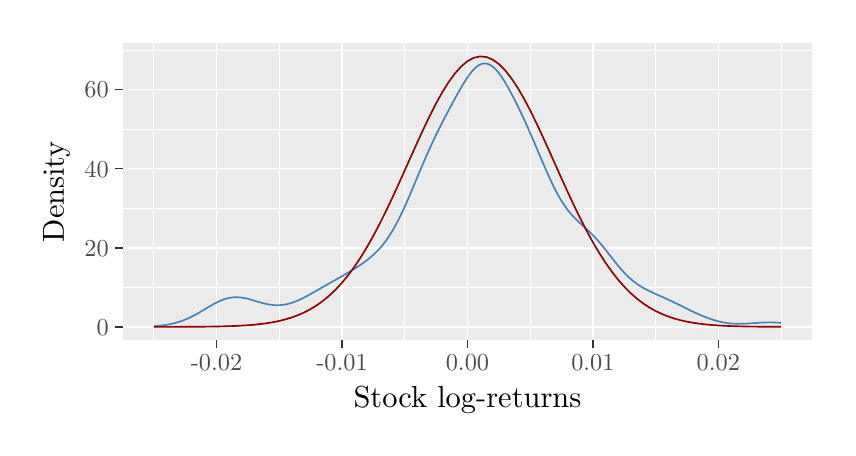
\begin{tikzpicture}[x=1pt,y=1pt]
\definecolor{fillColor}{RGB}{255,255,255}
\path[use as bounding box,fill=fillColor,fill opacity=0.00] (0,0) rectangle (289.08,144.54);
\begin{scope}
\path[clip] (  0.00,  0.00) rectangle (289.08,144.54);
\definecolor{drawColor}{RGB}{255,255,255}
\definecolor{fillColor}{RGB}{255,255,255}

\path[draw=drawColor,line width= 0.6pt,line join=round,line cap=round,fill=fillColor] (  0.00,  0.00) rectangle (289.08,144.54);
\end{scope}
\begin{scope}
\path[clip] ( 34.27, 31.53) rectangle (283.58,139.04);
\definecolor{fillColor}{gray}{0.92}

\path[fill=fillColor] ( 34.27, 31.53) rectangle (283.58,139.04);
\definecolor{drawColor}{RGB}{255,255,255}

\path[draw=drawColor,line width= 0.3pt,line join=round] ( 34.27, 50.71) --
	(283.58, 50.71);

\path[draw=drawColor,line width= 0.3pt,line join=round] ( 34.27, 79.31) --
	(283.58, 79.31);

\path[draw=drawColor,line width= 0.3pt,line join=round] ( 34.27,107.90) --
	(283.58,107.90);

\path[draw=drawColor,line width= 0.3pt,line join=round] ( 34.27,136.49) --
	(283.58,136.49);

\path[draw=drawColor,line width= 0.3pt,line join=round] ( 45.60, 31.53) --
	( 45.60,139.04);

\path[draw=drawColor,line width= 0.3pt,line join=round] ( 90.93, 31.53) --
	( 90.93,139.04);

\path[draw=drawColor,line width= 0.3pt,line join=round] (136.26, 31.53) --
	(136.26,139.04);

\path[draw=drawColor,line width= 0.3pt,line join=round] (181.59, 31.53) --
	(181.59,139.04);

\path[draw=drawColor,line width= 0.3pt,line join=round] (226.92, 31.53) --
	(226.92,139.04);

\path[draw=drawColor,line width= 0.3pt,line join=round] (272.25, 31.53) --
	(272.25,139.04);

\path[draw=drawColor,line width= 0.6pt,line join=round] ( 34.27, 36.42) --
	(283.58, 36.42);

\path[draw=drawColor,line width= 0.6pt,line join=round] ( 34.27, 65.01) --
	(283.58, 65.01);

\path[draw=drawColor,line width= 0.6pt,line join=round] ( 34.27, 93.60) --
	(283.58, 93.60);

\path[draw=drawColor,line width= 0.6pt,line join=round] ( 34.27,122.19) --
	(283.58,122.19);

\path[draw=drawColor,line width= 0.6pt,line join=round] ( 68.26, 31.53) --
	( 68.26,139.04);

\path[draw=drawColor,line width= 0.6pt,line join=round] (113.59, 31.53) --
	(113.59,139.04);

\path[draw=drawColor,line width= 0.6pt,line join=round] (158.92, 31.53) --
	(158.92,139.04);

\path[draw=drawColor,line width= 0.6pt,line join=round] (204.25, 31.53) --
	(204.25,139.04);

\path[draw=drawColor,line width= 0.6pt,line join=round] (249.58, 31.53) --
	(249.58,139.04);
\definecolor{drawColor}{RGB}{70,130,180}

\path[draw=drawColor,line width= 0.6pt,line join=round] ( 45.60, 36.66) --
	( 46.04, 36.69) --
	( 46.49, 36.73) --
	( 46.93, 36.77) --
	( 47.37, 36.81) --
	( 47.82, 36.85) --
	( 48.26, 36.90) --
	( 48.70, 36.95) --
	( 49.15, 37.01) --
	( 49.59, 37.07) --
	( 50.04, 37.14) --
	( 50.48, 37.22) --
	( 50.92, 37.29) --
	( 51.37, 37.38) --
	( 51.81, 37.47) --
	( 52.25, 37.57) --
	( 52.70, 37.67) --
	( 53.14, 37.79) --
	( 53.58, 37.91) --
	( 54.03, 38.03) --
	( 54.47, 38.17) --
	( 54.91, 38.31) --
	( 55.36, 38.46) --
	( 55.80, 38.62) --
	( 56.25, 38.78) --
	( 56.69, 38.95) --
	( 57.13, 39.13) --
	( 57.58, 39.32) --
	( 58.02, 39.52) --
	( 58.46, 39.73) --
	( 58.91, 39.94) --
	( 59.35, 40.16) --
	( 59.79, 40.39) --
	( 60.24, 40.62) --
	( 60.68, 40.86) --
	( 61.12, 41.10) --
	( 61.57, 41.35) --
	( 62.01, 41.61) --
	( 62.45, 41.87) --
	( 62.90, 42.13) --
	( 63.34, 42.39) --
	( 63.79, 42.66) --
	( 64.23, 42.92) --
	( 64.67, 43.19) --
	( 65.12, 43.46) --
	( 65.56, 43.72) --
	( 66.00, 43.98) --
	( 66.45, 44.23) --
	( 66.89, 44.49) --
	( 67.33, 44.73) --
	( 67.78, 44.97) --
	( 68.22, 45.20) --
	( 68.66, 45.42) --
	( 69.11, 45.63) --
	( 69.55, 45.83) --
	( 69.99, 46.01) --
	( 70.44, 46.19) --
	( 70.88, 46.35) --
	( 71.33, 46.50) --
	( 71.77, 46.63) --
	( 72.21, 46.75) --
	( 72.66, 46.85) --
	( 73.10, 46.94) --
	( 73.54, 47.01) --
	( 73.99, 47.06) --
	( 74.43, 47.10) --
	( 74.87, 47.13) --
	( 75.32, 47.13) --
	( 75.76, 47.13) --
	( 76.20, 47.11) --
	( 76.65, 47.07) --
	( 77.09, 47.02) --
	( 77.53, 46.96) --
	( 77.98, 46.89) --
	( 78.42, 46.81) --
	( 78.87, 46.71) --
	( 79.31, 46.61) --
	( 79.75, 46.50) --
	( 80.20, 46.38) --
	( 80.64, 46.26) --
	( 81.08, 46.13) --
	( 81.53, 46.01) --
	( 81.97, 45.87) --
	( 82.41, 45.74) --
	( 82.86, 45.61) --
	( 83.30, 45.48) --
	( 83.74, 45.35) --
	( 84.19, 45.22) --
	( 84.63, 45.10) --
	( 85.07, 44.98) --
	( 85.52, 44.87) --
	( 85.96, 44.77) --
	( 86.41, 44.67) --
	( 86.85, 44.58) --
	( 87.29, 44.50) --
	( 87.74, 44.43) --
	( 88.18, 44.38) --
	( 88.62, 44.33) --
	( 89.07, 44.29) --
	( 89.51, 44.27) --
	( 89.95, 44.25) --
	( 90.40, 44.25) --
	( 90.84, 44.27) --
	( 91.28, 44.29) --
	( 91.73, 44.33) --
	( 92.17, 44.38) --
	( 92.62, 44.44) --
	( 93.06, 44.51) --
	( 93.50, 44.60) --
	( 93.95, 44.70) --
	( 94.39, 44.81) --
	( 94.83, 44.94) --
	( 95.28, 45.07) --
	( 95.72, 45.22) --
	( 96.16, 45.37) --
	( 96.61, 45.54) --
	( 97.05, 45.71) --
	( 97.49, 45.90) --
	( 97.94, 46.09) --
	( 98.38, 46.30) --
	( 98.82, 46.50) --
	( 99.27, 46.72) --
	( 99.71, 46.94) --
	(100.16, 47.17) --
	(100.60, 47.40) --
	(101.04, 47.64) --
	(101.49, 47.88) --
	(101.93, 48.12) --
	(102.37, 48.37) --
	(102.82, 48.62) --
	(103.26, 48.87) --
	(103.70, 49.12) --
	(104.15, 49.38) --
	(104.59, 49.63) --
	(105.03, 49.89) --
	(105.48, 50.14) --
	(105.92, 50.40) --
	(106.36, 50.65) --
	(106.81, 50.91) --
	(107.25, 51.16) --
	(107.70, 51.41) --
	(108.14, 51.66) --
	(108.58, 51.92) --
	(109.03, 52.17) --
	(109.47, 52.42) --
	(109.91, 52.67) --
	(110.36, 52.92) --
	(110.80, 53.17) --
	(111.24, 53.42) --
	(111.69, 53.67) --
	(112.13, 53.92) --
	(112.57, 54.17) --
	(113.02, 54.43) --
	(113.46, 54.68) --
	(113.90, 54.93) --
	(114.35, 55.19) --
	(114.79, 55.44) --
	(115.24, 55.70) --
	(115.68, 55.96) --
	(116.12, 56.23) --
	(116.57, 56.49) --
	(117.01, 56.76) --
	(117.45, 57.03) --
	(117.90, 57.30) --
	(118.34, 57.58) --
	(118.78, 57.86) --
	(119.23, 58.15) --
	(119.67, 58.44) --
	(120.11, 58.74) --
	(120.56, 59.04) --
	(121.00, 59.35) --
	(121.45, 59.66) --
	(121.89, 59.98) --
	(122.33, 60.32) --
	(122.78, 60.66) --
	(123.22, 61.01) --
	(123.66, 61.37) --
	(124.11, 61.74) --
	(124.55, 62.13) --
	(124.99, 62.53) --
	(125.44, 62.95) --
	(125.88, 63.38) --
	(126.32, 63.82) --
	(126.77, 64.29) --
	(127.21, 64.78) --
	(127.65, 65.28) --
	(128.10, 65.81) --
	(128.54, 66.36) --
	(128.99, 66.93) --
	(129.43, 67.53) --
	(129.87, 68.15) --
	(130.32, 68.79) --
	(130.76, 69.47) --
	(131.20, 70.16) --
	(131.65, 70.88) --
	(132.09, 71.63) --
	(132.53, 72.41) --
	(132.98, 73.22) --
	(133.42, 74.04) --
	(133.86, 74.89) --
	(134.31, 75.77) --
	(134.75, 76.68) --
	(135.19, 77.60) --
	(135.64, 78.54) --
	(136.08, 79.51) --
	(136.53, 80.49) --
	(136.97, 81.49) --
	(137.41, 82.50) --
	(137.86, 83.53) --
	(138.30, 84.57) --
	(138.74, 85.61) --
	(139.19, 86.67) --
	(139.63, 87.72) --
	(140.07, 88.79) --
	(140.52, 89.85) --
	(140.96, 90.91) --
	(141.40, 91.97) --
	(141.85, 93.02) --
	(142.29, 94.07) --
	(142.73, 95.12) --
	(143.18, 96.15) --
	(143.62, 97.17) --
	(144.07, 98.19) --
	(144.51, 99.19) --
	(144.95,100.18) --
	(145.40,101.16) --
	(145.84,102.12) --
	(146.28,103.08) --
	(146.73,104.02) --
	(147.17,104.95) --
	(147.61,105.87) --
	(148.06,106.77) --
	(148.50,107.67) --
	(148.94,108.55) --
	(149.39,109.43) --
	(149.83,110.30) --
	(150.27,111.16) --
	(150.72,112.02) --
	(151.16,112.87) --
	(151.61,113.72) --
	(152.05,114.55) --
	(152.49,115.39) --
	(152.94,116.22) --
	(153.38,117.05) --
	(153.82,117.87) --
	(154.27,118.69) --
	(154.71,119.50) --
	(155.15,120.30) --
	(155.60,121.09) --
	(156.04,121.88) --
	(156.48,122.65) --
	(156.93,123.41) --
	(157.37,124.15) --
	(157.82,124.87) --
	(158.26,125.57) --
	(158.70,126.25) --
	(159.15,126.90) --
	(159.59,127.52) --
	(160.03,128.10) --
	(160.48,128.65) --
	(160.92,129.17) --
	(161.36,129.63) --
	(161.81,130.06) --
	(162.25,130.44) --
	(162.69,130.77) --
	(163.14,131.04) --
	(163.58,131.26) --
	(164.02,131.44) --
	(164.47,131.56) --
	(164.91,131.62) --
	(165.36,131.61) --
	(165.80,131.56) --
	(166.24,131.45) --
	(166.69,131.29) --
	(167.13,131.06) --
	(167.57,130.79) --
	(168.02,130.47) --
	(168.46,130.10) --
	(168.90,129.67) --
	(169.35,129.20) --
	(169.79,128.69) --
	(170.23,128.14) --
	(170.68,127.55) --
	(171.12,126.93) --
	(171.56,126.27) --
	(172.01,125.58) --
	(172.45,124.87) --
	(172.90,124.13) --
	(173.34,123.36) --
	(173.78,122.58) --
	(174.23,121.78) --
	(174.67,120.95) --
	(175.11,120.11) --
	(175.56,119.26) --
	(176.00,118.39) --
	(176.44,117.51) --
	(176.89,116.61) --
	(177.33,115.70) --
	(177.77,114.78) --
	(178.22,113.86) --
	(178.66,112.91) --
	(179.10,111.96) --
	(179.55,111.00) --
	(179.99,110.03) --
	(180.44,109.05) --
	(180.88,108.05) --
	(181.32,107.05) --
	(181.77,106.04) --
	(182.21,105.02) --
	(182.65,104.00) --
	(183.10,102.96) --
	(183.54,101.92) --
	(183.98,100.88) --
	(184.43, 99.84) --
	(184.87, 98.79) --
	(185.31, 97.75) --
	(185.76, 96.70) --
	(186.20, 95.66) --
	(186.64, 94.63) --
	(187.09, 93.61) --
	(187.53, 92.60) --
	(187.98, 91.60) --
	(188.42, 90.62) --
	(188.86, 89.65) --
	(189.31, 88.70) --
	(189.75, 87.77) --
	(190.19, 86.87) --
	(190.64, 86.00) --
	(191.08, 85.14) --
	(191.52, 84.32) --
	(191.97, 83.52) --
	(192.41, 82.76) --
	(192.85, 82.02) --
	(193.30, 81.31) --
	(193.74, 80.63) --
	(194.19, 79.98) --
	(194.63, 79.36) --
	(195.07, 78.76) --
	(195.52, 78.19) --
	(195.96, 77.66) --
	(196.40, 77.14) --
	(196.85, 76.64) --
	(197.29, 76.16) --
	(197.73, 75.70) --
	(198.18, 75.26) --
	(198.62, 74.82) --
	(199.06, 74.40) --
	(199.51, 73.99) --
	(199.95, 73.58) --
	(200.39, 73.18) --
	(200.84, 72.78) --
	(201.28, 72.38) --
	(201.73, 71.97) --
	(202.17, 71.56) --
	(202.61, 71.15) --
	(203.06, 70.73) --
	(203.50, 70.29) --
	(203.94, 69.85) --
	(204.39, 69.40) --
	(204.83, 68.94) --
	(205.27, 68.46) --
	(205.72, 67.97) --
	(206.16, 67.47) --
	(206.60, 66.96) --
	(207.05, 66.44) --
	(207.49, 65.91) --
	(207.93, 65.37) --
	(208.38, 64.82) --
	(208.82, 64.26) --
	(209.27, 63.70) --
	(209.71, 63.14) --
	(210.15, 62.57) --
	(210.60, 62.00) --
	(211.04, 61.43) --
	(211.48, 60.86) --
	(211.93, 60.30) --
	(212.37, 59.74) --
	(212.81, 59.19) --
	(213.26, 58.65) --
	(213.70, 58.12) --
	(214.14, 57.59) --
	(214.59, 57.08) --
	(215.03, 56.59) --
	(215.47, 56.11) --
	(215.92, 55.64) --
	(216.36, 55.18) --
	(216.81, 54.75) --
	(217.25, 54.33) --
	(217.69, 53.92) --
	(218.14, 53.53) --
	(218.58, 53.16) --
	(219.02, 52.80) --
	(219.47, 52.46) --
	(219.91, 52.13) --
	(220.35, 51.81) --
	(220.80, 51.52) --
	(221.24, 51.23) --
	(221.68, 50.95) --
	(222.13, 50.69) --
	(222.57, 50.44) --
	(223.02, 50.19) --
	(223.46, 49.96) --
	(223.90, 49.73) --
	(224.35, 49.51) --
	(224.79, 49.29) --
	(225.23, 49.08) --
	(225.68, 48.88) --
	(226.12, 48.67) --
	(226.56, 48.47) --
	(227.01, 48.27) --
	(227.45, 48.08) --
	(227.89, 47.88) --
	(228.34, 47.68) --
	(228.78, 47.49) --
	(229.22, 47.29) --
	(229.67, 47.09) --
	(230.11, 46.89) --
	(230.56, 46.69) --
	(231.00, 46.48) --
	(231.44, 46.28) --
	(231.89, 46.07) --
	(232.33, 45.86) --
	(232.77, 45.65) --
	(233.22, 45.44) --
	(233.66, 45.23) --
	(234.10, 45.01) --
	(234.55, 44.80) --
	(234.99, 44.58) --
	(235.43, 44.36) --
	(235.88, 44.14) --
	(236.32, 43.92) --
	(236.76, 43.70) --
	(237.21, 43.48) --
	(237.65, 43.26) --
	(238.10, 43.04) --
	(238.54, 42.83) --
	(238.98, 42.61) --
	(239.43, 42.39) --
	(239.87, 42.18) --
	(240.31, 41.97) --
	(240.76, 41.76) --
	(241.20, 41.55) --
	(241.64, 41.35) --
	(242.09, 41.15) --
	(242.53, 40.95) --
	(242.97, 40.75) --
	(243.42, 40.56) --
	(243.86, 40.38) --
	(244.30, 40.19) --
	(244.75, 40.02) --
	(245.19, 39.84) --
	(245.64, 39.67) --
	(246.08, 39.51) --
	(246.52, 39.35) --
	(246.97, 39.20) --
	(247.41, 39.05) --
	(247.85, 38.91) --
	(248.30, 38.78) --
	(248.74, 38.65) --
	(249.18, 38.53) --
	(249.63, 38.42) --
	(250.07, 38.31) --
	(250.51, 38.21) --
	(250.96, 38.11) --
	(251.40, 38.03) --
	(251.84, 37.95) --
	(252.29, 37.88) --
	(252.73, 37.81) --
	(253.18, 37.75) --
	(253.62, 37.70) --
	(254.06, 37.66) --
	(254.51, 37.62) --
	(254.95, 37.59) --
	(255.39, 37.56) --
	(255.84, 37.55) --
	(256.28, 37.53) --
	(256.72, 37.53) --
	(257.17, 37.53) --
	(257.61, 37.53) --
	(258.05, 37.54) --
	(258.50, 37.55) --
	(258.94, 37.57) --
	(259.39, 37.59) --
	(259.83, 37.61) --
	(260.27, 37.64) --
	(260.72, 37.66) --
	(261.16, 37.69) --
	(261.60, 37.72) --
	(262.05, 37.76) --
	(262.49, 37.79) --
	(262.93, 37.82) --
	(263.38, 37.85) --
	(263.82, 37.88) --
	(264.26, 37.91) --
	(264.71, 37.94) --
	(265.15, 37.96) --
	(265.59, 37.98) --
	(266.04, 38.00) --
	(266.48, 38.02) --
	(266.93, 38.03) --
	(267.37, 38.04) --
	(267.81, 38.04) --
	(268.26, 38.04) --
	(268.70, 38.04) --
	(269.14, 38.03) --
	(269.59, 38.02) --
	(270.03, 38.00) --
	(270.47, 37.99) --
	(270.92, 37.96) --
	(271.36, 37.94) --
	(271.80, 37.91) --
	(272.25, 37.87);
\definecolor{drawColor}{RGB}{139,0,0}

\path[draw=drawColor,line width= 0.6pt,line join=round] ( 45.60, 36.42) --
	( 47.87, 36.42) --
	( 50.13, 36.43) --
	( 52.40, 36.43) --
	( 54.67, 36.44) --
	( 56.93, 36.44) --
	( 59.20, 36.46) --
	( 61.47, 36.47) --
	( 63.73, 36.49) --
	( 66.00, 36.52) --
	( 68.26, 36.56) --
	( 70.53, 36.61) --
	( 72.80, 36.68) --
	( 75.06, 36.76) --
	( 77.33, 36.88) --
	( 79.60, 37.02) --
	( 81.86, 37.21) --
	( 84.13, 37.45) --
	( 86.40, 37.75) --
	( 88.66, 38.12) --
	( 90.93, 38.58) --
	( 93.20, 39.15) --
	( 95.46, 39.84) --
	( 97.73, 40.68) --
	(100.00, 41.68) --
	(102.26, 42.87) --
	(104.53, 44.26) --
	(106.80, 45.90) --
	(109.06, 47.78) --
	(111.33, 49.94) --
	(113.59, 52.40) --
	(115.86, 55.16) --
	(118.13, 58.24) --
	(120.39, 61.63) --
	(122.66, 65.35) --
	(124.93, 69.37) --
	(127.19, 73.67) --
	(129.46, 78.22) --
	(131.73, 82.99) --
	(133.99, 87.93) --
	(136.26, 92.97) --
	(138.53, 98.04) --
	(140.79,103.09) --
	(143.06,108.01) --
	(145.33,112.74) --
	(147.59,117.19) --
	(149.86,121.27) --
	(152.12,124.90) --
	(154.39,128.01) --
	(156.66,130.54) --
	(158.92,132.43) --
	(161.19,133.65) --
	(163.46,134.15) --
	(165.72,133.94) --
	(167.99,133.02) --
	(170.26,131.41) --
	(172.52,129.14) --
	(174.79,126.27) --
	(177.06,122.84) --
	(179.32,118.94) --
	(181.59,114.64) --
	(183.86,110.02) --
	(186.12,105.16) --
	(188.39,100.16) --
	(190.65, 95.09) --
	(192.92, 90.02) --
	(195.19, 85.04) --
	(197.45, 80.19) --
	(199.72, 75.54) --
	(201.99, 71.13) --
	(204.25, 66.99) --
	(206.52, 63.15) --
	(208.79, 59.62) --
	(211.05, 56.41) --
	(213.32, 53.51) --
	(215.59, 50.93) --
	(217.85, 48.65) --
	(220.12, 46.65) --
	(222.39, 44.92) --
	(224.65, 43.42) --
	(226.92, 42.15) --
	(229.18, 41.08) --
	(231.45, 40.17) --
	(233.72, 39.42) --
	(235.98, 38.81) --
	(238.25, 38.30) --
	(240.52, 37.89) --
	(242.78, 37.57) --
	(245.05, 37.30) --
	(247.32, 37.10) --
	(249.58, 36.93) --
	(251.85, 36.81) --
	(254.12, 36.71) --
	(256.38, 36.63) --
	(258.65, 36.58) --
	(260.92, 36.53) --
	(263.18, 36.50) --
	(265.45, 36.48) --
	(267.71, 36.46) --
	(269.98, 36.45) --
	(272.25, 36.44);
\end{scope}
\begin{scope}
\path[clip] (  0.00,  0.00) rectangle (289.08,144.54);
\definecolor{drawColor}{gray}{0.30}

\node[text=drawColor,anchor=base east,inner sep=0pt, outer sep=0pt, scale=  0.88] at ( 29.32, 33.39) {0};

\node[text=drawColor,anchor=base east,inner sep=0pt, outer sep=0pt, scale=  0.88] at ( 29.32, 61.98) {20};

\node[text=drawColor,anchor=base east,inner sep=0pt, outer sep=0pt, scale=  0.88] at ( 29.32, 90.57) {40};

\node[text=drawColor,anchor=base east,inner sep=0pt, outer sep=0pt, scale=  0.88] at ( 29.32,119.16) {60};
\end{scope}
\begin{scope}
\path[clip] (  0.00,  0.00) rectangle (289.08,144.54);
\definecolor{drawColor}{gray}{0.20}

\path[draw=drawColor,line width= 0.6pt,line join=round] ( 31.52, 36.42) --
	( 34.27, 36.42);

\path[draw=drawColor,line width= 0.6pt,line join=round] ( 31.52, 65.01) --
	( 34.27, 65.01);

\path[draw=drawColor,line width= 0.6pt,line join=round] ( 31.52, 93.60) --
	( 34.27, 93.60);

\path[draw=drawColor,line width= 0.6pt,line join=round] ( 31.52,122.19) --
	( 34.27,122.19);
\end{scope}
\begin{scope}
\path[clip] (  0.00,  0.00) rectangle (289.08,144.54);
\definecolor{drawColor}{gray}{0.20}

\path[draw=drawColor,line width= 0.6pt,line join=round] ( 68.26, 28.78) --
	( 68.26, 31.53);

\path[draw=drawColor,line width= 0.6pt,line join=round] (113.59, 28.78) --
	(113.59, 31.53);

\path[draw=drawColor,line width= 0.6pt,line join=round] (158.92, 28.78) --
	(158.92, 31.53);

\path[draw=drawColor,line width= 0.6pt,line join=round] (204.25, 28.78) --
	(204.25, 31.53);

\path[draw=drawColor,line width= 0.6pt,line join=round] (249.58, 28.78) --
	(249.58, 31.53);
\end{scope}
\begin{scope}
\path[clip] (  0.00,  0.00) rectangle (289.08,144.54);
\definecolor{drawColor}{gray}{0.30}

\node[text=drawColor,anchor=base,inner sep=0pt, outer sep=0pt, scale=  0.88] at ( 68.26, 20.52) {-0.02};

\node[text=drawColor,anchor=base,inner sep=0pt, outer sep=0pt, scale=  0.88] at (113.59, 20.52) {-0.01};

\node[text=drawColor,anchor=base,inner sep=0pt, outer sep=0pt, scale=  0.88] at (158.92, 20.52) {0.00};

\node[text=drawColor,anchor=base,inner sep=0pt, outer sep=0pt, scale=  0.88] at (204.25, 20.52) {0.01};

\node[text=drawColor,anchor=base,inner sep=0pt, outer sep=0pt, scale=  0.88] at (249.58, 20.52) {0.02};
\end{scope}
\begin{scope}
\path[clip] (  0.00,  0.00) rectangle (289.08,144.54);
\definecolor{drawColor}{RGB}{0,0,0}

\node[text=drawColor,anchor=base,inner sep=0pt, outer sep=0pt, scale=  1.10] at (158.92,  7.44) {Stock log-returns};
\end{scope}
\begin{scope}
\path[clip] (  0.00,  0.00) rectangle (289.08,144.54);
\definecolor{drawColor}{RGB}{0,0,0}

\node[text=drawColor,rotate= 90.00,anchor=base,inner sep=0pt, outer sep=0pt, scale=  1.10] at ( 13.08, 85.29) {Density};
\end{scope}
\end{tikzpicture}

  \rule{40mm}{20mm}
  \caption{Distribution of the calibrated BSM time-series' log-returns with respect to the distribution of those provided by the market.}
  %
  % BEGIN OF FLOATNOTE
  %
  \begin{changemargin}{0.5cm}{0.5cm}
  \medskip
\footnotesize
\setstretch{1.0}\textbf{Notes.} The above blue density curve is constructed over the historical data of the Apple share of stock price evolution from 1st January 2017 to 31st December 2017. while the red curve is built from time-series generated by the function \textit{bsm\_ts} taking $\tau = 1.0931$, $\alpha = 0.48229$, $\sigma = 0.1958$ as parameters.
  \end{changemargin}
  %
  % END OF FLOATNOTE
  %
  \label{p:analysis:gbm:adjusted}
\end{figure}

\Cref{p:analysis:gbm:adjusted} illustrates the theoretical density curve of the log-returns reproduced with the adjusted parameters, while \cref{p:analysis:gbm:option:adjusted} faces the blue colored volatility smiles determined from market data with those dotted in red, computed from data provided by the function \textit{bsm\_call} which takes the calibrated $\sigma$ and the riskless rate $r$ as parameters.

\begin{figure}[h]
  \centering
  % % Created by tikzDevice version 0.11 on 2018-08-04 15:24:44
% !TEX encoding = UTF-8 Unicode
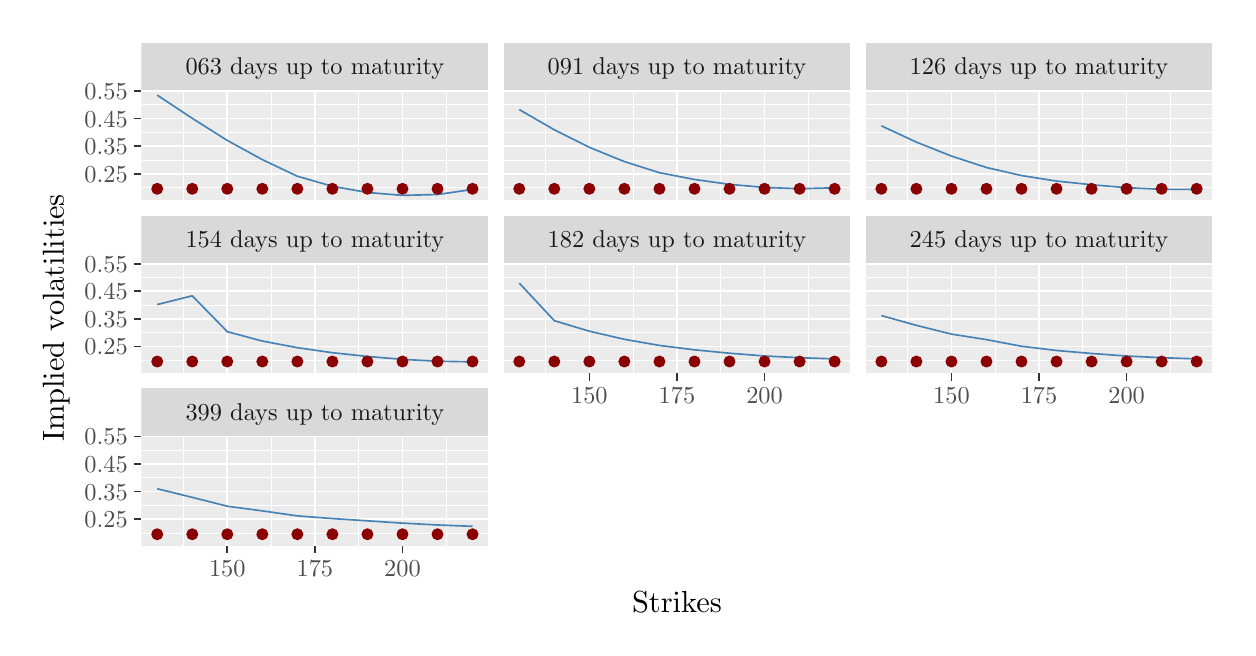
\begin{tikzpicture}[x=1pt,y=1pt]
\definecolor{fillColor}{RGB}{255,255,255}
\path[use as bounding box,fill=fillColor,fill opacity=0.00] (0,0) rectangle (433.62,216.81);
\begin{scope}
\path[clip] (  0.00,  0.00) rectangle (433.62,216.81);
\definecolor{drawColor}{RGB}{255,255,255}
\definecolor{fillColor}{RGB}{255,255,255}

\path[draw=drawColor,line width= 0.6pt,line join=round,line cap=round,fill=fillColor] (  0.00,  0.00) rectangle (433.62,216.81);
\end{scope}
\begin{scope}
\path[clip] ( 41.11,154.40) rectangle (166.45,194.25);
\definecolor{fillColor}{gray}{0.92}

\path[fill=fillColor] ( 41.11,154.40) rectangle (166.45,194.25);
\definecolor{drawColor}{RGB}{255,255,255}

\path[draw=drawColor,line width= 0.3pt,line join=round] ( 41.11,158.99) --
	(166.45,158.99);

\path[draw=drawColor,line width= 0.3pt,line join=round] ( 41.11,168.97) --
	(166.45,168.97);

\path[draw=drawColor,line width= 0.3pt,line join=round] ( 41.11,178.95) --
	(166.45,178.95);

\path[draw=drawColor,line width= 0.3pt,line join=round] ( 41.11,188.93) --
	(166.45,188.93);

\path[draw=drawColor,line width= 0.3pt,line join=round] ( 56.30,154.40) --
	( 56.30,194.25);

\path[draw=drawColor,line width= 0.3pt,line join=round] ( 87.95,154.40) --
	( 87.95,194.25);

\path[draw=drawColor,line width= 0.3pt,line join=round] (119.60,154.40) --
	(119.60,194.25);

\path[draw=drawColor,line width= 0.3pt,line join=round] (151.25,154.40) --
	(151.25,194.25);

\path[draw=drawColor,line width= 0.6pt,line join=round] ( 41.11,163.98) --
	(166.45,163.98);

\path[draw=drawColor,line width= 0.6pt,line join=round] ( 41.11,173.96) --
	(166.45,173.96);

\path[draw=drawColor,line width= 0.6pt,line join=round] ( 41.11,183.94) --
	(166.45,183.94);

\path[draw=drawColor,line width= 0.6pt,line join=round] ( 41.11,193.92) --
	(166.45,193.92);

\path[draw=drawColor,line width= 0.6pt,line join=round] ( 72.13,154.40) --
	( 72.13,194.25);

\path[draw=drawColor,line width= 0.6pt,line join=round] (103.78,154.40) --
	(103.78,194.25);

\path[draw=drawColor,line width= 0.6pt,line join=round] (135.43,154.40) --
	(135.43,194.25);
\definecolor{drawColor}{RGB}{70,130,180}

\path[draw=drawColor,line width= 0.6pt,line join=round] ( 46.81,192.44) --
	( 59.47,184.05) --
	( 72.13,176.06) --
	( 84.79,169.13) --
	( 97.45,163.12) --
	(110.11,159.50) --
	(122.77,157.26) --
	(135.43,156.21) --
	(148.09,156.52) --
	(160.75,158.35);
\definecolor{drawColor}{RGB}{139,0,0}
\definecolor{fillColor}{RGB}{139,0,0}

\path[draw=drawColor,line width= 0.4pt,line join=round,line cap=round,fill=fillColor] ( 46.81,158.58) circle (  1.96);

\path[draw=drawColor,line width= 0.4pt,line join=round,line cap=round,fill=fillColor] ( 59.47,158.58) circle (  1.96);

\path[draw=drawColor,line width= 0.4pt,line join=round,line cap=round,fill=fillColor] ( 72.13,158.58) circle (  1.96);

\path[draw=drawColor,line width= 0.4pt,line join=round,line cap=round,fill=fillColor] ( 84.79,158.58) circle (  1.96);

\path[draw=drawColor,line width= 0.4pt,line join=round,line cap=round,fill=fillColor] ( 97.45,158.58) circle (  1.96);

\path[draw=drawColor,line width= 0.4pt,line join=round,line cap=round,fill=fillColor] (110.11,158.58) circle (  1.96);

\path[draw=drawColor,line width= 0.4pt,line join=round,line cap=round,fill=fillColor] (122.77,158.58) circle (  1.96);

\path[draw=drawColor,line width= 0.4pt,line join=round,line cap=round,fill=fillColor] (135.43,158.58) circle (  1.96);

\path[draw=drawColor,line width= 0.4pt,line join=round,line cap=round,fill=fillColor] (148.09,158.58) circle (  1.96);

\path[draw=drawColor,line width= 0.4pt,line join=round,line cap=round,fill=fillColor] (160.75,158.58) circle (  1.96);
\end{scope}
\begin{scope}
\path[clip] ( 41.11, 91.99) rectangle (166.45,131.84);
\definecolor{fillColor}{gray}{0.92}

\path[fill=fillColor] ( 41.11, 91.99) rectangle (166.45,131.84);
\definecolor{drawColor}{RGB}{255,255,255}

\path[draw=drawColor,line width= 0.3pt,line join=round] ( 41.11, 96.59) --
	(166.45, 96.59);

\path[draw=drawColor,line width= 0.3pt,line join=round] ( 41.11,106.57) --
	(166.45,106.57);

\path[draw=drawColor,line width= 0.3pt,line join=round] ( 41.11,116.55) --
	(166.45,116.55);

\path[draw=drawColor,line width= 0.3pt,line join=round] ( 41.11,126.52) --
	(166.45,126.52);

\path[draw=drawColor,line width= 0.3pt,line join=round] ( 56.30, 91.99) --
	( 56.30,131.84);

\path[draw=drawColor,line width= 0.3pt,line join=round] ( 87.95, 91.99) --
	( 87.95,131.84);

\path[draw=drawColor,line width= 0.3pt,line join=round] (119.60, 91.99) --
	(119.60,131.84);

\path[draw=drawColor,line width= 0.3pt,line join=round] (151.25, 91.99) --
	(151.25,131.84);

\path[draw=drawColor,line width= 0.6pt,line join=round] ( 41.11,101.58) --
	(166.45,101.58);

\path[draw=drawColor,line width= 0.6pt,line join=round] ( 41.11,111.56) --
	(166.45,111.56);

\path[draw=drawColor,line width= 0.6pt,line join=round] ( 41.11,121.54) --
	(166.45,121.54);

\path[draw=drawColor,line width= 0.6pt,line join=round] ( 41.11,131.51) --
	(166.45,131.51);

\path[draw=drawColor,line width= 0.6pt,line join=round] ( 72.13, 91.99) --
	( 72.13,131.84);

\path[draw=drawColor,line width= 0.6pt,line join=round] (103.78, 91.99) --
	(103.78,131.84);

\path[draw=drawColor,line width= 0.6pt,line join=round] (135.43, 91.99) --
	(135.43,131.84);
\definecolor{drawColor}{RGB}{70,130,180}

\path[draw=drawColor,line width= 0.6pt,line join=round] ( 46.81,116.76) --
	( 59.47,119.91) --
	( 72.13,106.96) --
	( 84.79,103.57) --
	( 97.45,101.17) --
	(110.11, 99.36) --
	(122.77, 98.01) --
	(135.43, 96.95) --
	(148.09, 96.29) --
	(160.75, 96.06);
\definecolor{drawColor}{RGB}{139,0,0}
\definecolor{fillColor}{RGB}{139,0,0}

\path[draw=drawColor,line width= 0.4pt,line join=round,line cap=round,fill=fillColor] ( 46.81, 96.17) circle (  1.96);

\path[draw=drawColor,line width= 0.4pt,line join=round,line cap=round,fill=fillColor] ( 59.47, 96.17) circle (  1.96);

\path[draw=drawColor,line width= 0.4pt,line join=round,line cap=round,fill=fillColor] ( 72.13, 96.17) circle (  1.96);

\path[draw=drawColor,line width= 0.4pt,line join=round,line cap=round,fill=fillColor] ( 84.79, 96.17) circle (  1.96);

\path[draw=drawColor,line width= 0.4pt,line join=round,line cap=round,fill=fillColor] ( 97.45, 96.17) circle (  1.96);

\path[draw=drawColor,line width= 0.4pt,line join=round,line cap=round,fill=fillColor] (110.11, 96.17) circle (  1.96);

\path[draw=drawColor,line width= 0.4pt,line join=round,line cap=round,fill=fillColor] (122.77, 96.17) circle (  1.96);

\path[draw=drawColor,line width= 0.4pt,line join=round,line cap=round,fill=fillColor] (135.43, 96.17) circle (  1.96);

\path[draw=drawColor,line width= 0.4pt,line join=round,line cap=round,fill=fillColor] (148.09, 96.17) circle (  1.96);

\path[draw=drawColor,line width= 0.4pt,line join=round,line cap=round,fill=fillColor] (160.75, 96.17) circle (  1.96);
\end{scope}
\begin{scope}
\path[clip] ( 41.11, 29.59) rectangle (166.45, 69.43);
\definecolor{fillColor}{gray}{0.92}

\path[fill=fillColor] ( 41.11, 29.59) rectangle (166.45, 69.43);
\definecolor{drawColor}{RGB}{255,255,255}

\path[draw=drawColor,line width= 0.3pt,line join=round] ( 41.11, 34.18) --
	(166.45, 34.18);

\path[draw=drawColor,line width= 0.3pt,line join=round] ( 41.11, 44.16) --
	(166.45, 44.16);

\path[draw=drawColor,line width= 0.3pt,line join=round] ( 41.11, 54.14) --
	(166.45, 54.14);

\path[draw=drawColor,line width= 0.3pt,line join=round] ( 41.11, 64.12) --
	(166.45, 64.12);

\path[draw=drawColor,line width= 0.3pt,line join=round] ( 56.30, 29.59) --
	( 56.30, 69.43);

\path[draw=drawColor,line width= 0.3pt,line join=round] ( 87.95, 29.59) --
	( 87.95, 69.43);

\path[draw=drawColor,line width= 0.3pt,line join=round] (119.60, 29.59) --
	(119.60, 69.43);

\path[draw=drawColor,line width= 0.3pt,line join=round] (151.25, 29.59) --
	(151.25, 69.43);

\path[draw=drawColor,line width= 0.6pt,line join=round] ( 41.11, 39.17) --
	(166.45, 39.17);

\path[draw=drawColor,line width= 0.6pt,line join=round] ( 41.11, 49.15) --
	(166.45, 49.15);

\path[draw=drawColor,line width= 0.6pt,line join=round] ( 41.11, 59.13) --
	(166.45, 59.13);

\path[draw=drawColor,line width= 0.6pt,line join=round] ( 41.11, 69.11) --
	(166.45, 69.11);

\path[draw=drawColor,line width= 0.6pt,line join=round] ( 72.13, 29.59) --
	( 72.13, 69.43);

\path[draw=drawColor,line width= 0.6pt,line join=round] (103.78, 29.59) --
	(103.78, 69.43);

\path[draw=drawColor,line width= 0.6pt,line join=round] (135.43, 29.59) --
	(135.43, 69.43);
\definecolor{drawColor}{RGB}{70,130,180}

\path[draw=drawColor,line width= 0.6pt,line join=round] ( 46.81, 50.20) --
	( 59.47, 47.09) --
	( 72.13, 43.89) --
	( 84.79, 42.20) --
	( 97.45, 40.40) --
	(110.11, 39.42) --
	(122.77, 38.61) --
	(135.43, 37.78) --
	(148.09, 37.11) --
	(160.75, 36.62);
\definecolor{drawColor}{RGB}{139,0,0}
\definecolor{fillColor}{RGB}{139,0,0}

\path[draw=drawColor,line width= 0.4pt,line join=round,line cap=round,fill=fillColor] ( 46.81, 33.76) circle (  1.96);

\path[draw=drawColor,line width= 0.4pt,line join=round,line cap=round,fill=fillColor] ( 59.47, 33.76) circle (  1.96);

\path[draw=drawColor,line width= 0.4pt,line join=round,line cap=round,fill=fillColor] ( 72.13, 33.76) circle (  1.96);

\path[draw=drawColor,line width= 0.4pt,line join=round,line cap=round,fill=fillColor] ( 84.79, 33.76) circle (  1.96);

\path[draw=drawColor,line width= 0.4pt,line join=round,line cap=round,fill=fillColor] ( 97.45, 33.76) circle (  1.96);

\path[draw=drawColor,line width= 0.4pt,line join=round,line cap=round,fill=fillColor] (110.11, 33.76) circle (  1.96);

\path[draw=drawColor,line width= 0.4pt,line join=round,line cap=round,fill=fillColor] (122.77, 33.76) circle (  1.96);

\path[draw=drawColor,line width= 0.4pt,line join=round,line cap=round,fill=fillColor] (135.43, 33.76) circle (  1.96);

\path[draw=drawColor,line width= 0.4pt,line join=round,line cap=round,fill=fillColor] (148.09, 33.76) circle (  1.96);

\path[draw=drawColor,line width= 0.4pt,line join=round,line cap=round,fill=fillColor] (160.75, 33.76) circle (  1.96);
\end{scope}
\begin{scope}
\path[clip] (171.95,154.40) rectangle (297.28,194.25);
\definecolor{fillColor}{gray}{0.92}

\path[fill=fillColor] (171.95,154.40) rectangle (297.28,194.25);
\definecolor{drawColor}{RGB}{255,255,255}

\path[draw=drawColor,line width= 0.3pt,line join=round] (171.95,158.99) --
	(297.28,158.99);

\path[draw=drawColor,line width= 0.3pt,line join=round] (171.95,168.97) --
	(297.28,168.97);

\path[draw=drawColor,line width= 0.3pt,line join=round] (171.95,178.95) --
	(297.28,178.95);

\path[draw=drawColor,line width= 0.3pt,line join=round] (171.95,188.93) --
	(297.28,188.93);

\path[draw=drawColor,line width= 0.3pt,line join=round] (187.14,154.40) --
	(187.14,194.25);

\path[draw=drawColor,line width= 0.3pt,line join=round] (218.79,154.40) --
	(218.79,194.25);

\path[draw=drawColor,line width= 0.3pt,line join=round] (250.44,154.40) --
	(250.44,194.25);

\path[draw=drawColor,line width= 0.3pt,line join=round] (282.09,154.40) --
	(282.09,194.25);

\path[draw=drawColor,line width= 0.6pt,line join=round] (171.95,163.98) --
	(297.28,163.98);

\path[draw=drawColor,line width= 0.6pt,line join=round] (171.95,173.96) --
	(297.28,173.96);

\path[draw=drawColor,line width= 0.6pt,line join=round] (171.95,183.94) --
	(297.28,183.94);

\path[draw=drawColor,line width= 0.6pt,line join=round] (171.95,193.92) --
	(297.28,193.92);

\path[draw=drawColor,line width= 0.6pt,line join=round] (202.96,154.40) --
	(202.96,194.25);

\path[draw=drawColor,line width= 0.6pt,line join=round] (234.62,154.40) --
	(234.62,194.25);

\path[draw=drawColor,line width= 0.6pt,line join=round] (266.27,154.40) --
	(266.27,194.25);
\definecolor{drawColor}{RGB}{70,130,180}

\path[draw=drawColor,line width= 0.6pt,line join=round] (177.64,187.21) --
	(190.30,179.91) --
	(202.96,173.56) --
	(215.62,168.42) --
	(228.29,164.40) --
	(240.95,161.96) --
	(253.61,160.18) --
	(266.27,159.07) --
	(278.93,158.62) --
	(291.59,158.94);
\definecolor{drawColor}{RGB}{139,0,0}
\definecolor{fillColor}{RGB}{139,0,0}

\path[draw=drawColor,line width= 0.4pt,line join=round,line cap=round,fill=fillColor] (177.64,158.58) circle (  1.96);

\path[draw=drawColor,line width= 0.4pt,line join=round,line cap=round,fill=fillColor] (190.30,158.58) circle (  1.96);

\path[draw=drawColor,line width= 0.4pt,line join=round,line cap=round,fill=fillColor] (202.96,158.58) circle (  1.96);

\path[draw=drawColor,line width= 0.4pt,line join=round,line cap=round,fill=fillColor] (215.62,158.58) circle (  1.96);

\path[draw=drawColor,line width= 0.4pt,line join=round,line cap=round,fill=fillColor] (228.29,158.58) circle (  1.96);

\path[draw=drawColor,line width= 0.4pt,line join=round,line cap=round,fill=fillColor] (240.95,158.58) circle (  1.96);

\path[draw=drawColor,line width= 0.4pt,line join=round,line cap=round,fill=fillColor] (253.61,158.58) circle (  1.96);

\path[draw=drawColor,line width= 0.4pt,line join=round,line cap=round,fill=fillColor] (266.27,158.58) circle (  1.96);

\path[draw=drawColor,line width= 0.4pt,line join=round,line cap=round,fill=fillColor] (278.93,158.58) circle (  1.96);

\path[draw=drawColor,line width= 0.4pt,line join=round,line cap=round,fill=fillColor] (291.59,158.58) circle (  1.96);
\end{scope}
\begin{scope}
\path[clip] (171.95, 91.99) rectangle (297.28,131.84);
\definecolor{fillColor}{gray}{0.92}

\path[fill=fillColor] (171.95, 91.99) rectangle (297.28,131.84);
\definecolor{drawColor}{RGB}{255,255,255}

\path[draw=drawColor,line width= 0.3pt,line join=round] (171.95, 96.59) --
	(297.28, 96.59);

\path[draw=drawColor,line width= 0.3pt,line join=round] (171.95,106.57) --
	(297.28,106.57);

\path[draw=drawColor,line width= 0.3pt,line join=round] (171.95,116.55) --
	(297.28,116.55);

\path[draw=drawColor,line width= 0.3pt,line join=round] (171.95,126.52) --
	(297.28,126.52);

\path[draw=drawColor,line width= 0.3pt,line join=round] (187.14, 91.99) --
	(187.14,131.84);

\path[draw=drawColor,line width= 0.3pt,line join=round] (218.79, 91.99) --
	(218.79,131.84);

\path[draw=drawColor,line width= 0.3pt,line join=round] (250.44, 91.99) --
	(250.44,131.84);

\path[draw=drawColor,line width= 0.3pt,line join=round] (282.09, 91.99) --
	(282.09,131.84);

\path[draw=drawColor,line width= 0.6pt,line join=round] (171.95,101.58) --
	(297.28,101.58);

\path[draw=drawColor,line width= 0.6pt,line join=round] (171.95,111.56) --
	(297.28,111.56);

\path[draw=drawColor,line width= 0.6pt,line join=round] (171.95,121.54) --
	(297.28,121.54);

\path[draw=drawColor,line width= 0.6pt,line join=round] (171.95,131.51) --
	(297.28,131.51);

\path[draw=drawColor,line width= 0.6pt,line join=round] (202.96, 91.99) --
	(202.96,131.84);

\path[draw=drawColor,line width= 0.6pt,line join=round] (234.62, 91.99) --
	(234.62,131.84);

\path[draw=drawColor,line width= 0.6pt,line join=round] (266.27, 91.99) --
	(266.27,131.84);
\definecolor{drawColor}{RGB}{70,130,180}

\path[draw=drawColor,line width= 0.6pt,line join=round] (177.64,124.51) --
	(190.30,110.93) --
	(202.96,107.13) --
	(215.62,104.20) --
	(228.29,101.98) --
	(240.95,100.40) --
	(253.61, 99.17) --
	(266.27, 98.18) --
	(278.93, 97.55) --
	(291.59, 97.12);
\definecolor{drawColor}{RGB}{139,0,0}
\definecolor{fillColor}{RGB}{139,0,0}

\path[draw=drawColor,line width= 0.4pt,line join=round,line cap=round,fill=fillColor] (177.64, 96.17) circle (  1.96);

\path[draw=drawColor,line width= 0.4pt,line join=round,line cap=round,fill=fillColor] (190.30, 96.17) circle (  1.96);

\path[draw=drawColor,line width= 0.4pt,line join=round,line cap=round,fill=fillColor] (202.96, 96.17) circle (  1.96);

\path[draw=drawColor,line width= 0.4pt,line join=round,line cap=round,fill=fillColor] (215.62, 96.17) circle (  1.96);

\path[draw=drawColor,line width= 0.4pt,line join=round,line cap=round,fill=fillColor] (228.29, 96.17) circle (  1.96);

\path[draw=drawColor,line width= 0.4pt,line join=round,line cap=round,fill=fillColor] (240.95, 96.17) circle (  1.96);

\path[draw=drawColor,line width= 0.4pt,line join=round,line cap=round,fill=fillColor] (253.61, 96.17) circle (  1.96);

\path[draw=drawColor,line width= 0.4pt,line join=round,line cap=round,fill=fillColor] (266.27, 96.17) circle (  1.96);

\path[draw=drawColor,line width= 0.4pt,line join=round,line cap=round,fill=fillColor] (278.93, 96.17) circle (  1.96);

\path[draw=drawColor,line width= 0.4pt,line join=round,line cap=round,fill=fillColor] (291.59, 96.17) circle (  1.96);
\end{scope}
\begin{scope}
\path[clip] (302.78,154.40) rectangle (428.12,194.25);
\definecolor{fillColor}{gray}{0.92}

\path[fill=fillColor] (302.78,154.40) rectangle (428.12,194.25);
\definecolor{drawColor}{RGB}{255,255,255}

\path[draw=drawColor,line width= 0.3pt,line join=round] (302.78,158.99) --
	(428.12,158.99);

\path[draw=drawColor,line width= 0.3pt,line join=round] (302.78,168.97) --
	(428.12,168.97);

\path[draw=drawColor,line width= 0.3pt,line join=round] (302.78,178.95) --
	(428.12,178.95);

\path[draw=drawColor,line width= 0.3pt,line join=round] (302.78,188.93) --
	(428.12,188.93);

\path[draw=drawColor,line width= 0.3pt,line join=round] (317.98,154.40) --
	(317.98,194.25);

\path[draw=drawColor,line width= 0.3pt,line join=round] (349.63,154.40) --
	(349.63,194.25);

\path[draw=drawColor,line width= 0.3pt,line join=round] (381.28,154.40) --
	(381.28,194.25);

\path[draw=drawColor,line width= 0.3pt,line join=round] (412.93,154.40) --
	(412.93,194.25);

\path[draw=drawColor,line width= 0.6pt,line join=round] (302.78,163.98) --
	(428.12,163.98);

\path[draw=drawColor,line width= 0.6pt,line join=round] (302.78,173.96) --
	(428.12,173.96);

\path[draw=drawColor,line width= 0.6pt,line join=round] (302.78,183.94) --
	(428.12,183.94);

\path[draw=drawColor,line width= 0.6pt,line join=round] (302.78,193.92) --
	(428.12,193.92);

\path[draw=drawColor,line width= 0.6pt,line join=round] (333.80,154.40) --
	(333.80,194.25);

\path[draw=drawColor,line width= 0.6pt,line join=round] (365.45,154.40) --
	(365.45,194.25);

\path[draw=drawColor,line width= 0.6pt,line join=round] (397.10,154.40) --
	(397.10,194.25);
\definecolor{drawColor}{RGB}{70,130,180}

\path[draw=drawColor,line width= 0.6pt,line join=round] (308.48,181.34) --
	(321.14,175.45) --
	(333.80,170.41) --
	(346.46,166.28) --
	(359.12,163.37) --
	(371.78,161.38) --
	(384.44,160.05) --
	(397.10,158.99) --
	(409.76,158.40) --
	(422.42,158.35);
\definecolor{drawColor}{RGB}{139,0,0}
\definecolor{fillColor}{RGB}{139,0,0}

\path[draw=drawColor,line width= 0.4pt,line join=round,line cap=round,fill=fillColor] (308.48,158.58) circle (  1.96);

\path[draw=drawColor,line width= 0.4pt,line join=round,line cap=round,fill=fillColor] (321.14,158.58) circle (  1.96);

\path[draw=drawColor,line width= 0.4pt,line join=round,line cap=round,fill=fillColor] (333.80,158.58) circle (  1.96);

\path[draw=drawColor,line width= 0.4pt,line join=round,line cap=round,fill=fillColor] (346.46,158.58) circle (  1.96);

\path[draw=drawColor,line width= 0.4pt,line join=round,line cap=round,fill=fillColor] (359.12,158.58) circle (  1.96);

\path[draw=drawColor,line width= 0.4pt,line join=round,line cap=round,fill=fillColor] (371.78,158.58) circle (  1.96);

\path[draw=drawColor,line width= 0.4pt,line join=round,line cap=round,fill=fillColor] (384.44,158.58) circle (  1.96);

\path[draw=drawColor,line width= 0.4pt,line join=round,line cap=round,fill=fillColor] (397.10,158.58) circle (  1.96);

\path[draw=drawColor,line width= 0.4pt,line join=round,line cap=round,fill=fillColor] (409.76,158.58) circle (  1.96);

\path[draw=drawColor,line width= 0.4pt,line join=round,line cap=round,fill=fillColor] (422.42,158.58) circle (  1.96);
\end{scope}
\begin{scope}
\path[clip] (302.78, 91.99) rectangle (428.12,131.84);
\definecolor{fillColor}{gray}{0.92}

\path[fill=fillColor] (302.78, 91.99) rectangle (428.12,131.84);
\definecolor{drawColor}{RGB}{255,255,255}

\path[draw=drawColor,line width= 0.3pt,line join=round] (302.78, 96.59) --
	(428.12, 96.59);

\path[draw=drawColor,line width= 0.3pt,line join=round] (302.78,106.57) --
	(428.12,106.57);

\path[draw=drawColor,line width= 0.3pt,line join=round] (302.78,116.55) --
	(428.12,116.55);

\path[draw=drawColor,line width= 0.3pt,line join=round] (302.78,126.52) --
	(428.12,126.52);

\path[draw=drawColor,line width= 0.3pt,line join=round] (317.98, 91.99) --
	(317.98,131.84);

\path[draw=drawColor,line width= 0.3pt,line join=round] (349.63, 91.99) --
	(349.63,131.84);

\path[draw=drawColor,line width= 0.3pt,line join=round] (381.28, 91.99) --
	(381.28,131.84);

\path[draw=drawColor,line width= 0.3pt,line join=round] (412.93, 91.99) --
	(412.93,131.84);

\path[draw=drawColor,line width= 0.6pt,line join=round] (302.78,101.58) --
	(428.12,101.58);

\path[draw=drawColor,line width= 0.6pt,line join=round] (302.78,111.56) --
	(428.12,111.56);

\path[draw=drawColor,line width= 0.6pt,line join=round] (302.78,121.54) --
	(428.12,121.54);

\path[draw=drawColor,line width= 0.6pt,line join=round] (302.78,131.51) --
	(428.12,131.51);

\path[draw=drawColor,line width= 0.6pt,line join=round] (333.80, 91.99) --
	(333.80,131.84);

\path[draw=drawColor,line width= 0.6pt,line join=round] (365.45, 91.99) --
	(365.45,131.84);

\path[draw=drawColor,line width= 0.6pt,line join=round] (397.10, 91.99) --
	(397.10,131.84);
\definecolor{drawColor}{RGB}{70,130,180}

\path[draw=drawColor,line width= 0.6pt,line join=round] (308.48,112.77) --
	(321.14,109.24) --
	(333.80,106.08) --
	(346.46,104.08) --
	(359.12,101.69) --
	(371.78,100.16) --
	(384.44, 99.08) --
	(397.10, 98.16) --
	(409.76, 97.55) --
	(422.42, 97.14);
\definecolor{drawColor}{RGB}{139,0,0}
\definecolor{fillColor}{RGB}{139,0,0}

\path[draw=drawColor,line width= 0.4pt,line join=round,line cap=round,fill=fillColor] (308.48, 96.17) circle (  1.96);

\path[draw=drawColor,line width= 0.4pt,line join=round,line cap=round,fill=fillColor] (321.14, 96.17) circle (  1.96);

\path[draw=drawColor,line width= 0.4pt,line join=round,line cap=round,fill=fillColor] (333.80, 96.17) circle (  1.96);

\path[draw=drawColor,line width= 0.4pt,line join=round,line cap=round,fill=fillColor] (346.46, 96.17) circle (  1.96);

\path[draw=drawColor,line width= 0.4pt,line join=round,line cap=round,fill=fillColor] (359.12, 96.17) circle (  1.96);

\path[draw=drawColor,line width= 0.4pt,line join=round,line cap=round,fill=fillColor] (371.78, 96.17) circle (  1.96);

\path[draw=drawColor,line width= 0.4pt,line join=round,line cap=round,fill=fillColor] (384.44, 96.17) circle (  1.96);

\path[draw=drawColor,line width= 0.4pt,line join=round,line cap=round,fill=fillColor] (397.10, 96.17) circle (  1.96);

\path[draw=drawColor,line width= 0.4pt,line join=round,line cap=round,fill=fillColor] (409.76, 96.17) circle (  1.96);

\path[draw=drawColor,line width= 0.4pt,line join=round,line cap=round,fill=fillColor] (422.42, 96.17) circle (  1.96);
\end{scope}
\begin{scope}
\path[clip] ( 41.11, 69.43) rectangle (166.45, 86.49);
\definecolor{fillColor}{gray}{0.85}

\path[fill=fillColor] ( 41.11, 69.43) rectangle (166.45, 86.49);
\definecolor{drawColor}{gray}{0.10}

\node[text=drawColor,anchor=base,inner sep=0pt, outer sep=0pt, scale=  0.88] at (103.78, 74.93) {399 days up to maturity};
\end{scope}
\begin{scope}
\path[clip] ( 41.11,131.84) rectangle (166.45,148.90);
\definecolor{fillColor}{gray}{0.85}

\path[fill=fillColor] ( 41.11,131.84) rectangle (166.45,148.90);
\definecolor{drawColor}{gray}{0.10}

\node[text=drawColor,anchor=base,inner sep=0pt, outer sep=0pt, scale=  0.88] at (103.78,137.34) {154 days up to maturity};
\end{scope}
\begin{scope}
\path[clip] (171.95,131.84) rectangle (297.28,148.90);
\definecolor{fillColor}{gray}{0.85}

\path[fill=fillColor] (171.95,131.84) rectangle (297.28,148.90);
\definecolor{drawColor}{gray}{0.10}

\node[text=drawColor,anchor=base,inner sep=0pt, outer sep=0pt, scale=  0.88] at (234.62,137.34) {182 days up to maturity};
\end{scope}
\begin{scope}
\path[clip] (302.78,131.84) rectangle (428.12,148.90);
\definecolor{fillColor}{gray}{0.85}

\path[fill=fillColor] (302.78,131.84) rectangle (428.12,148.90);
\definecolor{drawColor}{gray}{0.10}

\node[text=drawColor,anchor=base,inner sep=0pt, outer sep=0pt, scale=  0.88] at (365.45,137.34) {245 days up to maturity};
\end{scope}
\begin{scope}
\path[clip] ( 41.11,194.25) rectangle (166.45,211.31);
\definecolor{fillColor}{gray}{0.85}

\path[fill=fillColor] ( 41.11,194.25) rectangle (166.45,211.31);
\definecolor{drawColor}{gray}{0.10}

\node[text=drawColor,anchor=base,inner sep=0pt, outer sep=0pt, scale=  0.88] at (103.78,199.75) {063 days up to maturity};
\end{scope}
\begin{scope}
\path[clip] (171.95,194.25) rectangle (297.28,211.31);
\definecolor{fillColor}{gray}{0.85}

\path[fill=fillColor] (171.95,194.25) rectangle (297.28,211.31);
\definecolor{drawColor}{gray}{0.10}

\node[text=drawColor,anchor=base,inner sep=0pt, outer sep=0pt, scale=  0.88] at (234.62,199.75) {091 days up to maturity};
\end{scope}
\begin{scope}
\path[clip] (302.78,194.25) rectangle (428.12,211.31);
\definecolor{fillColor}{gray}{0.85}

\path[fill=fillColor] (302.78,194.25) rectangle (428.12,211.31);
\definecolor{drawColor}{gray}{0.10}

\node[text=drawColor,anchor=base,inner sep=0pt, outer sep=0pt, scale=  0.88] at (365.45,199.75) {126 days up to maturity};
\end{scope}
\begin{scope}
\path[clip] (  0.00,  0.00) rectangle (433.62,216.81);
\definecolor{drawColor}{gray}{0.20}

\path[draw=drawColor,line width= 0.6pt,line join=round] ( 72.13, 26.84) --
	( 72.13, 29.59);

\path[draw=drawColor,line width= 0.6pt,line join=round] (103.78, 26.84) --
	(103.78, 29.59);

\path[draw=drawColor,line width= 0.6pt,line join=round] (135.43, 26.84) --
	(135.43, 29.59);
\end{scope}
\begin{scope}
\path[clip] (  0.00,  0.00) rectangle (433.62,216.81);
\definecolor{drawColor}{gray}{0.30}

\node[text=drawColor,anchor=base,inner sep=0pt, outer sep=0pt, scale=  0.88] at ( 72.13, 18.58) {150};

\node[text=drawColor,anchor=base,inner sep=0pt, outer sep=0pt, scale=  0.88] at (103.78, 18.58) {175};

\node[text=drawColor,anchor=base,inner sep=0pt, outer sep=0pt, scale=  0.88] at (135.43, 18.58) {200};
\end{scope}
\begin{scope}
\path[clip] (  0.00,  0.00) rectangle (433.62,216.81);
\definecolor{drawColor}{gray}{0.20}

\path[draw=drawColor,line width= 0.6pt,line join=round] (202.96, 89.24) --
	(202.96, 91.99);

\path[draw=drawColor,line width= 0.6pt,line join=round] (234.62, 89.24) --
	(234.62, 91.99);

\path[draw=drawColor,line width= 0.6pt,line join=round] (266.27, 89.24) --
	(266.27, 91.99);
\end{scope}
\begin{scope}
\path[clip] (  0.00,  0.00) rectangle (433.62,216.81);
\definecolor{drawColor}{gray}{0.30}

\node[text=drawColor,anchor=base,inner sep=0pt, outer sep=0pt, scale=  0.88] at (202.96, 80.98) {150};

\node[text=drawColor,anchor=base,inner sep=0pt, outer sep=0pt, scale=  0.88] at (234.62, 80.98) {175};

\node[text=drawColor,anchor=base,inner sep=0pt, outer sep=0pt, scale=  0.88] at (266.27, 80.98) {200};
\end{scope}
\begin{scope}
\path[clip] (  0.00,  0.00) rectangle (433.62,216.81);
\definecolor{drawColor}{gray}{0.20}

\path[draw=drawColor,line width= 0.6pt,line join=round] (333.80, 89.24) --
	(333.80, 91.99);

\path[draw=drawColor,line width= 0.6pt,line join=round] (365.45, 89.24) --
	(365.45, 91.99);

\path[draw=drawColor,line width= 0.6pt,line join=round] (397.10, 89.24) --
	(397.10, 91.99);
\end{scope}
\begin{scope}
\path[clip] (  0.00,  0.00) rectangle (433.62,216.81);
\definecolor{drawColor}{gray}{0.30}

\node[text=drawColor,anchor=base,inner sep=0pt, outer sep=0pt, scale=  0.88] at (333.80, 80.98) {150};

\node[text=drawColor,anchor=base,inner sep=0pt, outer sep=0pt, scale=  0.88] at (365.45, 80.98) {175};

\node[text=drawColor,anchor=base,inner sep=0pt, outer sep=0pt, scale=  0.88] at (397.10, 80.98) {200};
\end{scope}
\begin{scope}
\path[clip] (  0.00,  0.00) rectangle (433.62,216.81);
\definecolor{drawColor}{gray}{0.30}

\node[text=drawColor,anchor=base east,inner sep=0pt, outer sep=0pt, scale=  0.88] at ( 36.16,160.95) {0.25};

\node[text=drawColor,anchor=base east,inner sep=0pt, outer sep=0pt, scale=  0.88] at ( 36.16,170.93) {0.35};

\node[text=drawColor,anchor=base east,inner sep=0pt, outer sep=0pt, scale=  0.88] at ( 36.16,180.91) {0.45};

\node[text=drawColor,anchor=base east,inner sep=0pt, outer sep=0pt, scale=  0.88] at ( 36.16,190.89) {0.55};
\end{scope}
\begin{scope}
\path[clip] (  0.00,  0.00) rectangle (433.62,216.81);
\definecolor{drawColor}{gray}{0.20}

\path[draw=drawColor,line width= 0.6pt,line join=round] ( 38.36,163.98) --
	( 41.11,163.98);

\path[draw=drawColor,line width= 0.6pt,line join=round] ( 38.36,173.96) --
	( 41.11,173.96);

\path[draw=drawColor,line width= 0.6pt,line join=round] ( 38.36,183.94) --
	( 41.11,183.94);

\path[draw=drawColor,line width= 0.6pt,line join=round] ( 38.36,193.92) --
	( 41.11,193.92);
\end{scope}
\begin{scope}
\path[clip] (  0.00,  0.00) rectangle (433.62,216.81);
\definecolor{drawColor}{gray}{0.30}

\node[text=drawColor,anchor=base east,inner sep=0pt, outer sep=0pt, scale=  0.88] at ( 36.16, 98.55) {0.25};

\node[text=drawColor,anchor=base east,inner sep=0pt, outer sep=0pt, scale=  0.88] at ( 36.16,108.52) {0.35};

\node[text=drawColor,anchor=base east,inner sep=0pt, outer sep=0pt, scale=  0.88] at ( 36.16,118.50) {0.45};

\node[text=drawColor,anchor=base east,inner sep=0pt, outer sep=0pt, scale=  0.88] at ( 36.16,128.48) {0.55};
\end{scope}
\begin{scope}
\path[clip] (  0.00,  0.00) rectangle (433.62,216.81);
\definecolor{drawColor}{gray}{0.20}

\path[draw=drawColor,line width= 0.6pt,line join=round] ( 38.36,101.58) --
	( 41.11,101.58);

\path[draw=drawColor,line width= 0.6pt,line join=round] ( 38.36,111.56) --
	( 41.11,111.56);

\path[draw=drawColor,line width= 0.6pt,line join=round] ( 38.36,121.54) --
	( 41.11,121.54);

\path[draw=drawColor,line width= 0.6pt,line join=round] ( 38.36,131.51) --
	( 41.11,131.51);
\end{scope}
\begin{scope}
\path[clip] (  0.00,  0.00) rectangle (433.62,216.81);
\definecolor{drawColor}{gray}{0.30}

\node[text=drawColor,anchor=base east,inner sep=0pt, outer sep=0pt, scale=  0.88] at ( 36.16, 36.14) {0.25};

\node[text=drawColor,anchor=base east,inner sep=0pt, outer sep=0pt, scale=  0.88] at ( 36.16, 46.12) {0.35};

\node[text=drawColor,anchor=base east,inner sep=0pt, outer sep=0pt, scale=  0.88] at ( 36.16, 56.10) {0.45};

\node[text=drawColor,anchor=base east,inner sep=0pt, outer sep=0pt, scale=  0.88] at ( 36.16, 66.08) {0.55};
\end{scope}
\begin{scope}
\path[clip] (  0.00,  0.00) rectangle (433.62,216.81);
\definecolor{drawColor}{gray}{0.20}

\path[draw=drawColor,line width= 0.6pt,line join=round] ( 38.36, 39.17) --
	( 41.11, 39.17);

\path[draw=drawColor,line width= 0.6pt,line join=round] ( 38.36, 49.15) --
	( 41.11, 49.15);

\path[draw=drawColor,line width= 0.6pt,line join=round] ( 38.36, 59.13) --
	( 41.11, 59.13);

\path[draw=drawColor,line width= 0.6pt,line join=round] ( 38.36, 69.11) --
	( 41.11, 69.11);
\end{scope}
\begin{scope}
\path[clip] (  0.00,  0.00) rectangle (433.62,216.81);
\definecolor{drawColor}{RGB}{0,0,0}

\node[text=drawColor,anchor=base,inner sep=0pt, outer sep=0pt, scale=  1.10] at (234.62,  5.50) {Strikes};
\end{scope}
\begin{scope}
\path[clip] (  0.00,  0.00) rectangle (433.62,216.81);
\definecolor{drawColor}{RGB}{0,0,0}

\node[text=drawColor,rotate= 90.00,anchor=base,inner sep=0pt, outer sep=0pt, scale=  1.10] at ( 13.08,111.92) {Implied volatilities};
\end{scope}
\end{tikzpicture}

  \rule{40mm}{20mm}
  \caption{Black-Scholes-Merton's volatility smile with respect to the one provided by the market.}
  %
  % BEGIN OF FLOATNOTE
  %
  \begin{changemargin}{0.5cm}{0.5cm}
  \medskip
\footnotesize
\setstretch{1.0}\textbf{Notes.} The parameters used to construct the red volatility smile is $\sigma =  0.1959$.
The implied volatilities that represent the above blue volatility smiles have been computed by using an iterative method on the BSM equation to solve  $\sigma$ while the option prices were provided by the market.
The method used was to find the root of $C(S(0), K, T, r; \sigma) - C_{K, T}$, where $C_{K, T}$ is the market price and $C(S(0), K, T, r; \sigma)$ is the function \textit{bsm\_call} with $\sigma$ as a cursor.
  \end{changemargin}
  %
  % END OF FLOATNOTE
  %
  \label{p:analysis:gbm:option:adjusted}
\end{figure}

At a glance, one can see (i) that the GBM lacks to correctly replicate the behavior of the market time-series log-returns and (ii) that the BSM equation with only one possible value for the volatility is not versatile enough to adequately reflect the full range of options prices given by the market.





















%%%%%%%%%%%%%%%%%%%%%%%%
% Result
%%%%%%%%%%%%%%%%%%%%%%%%%%%%%%%%%%


The BSM model is nevertheless going to serve as a benchmark to compare the hedging performances of the other considered models, namely, MJD and HSV.
\Cref{t:analysis:bsm:pl} presents the results of the relative P\&Ls got from the delta-hedging processes on European call options with maturities of 3, 6 and 13 months and strikes ranging from  \$ 140 to \$ 230.
Those outputs are maturities column-wise and grouped by strikes in rows.
Furthermore, each row is split into three parts, each of these subsections represents different rebalancing frequency.
For instance, the result exhibited in column "91 dbm \footnote{days before maturity}" and row "140 > intraday" gives the mean of the relative P\&Ls computed on a series of delta-hedges of European call options with a maturity of 91 days (3 months), a strike of  \$ 140 and the rebalancing carried out twice a day.

The dummy time-series of the underlying asset, which will serve the analysis, are depicted in \cref{p:analysis:gbm:100}. 
According to the dimension of \cref{t:analysis:bsm:pl}, any paths of these series helped forty-five times the study since each of them have been involved in the hedge of options with five different strikes having three maturities each, along with three distinctive rebalancing frequencies.
The total number of samples is one hundred, and consequently, \Cref{t:analysis:bsm:pl} summarizes four thousand and five hundred delta-hedging strategies.

\begin{figure}[ht]
  \centering
  % % Created by tikzDevice version 0.11 on 2018-07-28 12:33:08
% !TEX encoding = UTF-8 Unicode
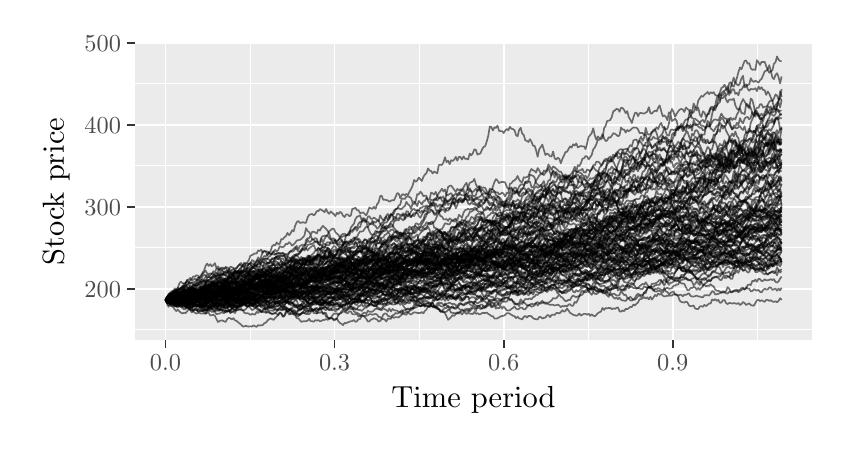
\begin{tikzpicture}[x=1pt,y=1pt]
\definecolor{fillColor}{RGB}{255,255,255}
\path[use as bounding box,fill=fillColor,fill opacity=0.00] (0,0) rectangle (289.08,144.54);
\begin{scope}
\path[clip] (  0.00,  0.00) rectangle (289.08,144.54);
\definecolor{drawColor}{RGB}{255,255,255}
\definecolor{fillColor}{RGB}{255,255,255}

\path[draw=drawColor,line width= 0.6pt,line join=round,line cap=round,fill=fillColor] (  0.00,  0.00) rectangle (289.08,144.54);
\end{scope}
\begin{scope}
\path[clip] ( 38.67, 31.53) rectangle (283.58,139.04);
\definecolor{fillColor}{gray}{0.92}

\path[fill=fillColor] ( 38.67, 31.53) rectangle (283.58,139.04);
\definecolor{drawColor}{RGB}{255,255,255}

\path[draw=drawColor,line width= 0.3pt,line join=round] ( 38.67, 35.39) --
	(283.58, 35.39);

\path[draw=drawColor,line width= 0.3pt,line join=round] ( 38.67, 65.00) --
	(283.58, 65.00);

\path[draw=drawColor,line width= 0.3pt,line join=round] ( 38.67, 94.61) --
	(283.58, 94.61);

\path[draw=drawColor,line width= 0.3pt,line join=round] ( 38.67,124.22) --
	(283.58,124.22);

\path[draw=drawColor,line width= 0.3pt,line join=round] ( 80.35, 31.53) --
	( 80.35,139.04);

\path[draw=drawColor,line width= 0.3pt,line join=round] (141.45, 31.53) --
	(141.45,139.04);

\path[draw=drawColor,line width= 0.3pt,line join=round] (202.56, 31.53) --
	(202.56,139.04);

\path[draw=drawColor,line width= 0.3pt,line join=round] (263.66, 31.53) --
	(263.66,139.04);

\path[draw=drawColor,line width= 0.6pt,line join=round] ( 38.67, 50.20) --
	(283.58, 50.20);

\path[draw=drawColor,line width= 0.6pt,line join=round] ( 38.67, 79.81) --
	(283.58, 79.81);

\path[draw=drawColor,line width= 0.6pt,line join=round] ( 38.67,109.42) --
	(283.58,109.42);

\path[draw=drawColor,line width= 0.6pt,line join=round] ( 38.67,139.03) --
	(283.58,139.03);

\path[draw=drawColor,line width= 0.6pt,line join=round] ( 49.80, 31.53) --
	( 49.80,139.04);

\path[draw=drawColor,line width= 0.6pt,line join=round] (110.90, 31.53) --
	(110.90,139.04);

\path[draw=drawColor,line width= 0.6pt,line join=round] (172.00, 31.53) --
	(172.00,139.04);

\path[draw=drawColor,line width= 0.6pt,line join=round] (233.11, 31.53) --
	(233.11,139.04);
\definecolor{drawColor}{RGB}{0,0,0}

\path[draw=drawColor,draw opacity=0.55,line width= 0.6pt,line join=round] ( 49.80, 46.14) --
	( 50.36, 46.04) --
	( 50.92, 46.41) --
	( 51.47, 46.28) --
	( 52.03, 46.85) --
	( 52.59, 47.03) --
	( 53.15, 47.88) --
	( 53.71, 46.79) --
	( 54.26, 47.30) --
	( 54.82, 47.75) --
	( 55.38, 48.41) --
	( 55.94, 49.20) --
	( 56.50, 48.47) --
	( 57.05, 48.78) --
	( 57.61, 48.17) --
	( 58.17, 48.22) --
	( 58.73, 48.82) --
	( 59.29, 49.03) --
	( 59.84, 48.36) --
	( 60.40, 48.24) --
	( 60.96, 49.09) --
	( 61.52, 48.99) --
	( 62.08, 49.59) --
	( 62.63, 49.08) --
	( 63.19, 49.63) --
	( 63.75, 50.03) --
	( 64.31, 50.02) --
	( 64.87, 49.75) --
	( 65.42, 51.30) --
	( 65.98, 50.77) --
	( 66.54, 51.03) --
	( 67.10, 52.14) --
	( 67.66, 52.54) --
	( 68.21, 52.37) --
	( 68.77, 52.30) --
	( 69.33, 53.42) --
	( 69.89, 53.39) --
	( 70.45, 53.33) --
	( 71.00, 52.97) --
	( 71.56, 52.85) --
	( 72.12, 52.70) --
	( 72.68, 52.46) --
	( 73.24, 52.39) --
	( 73.79, 52.88) --
	( 74.35, 53.30) --
	( 74.91, 53.67) --
	( 75.47, 54.05) --
	( 76.03, 54.99) --
	( 76.58, 56.08) --
	( 77.14, 55.29) --
	( 77.70, 54.58) --
	( 78.26, 54.40) --
	( 78.82, 54.13) --
	( 79.37, 54.73) --
	( 79.93, 55.56) --
	( 80.49, 56.62) --
	( 81.05, 56.18) --
	( 81.61, 56.64) --
	( 82.16, 56.44) --
	( 82.72, 56.24) --
	( 83.28, 56.47) --
	( 83.84, 56.95) --
	( 84.40, 56.85) --
	( 84.95, 57.22) --
	( 85.51, 57.25) --
	( 86.07, 56.86) --
	( 86.63, 56.69) --
	( 87.19, 56.30) --
	( 87.74, 55.80) --
	( 88.30, 55.50) --
	( 88.86, 55.25) --
	( 89.42, 54.99) --
	( 89.98, 54.09) --
	( 90.53, 53.32) --
	( 91.09, 54.36) --
	( 91.65, 53.10) --
	( 92.21, 53.38) --
	( 92.77, 52.89) --
	( 93.32, 51.83) --
	( 93.88, 52.08) --
	( 94.44, 52.37) --
	( 95.00, 52.53) --
	( 95.56, 53.48) --
	( 96.11, 54.29) --
	( 96.67, 53.60) --
	( 97.23, 53.71) --
	( 97.79, 54.90) --
	( 98.35, 55.16) --
	( 98.90, 55.07) --
	( 99.46, 56.49) --
	(100.02, 57.65) --
	(100.58, 57.61) --
	(101.14, 57.10) --
	(101.69, 57.35) --
	(102.25, 57.78) --
	(102.81, 57.21) --
	(103.37, 57.40) --
	(103.93, 57.53) --
	(104.48, 56.53) --
	(105.04, 56.82) --
	(105.60, 56.92) --
	(106.16, 58.01) --
	(106.72, 58.71) --
	(107.27, 58.90) --
	(107.83, 59.59) --
	(108.39, 59.92) --
	(108.95, 60.14) --
	(109.51, 59.34) --
	(110.06, 60.69) --
	(110.62, 59.99) --
	(111.18, 60.38) --
	(111.74, 59.60) --
	(112.30, 59.20) --
	(112.85, 59.61) --
	(113.41, 58.74) --
	(113.97, 59.05) --
	(114.53, 57.25) --
	(115.09, 57.30) --
	(115.65, 57.31) --
	(116.20, 57.09) --
	(116.76, 57.70) --
	(117.32, 58.64) --
	(117.88, 58.40) --
	(118.44, 58.08) --
	(118.99, 57.78) --
	(119.55, 58.28) --
	(120.11, 58.63) --
	(120.67, 58.56) --
	(121.23, 59.55) --
	(121.78, 58.73) --
	(122.34, 58.80) --
	(122.90, 59.16) --
	(123.46, 59.53) --
	(124.02, 60.61) --
	(124.57, 59.89) --
	(125.13, 59.35) --
	(125.69, 59.50) --
	(126.25, 60.49) --
	(126.81, 61.23) --
	(127.36, 60.53) --
	(127.92, 60.42) --
	(128.48, 60.50) --
	(129.04, 60.91) --
	(129.60, 60.20) --
	(130.15, 60.43) --
	(130.71, 61.24) --
	(131.27, 61.32) --
	(131.83, 60.81) --
	(132.39, 61.88) --
	(132.94, 62.86) --
	(133.50, 62.76) --
	(134.06, 62.78) --
	(134.62, 63.70) --
	(135.18, 65.48) --
	(135.73, 65.93) --
	(136.29, 65.64) --
	(136.85, 66.36) --
	(137.41, 65.85) --
	(137.97, 66.51) --
	(138.52, 66.28) --
	(139.08, 65.93) --
	(139.64, 67.57) --
	(140.20, 67.08) --
	(140.76, 67.70) --
	(141.31, 67.70) --
	(141.87, 67.69) --
	(142.43, 66.74) --
	(142.99, 67.39) --
	(143.55, 67.70) --
	(144.10, 68.33) --
	(144.66, 67.94) --
	(145.22, 67.86) --
	(145.78, 67.93) --
	(146.34, 66.00) --
	(146.89, 66.49) --
	(147.45, 68.08) --
	(148.01, 69.39) --
	(148.57, 69.60) --
	(149.13, 70.95) --
	(149.68, 70.28) --
	(150.24, 69.17) --
	(150.80, 68.55) --
	(151.36, 68.05) --
	(151.92, 68.40) --
	(152.47, 69.20) --
	(153.03, 68.21) --
	(153.59, 68.24) --
	(154.15, 67.84) --
	(154.71, 67.29) --
	(155.26, 67.37) --
	(155.82, 68.36) --
	(156.38, 69.52) --
	(156.94, 69.19) --
	(157.50, 69.91) --
	(158.05, 69.00) --
	(158.61, 67.57) --
	(159.17, 68.76) --
	(159.73, 69.65) --
	(160.29, 69.16) --
	(160.84, 70.20) --
	(161.40, 70.38) --
	(161.96, 72.21) --
	(162.52, 71.73) --
	(163.08, 71.37) --
	(163.63, 71.09) --
	(164.19, 71.62) --
	(164.75, 71.88) --
	(165.31, 72.19) --
	(165.87, 72.30) --
	(166.42, 72.86) --
	(166.98, 73.13) --
	(167.54, 73.67) --
	(168.10, 72.69) --
	(168.66, 74.09) --
	(169.21, 72.75) --
	(169.77, 72.08) --
	(170.33, 71.28) --
	(170.89, 70.48) --
	(171.45, 70.81) --
	(172.00, 71.42) --
	(172.56, 71.52) --
	(173.12, 72.41) --
	(173.68, 73.00) --
	(174.24, 71.46) --
	(174.79, 70.52) --
	(175.35, 69.41) --
	(175.91, 69.72) --
	(176.47, 68.51) --
	(177.03, 67.83) --
	(177.58, 67.04) --
	(178.14, 66.88) --
	(178.70, 67.93) --
	(179.26, 69.06) --
	(179.82, 69.32) --
	(180.37, 69.37) --
	(180.93, 70.95) --
	(181.49, 69.65) --
	(182.05, 69.94) --
	(182.61, 70.06) --
	(183.17, 70.50) --
	(183.72, 71.28) --
	(184.28, 70.51) --
	(184.84, 70.10) --
	(185.40, 73.01) --
	(185.96, 72.39) --
	(186.51, 71.64) --
	(187.07, 72.44) --
	(187.63, 72.09) --
	(188.19, 73.80) --
	(188.75, 73.43) --
	(189.30, 73.22) --
	(189.86, 73.19) --
	(190.42, 72.60) --
	(190.98, 74.25) --
	(191.54, 73.38) --
	(192.09, 73.51) --
	(192.65, 71.57) --
	(193.21, 71.13) --
	(193.77, 71.13) --
	(194.33, 71.21) --
	(194.88, 71.79) --
	(195.44, 71.63) --
	(196.00, 71.34) --
	(196.56, 70.44) --
	(197.12, 71.14) --
	(197.67, 71.72) --
	(198.23, 71.81) --
	(198.79, 71.69) --
	(199.35, 72.31) --
	(199.91, 73.35) --
	(200.46, 73.63) --
	(201.02, 73.70) --
	(201.58, 74.13) --
	(202.14, 74.99) --
	(202.70, 75.00) --
	(203.25, 74.01) --
	(203.81, 74.28) --
	(204.37, 73.47) --
	(204.93, 74.06) --
	(205.49, 73.26) --
	(206.04, 72.76) --
	(206.60, 72.13) --
	(207.16, 72.30) --
	(207.72, 72.70) --
	(208.28, 72.56) --
	(208.83, 72.82) --
	(209.39, 72.84) --
	(209.95, 73.15) --
	(210.51, 74.35) --
	(211.07, 76.05) --
	(211.62, 74.25) --
	(212.18, 73.63) --
	(212.74, 75.71) --
	(213.30, 76.66) --
	(213.86, 76.97) --
	(214.41, 76.84) --
	(214.97, 76.69) --
	(215.53, 77.02) --
	(216.09, 76.29) --
	(216.65, 75.63) --
	(217.20, 75.82) --
	(217.76, 76.65) --
	(218.32, 77.42) --
	(218.88, 76.74) --
	(219.44, 75.78) --
	(219.99, 77.27) --
	(220.55, 77.69) --
	(221.11, 76.69) --
	(221.67, 78.21) --
	(222.23, 77.00) --
	(222.78, 76.80) --
	(223.34, 75.65) --
	(223.90, 77.97) --
	(224.46, 77.82) --
	(225.02, 78.22) --
	(225.57, 79.00) --
	(226.13, 78.01) --
	(226.69, 77.67) --
	(227.25, 76.36) --
	(227.81, 77.20) --
	(228.36, 77.05) --
	(228.92, 75.44) --
	(229.48, 75.59) --
	(230.04, 74.70) --
	(230.60, 74.20) --
	(231.15, 73.95) --
	(231.71, 73.60) --
	(232.27, 73.95) --
	(232.83, 72.45) --
	(233.39, 72.86) --
	(233.94, 72.74) --
	(234.50, 73.62) --
	(235.06, 72.64) --
	(235.62, 71.51) --
	(236.18, 71.24) --
	(236.73, 72.67) --
	(237.29, 72.78) --
	(237.85, 71.72) --
	(238.41, 71.32) --
	(238.97, 70.38) --
	(239.52, 70.03) --
	(240.08, 70.06) --
	(240.64, 70.37) --
	(241.20, 69.62) --
	(241.76, 69.89) --
	(242.31, 70.28) --
	(242.87, 70.88) --
	(243.43, 69.42) --
	(243.99, 69.86) --
	(244.55, 68.90) --
	(245.10, 69.20) --
	(245.66, 70.02) --
	(246.22, 70.06) --
	(246.78, 68.76) --
	(247.34, 67.77) --
	(247.89, 69.62) --
	(248.45, 71.37) --
	(249.01, 70.63) --
	(249.57, 69.16) --
	(250.13, 70.03) --
	(250.68, 70.83) --
	(251.24, 70.77) --
	(251.80, 71.84) --
	(252.36, 71.41) --
	(252.92, 71.13) --
	(253.48, 71.32) --
	(254.03, 71.68) --
	(254.59, 70.60) --
	(255.15, 70.68) --
	(255.71, 71.20) --
	(256.27, 72.30) --
	(256.82, 70.31) --
	(257.38, 71.56) --
	(257.94, 70.32) --
	(258.50, 70.55) --
	(259.06, 72.74) --
	(259.61, 71.49) --
	(260.17, 71.25) --
	(260.73, 69.44) --
	(261.29, 71.28) --
	(261.85, 71.47) --
	(262.40, 71.93) --
	(262.96, 71.21) --
	(263.52, 72.41) --
	(264.08, 73.66) --
	(264.64, 73.18) --
	(265.19, 72.10) --
	(265.75, 73.60) --
	(266.31, 73.08) --
	(266.87, 73.91) --
	(267.43, 74.47) --
	(267.98, 74.81) --
	(268.54, 74.64) --
	(269.10, 74.48) --
	(269.66, 74.76) --
	(270.22, 74.79) --
	(270.77, 75.69) --
	(271.33, 76.41) --
	(271.89, 75.75) --
	(272.45, 75.10);

\path[draw=drawColor,draw opacity=0.55,line width= 0.6pt,line join=round] ( 49.80, 46.14) --
	( 50.36, 46.15) --
	( 50.92, 45.43) --
	( 51.47, 45.77) --
	( 52.03, 45.22) --
	( 52.59, 44.55) --
	( 53.15, 45.35) --
	( 53.71, 45.72) --
	( 54.26, 46.12) --
	( 54.82, 45.73) --
	( 55.38, 46.36) --
	( 55.94, 45.32) --
	( 56.50, 44.30) --
	( 57.05, 43.74) --
	( 57.61, 43.21) --
	( 58.17, 43.14) --
	( 58.73, 42.48) --
	( 59.29, 42.98) --
	( 59.84, 42.00) --
	( 60.40, 41.55) --
	( 60.96, 41.25) --
	( 61.52, 41.44) --
	( 62.08, 41.50) --
	( 62.63, 41.20) --
	( 63.19, 41.24) --
	( 63.75, 41.30) --
	( 64.31, 41.09) --
	( 64.87, 42.45) --
	( 65.42, 43.00) --
	( 65.98, 42.92) --
	( 66.54, 42.86) --
	( 67.10, 42.29) --
	( 67.66, 42.17) --
	( 68.21, 43.09) --
	( 68.77, 43.25) --
	( 69.33, 43.06) --
	( 69.89, 42.73) --
	( 70.45, 42.32) --
	( 71.00, 42.27) --
	( 71.56, 41.63) --
	( 72.12, 41.87) --
	( 72.68, 42.07) --
	( 73.24, 42.67) --
	( 73.79, 42.96) --
	( 74.35, 44.12) --
	( 74.91, 43.71) --
	( 75.47, 43.54) --
	( 76.03, 44.08) --
	( 76.58, 43.83) --
	( 77.14, 43.62) --
	( 77.70, 44.22) --
	( 78.26, 44.15) --
	( 78.82, 44.09) --
	( 79.37, 44.13) --
	( 79.93, 43.82) --
	( 80.49, 44.72) --
	( 81.05, 44.73) --
	( 81.61, 44.49) --
	( 82.16, 44.95) --
	( 82.72, 45.72) --
	( 83.28, 46.68) --
	( 83.84, 46.63) --
	( 84.40, 46.21) --
	( 84.95, 46.16) --
	( 85.51, 45.91) --
	( 86.07, 45.36) --
	( 86.63, 46.25) --
	( 87.19, 45.25) --
	( 87.74, 44.76) --
	( 88.30, 45.30) --
	( 88.86, 46.01) --
	( 89.42, 44.95) --
	( 89.98, 44.82) --
	( 90.53, 45.45) --
	( 91.09, 45.77) --
	( 91.65, 46.41) --
	( 92.21, 46.23) --
	( 92.77, 46.41) --
	( 93.32, 45.22) --
	( 93.88, 45.98) --
	( 94.44, 44.95) --
	( 95.00, 45.06) --
	( 95.56, 45.06) --
	( 96.11, 44.69) --
	( 96.67, 44.56) --
	( 97.23, 44.15) --
	( 97.79, 43.62) --
	( 98.35, 44.15) --
	( 98.90, 44.49) --
	( 99.46, 44.53) --
	(100.02, 45.18) --
	(100.58, 45.67) --
	(101.14, 45.13) --
	(101.69, 46.26) --
	(102.25, 46.32) --
	(102.81, 46.69) --
	(103.37, 47.21) --
	(103.93, 46.49) --
	(104.48, 45.85) --
	(105.04, 44.71) --
	(105.60, 43.93) --
	(106.16, 44.60) --
	(106.72, 45.55) --
	(107.27, 45.39) --
	(107.83, 45.37) --
	(108.39, 44.86) --
	(108.95, 45.48) --
	(109.51, 44.66) --
	(110.06, 44.34) --
	(110.62, 44.52) --
	(111.18, 44.02) --
	(111.74, 43.85) --
	(112.30, 43.96) --
	(112.85, 44.29) --
	(113.41, 45.03) --
	(113.97, 45.85) --
	(114.53, 45.31) --
	(115.09, 45.28) --
	(115.65, 45.82) --
	(116.20, 44.69) --
	(116.76, 43.80) --
	(117.32, 44.78) --
	(117.88, 45.34) --
	(118.44, 45.56) --
	(118.99, 45.53) --
	(119.55, 45.86) --
	(120.11, 46.74) --
	(120.67, 45.86) --
	(121.23, 46.08) --
	(121.78, 45.42) --
	(122.34, 44.67) --
	(122.90, 45.08) --
	(123.46, 44.25) --
	(124.02, 45.01) --
	(124.57, 44.18) --
	(125.13, 44.13) --
	(125.69, 43.96) --
	(126.25, 43.93) --
	(126.81, 45.53) --
	(127.36, 45.13) --
	(127.92, 46.37) --
	(128.48, 46.60) --
	(129.04, 46.69) --
	(129.60, 46.29) --
	(130.15, 46.28) --
	(130.71, 47.02) --
	(131.27, 47.41) --
	(131.83, 47.31) --
	(132.39, 47.97) --
	(132.94, 48.09) --
	(133.50, 48.59) --
	(134.06, 49.54) --
	(134.62, 49.69) --
	(135.18, 49.95) --
	(135.73, 50.16) --
	(136.29, 49.14) --
	(136.85, 49.99) --
	(137.41, 51.07) --
	(137.97, 51.93) --
	(138.52, 52.15) --
	(139.08, 53.76) --
	(139.64, 54.76) --
	(140.20, 55.15) --
	(140.76, 55.18) --
	(141.31, 54.95) --
	(141.87, 55.06) --
	(142.43, 55.66) --
	(142.99, 54.49) --
	(143.55, 54.36) --
	(144.10, 54.46) --
	(144.66, 54.92) --
	(145.22, 55.71) --
	(145.78, 55.87) --
	(146.34, 56.37) --
	(146.89, 56.34) --
	(147.45, 56.95) --
	(148.01, 57.21) --
	(148.57, 57.07) --
	(149.13, 58.40) --
	(149.68, 59.59) --
	(150.24, 61.02) --
	(150.80, 62.04) --
	(151.36, 60.76) --
	(151.92, 59.49) --
	(152.47, 59.61) --
	(153.03, 60.57) --
	(153.59, 60.85) --
	(154.15, 60.54) --
	(154.71, 61.88) --
	(155.26, 61.85) --
	(155.82, 61.39) --
	(156.38, 61.03) --
	(156.94, 61.21) --
	(157.50, 60.03) --
	(158.05, 59.47) --
	(158.61, 60.43) --
	(159.17, 59.99) --
	(159.73, 59.69) --
	(160.29, 59.83) --
	(160.84, 61.46) --
	(161.40, 61.88) --
	(161.96, 62.54) --
	(162.52, 63.99) --
	(163.08, 62.67) --
	(163.63, 61.27) --
	(164.19, 61.65) --
	(164.75, 61.66) --
	(165.31, 62.27) --
	(165.87, 61.94) --
	(166.42, 60.93) --
	(166.98, 60.59) --
	(167.54, 61.54) --
	(168.10, 61.72) --
	(168.66, 62.00) --
	(169.21, 62.36) --
	(169.77, 63.95) --
	(170.33, 64.48) --
	(170.89, 65.03) --
	(171.45, 64.92) --
	(172.00, 64.82) --
	(172.56, 64.36) --
	(173.12, 64.88) --
	(173.68, 65.66) --
	(174.24, 65.23) --
	(174.79, 66.33) --
	(175.35, 65.74) --
	(175.91, 65.64) --
	(176.47, 64.01) --
	(177.03, 63.72) --
	(177.58, 63.61) --
	(178.14, 63.98) --
	(178.70, 64.62) --
	(179.26, 65.26) --
	(179.82, 64.54) --
	(180.37, 65.69) --
	(180.93, 66.34) --
	(181.49, 65.10) --
	(182.05, 65.59) --
	(182.61, 65.68) --
	(183.17, 66.17) --
	(183.72, 65.79) --
	(184.28, 65.52) --
	(184.84, 66.79) --
	(185.40, 65.75) --
	(185.96, 64.91) --
	(186.51, 64.26) --
	(187.07, 64.67) --
	(187.63, 65.49) --
	(188.19, 64.12) --
	(188.75, 64.66) --
	(189.30, 63.81) --
	(189.86, 64.00) --
	(190.42, 64.10) --
	(190.98, 65.53) --
	(191.54, 66.31) --
	(192.09, 67.95) --
	(192.65, 67.35) --
	(193.21, 67.91) --
	(193.77, 69.18) --
	(194.33, 69.72) --
	(194.88, 69.97) --
	(195.44, 69.24) --
	(196.00, 69.36) --
	(196.56, 69.65) --
	(197.12, 69.34) --
	(197.67, 69.36) --
	(198.23, 70.16) --
	(198.79, 69.04) --
	(199.35, 70.55) --
	(199.91, 69.83) --
	(200.46, 68.36) --
	(201.02, 67.33) --
	(201.58, 67.68) --
	(202.14, 67.37) --
	(202.70, 66.92) --
	(203.25, 66.00) --
	(203.81, 65.54) --
	(204.37, 64.66) --
	(204.93, 64.89) --
	(205.49, 65.36) --
	(206.04, 64.95) --
	(206.60, 64.96) --
	(207.16, 67.39) --
	(207.72, 67.47) --
	(208.28, 68.12) --
	(208.83, 68.81) --
	(209.39, 70.29) --
	(209.95, 71.20) --
	(210.51, 70.51) --
	(211.07, 70.61) --
	(211.62, 71.28) --
	(212.18, 70.46) --
	(212.74, 69.50) --
	(213.30, 69.64) --
	(213.86, 69.07) --
	(214.41, 69.65) --
	(214.97, 69.44) --
	(215.53, 69.83) --
	(216.09, 70.37) --
	(216.65, 71.84) --
	(217.20, 72.59) --
	(217.76, 72.13) --
	(218.32, 71.62) --
	(218.88, 71.83) --
	(219.44, 70.91) --
	(219.99, 71.07) --
	(220.55, 71.62) --
	(221.11, 71.62) --
	(221.67, 70.21) --
	(222.23, 70.15) --
	(222.78, 70.66) --
	(223.34, 70.75) --
	(223.90, 70.43) --
	(224.46, 71.60) --
	(225.02, 71.17) --
	(225.57, 71.18) --
	(226.13, 71.09) --
	(226.69, 71.17) --
	(227.25, 71.43) --
	(227.81, 71.14) --
	(228.36, 72.25) --
	(228.92, 72.97) --
	(229.48, 72.48) --
	(230.04, 72.76) --
	(230.60, 72.00) --
	(231.15, 71.23) --
	(231.71, 71.31) --
	(232.27, 71.51) --
	(232.83, 73.13) --
	(233.39, 72.37) --
	(233.94, 73.31) --
	(234.50, 73.32) --
	(235.06, 73.41) --
	(235.62, 75.50) --
	(236.18, 76.05) --
	(236.73, 75.74) --
	(237.29, 75.91) --
	(237.85, 76.94) --
	(238.41, 75.56) --
	(238.97, 76.74) --
	(239.52, 77.17) --
	(240.08, 76.38) --
	(240.64, 77.51) --
	(241.20, 76.59) --
	(241.76, 76.55) --
	(242.31, 76.47) --
	(242.87, 76.27) --
	(243.43, 75.48) --
	(243.99, 75.27) --
	(244.55, 74.79) --
	(245.10, 75.91) --
	(245.66, 75.45) --
	(246.22, 76.25) --
	(246.78, 75.13) --
	(247.34, 74.51) --
	(247.89, 74.25) --
	(248.45, 73.91) --
	(249.01, 73.42) --
	(249.57, 73.62) --
	(250.13, 72.21) --
	(250.68, 73.51) --
	(251.24, 72.87) --
	(251.80, 72.05) --
	(252.36, 71.31) --
	(252.92, 70.44) --
	(253.48, 70.35) --
	(254.03, 67.61) --
	(254.59, 67.48) --
	(255.15, 66.64) --
	(255.71, 65.77) --
	(256.27, 66.07) --
	(256.82, 65.69) --
	(257.38, 65.98) --
	(257.94, 67.39) --
	(258.50, 68.52) --
	(259.06, 69.00) --
	(259.61, 68.24) --
	(260.17, 68.19) --
	(260.73, 67.74) --
	(261.29, 68.63) --
	(261.85, 69.87) --
	(262.40, 70.83) --
	(262.96, 71.02) --
	(263.52, 71.70) --
	(264.08, 71.94) --
	(264.64, 72.59) --
	(265.19, 72.93) --
	(265.75, 71.90) --
	(266.31, 71.76) --
	(266.87, 73.49) --
	(267.43, 74.24) --
	(267.98, 74.06) --
	(268.54, 73.78) --
	(269.10, 73.89) --
	(269.66, 73.52) --
	(270.22, 73.99) --
	(270.77, 74.38) --
	(271.33, 74.76) --
	(271.89, 73.48) --
	(272.45, 72.83);

\path[draw=drawColor,draw opacity=0.55,line width= 0.6pt,line join=round] ( 49.80, 46.14) --
	( 50.36, 46.07) --
	( 50.92, 46.46) --
	( 51.47, 46.71) --
	( 52.03, 46.83) --
	( 52.59, 46.42) --
	( 53.15, 46.57) --
	( 53.71, 46.86) --
	( 54.26, 46.97) --
	( 54.82, 47.09) --
	( 55.38, 47.73) --
	( 55.94, 47.94) --
	( 56.50, 48.44) --
	( 57.05, 47.99) --
	( 57.61, 47.86) --
	( 58.17, 47.56) --
	( 58.73, 48.32) --
	( 59.29, 48.29) --
	( 59.84, 47.98) --
	( 60.40, 48.30) --
	( 60.96, 49.23) --
	( 61.52, 49.86) --
	( 62.08, 49.44) --
	( 62.63, 49.85) --
	( 63.19, 50.34) --
	( 63.75, 49.63) --
	( 64.31, 48.78) --
	( 64.87, 49.73) --
	( 65.42, 49.26) --
	( 65.98, 49.51) --
	( 66.54, 49.82) --
	( 67.10, 49.75) --
	( 67.66, 50.77) --
	( 68.21, 50.60) --
	( 68.77, 51.04) --
	( 69.33, 51.04) --
	( 69.89, 50.85) --
	( 70.45, 51.14) --
	( 71.00, 50.33) --
	( 71.56, 50.05) --
	( 72.12, 49.67) --
	( 72.68, 50.11) --
	( 73.24, 48.79) --
	( 73.79, 49.10) --
	( 74.35, 49.61) --
	( 74.91, 50.38) --
	( 75.47, 50.83) --
	( 76.03, 50.02) --
	( 76.58, 50.92) --
	( 77.14, 50.82) --
	( 77.70, 49.88) --
	( 78.26, 50.40) --
	( 78.82, 50.63) --
	( 79.37, 49.91) --
	( 79.93, 49.50) --
	( 80.49, 50.06) --
	( 81.05, 50.31) --
	( 81.61, 49.52) --
	( 82.16, 49.50) --
	( 82.72, 49.90) --
	( 83.28, 50.54) --
	( 83.84, 50.47) --
	( 84.40, 50.47) --
	( 84.95, 49.66) --
	( 85.51, 50.05) --
	( 86.07, 50.05) --
	( 86.63, 49.58) --
	( 87.19, 49.75) --
	( 87.74, 50.60) --
	( 88.30, 50.80) --
	( 88.86, 51.06) --
	( 89.42, 50.04) --
	( 89.98, 50.46) --
	( 90.53, 49.64) --
	( 91.09, 49.31) --
	( 91.65, 49.62) --
	( 92.21, 50.85) --
	( 92.77, 50.91) --
	( 93.32, 50.95) --
	( 93.88, 50.93) --
	( 94.44, 51.18) --
	( 95.00, 51.18) --
	( 95.56, 51.52) --
	( 96.11, 51.33) --
	( 96.67, 50.99) --
	( 97.23, 51.53) --
	( 97.79, 51.97) --
	( 98.35, 52.14) --
	( 98.90, 51.29) --
	( 99.46, 51.36) --
	(100.02, 52.96) --
	(100.58, 52.75) --
	(101.14, 52.65) --
	(101.69, 53.33) --
	(102.25, 53.23) --
	(102.81, 52.54) --
	(103.37, 52.40) --
	(103.93, 52.79) --
	(104.48, 53.53) --
	(105.04, 54.40) --
	(105.60, 54.25) --
	(106.16, 54.18) --
	(106.72, 54.89) --
	(107.27, 54.97) --
	(107.83, 54.32) --
	(108.39, 53.18) --
	(108.95, 54.13) --
	(109.51, 53.21) --
	(110.06, 53.04) --
	(110.62, 52.54) --
	(111.18, 52.90) --
	(111.74, 52.29) --
	(112.30, 52.45) --
	(112.85, 52.43) --
	(113.41, 52.26) --
	(113.97, 52.67) --
	(114.53, 53.22) --
	(115.09, 52.45) --
	(115.65, 52.12) --
	(116.20, 52.40) --
	(116.76, 52.89) --
	(117.32, 53.83) --
	(117.88, 52.45) --
	(118.44, 53.91) --
	(118.99, 53.27) --
	(119.55, 54.31) --
	(120.11, 53.81) --
	(120.67, 54.11) --
	(121.23, 54.28) --
	(121.78, 54.34) --
	(122.34, 53.63) --
	(122.90, 54.00) --
	(123.46, 53.67) --
	(124.02, 54.37) --
	(124.57, 54.44) --
	(125.13, 54.97) --
	(125.69, 55.48) --
	(126.25, 55.85) --
	(126.81, 55.84) --
	(127.36, 55.87) --
	(127.92, 54.98) --
	(128.48, 55.78) --
	(129.04, 57.03) --
	(129.60, 57.51) --
	(130.15, 57.88) --
	(130.71, 58.46) --
	(131.27, 58.62) --
	(131.83, 58.72) --
	(132.39, 58.07) --
	(132.94, 59.18) --
	(133.50, 59.02) --
	(134.06, 57.70) --
	(134.62, 56.97) --
	(135.18, 57.73) --
	(135.73, 58.07) --
	(136.29, 57.49) --
	(136.85, 57.60) --
	(137.41, 57.35) --
	(137.97, 57.35) --
	(138.52, 56.93) --
	(139.08, 57.05) --
	(139.64, 56.97) --
	(140.20, 57.15) --
	(140.76, 58.53) --
	(141.31, 59.50) --
	(141.87, 59.85) --
	(142.43, 59.84) --
	(142.99, 60.30) --
	(143.55, 60.50) --
	(144.10, 60.09) --
	(144.66, 58.21) --
	(145.22, 58.00) --
	(145.78, 58.55) --
	(146.34, 58.63) --
	(146.89, 58.48) --
	(147.45, 59.04) --
	(148.01, 59.70) --
	(148.57, 59.55) --
	(149.13, 59.99) --
	(149.68, 60.63) --
	(150.24, 59.67) --
	(150.80, 60.71) --
	(151.36, 61.83) --
	(151.92, 62.06) --
	(152.47, 60.84) --
	(153.03, 61.38) --
	(153.59, 61.97) --
	(154.15, 62.83) --
	(154.71, 61.56) --
	(155.26, 62.11) --
	(155.82, 61.38) --
	(156.38, 61.32) --
	(156.94, 60.90) --
	(157.50, 60.90) --
	(158.05, 60.42) --
	(158.61, 60.80) --
	(159.17, 61.34) --
	(159.73, 61.32) --
	(160.29, 61.62) --
	(160.84, 60.30) --
	(161.40, 59.23) --
	(161.96, 58.61) --
	(162.52, 58.90) --
	(163.08, 59.02) --
	(163.63, 57.61) --
	(164.19, 58.40) --
	(164.75, 59.10) --
	(165.31, 59.83) --
	(165.87, 59.69) --
	(166.42, 58.94) --
	(166.98, 58.49) --
	(167.54, 59.12) --
	(168.10, 59.27) --
	(168.66, 60.00) --
	(169.21, 58.93) --
	(169.77, 59.25) --
	(170.33, 59.64) --
	(170.89, 59.91) --
	(171.45, 60.41) --
	(172.00, 60.61) --
	(172.56, 60.04) --
	(173.12, 59.80) --
	(173.68, 60.18) --
	(174.24, 61.48) --
	(174.79, 60.95) --
	(175.35, 61.17) --
	(175.91, 58.63) --
	(176.47, 59.19) --
	(177.03, 59.32) --
	(177.58, 59.95) --
	(178.14, 58.06) --
	(178.70, 58.16) --
	(179.26, 57.39) --
	(179.82, 56.80) --
	(180.37, 56.96) --
	(180.93, 56.72) --
	(181.49, 57.07) --
	(182.05, 56.61) --
	(182.61, 57.43) --
	(183.17, 58.20) --
	(183.72, 58.91) --
	(184.28, 59.57) --
	(184.84, 59.26) --
	(185.40, 59.29) --
	(185.96, 58.98) --
	(186.51, 58.97) --
	(187.07, 59.59) --
	(187.63, 59.75) --
	(188.19, 58.74) --
	(188.75, 58.57) --
	(189.30, 57.08) --
	(189.86, 56.63) --
	(190.42, 55.64) --
	(190.98, 55.66) --
	(191.54, 57.18) --
	(192.09, 57.18) --
	(192.65, 57.46) --
	(193.21, 58.34) --
	(193.77, 59.35) --
	(194.33, 58.31) --
	(194.88, 58.29) --
	(195.44, 58.82) --
	(196.00, 59.30) --
	(196.56, 59.66) --
	(197.12, 60.15) --
	(197.67, 60.18) --
	(198.23, 61.47) --
	(198.79, 60.35) --
	(199.35, 61.07) --
	(199.91, 60.91) --
	(200.46, 61.77) --
	(201.02, 61.89) --
	(201.58, 62.32) --
	(202.14, 62.73) --
	(202.70, 62.95) --
	(203.25, 63.48) --
	(203.81, 63.30) --
	(204.37, 62.90) --
	(204.93, 62.95) --
	(205.49, 62.70) --
	(206.04, 64.30) --
	(206.60, 66.32) --
	(207.16, 65.95) --
	(207.72, 65.86) --
	(208.28, 64.93) --
	(208.83, 65.34) --
	(209.39, 65.01) --
	(209.95, 65.71) --
	(210.51, 66.26) --
	(211.07, 66.70) --
	(211.62, 68.11) --
	(212.18, 68.34) --
	(212.74, 68.52) --
	(213.30, 68.42) --
	(213.86, 68.22) --
	(214.41, 68.93) --
	(214.97, 68.63) --
	(215.53, 68.05) --
	(216.09, 67.27) --
	(216.65, 66.71) --
	(217.20, 68.04) --
	(217.76, 69.22) --
	(218.32, 69.05) --
	(218.88, 68.76) --
	(219.44, 68.71) --
	(219.99, 67.70) --
	(220.55, 67.05) --
	(221.11, 64.89) --
	(221.67, 65.48) --
	(222.23, 64.86) --
	(222.78, 65.43) --
	(223.34, 66.32) --
	(223.90, 67.41) --
	(224.46, 66.71) --
	(225.02, 67.22) --
	(225.57, 67.87) --
	(226.13, 69.63) --
	(226.69, 69.89) --
	(227.25, 70.67) --
	(227.81, 71.53) --
	(228.36, 71.81) --
	(228.92, 70.99) --
	(229.48, 70.69) --
	(230.04, 70.62) --
	(230.60, 70.12) --
	(231.15, 67.52) --
	(231.71, 67.29) --
	(232.27, 66.40) --
	(232.83, 66.20) --
	(233.39, 68.02) --
	(233.94, 67.93) --
	(234.50, 67.63) --
	(235.06, 68.47) --
	(235.62, 68.01) --
	(236.18, 68.77) --
	(236.73, 69.63) --
	(237.29, 68.28) --
	(237.85, 67.97) --
	(238.41, 68.65) --
	(238.97, 68.82) --
	(239.52, 70.07) --
	(240.08, 70.18) --
	(240.64, 69.96) --
	(241.20, 69.71) --
	(241.76, 70.29) --
	(242.31, 70.44) --
	(242.87, 70.27) --
	(243.43, 70.09) --
	(243.99, 69.75) --
	(244.55, 69.88) --
	(245.10, 69.41) --
	(245.66, 69.83) --
	(246.22, 71.24) --
	(246.78, 71.66) --
	(247.34, 72.66) --
	(247.89, 72.70) --
	(248.45, 71.83) --
	(249.01, 72.48) --
	(249.57, 72.43) --
	(250.13, 73.51) --
	(250.68, 74.48) --
	(251.24, 76.50) --
	(251.80, 76.52) --
	(252.36, 77.73) --
	(252.92, 76.65) --
	(253.48, 75.88) --
	(254.03, 76.89) --
	(254.59, 76.63) --
	(255.15, 77.76) --
	(255.71, 76.13) --
	(256.27, 76.79) --
	(256.82, 76.41) --
	(257.38, 76.50) --
	(257.94, 77.22) --
	(258.50, 76.91) --
	(259.06, 76.61) --
	(259.61, 76.45) --
	(260.17, 76.82) --
	(260.73, 75.00) --
	(261.29, 76.14) --
	(261.85, 75.66) --
	(262.40, 77.40) --
	(262.96, 78.60) --
	(263.52, 78.14) --
	(264.08, 78.32) --
	(264.64, 78.96) --
	(265.19, 77.74) --
	(265.75, 77.84) --
	(266.31, 79.93) --
	(266.87, 81.49) --
	(267.43, 82.03) --
	(267.98, 83.42) --
	(268.54, 83.84) --
	(269.10, 82.24) --
	(269.66, 82.56) --
	(270.22, 83.36) --
	(270.77, 83.01) --
	(271.33, 84.07) --
	(271.89, 83.75) --
	(272.45, 83.57);

\path[draw=drawColor,draw opacity=0.55,line width= 0.6pt,line join=round] ( 49.80, 46.14) --
	( 50.36, 45.99) --
	( 50.92, 44.92) --
	( 51.47, 45.08) --
	( 52.03, 45.92) --
	( 52.59, 45.58) --
	( 53.15, 45.18) --
	( 53.71, 44.55) --
	( 54.26, 44.18) --
	( 54.82, 44.50) --
	( 55.38, 44.09) --
	( 55.94, 43.89) --
	( 56.50, 43.92) --
	( 57.05, 44.02) --
	( 57.61, 43.72) --
	( 58.17, 43.33) --
	( 58.73, 42.62) --
	( 59.29, 42.35) --
	( 59.84, 42.27) --
	( 60.40, 42.85) --
	( 60.96, 42.55) --
	( 61.52, 42.02) --
	( 62.08, 42.09) --
	( 62.63, 42.36) --
	( 63.19, 41.94) --
	( 63.75, 42.35) --
	( 64.31, 42.63) --
	( 64.87, 42.57) --
	( 65.42, 42.90) --
	( 65.98, 43.07) --
	( 66.54, 43.73) --
	( 67.10, 44.37) --
	( 67.66, 43.64) --
	( 68.21, 44.57) --
	( 68.77, 43.91) --
	( 69.33, 44.04) --
	( 69.89, 44.23) --
	( 70.45, 44.09) --
	( 71.00, 44.66) --
	( 71.56, 44.63) --
	( 72.12, 44.44) --
	( 72.68, 44.61) --
	( 73.24, 44.09) --
	( 73.79, 44.80) --
	( 74.35, 44.56) --
	( 74.91, 43.72) --
	( 75.47, 43.85) --
	( 76.03, 44.07) --
	( 76.58, 44.20) --
	( 77.14, 44.34) --
	( 77.70, 44.72) --
	( 78.26, 44.71) --
	( 78.82, 44.97) --
	( 79.37, 44.46) --
	( 79.93, 44.33) --
	( 80.49, 45.33) --
	( 81.05, 46.38) --
	( 81.61, 45.71) --
	( 82.16, 45.54) --
	( 82.72, 45.56) --
	( 83.28, 45.66) --
	( 83.84, 46.46) --
	( 84.40, 47.31) --
	( 84.95, 47.88) --
	( 85.51, 48.73) --
	( 86.07, 48.97) --
	( 86.63, 48.49) --
	( 87.19, 48.25) --
	( 87.74, 48.07) --
	( 88.30, 47.08) --
	( 88.86, 47.14) --
	( 89.42, 46.80) --
	( 89.98, 46.14) --
	( 90.53, 46.27) --
	( 91.09, 47.31) --
	( 91.65, 47.41) --
	( 92.21, 47.10) --
	( 92.77, 47.63) --
	( 93.32, 47.64) --
	( 93.88, 49.08) --
	( 94.44, 48.71) --
	( 95.00, 48.55) --
	( 95.56, 48.91) --
	( 96.11, 48.40) --
	( 96.67, 47.78) --
	( 97.23, 47.85) --
	( 97.79, 48.27) --
	( 98.35, 48.87) --
	( 98.90, 48.93) --
	( 99.46, 49.07) --
	(100.02, 50.01) --
	(100.58, 50.01) --
	(101.14, 50.06) --
	(101.69, 51.00) --
	(102.25, 50.84) --
	(102.81, 50.85) --
	(103.37, 50.69) --
	(103.93, 51.18) --
	(104.48, 52.66) --
	(105.04, 52.96) --
	(105.60, 53.56) --
	(106.16, 54.70) --
	(106.72, 54.61) --
	(107.27, 55.03) --
	(107.83, 54.70) --
	(108.39, 53.72) --
	(108.95, 54.45) --
	(109.51, 53.91) --
	(110.06, 54.42) --
	(110.62, 54.58) --
	(111.18, 54.12) --
	(111.74, 54.43) --
	(112.30, 54.49) --
	(112.85, 54.14) --
	(113.41, 54.49) --
	(113.97, 53.54) --
	(114.53, 54.08) --
	(115.09, 53.36) --
	(115.65, 52.53) --
	(116.20, 53.16) --
	(116.76, 53.15) --
	(117.32, 53.95) --
	(117.88, 55.40) --
	(118.44, 55.54) --
	(118.99, 55.84) --
	(119.55, 54.75) --
	(120.11, 54.71) --
	(120.67, 55.88) --
	(121.23, 55.73) --
	(121.78, 55.99) --
	(122.34, 55.83) --
	(122.90, 55.04) --
	(123.46, 54.50) --
	(124.02, 54.32) --
	(124.57, 53.73) --
	(125.13, 54.22) --
	(125.69, 53.85) --
	(126.25, 55.55) --
	(126.81, 55.18) --
	(127.36, 54.13) --
	(127.92, 54.35) --
	(128.48, 53.79) --
	(129.04, 53.80) --
	(129.60, 54.50) --
	(130.15, 54.57) --
	(130.71, 54.12) --
	(131.27, 53.76) --
	(131.83, 54.20) --
	(132.39, 55.07) --
	(132.94, 55.03) --
	(133.50, 54.87) --
	(134.06, 53.90) --
	(134.62, 54.57) --
	(135.18, 55.97) --
	(135.73, 55.82) --
	(136.29, 56.80) --
	(136.85, 56.19) --
	(137.41, 55.69) --
	(137.97, 56.15) --
	(138.52, 56.58) --
	(139.08, 56.66) --
	(139.64, 56.47) --
	(140.20, 55.95) --
	(140.76, 55.59) --
	(141.31, 56.22) --
	(141.87, 56.44) --
	(142.43, 55.78) --
	(142.99, 54.85) --
	(143.55, 55.28) --
	(144.10, 53.80) --
	(144.66, 53.88) --
	(145.22, 53.55) --
	(145.78, 53.55) --
	(146.34, 53.81) --
	(146.89, 52.93) --
	(147.45, 52.90) --
	(148.01, 52.96) --
	(148.57, 53.43) --
	(149.13, 53.52) --
	(149.68, 54.02) --
	(150.24, 54.06) --
	(150.80, 54.29) --
	(151.36, 55.41) --
	(151.92, 54.71) --
	(152.47, 55.04) --
	(153.03, 54.10) --
	(153.59, 55.06) --
	(154.15, 53.71) --
	(154.71, 54.22) --
	(155.26, 54.05) --
	(155.82, 53.86) --
	(156.38, 53.44) --
	(156.94, 54.33) --
	(157.50, 54.89) --
	(158.05, 56.21) --
	(158.61, 56.78) --
	(159.17, 57.92) --
	(159.73, 58.83) --
	(160.29, 59.38) --
	(160.84, 58.75) --
	(161.40, 58.62) --
	(161.96, 58.86) --
	(162.52, 58.15) --
	(163.08, 58.85) --
	(163.63, 58.78) --
	(164.19, 59.07) --
	(164.75, 58.92) --
	(165.31, 60.39) --
	(165.87, 60.16) --
	(166.42, 59.53) --
	(166.98, 60.07) --
	(167.54, 59.76) --
	(168.10, 60.32) --
	(168.66, 60.10) --
	(169.21, 59.55) --
	(169.77, 59.77) --
	(170.33, 60.08) --
	(170.89, 59.92) --
	(171.45, 60.58) --
	(172.00, 59.67) --
	(172.56, 59.75) --
	(173.12, 60.05) --
	(173.68, 60.50) --
	(174.24, 61.76) --
	(174.79, 62.64) --
	(175.35, 62.23) --
	(175.91, 62.53) --
	(176.47, 62.96) --
	(177.03, 63.75) --
	(177.58, 63.52) --
	(178.14, 61.89) --
	(178.70, 62.46) --
	(179.26, 62.61) --
	(179.82, 62.19) --
	(180.37, 60.88) --
	(180.93, 60.47) --
	(181.49, 59.48) --
	(182.05, 59.90) --
	(182.61, 59.76) --
	(183.17, 61.13) --
	(183.72, 61.48) --
	(184.28, 62.47) --
	(184.84, 61.93) --
	(185.40, 63.53) --
	(185.96, 64.43) --
	(186.51, 63.85) --
	(187.07, 64.07) --
	(187.63, 63.13) --
	(188.19, 62.29) --
	(188.75, 63.53) --
	(189.30, 66.01) --
	(189.86, 65.89) --
	(190.42, 66.72) --
	(190.98, 66.65) --
	(191.54, 66.47) --
	(192.09, 65.66) --
	(192.65, 66.68) --
	(193.21, 66.59) --
	(193.77, 67.16) --
	(194.33, 68.23) --
	(194.88, 68.01) --
	(195.44, 66.73) --
	(196.00, 67.75) --
	(196.56, 69.43) --
	(197.12, 71.19) --
	(197.67, 70.75) --
	(198.23, 70.59) --
	(198.79, 70.52) --
	(199.35, 70.90) --
	(199.91, 71.31) --
	(200.46, 71.22) --
	(201.02, 71.50) --
	(201.58, 71.49) --
	(202.14, 71.40) --
	(202.70, 71.62) --
	(203.25, 73.60) --
	(203.81, 73.14) --
	(204.37, 72.48) --
	(204.93, 71.95) --
	(205.49, 73.17) --
	(206.04, 73.74) --
	(206.60, 73.55) --
	(207.16, 73.56) --
	(207.72, 73.22) --
	(208.28, 74.80) --
	(208.83, 74.32) --
	(209.39, 73.89) --
	(209.95, 72.68) --
	(210.51, 73.30) --
	(211.07, 73.99) --
	(211.62, 72.24) --
	(212.18, 71.42) --
	(212.74, 70.90) --
	(213.30, 71.08) --
	(213.86, 71.73) --
	(214.41, 72.40) --
	(214.97, 74.58) --
	(215.53, 75.53) --
	(216.09, 76.00) --
	(216.65, 76.42) --
	(217.20, 76.43) --
	(217.76, 76.24) --
	(218.32, 76.00) --
	(218.88, 74.88) --
	(219.44, 75.95) --
	(219.99, 76.74) --
	(220.55, 76.99) --
	(221.11, 77.16) --
	(221.67, 76.95) --
	(222.23, 77.99) --
	(222.78, 76.30) --
	(223.34, 77.93) --
	(223.90, 77.76) --
	(224.46, 77.06) --
	(225.02, 77.39) --
	(225.57, 78.46) --
	(226.13, 78.63) --
	(226.69, 80.44) --
	(227.25, 79.42) --
	(227.81, 79.85) --
	(228.36, 80.44) --
	(228.92, 79.97) --
	(229.48, 80.36) --
	(230.04, 82.07) --
	(230.60, 83.15) --
	(231.15, 82.93) --
	(231.71, 82.92) --
	(232.27, 83.69) --
	(232.83, 82.87) --
	(233.39, 83.52) --
	(233.94, 85.16) --
	(234.50, 84.01) --
	(235.06, 84.90) --
	(235.62, 84.79) --
	(236.18, 84.47) --
	(236.73, 85.44) --
	(237.29, 85.28) --
	(237.85, 86.54) --
	(238.41, 88.52) --
	(238.97, 87.77) --
	(239.52, 87.92) --
	(240.08, 88.75) --
	(240.64, 87.87) --
	(241.20, 87.26) --
	(241.76, 85.83) --
	(242.31, 86.30) --
	(242.87, 86.40) --
	(243.43, 87.40) --
	(243.99, 87.70) --
	(244.55, 89.14) --
	(245.10, 90.00) --
	(245.66, 89.47) --
	(246.22, 90.38) --
	(246.78, 90.20) --
	(247.34, 91.62) --
	(247.89, 92.45) --
	(248.45, 93.53) --
	(249.01, 94.73) --
	(249.57, 95.09) --
	(250.13, 96.14) --
	(250.68, 96.01) --
	(251.24, 96.72) --
	(251.80, 96.81) --
	(252.36, 97.00) --
	(252.92, 95.72) --
	(253.48, 93.61) --
	(254.03, 93.72) --
	(254.59, 93.98) --
	(255.15, 94.36) --
	(255.71, 93.73) --
	(256.27, 94.40) --
	(256.82, 94.79) --
	(257.38, 94.72) --
	(257.94, 93.64) --
	(258.50, 92.91) --
	(259.06, 93.00) --
	(259.61, 92.90) --
	(260.17, 93.77) --
	(260.73, 93.71) --
	(261.29, 94.12) --
	(261.85, 95.26) --
	(262.40, 94.81) --
	(262.96, 94.83) --
	(263.52, 95.08) --
	(264.08, 96.16) --
	(264.64, 98.33) --
	(265.19, 97.31) --
	(265.75,100.30) --
	(266.31,102.17) --
	(266.87,101.85) --
	(267.43,102.48) --
	(267.98,104.19) --
	(268.54,104.18) --
	(269.10,102.93) --
	(269.66,101.25) --
	(270.22, 99.71) --
	(270.77,100.18) --
	(271.33, 99.98) --
	(271.89,100.45) --
	(272.45,100.53);

\path[draw=drawColor,draw opacity=0.55,line width= 0.6pt,line join=round] ( 49.80, 46.14) --
	( 50.36, 46.25) --
	( 50.92, 45.57) --
	( 51.47, 44.75) --
	( 52.03, 44.45) --
	( 52.59, 44.65) --
	( 53.15, 43.91) --
	( 53.71, 43.69) --
	( 54.26, 43.43) --
	( 54.82, 44.08) --
	( 55.38, 44.23) --
	( 55.94, 45.17) --
	( 56.50, 45.51) --
	( 57.05, 45.07) --
	( 57.61, 45.12) --
	( 58.17, 45.38) --
	( 58.73, 46.55) --
	( 59.29, 45.97) --
	( 59.84, 45.70) --
	( 60.40, 45.69) --
	( 60.96, 45.68) --
	( 61.52, 45.33) --
	( 62.08, 45.00) --
	( 62.63, 45.12) --
	( 63.19, 44.88) --
	( 63.75, 45.05) --
	( 64.31, 45.05) --
	( 64.87, 46.10) --
	( 65.42, 46.05) --
	( 65.98, 45.81) --
	( 66.54, 45.90) --
	( 67.10, 46.54) --
	( 67.66, 47.03) --
	( 68.21, 47.79) --
	( 68.77, 47.78) --
	( 69.33, 48.73) --
	( 69.89, 48.69) --
	( 70.45, 48.51) --
	( 71.00, 48.28) --
	( 71.56, 47.66) --
	( 72.12, 47.88) --
	( 72.68, 47.43) --
	( 73.24, 47.89) --
	( 73.79, 48.33) --
	( 74.35, 48.79) --
	( 74.91, 48.24) --
	( 75.47, 48.06) --
	( 76.03, 48.56) --
	( 76.58, 48.92) --
	( 77.14, 48.89) --
	( 77.70, 48.44) --
	( 78.26, 49.35) --
	( 78.82, 49.95) --
	( 79.37, 50.41) --
	( 79.93, 50.55) --
	( 80.49, 50.78) --
	( 81.05, 50.65) --
	( 81.61, 50.83) --
	( 82.16, 49.81) --
	( 82.72, 49.76) --
	( 83.28, 50.46) --
	( 83.84, 50.76) --
	( 84.40, 50.39) --
	( 84.95, 50.51) --
	( 85.51, 51.42) --
	( 86.07, 50.65) --
	( 86.63, 51.20) --
	( 87.19, 51.46) --
	( 87.74, 51.88) --
	( 88.30, 52.49) --
	( 88.86, 52.24) --
	( 89.42, 52.50) --
	( 89.98, 53.86) --
	( 90.53, 52.95) --
	( 91.09, 52.20) --
	( 91.65, 51.15) --
	( 92.21, 51.62) --
	( 92.77, 51.32) --
	( 93.32, 51.99) --
	( 93.88, 51.28) --
	( 94.44, 51.64) --
	( 95.00, 51.53) --
	( 95.56, 50.93) --
	( 96.11, 50.54) --
	( 96.67, 50.92) --
	( 97.23, 51.08) --
	( 97.79, 50.72) --
	( 98.35, 50.43) --
	( 98.90, 51.15) --
	( 99.46, 50.98) --
	(100.02, 51.46) --
	(100.58, 50.29) --
	(101.14, 49.92) --
	(101.69, 49.36) --
	(102.25, 49.67) --
	(102.81, 50.79) --
	(103.37, 51.39) --
	(103.93, 52.55) --
	(104.48, 52.97) --
	(105.04, 53.60) --
	(105.60, 52.64) --
	(106.16, 51.37) --
	(106.72, 51.43) --
	(107.27, 51.83) --
	(107.83, 51.40) --
	(108.39, 51.88) --
	(108.95, 52.05) --
	(109.51, 51.73) --
	(110.06, 52.43) --
	(110.62, 53.03) --
	(111.18, 52.51) --
	(111.74, 52.55) --
	(112.30, 52.73) --
	(112.85, 52.82) --
	(113.41, 52.89) --
	(113.97, 53.21) --
	(114.53, 53.04) --
	(115.09, 52.68) --
	(115.65, 51.87) --
	(116.20, 52.37) --
	(116.76, 51.75) --
	(117.32, 51.79) --
	(117.88, 52.40) --
	(118.44, 52.68) --
	(118.99, 53.28) --
	(119.55, 54.21) --
	(120.11, 54.04) --
	(120.67, 54.39) --
	(121.23, 54.55) --
	(121.78, 54.76) --
	(122.34, 53.72) --
	(122.90, 54.65) --
	(123.46, 54.26) --
	(124.02, 54.43) --
	(124.57, 54.56) --
	(125.13, 55.42) --
	(125.69, 54.51) --
	(126.25, 54.81) --
	(126.81, 54.47) --
	(127.36, 54.71) --
	(127.92, 56.21) --
	(128.48, 56.41) --
	(129.04, 56.01) --
	(129.60, 55.55) --
	(130.15, 56.97) --
	(130.71, 57.08) --
	(131.27, 55.82) --
	(131.83, 56.07) --
	(132.39, 54.95) --
	(132.94, 55.22) --
	(133.50, 55.26) --
	(134.06, 54.23) --
	(134.62, 53.75) --
	(135.18, 54.92) --
	(135.73, 55.16) --
	(136.29, 56.39) --
	(136.85, 56.71) --
	(137.41, 57.64) --
	(137.97, 57.10) --
	(138.52, 56.79) --
	(139.08, 55.56) --
	(139.64, 55.72) --
	(140.20, 55.19) --
	(140.76, 55.22) --
	(141.31, 55.57) --
	(141.87, 56.73) --
	(142.43, 57.07) --
	(142.99, 56.72) --
	(143.55, 55.82) --
	(144.10, 55.59) --
	(144.66, 55.79) --
	(145.22, 55.20) --
	(145.78, 55.49) --
	(146.34, 56.07) --
	(146.89, 55.52) --
	(147.45, 55.74) --
	(148.01, 54.99) --
	(148.57, 55.44) --
	(149.13, 55.80) --
	(149.68, 55.01) --
	(150.24, 54.83) --
	(150.80, 54.15) --
	(151.36, 54.39) --
	(151.92, 54.32) --
	(152.47, 54.49) --
	(153.03, 55.03) --
	(153.59, 55.03) --
	(154.15, 56.62) --
	(154.71, 57.27) --
	(155.26, 57.14) --
	(155.82, 56.63) --
	(156.38, 55.91) --
	(156.94, 55.78) --
	(157.50, 55.90) --
	(158.05, 56.38) --
	(158.61, 56.41) --
	(159.17, 57.73) --
	(159.73, 57.72) --
	(160.29, 58.94) --
	(160.84, 58.59) --
	(161.40, 58.18) --
	(161.96, 57.65) --
	(162.52, 57.21) --
	(163.08, 57.47) --
	(163.63, 57.18) --
	(164.19, 58.63) --
	(164.75, 58.89) --
	(165.31, 58.44) --
	(165.87, 59.61) --
	(166.42, 59.57) --
	(166.98, 60.06) --
	(167.54, 59.94) --
	(168.10, 59.40) --
	(168.66, 59.28) --
	(169.21, 59.00) --
	(169.77, 57.65) --
	(170.33, 58.13) --
	(170.89, 58.53) --
	(171.45, 58.19) --
	(172.00, 57.08) --
	(172.56, 57.06) --
	(173.12, 57.23) --
	(173.68, 57.58) --
	(174.24, 58.06) --
	(174.79, 58.73) --
	(175.35, 58.94) --
	(175.91, 58.31) --
	(176.47, 58.27) --
	(177.03, 58.70) --
	(177.58, 58.85) --
	(178.14, 59.03) --
	(178.70, 58.95) --
	(179.26, 58.76) --
	(179.82, 59.74) --
	(180.37, 59.70) --
	(180.93, 59.68) --
	(181.49, 59.72) --
	(182.05, 59.77) --
	(182.61, 60.09) --
	(183.17, 62.56) --
	(183.72, 61.32) --
	(184.28, 61.48) --
	(184.84, 62.03) --
	(185.40, 62.46) --
	(185.96, 63.52) --
	(186.51, 62.84) --
	(187.07, 63.34) --
	(187.63, 61.95) --
	(188.19, 61.47) --
	(188.75, 60.82) --
	(189.30, 60.71) --
	(189.86, 60.46) --
	(190.42, 60.66) --
	(190.98, 60.93) --
	(191.54, 60.72) --
	(192.09, 59.13) --
	(192.65, 58.71) --
	(193.21, 58.58) --
	(193.77, 58.74) --
	(194.33, 57.73) --
	(194.88, 58.02) --
	(195.44, 57.62) --
	(196.00, 56.40) --
	(196.56, 57.27) --
	(197.12, 57.78) --
	(197.67, 57.19) --
	(198.23, 57.24) --
	(198.79, 56.94) --
	(199.35, 57.06) --
	(199.91, 56.31) --
	(200.46, 56.44) --
	(201.02, 56.56) --
	(201.58, 57.13) --
	(202.14, 56.70) --
	(202.70, 55.96) --
	(203.25, 55.03) --
	(203.81, 55.12) --
	(204.37, 55.06) --
	(204.93, 56.17) --
	(205.49, 55.77) --
	(206.04, 56.62) --
	(206.60, 56.29) --
	(207.16, 56.09) --
	(207.72, 56.15) --
	(208.28, 56.18) --
	(208.83, 55.36) --
	(209.39, 56.54) --
	(209.95, 57.45) --
	(210.51, 57.39) --
	(211.07, 56.98) --
	(211.62, 57.27) --
	(212.18, 56.83) --
	(212.74, 56.93) --
	(213.30, 57.31) --
	(213.86, 57.13) --
	(214.41, 56.48) --
	(214.97, 56.18) --
	(215.53, 56.88) --
	(216.09, 56.49) --
	(216.65, 57.33) --
	(217.20, 56.76) --
	(217.76, 56.78) --
	(218.32, 57.14) --
	(218.88, 57.57) --
	(219.44, 56.79) --
	(219.99, 55.88) --
	(220.55, 55.06) --
	(221.11, 54.18) --
	(221.67, 55.16) --
	(222.23, 55.01) --
	(222.78, 54.78) --
	(223.34, 55.38) --
	(223.90, 56.04) --
	(224.46, 55.54) --
	(225.02, 56.48) --
	(225.57, 57.14) --
	(226.13, 57.57) --
	(226.69, 57.03) --
	(227.25, 56.42) --
	(227.81, 56.42) --
	(228.36, 55.62) --
	(228.92, 55.60) --
	(229.48, 56.68) --
	(230.04, 56.64) --
	(230.60, 56.94) --
	(231.15, 56.71) --
	(231.71, 56.45) --
	(232.27, 56.51) --
	(232.83, 58.09) --
	(233.39, 58.16) --
	(233.94, 57.50) --
	(234.50, 56.96) --
	(235.06, 58.00) --
	(235.62, 57.83) --
	(236.18, 56.74) --
	(236.73, 56.63) --
	(237.29, 56.37) --
	(237.85, 56.74) --
	(238.41, 56.73) --
	(238.97, 57.18) --
	(239.52, 56.91) --
	(240.08, 56.28) --
	(240.64, 54.96) --
	(241.20, 54.69) --
	(241.76, 53.57) --
	(242.31, 53.89) --
	(242.87, 54.36) --
	(243.43, 55.22) --
	(243.99, 55.61) --
	(244.55, 55.74) --
	(245.10, 56.06) --
	(245.66, 57.33) --
	(246.22, 58.32) --
	(246.78, 59.50) --
	(247.34, 60.37) --
	(247.89, 60.28) --
	(248.45, 61.69) --
	(249.01, 62.06) --
	(249.57, 61.04) --
	(250.13, 62.01) --
	(250.68, 62.07) --
	(251.24, 62.63) --
	(251.80, 63.32) --
	(252.36, 62.82) --
	(252.92, 62.80) --
	(253.48, 62.65) --
	(254.03, 62.31) --
	(254.59, 61.37) --
	(255.15, 61.21) --
	(255.71, 61.52) --
	(256.27, 61.16) --
	(256.82, 59.48) --
	(257.38, 61.20) --
	(257.94, 59.00) --
	(258.50, 58.39) --
	(259.06, 59.09) --
	(259.61, 59.06) --
	(260.17, 58.84) --
	(260.73, 58.80) --
	(261.29, 58.56) --
	(261.85, 59.21) --
	(262.40, 59.30) --
	(262.96, 58.48) --
	(263.52, 58.20) --
	(264.08, 58.90) --
	(264.64, 59.76) --
	(265.19, 58.81) --
	(265.75, 58.05) --
	(266.31, 58.87) --
	(266.87, 57.89) --
	(267.43, 57.13) --
	(267.98, 58.44) --
	(268.54, 59.22) --
	(269.10, 58.36) --
	(269.66, 58.90) --
	(270.22, 60.30) --
	(270.77, 60.20) --
	(271.33, 60.31) --
	(271.89, 60.86) --
	(272.45, 59.83);

\path[draw=drawColor,draw opacity=0.55,line width= 0.6pt,line join=round] ( 49.80, 46.14) --
	( 50.36, 46.32) --
	( 50.92, 47.19) --
	( 51.47, 47.90) --
	( 52.03, 48.58) --
	( 52.59, 48.96) --
	( 53.15, 48.77) --
	( 53.71, 47.51) --
	( 54.26, 47.32) --
	( 54.82, 48.01) --
	( 55.38, 48.33) --
	( 55.94, 49.28) --
	( 56.50, 49.06) --
	( 57.05, 49.46) --
	( 57.61, 48.08) --
	( 58.17, 47.41) --
	( 58.73, 47.83) --
	( 59.29, 47.53) --
	( 59.84, 47.24) --
	( 60.40, 47.08) --
	( 60.96, 46.46) --
	( 61.52, 47.21) --
	( 62.08, 48.18) --
	( 62.63, 47.76) --
	( 63.19, 46.62) --
	( 63.75, 47.38) --
	( 64.31, 47.87) --
	( 64.87, 47.58) --
	( 65.42, 47.62) --
	( 65.98, 47.69) --
	( 66.54, 48.67) --
	( 67.10, 48.34) --
	( 67.66, 47.98) --
	( 68.21, 48.09) --
	( 68.77, 48.40) --
	( 69.33, 48.85) --
	( 69.89, 48.45) --
	( 70.45, 47.52) --
	( 71.00, 47.15) --
	( 71.56, 47.78) --
	( 72.12, 48.22) --
	( 72.68, 48.38) --
	( 73.24, 47.14) --
	( 73.79, 47.75) --
	( 74.35, 47.53) --
	( 74.91, 48.69) --
	( 75.47, 48.68) --
	( 76.03, 47.69) --
	( 76.58, 47.07) --
	( 77.14, 46.73) --
	( 77.70, 47.18) --
	( 78.26, 47.35) --
	( 78.82, 46.82) --
	( 79.37, 46.58) --
	( 79.93, 47.32) --
	( 80.49, 48.08) --
	( 81.05, 48.47) --
	( 81.61, 47.78) --
	( 82.16, 47.79) --
	( 82.72, 48.52) --
	( 83.28, 48.68) --
	( 83.84, 49.51) --
	( 84.40, 49.51) --
	( 84.95, 48.94) --
	( 85.51, 48.89) --
	( 86.07, 48.17) --
	( 86.63, 48.64) --
	( 87.19, 49.27) --
	( 87.74, 50.03) --
	( 88.30, 50.25) --
	( 88.86, 50.18) --
	( 89.42, 49.91) --
	( 89.98, 48.68) --
	( 90.53, 49.65) --
	( 91.09, 48.91) --
	( 91.65, 47.79) --
	( 92.21, 47.40) --
	( 92.77, 46.85) --
	( 93.32, 46.55) --
	( 93.88, 45.69) --
	( 94.44, 46.70) --
	( 95.00, 47.25) --
	( 95.56, 47.41) --
	( 96.11, 47.32) --
	( 96.67, 47.52) --
	( 97.23, 47.39) --
	( 97.79, 48.46) --
	( 98.35, 50.15) --
	( 98.90, 51.84) --
	( 99.46, 51.67) --
	(100.02, 51.89) --
	(100.58, 52.02) --
	(101.14, 51.10) --
	(101.69, 50.70) --
	(102.25, 50.74) --
	(102.81, 50.72) --
	(103.37, 51.42) --
	(103.93, 51.22) --
	(104.48, 51.57) --
	(105.04, 52.52) --
	(105.60, 52.24) --
	(106.16, 53.15) --
	(106.72, 53.53) --
	(107.27, 53.90) --
	(107.83, 54.11) --
	(108.39, 53.18) --
	(108.95, 52.53) --
	(109.51, 52.43) --
	(110.06, 52.33) --
	(110.62, 52.03) --
	(111.18, 51.34) --
	(111.74, 51.08) --
	(112.30, 51.31) --
	(112.85, 51.44) --
	(113.41, 51.36) --
	(113.97, 52.36) --
	(114.53, 51.76) --
	(115.09, 52.06) --
	(115.65, 51.23) --
	(116.20, 50.55) --
	(116.76, 50.03) --
	(117.32, 50.27) --
	(117.88, 48.86) --
	(118.44, 48.89) --
	(118.99, 48.64) --
	(119.55, 47.78) --
	(120.11, 48.28) --
	(120.67, 47.88) --
	(121.23, 48.61) --
	(121.78, 49.68) --
	(122.34, 48.39) --
	(122.90, 48.09) --
	(123.46, 48.13) --
	(124.02, 48.37) --
	(124.57, 48.41) --
	(125.13, 48.85) --
	(125.69, 48.10) --
	(126.25, 48.02) --
	(126.81, 46.81) --
	(127.36, 47.71) --
	(127.92, 47.99) --
	(128.48, 48.83) --
	(129.04, 49.12) --
	(129.60, 49.00) --
	(130.15, 49.00) --
	(130.71, 49.29) --
	(131.27, 48.41) --
	(131.83, 49.81) --
	(132.39, 49.41) --
	(132.94, 48.62) --
	(133.50, 48.13) --
	(134.06, 47.22) --
	(134.62, 47.49) --
	(135.18, 47.22) --
	(135.73, 48.06) --
	(136.29, 47.10) --
	(136.85, 48.05) --
	(137.41, 48.51) --
	(137.97, 48.32) --
	(138.52, 48.13) --
	(139.08, 48.41) --
	(139.64, 48.90) --
	(140.20, 48.59) --
	(140.76, 48.30) --
	(141.31, 48.32) --
	(141.87, 49.19) --
	(142.43, 50.24) --
	(142.99, 50.99) --
	(143.55, 51.92) --
	(144.10, 51.48) --
	(144.66, 52.23) --
	(145.22, 51.08) --
	(145.78, 50.31) --
	(146.34, 51.04) --
	(146.89, 50.68) --
	(147.45, 51.46) --
	(148.01, 53.18) --
	(148.57, 53.18) --
	(149.13, 52.65) --
	(149.68, 54.92) --
	(150.24, 55.54) --
	(150.80, 55.88) --
	(151.36, 57.57) --
	(151.92, 56.77) --
	(152.47, 56.43) --
	(153.03, 57.05) --
	(153.59, 56.95) --
	(154.15, 57.73) --
	(154.71, 59.06) --
	(155.26, 59.53) --
	(155.82, 59.39) --
	(156.38, 60.04) --
	(156.94, 59.79) --
	(157.50, 59.21) --
	(158.05, 60.31) --
	(158.61, 60.37) --
	(159.17, 59.70) --
	(159.73, 60.12) --
	(160.29, 61.16) --
	(160.84, 61.43) --
	(161.40, 61.13) --
	(161.96, 61.41) --
	(162.52, 61.34) --
	(163.08, 61.13) --
	(163.63, 61.23) --
	(164.19, 61.32) --
	(164.75, 62.18) --
	(165.31, 63.24) --
	(165.87, 63.84) --
	(166.42, 64.17) --
	(166.98, 64.45) --
	(167.54, 63.33) --
	(168.10, 63.24) --
	(168.66, 61.99) --
	(169.21, 63.16) --
	(169.77, 63.37) --
	(170.33, 64.37) --
	(170.89, 64.00) --
	(171.45, 64.58) --
	(172.00, 65.59) --
	(172.56, 66.84) --
	(173.12, 67.97) --
	(173.68, 67.63) --
	(174.24, 66.02) --
	(174.79, 66.60) --
	(175.35, 66.26) --
	(175.91, 64.48) --
	(176.47, 63.88) --
	(177.03, 63.86) --
	(177.58, 64.81) --
	(178.14, 65.56) --
	(178.70, 64.82) --
	(179.26, 66.00) --
	(179.82, 65.60) --
	(180.37, 66.13) --
	(180.93, 66.84) --
	(181.49, 66.64) --
	(182.05, 67.52) --
	(182.61, 66.98) --
	(183.17, 68.26) --
	(183.72, 69.22) --
	(184.28, 69.95) --
	(184.84, 69.93) --
	(185.40, 70.03) --
	(185.96, 69.95) --
	(186.51, 69.66) --
	(187.07, 68.21) --
	(187.63, 68.38) --
	(188.19, 67.57) --
	(188.75, 67.86) --
	(189.30, 67.63) --
	(189.86, 67.31) --
	(190.42, 68.39) --
	(190.98, 68.53) --
	(191.54, 67.67) --
	(192.09, 66.48) --
	(192.65, 65.73) --
	(193.21, 66.51) --
	(193.77, 66.47) --
	(194.33, 66.47) --
	(194.88, 67.48) --
	(195.44, 66.99) --
	(196.00, 67.56) --
	(196.56, 66.23) --
	(197.12, 65.67) --
	(197.67, 65.35) --
	(198.23, 64.69) --
	(198.79, 64.17) --
	(199.35, 65.33) --
	(199.91, 65.82) --
	(200.46, 66.91) --
	(201.02, 66.13) --
	(201.58, 66.78) --
	(202.14, 68.05) --
	(202.70, 68.84) --
	(203.25, 68.26) --
	(203.81, 67.55) --
	(204.37, 68.20) --
	(204.93, 67.82) --
	(205.49, 69.01) --
	(206.04, 69.09) --
	(206.60, 69.61) --
	(207.16, 70.57) --
	(207.72, 71.75) --
	(208.28, 72.43) --
	(208.83, 72.73) --
	(209.39, 72.63) --
	(209.95, 72.31) --
	(210.51, 72.52) --
	(211.07, 72.77) --
	(211.62, 72.49) --
	(212.18, 72.84) --
	(212.74, 72.61) --
	(213.30, 72.10) --
	(213.86, 72.06) --
	(214.41, 71.26) --
	(214.97, 70.62) --
	(215.53, 70.87) --
	(216.09, 70.11) --
	(216.65, 71.70) --
	(217.20, 71.34) --
	(217.76, 72.25) --
	(218.32, 71.89) --
	(218.88, 73.10) --
	(219.44, 71.57) --
	(219.99, 72.81) --
	(220.55, 72.67) --
	(221.11, 72.87) --
	(221.67, 74.22) --
	(222.23, 75.19) --
	(222.78, 74.99) --
	(223.34, 76.35) --
	(223.90, 76.98) --
	(224.46, 76.50) --
	(225.02, 76.94) --
	(225.57, 77.67) --
	(226.13, 77.74) --
	(226.69, 79.56) --
	(227.25, 78.92) --
	(227.81, 78.63) --
	(228.36, 78.62) --
	(228.92, 77.93) --
	(229.48, 78.04) --
	(230.04, 78.90) --
	(230.60, 78.02) --
	(231.15, 78.45) --
	(231.71, 78.60) --
	(232.27, 79.53) --
	(232.83, 80.49) --
	(233.39, 79.35) --
	(233.94, 77.14) --
	(234.50, 76.41) --
	(235.06, 75.10) --
	(235.62, 75.93) --
	(236.18, 74.42) --
	(236.73, 74.39) --
	(237.29, 76.58) --
	(237.85, 76.43) --
	(238.41, 76.37) --
	(238.97, 75.70) --
	(239.52, 74.58) --
	(240.08, 75.91) --
	(240.64, 76.20) --
	(241.20, 77.17) --
	(241.76, 76.28) --
	(242.31, 74.87) --
	(242.87, 73.92) --
	(243.43, 74.64) --
	(243.99, 74.60) --
	(244.55, 74.64) --
	(245.10, 74.47) --
	(245.66, 74.08) --
	(246.22, 74.03) --
	(246.78, 74.73) --
	(247.34, 75.88) --
	(247.89, 75.31) --
	(248.45, 76.18) --
	(249.01, 76.44) --
	(249.57, 76.76) --
	(250.13, 76.45) --
	(250.68, 76.46) --
	(251.24, 75.55) --
	(251.80, 76.57) --
	(252.36, 78.08) --
	(252.92, 77.11) --
	(253.48, 76.87) --
	(254.03, 78.77) --
	(254.59, 78.97) --
	(255.15, 78.45) --
	(255.71, 77.72) --
	(256.27, 77.90) --
	(256.82, 75.92) --
	(257.38, 76.72) --
	(257.94, 77.17) --
	(258.50, 76.32) --
	(259.06, 77.54) --
	(259.61, 76.86) --
	(260.17, 78.23) --
	(260.73, 78.64) --
	(261.29, 79.49) --
	(261.85, 79.36) --
	(262.40, 78.13) --
	(262.96, 77.94) --
	(263.52, 81.24) --
	(264.08, 82.15) --
	(264.64, 81.39) --
	(265.19, 82.70) --
	(265.75, 82.35) --
	(266.31, 81.29) --
	(266.87, 81.32) --
	(267.43, 80.83) --
	(267.98, 82.11) --
	(268.54, 82.37) --
	(269.10, 81.20) --
	(269.66, 81.96) --
	(270.22, 82.49) --
	(270.77, 83.17) --
	(271.33, 83.88) --
	(271.89, 83.22) --
	(272.45, 80.48);

\path[draw=drawColor,draw opacity=0.55,line width= 0.6pt,line join=round] ( 49.80, 46.14) --
	( 50.36, 46.64) --
	( 50.92, 48.19) --
	( 51.47, 48.76) --
	( 52.03, 49.26) --
	( 52.59, 49.61) --
	( 53.15, 49.65) --
	( 53.71, 49.89) --
	( 54.26, 50.55) --
	( 54.82, 52.15) --
	( 55.38, 52.78) --
	( 55.94, 52.20) --
	( 56.50, 52.22) --
	( 57.05, 52.27) --
	( 57.61, 53.37) --
	( 58.17, 52.63) --
	( 58.73, 51.93) --
	( 59.29, 52.45) --
	( 59.84, 52.57) --
	( 60.40, 52.66) --
	( 60.96, 53.33) --
	( 61.52, 53.39) --
	( 62.08, 53.46) --
	( 62.63, 52.00) --
	( 63.19, 51.96) --
	( 63.75, 52.29) --
	( 64.31, 52.35) --
	( 64.87, 51.35) --
	( 65.42, 51.66) --
	( 65.98, 51.24) --
	( 66.54, 51.74) --
	( 67.10, 51.43) --
	( 67.66, 50.98) --
	( 68.21, 50.32) --
	( 68.77, 50.11) --
	( 69.33, 51.02) --
	( 69.89, 51.45) --
	( 70.45, 51.90) --
	( 71.00, 52.53) --
	( 71.56, 52.60) --
	( 72.12, 52.42) --
	( 72.68, 52.71) --
	( 73.24, 52.73) --
	( 73.79, 53.29) --
	( 74.35, 52.84) --
	( 74.91, 52.20) --
	( 75.47, 52.16) --
	( 76.03, 52.27) --
	( 76.58, 51.92) --
	( 77.14, 51.75) --
	( 77.70, 51.62) --
	( 78.26, 52.74) --
	( 78.82, 51.76) --
	( 79.37, 51.77) --
	( 79.93, 52.70) --
	( 80.49, 52.62) --
	( 81.05, 52.39) --
	( 81.61, 53.01) --
	( 82.16, 54.54) --
	( 82.72, 54.23) --
	( 83.28, 53.92) --
	( 83.84, 53.53) --
	( 84.40, 52.85) --
	( 84.95, 53.24) --
	( 85.51, 53.44) --
	( 86.07, 53.76) --
	( 86.63, 53.10) --
	( 87.19, 52.64) --
	( 87.74, 53.40) --
	( 88.30, 52.56) --
	( 88.86, 52.07) --
	( 89.42, 52.55) --
	( 89.98, 52.89) --
	( 90.53, 53.52) --
	( 91.09, 53.06) --
	( 91.65, 53.40) --
	( 92.21, 54.09) --
	( 92.77, 54.14) --
	( 93.32, 53.29) --
	( 93.88, 52.61) --
	( 94.44, 51.53) --
	( 95.00, 50.86) --
	( 95.56, 51.46) --
	( 96.11, 52.31) --
	( 96.67, 52.86) --
	( 97.23, 52.72) --
	( 97.79, 52.73) --
	( 98.35, 53.35) --
	( 98.90, 53.45) --
	( 99.46, 53.32) --
	(100.02, 53.28) --
	(100.58, 52.46) --
	(101.14, 52.05) --
	(101.69, 52.26) --
	(102.25, 52.74) --
	(102.81, 53.70) --
	(103.37, 54.13) --
	(103.93, 54.86) --
	(104.48, 54.79) --
	(105.04, 55.67) --
	(105.60, 55.49) --
	(106.16, 54.77) --
	(106.72, 55.48) --
	(107.27, 55.87) --
	(107.83, 54.52) --
	(108.39, 54.82) --
	(108.95, 54.51) --
	(109.51, 54.71) --
	(110.06, 53.58) --
	(110.62, 54.52) --
	(111.18, 55.35) --
	(111.74, 55.00) --
	(112.30, 54.58) --
	(112.85, 54.04) --
	(113.41, 53.09) --
	(113.97, 53.46) --
	(114.53, 54.10) --
	(115.09, 54.21) --
	(115.65, 53.91) --
	(116.20, 53.36) --
	(116.76, 53.41) --
	(117.32, 53.54) --
	(117.88, 54.24) --
	(118.44, 54.15) --
	(118.99, 55.59) --
	(119.55, 54.47) --
	(120.11, 54.26) --
	(120.67, 55.40) --
	(121.23, 54.65) --
	(121.78, 53.95) --
	(122.34, 52.51) --
	(122.90, 51.91) --
	(123.46, 51.98) --
	(124.02, 52.30) --
	(124.57, 52.15) --
	(125.13, 52.97) --
	(125.69, 52.92) --
	(126.25, 52.35) --
	(126.81, 52.26) --
	(127.36, 52.24) --
	(127.92, 52.65) --
	(128.48, 51.87) --
	(129.04, 50.69) --
	(129.60, 50.49) --
	(130.15, 51.75) --
	(130.71, 52.31) --
	(131.27, 51.89) --
	(131.83, 51.17) --
	(132.39, 51.11) --
	(132.94, 51.16) --
	(133.50, 51.20) --
	(134.06, 52.00) --
	(134.62, 51.77) --
	(135.18, 52.66) --
	(135.73, 52.76) --
	(136.29, 53.01) --
	(136.85, 52.43) --
	(137.41, 52.64) --
	(137.97, 53.03) --
	(138.52, 52.41) --
	(139.08, 52.04) --
	(139.64, 51.72) --
	(140.20, 50.83) --
	(140.76, 50.70) --
	(141.31, 49.84) --
	(141.87, 49.18) --
	(142.43, 48.98) --
	(142.99, 48.83) --
	(143.55, 49.60) --
	(144.10, 49.67) --
	(144.66, 50.39) --
	(145.22, 51.39) --
	(145.78, 51.38) --
	(146.34, 51.19) --
	(146.89, 51.26) --
	(147.45, 51.02) --
	(148.01, 51.20) --
	(148.57, 52.12) --
	(149.13, 51.78) --
	(149.68, 54.14) --
	(150.24, 53.95) --
	(150.80, 54.31) --
	(151.36, 53.95) --
	(151.92, 54.00) --
	(152.47, 53.43) --
	(153.03, 53.74) --
	(153.59, 54.21) --
	(154.15, 54.57) --
	(154.71, 53.11) --
	(155.26, 54.11) --
	(155.82, 54.15) --
	(156.38, 55.13) --
	(156.94, 55.88) --
	(157.50, 56.29) --
	(158.05, 55.92) --
	(158.61, 55.62) --
	(159.17, 54.59) --
	(159.73, 54.19) --
	(160.29, 55.20) --
	(160.84, 54.11) --
	(161.40, 54.14) --
	(161.96, 54.45) --
	(162.52, 54.79) --
	(163.08, 56.22) --
	(163.63, 55.75) --
	(164.19, 54.64) --
	(164.75, 54.77) --
	(165.31, 54.91) --
	(165.87, 55.00) --
	(166.42, 53.25) --
	(166.98, 53.46) --
	(167.54, 51.76) --
	(168.10, 52.17) --
	(168.66, 51.81) --
	(169.21, 51.87) --
	(169.77, 52.22) --
	(170.33, 52.75) --
	(170.89, 52.07) --
	(171.45, 52.05) --
	(172.00, 52.40) --
	(172.56, 52.42) --
	(173.12, 52.03) --
	(173.68, 52.92) --
	(174.24, 52.73) --
	(174.79, 54.34) --
	(175.35, 54.24) --
	(175.91, 54.46) --
	(176.47, 55.98) --
	(177.03, 56.64) --
	(177.58, 55.62) --
	(178.14, 54.77) --
	(178.70, 55.37) --
	(179.26, 56.14) --
	(179.82, 55.76) --
	(180.37, 54.63) --
	(180.93, 54.78) --
	(181.49, 55.99) --
	(182.05, 56.10) --
	(182.61, 56.36) --
	(183.17, 55.68) --
	(183.72, 55.86) --
	(184.28, 56.96) --
	(184.84, 57.24) --
	(185.40, 55.62) --
	(185.96, 55.50) --
	(186.51, 56.03) --
	(187.07, 55.99) --
	(187.63, 56.50) --
	(188.19, 56.97) --
	(188.75, 57.48) --
	(189.30, 56.79) --
	(189.86, 56.20) --
	(190.42, 57.42) --
	(190.98, 57.08) --
	(191.54, 56.74) --
	(192.09, 57.53) --
	(192.65, 57.89) --
	(193.21, 57.10) --
	(193.77, 55.92) --
	(194.33, 55.95) --
	(194.88, 55.58) --
	(195.44, 55.08) --
	(196.00, 53.12) --
	(196.56, 53.19) --
	(197.12, 52.63) --
	(197.67, 52.17) --
	(198.23, 51.62) --
	(198.79, 51.29) --
	(199.35, 51.50) --
	(199.91, 50.73) --
	(200.46, 51.21) --
	(201.02, 51.24) --
	(201.58, 51.01) --
	(202.14, 50.34) --
	(202.70, 49.02) --
	(203.25, 49.95) --
	(203.81, 50.09) --
	(204.37, 50.20) --
	(204.93, 51.22) --
	(205.49, 52.26) --
	(206.04, 52.35) --
	(206.60, 51.44) --
	(207.16, 50.98) --
	(207.72, 51.29) --
	(208.28, 51.32) --
	(208.83, 50.70) --
	(209.39, 50.69) --
	(209.95, 50.91) --
	(210.51, 51.11) --
	(211.07, 52.02) --
	(211.62, 50.96) --
	(212.18, 51.20) --
	(212.74, 51.74) --
	(213.30, 52.98) --
	(213.86, 54.02) --
	(214.41, 55.06) --
	(214.97, 55.89) --
	(215.53, 56.85) --
	(216.09, 57.44) --
	(216.65, 56.42) --
	(217.20, 56.40) --
	(217.76, 55.50) --
	(218.32, 54.88) --
	(218.88, 55.78) --
	(219.44, 56.42) --
	(219.99, 55.97) --
	(220.55, 57.04) --
	(221.11, 56.07) --
	(221.67, 55.96) --
	(222.23, 56.45) --
	(222.78, 55.87) --
	(223.34, 56.81) --
	(223.90, 57.54) --
	(224.46, 56.41) --
	(225.02, 57.25) --
	(225.57, 57.14) --
	(226.13, 57.40) --
	(226.69, 57.63) --
	(227.25, 56.72) --
	(227.81, 56.31) --
	(228.36, 57.43) --
	(228.92, 57.43) --
	(229.48, 56.82) --
	(230.04, 55.77) --
	(230.60, 55.31) --
	(231.15, 55.10) --
	(231.71, 54.33) --
	(232.27, 54.76) --
	(232.83, 53.93) --
	(233.39, 53.32) --
	(233.94, 53.07) --
	(234.50, 53.61) --
	(235.06, 53.29) --
	(235.62, 54.07) --
	(236.18, 54.43) --
	(236.73, 54.17) --
	(237.29, 55.04) --
	(237.85, 56.22) --
	(238.41, 56.25) --
	(238.97, 56.95) --
	(239.52, 56.33) --
	(240.08, 55.94) --
	(240.64, 55.45) --
	(241.20, 55.22) --
	(241.76, 55.83) --
	(242.31, 56.22) --
	(242.87, 56.38) --
	(243.43, 57.68) --
	(243.99, 57.52) --
	(244.55, 58.13) --
	(245.10, 59.16) --
	(245.66, 60.22) --
	(246.22, 61.37) --
	(246.78, 61.31) --
	(247.34, 60.31) --
	(247.89, 59.65) --
	(248.45, 59.71) --
	(249.01, 60.06) --
	(249.57, 60.66) --
	(250.13, 59.04) --
	(250.68, 59.67) --
	(251.24, 60.54) --
	(251.80, 60.95) --
	(252.36, 60.86) --
	(252.92, 60.23) --
	(253.48, 59.68) --
	(254.03, 59.24) --
	(254.59, 58.79) --
	(255.15, 58.88) --
	(255.71, 59.95) --
	(256.27, 60.17) --
	(256.82, 60.51) --
	(257.38, 59.41) --
	(257.94, 59.74) --
	(258.50, 60.72) --
	(259.06, 60.48) --
	(259.61, 62.01) --
	(260.17, 62.51) --
	(260.73, 62.46) --
	(261.29, 63.49) --
	(261.85, 64.96) --
	(262.40, 65.11) --
	(262.96, 64.55) --
	(263.52, 65.07) --
	(264.08, 65.51) --
	(264.64, 64.94) --
	(265.19, 64.92) --
	(265.75, 64.98) --
	(266.31, 63.71) --
	(266.87, 63.42) --
	(267.43, 63.18) --
	(267.98, 62.44) --
	(268.54, 62.19) --
	(269.10, 61.21) --
	(269.66, 63.08) --
	(270.22, 63.29) --
	(270.77, 64.08) --
	(271.33, 64.54) --
	(271.89, 65.40) --
	(272.45, 64.31);

\path[draw=drawColor,draw opacity=0.55,line width= 0.6pt,line join=round] ( 49.80, 46.14) --
	( 50.36, 47.06) --
	( 50.92, 47.36) --
	( 51.47, 47.11) --
	( 52.03, 47.64) --
	( 52.59, 47.22) --
	( 53.15, 47.49) --
	( 53.71, 47.12) --
	( 54.26, 47.79) --
	( 54.82, 47.87) --
	( 55.38, 47.25) --
	( 55.94, 48.47) --
	( 56.50, 48.19) --
	( 57.05, 48.86) --
	( 57.61, 48.96) --
	( 58.17, 49.56) --
	( 58.73, 49.44) --
	( 59.29, 50.45) --
	( 59.84, 51.15) --
	( 60.40, 51.57) --
	( 60.96, 50.80) --
	( 61.52, 51.34) --
	( 62.08, 52.08) --
	( 62.63, 52.57) --
	( 63.19, 52.84) --
	( 63.75, 53.66) --
	( 64.31, 54.52) --
	( 64.87, 55.26) --
	( 65.42, 55.12) --
	( 65.98, 55.12) --
	( 66.54, 55.69) --
	( 67.10, 55.71) --
	( 67.66, 54.91) --
	( 68.21, 53.78) --
	( 68.77, 53.95) --
	( 69.33, 54.26) --
	( 69.89, 52.80) --
	( 70.45, 52.07) --
	( 71.00, 51.92) --
	( 71.56, 52.60) --
	( 72.12, 53.16) --
	( 72.68, 54.30) --
	( 73.24, 54.24) --
	( 73.79, 53.88) --
	( 74.35, 54.09) --
	( 74.91, 54.16) --
	( 75.47, 53.28) --
	( 76.03, 54.50) --
	( 76.58, 55.19) --
	( 77.14, 55.80) --
	( 77.70, 54.28) --
	( 78.26, 54.33) --
	( 78.82, 54.53) --
	( 79.37, 54.95) --
	( 79.93, 55.56) --
	( 80.49, 54.63) --
	( 81.05, 54.60) --
	( 81.61, 54.93) --
	( 82.16, 55.45) --
	( 82.72, 54.62) --
	( 83.28, 55.10) --
	( 83.84, 55.31) --
	( 84.40, 55.48) --
	( 84.95, 54.88) --
	( 85.51, 55.68) --
	( 86.07, 54.79) --
	( 86.63, 53.32) --
	( 87.19, 53.86) --
	( 87.74, 54.73) --
	( 88.30, 54.62) --
	( 88.86, 54.32) --
	( 89.42, 54.34) --
	( 89.98, 52.28) --
	( 90.53, 52.78) --
	( 91.09, 53.67) --
	( 91.65, 53.09) --
	( 92.21, 52.84) --
	( 92.77, 53.34) --
	( 93.32, 52.42) --
	( 93.88, 50.63) --
	( 94.44, 50.59) --
	( 95.00, 50.52) --
	( 95.56, 50.06) --
	( 96.11, 50.15) --
	( 96.67, 49.12) --
	( 97.23, 49.50) --
	( 97.79, 49.53) --
	( 98.35, 50.24) --
	( 98.90, 49.92) --
	( 99.46, 51.34) --
	(100.02, 52.51) --
	(100.58, 53.21) --
	(101.14, 53.09) --
	(101.69, 53.32) --
	(102.25, 53.38) --
	(102.81, 53.74) --
	(103.37, 54.42) --
	(103.93, 52.87) --
	(104.48, 52.74) --
	(105.04, 53.08) --
	(105.60, 53.15) --
	(106.16, 53.57) --
	(106.72, 53.88) --
	(107.27, 53.57) --
	(107.83, 52.55) --
	(108.39, 53.19) --
	(108.95, 54.54) --
	(109.51, 54.45) --
	(110.06, 55.92) --
	(110.62, 56.94) --
	(111.18, 56.92) --
	(111.74, 57.03) --
	(112.30, 57.15) --
	(112.85, 54.98) --
	(113.41, 54.84) --
	(113.97, 55.47) --
	(114.53, 55.66) --
	(115.09, 54.98) --
	(115.65, 54.57) --
	(116.20, 54.83) --
	(116.76, 54.43) --
	(117.32, 53.76) --
	(117.88, 53.75) --
	(118.44, 53.89) --
	(118.99, 53.42) --
	(119.55, 54.25) --
	(120.11, 55.26) --
	(120.67, 56.03) --
	(121.23, 57.46) --
	(121.78, 58.73) --
	(122.34, 58.49) --
	(122.90, 58.13) --
	(123.46, 57.80) --
	(124.02, 58.03) --
	(124.57, 57.70) --
	(125.13, 58.66) --
	(125.69, 58.52) --
	(126.25, 58.68) --
	(126.81, 56.99) --
	(127.36, 56.69) --
	(127.92, 56.44) --
	(128.48, 55.85) --
	(129.04, 56.62) --
	(129.60, 56.59) --
	(130.15, 56.51) --
	(130.71, 54.61) --
	(131.27, 54.39) --
	(131.83, 53.75) --
	(132.39, 53.90) --
	(132.94, 53.70) --
	(133.50, 53.52) --
	(134.06, 53.32) --
	(134.62, 53.37) --
	(135.18, 53.97) --
	(135.73, 54.26) --
	(136.29, 53.56) --
	(136.85, 54.19) --
	(137.41, 53.90) --
	(137.97, 53.76) --
	(138.52, 53.76) --
	(139.08, 54.58) --
	(139.64, 55.44) --
	(140.20, 55.16) --
	(140.76, 55.50) --
	(141.31, 55.42) --
	(141.87, 54.33) --
	(142.43, 54.31) --
	(142.99, 54.75) --
	(143.55, 54.68) --
	(144.10, 54.55) --
	(144.66, 56.15) --
	(145.22, 56.43) --
	(145.78, 57.33) --
	(146.34, 57.92) --
	(146.89, 59.16) --
	(147.45, 59.45) --
	(148.01, 60.05) --
	(148.57, 60.29) --
	(149.13, 60.29) --
	(149.68, 60.81) --
	(150.24, 59.88) --
	(150.80, 58.79) --
	(151.36, 58.85) --
	(151.92, 58.58) --
	(152.47, 59.21) --
	(153.03, 59.59) --
	(153.59, 59.67) --
	(154.15, 60.98) --
	(154.71, 62.30) --
	(155.26, 61.96) --
	(155.82, 61.82) --
	(156.38, 61.97) --
	(156.94, 62.16) --
	(157.50, 61.95) --
	(158.05, 62.98) --
	(158.61, 62.51) --
	(159.17, 63.72) --
	(159.73, 63.67) --
	(160.29, 64.55) --
	(160.84, 64.53) --
	(161.40, 65.20) --
	(161.96, 64.78) --
	(162.52, 64.09) --
	(163.08, 64.94) --
	(163.63, 64.00) --
	(164.19, 65.76) --
	(164.75, 65.71) --
	(165.31, 66.20) --
	(165.87, 67.18) --
	(166.42, 68.41) --
	(166.98, 69.46) --
	(167.54, 71.27) --
	(168.10, 71.70) --
	(168.66, 72.27) --
	(169.21, 71.25) --
	(169.77, 71.78) --
	(170.33, 71.50) --
	(170.89, 70.89) --
	(171.45, 71.25) --
	(172.00, 70.49) --
	(172.56, 70.12) --
	(173.12, 69.59) --
	(173.68, 70.18) --
	(174.24, 70.17) --
	(174.79, 69.05) --
	(175.35, 68.86) --
	(175.91, 68.70) --
	(176.47, 69.24) --
	(177.03, 69.98) --
	(177.58, 70.49) --
	(178.14, 70.47) --
	(178.70, 70.27) --
	(179.26, 70.12) --
	(179.82, 70.28) --
	(180.37, 69.29) --
	(180.93, 67.78) --
	(181.49, 68.57) --
	(182.05, 68.47) --
	(182.61, 68.80) --
	(183.17, 68.38) --
	(183.72, 68.30) --
	(184.28, 69.57) --
	(184.84, 69.59) --
	(185.40, 69.79) --
	(185.96, 69.58) --
	(186.51, 70.99) --
	(187.07, 71.54) --
	(187.63, 73.26) --
	(188.19, 73.88) --
	(188.75, 72.61) --
	(189.30, 71.95) --
	(189.86, 71.31) --
	(190.42, 70.11) --
	(190.98, 70.63) --
	(191.54, 71.28) --
	(192.09, 70.86) --
	(192.65, 69.96) --
	(193.21, 70.31) --
	(193.77, 69.23) --
	(194.33, 69.64) --
	(194.88, 69.71) --
	(195.44, 69.52) --
	(196.00, 68.80) --
	(196.56, 67.76) --
	(197.12, 69.11) --
	(197.67, 70.94) --
	(198.23, 72.68) --
	(198.79, 71.74) --
	(199.35, 72.16) --
	(199.91, 72.73) --
	(200.46, 71.41) --
	(201.02, 70.36) --
	(201.58, 69.93) --
	(202.14, 69.22) --
	(202.70, 68.98) --
	(203.25, 69.02) --
	(203.81, 69.05) --
	(204.37, 68.61) --
	(204.93, 69.03) --
	(205.49, 70.13) --
	(206.04, 70.02) --
	(206.60, 70.39) --
	(207.16, 70.15) --
	(207.72, 71.11) --
	(208.28, 72.25) --
	(208.83, 72.52) --
	(209.39, 73.41) --
	(209.95, 73.35) --
	(210.51, 75.01) --
	(211.07, 75.77) --
	(211.62, 76.62) --
	(212.18, 77.98) --
	(212.74, 76.49) --
	(213.30, 75.16) --
	(213.86, 74.19) --
	(214.41, 75.99) --
	(214.97, 78.14) --
	(215.53, 80.10) --
	(216.09, 79.78) --
	(216.65, 77.97) --
	(217.20, 78.23) --
	(217.76, 79.18) --
	(218.32, 79.78) --
	(218.88, 79.10) --
	(219.44, 80.28) --
	(219.99, 79.32) --
	(220.55, 77.91) --
	(221.11, 78.93) --
	(221.67, 80.17) --
	(222.23, 81.67) --
	(222.78, 81.24) --
	(223.34, 82.40) --
	(223.90, 81.59) --
	(224.46, 80.93) --
	(225.02, 82.09) --
	(225.57, 82.35) --
	(226.13, 81.51) --
	(226.69, 81.19) --
	(227.25, 80.26) --
	(227.81, 81.65) --
	(228.36, 81.21) --
	(228.92, 81.57) --
	(229.48, 82.16) --
	(230.04, 82.12) --
	(230.60, 82.84) --
	(231.15, 83.23) --
	(231.71, 82.60) --
	(232.27, 83.40) --
	(232.83, 84.37) --
	(233.39, 84.26) --
	(233.94, 81.69) --
	(234.50, 81.89) --
	(235.06, 82.01) --
	(235.62, 83.45) --
	(236.18, 82.86) --
	(236.73, 84.61) --
	(237.29, 85.31) --
	(237.85, 84.55) --
	(238.41, 84.38) --
	(238.97, 85.28) --
	(239.52, 86.56) --
	(240.08, 87.66) --
	(240.64, 86.96) --
	(241.20, 85.60) --
	(241.76, 85.02) --
	(242.31, 83.39) --
	(242.87, 83.42) --
	(243.43, 84.68) --
	(243.99, 85.51) --
	(244.55, 86.61) --
	(245.10, 85.37) --
	(245.66, 85.91) --
	(246.22, 87.05) --
	(246.78, 87.99) --
	(247.34, 90.02) --
	(247.89, 88.87) --
	(248.45, 90.64) --
	(249.01, 92.30) --
	(249.57, 92.61) --
	(250.13, 93.99) --
	(250.68, 94.95) --
	(251.24, 95.05) --
	(251.80, 93.44) --
	(252.36, 93.48) --
	(252.92, 95.53) --
	(253.48, 96.21) --
	(254.03, 96.80) --
	(254.59, 96.02) --
	(255.15, 97.27) --
	(255.71, 98.27) --
	(256.27, 98.72) --
	(256.82,100.82) --
	(257.38, 98.64) --
	(257.94, 98.09) --
	(258.50, 97.70) --
	(259.06, 97.17) --
	(259.61, 98.30) --
	(260.17, 98.32) --
	(260.73,100.02) --
	(261.29,100.77) --
	(261.85, 99.53) --
	(262.40, 98.11) --
	(262.96, 99.14) --
	(263.52, 97.54) --
	(264.08, 97.76) --
	(264.64, 97.49) --
	(265.19, 97.86) --
	(265.75, 99.90) --
	(266.31,101.92) --
	(266.87,101.64) --
	(267.43,101.97) --
	(267.98,104.44) --
	(268.54,105.36) --
	(269.10,106.67) --
	(269.66,106.72) --
	(270.22,106.47) --
	(270.77,107.52) --
	(271.33,106.36) --
	(271.89,107.79) --
	(272.45,108.17);

\path[draw=drawColor,draw opacity=0.55,line width= 0.6pt,line join=round] ( 49.80, 46.14) --
	( 50.36, 46.35) --
	( 50.92, 46.28) --
	( 51.47, 46.63) --
	( 52.03, 46.32) --
	( 52.59, 47.04) --
	( 53.15, 47.91) --
	( 53.71, 48.36) --
	( 54.26, 48.04) --
	( 54.82, 48.55) --
	( 55.38, 48.87) --
	( 55.94, 48.12) --
	( 56.50, 48.73) --
	( 57.05, 49.08) --
	( 57.61, 50.04) --
	( 58.17, 50.57) --
	( 58.73, 50.42) --
	( 59.29, 50.06) --
	( 59.84, 49.81) --
	( 60.40, 50.18) --
	( 60.96, 50.25) --
	( 61.52, 50.64) --
	( 62.08, 50.67) --
	( 62.63, 50.60) --
	( 63.19, 50.97) --
	( 63.75, 51.26) --
	( 64.31, 51.77) --
	( 64.87, 52.60) --
	( 65.42, 52.19) --
	( 65.98, 52.26) --
	( 66.54, 53.49) --
	( 67.10, 52.83) --
	( 67.66, 52.00) --
	( 68.21, 51.23) --
	( 68.77, 50.70) --
	( 69.33, 50.94) --
	( 69.89, 50.41) --
	( 70.45, 50.87) --
	( 71.00, 51.32) --
	( 71.56, 50.09) --
	( 72.12, 50.50) --
	( 72.68, 51.73) --
	( 73.24, 52.16) --
	( 73.79, 52.12) --
	( 74.35, 52.51) --
	( 74.91, 52.11) --
	( 75.47, 52.05) --
	( 76.03, 51.44) --
	( 76.58, 51.29) --
	( 77.14, 51.94) --
	( 77.70, 52.35) --
	( 78.26, 53.45) --
	( 78.82, 54.97) --
	( 79.37, 54.73) --
	( 79.93, 54.40) --
	( 80.49, 56.12) --
	( 81.05, 56.42) --
	( 81.61, 55.88) --
	( 82.16, 55.53) --
	( 82.72, 54.19) --
	( 83.28, 55.50) --
	( 83.84, 55.38) --
	( 84.40, 55.07) --
	( 84.95, 54.67) --
	( 85.51, 54.77) --
	( 86.07, 55.48) --
	( 86.63, 55.62) --
	( 87.19, 55.81) --
	( 87.74, 55.18) --
	( 88.30, 54.71) --
	( 88.86, 53.65) --
	( 89.42, 52.47) --
	( 89.98, 52.83) --
	( 90.53, 52.58) --
	( 91.09, 52.83) --
	( 91.65, 53.45) --
	( 92.21, 52.56) --
	( 92.77, 52.62) --
	( 93.32, 52.23) --
	( 93.88, 52.11) --
	( 94.44, 52.50) --
	( 95.00, 52.89) --
	( 95.56, 53.05) --
	( 96.11, 54.11) --
	( 96.67, 53.85) --
	( 97.23, 54.21) --
	( 97.79, 55.40) --
	( 98.35, 55.49) --
	( 98.90, 55.50) --
	( 99.46, 57.39) --
	(100.02, 55.58) --
	(100.58, 55.59) --
	(101.14, 54.92) --
	(101.69, 55.52) --
	(102.25, 56.90) --
	(102.81, 56.46) --
	(103.37, 56.69) --
	(103.93, 56.58) --
	(104.48, 56.88) --
	(105.04, 57.29) --
	(105.60, 57.26) --
	(106.16, 57.73) --
	(106.72, 57.87) --
	(107.27, 57.33) --
	(107.83, 56.01) --
	(108.39, 56.60) --
	(108.95, 56.66) --
	(109.51, 56.43) --
	(110.06, 57.30) --
	(110.62, 57.50) --
	(111.18, 58.12) --
	(111.74, 58.36) --
	(112.30, 60.10) --
	(112.85, 61.29) --
	(113.41, 61.03) --
	(113.97, 61.11) --
	(114.53, 60.61) --
	(115.09, 60.15) --
	(115.65, 61.15) --
	(116.20, 60.94) --
	(116.76, 62.40) --
	(117.32, 61.66) --
	(117.88, 60.40) --
	(118.44, 60.86) --
	(118.99, 61.08) --
	(119.55, 60.60) --
	(120.11, 60.42) --
	(120.67, 60.14) --
	(121.23, 61.55) --
	(121.78, 62.21) --
	(122.34, 61.62) --
	(122.90, 61.94) --
	(123.46, 61.27) --
	(124.02, 62.32) --
	(124.57, 61.42) --
	(125.13, 61.67) --
	(125.69, 61.98) --
	(126.25, 62.12) --
	(126.81, 61.05) --
	(127.36, 60.81) --
	(127.92, 60.71) --
	(128.48, 61.19) --
	(129.04, 61.39) --
	(129.60, 61.60) --
	(130.15, 61.97) --
	(130.71, 63.09) --
	(131.27, 63.35) --
	(131.83, 63.08) --
	(132.39, 62.62) --
	(132.94, 62.90) --
	(133.50, 64.40) --
	(134.06, 63.00) --
	(134.62, 62.36) --
	(135.18, 62.39) --
	(135.73, 60.69) --
	(136.29, 61.51) --
	(136.85, 62.53) --
	(137.41, 61.90) --
	(137.97, 61.20) --
	(138.52, 60.02) --
	(139.08, 59.38) --
	(139.64, 59.24) --
	(140.20, 58.56) --
	(140.76, 58.66) --
	(141.31, 59.07) --
	(141.87, 60.97) --
	(142.43, 61.95) --
	(142.99, 63.09) --
	(143.55, 62.80) --
	(144.10, 62.38) --
	(144.66, 63.22) --
	(145.22, 63.25) --
	(145.78, 62.74) --
	(146.34, 63.81) --
	(146.89, 64.35) --
	(147.45, 65.96) --
	(148.01, 65.61) --
	(148.57, 65.87) --
	(149.13, 66.22) --
	(149.68, 65.57) --
	(150.24, 67.27) --
	(150.80, 68.58) --
	(151.36, 69.38) --
	(151.92, 69.17) --
	(152.47, 69.40) --
	(153.03, 70.02) --
	(153.59, 69.83) --
	(154.15, 71.65) --
	(154.71, 72.35) --
	(155.26, 73.40) --
	(155.82, 73.59) --
	(156.38, 74.52) --
	(156.94, 73.37) --
	(157.50, 74.57) --
	(158.05, 75.11) --
	(158.61, 76.21) --
	(159.17, 76.63) --
	(159.73, 77.92) --
	(160.29, 78.04) --
	(160.84, 78.40) --
	(161.40, 78.81) --
	(161.96, 78.77) --
	(162.52, 79.24) --
	(163.08, 80.71) --
	(163.63, 81.72) --
	(164.19, 82.23) --
	(164.75, 82.78) --
	(165.31, 81.92) --
	(165.87, 83.46) --
	(166.42, 83.83) --
	(166.98, 82.97) --
	(167.54, 83.19) --
	(168.10, 83.33) --
	(168.66, 83.59) --
	(169.21, 82.34) --
	(169.77, 82.19) --
	(170.33, 81.07) --
	(170.89, 81.76) --
	(171.45, 81.21) --
	(172.00, 80.70) --
	(172.56, 79.37) --
	(173.12, 81.05) --
	(173.68, 80.54) --
	(174.24, 80.53) --
	(174.79, 80.07) --
	(175.35, 81.36) --
	(175.91, 81.91) --
	(176.47, 81.68) --
	(177.03, 82.49) --
	(177.58, 82.08) --
	(178.14, 81.74) --
	(178.70, 83.48) --
	(179.26, 84.14) --
	(179.82, 84.43) --
	(180.37, 85.89) --
	(180.93, 86.50) --
	(181.49, 85.94) --
	(182.05, 85.91) --
	(182.61, 85.09) --
	(183.17, 83.49) --
	(183.72, 83.71) --
	(184.28, 82.85) --
	(184.84, 82.46) --
	(185.40, 81.16) --
	(185.96, 79.60) --
	(186.51, 79.09) --
	(187.07, 80.77) --
	(187.63, 80.68) --
	(188.19, 80.95) --
	(188.75, 80.37) --
	(189.30, 81.83) --
	(189.86, 82.19) --
	(190.42, 82.15) --
	(190.98, 83.83) --
	(191.54, 84.86) --
	(192.09, 84.85) --
	(192.65, 85.11) --
	(193.21, 86.05) --
	(193.77, 86.58) --
	(194.33, 86.17) --
	(194.88, 86.54) --
	(195.44, 88.05) --
	(196.00, 88.76) --
	(196.56, 88.78) --
	(197.12, 90.08) --
	(197.67, 91.04) --
	(198.23, 90.89) --
	(198.79, 91.50) --
	(199.35, 90.77) --
	(199.91, 89.95) --
	(200.46, 88.12) --
	(201.02, 87.61) --
	(201.58, 88.17) --
	(202.14, 88.40) --
	(202.70, 87.01) --
	(203.25, 87.38) --
	(203.81, 88.31) --
	(204.37, 88.79) --
	(204.93, 89.79) --
	(205.49, 89.91) --
	(206.04, 91.68) --
	(206.60, 94.02) --
	(207.16, 94.48) --
	(207.72, 95.21) --
	(208.28, 96.66) --
	(208.83, 97.13) --
	(209.39, 97.03) --
	(209.95, 97.51) --
	(210.51, 97.99) --
	(211.07, 96.15) --
	(211.62, 96.15) --
	(212.18, 94.89) --
	(212.74, 93.77) --
	(213.30, 92.11) --
	(213.86, 91.39) --
	(214.41, 92.32) --
	(214.97, 94.33) --
	(215.53, 96.63) --
	(216.09, 95.70) --
	(216.65, 95.86) --
	(217.20, 94.24) --
	(217.76, 93.55) --
	(218.32, 94.73) --
	(218.88, 95.44) --
	(219.44, 95.86) --
	(219.99, 98.59) --
	(220.55, 99.16) --
	(221.11, 99.74) --
	(221.67, 99.10) --
	(222.23,101.21) --
	(222.78,101.97) --
	(223.34,102.93) --
	(223.90,103.16) --
	(224.46,104.66) --
	(225.02,103.94) --
	(225.57,104.21) --
	(226.13,105.16) --
	(226.69,104.57) --
	(227.25,104.46) --
	(227.81,104.21) --
	(228.36,102.28) --
	(228.92,102.64) --
	(229.48,105.10) --
	(230.04,104.81) --
	(230.60,104.40) --
	(231.15,104.63) --
	(231.71,102.79) --
	(232.27,103.34) --
	(232.83,103.72) --
	(233.39,105.14) --
	(233.94,106.94) --
	(234.50,108.09) --
	(235.06,107.85) --
	(235.62,108.67) --
	(236.18,109.80) --
	(236.73,108.99) --
	(237.29,110.53) --
	(237.85,111.39) --
	(238.41,111.35) --
	(238.97,112.10) --
	(239.52,112.24) --
	(240.08,114.08) --
	(240.64,117.13) --
	(241.20,116.00) --
	(241.76,115.58) --
	(242.31,118.17) --
	(242.87,119.04) --
	(243.43,119.91) --
	(243.99,119.57) --
	(244.55,120.31) --
	(245.10,120.75) --
	(245.66,121.32) --
	(246.22,120.50) --
	(246.78,121.21) --
	(247.34,120.86) --
	(247.89,121.22) --
	(248.45,120.20) --
	(249.01,119.99) --
	(249.57,119.93) --
	(250.13,121.14) --
	(250.68,122.78) --
	(251.24,123.08) --
	(251.80,123.92) --
	(252.36,122.55) --
	(252.92,121.43) --
	(253.48,124.42) --
	(254.03,124.84) --
	(254.59,123.50) --
	(255.15,123.23) --
	(255.71,124.93) --
	(256.27,124.03) --
	(256.82,123.62) --
	(257.38,124.52) --
	(257.94,126.28) --
	(258.50,127.16) --
	(259.06,122.93) --
	(259.61,123.24) --
	(260.17,123.85) --
	(260.73,124.06) --
	(261.29,126.29) --
	(261.85,125.27) --
	(262.40,124.98) --
	(262.96,125.33) --
	(263.52,125.04) --
	(264.08,124.68) --
	(264.64,125.56) --
	(265.19,126.04) --
	(265.75,127.35) --
	(266.31,128.75) --
	(266.87,128.98) --
	(267.43,129.45) --
	(267.98,130.99) --
	(268.54,128.84) --
	(269.10,126.49) --
	(269.66,125.97) --
	(270.22,127.42) --
	(270.77,128.08) --
	(271.33,126.67) --
	(271.89,124.39) --
	(272.45,126.93);

\path[draw=drawColor,draw opacity=0.55,line width= 0.6pt,line join=round] ( 49.80, 46.14) --
	( 50.36, 45.78) --
	( 50.92, 45.43) --
	( 51.47, 45.74) --
	( 52.03, 46.89) --
	( 52.59, 47.21) --
	( 53.15, 48.03) --
	( 53.71, 48.72) --
	( 54.26, 49.44) --
	( 54.82, 49.94) --
	( 55.38, 50.56) --
	( 55.94, 50.64) --
	( 56.50, 51.12) --
	( 57.05, 51.45) --
	( 57.61, 51.69) --
	( 58.17, 51.62) --
	( 58.73, 50.76) --
	( 59.29, 48.95) --
	( 59.84, 48.24) --
	( 60.40, 47.65) --
	( 60.96, 47.49) --
	( 61.52, 47.53) --
	( 62.08, 48.02) --
	( 62.63, 48.91) --
	( 63.19, 49.63) --
	( 63.75, 49.51) --
	( 64.31, 50.77) --
	( 64.87, 51.07) --
	( 65.42, 51.33) --
	( 65.98, 50.66) --
	( 66.54, 52.13) --
	( 67.10, 51.87) --
	( 67.66, 51.70) --
	( 68.21, 51.94) --
	( 68.77, 52.27) --
	( 69.33, 52.51) --
	( 69.89, 52.04) --
	( 70.45, 49.99) --
	( 71.00, 49.97) --
	( 71.56, 49.15) --
	( 72.12, 49.73) --
	( 72.68, 49.29) --
	( 73.24, 49.79) --
	( 73.79, 49.52) --
	( 74.35, 50.03) --
	( 74.91, 49.96) --
	( 75.47, 49.58) --
	( 76.03, 49.53) --
	( 76.58, 49.67) --
	( 77.14, 49.08) --
	( 77.70, 49.11) --
	( 78.26, 48.96) --
	( 78.82, 49.99) --
	( 79.37, 49.98) --
	( 79.93, 50.26) --
	( 80.49, 51.15) --
	( 81.05, 50.17) --
	( 81.61, 51.52) --
	( 82.16, 51.97) --
	( 82.72, 51.66) --
	( 83.28, 52.38) --
	( 83.84, 53.28) --
	( 84.40, 53.41) --
	( 84.95, 51.87) --
	( 85.51, 51.12) --
	( 86.07, 50.15) --
	( 86.63, 49.59) --
	( 87.19, 50.98) --
	( 87.74, 51.24) --
	( 88.30, 50.97) --
	( 88.86, 50.85) --
	( 89.42, 51.01) --
	( 89.98, 50.77) --
	( 90.53, 51.02) --
	( 91.09, 50.16) --
	( 91.65, 50.95) --
	( 92.21, 52.36) --
	( 92.77, 53.33) --
	( 93.32, 53.70) --
	( 93.88, 53.20) --
	( 94.44, 53.46) --
	( 95.00, 52.81) --
	( 95.56, 51.28) --
	( 96.11, 51.16) --
	( 96.67, 52.05) --
	( 97.23, 52.02) --
	( 97.79, 51.66) --
	( 98.35, 52.22) --
	( 98.90, 52.12) --
	( 99.46, 52.83) --
	(100.02, 51.89) --
	(100.58, 50.82) --
	(101.14, 51.42) --
	(101.69, 50.91) --
	(102.25, 51.25) --
	(102.81, 51.18) --
	(103.37, 50.27) --
	(103.93, 49.50) --
	(104.48, 49.71) --
	(105.04, 49.36) --
	(105.60, 49.00) --
	(106.16, 49.26) --
	(106.72, 49.80) --
	(107.27, 50.17) --
	(107.83, 50.64) --
	(108.39, 51.51) --
	(108.95, 50.89) --
	(109.51, 51.24) --
	(110.06, 51.66) --
	(110.62, 52.31) --
	(111.18, 52.44) --
	(111.74, 53.03) --
	(112.30, 52.68) --
	(112.85, 54.43) --
	(113.41, 54.73) --
	(113.97, 54.12) --
	(114.53, 53.30) --
	(115.09, 52.86) --
	(115.65, 52.93) --
	(116.20, 52.14) --
	(116.76, 52.66) --
	(117.32, 52.32) --
	(117.88, 52.37) --
	(118.44, 51.92) --
	(118.99, 52.15) --
	(119.55, 52.10) --
	(120.11, 52.77) --
	(120.67, 53.20) --
	(121.23, 54.01) --
	(121.78, 54.14) --
	(122.34, 53.55) --
	(122.90, 54.17) --
	(123.46, 54.42) --
	(124.02, 54.48) --
	(124.57, 55.23) --
	(125.13, 55.90) --
	(125.69, 56.52) --
	(126.25, 55.87) --
	(126.81, 56.14) --
	(127.36, 55.85) --
	(127.92, 55.86) --
	(128.48, 57.10) --
	(129.04, 57.80) --
	(129.60, 57.77) --
	(130.15, 58.47) --
	(130.71, 58.93) --
	(131.27, 58.43) --
	(131.83, 58.88) --
	(132.39, 58.88) --
	(132.94, 58.84) --
	(133.50, 58.17) --
	(134.06, 58.47) --
	(134.62, 59.37) --
	(135.18, 59.53) --
	(135.73, 60.33) --
	(136.29, 61.03) --
	(136.85, 62.12) --
	(137.41, 62.34) --
	(137.97, 62.41) --
	(138.52, 62.81) --
	(139.08, 62.20) --
	(139.64, 61.43) --
	(140.20, 60.73) --
	(140.76, 60.57) --
	(141.31, 60.39) --
	(141.87, 60.37) --
	(142.43, 59.08) --
	(142.99, 58.86) --
	(143.55, 58.35) --
	(144.10, 59.34) --
	(144.66, 58.82) --
	(145.22, 59.28) --
	(145.78, 59.57) --
	(146.34, 59.27) --
	(146.89, 58.54) --
	(147.45, 59.08) --
	(148.01, 59.38) --
	(148.57, 59.31) --
	(149.13, 59.14) --
	(149.68, 59.37) --
	(150.24, 59.29) --
	(150.80, 60.70) --
	(151.36, 61.50) --
	(151.92, 62.03) --
	(152.47, 61.32) --
	(153.03, 59.82) --
	(153.59, 60.53) --
	(154.15, 61.54) --
	(154.71, 62.32) --
	(155.26, 62.64) --
	(155.82, 62.86) --
	(156.38, 63.57) --
	(156.94, 63.46) --
	(157.50, 62.60) --
	(158.05, 64.03) --
	(158.61, 63.31) --
	(159.17, 61.73) --
	(159.73, 61.82) --
	(160.29, 61.49) --
	(160.84, 61.14) --
	(161.40, 61.76) --
	(161.96, 62.06) --
	(162.52, 61.99) --
	(163.08, 61.68) --
	(163.63, 60.72) --
	(164.19, 59.61) --
	(164.75, 59.00) --
	(165.31, 61.03) --
	(165.87, 61.89) --
	(166.42, 61.77) --
	(166.98, 61.20) --
	(167.54, 60.76) --
	(168.10, 59.64) --
	(168.66, 58.65) --
	(169.21, 58.96) --
	(169.77, 58.53) --
	(170.33, 58.32) --
	(170.89, 58.29) --
	(171.45, 57.40) --
	(172.00, 57.81) --
	(172.56, 58.02) --
	(173.12, 58.26) --
	(173.68, 58.77) --
	(174.24, 58.61) --
	(174.79, 58.75) --
	(175.35, 58.15) --
	(175.91, 59.76) --
	(176.47, 60.19) --
	(177.03, 59.95) --
	(177.58, 60.39) --
	(178.14, 60.03) --
	(178.70, 58.18) --
	(179.26, 57.49) --
	(179.82, 58.56) --
	(180.37, 58.11) --
	(180.93, 58.67) --
	(181.49, 57.79) --
	(182.05, 57.49) --
	(182.61, 58.27) --
	(183.17, 58.10) --
	(183.72, 59.00) --
	(184.28, 58.52) --
	(184.84, 59.14) --
	(185.40, 57.89) --
	(185.96, 56.96) --
	(186.51, 57.36) --
	(187.07, 57.46) --
	(187.63, 57.88) --
	(188.19, 58.10) --
	(188.75, 58.58) --
	(189.30, 59.05) --
	(189.86, 59.99) --
	(190.42, 60.79) --
	(190.98, 61.57) --
	(191.54, 63.62) --
	(192.09, 64.58) --
	(192.65, 65.19) --
	(193.21, 64.56) --
	(193.77, 64.16) --
	(194.33, 65.00) --
	(194.88, 65.23) --
	(195.44, 65.61) --
	(196.00, 67.21) --
	(196.56, 67.89) --
	(197.12, 67.02) --
	(197.67, 66.10) --
	(198.23, 65.77) --
	(198.79, 65.82) --
	(199.35, 65.97) --
	(199.91, 67.32) --
	(200.46, 67.13) --
	(201.02, 66.43) --
	(201.58, 66.12) --
	(202.14, 66.52) --
	(202.70, 67.50) --
	(203.25, 67.20) --
	(203.81, 67.36) --
	(204.37, 68.53) --
	(204.93, 69.04) --
	(205.49, 70.11) --
	(206.04, 69.70) --
	(206.60, 68.36) --
	(207.16, 67.38) --
	(207.72, 66.24) --
	(208.28, 65.83) --
	(208.83, 66.09) --
	(209.39, 67.68) --
	(209.95, 68.07) --
	(210.51, 68.97) --
	(211.07, 69.17) --
	(211.62, 68.73) --
	(212.18, 67.44) --
	(212.74, 68.24) --
	(213.30, 68.56) --
	(213.86, 68.33) --
	(214.41, 67.83) --
	(214.97, 68.21) --
	(215.53, 67.56) --
	(216.09, 65.88) --
	(216.65, 66.07) --
	(217.20, 65.91) --
	(217.76, 65.11) --
	(218.32, 64.68) --
	(218.88, 64.70) --
	(219.44, 65.97) --
	(219.99, 66.14) --
	(220.55, 67.56) --
	(221.11, 67.68) --
	(221.67, 67.96) --
	(222.23, 67.83) --
	(222.78, 68.70) --
	(223.34, 68.65) --
	(223.90, 68.58) --
	(224.46, 68.69) --
	(225.02, 69.51) --
	(225.57, 69.90) --
	(226.13, 70.37) --
	(226.69, 70.44) --
	(227.25, 69.42) --
	(227.81, 71.41) --
	(228.36, 70.50) --
	(228.92, 70.13) --
	(229.48, 69.39) --
	(230.04, 69.95) --
	(230.60, 69.94) --
	(231.15, 69.49) --
	(231.71, 69.08) --
	(232.27, 69.49) --
	(232.83, 69.37) --
	(233.39, 69.44) --
	(233.94, 71.11) --
	(234.50, 71.72) --
	(235.06, 72.01) --
	(235.62, 71.16) --
	(236.18, 71.13) --
	(236.73, 70.32) --
	(237.29, 70.29) --
	(237.85, 70.62) --
	(238.41, 70.14) --
	(238.97, 70.25) --
	(239.52, 71.94) --
	(240.08, 73.86) --
	(240.64, 74.80) --
	(241.20, 74.00) --
	(241.76, 71.93) --
	(242.31, 72.27) --
	(242.87, 73.09) --
	(243.43, 73.58) --
	(243.99, 72.54) --
	(244.55, 73.02) --
	(245.10, 74.44) --
	(245.66, 73.65) --
	(246.22, 73.56) --
	(246.78, 74.10) --
	(247.34, 73.14) --
	(247.89, 73.04) --
	(248.45, 72.81) --
	(249.01, 71.63) --
	(249.57, 69.50) --
	(250.13, 69.59) --
	(250.68, 69.98) --
	(251.24, 70.26) --
	(251.80, 70.57) --
	(252.36, 70.80) --
	(252.92, 71.22) --
	(253.48, 71.44) --
	(254.03, 72.23) --
	(254.59, 72.76) --
	(255.15, 72.96) --
	(255.71, 74.71) --
	(256.27, 74.46) --
	(256.82, 75.09) --
	(257.38, 75.34) --
	(257.94, 75.50) --
	(258.50, 75.58) --
	(259.06, 76.75) --
	(259.61, 76.19) --
	(260.17, 75.50) --
	(260.73, 77.11) --
	(261.29, 78.94) --
	(261.85, 79.59) --
	(262.40, 78.53) --
	(262.96, 79.84) --
	(263.52, 79.77) --
	(264.08, 80.46) --
	(264.64, 81.98) --
	(265.19, 81.94) --
	(265.75, 82.42) --
	(266.31, 80.57) --
	(266.87, 80.52) --
	(267.43, 80.41) --
	(267.98, 80.76) --
	(268.54, 80.21) --
	(269.10, 80.27) --
	(269.66, 80.56) --
	(270.22, 80.38) --
	(270.77, 79.73) --
	(271.33, 82.19) --
	(271.89, 84.46) --
	(272.45, 84.41);

\path[draw=drawColor,draw opacity=0.55,line width= 0.6pt,line join=round] ( 49.80, 46.14) --
	( 50.36, 47.33) --
	( 50.92, 46.63) --
	( 51.47, 46.71) --
	( 52.03, 47.22) --
	( 52.59, 47.95) --
	( 53.15, 47.62) --
	( 53.71, 47.18) --
	( 54.26, 47.42) --
	( 54.82, 46.84) --
	( 55.38, 47.65) --
	( 55.94, 47.64) --
	( 56.50, 47.12) --
	( 57.05, 46.59) --
	( 57.61, 46.18) --
	( 58.17, 45.46) --
	( 58.73, 45.25) --
	( 59.29, 45.90) --
	( 59.84, 45.71) --
	( 60.40, 45.54) --
	( 60.96, 46.18) --
	( 61.52, 47.55) --
	( 62.08, 48.22) --
	( 62.63, 48.46) --
	( 63.19, 48.32) --
	( 63.75, 48.03) --
	( 64.31, 47.27) --
	( 64.87, 47.32) --
	( 65.42, 46.49) --
	( 65.98, 46.69) --
	( 66.54, 46.97) --
	( 67.10, 46.79) --
	( 67.66, 46.28) --
	( 68.21, 46.30) --
	( 68.77, 46.14) --
	( 69.33, 46.10) --
	( 69.89, 45.88) --
	( 70.45, 45.24) --
	( 71.00, 45.27) --
	( 71.56, 45.18) --
	( 72.12, 45.47) --
	( 72.68, 44.93) --
	( 73.24, 45.37) --
	( 73.79, 45.45) --
	( 74.35, 44.69) --
	( 74.91, 45.14) --
	( 75.47, 44.91) --
	( 76.03, 44.36) --
	( 76.58, 44.26) --
	( 77.14, 44.31) --
	( 77.70, 44.68) --
	( 78.26, 45.07) --
	( 78.82, 46.28) --
	( 79.37, 46.06) --
	( 79.93, 46.33) --
	( 80.49, 46.48) --
	( 81.05, 46.61) --
	( 81.61, 46.33) --
	( 82.16, 47.22) --
	( 82.72, 47.72) --
	( 83.28, 47.66) --
	( 83.84, 47.29) --
	( 84.40, 47.55) --
	( 84.95, 47.54) --
	( 85.51, 48.17) --
	( 86.07, 47.92) --
	( 86.63, 47.16) --
	( 87.19, 47.08) --
	( 87.74, 46.81) --
	( 88.30, 47.11) --
	( 88.86, 47.08) --
	( 89.42, 47.40) --
	( 89.98, 48.32) --
	( 90.53, 47.83) --
	( 91.09, 46.93) --
	( 91.65, 46.67) --
	( 92.21, 46.68) --
	( 92.77, 47.36) --
	( 93.32, 46.56) --
	( 93.88, 46.69) --
	( 94.44, 46.46) --
	( 95.00, 46.01) --
	( 95.56, 46.34) --
	( 96.11, 46.86) --
	( 96.67, 47.07) --
	( 97.23, 47.80) --
	( 97.79, 47.42) --
	( 98.35, 47.48) --
	( 98.90, 47.52) --
	( 99.46, 47.33) --
	(100.02, 47.03) --
	(100.58, 46.62) --
	(101.14, 46.64) --
	(101.69, 47.56) --
	(102.25, 47.71) --
	(102.81, 47.34) --
	(103.37, 46.76) --
	(103.93, 47.67) --
	(104.48, 47.35) --
	(105.04, 47.57) --
	(105.60, 48.22) --
	(106.16, 48.26) --
	(106.72, 48.22) --
	(107.27, 47.47) --
	(107.83, 47.51) --
	(108.39, 46.84) --
	(108.95, 47.24) --
	(109.51, 47.48) --
	(110.06, 48.50) --
	(110.62, 48.95) --
	(111.18, 49.18) --
	(111.74, 48.34) --
	(112.30, 48.12) --
	(112.85, 47.44) --
	(113.41, 47.67) --
	(113.97, 46.99) --
	(114.53, 46.65) --
	(115.09, 45.31) --
	(115.65, 44.63) --
	(116.20, 45.34) --
	(116.76, 46.03) --
	(117.32, 46.41) --
	(117.88, 46.55) --
	(118.44, 46.27) --
	(118.99, 46.51) --
	(119.55, 46.97) --
	(120.11, 47.47) --
	(120.67, 47.81) --
	(121.23, 47.65) --
	(121.78, 46.55) --
	(122.34, 46.84) --
	(122.90, 47.21) --
	(123.46, 47.82) --
	(124.02, 47.93) --
	(124.57, 47.88) --
	(125.13, 47.67) --
	(125.69, 49.12) --
	(126.25, 48.37) --
	(126.81, 48.64) --
	(127.36, 49.42) --
	(127.92, 49.66) --
	(128.48, 48.20) --
	(129.04, 48.17) --
	(129.60, 47.99) --
	(130.15, 47.76) --
	(130.71, 48.39) --
	(131.27, 48.48) --
	(131.83, 49.03) --
	(132.39, 47.62) --
	(132.94, 46.58) --
	(133.50, 46.37) --
	(134.06, 47.24) --
	(134.62, 46.42) --
	(135.18, 47.38) --
	(135.73, 47.56) --
	(136.29, 48.06) --
	(136.85, 48.31) --
	(137.41, 47.80) --
	(137.97, 48.53) --
	(138.52, 48.81) --
	(139.08, 48.57) --
	(139.64, 48.45) --
	(140.20, 49.40) --
	(140.76, 48.49) --
	(141.31, 49.03) --
	(141.87, 49.77) --
	(142.43, 49.99) --
	(142.99, 50.24) --
	(143.55, 50.67) --
	(144.10, 50.04) --
	(144.66, 50.18) --
	(145.22, 49.59) --
	(145.78, 50.26) --
	(146.34, 51.11) --
	(146.89, 51.24) --
	(147.45, 51.44) --
	(148.01, 50.88) --
	(148.57, 51.16) --
	(149.13, 51.99) --
	(149.68, 51.46) --
	(150.24, 51.78) --
	(150.80, 51.51) --
	(151.36, 50.82) --
	(151.92, 50.19) --
	(152.47, 50.18) --
	(153.03, 51.36) --
	(153.59, 51.48) --
	(154.15, 50.41) --
	(154.71, 50.17) --
	(155.26, 50.44) --
	(155.82, 50.22) --
	(156.38, 50.86) --
	(156.94, 50.73) --
	(157.50, 51.08) --
	(158.05, 50.27) --
	(158.61, 48.99) --
	(159.17, 48.70) --
	(159.73, 48.41) --
	(160.29, 48.08) --
	(160.84, 48.13) --
	(161.40, 48.23) --
	(161.96, 47.82) --
	(162.52, 47.42) --
	(163.08, 47.43) --
	(163.63, 47.34) --
	(164.19, 47.01) --
	(164.75, 45.76) --
	(165.31, 45.59) --
	(165.87, 44.95) --
	(166.42, 45.04) --
	(166.98, 45.83) --
	(167.54, 44.70) --
	(168.10, 45.12) --
	(168.66, 44.70) --
	(169.21, 43.91) --
	(169.77, 44.51) --
	(170.33, 45.19) --
	(170.89, 45.91) --
	(171.45, 46.62) --
	(172.00, 46.58) --
	(172.56, 46.95) --
	(173.12, 47.10) --
	(173.68, 46.88) --
	(174.24, 47.91) --
	(174.79, 49.07) --
	(175.35, 48.21) --
	(175.91, 48.51) --
	(176.47, 48.00) --
	(177.03, 47.72) --
	(177.58, 49.81) --
	(178.14, 49.19) --
	(178.70, 49.74) --
	(179.26, 48.38) --
	(179.82, 48.13) --
	(180.37, 48.72) --
	(180.93, 47.82) --
	(181.49, 48.42) --
	(182.05, 48.87) --
	(182.61, 48.06) --
	(183.17, 49.21) --
	(183.72, 49.30) --
	(184.28, 48.91) --
	(184.84, 48.82) --
	(185.40, 48.86) --
	(185.96, 48.86) --
	(186.51, 49.62) --
	(187.07, 50.07) --
	(187.63, 49.56) --
	(188.19, 50.23) --
	(188.75, 51.07) --
	(189.30, 51.76) --
	(189.86, 51.74) --
	(190.42, 52.09) --
	(190.98, 53.13) --
	(191.54, 53.28) --
	(192.09, 53.09) --
	(192.65, 53.23) --
	(193.21, 53.22) --
	(193.77, 53.63) --
	(194.33, 53.14) --
	(194.88, 52.97) --
	(195.44, 53.27) --
	(196.00, 54.58) --
	(196.56, 54.68) --
	(197.12, 54.18) --
	(197.67, 54.76) --
	(198.23, 55.09) --
	(198.79, 55.55) --
	(199.35, 55.63) --
	(199.91, 54.96) --
	(200.46, 55.62) --
	(201.02, 55.23) --
	(201.58, 54.51) --
	(202.14, 56.06) --
	(202.70, 56.34) --
	(203.25, 56.39) --
	(203.81, 56.66) --
	(204.37, 57.22) --
	(204.93, 57.96) --
	(205.49, 57.46) --
	(206.04, 57.55) --
	(206.60, 57.22) --
	(207.16, 59.09) --
	(207.72, 59.57) --
	(208.28, 59.79) --
	(208.83, 60.13) --
	(209.39, 59.24) --
	(209.95, 60.52) --
	(210.51, 60.87) --
	(211.07, 61.25) --
	(211.62, 61.04) --
	(212.18, 61.10) --
	(212.74, 59.95) --
	(213.30, 60.73) --
	(213.86, 61.16) --
	(214.41, 62.13) --
	(214.97, 61.42) --
	(215.53, 59.93) --
	(216.09, 60.35) --
	(216.65, 59.77) --
	(217.20, 59.79) --
	(217.76, 59.96) --
	(218.32, 59.29) --
	(218.88, 59.94) --
	(219.44, 60.56) --
	(219.99, 60.47) --
	(220.55, 59.99) --
	(221.11, 60.00) --
	(221.67, 60.50) --
	(222.23, 60.57) --
	(222.78, 60.88) --
	(223.34, 60.30) --
	(223.90, 60.23) --
	(224.46, 60.24) --
	(225.02, 58.56) --
	(225.57, 60.15) --
	(226.13, 60.44) --
	(226.69, 58.96) --
	(227.25, 59.54) --
	(227.81, 60.55) --
	(228.36, 60.36) --
	(228.92, 60.21) --
	(229.48, 60.79) --
	(230.04, 61.40) --
	(230.60, 61.93) --
	(231.15, 62.03) --
	(231.71, 62.28) --
	(232.27, 61.14) --
	(232.83, 61.93) --
	(233.39, 63.13) --
	(233.94, 62.26) --
	(234.50, 62.26) --
	(235.06, 62.15) --
	(235.62, 61.02) --
	(236.18, 60.59) --
	(236.73, 60.24) --
	(237.29, 60.90) --
	(237.85, 60.95) --
	(238.41, 59.99) --
	(238.97, 60.12) --
	(239.52, 59.34) --
	(240.08, 59.90) --
	(240.64, 59.90) --
	(241.20, 59.70) --
	(241.76, 60.35) --
	(242.31, 59.73) --
	(242.87, 59.40) --
	(243.43, 59.89) --
	(243.99, 58.58) --
	(244.55, 58.64) --
	(245.10, 58.89) --
	(245.66, 59.26) --
	(246.22, 60.01) --
	(246.78, 59.77) --
	(247.34, 59.85) --
	(247.89, 60.56) --
	(248.45, 60.88) --
	(249.01, 61.24) --
	(249.57, 60.72) --
	(250.13, 60.86) --
	(250.68, 60.63) --
	(251.24, 60.50) --
	(251.80, 59.86) --
	(252.36, 60.36) --
	(252.92, 60.42) --
	(253.48, 59.82) --
	(254.03, 59.49) --
	(254.59, 59.33) --
	(255.15, 57.64) --
	(255.71, 58.48) --
	(256.27, 58.08) --
	(256.82, 59.48) --
	(257.38, 59.51) --
	(257.94, 59.42) --
	(258.50, 59.58) --
	(259.06, 59.67) --
	(259.61, 59.48) --
	(260.17, 60.16) --
	(260.73, 60.05) --
	(261.29, 60.16) --
	(261.85, 59.98) --
	(262.40, 60.44) --
	(262.96, 60.79) --
	(263.52, 61.57) --
	(264.08, 60.64) --
	(264.64, 61.84) --
	(265.19, 60.08) --
	(265.75, 59.69) --
	(266.31, 60.30) --
	(266.87, 59.06) --
	(267.43, 58.26) --
	(267.98, 58.83) --
	(268.54, 59.80) --
	(269.10, 59.00) --
	(269.66, 58.95) --
	(270.22, 59.78) --
	(270.77, 59.37) --
	(271.33, 59.32) --
	(271.89, 59.63) --
	(272.45, 60.38);

\path[draw=drawColor,draw opacity=0.55,line width= 0.6pt,line join=round] ( 49.80, 46.14) --
	( 50.36, 45.89) --
	( 50.92, 45.61) --
	( 51.47, 45.97) --
	( 52.03, 46.07) --
	( 52.59, 45.96) --
	( 53.15, 46.60) --
	( 53.71, 46.83) --
	( 54.26, 47.06) --
	( 54.82, 47.47) --
	( 55.38, 47.46) --
	( 55.94, 47.69) --
	( 56.50, 48.21) --
	( 57.05, 48.09) --
	( 57.61, 49.00) --
	( 58.17, 48.54) --
	( 58.73, 49.09) --
	( 59.29, 49.49) --
	( 59.84, 49.19) --
	( 60.40, 49.48) --
	( 60.96, 48.90) --
	( 61.52, 49.86) --
	( 62.08, 49.22) --
	( 62.63, 49.10) --
	( 63.19, 49.77) --
	( 63.75, 50.49) --
	( 64.31, 51.05) --
	( 64.87, 50.71) --
	( 65.42, 51.53) --
	( 65.98, 51.45) --
	( 66.54, 51.13) --
	( 67.10, 51.64) --
	( 67.66, 51.91) --
	( 68.21, 51.77) --
	( 68.77, 51.85) --
	( 69.33, 50.83) --
	( 69.89, 50.86) --
	( 70.45, 51.49) --
	( 71.00, 50.99) --
	( 71.56, 51.06) --
	( 72.12, 50.30) --
	( 72.68, 49.85) --
	( 73.24, 49.25) --
	( 73.79, 49.71) --
	( 74.35, 50.81) --
	( 74.91, 51.21) --
	( 75.47, 51.39) --
	( 76.03, 50.30) --
	( 76.58, 49.85) --
	( 77.14, 50.26) --
	( 77.70, 50.30) --
	( 78.26, 51.79) --
	( 78.82, 52.47) --
	( 79.37, 53.17) --
	( 79.93, 53.63) --
	( 80.49, 54.00) --
	( 81.05, 53.40) --
	( 81.61, 52.79) --
	( 82.16, 53.20) --
	( 82.72, 54.47) --
	( 83.28, 54.14) --
	( 83.84, 54.46) --
	( 84.40, 55.59) --
	( 84.95, 56.58) --
	( 85.51, 57.84) --
	( 86.07, 57.22) --
	( 86.63, 58.14) --
	( 87.19, 57.57) --
	( 87.74, 58.53) --
	( 88.30, 58.92) --
	( 88.86, 60.10) --
	( 89.42, 61.46) --
	( 89.98, 61.93) --
	( 90.53, 61.94) --
	( 91.09, 61.63) --
	( 91.65, 60.92) --
	( 92.21, 61.21) --
	( 92.77, 60.25) --
	( 93.32, 60.29) --
	( 93.88, 60.38) --
	( 94.44, 59.81) --
	( 95.00, 60.67) --
	( 95.56, 61.46) --
	( 96.11, 60.93) --
	( 96.67, 60.42) --
	( 97.23, 61.02) --
	( 97.79, 60.17) --
	( 98.35, 59.28) --
	( 98.90, 59.36) --
	( 99.46, 60.35) --
	(100.02, 59.81) --
	(100.58, 60.11) --
	(101.14, 59.87) --
	(101.69, 60.51) --
	(102.25, 60.13) --
	(102.81, 60.84) --
	(103.37, 61.43) --
	(103.93, 61.10) --
	(104.48, 61.14) --
	(105.04, 62.72) --
	(105.60, 61.35) --
	(106.16, 61.94) --
	(106.72, 61.27) --
	(107.27, 62.37) --
	(107.83, 61.23) --
	(108.39, 60.18) --
	(108.95, 60.67) --
	(109.51, 59.45) --
	(110.06, 58.67) --
	(110.62, 58.93) --
	(111.18, 58.21) --
	(111.74, 59.33) --
	(112.30, 59.91) --
	(112.85, 58.64) --
	(113.41, 58.63) --
	(113.97, 59.00) --
	(114.53, 58.78) --
	(115.09, 58.76) --
	(115.65, 59.22) --
	(116.20, 57.89) --
	(116.76, 58.55) --
	(117.32, 58.92) --
	(117.88, 58.10) --
	(118.44, 57.11) --
	(118.99, 57.24) --
	(119.55, 57.50) --
	(120.11, 56.92) --
	(120.67, 57.20) --
	(121.23, 56.73) --
	(121.78, 56.36) --
	(122.34, 56.81) --
	(122.90, 57.50) --
	(123.46, 57.59) --
	(124.02, 57.72) --
	(124.57, 56.72) --
	(125.13, 57.55) --
	(125.69, 57.31) --
	(126.25, 57.33) --
	(126.81, 57.53) --
	(127.36, 56.53) --
	(127.92, 56.47) --
	(128.48, 56.15) --
	(129.04, 56.63) --
	(129.60, 56.98) --
	(130.15, 56.87) --
	(130.71, 56.56) --
	(131.27, 56.35) --
	(131.83, 56.57) --
	(132.39, 57.55) --
	(132.94, 56.26) --
	(133.50, 56.92) --
	(134.06, 56.34) --
	(134.62, 57.57) --
	(135.18, 57.61) --
	(135.73, 56.86) --
	(136.29, 57.02) --
	(136.85, 57.14) --
	(137.41, 58.50) --
	(137.97, 59.09) --
	(138.52, 59.42) --
	(139.08, 59.86) --
	(139.64, 58.61) --
	(140.20, 58.69) --
	(140.76, 57.94) --
	(141.31, 60.02) --
	(141.87, 60.55) --
	(142.43, 60.30) --
	(142.99, 60.57) --
	(143.55, 61.30) --
	(144.10, 61.17) --
	(144.66, 60.18) --
	(145.22, 60.19) --
	(145.78, 61.85) --
	(146.34, 61.80) --
	(146.89, 61.66) --
	(147.45, 61.26) --
	(148.01, 61.75) --
	(148.57, 61.92) --
	(149.13, 61.45) --
	(149.68, 60.93) --
	(150.24, 60.54) --
	(150.80, 59.49) --
	(151.36, 58.90) --
	(151.92, 57.41) --
	(152.47, 56.73) --
	(153.03, 55.91) --
	(153.59, 55.55) --
	(154.15, 56.26) --
	(154.71, 56.20) --
	(155.26, 57.63) --
	(155.82, 57.22) --
	(156.38, 57.12) --
	(156.94, 57.47) --
	(157.50, 57.88) --
	(158.05, 58.19) --
	(158.61, 58.94) --
	(159.17, 58.28) --
	(159.73, 58.44) --
	(160.29, 59.19) --
	(160.84, 60.34) --
	(161.40, 60.24) --
	(161.96, 59.87) --
	(162.52, 60.21) --
	(163.08, 60.94) --
	(163.63, 60.39) --
	(164.19, 60.71) --
	(164.75, 60.66) --
	(165.31, 61.49) --
	(165.87, 61.05) --
	(166.42, 61.90) --
	(166.98, 61.21) --
	(167.54, 60.51) --
	(168.10, 59.35) --
	(168.66, 58.79) --
	(169.21, 60.15) --
	(169.77, 60.51) --
	(170.33, 61.06) --
	(170.89, 61.78) --
	(171.45, 63.22) --
	(172.00, 62.99) --
	(172.56, 63.46) --
	(173.12, 63.53) --
	(173.68, 63.39) --
	(174.24, 63.15) --
	(174.79, 63.15) --
	(175.35, 64.51) --
	(175.91, 65.15) --
	(176.47, 64.66) --
	(177.03, 63.10) --
	(177.58, 62.91) --
	(178.14, 62.97) --
	(178.70, 63.76) --
	(179.26, 64.43) --
	(179.82, 65.45) --
	(180.37, 66.07) --
	(180.93, 66.47) --
	(181.49, 66.24) --
	(182.05, 64.52) --
	(182.61, 65.00) --
	(183.17, 64.16) --
	(183.72, 63.79) --
	(184.28, 63.78) --
	(184.84, 63.95) --
	(185.40, 64.54) --
	(185.96, 63.50) --
	(186.51, 62.43) --
	(187.07, 63.17) --
	(187.63, 63.15) --
	(188.19, 62.58) --
	(188.75, 63.18) --
	(189.30, 62.94) --
	(189.86, 62.44) --
	(190.42, 62.22) --
	(190.98, 61.97) --
	(191.54, 61.53) --
	(192.09, 61.85) --
	(192.65, 61.47) --
	(193.21, 61.98) --
	(193.77, 61.87) --
	(194.33, 62.13) --
	(194.88, 61.39) --
	(195.44, 61.52) --
	(196.00, 61.24) --
	(196.56, 62.12) --
	(197.12, 62.91) --
	(197.67, 63.45) --
	(198.23, 63.22) --
	(198.79, 62.88) --
	(199.35, 62.86) --
	(199.91, 62.40) --
	(200.46, 61.71) --
	(201.02, 60.95) --
	(201.58, 62.25) --
	(202.14, 62.91) --
	(202.70, 62.59) --
	(203.25, 62.42) --
	(203.81, 63.34) --
	(204.37, 64.02) --
	(204.93, 64.92) --
	(205.49, 65.79) --
	(206.04, 66.23) --
	(206.60, 66.26) --
	(207.16, 65.11) --
	(207.72, 65.80) --
	(208.28, 67.54) --
	(208.83, 66.41) --
	(209.39, 65.98) --
	(209.95, 65.69) --
	(210.51, 66.29) --
	(211.07, 66.77) --
	(211.62, 67.27) --
	(212.18, 67.52) --
	(212.74, 67.26) --
	(213.30, 65.87) --
	(213.86, 66.08) --
	(214.41, 64.57) --
	(214.97, 63.19) --
	(215.53, 63.52) --
	(216.09, 63.91) --
	(216.65, 64.85) --
	(217.20, 65.17) --
	(217.76, 65.09) --
	(218.32, 67.58) --
	(218.88, 67.72) --
	(219.44, 67.26) --
	(219.99, 66.16) --
	(220.55, 65.74) --
	(221.11, 65.72) --
	(221.67, 65.81) --
	(222.23, 64.49) --
	(222.78, 64.55) --
	(223.34, 64.57) --
	(223.90, 63.89) --
	(224.46, 65.00) --
	(225.02, 65.76) --
	(225.57, 65.22) --
	(226.13, 65.47) --
	(226.69, 66.22) --
	(227.25, 65.84) --
	(227.81, 66.39) --
	(228.36, 66.74) --
	(228.92, 66.45) --
	(229.48, 65.64) --
	(230.04, 66.82) --
	(230.60, 65.17) --
	(231.15, 65.85) --
	(231.71, 67.61) --
	(232.27, 68.05) --
	(232.83, 66.93) --
	(233.39, 67.17) --
	(233.94, 66.54) --
	(234.50, 66.68) --
	(235.06, 65.79) --
	(235.62, 67.98) --
	(236.18, 68.50) --
	(236.73, 70.22) --
	(237.29, 70.14) --
	(237.85, 69.77) --
	(238.41, 70.43) --
	(238.97, 71.10) --
	(239.52, 70.17) --
	(240.08, 71.11) --
	(240.64, 71.31) --
	(241.20, 69.84) --
	(241.76, 69.51) --
	(242.31, 69.63) --
	(242.87, 69.47) --
	(243.43, 69.71) --
	(243.99, 69.51) --
	(244.55, 69.00) --
	(245.10, 68.82) --
	(245.66, 68.10) --
	(246.22, 68.44) --
	(246.78, 67.87) --
	(247.34, 68.49) --
	(247.89, 68.14) --
	(248.45, 68.87) --
	(249.01, 67.69) --
	(249.57, 68.14) --
	(250.13, 68.23) --
	(250.68, 68.40) --
	(251.24, 69.00) --
	(251.80, 68.97) --
	(252.36, 69.89) --
	(252.92, 70.93) --
	(253.48, 71.27) --
	(254.03, 71.19) --
	(254.59, 71.43) --
	(255.15, 72.43) --
	(255.71, 71.59) --
	(256.27, 71.09) --
	(256.82, 70.34) --
	(257.38, 71.52) --
	(257.94, 72.52) --
	(258.50, 72.59) --
	(259.06, 72.11) --
	(259.61, 73.28) --
	(260.17, 74.04) --
	(260.73, 75.56) --
	(261.29, 76.48) --
	(261.85, 76.73) --
	(262.40, 76.82) --
	(262.96, 76.23) --
	(263.52, 76.48) --
	(264.08, 75.98) --
	(264.64, 75.44) --
	(265.19, 76.06) --
	(265.75, 76.22) --
	(266.31, 76.26) --
	(266.87, 76.00) --
	(267.43, 77.67) --
	(267.98, 78.62) --
	(268.54, 77.47) --
	(269.10, 78.47) --
	(269.66, 78.65) --
	(270.22, 80.01) --
	(270.77, 81.01) --
	(271.33, 80.42) --
	(271.89, 80.93) --
	(272.45, 81.18);

\path[draw=drawColor,draw opacity=0.55,line width= 0.6pt,line join=round] ( 49.80, 46.14) --
	( 50.36, 45.93) --
	( 50.92, 46.18) --
	( 51.47, 46.27) --
	( 52.03, 46.53) --
	( 52.59, 47.35) --
	( 53.15, 48.00) --
	( 53.71, 47.48) --
	( 54.26, 47.34) --
	( 54.82, 47.78) --
	( 55.38, 48.45) --
	( 55.94, 48.90) --
	( 56.50, 50.48) --
	( 57.05, 49.51) --
	( 57.61, 49.53) --
	( 58.17, 50.07) --
	( 58.73, 50.60) --
	( 59.29, 51.02) --
	( 59.84, 50.50) --
	( 60.40, 49.45) --
	( 60.96, 49.19) --
	( 61.52, 48.28) --
	( 62.08, 48.79) --
	( 62.63, 49.97) --
	( 63.19, 49.88) --
	( 63.75, 49.37) --
	( 64.31, 49.96) --
	( 64.87, 50.34) --
	( 65.42, 49.14) --
	( 65.98, 49.47) --
	( 66.54, 50.75) --
	( 67.10, 50.93) --
	( 67.66, 50.77) --
	( 68.21, 50.71) --
	( 68.77, 49.72) --
	( 69.33, 49.45) --
	( 69.89, 49.27) --
	( 70.45, 49.47) --
	( 71.00, 49.14) --
	( 71.56, 50.10) --
	( 72.12, 50.02) --
	( 72.68, 49.79) --
	( 73.24, 49.06) --
	( 73.79, 48.97) --
	( 74.35, 48.65) --
	( 74.91, 48.73) --
	( 75.47, 50.19) --
	( 76.03, 49.18) --
	( 76.58, 48.10) --
	( 77.14, 48.99) --
	( 77.70, 48.46) --
	( 78.26, 49.10) --
	( 78.82, 48.72) --
	( 79.37, 49.30) --
	( 79.93, 50.63) --
	( 80.49, 50.37) --
	( 81.05, 49.90) --
	( 81.61, 50.76) --
	( 82.16, 51.28) --
	( 82.72, 52.41) --
	( 83.28, 52.19) --
	( 83.84, 52.88) --
	( 84.40, 53.54) --
	( 84.95, 53.39) --
	( 85.51, 53.45) --
	( 86.07, 51.98) --
	( 86.63, 52.51) --
	( 87.19, 52.08) --
	( 87.74, 53.24) --
	( 88.30, 54.14) --
	( 88.86, 54.52) --
	( 89.42, 54.53) --
	( 89.98, 54.27) --
	( 90.53, 54.40) --
	( 91.09, 55.04) --
	( 91.65, 54.28) --
	( 92.21, 54.74) --
	( 92.77, 54.76) --
	( 93.32, 54.81) --
	( 93.88, 55.46) --
	( 94.44, 55.98) --
	( 95.00, 55.95) --
	( 95.56, 56.08) --
	( 96.11, 55.13) --
	( 96.67, 55.20) --
	( 97.23, 55.17) --
	( 97.79, 56.16) --
	( 98.35, 56.42) --
	( 98.90, 55.77) --
	( 99.46, 55.29) --
	(100.02, 55.00) --
	(100.58, 54.02) --
	(101.14, 53.76) --
	(101.69, 54.63) --
	(102.25, 54.96) --
	(102.81, 54.98) --
	(103.37, 54.43) --
	(103.93, 53.78) --
	(104.48, 54.68) --
	(105.04, 54.19) --
	(105.60, 53.54) --
	(106.16, 53.29) --
	(106.72, 54.78) --
	(107.27, 54.60) --
	(107.83, 54.46) --
	(108.39, 54.92) --
	(108.95, 55.24) --
	(109.51, 55.49) --
	(110.06, 55.85) --
	(110.62, 55.88) --
	(111.18, 56.21) --
	(111.74, 56.83) --
	(112.30, 57.45) --
	(112.85, 57.80) --
	(113.41, 58.27) --
	(113.97, 59.29) --
	(114.53, 59.18) --
	(115.09, 58.95) --
	(115.65, 57.68) --
	(116.20, 57.72) --
	(116.76, 57.57) --
	(117.32, 59.02) --
	(117.88, 59.97) --
	(118.44, 60.16) --
	(118.99, 60.44) --
	(119.55, 60.06) --
	(120.11, 60.20) --
	(120.67, 60.04) --
	(121.23, 60.79) --
	(121.78, 60.58) --
	(122.34, 61.08) --
	(122.90, 61.81) --
	(123.46, 60.76) --
	(124.02, 59.82) --
	(124.57, 61.11) --
	(125.13, 61.45) --
	(125.69, 60.14) --
	(126.25, 59.62) --
	(126.81, 60.63) --
	(127.36, 61.23) --
	(127.92, 61.15) --
	(128.48, 62.62) --
	(129.04, 63.05) --
	(129.60, 64.74) --
	(130.15, 65.46) --
	(130.71, 66.22) --
	(131.27, 66.02) --
	(131.83, 66.03) --
	(132.39, 66.75) --
	(132.94, 65.93) --
	(133.50, 64.91) --
	(134.06, 64.67) --
	(134.62, 64.23) --
	(135.18, 65.14) --
	(135.73, 65.83) --
	(136.29, 66.23) --
	(136.85, 66.35) --
	(137.41, 65.11) --
	(137.97, 65.15) --
	(138.52, 65.97) --
	(139.08, 66.00) --
	(139.64, 66.42) --
	(140.20, 67.22) --
	(140.76, 67.78) --
	(141.31, 69.50) --
	(141.87, 70.28) --
	(142.43, 70.87) --
	(142.99, 71.29) --
	(143.55, 71.81) --
	(144.10, 72.35) --
	(144.66, 73.61) --
	(145.22, 74.05) --
	(145.78, 73.52) --
	(146.34, 73.91) --
	(146.89, 74.41) --
	(147.45, 75.26) --
	(148.01, 76.67) --
	(148.57, 77.52) --
	(149.13, 80.00) --
	(149.68, 80.04) --
	(150.24, 80.71) --
	(150.80, 82.79) --
	(151.36, 82.34) --
	(151.92, 80.47) --
	(152.47, 81.05) --
	(153.03, 80.98) --
	(153.59, 82.48) --
	(154.15, 82.88) --
	(154.71, 82.54) --
	(155.26, 84.18) --
	(155.82, 84.92) --
	(156.38, 84.25) --
	(156.94, 83.98) --
	(157.50, 83.92) --
	(158.05, 84.05) --
	(158.61, 85.70) --
	(159.17, 86.87) --
	(159.73, 88.45) --
	(160.29, 88.73) --
	(160.84, 88.96) --
	(161.40, 89.90) --
	(161.96, 87.94) --
	(162.52, 86.77) --
	(163.08, 87.33) --
	(163.63, 85.27) --
	(164.19, 86.18) --
	(164.75, 85.58) --
	(165.31, 85.00) --
	(165.87, 84.14) --
	(166.42, 84.32) --
	(166.98, 85.72) --
	(167.54, 85.48) --
	(168.10, 87.09) --
	(168.66, 88.74) --
	(169.21, 89.80) --
	(169.77, 89.33) --
	(170.33, 88.38) --
	(170.89, 88.72) --
	(171.45, 88.81) --
	(172.00, 88.78) --
	(172.56, 88.57) --
	(173.12, 87.02) --
	(173.68, 86.26) --
	(174.24, 86.46) --
	(174.79, 86.82) --
	(175.35, 85.89) --
	(175.91, 85.61) --
	(176.47, 84.89) --
	(177.03, 85.91) --
	(177.58, 87.12) --
	(178.14, 87.85) --
	(178.70, 88.03) --
	(179.26, 87.50) --
	(179.82, 88.63) --
	(180.37, 89.02) --
	(180.93, 89.11) --
	(181.49, 91.39) --
	(182.05, 91.25) --
	(182.61, 90.99) --
	(183.17, 90.41) --
	(183.72, 88.44) --
	(184.28, 87.90) --
	(184.84, 87.34) --
	(185.40, 87.74) --
	(185.96, 86.75) --
	(186.51, 85.56) --
	(187.07, 86.39) --
	(187.63, 86.65) --
	(188.19, 87.03) --
	(188.75, 85.64) --
	(189.30, 85.72) --
	(189.86, 85.95) --
	(190.42, 85.17) --
	(190.98, 86.30) --
	(191.54, 86.73) --
	(192.09, 87.08) --
	(192.65, 86.25) --
	(193.21, 86.80) --
	(193.77, 87.44) --
	(194.33, 89.30) --
	(194.88, 89.99) --
	(195.44, 90.82) --
	(196.00, 91.34) --
	(196.56, 91.91) --
	(197.12, 92.84) --
	(197.67, 94.31) --
	(198.23, 92.63) --
	(198.79, 94.88) --
	(199.35, 94.55) --
	(199.91, 95.58) --
	(200.46, 97.17) --
	(201.02, 97.33) --
	(201.58, 98.15) --
	(202.14, 97.98) --
	(202.70, 96.92) --
	(203.25, 97.75) --
	(203.81, 98.56) --
	(204.37,100.58) --
	(204.93,101.21) --
	(205.49,102.46) --
	(206.04,103.94) --
	(206.60,104.07) --
	(207.16,104.30) --
	(207.72,104.63) --
	(208.28,108.19) --
	(208.83,109.04) --
	(209.39,110.81) --
	(209.95,110.96) --
	(210.51,111.16) --
	(211.07,112.29) --
	(211.62,114.35) --
	(212.18,114.58) --
	(212.74,115.21) --
	(213.30,115.09) --
	(213.86,114.16) --
	(214.41,115.59) --
	(214.97,115.52) --
	(215.53,114.79) --
	(216.09,113.66) --
	(216.65,114.38) --
	(217.20,112.20) --
	(217.76,111.27) --
	(218.32,110.08) --
	(218.88,112.09) --
	(219.44,113.74) --
	(219.99,113.83) --
	(220.55,112.57) --
	(221.11,113.66) --
	(221.67,113.71) --
	(222.23,113.59) --
	(222.78,113.49) --
	(223.34,113.85) --
	(223.90,114.19) --
	(224.46,115.84) --
	(225.02,113.64) --
	(225.57,113.48) --
	(226.13,114.15) --
	(226.69,114.55) --
	(227.25,114.27) --
	(227.81,115.55) --
	(228.36,116.46) --
	(228.92,114.43) --
	(229.48,112.47) --
	(230.04,112.88) --
	(230.60,112.32) --
	(231.15,111.11) --
	(231.71,113.95) --
	(232.27,113.56) --
	(232.83,115.17) --
	(233.39,114.01) --
	(233.94,112.34) --
	(234.50,113.45) --
	(235.06,114.29) --
	(235.62,114.95) --
	(236.18,115.17) --
	(236.73,114.95) --
	(237.29,114.06) --
	(237.85,115.70) --
	(238.41,115.15) --
	(238.97,114.74) --
	(239.52,112.94) --
	(240.08,111.88) --
	(240.64,111.65) --
	(241.20,111.65) --
	(241.76,111.14) --
	(242.31,110.72) --
	(242.87,110.27) --
	(243.43,110.89) --
	(243.99,111.21) --
	(244.55,110.32) --
	(245.10,111.66) --
	(245.66,113.11) --
	(246.22,114.32) --
	(246.78,115.74) --
	(247.34,115.98) --
	(247.89,115.61) --
	(248.45,114.79) --
	(249.01,116.33) --
	(249.57,117.23) --
	(250.13,117.60) --
	(250.68,120.82) --
	(251.24,121.45) --
	(251.80,121.82) --
	(252.36,122.15) --
	(252.92,123.43) --
	(253.48,120.19) --
	(254.03,123.01) --
	(254.59,124.63) --
	(255.15,126.50) --
	(255.71,124.63) --
	(256.27,126.33) --
	(256.82,128.42) --
	(257.38,130.14) --
	(257.94,129.50) --
	(258.50,131.14) --
	(259.06,132.52) --
	(259.61,132.68) --
	(260.17,131.47) --
	(260.73,131.73) --
	(261.29,129.85) --
	(261.85,129.31) --
	(262.40,129.48) --
	(262.96,129.27) --
	(263.52,132.77) --
	(264.08,132.05) --
	(264.64,131.06) --
	(265.19,132.16) --
	(265.75,132.12) --
	(266.31,132.19) --
	(266.87,130.65) --
	(267.43,129.22) --
	(267.98,128.24) --
	(268.54,128.88) --
	(269.10,129.08) --
	(269.66,131.53) --
	(270.22,132.01) --
	(270.77,134.15) --
	(271.33,132.97) --
	(271.89,132.47) --
	(272.45,132.37);

\path[draw=drawColor,draw opacity=0.55,line width= 0.6pt,line join=round] ( 49.80, 46.14) --
	( 50.36, 46.45) --
	( 50.92, 46.70) --
	( 51.47, 46.82) --
	( 52.03, 45.39) --
	( 52.59, 45.06) --
	( 53.15, 45.06) --
	( 53.71, 45.40) --
	( 54.26, 44.70) --
	( 54.82, 45.16) --
	( 55.38, 45.35) --
	( 55.94, 45.45) --
	( 56.50, 45.96) --
	( 57.05, 45.35) --
	( 57.61, 44.73) --
	( 58.17, 43.61) --
	( 58.73, 44.20) --
	( 59.29, 45.31) --
	( 59.84, 44.22) --
	( 60.40, 44.42) --
	( 60.96, 44.69) --
	( 61.52, 43.84) --
	( 62.08, 43.98) --
	( 62.63, 43.65) --
	( 63.19, 44.40) --
	( 63.75, 44.72) --
	( 64.31, 45.20) --
	( 64.87, 45.88) --
	( 65.42, 46.26) --
	( 65.98, 46.70) --
	( 66.54, 46.59) --
	( 67.10, 46.65) --
	( 67.66, 46.22) --
	( 68.21, 46.10) --
	( 68.77, 46.21) --
	( 69.33, 46.12) --
	( 69.89, 46.19) --
	( 70.45, 46.38) --
	( 71.00, 47.06) --
	( 71.56, 46.88) --
	( 72.12, 46.39) --
	( 72.68, 47.14) --
	( 73.24, 47.29) --
	( 73.79, 47.18) --
	( 74.35, 47.28) --
	( 74.91, 48.45) --
	( 75.47, 48.62) --
	( 76.03, 48.84) --
	( 76.58, 48.99) --
	( 77.14, 50.08) --
	( 77.70, 49.97) --
	( 78.26, 50.18) --
	( 78.82, 51.08) --
	( 79.37, 51.61) --
	( 79.93, 51.45) --
	( 80.49, 51.10) --
	( 81.05, 52.31) --
	( 81.61, 51.28) --
	( 82.16, 50.70) --
	( 82.72, 50.97) --
	( 83.28, 50.85) --
	( 83.84, 51.37) --
	( 84.40, 52.63) --
	( 84.95, 53.24) --
	( 85.51, 52.82) --
	( 86.07, 52.15) --
	( 86.63, 52.26) --
	( 87.19, 52.42) --
	( 87.74, 51.57) --
	( 88.30, 51.48) --
	( 88.86, 51.49) --
	( 89.42, 51.27) --
	( 89.98, 52.09) --
	( 90.53, 52.10) --
	( 91.09, 53.13) --
	( 91.65, 52.82) --
	( 92.21, 52.99) --
	( 92.77, 52.71) --
	( 93.32, 53.52) --
	( 93.88, 53.36) --
	( 94.44, 54.28) --
	( 95.00, 54.99) --
	( 95.56, 55.85) --
	( 96.11, 55.55) --
	( 96.67, 55.81) --
	( 97.23, 56.78) --
	( 97.79, 57.34) --
	( 98.35, 57.44) --
	( 98.90, 56.27) --
	( 99.46, 55.84) --
	(100.02, 56.37) --
	(100.58, 56.72) --
	(101.14, 57.72) --
	(101.69, 59.02) --
	(102.25, 59.95) --
	(102.81, 59.56) --
	(103.37, 59.40) --
	(103.93, 58.13) --
	(104.48, 57.39) --
	(105.04, 57.99) --
	(105.60, 58.05) --
	(106.16, 57.43) --
	(106.72, 57.44) --
	(107.27, 58.35) --
	(107.83, 58.06) --
	(108.39, 58.01) --
	(108.95, 57.96) --
	(109.51, 56.70) --
	(110.06, 56.60) --
	(110.62, 56.08) --
	(111.18, 57.46) --
	(111.74, 58.54) --
	(112.30, 58.77) --
	(112.85, 59.12) --
	(113.41, 58.30) --
	(113.97, 58.19) --
	(114.53, 59.27) --
	(115.09, 59.44) --
	(115.65, 60.88) --
	(116.20, 59.67) --
	(116.76, 59.47) --
	(117.32, 59.10) --
	(117.88, 58.74) --
	(118.44, 57.67) --
	(118.99, 58.30) --
	(119.55, 59.15) --
	(120.11, 58.85) --
	(120.67, 59.40) --
	(121.23, 58.74) --
	(121.78, 59.09) --
	(122.34, 59.11) --
	(122.90, 59.94) --
	(123.46, 59.90) --
	(124.02, 60.12) --
	(124.57, 60.30) --
	(125.13, 60.48) --
	(125.69, 60.43) --
	(126.25, 61.16) --
	(126.81, 60.33) --
	(127.36, 60.48) --
	(127.92, 61.94) --
	(128.48, 61.89) --
	(129.04, 60.98) --
	(129.60, 60.87) --
	(130.15, 61.58) --
	(130.71, 62.38) --
	(131.27, 62.99) --
	(131.83, 63.41) --
	(132.39, 64.86) --
	(132.94, 64.38) --
	(133.50, 64.15) --
	(134.06, 64.48) --
	(134.62, 65.03) --
	(135.18, 65.28) --
	(135.73, 64.49) --
	(136.29, 63.35) --
	(136.85, 63.37) --
	(137.41, 63.31) --
	(137.97, 63.97) --
	(138.52, 64.10) --
	(139.08, 65.39) --
	(139.64, 65.22) --
	(140.20, 65.05) --
	(140.76, 64.60) --
	(141.31, 64.45) --
	(141.87, 63.77) --
	(142.43, 64.32) --
	(142.99, 64.31) --
	(143.55, 65.17) --
	(144.10, 66.11) --
	(144.66, 65.43) --
	(145.22, 66.73) --
	(145.78, 66.25) --
	(146.34, 66.07) --
	(146.89, 66.06) --
	(147.45, 66.57) --
	(148.01, 66.13) --
	(148.57, 65.34) --
	(149.13, 65.02) --
	(149.68, 65.36) --
	(150.24, 64.75) --
	(150.80, 63.94) --
	(151.36, 64.12) --
	(151.92, 63.93) --
	(152.47, 65.82) --
	(153.03, 65.02) --
	(153.59, 64.02) --
	(154.15, 62.91) --
	(154.71, 62.98) --
	(155.26, 63.15) --
	(155.82, 63.38) --
	(156.38, 63.45) --
	(156.94, 62.20) --
	(157.50, 62.76) --
	(158.05, 62.77) --
	(158.61, 62.02) --
	(159.17, 61.16) --
	(159.73, 60.24) --
	(160.29, 60.75) --
	(160.84, 61.50) --
	(161.40, 61.75) --
	(161.96, 61.01) --
	(162.52, 61.69) --
	(163.08, 61.99) --
	(163.63, 61.30) --
	(164.19, 60.67) --
	(164.75, 60.23) --
	(165.31, 60.30) --
	(165.87, 60.00) --
	(166.42, 60.78) --
	(166.98, 60.17) --
	(167.54, 59.20) --
	(168.10, 59.51) --
	(168.66, 59.17) --
	(169.21, 60.88) --
	(169.77, 61.21) --
	(170.33, 60.44) --
	(170.89, 61.09) --
	(171.45, 60.71) --
	(172.00, 60.90) --
	(172.56, 61.63) --
	(173.12, 62.04) --
	(173.68, 63.50) --
	(174.24, 63.04) --
	(174.79, 62.84) --
	(175.35, 62.97) --
	(175.91, 63.11) --
	(176.47, 64.96) --
	(177.03, 64.77) --
	(177.58, 65.90) --
	(178.14, 64.74) --
	(178.70, 65.26) --
	(179.26, 65.61) --
	(179.82, 66.73) --
	(180.37, 66.47) --
	(180.93, 66.59) --
	(181.49, 66.02) --
	(182.05, 66.04) --
	(182.61, 65.20) --
	(183.17, 65.05) --
	(183.72, 65.34) --
	(184.28, 65.08) --
	(184.84, 66.83) --
	(185.40, 67.71) --
	(185.96, 68.38) --
	(186.51, 68.54) --
	(187.07, 67.89) --
	(187.63, 68.91) --
	(188.19, 66.96) --
	(188.75, 66.73) --
	(189.30, 66.21) --
	(189.86, 67.46) --
	(190.42, 65.82) --
	(190.98, 66.31) --
	(191.54, 65.69) --
	(192.09, 64.51) --
	(192.65, 65.61) --
	(193.21, 66.60) --
	(193.77, 66.07) --
	(194.33, 67.88) --
	(194.88, 67.78) --
	(195.44, 67.60) --
	(196.00, 67.79) --
	(196.56, 68.12) --
	(197.12, 66.84) --
	(197.67, 66.99) --
	(198.23, 66.86) --
	(198.79, 66.13) --
	(199.35, 66.76) --
	(199.91, 67.46) --
	(200.46, 66.84) --
	(201.02, 66.24) --
	(201.58, 64.68) --
	(202.14, 64.01) --
	(202.70, 65.02) --
	(203.25, 65.12) --
	(203.81, 65.57) --
	(204.37, 66.14) --
	(204.93, 66.56) --
	(205.49, 66.76) --
	(206.04, 66.63) --
	(206.60, 66.86) --
	(207.16, 68.39) --
	(207.72, 69.26) --
	(208.28, 68.72) --
	(208.83, 68.84) --
	(209.39, 69.34) --
	(209.95, 71.36) --
	(210.51, 70.33) --
	(211.07, 70.52) --
	(211.62, 69.66) --
	(212.18, 68.95) --
	(212.74, 69.55) --
	(213.30, 69.88) --
	(213.86, 69.99) --
	(214.41, 69.27) --
	(214.97, 68.46) --
	(215.53, 67.91) --
	(216.09, 67.21) --
	(216.65, 66.52) --
	(217.20, 65.96) --
	(217.76, 66.70) --
	(218.32, 66.04) --
	(218.88, 65.68) --
	(219.44, 64.81) --
	(219.99, 65.57) --
	(220.55, 65.58) --
	(221.11, 65.82) --
	(221.67, 66.86) --
	(222.23, 65.87) --
	(222.78, 65.83) --
	(223.34, 65.89) --
	(223.90, 66.01) --
	(224.46, 67.46) --
	(225.02, 67.43) --
	(225.57, 67.54) --
	(226.13, 67.99) --
	(226.69, 67.78) --
	(227.25, 68.10) --
	(227.81, 67.50) --
	(228.36, 67.13) --
	(228.92, 68.22) --
	(229.48, 67.76) --
	(230.04, 67.54) --
	(230.60, 66.76) --
	(231.15, 65.78) --
	(231.71, 67.07) --
	(232.27, 67.51) --
	(232.83, 67.89) --
	(233.39, 68.25) --
	(233.94, 68.51) --
	(234.50, 68.45) --
	(235.06, 68.47) --
	(235.62, 69.31) --
	(236.18, 67.25) --
	(236.73, 67.01) --
	(237.29, 67.40) --
	(237.85, 67.48) --
	(238.41, 67.61) --
	(238.97, 66.09) --
	(239.52, 66.17) --
	(240.08, 66.61) --
	(240.64, 66.96) --
	(241.20, 68.38) --
	(241.76, 67.62) --
	(242.31, 66.25) --
	(242.87, 65.70) --
	(243.43, 65.10) --
	(243.99, 65.48) --
	(244.55, 65.28) --
	(245.10, 65.53) --
	(245.66, 65.83) --
	(246.22, 67.11) --
	(246.78, 68.01) --
	(247.34, 69.40) --
	(247.89, 69.55) --
	(248.45, 68.01) --
	(249.01, 68.13) --
	(249.57, 67.36) --
	(250.13, 67.06) --
	(250.68, 66.79) --
	(251.24, 67.13) --
	(251.80, 67.59) --
	(252.36, 66.74) --
	(252.92, 67.60) --
	(253.48, 67.42) --
	(254.03, 68.38) --
	(254.59, 68.58) --
	(255.15, 68.72) --
	(255.71, 68.71) --
	(256.27, 69.38) --
	(256.82, 69.42) --
	(257.38, 69.27) --
	(257.94, 69.00) --
	(258.50, 69.88) --
	(259.06, 70.09) --
	(259.61, 69.91) --
	(260.17, 69.86) --
	(260.73, 69.76) --
	(261.29, 70.04) --
	(261.85, 70.63) --
	(262.40, 70.34) --
	(262.96, 71.40) --
	(263.52, 70.71) --
	(264.08, 70.85) --
	(264.64, 71.19) --
	(265.19, 70.66) --
	(265.75, 71.42) --
	(266.31, 71.30) --
	(266.87, 72.17) --
	(267.43, 72.79) --
	(267.98, 74.49) --
	(268.54, 76.44) --
	(269.10, 76.67) --
	(269.66, 76.96) --
	(270.22, 76.34) --
	(270.77, 76.46) --
	(271.33, 76.56) --
	(271.89, 76.45) --
	(272.45, 76.57);

\path[draw=drawColor,draw opacity=0.55,line width= 0.6pt,line join=round] ( 49.80, 46.14) --
	( 50.36, 46.74) --
	( 50.92, 47.01) --
	( 51.47, 48.16) --
	( 52.03, 47.20) --
	( 52.59, 47.30) --
	( 53.15, 46.75) --
	( 53.71, 46.67) --
	( 54.26, 47.58) --
	( 54.82, 48.39) --
	( 55.38, 47.96) --
	( 55.94, 48.21) --
	( 56.50, 47.34) --
	( 57.05, 47.62) --
	( 57.61, 47.37) --
	( 58.17, 46.86) --
	( 58.73, 46.03) --
	( 59.29, 46.47) --
	( 59.84, 47.23) --
	( 60.40, 48.10) --
	( 60.96, 49.37) --
	( 61.52, 48.83) --
	( 62.08, 48.80) --
	( 62.63, 49.84) --
	( 63.19, 50.86) --
	( 63.75, 50.55) --
	( 64.31, 51.14) --
	( 64.87, 50.97) --
	( 65.42, 51.75) --
	( 65.98, 51.42) --
	( 66.54, 52.41) --
	( 67.10, 52.70) --
	( 67.66, 51.11) --
	( 68.21, 52.31) --
	( 68.77, 53.04) --
	( 69.33, 52.23) --
	( 69.89, 51.90) --
	( 70.45, 51.42) --
	( 71.00, 51.76) --
	( 71.56, 52.29) --
	( 72.12, 52.20) --
	( 72.68, 52.93) --
	( 73.24, 52.80) --
	( 73.79, 52.52) --
	( 74.35, 51.93) --
	( 74.91, 52.23) --
	( 75.47, 52.46) --
	( 76.03, 52.70) --
	( 76.58, 53.04) --
	( 77.14, 53.78) --
	( 77.70, 52.93) --
	( 78.26, 51.34) --
	( 78.82, 51.25) --
	( 79.37, 51.56) --
	( 79.93, 51.79) --
	( 80.49, 52.68) --
	( 81.05, 52.53) --
	( 81.61, 51.67) --
	( 82.16, 51.71) --
	( 82.72, 51.14) --
	( 83.28, 51.06) --
	( 83.84, 50.75) --
	( 84.40, 51.00) --
	( 84.95, 51.62) --
	( 85.51, 50.92) --
	( 86.07, 51.36) --
	( 86.63, 52.27) --
	( 87.19, 52.80) --
	( 87.74, 53.77) --
	( 88.30, 53.29) --
	( 88.86, 52.15) --
	( 89.42, 52.31) --
	( 89.98, 52.41) --
	( 90.53, 51.47) --
	( 91.09, 51.45) --
	( 91.65, 51.69) --
	( 92.21, 51.70) --
	( 92.77, 51.23) --
	( 93.32, 51.84) --
	( 93.88, 51.98) --
	( 94.44, 51.73) --
	( 95.00, 51.92) --
	( 95.56, 51.27) --
	( 96.11, 51.44) --
	( 96.67, 52.71) --
	( 97.23, 51.83) --
	( 97.79, 51.79) --
	( 98.35, 50.74) --
	( 98.90, 50.34) --
	( 99.46, 50.49) --
	(100.02, 50.04) --
	(100.58, 49.92) --
	(101.14, 49.79) --
	(101.69, 49.66) --
	(102.25, 49.88) --
	(102.81, 50.22) --
	(103.37, 50.86) --
	(103.93, 50.30) --
	(104.48, 50.93) --
	(105.04, 51.33) --
	(105.60, 52.30) --
	(106.16, 52.10) --
	(106.72, 52.49) --
	(107.27, 52.52) --
	(107.83, 52.91) --
	(108.39, 52.77) --
	(108.95, 53.31) --
	(109.51, 54.39) --
	(110.06, 54.03) --
	(110.62, 54.14) --
	(111.18, 54.07) --
	(111.74, 54.30) --
	(112.30, 53.69) --
	(112.85, 54.94) --
	(113.41, 54.13) --
	(113.97, 53.42) --
	(114.53, 53.76) --
	(115.09, 54.41) --
	(115.65, 54.62) --
	(116.20, 55.21) --
	(116.76, 56.10) --
	(117.32, 54.89) --
	(117.88, 55.38) --
	(118.44, 55.65) --
	(118.99, 55.42) --
	(119.55, 55.01) --
	(120.11, 54.77) --
	(120.67, 56.29) --
	(121.23, 56.10) --
	(121.78, 57.00) --
	(122.34, 57.43) --
	(122.90, 57.57) --
	(123.46, 58.32) --
	(124.02, 58.03) --
	(124.57, 58.42) --
	(125.13, 59.31) --
	(125.69, 59.61) --
	(126.25, 59.26) --
	(126.81, 58.61) --
	(127.36, 57.38) --
	(127.92, 58.11) --
	(128.48, 57.68) --
	(129.04, 58.43) --
	(129.60, 58.54) --
	(130.15, 58.31) --
	(130.71, 58.15) --
	(131.27, 56.96) --
	(131.83, 56.66) --
	(132.39, 56.69) --
	(132.94, 56.86) --
	(133.50, 57.77) --
	(134.06, 56.70) --
	(134.62, 56.88) --
	(135.18, 56.81) --
	(135.73, 57.91) --
	(136.29, 57.44) --
	(136.85, 59.23) --
	(137.41, 60.61) --
	(137.97, 61.29) --
	(138.52, 60.50) --
	(139.08, 60.86) --
	(139.64, 61.53) --
	(140.20, 60.20) --
	(140.76, 58.90) --
	(141.31, 59.42) --
	(141.87, 59.99) --
	(142.43, 59.95) --
	(142.99, 59.43) --
	(143.55, 60.08) --
	(144.10, 58.57) --
	(144.66, 58.63) --
	(145.22, 57.56) --
	(145.78, 58.53) --
	(146.34, 58.76) --
	(146.89, 58.68) --
	(147.45, 58.86) --
	(148.01, 59.27) --
	(148.57, 59.15) --
	(149.13, 58.62) --
	(149.68, 59.26) --
	(150.24, 58.66) --
	(150.80, 58.99) --
	(151.36, 59.25) --
	(151.92, 59.01) --
	(152.47, 57.47) --
	(153.03, 58.56) --
	(153.59, 59.62) --
	(154.15, 59.72) --
	(154.71, 59.79) --
	(155.26, 60.21) --
	(155.82, 60.93) --
	(156.38, 61.56) --
	(156.94, 62.64) --
	(157.50, 61.89) --
	(158.05, 62.17) --
	(158.61, 63.24) --
	(159.17, 62.49) --
	(159.73, 62.77) --
	(160.29, 61.75) --
	(160.84, 61.88) --
	(161.40, 62.34) --
	(161.96, 61.99) --
	(162.52, 63.04) --
	(163.08, 64.18) --
	(163.63, 65.34) --
	(164.19, 65.75) --
	(164.75, 66.32) --
	(165.31, 67.26) --
	(165.87, 66.72) --
	(166.42, 66.98) --
	(166.98, 66.43) --
	(167.54, 66.23) --
	(168.10, 66.79) --
	(168.66, 66.92) --
	(169.21, 68.05) --
	(169.77, 68.50) --
	(170.33, 67.72) --
	(170.89, 66.86) --
	(171.45, 66.51) --
	(172.00, 66.82) --
	(172.56, 67.02) --
	(173.12, 67.63) --
	(173.68, 68.91) --
	(174.24, 70.16) --
	(174.79, 71.54) --
	(175.35, 71.56) --
	(175.91, 73.99) --
	(176.47, 75.43) --
	(177.03, 75.82) --
	(177.58, 76.47) --
	(178.14, 76.13) --
	(178.70, 76.39) --
	(179.26, 76.86) --
	(179.82, 78.16) --
	(180.37, 77.75) --
	(180.93, 80.34) --
	(181.49, 80.76) --
	(182.05, 81.09) --
	(182.61, 82.56) --
	(183.17, 83.65) --
	(183.72, 82.94) --
	(184.28, 81.25) --
	(184.84, 81.66) --
	(185.40, 83.08) --
	(185.96, 83.27) --
	(186.51, 84.44) --
	(187.07, 83.44) --
	(187.63, 86.28) --
	(188.19, 87.03) --
	(188.75, 88.16) --
	(189.30, 88.35) --
	(189.86, 89.28) --
	(190.42, 88.71) --
	(190.98, 88.90) --
	(191.54, 90.29) --
	(192.09, 89.99) --
	(192.65, 88.95) --
	(193.21, 89.91) --
	(193.77, 90.81) --
	(194.33, 91.52) --
	(194.88, 88.72) --
	(195.44, 88.36) --
	(196.00, 89.55) --
	(196.56, 90.34) --
	(197.12, 89.99) --
	(197.67, 90.59) --
	(198.23, 90.72) --
	(198.79, 89.02) --
	(199.35, 88.74) --
	(199.91, 88.64) --
	(200.46, 88.44) --
	(201.02, 87.10) --
	(201.58, 86.66) --
	(202.14, 87.04) --
	(202.70, 87.36) --
	(203.25, 87.69) --
	(203.81, 86.88) --
	(204.37, 87.51) --
	(204.93, 89.13) --
	(205.49, 90.54) --
	(206.04, 91.20) --
	(206.60, 91.82) --
	(207.16, 90.49) --
	(207.72, 89.74) --
	(208.28, 89.33) --
	(208.83, 90.82) --
	(209.39, 91.64) --
	(209.95, 90.77) --
	(210.51, 90.95) --
	(211.07, 88.49) --
	(211.62, 88.63) --
	(212.18, 90.70) --
	(212.74, 89.77) --
	(213.30, 91.16) --
	(213.86, 91.59) --
	(214.41, 93.01) --
	(214.97, 94.86) --
	(215.53, 96.81) --
	(216.09, 96.73) --
	(216.65, 96.68) --
	(217.20, 96.50) --
	(217.76, 98.24) --
	(218.32, 98.66) --
	(218.88, 99.80) --
	(219.44,101.15) --
	(219.99,100.99) --
	(220.55,100.90) --
	(221.11, 99.20) --
	(221.67, 97.18) --
	(222.23, 97.15) --
	(222.78, 97.47) --
	(223.34, 96.31) --
	(223.90, 95.23) --
	(224.46, 94.79) --
	(225.02, 93.30) --
	(225.57, 93.58) --
	(226.13, 92.99) --
	(226.69, 92.37) --
	(227.25, 93.11) --
	(227.81, 94.77) --
	(228.36, 94.37) --
	(228.92, 95.49) --
	(229.48, 94.70) --
	(230.04, 95.03) --
	(230.60, 97.06) --
	(231.15, 96.89) --
	(231.71, 98.11) --
	(232.27, 98.01) --
	(232.83, 99.63) --
	(233.39,100.92) --
	(233.94,101.51) --
	(234.50,101.06) --
	(235.06,100.82) --
	(235.62,100.42) --
	(236.18,101.32) --
	(236.73,101.75) --
	(237.29,102.03) --
	(237.85,100.90) --
	(238.41,101.45) --
	(238.97,101.06) --
	(239.52,103.94) --
	(240.08,104.07) --
	(240.64,103.91) --
	(241.20,103.54) --
	(241.76,103.49) --
	(242.31,104.94) --
	(242.87,105.32) --
	(243.43,106.06) --
	(243.99,103.72) --
	(244.55,104.30) --
	(245.10,102.70) --
	(245.66,103.33) --
	(246.22,102.76) --
	(246.78,103.24) --
	(247.34,103.13) --
	(247.89,105.92) --
	(248.45,105.77) --
	(249.01,106.34) --
	(249.57,108.87) --
	(250.13,110.07) --
	(250.68,109.61) --
	(251.24,108.08) --
	(251.80,108.79) --
	(252.36,109.31) --
	(252.92,111.54) --
	(253.48,111.67) --
	(254.03,109.11) --
	(254.59,107.84) --
	(255.15,108.29) --
	(255.71,108.36) --
	(256.27,108.14) --
	(256.82,108.59) --
	(257.38,108.96) --
	(257.94,108.02) --
	(258.50,107.57) --
	(259.06,108.89) --
	(259.61,106.56) --
	(260.17,106.46) --
	(260.73,107.08) --
	(261.29,110.16) --
	(261.85,111.47) --
	(262.40,112.75) --
	(262.96,114.45) --
	(263.52,113.50) --
	(264.08,113.53) --
	(264.64,111.64) --
	(265.19,111.43) --
	(265.75,112.05) --
	(266.31,112.70) --
	(266.87,113.95) --
	(267.43,116.25) --
	(267.98,115.58) --
	(268.54,116.06) --
	(269.10,114.46) --
	(269.66,115.26) --
	(270.22,114.90) --
	(270.77,115.14) --
	(271.33,114.79) --
	(271.89,113.19) --
	(272.45,113.50);

\path[draw=drawColor,draw opacity=0.55,line width= 0.6pt,line join=round] ( 49.80, 46.14) --
	( 50.36, 47.01) --
	( 50.92, 47.61) --
	( 51.47, 48.37) --
	( 52.03, 48.34) --
	( 52.59, 48.46) --
	( 53.15, 48.25) --
	( 53.71, 48.59) --
	( 54.26, 47.96) --
	( 54.82, 49.22) --
	( 55.38, 49.01) --
	( 55.94, 48.84) --
	( 56.50, 48.20) --
	( 57.05, 48.27) --
	( 57.61, 48.08) --
	( 58.17, 47.85) --
	( 58.73, 47.62) --
	( 59.29, 47.73) --
	( 59.84, 47.06) --
	( 60.40, 47.54) --
	( 60.96, 47.07) --
	( 61.52, 47.27) --
	( 62.08, 48.45) --
	( 62.63, 50.32) --
	( 63.19, 50.47) --
	( 63.75, 50.50) --
	( 64.31, 50.38) --
	( 64.87, 50.00) --
	( 65.42, 50.66) --
	( 65.98, 51.07) --
	( 66.54, 51.47) --
	( 67.10, 51.82) --
	( 67.66, 51.77) --
	( 68.21, 52.22) --
	( 68.77, 53.31) --
	( 69.33, 52.96) --
	( 69.89, 52.72) --
	( 70.45, 52.43) --
	( 71.00, 52.45) --
	( 71.56, 52.26) --
	( 72.12, 53.69) --
	( 72.68, 54.44) --
	( 73.24, 54.53) --
	( 73.79, 54.68) --
	( 74.35, 54.46) --
	( 74.91, 53.40) --
	( 75.47, 53.76) --
	( 76.03, 53.95) --
	( 76.58, 54.19) --
	( 77.14, 53.93) --
	( 77.70, 53.43) --
	( 78.26, 52.38) --
	( 78.82, 52.07) --
	( 79.37, 51.85) --
	( 79.93, 52.32) --
	( 80.49, 51.50) --
	( 81.05, 50.78) --
	( 81.61, 50.05) --
	( 82.16, 49.56) --
	( 82.72, 50.67) --
	( 83.28, 51.22) --
	( 83.84, 50.86) --
	( 84.40, 49.90) --
	( 84.95, 49.31) --
	( 85.51, 49.26) --
	( 86.07, 49.20) --
	( 86.63, 48.67) --
	( 87.19, 47.67) --
	( 87.74, 48.46) --
	( 88.30, 48.53) --
	( 88.86, 48.78) --
	( 89.42, 49.59) --
	( 89.98, 49.19) --
	( 90.53, 49.55) --
	( 91.09, 48.90) --
	( 91.65, 48.39) --
	( 92.21, 47.99) --
	( 92.77, 48.98) --
	( 93.32, 49.09) --
	( 93.88, 49.39) --
	( 94.44, 48.88) --
	( 95.00, 48.44) --
	( 95.56, 48.52) --
	( 96.11, 48.13) --
	( 96.67, 48.35) --
	( 97.23, 48.14) --
	( 97.79, 47.48) --
	( 98.35, 47.11) --
	( 98.90, 47.86) --
	( 99.46, 48.52) --
	(100.02, 48.68) --
	(100.58, 48.84) --
	(101.14, 48.34) --
	(101.69, 48.72) --
	(102.25, 48.49) --
	(102.81, 47.63) --
	(103.37, 46.94) --
	(103.93, 47.27) --
	(104.48, 46.68) --
	(105.04, 46.86) --
	(105.60, 47.68) --
	(106.16, 47.21) --
	(106.72, 46.03) --
	(107.27, 44.91) --
	(107.83, 45.61) --
	(108.39, 45.05) --
	(108.95, 44.15) --
	(109.51, 44.15) --
	(110.06, 44.15) --
	(110.62, 44.82) --
	(111.18, 44.63) --
	(111.74, 44.79) --
	(112.30, 44.68) --
	(112.85, 44.56) --
	(113.41, 43.62) --
	(113.97, 44.25) --
	(114.53, 44.65) --
	(115.09, 44.89) --
	(115.65, 45.02) --
	(116.20, 45.11) --
	(116.76, 44.74) --
	(117.32, 45.15) --
	(117.88, 45.13) --
	(118.44, 45.44) --
	(118.99, 46.28) --
	(119.55, 46.79) --
	(120.11, 46.40) --
	(120.67, 45.56) --
	(121.23, 45.68) --
	(121.78, 45.40) --
	(122.34, 47.06) --
	(122.90, 47.75) --
	(123.46, 47.20) --
	(124.02, 47.59) --
	(124.57, 47.40) --
	(125.13, 47.21) --
	(125.69, 47.61) --
	(126.25, 47.36) --
	(126.81, 47.35) --
	(127.36, 47.19) --
	(127.92, 46.43) --
	(128.48, 46.41) --
	(129.04, 45.76) --
	(129.60, 46.29) --
	(130.15, 45.22) --
	(130.71, 45.31) --
	(131.27, 44.67) --
	(131.83, 45.44) --
	(132.39, 45.38) --
	(132.94, 45.39) --
	(133.50, 44.79) --
	(134.06, 45.37) --
	(134.62, 45.71) --
	(135.18, 46.21) --
	(135.73, 45.72) --
	(136.29, 45.49) --
	(136.85, 46.09) --
	(137.41, 46.03) --
	(137.97, 45.77) --
	(138.52, 46.04) --
	(139.08, 46.84) --
	(139.64, 47.05) --
	(140.20, 47.07) --
	(140.76, 45.99) --
	(141.31, 45.57) --
	(141.87, 46.18) --
	(142.43, 45.78) --
	(142.99, 45.43) --
	(143.55, 45.54) --
	(144.10, 45.93) --
	(144.66, 45.35) --
	(145.22, 44.82) --
	(145.78, 44.64) --
	(146.34, 45.78) --
	(146.89, 46.07) --
	(147.45, 46.65) --
	(148.01, 47.25) --
	(148.57, 47.38) --
	(149.13, 47.94) --
	(149.68, 47.86) --
	(150.24, 47.52) --
	(150.80, 48.37) --
	(151.36, 49.24) --
	(151.92, 49.55) --
	(152.47, 50.18) --
	(153.03, 49.94) --
	(153.59, 49.69) --
	(154.15, 49.78) --
	(154.71, 49.66) --
	(155.26, 49.71) --
	(155.82, 50.14) --
	(156.38, 50.24) --
	(156.94, 50.89) --
	(157.50, 51.35) --
	(158.05, 51.20) --
	(158.61, 52.15) --
	(159.17, 51.50) --
	(159.73, 50.39) --
	(160.29, 50.86) --
	(160.84, 50.19) --
	(161.40, 50.82) --
	(161.96, 51.56) --
	(162.52, 52.10) --
	(163.08, 52.56) --
	(163.63, 52.10) --
	(164.19, 51.60) --
	(164.75, 52.17) --
	(165.31, 51.79) --
	(165.87, 52.40) --
	(166.42, 52.26) --
	(166.98, 52.47) --
	(167.54, 53.13) --
	(168.10, 54.43) --
	(168.66, 53.70) --
	(169.21, 53.22) --
	(169.77, 54.55) --
	(170.33, 54.66) --
	(170.89, 55.00) --
	(171.45, 55.00) --
	(172.00, 54.94) --
	(172.56, 55.36) --
	(173.12, 55.08) --
	(173.68, 55.25) --
	(174.24, 56.02) --
	(174.79, 56.51) --
	(175.35, 57.01) --
	(175.91, 56.40) --
	(176.47, 55.91) --
	(177.03, 56.20) --
	(177.58, 56.92) --
	(178.14, 56.08) --
	(178.70, 55.22) --
	(179.26, 55.03) --
	(179.82, 56.31) --
	(180.37, 57.20) --
	(180.93, 55.85) --
	(181.49, 57.00) --
	(182.05, 56.17) --
	(182.61, 55.30) --
	(183.17, 56.27) --
	(183.72, 56.17) --
	(184.28, 56.51) --
	(184.84, 56.61) --
	(185.40, 56.14) --
	(185.96, 56.59) --
	(186.51, 56.32) --
	(187.07, 56.17) --
	(187.63, 56.61) --
	(188.19, 57.45) --
	(188.75, 57.61) --
	(189.30, 57.99) --
	(189.86, 57.72) --
	(190.42, 57.47) --
	(190.98, 58.00) --
	(191.54, 57.83) --
	(192.09, 58.16) --
	(192.65, 58.41) --
	(193.21, 58.42) --
	(193.77, 58.44) --
	(194.33, 58.85) --
	(194.88, 58.82) --
	(195.44, 58.97) --
	(196.00, 58.80) --
	(196.56, 58.63) --
	(197.12, 58.98) --
	(197.67, 60.41) --
	(198.23, 60.86) --
	(198.79, 61.16) --
	(199.35, 60.07) --
	(199.91, 59.39) --
	(200.46, 58.53) --
	(201.02, 59.96) --
	(201.58, 59.74) --
	(202.14, 61.06) --
	(202.70, 61.69) --
	(203.25, 62.16) --
	(203.81, 62.13) --
	(204.37, 61.03) --
	(204.93, 61.37) --
	(205.49, 61.81) --
	(206.04, 61.57) --
	(206.60, 61.86) --
	(207.16, 61.04) --
	(207.72, 61.22) --
	(208.28, 60.60) --
	(208.83, 60.30) --
	(209.39, 61.25) --
	(209.95, 60.45) --
	(210.51, 61.70) --
	(211.07, 62.37) --
	(211.62, 61.93) --
	(212.18, 60.91) --
	(212.74, 62.17) --
	(213.30, 60.98) --
	(213.86, 60.25) --
	(214.41, 61.22) --
	(214.97, 62.81) --
	(215.53, 63.70) --
	(216.09, 63.59) --
	(216.65, 63.37) --
	(217.20, 63.38) --
	(217.76, 64.22) --
	(218.32, 64.19) --
	(218.88, 63.87) --
	(219.44, 64.20) --
	(219.99, 63.83) --
	(220.55, 63.26) --
	(221.11, 63.90) --
	(221.67, 64.39) --
	(222.23, 65.01) --
	(222.78, 64.56) --
	(223.34, 65.20) --
	(223.90, 65.73) --
	(224.46, 66.10) --
	(225.02, 66.59) --
	(225.57, 67.59) --
	(226.13, 67.60) --
	(226.69, 67.12) --
	(227.25, 67.75) --
	(227.81, 67.69) --
	(228.36, 66.46) --
	(228.92, 66.03) --
	(229.48, 65.47) --
	(230.04, 64.85) --
	(230.60, 64.83) --
	(231.15, 63.33) --
	(231.71, 63.40) --
	(232.27, 62.47) --
	(232.83, 62.26) --
	(233.39, 63.26) --
	(233.94, 63.59) --
	(234.50, 63.79) --
	(235.06, 62.88) --
	(235.62, 62.12) --
	(236.18, 62.45) --
	(236.73, 62.20) --
	(237.29, 62.55) --
	(237.85, 62.47) --
	(238.41, 62.10) --
	(238.97, 62.94) --
	(239.52, 63.50) --
	(240.08, 63.18) --
	(240.64, 63.42) --
	(241.20, 65.90) --
	(241.76, 66.05) --
	(242.31, 65.95) --
	(242.87, 66.41) --
	(243.43, 67.28) --
	(243.99, 66.32) --
	(244.55, 66.98) --
	(245.10, 66.95) --
	(245.66, 67.24) --
	(246.22, 66.92) --
	(246.78, 68.22) --
	(247.34, 68.28) --
	(247.89, 69.02) --
	(248.45, 69.10) --
	(249.01, 69.80) --
	(249.57, 70.29) --
	(250.13, 69.48) --
	(250.68, 70.33) --
	(251.24, 71.10) --
	(251.80, 70.44) --
	(252.36, 69.08) --
	(252.92, 69.74) --
	(253.48, 69.38) --
	(254.03, 69.85) --
	(254.59, 69.76) --
	(255.15, 69.32) --
	(255.71, 68.95) --
	(256.27, 71.12) --
	(256.82, 69.34) --
	(257.38, 69.93) --
	(257.94, 71.02) --
	(258.50, 70.24) --
	(259.06, 71.56) --
	(259.61, 71.78) --
	(260.17, 72.40) --
	(260.73, 72.03) --
	(261.29, 72.74) --
	(261.85, 72.33) --
	(262.40, 71.38) --
	(262.96, 71.61) --
	(263.52, 71.58) --
	(264.08, 72.55) --
	(264.64, 73.94) --
	(265.19, 73.09) --
	(265.75, 71.44) --
	(266.31, 72.82) --
	(266.87, 72.10) --
	(267.43, 72.81) --
	(267.98, 73.21) --
	(268.54, 73.69) --
	(269.10, 75.58) --
	(269.66, 75.11) --
	(270.22, 73.94) --
	(270.77, 73.66) --
	(271.33, 72.00) --
	(271.89, 73.33) --
	(272.45, 73.46);

\path[draw=drawColor,draw opacity=0.55,line width= 0.6pt,line join=round] ( 49.80, 46.14) --
	( 50.36, 46.12) --
	( 50.92, 47.28) --
	( 51.47, 48.22) --
	( 52.03, 48.60) --
	( 52.59, 49.36) --
	( 53.15, 49.08) --
	( 53.71, 49.23) --
	( 54.26, 48.93) --
	( 54.82, 48.60) --
	( 55.38, 48.96) --
	( 55.94, 49.15) --
	( 56.50, 49.06) --
	( 57.05, 48.91) --
	( 57.61, 49.29) --
	( 58.17, 49.16) --
	( 58.73, 49.04) --
	( 59.29, 48.11) --
	( 59.84, 48.18) --
	( 60.40, 48.23) --
	( 60.96, 48.76) --
	( 61.52, 49.84) --
	( 62.08, 49.90) --
	( 62.63, 48.77) --
	( 63.19, 48.87) --
	( 63.75, 49.06) --
	( 64.31, 49.57) --
	( 64.87, 49.10) --
	( 65.42, 49.33) --
	( 65.98, 49.28) --
	( 66.54, 50.17) --
	( 67.10, 50.08) --
	( 67.66, 50.01) --
	( 68.21, 50.40) --
	( 68.77, 49.49) --
	( 69.33, 49.36) --
	( 69.89, 49.56) --
	( 70.45, 50.02) --
	( 71.00, 50.29) --
	( 71.56, 49.88) --
	( 72.12, 49.17) --
	( 72.68, 49.51) --
	( 73.24, 50.63) --
	( 73.79, 50.05) --
	( 74.35, 49.64) --
	( 74.91, 49.88) --
	( 75.47, 51.13) --
	( 76.03, 51.47) --
	( 76.58, 51.23) --
	( 77.14, 52.36) --
	( 77.70, 53.03) --
	( 78.26, 53.70) --
	( 78.82, 52.94) --
	( 79.37, 52.47) --
	( 79.93, 53.38) --
	( 80.49, 52.29) --
	( 81.05, 52.93) --
	( 81.61, 54.07) --
	( 82.16, 54.17) --
	( 82.72, 54.08) --
	( 83.28, 54.17) --
	( 83.84, 53.91) --
	( 84.40, 53.87) --
	( 84.95, 53.40) --
	( 85.51, 54.49) --
	( 86.07, 55.27) --
	( 86.63, 55.58) --
	( 87.19, 55.55) --
	( 87.74, 56.44) --
	( 88.30, 57.41) --
	( 88.86, 56.49) --
	( 89.42, 57.22) --
	( 89.98, 57.80) --
	( 90.53, 57.93) --
	( 91.09, 57.74) --
	( 91.65, 58.14) --
	( 92.21, 57.92) --
	( 92.77, 57.56) --
	( 93.32, 58.29) --
	( 93.88, 57.54) --
	( 94.44, 55.92) --
	( 95.00, 55.78) --
	( 95.56, 55.20) --
	( 96.11, 55.34) --
	( 96.67, 55.27) --
	( 97.23, 54.71) --
	( 97.79, 54.40) --
	( 98.35, 54.84) --
	( 98.90, 55.59) --
	( 99.46, 55.35) --
	(100.02, 55.03) --
	(100.58, 54.75) --
	(101.14, 55.03) --
	(101.69, 55.08) --
	(102.25, 55.83) --
	(102.81, 56.56) --
	(103.37, 55.84) --
	(103.93, 56.18) --
	(104.48, 55.89) --
	(105.04, 56.59) --
	(105.60, 56.13) --
	(106.16, 55.42) --
	(106.72, 55.89) --
	(107.27, 55.41) --
	(107.83, 54.86) --
	(108.39, 54.90) --
	(108.95, 55.02) --
	(109.51, 54.70) --
	(110.06, 55.61) --
	(110.62, 54.25) --
	(111.18, 54.43) --
	(111.74, 53.89) --
	(112.30, 53.77) --
	(112.85, 52.93) --
	(113.41, 53.03) --
	(113.97, 53.58) --
	(114.53, 53.78) --
	(115.09, 53.98) --
	(115.65, 55.04) --
	(116.20, 55.96) --
	(116.76, 55.69) --
	(117.32, 56.20) --
	(117.88, 55.83) --
	(118.44, 55.38) --
	(118.99, 55.24) --
	(119.55, 54.13) --
	(120.11, 54.43) --
	(120.67, 54.70) --
	(121.23, 54.77) --
	(121.78, 55.38) --
	(122.34, 54.45) --
	(122.90, 55.63) --
	(123.46, 55.56) --
	(124.02, 55.34) --
	(124.57, 54.66) --
	(125.13, 56.25) --
	(125.69, 56.19) --
	(126.25, 55.58) --
	(126.81, 55.15) --
	(127.36, 55.66) --
	(127.92, 55.02) --
	(128.48, 54.99) --
	(129.04, 55.63) --
	(129.60, 55.69) --
	(130.15, 56.03) --
	(130.71, 55.98) --
	(131.27, 55.58) --
	(131.83, 56.49) --
	(132.39, 55.58) --
	(132.94, 55.46) --
	(133.50, 56.87) --
	(134.06, 57.28) --
	(134.62, 56.53) --
	(135.18, 55.97) --
	(135.73, 56.20) --
	(136.29, 57.43) --
	(136.85, 57.62) --
	(137.41, 56.75) --
	(137.97, 57.08) --
	(138.52, 57.71) --
	(139.08, 56.51) --
	(139.64, 56.92) --
	(140.20, 56.09) --
	(140.76, 56.80) --
	(141.31, 56.26) --
	(141.87, 56.79) --
	(142.43, 57.83) --
	(142.99, 56.67) --
	(143.55, 56.96) --
	(144.10, 57.25) --
	(144.66, 57.46) --
	(145.22, 58.85) --
	(145.78, 59.62) --
	(146.34, 59.94) --
	(146.89, 60.75) --
	(147.45, 59.81) --
	(148.01, 58.91) --
	(148.57, 58.98) --
	(149.13, 59.67) --
	(149.68, 61.04) --
	(150.24, 61.10) --
	(150.80, 60.59) --
	(151.36, 60.86) --
	(151.92, 61.37) --
	(152.47, 60.73) --
	(153.03, 60.85) --
	(153.59, 61.20) --
	(154.15, 60.83) --
	(154.71, 62.05) --
	(155.26, 60.96) --
	(155.82, 61.33) --
	(156.38, 61.36) --
	(156.94, 61.37) --
	(157.50, 62.76) --
	(158.05, 63.70) --
	(158.61, 63.41) --
	(159.17, 63.02) --
	(159.73, 63.84) --
	(160.29, 64.47) --
	(160.84, 66.78) --
	(161.40, 67.87) --
	(161.96, 68.50) --
	(162.52, 67.64) --
	(163.08, 67.21) --
	(163.63, 66.66) --
	(164.19, 67.75) --
	(164.75, 69.65) --
	(165.31, 69.48) --
	(165.87, 69.43) --
	(166.42, 68.68) --
	(166.98, 69.19) --
	(167.54, 68.75) --
	(168.10, 70.36) --
	(168.66, 69.82) --
	(169.21, 67.75) --
	(169.77, 69.05) --
	(170.33, 69.49) --
	(170.89, 70.64) --
	(171.45, 70.77) --
	(172.00, 71.09) --
	(172.56, 70.40) --
	(173.12, 70.59) --
	(173.68, 69.74) --
	(174.24, 70.58) --
	(174.79, 71.07) --
	(175.35, 71.00) --
	(175.91, 71.44) --
	(176.47, 71.21) --
	(177.03, 71.95) --
	(177.58, 72.34) --
	(178.14, 73.32) --
	(178.70, 75.01) --
	(179.26, 75.35) --
	(179.82, 77.18) --
	(180.37, 76.13) --
	(180.93, 76.33) --
	(181.49, 76.45) --
	(182.05, 76.77) --
	(182.61, 76.77) --
	(183.17, 77.67) --
	(183.72, 77.21) --
	(184.28, 77.18) --
	(184.84, 79.13) --
	(185.40, 79.11) --
	(185.96, 78.91) --
	(186.51, 78.40) --
	(187.07, 77.49) --
	(187.63, 77.52) --
	(188.19, 77.59) --
	(188.75, 78.22) --
	(189.30, 76.90) --
	(189.86, 76.66) --
	(190.42, 77.39) --
	(190.98, 78.37) --
	(191.54, 77.78) --
	(192.09, 78.60) --
	(192.65, 77.73) --
	(193.21, 78.62) --
	(193.77, 78.24) --
	(194.33, 78.50) --
	(194.88, 78.72) --
	(195.44, 79.78) --
	(196.00, 81.04) --
	(196.56, 81.46) --
	(197.12, 82.36) --
	(197.67, 84.11) --
	(198.23, 84.65) --
	(198.79, 84.70) --
	(199.35, 83.68) --
	(199.91, 83.86) --
	(200.46, 84.77) --
	(201.02, 82.62) --
	(201.58, 82.29) --
	(202.14, 81.07) --
	(202.70, 83.71) --
	(203.25, 84.12) --
	(203.81, 85.55) --
	(204.37, 86.31) --
	(204.93, 85.74) --
	(205.49, 86.04) --
	(206.04, 86.51) --
	(206.60, 86.27) --
	(207.16, 86.87) --
	(207.72, 87.09) --
	(208.28, 86.97) --
	(208.83, 88.23) --
	(209.39, 89.41) --
	(209.95, 91.04) --
	(210.51, 90.16) --
	(211.07, 88.86) --
	(211.62, 88.35) --
	(212.18, 88.42) --
	(212.74, 89.46) --
	(213.30, 90.48) --
	(213.86, 91.00) --
	(214.41, 91.93) --
	(214.97, 93.54) --
	(215.53, 94.77) --
	(216.09, 94.42) --
	(216.65, 96.48) --
	(217.20, 96.47) --
	(217.76, 96.57) --
	(218.32, 97.39) --
	(218.88, 97.91) --
	(219.44, 96.10) --
	(219.99, 95.33) --
	(220.55, 95.83) --
	(221.11, 95.98) --
	(221.67, 96.46) --
	(222.23, 95.59) --
	(222.78, 94.70) --
	(223.34, 94.43) --
	(223.90, 95.92) --
	(224.46, 95.71) --
	(225.02, 97.30) --
	(225.57, 97.32) --
	(226.13, 96.21) --
	(226.69, 95.88) --
	(227.25, 95.86) --
	(227.81, 95.36) --
	(228.36, 95.54) --
	(228.92, 95.13) --
	(229.48, 95.73) --
	(230.04, 95.80) --
	(230.60, 96.22) --
	(231.15, 99.34) --
	(231.71,100.94) --
	(232.27,101.82) --
	(232.83,101.11) --
	(233.39, 99.86) --
	(233.94, 98.76) --
	(234.50, 99.02) --
	(235.06, 98.76) --
	(235.62, 98.08) --
	(236.18, 97.59) --
	(236.73, 98.87) --
	(237.29, 97.72) --
	(237.85, 99.97) --
	(238.41, 98.84) --
	(238.97, 99.08) --
	(239.52,100.22) --
	(240.08, 98.59) --
	(240.64, 98.07) --
	(241.20, 98.59) --
	(241.76, 97.99) --
	(242.31, 96.21) --
	(242.87, 97.23) --
	(243.43, 95.56) --
	(243.99, 94.85) --
	(244.55, 95.34) --
	(245.10, 94.25) --
	(245.66, 94.03) --
	(246.22, 92.96) --
	(246.78, 92.01) --
	(247.34, 91.19) --
	(247.89, 92.95) --
	(248.45, 93.31) --
	(249.01, 93.21) --
	(249.57, 92.89) --
	(250.13, 92.49) --
	(250.68, 93.01) --
	(251.24, 92.47) --
	(251.80, 94.07) --
	(252.36, 94.56) --
	(252.92, 93.25) --
	(253.48, 95.15) --
	(254.03, 97.07) --
	(254.59, 96.17) --
	(255.15, 93.75) --
	(255.71, 94.11) --
	(256.27, 96.39) --
	(256.82, 96.95) --
	(257.38, 97.62) --
	(257.94, 97.49) --
	(258.50, 98.18) --
	(259.06, 99.13) --
	(259.61, 98.85) --
	(260.17, 98.48) --
	(260.73,100.76) --
	(261.29,101.31) --
	(261.85, 98.57) --
	(262.40, 98.13) --
	(262.96, 99.51) --
	(263.52,101.86) --
	(264.08,102.84) --
	(264.64,105.16) --
	(265.19,105.44) --
	(265.75,104.58) --
	(266.31,104.45) --
	(266.87,105.72) --
	(267.43,107.15) --
	(267.98,107.87) --
	(268.54,107.26) --
	(269.10,108.40) --
	(269.66,109.46) --
	(270.22,111.35) --
	(270.77,111.41) --
	(271.33,112.32) --
	(271.89,113.13) --
	(272.45,112.92);

\path[draw=drawColor,draw opacity=0.55,line width= 0.6pt,line join=round] ( 49.80, 46.14) --
	( 50.36, 46.21) --
	( 50.92, 46.21) --
	( 51.47, 46.73) --
	( 52.03, 46.79) --
	( 52.59, 46.52) --
	( 53.15, 46.31) --
	( 53.71, 45.50) --
	( 54.26, 45.52) --
	( 54.82, 46.06) --
	( 55.38, 46.59) --
	( 55.94, 46.38) --
	( 56.50, 45.66) --
	( 57.05, 45.44) --
	( 57.61, 45.52) --
	( 58.17, 45.17) --
	( 58.73, 45.00) --
	( 59.29, 45.91) --
	( 59.84, 45.81) --
	( 60.40, 44.27) --
	( 60.96, 43.71) --
	( 61.52, 43.81) --
	( 62.08, 43.49) --
	( 62.63, 43.28) --
	( 63.19, 43.87) --
	( 63.75, 43.98) --
	( 64.31, 43.84) --
	( 64.87, 44.89) --
	( 65.42, 44.96) --
	( 65.98, 45.26) --
	( 66.54, 45.96) --
	( 67.10, 46.78) --
	( 67.66, 47.21) --
	( 68.21, 46.99) --
	( 68.77, 46.19) --
	( 69.33, 46.17) --
	( 69.89, 45.95) --
	( 70.45, 45.88) --
	( 71.00, 45.38) --
	( 71.56, 45.16) --
	( 72.12, 45.18) --
	( 72.68, 45.19) --
	( 73.24, 44.16) --
	( 73.79, 44.78) --
	( 74.35, 44.37) --
	( 74.91, 44.48) --
	( 75.47, 43.91) --
	( 76.03, 43.84) --
	( 76.58, 43.88) --
	( 77.14, 43.77) --
	( 77.70, 44.71) --
	( 78.26, 45.91) --
	( 78.82, 46.25) --
	( 79.37, 45.77) --
	( 79.93, 45.42) --
	( 80.49, 45.36) --
	( 81.05, 46.40) --
	( 81.61, 46.38) --
	( 82.16, 44.97) --
	( 82.72, 44.15) --
	( 83.28, 43.78) --
	( 83.84, 44.25) --
	( 84.40, 43.92) --
	( 84.95, 44.32) --
	( 85.51, 44.07) --
	( 86.07, 43.72) --
	( 86.63, 42.83) --
	( 87.19, 43.57) --
	( 87.74, 43.24) --
	( 88.30, 43.58) --
	( 88.86, 43.50) --
	( 89.42, 43.82) --
	( 89.98, 44.05) --
	( 90.53, 43.78) --
	( 91.09, 44.42) --
	( 91.65, 44.00) --
	( 92.21, 43.75) --
	( 92.77, 43.94) --
	( 93.32, 43.60) --
	( 93.88, 43.04) --
	( 94.44, 42.77) --
	( 95.00, 42.53) --
	( 95.56, 42.18) --
	( 96.11, 41.83) --
	( 96.67, 41.51) --
	( 97.23, 41.36) --
	( 97.79, 42.44) --
	( 98.35, 42.27) --
	( 98.90, 42.68) --
	( 99.46, 43.26) --
	(100.02, 43.97) --
	(100.58, 44.37) --
	(101.14, 45.46) --
	(101.69, 44.24) --
	(102.25, 43.95) --
	(102.81, 44.78) --
	(103.37, 45.45) --
	(103.93, 45.42) --
	(104.48, 45.20) --
	(105.04, 45.01) --
	(105.60, 44.41) --
	(106.16, 44.12) --
	(106.72, 45.23) --
	(107.27, 44.97) --
	(107.83, 45.69) --
	(108.39, 46.14) --
	(108.95, 44.85) --
	(109.51, 45.29) --
	(110.06, 45.36) --
	(110.62, 45.21) --
	(111.18, 45.32) --
	(111.74, 45.26) --
	(112.30, 45.32) --
	(112.85, 45.24) --
	(113.41, 44.17) --
	(113.97, 44.57) --
	(114.53, 44.17) --
	(115.09, 44.71) --
	(115.65, 44.69) --
	(116.20, 44.81) --
	(116.76, 44.82) --
	(117.32, 45.11) --
	(117.88, 45.82) --
	(118.44, 45.52) --
	(118.99, 45.40) --
	(119.55, 45.68) --
	(120.11, 45.84) --
	(120.67, 45.76) --
	(121.23, 45.59) --
	(121.78, 44.66) --
	(122.34, 45.21) --
	(122.90, 45.09) --
	(123.46, 44.62) --
	(124.02, 44.95) --
	(124.57, 44.43) --
	(125.13, 43.95) --
	(125.69, 45.06) --
	(126.25, 45.06) --
	(126.81, 44.51) --
	(127.36, 44.88) --
	(127.92, 45.41) --
	(128.48, 44.20) --
	(129.04, 44.98) --
	(129.60, 44.31) --
	(130.15, 44.44) --
	(130.71, 44.81) --
	(131.27, 44.88) --
	(131.83, 44.52) --
	(132.39, 44.46) --
	(132.94, 44.78) --
	(133.50, 45.02) --
	(134.06, 45.87) --
	(134.62, 46.74) --
	(135.18, 46.42) --
	(135.73, 46.21) --
	(136.29, 45.37) --
	(136.85, 45.07) --
	(137.41, 45.25) --
	(137.97, 44.89) --
	(138.52, 45.73) --
	(139.08, 45.95) --
	(139.64, 45.86) --
	(140.20, 45.26) --
	(140.76, 45.90) --
	(141.31, 45.63) --
	(141.87, 44.93) --
	(142.43, 44.98) --
	(142.99, 45.94) --
	(143.55, 46.37) --
	(144.10, 47.02) --
	(144.66, 47.25) --
	(145.22, 47.58) --
	(145.78, 47.55) --
	(146.34, 47.55) --
	(146.89, 46.76) --
	(147.45, 47.24) --
	(148.01, 46.24) --
	(148.57, 46.58) --
	(149.13, 47.11) --
	(149.68, 47.55) --
	(150.24, 47.80) --
	(150.80, 47.69) --
	(151.36, 46.93) --
	(151.92, 45.97) --
	(152.47, 46.81) --
	(153.03, 47.77) --
	(153.59, 46.75) --
	(154.15, 47.02) --
	(154.71, 46.57) --
	(155.26, 47.50) --
	(155.82, 46.94) --
	(156.38, 45.86) --
	(156.94, 46.59) --
	(157.50, 46.84) --
	(158.05, 47.53) --
	(158.61, 47.34) --
	(159.17, 47.38) --
	(159.73, 45.49) --
	(160.29, 45.56) --
	(160.84, 45.39) --
	(161.40, 44.72) --
	(161.96, 44.20) --
	(162.52, 43.76) --
	(163.08, 44.08) --
	(163.63, 43.51) --
	(164.19, 43.04) --
	(164.75, 43.18) --
	(165.31, 43.44) --
	(165.87, 44.34) --
	(166.42, 45.50) --
	(166.98, 46.31) --
	(167.54, 46.13) --
	(168.10, 46.35) --
	(168.66, 46.06) --
	(169.21, 47.53) --
	(169.77, 48.68) --
	(170.33, 48.16) --
	(170.89, 47.78) --
	(171.45, 47.95) --
	(172.00, 47.93) --
	(172.56, 48.11) --
	(173.12, 49.04) --
	(173.68, 48.08) --
	(174.24, 48.18) --
	(174.79, 49.27) --
	(175.35, 48.86) --
	(175.91, 49.46) --
	(176.47, 49.16) --
	(177.03, 48.87) --
	(177.58, 48.20) --
	(178.14, 48.89) --
	(178.70, 48.49) --
	(179.26, 47.94) --
	(179.82, 48.72) --
	(180.37, 49.27) --
	(180.93, 49.33) --
	(181.49, 50.43) --
	(182.05, 52.35) --
	(182.61, 51.82) --
	(183.17, 51.38) --
	(183.72, 52.10) --
	(184.28, 51.85) --
	(184.84, 52.23) --
	(185.40, 52.83) --
	(185.96, 52.72) --
	(186.51, 53.04) --
	(187.07, 52.57) --
	(187.63, 53.90) --
	(188.19, 53.78) --
	(188.75, 52.89) --
	(189.30, 53.16) --
	(189.86, 53.03) --
	(190.42, 52.80) --
	(190.98, 53.27) --
	(191.54, 53.60) --
	(192.09, 54.13) --
	(192.65, 53.31) --
	(193.21, 53.06) --
	(193.77, 53.05) --
	(194.33, 53.10) --
	(194.88, 52.90) --
	(195.44, 53.75) --
	(196.00, 54.01) --
	(196.56, 54.04) --
	(197.12, 54.02) --
	(197.67, 53.07) --
	(198.23, 53.56) --
	(198.79, 53.78) --
	(199.35, 53.16) --
	(199.91, 52.66) --
	(200.46, 53.40) --
	(201.02, 52.02) --
	(201.58, 51.89) --
	(202.14, 52.10) --
	(202.70, 51.89) --
	(203.25, 50.76) --
	(203.81, 49.74) --
	(204.37, 49.33) --
	(204.93, 50.85) --
	(205.49, 50.65) --
	(206.04, 49.68) --
	(206.60, 50.18) --
	(207.16, 49.43) --
	(207.72, 48.98) --
	(208.28, 49.91) --
	(208.83, 50.53) --
	(209.39, 50.10) --
	(209.95, 49.70) --
	(210.51, 49.78) --
	(211.07, 50.59) --
	(211.62, 50.86) --
	(212.18, 50.99) --
	(212.74, 51.27) --
	(213.30, 50.33) --
	(213.86, 50.42) --
	(214.41, 49.97) --
	(214.97, 49.97) --
	(215.53, 49.53) --
	(216.09, 51.15) --
	(216.65, 51.53) --
	(217.20, 52.27) --
	(217.76, 52.03) --
	(218.32, 52.30) --
	(218.88, 51.87) --
	(219.44, 51.14) --
	(219.99, 50.24) --
	(220.55, 50.33) --
	(221.11, 51.13) --
	(221.67, 51.53) --
	(222.23, 52.00) --
	(222.78, 51.69) --
	(223.34, 52.55) --
	(223.90, 51.61) --
	(224.46, 50.91) --
	(225.02, 50.48) --
	(225.57, 50.85) --
	(226.13, 50.90) --
	(226.69, 51.41) --
	(227.25, 51.58) --
	(227.81, 51.60) --
	(228.36, 51.66) --
	(228.92, 53.05) --
	(229.48, 52.23) --
	(230.04, 51.35) --
	(230.60, 52.66) --
	(231.15, 54.12) --
	(231.71, 54.43) --
	(232.27, 54.02) --
	(232.83, 54.46) --
	(233.39, 54.19) --
	(233.94, 53.77) --
	(234.50, 54.36) --
	(235.06, 54.09) --
	(235.62, 53.82) --
	(236.18, 54.47) --
	(236.73, 54.36) --
	(237.29, 54.21) --
	(237.85, 53.76) --
	(238.41, 53.71) --
	(238.97, 53.46) --
	(239.52, 53.24) --
	(240.08, 52.78) --
	(240.64, 51.44) --
	(241.20, 51.96) --
	(241.76, 52.89) --
	(242.31, 52.13) --
	(242.87, 51.53) --
	(243.43, 53.11) --
	(243.99, 53.71) --
	(244.55, 54.14) --
	(245.10, 53.63) --
	(245.66, 52.98) --
	(246.22, 52.96) --
	(246.78, 53.04) --
	(247.34, 54.13) --
	(247.89, 54.12) --
	(248.45, 54.60) --
	(249.01, 54.41) --
	(249.57, 54.07) --
	(250.13, 53.45) --
	(250.68, 53.30) --
	(251.24, 54.43) --
	(251.80, 54.15) --
	(252.36, 54.08) --
	(252.92, 54.59) --
	(253.48, 54.37) --
	(254.03, 55.27) --
	(254.59, 56.44) --
	(255.15, 57.38) --
	(255.71, 58.25) --
	(256.27, 58.52) --
	(256.82, 58.24) --
	(257.38, 58.40) --
	(257.94, 58.07) --
	(258.50, 58.26) --
	(259.06, 57.99) --
	(259.61, 58.79) --
	(260.17, 58.56) --
	(260.73, 58.83) --
	(261.29, 58.08) --
	(261.85, 57.78) --
	(262.40, 58.80) --
	(262.96, 58.38) --
	(263.52, 58.85) --
	(264.08, 59.20) --
	(264.64, 59.24) --
	(265.19, 59.15) --
	(265.75, 58.99) --
	(266.31, 59.72) --
	(266.87, 59.38) --
	(267.43, 58.19) --
	(267.98, 58.40) --
	(268.54, 58.79) --
	(269.10, 58.99) --
	(269.66, 60.95) --
	(270.22, 61.86) --
	(270.77, 62.59) --
	(271.33, 63.26) --
	(271.89, 63.33) --
	(272.45, 63.32);

\path[draw=drawColor,draw opacity=0.55,line width= 0.6pt,line join=round] ( 49.80, 46.14) --
	( 50.36, 45.71) --
	( 50.92, 45.45) --
	( 51.47, 44.76) --
	( 52.03, 45.71) --
	( 52.59, 45.80) --
	( 53.15, 44.66) --
	( 53.71, 43.95) --
	( 54.26, 44.41) --
	( 54.82, 44.57) --
	( 55.38, 44.85) --
	( 55.94, 45.20) --
	( 56.50, 46.27) --
	( 57.05, 45.28) --
	( 57.61, 45.73) --
	( 58.17, 44.99) --
	( 58.73, 44.39) --
	( 59.29, 44.55) --
	( 59.84, 45.21) --
	( 60.40, 44.43) --
	( 60.96, 43.73) --
	( 61.52, 43.91) --
	( 62.08, 44.12) --
	( 62.63, 44.48) --
	( 63.19, 43.75) --
	( 63.75, 43.67) --
	( 64.31, 43.98) --
	( 64.87, 43.39) --
	( 65.42, 43.84) --
	( 65.98, 43.26) --
	( 66.54, 43.10) --
	( 67.10, 42.65) --
	( 67.66, 42.21) --
	( 68.21, 42.20) --
	( 68.77, 42.36) --
	( 69.33, 42.32) --
	( 69.89, 42.64) --
	( 70.45, 42.43) --
	( 71.00, 42.83) --
	( 71.56, 42.48) --
	( 72.12, 42.22) --
	( 72.68, 42.63) --
	( 73.24, 41.65) --
	( 73.79, 41.92) --
	( 74.35, 41.86) --
	( 74.91, 41.43) --
	( 75.47, 42.54) --
	( 76.03, 42.45) --
	( 76.58, 42.66) --
	( 77.14, 42.98) --
	( 77.70, 42.49) --
	( 78.26, 41.56) --
	( 78.82, 41.31) --
	( 79.37, 41.40) --
	( 79.93, 41.20) --
	( 80.49, 40.75) --
	( 81.05, 41.10) --
	( 81.61, 41.02) --
	( 82.16, 40.85) --
	( 82.72, 41.84) --
	( 83.28, 41.43) --
	( 83.84, 42.09) --
	( 84.40, 41.85) --
	( 84.95, 42.67) --
	( 85.51, 43.11) --
	( 86.07, 42.76) --
	( 86.63, 42.71) --
	( 87.19, 42.27) --
	( 87.74, 42.38) --
	( 88.30, 42.27) --
	( 88.86, 42.23) --
	( 89.42, 43.01) --
	( 89.98, 42.68) --
	( 90.53, 42.41) --
	( 91.09, 42.71) --
	( 91.65, 42.38) --
	( 92.21, 42.93) --
	( 92.77, 42.84) --
	( 93.32, 42.80) --
	( 93.88, 43.23) --
	( 94.44, 42.70) --
	( 95.00, 43.09) --
	( 95.56, 42.86) --
	( 96.11, 42.56) --
	( 96.67, 42.27) --
	( 97.23, 41.93) --
	( 97.79, 42.44) --
	( 98.35, 42.80) --
	( 98.90, 42.84) --
	( 99.46, 43.48) --
	(100.02, 43.37) --
	(100.58, 43.81) --
	(101.14, 43.87) --
	(101.69, 44.69) --
	(102.25, 44.50) --
	(102.81, 44.52) --
	(103.37, 45.81) --
	(103.93, 46.66) --
	(104.48, 46.66) --
	(105.04, 47.20) --
	(105.60, 45.83) --
	(106.16, 44.64) --
	(106.72, 44.25) --
	(107.27, 45.12) --
	(107.83, 45.47) --
	(108.39, 45.03) --
	(108.95, 44.70) --
	(109.51, 45.69) --
	(110.06, 46.99) --
	(110.62, 46.97) --
	(111.18, 47.67) --
	(111.74, 48.47) --
	(112.30, 48.03) --
	(112.85, 47.97) --
	(113.41, 48.24) --
	(113.97, 48.25) --
	(114.53, 47.45) --
	(115.09, 47.13) --
	(115.65, 47.45) --
	(116.20, 48.26) --
	(116.76, 48.85) --
	(117.32, 50.57) --
	(117.88, 50.48) --
	(118.44, 50.53) --
	(118.99, 50.50) --
	(119.55, 50.57) --
	(120.11, 49.62) --
	(120.67, 49.38) --
	(121.23, 49.87) --
	(121.78, 50.28) --
	(122.34, 50.89) --
	(122.90, 50.67) --
	(123.46, 50.18) --
	(124.02, 49.69) --
	(124.57, 48.35) --
	(125.13, 49.00) --
	(125.69, 49.08) --
	(126.25, 48.65) --
	(126.81, 48.28) --
	(127.36, 49.00) --
	(127.92, 48.94) --
	(128.48, 48.05) --
	(129.04, 48.12) --
	(129.60, 47.46) --
	(130.15, 49.37) --
	(130.71, 50.33) --
	(131.27, 49.88) --
	(131.83, 50.55) --
	(132.39, 50.44) --
	(132.94, 50.09) --
	(133.50, 50.19) --
	(134.06, 50.08) --
	(134.62, 50.59) --
	(135.18, 50.36) --
	(135.73, 50.24) --
	(136.29, 50.24) --
	(136.85, 49.57) --
	(137.41, 49.15) --
	(137.97, 49.95) --
	(138.52, 50.14) --
	(139.08, 50.07) --
	(139.64, 50.77) --
	(140.20, 50.38) --
	(140.76, 50.46) --
	(141.31, 50.88) --
	(141.87, 50.60) --
	(142.43, 50.13) --
	(142.99, 50.66) --
	(143.55, 51.56) --
	(144.10, 51.97) --
	(144.66, 51.94) --
	(145.22, 52.11) --
	(145.78, 52.52) --
	(146.34, 52.25) --
	(146.89, 53.18) --
	(147.45, 53.19) --
	(148.01, 53.95) --
	(148.57, 54.27) --
	(149.13, 53.98) --
	(149.68, 54.78) --
	(150.24, 54.27) --
	(150.80, 54.24) --
	(151.36, 54.38) --
	(151.92, 54.37) --
	(152.47, 54.77) --
	(153.03, 54.89) --
	(153.59, 55.38) --
	(154.15, 54.79) --
	(154.71, 54.82) --
	(155.26, 55.28) --
	(155.82, 55.47) --
	(156.38, 54.71) --
	(156.94, 53.97) --
	(157.50, 52.83) --
	(158.05, 53.76) --
	(158.61, 54.36) --
	(159.17, 54.07) --
	(159.73, 53.72) --
	(160.29, 53.23) --
	(160.84, 53.57) --
	(161.40, 55.36) --
	(161.96, 55.63) --
	(162.52, 55.74) --
	(163.08, 55.55) --
	(163.63, 55.85) --
	(164.19, 56.63) --
	(164.75, 57.24) --
	(165.31, 56.77) --
	(165.87, 56.27) --
	(166.42, 54.96) --
	(166.98, 54.26) --
	(167.54, 54.96) --
	(168.10, 55.15) --
	(168.66, 55.11) --
	(169.21, 56.14) --
	(169.77, 56.41) --
	(170.33, 56.43) --
	(170.89, 55.42) --
	(171.45, 55.52) --
	(172.00, 55.37) --
	(172.56, 55.76) --
	(173.12, 55.47) --
	(173.68, 55.57) --
	(174.24, 56.28) --
	(174.79, 55.77) --
	(175.35, 56.38) --
	(175.91, 56.95) --
	(176.47, 56.54) --
	(177.03, 57.10) --
	(177.58, 58.20) --
	(178.14, 58.12) --
	(178.70, 57.68) --
	(179.26, 59.29) --
	(179.82, 58.81) --
	(180.37, 58.10) --
	(180.93, 58.24) --
	(181.49, 57.42) --
	(182.05, 58.21) --
	(182.61, 58.73) --
	(183.17, 59.40) --
	(183.72, 59.33) --
	(184.28, 59.01) --
	(184.84, 59.33) --
	(185.40, 60.12) --
	(185.96, 60.70) --
	(186.51, 62.09) --
	(187.07, 60.73) --
	(187.63, 60.29) --
	(188.19, 60.55) --
	(188.75, 61.03) --
	(189.30, 61.48) --
	(189.86, 63.02) --
	(190.42, 62.85) --
	(190.98, 61.70) --
	(191.54, 61.40) --
	(192.09, 61.50) --
	(192.65, 61.71) --
	(193.21, 60.91) --
	(193.77, 60.26) --
	(194.33, 59.19) --
	(194.88, 59.60) --
	(195.44, 59.44) --
	(196.00, 59.05) --
	(196.56, 59.31) --
	(197.12, 59.13) --
	(197.67, 59.90) --
	(198.23, 58.97) --
	(198.79, 58.46) --
	(199.35, 59.00) --
	(199.91, 58.94) --
	(200.46, 60.31) --
	(201.02, 60.08) --
	(201.58, 60.27) --
	(202.14, 60.29) --
	(202.70, 60.85) --
	(203.25, 61.38) --
	(203.81, 61.73) --
	(204.37, 60.31) --
	(204.93, 60.21) --
	(205.49, 61.95) --
	(206.04, 62.02) --
	(206.60, 61.64) --
	(207.16, 62.41) --
	(207.72, 61.45) --
	(208.28, 62.32) --
	(208.83, 62.53) --
	(209.39, 62.69) --
	(209.95, 62.60) --
	(210.51, 63.08) --
	(211.07, 63.04) --
	(211.62, 63.09) --
	(212.18, 63.14) --
	(212.74, 64.14) --
	(213.30, 64.99) --
	(213.86, 64.59) --
	(214.41, 65.71) --
	(214.97, 64.88) --
	(215.53, 64.80) --
	(216.09, 65.63) --
	(216.65, 66.17) --
	(217.20, 66.52) --
	(217.76, 67.57) --
	(218.32, 67.89) --
	(218.88, 67.42) --
	(219.44, 67.82) --
	(219.99, 67.18) --
	(220.55, 67.05) --
	(221.11, 67.82) --
	(221.67, 67.77) --
	(222.23, 68.71) --
	(222.78, 68.80) --
	(223.34, 68.69) --
	(223.90, 68.61) --
	(224.46, 69.40) --
	(225.02, 68.86) --
	(225.57, 68.51) --
	(226.13, 69.39) --
	(226.69, 68.08) --
	(227.25, 67.84) --
	(227.81, 68.71) --
	(228.36, 68.09) --
	(228.92, 67.83) --
	(229.48, 67.86) --
	(230.04, 68.77) --
	(230.60, 69.73) --
	(231.15, 69.86) --
	(231.71, 70.15) --
	(232.27, 69.78) --
	(232.83, 69.88) --
	(233.39, 70.41) --
	(233.94, 69.04) --
	(234.50, 69.21) --
	(235.06, 69.43) --
	(235.62, 69.85) --
	(236.18, 69.39) --
	(236.73, 71.14) --
	(237.29, 71.32) --
	(237.85, 70.21) --
	(238.41, 69.70) --
	(238.97, 68.74) --
	(239.52, 66.91) --
	(240.08, 67.26) --
	(240.64, 66.97) --
	(241.20, 68.26) --
	(241.76, 68.72) --
	(242.31, 69.58) --
	(242.87, 70.47) --
	(243.43, 70.53) --
	(243.99, 71.95) --
	(244.55, 72.08) --
	(245.10, 73.73) --
	(245.66, 73.65) --
	(246.22, 73.99) --
	(246.78, 73.82) --
	(247.34, 73.83) --
	(247.89, 72.84) --
	(248.45, 73.27) --
	(249.01, 73.86) --
	(249.57, 73.40) --
	(250.13, 73.92) --
	(250.68, 73.62) --
	(251.24, 73.67) --
	(251.80, 73.84) --
	(252.36, 73.30) --
	(252.92, 73.38) --
	(253.48, 72.51) --
	(254.03, 73.93) --
	(254.59, 72.22) --
	(255.15, 71.46) --
	(255.71, 72.33) --
	(256.27, 71.33) --
	(256.82, 70.24) --
	(257.38, 70.28) --
	(257.94, 71.11) --
	(258.50, 70.71) --
	(259.06, 72.06) --
	(259.61, 70.98) --
	(260.17, 72.21) --
	(260.73, 71.91) --
	(261.29, 71.81) --
	(261.85, 71.59) --
	(262.40, 71.80) --
	(262.96, 72.60) --
	(263.52, 71.91) --
	(264.08, 71.45) --
	(264.64, 70.81) --
	(265.19, 71.08) --
	(265.75, 71.70) --
	(266.31, 71.39) --
	(266.87, 70.54) --
	(267.43, 71.79) --
	(267.98, 71.19) --
	(268.54, 71.64) --
	(269.10, 72.96) --
	(269.66, 73.90) --
	(270.22, 74.57) --
	(270.77, 73.31) --
	(271.33, 73.50) --
	(271.89, 75.19) --
	(272.45, 74.08);

\path[draw=drawColor,draw opacity=0.55,line width= 0.6pt,line join=round] ( 49.80, 46.14) --
	( 50.36, 45.82) --
	( 50.92, 46.03) --
	( 51.47, 45.99) --
	( 52.03, 46.48) --
	( 52.59, 46.70) --
	( 53.15, 47.42) --
	( 53.71, 48.24) --
	( 54.26, 48.80) --
	( 54.82, 48.42) --
	( 55.38, 48.10) --
	( 55.94, 48.11) --
	( 56.50, 49.41) --
	( 57.05, 49.21) --
	( 57.61, 48.10) --
	( 58.17, 47.35) --
	( 58.73, 47.56) --
	( 59.29, 47.22) --
	( 59.84, 47.26) --
	( 60.40, 47.37) --
	( 60.96, 48.55) --
	( 61.52, 48.16) --
	( 62.08, 49.17) --
	( 62.63, 49.82) --
	( 63.19, 48.86) --
	( 63.75, 49.50) --
	( 64.31, 49.66) --
	( 64.87, 49.99) --
	( 65.42, 49.15) --
	( 65.98, 48.30) --
	( 66.54, 48.45) --
	( 67.10, 48.99) --
	( 67.66, 48.29) --
	( 68.21, 48.45) --
	( 68.77, 48.41) --
	( 69.33, 47.67) --
	( 69.89, 48.51) --
	( 70.45, 47.68) --
	( 71.00, 47.47) --
	( 71.56, 47.74) --
	( 72.12, 47.07) --
	( 72.68, 47.08) --
	( 73.24, 46.27) --
	( 73.79, 46.19) --
	( 74.35, 46.61) --
	( 74.91, 47.38) --
	( 75.47, 46.70) --
	( 76.03, 46.70) --
	( 76.58, 45.96) --
	( 77.14, 45.60) --
	( 77.70, 46.02) --
	( 78.26, 46.27) --
	( 78.82, 46.11) --
	( 79.37, 45.76) --
	( 79.93, 46.07) --
	( 80.49, 46.67) --
	( 81.05, 46.64) --
	( 81.61, 47.48) --
	( 82.16, 47.38) --
	( 82.72, 47.69) --
	( 83.28, 48.08) --
	( 83.84, 48.92) --
	( 84.40, 49.08) --
	( 84.95, 48.85) --
	( 85.51, 48.65) --
	( 86.07, 48.69) --
	( 86.63, 48.13) --
	( 87.19, 48.56) --
	( 87.74, 49.39) --
	( 88.30, 49.20) --
	( 88.86, 49.22) --
	( 89.42, 48.51) --
	( 89.98, 48.70) --
	( 90.53, 48.82) --
	( 91.09, 48.25) --
	( 91.65, 47.54) --
	( 92.21, 47.34) --
	( 92.77, 47.81) --
	( 93.32, 47.42) --
	( 93.88, 46.85) --
	( 94.44, 47.28) --
	( 95.00, 47.25) --
	( 95.56, 48.42) --
	( 96.11, 49.30) --
	( 96.67, 49.63) --
	( 97.23, 48.51) --
	( 97.79, 48.70) --
	( 98.35, 48.62) --
	( 98.90, 49.06) --
	( 99.46, 49.22) --
	(100.02, 48.92) --
	(100.58, 48.73) --
	(101.14, 48.54) --
	(101.69, 48.39) --
	(102.25, 49.11) --
	(102.81, 49.33) --
	(103.37, 48.77) --
	(103.93, 48.97) --
	(104.48, 49.69) --
	(105.04, 49.91) --
	(105.60, 49.79) --
	(106.16, 49.15) --
	(106.72, 49.31) --
	(107.27, 50.24) --
	(107.83, 50.41) --
	(108.39, 51.00) --
	(108.95, 51.85) --
	(109.51, 51.95) --
	(110.06, 51.85) --
	(110.62, 53.27) --
	(111.18, 53.13) --
	(111.74, 52.27) --
	(112.30, 52.33) --
	(112.85, 52.27) --
	(113.41, 53.08) --
	(113.97, 53.23) --
	(114.53, 53.55) --
	(115.09, 53.79) --
	(115.65, 53.51) --
	(116.20, 54.00) --
	(116.76, 54.38) --
	(117.32, 55.23) --
	(117.88, 54.97) --
	(118.44, 55.92) --
	(118.99, 56.37) --
	(119.55, 55.47) --
	(120.11, 55.58) --
	(120.67, 55.94) --
	(121.23, 55.98) --
	(121.78, 56.63) --
	(122.34, 57.43) --
	(122.90, 57.12) --
	(123.46, 57.38) --
	(124.02, 57.06) --
	(124.57, 57.44) --
	(125.13, 57.14) --
	(125.69, 58.09) --
	(126.25, 59.23) --
	(126.81, 59.74) --
	(127.36, 59.95) --
	(127.92, 60.43) --
	(128.48, 60.37) --
	(129.04, 60.06) --
	(129.60, 60.32) --
	(130.15, 60.62) --
	(130.71, 59.42) --
	(131.27, 59.69) --
	(131.83, 59.93) --
	(132.39, 59.83) --
	(132.94, 60.33) --
	(133.50, 61.18) --
	(134.06, 61.35) --
	(134.62, 62.09) --
	(135.18, 62.22) --
	(135.73, 61.11) --
	(136.29, 59.91) --
	(136.85, 59.65) --
	(137.41, 60.23) --
	(137.97, 60.57) --
	(138.52, 60.20) --
	(139.08, 60.14) --
	(139.64, 60.71) --
	(140.20, 62.17) --
	(140.76, 62.97) --
	(141.31, 61.72) --
	(141.87, 61.42) --
	(142.43, 61.94) --
	(142.99, 63.17) --
	(143.55, 63.84) --
	(144.10, 64.13) --
	(144.66, 65.00) --
	(145.22, 64.85) --
	(145.78, 64.10) --
	(146.34, 63.70) --
	(146.89, 63.44) --
	(147.45, 62.20) --
	(148.01, 61.31) --
	(148.57, 60.62) --
	(149.13, 60.73) --
	(149.68, 60.66) --
	(150.24, 60.31) --
	(150.80, 59.80) --
	(151.36, 60.85) --
	(151.92, 61.98) --
	(152.47, 60.81) --
	(153.03, 60.71) --
	(153.59, 59.61) --
	(154.15, 60.00) --
	(154.71, 60.71) --
	(155.26, 61.00) --
	(155.82, 61.13) --
	(156.38, 60.97) --
	(156.94, 61.06) --
	(157.50, 61.32) --
	(158.05, 61.07) --
	(158.61, 60.87) --
	(159.17, 61.46) --
	(159.73, 62.11) --
	(160.29, 61.90) --
	(160.84, 62.26) --
	(161.40, 62.10) --
	(161.96, 61.64) --
	(162.52, 60.87) --
	(163.08, 60.55) --
	(163.63, 60.52) --
	(164.19, 59.46) --
	(164.75, 59.78) --
	(165.31, 60.83) --
	(165.87, 61.60) --
	(166.42, 62.21) --
	(166.98, 62.27) --
	(167.54, 62.84) --
	(168.10, 63.43) --
	(168.66, 64.44) --
	(169.21, 64.05) --
	(169.77, 63.72) --
	(170.33, 62.16) --
	(170.89, 61.80) --
	(171.45, 61.57) --
	(172.00, 61.53) --
	(172.56, 62.06) --
	(173.12, 62.47) --
	(173.68, 61.69) --
	(174.24, 61.33) --
	(174.79, 60.63) --
	(175.35, 60.33) --
	(175.91, 59.71) --
	(176.47, 59.24) --
	(177.03, 59.17) --
	(177.58, 60.71) --
	(178.14, 60.92) --
	(178.70, 60.51) --
	(179.26, 62.84) --
	(179.82, 62.74) --
	(180.37, 62.84) --
	(180.93, 63.54) --
	(181.49, 63.99) --
	(182.05, 63.80) --
	(182.61, 63.49) --
	(183.17, 64.06) --
	(183.72, 64.05) --
	(184.28, 65.01) --
	(184.84, 64.39) --
	(185.40, 64.62) --
	(185.96, 65.79) --
	(186.51, 66.26) --
	(187.07, 66.21) --
	(187.63, 64.63) --
	(188.19, 65.78) --
	(188.75, 65.65) --
	(189.30, 65.95) --
	(189.86, 66.54) --
	(190.42, 66.34) --
	(190.98, 67.03) --
	(191.54, 67.08) --
	(192.09, 66.98) --
	(192.65, 65.63) --
	(193.21, 65.15) --
	(193.77, 65.66) --
	(194.33, 65.30) --
	(194.88, 64.66) --
	(195.44, 64.61) --
	(196.00, 63.94) --
	(196.56, 63.16) --
	(197.12, 62.15) --
	(197.67, 61.92) --
	(198.23, 62.62) --
	(198.79, 62.57) --
	(199.35, 63.27) --
	(199.91, 62.60) --
	(200.46, 64.08) --
	(201.02, 64.11) --
	(201.58, 65.61) --
	(202.14, 65.97) --
	(202.70, 66.18) --
	(203.25, 66.44) --
	(203.81, 65.51) --
	(204.37, 64.56) --
	(204.93, 64.08) --
	(205.49, 63.50) --
	(206.04, 62.18) --
	(206.60, 61.62) --
	(207.16, 62.61) --
	(207.72, 64.27) --
	(208.28, 64.52) --
	(208.83, 64.51) --
	(209.39, 64.33) --
	(209.95, 65.47) --
	(210.51, 66.60) --
	(211.07, 65.69) --
	(211.62, 66.11) --
	(212.18, 66.70) --
	(212.74, 67.88) --
	(213.30, 67.58) --
	(213.86, 68.11) --
	(214.41, 67.29) --
	(214.97, 67.88) --
	(215.53, 68.66) --
	(216.09, 69.78) --
	(216.65, 68.81) --
	(217.20, 69.39) --
	(217.76, 71.19) --
	(218.32, 71.44) --
	(218.88, 71.82) --
	(219.44, 72.27) --
	(219.99, 71.75) --
	(220.55, 70.69) --
	(221.11, 70.28) --
	(221.67, 72.64) --
	(222.23, 72.22) --
	(222.78, 71.97) --
	(223.34, 73.70) --
	(223.90, 73.30) --
	(224.46, 73.68) --
	(225.02, 73.91) --
	(225.57, 72.66) --
	(226.13, 73.15) --
	(226.69, 74.07) --
	(227.25, 75.13) --
	(227.81, 75.24) --
	(228.36, 75.86) --
	(228.92, 76.45) --
	(229.48, 77.19) --
	(230.04, 77.84) --
	(230.60, 77.20) --
	(231.15, 77.60) --
	(231.71, 78.62) --
	(232.27, 77.22) --
	(232.83, 78.42) --
	(233.39, 77.51) --
	(233.94, 76.58) --
	(234.50, 77.70) --
	(235.06, 77.02) --
	(235.62, 77.07) --
	(236.18, 76.26) --
	(236.73, 76.17) --
	(237.29, 76.57) --
	(237.85, 76.95) --
	(238.41, 77.29) --
	(238.97, 76.31) --
	(239.52, 77.44) --
	(240.08, 77.96) --
	(240.64, 77.49) --
	(241.20, 78.21) --
	(241.76, 77.54) --
	(242.31, 76.89) --
	(242.87, 77.98) --
	(243.43, 79.79) --
	(243.99, 79.14) --
	(244.55, 78.70) --
	(245.10, 79.75) --
	(245.66, 79.35) --
	(246.22, 80.88) --
	(246.78, 82.10) --
	(247.34, 83.23) --
	(247.89, 82.78) --
	(248.45, 82.58) --
	(249.01, 81.75) --
	(249.57, 82.75) --
	(250.13, 83.81) --
	(250.68, 83.29) --
	(251.24, 83.71) --
	(251.80, 84.55) --
	(252.36, 85.87) --
	(252.92, 85.25) --
	(253.48, 84.13) --
	(254.03, 83.93) --
	(254.59, 85.79) --
	(255.15, 84.87) --
	(255.71, 84.57) --
	(256.27, 84.37) --
	(256.82, 83.01) --
	(257.38, 81.86) --
	(257.94, 82.06) --
	(258.50, 81.52) --
	(259.06, 81.40) --
	(259.61, 81.81) --
	(260.17, 80.99) --
	(260.73, 79.77) --
	(261.29, 79.93) --
	(261.85, 82.17) --
	(262.40, 81.89) --
	(262.96, 82.38) --
	(263.52, 82.40) --
	(264.08, 81.65) --
	(264.64, 83.82) --
	(265.19, 85.12) --
	(265.75, 85.22) --
	(266.31, 85.63) --
	(266.87, 87.93) --
	(267.43, 88.62) --
	(267.98, 88.11) --
	(268.54, 87.80) --
	(269.10, 88.08) --
	(269.66, 90.32) --
	(270.22, 90.03) --
	(270.77, 91.14) --
	(271.33, 90.53) --
	(271.89, 90.30) --
	(272.45, 88.87);

\path[draw=drawColor,draw opacity=0.55,line width= 0.6pt,line join=round] ( 49.80, 46.14) --
	( 50.36, 47.45) --
	( 50.92, 46.62) --
	( 51.47, 46.37) --
	( 52.03, 46.91) --
	( 52.59, 47.95) --
	( 53.15, 47.51) --
	( 53.71, 48.29) --
	( 54.26, 47.62) --
	( 54.82, 46.59) --
	( 55.38, 46.78) --
	( 55.94, 46.15) --
	( 56.50, 46.23) --
	( 57.05, 44.63) --
	( 57.61, 44.45) --
	( 58.17, 45.15) --
	( 58.73, 44.78) --
	( 59.29, 44.96) --
	( 59.84, 45.25) --
	( 60.40, 45.86) --
	( 60.96, 46.17) --
	( 61.52, 45.33) --
	( 62.08, 46.89) --
	( 62.63, 45.92) --
	( 63.19, 45.47) --
	( 63.75, 45.51) --
	( 64.31, 45.46) --
	( 64.87, 45.35) --
	( 65.42, 46.43) --
	( 65.98, 47.09) --
	( 66.54, 47.75) --
	( 67.10, 47.54) --
	( 67.66, 48.61) --
	( 68.21, 47.77) --
	( 68.77, 47.94) --
	( 69.33, 47.96) --
	( 69.89, 48.19) --
	( 70.45, 48.20) --
	( 71.00, 48.42) --
	( 71.56, 48.10) --
	( 72.12, 49.23) --
	( 72.68, 50.56) --
	( 73.24, 50.65) --
	( 73.79, 50.83) --
	( 74.35, 51.33) --
	( 74.91, 49.95) --
	( 75.47, 49.58) --
	( 76.03, 50.26) --
	( 76.58, 50.30) --
	( 77.14, 50.78) --
	( 77.70, 50.99) --
	( 78.26, 51.97) --
	( 78.82, 52.07) --
	( 79.37, 52.65) --
	( 79.93, 52.87) --
	( 80.49, 53.05) --
	( 81.05, 53.66) --
	( 81.61, 53.33) --
	( 82.16, 54.84) --
	( 82.72, 55.63) --
	( 83.28, 55.37) --
	( 83.84, 54.83) --
	( 84.40, 54.61) --
	( 84.95, 54.92) --
	( 85.51, 55.19) --
	( 86.07, 55.84) --
	( 86.63, 56.91) --
	( 87.19, 56.79) --
	( 87.74, 57.84) --
	( 88.30, 57.37) --
	( 88.86, 57.75) --
	( 89.42, 56.59) --
	( 89.98, 55.68) --
	( 90.53, 54.68) --
	( 91.09, 54.19) --
	( 91.65, 54.99) --
	( 92.21, 53.93) --
	( 92.77, 53.70) --
	( 93.32, 54.06) --
	( 93.88, 53.93) --
	( 94.44, 54.49) --
	( 95.00, 54.99) --
	( 95.56, 55.92) --
	( 96.11, 56.34) --
	( 96.67, 57.09) --
	( 97.23, 57.05) --
	( 97.79, 57.13) --
	( 98.35, 57.41) --
	( 98.90, 56.75) --
	( 99.46, 56.60) --
	(100.02, 57.01) --
	(100.58, 56.94) --
	(101.14, 56.11) --
	(101.69, 56.21) --
	(102.25, 56.95) --
	(102.81, 56.90) --
	(103.37, 58.34) --
	(103.93, 56.92) --
	(104.48, 57.81) --
	(105.04, 58.28) --
	(105.60, 60.41) --
	(106.16, 60.07) --
	(106.72, 59.80) --
	(107.27, 60.34) --
	(107.83, 59.48) --
	(108.39, 58.89) --
	(108.95, 57.52) --
	(109.51, 56.46) --
	(110.06, 55.72) --
	(110.62, 56.04) --
	(111.18, 56.08) --
	(111.74, 56.92) --
	(112.30, 59.10) --
	(112.85, 59.51) --
	(113.41, 59.20) --
	(113.97, 59.45) --
	(114.53, 59.57) --
	(115.09, 60.38) --
	(115.65, 61.01) --
	(116.20, 61.29) --
	(116.76, 62.62) --
	(117.32, 62.24) --
	(117.88, 61.66) --
	(118.44, 62.70) --
	(118.99, 63.20) --
	(119.55, 63.72) --
	(120.11, 63.76) --
	(120.67, 64.43) --
	(121.23, 65.99) --
	(121.78, 65.78) --
	(122.34, 65.53) --
	(122.90, 64.75) --
	(123.46, 63.94) --
	(124.02, 63.80) --
	(124.57, 63.53) --
	(125.13, 62.44) --
	(125.69, 61.16) --
	(126.25, 61.02) --
	(126.81, 60.25) --
	(127.36, 60.54) --
	(127.92, 59.43) --
	(128.48, 58.79) --
	(129.04, 58.93) --
	(129.60, 58.52) --
	(130.15, 60.15) --
	(130.71, 59.76) --
	(131.27, 59.83) --
	(131.83, 59.75) --
	(132.39, 60.68) --
	(132.94, 61.21) --
	(133.50, 61.81) --
	(134.06, 60.27) --
	(134.62, 61.04) --
	(135.18, 61.55) --
	(135.73, 60.90) --
	(136.29, 59.69) --
	(136.85, 59.55) --
	(137.41, 58.50) --
	(137.97, 59.13) --
	(138.52, 59.52) --
	(139.08, 60.55) --
	(139.64, 59.99) --
	(140.20, 60.15) --
	(140.76, 58.77) --
	(141.31, 59.76) --
	(141.87, 59.32) --
	(142.43, 58.94) --
	(142.99, 59.36) --
	(143.55, 59.33) --
	(144.10, 58.51) --
	(144.66, 58.23) --
	(145.22, 57.40) --
	(145.78, 56.89) --
	(146.34, 56.90) --
	(146.89, 58.32) --
	(147.45, 57.99) --
	(148.01, 57.33) --
	(148.57, 57.62) --
	(149.13, 58.31) --
	(149.68, 57.26) --
	(150.24, 56.94) --
	(150.80, 57.11) --
	(151.36, 56.42) --
	(151.92, 56.45) --
	(152.47, 57.41) --
	(153.03, 57.02) --
	(153.59, 57.86) --
	(154.15, 58.03) --
	(154.71, 58.34) --
	(155.26, 60.77) --
	(155.82, 60.61) --
	(156.38, 60.56) --
	(156.94, 60.49) --
	(157.50, 60.42) --
	(158.05, 62.15) --
	(158.61, 62.07) --
	(159.17, 61.80) --
	(159.73, 63.04) --
	(160.29, 63.23) --
	(160.84, 63.32) --
	(161.40, 63.58) --
	(161.96, 63.64) --
	(162.52, 63.98) --
	(163.08, 63.37) --
	(163.63, 63.68) --
	(164.19, 64.04) --
	(164.75, 64.82) --
	(165.31, 64.37) --
	(165.87, 66.11) --
	(166.42, 66.72) --
	(166.98, 67.89) --
	(167.54, 67.83) --
	(168.10, 68.87) --
	(168.66, 67.62) --
	(169.21, 68.71) --
	(169.77, 70.10) --
	(170.33, 70.53) --
	(170.89, 70.61) --
	(171.45, 70.21) --
	(172.00, 69.71) --
	(172.56, 69.34) --
	(173.12, 69.71) --
	(173.68, 70.76) --
	(174.24, 70.28) --
	(174.79, 69.34) --
	(175.35, 68.89) --
	(175.91, 68.58) --
	(176.47, 68.85) --
	(177.03, 69.62) --
	(177.58, 70.91) --
	(178.14, 71.51) --
	(178.70, 70.78) --
	(179.26, 71.36) --
	(179.82, 73.98) --
	(180.37, 73.48) --
	(180.93, 73.54) --
	(181.49, 73.11) --
	(182.05, 72.72) --
	(182.61, 73.31) --
	(183.17, 74.33) --
	(183.72, 74.36) --
	(184.28, 73.95) --
	(184.84, 75.91) --
	(185.40, 76.19) --
	(185.96, 74.77) --
	(186.51, 75.57) --
	(187.07, 76.69) --
	(187.63, 75.91) --
	(188.19, 74.22) --
	(188.75, 73.82) --
	(189.30, 72.54) --
	(189.86, 73.95) --
	(190.42, 75.44) --
	(190.98, 75.64) --
	(191.54, 75.02) --
	(192.09, 74.87) --
	(192.65, 75.12) --
	(193.21, 76.07) --
	(193.77, 77.18) --
	(194.33, 78.10) --
	(194.88, 77.97) --
	(195.44, 77.86) --
	(196.00, 77.17) --
	(196.56, 75.14) --
	(197.12, 75.27) --
	(197.67, 75.57) --
	(198.23, 74.63) --
	(198.79, 74.79) --
	(199.35, 74.48) --
	(199.91, 74.40) --
	(200.46, 73.68) --
	(201.02, 73.69) --
	(201.58, 74.09) --
	(202.14, 72.88) --
	(202.70, 72.72) --
	(203.25, 73.43) --
	(203.81, 73.26) --
	(204.37, 72.10) --
	(204.93, 71.38) --
	(205.49, 72.86) --
	(206.04, 71.66) --
	(206.60, 73.41) --
	(207.16, 71.83) --
	(207.72, 72.88) --
	(208.28, 72.56) --
	(208.83, 71.98) --
	(209.39, 71.97) --
	(209.95, 71.17) --
	(210.51, 71.03) --
	(211.07, 72.45) --
	(211.62, 72.85) --
	(212.18, 72.28) --
	(212.74, 71.65) --
	(213.30, 72.79) --
	(213.86, 73.19) --
	(214.41, 73.88) --
	(214.97, 75.20) --
	(215.53, 75.68) --
	(216.09, 75.29) --
	(216.65, 75.04) --
	(217.20, 74.87) --
	(217.76, 75.68) --
	(218.32, 74.76) --
	(218.88, 75.12) --
	(219.44, 73.73) --
	(219.99, 74.36) --
	(220.55, 74.71) --
	(221.11, 76.13) --
	(221.67, 76.29) --
	(222.23, 75.46) --
	(222.78, 75.21) --
	(223.34, 76.64) --
	(223.90, 74.95) --
	(224.46, 74.70) --
	(225.02, 74.51) --
	(225.57, 73.79) --
	(226.13, 73.54) --
	(226.69, 73.34) --
	(227.25, 72.82) --
	(227.81, 73.17) --
	(228.36, 72.39) --
	(228.92, 71.79) --
	(229.48, 69.95) --
	(230.04, 70.26) --
	(230.60, 70.16) --
	(231.15, 69.28) --
	(231.71, 70.86) --
	(232.27, 71.47) --
	(232.83, 72.38) --
	(233.39, 72.10) --
	(233.94, 73.81) --
	(234.50, 74.90) --
	(235.06, 74.83) --
	(235.62, 73.45) --
	(236.18, 73.42) --
	(236.73, 73.43) --
	(237.29, 72.94) --
	(237.85, 71.45) --
	(238.41, 71.40) --
	(238.97, 72.13) --
	(239.52, 70.62) --
	(240.08, 70.59) --
	(240.64, 71.69) --
	(241.20, 71.01) --
	(241.76, 70.93) --
	(242.31, 70.29) --
	(242.87, 71.17) --
	(243.43, 71.52) --
	(243.99, 72.30) --
	(244.55, 72.02) --
	(245.10, 70.56) --
	(245.66, 69.49) --
	(246.22, 70.14) --
	(246.78, 69.91) --
	(247.34, 70.37) --
	(247.89, 70.96) --
	(248.45, 71.93) --
	(249.01, 72.50) --
	(249.57, 70.54) --
	(250.13, 71.62) --
	(250.68, 71.22) --
	(251.24, 70.20) --
	(251.80, 69.83) --
	(252.36, 69.38) --
	(252.92, 68.09) --
	(253.48, 69.27) --
	(254.03, 68.45) --
	(254.59, 68.09) --
	(255.15, 68.02) --
	(255.71, 68.44) --
	(256.27, 68.50) --
	(256.82, 69.75) --
	(257.38, 68.77) --
	(257.94, 68.60) --
	(258.50, 68.09) --
	(259.06, 69.58) --
	(259.61, 70.62) --
	(260.17, 70.30) --
	(260.73, 70.80) --
	(261.29, 71.08) --
	(261.85, 69.67) --
	(262.40, 68.25) --
	(262.96, 68.43) --
	(263.52, 68.05) --
	(264.08, 68.95) --
	(264.64, 67.63) --
	(265.19, 67.73) --
	(265.75, 65.84) --
	(266.31, 66.09) --
	(266.87, 67.77) --
	(267.43, 67.76) --
	(267.98, 68.52) --
	(268.54, 68.46) --
	(269.10, 69.36) --
	(269.66, 69.36) --
	(270.22, 68.98) --
	(270.77, 70.45) --
	(271.33, 71.24) --
	(271.89, 71.43) --
	(272.45, 70.98);

\path[draw=drawColor,draw opacity=0.55,line width= 0.6pt,line join=round] ( 49.80, 46.14) --
	( 50.36, 45.43) --
	( 50.92, 44.27) --
	( 51.47, 44.61) --
	( 52.03, 44.80) --
	( 52.59, 45.47) --
	( 53.15, 45.88) --
	( 53.71, 45.67) --
	( 54.26, 45.43) --
	( 54.82, 45.86) --
	( 55.38, 46.14) --
	( 55.94, 45.89) --
	( 56.50, 46.02) --
	( 57.05, 45.32) --
	( 57.61, 44.98) --
	( 58.17, 44.60) --
	( 58.73, 44.98) --
	( 59.29, 45.84) --
	( 59.84, 46.34) --
	( 60.40, 45.78) --
	( 60.96, 45.75) --
	( 61.52, 46.15) --
	( 62.08, 46.32) --
	( 62.63, 45.98) --
	( 63.19, 46.09) --
	( 63.75, 45.93) --
	( 64.31, 45.94) --
	( 64.87, 45.58) --
	( 65.42, 44.65) --
	( 65.98, 44.46) --
	( 66.54, 44.98) --
	( 67.10, 45.11) --
	( 67.66, 44.70) --
	( 68.21, 43.90) --
	( 68.77, 43.45) --
	( 69.33, 43.68) --
	( 69.89, 43.61) --
	( 70.45, 44.09) --
	( 71.00, 43.44) --
	( 71.56, 45.19) --
	( 72.12, 45.29) --
	( 72.68, 45.12) --
	( 73.24, 46.35) --
	( 73.79, 47.55) --
	( 74.35, 47.36) --
	( 74.91, 47.20) --
	( 75.47, 47.21) --
	( 76.03, 47.80) --
	( 76.58, 48.56) --
	( 77.14, 48.81) --
	( 77.70, 48.72) --
	( 78.26, 49.36) --
	( 78.82, 49.42) --
	( 79.37, 49.32) --
	( 79.93, 49.47) --
	( 80.49, 48.47) --
	( 81.05, 47.44) --
	( 81.61, 46.58) --
	( 82.16, 46.28) --
	( 82.72, 45.71) --
	( 83.28, 45.30) --
	( 83.84, 44.74) --
	( 84.40, 44.94) --
	( 84.95, 45.40) --
	( 85.51, 45.73) --
	( 86.07, 44.73) --
	( 86.63, 44.62) --
	( 87.19, 44.62) --
	( 87.74, 43.67) --
	( 88.30, 43.24) --
	( 88.86, 42.79) --
	( 89.42, 42.79) --
	( 89.98, 42.42) --
	( 90.53, 42.92) --
	( 91.09, 43.35) --
	( 91.65, 43.68) --
	( 92.21, 43.38) --
	( 92.77, 43.84) --
	( 93.32, 42.88) --
	( 93.88, 42.28) --
	( 94.44, 42.24) --
	( 95.00, 42.96) --
	( 95.56, 43.24) --
	( 96.11, 43.79) --
	( 96.67, 43.83) --
	( 97.23, 43.45) --
	( 97.79, 43.79) --
	( 98.35, 43.50) --
	( 98.90, 44.35) --
	( 99.46, 43.95) --
	(100.02, 43.66) --
	(100.58, 43.80) --
	(101.14, 43.94) --
	(101.69, 43.79) --
	(102.25, 43.46) --
	(102.81, 42.91) --
	(103.37, 42.49) --
	(103.93, 42.37) --
	(104.48, 42.01) --
	(105.04, 42.60) --
	(105.60, 43.36) --
	(106.16, 42.65) --
	(106.72, 43.49) --
	(107.27, 43.55) --
	(107.83, 44.14) --
	(108.39, 44.66) --
	(108.95, 44.49) --
	(109.51, 44.67) --
	(110.06, 45.32) --
	(110.62, 44.70) --
	(111.18, 44.58) --
	(111.74, 45.02) --
	(112.30, 44.28) --
	(112.85, 43.84) --
	(113.41, 43.88) --
	(113.97, 44.50) --
	(114.53, 44.34) --
	(115.09, 44.96) --
	(115.65, 44.87) --
	(116.20, 45.33) --
	(116.76, 45.79) --
	(117.32, 46.21) --
	(117.88, 46.57) --
	(118.44, 46.87) --
	(118.99, 45.81) --
	(119.55, 46.19) --
	(120.11, 46.31) --
	(120.67, 44.99) --
	(121.23, 45.30) --
	(121.78, 45.83) --
	(122.34, 46.75) --
	(122.90, 47.39) --
	(123.46, 47.27) --
	(124.02, 46.71) --
	(124.57, 45.36) --
	(125.13, 45.42) --
	(125.69, 45.17) --
	(126.25, 46.08) --
	(126.81, 45.22) --
	(127.36, 44.68) --
	(127.92, 44.50) --
	(128.48, 44.71) --
	(129.04, 44.87) --
	(129.60, 44.84) --
	(130.15, 45.22) --
	(130.71, 45.22) --
	(131.27, 45.97) --
	(131.83, 46.11) --
	(132.39, 45.98) --
	(132.94, 46.25) --
	(133.50, 46.19) --
	(134.06, 45.06) --
	(134.62, 44.38) --
	(135.18, 45.13) --
	(135.73, 44.00) --
	(136.29, 43.26) --
	(136.85, 42.55) --
	(137.41, 42.83) --
	(137.97, 42.55) --
	(138.52, 43.24) --
	(139.08, 43.20) --
	(139.64, 44.41) --
	(140.20, 44.66) --
	(140.76, 45.15) --
	(141.31, 44.89) --
	(141.87, 45.32) --
	(142.43, 44.35) --
	(142.99, 44.71) --
	(143.55, 43.69) --
	(144.10, 44.16) --
	(144.66, 43.88) --
	(145.22, 43.87) --
	(145.78, 44.97) --
	(146.34, 45.08) --
	(146.89, 43.92) --
	(147.45, 43.67) --
	(148.01, 43.28) --
	(148.57, 42.99) --
	(149.13, 41.87) --
	(149.68, 41.83) --
	(150.24, 41.75) --
	(150.80, 41.80) --
	(151.36, 41.94) --
	(151.92, 42.57) --
	(152.47, 42.51) --
	(153.03, 41.53) --
	(153.59, 41.50) --
	(154.15, 41.41) --
	(154.71, 41.33) --
	(155.26, 41.70) --
	(155.82, 41.16) --
	(156.38, 41.72) --
	(156.94, 40.92) --
	(157.50, 41.60) --
	(158.05, 41.67) --
	(158.61, 41.04) --
	(159.17, 41.53) --
	(159.73, 41.22) --
	(160.29, 41.14) --
	(160.84, 41.06) --
	(161.40, 41.80) --
	(161.96, 41.10) --
	(162.52, 41.45) --
	(163.08, 40.95) --
	(163.63, 41.05) --
	(164.19, 41.40) --
	(164.75, 41.49) --
	(165.31, 41.38) --
	(165.87, 41.59) --
	(166.42, 41.12) --
	(166.98, 40.80) --
	(167.54, 40.36) --
	(168.10, 40.29) --
	(168.66, 39.44) --
	(169.21, 39.40) --
	(169.77, 39.51) --
	(170.33, 39.84) --
	(170.89, 40.22) --
	(171.45, 40.35) --
	(172.00, 40.41) --
	(172.56, 40.79) --
	(173.12, 41.37) --
	(173.68, 41.40) --
	(174.24, 41.16) --
	(174.79, 40.80) --
	(175.35, 40.43) --
	(175.91, 40.27) --
	(176.47, 39.57) --
	(177.03, 40.14) --
	(177.58, 39.45) --
	(178.14, 39.39) --
	(178.70, 39.09) --
	(179.26, 40.05) --
	(179.82, 40.38) --
	(180.37, 39.81) --
	(180.93, 40.36) --
	(181.49, 40.37) --
	(182.05, 40.26) --
	(182.61, 39.57) --
	(183.17, 39.29) --
	(183.72, 39.20) --
	(184.28, 39.11) --
	(184.84, 40.01) --
	(185.40, 40.01) --
	(185.96, 39.42) --
	(186.51, 39.70) --
	(187.07, 39.75) --
	(187.63, 40.56) --
	(188.19, 40.69) --
	(188.75, 39.96) --
	(189.30, 40.69) --
	(189.86, 40.86) --
	(190.42, 40.72) --
	(190.98, 41.39) --
	(191.54, 41.49) --
	(192.09, 41.26) --
	(192.65, 41.76) --
	(193.21, 42.44) --
	(193.77, 41.90) --
	(194.33, 42.19) --
	(194.88, 43.03) --
	(195.44, 42.32) --
	(196.00, 41.47) --
	(196.56, 41.20) --
	(197.12, 40.78) --
	(197.67, 40.66) --
	(198.23, 40.43) --
	(198.79, 40.67) --
	(199.35, 41.24) --
	(199.91, 40.49) --
	(200.46, 40.85) --
	(201.02, 41.14) --
	(201.58, 41.10) --
	(202.14, 40.83) --
	(202.70, 41.18) --
	(203.25, 40.39) --
	(203.81, 40.96) --
	(204.37, 40.43) --
	(204.93, 40.25) --
	(205.49, 40.75) --
	(206.04, 41.39) --
	(206.60, 41.69) --
	(207.16, 41.94) --
	(207.72, 43.26) --
	(208.28, 42.54) --
	(208.83, 43.23) --
	(209.39, 43.11) --
	(209.95, 43.26) --
	(210.51, 43.28) --
	(211.07, 42.83) --
	(211.62, 43.11) --
	(212.18, 42.90) --
	(212.74, 43.28) --
	(213.30, 43.49) --
	(213.86, 42.05) --
	(214.41, 41.90) --
	(214.97, 42.39) --
	(215.53, 42.08) --
	(216.09, 42.98) --
	(216.65, 42.79) --
	(217.20, 43.18) --
	(217.76, 43.68) --
	(218.32, 43.59) --
	(218.88, 44.51) --
	(219.44, 44.18) --
	(219.99, 44.81) --
	(220.55, 45.21) --
	(221.11, 46.43) --
	(221.67, 46.48) --
	(222.23, 46.76) --
	(222.78, 47.18) --
	(223.34, 46.63) --
	(223.90, 47.11) --
	(224.46, 46.35) --
	(225.02, 47.31) --
	(225.57, 46.29) --
	(226.13, 47.08) --
	(226.69, 47.97) --
	(227.25, 47.47) --
	(227.81, 48.48) --
	(228.36, 48.04) --
	(228.92, 48.38) --
	(229.48, 47.69) --
	(230.04, 47.41) --
	(230.60, 47.54) --
	(231.15, 47.64) --
	(231.71, 47.64) --
	(232.27, 47.83) --
	(232.83, 47.68) --
	(233.39, 48.32) --
	(233.94, 48.08) --
	(234.50, 48.13) --
	(235.06, 47.77) --
	(235.62, 47.98) --
	(236.18, 47.97) --
	(236.73, 47.46) --
	(237.29, 48.09) --
	(237.85, 47.95) --
	(238.41, 48.31) --
	(238.97, 48.55) --
	(239.52, 47.61) --
	(240.08, 47.41) --
	(240.64, 47.35) --
	(241.20, 47.52) --
	(241.76, 47.74) --
	(242.31, 47.39) --
	(242.87, 47.45) --
	(243.43, 47.14) --
	(243.99, 47.11) --
	(244.55, 47.82) --
	(245.10, 47.83) --
	(245.66, 47.87) --
	(246.22, 47.73) --
	(246.78, 48.43) --
	(247.34, 49.34) --
	(247.89, 49.11) --
	(248.45, 48.14) --
	(249.01, 48.22) --
	(249.57, 48.37) --
	(250.13, 48.62) --
	(250.68, 48.80) --
	(251.24, 49.32) --
	(251.80, 48.91) --
	(252.36, 48.55) --
	(252.92, 48.46) --
	(253.48, 49.04) --
	(254.03, 48.94) --
	(254.59, 49.16) --
	(255.15, 49.34) --
	(255.71, 49.25) --
	(256.27, 49.34) --
	(256.82, 49.59) --
	(257.38, 49.86) --
	(257.94, 50.42) --
	(258.50, 50.62) --
	(259.06, 49.90) --
	(259.61, 50.70) --
	(260.17, 50.25) --
	(260.73, 50.26) --
	(261.29, 49.28) --
	(261.85, 49.35) --
	(262.40, 50.05) --
	(262.96, 49.75) --
	(263.52, 49.52) --
	(264.08, 49.78) --
	(264.64, 49.11) --
	(265.19, 48.87) --
	(265.75, 49.75) --
	(266.31, 50.26) --
	(266.87, 49.94) --
	(267.43, 49.96) --
	(267.98, 50.66) --
	(268.54, 50.65) --
	(269.10, 49.76) --
	(269.66, 50.02) --
	(270.22, 50.28) --
	(270.77, 49.50) --
	(271.33, 50.25) --
	(271.89, 49.65) --
	(272.45, 50.54);

\path[draw=drawColor,draw opacity=0.55,line width= 0.6pt,line join=round] ( 49.80, 46.14) --
	( 50.36, 45.20) --
	( 50.92, 45.73) --
	( 51.47, 46.17) --
	( 52.03, 45.67) --
	( 52.59, 46.35) --
	( 53.15, 47.37) --
	( 53.71, 47.56) --
	( 54.26, 47.68) --
	( 54.82, 47.15) --
	( 55.38, 47.62) --
	( 55.94, 48.72) --
	( 56.50, 48.92) --
	( 57.05, 49.06) --
	( 57.61, 48.79) --
	( 58.17, 48.94) --
	( 58.73, 48.99) --
	( 59.29, 49.09) --
	( 59.84, 48.59) --
	( 60.40, 47.57) --
	( 60.96, 47.17) --
	( 61.52, 47.80) --
	( 62.08, 48.43) --
	( 62.63, 48.11) --
	( 63.19, 47.95) --
	( 63.75, 48.30) --
	( 64.31, 47.71) --
	( 64.87, 48.16) --
	( 65.42, 48.30) --
	( 65.98, 47.70) --
	( 66.54, 48.08) --
	( 67.10, 48.47) --
	( 67.66, 48.28) --
	( 68.21, 48.30) --
	( 68.77, 48.21) --
	( 69.33, 47.39) --
	( 69.89, 47.47) --
	( 70.45, 47.11) --
	( 71.00, 46.01) --
	( 71.56, 45.18) --
	( 72.12, 44.12) --
	( 72.68, 43.37) --
	( 73.24, 43.69) --
	( 73.79, 43.09) --
	( 74.35, 43.31) --
	( 74.91, 43.62) --
	( 75.47, 43.69) --
	( 76.03, 43.29) --
	( 76.58, 44.06) --
	( 77.14, 45.37) --
	( 77.70, 44.88) --
	( 78.26, 45.20) --
	( 78.82, 44.17) --
	( 79.37, 45.28) --
	( 79.93, 45.92) --
	( 80.49, 45.91) --
	( 81.05, 46.02) --
	( 81.61, 46.14) --
	( 82.16, 46.70) --
	( 82.72, 46.02) --
	( 83.28, 45.66) --
	( 83.84, 46.11) --
	( 84.40, 46.37) --
	( 84.95, 47.55) --
	( 85.51, 46.79) --
	( 86.07, 45.93) --
	( 86.63, 45.27) --
	( 87.19, 45.47) --
	( 87.74, 45.90) --
	( 88.30, 46.59) --
	( 88.86, 46.40) --
	( 89.42, 46.49) --
	( 89.98, 47.41) --
	( 90.53, 47.37) --
	( 91.09, 47.76) --
	( 91.65, 47.44) --
	( 92.21, 48.15) --
	( 92.77, 48.27) --
	( 93.32, 48.66) --
	( 93.88, 49.85) --
	( 94.44, 48.41) --
	( 95.00, 48.17) --
	( 95.56, 49.03) --
	( 96.11, 49.63) --
	( 96.67, 48.52) --
	( 97.23, 48.26) --
	( 97.79, 48.77) --
	( 98.35, 48.95) --
	( 98.90, 48.85) --
	( 99.46, 48.64) --
	(100.02, 49.02) --
	(100.58, 49.60) --
	(101.14, 48.74) --
	(101.69, 48.87) --
	(102.25, 48.32) --
	(102.81, 48.08) --
	(103.37, 48.02) --
	(103.93, 49.64) --
	(104.48, 49.53) --
	(105.04, 48.96) --
	(105.60, 48.99) --
	(106.16, 49.23) --
	(106.72, 49.03) --
	(107.27, 48.30) --
	(107.83, 48.16) --
	(108.39, 48.41) --
	(108.95, 48.62) --
	(109.51, 47.98) --
	(110.06, 48.53) --
	(110.62, 49.16) --
	(111.18, 48.92) --
	(111.74, 49.23) --
	(112.30, 49.98) --
	(112.85, 49.81) --
	(113.41, 49.94) --
	(113.97, 49.77) --
	(114.53, 50.01) --
	(115.09, 49.68) --
	(115.65, 50.02) --
	(116.20, 49.91) --
	(116.76, 50.11) --
	(117.32, 48.47) --
	(117.88, 47.77) --
	(118.44, 49.22) --
	(118.99, 49.73) --
	(119.55, 49.82) --
	(120.11, 50.39) --
	(120.67, 50.49) --
	(121.23, 51.41) --
	(121.78, 51.06) --
	(122.34, 50.47) --
	(122.90, 50.15) --
	(123.46, 51.05) --
	(124.02, 50.18) --
	(124.57, 49.83) --
	(125.13, 50.95) --
	(125.69, 52.04) --
	(126.25, 52.17) --
	(126.81, 51.37) --
	(127.36, 51.29) --
	(127.92, 52.27) --
	(128.48, 52.54) --
	(129.04, 53.50) --
	(129.60, 53.56) --
	(130.15, 53.48) --
	(130.71, 53.88) --
	(131.27, 55.41) --
	(131.83, 54.92) --
	(132.39, 54.93) --
	(132.94, 54.46) --
	(133.50, 53.11) --
	(134.06, 52.92) --
	(134.62, 52.79) --
	(135.18, 53.61) --
	(135.73, 53.70) --
	(136.29, 53.05) --
	(136.85, 51.90) --
	(137.41, 49.78) --
	(137.97, 49.98) --
	(138.52, 50.24) --
	(139.08, 50.10) --
	(139.64, 49.60) --
	(140.20, 50.51) --
	(140.76, 49.49) --
	(141.31, 50.06) --
	(141.87, 49.82) --
	(142.43, 49.20) --
	(142.99, 50.17) --
	(143.55, 49.87) --
	(144.10, 49.34) --
	(144.66, 48.71) --
	(145.22, 48.11) --
	(145.78, 47.95) --
	(146.34, 47.44) --
	(146.89, 47.63) --
	(147.45, 47.07) --
	(148.01, 47.70) --
	(148.57, 48.34) --
	(149.13, 48.33) --
	(149.68, 48.50) --
	(150.24, 48.49) --
	(150.80, 48.28) --
	(151.36, 49.17) --
	(151.92, 50.05) --
	(152.47, 50.89) --
	(153.03, 52.44) --
	(153.59, 51.77) --
	(154.15, 52.65) --
	(154.71, 52.82) --
	(155.26, 53.39) --
	(155.82, 52.67) --
	(156.38, 51.41) --
	(156.94, 51.19) --
	(157.50, 51.29) --
	(158.05, 51.37) --
	(158.61, 50.66) --
	(159.17, 50.79) --
	(159.73, 51.70) --
	(160.29, 52.50) --
	(160.84, 51.50) --
	(161.40, 51.57) --
	(161.96, 51.72) --
	(162.52, 51.46) --
	(163.08, 51.73) --
	(163.63, 51.97) --
	(164.19, 51.81) --
	(164.75, 52.60) --
	(165.31, 52.94) --
	(165.87, 53.05) --
	(166.42, 52.97) --
	(166.98, 53.10) --
	(167.54, 52.14) --
	(168.10, 52.92) --
	(168.66, 52.00) --
	(169.21, 52.16) --
	(169.77, 51.11) --
	(170.33, 51.27) --
	(170.89, 51.02) --
	(171.45, 51.51) --
	(172.00, 52.01) --
	(172.56, 53.07) --
	(173.12, 52.98) --
	(173.68, 51.68) --
	(174.24, 51.34) --
	(174.79, 50.98) --
	(175.35, 49.86) --
	(175.91, 49.78) --
	(176.47, 48.56) --
	(177.03, 49.22) --
	(177.58, 49.54) --
	(178.14, 49.35) --
	(178.70, 49.25) --
	(179.26, 49.43) --
	(179.82, 49.79) --
	(180.37, 50.65) --
	(180.93, 50.88) --
	(181.49, 49.79) --
	(182.05, 50.38) --
	(182.61, 51.73) --
	(183.17, 51.97) --
	(183.72, 53.38) --
	(184.28, 53.30) --
	(184.84, 53.38) --
	(185.40, 53.90) --
	(185.96, 53.52) --
	(186.51, 54.23) --
	(187.07, 55.08) --
	(187.63, 55.82) --
	(188.19, 55.57) --
	(188.75, 55.57) --
	(189.30, 57.28) --
	(189.86, 57.93) --
	(190.42, 59.21) --
	(190.98, 59.22) --
	(191.54, 60.44) --
	(192.09, 60.32) --
	(192.65, 59.84) --
	(193.21, 60.19) --
	(193.77, 60.16) --
	(194.33, 60.73) --
	(194.88, 60.61) --
	(195.44, 60.09) --
	(196.00, 59.30) --
	(196.56, 58.45) --
	(197.12, 58.51) --
	(197.67, 58.06) --
	(198.23, 58.27) --
	(198.79, 57.67) --
	(199.35, 57.44) --
	(199.91, 56.34) --
	(200.46, 55.68) --
	(201.02, 55.61) --
	(201.58, 56.51) --
	(202.14, 56.75) --
	(202.70, 55.87) --
	(203.25, 56.75) --
	(203.81, 55.26) --
	(204.37, 54.73) --
	(204.93, 55.39) --
	(205.49, 55.21) --
	(206.04, 54.67) --
	(206.60, 54.75) --
	(207.16, 55.24) --
	(207.72, 55.04) --
	(208.28, 54.86) --
	(208.83, 56.09) --
	(209.39, 56.03) --
	(209.95, 55.86) --
	(210.51, 56.62) --
	(211.07, 56.67) --
	(211.62, 56.44) --
	(212.18, 55.56) --
	(212.74, 55.93) --
	(213.30, 55.98) --
	(213.86, 56.12) --
	(214.41, 55.81) --
	(214.97, 56.10) --
	(215.53, 55.88) --
	(216.09, 55.37) --
	(216.65, 55.35) --
	(217.20, 54.93) --
	(217.76, 54.10) --
	(218.32, 54.41) --
	(218.88, 55.07) --
	(219.44, 55.92) --
	(219.99, 55.24) --
	(220.55, 56.19) --
	(221.11, 55.39) --
	(221.67, 56.18) --
	(222.23, 55.98) --
	(222.78, 56.97) --
	(223.34, 57.75) --
	(223.90, 56.69) --
	(224.46, 57.04) --
	(225.02, 57.94) --
	(225.57, 58.85) --
	(226.13, 58.45) --
	(226.69, 57.42) --
	(227.25, 57.17) --
	(227.81, 58.10) --
	(228.36, 57.17) --
	(228.92, 56.04) --
	(229.48, 56.14) --
	(230.04, 56.04) --
	(230.60, 56.33) --
	(231.15, 56.57) --
	(231.71, 55.81) --
	(232.27, 55.44) --
	(232.83, 55.94) --
	(233.39, 55.57) --
	(233.94, 56.00) --
	(234.50, 56.91) --
	(235.06, 57.61) --
	(235.62, 57.85) --
	(236.18, 57.08) --
	(236.73, 56.77) --
	(237.29, 57.66) --
	(237.85, 56.64) --
	(238.41, 58.68) --
	(238.97, 57.72) --
	(239.52, 58.19) --
	(240.08, 58.69) --
	(240.64, 58.50) --
	(241.20, 58.56) --
	(241.76, 57.95) --
	(242.31, 57.69) --
	(242.87, 57.90) --
	(243.43, 58.51) --
	(243.99, 57.90) --
	(244.55, 57.34) --
	(245.10, 58.22) --
	(245.66, 57.74) --
	(246.22, 57.88) --
	(246.78, 58.01) --
	(247.34, 58.22) --
	(247.89, 58.02) --
	(248.45, 58.13) --
	(249.01, 58.43) --
	(249.57, 59.19) --
	(250.13, 59.74) --
	(250.68, 59.64) --
	(251.24, 58.03) --
	(251.80, 58.91) --
	(252.36, 58.59) --
	(252.92, 58.89) --
	(253.48, 58.92) --
	(254.03, 59.87) --
	(254.59, 59.57) --
	(255.15, 59.07) --
	(255.71, 60.14) --
	(256.27, 59.61) --
	(256.82, 59.26) --
	(257.38, 57.46) --
	(257.94, 57.38) --
	(258.50, 56.68) --
	(259.06, 56.87) --
	(259.61, 56.85) --
	(260.17, 56.02) --
	(260.73, 56.31) --
	(261.29, 57.53) --
	(261.85, 57.64) --
	(262.40, 57.54) --
	(262.96, 57.75) --
	(263.52, 57.11) --
	(264.08, 57.58) --
	(264.64, 56.45) --
	(265.19, 56.45) --
	(265.75, 55.73) --
	(266.31, 55.39) --
	(266.87, 55.72) --
	(267.43, 55.47) --
	(267.98, 55.83) --
	(268.54, 56.16) --
	(269.10, 56.45) --
	(269.66, 56.56) --
	(270.22, 56.09) --
	(270.77, 58.00) --
	(271.33, 56.93) --
	(271.89, 56.07) --
	(272.45, 56.55);

\path[draw=drawColor,draw opacity=0.55,line width= 0.6pt,line join=round] ( 49.80, 46.14) --
	( 50.36, 45.71) --
	( 50.92, 45.43) --
	( 51.47, 45.59) --
	( 52.03, 46.14) --
	( 52.59, 46.23) --
	( 53.15, 45.55) --
	( 53.71, 45.43) --
	( 54.26, 45.44) --
	( 54.82, 44.88) --
	( 55.38, 45.51) --
	( 55.94, 44.98) --
	( 56.50, 44.32) --
	( 57.05, 43.92) --
	( 57.61, 44.83) --
	( 58.17, 44.42) --
	( 58.73, 45.18) --
	( 59.29, 45.82) --
	( 59.84, 46.03) --
	( 60.40, 46.64) --
	( 60.96, 46.64) --
	( 61.52, 46.90) --
	( 62.08, 47.34) --
	( 62.63, 46.63) --
	( 63.19, 47.10) --
	( 63.75, 46.62) --
	( 64.31, 46.65) --
	( 64.87, 46.13) --
	( 65.42, 45.46) --
	( 65.98, 45.66) --
	( 66.54, 45.78) --
	( 67.10, 46.45) --
	( 67.66, 46.77) --
	( 68.21, 47.12) --
	( 68.77, 47.41) --
	( 69.33, 47.03) --
	( 69.89, 47.28) --
	( 70.45, 47.88) --
	( 71.00, 48.36) --
	( 71.56, 49.10) --
	( 72.12, 48.69) --
	( 72.68, 49.35) --
	( 73.24, 50.24) --
	( 73.79, 50.66) --
	( 74.35, 50.44) --
	( 74.91, 50.33) --
	( 75.47, 49.61) --
	( 76.03, 49.86) --
	( 76.58, 49.74) --
	( 77.14, 49.84) --
	( 77.70, 50.23) --
	( 78.26, 50.40) --
	( 78.82, 51.19) --
	( 79.37, 51.98) --
	( 79.93, 51.31) --
	( 80.49, 51.30) --
	( 81.05, 51.05) --
	( 81.61, 51.66) --
	( 82.16, 51.22) --
	( 82.72, 51.40) --
	( 83.28, 51.54) --
	( 83.84, 51.12) --
	( 84.40, 51.21) --
	( 84.95, 51.25) --
	( 85.51, 51.20) --
	( 86.07, 51.03) --
	( 86.63, 51.47) --
	( 87.19, 51.49) --
	( 87.74, 50.57) --
	( 88.30, 50.89) --
	( 88.86, 50.03) --
	( 89.42, 48.77) --
	( 89.98, 48.37) --
	( 90.53, 48.99) --
	( 91.09, 48.28) --
	( 91.65, 49.33) --
	( 92.21, 49.98) --
	( 92.77, 50.63) --
	( 93.32, 51.28) --
	( 93.88, 50.95) --
	( 94.44, 51.53) --
	( 95.00, 51.72) --
	( 95.56, 52.94) --
	( 96.11, 54.17) --
	( 96.67, 54.30) --
	( 97.23, 55.25) --
	( 97.79, 55.24) --
	( 98.35, 55.18) --
	( 98.90, 55.57) --
	( 99.46, 55.86) --
	(100.02, 54.71) --
	(100.58, 54.53) --
	(101.14, 54.91) --
	(101.69, 54.54) --
	(102.25, 54.32) --
	(102.81, 55.21) --
	(103.37, 54.35) --
	(103.93, 55.09) --
	(104.48, 55.78) --
	(105.04, 55.80) --
	(105.60, 54.98) --
	(106.16, 54.58) --
	(106.72, 54.40) --
	(107.27, 54.94) --
	(107.83, 54.97) --
	(108.39, 53.82) --
	(108.95, 53.33) --
	(109.51, 53.57) --
	(110.06, 53.70) --
	(110.62, 54.77) --
	(111.18, 55.72) --
	(111.74, 56.69) --
	(112.30, 56.63) --
	(112.85, 57.62) --
	(113.41, 57.50) --
	(113.97, 58.34) --
	(114.53, 57.70) --
	(115.09, 57.16) --
	(115.65, 56.78) --
	(116.20, 55.95) --
	(116.76, 56.09) --
	(117.32, 56.65) --
	(117.88, 57.49) --
	(118.44, 58.40) --
	(118.99, 58.56) --
	(119.55, 60.14) --
	(120.11, 60.65) --
	(120.67, 60.41) --
	(121.23, 61.74) --
	(121.78, 60.61) --
	(122.34, 59.60) --
	(122.90, 60.96) --
	(123.46, 60.56) --
	(124.02, 60.33) --
	(124.57, 60.18) --
	(125.13, 60.91) --
	(125.69, 61.13) --
	(126.25, 61.68) --
	(126.81, 61.70) --
	(127.36, 62.06) --
	(127.92, 62.16) --
	(128.48, 62.15) --
	(129.04, 61.34) --
	(129.60, 61.65) --
	(130.15, 62.70) --
	(130.71, 63.07) --
	(131.27, 63.21) --
	(131.83, 63.15) --
	(132.39, 64.09) --
	(132.94, 64.59) --
	(133.50, 64.95) --
	(134.06, 64.78) --
	(134.62, 64.24) --
	(135.18, 65.49) --
	(135.73, 65.03) --
	(136.29, 64.71) --
	(136.85, 65.30) --
	(137.41, 64.60) --
	(137.97, 64.13) --
	(138.52, 63.92) --
	(139.08, 64.30) --
	(139.64, 64.40) --
	(140.20, 64.36) --
	(140.76, 65.70) --
	(141.31, 65.12) --
	(141.87, 64.71) --
	(142.43, 63.53) --
	(142.99, 63.42) --
	(143.55, 64.68) --
	(144.10, 65.79) --
	(144.66, 65.73) --
	(145.22, 67.10) --
	(145.78, 67.98) --
	(146.34, 68.24) --
	(146.89, 69.36) --
	(147.45, 69.86) --
	(148.01, 68.63) --
	(148.57, 69.16) --
	(149.13, 69.45) --
	(149.68, 69.27) --
	(150.24, 69.82) --
	(150.80, 70.60) --
	(151.36, 68.94) --
	(151.92, 70.87) --
	(152.47, 70.91) --
	(153.03, 72.09) --
	(153.59, 72.70) --
	(154.15, 72.27) --
	(154.71, 72.63) --
	(155.26, 71.72) --
	(155.82, 73.31) --
	(156.38, 72.50) --
	(156.94, 72.00) --
	(157.50, 72.14) --
	(158.05, 70.83) --
	(158.61, 69.59) --
	(159.17, 69.13) --
	(159.73, 69.01) --
	(160.29, 69.00) --
	(160.84, 68.24) --
	(161.40, 68.43) --
	(161.96, 70.26) --
	(162.52, 70.72) --
	(163.08, 71.09) --
	(163.63, 72.77) --
	(164.19, 74.79) --
	(164.75, 74.39) --
	(165.31, 74.42) --
	(165.87, 73.92) --
	(166.42, 74.60) --
	(166.98, 74.13) --
	(167.54, 74.64) --
	(168.10, 74.73) --
	(168.66, 74.10) --
	(169.21, 73.64) --
	(169.77, 74.15) --
	(170.33, 73.80) --
	(170.89, 75.64) --
	(171.45, 75.46) --
	(172.00, 75.40) --
	(172.56, 75.47) --
	(173.12, 75.98) --
	(173.68, 76.01) --
	(174.24, 76.16) --
	(174.79, 73.78) --
	(175.35, 75.84) --
	(175.91, 74.95) --
	(176.47, 74.74) --
	(177.03, 74.81) --
	(177.58, 75.09) --
	(178.14, 77.23) --
	(178.70, 78.03) --
	(179.26, 77.44) --
	(179.82, 79.29) --
	(180.37, 79.62) --
	(180.93, 81.54) --
	(181.49, 82.21) --
	(182.05, 81.60) --
	(182.61, 82.32) --
	(183.17, 82.78) --
	(183.72, 80.66) --
	(184.28, 81.79) --
	(184.84, 83.07) --
	(185.40, 83.55) --
	(185.96, 84.35) --
	(186.51, 83.36) --
	(187.07, 82.90) --
	(187.63, 84.35) --
	(188.19, 84.82) --
	(188.75, 83.21) --
	(189.30, 82.63) --
	(189.86, 80.51) --
	(190.42, 80.80) --
	(190.98, 81.18) --
	(191.54, 81.04) --
	(192.09, 80.07) --
	(192.65, 79.59) --
	(193.21, 78.96) --
	(193.77, 77.77) --
	(194.33, 78.74) --
	(194.88, 80.52) --
	(195.44, 80.45) --
	(196.00, 80.45) --
	(196.56, 80.96) --
	(197.12, 81.42) --
	(197.67, 81.31) --
	(198.23, 81.35) --
	(198.79, 80.70) --
	(199.35, 80.13) --
	(199.91, 80.07) --
	(200.46, 79.71) --
	(201.02, 79.87) --
	(201.58, 80.62) --
	(202.14, 81.47) --
	(202.70, 81.13) --
	(203.25, 82.41) --
	(203.81, 82.58) --
	(204.37, 81.96) --
	(204.93, 81.96) --
	(205.49, 82.95) --
	(206.04, 81.49) --
	(206.60, 80.69) --
	(207.16, 81.50) --
	(207.72, 80.08) --
	(208.28, 79.49) --
	(208.83, 79.53) --
	(209.39, 78.85) --
	(209.95, 79.96) --
	(210.51, 79.63) --
	(211.07, 80.45) --
	(211.62, 81.47) --
	(212.18, 82.16) --
	(212.74, 81.36) --
	(213.30, 82.06) --
	(213.86, 80.27) --
	(214.41, 80.51) --
	(214.97, 79.03) --
	(215.53, 78.43) --
	(216.09, 77.96) --
	(216.65, 77.81) --
	(217.20, 78.34) --
	(217.76, 78.29) --
	(218.32, 78.34) --
	(218.88, 76.79) --
	(219.44, 75.23) --
	(219.99, 76.11) --
	(220.55, 76.05) --
	(221.11, 77.30) --
	(221.67, 75.92) --
	(222.23, 76.43) --
	(222.78, 76.09) --
	(223.34, 76.60) --
	(223.90, 76.17) --
	(224.46, 77.05) --
	(225.02, 78.48) --
	(225.57, 78.21) --
	(226.13, 76.44) --
	(226.69, 76.50) --
	(227.25, 75.41) --
	(227.81, 75.39) --
	(228.36, 75.70) --
	(228.92, 77.04) --
	(229.48, 76.63) --
	(230.04, 76.14) --
	(230.60, 76.21) --
	(231.15, 76.40) --
	(231.71, 75.95) --
	(232.27, 75.47) --
	(232.83, 75.14) --
	(233.39, 74.69) --
	(233.94, 75.98) --
	(234.50, 76.46) --
	(235.06, 74.66) --
	(235.62, 74.72) --
	(236.18, 74.21) --
	(236.73, 74.26) --
	(237.29, 73.78) --
	(237.85, 73.54) --
	(238.41, 72.93) --
	(238.97, 73.50) --
	(239.52, 73.14) --
	(240.08, 73.01) --
	(240.64, 73.99) --
	(241.20, 74.48) --
	(241.76, 74.66) --
	(242.31, 74.56) --
	(242.87, 74.32) --
	(243.43, 74.23) --
	(243.99, 75.54) --
	(244.55, 75.32) --
	(245.10, 76.26) --
	(245.66, 75.89) --
	(246.22, 77.00) --
	(246.78, 77.06) --
	(247.34, 76.12) --
	(247.89, 76.71) --
	(248.45, 77.03) --
	(249.01, 75.37) --
	(249.57, 76.29) --
	(250.13, 76.03) --
	(250.68, 74.04) --
	(251.24, 72.91) --
	(251.80, 73.94) --
	(252.36, 74.43) --
	(252.92, 72.79) --
	(253.48, 74.75) --
	(254.03, 74.93) --
	(254.59, 74.89) --
	(255.15, 75.40) --
	(255.71, 74.10) --
	(256.27, 72.90) --
	(256.82, 73.63) --
	(257.38, 74.12) --
	(257.94, 75.22) --
	(258.50, 75.79) --
	(259.06, 76.26) --
	(259.61, 75.07) --
	(260.17, 75.55) --
	(260.73, 74.61) --
	(261.29, 74.59) --
	(261.85, 75.54) --
	(262.40, 74.65) --
	(262.96, 74.70) --
	(263.52, 74.94) --
	(264.08, 74.93) --
	(264.64, 74.84) --
	(265.19, 75.47) --
	(265.75, 75.49) --
	(266.31, 74.87) --
	(266.87, 75.65) --
	(267.43, 75.17) --
	(267.98, 75.91) --
	(268.54, 74.93) --
	(269.10, 74.01) --
	(269.66, 74.93) --
	(270.22, 75.31) --
	(270.77, 75.57) --
	(271.33, 77.17) --
	(271.89, 78.08) --
	(272.45, 78.05);

\path[draw=drawColor,draw opacity=0.55,line width= 0.6pt,line join=round] ( 49.80, 46.14) --
	( 50.36, 45.56) --
	( 50.92, 45.93) --
	( 51.47, 46.13) --
	( 52.03, 45.94) --
	( 52.59, 45.85) --
	( 53.15, 44.80) --
	( 53.71, 44.58) --
	( 54.26, 45.10) --
	( 54.82, 44.95) --
	( 55.38, 43.77) --
	( 55.94, 44.06) --
	( 56.50, 44.09) --
	( 57.05, 44.31) --
	( 57.61, 43.62) --
	( 58.17, 43.30) --
	( 58.73, 42.95) --
	( 59.29, 43.28) --
	( 59.84, 44.10) --
	( 60.40, 44.46) --
	( 60.96, 44.23) --
	( 61.52, 44.37) --
	( 62.08, 43.61) --
	( 62.63, 43.99) --
	( 63.19, 43.88) --
	( 63.75, 43.07) --
	( 64.31, 42.86) --
	( 64.87, 42.06) --
	( 65.42, 42.05) --
	( 65.98, 42.89) --
	( 66.54, 42.78) --
	( 67.10, 43.36) --
	( 67.66, 43.45) --
	( 68.21, 44.45) --
	( 68.77, 44.31) --
	( 69.33, 45.17) --
	( 69.89, 45.38) --
	( 70.45, 46.24) --
	( 71.00, 46.48) --
	( 71.56, 46.70) --
	( 72.12, 46.44) --
	( 72.68, 46.62) --
	( 73.24, 46.46) --
	( 73.79, 46.61) --
	( 74.35, 46.88) --
	( 74.91, 46.84) --
	( 75.47, 47.05) --
	( 76.03, 47.16) --
	( 76.58, 46.81) --
	( 77.14, 47.04) --
	( 77.70, 46.63) --
	( 78.26, 46.44) --
	( 78.82, 46.56) --
	( 79.37, 46.54) --
	( 79.93, 46.49) --
	( 80.49, 46.71) --
	( 81.05, 46.80) --
	( 81.61, 45.85) --
	( 82.16, 45.97) --
	( 82.72, 45.85) --
	( 83.28, 46.88) --
	( 83.84, 45.96) --
	( 84.40, 46.93) --
	( 84.95, 46.54) --
	( 85.51, 46.33) --
	( 86.07, 45.77) --
	( 86.63, 45.69) --
	( 87.19, 45.94) --
	( 87.74, 47.12) --
	( 88.30, 47.24) --
	( 88.86, 46.49) --
	( 89.42, 45.60) --
	( 89.98, 45.32) --
	( 90.53, 45.39) --
	( 91.09, 44.31) --
	( 91.65, 43.51) --
	( 92.21, 43.23) --
	( 92.77, 42.73) --
	( 93.32, 42.30) --
	( 93.88, 41.89) --
	( 94.44, 40.89) --
	( 95.00, 41.31) --
	( 95.56, 41.87) --
	( 96.11, 40.91) --
	( 96.67, 40.64) --
	( 97.23, 39.55) --
	( 97.79, 39.56) --
	( 98.35, 38.85) --
	( 98.90, 38.23) --
	( 99.46, 38.43) --
	(100.02, 38.47) --
	(100.58, 38.49) --
	(101.14, 38.63) --
	(101.69, 39.33) --
	(102.25, 38.51) --
	(102.81, 38.48) --
	(103.37, 38.27) --
	(103.93, 38.87) --
	(104.48, 38.70) --
	(105.04, 38.89) --
	(105.60, 38.45) --
	(106.16, 38.58) --
	(106.72, 38.94) --
	(107.27, 38.93) --
	(107.83, 39.28) --
	(108.39, 38.98) --
	(108.95, 39.33) --
	(109.51, 39.52) --
	(110.06, 39.55) --
	(110.62, 38.69) --
	(111.18, 38.98) --
	(111.74, 39.42) --
	(112.30, 40.93) --
	(112.85, 41.28) --
	(113.41, 41.44) --
	(113.97, 41.99) --
	(114.53, 41.85) --
	(115.09, 41.53) --
	(115.65, 41.32) --
	(116.20, 42.03) --
	(116.76, 41.99) --
	(117.32, 41.03) --
	(117.88, 40.92) --
	(118.44, 41.02) --
	(118.99, 41.01) --
	(119.55, 40.10) --
	(120.11, 40.35) --
	(120.67, 40.39) --
	(121.23, 40.46) --
	(121.78, 39.90) --
	(122.34, 39.39) --
	(122.90, 38.37) --
	(123.46, 38.41) --
	(124.02, 39.04) --
	(124.57, 39.20) --
	(125.13, 39.58) --
	(125.69, 39.29) --
	(126.25, 39.07) --
	(126.81, 38.33) --
	(127.36, 38.58) --
	(127.92, 39.20) --
	(128.48, 39.28) --
	(129.04, 39.04) --
	(129.60, 38.37) --
	(130.15, 39.46) --
	(130.71, 39.33) --
	(131.27, 39.35) --
	(131.83, 40.05) --
	(132.39, 39.69) --
	(132.94, 39.96) --
	(133.50, 39.96) --
	(134.06, 39.82) --
	(134.62, 40.37) --
	(135.18, 40.84) --
	(135.73, 41.17) --
	(136.29, 40.96) --
	(136.85, 40.78) --
	(137.41, 41.78) --
	(137.97, 41.15) --
	(138.52, 40.89) --
	(139.08, 41.34) --
	(139.64, 41.69) --
	(140.20, 41.61) --
	(140.76, 41.46) --
	(141.31, 41.45) --
	(141.87, 41.39) --
	(142.43, 41.77) --
	(142.99, 41.31) --
	(143.55, 42.24) --
	(144.10, 42.65) --
	(144.66, 43.88) --
	(145.22, 43.80) --
	(145.78, 44.06) --
	(146.34, 43.78) --
	(146.89, 43.61) --
	(147.45, 43.23) --
	(148.01, 42.90) --
	(148.57, 42.84) --
	(149.13, 42.49) --
	(149.68, 42.12) --
	(150.24, 41.85) --
	(150.80, 41.35) --
	(151.36, 40.19) --
	(151.92, 38.98) --
	(152.47, 39.43) --
	(153.03, 40.04) --
	(153.59, 40.69) --
	(154.15, 40.41) --
	(154.71, 41.08) --
	(155.26, 41.39) --
	(155.82, 41.71) --
	(156.38, 41.94) --
	(156.94, 42.33) --
	(157.50, 42.21) --
	(158.05, 42.82) --
	(158.61, 42.87) --
	(159.17, 42.96) --
	(159.73, 42.00) --
	(160.29, 42.74) --
	(160.84, 43.10) --
	(161.40, 43.13) --
	(161.96, 42.15) --
	(162.52, 44.05) --
	(163.08, 43.82) --
	(163.63, 44.44) --
	(164.19, 44.49) --
	(164.75, 43.66) --
	(165.31, 43.33) --
	(165.87, 43.71) --
	(166.42, 44.08) --
	(166.98, 44.75) --
	(167.54, 43.44) --
	(168.10, 43.67) --
	(168.66, 44.11) --
	(169.21, 43.02) --
	(169.77, 43.35) --
	(170.33, 43.13) --
	(170.89, 43.98) --
	(171.45, 43.02) --
	(172.00, 43.81) --
	(172.56, 43.06) --
	(173.12, 42.44) --
	(173.68, 42.34) --
	(174.24, 42.42) --
	(174.79, 42.89) --
	(175.35, 43.27) --
	(175.91, 43.80) --
	(176.47, 43.00) --
	(177.03, 42.74) --
	(177.58, 42.96) --
	(178.14, 43.44) --
	(178.70, 43.29) --
	(179.26, 42.76) --
	(179.82, 42.78) --
	(180.37, 43.58) --
	(180.93, 44.16) --
	(181.49, 44.39) --
	(182.05, 44.83) --
	(182.61, 44.61) --
	(183.17, 44.70) --
	(183.72, 45.07) --
	(184.28, 45.40) --
	(184.84, 44.99) --
	(185.40, 45.29) --
	(185.96, 45.85) --
	(186.51, 45.17) --
	(187.07, 45.25) --
	(187.63, 45.10) --
	(188.19, 45.16) --
	(188.75, 45.54) --
	(189.30, 45.97) --
	(189.86, 46.83) --
	(190.42, 46.68) --
	(190.98, 46.77) --
	(191.54, 47.40) --
	(192.09, 48.11) --
	(192.65, 47.27) --
	(193.21, 47.03) --
	(193.77, 46.28) --
	(194.33, 45.74) --
	(194.88, 45.77) --
	(195.44, 46.26) --
	(196.00, 46.06) --
	(196.56, 47.21) --
	(197.12, 47.79) --
	(197.67, 47.38) --
	(198.23, 47.14) --
	(198.79, 47.45) --
	(199.35, 47.55) --
	(199.91, 48.91) --
	(200.46, 49.59) --
	(201.02, 48.94) --
	(201.58, 48.88) --
	(202.14, 49.18) --
	(202.70, 50.25) --
	(203.25, 50.03) --
	(203.81, 50.92) --
	(204.37, 52.23) --
	(204.93, 52.30) --
	(205.49, 52.63) --
	(206.04, 52.08) --
	(206.60, 51.92) --
	(207.16, 51.93) --
	(207.72, 52.17) --
	(208.28, 52.36) --
	(208.83, 53.03) --
	(209.39, 53.07) --
	(209.95, 52.80) --
	(210.51, 54.36) --
	(211.07, 55.41) --
	(211.62, 54.87) --
	(212.18, 54.87) --
	(212.74, 55.14) --
	(213.30, 55.89) --
	(213.86, 56.47) --
	(214.41, 56.49) --
	(214.97, 57.41) --
	(215.53, 57.05) --
	(216.09, 56.47) --
	(216.65, 56.91) --
	(217.20, 57.30) --
	(217.76, 57.64) --
	(218.32, 57.66) --
	(218.88, 58.42) --
	(219.44, 57.76) --
	(219.99, 57.68) --
	(220.55, 59.22) --
	(221.11, 58.58) --
	(221.67, 58.49) --
	(222.23, 57.91) --
	(222.78, 58.59) --
	(223.34, 59.41) --
	(223.90, 60.01) --
	(224.46, 60.65) --
	(225.02, 60.90) --
	(225.57, 60.97) --
	(226.13, 60.80) --
	(226.69, 61.19) --
	(227.25, 59.73) --
	(227.81, 59.34) --
	(228.36, 59.00) --
	(228.92, 59.11) --
	(229.48, 59.42) --
	(230.04, 58.86) --
	(230.60, 59.35) --
	(231.15, 59.30) --
	(231.71, 59.66) --
	(232.27, 59.08) --
	(232.83, 58.60) --
	(233.39, 58.94) --
	(233.94, 59.00) --
	(234.50, 59.01) --
	(235.06, 58.80) --
	(235.62, 58.51) --
	(236.18, 57.53) --
	(236.73, 58.11) --
	(237.29, 57.47) --
	(237.85, 56.40) --
	(238.41, 56.76) --
	(238.97, 56.30) --
	(239.52, 56.49) --
	(240.08, 55.48) --
	(240.64, 55.18) --
	(241.20, 54.43) --
	(241.76, 54.11) --
	(242.31, 53.64) --
	(242.87, 52.53) --
	(243.43, 52.69) --
	(243.99, 51.34) --
	(244.55, 51.70) --
	(245.10, 51.07) --
	(245.66, 51.30) --
	(246.22, 51.20) --
	(246.78, 51.84) --
	(247.34, 51.29) --
	(247.89, 51.03) --
	(248.45, 49.88) --
	(249.01, 49.51) --
	(249.57, 49.46) --
	(250.13, 49.20) --
	(250.68, 48.90) --
	(251.24, 48.81) --
	(251.80, 49.08) --
	(252.36, 49.34) --
	(252.92, 50.80) --
	(253.48, 50.23) --
	(254.03, 49.12) --
	(254.59, 48.88) --
	(255.15, 49.54) --
	(255.71, 49.73) --
	(256.27, 49.93) --
	(256.82, 48.90) --
	(257.38, 49.37) --
	(257.94, 49.76) --
	(258.50, 50.17) --
	(259.06, 49.94) --
	(259.61, 50.30) --
	(260.17, 51.54) --
	(260.73, 51.73) --
	(261.29, 51.51) --
	(261.85, 53.05) --
	(262.40, 52.91) --
	(262.96, 53.49) --
	(263.52, 52.73) --
	(264.08, 53.82) --
	(264.64, 53.65) --
	(265.19, 53.00) --
	(265.75, 53.04) --
	(266.31, 53.65) --
	(266.87, 53.21) --
	(267.43, 53.29) --
	(267.98, 53.38) --
	(268.54, 53.71) --
	(269.10, 53.31) --
	(269.66, 53.70) --
	(270.22, 52.68) --
	(270.77, 52.45) --
	(271.33, 52.85) --
	(271.89, 53.92) --
	(272.45, 54.58);

\path[draw=drawColor,draw opacity=0.55,line width= 0.6pt,line join=round] ( 49.80, 46.14) --
	( 50.36, 46.16) --
	( 50.92, 47.27) --
	( 51.47, 47.77) --
	( 52.03, 48.39) --
	( 52.59, 47.63) --
	( 53.15, 47.13) --
	( 53.71, 46.84) --
	( 54.26, 46.15) --
	( 54.82, 46.54) --
	( 55.38, 46.26) --
	( 55.94, 45.59) --
	( 56.50, 46.21) --
	( 57.05, 46.26) --
	( 57.61, 47.29) --
	( 58.17, 47.26) --
	( 58.73, 47.14) --
	( 59.29, 47.10) --
	( 59.84, 47.15) --
	( 60.40, 46.14) --
	( 60.96, 45.38) --
	( 61.52, 45.54) --
	( 62.08, 45.08) --
	( 62.63, 44.84) --
	( 63.19, 43.84) --
	( 63.75, 44.06) --
	( 64.31, 45.21) --
	( 64.87, 45.56) --
	( 65.42, 45.25) --
	( 65.98, 45.62) --
	( 66.54, 44.86) --
	( 67.10, 45.10) --
	( 67.66, 44.97) --
	( 68.21, 43.98) --
	( 68.77, 44.11) --
	( 69.33, 44.71) --
	( 69.89, 44.92) --
	( 70.45, 44.47) --
	( 71.00, 44.89) --
	( 71.56, 46.16) --
	( 72.12, 46.40) --
	( 72.68, 46.80) --
	( 73.24, 46.73) --
	( 73.79, 47.07) --
	( 74.35, 47.73) --
	( 74.91, 47.60) --
	( 75.47, 48.39) --
	( 76.03, 48.30) --
	( 76.58, 47.79) --
	( 77.14, 48.48) --
	( 77.70, 49.12) --
	( 78.26, 49.45) --
	( 78.82, 49.90) --
	( 79.37, 50.09) --
	( 79.93, 49.91) --
	( 80.49, 50.41) --
	( 81.05, 49.87) --
	( 81.61, 50.12) --
	( 82.16, 51.32) --
	( 82.72, 51.38) --
	( 83.28, 51.75) --
	( 83.84, 51.32) --
	( 84.40, 51.72) --
	( 84.95, 52.29) --
	( 85.51, 52.67) --
	( 86.07, 52.35) --
	( 86.63, 53.28) --
	( 87.19, 53.32) --
	( 87.74, 53.29) --
	( 88.30, 53.28) --
	( 88.86, 53.26) --
	( 89.42, 53.23) --
	( 89.98, 54.57) --
	( 90.53, 54.19) --
	( 91.09, 53.34) --
	( 91.65, 54.27) --
	( 92.21, 53.41) --
	( 92.77, 52.57) --
	( 93.32, 51.84) --
	( 93.88, 51.91) --
	( 94.44, 52.38) --
	( 95.00, 52.17) --
	( 95.56, 52.09) --
	( 96.11, 51.88) --
	( 96.67, 52.15) --
	( 97.23, 51.95) --
	( 97.79, 53.35) --
	( 98.35, 51.88) --
	( 98.90, 51.51) --
	( 99.46, 51.63) --
	(100.02, 52.24) --
	(100.58, 52.18) --
	(101.14, 52.59) --
	(101.69, 53.82) --
	(102.25, 54.46) --
	(102.81, 54.37) --
	(103.37, 54.98) --
	(103.93, 55.21) --
	(104.48, 54.66) --
	(105.04, 55.22) --
	(105.60, 55.81) --
	(106.16, 55.57) --
	(106.72, 56.57) --
	(107.27, 55.96) --
	(107.83, 55.62) --
	(108.39, 55.07) --
	(108.95, 55.41) --
	(109.51, 55.11) --
	(110.06, 55.40) --
	(110.62, 55.99) --
	(111.18, 56.83) --
	(111.74, 55.56) --
	(112.30, 55.11) --
	(112.85, 53.89) --
	(113.41, 54.16) --
	(113.97, 54.86) --
	(114.53, 54.32) --
	(115.09, 55.26) --
	(115.65, 54.89) --
	(116.20, 54.44) --
	(116.76, 53.62) --
	(117.32, 53.37) --
	(117.88, 53.64) --
	(118.44, 52.60) --
	(118.99, 53.12) --
	(119.55, 54.35) --
	(120.11, 54.21) --
	(120.67, 55.25) --
	(121.23, 54.81) --
	(121.78, 54.09) --
	(122.34, 53.94) --
	(122.90, 54.69) --
	(123.46, 54.87) --
	(124.02, 55.71) --
	(124.57, 55.94) --
	(125.13, 56.88) --
	(125.69, 57.32) --
	(126.25, 56.67) --
	(126.81, 56.76) --
	(127.36, 56.01) --
	(127.92, 56.58) --
	(128.48, 56.54) --
	(129.04, 57.58) --
	(129.60, 58.22) --
	(130.15, 58.07) --
	(130.71, 59.45) --
	(131.27, 58.27) --
	(131.83, 57.63) --
	(132.39, 58.44) --
	(132.94, 58.96) --
	(133.50, 58.54) --
	(134.06, 59.19) --
	(134.62, 59.64) --
	(135.18, 58.94) --
	(135.73, 59.80) --
	(136.29, 59.42) --
	(136.85, 59.30) --
	(137.41, 59.59) --
	(137.97, 59.53) --
	(138.52, 59.63) --
	(139.08, 59.53) --
	(139.64, 60.87) --
	(140.20, 61.86) --
	(140.76, 60.58) --
	(141.31, 60.08) --
	(141.87, 59.82) --
	(142.43, 61.51) --
	(142.99, 61.50) --
	(143.55, 61.94) --
	(144.10, 62.88) --
	(144.66, 63.67) --
	(145.22, 64.80) --
	(145.78, 64.26) --
	(146.34, 65.19) --
	(146.89, 64.22) --
	(147.45, 65.44) --
	(148.01, 65.40) --
	(148.57, 64.43) --
	(149.13, 64.82) --
	(149.68, 65.15) --
	(150.24, 64.97) --
	(150.80, 64.54) --
	(151.36, 64.81) --
	(151.92, 64.14) --
	(152.47, 64.11) --
	(153.03, 65.30) --
	(153.59, 67.06) --
	(154.15, 66.66) --
	(154.71, 65.53) --
	(155.26, 66.64) --
	(155.82, 66.88) --
	(156.38, 66.44) --
	(156.94, 67.13) --
	(157.50, 67.72) --
	(158.05, 68.66) --
	(158.61, 68.60) --
	(159.17, 67.74) --
	(159.73, 68.15) --
	(160.29, 68.66) --
	(160.84, 68.62) --
	(161.40, 69.14) --
	(161.96, 69.01) --
	(162.52, 70.72) --
	(163.08, 70.97) --
	(163.63, 71.36) --
	(164.19, 72.71) --
	(164.75, 72.10) --
	(165.31, 71.11) --
	(165.87, 70.77) --
	(166.42, 71.39) --
	(166.98, 70.97) --
	(167.54, 71.37) --
	(168.10, 71.74) --
	(168.66, 73.08) --
	(169.21, 73.62) --
	(169.77, 73.67) --
	(170.33, 73.03) --
	(170.89, 74.66) --
	(171.45, 75.53) --
	(172.00, 76.05) --
	(172.56, 75.69) --
	(173.12, 76.29) --
	(173.68, 75.60) --
	(174.24, 73.33) --
	(174.79, 74.37) --
	(175.35, 75.60) --
	(175.91, 75.72) --
	(176.47, 75.62) --
	(177.03, 76.10) --
	(177.58, 76.43) --
	(178.14, 77.71) --
	(178.70, 77.60) --
	(179.26, 78.13) --
	(179.82, 76.67) --
	(180.37, 75.85) --
	(180.93, 75.93) --
	(181.49, 75.35) --
	(182.05, 76.21) --
	(182.61, 76.50) --
	(183.17, 75.09) --
	(183.72, 75.39) --
	(184.28, 73.90) --
	(184.84, 74.40) --
	(185.40, 75.20) --
	(185.96, 75.53) --
	(186.51, 74.29) --
	(187.07, 75.27) --
	(187.63, 74.34) --
	(188.19, 74.66) --
	(188.75, 73.95) --
	(189.30, 72.28) --
	(189.86, 72.10) --
	(190.42, 73.65) --
	(190.98, 73.44) --
	(191.54, 74.44) --
	(192.09, 74.14) --
	(192.65, 75.18) --
	(193.21, 74.65) --
	(193.77, 74.23) --
	(194.33, 74.33) --
	(194.88, 74.22) --
	(195.44, 75.21) --
	(196.00, 75.73) --
	(196.56, 76.95) --
	(197.12, 76.31) --
	(197.67, 76.05) --
	(198.23, 77.44) --
	(198.79, 77.38) --
	(199.35, 77.57) --
	(199.91, 78.64) --
	(200.46, 78.60) --
	(201.02, 79.96) --
	(201.58, 81.25) --
	(202.14, 82.24) --
	(202.70, 82.18) --
	(203.25, 83.31) --
	(203.81, 85.50) --
	(204.37, 84.91) --
	(204.93, 87.30) --
	(205.49, 87.33) --
	(206.04, 86.65) --
	(206.60, 85.83) --
	(207.16, 84.93) --
	(207.72, 83.94) --
	(208.28, 84.51) --
	(208.83, 85.52) --
	(209.39, 86.30) --
	(209.95, 86.16) --
	(210.51, 85.06) --
	(211.07, 84.18) --
	(211.62, 84.18) --
	(212.18, 86.14) --
	(212.74, 85.93) --
	(213.30, 85.60) --
	(213.86, 85.76) --
	(214.41, 84.95) --
	(214.97, 85.66) --
	(215.53, 85.25) --
	(216.09, 85.63) --
	(216.65, 85.19) --
	(217.20, 86.36) --
	(217.76, 86.60) --
	(218.32, 87.84) --
	(218.88, 88.60) --
	(219.44, 89.14) --
	(219.99, 88.80) --
	(220.55, 89.01) --
	(221.11, 86.27) --
	(221.67, 84.64) --
	(222.23, 85.67) --
	(222.78, 86.15) --
	(223.34, 85.96) --
	(223.90, 86.51) --
	(224.46, 86.46) --
	(225.02, 86.63) --
	(225.57, 89.06) --
	(226.13, 88.72) --
	(226.69, 88.52) --
	(227.25, 90.18) --
	(227.81, 90.09) --
	(228.36, 89.55) --
	(228.92, 89.03) --
	(229.48, 89.31) --
	(230.04, 90.05) --
	(230.60, 90.05) --
	(231.15, 89.29) --
	(231.71, 90.28) --
	(232.27, 89.29) --
	(232.83, 88.33) --
	(233.39, 88.85) --
	(233.94, 88.73) --
	(234.50, 89.40) --
	(235.06, 89.30) --
	(235.62, 91.17) --
	(236.18, 89.95) --
	(236.73, 90.31) --
	(237.29, 91.35) --
	(237.85, 91.85) --
	(238.41, 90.76) --
	(238.97, 91.40) --
	(239.52, 91.11) --
	(240.08, 92.11) --
	(240.64, 91.43) --
	(241.20, 90.69) --
	(241.76, 91.63) --
	(242.31, 91.58) --
	(242.87, 92.23) --
	(243.43, 92.80) --
	(243.99, 91.97) --
	(244.55, 91.48) --
	(245.10, 90.10) --
	(245.66, 90.10) --
	(246.22, 90.57) --
	(246.78, 92.87) --
	(247.34, 93.32) --
	(247.89, 92.14) --
	(248.45, 91.18) --
	(249.01, 92.91) --
	(249.57, 94.40) --
	(250.13, 96.72) --
	(250.68, 97.47) --
	(251.24, 97.58) --
	(251.80, 97.88) --
	(252.36, 97.21) --
	(252.92, 96.97) --
	(253.48, 99.08) --
	(254.03, 99.21) --
	(254.59,102.39) --
	(255.15,102.69) --
	(255.71,101.84) --
	(256.27,101.63) --
	(256.82,101.50) --
	(257.38,102.90) --
	(257.94,103.66) --
	(258.50,103.83) --
	(259.06,103.89) --
	(259.61,103.58) --
	(260.17,103.96) --
	(260.73,104.24) --
	(261.29,104.72) --
	(261.85,103.82) --
	(262.40,105.14) --
	(262.96,106.96) --
	(263.52,108.97) --
	(264.08,109.53) --
	(264.64,109.32) --
	(265.19,111.86) --
	(265.75,108.71) --
	(266.31,107.11) --
	(266.87,107.64) --
	(267.43,107.06) --
	(267.98,105.57) --
	(268.54,106.00) --
	(269.10,105.80) --
	(269.66,103.15) --
	(270.22,101.02) --
	(270.77,102.96) --
	(271.33,103.39) --
	(271.89,102.10) --
	(272.45,103.74);

\path[draw=drawColor,draw opacity=0.55,line width= 0.6pt,line join=round] ( 49.80, 46.14) --
	( 50.36, 46.57) --
	( 50.92, 46.50) --
	( 51.47, 46.92) --
	( 52.03, 46.85) --
	( 52.59, 47.39) --
	( 53.15, 47.62) --
	( 53.71, 47.74) --
	( 54.26, 47.74) --
	( 54.82, 48.31) --
	( 55.38, 48.75) --
	( 55.94, 48.25) --
	( 56.50, 48.86) --
	( 57.05, 49.62) --
	( 57.61, 49.05) --
	( 58.17, 49.74) --
	( 58.73, 50.42) --
	( 59.29, 50.59) --
	( 59.84, 51.77) --
	( 60.40, 51.26) --
	( 60.96, 51.50) --
	( 61.52, 51.64) --
	( 62.08, 51.26) --
	( 62.63, 50.26) --
	( 63.19, 49.58) --
	( 63.75, 48.86) --
	( 64.31, 49.01) --
	( 64.87, 48.86) --
	( 65.42, 47.99) --
	( 65.98, 48.30) --
	( 66.54, 48.49) --
	( 67.10, 47.29) --
	( 67.66, 47.32) --
	( 68.21, 47.07) --
	( 68.77, 46.98) --
	( 69.33, 47.20) --
	( 69.89, 46.95) --
	( 70.45, 46.95) --
	( 71.00, 46.52) --
	( 71.56, 46.07) --
	( 72.12, 46.11) --
	( 72.68, 46.24) --
	( 73.24, 45.08) --
	( 73.79, 45.68) --
	( 74.35, 46.19) --
	( 74.91, 46.29) --
	( 75.47, 46.19) --
	( 76.03, 47.33) --
	( 76.58, 47.75) --
	( 77.14, 47.29) --
	( 77.70, 47.08) --
	( 78.26, 47.10) --
	( 78.82, 46.98) --
	( 79.37, 46.88) --
	( 79.93, 47.14) --
	( 80.49, 47.34) --
	( 81.05, 46.70) --
	( 81.61, 47.05) --
	( 82.16, 46.29) --
	( 82.72, 46.85) --
	( 83.28, 46.53) --
	( 83.84, 47.16) --
	( 84.40, 47.37) --
	( 84.95, 48.32) --
	( 85.51, 48.83) --
	( 86.07, 49.69) --
	( 86.63, 50.53) --
	( 87.19, 49.82) --
	( 87.74, 49.12) --
	( 88.30, 49.18) --
	( 88.86, 48.54) --
	( 89.42, 48.83) --
	( 89.98, 49.09) --
	( 90.53, 48.46) --
	( 91.09, 48.30) --
	( 91.65, 47.23) --
	( 92.21, 47.02) --
	( 92.77, 47.13) --
	( 93.32, 48.01) --
	( 93.88, 48.32) --
	( 94.44, 49.18) --
	( 95.00, 49.47) --
	( 95.56, 49.47) --
	( 96.11, 49.64) --
	( 96.67, 50.16) --
	( 97.23, 49.09) --
	( 97.79, 49.15) --
	( 98.35, 49.14) --
	( 98.90, 49.63) --
	( 99.46, 49.39) --
	(100.02, 49.00) --
	(100.58, 48.42) --
	(101.14, 47.86) --
	(101.69, 48.22) --
	(102.25, 48.59) --
	(102.81, 48.24) --
	(103.37, 49.36) --
	(103.93, 49.60) --
	(104.48, 50.24) --
	(105.04, 49.88) --
	(105.60, 48.75) --
	(106.16, 47.70) --
	(106.72, 47.22) --
	(107.27, 46.84) --
	(107.83, 48.79) --
	(108.39, 48.94) --
	(108.95, 49.00) --
	(109.51, 49.71) --
	(110.06, 48.43) --
	(110.62, 49.30) --
	(111.18, 49.61) --
	(111.74, 49.36) --
	(112.30, 49.47) --
	(112.85, 50.10) --
	(113.41, 50.07) --
	(113.97, 50.12) --
	(114.53, 50.95) --
	(115.09, 50.66) --
	(115.65, 50.98) --
	(116.20, 51.82) --
	(116.76, 52.38) --
	(117.32, 52.69) --
	(117.88, 53.60) --
	(118.44, 52.93) --
	(118.99, 53.35) --
	(119.55, 52.98) --
	(120.11, 53.17) --
	(120.67, 52.42) --
	(121.23, 53.22) --
	(121.78, 52.66) --
	(122.34, 52.63) --
	(122.90, 53.45) --
	(123.46, 54.42) --
	(124.02, 54.88) --
	(124.57, 54.73) --
	(125.13, 55.64) --
	(125.69, 57.05) --
	(126.25, 56.93) --
	(126.81, 57.46) --
	(127.36, 57.69) --
	(127.92, 59.04) --
	(128.48, 57.61) --
	(129.04, 57.30) --
	(129.60, 57.01) --
	(130.15, 56.36) --
	(130.71, 56.68) --
	(131.27, 57.09) --
	(131.83, 56.74) --
	(132.39, 56.19) --
	(132.94, 56.42) --
	(133.50, 57.69) --
	(134.06, 56.06) --
	(134.62, 56.13) --
	(135.18, 56.78) --
	(135.73, 57.09) --
	(136.29, 56.56) --
	(136.85, 55.78) --
	(137.41, 55.55) --
	(137.97, 55.97) --
	(138.52, 56.42) --
	(139.08, 56.09) --
	(139.64, 56.27) --
	(140.20, 56.79) --
	(140.76, 56.77) --
	(141.31, 56.28) --
	(141.87, 56.45) --
	(142.43, 57.08) --
	(142.99, 57.72) --
	(143.55, 59.08) --
	(144.10, 58.66) --
	(144.66, 57.43) --
	(145.22, 56.52) --
	(145.78, 55.93) --
	(146.34, 55.69) --
	(146.89, 56.45) --
	(147.45, 57.52) --
	(148.01, 58.13) --
	(148.57, 58.36) --
	(149.13, 58.63) --
	(149.68, 60.29) --
	(150.24, 59.76) --
	(150.80, 59.54) --
	(151.36, 60.11) --
	(151.92, 59.25) --
	(152.47, 59.16) --
	(153.03, 59.12) --
	(153.59, 57.63) --
	(154.15, 57.45) --
	(154.71, 57.52) --
	(155.26, 57.71) --
	(155.82, 59.00) --
	(156.38, 59.61) --
	(156.94, 60.07) --
	(157.50, 60.65) --
	(158.05, 60.58) --
	(158.61, 61.07) --
	(159.17, 61.46) --
	(159.73, 62.06) --
	(160.29, 61.86) --
	(160.84, 62.10) --
	(161.40, 61.61) --
	(161.96, 62.15) --
	(162.52, 61.86) --
	(163.08, 61.72) --
	(163.63, 62.73) --
	(164.19, 62.30) --
	(164.75, 62.46) --
	(165.31, 63.19) --
	(165.87, 65.10) --
	(166.42, 66.16) --
	(166.98, 66.24) --
	(167.54, 66.38) --
	(168.10, 66.71) --
	(168.66, 67.04) --
	(169.21, 67.84) --
	(169.77, 67.32) --
	(170.33, 66.80) --
	(170.89, 66.26) --
	(171.45, 66.82) --
	(172.00, 66.44) --
	(172.56, 65.96) --
	(173.12, 65.77) --
	(173.68, 66.08) --
	(174.24, 65.18) --
	(174.79, 65.04) --
	(175.35, 64.97) --
	(175.91, 64.64) --
	(176.47, 65.23) --
	(177.03, 64.33) --
	(177.58, 64.75) --
	(178.14, 64.35) --
	(178.70, 64.95) --
	(179.26, 65.18) --
	(179.82, 65.29) --
	(180.37, 66.09) --
	(180.93, 66.49) --
	(181.49, 66.80) --
	(182.05, 65.42) --
	(182.61, 65.25) --
	(183.17, 65.83) --
	(183.72, 65.36) --
	(184.28, 64.54) --
	(184.84, 64.62) --
	(185.40, 64.12) --
	(185.96, 64.07) --
	(186.51, 63.99) --
	(187.07, 63.33) --
	(187.63, 62.59) --
	(188.19, 62.72) --
	(188.75, 63.65) --
	(189.30, 64.97) --
	(189.86, 65.05) --
	(190.42, 64.71) --
	(190.98, 63.69) --
	(191.54, 64.97) --
	(192.09, 65.65) --
	(192.65, 65.11) --
	(193.21, 65.11) --
	(193.77, 66.09) --
	(194.33, 66.39) --
	(194.88, 66.38) --
	(195.44, 65.62) --
	(196.00, 66.34) --
	(196.56, 66.04) --
	(197.12, 66.32) --
	(197.67, 66.14) --
	(198.23, 66.64) --
	(198.79, 66.45) --
	(199.35, 66.98) --
	(199.91, 66.12) --
	(200.46, 66.63) --
	(201.02, 65.36) --
	(201.58, 64.15) --
	(202.14, 64.86) --
	(202.70, 63.74) --
	(203.25, 63.17) --
	(203.81, 62.26) --
	(204.37, 62.64) --
	(204.93, 64.58) --
	(205.49, 64.50) --
	(206.04, 64.81) --
	(206.60, 65.51) --
	(207.16, 65.39) --
	(207.72, 64.36) --
	(208.28, 64.48) --
	(208.83, 65.48) --
	(209.39, 66.63) --
	(209.95, 66.09) --
	(210.51, 67.66) --
	(211.07, 67.88) --
	(211.62, 67.83) --
	(212.18, 68.56) --
	(212.74, 69.61) --
	(213.30, 69.41) --
	(213.86, 69.11) --
	(214.41, 71.21) --
	(214.97, 69.79) --
	(215.53, 69.46) --
	(216.09, 70.24) --
	(216.65, 70.49) --
	(217.20, 71.57) --
	(217.76, 71.70) --
	(218.32, 71.82) --
	(218.88, 73.11) --
	(219.44, 72.52) --
	(219.99, 72.48) --
	(220.55, 73.17) --
	(221.11, 72.98) --
	(221.67, 73.53) --
	(222.23, 72.42) --
	(222.78, 71.90) --
	(223.34, 72.63) --
	(223.90, 72.18) --
	(224.46, 73.95) --
	(225.02, 72.90) --
	(225.57, 71.96) --
	(226.13, 71.81) --
	(226.69, 71.88) --
	(227.25, 71.66) --
	(227.81, 72.78) --
	(228.36, 73.76) --
	(228.92, 73.52) --
	(229.48, 73.43) --
	(230.04, 73.47) --
	(230.60, 72.74) --
	(231.15, 73.37) --
	(231.71, 74.68) --
	(232.27, 73.99) --
	(232.83, 74.68) --
	(233.39, 73.10) --
	(233.94, 71.94) --
	(234.50, 71.48) --
	(235.06, 71.21) --
	(235.62, 72.80) --
	(236.18, 73.19) --
	(236.73, 71.72) --
	(237.29, 71.41) --
	(237.85, 73.20) --
	(238.41, 73.30) --
	(238.97, 73.53) --
	(239.52, 72.98) --
	(240.08, 71.83) --
	(240.64, 71.25) --
	(241.20, 71.39) --
	(241.76, 72.36) --
	(242.31, 73.89) --
	(242.87, 73.97) --
	(243.43, 72.90) --
	(243.99, 74.66) --
	(244.55, 73.01) --
	(245.10, 72.46) --
	(245.66, 71.27) --
	(246.22, 69.77) --
	(246.78, 70.16) --
	(247.34, 71.77) --
	(247.89, 71.77) --
	(248.45, 71.73) --
	(249.01, 72.59) --
	(249.57, 72.65) --
	(250.13, 73.40) --
	(250.68, 74.67) --
	(251.24, 74.91) --
	(251.80, 75.02) --
	(252.36, 73.81) --
	(252.92, 74.08) --
	(253.48, 73.90) --
	(254.03, 72.79) --
	(254.59, 73.60) --
	(255.15, 74.66) --
	(255.71, 74.01) --
	(256.27, 74.31) --
	(256.82, 73.75) --
	(257.38, 73.53) --
	(257.94, 73.74) --
	(258.50, 72.19) --
	(259.06, 70.95) --
	(259.61, 72.77) --
	(260.17, 72.60) --
	(260.73, 72.97) --
	(261.29, 73.99) --
	(261.85, 75.02) --
	(262.40, 75.48) --
	(262.96, 75.02) --
	(263.52, 76.23) --
	(264.08, 76.44) --
	(264.64, 76.12) --
	(265.19, 77.10) --
	(265.75, 76.93) --
	(266.31, 77.85) --
	(266.87, 79.34) --
	(267.43, 79.92) --
	(267.98, 79.80) --
	(268.54, 78.78) --
	(269.10, 79.56) --
	(269.66, 78.34) --
	(270.22, 78.13) --
	(270.77, 78.45) --
	(271.33, 78.41) --
	(271.89, 78.25) --
	(272.45, 80.57);

\path[draw=drawColor,draw opacity=0.55,line width= 0.6pt,line join=round] ( 49.80, 46.14) --
	( 50.36, 46.14) --
	( 50.92, 46.56) --
	( 51.47, 45.96) --
	( 52.03, 46.04) --
	( 52.59, 45.97) --
	( 53.15, 46.10) --
	( 53.71, 47.02) --
	( 54.26, 47.37) --
	( 54.82, 47.52) --
	( 55.38, 47.40) --
	( 55.94, 47.41) --
	( 56.50, 47.96) --
	( 57.05, 48.21) --
	( 57.61, 49.37) --
	( 58.17, 48.31) --
	( 58.73, 49.11) --
	( 59.29, 49.40) --
	( 59.84, 49.97) --
	( 60.40, 49.90) --
	( 60.96, 49.67) --
	( 61.52, 49.35) --
	( 62.08, 50.15) --
	( 62.63, 50.92) --
	( 63.19, 50.74) --
	( 63.75, 51.53) --
	( 64.31, 50.71) --
	( 64.87, 50.92) --
	( 65.42, 50.23) --
	( 65.98, 49.66) --
	( 66.54, 48.60) --
	( 67.10, 48.84) --
	( 67.66, 48.52) --
	( 68.21, 48.71) --
	( 68.77, 48.13) --
	( 69.33, 48.23) --
	( 69.89, 49.80) --
	( 70.45, 49.62) --
	( 71.00, 50.92) --
	( 71.56, 50.83) --
	( 72.12, 52.33) --
	( 72.68, 52.15) --
	( 73.24, 52.94) --
	( 73.79, 52.55) --
	( 74.35, 52.41) --
	( 74.91, 52.42) --
	( 75.47, 53.00) --
	( 76.03, 52.67) --
	( 76.58, 52.96) --
	( 77.14, 52.96) --
	( 77.70, 52.35) --
	( 78.26, 52.90) --
	( 78.82, 52.06) --
	( 79.37, 51.88) --
	( 79.93, 51.66) --
	( 80.49, 51.81) --
	( 81.05, 52.59) --
	( 81.61, 53.04) --
	( 82.16, 53.22) --
	( 82.72, 53.56) --
	( 83.28, 54.55) --
	( 83.84, 56.12) --
	( 84.40, 56.38) --
	( 84.95, 57.88) --
	( 85.51, 60.16) --
	( 86.07, 60.37) --
	( 86.63, 59.36) --
	( 87.19, 59.52) --
	( 87.74, 59.58) --
	( 88.30, 59.88) --
	( 88.86, 60.07) --
	( 89.42, 60.23) --
	( 89.98, 61.35) --
	( 90.53, 60.91) --
	( 91.09, 62.02) --
	( 91.65, 61.96) --
	( 92.21, 62.11) --
	( 92.77, 62.37) --
	( 93.32, 62.36) --
	( 93.88, 61.75) --
	( 94.44, 61.56) --
	( 95.00, 60.89) --
	( 95.56, 61.94) --
	( 96.11, 61.28) --
	( 96.67, 62.52) --
	( 97.23, 62.18) --
	( 97.79, 61.66) --
	( 98.35, 60.90) --
	( 98.90, 60.47) --
	( 99.46, 61.34) --
	(100.02, 61.36) --
	(100.58, 60.56) --
	(101.14, 62.20) --
	(101.69, 61.77) --
	(102.25, 61.22) --
	(102.81, 60.40) --
	(103.37, 60.68) --
	(103.93, 61.13) --
	(104.48, 61.93) --
	(105.04, 62.51) --
	(105.60, 62.07) --
	(106.16, 61.40) --
	(106.72, 61.29) --
	(107.27, 61.57) --
	(107.83, 60.77) --
	(108.39, 61.04) --
	(108.95, 62.44) --
	(109.51, 62.80) --
	(110.06, 62.20) --
	(110.62, 63.52) --
	(111.18, 63.72) --
	(111.74, 63.95) --
	(112.30, 63.73) --
	(112.85, 64.17) --
	(113.41, 64.36) --
	(113.97, 64.94) --
	(114.53, 65.00) --
	(115.09, 63.99) --
	(115.65, 63.50) --
	(116.20, 63.69) --
	(116.76, 62.61) --
	(117.32, 61.88) --
	(117.88, 62.59) --
	(118.44, 62.96) --
	(118.99, 62.52) --
	(119.55, 63.60) --
	(120.11, 63.65) --
	(120.67, 62.93) --
	(121.23, 62.05) --
	(121.78, 62.24) --
	(122.34, 62.46) --
	(122.90, 63.73) --
	(123.46, 64.08) --
	(124.02, 64.00) --
	(124.57, 63.58) --
	(125.13, 63.05) --
	(125.69, 63.24) --
	(126.25, 62.61) --
	(126.81, 62.39) --
	(127.36, 64.12) --
	(127.92, 65.89) --
	(128.48, 66.45) --
	(129.04, 67.08) --
	(129.60, 65.68) --
	(130.15, 66.25) --
	(130.71, 66.84) --
	(131.27, 67.36) --
	(131.83, 68.58) --
	(132.39, 68.10) --
	(132.94, 67.54) --
	(133.50, 67.18) --
	(134.06, 68.20) --
	(134.62, 67.11) --
	(135.18, 66.31) --
	(135.73, 67.56) --
	(136.29, 67.83) --
	(136.85, 66.73) --
	(137.41, 66.22) --
	(137.97, 65.21) --
	(138.52, 63.54) --
	(139.08, 63.10) --
	(139.64, 63.33) --
	(140.20, 62.95) --
	(140.76, 63.70) --
	(141.31, 62.13) --
	(141.87, 62.19) --
	(142.43, 61.99) --
	(142.99, 62.18) --
	(143.55, 61.98) --
	(144.10, 62.39) --
	(144.66, 62.20) --
	(145.22, 63.24) --
	(145.78, 63.36) --
	(146.34, 63.07) --
	(146.89, 63.36) --
	(147.45, 61.78) --
	(148.01, 60.99) --
	(148.57, 59.86) --
	(149.13, 59.10) --
	(149.68, 59.47) --
	(150.24, 59.97) --
	(150.80, 59.16) --
	(151.36, 58.72) --
	(151.92, 58.49) --
	(152.47, 59.57) --
	(153.03, 59.84) --
	(153.59, 60.89) --
	(154.15, 61.57) --
	(154.71, 60.82) --
	(155.26, 61.65) --
	(155.82, 61.27) --
	(156.38, 60.45) --
	(156.94, 61.12) --
	(157.50, 60.81) --
	(158.05, 61.45) --
	(158.61, 62.06) --
	(159.17, 62.96) --
	(159.73, 62.26) --
	(160.29, 61.27) --
	(160.84, 61.93) --
	(161.40, 62.19) --
	(161.96, 62.22) --
	(162.52, 62.36) --
	(163.08, 62.28) --
	(163.63, 61.47) --
	(164.19, 62.58) --
	(164.75, 62.30) --
	(165.31, 61.75) --
	(165.87, 62.85) --
	(166.42, 63.52) --
	(166.98, 63.90) --
	(167.54, 64.43) --
	(168.10, 63.71) --
	(168.66, 63.65) --
	(169.21, 64.28) --
	(169.77, 64.34) --
	(170.33, 64.10) --
	(170.89, 65.33) --
	(171.45, 66.12) --
	(172.00, 64.73) --
	(172.56, 65.70) --
	(173.12, 65.71) --
	(173.68, 65.35) --
	(174.24, 65.87) --
	(174.79, 65.75) --
	(175.35, 65.66) --
	(175.91, 64.00) --
	(176.47, 63.91) --
	(177.03, 63.38) --
	(177.58, 63.80) --
	(178.14, 65.80) --
	(178.70, 65.43) --
	(179.26, 65.66) --
	(179.82, 65.98) --
	(180.37, 65.67) --
	(180.93, 66.02) --
	(181.49, 65.86) --
	(182.05, 65.07) --
	(182.61, 65.37) --
	(183.17, 65.57) --
	(183.72, 65.45) --
	(184.28, 64.31) --
	(184.84, 64.35) --
	(185.40, 64.57) --
	(185.96, 64.91) --
	(186.51, 65.94) --
	(187.07, 66.18) --
	(187.63, 65.51) --
	(188.19, 65.11) --
	(188.75, 65.24) --
	(189.30, 65.36) --
	(189.86, 66.19) --
	(190.42, 67.57) --
	(190.98, 68.13) --
	(191.54, 68.12) --
	(192.09, 68.30) --
	(192.65, 67.91) --
	(193.21, 67.27) --
	(193.77, 66.02) --
	(194.33, 66.03) --
	(194.88, 67.15) --
	(195.44, 66.77) --
	(196.00, 66.30) --
	(196.56, 66.96) --
	(197.12, 66.72) --
	(197.67, 66.43) --
	(198.23, 66.83) --
	(198.79, 65.79) --
	(199.35, 66.57) --
	(199.91, 69.01) --
	(200.46, 69.58) --
	(201.02, 69.30) --
	(201.58, 69.49) --
	(202.14, 69.18) --
	(202.70, 69.54) --
	(203.25, 69.25) --
	(203.81, 69.97) --
	(204.37, 70.90) --
	(204.93, 70.09) --
	(205.49, 70.36) --
	(206.04, 70.69) --
	(206.60, 71.12) --
	(207.16, 70.54) --
	(207.72, 71.45) --
	(208.28, 72.16) --
	(208.83, 72.64) --
	(209.39, 73.16) --
	(209.95, 73.76) --
	(210.51, 73.99) --
	(211.07, 74.43) --
	(211.62, 74.45) --
	(212.18, 75.05) --
	(212.74, 74.30) --
	(213.30, 74.11) --
	(213.86, 73.25) --
	(214.41, 74.97) --
	(214.97, 75.13) --
	(215.53, 76.42) --
	(216.09, 76.42) --
	(216.65, 76.77) --
	(217.20, 77.84) --
	(217.76, 76.88) --
	(218.32, 78.10) --
	(218.88, 78.93) --
	(219.44, 78.24) --
	(219.99, 78.10) --
	(220.55, 77.42) --
	(221.11, 78.84) --
	(221.67, 80.14) --
	(222.23, 80.06) --
	(222.78, 78.21) --
	(223.34, 77.76) --
	(223.90, 78.41) --
	(224.46, 79.43) --
	(225.02, 80.31) --
	(225.57, 80.07) --
	(226.13, 79.71) --
	(226.69, 78.46) --
	(227.25, 78.20) --
	(227.81, 78.55) --
	(228.36, 79.72) --
	(228.92, 80.40) --
	(229.48, 81.01) --
	(230.04, 81.62) --
	(230.60, 81.67) --
	(231.15, 81.58) --
	(231.71, 82.31) --
	(232.27, 82.75) --
	(232.83, 83.27) --
	(233.39, 82.91) --
	(233.94, 84.07) --
	(234.50, 83.79) --
	(235.06, 83.89) --
	(235.62, 84.92) --
	(236.18, 85.57) --
	(236.73, 87.22) --
	(237.29, 86.34) --
	(237.85, 86.62) --
	(238.41, 86.78) --
	(238.97, 85.86) --
	(239.52, 86.08) --
	(240.08, 84.49) --
	(240.64, 85.86) --
	(241.20, 85.50) --
	(241.76, 85.09) --
	(242.31, 85.84) --
	(242.87, 87.40) --
	(243.43, 87.32) --
	(243.99, 86.95) --
	(244.55, 89.10) --
	(245.10, 87.13) --
	(245.66, 86.95) --
	(246.22, 88.62) --
	(246.78, 88.53) --
	(247.34, 88.28) --
	(247.89, 87.76) --
	(248.45, 88.50) --
	(249.01, 90.23) --
	(249.57, 91.30) --
	(250.13, 90.90) --
	(250.68, 90.32) --
	(251.24, 91.77) --
	(251.80, 92.15) --
	(252.36, 92.95) --
	(252.92, 92.88) --
	(253.48, 92.08) --
	(254.03, 96.29) --
	(254.59, 94.53) --
	(255.15, 95.76) --
	(255.71, 93.86) --
	(256.27, 94.52) --
	(256.82, 96.39) --
	(257.38, 95.41) --
	(257.94, 95.71) --
	(258.50, 96.17) --
	(259.06, 96.74) --
	(259.61, 96.87) --
	(260.17, 98.27) --
	(260.73, 99.57) --
	(261.29, 99.17) --
	(261.85, 99.63) --
	(262.40, 99.60) --
	(262.96,101.52) --
	(263.52,101.46) --
	(264.08,101.04) --
	(264.64, 99.12) --
	(265.19, 98.08) --
	(265.75, 99.42) --
	(266.31, 98.71) --
	(266.87,100.06) --
	(267.43,100.84) --
	(267.98, 98.74) --
	(268.54, 99.77) --
	(269.10,102.40) --
	(269.66,103.53) --
	(270.22,105.25) --
	(270.77,103.89) --
	(271.33,102.27) --
	(271.89,103.62) --
	(272.45,104.33);

\path[draw=drawColor,draw opacity=0.55,line width= 0.6pt,line join=round] ( 49.80, 46.14) --
	( 50.36, 46.64) --
	( 50.92, 46.18) --
	( 51.47, 45.96) --
	( 52.03, 45.96) --
	( 52.59, 46.45) --
	( 53.15, 46.65) --
	( 53.71, 47.07) --
	( 54.26, 47.87) --
	( 54.82, 47.75) --
	( 55.38, 46.96) --
	( 55.94, 47.44) --
	( 56.50, 46.50) --
	( 57.05, 47.05) --
	( 57.61, 46.56) --
	( 58.17, 47.00) --
	( 58.73, 47.24) --
	( 59.29, 46.81) --
	( 59.84, 46.98) --
	( 60.40, 47.15) --
	( 60.96, 47.26) --
	( 61.52, 46.81) --
	( 62.08, 45.23) --
	( 62.63, 45.59) --
	( 63.19, 46.48) --
	( 63.75, 46.53) --
	( 64.31, 46.58) --
	( 64.87, 46.31) --
	( 65.42, 46.36) --
	( 65.98, 46.52) --
	( 66.54, 47.09) --
	( 67.10, 47.32) --
	( 67.66, 46.14) --
	( 68.21, 46.04) --
	( 68.77, 46.72) --
	( 69.33, 46.87) --
	( 69.89, 46.82) --
	( 70.45, 47.64) --
	( 71.00, 47.09) --
	( 71.56, 46.52) --
	( 72.12, 46.32) --
	( 72.68, 47.06) --
	( 73.24, 47.95) --
	( 73.79, 48.56) --
	( 74.35, 48.48) --
	( 74.91, 48.56) --
	( 75.47, 48.18) --
	( 76.03, 49.23) --
	( 76.58, 48.73) --
	( 77.14, 49.04) --
	( 77.70, 49.44) --
	( 78.26, 48.67) --
	( 78.82, 49.29) --
	( 79.37, 49.70) --
	( 79.93, 49.10) --
	( 80.49, 50.78) --
	( 81.05, 51.17) --
	( 81.61, 50.42) --
	( 82.16, 50.74) --
	( 82.72, 51.27) --
	( 83.28, 51.06) --
	( 83.84, 51.38) --
	( 84.40, 52.72) --
	( 84.95, 52.03) --
	( 85.51, 52.10) --
	( 86.07, 50.95) --
	( 86.63, 51.88) --
	( 87.19, 51.76) --
	( 87.74, 52.50) --
	( 88.30, 53.04) --
	( 88.86, 53.47) --
	( 89.42, 53.11) --
	( 89.98, 53.61) --
	( 90.53, 53.16) --
	( 91.09, 52.82) --
	( 91.65, 54.12) --
	( 92.21, 53.63) --
	( 92.77, 54.45) --
	( 93.32, 54.50) --
	( 93.88, 54.76) --
	( 94.44, 53.94) --
	( 95.00, 52.45) --
	( 95.56, 53.17) --
	( 96.11, 53.35) --
	( 96.67, 53.15) --
	( 97.23, 53.68) --
	( 97.79, 53.36) --
	( 98.35, 53.82) --
	( 98.90, 54.52) --
	( 99.46, 55.22) --
	(100.02, 56.33) --
	(100.58, 57.97) --
	(101.14, 57.79) --
	(101.69, 57.63) --
	(102.25, 58.23) --
	(102.81, 57.87) --
	(103.37, 57.85) --
	(103.93, 58.17) --
	(104.48, 58.97) --
	(105.04, 58.65) --
	(105.60, 59.51) --
	(106.16, 59.02) --
	(106.72, 58.77) --
	(107.27, 59.16) --
	(107.83, 59.45) --
	(108.39, 60.22) --
	(108.95, 60.58) --
	(109.51, 59.98) --
	(110.06, 60.30) --
	(110.62, 58.87) --
	(111.18, 57.82) --
	(111.74, 59.15) --
	(112.30, 59.04) --
	(112.85, 59.38) --
	(113.41, 59.74) --
	(113.97, 57.87) --
	(114.53, 58.39) --
	(115.09, 58.85) --
	(115.65, 59.56) --
	(116.20, 59.43) --
	(116.76, 59.85) --
	(117.32, 59.41) --
	(117.88, 59.59) --
	(118.44, 59.78) --
	(118.99, 59.62) --
	(119.55, 58.88) --
	(120.11, 59.00) --
	(120.67, 59.34) --
	(121.23, 59.63) --
	(121.78, 60.32) --
	(122.34, 60.19) --
	(122.90, 61.48) --
	(123.46, 62.06) --
	(124.02, 62.26) --
	(124.57, 61.87) --
	(125.13, 62.57) --
	(125.69, 62.24) --
	(126.25, 63.42) --
	(126.81, 62.78) --
	(127.36, 61.53) --
	(127.92, 61.18) --
	(128.48, 61.49) --
	(129.04, 60.72) --
	(129.60, 61.22) --
	(130.15, 60.55) --
	(130.71, 61.52) --
	(131.27, 60.39) --
	(131.83, 59.38) --
	(132.39, 60.03) --
	(132.94, 60.05) --
	(133.50, 58.92) --
	(134.06, 57.87) --
	(134.62, 58.12) --
	(135.18, 58.64) --
	(135.73, 60.01) --
	(136.29, 60.60) --
	(136.85, 59.24) --
	(137.41, 60.22) --
	(137.97, 60.20) --
	(138.52, 60.13) --
	(139.08, 60.51) --
	(139.64, 59.96) --
	(140.20, 60.20) --
	(140.76, 60.22) --
	(141.31, 60.15) --
	(141.87, 59.56) --
	(142.43, 60.53) --
	(142.99, 59.68) --
	(143.55, 59.42) --
	(144.10, 60.05) --
	(144.66, 59.12) --
	(145.22, 60.69) --
	(145.78, 60.28) --
	(146.34, 59.73) --
	(146.89, 60.11) --
	(147.45, 60.42) --
	(148.01, 60.90) --
	(148.57, 59.90) --
	(149.13, 60.03) --
	(149.68, 60.55) --
	(150.24, 60.11) --
	(150.80, 60.26) --
	(151.36, 60.42) --
	(151.92, 61.31) --
	(152.47, 60.39) --
	(153.03, 60.82) --
	(153.59, 60.91) --
	(154.15, 60.96) --
	(154.71, 60.86) --
	(155.26, 60.16) --
	(155.82, 59.88) --
	(156.38, 59.38) --
	(156.94, 59.30) --
	(157.50, 59.85) --
	(158.05, 61.21) --
	(158.61, 60.59) --
	(159.17, 60.92) --
	(159.73, 61.20) --
	(160.29, 61.18) --
	(160.84, 62.31) --
	(161.40, 61.87) --
	(161.96, 63.00) --
	(162.52, 63.15) --
	(163.08, 63.30) --
	(163.63, 63.03) --
	(164.19, 63.86) --
	(164.75, 63.27) --
	(165.31, 63.89) --
	(165.87, 63.27) --
	(166.42, 64.37) --
	(166.98, 64.32) --
	(167.54, 63.83) --
	(168.10, 64.53) --
	(168.66, 64.25) --
	(169.21, 65.15) --
	(169.77, 66.08) --
	(170.33, 67.07) --
	(170.89, 66.54) --
	(171.45, 68.13) --
	(172.00, 68.31) --
	(172.56, 66.00) --
	(173.12, 65.99) --
	(173.68, 66.78) --
	(174.24, 65.12) --
	(174.79, 65.62) --
	(175.35, 65.19) --
	(175.91, 64.86) --
	(176.47, 65.94) --
	(177.03, 64.77) --
	(177.58, 64.15) --
	(178.14, 63.25) --
	(178.70, 63.85) --
	(179.26, 63.45) --
	(179.82, 63.61) --
	(180.37, 63.60) --
	(180.93, 63.52) --
	(181.49, 64.43) --
	(182.05, 62.88) --
	(182.61, 63.67) --
	(183.17, 64.23) --
	(183.72, 64.42) --
	(184.28, 64.14) --
	(184.84, 63.19) --
	(185.40, 63.98) --
	(185.96, 64.56) --
	(186.51, 65.17) --
	(187.07, 66.26) --
	(187.63, 66.35) --
	(188.19, 67.61) --
	(188.75, 68.80) --
	(189.30, 68.39) --
	(189.86, 68.29) --
	(190.42, 67.36) --
	(190.98, 67.24) --
	(191.54, 66.12) --
	(192.09, 66.37) --
	(192.65, 67.26) --
	(193.21, 66.54) --
	(193.77, 67.73) --
	(194.33, 69.10) --
	(194.88, 68.60) --
	(195.44, 69.67) --
	(196.00, 69.12) --
	(196.56, 68.61) --
	(197.12, 68.25) --
	(197.67, 69.16) --
	(198.23, 68.07) --
	(198.79, 67.19) --
	(199.35, 67.46) --
	(199.91, 68.37) --
	(200.46, 68.33) --
	(201.02, 67.58) --
	(201.58, 67.97) --
	(202.14, 68.39) --
	(202.70, 67.99) --
	(203.25, 68.29) --
	(203.81, 68.25) --
	(204.37, 68.60) --
	(204.93, 68.42) --
	(205.49, 67.39) --
	(206.04, 66.64) --
	(206.60, 66.12) --
	(207.16, 65.79) --
	(207.72, 65.49) --
	(208.28, 64.10) --
	(208.83, 63.66) --
	(209.39, 63.67) --
	(209.95, 64.24) --
	(210.51, 64.36) --
	(211.07, 64.85) --
	(211.62, 65.36) --
	(212.18, 66.48) --
	(212.74, 65.95) --
	(213.30, 65.87) --
	(213.86, 65.66) --
	(214.41, 65.18) --
	(214.97, 65.13) --
	(215.53, 64.20) --
	(216.09, 64.84) --
	(216.65, 64.63) --
	(217.20, 65.48) --
	(217.76, 65.30) --
	(218.32, 65.20) --
	(218.88, 65.93) --
	(219.44, 66.52) --
	(219.99, 66.04) --
	(220.55, 66.35) --
	(221.11, 65.91) --
	(221.67, 65.95) --
	(222.23, 65.39) --
	(222.78, 65.02) --
	(223.34, 65.11) --
	(223.90, 64.91) --
	(224.46, 64.44) --
	(225.02, 63.95) --
	(225.57, 64.40) --
	(226.13, 64.07) --
	(226.69, 64.23) --
	(227.25, 64.68) --
	(227.81, 65.96) --
	(228.36, 65.32) --
	(228.92, 64.79) --
	(229.48, 64.09) --
	(230.04, 63.73) --
	(230.60, 64.12) --
	(231.15, 64.63) --
	(231.71, 66.05) --
	(232.27, 66.56) --
	(232.83, 66.20) --
	(233.39, 65.06) --
	(233.94, 65.67) --
	(234.50, 64.96) --
	(235.06, 65.51) --
	(235.62, 65.25) --
	(236.18, 67.54) --
	(236.73, 67.17) --
	(237.29, 67.61) --
	(237.85, 67.75) --
	(238.41, 67.64) --
	(238.97, 67.32) --
	(239.52, 67.10) --
	(240.08, 66.56) --
	(240.64, 66.97) --
	(241.20, 66.93) --
	(241.76, 67.03) --
	(242.31, 67.51) --
	(242.87, 66.49) --
	(243.43, 66.32) --
	(243.99, 67.00) --
	(244.55, 67.64) --
	(245.10, 66.74) --
	(245.66, 65.60) --
	(246.22, 66.02) --
	(246.78, 65.59) --
	(247.34, 66.11) --
	(247.89, 65.82) --
	(248.45, 66.57) --
	(249.01, 66.45) --
	(249.57, 66.75) --
	(250.13, 66.82) --
	(250.68, 66.37) --
	(251.24, 66.41) --
	(251.80, 65.48) --
	(252.36, 65.97) --
	(252.92, 65.89) --
	(253.48, 65.72) --
	(254.03, 64.65) --
	(254.59, 64.52) --
	(255.15, 63.34) --
	(255.71, 64.15) --
	(256.27, 63.80) --
	(256.82, 63.99) --
	(257.38, 65.35) --
	(257.94, 65.39) --
	(258.50, 65.35) --
	(259.06, 64.59) --
	(259.61, 65.50) --
	(260.17, 65.56) --
	(260.73, 66.18) --
	(261.29, 66.60) --
	(261.85, 65.81) --
	(262.40, 65.42) --
	(262.96, 65.60) --
	(263.52, 64.86) --
	(264.08, 66.10) --
	(264.64, 65.98) --
	(265.19, 66.59) --
	(265.75, 66.84) --
	(266.31, 67.14) --
	(266.87, 68.06) --
	(267.43, 68.55) --
	(267.98, 69.67) --
	(268.54, 69.28) --
	(269.10, 70.19) --
	(269.66, 70.17) --
	(270.22, 71.77) --
	(270.77, 71.75) --
	(271.33, 71.84) --
	(271.89, 71.93) --
	(272.45, 72.50);

\path[draw=drawColor,draw opacity=0.55,line width= 0.6pt,line join=round] ( 49.80, 46.14) --
	( 50.36, 46.70) --
	( 50.92, 46.73) --
	( 51.47, 48.01) --
	( 52.03, 48.02) --
	( 52.59, 48.73) --
	( 53.15, 49.21) --
	( 53.71, 48.75) --
	( 54.26, 47.30) --
	( 54.82, 47.58) --
	( 55.38, 49.11) --
	( 55.94, 49.88) --
	( 56.50, 50.94) --
	( 57.05, 51.13) --
	( 57.61, 51.66) --
	( 58.17, 52.14) --
	( 58.73, 53.24) --
	( 59.29, 53.80) --
	( 59.84, 54.68) --
	( 60.40, 54.54) --
	( 60.96, 55.06) --
	( 61.52, 54.98) --
	( 62.08, 54.15) --
	( 62.63, 55.08) --
	( 63.19, 55.63) --
	( 63.75, 56.10) --
	( 64.31, 56.76) --
	( 64.87, 55.73) --
	( 65.42, 55.57) --
	( 65.98, 55.75) --
	( 66.54, 55.44) --
	( 67.10, 56.55) --
	( 67.66, 56.11) --
	( 68.21, 57.51) --
	( 68.77, 57.26) --
	( 69.33, 56.98) --
	( 69.89, 56.26) --
	( 70.45, 57.50) --
	( 71.00, 57.30) --
	( 71.56, 57.68) --
	( 72.12, 57.93) --
	( 72.68, 57.54) --
	( 73.24, 56.55) --
	( 73.79, 57.11) --
	( 74.35, 57.23) --
	( 74.91, 57.62) --
	( 75.47, 57.71) --
	( 76.03, 58.40) --
	( 76.58, 58.96) --
	( 77.14, 59.50) --
	( 77.70, 58.52) --
	( 78.26, 57.95) --
	( 78.82, 59.28) --
	( 79.37, 59.75) --
	( 79.93, 60.58) --
	( 80.49, 62.18) --
	( 81.05, 62.35) --
	( 81.61, 62.71) --
	( 82.16, 62.98) --
	( 82.72, 62.93) --
	( 83.28, 64.06) --
	( 83.84, 63.83) --
	( 84.40, 64.35) --
	( 84.95, 63.17) --
	( 85.51, 63.95) --
	( 86.07, 63.58) --
	( 86.63, 62.21) --
	( 87.19, 63.38) --
	( 87.74, 63.65) --
	( 88.30, 65.51) --
	( 88.86, 66.06) --
	( 89.42, 65.88) --
	( 89.98, 66.94) --
	( 90.53, 66.35) --
	( 91.09, 66.44) --
	( 91.65, 68.16) --
	( 92.21, 68.10) --
	( 92.77, 68.81) --
	( 93.32, 69.24) --
	( 93.88, 70.38) --
	( 94.44, 69.56) --
	( 95.00, 70.19) --
	( 95.56, 71.35) --
	( 96.11, 70.93) --
	( 96.67, 73.04) --
	( 97.23, 74.28) --
	( 97.79, 74.70) --
	( 98.35, 73.98) --
	( 98.90, 74.09) --
	( 99.46, 74.23) --
	(100.02, 74.04) --
	(100.58, 74.04) --
	(101.14, 75.92) --
	(101.69, 76.85) --
	(102.25, 77.11) --
	(102.81, 77.22) --
	(103.37, 76.71) --
	(103.93, 77.27) --
	(104.48, 78.29) --
	(105.04, 78.24) --
	(105.60, 78.97) --
	(106.16, 78.68) --
	(106.72, 78.35) --
	(107.27, 77.86) --
	(107.83, 79.02) --
	(108.39, 77.85) --
	(108.95, 77.29) --
	(109.51, 78.13) --
	(110.06, 77.63) --
	(110.62, 77.16) --
	(111.18, 76.46) --
	(111.74, 77.65) --
	(112.30, 77.22) --
	(112.85, 77.97) --
	(113.41, 77.61) --
	(113.97, 76.57) --
	(114.53, 76.10) --
	(115.09, 77.09) --
	(115.65, 77.05) --
	(116.20, 76.43) --
	(116.76, 76.63) --
	(117.32, 79.12) --
	(117.88, 79.11) --
	(118.44, 79.49) --
	(118.99, 78.61) --
	(119.55, 78.57) --
	(120.11, 77.50) --
	(120.67, 77.65) --
	(121.23, 77.76) --
	(121.78, 77.24) --
	(122.34, 76.71) --
	(122.90, 77.95) --
	(123.46, 79.60) --
	(124.02, 79.27) --
	(124.57, 79.05) --
	(125.13, 79.83) --
	(125.69, 79.07) --
	(126.25, 80.74) --
	(126.81, 81.41) --
	(127.36, 83.64) --
	(127.92, 83.82) --
	(128.48, 82.31) --
	(129.04, 82.43) --
	(129.60, 82.24) --
	(130.15, 82.13) --
	(130.71, 81.65) --
	(131.27, 81.99) --
	(131.83, 82.23) --
	(132.39, 82.17) --
	(132.94, 83.39) --
	(133.50, 84.72) --
	(134.06, 84.63) --
	(134.62, 82.97) --
	(135.18, 84.14) --
	(135.73, 84.38) --
	(136.29, 83.91) --
	(136.85, 84.49) --
	(137.41, 84.00) --
	(137.97, 85.31) --
	(138.52, 86.21) --
	(139.08, 87.42) --
	(139.64, 89.53) --
	(140.20, 88.86) --
	(140.76, 89.27) --
	(141.31, 90.35) --
	(141.87, 89.78) --
	(142.43, 89.14) --
	(142.99, 90.62) --
	(143.55, 91.50) --
	(144.10, 91.94) --
	(144.66, 93.69) --
	(145.22, 92.90) --
	(145.78, 92.73) --
	(146.34, 91.86) --
	(146.89, 92.58) --
	(147.45, 92.23) --
	(148.01, 91.89) --
	(148.57, 94.94) --
	(149.13, 94.98) --
	(149.68, 94.91) --
	(150.24, 95.88) --
	(150.80, 97.72) --
	(151.36, 95.91) --
	(151.92, 96.50) --
	(152.47, 95.21) --
	(153.03, 96.65) --
	(153.59, 96.36) --
	(154.15, 96.94) --
	(154.71, 97.85) --
	(155.26, 96.49) --
	(155.82, 97.86) --
	(156.38, 97.78) --
	(156.94, 96.89) --
	(157.50, 98.02) --
	(158.05, 97.17) --
	(158.61, 97.19) --
	(159.17, 96.92) --
	(159.73, 99.04) --
	(160.29, 98.41) --
	(160.84, 99.12) --
	(161.40,100.60) --
	(161.96,100.37) --
	(162.52, 98.66) --
	(163.08, 98.90) --
	(163.63, 99.12) --
	(164.19,100.56) --
	(164.75,101.44) --
	(165.31,101.70) --
	(165.87,103.40) --
	(166.42,105.39) --
	(166.98,108.80) --
	(167.54,108.64) --
	(168.10,107.41) --
	(168.66,108.56) --
	(169.21,108.28) --
	(169.77,109.17) --
	(170.33,107.26) --
	(170.89,107.15) --
	(171.45,107.17) --
	(172.00,106.47) --
	(172.56,107.37) --
	(173.12,107.93) --
	(173.68,107.43) --
	(174.24,108.71) --
	(174.79,108.03) --
	(175.35,107.92) --
	(175.91,107.46) --
	(176.47,105.74) --
	(177.03,105.26) --
	(177.58,107.55) --
	(178.14,108.35) --
	(178.70,106.25) --
	(179.26,105.73) --
	(179.82,103.81) --
	(180.37,103.64) --
	(180.93,103.22) --
	(181.49,104.25) --
	(182.05,103.31) --
	(182.61,101.91) --
	(183.17,101.83) --
	(183.72,100.22) --
	(184.28, 97.89) --
	(184.84,100.57) --
	(185.40,101.39) --
	(185.96,102.30) --
	(186.51,100.42) --
	(187.07, 98.52) --
	(187.63, 99.04) --
	(188.19, 98.74) --
	(188.75, 98.07) --
	(189.30, 97.98) --
	(189.86, 99.78) --
	(190.42, 97.31) --
	(190.98, 96.92) --
	(191.54, 97.52) --
	(192.09, 97.20) --
	(192.65, 95.53) --
	(193.21, 97.10) --
	(193.77, 98.32) --
	(194.33, 99.58) --
	(194.88, 99.68) --
	(195.44,100.67) --
	(196.00,101.67) --
	(196.56,101.18) --
	(197.12,102.39) --
	(197.67,101.95) --
	(198.23,102.74) --
	(198.79,101.31) --
	(199.35,101.58) --
	(199.91,101.78) --
	(200.46,101.63) --
	(201.02,101.63) --
	(201.58,100.68) --
	(202.14,102.70) --
	(202.70,105.06) --
	(203.25,105.73) --
	(203.81,106.40) --
	(204.37,108.18) --
	(204.93,105.56) --
	(205.49,104.01) --
	(206.04,105.23) --
	(206.60,104.58) --
	(207.16,104.83) --
	(207.72,106.04) --
	(208.28,104.63) --
	(208.83,103.57) --
	(209.39,103.75) --
	(209.95,104.98) --
	(210.51,104.74) --
	(211.07,105.52) --
	(211.62,106.40) --
	(212.18,106.23) --
	(212.74,105.83) --
	(213.30,105.30) --
	(213.86,105.63) --
	(214.41,108.45) --
	(214.97,107.72) --
	(215.53,107.73) --
	(216.09,106.64) --
	(216.65,107.57) --
	(217.20,107.11) --
	(217.76,107.53) --
	(218.32,108.07) --
	(218.88,108.47) --
	(219.44,108.41) --
	(219.99,108.40) --
	(220.55,107.78) --
	(221.11,106.46) --
	(221.67,106.50) --
	(222.23,106.50) --
	(222.78,105.62) --
	(223.34,106.07) --
	(223.90,103.76) --
	(224.46,104.49) --
	(225.02,105.26) --
	(225.57,106.57) --
	(226.13,107.62) --
	(226.69,107.86) --
	(227.25,106.42) --
	(227.81,104.60) --
	(228.36,104.97) --
	(228.92,105.71) --
	(229.48,106.47) --
	(230.04,108.41) --
	(230.60,107.82) --
	(231.15,108.04) --
	(231.71,109.83) --
	(232.27,113.32) --
	(232.83,110.81) --
	(233.39,111.17) --
	(233.94,111.61) --
	(234.50,110.93) --
	(235.06,108.36) --
	(235.62,108.29) --
	(236.18,108.69) --
	(236.73,108.97) --
	(237.29,107.54) --
	(237.85,107.10) --
	(238.41,109.48) --
	(238.97,108.17) --
	(239.52,109.51) --
	(240.08,107.31) --
	(240.64,111.11) --
	(241.20,109.79) --
	(241.76,109.36) --
	(242.31,108.85) --
	(242.87,108.39) --
	(243.43,108.34) --
	(243.99,107.48) --
	(244.55,107.56) --
	(245.10,108.50) --
	(245.66,110.83) --
	(246.22,110.30) --
	(246.78,108.16) --
	(247.34,107.68) --
	(247.89,107.05) --
	(248.45,108.11) --
	(249.01,109.07) --
	(249.57,109.31) --
	(250.13,110.88) --
	(250.68,111.94) --
	(251.24,111.56) --
	(251.80,110.38) --
	(252.36,109.72) --
	(252.92,110.70) --
	(253.48,109.81) --
	(254.03,108.79) --
	(254.59,107.73) --
	(255.15,109.25) --
	(255.71,108.80) --
	(256.27,110.17) --
	(256.82,109.25) --
	(257.38,111.86) --
	(257.94,110.63) --
	(258.50,109.98) --
	(259.06,111.61) --
	(259.61,112.17) --
	(260.17,112.26) --
	(260.73,111.40) --
	(261.29,112.02) --
	(261.85,114.00) --
	(262.40,112.88) --
	(262.96,114.72) --
	(263.52,115.58) --
	(264.08,115.58) --
	(264.64,116.84) --
	(265.19,116.85) --
	(265.75,115.62) --
	(266.31,116.00) --
	(266.87,115.91) --
	(267.43,116.70) --
	(267.98,117.80) --
	(268.54,118.23) --
	(269.10,118.20) --
	(269.66,115.64) --
	(270.22,116.51) --
	(270.77,117.28) --
	(271.33,118.09) --
	(271.89,119.28) --
	(272.45,122.39);

\path[draw=drawColor,draw opacity=0.55,line width= 0.6pt,line join=round] ( 49.80, 46.14) --
	( 50.36, 46.68) --
	( 50.92, 47.73) --
	( 51.47, 47.02) --
	( 52.03, 46.54) --
	( 52.59, 46.70) --
	( 53.15, 46.39) --
	( 53.71, 47.22) --
	( 54.26, 47.35) --
	( 54.82, 47.65) --
	( 55.38, 47.65) --
	( 55.94, 47.94) --
	( 56.50, 48.12) --
	( 57.05, 48.59) --
	( 57.61, 48.41) --
	( 58.17, 48.62) --
	( 58.73, 48.20) --
	( 59.29, 48.61) --
	( 59.84, 48.60) --
	( 60.40, 49.26) --
	( 60.96, 48.96) --
	( 61.52, 49.21) --
	( 62.08, 49.34) --
	( 62.63, 49.66) --
	( 63.19, 50.71) --
	( 63.75, 50.98) --
	( 64.31, 51.52) --
	( 64.87, 51.82) --
	( 65.42, 51.72) --
	( 65.98, 50.94) --
	( 66.54, 50.54) --
	( 67.10, 51.03) --
	( 67.66, 50.93) --
	( 68.21, 50.79) --
	( 68.77, 51.05) --
	( 69.33, 51.12) --
	( 69.89, 51.35) --
	( 70.45, 51.05) --
	( 71.00, 50.54) --
	( 71.56, 50.79) --
	( 72.12, 50.89) --
	( 72.68, 51.01) --
	( 73.24, 51.67) --
	( 73.79, 52.51) --
	( 74.35, 52.19) --
	( 74.91, 52.93) --
	( 75.47, 52.59) --
	( 76.03, 52.43) --
	( 76.58, 52.72) --
	( 77.14, 52.71) --
	( 77.70, 52.22) --
	( 78.26, 52.09) --
	( 78.82, 52.48) --
	( 79.37, 51.68) --
	( 79.93, 51.49) --
	( 80.49, 51.63) --
	( 81.05, 52.56) --
	( 81.61, 52.07) --
	( 82.16, 51.87) --
	( 82.72, 50.77) --
	( 83.28, 50.03) --
	( 83.84, 49.39) --
	( 84.40, 49.23) --
	( 84.95, 49.67) --
	( 85.51, 50.56) --
	( 86.07, 50.62) --
	( 86.63, 50.01) --
	( 87.19, 50.59) --
	( 87.74, 51.85) --
	( 88.30, 52.13) --
	( 88.86, 51.62) --
	( 89.42, 52.23) --
	( 89.98, 53.35) --
	( 90.53, 53.37) --
	( 91.09, 54.78) --
	( 91.65, 55.73) --
	( 92.21, 55.74) --
	( 92.77, 56.60) --
	( 93.32, 56.70) --
	( 93.88, 57.34) --
	( 94.44, 57.71) --
	( 95.00, 57.38) --
	( 95.56, 57.39) --
	( 96.11, 57.88) --
	( 96.67, 59.50) --
	( 97.23, 59.40) --
	( 97.79, 59.47) --
	( 98.35, 59.40) --
	( 98.90, 58.77) --
	( 99.46, 60.31) --
	(100.02, 60.97) --
	(100.58, 60.35) --
	(101.14, 60.77) --
	(101.69, 62.26) --
	(102.25, 60.29) --
	(102.81, 60.96) --
	(103.37, 61.11) --
	(103.93, 61.53) --
	(104.48, 62.31) --
	(105.04, 63.82) --
	(105.60, 64.51) --
	(106.16, 64.88) --
	(106.72, 66.15) --
	(107.27, 66.47) --
	(107.83, 65.85) --
	(108.39, 66.00) --
	(108.95, 65.92) --
	(109.51, 67.26) --
	(110.06, 67.27) --
	(110.62, 66.40) --
	(111.18, 66.85) --
	(111.74, 66.60) --
	(112.30, 65.53) --
	(112.85, 66.36) --
	(113.41, 66.06) --
	(113.97, 65.90) --
	(114.53, 66.32) --
	(115.09, 66.89) --
	(115.65, 66.81) --
	(116.20, 65.85) --
	(116.76, 66.33) --
	(117.32, 66.59) --
	(117.88, 66.19) --
	(118.44, 67.25) --
	(118.99, 66.35) --
	(119.55, 67.06) --
	(120.11, 67.14) --
	(120.67, 66.52) --
	(121.23, 67.29) --
	(121.78, 67.99) --
	(122.34, 67.93) --
	(122.90, 66.57) --
	(123.46, 66.48) --
	(124.02, 67.94) --
	(124.57, 68.77) --
	(125.13, 68.77) --
	(125.69, 69.41) --
	(126.25, 69.37) --
	(126.81, 68.43) --
	(127.36, 68.78) --
	(127.92, 67.19) --
	(128.48, 66.31) --
	(129.04, 68.10) --
	(129.60, 67.50) --
	(130.15, 68.01) --
	(130.71, 68.78) --
	(131.27, 68.88) --
	(131.83, 67.83) --
	(132.39, 69.18) --
	(132.94, 69.38) --
	(133.50, 68.87) --
	(134.06, 69.17) --
	(134.62, 68.96) --
	(135.18, 69.95) --
	(135.73, 69.80) --
	(136.29, 70.44) --
	(136.85, 69.54) --
	(137.41, 68.72) --
	(137.97, 69.13) --
	(138.52, 67.77) --
	(139.08, 65.87) --
	(139.64, 65.64) --
	(140.20, 65.75) --
	(140.76, 64.90) --
	(141.31, 64.68) --
	(141.87, 65.49) --
	(142.43, 66.65) --
	(142.99, 69.06) --
	(143.55, 68.77) --
	(144.10, 68.89) --
	(144.66, 68.90) --
	(145.22, 68.66) --
	(145.78, 67.88) --
	(146.34, 67.81) --
	(146.89, 68.37) --
	(147.45, 68.72) --
	(148.01, 68.62) --
	(148.57, 68.09) --
	(149.13, 67.63) --
	(149.68, 68.45) --
	(150.24, 69.03) --
	(150.80, 68.42) --
	(151.36, 66.80) --
	(151.92, 65.93) --
	(152.47, 67.12) --
	(153.03, 67.86) --
	(153.59, 65.94) --
	(154.15, 65.51) --
	(154.71, 64.65) --
	(155.26, 64.54) --
	(155.82, 64.44) --
	(156.38, 65.42) --
	(156.94, 66.08) --
	(157.50, 65.56) --
	(158.05, 65.98) --
	(158.61, 65.70) --
	(159.17, 64.18) --
	(159.73, 65.00) --
	(160.29, 65.78) --
	(160.84, 67.62) --
	(161.40, 68.86) --
	(161.96, 70.49) --
	(162.52, 69.82) --
	(163.08, 69.48) --
	(163.63, 68.73) --
	(164.19, 69.04) --
	(164.75, 68.49) --
	(165.31, 70.12) --
	(165.87, 70.48) --
	(166.42, 70.02) --
	(166.98, 69.27) --
	(167.54, 68.11) --
	(168.10, 69.50) --
	(168.66, 69.93) --
	(169.21, 70.41) --
	(169.77, 70.10) --
	(170.33, 70.49) --
	(170.89, 69.37) --
	(171.45, 70.59) --
	(172.00, 71.90) --
	(172.56, 71.35) --
	(173.12, 71.92) --
	(173.68, 72.44) --
	(174.24, 72.12) --
	(174.79, 73.19) --
	(175.35, 73.44) --
	(175.91, 71.54) --
	(176.47, 71.28) --
	(177.03, 71.81) --
	(177.58, 72.01) --
	(178.14, 72.03) --
	(178.70, 71.76) --
	(179.26, 71.91) --
	(179.82, 72.35) --
	(180.37, 72.84) --
	(180.93, 73.34) --
	(181.49, 71.76) --
	(182.05, 73.06) --
	(182.61, 72.48) --
	(183.17, 74.01) --
	(183.72, 73.10) --
	(184.28, 72.48) --
	(184.84, 73.03) --
	(185.40, 73.83) --
	(185.96, 73.79) --
	(186.51, 72.76) --
	(187.07, 72.70) --
	(187.63, 73.04) --
	(188.19, 72.75) --
	(188.75, 72.44) --
	(189.30, 73.85) --
	(189.86, 72.14) --
	(190.42, 72.07) --
	(190.98, 71.08) --
	(191.54, 72.70) --
	(192.09, 74.37) --
	(192.65, 74.83) --
	(193.21, 73.50) --
	(193.77, 72.40) --
	(194.33, 74.79) --
	(194.88, 74.17) --
	(195.44, 73.79) --
	(196.00, 73.39) --
	(196.56, 73.39) --
	(197.12, 73.87) --
	(197.67, 73.62) --
	(198.23, 73.07) --
	(198.79, 73.44) --
	(199.35, 73.17) --
	(199.91, 74.23) --
	(200.46, 74.29) --
	(201.02, 73.89) --
	(201.58, 73.44) --
	(202.14, 74.29) --
	(202.70, 75.50) --
	(203.25, 76.86) --
	(203.81, 77.65) --
	(204.37, 76.76) --
	(204.93, 77.24) --
	(205.49, 77.13) --
	(206.04, 76.98) --
	(206.60, 78.61) --
	(207.16, 78.37) --
	(207.72, 78.43) --
	(208.28, 79.02) --
	(208.83, 79.50) --
	(209.39, 77.98) --
	(209.95, 78.83) --
	(210.51, 78.76) --
	(211.07, 78.43) --
	(211.62, 78.62) --
	(212.18, 79.31) --
	(212.74, 78.83) --
	(213.30, 78.20) --
	(213.86, 75.90) --
	(214.41, 77.70) --
	(214.97, 76.59) --
	(215.53, 76.44) --
	(216.09, 76.19) --
	(216.65, 74.87) --
	(217.20, 74.14) --
	(217.76, 74.07) --
	(218.32, 74.22) --
	(218.88, 75.33) --
	(219.44, 74.68) --
	(219.99, 74.74) --
	(220.55, 75.25) --
	(221.11, 75.69) --
	(221.67, 73.99) --
	(222.23, 74.75) --
	(222.78, 73.49) --
	(223.34, 74.29) --
	(223.90, 73.42) --
	(224.46, 73.59) --
	(225.02, 74.46) --
	(225.57, 73.91) --
	(226.13, 74.60) --
	(226.69, 74.01) --
	(227.25, 73.66) --
	(227.81, 74.05) --
	(228.36, 72.44) --
	(228.92, 73.00) --
	(229.48, 72.88) --
	(230.04, 73.03) --
	(230.60, 72.60) --
	(231.15, 72.95) --
	(231.71, 73.12) --
	(232.27, 72.25) --
	(232.83, 71.88) --
	(233.39, 72.41) --
	(233.94, 74.82) --
	(234.50, 73.31) --
	(235.06, 72.88) --
	(235.62, 71.44) --
	(236.18, 71.23) --
	(236.73, 70.34) --
	(237.29, 70.82) --
	(237.85, 70.88) --
	(238.41, 71.89) --
	(238.97, 72.10) --
	(239.52, 72.90) --
	(240.08, 72.13) --
	(240.64, 73.15) --
	(241.20, 72.00) --
	(241.76, 72.55) --
	(242.31, 72.58) --
	(242.87, 71.96) --
	(243.43, 72.34) --
	(243.99, 74.06) --
	(244.55, 75.24) --
	(245.10, 75.56) --
	(245.66, 76.14) --
	(246.22, 76.31) --
	(246.78, 76.45) --
	(247.34, 75.48) --
	(247.89, 75.44) --
	(248.45, 75.67) --
	(249.01, 73.28) --
	(249.57, 73.95) --
	(250.13, 74.11) --
	(250.68, 73.35) --
	(251.24, 73.71) --
	(251.80, 74.17) --
	(252.36, 73.40) --
	(252.92, 73.31) --
	(253.48, 73.32) --
	(254.03, 72.98) --
	(254.59, 71.49) --
	(255.15, 72.89) --
	(255.71, 72.09) --
	(256.27, 73.20) --
	(256.82, 72.35) --
	(257.38, 72.85) --
	(257.94, 74.25) --
	(258.50, 74.56) --
	(259.06, 75.12) --
	(259.61, 75.50) --
	(260.17, 75.21) --
	(260.73, 76.41) --
	(261.29, 77.81) --
	(261.85, 78.30) --
	(262.40, 78.95) --
	(262.96, 79.31) --
	(263.52, 78.17) --
	(264.08, 78.90) --
	(264.64, 78.30) --
	(265.19, 78.60) --
	(265.75, 78.70) --
	(266.31, 79.20) --
	(266.87, 78.72) --
	(267.43, 79.10) --
	(267.98, 80.26) --
	(268.54, 80.72) --
	(269.10, 81.06) --
	(269.66, 81.38) --
	(270.22, 81.43) --
	(270.77, 81.10) --
	(271.33, 81.82) --
	(271.89, 82.10) --
	(272.45, 82.48);

\path[draw=drawColor,draw opacity=0.55,line width= 0.6pt,line join=round] ( 49.80, 46.14) --
	( 50.36, 46.42) --
	( 50.92, 46.60) --
	( 51.47, 46.21) --
	( 52.03, 46.75) --
	( 52.59, 47.25) --
	( 53.15, 47.19) --
	( 53.71, 48.25) --
	( 54.26, 47.76) --
	( 54.82, 46.03) --
	( 55.38, 45.97) --
	( 55.94, 46.44) --
	( 56.50, 45.89) --
	( 57.05, 46.07) --
	( 57.61, 46.18) --
	( 58.17, 45.60) --
	( 58.73, 45.60) --
	( 59.29, 45.85) --
	( 59.84, 46.09) --
	( 60.40, 45.99) --
	( 60.96, 46.34) --
	( 61.52, 46.14) --
	( 62.08, 46.38) --
	( 62.63, 45.85) --
	( 63.19, 46.28) --
	( 63.75, 45.63) --
	( 64.31, 46.02) --
	( 64.87, 47.23) --
	( 65.42, 47.83) --
	( 65.98, 46.81) --
	( 66.54, 47.24) --
	( 67.10, 47.24) --
	( 67.66, 47.39) --
	( 68.21, 47.33) --
	( 68.77, 47.80) --
	( 69.33, 47.80) --
	( 69.89, 47.06) --
	( 70.45, 46.77) --
	( 71.00, 47.11) --
	( 71.56, 46.96) --
	( 72.12, 48.16) --
	( 72.68, 47.83) --
	( 73.24, 46.80) --
	( 73.79, 46.72) --
	( 74.35, 46.67) --
	( 74.91, 45.90) --
	( 75.47, 45.20) --
	( 76.03, 45.03) --
	( 76.58, 45.21) --
	( 77.14, 45.15) --
	( 77.70, 45.98) --
	( 78.26, 47.32) --
	( 78.82, 47.79) --
	( 79.37, 48.76) --
	( 79.93, 49.67) --
	( 80.49, 50.43) --
	( 81.05, 50.77) --
	( 81.61, 50.81) --
	( 82.16, 50.65) --
	( 82.72, 50.54) --
	( 83.28, 50.34) --
	( 83.84, 50.87) --
	( 84.40, 51.20) --
	( 84.95, 51.74) --
	( 85.51, 52.97) --
	( 86.07, 52.86) --
	( 86.63, 52.78) --
	( 87.19, 53.58) --
	( 87.74, 53.72) --
	( 88.30, 52.88) --
	( 88.86, 52.70) --
	( 89.42, 52.55) --
	( 89.98, 52.39) --
	( 90.53, 53.41) --
	( 91.09, 52.52) --
	( 91.65, 52.93) --
	( 92.21, 52.86) --
	( 92.77, 53.11) --
	( 93.32, 54.99) --
	( 93.88, 55.17) --
	( 94.44, 55.39) --
	( 95.00, 54.27) --
	( 95.56, 55.45) --
	( 96.11, 54.80) --
	( 96.67, 54.75) --
	( 97.23, 53.61) --
	( 97.79, 54.13) --
	( 98.35, 54.93) --
	( 98.90, 54.88) --
	( 99.46, 53.80) --
	(100.02, 52.49) --
	(100.58, 53.10) --
	(101.14, 53.23) --
	(101.69, 53.43) --
	(102.25, 53.44) --
	(102.81, 53.67) --
	(103.37, 53.19) --
	(103.93, 53.59) --
	(104.48, 53.95) --
	(105.04, 53.91) --
	(105.60, 54.09) --
	(106.16, 53.82) --
	(106.72, 52.67) --
	(107.27, 53.21) --
	(107.83, 54.00) --
	(108.39, 53.74) --
	(108.95, 53.99) --
	(109.51, 53.60) --
	(110.06, 53.69) --
	(110.62, 53.24) --
	(111.18, 52.65) --
	(111.74, 52.35) --
	(112.30, 53.14) --
	(112.85, 53.79) --
	(113.41, 54.27) --
	(113.97, 55.19) --
	(114.53, 54.65) --
	(115.09, 55.99) --
	(115.65, 56.56) --
	(116.20, 57.54) --
	(116.76, 57.18) --
	(117.32, 56.99) --
	(117.88, 57.82) --
	(118.44, 56.59) --
	(118.99, 55.96) --
	(119.55, 57.40) --
	(120.11, 56.48) --
	(120.67, 55.74) --
	(121.23, 56.80) --
	(121.78, 55.77) --
	(122.34, 55.44) --
	(122.90, 53.84) --
	(123.46, 53.88) --
	(124.02, 53.16) --
	(124.57, 53.66) --
	(125.13, 53.71) --
	(125.69, 53.10) --
	(126.25, 53.60) --
	(126.81, 55.42) --
	(127.36, 54.65) --
	(127.92, 53.94) --
	(128.48, 53.38) --
	(129.04, 53.00) --
	(129.60, 53.18) --
	(130.15, 54.02) --
	(130.71, 53.56) --
	(131.27, 54.05) --
	(131.83, 53.67) --
	(132.39, 54.18) --
	(132.94, 54.06) --
	(133.50, 54.63) --
	(134.06, 54.25) --
	(134.62, 54.20) --
	(135.18, 53.78) --
	(135.73, 53.64) --
	(136.29, 53.40) --
	(136.85, 53.65) --
	(137.41, 54.86) --
	(137.97, 55.57) --
	(138.52, 56.81) --
	(139.08, 58.14) --
	(139.64, 59.81) --
	(140.20, 59.94) --
	(140.76, 60.89) --
	(141.31, 61.66) --
	(141.87, 61.81) --
	(142.43, 62.83) --
	(142.99, 63.08) --
	(143.55, 63.16) --
	(144.10, 62.75) --
	(144.66, 63.38) --
	(145.22, 62.10) --
	(145.78, 62.20) --
	(146.34, 61.79) --
	(146.89, 60.78) --
	(147.45, 60.69) --
	(148.01, 60.57) --
	(148.57, 59.54) --
	(149.13, 59.77) --
	(149.68, 59.87) --
	(150.24, 59.67) --
	(150.80, 59.15) --
	(151.36, 59.54) --
	(151.92, 59.25) --
	(152.47, 61.25) --
	(153.03, 61.79) --
	(153.59, 62.91) --
	(154.15, 62.29) --
	(154.71, 61.98) --
	(155.26, 62.63) --
	(155.82, 63.72) --
	(156.38, 63.82) --
	(156.94, 63.64) --
	(157.50, 63.92) --
	(158.05, 64.36) --
	(158.61, 64.00) --
	(159.17, 63.02) --
	(159.73, 61.98) --
	(160.29, 62.20) --
	(160.84, 62.85) --
	(161.40, 62.57) --
	(161.96, 61.73) --
	(162.52, 61.23) --
	(163.08, 60.56) --
	(163.63, 61.27) --
	(164.19, 60.92) --
	(164.75, 60.89) --
	(165.31, 62.11) --
	(165.87, 61.94) --
	(166.42, 62.56) --
	(166.98, 61.81) --
	(167.54, 63.02) --
	(168.10, 63.73) --
	(168.66, 62.77) --
	(169.21, 63.54) --
	(169.77, 62.53) --
	(170.33, 61.91) --
	(170.89, 62.67) --
	(171.45, 62.17) --
	(172.00, 63.34) --
	(172.56, 63.73) --
	(173.12, 64.20) --
	(173.68, 64.94) --
	(174.24, 65.09) --
	(174.79, 64.95) --
	(175.35, 65.24) --
	(175.91, 66.46) --
	(176.47, 65.96) --
	(177.03, 65.90) --
	(177.58, 66.53) --
	(178.14, 65.89) --
	(178.70, 66.18) --
	(179.26, 65.43) --
	(179.82, 67.23) --
	(180.37, 66.47) --
	(180.93, 67.44) --
	(181.49, 65.95) --
	(182.05, 66.49) --
	(182.61, 66.86) --
	(183.17, 66.28) --
	(183.72, 65.53) --
	(184.28, 65.61) --
	(184.84, 64.92) --
	(185.40, 65.53) --
	(185.96, 65.78) --
	(186.51, 66.06) --
	(187.07, 64.93) --
	(187.63, 65.15) --
	(188.19, 65.11) --
	(188.75, 64.94) --
	(189.30, 64.91) --
	(189.86, 64.19) --
	(190.42, 65.87) --
	(190.98, 64.95) --
	(191.54, 64.73) --
	(192.09, 64.97) --
	(192.65, 64.95) --
	(193.21, 65.60) --
	(193.77, 65.58) --
	(194.33, 65.56) --
	(194.88, 67.01) --
	(195.44, 66.72) --
	(196.00, 66.67) --
	(196.56, 65.94) --
	(197.12, 66.68) --
	(197.67, 67.37) --
	(198.23, 67.53) --
	(198.79, 67.83) --
	(199.35, 68.41) --
	(199.91, 67.86) --
	(200.46, 68.35) --
	(201.02, 68.97) --
	(201.58, 70.59) --
	(202.14, 70.55) --
	(202.70, 70.25) --
	(203.25, 70.62) --
	(203.81, 71.59) --
	(204.37, 71.42) --
	(204.93, 72.18) --
	(205.49, 70.92) --
	(206.04, 71.16) --
	(206.60, 70.50) --
	(207.16, 70.44) --
	(207.72, 71.16) --
	(208.28, 71.12) --
	(208.83, 71.05) --
	(209.39, 72.18) --
	(209.95, 72.45) --
	(210.51, 73.35) --
	(211.07, 74.17) --
	(211.62, 75.04) --
	(212.18, 75.32) --
	(212.74, 74.49) --
	(213.30, 73.17) --
	(213.86, 72.79) --
	(214.41, 72.73) --
	(214.97, 71.61) --
	(215.53, 73.30) --
	(216.09, 72.54) --
	(216.65, 72.81) --
	(217.20, 71.90) --
	(217.76, 71.33) --
	(218.32, 72.79) --
	(218.88, 72.93) --
	(219.44, 72.50) --
	(219.99, 72.21) --
	(220.55, 73.32) --
	(221.11, 74.08) --
	(221.67, 74.94) --
	(222.23, 75.28) --
	(222.78, 77.72) --
	(223.34, 77.20) --
	(223.90, 76.66) --
	(224.46, 76.64) --
	(225.02, 74.40) --
	(225.57, 73.87) --
	(226.13, 73.50) --
	(226.69, 75.26) --
	(227.25, 76.44) --
	(227.81, 76.32) --
	(228.36, 77.53) --
	(228.92, 77.48) --
	(229.48, 76.77) --
	(230.04, 76.54) --
	(230.60, 76.70) --
	(231.15, 77.26) --
	(231.71, 77.18) --
	(232.27, 76.36) --
	(232.83, 76.35) --
	(233.39, 78.05) --
	(233.94, 78.92) --
	(234.50, 79.96) --
	(235.06, 80.12) --
	(235.62, 80.11) --
	(236.18, 79.69) --
	(236.73, 79.55) --
	(237.29, 80.54) --
	(237.85, 79.03) --
	(238.41, 80.57) --
	(238.97, 80.39) --
	(239.52, 80.39) --
	(240.08, 81.27) --
	(240.64, 82.35) --
	(241.20, 82.55) --
	(241.76, 81.38) --
	(242.31, 80.39) --
	(242.87, 79.00) --
	(243.43, 79.37) --
	(243.99, 79.75) --
	(244.55, 77.87) --
	(245.10, 78.40) --
	(245.66, 78.65) --
	(246.22, 78.80) --
	(246.78, 78.79) --
	(247.34, 78.86) --
	(247.89, 80.05) --
	(248.45, 78.99) --
	(249.01, 78.56) --
	(249.57, 79.42) --
	(250.13, 80.35) --
	(250.68, 78.55) --
	(251.24, 77.81) --
	(251.80, 79.83) --
	(252.36, 80.83) --
	(252.92, 79.16) --
	(253.48, 78.77) --
	(254.03, 80.58) --
	(254.59, 80.07) --
	(255.15, 79.43) --
	(255.71, 79.89) --
	(256.27, 80.83) --
	(256.82, 81.75) --
	(257.38, 81.49) --
	(257.94, 81.74) --
	(258.50, 82.05) --
	(259.06, 82.23) --
	(259.61, 82.19) --
	(260.17, 79.38) --
	(260.73, 79.32) --
	(261.29, 78.64) --
	(261.85, 78.37) --
	(262.40, 78.59) --
	(262.96, 77.68) --
	(263.52, 78.28) --
	(264.08, 78.45) --
	(264.64, 78.43) --
	(265.19, 78.68) --
	(265.75, 78.04) --
	(266.31, 77.36) --
	(266.87, 77.63) --
	(267.43, 75.82) --
	(267.98, 76.62) --
	(268.54, 75.69) --
	(269.10, 75.68) --
	(269.66, 75.47) --
	(270.22, 75.32) --
	(270.77, 75.89) --
	(271.33, 75.89) --
	(271.89, 76.63) --
	(272.45, 77.13);

\path[draw=drawColor,draw opacity=0.55,line width= 0.6pt,line join=round] ( 49.80, 46.14) --
	( 50.36, 45.69) --
	( 50.92, 46.04) --
	( 51.47, 44.87) --
	( 52.03, 45.11) --
	( 52.59, 45.36) --
	( 53.15, 45.00) --
	( 53.71, 45.53) --
	( 54.26, 45.61) --
	( 54.82, 45.93) --
	( 55.38, 46.58) --
	( 55.94, 46.11) --
	( 56.50, 45.70) --
	( 57.05, 46.01) --
	( 57.61, 45.80) --
	( 58.17, 46.40) --
	( 58.73, 47.09) --
	( 59.29, 46.90) --
	( 59.84, 47.96) --
	( 60.40, 47.93) --
	( 60.96, 48.03) --
	( 61.52, 48.81) --
	( 62.08, 48.49) --
	( 62.63, 48.88) --
	( 63.19, 47.81) --
	( 63.75, 47.00) --
	( 64.31, 46.97) --
	( 64.87, 46.84) --
	( 65.42, 47.62) --
	( 65.98, 48.32) --
	( 66.54, 48.52) --
	( 67.10, 49.56) --
	( 67.66, 49.54) --
	( 68.21, 49.09) --
	( 68.77, 49.21) --
	( 69.33, 49.74) --
	( 69.89, 49.41) --
	( 70.45, 49.80) --
	( 71.00, 49.80) --
	( 71.56, 49.87) --
	( 72.12, 50.04) --
	( 72.68, 49.40) --
	( 73.24, 49.14) --
	( 73.79, 49.02) --
	( 74.35, 50.12) --
	( 74.91, 49.94) --
	( 75.47, 50.44) --
	( 76.03, 49.90) --
	( 76.58, 50.13) --
	( 77.14, 50.12) --
	( 77.70, 50.41) --
	( 78.26, 50.76) --
	( 78.82, 50.70) --
	( 79.37, 49.82) --
	( 79.93, 50.41) --
	( 80.49, 50.22) --
	( 81.05, 50.20) --
	( 81.61, 50.19) --
	( 82.16, 50.66) --
	( 82.72, 51.82) --
	( 83.28, 52.28) --
	( 83.84, 52.34) --
	( 84.40, 52.31) --
	( 84.95, 52.65) --
	( 85.51, 53.63) --
	( 86.07, 53.23) --
	( 86.63, 52.06) --
	( 87.19, 51.80) --
	( 87.74, 51.15) --
	( 88.30, 50.48) --
	( 88.86, 51.50) --
	( 89.42, 52.05) --
	( 89.98, 52.78) --
	( 90.53, 52.64) --
	( 91.09, 52.47) --
	( 91.65, 52.31) --
	( 92.21, 52.24) --
	( 92.77, 51.86) --
	( 93.32, 51.66) --
	( 93.88, 51.27) --
	( 94.44, 50.22) --
	( 95.00, 49.12) --
	( 95.56, 49.91) --
	( 96.11, 49.17) --
	( 96.67, 48.87) --
	( 97.23, 49.79) --
	( 97.79, 49.15) --
	( 98.35, 48.59) --
	( 98.90, 49.01) --
	( 99.46, 48.42) --
	(100.02, 47.58) --
	(100.58, 47.43) --
	(101.14, 46.88) --
	(101.69, 46.76) --
	(102.25, 47.24) --
	(102.81, 47.64) --
	(103.37, 48.29) --
	(103.93, 48.07) --
	(104.48, 48.66) --
	(105.04, 48.73) --
	(105.60, 50.07) --
	(106.16, 50.39) --
	(106.72, 49.48) --
	(107.27, 49.90) --
	(107.83, 49.10) --
	(108.39, 49.28) --
	(108.95, 49.13) --
	(109.51, 48.73) --
	(110.06, 48.57) --
	(110.62, 48.98) --
	(111.18, 49.33) --
	(111.74, 50.53) --
	(112.30, 51.56) --
	(112.85, 52.07) --
	(113.41, 54.15) --
	(113.97, 53.56) --
	(114.53, 53.71) --
	(115.09, 54.61) --
	(115.65, 54.99) --
	(116.20, 55.03) --
	(116.76, 55.32) --
	(117.32, 53.64) --
	(117.88, 53.53) --
	(118.44, 53.26) --
	(118.99, 54.13) --
	(119.55, 55.49) --
	(120.11, 55.43) --
	(120.67, 54.77) --
	(121.23, 54.62) --
	(121.78, 53.57) --
	(122.34, 53.51) --
	(122.90, 53.69) --
	(123.46, 53.91) --
	(124.02, 53.76) --
	(124.57, 54.86) --
	(125.13, 55.21) --
	(125.69, 55.58) --
	(126.25, 56.17) --
	(126.81, 55.61) --
	(127.36, 55.86) --
	(127.92, 57.96) --
	(128.48, 57.71) --
	(129.04, 58.17) --
	(129.60, 58.37) --
	(130.15, 57.92) --
	(130.71, 56.76) --
	(131.27, 57.88) --
	(131.83, 58.06) --
	(132.39, 58.32) --
	(132.94, 58.21) --
	(133.50, 58.98) --
	(134.06, 58.78) --
	(134.62, 58.49) --
	(135.18, 57.33) --
	(135.73, 57.00) --
	(136.29, 56.90) --
	(136.85, 57.42) --
	(137.41, 59.82) --
	(137.97, 59.94) --
	(138.52, 60.30) --
	(139.08, 60.07) --
	(139.64, 59.69) --
	(140.20, 59.51) --
	(140.76, 59.81) --
	(141.31, 60.36) --
	(141.87, 60.09) --
	(142.43, 60.20) --
	(142.99, 59.62) --
	(143.55, 58.49) --
	(144.10, 58.61) --
	(144.66, 60.02) --
	(145.22, 59.57) --
	(145.78, 59.86) --
	(146.34, 60.42) --
	(146.89, 61.34) --
	(147.45, 61.51) --
	(148.01, 60.25) --
	(148.57, 58.56) --
	(149.13, 59.16) --
	(149.68, 59.52) --
	(150.24, 59.87) --
	(150.80, 59.34) --
	(151.36, 60.26) --
	(151.92, 61.08) --
	(152.47, 61.09) --
	(153.03, 61.06) --
	(153.59, 62.11) --
	(154.15, 63.19) --
	(154.71, 63.51) --
	(155.26, 62.26) --
	(155.82, 61.76) --
	(156.38, 61.13) --
	(156.94, 60.09) --
	(157.50, 60.28) --
	(158.05, 60.94) --
	(158.61, 61.72) --
	(159.17, 61.87) --
	(159.73, 62.50) --
	(160.29, 63.04) --
	(160.84, 62.46) --
	(161.40, 62.99) --
	(161.96, 63.14) --
	(162.52, 63.01) --
	(163.08, 63.25) --
	(163.63, 63.43) --
	(164.19, 62.66) --
	(164.75, 62.55) --
	(165.31, 62.62) --
	(165.87, 62.54) --
	(166.42, 62.72) --
	(166.98, 62.17) --
	(167.54, 62.49) --
	(168.10, 62.69) --
	(168.66, 63.26) --
	(169.21, 63.45) --
	(169.77, 62.31) --
	(170.33, 62.42) --
	(170.89, 62.41) --
	(171.45, 63.08) --
	(172.00, 63.01) --
	(172.56, 61.86) --
	(173.12, 62.26) --
	(173.68, 62.08) --
	(174.24, 61.24) --
	(174.79, 60.53) --
	(175.35, 61.41) --
	(175.91, 61.47) --
	(176.47, 60.78) --
	(177.03, 60.47) --
	(177.58, 60.06) --
	(178.14, 60.17) --
	(178.70, 59.51) --
	(179.26, 59.59) --
	(179.82, 58.74) --
	(180.37, 58.47) --
	(180.93, 58.58) --
	(181.49, 58.54) --
	(182.05, 58.28) --
	(182.61, 58.06) --
	(183.17, 58.32) --
	(183.72, 59.31) --
	(184.28, 59.29) --
	(184.84, 60.25) --
	(185.40, 60.51) --
	(185.96, 60.88) --
	(186.51, 59.63) --
	(187.07, 60.49) --
	(187.63, 59.48) --
	(188.19, 60.30) --
	(188.75, 60.26) --
	(189.30, 60.34) --
	(189.86, 61.45) --
	(190.42, 61.91) --
	(190.98, 63.32) --
	(191.54, 62.41) --
	(192.09, 62.36) --
	(192.65, 61.85) --
	(193.21, 62.16) --
	(193.77, 61.47) --
	(194.33, 61.77) --
	(194.88, 62.20) --
	(195.44, 62.63) --
	(196.00, 62.93) --
	(196.56, 62.22) --
	(197.12, 61.65) --
	(197.67, 61.40) --
	(198.23, 61.80) --
	(198.79, 62.04) --
	(199.35, 62.13) --
	(199.91, 62.82) --
	(200.46, 63.59) --
	(201.02, 64.83) --
	(201.58, 64.98) --
	(202.14, 64.64) --
	(202.70, 64.54) --
	(203.25, 66.21) --
	(203.81, 67.05) --
	(204.37, 65.81) --
	(204.93, 66.06) --
	(205.49, 66.28) --
	(206.04, 66.61) --
	(206.60, 67.15) --
	(207.16, 67.37) --
	(207.72, 67.44) --
	(208.28, 68.30) --
	(208.83, 68.63) --
	(209.39, 68.47) --
	(209.95, 68.77) --
	(210.51, 69.15) --
	(211.07, 69.76) --
	(211.62, 69.70) --
	(212.18, 69.88) --
	(212.74, 70.06) --
	(213.30, 70.87) --
	(213.86, 70.31) --
	(214.41, 69.86) --
	(214.97, 70.50) --
	(215.53, 70.61) --
	(216.09, 70.02) --
	(216.65, 71.02) --
	(217.20, 71.36) --
	(217.76, 72.17) --
	(218.32, 71.87) --
	(218.88, 71.89) --
	(219.44, 70.85) --
	(219.99, 70.42) --
	(220.55, 71.70) --
	(221.11, 70.84) --
	(221.67, 72.33) --
	(222.23, 71.99) --
	(222.78, 71.11) --
	(223.34, 71.41) --
	(223.90, 71.80) --
	(224.46, 71.14) --
	(225.02, 71.79) --
	(225.57, 70.64) --
	(226.13, 68.90) --
	(226.69, 69.19) --
	(227.25, 70.02) --
	(227.81, 69.55) --
	(228.36, 69.31) --
	(228.92, 68.90) --
	(229.48, 69.84) --
	(230.04, 69.99) --
	(230.60, 70.88) --
	(231.15, 71.92) --
	(231.71, 71.28) --
	(232.27, 71.62) --
	(232.83, 71.60) --
	(233.39, 71.31) --
	(233.94, 70.94) --
	(234.50, 71.60) --
	(235.06, 71.90) --
	(235.62, 71.74) --
	(236.18, 71.56) --
	(236.73, 71.44) --
	(237.29, 70.55) --
	(237.85, 71.28) --
	(238.41, 72.00) --
	(238.97, 72.96) --
	(239.52, 70.98) --
	(240.08, 69.93) --
	(240.64, 69.40) --
	(241.20, 69.44) --
	(241.76, 69.95) --
	(242.31, 70.16) --
	(242.87, 70.77) --
	(243.43, 71.88) --
	(243.99, 72.71) --
	(244.55, 70.98) --
	(245.10, 71.07) --
	(245.66, 71.59) --
	(246.22, 71.45) --
	(246.78, 70.59) --
	(247.34, 70.52) --
	(247.89, 69.62) --
	(248.45, 72.04) --
	(249.01, 70.61) --
	(249.57, 72.00) --
	(250.13, 72.88) --
	(250.68, 73.83) --
	(251.24, 73.89) --
	(251.80, 74.31) --
	(252.36, 73.53) --
	(252.92, 74.42) --
	(253.48, 74.45) --
	(254.03, 75.89) --
	(254.59, 75.92) --
	(255.15, 74.63) --
	(255.71, 75.29) --
	(256.27, 75.62) --
	(256.82, 76.03) --
	(257.38, 76.05) --
	(257.94, 75.91) --
	(258.50, 76.26) --
	(259.06, 76.09) --
	(259.61, 75.68) --
	(260.17, 76.19) --
	(260.73, 75.13) --
	(261.29, 76.57) --
	(261.85, 76.74) --
	(262.40, 76.47) --
	(262.96, 76.46) --
	(263.52, 76.49) --
	(264.08, 76.72) --
	(264.64, 76.21) --
	(265.19, 75.32) --
	(265.75, 76.35) --
	(266.31, 76.03) --
	(266.87, 77.23) --
	(267.43, 77.51) --
	(267.98, 76.58) --
	(268.54, 76.70) --
	(269.10, 76.55) --
	(269.66, 78.01) --
	(270.22, 78.13) --
	(270.77, 77.90) --
	(271.33, 78.34) --
	(271.89, 77.78) --
	(272.45, 78.87);

\path[draw=drawColor,draw opacity=0.55,line width= 0.6pt,line join=round] ( 49.80, 46.14) --
	( 50.36, 45.65) --
	( 50.92, 45.31) --
	( 51.47, 45.74) --
	( 52.03, 45.16) --
	( 52.59, 45.94) --
	( 53.15, 46.02) --
	( 53.71, 46.07) --
	( 54.26, 45.74) --
	( 54.82, 45.99) --
	( 55.38, 45.99) --
	( 55.94, 45.55) --
	( 56.50, 45.96) --
	( 57.05, 46.40) --
	( 57.61, 46.12) --
	( 58.17, 45.20) --
	( 58.73, 45.90) --
	( 59.29, 47.37) --
	( 59.84, 46.45) --
	( 60.40, 45.44) --
	( 60.96, 44.29) --
	( 61.52, 43.92) --
	( 62.08, 44.26) --
	( 62.63, 44.36) --
	( 63.19, 44.77) --
	( 63.75, 45.71) --
	( 64.31, 46.24) --
	( 64.87, 46.48) --
	( 65.42, 46.70) --
	( 65.98, 47.28) --
	( 66.54, 48.09) --
	( 67.10, 48.74) --
	( 67.66, 49.04) --
	( 68.21, 49.23) --
	( 68.77, 49.25) --
	( 69.33, 49.64) --
	( 69.89, 50.78) --
	( 70.45, 51.56) --
	( 71.00, 50.90) --
	( 71.56, 50.09) --
	( 72.12, 49.32) --
	( 72.68, 49.14) --
	( 73.24, 48.50) --
	( 73.79, 49.30) --
	( 74.35, 48.43) --
	( 74.91, 48.83) --
	( 75.47, 49.32) --
	( 76.03, 50.38) --
	( 76.58, 50.42) --
	( 77.14, 50.94) --
	( 77.70, 52.03) --
	( 78.26, 51.75) --
	( 78.82, 51.12) --
	( 79.37, 51.52) --
	( 79.93, 51.56) --
	( 80.49, 51.71) --
	( 81.05, 51.59) --
	( 81.61, 49.99) --
	( 82.16, 49.93) --
	( 82.72, 50.41) --
	( 83.28, 50.26) --
	( 83.84, 50.33) --
	( 84.40, 50.29) --
	( 84.95, 51.33) --
	( 85.51, 51.23) --
	( 86.07, 50.49) --
	( 86.63, 51.15) --
	( 87.19, 50.91) --
	( 87.74, 50.83) --
	( 88.30, 51.15) --
	( 88.86, 51.60) --
	( 89.42, 51.45) --
	( 89.98, 51.55) --
	( 90.53, 51.85) --
	( 91.09, 51.55) --
	( 91.65, 51.14) --
	( 92.21, 50.39) --
	( 92.77, 50.69) --
	( 93.32, 50.15) --
	( 93.88, 49.87) --
	( 94.44, 49.05) --
	( 95.00, 48.40) --
	( 95.56, 48.13) --
	( 96.11, 48.75) --
	( 96.67, 49.01) --
	( 97.23, 48.99) --
	( 97.79, 48.97) --
	( 98.35, 49.05) --
	( 98.90, 48.63) --
	( 99.46, 48.57) --
	(100.02, 48.66) --
	(100.58, 49.13) --
	(101.14, 49.14) --
	(101.69, 48.97) --
	(102.25, 48.64) --
	(102.81, 48.59) --
	(103.37, 47.91) --
	(103.93, 48.32) --
	(104.48, 48.40) --
	(105.04, 49.32) --
	(105.60, 48.69) --
	(106.16, 48.61) --
	(106.72, 48.66) --
	(107.27, 49.16) --
	(107.83, 48.72) --
	(108.39, 49.04) --
	(108.95, 48.20) --
	(109.51, 48.91) --
	(110.06, 49.19) --
	(110.62, 49.53) --
	(111.18, 49.88) --
	(111.74, 49.72) --
	(112.30, 49.91) --
	(112.85, 49.05) --
	(113.41, 48.88) --
	(113.97, 48.41) --
	(114.53, 47.38) --
	(115.09, 47.54) --
	(115.65, 47.94) --
	(116.20, 47.63) --
	(116.76, 48.09) --
	(117.32, 48.36) --
	(117.88, 48.95) --
	(118.44, 49.17) --
	(118.99, 49.25) --
	(119.55, 50.23) --
	(120.11, 49.78) --
	(120.67, 50.56) --
	(121.23, 49.72) --
	(121.78, 48.91) --
	(122.34, 49.13) --
	(122.90, 48.85) --
	(123.46, 50.04) --
	(124.02, 49.11) --
	(124.57, 49.79) --
	(125.13, 49.60) --
	(125.69, 49.29) --
	(126.25, 50.17) --
	(126.81, 50.73) --
	(127.36, 50.72) --
	(127.92, 50.16) --
	(128.48, 50.78) --
	(129.04, 50.48) --
	(129.60, 50.81) --
	(130.15, 51.18) --
	(130.71, 50.87) --
	(131.27, 50.80) --
	(131.83, 50.91) --
	(132.39, 51.92) --
	(132.94, 51.98) --
	(133.50, 51.73) --
	(134.06, 52.86) --
	(134.62, 52.20) --
	(135.18, 53.04) --
	(135.73, 53.18) --
	(136.29, 53.28) --
	(136.85, 54.40) --
	(137.41, 54.85) --
	(137.97, 55.28) --
	(138.52, 55.18) --
	(139.08, 55.99) --
	(139.64, 56.24) --
	(140.20, 56.79) --
	(140.76, 56.25) --
	(141.31, 57.19) --
	(141.87, 58.77) --
	(142.43, 59.26) --
	(142.99, 59.44) --
	(143.55, 60.00) --
	(144.10, 60.21) --
	(144.66, 60.36) --
	(145.22, 60.79) --
	(145.78, 60.74) --
	(146.34, 60.71) --
	(146.89, 60.50) --
	(147.45, 60.30) --
	(148.01, 61.00) --
	(148.57, 61.48) --
	(149.13, 61.68) --
	(149.68, 61.24) --
	(150.24, 60.07) --
	(150.80, 59.55) --
	(151.36, 59.39) --
	(151.92, 59.64) --
	(152.47, 59.23) --
	(153.03, 58.48) --
	(153.59, 58.43) --
	(154.15, 58.33) --
	(154.71, 58.39) --
	(155.26, 57.73) --
	(155.82, 56.83) --
	(156.38, 57.03) --
	(156.94, 56.61) --
	(157.50, 56.24) --
	(158.05, 56.00) --
	(158.61, 55.95) --
	(159.17, 55.27) --
	(159.73, 53.90) --
	(160.29, 54.01) --
	(160.84, 53.78) --
	(161.40, 53.74) --
	(161.96, 54.79) --
	(162.52, 55.59) --
	(163.08, 55.66) --
	(163.63, 55.43) --
	(164.19, 56.30) --
	(164.75, 57.68) --
	(165.31, 57.82) --
	(165.87, 57.49) --
	(166.42, 56.46) --
	(166.98, 56.86) --
	(167.54, 57.29) --
	(168.10, 56.90) --
	(168.66, 56.90) --
	(169.21, 57.79) --
	(169.77, 58.46) --
	(170.33, 57.67) --
	(170.89, 58.18) --
	(171.45, 57.85) --
	(172.00, 57.18) --
	(172.56, 57.09) --
	(173.12, 58.10) --
	(173.68, 58.38) --
	(174.24, 57.74) --
	(174.79, 57.26) --
	(175.35, 56.04) --
	(175.91, 55.55) --
	(176.47, 55.18) --
	(177.03, 54.93) --
	(177.58, 55.07) --
	(178.14, 54.40) --
	(178.70, 54.22) --
	(179.26, 54.11) --
	(179.82, 53.88) --
	(180.37, 54.30) --
	(180.93, 55.80) --
	(181.49, 57.17) --
	(182.05, 57.54) --
	(182.61, 57.49) --
	(183.17, 57.29) --
	(183.72, 58.26) --
	(184.28, 57.47) --
	(184.84, 57.52) --
	(185.40, 57.89) --
	(185.96, 57.46) --
	(186.51, 57.97) --
	(187.07, 58.57) --
	(187.63, 58.33) --
	(188.19, 58.26) --
	(188.75, 59.66) --
	(189.30, 59.77) --
	(189.86, 59.87) --
	(190.42, 60.79) --
	(190.98, 61.06) --
	(191.54, 60.59) --
	(192.09, 61.68) --
	(192.65, 62.35) --
	(193.21, 60.89) --
	(193.77, 60.41) --
	(194.33, 59.89) --
	(194.88, 59.59) --
	(195.44, 60.64) --
	(196.00, 60.79) --
	(196.56, 59.97) --
	(197.12, 61.64) --
	(197.67, 63.09) --
	(198.23, 62.54) --
	(198.79, 62.72) --
	(199.35, 62.28) --
	(199.91, 62.19) --
	(200.46, 61.86) --
	(201.02, 62.57) --
	(201.58, 63.63) --
	(202.14, 64.04) --
	(202.70, 64.27) --
	(203.25, 64.43) --
	(203.81, 64.07) --
	(204.37, 63.54) --
	(204.93, 62.61) --
	(205.49, 62.16) --
	(206.04, 62.68) --
	(206.60, 62.93) --
	(207.16, 62.29) --
	(207.72, 62.77) --
	(208.28, 63.84) --
	(208.83, 62.81) --
	(209.39, 62.03) --
	(209.95, 61.05) --
	(210.51, 61.30) --
	(211.07, 60.09) --
	(211.62, 59.80) --
	(212.18, 59.00) --
	(212.74, 59.04) --
	(213.30, 58.80) --
	(213.86, 58.75) --
	(214.41, 57.38) --
	(214.97, 57.49) --
	(215.53, 57.61) --
	(216.09, 57.81) --
	(216.65, 57.76) --
	(217.20, 58.10) --
	(217.76, 58.19) --
	(218.32, 58.75) --
	(218.88, 59.27) --
	(219.44, 58.94) --
	(219.99, 59.26) --
	(220.55, 59.49) --
	(221.11, 60.32) --
	(221.67, 60.10) --
	(222.23, 60.34) --
	(222.78, 62.11) --
	(223.34, 62.87) --
	(223.90, 64.80) --
	(224.46, 65.95) --
	(225.02, 65.38) --
	(225.57, 66.95) --
	(226.13, 67.93) --
	(226.69, 68.59) --
	(227.25, 67.24) --
	(227.81, 66.37) --
	(228.36, 66.46) --
	(228.92, 66.88) --
	(229.48, 66.03) --
	(230.04, 65.24) --
	(230.60, 65.04) --
	(231.15, 64.54) --
	(231.71, 63.58) --
	(232.27, 64.17) --
	(232.83, 63.58) --
	(233.39, 64.16) --
	(233.94, 63.31) --
	(234.50, 62.33) --
	(235.06, 63.68) --
	(235.62, 62.34) --
	(236.18, 61.72) --
	(236.73, 61.05) --
	(237.29, 61.12) --
	(237.85, 61.03) --
	(238.41, 61.09) --
	(238.97, 61.78) --
	(239.52, 61.44) --
	(240.08, 61.61) --
	(240.64, 61.15) --
	(241.20, 61.61) --
	(241.76, 62.39) --
	(242.31, 63.00) --
	(242.87, 63.79) --
	(243.43, 64.07) --
	(243.99, 64.29) --
	(244.55, 64.22) --
	(245.10, 64.41) --
	(245.66, 64.38) --
	(246.22, 65.47) --
	(246.78, 64.72) --
	(247.34, 65.41) --
	(247.89, 66.04) --
	(248.45, 65.04) --
	(249.01, 65.15) --
	(249.57, 65.85) --
	(250.13, 63.89) --
	(250.68, 62.98) --
	(251.24, 62.67) --
	(251.80, 63.17) --
	(252.36, 63.08) --
	(252.92, 62.80) --
	(253.48, 63.78) --
	(254.03, 63.27) --
	(254.59, 61.87) --
	(255.15, 62.59) --
	(255.71, 62.52) --
	(256.27, 62.43) --
	(256.82, 62.84) --
	(257.38, 62.90) --
	(257.94, 62.92) --
	(258.50, 63.19) --
	(259.06, 63.81) --
	(259.61, 63.45) --
	(260.17, 62.82) --
	(260.73, 62.81) --
	(261.29, 63.20) --
	(261.85, 63.53) --
	(262.40, 64.49) --
	(262.96, 64.38) --
	(263.52, 63.76) --
	(264.08, 64.50) --
	(264.64, 64.29) --
	(265.19, 63.12) --
	(265.75, 63.23) --
	(266.31, 63.65) --
	(266.87, 63.52) --
	(267.43, 64.33) --
	(267.98, 64.22) --
	(268.54, 63.65) --
	(269.10, 64.06) --
	(269.66, 64.68) --
	(270.22, 65.75) --
	(270.77, 65.42) --
	(271.33, 66.61) --
	(271.89, 67.22) --
	(272.45, 66.53);

\path[draw=drawColor,draw opacity=0.55,line width= 0.6pt,line join=round] ( 49.80, 46.14) --
	( 50.36, 46.08) --
	( 50.92, 46.75) --
	( 51.47, 47.77) --
	( 52.03, 47.23) --
	( 52.59, 48.82) --
	( 53.15, 49.14) --
	( 53.71, 49.36) --
	( 54.26, 49.52) --
	( 54.82, 50.07) --
	( 55.38, 49.98) --
	( 55.94, 50.79) --
	( 56.50, 52.00) --
	( 57.05, 52.22) --
	( 57.61, 53.27) --
	( 58.17, 53.49) --
	( 58.73, 54.12) --
	( 59.29, 53.18) --
	( 59.84, 53.47) --
	( 60.40, 53.87) --
	( 60.96, 53.44) --
	( 61.52, 54.22) --
	( 62.08, 54.12) --
	( 62.63, 53.43) --
	( 63.19, 53.39) --
	( 63.75, 52.98) --
	( 64.31, 52.48) --
	( 64.87, 52.72) --
	( 65.42, 53.42) --
	( 65.98, 53.56) --
	( 66.54, 54.18) --
	( 67.10, 54.26) --
	( 67.66, 54.69) --
	( 68.21, 54.72) --
	( 68.77, 55.03) --
	( 69.33, 55.28) --
	( 69.89, 55.21) --
	( 70.45, 54.93) --
	( 71.00, 55.17) --
	( 71.56, 55.06) --
	( 72.12, 54.74) --
	( 72.68, 55.32) --
	( 73.24, 54.46) --
	( 73.79, 53.47) --
	( 74.35, 52.66) --
	( 74.91, 52.81) --
	( 75.47, 51.97) --
	( 76.03, 52.39) --
	( 76.58, 52.75) --
	( 77.14, 53.62) --
	( 77.70, 54.02) --
	( 78.26, 54.36) --
	( 78.82, 54.23) --
	( 79.37, 53.54) --
	( 79.93, 54.69) --
	( 80.49, 53.47) --
	( 81.05, 54.09) --
	( 81.61, 54.71) --
	( 82.16, 54.93) --
	( 82.72, 54.36) --
	( 83.28, 54.91) --
	( 83.84, 54.46) --
	( 84.40, 55.26) --
	( 84.95, 56.26) --
	( 85.51, 56.06) --
	( 86.07, 54.75) --
	( 86.63, 55.65) --
	( 87.19, 54.36) --
	( 87.74, 54.62) --
	( 88.30, 54.92) --
	( 88.86, 54.79) --
	( 89.42, 55.67) --
	( 89.98, 55.65) --
	( 90.53, 55.18) --
	( 91.09, 54.89) --
	( 91.65, 55.15) --
	( 92.21, 55.26) --
	( 92.77, 56.72) --
	( 93.32, 56.83) --
	( 93.88, 56.17) --
	( 94.44, 55.79) --
	( 95.00, 56.26) --
	( 95.56, 55.24) --
	( 96.11, 55.05) --
	( 96.67, 54.78) --
	( 97.23, 54.63) --
	( 97.79, 55.32) --
	( 98.35, 54.09) --
	( 98.90, 54.98) --
	( 99.46, 55.14) --
	(100.02, 54.33) --
	(100.58, 53.98) --
	(101.14, 53.49) --
	(101.69, 54.11) --
	(102.25, 54.57) --
	(102.81, 54.68) --
	(103.37, 54.45) --
	(103.93, 54.23) --
	(104.48, 53.86) --
	(105.04, 54.21) --
	(105.60, 54.54) --
	(106.16, 54.47) --
	(106.72, 54.89) --
	(107.27, 55.32) --
	(107.83, 54.54) --
	(108.39, 55.21) --
	(108.95, 55.08) --
	(109.51, 56.01) --
	(110.06, 56.35) --
	(110.62, 55.80) --
	(111.18, 55.58) --
	(111.74, 55.84) --
	(112.30, 55.96) --
	(112.85, 55.89) --
	(113.41, 56.04) --
	(113.97, 56.61) --
	(114.53, 56.48) --
	(115.09, 56.84) --
	(115.65, 56.31) --
	(116.20, 56.20) --
	(116.76, 56.30) --
	(117.32, 55.91) --
	(117.88, 55.81) --
	(118.44, 56.05) --
	(118.99, 56.23) --
	(119.55, 56.80) --
	(120.11, 56.63) --
	(120.67, 55.48) --
	(121.23, 56.21) --
	(121.78, 55.98) --
	(122.34, 56.37) --
	(122.90, 55.63) --
	(123.46, 56.71) --
	(124.02, 58.17) --
	(124.57, 58.21) --
	(125.13, 58.63) --
	(125.69, 59.47) --
	(126.25, 59.36) --
	(126.81, 57.94) --
	(127.36, 58.64) --
	(127.92, 57.65) --
	(128.48, 57.62) --
	(129.04, 56.12) --
	(129.60, 56.39) --
	(130.15, 55.99) --
	(130.71, 56.44) --
	(131.27, 58.06) --
	(131.83, 57.97) --
	(132.39, 57.51) --
	(132.94, 57.03) --
	(133.50, 56.57) --
	(134.06, 56.02) --
	(134.62, 57.03) --
	(135.18, 56.87) --
	(135.73, 56.85) --
	(136.29, 56.96) --
	(136.85, 57.33) --
	(137.41, 56.51) --
	(137.97, 56.49) --
	(138.52, 55.69) --
	(139.08, 56.53) --
	(139.64, 57.19) --
	(140.20, 56.51) --
	(140.76, 56.82) --
	(141.31, 55.96) --
	(141.87, 56.37) --
	(142.43, 57.56) --
	(142.99, 57.67) --
	(143.55, 58.11) --
	(144.10, 58.04) --
	(144.66, 57.24) --
	(145.22, 57.73) --
	(145.78, 57.00) --
	(146.34, 56.52) --
	(146.89, 57.34) --
	(147.45, 57.38) --
	(148.01, 57.32) --
	(148.57, 57.66) --
	(149.13, 57.75) --
	(149.68, 58.38) --
	(150.24, 58.77) --
	(150.80, 59.78) --
	(151.36, 59.11) --
	(151.92, 58.41) --
	(152.47, 57.55) --
	(153.03, 57.48) --
	(153.59, 57.88) --
	(154.15, 58.06) --
	(154.71, 58.49) --
	(155.26, 57.98) --
	(155.82, 58.08) --
	(156.38, 59.93) --
	(156.94, 60.54) --
	(157.50, 59.52) --
	(158.05, 58.99) --
	(158.61, 57.82) --
	(159.17, 58.10) --
	(159.73, 57.94) --
	(160.29, 57.60) --
	(160.84, 57.11) --
	(161.40, 57.09) --
	(161.96, 56.83) --
	(162.52, 57.19) --
	(163.08, 55.88) --
	(163.63, 57.00) --
	(164.19, 58.22) --
	(164.75, 58.21) --
	(165.31, 58.14) --
	(165.87, 57.97) --
	(166.42, 58.49) --
	(166.98, 58.43) --
	(167.54, 57.64) --
	(168.10, 57.87) --
	(168.66, 57.57) --
	(169.21, 56.75) --
	(169.77, 57.14) --
	(170.33, 59.42) --
	(170.89, 57.93) --
	(171.45, 59.27) --
	(172.00, 59.97) --
	(172.56, 59.63) --
	(173.12, 59.96) --
	(173.68, 61.03) --
	(174.24, 62.76) --
	(174.79, 62.76) --
	(175.35, 62.22) --
	(175.91, 61.70) --
	(176.47, 61.96) --
	(177.03, 61.51) --
	(177.58, 61.34) --
	(178.14, 60.75) --
	(178.70, 61.21) --
	(179.26, 61.86) --
	(179.82, 61.57) --
	(180.37, 62.07) --
	(180.93, 61.39) --
	(181.49, 61.06) --
	(182.05, 60.58) --
	(182.61, 61.39) --
	(183.17, 62.71) --
	(183.72, 61.60) --
	(184.28, 61.08) --
	(184.84, 59.91) --
	(185.40, 59.32) --
	(185.96, 59.61) --
	(186.51, 59.41) --
	(187.07, 59.68) --
	(187.63, 59.56) --
	(188.19, 59.61) --
	(188.75, 59.57) --
	(189.30, 59.14) --
	(189.86, 58.02) --
	(190.42, 57.50) --
	(190.98, 57.39) --
	(191.54, 57.59) --
	(192.09, 57.86) --
	(192.65, 57.56) --
	(193.21, 57.46) --
	(193.77, 56.48) --
	(194.33, 56.31) --
	(194.88, 57.55) --
	(195.44, 57.19) --
	(196.00, 57.93) --
	(196.56, 57.85) --
	(197.12, 58.19) --
	(197.67, 58.33) --
	(198.23, 58.62) --
	(198.79, 58.15) --
	(199.35, 58.99) --
	(199.91, 59.94) --
	(200.46, 59.54) --
	(201.02, 59.03) --
	(201.58, 58.63) --
	(202.14, 59.37) --
	(202.70, 59.77) --
	(203.25, 59.11) --
	(203.81, 59.07) --
	(204.37, 59.16) --
	(204.93, 60.58) --
	(205.49, 60.10) --
	(206.04, 60.21) --
	(206.60, 60.45) --
	(207.16, 61.30) --
	(207.72, 61.16) --
	(208.28, 60.69) --
	(208.83, 60.78) --
	(209.39, 59.97) --
	(209.95, 61.35) --
	(210.51, 61.01) --
	(211.07, 60.23) --
	(211.62, 60.53) --
	(212.18, 61.13) --
	(212.74, 61.18) --
	(213.30, 61.79) --
	(213.86, 62.68) --
	(214.41, 63.03) --
	(214.97, 63.35) --
	(215.53, 64.39) --
	(216.09, 63.54) --
	(216.65, 63.07) --
	(217.20, 62.83) --
	(217.76, 61.51) --
	(218.32, 61.86) --
	(218.88, 60.85) --
	(219.44, 62.33) --
	(219.99, 61.92) --
	(220.55, 62.78) --
	(221.11, 63.04) --
	(221.67, 62.74) --
	(222.23, 63.08) --
	(222.78, 62.75) --
	(223.34, 63.04) --
	(223.90, 63.45) --
	(224.46, 63.97) --
	(225.02, 62.52) --
	(225.57, 62.86) --
	(226.13, 62.92) --
	(226.69, 62.61) --
	(227.25, 63.86) --
	(227.81, 63.94) --
	(228.36, 64.53) --
	(228.92, 64.11) --
	(229.48, 64.08) --
	(230.04, 62.96) --
	(230.60, 63.06) --
	(231.15, 63.10) --
	(231.71, 63.38) --
	(232.27, 63.10) --
	(232.83, 63.04) --
	(233.39, 63.59) --
	(233.94, 63.35) --
	(234.50, 64.69) --
	(235.06, 65.86) --
	(235.62, 66.30) --
	(236.18, 66.54) --
	(236.73, 65.49) --
	(237.29, 66.29) --
	(237.85, 66.99) --
	(238.41, 68.14) --
	(238.97, 67.66) --
	(239.52, 66.75) --
	(240.08, 66.83) --
	(240.64, 66.67) --
	(241.20, 67.93) --
	(241.76, 67.02) --
	(242.31, 66.38) --
	(242.87, 66.25) --
	(243.43, 65.26) --
	(243.99, 65.65) --
	(244.55, 65.10) --
	(245.10, 65.08) --
	(245.66, 65.21) --
	(246.22, 65.35) --
	(246.78, 65.68) --
	(247.34, 65.68) --
	(247.89, 64.69) --
	(248.45, 64.11) --
	(249.01, 64.52) --
	(249.57, 65.31) --
	(250.13, 65.47) --
	(250.68, 64.52) --
	(251.24, 65.94) --
	(251.80, 66.48) --
	(252.36, 65.40) --
	(252.92, 66.61) --
	(253.48, 68.13) --
	(254.03, 67.85) --
	(254.59, 68.07) --
	(255.15, 67.86) --
	(255.71, 66.77) --
	(256.27, 68.27) --
	(256.82, 69.16) --
	(257.38, 69.02) --
	(257.94, 69.91) --
	(258.50, 71.07) --
	(259.06, 71.90) --
	(259.61, 71.93) --
	(260.17, 73.22) --
	(260.73, 72.51) --
	(261.29, 73.21) --
	(261.85, 73.27) --
	(262.40, 72.51) --
	(262.96, 72.56) --
	(263.52, 71.10) --
	(264.08, 71.52) --
	(264.64, 71.84) --
	(265.19, 73.27) --
	(265.75, 71.95) --
	(266.31, 70.88) --
	(266.87, 71.03) --
	(267.43, 71.74) --
	(267.98, 72.05) --
	(268.54, 71.93) --
	(269.10, 72.13) --
	(269.66, 71.15) --
	(270.22, 72.01) --
	(270.77, 71.50) --
	(271.33, 71.72) --
	(271.89, 71.53) --
	(272.45, 70.19);

\path[draw=drawColor,draw opacity=0.55,line width= 0.6pt,line join=round] ( 49.80, 46.14) --
	( 50.36, 46.60) --
	( 50.92, 46.00) --
	( 51.47, 45.42) --
	( 52.03, 45.62) --
	( 52.59, 45.06) --
	( 53.15, 44.62) --
	( 53.71, 44.81) --
	( 54.26, 45.45) --
	( 54.82, 45.86) --
	( 55.38, 46.19) --
	( 55.94, 46.56) --
	( 56.50, 46.83) --
	( 57.05, 46.61) --
	( 57.61, 46.16) --
	( 58.17, 45.80) --
	( 58.73, 45.67) --
	( 59.29, 46.00) --
	( 59.84, 46.22) --
	( 60.40, 45.81) --
	( 60.96, 46.09) --
	( 61.52, 46.83) --
	( 62.08, 47.66) --
	( 62.63, 47.29) --
	( 63.19, 48.53) --
	( 63.75, 48.40) --
	( 64.31, 49.09) --
	( 64.87, 48.97) --
	( 65.42, 49.50) --
	( 65.98, 50.85) --
	( 66.54, 52.00) --
	( 67.10, 51.81) --
	( 67.66, 51.83) --
	( 68.21, 51.29) --
	( 68.77, 51.08) --
	( 69.33, 51.21) --
	( 69.89, 51.69) --
	( 70.45, 52.02) --
	( 71.00, 51.81) --
	( 71.56, 52.17) --
	( 72.12, 52.81) --
	( 72.68, 52.29) --
	( 73.24, 51.85) --
	( 73.79, 52.08) --
	( 74.35, 52.32) --
	( 74.91, 53.01) --
	( 75.47, 53.09) --
	( 76.03, 52.13) --
	( 76.58, 52.20) --
	( 77.14, 52.24) --
	( 77.70, 52.65) --
	( 78.26, 52.47) --
	( 78.82, 54.18) --
	( 79.37, 53.93) --
	( 79.93, 53.59) --
	( 80.49, 53.35) --
	( 81.05, 54.51) --
	( 81.61, 54.56) --
	( 82.16, 54.22) --
	( 82.72, 53.96) --
	( 83.28, 53.59) --
	( 83.84, 53.38) --
	( 84.40, 52.62) --
	( 84.95, 52.82) --
	( 85.51, 52.99) --
	( 86.07, 54.39) --
	( 86.63, 55.32) --
	( 87.19, 55.70) --
	( 87.74, 55.71) --
	( 88.30, 56.34) --
	( 88.86, 55.80) --
	( 89.42, 55.92) --
	( 89.98, 56.47) --
	( 90.53, 57.41) --
	( 91.09, 57.66) --
	( 91.65, 57.06) --
	( 92.21, 56.46) --
	( 92.77, 56.36) --
	( 93.32, 56.64) --
	( 93.88, 56.14) --
	( 94.44, 56.22) --
	( 95.00, 55.37) --
	( 95.56, 56.92) --
	( 96.11, 57.11) --
	( 96.67, 56.80) --
	( 97.23, 56.28) --
	( 97.79, 56.40) --
	( 98.35, 55.72) --
	( 98.90, 55.35) --
	( 99.46, 56.16) --
	(100.02, 55.57) --
	(100.58, 57.40) --
	(101.14, 56.62) --
	(101.69, 56.03) --
	(102.25, 55.44) --
	(102.81, 55.68) --
	(103.37, 54.22) --
	(103.93, 54.46) --
	(104.48, 54.47) --
	(105.04, 54.40) --
	(105.60, 54.58) --
	(106.16, 54.84) --
	(106.72, 55.52) --
	(107.27, 54.32) --
	(107.83, 53.65) --
	(108.39, 54.03) --
	(108.95, 53.24) --
	(109.51, 54.38) --
	(110.06, 54.14) --
	(110.62, 54.07) --
	(111.18, 54.88) --
	(111.74, 54.19) --
	(112.30, 54.73) --
	(112.85, 55.04) --
	(113.41, 55.25) --
	(113.97, 55.74) --
	(114.53, 55.56) --
	(115.09, 56.19) --
	(115.65, 56.90) --
	(116.20, 56.31) --
	(116.76, 56.28) --
	(117.32, 55.75) --
	(117.88, 55.50) --
	(118.44, 55.28) --
	(118.99, 56.44) --
	(119.55, 56.28) --
	(120.11, 56.21) --
	(120.67, 56.64) --
	(121.23, 57.28) --
	(121.78, 57.37) --
	(122.34, 56.50) --
	(122.90, 56.41) --
	(123.46, 56.84) --
	(124.02, 56.83) --
	(124.57, 56.47) --
	(125.13, 55.81) --
	(125.69, 56.71) --
	(126.25, 57.91) --
	(126.81, 57.56) --
	(127.36, 57.86) --
	(127.92, 59.19) --
	(128.48, 59.97) --
	(129.04, 58.56) --
	(129.60, 59.64) --
	(130.15, 60.33) --
	(130.71, 61.15) --
	(131.27, 61.61) --
	(131.83, 62.20) --
	(132.39, 62.29) --
	(132.94, 62.85) --
	(133.50, 63.51) --
	(134.06, 62.52) --
	(134.62, 62.32) --
	(135.18, 62.76) --
	(135.73, 63.04) --
	(136.29, 63.11) --
	(136.85, 63.17) --
	(137.41, 63.95) --
	(137.97, 64.96) --
	(138.52, 64.12) --
	(139.08, 64.81) --
	(139.64, 65.57) --
	(140.20, 65.15) --
	(140.76, 65.39) --
	(141.31, 64.30) --
	(141.87, 64.64) --
	(142.43, 64.74) --
	(142.99, 65.16) --
	(143.55, 66.46) --
	(144.10, 66.02) --
	(144.66, 67.53) --
	(145.22, 67.83) --
	(145.78, 68.88) --
	(146.34, 69.14) --
	(146.89, 67.15) --
	(147.45, 67.16) --
	(148.01, 67.02) --
	(148.57, 67.85) --
	(149.13, 68.68) --
	(149.68, 69.05) --
	(150.24, 70.40) --
	(150.80, 70.70) --
	(151.36, 69.68) --
	(151.92, 69.51) --
	(152.47, 69.51) --
	(153.03, 70.42) --
	(153.59, 71.23) --
	(154.15, 72.19) --
	(154.71, 72.84) --
	(155.26, 73.40) --
	(155.82, 74.45) --
	(156.38, 74.08) --
	(156.94, 73.26) --
	(157.50, 73.12) --
	(158.05, 73.70) --
	(158.61, 74.59) --
	(159.17, 74.56) --
	(159.73, 74.80) --
	(160.29, 76.14) --
	(160.84, 75.96) --
	(161.40, 75.26) --
	(161.96, 76.61) --
	(162.52, 77.16) --
	(163.08, 77.51) --
	(163.63, 77.01) --
	(164.19, 77.88) --
	(164.75, 77.33) --
	(165.31, 75.57) --
	(165.87, 75.84) --
	(166.42, 76.66) --
	(166.98, 76.93) --
	(167.54, 77.61) --
	(168.10, 77.51) --
	(168.66, 77.67) --
	(169.21, 77.49) --
	(169.77, 76.82) --
	(170.33, 76.44) --
	(170.89, 77.02) --
	(171.45, 76.38) --
	(172.00, 76.12) --
	(172.56, 76.08) --
	(173.12, 76.42) --
	(173.68, 76.43) --
	(174.24, 77.84) --
	(174.79, 77.44) --
	(175.35, 78.03) --
	(175.91, 77.79) --
	(176.47, 79.05) --
	(177.03, 79.21) --
	(177.58, 81.46) --
	(178.14, 80.86) --
	(178.70, 78.56) --
	(179.26, 79.22) --
	(179.82, 78.75) --
	(180.37, 78.49) --
	(180.93, 78.71) --
	(181.49, 78.69) --
	(182.05, 78.31) --
	(182.61, 79.35) --
	(183.17, 79.38) --
	(183.72, 79.01) --
	(184.28, 78.67) --
	(184.84, 78.04) --
	(185.40, 78.22) --
	(185.96, 78.89) --
	(186.51, 79.83) --
	(187.07, 78.85) --
	(187.63, 79.02) --
	(188.19, 79.34) --
	(188.75, 78.52) --
	(189.30, 78.53) --
	(189.86, 79.48) --
	(190.42, 79.61) --
	(190.98, 79.53) --
	(191.54, 78.25) --
	(192.09, 75.29) --
	(192.65, 74.85) --
	(193.21, 73.53) --
	(193.77, 74.69) --
	(194.33, 75.61) --
	(194.88, 77.61) --
	(195.44, 78.05) --
	(196.00, 77.96) --
	(196.56, 78.05) --
	(197.12, 77.96) --
	(197.67, 77.95) --
	(198.23, 78.07) --
	(198.79, 77.04) --
	(199.35, 76.98) --
	(199.91, 78.49) --
	(200.46, 78.52) --
	(201.02, 78.55) --
	(201.58, 78.87) --
	(202.14, 78.69) --
	(202.70, 79.45) --
	(203.25, 78.99) --
	(203.81, 78.82) --
	(204.37, 81.16) --
	(204.93, 81.72) --
	(205.49, 80.19) --
	(206.04, 80.25) --
	(206.60, 80.52) --
	(207.16, 79.97) --
	(207.72, 79.53) --
	(208.28, 77.97) --
	(208.83, 78.85) --
	(209.39, 78.87) --
	(209.95, 80.33) --
	(210.51, 80.74) --
	(211.07, 80.62) --
	(211.62, 81.17) --
	(212.18, 81.48) --
	(212.74, 81.94) --
	(213.30, 82.19) --
	(213.86, 80.53) --
	(214.41, 80.61) --
	(214.97, 80.93) --
	(215.53, 80.54) --
	(216.09, 81.54) --
	(216.65, 82.14) --
	(217.20, 82.01) --
	(217.76, 81.83) --
	(218.32, 81.93) --
	(218.88, 82.06) --
	(219.44, 82.47) --
	(219.99, 82.66) --
	(220.55, 82.60) --
	(221.11, 82.68) --
	(221.67, 83.86) --
	(222.23, 84.03) --
	(222.78, 83.48) --
	(223.34, 83.27) --
	(223.90, 83.74) --
	(224.46, 82.51) --
	(225.02, 81.45) --
	(225.57, 81.78) --
	(226.13, 81.14) --
	(226.69, 80.97) --
	(227.25, 81.43) --
	(227.81, 81.69) --
	(228.36, 82.51) --
	(228.92, 82.39) --
	(229.48, 81.64) --
	(230.04, 80.76) --
	(230.60, 81.33) --
	(231.15, 81.08) --
	(231.71, 81.56) --
	(232.27, 81.09) --
	(232.83, 80.66) --
	(233.39, 79.15) --
	(233.94, 78.29) --
	(234.50, 78.15) --
	(235.06, 77.86) --
	(235.62, 79.24) --
	(236.18, 79.35) --
	(236.73, 79.49) --
	(237.29, 80.78) --
	(237.85, 79.18) --
	(238.41, 79.74) --
	(238.97, 79.88) --
	(239.52, 80.96) --
	(240.08, 81.06) --
	(240.64, 81.15) --
	(241.20, 81.49) --
	(241.76, 82.03) --
	(242.31, 81.82) --
	(242.87, 81.35) --
	(243.43, 82.89) --
	(243.99, 83.59) --
	(244.55, 84.11) --
	(245.10, 84.50) --
	(245.66, 84.57) --
	(246.22, 85.01) --
	(246.78, 85.31) --
	(247.34, 85.19) --
	(247.89, 83.99) --
	(248.45, 84.44) --
	(249.01, 85.01) --
	(249.57, 85.25) --
	(250.13, 84.83) --
	(250.68, 83.44) --
	(251.24, 83.11) --
	(251.80, 84.44) --
	(252.36, 83.94) --
	(252.92, 84.44) --
	(253.48, 83.95) --
	(254.03, 84.72) --
	(254.59, 86.25) --
	(255.15, 86.03) --
	(255.71, 87.87) --
	(256.27, 87.31) --
	(256.82, 89.13) --
	(257.38, 88.28) --
	(257.94, 87.90) --
	(258.50, 89.74) --
	(259.06, 91.17) --
	(259.61, 89.95) --
	(260.17, 89.77) --
	(260.73, 90.03) --
	(261.29, 89.33) --
	(261.85, 90.24) --
	(262.40, 88.30) --
	(262.96, 87.78) --
	(263.52, 87.37) --
	(264.08, 86.76) --
	(264.64, 86.24) --
	(265.19, 85.48) --
	(265.75, 87.04) --
	(266.31, 87.97) --
	(266.87, 89.37) --
	(267.43, 89.02) --
	(267.98, 88.19) --
	(268.54, 87.18) --
	(269.10, 85.76) --
	(269.66, 84.35) --
	(270.22, 84.91) --
	(270.77, 84.36) --
	(271.33, 85.93) --
	(271.89, 85.10) --
	(272.45, 83.72);

\path[draw=drawColor,draw opacity=0.55,line width= 0.6pt,line join=round] ( 49.80, 46.14) --
	( 50.36, 45.98) --
	( 50.92, 46.97) --
	( 51.47, 47.61) --
	( 52.03, 47.28) --
	( 52.59, 48.67) --
	( 53.15, 48.00) --
	( 53.71, 48.37) --
	( 54.26, 48.56) --
	( 54.82, 49.28) --
	( 55.38, 50.42) --
	( 55.94, 51.03) --
	( 56.50, 50.58) --
	( 57.05, 51.58) --
	( 57.61, 50.75) --
	( 58.17, 49.87) --
	( 58.73, 49.48) --
	( 59.29, 49.87) --
	( 59.84, 48.97) --
	( 60.40, 49.95) --
	( 60.96, 49.94) --
	( 61.52, 49.92) --
	( 62.08, 50.69) --
	( 62.63, 51.29) --
	( 63.19, 51.39) --
	( 63.75, 51.41) --
	( 64.31, 51.33) --
	( 64.87, 51.64) --
	( 65.42, 51.71) --
	( 65.98, 51.69) --
	( 66.54, 51.95) --
	( 67.10, 52.82) --
	( 67.66, 53.81) --
	( 68.21, 54.36) --
	( 68.77, 55.48) --
	( 69.33, 56.17) --
	( 69.89, 55.24) --
	( 70.45, 55.51) --
	( 71.00, 56.45) --
	( 71.56, 56.06) --
	( 72.12, 56.11) --
	( 72.68, 57.04) --
	( 73.24, 55.98) --
	( 73.79, 56.73) --
	( 74.35, 55.90) --
	( 74.91, 55.57) --
	( 75.47, 55.95) --
	( 76.03, 56.40) --
	( 76.58, 57.20) --
	( 77.14, 57.44) --
	( 77.70, 58.45) --
	( 78.26, 59.16) --
	( 78.82, 58.54) --
	( 79.37, 58.44) --
	( 79.93, 59.19) --
	( 80.49, 59.14) --
	( 81.05, 58.12) --
	( 81.61, 58.08) --
	( 82.16, 58.42) --
	( 82.72, 58.71) --
	( 83.28, 60.25) --
	( 83.84, 59.87) --
	( 84.40, 60.12) --
	( 84.95, 60.66) --
	( 85.51, 60.77) --
	( 86.07, 61.18) --
	( 86.63, 60.97) --
	( 87.19, 60.79) --
	( 87.74, 60.27) --
	( 88.30, 61.27) --
	( 88.86, 60.58) --
	( 89.42, 61.44) --
	( 89.98, 61.76) --
	( 90.53, 62.26) --
	( 91.09, 62.33) --
	( 91.65, 62.22) --
	( 92.21, 62.01) --
	( 92.77, 62.02) --
	( 93.32, 60.94) --
	( 93.88, 61.01) --
	( 94.44, 60.59) --
	( 95.00, 61.27) --
	( 95.56, 60.31) --
	( 96.11, 60.41) --
	( 96.67, 60.77) --
	( 97.23, 60.12) --
	( 97.79, 59.17) --
	( 98.35, 59.81) --
	( 98.90, 58.70) --
	( 99.46, 59.41) --
	(100.02, 58.89) --
	(100.58, 58.87) --
	(101.14, 59.25) --
	(101.69, 59.14) --
	(102.25, 60.30) --
	(102.81, 59.62) --
	(103.37, 61.12) --
	(103.93, 61.16) --
	(104.48, 62.08) --
	(105.04, 62.54) --
	(105.60, 62.44) --
	(106.16, 61.85) --
	(106.72, 61.98) --
	(107.27, 63.07) --
	(107.83, 64.12) --
	(108.39, 64.09) --
	(108.95, 63.50) --
	(109.51, 62.38) --
	(110.06, 62.14) --
	(110.62, 61.88) --
	(111.18, 62.13) --
	(111.74, 63.04) --
	(112.30, 64.10) --
	(112.85, 64.35) --
	(113.41, 63.55) --
	(113.97, 62.98) --
	(114.53, 63.89) --
	(115.09, 63.23) --
	(115.65, 63.71) --
	(116.20, 65.02) --
	(116.76, 64.68) --
	(117.32, 65.31) --
	(117.88, 65.46) --
	(118.44, 66.94) --
	(118.99, 66.19) --
	(119.55, 64.83) --
	(120.11, 64.26) --
	(120.67, 63.30) --
	(121.23, 65.33) --
	(121.78, 64.39) --
	(122.34, 65.84) --
	(122.90, 64.79) --
	(123.46, 64.44) --
	(124.02, 63.86) --
	(124.57, 63.70) --
	(125.13, 63.13) --
	(125.69, 61.88) --
	(126.25, 62.91) --
	(126.81, 63.90) --
	(127.36, 64.13) --
	(127.92, 63.22) --
	(128.48, 63.57) --
	(129.04, 63.37) --
	(129.60, 63.81) --
	(130.15, 64.93) --
	(130.71, 63.70) --
	(131.27, 62.46) --
	(131.83, 63.01) --
	(132.39, 64.54) --
	(132.94, 65.61) --
	(133.50, 65.14) --
	(134.06, 66.65) --
	(134.62, 66.19) --
	(135.18, 64.68) --
	(135.73, 64.14) --
	(136.29, 63.94) --
	(136.85, 63.16) --
	(137.41, 64.25) --
	(137.97, 64.65) --
	(138.52, 64.64) --
	(139.08, 64.13) --
	(139.64, 64.10) --
	(140.20, 62.70) --
	(140.76, 60.78) --
	(141.31, 60.99) --
	(141.87, 61.90) --
	(142.43, 62.24) --
	(142.99, 62.90) --
	(143.55, 63.40) --
	(144.10, 63.40) --
	(144.66, 63.42) --
	(145.22, 63.65) --
	(145.78, 62.78) --
	(146.34, 62.77) --
	(146.89, 62.30) --
	(147.45, 62.04) --
	(148.01, 62.31) --
	(148.57, 63.85) --
	(149.13, 64.47) --
	(149.68, 64.50) --
	(150.24, 64.85) --
	(150.80, 66.68) --
	(151.36, 66.60) --
	(151.92, 67.54) --
	(152.47, 68.24) --
	(153.03, 68.05) --
	(153.59, 67.33) --
	(154.15, 66.90) --
	(154.71, 66.36) --
	(155.26, 66.28) --
	(155.82, 67.98) --
	(156.38, 68.79) --
	(156.94, 70.12) --
	(157.50, 70.21) --
	(158.05, 71.89) --
	(158.61, 71.38) --
	(159.17, 70.72) --
	(159.73, 71.65) --
	(160.29, 71.09) --
	(160.84, 71.62) --
	(161.40, 71.94) --
	(161.96, 71.59) --
	(162.52, 71.96) --
	(163.08, 72.12) --
	(163.63, 71.93) --
	(164.19, 72.70) --
	(164.75, 73.50) --
	(165.31, 73.24) --
	(165.87, 73.40) --
	(166.42, 74.46) --
	(166.98, 73.32) --
	(167.54, 73.56) --
	(168.10, 73.71) --
	(168.66, 74.63) --
	(169.21, 74.42) --
	(169.77, 74.04) --
	(170.33, 73.95) --
	(170.89, 74.41) --
	(171.45, 75.01) --
	(172.00, 74.23) --
	(172.56, 75.38) --
	(173.12, 74.44) --
	(173.68, 73.19) --
	(174.24, 73.10) --
	(174.79, 72.21) --
	(175.35, 71.64) --
	(175.91, 71.67) --
	(176.47, 72.33) --
	(177.03, 72.42) --
	(177.58, 72.63) --
	(178.14, 72.58) --
	(178.70, 72.84) --
	(179.26, 72.41) --
	(179.82, 72.57) --
	(180.37, 72.67) --
	(180.93, 74.20) --
	(181.49, 74.10) --
	(182.05, 74.88) --
	(182.61, 73.74) --
	(183.17, 73.87) --
	(183.72, 73.22) --
	(184.28, 73.79) --
	(184.84, 74.21) --
	(185.40, 73.52) --
	(185.96, 74.83) --
	(186.51, 74.70) --
	(187.07, 73.61) --
	(187.63, 73.90) --
	(188.19, 73.86) --
	(188.75, 73.07) --
	(189.30, 74.12) --
	(189.86, 74.11) --
	(190.42, 74.97) --
	(190.98, 74.94) --
	(191.54, 75.89) --
	(192.09, 75.32) --
	(192.65, 76.78) --
	(193.21, 76.74) --
	(193.77, 77.48) --
	(194.33, 77.56) --
	(194.88, 78.21) --
	(195.44, 78.29) --
	(196.00, 77.75) --
	(196.56, 77.28) --
	(197.12, 78.00) --
	(197.67, 78.48) --
	(198.23, 80.03) --
	(198.79, 79.78) --
	(199.35, 78.72) --
	(199.91, 78.80) --
	(200.46, 79.60) --
	(201.02, 78.45) --
	(201.58, 79.02) --
	(202.14, 78.45) --
	(202.70, 78.48) --
	(203.25, 78.35) --
	(203.81, 79.45) --
	(204.37, 78.95) --
	(204.93, 79.05) --
	(205.49, 78.70) --
	(206.04, 79.76) --
	(206.60, 81.05) --
	(207.16, 80.34) --
	(207.72, 79.65) --
	(208.28, 80.36) --
	(208.83, 80.76) --
	(209.39, 80.44) --
	(209.95, 81.19) --
	(210.51, 81.26) --
	(211.07, 81.97) --
	(211.62, 83.25) --
	(212.18, 84.86) --
	(212.74, 85.78) --
	(213.30, 85.88) --
	(213.86, 86.33) --
	(214.41, 87.21) --
	(214.97, 86.65) --
	(215.53, 87.25) --
	(216.09, 85.05) --
	(216.65, 83.20) --
	(217.20, 85.76) --
	(217.76, 87.72) --
	(218.32, 87.42) --
	(218.88, 86.97) --
	(219.44, 87.34) --
	(219.99, 85.83) --
	(220.55, 85.10) --
	(221.11, 85.71) --
	(221.67, 87.41) --
	(222.23, 87.81) --
	(222.78, 86.83) --
	(223.34, 85.80) --
	(223.90, 88.32) --
	(224.46, 90.39) --
	(225.02, 89.63) --
	(225.57, 89.38) --
	(226.13, 88.73) --
	(226.69, 88.89) --
	(227.25, 89.12) --
	(227.81, 87.23) --
	(228.36, 87.09) --
	(228.92, 86.92) --
	(229.48, 86.00) --
	(230.04, 86.03) --
	(230.60, 86.65) --
	(231.15, 86.21) --
	(231.71, 85.79) --
	(232.27, 85.77) --
	(232.83, 84.88) --
	(233.39, 84.51) --
	(233.94, 85.53) --
	(234.50, 86.12) --
	(235.06, 87.16) --
	(235.62, 87.49) --
	(236.18, 89.44) --
	(236.73, 90.74) --
	(237.29, 91.00) --
	(237.85, 91.63) --
	(238.41, 92.96) --
	(238.97, 92.43) --
	(239.52, 93.86) --
	(240.08, 94.58) --
	(240.64, 92.35) --
	(241.20, 92.68) --
	(241.76, 92.31) --
	(242.31, 93.35) --
	(242.87, 93.02) --
	(243.43, 94.41) --
	(243.99, 94.75) --
	(244.55, 94.79) --
	(245.10, 94.00) --
	(245.66, 95.57) --
	(246.22, 96.51) --
	(246.78, 95.21) --
	(247.34, 94.82) --
	(247.89, 95.77) --
	(248.45, 96.93) --
	(249.01, 97.67) --
	(249.57, 96.63) --
	(250.13, 96.75) --
	(250.68, 93.61) --
	(251.24, 94.05) --
	(251.80, 95.67) --
	(252.36, 95.63) --
	(252.92, 96.75) --
	(253.48, 96.55) --
	(254.03, 95.28) --
	(254.59, 96.57) --
	(255.15, 96.12) --
	(255.71, 96.07) --
	(256.27, 95.95) --
	(256.82, 97.17) --
	(257.38, 97.49) --
	(257.94, 96.24) --
	(258.50, 95.67) --
	(259.06, 97.01) --
	(259.61, 97.46) --
	(260.17, 96.79) --
	(260.73, 94.90) --
	(261.29, 94.10) --
	(261.85, 93.00) --
	(262.40, 92.33) --
	(262.96, 93.93) --
	(263.52, 94.16) --
	(264.08, 93.28) --
	(264.64, 92.57) --
	(265.19, 92.51) --
	(265.75, 93.15) --
	(266.31, 94.92) --
	(266.87, 95.73) --
	(267.43, 94.39) --
	(267.98, 92.35) --
	(268.54, 94.72) --
	(269.10, 94.50) --
	(269.66, 93.98) --
	(270.22, 93.86) --
	(270.77, 93.60) --
	(271.33, 94.56) --
	(271.89, 94.85) --
	(272.45, 96.16);

\path[draw=drawColor,draw opacity=0.55,line width= 0.6pt,line join=round] ( 49.80, 46.14) --
	( 50.36, 46.54) --
	( 50.92, 47.01) --
	( 51.47, 47.20) --
	( 52.03, 47.86) --
	( 52.59, 48.74) --
	( 53.15, 50.34) --
	( 53.71, 49.70) --
	( 54.26, 49.99) --
	( 54.82, 48.82) --
	( 55.38, 48.42) --
	( 55.94, 47.63) --
	( 56.50, 48.14) --
	( 57.05, 48.82) --
	( 57.61, 48.05) --
	( 58.17, 48.05) --
	( 58.73, 48.60) --
	( 59.29, 48.86) --
	( 59.84, 48.42) --
	( 60.40, 47.82) --
	( 60.96, 46.92) --
	( 61.52, 46.92) --
	( 62.08, 47.01) --
	( 62.63, 46.70) --
	( 63.19, 47.03) --
	( 63.75, 47.19) --
	( 64.31, 47.07) --
	( 64.87, 48.06) --
	( 65.42, 48.28) --
	( 65.98, 48.67) --
	( 66.54, 47.62) --
	( 67.10, 47.62) --
	( 67.66, 48.51) --
	( 68.21, 48.83) --
	( 68.77, 49.48) --
	( 69.33, 50.26) --
	( 69.89, 49.85) --
	( 70.45, 49.78) --
	( 71.00, 49.87) --
	( 71.56, 50.47) --
	( 72.12, 49.70) --
	( 72.68, 50.53) --
	( 73.24, 50.59) --
	( 73.79, 50.42) --
	( 74.35, 50.32) --
	( 74.91, 51.16) --
	( 75.47, 51.64) --
	( 76.03, 52.62) --
	( 76.58, 51.82) --
	( 77.14, 50.76) --
	( 77.70, 51.16) --
	( 78.26, 52.22) --
	( 78.82, 52.68) --
	( 79.37, 52.51) --
	( 79.93, 52.34) --
	( 80.49, 52.56) --
	( 81.05, 52.67) --
	( 81.61, 52.31) --
	( 82.16, 51.48) --
	( 82.72, 52.53) --
	( 83.28, 52.06) --
	( 83.84, 50.84) --
	( 84.40, 50.54) --
	( 84.95, 50.43) --
	( 85.51, 49.38) --
	( 86.07, 49.01) --
	( 86.63, 49.11) --
	( 87.19, 49.66) --
	( 87.74, 49.88) --
	( 88.30, 50.42) --
	( 88.86, 50.28) --
	( 89.42, 49.93) --
	( 89.98, 49.81) --
	( 90.53, 50.18) --
	( 91.09, 49.86) --
	( 91.65, 49.78) --
	( 92.21, 49.18) --
	( 92.77, 49.64) --
	( 93.32, 48.99) --
	( 93.88, 48.72) --
	( 94.44, 49.11) --
	( 95.00, 48.66) --
	( 95.56, 48.65) --
	( 96.11, 49.58) --
	( 96.67, 49.42) --
	( 97.23, 49.92) --
	( 97.79, 50.25) --
	( 98.35, 50.30) --
	( 98.90, 50.69) --
	( 99.46, 50.41) --
	(100.02, 50.70) --
	(100.58, 50.58) --
	(101.14, 50.95) --
	(101.69, 50.32) --
	(102.25, 50.94) --
	(102.81, 49.97) --
	(103.37, 49.99) --
	(103.93, 49.62) --
	(104.48, 49.74) --
	(105.04, 50.24) --
	(105.60, 51.16) --
	(106.16, 50.51) --
	(106.72, 52.00) --
	(107.27, 50.97) --
	(107.83, 50.28) --
	(108.39, 50.00) --
	(108.95, 50.44) --
	(109.51, 50.52) --
	(110.06, 50.83) --
	(110.62, 51.49) --
	(111.18, 50.91) --
	(111.74, 51.00) --
	(112.30, 50.39) --
	(112.85, 50.58) --
	(113.41, 50.77) --
	(113.97, 51.11) --
	(114.53, 51.48) --
	(115.09, 50.83) --
	(115.65, 50.62) --
	(116.20, 51.27) --
	(116.76, 51.04) --
	(117.32, 51.24) --
	(117.88, 52.42) --
	(118.44, 52.80) --
	(118.99, 53.32) --
	(119.55, 53.28) --
	(120.11, 52.89) --
	(120.67, 52.51) --
	(121.23, 52.71) --
	(121.78, 52.48) --
	(122.34, 51.93) --
	(122.90, 52.83) --
	(123.46, 52.26) --
	(124.02, 52.78) --
	(124.57, 53.14) --
	(125.13, 52.04) --
	(125.69, 52.40) --
	(126.25, 52.74) --
	(126.81, 53.23) --
	(127.36, 52.96) --
	(127.92, 54.21) --
	(128.48, 53.91) --
	(129.04, 54.02) --
	(129.60, 54.28) --
	(130.15, 55.11) --
	(130.71, 54.35) --
	(131.27, 54.31) --
	(131.83, 55.04) --
	(132.39, 54.84) --
	(132.94, 55.25) --
	(133.50, 54.62) --
	(134.06, 55.05) --
	(134.62, 55.50) --
	(135.18, 55.48) --
	(135.73, 56.26) --
	(136.29, 55.74) --
	(136.85, 55.43) --
	(137.41, 54.74) --
	(137.97, 54.90) --
	(138.52, 54.69) --
	(139.08, 54.68) --
	(139.64, 54.63) --
	(140.20, 54.73) --
	(140.76, 55.27) --
	(141.31, 55.90) --
	(141.87, 55.56) --
	(142.43, 55.79) --
	(142.99, 55.59) --
	(143.55, 56.10) --
	(144.10, 54.92) --
	(144.66, 54.40) --
	(145.22, 54.78) --
	(145.78, 54.15) --
	(146.34, 54.64) --
	(146.89, 54.48) --
	(147.45, 55.22) --
	(148.01, 55.25) --
	(148.57, 55.27) --
	(149.13, 55.70) --
	(149.68, 56.03) --
	(150.24, 55.24) --
	(150.80, 54.42) --
	(151.36, 54.13) --
	(151.92, 54.03) --
	(152.47, 54.34) --
	(153.03, 54.39) --
	(153.59, 55.26) --
	(154.15, 55.16) --
	(154.71, 55.59) --
	(155.26, 55.03) --
	(155.82, 56.01) --
	(156.38, 56.73) --
	(156.94, 57.71) --
	(157.50, 57.60) --
	(158.05, 57.82) --
	(158.61, 58.93) --
	(159.17, 59.02) --
	(159.73, 59.08) --
	(160.29, 59.57) --
	(160.84, 60.00) --
	(161.40, 60.43) --
	(161.96, 60.75) --
	(162.52, 60.89) --
	(163.08, 60.19) --
	(163.63, 60.60) --
	(164.19, 60.47) --
	(164.75, 60.05) --
	(165.31, 58.94) --
	(165.87, 58.29) --
	(166.42, 57.42) --
	(166.98, 57.93) --
	(167.54, 57.70) --
	(168.10, 57.54) --
	(168.66, 58.08) --
	(169.21, 58.11) --
	(169.77, 58.19) --
	(170.33, 59.01) --
	(170.89, 58.11) --
	(171.45, 58.61) --
	(172.00, 57.56) --
	(172.56, 57.77) --
	(173.12, 58.68) --
	(173.68, 59.05) --
	(174.24, 59.31) --
	(174.79, 59.41) --
	(175.35, 59.63) --
	(175.91, 58.95) --
	(176.47, 58.92) --
	(177.03, 58.90) --
	(177.58, 60.15) --
	(178.14, 61.33) --
	(178.70, 62.92) --
	(179.26, 62.61) --
	(179.82, 62.16) --
	(180.37, 63.32) --
	(180.93, 61.94) --
	(181.49, 61.28) --
	(182.05, 60.47) --
	(182.61, 60.43) --
	(183.17, 60.13) --
	(183.72, 60.58) --
	(184.28, 59.59) --
	(184.84, 58.24) --
	(185.40, 58.58) --
	(185.96, 58.04) --
	(186.51, 58.14) --
	(187.07, 58.08) --
	(187.63, 58.72) --
	(188.19, 58.84) --
	(188.75, 58.78) --
	(189.30, 58.92) --
	(189.86, 59.97) --
	(190.42, 60.13) --
	(190.98, 59.75) --
	(191.54, 58.85) --
	(192.09, 58.75) --
	(192.65, 59.18) --
	(193.21, 58.67) --
	(193.77, 60.89) --
	(194.33, 59.93) --
	(194.88, 60.77) --
	(195.44, 61.51) --
	(196.00, 62.02) --
	(196.56, 64.28) --
	(197.12, 63.42) --
	(197.67, 62.71) --
	(198.23, 61.29) --
	(198.79, 61.84) --
	(199.35, 61.87) --
	(199.91, 61.57) --
	(200.46, 61.79) --
	(201.02, 61.59) --
	(201.58, 62.78) --
	(202.14, 63.87) --
	(202.70, 64.03) --
	(203.25, 64.90) --
	(203.81, 64.34) --
	(204.37, 64.82) --
	(204.93, 65.48) --
	(205.49, 65.55) --
	(206.04, 65.29) --
	(206.60, 65.75) --
	(207.16, 66.41) --
	(207.72, 64.57) --
	(208.28, 64.92) --
	(208.83, 64.54) --
	(209.39, 64.19) --
	(209.95, 62.75) --
	(210.51, 63.27) --
	(211.07, 64.36) --
	(211.62, 64.92) --
	(212.18, 64.81) --
	(212.74, 63.32) --
	(213.30, 62.86) --
	(213.86, 62.79) --
	(214.41, 62.78) --
	(214.97, 62.95) --
	(215.53, 63.28) --
	(216.09, 63.33) --
	(216.65, 64.00) --
	(217.20, 63.49) --
	(217.76, 63.68) --
	(218.32, 64.74) --
	(218.88, 65.32) --
	(219.44, 65.00) --
	(219.99, 63.80) --
	(220.55, 63.04) --
	(221.11, 64.45) --
	(221.67, 65.60) --
	(222.23, 65.86) --
	(222.78, 66.26) --
	(223.34, 67.32) --
	(223.90, 67.29) --
	(224.46, 67.24) --
	(225.02, 67.35) --
	(225.57, 67.50) --
	(226.13, 68.18) --
	(226.69, 68.80) --
	(227.25, 69.32) --
	(227.81, 69.26) --
	(228.36, 68.59) --
	(228.92, 68.82) --
	(229.48, 68.21) --
	(230.04, 66.67) --
	(230.60, 65.57) --
	(231.15, 66.05) --
	(231.71, 66.59) --
	(232.27, 66.39) --
	(232.83, 66.38) --
	(233.39, 65.98) --
	(233.94, 65.75) --
	(234.50, 66.21) --
	(235.06, 66.73) --
	(235.62, 67.84) --
	(236.18, 68.65) --
	(236.73, 67.92) --
	(237.29, 68.69) --
	(237.85, 68.01) --
	(238.41, 67.96) --
	(238.97, 67.69) --
	(239.52, 67.24) --
	(240.08, 66.61) --
	(240.64, 67.02) --
	(241.20, 67.52) --
	(241.76, 67.28) --
	(242.31, 66.99) --
	(242.87, 65.94) --
	(243.43, 65.93) --
	(243.99, 65.00) --
	(244.55, 63.51) --
	(245.10, 63.53) --
	(245.66, 63.99) --
	(246.22, 63.38) --
	(246.78, 62.62) --
	(247.34, 61.51) --
	(247.89, 61.78) --
	(248.45, 62.63) --
	(249.01, 62.41) --
	(249.57, 62.64) --
	(250.13, 63.25) --
	(250.68, 62.41) --
	(251.24, 63.44) --
	(251.80, 63.48) --
	(252.36, 64.50) --
	(252.92, 64.38) --
	(253.48, 63.70) --
	(254.03, 63.87) --
	(254.59, 63.81) --
	(255.15, 64.09) --
	(255.71, 63.79) --
	(256.27, 64.40) --
	(256.82, 64.92) --
	(257.38, 63.45) --
	(257.94, 62.70) --
	(258.50, 62.37) --
	(259.06, 62.37) --
	(259.61, 60.64) --
	(260.17, 60.65) --
	(260.73, 59.74) --
	(261.29, 60.69) --
	(261.85, 60.96) --
	(262.40, 61.35) --
	(262.96, 61.46) --
	(263.52, 61.71) --
	(264.08, 61.10) --
	(264.64, 60.87) --
	(265.19, 61.25) --
	(265.75, 60.72) --
	(266.31, 61.11) --
	(266.87, 61.47) --
	(267.43, 60.97) --
	(267.98, 61.28) --
	(268.54, 60.14) --
	(269.10, 60.32) --
	(269.66, 60.13) --
	(270.22, 61.00) --
	(270.77, 61.30) --
	(271.33, 61.84) --
	(271.89, 61.41) --
	(272.45, 59.73);

\path[draw=drawColor,draw opacity=0.55,line width= 0.6pt,line join=round] ( 49.80, 46.14) --
	( 50.36, 45.57) --
	( 50.92, 45.63) --
	( 51.47, 45.24) --
	( 52.03, 45.43) --
	( 52.59, 44.49) --
	( 53.15, 44.88) --
	( 53.71, 45.25) --
	( 54.26, 46.36) --
	( 54.82, 46.36) --
	( 55.38, 46.22) --
	( 55.94, 46.52) --
	( 56.50, 46.44) --
	( 57.05, 46.63) --
	( 57.61, 46.10) --
	( 58.17, 45.59) --
	( 58.73, 46.54) --
	( 59.29, 47.24) --
	( 59.84, 46.83) --
	( 60.40, 47.96) --
	( 60.96, 48.53) --
	( 61.52, 49.22) --
	( 62.08, 49.14) --
	( 62.63, 49.10) --
	( 63.19, 49.23) --
	( 63.75, 49.11) --
	( 64.31, 49.48) --
	( 64.87, 49.58) --
	( 65.42, 48.26) --
	( 65.98, 48.12) --
	( 66.54, 48.21) --
	( 67.10, 48.24) --
	( 67.66, 48.52) --
	( 68.21, 48.41) --
	( 68.77, 48.03) --
	( 69.33, 47.91) --
	( 69.89, 48.62) --
	( 70.45, 48.69) --
	( 71.00, 49.56) --
	( 71.56, 49.16) --
	( 72.12, 49.61) --
	( 72.68, 49.37) --
	( 73.24, 48.14) --
	( 73.79, 49.00) --
	( 74.35, 50.00) --
	( 74.91, 49.09) --
	( 75.47, 50.43) --
	( 76.03, 50.80) --
	( 76.58, 50.44) --
	( 77.14, 51.27) --
	( 77.70, 52.47) --
	( 78.26, 52.18) --
	( 78.82, 51.59) --
	( 79.37, 52.66) --
	( 79.93, 52.83) --
	( 80.49, 53.07) --
	( 81.05, 53.12) --
	( 81.61, 53.75) --
	( 82.16, 54.95) --
	( 82.72, 55.47) --
	( 83.28, 54.43) --
	( 83.84, 54.00) --
	( 84.40, 54.59) --
	( 84.95, 54.80) --
	( 85.51, 54.61) --
	( 86.07, 54.85) --
	( 86.63, 55.41) --
	( 87.19, 56.56) --
	( 87.74, 56.95) --
	( 88.30, 58.50) --
	( 88.86, 58.89) --
	( 89.42, 58.37) --
	( 89.98, 58.74) --
	( 90.53, 59.34) --
	( 91.09, 58.43) --
	( 91.65, 58.12) --
	( 92.21, 58.80) --
	( 92.77, 59.10) --
	( 93.32, 58.28) --
	( 93.88, 58.93) --
	( 94.44, 60.19) --
	( 95.00, 60.30) --
	( 95.56, 60.03) --
	( 96.11, 60.14) --
	( 96.67, 61.05) --
	( 97.23, 60.04) --
	( 97.79, 60.62) --
	( 98.35, 60.42) --
	( 98.90, 60.63) --
	( 99.46, 60.91) --
	(100.02, 60.58) --
	(100.58, 60.29) --
	(101.14, 59.81) --
	(101.69, 60.10) --
	(102.25, 59.84) --
	(102.81, 59.71) --
	(103.37, 60.01) --
	(103.93, 60.35) --
	(104.48, 60.94) --
	(105.04, 61.01) --
	(105.60, 61.12) --
	(106.16, 60.77) --
	(106.72, 61.40) --
	(107.27, 60.37) --
	(107.83, 61.49) --
	(108.39, 61.78) --
	(108.95, 63.32) --
	(109.51, 63.77) --
	(110.06, 62.23) --
	(110.62, 61.64) --
	(111.18, 59.46) --
	(111.74, 60.22) --
	(112.30, 61.13) --
	(112.85, 61.53) --
	(113.41, 60.94) --
	(113.97, 60.61) --
	(114.53, 60.75) --
	(115.09, 60.30) --
	(115.65, 61.59) --
	(116.20, 60.77) --
	(116.76, 60.15) --
	(117.32, 60.79) --
	(117.88, 61.44) --
	(118.44, 60.99) --
	(118.99, 60.76) --
	(119.55, 60.22) --
	(120.11, 60.86) --
	(120.67, 60.69) --
	(121.23, 61.11) --
	(121.78, 60.76) --
	(122.34, 59.56) --
	(122.90, 60.64) --
	(123.46, 60.43) --
	(124.02, 60.07) --
	(124.57, 62.04) --
	(125.13, 63.19) --
	(125.69, 64.66) --
	(126.25, 64.38) --
	(126.81, 64.67) --
	(127.36, 65.23) --
	(127.92, 65.41) --
	(128.48, 66.23) --
	(129.04, 65.20) --
	(129.60, 66.19) --
	(130.15, 65.60) --
	(130.71, 64.62) --
	(131.27, 64.74) --
	(131.83, 64.94) --
	(132.39, 65.52) --
	(132.94, 65.06) --
	(133.50, 66.02) --
	(134.06, 65.49) --
	(134.62, 65.95) --
	(135.18, 66.36) --
	(135.73, 64.75) --
	(136.29, 64.54) --
	(136.85, 65.21) --
	(137.41, 64.78) --
	(137.97, 65.31) --
	(138.52, 65.41) --
	(139.08, 63.51) --
	(139.64, 63.73) --
	(140.20, 63.72) --
	(140.76, 64.66) --
	(141.31, 65.37) --
	(141.87, 66.87) --
	(142.43, 66.58) --
	(142.99, 67.29) --
	(143.55, 67.76) --
	(144.10, 67.96) --
	(144.66, 69.47) --
	(145.22, 70.40) --
	(145.78, 69.54) --
	(146.34, 69.41) --
	(146.89, 69.96) --
	(147.45, 70.44) --
	(148.01, 70.91) --
	(148.57, 70.86) --
	(149.13, 70.68) --
	(149.68, 69.44) --
	(150.24, 68.07) --
	(150.80, 67.69) --
	(151.36, 67.35) --
	(151.92, 66.18) --
	(152.47, 67.42) --
	(153.03, 67.31) --
	(153.59, 67.24) --
	(154.15, 68.07) --
	(154.71, 68.12) --
	(155.26, 67.89) --
	(155.82, 67.63) --
	(156.38, 66.84) --
	(156.94, 67.13) --
	(157.50, 66.64) --
	(158.05, 67.76) --
	(158.61, 67.96) --
	(159.17, 67.81) --
	(159.73, 68.00) --
	(160.29, 67.41) --
	(160.84, 68.60) --
	(161.40, 67.13) --
	(161.96, 67.70) --
	(162.52, 67.94) --
	(163.08, 68.01) --
	(163.63, 68.79) --
	(164.19, 67.92) --
	(164.75, 66.71) --
	(165.31, 66.87) --
	(165.87, 67.23) --
	(166.42, 67.18) --
	(166.98, 67.25) --
	(167.54, 67.39) --
	(168.10, 68.09) --
	(168.66, 66.32) --
	(169.21, 65.08) --
	(169.77, 65.35) --
	(170.33, 65.21) --
	(170.89, 65.15) --
	(171.45, 65.69) --
	(172.00, 66.17) --
	(172.56, 64.94) --
	(173.12, 64.10) --
	(173.68, 64.33) --
	(174.24, 64.25) --
	(174.79, 64.58) --
	(175.35, 64.42) --
	(175.91, 65.47) --
	(176.47, 65.05) --
	(177.03, 64.27) --
	(177.58, 64.17) --
	(178.14, 63.84) --
	(178.70, 63.62) --
	(179.26, 64.02) --
	(179.82, 65.20) --
	(180.37, 65.08) --
	(180.93, 65.76) --
	(181.49, 65.67) --
	(182.05, 65.51) --
	(182.61, 64.80) --
	(183.17, 65.06) --
	(183.72, 64.83) --
	(184.28, 65.50) --
	(184.84, 65.55) --
	(185.40, 65.65) --
	(185.96, 65.09) --
	(186.51, 66.85) --
	(187.07, 67.74) --
	(187.63, 67.00) --
	(188.19, 67.82) --
	(188.75, 67.81) --
	(189.30, 67.60) --
	(189.86, 67.96) --
	(190.42, 68.84) --
	(190.98, 68.62) --
	(191.54, 68.09) --
	(192.09, 69.52) --
	(192.65, 68.39) --
	(193.21, 67.21) --
	(193.77, 68.03) --
	(194.33, 68.77) --
	(194.88, 68.55) --
	(195.44, 67.64) --
	(196.00, 68.00) --
	(196.56, 69.26) --
	(197.12, 69.00) --
	(197.67, 68.45) --
	(198.23, 68.54) --
	(198.79, 68.36) --
	(199.35, 68.21) --
	(199.91, 68.95) --
	(200.46, 70.01) --
	(201.02, 68.74) --
	(201.58, 69.97) --
	(202.14, 69.97) --
	(202.70, 70.60) --
	(203.25, 71.67) --
	(203.81, 73.43) --
	(204.37, 73.00) --
	(204.93, 71.96) --
	(205.49, 73.48) --
	(206.04, 73.38) --
	(206.60, 73.72) --
	(207.16, 74.66) --
	(207.72, 74.76) --
	(208.28, 75.75) --
	(208.83, 75.00) --
	(209.39, 74.63) --
	(209.95, 74.80) --
	(210.51, 76.56) --
	(211.07, 76.74) --
	(211.62, 75.44) --
	(212.18, 76.41) --
	(212.74, 76.83) --
	(213.30, 78.11) --
	(213.86, 77.91) --
	(214.41, 77.57) --
	(214.97, 77.16) --
	(215.53, 76.96) --
	(216.09, 77.53) --
	(216.65, 76.31) --
	(217.20, 77.37) --
	(217.76, 77.96) --
	(218.32, 77.55) --
	(218.88, 77.85) --
	(219.44, 77.49) --
	(219.99, 77.58) --
	(220.55, 77.28) --
	(221.11, 78.33) --
	(221.67, 80.09) --
	(222.23, 79.21) --
	(222.78, 80.21) --
	(223.34, 80.90) --
	(223.90, 81.29) --
	(224.46, 81.17) --
	(225.02, 80.45) --
	(225.57, 79.01) --
	(226.13, 78.65) --
	(226.69, 78.30) --
	(227.25, 78.65) --
	(227.81, 79.08) --
	(228.36, 78.83) --
	(228.92, 80.03) --
	(229.48, 79.41) --
	(230.04, 80.41) --
	(230.60, 81.31) --
	(231.15, 82.22) --
	(231.71, 83.57) --
	(232.27, 85.12) --
	(232.83, 85.89) --
	(233.39, 85.87) --
	(233.94, 85.34) --
	(234.50, 86.97) --
	(235.06, 88.92) --
	(235.62, 89.27) --
	(236.18, 90.64) --
	(236.73, 89.71) --
	(237.29, 88.34) --
	(237.85, 88.21) --
	(238.41, 89.26) --
	(238.97, 88.45) --
	(239.52, 89.07) --
	(240.08, 90.00) --
	(240.64, 90.52) --
	(241.20, 89.91) --
	(241.76, 90.28) --
	(242.31, 90.15) --
	(242.87, 90.20) --
	(243.43, 91.57) --
	(243.99, 92.17) --
	(244.55, 93.33) --
	(245.10, 95.62) --
	(245.66, 95.98) --
	(246.22, 97.89) --
	(246.78,100.42) --
	(247.34,100.65) --
	(247.89,102.89) --
	(248.45,105.78) --
	(249.01,106.64) --
	(249.57,107.75) --
	(250.13,106.91) --
	(250.68,109.22) --
	(251.24,109.08) --
	(251.80,108.96) --
	(252.36,107.27) --
	(252.92,106.25) --
	(253.48,105.26) --
	(254.03,103.85) --
	(254.59,102.98) --
	(255.15,103.79) --
	(255.71,103.57) --
	(256.27,101.85) --
	(256.82,101.24) --
	(257.38, 99.78) --
	(257.94, 99.21) --
	(258.50,101.00) --
	(259.06, 99.68) --
	(259.61, 98.72) --
	(260.17, 99.45) --
	(260.73, 99.42) --
	(261.29, 99.65) --
	(261.85,100.16) --
	(262.40, 98.44) --
	(262.96,103.00) --
	(263.52,103.30) --
	(264.08,103.42) --
	(264.64,105.92) --
	(265.19,105.69) --
	(265.75,103.84) --
	(266.31,105.33) --
	(266.87,106.30) --
	(267.43,106.05) --
	(267.98,106.41) --
	(268.54,105.52) --
	(269.10,104.47) --
	(269.66,103.00) --
	(270.22,101.50) --
	(270.77, 99.74) --
	(271.33, 99.95) --
	(271.89,100.73) --
	(272.45, 99.32);

\path[draw=drawColor,draw opacity=0.55,line width= 0.6pt,line join=round] ( 49.80, 46.14) --
	( 50.36, 46.48) --
	( 50.92, 45.76) --
	( 51.47, 44.83) --
	( 52.03, 45.20) --
	( 52.59, 44.32) --
	( 53.15, 44.40) --
	( 53.71, 43.91) --
	( 54.26, 43.89) --
	( 54.82, 44.05) --
	( 55.38, 45.77) --
	( 55.94, 46.03) --
	( 56.50, 45.47) --
	( 57.05, 44.64) --
	( 57.61, 44.97) --
	( 58.17, 45.71) --
	( 58.73, 46.41) --
	( 59.29, 46.48) --
	( 59.84, 46.87) --
	( 60.40, 47.03) --
	( 60.96, 46.95) --
	( 61.52, 46.82) --
	( 62.08, 47.24) --
	( 62.63, 48.10) --
	( 63.19, 47.89) --
	( 63.75, 48.36) --
	( 64.31, 47.47) --
	( 64.87, 46.06) --
	( 65.42, 47.21) --
	( 65.98, 46.61) --
	( 66.54, 45.76) --
	( 67.10, 45.96) --
	( 67.66, 45.35) --
	( 68.21, 45.73) --
	( 68.77, 45.75) --
	( 69.33, 46.06) --
	( 69.89, 45.77) --
	( 70.45, 45.41) --
	( 71.00, 45.52) --
	( 71.56, 45.20) --
	( 72.12, 45.01) --
	( 72.68, 45.29) --
	( 73.24, 43.71) --
	( 73.79, 44.28) --
	( 74.35, 43.81) --
	( 74.91, 44.17) --
	( 75.47, 45.29) --
	( 76.03, 45.12) --
	( 76.58, 44.81) --
	( 77.14, 44.17) --
	( 77.70, 44.30) --
	( 78.26, 45.37) --
	( 78.82, 44.94) --
	( 79.37, 45.19) --
	( 79.93, 45.04) --
	( 80.49, 45.36) --
	( 81.05, 45.13) --
	( 81.61, 44.34) --
	( 82.16, 44.29) --
	( 82.72, 44.72) --
	( 83.28, 45.14) --
	( 83.84, 45.28) --
	( 84.40, 45.94) --
	( 84.95, 46.58) --
	( 85.51, 46.72) --
	( 86.07, 47.03) --
	( 86.63, 46.78) --
	( 87.19, 46.84) --
	( 87.74, 46.50) --
	( 88.30, 45.80) --
	( 88.86, 46.21) --
	( 89.42, 47.27) --
	( 89.98, 46.97) --
	( 90.53, 46.64) --
	( 91.09, 47.81) --
	( 91.65, 48.03) --
	( 92.21, 47.98) --
	( 92.77, 47.94) --
	( 93.32, 47.66) --
	( 93.88, 47.34) --
	( 94.44, 48.06) --
	( 95.00, 47.71) --
	( 95.56, 47.20) --
	( 96.11, 47.26) --
	( 96.67, 47.38) --
	( 97.23, 47.16) --
	( 97.79, 47.39) --
	( 98.35, 46.56) --
	( 98.90, 46.67) --
	( 99.46, 46.42) --
	(100.02, 46.43) --
	(100.58, 45.95) --
	(101.14, 45.27) --
	(101.69, 44.91) --
	(102.25, 44.95) --
	(102.81, 45.86) --
	(103.37, 45.56) --
	(103.93, 45.50) --
	(104.48, 46.32) --
	(105.04, 46.37) --
	(105.60, 45.85) --
	(106.16, 44.57) --
	(106.72, 44.77) --
	(107.27, 45.89) --
	(107.83, 46.61) --
	(108.39, 46.96) --
	(108.95, 46.57) --
	(109.51, 47.03) --
	(110.06, 47.20) --
	(110.62, 47.50) --
	(111.18, 46.98) --
	(111.74, 47.47) --
	(112.30, 47.00) --
	(112.85, 46.44) --
	(113.41, 47.38) --
	(113.97, 47.80) --
	(114.53, 48.26) --
	(115.09, 48.64) --
	(115.65, 48.69) --
	(116.20, 49.98) --
	(116.76, 50.85) --
	(117.32, 50.59) --
	(117.88, 50.78) --
	(118.44, 50.47) --
	(118.99, 50.24) --
	(119.55, 50.85) --
	(120.11, 51.25) --
	(120.67, 51.38) --
	(121.23, 50.92) --
	(121.78, 52.13) --
	(122.34, 52.91) --
	(122.90, 52.39) --
	(123.46, 53.10) --
	(124.02, 54.13) --
	(124.57, 54.20) --
	(125.13, 53.74) --
	(125.69, 54.84) --
	(126.25, 54.42) --
	(126.81, 54.22) --
	(127.36, 54.10) --
	(127.92, 53.65) --
	(128.48, 54.32) --
	(129.04, 54.56) --
	(129.60, 53.08) --
	(130.15, 53.68) --
	(130.71, 53.49) --
	(131.27, 52.33) --
	(131.83, 52.57) --
	(132.39, 53.35) --
	(132.94, 52.83) --
	(133.50, 52.07) --
	(134.06, 52.58) --
	(134.62, 51.75) --
	(135.18, 51.74) --
	(135.73, 51.61) --
	(136.29, 50.88) --
	(136.85, 50.85) --
	(137.41, 51.03) --
	(137.97, 51.12) --
	(138.52, 51.25) --
	(139.08, 50.84) --
	(139.64, 51.60) --
	(140.20, 50.83) --
	(140.76, 50.51) --
	(141.31, 50.76) --
	(141.87, 50.72) --
	(142.43, 51.37) --
	(142.99, 51.40) --
	(143.55, 52.29) --
	(144.10, 52.14) --
	(144.66, 52.18) --
	(145.22, 52.60) --
	(145.78, 52.46) --
	(146.34, 53.15) --
	(146.89, 54.23) --
	(147.45, 54.43) --
	(148.01, 54.01) --
	(148.57, 53.78) --
	(149.13, 53.60) --
	(149.68, 52.61) --
	(150.24, 52.02) --
	(150.80, 52.23) --
	(151.36, 51.94) --
	(151.92, 51.80) --
	(152.47, 52.05) --
	(153.03, 52.40) --
	(153.59, 52.75) --
	(154.15, 53.72) --
	(154.71, 53.21) --
	(155.26, 53.24) --
	(155.82, 53.66) --
	(156.38, 54.45) --
	(156.94, 53.75) --
	(157.50, 54.24) --
	(158.05, 54.80) --
	(158.61, 55.37) --
	(159.17, 54.67) --
	(159.73, 55.62) --
	(160.29, 54.22) --
	(160.84, 54.32) --
	(161.40, 55.05) --
	(161.96, 55.34) --
	(162.52, 54.12) --
	(163.08, 54.27) --
	(163.63, 54.85) --
	(164.19, 54.83) --
	(164.75, 54.83) --
	(165.31, 55.02) --
	(165.87, 54.16) --
	(166.42, 53.27) --
	(166.98, 54.61) --
	(167.54, 54.38) --
	(168.10, 55.31) --
	(168.66, 57.10) --
	(169.21, 58.54) --
	(169.77, 57.51) --
	(170.33, 56.32) --
	(170.89, 54.81) --
	(171.45, 55.85) --
	(172.00, 56.49) --
	(172.56, 56.03) --
	(173.12, 56.76) --
	(173.68, 56.88) --
	(174.24, 57.47) --
	(174.79, 58.38) --
	(175.35, 57.07) --
	(175.91, 56.92) --
	(176.47, 57.04) --
	(177.03, 55.87) --
	(177.58, 55.51) --
	(178.14, 55.45) --
	(178.70, 56.23) --
	(179.26, 55.88) --
	(179.82, 56.02) --
	(180.37, 56.18) --
	(180.93, 54.89) --
	(181.49, 55.17) --
	(182.05, 54.78) --
	(182.61, 54.15) --
	(183.17, 54.00) --
	(183.72, 54.33) --
	(184.28, 54.70) --
	(184.84, 54.35) --
	(185.40, 54.53) --
	(185.96, 55.02) --
	(186.51, 55.20) --
	(187.07, 54.88) --
	(187.63, 54.43) --
	(188.19, 54.76) --
	(188.75, 54.36) --
	(189.30, 55.23) --
	(189.86, 55.93) --
	(190.42, 56.44) --
	(190.98, 56.06) --
	(191.54, 55.79) --
	(192.09, 55.92) --
	(192.65, 56.69) --
	(193.21, 56.38) --
	(193.77, 57.52) --
	(194.33, 56.75) --
	(194.88, 57.86) --
	(195.44, 57.57) --
	(196.00, 57.90) --
	(196.56, 58.84) --
	(197.12, 58.61) --
	(197.67, 58.00) --
	(198.23, 58.27) --
	(198.79, 57.86) --
	(199.35, 58.34) --
	(199.91, 57.57) --
	(200.46, 57.45) --
	(201.02, 58.36) --
	(201.58, 58.29) --
	(202.14, 58.11) --
	(202.70, 58.58) --
	(203.25, 59.05) --
	(203.81, 59.61) --
	(204.37, 60.09) --
	(204.93, 59.93) --
	(205.49, 59.04) --
	(206.04, 58.51) --
	(206.60, 58.99) --
	(207.16, 58.75) --
	(207.72, 57.52) --
	(208.28, 57.29) --
	(208.83, 57.40) --
	(209.39, 57.18) --
	(209.95, 57.58) --
	(210.51, 57.38) --
	(211.07, 58.76) --
	(211.62, 58.76) --
	(212.18, 59.32) --
	(212.74, 59.30) --
	(213.30, 58.86) --
	(213.86, 57.60) --
	(214.41, 58.56) --
	(214.97, 58.99) --
	(215.53, 59.71) --
	(216.09, 59.98) --
	(216.65, 60.42) --
	(217.20, 60.45) --
	(217.76, 60.96) --
	(218.32, 60.58) --
	(218.88, 60.11) --
	(219.44, 59.97) --
	(219.99, 61.67) --
	(220.55, 63.33) --
	(221.11, 63.24) --
	(221.67, 64.42) --
	(222.23, 65.56) --
	(222.78, 66.03) --
	(223.34, 64.96) --
	(223.90, 65.33) --
	(224.46, 65.53) --
	(225.02, 66.17) --
	(225.57, 66.19) --
	(226.13, 66.55) --
	(226.69, 67.62) --
	(227.25, 68.19) --
	(227.81, 68.23) --
	(228.36, 68.98) --
	(228.92, 69.46) --
	(229.48, 68.49) --
	(230.04, 67.39) --
	(230.60, 67.89) --
	(231.15, 67.07) --
	(231.71, 66.62) --
	(232.27, 67.72) --
	(232.83, 67.31) --
	(233.39, 66.26) --
	(233.94, 65.08) --
	(234.50, 65.32) --
	(235.06, 65.10) --
	(235.62, 64.74) --
	(236.18, 64.26) --
	(236.73, 64.41) --
	(237.29, 64.04) --
	(237.85, 63.54) --
	(238.41, 64.29) --
	(238.97, 65.10) --
	(239.52, 65.56) --
	(240.08, 64.90) --
	(240.64, 64.83) --
	(241.20, 65.26) --
	(241.76, 65.04) --
	(242.31, 64.41) --
	(242.87, 63.40) --
	(243.43, 64.15) --
	(243.99, 64.24) --
	(244.55, 63.05) --
	(245.10, 62.52) --
	(245.66, 63.21) --
	(246.22, 63.16) --
	(246.78, 63.48) --
	(247.34, 64.97) --
	(247.89, 64.97) --
	(248.45, 65.01) --
	(249.01, 65.35) --
	(249.57, 66.26) --
	(250.13, 65.61) --
	(250.68, 65.28) --
	(251.24, 65.59) --
	(251.80, 66.24) --
	(252.36, 67.17) --
	(252.92, 67.49) --
	(253.48, 67.98) --
	(254.03, 68.71) --
	(254.59, 70.53) --
	(255.15, 71.05) --
	(255.71, 70.81) --
	(256.27, 70.60) --
	(256.82, 70.84) --
	(257.38, 69.72) --
	(257.94, 69.98) --
	(258.50, 71.22) --
	(259.06, 70.64) --
	(259.61, 69.63) --
	(260.17, 69.04) --
	(260.73, 71.16) --
	(261.29, 71.58) --
	(261.85, 71.20) --
	(262.40, 70.69) --
	(262.96, 70.54) --
	(263.52, 70.94) --
	(264.08, 72.52) --
	(264.64, 72.09) --
	(265.19, 71.52) --
	(265.75, 71.54) --
	(266.31, 72.36) --
	(266.87, 71.29) --
	(267.43, 71.99) --
	(267.98, 72.84) --
	(268.54, 72.92) --
	(269.10, 72.74) --
	(269.66, 72.62) --
	(270.22, 73.91) --
	(270.77, 74.52) --
	(271.33, 75.82) --
	(271.89, 75.13) --
	(272.45, 74.51);

\path[draw=drawColor,draw opacity=0.55,line width= 0.6pt,line join=round] ( 49.80, 46.14) --
	( 50.36, 46.07) --
	( 50.92, 45.69) --
	( 51.47, 45.27) --
	( 52.03, 45.08) --
	( 52.59, 45.77) --
	( 53.15, 45.47) --
	( 53.71, 46.68) --
	( 54.26, 46.80) --
	( 54.82, 46.80) --
	( 55.38, 47.73) --
	( 55.94, 47.43) --
	( 56.50, 47.26) --
	( 57.05, 47.14) --
	( 57.61, 46.93) --
	( 58.17, 47.69) --
	( 58.73, 47.53) --
	( 59.29, 47.33) --
	( 59.84, 47.28) --
	( 60.40, 47.92) --
	( 60.96, 48.87) --
	( 61.52, 48.02) --
	( 62.08, 48.38) --
	( 62.63, 48.83) --
	( 63.19, 49.26) --
	( 63.75, 50.40) --
	( 64.31, 51.04) --
	( 64.87, 50.51) --
	( 65.42, 51.56) --
	( 65.98, 52.18) --
	( 66.54, 52.06) --
	( 67.10, 51.16) --
	( 67.66, 52.10) --
	( 68.21, 52.19) --
	( 68.77, 51.62) --
	( 69.33, 50.58) --
	( 69.89, 51.27) --
	( 70.45, 52.35) --
	( 71.00, 53.01) --
	( 71.56, 53.26) --
	( 72.12, 51.94) --
	( 72.68, 51.42) --
	( 73.24, 51.34) --
	( 73.79, 52.85) --
	( 74.35, 52.52) --
	( 74.91, 52.08) --
	( 75.47, 52.25) --
	( 76.03, 51.78) --
	( 76.58, 52.67) --
	( 77.14, 52.52) --
	( 77.70, 53.32) --
	( 78.26, 53.03) --
	( 78.82, 53.98) --
	( 79.37, 53.86) --
	( 79.93, 53.46) --
	( 80.49, 53.32) --
	( 81.05, 53.71) --
	( 81.61, 54.76) --
	( 82.16, 54.23) --
	( 82.72, 54.85) --
	( 83.28, 54.98) --
	( 83.84, 55.46) --
	( 84.40, 54.82) --
	( 84.95, 54.66) --
	( 85.51, 54.33) --
	( 86.07, 54.22) --
	( 86.63, 54.80) --
	( 87.19, 54.53) --
	( 87.74, 55.05) --
	( 88.30, 54.52) --
	( 88.86, 54.63) --
	( 89.42, 54.99) --
	( 89.98, 55.27) --
	( 90.53, 55.31) --
	( 91.09, 54.93) --
	( 91.65, 54.14) --
	( 92.21, 54.57) --
	( 92.77, 55.36) --
	( 93.32, 53.96) --
	( 93.88, 53.51) --
	( 94.44, 54.15) --
	( 95.00, 54.82) --
	( 95.56, 56.34) --
	( 96.11, 57.46) --
	( 96.67, 56.71) --
	( 97.23, 55.85) --
	( 97.79, 55.54) --
	( 98.35, 55.97) --
	( 98.90, 54.81) --
	( 99.46, 55.36) --
	(100.02, 55.41) --
	(100.58, 56.00) --
	(101.14, 55.53) --
	(101.69, 56.26) --
	(102.25, 56.33) --
	(102.81, 55.67) --
	(103.37, 55.90) --
	(103.93, 56.96) --
	(104.48, 56.25) --
	(105.04, 55.45) --
	(105.60, 54.94) --
	(106.16, 54.80) --
	(106.72, 54.78) --
	(107.27, 55.21) --
	(107.83, 55.50) --
	(108.39, 56.10) --
	(108.95, 56.19) --
	(109.51, 55.34) --
	(110.06, 55.11) --
	(110.62, 54.15) --
	(111.18, 53.51) --
	(111.74, 53.45) --
	(112.30, 53.17) --
	(112.85, 52.34) --
	(113.41, 52.25) --
	(113.97, 51.32) --
	(114.53, 51.52) --
	(115.09, 52.41) --
	(115.65, 52.18) --
	(116.20, 51.77) --
	(116.76, 51.64) --
	(117.32, 50.60) --
	(117.88, 51.98) --
	(118.44, 52.85) --
	(118.99, 51.95) --
	(119.55, 51.66) --
	(120.11, 51.98) --
	(120.67, 51.71) --
	(121.23, 52.04) --
	(121.78, 51.97) --
	(122.34, 51.81) --
	(122.90, 50.91) --
	(123.46, 49.99) --
	(124.02, 50.44) --
	(124.57, 50.61) --
	(125.13, 51.54) --
	(125.69, 51.80) --
	(126.25, 52.65) --
	(126.81, 51.63) --
	(127.36, 51.49) --
	(127.92, 51.19) --
	(128.48, 50.78) --
	(129.04, 50.19) --
	(129.60, 49.81) --
	(130.15, 49.86) --
	(130.71, 49.55) --
	(131.27, 50.38) --
	(131.83, 50.75) --
	(132.39, 50.82) --
	(132.94, 49.82) --
	(133.50, 49.91) --
	(134.06, 50.12) --
	(134.62, 49.62) --
	(135.18, 50.72) --
	(135.73, 50.09) --
	(136.29, 50.68) --
	(136.85, 50.85) --
	(137.41, 50.57) --
	(137.97, 50.79) --
	(138.52, 50.68) --
	(139.08, 50.19) --
	(139.64, 49.96) --
	(140.20, 49.84) --
	(140.76, 50.48) --
	(141.31, 50.47) --
	(141.87, 50.44) --
	(142.43, 49.97) --
	(142.99, 49.86) --
	(143.55, 49.97) --
	(144.10, 50.20) --
	(144.66, 50.14) --
	(145.22, 50.50) --
	(145.78, 50.80) --
	(146.34, 51.19) --
	(146.89, 50.15) --
	(147.45, 50.20) --
	(148.01, 51.19) --
	(148.57, 52.33) --
	(149.13, 52.22) --
	(149.68, 52.08) --
	(150.24, 51.17) --
	(150.80, 50.24) --
	(151.36, 50.10) --
	(151.92, 50.70) --
	(152.47, 50.77) --
	(153.03, 49.42) --
	(153.59, 48.94) --
	(154.15, 49.12) --
	(154.71, 49.70) --
	(155.26, 48.68) --
	(155.82, 49.13) --
	(156.38, 50.09) --
	(156.94, 49.81) --
	(157.50, 51.34) --
	(158.05, 51.25) --
	(158.61, 51.78) --
	(159.17, 52.14) --
	(159.73, 52.41) --
	(160.29, 52.71) --
	(160.84, 52.47) --
	(161.40, 52.18) --
	(161.96, 51.98) --
	(162.52, 51.82) --
	(163.08, 51.48) --
	(163.63, 50.62) --
	(164.19, 48.53) --
	(164.75, 47.60) --
	(165.31, 47.38) --
	(165.87, 48.57) --
	(166.42, 48.36) --
	(166.98, 48.93) --
	(167.54, 48.56) --
	(168.10, 49.29) --
	(168.66, 50.00) --
	(169.21, 49.70) --
	(169.77, 48.85) --
	(170.33, 49.06) --
	(170.89, 50.04) --
	(171.45, 49.99) --
	(172.00, 50.34) --
	(172.56, 49.77) --
	(173.12, 50.03) --
	(173.68, 50.57) --
	(174.24, 50.34) --
	(174.79, 49.56) --
	(175.35, 49.62) --
	(175.91, 49.24) --
	(176.47, 49.52) --
	(177.03, 50.56) --
	(177.58, 50.88) --
	(178.14, 51.59) --
	(178.70, 50.97) --
	(179.26, 51.08) --
	(179.82, 50.16) --
	(180.37, 50.83) --
	(180.93, 51.55) --
	(181.49, 51.46) --
	(182.05, 52.27) --
	(182.61, 52.16) --
	(183.17, 52.43) --
	(183.72, 52.75) --
	(184.28, 52.62) --
	(184.84, 51.33) --
	(185.40, 51.24) --
	(185.96, 51.83) --
	(186.51, 52.00) --
	(187.07, 51.95) --
	(187.63, 52.81) --
	(188.19, 53.81) --
	(188.75, 53.60) --
	(189.30, 53.37) --
	(189.86, 54.15) --
	(190.42, 54.83) --
	(190.98, 55.56) --
	(191.54, 54.21) --
	(192.09, 54.85) --
	(192.65, 56.42) --
	(193.21, 56.37) --
	(193.77, 56.51) --
	(194.33, 56.36) --
	(194.88, 56.67) --
	(195.44, 56.63) --
	(196.00, 57.02) --
	(196.56, 56.90) --
	(197.12, 55.76) --
	(197.67, 55.76) --
	(198.23, 55.68) --
	(198.79, 55.26) --
	(199.35, 54.64) --
	(199.91, 54.36) --
	(200.46, 54.35) --
	(201.02, 54.25) --
	(201.58, 54.12) --
	(202.14, 53.97) --
	(202.70, 53.63) --
	(203.25, 53.38) --
	(203.81, 54.27) --
	(204.37, 54.21) --
	(204.93, 54.16) --
	(205.49, 53.91) --
	(206.04, 53.78) --
	(206.60, 53.48) --
	(207.16, 52.90) --
	(207.72, 53.74) --
	(208.28, 54.41) --
	(208.83, 55.49) --
	(209.39, 55.47) --
	(209.95, 55.94) --
	(210.51, 56.50) --
	(211.07, 56.68) --
	(211.62, 56.59) --
	(212.18, 56.39) --
	(212.74, 55.86) --
	(213.30, 54.84) --
	(213.86, 55.65) --
	(214.41, 55.40) --
	(214.97, 55.85) --
	(215.53, 56.20) --
	(216.09, 54.53) --
	(216.65, 55.03) --
	(217.20, 55.19) --
	(217.76, 54.86) --
	(218.32, 55.32) --
	(218.88, 56.00) --
	(219.44, 56.82) --
	(219.99, 57.39) --
	(220.55, 58.63) --
	(221.11, 58.88) --
	(221.67, 59.52) --
	(222.23, 59.53) --
	(222.78, 59.96) --
	(223.34, 59.03) --
	(223.90, 59.78) --
	(224.46, 59.36) --
	(225.02, 57.87) --
	(225.57, 58.15) --
	(226.13, 58.89) --
	(226.69, 58.17) --
	(227.25, 57.88) --
	(227.81, 58.48) --
	(228.36, 58.75) --
	(228.92, 58.64) --
	(229.48, 59.55) --
	(230.04, 57.90) --
	(230.60, 57.47) --
	(231.15, 57.73) --
	(231.71, 58.86) --
	(232.27, 58.69) --
	(232.83, 59.25) --
	(233.39, 59.03) --
	(233.94, 59.19) --
	(234.50, 60.56) --
	(235.06, 59.81) --
	(235.62, 58.60) --
	(236.18, 58.22) --
	(236.73, 57.57) --
	(237.29, 58.50) --
	(237.85, 58.67) --
	(238.41, 59.52) --
	(238.97, 60.72) --
	(239.52, 60.21) --
	(240.08, 60.89) --
	(240.64, 61.17) --
	(241.20, 61.53) --
	(241.76, 61.15) --
	(242.31, 61.54) --
	(242.87, 61.50) --
	(243.43, 60.01) --
	(243.99, 61.27) --
	(244.55, 60.18) --
	(245.10, 60.85) --
	(245.66, 60.52) --
	(246.22, 60.89) --
	(246.78, 61.97) --
	(247.34, 61.80) --
	(247.89, 61.60) --
	(248.45, 62.34) --
	(249.01, 62.15) --
	(249.57, 62.26) --
	(250.13, 61.85) --
	(250.68, 62.68) --
	(251.24, 63.40) --
	(251.80, 63.08) --
	(252.36, 62.97) --
	(252.92, 63.33) --
	(253.48, 63.02) --
	(254.03, 61.78) --
	(254.59, 61.29) --
	(255.15, 61.28) --
	(255.71, 61.80) --
	(256.27, 60.24) --
	(256.82, 60.18) --
	(257.38, 60.37) --
	(257.94, 60.84) --
	(258.50, 59.38) --
	(259.06, 59.93) --
	(259.61, 59.82) --
	(260.17, 59.70) --
	(260.73, 59.70) --
	(261.29, 60.35) --
	(261.85, 61.03) --
	(262.40, 62.97) --
	(262.96, 63.26) --
	(263.52, 63.50) --
	(264.08, 63.68) --
	(264.64, 66.00) --
	(265.19, 66.47) --
	(265.75, 66.95) --
	(266.31, 66.92) --
	(266.87, 68.40) --
	(267.43, 70.09) --
	(267.98, 69.77) --
	(268.54, 70.56) --
	(269.10, 70.33) --
	(269.66, 70.62) --
	(270.22, 71.46) --
	(270.77, 71.47) --
	(271.33, 71.80) --
	(271.89, 71.69) --
	(272.45, 71.30);

\path[draw=drawColor,draw opacity=0.55,line width= 0.6pt,line join=round] ( 49.80, 46.14) --
	( 50.36, 45.94) --
	( 50.92, 46.21) --
	( 51.47, 46.50) --
	( 52.03, 47.04) --
	( 52.59, 47.91) --
	( 53.15, 49.21) --
	( 53.71, 48.32) --
	( 54.26, 47.92) --
	( 54.82, 48.25) --
	( 55.38, 48.33) --
	( 55.94, 47.91) --
	( 56.50, 48.65) --
	( 57.05, 48.23) --
	( 57.61, 48.32) --
	( 58.17, 48.12) --
	( 58.73, 48.02) --
	( 59.29, 47.71) --
	( 59.84, 47.16) --
	( 60.40, 47.90) --
	( 60.96, 48.56) --
	( 61.52, 49.23) --
	( 62.08, 48.69) --
	( 62.63, 49.24) --
	( 63.19, 48.95) --
	( 63.75, 48.80) --
	( 64.31, 49.11) --
	( 64.87, 49.10) --
	( 65.42, 49.23) --
	( 65.98, 49.37) --
	( 66.54, 49.41) --
	( 67.10, 49.88) --
	( 67.66, 50.67) --
	( 68.21, 51.81) --
	( 68.77, 52.65) --
	( 69.33, 52.78) --
	( 69.89, 52.34) --
	( 70.45, 52.50) --
	( 71.00, 51.88) --
	( 71.56, 51.17) --
	( 72.12, 50.95) --
	( 72.68, 51.41) --
	( 73.24, 50.80) --
	( 73.79, 50.26) --
	( 74.35, 49.38) --
	( 74.91, 49.65) --
	( 75.47, 49.15) --
	( 76.03, 49.74) --
	( 76.58, 49.82) --
	( 77.14, 50.48) --
	( 77.70, 50.33) --
	( 78.26, 50.13) --
	( 78.82, 51.08) --
	( 79.37, 52.76) --
	( 79.93, 52.50) --
	( 80.49, 52.62) --
	( 81.05, 53.91) --
	( 81.61, 54.49) --
	( 82.16, 54.95) --
	( 82.72, 54.93) --
	( 83.28, 53.29) --
	( 83.84, 53.63) --
	( 84.40, 53.07) --
	( 84.95, 53.18) --
	( 85.51, 51.99) --
	( 86.07, 52.92) --
	( 86.63, 53.35) --
	( 87.19, 53.24) --
	( 87.74, 54.10) --
	( 88.30, 54.34) --
	( 88.86, 54.06) --
	( 89.42, 53.65) --
	( 89.98, 53.97) --
	( 90.53, 53.18) --
	( 91.09, 54.18) --
	( 91.65, 55.42) --
	( 92.21, 56.00) --
	( 92.77, 56.40) --
	( 93.32, 56.25) --
	( 93.88, 56.11) --
	( 94.44, 56.27) --
	( 95.00, 57.59) --
	( 95.56, 58.20) --
	( 96.11, 58.36) --
	( 96.67, 59.65) --
	( 97.23, 59.49) --
	( 97.79, 59.73) --
	( 98.35, 60.65) --
	( 98.90, 60.14) --
	( 99.46, 60.02) --
	(100.02, 59.52) --
	(100.58, 59.13) --
	(101.14, 58.64) --
	(101.69, 59.11) --
	(102.25, 58.97) --
	(102.81, 59.06) --
	(103.37, 60.55) --
	(103.93, 61.52) --
	(104.48, 60.94) --
	(105.04, 60.46) --
	(105.60, 60.84) --
	(106.16, 60.21) --
	(106.72, 59.43) --
	(107.27, 59.00) --
	(107.83, 59.54) --
	(108.39, 60.15) --
	(108.95, 59.46) --
	(109.51, 60.14) --
	(110.06, 60.25) --
	(110.62, 60.15) --
	(111.18, 59.60) --
	(111.74, 59.55) --
	(112.30, 59.30) --
	(112.85, 59.46) --
	(113.41, 60.79) --
	(113.97, 60.15) --
	(114.53, 59.62) --
	(115.09, 60.33) --
	(115.65, 60.49) --
	(116.20, 60.66) --
	(116.76, 59.81) --
	(117.32, 58.74) --
	(117.88, 60.64) --
	(118.44, 60.66) --
	(118.99, 60.57) --
	(119.55, 60.35) --
	(120.11, 59.81) --
	(120.67, 60.60) --
	(121.23, 60.49) --
	(121.78, 60.30) --
	(122.34, 61.15) --
	(122.90, 61.60) --
	(123.46, 61.98) --
	(124.02, 62.71) --
	(124.57, 62.05) --
	(125.13, 62.73) --
	(125.69, 62.61) --
	(126.25, 62.22) --
	(126.81, 62.43) --
	(127.36, 61.14) --
	(127.92, 60.84) --
	(128.48, 61.01) --
	(129.04, 61.58) --
	(129.60, 61.55) --
	(130.15, 62.22) --
	(130.71, 62.97) --
	(131.27, 62.96) --
	(131.83, 63.20) --
	(132.39, 62.92) --
	(132.94, 62.40) --
	(133.50, 61.21) --
	(134.06, 60.92) --
	(134.62, 62.06) --
	(135.18, 63.33) --
	(135.73, 63.77) --
	(136.29, 63.59) --
	(136.85, 63.81) --
	(137.41, 63.76) --
	(137.97, 63.72) --
	(138.52, 63.19) --
	(139.08, 64.03) --
	(139.64, 62.67) --
	(140.20, 63.57) --
	(140.76, 62.19) --
	(141.31, 63.00) --
	(141.87, 62.67) --
	(142.43, 62.87) --
	(142.99, 64.04) --
	(143.55, 63.56) --
	(144.10, 63.44) --
	(144.66, 63.88) --
	(145.22, 63.41) --
	(145.78, 63.69) --
	(146.34, 64.27) --
	(146.89, 63.39) --
	(147.45, 62.12) --
	(148.01, 63.74) --
	(148.57, 63.63) --
	(149.13, 64.85) --
	(149.68, 65.36) --
	(150.24, 64.61) --
	(150.80, 63.83) --
	(151.36, 62.59) --
	(151.92, 61.29) --
	(152.47, 61.22) --
	(153.03, 62.21) --
	(153.59, 62.01) --
	(154.15, 62.04) --
	(154.71, 62.55) --
	(155.26, 63.12) --
	(155.82, 61.13) --
	(156.38, 60.67) --
	(156.94, 60.54) --
	(157.50, 60.94) --
	(158.05, 61.41) --
	(158.61, 61.91) --
	(159.17, 62.00) --
	(159.73, 62.87) --
	(160.29, 62.59) --
	(160.84, 62.63) --
	(161.40, 62.45) --
	(161.96, 62.76) --
	(162.52, 64.39) --
	(163.08, 63.59) --
	(163.63, 63.17) --
	(164.19, 62.85) --
	(164.75, 62.82) --
	(165.31, 63.47) --
	(165.87, 62.98) --
	(166.42, 63.52) --
	(166.98, 62.50) --
	(167.54, 63.28) --
	(168.10, 63.74) --
	(168.66, 64.16) --
	(169.21, 63.86) --
	(169.77, 65.48) --
	(170.33, 66.21) --
	(170.89, 66.93) --
	(171.45, 65.90) --
	(172.00, 64.78) --
	(172.56, 64.91) --
	(173.12, 65.46) --
	(173.68, 64.95) --
	(174.24, 64.67) --
	(174.79, 66.17) --
	(175.35, 66.97) --
	(175.91, 67.87) --
	(176.47, 67.64) --
	(177.03, 67.86) --
	(177.58, 68.79) --
	(178.14, 68.82) --
	(178.70, 68.91) --
	(179.26, 70.15) --
	(179.82, 70.31) --
	(180.37, 71.63) --
	(180.93, 72.21) --
	(181.49, 72.08) --
	(182.05, 72.80) --
	(182.61, 72.48) --
	(183.17, 72.52) --
	(183.72, 71.56) --
	(184.28, 71.61) --
	(184.84, 71.06) --
	(185.40, 72.08) --
	(185.96, 72.34) --
	(186.51, 71.86) --
	(187.07, 71.58) --
	(187.63, 71.23) --
	(188.19, 71.38) --
	(188.75, 71.66) --
	(189.30, 71.78) --
	(189.86, 71.01) --
	(190.42, 70.01) --
	(190.98, 69.97) --
	(191.54, 69.42) --
	(192.09, 70.13) --
	(192.65, 70.91) --
	(193.21, 70.02) --
	(193.77, 71.25) --
	(194.33, 72.23) --
	(194.88, 72.84) --
	(195.44, 74.11) --
	(196.00, 75.40) --
	(196.56, 74.62) --
	(197.12, 75.32) --
	(197.67, 75.69) --
	(198.23, 75.10) --
	(198.79, 75.78) --
	(199.35, 75.56) --
	(199.91, 74.61) --
	(200.46, 75.79) --
	(201.02, 74.80) --
	(201.58, 75.21) --
	(202.14, 75.73) --
	(202.70, 75.46) --
	(203.25, 74.80) --
	(203.81, 74.09) --
	(204.37, 74.12) --
	(204.93, 75.60) --
	(205.49, 74.59) --
	(206.04, 74.50) --
	(206.60, 74.13) --
	(207.16, 73.71) --
	(207.72, 72.67) --
	(208.28, 73.06) --
	(208.83, 74.21) --
	(209.39, 73.35) --
	(209.95, 74.18) --
	(210.51, 75.47) --
	(211.07, 74.08) --
	(211.62, 74.87) --
	(212.18, 75.75) --
	(212.74, 75.58) --
	(213.30, 75.35) --
	(213.86, 76.41) --
	(214.41, 77.03) --
	(214.97, 77.43) --
	(215.53, 78.16) --
	(216.09, 75.88) --
	(216.65, 76.41) --
	(217.20, 76.02) --
	(217.76, 76.15) --
	(218.32, 75.21) --
	(218.88, 74.81) --
	(219.44, 73.34) --
	(219.99, 72.72) --
	(220.55, 72.68) --
	(221.11, 73.04) --
	(221.67, 73.37) --
	(222.23, 73.88) --
	(222.78, 73.28) --
	(223.34, 73.48) --
	(223.90, 73.94) --
	(224.46, 73.44) --
	(225.02, 73.80) --
	(225.57, 73.04) --
	(226.13, 73.57) --
	(226.69, 74.46) --
	(227.25, 74.00) --
	(227.81, 75.31) --
	(228.36, 74.51) --
	(228.92, 73.99) --
	(229.48, 73.33) --
	(230.04, 73.21) --
	(230.60, 74.32) --
	(231.15, 72.24) --
	(231.71, 73.59) --
	(232.27, 72.92) --
	(232.83, 72.93) --
	(233.39, 72.73) --
	(233.94, 72.76) --
	(234.50, 73.54) --
	(235.06, 72.41) --
	(235.62, 71.34) --
	(236.18, 71.83) --
	(236.73, 73.51) --
	(237.29, 72.49) --
	(237.85, 73.40) --
	(238.41, 71.65) --
	(238.97, 71.51) --
	(239.52, 70.98) --
	(240.08, 70.85) --
	(240.64, 71.22) --
	(241.20, 72.01) --
	(241.76, 72.80) --
	(242.31, 72.77) --
	(242.87, 74.22) --
	(243.43, 74.13) --
	(243.99, 74.90) --
	(244.55, 74.89) --
	(245.10, 74.12) --
	(245.66, 74.51) --
	(246.22, 76.08) --
	(246.78, 77.35) --
	(247.34, 77.13) --
	(247.89, 77.16) --
	(248.45, 77.99) --
	(249.01, 78.13) --
	(249.57, 78.49) --
	(250.13, 77.50) --
	(250.68, 77.47) --
	(251.24, 76.96) --
	(251.80, 76.49) --
	(252.36, 76.91) --
	(252.92, 77.37) --
	(253.48, 79.18) --
	(254.03, 80.90) --
	(254.59, 81.49) --
	(255.15, 80.34) --
	(255.71, 79.96) --
	(256.27, 79.27) --
	(256.82, 81.16) --
	(257.38, 82.38) --
	(257.94, 81.26) --
	(258.50, 81.66) --
	(259.06, 82.25) --
	(259.61, 82.48) --
	(260.17, 82.60) --
	(260.73, 84.12) --
	(261.29, 83.45) --
	(261.85, 84.83) --
	(262.40, 86.45) --
	(262.96, 85.44) --
	(263.52, 85.34) --
	(264.08, 85.55) --
	(264.64, 86.26) --
	(265.19, 86.01) --
	(265.75, 85.80) --
	(266.31, 85.76) --
	(266.87, 85.29) --
	(267.43, 86.81) --
	(267.98, 88.14) --
	(268.54, 86.56) --
	(269.10, 87.08) --
	(269.66, 87.36) --
	(270.22, 87.21) --
	(270.77, 85.76) --
	(271.33, 85.24) --
	(271.89, 86.17) --
	(272.45, 84.55);

\path[draw=drawColor,draw opacity=0.55,line width= 0.6pt,line join=round] ( 49.80, 46.14) --
	( 50.36, 47.31) --
	( 50.92, 47.34) --
	( 51.47, 47.01) --
	( 52.03, 46.69) --
	( 52.59, 46.07) --
	( 53.15, 45.79) --
	( 53.71, 45.33) --
	( 54.26, 45.70) --
	( 54.82, 46.24) --
	( 55.38, 46.02) --
	( 55.94, 45.56) --
	( 56.50, 45.66) --
	( 57.05, 45.25) --
	( 57.61, 43.79) --
	( 58.17, 43.12) --
	( 58.73, 43.43) --
	( 59.29, 43.37) --
	( 59.84, 43.78) --
	( 60.40, 43.68) --
	( 60.96, 44.16) --
	( 61.52, 44.21) --
	( 62.08, 44.58) --
	( 62.63, 44.11) --
	( 63.19, 44.38) --
	( 63.75, 45.11) --
	( 64.31, 46.23) --
	( 64.87, 46.70) --
	( 65.42, 46.44) --
	( 65.98, 45.96) --
	( 66.54, 45.72) --
	( 67.10, 45.83) --
	( 67.66, 47.13) --
	( 68.21, 47.78) --
	( 68.77, 48.98) --
	( 69.33, 49.03) --
	( 69.89, 49.93) --
	( 70.45, 51.44) --
	( 71.00, 51.20) --
	( 71.56, 51.88) --
	( 72.12, 51.13) --
	( 72.68, 51.71) --
	( 73.24, 51.24) --
	( 73.79, 50.85) --
	( 74.35, 50.56) --
	( 74.91, 50.72) --
	( 75.47, 51.29) --
	( 76.03, 51.36) --
	( 76.58, 51.62) --
	( 77.14, 51.29) --
	( 77.70, 51.99) --
	( 78.26, 51.80) --
	( 78.82, 52.02) --
	( 79.37, 52.48) --
	( 79.93, 53.20) --
	( 80.49, 54.39) --
	( 81.05, 54.63) --
	( 81.61, 55.15) --
	( 82.16, 55.47) --
	( 82.72, 55.22) --
	( 83.28, 55.74) --
	( 83.84, 54.60) --
	( 84.40, 54.85) --
	( 84.95, 54.37) --
	( 85.51, 56.00) --
	( 86.07, 55.46) --
	( 86.63, 56.66) --
	( 87.19, 57.18) --
	( 87.74, 57.04) --
	( 88.30, 56.32) --
	( 88.86, 57.04) --
	( 89.42, 57.39) --
	( 89.98, 57.65) --
	( 90.53, 57.86) --
	( 91.09, 57.52) --
	( 91.65, 58.18) --
	( 92.21, 59.79) --
	( 92.77, 59.15) --
	( 93.32, 60.37) --
	( 93.88, 61.92) --
	( 94.44, 62.98) --
	( 95.00, 63.88) --
	( 95.56, 63.53) --
	( 96.11, 63.85) --
	( 96.67, 64.49) --
	( 97.23, 65.72) --
	( 97.79, 64.35) --
	( 98.35, 65.64) --
	( 98.90, 65.93) --
	( 99.46, 66.17) --
	(100.02, 65.71) --
	(100.58, 66.37) --
	(101.14, 67.91) --
	(101.69, 67.11) --
	(102.25, 67.22) --
	(102.81, 68.04) --
	(103.37, 68.03) --
	(103.93, 68.55) --
	(104.48, 68.20) --
	(105.04, 66.32) --
	(105.60, 66.09) --
	(106.16, 68.29) --
	(106.72, 66.80) --
	(107.27, 68.27) --
	(107.83, 69.17) --
	(108.39, 69.69) --
	(108.95, 71.00) --
	(109.51, 71.41) --
	(110.06, 71.89) --
	(110.62, 71.86) --
	(111.18, 70.67) --
	(111.74, 70.14) --
	(112.30, 69.63) --
	(112.85, 68.69) --
	(113.41, 68.88) --
	(113.97, 69.18) --
	(114.53, 69.29) --
	(115.09, 69.40) --
	(115.65, 69.52) --
	(116.20, 69.52) --
	(116.76, 70.85) --
	(117.32, 70.72) --
	(117.88, 71.50) --
	(118.44, 72.29) --
	(118.99, 71.16) --
	(119.55, 72.36) --
	(120.11, 72.48) --
	(120.67, 74.32) --
	(121.23, 74.85) --
	(121.78, 75.02) --
	(122.34, 74.56) --
	(122.90, 76.17) --
	(123.46, 76.45) --
	(124.02, 75.44) --
	(124.57, 75.52) --
	(125.13, 75.88) --
	(125.69, 75.56) --
	(126.25, 75.10) --
	(126.81, 74.66) --
	(127.36, 76.72) --
	(127.92, 75.65) --
	(128.48, 74.97) --
	(129.04, 74.83) --
	(129.60, 76.71) --
	(130.15, 77.23) --
	(130.71, 75.85) --
	(131.27, 77.19) --
	(131.83, 76.75) --
	(132.39, 77.46) --
	(132.94, 78.93) --
	(133.50, 79.21) --
	(134.06, 80.25) --
	(134.62, 80.57) --
	(135.18, 82.80) --
	(135.73, 82.76) --
	(136.29, 82.64) --
	(136.85, 83.49) --
	(137.41, 83.50) --
	(137.97, 83.37) --
	(138.52, 82.94) --
	(139.08, 81.42) --
	(139.64, 81.77) --
	(140.20, 81.06) --
	(140.76, 80.07) --
	(141.31, 81.94) --
	(141.87, 81.37) --
	(142.43, 80.67) --
	(142.99, 81.79) --
	(143.55, 82.02) --
	(144.10, 83.06) --
	(144.66, 82.36) --
	(145.22, 82.56) --
	(145.78, 84.94) --
	(146.34, 84.66) --
	(146.89, 84.26) --
	(147.45, 85.22) --
	(148.01, 83.69) --
	(148.57, 82.84) --
	(149.13, 83.13) --
	(149.68, 82.07) --
	(150.24, 81.51) --
	(150.80, 82.24) --
	(151.36, 84.55) --
	(151.92, 86.97) --
	(152.47, 87.34) --
	(153.03, 87.49) --
	(153.59, 86.74) --
	(154.15, 85.94) --
	(154.71, 85.16) --
	(155.26, 86.31) --
	(155.82, 85.70) --
	(156.38, 86.20) --
	(156.94, 85.47) --
	(157.50, 86.18) --
	(158.05, 83.18) --
	(158.61, 84.39) --
	(159.17, 84.79) --
	(159.73, 85.91) --
	(160.29, 85.39) --
	(160.84, 83.88) --
	(161.40, 83.63) --
	(161.96, 84.08) --
	(162.52, 85.91) --
	(163.08, 85.65) --
	(163.63, 87.19) --
	(164.19, 86.66) --
	(164.75, 86.78) --
	(165.31, 86.63) --
	(165.87, 85.57) --
	(166.42, 84.38) --
	(166.98, 84.21) --
	(167.54, 83.58) --
	(168.10, 82.28) --
	(168.66, 82.95) --
	(169.21, 82.48) --
	(169.77, 83.52) --
	(170.33, 83.28) --
	(170.89, 82.72) --
	(171.45, 81.93) --
	(172.00, 81.52) --
	(172.56, 81.87) --
	(173.12, 82.16) --
	(173.68, 82.45) --
	(174.24, 82.88) --
	(174.79, 84.14) --
	(175.35, 85.88) --
	(175.91, 86.78) --
	(176.47, 86.65) --
	(177.03, 85.24) --
	(177.58, 83.74) --
	(178.14, 83.66) --
	(178.70, 84.61) --
	(179.26, 85.01) --
	(179.82, 84.29) --
	(180.37, 85.44) --
	(180.93, 84.44) --
	(181.49, 84.25) --
	(182.05, 83.99) --
	(182.61, 85.52) --
	(183.17, 86.65) --
	(183.72, 87.23) --
	(184.28, 86.68) --
	(184.84, 86.96) --
	(185.40, 87.29) --
	(185.96, 88.20) --
	(186.51, 89.13) --
	(187.07, 86.98) --
	(187.63, 87.89) --
	(188.19, 89.36) --
	(188.75, 89.41) --
	(189.30, 91.75) --
	(189.86, 92.86) --
	(190.42, 90.36) --
	(190.98, 92.44) --
	(191.54, 91.38) --
	(192.09, 91.53) --
	(192.65, 90.49) --
	(193.21, 91.16) --
	(193.77, 90.96) --
	(194.33, 90.23) --
	(194.88, 90.39) --
	(195.44, 89.25) --
	(196.00, 89.51) --
	(196.56, 88.05) --
	(197.12, 87.50) --
	(197.67, 85.29) --
	(198.23, 85.66) --
	(198.79, 85.19) --
	(199.35, 84.99) --
	(199.91, 84.11) --
	(200.46, 83.86) --
	(201.02, 84.50) --
	(201.58, 83.98) --
	(202.14, 82.39) --
	(202.70, 82.30) --
	(203.25, 82.47) --
	(203.81, 82.44) --
	(204.37, 82.57) --
	(204.93, 82.73) --
	(205.49, 82.24) --
	(206.04, 82.57) --
	(206.60, 82.49) --
	(207.16, 82.41) --
	(207.72, 81.58) --
	(208.28, 83.49) --
	(208.83, 84.52) --
	(209.39, 83.98) --
	(209.95, 83.96) --
	(210.51, 86.45) --
	(211.07, 88.34) --
	(211.62, 87.80) --
	(212.18, 87.81) --
	(212.74, 89.35) --
	(213.30, 89.55) --
	(213.86, 89.08) --
	(214.41, 90.99) --
	(214.97, 90.32) --
	(215.53, 90.37) --
	(216.09, 91.27) --
	(216.65, 91.30) --
	(217.20, 91.68) --
	(217.76, 93.03) --
	(218.32, 93.04) --
	(218.88, 93.74) --
	(219.44, 95.24) --
	(219.99, 95.61) --
	(220.55, 95.46) --
	(221.11, 93.60) --
	(221.67, 94.11) --
	(222.23, 95.89) --
	(222.78, 96.08) --
	(223.34, 97.66) --
	(223.90, 98.31) --
	(224.46, 97.49) --
	(225.02, 97.47) --
	(225.57, 98.76) --
	(226.13, 96.97) --
	(226.69, 97.14) --
	(227.25, 98.78) --
	(227.81, 97.92) --
	(228.36, 98.77) --
	(228.92, 97.39) --
	(229.48, 96.49) --
	(230.04, 94.99) --
	(230.60, 96.48) --
	(231.15, 95.48) --
	(231.71, 97.71) --
	(232.27, 95.79) --
	(232.83, 96.07) --
	(233.39, 94.04) --
	(233.94, 94.98) --
	(234.50, 95.54) --
	(235.06, 95.54) --
	(235.62, 95.10) --
	(236.18, 94.62) --
	(236.73, 95.03) --
	(237.29, 94.86) --
	(237.85, 95.16) --
	(238.41, 95.04) --
	(238.97, 95.25) --
	(239.52, 96.30) --
	(240.08, 97.77) --
	(240.64, 98.33) --
	(241.20, 99.22) --
	(241.76,100.03) --
	(242.31, 98.34) --
	(242.87, 98.28) --
	(243.43, 96.99) --
	(243.99, 95.77) --
	(244.55, 96.00) --
	(245.10, 95.70) --
	(245.66, 98.39) --
	(246.22, 98.39) --
	(246.78, 98.95) --
	(247.34, 97.61) --
	(247.89, 97.63) --
	(248.45, 96.72) --
	(249.01, 98.41) --
	(249.57, 97.83) --
	(250.13, 99.92) --
	(250.68, 99.56) --
	(251.24,101.83) --
	(251.80,101.39) --
	(252.36,101.94) --
	(252.92, 99.64) --
	(253.48, 98.14) --
	(254.03, 99.78) --
	(254.59,100.02) --
	(255.15, 99.91) --
	(255.71,100.37) --
	(256.27,100.86) --
	(256.82,101.77) --
	(257.38,101.93) --
	(257.94,102.19) --
	(258.50,102.73) --
	(259.06,105.61) --
	(259.61,106.65) --
	(260.17,107.02) --
	(260.73,108.04) --
	(261.29,107.00) --
	(261.85,106.49) --
	(262.40,107.15) --
	(262.96,106.87) --
	(263.52,105.24) --
	(264.08,105.72) --
	(264.64,106.65) --
	(265.19,107.28) --
	(265.75,105.42) --
	(266.31,103.95) --
	(266.87,105.23) --
	(267.43,102.56) --
	(267.98,102.47) --
	(268.54,101.76) --
	(269.10,102.94) --
	(269.66,102.41) --
	(270.22,103.24) --
	(270.77,103.70) --
	(271.33,104.33) --
	(271.89,104.63) --
	(272.45,108.27);

\path[draw=drawColor,draw opacity=0.55,line width= 0.6pt,line join=round] ( 49.80, 46.14) --
	( 50.36, 45.19) --
	( 50.92, 45.80) --
	( 51.47, 46.39) --
	( 52.03, 47.08) --
	( 52.59, 47.16) --
	( 53.15, 48.09) --
	( 53.71, 48.49) --
	( 54.26, 48.10) --
	( 54.82, 47.76) --
	( 55.38, 48.12) --
	( 55.94, 48.48) --
	( 56.50, 48.80) --
	( 57.05, 49.44) --
	( 57.61, 49.32) --
	( 58.17, 49.97) --
	( 58.73, 49.89) --
	( 59.29, 50.76) --
	( 59.84, 50.30) --
	( 60.40, 49.88) --
	( 60.96, 49.03) --
	( 61.52, 49.18) --
	( 62.08, 48.83) --
	( 62.63, 48.35) --
	( 63.19, 48.96) --
	( 63.75, 48.53) --
	( 64.31, 48.27) --
	( 64.87, 48.56) --
	( 65.42, 48.41) --
	( 65.98, 48.41) --
	( 66.54, 48.96) --
	( 67.10, 48.87) --
	( 67.66, 49.72) --
	( 68.21, 49.47) --
	( 68.77, 48.71) --
	( 69.33, 48.46) --
	( 69.89, 48.24) --
	( 70.45, 48.78) --
	( 71.00, 47.79) --
	( 71.56, 47.58) --
	( 72.12, 47.79) --
	( 72.68, 48.03) --
	( 73.24, 48.62) --
	( 73.79, 48.23) --
	( 74.35, 47.75) --
	( 74.91, 48.24) --
	( 75.47, 49.21) --
	( 76.03, 49.10) --
	( 76.58, 49.66) --
	( 77.14, 49.98) --
	( 77.70, 50.24) --
	( 78.26, 50.30) --
	( 78.82, 50.60) --
	( 79.37, 50.28) --
	( 79.93, 51.56) --
	( 80.49, 52.73) --
	( 81.05, 53.45) --
	( 81.61, 54.04) --
	( 82.16, 53.56) --
	( 82.72, 55.29) --
	( 83.28, 54.58) --
	( 83.84, 53.73) --
	( 84.40, 54.08) --
	( 84.95, 54.78) --
	( 85.51, 54.23) --
	( 86.07, 54.01) --
	( 86.63, 53.31) --
	( 87.19, 54.24) --
	( 87.74, 54.57) --
	( 88.30, 55.62) --
	( 88.86, 55.15) --
	( 89.42, 54.88) --
	( 89.98, 54.64) --
	( 90.53, 53.10) --
	( 91.09, 52.89) --
	( 91.65, 52.82) --
	( 92.21, 51.93) --
	( 92.77, 53.05) --
	( 93.32, 53.87) --
	( 93.88, 54.51) --
	( 94.44, 55.20) --
	( 95.00, 55.58) --
	( 95.56, 54.74) --
	( 96.11, 54.60) --
	( 96.67, 54.50) --
	( 97.23, 54.96) --
	( 97.79, 55.04) --
	( 98.35, 54.98) --
	( 98.90, 55.32) --
	( 99.46, 55.85) --
	(100.02, 55.94) --
	(100.58, 56.92) --
	(101.14, 56.55) --
	(101.69, 56.88) --
	(102.25, 57.07) --
	(102.81, 57.07) --
	(103.37, 56.24) --
	(103.93, 56.79) --
	(104.48, 56.09) --
	(105.04, 56.22) --
	(105.60, 56.59) --
	(106.16, 56.47) --
	(106.72, 57.34) --
	(107.27, 57.25) --
	(107.83, 57.98) --
	(108.39, 58.46) --
	(108.95, 58.89) --
	(109.51, 58.49) --
	(110.06, 58.29) --
	(110.62, 57.92) --
	(111.18, 58.77) --
	(111.74, 58.16) --
	(112.30, 58.05) --
	(112.85, 58.32) --
	(113.41, 57.71) --
	(113.97, 58.13) --
	(114.53, 57.45) --
	(115.09, 56.39) --
	(115.65, 56.46) --
	(116.20, 56.68) --
	(116.76, 57.18) --
	(117.32, 56.73) --
	(117.88, 58.59) --
	(118.44, 57.90) --
	(118.99, 57.85) --
	(119.55, 58.36) --
	(120.11, 59.91) --
	(120.67, 60.78) --
	(121.23, 60.58) --
	(121.78, 60.86) --
	(122.34, 61.00) --
	(122.90, 60.51) --
	(123.46, 60.58) --
	(124.02, 60.50) --
	(124.57, 60.05) --
	(125.13, 60.16) --
	(125.69, 59.84) --
	(126.25, 59.31) --
	(126.81, 58.04) --
	(127.36, 58.14) --
	(127.92, 58.42) --
	(128.48, 57.96) --
	(129.04, 57.38) --
	(129.60, 58.52) --
	(130.15, 58.08) --
	(130.71, 59.30) --
	(131.27, 59.93) --
	(131.83, 59.30) --
	(132.39, 59.62) --
	(132.94, 60.90) --
	(133.50, 61.59) --
	(134.06, 62.23) --
	(134.62, 62.48) --
	(135.18, 61.84) --
	(135.73, 62.22) --
	(136.29, 62.18) --
	(136.85, 62.03) --
	(137.41, 62.17) --
	(137.97, 63.02) --
	(138.52, 63.16) --
	(139.08, 63.67) --
	(139.64, 64.96) --
	(140.20, 65.19) --
	(140.76, 65.48) --
	(141.31, 65.19) --
	(141.87, 64.85) --
	(142.43, 65.43) --
	(142.99, 65.31) --
	(143.55, 64.45) --
	(144.10, 63.26) --
	(144.66, 62.98) --
	(145.22, 63.90) --
	(145.78, 64.00) --
	(146.34, 63.20) --
	(146.89, 62.13) --
	(147.45, 62.59) --
	(148.01, 63.93) --
	(148.57, 65.10) --
	(149.13, 65.46) --
	(149.68, 67.29) --
	(150.24, 68.01) --
	(150.80, 68.26) --
	(151.36, 68.36) --
	(151.92, 68.55) --
	(152.47, 67.84) --
	(153.03, 67.84) --
	(153.59, 68.02) --
	(154.15, 68.69) --
	(154.71, 68.73) --
	(155.26, 69.08) --
	(155.82, 68.26) --
	(156.38, 67.97) --
	(156.94, 68.12) --
	(157.50, 67.40) --
	(158.05, 68.02) --
	(158.61, 69.19) --
	(159.17, 68.72) --
	(159.73, 67.92) --
	(160.29, 67.43) --
	(160.84, 68.06) --
	(161.40, 69.68) --
	(161.96, 69.87) --
	(162.52, 69.18) --
	(163.08, 69.07) --
	(163.63, 69.45) --
	(164.19, 69.65) --
	(164.75, 71.47) --
	(165.31, 70.58) --
	(165.87, 70.21) --
	(166.42, 70.08) --
	(166.98, 69.73) --
	(167.54, 70.63) --
	(168.10, 71.68) --
	(168.66, 71.19) --
	(169.21, 71.67) --
	(169.77, 72.11) --
	(170.33, 72.74) --
	(170.89, 73.71) --
	(171.45, 73.32) --
	(172.00, 73.00) --
	(172.56, 72.39) --
	(173.12, 72.33) --
	(173.68, 72.58) --
	(174.24, 73.97) --
	(174.79, 73.57) --
	(175.35, 74.33) --
	(175.91, 75.64) --
	(176.47, 76.28) --
	(177.03, 76.38) --
	(177.58, 75.65) --
	(178.14, 75.70) --
	(178.70, 75.84) --
	(179.26, 76.37) --
	(179.82, 75.87) --
	(180.37, 76.24) --
	(180.93, 74.94) --
	(181.49, 76.08) --
	(182.05, 77.75) --
	(182.61, 77.56) --
	(183.17, 77.76) --
	(183.72, 77.03) --
	(184.28, 77.67) --
	(184.84, 78.74) --
	(185.40, 78.47) --
	(185.96, 77.89) --
	(186.51, 76.72) --
	(187.07, 75.95) --
	(187.63, 75.61) --
	(188.19, 77.24) --
	(188.75, 76.96) --
	(189.30, 77.44) --
	(189.86, 76.88) --
	(190.42, 75.23) --
	(190.98, 75.00) --
	(191.54, 75.94) --
	(192.09, 75.83) --
	(192.65, 76.23) --
	(193.21, 76.21) --
	(193.77, 76.63) --
	(194.33, 78.24) --
	(194.88, 79.38) --
	(195.44, 79.82) --
	(196.00, 79.67) --
	(196.56, 80.57) --
	(197.12, 80.95) --
	(197.67, 81.04) --
	(198.23, 79.97) --
	(198.79, 79.76) --
	(199.35, 79.35) --
	(199.91, 79.18) --
	(200.46, 79.68) --
	(201.02, 79.86) --
	(201.58, 80.79) --
	(202.14, 82.11) --
	(202.70, 82.58) --
	(203.25, 82.96) --
	(203.81, 82.19) --
	(204.37, 82.74) --
	(204.93, 83.36) --
	(205.49, 84.12) --
	(206.04, 84.60) --
	(206.60, 84.74) --
	(207.16, 83.42) --
	(207.72, 83.30) --
	(208.28, 83.52) --
	(208.83, 82.51) --
	(209.39, 81.76) --
	(209.95, 82.09) --
	(210.51, 82.01) --
	(211.07, 83.99) --
	(211.62, 81.86) --
	(212.18, 81.61) --
	(212.74, 80.99) --
	(213.30, 79.17) --
	(213.86, 79.27) --
	(214.41, 79.16) --
	(214.97, 78.95) --
	(215.53, 78.77) --
	(216.09, 79.28) --
	(216.65, 79.68) --
	(217.20, 80.23) --
	(217.76, 80.18) --
	(218.32, 79.87) --
	(218.88, 80.63) --
	(219.44, 79.65) --
	(219.99, 80.15) --
	(220.55, 78.87) --
	(221.11, 79.58) --
	(221.67, 81.08) --
	(222.23, 81.64) --
	(222.78, 81.80) --
	(223.34, 81.33) --
	(223.90, 82.72) --
	(224.46, 82.02) --
	(225.02, 82.49) --
	(225.57, 82.71) --
	(226.13, 82.92) --
	(226.69, 83.35) --
	(227.25, 83.56) --
	(227.81, 81.60) --
	(228.36, 83.13) --
	(228.92, 83.26) --
	(229.48, 81.88) --
	(230.04, 81.29) --
	(230.60, 81.37) --
	(231.15, 82.02) --
	(231.71, 83.24) --
	(232.27, 82.26) --
	(232.83, 84.34) --
	(233.39, 84.74) --
	(233.94, 85.22) --
	(234.50, 86.66) --
	(235.06, 87.90) --
	(235.62, 89.34) --
	(236.18, 90.45) --
	(236.73, 90.42) --
	(237.29, 92.84) --
	(237.85, 93.18) --
	(238.41, 93.45) --
	(238.97, 93.36) --
	(239.52, 92.36) --
	(240.08, 92.13) --
	(240.64, 92.10) --
	(241.20, 89.89) --
	(241.76, 88.17) --
	(242.31, 90.26) --
	(242.87, 90.20) --
	(243.43, 90.42) --
	(243.99, 91.05) --
	(244.55, 90.74) --
	(245.10, 88.68) --
	(245.66, 86.70) --
	(246.22, 85.33) --
	(246.78, 85.57) --
	(247.34, 84.17) --
	(247.89, 84.73) --
	(248.45, 83.91) --
	(249.01, 85.37) --
	(249.57, 84.64) --
	(250.13, 84.52) --
	(250.68, 86.14) --
	(251.24, 85.34) --
	(251.80, 84.96) --
	(252.36, 85.19) --
	(252.92, 85.07) --
	(253.48, 84.58) --
	(254.03, 85.78) --
	(254.59, 86.28) --
	(255.15, 87.27) --
	(255.71, 88.11) --
	(256.27, 89.45) --
	(256.82, 90.19) --
	(257.38, 88.84) --
	(257.94, 87.72) --
	(258.50, 88.71) --
	(259.06, 89.52) --
	(259.61, 90.86) --
	(260.17, 90.74) --
	(260.73, 89.32) --
	(261.29, 89.05) --
	(261.85, 88.80) --
	(262.40, 89.54) --
	(262.96, 90.58) --
	(263.52, 91.14) --
	(264.08, 91.48) --
	(264.64, 89.90) --
	(265.19, 90.45) --
	(265.75, 90.08) --
	(266.31, 90.26) --
	(266.87, 88.24) --
	(267.43, 87.88) --
	(267.98, 87.70) --
	(268.54, 89.17) --
	(269.10, 88.93) --
	(269.66, 87.42) --
	(270.22, 88.34) --
	(270.77, 88.02) --
	(271.33, 89.97) --
	(271.89, 90.89) --
	(272.45, 90.11);

\path[draw=drawColor,draw opacity=0.55,line width= 0.6pt,line join=round] ( 49.80, 46.14) --
	( 50.36, 45.83) --
	( 50.92, 44.99) --
	( 51.47, 44.84) --
	( 52.03, 45.32) --
	( 52.59, 45.52) --
	( 53.15, 45.35) --
	( 53.71, 45.43) --
	( 54.26, 46.32) --
	( 54.82, 45.29) --
	( 55.38, 45.97) --
	( 55.94, 45.78) --
	( 56.50, 47.11) --
	( 57.05, 49.14) --
	( 57.61, 49.38) --
	( 58.17, 50.41) --
	( 58.73, 49.22) --
	( 59.29, 49.24) --
	( 59.84, 48.23) --
	( 60.40, 48.15) --
	( 60.96, 47.84) --
	( 61.52, 47.10) --
	( 62.08, 46.30) --
	( 62.63, 46.85) --
	( 63.19, 47.58) --
	( 63.75, 47.20) --
	( 64.31, 46.81) --
	( 64.87, 46.78) --
	( 65.42, 46.62) --
	( 65.98, 46.98) --
	( 66.54, 45.85) --
	( 67.10, 44.94) --
	( 67.66, 44.75) --
	( 68.21, 43.59) --
	( 68.77, 43.76) --
	( 69.33, 44.29) --
	( 69.89, 44.86) --
	( 70.45, 44.55) --
	( 71.00, 44.53) --
	( 71.56, 44.66) --
	( 72.12, 45.40) --
	( 72.68, 45.45) --
	( 73.24, 46.34) --
	( 73.79, 46.41) --
	( 74.35, 46.58) --
	( 74.91, 46.58) --
	( 75.47, 46.68) --
	( 76.03, 46.58) --
	( 76.58, 45.63) --
	( 77.14, 45.62) --
	( 77.70, 45.98) --
	( 78.26, 46.08) --
	( 78.82, 46.48) --
	( 79.37, 46.80) --
	( 79.93, 46.44) --
	( 80.49, 46.06) --
	( 81.05, 46.07) --
	( 81.61, 45.72) --
	( 82.16, 45.76) --
	( 82.72, 46.01) --
	( 83.28, 46.99) --
	( 83.84, 47.24) --
	( 84.40, 47.59) --
	( 84.95, 48.11) --
	( 85.51, 48.58) --
	( 86.07, 48.34) --
	( 86.63, 48.18) --
	( 87.19, 48.14) --
	( 87.74, 48.32) --
	( 88.30, 49.55) --
	( 88.86, 50.38) --
	( 89.42, 50.42) --
	( 89.98, 51.39) --
	( 90.53, 50.93) --
	( 91.09, 50.81) --
	( 91.65, 51.17) --
	( 92.21, 51.68) --
	( 92.77, 51.69) --
	( 93.32, 52.13) --
	( 93.88, 52.84) --
	( 94.44, 52.01) --
	( 95.00, 51.88) --
	( 95.56, 52.36) --
	( 96.11, 51.50) --
	( 96.67, 51.55) --
	( 97.23, 51.52) --
	( 97.79, 51.11) --
	( 98.35, 50.75) --
	( 98.90, 49.80) --
	( 99.46, 49.37) --
	(100.02, 49.42) --
	(100.58, 49.05) --
	(101.14, 49.31) --
	(101.69, 49.24) --
	(102.25, 49.84) --
	(102.81, 49.79) --
	(103.37, 51.10) --
	(103.93, 50.78) --
	(104.48, 50.95) --
	(105.04, 50.77) --
	(105.60, 50.31) --
	(106.16, 50.45) --
	(106.72, 49.14) --
	(107.27, 49.15) --
	(107.83, 49.25) --
	(108.39, 48.76) --
	(108.95, 49.09) --
	(109.51, 49.65) --
	(110.06, 50.14) --
	(110.62, 50.10) --
	(111.18, 49.63) --
	(111.74, 50.04) --
	(112.30, 50.41) --
	(112.85, 49.36) --
	(113.41, 49.19) --
	(113.97, 50.09) --
	(114.53, 51.02) --
	(115.09, 49.96) --
	(115.65, 51.29) --
	(116.20, 50.99) --
	(116.76, 49.88) --
	(117.32, 49.90) --
	(117.88, 49.97) --
	(118.44, 50.48) --
	(118.99, 51.90) --
	(119.55, 52.01) --
	(120.11, 52.09) --
	(120.67, 51.62) --
	(121.23, 51.35) --
	(121.78, 52.29) --
	(122.34, 52.83) --
	(122.90, 52.14) --
	(123.46, 52.85) --
	(124.02, 52.45) --
	(124.57, 52.60) --
	(125.13, 52.20) --
	(125.69, 51.80) --
	(126.25, 51.98) --
	(126.81, 51.72) --
	(127.36, 52.24) --
	(127.92, 51.90) --
	(128.48, 52.50) --
	(129.04, 51.55) --
	(129.60, 51.54) --
	(130.15, 52.28) --
	(130.71, 53.21) --
	(131.27, 52.24) --
	(131.83, 52.19) --
	(132.39, 52.71) --
	(132.94, 54.08) --
	(133.50, 54.54) --
	(134.06, 53.97) --
	(134.62, 53.56) --
	(135.18, 53.18) --
	(135.73, 54.57) --
	(136.29, 54.94) --
	(136.85, 55.06) --
	(137.41, 55.67) --
	(137.97, 55.53) --
	(138.52, 54.95) --
	(139.08, 55.14) --
	(139.64, 54.56) --
	(140.20, 55.63) --
	(140.76, 56.27) --
	(141.31, 56.05) --
	(141.87, 56.99) --
	(142.43, 56.11) --
	(142.99, 56.45) --
	(143.55, 56.83) --
	(144.10, 57.68) --
	(144.66, 57.85) --
	(145.22, 57.97) --
	(145.78, 57.90) --
	(146.34, 57.61) --
	(146.89, 59.13) --
	(147.45, 57.58) --
	(148.01, 56.91) --
	(148.57, 56.98) --
	(149.13, 56.64) --
	(149.68, 56.42) --
	(150.24, 55.88) --
	(150.80, 56.46) --
	(151.36, 56.08) --
	(151.92, 55.15) --
	(152.47, 55.07) --
	(153.03, 55.99) --
	(153.59, 55.37) --
	(154.15, 56.39) --
	(154.71, 56.53) --
	(155.26, 57.11) --
	(155.82, 59.63) --
	(156.38, 58.87) --
	(156.94, 58.40) --
	(157.50, 58.91) --
	(158.05, 59.75) --
	(158.61, 58.88) --
	(159.17, 58.63) --
	(159.73, 59.08) --
	(160.29, 58.12) --
	(160.84, 56.84) --
	(161.40, 58.04) --
	(161.96, 59.80) --
	(162.52, 60.64) --
	(163.08, 59.93) --
	(163.63, 59.34) --
	(164.19, 60.23) --
	(164.75, 60.65) --
	(165.31, 60.75) --
	(165.87, 61.51) --
	(166.42, 62.35) --
	(166.98, 61.94) --
	(167.54, 62.13) --
	(168.10, 62.90) --
	(168.66, 63.53) --
	(169.21, 63.23) --
	(169.77, 63.89) --
	(170.33, 62.57) --
	(170.89, 63.31) --
	(171.45, 63.21) --
	(172.00, 62.24) --
	(172.56, 62.05) --
	(173.12, 61.40) --
	(173.68, 60.20) --
	(174.24, 58.85) --
	(174.79, 58.62) --
	(175.35, 57.24) --
	(175.91, 56.54) --
	(176.47, 57.06) --
	(177.03, 57.85) --
	(177.58, 58.26) --
	(178.14, 58.45) --
	(178.70, 59.33) --
	(179.26, 60.30) --
	(179.82, 60.77) --
	(180.37, 61.82) --
	(180.93, 61.20) --
	(181.49, 60.01) --
	(182.05, 60.10) --
	(182.61, 60.53) --
	(183.17, 60.77) --
	(183.72, 60.76) --
	(184.28, 60.79) --
	(184.84, 61.56) --
	(185.40, 61.78) --
	(185.96, 62.60) --
	(186.51, 61.91) --
	(187.07, 63.26) --
	(187.63, 61.72) --
	(188.19, 60.70) --
	(188.75, 61.42) --
	(189.30, 62.32) --
	(189.86, 63.28) --
	(190.42, 63.25) --
	(190.98, 63.44) --
	(191.54, 64.33) --
	(192.09, 63.60) --
	(192.65, 62.79) --
	(193.21, 62.60) --
	(193.77, 62.84) --
	(194.33, 63.07) --
	(194.88, 63.04) --
	(195.44, 63.04) --
	(196.00, 62.51) --
	(196.56, 63.76) --
	(197.12, 63.85) --
	(197.67, 63.52) --
	(198.23, 62.97) --
	(198.79, 61.87) --
	(199.35, 62.65) --
	(199.91, 62.70) --
	(200.46, 62.98) --
	(201.02, 62.14) --
	(201.58, 59.95) --
	(202.14, 59.84) --
	(202.70, 61.59) --
	(203.25, 63.26) --
	(203.81, 63.82) --
	(204.37, 62.49) --
	(204.93, 63.44) --
	(205.49, 63.34) --
	(206.04, 63.60) --
	(206.60, 63.99) --
	(207.16, 63.86) --
	(207.72, 63.74) --
	(208.28, 63.07) --
	(208.83, 63.12) --
	(209.39, 62.75) --
	(209.95, 62.22) --
	(210.51, 61.64) --
	(211.07, 61.59) --
	(211.62, 61.33) --
	(212.18, 61.74) --
	(212.74, 62.06) --
	(213.30, 62.52) --
	(213.86, 61.94) --
	(214.41, 61.22) --
	(214.97, 61.31) --
	(215.53, 62.09) --
	(216.09, 63.01) --
	(216.65, 62.00) --
	(217.20, 62.50) --
	(217.76, 61.83) --
	(218.32, 61.79) --
	(218.88, 62.80) --
	(219.44, 61.51) --
	(219.99, 62.35) --
	(220.55, 64.23) --
	(221.11, 64.52) --
	(221.67, 63.90) --
	(222.23, 63.48) --
	(222.78, 61.88) --
	(223.34, 61.85) --
	(223.90, 62.14) --
	(224.46, 61.25) --
	(225.02, 63.49) --
	(225.57, 63.35) --
	(226.13, 63.84) --
	(226.69, 64.67) --
	(227.25, 65.29) --
	(227.81, 64.70) --
	(228.36, 65.20) --
	(228.92, 64.11) --
	(229.48, 63.02) --
	(230.04, 63.65) --
	(230.60, 63.21) --
	(231.15, 63.71) --
	(231.71, 63.45) --
	(232.27, 62.45) --
	(232.83, 62.14) --
	(233.39, 62.07) --
	(233.94, 62.95) --
	(234.50, 62.83) --
	(235.06, 63.89) --
	(235.62, 63.34) --
	(236.18, 65.30) --
	(236.73, 65.49) --
	(237.29, 66.69) --
	(237.85, 67.04) --
	(238.41, 66.17) --
	(238.97, 66.05) --
	(239.52, 65.88) --
	(240.08, 65.69) --
	(240.64, 64.57) --
	(241.20, 64.39) --
	(241.76, 64.13) --
	(242.31, 63.34) --
	(242.87, 64.51) --
	(243.43, 64.03) --
	(243.99, 63.37) --
	(244.55, 62.88) --
	(245.10, 61.10) --
	(245.66, 62.23) --
	(246.22, 62.93) --
	(246.78, 62.32) --
	(247.34, 62.25) --
	(247.89, 62.12) --
	(248.45, 61.57) --
	(249.01, 61.83) --
	(249.57, 62.33) --
	(250.13, 62.67) --
	(250.68, 62.55) --
	(251.24, 63.08) --
	(251.80, 63.95) --
	(252.36, 65.17) --
	(252.92, 65.52) --
	(253.48, 65.68) --
	(254.03, 64.93) --
	(254.59, 65.87) --
	(255.15, 66.22) --
	(255.71, 69.01) --
	(256.27, 68.81) --
	(256.82, 69.33) --
	(257.38, 70.03) --
	(257.94, 70.67) --
	(258.50, 70.81) --
	(259.06, 71.50) --
	(259.61, 73.22) --
	(260.17, 72.44) --
	(260.73, 72.80) --
	(261.29, 73.34) --
	(261.85, 72.25) --
	(262.40, 72.91) --
	(262.96, 73.69) --
	(263.52, 74.19) --
	(264.08, 72.71) --
	(264.64, 71.74) --
	(265.19, 71.34) --
	(265.75, 71.92) --
	(266.31, 72.43) --
	(266.87, 72.51) --
	(267.43, 73.24) --
	(267.98, 73.54) --
	(268.54, 73.49) --
	(269.10, 73.46) --
	(269.66, 73.94) --
	(270.22, 72.47) --
	(270.77, 72.23) --
	(271.33, 71.88) --
	(271.89, 71.89) --
	(272.45, 71.45);

\path[draw=drawColor,draw opacity=0.55,line width= 0.6pt,line join=round] ( 49.80, 46.14) --
	( 50.36, 46.43) --
	( 50.92, 46.03) --
	( 51.47, 46.54) --
	( 52.03, 46.17) --
	( 52.59, 46.18) --
	( 53.15, 46.42) --
	( 53.71, 45.99) --
	( 54.26, 45.58) --
	( 54.82, 44.56) --
	( 55.38, 44.62) --
	( 55.94, 45.41) --
	( 56.50, 46.35) --
	( 57.05, 46.63) --
	( 57.61, 47.89) --
	( 58.17, 47.34) --
	( 58.73, 48.00) --
	( 59.29, 49.51) --
	( 59.84, 50.63) --
	( 60.40, 49.41) --
	( 60.96, 48.69) --
	( 61.52, 49.07) --
	( 62.08, 49.92) --
	( 62.63, 50.04) --
	( 63.19, 49.54) --
	( 63.75, 49.28) --
	( 64.31, 50.05) --
	( 64.87, 50.31) --
	( 65.42, 49.94) --
	( 65.98, 50.29) --
	( 66.54, 50.44) --
	( 67.10, 50.40) --
	( 67.66, 50.44) --
	( 68.21, 50.04) --
	( 68.77, 49.09) --
	( 69.33, 48.51) --
	( 69.89, 48.41) --
	( 70.45, 48.64) --
	( 71.00, 48.82) --
	( 71.56, 49.36) --
	( 72.12, 49.27) --
	( 72.68, 48.82) --
	( 73.24, 49.30) --
	( 73.79, 49.36) --
	( 74.35, 50.25) --
	( 74.91, 50.07) --
	( 75.47, 50.08) --
	( 76.03, 50.79) --
	( 76.58, 51.46) --
	( 77.14, 51.15) --
	( 77.70, 51.12) --
	( 78.26, 50.82) --
	( 78.82, 51.28) --
	( 79.37, 51.73) --
	( 79.93, 50.84) --
	( 80.49, 51.15) --
	( 81.05, 51.52) --
	( 81.61, 52.81) --
	( 82.16, 52.64) --
	( 82.72, 52.24) --
	( 83.28, 52.25) --
	( 83.84, 53.25) --
	( 84.40, 52.00) --
	( 84.95, 52.68) --
	( 85.51, 53.14) --
	( 86.07, 51.96) --
	( 86.63, 51.76) --
	( 87.19, 51.25) --
	( 87.74, 51.85) --
	( 88.30, 51.58) --
	( 88.86, 52.07) --
	( 89.42, 51.78) --
	( 89.98, 53.26) --
	( 90.53, 53.01) --
	( 91.09, 53.04) --
	( 91.65, 52.31) --
	( 92.21, 53.14) --
	( 92.77, 53.35) --
	( 93.32, 53.72) --
	( 93.88, 54.19) --
	( 94.44, 54.15) --
	( 95.00, 54.06) --
	( 95.56, 54.93) --
	( 96.11, 54.47) --
	( 96.67, 54.48) --
	( 97.23, 54.33) --
	( 97.79, 53.81) --
	( 98.35, 52.55) --
	( 98.90, 52.76) --
	( 99.46, 53.06) --
	(100.02, 53.29) --
	(100.58, 54.05) --
	(101.14, 54.92) --
	(101.69, 54.29) --
	(102.25, 54.11) --
	(102.81, 53.99) --
	(103.37, 54.55) --
	(103.93, 54.60) --
	(104.48, 55.21) --
	(105.04, 55.71) --
	(105.60, 55.83) --
	(106.16, 55.72) --
	(106.72, 55.90) --
	(107.27, 56.31) --
	(107.83, 57.13) --
	(108.39, 57.40) --
	(108.95, 58.38) --
	(109.51, 58.49) --
	(110.06, 58.77) --
	(110.62, 59.49) --
	(111.18, 60.12) --
	(111.74, 60.29) --
	(112.30, 61.22) --
	(112.85, 60.45) --
	(113.41, 59.40) --
	(113.97, 57.34) --
	(114.53, 57.72) --
	(115.09, 57.23) --
	(115.65, 57.97) --
	(116.20, 58.38) --
	(116.76, 58.89) --
	(117.32, 59.06) --
	(117.88, 59.85) --
	(118.44, 58.87) --
	(118.99, 59.09) --
	(119.55, 58.81) --
	(120.11, 58.64) --
	(120.67, 58.61) --
	(121.23, 57.05) --
	(121.78, 56.45) --
	(122.34, 56.89) --
	(122.90, 56.33) --
	(123.46, 56.59) --
	(124.02, 57.77) --
	(124.57, 57.97) --
	(125.13, 56.93) --
	(125.69, 56.38) --
	(126.25, 56.81) --
	(126.81, 57.79) --
	(127.36, 57.30) --
	(127.92, 57.47) --
	(128.48, 57.24) --
	(129.04, 57.30) --
	(129.60, 56.78) --
	(130.15, 57.55) --
	(130.71, 58.19) --
	(131.27, 58.51) --
	(131.83, 58.89) --
	(132.39, 58.64) --
	(132.94, 59.69) --
	(133.50, 60.01) --
	(134.06, 60.80) --
	(134.62, 61.96) --
	(135.18, 60.84) --
	(135.73, 61.36) --
	(136.29, 61.66) --
	(136.85, 61.94) --
	(137.41, 61.87) --
	(137.97, 62.82) --
	(138.52, 63.36) --
	(139.08, 62.94) --
	(139.64, 63.56) --
	(140.20, 64.18) --
	(140.76, 63.19) --
	(141.31, 63.49) --
	(141.87, 62.48) --
	(142.43, 61.87) --
	(142.99, 61.47) --
	(143.55, 61.36) --
	(144.10, 60.81) --
	(144.66, 61.28) --
	(145.22, 58.76) --
	(145.78, 58.40) --
	(146.34, 57.55) --
	(146.89, 56.83) --
	(147.45, 57.55) --
	(148.01, 56.75) --
	(148.57, 56.99) --
	(149.13, 57.32) --
	(149.68, 57.35) --
	(150.24, 57.66) --
	(150.80, 58.33) --
	(151.36, 59.15) --
	(151.92, 59.47) --
	(152.47, 59.11) --
	(153.03, 59.35) --
	(153.59, 59.98) --
	(154.15, 59.39) --
	(154.71, 59.83) --
	(155.26, 60.20) --
	(155.82, 60.42) --
	(156.38, 62.19) --
	(156.94, 63.20) --
	(157.50, 64.94) --
	(158.05, 65.06) --
	(158.61, 64.59) --
	(159.17, 64.57) --
	(159.73, 64.66) --
	(160.29, 63.49) --
	(160.84, 63.54) --
	(161.40, 62.65) --
	(161.96, 62.74) --
	(162.52, 61.60) --
	(163.08, 61.55) --
	(163.63, 62.48) --
	(164.19, 61.27) --
	(164.75, 61.46) --
	(165.31, 61.37) --
	(165.87, 62.60) --
	(166.42, 62.56) --
	(166.98, 61.74) --
	(167.54, 62.73) --
	(168.10, 62.43) --
	(168.66, 62.59) --
	(169.21, 62.31) --
	(169.77, 63.03) --
	(170.33, 61.84) --
	(170.89, 62.22) --
	(171.45, 63.45) --
	(172.00, 65.20) --
	(172.56, 66.13) --
	(173.12, 65.20) --
	(173.68, 65.76) --
	(174.24, 66.44) --
	(174.79, 67.12) --
	(175.35, 68.26) --
	(175.91, 68.36) --
	(176.47, 68.40) --
	(177.03, 68.41) --
	(177.58, 68.11) --
	(178.14, 67.80) --
	(178.70, 66.99) --
	(179.26, 66.57) --
	(179.82, 68.05) --
	(180.37, 67.80) --
	(180.93, 67.71) --
	(181.49, 68.42) --
	(182.05, 66.70) --
	(182.61, 67.30) --
	(183.17, 67.61) --
	(183.72, 68.34) --
	(184.28, 68.34) --
	(184.84, 67.99) --
	(185.40, 66.72) --
	(185.96, 65.91) --
	(186.51, 66.61) --
	(187.07, 66.01) --
	(187.63, 65.31) --
	(188.19, 66.29) --
	(188.75, 66.50) --
	(189.30, 65.27) --
	(189.86, 65.43) --
	(190.42, 66.19) --
	(190.98, 65.37) --
	(191.54, 66.97) --
	(192.09, 67.24) --
	(192.65, 67.06) --
	(193.21, 67.11) --
	(193.77, 67.79) --
	(194.33, 68.01) --
	(194.88, 68.11) --
	(195.44, 67.50) --
	(196.00, 69.25) --
	(196.56, 69.93) --
	(197.12, 70.29) --
	(197.67, 69.66) --
	(198.23, 71.34) --
	(198.79, 71.64) --
	(199.35, 71.40) --
	(199.91, 71.59) --
	(200.46, 73.04) --
	(201.02, 72.84) --
	(201.58, 73.14) --
	(202.14, 73.94) --
	(202.70, 73.19) --
	(203.25, 74.76) --
	(203.81, 73.89) --
	(204.37, 75.90) --
	(204.93, 76.03) --
	(205.49, 75.90) --
	(206.04, 75.26) --
	(206.60, 75.17) --
	(207.16, 74.28) --
	(207.72, 74.94) --
	(208.28, 76.67) --
	(208.83, 75.64) --
	(209.39, 76.38) --
	(209.95, 74.36) --
	(210.51, 73.42) --
	(211.07, 73.19) --
	(211.62, 72.49) --
	(212.18, 71.52) --
	(212.74, 71.84) --
	(213.30, 72.07) --
	(213.86, 72.62) --
	(214.41, 73.29) --
	(214.97, 74.09) --
	(215.53, 74.42) --
	(216.09, 74.82) --
	(216.65, 74.72) --
	(217.20, 74.71) --
	(217.76, 76.24) --
	(218.32, 76.06) --
	(218.88, 76.15) --
	(219.44, 77.15) --
	(219.99, 77.03) --
	(220.55, 77.63) --
	(221.11, 76.59) --
	(221.67, 75.73) --
	(222.23, 76.67) --
	(222.78, 76.33) --
	(223.34, 75.97) --
	(223.90, 77.25) --
	(224.46, 79.81) --
	(225.02, 79.80) --
	(225.57, 80.12) --
	(226.13, 79.91) --
	(226.69, 80.90) --
	(227.25, 82.87) --
	(227.81, 83.43) --
	(228.36, 82.54) --
	(228.92, 82.79) --
	(229.48, 83.87) --
	(230.04, 84.84) --
	(230.60, 86.04) --
	(231.15, 86.06) --
	(231.71, 85.44) --
	(232.27, 84.35) --
	(232.83, 84.50) --
	(233.39, 83.96) --
	(233.94, 85.91) --
	(234.50, 85.29) --
	(235.06, 85.01) --
	(235.62, 86.12) --
	(236.18, 85.35) --
	(236.73, 85.14) --
	(237.29, 86.34) --
	(237.85, 86.32) --
	(238.41, 88.12) --
	(238.97, 85.95) --
	(239.52, 86.20) --
	(240.08, 86.06) --
	(240.64, 86.03) --
	(241.20, 87.89) --
	(241.76, 87.21) --
	(242.31, 88.74) --
	(242.87, 89.55) --
	(243.43, 88.09) --
	(243.99, 88.17) --
	(244.55, 91.13) --
	(245.10, 94.11) --
	(245.66, 94.34) --
	(246.22, 94.65) --
	(246.78, 94.59) --
	(247.34, 94.23) --
	(247.89, 94.32) --
	(248.45, 95.00) --
	(249.01, 93.92) --
	(249.57, 93.93) --
	(250.13, 94.24) --
	(250.68, 95.59) --
	(251.24, 95.03) --
	(251.80, 95.57) --
	(252.36, 94.36) --
	(252.92, 94.49) --
	(253.48, 94.87) --
	(254.03, 95.64) --
	(254.59, 95.91) --
	(255.15, 96.46) --
	(255.71, 97.86) --
	(256.27, 97.69) --
	(256.82, 97.47) --
	(257.38, 95.83) --
	(257.94, 97.09) --
	(258.50, 96.78) --
	(259.06, 95.55) --
	(259.61, 95.00) --
	(260.17, 94.22) --
	(260.73, 95.22) --
	(261.29, 95.75) --
	(261.85, 95.67) --
	(262.40, 95.62) --
	(262.96, 95.78) --
	(263.52, 96.11) --
	(264.08, 95.10) --
	(264.64, 93.36) --
	(265.19, 92.26) --
	(265.75, 93.40) --
	(266.31, 94.04) --
	(266.87, 94.89) --
	(267.43, 95.73) --
	(267.98, 95.46) --
	(268.54, 95.14) --
	(269.10, 95.77) --
	(269.66, 96.01) --
	(270.22, 96.58) --
	(270.77, 97.31) --
	(271.33, 96.46) --
	(271.89, 95.00) --
	(272.45, 95.50);

\path[draw=drawColor,draw opacity=0.55,line width= 0.6pt,line join=round] ( 49.80, 46.14) --
	( 50.36, 46.10) --
	( 50.92, 46.39) --
	( 51.47, 45.66) --
	( 52.03, 45.64) --
	( 52.59, 45.52) --
	( 53.15, 45.93) --
	( 53.71, 45.88) --
	( 54.26, 45.62) --
	( 54.82, 45.33) --
	( 55.38, 44.81) --
	( 55.94, 44.51) --
	( 56.50, 44.62) --
	( 57.05, 45.96) --
	( 57.61, 46.03) --
	( 58.17, 46.34) --
	( 58.73, 46.15) --
	( 59.29, 46.00) --
	( 59.84, 45.65) --
	( 60.40, 46.62) --
	( 60.96, 47.01) --
	( 61.52, 46.96) --
	( 62.08, 45.91) --
	( 62.63, 46.22) --
	( 63.19, 46.01) --
	( 63.75, 45.29) --
	( 64.31, 45.50) --
	( 64.87, 43.90) --
	( 65.42, 44.81) --
	( 65.98, 44.00) --
	( 66.54, 43.50) --
	( 67.10, 43.73) --
	( 67.66, 43.57) --
	( 68.21, 42.95) --
	( 68.77, 42.86) --
	( 69.33, 42.62) --
	( 69.89, 42.48) --
	( 70.45, 42.13) --
	( 71.00, 41.94) --
	( 71.56, 42.26) --
	( 72.12, 42.09) --
	( 72.68, 42.13) --
	( 73.24, 42.24) --
	( 73.79, 43.05) --
	( 74.35, 42.94) --
	( 74.91, 42.22) --
	( 75.47, 43.24) --
	( 76.03, 44.20) --
	( 76.58, 44.81) --
	( 77.14, 44.81) --
	( 77.70, 45.11) --
	( 78.26, 44.60) --
	( 78.82, 44.84) --
	( 79.37, 45.35) --
	( 79.93, 45.51) --
	( 80.49, 44.05) --
	( 81.05, 44.22) --
	( 81.61, 43.74) --
	( 82.16, 43.37) --
	( 82.72, 43.62) --
	( 83.28, 43.00) --
	( 83.84, 42.51) --
	( 84.40, 41.80) --
	( 84.95, 41.81) --
	( 85.51, 41.81) --
	( 86.07, 41.45) --
	( 86.63, 42.11) --
	( 87.19, 41.87) --
	( 87.74, 41.40) --
	( 88.30, 40.98) --
	( 88.86, 41.28) --
	( 89.42, 41.39) --
	( 89.98, 41.20) --
	( 90.53, 40.62) --
	( 91.09, 41.68) --
	( 91.65, 41.32) --
	( 92.21, 40.29) --
	( 92.77, 40.24) --
	( 93.32, 41.48) --
	( 93.88, 41.93) --
	( 94.44, 42.10) --
	( 95.00, 41.01) --
	( 95.56, 41.02) --
	( 96.11, 41.24) --
	( 96.67, 40.86) --
	( 97.23, 40.45) --
	( 97.79, 40.29) --
	( 98.35, 41.00) --
	( 98.90, 41.33) --
	( 99.46, 41.63) --
	(100.02, 42.74) --
	(100.58, 43.05) --
	(101.14, 43.10) --
	(101.69, 43.09) --
	(102.25, 43.73) --
	(102.81, 44.32) --
	(103.37, 44.63) --
	(103.93, 45.00) --
	(104.48, 45.08) --
	(105.04, 45.08) --
	(105.60, 44.58) --
	(106.16, 44.85) --
	(106.72, 45.19) --
	(107.27, 46.03) --
	(107.83, 46.19) --
	(108.39, 46.57) --
	(108.95, 47.03) --
	(109.51, 46.95) --
	(110.06, 46.89) --
	(110.62, 47.22) --
	(111.18, 48.13) --
	(111.74, 48.11) --
	(112.30, 47.26) --
	(112.85, 46.44) --
	(113.41, 47.11) --
	(113.97, 46.54) --
	(114.53, 47.60) --
	(115.09, 47.54) --
	(115.65, 47.78) --
	(116.20, 46.71) --
	(116.76, 46.67) --
	(117.32, 46.22) --
	(117.88, 46.30) --
	(118.44, 47.05) --
	(118.99, 47.56) --
	(119.55, 48.08) --
	(120.11, 48.08) --
	(120.67, 49.18) --
	(121.23, 49.58) --
	(121.78, 49.86) --
	(122.34, 50.45) --
	(122.90, 51.21) --
	(123.46, 51.54) --
	(124.02, 52.25) --
	(124.57, 51.64) --
	(125.13, 52.44) --
	(125.69, 52.28) --
	(126.25, 52.93) --
	(126.81, 53.13) --
	(127.36, 54.07) --
	(127.92, 55.01) --
	(128.48, 55.59) --
	(129.04, 55.80) --
	(129.60, 57.52) --
	(130.15, 55.97) --
	(130.71, 55.68) --
	(131.27, 56.15) --
	(131.83, 56.19) --
	(132.39, 55.81) --
	(132.94, 55.64) --
	(133.50, 55.24) --
	(134.06, 54.62) --
	(134.62, 53.45) --
	(135.18, 54.26) --
	(135.73, 54.64) --
	(136.29, 53.26) --
	(136.85, 53.76) --
	(137.41, 53.34) --
	(137.97, 52.49) --
	(138.52, 53.12) --
	(139.08, 53.12) --
	(139.64, 52.29) --
	(140.20, 52.48) --
	(140.76, 52.82) --
	(141.31, 52.13) --
	(141.87, 52.00) --
	(142.43, 52.44) --
	(142.99, 52.54) --
	(143.55, 52.00) --
	(144.10, 52.12) --
	(144.66, 51.57) --
	(145.22, 51.24) --
	(145.78, 52.03) --
	(146.34, 50.98) --
	(146.89, 51.20) --
	(147.45, 50.75) --
	(148.01, 52.06) --
	(148.57, 51.98) --
	(149.13, 52.33) --
	(149.68, 52.99) --
	(150.24, 52.55) --
	(150.80, 52.88) --
	(151.36, 53.77) --
	(151.92, 52.98) --
	(152.47, 52.85) --
	(153.03, 52.02) --
	(153.59, 51.95) --
	(154.15, 51.77) --
	(154.71, 53.28) --
	(155.26, 53.07) --
	(155.82, 54.49) --
	(156.38, 53.57) --
	(156.94, 53.22) --
	(157.50, 52.54) --
	(158.05, 52.42) --
	(158.61, 52.99) --
	(159.17, 52.57) --
	(159.73, 52.35) --
	(160.29, 52.40) --
	(160.84, 53.04) --
	(161.40, 54.02) --
	(161.96, 53.49) --
	(162.52, 51.90) --
	(163.08, 53.26) --
	(163.63, 52.83) --
	(164.19, 53.40) --
	(164.75, 53.35) --
	(165.31, 53.09) --
	(165.87, 52.84) --
	(166.42, 53.08) --
	(166.98, 53.83) --
	(167.54, 54.96) --
	(168.10, 54.19) --
	(168.66, 55.45) --
	(169.21, 56.64) --
	(169.77, 57.41) --
	(170.33, 56.94) --
	(170.89, 56.89) --
	(171.45, 57.04) --
	(172.00, 58.32) --
	(172.56, 59.86) --
	(173.12, 59.17) --
	(173.68, 59.58) --
	(174.24, 60.31) --
	(174.79, 60.87) --
	(175.35, 62.57) --
	(175.91, 61.72) --
	(176.47, 61.04) --
	(177.03, 61.69) --
	(177.58, 61.59) --
	(178.14, 63.08) --
	(178.70, 62.69) --
	(179.26, 62.45) --
	(179.82, 63.40) --
	(180.37, 62.92) --
	(180.93, 62.75) --
	(181.49, 61.97) --
	(182.05, 62.58) --
	(182.61, 62.31) --
	(183.17, 61.31) --
	(183.72, 61.86) --
	(184.28, 60.96) --
	(184.84, 61.98) --
	(185.40, 62.62) --
	(185.96, 63.75) --
	(186.51, 63.98) --
	(187.07, 64.80) --
	(187.63, 64.33) --
	(188.19, 63.67) --
	(188.75, 63.20) --
	(189.30, 61.46) --
	(189.86, 61.44) --
	(190.42, 61.17) --
	(190.98, 61.53) --
	(191.54, 60.95) --
	(192.09, 60.48) --
	(192.65, 60.63) --
	(193.21, 60.15) --
	(193.77, 60.96) --
	(194.33, 60.69) --
	(194.88, 61.66) --
	(195.44, 62.47) --
	(196.00, 63.27) --
	(196.56, 61.94) --
	(197.12, 62.03) --
	(197.67, 62.96) --
	(198.23, 62.85) --
	(198.79, 62.77) --
	(199.35, 62.16) --
	(199.91, 61.05) --
	(200.46, 61.42) --
	(201.02, 61.74) --
	(201.58, 61.88) --
	(202.14, 63.89) --
	(202.70, 64.30) --
	(203.25, 64.66) --
	(203.81, 63.31) --
	(204.37, 62.66) --
	(204.93, 62.52) --
	(205.49, 63.54) --
	(206.04, 63.51) --
	(206.60, 64.08) --
	(207.16, 64.69) --
	(207.72, 63.44) --
	(208.28, 63.59) --
	(208.83, 62.85) --
	(209.39, 62.17) --
	(209.95, 63.72) --
	(210.51, 63.75) --
	(211.07, 64.27) --
	(211.62, 63.70) --
	(212.18, 63.39) --
	(212.74, 62.19) --
	(213.30, 63.10) --
	(213.86, 63.67) --
	(214.41, 62.48) --
	(214.97, 64.23) --
	(215.53, 64.36) --
	(216.09, 65.95) --
	(216.65, 65.70) --
	(217.20, 64.97) --
	(217.76, 66.05) --
	(218.32, 66.18) --
	(218.88, 66.89) --
	(219.44, 66.52) --
	(219.99, 68.13) --
	(220.55, 67.91) --
	(221.11, 67.66) --
	(221.67, 68.00) --
	(222.23, 67.48) --
	(222.78, 68.35) --
	(223.34, 68.10) --
	(223.90, 68.24) --
	(224.46, 69.04) --
	(225.02, 67.39) --
	(225.57, 68.14) --
	(226.13, 66.81) --
	(226.69, 66.86) --
	(227.25, 66.01) --
	(227.81, 66.33) --
	(228.36, 65.95) --
	(228.92, 66.69) --
	(229.48, 67.92) --
	(230.04, 67.44) --
	(230.60, 67.88) --
	(231.15, 67.68) --
	(231.71, 68.68) --
	(232.27, 70.19) --
	(232.83, 72.24) --
	(233.39, 73.04) --
	(233.94, 74.11) --
	(234.50, 74.32) --
	(235.06, 74.73) --
	(235.62, 76.57) --
	(236.18, 75.55) --
	(236.73, 76.54) --
	(237.29, 77.02) --
	(237.85, 77.36) --
	(238.41, 79.35) --
	(238.97, 79.39) --
	(239.52, 79.31) --
	(240.08, 78.23) --
	(240.64, 79.03) --
	(241.20, 78.85) --
	(241.76, 79.22) --
	(242.31, 78.34) --
	(242.87, 78.74) --
	(243.43, 80.07) --
	(243.99, 80.91) --
	(244.55, 80.68) --
	(245.10, 80.33) --
	(245.66, 79.55) --
	(246.22, 79.29) --
	(246.78, 79.16) --
	(247.34, 79.45) --
	(247.89, 79.65) --
	(248.45, 80.40) --
	(249.01, 80.32) --
	(249.57, 80.03) --
	(250.13, 79.72) --
	(250.68, 81.74) --
	(251.24, 80.95) --
	(251.80, 81.38) --
	(252.36, 80.70) --
	(252.92, 80.14) --
	(253.48, 78.88) --
	(254.03, 79.22) --
	(254.59, 78.31) --
	(255.15, 79.81) --
	(255.71, 79.70) --
	(256.27, 80.26) --
	(256.82, 78.72) --
	(257.38, 79.12) --
	(257.94, 78.38) --
	(258.50, 78.34) --
	(259.06, 78.66) --
	(259.61, 77.86) --
	(260.17, 79.20) --
	(260.73, 80.16) --
	(261.29, 79.02) --
	(261.85, 80.24) --
	(262.40, 81.23) --
	(262.96, 81.59) --
	(263.52, 79.04) --
	(264.08, 78.35) --
	(264.64, 79.59) --
	(265.19, 78.14) --
	(265.75, 77.55) --
	(266.31, 79.20) --
	(266.87, 78.40) --
	(267.43, 75.93) --
	(267.98, 76.66) --
	(268.54, 75.72) --
	(269.10, 76.69) --
	(269.66, 76.93) --
	(270.22, 77.52) --
	(270.77, 75.85) --
	(271.33, 75.85) --
	(271.89, 74.08) --
	(272.45, 74.53);

\path[draw=drawColor,draw opacity=0.55,line width= 0.6pt,line join=round] ( 49.80, 46.14) --
	( 50.36, 46.31) --
	( 50.92, 46.33) --
	( 51.47, 47.18) --
	( 52.03, 46.02) --
	( 52.59, 45.79) --
	( 53.15, 46.20) --
	( 53.71, 46.44) --
	( 54.26, 46.24) --
	( 54.82, 46.67) --
	( 55.38, 46.46) --
	( 55.94, 45.63) --
	( 56.50, 45.29) --
	( 57.05, 45.36) --
	( 57.61, 45.88) --
	( 58.17, 45.76) --
	( 58.73, 46.17) --
	( 59.29, 45.81) --
	( 59.84, 46.11) --
	( 60.40, 46.95) --
	( 60.96, 47.22) --
	( 61.52, 47.08) --
	( 62.08, 47.12) --
	( 62.63, 46.57) --
	( 63.19, 46.84) --
	( 63.75, 46.76) --
	( 64.31, 46.88) --
	( 64.87, 46.41) --
	( 65.42, 45.95) --
	( 65.98, 45.76) --
	( 66.54, 45.42) --
	( 67.10, 44.55) --
	( 67.66, 44.67) --
	( 68.21, 44.40) --
	( 68.77, 44.99) --
	( 69.33, 44.58) --
	( 69.89, 44.68) --
	( 70.45, 44.48) --
	( 71.00, 43.95) --
	( 71.56, 43.25) --
	( 72.12, 43.25) --
	( 72.68, 44.14) --
	( 73.24, 44.55) --
	( 73.79, 43.29) --
	( 74.35, 42.96) --
	( 74.91, 42.31) --
	( 75.47, 43.02) --
	( 76.03, 43.43) --
	( 76.58, 43.53) --
	( 77.14, 44.21) --
	( 77.70, 44.41) --
	( 78.26, 44.65) --
	( 78.82, 44.64) --
	( 79.37, 45.37) --
	( 79.93, 44.84) --
	( 80.49, 44.09) --
	( 81.05, 43.88) --
	( 81.61, 44.29) --
	( 82.16, 44.23) --
	( 82.72, 43.94) --
	( 83.28, 44.15) --
	( 83.84, 44.15) --
	( 84.40, 43.45) --
	( 84.95, 43.42) --
	( 85.51, 43.25) --
	( 86.07, 43.29) --
	( 86.63, 43.42) --
	( 87.19, 44.57) --
	( 87.74, 44.97) --
	( 88.30, 45.39) --
	( 88.86, 45.65) --
	( 89.42, 45.02) --
	( 89.98, 45.71) --
	( 90.53, 45.33) --
	( 91.09, 45.30) --
	( 91.65, 45.50) --
	( 92.21, 45.92) --
	( 92.77, 46.44) --
	( 93.32, 46.01) --
	( 93.88, 46.33) --
	( 94.44, 46.95) --
	( 95.00, 47.32) --
	( 95.56, 46.97) --
	( 96.11, 47.60) --
	( 96.67, 47.32) --
	( 97.23, 47.21) --
	( 97.79, 47.15) --
	( 98.35, 47.67) --
	( 98.90, 47.76) --
	( 99.46, 48.09) --
	(100.02, 48.53) --
	(100.58, 48.36) --
	(101.14, 48.00) --
	(101.69, 47.92) --
	(102.25, 48.69) --
	(102.81, 49.38) --
	(103.37, 49.06) --
	(103.93, 48.84) --
	(104.48, 48.31) --
	(105.04, 48.65) --
	(105.60, 48.21) --
	(106.16, 48.13) --
	(106.72, 48.13) --
	(107.27, 47.83) --
	(107.83, 47.91) --
	(108.39, 48.27) --
	(108.95, 49.02) --
	(109.51, 48.42) --
	(110.06, 48.63) --
	(110.62, 49.40) --
	(111.18, 49.37) --
	(111.74, 50.74) --
	(112.30, 50.30) --
	(112.85, 50.51) --
	(113.41, 51.38) --
	(113.97, 51.45) --
	(114.53, 51.81) --
	(115.09, 52.53) --
	(115.65, 51.91) --
	(116.20, 51.65) --
	(116.76, 51.37) --
	(117.32, 52.04) --
	(117.88, 50.58) --
	(118.44, 51.06) --
	(118.99, 51.52) --
	(119.55, 51.45) --
	(120.11, 50.73) --
	(120.67, 51.14) --
	(121.23, 50.61) --
	(121.78, 50.69) --
	(122.34, 52.07) --
	(122.90, 53.09) --
	(123.46, 52.98) --
	(124.02, 53.03) --
	(124.57, 51.05) --
	(125.13, 50.79) --
	(125.69, 51.46) --
	(126.25, 51.58) --
	(126.81, 50.73) --
	(127.36, 51.47) --
	(127.92, 51.24) --
	(128.48, 51.71) --
	(129.04, 51.73) --
	(129.60, 52.58) --
	(130.15, 52.99) --
	(130.71, 53.50) --
	(131.27, 54.06) --
	(131.83, 54.75) --
	(132.39, 55.08) --
	(132.94, 55.36) --
	(133.50, 55.56) --
	(134.06, 54.86) --
	(134.62, 54.25) --
	(135.18, 55.46) --
	(135.73, 56.03) --
	(136.29, 55.22) --
	(136.85, 55.37) --
	(137.41, 55.58) --
	(137.97, 55.15) --
	(138.52, 55.46) --
	(139.08, 55.18) --
	(139.64, 55.58) --
	(140.20, 55.69) --
	(140.76, 55.95) --
	(141.31, 56.52) --
	(141.87, 56.27) --
	(142.43, 56.03) --
	(142.99, 56.99) --
	(143.55, 57.55) --
	(144.10, 57.76) --
	(144.66, 56.98) --
	(145.22, 56.73) --
	(145.78, 57.29) --
	(146.34, 57.48) --
	(146.89, 57.77) --
	(147.45, 57.28) --
	(148.01, 56.98) --
	(148.57, 56.36) --
	(149.13, 56.59) --
	(149.68, 57.70) --
	(150.24, 58.56) --
	(150.80, 58.44) --
	(151.36, 57.94) --
	(151.92, 59.08) --
	(152.47, 57.46) --
	(153.03, 57.54) --
	(153.59, 57.89) --
	(154.15, 58.71) --
	(154.71, 58.45) --
	(155.26, 57.60) --
	(155.82, 59.28) --
	(156.38, 58.25) --
	(156.94, 57.22) --
	(157.50, 58.01) --
	(158.05, 57.04) --
	(158.61, 57.81) --
	(159.17, 57.84) --
	(159.73, 57.19) --
	(160.29, 56.38) --
	(160.84, 56.66) --
	(161.40, 56.13) --
	(161.96, 56.10) --
	(162.52, 55.62) --
	(163.08, 55.03) --
	(163.63, 55.21) --
	(164.19, 55.11) --
	(164.75, 55.14) --
	(165.31, 55.76) --
	(165.87, 55.62) --
	(166.42, 55.44) --
	(166.98, 54.62) --
	(167.54, 54.25) --
	(168.10, 54.30) --
	(168.66, 54.75) --
	(169.21, 54.31) --
	(169.77, 53.95) --
	(170.33, 54.99) --
	(170.89, 55.73) --
	(171.45, 57.41) --
	(172.00, 57.26) --
	(172.56, 56.92) --
	(173.12, 56.97) --
	(173.68, 56.70) --
	(174.24, 57.29) --
	(174.79, 57.22) --
	(175.35, 57.04) --
	(175.91, 57.44) --
	(176.47, 57.31) --
	(177.03, 58.18) --
	(177.58, 58.62) --
	(178.14, 58.86) --
	(178.70, 58.62) --
	(179.26, 57.59) --
	(179.82, 57.20) --
	(180.37, 57.54) --
	(180.93, 57.94) --
	(181.49, 59.19) --
	(182.05, 59.35) --
	(182.61, 59.61) --
	(183.17, 59.30) --
	(183.72, 59.32) --
	(184.28, 60.38) --
	(184.84, 60.23) --
	(185.40, 61.46) --
	(185.96, 61.65) --
	(186.51, 61.79) --
	(187.07, 61.79) --
	(187.63, 62.60) --
	(188.19, 62.93) --
	(188.75, 64.23) --
	(189.30, 63.90) --
	(189.86, 64.31) --
	(190.42, 65.26) --
	(190.98, 64.98) --
	(191.54, 64.36) --
	(192.09, 66.40) --
	(192.65, 65.45) --
	(193.21, 64.17) --
	(193.77, 64.41) --
	(194.33, 63.91) --
	(194.88, 65.01) --
	(195.44, 65.18) --
	(196.00, 65.62) --
	(196.56, 65.92) --
	(197.12, 66.04) --
	(197.67, 66.64) --
	(198.23, 65.24) --
	(198.79, 65.31) --
	(199.35, 65.38) --
	(199.91, 65.77) --
	(200.46, 66.43) --
	(201.02, 67.54) --
	(201.58, 68.75) --
	(202.14, 69.27) --
	(202.70, 68.28) --
	(203.25, 70.11) --
	(203.81, 70.20) --
	(204.37, 70.50) --
	(204.93, 71.22) --
	(205.49, 71.10) --
	(206.04, 72.51) --
	(206.60, 73.90) --
	(207.16, 71.41) --
	(207.72, 71.07) --
	(208.28, 72.33) --
	(208.83, 72.32) --
	(209.39, 73.51) --
	(209.95, 74.83) --
	(210.51, 75.72) --
	(211.07, 76.19) --
	(211.62, 75.02) --
	(212.18, 74.65) --
	(212.74, 75.10) --
	(213.30, 74.84) --
	(213.86, 73.97) --
	(214.41, 74.70) --
	(214.97, 76.56) --
	(215.53, 77.61) --
	(216.09, 78.04) --
	(216.65, 76.11) --
	(217.20, 77.14) --
	(217.76, 77.60) --
	(218.32, 75.63) --
	(218.88, 76.18) --
	(219.44, 75.45) --
	(219.99, 77.01) --
	(220.55, 78.06) --
	(221.11, 77.47) --
	(221.67, 77.93) --
	(222.23, 76.62) --
	(222.78, 75.93) --
	(223.34, 75.06) --
	(223.90, 75.43) --
	(224.46, 75.52) --
	(225.02, 74.28) --
	(225.57, 74.36) --
	(226.13, 75.38) --
	(226.69, 74.37) --
	(227.25, 75.23) --
	(227.81, 75.21) --
	(228.36, 75.32) --
	(228.92, 76.59) --
	(229.48, 75.50) --
	(230.04, 76.55) --
	(230.60, 77.37) --
	(231.15, 77.17) --
	(231.71, 78.12) --
	(232.27, 77.09) --
	(232.83, 78.20) --
	(233.39, 79.57) --
	(233.94, 78.73) --
	(234.50, 79.49) --
	(235.06, 80.76) --
	(235.62, 81.64) --
	(236.18, 80.83) --
	(236.73, 81.77) --
	(237.29, 81.89) --
	(237.85, 81.16) --
	(238.41, 80.87) --
	(238.97, 80.87) --
	(239.52, 83.01) --
	(240.08, 84.09) --
	(240.64, 83.45) --
	(241.20, 82.66) --
	(241.76, 81.77) --
	(242.31, 81.24) --
	(242.87, 81.26) --
	(243.43, 81.35) --
	(243.99, 80.86) --
	(244.55, 79.77) --
	(245.10, 80.34) --
	(245.66, 80.87) --
	(246.22, 81.19) --
	(246.78, 81.51) --
	(247.34, 82.23) --
	(247.89, 79.82) --
	(248.45, 80.51) --
	(249.01, 79.86) --
	(249.57, 80.54) --
	(250.13, 81.74) --
	(250.68, 81.31) --
	(251.24, 83.87) --
	(251.80, 85.40) --
	(252.36, 85.74) --
	(252.92, 85.92) --
	(253.48, 84.66) --
	(254.03, 85.35) --
	(254.59, 86.06) --
	(255.15, 84.74) --
	(255.71, 84.37) --
	(256.27, 83.18) --
	(256.82, 83.88) --
	(257.38, 84.54) --
	(257.94, 85.22) --
	(258.50, 84.58) --
	(259.06, 85.88) --
	(259.61, 86.13) --
	(260.17, 87.09) --
	(260.73, 86.12) --
	(261.29, 86.73) --
	(261.85, 87.69) --
	(262.40, 89.38) --
	(262.96, 88.71) --
	(263.52, 89.50) --
	(264.08, 88.78) --
	(264.64, 90.60) --
	(265.19, 90.37) --
	(265.75, 89.92) --
	(266.31, 90.78) --
	(266.87, 91.11) --
	(267.43, 89.13) --
	(267.98, 87.14) --
	(268.54, 86.82) --
	(269.10, 89.77) --
	(269.66, 88.89) --
	(270.22, 87.74) --
	(270.77, 88.84) --
	(271.33, 89.99) --
	(271.89, 87.79) --
	(272.45, 87.74);

\path[draw=drawColor,draw opacity=0.55,line width= 0.6pt,line join=round] ( 49.80, 46.14) --
	( 50.36, 45.66) --
	( 50.92, 46.64) --
	( 51.47, 46.28) --
	( 52.03, 46.05) --
	( 52.59, 46.02) --
	( 53.15, 45.77) --
	( 53.71, 45.71) --
	( 54.26, 46.11) --
	( 54.82, 47.29) --
	( 55.38, 47.14) --
	( 55.94, 47.74) --
	( 56.50, 47.31) --
	( 57.05, 47.68) --
	( 57.61, 47.51) --
	( 58.17, 47.17) --
	( 58.73, 46.75) --
	( 59.29, 47.15) --
	( 59.84, 47.52) --
	( 60.40, 47.45) --
	( 60.96, 47.97) --
	( 61.52, 48.84) --
	( 62.08, 48.77) --
	( 62.63, 49.46) --
	( 63.19, 49.44) --
	( 63.75, 49.29) --
	( 64.31, 49.98) --
	( 64.87, 49.24) --
	( 65.42, 49.18) --
	( 65.98, 48.47) --
	( 66.54, 48.63) --
	( 67.10, 48.84) --
	( 67.66, 48.35) --
	( 68.21, 48.00) --
	( 68.77, 47.96) --
	( 69.33, 48.08) --
	( 69.89, 47.57) --
	( 70.45, 47.93) --
	( 71.00, 47.14) --
	( 71.56, 47.20) --
	( 72.12, 47.34) --
	( 72.68, 46.76) --
	( 73.24, 47.30) --
	( 73.79, 47.62) --
	( 74.35, 47.52) --
	( 74.91, 48.85) --
	( 75.47, 47.93) --
	( 76.03, 49.12) --
	( 76.58, 49.68) --
	( 77.14, 49.72) --
	( 77.70, 50.01) --
	( 78.26, 50.72) --
	( 78.82, 51.71) --
	( 79.37, 51.98) --
	( 79.93, 51.55) --
	( 80.49, 50.33) --
	( 81.05, 51.25) --
	( 81.61, 51.69) --
	( 82.16, 51.82) --
	( 82.72, 52.75) --
	( 83.28, 52.59) --
	( 83.84, 52.46) --
	( 84.40, 51.45) --
	( 84.95, 51.58) --
	( 85.51, 50.42) --
	( 86.07, 49.77) --
	( 86.63, 50.08) --
	( 87.19, 50.33) --
	( 87.74, 50.65) --
	( 88.30, 50.13) --
	( 88.86, 50.00) --
	( 89.42, 49.03) --
	( 89.98, 49.66) --
	( 90.53, 50.60) --
	( 91.09, 51.21) --
	( 91.65, 52.56) --
	( 92.21, 52.08) --
	( 92.77, 51.54) --
	( 93.32, 52.59) --
	( 93.88, 54.23) --
	( 94.44, 54.88) --
	( 95.00, 55.72) --
	( 95.56, 56.31) --
	( 96.11, 56.46) --
	( 96.67, 56.28) --
	( 97.23, 54.81) --
	( 97.79, 53.77) --
	( 98.35, 53.67) --
	( 98.90, 53.67) --
	( 99.46, 54.28) --
	(100.02, 53.58) --
	(100.58, 53.92) --
	(101.14, 53.28) --
	(101.69, 53.36) --
	(102.25, 53.69) --
	(102.81, 53.21) --
	(103.37, 53.31) --
	(103.93, 52.63) --
	(104.48, 53.39) --
	(105.04, 52.52) --
	(105.60, 52.38) --
	(106.16, 52.13) --
	(106.72, 52.59) --
	(107.27, 53.28) --
	(107.83, 53.77) --
	(108.39, 53.73) --
	(108.95, 53.41) --
	(109.51, 52.48) --
	(110.06, 52.73) --
	(110.62, 52.30) --
	(111.18, 51.88) --
	(111.74, 52.94) --
	(112.30, 51.57) --
	(112.85, 51.90) --
	(113.41, 52.31) --
	(113.97, 51.29) --
	(114.53, 51.55) --
	(115.09, 51.43) --
	(115.65, 51.16) --
	(116.20, 50.54) --
	(116.76, 50.97) --
	(117.32, 50.74) --
	(117.88, 50.69) --
	(118.44, 50.12) --
	(118.99, 49.62) --
	(119.55, 49.29) --
	(120.11, 50.05) --
	(120.67, 50.56) --
	(121.23, 50.13) --
	(121.78, 50.06) --
	(122.34, 50.12) --
	(122.90, 51.62) --
	(123.46, 52.08) --
	(124.02, 51.22) --
	(124.57, 51.40) --
	(125.13, 50.92) --
	(125.69, 50.19) --
	(126.25, 51.06) --
	(126.81, 50.78) --
	(127.36, 50.23) --
	(127.92, 49.74) --
	(128.48, 50.13) --
	(129.04, 49.97) --
	(129.60, 50.83) --
	(130.15, 50.98) --
	(130.71, 50.58) --
	(131.27, 50.93) --
	(131.83, 51.19) --
	(132.39, 52.56) --
	(132.94, 52.83) --
	(133.50, 53.42) --
	(134.06, 53.84) --
	(134.62, 53.80) --
	(135.18, 55.11) --
	(135.73, 55.56) --
	(136.29, 56.60) --
	(136.85, 57.27) --
	(137.41, 57.46) --
	(137.97, 57.47) --
	(138.52, 57.72) --
	(139.08, 57.64) --
	(139.64, 58.28) --
	(140.20, 58.91) --
	(140.76, 58.46) --
	(141.31, 57.48) --
	(141.87, 57.15) --
	(142.43, 58.11) --
	(142.99, 59.11) --
	(143.55, 60.41) --
	(144.10, 59.30) --
	(144.66, 59.54) --
	(145.22, 59.70) --
	(145.78, 59.06) --
	(146.34, 60.05) --
	(146.89, 59.45) --
	(147.45, 58.63) --
	(148.01, 58.71) --
	(148.57, 58.98) --
	(149.13, 58.76) --
	(149.68, 57.98) --
	(150.24, 56.79) --
	(150.80, 56.11) --
	(151.36, 57.33) --
	(151.92, 57.03) --
	(152.47, 56.42) --
	(153.03, 55.91) --
	(153.59, 56.40) --
	(154.15, 56.54) --
	(154.71, 57.21) --
	(155.26, 56.69) --
	(155.82, 56.59) --
	(156.38, 56.93) --
	(156.94, 58.37) --
	(157.50, 58.55) --
	(158.05, 58.20) --
	(158.61, 57.65) --
	(159.17, 57.51) --
	(159.73, 57.88) --
	(160.29, 56.56) --
	(160.84, 57.46) --
	(161.40, 57.82) --
	(161.96, 56.94) --
	(162.52, 55.29) --
	(163.08, 55.49) --
	(163.63, 54.16) --
	(164.19, 53.35) --
	(164.75, 53.81) --
	(165.31, 53.08) --
	(165.87, 54.19) --
	(166.42, 54.36) --
	(166.98, 55.11) --
	(167.54, 54.21) --
	(168.10, 54.49) --
	(168.66, 54.85) --
	(169.21, 55.05) --
	(169.77, 54.27) --
	(170.33, 53.51) --
	(170.89, 53.11) --
	(171.45, 53.12) --
	(172.00, 53.95) --
	(172.56, 54.42) --
	(173.12, 54.19) --
	(173.68, 54.38) --
	(174.24, 54.04) --
	(174.79, 54.49) --
	(175.35, 53.83) --
	(175.91, 52.49) --
	(176.47, 52.51) --
	(177.03, 53.43) --
	(177.58, 52.68) --
	(178.14, 52.66) --
	(178.70, 52.04) --
	(179.26, 51.64) --
	(179.82, 52.57) --
	(180.37, 54.32) --
	(180.93, 53.28) --
	(181.49, 52.79) --
	(182.05, 53.62) --
	(182.61, 54.63) --
	(183.17, 55.92) --
	(183.72, 56.59) --
	(184.28, 55.23) --
	(184.84, 55.51) --
	(185.40, 55.77) --
	(185.96, 55.44) --
	(186.51, 56.10) --
	(187.07, 57.12) --
	(187.63, 58.11) --
	(188.19, 58.15) --
	(188.75, 57.65) --
	(189.30, 56.95) --
	(189.86, 57.77) --
	(190.42, 58.18) --
	(190.98, 58.31) --
	(191.54, 58.83) --
	(192.09, 59.05) --
	(192.65, 57.96) --
	(193.21, 58.35) --
	(193.77, 58.50) --
	(194.33, 59.50) --
	(194.88, 60.02) --
	(195.44, 60.11) --
	(196.00, 59.11) --
	(196.56, 57.58) --
	(197.12, 56.65) --
	(197.67, 56.81) --
	(198.23, 58.39) --
	(198.79, 58.74) --
	(199.35, 58.90) --
	(199.91, 59.20) --
	(200.46, 59.67) --
	(201.02, 58.84) --
	(201.58, 59.21) --
	(202.14, 58.74) --
	(202.70, 59.03) --
	(203.25, 58.43) --
	(203.81, 58.55) --
	(204.37, 58.13) --
	(204.93, 58.51) --
	(205.49, 58.03) --
	(206.04, 56.80) --
	(206.60, 56.90) --
	(207.16, 57.76) --
	(207.72, 58.63) --
	(208.28, 58.63) --
	(208.83, 58.41) --
	(209.39, 58.30) --
	(209.95, 58.78) --
	(210.51, 58.01) --
	(211.07, 57.98) --
	(211.62, 57.92) --
	(212.18, 57.32) --
	(212.74, 56.99) --
	(213.30, 57.32) --
	(213.86, 57.65) --
	(214.41, 58.70) --
	(214.97, 58.15) --
	(215.53, 57.07) --
	(216.09, 57.26) --
	(216.65, 56.77) --
	(217.20, 57.16) --
	(217.76, 55.95) --
	(218.32, 55.26) --
	(218.88, 55.31) --
	(219.44, 55.40) --
	(219.99, 56.02) --
	(220.55, 56.09) --
	(221.11, 56.32) --
	(221.67, 56.51) --
	(222.23, 56.45) --
	(222.78, 56.73) --
	(223.34, 56.47) --
	(223.90, 56.31) --
	(224.46, 55.65) --
	(225.02, 55.32) --
	(225.57, 57.03) --
	(226.13, 56.05) --
	(226.69, 56.25) --
	(227.25, 55.92) --
	(227.81, 56.88) --
	(228.36, 56.32) --
	(228.92, 56.60) --
	(229.48, 55.53) --
	(230.04, 54.50) --
	(230.60, 53.94) --
	(231.15, 52.48) --
	(231.71, 53.30) --
	(232.27, 53.76) --
	(232.83, 53.89) --
	(233.39, 53.40) --
	(233.94, 54.02) --
	(234.50, 53.93) --
	(235.06, 53.90) --
	(235.62, 54.03) --
	(236.18, 55.23) --
	(236.73, 55.08) --
	(237.29, 55.22) --
	(237.85, 55.77) --
	(238.41, 56.07) --
	(238.97, 55.96) --
	(239.52, 56.63) --
	(240.08, 56.80) --
	(240.64, 57.33) --
	(241.20, 56.93) --
	(241.76, 56.79) --
	(242.31, 57.25) --
	(242.87, 57.03) --
	(243.43, 57.59) --
	(243.99, 57.12) --
	(244.55, 55.99) --
	(245.10, 55.37) --
	(245.66, 54.96) --
	(246.22, 54.52) --
	(246.78, 55.00) --
	(247.34, 56.06) --
	(247.89, 56.80) --
	(248.45, 56.44) --
	(249.01, 58.08) --
	(249.57, 58.89) --
	(250.13, 58.93) --
	(250.68, 59.34) --
	(251.24, 59.98) --
	(251.80, 60.64) --
	(252.36, 59.64) --
	(252.92, 59.70) --
	(253.48, 60.23) --
	(254.03, 60.34) --
	(254.59, 59.56) --
	(255.15, 60.11) --
	(255.71, 58.46) --
	(256.27, 57.89) --
	(256.82, 58.62) --
	(257.38, 58.87) --
	(257.94, 59.03) --
	(258.50, 58.76) --
	(259.06, 58.65) --
	(259.61, 59.64) --
	(260.17, 58.20) --
	(260.73, 58.46) --
	(261.29, 57.56) --
	(261.85, 57.60) --
	(262.40, 57.66) --
	(262.96, 56.23) --
	(263.52, 56.11) --
	(264.08, 56.60) --
	(264.64, 57.21) --
	(265.19, 57.60) --
	(265.75, 56.67) --
	(266.31, 56.77) --
	(266.87, 56.68) --
	(267.43, 58.21) --
	(267.98, 57.54) --
	(268.54, 58.53) --
	(269.10, 58.45) --
	(269.66, 58.32) --
	(270.22, 58.95) --
	(270.77, 59.22) --
	(271.33, 61.36) --
	(271.89, 62.71) --
	(272.45, 63.94);

\path[draw=drawColor,draw opacity=0.55,line width= 0.6pt,line join=round] ( 49.80, 46.14) --
	( 50.36, 45.76) --
	( 50.92, 45.49) --
	( 51.47, 45.70) --
	( 52.03, 45.50) --
	( 52.59, 46.47) --
	( 53.15, 46.63) --
	( 53.71, 46.41) --
	( 54.26, 46.88) --
	( 54.82, 46.41) --
	( 55.38, 45.88) --
	( 55.94, 45.64) --
	( 56.50, 46.23) --
	( 57.05, 46.74) --
	( 57.61, 46.11) --
	( 58.17, 46.18) --
	( 58.73, 46.16) --
	( 59.29, 45.40) --
	( 59.84, 45.60) --
	( 60.40, 45.51) --
	( 60.96, 45.88) --
	( 61.52, 45.33) --
	( 62.08, 45.39) --
	( 62.63, 44.26) --
	( 63.19, 44.34) --
	( 63.75, 44.43) --
	( 64.31, 44.54) --
	( 64.87, 44.06) --
	( 65.42, 43.87) --
	( 65.98, 43.53) --
	( 66.54, 43.77) --
	( 67.10, 43.76) --
	( 67.66, 44.36) --
	( 68.21, 43.66) --
	( 68.77, 42.99) --
	( 69.33, 42.84) --
	( 69.89, 43.49) --
	( 70.45, 42.71) --
	( 71.00, 44.16) --
	( 71.56, 44.53) --
	( 72.12, 43.79) --
	( 72.68, 43.80) --
	( 73.24, 44.69) --
	( 73.79, 45.58) --
	( 74.35, 45.52) --
	( 74.91, 46.16) --
	( 75.47, 46.66) --
	( 76.03, 46.51) --
	( 76.58, 45.61) --
	( 77.14, 46.03) --
	( 77.70, 46.49) --
	( 78.26, 46.22) --
	( 78.82, 46.21) --
	( 79.37, 47.61) --
	( 79.93, 47.52) --
	( 80.49, 47.51) --
	( 81.05, 48.09) --
	( 81.61, 48.25) --
	( 82.16, 48.92) --
	( 82.72, 50.29) --
	( 83.28, 51.12) --
	( 83.84, 51.75) --
	( 84.40, 50.85) --
	( 84.95, 51.09) --
	( 85.51, 52.22) --
	( 86.07, 52.62) --
	( 86.63, 53.93) --
	( 87.19, 54.74) --
	( 87.74, 55.03) --
	( 88.30, 53.97) --
	( 88.86, 54.29) --
	( 89.42, 54.84) --
	( 89.98, 55.19) --
	( 90.53, 55.08) --
	( 91.09, 56.32) --
	( 91.65, 56.60) --
	( 92.21, 56.09) --
	( 92.77, 56.68) --
	( 93.32, 55.88) --
	( 93.88, 57.92) --
	( 94.44, 58.44) --
	( 95.00, 58.20) --
	( 95.56, 58.75) --
	( 96.11, 58.99) --
	( 96.67, 59.50) --
	( 97.23, 60.08) --
	( 97.79, 60.03) --
	( 98.35, 60.22) --
	( 98.90, 60.76) --
	( 99.46, 61.22) --
	(100.02, 60.88) --
	(100.58, 61.40) --
	(101.14, 61.44) --
	(101.69, 61.97) --
	(102.25, 62.08) --
	(102.81, 62.60) --
	(103.37, 63.10) --
	(103.93, 63.94) --
	(104.48, 64.25) --
	(105.04, 64.92) --
	(105.60, 64.47) --
	(106.16, 64.97) --
	(106.72, 65.16) --
	(107.27, 65.46) --
	(107.83, 65.14) --
	(108.39, 64.89) --
	(108.95, 64.65) --
	(109.51, 62.81) --
	(110.06, 61.87) --
	(110.62, 62.28) --
	(111.18, 62.41) --
	(111.74, 62.88) --
	(112.30, 64.12) --
	(112.85, 64.92) --
	(113.41, 65.62) --
	(113.97, 66.14) --
	(114.53, 65.28) --
	(115.09, 65.46) --
	(115.65, 64.24) --
	(116.20, 63.16) --
	(116.76, 65.10) --
	(117.32, 65.04) --
	(117.88, 64.86) --
	(118.44, 65.36) --
	(118.99, 65.68) --
	(119.55, 65.25) --
	(120.11, 65.69) --
	(120.67, 65.58) --
	(121.23, 64.70) --
	(121.78, 64.75) --
	(122.34, 64.57) --
	(122.90, 64.45) --
	(123.46, 65.27) --
	(124.02, 66.17) --
	(124.57, 67.44) --
	(125.13, 67.37) --
	(125.69, 67.27) --
	(126.25, 67.53) --
	(126.81, 67.94) --
	(127.36, 67.13) --
	(127.92, 66.40) --
	(128.48, 66.19) --
	(129.04, 66.24) --
	(129.60, 67.58) --
	(130.15, 67.55) --
	(130.71, 68.06) --
	(131.27, 67.51) --
	(131.83, 69.02) --
	(132.39, 68.93) --
	(132.94, 69.00) --
	(133.50, 68.51) --
	(134.06, 68.29) --
	(134.62, 68.32) --
	(135.18, 68.46) --
	(135.73, 68.12) --
	(136.29, 68.22) --
	(136.85, 67.88) --
	(137.41, 66.08) --
	(137.97, 66.15) --
	(138.52, 65.75) --
	(139.08, 66.40) --
	(139.64, 65.42) --
	(140.20, 65.69) --
	(140.76, 65.99) --
	(141.31, 67.09) --
	(141.87, 67.50) --
	(142.43, 67.22) --
	(142.99, 67.84) --
	(143.55, 67.27) --
	(144.10, 68.77) --
	(144.66, 70.37) --
	(145.22, 69.55) --
	(145.78, 69.30) --
	(146.34, 69.92) --
	(146.89, 69.20) --
	(147.45, 69.08) --
	(148.01, 70.69) --
	(148.57, 71.26) --
	(149.13, 70.44) --
	(149.68, 70.24) --
	(150.24, 68.47) --
	(150.80, 68.02) --
	(151.36, 67.85) --
	(151.92, 67.25) --
	(152.47, 66.59) --
	(153.03, 67.19) --
	(153.59, 67.20) --
	(154.15, 67.74) --
	(154.71, 67.86) --
	(155.26, 68.74) --
	(155.82, 70.50) --
	(156.38, 69.90) --
	(156.94, 70.61) --
	(157.50, 72.55) --
	(158.05, 73.01) --
	(158.61, 73.78) --
	(159.17, 73.91) --
	(159.73, 73.41) --
	(160.29, 73.40) --
	(160.84, 73.83) --
	(161.40, 74.67) --
	(161.96, 75.70) --
	(162.52, 76.29) --
	(163.08, 76.10) --
	(163.63, 76.46) --
	(164.19, 75.46) --
	(164.75, 75.05) --
	(165.31, 74.86) --
	(165.87, 74.76) --
	(166.42, 74.58) --
	(166.98, 74.59) --
	(167.54, 74.55) --
	(168.10, 73.30) --
	(168.66, 73.09) --
	(169.21, 73.33) --
	(169.77, 72.53) --
	(170.33, 71.24) --
	(170.89, 70.02) --
	(171.45, 71.16) --
	(172.00, 70.77) --
	(172.56, 72.24) --
	(173.12, 72.70) --
	(173.68, 72.21) --
	(174.24, 72.64) --
	(174.79, 73.07) --
	(175.35, 75.50) --
	(175.91, 76.59) --
	(176.47, 76.24) --
	(177.03, 75.98) --
	(177.58, 76.25) --
	(178.14, 76.67) --
	(178.70, 77.24) --
	(179.26, 75.73) --
	(179.82, 76.68) --
	(180.37, 77.55) --
	(180.93, 77.12) --
	(181.49, 78.43) --
	(182.05, 78.92) --
	(182.61, 79.89) --
	(183.17, 79.01) --
	(183.72, 79.14) --
	(184.28, 78.56) --
	(184.84, 79.14) --
	(185.40, 80.19) --
	(185.96, 80.08) --
	(186.51, 81.34) --
	(187.07, 82.81) --
	(187.63, 83.01) --
	(188.19, 81.54) --
	(188.75, 82.91) --
	(189.30, 84.10) --
	(189.86, 83.25) --
	(190.42, 81.83) --
	(190.98, 83.01) --
	(191.54, 82.95) --
	(192.09, 82.11) --
	(192.65, 81.73) --
	(193.21, 81.83) --
	(193.77, 82.69) --
	(194.33, 82.97) --
	(194.88, 81.23) --
	(195.44, 80.63) --
	(196.00, 80.01) --
	(196.56, 80.41) --
	(197.12, 81.57) --
	(197.67, 80.96) --
	(198.23, 81.53) --
	(198.79, 82.01) --
	(199.35, 81.60) --
	(199.91, 80.85) --
	(200.46, 80.77) --
	(201.02, 81.58) --
	(201.58, 81.53) --
	(202.14, 82.15) --
	(202.70, 81.88) --
	(203.25, 82.98) --
	(203.81, 83.83) --
	(204.37, 83.03) --
	(204.93, 83.70) --
	(205.49, 84.63) --
	(206.04, 85.07) --
	(206.60, 85.18) --
	(207.16, 85.03) --
	(207.72, 86.10) --
	(208.28, 84.79) --
	(208.83, 83.58) --
	(209.39, 82.81) --
	(209.95, 84.39) --
	(210.51, 83.75) --
	(211.07, 83.40) --
	(211.62, 82.21) --
	(212.18, 82.86) --
	(212.74, 84.19) --
	(213.30, 84.63) --
	(213.86, 84.35) --
	(214.41, 86.01) --
	(214.97, 86.49) --
	(215.53, 85.25) --
	(216.09, 85.51) --
	(216.65, 85.25) --
	(217.20, 85.50) --
	(217.76, 85.75) --
	(218.32, 86.79) --
	(218.88, 89.24) --
	(219.44, 89.89) --
	(219.99, 88.67) --
	(220.55, 90.87) --
	(221.11, 89.77) --
	(221.67, 90.52) --
	(222.23, 90.23) --
	(222.78, 89.52) --
	(223.34, 89.79) --
	(223.90, 89.61) --
	(224.46, 89.68) --
	(225.02, 88.77) --
	(225.57, 88.63) --
	(226.13, 89.04) --
	(226.69, 88.77) --
	(227.25, 87.58) --
	(227.81, 88.68) --
	(228.36, 90.05) --
	(228.92, 91.79) --
	(229.48, 91.22) --
	(230.04, 90.10) --
	(230.60, 89.13) --
	(231.15, 88.26) --
	(231.71, 88.30) --
	(232.27, 86.20) --
	(232.83, 85.42) --
	(233.39, 86.11) --
	(233.94, 84.81) --
	(234.50, 85.10) --
	(235.06, 85.40) --
	(235.62, 83.60) --
	(236.18, 84.67) --
	(236.73, 87.32) --
	(237.29, 86.85) --
	(237.85, 85.42) --
	(238.41, 84.75) --
	(238.97, 85.18) --
	(239.52, 84.36) --
	(240.08, 85.97) --
	(240.64, 86.45) --
	(241.20, 87.21) --
	(241.76, 88.66) --
	(242.31, 88.70) --
	(242.87, 89.70) --
	(243.43, 89.87) --
	(243.99, 90.84) --
	(244.55, 89.73) --
	(245.10, 91.29) --
	(245.66, 92.37) --
	(246.22, 91.36) --
	(246.78, 92.10) --
	(247.34, 92.16) --
	(247.89, 92.56) --
	(248.45, 91.91) --
	(249.01, 93.16) --
	(249.57, 92.85) --
	(250.13, 95.78) --
	(250.68, 94.96) --
	(251.24, 97.27) --
	(251.80, 98.05) --
	(252.36, 94.66) --
	(252.92, 97.48) --
	(253.48, 97.72) --
	(254.03, 99.27) --
	(254.59,100.00) --
	(255.15,100.24) --
	(255.71, 98.65) --
	(256.27, 99.71) --
	(256.82,100.75) --
	(257.38,101.84) --
	(257.94,100.05) --
	(258.50,101.63) --
	(259.06,102.89) --
	(259.61,103.81) --
	(260.17,103.22) --
	(260.73,104.35) --
	(261.29,103.97) --
	(261.85,103.03) --
	(262.40,103.25) --
	(262.96,104.28) --
	(263.52,103.26) --
	(264.08,101.81) --
	(264.64,103.01) --
	(265.19,103.09) --
	(265.75,104.14) --
	(266.31,105.02) --
	(266.87,102.35) --
	(267.43,101.48) --
	(267.98,102.85) --
	(268.54,103.06) --
	(269.10,102.20) --
	(269.66,100.86) --
	(270.22,100.56) --
	(270.77,100.19) --
	(271.33,100.31) --
	(271.89, 99.23) --
	(272.45,100.67);

\path[draw=drawColor,draw opacity=0.55,line width= 0.6pt,line join=round] ( 49.80, 46.14) --
	( 50.36, 47.17) --
	( 50.92, 47.76) --
	( 51.47, 47.88) --
	( 52.03, 47.47) --
	( 52.59, 48.60) --
	( 53.15, 49.58) --
	( 53.71, 49.76) --
	( 54.26, 48.35) --
	( 54.82, 48.41) --
	( 55.38, 48.61) --
	( 55.94, 48.09) --
	( 56.50, 48.52) --
	( 57.05, 49.34) --
	( 57.61, 48.57) --
	( 58.17, 48.36) --
	( 58.73, 48.86) --
	( 59.29, 49.73) --
	( 59.84, 49.88) --
	( 60.40, 50.09) --
	( 60.96, 50.16) --
	( 61.52, 49.28) --
	( 62.08, 49.76) --
	( 62.63, 48.95) --
	( 63.19, 48.76) --
	( 63.75, 48.70) --
	( 64.31, 48.21) --
	( 64.87, 48.07) --
	( 65.42, 48.73) --
	( 65.98, 49.10) --
	( 66.54, 49.13) --
	( 67.10, 49.55) --
	( 67.66, 48.89) --
	( 68.21, 50.05) --
	( 68.77, 49.43) --
	( 69.33, 49.07) --
	( 69.89, 49.22) --
	( 70.45, 48.70) --
	( 71.00, 48.10) --
	( 71.56, 48.89) --
	( 72.12, 48.12) --
	( 72.68, 48.21) --
	( 73.24, 47.29) --
	( 73.79, 47.01) --
	( 74.35, 46.90) --
	( 74.91, 47.58) --
	( 75.47, 47.74) --
	( 76.03, 48.65) --
	( 76.58, 47.55) --
	( 77.14, 46.27) --
	( 77.70, 47.27) --
	( 78.26, 47.45) --
	( 78.82, 47.47) --
	( 79.37, 47.78) --
	( 79.93, 49.55) --
	( 80.49, 49.89) --
	( 81.05, 49.71) --
	( 81.61, 50.32) --
	( 82.16, 50.00) --
	( 82.72, 49.60) --
	( 83.28, 49.11) --
	( 83.84, 49.13) --
	( 84.40, 49.00) --
	( 84.95, 49.37) --
	( 85.51, 48.99) --
	( 86.07, 49.09) --
	( 86.63, 49.82) --
	( 87.19, 51.01) --
	( 87.74, 52.00) --
	( 88.30, 52.14) --
	( 88.86, 52.37) --
	( 89.42, 51.09) --
	( 89.98, 50.82) --
	( 90.53, 50.14) --
	( 91.09, 50.41) --
	( 91.65, 50.98) --
	( 92.21, 50.96) --
	( 92.77, 50.62) --
	( 93.32, 51.23) --
	( 93.88, 51.03) --
	( 94.44, 52.09) --
	( 95.00, 52.62) --
	( 95.56, 52.04) --
	( 96.11, 51.84) --
	( 96.67, 51.38) --
	( 97.23, 51.90) --
	( 97.79, 52.77) --
	( 98.35, 53.02) --
	( 98.90, 52.85) --
	( 99.46, 52.22) --
	(100.02, 52.48) --
	(100.58, 52.71) --
	(101.14, 53.40) --
	(101.69, 53.38) --
	(102.25, 52.71) --
	(102.81, 53.23) --
	(103.37, 53.03) --
	(103.93, 52.31) --
	(104.48, 51.40) --
	(105.04, 50.32) --
	(105.60, 51.13) --
	(106.16, 51.60) --
	(106.72, 51.85) --
	(107.27, 50.91) --
	(107.83, 50.35) --
	(108.39, 49.31) --
	(108.95, 49.55) --
	(109.51, 50.15) --
	(110.06, 49.62) --
	(110.62, 49.79) --
	(111.18, 49.41) --
	(111.74, 48.72) --
	(112.30, 48.39) --
	(112.85, 48.08) --
	(113.41, 47.44) --
	(113.97, 47.66) --
	(114.53, 47.84) --
	(115.09, 47.66) --
	(115.65, 47.35) --
	(116.20, 47.30) --
	(116.76, 46.19) --
	(117.32, 45.86) --
	(117.88, 45.54) --
	(118.44, 45.06) --
	(118.99, 45.66) --
	(119.55, 45.88) --
	(120.11, 46.67) --
	(120.67, 47.34) --
	(121.23, 47.58) --
	(121.78, 47.41) --
	(122.34, 47.92) --
	(122.90, 48.21) --
	(123.46, 48.04) --
	(124.02, 47.56) --
	(124.57, 47.47) --
	(125.13, 48.25) --
	(125.69, 48.18) --
	(126.25, 48.47) --
	(126.81, 49.19) --
	(127.36, 49.10) --
	(127.92, 49.95) --
	(128.48, 50.61) --
	(129.04, 50.66) --
	(129.60, 51.10) --
	(130.15, 51.22) --
	(130.71, 51.58) --
	(131.27, 52.48) --
	(131.83, 52.14) --
	(132.39, 51.30) --
	(132.94, 51.64) --
	(133.50, 52.07) --
	(134.06, 52.10) --
	(134.62, 51.29) --
	(135.18, 52.10) --
	(135.73, 52.30) --
	(136.29, 51.54) --
	(136.85, 50.61) --
	(137.41, 49.28) --
	(137.97, 48.66) --
	(138.52, 50.15) --
	(139.08, 50.71) --
	(139.64, 49.96) --
	(140.20, 49.68) --
	(140.76, 50.16) --
	(141.31, 50.28) --
	(141.87, 49.52) --
	(142.43, 49.81) --
	(142.99, 50.07) --
	(143.55, 50.67) --
	(144.10, 49.73) --
	(144.66, 49.70) --
	(145.22, 49.36) --
	(145.78, 49.54) --
	(146.34, 50.44) --
	(146.89, 51.58) --
	(147.45, 53.07) --
	(148.01, 53.18) --
	(148.57, 52.89) --
	(149.13, 53.05) --
	(149.68, 51.96) --
	(150.24, 51.76) --
	(150.80, 51.86) --
	(151.36, 52.45) --
	(151.92, 51.69) --
	(152.47, 51.67) --
	(153.03, 51.13) --
	(153.59, 52.18) --
	(154.15, 53.61) --
	(154.71, 54.95) --
	(155.26, 55.64) --
	(155.82, 56.42) --
	(156.38, 56.36) --
	(156.94, 55.81) --
	(157.50, 55.39) --
	(158.05, 54.60) --
	(158.61, 54.06) --
	(159.17, 54.40) --
	(159.73, 54.57) --
	(160.29, 55.16) --
	(160.84, 55.41) --
	(161.40, 55.74) --
	(161.96, 56.35) --
	(162.52, 56.29) --
	(163.08, 56.12) --
	(163.63, 56.45) --
	(164.19, 57.02) --
	(164.75, 57.56) --
	(165.31, 57.88) --
	(165.87, 58.76) --
	(166.42, 58.75) --
	(166.98, 58.58) --
	(167.54, 58.43) --
	(168.10, 58.42) --
	(168.66, 58.73) --
	(169.21, 58.67) --
	(169.77, 58.96) --
	(170.33, 59.05) --
	(170.89, 59.37) --
	(171.45, 59.80) --
	(172.00, 58.43) --
	(172.56, 57.63) --
	(173.12, 58.75) --
	(173.68, 59.28) --
	(174.24, 59.23) --
	(174.79, 59.58) --
	(175.35, 59.69) --
	(175.91, 59.37) --
	(176.47, 58.96) --
	(177.03, 58.24) --
	(177.58, 58.54) --
	(178.14, 58.60) --
	(178.70, 58.54) --
	(179.26, 57.60) --
	(179.82, 58.25) --
	(180.37, 58.25) --
	(180.93, 58.31) --
	(181.49, 59.21) --
	(182.05, 59.40) --
	(182.61, 59.53) --
	(183.17, 57.66) --
	(183.72, 57.54) --
	(184.28, 58.79) --
	(184.84, 58.07) --
	(185.40, 57.81) --
	(185.96, 58.46) --
	(186.51, 58.66) --
	(187.07, 60.00) --
	(187.63, 60.01) --
	(188.19, 60.53) --
	(188.75, 61.86) --
	(189.30, 62.13) --
	(189.86, 63.91) --
	(190.42, 64.16) --
	(190.98, 63.85) --
	(191.54, 64.01) --
	(192.09, 63.99) --
	(192.65, 64.70) --
	(193.21, 65.85) --
	(193.77, 65.24) --
	(194.33, 64.88) --
	(194.88, 65.51) --
	(195.44, 65.45) --
	(196.00, 65.72) --
	(196.56, 65.91) --
	(197.12, 64.24) --
	(197.67, 65.48) --
	(198.23, 65.36) --
	(198.79, 65.30) --
	(199.35, 64.98) --
	(199.91, 66.27) --
	(200.46, 66.47) --
	(201.02, 66.20) --
	(201.58, 65.65) --
	(202.14, 66.31) --
	(202.70, 65.94) --
	(203.25, 66.98) --
	(203.81, 66.45) --
	(204.37, 66.73) --
	(204.93, 66.08) --
	(205.49, 65.42) --
	(206.04, 65.63) --
	(206.60, 66.86) --
	(207.16, 65.90) --
	(207.72, 66.90) --
	(208.28, 66.65) --
	(208.83, 67.81) --
	(209.39, 68.29) --
	(209.95, 69.06) --
	(210.51, 70.62) --
	(211.07, 70.03) --
	(211.62, 70.22) --
	(212.18, 71.53) --
	(212.74, 70.06) --
	(213.30, 69.02) --
	(213.86, 68.70) --
	(214.41, 69.42) --
	(214.97, 67.61) --
	(215.53, 67.34) --
	(216.09, 67.48) --
	(216.65, 68.79) --
	(217.20, 69.87) --
	(217.76, 68.71) --
	(218.32, 68.03) --
	(218.88, 67.51) --
	(219.44, 65.92) --
	(219.99, 67.22) --
	(220.55, 66.28) --
	(221.11, 65.77) --
	(221.67, 65.85) --
	(222.23, 66.59) --
	(222.78, 66.28) --
	(223.34, 65.31) --
	(223.90, 65.78) --
	(224.46, 65.69) --
	(225.02, 64.63) --
	(225.57, 63.41) --
	(226.13, 64.00) --
	(226.69, 63.54) --
	(227.25, 63.97) --
	(227.81, 64.49) --
	(228.36, 64.91) --
	(228.92, 64.73) --
	(229.48, 63.50) --
	(230.04, 63.06) --
	(230.60, 62.97) --
	(231.15, 63.46) --
	(231.71, 63.94) --
	(232.27, 63.83) --
	(232.83, 63.52) --
	(233.39, 63.37) --
	(233.94, 63.41) --
	(234.50, 62.80) --
	(235.06, 64.46) --
	(235.62, 64.53) --
	(236.18, 65.80) --
	(236.73, 66.08) --
	(237.29, 66.70) --
	(237.85, 66.99) --
	(238.41, 68.06) --
	(238.97, 66.85) --
	(239.52, 67.62) --
	(240.08, 67.51) --
	(240.64, 66.73) --
	(241.20, 66.23) --
	(241.76, 67.75) --
	(242.31, 67.20) --
	(242.87, 66.68) --
	(243.43, 66.36) --
	(243.99, 67.25) --
	(244.55, 67.07) --
	(245.10, 66.80) --
	(245.66, 68.41) --
	(246.22, 68.11) --
	(246.78, 68.83) --
	(247.34, 69.04) --
	(247.89, 68.37) --
	(248.45, 67.84) --
	(249.01, 67.27) --
	(249.57, 67.60) --
	(250.13, 67.63) --
	(250.68, 68.29) --
	(251.24, 67.49) --
	(251.80, 67.29) --
	(252.36, 66.78) --
	(252.92, 67.44) --
	(253.48, 68.08) --
	(254.03, 67.45) --
	(254.59, 68.06) --
	(255.15, 68.40) --
	(255.71, 69.51) --
	(256.27, 69.02) --
	(256.82, 69.19) --
	(257.38, 68.99) --
	(257.94, 67.98) --
	(258.50, 68.91) --
	(259.06, 69.72) --
	(259.61, 69.11) --
	(260.17, 68.75) --
	(260.73, 69.26) --
	(261.29, 68.62) --
	(261.85, 68.22) --
	(262.40, 69.37) --
	(262.96, 69.26) --
	(263.52, 69.16) --
	(264.08, 68.06) --
	(264.64, 67.23) --
	(265.19, 67.79) --
	(265.75, 69.04) --
	(266.31, 69.58) --
	(266.87, 69.65) --
	(267.43, 70.46) --
	(267.98, 70.83) --
	(268.54, 70.29) --
	(269.10, 69.95) --
	(269.66, 69.68) --
	(270.22, 70.99) --
	(270.77, 72.16) --
	(271.33, 73.18) --
	(271.89, 74.00) --
	(272.45, 74.28);

\path[draw=drawColor,draw opacity=0.55,line width= 0.6pt,line join=round] ( 49.80, 46.14) --
	( 50.36, 45.54) --
	( 50.92, 45.23) --
	( 51.47, 45.77) --
	( 52.03, 45.60) --
	( 52.59, 45.87) --
	( 53.15, 45.58) --
	( 53.71, 44.69) --
	( 54.26, 44.37) --
	( 54.82, 45.79) --
	( 55.38, 46.37) --
	( 55.94, 46.44) --
	( 56.50, 47.27) --
	( 57.05, 48.04) --
	( 57.61, 48.41) --
	( 58.17, 47.91) --
	( 58.73, 48.77) --
	( 59.29, 48.40) --
	( 59.84, 48.18) --
	( 60.40, 48.10) --
	( 60.96, 48.65) --
	( 61.52, 49.08) --
	( 62.08, 49.23) --
	( 62.63, 49.90) --
	( 63.19, 49.60) --
	( 63.75, 48.96) --
	( 64.31, 48.68) --
	( 64.87, 48.04) --
	( 65.42, 48.14) --
	( 65.98, 47.85) --
	( 66.54, 47.05) --
	( 67.10, 47.79) --
	( 67.66, 48.67) --
	( 68.21, 48.41) --
	( 68.77, 48.77) --
	( 69.33, 48.37) --
	( 69.89, 47.68) --
	( 70.45, 47.45) --
	( 71.00, 47.78) --
	( 71.56, 47.93) --
	( 72.12, 48.05) --
	( 72.68, 47.95) --
	( 73.24, 46.74) --
	( 73.79, 47.87) --
	( 74.35, 48.61) --
	( 74.91, 49.22) --
	( 75.47, 49.21) --
	( 76.03, 48.67) --
	( 76.58, 48.28) --
	( 77.14, 47.86) --
	( 77.70, 48.44) --
	( 78.26, 47.64) --
	( 78.82, 48.38) --
	( 79.37, 49.27) --
	( 79.93, 49.76) --
	( 80.49, 50.54) --
	( 81.05, 51.28) --
	( 81.61, 51.69) --
	( 82.16, 51.49) --
	( 82.72, 51.81) --
	( 83.28, 51.81) --
	( 83.84, 51.64) --
	( 84.40, 52.12) --
	( 84.95, 50.95) --
	( 85.51, 51.21) --
	( 86.07, 52.17) --
	( 86.63, 52.57) --
	( 87.19, 53.21) --
	( 87.74, 52.96) --
	( 88.30, 53.07) --
	( 88.86, 52.33) --
	( 89.42, 51.94) --
	( 89.98, 50.69) --
	( 90.53, 50.52) --
	( 91.09, 51.06) --
	( 91.65, 50.96) --
	( 92.21, 49.90) --
	( 92.77, 50.51) --
	( 93.32, 50.26) --
	( 93.88, 51.04) --
	( 94.44, 52.04) --
	( 95.00, 52.72) --
	( 95.56, 52.41) --
	( 96.11, 52.15) --
	( 96.67, 51.94) --
	( 97.23, 52.09) --
	( 97.79, 51.81) --
	( 98.35, 51.00) --
	( 98.90, 50.93) --
	( 99.46, 50.99) --
	(100.02, 50.91) --
	(100.58, 50.91) --
	(101.14, 50.15) --
	(101.69, 50.36) --
	(102.25, 50.85) --
	(102.81, 51.53) --
	(103.37, 50.92) --
	(103.93, 50.41) --
	(104.48, 50.75) --
	(105.04, 51.91) --
	(105.60, 52.58) --
	(106.16, 53.61) --
	(106.72, 53.89) --
	(107.27, 54.89) --
	(107.83, 54.92) --
	(108.39, 55.37) --
	(108.95, 55.74) --
	(109.51, 56.12) --
	(110.06, 56.30) --
	(110.62, 55.47) --
	(111.18, 54.65) --
	(111.74, 54.01) --
	(112.30, 53.83) --
	(112.85, 53.98) --
	(113.41, 53.37) --
	(113.97, 53.19) --
	(114.53, 53.20) --
	(115.09, 52.93) --
	(115.65, 52.97) --
	(116.20, 52.02) --
	(116.76, 51.32) --
	(117.32, 51.70) --
	(117.88, 51.23) --
	(118.44, 51.39) --
	(118.99, 52.58) --
	(119.55, 52.89) --
	(120.11, 51.90) --
	(120.67, 51.40) --
	(121.23, 51.66) --
	(121.78, 51.77) --
	(122.34, 52.54) --
	(122.90, 53.24) --
	(123.46, 53.99) --
	(124.02, 53.11) --
	(124.57, 53.49) --
	(125.13, 53.18) --
	(125.69, 53.99) --
	(126.25, 53.97) --
	(126.81, 55.00) --
	(127.36, 54.65) --
	(127.92, 55.27) --
	(128.48, 55.59) --
	(129.04, 55.40) --
	(129.60, 55.38) --
	(130.15, 55.41) --
	(130.71, 56.37) --
	(131.27, 56.98) --
	(131.83, 56.78) --
	(132.39, 57.22) --
	(132.94, 56.46) --
	(133.50, 56.20) --
	(134.06, 55.03) --
	(134.62, 54.58) --
	(135.18, 55.18) --
	(135.73, 55.77) --
	(136.29, 55.37) --
	(136.85, 55.92) --
	(137.41, 56.87) --
	(137.97, 56.17) --
	(138.52, 56.59) --
	(139.08, 56.23) --
	(139.64, 56.70) --
	(140.20, 57.83) --
	(140.76, 58.70) --
	(141.31, 60.24) --
	(141.87, 59.70) --
	(142.43, 59.72) --
	(142.99, 59.99) --
	(143.55, 60.96) --
	(144.10, 61.01) --
	(144.66, 60.92) --
	(145.22, 60.44) --
	(145.78, 60.74) --
	(146.34, 59.28) --
	(146.89, 59.72) --
	(147.45, 58.77) --
	(148.01, 58.64) --
	(148.57, 59.70) --
	(149.13, 59.72) --
	(149.68, 60.16) --
	(150.24, 60.68) --
	(150.80, 61.40) --
	(151.36, 60.64) --
	(151.92, 59.85) --
	(152.47, 59.27) --
	(153.03, 59.57) --
	(153.59, 59.28) --
	(154.15, 59.04) --
	(154.71, 59.81) --
	(155.26, 59.35) --
	(155.82, 60.36) --
	(156.38, 61.37) --
	(156.94, 61.41) --
	(157.50, 61.02) --
	(158.05, 60.29) --
	(158.61, 60.07) --
	(159.17, 60.61) --
	(159.73, 60.59) --
	(160.29, 61.47) --
	(160.84, 61.61) --
	(161.40, 61.81) --
	(161.96, 62.56) --
	(162.52, 63.36) --
	(163.08, 62.13) --
	(163.63, 62.86) --
	(164.19, 64.74) --
	(164.75, 63.90) --
	(165.31, 62.91) --
	(165.87, 62.60) --
	(166.42, 63.44) --
	(166.98, 63.59) --
	(167.54, 63.77) --
	(168.10, 64.97) --
	(168.66, 63.77) --
	(169.21, 64.20) --
	(169.77, 64.54) --
	(170.33, 64.57) --
	(170.89, 63.76) --
	(171.45, 62.80) --
	(172.00, 64.10) --
	(172.56, 64.68) --
	(173.12, 64.70) --
	(173.68, 64.31) --
	(174.24, 64.13) --
	(174.79, 63.51) --
	(175.35, 64.49) --
	(175.91, 65.50) --
	(176.47, 65.88) --
	(177.03, 64.97) --
	(177.58, 65.44) --
	(178.14, 65.29) --
	(178.70, 64.21) --
	(179.26, 63.87) --
	(179.82, 64.36) --
	(180.37, 65.31) --
	(180.93, 65.37) --
	(181.49, 65.26) --
	(182.05, 65.50) --
	(182.61, 65.78) --
	(183.17, 65.72) --
	(183.72, 65.18) --
	(184.28, 65.32) --
	(184.84, 65.09) --
	(185.40, 64.24) --
	(185.96, 64.06) --
	(186.51, 63.52) --
	(187.07, 61.75) --
	(187.63, 63.08) --
	(188.19, 63.26) --
	(188.75, 63.06) --
	(189.30, 63.44) --
	(189.86, 62.78) --
	(190.42, 62.31) --
	(190.98, 61.81) --
	(191.54, 62.18) --
	(192.09, 62.83) --
	(192.65, 62.58) --
	(193.21, 63.04) --
	(193.77, 63.41) --
	(194.33, 62.69) --
	(194.88, 62.99) --
	(195.44, 62.49) --
	(196.00, 63.00) --
	(196.56, 63.07) --
	(197.12, 63.11) --
	(197.67, 62.70) --
	(198.23, 62.59) --
	(198.79, 62.08) --
	(199.35, 62.97) --
	(199.91, 63.93) --
	(200.46, 64.02) --
	(201.02, 64.85) --
	(201.58, 66.08) --
	(202.14, 66.93) --
	(202.70, 65.79) --
	(203.25, 65.63) --
	(203.81, 64.49) --
	(204.37, 63.62) --
	(204.93, 63.97) --
	(205.49, 62.83) --
	(206.04, 63.33) --
	(206.60, 63.12) --
	(207.16, 62.49) --
	(207.72, 60.86) --
	(208.28, 61.94) --
	(208.83, 60.66) --
	(209.39, 60.81) --
	(209.95, 62.31) --
	(210.51, 63.41) --
	(211.07, 64.08) --
	(211.62, 64.89) --
	(212.18, 64.29) --
	(212.74, 64.10) --
	(213.30, 64.57) --
	(213.86, 64.24) --
	(214.41, 64.87) --
	(214.97, 64.60) --
	(215.53, 64.40) --
	(216.09, 64.70) --
	(216.65, 65.87) --
	(217.20, 64.51) --
	(217.76, 64.03) --
	(218.32, 63.55) --
	(218.88, 65.27) --
	(219.44, 64.98) --
	(219.99, 64.15) --
	(220.55, 64.01) --
	(221.11, 65.33) --
	(221.67, 65.83) --
	(222.23, 64.86) --
	(222.78, 64.00) --
	(223.34, 63.85) --
	(223.90, 63.30) --
	(224.46, 63.61) --
	(225.02, 63.50) --
	(225.57, 64.11) --
	(226.13, 64.48) --
	(226.69, 63.20) --
	(227.25, 64.22) --
	(227.81, 63.17) --
	(228.36, 63.89) --
	(228.92, 64.19) --
	(229.48, 63.87) --
	(230.04, 62.75) --
	(230.60, 64.42) --
	(231.15, 64.83) --
	(231.71, 64.06) --
	(232.27, 64.91) --
	(232.83, 65.89) --
	(233.39, 65.45) --
	(233.94, 65.24) --
	(234.50, 65.64) --
	(235.06, 65.84) --
	(235.62, 66.17) --
	(236.18, 66.43) --
	(236.73, 66.58) --
	(237.29, 65.97) --
	(237.85, 65.33) --
	(238.41, 64.89) --
	(238.97, 66.28) --
	(239.52, 64.65) --
	(240.08, 63.70) --
	(240.64, 62.58) --
	(241.20, 62.25) --
	(241.76, 61.13) --
	(242.31, 61.32) --
	(242.87, 61.22) --
	(243.43, 62.05) --
	(243.99, 60.93) --
	(244.55, 62.21) --
	(245.10, 63.34) --
	(245.66, 63.25) --
	(246.22, 63.62) --
	(246.78, 63.04) --
	(247.34, 63.83) --
	(247.89, 64.51) --
	(248.45, 65.61) --
	(249.01, 66.01) --
	(249.57, 66.14) --
	(250.13, 66.41) --
	(250.68, 67.21) --
	(251.24, 66.98) --
	(251.80, 67.45) --
	(252.36, 68.47) --
	(252.92, 68.64) --
	(253.48, 69.55) --
	(254.03, 70.30) --
	(254.59, 69.29) --
	(255.15, 69.25) --
	(255.71, 69.47) --
	(256.27, 68.91) --
	(256.82, 68.73) --
	(257.38, 69.53) --
	(257.94, 70.08) --
	(258.50, 69.51) --
	(259.06, 69.53) --
	(259.61, 69.20) --
	(260.17, 70.30) --
	(260.73, 71.76) --
	(261.29, 72.03) --
	(261.85, 71.79) --
	(262.40, 72.42) --
	(262.96, 72.55) --
	(263.52, 72.38) --
	(264.08, 71.03) --
	(264.64, 70.60) --
	(265.19, 70.74) --
	(265.75, 71.78) --
	(266.31, 71.66) --
	(266.87, 73.08) --
	(267.43, 72.09) --
	(267.98, 71.93) --
	(268.54, 72.35) --
	(269.10, 72.02) --
	(269.66, 71.87) --
	(270.22, 71.95) --
	(270.77, 73.45) --
	(271.33, 71.77) --
	(271.89, 71.15) --
	(272.45, 70.57);

\path[draw=drawColor,draw opacity=0.55,line width= 0.6pt,line join=round] ( 49.80, 46.14) --
	( 50.36, 45.92) --
	( 50.92, 45.51) --
	( 51.47, 46.39) --
	( 52.03, 46.76) --
	( 52.59, 47.10) --
	( 53.15, 47.23) --
	( 53.71, 46.90) --
	( 54.26, 46.31) --
	( 54.82, 46.73) --
	( 55.38, 47.46) --
	( 55.94, 48.41) --
	( 56.50, 48.81) --
	( 57.05, 49.56) --
	( 57.61, 49.25) --
	( 58.17, 48.87) --
	( 58.73, 48.61) --
	( 59.29, 48.53) --
	( 59.84, 48.36) --
	( 60.40, 48.06) --
	( 60.96, 47.97) --
	( 61.52, 46.93) --
	( 62.08, 46.21) --
	( 62.63, 45.71) --
	( 63.19, 46.37) --
	( 63.75, 46.96) --
	( 64.31, 47.60) --
	( 64.87, 47.63) --
	( 65.42, 47.61) --
	( 65.98, 47.27) --
	( 66.54, 47.64) --
	( 67.10, 48.28) --
	( 67.66, 48.41) --
	( 68.21, 49.16) --
	( 68.77, 49.48) --
	( 69.33, 49.62) --
	( 69.89, 48.99) --
	( 70.45, 48.95) --
	( 71.00, 48.53) --
	( 71.56, 47.72) --
	( 72.12, 47.38) --
	( 72.68, 46.31) --
	( 73.24, 46.12) --
	( 73.79, 45.65) --
	( 74.35, 46.56) --
	( 74.91, 48.07) --
	( 75.47, 47.65) --
	( 76.03, 48.04) --
	( 76.58, 47.20) --
	( 77.14, 46.59) --
	( 77.70, 47.35) --
	( 78.26, 48.19) --
	( 78.82, 48.70) --
	( 79.37, 48.81) --
	( 79.93, 49.17) --
	( 80.49, 49.40) --
	( 81.05, 48.89) --
	( 81.61, 48.49) --
	( 82.16, 49.15) --
	( 82.72, 49.46) --
	( 83.28, 49.68) --
	( 83.84, 48.99) --
	( 84.40, 48.98) --
	( 84.95, 48.75) --
	( 85.51, 49.45) --
	( 86.07, 49.61) --
	( 86.63, 48.73) --
	( 87.19, 48.75) --
	( 87.74, 49.17) --
	( 88.30, 49.83) --
	( 88.86, 50.20) --
	( 89.42, 50.61) --
	( 89.98, 50.50) --
	( 90.53, 50.81) --
	( 91.09, 50.15) --
	( 91.65, 49.74) --
	( 92.21, 49.55) --
	( 92.77, 49.37) --
	( 93.32, 50.50) --
	( 93.88, 50.23) --
	( 94.44, 48.88) --
	( 95.00, 47.71) --
	( 95.56, 47.14) --
	( 96.11, 47.23) --
	( 96.67, 46.42) --
	( 97.23, 45.84) --
	( 97.79, 44.44) --
	( 98.35, 43.70) --
	( 98.90, 44.64) --
	( 99.46, 43.55) --
	(100.02, 42.69) --
	(100.58, 42.09) --
	(101.14, 42.35) --
	(101.69, 41.98) --
	(102.25, 42.11) --
	(102.81, 42.54) --
	(103.37, 42.39) --
	(103.93, 43.15) --
	(104.48, 42.78) --
	(105.04, 42.58) --
	(105.60, 42.90) --
	(106.16, 43.03) --
	(106.72, 43.38) --
	(107.27, 42.72) --
	(107.83, 42.42) --
	(108.39, 43.41) --
	(108.95, 42.70) --
	(109.51, 42.45) --
	(110.06, 43.36) --
	(110.62, 43.89) --
	(111.18, 42.94) --
	(111.74, 42.84) --
	(112.30, 42.83) --
	(112.85, 43.25) --
	(113.41, 43.67) --
	(113.97, 43.00) --
	(114.53, 42.28) --
	(115.09, 41.97) --
	(115.65, 42.94) --
	(116.20, 43.56) --
	(116.76, 43.69) --
	(117.32, 43.54) --
	(117.88, 42.88) --
	(118.44, 42.62) --
	(118.99, 42.82) --
	(119.55, 42.48) --
	(120.11, 42.60) --
	(120.67, 42.14) --
	(121.23, 42.67) --
	(121.78, 43.37) --
	(122.34, 43.28) --
	(122.90, 43.85) --
	(123.46, 44.45) --
	(124.02, 45.05) --
	(124.57, 45.79) --
	(125.13, 45.99) --
	(125.69, 45.44) --
	(126.25, 45.76) --
	(126.81, 45.21) --
	(127.36, 45.82) --
	(127.92, 46.23) --
	(128.48, 46.83) --
	(129.04, 46.84) --
	(129.60, 46.01) --
	(130.15, 46.59) --
	(130.71, 46.49) --
	(131.27, 47.08) --
	(131.83, 47.30) --
	(132.39, 46.38) --
	(132.94, 44.68) --
	(133.50, 45.29) --
	(134.06, 45.85) --
	(134.62, 45.52) --
	(135.18, 45.35) --
	(135.73, 45.14) --
	(136.29, 44.62) --
	(136.85, 44.97) --
	(137.41, 45.68) --
	(137.97, 46.35) --
	(138.52, 46.20) --
	(139.08, 45.77) --
	(139.64, 45.02) --
	(140.20, 44.76) --
	(140.76, 44.31) --
	(141.31, 44.50) --
	(141.87, 43.83) --
	(142.43, 44.18) --
	(142.99, 44.11) --
	(143.55, 43.96) --
	(144.10, 44.86) --
	(144.66, 45.05) --
	(145.22, 45.30) --
	(145.78, 44.40) --
	(146.34, 43.53) --
	(146.89, 43.47) --
	(147.45, 43.39) --
	(148.01, 43.69) --
	(148.57, 44.67) --
	(149.13, 43.98) --
	(149.68, 43.81) --
	(150.24, 43.79) --
	(150.80, 44.91) --
	(151.36, 44.01) --
	(151.92, 43.82) --
	(152.47, 42.81) --
	(153.03, 43.27) --
	(153.59, 43.90) --
	(154.15, 43.07) --
	(154.71, 42.91) --
	(155.26, 43.56) --
	(155.82, 44.16) --
	(156.38, 44.85) --
	(156.94, 44.51) --
	(157.50, 44.13) --
	(158.05, 44.48) --
	(158.61, 44.77) --
	(159.17, 45.33) --
	(159.73, 45.36) --
	(160.29, 45.39) --
	(160.84, 45.02) --
	(161.40, 45.48) --
	(161.96, 45.41) --
	(162.52, 44.88) --
	(163.08, 45.25) --
	(163.63, 45.53) --
	(164.19, 46.54) --
	(164.75, 46.29) --
	(165.31, 46.37) --
	(165.87, 46.93) --
	(166.42, 47.67) --
	(166.98, 48.38) --
	(167.54, 48.77) --
	(168.10, 49.42) --
	(168.66, 49.66) --
	(169.21, 49.81) --
	(169.77, 50.62) --
	(170.33, 51.95) --
	(170.89, 52.16) --
	(171.45, 52.87) --
	(172.00, 51.20) --
	(172.56, 51.12) --
	(173.12, 50.95) --
	(173.68, 50.51) --
	(174.24, 50.86) --
	(174.79, 51.51) --
	(175.35, 51.45) --
	(175.91, 52.12) --
	(176.47, 52.16) --
	(177.03, 52.44) --
	(177.58, 51.83) --
	(178.14, 52.46) --
	(178.70, 52.93) --
	(179.26, 52.64) --
	(179.82, 52.93) --
	(180.37, 53.30) --
	(180.93, 53.75) --
	(181.49, 54.22) --
	(182.05, 54.43) --
	(182.61, 54.49) --
	(183.17, 54.52) --
	(183.72, 54.13) --
	(184.28, 53.61) --
	(184.84, 53.14) --
	(185.40, 53.42) --
	(185.96, 52.97) --
	(186.51, 53.64) --
	(187.07, 53.51) --
	(187.63, 53.94) --
	(188.19, 53.91) --
	(188.75, 53.84) --
	(189.30, 53.34) --
	(189.86, 53.41) --
	(190.42, 53.44) --
	(190.98, 52.41) --
	(191.54, 52.13) --
	(192.09, 52.31) --
	(192.65, 52.09) --
	(193.21, 51.87) --
	(193.77, 52.39) --
	(194.33, 52.75) --
	(194.88, 52.35) --
	(195.44, 53.25) --
	(196.00, 53.24) --
	(196.56, 54.51) --
	(197.12, 55.44) --
	(197.67, 55.77) --
	(198.23, 55.10) --
	(198.79, 55.05) --
	(199.35, 55.20) --
	(199.91, 56.07) --
	(200.46, 55.59) --
	(201.02, 55.64) --
	(201.58, 56.24) --
	(202.14, 55.24) --
	(202.70, 55.25) --
	(203.25, 54.12) --
	(203.81, 54.22) --
	(204.37, 54.41) --
	(204.93, 53.88) --
	(205.49, 52.91) --
	(206.04, 54.33) --
	(206.60, 55.58) --
	(207.16, 55.23) --
	(207.72, 55.22) --
	(208.28, 56.79) --
	(208.83, 57.38) --
	(209.39, 57.94) --
	(209.95, 56.74) --
	(210.51, 55.39) --
	(211.07, 56.07) --
	(211.62, 57.00) --
	(212.18, 58.46) --
	(212.74, 59.81) --
	(213.30, 60.07) --
	(213.86, 60.17) --
	(214.41, 61.39) --
	(214.97, 62.21) --
	(215.53, 62.75) --
	(216.09, 62.82) --
	(216.65, 64.20) --
	(217.20, 62.16) --
	(217.76, 62.64) --
	(218.32, 63.02) --
	(218.88, 64.04) --
	(219.44, 62.73) --
	(219.99, 62.10) --
	(220.55, 62.53) --
	(221.11, 61.64) --
	(221.67, 61.10) --
	(222.23, 61.16) --
	(222.78, 61.37) --
	(223.34, 60.36) --
	(223.90, 60.08) --
	(224.46, 59.94) --
	(225.02, 59.88) --
	(225.57, 59.68) --
	(226.13, 59.05) --
	(226.69, 59.78) --
	(227.25, 60.15) --
	(227.81, 60.25) --
	(228.36, 60.43) --
	(228.92, 60.07) --
	(229.48, 59.47) --
	(230.04, 59.53) --
	(230.60, 58.10) --
	(231.15, 58.04) --
	(231.71, 57.89) --
	(232.27, 57.98) --
	(232.83, 57.76) --
	(233.39, 58.41) --
	(233.94, 58.25) --
	(234.50, 58.15) --
	(235.06, 57.47) --
	(235.62, 58.02) --
	(236.18, 57.46) --
	(236.73, 57.92) --
	(237.29, 58.14) --
	(237.85, 56.79) --
	(238.41, 57.15) --
	(238.97, 57.48) --
	(239.52, 58.38) --
	(240.08, 58.73) --
	(240.64, 59.58) --
	(241.20, 59.62) --
	(241.76, 59.29) --
	(242.31, 59.47) --
	(242.87, 60.82) --
	(243.43, 61.07) --
	(243.99, 60.12) --
	(244.55, 59.91) --
	(245.10, 59.99) --
	(245.66, 61.18) --
	(246.22, 61.89) --
	(246.78, 62.58) --
	(247.34, 62.82) --
	(247.89, 62.83) --
	(248.45, 63.21) --
	(249.01, 62.69) --
	(249.57, 63.21) --
	(250.13, 62.83) --
	(250.68, 62.68) --
	(251.24, 61.93) --
	(251.80, 62.49) --
	(252.36, 61.99) --
	(252.92, 62.79) --
	(253.48, 63.30) --
	(254.03, 63.95) --
	(254.59, 64.50) --
	(255.15, 63.66) --
	(255.71, 63.18) --
	(256.27, 63.08) --
	(256.82, 63.26) --
	(257.38, 63.36) --
	(257.94, 62.91) --
	(258.50, 62.96) --
	(259.06, 62.93) --
	(259.61, 62.48) --
	(260.17, 62.89) --
	(260.73, 62.85) --
	(261.29, 62.47) --
	(261.85, 62.86) --
	(262.40, 63.96) --
	(262.96, 63.00) --
	(263.52, 62.65) --
	(264.08, 60.79) --
	(264.64, 61.22) --
	(265.19, 62.29) --
	(265.75, 62.08) --
	(266.31, 62.72) --
	(266.87, 63.98) --
	(267.43, 64.93) --
	(267.98, 65.68) --
	(268.54, 66.00) --
	(269.10, 65.61) --
	(269.66, 66.78) --
	(270.22, 66.69) --
	(270.77, 67.63) --
	(271.33, 66.43) --
	(271.89, 64.64) --
	(272.45, 64.82);

\path[draw=drawColor,draw opacity=0.55,line width= 0.6pt,line join=round] ( 49.80, 46.14) --
	( 50.36, 45.24) --
	( 50.92, 46.36) --
	( 51.47, 47.14) --
	( 52.03, 47.42) --
	( 52.59, 47.46) --
	( 53.15, 49.27) --
	( 53.71, 48.86) --
	( 54.26, 47.92) --
	( 54.82, 46.16) --
	( 55.38, 47.07) --
	( 55.94, 47.22) --
	( 56.50, 46.50) --
	( 57.05, 46.47) --
	( 57.61, 46.61) --
	( 58.17, 48.05) --
	( 58.73, 47.88) --
	( 59.29, 48.04) --
	( 59.84, 48.29) --
	( 60.40, 49.15) --
	( 60.96, 47.41) --
	( 61.52, 47.11) --
	( 62.08, 46.74) --
	( 62.63, 46.62) --
	( 63.19, 46.93) --
	( 63.75, 47.98) --
	( 64.31, 48.54) --
	( 64.87, 49.20) --
	( 65.42, 49.97) --
	( 65.98, 50.74) --
	( 66.54, 51.02) --
	( 67.10, 51.00) --
	( 67.66, 51.00) --
	( 68.21, 50.77) --
	( 68.77, 50.91) --
	( 69.33, 51.42) --
	( 69.89, 51.30) --
	( 70.45, 51.00) --
	( 71.00, 51.57) --
	( 71.56, 51.47) --
	( 72.12, 51.55) --
	( 72.68, 51.63) --
	( 73.24, 51.12) --
	( 73.79, 50.89) --
	( 74.35, 52.46) --
	( 74.91, 53.57) --
	( 75.47, 52.47) --
	( 76.03, 52.27) --
	( 76.58, 51.83) --
	( 77.14, 51.69) --
	( 77.70, 51.34) --
	( 78.26, 51.40) --
	( 78.82, 51.83) --
	( 79.37, 52.28) --
	( 79.93, 52.18) --
	( 80.49, 51.72) --
	( 81.05, 51.21) --
	( 81.61, 51.39) --
	( 82.16, 51.24) --
	( 82.72, 51.11) --
	( 83.28, 52.62) --
	( 83.84, 51.82) --
	( 84.40, 51.85) --
	( 84.95, 52.41) --
	( 85.51, 52.74) --
	( 86.07, 53.23) --
	( 86.63, 53.18) --
	( 87.19, 54.04) --
	( 87.74, 52.85) --
	( 88.30, 52.55) --
	( 88.86, 52.93) --
	( 89.42, 51.35) --
	( 89.98, 50.89) --
	( 90.53, 50.79) --
	( 91.09, 51.70) --
	( 91.65, 51.99) --
	( 92.21, 53.06) --
	( 92.77, 54.40) --
	( 93.32, 53.60) --
	( 93.88, 53.33) --
	( 94.44, 53.31) --
	( 95.00, 52.57) --
	( 95.56, 52.40) --
	( 96.11, 52.10) --
	( 96.67, 51.56) --
	( 97.23, 50.61) --
	( 97.79, 51.30) --
	( 98.35, 51.29) --
	( 98.90, 51.58) --
	( 99.46, 52.51) --
	(100.02, 52.65) --
	(100.58, 52.46) --
	(101.14, 53.34) --
	(101.69, 53.66) --
	(102.25, 53.91) --
	(102.81, 55.53) --
	(103.37, 54.97) --
	(103.93, 53.97) --
	(104.48, 55.17) --
	(105.04, 54.62) --
	(105.60, 54.21) --
	(106.16, 54.66) --
	(106.72, 54.56) --
	(107.27, 55.77) --
	(107.83, 57.17) --
	(108.39, 57.70) --
	(108.95, 58.59) --
	(109.51, 58.03) --
	(110.06, 57.74) --
	(110.62, 57.48) --
	(111.18, 56.34) --
	(111.74, 56.79) --
	(112.30, 56.27) --
	(112.85, 56.21) --
	(113.41, 58.00) --
	(113.97, 58.07) --
	(114.53, 59.04) --
	(115.09, 57.29) --
	(115.65, 57.25) --
	(116.20, 57.77) --
	(116.76, 58.33) --
	(117.32, 58.98) --
	(117.88, 58.98) --
	(118.44, 59.86) --
	(118.99, 60.84) --
	(119.55, 61.69) --
	(120.11, 60.97) --
	(120.67, 61.51) --
	(121.23, 62.12) --
	(121.78, 63.52) --
	(122.34, 64.04) --
	(122.90, 63.79) --
	(123.46, 64.46) --
	(124.02, 64.59) --
	(124.57, 64.11) --
	(125.13, 62.65) --
	(125.69, 62.96) --
	(126.25, 61.93) --
	(126.81, 60.71) --
	(127.36, 61.17) --
	(127.92, 59.99) --
	(128.48, 60.90) --
	(129.04, 61.20) --
	(129.60, 61.07) --
	(130.15, 60.60) --
	(130.71, 59.84) --
	(131.27, 59.97) --
	(131.83, 61.40) --
	(132.39, 61.66) --
	(132.94, 60.91) --
	(133.50, 60.01) --
	(134.06, 59.92) --
	(134.62, 59.41) --
	(135.18, 60.11) --
	(135.73, 59.79) --
	(136.29, 60.84) --
	(136.85, 59.80) --
	(137.41, 59.14) --
	(137.97, 58.75) --
	(138.52, 59.21) --
	(139.08, 59.25) --
	(139.64, 59.99) --
	(140.20, 59.16) --
	(140.76, 59.99) --
	(141.31, 61.96) --
	(141.87, 61.18) --
	(142.43, 62.17) --
	(142.99, 62.36) --
	(143.55, 62.12) --
	(144.10, 60.63) --
	(144.66, 59.53) --
	(145.22, 59.74) --
	(145.78, 60.26) --
	(146.34, 60.91) --
	(146.89, 61.18) --
	(147.45, 61.75) --
	(148.01, 62.39) --
	(148.57, 61.83) --
	(149.13, 62.03) --
	(149.68, 62.03) --
	(150.24, 62.17) --
	(150.80, 62.84) --
	(151.36, 62.65) --
	(151.92, 61.43) --
	(152.47, 62.09) --
	(153.03, 60.30) --
	(153.59, 60.76) --
	(154.15, 61.66) --
	(154.71, 62.06) --
	(155.26, 59.84) --
	(155.82, 60.26) --
	(156.38, 60.28) --
	(156.94, 60.72) --
	(157.50, 61.82) --
	(158.05, 62.38) --
	(158.61, 62.67) --
	(159.17, 62.91) --
	(159.73, 61.43) --
	(160.29, 61.98) --
	(160.84, 60.93) --
	(161.40, 60.92) --
	(161.96, 60.81) --
	(162.52, 60.06) --
	(163.08, 59.24) --
	(163.63, 60.07) --
	(164.19, 59.51) --
	(164.75, 59.88) --
	(165.31, 59.02) --
	(165.87, 61.11) --
	(166.42, 62.93) --
	(166.98, 62.69) --
	(167.54, 63.45) --
	(168.10, 63.09) --
	(168.66, 63.48) --
	(169.21, 62.85) --
	(169.77, 63.23) --
	(170.33, 63.33) --
	(170.89, 63.31) --
	(171.45, 62.71) --
	(172.00, 63.72) --
	(172.56, 62.68) --
	(173.12, 63.06) --
	(173.68, 63.90) --
	(174.24, 64.91) --
	(174.79, 64.15) --
	(175.35, 66.06) --
	(175.91, 65.02) --
	(176.47, 64.53) --
	(177.03, 63.77) --
	(177.58, 63.74) --
	(178.14, 62.81) --
	(178.70, 63.06) --
	(179.26, 62.83) --
	(179.82, 62.95) --
	(180.37, 62.19) --
	(180.93, 62.80) --
	(181.49, 64.16) --
	(182.05, 63.63) --
	(182.61, 63.05) --
	(183.17, 63.33) --
	(183.72, 63.59) --
	(184.28, 63.14) --
	(184.84, 62.98) --
	(185.40, 62.40) --
	(185.96, 62.52) --
	(186.51, 62.60) --
	(187.07, 63.46) --
	(187.63, 63.26) --
	(188.19, 62.90) --
	(188.75, 62.93) --
	(189.30, 62.61) --
	(189.86, 63.62) --
	(190.42, 64.99) --
	(190.98, 65.82) --
	(191.54, 66.53) --
	(192.09, 68.03) --
	(192.65, 68.48) --
	(193.21, 67.59) --
	(193.77, 68.41) --
	(194.33, 70.46) --
	(194.88, 69.99) --
	(195.44, 70.53) --
	(196.00, 70.52) --
	(196.56, 69.67) --
	(197.12, 69.68) --
	(197.67, 70.65) --
	(198.23, 70.91) --
	(198.79, 72.11) --
	(199.35, 72.05) --
	(199.91, 72.84) --
	(200.46, 73.49) --
	(201.02, 72.68) --
	(201.58, 73.20) --
	(202.14, 73.42) --
	(202.70, 74.42) --
	(203.25, 74.47) --
	(203.81, 73.61) --
	(204.37, 74.32) --
	(204.93, 73.61) --
	(205.49, 74.90) --
	(206.04, 74.39) --
	(206.60, 73.28) --
	(207.16, 72.87) --
	(207.72, 73.97) --
	(208.28, 74.34) --
	(208.83, 75.62) --
	(209.39, 76.46) --
	(209.95, 76.28) --
	(210.51, 76.30) --
	(211.07, 76.03) --
	(211.62, 74.77) --
	(212.18, 76.12) --
	(212.74, 75.17) --
	(213.30, 73.79) --
	(213.86, 74.52) --
	(214.41, 74.82) --
	(214.97, 74.08) --
	(215.53, 75.56) --
	(216.09, 73.46) --
	(216.65, 74.30) --
	(217.20, 73.95) --
	(217.76, 74.62) --
	(218.32, 75.53) --
	(218.88, 73.97) --
	(219.44, 73.55) --
	(219.99, 73.14) --
	(220.55, 73.50) --
	(221.11, 73.53) --
	(221.67, 74.32) --
	(222.23, 75.22) --
	(222.78, 74.42) --
	(223.34, 75.75) --
	(223.90, 75.60) --
	(224.46, 75.03) --
	(225.02, 75.10) --
	(225.57, 74.87) --
	(226.13, 75.22) --
	(226.69, 75.63) --
	(227.25, 75.81) --
	(227.81, 76.24) --
	(228.36, 76.65) --
	(228.92, 78.34) --
	(229.48, 79.51) --
	(230.04, 77.94) --
	(230.60, 79.16) --
	(231.15, 79.41) --
	(231.71, 79.05) --
	(232.27, 79.27) --
	(232.83, 79.97) --
	(233.39, 81.53) --
	(233.94, 81.59) --
	(234.50, 82.20) --
	(235.06, 81.23) --
	(235.62, 81.28) --
	(236.18, 81.80) --
	(236.73, 81.72) --
	(237.29, 83.32) --
	(237.85, 83.96) --
	(238.41, 84.54) --
	(238.97, 84.89) --
	(239.52, 85.12) --
	(240.08, 86.14) --
	(240.64, 86.43) --
	(241.20, 87.08) --
	(241.76, 87.38) --
	(242.31, 88.41) --
	(242.87, 90.11) --
	(243.43, 90.17) --
	(243.99, 90.17) --
	(244.55, 88.76) --
	(245.10, 89.49) --
	(245.66, 89.80) --
	(246.22, 89.29) --
	(246.78, 89.80) --
	(247.34, 88.82) --
	(247.89, 89.65) --
	(248.45, 87.22) --
	(249.01, 88.18) --
	(249.57, 89.91) --
	(250.13, 91.39) --
	(250.68, 91.09) --
	(251.24, 92.25) --
	(251.80, 92.26) --
	(252.36, 93.28) --
	(252.92, 95.42) --
	(253.48, 95.27) --
	(254.03, 94.32) --
	(254.59, 94.71) --
	(255.15, 94.04) --
	(255.71, 92.17) --
	(256.27, 90.57) --
	(256.82, 90.67) --
	(257.38, 90.80) --
	(257.94, 91.42) --
	(258.50, 91.02) --
	(259.06, 91.57) --
	(259.61, 90.40) --
	(260.17, 91.38) --
	(260.73, 91.70) --
	(261.29, 93.40) --
	(261.85, 93.20) --
	(262.40, 94.05) --
	(262.96, 92.37) --
	(263.52, 93.28) --
	(264.08, 93.80) --
	(264.64, 94.61) --
	(265.19, 93.63) --
	(265.75, 94.32) --
	(266.31, 94.75) --
	(266.87, 96.38) --
	(267.43, 95.99) --
	(267.98, 95.64) --
	(268.54, 96.26) --
	(269.10, 97.11) --
	(269.66, 95.73) --
	(270.22, 97.38) --
	(270.77, 97.11) --
	(271.33, 98.01) --
	(271.89, 98.20) --
	(272.45, 98.88);

\path[draw=drawColor,draw opacity=0.55,line width= 0.6pt,line join=round] ( 49.80, 46.14) --
	( 50.36, 46.21) --
	( 50.92, 46.39) --
	( 51.47, 45.47) --
	( 52.03, 45.63) --
	( 52.59, 46.80) --
	( 53.15, 46.66) --
	( 53.71, 45.97) --
	( 54.26, 46.13) --
	( 54.82, 46.58) --
	( 55.38, 46.06) --
	( 55.94, 46.65) --
	( 56.50, 46.95) --
	( 57.05, 46.21) --
	( 57.61, 45.28) --
	( 58.17, 44.88) --
	( 58.73, 44.27) --
	( 59.29, 44.20) --
	( 59.84, 43.50) --
	( 60.40, 44.31) --
	( 60.96, 44.15) --
	( 61.52, 44.23) --
	( 62.08, 44.13) --
	( 62.63, 43.87) --
	( 63.19, 43.08) --
	( 63.75, 42.63) --
	( 64.31, 42.44) --
	( 64.87, 42.52) --
	( 65.42, 43.50) --
	( 65.98, 44.23) --
	( 66.54, 44.28) --
	( 67.10, 43.88) --
	( 67.66, 44.62) --
	( 68.21, 44.71) --
	( 68.77, 45.00) --
	( 69.33, 45.11) --
	( 69.89, 46.11) --
	( 70.45, 46.57) --
	( 71.00, 47.04) --
	( 71.56, 46.32) --
	( 72.12, 45.80) --
	( 72.68, 45.49) --
	( 73.24, 45.57) --
	( 73.79, 45.67) --
	( 74.35, 45.81) --
	( 74.91, 45.61) --
	( 75.47, 46.71) --
	( 76.03, 47.11) --
	( 76.58, 47.54) --
	( 77.14, 47.90) --
	( 77.70, 48.05) --
	( 78.26, 48.15) --
	( 78.82, 48.31) --
	( 79.37, 48.62) --
	( 79.93, 48.23) --
	( 80.49, 48.05) --
	( 81.05, 46.62) --
	( 81.61, 47.35) --
	( 82.16, 47.51) --
	( 82.72, 48.01) --
	( 83.28, 48.34) --
	( 83.84, 48.13) --
	( 84.40, 47.85) --
	( 84.95, 48.43) --
	( 85.51, 48.93) --
	( 86.07, 49.66) --
	( 86.63, 50.36) --
	( 87.19, 51.27) --
	( 87.74, 50.80) --
	( 88.30, 51.08) --
	( 88.86, 51.17) --
	( 89.42, 51.89) --
	( 89.98, 53.13) --
	( 90.53, 52.78) --
	( 91.09, 53.08) --
	( 91.65, 52.89) --
	( 92.21, 53.93) --
	( 92.77, 54.24) --
	( 93.32, 54.19) --
	( 93.88, 53.94) --
	( 94.44, 54.02) --
	( 95.00, 54.72) --
	( 95.56, 54.84) --
	( 96.11, 55.13) --
	( 96.67, 55.73) --
	( 97.23, 56.20) --
	( 97.79, 57.67) --
	( 98.35, 57.90) --
	( 98.90, 58.77) --
	( 99.46, 59.30) --
	(100.02, 59.96) --
	(100.58, 60.51) --
	(101.14, 60.46) --
	(101.69, 60.27) --
	(102.25, 59.92) --
	(102.81, 60.60) --
	(103.37, 60.34) --
	(103.93, 61.04) --
	(104.48, 60.19) --
	(105.04, 59.76) --
	(105.60, 60.22) --
	(106.16, 61.74) --
	(106.72, 61.23) --
	(107.27, 62.18) --
	(107.83, 61.29) --
	(108.39, 61.04) --
	(108.95, 61.36) --
	(109.51, 60.22) --
	(110.06, 61.12) --
	(110.62, 60.69) --
	(111.18, 61.15) --
	(111.74, 61.05) --
	(112.30, 61.14) --
	(112.85, 60.03) --
	(113.41, 59.49) --
	(113.97, 60.59) --
	(114.53, 61.08) --
	(115.09, 61.34) --
	(115.65, 61.74) --
	(116.20, 61.33) --
	(116.76, 59.91) --
	(117.32, 59.04) --
	(117.88, 58.00) --
	(118.44, 57.25) --
	(118.99, 56.80) --
	(119.55, 57.23) --
	(120.11, 56.97) --
	(120.67, 56.93) --
	(121.23, 57.20) --
	(121.78, 58.59) --
	(122.34, 58.68) --
	(122.90, 58.80) --
	(123.46, 59.72) --
	(124.02, 59.87) --
	(124.57, 59.53) --
	(125.13, 58.78) --
	(125.69, 58.99) --
	(126.25, 59.59) --
	(126.81, 59.74) --
	(127.36, 60.64) --
	(127.92, 60.64) --
	(128.48, 60.56) --
	(129.04, 60.56) --
	(129.60, 62.23) --
	(130.15, 61.80) --
	(130.71, 61.67) --
	(131.27, 61.70) --
	(131.83, 61.74) --
	(132.39, 61.73) --
	(132.94, 63.78) --
	(133.50, 63.51) --
	(134.06, 63.09) --
	(134.62, 63.88) --
	(135.18, 64.48) --
	(135.73, 62.38) --
	(136.29, 61.91) --
	(136.85, 60.65) --
	(137.41, 61.26) --
	(137.97, 61.54) --
	(138.52, 62.54) --
	(139.08, 63.49) --
	(139.64, 63.49) --
	(140.20, 63.14) --
	(140.76, 62.62) --
	(141.31, 63.14) --
	(141.87, 62.38) --
	(142.43, 62.69) --
	(142.99, 61.97) --
	(143.55, 62.28) --
	(144.10, 61.80) --
	(144.66, 61.72) --
	(145.22, 62.58) --
	(145.78, 62.79) --
	(146.34, 63.28) --
	(146.89, 64.16) --
	(147.45, 65.43) --
	(148.01, 63.78) --
	(148.57, 63.03) --
	(149.13, 63.02) --
	(149.68, 62.86) --
	(150.24, 63.04) --
	(150.80, 62.87) --
	(151.36, 63.10) --
	(151.92, 63.58) --
	(152.47, 63.17) --
	(153.03, 63.44) --
	(153.59, 64.54) --
	(154.15, 64.38) --
	(154.71, 64.80) --
	(155.26, 64.59) --
	(155.82, 63.96) --
	(156.38, 65.12) --
	(156.94, 64.27) --
	(157.50, 64.85) --
	(158.05, 63.95) --
	(158.61, 63.90) --
	(159.17, 63.57) --
	(159.73, 63.66) --
	(160.29, 63.96) --
	(160.84, 64.64) --
	(161.40, 65.51) --
	(161.96, 64.71) --
	(162.52, 65.75) --
	(163.08, 66.65) --
	(163.63, 67.01) --
	(164.19, 67.64) --
	(164.75, 67.77) --
	(165.31, 67.33) --
	(165.87, 66.29) --
	(166.42, 65.76) --
	(166.98, 65.67) --
	(167.54, 66.05) --
	(168.10, 65.53) --
	(168.66, 66.85) --
	(169.21, 67.34) --
	(169.77, 67.85) --
	(170.33, 68.18) --
	(170.89, 67.57) --
	(171.45, 66.69) --
	(172.00, 67.01) --
	(172.56, 67.04) --
	(173.12, 66.95) --
	(173.68, 67.92) --
	(174.24, 68.38) --
	(174.79, 66.88) --
	(175.35, 67.30) --
	(175.91, 66.68) --
	(176.47, 66.11) --
	(177.03, 66.13) --
	(177.58, 67.06) --
	(178.14, 67.13) --
	(178.70, 67.27) --
	(179.26, 67.21) --
	(179.82, 65.93) --
	(180.37, 65.37) --
	(180.93, 64.79) --
	(181.49, 64.37) --
	(182.05, 64.21) --
	(182.61, 65.10) --
	(183.17, 65.17) --
	(183.72, 66.53) --
	(184.28, 67.70) --
	(184.84, 65.78) --
	(185.40, 65.15) --
	(185.96, 64.89) --
	(186.51, 64.35) --
	(187.07, 64.19) --
	(187.63, 64.92) --
	(188.19, 64.89) --
	(188.75, 65.77) --
	(189.30, 65.89) --
	(189.86, 65.95) --
	(190.42, 66.96) --
	(190.98, 66.10) --
	(191.54, 65.10) --
	(192.09, 66.21) --
	(192.65, 67.06) --
	(193.21, 67.04) --
	(193.77, 67.44) --
	(194.33, 68.58) --
	(194.88, 69.94) --
	(195.44, 70.39) --
	(196.00, 70.43) --
	(196.56, 71.41) --
	(197.12, 71.58) --
	(197.67, 71.91) --
	(198.23, 71.67) --
	(198.79, 70.91) --
	(199.35, 71.05) --
	(199.91, 70.40) --
	(200.46, 70.84) --
	(201.02, 71.75) --
	(201.58, 71.18) --
	(202.14, 72.25) --
	(202.70, 72.71) --
	(203.25, 71.96) --
	(203.81, 71.30) --
	(204.37, 72.04) --
	(204.93, 71.70) --
	(205.49, 70.54) --
	(206.04, 71.60) --
	(206.60, 71.73) --
	(207.16, 73.35) --
	(207.72, 73.89) --
	(208.28, 74.69) --
	(208.83, 74.55) --
	(209.39, 75.23) --
	(209.95, 75.50) --
	(210.51, 77.81) --
	(211.07, 77.49) --
	(211.62, 77.60) --
	(212.18, 77.69) --
	(212.74, 77.38) --
	(213.30, 78.09) --
	(213.86, 78.80) --
	(214.41, 78.85) --
	(214.97, 79.25) --
	(215.53, 79.30) --
	(216.09, 80.03) --
	(216.65, 79.56) --
	(217.20, 78.74) --
	(217.76, 79.84) --
	(218.32, 79.86) --
	(218.88, 79.57) --
	(219.44, 79.66) --
	(219.99, 79.70) --
	(220.55, 80.49) --
	(221.11, 81.00) --
	(221.67, 78.67) --
	(222.23, 80.03) --
	(222.78, 81.16) --
	(223.34, 81.54) --
	(223.90, 80.83) --
	(224.46, 81.21) --
	(225.02, 81.39) --
	(225.57, 82.96) --
	(226.13, 82.28) --
	(226.69, 83.53) --
	(227.25, 85.79) --
	(227.81, 84.32) --
	(228.36, 84.31) --
	(228.92, 84.45) --
	(229.48, 83.08) --
	(230.04, 82.77) --
	(230.60, 82.91) --
	(231.15, 83.21) --
	(231.71, 83.10) --
	(232.27, 84.10) --
	(232.83, 85.09) --
	(233.39, 83.77) --
	(233.94, 84.09) --
	(234.50, 84.46) --
	(235.06, 83.65) --
	(235.62, 83.21) --
	(236.18, 81.59) --
	(236.73, 80.96) --
	(237.29, 81.94) --
	(237.85, 81.70) --
	(238.41, 81.99) --
	(238.97, 83.38) --
	(239.52, 84.38) --
	(240.08, 82.85) --
	(240.64, 82.37) --
	(241.20, 81.87) --
	(241.76, 82.03) --
	(242.31, 80.97) --
	(242.87, 80.64) --
	(243.43, 80.78) --
	(243.99, 81.31) --
	(244.55, 81.84) --
	(245.10, 80.81) --
	(245.66, 80.72) --
	(246.22, 81.83) --
	(246.78, 82.62) --
	(247.34, 82.29) --
	(247.89, 82.89) --
	(248.45, 83.23) --
	(249.01, 83.59) --
	(249.57, 84.05) --
	(250.13, 83.81) --
	(250.68, 83.93) --
	(251.24, 83.58) --
	(251.80, 82.67) --
	(252.36, 82.43) --
	(252.92, 83.31) --
	(253.48, 83.47) --
	(254.03, 82.64) --
	(254.59, 83.01) --
	(255.15, 82.61) --
	(255.71, 83.80) --
	(256.27, 83.54) --
	(256.82, 82.79) --
	(257.38, 85.10) --
	(257.94, 85.40) --
	(258.50, 85.12) --
	(259.06, 86.14) --
	(259.61, 86.66) --
	(260.17, 87.70) --
	(260.73, 88.97) --
	(261.29, 88.19) --
	(261.85, 89.49) --
	(262.40, 90.66) --
	(262.96, 91.64) --
	(263.52, 91.51) --
	(264.08, 90.93) --
	(264.64, 90.06) --
	(265.19, 90.87) --
	(265.75, 91.32) --
	(266.31, 90.70) --
	(266.87, 90.97) --
	(267.43, 92.12) --
	(267.98, 91.28) --
	(268.54, 91.04) --
	(269.10, 90.11) --
	(269.66, 90.99) --
	(270.22, 91.77) --
	(270.77, 93.01) --
	(271.33, 92.31) --
	(271.89, 92.64) --
	(272.45, 92.87);

\path[draw=drawColor,draw opacity=0.55,line width= 0.6pt,line join=round] ( 49.80, 46.14) --
	( 50.36, 45.93) --
	( 50.92, 46.68) --
	( 51.47, 47.43) --
	( 52.03, 46.80) --
	( 52.59, 47.36) --
	( 53.15, 47.90) --
	( 53.71, 48.05) --
	( 54.26, 48.35) --
	( 54.82, 47.48) --
	( 55.38, 47.21) --
	( 55.94, 46.98) --
	( 56.50, 47.52) --
	( 57.05, 48.29) --
	( 57.61, 48.75) --
	( 58.17, 48.68) --
	( 58.73, 49.03) --
	( 59.29, 48.35) --
	( 59.84, 48.16) --
	( 60.40, 48.17) --
	( 60.96, 48.02) --
	( 61.52, 48.22) --
	( 62.08, 48.79) --
	( 62.63, 48.15) --
	( 63.19, 48.29) --
	( 63.75, 47.27) --
	( 64.31, 47.23) --
	( 64.87, 47.14) --
	( 65.42, 47.17) --
	( 65.98, 47.98) --
	( 66.54, 48.53) --
	( 67.10, 48.56) --
	( 67.66, 48.93) --
	( 68.21, 49.43) --
	( 68.77, 49.55) --
	( 69.33, 49.78) --
	( 69.89, 49.88) --
	( 70.45, 49.97) --
	( 71.00, 49.61) --
	( 71.56, 50.18) --
	( 72.12, 50.71) --
	( 72.68, 50.93) --
	( 73.24, 50.76) --
	( 73.79, 51.49) --
	( 74.35, 51.69) --
	( 74.91, 52.35) --
	( 75.47, 52.17) --
	( 76.03, 53.32) --
	( 76.58, 54.92) --
	( 77.14, 54.77) --
	( 77.70, 54.79) --
	( 78.26, 54.62) --
	( 78.82, 55.89) --
	( 79.37, 56.37) --
	( 79.93, 56.18) --
	( 80.49, 55.34) --
	( 81.05, 54.64) --
	( 81.61, 54.68) --
	( 82.16, 54.71) --
	( 82.72, 54.98) --
	( 83.28, 56.07) --
	( 83.84, 55.90) --
	( 84.40, 56.01) --
	( 84.95, 55.36) --
	( 85.51, 55.70) --
	( 86.07, 56.63) --
	( 86.63, 57.56) --
	( 87.19, 58.47) --
	( 87.74, 57.44) --
	( 88.30, 57.59) --
	( 88.86, 57.32) --
	( 89.42, 58.15) --
	( 89.98, 57.41) --
	( 90.53, 57.90) --
	( 91.09, 57.29) --
	( 91.65, 58.23) --
	( 92.21, 56.80) --
	( 92.77, 57.05) --
	( 93.32, 57.06) --
	( 93.88, 57.87) --
	( 94.44, 57.74) --
	( 95.00, 58.69) --
	( 95.56, 58.59) --
	( 96.11, 58.53) --
	( 96.67, 57.79) --
	( 97.23, 58.90) --
	( 97.79, 58.75) --
	( 98.35, 58.36) --
	( 98.90, 58.35) --
	( 99.46, 59.21) --
	(100.02, 59.24) --
	(100.58, 59.34) --
	(101.14, 59.86) --
	(101.69, 59.64) --
	(102.25, 58.86) --
	(102.81, 58.78) --
	(103.37, 58.15) --
	(103.93, 57.61) --
	(104.48, 58.16) --
	(105.04, 58.76) --
	(105.60, 58.50) --
	(106.16, 59.03) --
	(106.72, 59.82) --
	(107.27, 61.15) --
	(107.83, 61.43) --
	(108.39, 61.31) --
	(108.95, 61.90) --
	(109.51, 62.36) --
	(110.06, 61.92) --
	(110.62, 61.76) --
	(111.18, 62.38) --
	(111.74, 63.48) --
	(112.30, 62.73) --
	(112.85, 63.40) --
	(113.41, 64.00) --
	(113.97, 64.09) --
	(114.53, 64.98) --
	(115.09, 65.72) --
	(115.65, 66.32) --
	(116.20, 67.01) --
	(116.76, 67.10) --
	(117.32, 68.10) --
	(117.88, 68.73) --
	(118.44, 67.97) --
	(118.99, 67.83) --
	(119.55, 68.32) --
	(120.11, 67.79) --
	(120.67, 66.85) --
	(121.23, 67.10) --
	(121.78, 68.09) --
	(122.34, 67.75) --
	(122.90, 67.14) --
	(123.46, 67.47) --
	(124.02, 68.35) --
	(124.57, 68.61) --
	(125.13, 68.26) --
	(125.69, 66.57) --
	(126.25, 64.90) --
	(126.81, 64.42) --
	(127.36, 65.02) --
	(127.92, 66.39) --
	(128.48, 67.65) --
	(129.04, 66.65) --
	(129.60, 67.36) --
	(130.15, 66.80) --
	(130.71, 67.59) --
	(131.27, 68.25) --
	(131.83, 68.81) --
	(132.39, 68.72) --
	(132.94, 68.87) --
	(133.50, 69.61) --
	(134.06, 68.51) --
	(134.62, 68.43) --
	(135.18, 69.30) --
	(135.73, 68.81) --
	(136.29, 69.92) --
	(136.85, 67.87) --
	(137.41, 69.25) --
	(137.97, 68.98) --
	(138.52, 68.18) --
	(139.08, 69.03) --
	(139.64, 68.59) --
	(140.20, 69.33) --
	(140.76, 69.74) --
	(141.31, 67.51) --
	(141.87, 66.57) --
	(142.43, 65.82) --
	(142.99, 66.83) --
	(143.55, 65.47) --
	(144.10, 64.91) --
	(144.66, 64.78) --
	(145.22, 64.37) --
	(145.78, 63.93) --
	(146.34, 65.00) --
	(146.89, 65.46) --
	(147.45, 65.40) --
	(148.01, 66.14) --
	(148.57, 64.83) --
	(149.13, 64.97) --
	(149.68, 65.92) --
	(150.24, 65.03) --
	(150.80, 64.78) --
	(151.36, 64.47) --
	(151.92, 64.02) --
	(152.47, 63.74) --
	(153.03, 63.72) --
	(153.59, 62.66) --
	(154.15, 61.51) --
	(154.71, 62.10) --
	(155.26, 62.25) --
	(155.82, 62.02) --
	(156.38, 62.49) --
	(156.94, 61.83) --
	(157.50, 62.83) --
	(158.05, 61.76) --
	(158.61, 62.74) --
	(159.17, 62.88) --
	(159.73, 62.56) --
	(160.29, 62.43) --
	(160.84, 63.96) --
	(161.40, 64.18) --
	(161.96, 63.36) --
	(162.52, 63.15) --
	(163.08, 64.03) --
	(163.63, 63.37) --
	(164.19, 63.63) --
	(164.75, 64.68) --
	(165.31, 64.41) --
	(165.87, 64.83) --
	(166.42, 66.11) --
	(166.98, 65.21) --
	(167.54, 65.06) --
	(168.10, 65.57) --
	(168.66, 64.28) --
	(169.21, 64.92) --
	(169.77, 66.41) --
	(170.33, 67.09) --
	(170.89, 66.02) --
	(171.45, 66.76) --
	(172.00, 66.87) --
	(172.56, 67.42) --
	(173.12, 66.13) --
	(173.68, 65.44) --
	(174.24, 65.26) --
	(174.79, 65.25) --
	(175.35, 66.18) --
	(175.91, 66.93) --
	(176.47, 65.51) --
	(177.03, 66.48) --
	(177.58, 66.66) --
	(178.14, 66.68) --
	(178.70, 67.09) --
	(179.26, 67.30) --
	(179.82, 67.83) --
	(180.37, 68.62) --
	(180.93, 69.65) --
	(181.49, 70.00) --
	(182.05, 71.20) --
	(182.61, 70.35) --
	(183.17, 70.93) --
	(183.72, 71.06) --
	(184.28, 71.15) --
	(184.84, 71.20) --
	(185.40, 70.43) --
	(185.96, 71.70) --
	(186.51, 72.97) --
	(187.07, 74.72) --
	(187.63, 76.18) --
	(188.19, 75.51) --
	(188.75, 75.72) --
	(189.30, 75.54) --
	(189.86, 75.06) --
	(190.42, 75.60) --
	(190.98, 78.09) --
	(191.54, 77.78) --
	(192.09, 77.56) --
	(192.65, 78.24) --
	(193.21, 78.50) --
	(193.77, 76.20) --
	(194.33, 75.78) --
	(194.88, 75.85) --
	(195.44, 75.71) --
	(196.00, 75.87) --
	(196.56, 76.28) --
	(197.12, 76.84) --
	(197.67, 78.85) --
	(198.23, 79.72) --
	(198.79, 77.77) --
	(199.35, 77.11) --
	(199.91, 77.65) --
	(200.46, 76.65) --
	(201.02, 78.35) --
	(201.58, 77.97) --
	(202.14, 80.60) --
	(202.70, 81.97) --
	(203.25, 81.96) --
	(203.81, 83.74) --
	(204.37, 83.26) --
	(204.93, 83.83) --
	(205.49, 85.13) --
	(206.04, 84.18) --
	(206.60, 84.82) --
	(207.16, 83.73) --
	(207.72, 83.14) --
	(208.28, 83.22) --
	(208.83, 82.97) --
	(209.39, 82.22) --
	(209.95, 83.46) --
	(210.51, 84.96) --
	(211.07, 84.97) --
	(211.62, 84.65) --
	(212.18, 85.64) --
	(212.74, 84.12) --
	(213.30, 85.35) --
	(213.86, 86.05) --
	(214.41, 87.47) --
	(214.97, 89.61) --
	(215.53, 90.37) --
	(216.09, 91.35) --
	(216.65, 92.03) --
	(217.20, 92.45) --
	(217.76, 93.07) --
	(218.32, 93.94) --
	(218.88, 94.28) --
	(219.44, 94.86) --
	(219.99, 93.81) --
	(220.55, 92.60) --
	(221.11, 94.27) --
	(221.67, 95.50) --
	(222.23, 95.24) --
	(222.78, 94.91) --
	(223.34, 93.65) --
	(223.90, 94.75) --
	(224.46, 95.04) --
	(225.02, 94.47) --
	(225.57, 94.99) --
	(226.13, 95.83) --
	(226.69, 95.68) --
	(227.25, 97.06) --
	(227.81, 97.70) --
	(228.36, 97.03) --
	(228.92, 97.69) --
	(229.48, 96.18) --
	(230.04, 95.41) --
	(230.60, 94.18) --
	(231.15, 92.59) --
	(231.71, 91.81) --
	(232.27, 91.54) --
	(232.83, 92.42) --
	(233.39, 92.29) --
	(233.94, 92.71) --
	(234.50, 92.46) --
	(235.06, 93.73) --
	(235.62, 92.76) --
	(236.18, 94.44) --
	(236.73, 94.72) --
	(237.29, 96.01) --
	(237.85, 96.04) --
	(238.41, 96.03) --
	(238.97, 93.98) --
	(239.52, 95.40) --
	(240.08, 95.40) --
	(240.64, 95.05) --
	(241.20, 95.03) --
	(241.76, 94.77) --
	(242.31, 95.02) --
	(242.87, 94.55) --
	(243.43, 93.34) --
	(243.99, 94.36) --
	(244.55, 95.96) --
	(245.10, 95.44) --
	(245.66, 95.70) --
	(246.22, 94.54) --
	(246.78, 96.80) --
	(247.34, 96.70) --
	(247.89, 98.88) --
	(248.45, 99.08) --
	(249.01, 97.14) --
	(249.57, 96.27) --
	(250.13, 94.91) --
	(250.68, 94.50) --
	(251.24, 94.59) --
	(251.80, 96.24) --
	(252.36, 95.95) --
	(252.92, 95.70) --
	(253.48, 97.71) --
	(254.03, 98.00) --
	(254.59,100.23) --
	(255.15, 99.48) --
	(255.71, 97.95) --
	(256.27, 98.03) --
	(256.82, 99.88) --
	(257.38,100.40) --
	(257.94,101.37) --
	(258.50, 98.00) --
	(259.06, 98.10) --
	(259.61, 98.45) --
	(260.17, 98.32) --
	(260.73, 97.26) --
	(261.29, 96.05) --
	(261.85, 95.86) --
	(262.40, 95.49) --
	(262.96, 96.41) --
	(263.52, 96.90) --
	(264.08, 99.27) --
	(264.64,100.41) --
	(265.19,102.22) --
	(265.75,101.37) --
	(266.31,101.60) --
	(266.87,102.86) --
	(267.43,102.21) --
	(267.98,102.76) --
	(268.54,103.99) --
	(269.10,102.83) --
	(269.66,102.87) --
	(270.22,104.12) --
	(270.77,102.98) --
	(271.33,103.33) --
	(271.89,102.51) --
	(272.45,102.51);

\path[draw=drawColor,draw opacity=0.55,line width= 0.6pt,line join=round] ( 49.80, 46.14) --
	( 50.36, 46.07) --
	( 50.92, 47.19) --
	( 51.47, 47.42) --
	( 52.03, 47.26) --
	( 52.59, 46.92) --
	( 53.15, 47.21) --
	( 53.71, 47.40) --
	( 54.26, 47.25) --
	( 54.82, 47.57) --
	( 55.38, 48.44) --
	( 55.94, 48.14) --
	( 56.50, 48.56) --
	( 57.05, 48.23) --
	( 57.61, 49.27) --
	( 58.17, 49.70) --
	( 58.73, 49.69) --
	( 59.29, 48.82) --
	( 59.84, 49.31) --
	( 60.40, 50.34) --
	( 60.96, 49.65) --
	( 61.52, 49.16) --
	( 62.08, 48.99) --
	( 62.63, 48.85) --
	( 63.19, 49.58) --
	( 63.75, 49.74) --
	( 64.31, 49.99) --
	( 64.87, 50.35) --
	( 65.42, 50.40) --
	( 65.98, 49.15) --
	( 66.54, 49.22) --
	( 67.10, 49.62) --
	( 67.66, 48.57) --
	( 68.21, 48.59) --
	( 68.77, 48.19) --
	( 69.33, 48.16) --
	( 69.89, 47.88) --
	( 70.45, 47.70) --
	( 71.00, 47.36) --
	( 71.56, 47.81) --
	( 72.12, 48.75) --
	( 72.68, 49.90) --
	( 73.24, 50.93) --
	( 73.79, 49.75) --
	( 74.35, 50.35) --
	( 74.91, 49.97) --
	( 75.47, 49.39) --
	( 76.03, 50.37) --
	( 76.58, 49.76) --
	( 77.14, 49.95) --
	( 77.70, 49.32) --
	( 78.26, 49.04) --
	( 78.82, 48.73) --
	( 79.37, 48.68) --
	( 79.93, 48.91) --
	( 80.49, 48.45) --
	( 81.05, 47.90) --
	( 81.61, 47.76) --
	( 82.16, 47.90) --
	( 82.72, 48.24) --
	( 83.28, 48.22) --
	( 83.84, 48.22) --
	( 84.40, 48.04) --
	( 84.95, 47.73) --
	( 85.51, 47.18) --
	( 86.07, 46.48) --
	( 86.63, 46.99) --
	( 87.19, 46.87) --
	( 87.74, 47.68) --
	( 88.30, 48.74) --
	( 88.86, 48.18) --
	( 89.42, 48.08) --
	( 89.98, 49.04) --
	( 90.53, 48.83) --
	( 91.09, 48.20) --
	( 91.65, 48.76) --
	( 92.21, 48.83) --
	( 92.77, 48.62) --
	( 93.32, 48.10) --
	( 93.88, 47.60) --
	( 94.44, 46.39) --
	( 95.00, 46.99) --
	( 95.56, 47.43) --
	( 96.11, 48.60) --
	( 96.67, 48.42) --
	( 97.23, 48.13) --
	( 97.79, 47.84) --
	( 98.35, 48.20) --
	( 98.90, 48.73) --
	( 99.46, 48.15) --
	(100.02, 48.87) --
	(100.58, 49.35) --
	(101.14, 48.90) --
	(101.69, 49.17) --
	(102.25, 49.25) --
	(102.81, 48.78) --
	(103.37, 49.32) --
	(103.93, 50.13) --
	(104.48, 48.95) --
	(105.04, 49.16) --
	(105.60, 49.26) --
	(106.16, 49.62) --
	(106.72, 49.47) --
	(107.27, 48.88) --
	(107.83, 49.80) --
	(108.39, 48.23) --
	(108.95, 48.35) --
	(109.51, 48.86) --
	(110.06, 48.64) --
	(110.62, 48.52) --
	(111.18, 48.80) --
	(111.74, 48.70) --
	(112.30, 49.08) --
	(112.85, 48.41) --
	(113.41, 49.13) --
	(113.97, 49.05) --
	(114.53, 48.95) --
	(115.09, 49.27) --
	(115.65, 49.11) --
	(116.20, 49.58) --
	(116.76, 50.10) --
	(117.32, 48.97) --
	(117.88, 49.44) --
	(118.44, 49.22) --
	(118.99, 49.29) --
	(119.55, 48.47) --
	(120.11, 47.61) --
	(120.67, 47.80) --
	(121.23, 48.37) --
	(121.78, 50.05) --
	(122.34, 49.01) --
	(122.90, 49.49) --
	(123.46, 50.05) --
	(124.02, 49.91) --
	(124.57, 49.56) --
	(125.13, 49.75) --
	(125.69, 49.79) --
	(126.25, 49.41) --
	(126.81, 49.82) --
	(127.36, 50.96) --
	(127.92, 50.27) --
	(128.48, 50.14) --
	(129.04, 50.91) --
	(129.60, 51.02) --
	(130.15, 50.60) --
	(130.71, 50.73) --
	(131.27, 50.30) --
	(131.83, 49.80) --
	(132.39, 49.60) --
	(132.94, 49.88) --
	(133.50, 49.45) --
	(134.06, 49.69) --
	(134.62, 49.52) --
	(135.18, 49.00) --
	(135.73, 48.43) --
	(136.29, 48.22) --
	(136.85, 46.98) --
	(137.41, 47.51) --
	(137.97, 47.28) --
	(138.52, 47.42) --
	(139.08, 47.18) --
	(139.64, 47.49) --
	(140.20, 47.30) --
	(140.76, 47.07) --
	(141.31, 48.31) --
	(141.87, 48.87) --
	(142.43, 49.88) --
	(142.99, 49.51) --
	(143.55, 50.47) --
	(144.10, 51.61) --
	(144.66, 51.87) --
	(145.22, 52.52) --
	(145.78, 52.09) --
	(146.34, 52.17) --
	(146.89, 51.81) --
	(147.45, 51.61) --
	(148.01, 51.45) --
	(148.57, 51.79) --
	(149.13, 53.12) --
	(149.68, 52.25) --
	(150.24, 52.49) --
	(150.80, 51.74) --
	(151.36, 52.49) --
	(151.92, 51.19) --
	(152.47, 50.45) --
	(153.03, 50.90) --
	(153.59, 51.59) --
	(154.15, 51.35) --
	(154.71, 51.57) --
	(155.26, 51.81) --
	(155.82, 52.32) --
	(156.38, 51.70) --
	(156.94, 51.24) --
	(157.50, 50.92) --
	(158.05, 50.86) --
	(158.61, 51.15) --
	(159.17, 51.13) --
	(159.73, 50.82) --
	(160.29, 49.45) --
	(160.84, 50.81) --
	(161.40, 51.41) --
	(161.96, 51.02) --
	(162.52, 50.87) --
	(163.08, 50.49) --
	(163.63, 51.30) --
	(164.19, 51.02) --
	(164.75, 50.70) --
	(165.31, 51.84) --
	(165.87, 51.50) --
	(166.42, 51.49) --
	(166.98, 51.43) --
	(167.54, 51.96) --
	(168.10, 52.31) --
	(168.66, 52.32) --
	(169.21, 53.05) --
	(169.77, 53.09) --
	(170.33, 53.60) --
	(170.89, 52.94) --
	(171.45, 53.53) --
	(172.00, 53.73) --
	(172.56, 54.17) --
	(173.12, 53.75) --
	(173.68, 54.60) --
	(174.24, 55.81) --
	(174.79, 56.02) --
	(175.35, 56.06) --
	(175.91, 55.79) --
	(176.47, 55.72) --
	(177.03, 56.39) --
	(177.58, 55.32) --
	(178.14, 54.75) --
	(178.70, 54.50) --
	(179.26, 54.38) --
	(179.82, 54.52) --
	(180.37, 54.51) --
	(180.93, 54.74) --
	(181.49, 55.52) --
	(182.05, 55.56) --
	(182.61, 55.54) --
	(183.17, 54.86) --
	(183.72, 55.25) --
	(184.28, 54.70) --
	(184.84, 55.64) --
	(185.40, 54.70) --
	(185.96, 56.28) --
	(186.51, 55.47) --
	(187.07, 55.41) --
	(187.63, 54.82) --
	(188.19, 54.86) --
	(188.75, 55.81) --
	(189.30, 55.12) --
	(189.86, 56.15) --
	(190.42, 57.01) --
	(190.98, 56.64) --
	(191.54, 56.38) --
	(192.09, 56.39) --
	(192.65, 56.65) --
	(193.21, 56.84) --
	(193.77, 57.45) --
	(194.33, 57.02) --
	(194.88, 56.26) --
	(195.44, 56.23) --
	(196.00, 55.44) --
	(196.56, 55.80) --
	(197.12, 55.65) --
	(197.67, 55.36) --
	(198.23, 55.14) --
	(198.79, 54.58) --
	(199.35, 54.76) --
	(199.91, 55.26) --
	(200.46, 56.09) --
	(201.02, 55.77) --
	(201.58, 56.20) --
	(202.14, 55.30) --
	(202.70, 55.27) --
	(203.25, 55.40) --
	(203.81, 54.97) --
	(204.37, 55.04) --
	(204.93, 55.11) --
	(205.49, 55.16) --
	(206.04, 56.72) --
	(206.60, 55.32) --
	(207.16, 55.07) --
	(207.72, 55.69) --
	(208.28, 56.72) --
	(208.83, 56.81) --
	(209.39, 57.29) --
	(209.95, 57.37) --
	(210.51, 56.50) --
	(211.07, 56.91) --
	(211.62, 56.92) --
	(212.18, 57.58) --
	(212.74, 57.20) --
	(213.30, 57.18) --
	(213.86, 57.37) --
	(214.41, 57.48) --
	(214.97, 57.71) --
	(215.53, 58.06) --
	(216.09, 58.30) --
	(216.65, 56.80) --
	(217.20, 57.93) --
	(217.76, 58.75) --
	(218.32, 57.80) --
	(218.88, 59.19) --
	(219.44, 58.26) --
	(219.99, 59.59) --
	(220.55, 59.82) --
	(221.11, 59.69) --
	(221.67, 59.08) --
	(222.23, 59.94) --
	(222.78, 60.80) --
	(223.34, 60.00) --
	(223.90, 60.22) --
	(224.46, 59.65) --
	(225.02, 58.42) --
	(225.57, 58.75) --
	(226.13, 58.49) --
	(226.69, 58.76) --
	(227.25, 58.41) --
	(227.81, 58.75) --
	(228.36, 58.76) --
	(228.92, 59.20) --
	(229.48, 56.49) --
	(230.04, 55.93) --
	(230.60, 55.77) --
	(231.15, 55.72) --
	(231.71, 54.25) --
	(232.27, 54.10) --
	(232.83, 54.53) --
	(233.39, 54.49) --
	(233.94, 56.30) --
	(234.50, 56.83) --
	(235.06, 58.09) --
	(235.62, 57.85) --
	(236.18, 57.04) --
	(236.73, 56.46) --
	(237.29, 56.54) --
	(237.85, 56.58) --
	(238.41, 56.94) --
	(238.97, 56.83) --
	(239.52, 55.79) --
	(240.08, 56.25) --
	(240.64, 56.73) --
	(241.20, 56.29) --
	(241.76, 56.91) --
	(242.31, 56.44) --
	(242.87, 56.60) --
	(243.43, 56.67) --
	(243.99, 57.08) --
	(244.55, 56.87) --
	(245.10, 57.43) --
	(245.66, 57.11) --
	(246.22, 57.57) --
	(246.78, 58.20) --
	(247.34, 59.87) --
	(247.89, 60.22) --
	(248.45, 59.37) --
	(249.01, 58.72) --
	(249.57, 59.08) --
	(250.13, 59.36) --
	(250.68, 59.72) --
	(251.24, 59.10) --
	(251.80, 59.43) --
	(252.36, 59.79) --
	(252.92, 59.09) --
	(253.48, 59.49) --
	(254.03, 59.45) --
	(254.59, 59.03) --
	(255.15, 58.92) --
	(255.71, 60.22) --
	(256.27, 60.02) --
	(256.82, 60.03) --
	(257.38, 59.86) --
	(257.94, 60.84) --
	(258.50, 61.21) --
	(259.06, 62.85) --
	(259.61, 62.80) --
	(260.17, 62.23) --
	(260.73, 62.97) --
	(261.29, 63.76) --
	(261.85, 64.00) --
	(262.40, 63.94) --
	(262.96, 64.35) --
	(263.52, 64.00) --
	(264.08, 63.50) --
	(264.64, 63.10) --
	(265.19, 63.68) --
	(265.75, 62.72) --
	(266.31, 62.91) --
	(266.87, 63.04) --
	(267.43, 63.45) --
	(267.98, 62.69) --
	(268.54, 62.48) --
	(269.10, 61.17) --
	(269.66, 60.34) --
	(270.22, 59.52) --
	(270.77, 58.65) --
	(271.33, 58.97) --
	(271.89, 58.30) --
	(272.45, 59.49);

\path[draw=drawColor,draw opacity=0.55,line width= 0.6pt,line join=round] ( 49.80, 46.14) --
	( 50.36, 46.70) --
	( 50.92, 46.48) --
	( 51.47, 45.18) --
	( 52.03, 45.80) --
	( 52.59, 45.68) --
	( 53.15, 45.67) --
	( 53.71, 46.05) --
	( 54.26, 46.57) --
	( 54.82, 46.81) --
	( 55.38, 46.92) --
	( 55.94, 46.68) --
	( 56.50, 47.30) --
	( 57.05, 47.68) --
	( 57.61, 46.95) --
	( 58.17, 48.59) --
	( 58.73, 49.23) --
	( 59.29, 49.02) --
	( 59.84, 48.63) --
	( 60.40, 47.99) --
	( 60.96, 48.15) --
	( 61.52, 49.49) --
	( 62.08, 49.91) --
	( 62.63, 50.67) --
	( 63.19, 49.85) --
	( 63.75, 51.25) --
	( 64.31, 52.80) --
	( 64.87, 53.34) --
	( 65.42, 53.00) --
	( 65.98, 52.94) --
	( 66.54, 52.78) --
	( 67.10, 52.28) --
	( 67.66, 51.17) --
	( 68.21, 51.96) --
	( 68.77, 51.58) --
	( 69.33, 52.41) --
	( 69.89, 53.13) --
	( 70.45, 53.41) --
	( 71.00, 53.81) --
	( 71.56, 53.47) --
	( 72.12, 52.88) --
	( 72.68, 53.83) --
	( 73.24, 55.50) --
	( 73.79, 55.69) --
	( 74.35, 54.91) --
	( 74.91, 54.69) --
	( 75.47, 54.78) --
	( 76.03, 55.65) --
	( 76.58, 55.92) --
	( 77.14, 56.99) --
	( 77.70, 56.29) --
	( 78.26, 57.48) --
	( 78.82, 56.52) --
	( 79.37, 56.81) --
	( 79.93, 55.61) --
	( 80.49, 54.80) --
	( 81.05, 54.22) --
	( 81.61, 53.69) --
	( 82.16, 52.69) --
	( 82.72, 52.29) --
	( 83.28, 52.21) --
	( 83.84, 52.00) --
	( 84.40, 51.92) --
	( 84.95, 51.72) --
	( 85.51, 52.77) --
	( 86.07, 54.54) --
	( 86.63, 55.50) --
	( 87.19, 54.86) --
	( 87.74, 54.59) --
	( 88.30, 54.93) --
	( 88.86, 55.11) --
	( 89.42, 54.51) --
	( 89.98, 54.73) --
	( 90.53, 55.60) --
	( 91.09, 56.40) --
	( 91.65, 56.85) --
	( 92.21, 57.38) --
	( 92.77, 57.40) --
	( 93.32, 57.42) --
	( 93.88, 57.29) --
	( 94.44, 57.89) --
	( 95.00, 58.85) --
	( 95.56, 60.17) --
	( 96.11, 60.25) --
	( 96.67, 59.56) --
	( 97.23, 58.17) --
	( 97.79, 57.92) --
	( 98.35, 57.91) --
	( 98.90, 57.47) --
	( 99.46, 57.41) --
	(100.02, 58.62) --
	(100.58, 59.39) --
	(101.14, 60.26) --
	(101.69, 60.62) --
	(102.25, 60.49) --
	(102.81, 60.50) --
	(103.37, 62.03) --
	(103.93, 61.33) --
	(104.48, 61.99) --
	(105.04, 62.49) --
	(105.60, 62.95) --
	(106.16, 64.54) --
	(106.72, 63.39) --
	(107.27, 64.05) --
	(107.83, 63.80) --
	(108.39, 65.01) --
	(108.95, 64.45) --
	(109.51, 63.95) --
	(110.06, 64.82) --
	(110.62, 65.62) --
	(111.18, 65.48) --
	(111.74, 64.41) --
	(112.30, 64.16) --
	(112.85, 64.94) --
	(113.41, 64.28) --
	(113.97, 66.12) --
	(114.53, 67.18) --
	(115.09, 66.20) --
	(115.65, 65.01) --
	(116.20, 65.13) --
	(116.76, 63.64) --
	(117.32, 63.79) --
	(117.88, 63.32) --
	(118.44, 63.83) --
	(118.99, 64.37) --
	(119.55, 64.81) --
	(120.11, 64.70) --
	(120.67, 64.98) --
	(121.23, 65.96) --
	(121.78, 65.36) --
	(122.34, 65.97) --
	(122.90, 67.05) --
	(123.46, 67.36) --
	(124.02, 66.94) --
	(124.57, 67.01) --
	(125.13, 67.11) --
	(125.69, 67.60) --
	(126.25, 68.22) --
	(126.81, 69.25) --
	(127.36, 69.91) --
	(127.92, 70.26) --
	(128.48, 71.07) --
	(129.04, 72.27) --
	(129.60, 72.98) --
	(130.15, 72.82) --
	(130.71, 73.39) --
	(131.27, 74.35) --
	(131.83, 74.76) --
	(132.39, 76.16) --
	(132.94, 76.02) --
	(133.50, 75.46) --
	(134.06, 75.63) --
	(134.62, 76.17) --
	(135.18, 76.43) --
	(135.73, 77.49) --
	(136.29, 75.35) --
	(136.85, 76.22) --
	(137.41, 77.05) --
	(137.97, 77.22) --
	(138.52, 76.14) --
	(139.08, 76.92) --
	(139.64, 76.43) --
	(140.20, 77.38) --
	(140.76, 77.90) --
	(141.31, 76.51) --
	(141.87, 75.82) --
	(142.43, 76.90) --
	(142.99, 78.13) --
	(143.55, 79.12) --
	(144.10, 79.74) --
	(144.66, 79.02) --
	(145.22, 79.28) --
	(145.78, 79.88) --
	(146.34, 81.47) --
	(146.89, 81.09) --
	(147.45, 78.65) --
	(148.01, 78.47) --
	(148.57, 78.60) --
	(149.13, 78.12) --
	(149.68, 79.91) --
	(150.24, 80.88) --
	(150.80, 80.43) --
	(151.36, 81.50) --
	(151.92, 81.65) --
	(152.47, 82.49) --
	(153.03, 82.45) --
	(153.59, 82.95) --
	(154.15, 80.95) --
	(154.71, 79.25) --
	(155.26, 80.44) --
	(155.82, 82.59) --
	(156.38, 82.46) --
	(156.94, 81.95) --
	(157.50, 81.97) --
	(158.05, 82.68) --
	(158.61, 82.54) --
	(159.17, 81.98) --
	(159.73, 82.82) --
	(160.29, 83.27) --
	(160.84, 82.13) --
	(161.40, 82.56) --
	(161.96, 82.44) --
	(162.52, 83.18) --
	(163.08, 83.31) --
	(163.63, 83.63) --
	(164.19, 84.23) --
	(164.75, 83.33) --
	(165.31, 83.18) --
	(165.87, 82.69) --
	(166.42, 82.08) --
	(166.98, 80.98) --
	(167.54, 81.19) --
	(168.10, 81.31) --
	(168.66, 80.23) --
	(169.21, 79.09) --
	(169.77, 79.65) --
	(170.33, 79.86) --
	(170.89, 79.66) --
	(171.45, 80.34) --
	(172.00, 79.87) --
	(172.56, 80.50) --
	(173.12, 79.66) --
	(173.68, 79.70) --
	(174.24, 80.59) --
	(174.79, 79.96) --
	(175.35, 81.59) --
	(175.91, 80.55) --
	(176.47, 79.02) --
	(177.03, 79.59) --
	(177.58, 79.69) --
	(178.14, 79.94) --
	(178.70, 79.51) --
	(179.26, 80.28) --
	(179.82, 80.11) --
	(180.37, 79.56) --
	(180.93, 78.73) --
	(181.49, 78.86) --
	(182.05, 78.43) --
	(182.61, 77.65) --
	(183.17, 79.12) --
	(183.72, 80.28) --
	(184.28, 78.92) --
	(184.84, 80.18) --
	(185.40, 80.80) --
	(185.96, 81.09) --
	(186.51, 79.15) --
	(187.07, 78.42) --
	(187.63, 78.56) --
	(188.19, 78.39) --
	(188.75, 81.14) --
	(189.30, 80.37) --
	(189.86, 79.78) --
	(190.42, 78.42) --
	(190.98, 78.38) --
	(191.54, 78.12) --
	(192.09, 78.69) --
	(192.65, 79.42) --
	(193.21, 79.46) --
	(193.77, 80.66) --
	(194.33, 80.33) --
	(194.88, 80.28) --
	(195.44, 81.07) --
	(196.00, 82.18) --
	(196.56, 84.35) --
	(197.12, 84.36) --
	(197.67, 85.34) --
	(198.23, 82.32) --
	(198.79, 83.29) --
	(199.35, 83.85) --
	(199.91, 84.45) --
	(200.46, 84.93) --
	(201.02, 84.91) --
	(201.58, 85.01) --
	(202.14, 84.84) --
	(202.70, 85.35) --
	(203.25, 84.29) --
	(203.81, 84.94) --
	(204.37, 86.89) --
	(204.93, 87.84) --
	(205.49, 87.24) --
	(206.04, 89.01) --
	(206.60, 89.01) --
	(207.16, 89.97) --
	(207.72, 91.88) --
	(208.28, 93.46) --
	(208.83, 93.69) --
	(209.39, 95.92) --
	(209.95, 97.11) --
	(210.51, 96.35) --
	(211.07, 97.58) --
	(211.62, 98.63) --
	(212.18, 98.18) --
	(212.74, 98.20) --
	(213.30, 99.52) --
	(213.86, 98.96) --
	(214.41, 98.78) --
	(214.97, 99.44) --
	(215.53, 98.52) --
	(216.09, 99.30) --
	(216.65,100.12) --
	(217.20,101.24) --
	(217.76,102.11) --
	(218.32,101.64) --
	(218.88,103.82) --
	(219.44,104.02) --
	(219.99,104.17) --
	(220.55,102.84) --
	(221.11,104.14) --
	(221.67,105.11) --
	(222.23,103.62) --
	(222.78,104.87) --
	(223.34,108.33) --
	(223.90,106.23) --
	(224.46,105.85) --
	(225.02,106.12) --
	(225.57,106.98) --
	(226.13,106.97) --
	(226.69,107.66) --
	(227.25,108.54) --
	(227.81,107.89) --
	(228.36,109.34) --
	(228.92,110.13) --
	(229.48,108.46) --
	(230.04,108.75) --
	(230.60,106.73) --
	(231.15,105.59) --
	(231.71,105.56) --
	(232.27,107.44) --
	(232.83,107.75) --
	(233.39,107.52) --
	(233.94,107.74) --
	(234.50,107.43) --
	(235.06,108.56) --
	(235.62,108.67) --
	(236.18,109.05) --
	(236.73,108.37) --
	(237.29,108.18) --
	(237.85,108.58) --
	(238.41,110.09) --
	(238.97,113.05) --
	(239.52,114.83) --
	(240.08,113.68) --
	(240.64,113.91) --
	(241.20,115.71) --
	(241.76,114.64) --
	(242.31,115.63) --
	(242.87,113.14) --
	(243.43,112.26) --
	(243.99,114.32) --
	(244.55,113.87) --
	(245.10,112.33) --
	(245.66,113.32) --
	(246.22,113.29) --
	(246.78,115.46) --
	(247.34,115.14) --
	(247.89,114.61) --
	(248.45,116.14) --
	(249.01,116.16) --
	(249.57,118.92) --
	(250.13,120.63) --
	(250.68,119.89) --
	(251.24,120.46) --
	(251.80,121.30) --
	(252.36,119.92) --
	(252.92,120.79) --
	(253.48,121.57) --
	(254.03,120.89) --
	(254.59,122.23) --
	(255.15,122.34) --
	(255.71,120.60) --
	(256.27,121.00) --
	(256.82,120.09) --
	(257.38,122.19) --
	(257.94,122.10) --
	(258.50,123.17) --
	(259.06,123.72) --
	(259.61,124.10) --
	(260.17,122.41) --
	(260.73,121.74) --
	(261.29,122.39) --
	(261.85,122.30) --
	(262.40,122.32) --
	(262.96,122.65) --
	(263.52,121.59) --
	(264.08,123.28) --
	(264.64,122.35) --
	(265.19,123.03) --
	(265.75,122.00) --
	(266.31,121.97) --
	(266.87,120.24) --
	(267.43,121.47) --
	(267.98,120.68) --
	(268.54,119.22) --
	(269.10,118.06) --
	(269.66,118.95) --
	(270.22,120.41) --
	(270.77,120.01) --
	(271.33,118.60) --
	(271.89,118.94) --
	(272.45,118.46);

\path[draw=drawColor,draw opacity=0.55,line width= 0.6pt,line join=round] ( 49.80, 46.14) --
	( 50.36, 45.91) --
	( 50.92, 45.44) --
	( 51.47, 44.89) --
	( 52.03, 45.44) --
	( 52.59, 45.92) --
	( 53.15, 44.92) --
	( 53.71, 45.95) --
	( 54.26, 44.90) --
	( 54.82, 45.42) --
	( 55.38, 45.38) --
	( 55.94, 45.38) --
	( 56.50, 45.62) --
	( 57.05, 46.10) --
	( 57.61, 46.16) --
	( 58.17, 46.40) --
	( 58.73, 46.43) --
	( 59.29, 46.08) --
	( 59.84, 46.48) --
	( 60.40, 47.36) --
	( 60.96, 47.39) --
	( 61.52, 46.51) --
	( 62.08, 46.91) --
	( 62.63, 47.48) --
	( 63.19, 47.42) --
	( 63.75, 47.59) --
	( 64.31, 47.20) --
	( 64.87, 47.22) --
	( 65.42, 46.85) --
	( 65.98, 46.31) --
	( 66.54, 46.24) --
	( 67.10, 46.71) --
	( 67.66, 46.49) --
	( 68.21, 46.60) --
	( 68.77, 47.96) --
	( 69.33, 47.67) --
	( 69.89, 48.07) --
	( 70.45, 47.44) --
	( 71.00, 46.09) --
	( 71.56, 45.86) --
	( 72.12, 46.34) --
	( 72.68, 45.84) --
	( 73.24, 45.55) --
	( 73.79, 46.15) --
	( 74.35, 46.47) --
	( 74.91, 45.68) --
	( 75.47, 45.92) --
	( 76.03, 45.80) --
	( 76.58, 46.20) --
	( 77.14, 45.49) --
	( 77.70, 45.62) --
	( 78.26, 45.91) --
	( 78.82, 45.33) --
	( 79.37, 44.81) --
	( 79.93, 45.14) --
	( 80.49, 45.40) --
	( 81.05, 45.02) --
	( 81.61, 44.76) --
	( 82.16, 45.02) --
	( 82.72, 46.46) --
	( 83.28, 45.44) --
	( 83.84, 45.90) --
	( 84.40, 45.94) --
	( 84.95, 45.45) --
	( 85.51, 45.37) --
	( 86.07, 46.02) --
	( 86.63, 45.23) --
	( 87.19, 45.40) --
	( 87.74, 46.00) --
	( 88.30, 46.79) --
	( 88.86, 47.35) --
	( 89.42, 48.06) --
	( 89.98, 48.80) --
	( 90.53, 48.64) --
	( 91.09, 49.56) --
	( 91.65, 48.54) --
	( 92.21, 49.49) --
	( 92.77, 49.73) --
	( 93.32, 49.27) --
	( 93.88, 50.97) --
	( 94.44, 51.48) --
	( 95.00, 50.98) --
	( 95.56, 52.14) --
	( 96.11, 52.85) --
	( 96.67, 52.93) --
	( 97.23, 52.91) --
	( 97.79, 52.76) --
	( 98.35, 54.05) --
	( 98.90, 53.64) --
	( 99.46, 53.32) --
	(100.02, 52.99) --
	(100.58, 51.76) --
	(101.14, 52.35) --
	(101.69, 52.95) --
	(102.25, 53.45) --
	(102.81, 54.43) --
	(103.37, 55.20) --
	(103.93, 55.60) --
	(104.48, 54.97) --
	(105.04, 56.02) --
	(105.60, 55.76) --
	(106.16, 56.67) --
	(106.72, 56.70) --
	(107.27, 57.16) --
	(107.83, 57.60) --
	(108.39, 58.09) --
	(108.95, 59.30) --
	(109.51, 59.42) --
	(110.06, 58.86) --
	(110.62, 58.32) --
	(111.18, 59.30) --
	(111.74, 58.92) --
	(112.30, 58.13) --
	(112.85, 58.93) --
	(113.41, 58.75) --
	(113.97, 58.40) --
	(114.53, 58.50) --
	(115.09, 57.86) --
	(115.65, 57.47) --
	(116.20, 58.33) --
	(116.76, 58.38) --
	(117.32, 58.32) --
	(117.88, 58.84) --
	(118.44, 58.96) --
	(118.99, 59.14) --
	(119.55, 58.75) --
	(120.11, 59.78) --
	(120.67, 60.36) --
	(121.23, 60.74) --
	(121.78, 61.97) --
	(122.34, 62.71) --
	(122.90, 62.81) --
	(123.46, 63.10) --
	(124.02, 63.71) --
	(124.57, 62.90) --
	(125.13, 63.24) --
	(125.69, 62.85) --
	(126.25, 62.64) --
	(126.81, 62.29) --
	(127.36, 62.35) --
	(127.92, 63.00) --
	(128.48, 64.12) --
	(129.04, 64.45) --
	(129.60, 63.69) --
	(130.15, 63.28) --
	(130.71, 62.66) --
	(131.27, 62.92) --
	(131.83, 62.94) --
	(132.39, 63.01) --
	(132.94, 63.47) --
	(133.50, 63.20) --
	(134.06, 63.04) --
	(134.62, 63.30) --
	(135.18, 63.89) --
	(135.73, 63.50) --
	(136.29, 64.24) --
	(136.85, 64.02) --
	(137.41, 64.00) --
	(137.97, 63.37) --
	(138.52, 62.22) --
	(139.08, 62.81) --
	(139.64, 63.07) --
	(140.20, 62.84) --
	(140.76, 63.41) --
	(141.31, 64.06) --
	(141.87, 63.69) --
	(142.43, 63.70) --
	(142.99, 64.06) --
	(143.55, 63.85) --
	(144.10, 62.43) --
	(144.66, 61.91) --
	(145.22, 62.65) --
	(145.78, 62.30) --
	(146.34, 62.22) --
	(146.89, 61.15) --
	(147.45, 61.93) --
	(148.01, 61.26) --
	(148.57, 62.05) --
	(149.13, 63.31) --
	(149.68, 63.82) --
	(150.24, 63.46) --
	(150.80, 64.50) --
	(151.36, 64.70) --
	(151.92, 63.91) --
	(152.47, 63.75) --
	(153.03, 64.04) --
	(153.59, 62.91) --
	(154.15, 61.94) --
	(154.71, 62.18) --
	(155.26, 60.94) --
	(155.82, 59.72) --
	(156.38, 59.78) --
	(156.94, 59.34) --
	(157.50, 58.84) --
	(158.05, 58.88) --
	(158.61, 58.38) --
	(159.17, 58.61) --
	(159.73, 60.20) --
	(160.29, 60.04) --
	(160.84, 59.55) --
	(161.40, 58.77) --
	(161.96, 59.21) --
	(162.52, 58.64) --
	(163.08, 57.07) --
	(163.63, 57.57) --
	(164.19, 57.52) --
	(164.75, 57.15) --
	(165.31, 57.72) --
	(165.87, 57.29) --
	(166.42, 56.79) --
	(166.98, 58.23) --
	(167.54, 58.89) --
	(168.10, 59.22) --
	(168.66, 58.07) --
	(169.21, 58.17) --
	(169.77, 59.17) --
	(170.33, 59.43) --
	(170.89, 58.13) --
	(171.45, 58.22) --
	(172.00, 58.18) --
	(172.56, 57.97) --
	(173.12, 57.99) --
	(173.68, 58.97) --
	(174.24, 58.65) --
	(174.79, 59.13) --
	(175.35, 59.62) --
	(175.91, 60.37) --
	(176.47, 60.77) --
	(177.03, 60.00) --
	(177.58, 59.95) --
	(178.14, 58.29) --
	(178.70, 58.60) --
	(179.26, 58.17) --
	(179.82, 57.88) --
	(180.37, 59.66) --
	(180.93, 60.31) --
	(181.49, 59.75) --
	(182.05, 59.33) --
	(182.61, 58.66) --
	(183.17, 58.71) --
	(183.72, 59.39) --
	(184.28, 58.75) --
	(184.84, 58.65) --
	(185.40, 57.94) --
	(185.96, 58.12) --
	(186.51, 59.39) --
	(187.07, 58.83) --
	(187.63, 58.38) --
	(188.19, 58.65) --
	(188.75, 57.68) --
	(189.30, 58.53) --
	(189.86, 58.71) --
	(190.42, 59.11) --
	(190.98, 58.73) --
	(191.54, 59.33) --
	(192.09, 59.59) --
	(192.65, 61.69) --
	(193.21, 62.06) --
	(193.77, 62.44) --
	(194.33, 63.07) --
	(194.88, 63.59) --
	(195.44, 64.46) --
	(196.00, 64.08) --
	(196.56, 64.96) --
	(197.12, 65.26) --
	(197.67, 65.24) --
	(198.23, 65.20) --
	(198.79, 64.23) --
	(199.35, 63.96) --
	(199.91, 63.52) --
	(200.46, 62.56) --
	(201.02, 61.73) --
	(201.58, 60.34) --
	(202.14, 59.96) --
	(202.70, 58.57) --
	(203.25, 57.81) --
	(203.81, 57.52) --
	(204.37, 59.12) --
	(204.93, 58.74) --
	(205.49, 59.24) --
	(206.04, 59.92) --
	(206.60, 60.38) --
	(207.16, 60.41) --
	(207.72, 59.95) --
	(208.28, 59.56) --
	(208.83, 59.60) --
	(209.39, 60.24) --
	(209.95, 60.73) --
	(210.51, 60.70) --
	(211.07, 59.88) --
	(211.62, 60.99) --
	(212.18, 59.65) --
	(212.74, 59.74) --
	(213.30, 60.25) --
	(213.86, 59.54) --
	(214.41, 60.30) --
	(214.97, 59.76) --
	(215.53, 59.12) --
	(216.09, 58.55) --
	(216.65, 59.82) --
	(217.20, 58.56) --
	(217.76, 58.39) --
	(218.32, 59.51) --
	(218.88, 58.75) --
	(219.44, 59.15) --
	(219.99, 60.51) --
	(220.55, 61.41) --
	(221.11, 60.58) --
	(221.67, 60.84) --
	(222.23, 61.04) --
	(222.78, 61.73) --
	(223.34, 62.27) --
	(223.90, 62.45) --
	(224.46, 63.42) --
	(225.02, 63.22) --
	(225.57, 63.53) --
	(226.13, 64.38) --
	(226.69, 64.85) --
	(227.25, 63.99) --
	(227.81, 63.43) --
	(228.36, 63.86) --
	(228.92, 62.26) --
	(229.48, 63.09) --
	(230.04, 64.18) --
	(230.60, 65.44) --
	(231.15, 65.97) --
	(231.71, 66.60) --
	(232.27, 65.24) --
	(232.83, 65.58) --
	(233.39, 66.86) --
	(233.94, 66.46) --
	(234.50, 65.84) --
	(235.06, 67.31) --
	(235.62, 68.10) --
	(236.18, 68.76) --
	(236.73, 67.55) --
	(237.29, 67.25) --
	(237.85, 66.43) --
	(238.41, 65.88) --
	(238.97, 65.47) --
	(239.52, 66.20) --
	(240.08, 66.97) --
	(240.64, 67.53) --
	(241.20, 66.61) --
	(241.76, 67.08) --
	(242.31, 67.79) --
	(242.87, 68.01) --
	(243.43, 67.89) --
	(243.99, 67.67) --
	(244.55, 69.17) --
	(245.10, 68.41) --
	(245.66, 67.65) --
	(246.22, 67.96) --
	(246.78, 66.68) --
	(247.34, 67.58) --
	(247.89, 67.44) --
	(248.45, 66.94) --
	(249.01, 67.13) --
	(249.57, 65.39) --
	(250.13, 65.37) --
	(250.68, 65.23) --
	(251.24, 64.72) --
	(251.80, 65.06) --
	(252.36, 64.25) --
	(252.92, 63.58) --
	(253.48, 63.24) --
	(254.03, 63.40) --
	(254.59, 61.81) --
	(255.15, 62.59) --
	(255.71, 62.95) --
	(256.27, 63.17) --
	(256.82, 64.18) --
	(257.38, 64.03) --
	(257.94, 63.79) --
	(258.50, 64.40) --
	(259.06, 65.13) --
	(259.61, 65.18) --
	(260.17, 65.16) --
	(260.73, 65.13) --
	(261.29, 64.47) --
	(261.85, 65.47) --
	(262.40, 65.61) --
	(262.96, 65.06) --
	(263.52, 64.26) --
	(264.08, 64.18) --
	(264.64, 63.51) --
	(265.19, 62.86) --
	(265.75, 62.43) --
	(266.31, 62.06) --
	(266.87, 61.69) --
	(267.43, 62.07) --
	(267.98, 62.09) --
	(268.54, 62.00) --
	(269.10, 61.66) --
	(269.66, 61.94) --
	(270.22, 62.32) --
	(270.77, 62.91) --
	(271.33, 62.03) --
	(271.89, 60.85) --
	(272.45, 60.91);

\path[draw=drawColor,draw opacity=0.55,line width= 0.6pt,line join=round] ( 49.80, 46.14) --
	( 50.36, 46.65) --
	( 50.92, 46.14) --
	( 51.47, 47.15) --
	( 52.03, 47.10) --
	( 52.59, 46.81) --
	( 53.15, 46.93) --
	( 53.71, 46.51) --
	( 54.26, 46.17) --
	( 54.82, 46.94) --
	( 55.38, 47.44) --
	( 55.94, 47.36) --
	( 56.50, 48.31) --
	( 57.05, 48.11) --
	( 57.61, 47.66) --
	( 58.17, 47.07) --
	( 58.73, 46.80) --
	( 59.29, 45.94) --
	( 59.84, 46.92) --
	( 60.40, 47.13) --
	( 60.96, 47.50) --
	( 61.52, 47.94) --
	( 62.08, 47.83) --
	( 62.63, 48.46) --
	( 63.19, 48.33) --
	( 63.75, 49.61) --
	( 64.31, 49.53) --
	( 64.87, 50.12) --
	( 65.42, 50.77) --
	( 65.98, 49.92) --
	( 66.54, 50.33) --
	( 67.10, 50.00) --
	( 67.66, 51.44) --
	( 68.21, 52.21) --
	( 68.77, 52.31) --
	( 69.33, 52.53) --
	( 69.89, 52.91) --
	( 70.45, 51.92) --
	( 71.00, 53.25) --
	( 71.56, 53.82) --
	( 72.12, 53.40) --
	( 72.68, 53.31) --
	( 73.24, 53.06) --
	( 73.79, 53.58) --
	( 74.35, 53.55) --
	( 74.91, 53.30) --
	( 75.47, 53.13) --
	( 76.03, 54.72) --
	( 76.58, 55.23) --
	( 77.14, 55.29) --
	( 77.70, 54.84) --
	( 78.26, 55.40) --
	( 78.82, 55.52) --
	( 79.37, 55.96) --
	( 79.93, 56.45) --
	( 80.49, 55.14) --
	( 81.05, 55.98) --
	( 81.61, 56.52) --
	( 82.16, 56.69) --
	( 82.72, 57.00) --
	( 83.28, 57.05) --
	( 83.84, 58.05) --
	( 84.40, 56.84) --
	( 84.95, 56.26) --
	( 85.51, 55.93) --
	( 86.07, 56.41) --
	( 86.63, 56.52) --
	( 87.19, 56.64) --
	( 87.74, 55.65) --
	( 88.30, 56.49) --
	( 88.86, 55.80) --
	( 89.42, 55.71) --
	( 89.98, 56.88) --
	( 90.53, 55.63) --
	( 91.09, 56.04) --
	( 91.65, 54.85) --
	( 92.21, 56.09) --
	( 92.77, 56.25) --
	( 93.32, 56.14) --
	( 93.88, 56.07) --
	( 94.44, 56.59) --
	( 95.00, 56.33) --
	( 95.56, 56.84) --
	( 96.11, 57.36) --
	( 96.67, 57.18) --
	( 97.23, 56.08) --
	( 97.79, 56.00) --
	( 98.35, 56.45) --
	( 98.90, 58.28) --
	( 99.46, 59.40) --
	(100.02, 58.65) --
	(100.58, 59.01) --
	(101.14, 58.51) --
	(101.69, 58.42) --
	(102.25, 57.35) --
	(102.81, 57.54) --
	(103.37, 57.34) --
	(103.93, 57.67) --
	(104.48, 56.41) --
	(105.04, 56.24) --
	(105.60, 55.75) --
	(106.16, 56.03) --
	(106.72, 56.28) --
	(107.27, 56.84) --
	(107.83, 56.00) --
	(108.39, 56.15) --
	(108.95, 56.11) --
	(109.51, 57.91) --
	(110.06, 58.83) --
	(110.62, 59.30) --
	(111.18, 59.61) --
	(111.74, 58.63) --
	(112.30, 58.44) --
	(112.85, 58.59) --
	(113.41, 59.85) --
	(113.97, 59.89) --
	(114.53, 60.77) --
	(115.09, 60.30) --
	(115.65, 61.11) --
	(116.20, 60.64) --
	(116.76, 60.07) --
	(117.32, 59.57) --
	(117.88, 59.64) --
	(118.44, 59.26) --
	(118.99, 59.37) --
	(119.55, 59.47) --
	(120.11, 60.00) --
	(120.67, 59.14) --
	(121.23, 59.10) --
	(121.78, 59.50) --
	(122.34, 59.75) --
	(122.90, 60.21) --
	(123.46, 59.83) --
	(124.02, 59.99) --
	(124.57, 60.94) --
	(125.13, 60.39) --
	(125.69, 60.44) --
	(126.25, 60.57) --
	(126.81, 61.43) --
	(127.36, 60.63) --
	(127.92, 61.47) --
	(128.48, 61.93) --
	(129.04, 62.95) --
	(129.60, 63.36) --
	(130.15, 62.25) --
	(130.71, 61.84) --
	(131.27, 60.92) --
	(131.83, 60.00) --
	(132.39, 57.88) --
	(132.94, 58.00) --
	(133.50, 57.59) --
	(134.06, 59.32) --
	(134.62, 58.61) --
	(135.18, 59.97) --
	(135.73, 59.71) --
	(136.29, 59.29) --
	(136.85, 59.96) --
	(137.41, 60.55) --
	(137.97, 60.08) --
	(138.52, 59.23) --
	(139.08, 59.06) --
	(139.64, 59.67) --
	(140.20, 60.27) --
	(140.76, 59.35) --
	(141.31, 59.58) --
	(141.87, 60.04) --
	(142.43, 59.62) --
	(142.99, 59.65) --
	(143.55, 60.38) --
	(144.10, 61.17) --
	(144.66, 61.41) --
	(145.22, 61.36) --
	(145.78, 62.85) --
	(146.34, 62.36) --
	(146.89, 62.37) --
	(147.45, 63.32) --
	(148.01, 64.21) --
	(148.57, 65.71) --
	(149.13, 67.04) --
	(149.68, 66.13) --
	(150.24, 65.83) --
	(150.80, 65.54) --
	(151.36, 66.66) --
	(151.92, 67.30) --
	(152.47, 68.05) --
	(153.03, 67.51) --
	(153.59, 67.34) --
	(154.15, 67.68) --
	(154.71, 67.91) --
	(155.26, 68.43) --
	(155.82, 68.52) --
	(156.38, 69.17) --
	(156.94, 69.28) --
	(157.50, 70.56) --
	(158.05, 69.71) --
	(158.61, 70.24) --
	(159.17, 70.35) --
	(159.73, 70.26) --
	(160.29, 69.20) --
	(160.84, 68.58) --
	(161.40, 69.32) --
	(161.96, 69.03) --
	(162.52, 69.51) --
	(163.08, 68.58) --
	(163.63, 68.59) --
	(164.19, 68.27) --
	(164.75, 68.50) --
	(165.31, 67.87) --
	(165.87, 68.09) --
	(166.42, 68.05) --
	(166.98, 68.06) --
	(167.54, 68.91) --
	(168.10, 68.39) --
	(168.66, 68.39) --
	(169.21, 67.91) --
	(169.77, 68.60) --
	(170.33, 69.40) --
	(170.89, 69.99) --
	(171.45, 69.43) --
	(172.00, 70.39) --
	(172.56, 70.88) --
	(173.12, 71.72) --
	(173.68, 72.63) --
	(174.24, 73.32) --
	(174.79, 74.53) --
	(175.35, 75.20) --
	(175.91, 76.65) --
	(176.47, 77.01) --
	(177.03, 77.98) --
	(177.58, 76.86) --
	(178.14, 77.76) --
	(178.70, 77.37) --
	(179.26, 76.00) --
	(179.82, 76.88) --
	(180.37, 78.32) --
	(180.93, 78.88) --
	(181.49, 80.09) --
	(182.05, 79.42) --
	(182.61, 80.89) --
	(183.17, 80.90) --
	(183.72, 82.23) --
	(184.28, 82.51) --
	(184.84, 82.67) --
	(185.40, 84.67) --
	(185.96, 84.76) --
	(186.51, 83.95) --
	(187.07, 83.39) --
	(187.63, 85.32) --
	(188.19, 85.92) --
	(188.75, 86.41) --
	(189.30, 87.04) --
	(189.86, 87.71) --
	(190.42, 87.64) --
	(190.98, 87.01) --
	(191.54, 85.92) --
	(192.09, 87.12) --
	(192.65, 86.77) --
	(193.21, 86.22) --
	(193.77, 85.38) --
	(194.33, 85.63) --
	(194.88, 85.39) --
	(195.44, 84.79) --
	(196.00, 85.49) --
	(196.56, 84.18) --
	(197.12, 85.66) --
	(197.67, 84.09) --
	(198.23, 84.08) --
	(198.79, 84.81) --
	(199.35, 84.23) --
	(199.91, 84.85) --
	(200.46, 84.80) --
	(201.02, 85.86) --
	(201.58, 85.91) --
	(202.14, 86.12) --
	(202.70, 86.95) --
	(203.25, 86.62) --
	(203.81, 87.19) --
	(204.37, 88.03) --
	(204.93, 88.81) --
	(205.49, 88.33) --
	(206.04, 87.48) --
	(206.60, 85.93) --
	(207.16, 84.67) --
	(207.72, 85.56) --
	(208.28, 84.32) --
	(208.83, 81.50) --
	(209.39, 83.03) --
	(209.95, 81.01) --
	(210.51, 83.08) --
	(211.07, 83.89) --
	(211.62, 85.44) --
	(212.18, 85.10) --
	(212.74, 83.94) --
	(213.30, 83.79) --
	(213.86, 82.03) --
	(214.41, 81.06) --
	(214.97, 81.65) --
	(215.53, 83.48) --
	(216.09, 85.80) --
	(216.65, 85.04) --
	(217.20, 85.97) --
	(217.76, 86.39) --
	(218.32, 84.99) --
	(218.88, 84.54) --
	(219.44, 84.13) --
	(219.99, 84.98) --
	(220.55, 87.08) --
	(221.11, 87.29) --
	(221.67, 88.39) --
	(222.23, 89.00) --
	(222.78, 88.31) --
	(223.34, 87.70) --
	(223.90, 87.81) --
	(224.46, 87.57) --
	(225.02, 86.98) --
	(225.57, 86.83) --
	(226.13, 88.69) --
	(226.69, 90.24) --
	(227.25, 90.51) --
	(227.81, 91.17) --
	(228.36, 92.05) --
	(228.92, 92.11) --
	(229.48, 91.82) --
	(230.04, 93.07) --
	(230.60, 92.69) --
	(231.15, 93.36) --
	(231.71, 91.52) --
	(232.27, 91.86) --
	(232.83, 92.70) --
	(233.39, 92.51) --
	(233.94, 91.90) --
	(234.50, 92.57) --
	(235.06, 91.48) --
	(235.62, 93.74) --
	(236.18, 93.57) --
	(236.73, 92.92) --
	(237.29, 93.49) --
	(237.85, 94.21) --
	(238.41, 93.52) --
	(238.97, 94.11) --
	(239.52, 93.20) --
	(240.08, 93.14) --
	(240.64, 91.76) --
	(241.20, 92.82) --
	(241.76, 93.72) --
	(242.31, 93.06) --
	(242.87, 95.65) --
	(243.43, 95.49) --
	(243.99, 96.64) --
	(244.55, 96.61) --
	(245.10, 96.52) --
	(245.66, 97.70) --
	(246.22, 97.08) --
	(246.78, 97.09) --
	(247.34, 98.41) --
	(247.89, 97.47) --
	(248.45, 97.41) --
	(249.01, 96.86) --
	(249.57, 98.13) --
	(250.13, 95.02) --
	(250.68, 92.46) --
	(251.24, 93.01) --
	(251.80, 93.90) --
	(252.36, 94.67) --
	(252.92, 94.24) --
	(253.48, 93.46) --
	(254.03, 96.02) --
	(254.59, 99.40) --
	(255.15, 98.76) --
	(255.71, 98.46) --
	(256.27, 99.79) --
	(256.82,100.01) --
	(257.38, 98.95) --
	(257.94, 99.68) --
	(258.50,100.40) --
	(259.06,100.34) --
	(259.61,102.56) --
	(260.17,100.91) --
	(260.73, 99.48) --
	(261.29, 98.89) --
	(261.85,100.53) --
	(262.40,101.32) --
	(262.96,102.81) --
	(263.52,105.58) --
	(264.08,105.72) --
	(264.64,105.46) --
	(265.19,107.78) --
	(265.75,107.21) --
	(266.31,108.58) --
	(266.87,108.49) --
	(267.43,109.04) --
	(267.98,110.36) --
	(268.54,110.22) --
	(269.10,110.75) --
	(269.66,109.83) --
	(270.22,112.03) --
	(270.77,111.84) --
	(271.33,110.94) --
	(271.89,107.68) --
	(272.45,108.74);

\path[draw=drawColor,draw opacity=0.55,line width= 0.6pt,line join=round] ( 49.80, 46.14) --
	( 50.36, 45.99) --
	( 50.92, 45.50) --
	( 51.47, 45.37) --
	( 52.03, 45.65) --
	( 52.59, 45.23) --
	( 53.15, 45.39) --
	( 53.71, 45.67) --
	( 54.26, 45.73) --
	( 54.82, 46.01) --
	( 55.38, 46.94) --
	( 55.94, 47.10) --
	( 56.50, 47.06) --
	( 57.05, 47.58) --
	( 57.61, 47.42) --
	( 58.17, 47.74) --
	( 58.73, 47.42) --
	( 59.29, 47.67) --
	( 59.84, 48.43) --
	( 60.40, 48.52) --
	( 60.96, 49.36) --
	( 61.52, 49.30) --
	( 62.08, 48.94) --
	( 62.63, 48.38) --
	( 63.19, 49.16) --
	( 63.75, 49.25) --
	( 64.31, 49.61) --
	( 64.87, 49.19) --
	( 65.42, 48.10) --
	( 65.98, 47.66) --
	( 66.54, 47.97) --
	( 67.10, 48.05) --
	( 67.66, 47.90) --
	( 68.21, 47.68) --
	( 68.77, 48.40) --
	( 69.33, 48.16) --
	( 69.89, 48.70) --
	( 70.45, 48.08) --
	( 71.00, 48.17) --
	( 71.56, 47.36) --
	( 72.12, 47.83) --
	( 72.68, 47.35) --
	( 73.24, 48.75) --
	( 73.79, 48.51) --
	( 74.35, 47.32) --
	( 74.91, 46.73) --
	( 75.47, 46.73) --
	( 76.03, 47.88) --
	( 76.58, 48.78) --
	( 77.14, 48.84) --
	( 77.70, 48.46) --
	( 78.26, 49.10) --
	( 78.82, 48.93) --
	( 79.37, 49.47) --
	( 79.93, 48.44) --
	( 80.49, 48.58) --
	( 81.05, 49.55) --
	( 81.61, 49.76) --
	( 82.16, 50.37) --
	( 82.72, 50.84) --
	( 83.28, 50.50) --
	( 83.84, 50.78) --
	( 84.40, 50.35) --
	( 84.95, 49.92) --
	( 85.51, 49.02) --
	( 86.07, 49.33) --
	( 86.63, 50.03) --
	( 87.19, 48.55) --
	( 87.74, 48.30) --
	( 88.30, 48.85) --
	( 88.86, 47.74) --
	( 89.42, 48.63) --
	( 89.98, 49.33) --
	( 90.53, 49.76) --
	( 91.09, 49.77) --
	( 91.65, 49.41) --
	( 92.21, 49.61) --
	( 92.77, 48.97) --
	( 93.32, 48.83) --
	( 93.88, 49.30) --
	( 94.44, 50.09) --
	( 95.00, 50.79) --
	( 95.56, 50.76) --
	( 96.11, 50.75) --
	( 96.67, 50.91) --
	( 97.23, 51.05) --
	( 97.79, 52.01) --
	( 98.35, 51.17) --
	( 98.90, 50.34) --
	( 99.46, 50.42) --
	(100.02, 50.58) --
	(100.58, 50.50) --
	(101.14, 49.59) --
	(101.69, 49.84) --
	(102.25, 49.50) --
	(102.81, 49.05) --
	(103.37, 49.58) --
	(103.93, 48.57) --
	(104.48, 48.46) --
	(105.04, 48.24) --
	(105.60, 47.58) --
	(106.16, 47.59) --
	(106.72, 48.20) --
	(107.27, 47.88) --
	(107.83, 48.35) --
	(108.39, 48.65) --
	(108.95, 49.10) --
	(109.51, 49.00) --
	(110.06, 48.39) --
	(110.62, 48.69) --
	(111.18, 48.28) --
	(111.74, 47.65) --
	(112.30, 47.62) --
	(112.85, 48.02) --
	(113.41, 48.50) --
	(113.97, 49.06) --
	(114.53, 49.12) --
	(115.09, 48.64) --
	(115.65, 49.03) --
	(116.20, 49.53) --
	(116.76, 49.52) --
	(117.32, 50.01) --
	(117.88, 50.05) --
	(118.44, 50.80) --
	(118.99, 50.60) --
	(119.55, 50.38) --
	(120.11, 50.81) --
	(120.67, 50.63) --
	(121.23, 51.70) --
	(121.78, 52.10) --
	(122.34, 52.01) --
	(122.90, 51.56) --
	(123.46, 51.44) --
	(124.02, 51.91) --
	(124.57, 52.46) --
	(125.13, 53.59) --
	(125.69, 53.23) --
	(126.25, 52.40) --
	(126.81, 51.86) --
	(127.36, 51.37) --
	(127.92, 52.08) --
	(128.48, 51.41) --
	(129.04, 51.56) --
	(129.60, 51.75) --
	(130.15, 53.06) --
	(130.71, 52.68) --
	(131.27, 52.35) --
	(131.83, 51.75) --
	(132.39, 51.67) --
	(132.94, 51.60) --
	(133.50, 51.68) --
	(134.06, 52.12) --
	(134.62, 52.33) --
	(135.18, 50.93) --
	(135.73, 51.19) --
	(136.29, 50.93) --
	(136.85, 50.56) --
	(137.41, 50.47) --
	(137.97, 50.65) --
	(138.52, 50.01) --
	(139.08, 50.96) --
	(139.64, 51.36) --
	(140.20, 50.65) --
	(140.76, 51.46) --
	(141.31, 50.23) --
	(141.87, 50.23) --
	(142.43, 50.74) --
	(142.99, 50.44) --
	(143.55, 49.86) --
	(144.10, 49.66) --
	(144.66, 49.13) --
	(145.22, 48.97) --
	(145.78, 48.82) --
	(146.34, 49.26) --
	(146.89, 49.38) --
	(147.45, 48.83) --
	(148.01, 49.17) --
	(148.57, 50.03) --
	(149.13, 50.90) --
	(149.68, 52.19) --
	(150.24, 50.86) --
	(150.80, 49.36) --
	(151.36, 49.41) --
	(151.92, 49.43) --
	(152.47, 49.54) --
	(153.03, 50.88) --
	(153.59, 49.99) --
	(154.15, 49.79) --
	(154.71, 49.70) --
	(155.26, 49.98) --
	(155.82, 49.47) --
	(156.38, 49.60) --
	(156.94, 49.57) --
	(157.50, 49.79) --
	(158.05, 50.38) --
	(158.61, 50.84) --
	(159.17, 51.24) --
	(159.73, 51.29) --
	(160.29, 50.68) --
	(160.84, 51.34) --
	(161.40, 52.35) --
	(161.96, 52.22) --
	(162.52, 51.12) --
	(163.08, 51.20) --
	(163.63, 51.36) --
	(164.19, 50.05) --
	(164.75, 49.91) --
	(165.31, 49.94) --
	(165.87, 50.35) --
	(166.42, 50.78) --
	(166.98, 51.41) --
	(167.54, 50.93) --
	(168.10, 51.68) --
	(168.66, 51.12) --
	(169.21, 50.80) --
	(169.77, 51.65) --
	(170.33, 51.52) --
	(170.89, 51.23) --
	(171.45, 52.25) --
	(172.00, 52.04) --
	(172.56, 52.52) --
	(173.12, 51.34) --
	(173.68, 51.36) --
	(174.24, 50.45) --
	(174.79, 49.83) --
	(175.35, 50.51) --
	(175.91, 51.45) --
	(176.47, 50.94) --
	(177.03, 49.81) --
	(177.58, 50.71) --
	(178.14, 50.82) --
	(178.70, 50.92) --
	(179.26, 50.79) --
	(179.82, 50.08) --
	(180.37, 50.48) --
	(180.93, 50.21) --
	(181.49, 50.81) --
	(182.05, 50.37) --
	(182.61, 51.21) --
	(183.17, 51.48) --
	(183.72, 52.23) --
	(184.28, 52.60) --
	(184.84, 52.38) --
	(185.40, 51.49) --
	(185.96, 51.60) --
	(186.51, 51.26) --
	(187.07, 52.48) --
	(187.63, 52.18) --
	(188.19, 52.46) --
	(188.75, 52.26) --
	(189.30, 52.89) --
	(189.86, 52.93) --
	(190.42, 52.35) --
	(190.98, 52.84) --
	(191.54, 53.01) --
	(192.09, 52.13) --
	(192.65, 52.21) --
	(193.21, 51.76) --
	(193.77, 51.49) --
	(194.33, 51.96) --
	(194.88, 52.15) --
	(195.44, 52.57) --
	(196.00, 53.44) --
	(196.56, 51.70) --
	(197.12, 50.79) --
	(197.67, 51.74) --
	(198.23, 51.50) --
	(198.79, 51.16) --
	(199.35, 51.88) --
	(199.91, 52.28) --
	(200.46, 52.69) --
	(201.02, 53.50) --
	(201.58, 54.44) --
	(202.14, 53.13) --
	(202.70, 54.72) --
	(203.25, 55.42) --
	(203.81, 55.21) --
	(204.37, 55.74) --
	(204.93, 55.95) --
	(205.49, 56.63) --
	(206.04, 57.53) --
	(206.60, 58.37) --
	(207.16, 58.58) --
	(207.72, 59.50) --
	(208.28, 61.24) --
	(208.83, 62.41) --
	(209.39, 62.36) --
	(209.95, 64.50) --
	(210.51, 65.56) --
	(211.07, 65.31) --
	(211.62, 65.11) --
	(212.18, 66.19) --
	(212.74, 66.76) --
	(213.30, 66.26) --
	(213.86, 65.43) --
	(214.41, 64.52) --
	(214.97, 63.76) --
	(215.53, 64.72) --
	(216.09, 64.74) --
	(216.65, 64.39) --
	(217.20, 64.86) --
	(217.76, 64.56) --
	(218.32, 64.62) --
	(218.88, 64.97) --
	(219.44, 65.78) --
	(219.99, 65.77) --
	(220.55, 66.78) --
	(221.11, 68.97) --
	(221.67, 67.97) --
	(222.23, 68.29) --
	(222.78, 67.79) --
	(223.34, 67.52) --
	(223.90, 68.42) --
	(224.46, 68.49) --
	(225.02, 68.12) --
	(225.57, 67.94) --
	(226.13, 68.72) --
	(226.69, 67.61) --
	(227.25, 67.71) --
	(227.81, 67.25) --
	(228.36, 68.66) --
	(228.92, 68.20) --
	(229.48, 68.44) --
	(230.04, 68.90) --
	(230.60, 68.09) --
	(231.15, 68.97) --
	(231.71, 69.28) --
	(232.27, 69.49) --
	(232.83, 70.81) --
	(233.39, 71.05) --
	(233.94, 71.06) --
	(234.50, 70.51) --
	(235.06, 70.80) --
	(235.62, 69.98) --
	(236.18, 70.17) --
	(236.73, 70.02) --
	(237.29, 69.78) --
	(237.85, 69.97) --
	(238.41, 70.80) --
	(238.97, 70.07) --
	(239.52, 72.76) --
	(240.08, 71.00) --
	(240.64, 69.18) --
	(241.20, 69.44) --
	(241.76, 70.41) --
	(242.31, 71.91) --
	(242.87, 71.15) --
	(243.43, 71.54) --
	(243.99, 70.89) --
	(244.55, 71.61) --
	(245.10, 71.01) --
	(245.66, 70.89) --
	(246.22, 70.90) --
	(246.78, 71.36) --
	(247.34, 71.23) --
	(247.89, 71.79) --
	(248.45, 72.08) --
	(249.01, 74.29) --
	(249.57, 74.39) --
	(250.13, 75.09) --
	(250.68, 75.57) --
	(251.24, 74.84) --
	(251.80, 75.17) --
	(252.36, 74.63) --
	(252.92, 73.97) --
	(253.48, 74.12) --
	(254.03, 72.84) --
	(254.59, 73.52) --
	(255.15, 74.94) --
	(255.71, 74.73) --
	(256.27, 76.14) --
	(256.82, 75.45) --
	(257.38, 76.81) --
	(257.94, 76.41) --
	(258.50, 77.70) --
	(259.06, 78.44) --
	(259.61, 78.80) --
	(260.17, 78.55) --
	(260.73, 78.20) --
	(261.29, 77.27) --
	(261.85, 77.05) --
	(262.40, 77.80) --
	(262.96, 77.00) --
	(263.52, 78.06) --
	(264.08, 77.81) --
	(264.64, 78.41) --
	(265.19, 77.97) --
	(265.75, 78.96) --
	(266.31, 78.92) --
	(266.87, 78.97) --
	(267.43, 78.29) --
	(267.98, 77.57) --
	(268.54, 78.75) --
	(269.10, 79.81) --
	(269.66, 79.43) --
	(270.22, 78.09) --
	(270.77, 77.78) --
	(271.33, 77.84) --
	(271.89, 77.37) --
	(272.45, 79.74);

\path[draw=drawColor,draw opacity=0.55,line width= 0.6pt,line join=round] ( 49.80, 46.14) --
	( 50.36, 44.86) --
	( 50.92, 45.01) --
	( 51.47, 44.95) --
	( 52.03, 45.27) --
	( 52.59, 46.40) --
	( 53.15, 46.03) --
	( 53.71, 45.96) --
	( 54.26, 44.62) --
	( 54.82, 44.91) --
	( 55.38, 44.57) --
	( 55.94, 45.15) --
	( 56.50, 45.67) --
	( 57.05, 45.94) --
	( 57.61, 45.29) --
	( 58.17, 45.06) --
	( 58.73, 45.68) --
	( 59.29, 46.87) --
	( 59.84, 47.44) --
	( 60.40, 47.03) --
	( 60.96, 47.57) --
	( 61.52, 46.65) --
	( 62.08, 46.86) --
	( 62.63, 47.49) --
	( 63.19, 47.72) --
	( 63.75, 47.79) --
	( 64.31, 48.79) --
	( 64.87, 48.63) --
	( 65.42, 49.40) --
	( 65.98, 49.65) --
	( 66.54, 49.51) --
	( 67.10, 49.61) --
	( 67.66, 49.75) --
	( 68.21, 49.48) --
	( 68.77, 49.98) --
	( 69.33, 50.79) --
	( 69.89, 51.71) --
	( 70.45, 51.25) --
	( 71.00, 51.66) --
	( 71.56, 51.54) --
	( 72.12, 51.66) --
	( 72.68, 52.18) --
	( 73.24, 52.54) --
	( 73.79, 53.70) --
	( 74.35, 53.68) --
	( 74.91, 54.12) --
	( 75.47, 54.24) --
	( 76.03, 54.28) --
	( 76.58, 53.13) --
	( 77.14, 53.71) --
	( 77.70, 52.85) --
	( 78.26, 53.32) --
	( 78.82, 54.54) --
	( 79.37, 54.78) --
	( 79.93, 56.08) --
	( 80.49, 56.97) --
	( 81.05, 57.92) --
	( 81.61, 58.12) --
	( 82.16, 57.36) --
	( 82.72, 58.00) --
	( 83.28, 57.28) --
	( 83.84, 56.10) --
	( 84.40, 55.29) --
	( 84.95, 54.99) --
	( 85.51, 55.54) --
	( 86.07, 57.02) --
	( 86.63, 56.74) --
	( 87.19, 57.49) --
	( 87.74, 56.98) --
	( 88.30, 57.01) --
	( 88.86, 56.80) --
	( 89.42, 57.96) --
	( 89.98, 57.31) --
	( 90.53, 58.81) --
	( 91.09, 58.72) --
	( 91.65, 59.12) --
	( 92.21, 59.13) --
	( 92.77, 59.18) --
	( 93.32, 59.75) --
	( 93.88, 59.50) --
	( 94.44, 59.68) --
	( 95.00, 60.24) --
	( 95.56, 60.87) --
	( 96.11, 62.32) --
	( 96.67, 62.55) --
	( 97.23, 62.13) --
	( 97.79, 62.55) --
	( 98.35, 63.48) --
	( 98.90, 63.64) --
	( 99.46, 64.63) --
	(100.02, 63.97) --
	(100.58, 64.93) --
	(101.14, 64.04) --
	(101.69, 64.76) --
	(102.25, 65.20) --
	(102.81, 65.61) --
	(103.37, 66.00) --
	(103.93, 64.64) --
	(104.48, 63.91) --
	(105.04, 64.99) --
	(105.60, 64.41) --
	(106.16, 63.50) --
	(106.72, 64.33) --
	(107.27, 63.84) --
	(107.83, 63.88) --
	(108.39, 64.68) --
	(108.95, 62.53) --
	(109.51, 61.04) --
	(110.06, 60.67) --
	(110.62, 62.19) --
	(111.18, 61.47) --
	(111.74, 60.98) --
	(112.30, 61.36) --
	(112.85, 62.01) --
	(113.41, 63.55) --
	(113.97, 63.92) --
	(114.53, 64.27) --
	(115.09, 62.75) --
	(115.65, 61.86) --
	(116.20, 61.64) --
	(116.76, 61.54) --
	(117.32, 61.12) --
	(117.88, 62.32) --
	(118.44, 62.72) --
	(118.99, 63.39) --
	(119.55, 63.66) --
	(120.11, 63.94) --
	(120.67, 63.27) --
	(121.23, 64.52) --
	(121.78, 65.28) --
	(122.34, 64.78) --
	(122.90, 63.50) --
	(123.46, 63.61) --
	(124.02, 63.30) --
	(124.57, 63.32) --
	(125.13, 63.59) --
	(125.69, 63.89) --
	(126.25, 63.51) --
	(126.81, 64.06) --
	(127.36, 65.03) --
	(127.92, 65.55) --
	(128.48, 65.12) --
	(129.04, 64.07) --
	(129.60, 64.87) --
	(130.15, 65.74) --
	(130.71, 65.47) --
	(131.27, 65.20) --
	(131.83, 66.49) --
	(132.39, 66.56) --
	(132.94, 66.13) --
	(133.50, 65.49) --
	(134.06, 65.35) --
	(134.62, 65.52) --
	(135.18, 66.96) --
	(135.73, 66.70) --
	(136.29, 67.43) --
	(136.85, 68.35) --
	(137.41, 68.30) --
	(137.97, 68.30) --
	(138.52, 68.14) --
	(139.08, 67.98) --
	(139.64, 66.62) --
	(140.20, 66.30) --
	(140.76, 65.82) --
	(141.31, 65.69) --
	(141.87, 65.90) --
	(142.43, 66.09) --
	(142.99, 66.36) --
	(143.55, 66.22) --
	(144.10, 65.76) --
	(144.66, 67.28) --
	(145.22, 65.66) --
	(145.78, 65.35) --
	(146.34, 65.18) --
	(146.89, 65.25) --
	(147.45, 64.76) --
	(148.01, 65.18) --
	(148.57, 64.36) --
	(149.13, 64.38) --
	(149.68, 63.09) --
	(150.24, 63.31) --
	(150.80, 62.03) --
	(151.36, 62.93) --
	(151.92, 62.50) --
	(152.47, 62.10) --
	(153.03, 62.79) --
	(153.59, 61.26) --
	(154.15, 61.65) --
	(154.71, 63.35) --
	(155.26, 62.85) --
	(155.82, 63.39) --
	(156.38, 63.99) --
	(156.94, 64.26) --
	(157.50, 64.86) --
	(158.05, 64.44) --
	(158.61, 64.64) --
	(159.17, 65.66) --
	(159.73, 65.27) --
	(160.29, 64.05) --
	(160.84, 64.21) --
	(161.40, 63.20) --
	(161.96, 63.93) --
	(162.52, 64.31) --
	(163.08, 65.50) --
	(163.63, 65.81) --
	(164.19, 64.97) --
	(164.75, 63.94) --
	(165.31, 62.75) --
	(165.87, 63.00) --
	(166.42, 62.83) --
	(166.98, 62.74) --
	(167.54, 61.76) --
	(168.10, 60.55) --
	(168.66, 60.17) --
	(169.21, 59.74) --
	(169.77, 59.65) --
	(170.33, 59.20) --
	(170.89, 59.92) --
	(171.45, 60.54) --
	(172.00, 60.37) --
	(172.56, 60.12) --
	(173.12, 60.69) --
	(173.68, 60.88) --
	(174.24, 61.03) --
	(174.79, 60.24) --
	(175.35, 60.98) --
	(175.91, 61.37) --
	(176.47, 62.28) --
	(177.03, 63.13) --
	(177.58, 62.61) --
	(178.14, 63.15) --
	(178.70, 62.64) --
	(179.26, 62.01) --
	(179.82, 62.94) --
	(180.37, 62.58) --
	(180.93, 62.11) --
	(181.49, 63.14) --
	(182.05, 63.62) --
	(182.61, 63.57) --
	(183.17, 63.58) --
	(183.72, 63.70) --
	(184.28, 63.19) --
	(184.84, 63.90) --
	(185.40, 64.51) --
	(185.96, 64.51) --
	(186.51, 63.12) --
	(187.07, 63.12) --
	(187.63, 63.15) --
	(188.19, 62.24) --
	(188.75, 62.41) --
	(189.30, 61.21) --
	(189.86, 61.04) --
	(190.42, 60.96) --
	(190.98, 61.16) --
	(191.54, 61.33) --
	(192.09, 61.95) --
	(192.65, 61.24) --
	(193.21, 61.20) --
	(193.77, 60.44) --
	(194.33, 60.48) --
	(194.88, 60.50) --
	(195.44, 60.91) --
	(196.00, 60.72) --
	(196.56, 61.05) --
	(197.12, 61.42) --
	(197.67, 61.08) --
	(198.23, 62.50) --
	(198.79, 62.85) --
	(199.35, 64.49) --
	(199.91, 64.23) --
	(200.46, 64.03) --
	(201.02, 63.53) --
	(201.58, 63.87) --
	(202.14, 63.76) --
	(202.70, 63.58) --
	(203.25, 63.72) --
	(203.81, 64.74) --
	(204.37, 65.38) --
	(204.93, 66.05) --
	(205.49, 66.56) --
	(206.04, 65.94) --
	(206.60, 65.35) --
	(207.16, 64.66) --
	(207.72, 64.83) --
	(208.28, 66.05) --
	(208.83, 66.99) --
	(209.39, 65.54) --
	(209.95, 65.32) --
	(210.51, 64.36) --
	(211.07, 63.80) --
	(211.62, 64.49) --
	(212.18, 65.17) --
	(212.74, 66.31) --
	(213.30, 66.64) --
	(213.86, 66.59) --
	(214.41, 67.90) --
	(214.97, 67.75) --
	(215.53, 68.94) --
	(216.09, 68.38) --
	(216.65, 68.52) --
	(217.20, 70.24) --
	(217.76, 70.62) --
	(218.32, 69.06) --
	(218.88, 69.15) --
	(219.44, 67.81) --
	(219.99, 68.39) --
	(220.55, 66.80) --
	(221.11, 65.88) --
	(221.67, 65.69) --
	(222.23, 66.77) --
	(222.78, 66.62) --
	(223.34, 66.01) --
	(223.90, 66.47) --
	(224.46, 67.72) --
	(225.02, 67.08) --
	(225.57, 67.54) --
	(226.13, 68.46) --
	(226.69, 70.19) --
	(227.25, 70.85) --
	(227.81, 69.83) --
	(228.36, 68.33) --
	(228.92, 66.88) --
	(229.48, 66.42) --
	(230.04, 66.54) --
	(230.60, 67.94) --
	(231.15, 67.75) --
	(231.71, 68.18) --
	(232.27, 68.65) --
	(232.83, 69.32) --
	(233.39, 68.37) --
	(233.94, 70.59) --
	(234.50, 71.35) --
	(235.06, 71.59) --
	(235.62, 71.45) --
	(236.18, 71.05) --
	(236.73, 72.53) --
	(237.29, 71.81) --
	(237.85, 71.89) --
	(238.41, 72.08) --
	(238.97, 72.57) --
	(239.52, 74.09) --
	(240.08, 74.97) --
	(240.64, 74.90) --
	(241.20, 75.06) --
	(241.76, 74.52) --
	(242.31, 74.27) --
	(242.87, 73.93) --
	(243.43, 74.07) --
	(243.99, 75.10) --
	(244.55, 74.19) --
	(245.10, 74.24) --
	(245.66, 75.70) --
	(246.22, 76.90) --
	(246.78, 78.44) --
	(247.34, 78.43) --
	(247.89, 79.25) --
	(248.45, 78.61) --
	(249.01, 79.55) --
	(249.57, 78.10) --
	(250.13, 77.41) --
	(250.68, 78.35) --
	(251.24, 79.05) --
	(251.80, 78.92) --
	(252.36, 78.37) --
	(252.92, 76.41) --
	(253.48, 77.03) --
	(254.03, 75.87) --
	(254.59, 74.77) --
	(255.15, 76.31) --
	(255.71, 77.23) --
	(256.27, 75.28) --
	(256.82, 73.78) --
	(257.38, 73.41) --
	(257.94, 74.66) --
	(258.50, 73.55) --
	(259.06, 74.34) --
	(259.61, 75.57) --
	(260.17, 77.12) --
	(260.73, 77.25) --
	(261.29, 77.48) --
	(261.85, 76.76) --
	(262.40, 77.75) --
	(262.96, 77.31) --
	(263.52, 77.03) --
	(264.08, 77.42) --
	(264.64, 76.86) --
	(265.19, 76.17) --
	(265.75, 76.19) --
	(266.31, 76.45) --
	(266.87, 76.55) --
	(267.43, 77.45) --
	(267.98, 76.90) --
	(268.54, 76.21) --
	(269.10, 75.29) --
	(269.66, 76.30) --
	(270.22, 76.88) --
	(270.77, 75.10) --
	(271.33, 76.25) --
	(271.89, 77.06) --
	(272.45, 76.63);

\path[draw=drawColor,draw opacity=0.55,line width= 0.6pt,line join=round] ( 49.80, 46.14) --
	( 50.36, 45.36) --
	( 50.92, 44.97) --
	( 51.47, 45.86) --
	( 52.03, 45.28) --
	( 52.59, 44.63) --
	( 53.15, 45.32) --
	( 53.71, 44.83) --
	( 54.26, 45.30) --
	( 54.82, 45.48) --
	( 55.38, 44.33) --
	( 55.94, 43.59) --
	( 56.50, 43.53) --
	( 57.05, 43.26) --
	( 57.61, 43.71) --
	( 58.17, 44.21) --
	( 58.73, 44.25) --
	( 59.29, 45.25) --
	( 59.84, 45.58) --
	( 60.40, 45.40) --
	( 60.96, 45.50) --
	( 61.52, 45.76) --
	( 62.08, 43.97) --
	( 62.63, 44.89) --
	( 63.19, 44.38) --
	( 63.75, 43.49) --
	( 64.31, 43.78) --
	( 64.87, 44.17) --
	( 65.42, 43.72) --
	( 65.98, 43.46) --
	( 66.54, 44.34) --
	( 67.10, 44.47) --
	( 67.66, 44.69) --
	( 68.21, 45.28) --
	( 68.77, 44.44) --
	( 69.33, 44.24) --
	( 69.89, 44.29) --
	( 70.45, 44.94) --
	( 71.00, 45.52) --
	( 71.56, 44.89) --
	( 72.12, 45.83) --
	( 72.68, 46.06) --
	( 73.24, 46.63) --
	( 73.79, 47.23) --
	( 74.35, 45.73) --
	( 74.91, 45.94) --
	( 75.47, 45.91) --
	( 76.03, 47.43) --
	( 76.58, 46.66) --
	( 77.14, 47.14) --
	( 77.70, 46.87) --
	( 78.26, 46.82) --
	( 78.82, 47.23) --
	( 79.37, 47.86) --
	( 79.93, 47.88) --
	( 80.49, 48.96) --
	( 81.05, 49.04) --
	( 81.61, 47.83) --
	( 82.16, 48.06) --
	( 82.72, 49.35) --
	( 83.28, 49.20) --
	( 83.84, 49.14) --
	( 84.40, 49.66) --
	( 84.95, 49.24) --
	( 85.51, 50.09) --
	( 86.07, 50.64) --
	( 86.63, 51.09) --
	( 87.19, 50.69) --
	( 87.74, 51.24) --
	( 88.30, 50.40) --
	( 88.86, 49.74) --
	( 89.42, 51.19) --
	( 89.98, 50.91) --
	( 90.53, 50.87) --
	( 91.09, 51.45) --
	( 91.65, 50.81) --
	( 92.21, 51.29) --
	( 92.77, 51.68) --
	( 93.32, 51.77) --
	( 93.88, 51.12) --
	( 94.44, 50.44) --
	( 95.00, 50.63) --
	( 95.56, 50.78) --
	( 96.11, 50.81) --
	( 96.67, 48.98) --
	( 97.23, 49.81) --
	( 97.79, 50.05) --
	( 98.35, 50.00) --
	( 98.90, 49.94) --
	( 99.46, 52.09) --
	(100.02, 51.64) --
	(100.58, 51.49) --
	(101.14, 52.08) --
	(101.69, 52.61) --
	(102.25, 52.98) --
	(102.81, 52.91) --
	(103.37, 53.23) --
	(103.93, 53.06) --
	(104.48, 54.65) --
	(105.04, 55.90) --
	(105.60, 56.00) --
	(106.16, 56.63) --
	(106.72, 57.18) --
	(107.27, 57.55) --
	(107.83, 57.23) --
	(108.39, 56.10) --
	(108.95, 56.39) --
	(109.51, 56.26) --
	(110.06, 56.00) --
	(110.62, 56.05) --
	(111.18, 57.33) --
	(111.74, 57.01) --
	(112.30, 56.89) --
	(112.85, 55.65) --
	(113.41, 55.38) --
	(113.97, 56.57) --
	(114.53, 57.11) --
	(115.09, 56.85) --
	(115.65, 56.10) --
	(116.20, 56.79) --
	(116.76, 57.42) --
	(117.32, 57.26) --
	(117.88, 56.80) --
	(118.44, 58.00) --
	(118.99, 57.88) --
	(119.55, 57.99) --
	(120.11, 57.87) --
	(120.67, 59.09) --
	(121.23, 59.83) --
	(121.78, 61.17) --
	(122.34, 62.14) --
	(122.90, 62.95) --
	(123.46, 62.66) --
	(124.02, 63.83) --
	(124.57, 62.05) --
	(125.13, 61.01) --
	(125.69, 61.38) --
	(126.25, 60.80) --
	(126.81, 60.44) --
	(127.36, 59.65) --
	(127.92, 58.69) --
	(128.48, 59.13) --
	(129.04, 59.20) --
	(129.60, 58.83) --
	(130.15, 58.92) --
	(130.71, 58.48) --
	(131.27, 58.29) --
	(131.83, 58.93) --
	(132.39, 58.94) --
	(132.94, 59.93) --
	(133.50, 60.20) --
	(134.06, 61.39) --
	(134.62, 60.94) --
	(135.18, 59.37) --
	(135.73, 59.10) --
	(136.29, 59.55) --
	(136.85, 59.62) --
	(137.41, 58.92) --
	(137.97, 58.73) --
	(138.52, 59.14) --
	(139.08, 60.48) --
	(139.64, 59.88) --
	(140.20, 61.36) --
	(140.76, 61.93) --
	(141.31, 62.89) --
	(141.87, 62.91) --
	(142.43, 62.73) --
	(142.99, 63.28) --
	(143.55, 64.55) --
	(144.10, 64.86) --
	(144.66, 64.38) --
	(145.22, 64.59) --
	(145.78, 65.00) --
	(146.34, 65.22) --
	(146.89, 65.44) --
	(147.45, 65.45) --
	(148.01, 64.74) --
	(148.57, 64.49) --
	(149.13, 64.18) --
	(149.68, 63.88) --
	(150.24, 63.71) --
	(150.80, 64.37) --
	(151.36, 64.50) --
	(151.92, 65.11) --
	(152.47, 67.12) --
	(153.03, 67.83) --
	(153.59, 67.50) --
	(154.15, 68.01) --
	(154.71, 67.87) --
	(155.26, 67.20) --
	(155.82, 67.92) --
	(156.38, 67.04) --
	(156.94, 67.64) --
	(157.50, 66.81) --
	(158.05, 67.62) --
	(158.61, 67.18) --
	(159.17, 66.17) --
	(159.73, 65.77) --
	(160.29, 64.47) --
	(160.84, 63.28) --
	(161.40, 64.03) --
	(161.96, 63.85) --
	(162.52, 62.96) --
	(163.08, 64.23) --
	(163.63, 63.93) --
	(164.19, 64.65) --
	(164.75, 65.80) --
	(165.31, 65.76) --
	(165.87, 64.53) --
	(166.42, 63.84) --
	(166.98, 62.78) --
	(167.54, 62.56) --
	(168.10, 62.68) --
	(168.66, 62.40) --
	(169.21, 61.42) --
	(169.77, 60.44) --
	(170.33, 59.57) --
	(170.89, 59.36) --
	(171.45, 58.38) --
	(172.00, 59.00) --
	(172.56, 60.38) --
	(173.12, 61.13) --
	(173.68, 61.78) --
	(174.24, 61.17) --
	(174.79, 61.03) --
	(175.35, 61.04) --
	(175.91, 61.97) --
	(176.47, 63.01) --
	(177.03, 63.28) --
	(177.58, 63.56) --
	(178.14, 63.95) --
	(178.70, 65.02) --
	(179.26, 64.66) --
	(179.82, 65.32) --
	(180.37, 66.37) --
	(180.93, 66.13) --
	(181.49, 66.27) --
	(182.05, 67.25) --
	(182.61, 67.37) --
	(183.17, 67.99) --
	(183.72, 69.31) --
	(184.28, 69.12) --
	(184.84, 68.18) --
	(185.40, 68.78) --
	(185.96, 69.21) --
	(186.51, 68.64) --
	(187.07, 68.35) --
	(187.63, 66.93) --
	(188.19, 65.14) --
	(188.75, 65.37) --
	(189.30, 66.32) --
	(189.86, 66.25) --
	(190.42, 65.59) --
	(190.98, 66.03) --
	(191.54, 66.13) --
	(192.09, 66.65) --
	(192.65, 66.97) --
	(193.21, 68.90) --
	(193.77, 69.61) --
	(194.33, 69.17) --
	(194.88, 69.25) --
	(195.44, 69.20) --
	(196.00, 69.32) --
	(196.56, 69.14) --
	(197.12, 68.30) --
	(197.67, 69.05) --
	(198.23, 70.59) --
	(198.79, 70.99) --
	(199.35, 70.69) --
	(199.91, 71.21) --
	(200.46, 71.48) --
	(201.02, 71.13) --
	(201.58, 70.75) --
	(202.14, 70.92) --
	(202.70, 72.21) --
	(203.25, 71.16) --
	(203.81, 71.16) --
	(204.37, 72.34) --
	(204.93, 72.01) --
	(205.49, 72.00) --
	(206.04, 70.82) --
	(206.60, 71.10) --
	(207.16, 70.91) --
	(207.72, 70.94) --
	(208.28, 72.78) --
	(208.83, 73.28) --
	(209.39, 74.40) --
	(209.95, 73.84) --
	(210.51, 73.26) --
	(211.07, 74.05) --
	(211.62, 75.29) --
	(212.18, 76.14) --
	(212.74, 75.84) --
	(213.30, 75.91) --
	(213.86, 75.92) --
	(214.41, 75.00) --
	(214.97, 76.82) --
	(215.53, 78.59) --
	(216.09, 78.74) --
	(216.65, 80.38) --
	(217.20, 81.15) --
	(217.76, 81.15) --
	(218.32, 80.54) --
	(218.88, 81.84) --
	(219.44, 82.31) --
	(219.99, 80.58) --
	(220.55, 80.46) --
	(221.11, 78.95) --
	(221.67, 78.30) --
	(222.23, 78.76) --
	(222.78, 79.14) --
	(223.34, 78.81) --
	(223.90, 78.94) --
	(224.46, 80.43) --
	(225.02, 81.53) --
	(225.57, 81.66) --
	(226.13, 82.01) --
	(226.69, 80.28) --
	(227.25, 80.96) --
	(227.81, 81.17) --
	(228.36, 82.25) --
	(228.92, 83.23) --
	(229.48, 82.05) --
	(230.04, 82.79) --
	(230.60, 84.26) --
	(231.15, 83.64) --
	(231.71, 83.13) --
	(232.27, 81.30) --
	(232.83, 84.45) --
	(233.39, 84.77) --
	(233.94, 84.34) --
	(234.50, 83.82) --
	(235.06, 82.78) --
	(235.62, 82.78) --
	(236.18, 83.98) --
	(236.73, 84.34) --
	(237.29, 84.51) --
	(237.85, 85.95) --
	(238.41, 83.99) --
	(238.97, 84.52) --
	(239.52, 85.37) --
	(240.08, 85.28) --
	(240.64, 85.71) --
	(241.20, 86.76) --
	(241.76, 86.77) --
	(242.31, 86.85) --
	(242.87, 85.55) --
	(243.43, 85.79) --
	(243.99, 86.99) --
	(244.55, 86.79) --
	(245.10, 86.27) --
	(245.66, 87.94) --
	(246.22, 89.49) --
	(246.78, 89.59) --
	(247.34, 89.11) --
	(247.89, 89.57) --
	(248.45, 88.63) --
	(249.01, 89.09) --
	(249.57, 89.98) --
	(250.13, 90.68) --
	(250.68, 90.33) --
	(251.24, 88.88) --
	(251.80, 91.47) --
	(252.36, 90.94) --
	(252.92, 90.10) --
	(253.48, 89.11) --
	(254.03, 88.57) --
	(254.59, 88.33) --
	(255.15, 88.46) --
	(255.71, 89.44) --
	(256.27, 91.38) --
	(256.82, 91.52) --
	(257.38, 91.52) --
	(257.94, 92.65) --
	(258.50, 93.01) --
	(259.06, 93.40) --
	(259.61, 93.96) --
	(260.17, 96.10) --
	(260.73, 95.80) --
	(261.29, 94.72) --
	(261.85, 91.68) --
	(262.40, 91.88) --
	(262.96, 94.21) --
	(263.52, 95.70) --
	(264.08, 96.27) --
	(264.64, 96.76) --
	(265.19, 96.74) --
	(265.75, 95.30) --
	(266.31, 95.37) --
	(266.87, 96.55) --
	(267.43, 95.61) --
	(267.98, 95.42) --
	(268.54, 96.12) --
	(269.10, 96.69) --
	(269.66, 97.85) --
	(270.22, 95.70) --
	(270.77, 94.69) --
	(271.33, 91.90) --
	(271.89, 93.57) --
	(272.45, 93.97);

\path[draw=drawColor,draw opacity=0.55,line width= 0.6pt,line join=round] ( 49.80, 46.14) --
	( 50.36, 47.24) --
	( 50.92, 47.40) --
	( 51.47, 47.08) --
	( 52.03, 47.35) --
	( 52.59, 47.36) --
	( 53.15, 46.57) --
	( 53.71, 45.99) --
	( 54.26, 45.76) --
	( 54.82, 45.76) --
	( 55.38, 46.08) --
	( 55.94, 46.15) --
	( 56.50, 46.70) --
	( 57.05, 45.78) --
	( 57.61, 46.16) --
	( 58.17, 45.51) --
	( 58.73, 46.68) --
	( 59.29, 46.85) --
	( 59.84, 47.47) --
	( 60.40, 47.90) --
	( 60.96, 47.74) --
	( 61.52, 46.89) --
	( 62.08, 47.35) --
	( 62.63, 47.45) --
	( 63.19, 47.07) --
	( 63.75, 46.43) --
	( 64.31, 46.06) --
	( 64.87, 46.45) --
	( 65.42, 47.18) --
	( 65.98, 47.66) --
	( 66.54, 48.03) --
	( 67.10, 47.56) --
	( 67.66, 47.63) --
	( 68.21, 47.08) --
	( 68.77, 46.45) --
	( 69.33, 45.49) --
	( 69.89, 45.14) --
	( 70.45, 45.72) --
	( 71.00, 45.92) --
	( 71.56, 47.34) --
	( 72.12, 47.48) --
	( 72.68, 48.03) --
	( 73.24, 46.92) --
	( 73.79, 47.32) --
	( 74.35, 48.08) --
	( 74.91, 48.61) --
	( 75.47, 48.39) --
	( 76.03, 49.49) --
	( 76.58, 49.93) --
	( 77.14, 50.99) --
	( 77.70, 51.50) --
	( 78.26, 51.18) --
	( 78.82, 51.58) --
	( 79.37, 52.17) --
	( 79.93, 52.70) --
	( 80.49, 52.22) --
	( 81.05, 52.55) --
	( 81.61, 53.03) --
	( 82.16, 52.00) --
	( 82.72, 51.01) --
	( 83.28, 51.55) --
	( 83.84, 51.67) --
	( 84.40, 51.41) --
	( 84.95, 51.60) --
	( 85.51, 51.59) --
	( 86.07, 51.44) --
	( 86.63, 50.39) --
	( 87.19, 51.56) --
	( 87.74, 51.22) --
	( 88.30, 52.49) --
	( 88.86, 52.21) --
	( 89.42, 52.11) --
	( 89.98, 53.00) --
	( 90.53, 53.06) --
	( 91.09, 53.62) --
	( 91.65, 53.24) --
	( 92.21, 53.11) --
	( 92.77, 53.64) --
	( 93.32, 53.64) --
	( 93.88, 54.11) --
	( 94.44, 54.13) --
	( 95.00, 53.56) --
	( 95.56, 54.15) --
	( 96.11, 54.36) --
	( 96.67, 53.42) --
	( 97.23, 53.35) --
	( 97.79, 53.04) --
	( 98.35, 53.67) --
	( 98.90, 53.88) --
	( 99.46, 55.31) --
	(100.02, 55.39) --
	(100.58, 55.20) --
	(101.14, 55.99) --
	(101.69, 56.60) --
	(102.25, 57.63) --
	(102.81, 57.46) --
	(103.37, 56.79) --
	(103.93, 56.46) --
	(104.48, 56.81) --
	(105.04, 56.81) --
	(105.60, 57.22) --
	(106.16, 57.26) --
	(106.72, 58.10) --
	(107.27, 55.76) --
	(107.83, 55.21) --
	(108.39, 55.59) --
	(108.95, 56.01) --
	(109.51, 55.28) --
	(110.06, 56.93) --
	(110.62, 57.68) --
	(111.18, 57.66) --
	(111.74, 57.05) --
	(112.30, 57.58) --
	(112.85, 57.75) --
	(113.41, 58.02) --
	(113.97, 58.35) --
	(114.53, 58.47) --
	(115.09, 56.78) --
	(115.65, 58.02) --
	(116.20, 59.62) --
	(116.76, 60.98) --
	(117.32, 61.99) --
	(117.88, 62.18) --
	(118.44, 62.87) --
	(118.99, 63.64) --
	(119.55, 64.07) --
	(120.11, 64.06) --
	(120.67, 63.96) --
	(121.23, 63.58) --
	(121.78, 62.89) --
	(122.34, 63.33) --
	(122.90, 63.98) --
	(123.46, 64.92) --
	(124.02, 65.20) --
	(124.57, 64.52) --
	(125.13, 64.34) --
	(125.69, 65.38) --
	(126.25, 66.63) --
	(126.81, 66.58) --
	(127.36, 67.38) --
	(127.92, 68.57) --
	(128.48, 68.70) --
	(129.04, 69.62) --
	(129.60, 69.89) --
	(130.15, 70.53) --
	(130.71, 70.09) --
	(131.27, 68.97) --
	(131.83, 69.52) --
	(132.39, 70.55) --
	(132.94, 70.49) --
	(133.50, 71.14) --
	(134.06, 70.67) --
	(134.62, 69.56) --
	(135.18, 69.12) --
	(135.73, 70.14) --
	(136.29, 71.63) --
	(136.85, 71.20) --
	(137.41, 70.27) --
	(137.97, 71.65) --
	(138.52, 71.66) --
	(139.08, 72.58) --
	(139.64, 72.60) --
	(140.20, 72.79) --
	(140.76, 72.28) --
	(141.31, 72.52) --
	(141.87, 72.52) --
	(142.43, 73.60) --
	(142.99, 74.51) --
	(143.55, 75.66) --
	(144.10, 76.74) --
	(144.66, 78.09) --
	(145.22, 78.88) --
	(145.78, 78.82) --
	(146.34, 78.25) --
	(146.89, 76.97) --
	(147.45, 76.88) --
	(148.01, 77.69) --
	(148.57, 77.80) --
	(149.13, 78.41) --
	(149.68, 78.67) --
	(150.24, 78.91) --
	(150.80, 77.86) --
	(151.36, 79.25) --
	(151.92, 79.39) --
	(152.47, 79.08) --
	(153.03, 80.53) --
	(153.59, 81.81) --
	(154.15, 80.53) --
	(154.71, 81.50) --
	(155.26, 81.52) --
	(155.82, 81.44) --
	(156.38, 81.87) --
	(156.94, 81.29) --
	(157.50, 82.70) --
	(158.05, 82.79) --
	(158.61, 82.46) --
	(159.17, 81.01) --
	(159.73, 80.61) --
	(160.29, 81.35) --
	(160.84, 80.89) --
	(161.40, 80.79) --
	(161.96, 80.19) --
	(162.52, 80.42) --
	(163.08, 79.59) --
	(163.63, 80.37) --
	(164.19, 80.41) --
	(164.75, 80.93) --
	(165.31, 82.22) --
	(165.87, 82.38) --
	(166.42, 81.21) --
	(166.98, 80.31) --
	(167.54, 80.75) --
	(168.10, 80.20) --
	(168.66, 80.58) --
	(169.21, 80.02) --
	(169.77, 80.05) --
	(170.33, 80.74) --
	(170.89, 80.58) --
	(171.45, 80.52) --
	(172.00, 79.77) --
	(172.56, 80.95) --
	(173.12, 81.89) --
	(173.68, 81.24) --
	(174.24, 82.05) --
	(174.79, 82.75) --
	(175.35, 84.63) --
	(175.91, 84.47) --
	(176.47, 84.99) --
	(177.03, 85.50) --
	(177.58, 84.90) --
	(178.14, 85.37) --
	(178.70, 86.04) --
	(179.26, 86.96) --
	(179.82, 88.81) --
	(180.37, 88.34) --
	(180.93, 88.83) --
	(181.49, 88.95) --
	(182.05, 86.95) --
	(182.61, 86.78) --
	(183.17, 87.88) --
	(183.72, 89.36) --
	(184.28, 90.08) --
	(184.84, 91.09) --
	(185.40, 91.65) --
	(185.96, 91.52) --
	(186.51, 92.93) --
	(187.07, 92.59) --
	(187.63, 93.27) --
	(188.19, 95.11) --
	(188.75, 94.17) --
	(189.30, 93.14) --
	(189.86, 94.39) --
	(190.42, 94.08) --
	(190.98, 93.56) --
	(191.54, 93.11) --
	(192.09, 92.43) --
	(192.65, 92.55) --
	(193.21, 91.63) --
	(193.77, 89.88) --
	(194.33, 90.17) --
	(194.88, 91.14) --
	(195.44, 91.11) --
	(196.00, 90.21) --
	(196.56, 89.90) --
	(197.12, 92.14) --
	(197.67, 92.98) --
	(198.23, 92.47) --
	(198.79, 92.47) --
	(199.35, 92.20) --
	(199.91, 92.01) --
	(200.46, 91.44) --
	(201.02, 90.69) --
	(201.58, 91.05) --
	(202.14, 90.06) --
	(202.70, 90.95) --
	(203.25, 92.69) --
	(203.81, 93.26) --
	(204.37, 94.90) --
	(204.93, 94.78) --
	(205.49, 96.12) --
	(206.04, 96.10) --
	(206.60, 95.82) --
	(207.16, 94.78) --
	(207.72, 95.39) --
	(208.28, 96.33) --
	(208.83, 96.34) --
	(209.39, 96.68) --
	(209.95, 96.24) --
	(210.51, 96.35) --
	(211.07, 96.82) --
	(211.62, 97.67) --
	(212.18, 97.97) --
	(212.74, 99.07) --
	(213.30, 97.30) --
	(213.86, 97.95) --
	(214.41, 98.26) --
	(214.97, 96.35) --
	(215.53, 97.72) --
	(216.09, 98.02) --
	(216.65, 97.33) --
	(217.20, 94.84) --
	(217.76, 95.41) --
	(218.32, 97.02) --
	(218.88, 97.82) --
	(219.44, 96.91) --
	(219.99, 96.54) --
	(220.55, 95.66) --
	(221.11, 95.19) --
	(221.67, 95.30) --
	(222.23, 96.74) --
	(222.78, 96.67) --
	(223.34, 98.54) --
	(223.90, 98.87) --
	(224.46, 98.08) --
	(225.02, 98.16) --
	(225.57, 98.77) --
	(226.13, 98.89) --
	(226.69, 98.70) --
	(227.25, 97.92) --
	(227.81, 95.98) --
	(228.36, 96.67) --
	(228.92, 96.78) --
	(229.48, 97.09) --
	(230.04, 96.90) --
	(230.60, 96.53) --
	(231.15, 96.91) --
	(231.71, 97.31) --
	(232.27, 97.83) --
	(232.83, 98.54) --
	(233.39, 98.81) --
	(233.94, 99.15) --
	(234.50, 99.63) --
	(235.06,100.00) --
	(235.62,100.60) --
	(236.18,103.52) --
	(236.73,104.57) --
	(237.29,103.93) --
	(237.85,103.35) --
	(238.41,103.61) --
	(238.97,102.92) --
	(239.52,102.69) --
	(240.08,103.05) --
	(240.64,101.84) --
	(241.20,101.47) --
	(241.76,102.06) --
	(242.31,103.16) --
	(242.87,102.16) --
	(243.43,100.78) --
	(243.99, 99.34) --
	(244.55, 98.57) --
	(245.10, 99.84) --
	(245.66,101.43) --
	(246.22,100.96) --
	(246.78, 99.52) --
	(247.34, 98.15) --
	(247.89, 96.88) --
	(248.45, 97.23) --
	(249.01, 97.90) --
	(249.57, 98.77) --
	(250.13, 99.02) --
	(250.68, 97.65) --
	(251.24, 95.01) --
	(251.80, 94.23) --
	(252.36, 95.10) --
	(252.92, 94.87) --
	(253.48, 95.22) --
	(254.03, 94.24) --
	(254.59, 96.16) --
	(255.15, 94.76) --
	(255.71, 93.97) --
	(256.27, 95.42) --
	(256.82, 96.92) --
	(257.38, 96.78) --
	(257.94, 96.56) --
	(258.50, 97.40) --
	(259.06, 96.52) --
	(259.61, 97.48) --
	(260.17, 96.22) --
	(260.73, 96.49) --
	(261.29, 97.09) --
	(261.85, 97.82) --
	(262.40,100.76) --
	(262.96, 98.86) --
	(263.52, 98.53) --
	(264.08, 97.83) --
	(264.64, 98.58) --
	(265.19, 99.03) --
	(265.75, 99.09) --
	(266.31, 96.52) --
	(266.87, 95.81) --
	(267.43, 95.79) --
	(267.98, 96.24) --
	(268.54, 96.48) --
	(269.10, 95.67) --
	(269.66, 96.15) --
	(270.22, 96.65) --
	(270.77, 95.87) --
	(271.33, 95.45) --
	(271.89, 96.11) --
	(272.45, 95.40);

\path[draw=drawColor,draw opacity=0.55,line width= 0.6pt,line join=round] ( 49.80, 46.14) --
	( 50.36, 46.65) --
	( 50.92, 46.31) --
	( 51.47, 45.50) --
	( 52.03, 45.66) --
	( 52.59, 45.78) --
	( 53.15, 45.50) --
	( 53.71, 45.79) --
	( 54.26, 45.78) --
	( 54.82, 45.62) --
	( 55.38, 45.43) --
	( 55.94, 45.34) --
	( 56.50, 46.23) --
	( 57.05, 46.01) --
	( 57.61, 46.15) --
	( 58.17, 45.37) --
	( 58.73, 45.67) --
	( 59.29, 45.07) --
	( 59.84, 44.78) --
	( 60.40, 45.21) --
	( 60.96, 46.41) --
	( 61.52, 46.09) --
	( 62.08, 45.88) --
	( 62.63, 45.15) --
	( 63.19, 45.08) --
	( 63.75, 44.76) --
	( 64.31, 45.07) --
	( 64.87, 45.42) --
	( 65.42, 45.97) --
	( 65.98, 45.65) --
	( 66.54, 45.22) --
	( 67.10, 45.53) --
	( 67.66, 45.85) --
	( 68.21, 45.11) --
	( 68.77, 45.22) --
	( 69.33, 45.51) --
	( 69.89, 45.82) --
	( 70.45, 46.00) --
	( 71.00, 46.32) --
	( 71.56, 45.98) --
	( 72.12, 45.69) --
	( 72.68, 44.84) --
	( 73.24, 44.50) --
	( 73.79, 43.23) --
	( 74.35, 44.07) --
	( 74.91, 44.14) --
	( 75.47, 45.13) --
	( 76.03, 45.07) --
	( 76.58, 46.06) --
	( 77.14, 46.48) --
	( 77.70, 46.55) --
	( 78.26, 45.78) --
	( 78.82, 46.95) --
	( 79.37, 47.05) --
	( 79.93, 46.73) --
	( 80.49, 46.72) --
	( 81.05, 46.66) --
	( 81.61, 47.00) --
	( 82.16, 47.42) --
	( 82.72, 47.18) --
	( 83.28, 47.45) --
	( 83.84, 47.38) --
	( 84.40, 47.51) --
	( 84.95, 47.12) --
	( 85.51, 47.91) --
	( 86.07, 48.31) --
	( 86.63, 49.32) --
	( 87.19, 49.86) --
	( 87.74, 49.40) --
	( 88.30, 49.40) --
	( 88.86, 49.54) --
	( 89.42, 49.38) --
	( 89.98, 51.46) --
	( 90.53, 51.87) --
	( 91.09, 52.43) --
	( 91.65, 52.08) --
	( 92.21, 52.37) --
	( 92.77, 51.91) --
	( 93.32, 51.19) --
	( 93.88, 51.11) --
	( 94.44, 52.99) --
	( 95.00, 53.64) --
	( 95.56, 53.06) --
	( 96.11, 52.06) --
	( 96.67, 52.63) --
	( 97.23, 52.99) --
	( 97.79, 53.23) --
	( 98.35, 52.85) --
	( 98.90, 52.11) --
	( 99.46, 52.03) --
	(100.02, 51.63) --
	(100.58, 51.67) --
	(101.14, 52.36) --
	(101.69, 52.14) --
	(102.25, 51.53) --
	(102.81, 51.47) --
	(103.37, 52.43) --
	(103.93, 52.78) --
	(104.48, 52.57) --
	(105.04, 52.26) --
	(105.60, 52.86) --
	(106.16, 52.64) --
	(106.72, 52.18) --
	(107.27, 52.69) --
	(107.83, 52.24) --
	(108.39, 51.62) --
	(108.95, 51.57) --
	(109.51, 53.16) --
	(110.06, 53.64) --
	(110.62, 53.75) --
	(111.18, 53.47) --
	(111.74, 53.81) --
	(112.30, 53.87) --
	(112.85, 54.55) --
	(113.41, 54.91) --
	(113.97, 55.28) --
	(114.53, 55.40) --
	(115.09, 55.31) --
	(115.65, 55.24) --
	(116.20, 55.12) --
	(116.76, 56.05) --
	(117.32, 56.79) --
	(117.88, 57.55) --
	(118.44, 57.44) --
	(118.99, 56.06) --
	(119.55, 55.76) --
	(120.11, 55.48) --
	(120.67, 55.11) --
	(121.23, 55.65) --
	(121.78, 55.99) --
	(122.34, 55.44) --
	(122.90, 54.84) --
	(123.46, 56.69) --
	(124.02, 57.06) --
	(124.57, 56.90) --
	(125.13, 55.87) --
	(125.69, 55.31) --
	(126.25, 56.05) --
	(126.81, 56.44) --
	(127.36, 56.70) --
	(127.92, 56.43) --
	(128.48, 55.65) --
	(129.04, 55.88) --
	(129.60, 56.11) --
	(130.15, 56.74) --
	(130.71, 56.36) --
	(131.27, 56.66) --
	(131.83, 56.99) --
	(132.39, 57.12) --
	(132.94, 57.95) --
	(133.50, 58.28) --
	(134.06, 58.47) --
	(134.62, 58.46) --
	(135.18, 59.07) --
	(135.73, 59.00) --
	(136.29, 60.13) --
	(136.85, 61.52) --
	(137.41, 62.79) --
	(137.97, 64.41) --
	(138.52, 63.83) --
	(139.08, 64.70) --
	(139.64, 65.39) --
	(140.20, 65.90) --
	(140.76, 65.87) --
	(141.31, 67.06) --
	(141.87, 66.50) --
	(142.43, 67.36) --
	(142.99, 67.88) --
	(143.55, 68.82) --
	(144.10, 69.43) --
	(144.66, 70.28) --
	(145.22, 70.28) --
	(145.78, 70.05) --
	(146.34, 71.06) --
	(146.89, 70.25) --
	(147.45, 70.09) --
	(148.01, 70.05) --
	(148.57, 70.71) --
	(149.13, 71.68) --
	(149.68, 71.70) --
	(150.24, 72.73) --
	(150.80, 73.87) --
	(151.36, 73.71) --
	(151.92, 73.53) --
	(152.47, 73.50) --
	(153.03, 74.56) --
	(153.59, 74.78) --
	(154.15, 74.45) --
	(154.71, 75.09) --
	(155.26, 73.25) --
	(155.82, 73.56) --
	(156.38, 73.64) --
	(156.94, 75.31) --
	(157.50, 74.72) --
	(158.05, 74.75) --
	(158.61, 74.09) --
	(159.17, 74.21) --
	(159.73, 74.22) --
	(160.29, 74.06) --
	(160.84, 73.82) --
	(161.40, 73.53) --
	(161.96, 74.61) --
	(162.52, 75.09) --
	(163.08, 75.71) --
	(163.63, 75.04) --
	(164.19, 75.12) --
	(164.75, 74.26) --
	(165.31, 74.94) --
	(165.87, 75.06) --
	(166.42, 74.96) --
	(166.98, 74.36) --
	(167.54, 74.31) --
	(168.10, 73.76) --
	(168.66, 73.14) --
	(169.21, 73.89) --
	(169.77, 74.14) --
	(170.33, 73.55) --
	(170.89, 72.48) --
	(171.45, 72.21) --
	(172.00, 71.26) --
	(172.56, 72.51) --
	(173.12, 71.43) --
	(173.68, 69.81) --
	(174.24, 69.85) --
	(174.79, 71.36) --
	(175.35, 70.84) --
	(175.91, 71.16) --
	(176.47, 70.49) --
	(177.03, 70.56) --
	(177.58, 71.37) --
	(178.14, 71.69) --
	(178.70, 71.98) --
	(179.26, 71.53) --
	(179.82, 69.84) --
	(180.37, 70.11) --
	(180.93, 69.30) --
	(181.49, 70.33) --
	(182.05, 70.96) --
	(182.61, 70.23) --
	(183.17, 72.11) --
	(183.72, 72.12) --
	(184.28, 71.71) --
	(184.84, 71.40) --
	(185.40, 72.03) --
	(185.96, 72.40) --
	(186.51, 71.10) --
	(187.07, 69.90) --
	(187.63, 69.06) --
	(188.19, 70.18) --
	(188.75, 69.21) --
	(189.30, 69.09) --
	(189.86, 67.75) --
	(190.42, 67.65) --
	(190.98, 66.65) --
	(191.54, 67.76) --
	(192.09, 67.65) --
	(192.65, 67.10) --
	(193.21, 67.90) --
	(193.77, 69.34) --
	(194.33, 70.21) --
	(194.88, 69.86) --
	(195.44, 69.91) --
	(196.00, 69.88) --
	(196.56, 68.10) --
	(197.12, 68.59) --
	(197.67, 69.20) --
	(198.23, 69.36) --
	(198.79, 68.55) --
	(199.35, 69.09) --
	(199.91, 70.07) --
	(200.46, 70.38) --
	(201.02, 70.40) --
	(201.58, 69.57) --
	(202.14, 69.29) --
	(202.70, 69.47) --
	(203.25, 68.61) --
	(203.81, 68.54) --
	(204.37, 68.66) --
	(204.93, 70.22) --
	(205.49, 69.24) --
	(206.04, 67.98) --
	(206.60, 68.79) --
	(207.16, 68.42) --
	(207.72, 68.41) --
	(208.28, 68.40) --
	(208.83, 68.38) --
	(209.39, 67.92) --
	(209.95, 66.35) --
	(210.51, 66.35) --
	(211.07, 67.31) --
	(211.62, 66.14) --
	(212.18, 65.84) --
	(212.74, 65.21) --
	(213.30, 64.85) --
	(213.86, 64.14) --
	(214.41, 64.25) --
	(214.97, 64.12) --
	(215.53, 63.45) --
	(216.09, 63.15) --
	(216.65, 63.67) --
	(217.20, 64.09) --
	(217.76, 63.44) --
	(218.32, 62.73) --
	(218.88, 62.37) --
	(219.44, 62.25) --
	(219.99, 61.07) --
	(220.55, 61.28) --
	(221.11, 60.26) --
	(221.67, 60.09) --
	(222.23, 60.37) --
	(222.78, 60.33) --
	(223.34, 61.11) --
	(223.90, 61.14) --
	(224.46, 61.76) --
	(225.02, 62.46) --
	(225.57, 62.90) --
	(226.13, 62.19) --
	(226.69, 63.62) --
	(227.25, 63.73) --
	(227.81, 63.06) --
	(228.36, 62.73) --
	(228.92, 61.61) --
	(229.48, 61.69) --
	(230.04, 62.94) --
	(230.60, 63.85) --
	(231.15, 64.73) --
	(231.71, 63.68) --
	(232.27, 63.97) --
	(232.83, 64.21) --
	(233.39, 64.74) --
	(233.94, 65.60) --
	(234.50, 66.21) --
	(235.06, 66.68) --
	(235.62, 66.69) --
	(236.18, 67.25) --
	(236.73, 66.48) --
	(237.29, 66.70) --
	(237.85, 66.77) --
	(238.41, 67.57) --
	(238.97, 67.97) --
	(239.52, 67.03) --
	(240.08, 67.78) --
	(240.64, 67.67) --
	(241.20, 68.39) --
	(241.76, 68.50) --
	(242.31, 69.53) --
	(242.87, 69.41) --
	(243.43, 70.13) --
	(243.99, 69.36) --
	(244.55, 69.62) --
	(245.10, 69.52) --
	(245.66, 69.93) --
	(246.22, 69.90) --
	(246.78, 69.65) --
	(247.34, 69.14) --
	(247.89, 70.99) --
	(248.45, 71.16) --
	(249.01, 70.82) --
	(249.57, 70.64) --
	(250.13, 70.91) --
	(250.68, 71.13) --
	(251.24, 71.57) --
	(251.80, 72.41) --
	(252.36, 72.92) --
	(252.92, 72.70) --
	(253.48, 73.54) --
	(254.03, 75.34) --
	(254.59, 76.56) --
	(255.15, 77.14) --
	(255.71, 77.52) --
	(256.27, 78.49) --
	(256.82, 78.85) --
	(257.38, 79.22) --
	(257.94, 79.03) --
	(258.50, 77.83) --
	(259.06, 77.28) --
	(259.61, 77.51) --
	(260.17, 76.92) --
	(260.73, 76.39) --
	(261.29, 76.99) --
	(261.85, 77.49) --
	(262.40, 77.62) --
	(262.96, 77.17) --
	(263.52, 75.82) --
	(264.08, 76.37) --
	(264.64, 77.00) --
	(265.19, 78.51) --
	(265.75, 78.58) --
	(266.31, 79.00) --
	(266.87, 80.31) --
	(267.43, 80.10) --
	(267.98, 80.47) --
	(268.54, 80.72) --
	(269.10, 80.65) --
	(269.66, 80.62) --
	(270.22, 81.12) --
	(270.77, 82.81) --
	(271.33, 82.18) --
	(271.89, 83.11) --
	(272.45, 83.79);

\path[draw=drawColor,draw opacity=0.55,line width= 0.6pt,line join=round] ( 49.80, 46.14) --
	( 50.36, 46.69) --
	( 50.92, 46.84) --
	( 51.47, 46.74) --
	( 52.03, 47.45) --
	( 52.59, 48.23) --
	( 53.15, 47.93) --
	( 53.71, 48.08) --
	( 54.26, 48.11) --
	( 54.82, 47.46) --
	( 55.38, 47.79) --
	( 55.94, 47.58) --
	( 56.50, 48.07) --
	( 57.05, 48.17) --
	( 57.61, 48.19) --
	( 58.17, 49.25) --
	( 58.73, 49.05) --
	( 59.29, 48.32) --
	( 59.84, 48.69) --
	( 60.40, 49.00) --
	( 60.96, 48.86) --
	( 61.52, 48.39) --
	( 62.08, 48.49) --
	( 62.63, 49.04) --
	( 63.19, 48.06) --
	( 63.75, 48.15) --
	( 64.31, 47.74) --
	( 64.87, 48.04) --
	( 65.42, 47.64) --
	( 65.98, 47.81) --
	( 66.54, 47.87) --
	( 67.10, 48.43) --
	( 67.66, 48.37) --
	( 68.21, 49.49) --
	( 68.77, 49.86) --
	( 69.33, 50.36) --
	( 69.89, 50.46) --
	( 70.45, 50.96) --
	( 71.00, 50.53) --
	( 71.56, 49.89) --
	( 72.12, 49.58) --
	( 72.68, 51.01) --
	( 73.24, 51.63) --
	( 73.79, 51.89) --
	( 74.35, 52.30) --
	( 74.91, 51.83) --
	( 75.47, 51.16) --
	( 76.03, 51.16) --
	( 76.58, 51.34) --
	( 77.14, 50.76) --
	( 77.70, 51.99) --
	( 78.26, 52.59) --
	( 78.82, 52.48) --
	( 79.37, 52.34) --
	( 79.93, 52.99) --
	( 80.49, 52.88) --
	( 81.05, 52.59) --
	( 81.61, 53.27) --
	( 82.16, 53.71) --
	( 82.72, 53.58) --
	( 83.28, 53.51) --
	( 83.84, 54.15) --
	( 84.40, 54.44) --
	( 84.95, 54.16) --
	( 85.51, 54.15) --
	( 86.07, 54.49) --
	( 86.63, 53.22) --
	( 87.19, 52.87) --
	( 87.74, 52.52) --
	( 88.30, 53.71) --
	( 88.86, 53.82) --
	( 89.42, 54.37) --
	( 89.98, 54.82) --
	( 90.53, 54.78) --
	( 91.09, 54.45) --
	( 91.65, 53.94) --
	( 92.21, 54.73) --
	( 92.77, 54.96) --
	( 93.32, 54.97) --
	( 93.88, 53.97) --
	( 94.44, 54.22) --
	( 95.00, 55.47) --
	( 95.56, 55.85) --
	( 96.11, 55.72) --
	( 96.67, 56.27) --
	( 97.23, 56.15) --
	( 97.79, 55.42) --
	( 98.35, 55.21) --
	( 98.90, 55.16) --
	( 99.46, 54.79) --
	(100.02, 55.84) --
	(100.58, 56.77) --
	(101.14, 55.87) --
	(101.69, 55.78) --
	(102.25, 57.34) --
	(102.81, 56.56) --
	(103.37, 56.44) --
	(103.93, 55.57) --
	(104.48, 55.86) --
	(105.04, 54.74) --
	(105.60, 55.21) --
	(106.16, 55.76) --
	(106.72, 57.03) --
	(107.27, 57.38) --
	(107.83, 57.17) --
	(108.39, 57.03) --
	(108.95, 56.38) --
	(109.51, 57.05) --
	(110.06, 56.36) --
	(110.62, 57.36) --
	(111.18, 56.85) --
	(111.74, 57.02) --
	(112.30, 57.61) --
	(112.85, 56.78) --
	(113.41, 57.11) --
	(113.97, 57.25) --
	(114.53, 56.18) --
	(115.09, 55.63) --
	(115.65, 57.32) --
	(116.20, 56.13) --
	(116.76, 56.51) --
	(117.32, 56.09) --
	(117.88, 56.17) --
	(118.44, 56.31) --
	(118.99, 55.96) --
	(119.55, 57.13) --
	(120.11, 56.81) --
	(120.67, 56.55) --
	(121.23, 56.61) --
	(121.78, 56.40) --
	(122.34, 56.51) --
	(122.90, 56.25) --
	(123.46, 55.86) --
	(124.02, 56.53) --
	(124.57, 56.12) --
	(125.13, 55.74) --
	(125.69, 55.69) --
	(126.25, 56.45) --
	(126.81, 57.06) --
	(127.36, 56.63) --
	(127.92, 56.10) --
	(128.48, 56.06) --
	(129.04, 56.12) --
	(129.60, 55.50) --
	(130.15, 56.00) --
	(130.71, 55.52) --
	(131.27, 57.05) --
	(131.83, 57.05) --
	(132.39, 56.61) --
	(132.94, 57.26) --
	(133.50, 57.04) --
	(134.06, 55.79) --
	(134.62, 55.95) --
	(135.18, 56.05) --
	(135.73, 54.35) --
	(136.29, 53.72) --
	(136.85, 54.75) --
	(137.41, 56.34) --
	(137.97, 56.35) --
	(138.52, 56.31) --
	(139.08, 56.33) --
	(139.64, 56.49) --
	(140.20, 56.55) --
	(140.76, 56.02) --
	(141.31, 55.90) --
	(141.87, 55.90) --
	(142.43, 56.39) --
	(142.99, 57.45) --
	(143.55, 56.82) --
	(144.10, 55.80) --
	(144.66, 56.66) --
	(145.22, 56.81) --
	(145.78, 57.09) --
	(146.34, 57.36) --
	(146.89, 57.43) --
	(147.45, 57.66) --
	(148.01, 57.98) --
	(148.57, 58.50) --
	(149.13, 58.45) --
	(149.68, 58.27) --
	(150.24, 59.10) --
	(150.80, 58.92) --
	(151.36, 59.11) --
	(151.92, 59.43) --
	(152.47, 59.19) --
	(153.03, 59.57) --
	(153.59, 59.20) --
	(154.15, 59.57) --
	(154.71, 59.24) --
	(155.26, 60.43) --
	(155.82, 60.51) --
	(156.38, 60.47) --
	(156.94, 59.91) --
	(157.50, 59.47) --
	(158.05, 59.81) --
	(158.61, 59.58) --
	(159.17, 59.44) --
	(159.73, 59.61) --
	(160.29, 60.05) --
	(160.84, 60.93) --
	(161.40, 61.36) --
	(161.96, 60.78) --
	(162.52, 61.41) --
	(163.08, 61.12) --
	(163.63, 61.45) --
	(164.19, 61.02) --
	(164.75, 61.32) --
	(165.31, 61.60) --
	(165.87, 62.42) --
	(166.42, 61.93) --
	(166.98, 61.70) --
	(167.54, 60.87) --
	(168.10, 61.42) --
	(168.66, 61.60) --
	(169.21, 61.21) --
	(169.77, 61.97) --
	(170.33, 61.66) --
	(170.89, 62.12) --
	(171.45, 61.47) --
	(172.00, 61.63) --
	(172.56, 62.18) --
	(173.12, 63.26) --
	(173.68, 62.58) --
	(174.24, 63.24) --
	(174.79, 61.89) --
	(175.35, 61.93) --
	(175.91, 61.99) --
	(176.47, 61.60) --
	(177.03, 61.17) --
	(177.58, 60.87) --
	(178.14, 61.82) --
	(178.70, 61.91) --
	(179.26, 62.36) --
	(179.82, 62.84) --
	(180.37, 61.86) --
	(180.93, 62.19) --
	(181.49, 62.61) --
	(182.05, 64.25) --
	(182.61, 62.50) --
	(183.17, 60.43) --
	(183.72, 60.72) --
	(184.28, 59.88) --
	(184.84, 60.34) --
	(185.40, 60.23) --
	(185.96, 60.54) --
	(186.51, 60.93) --
	(187.07, 61.84) --
	(187.63, 62.48) --
	(188.19, 61.73) --
	(188.75, 62.52) --
	(189.30, 62.82) --
	(189.86, 63.00) --
	(190.42, 62.17) --
	(190.98, 62.40) --
	(191.54, 61.55) --
	(192.09, 62.90) --
	(192.65, 62.05) --
	(193.21, 62.11) --
	(193.77, 62.73) --
	(194.33, 63.05) --
	(194.88, 63.42) --
	(195.44, 63.44) --
	(196.00, 64.23) --
	(196.56, 64.82) --
	(197.12, 64.72) --
	(197.67, 65.16) --
	(198.23, 64.65) --
	(198.79, 65.01) --
	(199.35, 65.87) --
	(199.91, 65.03) --
	(200.46, 65.43) --
	(201.02, 65.73) --
	(201.58, 65.29) --
	(202.14, 65.40) --
	(202.70, 67.06) --
	(203.25, 67.08) --
	(203.81, 67.15) --
	(204.37, 68.04) --
	(204.93, 67.59) --
	(205.49, 67.45) --
	(206.04, 67.22) --
	(206.60, 67.88) --
	(207.16, 67.93) --
	(207.72, 67.90) --
	(208.28, 69.38) --
	(208.83, 67.71) --
	(209.39, 67.44) --
	(209.95, 68.61) --
	(210.51, 68.34) --
	(211.07, 68.23) --
	(211.62, 66.89) --
	(212.18, 67.52) --
	(212.74, 67.15) --
	(213.30, 67.93) --
	(213.86, 68.13) --
	(214.41, 67.47) --
	(214.97, 67.90) --
	(215.53, 68.46) --
	(216.09, 68.32) --
	(216.65, 68.13) --
	(217.20, 67.85) --
	(217.76, 68.34) --
	(218.32, 69.15) --
	(218.88, 70.25) --
	(219.44, 69.30) --
	(219.99, 70.07) --
	(220.55, 69.75) --
	(221.11, 69.40) --
	(221.67, 69.02) --
	(222.23, 69.86) --
	(222.78, 70.30) --
	(223.34, 70.05) --
	(223.90, 71.35) --
	(224.46, 72.63) --
	(225.02, 72.28) --
	(225.57, 72.24) --
	(226.13, 73.90) --
	(226.69, 74.60) --
	(227.25, 75.47) --
	(227.81, 75.87) --
	(228.36, 76.97) --
	(228.92, 76.60) --
	(229.48, 77.59) --
	(230.04, 77.40) --
	(230.60, 76.66) --
	(231.15, 77.50) --
	(231.71, 76.07) --
	(232.27, 76.48) --
	(232.83, 76.84) --
	(233.39, 77.61) --
	(233.94, 77.65) --
	(234.50, 79.02) --
	(235.06, 77.97) --
	(235.62, 77.55) --
	(236.18, 77.68) --
	(236.73, 78.08) --
	(237.29, 77.60) --
	(237.85, 77.69) --
	(238.41, 77.35) --
	(238.97, 78.76) --
	(239.52, 79.68) --
	(240.08, 79.98) --
	(240.64, 79.06) --
	(241.20, 79.30) --
	(241.76, 78.64) --
	(242.31, 78.14) --
	(242.87, 77.42) --
	(243.43, 77.56) --
	(243.99, 78.10) --
	(244.55, 77.01) --
	(245.10, 78.02) --
	(245.66, 77.57) --
	(246.22, 76.63) --
	(246.78, 76.56) --
	(247.34, 78.68) --
	(247.89, 80.40) --
	(248.45, 78.27) --
	(249.01, 78.69) --
	(249.57, 80.57) --
	(250.13, 81.97) --
	(250.68, 82.50) --
	(251.24, 84.81) --
	(251.80, 82.93) --
	(252.36, 84.56) --
	(252.92, 85.80) --
	(253.48, 86.84) --
	(254.03, 88.19) --
	(254.59, 89.38) --
	(255.15, 89.09) --
	(255.71, 88.91) --
	(256.27, 88.46) --
	(256.82, 91.90) --
	(257.38, 90.66) --
	(257.94, 87.88) --
	(258.50, 89.08) --
	(259.06, 89.70) --
	(259.61, 89.69) --
	(260.17, 88.21) --
	(260.73, 88.41) --
	(261.29, 88.25) --
	(261.85, 87.51) --
	(262.40, 87.60) --
	(262.96, 86.62) --
	(263.52, 86.64) --
	(264.08, 85.16) --
	(264.64, 86.33) --
	(265.19, 86.66) --
	(265.75, 86.54) --
	(266.31, 87.22) --
	(266.87, 85.75) --
	(267.43, 85.94) --
	(267.98, 84.78) --
	(268.54, 83.63) --
	(269.10, 84.26) --
	(269.66, 84.54) --
	(270.22, 83.50) --
	(270.77, 83.33) --
	(271.33, 83.60) --
	(271.89, 83.00) --
	(272.45, 83.59);

\path[draw=drawColor,draw opacity=0.55,line width= 0.6pt,line join=round] ( 49.80, 46.14) --
	( 50.36, 46.39) --
	( 50.92, 45.95) --
	( 51.47, 46.12) --
	( 52.03, 46.41) --
	( 52.59, 45.39) --
	( 53.15, 45.53) --
	( 53.71, 45.34) --
	( 54.26, 45.07) --
	( 54.82, 44.75) --
	( 55.38, 44.91) --
	( 55.94, 45.94) --
	( 56.50, 45.19) --
	( 57.05, 45.18) --
	( 57.61, 46.13) --
	( 58.17, 46.08) --
	( 58.73, 45.41) --
	( 59.29, 44.54) --
	( 59.84, 45.02) --
	( 60.40, 45.19) --
	( 60.96, 45.02) --
	( 61.52, 45.38) --
	( 62.08, 46.52) --
	( 62.63, 46.94) --
	( 63.19, 46.59) --
	( 63.75, 46.46) --
	( 64.31, 47.03) --
	( 64.87, 47.16) --
	( 65.42, 46.20) --
	( 65.98, 46.39) --
	( 66.54, 46.38) --
	( 67.10, 45.92) --
	( 67.66, 46.72) --
	( 68.21, 47.44) --
	( 68.77, 47.59) --
	( 69.33, 48.36) --
	( 69.89, 47.95) --
	( 70.45, 47.79) --
	( 71.00, 47.24) --
	( 71.56, 46.87) --
	( 72.12, 47.11) --
	( 72.68, 46.17) --
	( 73.24, 46.13) --
	( 73.79, 45.84) --
	( 74.35, 45.44) --
	( 74.91, 45.78) --
	( 75.47, 45.31) --
	( 76.03, 45.87) --
	( 76.58, 46.71) --
	( 77.14, 46.16) --
	( 77.70, 45.57) --
	( 78.26, 47.16) --
	( 78.82, 47.92) --
	( 79.37, 47.56) --
	( 79.93, 47.23) --
	( 80.49, 46.85) --
	( 81.05, 46.72) --
	( 81.61, 47.59) --
	( 82.16, 47.97) --
	( 82.72, 48.65) --
	( 83.28, 48.55) --
	( 83.84, 48.34) --
	( 84.40, 47.51) --
	( 84.95, 47.68) --
	( 85.51, 47.04) --
	( 86.07, 47.33) --
	( 86.63, 46.97) --
	( 87.19, 47.42) --
	( 87.74, 47.86) --
	( 88.30, 47.42) --
	( 88.86, 46.84) --
	( 89.42, 46.81) --
	( 89.98, 47.30) --
	( 90.53, 46.79) --
	( 91.09, 46.72) --
	( 91.65, 47.11) --
	( 92.21, 46.43) --
	( 92.77, 46.78) --
	( 93.32, 47.64) --
	( 93.88, 48.02) --
	( 94.44, 47.94) --
	( 95.00, 49.30) --
	( 95.56, 49.86) --
	( 96.11, 51.66) --
	( 96.67, 51.59) --
	( 97.23, 51.66) --
	( 97.79, 51.35) --
	( 98.35, 50.90) --
	( 98.90, 50.99) --
	( 99.46, 51.51) --
	(100.02, 50.90) --
	(100.58, 52.47) --
	(101.14, 52.73) --
	(101.69, 53.66) --
	(102.25, 53.52) --
	(102.81, 54.09) --
	(103.37, 53.48) --
	(103.93, 53.83) --
	(104.48, 54.04) --
	(105.04, 55.32) --
	(105.60, 56.20) --
	(106.16, 55.99) --
	(106.72, 55.78) --
	(107.27, 57.08) --
	(107.83, 56.46) --
	(108.39, 56.10) --
	(108.95, 56.55) --
	(109.51, 55.80) --
	(110.06, 56.52) --
	(110.62, 55.91) --
	(111.18, 56.09) --
	(111.74, 55.99) --
	(112.30, 56.23) --
	(112.85, 56.38) --
	(113.41, 55.73) --
	(113.97, 56.04) --
	(114.53, 56.56) --
	(115.09, 55.86) --
	(115.65, 55.37) --
	(116.20, 55.86) --
	(116.76, 55.73) --
	(117.32, 56.59) --
	(117.88, 57.44) --
	(118.44, 58.86) --
	(118.99, 58.51) --
	(119.55, 59.09) --
	(120.11, 59.60) --
	(120.67, 59.36) --
	(121.23, 60.61) --
	(121.78, 62.44) --
	(122.34, 61.45) --
	(122.90, 60.31) --
	(123.46, 60.24) --
	(124.02, 61.00) --
	(124.57, 60.93) --
	(125.13, 62.75) --
	(125.69, 62.40) --
	(126.25, 63.12) --
	(126.81, 63.04) --
	(127.36, 63.08) --
	(127.92, 62.37) --
	(128.48, 62.47) --
	(129.04, 62.06) --
	(129.60, 61.09) --
	(130.15, 60.77) --
	(130.71, 62.14) --
	(131.27, 63.31) --
	(131.83, 62.56) --
	(132.39, 62.84) --
	(132.94, 63.38) --
	(133.50, 62.69) --
	(134.06, 62.26) --
	(134.62, 61.67) --
	(135.18, 61.50) --
	(135.73, 61.23) --
	(136.29, 60.36) --
	(136.85, 60.18) --
	(137.41, 59.86) --
	(137.97, 59.69) --
	(138.52, 60.26) --
	(139.08, 60.64) --
	(139.64, 61.08) --
	(140.20, 60.60) --
	(140.76, 60.32) --
	(141.31, 60.21) --
	(141.87, 60.68) --
	(142.43, 60.47) --
	(142.99, 59.98) --
	(143.55, 60.23) --
	(144.10, 60.48) --
	(144.66, 59.84) --
	(145.22, 61.57) --
	(145.78, 60.83) --
	(146.34, 61.22) --
	(146.89, 62.03) --
	(147.45, 61.38) --
	(148.01, 61.44) --
	(148.57, 62.70) --
	(149.13, 62.62) --
	(149.68, 63.81) --
	(150.24, 62.49) --
	(150.80, 62.70) --
	(151.36, 62.63) --
	(151.92, 62.99) --
	(152.47, 62.13) --
	(153.03, 62.25) --
	(153.59, 62.64) --
	(154.15, 62.05) --
	(154.71, 62.29) --
	(155.26, 61.45) --
	(155.82, 61.29) --
	(156.38, 62.02) --
	(156.94, 61.72) --
	(157.50, 60.80) --
	(158.05, 59.77) --
	(158.61, 60.12) --
	(159.17, 59.95) --
	(159.73, 60.19) --
	(160.29, 59.77) --
	(160.84, 58.94) --
	(161.40, 58.41) --
	(161.96, 59.50) --
	(162.52, 60.02) --
	(163.08, 60.30) --
	(163.63, 60.12) --
	(164.19, 60.21) --
	(164.75, 60.07) --
	(165.31, 59.78) --
	(165.87, 58.33) --
	(166.42, 58.95) --
	(166.98, 59.31) --
	(167.54, 59.59) --
	(168.10, 59.92) --
	(168.66, 59.60) --
	(169.21, 59.96) --
	(169.77, 59.78) --
	(170.33, 58.62) --
	(170.89, 57.62) --
	(171.45, 57.93) --
	(172.00, 57.89) --
	(172.56, 57.17) --
	(173.12, 56.97) --
	(173.68, 56.10) --
	(174.24, 56.84) --
	(174.79, 57.69) --
	(175.35, 57.60) --
	(175.91, 58.90) --
	(176.47, 59.45) --
	(177.03, 60.06) --
	(177.58, 59.80) --
	(178.14, 59.55) --
	(178.70, 58.94) --
	(179.26, 58.44) --
	(179.82, 57.86) --
	(180.37, 57.33) --
	(180.93, 57.87) --
	(181.49, 59.00) --
	(182.05, 59.88) --
	(182.61, 60.34) --
	(183.17, 58.44) --
	(183.72, 57.60) --
	(184.28, 58.12) --
	(184.84, 57.46) --
	(185.40, 57.59) --
	(185.96, 57.89) --
	(186.51, 59.40) --
	(187.07, 59.80) --
	(187.63, 59.12) --
	(188.19, 60.12) --
	(188.75, 59.59) --
	(189.30, 58.50) --
	(189.86, 59.01) --
	(190.42, 59.45) --
	(190.98, 59.77) --
	(191.54, 60.35) --
	(192.09, 60.30) --
	(192.65, 59.80) --
	(193.21, 59.62) --
	(193.77, 61.03) --
	(194.33, 61.13) --
	(194.88, 60.92) --
	(195.44, 60.13) --
	(196.00, 60.21) --
	(196.56, 60.24) --
	(197.12, 61.61) --
	(197.67, 61.12) --
	(198.23, 62.06) --
	(198.79, 61.63) --
	(199.35, 62.33) --
	(199.91, 62.36) --
	(200.46, 61.47) --
	(201.02, 62.03) --
	(201.58, 61.25) --
	(202.14, 61.94) --
	(202.70, 62.34) --
	(203.25, 61.14) --
	(203.81, 61.10) --
	(204.37, 60.54) --
	(204.93, 60.84) --
	(205.49, 61.70) --
	(206.04, 61.84) --
	(206.60, 62.53) --
	(207.16, 62.24) --
	(207.72, 61.59) --
	(208.28, 62.45) --
	(208.83, 62.99) --
	(209.39, 62.24) --
	(209.95, 63.83) --
	(210.51, 62.80) --
	(211.07, 62.78) --
	(211.62, 63.33) --
	(212.18, 62.85) --
	(212.74, 62.38) --
	(213.30, 61.45) --
	(213.86, 61.54) --
	(214.41, 61.30) --
	(214.97, 61.36) --
	(215.53, 60.65) --
	(216.09, 61.78) --
	(216.65, 61.60) --
	(217.20, 60.38) --
	(217.76, 60.62) --
	(218.32, 59.66) --
	(218.88, 59.78) --
	(219.44, 60.32) --
	(219.99, 61.21) --
	(220.55, 60.93) --
	(221.11, 61.50) --
	(221.67, 63.25) --
	(222.23, 63.36) --
	(222.78, 63.56) --
	(223.34, 63.18) --
	(223.90, 62.74) --
	(224.46, 61.20) --
	(225.02, 60.70) --
	(225.57, 60.93) --
	(226.13, 61.00) --
	(226.69, 61.69) --
	(227.25, 62.07) --
	(227.81, 61.62) --
	(228.36, 62.38) --
	(228.92, 63.26) --
	(229.48, 62.54) --
	(230.04, 63.38) --
	(230.60, 62.48) --
	(231.15, 63.38) --
	(231.71, 62.51) --
	(232.27, 61.70) --
	(232.83, 63.10) --
	(233.39, 64.44) --
	(233.94, 64.24) --
	(234.50, 63.26) --
	(235.06, 63.39) --
	(235.62, 63.58) --
	(236.18, 64.29) --
	(236.73, 64.89) --
	(237.29, 65.59) --
	(237.85, 64.26) --
	(238.41, 63.77) --
	(238.97, 63.85) --
	(239.52, 64.84) --
	(240.08, 64.24) --
	(240.64, 63.28) --
	(241.20, 63.64) --
	(241.76, 64.08) --
	(242.31, 65.11) --
	(242.87, 64.69) --
	(243.43, 65.33) --
	(243.99, 65.38) --
	(244.55, 65.51) --
	(245.10, 66.17) --
	(245.66, 66.25) --
	(246.22, 66.93) --
	(246.78, 68.35) --
	(247.34, 68.70) --
	(247.89, 68.39) --
	(248.45, 68.16) --
	(249.01, 68.21) --
	(249.57, 69.36) --
	(250.13, 70.04) --
	(250.68, 70.44) --
	(251.24, 71.02) --
	(251.80, 71.91) --
	(252.36, 71.91) --
	(252.92, 72.67) --
	(253.48, 72.90) --
	(254.03, 73.35) --
	(254.59, 73.78) --
	(255.15, 73.49) --
	(255.71, 71.23) --
	(256.27, 70.03) --
	(256.82, 69.57) --
	(257.38, 69.63) --
	(257.94, 68.06) --
	(258.50, 68.37) --
	(259.06, 68.83) --
	(259.61, 69.34) --
	(260.17, 70.05) --
	(260.73, 71.23) --
	(261.29, 71.88) --
	(261.85, 72.28) --
	(262.40, 73.42) --
	(262.96, 73.63) --
	(263.52, 73.06) --
	(264.08, 74.18) --
	(264.64, 74.53) --
	(265.19, 74.43) --
	(265.75, 75.35) --
	(266.31, 75.76) --
	(266.87, 75.58) --
	(267.43, 76.45) --
	(267.98, 76.84) --
	(268.54, 77.31) --
	(269.10, 78.38) --
	(269.66, 77.39) --
	(270.22, 78.42) --
	(270.77, 78.22) --
	(271.33, 79.13) --
	(271.89, 78.66) --
	(272.45, 77.66);

\path[draw=drawColor,draw opacity=0.55,line width= 0.6pt,line join=round] ( 49.80, 46.14) --
	( 50.36, 46.65) --
	( 50.92, 46.28) --
	( 51.47, 45.58) --
	( 52.03, 45.90) --
	( 52.59, 46.91) --
	( 53.15, 48.25) --
	( 53.71, 49.41) --
	( 54.26, 50.50) --
	( 54.82, 50.06) --
	( 55.38, 50.56) --
	( 55.94, 51.30) --
	( 56.50, 51.34) --
	( 57.05, 52.06) --
	( 57.61, 52.74) --
	( 58.17, 52.26) --
	( 58.73, 52.27) --
	( 59.29, 52.36) --
	( 59.84, 52.00) --
	( 60.40, 52.03) --
	( 60.96, 52.18) --
	( 61.52, 52.49) --
	( 62.08, 51.86) --
	( 62.63, 51.59) --
	( 63.19, 52.53) --
	( 63.75, 53.07) --
	( 64.31, 53.02) --
	( 64.87, 54.04) --
	( 65.42, 54.68) --
	( 65.98, 54.18) --
	( 66.54, 53.93) --
	( 67.10, 54.12) --
	( 67.66, 54.77) --
	( 68.21, 55.52) --
	( 68.77, 56.51) --
	( 69.33, 57.53) --
	( 69.89, 57.38) --
	( 70.45, 56.75) --
	( 71.00, 55.43) --
	( 71.56, 54.84) --
	( 72.12, 56.03) --
	( 72.68, 56.27) --
	( 73.24, 56.18) --
	( 73.79, 55.75) --
	( 74.35, 55.52) --
	( 74.91, 55.05) --
	( 75.47, 55.59) --
	( 76.03, 56.07) --
	( 76.58, 56.29) --
	( 77.14, 56.17) --
	( 77.70, 55.97) --
	( 78.26, 56.58) --
	( 78.82, 56.07) --
	( 79.37, 55.54) --
	( 79.93, 56.58) --
	( 80.49, 57.12) --
	( 81.05, 57.22) --
	( 81.61, 57.91) --
	( 82.16, 58.31) --
	( 82.72, 58.33) --
	( 83.28, 59.05) --
	( 83.84, 59.14) --
	( 84.40, 59.48) --
	( 84.95, 60.70) --
	( 85.51, 61.07) --
	( 86.07, 60.93) --
	( 86.63, 61.13) --
	( 87.19, 61.85) --
	( 87.74, 62.13) --
	( 88.30, 62.93) --
	( 88.86, 63.69) --
	( 89.42, 62.56) --
	( 89.98, 62.84) --
	( 90.53, 63.15) --
	( 91.09, 63.03) --
	( 91.65, 62.73) --
	( 92.21, 63.21) --
	( 92.77, 62.72) --
	( 93.32, 62.75) --
	( 93.88, 62.62) --
	( 94.44, 63.35) --
	( 95.00, 63.67) --
	( 95.56, 64.16) --
	( 96.11, 64.64) --
	( 96.67, 65.27) --
	( 97.23, 64.51) --
	( 97.79, 63.62) --
	( 98.35, 63.65) --
	( 98.90, 64.20) --
	( 99.46, 65.40) --
	(100.02, 65.25) --
	(100.58, 67.82) --
	(101.14, 68.44) --
	(101.69, 68.50) --
	(102.25, 69.44) --
	(102.81, 68.12) --
	(103.37, 67.82) --
	(103.93, 67.15) --
	(104.48, 67.39) --
	(105.04, 66.97) --
	(105.60, 67.10) --
	(106.16, 68.81) --
	(106.72, 69.23) --
	(107.27, 69.35) --
	(107.83, 69.33) --
	(108.39, 69.33) --
	(108.95, 68.52) --
	(109.51, 67.93) --
	(110.06, 68.35) --
	(110.62, 68.44) --
	(111.18, 67.71) --
	(111.74, 66.99) --
	(112.30, 67.88) --
	(112.85, 68.36) --
	(113.41, 68.01) --
	(113.97, 66.83) --
	(114.53, 67.18) --
	(115.09, 67.14) --
	(115.65, 67.26) --
	(116.20, 67.36) --
	(116.76, 67.22) --
	(117.32, 67.18) --
	(117.88, 67.60) --
	(118.44, 68.58) --
	(118.99, 68.29) --
	(119.55, 67.82) --
	(120.11, 65.48) --
	(120.67, 64.71) --
	(121.23, 64.27) --
	(121.78, 64.96) --
	(122.34, 65.13) --
	(122.90, 63.99) --
	(123.46, 66.12) --
	(124.02, 66.98) --
	(124.57, 66.76) --
	(125.13, 67.09) --
	(125.69, 67.81) --
	(126.25, 67.20) --
	(126.81, 68.75) --
	(127.36, 69.80) --
	(127.92, 71.44) --
	(128.48, 73.21) --
	(129.04, 72.09) --
	(129.60, 71.97) --
	(130.15, 72.42) --
	(130.71, 73.01) --
	(131.27, 73.69) --
	(131.83, 73.15) --
	(132.39, 72.16) --
	(132.94, 71.58) --
	(133.50, 70.04) --
	(134.06, 70.29) --
	(134.62, 70.20) --
	(135.18, 69.39) --
	(135.73, 70.34) --
	(136.29, 70.52) --
	(136.85, 71.92) --
	(137.41, 71.49) --
	(137.97, 72.68) --
	(138.52, 72.31) --
	(139.08, 71.34) --
	(139.64, 70.43) --
	(140.20, 71.90) --
	(140.76, 72.10) --
	(141.31, 71.94) --
	(141.87, 71.14) --
	(142.43, 71.46) --
	(142.99, 72.20) --
	(143.55, 71.74) --
	(144.10, 71.76) --
	(144.66, 72.60) --
	(145.22, 71.52) --
	(145.78, 69.75) --
	(146.34, 69.99) --
	(146.89, 70.90) --
	(147.45, 71.40) --
	(148.01, 71.75) --
	(148.57, 71.53) --
	(149.13, 71.24) --
	(149.68, 69.96) --
	(150.24, 70.82) --
	(150.80, 69.71) --
	(151.36, 69.81) --
	(151.92, 69.98) --
	(152.47, 70.62) --
	(153.03, 72.49) --
	(153.59, 72.26) --
	(154.15, 72.47) --
	(154.71, 72.46) --
	(155.26, 73.06) --
	(155.82, 72.68) --
	(156.38, 73.23) --
	(156.94, 73.96) --
	(157.50, 74.06) --
	(158.05, 73.35) --
	(158.61, 72.68) --
	(159.17, 72.47) --
	(159.73, 71.66) --
	(160.29, 72.12) --
	(160.84, 71.97) --
	(161.40, 72.19) --
	(161.96, 72.79) --
	(162.52, 73.26) --
	(163.08, 74.70) --
	(163.63, 76.12) --
	(164.19, 75.28) --
	(164.75, 74.00) --
	(165.31, 74.55) --
	(165.87, 75.08) --
	(166.42, 74.79) --
	(166.98, 74.24) --
	(167.54, 73.64) --
	(168.10, 74.62) --
	(168.66, 74.88) --
	(169.21, 74.70) --
	(169.77, 75.46) --
	(170.33, 75.67) --
	(170.89, 75.92) --
	(171.45, 75.49) --
	(172.00, 75.52) --
	(172.56, 75.65) --
	(173.12, 76.38) --
	(173.68, 76.72) --
	(174.24, 76.49) --
	(174.79, 75.34) --
	(175.35, 74.99) --
	(175.91, 75.53) --
	(176.47, 75.03) --
	(177.03, 75.23) --
	(177.58, 74.11) --
	(178.14, 74.32) --
	(178.70, 74.35) --
	(179.26, 75.13) --
	(179.82, 74.33) --
	(180.37, 73.96) --
	(180.93, 74.68) --
	(181.49, 74.43) --
	(182.05, 73.63) --
	(182.61, 74.94) --
	(183.17, 76.28) --
	(183.72, 76.20) --
	(184.28, 77.74) --
	(184.84, 77.90) --
	(185.40, 78.37) --
	(185.96, 78.38) --
	(186.51, 77.65) --
	(187.07, 79.18) --
	(187.63, 79.00) --
	(188.19, 79.22) --
	(188.75, 79.76) --
	(189.30, 80.16) --
	(189.86, 79.76) --
	(190.42, 80.08) --
	(190.98, 78.42) --
	(191.54, 77.60) --
	(192.09, 75.82) --
	(192.65, 77.00) --
	(193.21, 78.35) --
	(193.77, 77.19) --
	(194.33, 77.83) --
	(194.88, 76.92) --
	(195.44, 78.11) --
	(196.00, 77.75) --
	(196.56, 76.89) --
	(197.12, 76.06) --
	(197.67, 75.85) --
	(198.23, 75.82) --
	(198.79, 76.72) --
	(199.35, 76.77) --
	(199.91, 75.73) --
	(200.46, 75.32) --
	(201.02, 74.81) --
	(201.58, 76.83) --
	(202.14, 77.34) --
	(202.70, 76.35) --
	(203.25, 75.38) --
	(203.81, 76.44) --
	(204.37, 75.93) --
	(204.93, 75.59) --
	(205.49, 75.71) --
	(206.04, 77.27) --
	(206.60, 77.08) --
	(207.16, 78.27) --
	(207.72, 78.88) --
	(208.28, 77.38) --
	(208.83, 76.98) --
	(209.39, 78.31) --
	(209.95, 80.82) --
	(210.51, 80.34) --
	(211.07, 79.63) --
	(211.62, 80.18) --
	(212.18, 80.21) --
	(212.74, 80.23) --
	(213.30, 81.78) --
	(213.86, 83.02) --
	(214.41, 82.97) --
	(214.97, 83.21) --
	(215.53, 84.40) --
	(216.09, 84.46) --
	(216.65, 86.45) --
	(217.20, 86.05) --
	(217.76, 85.42) --
	(218.32, 85.31) --
	(218.88, 85.60) --
	(219.44, 86.06) --
	(219.99, 86.59) --
	(220.55, 87.78) --
	(221.11, 87.69) --
	(221.67, 88.58) --
	(222.23, 88.68) --
	(222.78, 89.65) --
	(223.34, 90.41) --
	(223.90, 90.97) --
	(224.46, 90.54) --
	(225.02, 89.90) --
	(225.57, 89.35) --
	(226.13, 90.40) --
	(226.69, 90.47) --
	(227.25, 91.51) --
	(227.81, 90.33) --
	(228.36, 91.91) --
	(228.92, 91.82) --
	(229.48, 90.77) --
	(230.04, 89.67) --
	(230.60, 89.06) --
	(231.15, 87.23) --
	(231.71, 89.25) --
	(232.27, 89.56) --
	(232.83, 88.99) --
	(233.39, 88.28) --
	(233.94, 89.68) --
	(234.50, 90.28) --
	(235.06, 91.87) --
	(235.62, 91.50) --
	(236.18, 91.15) --
	(236.73, 89.66) --
	(237.29, 89.14) --
	(237.85, 89.20) --
	(238.41, 88.01) --
	(238.97, 86.95) --
	(239.52, 86.67) --
	(240.08, 85.11) --
	(240.64, 85.33) --
	(241.20, 85.20) --
	(241.76, 84.90) --
	(242.31, 85.33) --
	(242.87, 85.35) --
	(243.43, 85.06) --
	(243.99, 85.60) --
	(244.55, 86.95) --
	(245.10, 86.83) --
	(245.66, 87.76) --
	(246.22, 89.22) --
	(246.78, 88.29) --
	(247.34, 90.77) --
	(247.89, 90.56) --
	(248.45, 90.53) --
	(249.01, 89.61) --
	(249.57, 88.72) --
	(250.13, 88.68) --
	(250.68, 89.42) --
	(251.24, 88.37) --
	(251.80, 88.11) --
	(252.36, 89.02) --
	(252.92, 88.26) --
	(253.48, 88.76) --
	(254.03, 88.85) --
	(254.59, 88.50) --
	(255.15, 90.00) --
	(255.71, 91.61) --
	(256.27, 92.01) --
	(256.82, 92.48) --
	(257.38, 95.62) --
	(257.94, 96.51) --
	(258.50, 96.22) --
	(259.06, 95.33) --
	(259.61, 95.64) --
	(260.17, 94.52) --
	(260.73, 94.91) --
	(261.29, 93.90) --
	(261.85, 94.01) --
	(262.40, 96.45) --
	(262.96, 96.28) --
	(263.52, 95.40) --
	(264.08, 95.69) --
	(264.64, 95.88) --
	(265.19, 95.74) --
	(265.75, 94.78) --
	(266.31, 93.34) --
	(266.87, 93.06) --
	(267.43, 92.72) --
	(267.98, 92.90) --
	(268.54, 93.98) --
	(269.10, 94.06) --
	(269.66, 93.51) --
	(270.22, 94.00) --
	(270.77, 95.14) --
	(271.33, 93.28) --
	(271.89, 93.82) --
	(272.45, 95.29);

\path[draw=drawColor,draw opacity=0.55,line width= 0.6pt,line join=round] ( 49.80, 46.14) --
	( 50.36, 45.74) --
	( 50.92, 46.05) --
	( 51.47, 45.69) --
	( 52.03, 45.71) --
	( 52.59, 45.26) --
	( 53.15, 45.32) --
	( 53.71, 45.96) --
	( 54.26, 46.04) --
	( 54.82, 46.90) --
	( 55.38, 47.32) --
	( 55.94, 46.97) --
	( 56.50, 46.89) --
	( 57.05, 46.07) --
	( 57.61, 45.79) --
	( 58.17, 46.40) --
	( 58.73, 46.60) --
	( 59.29, 46.41) --
	( 59.84, 46.43) --
	( 60.40, 46.44) --
	( 60.96, 46.15) --
	( 61.52, 45.64) --
	( 62.08, 44.82) --
	( 62.63, 44.97) --
	( 63.19, 45.43) --
	( 63.75, 45.56) --
	( 64.31, 46.10) --
	( 64.87, 45.57) --
	( 65.42, 45.99) --
	( 65.98, 45.92) --
	( 66.54, 45.31) --
	( 67.10, 45.34) --
	( 67.66, 45.66) --
	( 68.21, 45.34) --
	( 68.77, 45.60) --
	( 69.33, 46.34) --
	( 69.89, 46.33) --
	( 70.45, 47.19) --
	( 71.00, 47.49) --
	( 71.56, 47.03) --
	( 72.12, 47.69) --
	( 72.68, 47.67) --
	( 73.24, 48.24) --
	( 73.79, 48.89) --
	( 74.35, 48.95) --
	( 74.91, 47.75) --
	( 75.47, 48.09) --
	( 76.03, 46.60) --
	( 76.58, 46.34) --
	( 77.14, 45.92) --
	( 77.70, 45.32) --
	( 78.26, 45.38) --
	( 78.82, 45.50) --
	( 79.37, 45.73) --
	( 79.93, 45.66) --
	( 80.49, 45.12) --
	( 81.05, 45.19) --
	( 81.61, 45.54) --
	( 82.16, 44.68) --
	( 82.72, 45.09) --
	( 83.28, 45.47) --
	( 83.84, 44.89) --
	( 84.40, 44.91) --
	( 84.95, 44.63) --
	( 85.51, 44.50) --
	( 86.07, 45.29) --
	( 86.63, 43.94) --
	( 87.19, 43.23) --
	( 87.74, 43.34) --
	( 88.30, 43.38) --
	( 88.86, 43.66) --
	( 89.42, 43.41) --
	( 89.98, 43.88) --
	( 90.53, 44.06) --
	( 91.09, 44.38) --
	( 91.65, 44.07) --
	( 92.21, 43.76) --
	( 92.77, 44.10) --
	( 93.32, 45.27) --
	( 93.88, 45.03) --
	( 94.44, 44.75) --
	( 95.00, 44.39) --
	( 95.56, 44.07) --
	( 96.11, 44.18) --
	( 96.67, 44.11) --
	( 97.23, 44.26) --
	( 97.79, 44.26) --
	( 98.35, 44.38) --
	( 98.90, 44.49) --
	( 99.46, 45.57) --
	(100.02, 46.41) --
	(100.58, 45.87) --
	(101.14, 45.32) --
	(101.69, 44.67) --
	(102.25, 45.05) --
	(102.81, 44.87) --
	(103.37, 44.45) --
	(103.93, 44.53) --
	(104.48, 44.48) --
	(105.04, 45.28) --
	(105.60, 45.59) --
	(106.16, 46.43) --
	(106.72, 47.23) --
	(107.27, 47.29) --
	(107.83, 47.72) --
	(108.39, 47.51) --
	(108.95, 46.74) --
	(109.51, 46.87) --
	(110.06, 46.79) --
	(110.62, 46.57) --
	(111.18, 46.39) --
	(111.74, 46.06) --
	(112.30, 46.58) --
	(112.85, 46.80) --
	(113.41, 47.34) --
	(113.97, 46.94) --
	(114.53, 47.08) --
	(115.09, 46.46) --
	(115.65, 46.25) --
	(116.20, 45.28) --
	(116.76, 45.49) --
	(117.32, 45.27) --
	(117.88, 45.36) --
	(118.44, 46.39) --
	(118.99, 46.29) --
	(119.55, 46.48) --
	(120.11, 47.45) --
	(120.67, 47.90) --
	(121.23, 47.84) --
	(121.78, 47.86) --
	(122.34, 47.45) --
	(122.90, 47.87) --
	(123.46, 47.21) --
	(124.02, 46.57) --
	(124.57, 46.88) --
	(125.13, 46.61) --
	(125.69, 46.71) --
	(126.25, 47.31) --
	(126.81, 47.12) --
	(127.36, 46.85) --
	(127.92, 47.75) --
	(128.48, 48.19) --
	(129.04, 47.76) --
	(129.60, 48.17) --
	(130.15, 48.41) --
	(130.71, 47.26) --
	(131.27, 47.37) --
	(131.83, 46.94) --
	(132.39, 46.88) --
	(132.94, 46.39) --
	(133.50, 46.76) --
	(134.06, 47.56) --
	(134.62, 48.24) --
	(135.18, 48.58) --
	(135.73, 48.46) --
	(136.29, 48.83) --
	(136.85, 48.54) --
	(137.41, 48.67) --
	(137.97, 48.63) --
	(138.52, 47.08) --
	(139.08, 47.39) --
	(139.64, 46.12) --
	(140.20, 45.49) --
	(140.76, 45.46) --
	(141.31, 46.39) --
	(141.87, 46.59) --
	(142.43, 46.61) --
	(142.99, 47.14) --
	(143.55, 47.04) --
	(144.10, 46.98) --
	(144.66, 47.36) --
	(145.22, 46.62) --
	(145.78, 47.16) --
	(146.34, 47.36) --
	(146.89, 47.01) --
	(147.45, 46.65) --
	(148.01, 46.10) --
	(148.57, 46.24) --
	(149.13, 46.91) --
	(149.68, 47.19) --
	(150.24, 46.94) --
	(150.80, 47.17) --
	(151.36, 46.68) --
	(151.92, 47.16) --
	(152.47, 47.48) --
	(153.03, 47.56) --
	(153.59, 46.82) --
	(154.15, 46.97) --
	(154.71, 47.15) --
	(155.26, 46.54) --
	(155.82, 47.57) --
	(156.38, 48.51) --
	(156.94, 48.81) --
	(157.50, 48.35) --
	(158.05, 48.42) --
	(158.61, 48.32) --
	(159.17, 48.52) --
	(159.73, 49.03) --
	(160.29, 49.07) --
	(160.84, 48.70) --
	(161.40, 48.81) --
	(161.96, 49.66) --
	(162.52, 49.77) --
	(163.08, 49.96) --
	(163.63, 49.17) --
	(164.19, 49.51) --
	(164.75, 49.44) --
	(165.31, 49.32) --
	(165.87, 48.97) --
	(166.42, 49.35) --
	(166.98, 49.18) --
	(167.54, 48.26) --
	(168.10, 48.61) --
	(168.66, 49.40) --
	(169.21, 49.53) --
	(169.77, 49.92) --
	(170.33, 49.03) --
	(170.89, 49.40) --
	(171.45, 49.55) --
	(172.00, 49.79) --
	(172.56, 50.27) --
	(173.12, 50.98) --
	(173.68, 50.24) --
	(174.24, 50.23) --
	(174.79, 50.98) --
	(175.35, 52.10) --
	(175.91, 52.24) --
	(176.47, 52.57) --
	(177.03, 52.59) --
	(177.58, 52.86) --
	(178.14, 53.33) --
	(178.70, 53.16) --
	(179.26, 53.51) --
	(179.82, 53.90) --
	(180.37, 54.49) --
	(180.93, 55.46) --
	(181.49, 55.56) --
	(182.05, 55.70) --
	(182.61, 57.60) --
	(183.17, 57.58) --
	(183.72, 56.80) --
	(184.28, 56.07) --
	(184.84, 56.09) --
	(185.40, 56.90) --
	(185.96, 56.57) --
	(186.51, 56.80) --
	(187.07, 57.88) --
	(187.63, 57.10) --
	(188.19, 55.69) --
	(188.75, 55.87) --
	(189.30, 55.62) --
	(189.86, 56.26) --
	(190.42, 56.84) --
	(190.98, 57.41) --
	(191.54, 57.62) --
	(192.09, 57.80) --
	(192.65, 58.70) --
	(193.21, 58.44) --
	(193.77, 59.15) --
	(194.33, 59.00) --
	(194.88, 58.47) --
	(195.44, 58.62) --
	(196.00, 59.23) --
	(196.56, 58.80) --
	(197.12, 59.32) --
	(197.67, 59.46) --
	(198.23, 59.16) --
	(198.79, 60.16) --
	(199.35, 60.62) --
	(199.91, 60.09) --
	(200.46, 60.91) --
	(201.02, 60.86) --
	(201.58, 60.96) --
	(202.14, 60.12) --
	(202.70, 59.96) --
	(203.25, 60.87) --
	(203.81, 59.98) --
	(204.37, 60.17) --
	(204.93, 60.04) --
	(205.49, 60.72) --
	(206.04, 60.72) --
	(206.60, 60.93) --
	(207.16, 61.00) --
	(207.72, 61.87) --
	(208.28, 62.92) --
	(208.83, 62.93) --
	(209.39, 63.48) --
	(209.95, 63.10) --
	(210.51, 63.45) --
	(211.07, 63.74) --
	(211.62, 64.80) --
	(212.18, 64.77) --
	(212.74, 65.10) --
	(213.30, 65.29) --
	(213.86, 65.29) --
	(214.41, 65.19) --
	(214.97, 65.49) --
	(215.53, 64.06) --
	(216.09, 63.96) --
	(216.65, 62.61) --
	(217.20, 63.16) --
	(217.76, 62.92) --
	(218.32, 63.86) --
	(218.88, 64.31) --
	(219.44, 64.43) --
	(219.99, 64.73) --
	(220.55, 64.08) --
	(221.11, 64.62) --
	(221.67, 64.91) --
	(222.23, 65.19) --
	(222.78, 65.76) --
	(223.34, 65.20) --
	(223.90, 64.04) --
	(224.46, 64.77) --
	(225.02, 65.10) --
	(225.57, 64.13) --
	(226.13, 63.73) --
	(226.69, 63.35) --
	(227.25, 64.22) --
	(227.81, 64.37) --
	(228.36, 63.64) --
	(228.92, 62.38) --
	(229.48, 63.06) --
	(230.04, 63.65) --
	(230.60, 63.78) --
	(231.15, 63.14) --
	(231.71, 63.61) --
	(232.27, 62.79) --
	(232.83, 63.29) --
	(233.39, 62.78) --
	(233.94, 62.51) --
	(234.50, 62.44) --
	(235.06, 62.71) --
	(235.62, 62.71) --
	(236.18, 63.79) --
	(236.73, 64.36) --
	(237.29, 64.67) --
	(237.85, 65.31) --
	(238.41, 66.42) --
	(238.97, 66.30) --
	(239.52, 65.56) --
	(240.08, 65.43) --
	(240.64, 65.08) --
	(241.20, 65.44) --
	(241.76, 64.71) --
	(242.31, 64.17) --
	(242.87, 64.10) --
	(243.43, 64.43) --
	(243.99, 63.02) --
	(244.55, 62.61) --
	(245.10, 63.87) --
	(245.66, 65.03) --
	(246.22, 63.86) --
	(246.78, 63.88) --
	(247.34, 62.26) --
	(247.89, 61.41) --
	(248.45, 61.36) --
	(249.01, 61.73) --
	(249.57, 61.24) --
	(250.13, 60.68) --
	(250.68, 59.95) --
	(251.24, 59.53) --
	(251.80, 60.54) --
	(252.36, 60.35) --
	(252.92, 60.87) --
	(253.48, 59.74) --
	(254.03, 59.93) --
	(254.59, 59.99) --
	(255.15, 60.12) --
	(255.71, 60.46) --
	(256.27, 60.06) --
	(256.82, 59.22) --
	(257.38, 58.61) --
	(257.94, 58.77) --
	(258.50, 59.51) --
	(259.06, 60.16) --
	(259.61, 60.88) --
	(260.17, 60.12) --
	(260.73, 60.58) --
	(261.29, 61.44) --
	(261.85, 61.80) --
	(262.40, 62.61) --
	(262.96, 61.30) --
	(263.52, 60.74) --
	(264.08, 60.99) --
	(264.64, 60.37) --
	(265.19, 59.87) --
	(265.75, 60.76) --
	(266.31, 61.48) --
	(266.87, 61.16) --
	(267.43, 60.52) --
	(267.98, 60.46) --
	(268.54, 60.89) --
	(269.10, 62.96) --
	(269.66, 63.68) --
	(270.22, 63.63) --
	(270.77, 64.26) --
	(271.33, 64.35) --
	(271.89, 64.81) --
	(272.45, 65.38);

\path[draw=drawColor,draw opacity=0.55,line width= 0.6pt,line join=round] ( 49.80, 46.14) --
	( 50.36, 45.86) --
	( 50.92, 45.91) --
	( 51.47, 45.34) --
	( 52.03, 45.38) --
	( 52.59, 45.51) --
	( 53.15, 45.92) --
	( 53.71, 45.56) --
	( 54.26, 44.78) --
	( 54.82, 45.48) --
	( 55.38, 45.48) --
	( 55.94, 44.72) --
	( 56.50, 44.75) --
	( 57.05, 43.37) --
	( 57.61, 44.18) --
	( 58.17, 44.38) --
	( 58.73, 44.03) --
	( 59.29, 43.95) --
	( 59.84, 43.91) --
	( 60.40, 45.11) --
	( 60.96, 45.74) --
	( 61.52, 45.94) --
	( 62.08, 44.75) --
	( 62.63, 44.26) --
	( 63.19, 44.27) --
	( 63.75, 43.94) --
	( 64.31, 44.33) --
	( 64.87, 44.79) --
	( 65.42, 45.22) --
	( 65.98, 46.19) --
	( 66.54, 45.86) --
	( 67.10, 46.84) --
	( 67.66, 48.71) --
	( 68.21, 49.51) --
	( 68.77, 49.26) --
	( 69.33, 49.74) --
	( 69.89, 50.40) --
	( 70.45, 49.87) --
	( 71.00, 49.60) --
	( 71.56, 49.96) --
	( 72.12, 49.76) --
	( 72.68, 50.04) --
	( 73.24, 50.57) --
	( 73.79, 51.06) --
	( 74.35, 51.49) --
	( 74.91, 52.16) --
	( 75.47, 51.34) --
	( 76.03, 50.45) --
	( 76.58, 50.25) --
	( 77.14, 49.22) --
	( 77.70, 48.91) --
	( 78.26, 48.29) --
	( 78.82, 48.99) --
	( 79.37, 49.73) --
	( 79.93, 49.96) --
	( 80.49, 51.84) --
	( 81.05, 51.26) --
	( 81.61, 51.50) --
	( 82.16, 51.54) --
	( 82.72, 51.75) --
	( 83.28, 51.57) --
	( 83.84, 51.84) --
	( 84.40, 51.95) --
	( 84.95, 51.75) --
	( 85.51, 52.32) --
	( 86.07, 52.63) --
	( 86.63, 51.44) --
	( 87.19, 51.32) --
	( 87.74, 52.28) --
	( 88.30, 51.24) --
	( 88.86, 52.13) --
	( 89.42, 52.46) --
	( 89.98, 51.90) --
	( 90.53, 52.65) --
	( 91.09, 52.62) --
	( 91.65, 52.79) --
	( 92.21, 53.65) --
	( 92.77, 53.89) --
	( 93.32, 53.42) --
	( 93.88, 54.28) --
	( 94.44, 53.81) --
	( 95.00, 53.67) --
	( 95.56, 54.63) --
	( 96.11, 54.83) --
	( 96.67, 54.97) --
	( 97.23, 54.61) --
	( 97.79, 54.25) --
	( 98.35, 54.29) --
	( 98.90, 53.89) --
	( 99.46, 53.39) --
	(100.02, 54.02) --
	(100.58, 54.01) --
	(101.14, 53.17) --
	(101.69, 53.60) --
	(102.25, 54.27) --
	(102.81, 54.43) --
	(103.37, 54.20) --
	(103.93, 53.89) --
	(104.48, 53.53) --
	(105.04, 52.99) --
	(105.60, 53.14) --
	(106.16, 52.94) --
	(106.72, 54.01) --
	(107.27, 53.69) --
	(107.83, 53.24) --
	(108.39, 53.90) --
	(108.95, 54.20) --
	(109.51, 54.88) --
	(110.06, 55.32) --
	(110.62, 55.66) --
	(111.18, 56.29) --
	(111.74, 55.87) --
	(112.30, 56.36) --
	(112.85, 56.57) --
	(113.41, 56.67) --
	(113.97, 57.46) --
	(114.53, 57.86) --
	(115.09, 58.16) --
	(115.65, 58.32) --
	(116.20, 58.98) --
	(116.76, 59.59) --
	(117.32, 61.76) --
	(117.88, 63.71) --
	(118.44, 63.64) --
	(118.99, 64.12) --
	(119.55, 63.32) --
	(120.11, 63.76) --
	(120.67, 63.54) --
	(121.23, 62.85) --
	(121.78, 62.94) --
	(122.34, 63.36) --
	(122.90, 63.73) --
	(123.46, 63.85) --
	(124.02, 63.15) --
	(124.57, 64.43) --
	(125.13, 66.73) --
	(125.69, 65.99) --
	(126.25, 66.89) --
	(126.81, 66.64) --
	(127.36, 66.66) --
	(127.92, 66.30) --
	(128.48, 66.16) --
	(129.04, 66.72) --
	(129.60, 66.38) --
	(130.15, 68.54) --
	(130.71, 69.32) --
	(131.27, 68.37) --
	(131.83, 69.83) --
	(132.39, 69.02) --
	(132.94, 68.12) --
	(133.50, 68.63) --
	(134.06, 68.48) --
	(134.62, 70.45) --
	(135.18, 70.11) --
	(135.73, 70.01) --
	(136.29, 70.04) --
	(136.85, 70.09) --
	(137.41, 70.32) --
	(137.97, 70.19) --
	(138.52, 69.28) --
	(139.08, 70.73) --
	(139.64, 72.12) --
	(140.20, 73.80) --
	(140.76, 73.74) --
	(141.31, 73.27) --
	(141.87, 73.73) --
	(142.43, 74.68) --
	(142.99, 75.16) --
	(143.55, 77.05) --
	(144.10, 77.36) --
	(144.66, 77.65) --
	(145.22, 77.72) --
	(145.78, 78.57) --
	(146.34, 78.39) --
	(146.89, 77.51) --
	(147.45, 77.35) --
	(148.01, 78.43) --
	(148.57, 77.97) --
	(149.13, 76.45) --
	(149.68, 76.36) --
	(150.24, 75.35) --
	(150.80, 75.24) --
	(151.36, 75.41) --
	(151.92, 74.70) --
	(152.47, 75.64) --
	(153.03, 75.22) --
	(153.59, 74.81) --
	(154.15, 75.32) --
	(154.71, 75.54) --
	(155.26, 74.86) --
	(155.82, 76.97) --
	(156.38, 76.40) --
	(156.94, 75.89) --
	(157.50, 77.68) --
	(158.05, 78.61) --
	(158.61, 78.79) --
	(159.17, 79.08) --
	(159.73, 78.69) --
	(160.29, 79.09) --
	(160.84, 78.92) --
	(161.40, 79.49) --
	(161.96, 79.34) --
	(162.52, 78.32) --
	(163.08, 78.06) --
	(163.63, 78.07) --
	(164.19, 77.19) --
	(164.75, 78.28) --
	(165.31, 78.79) --
	(165.87, 78.77) --
	(166.42, 79.53) --
	(166.98, 78.50) --
	(167.54, 79.54) --
	(168.10, 78.05) --
	(168.66, 79.42) --
	(169.21, 78.37) --
	(169.77, 78.56) --
	(170.33, 79.47) --
	(170.89, 77.97) --
	(171.45, 77.28) --
	(172.00, 78.00) --
	(172.56, 78.41) --
	(173.12, 78.67) --
	(173.68, 78.52) --
	(174.24, 78.55) --
	(174.79, 80.19) --
	(175.35, 80.13) --
	(175.91, 79.75) --
	(176.47, 80.52) --
	(177.03, 80.07) --
	(177.58, 80.18) --
	(178.14, 81.75) --
	(178.70, 80.67) --
	(179.26, 81.54) --
	(179.82, 81.95) --
	(180.37, 82.33) --
	(180.93, 82.58) --
	(181.49, 83.39) --
	(182.05, 82.41) --
	(182.61, 82.05) --
	(183.17, 83.50) --
	(183.72, 84.72) --
	(184.28, 84.72) --
	(184.84, 85.33) --
	(185.40, 85.70) --
	(185.96, 87.01) --
	(186.51, 87.55) --
	(187.07, 86.35) --
	(187.63, 85.91) --
	(188.19, 85.70) --
	(188.75, 88.10) --
	(189.30, 88.65) --
	(189.86, 88.52) --
	(190.42, 88.09) --
	(190.98, 86.94) --
	(191.54, 87.31) --
	(192.09, 88.50) --
	(192.65, 88.92) --
	(193.21, 88.54) --
	(193.77, 89.03) --
	(194.33, 90.78) --
	(194.88, 90.09) --
	(195.44, 90.81) --
	(196.00, 91.04) --
	(196.56, 89.73) --
	(197.12, 91.24) --
	(197.67, 90.36) --
	(198.23, 92.00) --
	(198.79, 92.65) --
	(199.35, 92.99) --
	(199.91, 93.00) --
	(200.46, 93.51) --
	(201.02, 92.28) --
	(201.58, 92.17) --
	(202.14, 93.31) --
	(202.70, 93.05) --
	(203.25, 92.68) --
	(203.81, 93.60) --
	(204.37, 94.25) --
	(204.93, 93.43) --
	(205.49, 92.84) --
	(206.04, 92.74) --
	(206.60, 91.62) --
	(207.16, 89.56) --
	(207.72, 90.23) --
	(208.28, 91.09) --
	(208.83, 90.48) --
	(209.39, 91.69) --
	(209.95, 93.36) --
	(210.51, 93.25) --
	(211.07, 94.40) --
	(211.62, 93.66) --
	(212.18, 93.29) --
	(212.74, 93.13) --
	(213.30, 92.45) --
	(213.86, 92.05) --
	(214.41, 91.82) --
	(214.97, 92.08) --
	(215.53, 93.23) --
	(216.09, 91.54) --
	(216.65, 91.93) --
	(217.20, 91.07) --
	(217.76, 92.38) --
	(218.32, 92.72) --
	(218.88, 92.45) --
	(219.44, 93.45) --
	(219.99, 93.32) --
	(220.55, 95.44) --
	(221.11, 94.45) --
	(221.67, 95.27) --
	(222.23, 96.27) --
	(222.78, 98.34) --
	(223.34, 99.20) --
	(223.90, 99.01) --
	(224.46, 97.70) --
	(225.02, 98.52) --
	(225.57, 98.33) --
	(226.13,100.15) --
	(226.69,100.28) --
	(227.25, 99.75) --
	(227.81,100.93) --
	(228.36,101.29) --
	(228.92, 99.97) --
	(229.48,100.91) --
	(230.04,100.51) --
	(230.60, 99.91) --
	(231.15, 99.46) --
	(231.71,100.97) --
	(232.27,102.65) --
	(232.83,105.86) --
	(233.39,106.58) --
	(233.94,105.51) --
	(234.50,108.72) --
	(235.06,107.47) --
	(235.62,108.91) --
	(236.18,108.42) --
	(236.73,107.12) --
	(237.29,108.71) --
	(237.85,108.88) --
	(238.41,109.19) --
	(238.97,109.04) --
	(239.52,108.45) --
	(240.08,109.00) --
	(240.64,109.67) --
	(241.20,109.30) --
	(241.76,109.60) --
	(242.31,109.52) --
	(242.87,110.08) --
	(243.43,109.04) --
	(243.99,109.12) --
	(244.55,108.68) --
	(245.10,108.22) --
	(245.66,109.63) --
	(246.22,108.83) --
	(246.78,110.55) --
	(247.34,113.37) --
	(247.89,115.70) --
	(248.45,116.50) --
	(249.01,119.22) --
	(249.57,120.19) --
	(250.13,118.34) --
	(250.68,119.28) --
	(251.24,119.08) --
	(251.80,120.04) --
	(252.36,118.60) --
	(252.92,117.51) --
	(253.48,118.50) --
	(254.03,118.61) --
	(254.59,118.44) --
	(255.15,118.92) --
	(255.71,116.50) --
	(256.27,115.32) --
	(256.82,114.82) --
	(257.38,115.51) --
	(257.94,113.62) --
	(258.50,113.65) --
	(259.06,113.25) --
	(259.61,116.92) --
	(260.17,116.87) --
	(260.73,115.33) --
	(261.29,118.95) --
	(261.85,118.39) --
	(262.40,116.26) --
	(262.96,113.14) --
	(263.52,113.45) --
	(264.08,112.47) --
	(264.64,112.71) --
	(265.19,113.48) --
	(265.75,112.65) --
	(266.31,113.80) --
	(266.87,115.21) --
	(267.43,114.06) --
	(267.98,113.38) --
	(268.54,114.02) --
	(269.10,112.94) --
	(269.66,112.62) --
	(270.22,113.28) --
	(270.77,115.08) --
	(271.33,114.13) --
	(271.89,114.57) --
	(272.45,114.55);

\path[draw=drawColor,draw opacity=0.55,line width= 0.6pt,line join=round] ( 49.80, 46.14) --
	( 50.36, 47.24) --
	( 50.92, 47.75) --
	( 51.47, 48.21) --
	( 52.03, 48.92) --
	( 52.59, 48.52) --
	( 53.15, 48.28) --
	( 53.71, 48.00) --
	( 54.26, 48.40) --
	( 54.82, 47.79) --
	( 55.38, 48.31) --
	( 55.94, 48.87) --
	( 56.50, 48.83) --
	( 57.05, 48.92) --
	( 57.61, 49.67) --
	( 58.17, 50.40) --
	( 58.73, 49.10) --
	( 59.29, 48.26) --
	( 59.84, 48.12) --
	( 60.40, 47.66) --
	( 60.96, 47.09) --
	( 61.52, 47.30) --
	( 62.08, 48.20) --
	( 62.63, 48.30) --
	( 63.19, 49.33) --
	( 63.75, 49.33) --
	( 64.31, 48.77) --
	( 64.87, 49.58) --
	( 65.42, 50.31) --
	( 65.98, 50.75) --
	( 66.54, 49.73) --
	( 67.10, 49.80) --
	( 67.66, 50.15) --
	( 68.21, 51.01) --
	( 68.77, 51.23) --
	( 69.33, 50.00) --
	( 69.89, 49.98) --
	( 70.45, 50.72) --
	( 71.00, 50.20) --
	( 71.56, 49.84) --
	( 72.12, 50.21) --
	( 72.68, 49.64) --
	( 73.24, 49.74) --
	( 73.79, 49.30) --
	( 74.35, 49.11) --
	( 74.91, 48.80) --
	( 75.47, 49.33) --
	( 76.03, 49.19) --
	( 76.58, 50.10) --
	( 77.14, 50.24) --
	( 77.70, 49.82) --
	( 78.26, 50.29) --
	( 78.82, 49.81) --
	( 79.37, 50.63) --
	( 79.93, 51.46) --
	( 80.49, 52.97) --
	( 81.05, 53.21) --
	( 81.61, 53.07) --
	( 82.16, 53.59) --
	( 82.72, 53.88) --
	( 83.28, 52.84) --
	( 83.84, 52.99) --
	( 84.40, 52.35) --
	( 84.95, 52.83) --
	( 85.51, 51.72) --
	( 86.07, 52.79) --
	( 86.63, 52.55) --
	( 87.19, 53.83) --
	( 87.74, 52.36) --
	( 88.30, 53.51) --
	( 88.86, 53.11) --
	( 89.42, 53.17) --
	( 89.98, 53.05) --
	( 90.53, 54.08) --
	( 91.09, 54.29) --
	( 91.65, 53.53) --
	( 92.21, 54.10) --
	( 92.77, 54.83) --
	( 93.32, 55.62) --
	( 93.88, 56.05) --
	( 94.44, 56.50) --
	( 95.00, 57.36) --
	( 95.56, 57.36) --
	( 96.11, 57.56) --
	( 96.67, 56.10) --
	( 97.23, 56.65) --
	( 97.79, 57.22) --
	( 98.35, 58.17) --
	( 98.90, 57.38) --
	( 99.46, 57.77) --
	(100.02, 57.96) --
	(100.58, 57.58) --
	(101.14, 56.50) --
	(101.69, 57.55) --
	(102.25, 57.69) --
	(102.81, 57.24) --
	(103.37, 57.01) --
	(103.93, 57.95) --
	(104.48, 57.68) --
	(105.04, 57.33) --
	(105.60, 57.79) --
	(106.16, 57.44) --
	(106.72, 57.71) --
	(107.27, 57.70) --
	(107.83, 58.02) --
	(108.39, 56.89) --
	(108.95, 56.28) --
	(109.51, 55.77) --
	(110.06, 56.79) --
	(110.62, 57.05) --
	(111.18, 56.28) --
	(111.74, 56.59) --
	(112.30, 57.10) --
	(112.85, 59.32) --
	(113.41, 60.84) --
	(113.97, 61.50) --
	(114.53, 61.18) --
	(115.09, 60.46) --
	(115.65, 59.51) --
	(116.20, 59.89) --
	(116.76, 59.03) --
	(117.32, 59.12) --
	(117.88, 58.82) --
	(118.44, 59.56) --
	(118.99, 60.12) --
	(119.55, 59.83) --
	(120.11, 59.45) --
	(120.67, 59.27) --
	(121.23, 59.84) --
	(121.78, 59.42) --
	(122.34, 59.42) --
	(122.90, 59.72) --
	(123.46, 60.49) --
	(124.02, 61.05) --
	(124.57, 61.92) --
	(125.13, 61.90) --
	(125.69, 61.97) --
	(126.25, 61.90) --
	(126.81, 62.57) --
	(127.36, 63.81) --
	(127.92, 64.17) --
	(128.48, 62.49) --
	(129.04, 60.99) --
	(129.60, 60.58) --
	(130.15, 60.02) --
	(130.71, 62.04) --
	(131.27, 63.09) --
	(131.83, 64.52) --
	(132.39, 65.16) --
	(132.94, 65.75) --
	(133.50, 64.33) --
	(134.06, 64.53) --
	(134.62, 65.14) --
	(135.18, 65.07) --
	(135.73, 65.12) --
	(136.29, 66.71) --
	(136.85, 66.69) --
	(137.41, 66.17) --
	(137.97, 66.06) --
	(138.52, 66.44) --
	(139.08, 66.06) --
	(139.64, 66.71) --
	(140.20, 67.79) --
	(140.76, 67.67) --
	(141.31, 67.67) --
	(141.87, 68.18) --
	(142.43, 67.95) --
	(142.99, 67.68) --
	(143.55, 65.77) --
	(144.10, 66.09) --
	(144.66, 65.22) --
	(145.22, 65.34) --
	(145.78, 64.40) --
	(146.34, 64.30) --
	(146.89, 65.12) --
	(147.45, 66.81) --
	(148.01, 67.37) --
	(148.57, 66.92) --
	(149.13, 67.94) --
	(149.68, 67.38) --
	(150.24, 68.00) --
	(150.80, 68.04) --
	(151.36, 68.00) --
	(151.92, 67.55) --
	(152.47, 68.10) --
	(153.03, 69.92) --
	(153.59, 68.73) --
	(154.15, 68.91) --
	(154.71, 67.87) --
	(155.26, 69.51) --
	(155.82, 70.61) --
	(156.38, 70.20) --
	(156.94, 69.78) --
	(157.50, 70.13) --
	(158.05, 70.85) --
	(158.61, 71.40) --
	(159.17, 71.36) --
	(159.73, 72.25) --
	(160.29, 72.21) --
	(160.84, 72.07) --
	(161.40, 70.97) --
	(161.96, 71.33) --
	(162.52, 71.30) --
	(163.08, 72.15) --
	(163.63, 71.78) --
	(164.19, 72.69) --
	(164.75, 71.00) --
	(165.31, 72.15) --
	(165.87, 72.85) --
	(166.42, 71.51) --
	(166.98, 71.02) --
	(167.54, 70.73) --
	(168.10, 70.18) --
	(168.66, 69.08) --
	(169.21, 69.56) --
	(169.77, 69.72) --
	(170.33, 72.01) --
	(170.89, 73.35) --
	(171.45, 73.91) --
	(172.00, 75.47) --
	(172.56, 74.83) --
	(173.12, 75.06) --
	(173.68, 75.49) --
	(174.24, 76.33) --
	(174.79, 77.35) --
	(175.35, 76.83) --
	(175.91, 77.06) --
	(176.47, 78.31) --
	(177.03, 78.15) --
	(177.58, 77.80) --
	(178.14, 77.90) --
	(178.70, 78.87) --
	(179.26, 80.14) --
	(179.82, 82.48) --
	(180.37, 83.32) --
	(180.93, 83.83) --
	(181.49, 83.69) --
	(182.05, 83.54) --
	(182.61, 81.81) --
	(183.17, 82.22) --
	(183.72, 82.04) --
	(184.28, 83.52) --
	(184.84, 83.49) --
	(185.40, 82.38) --
	(185.96, 84.67) --
	(186.51, 85.58) --
	(187.07, 86.21) --
	(187.63, 84.41) --
	(188.19, 85.19) --
	(188.75, 84.74) --
	(189.30, 85.31) --
	(189.86, 86.38) --
	(190.42, 84.85) --
	(190.98, 85.49) --
	(191.54, 84.52) --
	(192.09, 84.83) --
	(192.65, 84.41) --
	(193.21, 85.36) --
	(193.77, 86.11) --
	(194.33, 85.12) --
	(194.88, 85.28) --
	(195.44, 84.85) --
	(196.00, 84.98) --
	(196.56, 83.77) --
	(197.12, 82.90) --
	(197.67, 84.20) --
	(198.23, 83.92) --
	(198.79, 84.14) --
	(199.35, 84.59) --
	(199.91, 85.34) --
	(200.46, 85.52) --
	(201.02, 85.46) --
	(201.58, 87.26) --
	(202.14, 88.55) --
	(202.70, 88.12) --
	(203.25, 87.90) --
	(203.81, 88.11) --
	(204.37, 88.08) --
	(204.93, 89.54) --
	(205.49, 88.76) --
	(206.04, 89.62) --
	(206.60, 87.72) --
	(207.16, 87.86) --
	(207.72, 88.85) --
	(208.28, 89.08) --
	(208.83, 88.60) --
	(209.39, 89.02) --
	(209.95, 88.80) --
	(210.51, 87.51) --
	(211.07, 87.14) --
	(211.62, 84.94) --
	(212.18, 85.24) --
	(212.74, 85.00) --
	(213.30, 83.55) --
	(213.86, 83.53) --
	(214.41, 84.65) --
	(214.97, 83.73) --
	(215.53, 85.50) --
	(216.09, 85.85) --
	(216.65, 86.00) --
	(217.20, 86.22) --
	(217.76, 85.65) --
	(218.32, 86.51) --
	(218.88, 84.90) --
	(219.44, 85.66) --
	(219.99, 86.53) --
	(220.55, 87.59) --
	(221.11, 88.28) --
	(221.67, 90.42) --
	(222.23, 92.44) --
	(222.78, 92.73) --
	(223.34, 93.70) --
	(223.90, 94.78) --
	(224.46, 94.61) --
	(225.02, 94.12) --
	(225.57, 95.28) --
	(226.13, 94.74) --
	(226.69, 93.92) --
	(227.25, 91.90) --
	(227.81, 93.15) --
	(228.36, 93.64) --
	(228.92, 94.67) --
	(229.48, 94.95) --
	(230.04, 96.13) --
	(230.60, 95.95) --
	(231.15, 95.94) --
	(231.71, 97.05) --
	(232.27, 98.03) --
	(232.83, 97.58) --
	(233.39, 97.89) --
	(233.94, 98.95) --
	(234.50, 98.43) --
	(235.06, 97.34) --
	(235.62, 95.91) --
	(236.18, 96.47) --
	(236.73, 97.46) --
	(237.29, 97.49) --
	(237.85, 99.30) --
	(238.41, 99.15) --
	(238.97, 97.84) --
	(239.52, 98.03) --
	(240.08, 98.19) --
	(240.64,100.35) --
	(241.20, 98.63) --
	(241.76, 98.69) --
	(242.31, 97.15) --
	(242.87, 95.96) --
	(243.43, 96.14) --
	(243.99, 96.61) --
	(244.55, 96.27) --
	(245.10, 96.70) --
	(245.66, 96.58) --
	(246.22, 96.92) --
	(246.78, 97.03) --
	(247.34, 97.94) --
	(247.89, 97.39) --
	(248.45, 98.15) --
	(249.01, 99.92) --
	(249.57,101.21) --
	(250.13,102.55) --
	(250.68,102.00) --
	(251.24,102.22) --
	(251.80,103.85) --
	(252.36,102.19) --
	(252.92,102.85) --
	(253.48,104.70) --
	(254.03,105.32) --
	(254.59,106.28) --
	(255.15,105.29) --
	(255.71,107.04) --
	(256.27,105.37) --
	(256.82,104.61) --
	(257.38,101.48) --
	(257.94, 99.52) --
	(258.50, 98.96) --
	(259.06, 99.27) --
	(259.61, 99.81) --
	(260.17,100.33) --
	(260.73,102.17) --
	(261.29,103.40) --
	(261.85,104.33) --
	(262.40,107.13) --
	(262.96,107.44) --
	(263.52,109.01) --
	(264.08,106.71) --
	(264.64,106.57) --
	(265.19,105.95) --
	(265.75,108.49) --
	(266.31,108.64) --
	(266.87,109.07) --
	(267.43,111.30) --
	(267.98,112.01) --
	(268.54,114.48) --
	(269.10,113.94) --
	(269.66,114.13) --
	(270.22,114.37) --
	(270.77,116.09) --
	(271.33,117.98) --
	(271.89,121.57) --
	(272.45,119.49);

\path[draw=drawColor,draw opacity=0.55,line width= 0.6pt,line join=round] ( 49.80, 46.14) --
	( 50.36, 46.27) --
	( 50.92, 46.33) --
	( 51.47, 46.12) --
	( 52.03, 47.92) --
	( 52.59, 48.84) --
	( 53.15, 48.95) --
	( 53.71, 49.79) --
	( 54.26, 49.09) --
	( 54.82, 49.56) --
	( 55.38, 49.63) --
	( 55.94, 50.09) --
	( 56.50, 49.60) --
	( 57.05, 50.59) --
	( 57.61, 49.96) --
	( 58.17, 50.24) --
	( 58.73, 51.35) --
	( 59.29, 51.22) --
	( 59.84, 51.69) --
	( 60.40, 51.47) --
	( 60.96, 52.45) --
	( 61.52, 53.42) --
	( 62.08, 54.46) --
	( 62.63, 54.47) --
	( 63.19, 56.01) --
	( 63.75, 56.79) --
	( 64.31, 58.51) --
	( 64.87, 59.29) --
	( 65.42, 58.45) --
	( 65.98, 59.09) --
	( 66.54, 58.27) --
	( 67.10, 58.74) --
	( 67.66, 59.45) --
	( 68.21, 57.69) --
	( 68.77, 58.28) --
	( 69.33, 57.06) --
	( 69.89, 57.83) --
	( 70.45, 57.85) --
	( 71.00, 57.60) --
	( 71.56, 58.11) --
	( 72.12, 56.86) --
	( 72.68, 55.53) --
	( 73.24, 55.35) --
	( 73.79, 55.22) --
	( 74.35, 55.09) --
	( 74.91, 53.71) --
	( 75.47, 53.68) --
	( 76.03, 54.02) --
	( 76.58, 54.79) --
	( 77.14, 54.46) --
	( 77.70, 52.78) --
	( 78.26, 53.05) --
	( 78.82, 53.13) --
	( 79.37, 53.13) --
	( 79.93, 53.30) --
	( 80.49, 53.43) --
	( 81.05, 53.26) --
	( 81.61, 52.69) --
	( 82.16, 53.61) --
	( 82.72, 53.78) --
	( 83.28, 54.24) --
	( 83.84, 54.15) --
	( 84.40, 54.53) --
	( 84.95, 55.81) --
	( 85.51, 56.68) --
	( 86.07, 55.75) --
	( 86.63, 56.39) --
	( 87.19, 55.57) --
	( 87.74, 55.58) --
	( 88.30, 56.64) --
	( 88.86, 57.00) --
	( 89.42, 56.56) --
	( 89.98, 56.11) --
	( 90.53, 55.55) --
	( 91.09, 56.12) --
	( 91.65, 55.53) --
	( 92.21, 55.83) --
	( 92.77, 55.27) --
	( 93.32, 54.64) --
	( 93.88, 55.56) --
	( 94.44, 56.38) --
	( 95.00, 57.20) --
	( 95.56, 56.49) --
	( 96.11, 57.91) --
	( 96.67, 57.91) --
	( 97.23, 57.90) --
	( 97.79, 57.04) --
	( 98.35, 56.82) --
	( 98.90, 56.03) --
	( 99.46, 55.45) --
	(100.02, 55.27) --
	(100.58, 55.30) --
	(101.14, 55.38) --
	(101.69, 55.22) --
	(102.25, 54.77) --
	(102.81, 54.99) --
	(103.37, 55.21) --
	(103.93, 56.34) --
	(104.48, 56.44) --
	(105.04, 56.68) --
	(105.60, 56.21) --
	(106.16, 56.99) --
	(106.72, 55.16) --
	(107.27, 54.70) --
	(107.83, 55.68) --
	(108.39, 54.79) --
	(108.95, 55.38) --
	(109.51, 56.28) --
	(110.06, 56.42) --
	(110.62, 57.81) --
	(111.18, 56.96) --
	(111.74, 56.72) --
	(112.30, 56.04) --
	(112.85, 56.12) --
	(113.41, 56.02) --
	(113.97, 56.16) --
	(114.53, 56.22) --
	(115.09, 56.56) --
	(115.65, 56.35) --
	(116.20, 57.55) --
	(116.76, 57.61) --
	(117.32, 56.19) --
	(117.88, 55.16) --
	(118.44, 54.01) --
	(118.99, 54.08) --
	(119.55, 54.70) --
	(120.11, 54.87) --
	(120.67, 54.93) --
	(121.23, 55.52) --
	(121.78, 55.37) --
	(122.34, 55.63) --
	(122.90, 56.00) --
	(123.46, 56.98) --
	(124.02, 57.16) --
	(124.57, 56.91) --
	(125.13, 58.30) --
	(125.69, 58.34) --
	(126.25, 57.26) --
	(126.81, 57.17) --
	(127.36, 57.76) --
	(127.92, 57.22) --
	(128.48, 57.34) --
	(129.04, 57.43) --
	(129.60, 56.58) --
	(130.15, 56.92) --
	(130.71, 58.04) --
	(131.27, 58.26) --
	(131.83, 57.49) --
	(132.39, 58.27) --
	(132.94, 58.14) --
	(133.50, 57.23) --
	(134.06, 57.85) --
	(134.62, 57.34) --
	(135.18, 57.81) --
	(135.73, 59.19) --
	(136.29, 60.49) --
	(136.85, 60.60) --
	(137.41, 59.81) --
	(137.97, 59.86) --
	(138.52, 59.79) --
	(139.08, 61.27) --
	(139.64, 60.97) --
	(140.20, 60.43) --
	(140.76, 59.87) --
	(141.31, 60.60) --
	(141.87, 60.82) --
	(142.43, 61.42) --
	(142.99, 60.34) --
	(143.55, 60.41) --
	(144.10, 59.18) --
	(144.66, 59.07) --
	(145.22, 59.41) --
	(145.78, 59.42) --
	(146.34, 59.30) --
	(146.89, 58.75) --
	(147.45, 59.19) --
	(148.01, 58.16) --
	(148.57, 58.58) --
	(149.13, 57.80) --
	(149.68, 57.24) --
	(150.24, 57.22) --
	(150.80, 56.93) --
	(151.36, 57.95) --
	(151.92, 59.03) --
	(152.47, 59.08) --
	(153.03, 58.71) --
	(153.59, 58.74) --
	(154.15, 59.20) --
	(154.71, 58.15) --
	(155.26, 58.21) --
	(155.82, 58.26) --
	(156.38, 59.10) --
	(156.94, 59.73) --
	(157.50, 60.62) --
	(158.05, 60.65) --
	(158.61, 61.05) --
	(159.17, 60.49) --
	(159.73, 60.26) --
	(160.29, 61.40) --
	(160.84, 60.80) --
	(161.40, 61.83) --
	(161.96, 61.73) --
	(162.52, 61.23) --
	(163.08, 60.92) --
	(163.63, 60.71) --
	(164.19, 60.97) --
	(164.75, 60.63) --
	(165.31, 59.54) --
	(165.87, 60.22) --
	(166.42, 59.95) --
	(166.98, 60.01) --
	(167.54, 59.85) --
	(168.10, 59.43) --
	(168.66, 59.69) --
	(169.21, 60.14) --
	(169.77, 59.15) --
	(170.33, 58.14) --
	(170.89, 59.07) --
	(171.45, 59.42) --
	(172.00, 59.64) --
	(172.56, 59.42) --
	(173.12, 60.02) --
	(173.68, 60.26) --
	(174.24, 60.57) --
	(174.79, 60.20) --
	(175.35, 60.12) --
	(175.91, 59.49) --
	(176.47, 60.77) --
	(177.03, 61.10) --
	(177.58, 60.39) --
	(178.14, 59.81) --
	(178.70, 59.13) --
	(179.26, 59.47) --
	(179.82, 59.58) --
	(180.37, 59.86) --
	(180.93, 60.59) --
	(181.49, 60.51) --
	(182.05, 60.39) --
	(182.61, 60.61) --
	(183.17, 59.92) --
	(183.72, 60.04) --
	(184.28, 60.45) --
	(184.84, 60.11) --
	(185.40, 59.56) --
	(185.96, 60.23) --
	(186.51, 60.35) --
	(187.07, 61.16) --
	(187.63, 61.71) --
	(188.19, 63.13) --
	(188.75, 62.87) --
	(189.30, 63.14) --
	(189.86, 63.83) --
	(190.42, 63.49) --
	(190.98, 62.82) --
	(191.54, 63.44) --
	(192.09, 63.08) --
	(192.65, 62.37) --
	(193.21, 62.58) --
	(193.77, 62.47) --
	(194.33, 62.73) --
	(194.88, 62.92) --
	(195.44, 62.61) --
	(196.00, 63.62) --
	(196.56, 63.55) --
	(197.12, 63.16) --
	(197.67, 63.85) --
	(198.23, 63.72) --
	(198.79, 63.34) --
	(199.35, 63.88) --
	(199.91, 64.45) --
	(200.46, 65.89) --
	(201.02, 64.90) --
	(201.58, 64.12) --
	(202.14, 64.42) --
	(202.70, 63.79) --
	(203.25, 63.97) --
	(203.81, 64.06) --
	(204.37, 62.01) --
	(204.93, 61.61) --
	(205.49, 62.57) --
	(206.04, 62.06) --
	(206.60, 62.09) --
	(207.16, 62.29) --
	(207.72, 63.18) --
	(208.28, 63.37) --
	(208.83, 63.13) --
	(209.39, 63.14) --
	(209.95, 62.98) --
	(210.51, 61.89) --
	(211.07, 61.61) --
	(211.62, 60.31) --
	(212.18, 60.84) --
	(212.74, 60.68) --
	(213.30, 59.61) --
	(213.86, 58.82) --
	(214.41, 60.19) --
	(214.97, 61.11) --
	(215.53, 61.96) --
	(216.09, 61.69) --
	(216.65, 60.69) --
	(217.20, 61.41) --
	(217.76, 61.98) --
	(218.32, 61.44) --
	(218.88, 60.73) --
	(219.44, 61.08) --
	(219.99, 60.24) --
	(220.55, 58.50) --
	(221.11, 58.66) --
	(221.67, 58.15) --
	(222.23, 58.57) --
	(222.78, 58.60) --
	(223.34, 59.12) --
	(223.90, 58.45) --
	(224.46, 59.91) --
	(225.02, 59.56) --
	(225.57, 59.89) --
	(226.13, 58.96) --
	(226.69, 57.82) --
	(227.25, 57.65) --
	(227.81, 58.59) --
	(228.36, 58.86) --
	(228.92, 58.56) --
	(229.48, 58.67) --
	(230.04, 59.18) --
	(230.60, 58.69) --
	(231.15, 58.73) --
	(231.71, 59.29) --
	(232.27, 59.17) --
	(232.83, 59.28) --
	(233.39, 60.59) --
	(233.94, 60.91) --
	(234.50, 60.34) --
	(235.06, 60.40) --
	(235.62, 61.05) --
	(236.18, 61.34) --
	(236.73, 62.25) --
	(237.29, 63.24) --
	(237.85, 62.85) --
	(238.41, 64.07) --
	(238.97, 66.43) --
	(239.52, 66.69) --
	(240.08, 66.84) --
	(240.64, 67.30) --
	(241.20, 66.78) --
	(241.76, 67.51) --
	(242.31, 68.29) --
	(242.87, 69.26) --
	(243.43, 68.53) --
	(243.99, 70.23) --
	(244.55, 69.69) --
	(245.10, 69.38) --
	(245.66, 69.67) --
	(246.22, 68.78) --
	(246.78, 68.80) --
	(247.34, 68.03) --
	(247.89, 68.44) --
	(248.45, 68.62) --
	(249.01, 70.35) --
	(249.57, 70.15) --
	(250.13, 70.05) --
	(250.68, 69.98) --
	(251.24, 69.28) --
	(251.80, 70.99) --
	(252.36, 71.21) --
	(252.92, 69.37) --
	(253.48, 67.06) --
	(254.03, 68.01) --
	(254.59, 66.88) --
	(255.15, 66.57) --
	(255.71, 67.33) --
	(256.27, 67.57) --
	(256.82, 67.37) --
	(257.38, 66.23) --
	(257.94, 67.05) --
	(258.50, 68.47) --
	(259.06, 68.75) --
	(259.61, 68.87) --
	(260.17, 69.28) --
	(260.73, 68.74) --
	(261.29, 68.44) --
	(261.85, 67.72) --
	(262.40, 68.63) --
	(262.96, 67.79) --
	(263.52, 67.20) --
	(264.08, 68.27) --
	(264.64, 67.12) --
	(265.19, 66.13) --
	(265.75, 65.78) --
	(266.31, 64.44) --
	(266.87, 66.16) --
	(267.43, 65.49) --
	(267.98, 64.86) --
	(268.54, 65.66) --
	(269.10, 65.87) --
	(269.66, 65.33) --
	(270.22, 64.87) --
	(270.77, 64.80) --
	(271.33, 65.17) --
	(271.89, 65.86) --
	(272.45, 65.93);

\path[draw=drawColor,draw opacity=0.55,line width= 0.6pt,line join=round] ( 49.80, 46.14) --
	( 50.36, 46.09) --
	( 50.92, 45.82) --
	( 51.47, 46.46) --
	( 52.03, 46.50) --
	( 52.59, 45.61) --
	( 53.15, 45.86) --
	( 53.71, 45.58) --
	( 54.26, 45.53) --
	( 54.82, 45.18) --
	( 55.38, 45.50) --
	( 55.94, 46.15) --
	( 56.50, 46.36) --
	( 57.05, 45.95) --
	( 57.61, 45.85) --
	( 58.17, 45.79) --
	( 58.73, 46.68) --
	( 59.29, 46.41) --
	( 59.84, 45.59) --
	( 60.40, 46.10) --
	( 60.96, 45.91) --
	( 61.52, 45.76) --
	( 62.08, 45.06) --
	( 62.63, 44.56) --
	( 63.19, 44.44) --
	( 63.75, 44.38) --
	( 64.31, 43.33) --
	( 64.87, 43.06) --
	( 65.42, 43.74) --
	( 65.98, 44.62) --
	( 66.54, 44.06) --
	( 67.10, 44.37) --
	( 67.66, 44.71) --
	( 68.21, 44.30) --
	( 68.77, 43.60) --
	( 69.33, 43.98) --
	( 69.89, 44.43) --
	( 70.45, 44.23) --
	( 71.00, 44.44) --
	( 71.56, 45.17) --
	( 72.12, 45.09) --
	( 72.68, 44.41) --
	( 73.24, 43.97) --
	( 73.79, 44.94) --
	( 74.35, 45.24) --
	( 74.91, 45.36) --
	( 75.47, 44.81) --
	( 76.03, 45.59) --
	( 76.58, 46.01) --
	( 77.14, 45.58) --
	( 77.70, 45.08) --
	( 78.26, 44.79) --
	( 78.82, 44.52) --
	( 79.37, 46.00) --
	( 79.93, 46.02) --
	( 80.49, 45.25) --
	( 81.05, 44.89) --
	( 81.61, 44.76) --
	( 82.16, 45.70) --
	( 82.72, 46.62) --
	( 83.28, 46.75) --
	( 83.84, 46.58) --
	( 84.40, 46.68) --
	( 84.95, 46.76) --
	( 85.51, 47.03) --
	( 86.07, 45.91) --
	( 86.63, 46.97) --
	( 87.19, 47.11) --
	( 87.74, 47.33) --
	( 88.30, 47.60) --
	( 88.86, 47.75) --
	( 89.42, 47.18) --
	( 89.98, 46.57) --
	( 90.53, 45.94) --
	( 91.09, 45.72) --
	( 91.65, 46.22) --
	( 92.21, 46.59) --
	( 92.77, 46.02) --
	( 93.32, 45.51) --
	( 93.88, 45.48) --
	( 94.44, 45.33) --
	( 95.00, 45.25) --
	( 95.56, 44.94) --
	( 96.11, 45.43) --
	( 96.67, 45.93) --
	( 97.23, 46.52) --
	( 97.79, 46.91) --
	( 98.35, 47.41) --
	( 98.90, 46.44) --
	( 99.46, 46.83) --
	(100.02, 46.98) --
	(100.58, 45.71) --
	(101.14, 46.74) --
	(101.69, 46.53) --
	(102.25, 46.01) --
	(102.81, 46.25) --
	(103.37, 45.75) --
	(103.93, 46.03) --
	(104.48, 44.66) --
	(105.04, 45.25) --
	(105.60, 45.31) --
	(106.16, 45.96) --
	(106.72, 46.38) --
	(107.27, 45.95) --
	(107.83, 45.97) --
	(108.39, 46.17) --
	(108.95, 46.88) --
	(109.51, 47.78) --
	(110.06, 47.25) --
	(110.62, 46.39) --
	(111.18, 45.71) --
	(111.74, 46.42) --
	(112.30, 46.52) --
	(112.85, 46.95) --
	(113.41, 47.72) --
	(113.97, 47.17) --
	(114.53, 47.80) --
	(115.09, 48.00) --
	(115.65, 48.46) --
	(116.20, 48.28) --
	(116.76, 47.59) --
	(117.32, 47.04) --
	(117.88, 46.34) --
	(118.44, 46.79) --
	(118.99, 46.41) --
	(119.55, 47.09) --
	(120.11, 47.67) --
	(120.67, 47.48) --
	(121.23, 48.67) --
	(121.78, 47.91) --
	(122.34, 48.29) --
	(122.90, 48.70) --
	(123.46, 48.59) --
	(124.02, 48.76) --
	(124.57, 49.82) --
	(125.13, 49.82) --
	(125.69, 50.11) --
	(126.25, 49.63) --
	(126.81, 50.28) --
	(127.36, 51.15) --
	(127.92, 51.57) --
	(128.48, 51.09) --
	(129.04, 50.75) --
	(129.60, 50.47) --
	(130.15, 50.38) --
	(130.71, 50.48) --
	(131.27, 49.91) --
	(131.83, 50.57) --
	(132.39, 50.96) --
	(132.94, 50.15) --
	(133.50, 50.35) --
	(134.06, 48.98) --
	(134.62, 49.93) --
	(135.18, 49.98) --
	(135.73, 49.58) --
	(136.29, 49.70) --
	(136.85, 50.02) --
	(137.41, 49.47) --
	(137.97, 49.04) --
	(138.52, 49.09) --
	(139.08, 48.19) --
	(139.64, 47.77) --
	(140.20, 47.07) --
	(140.76, 46.81) --
	(141.31, 46.50) --
	(141.87, 46.90) --
	(142.43, 46.25) --
	(142.99, 47.07) --
	(143.55, 47.01) --
	(144.10, 46.86) --
	(144.66, 46.73) --
	(145.22, 47.16) --
	(145.78, 46.97) --
	(146.34, 46.57) --
	(146.89, 45.75) --
	(147.45, 46.33) --
	(148.01, 46.13) --
	(148.57, 46.57) --
	(149.13, 46.31) --
	(149.68, 46.22) --
	(150.24, 46.80) --
	(150.80, 45.81) --
	(151.36, 46.71) --
	(151.92, 47.55) --
	(152.47, 47.63) --
	(153.03, 47.71) --
	(153.59, 47.35) --
	(154.15, 46.84) --
	(154.71, 46.06) --
	(155.26, 47.52) --
	(155.82, 48.18) --
	(156.38, 48.80) --
	(156.94, 47.80) --
	(157.50, 48.02) --
	(158.05, 48.22) --
	(158.61, 48.39) --
	(159.17, 48.44) --
	(159.73, 48.39) --
	(160.29, 49.13) --
	(160.84, 49.34) --
	(161.40, 49.20) --
	(161.96, 49.35) --
	(162.52, 49.60) --
	(163.08, 50.10) --
	(163.63, 50.12) --
	(164.19, 50.64) --
	(164.75, 51.18) --
	(165.31, 51.99) --
	(165.87, 51.99) --
	(166.42, 52.22) --
	(166.98, 51.34) --
	(167.54, 50.57) --
	(168.10, 51.34) --
	(168.66, 51.45) --
	(169.21, 51.04) --
	(169.77, 50.56) --
	(170.33, 50.33) --
	(170.89, 51.20) --
	(171.45, 51.53) --
	(172.00, 52.06) --
	(172.56, 53.00) --
	(173.12, 52.99) --
	(173.68, 53.70) --
	(174.24, 53.62) --
	(174.79, 53.21) --
	(175.35, 52.64) --
	(175.91, 52.58) --
	(176.47, 52.21) --
	(177.03, 52.10) --
	(177.58, 52.24) --
	(178.14, 51.91) --
	(178.70, 52.15) --
	(179.26, 51.57) --
	(179.82, 51.52) --
	(180.37, 51.40) --
	(180.93, 52.13) --
	(181.49, 52.13) --
	(182.05, 51.96) --
	(182.61, 50.81) --
	(183.17, 50.76) --
	(183.72, 50.93) --
	(184.28, 50.67) --
	(184.84, 50.60) --
	(185.40, 51.69) --
	(185.96, 50.76) --
	(186.51, 51.04) --
	(187.07, 49.66) --
	(187.63, 49.00) --
	(188.19, 49.57) --
	(188.75, 50.38) --
	(189.30, 51.48) --
	(189.86, 51.39) --
	(190.42, 51.80) --
	(190.98, 50.93) --
	(191.54, 50.48) --
	(192.09, 49.71) --
	(192.65, 49.04) --
	(193.21, 48.48) --
	(193.77, 48.82) --
	(194.33, 49.74) --
	(194.88, 50.18) --
	(195.44, 51.75) --
	(196.00, 51.31) --
	(196.56, 50.98) --
	(197.12, 52.45) --
	(197.67, 51.98) --
	(198.23, 52.06) --
	(198.79, 52.16) --
	(199.35, 51.77) --
	(199.91, 51.74) --
	(200.46, 52.28) --
	(201.02, 52.60) --
	(201.58, 52.49) --
	(202.14, 50.70) --
	(202.70, 49.71) --
	(203.25, 48.68) --
	(203.81, 47.98) --
	(204.37, 49.00) --
	(204.93, 48.42) --
	(205.49, 48.25) --
	(206.04, 48.63) --
	(206.60, 49.11) --
	(207.16, 49.06) --
	(207.72, 49.60) --
	(208.28, 48.69) --
	(208.83, 48.72) --
	(209.39, 48.82) --
	(209.95, 50.42) --
	(210.51, 49.93) --
	(211.07, 50.04) --
	(211.62, 50.31) --
	(212.18, 50.33) --
	(212.74, 50.99) --
	(213.30, 49.57) --
	(213.86, 49.98) --
	(214.41, 49.80) --
	(214.97, 49.50) --
	(215.53, 50.26) --
	(216.09, 49.76) --
	(216.65, 51.16) --
	(217.20, 51.49) --
	(217.76, 50.76) --
	(218.32, 50.96) --
	(218.88, 50.42) --
	(219.44, 50.42) --
	(219.99, 50.38) --
	(220.55, 50.47) --
	(221.11, 50.28) --
	(221.67, 50.10) --
	(222.23, 50.13) --
	(222.78, 51.07) --
	(223.34, 50.80) --
	(223.90, 50.59) --
	(224.46, 50.67) --
	(225.02, 50.96) --
	(225.57, 50.28) --
	(226.13, 50.02) --
	(226.69, 49.18) --
	(227.25, 49.16) --
	(227.81, 49.49) --
	(228.36, 49.43) --
	(228.92, 49.01) --
	(229.48, 48.83) --
	(230.04, 49.85) --
	(230.60, 50.30) --
	(231.15, 50.53) --
	(231.71, 50.22) --
	(232.27, 50.23) --
	(232.83, 50.46) --
	(233.39, 51.33) --
	(233.94, 51.31) --
	(234.50, 51.74) --
	(235.06, 51.71) --
	(235.62, 52.93) --
	(236.18, 53.42) --
	(236.73, 53.48) --
	(237.29, 53.64) --
	(237.85, 54.34) --
	(238.41, 53.33) --
	(238.97, 53.24) --
	(239.52, 53.35) --
	(240.08, 53.85) --
	(240.64, 53.99) --
	(241.20, 54.46) --
	(241.76, 53.41) --
	(242.31, 53.97) --
	(242.87, 53.48) --
	(243.43, 53.73) --
	(243.99, 53.61) --
	(244.55, 53.35) --
	(245.10, 53.88) --
	(245.66, 54.32) --
	(246.22, 55.17) --
	(246.78, 55.42) --
	(247.34, 56.38) --
	(247.89, 56.16) --
	(248.45, 56.18) --
	(249.01, 55.87) --
	(249.57, 55.82) --
	(250.13, 55.26) --
	(250.68, 56.04) --
	(251.24, 55.55) --
	(251.80, 54.62) --
	(252.36, 55.03) --
	(252.92, 54.79) --
	(253.48, 54.59) --
	(254.03, 53.81) --
	(254.59, 53.75) --
	(255.15, 55.58) --
	(255.71, 55.82) --
	(256.27, 56.87) --
	(256.82, 55.93) --
	(257.38, 57.34) --
	(257.94, 57.81) --
	(258.50, 56.74) --
	(259.06, 57.07) --
	(259.61, 58.12) --
	(260.17, 57.98) --
	(260.73, 57.21) --
	(261.29, 58.58) --
	(261.85, 59.24) --
	(262.40, 57.98) --
	(262.96, 56.82) --
	(263.52, 57.75) --
	(264.08, 57.28) --
	(264.64, 57.98) --
	(265.19, 56.90) --
	(265.75, 56.79) --
	(266.31, 58.49) --
	(266.87, 58.82) --
	(267.43, 58.88) --
	(267.98, 59.91) --
	(268.54, 60.37) --
	(269.10, 61.68) --
	(269.66, 61.86) --
	(270.22, 61.95) --
	(270.77, 62.61) --
	(271.33, 61.92) --
	(271.89, 61.36) --
	(272.45, 60.62);

\path[draw=drawColor,draw opacity=0.55,line width= 0.6pt,line join=round] ( 49.80, 46.14) --
	( 50.36, 46.09) --
	( 50.92, 45.64) --
	( 51.47, 46.65) --
	( 52.03, 47.16) --
	( 52.59, 46.83) --
	( 53.15, 47.25) --
	( 53.71, 47.74) --
	( 54.26, 48.08) --
	( 54.82, 48.39) --
	( 55.38, 48.04) --
	( 55.94, 47.66) --
	( 56.50, 47.71) --
	( 57.05, 46.96) --
	( 57.61, 47.01) --
	( 58.17, 47.01) --
	( 58.73, 46.41) --
	( 59.29, 46.39) --
	( 59.84, 46.58) --
	( 60.40, 46.21) --
	( 60.96, 46.84) --
	( 61.52, 47.48) --
	( 62.08, 48.43) --
	( 62.63, 48.08) --
	( 63.19, 47.82) --
	( 63.75, 47.82) --
	( 64.31, 47.05) --
	( 64.87, 46.76) --
	( 65.42, 47.57) --
	( 65.98, 46.72) --
	( 66.54, 47.14) --
	( 67.10, 46.94) --
	( 67.66, 47.01) --
	( 68.21, 47.34) --
	( 68.77, 48.24) --
	( 69.33, 48.56) --
	( 69.89, 48.50) --
	( 70.45, 48.62) --
	( 71.00, 50.03) --
	( 71.56, 49.41) --
	( 72.12, 49.62) --
	( 72.68, 49.48) --
	( 73.24, 49.90) --
	( 73.79, 49.95) --
	( 74.35, 49.47) --
	( 74.91, 50.05) --
	( 75.47, 51.47) --
	( 76.03, 50.76) --
	( 76.58, 50.34) --
	( 77.14, 50.30) --
	( 77.70, 50.11) --
	( 78.26, 50.88) --
	( 78.82, 50.12) --
	( 79.37, 49.55) --
	( 79.93, 48.72) --
	( 80.49, 49.38) --
	( 81.05, 49.18) --
	( 81.61, 49.03) --
	( 82.16, 49.91) --
	( 82.72, 50.54) --
	( 83.28, 50.98) --
	( 83.84, 50.85) --
	( 84.40, 51.33) --
	( 84.95, 50.08) --
	( 85.51, 51.22) --
	( 86.07, 51.48) --
	( 86.63, 51.39) --
	( 87.19, 52.18) --
	( 87.74, 52.71) --
	( 88.30, 52.41) --
	( 88.86, 51.29) --
	( 89.42, 50.76) --
	( 89.98, 50.72) --
	( 90.53, 50.54) --
	( 91.09, 50.41) --
	( 91.65, 50.78) --
	( 92.21, 51.10) --
	( 92.77, 49.80) --
	( 93.32, 50.06) --
	( 93.88, 49.76) --
	( 94.44, 49.10) --
	( 95.00, 49.20) --
	( 95.56, 48.94) --
	( 96.11, 48.59) --
	( 96.67, 49.44) --
	( 97.23, 49.10) --
	( 97.79, 48.94) --
	( 98.35, 48.94) --
	( 98.90, 49.13) --
	( 99.46, 49.11) --
	(100.02, 50.66) --
	(100.58, 50.57) --
	(101.14, 51.71) --
	(101.69, 52.54) --
	(102.25, 53.13) --
	(102.81, 54.60) --
	(103.37, 54.57) --
	(103.93, 54.90) --
	(104.48, 54.39) --
	(105.04, 53.95) --
	(105.60, 54.16) --
	(106.16, 54.86) --
	(106.72, 55.39) --
	(107.27, 56.39) --
	(107.83, 56.56) --
	(108.39, 57.14) --
	(108.95, 57.13) --
	(109.51, 57.74) --
	(110.06, 56.99) --
	(110.62, 56.65) --
	(111.18, 57.08) --
	(111.74, 58.46) --
	(112.30, 59.31) --
	(112.85, 59.15) --
	(113.41, 59.56) --
	(113.97, 60.06) --
	(114.53, 59.93) --
	(115.09, 61.05) --
	(115.65, 61.70) --
	(116.20, 62.39) --
	(116.76, 63.47) --
	(117.32, 63.22) --
	(117.88, 62.57) --
	(118.44, 62.48) --
	(118.99, 61.93) --
	(119.55, 61.67) --
	(120.11, 61.38) --
	(120.67, 60.72) --
	(121.23, 60.74) --
	(121.78, 60.86) --
	(122.34, 62.16) --
	(122.90, 60.97) --
	(123.46, 61.24) --
	(124.02, 61.11) --
	(124.57, 60.22) --
	(125.13, 60.87) --
	(125.69, 60.36) --
	(126.25, 60.35) --
	(126.81, 59.13) --
	(127.36, 58.17) --
	(127.92, 58.97) --
	(128.48, 59.56) --
	(129.04, 60.47) --
	(129.60, 59.17) --
	(130.15, 59.76) --
	(130.71, 59.36) --
	(131.27, 59.73) --
	(131.83, 59.75) --
	(132.39, 59.54) --
	(132.94, 58.70) --
	(133.50, 58.04) --
	(134.06, 58.22) --
	(134.62, 59.32) --
	(135.18, 59.45) --
	(135.73, 59.65) --
	(136.29, 59.61) --
	(136.85, 58.10) --
	(137.41, 58.19) --
	(137.97, 58.78) --
	(138.52, 58.77) --
	(139.08, 58.67) --
	(139.64, 58.19) --
	(140.20, 58.29) --
	(140.76, 59.34) --
	(141.31, 59.10) --
	(141.87, 59.36) --
	(142.43, 60.04) --
	(142.99, 60.64) --
	(143.55, 59.92) --
	(144.10, 60.99) --
	(144.66, 60.71) --
	(145.22, 61.07) --
	(145.78, 61.49) --
	(146.34, 63.13) --
	(146.89, 62.63) --
	(147.45, 63.26) --
	(148.01, 63.56) --
	(148.57, 62.77) --
	(149.13, 61.98) --
	(149.68, 62.44) --
	(150.24, 61.85) --
	(150.80, 61.43) --
	(151.36, 61.54) --
	(151.92, 61.06) --
	(152.47, 60.20) --
	(153.03, 60.11) --
	(153.59, 60.65) --
	(154.15, 61.00) --
	(154.71, 61.69) --
	(155.26, 61.58) --
	(155.82, 60.82) --
	(156.38, 60.03) --
	(156.94, 60.77) --
	(157.50, 61.19) --
	(158.05, 60.76) --
	(158.61, 60.78) --
	(159.17, 60.87) --
	(159.73, 60.85) --
	(160.29, 61.01) --
	(160.84, 61.33) --
	(161.40, 61.69) --
	(161.96, 61.46) --
	(162.52, 60.55) --
	(163.08, 59.73) --
	(163.63, 60.50) --
	(164.19, 60.14) --
	(164.75, 60.77) --
	(165.31, 61.77) --
	(165.87, 62.64) --
	(166.42, 62.05) --
	(166.98, 61.70) --
	(167.54, 61.64) --
	(168.10, 61.91) --
	(168.66, 63.06) --
	(169.21, 62.62) --
	(169.77, 64.16) --
	(170.33, 63.49) --
	(170.89, 63.53) --
	(171.45, 64.48) --
	(172.00, 64.12) --
	(172.56, 63.41) --
	(173.12, 63.43) --
	(173.68, 62.53) --
	(174.24, 62.11) --
	(174.79, 62.76) --
	(175.35, 63.37) --
	(175.91, 62.39) --
	(176.47, 62.33) --
	(177.03, 62.31) --
	(177.58, 62.46) --
	(178.14, 63.57) --
	(178.70, 64.18) --
	(179.26, 63.45) --
	(179.82, 64.48) --
	(180.37, 64.46) --
	(180.93, 65.51) --
	(181.49, 65.97) --
	(182.05, 66.37) --
	(182.61, 68.00) --
	(183.17, 67.98) --
	(183.72, 68.92) --
	(184.28, 68.74) --
	(184.84, 68.64) --
	(185.40, 69.59) --
	(185.96, 69.17) --
	(186.51, 69.14) --
	(187.07, 69.26) --
	(187.63, 69.25) --
	(188.19, 69.35) --
	(188.75, 68.95) --
	(189.30, 69.12) --
	(189.86, 68.54) --
	(190.42, 68.88) --
	(190.98, 69.12) --
	(191.54, 69.00) --
	(192.09, 69.41) --
	(192.65, 67.89) --
	(193.21, 67.40) --
	(193.77, 67.11) --
	(194.33, 66.85) --
	(194.88, 67.61) --
	(195.44, 67.79) --
	(196.00, 67.16) --
	(196.56, 66.57) --
	(197.12, 67.93) --
	(197.67, 66.96) --
	(198.23, 67.21) --
	(198.79, 66.99) --
	(199.35, 66.96) --
	(199.91, 68.74) --
	(200.46, 70.05) --
	(201.02, 69.40) --
	(201.58, 69.50) --
	(202.14, 70.29) --
	(202.70, 71.18) --
	(203.25, 70.17) --
	(203.81, 69.93) --
	(204.37, 70.04) --
	(204.93, 70.98) --
	(205.49, 71.66) --
	(206.04, 71.26) --
	(206.60, 71.53) --
	(207.16, 71.66) --
	(207.72, 71.99) --
	(208.28, 72.64) --
	(208.83, 72.95) --
	(209.39, 71.93) --
	(209.95, 71.04) --
	(210.51, 71.00) --
	(211.07, 70.66) --
	(211.62, 71.29) --
	(212.18, 70.80) --
	(212.74, 71.84) --
	(213.30, 72.63) --
	(213.86, 73.97) --
	(214.41, 73.95) --
	(214.97, 74.88) --
	(215.53, 75.42) --
	(216.09, 75.61) --
	(216.65, 75.85) --
	(217.20, 77.25) --
	(217.76, 78.00) --
	(218.32, 80.04) --
	(218.88, 81.13) --
	(219.44, 80.33) --
	(219.99, 80.43) --
	(220.55, 79.93) --
	(221.11, 79.33) --
	(221.67, 79.93) --
	(222.23, 80.21) --
	(222.78, 80.67) --
	(223.34, 79.89) --
	(223.90, 78.62) --
	(224.46, 79.75) --
	(225.02, 79.95) --
	(225.57, 81.59) --
	(226.13, 80.98) --
	(226.69, 81.05) --
	(227.25, 82.02) --
	(227.81, 82.47) --
	(228.36, 82.03) --
	(228.92, 82.70) --
	(229.48, 81.73) --
	(230.04, 81.92) --
	(230.60, 82.02) --
	(231.15, 80.57) --
	(231.71, 80.71) --
	(232.27, 81.21) --
	(232.83, 82.61) --
	(233.39, 81.95) --
	(233.94, 79.49) --
	(234.50, 79.29) --
	(235.06, 79.08) --
	(235.62, 78.24) --
	(236.18, 79.56) --
	(236.73, 79.06) --
	(237.29, 78.87) --
	(237.85, 79.10) --
	(238.41, 79.35) --
	(238.97, 76.84) --
	(239.52, 76.24) --
	(240.08, 76.64) --
	(240.64, 75.95) --
	(241.20, 76.11) --
	(241.76, 75.46) --
	(242.31, 74.99) --
	(242.87, 74.51) --
	(243.43, 74.35) --
	(243.99, 74.77) --
	(244.55, 74.43) --
	(245.10, 75.19) --
	(245.66, 76.14) --
	(246.22, 75.24) --
	(246.78, 74.76) --
	(247.34, 74.48) --
	(247.89, 74.41) --
	(248.45, 73.92) --
	(249.01, 74.18) --
	(249.57, 74.15) --
	(250.13, 74.29) --
	(250.68, 73.67) --
	(251.24, 71.87) --
	(251.80, 70.80) --
	(252.36, 71.62) --
	(252.92, 71.31) --
	(253.48, 71.81) --
	(254.03, 71.01) --
	(254.59, 72.07) --
	(255.15, 72.52) --
	(255.71, 72.81) --
	(256.27, 72.77) --
	(256.82, 72.05) --
	(257.38, 71.19) --
	(257.94, 70.93) --
	(258.50, 71.80) --
	(259.06, 72.40) --
	(259.61, 71.89) --
	(260.17, 72.03) --
	(260.73, 71.73) --
	(261.29, 71.52) --
	(261.85, 72.09) --
	(262.40, 72.20) --
	(262.96, 70.23) --
	(263.52, 70.58) --
	(264.08, 70.66) --
	(264.64, 71.26) --
	(265.19, 71.92) --
	(265.75, 72.39) --
	(266.31, 71.91) --
	(266.87, 72.14) --
	(267.43, 72.44) --
	(267.98, 72.75) --
	(268.54, 71.15) --
	(269.10, 71.37) --
	(269.66, 70.91) --
	(270.22, 71.25) --
	(270.77, 71.54) --
	(271.33, 72.02) --
	(271.89, 70.80) --
	(272.45, 69.66);

\path[draw=drawColor,draw opacity=0.55,line width= 0.6pt,line join=round] ( 49.80, 46.14) --
	( 50.36, 46.27) --
	( 50.92, 46.10) --
	( 51.47, 46.04) --
	( 52.03, 46.55) --
	( 52.59, 46.44) --
	( 53.15, 46.38) --
	( 53.71, 45.25) --
	( 54.26, 44.86) --
	( 54.82, 45.19) --
	( 55.38, 45.17) --
	( 55.94, 44.98) --
	( 56.50, 45.73) --
	( 57.05, 45.85) --
	( 57.61, 45.72) --
	( 58.17, 46.35) --
	( 58.73, 46.76) --
	( 59.29, 46.42) --
	( 59.84, 46.83) --
	( 60.40, 46.66) --
	( 60.96, 47.11) --
	( 61.52, 47.69) --
	( 62.08, 46.77) --
	( 62.63, 47.29) --
	( 63.19, 47.68) --
	( 63.75, 47.70) --
	( 64.31, 47.84) --
	( 64.87, 47.76) --
	( 65.42, 48.07) --
	( 65.98, 47.85) --
	( 66.54, 48.51) --
	( 67.10, 48.20) --
	( 67.66, 48.82) --
	( 68.21, 49.22) --
	( 68.77, 49.39) --
	( 69.33, 49.88) --
	( 69.89, 49.57) --
	( 70.45, 50.16) --
	( 71.00, 49.22) --
	( 71.56, 48.63) --
	( 72.12, 47.96) --
	( 72.68, 47.42) --
	( 73.24, 47.70) --
	( 73.79, 47.96) --
	( 74.35, 47.87) --
	( 74.91, 47.03) --
	( 75.47, 46.95) --
	( 76.03, 46.68) --
	( 76.58, 46.70) --
	( 77.14, 47.13) --
	( 77.70, 46.87) --
	( 78.26, 46.30) --
	( 78.82, 46.39) --
	( 79.37, 46.16) --
	( 79.93, 46.54) --
	( 80.49, 47.48) --
	( 81.05, 47.00) --
	( 81.61, 47.48) --
	( 82.16, 47.28) --
	( 82.72, 47.81) --
	( 83.28, 48.30) --
	( 83.84, 47.45) --
	( 84.40, 47.39) --
	( 84.95, 47.31) --
	( 85.51, 47.59) --
	( 86.07, 48.70) --
	( 86.63, 49.23) --
	( 87.19, 49.31) --
	( 87.74, 49.25) --
	( 88.30, 49.48) --
	( 88.86, 49.96) --
	( 89.42, 49.82) --
	( 89.98, 49.81) --
	( 90.53, 49.85) --
	( 91.09, 50.03) --
	( 91.65, 50.22) --
	( 92.21, 49.66) --
	( 92.77, 49.95) --
	( 93.32, 50.99) --
	( 93.88, 52.76) --
	( 94.44, 52.63) --
	( 95.00, 52.05) --
	( 95.56, 53.61) --
	( 96.11, 54.03) --
	( 96.67, 53.24) --
	( 97.23, 52.22) --
	( 97.79, 51.86) --
	( 98.35, 52.08) --
	( 98.90, 52.07) --
	( 99.46, 52.62) --
	(100.02, 51.47) --
	(100.58, 51.24) --
	(101.14, 51.24) --
	(101.69, 51.94) --
	(102.25, 52.66) --
	(102.81, 52.84) --
	(103.37, 52.67) --
	(103.93, 53.22) --
	(104.48, 53.59) --
	(105.04, 53.84) --
	(105.60, 53.11) --
	(106.16, 54.30) --
	(106.72, 53.05) --
	(107.27, 53.32) --
	(107.83, 53.51) --
	(108.39, 53.77) --
	(108.95, 55.22) --
	(109.51, 53.65) --
	(110.06, 54.26) --
	(110.62, 54.23) --
	(111.18, 54.31) --
	(111.74, 54.93) --
	(112.30, 54.65) --
	(112.85, 54.73) --
	(113.41, 54.72) --
	(113.97, 54.96) --
	(114.53, 54.73) --
	(115.09, 54.00) --
	(115.65, 54.96) --
	(116.20, 54.89) --
	(116.76, 55.88) --
	(117.32, 55.45) --
	(117.88, 54.69) --
	(118.44, 54.20) --
	(118.99, 54.02) --
	(119.55, 54.31) --
	(120.11, 53.95) --
	(120.67, 53.59) --
	(121.23, 54.42) --
	(121.78, 54.22) --
	(122.34, 54.44) --
	(122.90, 54.53) --
	(123.46, 54.23) --
	(124.02, 54.32) --
	(124.57, 54.18) --
	(125.13, 53.67) --
	(125.69, 53.48) --
	(126.25, 54.29) --
	(126.81, 54.29) --
	(127.36, 54.85) --
	(127.92, 55.82) --
	(128.48, 55.51) --
	(129.04, 55.97) --
	(129.60, 56.25) --
	(130.15, 56.72) --
	(130.71, 58.09) --
	(131.27, 58.06) --
	(131.83, 57.82) --
	(132.39, 58.30) --
	(132.94, 59.24) --
	(133.50, 59.18) --
	(134.06, 59.47) --
	(134.62, 58.89) --
	(135.18, 60.24) --
	(135.73, 60.46) --
	(136.29, 60.49) --
	(136.85, 60.53) --
	(137.41, 60.89) --
	(137.97, 60.26) --
	(138.52, 59.33) --
	(139.08, 58.68) --
	(139.64, 59.95) --
	(140.20, 60.79) --
	(140.76, 62.55) --
	(141.31, 61.69) --
	(141.87, 61.17) --
	(142.43, 60.65) --
	(142.99, 61.39) --
	(143.55, 60.67) --
	(144.10, 60.54) --
	(144.66, 60.45) --
	(145.22, 59.58) --
	(145.78, 59.48) --
	(146.34, 59.18) --
	(146.89, 58.20) --
	(147.45, 58.43) --
	(148.01, 58.66) --
	(148.57, 58.82) --
	(149.13, 59.95) --
	(149.68, 59.16) --
	(150.24, 59.75) --
	(150.80, 61.01) --
	(151.36, 61.60) --
	(151.92, 62.40) --
	(152.47, 63.41) --
	(153.03, 64.22) --
	(153.59, 65.25) --
	(154.15, 66.44) --
	(154.71, 67.00) --
	(155.26, 68.09) --
	(155.82, 68.01) --
	(156.38, 67.47) --
	(156.94, 68.18) --
	(157.50, 68.97) --
	(158.05, 69.70) --
	(158.61, 68.33) --
	(159.17, 68.73) --
	(159.73, 68.85) --
	(160.29, 69.21) --
	(160.84, 69.71) --
	(161.40, 71.72) --
	(161.96, 72.91) --
	(162.52, 73.55) --
	(163.08, 74.91) --
	(163.63, 75.27) --
	(164.19, 75.99) --
	(164.75, 75.60) --
	(165.31, 75.23) --
	(165.87, 75.01) --
	(166.42, 74.44) --
	(166.98, 74.85) --
	(167.54, 73.93) --
	(168.10, 75.89) --
	(168.66, 76.81) --
	(169.21, 77.39) --
	(169.77, 76.47) --
	(170.33, 76.43) --
	(170.89, 76.59) --
	(171.45, 76.84) --
	(172.00, 77.21) --
	(172.56, 76.91) --
	(173.12, 76.56) --
	(173.68, 77.26) --
	(174.24, 76.31) --
	(174.79, 75.85) --
	(175.35, 76.08) --
	(175.91, 75.93) --
	(176.47, 75.34) --
	(177.03, 75.79) --
	(177.58, 75.56) --
	(178.14, 74.76) --
	(178.70, 75.40) --
	(179.26, 74.52) --
	(179.82, 74.96) --
	(180.37, 75.20) --
	(180.93, 75.28) --
	(181.49, 75.24) --
	(182.05, 76.10) --
	(182.61, 77.23) --
	(183.17, 75.96) --
	(183.72, 76.51) --
	(184.28, 76.47) --
	(184.84, 75.64) --
	(185.40, 76.06) --
	(185.96, 76.43) --
	(186.51, 78.14) --
	(187.07, 77.09) --
	(187.63, 78.28) --
	(188.19, 78.51) --
	(188.75, 78.62) --
	(189.30, 79.21) --
	(189.86, 80.00) --
	(190.42, 79.85) --
	(190.98, 79.03) --
	(191.54, 79.35) --
	(192.09, 79.82) --
	(192.65, 79.88) --
	(193.21, 79.95) --
	(193.77, 79.11) --
	(194.33, 78.26) --
	(194.88, 78.53) --
	(195.44, 78.35) --
	(196.00, 79.49) --
	(196.56, 78.63) --
	(197.12, 77.80) --
	(197.67, 79.53) --
	(198.23, 78.75) --
	(198.79, 79.30) --
	(199.35, 77.82) --
	(199.91, 78.09) --
	(200.46, 76.57) --
	(201.02, 75.87) --
	(201.58, 76.48) --
	(202.14, 76.93) --
	(202.70, 78.40) --
	(203.25, 79.47) --
	(203.81, 79.62) --
	(204.37, 80.68) --
	(204.93, 81.80) --
	(205.49, 80.70) --
	(206.04, 80.17) --
	(206.60, 81.72) --
	(207.16, 83.02) --
	(207.72, 83.93) --
	(208.28, 85.91) --
	(208.83, 85.01) --
	(209.39, 84.90) --
	(209.95, 85.53) --
	(210.51, 85.64) --
	(211.07, 86.25) --
	(211.62, 87.88) --
	(212.18, 89.05) --
	(212.74, 88.61) --
	(213.30, 87.96) --
	(213.86, 88.01) --
	(214.41, 86.94) --
	(214.97, 86.79) --
	(215.53, 86.48) --
	(216.09, 87.64) --
	(216.65, 87.67) --
	(217.20, 89.92) --
	(217.76, 90.69) --
	(218.32, 89.50) --
	(218.88, 91.31) --
	(219.44, 91.29) --
	(219.99, 89.32) --
	(220.55, 88.92) --
	(221.11, 89.26) --
	(221.67, 89.79) --
	(222.23, 90.71) --
	(222.78, 89.56) --
	(223.34, 91.20) --
	(223.90, 91.91) --
	(224.46, 93.72) --
	(225.02, 93.08) --
	(225.57, 91.82) --
	(226.13, 91.27) --
	(226.69, 89.95) --
	(227.25, 88.88) --
	(227.81, 87.31) --
	(228.36, 88.39) --
	(228.92, 88.50) --
	(229.48, 89.68) --
	(230.04, 91.17) --
	(230.60, 93.45) --
	(231.15, 94.13) --
	(231.71, 93.75) --
	(232.27, 93.09) --
	(232.83, 92.08) --
	(233.39, 92.20) --
	(233.94, 93.53) --
	(234.50, 93.85) --
	(235.06, 94.80) --
	(235.62, 94.22) --
	(236.18, 95.90) --
	(236.73, 94.19) --
	(237.29, 92.12) --
	(237.85, 91.89) --
	(238.41, 90.49) --
	(238.97, 90.95) --
	(239.52, 92.97) --
	(240.08, 92.37) --
	(240.64, 92.78) --
	(241.20, 93.56) --
	(241.76, 93.28) --
	(242.31, 95.01) --
	(242.87, 94.52) --
	(243.43, 93.12) --
	(243.99, 94.18) --
	(244.55, 94.29) --
	(245.10, 94.34) --
	(245.66, 94.10) --
	(246.22, 94.83) --
	(246.78, 94.99) --
	(247.34, 94.21) --
	(247.89, 93.82) --
	(248.45, 92.88) --
	(249.01, 93.86) --
	(249.57, 96.70) --
	(250.13, 96.52) --
	(250.68, 97.25) --
	(251.24,100.74) --
	(251.80,100.33) --
	(252.36,101.04) --
	(252.92,102.39) --
	(253.48,103.84) --
	(254.03,103.14) --
	(254.59,104.39) --
	(255.15,103.02) --
	(255.71,103.29) --
	(256.27,101.47) --
	(256.82,100.24) --
	(257.38,101.10) --
	(257.94, 99.84) --
	(258.50, 98.35) --
	(259.06, 98.42) --
	(259.61, 99.11) --
	(260.17, 98.62) --
	(260.73, 99.25) --
	(261.29, 97.76) --
	(261.85, 98.62) --
	(262.40, 97.96) --
	(262.96, 98.17) --
	(263.52,100.00) --
	(264.08,101.04) --
	(264.64,103.69) --
	(265.19,103.27) --
	(265.75,103.01) --
	(266.31,102.42) --
	(266.87,102.61) --
	(267.43,102.99) --
	(267.98,101.89) --
	(268.54,103.68) --
	(269.10,105.49) --
	(269.66,106.58) --
	(270.22,105.90) --
	(270.77,104.73) --
	(271.33,103.31) --
	(271.89,102.99) --
	(272.45,103.09);

\path[draw=drawColor,draw opacity=0.55,line width= 0.6pt,line join=round] ( 49.80, 46.14) --
	( 50.36, 46.43) --
	( 50.92, 47.18) --
	( 51.47, 47.79) --
	( 52.03, 47.41) --
	( 52.59, 48.13) --
	( 53.15, 46.90) --
	( 53.71, 46.90) --
	( 54.26, 47.33) --
	( 54.82, 48.69) --
	( 55.38, 49.22) --
	( 55.94, 49.83) --
	( 56.50, 50.29) --
	( 57.05, 49.77) --
	( 57.61, 48.95) --
	( 58.17, 50.35) --
	( 58.73, 49.18) --
	( 59.29, 48.81) --
	( 59.84, 48.71) --
	( 60.40, 48.82) --
	( 60.96, 49.30) --
	( 61.52, 49.15) --
	( 62.08, 48.81) --
	( 62.63, 49.19) --
	( 63.19, 49.14) --
	( 63.75, 49.61) --
	( 64.31, 49.51) --
	( 64.87, 50.80) --
	( 65.42, 49.04) --
	( 65.98, 48.66) --
	( 66.54, 48.87) --
	( 67.10, 49.12) --
	( 67.66, 48.78) --
	( 68.21, 48.96) --
	( 68.77, 48.66) --
	( 69.33, 49.58) --
	( 69.89, 48.82) --
	( 70.45, 49.20) --
	( 71.00, 50.17) --
	( 71.56, 50.17) --
	( 72.12, 49.68) --
	( 72.68, 50.05) --
	( 73.24, 49.84) --
	( 73.79, 50.08) --
	( 74.35, 50.51) --
	( 74.91, 49.66) --
	( 75.47, 50.46) --
	( 76.03, 49.07) --
	( 76.58, 48.61) --
	( 77.14, 48.89) --
	( 77.70, 49.97) --
	( 78.26, 49.08) --
	( 78.82, 48.91) --
	( 79.37, 48.18) --
	( 79.93, 48.84) --
	( 80.49, 48.79) --
	( 81.05, 49.22) --
	( 81.61, 48.58) --
	( 82.16, 48.60) --
	( 82.72, 48.91) --
	( 83.28, 49.43) --
	( 83.84, 50.48) --
	( 84.40, 50.75) --
	( 84.95, 50.09) --
	( 85.51, 50.84) --
	( 86.07, 51.42) --
	( 86.63, 50.79) --
	( 87.19, 50.06) --
	( 87.74, 50.30) --
	( 88.30, 50.81) --
	( 88.86, 50.97) --
	( 89.42, 50.03) --
	( 89.98, 50.57) --
	( 90.53, 50.16) --
	( 91.09, 49.65) --
	( 91.65, 49.67) --
	( 92.21, 50.08) --
	( 92.77, 50.46) --
	( 93.32, 51.73) --
	( 93.88, 50.74) --
	( 94.44, 50.93) --
	( 95.00, 50.78) --
	( 95.56, 50.35) --
	( 96.11, 49.89) --
	( 96.67, 49.29) --
	( 97.23, 48.57) --
	( 97.79, 48.76) --
	( 98.35, 48.35) --
	( 98.90, 47.68) --
	( 99.46, 47.15) --
	(100.02, 45.82) --
	(100.58, 46.23) --
	(101.14, 45.36) --
	(101.69, 46.06) --
	(102.25, 46.72) --
	(102.81, 46.79) --
	(103.37, 46.85) --
	(103.93, 46.96) --
	(104.48, 47.29) --
	(105.04, 47.09) --
	(105.60, 47.24) --
	(106.16, 46.86) --
	(106.72, 46.87) --
	(107.27, 47.24) --
	(107.83, 47.99) --
	(108.39, 48.52) --
	(108.95, 47.97) --
	(109.51, 48.82) --
	(110.06, 49.11) --
	(110.62, 49.45) --
	(111.18, 48.74) --
	(111.74, 48.98) --
	(112.30, 49.54) --
	(112.85, 49.01) --
	(113.41, 48.21) --
	(113.97, 47.85) --
	(114.53, 48.05) --
	(115.09, 48.16) --
	(115.65, 48.11) --
	(116.20, 47.82) --
	(116.76, 48.13) --
	(117.32, 47.86) --
	(117.88, 48.29) --
	(118.44, 47.97) --
	(118.99, 47.28) --
	(119.55, 46.99) --
	(120.11, 48.15) --
	(120.67, 48.46) --
	(121.23, 48.24) --
	(121.78, 47.91) --
	(122.34, 48.59) --
	(122.90, 49.00) --
	(123.46, 49.01) --
	(124.02, 49.42) --
	(124.57, 50.22) --
	(125.13, 49.86) --
	(125.69, 49.22) --
	(126.25, 50.55) --
	(126.81, 51.73) --
	(127.36, 51.92) --
	(127.92, 51.88) --
	(128.48, 51.14) --
	(129.04, 50.32) --
	(129.60, 51.55) --
	(130.15, 51.74) --
	(130.71, 52.61) --
	(131.27, 52.90) --
	(131.83, 53.22) --
	(132.39, 54.68) --
	(132.94, 55.79) --
	(133.50, 56.42) --
	(134.06, 57.02) --
	(134.62, 57.93) --
	(135.18, 57.52) --
	(135.73, 58.13) --
	(136.29, 57.93) --
	(136.85, 58.47) --
	(137.41, 58.30) --
	(137.97, 58.29) --
	(138.52, 59.04) --
	(139.08, 59.61) --
	(139.64, 59.65) --
	(140.20, 59.56) --
	(140.76, 60.41) --
	(141.31, 60.54) --
	(141.87, 61.00) --
	(142.43, 61.84) --
	(142.99, 63.14) --
	(143.55, 62.83) --
	(144.10, 62.38) --
	(144.66, 60.96) --
	(145.22, 60.69) --
	(145.78, 61.20) --
	(146.34, 62.93) --
	(146.89, 62.91) --
	(147.45, 61.60) --
	(148.01, 62.53) --
	(148.57, 61.68) --
	(149.13, 61.15) --
	(149.68, 60.75) --
	(150.24, 60.81) --
	(150.80, 59.60) --
	(151.36, 59.22) --
	(151.92, 58.98) --
	(152.47, 60.14) --
	(153.03, 61.40) --
	(153.59, 61.31) --
	(154.15, 61.13) --
	(154.71, 60.97) --
	(155.26, 61.75) --
	(155.82, 61.66) --
	(156.38, 61.69) --
	(156.94, 63.93) --
	(157.50, 63.67) --
	(158.05, 63.77) --
	(158.61, 63.86) --
	(159.17, 63.02) --
	(159.73, 63.76) --
	(160.29, 63.79) --
	(160.84, 64.24) --
	(161.40, 65.14) --
	(161.96, 65.47) --
	(162.52, 66.00) --
	(163.08, 65.47) --
	(163.63, 66.50) --
	(164.19, 66.52) --
	(164.75, 65.73) --
	(165.31, 66.57) --
	(165.87, 66.40) --
	(166.42, 67.83) --
	(166.98, 68.54) --
	(167.54, 68.94) --
	(168.10, 70.80) --
	(168.66, 70.58) --
	(169.21, 70.93) --
	(169.77, 71.03) --
	(170.33, 71.22) --
	(170.89, 71.89) --
	(171.45, 71.95) --
	(172.00, 72.42) --
	(172.56, 72.48) --
	(173.12, 72.58) --
	(173.68, 72.37) --
	(174.24, 73.53) --
	(174.79, 74.45) --
	(175.35, 74.99) --
	(175.91, 75.83) --
	(176.47, 76.15) --
	(177.03, 74.48) --
	(177.58, 75.49) --
	(178.14, 75.04) --
	(178.70, 75.10) --
	(179.26, 74.71) --
	(179.82, 74.13) --
	(180.37, 73.83) --
	(180.93, 75.25) --
	(181.49, 75.51) --
	(182.05, 77.19) --
	(182.61, 77.24) --
	(183.17, 78.24) --
	(183.72, 77.88) --
	(184.28, 77.48) --
	(184.84, 77.56) --
	(185.40, 75.93) --
	(185.96, 76.78) --
	(186.51, 77.16) --
	(187.07, 78.57) --
	(187.63, 80.20) --
	(188.19, 80.73) --
	(188.75, 79.57) --
	(189.30, 79.58) --
	(189.86, 80.85) --
	(190.42, 80.19) --
	(190.98, 80.16) --
	(191.54, 80.39) --
	(192.09, 79.43) --
	(192.65, 81.98) --
	(193.21, 81.50) --
	(193.77, 81.69) --
	(194.33, 80.39) --
	(194.88, 81.46) --
	(195.44, 82.13) --
	(196.00, 83.12) --
	(196.56, 82.23) --
	(197.12, 82.63) --
	(197.67, 82.80) --
	(198.23, 82.01) --
	(198.79, 82.65) --
	(199.35, 81.88) --
	(199.91, 83.88) --
	(200.46, 83.68) --
	(201.02, 83.74) --
	(201.58, 83.73) --
	(202.14, 83.22) --
	(202.70, 84.80) --
	(203.25, 85.81) --
	(203.81, 87.08) --
	(204.37, 88.14) --
	(204.93, 89.00) --
	(205.49, 89.18) --
	(206.04, 90.14) --
	(206.60, 92.08) --
	(207.16, 91.99) --
	(207.72, 91.62) --
	(208.28, 91.94) --
	(208.83, 91.67) --
	(209.39, 91.66) --
	(209.95, 91.17) --
	(210.51, 92.15) --
	(211.07, 91.91) --
	(211.62, 93.05) --
	(212.18, 93.48) --
	(212.74, 93.02) --
	(213.30, 95.13) --
	(213.86, 96.50) --
	(214.41, 97.81) --
	(214.97,100.48) --
	(215.53, 99.16) --
	(216.09, 98.90) --
	(216.65, 98.98) --
	(217.20, 98.20) --
	(217.76, 97.78) --
	(218.32, 98.26) --
	(218.88, 97.67) --
	(219.44, 95.88) --
	(219.99, 96.87) --
	(220.55, 96.83) --
	(221.11, 98.58) --
	(221.67, 99.36) --
	(222.23,100.40) --
	(222.78,100.72) --
	(223.34,100.14) --
	(223.90, 98.74) --
	(224.46, 99.76) --
	(225.02, 99.31) --
	(225.57, 99.77) --
	(226.13, 98.95) --
	(226.69, 98.77) --
	(227.25,101.08) --
	(227.81,102.76) --
	(228.36,104.01) --
	(228.92,103.39) --
	(229.48,105.51) --
	(230.04,104.25) --
	(230.60,105.16) --
	(231.15,102.51) --
	(231.71,104.08) --
	(232.27,103.29) --
	(232.83,103.66) --
	(233.39,102.00) --
	(233.94,101.79) --
	(234.50,102.29) --
	(235.06,103.31) --
	(235.62,102.84) --
	(236.18,102.72) --
	(236.73,100.55) --
	(237.29,100.57) --
	(237.85,100.93) --
	(238.41,100.79) --
	(238.97,101.34) --
	(239.52,102.24) --
	(240.08,102.99) --
	(240.64,103.92) --
	(241.20,105.10) --
	(241.76,104.72) --
	(242.31,102.45) --
	(242.87,103.75) --
	(243.43,105.51) --
	(243.99,105.91) --
	(244.55,105.88) --
	(245.10,108.86) --
	(245.66,108.79) --
	(246.22,108.83) --
	(246.78,109.37) --
	(247.34,110.49) --
	(247.89,111.20) --
	(248.45,111.37) --
	(249.01,111.25) --
	(249.57,110.96) --
	(250.13,112.17) --
	(250.68,113.49) --
	(251.24,112.46) --
	(251.80,111.89) --
	(252.36,111.65) --
	(252.92,110.43) --
	(253.48,111.12) --
	(254.03,112.01) --
	(254.59,111.18) --
	(255.15,111.82) --
	(255.71,111.37) --
	(256.27,113.14) --
	(256.82,113.99) --
	(257.38,116.08) --
	(257.94,117.50) --
	(258.50,118.77) --
	(259.06,117.77) --
	(259.61,117.01) --
	(260.17,115.90) --
	(260.73,116.35) --
	(261.29,115.52) --
	(261.85,113.59) --
	(262.40,112.60) --
	(262.96,112.39) --
	(263.52,114.44) --
	(264.08,112.46) --
	(264.64,111.51) --
	(265.19,112.06) --
	(265.75,110.81) --
	(266.31,112.82) --
	(266.87,113.09) --
	(267.43,113.85) --
	(267.98,114.68) --
	(268.54,115.30) --
	(269.10,114.95) --
	(269.66,116.11) --
	(270.22,114.73) --
	(270.77,116.19) --
	(271.33,117.40) --
	(271.89,115.74) --
	(272.45,118.41);

\path[draw=drawColor,draw opacity=0.55,line width= 0.6pt,line join=round] ( 49.80, 46.14) --
	( 50.36, 46.61) --
	( 50.92, 46.89) --
	( 51.47, 46.91) --
	( 52.03, 46.61) --
	( 52.59, 45.68) --
	( 53.15, 45.15) --
	( 53.71, 45.78) --
	( 54.26, 45.11) --
	( 54.82, 44.83) --
	( 55.38, 43.66) --
	( 55.94, 43.19) --
	( 56.50, 42.73) --
	( 57.05, 42.85) --
	( 57.61, 43.56) --
	( 58.17, 43.46) --
	( 58.73, 43.48) --
	( 59.29, 43.57) --
	( 59.84, 44.01) --
	( 60.40, 44.19) --
	( 60.96, 44.60) --
	( 61.52, 44.25) --
	( 62.08, 44.26) --
	( 62.63, 43.85) --
	( 63.19, 43.93) --
	( 63.75, 44.95) --
	( 64.31, 44.42) --
	( 64.87, 45.05) --
	( 65.42, 46.62) --
	( 65.98, 45.42) --
	( 66.54, 45.64) --
	( 67.10, 45.58) --
	( 67.66, 46.20) --
	( 68.21, 45.18) --
	( 68.77, 45.39) --
	( 69.33, 44.91) --
	( 69.89, 45.17) --
	( 70.45, 44.80) --
	( 71.00, 44.65) --
	( 71.56, 43.97) --
	( 72.12, 43.94) --
	( 72.68, 44.90) --
	( 73.24, 43.78) --
	( 73.79, 44.01) --
	( 74.35, 44.45) --
	( 74.91, 45.48) --
	( 75.47, 45.86) --
	( 76.03, 47.10) --
	( 76.58, 46.68) --
	( 77.14, 46.55) --
	( 77.70, 46.56) --
	( 78.26, 47.09) --
	( 78.82, 47.54) --
	( 79.37, 47.80) --
	( 79.93, 46.69) --
	( 80.49, 47.01) --
	( 81.05, 46.97) --
	( 81.61, 47.07) --
	( 82.16, 47.24) --
	( 82.72, 46.13) --
	( 83.28, 48.15) --
	( 83.84, 47.77) --
	( 84.40, 47.96) --
	( 84.95, 47.24) --
	( 85.51, 47.37) --
	( 86.07, 47.44) --
	( 86.63, 47.74) --
	( 87.19, 48.17) --
	( 87.74, 48.44) --
	( 88.30, 48.67) --
	( 88.86, 48.36) --
	( 89.42, 49.23) --
	( 89.98, 48.88) --
	( 90.53, 48.85) --
	( 91.09, 48.96) --
	( 91.65, 49.54) --
	( 92.21, 49.38) --
	( 92.77, 48.89) --
	( 93.32, 48.04) --
	( 93.88, 47.43) --
	( 94.44, 47.32) --
	( 95.00, 47.84) --
	( 95.56, 47.91) --
	( 96.11, 49.18) --
	( 96.67, 47.93) --
	( 97.23, 47.22) --
	( 97.79, 46.64) --
	( 98.35, 46.63) --
	( 98.90, 47.19) --
	( 99.46, 46.38) --
	(100.02, 46.67) --
	(100.58, 47.12) --
	(101.14, 47.58) --
	(101.69, 48.24) --
	(102.25, 48.21) --
	(102.81, 49.40) --
	(103.37, 50.37) --
	(103.93, 51.07) --
	(104.48, 51.71) --
	(105.04, 50.69) --
	(105.60, 50.35) --
	(106.16, 51.10) --
	(106.72, 50.90) --
	(107.27, 50.79) --
	(107.83, 51.66) --
	(108.39, 51.41) --
	(108.95, 51.02) --
	(109.51, 51.84) --
	(110.06, 52.16) --
	(110.62, 52.14) --
	(111.18, 52.45) --
	(111.74, 52.56) --
	(112.30, 52.61) --
	(112.85, 52.31) --
	(113.41, 52.55) --
	(113.97, 52.91) --
	(114.53, 53.46) --
	(115.09, 52.87) --
	(115.65, 53.77) --
	(116.20, 54.22) --
	(116.76, 54.97) --
	(117.32, 54.91) --
	(117.88, 53.70) --
	(118.44, 54.73) --
	(118.99, 53.74) --
	(119.55, 53.86) --
	(120.11, 53.25) --
	(120.67, 52.26) --
	(121.23, 53.97) --
	(121.78, 54.75) --
	(122.34, 55.33) --
	(122.90, 54.96) --
	(123.46, 55.11) --
	(124.02, 54.50) --
	(124.57, 55.36) --
	(125.13, 56.66) --
	(125.69, 57.73) --
	(126.25, 55.78) --
	(126.81, 57.47) --
	(127.36, 57.76) --
	(127.92, 57.89) --
	(128.48, 59.05) --
	(129.04, 59.17) --
	(129.60, 59.23) --
	(130.15, 58.23) --
	(130.71, 57.55) --
	(131.27, 58.64) --
	(131.83, 59.70) --
	(132.39, 60.32) --
	(132.94, 60.15) --
	(133.50, 59.23) --
	(134.06, 58.73) --
	(134.62, 58.04) --
	(135.18, 58.21) --
	(135.73, 57.88) --
	(136.29, 57.14) --
	(136.85, 57.11) --
	(137.41, 56.73) --
	(137.97, 56.48) --
	(138.52, 55.66) --
	(139.08, 56.00) --
	(139.64, 56.48) --
	(140.20, 56.36) --
	(140.76, 56.23) --
	(141.31, 55.19) --
	(141.87, 55.44) --
	(142.43, 55.30) --
	(142.99, 55.97) --
	(143.55, 55.25) --
	(144.10, 55.73) --
	(144.66, 56.03) --
	(145.22, 56.36) --
	(145.78, 56.38) --
	(146.34, 55.83) --
	(146.89, 56.30) --
	(147.45, 57.77) --
	(148.01, 58.84) --
	(148.57, 58.86) --
	(149.13, 58.43) --
	(149.68, 59.50) --
	(150.24, 58.92) --
	(150.80, 59.65) --
	(151.36, 59.10) --
	(151.92, 58.51) --
	(152.47, 58.09) --
	(153.03, 58.43) --
	(153.59, 58.27) --
	(154.15, 59.26) --
	(154.71, 60.17) --
	(155.26, 60.71) --
	(155.82, 60.65) --
	(156.38, 61.64) --
	(156.94, 62.06) --
	(157.50, 62.04) --
	(158.05, 62.65) --
	(158.61, 63.46) --
	(159.17, 63.01) --
	(159.73, 62.39) --
	(160.29, 63.89) --
	(160.84, 63.68) --
	(161.40, 65.46) --
	(161.96, 64.57) --
	(162.52, 63.95) --
	(163.08, 65.73) --
	(163.63, 66.02) --
	(164.19, 64.91) --
	(164.75, 64.60) --
	(165.31, 63.60) --
	(165.87, 63.47) --
	(166.42, 64.05) --
	(166.98, 63.56) --
	(167.54, 63.17) --
	(168.10, 63.32) --
	(168.66, 61.96) --
	(169.21, 61.63) --
	(169.77, 61.36) --
	(170.33, 61.85) --
	(170.89, 61.27) --
	(171.45, 61.57) --
	(172.00, 60.29) --
	(172.56, 59.44) --
	(173.12, 60.73) --
	(173.68, 60.66) --
	(174.24, 61.22) --
	(174.79, 61.15) --
	(175.35, 61.56) --
	(175.91, 60.18) --
	(176.47, 60.95) --
	(177.03, 60.55) --
	(177.58, 60.84) --
	(178.14, 60.78) --
	(178.70, 60.82) --
	(179.26, 60.66) --
	(179.82, 60.23) --
	(180.37, 60.17) --
	(180.93, 61.10) --
	(181.49, 62.32) --
	(182.05, 62.72) --
	(182.61, 63.81) --
	(183.17, 63.77) --
	(183.72, 62.63) --
	(184.28, 61.97) --
	(184.84, 62.23) --
	(185.40, 62.20) --
	(185.96, 63.98) --
	(186.51, 63.62) --
	(187.07, 63.94) --
	(187.63, 63.87) --
	(188.19, 63.18) --
	(188.75, 63.00) --
	(189.30, 63.33) --
	(189.86, 62.71) --
	(190.42, 63.08) --
	(190.98, 63.81) --
	(191.54, 63.61) --
	(192.09, 62.52) --
	(192.65, 62.40) --
	(193.21, 64.94) --
	(193.77, 65.23) --
	(194.33, 65.98) --
	(194.88, 66.01) --
	(195.44, 65.15) --
	(196.00, 65.20) --
	(196.56, 64.75) --
	(197.12, 65.92) --
	(197.67, 65.77) --
	(198.23, 66.32) --
	(198.79, 66.81) --
	(199.35, 66.24) --
	(199.91, 67.14) --
	(200.46, 67.54) --
	(201.02, 67.19) --
	(201.58, 66.42) --
	(202.14, 68.07) --
	(202.70, 68.48) --
	(203.25, 69.01) --
	(203.81, 68.31) --
	(204.37, 68.28) --
	(204.93, 66.71) --
	(205.49, 66.60) --
	(206.04, 65.94) --
	(206.60, 67.19) --
	(207.16, 69.03) --
	(207.72, 69.29) --
	(208.28, 69.01) --
	(208.83, 70.14) --
	(209.39, 69.12) --
	(209.95, 70.65) --
	(210.51, 70.45) --
	(211.07, 70.43) --
	(211.62, 71.04) --
	(212.18, 71.05) --
	(212.74, 71.50) --
	(213.30, 73.30) --
	(213.86, 73.60) --
	(214.41, 73.41) --
	(214.97, 73.39) --
	(215.53, 74.05) --
	(216.09, 74.52) --
	(216.65, 73.96) --
	(217.20, 74.01) --
	(217.76, 73.91) --
	(218.32, 74.88) --
	(218.88, 76.80) --
	(219.44, 77.74) --
	(219.99, 78.84) --
	(220.55, 78.51) --
	(221.11, 79.21) --
	(221.67, 79.73) --
	(222.23, 79.35) --
	(222.78, 81.19) --
	(223.34, 80.28) --
	(223.90, 81.76) --
	(224.46, 82.80) --
	(225.02, 80.97) --
	(225.57, 81.99) --
	(226.13, 81.55) --
	(226.69, 81.13) --
	(227.25, 81.68) --
	(227.81, 80.03) --
	(228.36, 79.23) --
	(228.92, 78.18) --
	(229.48, 79.28) --
	(230.04, 78.40) --
	(230.60, 78.35) --
	(231.15, 78.31) --
	(231.71, 78.17) --
	(232.27, 78.45) --
	(232.83, 77.93) --
	(233.39, 76.29) --
	(233.94, 75.63) --
	(234.50, 75.05) --
	(235.06, 76.53) --
	(235.62, 76.44) --
	(236.18, 76.46) --
	(236.73, 76.71) --
	(237.29, 75.10) --
	(237.85, 76.72) --
	(238.41, 75.41) --
	(238.97, 75.04) --
	(239.52, 73.92) --
	(240.08, 74.48) --
	(240.64, 75.22) --
	(241.20, 75.66) --
	(241.76, 75.10) --
	(242.31, 73.85) --
	(242.87, 73.34) --
	(243.43, 71.85) --
	(243.99, 73.11) --
	(244.55, 73.82) --
	(245.10, 73.02) --
	(245.66, 73.28) --
	(246.22, 73.02) --
	(246.78, 73.17) --
	(247.34, 73.66) --
	(247.89, 74.19) --
	(248.45, 74.53) --
	(249.01, 75.53) --
	(249.57, 75.79) --
	(250.13, 75.68) --
	(250.68, 76.49) --
	(251.24, 77.41) --
	(251.80, 77.58) --
	(252.36, 78.27) --
	(252.92, 78.05) --
	(253.48, 79.19) --
	(254.03, 77.91) --
	(254.59, 76.98) --
	(255.15, 78.72) --
	(255.71, 78.85) --
	(256.27, 80.11) --
	(256.82, 79.88) --
	(257.38, 80.65) --
	(257.94, 81.77) --
	(258.50, 82.16) --
	(259.06, 81.86) --
	(259.61, 81.05) --
	(260.17, 81.40) --
	(260.73, 80.69) --
	(261.29, 79.15) --
	(261.85, 78.73) --
	(262.40, 78.34) --
	(262.96, 80.33) --
	(263.52, 79.87) --
	(264.08, 81.35) --
	(264.64, 83.59) --
	(265.19, 84.99) --
	(265.75, 84.68) --
	(266.31, 86.08) --
	(266.87, 86.38) --
	(267.43, 86.38) --
	(267.98, 86.10) --
	(268.54, 87.69) --
	(269.10, 88.46) --
	(269.66, 89.61) --
	(270.22, 89.30) --
	(270.77, 88.68) --
	(271.33, 89.32) --
	(271.89, 89.97) --
	(272.45, 89.88);

\path[draw=drawColor,draw opacity=0.55,line width= 0.6pt,line join=round] ( 49.80, 46.14) --
	( 50.36, 46.88) --
	( 50.92, 46.71) --
	( 51.47, 46.16) --
	( 52.03, 45.37) --
	( 52.59, 45.08) --
	( 53.15, 44.17) --
	( 53.71, 44.18) --
	( 54.26, 44.57) --
	( 54.82, 44.37) --
	( 55.38, 44.13) --
	( 55.94, 44.41) --
	( 56.50, 45.01) --
	( 57.05, 44.14) --
	( 57.61, 43.67) --
	( 58.17, 43.41) --
	( 58.73, 43.79) --
	( 59.29, 44.64) --
	( 59.84, 44.99) --
	( 60.40, 45.51) --
	( 60.96, 46.06) --
	( 61.52, 46.27) --
	( 62.08, 46.29) --
	( 62.63, 45.36) --
	( 63.19, 45.53) --
	( 63.75, 45.56) --
	( 64.31, 44.48) --
	( 64.87, 45.07) --
	( 65.42, 45.74) --
	( 65.98, 45.88) --
	( 66.54, 46.16) --
	( 67.10, 46.33) --
	( 67.66, 47.19) --
	( 68.21, 47.96) --
	( 68.77, 47.55) --
	( 69.33, 48.00) --
	( 69.89, 48.19) --
	( 70.45, 48.45) --
	( 71.00, 47.97) --
	( 71.56, 46.71) --
	( 72.12, 46.27) --
	( 72.68, 45.85) --
	( 73.24, 46.23) --
	( 73.79, 46.96) --
	( 74.35, 46.63) --
	( 74.91, 45.88) --
	( 75.47, 46.74) --
	( 76.03, 46.34) --
	( 76.58, 46.66) --
	( 77.14, 46.88) --
	( 77.70, 47.72) --
	( 78.26, 47.79) --
	( 78.82, 46.79) --
	( 79.37, 46.84) --
	( 79.93, 47.80) --
	( 80.49, 47.04) --
	( 81.05, 47.53) --
	( 81.61, 47.05) --
	( 82.16, 46.76) --
	( 82.72, 46.15) --
	( 83.28, 46.67) --
	( 83.84, 46.76) --
	( 84.40, 47.82) --
	( 84.95, 47.01) --
	( 85.51, 46.36) --
	( 86.07, 46.84) --
	( 86.63, 48.86) --
	( 87.19, 49.23) --
	( 87.74, 48.13) --
	( 88.30, 48.13) --
	( 88.86, 48.93) --
	( 89.42, 50.38) --
	( 89.98, 50.78) --
	( 90.53, 51.69) --
	( 91.09, 52.86) --
	( 91.65, 53.59) --
	( 92.21, 54.61) --
	( 92.77, 55.42) --
	( 93.32, 55.30) --
	( 93.88, 55.79) --
	( 94.44, 56.90) --
	( 95.00, 56.99) --
	( 95.56, 58.10) --
	( 96.11, 58.70) --
	( 96.67, 60.00) --
	( 97.23, 59.45) --
	( 97.79, 59.58) --
	( 98.35, 59.19) --
	( 98.90, 58.11) --
	( 99.46, 57.25) --
	(100.02, 58.63) --
	(100.58, 59.79) --
	(101.14, 60.86) --
	(101.69, 60.85) --
	(102.25, 59.71) --
	(102.81, 58.97) --
	(103.37, 59.36) --
	(103.93, 59.79) --
	(104.48, 59.08) --
	(105.04, 58.42) --
	(105.60, 58.57) --
	(106.16, 59.35) --
	(106.72, 61.08) --
	(107.27, 62.19) --
	(107.83, 63.84) --
	(108.39, 63.21) --
	(108.95, 63.12) --
	(109.51, 63.37) --
	(110.06, 62.88) --
	(110.62, 62.59) --
	(111.18, 62.31) --
	(111.74, 62.44) --
	(112.30, 62.03) --
	(112.85, 62.74) --
	(113.41, 64.34) --
	(113.97, 63.55) --
	(114.53, 63.67) --
	(115.09, 64.76) --
	(115.65, 64.34) --
	(116.20, 63.20) --
	(116.76, 63.89) --
	(117.32, 62.96) --
	(117.88, 63.71) --
	(118.44, 63.42) --
	(118.99, 64.62) --
	(119.55, 65.47) --
	(120.11, 65.45) --
	(120.67, 66.05) --
	(121.23, 66.50) --
	(121.78, 66.73) --
	(122.34, 66.27) --
	(122.90, 67.63) --
	(123.46, 68.28) --
	(124.02, 68.25) --
	(124.57, 69.39) --
	(125.13, 69.91) --
	(125.69, 69.75) --
	(126.25, 70.92) --
	(126.81, 70.79) --
	(127.36, 70.70) --
	(127.92, 70.81) --
	(128.48, 71.08) --
	(129.04, 70.97) --
	(129.60, 72.09) --
	(130.15, 72.39) --
	(130.71, 72.25) --
	(131.27, 72.71) --
	(131.83, 72.58) --
	(132.39, 74.52) --
	(132.94, 74.87) --
	(133.50, 74.99) --
	(134.06, 74.89) --
	(134.62, 75.68) --
	(135.18, 75.43) --
	(135.73, 74.88) --
	(136.29, 75.75) --
	(136.85, 78.21) --
	(137.41, 78.13) --
	(137.97, 76.49) --
	(138.52, 76.09) --
	(139.08, 76.93) --
	(139.64, 77.50) --
	(140.20, 77.45) --
	(140.76, 78.60) --
	(141.31, 78.40) --
	(141.87, 79.39) --
	(142.43, 79.52) --
	(142.99, 80.01) --
	(143.55, 79.87) --
	(144.10, 80.26) --
	(144.66, 80.04) --
	(145.22, 80.09) --
	(145.78, 80.92) --
	(146.34, 80.16) --
	(146.89, 80.19) --
	(147.45, 81.02) --
	(148.01, 79.76) --
	(148.57, 80.39) --
	(149.13, 80.64) --
	(149.68, 80.31) --
	(150.24, 79.80) --
	(150.80, 79.03) --
	(151.36, 78.41) --
	(151.92, 78.42) --
	(152.47, 79.10) --
	(153.03, 80.24) --
	(153.59, 81.32) --
	(154.15, 81.13) --
	(154.71, 82.12) --
	(155.26, 81.72) --
	(155.82, 82.62) --
	(156.38, 83.13) --
	(156.94, 82.52) --
	(157.50, 81.99) --
	(158.05, 82.67) --
	(158.61, 83.18) --
	(159.17, 83.97) --
	(159.73, 82.33) --
	(160.29, 82.27) --
	(160.84, 81.63) --
	(161.40, 82.25) --
	(161.96, 83.28) --
	(162.52, 82.73) --
	(163.08, 82.33) --
	(163.63, 82.34) --
	(164.19, 81.43) --
	(164.75, 81.05) --
	(165.31, 81.41) --
	(165.87, 82.75) --
	(166.42, 82.98) --
	(166.98, 84.17) --
	(167.54, 85.04) --
	(168.10, 85.11) --
	(168.66, 85.40) --
	(169.21, 84.04) --
	(169.77, 83.78) --
	(170.33, 82.95) --
	(170.89, 81.17) --
	(171.45, 80.80) --
	(172.00, 80.20) --
	(172.56, 81.10) --
	(173.12, 82.75) --
	(173.68, 83.23) --
	(174.24, 84.72) --
	(174.79, 86.34) --
	(175.35, 85.46) --
	(175.91, 84.76) --
	(176.47, 85.54) --
	(177.03, 84.66) --
	(177.58, 84.12) --
	(178.14, 86.12) --
	(178.70, 86.44) --
	(179.26, 86.54) --
	(179.82, 86.22) --
	(180.37, 84.90) --
	(180.93, 85.43) --
	(181.49, 85.62) --
	(182.05, 85.07) --
	(182.61, 83.40) --
	(183.17, 84.14) --
	(183.72, 84.76) --
	(184.28, 85.51) --
	(184.84, 85.85) --
	(185.40, 86.11) --
	(185.96, 85.62) --
	(186.51, 85.38) --
	(187.07, 85.52) --
	(187.63, 84.23) --
	(188.19, 85.20) --
	(188.75, 85.36) --
	(189.30, 84.88) --
	(189.86, 83.93) --
	(190.42, 83.90) --
	(190.98, 83.62) --
	(191.54, 85.20) --
	(192.09, 85.72) --
	(192.65, 84.74) --
	(193.21, 82.17) --
	(193.77, 82.46) --
	(194.33, 82.64) --
	(194.88, 82.52) --
	(195.44, 81.55) --
	(196.00, 81.41) --
	(196.56, 81.58) --
	(197.12, 82.65) --
	(197.67, 83.49) --
	(198.23, 83.24) --
	(198.79, 82.42) --
	(199.35, 81.07) --
	(199.91, 80.21) --
	(200.46, 82.21) --
	(201.02, 82.90) --
	(201.58, 82.33) --
	(202.14, 81.65) --
	(202.70, 81.66) --
	(203.25, 80.52) --
	(203.81, 80.13) --
	(204.37, 78.12) --
	(204.93, 77.82) --
	(205.49, 80.46) --
	(206.04, 80.21) --
	(206.60, 81.52) --
	(207.16, 81.55) --
	(207.72, 82.64) --
	(208.28, 82.14) --
	(208.83, 82.71) --
	(209.39, 82.85) --
	(209.95, 83.77) --
	(210.51, 81.84) --
	(211.07, 81.69) --
	(211.62, 81.83) --
	(212.18, 82.67) --
	(212.74, 80.79) --
	(213.30, 82.00) --
	(213.86, 83.04) --
	(214.41, 83.37) --
	(214.97, 82.98) --
	(215.53, 84.47) --
	(216.09, 82.95) --
	(216.65, 84.92) --
	(217.20, 85.36) --
	(217.76, 86.60) --
	(218.32, 87.77) --
	(218.88, 86.86) --
	(219.44, 87.17) --
	(219.99, 86.19) --
	(220.55, 84.97) --
	(221.11, 84.97) --
	(221.67, 85.57) --
	(222.23, 85.92) --
	(222.78, 86.22) --
	(223.34, 86.60) --
	(223.90, 89.07) --
	(224.46, 89.63) --
	(225.02, 92.00) --
	(225.57, 92.27) --
	(226.13, 90.13) --
	(226.69, 89.18) --
	(227.25, 88.52) --
	(227.81, 88.89) --
	(228.36, 88.15) --
	(228.92, 88.13) --
	(229.48, 87.81) --
	(230.04, 88.04) --
	(230.60, 90.48) --
	(231.15, 90.95) --
	(231.71, 91.66) --
	(232.27, 91.97) --
	(232.83, 91.40) --
	(233.39, 91.75) --
	(233.94, 91.60) --
	(234.50, 91.97) --
	(235.06, 92.26) --
	(235.62, 92.55) --
	(236.18, 92.60) --
	(236.73, 92.94) --
	(237.29, 92.56) --
	(237.85, 93.87) --
	(238.41, 94.00) --
	(238.97, 95.42) --
	(239.52, 95.86) --
	(240.08, 95.06) --
	(240.64, 95.98) --
	(241.20, 94.84) --
	(241.76, 96.40) --
	(242.31, 95.14) --
	(242.87, 95.59) --
	(243.43, 95.75) --
	(243.99, 96.20) --
	(244.55, 97.13) --
	(245.10, 97.96) --
	(245.66, 98.57) --
	(246.22, 98.35) --
	(246.78, 98.21) --
	(247.34, 97.71) --
	(247.89, 98.01) --
	(248.45, 98.34) --
	(249.01, 99.30) --
	(249.57, 98.37) --
	(250.13, 97.11) --
	(250.68, 98.53) --
	(251.24, 97.66) --
	(251.80, 99.08) --
	(252.36, 97.49) --
	(252.92, 95.97) --
	(253.48, 97.64) --
	(254.03, 96.73) --
	(254.59, 98.19) --
	(255.15, 99.13) --
	(255.71, 99.14) --
	(256.27, 99.10) --
	(256.82, 98.47) --
	(257.38, 98.86) --
	(257.94, 97.04) --
	(258.50, 96.70) --
	(259.06, 97.35) --
	(259.61, 96.46) --
	(260.17, 96.02) --
	(260.73, 95.73) --
	(261.29, 95.09) --
	(261.85, 97.16) --
	(262.40, 97.58) --
	(262.96, 97.61) --
	(263.52, 99.08) --
	(264.08, 99.19) --
	(264.64,100.92) --
	(265.19, 99.24) --
	(265.75, 98.13) --
	(266.31, 98.29) --
	(266.87, 98.20) --
	(267.43, 98.61) --
	(267.98,100.06) --
	(268.54,101.14) --
	(269.10,100.88) --
	(269.66,100.31) --
	(270.22,102.87) --
	(270.77,103.00) --
	(271.33,104.08) --
	(271.89,103.97) --
	(272.45,104.24);

\path[draw=drawColor,draw opacity=0.55,line width= 0.6pt,line join=round] ( 49.80, 46.14) --
	( 50.36, 46.52) --
	( 50.92, 46.18) --
	( 51.47, 46.50) --
	( 52.03, 46.07) --
	( 52.59, 44.72) --
	( 53.15, 44.60) --
	( 53.71, 44.33) --
	( 54.26, 44.11) --
	( 54.82, 44.66) --
	( 55.38, 45.24) --
	( 55.94, 45.82) --
	( 56.50, 45.74) --
	( 57.05, 46.06) --
	( 57.61, 46.49) --
	( 58.17, 45.99) --
	( 58.73, 47.05) --
	( 59.29, 46.19) --
	( 59.84, 46.94) --
	( 60.40, 47.07) --
	( 60.96, 47.30) --
	( 61.52, 47.27) --
	( 62.08, 47.33) --
	( 62.63, 46.85) --
	( 63.19, 46.77) --
	( 63.75, 46.69) --
	( 64.31, 47.05) --
	( 64.87, 47.33) --
	( 65.42, 48.03) --
	( 65.98, 47.54) --
	( 66.54, 47.31) --
	( 67.10, 47.64) --
	( 67.66, 46.54) --
	( 68.21, 46.07) --
	( 68.77, 46.60) --
	( 69.33, 46.19) --
	( 69.89, 46.09) --
	( 70.45, 46.28) --
	( 71.00, 46.63) --
	( 71.56, 45.77) --
	( 72.12, 46.54) --
	( 72.68, 46.39) --
	( 73.24, 46.84) --
	( 73.79, 46.72) --
	( 74.35, 46.37) --
	( 74.91, 45.48) --
	( 75.47, 46.48) --
	( 76.03, 46.10) --
	( 76.58, 45.94) --
	( 77.14, 46.12) --
	( 77.70, 45.91) --
	( 78.26, 45.35) --
	( 78.82, 44.08) --
	( 79.37, 43.97) --
	( 79.93, 44.13) --
	( 80.49, 44.48) --
	( 81.05, 44.17) --
	( 81.61, 44.03) --
	( 82.16, 45.20) --
	( 82.72, 45.94) --
	( 83.28, 45.42) --
	( 83.84, 44.37) --
	( 84.40, 45.00) --
	( 84.95, 45.31) --
	( 85.51, 44.81) --
	( 86.07, 44.68) --
	( 86.63, 45.69) --
	( 87.19, 44.64) --
	( 87.74, 44.08) --
	( 88.30, 44.52) --
	( 88.86, 44.43) --
	( 89.42, 45.98) --
	( 89.98, 45.54) --
	( 90.53, 45.36) --
	( 91.09, 45.98) --
	( 91.65, 45.48) --
	( 92.21, 45.39) --
	( 92.77, 45.65) --
	( 93.32, 45.70) --
	( 93.88, 45.79) --
	( 94.44, 46.82) --
	( 95.00, 47.25) --
	( 95.56, 46.35) --
	( 96.11, 47.13) --
	( 96.67, 47.42) --
	( 97.23, 47.64) --
	( 97.79, 47.34) --
	( 98.35, 47.67) --
	( 98.90, 47.83) --
	( 99.46, 48.62) --
	(100.02, 48.67) --
	(100.58, 48.06) --
	(101.14, 48.17) --
	(101.69, 49.19) --
	(102.25, 50.61) --
	(102.81, 50.16) --
	(103.37, 49.92) --
	(103.93, 49.27) --
	(104.48, 50.36) --
	(105.04, 50.10) --
	(105.60, 49.36) --
	(106.16, 49.10) --
	(106.72, 49.10) --
	(107.27, 49.55) --
	(107.83, 49.24) --
	(108.39, 49.22) --
	(108.95, 49.92) --
	(109.51, 49.83) --
	(110.06, 50.07) --
	(110.62, 50.05) --
	(111.18, 50.12) --
	(111.74, 49.27) --
	(112.30, 49.35) --
	(112.85, 49.23) --
	(113.41, 49.41) --
	(113.97, 50.18) --
	(114.53, 50.18) --
	(115.09, 50.05) --
	(115.65, 50.18) --
	(116.20, 49.83) --
	(116.76, 50.17) --
	(117.32, 49.81) --
	(117.88, 50.56) --
	(118.44, 50.75) --
	(118.99, 50.61) --
	(119.55, 50.79) --
	(120.11, 51.12) --
	(120.67, 50.54) --
	(121.23, 50.80) --
	(121.78, 50.78) --
	(122.34, 50.48) --
	(122.90, 50.59) --
	(123.46, 49.47) --
	(124.02, 50.29) --
	(124.57, 50.15) --
	(125.13, 49.41) --
	(125.69, 49.77) --
	(126.25, 49.96) --
	(126.81, 49.88) --
	(127.36, 49.15) --
	(127.92, 49.03) --
	(128.48, 48.29) --
	(129.04, 48.10) --
	(129.60, 47.81) --
	(130.15, 47.58) --
	(130.71, 47.86) --
	(131.27, 47.63) --
	(131.83, 48.45) --
	(132.39, 47.68) --
	(132.94, 47.67) --
	(133.50, 47.20) --
	(134.06, 46.36) --
	(134.62, 46.02) --
	(135.18, 45.62) --
	(135.73, 45.91) --
	(136.29, 46.62) --
	(136.85, 46.55) --
	(137.41, 46.50) --
	(137.97, 46.94) --
	(138.52, 45.92) --
	(139.08, 46.87) --
	(139.64, 46.09) --
	(140.20, 45.86) --
	(140.76, 46.37) --
	(141.31, 46.62) --
	(141.87, 46.59) --
	(142.43, 46.79) --
	(142.99, 46.58) --
	(143.55, 47.99) --
	(144.10, 48.68) --
	(144.66, 49.23) --
	(145.22, 49.47) --
	(145.78, 48.36) --
	(146.34, 48.59) --
	(146.89, 49.11) --
	(147.45, 48.57) --
	(148.01, 47.48) --
	(148.57, 47.98) --
	(149.13, 47.84) --
	(149.68, 48.39) --
	(150.24, 49.33) --
	(150.80, 49.52) --
	(151.36, 50.03) --
	(151.92, 50.26) --
	(152.47, 50.63) --
	(153.03, 51.55) --
	(153.59, 51.58) --
	(154.15, 50.01) --
	(154.71, 49.59) --
	(155.26, 50.25) --
	(155.82, 50.35) --
	(156.38, 50.63) --
	(156.94, 49.34) --
	(157.50, 48.76) --
	(158.05, 48.35) --
	(158.61, 48.42) --
	(159.17, 48.61) --
	(159.73, 49.30) --
	(160.29, 48.77) --
	(160.84, 49.02) --
	(161.40, 49.55) --
	(161.96, 50.13) --
	(162.52, 50.01) --
	(163.08, 50.58) --
	(163.63, 49.96) --
	(164.19, 50.67) --
	(164.75, 50.05) --
	(165.31, 49.91) --
	(165.87, 49.37) --
	(166.42, 49.17) --
	(166.98, 49.25) --
	(167.54, 49.18) --
	(168.10, 49.20) --
	(168.66, 49.14) --
	(169.21, 49.22) --
	(169.77, 48.70) --
	(170.33, 48.35) --
	(170.89, 48.69) --
	(171.45, 47.45) --
	(172.00, 48.23) --
	(172.56, 48.42) --
	(173.12, 49.07) --
	(173.68, 48.96) --
	(174.24, 49.25) --
	(174.79, 48.83) --
	(175.35, 48.73) --
	(175.91, 49.19) --
	(176.47, 49.67) --
	(177.03, 47.96) --
	(177.58, 47.96) --
	(178.14, 48.27) --
	(178.70, 48.68) --
	(179.26, 48.66) --
	(179.82, 48.46) --
	(180.37, 49.27) --
	(180.93, 49.31) --
	(181.49, 48.57) --
	(182.05, 48.82) --
	(182.61, 49.09) --
	(183.17, 49.94) --
	(183.72, 49.91) --
	(184.28, 50.07) --
	(184.84, 49.71) --
	(185.40, 49.76) --
	(185.96, 51.54) --
	(186.51, 50.89) --
	(187.07, 50.47) --
	(187.63, 50.90) --
	(188.19, 50.77) --
	(188.75, 50.67) --
	(189.30, 50.33) --
	(189.86, 50.22) --
	(190.42, 50.15) --
	(190.98, 49.50) --
	(191.54, 48.43) --
	(192.09, 49.10) --
	(192.65, 49.07) --
	(193.21, 48.68) --
	(193.77, 49.60) --
	(194.33, 49.52) --
	(194.88, 49.41) --
	(195.44, 49.96) --
	(196.00, 49.99) --
	(196.56, 50.40) --
	(197.12, 49.11) --
	(197.67, 48.83) --
	(198.23, 49.75) --
	(198.79, 49.17) --
	(199.35, 49.51) --
	(199.91, 50.15) --
	(200.46, 50.44) --
	(201.02, 50.83) --
	(201.58, 50.85) --
	(202.14, 50.57) --
	(202.70, 50.24) --
	(203.25, 50.26) --
	(203.81, 50.38) --
	(204.37, 49.98) --
	(204.93, 49.91) --
	(205.49, 49.50) --
	(206.04, 49.00) --
	(206.60, 49.26) --
	(207.16, 49.87) --
	(207.72, 49.18) --
	(208.28, 49.67) --
	(208.83, 49.57) --
	(209.39, 48.98) --
	(209.95, 48.31) --
	(210.51, 47.91) --
	(211.07, 47.83) --
	(211.62, 47.14) --
	(212.18, 46.56) --
	(212.74, 47.02) --
	(213.30, 46.43) --
	(213.86, 47.00) --
	(214.41, 46.20) --
	(214.97, 45.98) --
	(215.53, 45.91) --
	(216.09, 45.79) --
	(216.65, 46.49) --
	(217.20, 46.77) --
	(217.76, 47.32) --
	(218.32, 46.70) --
	(218.88, 46.26) --
	(219.44, 46.88) --
	(219.99, 47.97) --
	(220.55, 48.38) --
	(221.11, 48.04) --
	(221.67, 47.87) --
	(222.23, 48.06) --
	(222.78, 48.80) --
	(223.34, 48.61) --
	(223.90, 50.63) --
	(224.46, 50.94) --
	(225.02, 50.78) --
	(225.57, 52.02) --
	(226.13, 52.01) --
	(226.69, 52.14) --
	(227.25, 52.32) --
	(227.81, 52.88) --
	(228.36, 53.38) --
	(228.92, 53.37) --
	(229.48, 52.44) --
	(230.04, 53.65) --
	(230.60, 52.92) --
	(231.15, 52.54) --
	(231.71, 51.63) --
	(232.27, 52.44) --
	(232.83, 52.37) --
	(233.39, 52.85) --
	(233.94, 53.12) --
	(234.50, 52.99) --
	(235.06, 53.04) --
	(235.62, 52.78) --
	(236.18, 52.13) --
	(236.73, 52.11) --
	(237.29, 51.92) --
	(237.85, 50.75) --
	(238.41, 49.66) --
	(238.97, 49.74) --
	(239.52, 50.44) --
	(240.08, 50.46) --
	(240.64, 50.87) --
	(241.20, 50.68) --
	(241.76, 49.83) --
	(242.31, 50.46) --
	(242.87, 49.82) --
	(243.43, 50.51) --
	(243.99, 51.09) --
	(244.55, 52.06) --
	(245.10, 52.32) --
	(245.66, 52.89) --
	(246.22, 53.57) --
	(246.78, 52.97) --
	(247.34, 53.89) --
	(247.89, 54.41) --
	(248.45, 54.26) --
	(249.01, 54.62) --
	(249.57, 54.61) --
	(250.13, 54.59) --
	(250.68, 55.13) --
	(251.24, 55.98) --
	(251.80, 55.75) --
	(252.36, 55.99) --
	(252.92, 56.05) --
	(253.48, 56.41) --
	(254.03, 55.20) --
	(254.59, 55.14) --
	(255.15, 55.77) --
	(255.71, 57.04) --
	(256.27, 57.91) --
	(256.82, 57.91) --
	(257.38, 57.92) --
	(257.94, 58.31) --
	(258.50, 58.90) --
	(259.06, 59.13) --
	(259.61, 59.89) --
	(260.17, 60.47) --
	(260.73, 59.67) --
	(261.29, 60.08) --
	(261.85, 58.18) --
	(262.40, 57.30) --
	(262.96, 57.02) --
	(263.52, 56.79) --
	(264.08, 57.41) --
	(264.64, 57.38) --
	(265.19, 57.80) --
	(265.75, 57.00) --
	(266.31, 58.23) --
	(266.87, 58.45) --
	(267.43, 57.98) --
	(267.98, 58.68) --
	(268.54, 59.07) --
	(269.10, 58.16) --
	(269.66, 59.30) --
	(270.22, 59.21) --
	(270.77, 59.67) --
	(271.33, 59.96) --
	(271.89, 60.20) --
	(272.45, 59.70);

\path[draw=drawColor,draw opacity=0.55,line width= 0.6pt,line join=round] ( 49.80, 46.14) --
	( 50.36, 46.47) --
	( 50.92, 46.83) --
	( 51.47, 46.85) --
	( 52.03, 46.83) --
	( 52.59, 46.74) --
	( 53.15, 46.28) --
	( 53.71, 46.30) --
	( 54.26, 46.62) --
	( 54.82, 46.51) --
	( 55.38, 46.89) --
	( 55.94, 46.28) --
	( 56.50, 46.50) --
	( 57.05, 46.73) --
	( 57.61, 48.79) --
	( 58.17, 48.88) --
	( 58.73, 47.97) --
	( 59.29, 47.99) --
	( 59.84, 48.36) --
	( 60.40, 47.23) --
	( 60.96, 47.16) --
	( 61.52, 47.24) --
	( 62.08, 46.64) --
	( 62.63, 46.65) --
	( 63.19, 46.80) --
	( 63.75, 46.52) --
	( 64.31, 46.22) --
	( 64.87, 46.88) --
	( 65.42, 47.03) --
	( 65.98, 46.26) --
	( 66.54, 46.88) --
	( 67.10, 47.34) --
	( 67.66, 47.63) --
	( 68.21, 48.04) --
	( 68.77, 48.76) --
	( 69.33, 48.55) --
	( 69.89, 48.84) --
	( 70.45, 48.57) --
	( 71.00, 48.76) --
	( 71.56, 51.40) --
	( 72.12, 50.86) --
	( 72.68, 50.69) --
	( 73.24, 50.99) --
	( 73.79, 50.12) --
	( 74.35, 49.07) --
	( 74.91, 49.77) --
	( 75.47, 49.27) --
	( 76.03, 48.08) --
	( 76.58, 48.11) --
	( 77.14, 48.90) --
	( 77.70, 49.33) --
	( 78.26, 50.91) --
	( 78.82, 50.47) --
	( 79.37, 50.94) --
	( 79.93, 51.08) --
	( 80.49, 50.62) --
	( 81.05, 50.43) --
	( 81.61, 50.58) --
	( 82.16, 50.91) --
	( 82.72, 50.29) --
	( 83.28, 49.70) --
	( 83.84, 49.46) --
	( 84.40, 49.99) --
	( 84.95, 49.59) --
	( 85.51, 48.55) --
	( 86.07, 48.30) --
	( 86.63, 48.24) --
	( 87.19, 48.93) --
	( 87.74, 49.52) --
	( 88.30, 49.54) --
	( 88.86, 49.80) --
	( 89.42, 51.19) --
	( 89.98, 50.32) --
	( 90.53, 50.19) --
	( 91.09, 49.91) --
	( 91.65, 50.16) --
	( 92.21, 49.98) --
	( 92.77, 49.75) --
	( 93.32, 49.90) --
	( 93.88, 49.63) --
	( 94.44, 49.65) --
	( 95.00, 50.64) --
	( 95.56, 51.69) --
	( 96.11, 51.64) --
	( 96.67, 51.92) --
	( 97.23, 51.44) --
	( 97.79, 51.99) --
	( 98.35, 51.64) --
	( 98.90, 51.99) --
	( 99.46, 52.02) --
	(100.02, 52.30) --
	(100.58, 52.33) --
	(101.14, 51.21) --
	(101.69, 50.64) --
	(102.25, 51.21) --
	(102.81, 50.22) --
	(103.37, 50.32) --
	(103.93, 50.66) --
	(104.48, 51.52) --
	(105.04, 50.57) --
	(105.60, 50.40) --
	(106.16, 50.57) --
	(106.72, 50.73) --
	(107.27, 51.05) --
	(107.83, 50.82) --
	(108.39, 50.34) --
	(108.95, 49.82) --
	(109.51, 50.90) --
	(110.06, 50.54) --
	(110.62, 50.58) --
	(111.18, 50.02) --
	(111.74, 50.32) --
	(112.30, 49.79) --
	(112.85, 49.94) --
	(113.41, 50.11) --
	(113.97, 50.08) --
	(114.53, 49.70) --
	(115.09, 50.08) --
	(115.65, 49.82) --
	(116.20, 49.74) --
	(116.76, 50.19) --
	(117.32, 50.49) --
	(117.88, 51.63) --
	(118.44, 52.20) --
	(118.99, 52.63) --
	(119.55, 53.95) --
	(120.11, 54.41) --
	(120.67, 54.06) --
	(121.23, 54.04) --
	(121.78, 54.13) --
	(122.34, 53.81) --
	(122.90, 53.99) --
	(123.46, 52.92) --
	(124.02, 52.64) --
	(124.57, 52.22) --
	(125.13, 52.05) --
	(125.69, 50.86) --
	(126.25, 51.48) --
	(126.81, 52.49) --
	(127.36, 52.15) --
	(127.92, 51.53) --
	(128.48, 51.89) --
	(129.04, 53.15) --
	(129.60, 52.30) --
	(130.15, 52.90) --
	(130.71, 53.73) --
	(131.27, 53.50) --
	(131.83, 54.01) --
	(132.39, 52.83) --
	(132.94, 52.17) --
	(133.50, 53.37) --
	(134.06, 53.16) --
	(134.62, 52.51) --
	(135.18, 52.40) --
	(135.73, 52.55) --
	(136.29, 53.04) --
	(136.85, 53.03) --
	(137.41, 52.54) --
	(137.97, 52.97) --
	(138.52, 53.69) --
	(139.08, 54.05) --
	(139.64, 54.00) --
	(140.20, 53.90) --
	(140.76, 54.53) --
	(141.31, 54.46) --
	(141.87, 54.09) --
	(142.43, 54.33) --
	(142.99, 54.88) --
	(143.55, 54.96) --
	(144.10, 55.32) --
	(144.66, 55.55) --
	(145.22, 56.23) --
	(145.78, 55.75) --
	(146.34, 55.41) --
	(146.89, 56.26) --
	(147.45, 56.80) --
	(148.01, 57.76) --
	(148.57, 57.72) --
	(149.13, 57.03) --
	(149.68, 57.09) --
	(150.24, 55.09) --
	(150.80, 55.00) --
	(151.36, 53.45) --
	(151.92, 52.35) --
	(152.47, 53.71) --
	(153.03, 53.74) --
	(153.59, 52.66) --
	(154.15, 52.31) --
	(154.71, 52.71) --
	(155.26, 53.64) --
	(155.82, 53.99) --
	(156.38, 54.15) --
	(156.94, 54.83) --
	(157.50, 55.38) --
	(158.05, 56.47) --
	(158.61, 56.61) --
	(159.17, 56.60) --
	(159.73, 56.74) --
	(160.29, 56.43) --
	(160.84, 55.97) --
	(161.40, 55.94) --
	(161.96, 55.16) --
	(162.52, 54.92) --
	(163.08, 54.74) --
	(163.63, 55.24) --
	(164.19, 54.95) --
	(164.75, 53.94) --
	(165.31, 53.73) --
	(165.87, 53.04) --
	(166.42, 53.81) --
	(166.98, 54.13) --
	(167.54, 54.20) --
	(168.10, 54.14) --
	(168.66, 54.03) --
	(169.21, 54.45) --
	(169.77, 55.29) --
	(170.33, 55.16) --
	(170.89, 55.75) --
	(171.45, 56.25) --
	(172.00, 56.78) --
	(172.56, 58.66) --
	(173.12, 58.87) --
	(173.68, 59.70) --
	(174.24, 59.35) --
	(174.79, 58.88) --
	(175.35, 57.62) --
	(175.91, 58.32) --
	(176.47, 59.12) --
	(177.03, 59.20) --
	(177.58, 59.71) --
	(178.14, 59.98) --
	(178.70, 60.21) --
	(179.26, 60.43) --
	(179.82, 60.72) --
	(180.37, 60.39) --
	(180.93, 62.49) --
	(181.49, 62.12) --
	(182.05, 62.46) --
	(182.61, 62.49) --
	(183.17, 62.64) --
	(183.72, 63.05) --
	(184.28, 62.73) --
	(184.84, 63.77) --
	(185.40, 63.60) --
	(185.96, 63.94) --
	(186.51, 64.68) --
	(187.07, 64.35) --
	(187.63, 63.77) --
	(188.19, 64.09) --
	(188.75, 64.42) --
	(189.30, 63.85) --
	(189.86, 64.40) --
	(190.42, 65.48) --
	(190.98, 65.97) --
	(191.54, 65.63) --
	(192.09, 65.28) --
	(192.65, 65.45) --
	(193.21, 64.38) --
	(193.77, 61.65) --
	(194.33, 61.27) --
	(194.88, 62.03) --
	(195.44, 61.71) --
	(196.00, 62.01) --
	(196.56, 61.70) --
	(197.12, 62.43) --
	(197.67, 64.26) --
	(198.23, 64.22) --
	(198.79, 62.97) --
	(199.35, 62.50) --
	(199.91, 62.36) --
	(200.46, 63.06) --
	(201.02, 63.42) --
	(201.58, 62.98) --
	(202.14, 62.87) --
	(202.70, 62.06) --
	(203.25, 62.55) --
	(203.81, 63.13) --
	(204.37, 61.37) --
	(204.93, 63.02) --
	(205.49, 64.96) --
	(206.04, 65.05) --
	(206.60, 66.35) --
	(207.16, 66.07) --
	(207.72, 65.19) --
	(208.28, 65.19) --
	(208.83, 65.34) --
	(209.39, 63.65) --
	(209.95, 63.65) --
	(210.51, 64.34) --
	(211.07, 63.00) --
	(211.62, 62.92) --
	(212.18, 63.95) --
	(212.74, 64.25) --
	(213.30, 63.77) --
	(213.86, 63.87) --
	(214.41, 64.67) --
	(214.97, 64.59) --
	(215.53, 65.36) --
	(216.09, 66.14) --
	(216.65, 66.30) --
	(217.20, 66.06) --
	(217.76, 66.82) --
	(218.32, 66.66) --
	(218.88, 65.76) --
	(219.44, 66.11) --
	(219.99, 66.21) --
	(220.55, 65.53) --
	(221.11, 65.28) --
	(221.67, 64.01) --
	(222.23, 64.02) --
	(222.78, 63.46) --
	(223.34, 62.27) --
	(223.90, 62.36) --
	(224.46, 62.37) --
	(225.02, 62.19) --
	(225.57, 62.05) --
	(226.13, 60.99) --
	(226.69, 60.65) --
	(227.25, 61.13) --
	(227.81, 62.36) --
	(228.36, 62.56) --
	(228.92, 62.35) --
	(229.48, 61.64) --
	(230.04, 62.16) --
	(230.60, 62.64) --
	(231.15, 61.60) --
	(231.71, 61.92) --
	(232.27, 62.28) --
	(232.83, 63.27) --
	(233.39, 63.44) --
	(233.94, 63.36) --
	(234.50, 63.53) --
	(235.06, 63.13) --
	(235.62, 63.64) --
	(236.18, 64.39) --
	(236.73, 64.97) --
	(237.29, 64.06) --
	(237.85, 63.41) --
	(238.41, 63.62) --
	(238.97, 63.23) --
	(239.52, 62.20) --
	(240.08, 62.56) --
	(240.64, 62.28) --
	(241.20, 62.15) --
	(241.76, 62.83) --
	(242.31, 63.63) --
	(242.87, 64.01) --
	(243.43, 64.37) --
	(243.99, 64.58) --
	(244.55, 65.92) --
	(245.10, 65.84) --
	(245.66, 65.50) --
	(246.22, 65.76) --
	(246.78, 66.27) --
	(247.34, 66.13) --
	(247.89, 67.13) --
	(248.45, 67.08) --
	(249.01, 66.87) --
	(249.57, 66.43) --
	(250.13, 67.14) --
	(250.68, 67.96) --
	(251.24, 67.52) --
	(251.80, 66.71) --
	(252.36, 65.69) --
	(252.92, 65.67) --
	(253.48, 66.24) --
	(254.03, 65.43) --
	(254.59, 65.86) --
	(255.15, 66.73) --
	(255.71, 68.09) --
	(256.27, 68.72) --
	(256.82, 69.45) --
	(257.38, 70.25) --
	(257.94, 69.50) --
	(258.50, 68.39) --
	(259.06, 66.73) --
	(259.61, 66.42) --
	(260.17, 65.08) --
	(260.73, 65.51) --
	(261.29, 66.04) --
	(261.85, 64.57) --
	(262.40, 63.76) --
	(262.96, 63.49) --
	(263.52, 63.75) --
	(264.08, 63.70) --
	(264.64, 63.07) --
	(265.19, 62.91) --
	(265.75, 62.40) --
	(266.31, 62.28) --
	(266.87, 61.65) --
	(267.43, 62.41) --
	(267.98, 62.60) --
	(268.54, 63.27) --
	(269.10, 63.84) --
	(269.66, 63.84) --
	(270.22, 63.47) --
	(270.77, 64.18) --
	(271.33, 64.59) --
	(271.89, 64.07) --
	(272.45, 64.13);

\path[draw=drawColor,draw opacity=0.55,line width= 0.6pt,line join=round] ( 49.80, 46.14) --
	( 50.36, 46.00) --
	( 50.92, 46.64) --
	( 51.47, 46.77) --
	( 52.03, 46.41) --
	( 52.59, 45.79) --
	( 53.15, 46.00) --
	( 53.71, 46.42) --
	( 54.26, 46.15) --
	( 54.82, 45.83) --
	( 55.38, 46.01) --
	( 55.94, 45.53) --
	( 56.50, 44.85) --
	( 57.05, 46.02) --
	( 57.61, 46.87) --
	( 58.17, 47.02) --
	( 58.73, 47.49) --
	( 59.29, 47.60) --
	( 59.84, 48.87) --
	( 60.40, 48.70) --
	( 60.96, 48.98) --
	( 61.52, 50.00) --
	( 62.08, 50.16) --
	( 62.63, 50.41) --
	( 63.19, 50.69) --
	( 63.75, 49.86) --
	( 64.31, 50.27) --
	( 64.87, 51.04) --
	( 65.42, 51.30) --
	( 65.98, 51.56) --
	( 66.54, 52.20) --
	( 67.10, 52.58) --
	( 67.66, 52.96) --
	( 68.21, 53.81) --
	( 68.77, 54.15) --
	( 69.33, 54.79) --
	( 69.89, 55.79) --
	( 70.45, 55.34) --
	( 71.00, 55.94) --
	( 71.56, 56.58) --
	( 72.12, 56.78) --
	( 72.68, 55.78) --
	( 73.24, 55.89) --
	( 73.79, 55.85) --
	( 74.35, 55.94) --
	( 74.91, 56.64) --
	( 75.47, 56.42) --
	( 76.03, 56.47) --
	( 76.58, 56.02) --
	( 77.14, 56.57) --
	( 77.70, 56.55) --
	( 78.26, 57.32) --
	( 78.82, 57.52) --
	( 79.37, 57.48) --
	( 79.93, 56.70) --
	( 80.49, 57.78) --
	( 81.05, 57.58) --
	( 81.61, 57.73) --
	( 82.16, 57.50) --
	( 82.72, 56.65) --
	( 83.28, 56.75) --
	( 83.84, 57.06) --
	( 84.40, 57.23) --
	( 84.95, 56.49) --
	( 85.51, 55.75) --
	( 86.07, 56.44) --
	( 86.63, 56.82) --
	( 87.19, 56.20) --
	( 87.74, 55.37) --
	( 88.30, 56.85) --
	( 88.86, 56.63) --
	( 89.42, 57.69) --
	( 89.98, 56.90) --
	( 90.53, 57.10) --
	( 91.09, 55.76) --
	( 91.65, 56.10) --
	( 92.21, 55.78) --
	( 92.77, 57.01) --
	( 93.32, 57.43) --
	( 93.88, 58.20) --
	( 94.44, 58.11) --
	( 95.00, 59.25) --
	( 95.56, 59.64) --
	( 96.11, 59.54) --
	( 96.67, 58.33) --
	( 97.23, 57.79) --
	( 97.79, 57.74) --
	( 98.35, 57.96) --
	( 98.90, 57.86) --
	( 99.46, 59.25) --
	(100.02, 59.22) --
	(100.58, 59.73) --
	(101.14, 60.41) --
	(101.69, 59.82) --
	(102.25, 58.77) --
	(102.81, 59.09) --
	(103.37, 58.99) --
	(103.93, 58.96) --
	(104.48, 59.33) --
	(105.04, 58.98) --
	(105.60, 60.00) --
	(106.16, 61.81) --
	(106.72, 61.63) --
	(107.27, 62.23) --
	(107.83, 61.82) --
	(108.39, 61.24) --
	(108.95, 62.31) --
	(109.51, 61.43) --
	(110.06, 61.18) --
	(110.62, 61.93) --
	(111.18, 61.87) --
	(111.74, 61.46) --
	(112.30, 61.11) --
	(112.85, 60.64) --
	(113.41, 61.86) --
	(113.97, 60.30) --
	(114.53, 60.00) --
	(115.09, 60.10) --
	(115.65, 59.74) --
	(116.20, 59.10) --
	(116.76, 58.58) --
	(117.32, 58.61) --
	(117.88, 58.11) --
	(118.44, 58.07) --
	(118.99, 57.67) --
	(119.55, 57.45) --
	(120.11, 57.27) --
	(120.67, 57.81) --
	(121.23, 58.19) --
	(121.78, 58.34) --
	(122.34, 58.35) --
	(122.90, 59.37) --
	(123.46, 59.40) --
	(124.02, 60.54) --
	(124.57, 60.72) --
	(125.13, 60.60) --
	(125.69, 59.94) --
	(126.25, 59.80) --
	(126.81, 59.61) --
	(127.36, 59.77) --
	(127.92, 59.76) --
	(128.48, 60.41) --
	(129.04, 60.84) --
	(129.60, 60.56) --
	(130.15, 60.15) --
	(130.71, 59.38) --
	(131.27, 59.07) --
	(131.83, 59.25) --
	(132.39, 59.40) --
	(132.94, 60.10) --
	(133.50, 60.50) --
	(134.06, 61.33) --
	(134.62, 61.93) --
	(135.18, 60.96) --
	(135.73, 60.53) --
	(136.29, 60.20) --
	(136.85, 59.54) --
	(137.41, 59.87) --
	(137.97, 59.22) --
	(138.52, 59.57) --
	(139.08, 60.81) --
	(139.64, 59.70) --
	(140.20, 59.76) --
	(140.76, 60.24) --
	(141.31, 60.71) --
	(141.87, 61.40) --
	(142.43, 61.08) --
	(142.99, 61.03) --
	(143.55, 61.00) --
	(144.10, 60.09) --
	(144.66, 60.57) --
	(145.22, 60.40) --
	(145.78, 58.83) --
	(146.34, 59.45) --
	(146.89, 59.59) --
	(147.45, 59.91) --
	(148.01, 59.41) --
	(148.57, 58.96) --
	(149.13, 59.33) --
	(149.68, 60.00) --
	(150.24, 60.87) --
	(150.80, 62.10) --
	(151.36, 62.55) --
	(151.92, 63.45) --
	(152.47, 62.55) --
	(153.03, 62.00) --
	(153.59, 62.71) --
	(154.15, 62.61) --
	(154.71, 63.41) --
	(155.26, 65.26) --
	(155.82, 65.06) --
	(156.38, 64.58) --
	(156.94, 64.76) --
	(157.50, 65.28) --
	(158.05, 66.38) --
	(158.61, 66.45) --
	(159.17, 65.35) --
	(159.73, 65.49) --
	(160.29, 64.50) --
	(160.84, 64.89) --
	(161.40, 64.02) --
	(161.96, 66.02) --
	(162.52, 66.67) --
	(163.08, 67.01) --
	(163.63, 67.67) --
	(164.19, 69.03) --
	(164.75, 69.61) --
	(165.31, 69.90) --
	(165.87, 70.20) --
	(166.42, 70.58) --
	(166.98, 70.23) --
	(167.54, 71.53) --
	(168.10, 71.02) --
	(168.66, 71.39) --
	(169.21, 72.44) --
	(169.77, 73.05) --
	(170.33, 73.07) --
	(170.89, 72.23) --
	(171.45, 73.05) --
	(172.00, 72.48) --
	(172.56, 72.12) --
	(173.12, 72.44) --
	(173.68, 72.71) --
	(174.24, 73.38) --
	(174.79, 74.10) --
	(175.35, 73.66) --
	(175.91, 73.94) --
	(176.47, 73.44) --
	(177.03, 73.97) --
	(177.58, 73.84) --
	(178.14, 74.57) --
	(178.70, 74.45) --
	(179.26, 75.69) --
	(179.82, 75.71) --
	(180.37, 75.19) --
	(180.93, 73.60) --
	(181.49, 72.48) --
	(182.05, 72.21) --
	(182.61, 73.64) --
	(183.17, 73.93) --
	(183.72, 74.46) --
	(184.28, 72.58) --
	(184.84, 71.34) --
	(185.40, 71.33) --
	(185.96, 70.73) --
	(186.51, 71.34) --
	(187.07, 71.20) --
	(187.63, 71.67) --
	(188.19, 71.43) --
	(188.75, 71.51) --
	(189.30, 71.75) --
	(189.86, 73.08) --
	(190.42, 74.35) --
	(190.98, 75.66) --
	(191.54, 75.21) --
	(192.09, 73.86) --
	(192.65, 73.39) --
	(193.21, 74.10) --
	(193.77, 76.22) --
	(194.33, 75.63) --
	(194.88, 75.28) --
	(195.44, 76.80) --
	(196.00, 77.85) --
	(196.56, 78.53) --
	(197.12, 79.67) --
	(197.67, 78.24) --
	(198.23, 78.68) --
	(198.79, 79.69) --
	(199.35, 78.73) --
	(199.91, 78.57) --
	(200.46, 79.36) --
	(201.02, 79.10) --
	(201.58, 79.93) --
	(202.14, 80.52) --
	(202.70, 82.64) --
	(203.25, 83.70) --
	(203.81, 83.65) --
	(204.37, 83.89) --
	(204.93, 85.49) --
	(205.49, 86.13) --
	(206.04, 87.27) --
	(206.60, 88.44) --
	(207.16, 90.74) --
	(207.72, 91.53) --
	(208.28, 92.04) --
	(208.83, 92.93) --
	(209.39, 95.09) --
	(209.95, 95.78) --
	(210.51, 96.12) --
	(211.07, 96.30) --
	(211.62, 96.79) --
	(212.18, 98.26) --
	(212.74, 99.38) --
	(213.30, 99.81) --
	(213.86,100.45) --
	(214.41,100.64) --
	(214.97,100.44) --
	(215.53,100.58) --
	(216.09,100.66) --
	(216.65,100.89) --
	(217.20, 99.78) --
	(217.76, 99.29) --
	(218.32, 99.81) --
	(218.88,101.06) --
	(219.44,100.40) --
	(219.99,101.01) --
	(220.55,102.37) --
	(221.11,103.70) --
	(221.67,102.99) --
	(222.23,102.06) --
	(222.78,101.92) --
	(223.34,102.01) --
	(223.90,101.48) --
	(224.46,101.91) --
	(225.02,102.39) --
	(225.57,101.02) --
	(226.13,101.40) --
	(226.69,101.94) --
	(227.25,102.91) --
	(227.81,103.36) --
	(228.36,102.91) --
	(228.92,103.95) --
	(229.48,103.22) --
	(230.04,103.27) --
	(230.60,103.55) --
	(231.15,101.87) --
	(231.71,102.05) --
	(232.27,101.57) --
	(232.83,101.94) --
	(233.39,101.98) --
	(233.94, 99.49) --
	(234.50, 99.44) --
	(235.06,101.10) --
	(235.62,102.27) --
	(236.18,103.15) --
	(236.73,104.32) --
	(237.29,105.56) --
	(237.85,106.46) --
	(238.41,106.95) --
	(238.97,105.28) --
	(239.52,103.87) --
	(240.08,106.22) --
	(240.64,105.57) --
	(241.20,107.34) --
	(241.76,107.51) --
	(242.31,106.69) --
	(242.87,105.25) --
	(243.43,104.05) --
	(243.99,103.26) --
	(244.55,102.94) --
	(245.10,103.80) --
	(245.66,104.06) --
	(246.22,102.80) --
	(246.78,102.98) --
	(247.34,104.27) --
	(247.89,102.96) --
	(248.45,103.26) --
	(249.01,101.85) --
	(249.57, 99.75) --
	(250.13,100.83) --
	(250.68,101.07) --
	(251.24,101.03) --
	(251.80,101.46) --
	(252.36,103.15) --
	(252.92,102.61) --
	(253.48,103.97) --
	(254.03,103.82) --
	(254.59,102.59) --
	(255.15,103.28) --
	(255.71,104.06) --
	(256.27,102.03) --
	(256.82,101.64) --
	(257.38,101.26) --
	(257.94,101.07) --
	(258.50,102.62) --
	(259.06,103.63) --
	(259.61,104.51) --
	(260.17,106.45) --
	(260.73,107.00) --
	(261.29,107.36) --
	(261.85,106.99) --
	(262.40,107.26) --
	(262.96,106.61) --
	(263.52,107.68) --
	(264.08,108.77) --
	(264.64,108.24) --
	(265.19,108.30) --
	(265.75,109.11) --
	(266.31,108.25) --
	(266.87,110.16) --
	(267.43,110.92) --
	(267.98,111.03) --
	(268.54,110.93) --
	(269.10,111.70) --
	(269.66,110.15) --
	(270.22,111.50) --
	(270.77,112.21) --
	(271.33,111.47) --
	(271.89,111.94) --
	(272.45,111.69);

\path[draw=drawColor,draw opacity=0.55,line width= 0.6pt,line join=round] ( 49.80, 46.14) --
	( 50.36, 45.85) --
	( 50.92, 45.23) --
	( 51.47, 45.21) --
	( 52.03, 44.90) --
	( 52.59, 45.76) --
	( 53.15, 45.50) --
	( 53.71, 45.43) --
	( 54.26, 45.32) --
	( 54.82, 45.49) --
	( 55.38, 46.29) --
	( 55.94, 46.86) --
	( 56.50, 46.33) --
	( 57.05, 46.43) --
	( 57.61, 46.06) --
	( 58.17, 46.61) --
	( 58.73, 46.52) --
	( 59.29, 46.38) --
	( 59.84, 47.07) --
	( 60.40, 46.48) --
	( 60.96, 46.42) --
	( 61.52, 47.26) --
	( 62.08, 46.54) --
	( 62.63, 47.46) --
	( 63.19, 47.76) --
	( 63.75, 47.53) --
	( 64.31, 48.82) --
	( 64.87, 48.74) --
	( 65.42, 48.27) --
	( 65.98, 48.54) --
	( 66.54, 48.50) --
	( 67.10, 48.25) --
	( 67.66, 48.32) --
	( 68.21, 48.35) --
	( 68.77, 48.98) --
	( 69.33, 48.98) --
	( 69.89, 48.89) --
	( 70.45, 48.74) --
	( 71.00, 47.59) --
	( 71.56, 48.05) --
	( 72.12, 48.60) --
	( 72.68, 48.80) --
	( 73.24, 48.95) --
	( 73.79, 48.64) --
	( 74.35, 48.09) --
	( 74.91, 48.63) --
	( 75.47, 48.35) --
	( 76.03, 47.87) --
	( 76.58, 48.06) --
	( 77.14, 47.69) --
	( 77.70, 48.08) --
	( 78.26, 48.29) --
	( 78.82, 48.25) --
	( 79.37, 48.32) --
	( 79.93, 48.76) --
	( 80.49, 48.52) --
	( 81.05, 48.90) --
	( 81.61, 48.49) --
	( 82.16, 48.00) --
	( 82.72, 47.68) --
	( 83.28, 47.83) --
	( 83.84, 47.87) --
	( 84.40, 48.44) --
	( 84.95, 48.14) --
	( 85.51, 47.09) --
	( 86.07, 47.23) --
	( 86.63, 48.27) --
	( 87.19, 48.51) --
	( 87.74, 48.56) --
	( 88.30, 48.99) --
	( 88.86, 48.66) --
	( 89.42, 48.33) --
	( 89.98, 48.13) --
	( 90.53, 49.10) --
	( 91.09, 48.89) --
	( 91.65, 49.44) --
	( 92.21, 49.91) --
	( 92.77, 50.16) --
	( 93.32, 50.15) --
	( 93.88, 50.96) --
	( 94.44, 51.45) --
	( 95.00, 50.94) --
	( 95.56, 51.00) --
	( 96.11, 50.73) --
	( 96.67, 51.56) --
	( 97.23, 51.47) --
	( 97.79, 51.32) --
	( 98.35, 51.11) --
	( 98.90, 51.13) --
	( 99.46, 51.18) --
	(100.02, 51.98) --
	(100.58, 53.15) --
	(101.14, 53.60) --
	(101.69, 55.00) --
	(102.25, 55.16) --
	(102.81, 55.68) --
	(103.37, 56.02) --
	(103.93, 55.49) --
	(104.48, 56.60) --
	(105.04, 56.29) --
	(105.60, 57.17) --
	(106.16, 57.64) --
	(106.72, 57.41) --
	(107.27, 57.46) --
	(107.83, 57.46) --
	(108.39, 57.44) --
	(108.95, 57.97) --
	(109.51, 57.16) --
	(110.06, 57.80) --
	(110.62, 57.87) --
	(111.18, 59.12) --
	(111.74, 59.02) --
	(112.30, 59.28) --
	(112.85, 58.97) --
	(113.41, 59.36) --
	(113.97, 58.98) --
	(114.53, 58.45) --
	(115.09, 58.58) --
	(115.65, 58.54) --
	(116.20, 57.92) --
	(116.76, 57.60) --
	(117.32, 58.24) --
	(117.88, 57.73) --
	(118.44, 59.02) --
	(118.99, 60.30) --
	(119.55, 60.87) --
	(120.11, 59.97) --
	(120.67, 60.06) --
	(121.23, 60.23) --
	(121.78, 59.04) --
	(122.34, 59.73) --
	(122.90, 59.67) --
	(123.46, 59.23) --
	(124.02, 59.12) --
	(124.57, 58.78) --
	(125.13, 58.81) --
	(125.69, 59.95) --
	(126.25, 59.26) --
	(126.81, 60.01) --
	(127.36, 60.05) --
	(127.92, 60.73) --
	(128.48, 60.50) --
	(129.04, 59.36) --
	(129.60, 60.12) --
	(130.15, 59.62) --
	(130.71, 59.83) --
	(131.27, 60.49) --
	(131.83, 60.05) --
	(132.39, 60.72) --
	(132.94, 60.20) --
	(133.50, 59.89) --
	(134.06, 60.21) --
	(134.62, 60.52) --
	(135.18, 59.98) --
	(135.73, 59.61) --
	(136.29, 60.16) --
	(136.85, 60.35) --
	(137.41, 60.13) --
	(137.97, 61.01) --
	(138.52, 61.09) --
	(139.08, 60.61) --
	(139.64, 60.61) --
	(140.20, 60.69) --
	(140.76, 60.09) --
	(141.31, 59.58) --
	(141.87, 58.54) --
	(142.43, 59.31) --
	(142.99, 59.29) --
	(143.55, 60.24) --
	(144.10, 60.58) --
	(144.66, 60.63) --
	(145.22, 60.02) --
	(145.78, 59.87) --
	(146.34, 60.20) --
	(146.89, 61.88) --
	(147.45, 62.32) --
	(148.01, 61.26) --
	(148.57, 61.05) --
	(149.13, 60.56) --
	(149.68, 60.48) --
	(150.24, 59.85) --
	(150.80, 60.15) --
	(151.36, 58.75) --
	(151.92, 57.86) --
	(152.47, 57.32) --
	(153.03, 56.15) --
	(153.59, 56.53) --
	(154.15, 57.99) --
	(154.71, 58.07) --
	(155.26, 58.23) --
	(155.82, 58.74) --
	(156.38, 58.95) --
	(156.94, 57.72) --
	(157.50, 58.51) --
	(158.05, 58.13) --
	(158.61, 59.25) --
	(159.17, 58.75) --
	(159.73, 60.25) --
	(160.29, 60.29) --
	(160.84, 59.70) --
	(161.40, 60.73) --
	(161.96, 60.61) --
	(162.52, 61.39) --
	(163.08, 61.39) --
	(163.63, 61.43) --
	(164.19, 60.09) --
	(164.75, 61.45) --
	(165.31, 61.79) --
	(165.87, 61.51) --
	(166.42, 61.05) --
	(166.98, 61.44) --
	(167.54, 61.91) --
	(168.10, 62.50) --
	(168.66, 61.47) --
	(169.21, 62.56) --
	(169.77, 63.23) --
	(170.33, 63.03) --
	(170.89, 64.46) --
	(171.45, 64.08) --
	(172.00, 65.28) --
	(172.56, 66.25) --
	(173.12, 65.55) --
	(173.68, 66.52) --
	(174.24, 67.39) --
	(174.79, 67.56) --
	(175.35, 69.41) --
	(175.91, 70.41) --
	(176.47, 71.65) --
	(177.03, 71.59) --
	(177.58, 70.94) --
	(178.14, 72.11) --
	(178.70, 72.19) --
	(179.26, 72.99) --
	(179.82, 72.56) --
	(180.37, 72.25) --
	(180.93, 71.42) --
	(181.49, 69.58) --
	(182.05, 68.63) --
	(182.61, 66.67) --
	(183.17, 66.36) --
	(183.72, 65.40) --
	(184.28, 66.58) --
	(184.84, 66.51) --
	(185.40, 67.40) --
	(185.96, 67.88) --
	(186.51, 67.98) --
	(187.07, 68.47) --
	(187.63, 68.13) --
	(188.19, 67.85) --
	(188.75, 67.50) --
	(189.30, 68.02) --
	(189.86, 67.35) --
	(190.42, 67.41) --
	(190.98, 66.80) --
	(191.54, 66.84) --
	(192.09, 67.23) --
	(192.65, 67.28) --
	(193.21, 65.85) --
	(193.77, 65.90) --
	(194.33, 66.99) --
	(194.88, 66.03) --
	(195.44, 67.91) --
	(196.00, 68.95) --
	(196.56, 69.54) --
	(197.12, 71.04) --
	(197.67, 70.37) --
	(198.23, 70.30) --
	(198.79, 70.01) --
	(199.35, 69.99) --
	(199.91, 69.22) --
	(200.46, 70.00) --
	(201.02, 71.62) --
	(201.58, 70.62) --
	(202.14, 69.39) --
	(202.70, 70.22) --
	(203.25, 71.31) --
	(203.81, 71.40) --
	(204.37, 70.71) --
	(204.93, 70.54) --
	(205.49, 72.20) --
	(206.04, 71.36) --
	(206.60, 71.32) --
	(207.16, 71.19) --
	(207.72, 71.30) --
	(208.28, 71.32) --
	(208.83, 70.76) --
	(209.39, 70.23) --
	(209.95, 69.13) --
	(210.51, 68.39) --
	(211.07, 68.35) --
	(211.62, 67.90) --
	(212.18, 68.23) --
	(212.74, 68.78) --
	(213.30, 69.06) --
	(213.86, 69.40) --
	(214.41, 69.80) --
	(214.97, 69.16) --
	(215.53, 69.76) --
	(216.09, 68.87) --
	(216.65, 69.46) --
	(217.20, 68.89) --
	(217.76, 68.73) --
	(218.32, 67.86) --
	(218.88, 68.36) --
	(219.44, 68.66) --
	(219.99, 69.66) --
	(220.55, 69.15) --
	(221.11, 70.49) --
	(221.67, 71.01) --
	(222.23, 72.07) --
	(222.78, 72.96) --
	(223.34, 73.65) --
	(223.90, 73.04) --
	(224.46, 71.91) --
	(225.02, 72.94) --
	(225.57, 72.87) --
	(226.13, 72.85) --
	(226.69, 72.42) --
	(227.25, 72.58) --
	(227.81, 72.64) --
	(228.36, 72.29) --
	(228.92, 71.38) --
	(229.48, 72.77) --
	(230.04, 72.89) --
	(230.60, 74.01) --
	(231.15, 73.54) --
	(231.71, 73.44) --
	(232.27, 73.93) --
	(232.83, 74.42) --
	(233.39, 76.17) --
	(233.94, 77.41) --
	(234.50, 78.90) --
	(235.06, 79.40) --
	(235.62, 79.81) --
	(236.18, 80.67) --
	(236.73, 81.03) --
	(237.29, 80.34) --
	(237.85, 82.14) --
	(238.41, 81.01) --
	(238.97, 80.83) --
	(239.52, 83.18) --
	(240.08, 83.09) --
	(240.64, 82.11) --
	(241.20, 83.63) --
	(241.76, 83.37) --
	(242.31, 82.80) --
	(242.87, 81.77) --
	(243.43, 81.77) --
	(243.99, 83.54) --
	(244.55, 84.32) --
	(245.10, 85.11) --
	(245.66, 85.00) --
	(246.22, 86.14) --
	(246.78, 86.71) --
	(247.34, 86.91) --
	(247.89, 86.04) --
	(248.45, 88.03) --
	(249.01, 88.19) --
	(249.57, 86.56) --
	(250.13, 86.02) --
	(250.68, 87.04) --
	(251.24, 86.73) --
	(251.80, 87.45) --
	(252.36, 86.82) --
	(252.92, 86.88) --
	(253.48, 85.70) --
	(254.03, 86.85) --
	(254.59, 87.76) --
	(255.15, 87.63) --
	(255.71, 86.25) --
	(256.27, 86.60) --
	(256.82, 86.99) --
	(257.38, 87.19) --
	(257.94, 89.14) --
	(258.50, 88.97) --
	(259.06, 89.08) --
	(259.61, 89.84) --
	(260.17, 90.27) --
	(260.73, 91.46) --
	(261.29, 92.27) --
	(261.85, 92.80) --
	(262.40, 94.44) --
	(262.96, 97.58) --
	(263.52, 96.83) --
	(264.08, 95.10) --
	(264.64, 94.55) --
	(265.19, 95.78) --
	(265.75, 96.20) --
	(266.31, 96.04) --
	(266.87, 97.12) --
	(267.43, 97.12) --
	(267.98, 97.63) --
	(268.54, 97.24) --
	(269.10, 97.52) --
	(269.66, 96.93) --
	(270.22, 95.71) --
	(270.77, 94.20) --
	(271.33, 94.26) --
	(271.89, 95.11) --
	(272.45, 94.76);

\path[draw=drawColor,draw opacity=0.55,line width= 0.6pt,line join=round] ( 49.80, 46.14) --
	( 50.36, 45.30) --
	( 50.92, 45.42) --
	( 51.47, 45.55) --
	( 52.03, 46.19) --
	( 52.59, 46.77) --
	( 53.15, 46.56) --
	( 53.71, 47.05) --
	( 54.26, 48.46) --
	( 54.82, 47.90) --
	( 55.38, 49.11) --
	( 55.94, 49.41) --
	( 56.50, 50.23) --
	( 57.05, 50.86) --
	( 57.61, 51.07) --
	( 58.17, 50.00) --
	( 58.73, 49.67) --
	( 59.29, 49.77) --
	( 59.84, 50.24) --
	( 60.40, 50.44) --
	( 60.96, 49.83) --
	( 61.52, 49.29) --
	( 62.08, 49.12) --
	( 62.63, 48.93) --
	( 63.19, 50.37) --
	( 63.75, 50.83) --
	( 64.31, 52.23) --
	( 64.87, 53.23) --
	( 65.42, 53.25) --
	( 65.98, 53.80) --
	( 66.54, 54.02) --
	( 67.10, 55.20) --
	( 67.66, 55.64) --
	( 68.21, 55.86) --
	( 68.77, 55.55) --
	( 69.33, 54.64) --
	( 69.89, 53.75) --
	( 70.45, 53.18) --
	( 71.00, 52.45) --
	( 71.56, 52.94) --
	( 72.12, 53.76) --
	( 72.68, 53.93) --
	( 73.24, 54.10) --
	( 73.79, 54.75) --
	( 74.35, 55.65) --
	( 74.91, 56.69) --
	( 75.47, 56.34) --
	( 76.03, 55.43) --
	( 76.58, 55.31) --
	( 77.14, 56.07) --
	( 77.70, 56.04) --
	( 78.26, 56.36) --
	( 78.82, 56.55) --
	( 79.37, 57.59) --
	( 79.93, 57.47) --
	( 80.49, 56.59) --
	( 81.05, 57.70) --
	( 81.61, 58.48) --
	( 82.16, 59.26) --
	( 82.72, 60.01) --
	( 83.28, 61.55) --
	( 83.84, 60.71) --
	( 84.40, 60.78) --
	( 84.95, 61.23) --
	( 85.51, 62.05) --
	( 86.07, 61.85) --
	( 86.63, 62.60) --
	( 87.19, 63.35) --
	( 87.74, 62.88) --
	( 88.30, 62.76) --
	( 88.86, 62.53) --
	( 89.42, 62.52) --
	( 89.98, 62.99) --
	( 90.53, 62.95) --
	( 91.09, 63.03) --
	( 91.65, 63.06) --
	( 92.21, 63.06) --
	( 92.77, 62.25) --
	( 93.32, 60.79) --
	( 93.88, 60.26) --
	( 94.44, 60.30) --
	( 95.00, 60.09) --
	( 95.56, 59.86) --
	( 96.11, 60.05) --
	( 96.67, 60.17) --
	( 97.23, 60.53) --
	( 97.79, 60.32) --
	( 98.35, 60.70) --
	( 98.90, 61.74) --
	( 99.46, 61.13) --
	(100.02, 60.74) --
	(100.58, 60.86) --
	(101.14, 60.54) --
	(101.69, 60.57) --
	(102.25, 61.66) --
	(102.81, 61.14) --
	(103.37, 60.59) --
	(103.93, 62.08) --
	(104.48, 61.98) --
	(105.04, 61.59) --
	(105.60, 61.63) --
	(106.16, 61.79) --
	(106.72, 61.02) --
	(107.27, 61.00) --
	(107.83, 61.44) --
	(108.39, 61.42) --
	(108.95, 62.01) --
	(109.51, 64.01) --
	(110.06, 63.53) --
	(110.62, 64.27) --
	(111.18, 64.38) --
	(111.74, 63.64) --
	(112.30, 64.79) --
	(112.85, 65.23) --
	(113.41, 65.10) --
	(113.97, 66.21) --
	(114.53, 66.70) --
	(115.09, 67.39) --
	(115.65, 66.74) --
	(116.20, 66.46) --
	(116.76, 67.98) --
	(117.32, 66.88) --
	(117.88, 67.75) --
	(118.44, 68.85) --
	(118.99, 68.86) --
	(119.55, 70.14) --
	(120.11, 70.93) --
	(120.67, 70.88) --
	(121.23, 71.01) --
	(121.78, 71.91) --
	(122.34, 72.62) --
	(122.90, 72.52) --
	(123.46, 71.04) --
	(124.02, 70.01) --
	(124.57, 69.68) --
	(125.13, 69.95) --
	(125.69, 71.09) --
	(126.25, 70.81) --
	(126.81, 70.19) --
	(127.36, 70.98) --
	(127.92, 72.58) --
	(128.48, 72.04) --
	(129.04, 72.61) --
	(129.60, 71.62) --
	(130.15, 70.82) --
	(130.71, 70.88) --
	(131.27, 71.47) --
	(131.83, 71.65) --
	(132.39, 71.07) --
	(132.94, 70.65) --
	(133.50, 70.73) --
	(134.06, 69.52) --
	(134.62, 70.57) --
	(135.18, 70.38) --
	(135.73, 69.37) --
	(136.29, 68.36) --
	(136.85, 68.54) --
	(137.41, 67.46) --
	(137.97, 70.46) --
	(138.52, 70.17) --
	(139.08, 70.16) --
	(139.64, 70.40) --
	(140.20, 70.55) --
	(140.76, 71.49) --
	(141.31, 71.71) --
	(141.87, 72.39) --
	(142.43, 72.41) --
	(142.99, 72.78) --
	(143.55, 73.17) --
	(144.10, 74.17) --
	(144.66, 74.12) --
	(145.22, 73.36) --
	(145.78, 74.35) --
	(146.34, 74.49) --
	(146.89, 72.25) --
	(147.45, 72.13) --
	(148.01, 71.68) --
	(148.57, 71.08) --
	(149.13, 70.80) --
	(149.68, 70.62) --
	(150.24, 69.56) --
	(150.80, 70.66) --
	(151.36, 70.30) --
	(151.92, 69.34) --
	(152.47, 68.91) --
	(153.03, 68.37) --
	(153.59, 68.76) --
	(154.15, 69.54) --
	(154.71, 71.61) --
	(155.26, 71.54) --
	(155.82, 71.50) --
	(156.38, 70.39) --
	(156.94, 71.53) --
	(157.50, 71.54) --
	(158.05, 71.55) --
	(158.61, 73.27) --
	(159.17, 72.88) --
	(159.73, 73.17) --
	(160.29, 72.63) --
	(160.84, 72.60) --
	(161.40, 72.78) --
	(161.96, 71.42) --
	(162.52, 70.54) --
	(163.08, 68.71) --
	(163.63, 67.84) --
	(164.19, 67.44) --
	(164.75, 67.31) --
	(165.31, 68.83) --
	(165.87, 69.84) --
	(166.42, 71.43) --
	(166.98, 71.19) --
	(167.54, 72.77) --
	(168.10, 74.45) --
	(168.66, 74.08) --
	(169.21, 74.56) --
	(169.77, 74.79) --
	(170.33, 74.27) --
	(170.89, 75.60) --
	(171.45, 76.86) --
	(172.00, 76.26) --
	(172.56, 76.43) --
	(173.12, 77.59) --
	(173.68, 75.64) --
	(174.24, 74.75) --
	(174.79, 74.40) --
	(175.35, 77.00) --
	(175.91, 80.36) --
	(176.47, 80.74) --
	(177.03, 80.90) --
	(177.58, 80.26) --
	(178.14, 79.06) --
	(178.70, 79.22) --
	(179.26, 79.51) --
	(179.82, 81.12) --
	(180.37, 80.84) --
	(180.93, 80.39) --
	(181.49, 80.02) --
	(182.05, 79.99) --
	(182.61, 79.92) --
	(183.17, 79.69) --
	(183.72, 79.19) --
	(184.28, 80.63) --
	(184.84, 82.00) --
	(185.40, 82.93) --
	(185.96, 83.91) --
	(186.51, 83.15) --
	(187.07, 83.95) --
	(187.63, 84.86) --
	(188.19, 86.27) --
	(188.75, 85.50) --
	(189.30, 84.26) --
	(189.86, 84.28) --
	(190.42, 83.39) --
	(190.98, 84.40) --
	(191.54, 86.00) --
	(192.09, 86.93) --
	(192.65, 86.91) --
	(193.21, 87.12) --
	(193.77, 86.83) --
	(194.33, 86.78) --
	(194.88, 86.76) --
	(195.44, 87.91) --
	(196.00, 87.57) --
	(196.56, 87.60) --
	(197.12, 87.79) --
	(197.67, 87.87) --
	(198.23, 86.86) --
	(198.79, 86.53) --
	(199.35, 87.09) --
	(199.91, 87.52) --
	(200.46, 89.25) --
	(201.02, 89.87) --
	(201.58, 89.63) --
	(202.14, 89.15) --
	(202.70, 89.29) --
	(203.25, 90.18) --
	(203.81, 89.89) --
	(204.37, 90.23) --
	(204.93, 90.43) --
	(205.49, 91.39) --
	(206.04, 91.24) --
	(206.60, 90.93) --
	(207.16, 91.44) --
	(207.72, 92.68) --
	(208.28, 91.68) --
	(208.83, 92.20) --
	(209.39, 91.23) --
	(209.95, 89.97) --
	(210.51, 89.46) --
	(211.07, 91.05) --
	(211.62, 92.18) --
	(212.18, 91.33) --
	(212.74, 93.27) --
	(213.30, 92.73) --
	(213.86, 92.77) --
	(214.41, 91.79) --
	(214.97, 90.97) --
	(215.53, 92.36) --
	(216.09, 93.20) --
	(216.65, 93.05) --
	(217.20, 93.26) --
	(217.76, 94.04) --
	(218.32, 93.86) --
	(218.88, 93.41) --
	(219.44, 93.85) --
	(219.99, 94.13) --
	(220.55, 95.84) --
	(221.11, 95.90) --
	(221.67, 96.36) --
	(222.23, 97.48) --
	(222.78, 96.67) --
	(223.34, 99.39) --
	(223.90,101.34) --
	(224.46,103.79) --
	(225.02,102.48) --
	(225.57,101.06) --
	(226.13,101.74) --
	(226.69,102.51) --
	(227.25,101.67) --
	(227.81,100.26) --
	(228.36,100.37) --
	(228.92,100.39) --
	(229.48,100.31) --
	(230.04,101.19) --
	(230.60, 99.78) --
	(231.15, 99.55) --
	(231.71, 99.41) --
	(232.27, 99.90) --
	(232.83,100.01) --
	(233.39, 99.70) --
	(233.94,100.20) --
	(234.50, 99.74) --
	(235.06, 99.86) --
	(235.62, 99.68) --
	(236.18, 99.81) --
	(236.73, 98.24) --
	(237.29, 97.82) --
	(237.85, 96.41) --
	(238.41, 95.68) --
	(238.97, 94.58) --
	(239.52, 97.80) --
	(240.08, 98.33) --
	(240.64, 98.62) --
	(241.20, 98.28) --
	(241.76, 99.50) --
	(242.31, 98.66) --
	(242.87, 98.58) --
	(243.43, 98.00) --
	(243.99, 98.87) --
	(244.55, 97.54) --
	(245.10, 96.71) --
	(245.66, 97.21) --
	(246.22, 98.27) --
	(246.78, 96.59) --
	(247.34, 95.91) --
	(247.89, 94.83) --
	(248.45, 95.42) --
	(249.01, 94.82) --
	(249.57, 95.41) --
	(250.13, 94.61) --
	(250.68, 96.33) --
	(251.24, 93.92) --
	(251.80, 95.69) --
	(252.36, 97.54) --
	(252.92, 98.05) --
	(253.48, 99.34) --
	(254.03,100.59) --
	(254.59, 99.08) --
	(255.15,101.03) --
	(255.71,101.37) --
	(256.27,102.87) --
	(256.82,102.01) --
	(257.38,102.40) --
	(257.94,101.65) --
	(258.50,101.30) --
	(259.06,100.68) --
	(259.61, 98.97) --
	(260.17, 96.98) --
	(260.73, 98.31) --
	(261.29, 98.74) --
	(261.85, 99.01) --
	(262.40, 99.73) --
	(262.96,100.52) --
	(263.52,101.00) --
	(264.08,101.42) --
	(264.64,101.19) --
	(265.19,100.25) --
	(265.75, 99.41) --
	(266.31, 97.66) --
	(266.87, 98.18) --
	(267.43, 99.42) --
	(267.98,100.15) --
	(268.54,102.44) --
	(269.10,101.47) --
	(269.66, 99.36) --
	(270.22, 97.96) --
	(270.77, 97.80) --
	(271.33, 98.74) --
	(271.89, 96.87) --
	(272.45, 96.38);

\path[draw=drawColor,draw opacity=0.55,line width= 0.6pt,line join=round] ( 49.80, 46.14) --
	( 50.36, 46.96) --
	( 50.92, 46.27) --
	( 51.47, 46.70) --
	( 52.03, 46.46) --
	( 52.59, 45.45) --
	( 53.15, 44.80) --
	( 53.71, 45.31) --
	( 54.26, 45.14) --
	( 54.82, 45.70) --
	( 55.38, 45.60) --
	( 55.94, 45.29) --
	( 56.50, 45.43) --
	( 57.05, 45.59) --
	( 57.61, 46.24) --
	( 58.17, 46.75) --
	( 58.73, 47.17) --
	( 59.29, 46.42) --
	( 59.84, 46.90) --
	( 60.40, 47.17) --
	( 60.96, 46.73) --
	( 61.52, 47.26) --
	( 62.08, 47.79) --
	( 62.63, 48.42) --
	( 63.19, 49.40) --
	( 63.75, 49.31) --
	( 64.31, 49.06) --
	( 64.87, 50.02) --
	( 65.42, 50.77) --
	( 65.98, 51.07) --
	( 66.54, 52.16) --
	( 67.10, 52.14) --
	( 67.66, 51.39) --
	( 68.21, 51.45) --
	( 68.77, 52.11) --
	( 69.33, 52.56) --
	( 69.89, 52.05) --
	( 70.45, 52.52) --
	( 71.00, 53.46) --
	( 71.56, 53.54) --
	( 72.12, 53.83) --
	( 72.68, 54.80) --
	( 73.24, 55.45) --
	( 73.79, 55.39) --
	( 74.35, 55.68) --
	( 74.91, 56.25) --
	( 75.47, 56.10) --
	( 76.03, 56.59) --
	( 76.58, 57.40) --
	( 77.14, 57.94) --
	( 77.70, 58.65) --
	( 78.26, 59.65) --
	( 78.82, 59.29) --
	( 79.37, 59.27) --
	( 79.93, 59.03) --
	( 80.49, 59.23) --
	( 81.05, 60.56) --
	( 81.61, 60.29) --
	( 82.16, 59.43) --
	( 82.72, 60.46) --
	( 83.28, 60.52) --
	( 83.84, 59.59) --
	( 84.40, 58.68) --
	( 84.95, 58.34) --
	( 85.51, 58.67) --
	( 86.07, 59.13) --
	( 86.63, 59.64) --
	( 87.19, 59.18) --
	( 87.74, 60.43) --
	( 88.30, 60.99) --
	( 88.86, 61.26) --
	( 89.42, 61.35) --
	( 89.98, 61.80) --
	( 90.53, 60.81) --
	( 91.09, 61.04) --
	( 91.65, 59.98) --
	( 92.21, 58.92) --
	( 92.77, 58.69) --
	( 93.32, 59.10) --
	( 93.88, 59.71) --
	( 94.44, 60.30) --
	( 95.00, 59.85) --
	( 95.56, 60.32) --
	( 96.11, 61.36) --
	( 96.67, 61.84) --
	( 97.23, 62.81) --
	( 97.79, 62.73) --
	( 98.35, 62.94) --
	( 98.90, 64.35) --
	( 99.46, 64.51) --
	(100.02, 64.57) --
	(100.58, 64.86) --
	(101.14, 66.01) --
	(101.69, 66.20) --
	(102.25, 66.35) --
	(102.81, 66.44) --
	(103.37, 66.83) --
	(103.93, 67.25) --
	(104.48, 66.97) --
	(105.04, 66.70) --
	(105.60, 65.81) --
	(106.16, 66.17) --
	(106.72, 65.12) --
	(107.27, 64.78) --
	(107.83, 66.52) --
	(108.39, 67.08) --
	(108.95, 66.85) --
	(109.51, 66.55) --
	(110.06, 66.65) --
	(110.62, 66.92) --
	(111.18, 67.88) --
	(111.74, 67.35) --
	(112.30, 67.82) --
	(112.85, 68.62) --
	(113.41, 69.76) --
	(113.97, 69.97) --
	(114.53, 70.11) --
	(115.09, 69.58) --
	(115.65, 69.74) --
	(116.20, 70.16) --
	(116.76, 72.27) --
	(117.32, 73.03) --
	(117.88, 73.67) --
	(118.44, 75.40) --
	(118.99, 76.17) --
	(119.55, 76.41) --
	(120.11, 76.76) --
	(120.67, 74.97) --
	(121.23, 75.76) --
	(121.78, 75.51) --
	(122.34, 74.51) --
	(122.90, 72.44) --
	(123.46, 73.46) --
	(124.02, 73.75) --
	(124.57, 74.84) --
	(125.13, 73.11) --
	(125.69, 72.97) --
	(126.25, 71.88) --
	(126.81, 72.30) --
	(127.36, 73.18) --
	(127.92, 73.95) --
	(128.48, 74.37) --
	(129.04, 75.82) --
	(129.60, 76.22) --
	(130.15, 75.08) --
	(130.71, 75.43) --
	(131.27, 76.49) --
	(131.83, 77.42) --
	(132.39, 78.48) --
	(132.94, 78.91) --
	(133.50, 79.09) --
	(134.06, 79.37) --
	(134.62, 78.96) --
	(135.18, 79.04) --
	(135.73, 79.66) --
	(136.29, 80.06) --
	(136.85, 81.62) --
	(137.41, 80.74) --
	(137.97, 80.31) --
	(138.52, 79.04) --
	(139.08, 81.01) --
	(139.64, 80.79) --
	(140.20, 81.88) --
	(140.76, 84.41) --
	(141.31, 84.24) --
	(141.87, 85.32) --
	(142.43, 84.72) --
	(142.99, 83.63) --
	(143.55, 83.86) --
	(144.10, 83.74) --
	(144.66, 81.91) --
	(145.22, 80.92) --
	(145.78, 82.43) --
	(146.34, 82.10) --
	(146.89, 82.46) --
	(147.45, 82.93) --
	(148.01, 82.08) --
	(148.57, 82.76) --
	(149.13, 83.38) --
	(149.68, 83.03) --
	(150.24, 83.60) --
	(150.80, 81.15) --
	(151.36, 82.09) --
	(151.92, 81.82) --
	(152.47, 82.03) --
	(153.03, 83.15) --
	(153.59, 83.76) --
	(154.15, 84.03) --
	(154.71, 84.62) --
	(155.26, 84.17) --
	(155.82, 84.02) --
	(156.38, 85.53) --
	(156.94, 86.04) --
	(157.50, 86.85) --
	(158.05, 87.78) --
	(158.61, 88.51) --
	(159.17, 85.80) --
	(159.73, 86.51) --
	(160.29, 85.43) --
	(160.84, 85.15) --
	(161.40, 85.68) --
	(161.96, 86.36) --
	(162.52, 85.52) --
	(163.08, 87.00) --
	(163.63, 86.06) --
	(164.19, 84.21) --
	(164.75, 84.71) --
	(165.31, 84.60) --
	(165.87, 84.80) --
	(166.42, 84.26) --
	(166.98, 86.41) --
	(167.54, 86.10) --
	(168.10, 86.16) --
	(168.66, 85.41) --
	(169.21, 84.93) --
	(169.77, 85.08) --
	(170.33, 84.34) --
	(170.89, 84.49) --
	(171.45, 85.01) --
	(172.00, 84.48) --
	(172.56, 83.59) --
	(173.12, 84.90) --
	(173.68, 84.70) --
	(174.24, 88.09) --
	(174.79, 88.35) --
	(175.35, 89.07) --
	(175.91, 89.38) --
	(176.47, 89.90) --
	(177.03, 90.96) --
	(177.58, 89.66) --
	(178.14, 88.85) --
	(178.70, 88.69) --
	(179.26, 90.51) --
	(179.82, 90.38) --
	(180.37, 90.56) --
	(180.93, 90.86) --
	(181.49, 92.48) --
	(182.05, 93.48) --
	(182.61, 92.98) --
	(183.17, 92.78) --
	(183.72, 92.16) --
	(184.28, 93.81) --
	(184.84, 92.99) --
	(185.40, 91.83) --
	(185.96, 91.94) --
	(186.51, 91.26) --
	(187.07, 92.12) --
	(187.63, 92.63) --
	(188.19, 93.89) --
	(188.75, 92.22) --
	(189.30, 91.12) --
	(189.86, 92.73) --
	(190.42, 92.44) --
	(190.98, 91.57) --
	(191.54, 90.55) --
	(192.09, 90.81) --
	(192.65, 89.73) --
	(193.21, 89.55) --
	(193.77, 89.56) --
	(194.33, 90.55) --
	(194.88, 90.82) --
	(195.44, 90.21) --
	(196.00, 89.12) --
	(196.56, 88.98) --
	(197.12, 89.08) --
	(197.67, 86.27) --
	(198.23, 86.86) --
	(198.79, 88.21) --
	(199.35, 90.26) --
	(199.91, 91.04) --
	(200.46, 89.97) --
	(201.02, 90.32) --
	(201.58, 89.19) --
	(202.14, 88.82) --
	(202.70, 88.11) --
	(203.25, 87.69) --
	(203.81, 85.73) --
	(204.37, 86.07) --
	(204.93, 86.20) --
	(205.49, 85.99) --
	(206.04, 85.61) --
	(206.60, 86.00) --
	(207.16, 86.78) --
	(207.72, 86.40) --
	(208.28, 88.38) --
	(208.83, 88.89) --
	(209.39, 89.24) --
	(209.95, 89.55) --
	(210.51, 89.36) --
	(211.07, 89.78) --
	(211.62, 89.38) --
	(212.18, 90.61) --
	(212.74, 90.22) --
	(213.30, 89.74) --
	(213.86, 90.96) --
	(214.41, 91.86) --
	(214.97, 90.48) --
	(215.53, 90.86) --
	(216.09, 88.65) --
	(216.65, 89.16) --
	(217.20, 89.17) --
	(217.76, 88.10) --
	(218.32, 89.73) --
	(218.88, 89.38) --
	(219.44, 86.91) --
	(219.99, 85.98) --
	(220.55, 86.10) --
	(221.11, 87.48) --
	(221.67, 87.06) --
	(222.23, 88.75) --
	(222.78, 90.33) --
	(223.34, 90.04) --
	(223.90, 90.74) --
	(224.46, 91.55) --
	(225.02, 92.29) --
	(225.57, 93.48) --
	(226.13, 91.52) --
	(226.69, 93.42) --
	(227.25, 91.94) --
	(227.81, 93.18) --
	(228.36, 94.83) --
	(228.92, 95.09) --
	(229.48, 94.42) --
	(230.04, 96.38) --
	(230.60, 96.81) --
	(231.15, 99.27) --
	(231.71, 98.41) --
	(232.27, 96.31) --
	(232.83, 97.47) --
	(233.39, 96.72) --
	(233.94, 98.00) --
	(234.50, 97.79) --
	(235.06, 98.11) --
	(235.62,101.34) --
	(236.18,102.16) --
	(236.73,100.47) --
	(237.29,102.95) --
	(237.85,101.04) --
	(238.41, 99.38) --
	(238.97, 99.12) --
	(239.52, 99.66) --
	(240.08, 99.54) --
	(240.64,100.09) --
	(241.20,101.22) --
	(241.76,101.67) --
	(242.31,101.54) --
	(242.87,100.90) --
	(243.43, 99.15) --
	(243.99, 99.54) --
	(244.55, 98.84) --
	(245.10, 96.47) --
	(245.66, 95.31) --
	(246.22, 96.38) --
	(246.78, 96.67) --
	(247.34, 96.32) --
	(247.89, 96.06) --
	(248.45, 96.10) --
	(249.01, 96.20) --
	(249.57, 97.10) --
	(250.13, 98.26) --
	(250.68,100.54) --
	(251.24, 99.56) --
	(251.80, 99.03) --
	(252.36, 97.11) --
	(252.92, 97.07) --
	(253.48, 96.50) --
	(254.03, 97.10) --
	(254.59, 96.94) --
	(255.15, 98.10) --
	(255.71, 98.04) --
	(256.27, 97.96) --
	(256.82, 99.58) --
	(257.38,101.87) --
	(257.94,100.90) --
	(258.50,100.19) --
	(259.06, 99.87) --
	(259.61, 98.61) --
	(260.17, 97.90) --
	(260.73, 98.99) --
	(261.29, 98.15) --
	(261.85, 97.97) --
	(262.40, 97.63) --
	(262.96, 97.25) --
	(263.52, 97.21) --
	(264.08, 96.39) --
	(264.64, 93.25) --
	(265.19, 94.47) --
	(265.75, 94.70) --
	(266.31, 93.97) --
	(266.87, 94.78) --
	(267.43, 94.52) --
	(267.98, 94.71) --
	(268.54, 95.62) --
	(269.10, 94.93) --
	(269.66, 96.55) --
	(270.22, 98.25) --
	(270.77, 99.37) --
	(271.33, 98.40) --
	(271.89,100.03) --
	(272.45,100.45);

\path[draw=drawColor,draw opacity=0.55,line width= 0.6pt,line join=round] ( 49.80, 46.14) --
	( 50.36, 45.98) --
	( 50.92, 45.76) --
	( 51.47, 44.60) --
	( 52.03, 43.94) --
	( 52.59, 43.62) --
	( 53.15, 42.71) --
	( 53.71, 42.14) --
	( 54.26, 42.69) --
	( 54.82, 42.02) --
	( 55.38, 41.55) --
	( 55.94, 41.25) --
	( 56.50, 41.56) --
	( 57.05, 41.40) --
	( 57.61, 42.01) --
	( 58.17, 42.79) --
	( 58.73, 42.81) --
	( 59.29, 41.61) --
	( 59.84, 42.45) --
	( 60.40, 42.46) --
	( 60.96, 42.81) --
	( 61.52, 42.22) --
	( 62.08, 42.73) --
	( 62.63, 42.28) --
	( 63.19, 42.71) --
	( 63.75, 41.79) --
	( 64.31, 41.36) --
	( 64.87, 41.46) --
	( 65.42, 41.49) --
	( 65.98, 40.54) --
	( 66.54, 40.64) --
	( 67.10, 40.84) --
	( 67.66, 40.36) --
	( 68.21, 39.26) --
	( 68.77, 38.19) --
	( 69.33, 38.53) --
	( 69.89, 38.73) --
	( 70.45, 38.71) --
	( 71.00, 38.40) --
	( 71.56, 38.24) --
	( 72.12, 39.28) --
	( 72.68, 39.66) --
	( 73.24, 39.51) --
	( 73.79, 39.13) --
	( 74.35, 39.57) --
	( 74.91, 38.79) --
	( 75.47, 38.58) --
	( 76.03, 38.07) --
	( 76.58, 37.67) --
	( 77.14, 37.22) --
	( 77.70, 36.59) --
	( 78.26, 36.57) --
	( 78.82, 36.81) --
	( 79.37, 36.64) --
	( 79.93, 36.52) --
	( 80.49, 36.63) --
	( 81.05, 36.53) --
	( 81.61, 36.99) --
	( 82.16, 36.66) --
	( 82.72, 36.42) --
	( 83.28, 37.04) --
	( 83.84, 36.93) --
	( 84.40, 36.99) --
	( 84.95, 37.06) --
	( 85.51, 37.76) --
	( 86.07, 37.93) --
	( 86.63, 38.66) --
	( 87.19, 39.17) --
	( 87.74, 39.47) --
	( 88.30, 39.22) --
	( 88.86, 38.93) --
	( 89.42, 39.64) --
	( 89.98, 40.14) --
	( 90.53, 40.84) --
	( 91.09, 41.49) --
	( 91.65, 41.18) --
	( 92.21, 40.07) --
	( 92.77, 40.63) --
	( 93.32, 42.11) --
	( 93.88, 42.03) --
	( 94.44, 42.57) --
	( 95.00, 42.62) --
	( 95.56, 42.03) --
	( 96.11, 42.15) --
	( 96.67, 41.79) --
	( 97.23, 41.10) --
	( 97.79, 41.20) --
	( 98.35, 40.86) --
	( 98.90, 41.25) --
	( 99.46, 41.83) --
	(100.02, 41.44) --
	(100.58, 41.07) --
	(101.14, 41.07) --
	(101.69, 41.04) --
	(102.25, 41.58) --
	(102.81, 42.73) --
	(103.37, 41.37) --
	(103.93, 41.39) --
	(104.48, 41.19) --
	(105.04, 42.00) --
	(105.60, 43.10) --
	(106.16, 42.30) --
	(106.72, 41.05) --
	(107.27, 41.36) --
	(107.83, 40.11) --
	(108.39, 39.89) --
	(108.95, 39.35) --
	(109.51, 39.57) --
	(110.06, 39.50) --
	(110.62, 39.18) --
	(111.18, 39.24) --
	(111.74, 39.44) --
	(112.30, 38.41) --
	(112.85, 37.81) --
	(113.41, 37.52) --
	(113.97, 37.05) --
	(114.53, 37.91) --
	(115.09, 37.72) --
	(115.65, 38.06) --
	(116.20, 38.24) --
	(116.76, 38.46) --
	(117.32, 38.54) --
	(117.88, 38.89) --
	(118.44, 38.25) --
	(118.99, 38.42) --
	(119.55, 39.22) --
	(120.11, 39.24) --
	(120.67, 40.25) --
	(121.23, 40.49) --
	(121.78, 40.34) --
	(122.34, 40.41) --
	(122.90, 40.59) --
	(123.46, 41.04) --
	(124.02, 41.02) --
	(124.57, 40.80) --
	(125.13, 40.96) --
	(125.69, 41.09) --
	(126.25, 40.90) --
	(126.81, 40.00) --
	(127.36, 39.97) --
	(127.92, 39.45) --
	(128.48, 40.83) --
	(129.04, 41.27) --
	(129.60, 41.19) --
	(130.15, 40.44) --
	(130.71, 40.26) --
	(131.27, 39.96) --
	(131.83, 40.62) --
	(132.39, 40.78) --
	(132.94, 41.46) --
	(133.50, 41.24) --
	(134.06, 41.43) --
	(134.62, 41.81) --
	(135.18, 42.49) --
	(135.73, 41.59) --
	(136.29, 41.50) --
	(136.85, 41.84) --
	(137.41, 41.70) --
	(137.97, 42.15) --
	(138.52, 42.46) --
	(139.08, 42.74) --
	(139.64, 43.39) --
	(140.20, 44.29) --
	(140.76, 44.20) --
	(141.31, 44.19) --
	(141.87, 43.75) --
	(142.43, 44.22) --
	(142.99, 44.08) --
	(143.55, 44.87) --
	(144.10, 44.81) --
	(144.66, 44.91) --
	(145.22, 43.87) --
	(145.78, 44.59) --
	(146.34, 45.16) --
	(146.89, 43.82) --
	(147.45, 43.74) --
	(148.01, 43.30) --
	(148.57, 42.70) --
	(149.13, 41.99) --
	(149.68, 41.98) --
	(150.24, 42.81) --
	(150.80, 43.31) --
	(151.36, 43.19) --
	(151.92, 43.97) --
	(152.47, 43.45) --
	(153.03, 43.64) --
	(153.59, 43.28) --
	(154.15, 43.18) --
	(154.71, 43.57) --
	(155.26, 43.58) --
	(155.82, 43.11) --
	(156.38, 42.51) --
	(156.94, 42.74) --
	(157.50, 42.22) --
	(158.05, 42.02) --
	(158.61, 42.49) --
	(159.17, 42.00) --
	(159.73, 42.87) --
	(160.29, 43.29) --
	(160.84, 43.60) --
	(161.40, 43.94) --
	(161.96, 43.13) --
	(162.52, 43.21) --
	(163.08, 43.31) --
	(163.63, 42.87) --
	(164.19, 43.09) --
	(164.75, 44.01) --
	(165.31, 43.85) --
	(165.87, 44.23) --
	(166.42, 44.46) --
	(166.98, 44.69) --
	(167.54, 43.88) --
	(168.10, 44.00) --
	(168.66, 44.83) --
	(169.21, 45.34) --
	(169.77, 45.13) --
	(170.33, 44.21) --
	(170.89, 44.78) --
	(171.45, 45.55) --
	(172.00, 45.45) --
	(172.56, 45.48) --
	(173.12, 45.58) --
	(173.68, 46.47) --
	(174.24, 46.38) --
	(174.79, 46.47) --
	(175.35, 45.65) --
	(175.91, 45.26) --
	(176.47, 44.44) --
	(177.03, 44.69) --
	(177.58, 45.05) --
	(178.14, 46.39) --
	(178.70, 45.65) --
	(179.26, 45.23) --
	(179.82, 44.85) --
	(180.37, 44.31) --
	(180.93, 44.21) --
	(181.49, 44.22) --
	(182.05, 43.69) --
	(182.61, 43.88) --
	(183.17, 44.19) --
	(183.72, 45.04) --
	(184.28, 44.13) --
	(184.84, 44.79) --
	(185.40, 44.84) --
	(185.96, 45.12) --
	(186.51, 45.15) --
	(187.07, 44.76) --
	(187.63, 44.85) --
	(188.19, 44.58) --
	(188.75, 44.39) --
	(189.30, 44.45) --
	(189.86, 44.39) --
	(190.42, 44.16) --
	(190.98, 44.26) --
	(191.54, 44.47) --
	(192.09, 44.17) --
	(192.65, 43.54) --
	(193.21, 43.97) --
	(193.77, 43.84) --
	(194.33, 44.09) --
	(194.88, 43.76) --
	(195.44, 44.51) --
	(196.00, 44.60) --
	(196.56, 44.01) --
	(197.12, 44.11) --
	(197.67, 45.42) --
	(198.23, 45.10) --
	(198.79, 46.21) --
	(199.35, 47.53) --
	(199.91, 47.90) --
	(200.46, 48.07) --
	(201.02, 49.02) --
	(201.58, 49.70) --
	(202.14, 49.98) --
	(202.70, 50.37) --
	(203.25, 50.16) --
	(203.81, 50.31) --
	(204.37, 50.53) --
	(204.93, 50.07) --
	(205.49, 49.14) --
	(206.04, 49.56) --
	(206.60, 49.24) --
	(207.16, 49.23) --
	(207.72, 48.63) --
	(208.28, 48.50) --
	(208.83, 48.40) --
	(209.39, 47.86) --
	(209.95, 47.25) --
	(210.51, 48.80) --
	(211.07, 48.16) --
	(211.62, 48.39) --
	(212.18, 48.28) --
	(212.74, 47.75) --
	(213.30, 47.76) --
	(213.86, 47.97) --
	(214.41, 49.36) --
	(214.97, 48.67) --
	(215.53, 47.92) --
	(216.09, 48.06) --
	(216.65, 46.97) --
	(217.20, 46.68) --
	(217.76, 45.99) --
	(218.32, 45.92) --
	(218.88, 46.30) --
	(219.44, 46.22) --
	(219.99, 46.72) --
	(220.55, 47.60) --
	(221.11, 47.74) --
	(221.67, 47.17) --
	(222.23, 47.50) --
	(222.78, 48.84) --
	(223.34, 49.37) --
	(223.90, 50.06) --
	(224.46, 50.84) --
	(225.02, 50.23) --
	(225.57, 50.27) --
	(226.13, 49.44) --
	(226.69, 50.14) --
	(227.25, 49.99) --
	(227.81, 50.47) --
	(228.36, 50.20) --
	(228.92, 49.81) --
	(229.48, 49.67) --
	(230.04, 50.51) --
	(230.60, 49.19) --
	(231.15, 49.06) --
	(231.71, 48.15) --
	(232.27, 48.70) --
	(232.83, 49.00) --
	(233.39, 49.25) --
	(233.94, 48.15) --
	(234.50, 47.97) --
	(235.06, 47.44) --
	(235.62, 45.89) --
	(236.18, 45.44) --
	(236.73, 45.31) --
	(237.29, 45.18) --
	(237.85, 45.57) --
	(238.41, 45.26) --
	(238.97, 44.16) --
	(239.52, 43.86) --
	(240.08, 43.99) --
	(240.64, 44.17) --
	(241.20, 43.06) --
	(241.76, 42.88) --
	(242.31, 42.88) --
	(242.87, 43.82) --
	(243.43, 43.90) --
	(243.99, 43.67) --
	(244.55, 44.41) --
	(245.10, 43.93) --
	(245.66, 44.31) --
	(246.22, 44.87) --
	(246.78, 44.87) --
	(247.34, 46.35) --
	(247.89, 46.00) --
	(248.45, 46.46) --
	(249.01, 45.80) --
	(249.57, 46.20) --
	(250.13, 45.15) --
	(250.68, 45.18) --
	(251.24, 46.06) --
	(251.80, 46.11) --
	(252.36, 45.04) --
	(252.92, 44.66) --
	(253.48, 45.06) --
	(254.03, 44.99) --
	(254.59, 44.86) --
	(255.15, 45.03) --
	(255.71, 44.91) --
	(256.27, 44.71) --
	(256.82, 45.05) --
	(257.38, 44.31) --
	(257.94, 44.71) --
	(258.50, 45.40) --
	(259.06, 45.01) --
	(259.61, 44.31) --
	(260.17, 44.69) --
	(260.73, 44.94) --
	(261.29, 44.28) --
	(261.85, 44.18) --
	(262.40, 44.04) --
	(262.96, 45.07) --
	(263.52, 46.03) --
	(264.08, 46.18) --
	(264.64, 45.73) --
	(265.19, 46.05) --
	(265.75, 45.77) --
	(266.31, 45.43) --
	(266.87, 46.19) --
	(267.43, 46.17) --
	(267.98, 45.79) --
	(268.54, 46.06) --
	(269.10, 45.62) --
	(269.66, 45.43) --
	(270.22, 45.69) --
	(270.77, 45.31) --
	(271.33, 45.80) --
	(271.89, 46.77) --
	(272.45, 46.18);

\path[draw=drawColor,draw opacity=0.55,line width= 0.6pt,line join=round] ( 49.80, 46.14) --
	( 50.36, 47.02) --
	( 50.92, 46.88) --
	( 51.47, 46.90) --
	( 52.03, 46.87) --
	( 52.59, 47.45) --
	( 53.15, 47.27) --
	( 53.71, 47.42) --
	( 54.26, 46.96) --
	( 54.82, 47.69) --
	( 55.38, 47.79) --
	( 55.94, 47.59) --
	( 56.50, 48.47) --
	( 57.05, 48.67) --
	( 57.61, 48.77) --
	( 58.17, 48.32) --
	( 58.73, 48.17) --
	( 59.29, 49.01) --
	( 59.84, 48.80) --
	( 60.40, 50.24) --
	( 60.96, 51.16) --
	( 61.52, 51.68) --
	( 62.08, 52.54) --
	( 62.63, 52.71) --
	( 63.19, 52.82) --
	( 63.75, 53.12) --
	( 64.31, 53.34) --
	( 64.87, 53.14) --
	( 65.42, 52.58) --
	( 65.98, 52.57) --
	( 66.54, 52.70) --
	( 67.10, 52.35) --
	( 67.66, 52.74) --
	( 68.21, 53.46) --
	( 68.77, 53.34) --
	( 69.33, 53.58) --
	( 69.89, 54.15) --
	( 70.45, 53.72) --
	( 71.00, 53.64) --
	( 71.56, 54.15) --
	( 72.12, 54.48) --
	( 72.68, 54.33) --
	( 73.24, 53.89) --
	( 73.79, 54.66) --
	( 74.35, 55.32) --
	( 74.91, 56.16) --
	( 75.47, 55.73) --
	( 76.03, 56.35) --
	( 76.58, 55.60) --
	( 77.14, 56.40) --
	( 77.70, 55.91) --
	( 78.26, 55.42) --
	( 78.82, 55.04) --
	( 79.37, 54.75) --
	( 79.93, 55.54) --
	( 80.49, 55.29) --
	( 81.05, 55.22) --
	( 81.61, 56.36) --
	( 82.16, 56.19) --
	( 82.72, 55.55) --
	( 83.28, 57.10) --
	( 83.84, 56.73) --
	( 84.40, 56.03) --
	( 84.95, 55.24) --
	( 85.51, 55.46) --
	( 86.07, 55.56) --
	( 86.63, 54.74) --
	( 87.19, 54.55) --
	( 87.74, 54.94) --
	( 88.30, 55.39) --
	( 88.86, 55.28) --
	( 89.42, 55.28) --
	( 89.98, 54.75) --
	( 90.53, 54.48) --
	( 91.09, 53.74) --
	( 91.65, 54.27) --
	( 92.21, 55.11) --
	( 92.77, 56.04) --
	( 93.32, 56.01) --
	( 93.88, 56.71) --
	( 94.44, 56.81) --
	( 95.00, 57.97) --
	( 95.56, 58.14) --
	( 96.11, 57.80) --
	( 96.67, 57.51) --
	( 97.23, 57.77) --
	( 97.79, 59.00) --
	( 98.35, 59.18) --
	( 98.90, 58.85) --
	( 99.46, 60.36) --
	(100.02, 60.02) --
	(100.58, 60.74) --
	(101.14, 60.63) --
	(101.69, 62.09) --
	(102.25, 61.45) --
	(102.81, 61.87) --
	(103.37, 61.61) --
	(103.93, 61.19) --
	(104.48, 61.47) --
	(105.04, 61.75) --
	(105.60, 62.26) --
	(106.16, 62.72) --
	(106.72, 63.28) --
	(107.27, 63.07) --
	(107.83, 62.53) --
	(108.39, 61.68) --
	(108.95, 61.58) --
	(109.51, 61.79) --
	(110.06, 61.20) --
	(110.62, 61.19) --
	(111.18, 61.52) --
	(111.74, 61.10) --
	(112.30, 61.53) --
	(112.85, 62.34) --
	(113.41, 62.69) --
	(113.97, 63.40) --
	(114.53, 62.78) --
	(115.09, 62.45) --
	(115.65, 61.70) --
	(116.20, 62.02) --
	(116.76, 61.24) --
	(117.32, 60.96) --
	(117.88, 60.96) --
	(118.44, 60.40) --
	(118.99, 59.84) --
	(119.55, 59.28) --
	(120.11, 59.44) --
	(120.67, 59.58) --
	(121.23, 59.45) --
	(121.78, 59.90) --
	(122.34, 59.36) --
	(122.90, 58.49) --
	(123.46, 58.81) --
	(124.02, 59.75) --
	(124.57, 59.19) --
	(125.13, 59.49) --
	(125.69, 59.17) --
	(126.25, 59.25) --
	(126.81, 58.83) --
	(127.36, 58.18) --
	(127.92, 57.33) --
	(128.48, 57.13) --
	(129.04, 57.13) --
	(129.60, 58.17) --
	(130.15, 58.74) --
	(130.71, 59.09) --
	(131.27, 58.65) --
	(131.83, 57.75) --
	(132.39, 57.11) --
	(132.94, 57.15) --
	(133.50, 57.61) --
	(134.06, 57.88) --
	(134.62, 58.33) --
	(135.18, 58.56) --
	(135.73, 58.07) --
	(136.29, 57.10) --
	(136.85, 55.89) --
	(137.41, 56.08) --
	(137.97, 56.92) --
	(138.52, 57.59) --
	(139.08, 58.42) --
	(139.64, 59.44) --
	(140.20, 60.58) --
	(140.76, 59.61) --
	(141.31, 60.48) --
	(141.87, 60.47) --
	(142.43, 61.32) --
	(142.99, 62.42) --
	(143.55, 62.37) --
	(144.10, 62.07) --
	(144.66, 62.13) --
	(145.22, 62.40) --
	(145.78, 62.68) --
	(146.34, 63.83) --
	(146.89, 64.30) --
	(147.45, 64.50) --
	(148.01, 65.27) --
	(148.57, 65.64) --
	(149.13, 65.59) --
	(149.68, 66.03) --
	(150.24, 65.12) --
	(150.80, 64.52) --
	(151.36, 64.70) --
	(151.92, 65.09) --
	(152.47, 65.74) --
	(153.03, 64.60) --
	(153.59, 65.50) --
	(154.15, 64.44) --
	(154.71, 63.96) --
	(155.26, 64.12) --
	(155.82, 64.62) --
	(156.38, 64.90) --
	(156.94, 64.87) --
	(157.50, 64.35) --
	(158.05, 63.07) --
	(158.61, 62.53) --
	(159.17, 63.68) --
	(159.73, 64.02) --
	(160.29, 64.20) --
	(160.84, 64.46) --
	(161.40, 64.44) --
	(161.96, 63.90) --
	(162.52, 63.93) --
	(163.08, 63.93) --
	(163.63, 65.26) --
	(164.19, 65.16) --
	(164.75, 65.48) --
	(165.31, 67.20) --
	(165.87, 67.89) --
	(166.42, 68.25) --
	(166.98, 68.46) --
	(167.54, 68.45) --
	(168.10, 67.59) --
	(168.66, 67.26) --
	(169.21, 67.07) --
	(169.77, 67.10) --
	(170.33, 67.81) --
	(170.89, 69.87) --
	(171.45, 70.06) --
	(172.00, 69.63) --
	(172.56, 69.80) --
	(173.12, 71.14) --
	(173.68, 71.27) --
	(174.24, 70.35) --
	(174.79, 69.18) --
	(175.35, 68.52) --
	(175.91, 68.82) --
	(176.47, 68.56) --
	(177.03, 67.95) --
	(177.58, 69.69) --
	(178.14, 70.05) --
	(178.70, 71.16) --
	(179.26, 69.93) --
	(179.82, 71.00) --
	(180.37, 69.84) --
	(180.93, 70.83) --
	(181.49, 70.05) --
	(182.05, 69.42) --
	(182.61, 69.74) --
	(183.17, 71.10) --
	(183.72, 69.42) --
	(184.28, 69.47) --
	(184.84, 69.07) --
	(185.40, 71.33) --
	(185.96, 70.39) --
	(186.51, 69.36) --
	(187.07, 69.74) --
	(187.63, 70.40) --
	(188.19, 69.89) --
	(188.75, 70.08) --
	(189.30, 69.71) --
	(189.86, 69.53) --
	(190.42, 70.92) --
	(190.98, 71.07) --
	(191.54, 70.62) --
	(192.09, 70.10) --
	(192.65, 69.53) --
	(193.21, 69.76) --
	(193.77, 70.30) --
	(194.33, 69.51) --
	(194.88, 68.78) --
	(195.44, 69.37) --
	(196.00, 68.69) --
	(196.56, 67.35) --
	(197.12, 66.40) --
	(197.67, 65.94) --
	(198.23, 65.90) --
	(198.79, 67.05) --
	(199.35, 66.81) --
	(199.91, 66.65) --
	(200.46, 66.29) --
	(201.02, 66.62) --
	(201.58, 65.81) --
	(202.14, 66.92) --
	(202.70, 68.23) --
	(203.25, 68.29) --
	(203.81, 68.08) --
	(204.37, 68.98) --
	(204.93, 69.58) --
	(205.49, 68.16) --
	(206.04, 67.31) --
	(206.60, 68.25) --
	(207.16, 69.45) --
	(207.72, 70.31) --
	(208.28, 70.81) --
	(208.83, 69.64) --
	(209.39, 69.79) --
	(209.95, 69.80) --
	(210.51, 70.16) --
	(211.07, 70.83) --
	(211.62, 71.65) --
	(212.18, 71.27) --
	(212.74, 72.14) --
	(213.30, 71.26) --
	(213.86, 70.86) --
	(214.41, 71.39) --
	(214.97, 71.77) --
	(215.53, 71.18) --
	(216.09, 71.52) --
	(216.65, 74.27) --
	(217.20, 72.48) --
	(217.76, 72.69) --
	(218.32, 71.59) --
	(218.88, 71.72) --
	(219.44, 72.46) --
	(219.99, 73.03) --
	(220.55, 73.37) --
	(221.11, 72.63) --
	(221.67, 71.53) --
	(222.23, 71.43) --
	(222.78, 70.64) --
	(223.34, 72.05) --
	(223.90, 72.79) --
	(224.46, 73.58) --
	(225.02, 74.90) --
	(225.57, 75.18) --
	(226.13, 75.27) --
	(226.69, 75.46) --
	(227.25, 75.80) --
	(227.81, 75.59) --
	(228.36, 74.02) --
	(228.92, 73.80) --
	(229.48, 73.77) --
	(230.04, 73.60) --
	(230.60, 74.40) --
	(231.15, 75.02) --
	(231.71, 74.95) --
	(232.27, 76.02) --
	(232.83, 76.16) --
	(233.39, 75.29) --
	(233.94, 74.69) --
	(234.50, 74.87) --
	(235.06, 74.74) --
	(235.62, 74.48) --
	(236.18, 75.30) --
	(236.73, 73.43) --
	(237.29, 73.13) --
	(237.85, 73.23) --
	(238.41, 73.43) --
	(238.97, 74.47) --
	(239.52, 75.33) --
	(240.08, 75.91) --
	(240.64, 76.03) --
	(241.20, 76.99) --
	(241.76, 76.87) --
	(242.31, 75.19) --
	(242.87, 75.33) --
	(243.43, 74.60) --
	(243.99, 74.04) --
	(244.55, 74.56) --
	(245.10, 74.66) --
	(245.66, 73.80) --
	(246.22, 73.98) --
	(246.78, 74.14) --
	(247.34, 73.13) --
	(247.89, 72.32) --
	(248.45, 72.59) --
	(249.01, 72.56) --
	(249.57, 72.07) --
	(250.13, 72.60) --
	(250.68, 73.53) --
	(251.24, 73.29) --
	(251.80, 73.99) --
	(252.36, 72.77) --
	(252.92, 71.98) --
	(253.48, 72.60) --
	(254.03, 73.01) --
	(254.59, 73.57) --
	(255.15, 73.73) --
	(255.71, 73.12) --
	(256.27, 73.18) --
	(256.82, 73.73) --
	(257.38, 73.84) --
	(257.94, 72.63) --
	(258.50, 73.34) --
	(259.06, 74.30) --
	(259.61, 74.75) --
	(260.17, 74.98) --
	(260.73, 76.27) --
	(261.29, 76.11) --
	(261.85, 75.67) --
	(262.40, 75.11) --
	(262.96, 74.92) --
	(263.52, 74.76) --
	(264.08, 74.86) --
	(264.64, 75.73) --
	(265.19, 75.03) --
	(265.75, 74.07) --
	(266.31, 73.22) --
	(266.87, 72.43) --
	(267.43, 73.38) --
	(267.98, 74.36) --
	(268.54, 76.39) --
	(269.10, 76.18) --
	(269.66, 75.46) --
	(270.22, 75.91) --
	(270.77, 75.03) --
	(271.33, 75.97) --
	(271.89, 75.74) --
	(272.45, 76.55);

\path[draw=drawColor,draw opacity=0.55,line width= 0.6pt,line join=round] ( 49.80, 46.14) --
	( 50.36, 44.69) --
	( 50.92, 43.68) --
	( 51.47, 44.41) --
	( 52.03, 43.87) --
	( 52.59, 44.11) --
	( 53.15, 43.93) --
	( 53.71, 43.96) --
	( 54.26, 44.84) --
	( 54.82, 44.67) --
	( 55.38, 45.09) --
	( 55.94, 44.96) --
	( 56.50, 44.42) --
	( 57.05, 44.40) --
	( 57.61, 44.36) --
	( 58.17, 44.42) --
	( 58.73, 45.05) --
	( 59.29, 44.42) --
	( 59.84, 44.22) --
	( 60.40, 44.28) --
	( 60.96, 44.25) --
	( 61.52, 44.21) --
	( 62.08, 44.09) --
	( 62.63, 44.80) --
	( 63.19, 44.46) --
	( 63.75, 43.74) --
	( 64.31, 44.17) --
	( 64.87, 45.03) --
	( 65.42, 45.40) --
	( 65.98, 46.02) --
	( 66.54, 45.49) --
	( 67.10, 44.41) --
	( 67.66, 44.47) --
	( 68.21, 45.17) --
	( 68.77, 44.64) --
	( 69.33, 44.10) --
	( 69.89, 44.02) --
	( 70.45, 44.04) --
	( 71.00, 44.35) --
	( 71.56, 44.28) --
	( 72.12, 44.40) --
	( 72.68, 45.01) --
	( 73.24, 44.33) --
	( 73.79, 44.09) --
	( 74.35, 44.79) --
	( 74.91, 45.53) --
	( 75.47, 45.90) --
	( 76.03, 45.38) --
	( 76.58, 45.12) --
	( 77.14, 45.34) --
	( 77.70, 46.44) --
	( 78.26, 45.79) --
	( 78.82, 45.39) --
	( 79.37, 44.98) --
	( 79.93, 45.22) --
	( 80.49, 45.12) --
	( 81.05, 44.40) --
	( 81.61, 44.74) --
	( 82.16, 44.96) --
	( 82.72, 45.49) --
	( 83.28, 45.20) --
	( 83.84, 45.63) --
	( 84.40, 45.36) --
	( 84.95, 46.07) --
	( 85.51, 45.91) --
	( 86.07, 46.57) --
	( 86.63, 47.46) --
	( 87.19, 47.35) --
	( 87.74, 47.08) --
	( 88.30, 47.01) --
	( 88.86, 46.75) --
	( 89.42, 47.36) --
	( 89.98, 47.05) --
	( 90.53, 46.94) --
	( 91.09, 47.38) --
	( 91.65, 48.26) --
	( 92.21, 50.01) --
	( 92.77, 49.33) --
	( 93.32, 49.68) --
	( 93.88, 50.54) --
	( 94.44, 51.02) --
	( 95.00, 50.14) --
	( 95.56, 50.74) --
	( 96.11, 50.63) --
	( 96.67, 50.66) --
	( 97.23, 49.33) --
	( 97.79, 49.34) --
	( 98.35, 50.12) --
	( 98.90, 49.63) --
	( 99.46, 49.31) --
	(100.02, 49.15) --
	(100.58, 49.24) --
	(101.14, 49.40) --
	(101.69, 49.65) --
	(102.25, 49.41) --
	(102.81, 49.61) --
	(103.37, 49.82) --
	(103.93, 49.55) --
	(104.48, 50.11) --
	(105.04, 51.02) --
	(105.60, 50.97) --
	(106.16, 50.09) --
	(106.72, 50.76) --
	(107.27, 50.11) --
	(107.83, 50.46) --
	(108.39, 50.58) --
	(108.95, 51.12) --
	(109.51, 50.68) --
	(110.06, 50.00) --
	(110.62, 50.05) --
	(111.18, 50.42) --
	(111.74, 49.20) --
	(112.30, 49.31) --
	(112.85, 50.37) --
	(113.41, 49.70) --
	(113.97, 48.51) --
	(114.53, 49.12) --
	(115.09, 48.42) --
	(115.65, 48.86) --
	(116.20, 48.75) --
	(116.76, 49.32) --
	(117.32, 49.42) --
	(117.88, 50.20) --
	(118.44, 50.39) --
	(118.99, 50.64) --
	(119.55, 51.28) --
	(120.11, 51.54) --
	(120.67, 51.63) --
	(121.23, 52.20) --
	(121.78, 52.84) --
	(122.34, 53.30) --
	(122.90, 52.92) --
	(123.46, 53.15) --
	(124.02, 53.87) --
	(124.57, 54.01) --
	(125.13, 54.96) --
	(125.69, 53.78) --
	(126.25, 53.05) --
	(126.81, 52.26) --
	(127.36, 51.62) --
	(127.92, 51.02) --
	(128.48, 50.80) --
	(129.04, 50.28) --
	(129.60, 51.81) --
	(130.15, 51.93) --
	(130.71, 53.00) --
	(131.27, 52.94) --
	(131.83, 53.97) --
	(132.39, 53.70) --
	(132.94, 53.46) --
	(133.50, 52.94) --
	(134.06, 52.69) --
	(134.62, 52.76) --
	(135.18, 52.73) --
	(135.73, 52.63) --
	(136.29, 52.04) --
	(136.85, 51.14) --
	(137.41, 50.39) --
	(137.97, 50.63) --
	(138.52, 51.15) --
	(139.08, 51.27) --
	(139.64, 50.96) --
	(140.20, 51.64) --
	(140.76, 52.10) --
	(141.31, 52.62) --
	(141.87, 53.17) --
	(142.43, 52.67) --
	(142.99, 53.11) --
	(143.55, 54.57) --
	(144.10, 54.94) --
	(144.66, 55.42) --
	(145.22, 55.15) --
	(145.78, 54.76) --
	(146.34, 56.09) --
	(146.89, 56.79) --
	(147.45, 56.10) --
	(148.01, 56.15) --
	(148.57, 56.35) --
	(149.13, 55.43) --
	(149.68, 55.00) --
	(150.24, 55.69) --
	(150.80, 55.81) --
	(151.36, 56.48) --
	(151.92, 57.68) --
	(152.47, 57.13) --
	(153.03, 57.07) --
	(153.59, 56.25) --
	(154.15, 56.39) --
	(154.71, 57.78) --
	(155.26, 56.79) --
	(155.82, 55.90) --
	(156.38, 56.22) --
	(156.94, 55.99) --
	(157.50, 56.23) --
	(158.05, 55.59) --
	(158.61, 54.43) --
	(159.17, 54.19) --
	(159.73, 54.75) --
	(160.29, 54.14) --
	(160.84, 54.62) --
	(161.40, 54.30) --
	(161.96, 55.32) --
	(162.52, 55.11) --
	(163.08, 55.18) --
	(163.63, 55.73) --
	(164.19, 56.75) --
	(164.75, 57.28) --
	(165.31, 56.55) --
	(165.87, 57.30) --
	(166.42, 57.38) --
	(166.98, 56.75) --
	(167.54, 56.65) --
	(168.10, 56.95) --
	(168.66, 57.30) --
	(169.21, 58.20) --
	(169.77, 58.45) --
	(170.33, 58.37) --
	(170.89, 58.10) --
	(171.45, 58.39) --
	(172.00, 59.20) --
	(172.56, 58.79) --
	(173.12, 58.66) --
	(173.68, 59.28) --
	(174.24, 59.46) --
	(174.79, 58.09) --
	(175.35, 57.94) --
	(175.91, 57.52) --
	(176.47, 58.57) --
	(177.03, 58.15) --
	(177.58, 58.27) --
	(178.14, 58.26) --
	(178.70, 57.59) --
	(179.26, 57.37) --
	(179.82, 57.43) --
	(180.37, 56.75) --
	(180.93, 56.69) --
	(181.49, 56.59) --
	(182.05, 55.90) --
	(182.61, 55.07) --
	(183.17, 55.27) --
	(183.72, 54.84) --
	(184.28, 55.37) --
	(184.84, 56.09) --
	(185.40, 55.90) --
	(185.96, 55.15) --
	(186.51, 56.14) --
	(187.07, 56.15) --
	(187.63, 55.79) --
	(188.19, 56.39) --
	(188.75, 55.89) --
	(189.30, 56.31) --
	(189.86, 56.79) --
	(190.42, 56.57) --
	(190.98, 56.76) --
	(191.54, 57.43) --
	(192.09, 57.11) --
	(192.65, 55.79) --
	(193.21, 55.14) --
	(193.77, 55.04) --
	(194.33, 55.50) --
	(194.88, 54.19) --
	(195.44, 54.16) --
	(196.00, 55.22) --
	(196.56, 54.69) --
	(197.12, 55.12) --
	(197.67, 55.40) --
	(198.23, 56.61) --
	(198.79, 57.66) --
	(199.35, 57.67) --
	(199.91, 57.49) --
	(200.46, 58.15) --
	(201.02, 58.70) --
	(201.58, 58.27) --
	(202.14, 58.18) --
	(202.70, 58.19) --
	(203.25, 58.00) --
	(203.81, 56.97) --
	(204.37, 58.51) --
	(204.93, 59.01) --
	(205.49, 58.01) --
	(206.04, 57.61) --
	(206.60, 57.04) --
	(207.16, 58.10) --
	(207.72, 57.89) --
	(208.28, 57.37) --
	(208.83, 57.57) --
	(209.39, 57.37) --
	(209.95, 58.84) --
	(210.51, 59.11) --
	(211.07, 58.57) --
	(211.62, 59.45) --
	(212.18, 60.38) --
	(212.74, 59.24) --
	(213.30, 59.51) --
	(213.86, 59.65) --
	(214.41, 59.58) --
	(214.97, 59.89) --
	(215.53, 60.05) --
	(216.09, 60.19) --
	(216.65, 60.87) --
	(217.20, 61.57) --
	(217.76, 63.84) --
	(218.32, 63.24) --
	(218.88, 63.89) --
	(219.44, 62.54) --
	(219.99, 62.73) --
	(220.55, 62.75) --
	(221.11, 62.82) --
	(221.67, 62.61) --
	(222.23, 63.12) --
	(222.78, 63.38) --
	(223.34, 64.04) --
	(223.90, 64.87) --
	(224.46, 65.67) --
	(225.02, 65.32) --
	(225.57, 65.64) --
	(226.13, 67.14) --
	(226.69, 67.27) --
	(227.25, 68.39) --
	(227.81, 67.50) --
	(228.36, 67.63) --
	(228.92, 67.00) --
	(229.48, 66.57) --
	(230.04, 67.07) --
	(230.60, 67.19) --
	(231.15, 65.37) --
	(231.71, 65.94) --
	(232.27, 65.32) --
	(232.83, 64.90) --
	(233.39, 64.42) --
	(233.94, 63.13) --
	(234.50, 61.82) --
	(235.06, 62.05) --
	(235.62, 62.64) --
	(236.18, 62.32) --
	(236.73, 63.12) --
	(237.29, 61.78) --
	(237.85, 62.71) --
	(238.41, 62.67) --
	(238.97, 62.41) --
	(239.52, 63.24) --
	(240.08, 64.09) --
	(240.64, 65.35) --
	(241.20, 64.49) --
	(241.76, 62.89) --
	(242.31, 62.83) --
	(242.87, 63.14) --
	(243.43, 63.40) --
	(243.99, 63.80) --
	(244.55, 65.25) --
	(245.10, 64.24) --
	(245.66, 64.99) --
	(246.22, 65.86) --
	(246.78, 66.96) --
	(247.34, 67.44) --
	(247.89, 67.39) --
	(248.45, 67.93) --
	(249.01, 68.08) --
	(249.57, 67.55) --
	(250.13, 66.85) --
	(250.68, 66.32) --
	(251.24, 66.24) --
	(251.80, 65.38) --
	(252.36, 64.27) --
	(252.92, 64.97) --
	(253.48, 65.90) --
	(254.03, 66.00) --
	(254.59, 65.91) --
	(255.15, 65.88) --
	(255.71, 65.80) --
	(256.27, 65.94) --
	(256.82, 65.01) --
	(257.38, 64.11) --
	(257.94, 64.98) --
	(258.50, 65.45) --
	(259.06, 65.54) --
	(259.61, 65.83) --
	(260.17, 66.97) --
	(260.73, 65.82) --
	(261.29, 65.94) --
	(261.85, 66.04) --
	(262.40, 64.89) --
	(262.96, 64.09) --
	(263.52, 64.36) --
	(264.08, 65.38) --
	(264.64, 66.13) --
	(265.19, 66.31) --
	(265.75, 65.46) --
	(266.31, 66.38) --
	(266.87, 66.92) --
	(267.43, 66.14) --
	(267.98, 66.20) --
	(268.54, 65.63) --
	(269.10, 65.32) --
	(269.66, 66.69) --
	(270.22, 67.88) --
	(270.77, 67.99) --
	(271.33, 68.20) --
	(271.89, 67.33) --
	(272.45, 66.67);

\path[draw=drawColor,draw opacity=0.55,line width= 0.6pt,line join=round] ( 49.80, 46.14) --
	( 50.36, 46.38) --
	( 50.92, 46.65) --
	( 51.47, 46.96) --
	( 52.03, 46.26) --
	( 52.59, 46.09) --
	( 53.15, 46.24) --
	( 53.71, 46.78) --
	( 54.26, 46.58) --
	( 54.82, 47.11) --
	( 55.38, 47.50) --
	( 55.94, 47.35) --
	( 56.50, 46.65) --
	( 57.05, 46.74) --
	( 57.61, 45.98) --
	( 58.17, 45.58) --
	( 58.73, 45.47) --
	( 59.29, 45.52) --
	( 59.84, 45.49) --
	( 60.40, 45.24) --
	( 60.96, 44.86) --
	( 61.52, 46.20) --
	( 62.08, 46.39) --
	( 62.63, 46.12) --
	( 63.19, 47.12) --
	( 63.75, 47.09) --
	( 64.31, 47.18) --
	( 64.87, 46.58) --
	( 65.42, 46.05) --
	( 65.98, 45.71) --
	( 66.54, 46.58) --
	( 67.10, 46.63) --
	( 67.66, 46.62) --
	( 68.21, 46.74) --
	( 68.77, 47.05) --
	( 69.33, 47.58) --
	( 69.89, 48.12) --
	( 70.45, 50.00) --
	( 71.00, 50.69) --
	( 71.56, 50.93) --
	( 72.12, 50.21) --
	( 72.68, 50.12) --
	( 73.24, 50.59) --
	( 73.79, 50.72) --
	( 74.35, 50.28) --
	( 74.91, 49.34) --
	( 75.47, 48.91) --
	( 76.03, 47.59) --
	( 76.58, 48.65) --
	( 77.14, 49.69) --
	( 77.70, 50.20) --
	( 78.26, 49.41) --
	( 78.82, 48.95) --
	( 79.37, 48.91) --
	( 79.93, 48.58) --
	( 80.49, 48.86) --
	( 81.05, 47.98) --
	( 81.61, 48.45) --
	( 82.16, 48.75) --
	( 82.72, 48.91) --
	( 83.28, 49.66) --
	( 83.84, 50.38) --
	( 84.40, 50.30) --
	( 84.95, 50.36) --
	( 85.51, 50.99) --
	( 86.07, 51.92) --
	( 86.63, 50.49) --
	( 87.19, 50.12) --
	( 87.74, 49.85) --
	( 88.30, 50.30) --
	( 88.86, 49.32) --
	( 89.42, 48.78) --
	( 89.98, 49.43) --
	( 90.53, 49.35) --
	( 91.09, 49.28) --
	( 91.65, 48.79) --
	( 92.21, 48.90) --
	( 92.77, 48.64) --
	( 93.32, 48.82) --
	( 93.88, 49.56) --
	( 94.44, 49.57) --
	( 95.00, 48.96) --
	( 95.56, 49.55) --
	( 96.11, 49.36) --
	( 96.67, 50.41) --
	( 97.23, 50.77) --
	( 97.79, 51.74) --
	( 98.35, 53.06) --
	( 98.90, 53.49) --
	( 99.46, 53.14) --
	(100.02, 52.98) --
	(100.58, 53.13) --
	(101.14, 53.53) --
	(101.69, 52.83) --
	(102.25, 53.07) --
	(102.81, 54.09) --
	(103.37, 54.34) --
	(103.93, 54.07) --
	(104.48, 54.82) --
	(105.04, 55.03) --
	(105.60, 56.20) --
	(106.16, 55.40) --
	(106.72, 56.37) --
	(107.27, 56.90) --
	(107.83, 57.69) --
	(108.39, 57.80) --
	(108.95, 58.14) --
	(109.51, 58.26) --
	(110.06, 57.89) --
	(110.62, 57.98) --
	(111.18, 57.24) --
	(111.74, 57.82) --
	(112.30, 58.17) --
	(112.85, 57.51) --
	(113.41, 56.50) --
	(113.97, 56.13) --
	(114.53, 56.08) --
	(115.09, 56.04) --
	(115.65, 55.13) --
	(116.20, 55.21) --
	(116.76, 56.07) --
	(117.32, 57.17) --
	(117.88, 57.00) --
	(118.44, 57.36) --
	(118.99, 57.58) --
	(119.55, 58.35) --
	(120.11, 58.25) --
	(120.67, 58.83) --
	(121.23, 59.70) --
	(121.78, 59.13) --
	(122.34, 58.45) --
	(122.90, 57.61) --
	(123.46, 57.26) --
	(124.02, 57.52) --
	(124.57, 58.90) --
	(125.13, 58.21) --
	(125.69, 57.92) --
	(126.25, 59.97) --
	(126.81, 59.50) --
	(127.36, 59.42) --
	(127.92, 59.10) --
	(128.48, 58.43) --
	(129.04, 59.44) --
	(129.60, 59.65) --
	(130.15, 59.41) --
	(130.71, 59.85) --
	(131.27, 60.33) --
	(131.83, 60.22) --
	(132.39, 60.89) --
	(132.94, 61.00) --
	(133.50, 60.37) --
	(134.06, 59.63) --
	(134.62, 58.55) --
	(135.18, 58.26) --
	(135.73, 58.91) --
	(136.29, 59.23) --
	(136.85, 60.63) --
	(137.41, 60.27) --
	(137.97, 60.00) --
	(138.52, 59.36) --
	(139.08, 59.55) --
	(139.64, 60.27) --
	(140.20, 60.94) --
	(140.76, 61.12) --
	(141.31, 61.83) --
	(141.87, 61.47) --
	(142.43, 61.33) --
	(142.99, 62.91) --
	(143.55, 63.55) --
	(144.10, 63.95) --
	(144.66, 65.71) --
	(145.22, 65.87) --
	(145.78, 64.98) --
	(146.34, 65.99) --
	(146.89, 66.20) --
	(147.45, 66.43) --
	(148.01, 66.25) --
	(148.57, 66.15) --
	(149.13, 66.85) --
	(149.68, 66.78) --
	(150.24, 65.18) --
	(150.80, 64.91) --
	(151.36, 65.54) --
	(151.92, 65.93) --
	(152.47, 67.74) --
	(153.03, 68.20) --
	(153.59, 69.00) --
	(154.15, 69.57) --
	(154.71, 68.81) --
	(155.26, 68.28) --
	(155.82, 67.65) --
	(156.38, 68.61) --
	(156.94, 69.70) --
	(157.50, 71.20) --
	(158.05, 70.00) --
	(158.61, 70.36) --
	(159.17, 71.84) --
	(159.73, 69.95) --
	(160.29, 69.40) --
	(160.84, 70.63) --
	(161.40, 70.35) --
	(161.96, 70.01) --
	(162.52, 71.12) --
	(163.08, 71.45) --
	(163.63, 71.77) --
	(164.19, 73.25) --
	(164.75, 72.84) --
	(165.31, 73.10) --
	(165.87, 74.18) --
	(166.42, 74.38) --
	(166.98, 75.27) --
	(167.54, 72.96) --
	(168.10, 74.51) --
	(168.66, 74.29) --
	(169.21, 75.74) --
	(169.77, 77.00) --
	(170.33, 77.72) --
	(170.89, 77.57) --
	(171.45, 77.01) --
	(172.00, 78.71) --
	(172.56, 80.40) --
	(173.12, 80.30) --
	(173.68, 80.67) --
	(174.24, 81.26) --
	(174.79, 80.61) --
	(175.35, 82.10) --
	(175.91, 79.35) --
	(176.47, 79.52) --
	(177.03, 79.27) --
	(177.58, 79.92) --
	(178.14, 79.64) --
	(178.70, 79.15) --
	(179.26, 79.26) --
	(179.82, 80.60) --
	(180.37, 80.61) --
	(180.93, 80.10) --
	(181.49, 81.65) --
	(182.05, 81.28) --
	(182.61, 81.22) --
	(183.17, 80.27) --
	(183.72, 78.78) --
	(184.28, 77.95) --
	(184.84, 79.28) --
	(185.40, 80.09) --
	(185.96, 79.75) --
	(186.51, 80.42) --
	(187.07, 80.14) --
	(187.63, 79.29) --
	(188.19, 80.56) --
	(188.75, 80.33) --
	(189.30, 81.92) --
	(189.86, 82.60) --
	(190.42, 81.57) --
	(190.98, 81.51) --
	(191.54, 81.47) --
	(192.09, 81.74) --
	(192.65, 79.07) --
	(193.21, 78.79) --
	(193.77, 78.74) --
	(194.33, 78.63) --
	(194.88, 77.24) --
	(195.44, 79.31) --
	(196.00, 79.64) --
	(196.56, 79.27) --
	(197.12, 78.97) --
	(197.67, 78.26) --
	(198.23, 76.40) --
	(198.79, 76.79) --
	(199.35, 76.74) --
	(199.91, 78.51) --
	(200.46, 77.26) --
	(201.02, 77.70) --
	(201.58, 77.57) --
	(202.14, 76.86) --
	(202.70, 75.65) --
	(203.25, 75.19) --
	(203.81, 76.42) --
	(204.37, 77.07) --
	(204.93, 76.03) --
	(205.49, 74.95) --
	(206.04, 74.77) --
	(206.60, 73.73) --
	(207.16, 74.52) --
	(207.72, 74.66) --
	(208.28, 74.75) --
	(208.83, 75.55) --
	(209.39, 75.26) --
	(209.95, 75.51) --
	(210.51, 76.27) --
	(211.07, 75.62) --
	(211.62, 76.65) --
	(212.18, 76.34) --
	(212.74, 76.27) --
	(213.30, 77.02) --
	(213.86, 77.05) --
	(214.41, 77.65) --
	(214.97, 78.19) --
	(215.53, 77.59) --
	(216.09, 77.76) --
	(216.65, 77.08) --
	(217.20, 74.36) --
	(217.76, 73.44) --
	(218.32, 73.92) --
	(218.88, 74.15) --
	(219.44, 75.34) --
	(219.99, 73.94) --
	(220.55, 73.56) --
	(221.11, 73.30) --
	(221.67, 74.18) --
	(222.23, 75.85) --
	(222.78, 75.11) --
	(223.34, 77.55) --
	(223.90, 76.45) --
	(224.46, 76.42) --
	(225.02, 77.08) --
	(225.57, 76.26) --
	(226.13, 77.47) --
	(226.69, 78.03) --
	(227.25, 78.65) --
	(227.81, 78.60) --
	(228.36, 78.98) --
	(228.92, 78.13) --
	(229.48, 76.95) --
	(230.04, 76.70) --
	(230.60, 76.84) --
	(231.15, 77.99) --
	(231.71, 77.21) --
	(232.27, 76.81) --
	(232.83, 77.95) --
	(233.39, 77.73) --
	(233.94, 78.50) --
	(234.50, 79.02) --
	(235.06, 79.82) --
	(235.62, 80.02) --
	(236.18, 79.13) --
	(236.73, 78.67) --
	(237.29, 79.69) --
	(237.85, 79.49) --
	(238.41, 78.89) --
	(238.97, 77.53) --
	(239.52, 77.29) --
	(240.08, 77.72) --
	(240.64, 78.10) --
	(241.20, 78.03) --
	(241.76, 77.29) --
	(242.31, 74.95) --
	(242.87, 73.81) --
	(243.43, 74.74) --
	(243.99, 75.53) --
	(244.55, 75.59) --
	(245.10, 76.89) --
	(245.66, 76.32) --
	(246.22, 76.26) --
	(246.78, 76.85) --
	(247.34, 76.55) --
	(247.89, 77.64) --
	(248.45, 77.81) --
	(249.01, 78.69) --
	(249.57, 77.17) --
	(250.13, 78.62) --
	(250.68, 79.99) --
	(251.24, 78.71) --
	(251.80, 78.36) --
	(252.36, 79.45) --
	(252.92, 80.12) --
	(253.48, 79.47) --
	(254.03, 80.01) --
	(254.59, 79.34) --
	(255.15, 80.07) --
	(255.71, 78.74) --
	(256.27, 77.82) --
	(256.82, 78.04) --
	(257.38, 79.37) --
	(257.94, 80.45) --
	(258.50, 80.83) --
	(259.06, 81.76) --
	(259.61, 82.39) --
	(260.17, 83.10) --
	(260.73, 82.94) --
	(261.29, 82.53) --
	(261.85, 82.41) --
	(262.40, 82.41) --
	(262.96, 83.13) --
	(263.52, 83.30) --
	(264.08, 83.32) --
	(264.64, 83.93) --
	(265.19, 83.32) --
	(265.75, 81.61) --
	(266.31, 82.43) --
	(266.87, 83.77) --
	(267.43, 83.92) --
	(267.98, 83.98) --
	(268.54, 84.51) --
	(269.10, 84.80) --
	(269.66, 85.88) --
	(270.22, 86.23) --
	(270.77, 87.17) --
	(271.33, 85.64) --
	(271.89, 86.32) --
	(272.45, 88.20);

\path[draw=drawColor,draw opacity=0.55,line width= 0.6pt,line join=round] ( 49.80, 46.14) --
	( 50.36, 45.92) --
	( 50.92, 46.29) --
	( 51.47, 46.64) --
	( 52.03, 46.04) --
	( 52.59, 45.33) --
	( 53.15, 45.05) --
	( 53.71, 45.00) --
	( 54.26, 45.69) --
	( 54.82, 46.17) --
	( 55.38, 45.60) --
	( 55.94, 45.97) --
	( 56.50, 46.24) --
	( 57.05, 46.20) --
	( 57.61, 45.74) --
	( 58.17, 46.01) --
	( 58.73, 44.59) --
	( 59.29, 44.74) --
	( 59.84, 44.28) --
	( 60.40, 44.45) --
	( 60.96, 43.42) --
	( 61.52, 42.72) --
	( 62.08, 43.08) --
	( 62.63, 43.62) --
	( 63.19, 43.12) --
	( 63.75, 43.64) --
	( 64.31, 43.73) --
	( 64.87, 43.79) --
	( 65.42, 43.75) --
	( 65.98, 43.31) --
	( 66.54, 44.29) --
	( 67.10, 44.29) --
	( 67.66, 44.51) --
	( 68.21, 44.33) --
	( 68.77, 43.98) --
	( 69.33, 44.65) --
	( 69.89, 44.16) --
	( 70.45, 43.60) --
	( 71.00, 43.23) --
	( 71.56, 43.56) --
	( 72.12, 43.27) --
	( 72.68, 42.47) --
	( 73.24, 41.38) --
	( 73.79, 41.77) --
	( 74.35, 42.27) --
	( 74.91, 42.38) --
	( 75.47, 42.37) --
	( 76.03, 42.88) --
	( 76.58, 42.78) --
	( 77.14, 42.46) --
	( 77.70, 42.42) --
	( 78.26, 42.45) --
	( 78.82, 42.84) --
	( 79.37, 43.61) --
	( 79.93, 43.87) --
	( 80.49, 43.18) --
	( 81.05, 42.49) --
	( 81.61, 42.74) --
	( 82.16, 43.10) --
	( 82.72, 43.68) --
	( 83.28, 44.23) --
	( 83.84, 44.23) --
	( 84.40, 44.25) --
	( 84.95, 44.11) --
	( 85.51, 44.09) --
	( 86.07, 44.19) --
	( 86.63, 44.26) --
	( 87.19, 43.79) --
	( 87.74, 43.48) --
	( 88.30, 43.92) --
	( 88.86, 43.98) --
	( 89.42, 44.92) --
	( 89.98, 45.45) --
	( 90.53, 44.90) --
	( 91.09, 44.79) --
	( 91.65, 44.74) --
	( 92.21, 45.16) --
	( 92.77, 45.66) --
	( 93.32, 45.86) --
	( 93.88, 45.64) --
	( 94.44, 45.61) --
	( 95.00, 45.47) --
	( 95.56, 45.39) --
	( 96.11, 44.36) --
	( 96.67, 43.44) --
	( 97.23, 43.49) --
	( 97.79, 43.07) --
	( 98.35, 42.88) --
	( 98.90, 42.89) --
	( 99.46, 43.32) --
	(100.02, 43.75) --
	(100.58, 43.88) --
	(101.14, 43.84) --
	(101.69, 44.03) --
	(102.25, 44.76) --
	(102.81, 45.26) --
	(103.37, 45.88) --
	(103.93, 46.74) --
	(104.48, 46.95) --
	(105.04, 47.04) --
	(105.60, 47.47) --
	(106.16, 47.89) --
	(106.72, 48.51) --
	(107.27, 48.31) --
	(107.83, 48.11) --
	(108.39, 49.18) --
	(108.95, 49.15) --
	(109.51, 48.24) --
	(110.06, 48.48) --
	(110.62, 48.09) --
	(111.18, 49.23) --
	(111.74, 49.99) --
	(112.30, 48.52) --
	(112.85, 49.14) --
	(113.41, 49.47) --
	(113.97, 50.40) --
	(114.53, 50.01) --
	(115.09, 51.56) --
	(115.65, 52.01) --
	(116.20, 51.46) --
	(116.76, 49.92) --
	(117.32, 49.61) --
	(117.88, 49.85) --
	(118.44, 50.22) --
	(118.99, 49.42) --
	(119.55, 49.62) --
	(120.11, 50.20) --
	(120.67, 50.33) --
	(121.23, 50.44) --
	(121.78, 50.91) --
	(122.34, 50.64) --
	(122.90, 50.94) --
	(123.46, 50.77) --
	(124.02, 50.59) --
	(124.57, 51.37) --
	(125.13, 51.02) --
	(125.69, 52.19) --
	(126.25, 53.13) --
	(126.81, 53.75) --
	(127.36, 53.60) --
	(127.92, 53.80) --
	(128.48, 54.28) --
	(129.04, 54.38) --
	(129.60, 54.53) --
	(130.15, 55.10) --
	(130.71, 55.54) --
	(131.27, 56.12) --
	(131.83, 56.33) --
	(132.39, 57.32) --
	(132.94, 56.63) --
	(133.50, 56.20) --
	(134.06, 56.06) --
	(134.62, 55.36) --
	(135.18, 54.92) --
	(135.73, 54.23) --
	(136.29, 54.57) --
	(136.85, 54.66) --
	(137.41, 55.36) --
	(137.97, 55.65) --
	(138.52, 55.36) --
	(139.08, 56.10) --
	(139.64, 56.23) --
	(140.20, 55.87) --
	(140.76, 55.56) --
	(141.31, 55.95) --
	(141.87, 56.46) --
	(142.43, 56.59) --
	(142.99, 57.29) --
	(143.55, 58.63) --
	(144.10, 59.77) --
	(144.66, 59.61) --
	(145.22, 58.94) --
	(145.78, 59.49) --
	(146.34, 59.26) --
	(146.89, 59.29) --
	(147.45, 59.87) --
	(148.01, 60.51) --
	(148.57, 61.73) --
	(149.13, 62.42) --
	(149.68, 62.50) --
	(150.24, 61.72) --
	(150.80, 60.37) --
	(151.36, 60.12) --
	(151.92, 60.23) --
	(152.47, 61.26) --
	(153.03, 60.50) --
	(153.59, 61.01) --
	(154.15, 62.32) --
	(154.71, 62.06) --
	(155.26, 60.64) --
	(155.82, 59.83) --
	(156.38, 59.71) --
	(156.94, 59.94) --
	(157.50, 60.78) --
	(158.05, 60.37) --
	(158.61, 58.80) --
	(159.17, 59.60) --
	(159.73, 61.00) --
	(160.29, 60.54) --
	(160.84, 60.62) --
	(161.40, 61.15) --
	(161.96, 61.95) --
	(162.52, 61.53) --
	(163.08, 61.30) --
	(163.63, 61.12) --
	(164.19, 61.35) --
	(164.75, 60.98) --
	(165.31, 61.61) --
	(165.87, 62.28) --
	(166.42, 62.48) --
	(166.98, 61.73) --
	(167.54, 62.48) --
	(168.10, 61.58) --
	(168.66, 63.07) --
	(169.21, 62.75) --
	(169.77, 63.36) --
	(170.33, 62.37) --
	(170.89, 63.59) --
	(171.45, 64.17) --
	(172.00, 64.73) --
	(172.56, 66.19) --
	(173.12, 68.16) --
	(173.68, 68.53) --
	(174.24, 69.09) --
	(174.79, 68.83) --
	(175.35, 67.27) --
	(175.91, 67.43) --
	(176.47, 68.27) --
	(177.03, 68.69) --
	(177.58, 70.71) --
	(178.14, 69.38) --
	(178.70, 69.04) --
	(179.26, 70.36) --
	(179.82, 69.74) --
	(180.37, 70.27) --
	(180.93, 69.89) --
	(181.49, 70.02) --
	(182.05, 70.33) --
	(182.61, 71.75) --
	(183.17, 72.40) --
	(183.72, 72.53) --
	(184.28, 72.68) --
	(184.84, 72.88) --
	(185.40, 72.06) --
	(185.96, 71.65) --
	(186.51, 71.81) --
	(187.07, 70.83) --
	(187.63, 71.27) --
	(188.19, 70.77) --
	(188.75, 70.43) --
	(189.30, 70.20) --
	(189.86, 69.47) --
	(190.42, 70.10) --
	(190.98, 70.16) --
	(191.54, 70.89) --
	(192.09, 70.02) --
	(192.65, 70.35) --
	(193.21, 70.01) --
	(193.77, 70.50) --
	(194.33, 69.77) --
	(194.88, 70.73) --
	(195.44, 70.74) --
	(196.00, 71.14) --
	(196.56, 71.84) --
	(197.12, 71.76) --
	(197.67, 71.15) --
	(198.23, 71.45) --
	(198.79, 70.49) --
	(199.35, 69.54) --
	(199.91, 68.72) --
	(200.46, 69.82) --
	(201.02, 70.41) --
	(201.58, 69.71) --
	(202.14, 69.75) --
	(202.70, 70.88) --
	(203.25, 71.45) --
	(203.81, 71.74) --
	(204.37, 73.34) --
	(204.93, 73.75) --
	(205.49, 74.17) --
	(206.04, 77.70) --
	(206.60, 77.47) --
	(207.16, 78.74) --
	(207.72, 80.27) --
	(208.28, 82.13) --
	(208.83, 81.80) --
	(209.39, 81.19) --
	(209.95, 81.35) --
	(210.51, 81.09) --
	(211.07, 80.47) --
	(211.62, 80.71) --
	(212.18, 81.58) --
	(212.74, 81.03) --
	(213.30, 79.71) --
	(213.86, 77.30) --
	(214.41, 77.26) --
	(214.97, 76.54) --
	(215.53, 77.32) --
	(216.09, 77.85) --
	(216.65, 78.21) --
	(217.20, 78.63) --
	(217.76, 76.57) --
	(218.32, 76.10) --
	(218.88, 75.98) --
	(219.44, 75.34) --
	(219.99, 75.13) --
	(220.55, 75.39) --
	(221.11, 76.61) --
	(221.67, 77.18) --
	(222.23, 77.64) --
	(222.78, 78.36) --
	(223.34, 77.78) --
	(223.90, 77.27) --
	(224.46, 77.27) --
	(225.02, 77.85) --
	(225.57, 77.55) --
	(226.13, 76.52) --
	(226.69, 76.27) --
	(227.25, 76.69) --
	(227.81, 76.39) --
	(228.36, 75.58) --
	(228.92, 76.29) --
	(229.48, 78.32) --
	(230.04, 78.69) --
	(230.60, 79.30) --
	(231.15, 80.05) --
	(231.71, 79.88) --
	(232.27, 79.95) --
	(232.83, 82.09) --
	(233.39, 82.24) --
	(233.94, 81.93) --
	(234.50, 81.24) --
	(235.06, 82.27) --
	(235.62, 81.42) --
	(236.18, 82.11) --
	(236.73, 82.49) --
	(237.29, 83.02) --
	(237.85, 83.12) --
	(238.41, 81.50) --
	(238.97, 83.07) --
	(239.52, 83.67) --
	(240.08, 83.30) --
	(240.64, 82.82) --
	(241.20, 83.46) --
	(241.76, 83.41) --
	(242.31, 82.91) --
	(242.87, 84.06) --
	(243.43, 84.20) --
	(243.99, 83.28) --
	(244.55, 84.16) --
	(245.10, 83.99) --
	(245.66, 84.78) --
	(246.22, 85.17) --
	(246.78, 85.30) --
	(247.34, 85.45) --
	(247.89, 85.71) --
	(248.45, 86.22) --
	(249.01, 86.08) --
	(249.57, 86.92) --
	(250.13, 85.87) --
	(250.68, 85.71) --
	(251.24, 87.42) --
	(251.80, 87.59) --
	(252.36, 86.69) --
	(252.92, 87.71) --
	(253.48, 88.86) --
	(254.03, 89.11) --
	(254.59, 88.42) --
	(255.15, 88.65) --
	(255.71, 87.88) --
	(256.27, 87.50) --
	(256.82, 86.22) --
	(257.38, 87.60) --
	(257.94, 87.63) --
	(258.50, 86.69) --
	(259.06, 86.10) --
	(259.61, 85.20) --
	(260.17, 84.41) --
	(260.73, 86.97) --
	(261.29, 87.64) --
	(261.85, 88.17) --
	(262.40, 89.18) --
	(262.96, 88.42) --
	(263.52, 88.52) --
	(264.08, 87.94) --
	(264.64, 89.68) --
	(265.19, 89.59) --
	(265.75, 89.41) --
	(266.31, 90.69) --
	(266.87, 91.33) --
	(267.43, 90.02) --
	(267.98, 91.34) --
	(268.54, 91.57) --
	(269.10, 91.25) --
	(269.66, 91.38) --
	(270.22, 92.39) --
	(270.77, 92.79) --
	(271.33, 92.69) --
	(271.89, 93.79) --
	(272.45, 94.45);

\path[draw=drawColor,draw opacity=0.55,line width= 0.6pt,line join=round] ( 49.80, 46.14) --
	( 50.36, 45.58) --
	( 50.92, 45.49) --
	( 51.47, 45.26) --
	( 52.03, 45.79) --
	( 52.59, 45.62) --
	( 53.15, 46.01) --
	( 53.71, 46.00) --
	( 54.26, 46.48) --
	( 54.82, 45.47) --
	( 55.38, 45.61) --
	( 55.94, 46.46) --
	( 56.50, 46.79) --
	( 57.05, 47.68) --
	( 57.61, 47.55) --
	( 58.17, 47.94) --
	( 58.73, 47.51) --
	( 59.29, 48.08) --
	( 59.84, 47.75) --
	( 60.40, 47.64) --
	( 60.96, 47.90) --
	( 61.52, 46.82) --
	( 62.08, 46.75) --
	( 62.63, 47.44) --
	( 63.19, 46.57) --
	( 63.75, 46.02) --
	( 64.31, 46.57) --
	( 64.87, 46.32) --
	( 65.42, 45.86) --
	( 65.98, 46.18) --
	( 66.54, 47.64) --
	( 67.10, 47.34) --
	( 67.66, 47.75) --
	( 68.21, 47.23) --
	( 68.77, 47.83) --
	( 69.33, 48.78) --
	( 69.89, 48.14) --
	( 70.45, 47.67) --
	( 71.00, 47.75) --
	( 71.56, 48.79) --
	( 72.12, 48.45) --
	( 72.68, 48.13) --
	( 73.24, 48.81) --
	( 73.79, 48.49) --
	( 74.35, 48.60) --
	( 74.91, 48.34) --
	( 75.47, 47.97) --
	( 76.03, 47.96) --
	( 76.58, 47.75) --
	( 77.14, 47.87) --
	( 77.70, 47.52) --
	( 78.26, 47.84) --
	( 78.82, 47.72) --
	( 79.37, 47.73) --
	( 79.93, 47.15) --
	( 80.49, 47.00) --
	( 81.05, 47.20) --
	( 81.61, 47.47) --
	( 82.16, 47.13) --
	( 82.72, 46.51) --
	( 83.28, 46.89) --
	( 83.84, 47.35) --
	( 84.40, 47.93) --
	( 84.95, 47.59) --
	( 85.51, 48.64) --
	( 86.07, 49.38) --
	( 86.63, 48.88) --
	( 87.19, 49.41) --
	( 87.74, 48.04) --
	( 88.30, 47.82) --
	( 88.86, 48.14) --
	( 89.42, 49.05) --
	( 89.98, 47.81) --
	( 90.53, 47.55) --
	( 91.09, 47.49) --
	( 91.65, 47.15) --
	( 92.21, 46.61) --
	( 92.77, 46.50) --
	( 93.32, 47.15) --
	( 93.88, 47.34) --
	( 94.44, 47.17) --
	( 95.00, 47.42) --
	( 95.56, 47.15) --
	( 96.11, 47.96) --
	( 96.67, 47.16) --
	( 97.23, 47.80) --
	( 97.79, 47.15) --
	( 98.35, 46.07) --
	( 98.90, 45.75) --
	( 99.46, 45.56) --
	(100.02, 44.70) --
	(100.58, 44.40) --
	(101.14, 44.78) --
	(101.69, 45.43) --
	(102.25, 44.77) --
	(102.81, 45.27) --
	(103.37, 45.56) --
	(103.93, 45.15) --
	(104.48, 45.56) --
	(105.04, 45.33) --
	(105.60, 45.63) --
	(106.16, 46.41) --
	(106.72, 46.00) --
	(107.27, 45.23) --
	(107.83, 45.19) --
	(108.39, 44.94) --
	(108.95, 44.82) --
	(109.51, 45.22) --
	(110.06, 45.61) --
	(110.62, 46.08) --
	(111.18, 46.62) --
	(111.74, 46.88) --
	(112.30, 47.48) --
	(112.85, 47.30) --
	(113.41, 47.39) --
	(113.97, 46.71) --
	(114.53, 46.32) --
	(115.09, 46.66) --
	(115.65, 47.81) --
	(116.20, 47.55) --
	(116.76, 46.49) --
	(117.32, 46.66) --
	(117.88, 46.47) --
	(118.44, 46.71) --
	(118.99, 45.47) --
	(119.55, 45.18) --
	(120.11, 45.24) --
	(120.67, 45.85) --
	(121.23, 45.32) --
	(121.78, 45.98) --
	(122.34, 46.55) --
	(122.90, 45.89) --
	(123.46, 46.31) --
	(124.02, 46.50) --
	(124.57, 45.53) --
	(125.13, 45.41) --
	(125.69, 45.41) --
	(126.25, 45.42) --
	(126.81, 46.08) --
	(127.36, 46.39) --
	(127.92, 45.45) --
	(128.48, 45.78) --
	(129.04, 45.97) --
	(129.60, 46.43) --
	(130.15, 47.01) --
	(130.71, 48.02) --
	(131.27, 48.04) --
	(131.83, 49.36) --
	(132.39, 49.44) --
	(132.94, 50.00) --
	(133.50, 49.39) --
	(134.06, 49.84) --
	(134.62, 50.46) --
	(135.18, 49.44) --
	(135.73, 50.54) --
	(136.29, 49.60) --
	(136.85, 49.55) --
	(137.41, 48.53) --
	(137.97, 48.93) --
	(138.52, 49.86) --
	(139.08, 50.04) --
	(139.64, 50.73) --
	(140.20, 51.09) --
	(140.76, 51.83) --
	(141.31, 52.63) --
	(141.87, 53.17) --
	(142.43, 53.12) --
	(142.99, 53.16) --
	(143.55, 52.75) --
	(144.10, 52.88) --
	(144.66, 54.42) --
	(145.22, 54.46) --
	(145.78, 53.65) --
	(146.34, 54.62) --
	(146.89, 54.99) --
	(147.45, 54.39) --
	(148.01, 54.76) --
	(148.57, 54.93) --
	(149.13, 54.52) --
	(149.68, 54.71) --
	(150.24, 55.11) --
	(150.80, 55.61) --
	(151.36, 55.88) --
	(151.92, 55.11) --
	(152.47, 55.34) --
	(153.03, 55.22) --
	(153.59, 55.50) --
	(154.15, 55.63) --
	(154.71, 56.63) --
	(155.26, 56.64) --
	(155.82, 56.86) --
	(156.38, 57.02) --
	(156.94, 57.67) --
	(157.50, 57.61) --
	(158.05, 58.05) --
	(158.61, 58.14) --
	(159.17, 57.69) --
	(159.73, 58.08) --
	(160.29, 59.22) --
	(160.84, 58.79) --
	(161.40, 59.53) --
	(161.96, 58.41) --
	(162.52, 59.03) --
	(163.08, 57.91) --
	(163.63, 57.98) --
	(164.19, 56.83) --
	(164.75, 56.68) --
	(165.31, 56.71) --
	(165.87, 56.47) --
	(166.42, 57.29) --
	(166.98, 58.00) --
	(167.54, 59.11) --
	(168.10, 58.97) --
	(168.66, 59.33) --
	(169.21, 59.00) --
	(169.77, 59.18) --
	(170.33, 58.55) --
	(170.89, 58.35) --
	(171.45, 58.74) --
	(172.00, 58.90) --
	(172.56, 59.57) --
	(173.12, 59.17) --
	(173.68, 59.27) --
	(174.24, 59.15) --
	(174.79, 60.60) --
	(175.35, 60.73) --
	(175.91, 60.23) --
	(176.47, 60.10) --
	(177.03, 60.47) --
	(177.58, 60.08) --
	(178.14, 61.19) --
	(178.70, 60.55) --
	(179.26, 60.98) --
	(179.82, 60.92) --
	(180.37, 61.59) --
	(180.93, 61.56) --
	(181.49, 61.00) --
	(182.05, 60.57) --
	(182.61, 59.34) --
	(183.17, 59.37) --
	(183.72, 59.73) --
	(184.28, 60.55) --
	(184.84, 60.77) --
	(185.40, 61.18) --
	(185.96, 62.14) --
	(186.51, 62.07) --
	(187.07, 62.03) --
	(187.63, 62.36) --
	(188.19, 62.15) --
	(188.75, 63.15) --
	(189.30, 63.60) --
	(189.86, 64.38) --
	(190.42, 65.69) --
	(190.98, 65.15) --
	(191.54, 65.82) --
	(192.09, 65.92) --
	(192.65, 65.78) --
	(193.21, 66.97) --
	(193.77, 67.27) --
	(194.33, 68.01) --
	(194.88, 69.02) --
	(195.44, 71.18) --
	(196.00, 71.57) --
	(196.56, 71.69) --
	(197.12, 71.49) --
	(197.67, 71.65) --
	(198.23, 72.78) --
	(198.79, 71.36) --
	(199.35, 71.35) --
	(199.91, 72.36) --
	(200.46, 72.16) --
	(201.02, 71.11) --
	(201.58, 71.06) --
	(202.14, 71.62) --
	(202.70, 71.37) --
	(203.25, 70.40) --
	(203.81, 70.03) --
	(204.37, 69.66) --
	(204.93, 69.81) --
	(205.49, 70.46) --
	(206.04, 70.11) --
	(206.60, 70.17) --
	(207.16, 69.66) --
	(207.72, 69.77) --
	(208.28, 69.40) --
	(208.83, 70.95) --
	(209.39, 71.32) --
	(209.95, 72.06) --
	(210.51, 72.53) --
	(211.07, 72.84) --
	(211.62, 73.61) --
	(212.18, 73.20) --
	(212.74, 72.70) --
	(213.30, 72.22) --
	(213.86, 72.67) --
	(214.41, 72.50) --
	(214.97, 72.49) --
	(215.53, 72.38) --
	(216.09, 72.29) --
	(216.65, 73.57) --
	(217.20, 71.97) --
	(217.76, 71.68) --
	(218.32, 71.59) --
	(218.88, 71.51) --
	(219.44, 72.10) --
	(219.99, 71.72) --
	(220.55, 72.98) --
	(221.11, 73.41) --
	(221.67, 72.63) --
	(222.23, 72.16) --
	(222.78, 72.06) --
	(223.34, 71.83) --
	(223.90, 73.54) --
	(224.46, 73.09) --
	(225.02, 74.18) --
	(225.57, 74.56) --
	(226.13, 74.21) --
	(226.69, 75.15) --
	(227.25, 75.95) --
	(227.81, 76.14) --
	(228.36, 75.40) --
	(228.92, 76.09) --
	(229.48, 76.58) --
	(230.04, 77.47) --
	(230.60, 76.16) --
	(231.15, 76.14) --
	(231.71, 75.82) --
	(232.27, 75.95) --
	(232.83, 75.71) --
	(233.39, 75.71) --
	(233.94, 75.22) --
	(234.50, 76.05) --
	(235.06, 75.40) --
	(235.62, 75.87) --
	(236.18, 73.72) --
	(236.73, 74.31) --
	(237.29, 74.90) --
	(237.85, 75.19) --
	(238.41, 75.03) --
	(238.97, 75.02) --
	(239.52, 76.08) --
	(240.08, 76.15) --
	(240.64, 75.95) --
	(241.20, 76.05) --
	(241.76, 75.07) --
	(242.31, 74.62) --
	(242.87, 75.02) --
	(243.43, 75.47) --
	(243.99, 76.58) --
	(244.55, 77.78) --
	(245.10, 78.04) --
	(245.66, 77.92) --
	(246.22, 78.10) --
	(246.78, 78.15) --
	(247.34, 78.86) --
	(247.89, 79.04) --
	(248.45, 78.56) --
	(249.01, 78.34) --
	(249.57, 77.89) --
	(250.13, 78.02) --
	(250.68, 78.00) --
	(251.24, 79.19) --
	(251.80, 79.65) --
	(252.36, 80.02) --
	(252.92, 80.85) --
	(253.48, 81.70) --
	(254.03, 81.62) --
	(254.59, 81.79) --
	(255.15, 82.57) --
	(255.71, 82.39) --
	(256.27, 81.07) --
	(256.82, 80.43) --
	(257.38, 79.85) --
	(257.94, 80.22) --
	(258.50, 81.73) --
	(259.06, 82.42) --
	(259.61, 83.50) --
	(260.17, 83.28) --
	(260.73, 83.30) --
	(261.29, 83.73) --
	(261.85, 84.55) --
	(262.40, 84.32) --
	(262.96, 84.96) --
	(263.52, 86.00) --
	(264.08, 85.70) --
	(264.64, 85.33) --
	(265.19, 84.72) --
	(265.75, 85.14) --
	(266.31, 83.24) --
	(266.87, 83.64) --
	(267.43, 84.83) --
	(267.98, 85.86) --
	(268.54, 86.50) --
	(269.10, 87.10) --
	(269.66, 87.69) --
	(270.22, 87.69) --
	(270.77, 87.22) --
	(271.33, 87.28) --
	(271.89, 89.16) --
	(272.45, 89.73);

\path[draw=drawColor,draw opacity=0.55,line width= 0.6pt,line join=round] ( 49.80, 46.14) --
	( 50.36, 46.18) --
	( 50.92, 45.61) --
	( 51.47, 46.16) --
	( 52.03, 47.00) --
	( 52.59, 47.82) --
	( 53.15, 47.53) --
	( 53.71, 48.64) --
	( 54.26, 48.59) --
	( 54.82, 48.89) --
	( 55.38, 49.05) --
	( 55.94, 48.82) --
	( 56.50, 48.91) --
	( 57.05, 48.88) --
	( 57.61, 49.13) --
	( 58.17, 49.35) --
	( 58.73, 49.51) --
	( 59.29, 49.18) --
	( 59.84, 49.12) --
	( 60.40, 48.58) --
	( 60.96, 48.96) --
	( 61.52, 49.42) --
	( 62.08, 49.54) --
	( 62.63, 49.67) --
	( 63.19, 49.70) --
	( 63.75, 50.04) --
	( 64.31, 50.49) --
	( 64.87, 50.05) --
	( 65.42, 50.52) --
	( 65.98, 51.50) --
	( 66.54, 51.82) --
	( 67.10, 50.93) --
	( 67.66, 51.89) --
	( 68.21, 52.10) --
	( 68.77, 51.19) --
	( 69.33, 50.58) --
	( 69.89, 51.66) --
	( 70.45, 51.64) --
	( 71.00, 51.51) --
	( 71.56, 51.41) --
	( 72.12, 52.15) --
	( 72.68, 51.97) --
	( 73.24, 52.07) --
	( 73.79, 52.59) --
	( 74.35, 52.21) --
	( 74.91, 52.12) --
	( 75.47, 51.86) --
	( 76.03, 51.07) --
	( 76.58, 50.09) --
	( 77.14, 50.10) --
	( 77.70, 49.76) --
	( 78.26, 49.34) --
	( 78.82, 49.18) --
	( 79.37, 47.91) --
	( 79.93, 48.46) --
	( 80.49, 47.94) --
	( 81.05, 47.93) --
	( 81.61, 48.49) --
	( 82.16, 48.03) --
	( 82.72, 47.81) --
	( 83.28, 48.50) --
	( 83.84, 48.85) --
	( 84.40, 48.92) --
	( 84.95, 48.61) --
	( 85.51, 48.93) --
	( 86.07, 47.63) --
	( 86.63, 47.31) --
	( 87.19, 47.67) --
	( 87.74, 47.81) --
	( 88.30, 48.47) --
	( 88.86, 47.42) --
	( 89.42, 47.14) --
	( 89.98, 47.95) --
	( 90.53, 47.74) --
	( 91.09, 47.01) --
	( 91.65, 46.87) --
	( 92.21, 45.41) --
	( 92.77, 45.31) --
	( 93.32, 45.10) --
	( 93.88, 45.45) --
	( 94.44, 44.58) --
	( 95.00, 44.64) --
	( 95.56, 44.90) --
	( 96.11, 44.66) --
	( 96.67, 44.08) --
	( 97.23, 44.02) --
	( 97.79, 42.72) --
	( 98.35, 42.73) --
	( 98.90, 43.55) --
	( 99.46, 43.80) --
	(100.02, 43.58) --
	(100.58, 43.43) --
	(101.14, 42.55) --
	(101.69, 42.14) --
	(102.25, 42.84) --
	(102.81, 42.65) --
	(103.37, 42.74) --
	(103.93, 42.95) --
	(104.48, 43.31) --
	(105.04, 42.80) --
	(105.60, 43.19) --
	(106.16, 43.27) --
	(106.72, 43.02) --
	(107.27, 43.49) --
	(107.83, 43.46) --
	(108.39, 43.29) --
	(108.95, 43.79) --
	(109.51, 44.50) --
	(110.06, 44.06) --
	(110.62, 44.32) --
	(111.18, 44.57) --
	(111.74, 44.72) --
	(112.30, 44.52) --
	(112.85, 43.72) --
	(113.41, 43.73) --
	(113.97, 43.48) --
	(114.53, 43.48) --
	(115.09, 43.00) --
	(115.65, 43.37) --
	(116.20, 43.38) --
	(116.76, 43.65) --
	(117.32, 43.20) --
	(117.88, 42.00) --
	(118.44, 41.66) --
	(118.99, 41.50) --
	(119.55, 41.22) --
	(120.11, 40.58) --
	(120.67, 40.87) --
	(121.23, 41.40) --
	(121.78, 41.60) --
	(122.34, 41.07) --
	(122.90, 42.27) --
	(123.46, 41.90) --
	(124.02, 41.86) --
	(124.57, 41.92) --
	(125.13, 42.38) --
	(125.69, 42.99) --
	(126.25, 42.99) --
	(126.81, 42.75) --
	(127.36, 42.71) --
	(127.92, 42.43) --
	(128.48, 43.27) --
	(129.04, 42.75) --
	(129.60, 42.53) --
	(130.15, 41.93) --
	(130.71, 43.07) --
	(131.27, 41.98) --
	(131.83, 42.90) --
	(132.39, 42.42) --
	(132.94, 42.39) --
	(133.50, 42.26) --
	(134.06, 41.84) --
	(134.62, 41.90) --
	(135.18, 41.16) --
	(135.73, 42.44) --
	(136.29, 42.36) --
	(136.85, 42.85) --
	(137.41, 43.10) --
	(137.97, 42.86) --
	(138.52, 43.05) --
	(139.08, 43.16) --
	(139.64, 43.24) --
	(140.20, 43.38) --
	(140.76, 43.69) --
	(141.31, 44.23) --
	(141.87, 43.89) --
	(142.43, 44.07) --
	(142.99, 44.69) --
	(143.55, 44.18) --
	(144.10, 44.09) --
	(144.66, 43.75) --
	(145.22, 43.52) --
	(145.78, 44.09) --
	(146.34, 43.82) --
	(146.89, 43.98) --
	(147.45, 43.88) --
	(148.01, 44.91) --
	(148.57, 45.22) --
	(149.13, 45.05) --
	(149.68, 45.02) --
	(150.24, 44.34) --
	(150.80, 44.34) --
	(151.36, 44.80) --
	(151.92, 44.91) --
	(152.47, 45.25) --
	(153.03, 44.82) --
	(153.59, 44.64) --
	(154.15, 44.75) --
	(154.71, 44.27) --
	(155.26, 44.03) --
	(155.82, 44.72) --
	(156.38, 45.05) --
	(156.94, 44.61) --
	(157.50, 44.44) --
	(158.05, 44.92) --
	(158.61, 45.18) --
	(159.17, 45.24) --
	(159.73, 44.68) --
	(160.29, 44.14) --
	(160.84, 44.15) --
	(161.40, 45.09) --
	(161.96, 46.25) --
	(162.52, 46.42) --
	(163.08, 47.19) --
	(163.63, 47.82) --
	(164.19, 46.59) --
	(164.75, 46.73) --
	(165.31, 46.61) --
	(165.87, 46.91) --
	(166.42, 46.25) --
	(166.98, 45.73) --
	(167.54, 45.29) --
	(168.10, 46.17) --
	(168.66, 45.96) --
	(169.21, 45.92) --
	(169.77, 45.60) --
	(170.33, 46.00) --
	(170.89, 45.92) --
	(171.45, 46.29) --
	(172.00, 47.33) --
	(172.56, 48.00) --
	(173.12, 47.80) --
	(173.68, 48.53) --
	(174.24, 48.55) --
	(174.79, 49.01) --
	(175.35, 49.22) --
	(175.91, 48.72) --
	(176.47, 49.50) --
	(177.03, 48.75) --
	(177.58, 49.31) --
	(178.14, 49.79) --
	(178.70, 50.79) --
	(179.26, 50.55) --
	(179.82, 50.83) --
	(180.37, 49.82) --
	(180.93, 49.87) --
	(181.49, 48.93) --
	(182.05, 49.52) --
	(182.61, 50.00) --
	(183.17, 49.94) --
	(183.72, 50.07) --
	(184.28, 50.16) --
	(184.84, 50.49) --
	(185.40, 50.31) --
	(185.96, 49.58) --
	(186.51, 49.67) --
	(187.07, 49.36) --
	(187.63, 49.75) --
	(188.19, 50.68) --
	(188.75, 49.92) --
	(189.30, 49.57) --
	(189.86, 50.52) --
	(190.42, 50.13) --
	(190.98, 50.65) --
	(191.54, 49.41) --
	(192.09, 49.51) --
	(192.65, 49.19) --
	(193.21, 49.01) --
	(193.77, 48.85) --
	(194.33, 48.61) --
	(194.88, 48.97) --
	(195.44, 49.36) --
	(196.00, 49.64) --
	(196.56, 50.33) --
	(197.12, 50.66) --
	(197.67, 51.06) --
	(198.23, 51.27) --
	(198.79, 51.41) --
	(199.35, 51.56) --
	(199.91, 51.52) --
	(200.46, 51.27) --
	(201.02, 51.07) --
	(201.58, 51.49) --
	(202.14, 51.67) --
	(202.70, 51.80) --
	(203.25, 51.36) --
	(203.81, 50.76) --
	(204.37, 51.07) --
	(204.93, 50.61) --
	(205.49, 50.79) --
	(206.04, 50.10) --
	(206.60, 49.84) --
	(207.16, 50.01) --
	(207.72, 49.54) --
	(208.28, 49.12) --
	(208.83, 48.96) --
	(209.39, 50.57) --
	(209.95, 50.15) --
	(210.51, 49.29) --
	(211.07, 50.27) --
	(211.62, 50.12) --
	(212.18, 50.52) --
	(212.74, 50.43) --
	(213.30, 50.85) --
	(213.86, 51.02) --
	(214.41, 50.84) --
	(214.97, 51.51) --
	(215.53, 50.96) --
	(216.09, 51.02) --
	(216.65, 51.68) --
	(217.20, 50.30) --
	(217.76, 51.47) --
	(218.32, 51.84) --
	(218.88, 51.65) --
	(219.44, 52.87) --
	(219.99, 54.00) --
	(220.55, 55.04) --
	(221.11, 55.72) --
	(221.67, 55.48) --
	(222.23, 55.22) --
	(222.78, 56.40) --
	(223.34, 56.99) --
	(223.90, 56.42) --
	(224.46, 56.20) --
	(225.02, 56.14) --
	(225.57, 56.15) --
	(226.13, 55.79) --
	(226.69, 56.87) --
	(227.25, 57.32) --
	(227.81, 57.45) --
	(228.36, 58.30) --
	(228.92, 59.79) --
	(229.48, 59.33) --
	(230.04, 60.00) --
	(230.60, 60.41) --
	(231.15, 59.72) --
	(231.71, 59.47) --
	(232.27, 61.25) --
	(232.83, 60.55) --
	(233.39, 59.65) --
	(233.94, 59.90) --
	(234.50, 59.53) --
	(235.06, 59.95) --
	(235.62, 59.34) --
	(236.18, 59.88) --
	(236.73, 59.93) --
	(237.29, 60.90) --
	(237.85, 60.90) --
	(238.41, 59.93) --
	(238.97, 60.30) --
	(239.52, 59.54) --
	(240.08, 60.16) --
	(240.64, 60.56) --
	(241.20, 61.02) --
	(241.76, 61.02) --
	(242.31, 62.03) --
	(242.87, 61.47) --
	(243.43, 61.81) --
	(243.99, 62.20) --
	(244.55, 62.30) --
	(245.10, 62.72) --
	(245.66, 62.85) --
	(246.22, 62.93) --
	(246.78, 62.70) --
	(247.34, 63.63) --
	(247.89, 64.20) --
	(248.45, 65.09) --
	(249.01, 66.85) --
	(249.57, 66.92) --
	(250.13, 67.30) --
	(250.68, 67.00) --
	(251.24, 67.01) --
	(251.80, 67.02) --
	(252.36, 66.34) --
	(252.92, 67.38) --
	(253.48, 67.40) --
	(254.03, 66.93) --
	(254.59, 67.61) --
	(255.15, 67.03) --
	(255.71, 66.30) --
	(256.27, 66.66) --
	(256.82, 67.30) --
	(257.38, 66.63) --
	(257.94, 67.50) --
	(258.50, 67.72) --
	(259.06, 68.00) --
	(259.61, 66.70) --
	(260.17, 66.45) --
	(260.73, 65.79) --
	(261.29, 66.01) --
	(261.85, 66.23) --
	(262.40, 66.33) --
	(262.96, 66.91) --
	(263.52, 68.22) --
	(264.08, 67.85) --
	(264.64, 68.40) --
	(265.19, 69.40) --
	(265.75, 69.61) --
	(266.31, 69.53) --
	(266.87, 69.14) --
	(267.43, 69.73) --
	(267.98, 68.75) --
	(268.54, 70.06) --
	(269.10, 69.79) --
	(269.66, 69.93) --
	(270.22, 69.27) --
	(270.77, 70.21) --
	(271.33, 69.93) --
	(271.89, 69.77) --
	(272.45, 70.35);

\path[draw=drawColor,draw opacity=0.55,line width= 0.6pt,line join=round] ( 49.80, 46.14) --
	( 50.36, 46.24) --
	( 50.92, 48.07) --
	( 51.47, 48.61) --
	( 52.03, 48.64) --
	( 52.59, 48.42) --
	( 53.15, 47.79) --
	( 53.71, 48.02) --
	( 54.26, 47.43) --
	( 54.82, 47.31) --
	( 55.38, 47.49) --
	( 55.94, 47.83) --
	( 56.50, 47.44) --
	( 57.05, 47.38) --
	( 57.61, 46.55) --
	( 58.17, 47.47) --
	( 58.73, 47.43) --
	( 59.29, 47.30) --
	( 59.84, 47.61) --
	( 60.40, 47.00) --
	( 60.96, 46.30) --
	( 61.52, 46.63) --
	( 62.08, 46.65) --
	( 62.63, 48.00) --
	( 63.19, 48.67) --
	( 63.75, 47.59) --
	( 64.31, 46.21) --
	( 64.87, 45.38) --
	( 65.42, 45.47) --
	( 65.98, 44.66) --
	( 66.54, 44.86) --
	( 67.10, 44.83) --
	( 67.66, 45.23) --
	( 68.21, 45.25) --
	( 68.77, 45.77) --
	( 69.33, 46.53) --
	( 69.89, 46.58) --
	( 70.45, 48.03) --
	( 71.00, 47.06) --
	( 71.56, 47.91) --
	( 72.12, 47.03) --
	( 72.68, 47.27) --
	( 73.24, 46.92) --
	( 73.79, 46.83) --
	( 74.35, 46.91) --
	( 74.91, 46.17) --
	( 75.47, 46.10) --
	( 76.03, 45.30) --
	( 76.58, 44.93) --
	( 77.14, 45.73) --
	( 77.70, 46.27) --
	( 78.26, 46.44) --
	( 78.82, 46.59) --
	( 79.37, 46.02) --
	( 79.93, 45.50) --
	( 80.49, 46.72) --
	( 81.05, 45.97) --
	( 81.61, 46.49) --
	( 82.16, 46.08) --
	( 82.72, 46.36) --
	( 83.28, 46.15) --
	( 83.84, 45.87) --
	( 84.40, 45.79) --
	( 84.95, 45.41) --
	( 85.51, 46.15) --
	( 86.07, 45.81) --
	( 86.63, 45.66) --
	( 87.19, 45.54) --
	( 87.74, 44.89) --
	( 88.30, 44.97) --
	( 88.86, 45.48) --
	( 89.42, 44.66) --
	( 89.98, 44.61) --
	( 90.53, 45.18) --
	( 91.09, 45.04) --
	( 91.65, 45.14) --
	( 92.21, 44.41) --
	( 92.77, 44.40) --
	( 93.32, 44.92) --
	( 93.88, 45.57) --
	( 94.44, 45.19) --
	( 95.00, 45.74) --
	( 95.56, 47.19) --
	( 96.11, 47.22) --
	( 96.67, 48.32) --
	( 97.23, 47.86) --
	( 97.79, 48.01) --
	( 98.35, 48.15) --
	( 98.90, 48.22) --
	( 99.46, 47.27) --
	(100.02, 47.19) --
	(100.58, 47.68) --
	(101.14, 48.06) --
	(101.69, 47.33) --
	(102.25, 47.34) --
	(102.81, 47.40) --
	(103.37, 46.18) --
	(103.93, 45.79) --
	(104.48, 45.57) --
	(105.04, 45.84) --
	(105.60, 46.21) --
	(106.16, 46.77) --
	(106.72, 45.94) --
	(107.27, 45.44) --
	(107.83, 44.71) --
	(108.39, 44.14) --
	(108.95, 44.85) --
	(109.51, 45.90) --
	(110.06, 45.87) --
	(110.62, 47.09) --
	(111.18, 46.15) --
	(111.74, 46.12) --
	(112.30, 46.09) --
	(112.85, 46.94) --
	(113.41, 46.60) --
	(113.97, 46.29) --
	(114.53, 46.22) --
	(115.09, 45.52) --
	(115.65, 46.18) --
	(116.20, 47.37) --
	(116.76, 47.53) --
	(117.32, 47.98) --
	(117.88, 48.25) --
	(118.44, 48.50) --
	(118.99, 48.13) --
	(119.55, 47.77) --
	(120.11, 48.17) --
	(120.67, 48.71) --
	(121.23, 47.82) --
	(121.78, 48.73) --
	(122.34, 48.82) --
	(122.90, 49.26) --
	(123.46, 48.54) --
	(124.02, 48.90) --
	(124.57, 48.87) --
	(125.13, 48.13) --
	(125.69, 48.68) --
	(126.25, 49.91) --
	(126.81, 49.52) --
	(127.36, 49.64) --
	(127.92, 49.13) --
	(128.48, 49.22) --
	(129.04, 50.29) --
	(129.60, 50.08) --
	(130.15, 49.73) --
	(130.71, 49.04) --
	(131.27, 47.78) --
	(131.83, 48.43) --
	(132.39, 47.54) --
	(132.94, 47.69) --
	(133.50, 48.19) --
	(134.06, 48.84) --
	(134.62, 48.97) --
	(135.18, 49.39) --
	(135.73, 49.02) --
	(136.29, 48.89) --
	(136.85, 48.57) --
	(137.41, 48.98) --
	(137.97, 48.93) --
	(138.52, 48.39) --
	(139.08, 48.08) --
	(139.64, 47.14) --
	(140.20, 47.51) --
	(140.76, 47.69) --
	(141.31, 47.77) --
	(141.87, 48.21) --
	(142.43, 48.98) --
	(142.99, 49.23) --
	(143.55, 49.09) --
	(144.10, 48.79) --
	(144.66, 48.63) --
	(145.22, 48.32) --
	(145.78, 47.78) --
	(146.34, 47.70) --
	(146.89, 48.65) --
	(147.45, 48.95) --
	(148.01, 48.82) --
	(148.57, 48.56) --
	(149.13, 48.34) --
	(149.68, 49.39) --
	(150.24, 48.92) --
	(150.80, 48.35) --
	(151.36, 48.29) --
	(151.92, 48.44) --
	(152.47, 48.01) --
	(153.03, 47.28) --
	(153.59, 48.06) --
	(154.15, 48.75) --
	(154.71, 49.71) --
	(155.26, 49.93) --
	(155.82, 50.18) --
	(156.38, 49.50) --
	(156.94, 50.00) --
	(157.50, 50.97) --
	(158.05, 50.22) --
	(158.61, 50.77) --
	(159.17, 50.74) --
	(159.73, 50.97) --
	(160.29, 50.12) --
	(160.84, 50.29) --
	(161.40, 50.16) --
	(161.96, 50.77) --
	(162.52, 50.24) --
	(163.08, 49.50) --
	(163.63, 49.77) --
	(164.19, 49.41) --
	(164.75, 50.64) --
	(165.31, 50.30) --
	(165.87, 50.96) --
	(166.42, 50.57) --
	(166.98, 51.64) --
	(167.54, 51.45) --
	(168.10, 51.65) --
	(168.66, 52.43) --
	(169.21, 52.56) --
	(169.77, 52.73) --
	(170.33, 52.60) --
	(170.89, 52.50) --
	(171.45, 52.85) --
	(172.00, 52.46) --
	(172.56, 51.76) --
	(173.12, 50.79) --
	(173.68, 50.64) --
	(174.24, 50.54) --
	(174.79, 51.13) --
	(175.35, 50.62) --
	(175.91, 50.32) --
	(176.47, 50.83) --
	(177.03, 52.24) --
	(177.58, 51.98) --
	(178.14, 51.11) --
	(178.70, 51.20) --
	(179.26, 51.86) --
	(179.82, 52.17) --
	(180.37, 53.01) --
	(180.93, 52.52) --
	(181.49, 52.70) --
	(182.05, 52.30) --
	(182.61, 52.00) --
	(183.17, 50.84) --
	(183.72, 51.11) --
	(184.28, 52.58) --
	(184.84, 52.44) --
	(185.40, 52.53) --
	(185.96, 52.82) --
	(186.51, 52.55) --
	(187.07, 52.24) --
	(187.63, 51.93) --
	(188.19, 51.17) --
	(188.75, 51.04) --
	(189.30, 50.64) --
	(189.86, 50.77) --
	(190.42, 51.62) --
	(190.98, 50.47) --
	(191.54, 50.47) --
	(192.09, 50.59) --
	(192.65, 50.53) --
	(193.21, 50.35) --
	(193.77, 51.03) --
	(194.33, 51.24) --
	(194.88, 51.31) --
	(195.44, 50.62) --
	(196.00, 50.77) --
	(196.56, 51.43) --
	(197.12, 51.56) --
	(197.67, 51.90) --
	(198.23, 52.70) --
	(198.79, 52.76) --
	(199.35, 53.83) --
	(199.91, 53.60) --
	(200.46, 53.66) --
	(201.02, 53.54) --
	(201.58, 53.66) --
	(202.14, 54.50) --
	(202.70, 55.00) --
	(203.25, 54.63) --
	(203.81, 55.58) --
	(204.37, 54.64) --
	(204.93, 54.63) --
	(205.49, 54.34) --
	(206.04, 54.24) --
	(206.60, 54.06) --
	(207.16, 54.20) --
	(207.72, 53.52) --
	(208.28, 52.97) --
	(208.83, 52.28) --
	(209.39, 52.68) --
	(209.95, 53.41) --
	(210.51, 52.95) --
	(211.07, 51.93) --
	(211.62, 51.32) --
	(212.18, 51.81) --
	(212.74, 51.54) --
	(213.30, 51.46) --
	(213.86, 53.56) --
	(214.41, 53.98) --
	(214.97, 54.78) --
	(215.53, 53.45) --
	(216.09, 53.93) --
	(216.65, 54.00) --
	(217.20, 54.40) --
	(217.76, 54.43) --
	(218.32, 55.52) --
	(218.88, 55.96) --
	(219.44, 56.69) --
	(219.99, 57.49) --
	(220.55, 58.68) --
	(221.11, 58.87) --
	(221.67, 59.40) --
	(222.23, 59.82) --
	(222.78, 60.55) --
	(223.34, 60.84) --
	(223.90, 61.84) --
	(224.46, 61.66) --
	(225.02, 60.27) --
	(225.57, 60.22) --
	(226.13, 59.69) --
	(226.69, 61.29) --
	(227.25, 61.32) --
	(227.81, 60.77) --
	(228.36, 60.42) --
	(228.92, 59.82) --
	(229.48, 58.75) --
	(230.04, 59.38) --
	(230.60, 60.73) --
	(231.15, 60.41) --
	(231.71, 59.79) --
	(232.27, 60.21) --
	(232.83, 60.71) --
	(233.39, 60.92) --
	(233.94, 60.60) --
	(234.50, 62.19) --
	(235.06, 62.63) --
	(235.62, 62.66) --
	(236.18, 64.16) --
	(236.73, 63.37) --
	(237.29, 63.46) --
	(237.85, 63.34) --
	(238.41, 63.08) --
	(238.97, 63.12) --
	(239.52, 63.22) --
	(240.08, 62.65) --
	(240.64, 62.18) --
	(241.20, 62.47) --
	(241.76, 62.49) --
	(242.31, 63.68) --
	(242.87, 63.91) --
	(243.43, 63.78) --
	(243.99, 63.25) --
	(244.55, 62.33) --
	(245.10, 60.33) --
	(245.66, 60.55) --
	(246.22, 59.92) --
	(246.78, 58.92) --
	(247.34, 59.00) --
	(247.89, 59.27) --
	(248.45, 59.53) --
	(249.01, 60.04) --
	(249.57, 59.52) --
	(250.13, 59.66) --
	(250.68, 59.75) --
	(251.24, 59.17) --
	(251.80, 59.54) --
	(252.36, 59.37) --
	(252.92, 59.40) --
	(253.48, 61.42) --
	(254.03, 60.76) --
	(254.59, 60.48) --
	(255.15, 61.74) --
	(255.71, 62.23) --
	(256.27, 61.73) --
	(256.82, 60.94) --
	(257.38, 62.00) --
	(257.94, 61.20) --
	(258.50, 62.87) --
	(259.06, 62.34) --
	(259.61, 62.07) --
	(260.17, 62.55) --
	(260.73, 62.27) --
	(261.29, 60.59) --
	(261.85, 61.38) --
	(262.40, 60.84) --
	(262.96, 60.88) --
	(263.52, 60.40) --
	(264.08, 59.51) --
	(264.64, 58.20) --
	(265.19, 57.21) --
	(265.75, 57.17) --
	(266.31, 56.94) --
	(266.87, 55.79) --
	(267.43, 55.27) --
	(267.98, 55.86) --
	(268.54, 56.01) --
	(269.10, 56.38) --
	(269.66, 55.77) --
	(270.22, 56.17) --
	(270.77, 55.02) --
	(271.33, 56.80) --
	(271.89, 56.87) --
	(272.45, 57.29);

\path[draw=drawColor,draw opacity=0.55,line width= 0.6pt,line join=round] ( 49.80, 46.14) --
	( 50.36, 45.43) --
	( 50.92, 45.40) --
	( 51.47, 44.40) --
	( 52.03, 44.98) --
	( 52.59, 44.53) --
	( 53.15, 44.31) --
	( 53.71, 44.98) --
	( 54.26, 45.00) --
	( 54.82, 44.49) --
	( 55.38, 44.50) --
	( 55.94, 45.05) --
	( 56.50, 45.45) --
	( 57.05, 45.97) --
	( 57.61, 46.59) --
	( 58.17, 45.47) --
	( 58.73, 45.48) --
	( 59.29, 45.07) --
	( 59.84, 45.25) --
	( 60.40, 45.69) --
	( 60.96, 45.91) --
	( 61.52, 46.28) --
	( 62.08, 46.71) --
	( 62.63, 47.25) --
	( 63.19, 47.08) --
	( 63.75, 47.37) --
	( 64.31, 47.52) --
	( 64.87, 48.15) --
	( 65.42, 47.91) --
	( 65.98, 48.02) --
	( 66.54, 47.88) --
	( 67.10, 47.66) --
	( 67.66, 47.38) --
	( 68.21, 45.96) --
	( 68.77, 46.47) --
	( 69.33, 47.71) --
	( 69.89, 48.61) --
	( 70.45, 48.58) --
	( 71.00, 49.08) --
	( 71.56, 48.80) --
	( 72.12, 48.30) --
	( 72.68, 48.43) --
	( 73.24, 48.49) --
	( 73.79, 49.33) --
	( 74.35, 50.16) --
	( 74.91, 50.79) --
	( 75.47, 51.15) --
	( 76.03, 50.59) --
	( 76.58, 50.76) --
	( 77.14, 50.53) --
	( 77.70, 51.12) --
	( 78.26, 51.41) --
	( 78.82, 52.74) --
	( 79.37, 53.54) --
	( 79.93, 54.53) --
	( 80.49, 53.29) --
	( 81.05, 53.02) --
	( 81.61, 53.23) --
	( 82.16, 53.70) --
	( 82.72, 54.10) --
	( 83.28, 54.06) --
	( 83.84, 54.45) --
	( 84.40, 53.13) --
	( 84.95, 52.25) --
	( 85.51, 51.19) --
	( 86.07, 51.41) --
	( 86.63, 50.44) --
	( 87.19, 51.02) --
	( 87.74, 50.84) --
	( 88.30, 50.91) --
	( 88.86, 51.86) --
	( 89.42, 50.90) --
	( 89.98, 50.40) --
	( 90.53, 50.08) --
	( 91.09, 48.86) --
	( 91.65, 48.90) --
	( 92.21, 49.46) --
	( 92.77, 48.93) --
	( 93.32, 49.65) --
	( 93.88, 48.44) --
	( 94.44, 47.15) --
	( 95.00, 47.82) --
	( 95.56, 47.80) --
	( 96.11, 48.00) --
	( 96.67, 47.89) --
	( 97.23, 47.11) --
	( 97.79, 48.06) --
	( 98.35, 46.45) --
	( 98.90, 46.75) --
	( 99.46, 46.75) --
	(100.02, 47.00) --
	(100.58, 48.00) --
	(101.14, 47.73) --
	(101.69, 47.05) --
	(102.25, 47.31) --
	(102.81, 46.79) --
	(103.37, 46.35) --
	(103.93, 44.95) --
	(104.48, 45.33) --
	(105.04, 44.57) --
	(105.60, 44.50) --
	(106.16, 43.86) --
	(106.72, 44.57) --
	(107.27, 44.84) --
	(107.83, 44.76) --
	(108.39, 45.07) --
	(108.95, 45.60) --
	(109.51, 45.40) --
	(110.06, 45.82) --
	(110.62, 46.77) --
	(111.18, 47.06) --
	(111.74, 47.16) --
	(112.30, 46.93) --
	(112.85, 46.44) --
	(113.41, 46.27) --
	(113.97, 45.56) --
	(114.53, 45.80) --
	(115.09, 46.00) --
	(115.65, 46.32) --
	(116.20, 46.77) --
	(116.76, 46.77) --
	(117.32, 47.41) --
	(117.88, 47.45) --
	(118.44, 47.20) --
	(118.99, 47.40) --
	(119.55, 48.24) --
	(120.11, 48.83) --
	(120.67, 48.89) --
	(121.23, 49.63) --
	(121.78, 48.95) --
	(122.34, 49.34) --
	(122.90, 49.07) --
	(123.46, 49.69) --
	(124.02, 49.60) --
	(124.57, 49.72) --
	(125.13, 49.55) --
	(125.69, 49.23) --
	(126.25, 49.46) --
	(126.81, 49.31) --
	(127.36, 48.97) --
	(127.92, 49.24) --
	(128.48, 49.09) --
	(129.04, 49.50) --
	(129.60, 48.86) --
	(130.15, 49.38) --
	(130.71, 48.84) --
	(131.27, 48.52) --
	(131.83, 48.92) --
	(132.39, 48.71) --
	(132.94, 49.30) --
	(133.50, 49.34) --
	(134.06, 48.70) --
	(134.62, 48.40) --
	(135.18, 49.38) --
	(135.73, 50.47) --
	(136.29, 49.67) --
	(136.85, 50.06) --
	(137.41, 49.51) --
	(137.97, 48.98) --
	(138.52, 48.97) --
	(139.08, 48.44) --
	(139.64, 48.38) --
	(140.20, 48.53) --
	(140.76, 48.90) --
	(141.31, 49.01) --
	(141.87, 49.28) --
	(142.43, 49.59) --
	(142.99, 49.55) --
	(143.55, 50.19) --
	(144.10, 50.17) --
	(144.66, 51.27) --
	(145.22, 52.97) --
	(145.78, 52.65) --
	(146.34, 52.23) --
	(146.89, 52.91) --
	(147.45, 53.44) --
	(148.01, 54.11) --
	(148.57, 54.13) --
	(149.13, 54.24) --
	(149.68, 53.46) --
	(150.24, 53.97) --
	(150.80, 53.38) --
	(151.36, 53.06) --
	(151.92, 54.02) --
	(152.47, 52.71) --
	(153.03, 51.08) --
	(153.59, 51.30) --
	(154.15, 51.56) --
	(154.71, 51.52) --
	(155.26, 51.08) --
	(155.82, 50.21) --
	(156.38, 49.97) --
	(156.94, 50.47) --
	(157.50, 51.38) --
	(158.05, 51.60) --
	(158.61, 50.36) --
	(159.17, 49.43) --
	(159.73, 49.91) --
	(160.29, 50.87) --
	(160.84, 51.90) --
	(161.40, 52.61) --
	(161.96, 52.39) --
	(162.52, 52.44) --
	(163.08, 52.57) --
	(163.63, 52.87) --
	(164.19, 53.14) --
	(164.75, 53.47) --
	(165.31, 52.98) --
	(165.87, 53.51) --
	(166.42, 53.19) --
	(166.98, 52.37) --
	(167.54, 52.78) --
	(168.10, 52.58) --
	(168.66, 53.06) --
	(169.21, 53.58) --
	(169.77, 54.41) --
	(170.33, 54.77) --
	(170.89, 54.64) --
	(171.45, 54.62) --
	(172.00, 55.23) --
	(172.56, 56.04) --
	(173.12, 55.14) --
	(173.68, 54.18) --
	(174.24, 54.51) --
	(174.79, 54.35) --
	(175.35, 53.61) --
	(175.91, 55.07) --
	(176.47, 54.46) --
	(177.03, 53.87) --
	(177.58, 53.52) --
	(178.14, 53.42) --
	(178.70, 54.36) --
	(179.26, 54.31) --
	(179.82, 53.40) --
	(180.37, 54.33) --
	(180.93, 54.87) --
	(181.49, 54.83) --
	(182.05, 54.12) --
	(182.61, 53.41) --
	(183.17, 53.77) --
	(183.72, 55.34) --
	(184.28, 55.52) --
	(184.84, 55.99) --
	(185.40, 57.32) --
	(185.96, 56.32) --
	(186.51, 56.60) --
	(187.07, 57.46) --
	(187.63, 57.15) --
	(188.19, 57.17) --
	(188.75, 57.03) --
	(189.30, 57.53) --
	(189.86, 58.14) --
	(190.42, 59.55) --
	(190.98, 59.56) --
	(191.54, 59.21) --
	(192.09, 58.67) --
	(192.65, 58.70) --
	(193.21, 59.18) --
	(193.77, 58.28) --
	(194.33, 58.28) --
	(194.88, 58.37) --
	(195.44, 59.81) --
	(196.00, 58.94) --
	(196.56, 59.83) --
	(197.12, 60.23) --
	(197.67, 59.88) --
	(198.23, 60.11) --
	(198.79, 60.03) --
	(199.35, 59.87) --
	(199.91, 61.04) --
	(200.46, 61.99) --
	(201.02, 62.58) --
	(201.58, 62.38) --
	(202.14, 61.58) --
	(202.70, 61.51) --
	(203.25, 61.64) --
	(203.81, 60.39) --
	(204.37, 61.01) --
	(204.93, 60.19) --
	(205.49, 60.27) --
	(206.04, 59.59) --
	(206.60, 60.19) --
	(207.16, 59.65) --
	(207.72, 60.47) --
	(208.28, 59.47) --
	(208.83, 59.17) --
	(209.39, 58.43) --
	(209.95, 57.79) --
	(210.51, 58.50) --
	(211.07, 58.20) --
	(211.62, 58.10) --
	(212.18, 57.15) --
	(212.74, 56.03) --
	(213.30, 56.63) --
	(213.86, 57.07) --
	(214.41, 57.21) --
	(214.97, 57.33) --
	(215.53, 56.44) --
	(216.09, 57.41) --
	(216.65, 57.65) --
	(217.20, 57.51) --
	(217.76, 58.83) --
	(218.32, 58.68) --
	(218.88, 59.47) --
	(219.44, 59.00) --
	(219.99, 59.21) --
	(220.55, 58.81) --
	(221.11, 58.85) --
	(221.67, 58.19) --
	(222.23, 59.14) --
	(222.78, 60.15) --
	(223.34, 60.14) --
	(223.90, 59.87) --
	(224.46, 60.52) --
	(225.02, 60.77) --
	(225.57, 60.30) --
	(226.13, 60.94) --
	(226.69, 61.55) --
	(227.25, 60.14) --
	(227.81, 59.70) --
	(228.36, 60.77) --
	(228.92, 61.28) --
	(229.48, 61.49) --
	(230.04, 60.75) --
	(230.60, 60.77) --
	(231.15, 61.62) --
	(231.71, 62.14) --
	(232.27, 61.08) --
	(232.83, 60.65) --
	(233.39, 61.40) --
	(233.94, 61.62) --
	(234.50, 61.95) --
	(235.06, 62.44) --
	(235.62, 61.67) --
	(236.18, 61.67) --
	(236.73, 61.09) --
	(237.29, 61.83) --
	(237.85, 61.45) --
	(238.41, 61.29) --
	(238.97, 60.81) --
	(239.52, 60.87) --
	(240.08, 60.75) --
	(240.64, 61.62) --
	(241.20, 60.94) --
	(241.76, 60.82) --
	(242.31, 61.26) --
	(242.87, 60.64) --
	(243.43, 59.92) --
	(243.99, 60.50) --
	(244.55, 59.82) --
	(245.10, 57.49) --
	(245.66, 56.94) --
	(246.22, 57.34) --
	(246.78, 58.53) --
	(247.34, 58.25) --
	(247.89, 58.40) --
	(248.45, 58.33) --
	(249.01, 58.56) --
	(249.57, 58.50) --
	(250.13, 59.21) --
	(250.68, 59.60) --
	(251.24, 59.62) --
	(251.80, 59.92) --
	(252.36, 61.66) --
	(252.92, 61.48) --
	(253.48, 61.36) --
	(254.03, 62.27) --
	(254.59, 63.30) --
	(255.15, 64.18) --
	(255.71, 63.57) --
	(256.27, 63.15) --
	(256.82, 64.62) --
	(257.38, 66.02) --
	(257.94, 66.95) --
	(258.50, 67.35) --
	(259.06, 67.80) --
	(259.61, 66.29) --
	(260.17, 66.04) --
	(260.73, 65.54) --
	(261.29, 65.76) --
	(261.85, 65.82) --
	(262.40, 66.00) --
	(262.96, 65.20) --
	(263.52, 65.66) --
	(264.08, 66.06) --
	(264.64, 65.56) --
	(265.19, 65.67) --
	(265.75, 65.07) --
	(266.31, 65.59) --
	(266.87, 65.52) --
	(267.43, 66.19) --
	(267.98, 66.83) --
	(268.54, 66.47) --
	(269.10, 67.20) --
	(269.66, 67.83) --
	(270.22, 68.58) --
	(270.77, 68.80) --
	(271.33, 68.70) --
	(271.89, 67.90) --
	(272.45, 68.10);

\path[draw=drawColor,draw opacity=0.55,line width= 0.6pt,line join=round] ( 49.80, 46.14) --
	( 50.36, 45.82) --
	( 50.92, 46.55) --
	( 51.47, 46.49) --
	( 52.03, 48.08) --
	( 52.59, 48.89) --
	( 53.15, 48.58) --
	( 53.71, 49.62) --
	( 54.26, 49.85) --
	( 54.82, 50.34) --
	( 55.38, 50.22) --
	( 55.94, 49.71) --
	( 56.50, 49.82) --
	( 57.05, 49.94) --
	( 57.61, 49.90) --
	( 58.17, 49.84) --
	( 58.73, 50.15) --
	( 59.29, 49.66) --
	( 59.84, 50.23) --
	( 60.40, 51.56) --
	( 60.96, 51.58) --
	( 61.52, 52.25) --
	( 62.08, 53.06) --
	( 62.63, 52.88) --
	( 63.19, 54.70) --
	( 63.75, 55.31) --
	( 64.31, 55.01) --
	( 64.87, 54.25) --
	( 65.42, 54.48) --
	( 65.98, 54.39) --
	( 66.54, 54.46) --
	( 67.10, 54.92) --
	( 67.66, 54.79) --
	( 68.21, 54.94) --
	( 68.77, 54.83) --
	( 69.33, 55.23) --
	( 69.89, 54.52) --
	( 70.45, 55.62) --
	( 71.00, 55.22) --
	( 71.56, 55.91) --
	( 72.12, 56.13) --
	( 72.68, 57.05) --
	( 73.24, 58.18) --
	( 73.79, 58.00) --
	( 74.35, 57.71) --
	( 74.91, 56.44) --
	( 75.47, 56.66) --
	( 76.03, 56.64) --
	( 76.58, 56.50) --
	( 77.14, 56.62) --
	( 77.70, 56.82) --
	( 78.26, 56.92) --
	( 78.82, 56.64) --
	( 79.37, 57.71) --
	( 79.93, 57.90) --
	( 80.49, 58.37) --
	( 81.05, 58.70) --
	( 81.61, 58.75) --
	( 82.16, 58.96) --
	( 82.72, 58.69) --
	( 83.28, 59.31) --
	( 83.84, 60.01) --
	( 84.40, 61.94) --
	( 84.95, 63.62) --
	( 85.51, 63.73) --
	( 86.07, 63.69) --
	( 86.63, 63.63) --
	( 87.19, 63.17) --
	( 87.74, 62.55) --
	( 88.30, 63.04) --
	( 88.86, 63.68) --
	( 89.42, 64.23) --
	( 89.98, 63.60) --
	( 90.53, 64.19) --
	( 91.09, 65.56) --
	( 91.65, 65.32) --
	( 92.21, 65.18) --
	( 92.77, 65.60) --
	( 93.32, 66.47) --
	( 93.88, 66.32) --
	( 94.44, 67.01) --
	( 95.00, 66.55) --
	( 95.56, 65.78) --
	( 96.11, 66.22) --
	( 96.67, 66.79) --
	( 97.23, 67.64) --
	( 97.79, 67.74) --
	( 98.35, 67.87) --
	( 98.90, 68.20) --
	( 99.46, 68.77) --
	(100.02, 69.47) --
	(100.58, 72.11) --
	(101.14, 71.08) --
	(101.69, 70.71) --
	(102.25, 69.66) --
	(102.81, 70.80) --
	(103.37, 70.78) --
	(103.93, 70.53) --
	(104.48, 70.20) --
	(105.04, 71.59) --
	(105.60, 71.22) --
	(106.16, 72.33) --
	(106.72, 72.91) --
	(107.27, 72.33) --
	(107.83, 71.83) --
	(108.39, 71.08) --
	(108.95, 70.20) --
	(109.51, 68.22) --
	(110.06, 67.53) --
	(110.62, 67.78) --
	(111.18, 67.42) --
	(111.74, 66.07) --
	(112.30, 66.53) --
	(112.85, 67.06) --
	(113.41, 67.73) --
	(113.97, 66.25) --
	(114.53, 67.46) --
	(115.09, 69.48) --
	(115.65, 69.92) --
	(116.20, 70.79) --
	(116.76, 71.30) --
	(117.32, 71.35) --
	(117.88, 71.95) --
	(118.44, 72.57) --
	(118.99, 72.33) --
	(119.55, 73.71) --
	(120.11, 74.38) --
	(120.67, 74.34) --
	(121.23, 75.31) --
	(121.78, 74.29) --
	(122.34, 74.57) --
	(122.90, 74.40) --
	(123.46, 73.71) --
	(124.02, 73.52) --
	(124.57, 73.56) --
	(125.13, 74.40) --
	(125.69, 74.09) --
	(126.25, 74.69) --
	(126.81, 74.85) --
	(127.36, 73.62) --
	(127.92, 72.87) --
	(128.48, 73.55) --
	(129.04, 74.18) --
	(129.60, 74.08) --
	(130.15, 74.83) --
	(130.71, 76.67) --
	(131.27, 77.17) --
	(131.83, 76.84) --
	(132.39, 75.09) --
	(132.94, 75.32) --
	(133.50, 77.24) --
	(134.06, 77.21) --
	(134.62, 76.74) --
	(135.18, 77.05) --
	(135.73, 76.76) --
	(136.29, 77.19) --
	(136.85, 76.99) --
	(137.41, 76.26) --
	(137.97, 77.09) --
	(138.52, 78.08) --
	(139.08, 78.87) --
	(139.64, 79.04) --
	(140.20, 78.44) --
	(140.76, 78.55) --
	(141.31, 78.52) --
	(141.87, 77.61) --
	(142.43, 78.38) --
	(142.99, 77.76) --
	(143.55, 78.45) --
	(144.10, 78.05) --
	(144.66, 79.70) --
	(145.22, 79.97) --
	(145.78, 81.26) --
	(146.34, 80.35) --
	(146.89, 82.49) --
	(147.45, 82.21) --
	(148.01, 83.62) --
	(148.57, 84.80) --
	(149.13, 85.46) --
	(149.68, 86.35) --
	(150.24, 85.35) --
	(150.80, 86.10) --
	(151.36, 83.93) --
	(151.92, 84.10) --
	(152.47, 84.46) --
	(153.03, 84.73) --
	(153.59, 83.81) --
	(154.15, 82.88) --
	(154.71, 82.03) --
	(155.26, 82.12) --
	(155.82, 82.31) --
	(156.38, 82.08) --
	(156.94, 81.50) --
	(157.50, 81.49) --
	(158.05, 83.49) --
	(158.61, 84.50) --
	(159.17, 83.26) --
	(159.73, 83.92) --
	(160.29, 83.87) --
	(160.84, 82.73) --
	(161.40, 81.61) --
	(161.96, 80.87) --
	(162.52, 80.61) --
	(163.08, 81.48) --
	(163.63, 79.97) --
	(164.19, 79.84) --
	(164.75, 78.71) --
	(165.31, 78.77) --
	(165.87, 79.87) --
	(166.42, 79.33) --
	(166.98, 78.84) --
	(167.54, 79.47) --
	(168.10, 80.55) --
	(168.66, 82.29) --
	(169.21, 82.18) --
	(169.77, 80.87) --
	(170.33, 80.70) --
	(170.89, 80.26) --
	(171.45, 81.58) --
	(172.00, 81.42) --
	(172.56, 81.07) --
	(173.12, 80.79) --
	(173.68, 79.93) --
	(174.24, 78.72) --
	(174.79, 78.79) --
	(175.35, 77.52) --
	(175.91, 75.84) --
	(176.47, 75.93) --
	(177.03, 77.44) --
	(177.58, 77.77) --
	(178.14, 77.28) --
	(178.70, 77.75) --
	(179.26, 78.08) --
	(179.82, 77.58) --
	(180.37, 77.42) --
	(180.93, 77.37) --
	(181.49, 77.01) --
	(182.05, 75.80) --
	(182.61, 76.17) --
	(183.17, 77.18) --
	(183.72, 76.04) --
	(184.28, 76.65) --
	(184.84, 75.85) --
	(185.40, 75.47) --
	(185.96, 75.32) --
	(186.51, 76.46) --
	(187.07, 77.83) --
	(187.63, 77.87) --
	(188.19, 78.51) --
	(188.75, 77.38) --
	(189.30, 78.01) --
	(189.86, 77.45) --
	(190.42, 77.13) --
	(190.98, 77.41) --
	(191.54, 78.35) --
	(192.09, 78.21) --
	(192.65, 78.65) --
	(193.21, 79.14) --
	(193.77, 79.04) --
	(194.33, 79.29) --
	(194.88, 78.84) --
	(195.44, 79.26) --
	(196.00, 78.59) --
	(196.56, 78.74) --
	(197.12, 77.98) --
	(197.67, 76.55) --
	(198.23, 76.79) --
	(198.79, 78.07) --
	(199.35, 80.32) --
	(199.91, 79.24) --
	(200.46, 78.82) --
	(201.02, 78.45) --
	(201.58, 78.94) --
	(202.14, 78.88) --
	(202.70, 79.32) --
	(203.25, 80.03) --
	(203.81, 81.21) --
	(204.37, 80.99) --
	(204.93, 81.37) --
	(205.49, 81.99) --
	(206.04, 81.93) --
	(206.60, 81.28) --
	(207.16, 80.35) --
	(207.72, 81.27) --
	(208.28, 82.09) --
	(208.83, 82.65) --
	(209.39, 83.29) --
	(209.95, 82.21) --
	(210.51, 82.07) --
	(211.07, 82.51) --
	(211.62, 83.32) --
	(212.18, 81.71) --
	(212.74, 81.42) --
	(213.30, 78.98) --
	(213.86, 78.23) --
	(214.41, 77.81) --
	(214.97, 77.34) --
	(215.53, 76.44) --
	(216.09, 76.16) --
	(216.65, 75.32) --
	(217.20, 75.50) --
	(217.76, 75.35) --
	(218.32, 74.58) --
	(218.88, 76.12) --
	(219.44, 75.59) --
	(219.99, 76.18) --
	(220.55, 78.37) --
	(221.11, 79.04) --
	(221.67, 80.63) --
	(222.23, 81.56) --
	(222.78, 83.21) --
	(223.34, 85.06) --
	(223.90, 85.08) --
	(224.46, 86.91) --
	(225.02, 86.55) --
	(225.57, 85.92) --
	(226.13, 86.39) --
	(226.69, 86.00) --
	(227.25, 87.20) --
	(227.81, 86.02) --
	(228.36, 86.24) --
	(228.92, 87.10) --
	(229.48, 88.20) --
	(230.04, 89.09) --
	(230.60, 87.69) --
	(231.15, 86.50) --
	(231.71, 87.84) --
	(232.27, 88.28) --
	(232.83, 86.82) --
	(233.39, 88.26) --
	(233.94, 86.49) --
	(234.50, 86.74) --
	(235.06, 85.48) --
	(235.62, 85.16) --
	(236.18, 84.72) --
	(236.73, 85.16) --
	(237.29, 85.21) --
	(237.85, 86.55) --
	(238.41, 87.74) --
	(238.97, 87.34) --
	(239.52, 87.23) --
	(240.08, 88.23) --
	(240.64, 87.92) --
	(241.20, 88.98) --
	(241.76, 88.74) --
	(242.31, 88.84) --
	(242.87, 87.81) --
	(243.43, 89.68) --
	(243.99, 89.82) --
	(244.55, 89.32) --
	(245.10, 89.02) --
	(245.66, 88.61) --
	(246.22, 89.59) --
	(246.78, 89.32) --
	(247.34, 89.03) --
	(247.89, 88.80) --
	(248.45, 89.99) --
	(249.01, 90.07) --
	(249.57, 88.73) --
	(250.13, 86.83) --
	(250.68, 86.19) --
	(251.24, 85.76) --
	(251.80, 87.47) --
	(252.36, 85.94) --
	(252.92, 86.23) --
	(253.48, 87.60) --
	(254.03, 88.39) --
	(254.59, 89.74) --
	(255.15, 92.60) --
	(255.71, 89.65) --
	(256.27, 88.93) --
	(256.82, 91.43) --
	(257.38, 91.47) --
	(257.94, 92.46) --
	(258.50, 92.90) --
	(259.06, 92.65) --
	(259.61, 92.38) --
	(260.17, 91.92) --
	(260.73, 90.84) --
	(261.29, 89.87) --
	(261.85, 90.21) --
	(262.40, 90.98) --
	(262.96, 90.65) --
	(263.52, 92.30) --
	(264.08, 93.04) --
	(264.64, 92.16) --
	(265.19, 93.01) --
	(265.75, 95.41) --
	(266.31, 97.19) --
	(266.87, 95.77) --
	(267.43, 94.95) --
	(267.98, 95.23) --
	(268.54, 96.82) --
	(269.10, 98.98) --
	(269.66, 97.70) --
	(270.22, 98.81) --
	(270.77, 97.88) --
	(271.33, 96.36) --
	(271.89, 98.21) --
	(272.45, 99.05);

\path[draw=drawColor,draw opacity=0.55,line width= 0.6pt,line join=round] ( 49.80, 46.14) --
	( 50.36, 46.82) --
	( 50.92, 46.79) --
	( 51.47, 46.31) --
	( 52.03, 46.54) --
	( 52.59, 46.06) --
	( 53.15, 46.55) --
	( 53.71, 46.81) --
	( 54.26, 46.35) --
	( 54.82, 45.22) --
	( 55.38, 45.67) --
	( 55.94, 46.18) --
	( 56.50, 46.07) --
	( 57.05, 46.41) --
	( 57.61, 45.97) --
	( 58.17, 45.95) --
	( 58.73, 46.77) --
	( 59.29, 45.96) --
	( 59.84, 45.90) --
	( 60.40, 46.70) --
	( 60.96, 46.91) --
	( 61.52, 48.12) --
	( 62.08, 48.54) --
	( 62.63, 49.87) --
	( 63.19, 50.40) --
	( 63.75, 50.04) --
	( 64.31, 49.93) --
	( 64.87, 51.09) --
	( 65.42, 51.33) --
	( 65.98, 50.95) --
	( 66.54, 52.05) --
	( 67.10, 51.47) --
	( 67.66, 51.80) --
	( 68.21, 52.88) --
	( 68.77, 53.94) --
	( 69.33, 54.26) --
	( 69.89, 54.39) --
	( 70.45, 54.13) --
	( 71.00, 53.86) --
	( 71.56, 52.60) --
	( 72.12, 52.34) --
	( 72.68, 53.20) --
	( 73.24, 54.07) --
	( 73.79, 54.29) --
	( 74.35, 54.88) --
	( 74.91, 55.85) --
	( 75.47, 55.73) --
	( 76.03, 56.41) --
	( 76.58, 56.03) --
	( 77.14, 56.24) --
	( 77.70, 55.81) --
	( 78.26, 54.82) --
	( 78.82, 55.18) --
	( 79.37, 55.96) --
	( 79.93, 54.78) --
	( 80.49, 54.83) --
	( 81.05, 55.54) --
	( 81.61, 55.78) --
	( 82.16, 55.19) --
	( 82.72, 54.35) --
	( 83.28, 54.35) --
	( 83.84, 54.69) --
	( 84.40, 54.13) --
	( 84.95, 54.95) --
	( 85.51, 55.45) --
	( 86.07, 54.50) --
	( 86.63, 54.92) --
	( 87.19, 54.53) --
	( 87.74, 54.48) --
	( 88.30, 54.57) --
	( 88.86, 54.11) --
	( 89.42, 53.59) --
	( 89.98, 53.44) --
	( 90.53, 53.05) --
	( 91.09, 53.16) --
	( 91.65, 54.14) --
	( 92.21, 53.22) --
	( 92.77, 53.62) --
	( 93.32, 52.63) --
	( 93.88, 52.98) --
	( 94.44, 53.01) --
	( 95.00, 53.16) --
	( 95.56, 53.08) --
	( 96.11, 53.90) --
	( 96.67, 54.23) --
	( 97.23, 53.93) --
	( 97.79, 54.16) --
	( 98.35, 54.42) --
	( 98.90, 54.12) --
	( 99.46, 53.73) --
	(100.02, 53.88) --
	(100.58, 54.56) --
	(101.14, 54.86) --
	(101.69, 55.34) --
	(102.25, 55.34) --
	(102.81, 55.76) --
	(103.37, 55.76) --
	(103.93, 57.25) --
	(104.48, 57.86) --
	(105.04, 57.16) --
	(105.60, 56.75) --
	(106.16, 57.10) --
	(106.72, 57.85) --
	(107.27, 57.22) --
	(107.83, 57.83) --
	(108.39, 57.86) --
	(108.95, 58.37) --
	(109.51, 58.82) --
	(110.06, 58.86) --
	(110.62, 58.34) --
	(111.18, 57.45) --
	(111.74, 57.14) --
	(112.30, 57.17) --
	(112.85, 57.98) --
	(113.41, 59.10) --
	(113.97, 59.56) --
	(114.53, 59.88) --
	(115.09, 60.34) --
	(115.65, 59.99) --
	(116.20, 59.11) --
	(116.76, 58.77) --
	(117.32, 58.87) --
	(117.88, 59.53) --
	(118.44, 58.23) --
	(118.99, 58.78) --
	(119.55, 58.99) --
	(120.11, 57.97) --
	(120.67, 57.15) --
	(121.23, 56.56) --
	(121.78, 55.63) --
	(122.34, 54.62) --
	(122.90, 55.09) --
	(123.46, 55.03) --
	(124.02, 55.28) --
	(124.57, 55.87) --
	(125.13, 54.99) --
	(125.69, 54.30) --
	(126.25, 54.35) --
	(126.81, 54.52) --
	(127.36, 55.29) --
	(127.92, 54.67) --
	(128.48, 55.49) --
	(129.04, 56.73) --
	(129.60, 56.05) --
	(130.15, 55.90) --
	(130.71, 56.04) --
	(131.27, 54.98) --
	(131.83, 54.50) --
	(132.39, 56.34) --
	(132.94, 55.60) --
	(133.50, 55.60) --
	(134.06, 54.37) --
	(134.62, 54.54) --
	(135.18, 53.87) --
	(135.73, 54.88) --
	(136.29, 55.94) --
	(136.85, 56.25) --
	(137.41, 54.27) --
	(137.97, 53.84) --
	(138.52, 54.55) --
	(139.08, 54.33) --
	(139.64, 54.77) --
	(140.20, 54.27) --
	(140.76, 54.71) --
	(141.31, 55.97) --
	(141.87, 54.86) --
	(142.43, 54.29) --
	(142.99, 55.16) --
	(143.55, 57.00) --
	(144.10, 57.83) --
	(144.66, 57.18) --
	(145.22, 57.62) --
	(145.78, 57.66) --
	(146.34, 57.04) --
	(146.89, 55.90) --
	(147.45, 54.61) --
	(148.01, 56.00) --
	(148.57, 56.02) --
	(149.13, 56.05) --
	(149.68, 55.39) --
	(150.24, 56.11) --
	(150.80, 55.34) --
	(151.36, 54.86) --
	(151.92, 55.36) --
	(152.47, 56.03) --
	(153.03, 56.08) --
	(153.59, 55.96) --
	(154.15, 56.41) --
	(154.71, 56.21) --
	(155.26, 56.35) --
	(155.82, 55.94) --
	(156.38, 57.25) --
	(156.94, 56.98) --
	(157.50, 56.64) --
	(158.05, 56.78) --
	(158.61, 56.73) --
	(159.17, 56.75) --
	(159.73, 56.48) --
	(160.29, 56.13) --
	(160.84, 56.46) --
	(161.40, 55.96) --
	(161.96, 56.32) --
	(162.52, 55.65) --
	(163.08, 55.07) --
	(163.63, 54.87) --
	(164.19, 55.82) --
	(164.75, 55.02) --
	(165.31, 54.43) --
	(165.87, 55.23) --
	(166.42, 54.28) --
	(166.98, 54.33) --
	(167.54, 54.44) --
	(168.10, 55.09) --
	(168.66, 55.86) --
	(169.21, 56.22) --
	(169.77, 56.15) --
	(170.33, 55.43) --
	(170.89, 55.35) --
	(171.45, 54.54) --
	(172.00, 53.66) --
	(172.56, 52.73) --
	(173.12, 53.08) --
	(173.68, 53.83) --
	(174.24, 54.24) --
	(174.79, 54.44) --
	(175.35, 54.61) --
	(175.91, 54.39) --
	(176.47, 54.93) --
	(177.03, 54.71) --
	(177.58, 54.99) --
	(178.14, 53.57) --
	(178.70, 54.40) --
	(179.26, 54.83) --
	(179.82, 54.03) --
	(180.37, 53.65) --
	(180.93, 53.30) --
	(181.49, 53.17) --
	(182.05, 53.74) --
	(182.61, 53.45) --
	(183.17, 52.92) --
	(183.72, 53.84) --
	(184.28, 54.51) --
	(184.84, 55.24) --
	(185.40, 54.58) --
	(185.96, 55.38) --
	(186.51, 55.75) --
	(187.07, 56.36) --
	(187.63, 56.93) --
	(188.19, 56.52) --
	(188.75, 55.06) --
	(189.30, 56.16) --
	(189.86, 57.27) --
	(190.42, 57.76) --
	(190.98, 57.26) --
	(191.54, 56.86) --
	(192.09, 57.42) --
	(192.65, 56.19) --
	(193.21, 56.65) --
	(193.77, 56.16) --
	(194.33, 57.03) --
	(194.88, 56.33) --
	(195.44, 57.23) --
	(196.00, 57.47) --
	(196.56, 57.11) --
	(197.12, 57.71) --
	(197.67, 58.85) --
	(198.23, 57.81) --
	(198.79, 58.59) --
	(199.35, 59.45) --
	(199.91, 60.25) --
	(200.46, 59.60) --
	(201.02, 60.05) --
	(201.58, 60.68) --
	(202.14, 59.31) --
	(202.70, 59.59) --
	(203.25, 59.87) --
	(203.81, 59.07) --
	(204.37, 59.08) --
	(204.93, 59.74) --
	(205.49, 59.78) --
	(206.04, 61.24) --
	(206.60, 61.13) --
	(207.16, 61.17) --
	(207.72, 61.14) --
	(208.28, 60.15) --
	(208.83, 59.74) --
	(209.39, 59.02) --
	(209.95, 59.26) --
	(210.51, 59.78) --
	(211.07, 59.88) --
	(211.62, 60.54) --
	(212.18, 60.78) --
	(212.74, 60.58) --
	(213.30, 60.80) --
	(213.86, 60.58) --
	(214.41, 59.91) --
	(214.97, 60.44) --
	(215.53, 59.54) --
	(216.09, 58.69) --
	(216.65, 58.91) --
	(217.20, 58.88) --
	(217.76, 58.88) --
	(218.32, 59.17) --
	(218.88, 59.71) --
	(219.44, 59.12) --
	(219.99, 59.18) --
	(220.55, 58.46) --
	(221.11, 59.12) --
	(221.67, 59.06) --
	(222.23, 58.68) --
	(222.78, 58.72) --
	(223.34, 58.87) --
	(223.90, 59.29) --
	(224.46, 60.27) --
	(225.02, 60.15) --
	(225.57, 61.13) --
	(226.13, 61.17) --
	(226.69, 60.67) --
	(227.25, 60.48) --
	(227.81, 60.24) --
	(228.36, 60.41) --
	(228.92, 61.19) --
	(229.48, 61.04) --
	(230.04, 60.20) --
	(230.60, 59.61) --
	(231.15, 60.01) --
	(231.71, 61.67) --
	(232.27, 63.25) --
	(232.83, 63.82) --
	(233.39, 63.77) --
	(233.94, 63.30) --
	(234.50, 63.88) --
	(235.06, 64.64) --
	(235.62, 64.09) --
	(236.18, 64.00) --
	(236.73, 64.00) --
	(237.29, 64.65) --
	(237.85, 64.06) --
	(238.41, 64.17) --
	(238.97, 65.48) --
	(239.52, 65.09) --
	(240.08, 64.33) --
	(240.64, 64.89) --
	(241.20, 64.58) --
	(241.76, 66.31) --
	(242.31, 66.95) --
	(242.87, 67.41) --
	(243.43, 68.01) --
	(243.99, 67.27) --
	(244.55, 67.54) --
	(245.10, 68.48) --
	(245.66, 68.20) --
	(246.22, 69.29) --
	(246.78, 69.10) --
	(247.34, 69.41) --
	(247.89, 68.78) --
	(248.45, 70.42) --
	(249.01, 71.11) --
	(249.57, 70.32) --
	(250.13, 71.45) --
	(250.68, 71.45) --
	(251.24, 71.58) --
	(251.80, 70.88) --
	(252.36, 72.48) --
	(252.92, 74.62) --
	(253.48, 74.41) --
	(254.03, 74.09) --
	(254.59, 73.83) --
	(255.15, 73.75) --
	(255.71, 73.91) --
	(256.27, 74.74) --
	(256.82, 74.19) --
	(257.38, 74.89) --
	(257.94, 75.41) --
	(258.50, 74.37) --
	(259.06, 74.93) --
	(259.61, 76.46) --
	(260.17, 76.87) --
	(260.73, 77.87) --
	(261.29, 77.80) --
	(261.85, 78.87) --
	(262.40, 77.55) --
	(262.96, 78.76) --
	(263.52, 79.52) --
	(264.08, 79.02) --
	(264.64, 79.98) --
	(265.19, 80.34) --
	(265.75, 79.31) --
	(266.31, 78.11) --
	(266.87, 77.37) --
	(267.43, 77.94) --
	(267.98, 78.28) --
	(268.54, 77.37) --
	(269.10, 76.90) --
	(269.66, 77.52) --
	(270.22, 76.88) --
	(270.77, 76.97) --
	(271.33, 77.88) --
	(271.89, 79.17) --
	(272.45, 79.53);

\path[draw=drawColor,draw opacity=0.55,line width= 0.6pt,line join=round] ( 49.80, 46.14) --
	( 50.36, 45.16) --
	( 50.92, 45.10) --
	( 51.47, 46.19) --
	( 52.03, 45.49) --
	( 52.59, 45.86) --
	( 53.15, 47.14) --
	( 53.71, 47.45) --
	( 54.26, 46.85) --
	( 54.82, 45.25) --
	( 55.38, 44.95) --
	( 55.94, 44.61) --
	( 56.50, 45.72) --
	( 57.05, 45.84) --
	( 57.61, 46.30) --
	( 58.17, 46.70) --
	( 58.73, 45.72) --
	( 59.29, 45.94) --
	( 59.84, 45.56) --
	( 60.40, 45.67) --
	( 60.96, 46.45) --
	( 61.52, 46.17) --
	( 62.08, 46.86) --
	( 62.63, 46.69) --
	( 63.19, 47.50) --
	( 63.75, 46.51) --
	( 64.31, 47.02) --
	( 64.87, 47.68) --
	( 65.42, 48.35) --
	( 65.98, 48.60) --
	( 66.54, 49.20) --
	( 67.10, 50.13) --
	( 67.66, 51.05) --
	( 68.21, 51.63) --
	( 68.77, 50.81) --
	( 69.33, 50.71) --
	( 69.89, 50.72) --
	( 70.45, 51.73) --
	( 71.00, 51.68) --
	( 71.56, 52.53) --
	( 72.12, 52.93) --
	( 72.68, 54.81) --
	( 73.24, 55.15) --
	( 73.79, 54.68) --
	( 74.35, 55.99) --
	( 74.91, 57.03) --
	( 75.47, 57.58) --
	( 76.03, 58.33) --
	( 76.58, 59.07) --
	( 77.14, 58.44) --
	( 77.70, 58.38) --
	( 78.26, 58.10) --
	( 78.82, 57.56) --
	( 79.37, 58.14) --
	( 79.93, 59.23) --
	( 80.49, 59.73) --
	( 81.05, 59.29) --
	( 81.61, 59.32) --
	( 82.16, 58.68) --
	( 82.72, 58.23) --
	( 83.28, 58.23) --
	( 83.84, 58.16) --
	( 84.40, 59.61) --
	( 84.95, 59.94) --
	( 85.51, 59.60) --
	( 86.07, 59.21) --
	( 86.63, 59.31) --
	( 87.19, 59.76) --
	( 87.74, 60.15) --
	( 88.30, 59.28) --
	( 88.86, 58.78) --
	( 89.42, 59.87) --
	( 89.98, 59.97) --
	( 90.53, 59.61) --
	( 91.09, 59.47) --
	( 91.65, 60.32) --
	( 92.21, 59.70) --
	( 92.77, 59.65) --
	( 93.32, 58.81) --
	( 93.88, 58.16) --
	( 94.44, 57.60) --
	( 95.00, 58.02) --
	( 95.56, 58.15) --
	( 96.11, 58.23) --
	( 96.67, 57.36) --
	( 97.23, 57.24) --
	( 97.79, 57.69) --
	( 98.35, 56.31) --
	( 98.90, 56.89) --
	( 99.46, 57.10) --
	(100.02, 57.99) --
	(100.58, 57.08) --
	(101.14, 56.43) --
	(101.69, 54.66) --
	(102.25, 53.69) --
	(102.81, 54.81) --
	(103.37, 54.66) --
	(103.93, 54.57) --
	(104.48, 55.68) --
	(105.04, 54.70) --
	(105.60, 55.35) --
	(106.16, 55.65) --
	(106.72, 55.54) --
	(107.27, 55.43) --
	(107.83, 54.95) --
	(108.39, 54.95) --
	(108.95, 55.44) --
	(109.51, 56.01) --
	(110.06, 56.43) --
	(110.62, 55.39) --
	(111.18, 56.20) --
	(111.74, 55.56) --
	(112.30, 55.91) --
	(112.85, 56.21) --
	(113.41, 56.52) --
	(113.97, 57.11) --
	(114.53, 55.97) --
	(115.09, 56.26) --
	(115.65, 56.69) --
	(116.20, 56.59) --
	(116.76, 56.05) --
	(117.32, 55.83) --
	(117.88, 56.15) --
	(118.44, 57.16) --
	(118.99, 57.29) --
	(119.55, 57.15) --
	(120.11, 57.20) --
	(120.67, 56.31) --
	(121.23, 56.81) --
	(121.78, 56.78) --
	(122.34, 56.36) --
	(122.90, 56.87) --
	(123.46, 56.09) --
	(124.02, 55.47) --
	(124.57, 56.20) --
	(125.13, 56.25) --
	(125.69, 56.61) --
	(126.25, 55.88) --
	(126.81, 56.25) --
	(127.36, 56.87) --
	(127.92, 57.32) --
	(128.48, 56.10) --
	(129.04, 56.71) --
	(129.60, 56.63) --
	(130.15, 57.68) --
	(130.71, 56.68) --
	(131.27, 56.69) --
	(131.83, 56.81) --
	(132.39, 57.35) --
	(132.94, 58.74) --
	(133.50, 58.25) --
	(134.06, 57.49) --
	(134.62, 58.23) --
	(135.18, 57.89) --
	(135.73, 57.83) --
	(136.29, 58.30) --
	(136.85, 58.51) --
	(137.41, 59.17) --
	(137.97, 59.36) --
	(138.52, 58.44) --
	(139.08, 57.28) --
	(139.64, 56.65) --
	(140.20, 56.90) --
	(140.76, 57.39) --
	(141.31, 56.27) --
	(141.87, 56.74) --
	(142.43, 56.43) --
	(142.99, 55.80) --
	(143.55, 55.95) --
	(144.10, 55.87) --
	(144.66, 55.58) --
	(145.22, 56.39) --
	(145.78, 55.50) --
	(146.34, 55.84) --
	(146.89, 56.35) --
	(147.45, 55.76) --
	(148.01, 55.51) --
	(148.57, 54.28) --
	(149.13, 54.51) --
	(149.68, 54.93) --
	(150.24, 55.44) --
	(150.80, 56.38) --
	(151.36, 56.09) --
	(151.92, 55.26) --
	(152.47, 55.48) --
	(153.03, 54.90) --
	(153.59, 54.87) --
	(154.15, 55.14) --
	(154.71, 55.54) --
	(155.26, 56.27) --
	(155.82, 57.17) --
	(156.38, 57.99) --
	(156.94, 58.71) --
	(157.50, 58.54) --
	(158.05, 58.32) --
	(158.61, 58.68) --
	(159.17, 58.62) --
	(159.73, 59.66) --
	(160.29, 59.99) --
	(160.84, 60.68) --
	(161.40, 59.64) --
	(161.96, 59.34) --
	(162.52, 59.55) --
	(163.08, 59.26) --
	(163.63, 57.08) --
	(164.19, 56.50) --
	(164.75, 57.10) --
	(165.31, 56.51) --
	(165.87, 56.59) --
	(166.42, 57.56) --
	(166.98, 57.00) --
	(167.54, 58.05) --
	(168.10, 58.39) --
	(168.66, 58.93) --
	(169.21, 58.81) --
	(169.77, 58.87) --
	(170.33, 58.15) --
	(170.89, 57.99) --
	(171.45, 58.23) --
	(172.00, 58.81) --
	(172.56, 58.69) --
	(173.12, 58.50) --
	(173.68, 58.76) --
	(174.24, 60.20) --
	(174.79, 59.55) --
	(175.35, 58.80) --
	(175.91, 58.36) --
	(176.47, 57.37) --
	(177.03, 56.92) --
	(177.58, 56.08) --
	(178.14, 56.13) --
	(178.70, 57.71) --
	(179.26, 57.96) --
	(179.82, 57.97) --
	(180.37, 56.89) --
	(180.93, 56.28) --
	(181.49, 55.49) --
	(182.05, 54.48) --
	(182.61, 55.45) --
	(183.17, 55.55) --
	(183.72, 55.91) --
	(184.28, 55.11) --
	(184.84, 54.68) --
	(185.40, 54.60) --
	(185.96, 54.38) --
	(186.51, 56.37) --
	(187.07, 57.71) --
	(187.63, 58.35) --
	(188.19, 58.73) --
	(188.75, 57.68) --
	(189.30, 57.91) --
	(189.86, 57.22) --
	(190.42, 57.66) --
	(190.98, 57.48) --
	(191.54, 57.26) --
	(192.09, 56.98) --
	(192.65, 55.90) --
	(193.21, 55.14) --
	(193.77, 54.90) --
	(194.33, 54.39) --
	(194.88, 53.71) --
	(195.44, 53.52) --
	(196.00, 52.51) --
	(196.56, 52.42) --
	(197.12, 52.35) --
	(197.67, 52.22) --
	(198.23, 52.75) --
	(198.79, 54.01) --
	(199.35, 53.65) --
	(199.91, 52.87) --
	(200.46, 53.28) --
	(201.02, 53.13) --
	(201.58, 54.77) --
	(202.14, 54.96) --
	(202.70, 55.40) --
	(203.25, 55.61) --
	(203.81, 55.59) --
	(204.37, 55.85) --
	(204.93, 55.96) --
	(205.49, 55.79) --
	(206.04, 56.02) --
	(206.60, 55.79) --
	(207.16, 56.57) --
	(207.72, 57.24) --
	(208.28, 58.28) --
	(208.83, 57.78) --
	(209.39, 57.31) --
	(209.95, 55.95) --
	(210.51, 56.09) --
	(211.07, 57.20) --
	(211.62, 57.55) --
	(212.18, 57.71) --
	(212.74, 58.34) --
	(213.30, 58.58) --
	(213.86, 59.15) --
	(214.41, 60.53) --
	(214.97, 60.41) --
	(215.53, 61.04) --
	(216.09, 59.79) --
	(216.65, 59.79) --
	(217.20, 59.00) --
	(217.76, 59.21) --
	(218.32, 58.71) --
	(218.88, 58.92) --
	(219.44, 57.86) --
	(219.99, 57.58) --
	(220.55, 57.80) --
	(221.11, 57.06) --
	(221.67, 57.19) --
	(222.23, 57.15) --
	(222.78, 57.69) --
	(223.34, 58.88) --
	(223.90, 57.99) --
	(224.46, 57.35) --
	(225.02, 57.88) --
	(225.57, 58.59) --
	(226.13, 58.26) --
	(226.69, 57.93) --
	(227.25, 58.13) --
	(227.81, 58.35) --
	(228.36, 58.59) --
	(228.92, 59.02) --
	(229.48, 58.80) --
	(230.04, 58.44) --
	(230.60, 58.75) --
	(231.15, 58.30) --
	(231.71, 58.49) --
	(232.27, 59.04) --
	(232.83, 59.34) --
	(233.39, 59.96) --
	(233.94, 60.16) --
	(234.50, 61.00) --
	(235.06, 60.78) --
	(235.62, 61.94) --
	(236.18, 63.05) --
	(236.73, 63.06) --
	(237.29, 61.29) --
	(237.85, 60.96) --
	(238.41, 60.66) --
	(238.97, 61.22) --
	(239.52, 61.10) --
	(240.08, 62.11) --
	(240.64, 62.27) --
	(241.20, 61.32) --
	(241.76, 60.39) --
	(242.31, 61.43) --
	(242.87, 61.23) --
	(243.43, 62.34) --
	(243.99, 62.29) --
	(244.55, 62.83) --
	(245.10, 62.44) --
	(245.66, 61.65) --
	(246.22, 62.57) --
	(246.78, 62.69) --
	(247.34, 63.12) --
	(247.89, 63.37) --
	(248.45, 63.18) --
	(249.01, 63.37) --
	(249.57, 63.63) --
	(250.13, 63.37) --
	(250.68, 64.23) --
	(251.24, 64.25) --
	(251.80, 63.90) --
	(252.36, 62.75) --
	(252.92, 62.53) --
	(253.48, 62.71) --
	(254.03, 62.79) --
	(254.59, 63.66) --
	(255.15, 62.94) --
	(255.71, 64.58) --
	(256.27, 65.04) --
	(256.82, 65.26) --
	(257.38, 64.38) --
	(257.94, 64.38) --
	(258.50, 65.03) --
	(259.06, 64.96) --
	(259.61, 65.44) --
	(260.17, 66.79) --
	(260.73, 67.90) --
	(261.29, 68.50) --
	(261.85, 69.19) --
	(262.40, 69.42) --
	(262.96, 68.92) --
	(263.52, 70.10) --
	(264.08, 69.93) --
	(264.64, 68.94) --
	(265.19, 68.47) --
	(265.75, 68.64) --
	(266.31, 68.55) --
	(266.87, 68.09) --
	(267.43, 69.03) --
	(267.98, 69.57) --
	(268.54, 68.23) --
	(269.10, 69.64) --
	(269.66, 69.08) --
	(270.22, 70.54) --
	(270.77, 68.72) --
	(271.33, 68.67) --
	(271.89, 67.96) --
	(272.45, 66.50);

\path[draw=drawColor,draw opacity=0.55,line width= 0.6pt,line join=round] ( 49.80, 46.14) --
	( 50.36, 46.81) --
	( 50.92, 48.19) --
	( 51.47, 47.63) --
	( 52.03, 48.63) --
	( 52.59, 48.79) --
	( 53.15, 47.41) --
	( 53.71, 47.02) --
	( 54.26, 47.63) --
	( 54.82, 47.44) --
	( 55.38, 48.71) --
	( 55.94, 48.34) --
	( 56.50, 47.82) --
	( 57.05, 47.52) --
	( 57.61, 48.41) --
	( 58.17, 47.47) --
	( 58.73, 47.75) --
	( 59.29, 48.58) --
	( 59.84, 47.83) --
	( 60.40, 48.62) --
	( 60.96, 48.33) --
	( 61.52, 48.06) --
	( 62.08, 47.33) --
	( 62.63, 47.30) --
	( 63.19, 48.19) --
	( 63.75, 48.27) --
	( 64.31, 48.87) --
	( 64.87, 49.59) --
	( 65.42, 49.70) --
	( 65.98, 50.00) --
	( 66.54, 49.63) --
	( 67.10, 49.25) --
	( 67.66, 49.32) --
	( 68.21, 50.09) --
	( 68.77, 51.02) --
	( 69.33, 51.53) --
	( 69.89, 51.25) --
	( 70.45, 52.17) --
	( 71.00, 53.27) --
	( 71.56, 53.04) --
	( 72.12, 53.46) --
	( 72.68, 54.16) --
	( 73.24, 53.89) --
	( 73.79, 54.19) --
	( 74.35, 53.52) --
	( 74.91, 54.72) --
	( 75.47, 55.00) --
	( 76.03, 54.42) --
	( 76.58, 55.28) --
	( 77.14, 55.99) --
	( 77.70, 56.38) --
	( 78.26, 56.36) --
	( 78.82, 56.37) --
	( 79.37, 56.63) --
	( 79.93, 55.64) --
	( 80.49, 56.50) --
	( 81.05, 56.60) --
	( 81.61, 56.40) --
	( 82.16, 56.17) --
	( 82.72, 55.64) --
	( 83.28, 56.25) --
	( 83.84, 56.32) --
	( 84.40, 56.41) --
	( 84.95, 57.60) --
	( 85.51, 57.62) --
	( 86.07, 58.39) --
	( 86.63, 58.87) --
	( 87.19, 57.99) --
	( 87.74, 58.49) --
	( 88.30, 58.53) --
	( 88.86, 59.41) --
	( 89.42, 58.53) --
	( 89.98, 59.23) --
	( 90.53, 59.46) --
	( 91.09, 58.85) --
	( 91.65, 58.76) --
	( 92.21, 57.98) --
	( 92.77, 58.84) --
	( 93.32, 59.21) --
	( 93.88, 59.41) --
	( 94.44, 58.90) --
	( 95.00, 58.80) --
	( 95.56, 56.94) --
	( 96.11, 56.20) --
	( 96.67, 57.75) --
	( 97.23, 56.84) --
	( 97.79, 56.07) --
	( 98.35, 55.69) --
	( 98.90, 55.73) --
	( 99.46, 55.90) --
	(100.02, 55.23) --
	(100.58, 56.13) --
	(101.14, 55.61) --
	(101.69, 54.76) --
	(102.25, 54.46) --
	(102.81, 53.18) --
	(103.37, 52.74) --
	(103.93, 54.03) --
	(104.48, 54.40) --
	(105.04, 54.42) --
	(105.60, 54.15) --
	(106.16, 54.27) --
	(106.72, 54.65) --
	(107.27, 56.20) --
	(107.83, 56.08) --
	(108.39, 56.66) --
	(108.95, 56.52) --
	(109.51, 56.89) --
	(110.06, 57.16) --
	(110.62, 57.93) --
	(111.18, 57.54) --
	(111.74, 56.80) --
	(112.30, 57.28) --
	(112.85, 58.58) --
	(113.41, 58.48) --
	(113.97, 58.98) --
	(114.53, 59.35) --
	(115.09, 59.54) --
	(115.65, 58.25) --
	(116.20, 58.13) --
	(116.76, 57.67) --
	(117.32, 56.91) --
	(117.88, 56.94) --
	(118.44, 56.05) --
	(118.99, 57.09) --
	(119.55, 57.00) --
	(120.11, 57.02) --
	(120.67, 56.81) --
	(121.23, 56.83) --
	(121.78, 57.88) --
	(122.34, 57.30) --
	(122.90, 58.36) --
	(123.46, 57.13) --
	(124.02, 57.50) --
	(124.57, 57.55) --
	(125.13, 57.49) --
	(125.69, 55.66) --
	(126.25, 55.35) --
	(126.81, 55.26) --
	(127.36, 54.90) --
	(127.92, 55.38) --
	(128.48, 55.13) --
	(129.04, 55.44) --
	(129.60, 54.83) --
	(130.15, 54.40) --
	(130.71, 54.76) --
	(131.27, 54.67) --
	(131.83, 55.05) --
	(132.39, 53.64) --
	(132.94, 54.03) --
	(133.50, 53.54) --
	(134.06, 52.77) --
	(134.62, 52.88) --
	(135.18, 54.17) --
	(135.73, 55.43) --
	(136.29, 55.26) --
	(136.85, 55.06) --
	(137.41, 54.96) --
	(137.97, 55.83) --
	(138.52, 56.46) --
	(139.08, 55.35) --
	(139.64, 55.27) --
	(140.20, 54.39) --
	(140.76, 53.86) --
	(141.31, 54.78) --
	(141.87, 55.71) --
	(142.43, 54.68) --
	(142.99, 53.99) --
	(143.55, 53.24) --
	(144.10, 52.35) --
	(144.66, 53.10) --
	(145.22, 53.87) --
	(145.78, 53.57) --
	(146.34, 54.01) --
	(146.89, 54.81) --
	(147.45, 54.46) --
	(148.01, 53.96) --
	(148.57, 53.75) --
	(149.13, 53.69) --
	(149.68, 54.39) --
	(150.24, 55.37) --
	(150.80, 55.20) --
	(151.36, 54.91) --
	(151.92, 56.47) --
	(152.47, 55.56) --
	(153.03, 56.27) --
	(153.59, 57.12) --
	(154.15, 56.03) --
	(154.71, 55.66) --
	(155.26, 55.55) --
	(155.82, 55.47) --
	(156.38, 55.65) --
	(156.94, 56.55) --
	(157.50, 56.72) --
	(158.05, 57.32) --
	(158.61, 57.17) --
	(159.17, 57.87) --
	(159.73, 58.36) --
	(160.29, 58.69) --
	(160.84, 57.91) --
	(161.40, 58.81) --
	(161.96, 59.31) --
	(162.52, 59.80) --
	(163.08, 58.47) --
	(163.63, 58.95) --
	(164.19, 59.14) --
	(164.75, 58.72) --
	(165.31, 59.77) --
	(165.87, 60.79) --
	(166.42, 60.43) --
	(166.98, 61.18) --
	(167.54, 60.56) --
	(168.10, 59.98) --
	(168.66, 59.39) --
	(169.21, 58.68) --
	(169.77, 59.05) --
	(170.33, 58.19) --
	(170.89, 58.23) --
	(171.45, 57.45) --
	(172.00, 57.32) --
	(172.56, 57.81) --
	(173.12, 58.54) --
	(173.68, 59.03) --
	(174.24, 58.97) --
	(174.79, 59.14) --
	(175.35, 60.08) --
	(175.91, 59.22) --
	(176.47, 59.47) --
	(177.03, 59.00) --
	(177.58, 60.17) --
	(178.14, 60.69) --
	(178.70, 60.99) --
	(179.26, 60.94) --
	(179.82, 60.83) --
	(180.37, 60.40) --
	(180.93, 59.60) --
	(181.49, 59.11) --
	(182.05, 60.10) --
	(182.61, 61.87) --
	(183.17, 61.70) --
	(183.72, 61.60) --
	(184.28, 62.61) --
	(184.84, 61.63) --
	(185.40, 61.84) --
	(185.96, 62.87) --
	(186.51, 62.28) --
	(187.07, 61.30) --
	(187.63, 63.37) --
	(188.19, 63.82) --
	(188.75, 63.81) --
	(189.30, 63.62) --
	(189.86, 63.27) --
	(190.42, 63.43) --
	(190.98, 63.38) --
	(191.54, 62.46) --
	(192.09, 62.48) --
	(192.65, 61.59) --
	(193.21, 61.93) --
	(193.77, 60.94) --
	(194.33, 59.91) --
	(194.88, 61.33) --
	(195.44, 60.02) --
	(196.00, 60.11) --
	(196.56, 60.16) --
	(197.12, 60.06) --
	(197.67, 60.18) --
	(198.23, 61.38) --
	(198.79, 61.63) --
	(199.35, 62.08) --
	(199.91, 62.42) --
	(200.46, 62.67) --
	(201.02, 62.98) --
	(201.58, 62.80) --
	(202.14, 62.15) --
	(202.70, 62.60) --
	(203.25, 62.61) --
	(203.81, 61.76) --
	(204.37, 62.43) --
	(204.93, 62.49) --
	(205.49, 63.40) --
	(206.04, 64.90) --
	(206.60, 64.86) --
	(207.16, 65.47) --
	(207.72, 66.79) --
	(208.28, 67.88) --
	(208.83, 68.40) --
	(209.39, 67.54) --
	(209.95, 68.76) --
	(210.51, 67.51) --
	(211.07, 67.36) --
	(211.62, 68.07) --
	(212.18, 68.77) --
	(212.74, 69.64) --
	(213.30, 69.31) --
	(213.86, 68.91) --
	(214.41, 69.80) --
	(214.97, 70.00) --
	(215.53, 71.14) --
	(216.09, 71.55) --
	(216.65, 71.23) --
	(217.20, 70.49) --
	(217.76, 69.96) --
	(218.32, 70.23) --
	(218.88, 70.18) --
	(219.44, 70.24) --
	(219.99, 71.86) --
	(220.55, 72.01) --
	(221.11, 72.97) --
	(221.67, 73.45) --
	(222.23, 73.88) --
	(222.78, 73.54) --
	(223.34, 73.08) --
	(223.90, 74.25) --
	(224.46, 74.78) --
	(225.02, 75.42) --
	(225.57, 76.71) --
	(226.13, 77.75) --
	(226.69, 77.97) --
	(227.25, 77.18) --
	(227.81, 76.59) --
	(228.36, 75.21) --
	(228.92, 75.98) --
	(229.48, 76.24) --
	(230.04, 76.77) --
	(230.60, 75.77) --
	(231.15, 76.26) --
	(231.71, 76.32) --
	(232.27, 78.15) --
	(232.83, 77.91) --
	(233.39, 77.15) --
	(233.94, 76.97) --
	(234.50, 78.24) --
	(235.06, 78.21) --
	(235.62, 78.02) --
	(236.18, 79.87) --
	(236.73, 79.54) --
	(237.29, 80.18) --
	(237.85, 81.12) --
	(238.41, 82.19) --
	(238.97, 83.22) --
	(239.52, 82.85) --
	(240.08, 82.44) --
	(240.64, 82.30) --
	(241.20, 82.42) --
	(241.76, 82.56) --
	(242.31, 82.75) --
	(242.87, 84.79) --
	(243.43, 85.27) --
	(243.99, 85.09) --
	(244.55, 84.84) --
	(245.10, 87.17) --
	(245.66, 87.47) --
	(246.22, 89.82) --
	(246.78, 87.30) --
	(247.34, 87.28) --
	(247.89, 87.75) --
	(248.45, 87.90) --
	(249.01, 88.21) --
	(249.57, 89.99) --
	(250.13, 90.41) --
	(250.68, 91.54) --
	(251.24, 93.52) --
	(251.80, 94.20) --
	(252.36, 92.33) --
	(252.92, 92.81) --
	(253.48, 92.13) --
	(254.03, 92.86) --
	(254.59, 93.76) --
	(255.15, 93.95) --
	(255.71, 95.11) --
	(256.27, 95.64) --
	(256.82, 96.46) --
	(257.38, 96.71) --
	(257.94, 96.41) --
	(258.50, 95.50) --
	(259.06, 96.05) --
	(259.61, 96.36) --
	(260.17, 95.19) --
	(260.73, 97.02) --
	(261.29, 98.28) --
	(261.85, 98.91) --
	(262.40, 98.27) --
	(262.96, 99.56) --
	(263.52, 97.31) --
	(264.08, 99.93) --
	(264.64,100.64) --
	(265.19,103.88) --
	(265.75,102.35) --
	(266.31,102.48) --
	(266.87,102.96) --
	(267.43,101.77) --
	(267.98,100.23) --
	(268.54,101.93) --
	(269.10,102.96) --
	(269.66,103.08) --
	(270.22,105.55) --
	(270.77,106.20) --
	(271.33,104.52) --
	(271.89,102.36) --
	(272.45,102.81);

\path[draw=drawColor,draw opacity=0.55,line width= 0.6pt,line join=round] ( 49.80, 46.14) --
	( 50.36, 46.35) --
	( 50.92, 47.55) --
	( 51.47, 47.39) --
	( 52.03, 47.08) --
	( 52.59, 46.99) --
	( 53.15, 46.88) --
	( 53.71, 47.12) --
	( 54.26, 47.04) --
	( 54.82, 47.51) --
	( 55.38, 47.26) --
	( 55.94, 47.01) --
	( 56.50, 46.51) --
	( 57.05, 46.91) --
	( 57.61, 46.58) --
	( 58.17, 48.43) --
	( 58.73, 47.97) --
	( 59.29, 47.22) --
	( 59.84, 47.93) --
	( 60.40, 47.53) --
	( 60.96, 47.62) --
	( 61.52, 48.06) --
	( 62.08, 48.11) --
	( 62.63, 48.74) --
	( 63.19, 47.88) --
	( 63.75, 47.80) --
	( 64.31, 47.74) --
	( 64.87, 48.05) --
	( 65.42, 48.03) --
	( 65.98, 48.81) --
	( 66.54, 48.25) --
	( 67.10, 48.45) --
	( 67.66, 48.28) --
	( 68.21, 48.56) --
	( 68.77, 48.82) --
	( 69.33, 49.91) --
	( 69.89, 50.20) --
	( 70.45, 50.64) --
	( 71.00, 51.18) --
	( 71.56, 50.54) --
	( 72.12, 49.98) --
	( 72.68, 50.06) --
	( 73.24, 49.73) --
	( 73.79, 49.75) --
	( 74.35, 49.76) --
	( 74.91, 49.07) --
	( 75.47, 48.44) --
	( 76.03, 47.54) --
	( 76.58, 48.25) --
	( 77.14, 48.70) --
	( 77.70, 47.52) --
	( 78.26, 46.64) --
	( 78.82, 46.10) --
	( 79.37, 46.13) --
	( 79.93, 46.83) --
	( 80.49, 46.00) --
	( 81.05, 45.97) --
	( 81.61, 45.20) --
	( 82.16, 45.99) --
	( 82.72, 45.12) --
	( 83.28, 44.73) --
	( 83.84, 44.36) --
	( 84.40, 44.36) --
	( 84.95, 44.02) --
	( 85.51, 43.93) --
	( 86.07, 41.82) --
	( 86.63, 41.61) --
	( 87.19, 41.58) --
	( 87.74, 41.32) --
	( 88.30, 41.20) --
	( 88.86, 41.22) --
	( 89.42, 41.42) --
	( 89.98, 41.93) --
	( 90.53, 42.76) --
	( 91.09, 43.18) --
	( 91.65, 42.79) --
	( 92.21, 42.42) --
	( 92.77, 43.40) --
	( 93.32, 43.40) --
	( 93.88, 42.14) --
	( 94.44, 42.55) --
	( 95.00, 42.39) --
	( 95.56, 41.93) --
	( 96.11, 41.34) --
	( 96.67, 41.31) --
	( 97.23, 41.03) --
	( 97.79, 40.84) --
	( 98.35, 40.60) --
	( 98.90, 41.22) --
	( 99.46, 41.39) --
	(100.02, 41.30) --
	(100.58, 42.05) --
	(101.14, 41.51) --
	(101.69, 42.44) --
	(102.25, 43.13) --
	(102.81, 42.08) --
	(103.37, 42.18) --
	(103.93, 42.50) --
	(104.48, 41.42) --
	(105.04, 41.52) --
	(105.60, 41.52) --
	(106.16, 41.79) --
	(106.72, 41.38) --
	(107.27, 41.55) --
	(107.83, 41.39) --
	(108.39, 39.80) --
	(108.95, 39.61) --
	(109.51, 39.72) --
	(110.06, 40.44) --
	(110.62, 41.27) --
	(111.18, 41.09) --
	(111.74, 41.36) --
	(112.30, 40.71) --
	(112.85, 41.25) --
	(113.41, 42.05) --
	(113.97, 42.69) --
	(114.53, 42.89) --
	(115.09, 42.50) --
	(115.65, 42.69) --
	(116.20, 43.02) --
	(116.76, 42.89) --
	(117.32, 42.81) --
	(117.88, 43.53) --
	(118.44, 42.98) --
	(118.99, 42.86) --
	(119.55, 43.94) --
	(120.11, 44.01) --
	(120.67, 44.63) --
	(121.23, 43.86) --
	(121.78, 44.11) --
	(122.34, 43.79) --
	(122.90, 44.16) --
	(123.46, 44.02) --
	(124.02, 44.67) --
	(124.57, 44.31) --
	(125.13, 44.07) --
	(125.69, 43.95) --
	(126.25, 44.51) --
	(126.81, 46.08) --
	(127.36, 46.16) --
	(127.92, 45.71) --
	(128.48, 45.58) --
	(129.04, 47.14) --
	(129.60, 48.39) --
	(130.15, 48.37) --
	(130.71, 48.50) --
	(131.27, 48.06) --
	(131.83, 47.48) --
	(132.39, 47.15) --
	(132.94, 47.18) --
	(133.50, 47.87) --
	(134.06, 48.94) --
	(134.62, 48.96) --
	(135.18, 48.10) --
	(135.73, 48.14) --
	(136.29, 48.28) --
	(136.85, 49.52) --
	(137.41, 49.36) --
	(137.97, 49.18) --
	(138.52, 49.68) --
	(139.08, 50.33) --
	(139.64, 49.26) --
	(140.20, 48.76) --
	(140.76, 49.27) --
	(141.31, 49.04) --
	(141.87, 48.16) --
	(142.43, 48.22) --
	(142.99, 47.62) --
	(143.55, 47.50) --
	(144.10, 47.27) --
	(144.66, 46.57) --
	(145.22, 46.72) --
	(145.78, 46.99) --
	(146.34, 47.01) --
	(146.89, 48.25) --
	(147.45, 48.52) --
	(148.01, 48.24) --
	(148.57, 48.11) --
	(149.13, 47.78) --
	(149.68, 47.17) --
	(150.24, 47.89) --
	(150.80, 47.85) --
	(151.36, 47.93) --
	(151.92, 47.66) --
	(152.47, 46.99) --
	(153.03, 46.42) --
	(153.59, 46.72) --
	(154.15, 46.44) --
	(154.71, 46.70) --
	(155.26, 46.85) --
	(155.82, 47.97) --
	(156.38, 47.42) --
	(156.94, 46.42) --
	(157.50, 46.05) --
	(158.05, 46.99) --
	(158.61, 47.31) --
	(159.17, 47.28) --
	(159.73, 46.68) --
	(160.29, 47.11) --
	(160.84, 47.15) --
	(161.40, 47.07) --
	(161.96, 46.45) --
	(162.52, 47.75) --
	(163.08, 47.01) --
	(163.63, 46.69) --
	(164.19, 45.57) --
	(164.75, 47.19) --
	(165.31, 47.39) --
	(165.87, 47.77) --
	(166.42, 47.70) --
	(166.98, 47.59) --
	(167.54, 47.24) --
	(168.10, 47.25) --
	(168.66, 46.28) --
	(169.21, 46.41) --
	(169.77, 46.77) --
	(170.33, 46.53) --
	(170.89, 46.25) --
	(171.45, 45.87) --
	(172.00, 45.90) --
	(172.56, 46.99) --
	(173.12, 46.95) --
	(173.68, 46.93) --
	(174.24, 45.98) --
	(174.79, 46.41) --
	(175.35, 45.49) --
	(175.91, 44.56) --
	(176.47, 44.79) --
	(177.03, 44.69) --
	(177.58, 43.93) --
	(178.14, 45.25) --
	(178.70, 44.68) --
	(179.26, 45.75) --
	(179.82, 46.48) --
	(180.37, 46.46) --
	(180.93, 46.47) --
	(181.49, 46.73) --
	(182.05, 46.35) --
	(182.61, 47.17) --
	(183.17, 47.33) --
	(183.72, 48.19) --
	(184.28, 47.93) --
	(184.84, 48.65) --
	(185.40, 48.79) --
	(185.96, 50.20) --
	(186.51, 50.17) --
	(187.07, 50.74) --
	(187.63, 50.36) --
	(188.19, 50.63) --
	(188.75, 51.03) --
	(189.30, 51.40) --
	(189.86, 51.53) --
	(190.42, 51.59) --
	(190.98, 51.83) --
	(191.54, 52.13) --
	(192.09, 50.83) --
	(192.65, 51.65) --
	(193.21, 51.71) --
	(193.77, 53.12) --
	(194.33, 52.25) --
	(194.88, 52.59) --
	(195.44, 52.45) --
	(196.00, 51.64) --
	(196.56, 50.79) --
	(197.12, 50.84) --
	(197.67, 51.10) --
	(198.23, 51.52) --
	(198.79, 52.46) --
	(199.35, 53.15) --
	(199.91, 53.17) --
	(200.46, 53.52) --
	(201.02, 53.47) --
	(201.58, 53.21) --
	(202.14, 53.32) --
	(202.70, 54.28) --
	(203.25, 54.53) --
	(203.81, 54.54) --
	(204.37, 53.00) --
	(204.93, 52.73) --
	(205.49, 53.98) --
	(206.04, 53.96) --
	(206.60, 53.44) --
	(207.16, 54.63) --
	(207.72, 55.32) --
	(208.28, 55.00) --
	(208.83, 55.84) --
	(209.39, 56.17) --
	(209.95, 54.69) --
	(210.51, 53.74) --
	(211.07, 53.18) --
	(211.62, 53.44) --
	(212.18, 53.11) --
	(212.74, 52.49) --
	(213.30, 53.98) --
	(213.86, 53.68) --
	(214.41, 53.96) --
	(214.97, 53.91) --
	(215.53, 53.83) --
	(216.09, 54.50) --
	(216.65, 54.74) --
	(217.20, 55.64) --
	(217.76, 55.39) --
	(218.32, 54.42) --
	(218.88, 53.06) --
	(219.44, 53.10) --
	(219.99, 53.73) --
	(220.55, 53.57) --
	(221.11, 54.00) --
	(221.67, 54.53) --
	(222.23, 55.30) --
	(222.78, 55.48) --
	(223.34, 55.65) --
	(223.90, 55.63) --
	(224.46, 56.62) --
	(225.02, 56.97) --
	(225.57, 57.76) --
	(226.13, 57.84) --
	(226.69, 57.61) --
	(227.25, 58.65) --
	(227.81, 58.65) --
	(228.36, 57.83) --
	(228.92, 59.64) --
	(229.48, 59.07) --
	(230.04, 59.80) --
	(230.60, 59.89) --
	(231.15, 61.08) --
	(231.71, 61.24) --
	(232.27, 60.53) --
	(232.83, 59.40) --
	(233.39, 58.84) --
	(233.94, 58.49) --
	(234.50, 58.53) --
	(235.06, 58.29) --
	(235.62, 59.39) --
	(236.18, 59.20) --
	(236.73, 59.89) --
	(237.29, 60.46) --
	(237.85, 60.49) --
	(238.41, 60.55) --
	(238.97, 61.05) --
	(239.52, 61.04) --
	(240.08, 61.50) --
	(240.64, 62.25) --
	(241.20, 62.48) --
	(241.76, 62.86) --
	(242.31, 63.99) --
	(242.87, 64.40) --
	(243.43, 63.59) --
	(243.99, 63.15) --
	(244.55, 64.94) --
	(245.10, 64.92) --
	(245.66, 65.88) --
	(246.22, 65.22) --
	(246.78, 64.39) --
	(247.34, 64.38) --
	(247.89, 63.88) --
	(248.45, 63.44) --
	(249.01, 64.32) --
	(249.57, 64.62) --
	(250.13, 64.49) --
	(250.68, 63.38) --
	(251.24, 63.28) --
	(251.80, 62.42) --
	(252.36, 61.68) --
	(252.92, 61.72) --
	(253.48, 62.53) --
	(254.03, 61.71) --
	(254.59, 61.54) --
	(255.15, 62.47) --
	(255.71, 63.08) --
	(256.27, 62.78) --
	(256.82, 63.25) --
	(257.38, 63.46) --
	(257.94, 63.92) --
	(258.50, 63.71) --
	(259.06, 64.37) --
	(259.61, 64.20) --
	(260.17, 64.32) --
	(260.73, 64.80) --
	(261.29, 64.57) --
	(261.85, 63.93) --
	(262.40, 63.94) --
	(262.96, 64.52) --
	(263.52, 65.30) --
	(264.08, 64.34) --
	(264.64, 65.21) --
	(265.19, 65.06) --
	(265.75, 65.69) --
	(266.31, 67.01) --
	(266.87, 67.04) --
	(267.43, 67.92) --
	(267.98, 66.90) --
	(268.54, 67.00) --
	(269.10, 67.72) --
	(269.66, 68.01) --
	(270.22, 68.17) --
	(270.77, 68.38) --
	(271.33, 69.82) --
	(271.89, 69.43) --
	(272.45, 69.42);

\path[draw=drawColor,draw opacity=0.55,line width= 0.6pt,line join=round] ( 49.80, 46.14) --
	( 50.36, 46.01) --
	( 50.92, 45.06) --
	( 51.47, 45.78) --
	( 52.03, 45.44) --
	( 52.59, 45.51) --
	( 53.15, 45.96) --
	( 53.71, 45.86) --
	( 54.26, 46.50) --
	( 54.82, 46.05) --
	( 55.38, 46.17) --
	( 55.94, 46.54) --
	( 56.50, 45.24) --
	( 57.05, 44.87) --
	( 57.61, 44.87) --
	( 58.17, 44.14) --
	( 58.73, 43.34) --
	( 59.29, 43.40) --
	( 59.84, 42.49) --
	( 60.40, 43.02) --
	( 60.96, 42.75) --
	( 61.52, 41.93) --
	( 62.08, 42.01) --
	( 62.63, 42.08) --
	( 63.19, 42.21) --
	( 63.75, 42.45) --
	( 64.31, 42.15) --
	( 64.87, 42.84) --
	( 65.42, 43.78) --
	( 65.98, 43.19) --
	( 66.54, 43.63) --
	( 67.10, 43.37) --
	( 67.66, 42.86) --
	( 68.21, 43.19) --
	( 68.77, 42.37) --
	( 69.33, 42.29) --
	( 69.89, 43.34) --
	( 70.45, 43.77) --
	( 71.00, 43.58) --
	( 71.56, 43.01) --
	( 72.12, 43.40) --
	( 72.68, 43.73) --
	( 73.24, 44.81) --
	( 73.79, 44.90) --
	( 74.35, 44.34) --
	( 74.91, 43.67) --
	( 75.47, 43.07) --
	( 76.03, 43.61) --
	( 76.58, 44.36) --
	( 77.14, 45.07) --
	( 77.70, 45.76) --
	( 78.26, 46.36) --
	( 78.82, 46.74) --
	( 79.37, 46.80) --
	( 79.93, 48.16) --
	( 80.49, 48.50) --
	( 81.05, 48.45) --
	( 81.61, 49.15) --
	( 82.16, 49.72) --
	( 82.72, 49.61) --
	( 83.28, 49.99) --
	( 83.84, 49.94) --
	( 84.40, 50.11) --
	( 84.95, 50.39) --
	( 85.51, 50.53) --
	( 86.07, 51.03) --
	( 86.63, 51.52) --
	( 87.19, 51.55) --
	( 87.74, 52.13) --
	( 88.30, 51.34) --
	( 88.86, 51.27) --
	( 89.42, 51.67) --
	( 89.98, 51.54) --
	( 90.53, 51.02) --
	( 91.09, 51.35) --
	( 91.65, 51.01) --
	( 92.21, 51.24) --
	( 92.77, 52.11) --
	( 93.32, 52.04) --
	( 93.88, 50.73) --
	( 94.44, 51.11) --
	( 95.00, 50.45) --
	( 95.56, 50.00) --
	( 96.11, 50.41) --
	( 96.67, 50.98) --
	( 97.23, 52.00) --
	( 97.79, 52.84) --
	( 98.35, 52.02) --
	( 98.90, 51.97) --
	( 99.46, 51.50) --
	(100.02, 50.56) --
	(100.58, 50.67) --
	(101.14, 50.39) --
	(101.69, 50.66) --
	(102.25, 50.63) --
	(102.81, 50.91) --
	(103.37, 50.20) --
	(103.93, 50.28) --
	(104.48, 50.90) --
	(105.04, 49.96) --
	(105.60, 50.89) --
	(106.16, 50.89) --
	(106.72, 50.31) --
	(107.27, 49.53) --
	(107.83, 49.79) --
	(108.39, 50.32) --
	(108.95, 50.53) --
	(109.51, 50.83) --
	(110.06, 50.52) --
	(110.62, 50.31) --
	(111.18, 49.61) --
	(111.74, 50.15) --
	(112.30, 49.95) --
	(112.85, 49.80) --
	(113.41, 50.77) --
	(113.97, 50.69) --
	(114.53, 51.10) --
	(115.09, 52.02) --
	(115.65, 52.10) --
	(116.20, 51.62) --
	(116.76, 52.06) --
	(117.32, 51.66) --
	(117.88, 52.09) --
	(118.44, 51.36) --
	(118.99, 51.94) --
	(119.55, 50.67) --
	(120.11, 51.37) --
	(120.67, 50.82) --
	(121.23, 52.20) --
	(121.78, 51.53) --
	(122.34, 52.22) --
	(122.90, 52.02) --
	(123.46, 52.03) --
	(124.02, 53.07) --
	(124.57, 51.99) --
	(125.13, 51.05) --
	(125.69, 51.13) --
	(126.25, 51.36) --
	(126.81, 51.21) --
	(127.36, 50.62) --
	(127.92, 52.21) --
	(128.48, 51.71) --
	(129.04, 50.98) --
	(129.60, 51.44) --
	(130.15, 51.30) --
	(130.71, 51.53) --
	(131.27, 51.36) --
	(131.83, 50.72) --
	(132.39, 51.78) --
	(132.94, 51.98) --
	(133.50, 52.54) --
	(134.06, 53.59) --
	(134.62, 53.89) --
	(135.18, 54.70) --
	(135.73, 55.04) --
	(136.29, 55.35) --
	(136.85, 55.04) --
	(137.41, 55.35) --
	(137.97, 55.08) --
	(138.52, 54.66) --
	(139.08, 54.00) --
	(139.64, 53.22) --
	(140.20, 52.76) --
	(140.76, 53.59) --
	(141.31, 53.65) --
	(141.87, 53.09) --
	(142.43, 55.30) --
	(142.99, 55.54) --
	(143.55, 56.04) --
	(144.10, 56.08) --
	(144.66, 56.63) --
	(145.22, 56.23) --
	(145.78, 56.13) --
	(146.34, 56.34) --
	(146.89, 57.25) --
	(147.45, 57.66) --
	(148.01, 57.51) --
	(148.57, 57.51) --
	(149.13, 58.03) --
	(149.68, 59.33) --
	(150.24, 59.28) --
	(150.80, 58.27) --
	(151.36, 58.15) --
	(151.92, 58.22) --
	(152.47, 57.07) --
	(153.03, 57.32) --
	(153.59, 57.49) --
	(154.15, 58.07) --
	(154.71, 59.06) --
	(155.26, 59.37) --
	(155.82, 59.48) --
	(156.38, 59.59) --
	(156.94, 61.09) --
	(157.50, 60.38) --
	(158.05, 59.98) --
	(158.61, 60.03) --
	(159.17, 60.20) --
	(159.73, 61.04) --
	(160.29, 60.22) --
	(160.84, 61.56) --
	(161.40, 62.00) --
	(161.96, 61.53) --
	(162.52, 63.09) --
	(163.08, 62.77) --
	(163.63, 63.31) --
	(164.19, 64.51) --
	(164.75, 64.58) --
	(165.31, 64.96) --
	(165.87, 65.02) --
	(166.42, 65.62) --
	(166.98, 64.81) --
	(167.54, 65.73) --
	(168.10, 65.18) --
	(168.66, 64.33) --
	(169.21, 64.89) --
	(169.77, 64.14) --
	(170.33, 64.01) --
	(170.89, 64.61) --
	(171.45, 63.69) --
	(172.00, 64.06) --
	(172.56, 64.90) --
	(173.12, 64.78) --
	(173.68, 64.45) --
	(174.24, 65.69) --
	(174.79, 64.01) --
	(175.35, 63.54) --
	(175.91, 63.28) --
	(176.47, 62.53) --
	(177.03, 62.63) --
	(177.58, 62.19) --
	(178.14, 61.15) --
	(178.70, 61.46) --
	(179.26, 61.37) --
	(179.82, 61.65) --
	(180.37, 61.03) --
	(180.93, 61.19) --
	(181.49, 61.65) --
	(182.05, 60.92) --
	(182.61, 60.78) --
	(183.17, 59.70) --
	(183.72, 59.36) --
	(184.28, 58.73) --
	(184.84, 57.97) --
	(185.40, 56.72) --
	(185.96, 56.91) --
	(186.51, 56.23) --
	(187.07, 56.39) --
	(187.63, 56.17) --
	(188.19, 57.38) --
	(188.75, 57.47) --
	(189.30, 58.09) --
	(189.86, 57.31) --
	(190.42, 57.76) --
	(190.98, 58.09) --
	(191.54, 57.18) --
	(192.09, 58.08) --
	(192.65, 58.39) --
	(193.21, 58.17) --
	(193.77, 57.77) --
	(194.33, 57.84) --
	(194.88, 58.66) --
	(195.44, 57.96) --
	(196.00, 57.95) --
	(196.56, 57.87) --
	(197.12, 57.31) --
	(197.67, 57.79) --
	(198.23, 58.34) --
	(198.79, 57.85) --
	(199.35, 57.44) --
	(199.91, 56.54) --
	(200.46, 55.99) --
	(201.02, 56.11) --
	(201.58, 55.80) --
	(202.14, 55.78) --
	(202.70, 54.75) --
	(203.25, 55.17) --
	(203.81, 55.56) --
	(204.37, 54.77) --
	(204.93, 54.83) --
	(205.49, 54.88) --
	(206.04, 54.82) --
	(206.60, 54.85) --
	(207.16, 55.92) --
	(207.72, 57.08) --
	(208.28, 57.01) --
	(208.83, 56.59) --
	(209.39, 56.41) --
	(209.95, 56.84) --
	(210.51, 57.10) --
	(211.07, 56.67) --
	(211.62, 56.12) --
	(212.18, 55.22) --
	(212.74, 53.91) --
	(213.30, 54.65) --
	(213.86, 54.81) --
	(214.41, 56.70) --
	(214.97, 57.51) --
	(215.53, 56.72) --
	(216.09, 55.82) --
	(216.65, 55.56) --
	(217.20, 56.88) --
	(217.76, 57.45) --
	(218.32, 57.09) --
	(218.88, 57.37) --
	(219.44, 58.22) --
	(219.99, 58.20) --
	(220.55, 58.43) --
	(221.11, 58.99) --
	(221.67, 58.08) --
	(222.23, 58.27) --
	(222.78, 58.36) --
	(223.34, 58.77) --
	(223.90, 59.03) --
	(224.46, 59.19) --
	(225.02, 59.03) --
	(225.57, 56.94) --
	(226.13, 56.89) --
	(226.69, 57.74) --
	(227.25, 57.20) --
	(227.81, 58.71) --
	(228.36, 58.38) --
	(228.92, 58.99) --
	(229.48, 59.34) --
	(230.04, 60.29) --
	(230.60, 61.01) --
	(231.15, 59.93) --
	(231.71, 60.79) --
	(232.27, 60.69) --
	(232.83, 61.17) --
	(233.39, 61.53) --
	(233.94, 61.20) --
	(234.50, 61.05) --
	(235.06, 61.81) --
	(235.62, 61.81) --
	(236.18, 60.98) --
	(236.73, 60.63) --
	(237.29, 62.01) --
	(237.85, 61.03) --
	(238.41, 61.53) --
	(238.97, 61.65) --
	(239.52, 61.77) --
	(240.08, 61.84) --
	(240.64, 61.46) --
	(241.20, 60.05) --
	(241.76, 59.65) --
	(242.31, 59.21) --
	(242.87, 58.02) --
	(243.43, 57.70) --
	(243.99, 58.13) --
	(244.55, 59.25) --
	(245.10, 59.63) --
	(245.66, 59.02) --
	(246.22, 59.95) --
	(246.78, 58.98) --
	(247.34, 59.05) --
	(247.89, 59.70) --
	(248.45, 59.78) --
	(249.01, 60.64) --
	(249.57, 61.00) --
	(250.13, 62.54) --
	(250.68, 61.12) --
	(251.24, 61.19) --
	(251.80, 61.61) --
	(252.36, 61.63) --
	(252.92, 61.95) --
	(253.48, 61.90) --
	(254.03, 62.38) --
	(254.59, 62.35) --
	(255.15, 62.82) --
	(255.71, 62.03) --
	(256.27, 61.14) --
	(256.82, 59.91) --
	(257.38, 59.66) --
	(257.94, 59.73) --
	(258.50, 59.50) --
	(259.06, 59.78) --
	(259.61, 60.60) --
	(260.17, 61.49) --
	(260.73, 61.46) --
	(261.29, 61.54) --
	(261.85, 61.22) --
	(262.40, 61.46) --
	(262.96, 61.72) --
	(263.52, 62.99) --
	(264.08, 63.47) --
	(264.64, 63.84) --
	(265.19, 63.66) --
	(265.75, 64.13) --
	(266.31, 65.46) --
	(266.87, 65.27) --
	(267.43, 66.45) --
	(267.98, 66.25) --
	(268.54, 66.62) --
	(269.10, 67.23) --
	(269.66, 66.98) --
	(270.22, 66.56) --
	(270.77, 65.71) --
	(271.33, 64.24) --
	(271.89, 64.70) --
	(272.45, 63.77);

\path[draw=drawColor,draw opacity=0.55,line width= 0.6pt,line join=round] ( 49.80, 46.14) --
	( 50.36, 46.49) --
	( 50.92, 46.78) --
	( 51.47, 46.75) --
	( 52.03, 46.67) --
	( 52.59, 46.07) --
	( 53.15, 46.22) --
	( 53.71, 45.58) --
	( 54.26, 44.46) --
	( 54.82, 43.71) --
	( 55.38, 44.07) --
	( 55.94, 44.85) --
	( 56.50, 44.76) --
	( 57.05, 45.14) --
	( 57.61, 45.26) --
	( 58.17, 45.34) --
	( 58.73, 46.13) --
	( 59.29, 46.20) --
	( 59.84, 44.82) --
	( 60.40, 44.84) --
	( 60.96, 45.07) --
	( 61.52, 44.53) --
	( 62.08, 43.89) --
	( 62.63, 42.92) --
	( 63.19, 42.32) --
	( 63.75, 42.94) --
	( 64.31, 42.65) --
	( 64.87, 42.69) --
	( 65.42, 42.32) --
	( 65.98, 42.34) --
	( 66.54, 41.87) --
	( 67.10, 41.84) --
	( 67.66, 41.83) --
	( 68.21, 41.00) --
	( 68.77, 41.16) --
	( 69.33, 41.21) --
	( 69.89, 41.66) --
	( 70.45, 41.54) --
	( 71.00, 41.35) --
	( 71.56, 42.20) --
	( 72.12, 42.12) --
	( 72.68, 42.30) --
	( 73.24, 42.29) --
	( 73.79, 42.93) --
	( 74.35, 43.55) --
	( 74.91, 43.87) --
	( 75.47, 43.97) --
	( 76.03, 45.21) --
	( 76.58, 44.88) --
	( 77.14, 44.89) --
	( 77.70, 45.49) --
	( 78.26, 44.76) --
	( 78.82, 44.11) --
	( 79.37, 43.56) --
	( 79.93, 44.15) --
	( 80.49, 44.21) --
	( 81.05, 44.98) --
	( 81.61, 43.79) --
	( 82.16, 43.77) --
	( 82.72, 43.06) --
	( 83.28, 42.29) --
	( 83.84, 42.72) --
	( 84.40, 41.81) --
	( 84.95, 42.18) --
	( 85.51, 42.80) --
	( 86.07, 42.96) --
	( 86.63, 43.10) --
	( 87.19, 43.83) --
	( 87.74, 43.76) --
	( 88.30, 44.35) --
	( 88.86, 43.75) --
	( 89.42, 44.65) --
	( 89.98, 45.13) --
	( 90.53, 44.72) --
	( 91.09, 44.81) --
	( 91.65, 45.21) --
	( 92.21, 44.40) --
	( 92.77, 45.48) --
	( 93.32, 45.48) --
	( 93.88, 45.78) --
	( 94.44, 47.08) --
	( 95.00, 46.78) --
	( 95.56, 47.25) --
	( 96.11, 46.24) --
	( 96.67, 46.73) --
	( 97.23, 46.70) --
	( 97.79, 47.02) --
	( 98.35, 47.59) --
	( 98.90, 47.62) --
	( 99.46, 48.01) --
	(100.02, 48.60) --
	(100.58, 47.56) --
	(101.14, 47.12) --
	(101.69, 46.04) --
	(102.25, 46.67) --
	(102.81, 47.09) --
	(103.37, 47.86) --
	(103.93, 46.79) --
	(104.48, 46.06) --
	(105.04, 45.56) --
	(105.60, 45.48) --
	(106.16, 45.15) --
	(106.72, 44.56) --
	(107.27, 43.86) --
	(107.83, 43.32) --
	(108.39, 42.82) --
	(108.95, 42.43) --
	(109.51, 43.13) --
	(110.06, 42.35) --
	(110.62, 42.77) --
	(111.18, 41.94) --
	(111.74, 42.50) --
	(112.30, 42.89) --
	(112.85, 43.93) --
	(113.41, 43.88) --
	(113.97, 44.06) --
	(114.53, 43.79) --
	(115.09, 44.73) --
	(115.65, 43.70) --
	(116.20, 43.91) --
	(116.76, 44.41) --
	(117.32, 45.10) --
	(117.88, 45.21) --
	(118.44, 44.49) --
	(118.99, 44.30) --
	(119.55, 45.49) --
	(120.11, 45.41) --
	(120.67, 45.27) --
	(121.23, 46.11) --
	(121.78, 46.35) --
	(122.34, 46.46) --
	(122.90, 45.70) --
	(123.46, 45.92) --
	(124.02, 45.81) --
	(124.57, 45.52) --
	(125.13, 45.03) --
	(125.69, 45.10) --
	(126.25, 43.25) --
	(126.81, 43.42) --
	(127.36, 42.61) --
	(127.92, 43.23) --
	(128.48, 43.77) --
	(129.04, 43.94) --
	(129.60, 44.52) --
	(130.15, 46.01) --
	(130.71, 46.52) --
	(131.27, 46.92) --
	(131.83, 46.55) --
	(132.39, 45.91) --
	(132.94, 46.37) --
	(133.50, 47.34) --
	(134.06, 47.61) --
	(134.62, 47.31) --
	(135.18, 46.94) --
	(135.73, 48.22) --
	(136.29, 48.39) --
	(136.85, 47.73) --
	(137.41, 48.41) --
	(137.97, 48.64) --
	(138.52, 48.22) --
	(139.08, 48.55) --
	(139.64, 49.28) --
	(140.20, 49.59) --
	(140.76, 49.35) --
	(141.31, 49.92) --
	(141.87, 49.75) --
	(142.43, 49.42) --
	(142.99, 49.06) --
	(143.55, 48.99) --
	(144.10, 49.37) --
	(144.66, 49.31) --
	(145.22, 49.69) --
	(145.78, 48.80) --
	(146.34, 49.23) --
	(146.89, 50.01) --
	(147.45, 49.69) --
	(148.01, 49.52) --
	(148.57, 49.10) --
	(149.13, 47.98) --
	(149.68, 48.63) --
	(150.24, 47.99) --
	(150.80, 47.73) --
	(151.36, 47.26) --
	(151.92, 47.34) --
	(152.47, 47.67) --
	(153.03, 48.13) --
	(153.59, 48.16) --
	(154.15, 47.05) --
	(154.71, 47.55) --
	(155.26, 48.03) --
	(155.82, 47.53) --
	(156.38, 47.15) --
	(156.94, 45.72) --
	(157.50, 46.41) --
	(158.05, 46.56) --
	(158.61, 48.15) --
	(159.17, 49.30) --
	(159.73, 49.54) --
	(160.29, 48.80) --
	(160.84, 48.52) --
	(161.40, 48.07) --
	(161.96, 48.74) --
	(162.52, 49.82) --
	(163.08, 50.30) --
	(163.63, 50.60) --
	(164.19, 49.94) --
	(164.75, 50.65) --
	(165.31, 50.79) --
	(165.87, 50.54) --
	(166.42, 51.65) --
	(166.98, 51.65) --
	(167.54, 52.58) --
	(168.10, 51.50) --
	(168.66, 51.81) --
	(169.21, 52.15) --
	(169.77, 52.29) --
	(170.33, 51.24) --
	(170.89, 51.11) --
	(171.45, 50.77) --
	(172.00, 51.10) --
	(172.56, 50.99) --
	(173.12, 50.34) --
	(173.68, 50.94) --
	(174.24, 50.87) --
	(174.79, 51.01) --
	(175.35, 51.31) --
	(175.91, 50.70) --
	(176.47, 51.71) --
	(177.03, 53.60) --
	(177.58, 54.31) --
	(178.14, 54.68) --
	(178.70, 54.34) --
	(179.26, 53.01) --
	(179.82, 53.38) --
	(180.37, 52.49) --
	(180.93, 52.31) --
	(181.49, 53.14) --
	(182.05, 53.84) --
	(182.61, 54.31) --
	(183.17, 53.84) --
	(183.72, 52.89) --
	(184.28, 52.85) --
	(184.84, 53.12) --
	(185.40, 53.30) --
	(185.96, 52.73) --
	(186.51, 52.55) --
	(187.07, 53.18) --
	(187.63, 53.98) --
	(188.19, 54.29) --
	(188.75, 53.96) --
	(189.30, 53.74) --
	(189.86, 54.44) --
	(190.42, 55.34) --
	(190.98, 53.90) --
	(191.54, 54.45) --
	(192.09, 53.00) --
	(192.65, 53.07) --
	(193.21, 52.31) --
	(193.77, 52.39) --
	(194.33, 52.57) --
	(194.88, 53.01) --
	(195.44, 53.44) --
	(196.00, 53.22) --
	(196.56, 52.70) --
	(197.12, 51.96) --
	(197.67, 52.67) --
	(198.23, 52.71) --
	(198.79, 53.25) --
	(199.35, 52.90) --
	(199.91, 52.83) --
	(200.46, 53.38) --
	(201.02, 54.46) --
	(201.58, 54.19) --
	(202.14, 53.13) --
	(202.70, 53.21) --
	(203.25, 54.07) --
	(203.81, 54.33) --
	(204.37, 53.51) --
	(204.93, 53.63) --
	(205.49, 53.90) --
	(206.04, 54.07) --
	(206.60, 53.34) --
	(207.16, 53.18) --
	(207.72, 53.00) --
	(208.28, 52.69) --
	(208.83, 53.01) --
	(209.39, 53.12) --
	(209.95, 53.44) --
	(210.51, 53.99) --
	(211.07, 54.13) --
	(211.62, 54.90) --
	(212.18, 55.45) --
	(212.74, 55.36) --
	(213.30, 55.00) --
	(213.86, 54.80) --
	(214.41, 55.03) --
	(214.97, 53.65) --
	(215.53, 52.64) --
	(216.09, 52.53) --
	(216.65, 52.34) --
	(217.20, 52.80) --
	(217.76, 53.35) --
	(218.32, 54.17) --
	(218.88, 54.30) --
	(219.44, 54.65) --
	(219.99, 56.89) --
	(220.55, 57.54) --
	(221.11, 57.68) --
	(221.67, 57.31) --
	(222.23, 57.98) --
	(222.78, 58.71) --
	(223.34, 57.56) --
	(223.90, 57.08) --
	(224.46, 57.53) --
	(225.02, 57.88) --
	(225.57, 57.55) --
	(226.13, 58.03) --
	(226.69, 57.72) --
	(227.25, 58.19) --
	(227.81, 58.43) --
	(228.36, 58.18) --
	(228.92, 58.84) --
	(229.48, 59.97) --
	(230.04, 59.25) --
	(230.60, 59.43) --
	(231.15, 59.36) --
	(231.71, 59.07) --
	(232.27, 58.90) --
	(232.83, 59.57) --
	(233.39, 61.14) --
	(233.94, 61.54) --
	(234.50, 62.58) --
	(235.06, 62.26) --
	(235.62, 60.76) --
	(236.18, 60.77) --
	(236.73, 59.34) --
	(237.29, 60.67) --
	(237.85, 61.13) --
	(238.41, 60.30) --
	(238.97, 59.75) --
	(239.52, 58.81) --
	(240.08, 59.21) --
	(240.64, 58.28) --
	(241.20, 57.99) --
	(241.76, 59.00) --
	(242.31, 58.55) --
	(242.87, 59.28) --
	(243.43, 59.21) --
	(243.99, 58.82) --
	(244.55, 58.36) --
	(245.10, 57.88) --
	(245.66, 57.35) --
	(246.22, 56.79) --
	(246.78, 57.14) --
	(247.34, 57.72) --
	(247.89, 59.05) --
	(248.45, 58.93) --
	(249.01, 58.03) --
	(249.57, 58.26) --
	(250.13, 57.80) --
	(250.68, 56.58) --
	(251.24, 56.05) --
	(251.80, 56.67) --
	(252.36, 57.71) --
	(252.92, 58.06) --
	(253.48, 58.13) --
	(254.03, 57.49) --
	(254.59, 57.71) --
	(255.15, 57.59) --
	(255.71, 59.04) --
	(256.27, 59.74) --
	(256.82, 60.11) --
	(257.38, 59.57) --
	(257.94, 59.56) --
	(258.50, 59.54) --
	(259.06, 59.11) --
	(259.61, 59.53) --
	(260.17, 59.43) --
	(260.73, 58.61) --
	(261.29, 58.95) --
	(261.85, 60.22) --
	(262.40, 60.67) --
	(262.96, 60.42) --
	(263.52, 59.96) --
	(264.08, 59.89) --
	(264.64, 58.99) --
	(265.19, 58.61) --
	(265.75, 58.98) --
	(266.31, 59.39) --
	(266.87, 59.37) --
	(267.43, 60.35) --
	(267.98, 60.54) --
	(268.54, 61.58) --
	(269.10, 61.79) --
	(269.66, 62.54) --
	(270.22, 63.83) --
	(270.77, 65.17) --
	(271.33, 65.61) --
	(271.89, 66.14) --
	(272.45, 66.84);
\end{scope}
\begin{scope}
\path[clip] (  0.00,  0.00) rectangle (289.08,144.54);
\definecolor{drawColor}{gray}{0.30}

\node[text=drawColor,anchor=base east,inner sep=0pt, outer sep=0pt, scale=  0.88] at ( 33.72, 47.17) {200};

\node[text=drawColor,anchor=base east,inner sep=0pt, outer sep=0pt, scale=  0.88] at ( 33.72, 76.78) {300};

\node[text=drawColor,anchor=base east,inner sep=0pt, outer sep=0pt, scale=  0.88] at ( 33.72,106.39) {400};

\node[text=drawColor,anchor=base east,inner sep=0pt, outer sep=0pt, scale=  0.88] at ( 33.72,136.00) {500};
\end{scope}
\begin{scope}
\path[clip] (  0.00,  0.00) rectangle (289.08,144.54);
\definecolor{drawColor}{gray}{0.20}

\path[draw=drawColor,line width= 0.6pt,line join=round] ( 35.92, 50.20) --
	( 38.67, 50.20);

\path[draw=drawColor,line width= 0.6pt,line join=round] ( 35.92, 79.81) --
	( 38.67, 79.81);

\path[draw=drawColor,line width= 0.6pt,line join=round] ( 35.92,109.42) --
	( 38.67,109.42);

\path[draw=drawColor,line width= 0.6pt,line join=round] ( 35.92,139.03) --
	( 38.67,139.03);
\end{scope}
\begin{scope}
\path[clip] (  0.00,  0.00) rectangle (289.08,144.54);
\definecolor{drawColor}{gray}{0.20}

\path[draw=drawColor,line width= 0.6pt,line join=round] ( 49.80, 28.78) --
	( 49.80, 31.53);

\path[draw=drawColor,line width= 0.6pt,line join=round] (110.90, 28.78) --
	(110.90, 31.53);

\path[draw=drawColor,line width= 0.6pt,line join=round] (172.00, 28.78) --
	(172.00, 31.53);

\path[draw=drawColor,line width= 0.6pt,line join=round] (233.11, 28.78) --
	(233.11, 31.53);
\end{scope}
\begin{scope}
\path[clip] (  0.00,  0.00) rectangle (289.08,144.54);
\definecolor{drawColor}{gray}{0.30}

\node[text=drawColor,anchor=base,inner sep=0pt, outer sep=0pt, scale=  0.88] at ( 49.80, 20.52) {0.0};

\node[text=drawColor,anchor=base,inner sep=0pt, outer sep=0pt, scale=  0.88] at (110.90, 20.52) {0.3};

\node[text=drawColor,anchor=base,inner sep=0pt, outer sep=0pt, scale=  0.88] at (172.00, 20.52) {0.6};

\node[text=drawColor,anchor=base,inner sep=0pt, outer sep=0pt, scale=  0.88] at (233.11, 20.52) {0.9};
\end{scope}
\begin{scope}
\path[clip] (  0.00,  0.00) rectangle (289.08,144.54);
\definecolor{drawColor}{RGB}{0,0,0}

\node[text=drawColor,anchor=base,inner sep=0pt, outer sep=0pt, scale=  1.10] at (161.12,  7.44) {Time period};
\end{scope}
\begin{scope}
\path[clip] (  0.00,  0.00) rectangle (289.08,144.54);
\definecolor{drawColor}{RGB}{0,0,0}

\node[text=drawColor,rotate= 90.00,anchor=base,inner sep=0pt, outer sep=0pt, scale=  1.10] at ( 13.08, 85.29) {Stock price};
\end{scope}
\end{tikzpicture}

  \rule{40mm}{20mm}
  \caption{A sample of one hundred geometric Brownian motions.}
    %
  % BEGIN OF FLOATNOTE
  %
  \begin{changemargin}{0.5cm}{0.5cm}
  \medskip
\footnotesize
\setstretch{1.0}\textbf{Notes.} The function used is \textit{bsm\_ts} of the R package \textit{randomwalk}, with the following arguments $\tau = 1.0931$, $\alpha = 0.48229$, $\sigma = 0.1958$.
  \end{changemargin}
  %
  % END OF FLOATNOTE
  %
  \label{p:analysis:gbm:100}
\end{figure}


























%%%%%%%%%%%%%%%%%%%%%%%%
% Positiveness of the frequency
%%%%%%%%%%%%%%%%%%%%%%%%%%%%%%%%%%

From \cref{t:analysis:bsm:pl} one can observe that the balancing frequency has a positive impact on the quality of the hedge.
Indeed, the more frequent balancing, the better hedging.
\Cref{p:analysis:gbm:hedges} shows an extract of the delta-hedging processes with different balancing frequencies.
The continuous brown line represents the course of the option price and the green, blue and red dots respectively emphasize the associated delta-neutral portfolios' values with a rebalancing frequency of twice a day, once a day and once a week.


\begin{figure}[h]
  \centering
  % % Created by tikzDevice version 0.11 on 2018-07-28 20:25:29
% !TEX encoding = UTF-8 Unicode
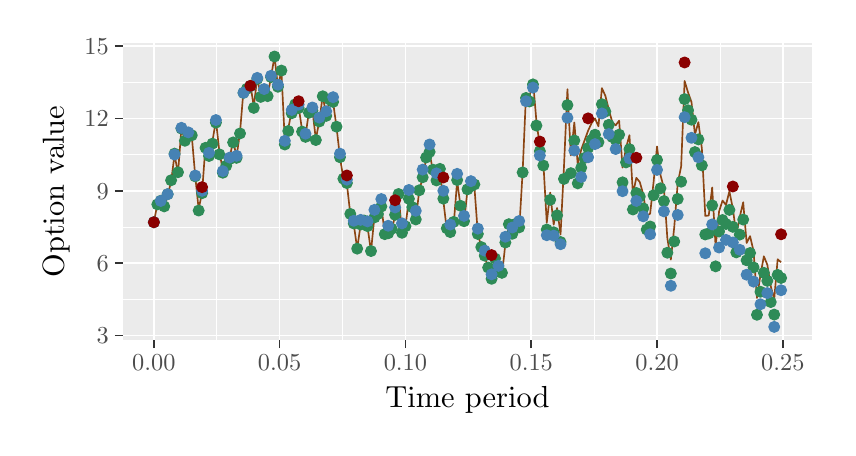
\begin{tikzpicture}[x=1pt,y=1pt]
\definecolor{fillColor}{RGB}{255,255,255}
\path[use as bounding box,fill=fillColor,fill opacity=0.00] (0,0) rectangle (289.08,144.54);
\begin{scope}
\path[clip] (  0.00,  0.00) rectangle (289.08,144.54);
\definecolor{drawColor}{RGB}{255,255,255}
\definecolor{fillColor}{RGB}{255,255,255}

\path[draw=drawColor,line width= 0.6pt,line join=round,line cap=round,fill=fillColor] (  0.00,  0.00) rectangle (289.08,144.54);
\end{scope}
\begin{scope}
\path[clip] ( 34.27, 31.53) rectangle (283.58,139.04);
\definecolor{fillColor}{gray}{0.92}

\path[fill=fillColor] ( 34.27, 31.53) rectangle (283.58,139.04);
\definecolor{drawColor}{RGB}{255,255,255}

\path[draw=drawColor,line width= 0.3pt,line join=round] ( 34.27, 46.37) --
	(283.58, 46.37);

\path[draw=drawColor,line width= 0.3pt,line join=round] ( 34.27, 72.52) --
	(283.58, 72.52);

\path[draw=drawColor,line width= 0.3pt,line join=round] ( 34.27, 98.68) --
	(283.58, 98.68);

\path[draw=drawColor,line width= 0.3pt,line join=round] ( 34.27,124.83) --
	(283.58,124.83);

\path[draw=drawColor,line width= 0.3pt,line join=round] ( 68.33, 31.53) --
	( 68.33,139.04);

\path[draw=drawColor,line width= 0.3pt,line join=round] (113.78, 31.53) --
	(113.78,139.04);

\path[draw=drawColor,line width= 0.3pt,line join=round] (159.24, 31.53) --
	(159.24,139.04);

\path[draw=drawColor,line width= 0.3pt,line join=round] (204.69, 31.53) --
	(204.69,139.04);

\path[draw=drawColor,line width= 0.3pt,line join=round] (250.14, 31.53) --
	(250.14,139.04);

\path[draw=drawColor,line width= 0.6pt,line join=round] ( 34.27, 33.29) --
	(283.58, 33.29);

\path[draw=drawColor,line width= 0.6pt,line join=round] ( 34.27, 59.45) --
	(283.58, 59.45);

\path[draw=drawColor,line width= 0.6pt,line join=round] ( 34.27, 85.60) --
	(283.58, 85.60);

\path[draw=drawColor,line width= 0.6pt,line join=round] ( 34.27,111.76) --
	(283.58,111.76);

\path[draw=drawColor,line width= 0.6pt,line join=round] ( 34.27,137.91) --
	(283.58,137.91);

\path[draw=drawColor,line width= 0.6pt,line join=round] ( 45.60, 31.53) --
	( 45.60,139.04);

\path[draw=drawColor,line width= 0.6pt,line join=round] ( 91.05, 31.53) --
	( 91.05,139.04);

\path[draw=drawColor,line width= 0.6pt,line join=round] (136.51, 31.53) --
	(136.51,139.04);

\path[draw=drawColor,line width= 0.6pt,line join=round] (181.96, 31.53) --
	(181.96,139.04);

\path[draw=drawColor,line width= 0.6pt,line join=round] (227.42, 31.53) --
	(227.42,139.04);

\path[draw=drawColor,line width= 0.6pt,line join=round] (272.87, 31.53) --
	(272.87,139.04);
\definecolor{drawColor}{RGB}{139,69,19}

\path[draw=drawColor,line width= 0.6pt,line join=round] ( 45.60, 74.23) --
	( 46.85, 80.70) --
	( 48.09, 81.83) --
	( 49.34, 79.64) --
	( 50.58, 83.95) --
	( 51.83, 88.90) --
	( 53.07, 98.64) --
	( 54.32, 91.88) --
	( 55.56,108.24) --
	( 56.81,103.72) --
	( 58.05,106.27) --
	( 59.30,105.40) --
	( 60.54, 90.94) --
	( 61.79, 78.90) --
	( 63.03, 85.15) --
	( 64.28,102.30) --
	( 65.53, 99.18) --
	( 66.77,103.53) --
	( 68.02,111.08) --
	( 69.26, 99.77) --
	( 70.51, 93.07) --
	( 71.75, 95.43) --
	( 73.00, 97.69) --
	( 74.24,103.63) --
	( 75.49, 97.96) --
	( 76.73,106.82) --
	( 77.98,121.83) --
	( 79.22,123.15) --
	( 80.47,123.95) --
	( 81.71,116.04) --
	( 82.96,126.58) --
	( 84.20,119.99) --
	( 85.45,122.26) --
	( 86.70,119.96) --
	( 87.94,126.78) --
	( 89.19,134.15) --
	( 90.43,123.26) --
	( 91.68,129.02) --
	( 92.92,103.42) --
	( 94.17,108.18) --
	( 95.41,114.53) --
	( 96.66,117.59) --
	( 97.90,116.11) --
	( 99.15,107.54) --
	(100.39,105.48) --
	(101.64,114.19) --
	(102.88,114.84) --
	(104.13,104.23) --
	(105.38,110.86) --
	(106.62,119.99) --
	(107.87,112.82) --
	(109.11,118.65) --
	(110.36,117.61) --
	(111.60,108.63) --
	(112.85, 97.68) --
	(114.09, 89.88) --
	(115.34, 88.13) --
	(116.58, 77.18) --
	(117.83, 73.56) --
	(119.07, 64.61) --
	(120.32, 73.49) --
	(121.56, 74.73) --
	(122.81, 72.52) --
	(124.06, 63.64) --
	(125.30, 76.33) --
	(126.55, 77.36) --
	(127.79, 79.88) --
	(129.04, 70.05) --
	(130.28, 70.14) --
	(131.53, 71.56) --
	(132.77, 76.51) --
	(134.02, 84.03) --
	(135.26, 70.46) --
	(136.51, 72.62) --
	(137.75, 82.73) --
	(139.00, 79.54) --
	(140.24, 74.94) --
	(141.49, 85.69) --
	(142.73, 90.27) --
	(143.98, 97.35) --
	(145.23, 99.18) --
	(146.47, 92.66) --
	(147.72, 88.61) --
	(148.96, 92.62) --
	(150.21, 81.97) --
	(151.45, 71.43) --
	(152.70, 69.82) --
	(153.94, 73.34) --
	(155.19, 89.13) --
	(156.43, 79.85) --
	(157.68, 74.16) --
	(158.92, 85.95) --
	(160.17, 86.86) --
	(161.41, 87.29) --
	(162.66, 70.14) --
	(163.91, 65.24) --
	(165.15, 61.96) --
	(166.40, 57.48) --
	(167.64, 53.27) --
	(168.89, 60.68) --
	(170.13, 55.88) --
	(171.38, 55.12) --
	(172.62, 66.53) --
	(173.87, 73.11) --
	(175.11, 69.42) --
	(176.36, 72.84) --
	(177.60, 71.31) --
	(178.85, 92.43) --
	(180.09,120.86) --
	(181.34,119.43) --
	(182.58,125.49) --
	(183.83,110.75) --
	(185.08,101.46) --
	(186.32, 96.11) --
	(187.57, 74.04) --
	(188.81, 84.95) --
	(190.06, 73.38) --
	(191.30, 79.38) --
	(192.55, 69.78) --
	(193.79, 94.29) --
	(195.04,122.29) --
	(196.28, 98.37) --
	(197.53,110.29) --
	(198.77, 95.00) --
	(200.02,100.47) --
	(201.26,103.88) --
	(202.51,107.32) --
	(203.76,110.01) --
	(205.00,111.75) --
	(206.25,108.88) --
	(207.49,122.71) --
	(208.74,119.93) --
	(209.98,114.99) --
	(211.23,110.45) --
	(212.47,109.25) --
	(213.72,110.95) --
	(214.96, 93.96) --
	(216.21,101.08) --
	(217.45,105.70) --
	(218.70, 84.47) --
	(219.94, 90.28) --
	(221.19, 88.76) --
	(222.44, 84.29) --
	(223.68, 76.53) --
	(224.93, 77.36) --
	(226.17, 88.74) --
	(227.42,101.62) --
	(228.66, 91.33) --
	(229.91, 86.52) --
	(231.15, 68.37) --
	(232.40, 60.72) --
	(233.64, 72.52) --
	(234.89, 88.31) --
	(236.13, 94.42) --
	(237.38,125.27) --
	(238.62,121.15) --
	(239.87,117.64) --
	(241.11,105.91) --
	(242.36,110.41) --
	(243.61,100.95) --
	(244.85, 76.53) --
	(246.10, 76.66) --
	(247.34, 86.80) --
	(248.59, 65.31) --
	(249.83, 78.09) --
	(251.08, 82.08) --
	(252.32, 80.46) --
	(253.57, 85.42) --
	(254.81, 79.15) --
	(256.06, 69.81) --
	(257.30, 76.13) --
	(258.55, 81.44) --
	(259.79, 66.75) --
	(261.04, 69.20) --
	(262.29, 63.80) --
	(263.53, 46.88) --
	(264.78, 55.16) --
	(266.02, 61.92) --
	(267.27, 58.89) --
	(268.51, 51.10) --
	(269.76, 46.42) --
	(271.00, 60.86) --
	(272.25, 59.74);
\definecolor{drawColor}{RGB}{46,139,87}
\definecolor{fillColor}{RGB}{46,139,87}

\path[draw=drawColor,line width= 0.4pt,line join=round,line cap=round,fill=fillColor] ( 45.60, 74.23) circle (  1.96);

\path[draw=drawColor,line width= 0.4pt,line join=round,line cap=round,fill=fillColor] ( 46.85, 80.69) circle (  1.96);

\path[draw=drawColor,line width= 0.4pt,line join=round,line cap=round,fill=fillColor] ( 48.09, 81.99) circle (  1.96);

\path[draw=drawColor,line width= 0.4pt,line join=round,line cap=round,fill=fillColor] ( 49.34, 79.96) circle (  1.96);

\path[draw=drawColor,line width= 0.4pt,line join=round,line cap=round,fill=fillColor] ( 50.58, 84.37) circle (  1.96);

\path[draw=drawColor,line width= 0.4pt,line join=round,line cap=round,fill=fillColor] ( 51.83, 89.40) circle (  1.96);

\path[draw=drawColor,line width= 0.4pt,line join=round,line cap=round,fill=fillColor] ( 53.07, 99.02) circle (  1.96);

\path[draw=drawColor,line width= 0.4pt,line join=round,line cap=round,fill=fillColor] ( 54.32, 92.30) circle (  1.96);

\path[draw=drawColor,line width= 0.4pt,line join=round,line cap=round,fill=fillColor] ( 55.56,108.07) circle (  1.96);

\path[draw=drawColor,line width= 0.4pt,line join=round,line cap=round,fill=fillColor] ( 56.81,103.66) circle (  1.96);

\path[draw=drawColor,line width= 0.4pt,line join=round,line cap=round,fill=fillColor] ( 58.05,106.37) circle (  1.96);

\path[draw=drawColor,line width= 0.4pt,line join=round,line cap=round,fill=fillColor] ( 59.30,105.66) circle (  1.96);

\path[draw=drawColor,line width= 0.4pt,line join=round,line cap=round,fill=fillColor] ( 60.54, 90.81) circle (  1.96);

\path[draw=drawColor,line width= 0.4pt,line join=round,line cap=round,fill=fillColor] ( 61.79, 78.46) circle (  1.96);

\path[draw=drawColor,line width= 0.4pt,line join=round,line cap=round,fill=fillColor] ( 63.03, 84.73) circle (  1.96);

\path[draw=drawColor,line width= 0.4pt,line join=round,line cap=round,fill=fillColor] ( 64.28,101.13) circle (  1.96);

\path[draw=drawColor,line width= 0.4pt,line join=round,line cap=round,fill=fillColor] ( 65.53, 98.17) circle (  1.96);

\path[draw=drawColor,line width= 0.4pt,line join=round,line cap=round,fill=fillColor] ( 66.77,102.63) circle (  1.96);

\path[draw=drawColor,line width= 0.4pt,line join=round,line cap=round,fill=fillColor] ( 68.02,110.21) circle (  1.96);

\path[draw=drawColor,line width= 0.4pt,line join=round,line cap=round,fill=fillColor] ( 69.26, 98.76) circle (  1.96);

\path[draw=drawColor,line width= 0.4pt,line join=round,line cap=round,fill=fillColor] ( 70.51, 92.11) circle (  1.96);

\path[draw=drawColor,line width= 0.4pt,line join=round,line cap=round,fill=fillColor] ( 71.75, 94.64) circle (  1.96);

\path[draw=drawColor,line width= 0.4pt,line join=round,line cap=round,fill=fillColor] ( 73.00, 97.05) circle (  1.96);

\path[draw=drawColor,line width= 0.4pt,line join=round,line cap=round,fill=fillColor] ( 74.24,103.07) circle (  1.96);

\path[draw=drawColor,line width= 0.4pt,line join=round,line cap=round,fill=fillColor] ( 75.49, 97.50) circle (  1.96);

\path[draw=drawColor,line width= 0.4pt,line join=round,line cap=round,fill=fillColor] ( 76.73,106.32) circle (  1.96);

\path[draw=drawColor,line width= 0.4pt,line join=round,line cap=round,fill=fillColor] ( 77.98,120.98) circle (  1.96);

\path[draw=drawColor,line width= 0.4pt,line join=round,line cap=round,fill=fillColor] ( 79.22,122.46) circle (  1.96);

\path[draw=drawColor,line width= 0.4pt,line join=round,line cap=round,fill=fillColor] ( 80.47,123.42) circle (  1.96);

\path[draw=drawColor,line width= 0.4pt,line join=round,line cap=round,fill=fillColor] ( 81.71,115.55) circle (  1.96);

\path[draw=drawColor,line width= 0.4pt,line join=round,line cap=round,fill=fillColor] ( 82.96,126.03) circle (  1.96);

\path[draw=drawColor,line width= 0.4pt,line join=round,line cap=round,fill=fillColor] ( 84.20,119.52) circle (  1.96);

\path[draw=drawColor,line width= 0.4pt,line join=round,line cap=round,fill=fillColor] ( 85.45,121.95) circle (  1.96);

\path[draw=drawColor,line width= 0.4pt,line join=round,line cap=round,fill=fillColor] ( 86.70,119.80) circle (  1.96);

\path[draw=drawColor,line width= 0.4pt,line join=round,line cap=round,fill=fillColor] ( 87.94,126.69) circle (  1.96);

\path[draw=drawColor,line width= 0.4pt,line join=round,line cap=round,fill=fillColor] ( 89.19,134.11) circle (  1.96);

\path[draw=drawColor,line width= 0.4pt,line join=round,line cap=round,fill=fillColor] ( 90.43,123.18) circle (  1.96);

\path[draw=drawColor,line width= 0.4pt,line join=round,line cap=round,fill=fillColor] ( 91.68,129.04) circle (  1.96);

\path[draw=drawColor,line width= 0.4pt,line join=round,line cap=round,fill=fillColor] ( 92.92,102.32) circle (  1.96);

\path[draw=drawColor,line width= 0.4pt,line join=round,line cap=round,fill=fillColor] ( 94.17,107.20) circle (  1.96);

\path[draw=drawColor,line width= 0.4pt,line join=round,line cap=round,fill=fillColor] ( 95.41,113.62) circle (  1.96);

\path[draw=drawColor,line width= 0.4pt,line join=round,line cap=round,fill=fillColor] ( 96.66,116.83) circle (  1.96);

\path[draw=drawColor,line width= 0.4pt,line join=round,line cap=round,fill=fillColor] ( 97.90,115.51) circle (  1.96);

\path[draw=drawColor,line width= 0.4pt,line join=round,line cap=round,fill=fillColor] ( 99.15,106.98) circle (  1.96);

\path[draw=drawColor,line width= 0.4pt,line join=round,line cap=round,fill=fillColor] (100.39,105.08) circle (  1.96);

\path[draw=drawColor,line width= 0.4pt,line join=round,line cap=round,fill=fillColor] (101.64,113.79) circle (  1.96);

\path[draw=drawColor,line width= 0.4pt,line join=round,line cap=round,fill=fillColor] (102.88,114.61) circle (  1.96);

\path[draw=drawColor,line width= 0.4pt,line join=round,line cap=round,fill=fillColor] (104.13,103.93) circle (  1.96);

\path[draw=drawColor,line width= 0.4pt,line join=round,line cap=round,fill=fillColor] (105.38,110.63) circle (  1.96);

\path[draw=drawColor,line width= 0.4pt,line join=round,line cap=round,fill=fillColor] (106.62,119.75) circle (  1.96);

\path[draw=drawColor,line width= 0.4pt,line join=round,line cap=round,fill=fillColor] (107.87,112.66) circle (  1.96);

\path[draw=drawColor,line width= 0.4pt,line join=round,line cap=round,fill=fillColor] (109.11,118.59) circle (  1.96);

\path[draw=drawColor,line width= 0.4pt,line join=round,line cap=round,fill=fillColor] (110.36,117.72) circle (  1.96);

\path[draw=drawColor,line width= 0.4pt,line join=round,line cap=round,fill=fillColor] (111.60,108.76) circle (  1.96);

\path[draw=drawColor,line width= 0.4pt,line join=round,line cap=round,fill=fillColor] (112.85, 97.71) circle (  1.96);

\path[draw=drawColor,line width= 0.4pt,line join=round,line cap=round,fill=fillColor] (114.09, 89.95) circle (  1.96);

\path[draw=drawColor,line width= 0.4pt,line join=round,line cap=round,fill=fillColor] (115.34, 88.39) circle (  1.96);

\path[draw=drawColor,line width= 0.4pt,line join=round,line cap=round,fill=fillColor] (116.58, 77.24) circle (  1.96);

\path[draw=drawColor,line width= 0.4pt,line join=round,line cap=round,fill=fillColor] (117.83, 73.79) circle (  1.96);

\path[draw=drawColor,line width= 0.4pt,line join=round,line cap=round,fill=fillColor] (119.07, 64.69) circle (  1.96);

\path[draw=drawColor,line width= 0.4pt,line join=round,line cap=round,fill=fillColor] (120.32, 73.41) circle (  1.96);

\path[draw=drawColor,line width= 0.4pt,line join=round,line cap=round,fill=fillColor] (121.56, 74.85) circle (  1.96);

\path[draw=drawColor,line width= 0.4pt,line join=round,line cap=round,fill=fillColor] (122.81, 72.83) circle (  1.96);

\path[draw=drawColor,line width= 0.4pt,line join=round,line cap=round,fill=fillColor] (124.06, 63.82) circle (  1.96);

\path[draw=drawColor,line width= 0.4pt,line join=round,line cap=round,fill=fillColor] (125.30, 75.97) circle (  1.96);

\path[draw=drawColor,line width= 0.4pt,line join=round,line cap=round,fill=fillColor] (126.55, 77.21) circle (  1.96);

\path[draw=drawColor,line width= 0.4pt,line join=round,line cap=round,fill=fillColor] (127.79, 79.91) circle (  1.96);

\path[draw=drawColor,line width= 0.4pt,line join=round,line cap=round,fill=fillColor] (129.04, 69.93) circle (  1.96);

\path[draw=drawColor,line width= 0.4pt,line join=round,line cap=round,fill=fillColor] (130.28, 70.24) circle (  1.96);

\path[draw=drawColor,line width= 0.4pt,line join=round,line cap=round,fill=fillColor] (131.53, 71.86) circle (  1.96);

\path[draw=drawColor,line width= 0.4pt,line join=round,line cap=round,fill=fillColor] (132.77, 76.91) circle (  1.96);

\path[draw=drawColor,line width= 0.4pt,line join=round,line cap=round,fill=fillColor] (134.02, 84.43) circle (  1.96);

\path[draw=drawColor,line width= 0.4pt,line join=round,line cap=round,fill=fillColor] (135.26, 70.42) circle (  1.96);

\path[draw=drawColor,line width= 0.4pt,line join=round,line cap=round,fill=fillColor] (136.51, 72.77) circle (  1.96);

\path[draw=drawColor,line width= 0.4pt,line join=round,line cap=round,fill=fillColor] (137.75, 82.69) circle (  1.96);

\path[draw=drawColor,line width= 0.4pt,line join=round,line cap=round,fill=fillColor] (139.00, 79.68) circle (  1.96);

\path[draw=drawColor,line width= 0.4pt,line join=round,line cap=round,fill=fillColor] (140.24, 75.24) circle (  1.96);

\path[draw=drawColor,line width= 0.4pt,line join=round,line cap=round,fill=fillColor] (141.49, 85.77) circle (  1.96);

\path[draw=drawColor,line width= 0.4pt,line join=round,line cap=round,fill=fillColor] (142.73, 90.48) circle (  1.96);

\path[draw=drawColor,line width= 0.4pt,line join=round,line cap=round,fill=fillColor] (143.98, 97.62) circle (  1.96);

\path[draw=drawColor,line width= 0.4pt,line join=round,line cap=round,fill=fillColor] (145.23, 99.65) circle (  1.96);

\path[draw=drawColor,line width= 0.4pt,line join=round,line cap=round,fill=fillColor] (146.47, 93.22) circle (  1.96);

\path[draw=drawColor,line width= 0.4pt,line join=round,line cap=round,fill=fillColor] (147.72, 89.34) circle (  1.96);

\path[draw=drawColor,line width= 0.4pt,line join=round,line cap=round,fill=fillColor] (148.96, 93.52) circle (  1.96);

\path[draw=drawColor,line width= 0.4pt,line join=round,line cap=round,fill=fillColor] (150.21, 82.76) circle (  1.96);

\path[draw=drawColor,line width= 0.4pt,line join=round,line cap=round,fill=fillColor] (151.45, 72.05) circle (  1.96);

\path[draw=drawColor,line width= 0.4pt,line join=round,line cap=round,fill=fillColor] (152.70, 70.67) circle (  1.96);

\path[draw=drawColor,line width= 0.4pt,line join=round,line cap=round,fill=fillColor] (153.94, 74.36) circle (  1.96);

\path[draw=drawColor,line width= 0.4pt,line join=round,line cap=round,fill=fillColor] (155.19, 89.48) circle (  1.96);

\path[draw=drawColor,line width= 0.4pt,line join=round,line cap=round,fill=fillColor] (156.43, 80.17) circle (  1.96);

\path[draw=drawColor,line width= 0.4pt,line join=round,line cap=round,fill=fillColor] (157.68, 74.61) circle (  1.96);

\path[draw=drawColor,line width= 0.4pt,line join=round,line cap=round,fill=fillColor] (158.92, 86.12) circle (  1.96);

\path[draw=drawColor,line width= 0.4pt,line join=round,line cap=round,fill=fillColor] (160.17, 87.24) circle (  1.96);

\path[draw=drawColor,line width= 0.4pt,line join=round,line cap=round,fill=fillColor] (161.41, 87.89) circle (  1.96);

\path[draw=drawColor,line width= 0.4pt,line join=round,line cap=round,fill=fillColor] (162.66, 69.99) circle (  1.96);

\path[draw=drawColor,line width= 0.4pt,line join=round,line cap=round,fill=fillColor] (163.91, 65.25) circle (  1.96);

\path[draw=drawColor,line width= 0.4pt,line join=round,line cap=round,fill=fillColor] (165.15, 62.17) circle (  1.96);

\path[draw=drawColor,line width= 0.4pt,line join=round,line cap=round,fill=fillColor] (166.40, 57.85) circle (  1.96);

\path[draw=drawColor,line width= 0.4pt,line join=round,line cap=round,fill=fillColor] (167.64, 53.79) circle (  1.96);

\path[draw=drawColor,line width= 0.4pt,line join=round,line cap=round,fill=fillColor] (168.89, 61.11) circle (  1.96);

\path[draw=drawColor,line width= 0.4pt,line join=round,line cap=round,fill=fillColor] (170.13, 56.46) circle (  1.96);

\path[draw=drawColor,line width= 0.4pt,line join=round,line cap=round,fill=fillColor] (171.38, 55.95) circle (  1.96);

\path[draw=drawColor,line width= 0.4pt,line join=round,line cap=round,fill=fillColor] (172.62, 66.91) circle (  1.96);

\path[draw=drawColor,line width= 0.4pt,line join=round,line cap=round,fill=fillColor] (173.87, 73.53) circle (  1.96);

\path[draw=drawColor,line width= 0.4pt,line join=round,line cap=round,fill=fillColor] (175.11, 70.05) circle (  1.96);

\path[draw=drawColor,line width= 0.4pt,line join=round,line cap=round,fill=fillColor] (176.36, 73.66) circle (  1.96);

\path[draw=drawColor,line width= 0.4pt,line join=round,line cap=round,fill=fillColor] (177.60, 72.38) circle (  1.96);

\path[draw=drawColor,line width= 0.4pt,line join=round,line cap=round,fill=fillColor] (178.85, 92.23) circle (  1.96);

\path[draw=drawColor,line width= 0.4pt,line join=round,line cap=round,fill=fillColor] (180.09,119.14) circle (  1.96);

\path[draw=drawColor,line width= 0.4pt,line join=round,line cap=round,fill=fillColor] (181.34,117.87) circle (  1.96);

\path[draw=drawColor,line width= 0.4pt,line join=round,line cap=round,fill=fillColor] (182.58,124.04) circle (  1.96);

\path[draw=drawColor,line width= 0.4pt,line join=round,line cap=round,fill=fillColor] (183.83,109.16) circle (  1.96);

\path[draw=drawColor,line width= 0.4pt,line join=round,line cap=round,fill=fillColor] (185.08, 99.93) circle (  1.96);

\path[draw=drawColor,line width= 0.4pt,line join=round,line cap=round,fill=fillColor] (186.32, 94.73) circle (  1.96);

\path[draw=drawColor,line width= 0.4pt,line join=round,line cap=round,fill=fillColor] (187.57, 71.59) circle (  1.96);

\path[draw=drawColor,line width= 0.4pt,line join=round,line cap=round,fill=fillColor] (188.81, 82.33) circle (  1.96);

\path[draw=drawColor,line width= 0.4pt,line join=round,line cap=round,fill=fillColor] (190.06, 70.61) circle (  1.96);

\path[draw=drawColor,line width= 0.4pt,line join=round,line cap=round,fill=fillColor] (191.30, 76.72) circle (  1.96);

\path[draw=drawColor,line width= 0.4pt,line join=round,line cap=round,fill=fillColor] (192.55, 67.09) circle (  1.96);

\path[draw=drawColor,line width= 0.4pt,line join=round,line cap=round,fill=fillColor] (193.79, 89.88) circle (  1.96);

\path[draw=drawColor,line width= 0.4pt,line join=round,line cap=round,fill=fillColor] (195.04,116.55) circle (  1.96);

\path[draw=drawColor,line width= 0.4pt,line join=round,line cap=round,fill=fillColor] (196.28, 91.96) circle (  1.96);

\path[draw=drawColor,line width= 0.4pt,line join=round,line cap=round,fill=fillColor] (197.53,103.78) circle (  1.96);

\path[draw=drawColor,line width= 0.4pt,line join=round,line cap=round,fill=fillColor] (198.77, 88.29) circle (  1.96);

\path[draw=drawColor,line width= 0.4pt,line join=round,line cap=round,fill=fillColor] (200.02, 93.90) circle (  1.96);

\path[draw=drawColor,line width= 0.4pt,line join=round,line cap=round,fill=fillColor] (201.26, 97.48) circle (  1.96);

\path[draw=drawColor,line width= 0.4pt,line join=round,line cap=round,fill=fillColor] (202.51,101.08) circle (  1.96);

\path[draw=drawColor,line width= 0.4pt,line join=round,line cap=round,fill=fillColor] (203.76,103.95) circle (  1.96);

\path[draw=drawColor,line width= 0.4pt,line join=round,line cap=round,fill=fillColor] (205.00,105.86) circle (  1.96);

\path[draw=drawColor,line width= 0.4pt,line join=round,line cap=round,fill=fillColor] (206.25,103.16) circle (  1.96);

\path[draw=drawColor,line width= 0.4pt,line join=round,line cap=round,fill=fillColor] (207.49,116.87) circle (  1.96);

\path[draw=drawColor,line width= 0.4pt,line join=round,line cap=round,fill=fillColor] (208.74,114.23) circle (  1.96);

\path[draw=drawColor,line width= 0.4pt,line join=round,line cap=round,fill=fillColor] (209.98,109.43) circle (  1.96);

\path[draw=drawColor,line width= 0.4pt,line join=round,line cap=round,fill=fillColor] (211.23,105.04) circle (  1.96);

\path[draw=drawColor,line width= 0.4pt,line join=round,line cap=round,fill=fillColor] (212.47,104.02) circle (  1.96);

\path[draw=drawColor,line width= 0.4pt,line join=round,line cap=round,fill=fillColor] (213.72,105.88) circle (  1.96);

\path[draw=drawColor,line width= 0.4pt,line join=round,line cap=round,fill=fillColor] (214.96, 88.65) circle (  1.96);

\path[draw=drawColor,line width= 0.4pt,line join=round,line cap=round,fill=fillColor] (216.21, 95.87) circle (  1.96);

\path[draw=drawColor,line width= 0.4pt,line join=round,line cap=round,fill=fillColor] (217.45,100.64) circle (  1.96);

\path[draw=drawColor,line width= 0.4pt,line join=round,line cap=round,fill=fillColor] (218.70, 78.84) circle (  1.96);

\path[draw=drawColor,line width= 0.4pt,line join=round,line cap=round,fill=fillColor] (219.94, 84.80) circle (  1.96);

\path[draw=drawColor,line width= 0.4pt,line join=round,line cap=round,fill=fillColor] (221.19, 83.50) circle (  1.96);

\path[draw=drawColor,line width= 0.4pt,line join=round,line cap=round,fill=fillColor] (222.44, 79.24) circle (  1.96);

\path[draw=drawColor,line width= 0.4pt,line join=round,line cap=round,fill=fillColor] (223.68, 71.60) circle (  1.96);

\path[draw=drawColor,line width= 0.4pt,line join=round,line cap=round,fill=fillColor] (224.93, 72.71) circle (  1.96);

\path[draw=drawColor,line width= 0.4pt,line join=round,line cap=round,fill=fillColor] (226.17, 83.98) circle (  1.96);

\path[draw=drawColor,line width= 0.4pt,line join=round,line cap=round,fill=fillColor] (227.42, 96.73) circle (  1.96);

\path[draw=drawColor,line width= 0.4pt,line join=round,line cap=round,fill=fillColor] (228.66, 86.49) circle (  1.96);

\path[draw=drawColor,line width= 0.4pt,line join=round,line cap=round,fill=fillColor] (229.91, 81.87) circle (  1.96);

\path[draw=drawColor,line width= 0.4pt,line join=round,line cap=round,fill=fillColor] (231.15, 63.22) circle (  1.96);

\path[draw=drawColor,line width= 0.4pt,line join=round,line cap=round,fill=fillColor] (232.40, 55.71) circle (  1.96);

\path[draw=drawColor,line width= 0.4pt,line join=round,line cap=round,fill=fillColor] (233.64, 67.27) circle (  1.96);

\path[draw=drawColor,line width= 0.4pt,line join=round,line cap=round,fill=fillColor] (234.89, 82.64) circle (  1.96);

\path[draw=drawColor,line width= 0.4pt,line join=round,line cap=round,fill=fillColor] (236.13, 88.88) circle (  1.96);

\path[draw=drawColor,line width= 0.4pt,line join=round,line cap=round,fill=fillColor] (237.38,118.72) circle (  1.96);

\path[draw=drawColor,line width= 0.4pt,line join=round,line cap=round,fill=fillColor] (238.62,114.69) circle (  1.96);

\path[draw=drawColor,line width= 0.4pt,line join=round,line cap=round,fill=fillColor] (239.87,111.27) circle (  1.96);

\path[draw=drawColor,line width= 0.4pt,line join=round,line cap=round,fill=fillColor] (241.11, 99.58) circle (  1.96);

\path[draw=drawColor,line width= 0.4pt,line join=round,line cap=round,fill=fillColor] (242.36,104.17) circle (  1.96);

\path[draw=drawColor,line width= 0.4pt,line join=round,line cap=round,fill=fillColor] (243.61, 94.78) circle (  1.96);

\path[draw=drawColor,line width= 0.4pt,line join=round,line cap=round,fill=fillColor] (244.85, 69.81) circle (  1.96);

\path[draw=drawColor,line width= 0.4pt,line join=round,line cap=round,fill=fillColor] (246.10, 70.19) circle (  1.96);

\path[draw=drawColor,line width= 0.4pt,line join=round,line cap=round,fill=fillColor] (247.34, 80.32) circle (  1.96);

\path[draw=drawColor,line width= 0.4pt,line join=round,line cap=round,fill=fillColor] (248.59, 58.29) circle (  1.96);

\path[draw=drawColor,line width= 0.4pt,line join=round,line cap=round,fill=fillColor] (249.83, 70.87) circle (  1.96);

\path[draw=drawColor,line width= 0.4pt,line join=round,line cap=round,fill=fillColor] (251.08, 75.03) circle (  1.96);

\path[draw=drawColor,line width= 0.4pt,line join=round,line cap=round,fill=fillColor] (252.32, 73.61) circle (  1.96);

\path[draw=drawColor,line width= 0.4pt,line join=round,line cap=round,fill=fillColor] (253.57, 78.69) circle (  1.96);

\path[draw=drawColor,line width= 0.4pt,line join=round,line cap=round,fill=fillColor] (254.81, 72.57) circle (  1.96);

\path[draw=drawColor,line width= 0.4pt,line join=round,line cap=round,fill=fillColor] (256.06, 63.34) circle (  1.96);

\path[draw=drawColor,line width= 0.4pt,line join=round,line cap=round,fill=fillColor] (257.30, 69.77) circle (  1.96);

\path[draw=drawColor,line width= 0.4pt,line join=round,line cap=round,fill=fillColor] (258.55, 75.19) circle (  1.96);

\path[draw=drawColor,line width= 0.4pt,line join=round,line cap=round,fill=fillColor] (259.79, 60.48) circle (  1.96);

\path[draw=drawColor,line width= 0.4pt,line join=round,line cap=round,fill=fillColor] (261.04, 63.12) circle (  1.96);

\path[draw=drawColor,line width= 0.4pt,line join=round,line cap=round,fill=fillColor] (262.29, 57.91) circle (  1.96);

\path[draw=drawColor,line width= 0.4pt,line join=round,line cap=round,fill=fillColor] (263.53, 40.79) circle (  1.96);

\path[draw=drawColor,line width= 0.4pt,line join=round,line cap=round,fill=fillColor] (264.78, 49.12) circle (  1.96);

\path[draw=drawColor,line width= 0.4pt,line join=round,line cap=round,fill=fillColor] (266.02, 55.95) circle (  1.96);

\path[draw=drawColor,line width= 0.4pt,line join=round,line cap=round,fill=fillColor] (267.27, 53.06) circle (  1.96);

\path[draw=drawColor,line width= 0.4pt,line join=round,line cap=round,fill=fillColor] (268.51, 45.39) circle (  1.96);

\path[draw=drawColor,line width= 0.4pt,line join=round,line cap=round,fill=fillColor] (269.76, 40.86) circle (  1.96);

\path[draw=drawColor,line width= 0.4pt,line join=round,line cap=round,fill=fillColor] (271.00, 55.20) circle (  1.96);

\path[draw=drawColor,line width= 0.4pt,line join=round,line cap=round,fill=fillColor] (272.25, 54.09) circle (  1.96);
\definecolor{drawColor}{RGB}{70,130,180}
\definecolor{fillColor}{RGB}{70,130,180}

\path[draw=drawColor,line width= 0.4pt,line join=round,line cap=round,fill=fillColor] ( 45.60, 74.23) circle (  1.96);

\path[draw=drawColor,line width= 0.4pt,line join=round,line cap=round,fill=fillColor] ( 48.09, 81.92) circle (  1.96);

\path[draw=drawColor,line width= 0.4pt,line join=round,line cap=round,fill=fillColor] ( 50.58, 84.37) circle (  1.96);

\path[draw=drawColor,line width= 0.4pt,line join=round,line cap=round,fill=fillColor] ( 53.07, 98.68) circle (  1.96);

\path[draw=drawColor,line width= 0.4pt,line join=round,line cap=round,fill=fillColor] ( 55.56,108.35) circle (  1.96);

\path[draw=drawColor,line width= 0.4pt,line join=round,line cap=round,fill=fillColor] ( 58.05,106.71) circle (  1.96);

\path[draw=drawColor,line width= 0.4pt,line join=round,line cap=round,fill=fillColor] ( 60.54, 91.11) circle (  1.96);

\path[draw=drawColor,line width= 0.4pt,line join=round,line cap=round,fill=fillColor] ( 63.03, 85.57) circle (  1.96);

\path[draw=drawColor,line width= 0.4pt,line join=round,line cap=round,fill=fillColor] ( 65.53, 99.31) circle (  1.96);

\path[draw=drawColor,line width= 0.4pt,line join=round,line cap=round,fill=fillColor] ( 68.02,111.16) circle (  1.96);

\path[draw=drawColor,line width= 0.4pt,line join=round,line cap=round,fill=fillColor] ( 70.51, 92.69) circle (  1.96);

\path[draw=drawColor,line width= 0.4pt,line join=round,line cap=round,fill=fillColor] ( 73.00, 97.59) circle (  1.96);

\path[draw=drawColor,line width= 0.4pt,line join=round,line cap=round,fill=fillColor] ( 75.49, 98.22) circle (  1.96);

\path[draw=drawColor,line width= 0.4pt,line join=round,line cap=round,fill=fillColor] ( 77.98,121.02) circle (  1.96);

\path[draw=drawColor,line width= 0.4pt,line join=round,line cap=round,fill=fillColor] ( 80.47,123.46) circle (  1.96);

\path[draw=drawColor,line width= 0.4pt,line join=round,line cap=round,fill=fillColor] ( 82.96,126.39) circle (  1.96);

\path[draw=drawColor,line width= 0.4pt,line join=round,line cap=round,fill=fillColor] ( 85.45,122.36) circle (  1.96);

\path[draw=drawColor,line width= 0.4pt,line join=round,line cap=round,fill=fillColor] ( 87.94,127.16) circle (  1.96);

\path[draw=drawColor,line width= 0.4pt,line join=round,line cap=round,fill=fillColor] ( 90.43,123.93) circle (  1.96);

\path[draw=drawColor,line width= 0.4pt,line join=round,line cap=round,fill=fillColor] ( 92.92,103.65) circle (  1.96);

\path[draw=drawColor,line width= 0.4pt,line join=round,line cap=round,fill=fillColor] ( 95.41,114.80) circle (  1.96);

\path[draw=drawColor,line width= 0.4pt,line join=round,line cap=round,fill=fillColor] ( 97.90,116.71) circle (  1.96);

\path[draw=drawColor,line width= 0.4pt,line join=round,line cap=round,fill=fillColor] (100.39,106.21) circle (  1.96);

\path[draw=drawColor,line width= 0.4pt,line join=round,line cap=round,fill=fillColor] (102.88,115.70) circle (  1.96);

\path[draw=drawColor,line width= 0.4pt,line join=round,line cap=round,fill=fillColor] (105.38,112.04) circle (  1.96);

\path[draw=drawColor,line width= 0.4pt,line join=round,line cap=round,fill=fillColor] (107.87,114.34) circle (  1.96);

\path[draw=drawColor,line width= 0.4pt,line join=round,line cap=round,fill=fillColor] (110.36,119.42) circle (  1.96);

\path[draw=drawColor,line width= 0.4pt,line join=round,line cap=round,fill=fillColor] (112.85, 99.01) circle (  1.96);

\path[draw=drawColor,line width= 0.4pt,line join=round,line cap=round,fill=fillColor] (115.34, 89.62) circle (  1.96);

\path[draw=drawColor,line width= 0.4pt,line join=round,line cap=round,fill=fillColor] (117.83, 74.75) circle (  1.96);

\path[draw=drawColor,line width= 0.4pt,line join=round,line cap=round,fill=fillColor] (120.32, 75.09) circle (  1.96);

\path[draw=drawColor,line width= 0.4pt,line join=round,line cap=round,fill=fillColor] (122.81, 74.54) circle (  1.96);

\path[draw=drawColor,line width= 0.4pt,line join=round,line cap=round,fill=fillColor] (125.30, 78.70) circle (  1.96);

\path[draw=drawColor,line width= 0.4pt,line join=round,line cap=round,fill=fillColor] (127.79, 82.61) circle (  1.96);

\path[draw=drawColor,line width= 0.4pt,line join=round,line cap=round,fill=fillColor] (130.28, 72.96) circle (  1.96);

\path[draw=drawColor,line width= 0.4pt,line join=round,line cap=round,fill=fillColor] (132.77, 79.56) circle (  1.96);

\path[draw=drawColor,line width= 0.4pt,line join=round,line cap=round,fill=fillColor] (135.26, 73.83) circle (  1.96);

\path[draw=drawColor,line width= 0.4pt,line join=round,line cap=round,fill=fillColor] (137.75, 85.90) circle (  1.96);

\path[draw=drawColor,line width= 0.4pt,line join=round,line cap=round,fill=fillColor] (140.24, 78.36) circle (  1.96);

\path[draw=drawColor,line width= 0.4pt,line join=round,line cap=round,fill=fillColor] (142.73, 93.25) circle (  1.96);

\path[draw=drawColor,line width= 0.4pt,line join=round,line cap=round,fill=fillColor] (145.23,102.33) circle (  1.96);

\path[draw=drawColor,line width= 0.4pt,line join=round,line cap=round,fill=fillColor] (147.72, 91.90) circle (  1.96);

\path[draw=drawColor,line width= 0.4pt,line join=round,line cap=round,fill=fillColor] (150.21, 85.59) circle (  1.96);

\path[draw=drawColor,line width= 0.4pt,line join=round,line cap=round,fill=fillColor] (152.70, 73.39) circle (  1.96);

\path[draw=drawColor,line width= 0.4pt,line join=round,line cap=round,fill=fillColor] (155.19, 91.72) circle (  1.96);

\path[draw=drawColor,line width= 0.4pt,line join=round,line cap=round,fill=fillColor] (157.68, 76.53) circle (  1.96);

\path[draw=drawColor,line width= 0.4pt,line join=round,line cap=round,fill=fillColor] (160.17, 89.07) circle (  1.96);

\path[draw=drawColor,line width= 0.4pt,line join=round,line cap=round,fill=fillColor] (162.66, 71.92) circle (  1.96);

\path[draw=drawColor,line width= 0.4pt,line join=round,line cap=round,fill=fillColor] (165.15, 63.97) circle (  1.96);

\path[draw=drawColor,line width= 0.4pt,line join=round,line cap=round,fill=fillColor] (167.64, 55.40) circle (  1.96);

\path[draw=drawColor,line width= 0.4pt,line join=round,line cap=round,fill=fillColor] (170.13, 58.47) circle (  1.96);

\path[draw=drawColor,line width= 0.4pt,line join=round,line cap=round,fill=fillColor] (172.62, 68.98) circle (  1.96);

\path[draw=drawColor,line width= 0.4pt,line join=round,line cap=round,fill=fillColor] (175.11, 72.32) circle (  1.96);

\path[draw=drawColor,line width= 0.4pt,line join=round,line cap=round,fill=fillColor] (177.60, 74.68) circle (  1.96);

\path[draw=drawColor,line width= 0.4pt,line join=round,line cap=round,fill=fillColor] (180.09,117.97) circle (  1.96);

\path[draw=drawColor,line width= 0.4pt,line join=round,line cap=round,fill=fillColor] (182.58,122.88) circle (  1.96);

\path[draw=drawColor,line width= 0.4pt,line join=round,line cap=round,fill=fillColor] (185.08, 98.36) circle (  1.96);

\path[draw=drawColor,line width= 0.4pt,line join=round,line cap=round,fill=fillColor] (187.57, 69.54) circle (  1.96);

\path[draw=drawColor,line width= 0.4pt,line join=round,line cap=round,fill=fillColor] (190.06, 69.40) circle (  1.96);

\path[draw=drawColor,line width= 0.4pt,line join=round,line cap=round,fill=fillColor] (192.55, 66.30) circle (  1.96);

\path[draw=drawColor,line width= 0.4pt,line join=round,line cap=round,fill=fillColor] (195.04,111.97) circle (  1.96);

\path[draw=drawColor,line width= 0.4pt,line join=round,line cap=round,fill=fillColor] (197.53,100.15) circle (  1.96);

\path[draw=drawColor,line width= 0.4pt,line join=round,line cap=round,fill=fillColor] (200.02, 90.58) circle (  1.96);

\path[draw=drawColor,line width= 0.4pt,line join=round,line cap=round,fill=fillColor] (202.51, 97.71) circle (  1.96);

\path[draw=drawColor,line width= 0.4pt,line join=round,line cap=round,fill=fillColor] (205.00,102.47) circle (  1.96);

\path[draw=drawColor,line width= 0.4pt,line join=round,line cap=round,fill=fillColor] (207.49,113.55) circle (  1.96);

\path[draw=drawColor,line width= 0.4pt,line join=round,line cap=round,fill=fillColor] (209.98,106.09) circle (  1.96);

\path[draw=drawColor,line width= 0.4pt,line join=round,line cap=round,fill=fillColor] (212.47,100.68) circle (  1.96);

\path[draw=drawColor,line width= 0.4pt,line join=round,line cap=round,fill=fillColor] (214.96, 85.45) circle (  1.96);

\path[draw=drawColor,line width= 0.4pt,line join=round,line cap=round,fill=fillColor] (217.45, 97.30) circle (  1.96);

\path[draw=drawColor,line width= 0.4pt,line join=round,line cap=round,fill=fillColor] (219.94, 81.94) circle (  1.96);

\path[draw=drawColor,line width= 0.4pt,line join=round,line cap=round,fill=fillColor] (222.44, 76.37) circle (  1.96);

\path[draw=drawColor,line width= 0.4pt,line join=round,line cap=round,fill=fillColor] (224.93, 69.88) circle (  1.96);

\path[draw=drawColor,line width= 0.4pt,line join=round,line cap=round,fill=fillColor] (227.42, 93.16) circle (  1.96);

\path[draw=drawColor,line width= 0.4pt,line join=round,line cap=round,fill=fillColor] (229.91, 78.16) circle (  1.96);

\path[draw=drawColor,line width= 0.4pt,line join=round,line cap=round,fill=fillColor] (232.40, 51.27) circle (  1.96);

\path[draw=drawColor,line width= 0.4pt,line join=round,line cap=round,fill=fillColor] (234.89, 76.87) circle (  1.96);

\path[draw=drawColor,line width= 0.4pt,line join=round,line cap=round,fill=fillColor] (237.38,112.20) circle (  1.96);

\path[draw=drawColor,line width= 0.4pt,line join=round,line cap=round,fill=fillColor] (239.87,104.74) circle (  1.96);

\path[draw=drawColor,line width= 0.4pt,line join=round,line cap=round,fill=fillColor] (242.36, 97.70) circle (  1.96);

\path[draw=drawColor,line width= 0.4pt,line join=round,line cap=round,fill=fillColor] (244.85, 63.01) circle (  1.96);

\path[draw=drawColor,line width= 0.4pt,line join=round,line cap=round,fill=fillColor] (247.34, 73.45) circle (  1.96);

\path[draw=drawColor,line width= 0.4pt,line join=round,line cap=round,fill=fillColor] (249.83, 65.09) circle (  1.96);

\path[draw=drawColor,line width= 0.4pt,line join=round,line cap=round,fill=fillColor] (252.32, 67.86) circle (  1.96);

\path[draw=drawColor,line width= 0.4pt,line join=round,line cap=round,fill=fillColor] (254.81, 66.93) circle (  1.96);

\path[draw=drawColor,line width= 0.4pt,line join=round,line cap=round,fill=fillColor] (257.30, 64.28) circle (  1.96);

\path[draw=drawColor,line width= 0.4pt,line join=round,line cap=round,fill=fillColor] (259.79, 55.27) circle (  1.96);

\path[draw=drawColor,line width= 0.4pt,line join=round,line cap=round,fill=fillColor] (262.29, 52.78) circle (  1.96);

\path[draw=drawColor,line width= 0.4pt,line join=round,line cap=round,fill=fillColor] (264.78, 44.59) circle (  1.96);

\path[draw=drawColor,line width= 0.4pt,line join=round,line cap=round,fill=fillColor] (267.27, 48.62) circle (  1.96);

\path[draw=drawColor,line width= 0.4pt,line join=round,line cap=round,fill=fillColor] (269.76, 36.42) circle (  1.96);

\path[draw=drawColor,line width= 0.4pt,line join=round,line cap=round,fill=fillColor] (272.25, 49.66) circle (  1.96);
\definecolor{drawColor}{RGB}{139,0,0}
\definecolor{fillColor}{RGB}{139,0,0}

\path[draw=drawColor,line width= 0.4pt,line join=round,line cap=round,fill=fillColor] ( 45.60, 74.23) circle (  1.96);

\path[draw=drawColor,line width= 0.4pt,line join=round,line cap=round,fill=fillColor] ( 63.03, 86.91) circle (  1.96);

\path[draw=drawColor,line width= 0.4pt,line join=round,line cap=round,fill=fillColor] ( 80.47,123.53) circle (  1.96);

\path[draw=drawColor,line width= 0.4pt,line join=round,line cap=round,fill=fillColor] ( 97.90,117.96) circle (  1.96);

\path[draw=drawColor,line width= 0.4pt,line join=round,line cap=round,fill=fillColor] (115.34, 91.14) circle (  1.96);

\path[draw=drawColor,line width= 0.4pt,line join=round,line cap=round,fill=fillColor] (132.77, 82.18) circle (  1.96);

\path[draw=drawColor,line width= 0.4pt,line join=round,line cap=round,fill=fillColor] (150.21, 90.40) circle (  1.96);

\path[draw=drawColor,line width= 0.4pt,line join=round,line cap=round,fill=fillColor] (167.64, 62.36) circle (  1.96);

\path[draw=drawColor,line width= 0.4pt,line join=round,line cap=round,fill=fillColor] (185.08,103.38) circle (  1.96);

\path[draw=drawColor,line width= 0.4pt,line join=round,line cap=round,fill=fillColor] (202.51,111.76) circle (  1.96);

\path[draw=drawColor,line width= 0.4pt,line join=round,line cap=round,fill=fillColor] (219.94, 97.54) circle (  1.96);

\path[draw=drawColor,line width= 0.4pt,line join=round,line cap=round,fill=fillColor] (237.38,131.96) circle (  1.96);

\path[draw=drawColor,line width= 0.4pt,line join=round,line cap=round,fill=fillColor] (254.81, 87.15) circle (  1.96);

\path[draw=drawColor,line width= 0.4pt,line join=round,line cap=round,fill=fillColor] (272.25, 69.87) circle (  1.96);
\end{scope}
\begin{scope}
\path[clip] (  0.00,  0.00) rectangle (289.08,144.54);
\definecolor{drawColor}{gray}{0.30}

\node[text=drawColor,anchor=base east,inner sep=0pt, outer sep=0pt, scale=  0.88] at ( 29.32, 30.26) {3};

\node[text=drawColor,anchor=base east,inner sep=0pt, outer sep=0pt, scale=  0.88] at ( 29.32, 56.41) {6};

\node[text=drawColor,anchor=base east,inner sep=0pt, outer sep=0pt, scale=  0.88] at ( 29.32, 82.57) {9};

\node[text=drawColor,anchor=base east,inner sep=0pt, outer sep=0pt, scale=  0.88] at ( 29.32,108.73) {12};

\node[text=drawColor,anchor=base east,inner sep=0pt, outer sep=0pt, scale=  0.88] at ( 29.32,134.88) {15};
\end{scope}
\begin{scope}
\path[clip] (  0.00,  0.00) rectangle (289.08,144.54);
\definecolor{drawColor}{gray}{0.20}

\path[draw=drawColor,line width= 0.6pt,line join=round] ( 31.52, 33.29) --
	( 34.27, 33.29);

\path[draw=drawColor,line width= 0.6pt,line join=round] ( 31.52, 59.45) --
	( 34.27, 59.45);

\path[draw=drawColor,line width= 0.6pt,line join=round] ( 31.52, 85.60) --
	( 34.27, 85.60);

\path[draw=drawColor,line width= 0.6pt,line join=round] ( 31.52,111.76) --
	( 34.27,111.76);

\path[draw=drawColor,line width= 0.6pt,line join=round] ( 31.52,137.91) --
	( 34.27,137.91);
\end{scope}
\begin{scope}
\path[clip] (  0.00,  0.00) rectangle (289.08,144.54);
\definecolor{drawColor}{gray}{0.20}

\path[draw=drawColor,line width= 0.6pt,line join=round] ( 45.60, 28.78) --
	( 45.60, 31.53);

\path[draw=drawColor,line width= 0.6pt,line join=round] ( 91.05, 28.78) --
	( 91.05, 31.53);

\path[draw=drawColor,line width= 0.6pt,line join=round] (136.51, 28.78) --
	(136.51, 31.53);

\path[draw=drawColor,line width= 0.6pt,line join=round] (181.96, 28.78) --
	(181.96, 31.53);

\path[draw=drawColor,line width= 0.6pt,line join=round] (227.42, 28.78) --
	(227.42, 31.53);

\path[draw=drawColor,line width= 0.6pt,line join=round] (272.87, 28.78) --
	(272.87, 31.53);
\end{scope}
\begin{scope}
\path[clip] (  0.00,  0.00) rectangle (289.08,144.54);
\definecolor{drawColor}{gray}{0.30}

\node[text=drawColor,anchor=base,inner sep=0pt, outer sep=0pt, scale=  0.88] at ( 45.60, 20.52) {0.00};

\node[text=drawColor,anchor=base,inner sep=0pt, outer sep=0pt, scale=  0.88] at ( 91.05, 20.52) {0.05};

\node[text=drawColor,anchor=base,inner sep=0pt, outer sep=0pt, scale=  0.88] at (136.51, 20.52) {0.10};

\node[text=drawColor,anchor=base,inner sep=0pt, outer sep=0pt, scale=  0.88] at (181.96, 20.52) {0.15};

\node[text=drawColor,anchor=base,inner sep=0pt, outer sep=0pt, scale=  0.88] at (227.42, 20.52) {0.20};

\node[text=drawColor,anchor=base,inner sep=0pt, outer sep=0pt, scale=  0.88] at (272.87, 20.52) {0.25};
\end{scope}
\begin{scope}
\path[clip] (  0.00,  0.00) rectangle (289.08,144.54);
\definecolor{drawColor}{RGB}{0,0,0}

\node[text=drawColor,anchor=base,inner sep=0pt, outer sep=0pt, scale=  1.10] at (158.92,  7.44) {Time period};
\end{scope}
\begin{scope}
\path[clip] (  0.00,  0.00) rectangle (289.08,144.54);
\definecolor{drawColor}{RGB}{0,0,0}

\node[text=drawColor,rotate= 90.00,anchor=base,inner sep=0pt, outer sep=0pt, scale=  1.10] at ( 13.08, 85.29) {Option value};
\end{scope}
\end{tikzpicture}

  \rule{40mm}{20mm}
  \caption{Delta-neutral portfolio with different frequencies of adjusting.}
   %
  % BEGIN OF FLOATNOTE
  %
  \begin{changemargin}{0.5cm}{0.5cm}
  \medskip
\footnotesize
\setstretch{1.0}\textbf{Notes.} The parameters given to the option function \textit{bsm\_call} are: $\tau = 0.2493$, $K = 186$, $\sigma = 0.1958$, $r = 0.01896$. While those used to construct the dummy underlying asset, by means of the GBM function \textit{bsm\_ts} , are: $\sigma = 0.1958$, $\alpha = 0.48229$.
  \end{changemargin}
  %
  % END OF FLOATNOTE
  %
  \label{p:analysis:gbm:hedges}
\end{figure}

In the light of the above \cref{p:analysis:gbm:hedges}, and as confirmed by the \cref{t:analysis:bsm:pl}, within a log-normal world, a portfolio more regularly balanced will give better results for the BSM delta-hedging strategy.
    
\begin{table}[ht]
\centering
\begin{tabular}{lllll}
  \hline
  \hline
   &  & 91 dbm\footnote{dbm: days before maturity} & 182 dbm & 399 dbm \\ 
   \hdashline
  \multirow{3}{*}{140} & intraday & 0 & 0 & 0 \\ 
  & daily & 0 & 0 & 0 \\ 
  & weekly & 0 & 0 & 0 \\ 
   \hdashline
  \multirow{3}{*}{160} & intraday & 0 & 0 & 0 \\ 
  & daily & 0 & 0 & 0 \\ 
  & weekly & -0.001 & -0.001 & -0.003 \\ 
   \hdashline
  \multirow{3}{*}{186} & intraday & 0 & 0.001 & -0.001 \\ 
  & daily & -0.005 & -0.002 & -0.004 \\ 
  & weekly & -0.01 & -0.019 & -0.021 \\ 
   \hdashline
  \multirow{3}{*}{200} & intraday & 0.022 & 0.008 & -0.001 \\ 
  & daily & -0.002 & -0.005 & -0.006 \\ 
  & weekly & -0.007 & -0.052 & -0.037 \\ 
   \hdashline
  \multirow{3}{*}{230} & intraday & 0.02 & 0.042 & -0.007 \\ 
  & daily & 0.022 & -0.063 & -0.022 \\ 
  & weekly & 0.317 & -0.285 & -0.136 \\ 
   \hline
\end{tabular}
\caption{Hedging with BSM: Relative P\&L} 
\label{t:analysis:bsm:pl}
\end{table}























%%%%%%%%%%%%%%%%%%%%%%%%%%%%%%
% short gamma
%%%%%%%%%%%%%%%%%%%%%%%%%%%%%%

The vast majority of these results shows that with a less rebalancing frequency, the average value of P\&Ls is negative, meaning that the delta-neutral portfolios underperform in comparison with the options themselves. 
The reason is due to the options' gamma. 
As a reminder, gamma gives the acceleration of any changes in the call function with respect to the stock price.
With a positive gamma, and it is always positive for a vanilla stock option within the BSM model, the function $c(S(t), t)$, with $t$  constant, is concave up. 
As \citet{shreve} shows, the delta-neutral portfolio is tangent below the curve of that call function.
Therefore, due to the convexity of the latter, an instantaneous change of the asset price, either by increasing or decreasing, always makes the related delta-neutral portfolio suffer and hence deflates. 
That kind of portfolio is called short gamma.















%%%%%%%%%%%%%%%%%%%%%%%%%%%%%%
% worst value
%%%%%%%%%%%%%%%%%%%%%%%%%%%%%%


On other note, the average worst result comes from the coverage of deep-out-of-the-money options, weekly rebalanced.
However, by opting for a more frequent rebalancing strategy, the mean of the relative P\&Ls reduces.  
Indeed, it goes from 31.7\% to 2\% by choosing a rhythm of readjustment of twice a day instead of once a week.
\Cref{p:analysis:gbm:pl:better} shows the distribution of the P\&Ls mentioned above with a portfolio balancing applied either daily (blue curve), twice a day (green curve) or once a week (red curve).
As expected, the more frequently rebalanced portfolios show less variance and the more values near zero for the associated P\&Ls.

\begin{figure}[h]
  \centering
  % % Created by tikzDevice version 0.11 on 2018-07-28 20:14:15
% !TEX encoding = UTF-8 Unicode
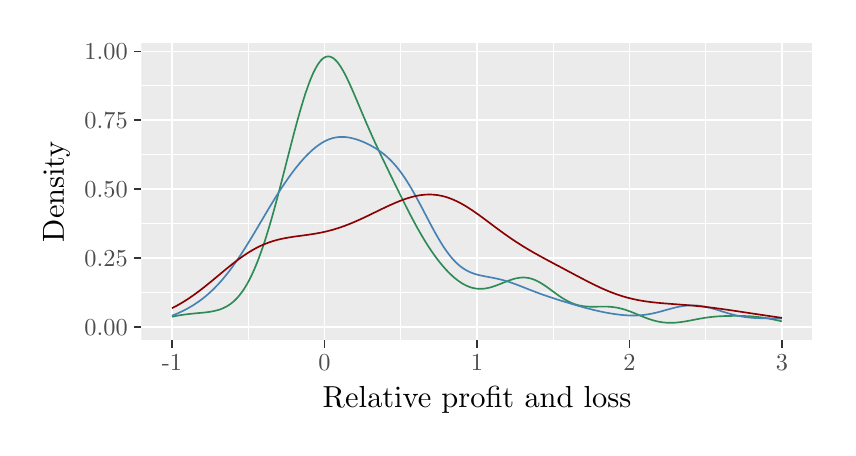
\begin{tikzpicture}[x=1pt,y=1pt]
\definecolor{fillColor}{RGB}{255,255,255}
\path[use as bounding box,fill=fillColor,fill opacity=0.00] (0,0) rectangle (289.08,144.54);
\begin{scope}
\path[clip] (  0.00,  0.00) rectangle (289.08,144.54);
\definecolor{drawColor}{RGB}{255,255,255}
\definecolor{fillColor}{RGB}{255,255,255}

\path[draw=drawColor,line width= 0.6pt,line join=round,line cap=round,fill=fillColor] (  0.00,  0.00) rectangle (289.08,144.54);
\end{scope}
\begin{scope}
\path[clip] ( 41.11, 31.53) rectangle (283.58,139.04);
\definecolor{fillColor}{gray}{0.92}

\path[fill=fillColor] ( 41.11, 31.53) rectangle (283.58,139.04);
\definecolor{drawColor}{RGB}{255,255,255}

\path[draw=drawColor,line width= 0.3pt,line join=round] ( 41.11, 48.86) --
	(283.58, 48.86);

\path[draw=drawColor,line width= 0.3pt,line join=round] ( 41.11, 73.74) --
	(283.58, 73.74);

\path[draw=drawColor,line width= 0.3pt,line join=round] ( 41.11, 98.63) --
	(283.58, 98.63);

\path[draw=drawColor,line width= 0.3pt,line join=round] ( 41.11,123.51) --
	(283.58,123.51);

\path[draw=drawColor,line width= 0.3pt,line join=round] ( 79.69, 31.53) --
	( 79.69,139.04);

\path[draw=drawColor,line width= 0.3pt,line join=round] (134.79, 31.53) --
	(134.79,139.04);

\path[draw=drawColor,line width= 0.3pt,line join=round] (189.90, 31.53) --
	(189.90,139.04);

\path[draw=drawColor,line width= 0.3pt,line join=round] (245.01, 31.53) --
	(245.01,139.04);

\path[draw=drawColor,line width= 0.6pt,line join=round] ( 41.11, 36.42) --
	(283.58, 36.42);

\path[draw=drawColor,line width= 0.6pt,line join=round] ( 41.11, 61.30) --
	(283.58, 61.30);

\path[draw=drawColor,line width= 0.6pt,line join=round] ( 41.11, 86.19) --
	(283.58, 86.19);

\path[draw=drawColor,line width= 0.6pt,line join=round] ( 41.11,111.07) --
	(283.58,111.07);

\path[draw=drawColor,line width= 0.6pt,line join=round] ( 41.11,135.95) --
	(283.58,135.95);

\path[draw=drawColor,line width= 0.6pt,line join=round] ( 52.13, 31.53) --
	( 52.13,139.04);

\path[draw=drawColor,line width= 0.6pt,line join=round] (107.24, 31.53) --
	(107.24,139.04);

\path[draw=drawColor,line width= 0.6pt,line join=round] (162.35, 31.53) --
	(162.35,139.04);

\path[draw=drawColor,line width= 0.6pt,line join=round] (217.45, 31.53) --
	(217.45,139.04);

\path[draw=drawColor,line width= 0.6pt,line join=round] (272.56, 31.53) --
	(272.56,139.04);
\definecolor{drawColor}{RGB}{46,139,87}

\path[draw=drawColor,line width= 0.6pt,line join=round] ( 52.13, 40.09) --
	( 52.56, 40.18) --
	( 52.99, 40.26) --
	( 53.43, 40.35) --
	( 53.86, 40.43) --
	( 54.29, 40.50) --
	( 54.72, 40.58) --
	( 55.15, 40.65) --
	( 55.58, 40.72) --
	( 56.01, 40.78) --
	( 56.45, 40.84) --
	( 56.88, 40.90) --
	( 57.31, 40.95) --
	( 57.74, 41.01) --
	( 58.17, 41.06) --
	( 58.60, 41.11) --
	( 59.03, 41.15) --
	( 59.47, 41.19) --
	( 59.90, 41.24) --
	( 60.33, 41.28) --
	( 60.76, 41.32) --
	( 61.19, 41.36) --
	( 61.62, 41.40) --
	( 62.05, 41.44) --
	( 62.48, 41.48) --
	( 62.92, 41.52) --
	( 63.35, 41.56) --
	( 63.78, 41.60) --
	( 64.21, 41.65) --
	( 64.64, 41.70) --
	( 65.07, 41.76) --
	( 65.50, 41.82) --
	( 65.94, 41.88) --
	( 66.37, 41.96) --
	( 66.80, 42.04) --
	( 67.23, 42.12) --
	( 67.66, 42.22) --
	( 68.09, 42.32) --
	( 68.52, 42.44) --
	( 68.96, 42.56) --
	( 69.39, 42.70) --
	( 69.82, 42.85) --
	( 70.25, 43.02) --
	( 70.68, 43.20) --
	( 71.11, 43.40) --
	( 71.54, 43.62) --
	( 71.97, 43.86) --
	( 72.41, 44.11) --
	( 72.84, 44.39) --
	( 73.27, 44.70) --
	( 73.70, 45.02) --
	( 74.13, 45.37) --
	( 74.56, 45.75) --
	( 74.99, 46.16) --
	( 75.43, 46.59) --
	( 75.86, 47.05) --
	( 76.29, 47.55) --
	( 76.72, 48.08) --
	( 77.15, 48.64) --
	( 77.58, 49.23) --
	( 78.01, 49.86) --
	( 78.45, 50.53) --
	( 78.88, 51.24) --
	( 79.31, 51.97) --
	( 79.74, 52.75) --
	( 80.17, 53.57) --
	( 80.60, 54.43) --
	( 81.03, 55.32) --
	( 81.46, 56.25) --
	( 81.90, 57.23) --
	( 82.33, 58.25) --
	( 82.76, 59.30) --
	( 83.19, 60.39) --
	( 83.62, 61.52) --
	( 84.05, 62.70) --
	( 84.48, 63.90) --
	( 84.92, 65.15) --
	( 85.35, 66.43) --
	( 85.78, 67.75) --
	( 86.21, 69.10) --
	( 86.64, 70.49) --
	( 87.07, 71.91) --
	( 87.50, 73.36) --
	( 87.94, 74.84) --
	( 88.37, 76.35) --
	( 88.80, 77.89) --
	( 89.23, 79.45) --
	( 89.66, 81.03) --
	( 90.09, 82.64) --
	( 90.52, 84.26) --
	( 90.95, 85.90) --
	( 91.39, 87.56) --
	( 91.82, 89.22) --
	( 92.25, 90.90) --
	( 92.68, 92.58) --
	( 93.11, 94.27) --
	( 93.54, 95.96) --
	( 93.97, 97.65) --
	( 94.41, 99.34) --
	( 94.84,101.02) --
	( 95.27,102.70) --
	( 95.70,104.35) --
	( 96.13,106.00) --
	( 96.56,107.63) --
	( 96.99,109.24) --
	( 97.43,110.82) --
	( 97.86,112.37) --
	( 98.29,113.90) --
	( 98.72,115.39) --
	( 99.15,116.84) --
	( 99.58,118.26) --
	(100.01,119.64) --
	(100.44,120.97) --
	(100.88,122.24) --
	(101.31,123.46) --
	(101.74,124.64) --
	(102.17,125.76) --
	(102.60,126.80) --
	(103.03,127.79) --
	(103.46,128.72) --
	(103.90,129.58) --
	(104.33,130.36) --
	(104.76,131.08) --
	(105.19,131.73) --
	(105.62,132.30) --
	(106.05,132.79) --
	(106.48,133.21) --
	(106.92,133.56) --
	(107.35,133.82) --
	(107.78,134.00) --
	(108.21,134.11) --
	(108.64,134.15) --
	(109.07,134.11) --
	(109.50,133.99) --
	(109.93,133.80) --
	(110.37,133.55) --
	(110.80,133.22) --
	(111.23,132.82) --
	(111.66,132.37) --
	(112.09,131.86) --
	(112.52,131.28) --
	(112.95,130.65) --
	(113.39,129.97) --
	(113.82,129.24) --
	(114.25,128.47) --
	(114.68,127.66) --
	(115.11,126.81) --
	(115.54,125.93) --
	(115.97,125.02) --
	(116.41,124.08) --
	(116.84,123.12) --
	(117.27,122.15) --
	(117.70,121.15) --
	(118.13,120.15) --
	(118.56,119.14) --
	(118.99,118.12) --
	(119.42,117.09) --
	(119.86,116.06) --
	(120.29,115.04) --
	(120.72,114.01) --
	(121.15,112.99) --
	(121.58,111.98) --
	(122.01,110.97) --
	(122.44,109.96) --
	(122.88,108.97) --
	(123.31,107.98) --
	(123.74,107.00) --
	(124.17,106.03) --
	(124.60,105.07) --
	(125.03,104.12) --
	(125.46,103.17) --
	(125.90,102.24) --
	(126.33,101.31) --
	(126.76,100.38) --
	(127.19, 99.46) --
	(127.62, 98.55) --
	(128.05, 97.64) --
	(128.48, 96.74) --
	(128.91, 95.84) --
	(129.35, 94.94) --
	(129.78, 94.05) --
	(130.21, 93.16) --
	(130.64, 92.27) --
	(131.07, 91.38) --
	(131.50, 90.50) --
	(131.93, 89.61) --
	(132.37, 88.73) --
	(132.80, 87.85) --
	(133.23, 86.97) --
	(133.66, 86.09) --
	(134.09, 85.21) --
	(134.52, 84.34) --
	(134.95, 83.47) --
	(135.39, 82.60) --
	(135.82, 81.74) --
	(136.25, 80.88) --
	(136.68, 80.02) --
	(137.11, 79.17) --
	(137.54, 78.33) --
	(137.97, 77.49) --
	(138.40, 76.66) --
	(138.84, 75.84) --
	(139.27, 75.03) --
	(139.70, 74.22) --
	(140.13, 73.42) --
	(140.56, 72.64) --
	(140.99, 71.86) --
	(141.42, 71.10) --
	(141.86, 70.34) --
	(142.29, 69.60) --
	(142.72, 68.87) --
	(143.15, 68.14) --
	(143.58, 67.44) --
	(144.01, 66.74) --
	(144.44, 66.06) --
	(144.88, 65.39) --
	(145.31, 64.73) --
	(145.74, 64.09) --
	(146.17, 63.45) --
	(146.60, 62.83) --
	(147.03, 62.23) --
	(147.46, 61.64) --
	(147.89, 61.06) --
	(148.33, 60.49) --
	(148.76, 59.94) --
	(149.19, 59.41) --
	(149.62, 58.88) --
	(150.05, 58.37) --
	(150.48, 57.87) --
	(150.91, 57.39) --
	(151.35, 56.92) --
	(151.78, 56.46) --
	(152.21, 56.02) --
	(152.64, 55.60) --
	(153.07, 55.19) --
	(153.50, 54.79) --
	(153.93, 54.40) --
	(154.37, 54.04) --
	(154.80, 53.69) --
	(155.23, 53.35) --
	(155.66, 53.03) --
	(156.09, 52.73) --
	(156.52, 52.44) --
	(156.95, 52.17) --
	(157.38, 51.91) --
	(157.82, 51.68) --
	(158.25, 51.46) --
	(158.68, 51.25) --
	(159.11, 51.07) --
	(159.54, 50.90) --
	(159.97, 50.75) --
	(160.40, 50.61) --
	(160.84, 50.50) --
	(161.27, 50.40) --
	(161.70, 50.32) --
	(162.13, 50.26) --
	(162.56, 50.21) --
	(162.99, 50.18) --
	(163.42, 50.17) --
	(163.86, 50.17) --
	(164.29, 50.19) --
	(164.72, 50.23) --
	(165.15, 50.27) --
	(165.58, 50.34) --
	(166.01, 50.41) --
	(166.44, 50.50) --
	(166.87, 50.61) --
	(167.31, 50.72) --
	(167.74, 50.84) --
	(168.17, 50.98) --
	(168.60, 51.12) --
	(169.03, 51.27) --
	(169.46, 51.43) --
	(169.89, 51.59) --
	(170.33, 51.76) --
	(170.76, 51.93) --
	(171.19, 52.10) --
	(171.62, 52.28) --
	(172.05, 52.45) --
	(172.48, 52.62) --
	(172.91, 52.79) --
	(173.35, 52.96) --
	(173.78, 53.12) --
	(174.21, 53.28) --
	(174.64, 53.43) --
	(175.07, 53.57) --
	(175.50, 53.70) --
	(175.93, 53.82) --
	(176.36, 53.92) --
	(176.80, 54.01) --
	(177.23, 54.09) --
	(177.66, 54.16) --
	(178.09, 54.21) --
	(178.52, 54.24) --
	(178.95, 54.25) --
	(179.38, 54.25) --
	(179.82, 54.23) --
	(180.25, 54.19) --
	(180.68, 54.13) --
	(181.11, 54.05) --
	(181.54, 53.95) --
	(181.97, 53.83) --
	(182.40, 53.70) --
	(182.84, 53.55) --
	(183.27, 53.37) --
	(183.70, 53.18) --
	(184.13, 52.98) --
	(184.56, 52.76) --
	(184.99, 52.52) --
	(185.42, 52.27) --
	(185.85, 52.01) --
	(186.29, 51.74) --
	(186.72, 51.45) --
	(187.15, 51.16) --
	(187.58, 50.86) --
	(188.01, 50.55) --
	(188.44, 50.24) --
	(188.87, 49.92) --
	(189.31, 49.60) --
	(189.74, 49.28) --
	(190.17, 48.97) --
	(190.60, 48.65) --
	(191.03, 48.34) --
	(191.46, 48.03) --
	(191.89, 47.73) --
	(192.33, 47.43) --
	(192.76, 47.14) --
	(193.19, 46.86) --
	(193.62, 46.59) --
	(194.05, 46.33) --
	(194.48, 46.09) --
	(194.91, 45.85) --
	(195.34, 45.62) --
	(195.78, 45.41) --
	(196.21, 45.21) --
	(196.64, 45.03) --
	(197.07, 44.86) --
	(197.50, 44.70) --
	(197.93, 44.55) --
	(198.36, 44.42) --
	(198.80, 44.30) --
	(199.23, 44.19) --
	(199.66, 44.10) --
	(200.09, 44.02) --
	(200.52, 43.94) --
	(200.95, 43.88) --
	(201.38, 43.83) --
	(201.82, 43.79) --
	(202.25, 43.76) --
	(202.68, 43.74) --
	(203.11, 43.72) --
	(203.54, 43.71) --
	(203.97, 43.70) --
	(204.40, 43.70) --
	(204.83, 43.71) --
	(205.27, 43.71) --
	(205.70, 43.72) --
	(206.13, 43.73) --
	(206.56, 43.74) --
	(206.99, 43.75) --
	(207.42, 43.75) --
	(207.85, 43.75) --
	(208.29, 43.75) --
	(208.72, 43.75) --
	(209.15, 43.74) --
	(209.58, 43.73) --
	(210.01, 43.71) --
	(210.44, 43.68) --
	(210.87, 43.64) --
	(211.31, 43.60) --
	(211.74, 43.55) --
	(212.17, 43.49) --
	(212.60, 43.42) --
	(213.03, 43.34) --
	(213.46, 43.26) --
	(213.89, 43.16) --
	(214.32, 43.06) --
	(214.76, 42.94) --
	(215.19, 42.82) --
	(215.62, 42.70) --
	(216.05, 42.56) --
	(216.48, 42.41) --
	(216.91, 42.26) --
	(217.34, 42.11) --
	(217.78, 41.95) --
	(218.21, 41.78) --
	(218.64, 41.61) --
	(219.07, 41.43) --
	(219.50, 41.26) --
	(219.93, 41.08) --
	(220.36, 40.90) --
	(220.80, 40.72) --
	(221.23, 40.54) --
	(221.66, 40.36) --
	(222.09, 40.19) --
	(222.52, 40.01) --
	(222.95, 39.84) --
	(223.38, 39.68) --
	(223.81, 39.52) --
	(224.25, 39.36) --
	(224.68, 39.21) --
	(225.11, 39.07) --
	(225.54, 38.93) --
	(225.97, 38.80) --
	(226.40, 38.68) --
	(226.83, 38.57) --
	(227.27, 38.46) --
	(227.70, 38.37) --
	(228.13, 38.28) --
	(228.56, 38.20) --
	(228.99, 38.13) --
	(229.42, 38.07) --
	(229.85, 38.02) --
	(230.29, 37.97) --
	(230.72, 37.94) --
	(231.15, 37.91) --
	(231.58, 37.90) --
	(232.01, 37.89) --
	(232.44, 37.89) --
	(232.87, 37.89) --
	(233.30, 37.91) --
	(233.74, 37.93) --
	(234.17, 37.96) --
	(234.60, 38.00) --
	(235.03, 38.04) --
	(235.46, 38.09) --
	(235.89, 38.14) --
	(236.32, 38.20) --
	(236.76, 38.26) --
	(237.19, 38.33) --
	(237.62, 38.40) --
	(238.05, 38.47) --
	(238.48, 38.55) --
	(238.91, 38.63) --
	(239.34, 38.71) --
	(239.78, 38.79) --
	(240.21, 38.88) --
	(240.64, 38.96) --
	(241.07, 39.04) --
	(241.50, 39.13) --
	(241.93, 39.21) --
	(242.36, 39.29) --
	(242.79, 39.37) --
	(243.23, 39.44) --
	(243.66, 39.52) --
	(244.09, 39.59) --
	(244.52, 39.66) --
	(244.95, 39.73) --
	(245.38, 39.79) --
	(245.81, 39.85) --
	(246.25, 39.90) --
	(246.68, 39.96) --
	(247.11, 40.01) --
	(247.54, 40.05) --
	(247.97, 40.09) --
	(248.40, 40.13) --
	(248.83, 40.17) --
	(249.27, 40.20) --
	(249.70, 40.23) --
	(250.13, 40.25) --
	(250.56, 40.28) --
	(250.99, 40.30) --
	(251.42, 40.32) --
	(251.85, 40.33) --
	(252.28, 40.34) --
	(252.72, 40.36) --
	(253.15, 40.37) --
	(253.58, 40.37) --
	(254.01, 40.38) --
	(254.44, 40.38) --
	(254.87, 40.39) --
	(255.30, 40.39) --
	(255.74, 40.39) --
	(256.17, 40.39) --
	(256.60, 40.38) --
	(257.03, 40.38) --
	(257.46, 40.37) --
	(257.89, 40.36) --
	(258.32, 40.35) --
	(258.76, 40.34) --
	(259.19, 40.33) --
	(259.62, 40.31) --
	(260.05, 40.29) --
	(260.48, 40.27) --
	(260.91, 40.25) --
	(261.34, 40.22) --
	(261.77, 40.19) --
	(262.21, 40.16) --
	(262.64, 40.12) --
	(263.07, 40.08) --
	(263.50, 40.04) --
	(263.93, 39.99) --
	(264.36, 39.94) --
	(264.79, 39.89) --
	(265.23, 39.83) --
	(265.66, 39.77) --
	(266.09, 39.70) --
	(266.52, 39.63) --
	(266.95, 39.56) --
	(267.38, 39.49) --
	(267.81, 39.41) --
	(268.25, 39.33) --
	(268.68, 39.24) --
	(269.11, 39.16) --
	(269.54, 39.07) --
	(269.97, 38.98) --
	(270.40, 38.89) --
	(270.83, 38.79) --
	(271.26, 38.70) --
	(271.70, 38.60) --
	(272.13, 38.51) --
	(272.56, 38.42);
\definecolor{drawColor}{RGB}{70,130,180}

\path[draw=drawColor,line width= 0.6pt,line join=round] ( 52.13, 40.46) --
	( 52.56, 40.63) --
	( 52.99, 40.81) --
	( 53.43, 40.98) --
	( 53.86, 41.16) --
	( 54.29, 41.35) --
	( 54.72, 41.54) --
	( 55.15, 41.74) --
	( 55.58, 41.94) --
	( 56.01, 42.15) --
	( 56.45, 42.36) --
	( 56.88, 42.58) --
	( 57.31, 42.81) --
	( 57.74, 43.04) --
	( 58.17, 43.28) --
	( 58.60, 43.53) --
	( 59.03, 43.78) --
	( 59.47, 44.04) --
	( 59.90, 44.30) --
	( 60.33, 44.58) --
	( 60.76, 44.86) --
	( 61.19, 45.15) --
	( 61.62, 45.45) --
	( 62.05, 45.75) --
	( 62.48, 46.07) --
	( 62.92, 46.39) --
	( 63.35, 46.73) --
	( 63.78, 47.07) --
	( 64.21, 47.42) --
	( 64.64, 47.78) --
	( 65.07, 48.15) --
	( 65.50, 48.53) --
	( 65.94, 48.92) --
	( 66.37, 49.32) --
	( 66.80, 49.73) --
	( 67.23, 50.15) --
	( 67.66, 50.59) --
	( 68.09, 51.03) --
	( 68.52, 51.48) --
	( 68.96, 51.94) --
	( 69.39, 52.42) --
	( 69.82, 52.90) --
	( 70.25, 53.40) --
	( 70.68, 53.90) --
	( 71.11, 54.42) --
	( 71.54, 54.95) --
	( 71.97, 55.48) --
	( 72.41, 56.03) --
	( 72.84, 56.59) --
	( 73.27, 57.16) --
	( 73.70, 57.74) --
	( 74.13, 58.33) --
	( 74.56, 58.93) --
	( 74.99, 59.54) --
	( 75.43, 60.16) --
	( 75.86, 60.79) --
	( 76.29, 61.42) --
	( 76.72, 62.07) --
	( 77.15, 62.72) --
	( 77.58, 63.38) --
	( 78.01, 64.05) --
	( 78.45, 64.73) --
	( 78.88, 65.42) --
	( 79.31, 66.11) --
	( 79.74, 66.81) --
	( 80.17, 67.51) --
	( 80.60, 68.22) --
	( 81.03, 68.93) --
	( 81.46, 69.65) --
	( 81.90, 70.37) --
	( 82.33, 71.09) --
	( 82.76, 71.82) --
	( 83.19, 72.55) --
	( 83.62, 73.28) --
	( 84.05, 74.01) --
	( 84.48, 74.75) --
	( 84.92, 75.48) --
	( 85.35, 76.21) --
	( 85.78, 76.94) --
	( 86.21, 77.67) --
	( 86.64, 78.39) --
	( 87.07, 79.11) --
	( 87.50, 79.83) --
	( 87.94, 80.55) --
	( 88.37, 81.26) --
	( 88.80, 81.96) --
	( 89.23, 82.66) --
	( 89.66, 83.36) --
	( 90.09, 84.05) --
	( 90.52, 84.73) --
	( 90.95, 85.40) --
	( 91.39, 86.07) --
	( 91.82, 86.73) --
	( 92.25, 87.38) --
	( 92.68, 88.02) --
	( 93.11, 88.66) --
	( 93.54, 89.28) --
	( 93.97, 89.90) --
	( 94.41, 90.51) --
	( 94.84, 91.11) --
	( 95.27, 91.70) --
	( 95.70, 92.28) --
	( 96.13, 92.85) --
	( 96.56, 93.41) --
	( 96.99, 93.96) --
	( 97.43, 94.50) --
	( 97.86, 95.03) --
	( 98.29, 95.55) --
	( 98.72, 96.05) --
	( 99.15, 96.55) --
	( 99.58, 97.04) --
	(100.01, 97.51) --
	(100.44, 97.97) --
	(100.88, 98.42) --
	(101.31, 98.85) --
	(101.74, 99.27) --
	(102.17, 99.68) --
	(102.60,100.08) --
	(103.03,100.46) --
	(103.46,100.83) --
	(103.90,101.19) --
	(104.33,101.53) --
	(104.76,101.85) --
	(105.19,102.17) --
	(105.62,102.46) --
	(106.05,102.74) --
	(106.48,103.01) --
	(106.92,103.26) --
	(107.35,103.49) --
	(107.78,103.70) --
	(108.21,103.90) --
	(108.64,104.09) --
	(109.07,104.26) --
	(109.50,104.41) --
	(109.93,104.54) --
	(110.37,104.66) --
	(110.80,104.76) --
	(111.23,104.85) --
	(111.66,104.92) --
	(112.09,104.98) --
	(112.52,105.02) --
	(112.95,105.05) --
	(113.39,105.06) --
	(113.82,105.06) --
	(114.25,105.04) --
	(114.68,105.01) --
	(115.11,104.97) --
	(115.54,104.92) --
	(115.97,104.85) --
	(116.41,104.78) --
	(116.84,104.69) --
	(117.27,104.59) --
	(117.70,104.48) --
	(118.13,104.36) --
	(118.56,104.24) --
	(118.99,104.10) --
	(119.42,103.96) --
	(119.86,103.80) --
	(120.29,103.64) --
	(120.72,103.47) --
	(121.15,103.30) --
	(121.58,103.11) --
	(122.01,102.92) --
	(122.44,102.72) --
	(122.88,102.51) --
	(123.31,102.30) --
	(123.74,102.07) --
	(124.17,101.84) --
	(124.60,101.60) --
	(125.03,101.35) --
	(125.46,101.10) --
	(125.90,100.83) --
	(126.33,100.55) --
	(126.76,100.27) --
	(127.19, 99.97) --
	(127.62, 99.66) --
	(128.05, 99.34) --
	(128.48, 99.01) --
	(128.91, 98.66) --
	(129.35, 98.30) --
	(129.78, 97.92) --
	(130.21, 97.54) --
	(130.64, 97.13) --
	(131.07, 96.71) --
	(131.50, 96.27) --
	(131.93, 95.82) --
	(132.37, 95.34) --
	(132.80, 94.85) --
	(133.23, 94.35) --
	(133.66, 93.82) --
	(134.09, 93.28) --
	(134.52, 92.72) --
	(134.95, 92.13) --
	(135.39, 91.53) --
	(135.82, 90.91) --
	(136.25, 90.28) --
	(136.68, 89.62) --
	(137.11, 88.95) --
	(137.54, 88.26) --
	(137.97, 87.56) --
	(138.40, 86.84) --
	(138.84, 86.10) --
	(139.27, 85.35) --
	(139.70, 84.59) --
	(140.13, 83.81) --
	(140.56, 83.03) --
	(140.99, 82.23) --
	(141.42, 81.43) --
	(141.86, 80.62) --
	(142.29, 79.80) --
	(142.72, 78.98) --
	(143.15, 78.15) --
	(143.58, 77.32) --
	(144.01, 76.50) --
	(144.44, 75.67) --
	(144.88, 74.85) --
	(145.31, 74.03) --
	(145.74, 73.21) --
	(146.17, 72.41) --
	(146.60, 71.61) --
	(147.03, 70.82) --
	(147.46, 70.05) --
	(147.89, 69.29) --
	(148.33, 68.54) --
	(148.76, 67.81) --
	(149.19, 67.10) --
	(149.62, 66.40) --
	(150.05, 65.72) --
	(150.48, 65.06) --
	(150.91, 64.42) --
	(151.35, 63.80) --
	(151.78, 63.21) --
	(152.21, 62.64) --
	(152.64, 62.09) --
	(153.07, 61.56) --
	(153.50, 61.05) --
	(153.93, 60.58) --
	(154.37, 60.12) --
	(154.80, 59.68) --
	(155.23, 59.27) --
	(155.66, 58.89) --
	(156.09, 58.52) --
	(156.52, 58.18) --
	(156.95, 57.86) --
	(157.38, 57.56) --
	(157.82, 57.28) --
	(158.25, 57.02) --
	(158.68, 56.78) --
	(159.11, 56.55) --
	(159.54, 56.34) --
	(159.97, 56.15) --
	(160.40, 55.97) --
	(160.84, 55.81) --
	(161.27, 55.66) --
	(161.70, 55.52) --
	(162.13, 55.39) --
	(162.56, 55.27) --
	(162.99, 55.16) --
	(163.42, 55.06) --
	(163.86, 54.96) --
	(164.29, 54.87) --
	(164.72, 54.79) --
	(165.15, 54.70) --
	(165.58, 54.62) --
	(166.01, 54.54) --
	(166.44, 54.46) --
	(166.87, 54.38) --
	(167.31, 54.30) --
	(167.74, 54.22) --
	(168.17, 54.14) --
	(168.60, 54.05) --
	(169.03, 53.96) --
	(169.46, 53.87) --
	(169.89, 53.77) --
	(170.33, 53.67) --
	(170.76, 53.57) --
	(171.19, 53.46) --
	(171.62, 53.35) --
	(172.05, 53.23) --
	(172.48, 53.10) --
	(172.91, 52.98) --
	(173.35, 52.85) --
	(173.78, 52.71) --
	(174.21, 52.57) --
	(174.64, 52.42) --
	(175.07, 52.28) --
	(175.50, 52.12) --
	(175.93, 51.97) --
	(176.36, 51.81) --
	(176.80, 51.65) --
	(177.23, 51.49) --
	(177.66, 51.32) --
	(178.09, 51.15) --
	(178.52, 50.98) --
	(178.95, 50.82) --
	(179.38, 50.65) --
	(179.82, 50.47) --
	(180.25, 50.30) --
	(180.68, 50.13) --
	(181.11, 49.96) --
	(181.54, 49.79) --
	(181.97, 49.62) --
	(182.40, 49.46) --
	(182.84, 49.29) --
	(183.27, 49.13) --
	(183.70, 48.96) --
	(184.13, 48.80) --
	(184.56, 48.64) --
	(184.99, 48.48) --
	(185.42, 48.32) --
	(185.85, 48.17) --
	(186.29, 48.01) --
	(186.72, 47.86) --
	(187.15, 47.71) --
	(187.58, 47.56) --
	(188.01, 47.42) --
	(188.44, 47.27) --
	(188.87, 47.13) --
	(189.31, 46.99) --
	(189.74, 46.85) --
	(190.17, 46.71) --
	(190.60, 46.57) --
	(191.03, 46.43) --
	(191.46, 46.29) --
	(191.89, 46.16) --
	(192.33, 46.02) --
	(192.76, 45.89) --
	(193.19, 45.75) --
	(193.62, 45.62) --
	(194.05, 45.49) --
	(194.48, 45.36) --
	(194.91, 45.23) --
	(195.34, 45.10) --
	(195.78, 44.97) --
	(196.21, 44.84) --
	(196.64, 44.71) --
	(197.07, 44.58) --
	(197.50, 44.45) --
	(197.93, 44.33) --
	(198.36, 44.20) --
	(198.80, 44.08) --
	(199.23, 43.95) --
	(199.66, 43.83) --
	(200.09, 43.71) --
	(200.52, 43.59) --
	(200.95, 43.47) --
	(201.38, 43.35) --
	(201.82, 43.23) --
	(202.25, 43.12) --
	(202.68, 43.01) --
	(203.11, 42.90) --
	(203.54, 42.79) --
	(203.97, 42.68) --
	(204.40, 42.57) --
	(204.83, 42.47) --
	(205.27, 42.37) --
	(205.70, 42.27) --
	(206.13, 42.17) --
	(206.56, 42.07) --
	(206.99, 41.98) --
	(207.42, 41.89) --
	(207.85, 41.80) --
	(208.29, 41.71) --
	(208.72, 41.63) --
	(209.15, 41.55) --
	(209.58, 41.47) --
	(210.01, 41.39) --
	(210.44, 41.32) --
	(210.87, 41.25) --
	(211.31, 41.18) --
	(211.74, 41.11) --
	(212.17, 41.05) --
	(212.60, 40.99) --
	(213.03, 40.93) --
	(213.46, 40.88) --
	(213.89, 40.83) --
	(214.32, 40.78) --
	(214.76, 40.73) --
	(215.19, 40.69) --
	(215.62, 40.66) --
	(216.05, 40.63) --
	(216.48, 40.60) --
	(216.91, 40.57) --
	(217.34, 40.55) --
	(217.78, 40.54) --
	(218.21, 40.53) --
	(218.64, 40.53) --
	(219.07, 40.53) --
	(219.50, 40.53) --
	(219.93, 40.54) --
	(220.36, 40.56) --
	(220.80, 40.58) --
	(221.23, 40.61) --
	(221.66, 40.65) --
	(222.09, 40.69) --
	(222.52, 40.73) --
	(222.95, 40.79) --
	(223.38, 40.84) --
	(223.81, 40.91) --
	(224.25, 40.98) --
	(224.68, 41.05) --
	(225.11, 41.13) --
	(225.54, 41.22) --
	(225.97, 41.31) --
	(226.40, 41.40) --
	(226.83, 41.50) --
	(227.27, 41.61) --
	(227.70, 41.71) --
	(228.13, 41.82) --
	(228.56, 41.94) --
	(228.99, 42.05) --
	(229.42, 42.17) --
	(229.85, 42.29) --
	(230.29, 42.41) --
	(230.72, 42.53) --
	(231.15, 42.65) --
	(231.58, 42.77) --
	(232.01, 42.89) --
	(232.44, 43.00) --
	(232.87, 43.12) --
	(233.30, 43.23) --
	(233.74, 43.33) --
	(234.17, 43.44) --
	(234.60, 43.53) --
	(235.03, 43.63) --
	(235.46, 43.72) --
	(235.89, 43.80) --
	(236.32, 43.87) --
	(236.76, 43.94) --
	(237.19, 44.00) --
	(237.62, 44.05) --
	(238.05, 44.10) --
	(238.48, 44.14) --
	(238.91, 44.17) --
	(239.34, 44.19) --
	(239.78, 44.20) --
	(240.21, 44.20) --
	(240.64, 44.19) --
	(241.07, 44.18) --
	(241.50, 44.15) --
	(241.93, 44.12) --
	(242.36, 44.08) --
	(242.79, 44.03) --
	(243.23, 43.98) --
	(243.66, 43.91) --
	(244.09, 43.84) --
	(244.52, 43.76) --
	(244.95, 43.67) --
	(245.38, 43.58) --
	(245.81, 43.48) --
	(246.25, 43.37) --
	(246.68, 43.26) --
	(247.11, 43.15) --
	(247.54, 43.03) --
	(247.97, 42.90) --
	(248.40, 42.78) --
	(248.83, 42.65) --
	(249.27, 42.52) --
	(249.70, 42.39) --
	(250.13, 42.25) --
	(250.56, 42.12) --
	(250.99, 41.98) --
	(251.42, 41.85) --
	(251.85, 41.72) --
	(252.28, 41.59) --
	(252.72, 41.46) --
	(253.15, 41.33) --
	(253.58, 41.21) --
	(254.01, 41.09) --
	(254.44, 40.97) --
	(254.87, 40.86) --
	(255.30, 40.75) --
	(255.74, 40.64) --
	(256.17, 40.54) --
	(256.60, 40.45) --
	(257.03, 40.36) --
	(257.46, 40.27) --
	(257.89, 40.19) --
	(258.32, 40.12) --
	(258.76, 40.05) --
	(259.19, 39.98) --
	(259.62, 39.92) --
	(260.05, 39.87) --
	(260.48, 39.82) --
	(260.91, 39.78) --
	(261.34, 39.74) --
	(261.77, 39.70) --
	(262.21, 39.67) --
	(262.64, 39.64) --
	(263.07, 39.62) --
	(263.50, 39.60) --
	(263.93, 39.58) --
	(264.36, 39.57) --
	(264.79, 39.56) --
	(265.23, 39.55) --
	(265.66, 39.54) --
	(266.09, 39.53) --
	(266.52, 39.53) --
	(266.95, 39.52) --
	(267.38, 39.52) --
	(267.81, 39.52) --
	(268.25, 39.51) --
	(268.68, 39.51) --
	(269.11, 39.50) --
	(269.54, 39.49) --
	(269.97, 39.49) --
	(270.40, 39.47) --
	(270.83, 39.46) --
	(271.26, 39.45) --
	(271.70, 39.43) --
	(272.13, 39.41) --
	(272.56, 39.39);
\definecolor{drawColor}{RGB}{139,0,0}

\path[draw=drawColor,line width= 0.6pt,line join=round] ( 52.13, 43.16) --
	( 52.56, 43.38) --
	( 52.99, 43.60) --
	( 53.43, 43.83) --
	( 53.86, 44.06) --
	( 54.29, 44.30) --
	( 54.72, 44.55) --
	( 55.15, 44.79) --
	( 55.58, 45.05) --
	( 56.01, 45.31) --
	( 56.45, 45.57) --
	( 56.88, 45.84) --
	( 57.31, 46.12) --
	( 57.74, 46.39) --
	( 58.17, 46.68) --
	( 58.60, 46.97) --
	( 59.03, 47.26) --
	( 59.47, 47.56) --
	( 59.90, 47.86) --
	( 60.33, 48.17) --
	( 60.76, 48.49) --
	( 61.19, 48.80) --
	( 61.62, 49.12) --
	( 62.05, 49.45) --
	( 62.48, 49.78) --
	( 62.92, 50.11) --
	( 63.35, 50.44) --
	( 63.78, 50.78) --
	( 64.21, 51.13) --
	( 64.64, 51.47) --
	( 65.07, 51.82) --
	( 65.50, 52.17) --
	( 65.94, 52.52) --
	( 66.37, 52.87) --
	( 66.80, 53.23) --
	( 67.23, 53.59) --
	( 67.66, 53.94) --
	( 68.09, 54.30) --
	( 68.52, 54.66) --
	( 68.96, 55.02) --
	( 69.39, 55.38) --
	( 69.82, 55.74) --
	( 70.25, 56.10) --
	( 70.68, 56.46) --
	( 71.11, 56.81) --
	( 71.54, 57.17) --
	( 71.97, 57.52) --
	( 72.41, 57.87) --
	( 72.84, 58.22) --
	( 73.27, 58.57) --
	( 73.70, 58.91) --
	( 74.13, 59.25) --
	( 74.56, 59.59) --
	( 74.99, 59.92) --
	( 75.43, 60.25) --
	( 75.86, 60.57) --
	( 76.29, 60.89) --
	( 76.72, 61.21) --
	( 77.15, 61.52) --
	( 77.58, 61.82) --
	( 78.01, 62.12) --
	( 78.45, 62.41) --
	( 78.88, 62.70) --
	( 79.31, 62.98) --
	( 79.74, 63.26) --
	( 80.17, 63.53) --
	( 80.60, 63.79) --
	( 81.03, 64.04) --
	( 81.46, 64.29) --
	( 81.90, 64.53) --
	( 82.33, 64.77) --
	( 82.76, 65.00) --
	( 83.19, 65.22) --
	( 83.62, 65.43) --
	( 84.05, 65.64) --
	( 84.48, 65.84) --
	( 84.92, 66.03) --
	( 85.35, 66.22) --
	( 85.78, 66.40) --
	( 86.21, 66.57) --
	( 86.64, 66.73) --
	( 87.07, 66.89) --
	( 87.50, 67.04) --
	( 87.94, 67.19) --
	( 88.37, 67.33) --
	( 88.80, 67.46) --
	( 89.23, 67.59) --
	( 89.66, 67.71) --
	( 90.09, 67.83) --
	( 90.52, 67.94) --
	( 90.95, 68.04) --
	( 91.39, 68.14) --
	( 91.82, 68.24) --
	( 92.25, 68.33) --
	( 92.68, 68.42) --
	( 93.11, 68.50) --
	( 93.54, 68.58) --
	( 93.97, 68.66) --
	( 94.41, 68.73) --
	( 94.84, 68.80) --
	( 95.27, 68.87) --
	( 95.70, 68.94) --
	( 96.13, 69.00) --
	( 96.56, 69.06) --
	( 96.99, 69.12) --
	( 97.43, 69.18) --
	( 97.86, 69.24) --
	( 98.29, 69.30) --
	( 98.72, 69.35) --
	( 99.15, 69.41) --
	( 99.58, 69.47) --
	(100.01, 69.53) --
	(100.44, 69.58) --
	(100.88, 69.64) --
	(101.31, 69.70) --
	(101.74, 69.77) --
	(102.17, 69.83) --
	(102.60, 69.90) --
	(103.03, 69.96) --
	(103.46, 70.03) --
	(103.90, 70.10) --
	(104.33, 70.18) --
	(104.76, 70.26) --
	(105.19, 70.33) --
	(105.62, 70.42) --
	(106.05, 70.50) --
	(106.48, 70.59) --
	(106.92, 70.69) --
	(107.35, 70.78) --
	(107.78, 70.88) --
	(108.21, 70.98) --
	(108.64, 71.09) --
	(109.07, 71.20) --
	(109.50, 71.32) --
	(109.93, 71.43) --
	(110.37, 71.56) --
	(110.80, 71.68) --
	(111.23, 71.81) --
	(111.66, 71.95) --
	(112.09, 72.08) --
	(112.52, 72.22) --
	(112.95, 72.37) --
	(113.39, 72.52) --
	(113.82, 72.67) --
	(114.25, 72.82) --
	(114.68, 72.98) --
	(115.11, 73.15) --
	(115.54, 73.31) --
	(115.97, 73.48) --
	(116.41, 73.65) --
	(116.84, 73.83) --
	(117.27, 74.01) --
	(117.70, 74.19) --
	(118.13, 74.37) --
	(118.56, 74.56) --
	(118.99, 74.75) --
	(119.42, 74.94) --
	(119.86, 75.13) --
	(120.29, 75.33) --
	(120.72, 75.53) --
	(121.15, 75.73) --
	(121.58, 75.93) --
	(122.01, 76.13) --
	(122.44, 76.34) --
	(122.88, 76.55) --
	(123.31, 76.75) --
	(123.74, 76.96) --
	(124.17, 77.17) --
	(124.60, 77.38) --
	(125.03, 77.59) --
	(125.46, 77.80) --
	(125.90, 78.01) --
	(126.33, 78.22) --
	(126.76, 78.43) --
	(127.19, 78.64) --
	(127.62, 78.85) --
	(128.05, 79.05) --
	(128.48, 79.26) --
	(128.91, 79.47) --
	(129.35, 79.67) --
	(129.78, 79.87) --
	(130.21, 80.07) --
	(130.64, 80.27) --
	(131.07, 80.47) --
	(131.50, 80.66) --
	(131.93, 80.85) --
	(132.37, 81.04) --
	(132.80, 81.23) --
	(133.23, 81.41) --
	(133.66, 81.59) --
	(134.09, 81.76) --
	(134.52, 81.93) --
	(134.95, 82.10) --
	(135.39, 82.26) --
	(135.82, 82.42) --
	(136.25, 82.57) --
	(136.68, 82.71) --
	(137.11, 82.86) --
	(137.54, 82.99) --
	(137.97, 83.12) --
	(138.40, 83.25) --
	(138.84, 83.36) --
	(139.27, 83.48) --
	(139.70, 83.58) --
	(140.13, 83.68) --
	(140.56, 83.77) --
	(140.99, 83.85) --
	(141.42, 83.93) --
	(141.86, 84.00) --
	(142.29, 84.06) --
	(142.72, 84.11) --
	(143.15, 84.15) --
	(143.58, 84.19) --
	(144.01, 84.22) --
	(144.44, 84.23) --
	(144.88, 84.24) --
	(145.31, 84.25) --
	(145.74, 84.24) --
	(146.17, 84.22) --
	(146.60, 84.19) --
	(147.03, 84.16) --
	(147.46, 84.11) --
	(147.89, 84.06) --
	(148.33, 84.00) --
	(148.76, 83.92) --
	(149.19, 83.84) --
	(149.62, 83.75) --
	(150.05, 83.65) --
	(150.48, 83.54) --
	(150.91, 83.42) --
	(151.35, 83.29) --
	(151.78, 83.15) --
	(152.21, 83.00) --
	(152.64, 82.84) --
	(153.07, 82.68) --
	(153.50, 82.51) --
	(153.93, 82.32) --
	(154.37, 82.13) --
	(154.80, 81.93) --
	(155.23, 81.73) --
	(155.66, 81.51) --
	(156.09, 81.29) --
	(156.52, 81.06) --
	(156.95, 80.82) --
	(157.38, 80.58) --
	(157.82, 80.33) --
	(158.25, 80.07) --
	(158.68, 79.81) --
	(159.11, 79.54) --
	(159.54, 79.26) --
	(159.97, 78.98) --
	(160.40, 78.70) --
	(160.84, 78.41) --
	(161.27, 78.11) --
	(161.70, 77.81) --
	(162.13, 77.51) --
	(162.56, 77.21) --
	(162.99, 76.90) --
	(163.42, 76.59) --
	(163.86, 76.27) --
	(164.29, 75.96) --
	(164.72, 75.64) --
	(165.15, 75.32) --
	(165.58, 75.00) --
	(166.01, 74.68) --
	(166.44, 74.35) --
	(166.87, 74.03) --
	(167.31, 73.71) --
	(167.74, 73.38) --
	(168.17, 73.06) --
	(168.60, 72.74) --
	(169.03, 72.42) --
	(169.46, 72.09) --
	(169.89, 71.77) --
	(170.33, 71.46) --
	(170.76, 71.14) --
	(171.19, 70.82) --
	(171.62, 70.51) --
	(172.05, 70.20) --
	(172.48, 69.89) --
	(172.91, 69.58) --
	(173.35, 69.28) --
	(173.78, 68.98) --
	(174.21, 68.68) --
	(174.64, 68.38) --
	(175.07, 68.09) --
	(175.50, 67.80) --
	(175.93, 67.51) --
	(176.36, 67.23) --
	(176.80, 66.95) --
	(177.23, 66.67) --
	(177.66, 66.39) --
	(178.09, 66.12) --
	(178.52, 65.84) --
	(178.95, 65.58) --
	(179.38, 65.31) --
	(179.82, 65.05) --
	(180.25, 64.79) --
	(180.68, 64.53) --
	(181.11, 64.28) --
	(181.54, 64.02) --
	(181.97, 63.77) --
	(182.40, 63.52) --
	(182.84, 63.28) --
	(183.27, 63.03) --
	(183.70, 62.79) --
	(184.13, 62.55) --
	(184.56, 62.31) --
	(184.99, 62.07) --
	(185.42, 61.83) --
	(185.85, 61.60) --
	(186.29, 61.36) --
	(186.72, 61.13) --
	(187.15, 60.90) --
	(187.58, 60.66) --
	(188.01, 60.43) --
	(188.44, 60.20) --
	(188.87, 59.97) --
	(189.31, 59.74) --
	(189.74, 59.51) --
	(190.17, 59.28) --
	(190.60, 59.05) --
	(191.03, 58.82) --
	(191.46, 58.60) --
	(191.89, 58.37) --
	(192.33, 58.14) --
	(192.76, 57.91) --
	(193.19, 57.68) --
	(193.62, 57.45) --
	(194.05, 57.22) --
	(194.48, 56.99) --
	(194.91, 56.76) --
	(195.34, 56.53) --
	(195.78, 56.30) --
	(196.21, 56.07) --
	(196.64, 55.84) --
	(197.07, 55.61) --
	(197.50, 55.38) --
	(197.93, 55.15) --
	(198.36, 54.92) --
	(198.80, 54.70) --
	(199.23, 54.47) --
	(199.66, 54.24) --
	(200.09, 54.01) --
	(200.52, 53.79) --
	(200.95, 53.56) --
	(201.38, 53.34) --
	(201.82, 53.12) --
	(202.25, 52.89) --
	(202.68, 52.67) --
	(203.11, 52.45) --
	(203.54, 52.24) --
	(203.97, 52.02) --
	(204.40, 51.81) --
	(204.83, 51.60) --
	(205.27, 51.39) --
	(205.70, 51.18) --
	(206.13, 50.98) --
	(206.56, 50.77) --
	(206.99, 50.57) --
	(207.42, 50.38) --
	(207.85, 50.18) --
	(208.29, 49.99) --
	(208.72, 49.81) --
	(209.15, 49.62) --
	(209.58, 49.44) --
	(210.01, 49.26) --
	(210.44, 49.09) --
	(210.87, 48.92) --
	(211.31, 48.75) --
	(211.74, 48.59) --
	(212.17, 48.43) --
	(212.60, 48.27) --
	(213.03, 48.12) --
	(213.46, 47.98) --
	(213.89, 47.83) --
	(214.32, 47.69) --
	(214.76, 47.56) --
	(215.19, 47.42) --
	(215.62, 47.30) --
	(216.05, 47.17) --
	(216.48, 47.05) --
	(216.91, 46.94) --
	(217.34, 46.83) --
	(217.78, 46.72) --
	(218.21, 46.61) --
	(218.64, 46.51) --
	(219.07, 46.42) --
	(219.50, 46.32) --
	(219.93, 46.23) --
	(220.36, 46.15) --
	(220.80, 46.06) --
	(221.23, 45.98) --
	(221.66, 45.91) --
	(222.09, 45.84) --
	(222.52, 45.76) --
	(222.95, 45.70) --
	(223.38, 45.63) --
	(223.81, 45.57) --
	(224.25, 45.51) --
	(224.68, 45.46) --
	(225.11, 45.40) --
	(225.54, 45.35) --
	(225.97, 45.30) --
	(226.40, 45.25) --
	(226.83, 45.21) --
	(227.27, 45.16) --
	(227.70, 45.12) --
	(228.13, 45.08) --
	(228.56, 45.04) --
	(228.99, 45.00) --
	(229.42, 44.97) --
	(229.85, 44.93) --
	(230.29, 44.89) --
	(230.72, 44.86) --
	(231.15, 44.83) --
	(231.58, 44.79) --
	(232.01, 44.76) --
	(232.44, 44.73) --
	(232.87, 44.70) --
	(233.30, 44.66) --
	(233.74, 44.63) --
	(234.17, 44.60) --
	(234.60, 44.57) --
	(235.03, 44.54) --
	(235.46, 44.50) --
	(235.89, 44.47) --
	(236.32, 44.44) --
	(236.76, 44.41) --
	(237.19, 44.37) --
	(237.62, 44.34) --
	(238.05, 44.30) --
	(238.48, 44.27) --
	(238.91, 44.23) --
	(239.34, 44.19) --
	(239.78, 44.15) --
	(240.21, 44.12) --
	(240.64, 44.08) --
	(241.07, 44.03) --
	(241.50, 43.99) --
	(241.93, 43.95) --
	(242.36, 43.91) --
	(242.79, 43.86) --
	(243.23, 43.82) --
	(243.66, 43.77) --
	(244.09, 43.73) --
	(244.52, 43.68) --
	(244.95, 43.63) --
	(245.38, 43.58) --
	(245.81, 43.53) --
	(246.25, 43.48) --
	(246.68, 43.43) --
	(247.11, 43.37) --
	(247.54, 43.32) --
	(247.97, 43.26) --
	(248.40, 43.21) --
	(248.83, 43.15) --
	(249.27, 43.10) --
	(249.70, 43.04) --
	(250.13, 42.98) --
	(250.56, 42.92) --
	(250.99, 42.86) --
	(251.42, 42.80) --
	(251.85, 42.74) --
	(252.28, 42.68) --
	(252.72, 42.62) --
	(253.15, 42.56) --
	(253.58, 42.49) --
	(254.01, 42.43) --
	(254.44, 42.37) --
	(254.87, 42.31) --
	(255.30, 42.24) --
	(255.74, 42.18) --
	(256.17, 42.11) --
	(256.60, 42.05) --
	(257.03, 41.98) --
	(257.46, 41.92) --
	(257.89, 41.86) --
	(258.32, 41.79) --
	(258.76, 41.73) --
	(259.19, 41.66) --
	(259.62, 41.60) --
	(260.05, 41.53) --
	(260.48, 41.46) --
	(260.91, 41.40) --
	(261.34, 41.33) --
	(261.77, 41.27) --
	(262.21, 41.20) --
	(262.64, 41.14) --
	(263.07, 41.08) --
	(263.50, 41.01) --
	(263.93, 40.95) --
	(264.36, 40.88) --
	(264.79, 40.82) --
	(265.23, 40.75) --
	(265.66, 40.69) --
	(266.09, 40.62) --
	(266.52, 40.56) --
	(266.95, 40.50) --
	(267.38, 40.43) --
	(267.81, 40.37) --
	(268.25, 40.31) --
	(268.68, 40.24) --
	(269.11, 40.18) --
	(269.54, 40.12) --
	(269.97, 40.06) --
	(270.40, 39.99) --
	(270.83, 39.93) --
	(271.26, 39.87) --
	(271.70, 39.81) --
	(272.13, 39.75) --
	(272.56, 39.69);
\end{scope}
\begin{scope}
\path[clip] (  0.00,  0.00) rectangle (289.08,144.54);
\definecolor{drawColor}{gray}{0.30}

\node[text=drawColor,anchor=base east,inner sep=0pt, outer sep=0pt, scale=  0.88] at ( 36.16, 33.39) {0.00};

\node[text=drawColor,anchor=base east,inner sep=0pt, outer sep=0pt, scale=  0.88] at ( 36.16, 58.27) {0.25};

\node[text=drawColor,anchor=base east,inner sep=0pt, outer sep=0pt, scale=  0.88] at ( 36.16, 83.16) {0.50};

\node[text=drawColor,anchor=base east,inner sep=0pt, outer sep=0pt, scale=  0.88] at ( 36.16,108.04) {0.75};

\node[text=drawColor,anchor=base east,inner sep=0pt, outer sep=0pt, scale=  0.88] at ( 36.16,132.92) {1.00};
\end{scope}
\begin{scope}
\path[clip] (  0.00,  0.00) rectangle (289.08,144.54);
\definecolor{drawColor}{gray}{0.20}

\path[draw=drawColor,line width= 0.6pt,line join=round] ( 38.36, 36.42) --
	( 41.11, 36.42);

\path[draw=drawColor,line width= 0.6pt,line join=round] ( 38.36, 61.30) --
	( 41.11, 61.30);

\path[draw=drawColor,line width= 0.6pt,line join=round] ( 38.36, 86.19) --
	( 41.11, 86.19);

\path[draw=drawColor,line width= 0.6pt,line join=round] ( 38.36,111.07) --
	( 41.11,111.07);

\path[draw=drawColor,line width= 0.6pt,line join=round] ( 38.36,135.95) --
	( 41.11,135.95);
\end{scope}
\begin{scope}
\path[clip] (  0.00,  0.00) rectangle (289.08,144.54);
\definecolor{drawColor}{gray}{0.20}

\path[draw=drawColor,line width= 0.6pt,line join=round] ( 52.13, 28.78) --
	( 52.13, 31.53);

\path[draw=drawColor,line width= 0.6pt,line join=round] (107.24, 28.78) --
	(107.24, 31.53);

\path[draw=drawColor,line width= 0.6pt,line join=round] (162.35, 28.78) --
	(162.35, 31.53);

\path[draw=drawColor,line width= 0.6pt,line join=round] (217.45, 28.78) --
	(217.45, 31.53);

\path[draw=drawColor,line width= 0.6pt,line join=round] (272.56, 28.78) --
	(272.56, 31.53);
\end{scope}
\begin{scope}
\path[clip] (  0.00,  0.00) rectangle (289.08,144.54);
\definecolor{drawColor}{gray}{0.30}

\node[text=drawColor,anchor=base,inner sep=0pt, outer sep=0pt, scale=  0.88] at ( 52.13, 20.52) {-1};

\node[text=drawColor,anchor=base,inner sep=0pt, outer sep=0pt, scale=  0.88] at (107.24, 20.52) {0};

\node[text=drawColor,anchor=base,inner sep=0pt, outer sep=0pt, scale=  0.88] at (162.35, 20.52) {1};

\node[text=drawColor,anchor=base,inner sep=0pt, outer sep=0pt, scale=  0.88] at (217.45, 20.52) {2};

\node[text=drawColor,anchor=base,inner sep=0pt, outer sep=0pt, scale=  0.88] at (272.56, 20.52) {3};
\end{scope}
\begin{scope}
\path[clip] (  0.00,  0.00) rectangle (289.08,144.54);
\definecolor{drawColor}{RGB}{0,0,0}

\node[text=drawColor,anchor=base,inner sep=0pt, outer sep=0pt, scale=  1.10] at (162.35,  7.44) {Relative profit and loss};
\end{scope}
\begin{scope}
\path[clip] (  0.00,  0.00) rectangle (289.08,144.54);
\definecolor{drawColor}{RGB}{0,0,0}

\node[text=drawColor,rotate= 90.00,anchor=base,inner sep=0pt, outer sep=0pt, scale=  1.10] at ( 13.08, 85.29) {Density};
\end{scope}
\end{tikzpicture}

  \rule{40mm}{20mm}
  \caption{Distributions of relative profits and losses according to the portfolios rebalancing frequencies.}
   %
  % BEGIN OF FLOATNOTE
  %
  \begin{changemargin}{0.5cm}{0.5cm}
  \medskip
\footnotesize
\setstretch{1.0}\textbf{Notes.} The above densities have been constructed on the hedges of options, computed by means of the function \textit{bsm\_call}, with the following parameters: $\tau = 0.2493$, $K = 186$, $\sigma = 0.1958$, $r = 0.01896$. While the underlying asset followed differents dummy paths constructed through the function \textit{bsm\_ts} taking as arguments: $\sigma = 0.1958$, $\alpha = 0.48229$.
  \end{changemargin}
  %
  % END OF FLOATNOTE
  %
  \label{p:analysis:gbm:pl:better}
\end{figure}

















%%%%%%%%%%%%%%%%%%%%%%%%%%%%%%
% Most disruptive
%%%%%%%%%%%%%%%%%%%%%%%%%%%%%%

The more disruptive observation is given by the averaging P\&Ls of the hedging of deep-out-of-the-money, weekly rebalanced options with 91 days before maturity, namely, 0.317.
Unlike the other P\&Ls, this one is positive, meaning that the delta-neutral portfolios that replicate a position in the long European call won on average, which contradicts the previous statement stating the opposite.
The underpinned reason is explained by a high value of options' theta, i.e., the first derivative of the call function with respect to time, all other things staying unchanged.
Indeed, theta gives as information the effect of time on the derivative. As theta is always negative within the BSM model, then when time passes, all other things being equal, the derivative value decreases.
Therefore, the more the value of theta is high in absolute value, the faster the option is going to lose value with respect to time.
Consequently, the adverse effect of theta on the option's value has a positive impact on the hedging-portfolio which is able to overwhelm the negative effect that gamma has on it.
\Cref{t:analysis:bsm:pl:worst} lists all the P\&Ls' results of that hedging scenario.


\begin{table}[h]
\centering
\begin{tabular}{c|llllllllll}
  \hline
  \hline
  & \multicolumn{1}{c}{[1]} & \multicolumn{1}{c}{[2]} & \multicolumn{1}{c}{[3]} & \multicolumn{1}{c}{[4]} & \multicolumn{1}{c}{[5]} & \multicolumn{1}{c}{[6]} & \multicolumn{1}{c}{[7]} & \multicolumn{1}{c}{[8]} & \multicolumn{1}{c}{[9]} & \multicolumn{1}{c}{[10]} \\
  \hline
  [0] & 1.01 & 8.52 & -0.52 & 0.67 & -15.42 & 0.55 & 3.62 & 0.35 & 2.45 & 2.15 \\ \relax
  [10] & 2.55 & 0.85 & 1.61 & 0.06 & -1.68 & -4.93 & 3.16 & 0.61 & 0.27 & 0.97 \\ \relax
  [20] & -9.32 & 0.38 & 3.34 & -0.43 & -9.27 & 0.60 & -0.37 & -0.27 & 0.27 & -0.57 \\ \relax
  [30] & 1.54 & 0.83 & 17.43 & 1.04 & -37.44 & 1.09 & 1.48 & 1.73 & 0.92 & 0.77 \\ \relax
  [40] & 1.17 & 0.29 & -2.33 & 0.45 & -0.51 & 8.98 & -3.76 & -0.55 & 0.83 & 0.69 \\ \relax
  [50] & -8.85 & 0.18 & -0.96 & 0.92 & 4.38 & 0.29 & 2.95 & 4.55 & 5.29 & \hl{23.50} \\ \relax
  [60] & -0.11 & 4.71 & 3.83 & -0.26 & 3.70 & -2.95 & 1.28 & 7.00 & 0.80 & 0.15 \\ \relax
  [70] & -0.21 & 11.00 & 0.54 & 0.23 & 0.71 & -38.71 & 15.04 & 7.75 & -0.49 & 0.85 \\ \relax
  [80] & -15.18 & 1.62 & 5.40 & -9.23 & -0.43 & 1.39 & 0.65 & 1.31 & -7.34 & 1.53 \\ \relax
  [90] & -0.02 & 3.19 & -1.68 & 13.05 & -0.12 & -6.70 & -0.34 & 8.68 & 0.69 & 2.18 \\ 
   \hline
\end{tabular}
\caption{Higher relative P\&Ls for BSM due to theta} 
\label{t:analysis:bsm:pl:worst}
\end{table}


In order to understand what happens to those P\&Ls let us analyze the hedging process behind the one with the highest positive value. Latter is highlighted in \cref{t:analysis:bsm:pl:worst}.
Henceforth, the computed values of theta for the options causing that P\&L result are listed in \cref{t:analysis:bsm:pl:worst:theta}.

 
\begin{table}[h]
\centering
\begin{tabular}{c|llllllll}
  \hline
  \hline
  Time & 0.00 & 0.02 & 0.04 & 0.06 & 0.08 & 0.10 & 0.12 & \ldots\\ 
Theta & -1.83 & -3.80 & -8.50 & -5.26 & -13.88 & -13.84 & -20.39 & \ldots \\ 
   \hdashline
  Time & \ldots & 0.13 & 0.15 & 0.17 & 0.19 & 0.21 & 0.23 & 0.25 \\ 
  Theta & \ldots & -14.89 & -19.05 & -19.84 & -35.54 & -47.81 & -65.66 & Inf \\ 
   \hline
\end{tabular}
\caption{A sample of theta causing higher relative P\&Ls for BSM} 
\label{t:analysis:bsm:pl:worst:theta}
\end{table}



The lowest values of theta appear at the end of the life of the derivative. 
The reason, as shown through \cref{p:analysis:gbm:pl:theta:high},  is due to the fact that at the time near maturity, the values of the option's theta are computed when the option is just in-the-money, letting by consequence the time with a significant influence on its value.


\begin{figure}[h]
  \centering
  % % Created by tikzDevice version 0.11 on 2018-07-29 01:05:42
% !TEX encoding = UTF-8 Unicode
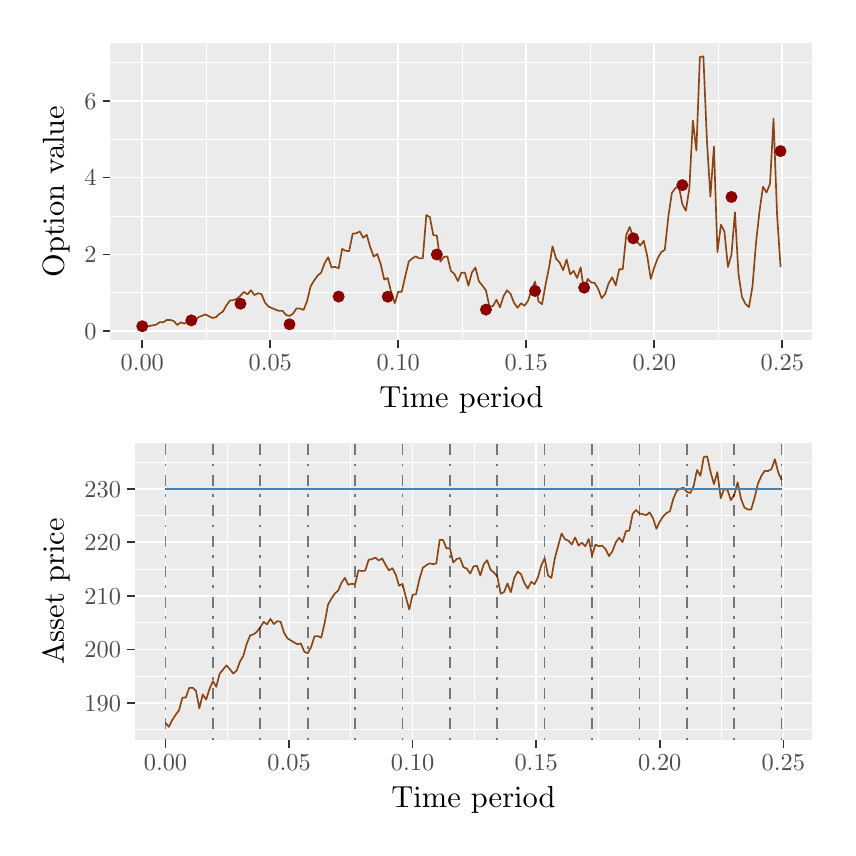
\begin{tikzpicture}[x=1pt,y=1pt]
\definecolor{fillColor}{RGB}{255,255,255}
\path[use as bounding box,fill=fillColor,fill opacity=0.00] (0,0) rectangle (289.08,289.08);
\begin{scope}
\path[clip] (  0.00,144.54) rectangle (289.08,289.08);
\definecolor{drawColor}{RGB}{255,255,255}
\definecolor{fillColor}{RGB}{255,255,255}

\path[draw=drawColor,line width= 0.6pt,line join=round,line cap=round,fill=fillColor] (  0.00,144.54) rectangle (289.08,289.08);
\end{scope}
\begin{scope}
\path[clip] ( 29.87,176.07) rectangle (283.58,283.58);
\definecolor{fillColor}{gray}{0.92}

\path[fill=fillColor] ( 29.87,176.07) rectangle (283.58,283.58);
\definecolor{drawColor}{RGB}{255,255,255}

\path[draw=drawColor,line width= 0.3pt,line join=round] ( 29.87,193.28) --
	(283.58,193.28);

\path[draw=drawColor,line width= 0.3pt,line join=round] ( 29.87,221.03) --
	(283.58,221.03);

\path[draw=drawColor,line width= 0.3pt,line join=round] ( 29.87,248.79) --
	(283.58,248.79);

\path[draw=drawColor,line width= 0.3pt,line join=round] ( 29.87,276.54) --
	(283.58,276.54);

\path[draw=drawColor,line width= 0.3pt,line join=round] ( 64.53,176.07) --
	( 64.53,283.58);

\path[draw=drawColor,line width= 0.3pt,line join=round] (110.79,176.07) --
	(110.79,283.58);

\path[draw=drawColor,line width= 0.3pt,line join=round] (157.04,176.07) --
	(157.04,283.58);

\path[draw=drawColor,line width= 0.3pt,line join=round] (203.30,176.07) --
	(203.30,283.58);

\path[draw=drawColor,line width= 0.3pt,line join=round] (249.55,176.07) --
	(249.55,283.58);

\path[draw=drawColor,line width= 0.6pt,line join=round] ( 29.87,179.41) --
	(283.58,179.41);

\path[draw=drawColor,line width= 0.6pt,line join=round] ( 29.87,207.16) --
	(283.58,207.16);

\path[draw=drawColor,line width= 0.6pt,line join=round] ( 29.87,234.91) --
	(283.58,234.91);

\path[draw=drawColor,line width= 0.6pt,line join=round] ( 29.87,262.66) --
	(283.58,262.66);

\path[draw=drawColor,line width= 0.6pt,line join=round] ( 41.40,176.07) --
	( 41.40,283.58);

\path[draw=drawColor,line width= 0.6pt,line join=round] ( 87.66,176.07) --
	( 87.66,283.58);

\path[draw=drawColor,line width= 0.6pt,line join=round] (133.91,176.07) --
	(133.91,283.58);

\path[draw=drawColor,line width= 0.6pt,line join=round] (180.17,176.07) --
	(180.17,283.58);

\path[draw=drawColor,line width= 0.6pt,line join=round] (226.43,176.07) --
	(226.43,283.58);

\path[draw=drawColor,line width= 0.6pt,line join=round] (272.68,176.07) --
	(272.68,283.58);
\definecolor{drawColor}{RGB}{139,69,19}

\path[draw=drawColor,line width= 0.6pt,line join=round] ( 41.40,181.19) --
	( 42.67,180.96) --
	( 43.94,181.27) --
	( 45.20,181.52) --
	( 46.47,181.77) --
	( 47.74,182.68) --
	( 49.00,182.63) --
	( 50.27,183.47) --
	( 51.54,183.44) --
	( 52.81,183.07) --
	( 54.07,181.63) --
	( 55.34,182.61) --
	( 56.61,182.14) --
	( 57.88,182.99) --
	( 59.14,183.74) --
	( 60.41,183.07) --
	( 61.68,184.48) --
	( 62.95,184.94) --
	( 64.21,185.47) --
	( 65.48,184.82) --
	( 66.75,184.18) --
	( 68.01,184.45) --
	( 69.28,185.65) --
	( 70.55,186.50) --
	( 71.82,188.73) --
	( 73.08,190.49) --
	( 74.35,190.62) --
	( 75.62,191.13) --
	( 76.89,192.21) --
	( 78.15,193.59) --
	( 79.42,192.69) --
	( 80.69,194.19) --
	( 81.95,192.45) --
	( 83.22,193.11) --
	( 84.49,192.79) --
	( 85.76,189.74) --
	( 87.02,188.32) --
	( 88.29,187.73) --
	( 89.56,187.19) --
	( 90.83,186.73) --
	( 92.09,186.76) --
	( 93.36,185.27) --
	( 94.63,184.92) --
	( 95.89,185.77) --
	( 97.16,187.66) --
	( 98.43,187.56) --
	( 99.70,187.10) --
	(100.96,190.26) --
	(102.23,195.62) --
	(103.50,197.68) --
	(104.77,199.50) --
	(106.03,200.51) --
	(107.30,203.98) --
	(108.57,206.12) --
	(109.83,202.41) --
	(111.10,202.65) --
	(112.37,202.13) --
	(113.64,209.15) --
	(114.90,208.44) --
	(116.17,208.36) --
	(117.44,214.61) --
	(118.71,214.78) --
	(119.97,215.45) --
	(121.24,213.16) --
	(122.51,214.21) --
	(123.77,209.83) --
	(125.04,206.34) --
	(126.31,207.29) --
	(127.58,203.57) --
	(128.84,198.08) --
	(130.11,198.59) --
	(131.38,193.33) --
	(132.65,189.50) --
	(133.91,193.66) --
	(135.18,193.64) --
	(136.45,199.32) --
	(137.72,204.62) --
	(138.98,205.69) --
	(140.25,206.45) --
	(141.52,205.70) --
	(142.78,205.73) --
	(144.05,221.38) --
	(145.32,220.64) --
	(146.59,214.06) --
	(147.85,213.98) --
	(149.12,204.56) --
	(150.39,206.24) --
	(151.66,206.42) --
	(152.92,201.16) --
	(154.19,200.08) --
	(155.46,197.49) --
	(156.72,200.57) --
	(157.99,200.50) --
	(159.26,195.84) --
	(160.53,200.64) --
	(161.79,202.38) --
	(163.06,197.40) --
	(164.33,195.87) --
	(165.60,194.12) --
	(166.86,188.28) --
	(168.13,188.48) --
	(169.40,190.78) --
	(170.66,188.02) --
	(171.93,192.04) --
	(173.20,194.18) --
	(174.47,192.90) --
	(175.73,189.69) --
	(177.00,187.87) --
	(178.27,189.50) --
	(179.54,188.59) --
	(180.80,190.38) --
	(182.07,194.42) --
	(183.34,197.35) --
	(184.60,190.14) --
	(185.87,189.17) --
	(187.14,196.23) --
	(188.41,202.50) --
	(189.67,210.06) --
	(190.94,205.60) --
	(192.21,204.23) --
	(193.48,201.45) --
	(194.74,205.31) --
	(196.01,199.97) --
	(197.28,201.20) --
	(198.54,198.63) --
	(199.81,202.49) --
	(201.08,193.50) --
	(202.35,198.30) --
	(203.61,197.02) --
	(204.88,196.84) --
	(206.15,194.69) --
	(207.42,191.33) --
	(208.68,192.87) --
	(209.95,196.76) --
	(211.22,198.88) --
	(212.49,195.98) --
	(213.75,201.81) --
	(215.02,201.78) --
	(216.29,214.16) --
	(217.55,217.07) --
	(218.82,213.16) --
	(220.09,211.84) --
	(221.36,210.34) --
	(222.62,212.08) --
	(223.89,206.43) --
	(225.16,198.29) --
	(226.43,202.49) --
	(227.69,205.82) --
	(228.96,207.99) --
	(230.23,208.79) --
	(231.49,220.62) --
	(232.76,229.32) --
	(234.03,231.09) --
	(235.30,231.75) --
	(236.56,225.34) --
	(237.83,222.91) --
	(239.10,231.05) --
	(240.37,255.49) --
	(241.63,244.67) --
	(242.90,278.48) --
	(244.17,278.69) --
	(245.43,248.47) --
	(246.70,228.01) --
	(247.97,246.11) --
	(249.24,207.96) --
	(250.50,217.88) --
	(251.77,215.36) --
	(253.04,202.59) --
	(254.31,207.06) --
	(255.57,222.38) --
	(256.84,200.14) --
	(258.11,191.74) --
	(259.37,189.21) --
	(260.64,188.12) --
	(261.91,195.61) --
	(263.18,211.30) --
	(264.44,222.75) --
	(265.71,231.60) --
	(266.98,229.52) --
	(268.25,232.69) --
	(269.51,256.19) --
	(270.78,221.72) --
	(272.05,202.60);
\definecolor{drawColor}{RGB}{139,0,0}
\definecolor{fillColor}{RGB}{139,0,0}

\path[draw=drawColor,line width= 0.4pt,line join=round,line cap=round,fill=fillColor] ( 41.40,181.19) circle (  1.96);

\path[draw=drawColor,line width= 0.4pt,line join=round,line cap=round,fill=fillColor] ( 59.14,183.31) circle (  1.96);

\path[draw=drawColor,line width= 0.4pt,line join=round,line cap=round,fill=fillColor] ( 76.89,189.33) circle (  1.96);

\path[draw=drawColor,line width= 0.4pt,line join=round,line cap=round,fill=fillColor] ( 94.63,181.89) circle (  1.96);

\path[draw=drawColor,line width= 0.4pt,line join=round,line cap=round,fill=fillColor] (112.37,191.91) circle (  1.96);

\path[draw=drawColor,line width= 0.4pt,line join=round,line cap=round,fill=fillColor] (130.11,191.87) circle (  1.96);

\path[draw=drawColor,line width= 0.4pt,line join=round,line cap=round,fill=fillColor] (147.85,207.11) circle (  1.96);

\path[draw=drawColor,line width= 0.4pt,line join=round,line cap=round,fill=fillColor] (165.60,187.19) circle (  1.96);

\path[draw=drawColor,line width= 0.4pt,line join=round,line cap=round,fill=fillColor] (183.34,193.94) circle (  1.96);

\path[draw=drawColor,line width= 0.4pt,line join=round,line cap=round,fill=fillColor] (201.08,195.14) circle (  1.96);

\path[draw=drawColor,line width= 0.4pt,line join=round,line cap=round,fill=fillColor] (218.82,212.96) circle (  1.96);

\path[draw=drawColor,line width= 0.4pt,line join=round,line cap=round,fill=fillColor] (236.56,232.18) circle (  1.96);

\path[draw=drawColor,line width= 0.4pt,line join=round,line cap=round,fill=fillColor] (254.31,227.90) circle (  1.96);

\path[draw=drawColor,line width= 0.4pt,line join=round,line cap=round,fill=fillColor] (272.05,244.47) circle (  1.96);
\end{scope}
\begin{scope}
\path[clip] (  0.00,  0.00) rectangle (289.08,289.08);
\definecolor{drawColor}{gray}{0.30}

\node[text=drawColor,anchor=base east,inner sep=0pt, outer sep=0pt, scale=  0.88] at ( 24.92,176.37) {0};

\node[text=drawColor,anchor=base east,inner sep=0pt, outer sep=0pt, scale=  0.88] at ( 24.92,204.13) {2};

\node[text=drawColor,anchor=base east,inner sep=0pt, outer sep=0pt, scale=  0.88] at ( 24.92,231.88) {4};

\node[text=drawColor,anchor=base east,inner sep=0pt, outer sep=0pt, scale=  0.88] at ( 24.92,259.63) {6};
\end{scope}
\begin{scope}
\path[clip] (  0.00,  0.00) rectangle (289.08,289.08);
\definecolor{drawColor}{gray}{0.20}

\path[draw=drawColor,line width= 0.6pt,line join=round] ( 27.12,179.41) --
	( 29.87,179.41);

\path[draw=drawColor,line width= 0.6pt,line join=round] ( 27.12,207.16) --
	( 29.87,207.16);

\path[draw=drawColor,line width= 0.6pt,line join=round] ( 27.12,234.91) --
	( 29.87,234.91);

\path[draw=drawColor,line width= 0.6pt,line join=round] ( 27.12,262.66) --
	( 29.87,262.66);
\end{scope}
\begin{scope}
\path[clip] (  0.00,  0.00) rectangle (289.08,289.08);
\definecolor{drawColor}{gray}{0.20}

\path[draw=drawColor,line width= 0.6pt,line join=round] ( 41.40,173.32) --
	( 41.40,176.07);

\path[draw=drawColor,line width= 0.6pt,line join=round] ( 87.66,173.32) --
	( 87.66,176.07);

\path[draw=drawColor,line width= 0.6pt,line join=round] (133.91,173.32) --
	(133.91,176.07);

\path[draw=drawColor,line width= 0.6pt,line join=round] (180.17,173.32) --
	(180.17,176.07);

\path[draw=drawColor,line width= 0.6pt,line join=round] (226.43,173.32) --
	(226.43,176.07);

\path[draw=drawColor,line width= 0.6pt,line join=round] (272.68,173.32) --
	(272.68,176.07);
\end{scope}
\begin{scope}
\path[clip] (  0.00,  0.00) rectangle (289.08,289.08);
\definecolor{drawColor}{gray}{0.30}

\node[text=drawColor,anchor=base,inner sep=0pt, outer sep=0pt, scale=  0.88] at ( 41.40,165.06) {0.00};

\node[text=drawColor,anchor=base,inner sep=0pt, outer sep=0pt, scale=  0.88] at ( 87.66,165.06) {0.05};

\node[text=drawColor,anchor=base,inner sep=0pt, outer sep=0pt, scale=  0.88] at (133.91,165.06) {0.10};

\node[text=drawColor,anchor=base,inner sep=0pt, outer sep=0pt, scale=  0.88] at (180.17,165.06) {0.15};

\node[text=drawColor,anchor=base,inner sep=0pt, outer sep=0pt, scale=  0.88] at (226.43,165.06) {0.20};

\node[text=drawColor,anchor=base,inner sep=0pt, outer sep=0pt, scale=  0.88] at (272.68,165.06) {0.25};
\end{scope}
\begin{scope}
\path[clip] (  0.00,  0.00) rectangle (289.08,289.08);
\definecolor{drawColor}{RGB}{0,0,0}

\node[text=drawColor,anchor=base,inner sep=0pt, outer sep=0pt, scale=  1.10] at (156.72,151.98) {Time period};
\end{scope}
\begin{scope}
\path[clip] (  0.00,  0.00) rectangle (289.08,289.08);
\definecolor{drawColor}{RGB}{0,0,0}

\node[text=drawColor,rotate= 90.00,anchor=base,inner sep=0pt, outer sep=0pt, scale=  1.10] at ( 13.08,229.83) {Option value};
\end{scope}
\begin{scope}
\path[clip] (  0.00,  0.00) rectangle (289.08,144.54);
\definecolor{drawColor}{RGB}{255,255,255}
\definecolor{fillColor}{RGB}{255,255,255}

\path[draw=drawColor,line width= 0.6pt,line join=round,line cap=round,fill=fillColor] (  0.00,  0.00) rectangle (289.08,144.54);
\end{scope}
\begin{scope}
\path[clip] ( 38.67, 31.53) rectangle (283.58,139.04);
\definecolor{fillColor}{gray}{0.92}

\path[fill=fillColor] ( 38.67, 31.53) rectangle (283.58,139.04);
\definecolor{drawColor}{RGB}{255,255,255}

\path[draw=drawColor,line width= 0.3pt,line join=round] ( 38.67, 35.34) --
	(283.58, 35.34);

\path[draw=drawColor,line width= 0.3pt,line join=round] ( 38.67, 54.70) --
	(283.58, 54.70);

\path[draw=drawColor,line width= 0.3pt,line join=round] ( 38.67, 74.06) --
	(283.58, 74.06);

\path[draw=drawColor,line width= 0.3pt,line join=round] ( 38.67, 93.43) --
	(283.58, 93.43);

\path[draw=drawColor,line width= 0.3pt,line join=round] ( 38.67,112.79) --
	(283.58,112.79);

\path[draw=drawColor,line width= 0.3pt,line join=round] ( 38.67,132.15) --
	(283.58,132.15);

\path[draw=drawColor,line width= 0.3pt,line join=round] ( 72.13, 31.53) --
	( 72.13,139.04);

\path[draw=drawColor,line width= 0.3pt,line join=round] (116.78, 31.53) --
	(116.78,139.04);

\path[draw=drawColor,line width= 0.3pt,line join=round] (161.43, 31.53) --
	(161.43,139.04);

\path[draw=drawColor,line width= 0.3pt,line join=round] (206.08, 31.53) --
	(206.08,139.04);

\path[draw=drawColor,line width= 0.3pt,line join=round] (250.73, 31.53) --
	(250.73,139.04);

\path[draw=drawColor,line width= 0.6pt,line join=round] ( 38.67, 45.02) --
	(283.58, 45.02);

\path[draw=drawColor,line width= 0.6pt,line join=round] ( 38.67, 64.38) --
	(283.58, 64.38);

\path[draw=drawColor,line width= 0.6pt,line join=round] ( 38.67, 83.75) --
	(283.58, 83.75);

\path[draw=drawColor,line width= 0.6pt,line join=round] ( 38.67,103.11) --
	(283.58,103.11);

\path[draw=drawColor,line width= 0.6pt,line join=round] ( 38.67,122.47) --
	(283.58,122.47);

\path[draw=drawColor,line width= 0.6pt,line join=round] ( 49.80, 31.53) --
	( 49.80,139.04);

\path[draw=drawColor,line width= 0.6pt,line join=round] ( 94.45, 31.53) --
	( 94.45,139.04);

\path[draw=drawColor,line width= 0.6pt,line join=round] (139.10, 31.53) --
	(139.10,139.04);

\path[draw=drawColor,line width= 0.6pt,line join=round] (183.76, 31.53) --
	(183.76,139.04);

\path[draw=drawColor,line width= 0.6pt,line join=round] (228.41, 31.53) --
	(228.41,139.04);

\path[draw=drawColor,line width= 0.6pt,line join=round] (273.06, 31.53) --
	(273.06,139.04);
\definecolor{drawColor}{RGB}{139,69,19}

\path[draw=drawColor,line width= 0.6pt,line join=round] ( 49.80, 37.88) --
	( 51.02, 36.42) --
	( 52.25, 38.92) --
	( 53.47, 40.78) --
	( 54.69, 42.43) --
	( 55.92, 47.00) --
	( 57.14, 47.02) --
	( 58.36, 50.46) --
	( 59.59, 50.58) --
	( 60.81, 49.47) --
	( 62.03, 43.14) --
	( 63.26, 48.13) --
	( 64.48, 46.27) --
	( 65.70, 50.11) --
	( 66.93, 52.96) --
	( 68.15, 50.89) --
	( 69.37, 55.64) --
	( 70.60, 57.12) --
	( 71.82, 58.66) --
	( 73.04, 57.27) --
	( 74.27, 55.72) --
	( 75.49, 56.70) --
	( 76.71, 60.01) --
	( 77.94, 62.12) --
	( 79.16, 66.49) --
	( 80.38, 69.46) --
	( 81.61, 69.86) --
	( 82.83, 70.79) --
	( 84.05, 72.44) --
	( 85.28, 74.36) --
	( 86.50, 73.46) --
	( 87.72, 75.45) --
	( 88.95, 73.58) --
	( 90.17, 74.61) --
	( 91.39, 74.43) --
	( 92.62, 70.50) --
	( 93.84, 68.47) --
	( 95.06, 67.66) --
	( 96.29, 66.91) --
	( 97.51, 66.26) --
	( 98.73, 66.56) --
	( 99.96, 63.60) --
	(101.18, 62.99) --
	(102.40, 65.21) --
	(103.63, 69.16) --
	(104.85, 69.23) --
	(106.07, 68.63) --
	(107.30, 73.95) --
	(108.52, 80.54) --
	(109.74, 82.76) --
	(110.97, 84.58) --
	(112.19, 85.64) --
	(113.41, 88.53) --
	(114.64, 90.25) --
	(115.86, 87.76) --
	(117.08, 88.14) --
	(118.31, 87.95) --
	(119.53, 93.00) --
	(120.75, 92.75) --
	(121.98, 92.89) --
	(123.20, 96.77) --
	(124.42, 97.05) --
	(125.65, 97.60) --
	(126.87, 96.53) --
	(128.09, 97.29) --
	(129.32, 94.97) --
	(130.54, 92.97) --
	(131.76, 93.78) --
	(132.99, 91.49) --
	(134.21, 87.41) --
	(135.43, 88.07) --
	(136.66, 83.31) --
	(137.88, 78.89) --
	(139.10, 84.14) --
	(140.33, 84.35) --
	(141.55, 89.79) --
	(142.77, 93.89) --
	(144.00, 94.81) --
	(145.22, 95.51) --
	(146.44, 95.24) --
	(147.67, 95.48) --
	(148.89,104.06) --
	(150.11,103.91) --
	(151.34,100.89) --
	(152.56,101.05) --
	(153.78, 95.80) --
	(155.01, 97.09) --
	(156.23, 97.42) --
	(157.45, 94.15) --
	(158.68, 93.59) --
	(159.90, 91.80) --
	(161.12, 94.42) --
	(162.35, 94.61) --
	(163.57, 91.14) --
	(164.79, 95.18) --
	(166.02, 96.64) --
	(167.24, 93.21) --
	(168.46, 92.19) --
	(169.69, 90.87) --
	(170.91, 84.55) --
	(172.13, 85.12) --
	(173.36, 88.26) --
	(174.58, 85.07) --
	(175.80, 90.19) --
	(177.03, 92.55) --
	(178.25, 91.62) --
	(179.47, 88.45) --
	(180.70, 86.39) --
	(181.92, 88.82) --
	(183.14, 87.98) --
	(184.37, 90.45) --
	(185.59, 94.71) --
	(186.81, 97.36) --
	(188.04, 91.09) --
	(189.26, 90.28) --
	(190.48, 97.33) --
	(191.71,101.92) --
	(192.93,106.30) --
	(194.15,104.22) --
	(195.38,103.72) --
	(196.60,102.34) --
	(197.82,104.84) --
	(199.05,101.95) --
	(200.27,103.00) --
	(201.49,101.64) --
	(202.72,104.33) --
	(203.94, 98.41) --
	(205.16,102.30) --
	(206.39,101.72) --
	(207.61,101.90) --
	(208.83,100.64) --
	(210.06, 98.14) --
	(211.28, 99.84) --
	(212.50,103.09) --
	(213.73,104.79) --
	(214.95,103.20) --
	(216.17,107.11) --
	(217.40,107.40) --
	(218.62,113.40) --
	(219.84,114.77) --
	(221.07,113.53) --
	(222.29,113.27) --
	(223.51,112.94) --
	(224.74,113.92) --
	(225.96,111.83) --
	(227.18,108.01) --
	(228.41,110.59) --
	(229.63,112.47) --
	(230.85,113.72) --
	(232.08,114.35) --
	(233.30,118.87) --
	(234.52,121.71) --
	(235.75,122.44) --
	(236.97,122.86) --
	(238.19,121.34) --
	(239.42,120.91) --
	(240.64,123.40) --
	(241.86,129.24) --
	(243.09,127.12) --
	(244.31,133.97) --
	(245.53,134.15) --
	(246.76,128.56) --
	(247.98,124.16) --
	(249.20,128.48) --
	(250.43,119.05) --
	(251.65,122.39) --
	(252.87,122.02) --
	(254.10,118.34) --
	(255.32,120.28) --
	(256.54,124.79) --
	(257.77,118.79) --
	(258.99,115.71) --
	(260.21,114.94) --
	(261.44,114.97) --
	(262.66,119.20) --
	(263.88,124.29) --
	(265.11,127.08) --
	(266.33,128.96) --
	(267.55,128.86) --
	(268.78,129.59) --
	(270.00,133.14) --
	(271.22,128.31) --
	(272.45,125.70);
\definecolor{drawColor}{RGB}{70,130,180}

\path[draw=drawColor,line width= 0.6pt,line join=round] ( 49.80,122.47) --
	( 51.02,122.47) --
	( 52.25,122.47) --
	( 53.47,122.47) --
	( 54.69,122.47) --
	( 55.92,122.47) --
	( 57.14,122.47) --
	( 58.36,122.47) --
	( 59.59,122.47) --
	( 60.81,122.47) --
	( 62.03,122.47) --
	( 63.26,122.47) --
	( 64.48,122.47) --
	( 65.70,122.47) --
	( 66.93,122.47) --
	( 68.15,122.47) --
	( 69.37,122.47) --
	( 70.60,122.47) --
	( 71.82,122.47) --
	( 73.04,122.47) --
	( 74.27,122.47) --
	( 75.49,122.47) --
	( 76.71,122.47) --
	( 77.94,122.47) --
	( 79.16,122.47) --
	( 80.38,122.47) --
	( 81.61,122.47) --
	( 82.83,122.47) --
	( 84.05,122.47) --
	( 85.28,122.47) --
	( 86.50,122.47) --
	( 87.72,122.47) --
	( 88.95,122.47) --
	( 90.17,122.47) --
	( 91.39,122.47) --
	( 92.62,122.47) --
	( 93.84,122.47) --
	( 95.06,122.47) --
	( 96.29,122.47) --
	( 97.51,122.47) --
	( 98.73,122.47) --
	( 99.96,122.47) --
	(101.18,122.47) --
	(102.40,122.47) --
	(103.63,122.47) --
	(104.85,122.47) --
	(106.07,122.47) --
	(107.30,122.47) --
	(108.52,122.47) --
	(109.74,122.47) --
	(110.97,122.47) --
	(112.19,122.47) --
	(113.41,122.47) --
	(114.64,122.47) --
	(115.86,122.47) --
	(117.08,122.47) --
	(118.31,122.47) --
	(119.53,122.47) --
	(120.75,122.47) --
	(121.98,122.47) --
	(123.20,122.47) --
	(124.42,122.47) --
	(125.65,122.47) --
	(126.87,122.47) --
	(128.09,122.47) --
	(129.32,122.47) --
	(130.54,122.47) --
	(131.76,122.47) --
	(132.99,122.47) --
	(134.21,122.47) --
	(135.43,122.47) --
	(136.66,122.47) --
	(137.88,122.47) --
	(139.10,122.47) --
	(140.33,122.47) --
	(141.55,122.47) --
	(142.77,122.47) --
	(144.00,122.47) --
	(145.22,122.47) --
	(146.44,122.47) --
	(147.67,122.47) --
	(148.89,122.47) --
	(150.11,122.47) --
	(151.34,122.47) --
	(152.56,122.47) --
	(153.78,122.47) --
	(155.01,122.47) --
	(156.23,122.47) --
	(157.45,122.47) --
	(158.68,122.47) --
	(159.90,122.47) --
	(161.12,122.47) --
	(162.35,122.47) --
	(163.57,122.47) --
	(164.79,122.47) --
	(166.02,122.47) --
	(167.24,122.47) --
	(168.46,122.47) --
	(169.69,122.47) --
	(170.91,122.47) --
	(172.13,122.47) --
	(173.36,122.47) --
	(174.58,122.47) --
	(175.80,122.47) --
	(177.03,122.47) --
	(178.25,122.47) --
	(179.47,122.47) --
	(180.70,122.47) --
	(181.92,122.47) --
	(183.14,122.47) --
	(184.37,122.47) --
	(185.59,122.47) --
	(186.81,122.47) --
	(188.04,122.47) --
	(189.26,122.47) --
	(190.48,122.47) --
	(191.71,122.47) --
	(192.93,122.47) --
	(194.15,122.47) --
	(195.38,122.47) --
	(196.60,122.47) --
	(197.82,122.47) --
	(199.05,122.47) --
	(200.27,122.47) --
	(201.49,122.47) --
	(202.72,122.47) --
	(203.94,122.47) --
	(205.16,122.47) --
	(206.39,122.47) --
	(207.61,122.47) --
	(208.83,122.47) --
	(210.06,122.47) --
	(211.28,122.47) --
	(212.50,122.47) --
	(213.73,122.47) --
	(214.95,122.47) --
	(216.17,122.47) --
	(217.40,122.47) --
	(218.62,122.47) --
	(219.84,122.47) --
	(221.07,122.47) --
	(222.29,122.47) --
	(223.51,122.47) --
	(224.74,122.47) --
	(225.96,122.47) --
	(227.18,122.47) --
	(228.41,122.47) --
	(229.63,122.47) --
	(230.85,122.47) --
	(232.08,122.47) --
	(233.30,122.47) --
	(234.52,122.47) --
	(235.75,122.47) --
	(236.97,122.47) --
	(238.19,122.47) --
	(239.42,122.47) --
	(240.64,122.47) --
	(241.86,122.47) --
	(243.09,122.47) --
	(244.31,122.47) --
	(245.53,122.47) --
	(246.76,122.47) --
	(247.98,122.47) --
	(249.20,122.47) --
	(250.43,122.47) --
	(251.65,122.47) --
	(252.87,122.47) --
	(254.10,122.47) --
	(255.32,122.47) --
	(256.54,122.47) --
	(257.77,122.47) --
	(258.99,122.47) --
	(260.21,122.47) --
	(261.44,122.47) --
	(262.66,122.47) --
	(263.88,122.47) --
	(265.11,122.47) --
	(266.33,122.47) --
	(267.55,122.47) --
	(268.78,122.47) --
	(270.00,122.47) --
	(271.22,122.47) --
	(272.45,122.47);
\definecolor{drawColor}{RGB}{0,0,0}

\path[draw=drawColor,draw opacity=0.50,line width= 0.6pt,dash pattern=on 1pt off 3pt on 4pt off 3pt ,line join=round] ( 49.80, 31.53) -- ( 49.80,139.04);

\path[draw=drawColor,draw opacity=0.50,line width= 0.6pt,dash pattern=on 1pt off 3pt on 4pt off 3pt ,line join=round] ( 66.93, 31.53) -- ( 66.93,139.04);

\path[draw=drawColor,draw opacity=0.50,line width= 0.6pt,dash pattern=on 1pt off 3pt on 4pt off 3pt ,line join=round] ( 84.05, 31.53) -- ( 84.05,139.04);

\path[draw=drawColor,draw opacity=0.50,line width= 0.6pt,dash pattern=on 1pt off 3pt on 4pt off 3pt ,line join=round] (101.18, 31.53) -- (101.18,139.04);

\path[draw=drawColor,draw opacity=0.50,line width= 0.6pt,dash pattern=on 1pt off 3pt on 4pt off 3pt ,line join=round] (118.31, 31.53) -- (118.31,139.04);

\path[draw=drawColor,draw opacity=0.50,line width= 0.6pt,dash pattern=on 1pt off 3pt on 4pt off 3pt ,line join=round] (135.43, 31.53) -- (135.43,139.04);

\path[draw=drawColor,draw opacity=0.50,line width= 0.6pt,dash pattern=on 1pt off 3pt on 4pt off 3pt ,line join=round] (152.56, 31.53) -- (152.56,139.04);

\path[draw=drawColor,draw opacity=0.50,line width= 0.6pt,dash pattern=on 1pt off 3pt on 4pt off 3pt ,line join=round] (169.69, 31.53) -- (169.69,139.04);

\path[draw=drawColor,draw opacity=0.50,line width= 0.6pt,dash pattern=on 1pt off 3pt on 4pt off 3pt ,line join=round] (186.81, 31.53) -- (186.81,139.04);

\path[draw=drawColor,draw opacity=0.50,line width= 0.6pt,dash pattern=on 1pt off 3pt on 4pt off 3pt ,line join=round] (203.94, 31.53) -- (203.94,139.04);

\path[draw=drawColor,draw opacity=0.50,line width= 0.6pt,dash pattern=on 1pt off 3pt on 4pt off 3pt ,line join=round] (221.07, 31.53) -- (221.07,139.04);

\path[draw=drawColor,draw opacity=0.50,line width= 0.6pt,dash pattern=on 1pt off 3pt on 4pt off 3pt ,line join=round] (238.19, 31.53) -- (238.19,139.04);

\path[draw=drawColor,draw opacity=0.50,line width= 0.6pt,dash pattern=on 1pt off 3pt on 4pt off 3pt ,line join=round] (255.32, 31.53) -- (255.32,139.04);

\path[draw=drawColor,draw opacity=0.50,line width= 0.6pt,dash pattern=on 1pt off 3pt on 4pt off 3pt ,line join=round] (272.45, 31.53) -- (272.45,139.04);
\end{scope}
\begin{scope}
\path[clip] (  0.00,  0.00) rectangle (289.08,289.08);
\definecolor{drawColor}{gray}{0.30}

\node[text=drawColor,anchor=base east,inner sep=0pt, outer sep=0pt, scale=  0.88] at ( 33.72, 41.99) {190};

\node[text=drawColor,anchor=base east,inner sep=0pt, outer sep=0pt, scale=  0.88] at ( 33.72, 61.35) {200};

\node[text=drawColor,anchor=base east,inner sep=0pt, outer sep=0pt, scale=  0.88] at ( 33.72, 80.72) {210};

\node[text=drawColor,anchor=base east,inner sep=0pt, outer sep=0pt, scale=  0.88] at ( 33.72,100.08) {220};

\node[text=drawColor,anchor=base east,inner sep=0pt, outer sep=0pt, scale=  0.88] at ( 33.72,119.44) {230};
\end{scope}
\begin{scope}
\path[clip] (  0.00,  0.00) rectangle (289.08,289.08);
\definecolor{drawColor}{gray}{0.20}

\path[draw=drawColor,line width= 0.6pt,line join=round] ( 35.92, 45.02) --
	( 38.67, 45.02);

\path[draw=drawColor,line width= 0.6pt,line join=round] ( 35.92, 64.38) --
	( 38.67, 64.38);

\path[draw=drawColor,line width= 0.6pt,line join=round] ( 35.92, 83.75) --
	( 38.67, 83.75);

\path[draw=drawColor,line width= 0.6pt,line join=round] ( 35.92,103.11) --
	( 38.67,103.11);

\path[draw=drawColor,line width= 0.6pt,line join=round] ( 35.92,122.47) --
	( 38.67,122.47);
\end{scope}
\begin{scope}
\path[clip] (  0.00,  0.00) rectangle (289.08,289.08);
\definecolor{drawColor}{gray}{0.20}

\path[draw=drawColor,line width= 0.6pt,line join=round] ( 49.80, 28.78) --
	( 49.80, 31.53);

\path[draw=drawColor,line width= 0.6pt,line join=round] ( 94.45, 28.78) --
	( 94.45, 31.53);

\path[draw=drawColor,line width= 0.6pt,line join=round] (139.10, 28.78) --
	(139.10, 31.53);

\path[draw=drawColor,line width= 0.6pt,line join=round] (183.76, 28.78) --
	(183.76, 31.53);

\path[draw=drawColor,line width= 0.6pt,line join=round] (228.41, 28.78) --
	(228.41, 31.53);

\path[draw=drawColor,line width= 0.6pt,line join=round] (273.06, 28.78) --
	(273.06, 31.53);
\end{scope}
\begin{scope}
\path[clip] (  0.00,  0.00) rectangle (289.08,289.08);
\definecolor{drawColor}{gray}{0.30}

\node[text=drawColor,anchor=base,inner sep=0pt, outer sep=0pt, scale=  0.88] at ( 49.80, 20.52) {0.00};

\node[text=drawColor,anchor=base,inner sep=0pt, outer sep=0pt, scale=  0.88] at ( 94.45, 20.52) {0.05};

\node[text=drawColor,anchor=base,inner sep=0pt, outer sep=0pt, scale=  0.88] at (139.10, 20.52) {0.10};

\node[text=drawColor,anchor=base,inner sep=0pt, outer sep=0pt, scale=  0.88] at (183.76, 20.52) {0.15};

\node[text=drawColor,anchor=base,inner sep=0pt, outer sep=0pt, scale=  0.88] at (228.41, 20.52) {0.20};

\node[text=drawColor,anchor=base,inner sep=0pt, outer sep=0pt, scale=  0.88] at (273.06, 20.52) {0.25};
\end{scope}
\begin{scope}
\path[clip] (  0.00,  0.00) rectangle (289.08,289.08);
\definecolor{drawColor}{RGB}{0,0,0}

\node[text=drawColor,anchor=base,inner sep=0pt, outer sep=0pt, scale=  1.10] at (161.12,  7.44) {Time period};
\end{scope}
\begin{scope}
\path[clip] (  0.00,  0.00) rectangle (289.08,289.08);
\definecolor{drawColor}{RGB}{0,0,0}

\node[text=drawColor,rotate= 90.00,anchor=base,inner sep=0pt, outer sep=0pt, scale=  1.10] at ( 13.08, 85.29) {Asset price};
\end{scope}
\end{tikzpicture}

  \rule{40mm}{20mm}
  \caption{European call option with higher theta as time goes to maturity}
   %
  % BEGIN OF FLOATNOTE
  %
  \begin{changemargin}{0.5cm}{0.5cm}
  \medskip
\footnotesize
\setstretch{1.0}\textbf{Notes.} The parameters passed to the function \textit{bsm\_call}, to compute the different option values are: $\tau = 0.2493$, $K = 230$, $\sigma = 0.1958$, $r = 0.01896$. While the underlying asset followed differents dummy paths constructed through the function \textit{bsm\_ts} taking as arguments: $\sigma = 0.1958$, $\alpha = 0.48229$. The hedge is weekly balanced.
  \end{changemargin}
  %
  % END OF FLOATNOTE
  %
  \label{p:analysis:gbm:pl:theta:high}
\end{figure}



By resuming the solution of theta given in \citet{shreve}, for the European call option, one gets the following equations.

\begin{align}
  \Theta = -r K e^{-r (T-t)} N\bigg(d_{-}(T-t, S(t))\bigg) -
    \frac{\sigma S(t)}{2\sqrt{T-t}} N^{'}\bigg(d_{+}(T-t, S(t))\bigg) \label{eq:analysis:theta}\\
  \intertext{with}
  d_{\pm}(\tau, x) = \frac{1}{\sigma \sqrt{\tau}} \left [
    \ln\frac{x}{K} + \left( r \pm \frac{\sigma^2}{2} \right) \tau
  \right]\label{eq:analysis:d}
\end{align}
With $N$ and $N^{'}$ respectively standing for the normal cumulative distribution function (CDF) and for the normal probability density function (PDF). 

Intuitively, according to \cref{eq:analysis:theta} As $\tau \downarrow \implies \sigma S(t) / (2\sqrt{T-t}) \uparrow$ and $N^{'}(d_{+}(T-t, S(t)))$ gets its higher value when $d_{+}(T-t, S(t)) \to 0$.
Also, by \cref{eq:analysis:d}, for any given $\tau$ sufficiently small, the function $d_{+}$ is the nearest to zero as $x \to S(t)$.
\Cref{p:analysis:gbm:pl:theta:high} shows that it is exactly what happens for the observed option.




    
    
    

    
    
    
    
    
    
    
    
    
    
    
    







%%%%%%%%%%%%%%%%%%%%%%%%%%%%%%%%%%%%%%%%%%%%%%%%%%%%%%%%%%%%%%%%%%%%%%%%%%%%%%%%
% MERTON
%%%%%%%%%%%%%%%%%%%%%%%%%%%%%%%%%%%%%%%%%%%%%%%%%%%%%%%%%%%%%%%%%%%%%%%%%%%%%%%%
\section{Merton jump-diffusion performance measuring}
\label{sec:section name}

\Cref{t:analysis:merton:pl} is arranged the same way than \cref{t:analysis:bsm:pl} but except that the columns are subdivided to give the information on the relative P\&Ls obtained by either replicating the long position in the European calls with the delta MJD or BSM.
For instance, the result exhibited in the column "91 dbm > $delta_{bsm}$" and row "140 > intraday" gives the mean relative P\&L computed on a series of delta-hedging on European call options with a maturity of 91 days (3 months), a strike of  \$140, a rebalancing done twice a day and with $\Delta(t)$ computed using the BSM equation. 
Whilst the output in the column "91 dbm > $delta_{mjd}$" and row "140 > intraday", gives the same information but with $\Delta(t)$ computed by using the Merton equation.

The dummy time-series of the underlying asset, which will serve the analysis are all displayed in \cref{p:analysis:mjd:100}. 
According to the dimension of \cref{t:analysis:merton:pl}, any of them is used ninety times in the study since each has been involved in the coverage of options with five different strikes, three maturities, three distinctive rebalancing frequencies and depending on two deltas as well.
The total number of samples is one hundred, and consequently, \Cref{t:analysis:merton:pl} summarizes nine thousand delta-hedging strategies.

\begin{figure}[h]
  \centering
  % % Created by tikzDevice version 0.11 on 2018-08-05 19:28:26
% !TEX encoding = UTF-8 Unicode
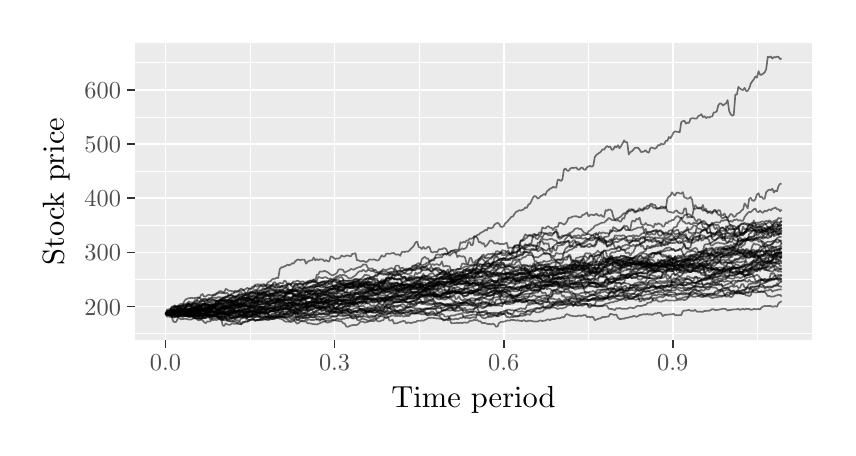
\begin{tikzpicture}[x=1pt,y=1pt]
\definecolor{fillColor}{RGB}{255,255,255}
\path[use as bounding box,fill=fillColor,fill opacity=0.00] (0,0) rectangle (289.08,144.54);
\begin{scope}
\path[clip] (  0.00,  0.00) rectangle (289.08,144.54);
\definecolor{drawColor}{RGB}{255,255,255}
\definecolor{fillColor}{RGB}{255,255,255}

\path[draw=drawColor,line width= 0.6pt,line join=round,line cap=round,fill=fillColor] (  0.00,  0.00) rectangle (289.08,144.54);
\end{scope}
\begin{scope}
\path[clip] ( 38.67, 31.53) rectangle (283.58,139.04);
\definecolor{fillColor}{gray}{0.92}

\path[fill=fillColor] ( 38.67, 31.53) rectangle (283.58,139.04);
\definecolor{drawColor}{RGB}{255,255,255}

\path[draw=drawColor,line width= 0.3pt,line join=round] ( 38.67, 33.95) --
	(283.58, 33.95);

\path[draw=drawColor,line width= 0.3pt,line join=round] ( 38.67, 53.53) --
	(283.58, 53.53);

\path[draw=drawColor,line width= 0.3pt,line join=round] ( 38.67, 73.12) --
	(283.58, 73.12);

\path[draw=drawColor,line width= 0.3pt,line join=round] ( 38.67, 92.70) --
	(283.58, 92.70);

\path[draw=drawColor,line width= 0.3pt,line join=round] ( 38.67,112.28) --
	(283.58,112.28);

\path[draw=drawColor,line width= 0.3pt,line join=round] ( 38.67,131.86) --
	(283.58,131.86);

\path[draw=drawColor,line width= 0.3pt,line join=round] ( 80.35, 31.53) --
	( 80.35,139.04);

\path[draw=drawColor,line width= 0.3pt,line join=round] (141.45, 31.53) --
	(141.45,139.04);

\path[draw=drawColor,line width= 0.3pt,line join=round] (202.56, 31.53) --
	(202.56,139.04);

\path[draw=drawColor,line width= 0.3pt,line join=round] (263.66, 31.53) --
	(263.66,139.04);

\path[draw=drawColor,line width= 0.6pt,line join=round] ( 38.67, 43.74) --
	(283.58, 43.74);

\path[draw=drawColor,line width= 0.6pt,line join=round] ( 38.67, 63.33) --
	(283.58, 63.33);

\path[draw=drawColor,line width= 0.6pt,line join=round] ( 38.67, 82.91) --
	(283.58, 82.91);

\path[draw=drawColor,line width= 0.6pt,line join=round] ( 38.67,102.49) --
	(283.58,102.49);

\path[draw=drawColor,line width= 0.6pt,line join=round] ( 38.67,122.07) --
	(283.58,122.07);

\path[draw=drawColor,line width= 0.6pt,line join=round] ( 49.80, 31.53) --
	( 49.80,139.04);

\path[draw=drawColor,line width= 0.6pt,line join=round] (110.90, 31.53) --
	(110.90,139.04);

\path[draw=drawColor,line width= 0.6pt,line join=round] (172.00, 31.53) --
	(172.00,139.04);

\path[draw=drawColor,line width= 0.6pt,line join=round] (233.11, 31.53) --
	(233.11,139.04);
\definecolor{drawColor}{RGB}{0,0,0}

\path[draw=drawColor,draw opacity=0.55,line width= 0.6pt,line join=round] ( 49.80, 41.06) --
	( 50.36, 41.06) --
	( 50.92, 41.71) --
	( 51.47, 42.33) --
	( 52.03, 43.74) --
	( 52.59, 43.84) --
	( 53.15, 44.18) --
	( 53.71, 43.81) --
	( 54.26, 44.03) --
	( 54.82, 43.81) --
	( 55.38, 44.08) --
	( 55.94, 44.11) --
	( 56.50, 43.88) --
	( 57.05, 44.02) --
	( 57.61, 43.83) --
	( 58.17, 43.88) --
	( 58.73, 44.13) --
	( 59.29, 44.24) --
	( 59.84, 44.02) --
	( 60.40, 44.01) --
	( 60.96, 44.35) --
	( 61.52, 44.35) --
	( 62.08, 44.60) --
	( 62.63, 44.44) --
	( 63.19, 44.67) --
	( 63.75, 44.85) --
	( 64.31, 44.87) --
	( 64.87, 44.81) --
	( 65.42, 45.40) --
	( 65.98, 45.24) --
	( 66.54, 45.36) --
	( 67.10, 45.48) --
	( 67.66, 45.66) --
	( 68.21, 45.63) --
	( 68.77, 45.63) --
	( 69.33, 46.06) --
	( 69.89, 46.08) --
	( 70.45, 46.09) --
	( 71.00, 45.72) --
	( 71.56, 45.71) --
	( 72.12, 45.41) --
	( 72.68, 45.36) --
	( 73.24, 45.37) --
	( 73.79, 45.57) --
	( 74.35, 45.75) --
	( 74.91, 45.91) --
	( 75.47, 46.07) --
	( 76.03, 46.43) --
	( 76.58, 46.84) --
	( 77.14, 46.60) --
	( 77.70, 46.39) --
	( 78.26, 46.36) --
	( 78.82, 47.03) --
	( 79.37, 47.27) --
	( 79.93, 47.60) --
	( 80.49, 47.48) --
	( 81.05, 47.06) --
	( 81.61, 47.25) --
	( 82.16, 47.22) --
	( 82.72, 47.18) --
	( 83.28, 47.29) --
	( 83.84, 47.92) --
	( 84.40, 47.92) --
	( 84.95, 48.09) --
	( 85.51, 48.13) --
	( 86.07, 48.03) --
	( 86.63, 48.00) --
	( 87.19, 47.90) --
	( 87.74, 48.54) --
	( 88.30, 48.46) --
	( 88.86, 47.82) --
	( 89.42, 47.77) --
	( 89.98, 47.48) --
	( 90.53, 47.24) --
	( 91.09, 47.64) --
	( 91.65, 47.23) --
	( 92.21, 47.36) --
	( 92.77, 47.22) --
	( 93.32, 46.86) --
	( 93.88, 46.99) --
	( 94.44, 47.13) --
	( 95.00, 46.84) --
	( 95.56, 47.21) --
	( 96.11, 47.87) --
	( 96.67, 47.66) --
	( 97.23, 47.73) --
	( 97.79, 48.20) --
	( 98.35, 48.32) --
	( 98.90, 49.03) --
	( 99.46, 49.58) --
	(100.02, 49.82) --
	(100.58, 49.84) --
	(101.14, 48.61) --
	(101.69, 48.74) --
	(102.25, 48.92) --
	(102.81, 49.98) --
	(103.37, 50.09) --
	(103.93, 51.23) --
	(104.48, 50.89) --
	(105.04, 51.04) --
	(105.60, 51.11) --
	(106.16, 51.55) --
	(106.72, 51.84) --
	(107.27, 51.95) --
	(107.83, 52.24) --
	(108.39, 52.40) --
	(108.95, 51.93) --
	(109.51, 51.59) --
	(110.06, 52.11) --
	(110.62, 50.52) --
	(111.18, 51.09) --
	(111.74, 50.85) --
	(112.30, 50.75) --
	(112.85, 52.14) --
	(113.41, 51.86) --
	(113.97, 52.01) --
	(114.53, 51.38) --
	(115.09, 51.44) --
	(115.65, 51.48) --
	(116.20, 51.44) --
	(116.76, 51.70) --
	(117.32, 52.08) --
	(117.88, 50.74) --
	(118.44, 50.66) --
	(118.99, 50.59) --
	(119.55, 50.18) --
	(120.11, 49.83) --
	(120.67, 49.84) --
	(121.23, 50.23) --
	(121.78, 49.98) --
	(122.34, 49.50) --
	(122.90, 49.66) --
	(123.46, 49.82) --
	(124.02, 50.23) --
	(124.57, 50.02) --
	(125.13, 49.87) --
	(125.69, 49.96) --
	(126.25, 50.33) --
	(126.81, 50.63) --
	(127.36, 50.42) --
	(127.92, 50.42) --
	(128.48, 50.48) --
	(129.04, 49.11) --
	(129.60, 48.91) --
	(130.15, 49.02) --
	(130.71, 49.33) --
	(131.27, 49.39) --
	(131.83, 49.60) --
	(132.39, 49.99) --
	(132.94, 50.36) --
	(133.50, 49.19) --
	(134.06, 49.23) --
	(134.62, 49.57) --
	(135.18, 50.13) --
	(135.73, 50.31) --
	(136.29, 50.25) --
	(136.85, 50.52) --
	(137.41, 50.39) --
	(137.97, 50.64) --
	(138.52, 50.60) --
	(139.08, 50.94) --
	(139.64, 51.51) --
	(140.20, 51.86) --
	(140.76, 52.05) --
	(141.31, 52.08) --
	(141.87, 52.12) --
	(142.43, 51.31) --
	(142.99, 51.56) --
	(143.55, 51.70) --
	(144.10, 51.94) --
	(144.66, 52.32) --
	(145.22, 51.95) --
	(145.78, 52.02) --
	(146.34, 51.42) --
	(146.89, 51.62) --
	(147.45, 52.18) --
	(148.01, 52.64) --
	(148.57, 52.74) --
	(149.13, 54.62) --
	(149.68, 54.44) --
	(150.24, 54.06) --
	(150.80, 53.89) --
	(151.36, 53.76) --
	(151.92, 53.91) --
	(152.47, 54.22) --
	(153.03, 53.93) --
	(153.59, 53.98) --
	(154.15, 54.54) --
	(154.71, 54.39) --
	(155.26, 54.46) --
	(155.82, 54.84) --
	(156.38, 55.27) --
	(156.94, 55.34) --
	(157.50, 55.62) --
	(158.05, 55.35) --
	(158.61, 52.44) --
	(159.17, 52.87) --
	(159.73, 52.08) --
	(160.29, 51.96) --
	(160.84, 52.33) --
	(161.40, 52.43) --
	(161.96, 53.04) --
	(162.52, 52.71) --
	(163.08, 50.79) --
	(163.63, 50.74) --
	(164.19, 51.64) --
	(164.75, 50.65) --
	(165.31, 50.78) --
	(165.87, 50.85) --
	(166.42, 51.06) --
	(166.98, 51.17) --
	(167.54, 51.37) --
	(168.10, 51.11) --
	(168.66, 51.57) --
	(169.21, 50.00) --
	(169.77, 48.74) --
	(170.33, 48.55) --
	(170.89, 48.36) --
	(171.45, 48.48) --
	(172.00, 48.69) --
	(172.56, 49.10) --
	(173.12, 49.39) --
	(173.68, 49.60) --
	(174.24, 49.19) --
	(174.79, 47.41) --
	(175.35, 47.13) --
	(175.91, 46.52) --
	(176.47, 46.22) --
	(177.03, 46.05) --
	(177.58, 46.20) --
	(178.14, 46.19) --
	(178.70, 46.52) --
	(179.26, 46.88) --
	(179.82, 46.64) --
	(180.37, 46.69) --
	(180.93, 47.16) --
	(181.49, 48.33) --
	(182.05, 48.45) --
	(182.61, 48.52) --
	(183.17, 48.69) --
	(183.72, 48.95) --
	(184.28, 48.76) --
	(184.84, 49.55) --
	(185.40, 50.45) --
	(185.96, 50.31) --
	(186.51, 50.12) --
	(187.07, 50.81) --
	(187.63, 50.74) --
	(188.19, 51.29) --
	(188.75, 51.21) --
	(189.30, 51.19) --
	(189.86, 51.22) --
	(190.42, 51.08) --
	(190.98, 51.58) --
	(191.54, 51.35) --
	(192.09, 51.43) --
	(192.65, 50.88) --
	(193.21, 50.79) --
	(193.77, 50.82) --
	(194.33, 50.88) --
	(194.88, 51.10) --
	(195.44, 51.08) --
	(196.00, 51.03) --
	(196.56, 50.97) --
	(197.12, 51.22) --
	(197.67, 52.43) --
	(198.23, 52.50) --
	(198.79, 52.50) --
	(199.35, 52.73) --
	(199.91, 53.09) --
	(200.46, 53.21) --
	(201.02, 54.11) --
	(201.58, 54.29) --
	(202.14, 54.60) --
	(202.70, 52.61) --
	(203.25, 52.35) --
	(203.81, 52.47) --
	(204.37, 52.14) --
	(204.93, 52.36) --
	(205.49, 52.15) --
	(206.04, 52.04) --
	(206.60, 51.88) --
	(207.16, 51.97) --
	(207.72, 52.44) --
	(208.28, 52.44) --
	(208.83, 53.60) --
	(209.39, 53.64) --
	(209.95, 53.78) --
	(210.51, 54.20) --
	(211.07, 54.76) --
	(211.62, 54.24) --
	(212.18, 52.99) --
	(212.74, 53.67) --
	(213.30, 53.99) --
	(213.86, 54.13) --
	(214.41, 54.39) --
	(214.97, 54.38) --
	(215.53, 54.52) --
	(216.09, 54.34) --
	(216.65, 54.17) --
	(217.20, 54.27) --
	(217.76, 54.72) --
	(218.32, 55.00) --
	(218.88, 55.73) --
	(219.44, 55.47) --
	(219.99, 55.64) --
	(220.55, 54.82) --
	(221.11, 54.55) --
	(221.67, 55.05) --
	(222.23, 54.73) --
	(222.78, 54.70) --
	(223.34, 54.39) --
	(223.90, 55.14) --
	(224.46, 55.13) --
	(225.02, 55.30) --
	(225.57, 55.11) --
	(226.13, 54.85) --
	(226.69, 54.78) --
	(227.25, 54.42) --
	(227.81, 54.72) --
	(228.36, 54.71) --
	(228.92, 53.93) --
	(229.48, 55.92) --
	(230.04, 55.68) --
	(230.60, 55.56) --
	(231.15, 57.57) --
	(231.71, 57.49) --
	(232.27, 57.65) --
	(232.83, 57.19) --
	(233.39, 57.37) --
	(233.94, 57.37) --
	(234.50, 57.71) --
	(235.06, 57.42) --
	(235.62, 57.07) --
	(236.18, 56.84) --
	(236.73, 57.37) --
	(237.29, 57.45) --
	(237.85, 57.13) --
	(238.41, 57.03) --
	(238.97, 56.75) --
	(239.52, 56.67) --
	(240.08, 56.72) --
	(240.64, 56.87) --
	(241.20, 56.65) --
	(241.76, 56.78) --
	(242.31, 56.03) --
	(242.87, 56.28) --
	(243.43, 55.82) --
	(243.99, 56.01) --
	(244.55, 55.72) --
	(245.10, 54.19) --
	(245.66, 53.97) --
	(246.22, 54.02) --
	(246.78, 53.63) --
	(247.34, 53.33) --
	(247.89, 55.84) --
	(248.45, 56.48) --
	(249.01, 56.27) --
	(249.57, 55.80) --
	(250.13, 56.14) --
	(250.68, 56.46) --
	(251.24, 56.48) --
	(251.80, 56.09) --
	(252.36, 55.99) --
	(252.92, 55.94) --
	(253.48, 56.04) --
	(254.03, 56.20) --
	(254.59, 55.88) --
	(255.15, 55.95) --
	(255.71, 56.16) --
	(256.27, 56.57) --
	(256.82, 55.94) --
	(257.38, 56.40) --
	(257.94, 56.02) --
	(258.50, 56.14) --
	(259.06, 56.93) --
	(259.61, 56.60) --
	(260.17, 56.56) --
	(260.73, 55.98) --
	(261.29, 56.65) --
	(261.85, 60.09) --
	(262.40, 60.30) --
	(262.96, 60.09) --
	(263.52, 60.57) --
	(264.08, 61.06) --
	(264.64, 60.93) --
	(265.19, 60.58) --
	(265.75, 60.35) --
	(266.31, 60.21) --
	(266.87, 60.55) --
	(267.43, 60.02) --
	(267.98, 59.35) --
	(268.54, 59.33) --
	(269.10, 59.32) --
	(269.66, 59.46) --
	(270.22, 59.52) --
	(270.77, 59.87) --
	(271.33, 60.19) --
	(271.89, 60.01) --
	(272.45, 59.83);

\path[draw=drawColor,draw opacity=0.55,line width= 0.6pt,line join=round] ( 49.80, 41.06) --
	( 50.36, 41.09) --
	( 50.92, 40.87) --
	( 51.47, 41.02) --
	( 52.03, 40.86) --
	( 52.59, 40.65) --
	( 53.15, 40.96) --
	( 53.71, 41.11) --
	( 54.26, 41.28) --
	( 54.82, 41.18) --
	( 55.38, 41.43) --
	( 55.94, 41.09) --
	( 56.50, 40.76) --
	( 57.05, 40.58) --
	( 57.61, 40.42) --
	( 58.17, 40.43) --
	( 58.73, 40.21) --
	( 59.29, 41.14) --
	( 59.84, 40.80) --
	( 60.40, 40.59) --
	( 60.96, 40.51) --
	( 61.52, 40.60) --
	( 62.08, 40.66) --
	( 62.63, 40.57) --
	( 63.19, 40.61) --
	( 63.75, 40.66) --
	( 64.31, 41.30) --
	( 64.87, 41.84) --
	( 65.42, 42.08) --
	( 65.98, 42.08) --
	( 66.54, 42.09) --
	( 67.10, 41.90) --
	( 67.66, 41.88) --
	( 68.21, 42.27) --
	( 68.77, 42.36) --
	( 69.33, 42.31) --
	( 69.89, 42.22) --
	( 70.45, 42.09) --
	( 71.00, 42.10) --
	( 71.56, 43.22) --
	( 72.12, 43.34) --
	( 72.68, 43.46) --
	( 73.24, 43.73) --
	( 73.79, 43.87) --
	( 74.35, 44.36) --
	( 74.91, 44.23) --
	( 75.47, 44.20) --
	( 76.03, 44.44) --
	( 76.58, 44.37) --
	( 77.14, 44.32) --
	( 77.70, 44.59) --
	( 78.26, 44.59) --
	( 78.82, 44.60) --
	( 79.37, 44.38) --
	( 79.93, 43.00) --
	( 80.49, 43.37) --
	( 81.05, 43.41) --
	( 81.61, 43.35) --
	( 82.16, 42.30) --
	( 82.72, 42.61) --
	( 83.28, 42.99) --
	( 83.84, 43.00) --
	( 84.40, 42.88) --
	( 84.95, 42.89) --
	( 85.51, 42.83) --
	( 86.07, 42.04) --
	( 86.63, 43.12) --
	( 87.19, 42.78) --
	( 87.74, 42.63) --
	( 88.30, 42.86) --
	( 88.86, 43.16) --
	( 89.42, 42.79) --
	( 89.98, 42.36) --
	( 90.53, 42.62) --
	( 91.09, 42.77) --
	( 91.65, 42.92) --
	( 92.21, 42.85) --
	( 92.77, 42.94) --
	( 93.32, 42.53) --
	( 93.88, 42.85) --
	( 94.44, 42.19) --
	( 95.00, 42.25) --
	( 95.56, 42.28) --
	( 96.11, 42.18) --
	( 96.67, 43.05) --
	( 97.23, 42.93) --
	( 97.79, 42.76) --
	( 98.35, 42.99) --
	( 98.90, 44.52) --
	( 99.46, 44.56) --
	(100.02, 44.85) --
	(100.58, 45.08) --
	(101.14, 44.90) --
	(101.69, 45.37) --
	(102.25, 45.43) --
	(102.81, 45.60) --
	(103.37, 45.83) --
	(103.93, 45.59) --
	(104.48, 45.37) --
	(105.04, 44.95) --
	(105.60, 42.72) --
	(106.16, 43.00) --
	(106.72, 43.39) --
	(107.27, 43.36) --
	(107.83, 41.99) --
	(108.39, 42.04) --
	(108.95, 42.29) --
	(109.51, 42.02) --
	(110.06, 41.94) --
	(110.62, 42.03) --
	(111.18, 41.87) --
	(111.74, 41.84) --
	(112.30, 41.91) --
	(112.85, 42.06) --
	(113.41, 42.37) --
	(113.97, 42.70) --
	(114.53, 42.53) --
	(115.09, 42.55) --
	(115.65, 42.77) --
	(116.20, 41.60) --
	(116.76, 41.31) --
	(117.32, 41.69) --
	(117.88, 41.93) --
	(118.44, 42.04) --
	(118.99, 42.32) --
	(119.55, 42.47) --
	(120.11, 42.82) --
	(120.67, 42.53) --
	(121.23, 42.64) --
	(121.78, 42.43) --
	(122.34, 42.18) --
	(122.90, 43.11) --
	(123.46, 42.83) --
	(124.02, 43.15) --
	(124.57, 42.86) --
	(125.13, 42.48) --
	(125.69, 43.25) --
	(126.25, 43.26) --
	(126.81, 43.73) --
	(127.36, 43.61) --
	(127.92, 44.11) --
	(128.48, 44.51) --
	(129.04, 45.56) --
	(129.60, 46.32) --
	(130.15, 46.24) --
	(130.71, 46.56) --
	(131.27, 47.37) --
	(131.83, 47.91) --
	(132.39, 48.21) --
	(132.94, 48.04) --
	(133.50, 48.27) --
	(134.06, 48.69) --
	(134.62, 48.78) --
	(135.18, 48.92) --
	(135.73, 49.04) --
	(136.29, 48.67) --
	(136.85, 49.04) --
	(137.41, 49.50) --
	(137.97, 49.88) --
	(138.52, 50.00) --
	(139.08, 50.66) --
	(139.64, 51.08) --
	(140.20, 51.93) --
	(140.76, 51.98) --
	(141.31, 51.93) --
	(141.87, 50.91) --
	(142.43, 51.18) --
	(142.99, 50.77) --
	(143.55, 50.75) --
	(144.10, 50.83) --
	(144.66, 50.25) --
	(145.22, 50.58) --
	(145.78, 50.68) --
	(146.34, 50.90) --
	(146.89, 50.93) --
	(147.45, 51.19) --
	(148.01, 52.44) --
	(148.57, 52.42) --
	(149.13, 52.97) --
	(149.68, 53.45) --
	(150.24, 54.03) --
	(150.80, 54.44) --
	(151.36, 54.01) --
	(151.92, 53.57) --
	(152.47, 53.65) --
	(153.03, 53.40) --
	(153.59, 54.33) --
	(154.15, 54.25) --
	(154.71, 54.79) --
	(155.26, 54.82) --
	(155.82, 54.69) --
	(156.38, 54.59) --
	(156.94, 54.70) --
	(157.50, 54.29) --
	(158.05, 54.12) --
	(158.61, 54.52) --
	(159.17, 54.40) --
	(159.73, 54.32) --
	(160.29, 54.41) --
	(160.84, 55.07) --
	(161.40, 55.46) --
	(161.96, 55.65) --
	(162.52, 56.23) --
	(163.08, 54.98) --
	(163.63, 54.50) --
	(164.19, 54.69) --
	(164.75, 54.73) --
	(165.31, 55.00) --
	(165.87, 54.91) --
	(166.42, 54.57) --
	(166.98, 54.48) --
	(167.54, 54.88) --
	(168.10, 55.34) --
	(168.66, 56.63) --
	(169.21, 56.62) --
	(169.77, 57.27) --
	(170.33, 57.51) --
	(170.89, 57.76) --
	(171.45, 57.76) --
	(172.00, 57.76) --
	(172.56, 56.28) --
	(173.12, 53.76) --
	(173.68, 54.08) --
	(174.24, 53.96) --
	(174.79, 54.12) --
	(175.35, 53.95) --
	(175.91, 53.57) --
	(176.47, 53.04) --
	(177.03, 52.67) --
	(177.58, 52.67) --
	(178.14, 52.77) --
	(178.70, 53.03) --
	(179.26, 53.29) --
	(179.82, 53.08) --
	(180.37, 54.20) --
	(180.93, 54.47) --
	(181.49, 54.07) --
	(182.05, 54.28) --
	(182.61, 54.36) --
	(183.17, 54.57) --
	(183.72, 54.47) --
	(184.28, 54.09) --
	(184.84, 54.57) --
	(185.40, 53.62) --
	(185.96, 53.37) --
	(186.51, 53.18) --
	(187.07, 53.36) --
	(187.63, 53.68) --
	(188.19, 53.24) --
	(188.75, 53.47) --
	(189.30, 53.21) --
	(189.86, 54.71) --
	(190.42, 54.78) --
	(190.98, 55.33) --
	(191.54, 55.65) --
	(192.09, 56.17) --
	(192.65, 56.00) --
	(193.21, 56.24) --
	(193.77, 57.64) --
	(194.33, 57.88) --
	(194.88, 58.01) --
	(195.44, 57.74) --
	(196.00, 58.81) --
	(196.56, 58.96) --
	(197.12, 58.89) --
	(197.67, 59.08) --
	(198.23, 58.90) --
	(198.79, 58.53) --
	(199.35, 59.12) --
	(199.91, 58.90) --
	(200.46, 57.53) --
	(201.02, 57.20) --
	(201.58, 57.37) --
	(202.14, 57.30) --
	(202.70, 57.18) --
	(203.25, 55.51) --
	(203.81, 56.40) --
	(204.37, 56.12) --
	(204.93, 56.24) --
	(205.49, 56.46) --
	(206.04, 56.15) --
	(206.60, 56.19) --
	(207.16, 57.12) --
	(207.72, 57.19) --
	(208.28, 58.23) --
	(208.83, 58.52) --
	(209.39, 59.10) --
	(209.95, 59.47) --
	(210.51, 59.27) --
	(211.07, 59.34) --
	(211.62, 58.36) --
	(212.18, 58.11) --
	(212.74, 57.81) --
	(213.30, 57.90) --
	(213.86, 57.48) --
	(214.41, 58.86) --
	(214.97, 58.83) --
	(215.53, 59.01) --
	(216.09, 59.25) --
	(216.65, 59.83) --
	(217.20, 60.87) --
	(217.76, 59.37) --
	(218.32, 59.23) --
	(218.88, 59.35) --
	(219.44, 59.07) --
	(219.99, 59.17) --
	(220.55, 59.41) --
	(221.11, 59.45) --
	(221.67, 58.98) --
	(222.23, 59.01) --
	(222.78, 59.23) --
	(223.34, 59.31) --
	(223.90, 58.65) --
	(224.46, 59.16) --
	(225.02, 59.05) --
	(225.57, 59.10) --
	(226.13, 57.44) --
	(226.69, 56.09) --
	(227.25, 56.38) --
	(227.81, 56.75) --
	(228.36, 58.27) --
	(228.92, 58.56) --
	(229.48, 58.43) --
	(230.04, 58.57) --
	(230.60, 58.35) --
	(231.15, 58.12) --
	(231.71, 58.19) --
	(232.27, 58.31) --
	(232.83, 58.91) --
	(233.39, 58.69) --
	(233.94, 59.06) --
	(234.50, 57.13) --
	(235.06, 57.20) --
	(235.62, 57.94) --
	(236.18, 58.17) --
	(236.73, 58.11) --
	(237.29, 58.20) --
	(237.85, 58.59) --
	(238.41, 58.17) --
	(238.97, 58.61) --
	(239.52, 58.79) --
	(240.08, 58.07) --
	(240.64, 58.49) --
	(241.20, 58.23) --
	(241.76, 58.26) --
	(242.31, 58.27) --
	(242.87, 59.17) --
	(243.43, 58.69) --
	(243.99, 58.66) --
	(244.55, 57.71) --
	(245.10, 58.12) --
	(245.66, 58.01) --
	(246.22, 57.52) --
	(246.78, 57.19) --
	(247.34, 57.03) --
	(247.89, 57.08) --
	(248.45, 57.00) --
	(249.01, 56.99) --
	(249.57, 57.10) --
	(250.13, 56.67) --
	(250.68, 56.97) --
	(251.24, 56.80) --
	(251.80, 58.66) --
	(252.36, 58.44) --
	(252.92, 58.18) --
	(253.48, 58.18) --
	(254.03, 57.24) --
	(254.59, 58.29) --
	(255.15, 58.01) --
	(255.71, 57.72) --
	(256.27, 57.87) --
	(256.82, 57.78) --
	(257.38, 57.92) --
	(257.94, 58.49) --
	(258.50, 58.95) --
	(259.06, 59.17) --
	(259.61, 61.41) --
	(260.17, 61.43) --
	(260.73, 61.30) --
	(261.29, 61.69) --
	(261.85, 62.21) --
	(262.40, 62.63) --
	(262.96, 62.74) --
	(263.52, 63.05) --
	(264.08, 61.81) --
	(264.64, 62.10) --
	(265.19, 62.27) --
	(265.75, 61.93) --
	(266.31, 61.92) --
	(266.87, 63.52) --
	(267.43, 63.84) --
	(267.98, 63.82) --
	(268.54, 63.76) --
	(269.10, 63.85) --
	(269.66, 63.76) --
	(270.22, 63.99) --
	(270.77, 64.18) --
	(271.33, 64.29) --
	(271.89, 64.75) --
	(272.45, 64.55);

\path[draw=drawColor,draw opacity=0.55,line width= 0.6pt,line join=round] ( 49.80, 41.06) --
	( 50.36, 41.04) --
	( 50.92, 40.69) --
	( 51.47, 40.56) --
	( 52.03, 40.88) --
	( 52.59, 41.57) --
	( 53.15, 41.46) --
	( 53.71, 40.61) --
	( 54.26, 40.51) --
	( 54.82, 40.65) --
	( 55.38, 40.53) --
	( 55.94, 40.49) --
	( 56.50, 40.53) --
	( 57.05, 40.59) --
	( 57.61, 40.51) --
	( 58.17, 40.40) --
	( 58.73, 40.17) --
	( 59.29, 40.10) --
	( 59.84, 40.10) --
	( 60.40, 40.34) --
	( 60.96, 40.26) --
	( 61.52, 40.09) --
	( 62.08, 40.15) --
	( 62.63, 40.27) --
	( 63.19, 40.15) --
	( 63.75, 40.33) --
	( 64.31, 40.46) --
	( 64.87, 40.47) --
	( 65.42, 40.61) --
	( 65.98, 40.71) --
	( 66.54, 40.97) --
	( 67.10, 41.23) --
	( 67.66, 41.00) --
	( 68.21, 41.36) --
	( 68.77, 41.15) --
	( 69.33, 41.23) --
	( 69.89, 41.33) --
	( 70.45, 41.31) --
	( 71.00, 42.24) --
	( 71.56, 42.26) --
	( 72.12, 42.22) --
	( 72.68, 42.31) --
	( 73.24, 42.15) --
	( 73.79, 42.44) --
	( 74.35, 42.38) --
	( 74.91, 42.10) --
	( 75.47, 42.18) --
	( 76.03, 42.29) --
	( 76.58, 42.36) --
	( 77.14, 42.45) --
	( 77.70, 42.62) --
	( 78.26, 42.65) --
	( 78.82, 42.77) --
	( 79.37, 42.61) --
	( 79.93, 42.59) --
	( 80.49, 42.99) --
	( 81.05, 43.41) --
	( 81.61, 43.20) --
	( 82.16, 43.16) --
	( 82.72, 41.44) --
	( 83.28, 41.50) --
	( 83.84, 41.81) --
	( 84.40, 42.76) --
	( 84.95, 43.00) --
	( 85.51, 43.33) --
	( 86.07, 43.45) --
	( 86.63, 43.42) --
	( 87.19, 43.36) --
	( 87.74, 43.33) --
	( 88.30, 43.00) --
	( 88.86, 42.80) --
	( 89.42, 42.70) --
	( 89.98, 42.49) --
	( 90.53, 42.57) --
	( 91.09, 42.98) --
	( 91.65, 43.04) --
	( 92.21, 42.96) --
	( 92.77, 43.18) --
	( 93.32, 43.21) --
	( 93.88, 43.76) --
	( 94.44, 43.66) --
	( 95.00, 43.63) --
	( 95.56, 43.79) --
	( 96.11, 43.64) --
	( 96.67, 43.45) --
	( 97.23, 42.43) --
	( 97.79, 42.61) --
	( 98.35, 42.85) --
	( 98.90, 42.90) --
	( 99.46, 42.98) --
	(100.02, 43.33) --
	(100.58, 44.68) --
	(101.14, 44.73) --
	(101.69, 45.09) --
	(102.25, 45.07) --
	(102.81, 45.10) --
	(103.37, 45.08) --
	(103.93, 45.95) --
	(104.48, 46.52) --
	(105.04, 47.46) --
	(105.60, 47.72) --
	(106.16, 48.16) --
	(106.72, 48.16) --
	(107.27, 48.37) --
	(107.83, 48.29) --
	(108.39, 47.97) --
	(108.95, 47.73) --
	(109.51, 47.57) --
	(110.06, 46.71) --
	(110.62, 46.99) --
	(111.18, 46.86) --
	(111.74, 47.40) --
	(112.30, 46.34) --
	(112.85, 46.25) --
	(113.41, 46.40) --
	(113.97, 46.10) --
	(114.53, 46.33) --
	(115.09, 46.11) --
	(115.65, 45.85) --
	(116.20, 46.10) --
	(116.76, 46.13) --
	(117.32, 47.07) --
	(117.88, 48.09) --
	(118.44, 48.60) --
	(118.99, 48.74) --
	(119.55, 48.38) --
	(120.11, 47.49) --
	(120.67, 47.67) --
	(121.23, 47.66) --
	(121.78, 47.08) --
	(122.34, 47.06) --
	(122.90, 46.82) --
	(123.46, 46.66) --
	(124.02, 46.63) --
	(124.57, 46.46) --
	(125.13, 46.67) --
	(125.69, 46.57) --
	(126.25, 47.19) --
	(126.81, 47.02) --
	(127.36, 46.69) --
	(127.92, 46.80) --
	(128.48, 46.63) --
	(129.04, 46.67) --
	(129.60, 46.95) --
	(130.15, 47.01) --
	(130.71, 46.88) --
	(131.27, 46.79) --
	(131.83, 46.98) --
	(132.39, 47.52) --
	(132.94, 47.54) --
	(133.50, 47.52) --
	(134.06, 47.21) --
	(134.62, 47.48) --
	(135.18, 48.01) --
	(135.73, 47.99) --
	(136.29, 48.37) --
	(136.85, 48.19) --
	(137.41, 47.87) --
	(137.97, 48.50) --
	(138.52, 48.69) --
	(139.08, 48.75) --
	(139.64, 48.72) --
	(140.20, 48.16) --
	(140.76, 48.06) --
	(141.31, 48.32) --
	(141.87, 48.43) --
	(142.43, 48.23) --
	(142.99, 47.94) --
	(143.55, 48.13) --
	(144.10, 47.63) --
	(144.66, 47.69) --
	(145.22, 47.60) --
	(145.78, 47.64) --
	(146.34, 47.77) --
	(146.89, 47.48) --
	(147.45, 47.51) --
	(148.01, 48.02) --
	(148.57, 48.22) --
	(149.13, 48.29) --
	(149.68, 48.51) --
	(150.24, 48.56) --
	(150.80, 48.68) --
	(151.36, 49.12) --
	(151.92, 48.90) --
	(152.47, 49.06) --
	(153.03, 49.04) --
	(153.59, 49.42) --
	(154.15, 48.96) --
	(154.71, 49.18) --
	(155.26, 49.16) --
	(155.82, 49.12) --
	(156.38, 49.00) --
	(156.94, 49.37) --
	(157.50, 49.61) --
	(158.05, 50.13) --
	(158.61, 50.38) --
	(159.17, 49.28) --
	(159.73, 49.30) --
	(160.29, 49.53) --
	(160.84, 49.34) --
	(161.40, 49.33) --
	(161.96, 49.45) --
	(162.52, 49.50) --
	(163.08, 49.78) --
	(163.63, 49.79) --
	(164.19, 49.92) --
	(164.75, 49.91) --
	(165.31, 50.46) --
	(165.87, 50.42) --
	(166.42, 50.23) --
	(166.98, 50.46) --
	(167.54, 50.38) --
	(168.10, 50.61) --
	(168.66, 50.57) --
	(169.21, 50.42) --
	(169.77, 50.79) --
	(170.33, 51.42) --
	(170.89, 51.40) --
	(171.45, 51.67) --
	(172.00, 51.38) --
	(172.56, 51.45) --
	(173.12, 51.59) --
	(173.68, 51.79) --
	(174.24, 52.28) --
	(174.79, 52.62) --
	(175.35, 52.52) --
	(175.91, 52.66) --
	(176.47, 52.85) --
	(177.03, 54.16) --
	(177.58, 54.12) --
	(178.14, 54.38) --
	(178.70, 54.62) --
	(179.26, 54.72) --
	(179.82, 54.60) --
	(180.37, 54.16) --
	(180.93, 54.04) --
	(181.49, 53.71) --
	(182.05, 53.90) --
	(182.61, 54.03) --
	(183.17, 54.59) --
	(183.72, 54.76) --
	(184.28, 55.17) --
	(184.84, 55.01) --
	(185.40, 56.71) --
	(185.96, 56.28) --
	(186.51, 56.02) --
	(187.07, 56.15) --
	(187.63, 55.84) --
	(188.19, 55.56) --
	(188.75, 56.07) --
	(189.30, 55.83) --
	(189.86, 55.82) --
	(190.42, 56.16) --
	(190.98, 56.18) --
	(191.54, 57.64) --
	(192.09, 57.38) --
	(192.65, 56.79) --
	(193.21, 56.79) --
	(193.77, 58.56) --
	(194.33, 59.00) --
	(194.88, 58.96) --
	(195.44, 58.53) --
	(196.00, 58.95) --
	(196.56, 59.62) --
	(197.12, 60.31) --
	(197.67, 60.19) --
	(198.23, 61.37) --
	(198.79, 61.39) --
	(199.35, 61.58) --
	(199.91, 61.78) --
	(200.46, 61.75) --
	(201.02, 61.90) --
	(201.58, 61.93) --
	(202.14, 61.28) --
	(202.70, 61.41) --
	(203.25, 62.18) --
	(203.81, 62.06) --
	(204.37, 61.86) --
	(204.93, 61.71) --
	(205.49, 62.20) --
	(206.04, 62.46) --
	(206.60, 62.44) --
	(207.16, 62.48) --
	(207.72, 60.91) --
	(208.28, 61.52) --
	(208.83, 61.40) --
	(209.39, 59.64) --
	(209.95, 60.07) --
	(210.51, 60.28) --
	(211.07, 60.40) --
	(211.62, 59.82) --
	(212.18, 59.57) --
	(212.74, 59.61) --
	(213.30, 59.72) --
	(213.86, 60.00) --
	(214.41, 59.89) --
	(214.97, 60.12) --
	(215.53, 59.11) --
	(216.09, 59.31) --
	(216.65, 59.49) --
	(217.20, 59.54) --
	(217.76, 59.52) --
	(218.32, 59.48) --
	(218.88, 59.14) --
	(219.44, 58.42) --
	(219.99, 58.48) --
	(220.55, 58.60) --
	(221.11, 58.70) --
	(221.67, 58.67) --
	(222.23, 58.33) --
	(222.78, 57.82) --
	(223.34, 58.03) --
	(223.90, 56.44) --
	(224.46, 56.26) --
	(225.02, 56.76) --
	(225.57, 57.14) --
	(226.13, 57.24) --
	(226.69, 57.85) --
	(227.25, 57.57) --
	(227.81, 57.75) --
	(228.36, 58.13) --
	(228.92, 58.02) --
	(229.48, 58.18) --
	(230.04, 58.76) --
	(230.60, 59.14) --
	(231.15, 59.12) --
	(231.71, 59.29) --
	(232.27, 58.96) --
	(232.83, 59.45) --
	(233.39, 61.23) --
	(233.94, 61.81) --
	(234.50, 61.78) --
	(235.06, 62.11) --
	(235.62, 62.12) --
	(236.18, 62.06) --
	(236.73, 62.42) --
	(237.29, 62.42) --
	(237.85, 62.98) --
	(238.41, 63.66) --
	(238.97, 63.55) --
	(239.52, 63.65) --
	(240.08, 63.96) --
	(240.64, 63.72) --
	(241.20, 63.57) --
	(241.76, 63.16) --
	(242.31, 63.35) --
	(242.87, 63.43) --
	(243.43, 63.80) --
	(243.99, 63.95) --
	(244.55, 66.02) --
	(245.10, 66.35) --
	(245.66, 66.22) --
	(246.22, 66.57) --
	(246.78, 66.56) --
	(247.34, 67.07) --
	(247.89, 67.39) --
	(248.45, 67.79) --
	(249.01, 68.23) --
	(249.57, 68.40) --
	(250.13, 68.78) --
	(250.68, 68.79) --
	(251.24, 67.73) --
	(251.80, 67.78) --
	(252.36, 72.80) --
	(252.92, 72.41) --
	(253.48, 71.74) --
	(254.03, 71.52) --
	(254.59, 71.66) --
	(255.15, 71.71) --
	(255.71, 71.55) --
	(256.27, 71.83) --
	(256.82, 72.02) --
	(257.38, 70.70) --
	(257.94, 70.38) --
	(258.50, 70.19) --
	(259.06, 70.64) --
	(259.61, 70.66) --
	(260.17, 71.01) --
	(260.73, 71.04) --
	(261.29, 70.87) --
	(261.85, 71.30) --
	(262.40, 71.20) --
	(262.96, 71.26) --
	(263.52, 69.36) --
	(264.08, 69.76) --
	(264.64, 70.52) --
	(265.19, 70.24) --
	(265.75, 69.28) --
	(266.31, 69.91) --
	(266.87, 69.86) --
	(267.43, 70.11) --
	(267.98, 70.64) --
	(268.54, 70.69) --
	(269.10, 70.35) --
	(269.66, 71.23) --
	(270.22, 70.79) --
	(270.77, 70.99) --
	(271.33, 70.98) --
	(271.89, 72.15) --
	(272.45, 72.23);

\path[draw=drawColor,draw opacity=0.55,line width= 0.6pt,line join=round] ( 49.80, 41.06) --
	( 50.36, 41.13) --
	( 50.92, 40.75) --
	( 51.47, 40.49) --
	( 52.03, 40.41) --
	( 52.59, 40.51) --
	( 53.15, 40.28) --
	( 53.71, 40.22) --
	( 54.26, 40.16) --
	( 54.82, 40.42) --
	( 55.38, 40.50) --
	( 55.94, 40.86) --
	( 56.50, 41.01) --
	( 57.05, 40.89) --
	( 57.61, 40.93) --
	( 58.17, 41.05) --
	( 58.73, 41.52) --
	( 59.29, 40.50) --
	( 59.84, 39.60) --
	( 60.40, 39.63) --
	( 60.96, 39.65) --
	( 61.52, 39.56) --
	( 62.08, 39.62) --
	( 62.63, 39.69) --
	( 63.19, 39.64) --
	( 63.75, 39.72) --
	( 64.31, 39.75) --
	( 64.87, 40.14) --
	( 65.42, 40.21) --
	( 65.98, 40.16) --
	( 66.54, 40.22) --
	( 67.10, 40.46) --
	( 67.66, 40.76) --
	( 68.21, 41.05) --
	( 68.77, 41.07) --
	( 69.33, 41.42) --
	( 69.89, 41.44) --
	( 70.45, 41.41) --
	( 71.00, 41.22) --
	( 71.56, 41.04) --
	( 72.12, 41.14) --
	( 72.68, 40.64) --
	( 73.24, 40.82) --
	( 73.79, 41.00) --
	( 74.35, 42.21) --
	( 74.91, 42.05) --
	( 75.47, 42.02) --
	( 76.03, 42.22) --
	( 76.58, 42.38) --
	( 77.14, 42.40) --
	( 77.70, 42.27) --
	( 78.26, 42.61) --
	( 78.82, 42.85) --
	( 79.37, 43.04) --
	( 79.93, 43.78) --
	( 80.49, 43.89) --
	( 81.05, 43.88) --
	( 81.61, 43.97) --
	( 82.16, 43.64) --
	( 82.72, 43.66) --
	( 83.28, 44.76) --
	( 83.84, 44.24) --
	( 84.40, 44.43) --
	( 84.95, 44.50) --
	( 85.51, 44.85) --
	( 86.07, 44.61) --
	( 86.63, 44.84) --
	( 87.19, 43.91) --
	( 87.74, 44.84) --
	( 88.30, 45.08) --
	( 88.86, 45.03) --
	( 89.42, 45.15) --
	( 89.98, 45.65) --
	( 90.53, 45.37) --
	( 91.09, 45.14) --
	( 91.65, 44.81) --
	( 92.21, 45.00) --
	( 92.77, 44.93) --
	( 93.32, 45.20) --
	( 93.88, 44.98) --
	( 94.44, 45.14) --
	( 95.00, 45.13) --
	( 95.56, 44.95) --
	( 96.11, 44.84) --
	( 96.67, 45.64) --
	( 97.23, 45.73) --
	( 97.79, 45.64) --
	( 98.35, 45.56) --
	( 98.90, 45.85) --
	( 99.46, 45.82) --
	(100.02, 46.03) --
	(100.58, 45.64) --
	(101.14, 45.53) --
	(101.69, 45.36) --
	(102.25, 45.51) --
	(102.81, 45.95) --
	(103.37, 46.20) --
	(103.93, 46.65) --
	(104.48, 46.84) --
	(105.04, 47.58) --
	(105.60, 47.27) --
	(106.16, 46.62) --
	(106.72, 46.68) --
	(107.27, 47.19) --
	(107.83, 47.07) --
	(108.39, 47.28) --
	(108.95, 47.38) --
	(109.51, 47.29) --
	(110.06, 47.58) --
	(110.62, 47.84) --
	(111.18, 46.99) --
	(111.74, 47.04) --
	(112.30, 47.14) --
	(112.85, 47.20) --
	(113.41, 47.26) --
	(113.97, 47.41) --
	(114.53, 47.38) --
	(115.09, 47.28) --
	(115.65, 47.02) --
	(116.20, 47.24) --
	(116.76, 45.97) --
	(117.32, 46.02) --
	(117.88, 46.27) --
	(118.44, 46.40) --
	(118.99, 46.79) --
	(119.55, 47.16) --
	(120.11, 47.02) --
	(120.67, 47.18) --
	(121.23, 46.34) --
	(121.78, 46.57) --
	(122.34, 46.24) --
	(122.90, 46.60) --
	(123.46, 46.49) --
	(124.02, 46.59) --
	(124.57, 45.32) --
	(125.13, 45.64) --
	(125.69, 45.36) --
	(126.25, 45.50) --
	(126.81, 45.42) --
	(127.36, 45.53) --
	(127.92, 46.07) --
	(128.48, 46.17) --
	(129.04, 46.06) --
	(129.60, 45.23) --
	(130.15, 46.13) --
	(130.71, 46.20) --
	(131.27, 45.81) --
	(131.83, 45.93) --
	(132.39, 45.58) --
	(132.94, 45.71) --
	(133.50, 45.85) --
	(134.06, 45.53) --
	(134.62, 45.40) --
	(135.18, 46.01) --
	(135.73, 46.13) --
	(136.29, 46.58) --
	(136.85, 46.72) --
	(137.41, 47.06) --
	(137.97, 46.91) --
	(138.52, 46.84) --
	(139.08, 46.66) --
	(139.64, 46.75) --
	(140.20, 46.81) --
	(140.76, 46.85) --
	(141.31, 47.01) --
	(141.87, 47.44) --
	(142.43, 47.59) --
	(142.99, 47.50) --
	(143.55, 46.36) --
	(144.10, 46.31) --
	(144.66, 46.41) --
	(145.22, 46.24) --
	(145.78, 46.38) --
	(146.34, 46.60) --
	(146.89, 45.95) --
	(147.45, 44.83) --
	(148.01, 44.61) --
	(148.57, 44.79) --
	(149.13, 44.94) --
	(149.68, 44.64) --
	(150.24, 44.61) --
	(150.80, 44.42) --
	(151.36, 44.53) --
	(151.92, 44.54) --
	(152.47, 44.62) --
	(153.03, 44.83) --
	(153.59, 44.86) --
	(154.15, 45.29) --
	(154.71, 45.53) --
	(155.26, 45.18) --
	(155.82, 45.46) --
	(156.38, 44.82) --
	(156.94, 44.81) --
	(157.50, 45.63) --
	(158.05, 45.82) --
	(158.61, 45.86) --
	(159.17, 46.33) --
	(159.73, 46.36) --
	(160.29, 46.79) --
	(160.84, 46.71) --
	(161.40, 46.65) --
	(161.96, 46.50) --
	(162.52, 46.39) --
	(163.08, 46.99) --
	(163.63, 46.92) --
	(164.19, 47.44) --
	(164.75, 48.35) --
	(165.31, 48.23) --
	(165.87, 48.66) --
	(166.42, 48.68) --
	(166.98, 48.88) --
	(167.54, 48.87) --
	(168.10, 48.72) --
	(168.66, 48.72) --
	(169.21, 48.45) --
	(169.77, 48.35) --
	(170.33, 49.06) --
	(170.89, 49.23) --
	(171.45, 47.54) --
	(172.00, 47.20) --
	(172.56, 47.22) --
	(173.12, 47.32) --
	(173.68, 47.47) --
	(174.24, 47.67) --
	(174.79, 47.56) --
	(175.35, 47.66) --
	(175.91, 47.49) --
	(176.47, 47.51) --
	(177.03, 47.68) --
	(177.58, 47.89) --
	(178.14, 47.99) --
	(178.70, 47.99) --
	(179.26, 47.96) --
	(179.82, 48.32) --
	(180.37, 48.35) --
	(180.93, 48.37) --
	(181.49, 48.42) --
	(182.05, 48.47) --
	(182.61, 49.02) --
	(183.17, 49.93) --
	(183.72, 49.55) --
	(184.28, 49.64) --
	(184.84, 49.86) --
	(185.40, 50.04) --
	(185.96, 50.42) --
	(186.51, 50.24) --
	(187.07, 50.44) --
	(187.63, 50.01) --
	(188.19, 50.34) --
	(188.75, 50.15) --
	(189.30, 49.73) --
	(189.86, 49.68) --
	(190.42, 49.78) --
	(190.98, 49.91) --
	(191.54, 49.87) --
	(192.09, 49.36) --
	(192.65, 49.25) --
	(193.21, 49.15) --
	(193.77, 49.24) --
	(194.33, 48.92) --
	(194.88, 49.06) --
	(195.44, 48.96) --
	(196.00, 48.73) --
	(196.56, 48.19) --
	(197.12, 48.40) --
	(197.67, 48.23) --
	(198.23, 48.28) --
	(198.79, 48.21) --
	(199.35, 48.29) --
	(199.91, 48.64) --
	(200.46, 48.72) --
	(201.02, 48.79) --
	(201.58, 49.03) --
	(202.14, 48.91) --
	(202.70, 48.68) --
	(203.25, 48.07) --
	(203.81, 47.98) --
	(204.37, 48.00) --
	(204.93, 48.43) --
	(205.49, 49.37) --
	(206.04, 49.92) --
	(206.60, 49.83) --
	(207.16, 49.80) --
	(207.72, 49.85) --
	(208.28, 49.90) --
	(208.83, 49.64) --
	(209.39, 50.10) --
	(209.95, 50.13) --
	(210.51, 50.15) --
	(211.07, 50.04) --
	(211.62, 50.17) --
	(212.18, 50.05) --
	(212.74, 50.12) --
	(213.30, 50.30) --
	(213.86, 50.27) --
	(214.41, 50.07) --
	(214.97, 49.99) --
	(215.53, 50.28) --
	(216.09, 50.18) --
	(216.65, 50.52) --
	(217.20, 50.35) --
	(217.76, 50.39) --
	(218.32, 50.56) --
	(218.88, 50.75) --
	(219.44, 50.50) --
	(219.99, 49.86) --
	(220.55, 49.59) --
	(221.11, 49.30) --
	(221.67, 49.70) --
	(222.23, 49.88) --
	(222.78, 49.83) --
	(223.34, 50.09) --
	(223.90, 50.59) --
	(224.46, 50.44) --
	(225.02, 50.82) --
	(225.57, 51.11) --
	(226.13, 51.30) --
	(226.69, 51.14) --
	(227.25, 50.94) --
	(227.81, 50.98) --
	(228.36, 50.72) --
	(228.92, 50.75) --
	(229.48, 51.19) --
	(230.04, 51.21) --
	(230.60, 51.36) --
	(231.15, 51.31) --
	(231.71, 50.89) --
	(232.27, 50.95) --
	(232.83, 51.76) --
	(233.39, 51.51) --
	(233.94, 52.10) --
	(234.50, 51.93) --
	(235.06, 51.86) --
	(235.62, 51.83) --
	(236.18, 51.46) --
	(236.73, 51.45) --
	(237.29, 51.40) --
	(237.85, 51.57) --
	(238.41, 51.60) --
	(238.97, 51.81) --
	(239.52, 51.75) --
	(240.08, 51.54) --
	(240.64, 51.08) --
	(241.20, 51.01) --
	(241.76, 52.65) --
	(242.31, 52.74) --
	(242.87, 52.97) --
	(243.43, 53.35) --
	(243.99, 53.54) --
	(244.55, 53.64) --
	(245.10, 53.31) --
	(245.66, 53.85) --
	(246.22, 54.27) --
	(246.78, 54.76) --
	(247.34, 55.14) --
	(247.89, 55.14) --
	(248.45, 55.72) --
	(249.01, 55.90) --
	(249.57, 55.55) --
	(250.13, 55.97) --
	(250.68, 56.03) --
	(251.24, 56.28) --
	(251.80, 56.58) --
	(252.36, 56.64) --
	(252.92, 56.67) --
	(253.48, 56.65) --
	(254.03, 56.57) --
	(254.59, 56.24) --
	(255.15, 56.22) --
	(255.71, 56.38) --
	(256.27, 56.28) --
	(256.82, 55.67) --
	(257.38, 56.22) --
	(257.94, 55.40) --
	(258.50, 56.85) --
	(259.06, 57.18) --
	(259.61, 57.20) --
	(260.17, 56.19) --
	(260.73, 56.91) --
	(261.29, 56.85) --
	(261.85, 57.16) --
	(262.40, 57.23) --
	(262.96, 56.73) --
	(263.52, 56.66) --
	(264.08, 56.98) --
	(264.64, 58.93) --
	(265.19, 58.57) --
	(265.75, 58.29) --
	(266.31, 57.41) --
	(266.87, 57.05) --
	(267.43, 56.77) --
	(267.98, 57.36) --
	(268.54, 57.73) --
	(269.10, 57.92) --
	(269.66, 58.18) --
	(270.22, 56.74) --
	(270.77, 56.74) --
	(271.33, 56.34) --
	(271.89, 56.60) --
	(272.45, 56.23);

\path[draw=drawColor,draw opacity=0.55,line width= 0.6pt,line join=round] ( 49.80, 41.06) --
	( 50.36, 41.16) --
	( 50.92, 41.48) --
	( 51.47, 41.28) --
	( 52.03, 41.54) --
	( 52.59, 41.70) --
	( 53.15, 41.77) --
	( 53.71, 41.44) --
	( 54.26, 41.41) --
	( 54.82, 41.67) --
	( 55.38, 41.81) --
	( 55.94, 42.16) --
	( 56.50, 42.12) --
	( 57.05, 42.29) --
	( 57.61, 41.84) --
	( 58.17, 41.64) --
	( 58.73, 41.82) --
	( 59.29, 42.10) --
	( 59.84, 42.03) --
	( 60.40, 42.00) --
	( 60.96, 41.81) --
	( 61.52, 42.11) --
	( 62.08, 41.86) --
	( 62.63, 41.36) --
	( 63.19, 41.00) --
	( 63.75, 41.29) --
	( 64.31, 41.49) --
	( 64.87, 41.34) --
	( 65.42, 41.38) --
	( 65.98, 41.43) --
	( 66.54, 41.80) --
	( 67.10, 41.71) --
	( 67.66, 41.62) --
	( 68.21, 41.69) --
	( 68.77, 41.82) --
	( 69.33, 42.01) --
	( 69.89, 41.90) --
	( 70.45, 41.61) --
	( 71.00, 41.52) --
	( 71.56, 41.77) --
	( 72.12, 41.95) --
	( 72.68, 42.03) --
	( 73.24, 41.37) --
	( 73.79, 41.61) --
	( 74.35, 41.78) --
	( 74.91, 43.10) --
	( 75.47, 44.24) --
	( 76.03, 43.93) --
	( 76.58, 43.74) --
	( 77.14, 43.64) --
	( 77.70, 44.29) --
	( 78.26, 44.39) --
	( 78.82, 44.22) --
	( 79.37, 44.16) --
	( 79.93, 44.47) --
	( 80.49, 44.78) --
	( 81.05, 44.96) --
	( 81.61, 44.74) --
	( 82.16, 44.77) --
	( 82.72, 45.21) --
	( 83.28, 45.34) --
	( 83.84, 45.67) --
	( 84.40, 45.71) --
	( 84.95, 45.53) --
	( 85.51, 45.54) --
	( 86.07, 45.51) --
	( 86.63, 45.72) --
	( 87.19, 45.99) --
	( 87.74, 46.64) --
	( 88.30, 46.76) --
	( 88.86, 46.76) --
	( 89.42, 46.70) --
	( 89.98, 46.26) --
	( 90.53, 46.50) --
	( 91.09, 46.25) --
	( 91.65, 45.86) --
	( 92.21, 45.74) --
	( 92.77, 45.15) --
	( 93.32, 45.06) --
	( 93.88, 44.76) --
	( 94.44, 44.03) --
	( 95.00, 44.26) --
	( 95.56, 44.35) --
	( 96.11, 44.35) --
	( 96.67, 44.46) --
	( 97.23, 44.16) --
	( 97.79, 44.58) --
	( 98.35, 45.23) --
	( 98.90, 45.87) --
	( 99.46, 45.08) --
	(100.02, 45.19) --
	(100.58, 45.27) --
	(101.14, 43.97) --
	(101.69, 43.86) --
	(102.25, 43.91) --
	(102.81, 45.25) --
	(103.37, 45.53) --
	(103.93, 45.49) --
	(104.48, 45.30) --
	(105.04, 45.67) --
	(105.60, 45.60) --
	(106.16, 46.39) --
	(106.72, 46.56) --
	(107.27, 46.72) --
	(107.83, 46.83) --
	(108.39, 47.68) --
	(108.95, 47.47) --
	(109.51, 47.02) --
	(110.06, 47.01) --
	(110.62, 46.94) --
	(111.18, 46.51) --
	(111.74, 46.45) --
	(112.30, 47.03) --
	(112.85, 47.11) --
	(113.41, 47.11) --
	(113.97, 47.51) --
	(114.53, 47.33) --
	(115.09, 47.47) --
	(115.65, 47.20) --
	(116.20, 46.98) --
	(116.76, 46.81) --
	(117.32, 47.05) --
	(117.88, 46.55) --
	(118.44, 46.59) --
	(118.99, 47.20) --
	(119.55, 46.90) --
	(120.11, 47.12) --
	(120.67, 47.00) --
	(121.23, 47.32) --
	(121.78, 47.77) --
	(122.34, 47.30) --
	(122.90, 47.22) --
	(123.46, 47.72) --
	(124.02, 47.85) --
	(124.57, 47.90) --
	(125.13, 48.86) --
	(125.69, 48.59) --
	(126.25, 48.60) --
	(126.81, 48.14) --
	(127.36, 48.54) --
	(127.92, 49.42) --
	(128.48, 49.80) --
	(129.04, 49.95) --
	(129.60, 49.94) --
	(130.15, 49.98) --
	(130.71, 50.13) --
	(131.27, 50.15) --
	(131.83, 50.77) --
	(132.39, 50.64) --
	(132.94, 51.35) --
	(133.50, 50.36) --
	(134.06, 50.01) --
	(134.62, 50.31) --
	(135.18, 50.24) --
	(135.73, 50.63) --
	(136.29, 50.25) --
	(136.85, 50.70) --
	(137.41, 50.93) --
	(137.97, 50.88) --
	(138.52, 49.39) --
	(139.08, 48.62) --
	(139.64, 48.85) --
	(140.20, 48.76) --
	(140.76, 48.68) --
	(141.31, 48.72) --
	(141.87, 49.11) --
	(142.43, 49.56) --
	(142.99, 49.90) --
	(143.55, 50.30) --
	(144.10, 50.16) --
	(144.66, 50.19) --
	(145.22, 50.02) --
	(145.78, 49.74) --
	(146.34, 50.07) --
	(146.89, 47.39) --
	(147.45, 47.71) --
	(148.01, 47.40) --
	(148.57, 47.43) --
	(149.13, 47.27) --
	(149.68, 48.05) --
	(150.24, 48.30) --
	(150.80, 48.46) --
	(151.36, 49.09) --
	(151.92, 48.84) --
	(152.47, 48.76) --
	(153.03, 49.01) --
	(153.59, 49.01) --
	(154.15, 49.32) --
	(154.71, 49.69) --
	(155.26, 49.88) --
	(155.82, 49.87) --
	(156.38, 50.13) --
	(156.94, 50.08) --
	(157.50, 49.92) --
	(158.05, 51.44) --
	(158.61, 51.50) --
	(159.17, 51.30) --
	(159.73, 51.48) --
	(160.29, 51.96) --
	(160.84, 52.09) --
	(161.40, 52.02) --
	(161.96, 52.16) --
	(162.52, 52.17) --
	(163.08, 52.13) --
	(163.63, 52.20) --
	(164.19, 53.17) --
	(164.75, 53.52) --
	(165.31, 53.94) --
	(165.87, 53.74) --
	(166.42, 53.90) --
	(166.98, 54.03) --
	(167.54, 53.67) --
	(168.10, 52.81) --
	(168.66, 52.41) --
	(169.21, 52.86) --
	(169.77, 52.97) --
	(170.33, 54.67) --
	(170.89, 53.80) --
	(171.45, 54.27) --
	(172.00, 54.66) --
	(172.56, 55.66) --
	(173.12, 56.10) --
	(173.68, 56.02) --
	(174.24, 55.49) --
	(174.79, 55.74) --
	(175.35, 55.65) --
	(175.91, 55.06) --
	(176.47, 54.88) --
	(177.03, 54.91) --
	(177.58, 55.38) --
	(178.14, 55.39) --
	(178.70, 55.16) --
	(179.26, 55.62) --
	(179.82, 55.52) --
	(180.37, 55.75) --
	(180.93, 56.04) --
	(181.49, 56.01) --
	(182.05, 56.37) --
	(182.61, 56.22) --
	(183.17, 56.71) --
	(183.72, 57.09) --
	(184.28, 57.39) --
	(184.84, 57.43) --
	(185.40, 57.50) --
	(185.96, 57.52) --
	(186.51, 57.46) --
	(187.07, 56.98) --
	(187.63, 57.08) --
	(188.19, 56.84) --
	(188.75, 56.98) --
	(189.30, 56.94) --
	(189.86, 56.86) --
	(190.42, 57.30) --
	(190.98, 57.38) --
	(191.54, 57.12) --
	(192.09, 56.73) --
	(192.65, 57.69) --
	(193.21, 58.03) --
	(193.77, 57.06) --
	(194.33, 57.10) --
	(194.88, 57.51) --
	(195.44, 57.37) --
	(196.00, 57.62) --
	(196.56, 57.18) --
	(197.12, 59.53) --
	(197.67, 58.57) --
	(198.23, 58.35) --
	(198.79, 58.20) --
	(199.35, 58.69) --
	(199.91, 60.00) --
	(200.46, 60.47) --
	(201.02, 58.01) --
	(201.58, 58.30) --
	(202.14, 58.81) --
	(202.70, 59.15) --
	(203.25, 58.98) --
	(203.81, 58.75) --
	(204.37, 59.55) --
	(204.93, 59.45) --
	(205.49, 59.94) --
	(206.04, 61.37) --
	(206.60, 61.61) --
	(207.16, 63.07) --
	(207.72, 63.57) --
	(208.28, 63.88) --
	(208.83, 64.04) --
	(209.39, 64.04) --
	(209.95, 63.97) --
	(210.51, 64.44) --
	(211.07, 64.58) --
	(211.62, 64.52) --
	(212.18, 64.70) --
	(212.74, 64.66) --
	(213.30, 65.53) --
	(213.86, 65.56) --
	(214.41, 64.47) --
	(214.97, 64.26) --
	(215.53, 64.41) --
	(216.09, 64.15) --
	(216.65, 64.83) --
	(217.20, 64.73) --
	(217.76, 65.68) --
	(218.32, 65.58) --
	(218.88, 66.11) --
	(219.44, 65.55) --
	(219.99, 66.09) --
	(220.55, 66.08) --
	(221.11, 66.21) --
	(221.67, 66.54) --
	(222.23, 66.97) --
	(222.78, 66.94) --
	(223.34, 67.68) --
	(223.90, 67.97) --
	(224.46, 67.25) --
	(225.02, 67.47) --
	(225.57, 67.80) --
	(226.13, 68.06) --
	(226.69, 68.81) --
	(227.25, 68.61) --
	(227.81, 68.55) --
	(228.36, 68.60) --
	(228.92, 68.38) --
	(229.48, 68.48) --
	(230.04, 68.86) --
	(230.60, 68.57) --
	(231.15, 68.79) --
	(231.71, 68.90) --
	(232.27, 69.30) --
	(232.83, 69.73) --
	(233.39, 69.01) --
	(233.94, 68.20) --
	(234.50, 67.49) --
	(235.06, 67.03) --
	(235.62, 67.40) --
	(236.18, 66.86) --
	(236.73, 66.90) --
	(237.29, 66.06) --
	(237.85, 64.92) --
	(238.41, 64.95) --
	(238.97, 64.29) --
	(239.52, 63.92) --
	(240.08, 64.46) --
	(240.64, 64.62) --
	(241.20, 65.02) --
	(241.76, 64.74) --
	(242.31, 63.60) --
	(242.87, 63.30) --
	(243.43, 63.61) --
	(243.99, 63.13) --
	(244.55, 63.27) --
	(245.10, 63.26) --
	(245.66, 63.34) --
	(246.22, 62.28) --
	(246.78, 62.58) --
	(247.34, 63.48) --
	(247.89, 63.32) --
	(248.45, 63.69) --
	(249.01, 62.91) --
	(249.57, 64.82) --
	(250.13, 64.75) --
	(250.68, 64.80) --
	(251.24, 64.51) --
	(251.80, 64.94) --
	(252.36, 64.27) --
	(252.92, 65.21) --
	(253.48, 65.17) --
	(254.03, 64.13) --
	(254.59, 64.25) --
	(255.15, 64.11) --
	(255.71, 63.89) --
	(256.27, 64.01) --
	(256.82, 63.33) --
	(257.38, 63.67) --
	(257.94, 63.88) --
	(258.50, 62.27) --
	(259.06, 61.80) --
	(259.61, 61.61) --
	(260.17, 62.13) --
	(260.73, 62.32) --
	(261.29, 62.65) --
	(261.85, 62.66) --
	(262.40, 62.27) --
	(262.96, 62.25) --
	(263.52, 63.44) --
	(264.08, 63.80) --
	(264.64, 63.59) --
	(265.19, 64.08) --
	(265.75, 64.01) --
	(266.31, 62.46) --
	(266.87, 62.52) --
	(267.43, 62.40) --
	(267.98, 62.53) --
	(268.54, 62.66) --
	(269.10, 63.67) --
	(269.66, 63.97) --
	(270.22, 64.20) --
	(270.77, 64.39) --
	(271.33, 64.68) --
	(271.89, 64.04) --
	(272.45, 63.15);

\path[draw=drawColor,draw opacity=0.55,line width= 0.6pt,line join=round] ( 49.80, 41.06) --
	( 50.36, 41.26) --
	( 50.92, 42.01) --
	( 51.47, 41.68) --
	( 52.03, 42.71) --
	( 52.59, 42.86) --
	( 53.15, 43.53) --
	( 53.71, 43.64) --
	( 54.26, 43.90) --
	( 54.82, 44.48) --
	( 55.38, 44.73) --
	( 55.94, 44.56) --
	( 56.50, 44.60) --
	( 57.05, 44.65) --
	( 57.61, 45.06) --
	( 58.17, 44.84) --
	( 58.73, 44.63) --
	( 59.29, 44.49) --
	( 59.84, 45.27) --
	( 60.40, 45.33) --
	( 60.96, 45.60) --
	( 61.52, 46.85) --
	( 62.08, 46.90) --
	( 62.63, 46.41) --
	( 63.19, 46.43) --
	( 63.75, 46.58) --
	( 64.31, 46.64) --
	( 64.87, 46.00) --
	( 65.42, 46.15) --
	( 65.98, 46.03) --
	( 66.54, 46.24) --
	( 67.10, 46.16) --
	( 67.66, 46.03) --
	( 68.21, 45.82) --
	( 68.77, 45.78) --
	( 69.33, 46.14) --
	( 69.89, 46.33) --
	( 70.45, 46.53) --
	( 71.00, 46.79) --
	( 71.56, 46.29) --
	( 72.12, 46.26) --
	( 72.68, 46.39) --
	( 73.24, 46.43) --
	( 73.79, 45.56) --
	( 74.35, 45.43) --
	( 74.91, 45.24) --
	( 75.47, 45.26) --
	( 76.03, 45.33) --
	( 76.58, 44.56) --
	( 77.14, 44.54) --
	( 77.70, 44.52) --
	( 78.26, 44.94) --
	( 78.82, 45.76) --
	( 79.37, 45.80) --
	( 79.93, 46.16) --
	( 80.49, 46.16) --
	( 81.05, 46.11) --
	( 81.61, 46.37) --
	( 82.16, 46.94) --
	( 82.72, 46.86) --
	( 83.28, 45.65) --
	( 83.84, 45.54) --
	( 84.40, 45.34) --
	( 84.95, 45.51) --
	( 85.51, 45.61) --
	( 86.07, 46.79) --
	( 86.63, 46.59) --
	( 87.19, 46.46) --
	( 87.74, 46.76) --
	( 88.30, 45.49) --
	( 88.86, 45.32) --
	( 89.42, 45.52) --
	( 89.98, 45.67) --
	( 90.53, 45.93) --
	( 91.09, 45.80) --
	( 91.65, 45.95) --
	( 92.21, 46.22) --
	( 92.77, 46.27) --
	( 93.32, 46.01) --
	( 93.88, 45.80) --
	( 94.44, 45.45) --
	( 95.00, 45.24) --
	( 95.56, 45.48) --
	( 96.11, 44.83) --
	( 96.67, 45.05) --
	( 97.23, 45.03) --
	( 97.79, 44.14) --
	( 98.35, 44.38) --
	( 98.90, 44.45) --
	( 99.46, 43.78) --
	(100.02, 43.79) --
	(100.58, 43.55) --
	(101.14, 42.24) --
	(101.69, 42.34) --
	(102.25, 42.52) --
	(102.81, 42.86) --
	(103.37, 43.03) --
	(103.93, 43.30) --
	(104.48, 43.30) --
	(105.04, 43.61) --
	(105.60, 43.59) --
	(106.16, 42.05) --
	(106.72, 42.30) --
	(107.27, 42.45) --
	(107.83, 42.06) --
	(108.39, 42.18) --
	(108.95, 42.12) --
	(109.51, 41.80) --
	(110.06, 41.48) --
	(110.62, 41.80) --
	(111.18, 42.08) --
	(111.74, 42.83) --
	(112.30, 42.73) --
	(112.85, 42.35) --
	(113.41, 41.66) --
	(113.97, 41.85) --
	(114.53, 41.96) --
	(115.09, 42.02) --
	(115.65, 41.95) --
	(116.20, 41.81) --
	(116.76, 41.86) --
	(117.32, 41.93) --
	(117.88, 42.18) --
	(118.44, 42.18) --
	(118.99, 41.56) --
	(119.55, 42.66) --
	(120.11, 42.62) --
	(120.67, 43.01) --
	(121.23, 42.81) --
	(121.78, 42.61) --
	(122.34, 42.18) --
	(122.90, 42.02) --
	(123.46, 42.07) --
	(124.02, 42.20) --
	(124.57, 42.19) --
	(125.13, 42.48) --
	(125.69, 42.49) --
	(126.25, 42.34) --
	(126.81, 42.34) --
	(127.36, 42.36) --
	(127.92, 42.52) --
	(128.48, 42.30) --
	(129.04, 42.18) --
	(129.60, 42.15) --
	(130.15, 42.94) --
	(130.71, 43.15) --
	(131.27, 42.77) --
	(131.83, 42.56) --
	(132.39, 42.57) --
	(132.94, 41.78) --
	(133.50, 41.63) --
	(134.06, 41.92) --
	(134.62, 41.88) --
	(135.18, 42.19) --
	(135.73, 42.25) --
	(136.29, 42.36) --
	(136.85, 42.21) --
	(137.41, 42.30) --
	(137.97, 42.46) --
	(138.52, 42.29) --
	(139.08, 42.20) --
	(139.64, 42.07) --
	(140.20, 41.81) --
	(140.76, 42.18) --
	(141.31, 41.92) --
	(141.87, 42.19) --
	(142.43, 42.15) --
	(142.99, 42.13) --
	(143.55, 41.82) --
	(144.10, 40.64) --
	(144.66, 40.90) --
	(145.22, 41.25) --
	(145.78, 41.27) --
	(146.34, 41.24) --
	(146.89, 41.29) --
	(147.45, 41.24) --
	(148.01, 41.33) --
	(148.57, 41.65) --
	(149.13, 41.58) --
	(149.68, 42.35) --
	(150.24, 42.32) --
	(150.80, 42.47) --
	(151.36, 42.38) --
	(151.92, 42.43) --
	(152.47, 42.28) --
	(153.03, 42.40) --
	(153.59, 42.58) --
	(154.15, 42.73) --
	(154.71, 42.87) --
	(155.26, 43.89) --
	(155.82, 43.94) --
	(156.38, 44.29) --
	(156.94, 44.56) --
	(157.50, 44.73) --
	(158.05, 45.10) --
	(158.61, 45.03) --
	(159.17, 44.72) --
	(159.73, 44.62) --
	(160.29, 44.28) --
	(160.84, 43.95) --
	(161.40, 44.24) --
	(161.96, 44.38) --
	(162.52, 44.52) --
	(163.08, 45.02) --
	(163.63, 44.90) --
	(164.19, 45.12) --
	(164.75, 45.20) --
	(165.31, 45.27) --
	(165.87, 45.34) --
	(166.42, 44.78) --
	(166.98, 44.88) --
	(167.54, 44.33) --
	(168.10, 44.50) --
	(168.66, 44.41) --
	(169.21, 46.11) --
	(169.77, 46.27) --
	(170.33, 46.49) --
	(170.89, 46.28) --
	(171.45, 46.30) --
	(172.00, 46.47) --
	(172.56, 45.57) --
	(173.12, 45.47) --
	(173.68, 45.81) --
	(174.24, 46.38) --
	(174.79, 46.99) --
	(175.35, 46.98) --
	(175.91, 47.09) --
	(176.47, 47.82) --
	(177.03, 48.08) --
	(177.58, 47.76) --
	(178.14, 48.58) --
	(178.70, 50.75) --
	(179.26, 51.08) --
	(179.82, 50.97) --
	(180.37, 50.60) --
	(180.93, 50.00) --
	(181.49, 50.49) --
	(182.05, 49.43) --
	(182.61, 49.56) --
	(183.17, 49.35) --
	(183.72, 49.45) --
	(184.28, 49.89) --
	(184.84, 50.02) --
	(185.40, 49.47) --
	(185.96, 48.54) --
	(186.51, 48.77) --
	(187.07, 48.79) --
	(187.63, 47.62) --
	(188.19, 47.82) --
	(188.75, 48.03) --
	(189.30, 49.38) --
	(189.86, 49.04) --
	(190.42, 49.51) --
	(190.98, 49.42) --
	(191.54, 50.52) --
	(192.09, 50.49) --
	(192.65, 50.65) --
	(193.21, 50.40) --
	(193.77, 50.00) --
	(194.33, 50.05) --
	(194.88, 49.95) --
	(195.44, 49.80) --
	(196.00, 49.10) --
	(196.56, 49.16) --
	(197.12, 48.55) --
	(197.67, 48.42) --
	(198.23, 46.86) --
	(198.79, 46.77) --
	(199.35, 46.88) --
	(199.91, 46.14) --
	(200.46, 46.35) --
	(201.02, 46.66) --
	(201.58, 46.38) --
	(202.14, 46.17) --
	(202.70, 45.71) --
	(203.25, 46.09) --
	(203.81, 46.18) --
	(204.37, 46.25) --
	(204.93, 46.66) --
	(205.49, 47.07) --
	(206.04, 47.14) --
	(206.60, 46.84) --
	(207.16, 46.70) --
	(207.72, 46.85) --
	(208.28, 46.89) --
	(208.83, 46.70) --
	(209.39, 46.72) --
	(209.95, 48.49) --
	(210.51, 48.61) --
	(211.07, 48.99) --
	(211.62, 48.62) --
	(212.18, 48.75) --
	(212.74, 48.99) --
	(213.30, 49.50) --
	(213.86, 49.93) --
	(214.41, 50.36) --
	(214.97, 50.71) --
	(215.53, 51.10) --
	(216.09, 51.35) --
	(216.65, 50.28) --
	(217.20, 50.31) --
	(217.76, 50.71) --
	(218.32, 50.51) --
	(218.88, 50.98) --
	(219.44, 51.26) --
	(219.99, 51.25) --
	(220.55, 50.40) --
	(221.11, 50.08) --
	(221.67, 50.08) --
	(222.23, 50.29) --
	(222.78, 50.12) --
	(223.34, 50.50) --
	(223.90, 50.80) --
	(224.46, 50.42) --
	(225.02, 50.77) --
	(225.57, 50.76) --
	(226.13, 50.76) --
	(226.69, 50.89) --
	(227.25, 50.59) --
	(227.81, 50.47) --
	(228.36, 51.13) --
	(228.92, 51.17) --
	(229.48, 50.98) --
	(230.04, 50.62) --
	(230.60, 50.49) --
	(231.15, 51.93) --
	(231.71, 51.66) --
	(232.27, 51.87) --
	(232.83, 51.58) --
	(233.39, 51.38) --
	(233.94, 51.42) --
	(234.50, 51.67) --
	(235.06, 51.58) --
	(235.62, 51.93) --
	(236.18, 52.11) --
	(236.73, 52.04) --
	(237.29, 53.16) --
	(237.85, 53.66) --
	(238.41, 53.72) --
	(238.97, 53.54) --
	(239.52, 53.33) --
	(240.08, 52.59) --
	(240.64, 52.43) --
	(241.20, 52.38) --
	(241.76, 52.66) --
	(242.31, 52.85) --
	(242.87, 52.95) --
	(243.43, 53.49) --
	(243.99, 51.22) --
	(244.55, 51.48) --
	(245.10, 51.89) --
	(245.66, 52.31) --
	(246.22, 51.94) --
	(246.78, 52.37) --
	(247.34, 52.68) --
	(247.89, 52.47) --
	(248.45, 52.53) --
	(249.01, 52.37) --
	(249.57, 53.39) --
	(250.13, 52.83) --
	(250.68, 53.10) --
	(251.24, 53.46) --
	(251.80, 53.65) --
	(252.36, 53.65) --
	(252.92, 54.23) --
	(253.48, 54.06) --
	(254.03, 53.93) --
	(254.59, 53.80) --
	(255.15, 53.88) --
	(255.71, 54.32) --
	(256.27, 54.25) --
	(256.82, 54.41) --
	(257.38, 54.04) --
	(257.94, 54.20) --
	(258.50, 54.61) --
	(259.06, 54.56) --
	(259.61, 55.18) --
	(260.17, 55.51) --
	(260.73, 55.53) --
	(261.29, 55.96) --
	(261.85, 56.54) --
	(262.40, 57.22) --
	(262.96, 57.05) --
	(263.52, 57.29) --
	(264.08, 57.49) --
	(264.64, 57.32) --
	(265.19, 57.36) --
	(265.75, 57.42) --
	(266.31, 56.98) --
	(266.87, 56.91) --
	(267.43, 56.86) --
	(267.98, 56.62) --
	(268.54, 56.57) --
	(269.10, 56.23) --
	(269.66, 56.99) --
	(270.22, 57.11) --
	(270.77, 57.45) --
	(271.33, 57.00) --
	(271.89, 57.37) --
	(272.45, 57.00);

\path[draw=drawColor,draw opacity=0.55,line width= 0.6pt,line join=round] ( 49.80, 41.06) --
	( 50.36, 41.41) --
	( 50.92, 42.05) --
	( 51.47, 41.38) --
	( 52.03, 41.59) --
	( 52.59, 41.47) --
	( 53.15, 41.60) --
	( 53.71, 41.50) --
	( 54.26, 41.76) --
	( 54.82, 41.79) --
	( 55.38, 41.60) --
	( 55.94, 42.05) --
	( 56.50, 41.99) --
	( 57.05, 42.25) --
	( 57.61, 42.31) --
	( 58.17, 41.37) --
	( 58.73, 41.36) --
	( 59.29, 41.72) --
	( 59.84, 41.98) --
	( 60.40, 42.15) --
	( 60.96, 41.92) --
	( 61.52, 42.36) --
	( 62.08, 43.89) --
	( 62.63, 44.08) --
	( 63.19, 44.21) --
	( 63.75, 44.51) --
	( 64.31, 44.83) --
	( 64.87, 44.68) --
	( 65.42, 43.94) --
	( 65.98, 43.97) --
	( 66.54, 44.18) --
	( 67.10, 44.58) --
	( 67.66, 44.35) --
	( 68.21, 44.10) --
	( 68.77, 44.19) --
	( 69.33, 45.02) --
	( 69.89, 44.56) --
	( 70.45, 44.34) --
	( 71.00, 44.32) --
	( 71.56, 44.59) --
	( 72.12, 44.81) --
	( 72.68, 44.95) --
	( 73.24, 44.96) --
	( 73.79, 46.63) --
	( 74.35, 46.74) --
	( 74.91, 46.79) --
	( 75.47, 47.24) --
	( 76.03, 47.71) --
	( 76.58, 48.64) --
	( 77.14, 48.90) --
	( 77.70, 48.38) --
	( 78.26, 48.43) --
	( 78.82, 48.54) --
	( 79.37, 48.73) --
	( 79.93, 50.16) --
	( 80.49, 49.85) --
	( 81.05, 50.85) --
	( 81.61, 51.02) --
	( 82.16, 51.25) --
	( 82.72, 50.97) --
	( 83.28, 51.19) --
	( 83.84, 51.31) --
	( 84.40, 51.41) --
	( 84.95, 51.22) --
	( 85.51, 51.56) --
	( 86.07, 51.26) --
	( 86.63, 50.72) --
	( 87.19, 50.97) --
	( 87.74, 51.34) --
	( 88.30, 51.34) --
	( 88.86, 52.49) --
	( 89.42, 52.54) --
	( 89.98, 51.75) --
	( 90.53, 51.99) --
	( 91.09, 52.38) --
	( 91.65, 52.19) --
	( 92.21, 52.12) --
	( 92.77, 53.17) --
	( 93.32, 52.83) --
	( 93.88, 51.70) --
	( 94.44, 51.87) --
	( 95.00, 51.88) --
	( 95.56, 52.11) --
	( 96.11, 52.19) --
	( 96.67, 51.79) --
	( 97.23, 51.99) --
	( 97.79, 50.73) --
	( 98.35, 51.06) --
	( 98.90, 50.97) --
	( 99.46, 51.59) --
	(100.02, 52.10) --
	(100.58, 52.42) --
	(101.14, 52.41) --
	(101.69, 52.31) --
	(102.25, 52.38) --
	(102.81, 52.81) --
	(103.37, 53.38) --
	(103.93, 52.78) --
	(104.48, 52.02) --
	(105.04, 52.36) --
	(105.60, 52.42) --
	(106.16, 52.63) --
	(106.72, 52.80) --
	(107.27, 52.71) --
	(107.83, 51.32) --
	(108.39, 51.61) --
	(108.95, 52.19) --
	(109.51, 52.19) --
	(110.06, 52.81) --
	(110.62, 53.24) --
	(111.18, 53.27) --
	(111.74, 53.35) --
	(112.30, 53.44) --
	(112.85, 52.84) --
	(113.41, 52.82) --
	(113.97, 53.11) --
	(114.53, 53.23) --
	(115.09, 53.06) --
	(115.65, 52.94) --
	(116.20, 53.08) --
	(116.76, 52.95) --
	(117.32, 52.72) --
	(117.88, 52.76) --
	(118.44, 52.85) --
	(118.99, 52.70) --
	(119.55, 53.08) --
	(120.11, 53.52) --
	(120.67, 53.87) --
	(121.23, 54.47) --
	(121.78, 55.23) --
	(122.34, 55.18) --
	(122.90, 55.07) --
	(123.46, 54.98) --
	(124.02, 53.61) --
	(124.57, 53.52) --
	(125.13, 54.02) --
	(125.69, 53.18) --
	(126.25, 53.28) --
	(126.81, 52.68) --
	(127.36, 52.60) --
	(127.92, 52.54) --
	(128.48, 52.35) --
	(129.04, 52.68) --
	(129.60, 52.71) --
	(130.15, 52.72) --
	(130.71, 52.01) --
	(131.27, 51.97) --
	(131.83, 50.84) --
	(132.39, 51.55) --
	(132.94, 51.49) --
	(133.50, 51.45) --
	(134.06, 51.41) --
	(134.62, 50.89) --
	(135.18, 51.52) --
	(135.73, 51.67) --
	(136.29, 51.43) --
	(136.85, 51.72) --
	(137.41, 51.64) --
	(137.97, 51.62) --
	(138.52, 51.66) --
	(139.08, 52.02) --
	(139.64, 52.39) --
	(140.20, 51.56) --
	(140.76, 51.73) --
	(141.31, 51.74) --
	(141.87, 51.35) --
	(142.43, 51.38) --
	(142.99, 51.59) --
	(143.55, 51.60) --
	(144.10, 51.59) --
	(144.66, 52.24) --
	(145.22, 52.39) --
	(145.78, 52.77) --
	(146.34, 53.03) --
	(146.89, 52.54) --
	(147.45, 52.68) --
	(148.01, 52.95) --
	(148.57, 52.60) --
	(149.13, 52.64) --
	(149.68, 52.87) --
	(150.24, 52.89) --
	(150.80, 52.53) --
	(151.36, 52.59) --
	(151.92, 52.52) --
	(152.47, 52.79) --
	(153.03, 52.97) --
	(153.59, 52.29) --
	(154.15, 52.80) --
	(154.71, 53.32) --
	(155.26, 53.44) --
	(155.82, 53.62) --
	(156.38, 53.71) --
	(156.94, 54.82) --
	(157.50, 54.78) --
	(158.05, 55.20) --
	(158.61, 55.07) --
	(159.17, 55.56) --
	(159.73, 56.14) --
	(160.29, 56.51) --
	(160.84, 56.54) --
	(161.40, 56.81) --
	(161.96, 56.69) --
	(162.52, 56.71) --
	(163.08, 57.07) --
	(163.63, 56.76) --
	(164.19, 57.46) --
	(164.75, 57.48) --
	(165.31, 57.20) --
	(165.87, 57.61) --
	(166.42, 58.10) --
	(166.98, 58.52) --
	(167.54, 59.35) --
	(168.10, 59.54) --
	(168.66, 59.79) --
	(169.21, 58.80) --
	(169.77, 59.01) --
	(170.33, 58.51) --
	(170.89, 58.33) --
	(171.45, 59.45) --
	(172.00, 59.22) --
	(172.56, 58.21) --
	(173.12, 58.06) --
	(173.68, 58.31) --
	(174.24, 58.35) --
	(174.79, 57.99) --
	(175.35, 57.97) --
	(175.91, 57.95) --
	(176.47, 58.19) --
	(177.03, 58.49) --
	(177.58, 58.72) --
	(178.14, 57.59) --
	(178.70, 57.56) --
	(179.26, 57.55) --
	(179.82, 57.65) --
	(180.37, 56.75) --
	(180.93, 56.26) --
	(181.49, 56.58) --
	(182.05, 56.58) --
	(182.61, 56.74) --
	(183.17, 56.63) --
	(183.72, 56.65) --
	(184.28, 57.14) --
	(184.84, 57.18) --
	(185.40, 57.29) --
	(185.96, 57.26) --
	(186.51, 57.80) --
	(187.07, 58.04) --
	(187.63, 58.67) --
	(188.19, 58.93) --
	(188.75, 57.35) --
	(189.30, 57.17) --
	(189.86, 55.63) --
	(190.42, 55.27) --
	(190.98, 55.35) --
	(191.54, 55.61) --
	(192.09, 56.62) --
	(192.65, 55.91) --
	(193.21, 56.06) --
	(193.77, 55.81) --
	(194.33, 55.99) --
	(194.88, 56.06) --
	(195.44, 56.03) --
	(196.00, 55.82) --
	(196.56, 55.50) --
	(197.12, 56.01) --
	(197.67, 56.68) --
	(198.23, 57.31) --
	(198.79, 57.33) --
	(199.35, 57.52) --
	(199.91, 57.50) --
	(200.46, 57.09) --
	(201.02, 56.77) --
	(201.58, 56.66) --
	(202.14, 56.45) --
	(202.70, 56.41) --
	(203.25, 56.46) --
	(203.81, 55.90) --
	(204.37, 55.78) --
	(204.93, 55.97) --
	(205.49, 56.39) --
	(206.04, 56.39) --
	(206.60, 56.56) --
	(207.16, 56.52) --
	(207.72, 56.89) --
	(208.28, 57.91) --
	(208.83, 58.04) --
	(209.39, 58.39) --
	(209.95, 58.41) --
	(210.51, 59.02) --
	(211.07, 59.33) --
	(211.62, 59.66) --
	(212.18, 60.16) --
	(212.74, 59.70) --
	(213.30, 59.29) --
	(213.86, 59.00) --
	(214.41, 59.66) --
	(214.97, 60.43) --
	(215.53, 60.15) --
	(216.09, 60.08) --
	(216.65, 59.53) --
	(217.20, 59.66) --
	(217.76, 60.02) --
	(218.32, 60.26) --
	(218.88, 60.08) --
	(219.44, 60.51) --
	(219.99, 60.24) --
	(220.55, 61.36) --
	(221.11, 62.05) --
	(221.67, 62.51) --
	(222.23, 63.07) --
	(222.78, 62.97) --
	(223.34, 62.81) --
	(223.90, 62.59) --
	(224.46, 62.41) --
	(225.02, 62.85) --
	(225.57, 62.98) --
	(226.13, 63.13) --
	(226.69, 63.06) --
	(227.25, 62.79) --
	(227.81, 63.31) --
	(228.36, 63.21) --
	(228.92, 63.38) --
	(229.48, 63.62) --
	(230.04, 63.66) --
	(230.60, 63.95) --
	(231.15, 64.13) --
	(231.71, 63.96) --
	(232.27, 64.28) --
	(232.83, 64.60) --
	(233.39, 64.61) --
	(233.94, 63.78) --
	(234.50, 64.03) --
	(235.06, 64.12) --
	(235.62, 64.66) --
	(236.18, 64.50) --
	(236.73, 65.15) --
	(237.29, 66.49) --
	(237.85, 64.61) --
	(238.41, 64.60) --
	(238.97, 64.95) --
	(239.52, 65.16) --
	(240.08, 68.09) --
	(240.64, 67.90) --
	(241.20, 68.12) --
	(241.76, 68.03) --
	(242.31, 67.50) --
	(242.87, 69.77) --
	(243.43, 70.88) --
	(243.99, 71.24) --
	(244.55, 71.70) --
	(245.10, 71.66) --
	(245.66, 72.41) --
	(246.22, 72.89) --
	(246.78, 73.29) --
	(247.34, 74.10) --
	(247.89, 72.64) --
	(248.45, 71.74) --
	(249.01, 72.38) --
	(249.57, 71.20) --
	(250.13, 71.73) --
	(250.68, 72.11) --
	(251.24, 72.20) --
	(251.80, 71.70) --
	(252.36, 71.60) --
	(252.92, 72.74) --
	(253.48, 73.03) --
	(254.03, 73.28) --
	(254.59, 73.07) --
	(255.15, 71.63) --
	(255.71, 72.02) --
	(256.27, 72.22) --
	(256.82, 72.96) --
	(257.38, 69.82) --
	(257.94, 70.33) --
	(258.50, 70.25) --
	(259.06, 70.14) --
	(259.61, 71.48) --
	(260.17, 71.54) --
	(260.73, 72.14) --
	(261.29, 72.44) --
	(261.85, 72.09) --
	(262.40, 71.68) --
	(262.96, 71.13) --
	(263.52, 70.66) --
	(264.08, 70.78) --
	(264.64, 70.75) --
	(265.19, 70.92) --
	(265.75, 71.50) --
	(266.31, 72.21) --
	(266.87, 71.66) --
	(267.43, 71.82) --
	(267.98, 72.66) --
	(268.54, 71.49) --
	(269.10, 71.95) --
	(269.66, 72.01) --
	(270.22, 71.99) --
	(270.77, 71.70) --
	(271.33, 71.40) --
	(271.89, 71.89) --
	(272.45, 72.05);

\path[draw=drawColor,draw opacity=0.55,line width= 0.6pt,line join=round] ( 49.80, 41.06) --
	( 50.36, 41.17) --
	( 50.92, 41.17) --
	( 51.47, 41.32) --
	( 52.03, 41.24) --
	( 52.59, 41.52) --
	( 53.15, 41.85) --
	( 53.71, 42.03) --
	( 54.26, 41.95) --
	( 54.82, 42.16) --
	( 55.38, 42.30) --
	( 55.94, 42.11) --
	( 56.50, 42.35) --
	( 57.05, 42.50) --
	( 57.61, 42.66) --
	( 58.17, 42.87) --
	( 58.73, 42.84) --
	( 59.29, 43.23) --
	( 59.84, 43.18) --
	( 60.40, 43.15) --
	( 60.96, 43.21) --
	( 61.52, 43.37) --
	( 62.08, 43.41) --
	( 62.63, 43.42) --
	( 63.19, 44.67) --
	( 63.75, 44.80) --
	( 64.31, 45.24) --
	( 64.87, 45.56) --
	( 65.42, 45.45) --
	( 65.98, 45.51) --
	( 66.54, 45.97) --
	( 67.10, 46.31) --
	( 67.66, 46.04) --
	( 68.21, 45.80) --
	( 68.77, 45.64) --
	( 69.33, 45.76) --
	( 69.89, 45.60) --
	( 70.45, 45.80) --
	( 71.00, 45.99) --
	( 71.56, 45.58) --
	( 72.12, 45.76) --
	( 72.68, 46.24) --
	( 73.24, 46.80) --
	( 73.79, 47.15) --
	( 74.35, 47.33) --
	( 74.91, 47.22) --
	( 75.47, 47.22) --
	( 76.03, 47.03) --
	( 76.58, 47.01) --
	( 77.14, 47.29) --
	( 77.70, 47.19) --
	( 78.26, 47.62) --
	( 78.82, 48.20) --
	( 79.37, 48.15) --
	( 79.93, 48.07) --
	( 80.49, 48.72) --
	( 81.05, 48.86) --
	( 81.61, 48.70) --
	( 82.16, 48.61) --
	( 82.72, 47.74) --
	( 83.28, 48.24) --
	( 83.84, 48.24) --
	( 84.40, 48.16) --
	( 84.95, 48.05) --
	( 85.51, 48.12) --
	( 86.07, 48.41) --
	( 86.63, 48.49) --
	( 87.19, 48.60) --
	( 87.74, 48.41) --
	( 88.30, 48.27) --
	( 88.86, 47.92) --
	( 89.42, 47.52) --
	( 89.98, 47.69) --
	( 90.53, 47.63) --
	( 91.09, 47.75) --
	( 91.65, 48.02) --
	( 92.21, 47.73) --
	( 92.77, 47.78) --
	( 93.32, 48.58) --
	( 93.88, 48.57) --
	( 94.44, 48.75) --
	( 95.00, 49.51) --
	( 95.56, 49.61) --
	( 96.11, 51.28) --
	( 96.67, 51.21) --
	( 97.23, 51.39) --
	( 97.79, 51.89) --
	( 98.35, 51.96) --
	( 98.90, 52.00) --
	( 99.46, 51.72) --
	(100.02, 50.30) --
	(100.58, 50.34) --
	(101.14, 50.13) --
	(101.69, 50.39) --
	(102.25, 50.94) --
	(102.81, 50.81) --
	(103.37, 50.93) --
	(103.93, 50.93) --
	(104.48, 51.07) --
	(105.04, 51.26) --
	(105.60, 50.88) --
	(106.16, 50.65) --
	(106.72, 50.73) --
	(107.27, 51.56) --
	(107.83, 50.58) --
	(108.39, 50.83) --
	(108.95, 50.89) --
	(109.51, 50.84) --
	(110.06, 51.20) --
	(110.62, 51.23) --
	(111.18, 51.68) --
	(111.74, 51.80) --
	(112.30, 52.48) --
	(112.85, 52.95) --
	(113.41, 51.59) --
	(113.97, 51.65) --
	(114.53, 51.51) --
	(115.09, 51.38) --
	(115.65, 51.78) --
	(116.20, 51.74) --
	(116.76, 51.92) --
	(117.32, 51.70) --
	(117.88, 51.56) --
	(118.44, 51.77) --
	(118.99, 51.88) --
	(119.55, 51.75) --
	(120.11, 51.72) --
	(120.67, 51.02) --
	(121.23, 51.56) --
	(121.78, 50.80) --
	(122.34, 50.64) --
	(122.90, 50.30) --
	(123.46, 50.10) --
	(124.02, 50.50) --
	(124.57, 50.23) --
	(125.13, 50.35) --
	(125.69, 51.20) --
	(126.25, 51.29) --
	(126.81, 50.96) --
	(127.36, 50.91) --
	(127.92, 50.91) --
	(128.48, 51.11) --
	(129.04, 51.22) --
	(129.60, 51.33) --
	(130.15, 51.49) --
	(130.71, 51.92) --
	(131.27, 52.05) --
	(131.83, 51.99) --
	(132.39, 51.87) --
	(132.94, 52.00) --
	(133.50, 52.56) --
	(134.06, 52.11) --
	(134.62, 51.93) --
	(135.18, 51.97) --
	(135.73, 51.41) --
	(136.29, 51.74) --
	(136.85, 52.02) --
	(137.41, 51.84) --
	(137.97, 51.62) --
	(138.52, 51.18) --
	(139.08, 50.99) --
	(139.64, 50.98) --
	(140.20, 50.77) --
	(140.76, 50.08) --
	(141.31, 49.84) --
	(141.87, 50.54) --
	(142.43, 50.54) --
	(142.99, 50.96) --
	(143.55, 50.14) --
	(144.10, 50.04) --
	(144.66, 49.52) --
	(145.22, 49.57) --
	(145.78, 51.04) --
	(146.34, 51.45) --
	(146.89, 51.66) --
	(147.45, 52.24) --
	(148.01, 52.16) --
	(148.57, 52.04) --
	(149.13, 51.39) --
	(149.68, 51.21) --
	(150.24, 51.81) --
	(150.80, 52.30) --
	(151.36, 52.59) --
	(151.92, 52.56) --
	(152.47, 52.67) --
	(153.03, 52.91) --
	(153.59, 52.89) --
	(154.15, 52.65) --
	(154.71, 52.99) --
	(155.26, 53.35) --
	(155.82, 53.45) --
	(156.38, 54.74) --
	(156.94, 54.41) --
	(157.50, 54.83) --
	(158.05, 55.04) --
	(158.61, 55.43) --
	(159.17, 55.60) --
	(159.73, 56.04) --
	(160.29, 56.12) --
	(160.84, 56.74) --
	(161.40, 56.91) --
	(161.96, 56.94) --
	(162.52, 58.15) --
	(163.08, 58.66) --
	(163.63, 59.02) --
	(164.19, 58.70) --
	(164.75, 58.91) --
	(165.31, 58.69) --
	(165.87, 59.21) --
	(166.42, 59.37) --
	(166.98, 59.14) --
	(167.54, 58.57) --
	(168.10, 58.66) --
	(168.66, 58.92) --
	(169.21, 58.57) --
	(169.77, 59.07) --
	(170.33, 58.76) --
	(170.89, 59.02) --
	(171.45, 58.89) --
	(172.00, 58.77) --
	(172.56, 58.38) --
	(173.12, 58.96) --
	(173.68, 58.84) --
	(174.24, 59.25) --
	(174.79, 59.14) --
	(175.35, 60.36) --
	(175.91, 60.59) --
	(176.47, 60.56) --
	(177.03, 60.86) --
	(177.58, 60.77) --
	(178.14, 60.71) --
	(178.70, 61.32) --
	(179.26, 61.57) --
	(179.82, 61.71) --
	(180.37, 62.22) --
	(180.93, 62.46) --
	(181.49, 62.33) --
	(182.05, 62.37) --
	(182.61, 62.15) --
	(183.17, 60.08) --
	(183.72, 60.19) --
	(184.28, 59.49) --
	(184.84, 59.41) --
	(185.40, 59.04) --
	(185.96, 58.59) --
	(186.51, 58.47) --
	(187.07, 59.05) --
	(187.63, 59.06) --
	(188.19, 59.19) --
	(188.75, 59.05) --
	(189.30, 59.56) --
	(189.86, 59.71) --
	(190.42, 59.75) --
	(190.98, 60.32) --
	(191.54, 60.69) --
	(192.09, 60.73) --
	(192.65, 60.82) --
	(193.21, 61.16) --
	(193.77, 63.41) --
	(194.33, 63.33) --
	(194.88, 63.49) --
	(195.44, 64.03) --
	(196.00, 64.30) --
	(196.56, 64.36) --
	(197.12, 64.82) --
	(197.67, 65.17) --
	(198.23, 65.17) --
	(198.79, 66.31) --
	(199.35, 66.12) --
	(199.91, 65.90) --
	(200.46, 65.35) --
	(201.02, 65.23) --
	(201.58, 65.47) --
	(202.14, 65.59) --
	(202.70, 65.18) --
	(203.25, 65.35) --
	(203.81, 65.70) --
	(204.37, 65.74) --
	(204.93, 66.12) --
	(205.49, 66.21) --
	(206.04, 68.15) --
	(206.60, 68.98) --
	(207.16, 69.18) --
	(207.72, 68.29) --
	(208.28, 68.81) --
	(208.83, 69.01) --
	(209.39, 69.02) --
	(209.95, 69.23) --
	(210.51, 71.41) --
	(211.07, 70.85) --
	(211.62, 72.49) --
	(212.18, 72.12) --
	(212.74, 71.78) --
	(213.30, 71.26) --
	(213.86, 71.07) --
	(214.41, 71.44) --
	(214.97, 72.19) --
	(215.53, 73.03) --
	(216.09, 72.77) --
	(216.65, 72.88) --
	(217.20, 71.53) --
	(217.76, 71.34) --
	(218.32, 71.33) --
	(218.88, 71.63) --
	(219.44, 71.82) --
	(219.99, 72.08) --
	(220.55, 72.32) --
	(221.11, 72.37) --
	(221.67, 72.22) --
	(222.23, 72.80) --
	(222.78, 70.48) --
	(223.34, 71.83) --
	(223.90, 70.28) --
	(224.46, 70.80) --
	(225.02, 70.63) --
	(225.57, 70.76) --
	(226.13, 71.11) --
	(226.69, 70.98) --
	(227.25, 71.00) --
	(227.81, 69.80) --
	(228.36, 69.26) --
	(228.92, 69.42) --
	(229.48, 70.22) --
	(230.04, 70.18) --
	(230.60, 70.11) --
	(231.15, 70.23) --
	(231.71, 69.68) --
	(232.27, 69.90) --
	(232.83, 70.07) --
	(233.39, 70.55) --
	(233.94, 69.66) --
	(234.50, 70.05) --
	(235.06, 70.03) --
	(235.62, 70.33) --
	(236.18, 70.71) --
	(236.73, 70.52) --
	(237.29, 71.03) --
	(237.85, 71.33) --
	(238.41, 71.37) --
	(238.97, 71.56) --
	(239.52, 71.66) --
	(240.08, 72.24) --
	(240.64, 73.17) --
	(241.20, 72.91) --
	(241.76, 72.84) --
	(242.31, 73.63) --
	(242.87, 73.94) --
	(243.43, 74.24) --
	(243.99, 74.20) --
	(244.55, 73.50) --
	(245.10, 73.68) --
	(245.66, 73.26) --
	(246.22, 73.09) --
	(246.78, 73.34) --
	(247.34, 73.30) --
	(247.89, 73.45) --
	(248.45, 73.22) --
	(249.01, 73.21) --
	(249.57, 73.25) --
	(250.13, 71.77) --
	(250.68, 72.27) --
	(251.24, 72.41) --
	(251.80, 71.65) --
	(252.36, 71.34) --
	(252.92, 71.09) --
	(253.48, 71.94) --
	(254.03, 72.11) --
	(254.59, 71.80) --
	(255.15, 71.79) --
	(255.71, 70.38) --
	(256.27, 69.21) --
	(256.82, 69.15) --
	(257.38, 69.43) --
	(257.94, 70.39) --
	(258.50, 72.64) --
	(259.06, 71.57) --
	(259.61, 72.00) --
	(260.17, 71.49) --
	(260.73, 71.60) --
	(261.29, 72.24) --
	(261.85, 72.02) --
	(262.40, 72.00) --
	(262.96, 72.14) --
	(263.52, 72.12) --
	(264.08, 72.08) --
	(264.64, 72.53) --
	(265.19, 72.71) --
	(265.75, 73.11) --
	(266.31, 73.54) --
	(266.87, 73.65) --
	(267.43, 73.97) --
	(267.98, 74.43) --
	(268.54, 73.92) --
	(269.10, 73.35) --
	(269.66, 72.80) --
	(270.22, 73.23) --
	(270.77, 73.46) --
	(271.33, 73.14) --
	(271.89, 73.84) --
	(272.45, 74.59);

\path[draw=drawColor,draw opacity=0.55,line width= 0.6pt,line join=round] ( 49.80, 41.06) --
	( 50.36, 41.36) --
	( 50.92, 41.26) --
	( 51.47, 41.40) --
	( 52.03, 41.84) --
	( 52.59, 41.98) --
	( 53.15, 42.29) --
	( 53.71, 42.56) --
	( 54.26, 43.05) --
	( 54.82, 43.25) --
	( 55.38, 43.50) --
	( 55.94, 42.33) --
	( 56.50, 42.52) --
	( 57.05, 43.64) --
	( 57.61, 43.75) --
	( 58.17, 44.74) --
	( 58.73, 44.47) --
	( 59.29, 43.86) --
	( 59.84, 43.64) --
	( 60.40, 43.45) --
	( 60.96, 43.43) --
	( 61.52, 43.47) --
	( 62.08, 43.68) --
	( 62.63, 44.03) --
	( 63.19, 42.79) --
	( 63.75, 42.78) --
	( 64.31, 43.24) --
	( 64.87, 43.38) --
	( 65.42, 43.49) --
	( 65.98, 43.30) --
	( 66.54, 43.83) --
	( 67.10, 43.77) --
	( 67.66, 43.74) --
	( 68.21, 43.85) --
	( 68.77, 44.00) --
	( 69.33, 44.11) --
	( 69.89, 43.98) --
	( 70.45, 43.31) --
	( 71.00, 43.33) --
	( 71.56, 43.08) --
	( 72.12, 43.31) --
	( 72.68, 43.19) --
	( 73.24, 43.39) --
	( 73.79, 43.33) --
	( 74.35, 42.79) --
	( 74.91, 42.20) --
	( 75.47, 42.10) --
	( 76.03, 41.12) --
	( 76.58, 41.20) --
	( 77.14, 41.03) --
	( 77.70, 40.57) --
	( 78.26, 40.55) --
	( 78.82, 40.03) --
	( 79.37, 40.06) --
	( 79.93, 40.17) --
	( 80.49, 40.48) --
	( 81.05, 40.50) --
	( 81.61, 40.95) --
	( 82.16, 41.12) --
	( 82.72, 41.05) --
	( 83.28, 43.35) --
	( 83.84, 43.68) --
	( 84.40, 43.75) --
	( 84.95, 43.27) --
	( 85.51, 43.05) --
	( 86.07, 42.75) --
	( 86.63, 42.59) --
	( 87.19, 43.09) --
	( 87.74, 43.21) --
	( 88.30, 43.15) --
	( 88.86, 43.14) --
	( 89.42, 43.22) --
	( 89.98, 43.17) --
	( 90.53, 43.29) --
	( 91.09, 43.02) --
	( 91.65, 43.33) --
	( 92.21, 43.83) --
	( 92.77, 44.64) --
	( 93.32, 44.80) --
	( 93.88, 44.66) --
	( 94.44, 45.27) --
	( 95.00, 45.07) --
	( 95.56, 44.24) --
	( 96.11, 44.24) --
	( 96.67, 44.58) --
	( 97.23, 44.60) --
	( 97.79, 44.51) --
	( 98.35, 44.73) --
	( 98.90, 44.73) --
	( 99.46, 45.00) --
	(100.02, 44.71) --
	(100.58, 44.37) --
	(101.14, 44.04) --
	(101.69, 43.89) --
	(102.25, 44.04) --
	(102.81, 44.05) --
	(103.37, 43.76) --
	(103.93, 43.53) --
	(104.48, 43.63) --
	(105.04, 43.22) --
	(105.60, 43.12) --
	(106.16, 43.24) --
	(106.72, 43.46) --
	(107.27, 43.26) --
	(107.83, 43.46) --
	(108.39, 43.79) --
	(108.95, 43.60) --
	(109.51, 43.76) --
	(110.06, 43.56) --
	(110.62, 43.23) --
	(111.18, 43.30) --
	(111.74, 43.53) --
	(112.30, 42.44) --
	(112.85, 42.65) --
	(113.41, 41.75) --
	(113.97, 41.59) --
	(114.53, 41.37) --
	(115.09, 41.26) --
	(115.65, 41.31) --
	(116.20, 41.32) --
	(116.76, 41.51) --
	(117.32, 41.01) --
	(117.88, 41.05) --
	(118.44, 40.68) --
	(118.99, 40.78) --
	(119.55, 40.79) --
	(120.11, 41.03) --
	(120.67, 41.19) --
	(121.23, 41.47) --
	(121.78, 41.54) --
	(122.34, 41.39) --
	(122.90, 41.61) --
	(123.46, 41.72) --
	(124.02, 41.76) --
	(124.57, 41.98) --
	(125.13, 42.21) --
	(125.69, 42.43) --
	(126.25, 42.26) --
	(126.81, 42.38) --
	(127.36, 42.31) --
	(127.92, 42.35) --
	(128.48, 42.76) --
	(129.04, 43.00) --
	(129.60, 43.02) --
	(130.15, 43.26) --
	(130.71, 43.43) --
	(131.27, 42.92) --
	(131.83, 43.09) --
	(132.39, 43.40) --
	(132.94, 42.33) --
	(133.50, 42.16) --
	(134.06, 42.19) --
	(134.62, 42.48) --
	(135.18, 42.32) --
	(135.73, 42.58) --
	(136.29, 42.81) --
	(136.85, 43.26) --
	(137.41, 43.35) --
	(137.97, 43.40) --
	(138.52, 43.57) --
	(139.08, 43.43) --
	(139.64, 43.24) --
	(140.20, 43.06) --
	(140.76, 43.05) --
	(141.31, 43.03) --
	(141.87, 43.05) --
	(142.43, 42.70) --
	(142.99, 42.79) --
	(143.55, 42.66) --
	(144.10, 42.99) --
	(144.66, 42.87) --
	(145.22, 43.03) --
	(145.78, 43.15) --
	(146.34, 43.09) --
	(146.89, 42.90) --
	(147.45, 43.09) --
	(148.01, 43.21) --
	(148.57, 43.22) --
	(149.13, 43.20) --
	(149.68, 43.30) --
	(150.24, 43.31) --
	(150.80, 43.72) --
	(151.36, 43.99) --
	(151.92, 44.17) --
	(152.47, 44.55) --
	(153.03, 44.13) --
	(153.59, 44.37) --
	(154.15, 44.71) --
	(154.71, 44.58) --
	(155.26, 44.70) --
	(155.82, 44.80) --
	(156.38, 45.04) --
	(156.94, 45.04) --
	(157.50, 44.82) --
	(158.05, 45.27) --
	(158.61, 45.09) --
	(159.17, 44.65) --
	(159.73, 44.71) --
	(160.29, 44.65) --
	(160.84, 44.57) --
	(161.40, 44.79) --
	(161.96, 44.91) --
	(162.52, 44.92) --
	(163.08, 44.86) --
	(163.63, 44.99) --
	(164.19, 44.68) --
	(164.75, 44.53) --
	(165.31, 44.94) --
	(165.87, 45.23) --
	(166.42, 45.23) --
	(166.98, 43.98) --
	(167.54, 43.88) --
	(168.10, 44.36) --
	(168.66, 44.08) --
	(169.21, 44.21) --
	(169.77, 44.11) --
	(170.33, 44.08) --
	(170.89, 44.10) --
	(171.45, 43.85) --
	(172.00, 45.19) --
	(172.56, 45.29) --
	(173.12, 46.90) --
	(173.68, 47.10) --
	(174.24, 47.08) --
	(174.79, 47.16) --
	(175.35, 45.91) --
	(175.91, 45.48) --
	(176.47, 45.65) --
	(177.03, 45.60) --
	(177.58, 45.77) --
	(178.14, 45.69) --
	(178.70, 45.14) --
	(179.26, 45.42) --
	(179.82, 45.79) --
	(180.37, 45.68) --
	(180.93, 46.22) --
	(181.49, 45.97) --
	(182.05, 45.90) --
	(182.61, 46.19) --
	(183.17, 46.25) --
	(183.72, 46.58) --
	(184.28, 47.06) --
	(184.84, 47.30) --
	(185.40, 46.92) --
	(185.96, 46.64) --
	(186.51, 46.81) --
	(187.07, 46.87) --
	(187.63, 47.05) --
	(188.19, 45.89) --
	(188.75, 44.70) --
	(189.30, 44.88) --
	(189.86, 43.92) --
	(190.42, 44.19) --
	(190.98, 44.45) --
	(191.54, 43.90) --
	(192.09, 44.29) --
	(192.65, 44.49) --
	(193.21, 44.34) --
	(193.77, 44.84) --
	(194.33, 45.11) --
	(194.88, 45.21) --
	(195.44, 45.35) --
	(196.00, 46.57) --
	(196.56, 46.80) --
	(197.12, 46.58) --
	(197.67, 46.35) --
	(198.23, 46.29) --
	(198.79, 46.33) --
	(199.35, 46.41) --
	(199.91, 46.25) --
	(200.46, 46.23) --
	(201.02, 46.06) --
	(201.58, 46.01) --
	(202.14, 45.92) --
	(202.70, 46.24) --
	(203.25, 46.18) --
	(203.81, 46.26) --
	(204.37, 46.63) --
	(204.93, 46.81) --
	(205.49, 47.14) --
	(206.04, 47.06) --
	(206.60, 46.71) --
	(207.16, 46.82) --
	(207.72, 46.52) --
	(208.28, 46.43) --
	(208.83, 46.54) --
	(209.39, 47.04) --
	(209.95, 47.18) --
	(210.51, 47.48) --
	(211.07, 47.57) --
	(211.62, 47.48) --
	(212.18, 47.13) --
	(212.74, 47.40) --
	(213.30, 47.53) --
	(213.86, 47.50) --
	(214.41, 47.38) --
	(214.97, 47.53) --
	(215.53, 47.37) --
	(216.09, 46.91) --
	(216.65, 47.00) --
	(217.20, 46.98) --
	(217.76, 46.78) --
	(218.32, 46.68) --
	(218.88, 46.72) --
	(219.44, 47.39) --
	(219.99, 47.48) --
	(220.55, 47.93) --
	(221.11, 45.55) --
	(221.67, 45.66) --
	(222.23, 46.66) --
	(222.78, 45.88) --
	(223.34, 46.36) --
	(223.90, 46.38) --
	(224.46, 46.44) --
	(225.02, 46.70) --
	(225.57, 47.72) --
	(226.13, 47.89) --
	(226.69, 47.94) --
	(227.25, 47.68) --
	(227.81, 48.29) --
	(228.36, 48.06) --
	(228.92, 48.06) --
	(229.48, 47.88) --
	(230.04, 48.08) --
	(230.60, 48.11) --
	(231.15, 48.01) --
	(231.71, 47.93) --
	(232.27, 48.08) --
	(232.83, 48.08) --
	(233.39, 48.14) --
	(233.94, 48.16) --
	(234.50, 48.37) --
	(235.06, 48.49) --
	(235.62, 48.28) --
	(236.18, 48.31) --
	(236.73, 48.11) --
	(237.29, 48.13) --
	(237.85, 48.31) --
	(238.41, 48.20) --
	(238.97, 48.27) --
	(239.52, 48.79) --
	(240.08, 49.38) --
	(240.64, 49.68) --
	(241.20, 50.67) --
	(241.76, 49.19) --
	(242.31, 49.32) --
	(242.87, 49.59) --
	(243.43, 49.77) --
	(243.99, 49.50) --
	(244.55, 49.68) --
	(245.10, 50.12) --
	(245.66, 49.93) --
	(246.22, 49.94) --
	(246.78, 50.91) --
	(247.34, 50.66) --
	(247.89, 50.67) --
	(248.45, 50.64) --
	(249.01, 50.32) --
	(249.57, 49.70) --
	(250.13, 49.76) --
	(250.68, 49.91) --
	(251.24, 49.26) --
	(251.80, 48.10) --
	(252.36, 47.30) --
	(252.92, 47.45) --
	(253.48, 47.55) --
	(254.03, 47.15) --
	(254.59, 47.33) --
	(255.15, 48.10) --
	(255.71, 48.62) --
	(256.27, 48.59) --
	(256.82, 48.80) --
	(257.38, 48.62) --
	(257.94, 48.67) --
	(258.50, 48.72) --
	(259.06, 49.08) --
	(259.61, 48.96) --
	(260.17, 48.80) --
	(260.73, 49.28) --
	(261.29, 50.61) --
	(261.85, 50.83) --
	(262.40, 50.57) --
	(262.96, 50.97) --
	(263.52, 50.99) --
	(264.08, 51.21) --
	(264.64, 51.67) --
	(265.19, 51.69) --
	(265.75, 51.50) --
	(266.31, 50.87) --
	(266.87, 50.89) --
	(267.43, 50.90) --
	(267.98, 51.03) --
	(268.54, 50.92) --
	(269.10, 50.97) --
	(269.66, 51.40) --
	(270.22, 51.39) --
	(270.77, 51.25) --
	(271.33, 51.96) --
	(271.89, 52.61) --
	(272.45, 52.64);

\path[draw=drawColor,draw opacity=0.55,line width= 0.6pt,line join=round] ( 49.80, 41.06) --
	( 50.36, 41.50) --
	( 50.92, 42.16) --
	( 51.47, 42.22) --
	( 52.03, 42.43) --
	( 52.59, 42.72) --
	( 53.15, 42.63) --
	( 53.71, 42.51) --
	( 54.26, 42.31) --
	( 54.82, 42.14) --
	( 55.38, 41.99) --
	( 55.94, 42.02) --
	( 56.50, 41.53) --
	( 57.05, 41.38) --
	( 57.61, 41.27) --
	( 58.17, 41.04) --
	( 58.73, 40.58) --
	( 59.29, 40.84) --
	( 59.84, 40.80) --
	( 60.40, 41.20) --
	( 60.96, 41.46) --
	( 61.52, 41.97) --
	( 62.08, 42.23) --
	( 62.63, 42.34) --
	( 63.19, 42.32) --
	( 63.75, 42.25) --
	( 64.31, 42.02) --
	( 64.87, 42.06) --
	( 65.42, 41.80) --
	( 65.98, 41.90) --
	( 66.54, 42.03) --
	( 67.10, 42.00) --
	( 67.66, 41.71) --
	( 68.21, 41.75) --
	( 68.77, 41.72) --
	( 69.33, 40.99) --
	( 69.89, 40.94) --
	( 70.45, 40.75) --
	( 71.00, 40.78) --
	( 71.56, 40.78) --
	( 72.12, 40.91) --
	( 72.68, 40.75) --
	( 73.24, 40.30) --
	( 73.79, 40.35) --
	( 74.35, 40.12) --
	( 74.91, 40.30) --
	( 75.47, 40.25) --
	( 76.03, 40.09) --
	( 76.58, 40.08) --
	( 77.14, 40.13) --
	( 77.70, 40.28) --
	( 78.26, 40.45) --
	( 78.82, 40.90) --
	( 79.37, 38.89) --
	( 79.93, 39.01) --
	( 80.49, 39.08) --
	( 81.05, 39.15) --
	( 81.61, 39.09) --
	( 82.16, 38.74) --
	( 82.72, 38.92) --
	( 83.28, 38.93) --
	( 83.84, 38.84) --
	( 84.40, 38.95) --
	( 84.95, 38.97) --
	( 85.51, 39.20) --
	( 86.07, 39.15) --
	( 86.63, 38.93) --
	( 87.19, 38.93) --
	( 87.74, 39.15) --
	( 88.30, 39.27) --
	( 88.86, 39.29) --
	( 89.42, 39.42) --
	( 89.98, 39.75) --
	( 90.53, 39.62) --
	( 91.09, 39.35) --
	( 91.65, 39.29) --
	( 92.21, 38.99) --
	( 92.77, 38.51) --
	( 93.32, 38.28) --
	( 93.88, 38.35) --
	( 94.44, 38.30) --
	( 95.00, 38.18) --
	( 95.56, 38.31) --
	( 96.11, 38.51) --
	( 96.67, 39.65) --
	( 97.23, 38.85) --
	( 97.79, 38.76) --
	( 98.35, 39.80) --
	( 98.90, 39.84) --
	( 99.46, 39.80) --
	(100.02, 39.73) --
	(100.58, 39.62) --
	(101.14, 39.66) --
	(101.69, 39.99) --
	(102.25, 40.07) --
	(102.81, 39.97) --
	(103.37, 39.81) --
	(103.93, 40.14) --
	(104.48, 39.06) --
	(105.04, 39.16) --
	(105.60, 38.59) --
	(106.16, 39.30) --
	(106.72, 39.11) --
	(107.27, 38.90) --
	(107.83, 38.11) --
	(108.39, 37.93) --
	(108.95, 38.15) --
	(109.51, 38.26) --
	(110.06, 38.60) --
	(110.62, 38.77) --
	(111.18, 38.87) --
	(111.74, 38.63) --
	(112.30, 38.59) --
	(112.85, 38.41) --
	(113.41, 38.50) --
	(113.97, 37.75) --
	(114.53, 37.67) --
	(115.09, 36.60) --
	(115.65, 36.42) --
	(116.20, 36.66) --
	(116.76, 36.90) --
	(117.32, 37.04) --
	(117.88, 37.11) --
	(118.44, 37.05) --
	(118.99, 37.15) --
	(119.55, 37.51) --
	(120.11, 38.20) --
	(120.67, 38.33) --
	(121.23, 38.31) --
	(121.78, 37.99) --
	(122.34, 38.11) --
	(122.90, 38.25) --
	(123.46, 38.47) --
	(124.02, 38.53) --
	(124.57, 38.54) --
	(125.13, 38.50) --
	(125.69, 38.98) --
	(126.25, 39.61) --
	(126.81, 39.73) --
	(127.36, 40.29) --
	(127.92, 41.04) --
	(128.48, 40.59) --
	(129.04, 40.61) --
	(129.60, 40.58) --
	(130.15, 41.23) --
	(130.71, 41.48) --
	(131.27, 41.54) --
	(131.83, 41.75) --
	(132.39, 41.30) --
	(132.94, 40.98) --
	(133.50, 40.93) --
	(134.06, 41.26) --
	(134.62, 41.00) --
	(135.18, 41.36) --
	(135.73, 41.46) --
	(136.29, 41.66) --
	(136.85, 41.77) --
	(137.41, 41.62) --
	(137.97, 41.90) --
	(138.52, 42.22) --
	(139.08, 42.38) --
	(139.64, 42.37) --
	(140.20, 42.73) --
	(140.76, 42.44) --
	(141.31, 42.66) --
	(141.87, 42.94) --
	(142.43, 42.61) --
	(142.99, 42.73) --
	(143.55, 43.08) --
	(144.10, 43.13) --
	(144.66, 43.21) --
	(145.22, 43.04) --
	(145.78, 43.30) --
	(146.34, 43.62) --
	(146.89, 43.69) --
	(147.45, 44.06) --
	(148.01, 43.90) --
	(148.57, 44.03) --
	(149.13, 44.35) --
	(149.68, 44.19) --
	(150.24, 44.15) --
	(150.80, 44.08) --
	(151.36, 43.88) --
	(151.92, 43.69) --
	(152.47, 43.72) --
	(153.03, 44.15) --
	(153.59, 42.53) --
	(154.15, 42.20) --
	(154.71, 42.15) --
	(155.26, 42.27) --
	(155.82, 42.23) --
	(156.38, 42.47) --
	(156.94, 42.46) --
	(157.50, 42.60) --
	(158.05, 42.36) --
	(158.61, 41.96) --
	(159.17, 41.89) --
	(159.73, 41.82) --
	(160.29, 41.74) --
	(160.84, 41.79) --
	(161.40, 43.01) --
	(161.96, 43.67) --
	(162.52, 43.56) --
	(163.08, 44.26) --
	(163.63, 44.26) --
	(164.19, 45.78) --
	(164.75, 45.38) --
	(165.31, 45.35) --
	(165.87, 44.37) --
	(166.42, 44.44) --
	(166.98, 44.78) --
	(167.54, 44.37) --
	(168.10, 44.57) --
	(168.66, 44.43) --
	(169.21, 44.16) --
	(169.77, 44.47) --
	(170.33, 44.77) --
	(170.89, 45.08) --
	(171.45, 44.86) --
	(172.00, 44.88) --
	(172.56, 45.05) --
	(173.12, 45.14) --
	(173.68, 45.09) --
	(174.24, 45.51) --
	(174.79, 45.98) --
	(175.35, 45.69) --
	(175.91, 45.83) --
	(176.47, 45.67) --
	(177.03, 45.60) --
	(177.58, 46.18) --
	(178.14, 45.98) --
	(178.70, 46.21) --
	(179.26, 45.74) --
	(179.82, 45.68) --
	(180.37, 45.93) --
	(180.93, 44.86) --
	(181.49, 45.11) --
	(182.05, 45.31) --
	(182.61, 45.04) --
	(183.17, 45.69) --
	(183.72, 44.94) --
	(184.28, 44.82) --
	(184.84, 44.83) --
	(185.40, 44.87) --
	(185.96, 44.90) --
	(186.51, 45.21) --
	(187.07, 45.41) --
	(187.63, 45.25) --
	(188.19, 46.89) --
	(188.75, 47.24) --
	(189.30, 47.53) --
	(189.86, 49.55) --
	(190.42, 49.72) --
	(190.98, 48.88) --
	(191.54, 48.97) --
	(192.09, 48.93) --
	(192.65, 49.02) --
	(193.21, 49.05) --
	(193.77, 49.24) --
	(194.33, 50.24) --
	(194.88, 50.21) --
	(195.44, 50.37) --
	(196.00, 50.90) --
	(196.56, 50.58) --
	(197.12, 50.43) --
	(197.67, 50.69) --
	(198.23, 50.85) --
	(198.79, 51.06) --
	(199.35, 51.13) --
	(199.91, 50.91) --
	(200.46, 51.19) --
	(201.02, 50.08) --
	(201.58, 48.27) --
	(202.14, 48.86) --
	(202.70, 49.00) --
	(203.25, 49.05) --
	(203.81, 49.18) --
	(204.37, 49.42) --
	(204.93, 48.95) --
	(205.49, 48.80) --
	(206.04, 48.87) --
	(206.60, 48.93) --
	(207.16, 49.62) --
	(207.72, 49.82) --
	(208.28, 49.93) --
	(208.83, 50.08) --
	(209.39, 49.81) --
	(209.95, 50.29) --
	(210.51, 50.45) --
	(211.07, 50.62) --
	(211.62, 49.93) --
	(212.18, 51.51) --
	(212.74, 51.14) --
	(213.30, 50.61) --
	(213.86, 50.80) --
	(214.41, 51.17) --
	(214.97, 49.97) --
	(215.53, 49.49) --
	(216.09, 49.67) --
	(216.65, 49.51) --
	(217.20, 49.55) --
	(217.76, 50.54) --
	(218.32, 50.34) --
	(218.88, 50.61) --
	(219.44, 50.86) --
	(219.99, 51.49) --
	(220.55, 51.36) --
	(221.11, 51.40) --
	(221.67, 51.61) --
	(222.23, 51.67) --
	(222.78, 51.82) --
	(223.34, 51.65) --
	(223.90, 51.66) --
	(224.46, 51.70) --
	(225.02, 51.13) --
	(225.57, 51.75) --
	(226.13, 51.62) --
	(226.69, 51.13) --
	(227.25, 49.95) --
	(227.81, 50.34) --
	(228.36, 50.31) --
	(228.92, 50.29) --
	(229.48, 50.53) --
	(230.04, 50.78) --
	(230.60, 51.10) --
	(231.15, 51.18) --
	(231.71, 51.30) --
	(232.27, 50.94) --
	(232.83, 53.09) --
	(233.39, 54.06) --
	(233.94, 53.79) --
	(234.50, 53.82) --
	(235.06, 53.82) --
	(235.62, 52.93) --
	(236.18, 52.81) --
	(236.73, 52.26) --
	(237.29, 52.53) --
	(237.85, 52.59) --
	(238.41, 52.28) --
	(238.97, 52.37) --
	(239.52, 52.12) --
	(240.08, 52.36) --
	(240.64, 52.40) --
	(241.20, 52.36) --
	(241.76, 52.15) --
	(242.31, 51.96) --
	(242.87, 51.88) --
	(243.43, 52.10) --
	(243.99, 51.65) --
	(244.55, 51.71) --
	(245.10, 51.84) --
	(245.66, 51.94) --
	(246.22, 51.97) --
	(246.78, 51.92) --
	(247.34, 51.99) --
	(247.89, 53.08) --
	(248.45, 52.29) --
	(249.01, 52.46) --
	(249.57, 52.31) --
	(250.13, 52.98) --
	(250.68, 52.93) --
	(251.24, 52.92) --
	(251.80, 52.72) --
	(252.36, 52.94) --
	(252.92, 53.00) --
	(253.48, 52.82) --
	(254.03, 52.74) --
	(254.59, 51.94) --
	(255.15, 51.36) --
	(255.71, 52.64) --
	(256.27, 52.53) --
	(256.82, 53.09) --
	(257.38, 53.14) --
	(257.94, 53.14) --
	(258.50, 53.24) --
	(259.06, 53.59) --
	(259.61, 54.02) --
	(260.17, 54.32) --
	(260.73, 54.31) --
	(261.29, 54.58) --
	(261.85, 54.54) --
	(262.40, 54.76) --
	(262.96, 54.93) --
	(263.52, 55.27) --
	(264.08, 54.95) --
	(264.64, 54.08) --
	(265.19, 53.47) --
	(265.75, 53.53) --
	(266.31, 53.79) --
	(266.87, 53.37) --
	(267.43, 53.10) --
	(267.98, 53.36) --
	(268.54, 53.76) --
	(269.10, 53.50) --
	(269.66, 53.52) --
	(270.22, 53.87) --
	(270.77, 53.76) --
	(271.33, 53.77) --
	(271.89, 53.93) --
	(272.45, 53.71);

\path[draw=drawColor,draw opacity=0.55,line width= 0.6pt,line join=round] ( 49.80, 41.06) --
	( 50.36, 41.01) --
	( 50.92, 40.93) --
	( 51.47, 41.09) --
	( 52.03, 41.15) --
	( 52.59, 41.14) --
	( 53.15, 41.39) --
	( 53.71, 41.60) --
	( 54.26, 41.31) --
	( 54.82, 41.48) --
	( 55.38, 41.51) --
	( 55.94, 41.40) --
	( 56.50, 41.61) --
	( 57.05, 41.60) --
	( 57.61, 41.94) --
	( 58.17, 41.81) --
	( 58.73, 42.02) --
	( 59.29, 42.19) --
	( 59.84, 41.66) --
	( 60.40, 41.78) --
	( 60.96, 41.62) --
	( 61.52, 42.69) --
	( 62.08, 42.50) --
	( 62.63, 42.49) --
	( 63.19, 42.75) --
	( 63.75, 43.02) --
	( 64.31, 43.25) --
	( 64.87, 43.16) --
	( 65.42, 44.47) --
	( 65.98, 44.24) --
	( 66.54, 44.16) --
	( 67.10, 43.70) --
	( 67.66, 43.62) --
	( 68.21, 43.60) --
	( 68.77, 43.66) --
	( 69.33, 43.55) --
	( 69.89, 43.59) --
	( 70.45, 43.71) --
	( 71.00, 43.57) --
	( 71.56, 43.63) --
	( 72.12, 43.40) --
	( 72.68, 43.27) --
	( 73.24, 43.03) --
	( 73.79, 43.22) --
	( 74.35, 43.63) --
	( 74.91, 43.80) --
	( 75.47, 43.89) --
	( 76.03, 43.54) --
	( 76.58, 43.42) --
	( 77.14, 44.80) --
	( 77.70, 44.85) --
	( 78.26, 45.08) --
	( 78.82, 45.35) --
	( 79.37, 45.62) --
	( 79.93, 45.82) --
	( 80.49, 45.21) --
	( 81.05, 45.04) --
	( 81.61, 44.86) --
	( 82.16, 45.04) --
	( 82.72, 45.50) --
	( 83.28, 45.42) --
	( 83.84, 46.40) --
	( 84.40, 46.82) --
	( 84.95, 47.20) --
	( 85.51, 47.66) --
	( 86.07, 47.48) --
	( 86.63, 47.83) --
	( 87.19, 47.67) --
	( 87.74, 48.03) --
	( 88.30, 48.19) --
	( 88.86, 48.62) --
	( 89.42, 49.11) --
	( 89.98, 49.31) --
	( 90.53, 49.34) --
	( 91.09, 49.28) --
	( 91.65, 49.07) --
	( 92.21, 49.20) --
	( 92.77, 48.92) --
	( 93.32, 48.97) --
	( 93.88, 49.03) --
	( 94.44, 48.87) --
	( 95.00, 49.20) --
	( 95.56, 49.50) --
	( 96.11, 49.36) --
	( 96.67, 49.22) --
	( 97.23, 49.60) --
	( 97.79, 48.90) --
	( 98.35, 47.92) --
	( 98.90, 47.98) --
	( 99.46, 46.19) --
	(100.02, 46.05) --
	(100.58, 47.16) --
	(101.14, 47.12) --
	(101.69, 47.36) --
	(102.25, 47.27) --
	(102.81, 46.50) --
	(103.37, 46.72) --
	(103.93, 46.65) --
	(104.48, 45.93) --
	(105.04, 45.51) --
	(105.60, 45.13) --
	(106.16, 45.34) --
	(106.72, 46.85) --
	(107.27, 46.80) --
	(107.83, 46.48) --
	(108.39, 46.18) --
	(108.95, 46.37) --
	(109.51, 46.01) --
	(110.06, 45.80) --
	(110.62, 45.91) --
	(111.18, 45.71) --
	(111.74, 46.10) --
	(112.30, 46.32) --
	(112.85, 45.95) --
	(113.41, 45.98) --
	(113.97, 46.13) --
	(114.53, 46.09) --
	(115.09, 46.85) --
	(115.65, 46.70) --
	(116.20, 47.21) --
	(116.76, 47.46) --
	(117.32, 47.62) --
	(117.88, 46.85) --
	(118.44, 49.38) --
	(118.99, 49.80) --
	(119.55, 49.37) --
	(120.11, 49.20) --
	(120.67, 48.81) --
	(121.23, 49.72) --
	(121.78, 49.62) --
	(122.34, 49.82) --
	(122.90, 50.58) --
	(123.46, 50.65) --
	(124.02, 50.73) --
	(124.57, 50.40) --
	(125.13, 50.74) --
	(125.69, 50.69) --
	(126.25, 50.74) --
	(126.81, 50.85) --
	(127.36, 50.51) --
	(127.92, 49.95) --
	(128.48, 49.82) --
	(129.04, 50.03) --
	(129.60, 50.20) --
	(130.15, 50.19) --
	(130.71, 50.11) --
	(131.27, 50.07) --
	(131.83, 50.19) --
	(132.39, 50.58) --
	(132.94, 49.81) --
	(133.50, 50.08) --
	(134.06, 49.91) --
	(134.62, 50.39) --
	(135.18, 50.44) --
	(135.73, 50.21) --
	(136.29, 50.30) --
	(136.85, 50.38) --
	(137.41, 50.91) --
	(137.97, 51.16) --
	(138.52, 50.49) --
	(139.08, 50.69) --
	(139.64, 50.55) --
	(140.20, 50.61) --
	(140.76, 50.38) --
	(141.31, 50.57) --
	(141.87, 50.79) --
	(142.43, 51.12) --
	(142.99, 51.26) --
	(143.55, 51.55) --
	(144.10, 51.54) --
	(144.66, 51.23) --
	(145.22, 51.27) --
	(145.78, 51.89) --
	(146.34, 51.91) --
	(146.89, 51.90) --
	(147.45, 51.79) --
	(148.01, 52.05) --
	(148.57, 52.15) --
	(149.13, 52.02) --
	(149.68, 51.87) --
	(150.24, 51.77) --
	(150.80, 51.43) --
	(151.36, 53.02) --
	(151.92, 52.49) --
	(152.47, 52.27) --
	(153.03, 51.99) --
	(153.59, 52.37) --
	(154.15, 52.69) --
	(154.71, 52.70) --
	(155.26, 53.55) --
	(155.82, 53.43) --
	(156.38, 53.43) --
	(156.94, 53.61) --
	(157.50, 53.80) --
	(158.05, 53.96) --
	(158.61, 54.19) --
	(159.17, 53.97) --
	(159.73, 53.23) --
	(160.29, 52.79) --
	(160.84, 53.26) --
	(161.40, 53.26) --
	(161.96, 53.16) --
	(162.52, 53.32) --
	(163.08, 53.63) --
	(163.63, 53.47) --
	(164.19, 53.63) --
	(164.75, 51.85) --
	(165.31, 52.18) --
	(165.87, 52.06) --
	(166.42, 52.40) --
	(166.98, 52.19) --
	(167.54, 51.98) --
	(168.10, 51.60) --
	(168.66, 51.43) --
	(169.21, 51.40) --
	(169.77, 51.56) --
	(170.33, 51.79) --
	(170.89, 52.18) --
	(171.45, 52.72) --
	(172.00, 52.68) --
	(172.56, 52.89) --
	(173.12, 52.95) --
	(173.68, 53.81) --
	(174.24, 53.77) --
	(174.79, 52.81) --
	(175.35, 53.33) --
	(175.91, 53.59) --
	(176.47, 53.46) --
	(177.03, 53.34) --
	(177.58, 53.31) --
	(178.14, 53.37) --
	(178.70, 53.69) --
	(179.26, 53.96) --
	(179.82, 54.36) --
	(180.37, 54.62) --
	(180.93, 55.43) --
	(181.49, 55.39) --
	(182.05, 54.81) --
	(182.61, 55.02) --
	(183.17, 54.76) --
	(183.72, 54.57) --
	(184.28, 55.53) --
	(184.84, 55.63) --
	(185.40, 55.89) --
	(185.96, 55.54) --
	(186.51, 55.93) --
	(187.07, 56.25) --
	(187.63, 56.93) --
	(188.19, 56.75) --
	(188.75, 57.02) --
	(189.30, 56.97) --
	(189.86, 56.82) --
	(190.42, 56.77) --
	(190.98, 56.72) --
	(191.54, 57.09) --
	(192.09, 57.25) --
	(192.65, 57.14) --
	(193.21, 57.39) --
	(193.77, 57.38) --
	(194.33, 57.53) --
	(194.88, 57.28) --
	(195.44, 57.64) --
	(196.00, 57.58) --
	(196.56, 57.96) --
	(197.12, 58.32) --
	(197.67, 58.61) --
	(198.23, 58.56) --
	(198.79, 58.47) --
	(199.35, 58.50) --
	(199.91, 58.75) --
	(200.46, 58.52) --
	(201.02, 57.73) --
	(201.58, 58.29) --
	(202.14, 58.59) --
	(202.70, 58.43) --
	(203.25, 55.43) --
	(203.81, 55.82) --
	(204.37, 56.65) --
	(204.93, 57.02) --
	(205.49, 57.39) --
	(206.04, 57.60) --
	(206.60, 57.65) --
	(207.16, 57.26) --
	(207.72, 57.56) --
	(208.28, 58.25) --
	(208.83, 57.87) --
	(209.39, 57.75) --
	(209.95, 55.88) --
	(210.51, 56.13) --
	(211.07, 56.35) --
	(211.62, 56.57) --
	(212.18, 56.70) --
	(212.74, 56.65) --
	(213.30, 56.18) --
	(213.86, 56.54) --
	(214.41, 55.16) --
	(214.97, 54.69) --
	(215.53, 54.85) --
	(216.09, 55.04) --
	(216.65, 55.42) --
	(217.20, 55.57) --
	(217.76, 55.58) --
	(218.32, 56.52) --
	(218.88, 56.61) --
	(219.44, 56.55) --
	(219.99, 56.16) --
	(220.55, 56.05) --
	(221.11, 56.09) --
	(221.67, 56.16) --
	(222.23, 55.72) --
	(222.78, 55.78) --
	(223.34, 55.83) --
	(223.90, 55.62) --
	(224.46, 56.74) --
	(225.02, 57.06) --
	(225.57, 56.08) --
	(226.13, 56.22) --
	(226.69, 56.53) --
	(227.25, 56.43) --
	(227.81, 56.67) --
	(228.36, 56.54) --
	(228.92, 56.48) --
	(229.48, 56.23) --
	(230.04, 56.70) --
	(230.60, 56.14) --
	(231.15, 56.43) --
	(231.71, 57.11) --
	(232.27, 58.34) --
	(232.83, 56.98) --
	(233.39, 56.18) --
	(233.94, 55.27) --
	(234.50, 55.36) --
	(235.06, 55.08) --
	(235.62, 54.69) --
	(236.18, 54.91) --
	(236.73, 55.54) --
	(237.29, 56.05) --
	(237.85, 55.96) --
	(238.41, 56.23) --
	(238.97, 56.50) --
	(239.52, 56.22) --
	(240.08, 56.58) --
	(240.64, 56.69) --
	(241.20, 56.46) --
	(241.76, 56.39) --
	(242.31, 56.47) --
	(242.87, 56.45) --
	(243.43, 55.23) --
	(243.99, 55.20) --
	(244.55, 55.07) --
	(245.10, 55.05) --
	(245.66, 54.84) --
	(246.22, 55.00) --
	(246.78, 55.04) --
	(247.34, 55.29) --
	(247.89, 55.21) --
	(248.45, 55.66) --
	(249.01, 55.29) --
	(249.57, 55.49) --
	(250.13, 55.56) --
	(250.68, 55.66) --
	(251.24, 56.50) --
	(251.80, 56.53) --
	(252.36, 56.90) --
	(252.92, 57.30) --
	(253.48, 57.46) --
	(254.03, 57.47) --
	(254.59, 57.60) --
	(255.15, 57.98) --
	(255.71, 57.73) --
	(256.27, 57.60) --
	(256.82, 56.32) --
	(257.38, 57.21) --
	(257.94, 57.60) --
	(258.50, 57.09) --
	(259.06, 56.97) --
	(259.61, 56.92) --
	(260.17, 56.67) --
	(260.73, 57.21) --
	(261.29, 57.55) --
	(261.85, 57.68) --
	(262.40, 57.75) --
	(262.96, 57.60) --
	(263.52, 57.72) --
	(264.08, 57.60) --
	(264.64, 57.46) --
	(265.19, 57.71) --
	(265.75, 57.80) --
	(266.31, 57.86) --
	(266.87, 57.76) --
	(267.43, 58.00) --
	(267.98, 58.35) --
	(268.54, 58.02) --
	(269.10, 58.39) --
	(269.66, 58.49) --
	(270.22, 58.97) --
	(270.77, 59.33) --
	(271.33, 59.18) --
	(271.89, 59.39) --
	(272.45, 59.51);

\path[draw=drawColor,draw opacity=0.55,line width= 0.6pt,line join=round] ( 49.80, 41.06) --
	( 50.36, 41.02) --
	( 50.92, 41.13) --
	( 51.47, 41.57) --
	( 52.03, 41.69) --
	( 52.59, 42.01) --
	( 53.15, 42.26) --
	( 53.71, 42.11) --
	( 54.26, 42.09) --
	( 54.82, 40.60) --
	( 55.38, 40.85) --
	( 55.94, 41.03) --
	( 56.50, 41.58) --
	( 57.05, 41.29) --
	( 57.61, 41.32) --
	( 58.17, 40.89) --
	( 58.73, 41.09) --
	( 59.29, 41.26) --
	( 59.84, 41.12) --
	( 60.40, 40.81) --
	( 60.96, 40.75) --
	( 61.52, 39.97) --
	( 62.08, 40.16) --
	( 62.63, 41.06) --
	( 63.19, 40.89) --
	( 63.75, 40.75) --
	( 64.31, 40.97) --
	( 64.87, 40.68) --
	( 65.42, 40.32) --
	( 65.98, 39.01) --
	( 66.54, 39.43) --
	( 67.10, 40.16) --
	( 67.66, 40.14) --
	( 68.21, 40.14) --
	( 68.77, 39.86) --
	( 69.33, 39.80) --
	( 69.89, 39.77) --
	( 70.45, 39.87) --
	( 71.00, 39.79) --
	( 71.56, 40.12) --
	( 72.12, 40.12) --
	( 72.68, 40.08) --
	( 73.24, 39.87) --
	( 73.79, 39.87) --
	( 74.35, 39.77) --
	( 74.91, 39.82) --
	( 75.47, 40.33) --
	( 76.03, 40.04) --
	( 76.58, 39.72) --
	( 77.14, 40.03) --
	( 77.70, 39.89) --
	( 78.26, 40.12) --
	( 78.82, 39.37) --
	( 79.37, 39.57) --
	( 79.93, 40.11) --
	( 80.49, 40.06) --
	( 81.05, 39.94) --
	( 81.61, 40.24) --
	( 82.16, 40.43) --
	( 82.72, 40.81) --
	( 83.28, 40.02) --
	( 83.84, 40.26) --
	( 84.40, 39.60) --
	( 84.95, 39.58) --
	( 85.51, 39.63) --
	( 86.07, 39.22) --
	( 86.63, 40.02) --
	( 87.19, 39.31) --
	( 87.74, 39.68) --
	( 88.30, 39.98) --
	( 88.86, 40.12) --
	( 89.42, 40.15) --
	( 89.98, 40.10) --
	( 90.53, 40.16) --
	( 91.09, 40.38) --
	( 91.65, 40.19) --
	( 92.21, 40.35) --
	( 92.77, 41.30) --
	( 93.32, 41.34) --
	( 93.88, 41.57) --
	( 94.44, 41.75) --
	( 95.00, 41.93) --
	( 95.56, 41.99) --
	( 96.11, 41.73) --
	( 96.67, 42.21) --
	( 97.23, 42.23) --
	( 97.79, 41.76) --
	( 98.35, 42.72) --
	( 98.90, 42.55) --
	( 99.46, 42.43) --
	(100.02, 42.37) --
	(100.58, 42.53) --
	(101.14, 43.25) --
	(101.69, 43.56) --
	(102.25, 43.70) --
	(102.81, 43.74) --
	(103.37, 43.59) --
	(103.93, 43.96) --
	(104.48, 44.29) --
	(105.04, 44.16) --
	(105.60, 43.97) --
	(106.16, 43.92) --
	(106.72, 44.77) --
	(107.27, 44.74) --
	(107.83, 44.72) --
	(108.39, 44.91) --
	(108.95, 45.54) --
	(109.51, 45.66) --
	(110.06, 44.99) --
	(110.62, 45.03) --
	(111.18, 45.17) --
	(111.74, 45.61) --
	(112.30, 45.84) --
	(112.85, 45.99) --
	(113.41, 45.35) --
	(113.97, 45.71) --
	(114.53, 45.71) --
	(115.09, 45.41) --
	(115.65, 45.04) --
	(116.20, 45.08) --
	(116.76, 45.07) --
	(117.32, 44.85) --
	(117.88, 45.17) --
	(118.44, 46.13) --
	(118.99, 46.25) --
	(119.55, 46.16) --
	(120.11, 46.24) --
	(120.67, 46.22) --
	(121.23, 46.49) --
	(121.78, 46.46) --
	(122.34, 46.65) --
	(122.90, 46.91) --
	(123.46, 46.61) --
	(124.02, 46.35) --
	(124.57, 46.79) --
	(125.13, 46.85) --
	(125.69, 46.25) --
	(126.25, 46.12) --
	(126.81, 46.47) --
	(127.36, 46.66) --
	(127.92, 46.66) --
	(128.48, 46.81) --
	(129.04, 46.98) --
	(129.60, 46.05) --
	(130.15, 46.30) --
	(130.71, 46.55) --
	(131.27, 46.52) --
	(131.83, 46.56) --
	(132.39, 46.80) --
	(132.94, 46.60) --
	(133.50, 46.33) --
	(134.06, 46.29) --
	(134.62, 45.97) --
	(135.18, 46.27) --
	(135.73, 46.51) --
	(136.29, 45.56) --
	(136.85, 45.62) --
	(137.41, 45.30) --
	(137.97, 45.34) --
	(138.52, 45.61) --
	(139.08, 45.65) --
	(139.64, 45.81) --
	(140.20, 46.07) --
	(140.76, 46.26) --
	(141.31, 46.78) --
	(141.87, 47.03) --
	(142.43, 47.24) --
	(142.99, 47.56) --
	(143.55, 47.75) --
	(144.10, 47.93) --
	(144.66, 48.32) --
	(145.22, 48.47) --
	(145.78, 48.36) --
	(146.34, 48.50) --
	(146.89, 48.83) --
	(147.45, 49.10) --
	(148.01, 49.52) --
	(148.57, 49.79) --
	(149.13, 50.51) --
	(149.68, 50.55) --
	(150.24, 50.77) --
	(150.80, 51.37) --
	(151.36, 51.28) --
	(151.92, 50.82) --
	(152.47, 51.01) --
	(153.03, 51.03) --
	(153.59, 51.33) --
	(154.15, 51.48) --
	(154.71, 51.42) --
	(155.26, 52.11) --
	(155.82, 52.34) --
	(156.38, 52.20) --
	(156.94, 52.16) --
	(157.50, 52.19) --
	(158.05, 52.26) --
	(158.61, 52.74) --
	(159.17, 51.47) --
	(159.73, 51.91) --
	(160.29, 52.02) --
	(160.84, 52.12) --
	(161.40, 52.39) --
	(161.96, 51.93) --
	(162.52, 51.67) --
	(163.08, 51.70) --
	(163.63, 51.20) --
	(164.19, 51.48) --
	(164.75, 51.36) --
	(165.31, 51.24) --
	(165.87, 51.05) --
	(166.42, 51.14) --
	(166.98, 51.54) --
	(167.54, 51.52) --
	(168.10, 51.97) --
	(168.66, 52.42) --
	(169.21, 52.73) --
	(169.77, 52.65) --
	(170.33, 52.21) --
	(170.89, 51.54) --
	(171.45, 51.60) --
	(172.00, 51.63) --
	(172.56, 52.82) --
	(173.12, 52.45) --
	(173.68, 52.29) --
	(174.24, 52.38) --
	(174.79, 52.27) --
	(175.35, 52.06) --
	(175.91, 52.02) --
	(176.47, 51.87) --
	(177.03, 52.18) --
	(177.58, 52.10) --
	(178.14, 53.95) --
	(178.70, 54.55) --
	(179.26, 54.45) --
	(179.82, 54.79) --
	(180.37, 54.94) --
	(180.93, 55.00) --
	(181.49, 55.66) --
	(182.05, 55.66) --
	(182.61, 55.63) --
	(183.17, 55.51) --
	(183.72, 55.02) --
	(184.28, 54.91) --
	(184.84, 54.86) --
	(185.40, 55.07) --
	(185.96, 54.84) --
	(186.51, 54.31) --
	(187.07, 54.57) --
	(187.63, 54.84) --
	(188.19, 54.98) --
	(188.75, 55.01) --
	(189.30, 55.07) --
	(189.86, 55.17) --
	(190.42, 54.99) --
	(190.98, 55.35) --
	(191.54, 55.51) --
	(192.09, 55.65) --
	(192.65, 55.46) --
	(193.21, 55.65) --
	(193.77, 55.87) --
	(194.33, 56.43) --
	(194.88, 57.01) --
	(195.44, 57.18) --
	(196.00, 57.37) --
	(196.56, 57.56) --
	(197.12, 57.86) --
	(197.67, 59.43) --
	(198.23, 57.76) --
	(198.79, 59.78) --
	(199.35, 59.73) --
	(199.91, 60.06) --
	(200.46, 60.55) --
	(201.02, 61.94) --
	(201.58, 63.07) --
	(202.14, 63.06) --
	(202.70, 62.80) --
	(203.25, 63.09) --
	(203.81, 62.08) --
	(204.37, 62.69) --
	(204.93, 62.91) --
	(205.49, 63.31) --
	(206.04, 63.99) --
	(206.60, 63.25) --
	(207.16, 63.36) --
	(207.72, 63.09) --
	(208.28, 64.10) --
	(208.83, 63.74) --
	(209.39, 61.88) --
	(209.95, 61.44) --
	(210.51, 61.53) --
	(211.07, 60.82) --
	(211.62, 61.36) --
	(212.18, 61.47) --
	(212.74, 61.66) --
	(213.30, 61.68) --
	(213.86, 61.50) --
	(214.41, 61.98) --
	(214.97, 62.00) --
	(215.53, 61.87) --
	(216.09, 61.64) --
	(216.65, 61.86) --
	(217.20, 61.37) --
	(217.76, 61.19) --
	(218.32, 60.94) --
	(218.88, 61.48) --
	(219.44, 61.93) --
	(219.99, 62.00) --
	(220.55, 61.73) --
	(221.11, 62.05) --
	(221.67, 62.10) --
	(222.23, 61.24) --
	(222.78, 61.15) --
	(223.34, 61.28) --
	(223.90, 61.41) --
	(224.46, 61.85) --
	(225.02, 61.36) --
	(225.57, 61.37) --
	(226.13, 61.57) --
	(226.69, 63.20) --
	(227.25, 63.17) --
	(227.81, 63.54) --
	(228.36, 63.81) --
	(228.92, 62.16) --
	(229.48, 61.72) --
	(230.04, 61.87) --
	(230.60, 61.77) --
	(231.15, 61.52) --
	(231.71, 62.27) --
	(232.27, 62.21) --
	(232.83, 61.05) --
	(233.39, 60.84) --
	(233.94, 60.48) --
	(234.50, 60.80) --
	(235.06, 60.13) --
	(235.62, 60.33) --
	(236.18, 60.43) --
	(236.73, 60.42) --
	(237.29, 60.25) --
	(237.85, 60.68) --
	(238.41, 60.60) --
	(238.97, 59.64) --
	(239.52, 59.26) --
	(240.08, 59.05) --
	(240.64, 59.04) --
	(241.20, 59.08) --
	(241.76, 59.00) --
	(242.31, 58.94) --
	(242.87, 58.88) --
	(243.43, 59.07) --
	(243.99, 59.19) --
	(244.55, 59.02) --
	(245.10, 59.38) --
	(245.66, 60.63) --
	(246.22, 60.97) --
	(246.78, 61.35) --
	(247.34, 62.64) --
	(247.89, 61.53) --
	(248.45, 61.71) --
	(249.01, 62.12) --
	(249.57, 62.38) --
	(250.13, 62.52) --
	(250.68, 63.34) --
	(251.24, 62.22) --
	(251.80, 61.43) --
	(252.36, 61.55) --
	(252.92, 61.76) --
	(253.48, 61.06) --
	(254.03, 61.75) --
	(254.59, 61.69) --
	(255.15, 62.70) --
	(255.71, 62.33) --
	(256.27, 62.75) --
	(256.82, 63.27) --
	(257.38, 62.97) --
	(257.94, 62.87) --
	(258.50, 62.68) --
	(259.06, 63.02) --
	(259.61, 63.11) --
	(260.17, 63.05) --
	(260.73, 63.54) --
	(261.29, 63.17) --
	(261.85, 64.23) --
	(262.40, 64.32) --
	(262.96, 63.16) --
	(263.52, 63.98) --
	(264.08, 63.87) --
	(264.64, 65.10) --
	(265.19, 65.40) --
	(265.75, 65.44) --
	(266.31, 65.50) --
	(266.87, 63.68) --
	(267.43, 63.40) --
	(267.98, 63.23) --
	(268.54, 63.51) --
	(269.10, 62.08) --
	(269.66, 62.66) --
	(270.22, 62.81) --
	(270.77, 63.32) --
	(271.33, 63.11) --
	(271.89, 63.04) --
	(272.45, 63.07);

\path[draw=drawColor,draw opacity=0.55,line width= 0.6pt,line join=round] ( 49.80, 41.06) --
	( 50.36, 41.20) --
	( 50.92, 41.31) --
	( 51.47, 40.50) --
	( 52.03, 40.04) --
	( 52.59, 39.96) --
	( 53.15, 39.99) --
	( 53.71, 40.13) --
	( 54.26, 39.92) --
	( 54.82, 40.11) --
	( 55.38, 40.20) --
	( 55.94, 40.26) --
	( 56.50, 40.46) --
	( 57.05, 40.28) --
	( 57.61, 40.35) --
	( 58.17, 39.98) --
	( 58.73, 40.22) --
	( 59.29, 40.64) --
	( 59.84, 40.28) --
	( 60.40, 40.48) --
	( 60.96, 40.61) --
	( 61.52, 40.33) --
	( 62.08, 40.41) --
	( 62.63, 40.32) --
	( 63.19, 40.62) --
	( 63.75, 40.76) --
	( 64.31, 40.96) --
	( 64.87, 41.32) --
	( 65.42, 41.48) --
	( 65.98, 41.67) --
	( 66.54, 41.65) --
	( 67.10, 41.71) --
	( 67.66, 40.81) --
	( 68.21, 40.60) --
	( 68.77, 40.67) --
	( 69.33, 40.66) --
	( 69.89, 40.71) --
	( 70.45, 40.81) --
	( 71.00, 40.92) --
	( 71.56, 40.88) --
	( 72.12, 40.74) --
	( 72.68, 40.30) --
	( 73.24, 39.67) --
	( 73.79, 39.66) --
	( 74.35, 39.72) --
	( 74.91, 40.13) --
	( 75.47, 40.21) --
	( 76.03, 40.36) --
	( 76.58, 40.44) --
	( 77.14, 40.82) --
	( 77.70, 40.81) --
	( 78.26, 41.18) --
	( 78.82, 40.75) --
	( 79.37, 40.95) --
	( 79.93, 40.81) --
	( 80.49, 40.90) --
	( 81.05, 41.31) --
	( 81.61, 40.80) --
	( 82.16, 40.64) --
	( 82.72, 40.76) --
	( 83.28, 40.75) --
	( 83.84, 40.94) --
	( 84.40, 41.37) --
	( 84.95, 41.59) --
	( 85.51, 41.49) --
	( 86.07, 41.24) --
	( 86.63, 41.30) --
	( 87.19, 40.08) --
	( 87.74, 39.75) --
	( 88.30, 39.75) --
	( 88.86, 39.78) --
	( 89.42, 39.74) --
	( 89.98, 40.02) --
	( 90.53, 40.35) --
	( 91.09, 40.70) --
	( 91.65, 40.63) --
	( 92.21, 40.71) --
	( 92.77, 40.65) --
	( 93.32, 40.93) --
	( 93.88, 40.91) --
	( 94.44, 41.22) --
	( 95.00, 41.47) --
	( 95.56, 41.16) --
	( 96.11, 41.10) --
	( 96.67, 41.86) --
	( 97.23, 42.18) --
	( 97.79, 42.38) --
	( 98.35, 42.44) --
	( 98.90, 42.12) --
	( 99.46, 43.34) --
	(100.02, 42.99) --
	(100.58, 43.12) --
	(101.14, 43.46) --
	(101.69, 43.88) --
	(102.25, 44.20) --
	(102.81, 44.11) --
	(103.37, 44.43) --
	(103.93, 43.67) --
	(104.48, 43.21) --
	(105.04, 43.43) --
	(105.60, 43.48) --
	(106.16, 43.32) --
	(106.72, 43.35) --
	(107.27, 43.75) --
	(107.83, 43.69) --
	(108.39, 43.71) --
	(108.95, 43.72) --
	(109.51, 43.36) --
	(110.06, 43.36) --
	(110.62, 44.21) --
	(111.18, 44.44) --
	(111.74, 44.81) --
	(112.30, 45.79) --
	(112.85, 45.93) --
	(113.41, 45.70) --
	(113.97, 45.70) --
	(114.53, 46.08) --
	(115.09, 46.16) --
	(115.65, 46.13) --
	(116.20, 45.78) --
	(116.76, 45.75) --
	(117.32, 45.66) --
	(117.88, 45.58) --
	(118.44, 45.27) --
	(118.99, 46.93) --
	(119.55, 47.25) --
	(120.11, 47.18) --
	(120.67, 47.40) --
	(121.23, 47.21) --
	(121.78, 47.36) --
	(122.34, 47.40) --
	(122.90, 47.71) --
	(123.46, 48.06) --
	(124.02, 48.17) --
	(124.57, 47.57) --
	(125.13, 47.90) --
	(125.69, 47.92) --
	(126.25, 48.20) --
	(126.81, 47.96) --
	(127.36, 48.04) --
	(127.92, 47.73) --
	(128.48, 47.75) --
	(129.04, 47.49) --
	(129.60, 47.49) --
	(130.15, 48.09) --
	(130.71, 48.39) --
	(131.27, 48.62) --
	(131.83, 48.78) --
	(132.39, 48.92) --
	(132.94, 48.80) --
	(133.50, 48.76) --
	(134.06, 48.90) --
	(134.62, 49.11) --
	(135.18, 49.23) --
	(135.73, 49.01) --
	(136.29, 48.68) --
	(136.85, 48.72) --
	(137.41, 48.74) --
	(137.97, 48.98) --
	(138.52, 49.06) --
	(139.08, 48.93) --
	(139.64, 48.91) --
	(140.20, 48.89) --
	(140.76, 49.36) --
	(141.31, 49.35) --
	(141.87, 49.17) --
	(142.43, 49.38) --
	(142.99, 49.41) --
	(143.55, 49.72) --
	(144.10, 51.01) --
	(144.66, 50.83) --
	(145.22, 51.29) --
	(145.78, 51.17) --
	(146.34, 51.15) --
	(146.89, 51.18) --
	(147.45, 51.38) --
	(148.01, 52.82) --
	(148.57, 52.59) --
	(149.13, 52.52) --
	(149.68, 52.72) --
	(150.24, 52.55) --
	(150.80, 52.31) --
	(151.36, 52.41) --
	(151.92, 52.38) --
	(152.47, 52.53) --
	(153.03, 52.97) --
	(153.59, 53.45) --
	(154.15, 51.86) --
	(154.71, 51.92) --
	(155.26, 52.02) --
	(155.82, 52.13) --
	(156.38, 52.19) --
	(156.94, 51.80) --
	(157.50, 52.03) --
	(158.05, 52.07) --
	(158.61, 51.19) --
	(159.17, 50.93) --
	(159.73, 51.75) --
	(160.29, 51.97) --
	(160.84, 52.28) --
	(161.40, 52.40) --
	(161.96, 52.18) --
	(162.52, 52.46) --
	(163.08, 52.60) --
	(163.63, 52.39) --
	(164.19, 51.63) --
	(164.75, 51.51) --
	(165.31, 51.57) --
	(165.87, 51.50) --
	(166.42, 51.82) --
	(166.98, 51.64) --
	(167.54, 51.33) --
	(168.10, 51.65) --
	(168.66, 51.56) --
	(169.21, 52.22) --
	(169.77, 52.38) --
	(170.33, 52.26) --
	(170.89, 52.53) --
	(171.45, 53.55) --
	(172.00, 53.66) --
	(172.56, 54.29) --
	(173.12, 54.48) --
	(173.68, 54.44) --
	(174.24, 54.32) --
	(174.79, 54.28) --
	(175.35, 54.37) --
	(175.91, 54.46) --
	(176.47, 55.17) --
	(177.03, 55.14) --
	(177.58, 55.58) --
	(178.14, 55.21) --
	(178.70, 55.40) --
	(179.26, 55.57) --
	(179.82, 56.01) --
	(180.37, 55.96) --
	(180.93, 56.04) --
	(181.49, 54.79) --
	(182.05, 54.84) --
	(182.61, 54.58) --
	(183.17, 54.56) --
	(183.72, 54.71) --
	(184.28, 54.65) --
	(184.84, 55.31) --
	(185.40, 55.66) --
	(185.96, 55.94) --
	(186.51, 55.10) --
	(187.07, 54.92) --
	(187.63, 56.05) --
	(188.19, 54.22) --
	(188.75, 54.19) --
	(189.30, 53.75) --
	(189.86, 54.21) --
	(190.42, 53.69) --
	(190.98, 53.89) --
	(191.54, 53.72) --
	(192.09, 53.35) --
	(192.65, 53.77) --
	(193.21, 54.15) --
	(193.77, 54.01) --
	(194.33, 54.67) --
	(194.88, 54.67) --
	(195.44, 54.81) --
	(196.00, 54.91) --
	(196.56, 55.06) --
	(197.12, 54.66) --
	(197.67, 54.15) --
	(198.23, 54.14) --
	(198.79, 53.93) --
	(199.35, 54.19) --
	(199.91, 54.47) --
	(200.46, 54.29) --
	(201.02, 54.12) --
	(201.58, 53.23) --
	(202.14, 53.65) --
	(202.70, 53.41) --
	(203.25, 53.48) --
	(203.81, 53.68) --
	(204.37, 53.95) --
	(204.93, 54.13) --
	(205.49, 56.49) --
	(206.04, 57.85) --
	(206.60, 58.83) --
	(207.16, 59.44) --
	(207.72, 59.81) --
	(208.28, 59.87) --
	(208.83, 59.96) --
	(209.39, 60.19) --
	(209.95, 60.98) --
	(210.51, 60.64) --
	(211.07, 60.76) --
	(211.62, 60.27) --
	(212.18, 60.05) --
	(212.74, 60.32) --
	(213.30, 60.49) --
	(213.86, 60.57) --
	(214.41, 60.35) --
	(214.97, 59.81) --
	(215.53, 59.64) --
	(216.09, 59.42) --
	(216.65, 59.20) --
	(217.20, 59.03) --
	(217.76, 58.37) --
	(218.32, 58.17) --
	(218.88, 58.08) --
	(219.44, 57.79) --
	(219.99, 58.12) --
	(220.55, 58.16) --
	(221.11, 58.94) --
	(221.67, 59.38) --
	(222.23, 59.04) --
	(222.78, 59.07) --
	(223.34, 59.14) --
	(223.90, 59.96) --
	(224.46, 59.17) --
	(225.02, 59.20) --
	(225.57, 56.48) --
	(226.13, 56.68) --
	(226.69, 56.65) --
	(227.25, 56.80) --
	(227.81, 56.91) --
	(228.36, 56.81) --
	(228.92, 57.25) --
	(229.48, 57.12) --
	(230.04, 57.09) --
	(230.60, 56.84) --
	(231.15, 56.53) --
	(231.71, 57.04) --
	(232.27, 57.24) --
	(232.83, 57.42) --
	(233.39, 57.59) --
	(233.94, 57.73) --
	(234.50, 57.75) --
	(235.06, 57.10) --
	(235.62, 57.44) --
	(236.18, 56.75) --
	(236.73, 56.70) --
	(237.29, 56.88) --
	(237.85, 56.95) --
	(238.41, 56.69) --
	(238.97, 56.18) --
	(239.52, 56.25) --
	(240.08, 56.45) --
	(240.64, 58.36) --
	(241.20, 57.98) --
	(241.76, 57.74) --
	(242.31, 57.28) --
	(242.87, 57.12) --
	(243.43, 56.94) --
	(243.99, 57.12) --
	(244.55, 57.09) --
	(245.10, 57.23) --
	(245.66, 57.38) --
	(246.22, 57.89) --
	(246.78, 58.26) --
	(247.34, 56.91) --
	(247.89, 57.58) --
	(248.45, 57.07) --
	(249.01, 57.16) --
	(249.57, 56.92) --
	(250.13, 56.85) --
	(250.68, 56.80) --
	(251.24, 56.96) --
	(251.80, 57.17) --
	(252.36, 56.90) --
	(252.92, 57.26) --
	(253.48, 57.23) --
	(254.03, 57.62) --
	(254.59, 57.71) --
	(255.15, 57.47) --
	(255.71, 57.50) --
	(256.27, 57.78) --
	(256.82, 57.84) --
	(257.38, 56.23) --
	(257.94, 56.18) --
	(258.50, 55.16) --
	(259.06, 55.27) --
	(259.61, 55.25) --
	(260.17, 55.27) --
	(260.73, 55.28) --
	(261.29, 55.42) --
	(261.85, 55.65) --
	(262.40, 56.26) --
	(262.96, 56.67) --
	(263.52, 56.47) --
	(264.08, 57.42) --
	(264.64, 57.58) --
	(265.19, 57.44) --
	(265.75, 57.74) --
	(266.31, 57.74) --
	(266.87, 58.09) --
	(267.43, 58.34) --
	(267.98, 58.97) --
	(268.54, 59.68) --
	(269.10, 59.80) --
	(269.66, 59.82) --
	(270.22, 59.65) --
	(270.77, 61.29) --
	(271.33, 60.24) --
	(271.89, 60.24) --
	(272.45, 60.33);

\path[draw=drawColor,draw opacity=0.55,line width= 0.6pt,line join=round] ( 49.80, 41.06) --
	( 50.36, 41.30) --
	( 50.92, 41.42) --
	( 51.47, 41.69) --
	( 52.03, 41.39) --
	( 52.59, 41.53) --
	( 53.15, 42.29) --
	( 53.71, 42.29) --
	( 54.26, 42.64) --
	( 54.82, 42.96) --
	( 55.38, 42.84) --
	( 55.94, 42.96) --
	( 56.50, 42.84) --
	( 57.05, 42.97) --
	( 57.61, 42.91) --
	( 58.17, 42.76) --
	( 58.73, 43.82) --
	( 59.29, 44.02) --
	( 59.84, 44.34) --
	( 60.40, 44.69) --
	( 60.96, 45.19) --
	( 61.52, 44.88) --
	( 62.08, 44.90) --
	( 62.63, 45.32) --
	( 63.19, 45.72) --
	( 63.75, 45.64) --
	( 64.31, 45.88) --
	( 64.87, 45.86) --
	( 65.42, 46.82) --
	( 65.98, 46.73) --
	( 66.54, 47.12) --
	( 67.10, 47.95) --
	( 67.66, 47.78) --
	( 68.21, 48.27) --
	( 68.77, 48.54) --
	( 69.33, 48.77) --
	( 69.89, 48.68) --
	( 70.45, 48.59) --
	( 71.00, 48.76) --
	( 71.56, 50.17) --
	( 72.12, 49.87) --
	( 72.68, 49.47) --
	( 73.24, 49.45) --
	( 73.79, 49.38) --
	( 74.35, 49.19) --
	( 74.91, 48.84) --
	( 75.47, 48.96) --
	( 76.03, 49.09) --
	( 76.58, 49.91) --
	( 77.14, 50.23) --
	( 77.70, 49.94) --
	( 78.26, 49.36) --
	( 78.82, 48.53) --
	( 79.37, 48.68) --
	( 79.93, 48.80) --
	( 80.49, 49.09) --
	( 81.05, 49.07) --
	( 81.61, 48.77) --
	( 82.16, 48.82) --
	( 82.72, 49.66) --
	( 83.28, 48.19) --
	( 83.84, 48.10) --
	( 84.40, 48.23) --
	( 84.95, 48.50) --
	( 85.51, 48.61) --
	( 86.07, 49.03) --
	( 86.63, 49.41) --
	( 87.19, 49.65) --
	( 87.74, 50.46) --
	( 88.30, 49.90) --
	( 88.86, 49.50) --
	( 89.42, 49.59) --
	( 89.98, 49.67) --
	( 90.53, 49.34) --
	( 91.09, 49.36) --
	( 91.65, 49.49) --
	( 92.21, 49.53) --
	( 92.77, 49.39) --
	( 93.32, 49.66) --
	( 93.88, 49.75) --
	( 94.44, 49.69) --
	( 95.00, 49.79) --
	( 95.56, 49.58) --
	( 96.11, 49.68) --
	( 96.67, 50.21) --
	( 97.23, 49.90) --
	( 97.79, 49.92) --
	( 98.35, 50.52) --
	( 98.90, 50.39) --
	( 99.46, 50.49) --
	(100.02, 50.70) --
	(100.58, 50.68) --
	(101.14, 50.67) --
	(101.69, 50.65) --
	(102.25, 50.93) --
	(102.81, 51.11) --
	(103.37, 51.41) --
	(103.93, 51.47) --
	(104.48, 51.77) --
	(105.04, 51.97) --
	(105.60, 52.41) --
	(106.16, 52.36) --
	(106.72, 52.56) --
	(107.27, 52.61) --
	(107.83, 52.81) --
	(108.39, 52.79) --
	(108.95, 53.05) --
	(109.51, 53.53) --
	(110.06, 53.42) --
	(110.62, 53.50) --
	(111.18, 53.51) --
	(111.74, 52.48) --
	(112.30, 52.28) --
	(112.85, 52.81) --
	(113.41, 51.62) --
	(113.97, 51.37) --
	(114.53, 51.54) --
	(115.09, 51.84) --
	(115.65, 51.96) --
	(116.20, 52.22) --
	(116.76, 52.61) --
	(117.32, 52.17) --
	(117.88, 51.75) --
	(118.44, 51.90) --
	(118.99, 51.84) --
	(119.55, 51.72) --
	(120.11, 51.24) --
	(120.67, 51.86) --
	(121.23, 51.82) --
	(121.78, 52.20) --
	(122.34, 52.12) --
	(122.90, 52.21) --
	(123.46, 52.72) --
	(124.02, 52.65) --
	(124.57, 52.90) --
	(125.13, 53.27) --
	(125.69, 52.39) --
	(126.25, 52.31) --
	(126.81, 52.10) --
	(127.36, 52.76) --
	(127.92, 53.08) --
	(128.48, 52.95) --
	(129.04, 53.28) --
	(129.60, 54.04) --
	(130.15, 53.94) --
	(130.71, 53.91) --
	(131.27, 53.49) --
	(131.83, 55.13) --
	(132.39, 55.18) --
	(132.94, 55.29) --
	(133.50, 55.70) --
	(134.06, 55.30) --
	(134.62, 55.42) --
	(135.18, 55.43) --
	(135.73, 55.91) --
	(136.29, 55.76) --
	(136.85, 56.53) --
	(137.41, 57.12) --
	(137.97, 57.43) --
	(138.52, 57.16) --
	(139.08, 57.97) --
	(139.64, 58.28) --
	(140.20, 58.86) --
	(140.76, 58.36) --
	(141.31, 58.62) --
	(141.87, 59.03) --
	(142.43, 60.85) --
	(142.99, 61.40) --
	(143.55, 61.73) --
	(144.10, 61.11) --
	(144.66, 61.18) --
	(145.22, 59.82) --
	(145.78, 60.29) --
	(146.34, 60.44) --
	(146.89, 60.44) --
	(147.45, 62.36) --
	(148.01, 62.59) --
	(148.57, 62.58) --
	(149.13, 62.39) --
	(149.68, 62.72) --
	(150.24, 62.50) --
	(150.80, 62.69) --
	(151.36, 62.85) --
	(151.92, 62.79) --
	(152.47, 62.14) --
	(153.03, 62.68) --
	(153.59, 63.20) --
	(154.15, 63.29) --
	(154.71, 63.37) --
	(155.26, 63.61) --
	(155.82, 63.98) --
	(156.38, 64.30) --
	(156.94, 64.83) --
	(157.50, 64.54) --
	(158.05, 64.71) --
	(158.61, 65.24) --
	(159.17, 66.89) --
	(159.73, 67.07) --
	(160.29, 65.93) --
	(160.84, 66.04) --
	(161.40, 69.21) --
	(161.96, 69.10) --
	(162.52, 69.65) --
	(163.08, 69.80) --
	(163.63, 70.39) --
	(164.19, 70.64) --
	(164.75, 70.95) --
	(165.31, 71.44) --
	(165.87, 71.24) --
	(166.42, 72.29) --
	(166.98, 72.08) --
	(167.54, 72.04) --
	(168.10, 72.36) --
	(168.66, 73.36) --
	(169.21, 73.74) --
	(169.77, 74.01) --
	(170.33, 73.69) --
	(170.89, 72.65) --
	(171.45, 72.53) --
	(172.00, 72.74) --
	(172.56, 73.87) --
	(173.12, 74.22) --
	(173.68, 74.88) --
	(174.24, 75.53) --
	(174.79, 76.23) --
	(175.35, 76.30) --
	(175.91, 77.26) --
	(176.47, 77.98) --
	(177.03, 78.22) --
	(177.58, 78.57) --
	(178.14, 78.48) --
	(178.70, 78.65) --
	(179.26, 78.92) --
	(179.82, 79.57) --
	(180.37, 79.40) --
	(180.93, 80.63) --
	(181.49, 80.87) --
	(182.05, 81.91) --
	(182.61, 83.19) --
	(183.17, 83.74) --
	(183.72, 83.48) --
	(184.28, 82.78) --
	(184.84, 83.02) --
	(185.40, 83.73) --
	(185.96, 83.88) --
	(186.51, 84.47) --
	(187.07, 84.08) --
	(187.63, 85.42) --
	(188.19, 85.82) --
	(188.75, 86.38) --
	(189.30, 86.53) --
	(189.86, 87.01) --
	(190.42, 86.82) --
	(190.98, 86.72) --
	(191.54, 89.62) --
	(192.09, 89.55) --
	(192.65, 89.14) --
	(193.21, 89.65) --
	(193.77, 93.26) --
	(194.33, 93.66) --
	(194.88, 92.89) --
	(195.44, 92.79) --
	(196.00, 93.50) --
	(196.56, 93.95) --
	(197.12, 93.85) --
	(197.67, 93.90) --
	(198.23, 94.03) --
	(198.79, 93.29) --
	(199.35, 93.23) --
	(199.91, 93.92) --
	(200.46, 93.90) --
	(201.02, 93.31) --
	(201.58, 93.17) --
	(202.14, 94.14) --
	(202.70, 94.37) --
	(203.25, 94.60) --
	(203.81, 94.27) --
	(204.37, 94.65) --
	(204.93, 97.77) --
	(205.49, 98.55) --
	(206.04, 98.95) --
	(206.60, 99.33) --
	(207.16, 99.74) --
	(207.72,100.58) --
	(208.28,100.45) --
	(208.83,101.28) --
	(209.39,101.77) --
	(209.95,101.41) --
	(210.51,101.58) --
	(211.07,100.39) --
	(211.62,100.53) --
	(212.18,101.68) --
	(212.74,101.27) --
	(213.30,102.07) --
	(213.86,100.96) --
	(214.41,101.75) --
	(214.97,102.75) --
	(215.53,103.79) --
	(216.09,103.11) --
	(216.65,103.16) --
	(217.20, 98.69) --
	(217.76, 99.58) --
	(218.32, 99.85) --
	(218.88,100.46) --
	(219.44,101.16) --
	(219.99,101.16) --
	(220.55,101.19) --
	(221.11,100.48) --
	(221.67, 99.60) --
	(222.23, 99.67) --
	(222.78, 99.89) --
	(223.34,100.26) --
	(223.90, 99.54) --
	(224.46, 99.41) --
	(225.02,101.02) --
	(225.57,101.23) --
	(226.13,101.01) --
	(226.69,100.78) --
	(227.25,101.22) --
	(227.81,102.13) --
	(228.36,102.00) --
	(228.92,102.63) --
	(229.48,102.32) --
	(230.04,102.56) --
	(230.60,103.64) --
	(231.15,103.63) --
	(231.71,105.04) --
	(232.27,104.63) --
	(232.83,105.51) --
	(233.39,106.69) --
	(233.94,107.06) --
	(234.50,106.92) --
	(235.06,106.88) --
	(235.62,106.76) --
	(236.18,110.43) --
	(236.73,110.73) --
	(237.29,110.96) --
	(237.85,109.87) --
	(238.41,110.22) --
	(238.97,110.11) --
	(239.52,111.64) --
	(240.08,111.79) --
	(240.64,111.79) --
	(241.20,111.69) --
	(241.76,111.75) --
	(242.31,112.56) --
	(242.87,112.83) --
	(243.43,113.29) --
	(243.99,112.21) --
	(244.55,112.58) --
	(245.10,111.86) --
	(245.66,112.26) --
	(246.22,112.06) --
	(246.78,112.38) --
	(247.34,112.41) --
	(247.89,113.91) --
	(248.45,113.92) --
	(249.01,114.29) --
	(249.57,116.52) --
	(250.13,117.20) --
	(250.68,117.07) --
	(251.24,116.39) --
	(251.80,116.83) --
	(252.36,117.18) --
	(252.92,118.38) --
	(253.48,114.43) --
	(254.03,113.28) --
	(254.59,112.75) --
	(255.15,113.06) --
	(255.71,120.38) --
	(256.27,120.36) --
	(256.82,123.16) --
	(257.38,122.55) --
	(257.94,122.15) --
	(258.50,122.00) --
	(259.06,122.79) --
	(259.61,121.65) --
	(260.17,121.69) --
	(260.73,122.63) --
	(261.29,124.36) --
	(261.85,125.15) --
	(262.40,125.92) --
	(262.96,126.90) --
	(263.52,126.50) --
	(264.08,128.82) --
	(264.64,127.54) --
	(265.19,127.52) --
	(265.75,127.95) --
	(266.31,128.40) --
	(266.87,129.54) --
	(267.43,134.06) --
	(267.98,133.79) --
	(268.54,134.15) --
	(269.10,133.38) --
	(269.66,133.92) --
	(270.22,133.83) --
	(270.77,134.06) --
	(271.33,133.97) --
	(271.89,133.18) --
	(272.45,133.46);

\path[draw=drawColor,draw opacity=0.55,line width= 0.6pt,line join=round] ( 49.80, 41.06) --
	( 50.36, 41.39) --
	( 50.92, 42.14) --
	( 51.47, 42.44) --
	( 52.03, 42.46) --
	( 52.59, 42.53) --
	( 53.15, 43.67) --
	( 53.71, 43.82) --
	( 54.26, 43.62) --
	( 54.82, 44.11) --
	( 55.38, 44.06) --
	( 55.94, 44.03) --
	( 56.50, 43.83) --
	( 57.05, 44.34) --
	( 57.61, 44.70) --
	( 58.17, 44.65) --
	( 58.73, 44.60) --
	( 59.29, 44.67) --
	( 59.84, 44.73) --
	( 60.40, 44.94) --
	( 60.96, 44.79) --
	( 61.52, 44.90) --
	( 62.08, 45.37) --
	( 62.63, 46.10) --
	( 63.19, 46.19) --
	( 63.75, 46.24) --
	( 64.31, 46.22) --
	( 64.87, 46.11) --
	( 65.42, 46.39) --
	( 65.98, 46.57) --
	( 66.54, 46.75) --
	( 67.10, 46.92) --
	( 67.66, 46.93) --
	( 68.21, 46.78) --
	( 68.77, 47.21) --
	( 69.33, 47.12) --
	( 69.89, 47.06) --
	( 70.45, 46.99) --
	( 71.00, 47.03) --
	( 71.56, 47.00) --
	( 72.12, 47.55) --
	( 72.68, 47.85) --
	( 73.24, 47.92) --
	( 73.79, 48.00) --
	( 74.35, 47.40) --
	( 74.91, 47.06) --
	( 75.47, 46.25) --
	( 76.03, 46.35) --
	( 76.58, 47.39) --
	( 77.14, 47.33) --
	( 77.70, 47.19) --
	( 78.26, 46.84) --
	( 78.82, 46.76) --
	( 79.37, 46.71) --
	( 79.93, 46.92) --
	( 80.49, 46.45) --
	( 81.05, 46.22) --
	( 81.61, 45.23) --
	( 82.16, 45.08) --
	( 82.72, 45.51) --
	( 83.28, 45.75) --
	( 83.84, 45.65) --
	( 84.40, 45.44) --
	( 84.95, 46.22) --
	( 85.51, 46.24) --
	( 86.07, 46.25) --
	( 86.63, 45.51) --
	( 87.19, 45.17) --
	( 87.74, 45.95) --
	( 88.30, 46.01) --
	( 88.86, 46.13) --
	( 89.42, 46.47) --
	( 89.98, 46.36) --
	( 90.53, 46.52) --
	( 91.09, 46.31) --
	( 91.65, 46.15) --
	( 92.21, 46.03) --
	( 92.77, 46.81) --
	( 93.32, 48.14) --
	( 93.88, 48.89) --
	( 94.44, 48.72) --
	( 95.00, 48.57) --
	( 95.56, 48.64) --
	( 96.11, 48.52) --
	( 96.67, 47.57) --
	( 97.23, 47.28) --
	( 97.79, 46.13) --
	( 98.35, 46.02) --
	( 98.90, 46.34) --
	( 99.46, 46.63) --
	(100.02, 46.73) --
	(100.58, 46.82) --
	(101.14, 46.66) --
	(101.69, 46.84) --
	(102.25, 46.79) --
	(102.81, 46.49) --
	(103.37, 46.25) --
	(103.93, 46.41) --
	(104.48, 46.21) --
	(105.04, 46.32) --
	(105.60, 46.67) --
	(106.16, 46.52) --
	(106.72, 46.23) --
	(107.27, 45.82) --
	(107.83, 46.13) --
	(108.39, 45.94) --
	(108.95, 45.61) --
	(109.51, 45.64) --
	(110.06, 45.67) --
	(110.62, 45.98) --
	(111.18, 45.93) --
	(111.74, 46.03) --
	(112.30, 46.02) --
	(112.85, 46.00) --
	(113.41, 45.65) --
	(113.97, 45.94) --
	(114.53, 47.84) --
	(115.09, 47.97) --
	(115.65, 47.99) --
	(116.20, 48.06) --
	(116.76, 47.94) --
	(117.32, 48.14) --
	(117.88, 48.17) --
	(118.44, 48.33) --
	(118.99, 48.72) --
	(119.55, 48.97) --
	(120.11, 48.84) --
	(120.67, 48.52) --
	(121.23, 48.61) --
	(121.78, 48.53) --
	(122.34, 49.26) --
	(122.90, 49.58) --
	(123.46, 49.39) --
	(124.02, 49.59) --
	(124.57, 49.54) --
	(125.13, 49.56) --
	(125.69, 49.77) --
	(126.25, 50.12) --
	(126.81, 50.15) --
	(127.36, 50.12) --
	(127.92, 49.76) --
	(128.48, 49.57) --
	(129.04, 49.33) --
	(129.60, 49.59) --
	(130.15, 49.17) --
	(130.71, 49.24) --
	(131.27, 49.00) --
	(131.83, 49.39) --
	(132.39, 49.39) --
	(132.94, 49.43) --
	(133.50, 49.21) --
	(134.06, 49.50) --
	(134.62, 49.68) --
	(135.18, 49.93) --
	(135.73, 49.82) --
	(136.29, 49.75) --
	(136.85, 50.05) --
	(137.41, 49.70) --
	(137.97, 49.63) --
	(138.52, 49.81) --
	(139.08, 50.19) --
	(139.64, 50.31) --
	(140.20, 50.36) --
	(140.76, 49.93) --
	(141.31, 49.78) --
	(141.87, 50.08) --
	(142.43, 49.94) --
	(142.99, 49.83) --
	(143.55, 50.36) --
	(144.10, 50.57) --
	(144.66, 50.35) --
	(145.22, 50.15) --
	(145.78, 50.11) --
	(146.34, 50.65) --
	(146.89, 50.81) --
	(147.45, 51.19) --
	(148.01, 51.49) --
	(148.57, 51.59) --
	(149.13, 51.87) --
	(149.68, 51.87) --
	(150.24, 51.76) --
	(150.80, 51.49) --
	(151.36, 51.90) --
	(151.92, 53.16) --
	(152.47, 53.47) --
	(153.03, 53.40) --
	(153.59, 53.33) --
	(154.15, 53.41) --
	(154.71, 53.39) --
	(155.26, 53.46) --
	(155.82, 53.68) --
	(156.38, 53.76) --
	(156.94, 54.09) --
	(157.50, 54.33) --
	(158.05, 54.30) --
	(158.61, 54.75) --
	(159.17, 54.51) --
	(159.73, 54.06) --
	(160.29, 54.30) --
	(160.84, 54.05) --
	(161.40, 53.79) --
	(161.96, 55.39) --
	(162.52, 56.31) --
	(163.08, 56.56) --
	(163.63, 56.40) --
	(164.19, 56.21) --
	(164.75, 56.51) --
	(165.31, 55.09) --
	(165.87, 55.40) --
	(166.42, 55.38) --
	(166.98, 55.16) --
	(167.54, 55.48) --
	(168.10, 56.08) --
	(168.66, 55.81) --
	(169.21, 54.91) --
	(169.77, 55.51) --
	(170.33, 55.60) --
	(170.89, 55.78) --
	(171.45, 55.56) --
	(172.00, 55.58) --
	(172.56, 55.79) --
	(173.12, 55.71) --
	(173.68, 55.83) --
	(174.24, 56.19) --
	(174.79, 56.44) --
	(175.35, 56.68) --
	(175.91, 56.47) --
	(176.47, 56.31) --
	(177.03, 56.47) --
	(177.58, 57.40) --
	(178.14, 57.08) --
	(178.70, 56.76) --
	(179.26, 56.72) --
	(179.82, 58.30) --
	(180.37, 58.73) --
	(180.93, 58.19) --
	(181.49, 58.73) --
	(182.05, 58.41) --
	(182.61, 58.07) --
	(183.17, 58.54) --
	(183.72, 58.54) --
	(184.28, 58.73) --
	(184.84, 58.81) --
	(185.40, 58.65) --
	(185.96, 58.89) --
	(186.51, 58.81) --
	(187.07, 58.88) --
	(187.63, 57.78) --
	(188.19, 58.18) --
	(188.75, 58.29) --
	(189.30, 58.03) --
	(189.86, 57.96) --
	(190.42, 57.90) --
	(190.98, 58.16) --
	(191.54, 58.13) --
	(192.09, 58.31) --
	(192.65, 58.46) --
	(193.21, 56.74) --
	(193.77, 56.79) --
	(194.33, 56.80) --
	(194.88, 56.83) --
	(195.44, 56.50) --
	(196.00, 56.47) --
	(196.56, 56.44) --
	(197.12, 56.62) --
	(197.67, 57.09) --
	(198.23, 57.31) --
	(198.79, 57.47) --
	(199.35, 57.08) --
	(199.91, 56.85) --
	(200.46, 56.54) --
	(201.02, 59.50) --
	(201.58, 59.96) --
	(202.14, 60.56) --
	(202.70, 60.86) --
	(203.25, 62.09) --
	(203.81, 62.12) --
	(204.37, 60.80) --
	(204.93, 60.99) --
	(205.49, 59.26) --
	(206.04, 59.21) --
	(206.60, 59.37) --
	(207.16, 59.07) --
	(207.72, 59.19) --
	(208.28, 58.98) --
	(208.83, 59.41) --
	(209.39, 59.85) --
	(209.95, 61.02) --
	(210.51, 61.60) --
	(211.07, 61.93) --
	(211.62, 60.86) --
	(212.18, 60.47) --
	(212.74, 61.04) --
	(213.30, 59.65) --
	(213.86, 59.39) --
	(214.41, 58.44) --
	(214.97, 59.12) --
	(215.53, 60.66) --
	(216.09, 60.66) --
	(216.65, 60.61) --
	(217.20, 60.66) --
	(217.76, 61.04) --
	(218.32, 61.08) --
	(218.88, 61.29) --
	(219.44, 61.46) --
	(219.99, 61.36) --
	(220.55, 60.45) --
	(221.11, 60.75) --
	(221.67, 60.99) --
	(222.23, 61.59) --
	(222.78, 61.45) --
	(223.34, 61.75) --
	(223.90, 62.16) --
	(224.46, 62.35) --
	(225.02, 62.59) --
	(225.57, 63.04) --
	(226.13, 63.09) --
	(226.69, 62.95) --
	(227.25, 63.24) --
	(227.81, 63.27) --
	(228.36, 62.81) --
	(228.92, 62.69) --
	(229.48, 62.50) --
	(230.04, 62.29) --
	(230.60, 62.33) --
	(231.15, 61.75) --
	(231.71, 61.83) --
	(232.27, 61.49) --
	(232.83, 61.44) --
	(233.39, 59.90) --
	(233.94, 60.08) --
	(234.50, 60.20) --
	(235.06, 59.88) --
	(235.62, 59.61) --
	(236.18, 59.79) --
	(236.73, 59.73) --
	(237.29, 59.92) --
	(237.85, 59.93) --
	(238.41, 59.82) --
	(238.97, 62.17) --
	(239.52, 62.46) --
	(240.08, 62.36) --
	(240.64, 62.51) --
	(241.20, 62.29) --
	(241.76, 62.40) --
	(242.31, 62.49) --
	(242.87, 62.44) --
	(243.43, 62.84) --
	(243.99, 62.50) --
	(244.55, 63.83) --
	(245.10, 63.87) --
	(245.66, 64.03) --
	(246.22, 63.95) --
	(246.78, 64.53) --
	(247.34, 64.60) --
	(247.89, 64.06) --
	(248.45, 64.14) --
	(249.01, 64.46) --
	(249.57, 64.40) --
	(250.13, 64.12) --
	(250.68, 64.51) --
	(251.24, 64.86) --
	(251.80, 64.39) --
	(252.36, 64.48) --
	(252.92, 64.80) --
	(253.48, 64.70) --
	(254.03, 64.93) --
	(254.59, 64.94) --
	(255.15, 64.82) --
	(255.71, 64.71) --
	(256.27, 66.28) --
	(256.82, 65.60) --
	(257.38, 65.89) --
	(257.94, 66.38) --
	(258.50, 67.05) --
	(259.06, 67.64) --
	(259.61, 67.79) --
	(260.17, 68.09) --
	(260.73, 67.99) --
	(261.29, 68.33) --
	(261.85, 68.21) --
	(262.40, 68.36) --
	(262.96, 68.51) --
	(263.52, 68.55) --
	(264.08, 68.58) --
	(264.64, 69.20) --
	(265.19, 68.90) --
	(265.75, 68.27) --
	(266.31, 68.89) --
	(266.87, 68.65) --
	(267.43, 68.51) --
	(267.98, 68.72) --
	(268.54, 68.97) --
	(269.10, 69.79) --
	(269.66, 69.65) --
	(270.22, 70.28) --
	(270.77, 70.21) --
	(271.33, 69.57) --
	(271.89, 70.18) --
	(272.45, 70.28);

\path[draw=drawColor,draw opacity=0.55,line width= 0.6pt,line join=round] ( 49.80, 41.06) --
	( 50.36, 41.08) --
	( 50.92, 41.52) --
	( 51.47, 41.87) --
	( 52.03, 43.45) --
	( 52.59, 43.57) --
	( 53.15, 43.51) --
	( 53.71, 43.59) --
	( 54.26, 43.51) --
	( 54.82, 43.43) --
	( 55.38, 43.27) --
	( 55.94, 43.37) --
	( 56.50, 43.37) --
	( 57.05, 43.35) --
	( 57.61, 42.83) --
	( 58.17, 42.81) --
	( 58.73, 42.80) --
	( 59.29, 42.51) --
	( 59.84, 42.56) --
	( 60.40, 42.63) --
	( 60.96, 42.67) --
	( 61.52, 43.08) --
	( 62.08, 43.13) --
	( 62.63, 42.76) --
	( 63.19, 42.83) --
	( 63.75, 42.93) --
	( 64.31, 43.13) --
	( 64.87, 43.00) --
	( 65.42, 42.49) --
	( 65.98, 43.74) --
	( 66.54, 43.93) --
	( 67.10, 43.93) --
	( 67.66, 43.94) --
	( 68.21, 44.10) --
	( 68.77, 44.55) --
	( 69.33, 46.42) --
	( 69.89, 46.53) --
	( 70.45, 45.78) --
	( 71.00, 45.91) --
	( 71.56, 45.79) --
	( 72.12, 46.03) --
	( 72.68, 46.20) --
	( 73.24, 45.94) --
	( 73.79, 45.76) --
	( 74.35, 44.19) --
	( 74.91, 44.31) --
	( 75.47, 44.78) --
	( 76.03, 44.93) --
	( 76.58, 44.88) --
	( 77.14, 45.31) --
	( 77.70, 45.57) --
	( 78.26, 46.25) --
	( 78.82, 46.01) --
	( 79.37, 45.88) --
	( 79.93, 46.23) --
	( 80.49, 46.03) --
	( 81.05, 46.29) --
	( 81.61, 46.73) --
	( 82.16, 46.80) --
	( 82.72, 46.80) --
	( 83.28, 46.86) --
	( 83.84, 46.80) --
	( 84.40, 46.82) --
	( 84.95, 46.69) --
	( 85.51, 47.11) --
	( 86.07, 47.71) --
	( 86.63, 47.86) --
	( 87.19, 47.88) --
	( 87.74, 48.23) --
	( 88.30, 48.60) --
	( 88.86, 48.31) --
	( 89.42, 48.60) --
	( 89.98, 48.84) --
	( 90.53, 48.92) --
	( 91.09, 48.89) --
	( 91.65, 49.06) --
	( 92.21, 49.02) --
	( 92.77, 48.95) --
	( 93.32, 49.24) --
	( 93.88, 49.01) --
	( 94.44, 48.47) --
	( 95.00, 48.45) --
	( 95.56, 48.28) --
	( 96.11, 47.60) --
	( 96.67, 47.61) --
	( 97.23, 47.45) --
	( 97.79, 47.37) --
	( 98.35, 47.56) --
	( 98.90, 47.86) --
	( 99.46, 47.81) --
	(100.02, 47.73) --
	(100.58, 49.52) --
	(101.14, 48.79) --
	(101.69, 48.84) --
	(102.25, 49.15) --
	(102.81, 49.45) --
	(103.37, 49.22) --
	(103.93, 48.20) --
	(104.48, 46.50) --
	(105.04, 48.59) --
	(105.60, 48.46) --
	(106.16, 48.24) --
	(106.72, 48.08) --
	(107.27, 47.94) --
	(107.83, 47.78) --
	(108.39, 47.83) --
	(108.95, 48.40) --
	(109.51, 48.32) --
	(110.06, 48.56) --
	(110.62, 48.10) --
	(111.18, 48.41) --
	(111.74, 48.25) --
	(112.30, 49.30) --
	(112.85, 49.81) --
	(113.41, 49.88) --
	(113.97, 50.13) --
	(114.53, 50.24) --
	(115.09, 50.36) --
	(115.65, 50.80) --
	(116.20, 51.18) --
	(116.76, 51.11) --
	(117.32, 51.34) --
	(117.88, 51.24) --
	(118.44, 51.11) --
	(118.99, 51.09) --
	(119.55, 50.70) --
	(120.11, 50.85) --
	(120.67, 51.62) --
	(121.23, 51.68) --
	(121.78, 50.69) --
	(122.34, 50.38) --
	(122.90, 50.15) --
	(123.46, 49.78) --
	(124.02, 50.21) --
	(124.57, 49.99) --
	(125.13, 50.20) --
	(125.69, 49.68) --
	(126.25, 49.49) --
	(126.81, 49.37) --
	(127.36, 49.60) --
	(127.92, 49.39) --
	(128.48, 48.67) --
	(129.04, 48.93) --
	(129.60, 48.99) --
	(130.15, 49.15) --
	(130.71, 49.16) --
	(131.27, 48.34) --
	(131.83, 48.70) --
	(132.39, 48.41) --
	(132.94, 48.40) --
	(133.50, 50.55) --
	(134.06, 50.16) --
	(134.62, 49.93) --
	(135.18, 49.76) --
	(135.73, 49.87) --
	(136.29, 51.40) --
	(136.85, 51.51) --
	(137.41, 51.22) --
	(137.97, 51.38) --
	(138.52, 51.65) --
	(139.08, 51.24) --
	(139.64, 51.43) --
	(140.20, 51.16) --
	(140.76, 51.46) --
	(141.31, 51.29) --
	(141.87, 51.53) --
	(142.43, 51.95) --
	(142.99, 51.75) --
	(143.55, 51.40) --
	(144.10, 51.55) --
	(144.66, 51.66) --
	(145.22, 52.21) --
	(145.78, 52.54) --
	(146.34, 52.69) --
	(146.89, 52.19) --
	(147.45, 51.89) --
	(148.01, 51.60) --
	(148.57, 51.66) --
	(149.13, 51.95) --
	(149.68, 52.48) --
	(150.24, 52.54) --
	(150.80, 52.39) --
	(151.36, 52.53) --
	(151.92, 52.75) --
	(152.47, 52.55) --
	(153.03, 52.63) --
	(153.59, 54.06) --
	(154.15, 53.96) --
	(154.71, 53.91) --
	(155.26, 53.55) --
	(155.82, 53.72) --
	(156.38, 53.77) --
	(156.94, 53.82) --
	(157.50, 54.30) --
	(158.05, 55.58) --
	(158.61, 55.51) --
	(159.17, 55.41) --
	(159.73, 55.75) --
	(160.29, 56.03) --
	(160.84, 56.91) --
	(161.40, 57.35) --
	(161.96, 57.62) --
	(162.52, 57.35) --
	(163.08, 57.23) --
	(163.63, 57.07) --
	(164.19, 57.51) --
	(164.75, 58.24) --
	(165.31, 58.22) --
	(165.87, 58.25) --
	(166.42, 58.02) --
	(166.98, 58.24) --
	(167.54, 58.12) --
	(168.10, 57.72) --
	(168.66, 57.58) --
	(169.21, 56.88) --
	(169.77, 57.38) --
	(170.33, 58.96) --
	(170.89, 59.42) --
	(171.45, 61.10) --
	(172.00, 61.27) --
	(172.56, 61.05) --
	(173.12, 61.17) --
	(173.68, 60.90) --
	(174.24, 61.25) --
	(174.79, 61.17) --
	(175.35, 61.19) --
	(175.91, 61.40) --
	(176.47, 61.36) --
	(177.03, 64.19) --
	(177.58, 64.39) --
	(178.14, 64.82) --
	(178.70, 65.41) --
	(179.26, 65.60) --
	(179.82, 66.34) --
	(180.37, 65.99) --
	(180.93, 66.11) --
	(181.49, 66.52) --
	(182.05, 66.69) --
	(182.61, 69.35) --
	(183.17, 69.76) --
	(183.72, 69.63) --
	(184.28, 69.66) --
	(184.84, 70.49) --
	(185.40, 70.53) --
	(185.96, 70.50) --
	(186.51, 70.35) --
	(187.07, 70.04) --
	(187.63, 70.11) --
	(188.19, 70.19) --
	(188.75, 70.49) --
	(189.30, 70.23) --
	(189.86, 70.18) --
	(190.42, 70.53) --
	(190.98, 71.70) --
	(191.54, 68.69) --
	(192.09, 69.05) --
	(192.65, 68.77) --
	(193.21, 69.45) --
	(193.77, 69.35) --
	(194.33, 69.51) --
	(194.88, 69.64) --
	(195.44, 70.11) --
	(196.00, 70.42) --
	(196.56, 70.64) --
	(197.12, 71.03) --
	(197.67, 71.75) --
	(198.23, 72.01) --
	(198.79, 72.08) --
	(199.35, 71.75) --
	(199.91, 71.87) --
	(200.46, 71.20) --
	(201.02, 70.44) --
	(201.58, 70.37) --
	(202.14, 69.95) --
	(202.70, 71.01) --
	(203.25, 71.21) --
	(203.81, 71.80) --
	(204.37, 72.14) --
	(204.93, 72.99) --
	(205.49, 73.13) --
	(206.04, 73.36) --
	(206.60, 73.65) --
	(207.16, 73.94) --
	(207.72, 74.08) --
	(208.28, 74.08) --
	(208.83, 74.62) --
	(209.39, 75.12) --
	(209.95, 75.79) --
	(210.51, 75.51) --
	(211.07, 75.08) --
	(211.62, 74.94) --
	(212.18, 75.02) --
	(212.74, 75.47) --
	(213.30, 75.71) --
	(213.86, 75.96) --
	(214.41, 76.37) --
	(214.97, 77.02) --
	(215.53, 77.54) --
	(216.09, 77.47) --
	(216.65, 78.28) --
	(217.20, 78.22) --
	(217.76, 78.31) --
	(218.32, 78.62) --
	(218.88, 78.87) --
	(219.44, 78.27) --
	(219.99, 78.04) --
	(220.55, 78.28) --
	(221.11, 78.39) --
	(221.67, 78.63) --
	(222.23, 78.36) --
	(222.78, 79.59) --
	(223.34, 79.55) --
	(223.90, 80.17) --
	(224.46, 80.15) --
	(225.02, 80.81) --
	(225.57, 80.88) --
	(226.13, 80.52) --
	(226.69, 80.45) --
	(227.25, 79.41) --
	(227.81, 79.29) --
	(228.36, 79.41) --
	(228.92, 79.18) --
	(229.48, 79.48) --
	(230.04, 79.16) --
	(230.60, 79.37) --
	(231.15, 82.82) --
	(231.71, 83.49) --
	(232.27, 83.88) --
	(232.83, 85.09) --
	(233.39, 84.22) --
	(233.94, 83.91) --
	(234.50, 84.93) --
	(235.06, 84.89) --
	(235.62, 84.68) --
	(236.18, 84.55) --
	(236.73, 85.12) --
	(237.29, 83.14) --
	(237.85, 83.08) --
	(238.41, 82.72) --
	(238.97, 82.87) --
	(239.52, 83.37) --
	(240.08, 82.41) --
	(240.64, 79.01) --
	(241.20, 80.38) --
	(241.76, 79.77) --
	(242.31, 79.16) --
	(242.87, 79.60) --
	(243.43, 79.24) --
	(243.99, 78.37) --
	(244.55, 78.61) --
	(245.10, 78.26) --
	(245.66, 78.24) --
	(246.22, 77.89) --
	(246.78, 77.59) --
	(247.34, 77.33) --
	(247.89, 78.53) --
	(248.45, 78.73) --
	(249.01, 77.84) --
	(249.57, 78.62) --
	(250.13, 78.52) --
	(250.68, 76.88) --
	(251.24, 76.73) --
	(251.80, 77.39) --
	(252.36, 76.16) --
	(252.92, 75.74) --
	(253.48, 76.49) --
	(254.03, 77.24) --
	(254.59, 76.97) --
	(255.15, 76.15) --
	(255.71, 76.34) --
	(256.27, 77.23) --
	(256.82, 77.49) --
	(257.38, 77.78) --
	(257.94, 78.51) --
	(258.50, 78.82) --
	(259.06, 81.04) --
	(259.61, 80.29) --
	(260.17, 79.23) --
	(260.73, 82.78) --
	(261.29, 83.04) --
	(261.85, 82.07) --
	(262.40, 81.97) --
	(262.96, 82.55) --
	(263.52, 84.27) --
	(264.08, 84.70) --
	(264.64, 83.29) --
	(265.19, 83.46) --
	(265.75, 82.74) --
	(266.31, 82.75) --
	(266.87, 85.09) --
	(267.43, 85.69) --
	(267.98, 86.01) --
	(268.54, 85.85) --
	(269.10, 86.34) --
	(269.66, 84.96) --
	(270.22, 85.70) --
	(270.77, 85.43) --
	(271.33, 87.36) --
	(271.89, 88.12) --
	(272.45, 88.11);

\path[draw=drawColor,draw opacity=0.55,line width= 0.6pt,line join=round] ( 49.80, 41.06) --
	( 50.36, 41.12) --
	( 50.92, 41.15) --
	( 51.47, 41.19) --
	( 52.03, 41.24) --
	( 52.59, 41.17) --
	( 53.15, 41.12) --
	( 53.71, 40.87) --
	( 54.26, 40.19) --
	( 54.82, 40.41) --
	( 55.38, 40.61) --
	( 55.94, 40.57) --
	( 56.50, 40.35) --
	( 57.05, 40.30) --
	( 57.61, 40.36) --
	( 58.17, 40.27) --
	( 58.73, 40.23) --
	( 59.29, 40.58) --
	( 59.84, 40.34) --
	( 60.40, 39.84) --
	( 60.96, 39.32) --
	( 61.52, 39.38) --
	( 62.08, 39.30) --
	( 62.63, 39.25) --
	( 63.19, 39.49) --
	( 63.75, 39.55) --
	( 64.31, 39.53) --
	( 64.87, 39.92) --
	( 65.42, 39.89) --
	( 65.98, 40.02) --
	( 66.54, 40.29) --
	( 67.10, 40.60) --
	( 67.66, 40.77) --
	( 68.21, 40.73) --
	( 68.77, 40.16) --
	( 69.33, 40.18) --
	( 69.89, 40.13) --
	( 70.45, 38.98) --
	( 71.00, 38.84) --
	( 71.56, 38.80) --
	( 72.12, 38.83) --
	( 72.68, 38.86) --
	( 73.24, 38.55) --
	( 73.79, 38.78) --
	( 74.35, 38.23) --
	( 74.91, 38.29) --
	( 75.47, 38.13) --
	( 76.03, 37.45) --
	( 76.58, 37.49) --
	( 77.14, 37.48) --
	( 77.70, 37.81) --
	( 78.26, 38.23) --
	( 78.82, 38.36) --
	( 79.37, 38.24) --
	( 79.93, 38.92) --
	( 80.49, 38.92) --
	( 81.05, 39.29) --
	( 81.61, 39.32) --
	( 82.16, 38.70) --
	( 82.72, 38.86) --
	( 83.28, 38.76) --
	( 83.84, 39.34) --
	( 84.40, 39.26) --
	( 84.95, 39.42) --
	( 85.51, 40.16) --
	( 86.07, 40.06) --
	( 86.63, 39.78) --
	( 87.19, 40.07) --
	( 87.74, 39.98) --
	( 88.30, 41.25) --
	( 88.86, 41.25) --
	( 89.42, 41.40) --
	( 89.98, 41.51) --
	( 90.53, 42.50) --
	( 91.09, 42.78) --
	( 91.65, 43.19) --
	( 92.21, 43.12) --
	( 92.77, 43.22) --
	( 93.32, 43.12) --
	( 93.88, 42.94) --
	( 94.44, 42.86) --
	( 95.00, 42.80) --
	( 95.56, 42.69) --
	( 96.11, 42.59) --
	( 96.67, 41.56) --
	( 97.23, 41.53) --
	( 97.79, 41.97) --
	( 98.35, 41.94) --
	( 98.90, 42.12) --
	( 99.46, 42.37) --
	(100.02, 42.67) --
	(100.58, 42.85) --
	(101.14, 43.73) --
	(101.69, 43.30) --
	(102.25, 43.22) --
	(102.81, 43.57) --
	(103.37, 43.85) --
	(103.93, 44.14) --
	(104.48, 44.09) --
	(105.04, 44.04) --
	(105.60, 43.48) --
	(106.16, 43.40) --
	(106.72, 43.66) --
	(107.27, 45.74) --
	(107.83, 46.06) --
	(108.39, 46.27) --
	(108.95, 45.79) --
	(109.51, 46.00) --
	(110.06, 46.05) --
	(110.62, 46.03) --
	(111.18, 46.10) --
	(111.74, 47.11) --
	(112.30, 47.17) --
	(112.85, 47.17) --
	(113.41, 46.76) --
	(113.97, 46.96) --
	(114.53, 47.57) --
	(115.09, 47.83) --
	(115.65, 47.86) --
	(116.20, 47.95) --
	(116.76, 47.69) --
	(117.32, 47.08) --
	(117.88, 47.41) --
	(118.44, 47.32) --
	(118.99, 47.30) --
	(119.55, 47.45) --
	(120.11, 47.55) --
	(120.67, 47.55) --
	(121.23, 47.52) --
	(121.78, 47.16) --
	(122.34, 47.05) --
	(122.90, 47.03) --
	(123.46, 46.87) --
	(124.02, 47.04) --
	(124.57, 46.41) --
	(125.13, 45.90) --
	(125.69, 46.39) --
	(126.25, 46.42) --
	(126.81, 46.68) --
	(127.36, 46.86) --
	(127.92, 47.12) --
	(128.48, 46.65) --
	(129.04, 47.01) --
	(129.60, 46.76) --
	(130.15, 46.85) --
	(130.71, 47.03) --
	(131.27, 47.10) --
	(131.83, 46.98) --
	(132.39, 46.99) --
	(132.94, 47.16) --
	(133.50, 47.29) --
	(134.06, 47.68) --
	(134.62, 48.07) --
	(135.18, 48.12) --
	(135.73, 48.07) --
	(136.29, 47.76) --
	(136.85, 47.29) --
	(137.41, 47.40) --
	(137.97, 47.49) --
	(138.52, 47.88) --
	(139.08, 48.00) --
	(139.64, 48.00) --
	(140.20, 47.78) --
	(140.76, 48.09) --
	(141.31, 47.93) --
	(141.87, 49.07) --
	(142.43, 49.13) --
	(142.99, 49.58) --
	(143.55, 49.80) --
	(144.10, 50.12) --
	(144.66, 50.25) --
	(145.22, 49.18) --
	(145.78, 48.55) --
	(146.34, 48.59) --
	(146.89, 48.30) --
	(147.45, 47.76) --
	(148.01, 47.39) --
	(148.57, 47.56) --
	(149.13, 47.81) --
	(149.68, 48.02) --
	(150.24, 48.92) --
	(150.80, 48.91) --
	(151.36, 48.63) --
	(151.92, 48.26) --
	(152.47, 50.40) --
	(153.03, 50.85) --
	(153.59, 50.45) --
	(154.15, 50.60) --
	(154.71, 50.44) --
	(155.26, 50.88) --
	(155.82, 50.67) --
	(156.38, 50.23) --
	(156.94, 49.97) --
	(157.50, 50.11) --
	(158.05, 50.44) --
	(158.61, 50.40) --
	(159.17, 50.46) --
	(159.73, 49.67) --
	(160.29, 49.74) --
	(160.84, 49.39) --
	(161.40, 49.14) --
	(161.96, 48.95) --
	(162.52, 49.22) --
	(163.08, 49.82) --
	(163.63, 49.60) --
	(164.19, 49.42) --
	(164.75, 49.52) --
	(165.31, 49.68) --
	(165.87, 49.29) --
	(166.42, 49.83) --
	(166.98, 50.32) --
	(167.54, 50.28) --
	(168.10, 50.42) --
	(168.66, 50.32) --
	(169.21, 50.59) --
	(169.77, 50.79) --
	(170.33, 50.61) --
	(170.89, 50.48) --
	(171.45, 50.59) --
	(172.00, 50.62) --
	(172.56, 50.73) --
	(173.12, 51.16) --
	(173.68, 50.79) --
	(174.24, 50.87) --
	(174.79, 50.10) --
	(175.35, 49.96) --
	(175.91, 50.25) --
	(176.47, 50.03) --
	(177.03, 49.95) --
	(177.58, 49.71) --
	(178.14, 51.07) --
	(178.70, 50.94) --
	(179.26, 50.75) --
	(179.82, 51.12) --
	(180.37, 50.45) --
	(180.93, 50.51) --
	(181.49, 51.01) --
	(182.05, 51.83) --
	(182.61, 51.65) --
	(183.17, 51.79) --
	(183.72, 50.62) --
	(184.28, 50.56) --
	(184.84, 50.74) --
	(185.40, 52.26) --
	(185.96, 52.25) --
	(186.51, 52.42) --
	(187.07, 52.26) --
	(187.63, 52.84) --
	(188.19, 52.97) --
	(188.75, 52.64) --
	(189.30, 52.79) --
	(189.86, 52.78) --
	(190.42, 52.72) --
	(190.98, 52.95) --
	(191.54, 53.83) --
	(192.09, 54.09) --
	(192.65, 53.79) --
	(193.21, 54.62) --
	(193.77, 54.65) --
	(194.33, 54.71) --
	(194.88, 54.67) --
	(195.44, 55.07) --
	(196.00, 55.22) --
	(196.56, 55.27) --
	(197.12, 55.30) --
	(197.67, 54.94) --
	(198.23, 55.19) --
	(198.79, 55.32) --
	(199.35, 55.09) --
	(199.91, 54.92) --
	(200.46, 55.28) --
	(201.02, 53.73) --
	(201.58, 53.71) --
	(202.14, 53.84) --
	(202.70, 53.79) --
	(203.25, 53.34) --
	(203.81, 52.94) --
	(204.37, 52.80) --
	(204.93, 53.50) --
	(205.49, 53.45) --
	(206.04, 53.07) --
	(206.60, 54.98) --
	(207.16, 54.68) --
	(207.72, 54.52) --
	(208.28, 55.23) --
	(208.83, 55.55) --
	(209.39, 55.39) --
	(209.95, 56.81) --
	(210.51, 56.89) --
	(211.07, 57.31) --
	(211.62, 59.49) --
	(212.18, 59.59) --
	(212.74, 59.77) --
	(213.30, 59.36) --
	(213.86, 59.45) --
	(214.41, 59.27) --
	(214.97, 59.31) --
	(215.53, 59.14) --
	(216.09, 59.98) --
	(216.65, 60.20) --
	(217.20, 60.61) --
	(217.76, 60.53) --
	(218.32, 60.71) --
	(218.88, 60.54) --
	(219.44, 59.38) --
	(219.99, 58.99) --
	(220.55, 59.08) --
	(221.11, 59.51) --
	(221.67, 59.26) --
	(222.23, 59.53) --
	(222.78, 59.42) --
	(223.34, 59.87) --
	(223.90, 59.47) --
	(224.46, 58.50) --
	(225.02, 58.34) --
	(225.57, 58.56) --
	(226.13, 58.62) --
	(226.69, 58.47) --
	(227.25, 58.59) --
	(227.81, 59.39) --
	(228.36, 59.95) --
	(228.92, 60.65) --
	(229.48, 60.31) --
	(230.04, 59.93) --
	(230.60, 60.60) --
	(231.15, 61.34) --
	(231.71, 61.53) --
	(232.27, 60.86) --
	(232.83, 61.11) --
	(233.39, 60.78) --
	(233.94, 60.63) --
	(234.50, 61.25) --
	(235.06, 61.17) --
	(235.62, 61.08) --
	(236.18, 61.69) --
	(236.73, 61.69) --
	(237.29, 61.66) --
	(237.85, 61.94) --
	(238.41, 61.96) --
	(238.97, 61.88) --
	(239.52, 61.82) --
	(240.08, 62.22) --
	(240.64, 61.60) --
	(241.20, 61.91) --
	(241.76, 62.41) --
	(242.31, 62.08) --
	(242.87, 61.83) --
	(243.43, 62.65) --
	(243.99, 62.99) --
	(244.55, 63.25) --
	(245.10, 63.05) --
	(245.66, 62.77) --
	(246.22, 62.81) --
	(246.78, 62.89) --
	(247.34, 64.17) --
	(247.89, 64.22) --
	(248.45, 63.32) --
	(249.01, 63.27) --
	(249.57, 63.15) --
	(250.13, 62.89) --
	(250.68, 62.86) --
	(251.24, 63.46) --
	(251.80, 63.82) --
	(252.36, 63.83) --
	(252.92, 64.12) --
	(253.48, 62.55) --
	(254.03, 63.26) --
	(254.59, 63.87) --
	(255.15, 64.37) --
	(255.71, 66.49) --
	(256.27, 66.66) --
	(256.82, 67.65) --
	(257.38, 67.78) --
	(257.94, 67.67) --
	(258.50, 67.81) --
	(259.06, 67.73) --
	(259.61, 68.17) --
	(260.17, 68.11) --
	(260.73, 67.70) --
	(261.29, 67.38) --
	(261.85, 67.28) --
	(262.40, 67.83) --
	(262.96, 67.68) --
	(263.52, 67.99) --
	(264.08, 67.19) --
	(264.64, 67.26) --
	(265.19, 67.27) --
	(265.75, 67.24) --
	(266.31, 66.38) --
	(266.87, 66.26) --
	(267.43, 65.74) --
	(267.98, 65.89) --
	(268.54, 66.13) --
	(269.10, 66.27) --
	(269.66, 67.25) --
	(270.22, 67.73) --
	(270.77, 68.47) --
	(271.33, 68.84) --
	(271.89, 68.92) --
	(272.45, 68.97);

\path[draw=drawColor,draw opacity=0.55,line width= 0.6pt,line join=round] ( 49.80, 41.06) --
	( 50.36, 40.94) --
	( 50.92, 41.89) --
	( 51.47, 42.13) --
	( 52.03, 42.51) --
	( 52.59, 42.57) --
	( 53.15, 42.18) --
	( 53.71, 41.69) --
	( 54.26, 41.89) --
	( 54.82, 41.97) --
	( 55.38, 42.11) --
	( 55.94, 42.26) --
	( 56.50, 42.68) --
	( 57.05, 42.35) --
	( 57.61, 42.55) --
	( 58.17, 42.30) --
	( 58.73, 42.11) --
	( 59.29, 42.20) --
	( 59.84, 42.48) --
	( 60.40, 42.32) --
	( 60.96, 42.09) --
	( 61.52, 42.19) --
	( 62.08, 42.29) --
	( 62.63, 42.46) --
	( 63.19, 42.09) --
	( 63.75, 42.08) --
	( 64.31, 42.23) --
	( 64.87, 42.04) --
	( 65.42, 42.24) --
	( 65.98, 42.05) --
	( 66.54, 42.02) --
	( 67.10, 41.87) --
	( 67.66, 41.74) --
	( 68.21, 41.76) --
	( 68.77, 41.34) --
	( 69.33, 41.35) --
	( 69.89, 41.50) --
	( 70.45, 41.45) --
	( 71.00, 41.63) --
	( 71.56, 41.53) --
	( 72.12, 41.46) --
	( 72.68, 41.64) --
	( 73.24, 41.30) --
	( 73.79, 41.43) --
	( 74.35, 41.43) --
	( 74.91, 41.30) --
	( 75.47, 41.75) --
	( 76.03, 41.75) --
	( 76.58, 41.86) --
	( 77.14, 42.13) --
	( 77.70, 41.97) --
	( 78.26, 41.64) --
	( 78.82, 41.58) --
	( 79.37, 41.64) --
	( 79.93, 41.59) --
	( 80.49, 40.96) --
	( 81.05, 41.12) --
	( 81.61, 41.12) --
	( 82.16, 41.09) --
	( 82.72, 42.22) --
	( 83.28, 42.09) --
	( 83.84, 42.38) --
	( 84.40, 42.32) --
	( 84.95, 42.66) --
	( 85.51, 42.86) --
	( 86.07, 42.76) --
	( 86.63, 42.77) --
	( 87.19, 42.63) --
	( 87.74, 42.02) --
	( 88.30, 42.01) --
	( 88.86, 42.02) --
	( 89.42, 44.58) --
	( 89.98, 44.48) --
	( 90.53, 44.40) --
	( 91.09, 44.56) --
	( 91.65, 43.82) --
	( 92.21, 44.07) --
	( 92.77, 44.06) --
	( 93.32, 44.08) --
	( 93.88, 44.28) --
	( 94.44, 43.93) --
	( 95.00, 43.42) --
	( 95.56, 43.36) --
	( 96.11, 43.28) --
	( 96.67, 43.19) --
	( 97.23, 43.09) --
	( 97.79, 43.32) --
	( 98.35, 43.49) --
	( 98.90, 43.54) --
	( 99.46, 43.67) --
	(100.02, 43.66) --
	(100.58, 43.86) --
	(101.14, 42.45) --
	(101.69, 42.79) --
	(102.25, 42.75) --
	(102.81, 42.79) --
	(103.37, 42.82) --
	(103.93, 43.16) --
	(104.48, 43.19) --
	(105.04, 43.42) --
	(105.60, 42.95) --
	(106.16, 42.54) --
	(106.72, 42.42) --
	(107.27, 42.77) --
	(107.83, 42.93) --
	(108.39, 42.80) --
	(108.95, 41.61) --
	(109.51, 42.00) --
	(110.06, 42.92) --
	(110.62, 42.94) --
	(111.18, 43.22) --
	(111.74, 43.54) --
	(112.30, 43.79) --
	(112.85, 44.44) --
	(113.41, 44.58) --
	(113.97, 44.61) --
	(114.53, 44.35) --
	(115.09, 44.26) --
	(115.65, 43.85) --
	(116.20, 44.17) --
	(116.76, 44.42) --
	(117.32, 45.07) --
	(117.88, 45.07) --
	(118.44, 45.12) --
	(118.99, 45.14) --
	(119.55, 45.47) --
	(120.11, 45.15) --
	(120.67, 44.62) --
	(121.23, 45.76) --
	(121.78, 46.30) --
	(122.34, 46.56) --
	(122.90, 46.51) --
	(123.46, 46.36) --
	(124.02, 46.21) --
	(124.57, 46.11) --
	(125.13, 46.24) --
	(125.69, 46.30) --
	(126.25, 46.17) --
	(126.81, 45.59) --
	(127.36, 45.89) --
	(127.92, 46.22) --
	(128.48, 45.92) --
	(129.04, 45.36) --
	(129.60, 44.16) --
	(130.15, 44.90) --
	(130.71, 45.28) --
	(131.27, 45.14) --
	(131.83, 45.42) --
	(132.39, 45.41) --
	(132.94, 45.31) --
	(133.50, 45.38) --
	(134.06, 45.38) --
	(134.62, 45.42) --
	(135.18, 45.37) --
	(135.73, 45.35) --
	(136.29, 45.53) --
	(136.85, 45.32) --
	(137.41, 45.16) --
	(137.97, 45.41) --
	(138.52, 45.51) --
	(139.08, 45.52) --
	(139.64, 45.81) --
	(140.20, 45.20) --
	(140.76, 45.26) --
	(141.31, 45.42) --
	(141.87, 45.35) --
	(142.43, 45.21) --
	(142.99, 45.44) --
	(143.55, 45.79) --
	(144.10, 45.81) --
	(144.66, 45.83) --
	(145.22, 45.92) --
	(145.78, 46.10) --
	(146.34, 46.03) --
	(146.89, 47.44) --
	(147.45, 47.47) --
	(148.01, 47.78) --
	(148.57, 48.03) --
	(149.13, 46.74) --
	(149.68, 47.06) --
	(150.24, 46.91) --
	(150.80, 46.93) --
	(151.36, 47.02) --
	(151.92, 47.05) --
	(152.47, 47.22) --
	(153.03, 49.40) --
	(153.59, 49.62) --
	(154.15, 48.91) --
	(154.71, 48.96) --
	(155.26, 49.16) --
	(155.82, 49.27) --
	(156.38, 48.21) --
	(156.94, 47.98) --
	(157.50, 47.60) --
	(158.05, 47.62) --
	(158.61, 47.87) --
	(159.17, 47.80) --
	(159.73, 48.72) --
	(160.29, 48.58) --
	(160.84, 48.74) --
	(161.40, 49.43) --
	(161.96, 49.57) --
	(162.52, 49.64) --
	(163.08, 49.61) --
	(163.63, 49.76) --
	(164.19, 50.69) --
	(164.75, 50.95) --
	(165.31, 50.81) --
	(165.87, 50.66) --
	(166.42, 50.21) --
	(166.98, 49.98) --
	(167.54, 50.28) --
	(168.10, 50.39) --
	(168.66, 50.41) --
	(169.21, 51.37) --
	(169.77, 51.51) --
	(170.33, 51.61) --
	(170.89, 51.26) --
	(171.45, 51.34) --
	(172.00, 51.47) --
	(172.56, 51.66) --
	(173.12, 50.53) --
	(173.68, 50.60) --
	(174.24, 50.90) --
	(174.79, 50.75) --
	(175.35, 51.01) --
	(175.91, 51.26) --
	(176.47, 52.63) --
	(177.03, 52.88) --
	(177.58, 53.34) --
	(178.14, 53.35) --
	(178.70, 53.22) --
	(179.26, 53.87) --
	(179.82, 53.73) --
	(180.37, 53.49) --
	(180.93, 53.59) --
	(181.49, 53.31) --
	(182.05, 53.65) --
	(182.61, 53.89) --
	(183.17, 54.19) --
	(183.72, 54.20) --
	(184.28, 55.04) --
	(184.84, 54.19) --
	(185.40, 54.82) --
	(185.96, 55.08) --
	(186.51, 55.65) --
	(187.07, 55.17) --
	(187.63, 55.04) --
	(188.19, 55.18) --
	(188.75, 55.41) --
	(189.30, 55.62) --
	(189.86, 54.21) --
	(190.42, 54.19) --
	(190.98, 53.81) --
	(191.54, 53.74) --
	(192.09, 53.81) --
	(192.65, 54.26) --
	(193.21, 54.00) --
	(193.77, 53.80) --
	(194.33, 51.88) --
	(194.88, 52.07) --
	(195.44, 51.96) --
	(196.00, 51.85) --
	(196.56, 51.99) --
	(197.12, 51.95) --
	(197.67, 52.27) --
	(198.23, 51.97) --
	(198.79, 52.99) --
	(199.35, 53.24) --
	(199.91, 53.25) --
	(200.46, 55.04) --
	(201.02, 55.00) --
	(201.58, 55.11) --
	(202.14, 55.15) --
	(202.70, 54.83) --
	(203.25, 55.07) --
	(203.81, 55.24) --
	(204.37, 54.74) --
	(204.93, 54.48) --
	(205.49, 55.18) --
	(206.04, 55.25) --
	(206.60, 56.33) --
	(207.16, 56.67) --
	(207.72, 56.34) --
	(208.28, 56.71) --
	(208.83, 56.84) --
	(209.39, 56.59) --
	(209.95, 55.83) --
	(210.51, 55.50) --
	(211.07, 56.41) --
	(211.62, 56.46) --
	(212.18, 56.53) --
	(212.74, 56.94) --
	(213.30, 57.30) --
	(213.86, 57.20) --
	(214.41, 58.19) --
	(214.97, 57.92) --
	(215.53, 57.93) --
	(216.09, 58.29) --
	(216.65, 58.53) --
	(217.20, 58.70) --
	(217.76, 59.14) --
	(218.32, 59.31) --
	(218.88, 59.82) --
	(219.44, 60.01) --
	(219.99, 59.81) --
	(220.55, 59.81) --
	(221.11, 60.15) --
	(221.67, 60.17) --
	(222.23, 60.57) --
	(222.78, 60.30) --
	(223.34, 60.31) --
	(223.90, 60.32) --
	(224.46, 61.84) --
	(225.02, 61.68) --
	(225.57, 62.79) --
	(226.13, 63.19) --
	(226.69, 62.71) --
	(227.25, 62.66) --
	(227.81, 63.05) --
	(228.36, 62.86) --
	(228.92, 63.94) --
	(229.48, 64.00) --
	(230.04, 64.42) --
	(230.60, 64.85) --
	(231.15, 64.95) --
	(231.71, 65.11) --
	(232.27, 65.01) --
	(232.83, 64.15) --
	(233.39, 64.41) --
	(233.94, 63.91) --
	(234.50, 64.02) --
	(235.06, 64.16) --
	(235.62, 64.38) --
	(236.18, 64.24) --
	(236.73, 63.06) --
	(237.29, 62.09) --
	(237.85, 61.13) --
	(238.41, 60.98) --
	(238.97, 60.66) --
	(239.52, 60.01) --
	(240.08, 60.18) --
	(240.64, 60.12) --
	(241.20, 60.66) --
	(241.76, 61.28) --
	(242.31, 61.66) --
	(242.87, 62.04) --
	(243.43, 63.20) --
	(243.99, 63.79) --
	(244.55, 63.89) --
	(245.10, 64.57) --
	(245.66, 64.58) --
	(246.22, 64.76) --
	(246.78, 64.89) --
	(247.34, 64.94) --
	(247.89, 64.61) --
	(248.45, 64.82) --
	(249.01, 65.10) --
	(249.57, 64.97) --
	(250.13, 65.22) --
	(250.68, 65.15) --
	(251.24, 65.22) --
	(251.80, 65.33) --
	(252.36, 65.64) --
	(252.92, 65.72) --
	(253.48, 65.43) --
	(254.03, 66.03) --
	(254.59, 65.41) --
	(255.15, 65.16) --
	(255.71, 65.54) --
	(256.27, 66.42) --
	(256.82, 66.03) --
	(257.38, 66.09) --
	(257.94, 68.03) --
	(258.50, 67.91) --
	(259.06, 68.53) --
	(259.61, 68.13) --
	(260.17, 67.86) --
	(260.73, 67.79) --
	(261.29, 67.80) --
	(261.85, 67.76) --
	(262.40, 67.89) --
	(262.96, 68.27) --
	(263.52, 68.24) --
	(264.08, 68.11) --
	(264.64, 67.89) --
	(265.19, 67.52) --
	(265.75, 65.81) --
	(266.31, 65.73) --
	(266.87, 65.44) --
	(267.43, 65.99) --
	(267.98, 65.79) --
	(268.54, 66.02) --
	(269.10, 66.60) --
	(269.66, 67.02) --
	(270.22, 67.33) --
	(270.77, 66.89) --
	(271.33, 67.01) --
	(271.89, 67.73) --
	(272.45, 66.48);

\path[draw=drawColor,draw opacity=0.55,line width= 0.6pt,line join=round] ( 49.80, 41.06) --
	( 50.36, 40.98) --
	( 50.92, 41.08) --
	( 51.47, 41.10) --
	( 52.03, 41.30) --
	( 52.59, 41.40) --
	( 53.15, 41.68) --
	( 53.71, 41.99) --
	( 54.26, 42.21) --
	( 54.82, 42.11) --
	( 55.38, 42.03) --
	( 55.94, 41.88) --
	( 56.50, 42.36) --
	( 57.05, 42.32) --
	( 57.61, 42.23) --
	( 58.17, 42.00) --
	( 58.73, 42.10) --
	( 59.29, 42.01) --
	( 59.84, 40.55) --
	( 60.40, 40.61) --
	( 60.96, 40.52) --
	( 61.52, 40.42) --
	( 62.08, 40.78) --
	( 62.63, 40.49) --
	( 63.19, 40.21) --
	( 63.75, 40.44) --
	( 64.31, 40.52) --
	( 64.87, 40.66) --
	( 65.42, 40.41) --
	( 65.98, 40.28) --
	( 66.54, 40.06) --
	( 67.10, 40.26) --
	( 67.66, 40.07) --
	( 68.21, 40.15) --
	( 68.77, 40.16) --
	( 69.33, 39.94) --
	( 69.89, 40.25) --
	( 70.45, 40.00) --
	( 71.00, 39.96) --
	( 71.56, 40.38) --
	( 72.12, 38.53) --
	( 72.68, 38.56) --
	( 73.24, 38.33) --
	( 73.79, 38.33) --
	( 74.35, 38.49) --
	( 74.91, 38.97) --
	( 75.47, 38.78) --
	( 76.03, 38.81) --
	( 76.58, 38.59) --
	( 77.14, 39.41) --
	( 77.70, 39.71) --
	( 78.26, 39.82) --
	( 78.82, 39.79) --
	( 79.37, 39.96) --
	( 79.93, 40.09) --
	( 80.49, 40.32) --
	( 81.05, 40.34) --
	( 81.61, 41.14) --
	( 82.16, 41.14) --
	( 82.72, 41.27) --
	( 83.28, 41.44) --
	( 83.84, 41.80) --
	( 84.40, 41.88) --
	( 84.95, 41.84) --
	( 85.51, 41.80) --
	( 86.07, 41.84) --
	( 86.63, 41.68) --
	( 87.19, 41.85) --
	( 87.74, 42.16) --
	( 88.30, 42.13) --
	( 88.86, 42.16) --
	( 89.42, 41.95) --
	( 89.98, 42.57) --
	( 90.53, 42.64) --
	( 91.09, 42.47) --
	( 91.65, 42.25) --
	( 92.21, 42.21) --
	( 92.77, 43.14) --
	( 93.32, 43.03) --
	( 93.88, 42.85) --
	( 94.44, 43.04) --
	( 95.00, 43.06) --
	( 95.56, 43.51) --
	( 96.11, 43.85) --
	( 96.67, 44.00) --
	( 97.23, 42.80) --
	( 97.79, 42.89) --
	( 98.35, 42.90) --
	( 98.90, 43.08) --
	( 99.46, 43.17) --
	(100.02, 43.65) --
	(100.58, 43.61) --
	(101.14, 43.56) --
	(101.69, 43.53) --
	(102.25, 43.82) --
	(102.81, 44.37) --
	(103.37, 44.20) --
	(103.93, 44.43) --
	(104.48, 44.72) --
	(105.04, 44.83) --
	(105.60, 45.20) --
	(106.16, 45.00) --
	(106.72, 45.09) --
	(107.27, 45.46) --
	(107.83, 45.56) --
	(108.39, 46.53) --
	(108.95, 46.87) --
	(109.51, 46.94) --
	(110.06, 46.94) --
	(110.62, 47.49) --
	(111.18, 47.47) --
	(111.74, 47.19) --
	(112.30, 47.25) --
	(112.85, 47.26) --
	(113.41, 47.63) --
	(113.97, 47.72) --
	(114.53, 47.87) --
	(115.09, 47.99) --
	(115.65, 47.92) --
	(116.20, 48.14) --
	(116.76, 48.31) --
	(117.32, 47.89) --
	(117.88, 47.83) --
	(118.44, 48.20) --
	(118.99, 48.40) --
	(119.55, 48.31) --
	(120.11, 48.38) --
	(120.67, 48.55) --
	(121.23, 48.60) --
	(121.78, 48.86) --
	(122.34, 49.18) --
	(122.90, 49.11) --
	(123.46, 48.39) --
	(124.02, 48.32) --
	(124.57, 48.49) --
	(125.13, 48.41) --
	(125.69, 48.16) --
	(126.25, 48.58) --
	(126.81, 47.08) --
	(127.36, 47.18) --
	(127.92, 46.59) --
	(128.48, 46.72) --
	(129.04, 46.66) --
	(129.60, 46.77) --
	(130.15, 47.47) --
	(130.71, 47.11) --
	(131.27, 47.23) --
	(131.83, 47.34) --
	(132.39, 47.34) --
	(132.94, 47.54) --
	(133.50, 47.85) --
	(134.06, 46.87) --
	(134.62, 47.13) --
	(135.18, 46.97) --
	(135.73, 46.66) --
	(136.29, 46.31) --
	(136.85, 46.26) --
	(137.41, 46.48) --
	(137.97, 46.62) --
	(138.52, 46.53) --
	(139.08, 46.54) --
	(139.64, 46.76) --
	(140.20, 47.26) --
	(140.76, 48.09) --
	(141.31, 47.73) --
	(141.87, 47.67) --
	(142.43, 48.25) --
	(142.99, 48.68) --
	(143.55, 48.93) --
	(144.10, 47.96) --
	(144.66, 48.27) --
	(145.22, 48.25) --
	(145.78, 48.05) --
	(146.34, 47.96) --
	(146.89, 47.91) --
	(147.45, 47.38) --
	(148.01, 46.55) --
	(148.57, 46.37) --
	(149.13, 46.44) --
	(149.68, 46.45) --
	(150.24, 46.37) --
	(150.80, 46.24) --
	(151.36, 46.51) --
	(151.92, 46.90) --
	(152.47, 46.57) --
	(153.03, 46.57) --
	(153.59, 45.75) --
	(154.15, 45.90) --
	(154.71, 44.79) --
	(155.26, 44.91) --
	(155.82, 44.98) --
	(156.38, 44.96) --
	(156.94, 45.02) --
	(157.50, 45.32) --
	(158.05, 45.28) --
	(158.61, 45.25) --
	(159.17, 45.02) --
	(159.73, 45.25) --
	(160.29, 45.21) --
	(160.84, 45.36) --
	(161.40, 44.78) --
	(161.96, 44.36) --
	(162.52, 43.68) --
	(163.08, 43.52) --
	(163.63, 43.54) --
	(164.19, 43.11) --
	(164.75, 43.23) --
	(165.31, 43.57) --
	(165.87, 43.83) --
	(166.42, 44.04) --
	(166.98, 45.96) --
	(167.54, 46.16) --
	(168.10, 46.38) --
	(168.66, 48.53) --
	(169.21, 48.44) --
	(169.77, 48.38) --
	(170.33, 47.91) --
	(170.89, 46.15) --
	(171.45, 45.23) --
	(172.00, 45.25) --
	(172.56, 45.45) --
	(173.12, 45.60) --
	(173.68, 45.55) --
	(174.24, 45.47) --
	(174.79, 45.29) --
	(175.35, 45.23) --
	(175.91, 45.07) --
	(176.47, 46.29) --
	(177.03, 47.91) --
	(177.58, 48.46) --
	(178.14, 48.57) --
	(178.70, 48.44) --
	(179.26, 49.25) --
	(179.82, 49.25) --
	(180.37, 49.32) --
	(180.93, 49.58) --
	(181.49, 49.76) --
	(182.05, 49.74) --
	(182.61, 49.67) --
	(183.17, 49.89) --
	(183.72, 49.92) --
	(184.28, 49.40) --
	(184.84, 49.23) --
	(185.40, 50.40) --
	(185.96, 51.07) --
	(186.51, 51.39) --
	(187.07, 51.41) --
	(187.63, 51.26) --
	(188.19, 51.68) --
	(188.75, 51.68) --
	(189.30, 51.81) --
	(189.86, 52.05) --
	(190.42, 52.01) --
	(190.98, 52.28) --
	(191.54, 52.34) --
	(192.09, 51.15) --
	(192.65, 51.45) --
	(193.21, 51.32) --
	(193.77, 51.53) --
	(194.33, 51.45) --
	(194.88, 51.27) --
	(195.44, 51.29) --
	(196.00, 51.10) --
	(196.56, 50.88) --
	(197.12, 50.57) --
	(197.67, 49.89) --
	(198.23, 50.16) --
	(198.79, 50.18) --
	(199.35, 51.07) --
	(199.91, 50.88) --
	(200.46, 51.42) --
	(201.02, 51.47) --
	(201.58, 52.01) --
	(202.14, 52.17) --
	(202.70, 51.64) --
	(203.25, 52.67) --
	(203.81, 52.39) --
	(204.37, 52.11) --
	(204.93, 51.98) --
	(205.49, 51.82) --
	(206.04, 52.11) --
	(206.60, 51.25) --
	(207.16, 51.63) --
	(207.72, 52.23) --
	(208.28, 52.36) --
	(208.83, 52.39) --
	(209.39, 52.37) --
	(209.95, 52.40) --
	(210.51, 52.82) --
	(211.07, 52.55) --
	(211.62, 52.73) --
	(212.18, 52.97) --
	(212.74, 53.54) --
	(213.30, 53.48) --
	(213.86, 53.69) --
	(214.41, 53.45) --
	(214.97, 53.69) --
	(215.53, 53.99) --
	(216.09, 54.40) --
	(216.65, 55.05) --
	(217.20, 55.29) --
	(217.76, 56.59) --
	(218.32, 56.72) --
	(218.88, 57.32) --
	(219.44, 57.52) --
	(219.99, 57.38) --
	(220.55, 57.06) --
	(221.11, 56.96) --
	(221.67, 57.82) --
	(222.23, 57.81) --
	(222.78, 58.03) --
	(223.34, 58.67) --
	(223.90, 58.58) --
	(224.46, 58.75) --
	(225.02, 58.87) --
	(225.57, 58.48) --
	(226.13, 58.69) --
	(226.69, 59.05) --
	(227.25, 59.46) --
	(227.81, 59.54) --
	(228.36, 59.80) --
	(228.92, 60.04) --
	(229.48, 60.34) --
	(230.04, 60.61) --
	(230.60, 58.09) --
	(231.15, 57.17) --
	(231.71, 57.53) --
	(232.27, 57.13) --
	(232.83, 57.55) --
	(233.39, 57.30) --
	(233.94, 57.04) --
	(234.50, 57.45) --
	(235.06, 57.27) --
	(235.62, 58.99) --
	(236.18, 58.76) --
	(236.73, 58.77) --
	(237.29, 58.95) --
	(237.85, 59.12) --
	(238.41, 59.27) --
	(238.97, 58.55) --
	(239.52, 58.97) --
	(240.08, 59.18) --
	(240.64, 59.32) --
	(241.20, 59.60) --
	(241.76, 59.43) --
	(242.31, 59.55) --
	(242.87, 60.42) --
	(243.43, 61.07) --
	(243.99, 60.90) --
	(244.55, 60.79) --
	(245.10, 61.19) --
	(245.66, 61.10) --
	(246.22, 61.66) --
	(246.78, 62.11) --
	(247.34, 62.53) --
	(247.89, 62.43) --
	(248.45, 62.21) --
	(249.01, 61.98) --
	(249.57, 62.36) --
	(250.13, 62.75) --
	(250.68, 62.63) --
	(251.24, 62.81) --
	(251.80, 63.13) --
	(252.36, 63.20) --
	(252.92, 63.04) --
	(253.48, 63.23) --
	(254.03, 63.66) --
	(254.59, 64.33) --
	(255.15, 64.07) --
	(255.71, 64.01) --
	(256.27, 63.99) --
	(256.82, 63.69) --
	(257.38, 63.34) --
	(257.94, 63.20) --
	(258.50, 63.06) --
	(259.06, 63.94) --
	(259.61, 64.13) --
	(260.17, 63.89) --
	(260.73, 63.51) --
	(261.29, 62.32) --
	(261.85, 63.13) --
	(262.40, 63.08) --
	(262.96, 61.26) --
	(263.52, 61.31) --
	(264.08, 61.11) --
	(264.64, 61.86) --
	(265.19, 62.33) --
	(265.75, 62.41) --
	(266.31, 62.59) --
	(266.87, 63.37) --
	(267.43, 63.06) --
	(267.98, 62.95) --
	(268.54, 61.80) --
	(269.10, 61.93) --
	(269.66, 62.67) --
	(270.22, 62.63) --
	(270.77, 63.38) --
	(271.33, 63.24) --
	(271.89, 63.21) --
	(272.45, 62.81);

\path[draw=drawColor,draw opacity=0.55,line width= 0.6pt,line join=round] ( 49.80, 41.06) --
	( 50.36, 42.36) --
	( 50.92, 42.09) --
	( 51.47, 42.03) --
	( 52.03, 42.25) --
	( 52.59, 42.65) --
	( 53.15, 42.53) --
	( 53.71, 42.83) --
	( 54.26, 42.62) --
	( 54.82, 42.32) --
	( 55.38, 42.42) --
	( 55.94, 42.10) --
	( 56.50, 42.16) --
	( 57.05, 41.57) --
	( 57.61, 41.53) --
	( 58.17, 41.82) --
	( 58.73, 41.71) --
	( 59.29, 41.81) --
	( 59.84, 41.94) --
	( 60.40, 42.19) --
	( 60.96, 42.33) --
	( 61.52, 42.06) --
	( 62.08, 42.65) --
	( 62.63, 42.61) --
	( 63.19, 42.48) --
	( 63.75, 42.52) --
	( 64.31, 42.54) --
	( 64.87, 42.52) --
	( 65.42, 42.95) --
	( 65.98, 42.84) --
	( 66.54, 43.11) --
	( 67.10, 43.06) --
	( 67.66, 43.47) --
	( 68.21, 42.68) --
	( 68.77, 42.77) --
	( 69.33, 42.81) --
	( 69.89, 42.92) --
	( 70.45, 42.95) --
	( 71.00, 43.06) --
	( 71.56, 42.98) --
	( 72.12, 42.74) --
	( 72.68, 43.23) --
	( 73.24, 43.29) --
	( 73.79, 44.27) --
	( 74.35, 44.83) --
	( 74.91, 44.37) --
	( 75.47, 44.28) --
	( 76.03, 44.47) --
	( 76.58, 44.52) --
	( 77.14, 45.68) --
	( 77.70, 45.79) --
	( 78.26, 46.18) --
	( 78.82, 46.24) --
	( 79.37, 46.48) --
	( 79.93, 46.60) --
	( 80.49, 46.13) --
	( 81.05, 46.02) --
	( 81.61, 45.94) --
	( 82.16, 47.05) --
	( 82.72, 47.36) --
	( 83.28, 48.86) --
	( 83.84, 48.69) --
	( 84.40, 48.65) --
	( 84.95, 48.79) --
	( 85.51, 49.55) --
	( 86.07, 50.14) --
	( 86.63, 50.57) --
	( 87.19, 50.56) --
	( 87.74, 50.99) --
	( 88.30, 50.85) --
	( 88.86, 51.02) --
	( 89.42, 50.63) --
	( 89.98, 51.43) --
	( 90.53, 50.79) --
	( 91.09, 50.64) --
	( 91.65, 50.98) --
	( 92.21, 50.61) --
	( 92.77, 50.56) --
	( 93.32, 50.73) --
	( 93.88, 52.05) --
	( 94.44, 52.21) --
	( 95.00, 51.63) --
	( 95.56, 50.92) --
	( 96.11, 51.11) --
	( 96.67, 51.83) --
	( 97.23, 51.85) --
	( 97.79, 51.91) --
	( 98.35, 52.06) --
	( 98.90, 51.85) --
	( 99.46, 51.83) --
	(100.02, 52.02) --
	(100.58, 52.03) --
	(101.14, 51.75) --
	(101.69, 52.75) --
	(102.25, 53.07) --
	(102.81, 53.09) --
	(103.37, 53.68) --
	(103.93, 53.17) --
	(104.48, 55.19) --
	(105.04, 55.42) --
	(105.60, 56.46) --
	(106.16, 56.37) --
	(106.72, 56.45) --
	(107.27, 56.70) --
	(107.83, 56.40) --
	(108.39, 56.21) --
	(108.95, 55.70) --
	(109.51, 55.31) --
	(110.06, 55.04) --
	(110.62, 55.21) --
	(111.18, 55.53) --
	(111.74, 55.92) --
	(112.30, 57.04) --
	(112.85, 57.25) --
	(113.41, 57.16) --
	(113.97, 57.00) --
	(114.53, 55.99) --
	(115.09, 56.35) --
	(115.65, 56.63) --
	(116.20, 56.78) --
	(116.76, 57.34) --
	(117.32, 57.24) --
	(117.88, 57.05) --
	(118.44, 57.50) --
	(118.99, 57.73) --
	(119.55, 57.98) --
	(120.11, 58.04) --
	(120.67, 58.34) --
	(121.23, 58.98) --
	(121.78, 58.94) --
	(122.34, 58.88) --
	(122.90, 57.74) --
	(123.46, 57.47) --
	(124.02, 57.46) --
	(124.57, 57.58) --
	(125.13, 56.45) --
	(125.69, 56.00) --
	(126.25, 55.98) --
	(126.81, 55.73) --
	(127.36, 55.88) --
	(127.92, 55.49) --
	(128.48, 55.27) --
	(129.04, 55.37) --
	(129.60, 55.25) --
	(130.15, 55.93) --
	(130.71, 55.81) --
	(131.27, 55.88) --
	(131.83, 55.89) --
	(132.39, 56.30) --
	(132.94, 56.53) --
	(133.50, 56.35) --
	(134.06, 55.79) --
	(134.62, 56.13) --
	(135.18, 56.37) --
	(135.73, 56.16) --
	(136.29, 55.73) --
	(136.85, 55.71) --
	(137.41, 55.34) --
	(137.97, 55.63) --
	(138.52, 55.82) --
	(139.08, 57.05) --
	(139.64, 56.87) --
	(140.20, 56.97) --
	(140.76, 57.47) --
	(141.31, 57.92) --
	(141.87, 57.78) --
	(142.43, 58.01) --
	(142.99, 58.22) --
	(143.55, 57.59) --
	(144.10, 57.29) --
	(144.66, 57.22) --
	(145.22, 56.91) --
	(145.78, 56.46) --
	(146.34, 56.50) --
	(146.89, 57.13) --
	(147.45, 57.03) --
	(148.01, 56.80) --
	(148.57, 56.23) --
	(149.13, 55.67) --
	(149.68, 55.28) --
	(150.24, 55.20) --
	(150.80, 54.72) --
	(151.36, 54.48) --
	(151.92, 54.53) --
	(152.47, 54.96) --
	(153.03, 54.84) --
	(153.59, 55.22) --
	(154.15, 55.33) --
	(154.71, 55.49) --
	(155.26, 56.49) --
	(155.82, 56.46) --
	(156.38, 56.20) --
	(156.94, 56.21) --
	(157.50, 56.22) --
	(158.05, 56.50) --
	(158.61, 56.51) --
	(159.17, 56.45) --
	(159.73, 56.97) --
	(160.29, 57.08) --
	(160.84, 57.62) --
	(161.40, 57.22) --
	(161.96, 56.08) --
	(162.52, 56.25) --
	(163.08, 56.06) --
	(163.63, 56.22) --
	(164.19, 58.56) --
	(164.75, 58.91) --
	(165.31, 59.52) --
	(165.87, 60.25) --
	(166.42, 60.53) --
	(166.98, 61.02) --
	(167.54, 61.05) --
	(168.10, 62.58) --
	(168.66, 62.13) --
	(169.21, 61.99) --
	(169.77, 62.58) --
	(170.33, 62.79) --
	(170.89, 62.87) --
	(171.45, 64.14) --
	(172.00, 63.98) --
	(172.56, 63.89) --
	(173.12, 63.52) --
	(173.68, 63.98) --
	(174.24, 62.92) --
	(174.79, 63.31) --
	(175.35, 63.18) --
	(175.91, 63.10) --
	(176.47, 63.26) --
	(177.03, 63.61) --
	(177.58, 64.16) --
	(178.14, 67.70) --
	(178.70, 67.45) --
	(179.26, 68.72) --
	(179.82, 69.87) --
	(180.37, 69.39) --
	(180.93, 69.46) --
	(181.49, 69.34) --
	(182.05, 69.23) --
	(182.61, 68.69) --
	(183.17, 69.16) --
	(183.72, 68.26) --
	(184.28, 68.15) --
	(184.84, 68.98) --
	(185.40, 69.15) --
	(185.96, 68.63) --
	(186.51, 69.79) --
	(187.07, 70.30) --
	(187.63, 70.03) --
	(188.19, 69.40) --
	(188.75, 69.77) --
	(189.30, 69.29) --
	(189.86, 69.93) --
	(190.42, 70.60) --
	(190.98, 70.73) --
	(191.54, 70.53) --
	(192.09, 68.20) --
	(192.65, 68.35) --
	(193.21, 68.78) --
	(193.77, 69.27) --
	(194.33, 69.49) --
	(194.88, 69.49) --
	(195.44, 69.50) --
	(196.00, 69.27) --
	(196.56, 68.52) --
	(197.12, 68.62) --
	(197.67, 68.79) --
	(198.23, 68.47) --
	(198.79, 68.58) --
	(199.35, 68.51) --
	(199.91, 68.52) --
	(200.46, 68.28) --
	(201.02, 68.34) --
	(201.58, 68.55) --
	(202.14, 68.11) --
	(202.70, 68.09) --
	(203.25, 68.43) --
	(203.81, 68.41) --
	(204.37, 68.74) --
	(204.93, 68.49) --
	(205.49, 70.33) --
	(206.04, 69.87) --
	(206.60, 70.66) --
	(207.16, 70.05) --
	(207.72, 70.55) --
	(208.28, 70.46) --
	(208.83, 70.27) --
	(209.39, 70.31) --
	(209.95, 70.02) --
	(210.51, 70.38) --
	(211.07, 71.05) --
	(211.62, 71.27) --
	(212.18, 71.08) --
	(212.74, 70.87) --
	(213.30, 71.17) --
	(213.86, 71.40) --
	(214.41, 71.56) --
	(214.97, 72.16) --
	(215.53, 72.42) --
	(216.09, 71.46) --
	(216.65, 71.41) --
	(217.20, 71.39) --
	(217.76, 71.78) --
	(218.32, 74.60) --
	(218.88, 74.82) --
	(219.44, 74.43) --
	(219.99, 75.53) --
	(220.55, 75.21) --
	(221.11, 75.89) --
	(221.67, 73.62) --
	(222.23, 73.32) --
	(222.78, 73.27) --
	(223.34, 73.93) --
	(223.90, 73.26) --
	(224.46, 73.21) --
	(225.02, 73.18) --
	(225.57, 72.92) --
	(226.13, 72.31) --
	(226.69, 73.72) --
	(227.25, 73.28) --
	(227.81, 73.91) --
	(228.36, 73.63) --
	(228.92, 73.41) --
	(229.48, 72.63) --
	(230.04, 72.83) --
	(230.60, 74.17) --
	(231.15, 73.82) --
	(231.71, 74.61) --
	(232.27, 74.59) --
	(232.83, 75.07) --
	(233.39, 74.99) --
	(233.94, 75.83) --
	(234.50, 76.37) --
	(235.06, 76.40) --
	(235.62, 75.83) --
	(236.18, 75.87) --
	(236.73, 74.51) --
	(237.29, 74.34) --
	(237.85, 73.73) --
	(238.41, 73.76) --
	(238.97, 74.14) --
	(239.52, 73.52) --
	(240.08, 73.56) --
	(240.64, 74.11) --
	(241.20, 73.85) --
	(241.76, 73.87) --
	(242.31, 73.64) --
	(242.87, 74.09) --
	(243.43, 74.31) --
	(243.99, 72.38) --
	(244.55, 72.31) --
	(245.10, 71.72) --
	(245.66, 70.24) --
	(246.22, 70.58) --
	(246.78, 70.53) --
	(247.34, 68.86) --
	(247.89, 69.16) --
	(248.45, 69.62) --
	(249.01, 70.86) --
	(249.57, 70.07) --
	(250.13, 70.59) --
	(250.68, 70.46) --
	(251.24, 68.65) --
	(251.80, 68.54) --
	(252.36, 67.28) --
	(252.92, 66.79) --
	(253.48, 67.34) --
	(254.03, 67.04) --
	(254.59, 67.20) --
	(255.15, 69.15) --
	(255.71, 69.39) --
	(256.27, 69.46) --
	(256.82, 70.06) --
	(257.38, 69.68) --
	(257.94, 69.66) --
	(258.50, 69.49) --
	(259.06, 70.20) --
	(259.61, 70.70) --
	(260.17, 72.87) --
	(260.73, 73.39) --
	(261.29, 73.57) --
	(261.85, 72.99) --
	(262.40, 72.39) --
	(262.96, 72.52) --
	(263.52, 72.40) --
	(264.08, 72.87) --
	(264.64, 72.31) --
	(265.19, 72.41) --
	(265.75, 70.20) --
	(266.31, 70.37) --
	(266.87, 70.70) --
	(267.43, 70.75) --
	(267.98, 71.08) --
	(268.54, 71.26) --
	(269.10, 71.72) --
	(269.66, 71.77) --
	(270.22, 71.65) --
	(270.77, 72.37) --
	(271.33, 72.77) --
	(271.89, 72.91) --
	(272.45, 72.76);

\path[draw=drawColor,draw opacity=0.55,line width= 0.6pt,line join=round] ( 49.80, 41.06) --
	( 50.36, 40.84) --
	( 50.92, 41.31) --
	( 51.47, 41.46) --
	( 52.03, 41.56) --
	( 52.59, 41.75) --
	( 53.15, 41.93) --
	( 53.71, 41.88) --
	( 54.26, 41.82) --
	( 54.82, 42.01) --
	( 55.38, 40.91) --
	( 55.94, 40.85) --
	( 56.50, 41.44) --
	( 57.05, 41.22) --
	( 57.61, 41.13) --
	( 58.17, 41.02) --
	( 58.73, 41.19) --
	( 59.29, 40.32) --
	( 59.84, 40.52) --
	( 60.40, 40.36) --
	( 60.96, 40.38) --
	( 61.52, 40.54) --
	( 62.08, 40.63) --
	( 62.63, 40.54) --
	( 63.19, 40.61) --
	( 63.75, 40.58) --
	( 64.31, 40.61) --
	( 64.87, 40.52) --
	( 65.42, 40.22) --
	( 65.98, 40.18) --
	( 66.54, 40.39) --
	( 67.10, 40.47) --
	( 67.66, 40.47) --
	( 68.21, 40.21) --
	( 68.77, 40.16) --
	( 69.33, 40.27) --
	( 69.89, 40.20) --
	( 70.45, 40.40) --
	( 71.00, 40.20) --
	( 71.56, 40.85) --
	( 72.12, 40.91) --
	( 72.68, 40.88) --
	( 73.24, 41.85) --
	( 73.79, 42.22) --
	( 74.35, 41.29) --
	( 74.91, 41.27) --
	( 75.47, 41.30) --
	( 76.03, 42.41) --
	( 76.58, 42.71) --
	( 77.14, 42.82) --
	( 77.70, 42.82) --
	( 78.26, 43.07) --
	( 78.82, 42.24) --
	( 79.37, 42.77) --
	( 79.93, 42.85) --
	( 80.49, 42.54) --
	( 81.05, 42.21) --
	( 81.61, 42.12) --
	( 82.16, 42.04) --
	( 82.72, 41.62) --
	( 83.28, 41.50) --
	( 83.84, 41.33) --
	( 84.40, 41.43) --
	( 84.95, 41.63) --
	( 85.51, 41.77) --
	( 86.07, 41.44) --
	( 86.63, 41.43) --
	( 87.19, 40.79) --
	( 87.74, 40.48) --
	( 88.30, 40.35) --
	( 88.86, 40.53) --
	( 89.42, 40.56) --
	( 89.98, 40.45) --
	( 90.53, 39.68) --
	( 91.09, 39.86) --
	( 91.65, 40.00) --
	( 92.21, 39.92) --
	( 92.77, 39.66) --
	( 93.32, 39.38) --
	( 93.88, 39.19) --
	( 94.44, 38.52) --
	( 95.00, 38.80) --
	( 95.56, 38.92) --
	( 96.11, 39.14) --
	( 96.67, 38.38) --
	( 97.23, 37.61) --
	( 97.79, 37.75) --
	( 98.35, 38.21) --
	( 98.90, 38.52) --
	( 99.46, 38.42) --
	(100.02, 38.34) --
	(100.58, 38.42) --
	(101.14, 37.74) --
	(101.69, 37.75) --
	(102.25, 37.66) --
	(102.81, 37.50) --
	(103.37, 37.39) --
	(103.93, 37.38) --
	(104.48, 37.28) --
	(105.04, 37.50) --
	(105.60, 37.79) --
	(106.16, 37.97) --
	(106.72, 38.28) --
	(107.27, 38.33) --
	(107.83, 38.55) --
	(108.39, 38.75) --
	(108.95, 38.72) --
	(109.51, 38.81) --
	(110.06, 39.04) --
	(110.62, 38.85) --
	(111.18, 38.84) --
	(111.74, 39.46) --
	(112.30, 39.24) --
	(112.85, 39.12) --
	(113.41, 39.16) --
	(113.97, 39.40) --
	(114.53, 39.37) --
	(115.09, 39.61) --
	(115.65, 39.61) --
	(116.20, 39.80) --
	(116.76, 39.98) --
	(117.32, 40.38) --
	(117.88, 40.53) --
	(118.44, 40.50) --
	(118.99, 39.58) --
	(119.55, 40.32) --
	(120.11, 40.39) --
	(120.67, 39.97) --
	(121.23, 40.52) --
	(121.78, 41.55) --
	(122.34, 41.91) --
	(122.90, 42.16) --
	(123.46, 42.15) --
	(124.02, 41.95) --
	(124.57, 41.51) --
	(125.13, 41.56) --
	(125.69, 41.50) --
	(126.25, 41.85) --
	(126.81, 41.57) --
	(127.36, 41.41) --
	(127.92, 41.37) --
	(128.48, 41.47) --
	(129.04, 41.56) --
	(129.60, 41.58) --
	(130.15, 41.74) --
	(130.71, 41.33) --
	(131.27, 41.96) --
	(131.83, 42.04) --
	(132.39, 42.02) --
	(132.94, 42.15) --
	(133.50, 42.16) --
	(134.06, 41.78) --
	(134.62, 41.56) --
	(135.18, 41.75) --
	(135.73, 41.37) --
	(136.29, 41.12) --
	(136.85, 40.89) --
	(137.41, 41.02) --
	(137.97, 40.95) --
	(138.52, 41.23) --
	(139.08, 41.24) --
	(139.64, 41.27) --
	(140.20, 41.39) --
	(140.76, 41.68) --
	(141.31, 41.61) --
	(141.87, 41.80) --
	(142.43, 41.48) --
	(142.99, 41.64) --
	(143.55, 41.30) --
	(144.10, 41.49) --
	(144.66, 41.42) --
	(145.22, 41.45) --
	(145.78, 41.88) --
	(146.34, 41.95) --
	(146.89, 41.55) --
	(147.45, 40.66) --
	(148.01, 40.54) --
	(148.57, 40.47) --
	(149.13, 39.81) --
	(149.68, 39.36) --
	(150.24, 38.67) --
	(150.80, 39.00) --
	(151.36, 39.07) --
	(151.92, 39.33) --
	(152.47, 39.33) --
	(153.03, 37.75) --
	(153.59, 37.78) --
	(154.15, 37.78) --
	(154.71, 37.78) --
	(155.26, 37.93) --
	(155.82, 37.77) --
	(156.38, 37.99) --
	(156.94, 37.74) --
	(157.50, 38.00) --
	(158.05, 38.05) --
	(158.61, 37.86) --
	(159.17, 38.05) --
	(159.73, 38.58) --
	(160.29, 38.58) --
	(160.84, 38.71) --
	(161.40, 39.01) --
	(161.96, 38.78) --
	(162.52, 38.93) --
	(163.08, 38.40) --
	(163.63, 38.46) --
	(164.19, 37.77) --
	(164.75, 37.83) --
	(165.31, 37.82) --
	(165.87, 37.57) --
	(166.42, 37.43) --
	(166.98, 37.46) --
	(167.54, 37.33) --
	(168.10, 37.59) --
	(168.66, 37.32) --
	(169.21, 36.49) --
	(169.77, 36.55) --
	(170.33, 37.80) --
	(170.89, 38.17) --
	(171.45, 38.25) --
	(172.00, 38.29) --
	(172.56, 38.46) --
	(173.12, 38.69) --
	(173.68, 38.73) --
	(174.24, 38.67) --
	(174.79, 39.02) --
	(175.35, 38.91) --
	(175.91, 38.88) --
	(176.47, 38.65) --
	(177.03, 38.88) --
	(177.58, 38.66) --
	(178.14, 38.59) --
	(178.70, 38.51) --
	(179.26, 38.89) --
	(179.82, 38.58) --
	(180.37, 38.40) --
	(180.93, 38.63) --
	(181.49, 38.66) --
	(182.05, 38.65) --
	(182.61, 38.42) --
	(183.17, 38.35) --
	(183.72, 38.34) --
	(184.28, 38.33) --
	(184.84, 38.69) --
	(185.40, 38.72) --
	(185.96, 38.52) --
	(186.51, 38.65) --
	(187.07, 38.70) --
	(187.63, 39.03) --
	(188.19, 39.10) --
	(188.75, 38.86) --
	(189.30, 39.15) --
	(189.86, 39.24) --
	(190.42, 39.22) --
	(190.98, 39.49) --
	(191.54, 39.56) --
	(192.09, 39.50) --
	(192.65, 39.71) --
	(193.21, 39.98) --
	(193.77, 39.82) --
	(194.33, 40.71) --
	(194.88, 41.05) --
	(195.44, 40.82) --
	(196.00, 40.53) --
	(196.56, 40.45) --
	(197.12, 40.32) --
	(197.67, 40.31) --
	(198.23, 40.25) --
	(198.79, 40.37) --
	(199.35, 40.61) --
	(199.91, 40.35) --
	(200.46, 40.52) --
	(201.02, 40.66) --
	(201.58, 40.67) --
	(202.14, 39.96) --
	(202.70, 40.12) --
	(203.25, 39.85) --
	(203.81, 40.09) --
	(204.37, 39.92) --
	(204.93, 38.84) --
	(205.49, 39.05) --
	(206.04, 39.31) --
	(206.60, 39.45) --
	(207.16, 39.57) --
	(207.72, 40.07) --
	(208.28, 39.83) --
	(208.83, 40.11) --
	(209.39, 40.10) --
	(209.95, 40.18) --
	(210.51, 41.16) --
	(211.07, 41.02) --
	(211.62, 40.82) --
	(212.18, 40.74) --
	(212.74, 40.90) --
	(213.30, 39.74) --
	(213.86, 39.26) --
	(214.41, 39.23) --
	(214.97, 39.43) --
	(215.53, 39.35) --
	(216.09, 39.70) --
	(216.65, 39.66) --
	(217.20, 39.82) --
	(217.76, 40.03) --
	(218.32, 40.03) --
	(218.88, 40.38) --
	(219.44, 40.29) --
	(219.99, 40.09) --
	(220.55, 40.26) --
	(221.11, 40.71) --
	(221.67, 40.76) --
	(222.23, 40.88) --
	(222.78, 41.05) --
	(223.34, 40.89) --
	(223.90, 41.08) --
	(224.46, 40.85) --
	(225.02, 41.04) --
	(225.57, 40.72) --
	(226.13, 41.02) --
	(226.69, 41.34) --
	(227.25, 41.20) --
	(227.81, 41.58) --
	(228.36, 41.46) --
	(228.92, 41.29) --
	(229.48, 40.32) --
	(230.04, 40.71) --
	(230.60, 40.78) --
	(231.15, 40.84) --
	(231.71, 40.87) --
	(232.27, 40.96) --
	(232.83, 40.94) --
	(233.39, 41.19) --
	(233.94, 40.64) --
	(234.50, 40.69) --
	(235.06, 40.60) --
	(235.62, 40.69) --
	(236.18, 40.72) --
	(236.73, 42.07) --
	(237.29, 42.32) --
	(237.85, 42.30) --
	(238.41, 42.46) --
	(238.97, 42.57) --
	(239.52, 42.27) --
	(240.08, 42.23) --
	(240.64, 42.24) --
	(241.20, 42.57) --
	(241.76, 41.98) --
	(242.31, 41.89) --
	(242.87, 41.94) --
	(243.43, 41.86) --
	(243.99, 41.88) --
	(244.55, 42.15) --
	(245.10, 42.19) --
	(245.66, 42.23) --
	(246.22, 42.21) --
	(246.78, 42.48) --
	(247.34, 42.83) --
	(247.89, 42.78) --
	(248.45, 42.47) --
	(249.01, 42.53) --
	(249.57, 42.61) --
	(250.13, 42.73) --
	(250.68, 42.82) --
	(251.24, 43.03) --
	(251.80, 42.92) --
	(252.36, 42.83) --
	(252.92, 42.31) --
	(253.48, 42.54) --
	(254.03, 42.54) --
	(254.59, 42.64) --
	(255.15, 42.73) --
	(255.71, 42.73) --
	(256.27, 42.79) --
	(256.82, 42.91) --
	(257.38, 42.58) --
	(257.94, 42.80) --
	(258.50, 42.90) --
	(259.06, 42.68) --
	(259.61, 42.99) --
	(260.17, 42.86) --
	(260.73, 42.90) --
	(261.29, 42.59) --
	(261.85, 42.65) --
	(262.40, 42.92) --
	(262.96, 42.84) --
	(263.52, 42.79) --
	(264.08, 42.91) --
	(264.64, 42.71) --
	(265.19, 43.45) --
	(265.75, 43.79) --
	(266.31, 44.00) --
	(266.87, 43.92) --
	(267.43, 43.96) --
	(267.98, 43.94) --
	(268.54, 43.97) --
	(269.10, 43.69) --
	(269.66, 43.81) --
	(270.22, 43.93) --
	(270.77, 43.69) --
	(271.33, 44.95) --
	(271.89, 45.36) --
	(272.45, 45.72);

\path[draw=drawColor,draw opacity=0.55,line width= 0.6pt,line join=round] ( 49.80, 41.06) --
	( 50.36, 40.76) --
	( 50.92, 40.98) --
	( 51.47, 41.16) --
	( 52.03, 41.01) --
	( 52.59, 41.28) --
	( 53.15, 41.08) --
	( 53.71, 41.17) --
	( 54.26, 41.25) --
	( 54.82, 41.09) --
	( 55.38, 41.28) --
	( 55.94, 41.69) --
	( 56.50, 41.83) --
	( 57.05, 41.91) --
	( 57.61, 41.16) --
	( 58.17, 41.24) --
	( 58.73, 41.29) --
	( 59.29, 41.35) --
	( 59.84, 41.21) --
	( 60.40, 41.06) --
	( 60.96, 40.95) --
	( 61.52, 41.19) --
	( 62.08, 41.80) --
	( 62.63, 41.72) --
	( 63.19, 41.54) --
	( 63.75, 41.69) --
	( 64.31, 41.52) --
	( 64.87, 41.70) --
	( 65.42, 41.78) --
	( 65.98, 41.60) --
	( 66.54, 41.76) --
	( 67.10, 41.93) --
	( 67.66, 41.89) --
	( 68.21, 41.92) --
	( 68.77, 41.92) --
	( 69.33, 41.67) --
	( 69.89, 41.70) --
	( 70.45, 41.60) --
	( 71.00, 41.24) --
	( 71.56, 41.19) --
	( 72.12, 40.84) --
	( 72.68, 40.60) --
	( 73.24, 40.74) --
	( 73.79, 40.55) --
	( 74.35, 40.84) --
	( 74.91, 40.98) --
	( 75.47, 41.03) --
	( 76.03, 40.91) --
	( 76.58, 41.22) --
	( 77.14, 41.73) --
	( 77.70, 41.58) --
	( 78.26, 41.72) --
	( 78.82, 41.38) --
	( 79.37, 41.73) --
	( 79.93, 41.99) --
	( 80.49, 42.02) --
	( 81.05, 42.08) --
	( 81.61, 42.61) --
	( 82.16, 42.84) --
	( 82.72, 42.62) --
	( 83.28, 42.52) --
	( 83.84, 42.71) --
	( 84.40, 42.40) --
	( 84.95, 42.85) --
	( 85.51, 42.61) --
	( 86.07, 42.33) --
	( 86.63, 42.93) --
	( 87.19, 43.03) --
	( 87.74, 43.23) --
	( 88.30, 43.51) --
	( 88.86, 43.47) --
	( 89.42, 43.53) --
	( 89.98, 43.90) --
	( 90.53, 43.92) --
	( 91.09, 44.02) --
	( 91.65, 43.93) --
	( 92.21, 44.22) --
	( 92.77, 44.30) --
	( 93.32, 44.47) --
	( 93.88, 44.93) --
	( 94.44, 44.44) --
	( 95.00, 44.60) --
	( 95.56, 44.94) --
	( 96.11, 45.20) --
	( 96.67, 44.82) --
	( 97.23, 44.75) --
	( 97.79, 44.97) --
	( 98.35, 44.58) --
	( 98.90, 44.57) --
	( 99.46, 44.52) --
	(100.02, 44.69) --
	(100.58, 44.94) --
	(101.14, 44.66) --
	(101.69, 44.74) --
	(102.25, 44.57) --
	(102.81, 44.51) --
	(103.37, 44.52) --
	(103.93, 45.75) --
	(104.48, 45.16) --
	(105.04, 44.98) --
	(105.60, 45.03) --
	(106.16, 43.63) --
	(106.72, 43.59) --
	(107.27, 43.37) --
	(107.83, 43.34) --
	(108.39, 43.46) --
	(108.95, 43.51) --
	(109.51, 44.27) --
	(110.06, 44.50) --
	(110.62, 44.76) --
	(111.18, 44.70) --
	(111.74, 44.84) --
	(112.30, 44.72) --
	(112.85, 44.69) --
	(113.41, 44.77) --
	(113.97, 43.66) --
	(114.53, 43.77) --
	(115.09, 43.68) --
	(115.65, 43.84) --
	(116.20, 44.94) --
	(116.76, 45.05) --
	(117.32, 44.48) --
	(117.88, 44.26) --
	(118.44, 44.82) --
	(118.99, 45.03) --
	(119.55, 44.04) --
	(120.11, 42.58) --
	(120.67, 42.65) --
	(121.23, 42.30) --
	(121.78, 42.22) --
	(122.34, 42.05) --
	(122.90, 41.97) --
	(123.46, 42.30) --
	(124.02, 42.78) --
	(124.57, 42.69) --
	(125.13, 43.11) --
	(125.69, 43.50) --
	(126.25, 44.18) --
	(126.81, 43.94) --
	(127.36, 42.82) --
	(127.92, 43.18) --
	(128.48, 43.30) --
	(129.04, 43.64) --
	(129.60, 43.37) --
	(130.15, 43.38) --
	(130.71, 43.54) --
	(131.27, 44.07) --
	(131.83, 43.94) --
	(132.39, 43.97) --
	(132.94, 43.85) --
	(133.50, 43.44) --
	(134.06, 44.29) --
	(134.62, 44.27) --
	(135.18, 44.58) --
	(135.73, 44.64) --
	(136.29, 44.09) --
	(136.85, 43.74) --
	(137.41, 44.58) --
	(137.97, 44.68) --
	(138.52, 44.80) --
	(139.08, 44.79) --
	(139.64, 44.64) --
	(140.20, 45.00) --
	(140.76, 46.18) --
	(141.31, 46.42) --
	(141.87, 46.36) --
	(142.43, 45.11) --
	(142.99, 45.49) --
	(143.55, 45.42) --
	(144.10, 45.26) --
	(144.66, 45.06) --
	(145.22, 44.86) --
	(145.78, 44.84) --
	(146.34, 44.68) --
	(146.89, 44.78) --
	(147.45, 43.36) --
	(148.01, 43.62) --
	(148.57, 43.88) --
	(149.13, 43.91) --
	(149.68, 42.33) --
	(150.24, 42.35) --
	(150.80, 42.31) --
	(151.36, 42.86) --
	(151.92, 43.19) --
	(152.47, 43.51) --
	(153.03, 43.28) --
	(153.59, 43.09) --
	(154.15, 43.41) --
	(154.71, 43.50) --
	(155.26, 43.81) --
	(155.82, 43.60) --
	(156.38, 42.87) --
	(156.94, 42.83) --
	(157.50, 41.60) --
	(158.05, 41.65) --
	(158.61, 41.45) --
	(159.17, 41.52) --
	(159.73, 41.84) --
	(160.29, 42.13) --
	(160.84, 41.84) --
	(161.40, 41.89) --
	(161.96, 41.97) --
	(162.52, 41.50) --
	(163.08, 41.62) --
	(163.63, 41.73) --
	(164.19, 41.70) --
	(164.75, 41.99) --
	(165.31, 42.13) --
	(165.87, 42.19) --
	(166.42, 40.30) --
	(166.98, 40.73) --
	(167.54, 40.47) --
	(168.10, 40.73) --
	(168.66, 40.48) --
	(169.21, 40.56) --
	(169.77, 40.26) --
	(170.33, 40.34) --
	(170.89, 40.69) --
	(171.45, 40.88) --
	(172.00, 41.06) --
	(172.56, 41.33) --
	(173.12, 41.72) --
	(173.68, 41.33) --
	(174.24, 41.25) --
	(174.79, 40.81) --
	(175.35, 40.48) --
	(175.91, 40.48) --
	(176.47, 40.12) --
	(177.03, 40.36) --
	(177.58, 40.49) --
	(178.14, 40.46) --
	(178.70, 40.45) --
	(179.26, 40.48) --
	(179.82, 40.62) --
	(180.37, 40.93) --
	(180.93, 41.03) --
	(181.49, 40.70) --
	(182.05, 41.57) --
	(182.61, 42.04) --
	(183.17, 42.15) --
	(183.72, 41.66) --
	(184.28, 41.67) --
	(184.84, 41.68) --
	(185.40, 42.02) --
	(185.96, 41.93) --
	(186.51, 42.55) --
	(187.07, 42.84) --
	(187.63, 43.11) --
	(188.19, 43.06) --
	(188.75, 43.09) --
	(189.30, 43.65) --
	(189.86, 44.86) --
	(190.42, 45.30) --
	(190.98, 45.33) --
	(191.54, 45.74) --
	(192.09, 45.91) --
	(192.65, 45.62) --
	(193.21, 45.76) --
	(193.77, 46.13) --
	(194.33, 46.34) --
	(194.88, 46.34) --
	(195.44, 46.21) --
	(196.00, 45.28) --
	(196.56, 45.04) --
	(197.12, 43.95) --
	(197.67, 44.36) --
	(198.23, 44.46) --
	(198.79, 44.30) --
	(199.35, 44.26) --
	(199.91, 44.15) --
	(200.46, 43.97) --
	(201.02, 44.28) --
	(201.58, 44.60) --
	(202.14, 44.71) --
	(202.70, 44.46) --
	(203.25, 44.77) --
	(203.81, 44.32) --
	(204.37, 44.18) --
	(204.93, 44.43) --
	(205.49, 45.99) --
	(206.04, 45.84) --
	(206.60, 45.90) --
	(207.16, 45.84) --
	(207.72, 45.81) --
	(208.28, 46.23) --
	(208.83, 46.69) --
	(209.39, 46.70) --
	(209.95, 46.68) --
	(210.51, 46.97) --
	(211.07, 47.02) --
	(211.62, 47.84) --
	(212.18, 48.75) --
	(212.74, 47.56) --
	(213.30, 47.61) --
	(213.86, 48.74) --
	(214.41, 48.66) --
	(214.97, 48.80) --
	(215.53, 48.76) --
	(216.09, 48.61) --
	(216.65, 48.63) --
	(217.20, 48.52) --
	(217.76, 48.25) --
	(218.32, 48.40) --
	(218.88, 48.32) --
	(219.44, 48.95) --
	(219.99, 49.38) --
	(220.55, 49.77) --
	(221.11, 49.51) --
	(221.67, 49.84) --
	(222.23, 49.80) --
	(222.78, 50.19) --
	(223.34, 50.52) --
	(223.90, 50.17) --
	(224.46, 50.30) --
	(225.02, 50.67) --
	(225.57, 51.03) --
	(226.13, 50.92) --
	(226.69, 50.58) --
	(227.25, 50.53) --
	(227.81, 50.91) --
	(228.36, 50.60) --
	(228.92, 50.22) --
	(229.48, 50.29) --
	(230.04, 49.51) --
	(230.60, 49.66) --
	(231.15, 49.78) --
	(231.71, 49.54) --
	(232.27, 49.44) --
	(232.83, 50.63) --
	(233.39, 50.52) --
	(233.94, 50.72) --
	(234.50, 51.10) --
	(235.06, 51.39) --
	(235.62, 51.76) --
	(236.18, 51.51) --
	(236.73, 51.43) --
	(237.29, 51.79) --
	(237.85, 51.45) --
	(238.41, 52.25) --
	(238.97, 51.93) --
	(239.52, 52.14) --
	(240.08, 52.37) --
	(240.64, 52.33) --
	(241.20, 52.39) --
	(241.76, 52.20) --
	(242.31, 52.14) --
	(242.87, 53.26) --
	(243.43, 53.53) --
	(243.99, 53.34) --
	(244.55, 53.98) --
	(245.10, 54.36) --
	(245.66, 54.21) --
	(246.22, 54.56) --
	(246.78, 54.65) --
	(247.34, 54.32) --
	(247.89, 54.28) --
	(248.45, 54.16) --
	(249.01, 54.31) --
	(249.57, 54.65) --
	(250.13, 54.90) --
	(250.68, 55.91) --
	(251.24, 55.32) --
	(251.80, 55.70) --
	(252.36, 54.40) --
	(252.92, 54.55) --
	(253.48, 54.61) --
	(254.03, 57.87) --
	(254.59, 57.79) --
	(255.15, 57.63) --
	(255.71, 59.06) --
	(256.27, 58.89) --
	(256.82, 58.78) --
	(257.38, 58.07) --
	(257.94, 58.07) --
	(258.50, 57.82) --
	(259.06, 58.81) --
	(259.61, 58.84) --
	(260.17, 58.53) --
	(260.73, 58.69) --
	(261.29, 59.26) --
	(261.85, 59.35) --
	(262.40, 60.61) --
	(262.96, 60.75) --
	(263.52, 60.51) --
	(264.08, 62.21) --
	(264.64, 61.74) --
	(265.19, 60.12) --
	(265.75, 59.84) --
	(266.31, 59.73) --
	(266.87, 59.92) --
	(267.43, 59.85) --
	(267.98, 60.06) --
	(268.54, 60.25) --
	(269.10, 60.42) --
	(269.66, 61.18) --
	(270.22, 61.01) --
	(270.77, 63.32) --
	(271.33, 62.87) --
	(271.89, 62.51) --
	(272.45, 62.78);

\path[draw=drawColor,draw opacity=0.55,line width= 0.6pt,line join=round] ( 49.80, 41.06) --
	( 50.36, 40.94) --
	( 50.92, 40.87) --
	( 51.47, 40.96) --
	( 52.03, 41.18) --
	( 52.59, 41.24) --
	( 53.15, 41.03) --
	( 53.71, 41.02) --
	( 54.26, 41.05) --
	( 54.82, 40.88) --
	( 55.38, 41.29) --
	( 55.94, 41.13) --
	( 56.50, 40.92) --
	( 57.05, 40.80) --
	( 57.61, 42.46) --
	( 58.17, 42.34) --
	( 58.73, 42.64) --
	( 59.29, 42.91) --
	( 59.84, 43.02) --
	( 60.40, 43.81) --
	( 60.96, 43.84) --
	( 61.52, 43.97) --
	( 62.08, 44.16) --
	( 62.63, 43.93) --
	( 63.19, 44.13) --
	( 63.75, 43.99) --
	( 64.31, 44.03) --
	( 64.87, 44.21) --
	( 65.42, 43.77) --
	( 65.98, 43.88) --
	( 66.54, 43.95) --
	( 67.10, 44.24) --
	( 67.66, 44.39) --
	( 68.21, 44.55) --
	( 68.77, 44.69) --
	( 69.33, 44.58) --
	( 69.89, 44.71) --
	( 70.45, 46.87) --
	( 71.00, 47.09) --
	( 71.56, 47.42) --
	( 72.12, 47.29) --
	( 72.68, 47.58) --
	( 73.24, 47.96) --
	( 73.79, 48.52) --
	( 74.35, 48.47) --
	( 74.91, 49.54) --
	( 75.47, 49.29) --
	( 76.03, 49.43) --
	( 76.58, 49.41) --
	( 77.14, 49.49) --
	( 77.70, 49.68) --
	( 78.26, 49.79) --
	( 78.82, 50.14) --
	( 79.37, 50.49) --
	( 79.93, 50.26) --
	( 80.49, 50.29) --
	( 81.05, 50.23) --
	( 81.61, 50.50) --
	( 82.16, 51.60) --
	( 82.72, 51.71) --
	( 83.28, 51.81) --
	( 83.84, 51.67) --
	( 84.40, 51.75) --
	( 84.95, 51.80) --
	( 85.51, 51.82) --
	( 86.07, 51.38) --
	( 86.63, 51.60) --
	( 87.19, 51.64) --
	( 87.74, 51.30) --
	( 88.30, 51.47) --
	( 88.86, 51.15) --
	( 89.42, 50.66) --
	( 89.98, 50.53) --
	( 90.53, 50.83) --
	( 91.09, 50.56) --
	( 91.65, 51.04) --
	( 92.21, 51.35) --
	( 92.77, 51.34) --
	( 93.32, 51.65) --
	( 93.88, 51.55) --
	( 94.44, 51.82) --
	( 95.00, 51.51) --
	( 95.56, 52.31) --
	( 96.11, 52.85) --
	( 96.67, 52.65) --
	( 97.23, 53.07) --
	( 97.79, 53.11) --
	( 98.35, 52.54) --
	( 98.90, 52.73) --
	( 99.46, 52.89) --
	(100.02, 52.47) --
	(100.58, 52.44) --
	(101.14, 52.62) --
	(101.69, 52.51) --
	(102.25, 52.47) --
	(102.81, 52.86) --
	(103.37, 52.55) --
	(103.93, 52.88) --
	(104.48, 53.20) --
	(105.04, 54.53) --
	(105.60, 54.24) --
	(106.16, 54.11) --
	(106.72, 54.08) --
	(107.27, 54.34) --
	(107.83, 54.39) --
	(108.39, 53.95) --
	(108.95, 53.79) --
	(109.51, 53.93) --
	(110.06, 53.43) --
	(110.62, 53.91) --
	(111.18, 54.33) --
	(111.74, 54.76) --
	(112.30, 54.78) --
	(112.85, 55.21) --
	(113.41, 54.91) --
	(113.97, 55.29) --
	(114.53, 55.07) --
	(115.09, 54.89) --
	(115.65, 54.22) --
	(116.20, 53.93) --
	(116.76, 54.02) --
	(117.32, 54.29) --
	(117.88, 54.66) --
	(118.44, 55.06) --
	(118.99, 55.65) --
	(119.55, 56.32) --
	(120.11, 56.56) --
	(120.67, 56.51) --
	(121.23, 57.07) --
	(121.78, 56.67) --
	(122.34, 56.30) --
	(122.90, 57.03) --
	(123.46, 56.92) --
	(124.02, 56.62) --
	(124.57, 56.60) --
	(125.13, 56.93) --
	(125.69, 57.06) --
	(126.25, 56.20) --
	(126.81, 56.24) --
	(127.36, 56.42) --
	(127.92, 56.50) --
	(128.48, 56.54) --
	(129.04, 56.27) --
	(129.60, 56.43) --
	(130.15, 56.00) --
	(130.71, 56.18) --
	(131.27, 56.28) --
	(131.83, 56.29) --
	(132.39, 56.69) --
	(132.94, 58.39) --
	(133.50, 58.57) --
	(134.06, 58.55) --
	(134.62, 57.28) --
	(135.18, 57.79) --
	(135.73, 57.66) --
	(136.29, 56.98) --
	(136.85, 57.24) --
	(137.41, 57.02) --
	(137.97, 57.66) --
	(138.52, 57.63) --
	(139.08, 58.54) --
	(139.64, 58.62) --
	(140.20, 58.65) --
	(140.76, 59.21) --
	(141.31, 59.49) --
	(141.87, 59.04) --
	(142.43, 58.62) --
	(142.99, 58.84) --
	(143.55, 59.03) --
	(144.10, 59.50) --
	(144.66, 59.59) --
	(145.22, 60.16) --
	(145.78, 60.54) --
	(146.34, 60.68) --
	(146.89, 61.16) --
	(147.45, 61.39) --
	(148.01, 61.43) --
	(148.57, 61.47) --
	(149.13, 61.62) --
	(149.68, 61.60) --
	(150.24, 62.69) --
	(150.80, 63.03) --
	(151.36, 62.44) --
	(151.92, 63.23) --
	(152.47, 63.29) --
	(153.03, 63.79) --
	(153.59, 64.07) --
	(154.15, 63.96) --
	(154.71, 63.28) --
	(155.26, 61.59) --
	(155.82, 62.22) --
	(156.38, 61.97) --
	(156.94, 61.83) --
	(157.50, 61.93) --
	(158.05, 61.48) --
	(158.61, 59.31) --
	(159.17, 59.19) --
	(159.73, 61.29) --
	(160.29, 61.33) --
	(160.84, 59.55) --
	(161.40, 59.66) --
	(161.96, 60.39) --
	(162.52, 60.60) --
	(163.08, 60.79) --
	(163.63, 61.45) --
	(164.19, 62.23) --
	(164.75, 62.55) --
	(165.31, 61.60) --
	(165.87, 62.46) --
	(166.42, 62.75) --
	(166.98, 62.62) --
	(167.54, 62.85) --
	(168.10, 62.94) --
	(168.66, 62.75) --
	(169.21, 62.63) --
	(169.77, 62.86) --
	(170.33, 62.77) --
	(170.89, 63.50) --
	(171.45, 62.35) --
	(172.00, 62.31) --
	(172.56, 62.39) --
	(173.12, 62.62) --
	(173.68, 62.91) --
	(174.24, 63.01) --
	(174.79, 62.19) --
	(175.35, 62.99) --
	(175.91, 65.86) --
	(176.47, 65.82) --
	(177.03, 65.90) --
	(177.58, 66.06) --
	(178.14, 67.47) --
	(178.70, 67.82) --
	(179.26, 67.65) --
	(179.82, 68.40) --
	(180.37, 68.58) --
	(180.93, 69.36) --
	(181.49, 69.66) --
	(182.05, 69.48) --
	(182.61, 69.80) --
	(183.17, 70.03) --
	(183.72, 69.27) --
	(184.28, 69.75) --
	(184.84, 69.52) --
	(185.40, 69.75) --
	(185.96, 72.41) --
	(186.51, 72.09) --
	(187.07, 71.96) --
	(187.63, 72.57) --
	(188.19, 72.81) --
	(188.75, 72.24) --
	(189.30, 72.21) --
	(189.86, 71.43) --
	(190.42, 72.35) --
	(190.98, 72.55) --
	(191.54, 72.55) --
	(192.09, 74.09) --
	(192.65, 73.95) --
	(193.21, 73.75) --
	(193.77, 73.31) --
	(194.33, 73.76) --
	(194.88, 74.55) --
	(195.44, 75.78) --
	(196.00, 75.83) --
	(196.56, 76.10) --
	(197.12, 76.35) --
	(197.67, 76.36) --
	(198.23, 76.44) --
	(198.79, 76.22) --
	(199.35, 76.04) --
	(199.91, 76.07) --
	(200.46, 76.84) --
	(201.02, 76.96) --
	(201.58, 77.35) --
	(202.14, 77.77) --
	(202.70, 76.34) --
	(203.25, 76.93) --
	(203.81, 77.00) --
	(204.37, 76.80) --
	(204.93, 76.85) --
	(205.49, 77.32) --
	(206.04, 76.77) --
	(206.60, 76.49) --
	(207.16, 76.89) --
	(207.72, 76.35) --
	(208.28, 76.15) --
	(208.83, 78.60) --
	(209.39, 78.36) --
	(209.95, 78.84) --
	(210.51, 78.75) --
	(211.07, 78.37) --
	(211.62, 76.18) --
	(212.18, 75.06) --
	(212.74, 74.78) --
	(213.30, 75.13) --
	(213.86, 74.45) --
	(214.41, 74.50) --
	(214.97, 75.74) --
	(215.53, 75.54) --
	(216.09, 77.37) --
	(216.65, 77.36) --
	(217.20, 78.84) --
	(217.76, 78.88) --
	(218.32, 78.96) --
	(218.88, 78.32) --
	(219.44, 77.66) --
	(219.99, 78.12) --
	(220.55, 78.64) --
	(221.11, 79.27) --
	(221.67, 78.70) --
	(222.23, 78.99) --
	(222.78, 78.89) --
	(223.34, 79.19) --
	(223.90, 79.05) --
	(224.46, 79.51) --
	(225.02, 80.22) --
	(225.57, 80.16) --
	(226.13, 79.40) --
	(226.69, 79.49) --
	(227.25, 79.05) --
	(227.81, 79.10) --
	(228.36, 79.30) --
	(228.92, 79.98) --
	(229.48, 79.85) --
	(230.04, 79.68) --
	(230.60, 79.77) --
	(231.15, 78.18) --
	(231.71, 78.03) --
	(232.27, 77.87) --
	(232.83, 77.78) --
	(233.39, 77.63) --
	(233.94, 78.27) --
	(234.50, 78.55) --
	(235.06, 77.79) --
	(235.62, 77.51) --
	(236.18, 77.34) --
	(236.73, 77.42) --
	(237.29, 79.23) --
	(237.85, 79.18) --
	(238.41, 75.85) --
	(238.97, 76.16) --
	(239.52, 76.05) --
	(240.08, 76.05) --
	(240.64, 78.82) --
	(241.20, 79.11) --
	(241.76, 79.26) --
	(242.31, 79.27) --
	(242.87, 79.21) --
	(243.43, 79.23) --
	(243.99, 80.45) --
	(244.55, 78.57) --
	(245.10, 79.06) --
	(245.66, 77.54) --
	(246.22, 78.10) --
	(246.78, 78.18) --
	(247.34, 77.81) --
	(247.89, 78.14) --
	(248.45, 78.34) --
	(249.01, 77.65) --
	(249.57, 76.90) --
	(250.13, 76.84) --
	(250.68, 76.01) --
	(251.24, 75.55) --
	(251.80, 76.07) --
	(252.36, 76.22) --
	(252.92, 75.53) --
	(253.48, 73.95) --
	(254.03, 72.65) --
	(254.59, 72.68) --
	(255.15, 72.96) --
	(255.71, 72.62) --
	(256.27, 72.15) --
	(256.82, 72.68) --
	(257.38, 72.95) --
	(257.94, 73.48) --
	(258.50, 73.78) --
	(259.06, 74.03) --
	(259.61, 73.58) --
	(260.17, 73.84) --
	(260.73, 73.48) --
	(261.29, 73.53) --
	(261.85, 74.19) --
	(262.40, 73.87) --
	(262.96, 73.94) --
	(263.52, 74.10) --
	(264.08, 74.15) --
	(264.64, 74.16) --
	(265.19, 74.50) --
	(265.75, 74.56) --
	(266.31, 74.34) --
	(266.87, 74.74) --
	(267.43, 74.58) --
	(267.98, 74.96) --
	(268.54, 74.59) --
	(269.10, 74.24) --
	(269.66, 74.70) --
	(270.22, 74.92) --
	(270.77, 75.09) --
	(271.33, 75.84) --
	(271.89, 75.48) --
	(272.45, 75.78);

\path[draw=drawColor,draw opacity=0.55,line width= 0.6pt,line join=round] ( 49.80, 41.06) --
	( 50.36, 40.89) --
	( 50.92, 41.05) --
	( 51.47, 41.14) --
	( 52.03, 40.28) --
	( 52.59, 38.42) --
	( 53.15, 38.10) --
	( 53.71, 38.28) --
	( 54.26, 39.54) --
	( 54.82, 39.52) --
	( 55.38, 39.14) --
	( 55.94, 39.27) --
	( 56.50, 39.30) --
	( 57.05, 39.40) --
	( 57.61, 39.19) --
	( 58.17, 39.11) --
	( 58.73, 39.02) --
	( 59.29, 39.16) --
	( 59.84, 39.47) --
	( 60.40, 39.62) --
	( 60.96, 39.57) --
	( 61.52, 39.64) --
	( 62.08, 39.41) --
	( 62.63, 39.57) --
	( 63.19, 39.56) --
	( 63.75, 40.98) --
	( 64.31, 40.94) --
	( 64.87, 40.67) --
	( 65.42, 40.17) --
	( 65.98, 40.51) --
	( 66.54, 40.50) --
	( 67.10, 40.74) --
	( 67.66, 40.80) --
	( 68.21, 41.19) --
	( 68.77, 41.17) --
	( 69.33, 41.51) --
	( 69.89, 42.01) --
	( 70.45, 42.35) --
	( 71.00, 42.47) --
	( 71.56, 43.27) --
	( 72.12, 43.21) --
	( 72.68, 43.30) --
	( 73.24, 42.95) --
	( 73.79, 43.03) --
	( 74.35, 43.16) --
	( 74.91, 43.17) --
	( 75.47, 43.28) --
	( 76.03, 43.35) --
	( 76.58, 41.75) --
	( 77.14, 41.85) --
	( 77.70, 41.74) --
	( 78.26, 41.70) --
	( 78.82, 41.77) --
	( 79.37, 41.80) --
	( 79.93, 41.81) --
	( 80.49, 41.91) --
	( 81.05, 41.98) --
	( 81.61, 40.99) --
	( 82.16, 41.06) --
	( 82.72, 41.05) --
	( 83.28, 41.44) --
	( 83.84, 41.15) --
	( 84.40, 41.51) --
	( 84.95, 41.41) --
	( 85.51, 41.36) --
	( 86.07, 41.54) --
	( 86.63, 41.54) --
	( 87.19, 41.66) --
	( 87.74, 42.11) --
	( 88.30, 42.18) --
	( 88.86, 42.03) --
	( 89.42, 41.74) --
	( 89.98, 41.67) --
	( 90.53, 41.83) --
	( 91.09, 41.47) --
	( 91.65, 41.21) --
	( 92.21, 41.14) --
	( 92.77, 40.98) --
	( 93.32, 40.85) --
	( 93.88, 41.05) --
	( 94.44, 40.70) --
	( 95.00, 41.49) --
	( 95.56, 41.73) --
	( 96.11, 41.39) --
	( 96.67, 41.59) --
	( 97.23, 39.04) --
	( 97.79, 39.07) --
	( 98.35, 38.85) --
	( 98.90, 38.55) --
	( 99.46, 38.65) --
	(100.02, 38.70) --
	(100.58, 39.00) --
	(101.14, 38.91) --
	(101.69, 39.20) --
	(102.25, 38.91) --
	(102.81, 38.93) --
	(103.37, 38.88) --
	(103.93, 39.13) --
	(104.48, 39.09) --
	(105.04, 39.19) --
	(105.60, 39.05) --
	(106.16, 39.13) --
	(106.72, 39.29) --
	(107.27, 39.32) --
	(107.83, 39.48) --
	(108.39, 39.39) --
	(108.95, 39.55) --
	(109.51, 39.65) --
	(110.06, 40.39) --
	(110.62, 40.09) --
	(111.18, 40.23) --
	(111.74, 40.43) --
	(112.30, 41.04) --
	(112.85, 41.20) --
	(113.41, 41.29) --
	(113.97, 40.69) --
	(114.53, 40.66) --
	(115.09, 40.57) --
	(115.65, 40.52) --
	(116.20, 40.81) --
	(116.76, 39.83) --
	(117.32, 39.51) --
	(117.88, 39.41) --
	(118.44, 39.91) --
	(118.99, 39.05) --
	(119.55, 38.75) --
	(120.11, 38.87) --
	(120.67, 39.30) --
	(121.23, 39.35) --
	(121.78, 39.17) --
	(122.34, 39.01) --
	(122.90, 38.65) --
	(123.46, 38.69) --
	(124.02, 38.95) --
	(124.57, 39.15) --
	(125.13, 39.32) --
	(125.69, 39.75) --
	(126.25, 38.62) --
	(126.81, 38.37) --
	(127.36, 38.49) --
	(127.92, 38.75) --
	(128.48, 38.81) --
	(129.04, 39.79) --
	(129.60, 39.56) --
	(130.15, 40.00) --
	(130.71, 38.70) --
	(131.27, 38.74) --
	(131.83, 39.02) --
	(132.39, 37.61) --
	(132.94, 37.73) --
	(133.50, 37.76) --
	(134.06, 37.98) --
	(134.62, 38.20) --
	(135.18, 38.40) --
	(135.73, 38.54) --
	(136.29, 38.49) --
	(136.85, 37.69) --
	(137.41, 38.07) --
	(137.97, 37.88) --
	(138.52, 37.81) --
	(139.08, 37.99) --
	(139.64, 38.14) --
	(140.20, 38.14) --
	(140.76, 38.58) --
	(141.31, 38.61) --
	(141.87, 38.61) --
	(142.43, 38.77) --
	(142.99, 38.64) --
	(143.55, 38.99) --
	(144.10, 39.17) --
	(144.66, 39.62) --
	(145.22, 39.62) --
	(145.78, 39.74) --
	(146.34, 39.67) --
	(146.89, 39.64) --
	(147.45, 39.51) --
	(148.01, 39.42) --
	(148.57, 39.43) --
	(149.13, 39.33) --
	(149.68, 39.22) --
	(150.24, 39.15) --
	(150.80, 38.84) --
	(151.36, 39.17) --
	(151.92, 38.74) --
	(152.47, 40.27) --
	(153.03, 40.53) --
	(153.59, 40.56) --
	(154.15, 40.48) --
	(154.71, 40.76) --
	(155.26, 40.91) --
	(155.82, 41.06) --
	(156.38, 41.17) --
	(156.94, 41.37) --
	(157.50, 39.94) --
	(158.05, 39.64) --
	(158.61, 39.68) --
	(159.17, 39.74) --
	(159.73, 39.43) --
	(160.29, 39.72) --
	(160.84, 39.88) --
	(161.40, 39.91) --
	(161.96, 39.59) --
	(162.52, 41.64) --
	(163.08, 41.59) --
	(163.63, 40.67) --
	(164.19, 40.77) --
	(164.75, 40.50) --
	(165.31, 40.97) --
	(165.87, 41.13) --
	(166.42, 41.30) --
	(166.98, 41.36) --
	(167.54, 40.92) --
	(168.10, 41.03) --
	(168.66, 41.22) --
	(169.21, 40.85) --
	(169.77, 41.00) --
	(170.33, 40.94) --
	(170.89, 41.29) --
	(171.45, 40.96) --
	(172.00, 41.08) --
	(172.56, 40.84) --
	(173.12, 40.01) --
	(173.68, 40.00) --
	(174.24, 39.72) --
	(174.79, 40.09) --
	(175.35, 39.96) --
	(175.91, 40.17) --
	(176.47, 40.24) --
	(177.03, 40.17) --
	(177.58, 40.28) --
	(178.14, 41.26) --
	(178.70, 41.23) --
	(179.26, 41.07) --
	(179.82, 41.10) --
	(180.37, 42.12) --
	(180.93, 42.37) --
	(181.49, 42.48) --
	(182.05, 42.76) --
	(182.61, 42.71) --
	(183.17, 43.01) --
	(183.72, 43.18) --
	(184.28, 43.34) --
	(184.84, 43.21) --
	(185.40, 43.36) --
	(185.96, 43.60) --
	(186.51, 43.33) --
	(187.07, 43.39) --
	(187.63, 43.37) --
	(188.19, 43.42) --
	(188.75, 43.60) --
	(189.30, 43.79) --
	(189.86, 44.14) --
	(190.42, 44.73) --
	(190.98, 44.80) --
	(191.54, 45.07) --
	(192.09, 45.37) --
	(192.65, 45.08) --
	(193.21, 45.02) --
	(193.77, 44.77) --
	(194.33, 44.59) --
	(194.88, 44.64) --
	(195.44, 44.86) --
	(196.00, 44.81) --
	(196.56, 45.28) --
	(197.12, 45.53) --
	(197.67, 45.19) --
	(198.23, 44.76) --
	(198.79, 45.02) --
	(199.35, 45.09) --
	(199.91, 45.49) --
	(200.46, 45.77) --
	(201.02, 45.57) --
	(201.58, 45.57) --
	(202.14, 45.72) --
	(202.70, 46.15) --
	(203.25, 46.10) --
	(203.81, 46.46) --
	(204.37, 46.97) --
	(204.93, 46.41) --
	(205.49, 46.56) --
	(206.04, 46.40) --
	(206.60, 46.37) --
	(207.16, 46.41) --
	(207.72, 46.53) --
	(208.28, 46.63) --
	(208.83, 46.91) --
	(209.39, 46.95) --
	(209.95, 48.00) --
	(210.51, 49.03) --
	(211.07, 49.46) --
	(211.62, 49.29) --
	(212.18, 49.33) --
	(212.74, 49.46) --
	(213.30, 49.77) --
	(213.86, 50.02) --
	(214.41, 50.06) --
	(214.97, 49.61) --
	(215.53, 49.52) --
	(216.09, 49.35) --
	(216.65, 49.39) --
	(217.20, 49.56) --
	(217.76, 49.72) --
	(218.32, 49.76) --
	(218.88, 49.69) --
	(219.44, 49.49) --
	(219.99, 50.26) --
	(220.55, 50.85) --
	(221.11, 50.66) --
	(221.67, 50.66) --
	(222.23, 50.49) --
	(222.78, 50.77) --
	(223.34, 51.10) --
	(223.90, 51.35) --
	(224.46, 52.91) --
	(225.02, 53.04) --
	(225.57, 53.10) --
	(226.13, 53.08) --
	(226.69, 53.26) --
	(227.25, 52.35) --
	(227.81, 52.25) --
	(228.36, 52.16) --
	(228.92, 52.24) --
	(229.48, 52.39) --
	(230.04, 52.22) --
	(230.60, 52.44) --
	(231.15, 52.46) --
	(231.71, 52.63) --
	(232.27, 52.45) --
	(232.83, 52.31) --
	(233.39, 52.48) --
	(233.94, 52.54) --
	(234.50, 52.58) --
	(235.06, 52.54) --
	(235.62, 52.47) --
	(236.18, 52.14) --
	(236.73, 51.52) --
	(237.29, 50.66) --
	(237.85, 50.30) --
	(238.41, 50.47) --
	(238.97, 50.34) --
	(239.52, 50.18) --
	(240.08, 49.84) --
	(240.64, 50.00) --
	(241.20, 49.75) --
	(241.76, 49.67) --
	(242.31, 49.53) --
	(242.87, 49.14) --
	(243.43, 48.77) --
	(243.99, 48.30) --
	(244.55, 48.47) --
	(245.10, 48.26) --
	(245.66, 48.38) --
	(246.22, 48.27) --
	(246.78, 48.55) --
	(247.34, 48.40) --
	(247.89, 48.33) --
	(248.45, 47.92) --
	(249.01, 47.81) --
	(249.57, 47.83) --
	(250.13, 47.76) --
	(250.68, 47.68) --
	(251.24, 47.67) --
	(251.80, 47.81) --
	(252.36, 48.34) --
	(252.92, 48.94) --
	(253.48, 48.75) --
	(254.03, 48.35) --
	(254.59, 48.29) --
	(255.15, 48.58) --
	(255.71, 48.70) --
	(256.27, 48.94) --
	(256.82, 49.16) --
	(257.38, 49.38) --
	(257.94, 49.58) --
	(258.50, 49.78) --
	(259.06, 49.72) --
	(259.61, 50.54) --
	(260.17, 51.07) --
	(260.73, 51.98) --
	(261.29, 51.93) --
	(261.85, 52.11) --
	(262.40, 52.09) --
	(262.96, 52.11) --
	(263.52, 52.05) --
	(264.08, 52.53) --
	(264.64, 52.50) --
	(265.19, 53.67) --
	(265.75, 53.35) --
	(266.31, 53.64) --
	(266.87, 53.50) --
	(267.43, 53.57) --
	(267.98, 53.65) --
	(268.54, 55.75) --
	(269.10, 55.61) --
	(269.66, 55.82) --
	(270.22, 54.70) --
	(270.77, 54.22) --
	(271.33, 52.99) --
	(271.89, 53.47) --
	(272.45, 52.72);

\path[draw=drawColor,draw opacity=0.55,line width= 0.6pt,line join=round] ( 49.80, 41.06) --
	( 50.36, 41.41) --
	( 50.92, 41.82) --
	( 51.47, 42.07) --
	( 52.03, 42.31) --
	( 52.59, 41.75) --
	( 53.15, 41.60) --
	( 53.71, 41.53) --
	( 54.26, 41.32) --
	( 54.82, 41.49) --
	( 55.38, 41.41) --
	( 55.94, 41.21) --
	( 56.50, 41.45) --
	( 57.05, 41.50) --
	( 57.61, 41.89) --
	( 58.17, 41.91) --
	( 58.73, 41.90) --
	( 59.29, 41.91) --
	( 59.84, 41.96) --
	( 60.40, 41.64) --
	( 60.96, 41.39) --
	( 61.52, 41.48) --
	( 62.08, 41.34) --
	( 62.63, 41.29) --
	( 63.19, 40.95) --
	( 63.75, 41.06) --
	( 64.31, 41.51) --
	( 64.87, 42.59) --
	( 65.42, 42.51) --
	( 65.98, 42.67) --
	( 66.54, 42.42) --
	( 67.10, 43.30) --
	( 67.66, 43.28) --
	( 68.21, 42.94) --
	( 68.77, 43.02) --
	( 69.33, 43.28) --
	( 69.89, 43.39) --
	( 70.45, 43.25) --
	( 71.00, 43.44) --
	( 71.56, 43.95) --
	( 72.12, 44.07) --
	( 72.68, 44.25) --
	( 73.24, 44.26) --
	( 73.79, 44.41) --
	( 74.35, 44.69) --
	( 74.91, 44.67) --
	( 75.47, 46.02) --
	( 76.03, 46.01) --
	( 76.58, 45.85) --
	( 77.14, 46.15) --
	( 77.70, 46.42) --
	( 78.26, 46.14) --
	( 78.82, 46.14) --
	( 79.37, 46.25) --
	( 79.93, 47.39) --
	( 80.49, 47.61) --
	( 81.05, 47.44) --
	( 81.61, 47.81) --
	( 82.16, 48.31) --
	( 82.72, 48.37) --
	( 83.28, 48.54) --
	( 83.84, 48.41) --
	( 84.40, 48.60) --
	( 84.95, 48.85) --
	( 85.51, 49.03) --
	( 86.07, 48.94) --
	( 86.63, 49.33) --
	( 87.19, 49.38) --
	( 87.74, 49.41) --
	( 88.30, 49.44) --
	( 88.86, 49.46) --
	( 89.42, 49.49) --
	( 89.98, 50.03) --
	( 90.53, 49.92) --
	( 91.09, 49.64) --
	( 91.65, 50.03) --
	( 92.21, 49.73) --
	( 92.77, 48.80) --
	( 93.32, 48.55) --
	( 93.88, 48.61) --
	( 94.44, 48.83) --
	( 95.00, 48.78) --
	( 95.56, 48.50) --
	( 96.11, 48.46) --
	( 96.67, 48.11) --
	( 97.23, 48.06) --
	( 97.79, 47.71) --
	( 98.35, 47.20) --
	( 98.90, 47.10) --
	( 99.46, 47.18) --
	(100.02, 47.44) --
	(100.58, 46.50) --
	(101.14, 46.68) --
	(101.69, 47.51) --
	(102.25, 47.78) --
	(102.81, 47.78) --
	(103.37, 48.03) --
	(103.93, 48.15) --
	(104.48, 47.31) --
	(105.04, 48.80) --
	(105.60, 48.34) --
	(106.16, 48.29) --
	(106.72, 48.67) --
	(107.27, 48.17) --
	(107.83, 48.09) --
	(108.39, 48.55) --
	(108.95, 48.71) --
	(109.51, 48.63) --
	(110.06, 48.77) --
	(110.62, 49.02) --
	(111.18, 49.63) --
	(111.74, 49.21) --
	(112.30, 49.48) --
	(112.85, 49.06) --
	(113.41, 49.20) --
	(113.97, 49.49) --
	(114.53, 50.42) --
	(115.09, 50.81) --
	(115.65, 50.70) --
	(116.20, 50.68) --
	(116.76, 50.41) --
	(117.32, 50.35) --
	(117.88, 50.48) --
	(118.44, 50.12) --
	(118.99, 50.36) --
	(119.55, 51.25) --
	(120.11, 51.52) --
	(120.67, 51.96) --
	(121.23, 51.83) --
	(121.78, 51.58) --
	(122.34, 51.56) --
	(122.90, 51.46) --
	(123.46, 51.56) --
	(124.02, 51.43) --
	(124.57, 51.55) --
	(125.13, 51.95) --
	(125.69, 52.15) --
	(126.25, 51.41) --
	(126.81, 51.49) --
	(127.36, 51.24) --
	(127.92, 51.49) --
	(128.48, 51.51) --
	(129.04, 52.59) --
	(129.60, 54.18) --
	(130.15, 54.16) --
	(130.71, 55.82) --
	(131.27, 55.27) --
	(131.83, 55.05) --
	(132.39, 55.41) --
	(132.94, 56.31) --
	(133.50, 56.19) --
	(134.06, 56.49) --
	(134.62, 56.71) --
	(135.18, 56.47) --
	(135.73, 56.86) --
	(136.29, 56.75) --
	(136.85, 56.74) --
	(137.41, 56.90) --
	(137.97, 56.91) --
	(138.52, 56.99) --
	(139.08, 57.00) --
	(139.64, 57.57) --
	(140.20, 58.01) --
	(140.76, 57.54) --
	(141.31, 57.38) --
	(141.87, 57.32) --
	(142.43, 58.04) --
	(142.99, 58.08) --
	(143.55, 58.13) --
	(144.10, 58.55) --
	(144.66, 58.90) --
	(145.22, 59.39) --
	(145.78, 58.71) --
	(146.34, 59.11) --
	(146.89, 58.77) --
	(147.45, 59.04) --
	(148.01, 59.07) --
	(148.57, 58.73) --
	(149.13, 58.93) --
	(149.68, 60.08) --
	(150.24, 58.21) --
	(150.80, 58.36) --
	(151.36, 58.51) --
	(151.92, 58.29) --
	(152.47, 58.32) --
	(153.03, 56.33) --
	(153.59, 57.01) --
	(154.15, 55.93) --
	(154.71, 56.80) --
	(155.26, 57.25) --
	(155.82, 57.38) --
	(156.38, 57.26) --
	(156.94, 57.56) --
	(157.50, 57.82) --
	(158.05, 58.28) --
	(158.61, 58.30) --
	(159.17, 58.03) --
	(159.73, 58.22) --
	(160.29, 58.45) --
	(160.84, 58.48) --
	(161.40, 58.71) --
	(161.96, 58.71) --
	(162.52, 59.37) --
	(163.08, 61.03) --
	(163.63, 61.22) --
	(164.19, 61.76) --
	(164.75, 61.59) --
	(165.31, 61.26) --
	(165.87, 61.18) --
	(166.42, 61.46) --
	(166.98, 61.34) --
	(167.54, 61.54) --
	(168.10, 61.72) --
	(168.66, 62.26) --
	(169.21, 63.70) --
	(169.77, 63.76) --
	(170.33, 63.57) --
	(170.89, 62.97) --
	(171.45, 63.33) --
	(172.00, 62.89) --
	(172.56, 63.07) --
	(173.12, 63.46) --
	(173.68, 63.26) --
	(174.24, 62.47) --
	(174.79, 62.90) --
	(175.35, 63.39) --
	(175.91, 63.48) --
	(176.47, 63.49) --
	(177.03, 63.72) --
	(177.58, 63.88) --
	(178.14, 64.79) --
	(178.70, 64.80) --
	(179.26, 65.04) --
	(179.82, 64.55) --
	(180.37, 64.30) --
	(180.93, 64.37) --
	(181.49, 64.20) --
	(182.05, 64.57) --
	(182.61, 64.72) --
	(183.17, 64.25) --
	(183.72, 64.67) --
	(184.28, 66.70) --
	(184.84, 66.94) --
	(185.40, 67.30) --
	(185.96, 67.48) --
	(186.51, 66.27) --
	(187.07, 66.70) --
	(187.63, 66.39) --
	(188.19, 66.56) --
	(188.75, 63.83) --
	(189.30, 63.25) --
	(189.86, 65.28) --
	(190.42, 65.93) --
	(190.98, 66.27) --
	(191.54, 66.71) --
	(192.09, 66.64) --
	(192.65, 67.10) --
	(193.21, 67.15) --
	(193.77, 67.04) --
	(194.33, 67.13) --
	(194.88, 67.13) --
	(195.44, 67.57) --
	(196.00, 65.19) --
	(196.56, 65.69) --
	(197.12, 65.50) --
	(197.67, 65.45) --
	(198.23, 66.02) --
	(198.79, 66.04) --
	(199.35, 66.17) --
	(199.91, 66.62) --
	(200.46, 66.65) --
	(201.02, 67.20) --
	(201.58, 67.73) --
	(202.14, 68.14) --
	(202.70, 68.17) --
	(203.25, 68.63) --
	(203.81, 69.48) --
	(204.37, 69.53) --
	(204.93, 68.55) --
	(205.49, 68.61) --
	(206.04, 68.28) --
	(206.60, 68.04) --
	(207.16, 67.77) --
	(207.72, 67.46) --
	(208.28, 66.41) --
	(208.83, 66.82) --
	(209.39, 67.20) --
	(209.95, 67.21) --
	(210.51, 66.87) --
	(211.07, 68.17) --
	(211.62, 67.83) --
	(212.18, 69.44) --
	(212.74, 69.42) --
	(213.30, 69.35) --
	(213.86, 69.46) --
	(214.41, 69.22) --
	(214.97, 69.53) --
	(215.53, 69.43) --
	(216.09, 68.97) --
	(216.65, 67.64) --
	(217.20, 66.67) --
	(217.76, 66.81) --
	(218.32, 67.28) --
	(218.88, 67.59) --
	(219.44, 67.45) --
	(219.99, 67.38) --
	(220.55, 67.50) --
	(221.11, 67.22) --
	(221.67, 65.43) --
	(222.23, 65.83) --
	(222.78, 64.58) --
	(223.34, 64.57) --
	(223.90, 64.80) --
	(224.46, 64.83) --
	(225.02, 64.93) --
	(225.57, 65.78) --
	(226.13, 65.75) --
	(226.69, 65.73) --
	(227.25, 66.33) --
	(227.81, 66.35) --
	(228.36, 66.77) --
	(228.92, 66.65) --
	(229.48, 67.08) --
	(230.04, 68.16) --
	(230.60, 68.21) --
	(231.15, 68.01) --
	(231.71, 68.39) --
	(232.27, 68.11) --
	(232.83, 67.83) --
	(233.39, 68.06) --
	(233.94, 68.07) --
	(234.50, 68.34) --
	(235.06, 68.66) --
	(235.62, 69.34) --
	(236.18, 68.98) --
	(236.73, 69.15) --
	(237.29, 69.56) --
	(237.85, 68.92) --
	(238.41, 68.60) --
	(238.97, 67.31) --
	(239.52, 67.27) --
	(240.08, 67.65) --
	(240.64, 68.80) --
	(241.20, 68.60) --
	(241.76, 68.97) --
	(242.31, 69.00) --
	(242.87, 69.27) --
	(243.43, 69.60) --
	(243.99, 69.37) --
	(244.55, 69.25) --
	(245.10, 68.84) --
	(245.66, 68.89) --
	(246.22, 69.09) --
	(246.78, 69.56) --
	(247.34, 68.23) --
	(247.89, 67.89) --
	(248.45, 67.63) --
	(249.01, 68.24) --
	(249.57, 68.78) --
	(250.13, 69.59) --
	(250.68, 69.88) --
	(251.24, 69.97) --
	(251.80, 70.12) --
	(252.36, 69.95) --
	(252.92, 70.51) --
	(253.48, 70.09) --
	(254.03, 70.18) --
	(254.59, 70.55) --
	(255.15, 70.69) --
	(255.71, 69.30) --
	(256.27, 69.28) --
	(256.82, 67.25) --
	(257.38, 66.17) --
	(257.94, 66.44) --
	(258.50, 67.50) --
	(259.06, 67.57) --
	(259.61, 67.53) --
	(260.17, 68.51) --
	(260.73, 68.64) --
	(261.29, 68.84) --
	(261.85, 68.62) --
	(262.40, 69.06) --
	(262.96, 69.65) --
	(263.52, 70.29) --
	(264.08, 70.51) --
	(264.64, 70.50) --
	(265.19, 71.29) --
	(265.75, 70.42) --
	(266.31, 71.71) --
	(266.87, 71.24) --
	(267.43, 71.12) --
	(267.98, 71.84) --
	(268.54, 72.03) --
	(269.10, 72.02) --
	(269.66, 71.25) --
	(270.22, 71.04) --
	(270.77, 71.70) --
	(271.33, 71.89) --
	(271.89, 71.54) --
	(272.45, 72.11);

\path[draw=drawColor,draw opacity=0.55,line width= 0.6pt,line join=round] ( 49.80, 41.06) --
	( 50.36, 41.24) --
	( 50.92, 41.25) --
	( 51.47, 41.69) --
	( 52.03, 41.69) --
	( 52.59, 41.91) --
	( 53.15, 42.02) --
	( 53.71, 42.09) --
	( 54.26, 42.12) --
	( 54.82, 42.35) --
	( 55.38, 42.48) --
	( 55.94, 42.88) --
	( 56.50, 43.12) --
	( 57.05, 43.76) --
	( 57.61, 43.59) --
	( 58.17, 43.87) --
	( 58.73, 44.14) --
	( 59.29, 43.35) --
	( 59.84, 43.78) --
	( 60.40, 43.64) --
	( 60.96, 44.35) --
	( 61.52, 44.43) --
	( 62.08, 44.33) --
	( 62.63, 44.02) --
	( 63.19, 42.88) --
	( 63.75, 42.66) --
	( 64.31, 42.84) --
	( 64.87, 42.82) --
	( 65.42, 42.54) --
	( 65.98, 42.68) --
	( 66.54, 43.76) --
	( 67.10, 43.35) --
	( 67.66, 43.40) --
	( 68.21, 42.64) --
	( 68.77, 42.64) --
	( 69.33, 41.67) --
	( 69.89, 41.61) --
	( 70.45, 41.64) --
	( 71.00, 41.52) --
	( 71.56, 41.39) --
	( 72.12, 41.43) --
	( 72.68, 41.51) --
	( 73.24, 41.12) --
	( 73.79, 41.37) --
	( 74.35, 41.58) --
	( 74.91, 41.64) --
	( 75.47, 41.64) --
	( 76.03, 42.07) --
	( 76.58, 42.24) --
	( 77.14, 42.11) --
	( 77.70, 42.07) --
	( 78.26, 42.10) --
	( 78.82, 42.09) --
	( 79.37, 42.08) --
	( 79.93, 42.20) --
	( 80.49, 42.30) --
	( 81.05, 42.11) --
	( 81.61, 42.26) --
	( 82.16, 43.14) --
	( 82.72, 43.38) --
	( 83.28, 43.29) --
	( 83.84, 43.23) --
	( 84.40, 43.34) --
	( 84.95, 43.71) --
	( 85.51, 43.93) --
	( 86.07, 44.26) --
	( 86.63, 44.59) --
	( 87.19, 44.37) --
	( 87.74, 44.15) --
	( 88.30, 44.20) --
	( 88.86, 44.00) --
	( 89.42, 44.14) --
	( 89.98, 45.36) --
	( 90.53, 46.76) --
	( 91.09, 46.73) --
	( 91.65, 46.34) --
	( 92.21, 46.29) --
	( 92.77, 47.05) --
	( 93.32, 48.64) --
	( 93.88, 48.80) --
	( 94.44, 49.19) --
	( 95.00, 48.95) --
	( 95.56, 49.30) --
	( 96.11, 49.40) --
	( 96.67, 49.64) --
	( 97.23, 49.25) --
	( 97.79, 49.31) --
	( 98.35, 49.34) --
	( 98.90, 49.57) --
	( 99.46, 49.51) --
	(100.02, 49.39) --
	(100.58, 49.19) --
	(101.14, 48.99) --
	(101.69, 49.90) --
	(102.25, 49.36) --
	(102.81, 49.25) --
	(103.37, 49.75) --
	(103.93, 49.88) --
	(104.48, 50.18) --
	(105.04, 50.07) --
	(105.60, 49.64) --
	(106.16, 49.24) --
	(106.72, 49.08) --
	(107.27, 48.96) --
	(107.83, 49.80) --
	(108.39, 49.89) --
	(108.95, 49.96) --
	(109.51, 50.28) --
	(110.06, 49.79) --
	(110.62, 50.19) --
	(111.18, 50.35) --
	(111.74, 50.28) --
	(112.30, 50.36) --
	(112.85, 49.69) --
	(113.41, 49.71) --
	(113.97, 49.77) --
	(114.53, 50.14) --
	(115.09, 51.30) --
	(115.65, 51.46) --
	(116.20, 51.85) --
	(116.76, 52.11) --
	(117.32, 52.27) --
	(117.88, 53.64) --
	(118.44, 53.40) --
	(118.99, 53.61) --
	(119.55, 53.49) --
	(120.11, 52.92) --
	(120.67, 52.60) --
	(121.23, 52.97) --
	(121.78, 53.77) --
	(122.34, 53.80) --
	(122.90, 54.18) --
	(123.46, 53.98) --
	(124.02, 54.21) --
	(124.57, 54.19) --
	(125.13, 54.60) --
	(125.69, 55.21) --
	(126.25, 55.20) --
	(126.81, 55.45) --
	(127.36, 55.58) --
	(127.92, 56.17) --
	(128.48, 55.63) --
	(129.04, 55.55) --
	(129.60, 55.47) --
	(130.15, 55.25) --
	(130.71, 55.42) --
	(131.27, 55.62) --
	(131.83, 55.52) --
	(132.39, 55.00) --
	(132.94, 55.14) --
	(133.50, 55.69) --
	(134.06, 55.07) --
	(134.62, 55.14) --
	(135.18, 54.43) --
	(135.73, 54.60) --
	(136.29, 54.42) --
	(136.85, 53.20) --
	(137.41, 53.14) --
	(137.97, 53.30) --
	(138.52, 54.14) --
	(139.08, 54.05) --
	(139.64, 54.17) --
	(140.20, 54.42) --
	(140.76, 54.45) --
	(141.31, 54.29) --
	(141.87, 53.60) --
	(142.43, 53.89) --
	(142.99, 54.18) --
	(143.55, 54.75) --
	(144.10, 54.64) --
	(144.66, 54.20) --
	(145.22, 53.88) --
	(145.78, 53.68) --
	(146.34, 53.62) --
	(146.89, 53.04) --
	(147.45, 53.49) --
	(148.01, 53.77) --
	(148.57, 53.89) --
	(149.13, 54.03) --
	(149.68, 54.71) --
	(150.24, 54.55) --
	(150.80, 55.40) --
	(151.36, 55.66) --
	(151.92, 55.36) --
	(152.47, 55.36) --
	(153.03, 53.99) --
	(153.59, 53.46) --
	(154.15, 53.43) --
	(154.71, 53.96) --
	(155.26, 54.08) --
	(155.82, 54.62) --
	(156.38, 54.67) --
	(156.94, 54.89) --
	(157.50, 55.15) --
	(158.05, 55.16) --
	(158.61, 55.39) --
	(159.17, 55.57) --
	(159.73, 55.84) --
	(160.29, 55.81) --
	(160.84, 55.94) --
	(161.40, 55.79) --
	(161.96, 56.04) --
	(162.52, 55.97) --
	(163.08, 55.96) --
	(163.63, 56.38) --
	(164.19, 56.26) --
	(164.75, 56.36) --
	(165.31, 56.65) --
	(165.87, 55.37) --
	(166.42, 55.45) --
	(166.98, 55.52) --
	(167.54, 55.61) --
	(168.10, 55.77) --
	(168.66, 55.92) --
	(169.21, 56.25) --
	(169.77, 55.83) --
	(170.33, 55.69) --
	(170.89, 55.53) --
	(171.45, 55.31) --
	(172.00, 55.65) --
	(172.56, 55.52) --
	(173.12, 55.49) --
	(173.68, 55.64) --
	(174.24, 55.36) --
	(174.79, 55.35) --
	(175.35, 55.36) --
	(175.91, 55.28) --
	(176.47, 55.54) --
	(177.03, 55.53) --
	(177.58, 55.72) --
	(178.14, 55.62) --
	(178.70, 55.88) --
	(179.26, 56.00) --
	(179.82, 55.22) --
	(180.37, 55.54) --
	(180.93, 55.72) --
	(181.49, 55.88) --
	(182.05, 55.42) --
	(182.61, 54.65) --
	(183.17, 54.89) --
	(183.72, 54.76) --
	(184.28, 54.03) --
	(184.84, 54.10) --
	(185.40, 53.95) --
	(185.96, 54.89) --
	(186.51, 54.90) --
	(187.07, 54.70) --
	(187.63, 54.47) --
	(188.19, 54.55) --
	(188.75, 54.93) --
	(189.30, 55.27) --
	(189.86, 55.34) --
	(190.42, 55.70) --
	(190.98, 55.37) --
	(191.54, 55.88) --
	(192.09, 56.17) --
	(192.65, 55.62) --
	(193.21, 55.79) --
	(193.77, 56.19) --
	(194.33, 56.34) --
	(194.88, 56.38) --
	(195.44, 56.10) --
	(196.00, 56.40) --
	(196.56, 57.62) --
	(197.12, 57.52) --
	(197.67, 57.63) --
	(198.23, 57.85) --
	(198.79, 57.83) --
	(199.35, 58.06) --
	(199.91, 57.78) --
	(200.46, 58.30) --
	(201.02, 57.86) --
	(201.58, 57.57) --
	(202.14, 57.88) --
	(202.70, 57.49) --
	(203.25, 57.32) --
	(203.81, 57.01) --
	(204.37, 57.19) --
	(204.93, 58.14) --
	(205.49, 55.74) --
	(206.04, 55.89) --
	(206.60, 56.19) --
	(207.16, 55.69) --
	(207.72, 55.35) --
	(208.28, 55.44) --
	(208.83, 55.84) --
	(209.39, 56.30) --
	(209.95, 56.14) --
	(210.51, 56.75) --
	(211.07, 56.87) --
	(211.62, 56.89) --
	(212.18, 57.19) --
	(212.74, 57.63) --
	(213.30, 57.60) --
	(213.86, 56.79) --
	(214.41, 57.57) --
	(214.97, 58.56) --
	(215.53, 58.49) --
	(216.09, 58.81) --
	(216.65, 58.18) --
	(217.20, 58.60) --
	(217.76, 58.69) --
	(218.32, 58.78) --
	(218.88, 59.27) --
	(219.44, 59.11) --
	(219.99, 59.14) --
	(220.55, 59.19) --
	(221.11, 59.17) --
	(221.67, 58.98) --
	(222.23, 58.64) --
	(222.78, 58.50) --
	(223.34, 58.79) --
	(223.90, 57.52) --
	(224.46, 58.17) --
	(225.02, 57.65) --
	(225.57, 57.37) --
	(226.13, 57.36) --
	(226.69, 57.43) --
	(227.25, 57.39) --
	(227.81, 57.82) --
	(228.36, 58.19) --
	(228.92, 58.15) --
	(229.48, 58.16) --
	(230.04, 58.22) --
	(230.60, 58.12) --
	(231.15, 58.38) --
	(231.71, 59.48) --
	(232.27, 59.29) --
	(232.83, 59.57) --
	(233.39, 59.06) --
	(233.94, 58.70) --
	(234.50, 58.58) --
	(235.06, 58.53) --
	(235.62, 59.13) --
	(236.18, 59.31) --
	(236.73, 58.84) --
	(237.29, 57.11) --
	(237.85, 57.76) --
	(238.41, 57.83) --
	(238.97, 57.96) --
	(239.52, 57.81) --
	(240.08, 57.46) --
	(240.64, 57.30) --
	(241.20, 57.39) --
	(241.76, 57.76) --
	(242.31, 58.33) --
	(242.87, 59.23) --
	(243.43, 58.90) --
	(243.99, 59.55) --
	(244.55, 59.02) --
	(245.10, 57.74) --
	(245.66, 57.37) --
	(246.22, 56.22) --
	(246.78, 56.39) --
	(247.34, 57.32) --
	(247.89, 57.36) --
	(248.45, 57.39) --
	(249.01, 57.73) --
	(249.57, 56.48) --
	(250.13, 56.78) --
	(250.68, 57.24) --
	(251.24, 57.36) --
	(251.80, 57.44) --
	(252.36, 57.08) --
	(252.92, 57.21) --
	(253.48, 57.19) --
	(254.03, 56.86) --
	(254.59, 57.17) --
	(255.15, 57.57) --
	(255.71, 57.48) --
	(256.27, 56.09) --
	(256.82, 55.95) --
	(257.38, 55.92) --
	(257.94, 56.03) --
	(258.50, 55.56) --
	(259.06, 54.52) --
	(259.61, 55.16) --
	(260.17, 55.14) --
	(260.73, 55.96) --
	(261.29, 57.51) --
	(261.85, 58.03) --
	(262.40, 58.23) --
	(262.96, 58.12) --
	(263.52, 59.70) --
	(264.08, 59.82) --
	(264.64, 59.75) --
	(265.19, 60.13) --
	(265.75, 60.12) --
	(266.31, 60.47) --
	(266.87, 61.91) --
	(267.43, 62.15) --
	(267.98, 62.16) --
	(268.54, 61.44) --
	(269.10, 61.76) --
	(269.66, 61.39) --
	(270.22, 61.36) --
	(270.77, 61.52) --
	(271.33, 61.55) --
	(271.89, 61.54) --
	(272.45, 62.37);

\path[draw=drawColor,draw opacity=0.55,line width= 0.6pt,line join=round] ( 49.80, 41.06) --
	( 50.36, 41.09) --
	( 50.92, 41.23) --
	( 51.47, 41.06) --
	( 52.03, 41.11) --
	( 52.59, 41.12) --
	( 53.15, 41.19) --
	( 53.71, 41.54) --
	( 54.26, 41.69) --
	( 54.82, 41.77) --
	( 55.38, 41.42) --
	( 55.94, 41.45) --
	( 56.50, 41.67) --
	( 57.05, 42.00) --
	( 57.61, 42.43) --
	( 58.17, 42.09) --
	( 58.73, 42.40) --
	( 59.29, 42.53) --
	( 59.84, 42.75) --
	( 60.40, 42.24) --
	( 60.96, 42.72) --
	( 61.52, 42.64) --
	( 62.08, 42.94) --
	( 62.63, 43.24) --
	( 63.19, 43.20) --
	( 63.75, 43.23) --
	( 64.31, 42.99) --
	( 64.87, 43.09) --
	( 65.42, 42.89) --
	( 65.98, 42.73) --
	( 66.54, 42.39) --
	( 67.10, 42.13) --
	( 67.66, 41.30) --
	( 68.21, 41.56) --
	( 68.77, 42.38) --
	( 69.33, 42.45) --
	( 69.89, 43.27) --
	( 70.45, 43.23) --
	( 71.00, 42.95) --
	( 71.56, 42.95) --
	( 72.12, 43.49) --
	( 72.68, 43.46) --
	( 73.24, 43.75) --
	( 73.79, 44.17) --
	( 74.35, 44.16) --
	( 74.91, 44.19) --
	( 75.47, 44.42) --
	( 76.03, 44.34) --
	( 76.58, 44.47) --
	( 77.14, 43.12) --
	( 77.70, 42.95) --
	( 78.26, 43.16) --
	( 78.82, 42.91) --
	( 79.37, 42.88) --
	( 79.93, 43.22) --
	( 80.49, 43.30) --
	( 81.05, 43.59) --
	( 81.61, 43.77) --
	( 82.16, 43.86) --
	( 82.72, 44.84) --
	( 83.28, 45.21) --
	( 83.84, 45.77) --
	( 84.40, 45.89) --
	( 84.95, 46.42) --
	( 85.51, 48.09) --
	( 86.07, 48.01) --
	( 86.63, 47.71) --
	( 87.19, 47.53) --
	( 87.74, 47.58) --
	( 88.30, 47.71) --
	( 88.86, 47.81) --
	( 89.42, 48.51) --
	( 89.98, 48.73) --
	( 90.53, 48.62) --
	( 91.09, 49.75) --
	( 91.65, 48.85) --
	( 92.21, 48.66) --
	( 92.77, 48.78) --
	( 93.32, 48.81) --
	( 93.88, 48.37) --
	( 94.44, 48.35) --
	( 95.00, 48.94) --
	( 95.56, 49.32) --
	( 96.11, 49.14) --
	( 96.67, 49.49) --
	( 97.23, 49.41) --
	( 97.79, 49.27) --
	( 98.35, 49.05) --
	( 98.90, 48.94) --
	( 99.46, 49.27) --
	(100.02, 49.31) --
	(100.58, 49.08) --
	(101.14, 49.73) --
	(101.69, 49.62) --
	(102.25, 49.47) --
	(102.81, 49.23) --
	(103.37, 49.18) --
	(103.93, 49.37) --
	(104.48, 49.67) --
	(105.04, 49.91) --
	(105.60, 49.80) --
	(106.16, 49.08) --
	(106.72, 49.07) --
	(107.27, 49.20) --
	(107.83, 48.97) --
	(108.39, 49.52) --
	(108.95, 50.03) --
	(109.51, 50.19) --
	(110.06, 50.02) --
	(110.62, 50.50) --
	(111.18, 50.60) --
	(111.74, 51.83) --
	(112.30, 51.79) --
	(112.85, 51.98) --
	(113.41, 52.08) --
	(113.97, 52.32) --
	(114.53, 52.37) --
	(115.09, 52.07) --
	(115.65, 51.93) --
	(116.20, 52.04) --
	(116.76, 51.70) --
	(117.32, 52.42) --
	(117.88, 52.71) --
	(118.44, 52.88) --
	(118.99, 52.76) --
	(119.55, 53.18) --
	(120.11, 51.53) --
	(120.67, 51.32) --
	(121.23, 51.74) --
	(121.78, 51.84) --
	(122.34, 51.95) --
	(122.90, 52.93) --
	(123.46, 52.39) --
	(124.02, 52.40) --
	(124.57, 51.47) --
	(125.13, 51.33) --
	(125.69, 51.54) --
	(126.25, 51.36) --
	(126.81, 51.32) --
	(127.36, 51.95) --
	(127.92, 52.58) --
	(128.48, 52.81) --
	(129.04, 53.06) --
	(129.60, 53.68) --
	(130.15, 53.92) --
	(130.71, 54.09) --
	(131.27, 54.31) --
	(131.83, 53.92) --
	(132.39, 53.78) --
	(132.94, 53.62) --
	(133.50, 53.54) --
	(134.06, 53.92) --
	(134.62, 53.60) --
	(135.18, 53.36) --
	(135.73, 53.83) --
	(136.29, 53.95) --
	(136.85, 53.62) --
	(137.41, 53.48) --
	(137.97, 53.18) --
	(138.52, 52.64) --
	(139.08, 52.52) --
	(139.64, 52.64) --
	(140.20, 52.54) --
	(140.76, 52.84) --
	(141.31, 52.03) --
	(141.87, 52.09) --
	(142.43, 52.05) --
	(142.99, 49.60) --
	(143.55, 49.25) --
	(144.10, 48.84) --
	(144.66, 48.81) --
	(145.22, 49.19) --
	(145.78, 48.92) --
	(146.34, 48.86) --
	(146.89, 48.99) --
	(147.45, 48.51) --
	(148.01, 48.28) --
	(148.57, 47.56) --
	(149.13, 47.35) --
	(149.68, 48.27) --
	(150.24, 48.47) --
	(150.80, 48.23) --
	(151.36, 48.12) --
	(151.92, 49.23) --
	(152.47, 51.05) --
	(153.03, 51.19) --
	(153.59, 51.60) --
	(154.15, 51.87) --
	(154.71, 51.64) --
	(155.26, 51.97) --
	(155.82, 51.88) --
	(156.38, 51.62) --
	(156.94, 51.90) --
	(157.50, 51.83) --
	(158.05, 52.09) --
	(158.61, 52.18) --
	(159.17, 52.54) --
	(159.73, 52.33) --
	(160.29, 52.02) --
	(160.84, 51.30) --
	(161.40, 51.42) --
	(161.96, 51.47) --
	(162.52, 51.56) --
	(163.08, 52.12) --
	(163.63, 51.87) --
	(164.19, 52.29) --
	(164.75, 52.23) --
	(165.31, 52.08) --
	(165.87, 52.50) --
	(166.42, 52.77) --
	(166.98, 53.39) --
	(167.54, 53.61) --
	(168.10, 52.97) --
	(168.66, 52.98) --
	(169.21, 52.82) --
	(169.77, 52.88) --
	(170.33, 53.48) --
	(170.89, 53.61) --
	(171.45, 53.92) --
	(172.00, 53.48) --
	(172.56, 53.85) --
	(173.12, 53.90) --
	(173.68, 54.71) --
	(174.24, 54.94) --
	(174.79, 54.93) --
	(175.35, 54.94) --
	(175.91, 53.04) --
	(176.47, 53.05) --
	(177.03, 52.90) --
	(177.58, 53.09) --
	(178.14, 53.82) --
	(178.70, 53.73) --
	(179.26, 53.85) --
	(179.82, 54.00) --
	(180.37, 53.93) --
	(180.93, 54.09) --
	(181.49, 54.29) --
	(182.05, 54.05) --
	(182.61, 54.20) --
	(183.17, 54.30) --
	(183.72, 54.30) --
	(184.28, 53.94) --
	(184.84, 53.99) --
	(185.40, 54.11) --
	(185.96, 52.68) --
	(186.51, 53.07) --
	(187.07, 53.19) --
	(187.63, 52.87) --
	(188.19, 52.77) --
	(188.75, 52.86) --
	(189.30, 52.93) --
	(189.86, 53.26) --
	(190.42, 53.76) --
	(190.98, 54.36) --
	(191.54, 54.40) --
	(192.09, 54.50) --
	(192.65, 54.41) --
	(193.21, 54.30) --
	(193.77, 53.91) --
	(194.33, 53.95) --
	(194.88, 54.38) --
	(195.44, 54.29) --
	(196.00, 54.33) --
	(196.56, 54.60) --
	(197.12, 54.55) --
	(197.67, 54.49) --
	(198.23, 54.67) --
	(198.79, 54.34) --
	(199.35, 54.11) --
	(199.91, 53.23) --
	(200.46, 53.45) --
	(201.02, 53.40) --
	(201.58, 53.50) --
	(202.14, 53.44) --
	(202.70, 53.59) --
	(203.25, 53.35) --
	(203.81, 53.68) --
	(204.37, 53.81) --
	(204.93, 53.60) --
	(205.49, 53.84) --
	(206.04, 53.99) --
	(206.60, 54.70) --
	(207.16, 54.55) --
	(207.72, 54.89) --
	(208.28, 55.17) --
	(208.83, 55.36) --
	(209.39, 55.57) --
	(209.95, 55.57) --
	(210.51, 55.69) --
	(211.07, 55.87) --
	(211.62, 55.92) --
	(212.18, 56.15) --
	(212.74, 55.95) --
	(213.30, 55.93) --
	(213.86, 55.69) --
	(214.41, 56.29) --
	(214.97, 56.38) --
	(215.53, 56.84) --
	(216.09, 56.88) --
	(216.65, 57.07) --
	(217.20, 57.46) --
	(217.76, 57.19) --
	(218.32, 59.03) --
	(218.88, 59.35) --
	(219.44, 59.17) --
	(219.99, 59.16) --
	(220.55, 59.13) --
	(221.11, 59.64) --
	(221.67, 60.12) --
	(222.23, 58.75) --
	(222.78, 58.20) --
	(223.34, 58.09) --
	(223.90, 58.35) --
	(224.46, 58.72) --
	(225.02, 59.04) --
	(225.57, 59.01) --
	(226.13, 58.94) --
	(226.69, 58.57) --
	(227.25, 58.53) --
	(227.81, 58.69) --
	(228.36, 59.11) --
	(228.92, 59.37) --
	(229.48, 59.66) --
	(230.04, 59.90) --
	(230.60, 59.96) --
	(231.15, 59.98) --
	(231.71, 60.25) --
	(232.27, 60.44) --
	(232.83, 59.52) --
	(233.39, 59.45) --
	(233.94, 59.85) --
	(234.50, 59.81) --
	(235.06, 59.88) --
	(235.62, 60.25) --
	(236.18, 60.49) --
	(236.73, 61.05) --
	(237.29, 60.82) --
	(237.85, 60.95) --
	(238.41, 61.05) --
	(238.97, 60.80) --
	(239.52, 60.92) --
	(240.08, 60.47) --
	(240.64, 60.94) --
	(241.20, 60.87) --
	(241.76, 61.00) --
	(242.31, 61.28) --
	(242.87, 61.82) --
	(243.43, 61.84) --
	(243.99, 61.76) --
	(244.55, 62.48) --
	(245.10, 61.91) --
	(245.66, 61.90) --
	(246.22, 62.47) --
	(246.78, 62.49) --
	(247.34, 62.45) --
	(247.89, 62.33) --
	(248.45, 62.61) --
	(249.01, 63.20) --
	(249.57, 63.56) --
	(250.13, 63.49) --
	(250.68, 64.12) --
	(251.24, 64.62) --
	(251.80, 64.79) --
	(252.36, 64.27) --
	(252.92, 64.29) --
	(253.48, 64.09) --
	(254.03, 65.06) --
	(254.59, 64.57) --
	(255.15, 66.65) --
	(255.71, 66.10) --
	(256.27, 66.36) --
	(256.82, 67.63) --
	(257.38, 67.37) --
	(257.94, 67.51) --
	(258.50, 67.70) --
	(259.06, 67.94) --
	(259.61, 68.02) --
	(260.17, 68.52) --
	(260.73, 68.97) --
	(261.29, 68.90) --
	(261.85, 69.09) --
	(262.40, 69.13) --
	(262.96, 71.56) --
	(263.52, 71.59) --
	(264.08, 71.51) --
	(264.64, 70.94) --
	(265.19, 70.66) --
	(265.75, 71.15) --
	(266.31, 70.97) --
	(266.87, 71.65) --
	(267.43, 72.58) --
	(267.98, 71.95) --
	(268.54, 72.34) --
	(269.10, 73.25) --
	(269.66, 73.67) --
	(270.22, 74.28) --
	(270.77, 73.89) --
	(271.33, 72.53) --
	(271.89, 73.01) --
	(272.45, 73.29);

\path[draw=drawColor,draw opacity=0.55,line width= 0.6pt,line join=round] ( 49.80, 41.06) --
	( 50.36, 41.96) --
	( 50.92, 41.98) --
	( 51.47, 41.93) --
	( 52.03, 41.96) --
	( 52.59, 42.17) --
	( 53.15, 42.27) --
	( 53.71, 42.45) --
	( 54.26, 42.76) --
	( 54.82, 42.75) --
	( 55.38, 42.49) --
	( 55.94, 42.61) --
	( 56.50, 42.30) --
	( 57.05, 42.64) --
	( 57.61, 42.49) --
	( 58.17, 42.68) --
	( 58.73, 42.91) --
	( 59.29, 42.79) --
	( 59.84, 42.88) --
	( 60.40, 42.97) --
	( 60.96, 43.04) --
	( 61.52, 42.91) --
	( 62.08, 42.26) --
	( 62.63, 42.42) --
	( 63.19, 42.29) --
	( 63.75, 42.17) --
	( 64.31, 42.22) --
	( 64.87, 42.15) --
	( 65.42, 42.19) --
	( 65.98, 42.28) --
	( 66.54, 43.52) --
	( 67.10, 43.63) --
	( 67.66, 42.36) --
	( 68.21, 42.35) --
	( 68.77, 42.63) --
	( 69.33, 42.71) --
	( 69.89, 42.72) --
	( 70.45, 43.40) --
	( 71.00, 43.24) --
	( 71.56, 43.06) --
	( 72.12, 43.01) --
	( 72.68, 43.55) --
	( 73.24, 43.90) --
	( 73.79, 44.16) --
	( 74.35, 44.16) --
	( 74.91, 44.22) --
	( 75.47, 44.11) --
	( 76.03, 44.52) --
	( 76.58, 43.61) --
	( 77.14, 43.76) --
	( 77.70, 43.93) --
	( 78.26, 43.69) --
	( 78.82, 43.94) --
	( 79.37, 43.93) --
	( 79.93, 43.75) --
	( 80.49, 44.37) --
	( 81.05, 44.54) --
	( 81.61, 44.19) --
	( 82.16, 45.67) --
	( 82.72, 45.90) --
	( 83.28, 46.13) --
	( 83.84, 46.28) --
	( 84.40, 46.27) --
	( 84.95, 46.05) --
	( 85.51, 46.11) --
	( 86.07, 45.26) --
	( 86.63, 45.62) --
	( 87.19, 45.30) --
	( 87.74, 45.59) --
	( 88.30, 45.81) --
	( 88.86, 45.99) --
	( 89.42, 45.90) --
	( 89.98, 46.11) --
	( 90.53, 45.98) --
	( 91.09, 46.50) --
	( 91.65, 46.99) --
	( 92.21, 46.97) --
	( 92.77, 46.68) --
	( 93.32, 46.73) --
	( 93.88, 46.85) --
	( 94.44, 46.60) --
	( 95.00, 46.10) --
	( 95.56, 46.46) --
	( 96.11, 47.24) --
	( 96.67, 47.20) --
	( 97.23, 47.43) --
	( 97.79, 47.34) --
	( 98.35, 47.54) --
	( 98.90, 47.83) --
	( 99.46, 48.11) --
	(100.02, 48.54) --
	(100.58, 49.15) --
	(101.14, 49.13) --
	(101.69, 49.11) --
	(102.25, 50.07) --
	(102.81, 50.67) --
	(103.37, 50.70) --
	(103.93, 50.86) --
	(104.48, 51.18) --
	(105.04, 51.10) --
	(105.60, 51.45) --
	(106.16, 51.31) --
	(106.72, 51.90) --
	(107.27, 52.08) --
	(107.83, 52.22) --
	(108.39, 52.54) --
	(108.95, 53.28) --
	(109.51, 53.10) --
	(110.06, 52.65) --
	(110.62, 53.17) --
	(111.18, 53.61) --
	(111.74, 54.16) --
	(112.30, 54.16) --
	(112.85, 54.28) --
	(113.41, 54.45) --
	(113.97, 53.78) --
	(114.53, 50.53) --
	(115.09, 50.73) --
	(115.65, 51.02) --
	(116.20, 50.56) --
	(116.76, 50.99) --
	(117.32, 50.87) --
	(117.88, 52.13) --
	(118.44, 51.98) --
	(118.99, 51.96) --
	(119.55, 51.72) --
	(120.11, 51.81) --
	(120.67, 51.97) --
	(121.23, 52.11) --
	(121.78, 52.40) --
	(122.34, 52.39) --
	(122.90, 52.89) --
	(123.46, 50.58) --
	(124.02, 50.68) --
	(124.57, 50.58) --
	(125.13, 51.34) --
	(125.69, 51.26) --
	(126.25, 51.73) --
	(126.81, 51.54) --
	(127.36, 51.15) --
	(127.92, 50.88) --
	(128.48, 51.02) --
	(129.04, 50.79) --
	(129.60, 51.00) --
	(130.15, 50.80) --
	(130.71, 51.17) --
	(131.27, 50.82) --
	(131.83, 50.50) --
	(132.39, 50.14) --
	(132.94, 50.19) --
	(133.50, 49.62) --
	(134.06, 49.28) --
	(134.62, 49.41) --
	(135.18, 49.63) --
	(135.73, 49.71) --
	(136.29, 49.95) --
	(136.85, 49.51) --
	(137.41, 49.89) --
	(137.97, 49.91) --
	(138.52, 49.92) --
	(139.08, 50.09) --
	(139.64, 49.94) --
	(140.20, 50.06) --
	(140.76, 50.87) --
	(141.31, 50.88) --
	(141.87, 50.71) --
	(142.43, 51.08) --
	(142.99, 50.82) --
	(143.55, 50.77) --
	(144.10, 51.03) --
	(144.66, 50.73) --
	(145.22, 51.88) --
	(145.78, 51.77) --
	(146.34, 51.61) --
	(146.89, 49.94) --
	(147.45, 49.85) --
	(148.01, 50.05) --
	(148.57, 48.92) --
	(149.13, 49.00) --
	(149.68, 49.21) --
	(150.24, 48.35) --
	(150.80, 48.60) --
	(151.36, 48.68) --
	(151.92, 48.81) --
	(152.47, 48.54) --
	(153.03, 48.72) --
	(153.59, 48.78) --
	(154.15, 48.83) --
	(154.71, 48.83) --
	(155.26, 48.63) --
	(155.82, 48.57) --
	(156.38, 48.44) --
	(156.94, 48.45) --
	(157.50, 47.18) --
	(158.05, 47.65) --
	(158.61, 47.49) --
	(159.17, 48.39) --
	(159.73, 48.52) --
	(160.29, 48.54) --
	(160.84, 48.75) --
	(161.40, 48.88) --
	(161.96, 49.28) --
	(162.52, 49.37) --
	(163.08, 50.57) --
	(163.63, 50.52) --
	(164.19, 50.83) --
	(164.75, 50.67) --
	(165.31, 50.91) --
	(165.87, 49.41) --
	(166.42, 50.54) --
	(166.98, 50.56) --
	(167.54, 49.39) --
	(168.10, 49.65) --
	(168.66, 49.60) --
	(169.21, 49.92) --
	(169.77, 50.26) --
	(170.33, 50.97) --
	(170.89, 50.83) --
	(171.45, 50.49) --
	(172.00, 50.58) --
	(172.56, 49.89) --
	(173.12, 49.92) --
	(173.68, 49.44) --
	(174.24, 49.87) --
	(174.79, 50.07) --
	(175.35, 50.00) --
	(175.91, 49.93) --
	(176.47, 50.31) --
	(177.03, 49.97) --
	(177.58, 49.80) --
	(178.14, 49.54) --
	(178.70, 49.78) --
	(179.26, 49.68) --
	(179.82, 50.33) --
	(180.37, 50.36) --
	(180.93, 50.37) --
	(181.49, 50.71) --
	(182.05, 50.23) --
	(182.61, 50.53) --
	(183.17, 50.75) --
	(183.72, 50.86) --
	(184.28, 50.80) --
	(184.84, 50.52) --
	(185.40, 50.82) --
	(185.96, 51.05) --
	(186.51, 51.29) --
	(187.07, 51.75) --
	(187.63, 51.82) --
	(188.19, 52.27) --
	(188.75, 52.70) --
	(189.30, 52.60) --
	(189.86, 52.60) --
	(190.42, 52.34) --
	(190.98, 52.34) --
	(191.54, 52.00) --
	(192.09, 52.12) --
	(192.65, 52.46) --
	(193.21, 52.25) --
	(193.77, 52.69) --
	(194.33, 53.17) --
	(194.88, 53.05) --
	(195.44, 53.32) --
	(196.00, 53.18) --
	(196.56, 53.05) --
	(197.12, 52.46) --
	(197.67, 52.79) --
	(198.23, 52.45) --
	(198.79, 52.19) --
	(199.35, 52.32) --
	(199.91, 52.65) --
	(200.46, 51.10) --
	(201.02, 50.90) --
	(201.58, 51.06) --
	(202.14, 51.23) --
	(202.70, 52.07) --
	(203.25, 52.20) --
	(203.81, 52.23) --
	(204.37, 52.38) --
	(204.93, 52.36) --
	(205.49, 52.10) --
	(206.04, 51.89) --
	(206.60, 51.76) --
	(207.16, 51.69) --
	(207.72, 51.63) --
	(208.28, 51.20) --
	(208.83, 51.09) --
	(209.39, 51.13) --
	(209.95, 52.51) --
	(210.51, 52.59) --
	(211.07, 52.19) --
	(211.62, 53.17) --
	(212.18, 53.60) --
	(212.74, 53.46) --
	(213.30, 53.47) --
	(213.86, 53.43) --
	(214.41, 55.36) --
	(214.97, 55.38) --
	(215.53, 55.09) --
	(216.09, 55.36) --
	(216.65, 54.70) --
	(217.20, 55.05) --
	(217.76, 55.03) --
	(218.32, 55.03) --
	(218.88, 55.33) --
	(219.44, 55.58) --
	(219.99, 55.45) --
	(220.55, 55.60) --
	(221.11, 55.89) --
	(221.67, 55.94) --
	(222.23, 55.78) --
	(222.78, 55.69) --
	(223.34, 55.76) --
	(223.90, 55.72) --
	(224.46, 56.81) --
	(225.02, 56.67) --
	(225.57, 56.88) --
	(226.13, 56.80) --
	(226.69, 56.89) --
	(227.25, 57.11) --
	(227.81, 58.10) --
	(228.36, 57.90) --
	(228.92, 58.92) --
	(229.48, 58.69) --
	(230.04, 58.59) --
	(230.60, 58.79) --
	(231.15, 59.02) --
	(231.71, 59.62) --
	(232.27, 59.86) --
	(232.83, 59.76) --
	(233.39, 59.15) --
	(233.94, 59.43) --
	(234.50, 59.20) --
	(235.06, 58.78) --
	(235.62, 58.98) --
	(236.18, 59.90) --
	(236.73, 59.80) --
	(237.29, 60.01) --
	(237.85, 59.44) --
	(238.41, 59.44) --
	(238.97, 59.37) --
	(239.52, 59.33) --
	(240.08, 58.57) --
	(240.64, 57.67) --
	(241.20, 57.69) --
	(241.76, 57.77) --
	(242.31, 57.99) --
	(242.87, 57.66) --
	(243.43, 57.63) --
	(243.99, 57.93) --
	(244.55, 58.21) --
	(245.10, 57.91) --
	(245.66, 57.53) --
	(246.22, 57.73) --
	(246.78, 57.61) --
	(247.34, 57.85) --
	(247.89, 57.59) --
	(248.45, 57.69) --
	(249.01, 57.68) --
	(249.57, 57.83) --
	(250.13, 57.90) --
	(250.68, 57.78) --
	(251.24, 57.74) --
	(251.80, 57.44) --
	(252.36, 57.66) --
	(252.92, 57.67) --
	(253.48, 57.65) --
	(254.03, 56.06) --
	(254.59, 56.05) --
	(255.15, 55.66) --
	(255.71, 55.52) --
	(256.27, 55.43) --
	(256.82, 55.54) --
	(257.38, 56.27) --
	(257.94, 56.33) --
	(258.50, 56.36) --
	(259.06, 56.12) --
	(259.61, 56.97) --
	(260.17, 57.04) --
	(260.73, 57.30) --
	(261.29, 57.50) --
	(261.85, 57.25) --
	(262.40, 57.15) --
	(262.96, 57.26) --
	(263.52, 57.02) --
	(264.08, 57.52) --
	(264.64, 56.66) --
	(265.19, 57.81) --
	(265.75, 58.71) --
	(266.31, 58.87) --
	(266.87, 59.25) --
	(267.43, 59.48) --
	(267.98, 62.23) --
	(268.54, 62.12) --
	(269.10, 62.52) --
	(269.66, 62.55) --
	(270.22, 63.21) --
	(270.77, 63.25) --
	(271.33, 63.33) --
	(271.89, 63.14) --
	(272.45, 63.40);

\path[draw=drawColor,draw opacity=0.55,line width= 0.6pt,line join=round] ( 49.80, 41.06) --
	( 50.36, 41.28) --
	( 50.92, 42.22) --
	( 51.47, 42.70) --
	( 52.03, 42.74) --
	( 52.59, 41.57) --
	( 53.15, 41.76) --
	( 53.71, 41.63) --
	( 54.26, 41.17) --
	( 54.82, 40.91) --
	( 55.38, 41.45) --
	( 55.94, 41.74) --
	( 56.50, 42.12) --
	( 57.05, 42.21) --
	( 57.61, 42.41) --
	( 58.17, 42.60) --
	( 58.73, 42.99) --
	( 59.29, 43.20) --
	( 59.84, 43.51) --
	( 60.40, 43.51) --
	( 60.96, 43.72) --
	( 61.52, 43.73) --
	( 62.08, 43.49) --
	( 62.63, 43.82) --
	( 63.19, 44.12) --
	( 63.75, 44.30) --
	( 64.31, 44.54) --
	( 64.87, 44.24) --
	( 65.42, 44.22) --
	( 65.98, 44.24) --
	( 66.54, 44.17) --
	( 67.10, 44.38) --
	( 67.66, 44.27) --
	( 68.21, 45.98) --
	( 68.77, 45.93) --
	( 69.33, 45.87) --
	( 69.89, 46.24) --
	( 70.45, 46.68) --
	( 71.00, 46.65) --
	( 71.56, 47.08) --
	( 72.12, 47.20) --
	( 72.68, 47.10) --
	( 73.24, 46.80) --
	( 73.79, 47.02) --
	( 74.35, 47.10) --
	( 74.91, 47.26) --
	( 75.47, 47.33) --
	( 76.03, 47.59) --
	( 76.58, 47.81) --
	( 77.14, 48.03) --
	( 77.70, 47.73) --
	( 78.26, 47.58) --
	( 78.82, 48.06) --
	( 79.37, 48.01) --
	( 79.93, 48.32) --
	( 80.49, 48.88) --
	( 81.05, 48.97) --
	( 81.61, 49.65) --
	( 82.16, 49.77) --
	( 82.72, 49.79) --
	( 83.28, 50.20) --
	( 83.84, 51.02) --
	( 84.40, 51.23) --
	( 84.95, 50.87) --
	( 85.51, 51.17) --
	( 86.07, 51.08) --
	( 86.63, 52.32) --
	( 87.19, 52.76) --
	( 87.74, 52.90) --
	( 88.30, 53.58) --
	( 88.86, 53.81) --
	( 89.42, 53.79) --
	( 89.98, 54.19) --
	( 90.53, 54.03) --
	( 91.09, 57.29) --
	( 91.65, 57.95) --
	( 92.21, 57.98) --
	( 92.77, 58.28) --
	( 93.32, 58.48) --
	( 93.88, 58.93) --
	( 94.44, 58.68) --
	( 95.00, 58.94) --
	( 95.56, 59.41) --
	( 96.11, 59.30) --
	( 96.67, 60.10) --
	( 97.23, 60.58) --
	( 97.79, 60.77) --
	( 98.35, 60.56) --
	( 98.90, 60.65) --
	( 99.46, 60.74) --
	(100.02, 60.72) --
	(100.58, 59.25) --
	(101.14, 59.94) --
	(101.69, 60.30) --
	(102.25, 60.43) --
	(102.81, 60.51) --
	(103.37, 61.50) --
	(103.93, 60.49) --
	(104.48, 60.88) --
	(105.04, 60.57) --
	(105.60, 60.86) --
	(106.16, 60.81) --
	(106.72, 60.74) --
	(107.27, 60.12) --
	(107.83, 60.55) --
	(108.39, 60.20) --
	(108.95, 60.06) --
	(109.51, 61.91) --
	(110.06, 61.78) --
	(110.62, 61.32) --
	(111.18, 60.93) --
	(111.74, 61.19) --
	(112.30, 61.08) --
	(112.85, 61.38) --
	(113.41, 62.24) --
	(113.97, 61.92) --
	(114.53, 61.80) --
	(115.09, 62.19) --
	(115.65, 62.22) --
	(116.20, 62.05) --
	(116.76, 61.90) --
	(117.32, 62.81) --
	(117.88, 62.86) --
	(118.44, 63.03) --
	(118.99, 60.46) --
	(119.55, 60.49) --
	(120.11, 60.17) --
	(120.67, 60.13) --
	(121.23, 60.25) --
	(121.78, 60.11) --
	(122.34, 59.73) --
	(122.90, 60.19) --
	(123.46, 60.79) --
	(124.02, 60.73) --
	(124.57, 60.70) --
	(125.13, 60.83) --
	(125.69, 60.63) --
	(126.25, 60.38) --
	(126.81, 60.54) --
	(127.36, 61.30) --
	(127.92, 62.27) --
	(128.48, 61.82) --
	(129.04, 61.90) --
	(129.60, 62.90) --
	(130.15, 62.91) --
	(130.71, 62.79) --
	(131.27, 62.96) --
	(131.83, 63.08) --
	(132.39, 63.11) --
	(132.94, 62.53) --
	(133.50, 62.59) --
	(134.06, 62.60) --
	(134.62, 62.11) --
	(135.18, 63.44) --
	(135.73, 63.57) --
	(136.29, 63.46) --
	(136.85, 63.70) --
	(137.41, 63.58) --
	(137.97, 64.06) --
	(138.52, 64.72) --
	(139.08, 65.17) --
	(139.64, 65.91) --
	(140.20, 67.02) --
	(140.76, 67.21) --
	(141.31, 65.25) --
	(141.87, 65.11) --
	(142.43, 64.57) --
	(142.99, 65.31) --
	(143.55, 64.62) --
	(144.10, 64.81) --
	(144.66, 65.40) --
	(145.22, 65.20) --
	(145.78, 63.51) --
	(146.34, 63.29) --
	(146.89, 63.56) --
	(147.45, 63.50) --
	(148.01, 63.44) --
	(148.57, 64.42) --
	(149.13, 64.48) --
	(149.68, 64.50) --
	(150.24, 64.85) --
	(150.80, 64.85) --
	(151.36, 64.36) --
	(151.92, 62.96) --
	(152.47, 63.42) --
	(153.03, 63.90) --
	(153.59, 63.86) --
	(154.15, 64.08) --
	(154.71, 64.39) --
	(155.26, 64.09) --
	(155.82, 64.55) --
	(156.38, 67.00) --
	(156.94, 66.77) --
	(157.50, 67.17) --
	(158.05, 66.96) --
	(158.61, 67.66) --
	(159.17, 67.62) --
	(159.73, 68.39) --
	(160.29, 68.25) --
	(160.84, 68.52) --
	(161.40, 69.03) --
	(161.96, 69.00) --
	(162.52, 68.53) --
	(163.08, 66.98) --
	(163.63, 67.10) --
	(164.19, 66.41) --
	(164.75, 66.72) --
	(165.31, 65.38) --
	(165.87, 65.92) --
	(166.42, 66.54) --
	(166.98, 67.55) --
	(167.54, 67.56) --
	(168.10, 67.26) --
	(168.66, 66.57) --
	(169.21, 66.55) --
	(169.77, 66.84) --
	(170.33, 66.36) --
	(170.89, 66.37) --
	(171.45, 66.43) --
	(172.00, 66.28) --
	(172.56, 66.58) --
	(173.12, 66.79) --
	(173.68, 64.75) --
	(174.24, 65.15) --
	(174.79, 65.01) --
	(175.35, 65.03) --
	(175.91, 65.42) --
	(176.47, 65.05) --
	(177.03, 64.97) --
	(177.58, 65.65) --
	(178.14, 65.92) --
	(178.70, 65.38) --
	(179.26, 64.47) --
	(179.82, 65.96) --
	(180.37, 65.96) --
	(180.93, 65.89) --
	(181.49, 66.24) --
	(182.05, 66.01) --
	(182.61, 65.66) --
	(183.17, 65.68) --
	(183.72, 65.26) --
	(184.28, 63.65) --
	(184.84, 64.04) --
	(185.40, 64.33) --
	(185.96, 64.63) --
	(186.51, 63.19) --
	(187.07, 62.70) --
	(187.63, 62.90) --
	(188.19, 62.85) --
	(188.75, 62.71) --
	(189.30, 61.00) --
	(189.86, 61.54) --
	(190.42, 60.76) --
	(190.98, 60.59) --
	(191.54, 60.81) --
	(192.09, 60.76) --
	(192.65, 60.34) --
	(193.21, 60.82) --
	(193.77, 61.20) --
	(194.33, 61.60) --
	(194.88, 61.67) --
	(195.44, 61.99) --
	(196.00, 61.63) --
	(196.56, 59.87) --
	(197.12, 60.23) --
	(197.67, 60.16) --
	(198.23, 60.41) --
	(198.79, 60.08) --
	(199.35, 58.53) --
	(199.91, 58.63) --
	(200.46, 58.63) --
	(201.02, 58.67) --
	(201.58, 58.47) --
	(202.14, 57.80) --
	(202.70, 59.57) --
	(203.25, 59.78) --
	(203.81, 60.00) --
	(204.37, 60.49) --
	(204.93, 62.34) --
	(205.49, 61.97) --
	(206.04, 62.34) --
	(206.60, 62.21) --
	(207.16, 62.95) --
	(207.72, 63.52) --
	(208.28, 61.09) --
	(208.83, 60.86) --
	(209.39, 60.95) --
	(209.95, 60.95) --
	(210.51, 60.94) --
	(211.07, 61.18) --
	(211.62, 61.46) --
	(212.18, 61.46) --
	(212.74, 61.40) --
	(213.30, 61.30) --
	(213.86, 61.43) --
	(214.41, 62.21) --
	(214.97, 62.07) --
	(215.53, 62.11) --
	(216.09, 61.88) --
	(216.65, 60.68) --
	(217.20, 60.61) --
	(217.76, 60.76) --
	(218.32, 60.94) --
	(218.88, 61.09) --
	(219.44, 61.12) --
	(219.99, 60.15) --
	(220.55, 60.04) --
	(221.11, 59.75) --
	(221.67, 59.81) --
	(222.23, 59.85) --
	(222.78, 59.30) --
	(223.34, 60.21) --
	(223.90, 59.07) --
	(224.46, 59.30) --
	(225.02, 59.34) --
	(225.57, 59.71) --
	(226.13, 59.20) --
	(226.69, 59.30) --
	(227.25, 58.50) --
	(227.81, 58.25) --
	(228.36, 58.38) --
	(228.92, 58.60) --
	(229.48, 58.83) --
	(230.04, 59.35) --
	(230.60, 59.25) --
	(231.15, 59.35) --
	(231.71, 61.72) --
	(232.27, 59.67) --
	(232.83, 59.11) --
	(233.39, 59.24) --
	(233.94, 59.39) --
	(234.50, 59.27) --
	(235.06, 58.69) --
	(235.62, 58.72) --
	(236.18, 58.86) --
	(236.73, 58.09) --
	(237.29, 57.79) --
	(237.85, 57.72) --
	(238.41, 57.11) --
	(238.97, 58.53) --
	(239.52, 58.89) --
	(240.08, 58.40) --
	(240.64, 59.95) --
	(241.20, 58.49) --
	(241.76, 58.43) --
	(242.31, 58.35) --
	(242.87, 58.53) --
	(243.43, 58.56) --
	(243.99, 58.39) --
	(244.55, 56.08) --
	(245.10, 56.34) --
	(245.66, 56.92) --
	(246.22, 56.84) --
	(246.78, 57.21) --
	(247.34, 58.43) --
	(247.89, 58.32) --
	(248.45, 58.62) --
	(249.01, 59.50) --
	(249.57, 59.60) --
	(250.13, 60.03) --
	(250.68, 60.33) --
	(251.24, 60.79) --
	(251.80, 60.55) --
	(252.36, 60.43) --
	(252.92, 60.71) --
	(253.48, 60.54) --
	(254.03, 60.33) --
	(254.59, 60.11) --
	(255.15, 60.53) --
	(255.71, 60.46) --
	(256.27, 60.85) --
	(256.82, 60.66) --
	(257.38, 61.35) --
	(257.94, 61.09) --
	(258.50, 60.97) --
	(259.06, 61.43) --
	(259.61, 62.96) --
	(260.17, 63.03) --
	(260.73, 62.85) --
	(261.29, 63.06) --
	(261.85, 63.60) --
	(262.40, 63.37) --
	(262.96, 63.88) --
	(263.52, 64.14) --
	(264.08, 64.19) --
	(264.64, 63.81) --
	(265.19, 63.86) --
	(265.75, 63.60) --
	(266.31, 63.74) --
	(266.87, 63.77) --
	(267.43, 64.01) --
	(267.98, 64.33) --
	(268.54, 64.48) --
	(269.10, 65.50) --
	(269.66, 64.90) --
	(270.22, 65.17) --
	(270.77, 65.41) --
	(271.33, 65.41) --
	(271.89, 65.76) --
	(272.45, 66.58);

\path[draw=drawColor,draw opacity=0.55,line width= 0.6pt,line join=round] ( 49.80, 41.06) --
	( 50.36, 41.28) --
	( 50.92, 41.67) --
	( 51.47, 41.45) --
	( 52.03, 41.63) --
	( 52.59, 41.71) --
	( 53.15, 41.63) --
	( 53.71, 41.96) --
	( 54.26, 42.03) --
	( 54.82, 42.16) --
	( 55.38, 42.19) --
	( 55.94, 42.33) --
	( 56.50, 42.42) --
	( 57.05, 42.61) --
	( 57.61, 44.43) --
	( 58.17, 44.54) --
	( 58.73, 44.42) --
	( 59.29, 44.60) --
	( 59.84, 44.63) --
	( 60.40, 44.90) --
	( 60.96, 44.62) --
	( 61.52, 44.15) --
	( 62.08, 44.23) --
	( 62.63, 44.03) --
	( 63.19, 44.43) --
	( 63.75, 44.56) --
	( 64.31, 44.70) --
	( 64.87, 44.34) --
	( 65.42, 44.57) --
	( 65.98, 43.09) --
	( 66.54, 42.98) --
	( 67.10, 43.18) --
	( 67.66, 43.17) --
	( 68.21, 42.38) --
	( 68.77, 42.49) --
	( 69.33, 42.55) --
	( 69.89, 42.65) --
	( 70.45, 44.16) --
	( 71.00, 44.01) --
	( 71.56, 44.13) --
	( 72.12, 44.19) --
	( 72.68, 44.26) --
	( 73.24, 44.53) --
	( 73.79, 44.85) --
	( 74.35, 44.77) --
	( 74.91, 45.05) --
	( 75.47, 44.97) --
	( 76.03, 44.95) --
	( 76.58, 43.67) --
	( 77.14, 43.69) --
	( 77.70, 43.56) --
	( 78.26, 43.70) --
	( 78.82, 43.86) --
	( 79.37, 43.62) --
	( 79.93, 43.59) --
	( 80.49, 43.66) --
	( 81.05, 45.58) --
	( 81.61, 45.44) --
	( 82.16, 45.40) --
	( 82.72, 45.04) --
	( 83.28, 44.81) --
	( 83.84, 44.61) --
	( 84.40, 44.58) --
	( 84.95, 44.77) --
	( 85.51, 45.12) --
	( 86.07, 45.18) --
	( 86.63, 44.99) --
	( 87.19, 45.23) --
	( 87.74, 45.45) --
	( 88.30, 46.24) --
	( 88.86, 45.51) --
	( 89.42, 45.76) --
	( 89.98, 46.19) --
	( 90.53, 46.23) --
	( 91.09, 45.39) --
	( 91.65, 45.74) --
	( 92.21, 45.77) --
	( 92.77, 46.09) --
	( 93.32, 46.16) --
	( 93.88, 46.40) --
	( 94.44, 46.56) --
	( 95.00, 46.49) --
	( 95.56, 45.57) --
	( 96.11, 45.76) --
	( 96.67, 46.32) --
	( 97.23, 46.16) --
	( 97.79, 46.21) --
	( 98.35, 46.22) --
	( 98.90, 46.05) --
	( 99.46, 46.58) --
	(100.02, 47.89) --
	(100.58, 47.72) --
	(101.14, 48.08) --
	(101.69, 48.60) --
	(102.25, 47.99) --
	(102.81, 48.24) --
	(103.37, 48.49) --
	(103.93, 48.67) --
	(104.48, 48.96) --
	(105.04, 49.49) --
	(105.60, 49.74) --
	(106.16, 49.90) --
	(106.72, 49.65) --
	(107.27, 49.79) --
	(107.83, 49.62) --
	(108.39, 49.71) --
	(108.95, 49.72) --
	(109.51, 50.18) --
	(110.06, 50.22) --
	(110.62, 51.11) --
	(111.18, 51.29) --
	(111.74, 51.25) --
	(112.30, 50.43) --
	(112.85, 50.73) --
	(113.41, 50.67) --
	(113.97, 50.66) --
	(114.53, 50.83) --
	(115.09, 51.05) --
	(115.65, 51.06) --
	(116.20, 50.79) --
	(116.76, 50.98) --
	(117.32, 51.10) --
	(117.88, 51.01) --
	(118.44, 51.29) --
	(118.99, 51.03) --
	(119.55, 51.15) --
	(120.11, 51.21) --
	(120.67, 51.04) --
	(121.23, 51.80) --
	(121.78, 52.07) --
	(122.34, 52.09) --
	(122.90, 51.68) --
	(123.46, 51.69) --
	(124.02, 52.20) --
	(124.57, 52.51) --
	(125.13, 51.61) --
	(125.69, 52.47) --
	(126.25, 52.50) --
	(126.81, 52.23) --
	(127.36, 52.43) --
	(127.92, 51.95) --
	(128.48, 51.70) --
	(129.04, 52.52) --
	(129.60, 53.75) --
	(130.15, 53.96) --
	(130.71, 54.26) --
	(131.27, 54.33) --
	(131.83, 54.11) --
	(132.39, 53.53) --
	(132.94, 53.64) --
	(133.50, 53.51) --
	(134.06, 53.65) --
	(134.62, 53.61) --
	(135.18, 53.98) --
	(135.73, 54.22) --
	(136.29, 54.47) --
	(136.85, 54.21) --
	(137.41, 53.97) --
	(137.97, 54.15) --
	(138.52, 53.73) --
	(139.08, 53.13) --
	(139.64, 53.42) --
	(140.20, 53.50) --
	(140.76, 53.24) --
	(141.31, 53.20) --
	(141.87, 53.52) --
	(142.43, 54.69) --
	(142.99, 55.63) --
	(143.55, 54.61) --
	(144.10, 54.69) --
	(144.66, 54.73) --
	(145.22, 54.69) --
	(145.78, 54.47) --
	(146.34, 54.48) --
	(146.89, 54.71) --
	(147.45, 54.87) --
	(148.01, 54.87) --
	(148.57, 55.31) --
	(149.13, 55.90) --
	(149.68, 56.22) --
	(150.24, 56.47) --
	(150.80, 56.29) --
	(151.36, 55.76) --
	(151.92, 55.49) --
	(152.47, 56.09) --
	(153.03, 54.42) --
	(153.59, 52.92) --
	(154.15, 52.81) --
	(154.71, 52.55) --
	(155.26, 52.55) --
	(155.82, 52.55) --
	(156.38, 52.93) --
	(156.94, 53.19) --
	(157.50, 53.05) --
	(158.05, 53.24) --
	(158.61, 53.18) --
	(159.17, 52.69) --
	(159.73, 53.29) --
	(160.29, 53.59) --
	(160.84, 54.26) --
	(161.40, 53.87) --
	(161.96, 54.45) --
	(162.52, 54.26) --
	(163.08, 54.36) --
	(163.63, 54.51) --
	(164.19, 54.65) --
	(164.75, 54.08) --
	(165.31, 53.73) --
	(165.87, 55.12) --
	(166.42, 55.01) --
	(166.98, 54.79) --
	(167.54, 54.44) --
	(168.10, 54.95) --
	(168.66, 55.23) --
	(169.21, 55.43) --
	(169.77, 54.69) --
	(170.33, 54.86) --
	(170.89, 54.52) --
	(171.45, 54.97) --
	(172.00, 55.44) --
	(172.56, 55.30) --
	(173.12, 55.53) --
	(173.68, 55.74) --
	(174.24, 55.68) --
	(174.79, 56.07) --
	(175.35, 56.18) --
	(175.91, 55.59) --
	(176.47, 55.54) --
	(177.03, 55.76) --
	(177.58, 55.87) --
	(178.14, 55.91) --
	(178.70, 55.87) --
	(179.26, 55.96) --
	(179.82, 56.57) --
	(180.37, 56.77) --
	(180.93, 56.98) --
	(181.49, 56.49) --
	(182.05, 56.97) --
	(182.61, 56.82) --
	(183.17, 58.05) --
	(183.72, 57.59) --
	(184.28, 56.97) --
	(184.84, 57.19) --
	(185.40, 57.51) --
	(185.96, 57.53) --
	(186.51, 57.23) --
	(187.07, 58.22) --
	(187.63, 58.38) --
	(188.19, 58.32) --
	(188.75, 58.26) --
	(189.30, 56.82) --
	(189.86, 56.29) --
	(190.42, 56.31) --
	(190.98, 56.01) --
	(191.54, 56.60) --
	(192.09, 57.20) --
	(192.65, 57.39) --
	(193.21, 56.99) --
	(193.77, 56.66) --
	(194.33, 57.50) --
	(194.88, 57.34) --
	(195.44, 57.25) --
	(196.00, 57.16) --
	(196.56, 57.20) --
	(197.12, 57.40) --
	(197.67, 56.76) --
	(198.23, 56.62) --
	(198.79, 56.78) --
	(199.35, 57.01) --
	(199.91, 57.40) --
	(200.46, 57.46) --
	(201.02, 57.37) --
	(201.58, 57.26) --
	(202.14, 57.59) --
	(202.70, 58.03) --
	(203.25, 58.53) --
	(203.81, 58.83) --
	(204.37, 58.58) --
	(204.93, 58.78) --
	(205.49, 58.79) --
	(206.04, 58.78) --
	(206.60, 59.36) --
	(207.16, 60.81) --
	(207.72, 60.31) --
	(208.28, 59.99) --
	(208.83, 60.19) --
	(209.39, 59.73) --
	(209.95, 60.05) --
	(210.51, 61.37) --
	(211.07, 62.15) --
	(211.62, 60.78) --
	(212.18, 61.06) --
	(212.74, 60.94) --
	(213.30, 60.77) --
	(213.86, 60.03) --
	(214.41, 60.69) --
	(214.97, 60.17) --
	(215.53, 60.17) --
	(216.09, 60.12) --
	(216.65, 59.71) --
	(217.20, 59.50) --
	(217.76, 59.52) --
	(218.32, 59.62) --
	(218.88, 59.68) --
	(219.44, 58.68) --
	(219.99, 58.86) --
	(220.55, 59.07) --
	(221.11, 59.27) --
	(221.67, 58.73) --
	(222.23, 59.51) --
	(222.78, 59.12) --
	(223.34, 58.67) --
	(223.90, 58.41) --
	(224.46, 58.51) --
	(225.02, 58.85) --
	(225.57, 58.71) --
	(226.13, 58.99) --
	(226.69, 58.83) --
	(227.25, 58.75) --
	(227.81, 60.70) --
	(228.36, 60.16) --
	(228.92, 60.41) --
	(229.48, 60.41) --
	(230.04, 60.51) --
	(230.60, 60.40) --
	(231.15, 60.57) --
	(231.71, 60.67) --
	(232.27, 60.40) --
	(232.83, 60.31) --
	(233.39, 61.09) --
	(233.94, 62.01) --
	(234.50, 59.84) --
	(235.06, 58.75) --
	(235.62, 57.97) --
	(236.18, 57.94) --
	(236.73, 57.67) --
	(237.29, 58.29) --
	(237.85, 58.35) --
	(238.41, 58.75) --
	(238.97, 58.72) --
	(239.52, 59.04) --
	(240.08, 58.82) --
	(240.64, 58.93) --
	(241.20, 58.57) --
	(241.76, 58.43) --
	(242.31, 58.48) --
	(242.87, 58.31) --
	(243.43, 58.26) --
	(243.99, 58.43) --
	(244.55, 58.88) --
	(245.10, 59.03) --
	(245.66, 59.27) --
	(246.22, 59.37) --
	(246.78, 59.46) --
	(247.34, 59.17) --
	(247.89, 59.92) --
	(248.45, 60.04) --
	(249.01, 59.26) --
	(249.57, 59.63) --
	(250.13, 59.73) --
	(250.68, 59.51) --
	(251.24, 59.68) --
	(251.80, 59.88) --
	(252.36, 59.65) --
	(252.92, 59.67) --
	(253.48, 59.71) --
	(254.03, 59.64) --
	(254.59, 59.15) --
	(255.15, 57.97) --
	(255.71, 57.73) --
	(256.27, 57.82) --
	(256.82, 57.57) --
	(257.38, 57.79) --
	(257.94, 58.30) --
	(258.50, 58.45) --
	(259.06, 58.68) --
	(259.61, 58.86) --
	(260.17, 58.80) --
	(260.73, 59.25) --
	(261.29, 59.76) --
	(261.85, 59.97) --
	(262.40, 60.23) --
	(262.96, 59.67) --
	(263.52, 59.34) --
	(264.08, 59.62) --
	(264.64, 59.46) --
	(265.19, 58.56) --
	(265.75, 58.63) --
	(266.31, 59.50) --
	(266.87, 59.38) --
	(267.43, 59.55) --
	(267.98, 59.98) --
	(268.54, 60.17) --
	(269.10, 60.33) --
	(269.66, 62.12) --
	(270.22, 62.19) --
	(270.77, 62.12) --
	(271.33, 63.00) --
	(271.89, 65.01) --
	(272.45, 65.62);

\path[draw=drawColor,draw opacity=0.55,line width= 0.6pt,line join=round] ( 49.80, 41.06) --
	( 50.36, 41.19) --
	( 50.92, 41.28) --
	( 51.47, 41.17) --
	( 52.03, 41.39) --
	( 52.59, 41.59) --
	( 53.15, 41.60) --
	( 53.71, 42.00) --
	( 54.26, 41.74) --
	( 54.82, 41.17) --
	( 55.38, 41.18) --
	( 55.94, 41.37) --
	( 56.50, 41.21) --
	( 57.05, 41.27) --
	( 57.61, 40.24) --
	( 58.17, 40.07) --
	( 58.73, 40.10) --
	( 59.29, 40.21) --
	( 59.84, 40.32) --
	( 60.40, 40.32) --
	( 60.96, 40.47) --
	( 61.52, 40.36) --
	( 62.08, 39.81) --
	( 62.63, 39.66) --
	( 63.19, 39.83) --
	( 63.75, 39.64) --
	( 64.31, 39.80) --
	( 64.87, 40.23) --
	( 65.42, 40.46) --
	( 65.98, 40.15) --
	( 66.54, 39.40) --
	( 67.10, 39.43) --
	( 67.66, 39.50) --
	( 68.21, 39.51) --
	( 68.77, 39.69) --
	( 69.33, 39.72) --
	( 69.89, 39.50) --
	( 70.45, 39.44) --
	( 71.00, 39.58) --
	( 71.56, 39.55) --
	( 72.12, 39.97) --
	( 72.68, 39.89) --
	( 73.24, 39.58) --
	( 73.79, 39.58) --
	( 74.35, 40.06) --
	( 74.91, 39.83) --
	( 75.47, 39.82) --
	( 76.03, 39.79) --
	( 76.58, 40.49) --
	( 77.14, 40.50) --
	( 77.70, 39.65) --
	( 78.26, 40.12) --
	( 78.82, 40.31) --
	( 79.37, 40.46) --
	( 79.93, 41.68) --
	( 80.49, 41.96) --
	( 81.05, 42.10) --
	( 81.61, 42.14) --
	( 82.16, 42.12) --
	( 82.72, 42.52) --
	( 83.28, 42.48) --
	( 83.84, 42.69) --
	( 84.40, 42.83) --
	( 84.95, 42.99) --
	( 85.51, 43.10) --
	( 86.07, 43.10) --
	( 86.63, 43.62) --
	( 87.19, 43.91) --
	( 87.74, 43.99) --
	( 88.30, 43.75) --
	( 88.86, 43.72) --
	( 89.42, 43.70) --
	( 89.98, 43.67) --
	( 90.53, 44.05) --
	( 91.09, 43.85) --
	( 91.65, 42.97) --
	( 92.21, 42.98) --
	( 92.77, 43.09) --
	( 93.32, 43.73) --
	( 93.88, 43.82) --
	( 94.44, 45.24) --
	( 95.00, 44.90) --
	( 95.56, 45.33) --
	( 96.11, 45.14) --
	( 96.67, 45.15) --
	( 97.23, 44.80) --
	( 97.79, 45.01) --
	( 98.35, 45.31) --
	( 98.90, 45.33) --
	( 99.46, 44.99) --
	(100.02, 44.58) --
	(100.58, 44.82) --
	(101.14, 44.90) --
	(101.69, 45.32) --
	(102.25, 45.35) --
	(102.81, 45.47) --
	(103.37, 45.33) --
	(103.93, 45.50) --
	(104.48, 45.66) --
	(105.04, 45.68) --
	(105.60, 46.19) --
	(106.16, 45.53) --
	(106.72, 44.36) --
	(107.27, 44.58) --
	(107.83, 45.12) --
	(108.39, 44.46) --
	(108.95, 44.57) --
	(109.51, 44.48) --
	(110.06, 44.25) --
	(110.62, 44.13) --
	(111.18, 42.53) --
	(111.74, 42.47) --
	(112.30, 42.76) --
	(112.85, 42.99) --
	(113.41, 43.18) --
	(113.97, 43.50) --
	(114.53, 43.86) --
	(115.09, 44.79) --
	(115.65, 45.01) --
	(116.20, 45.36) --
	(116.76, 45.27) --
	(117.32, 45.24) --
	(117.88, 45.54) --
	(118.44, 45.18) --
	(118.99, 45.00) --
	(119.55, 45.50) --
	(120.11, 45.24) --
	(120.67, 45.36) --
	(121.23, 45.74) --
	(121.78, 45.43) --
	(122.34, 45.35) --
	(122.90, 44.85) --
	(123.46, 44.90) --
	(124.02, 43.96) --
	(124.57, 44.16) --
	(125.13, 44.21) --
	(125.69, 44.04) --
	(126.25, 44.23) --
	(126.81, 44.87) --
	(127.36, 44.64) --
	(127.92, 44.44) --
	(128.48, 44.28) --
	(129.04, 44.19) --
	(129.60, 44.28) --
	(130.15, 44.59) --
	(130.71, 44.47) --
	(131.27, 44.59) --
	(131.83, 44.49) --
	(132.39, 45.33) --
	(132.94, 45.32) --
	(133.50, 45.55) --
	(134.06, 45.45) --
	(134.62, 46.16) --
	(135.18, 46.05) --
	(135.73, 46.03) --
	(136.29, 46.19) --
	(136.85, 46.43) --
	(137.41, 46.89) --
	(137.97, 47.17) --
	(138.52, 47.63) --
	(139.08, 48.12) --
	(139.64, 48.72) --
	(140.20, 48.80) --
	(140.76, 49.16) --
	(141.31, 48.66) --
	(141.87, 48.74) --
	(142.43, 49.11) --
	(142.99, 49.23) --
	(143.55, 49.29) --
	(144.10, 49.19) --
	(144.66, 51.21) --
	(145.22, 51.17) --
	(145.78, 51.24) --
	(146.34, 51.14) --
	(146.89, 51.27) --
	(147.45, 51.27) --
	(148.01, 51.26) --
	(148.57, 50.94) --
	(149.13, 51.05) --
	(149.68, 51.13) --
	(150.24, 51.09) --
	(150.80, 50.94) --
	(151.36, 51.12) --
	(151.92, 51.05) --
	(152.47, 51.80) --
	(153.03, 52.03) --
	(153.59, 52.46) --
	(154.15, 51.84) --
	(154.71, 51.77) --
	(155.26, 51.64) --
	(155.82, 52.05) --
	(156.38, 52.12) --
	(156.94, 52.10) --
	(157.50, 52.23) --
	(158.05, 52.42) --
	(158.61, 52.33) --
	(159.17, 52.03) --
	(159.73, 51.70) --
	(160.29, 51.82) --
	(160.84, 52.08) --
	(161.40, 52.02) --
	(161.96, 51.77) --
	(162.52, 51.63) --
	(163.08, 51.43) --
	(163.63, 51.72) --
	(164.19, 51.63) --
	(164.75, 51.94) --
	(165.31, 52.41) --
	(165.87, 52.31) --
	(166.42, 52.57) --
	(166.98, 52.34) --
	(167.54, 52.92) --
	(168.10, 53.21) --
	(168.66, 52.91) --
	(169.21, 53.22) --
	(169.77, 52.90) --
	(170.33, 52.72) --
	(170.89, 53.03) --
	(171.45, 52.89) --
	(172.00, 53.34) --
	(172.56, 53.52) --
	(173.12, 55.24) --
	(173.68, 55.54) --
	(174.24, 55.64) --
	(174.79, 55.46) --
	(175.35, 55.60) --
	(175.91, 55.26) --
	(176.47, 55.12) --
	(177.03, 55.14) --
	(177.58, 55.94) --
	(178.14, 55.75) --
	(178.70, 55.90) --
	(179.26, 55.67) --
	(179.82, 55.51) --
	(180.37, 56.03) --
	(180.93, 56.41) --
	(181.49, 55.60) --
	(182.05, 54.18) --
	(182.61, 54.35) --
	(183.17, 55.18) --
	(183.72, 54.96) --
	(184.28, 53.63) --
	(184.84, 53.42) --
	(185.40, 53.74) --
	(185.96, 53.86) --
	(186.51, 54.00) --
	(187.07, 53.64) --
	(187.63, 53.76) --
	(188.19, 53.79) --
	(188.75, 56.28) --
	(189.30, 56.15) --
	(189.86, 54.71) --
	(190.42, 55.35) --
	(190.98, 55.06) --
	(191.54, 55.02) --
	(192.09, 55.55) --
	(192.65, 55.58) --
	(193.21, 55.86) --
	(193.77, 55.89) --
	(194.33, 55.92) --
	(194.88, 56.49) --
	(195.44, 56.42) --
	(196.00, 56.44) --
	(196.56, 56.22) --
	(197.12, 57.40) --
	(197.67, 57.70) --
	(198.23, 57.80) --
	(198.79, 57.95) --
	(199.35, 58.20) --
	(199.91, 58.04) --
	(200.46, 56.61) --
	(201.02, 56.87) --
	(201.58, 57.48) --
	(202.14, 57.50) --
	(202.70, 57.44) --
	(203.25, 57.61) --
	(203.81, 57.71) --
	(204.37, 57.69) --
	(204.93, 58.14) --
	(205.49, 57.74) --
	(206.04, 57.87) --
	(206.60, 57.68) --
	(207.16, 57.70) --
	(207.72, 58.00) --
	(208.28, 58.02) --
	(208.83, 58.04) --
	(209.39, 58.48) --
	(209.95, 58.62) --
	(210.51, 59.19) --
	(211.07, 59.52) --
	(211.62, 59.87) --
	(212.18, 59.44) --
	(212.74, 59.20) --
	(213.30, 58.79) --
	(213.86, 58.70) --
	(214.41, 58.72) --
	(214.97, 58.37) --
	(215.53, 59.00) --
	(216.09, 58.78) --
	(216.65, 58.92) --
	(217.20, 58.64) --
	(217.76, 58.48) --
	(218.32, 59.04) --
	(218.88, 59.13) --
	(219.44, 59.02) --
	(219.99, 58.96) --
	(220.55, 59.39) --
	(221.11, 59.70) --
	(221.67, 60.05) --
	(222.23, 60.21) --
	(222.78, 61.09) --
	(223.34, 60.96) --
	(223.90, 60.82) --
	(224.46, 60.86) --
	(225.02, 59.48) --
	(225.57, 58.35) --
	(226.13, 58.26) --
	(226.69, 58.44) --
	(227.25, 58.88) --
	(227.81, 59.43) --
	(228.36, 59.88) --
	(228.92, 59.25) --
	(229.48, 58.54) --
	(230.04, 58.50) --
	(230.60, 57.75) --
	(231.15, 57.97) --
	(231.71, 56.73) --
	(232.27, 56.51) --
	(232.83, 56.55) --
	(233.39, 57.13) --
	(233.94, 59.85) --
	(234.50, 60.24) --
	(235.06, 60.33) --
	(235.62, 60.37) --
	(236.18, 60.28) --
	(236.73, 60.28) --
	(237.29, 60.65) --
	(237.85, 60.19) --
	(238.41, 60.75) --
	(238.97, 60.73) --
	(239.52, 60.77) --
	(240.08, 61.11) --
	(240.64, 61.51) --
	(241.20, 61.45) --
	(241.76, 61.11) --
	(242.31, 60.83) --
	(242.87, 60.41) --
	(243.43, 60.58) --
	(243.99, 61.20) --
	(244.55, 60.14) --
	(245.10, 60.37) --
	(245.66, 58.62) --
	(246.22, 58.71) --
	(246.78, 58.75) --
	(247.34, 58.82) --
	(247.89, 59.25) --
	(248.45, 59.84) --
	(249.01, 59.74) --
	(249.57, 60.07) --
	(250.13, 60.42) --
	(250.68, 59.11) --
	(251.24, 58.91) --
	(251.80, 59.62) --
	(252.36, 59.99) --
	(252.92, 59.48) --
	(253.48, 59.40) --
	(254.03, 60.03) --
	(254.59, 59.61) --
	(255.15, 59.45) --
	(255.71, 59.64) --
	(256.27, 59.99) --
	(256.82, 59.79) --
	(257.38, 59.75) --
	(257.94, 59.88) --
	(258.50, 60.02) --
	(259.06, 60.12) --
	(259.61, 60.15) --
	(260.17, 58.92) --
	(260.73, 58.95) --
	(261.29, 58.77) --
	(261.85, 58.80) --
	(262.40, 58.92) --
	(262.96, 58.66) --
	(263.52, 58.90) --
	(264.08, 59.00) --
	(264.64, 58.93) --
	(265.19, 59.06) --
	(265.75, 58.89) --
	(266.31, 58.71) --
	(266.87, 57.52) --
	(267.43, 59.51) --
	(267.98, 59.83) --
	(268.54, 59.55) --
	(269.10, 59.59) --
	(269.66, 59.57) --
	(270.22, 59.56) --
	(270.77, 59.47) --
	(271.33, 59.51) --
	(271.89, 58.36) --
	(272.45, 58.57);

\path[draw=drawColor,draw opacity=0.55,line width= 0.6pt,line join=round] ( 49.80, 41.06) --
	( 50.36, 40.93) --
	( 50.92, 41.09) --
	( 51.47, 40.70) --
	( 52.03, 40.82) --
	( 52.59, 40.93) --
	( 53.15, 40.83) --
	( 53.71, 41.05) --
	( 54.26, 41.11) --
	( 54.82, 41.25) --
	( 55.38, 41.51) --
	( 55.94, 41.37) --
	( 56.50, 41.25) --
	( 57.05, 41.39) --
	( 57.61, 41.09) --
	( 58.17, 41.34) --
	( 58.73, 41.60) --
	( 59.29, 41.68) --
	( 59.84, 42.08) --
	( 60.40, 42.10) --
	( 60.96, 42.16) --
	( 61.52, 42.46) --
	( 62.08, 42.38) --
	( 62.63, 42.55) --
	( 63.19, 42.21) --
	( 63.75, 41.95) --
	( 64.31, 41.97) --
	( 64.87, 41.96) --
	( 65.42, 42.26) --
	( 65.98, 42.53) --
	( 66.54, 42.63) --
	( 67.10, 42.92) --
	( 67.66, 42.94) --
	( 68.21, 42.82) --
	( 68.77, 42.89) --
	( 69.33, 43.10) --
	( 69.89, 42.93) --
	( 70.45, 43.09) --
	( 71.00, 42.90) --
	( 71.56, 42.95) --
	( 72.12, 43.04) --
	( 72.68, 42.97) --
	( 73.24, 42.91) --
	( 73.79, 42.90) --
	( 74.35, 43.83) --
	( 74.91, 43.80) --
	( 75.47, 44.00) --
	( 76.03, 43.84) --
	( 76.58, 43.95) --
	( 77.14, 43.98) --
	( 77.70, 44.12) --
	( 78.26, 44.27) --
	( 78.82, 44.28) --
	( 79.37, 44.00) --
	( 79.93, 44.24) --
	( 80.49, 43.73) --
	( 81.05, 43.75) --
	( 81.61, 43.77) --
	( 82.16, 43.81) --
	( 82.72, 44.24) --
	( 83.28, 44.43) --
	( 83.84, 43.52) --
	( 84.40, 43.54) --
	( 84.95, 43.26) --
	( 85.51, 43.61) --
	( 86.07, 43.51) --
	( 86.63, 43.15) --
	( 87.19, 43.23) --
	( 87.74, 43.20) --
	( 88.30, 43.01) --
	( 88.86, 43.14) --
	( 89.42, 43.35) --
	( 89.98, 43.62) --
	( 90.53, 43.61) --
	( 91.09, 43.58) --
	( 91.65, 43.56) --
	( 92.21, 43.56) --
	( 92.77, 43.43) --
	( 93.32, 43.40) --
	( 93.88, 43.30) --
	( 94.44, 42.79) --
	( 95.00, 42.45) --
	( 95.56, 42.75) --
	( 96.11, 42.52) --
	( 96.67, 42.45) --
	( 97.23, 42.80) --
	( 97.79, 42.40) --
	( 98.35, 42.24) --
	( 98.90, 41.81) --
	( 99.46, 41.64) --
	(100.02, 41.38) --
	(100.58, 41.36) --
	(101.14, 41.20) --
	(101.69, 41.19) --
	(102.25, 41.38) --
	(102.81, 41.55) --
	(103.37, 41.80) --
	(103.93, 41.75) --
	(104.48, 42.54) --
	(105.04, 42.59) --
	(105.60, 43.08) --
	(106.16, 43.22) --
	(106.72, 42.94) --
	(107.27, 43.11) --
	(107.83, 42.87) --
	(108.39, 42.96) --
	(108.95, 42.94) --
	(109.51, 42.83) --
	(110.06, 42.80) --
	(110.62, 42.98) --
	(111.18, 43.13) --
	(111.74, 43.58) --
	(112.30, 43.96) --
	(112.85, 44.16) --
	(113.41, 44.90) --
	(113.97, 44.73) --
	(114.53, 44.81) --
	(115.09, 44.78) --
	(115.65, 44.94) --
	(116.20, 44.99) --
	(116.76, 45.12) --
	(117.32, 44.87) --
	(117.88, 44.86) --
	(118.44, 44.80) --
	(118.99, 44.93) --
	(119.55, 45.42) --
	(120.11, 45.43) --
	(120.67, 45.80) --
	(121.23, 45.69) --
	(121.78, 45.36) --
	(122.34, 45.54) --
	(122.90, 45.63) --
	(123.46, 45.74) --
	(124.02, 45.72) --
	(124.57, 46.13) --
	(125.13, 46.28) --
	(125.69, 46.44) --
	(126.25, 46.68) --
	(126.81, 44.97) --
	(127.36, 45.09) --
	(127.92, 45.69) --
	(128.48, 45.65) --
	(129.04, 45.60) --
	(129.60, 46.11) --
	(130.15, 45.99) --
	(130.71, 45.65) --
	(131.27, 46.04) --
	(131.83, 46.14) --
	(132.39, 46.25) --
	(132.94, 46.25) --
	(133.50, 46.53) --
	(134.06, 46.50) --
	(134.62, 46.44) --
	(135.18, 46.09) --
	(135.73, 46.02) --
	(136.29, 46.02) --
	(136.85, 46.22) --
	(137.41, 47.04) --
	(137.97, 46.69) --
	(138.52, 46.84) --
	(139.08, 46.80) --
	(139.64, 46.71) --
	(140.20, 47.86) --
	(140.76, 48.00) --
	(141.31, 48.21) --
	(141.87, 48.16) --
	(142.43, 48.23) --
	(142.99, 48.07) --
	(143.55, 47.27) --
	(144.10, 47.34) --
	(144.66, 47.85) --
	(145.22, 47.73) --
	(145.78, 47.86) --
	(146.34, 48.08) --
	(146.89, 48.42) --
	(147.45, 48.51) --
	(148.01, 47.88) --
	(148.57, 47.36) --
	(149.13, 47.59) --
	(149.68, 47.74) --
	(150.24, 47.89) --
	(150.80, 47.75) --
	(151.36, 48.09) --
	(151.92, 48.39) --
	(152.47, 48.43) --
	(153.03, 48.46) --
	(153.59, 48.84) --
	(154.15, 49.23) --
	(154.71, 49.37) --
	(155.26, 48.99) --
	(155.82, 48.86) --
	(156.38, 48.69) --
	(156.94, 48.34) --
	(157.50, 48.44) --
	(158.05, 48.69) --
	(158.61, 48.98) --
	(159.17, 49.07) --
	(159.73, 49.31) --
	(160.29, 49.52) --
	(160.84, 49.37) --
	(161.40, 47.77) --
	(161.96, 47.86) --
	(162.52, 47.85) --
	(163.08, 47.96) --
	(163.63, 48.05) --
	(164.19, 47.84) --
	(164.75, 47.84) --
	(165.31, 47.89) --
	(165.87, 47.90) --
	(166.42, 47.99) --
	(166.98, 47.85) --
	(167.54, 47.99) --
	(168.10, 48.09) --
	(168.66, 49.27) --
	(169.21, 49.37) --
	(169.77, 49.03) --
	(170.33, 49.10) --
	(170.89, 49.13) --
	(171.45, 49.39) --
	(172.00, 49.40) --
	(172.56, 49.05) --
	(173.12, 48.39) --
	(173.68, 48.16) --
	(174.24, 47.93) --
	(174.79, 47.60) --
	(175.35, 46.60) --
	(175.91, 46.65) --
	(176.47, 46.10) --
	(177.03, 46.40) --
	(177.58, 46.30) --
	(178.14, 45.56) --
	(178.70, 45.39) --
	(179.26, 45.44) --
	(179.82, 45.21) --
	(180.37, 45.85) --
	(180.93, 45.92) --
	(181.49, 45.93) --
	(182.05, 45.88) --
	(182.61, 45.85) --
	(183.17, 45.86) --
	(183.72, 45.22) --
	(184.28, 45.25) --
	(184.84, 45.58) --
	(185.40, 45.69) --
	(185.96, 45.84) --
	(186.51, 45.48) --
	(187.07, 45.78) --
	(187.63, 45.34) --
	(188.19, 45.63) --
	(188.75, 45.22) --
	(189.30, 45.19) --
	(189.86, 45.56) --
	(190.42, 45.10) --
	(190.98, 45.55) --
	(191.54, 45.31) --
	(192.09, 45.33) --
	(192.65, 45.21) --
	(193.21, 45.33) --
	(193.77, 45.39) --
	(194.33, 45.51) --
	(194.88, 45.67) --
	(195.44, 45.84) --
	(196.00, 45.96) --
	(196.56, 45.78) --
	(197.12, 45.63) --
	(197.67, 45.59) --
	(198.23, 45.74) --
	(198.79, 45.59) --
	(199.35, 45.65) --
	(199.91, 45.89) --
	(200.46, 46.16) --
	(201.02, 46.56) --
	(201.58, 46.64) --
	(202.14, 46.57) --
	(202.70, 45.78) --
	(203.25, 46.30) --
	(203.81, 46.58) --
	(204.37, 46.25) --
	(204.93, 46.08) --
	(205.49, 46.45) --
	(206.04, 46.23) --
	(206.60, 46.42) --
	(207.16, 46.52) --
	(207.72, 46.57) --
	(208.28, 46.85) --
	(208.83, 46.98) --
	(209.39, 46.97) --
	(209.95, 47.09) --
	(210.51, 47.23) --
	(211.07, 47.44) --
	(211.62, 47.45) --
	(212.18, 47.54) --
	(212.74, 47.63) --
	(213.30, 47.89) --
	(213.86, 47.77) --
	(214.41, 47.77) --
	(214.97, 47.99) --
	(215.53, 48.06) --
	(216.09, 47.92) --
	(216.65, 48.24) --
	(217.20, 46.48) --
	(217.76, 46.73) --
	(218.32, 46.51) --
	(218.88, 46.55) --
	(219.44, 46.29) --
	(219.99, 46.21) --
	(220.55, 46.59) --
	(221.11, 46.39) --
	(221.67, 46.83) --
	(222.23, 46.77) --
	(222.78, 46.56) --
	(223.34, 46.68) --
	(223.90, 46.82) --
	(224.46, 46.65) --
	(225.02, 47.13) --
	(225.57, 46.85) --
	(226.13, 45.88) --
	(226.69, 46.00) --
	(227.25, 46.26) --
	(227.81, 45.62) --
	(228.36, 45.59) --
	(228.92, 45.51) --
	(229.48, 45.80) --
	(230.04, 45.88) --
	(230.60, 46.15) --
	(231.15, 46.05) --
	(231.71, 45.91) --
	(232.27, 45.97) --
	(232.83, 46.00) --
	(233.39, 45.96) --
	(233.94, 45.89) --
	(234.50, 46.10) --
	(235.06, 46.21) --
	(235.62, 46.20) --
	(236.18, 46.28) --
	(236.73, 46.28) --
	(237.29, 46.07) --
	(237.85, 46.30) --
	(238.41, 46.62) --
	(238.97, 48.15) --
	(239.52, 47.63) --
	(240.08, 47.37) --
	(240.64, 47.25) --
	(241.20, 47.29) --
	(241.76, 47.47) --
	(242.31, 47.56) --
	(242.87, 47.77) --
	(243.43, 48.12) --
	(243.99, 47.61) --
	(244.55, 47.72) --
	(245.10, 47.78) --
	(245.66, 47.96) --
	(246.22, 47.96) --
	(246.78, 47.75) --
	(247.34, 47.76) --
	(247.89, 47.92) --
	(248.45, 48.66) --
	(249.01, 48.28) --
	(249.57, 48.72) --
	(250.13, 49.00) --
	(250.68, 50.13) --
	(251.24, 50.19) --
	(251.80, 50.34) --
	(252.36, 50.34) --
	(252.92, 50.64) --
	(253.48, 50.68) --
	(254.03, 51.14) --
	(254.59, 51.18) --
	(255.15, 50.84) --
	(255.71, 51.07) --
	(256.27, 51.20) --
	(256.82, 50.49) --
	(257.38, 50.53) --
	(257.94, 51.77) --
	(258.50, 51.90) --
	(259.06, 50.63) --
	(259.61, 50.55) --
	(260.17, 50.73) --
	(260.73, 50.46) --
	(261.29, 50.91) --
	(261.85, 50.99) --
	(262.40, 50.95) --
	(262.96, 50.99) --
	(263.52, 51.03) --
	(264.08, 51.13) --
	(264.64, 51.02) --
	(265.19, 50.80) --
	(265.75, 51.14) --
	(266.31, 50.25) --
	(266.87, 50.62) --
	(267.43, 50.74) --
	(267.98, 50.51) --
	(268.54, 50.73) --
	(269.10, 50.73) --
	(269.66, 51.17) --
	(270.22, 51.24) --
	(270.77, 52.19) --
	(271.33, 51.20) --
	(271.89, 51.08) --
	(272.45, 50.81);

\path[draw=drawColor,draw opacity=0.55,line width= 0.6pt,line join=round] ( 49.80, 41.06) --
	( 50.36, 40.92) --
	( 50.92, 40.83) --
	( 51.47, 41.01) --
	( 52.03, 40.83) --
	( 52.59, 41.13) --
	( 53.15, 41.19) --
	( 53.71, 41.24) --
	( 54.26, 41.40) --
	( 54.82, 41.52) --
	( 55.38, 41.55) --
	( 55.94, 41.42) --
	( 56.50, 41.60) --
	( 57.05, 41.78) --
	( 57.61, 41.71) --
	( 58.17, 41.41) --
	( 58.73, 41.69) --
	( 59.29, 42.24) --
	( 59.84, 41.95) --
	( 60.40, 41.62) --
	( 60.96, 41.23) --
	( 61.52, 41.12) --
	( 62.08, 41.28) --
	( 62.63, 42.35) --
	( 63.19, 42.53) --
	( 63.75, 42.91) --
	( 64.31, 43.13) --
	( 64.87, 43.25) --
	( 65.42, 43.36) --
	( 65.98, 43.84) --
	( 66.54, 44.17) --
	( 67.10, 44.44) --
	( 67.66, 44.38) --
	( 68.21, 45.65) --
	( 68.77, 45.37) --
	( 69.33, 45.55) --
	( 69.89, 46.00) --
	( 70.45, 46.31) --
	( 71.00, 46.10) --
	( 71.56, 45.84) --
	( 72.12, 45.59) --
	( 72.68, 45.56) --
	( 73.24, 45.35) --
	( 73.79, 45.68) --
	( 74.35, 45.39) --
	( 74.91, 45.82) --
	( 75.47, 46.03) --
	( 76.03, 46.46) --
	( 76.58, 46.51) --
	( 77.14, 46.73) --
	( 77.70, 46.97) --
	( 78.26, 46.91) --
	( 78.82, 46.71) --
	( 79.37, 46.89) --
	( 79.93, 46.61) --
	( 80.49, 46.63) --
	( 81.05, 46.62) --
	( 81.61, 46.07) --
	( 82.16, 46.08) --
	( 82.72, 46.29) --
	( 83.28, 48.06) --
	( 83.84, 49.38) --
	( 84.40, 49.40) --
	( 84.95, 49.85) --
	( 85.51, 50.16) --
	( 86.07, 49.90) --
	( 86.63, 50.20) --
	( 87.19, 50.14) --
	( 87.74, 50.14) --
	( 88.30, 50.02) --
	( 88.86, 50.23) --
	( 89.42, 49.57) --
	( 89.98, 48.38) --
	( 90.53, 47.97) --
	( 91.09, 47.89) --
	( 91.65, 47.77) --
	( 92.21, 47.52) --
	( 92.77, 47.67) --
	( 93.32, 47.49) --
	( 93.88, 47.42) --
	( 94.44, 47.14) --
	( 95.00, 46.92) --
	( 95.56, 46.85) --
	( 96.11, 47.76) --
	( 96.67, 47.89) --
	( 97.23, 47.70) --
	( 97.79, 47.73) --
	( 98.35, 47.80) --
	( 98.90, 47.66) --
	( 99.46, 47.67) --
	(100.02, 47.74) --
	(100.58, 47.96) --
	(101.14, 48.17) --
	(101.69, 48.42) --
	(102.25, 48.32) --
	(102.81, 48.34) --
	(103.37, 48.10) --
	(103.93, 48.30) --
	(104.48, 48.36) --
	(105.04, 47.78) --
	(105.60, 47.57) --
	(106.16, 47.57) --
	(106.72, 47.63) --
	(107.27, 47.86) --
	(107.83, 47.93) --
	(108.39, 48.09) --
	(108.95, 47.79) --
	(109.51, 48.11) --
	(110.06, 48.25) --
	(110.62, 48.42) --
	(111.18, 48.60) --
	(111.74, 48.57) --
	(112.30, 48.67) --
	(112.85, 48.37) --
	(113.41, 48.34) --
	(113.97, 47.71) --
	(114.53, 47.34) --
	(115.09, 47.71) --
	(115.65, 47.90) --
	(116.20, 47.54) --
	(116.76, 49.19) --
	(117.32, 49.34) --
	(117.88, 49.61) --
	(118.44, 49.74) --
	(118.99, 49.81) --
	(119.55, 51.20) --
	(120.11, 51.04) --
	(120.67, 51.41) --
	(121.23, 51.09) --
	(121.78, 50.79) --
	(122.34, 50.92) --
	(122.90, 50.73) --
	(123.46, 51.26) --
	(124.02, 50.91) --
	(124.57, 49.75) --
	(125.13, 49.70) --
	(125.69, 49.61) --
	(126.25, 50.01) --
	(126.81, 50.33) --
	(127.36, 50.36) --
	(127.92, 50.17) --
	(128.48, 50.46) --
	(129.04, 50.37) --
	(129.60, 50.54) --
	(130.15, 50.73) --
	(130.71, 50.64) --
	(131.27, 50.65) --
	(131.83, 50.73) --
	(132.39, 51.17) --
	(132.94, 51.23) --
	(133.50, 51.17) --
	(134.06, 51.66) --
	(134.62, 51.43) --
	(135.18, 51.79) --
	(135.73, 52.51) --
	(136.29, 52.46) --
	(136.85, 52.95) --
	(137.41, 53.17) --
	(137.97, 53.37) --
	(138.52, 53.37) --
	(139.08, 53.73) --
	(139.64, 53.87) --
	(140.20, 54.13) --
	(140.76, 53.96) --
	(141.31, 54.37) --
	(141.87, 54.39) --
	(142.43, 54.62) --
	(142.99, 53.77) --
	(143.55, 54.03) --
	(144.10, 54.14) --
	(144.66, 53.86) --
	(145.22, 54.06) --
	(145.78, 54.08) --
	(146.34, 53.78) --
	(146.89, 53.74) --
	(147.45, 53.71) --
	(148.01, 53.96) --
	(148.57, 54.18) --
	(149.13, 54.29) --
	(149.68, 54.17) --
	(150.24, 53.77) --
	(150.80, 53.61) --
	(151.36, 53.59) --
	(151.92, 53.72) --
	(152.47, 53.61) --
	(153.03, 53.36) --
	(153.59, 53.38) --
	(154.15, 53.38) --
	(154.71, 53.44) --
	(155.26, 53.23) --
	(155.82, 52.92) --
	(156.38, 53.03) --
	(156.94, 52.91) --
	(157.50, 52.80) --
	(158.05, 52.75) --
	(158.61, 52.77) --
	(159.17, 52.54) --
	(159.73, 52.03) --
	(160.29, 52.11) --
	(160.84, 52.06) --
	(161.40, 53.13) --
	(161.96, 53.59) --
	(162.52, 54.35) --
	(163.08, 54.42) --
	(163.63, 54.37) --
	(164.19, 54.76) --
	(164.75, 55.62) --
	(165.31, 55.72) --
	(165.87, 55.63) --
	(166.42, 54.27) --
	(166.98, 54.47) --
	(167.54, 54.68) --
	(168.10, 54.57) --
	(168.66, 54.60) --
	(169.21, 55.00) --
	(169.77, 55.30) --
	(170.33, 55.03) --
	(170.89, 55.27) --
	(171.45, 53.98) --
	(172.00, 53.76) --
	(172.56, 53.76) --
	(173.12, 54.19) --
	(173.68, 54.34) --
	(174.24, 54.13) --
	(174.79, 53.98) --
	(175.35, 53.54) --
	(175.91, 53.38) --
	(176.47, 53.12) --
	(177.03, 53.06) --
	(177.58, 53.15) --
	(178.14, 52.41) --
	(178.70, 52.38) --
	(179.26, 52.37) --
	(179.82, 52.32) --
	(180.37, 50.85) --
	(180.93, 51.46) --
	(181.49, 51.80) --
	(182.05, 51.97) --
	(182.61, 51.99) --
	(183.17, 51.95) --
	(183.72, 51.56) --
	(184.28, 51.31) --
	(184.84, 51.36) --
	(185.40, 51.44) --
	(185.96, 51.31) --
	(186.51, 51.54) --
	(187.07, 51.80) --
	(187.63, 51.03) --
	(188.19, 51.04) --
	(188.75, 51.74) --
	(189.30, 51.05) --
	(189.86, 51.14) --
	(190.42, 51.51) --
	(190.98, 51.64) --
	(191.54, 51.06) --
	(192.09, 51.48) --
	(192.65, 51.75) --
	(193.21, 51.27) --
	(193.77, 51.14) --
	(194.33, 50.99) --
	(194.88, 50.92) --
	(195.44, 50.49) --
	(196.00, 50.76) --
	(196.56, 50.51) --
	(197.12, 50.44) --
	(197.67, 50.97) --
	(198.23, 50.82) --
	(198.79, 50.92) --
	(199.35, 50.19) --
	(199.91, 50.42) --
	(200.46, 50.28) --
	(201.02, 50.56) --
	(201.58, 50.46) --
	(202.14, 50.95) --
	(202.70, 51.06) --
	(203.25, 51.16) --
	(203.81, 51.25) --
	(204.37, 51.11) --
	(204.93, 50.83) --
	(205.49, 50.71) --
	(206.04, 50.92) --
	(206.60, 51.05) --
	(207.16, 50.86) --
	(207.72, 51.06) --
	(208.28, 51.46) --
	(208.83, 51.15) --
	(209.39, 52.08) --
	(209.95, 51.78) --
	(210.51, 51.90) --
	(211.07, 52.64) --
	(211.62, 52.57) --
	(212.18, 52.32) --
	(212.74, 52.37) --
	(213.30, 52.32) --
	(213.86, 52.34) --
	(214.41, 51.86) --
	(214.97, 52.37) --
	(215.53, 52.46) --
	(216.09, 54.23) --
	(216.65, 54.25) --
	(217.20, 54.42) --
	(217.76, 54.49) --
	(218.32, 55.85) --
	(218.88, 56.10) --
	(219.44, 56.00) --
	(219.99, 55.50) --
	(220.55, 55.63) --
	(221.11, 55.99) --
	(221.67, 55.94) --
	(222.23, 56.08) --
	(222.78, 56.81) --
	(223.34, 57.14) --
	(223.90, 57.21) --
	(224.46, 57.67) --
	(225.02, 57.91) --
	(225.57, 58.54) --
	(226.13, 58.95) --
	(226.69, 59.24) --
	(227.25, 58.78) --
	(227.81, 58.80) --
	(228.36, 58.88) --
	(228.92, 58.17) --
	(229.48, 57.90) --
	(230.04, 58.19) --
	(230.60, 58.15) --
	(231.15, 59.00) --
	(231.71, 58.67) --
	(232.27, 58.94) --
	(232.83, 58.75) --
	(233.39, 58.00) --
	(233.94, 57.89) --
	(234.50, 56.60) --
	(235.06, 57.16) --
	(235.62, 56.23) --
	(236.18, 56.03) --
	(236.73, 55.82) --
	(237.29, 56.78) --
	(237.85, 56.78) --
	(238.41, 56.85) --
	(238.97, 57.16) --
	(239.52, 57.07) --
	(240.08, 57.17) --
	(240.64, 57.03) --
	(241.20, 57.26) --
	(241.76, 57.61) --
	(242.31, 57.88) --
	(242.87, 58.23) --
	(243.43, 58.38) --
	(243.99, 58.51) --
	(244.55, 58.53) --
	(245.10, 58.64) --
	(245.66, 58.67) --
	(246.22, 59.14) --
	(246.78, 58.89) --
	(247.34, 57.07) --
	(247.89, 57.34) --
	(248.45, 57.01) --
	(249.01, 57.10) --
	(249.57, 57.40) --
	(250.13, 56.70) --
	(250.68, 56.40) --
	(251.24, 56.33) --
	(251.80, 56.56) --
	(252.36, 56.56) --
	(252.92, 56.50) --
	(253.48, 56.91) --
	(254.03, 56.76) --
	(254.59, 57.34) --
	(255.15, 57.67) --
	(255.71, 57.68) --
	(256.27, 57.69) --
	(256.82, 57.89) --
	(257.38, 57.96) --
	(257.94, 58.01) --
	(258.50, 58.15) --
	(259.06, 58.44) --
	(259.61, 57.74) --
	(260.17, 57.54) --
	(260.73, 57.58) --
	(261.29, 57.77) --
	(261.85, 57.95) --
	(262.40, 58.36) --
	(262.96, 58.36) --
	(263.52, 58.16) --
	(264.08, 59.81) --
	(264.64, 59.78) --
	(265.19, 59.35) --
	(265.75, 59.44) --
	(266.31, 59.65) --
	(266.87, 59.64) --
	(267.43, 60.01) --
	(267.98, 60.01) --
	(268.54, 59.82) --
	(269.10, 61.63) --
	(269.66, 61.93) --
	(270.22, 62.41) --
	(270.77, 62.32) --
	(271.33, 62.85) --
	(271.89, 63.14) --
	(272.45, 62.91);

\path[draw=drawColor,draw opacity=0.55,line width= 0.6pt,line join=round] ( 49.80, 41.06) --
	( 50.36, 41.07) --
	( 50.92, 41.33) --
	( 51.47, 41.71) --
	( 52.03, 41.44) --
	( 52.59, 41.27) --
	( 53.15, 41.40) --
	( 53.71, 41.75) --
	( 54.26, 41.84) --
	( 54.82, 41.88) --
	( 55.38, 42.35) --
	( 55.94, 40.82) --
	( 56.50, 41.23) --
	( 57.05, 41.33) --
	( 57.61, 41.69) --
	( 58.17, 41.78) --
	( 58.73, 42.01) --
	( 59.29, 42.34) --
	( 59.84, 43.16) --
	( 60.40, 43.32) --
	( 60.96, 43.22) --
	( 61.52, 43.97) --
	( 62.08, 43.97) --
	( 62.63, 44.78) --
	( 63.19, 44.62) --
	( 63.75, 44.51) --
	( 64.31, 44.37) --
	( 64.87, 44.27) --
	( 65.42, 44.54) --
	( 65.98, 44.62) --
	( 66.54, 44.80) --
	( 67.10, 44.85) --
	( 67.66, 45.04) --
	( 68.21, 45.09) --
	( 68.77, 45.22) --
	( 69.33, 44.92) --
	( 69.89, 44.93) --
	( 70.45, 44.87) --
	( 71.00, 44.98) --
	( 71.56, 44.97) --
	( 72.12, 44.90) --
	( 72.68, 45.09) --
	( 73.24, 45.41) --
	( 73.79, 44.74) --
	( 74.35, 44.61) --
	( 74.91, 44.28) --
	( 75.47, 44.02) --
	( 76.03, 44.20) --
	( 76.58, 44.35) --
	( 77.14, 44.68) --
	( 77.70, 44.84) --
	( 78.26, 44.99) --
	( 78.82, 44.98) --
	( 79.37, 44.78) --
	( 79.93, 45.20) --
	( 80.49, 43.99) --
	( 81.05, 44.23) --
	( 81.61, 44.46) --
	( 82.16, 44.57) --
	( 82.72, 44.41) --
	( 83.28, 44.71) --
	( 83.84, 44.59) --
	( 84.40, 44.89) --
	( 84.95, 45.25) --
	( 85.51, 45.27) --
	( 86.07, 44.87) --
	( 86.63, 45.20) --
	( 87.19, 44.81) --
	( 87.74, 44.74) --
	( 88.30, 44.87) --
	( 88.86, 44.86) --
	( 89.42, 45.18) --
	( 89.98, 44.80) --
	( 90.53, 44.68) --
	( 91.09, 44.61) --
	( 91.65, 44.73) --
	( 92.21, 44.80) --
	( 92.77, 44.02) --
	( 93.32, 44.09) --
	( 93.88, 43.91) --
	( 94.44, 43.82) --
	( 95.00, 44.36) --
	( 95.56, 44.06) --
	( 96.11, 44.03) --
	( 96.67, 43.97) --
	( 97.23, 43.96) --
	( 97.79, 44.21) --
	( 98.35, 43.84) --
	( 98.90, 44.16) --
	( 99.46, 44.25) --
	(100.02, 44.01) --
	(100.58, 43.93) --
	(101.14, 44.63) --
	(101.69, 44.87) --
	(102.25, 45.06) --
	(102.81, 47.27) --
	(103.37, 45.90) --
	(103.93, 44.93) --
	(104.48, 44.83) --
	(105.04, 44.98) --
	(105.60, 45.13) --
	(106.16, 45.13) --
	(106.72, 45.31) --
	(107.27, 45.48) --
	(107.83, 45.25) --
	(108.39, 45.51) --
	(108.95, 47.05) --
	(109.51, 47.55) --
	(110.06, 47.71) --
	(110.62, 47.55) --
	(111.18, 47.51) --
	(111.74, 47.63) --
	(112.30, 47.71) --
	(112.85, 47.72) --
	(113.41, 47.80) --
	(113.97, 48.63) --
	(114.53, 48.62) --
	(115.09, 48.78) --
	(115.65, 48.62) --
	(116.20, 48.85) --
	(116.76, 48.92) --
	(117.32, 48.81) --
	(117.88, 48.81) --
	(118.44, 48.08) --
	(118.99, 48.18) --
	(119.55, 48.41) --
	(120.11, 48.38) --
	(120.67, 48.01) --
	(121.23, 48.30) --
	(121.78, 47.91) --
	(122.34, 48.90) --
	(122.90, 48.67) --
	(123.46, 49.10) --
	(124.02, 49.65) --
	(124.57, 49.70) --
	(125.13, 51.00) --
	(125.69, 51.63) --
	(126.25, 51.63) --
	(126.81, 51.15) --
	(127.36, 52.62) --
	(127.92, 53.55) --
	(128.48, 53.58) --
	(129.04, 53.03) --
	(129.60, 53.18) --
	(130.15, 53.06) --
	(130.71, 53.27) --
	(131.27, 53.94) --
	(131.83, 53.94) --
	(132.39, 53.91) --
	(132.94, 53.76) --
	(133.50, 53.62) --
	(134.06, 53.44) --
	(134.62, 53.88) --
	(135.18, 52.49) --
	(135.73, 51.62) --
	(136.29, 51.70) --
	(136.85, 51.87) --
	(137.41, 51.60) --
	(137.97, 51.63) --
	(138.52, 51.36) --
	(139.08, 51.72) --
	(139.64, 52.01) --
	(140.20, 51.78) --
	(140.76, 51.86) --
	(141.31, 51.57) --
	(141.87, 51.76) --
	(142.43, 52.25) --
	(142.99, 52.33) --
	(143.55, 52.53) --
	(144.10, 51.93) --
	(144.66, 51.67) --
	(145.22, 52.70) --
	(145.78, 52.46) --
	(146.34, 52.31) --
	(146.89, 52.67) --
	(147.45, 53.87) --
	(148.01, 53.89) --
	(148.57, 54.06) --
	(149.13, 54.13) --
	(149.68, 54.42) --
	(150.24, 54.61) --
	(150.80, 55.04) --
	(151.36, 54.82) --
	(151.92, 54.58) --
	(152.47, 54.29) --
	(153.03, 52.24) --
	(153.59, 52.43) --
	(154.15, 52.53) --
	(154.71, 52.73) --
	(155.26, 52.57) --
	(155.82, 52.65) --
	(156.38, 52.69) --
	(156.94, 53.18) --
	(157.50, 52.84) --
	(158.05, 52.68) --
	(158.61, 52.28) --
	(159.17, 52.42) --
	(159.73, 51.61) --
	(160.29, 51.19) --
	(160.84, 51.05) --
	(161.40, 51.02) --
	(161.96, 51.53) --
	(162.52, 51.70) --
	(163.08, 51.24) --
	(163.63, 52.00) --
	(164.19, 52.50) --
	(164.75, 53.02) --
	(165.31, 53.03) --
	(165.87, 53.00) --
	(166.42, 53.24) --
	(166.98, 53.26) --
	(167.54, 52.99) --
	(168.10, 53.12) --
	(168.66, 52.41) --
	(169.21, 52.12) --
	(169.77, 52.87) --
	(170.33, 53.78) --
	(170.89, 53.25) --
	(171.45, 53.79) --
	(172.00, 54.10) --
	(172.56, 54.01) --
	(173.12, 53.63) --
	(173.68, 54.06) --
	(174.24, 54.74) --
	(174.79, 54.78) --
	(175.35, 54.62) --
	(175.91, 53.72) --
	(176.47, 53.86) --
	(177.03, 53.73) --
	(177.58, 53.71) --
	(178.14, 53.53) --
	(178.70, 53.74) --
	(179.26, 53.02) --
	(179.82, 52.95) --
	(180.37, 53.17) --
	(180.93, 52.96) --
	(181.49, 52.88) --
	(182.05, 52.75) --
	(182.61, 53.08) --
	(183.17, 53.59) --
	(183.72, 53.23) --
	(184.28, 53.08) --
	(184.84, 52.95) --
	(185.40, 52.77) --
	(185.96, 52.91) --
	(186.51, 52.88) --
	(187.07, 52.43) --
	(187.63, 52.42) --
	(188.19, 52.48) --
	(188.75, 52.50) --
	(189.30, 52.38) --
	(189.86, 52.00) --
	(190.42, 51.84) --
	(190.98, 51.84) --
	(191.54, 51.95) --
	(192.09, 52.09) --
	(192.65, 52.41) --
	(193.21, 52.41) --
	(193.77, 52.07) --
	(194.33, 52.04) --
	(194.88, 52.55) --
	(195.44, 52.46) --
	(196.00, 52.77) --
	(196.56, 53.08) --
	(197.12, 53.25) --
	(197.67, 53.34) --
	(198.23, 54.53) --
	(198.79, 54.39) --
	(199.35, 54.76) --
	(199.91, 55.16) --
	(200.46, 55.05) --
	(201.02, 54.89) --
	(201.58, 55.61) --
	(202.14, 55.94) --
	(202.70, 56.14) --
	(203.25, 55.92) --
	(203.81, 55.94) --
	(204.37, 56.02) --
	(204.93, 56.03) --
	(205.49, 55.88) --
	(206.04, 55.97) --
	(206.60, 56.10) --
	(207.16, 56.47) --
	(207.72, 56.45) --
	(208.28, 54.88) --
	(208.83, 54.96) --
	(209.39, 53.64) --
	(209.95, 52.64) --
	(210.51, 52.56) --
	(211.07, 52.31) --
	(211.62, 52.46) --
	(212.18, 52.71) --
	(212.74, 51.95) --
	(213.30, 52.21) --
	(213.86, 52.56) --
	(214.41, 51.89) --
	(214.97, 52.04) --
	(215.53, 52.43) --
	(216.09, 52.18) --
	(216.65, 52.05) --
	(217.20, 52.01) --
	(217.76, 51.58) --
	(218.32, 51.36) --
	(218.88, 51.68) --
	(219.44, 52.24) --
	(219.99, 52.14) --
	(220.55, 52.48) --
	(221.11, 52.63) --
	(221.67, 52.57) --
	(222.23, 52.72) --
	(222.78, 51.97) --
	(223.34, 52.11) --
	(223.90, 52.29) --
	(224.46, 52.51) --
	(225.02, 52.04) --
	(225.57, 52.20) --
	(226.13, 52.26) --
	(226.69, 52.18) --
	(227.25, 52.66) --
	(227.81, 52.72) --
	(228.36, 52.97) --
	(228.92, 52.86) --
	(229.48, 52.88) --
	(230.04, 52.87) --
	(230.60, 52.95) --
	(231.15, 53.00) --
	(231.71, 53.14) --
	(232.27, 53.07) --
	(232.83, 52.40) --
	(233.39, 52.63) --
	(233.94, 52.58) --
	(234.50, 53.39) --
	(235.06, 53.28) --
	(235.62, 53.47) --
	(236.18, 53.59) --
	(236.73, 53.27) --
	(237.29, 53.58) --
	(237.85, 53.86) --
	(238.41, 54.73) --
	(238.97, 54.60) --
	(239.52, 54.22) --
	(240.08, 54.11) --
	(240.64, 54.09) --
	(241.20, 54.57) --
	(241.76, 54.29) --
	(242.31, 54.11) --
	(242.87, 54.10) --
	(243.43, 53.80) --
	(243.99, 53.97) --
	(244.55, 53.82) --
	(245.10, 53.85) --
	(245.66, 53.94) --
	(246.22, 54.03) --
	(246.78, 54.18) --
	(247.34, 53.81) --
	(247.89, 53.50) --
	(248.45, 53.34) --
	(249.01, 53.52) --
	(249.57, 53.84) --
	(250.13, 53.93) --
	(250.68, 53.64) --
	(251.24, 54.17) --
	(251.80, 54.40) --
	(252.36, 54.06) --
	(252.92, 54.52) --
	(253.48, 55.09) --
	(254.03, 55.03) --
	(254.59, 55.14) --
	(255.15, 55.11) --
	(255.71, 54.78) --
	(256.27, 55.34) --
	(256.82, 55.68) --
	(257.38, 55.67) --
	(257.94, 55.50) --
	(258.50, 55.93) --
	(259.06, 54.83) --
	(259.61, 54.88) --
	(260.17, 55.34) --
	(260.73, 55.15) --
	(261.29, 55.42) --
	(261.85, 55.48) --
	(262.40, 54.56) --
	(262.96, 53.22) --
	(263.52, 52.80) --
	(264.08, 52.97) --
	(264.64, 53.11) --
	(265.19, 53.59) --
	(265.75, 53.22) --
	(266.31, 52.91) --
	(266.87, 53.00) --
	(267.43, 53.26) --
	(267.98, 53.40) --
	(268.54, 53.40) --
	(269.10, 53.81) --
	(269.66, 53.54) --
	(270.22, 53.85) --
	(270.77, 53.72) --
	(271.33, 53.83) --
	(271.89, 53.81) --
	(272.45, 53.42);

\path[draw=drawColor,draw opacity=0.55,line width= 0.6pt,line join=round] ( 49.80, 41.06) --
	( 50.36, 41.25) --
	( 50.92, 41.07) --
	( 51.47, 40.90) --
	( 52.03, 41.00) --
	( 52.59, 40.83) --
	( 53.15, 40.70) --
	( 53.71, 40.80) --
	( 54.26, 40.09) --
	( 54.82, 41.16) --
	( 55.38, 41.31) --
	( 55.94, 41.46) --
	( 56.50, 41.59) --
	( 57.05, 41.54) --
	( 57.61, 41.41) --
	( 58.17, 41.31) --
	( 58.73, 41.30) --
	( 59.29, 41.44) --
	( 59.84, 41.55) --
	( 60.40, 41.68) --
	( 60.96, 41.81) --
	( 61.52, 42.35) --
	( 62.08, 42.68) --
	( 62.63, 42.71) --
	( 63.19, 43.18) --
	( 63.75, 43.16) --
	( 64.31, 43.44) --
	( 64.87, 43.43) --
	( 65.42, 43.64) --
	( 65.98, 44.15) --
	( 66.54, 44.58) --
	( 67.10, 44.54) --
	( 67.66, 44.58) --
	( 68.21, 44.43) --
	( 68.77, 44.87) --
	( 69.33, 44.66) --
	( 69.89, 44.85) --
	( 70.45, 45.00) --
	( 71.00, 44.96) --
	( 71.56, 45.12) --
	( 72.12, 45.37) --
	( 72.68, 44.51) --
	( 73.24, 44.40) --
	( 73.79, 45.19) --
	( 74.35, 45.37) --
	( 74.91, 45.64) --
	( 75.47, 45.70) --
	( 76.03, 44.57) --
	( 76.58, 44.70) --
	( 77.14, 44.75) --
	( 77.70, 44.92) --
	( 78.26, 44.89) --
	( 78.82, 43.83) --
	( 79.37, 43.78) --
	( 79.93, 43.70) --
	( 80.49, 43.65) --
	( 81.05, 44.06) --
	( 81.61, 43.76) --
	( 82.16, 43.95) --
	( 82.72, 43.74) --
	( 83.28, 43.65) --
	( 83.84, 43.61) --
	( 84.40, 43.39) --
	( 84.95, 43.66) --
	( 85.51, 43.74) --
	( 86.07, 44.24) --
	( 86.63, 44.58) --
	( 87.19, 44.73) --
	( 87.74, 44.77) --
	( 88.30, 45.00) --
	( 88.86, 44.86) --
	( 89.42, 44.93) --
	( 89.98, 45.67) --
	( 90.53, 45.89) --
	( 91.09, 46.00) --
	( 91.65, 45.84) --
	( 92.21, 45.91) --
	( 92.77, 45.91) --
	( 93.32, 46.03) --
	( 93.88, 45.90) --
	( 94.44, 46.15) --
	( 95.00, 45.90) --
	( 95.56, 46.45) --
	( 96.11, 46.55) --
	( 96.67, 46.48) --
	( 97.23, 46.34) --
	( 97.79, 46.79) --
	( 98.35, 46.59) --
	( 98.90, 46.21) --
	( 99.46, 46.51) --
	(100.02, 46.34) --
	(100.58, 47.00) --
	(101.14, 47.37) --
	(101.69, 47.20) --
	(102.25, 47.03) --
	(102.81, 47.15) --
	(103.37, 46.67) --
	(103.93, 46.79) --
	(104.48, 46.83) --
	(105.04, 46.84) --
	(105.60, 46.93) --
	(106.16, 46.45) --
	(106.72, 46.72) --
	(107.27, 46.34) --
	(107.83, 44.92) --
	(108.39, 45.08) --
	(108.95, 44.84) --
	(109.51, 45.26) --
	(110.06, 45.21) --
	(110.62, 45.18) --
	(111.18, 45.48) --
	(111.74, 45.28) --
	(112.30, 44.31) --
	(112.85, 44.45) --
	(113.41, 45.15) --
	(113.97, 45.34) --
	(114.53, 45.32) --
	(115.09, 45.56) --
	(115.65, 45.83) --
	(116.20, 45.66) --
	(116.76, 45.68) --
	(117.32, 45.54) --
	(117.88, 45.49) --
	(118.44, 45.77) --
	(118.99, 46.19) --
	(119.55, 46.30) --
	(120.11, 46.53) --
	(120.67, 46.71) --
	(121.23, 46.96) --
	(121.78, 45.92) --
	(122.34, 44.96) --
	(122.90, 44.97) --
	(123.46, 45.37) --
	(124.02, 45.41) --
	(124.57, 45.32) --
	(125.13, 45.13) --
	(125.69, 45.46) --
	(126.25, 45.88) --
	(126.81, 45.59) --
	(127.36, 45.72) --
	(127.92, 46.18) --
	(128.48, 46.46) --
	(129.04, 46.04) --
	(129.60, 46.42) --
	(130.15, 46.68) --
	(130.71, 46.97) --
	(131.27, 47.15) --
	(131.83, 47.37) --
	(132.39, 47.43) --
	(132.94, 47.64) --
	(133.50, 47.89) --
	(134.06, 47.61) --
	(134.62, 47.58) --
	(135.18, 47.75) --
	(135.73, 47.87) --
	(136.29, 47.93) --
	(136.85, 47.98) --
	(137.41, 48.26) --
	(137.97, 48.62) --
	(138.52, 48.38) --
	(139.08, 48.63) --
	(139.64, 48.90) --
	(140.20, 48.80) --
	(140.76, 48.93) --
	(141.31, 48.62) --
	(141.87, 48.76) --
	(142.43, 48.83) --
	(142.99, 48.99) --
	(143.55, 49.44) --
	(144.10, 49.33) --
	(144.66, 49.84) --
	(145.22, 50.00) --
	(145.78, 50.37) --
	(146.34, 50.48) --
	(146.89, 49.90) --
	(147.45, 49.94) --
	(148.01, 49.93) --
	(148.57, 51.75) --
	(149.13, 52.05) --
	(149.68, 52.21) --
	(150.24, 52.68) --
	(150.80, 51.82) --
	(151.36, 51.82) --
	(151.92, 51.80) --
	(152.47, 51.84) --
	(153.03, 52.16) --
	(153.59, 53.33) --
	(154.15, 53.11) --
	(154.71, 53.35) --
	(155.26, 53.56) --
	(155.82, 53.93) --
	(156.38, 53.85) --
	(156.94, 53.63) --
	(157.50, 53.63) --
	(158.05, 53.85) --
	(158.61, 54.17) --
	(159.17, 53.90) --
	(159.73, 54.02) --
	(160.29, 54.47) --
	(160.84, 54.45) --
	(161.40, 54.27) --
	(161.96, 54.73) --
	(162.52, 54.94) --
	(163.08, 56.01) --
	(163.63, 55.89) --
	(164.19, 56.74) --
	(164.75, 56.61) --
	(165.31, 56.09) --
	(165.87, 56.22) --
	(166.42, 56.52) --
	(166.98, 56.11) --
	(167.54, 56.89) --
	(168.10, 56.90) --
	(168.66, 58.26) --
	(169.21, 58.24) --
	(169.77, 59.64) --
	(170.33, 59.55) --
	(170.89, 59.79) --
	(171.45, 59.62) --
	(172.00, 59.57) --
	(172.56, 58.04) --
	(173.12, 58.20) --
	(173.68, 58.24) --
	(174.24, 58.75) --
	(174.79, 58.66) --
	(175.35, 58.90) --
	(175.91, 58.86) --
	(176.47, 59.84) --
	(177.03, 59.94) --
	(177.58, 60.72) --
	(178.14, 59.09) --
	(178.70, 58.39) --
	(179.26, 58.64) --
	(179.82, 56.62) --
	(180.37, 56.58) --
	(180.93, 56.11) --
	(181.49, 56.15) --
	(182.05, 56.07) --
	(182.61, 56.43) --
	(183.17, 56.48) --
	(183.72, 57.65) --
	(184.28, 57.58) --
	(184.84, 57.42) --
	(185.40, 57.52) --
	(185.96, 57.78) --
	(186.51, 58.12) --
	(187.07, 57.85) --
	(187.63, 57.86) --
	(188.19, 58.00) --
	(188.75, 57.78) --
	(189.30, 57.82) --
	(189.86, 58.17) --
	(190.42, 58.26) --
	(190.98, 58.27) --
	(191.54, 57.13) --
	(192.09, 57.51) --
	(192.65, 57.41) --
	(193.21, 57.01) --
	(193.77, 57.44) --
	(194.33, 57.78) --
	(194.88, 58.48) --
	(195.44, 58.67) --
	(196.00, 58.68) --
	(196.56, 58.76) --
	(197.12, 56.87) --
	(197.67, 56.91) --
	(198.23, 57.14) --
	(198.79, 56.86) --
	(199.35, 56.88) --
	(199.91, 57.40) --
	(200.46, 57.45) --
	(201.02, 57.42) --
	(201.58, 55.97) --
	(202.14, 56.55) --
	(202.70, 56.83) --
	(203.25, 56.72) --
	(203.81, 56.71) --
	(204.37, 57.48) --
	(204.93, 57.69) --
	(205.49, 57.26) --
	(206.04, 57.46) --
	(206.60, 58.66) --
	(207.16, 58.53) --
	(207.72, 58.43) --
	(208.28, 57.97) --
	(208.83, 58.70) --
	(209.39, 58.74) --
	(209.95, 59.26) --
	(210.51, 58.84) --
	(211.07, 58.69) --
	(211.62, 58.91) --
	(212.18, 59.05) --
	(212.74, 59.24) --
	(213.30, 58.76) --
	(213.86, 58.29) --
	(214.41, 56.79) --
	(214.97, 57.80) --
	(215.53, 57.72) --
	(216.09, 58.07) --
	(216.65, 57.11) --
	(217.20, 57.12) --
	(217.76, 57.10) --
	(218.32, 57.18) --
	(218.88, 57.26) --
	(219.44, 57.42) --
	(219.99, 57.61) --
	(220.55, 57.63) --
	(221.11, 57.70) --
	(221.67, 58.10) --
	(222.23, 58.19) --
	(222.78, 58.07) --
	(223.34, 58.05) --
	(223.90, 58.23) --
	(224.46, 57.90) --
	(225.02, 57.61) --
	(225.57, 57.76) --
	(226.13, 56.77) --
	(226.69, 56.76) --
	(227.25, 56.94) --
	(227.81, 57.06) --
	(228.36, 57.35) --
	(228.92, 57.36) --
	(229.48, 57.17) --
	(230.04, 57.80) --
	(230.60, 58.02) --
	(231.15, 57.98) --
	(231.71, 58.72) --
	(232.27, 58.77) --
	(232.83, 58.67) --
	(233.39, 58.23) --
	(233.94, 58.00) --
	(234.50, 58.00) --
	(235.06, 57.94) --
	(235.62, 58.43) --
	(236.18, 58.51) --
	(236.73, 58.53) --
	(237.29, 58.98) --
	(237.85, 58.51) --
	(238.41, 58.73) --
	(238.97, 58.82) --
	(239.52, 60.38) --
	(240.08, 60.45) --
	(240.64, 60.53) --
	(241.20, 60.36) --
	(241.76, 60.58) --
	(242.31, 59.25) --
	(242.87, 59.14) --
	(243.43, 59.67) --
	(243.99, 59.94) --
	(244.55, 59.91) --
	(245.10, 60.08) --
	(245.66, 60.14) --
	(246.22, 60.32) --
	(246.78, 60.46) --
	(247.34, 60.47) --
	(247.89, 60.37) --
	(248.45, 60.55) --
	(249.01, 60.78) --
	(249.57, 60.89) --
	(250.13, 60.81) --
	(250.68, 61.82) --
	(251.24, 61.75) --
	(251.80, 62.23) --
	(252.36, 62.11) --
	(252.92, 62.32) --
	(253.48, 62.21) --
	(254.03, 62.51) --
	(254.59, 63.05) --
	(255.15, 63.02) --
	(255.71, 63.66) --
	(256.27, 63.53) --
	(256.82, 64.16) --
	(257.38, 62.70) --
	(257.94, 63.82) --
	(258.50, 64.45) --
	(259.06, 62.26) --
	(259.61, 61.93) --
	(260.17, 62.64) --
	(260.73, 62.76) --
	(261.29, 61.65) --
	(261.85, 61.97) --
	(262.40, 61.42) --
	(262.96, 61.93) --
	(263.52, 61.85) --
	(264.08, 61.70) --
	(264.64, 61.58) --
	(265.19, 61.92) --
	(265.75, 62.46) --
	(266.31, 62.80) --
	(266.87, 62.92) --
	(267.43, 62.85) --
	(267.98, 62.64) --
	(268.54, 62.37) --
	(269.10, 61.96) --
	(269.66, 61.56) --
	(270.22, 62.09) --
	(270.77, 61.95) --
	(271.33, 62.50) --
	(271.89, 61.31) --
	(272.45, 61.51);

\path[draw=drawColor,draw opacity=0.55,line width= 0.6pt,line join=round] ( 49.80, 41.06) --
	( 50.36, 40.83) --
	( 50.92, 41.20) --
	( 51.47, 41.17) --
	( 52.03, 40.85) --
	( 52.59, 41.35) --
	( 53.15, 41.15) --
	( 53.71, 41.31) --
	( 54.26, 41.40) --
	( 54.82, 41.67) --
	( 55.38, 42.25) --
	( 55.94, 42.49) --
	( 56.50, 42.37) --
	( 57.05, 42.73) --
	( 57.61, 42.48) --
	( 58.17, 42.22) --
	( 58.73, 42.12) --
	( 59.29, 42.34) --
	( 59.84, 42.06) --
	( 60.40, 42.42) --
	( 60.96, 42.45) --
	( 61.52, 41.78) --
	( 62.08, 42.40) --
	( 62.63, 42.63) --
	( 63.19, 42.69) --
	( 63.75, 42.73) --
	( 64.31, 42.73) --
	( 64.87, 42.87) --
	( 65.42, 42.92) --
	( 65.98, 42.94) --
	( 66.54, 43.06) --
	( 67.10, 43.38) --
	( 67.66, 43.73) --
	( 68.21, 43.94) --
	( 68.77, 44.34) --
	( 69.33, 44.60) --
	( 69.89, 44.33) --
	( 70.45, 44.44) --
	( 71.00, 45.47) --
	( 71.56, 45.37) --
	( 72.12, 45.43) --
	( 72.68, 45.76) --
	( 73.24, 45.44) --
	( 73.79, 45.73) --
	( 74.35, 46.40) --
	( 74.91, 46.14) --
	( 75.47, 46.30) --
	( 76.03, 46.48) --
	( 76.58, 46.79) --
	( 77.14, 46.48) --
	( 77.70, 46.85) --
	( 78.26, 47.05) --
	( 78.82, 46.88) --
	( 79.37, 46.88) --
	( 79.93, 47.16) --
	( 80.49, 46.59) --
	( 81.05, 46.29) --
	( 81.61, 46.31) --
	( 82.16, 47.05) --
	( 82.72, 47.18) --
	( 83.28, 47.72) --
	( 83.84, 47.62) --
	( 84.40, 47.74) --
	( 84.95, 48.62) --
	( 85.51, 48.69) --
	( 86.07, 48.86) --
	( 86.63, 49.25) --
	( 87.19, 48.87) --
	( 87.74, 47.53) --
	( 88.30, 47.65) --
	( 88.86, 47.46) --
	( 89.42, 48.12) --
	( 89.98, 48.25) --
	( 90.53, 48.45) --
	( 91.09, 48.39) --
	( 91.65, 48.39) --
	( 92.21, 48.47) --
	( 92.77, 48.51) --
	( 93.32, 48.19) --
	( 93.88, 49.50) --
	( 94.44, 49.39) --
	( 95.00, 49.77) --
	( 95.56, 49.48) --
	( 96.11, 49.55) --
	( 96.67, 49.71) --
	( 97.23, 49.52) --
	( 97.79, 48.34) --
	( 98.35, 48.72) --
	( 98.90, 48.38) --
	( 99.46, 47.89) --
	(100.02, 47.75) --
	(100.58, 47.11) --
	(101.14, 47.27) --
	(101.69, 47.27) --
	(102.25, 47.68) --
	(102.81, 47.87) --
	(103.37, 48.40) --
	(103.93, 48.97) --
	(104.48, 49.31) --
	(105.04, 49.49) --
	(105.60, 49.34) --
	(106.16, 49.18) --
	(106.72, 49.70) --
	(107.27, 50.10) --
	(107.83, 50.49) --
	(108.39, 50.51) --
	(108.95, 50.35) --
	(109.51, 50.02) --
	(110.06, 49.97) --
	(110.62, 49.92) --
	(111.18, 50.04) --
	(111.74, 50.38) --
	(112.30, 50.77) --
	(112.85, 50.89) --
	(113.41, 50.66) --
	(113.97, 50.60) --
	(114.53, 50.94) --
	(115.09, 50.76) --
	(115.65, 50.95) --
	(116.20, 50.63) --
	(116.76, 50.56) --
	(117.32, 50.80) --
	(117.88, 50.51) --
	(118.44, 51.02) --
	(118.99, 50.82) --
	(119.55, 50.41) --
	(120.11, 50.98) --
	(120.67, 50.69) --
	(121.23, 51.40) --
	(121.78, 52.07) --
	(122.34, 52.60) --
	(122.90, 50.47) --
	(123.46, 50.39) --
	(124.02, 50.24) --
	(124.57, 48.71) --
	(125.13, 48.56) --
	(125.69, 48.19) --
	(126.25, 48.36) --
	(126.81, 48.71) --
	(127.36, 48.82) --
	(127.92, 48.75) --
	(128.48, 48.41) --
	(129.04, 48.44) --
	(129.60, 47.29) --
	(130.15, 47.67) --
	(130.71, 47.33) --
	(131.27, 46.98) --
	(131.83, 47.51) --
	(132.39, 48.02) --
	(132.94, 48.38) --
	(133.50, 48.27) --
	(134.06, 47.75) --
	(134.62, 47.64) --
	(135.18, 47.22) --
	(135.73, 47.09) --
	(136.29, 47.06) --
	(136.85, 46.85) --
	(137.41, 47.22) --
	(137.97, 47.38) --
	(138.52, 47.40) --
	(139.08, 47.28) --
	(139.64, 47.31) --
	(140.20, 47.44) --
	(140.76, 46.87) --
	(141.31, 46.97) --
	(141.87, 47.29) --
	(142.43, 47.43) --
	(142.99, 47.68) --
	(143.55, 47.87) --
	(144.10, 47.90) --
	(144.66, 47.94) --
	(145.22, 47.78) --
	(145.78, 48.31) --
	(146.34, 48.34) --
	(146.89, 48.22) --
	(147.45, 48.17) --
	(148.01, 47.45) --
	(148.57, 47.97) --
	(149.13, 47.74) --
	(149.68, 47.78) --
	(150.24, 47.93) --
	(150.80, 48.52) --
	(151.36, 48.53) --
	(151.92, 49.39) --
	(152.47, 49.32) --
	(153.03, 49.37) --
	(153.59, 49.18) --
	(154.15, 49.09) --
	(154.71, 49.25) --
	(155.26, 49.26) --
	(155.82, 49.83) --
	(156.38, 49.21) --
	(156.94, 49.64) --
	(157.50, 49.70) --
	(158.05, 50.24) --
	(158.61, 50.13) --
	(159.17, 50.40) --
	(159.73, 50.72) --
	(160.29, 50.58) --
	(160.84, 50.78) --
	(161.40, 49.95) --
	(161.96, 49.88) --
	(162.52, 50.02) --
	(163.08, 50.11) --
	(163.63, 50.09) --
	(164.19, 50.35) --
	(164.75, 51.09) --
	(165.31, 51.05) --
	(165.87, 51.13) --
	(166.42, 51.49) --
	(166.98, 51.18) --
	(167.54, 51.29) --
	(168.10, 51.15) --
	(168.66, 51.45) --
	(169.21, 51.43) --
	(169.77, 51.35) --
	(170.33, 51.36) --
	(170.89, 51.54) --
	(171.45, 51.75) --
	(172.00, 53.61) --
	(172.56, 54.00) --
	(173.12, 53.69) --
	(173.68, 53.34) --
	(174.24, 53.07) --
	(174.79, 52.83) --
	(175.35, 53.82) --
	(175.91, 53.87) --
	(176.47, 54.12) --
	(177.03, 54.18) --
	(177.58, 54.29) --
	(178.14, 54.32) --
	(178.70, 54.44) --
	(179.26, 54.34) --
	(179.82, 54.43) --
	(180.37, 54.50) --
	(180.93, 55.03) --
	(181.49, 55.04) --
	(182.05, 55.00) --
	(182.61, 54.68) --
	(183.17, 54.76) --
	(183.72, 54.59) --
	(184.28, 54.81) --
	(184.84, 54.99) --
	(185.40, 54.81) --
	(185.96, 55.26) --
	(186.51, 55.26) --
	(187.07, 54.44) --
	(187.63, 54.57) --
	(188.19, 54.60) --
	(188.75, 53.16) --
	(189.30, 53.52) --
	(189.86, 53.56) --
	(190.42, 53.86) --
	(190.98, 53.89) --
	(191.54, 54.23) --
	(192.09, 54.40) --
	(192.65, 53.61) --
	(193.21, 53.63) --
	(193.77, 53.90) --
	(194.33, 53.79) --
	(194.88, 54.02) --
	(195.44, 54.09) --
	(196.00, 53.96) --
	(196.56, 53.86) --
	(197.12, 54.12) --
	(197.67, 54.30) --
	(198.23, 54.80) --
	(198.79, 54.77) --
	(199.35, 54.49) --
	(199.91, 54.55) --
	(200.46, 54.83) --
	(201.02, 54.53) --
	(201.58, 54.85) --
	(202.14, 55.18) --
	(202.70, 55.23) --
	(203.25, 56.16) --
	(203.81, 56.54) --
	(204.37, 56.42) --
	(204.93, 56.50) --
	(205.49, 56.43) --
	(206.04, 56.80) --
	(206.60, 57.24) --
	(207.16, 57.06) --
	(207.72, 56.89) --
	(208.28, 57.15) --
	(208.83, 57.31) --
	(209.39, 57.26) --
	(209.95, 57.53) --
	(210.51, 57.01) --
	(211.07, 57.27) --
	(211.62, 57.70) --
	(212.18, 58.23) --
	(212.74, 58.55) --
	(213.30, 58.62) --
	(213.86, 58.80) --
	(214.41, 58.09) --
	(214.97, 57.97) --
	(215.53, 58.19) --
	(216.09, 59.03) --
	(216.65, 58.51) --
	(217.20, 59.33) --
	(217.76, 59.57) --
	(218.32, 59.50) --
	(218.88, 59.41) --
	(219.44, 59.56) --
	(219.99, 59.15) --
	(220.55, 58.97) --
	(221.11, 59.20) --
	(221.67, 59.76) --
	(222.23, 59.92) --
	(222.78, 59.67) --
	(223.34, 59.40) --
	(223.90, 60.20) --
	(224.46, 60.87) --
	(225.02, 60.68) --
	(225.57, 60.65) --
	(226.13, 60.50) --
	(226.69, 59.64) --
	(227.25, 58.83) --
	(227.81, 58.31) --
	(228.36, 58.32) --
	(228.92, 58.31) --
	(229.48, 58.55) --
	(230.04, 58.60) --
	(230.60, 58.83) --
	(231.15, 58.74) --
	(231.71, 58.66) --
	(232.27, 58.69) --
	(232.83, 58.47) --
	(233.39, 58.12) --
	(233.94, 58.47) --
	(234.50, 58.69) --
	(235.06, 58.59) --
	(235.62, 58.73) --
	(236.18, 59.34) --
	(236.73, 59.77) --
	(237.29, 59.89) --
	(237.85, 60.11) --
	(238.41, 60.54) --
	(238.97, 60.43) --
	(239.52, 60.89) --
	(240.08, 61.14) --
	(240.64, 60.54) --
	(241.20, 60.68) --
	(241.76, 60.62) --
	(242.31, 60.96) --
	(242.87, 60.91) --
	(243.43, 61.53) --
	(243.99, 61.67) --
	(244.55, 61.73) --
	(245.10, 61.54) --
	(245.66, 62.04) --
	(246.22, 62.36) --
	(246.78, 60.82) --
	(247.34, 60.50) --
	(247.89, 60.81) --
	(248.45, 61.18) --
	(249.01, 61.44) --
	(249.57, 60.17) --
	(250.13, 60.25) --
	(250.68, 61.79) --
	(251.24, 61.71) --
	(251.80, 62.22) --
	(252.36, 62.26) --
	(252.92, 62.63) --
	(253.48, 62.62) --
	(254.03, 62.29) --
	(254.59, 62.71) --
	(255.15, 62.63) --
	(255.71, 62.66) --
	(256.27, 62.67) --
	(256.82, 63.07) --
	(257.38, 63.21) --
	(257.94, 62.89) --
	(258.50, 62.77) --
	(259.06, 63.21) --
	(259.61, 64.58) --
	(260.17, 64.43) --
	(260.73, 63.91) --
	(261.29, 63.71) --
	(261.85, 63.36) --
	(262.40, 62.93) --
	(262.96, 63.46) --
	(263.52, 63.57) --
	(264.08, 63.35) --
	(264.64, 63.16) --
	(265.19, 64.37) --
	(265.75, 64.70) --
	(266.31, 65.29) --
	(266.87, 65.59) --
	(267.43, 65.23) --
	(267.98, 64.64) --
	(268.54, 65.42) --
	(269.10, 65.35) --
	(269.66, 65.24) --
	(270.22, 65.25) --
	(270.77, 64.10) --
	(271.33, 64.43) --
	(271.89, 64.57) --
	(272.45, 65.01);

\path[draw=drawColor,draw opacity=0.55,line width= 0.6pt,line join=round] ( 49.80, 41.06) --
	( 50.36, 42.57) --
	( 50.92, 42.77) --
	( 51.47, 42.87) --
	( 52.03, 43.13) --
	( 52.59, 43.47) --
	( 53.15, 44.07) --
	( 53.71, 43.29) --
	( 54.26, 43.43) --
	( 54.82, 43.06) --
	( 55.38, 42.95) --
	( 55.94, 42.31) --
	( 56.50, 41.85) --
	( 57.05, 42.11) --
	( 57.61, 42.25) --
	( 58.17, 42.28) --
	( 58.73, 42.50) --
	( 59.29, 42.62) --
	( 59.84, 42.50) --
	( 60.40, 42.32) --
	( 60.96, 42.93) --
	( 61.52, 42.96) --
	( 62.08, 41.81) --
	( 62.63, 41.27) --
	( 63.19, 41.20) --
	( 63.75, 40.27) --
	( 64.31, 40.26) --
	( 64.87, 40.62) --
	( 65.42, 40.72) --
	( 65.98, 40.88) --
	( 66.54, 40.56) --
	( 67.10, 40.12) --
	( 67.66, 40.44) --
	( 68.21, 40.57) --
	( 68.77, 40.81) --
	( 69.33, 41.09) --
	( 69.89, 40.99) --
	( 70.45, 41.00) --
	( 71.00, 41.06) --
	( 71.56, 41.28) --
	( 72.12, 41.06) --
	( 72.68, 41.36) --
	( 73.24, 41.41) --
	( 73.79, 41.38) --
	( 74.35, 41.37) --
	( 74.91, 41.68) --
	( 75.47, 41.86) --
	( 76.03, 41.70) --
	( 76.58, 41.02) --
	( 77.14, 40.71) --
	( 77.70, 40.86) --
	( 78.26, 41.23) --
	( 78.82, 41.40) --
	( 79.37, 40.15) --
	( 79.93, 40.13) --
	( 80.49, 40.22) --
	( 81.05, 40.29) --
	( 81.61, 40.20) --
	( 82.16, 39.98) --
	( 82.72, 40.33) --
	( 83.28, 40.21) --
	( 83.84, 39.86) --
	( 84.40, 39.80) --
	( 84.95, 39.79) --
	( 85.51, 39.95) --
	( 86.07, 39.86) --
	( 86.63, 40.36) --
	( 87.19, 39.69) --
	( 87.74, 39.79) --
	( 88.30, 39.99) --
	( 88.86, 39.97) --
	( 89.42, 39.89) --
	( 89.98, 39.88) --
	( 90.53, 40.02) --
	( 91.09, 39.98) --
	( 91.65, 39.99) --
	( 92.21, 39.82) --
	( 92.77, 39.99) --
	( 93.32, 39.82) --
	( 93.88, 39.76) --
	( 94.44, 39.91) --
	( 95.00, 39.43) --
	( 95.56, 39.45) --
	( 96.11, 39.77) --
	( 96.67, 39.75) --
	( 97.23, 39.94) --
	( 97.79, 40.07) --
	( 98.35, 40.11) --
	( 98.90, 40.26) --
	( 99.46, 40.20) --
	(100.02, 40.32) --
	(100.58, 40.81) --
	(101.14, 40.96) --
	(101.69, 40.79) --
	(102.25, 41.02) --
	(102.81, 40.74) --
	(103.37, 40.77) --
	(103.93, 40.68) --
	(104.48, 40.75) --
	(105.04, 40.94) --
	(105.60, 41.26) --
	(106.16, 40.72) --
	(106.72, 41.23) --
	(107.27, 40.93) --
	(107.83, 40.97) --
	(108.39, 40.91) --
	(108.95, 41.08) --
	(109.51, 41.14) --
	(110.06, 41.26) --
	(110.62, 41.51) --
	(111.18, 41.41) --
	(111.74, 41.47) --
	(112.30, 41.18) --
	(112.85, 41.27) --
	(113.41, 41.36) --
	(113.97, 41.50) --
	(114.53, 41.65) --
	(115.09, 41.46) --
	(115.65, 42.29) --
	(116.20, 42.53) --
	(116.76, 42.49) --
	(117.32, 42.58) --
	(117.88, 43.00) --
	(118.44, 43.16) --
	(118.99, 43.36) --
	(119.55, 43.05) --
	(120.11, 42.95) --
	(120.67, 42.86) --
	(121.23, 42.95) --
	(121.78, 42.91) --
	(122.34, 42.76) --
	(122.90, 43.08) --
	(123.46, 41.94) --
	(124.02, 42.14) --
	(124.57, 42.28) --
	(125.13, 42.43) --
	(125.69, 42.57) --
	(126.25, 42.71) --
	(126.81, 41.59) --
	(127.36, 41.54) --
	(127.92, 41.96) --
	(128.48, 41.89) --
	(129.04, 41.78) --
	(129.60, 41.89) --
	(130.15, 42.18) --
	(130.71, 41.97) --
	(131.27, 41.99) --
	(131.83, 42.24) --
	(132.39, 42.21) --
	(132.94, 42.37) --
	(133.50, 42.20) --
	(134.06, 42.37) --
	(134.62, 42.53) --
	(135.18, 42.67) --
	(135.73, 42.94) --
	(136.29, 42.81) --
	(136.85, 43.57) --
	(137.41, 43.38) --
	(137.97, 43.65) --
	(138.52, 43.62) --
	(139.08, 43.95) --
	(139.64, 43.97) --
	(140.20, 44.03) --
	(140.76, 44.83) --
	(141.31, 45.07) --
	(141.87, 44.99) --
	(142.43, 44.68) --
	(142.99, 44.65) --
	(143.55, 44.85) --
	(144.10, 44.49) --
	(144.66, 44.35) --
	(145.22, 44.51) --
	(145.78, 44.33) --
	(146.34, 44.52) --
	(146.89, 44.69) --
	(147.45, 44.74) --
	(148.01, 44.78) --
	(148.57, 44.82) --
	(149.13, 44.99) --
	(149.68, 44.92) --
	(150.24, 44.69) --
	(150.80, 44.45) --
	(151.36, 44.72) --
	(151.92, 44.71) --
	(152.47, 43.97) --
	(153.03, 44.02) --
	(153.59, 44.33) --
	(154.15, 44.33) --
	(154.71, 44.31) --
	(155.26, 44.16) --
	(155.82, 44.51) --
	(156.38, 44.77) --
	(156.94, 45.12) --
	(157.50, 45.11) --
	(158.05, 45.30) --
	(158.61, 45.69) --
	(159.17, 45.75) --
	(159.73, 45.80) --
	(160.29, 45.99) --
	(160.84, 45.90) --
	(161.40, 46.06) --
	(161.96, 46.20) --
	(162.52, 46.28) --
	(163.08, 45.84) --
	(163.63, 47.09) --
	(164.19, 47.08) --
	(164.75, 46.98) --
	(165.31, 46.65) --
	(165.87, 46.47) --
	(166.42, 46.22) --
	(166.98, 46.42) --
	(167.54, 46.38) --
	(168.10, 46.82) --
	(168.66, 47.03) --
	(169.21, 47.08) --
	(169.77, 47.14) --
	(170.33, 47.44) --
	(170.89, 47.18) --
	(171.45, 49.48) --
	(172.00, 49.15) --
	(172.56, 49.26) --
	(173.12, 49.00) --
	(173.68, 49.16) --
	(174.24, 49.29) --
	(174.79, 49.36) --
	(175.35, 49.47) --
	(175.91, 49.27) --
	(176.47, 49.29) --
	(177.03, 49.32) --
	(177.58, 49.78) --
	(178.14, 50.81) --
	(178.70, 51.39) --
	(179.26, 51.32) --
	(179.82, 51.20) --
	(180.37, 51.64) --
	(180.93, 51.20) --
	(181.49, 51.01) --
	(182.05, 52.55) --
	(182.61, 52.58) --
	(183.17, 51.63) --
	(183.72, 51.82) --
	(184.28, 51.51) --
	(184.84, 51.06) --
	(185.40, 50.42) --
	(185.96, 50.20) --
	(186.51, 50.27) --
	(187.07, 51.25) --
	(187.63, 51.52) --
	(188.19, 51.60) --
	(188.75, 51.62) --
	(189.30, 51.70) --
	(189.86, 52.12) --
	(190.42, 52.22) --
	(190.98, 52.68) --
	(191.54, 52.38) --
	(192.09, 50.70) --
	(192.65, 50.89) --
	(193.21, 50.74) --
	(193.77, 51.57) --
	(194.33, 51.27) --
	(194.88, 51.60) --
	(195.44, 51.32) --
	(196.00, 51.54) --
	(196.56, 52.36) --
	(197.12, 52.06) --
	(197.67, 51.85) --
	(198.23, 51.39) --
	(198.79, 51.62) --
	(199.35, 51.67) --
	(199.91, 51.60) --
	(200.46, 51.71) --
	(201.02, 50.53) --
	(201.58, 50.98) --
	(202.14, 51.38) --
	(202.70, 51.47) --
	(203.25, 51.80) --
	(203.81, 52.16) --
	(204.37, 52.36) --
	(204.93, 52.62) --
	(205.49, 50.74) --
	(206.04, 50.77) --
	(206.60, 50.96) --
	(207.16, 51.21) --
	(207.72, 50.64) --
	(208.28, 50.79) --
	(208.83, 50.70) --
	(209.39, 50.63) --
	(209.95, 49.46) --
	(210.51, 49.67) --
	(211.07, 50.06) --
	(211.62, 50.28) --
	(212.18, 50.04) --
	(212.74, 49.58) --
	(213.30, 49.47) --
	(213.86, 49.75) --
	(214.41, 49.78) --
	(214.97, 49.87) --
	(215.53, 47.51) --
	(216.09, 47.56) --
	(216.65, 47.80) --
	(217.20, 47.68) --
	(217.76, 47.77) --
	(218.32, 48.13) --
	(218.88, 48.35) --
	(219.44, 48.29) --
	(219.99, 47.95) --
	(220.55, 47.74) --
	(221.11, 48.22) --
	(221.67, 47.53) --
	(222.23, 47.64) --
	(222.78, 47.80) --
	(223.34, 48.15) --
	(223.90, 48.17) --
	(224.46, 48.19) --
	(225.02, 48.26) --
	(225.57, 48.34) --
	(226.13, 48.58) --
	(226.69, 48.80) --
	(227.25, 48.99) --
	(227.81, 49.01) --
	(228.36, 48.84) --
	(228.92, 48.94) --
	(229.48, 48.80) --
	(230.04, 48.36) --
	(230.60, 48.06) --
	(231.15, 48.56) --
	(231.71, 48.92) --
	(232.27, 48.89) --
	(232.83, 48.92) --
	(233.39, 48.84) --
	(233.94, 48.80) --
	(234.50, 47.82) --
	(235.06, 48.01) --
	(235.62, 48.38) --
	(236.18, 48.66) --
	(236.73, 48.48) --
	(237.29, 48.74) --
	(237.85, 48.57) --
	(238.41, 48.59) --
	(238.97, 48.54) --
	(239.52, 48.44) --
	(240.08, 47.87) --
	(240.64, 48.40) --
	(241.20, 48.59) --
	(241.76, 48.55) --
	(242.31, 48.50) --
	(242.87, 48.21) --
	(243.43, 48.24) --
	(243.99, 47.99) --
	(244.55, 47.41) --
	(245.10, 47.34) --
	(245.66, 47.51) --
	(246.22, 47.36) --
	(246.78, 47.15) --
	(247.34, 46.84) --
	(247.89, 46.95) --
	(248.45, 47.17) --
	(249.01, 47.14) --
	(249.57, 47.24) --
	(250.13, 47.47) --
	(250.68, 47.24) --
	(251.24, 47.60) --
	(251.80, 47.64) --
	(252.36, 47.99) --
	(252.92, 47.99) --
	(253.48, 47.81) --
	(254.03, 48.74) --
	(254.59, 48.74) --
	(255.15, 48.86) --
	(255.71, 48.80) --
	(256.27, 49.03) --
	(256.82, 49.86) --
	(257.38, 48.52) --
	(257.94, 48.38) --
	(258.50, 48.30) --
	(259.06, 48.30) --
	(259.61, 47.77) --
	(260.17, 47.81) --
	(260.73, 47.54) --
	(261.29, 47.89) --
	(261.85, 49.36) --
	(262.40, 49.56) --
	(262.96, 49.63) --
	(263.52, 49.75) --
	(264.08, 49.02) --
	(264.64, 48.98) --
	(265.19, 49.14) --
	(265.75, 49.00) --
	(266.31, 49.17) --
	(266.87, 48.37) --
	(267.43, 47.52) --
	(267.98, 47.65) --
	(268.54, 47.32) --
	(269.10, 47.41) --
	(269.66, 47.38) --
	(270.22, 47.70) --
	(270.77, 47.83) --
	(271.33, 48.04) --
	(271.89, 47.93) --
	(272.45, 47.42);

\path[draw=drawColor,draw opacity=0.55,line width= 0.6pt,line join=round] ( 49.80, 41.06) --
	( 50.36, 40.10) --
	( 50.92, 40.15) --
	( 51.47, 40.04) --
	( 52.03, 40.13) --
	( 52.59, 39.83) --
	( 53.15, 40.00) --
	( 53.71, 40.15) --
	( 54.26, 40.56) --
	( 54.82, 40.59) --
	( 55.38, 40.57) --
	( 55.94, 41.27) --
	( 56.50, 41.27) --
	( 57.05, 41.37) --
	( 57.61, 41.21) --
	( 58.17, 41.06) --
	( 58.73, 41.31) --
	( 59.29, 40.87) --
	( 59.84, 40.76) --
	( 60.40, 41.17) --
	( 60.96, 41.39) --
	( 61.52, 42.49) --
	( 62.08, 42.49) --
	( 62.63, 42.51) --
	( 63.19, 42.59) --
	( 63.75, 42.57) --
	( 64.31, 42.73) --
	( 64.87, 42.79) --
	( 65.42, 42.37) --
	( 65.98, 42.35) --
	( 66.54, 42.41) --
	( 67.10, 41.99) --
	( 67.66, 42.12) --
	( 68.21, 42.11) --
	( 68.77, 42.38) --
	( 69.33, 42.37) --
	( 69.89, 42.65) --
	( 70.45, 42.30) --
	( 71.00, 43.75) --
	( 71.56, 43.64) --
	( 72.12, 43.83) --
	( 72.68, 42.62) --
	( 73.24, 42.23) --
	( 73.79, 42.56) --
	( 74.35, 42.93) --
	( 74.91, 42.65) --
	( 75.47, 43.14) --
	( 76.03, 43.29) --
	( 76.58, 43.20) --
	( 77.14, 43.52) --
	( 77.70, 43.95) --
	( 78.26, 43.88) --
	( 78.82, 43.71) --
	( 79.37, 44.11) --
	( 79.93, 43.19) --
	( 80.49, 43.30) --
	( 81.05, 43.35) --
	( 81.61, 43.59) --
	( 82.16, 43.81) --
	( 82.72, 44.01) --
	( 83.28, 43.71) --
	( 83.84, 43.60) --
	( 84.40, 43.82) --
	( 84.95, 43.57) --
	( 85.51, 43.54) --
	( 86.07, 43.65) --
	( 86.63, 43.86) --
	( 87.19, 44.26) --
	( 87.74, 44.41) --
	( 88.30, 44.93) --
	( 88.86, 45.09) --
	( 89.42, 44.96) --
	( 89.98, 45.10) --
	( 90.53, 45.32) --
	( 91.09, 44.64) --
	( 91.65, 45.26) --
	( 92.21, 45.31) --
	( 92.77, 45.31) --
	( 93.32, 44.45) --
	( 93.88, 44.69) --
	( 94.44, 45.11) --
	( 95.00, 45.17) --
	( 95.56, 45.12) --
	( 96.11, 45.83) --
	( 96.67, 46.14) --
	( 97.23, 45.86) --
	( 97.79, 46.08) --
	( 98.35, 45.79) --
	( 98.90, 46.83) --
	( 99.46, 46.96) --
	(100.02, 46.88) --
	(100.58, 46.03) --
	(101.14, 43.93) --
	(101.69, 44.05) --
	(102.25, 44.00) --
	(102.81, 44.00) --
	(103.37, 44.12) --
	(103.93, 44.25) --
	(104.48, 43.24) --
	(105.04, 43.29) --
	(105.60, 43.51) --
	(106.16, 43.44) --
	(106.72, 43.65) --
	(107.27, 43.38) --
	(107.83, 43.74) --
	(108.39, 44.28) --
	(108.95, 44.76) --
	(109.51, 44.92) --
	(110.06, 44.50) --
	(110.62, 43.61) --
	(111.18, 42.85) --
	(111.74, 43.02) --
	(112.30, 43.31) --
	(112.85, 43.46) --
	(113.41, 43.32) --
	(113.97, 43.64) --
	(114.53, 43.71) --
	(115.09, 43.61) --
	(115.65, 44.11) --
	(116.20, 43.90) --
	(116.76, 43.74) --
	(117.32, 43.78) --
	(117.88, 44.00) --
	(118.44, 43.90) --
	(118.99, 43.86) --
	(119.55, 43.73) --
	(120.11, 43.95) --
	(120.67, 43.93) --
	(121.23, 44.09) --
	(121.78, 43.53) --
	(122.34, 43.20) --
	(122.90, 43.55) --
	(123.46, 43.52) --
	(124.02, 42.89) --
	(124.57, 43.42) --
	(125.13, 43.78) --
	(125.69, 43.13) --
	(126.25, 43.08) --
	(126.81, 42.88) --
	(127.36, 43.07) --
	(127.92, 43.57) --
	(128.48, 43.82) --
	(129.04, 43.55) --
	(129.60, 43.85) --
	(130.15, 43.48) --
	(130.71, 43.24) --
	(131.27, 43.63) --
	(131.83, 43.72) --
	(132.39, 43.91) --
	(132.94, 43.81) --
	(133.50, 44.11) --
	(134.06, 43.89) --
	(134.62, 44.05) --
	(135.18, 43.81) --
	(135.73, 43.43) --
	(136.29, 43.40) --
	(136.85, 43.61) --
	(137.41, 43.53) --
	(137.97, 43.70) --
	(138.52, 45.06) --
	(139.08, 44.35) --
	(139.64, 44.45) --
	(140.20, 44.57) --
	(140.76, 44.87) --
	(141.31, 45.11) --
	(141.87, 45.57) --
	(142.43, 45.52) --
	(142.99, 44.96) --
	(143.55, 45.12) --
	(144.10, 45.21) --
	(144.66, 45.66) --
	(145.22, 45.95) --
	(145.78, 45.74) --
	(146.34, 45.74) --
	(146.89, 45.08) --
	(147.45, 45.24) --
	(148.01, 45.09) --
	(148.57, 45.11) --
	(149.13, 45.09) --
	(149.68, 44.79) --
	(150.24, 44.45) --
	(150.80, 44.38) --
	(151.36, 44.32) --
	(151.92, 44.02) --
	(152.47, 44.40) --
	(153.03, 44.40) --
	(153.59, 43.85) --
	(154.15, 44.10) --
	(154.71, 44.15) --
	(155.26, 44.12) --
	(155.82, 44.08) --
	(156.38, 44.16) --
	(156.94, 44.27) --
	(157.50, 44.16) --
	(158.05, 44.50) --
	(158.61, 44.16) --
	(159.17, 44.15) --
	(159.73, 44.23) --
	(160.29, 44.11) --
	(160.84, 44.46) --
	(161.40, 43.94) --
	(161.96, 44.13) --
	(162.52, 44.22) --
	(163.08, 44.27) --
	(163.63, 44.07) --
	(164.19, 43.87) --
	(164.75, 43.57) --
	(165.31, 43.65) --
	(165.87, 44.11) --
	(166.42, 44.13) --
	(166.98, 44.18) --
	(167.54, 45.11) --
	(168.10, 45.76) --
	(168.66, 45.02) --
	(169.21, 44.70) --
	(169.77, 44.81) --
	(170.33, 44.80) --
	(170.89, 44.81) --
	(171.45, 45.00) --
	(172.00, 45.17) --
	(172.56, 44.80) --
	(173.12, 44.59) --
	(173.68, 44.68) --
	(174.24, 44.69) --
	(174.79, 44.85) --
	(175.35, 44.84) --
	(175.91, 45.81) --
	(176.47, 45.72) --
	(177.03, 45.53) --
	(177.58, 45.53) --
	(178.14, 46.22) --
	(178.70, 46.19) --
	(179.26, 46.34) --
	(179.82, 46.73) --
	(180.37, 45.66) --
	(180.93, 45.99) --
	(181.49, 46.00) --
	(182.05, 45.99) --
	(182.61, 45.81) --
	(183.17, 45.92) --
	(183.72, 45.88) --
	(184.28, 46.11) --
	(184.84, 46.16) --
	(185.40, 46.22) --
	(185.96, 45.63) --
	(186.51, 46.17) --
	(187.07, 46.46) --
	(187.63, 46.28) --
	(188.19, 46.55) --
	(188.75, 46.58) --
	(189.30, 46.55) --
	(189.86, 46.69) --
	(190.42, 46.36) --
	(190.98, 46.33) --
	(191.54, 46.22) --
	(192.09, 46.65) --
	(192.65, 45.88) --
	(193.21, 45.32) --
	(193.77, 45.58) --
	(194.33, 45.82) --
	(194.88, 46.22) --
	(195.44, 46.43) --
	(196.00, 46.57) --
	(196.56, 46.96) --
	(197.12, 46.92) --
	(197.67, 46.80) --
	(198.23, 46.86) --
	(198.79, 45.92) --
	(199.35, 45.70) --
	(199.91, 46.79) --
	(200.46, 47.13) --
	(201.02, 46.80) --
	(201.58, 47.11) --
	(202.14, 47.14) --
	(202.70, 47.35) --
	(203.25, 47.68) --
	(203.81, 48.21) --
	(204.37, 48.13) --
	(204.93, 47.87) --
	(205.49, 48.33) --
	(206.04, 48.33) --
	(206.60, 48.46) --
	(207.16, 48.87) --
	(207.72, 48.94) --
	(208.28, 49.24) --
	(208.83, 49.07) --
	(209.39, 48.83) --
	(209.95, 48.53) --
	(210.51, 49.05) --
	(211.07, 49.13) --
	(211.62, 48.81) --
	(212.18, 49.11) --
	(212.74, 49.26) --
	(213.30, 49.65) --
	(213.86, 49.63) --
	(214.41, 49.00) --
	(214.97, 48.92) --
	(215.53, 48.90) --
	(216.09, 49.84) --
	(216.65, 49.54) --
	(217.20, 49.87) --
	(217.76, 51.56) --
	(218.32, 51.48) --
	(218.88, 51.60) --
	(219.44, 51.53) --
	(219.99, 51.59) --
	(220.55, 51.54) --
	(221.11, 51.88) --
	(221.67, 52.41) --
	(222.23, 52.20) --
	(222.78, 52.52) --
	(223.34, 52.75) --
	(223.90, 54.01) --
	(224.46, 54.01) --
	(225.02, 54.13) --
	(225.57, 53.75) --
	(226.13, 53.68) --
	(226.69, 53.62) --
	(227.25, 53.76) --
	(227.81, 53.93) --
	(228.36, 53.89) --
	(228.92, 54.28) --
	(229.48, 54.14) --
	(230.04, 54.47) --
	(230.60, 54.78) --
	(231.15, 53.47) --
	(231.71, 53.89) --
	(232.27, 54.36) --
	(232.83, 55.45) --
	(233.39, 55.66) --
	(233.94, 54.97) --
	(234.50, 55.46) --
	(235.06, 56.04) --
	(235.62, 56.18) --
	(236.18, 56.60) --
	(236.73, 56.38) --
	(237.29, 56.41) --
	(237.85, 56.41) --
	(238.41, 56.75) --
	(238.97, 56.56) --
	(239.52, 56.14) --
	(240.08, 56.54) --
	(240.64, 56.72) --
	(241.20, 56.60) --
	(241.76, 56.74) --
	(242.31, 56.74) --
	(242.87, 56.80) --
	(243.43, 57.22) --
	(243.99, 57.50) --
	(244.55, 57.86) --
	(245.10, 58.53) --
	(245.66, 58.67) --
	(246.22, 59.23) --
	(246.78, 59.95) --
	(247.34, 60.31) --
	(247.89, 60.95) --
	(248.45, 61.76) --
	(249.01, 62.03) --
	(249.57, 62.37) --
	(250.13, 62.19) --
	(250.68, 62.84) --
	(251.24, 62.85) --
	(251.80, 62.86) --
	(252.36, 62.47) --
	(252.92, 62.24) --
	(253.48, 62.03) --
	(254.03, 61.70) --
	(254.59, 62.75) --
	(255.15, 63.02) --
	(255.71, 63.00) --
	(256.27, 62.58) --
	(256.82, 62.45) --
	(257.38, 62.09) --
	(257.94, 61.98) --
	(258.50, 62.41) --
	(259.06, 62.08) --
	(259.61, 61.86) --
	(260.17, 61.61) --
	(260.73, 61.65) --
	(261.29, 61.76) --
	(261.85, 61.94) --
	(262.40, 61.51) --
	(262.96, 62.81) --
	(263.52, 62.36) --
	(264.08, 61.88) --
	(264.64, 62.60) --
	(265.19, 62.58) --
	(265.75, 62.13) --
	(266.31, 63.56) --
	(266.87, 63.87) --
	(267.43, 63.85) --
	(267.98, 63.99) --
	(268.54, 63.80) --
	(269.10, 64.77) --
	(269.66, 64.41) --
	(270.22, 62.20) --
	(270.77, 61.76) --
	(271.33, 61.87) --
	(271.89, 61.79) --
	(272.45, 61.45);

\path[draw=drawColor,draw opacity=0.55,line width= 0.6pt,line join=round] ( 49.80, 41.06) --
	( 50.36, 41.21) --
	( 50.92, 40.99) --
	( 51.47, 40.69) --
	( 52.03, 40.85) --
	( 52.59, 40.56) --
	( 53.15, 40.62) --
	( 53.71, 40.48) --
	( 54.26, 40.50) --
	( 54.82, 40.58) --
	( 55.38, 41.22) --
	( 55.94, 41.34) --
	( 56.50, 41.17) --
	( 57.05, 40.91) --
	( 57.61, 41.05) --
	( 58.17, 41.34) --
	( 58.73, 41.62) --
	( 59.29, 41.82) --
	( 59.84, 41.99) --
	( 60.40, 42.31) --
	( 60.96, 41.85) --
	( 61.52, 41.83) --
	( 62.08, 42.01) --
	( 62.63, 42.34) --
	( 63.19, 42.30) --
	( 63.75, 42.49) --
	( 64.31, 42.21) --
	( 64.87, 41.74) --
	( 65.42, 40.86) --
	( 65.98, 41.04) --
	( 66.54, 40.77) --
	( 67.10, 40.87) --
	( 67.66, 40.38) --
	( 68.21, 41.14) --
	( 68.77, 41.17) --
	( 69.33, 41.38) --
	( 69.89, 41.31) --
	( 70.45, 41.21) --
	( 71.00, 41.28) --
	( 71.56, 41.19) --
	( 72.12, 40.90) --
	( 72.68, 41.03) --
	( 73.24, 40.49) --
	( 73.79, 40.73) --
	( 74.35, 40.59) --
	( 74.91, 40.44) --
	( 75.47, 40.87) --
	( 76.03, 40.83) --
	( 76.58, 40.75) --
	( 77.14, 40.79) --
	( 77.70, 40.86) --
	( 78.26, 41.27) --
	( 78.82, 40.15) --
	( 79.37, 40.27) --
	( 79.93, 40.24) --
	( 80.49, 40.12) --
	( 81.05, 40.07) --
	( 81.61, 39.83) --
	( 82.16, 39.84) --
	( 82.72, 40.02) --
	( 83.28, 40.19) --
	( 83.84, 40.26) --
	( 84.40, 40.52) --
	( 84.95, 40.77) --
	( 85.51, 40.84) --
	( 86.07, 39.91) --
	( 86.63, 39.86) --
	( 87.19, 39.91) --
	( 87.74, 39.82) --
	( 88.30, 39.61) --
	( 88.86, 39.78) --
	( 89.42, 39.92) --
	( 89.98, 40.87) --
	( 90.53, 40.78) --
	( 91.09, 41.21) --
	( 91.65, 41.89) --
	( 92.21, 41.90) --
	( 92.77, 41.92) --
	( 93.32, 41.85) --
	( 93.88, 41.77) --
	( 94.44, 42.05) --
	( 95.00, 41.95) --
	( 95.56, 41.60) --
	( 96.11, 41.39) --
	( 96.67, 41.46) --
	( 97.23, 41.41) --
	( 97.79, 41.52) --
	( 98.35, 41.27) --
	( 98.90, 41.33) --
	( 99.46, 41.27) --
	(100.02, 41.31) --
	(100.58, 42.36) --
	(101.14, 42.02) --
	(101.69, 44.15) --
	(102.25, 44.20) --
	(102.81, 45.06) --
	(103.37, 44.97) --
	(103.93, 44.98) --
	(104.48, 45.34) --
	(105.04, 46.74) --
	(105.60, 46.48) --
	(106.16, 46.00) --
	(106.72, 44.64) --
	(107.27, 45.11) --
	(107.83, 45.42) --
	(108.39, 45.59) --
	(108.95, 43.61) --
	(109.51, 42.54) --
	(110.06, 42.63) --
	(110.62, 41.85) --
	(111.18, 41.70) --
	(111.74, 41.90) --
	(112.30, 41.77) --
	(112.85, 41.60) --
	(113.41, 41.96) --
	(113.97, 42.13) --
	(114.53, 42.32) --
	(115.09, 42.48) --
	(115.65, 42.83) --
	(116.20, 43.31) --
	(116.76, 44.61) --
	(117.32, 44.55) --
	(117.88, 44.65) --
	(118.44, 44.57) --
	(118.99, 44.52) --
	(119.55, 44.76) --
	(120.11, 45.28) --
	(120.67, 45.36) --
	(121.23, 45.23) --
	(121.78, 45.69) --
	(122.34, 46.39) --
	(122.90, 46.24) --
	(123.46, 46.53) --
	(124.02, 45.95) --
	(124.57, 46.01) --
	(125.13, 45.88) --
	(125.69, 46.29) --
	(126.25, 46.30) --
	(126.81, 46.26) --
	(127.36, 46.25) --
	(127.92, 46.13) --
	(128.48, 46.33) --
	(129.04, 46.45) --
	(129.60, 45.96) --
	(130.15, 46.21) --
	(130.71, 46.17) --
	(131.27, 45.80) --
	(131.83, 46.86) --
	(132.39, 46.65) --
	(132.94, 47.01) --
	(133.50, 47.53) --
	(134.06, 47.75) --
	(134.62, 47.48) --
	(135.18, 47.51) --
	(135.73, 47.49) --
	(136.29, 47.25) --
	(136.85, 47.27) --
	(137.41, 47.37) --
	(137.97, 47.44) --
	(138.52, 47.53) --
	(139.08, 47.40) --
	(139.64, 47.72) --
	(140.20, 47.47) --
	(140.76, 47.38) --
	(141.31, 47.51) --
	(141.87, 47.53) --
	(142.43, 47.81) --
	(142.99, 47.85) --
	(143.55, 48.22) --
	(144.10, 48.20) --
	(144.66, 48.17) --
	(145.22, 48.36) --
	(145.78, 49.61) --
	(146.34, 49.91) --
	(146.89, 50.36) --
	(147.45, 50.47) --
	(148.01, 50.34) --
	(148.57, 50.29) --
	(149.13, 50.26) --
	(149.68, 49.82) --
	(150.24, 49.63) --
	(150.80, 49.74) --
	(151.36, 49.66) --
	(151.92, 49.65) --
	(152.47, 49.78) --
	(153.03, 49.95) --
	(153.59, 50.12) --
	(154.15, 50.53) --
	(154.71, 48.58) --
	(155.26, 48.63) --
	(155.82, 48.82) --
	(156.38, 49.15) --
	(156.94, 48.92) --
	(157.50, 49.14) --
	(158.05, 49.38) --
	(158.61, 48.81) --
	(159.17, 48.59) --
	(159.73, 48.97) --
	(160.29, 48.50) --
	(160.84, 48.57) --
	(161.40, 48.87) --
	(161.96, 49.02) --
	(162.52, 48.60) --
	(163.08, 48.69) --
	(163.63, 48.94) --
	(164.19, 48.95) --
	(164.75, 48.99) --
	(165.31, 49.09) --
	(165.87, 48.81) --
	(166.42, 48.51) --
	(166.98, 49.04) --
	(167.54, 48.99) --
	(168.10, 49.37) --
	(168.66, 50.06) --
	(169.21, 50.84) --
	(169.77, 50.50) --
	(170.33, 50.10) --
	(170.89, 47.41) --
	(171.45, 47.81) --
	(172.00, 48.07) --
	(172.56, 47.94) --
	(173.12, 47.56) --
	(173.68, 47.63) --
	(174.24, 47.87) --
	(174.79, 48.22) --
	(175.35, 47.80) --
	(175.91, 47.78) --
	(176.47, 47.79) --
	(177.03, 47.19) --
	(177.58, 47.09) --
	(178.14, 47.08) --
	(178.70, 47.38) --
	(179.26, 47.30) --
	(179.82, 47.38) --
	(180.37, 47.47) --
	(180.93, 47.26) --
	(181.49, 47.39) --
	(182.05, 47.29) --
	(182.61, 47.87) --
	(183.17, 47.85) --
	(183.72, 47.30) --
	(184.28, 47.46) --
	(184.84, 47.37) --
	(185.40, 47.47) --
	(185.96, 47.68) --
	(186.51, 47.80) --
	(187.07, 47.72) --
	(187.63, 47.59) --
	(188.19, 47.74) --
	(188.75, 46.99) --
	(189.30, 47.33) --
	(189.86, 48.32) --
	(190.42, 48.54) --
	(190.98, 48.44) --
	(191.54, 48.37) --
	(192.09, 48.45) --
	(192.65, 48.76) --
	(193.21, 47.33) --
	(193.77, 47.75) --
	(194.33, 46.74) --
	(194.88, 47.17) --
	(195.44, 47.10) --
	(196.00, 47.25) --
	(196.56, 47.60) --
	(197.12, 47.56) --
	(197.67, 47.38) --
	(198.23, 47.72) --
	(198.79, 47.62) --
	(199.35, 47.81) --
	(199.91, 47.59) --
	(200.46, 47.58) --
	(201.02, 47.36) --
	(201.58, 47.37) --
	(202.14, 47.35) --
	(202.70, 47.54) --
	(203.25, 47.73) --
	(203.81, 47.73) --
	(204.37, 47.93) --
	(204.93, 47.91) --
	(205.49, 47.65) --
	(206.04, 47.50) --
	(206.60, 47.70) --
	(207.16, 47.65) --
	(207.72, 47.27) --
	(208.28, 47.23) --
	(208.83, 47.66) --
	(209.39, 47.62) --
	(209.95, 46.30) --
	(210.51, 46.27) --
	(211.07, 46.75) --
	(211.62, 46.79) --
	(212.18, 47.00) --
	(212.74, 46.51) --
	(213.30, 46.51) --
	(213.86, 46.13) --
	(214.41, 46.48) --
	(214.97, 46.65) --
	(215.53, 46.92) --
	(216.09, 47.04) --
	(216.65, 47.21) --
	(217.20, 47.26) --
	(217.76, 47.46) --
	(218.32, 47.37) --
	(218.88, 47.25) --
	(219.44, 47.24) --
	(219.99, 47.82) --
	(220.55, 48.39) --
	(221.11, 48.39) --
	(221.67, 48.80) --
	(222.23, 49.20) --
	(222.78, 49.38) --
	(223.34, 49.08) --
	(223.90, 49.23) --
	(224.46, 49.33) --
	(225.02, 49.57) --
	(225.57, 49.61) --
	(226.13, 49.76) --
	(226.69, 50.13) --
	(227.25, 50.68) --
	(227.81, 50.73) --
	(228.36, 51.01) --
	(228.92, 51.56) --
	(229.48, 51.34) --
	(230.04, 51.02) --
	(230.60, 51.22) --
	(231.15, 50.99) --
	(231.71, 50.89) --
	(232.27, 51.28) --
	(232.83, 51.18) --
	(233.39, 50.88) --
	(233.94, 50.53) --
	(234.50, 50.65) --
	(235.06, 50.61) --
	(235.62, 50.53) --
	(236.18, 50.41) --
	(236.73, 50.49) --
	(237.29, 49.94) --
	(237.85, 49.52) --
	(238.41, 49.80) --
	(238.97, 49.56) --
	(239.52, 50.38) --
	(240.08, 50.51) --
	(240.64, 51.08) --
	(241.20, 51.26) --
	(241.76, 51.23) --
	(242.31, 51.05) --
	(242.87, 50.58) --
	(243.43, 50.86) --
	(243.99, 50.93) --
	(244.55, 50.57) --
	(245.10, 50.42) --
	(245.66, 50.69) --
	(246.22, 50.71) --
	(246.78, 50.86) --
	(247.34, 51.39) --
	(247.89, 51.43) --
	(248.45, 51.48) --
	(249.01, 51.63) --
	(249.57, 51.97) --
	(250.13, 51.79) --
	(250.68, 51.72) --
	(251.24, 51.13) --
	(251.80, 51.38) --
	(252.36, 51.72) --
	(252.92, 51.86) --
	(253.48, 52.06) --
	(254.03, 52.33) --
	(254.59, 52.95) --
	(255.15, 53.16) --
	(255.71, 53.12) --
	(256.27, 53.09) --
	(256.82, 53.20) --
	(257.38, 52.88) --
	(257.94, 53.01) --
	(258.50, 53.30) --
	(259.06, 53.15) --
	(259.61, 52.86) --
	(260.17, 52.71) --
	(260.73, 53.43) --
	(261.29, 52.76) --
	(261.85, 52.68) --
	(262.40, 52.58) --
	(262.96, 52.57) --
	(263.52, 52.73) --
	(264.08, 53.27) --
	(264.64, 53.52) --
	(265.19, 53.37) --
	(265.75, 53.42) --
	(266.31, 52.81) --
	(266.87, 52.51) --
	(267.43, 52.77) --
	(267.98, 53.07) --
	(268.54, 53.14) --
	(269.10, 53.51) --
	(269.66, 53.51) --
	(270.22, 53.96) --
	(270.77, 54.19) --
	(271.33, 54.63) --
	(271.89, 54.46) --
	(272.45, 55.24);

\path[draw=drawColor,draw opacity=0.55,line width= 0.6pt,line join=round] ( 49.80, 41.06) --
	( 50.36, 41.07) --
	( 50.92, 40.96) --
	( 51.47, 40.84) --
	( 52.03, 40.80) --
	( 52.59, 41.08) --
	( 53.15, 40.95) --
	( 53.71, 41.40) --
	( 54.26, 41.47) --
	( 54.82, 41.20) --
	( 55.38, 41.55) --
	( 55.94, 41.48) --
	( 56.50, 41.45) --
	( 57.05, 41.30) --
	( 57.61, 40.78) --
	( 58.17, 41.07) --
	( 58.73, 41.04) --
	( 59.29, 41.00) --
	( 59.84, 41.01) --
	( 60.40, 40.75) --
	( 60.96, 41.09) --
	( 61.52, 40.84) --
	( 62.08, 40.99) --
	( 62.63, 41.16) --
	( 63.19, 40.23) --
	( 63.75, 40.62) --
	( 64.31, 40.86) --
	( 64.87, 40.71) --
	( 65.42, 41.08) --
	( 65.98, 41.08) --
	( 66.54, 41.07) --
	( 67.10, 40.81) --
	( 67.66, 41.14) --
	( 68.21, 41.20) --
	( 68.77, 39.54) --
	( 69.33, 39.25) --
	( 69.89, 39.48) --
	( 70.45, 37.00) --
	( 71.00, 36.73) --
	( 71.56, 37.67) --
	( 72.12, 37.32) --
	( 72.68, 37.20) --
	( 73.24, 37.20) --
	( 73.79, 37.65) --
	( 74.35, 37.59) --
	( 74.91, 37.49) --
	( 75.47, 37.56) --
	( 76.03, 38.07) --
	( 76.58, 38.36) --
	( 77.14, 37.28) --
	( 77.70, 38.18) --
	( 78.26, 38.12) --
	( 78.82, 38.42) --
	( 79.37, 38.41) --
	( 79.93, 38.44) --
	( 80.49, 38.93) --
	( 81.05, 38.90) --
	( 81.61, 39.23) --
	( 82.16, 38.62) --
	( 82.72, 38.83) --
	( 83.28, 38.89) --
	( 83.84, 39.05) --
	( 84.40, 38.90) --
	( 84.95, 39.14) --
	( 85.51, 39.07) --
	( 86.07, 39.07) --
	( 86.63, 39.26) --
	( 87.19, 39.21) --
	( 87.74, 39.38) --
	( 88.30, 39.26) --
	( 88.86, 39.32) --
	( 89.42, 39.45) --
	( 89.98, 39.55) --
	( 90.53, 40.19) --
	( 91.09, 40.11) --
	( 91.65, 39.90) --
	( 92.21, 40.06) --
	( 92.77, 40.32) --
	( 93.32, 39.93) --
	( 93.88, 39.83) --
	( 94.44, 40.05) --
	( 95.00, 40.27) --
	( 95.56, 40.74) --
	( 96.11, 41.66) --
	( 96.67, 41.76) --
	( 97.23, 41.54) --
	( 97.79, 39.75) --
	( 98.35, 39.71) --
	( 98.90, 39.40) --
	( 99.46, 39.59) --
	(100.02, 39.63) --
	(100.58, 39.83) --
	(101.14, 39.72) --
	(101.69, 39.96) --
	(102.25, 40.00) --
	(102.81, 39.84) --
	(103.37, 39.94) --
	(103.93, 40.27) --
	(104.48, 40.09) --
	(105.04, 40.09) --
	(105.60, 39.97) --
	(106.16, 39.95) --
	(106.72, 39.97) --
	(107.27, 40.13) --
	(107.83, 40.24) --
	(108.39, 40.44) --
	(108.95, 40.50) --
	(109.51, 40.22) --
	(110.06, 40.18) --
	(110.62, 40.31) --
	(111.18, 40.15) --
	(111.74, 40.16) --
	(112.30, 40.66) --
	(112.85, 40.47) --
	(113.41, 40.47) --
	(113.97, 40.21) --
	(114.53, 40.30) --
	(115.09, 40.61) --
	(115.65, 40.73) --
	(116.20, 40.63) --
	(116.76, 40.78) --
	(117.32, 39.55) --
	(117.88, 40.00) --
	(118.44, 40.30) --
	(118.99, 40.05) --
	(119.55, 39.99) --
	(120.11, 40.12) --
	(120.67, 40.06) --
	(121.23, 40.19) --
	(121.78, 40.20) --
	(122.34, 40.17) --
	(122.90, 39.92) --
	(123.46, 39.67) --
	(124.02, 39.83) --
	(124.57, 39.92) --
	(125.13, 40.23) --
	(125.69, 40.34) --
	(126.25, 40.63) --
	(126.81, 40.34) --
	(127.36, 40.33) --
	(127.92, 40.21) --
	(128.48, 40.11) --
	(129.04, 39.96) --
	(129.60, 39.86) --
	(130.15, 39.91) --
	(130.71, 40.09) --
	(131.27, 40.38) --
	(131.83, 40.53) --
	(132.39, 40.57) --
	(132.94, 40.28) --
	(133.50, 40.34) --
	(134.06, 40.44) --
	(134.62, 40.31) --
	(135.18, 40.69) --
	(135.73, 40.09) --
	(136.29, 40.31) --
	(136.85, 40.39) --
	(137.41, 40.33) --
	(137.97, 40.43) --
	(138.52, 41.45) --
	(139.08, 41.32) --
	(139.64, 41.27) --
	(140.20, 41.26) --
	(140.76, 41.20) --
	(141.31, 41.22) --
	(141.87, 41.07) --
	(142.43, 40.94) --
	(142.99, 40.93) --
	(143.55, 41.00) --
	(144.10, 41.10) --
	(144.66, 40.53) --
	(145.22, 40.67) --
	(145.78, 40.79) --
	(146.34, 40.94) --
	(146.89, 40.64) --
	(147.45, 40.68) --
	(148.01, 41.03) --
	(148.57, 41.42) --
	(149.13, 40.75) --
	(149.68, 41.10) --
	(150.24, 40.84) --
	(150.80, 40.14) --
	(151.36, 40.12) --
	(151.92, 40.34) --
	(152.47, 39.61) --
	(153.03, 39.22) --
	(153.59, 39.09) --
	(154.15, 39.18) --
	(154.71, 39.39) --
	(155.26, 39.20) --
	(155.82, 39.37) --
	(156.38, 39.70) --
	(156.94, 39.64) --
	(157.50, 40.14) --
	(158.05, 40.15) --
	(158.61, 40.34) --
	(159.17, 40.48) --
	(159.73, 40.59) --
	(160.29, 40.71) --
	(160.84, 40.90) --
	(161.40, 40.84) --
	(161.96, 40.80) --
	(162.52, 40.78) --
	(163.08, 40.70) --
	(163.63, 40.46) --
	(164.19, 39.82) --
	(164.75, 39.55) --
	(165.31, 39.50) --
	(165.87, 39.92) --
	(166.42, 39.88) --
	(166.98, 40.09) --
	(167.54, 40.00) --
	(168.10, 40.26) --
	(168.66, 40.52) --
	(169.21, 40.45) --
	(169.77, 40.20) --
	(170.33, 41.46) --
	(170.89, 41.81) --
	(171.45, 41.83) --
	(172.00, 42.11) --
	(172.56, 42.33) --
	(173.12, 42.45) --
	(173.68, 42.66) --
	(174.24, 42.62) --
	(174.79, 42.38) --
	(175.35, 42.43) --
	(175.91, 42.33) --
	(176.47, 42.38) --
	(177.03, 42.76) --
	(177.58, 42.90) --
	(178.14, 43.17) --
	(178.70, 42.99) --
	(179.26, 43.06) --
	(179.82, 42.77) --
	(180.37, 44.15) --
	(180.93, 44.44) --
	(181.49, 44.43) --
	(182.05, 44.75) --
	(182.61, 44.74) --
	(183.17, 44.86) --
	(183.72, 45.01) --
	(184.28, 44.99) --
	(184.84, 44.58) --
	(185.40, 44.32) --
	(185.96, 44.82) --
	(186.51, 43.55) --
	(187.07, 43.56) --
	(187.63, 43.88) --
	(188.19, 44.25) --
	(188.75, 44.21) --
	(189.30, 44.16) --
	(189.86, 44.45) --
	(190.42, 44.71) --
	(190.98, 44.98) --
	(191.54, 44.57) --
	(192.09, 44.81) --
	(192.65, 44.37) --
	(193.21, 44.38) --
	(193.77, 44.46) --
	(194.33, 44.44) --
	(194.88, 44.57) --
	(195.44, 44.59) --
	(196.00, 44.75) --
	(196.56, 44.74) --
	(197.12, 44.40) --
	(197.67, 44.44) --
	(198.23, 45.44) --
	(198.79, 45.33) --
	(199.35, 45.16) --
	(199.91, 44.70) --
	(200.46, 44.73) --
	(201.02, 44.73) --
	(201.58, 44.72) --
	(202.14, 44.70) --
	(202.70, 43.44) --
	(203.25, 43.39) --
	(203.81, 44.11) --
	(204.37, 44.12) --
	(204.93, 44.14) --
	(205.49, 44.09) --
	(206.04, 44.07) --
	(206.60, 44.01) --
	(207.16, 43.84) --
	(207.72, 44.15) --
	(208.28, 44.41) --
	(208.83, 44.79) --
	(209.39, 44.82) --
	(209.95, 45.00) --
	(210.51, 45.22) --
	(211.07, 45.31) --
	(211.62, 45.31) --
	(212.18, 45.74) --
	(212.74, 45.60) --
	(213.30, 45.92) --
	(213.86, 46.23) --
	(214.41, 46.17) --
	(214.97, 46.36) --
	(215.53, 46.51) --
	(216.09, 45.97) --
	(216.65, 46.50) --
	(217.20, 46.59) --
	(217.76, 46.50) --
	(218.32, 46.69) --
	(218.88, 46.96) --
	(219.44, 47.28) --
	(219.99, 47.17) --
	(220.55, 47.62) --
	(221.11, 47.73) --
	(221.67, 47.98) --
	(222.23, 49.17) --
	(222.78, 49.35) --
	(223.34, 49.07) --
	(223.90, 49.42) --
	(224.46, 49.31) --
	(225.02, 48.83) --
	(225.57, 48.53) --
	(226.13, 48.81) --
	(226.69, 49.15) --
	(227.25, 49.08) --
	(227.81, 49.33) --
	(228.36, 49.46) --
	(228.92, 49.46) --
	(229.48, 49.81) --
	(230.04, 49.27) --
	(230.60, 49.15) --
	(231.15, 49.28) --
	(231.71, 49.71) --
	(232.27, 49.38) --
	(232.83, 49.61) --
	(233.39, 49.57) --
	(233.94, 49.66) --
	(234.50, 50.17) --
	(235.06, 49.95) --
	(235.62, 49.56) --
	(236.18, 49.47) --
	(236.73, 49.27) --
	(237.29, 49.63) --
	(237.85, 49.73) --
	(238.41, 50.06) --
	(238.97, 50.52) --
	(239.52, 50.37) --
	(240.08, 50.65) --
	(240.64, 50.78) --
	(241.20, 50.94) --
	(241.76, 50.85) --
	(242.31, 51.02) --
	(242.87, 51.04) --
	(243.43, 50.56) --
	(243.99, 51.03) --
	(244.55, 50.69) --
	(245.10, 50.96) --
	(245.66, 50.88) --
	(246.22, 51.05) --
	(246.78, 51.82) --
	(247.34, 51.73) --
	(247.89, 51.70) --
	(248.45, 51.99) --
	(249.01, 51.60) --
	(249.57, 51.68) --
	(250.13, 51.57) --
	(250.68, 51.90) --
	(251.24, 50.54) --
	(251.80, 50.47) --
	(252.36, 50.47) --
	(252.92, 50.63) --
	(253.48, 49.77) --
	(254.03, 49.40) --
	(254.59, 49.27) --
	(255.15, 49.30) --
	(255.71, 48.93) --
	(256.27, 48.45) --
	(256.82, 48.46) --
	(257.38, 48.56) --
	(257.94, 48.75) --
	(258.50, 48.30) --
	(259.06, 48.52) --
	(259.61, 48.75) --
	(260.17, 48.74) --
	(260.73, 48.78) --
	(261.29, 49.03) --
	(261.85, 49.30) --
	(262.40, 50.00) --
	(262.96, 50.13) --
	(263.52, 50.25) --
	(264.08, 50.34) --
	(264.64, 51.96) --
	(265.19, 52.04) --
	(265.75, 52.23) --
	(266.31, 52.26) --
	(266.87, 52.79) --
	(267.43, 53.60) --
	(267.98, 53.53) --
	(268.54, 53.83) --
	(269.10, 53.80) --
	(269.66, 54.67) --
	(270.22, 54.99) --
	(270.77, 55.03) --
	(271.33, 55.18) --
	(271.89, 55.19) --
	(272.45, 55.10);

\path[draw=drawColor,draw opacity=0.55,line width= 0.6pt,line join=round] ( 49.80, 41.06) --
	( 50.36, 41.02) --
	( 50.92, 41.14) --
	( 51.47, 41.27) --
	( 52.03, 41.70) --
	( 52.59, 42.24) --
	( 53.15, 42.72) --
	( 53.71, 42.44) --
	( 54.26, 42.33) --
	( 54.82, 43.87) --
	( 55.38, 43.93) --
	( 55.94, 43.80) --
	( 56.50, 44.52) --
	( 57.05, 44.40) --
	( 57.61, 44.46) --
	( 58.17, 44.42) --
	( 58.73, 44.41) --
	( 59.29, 43.19) --
	( 59.84, 43.02) --
	( 60.40, 43.32) --
	( 60.96, 43.59) --
	( 61.52, 43.86) --
	( 62.08, 43.70) --
	( 62.63, 43.92) --
	( 63.19, 43.85) --
	( 63.75, 43.82) --
	( 64.31, 43.42) --
	( 64.87, 43.45) --
	( 65.42, 43.52) --
	( 65.98, 43.60) --
	( 66.54, 43.65) --
	( 67.10, 43.84) --
	( 67.66, 44.15) --
	( 68.21, 44.58) --
	( 68.77, 44.90) --
	( 69.33, 44.97) --
	( 69.89, 44.85) --
	( 70.45, 44.80) --
	( 71.00, 44.62) --
	( 71.56, 43.52) --
	( 72.12, 43.78) --
	( 72.68, 43.97) --
	( 73.24, 43.79) --
	( 73.79, 43.63) --
	( 74.35, 43.17) --
	( 74.91, 43.64) --
	( 75.47, 43.49) --
	( 76.03, 44.02) --
	( 76.58, 44.08) --
	( 77.14, 44.35) --
	( 77.70, 44.32) --
	( 78.26, 44.28) --
	( 78.82, 44.65) --
	( 79.37, 45.27) --
	( 79.93, 44.95) --
	( 80.49, 45.02) --
	( 81.05, 45.50) --
	( 81.61, 45.73) --
	( 82.16, 45.92) --
	( 82.72, 45.94) --
	( 83.28, 45.41) --
	( 83.84, 45.57) --
	( 84.40, 45.40) --
	( 84.95, 44.93) --
	( 85.51, 44.55) --
	( 86.07, 44.90) --
	( 86.63, 45.61) --
	( 87.19, 45.59) --
	( 87.74, 45.92) --
	( 88.30, 46.04) --
	( 88.86, 45.97) --
	( 89.42, 45.86) --
	( 89.98, 46.01) --
	( 90.53, 45.16) --
	( 91.09, 45.54) --
	( 91.65, 45.99) --
	( 92.21, 46.22) --
	( 92.77, 46.39) --
	( 93.32, 46.37) --
	( 93.88, 46.35) --
	( 94.44, 46.44) --
	( 95.00, 46.92) --
	( 95.56, 47.16) --
	( 96.11, 46.33) --
	( 96.67, 46.78) --
	( 97.23, 46.76) --
	( 97.79, 46.87) --
	( 98.35, 47.20) --
	( 98.90, 47.07) --
	( 99.46, 47.06) --
	(100.02, 46.93) --
	(100.58, 46.84) --
	(101.14, 46.71) --
	(101.69, 46.90) --
	(102.25, 46.89) --
	(102.81, 46.95) --
	(103.37, 47.47) --
	(103.93, 47.82) --
	(104.48, 47.66) --
	(105.04, 47.54) --
	(105.60, 47.70) --
	(106.16, 47.53) --
	(106.72, 48.18) --
	(107.27, 48.07) --
	(107.83, 48.74) --
	(108.39, 49.37) --
	(108.95, 48.58) --
	(109.51, 48.84) --
	(110.06, 48.91) --
	(110.62, 48.91) --
	(111.18, 48.76) --
	(111.74, 49.08) --
	(112.30, 50.77) --
	(112.85, 51.06) --
	(113.41, 51.57) --
	(113.97, 51.38) --
	(114.53, 51.22) --
	(115.09, 52.16) --
	(115.65, 52.25) --
	(116.20, 52.35) --
	(116.76, 52.08) --
	(117.32, 51.73) --
	(117.88, 52.46) --
	(118.44, 52.51) --
	(118.99, 52.51) --
	(119.55, 52.47) --
	(120.11, 52.31) --
	(120.67, 52.63) --
	(121.23, 52.63) --
	(121.78, 52.60) --
	(122.34, 53.80) --
	(122.90, 54.01) --
	(123.46, 53.45) --
	(124.02, 53.75) --
	(124.57, 53.55) --
	(125.13, 53.84) --
	(125.69, 53.83) --
	(126.25, 53.73) --
	(126.81, 52.84) --
	(127.36, 52.42) --
	(127.92, 52.35) --
	(128.48, 51.72) --
	(129.04, 51.96) --
	(129.60, 51.99) --
	(130.15, 51.18) --
	(130.71, 51.48) --
	(131.27, 51.49) --
	(131.83, 51.62) --
	(132.39, 51.45) --
	(132.94, 51.30) --
	(133.50, 50.46) --
	(134.06, 50.63) --
	(134.62, 50.88) --
	(135.18, 51.35) --
	(135.73, 51.54) --
	(136.29, 51.52) --
	(136.85, 51.63) --
	(137.41, 51.65) --
	(137.97, 51.67) --
	(138.52, 51.11) --
	(139.08, 51.43) --
	(139.64, 51.00) --
	(140.20, 51.93) --
	(140.76, 52.86) --
	(141.31, 53.39) --
	(141.87, 54.07) --
	(142.43, 54.18) --
	(142.99, 54.97) --
	(143.55, 54.83) --
	(144.10, 54.83) --
	(144.66, 55.03) --
	(145.22, 55.51) --
	(145.78, 55.66) --
	(146.34, 55.91) --
	(146.89, 55.27) --
	(147.45, 54.84) --
	(148.01, 55.48) --
	(148.57, 55.47) --
	(149.13, 55.96) --
	(149.68, 56.19) --
	(150.24, 55.96) --
	(150.80, 55.71) --
	(151.36, 55.29) --
	(151.92, 54.84) --
	(152.47, 54.85) --
	(153.03, 55.27) --
	(153.59, 55.30) --
	(154.15, 55.40) --
	(154.71, 55.63) --
	(155.26, 55.88) --
	(155.82, 55.17) --
	(156.38, 55.04) --
	(156.94, 55.13) --
	(157.50, 56.90) --
	(158.05, 57.12) --
	(158.61, 57.36) --
	(159.17, 56.75) --
	(159.73, 57.13) --
	(160.29, 55.54) --
	(160.84, 57.02) --
	(161.40, 56.99) --
	(161.96, 57.16) --
	(162.52, 59.44) --
	(163.08, 59.16) --
	(163.63, 59.04) --
	(164.19, 58.96) --
	(164.75, 58.99) --
	(165.31, 59.29) --
	(165.87, 59.14) --
	(166.42, 59.39) --
	(166.98, 59.03) --
	(167.54, 59.38) --
	(168.10, 59.61) --
	(168.66, 59.82) --
	(169.21, 59.75) --
	(169.77, 60.43) --
	(170.33, 60.86) --
	(170.89, 61.19) --
	(171.45, 60.83) --
	(172.00, 60.43) --
	(172.56, 60.53) --
	(173.12, 60.79) --
	(173.68, 60.63) --
	(174.24, 60.56) --
	(174.79, 61.20) --
	(175.35, 60.96) --
	(175.91, 61.36) --
	(176.47, 61.93) --
	(177.03, 62.06) --
	(177.58, 62.47) --
	(178.14, 62.53) --
	(178.70, 62.61) --
	(179.26, 63.14) --
	(179.82, 64.79) --
	(180.37, 65.36) --
	(180.93, 65.64) --
	(181.49, 65.63) --
	(182.05, 65.96) --
	(182.61, 65.89) --
	(183.17, 65.95) --
	(183.72, 65.62) --
	(184.28, 65.69) --
	(184.84, 65.51) --
	(185.40, 68.03) --
	(185.96, 68.19) --
	(186.51, 68.04) --
	(187.07, 67.98) --
	(187.63, 67.88) --
	(188.19, 67.99) --
	(188.75, 68.16) --
	(189.30, 68.26) --
	(189.86, 67.99) --
	(190.42, 67.62) --
	(190.98, 67.65) --
	(191.54, 66.60) --
	(192.09, 66.95) --
	(192.65, 66.62) --
	(193.21, 66.51) --
	(193.77, 67.06) --
	(194.33, 68.23) --
	(194.88, 68.81) --
	(195.44, 69.39) --
	(196.00, 69.96) --
	(196.56, 68.60) --
	(197.12, 69.18) --
	(197.67, 69.37) --
	(198.23, 69.20) --
	(198.79, 69.53) --
	(199.35, 69.49) --
	(199.91, 68.94) --
	(200.46, 69.86) --
	(201.02, 69.51) --
	(201.58, 69.73) --
	(202.14, 69.99) --
	(202.70, 69.93) --
	(203.25, 69.72) --
	(203.81, 69.48) --
	(204.37, 69.54) --
	(204.93, 70.20) --
	(205.49, 69.84) --
	(206.04, 69.85) --
	(206.60, 67.41) --
	(207.16, 67.29) --
	(207.72, 66.93) --
	(208.28, 67.13) --
	(208.83, 67.64) --
	(209.39, 67.13) --
	(209.95, 67.51) --
	(210.51, 68.07) --
	(211.07, 67.56) --
	(211.62, 66.74) --
	(212.18, 67.14) --
	(212.74, 67.12) --
	(213.30, 67.08) --
	(213.86, 67.54) --
	(214.41, 67.83) --
	(214.97, 68.03) --
	(215.53, 68.36) --
	(216.09, 67.48) --
	(216.65, 67.74) --
	(217.20, 67.63) --
	(217.76, 67.73) --
	(218.32, 67.42) --
	(218.88, 68.86) --
	(219.44, 68.31) --
	(219.99, 67.62) --
	(220.55, 67.66) --
	(221.11, 67.85) --
	(221.67, 68.72) --
	(222.23, 68.97) --
	(222.78, 68.78) --
	(223.34, 67.65) --
	(223.90, 67.89) --
	(224.46, 67.86) --
	(225.02, 68.05) --
	(225.57, 67.04) --
	(226.13, 67.30) --
	(226.69, 67.71) --
	(227.25, 67.04) --
	(227.81, 67.25) --
	(228.36, 66.99) --
	(228.92, 66.83) --
	(229.48, 66.62) --
	(230.04, 65.97) --
	(230.60, 67.10) --
	(231.15, 66.32) --
	(231.71, 66.91) --
	(232.27, 66.69) --
	(232.83, 66.74) --
	(233.39, 66.71) --
	(233.94, 66.78) --
	(234.50, 67.13) --
	(235.06, 66.73) --
	(235.62, 66.57) --
	(236.18, 66.82) --
	(236.73, 67.55) --
	(237.29, 67.19) --
	(237.85, 67.71) --
	(238.41, 67.05) --
	(238.97, 67.04) --
	(239.52, 66.87) --
	(240.08, 66.71) --
	(240.64, 66.91) --
	(241.20, 67.29) --
	(241.76, 67.66) --
	(242.31, 67.69) --
	(242.87, 68.33) --
	(243.43, 68.34) --
	(243.99, 68.71) --
	(244.55, 68.75) --
	(245.10, 68.49) --
	(245.66, 68.36) --
	(246.22, 67.72) --
	(246.78, 65.82) --
	(247.34, 65.79) --
	(247.89, 66.22) --
	(248.45, 66.58) --
	(249.01, 66.75) --
	(249.57, 66.94) --
	(250.13, 66.61) --
	(250.68, 66.65) --
	(251.24, 66.51) --
	(251.80, 66.38) --
	(252.36, 66.58) --
	(252.92, 66.81) --
	(253.48, 67.54) --
	(254.03, 68.23) --
	(254.59, 68.50) --
	(255.15, 68.12) --
	(255.71, 67.61) --
	(256.27, 67.41) --
	(256.82, 68.16) --
	(257.38, 68.66) --
	(257.94, 68.30) --
	(258.50, 67.47) --
	(259.06, 67.74) --
	(259.61, 67.62) --
	(260.17, 67.72) --
	(260.73, 70.14) --
	(261.29, 70.34) --
	(261.85, 70.90) --
	(262.40, 71.55) --
	(262.96, 71.23) --
	(263.52, 71.25) --
	(264.08, 71.38) --
	(264.64, 71.69) --
	(265.19, 71.66) --
	(265.75, 70.89) --
	(266.31, 70.93) --
	(266.87, 70.81) --
	(267.43, 71.42) --
	(267.98, 71.96) --
	(268.54, 71.43) --
	(269.10, 71.67) --
	(269.66, 70.60) --
	(270.22, 70.60) --
	(270.77, 70.12) --
	(271.33, 69.98) --
	(271.89, 70.37) --
	(272.45, 69.83);

\path[draw=drawColor,draw opacity=0.55,line width= 0.6pt,line join=round] ( 49.80, 41.06) --
	( 50.36, 41.94) --
	( 50.92, 41.98) --
	( 51.47, 41.89) --
	( 52.03, 41.81) --
	( 52.59, 41.68) --
	( 53.15, 41.61) --
	( 53.71, 41.47) --
	( 54.26, 41.82) --
	( 54.82, 42.04) --
	( 55.38, 41.99) --
	( 55.94, 41.86) --
	( 56.50, 41.92) --
	( 57.05, 41.80) --
	( 57.61, 41.30) --
	( 58.17, 41.09) --
	( 58.73, 41.23) --
	( 59.29, 41.24) --
	( 59.84, 41.82) --
	( 60.40, 42.90) --
	( 60.96, 43.11) --
	( 61.52, 43.16) --
	( 62.08, 43.36) --
	( 62.63, 43.20) --
	( 63.19, 42.92) --
	( 63.75, 43.22) --
	( 64.31, 43.67) --
	( 64.87, 43.88) --
	( 65.42, 43.81) --
	( 65.98, 43.66) --
	( 66.54, 43.61) --
	( 67.10, 43.68) --
	( 67.66, 44.19) --
	( 68.21, 44.47) --
	( 68.77, 44.94) --
	( 69.33, 44.99) --
	( 69.89, 45.35) --
	( 70.45, 45.93) --
	( 71.00, 45.88) --
	( 71.56, 46.15) --
	( 72.12, 45.91) --
	( 72.68, 46.16) --
	( 73.24, 46.02) --
	( 73.79, 45.91) --
	( 74.35, 45.84) --
	( 74.91, 45.93) --
	( 75.47, 46.17) --
	( 76.03, 46.22) --
	( 76.58, 46.35) --
	( 77.14, 46.27) --
	( 77.70, 47.93) --
	( 78.26, 47.89) --
	( 78.82, 47.94) --
	( 79.37, 47.48) --
	( 79.93, 47.78) --
	( 80.49, 48.21) --
	( 81.05, 48.33) --
	( 81.61, 48.55) --
	( 82.16, 48.70) --
	( 82.72, 48.64) --
	( 83.28, 48.86) --
	( 83.84, 48.47) --
	( 84.40, 48.60) --
	( 84.95, 49.18) --
	( 85.51, 48.73) --
	( 86.07, 48.57) --
	( 86.63, 47.79) --
	( 87.19, 47.96) --
	( 87.74, 46.42) --
	( 88.30, 46.22) --
	( 88.86, 46.49) --
	( 89.42, 46.75) --
	( 89.98, 46.86) --
	( 90.53, 46.97) --
	( 91.09, 46.54) --
	( 91.65, 46.79) --
	( 92.21, 47.35) --
	( 92.77, 47.18) --
	( 93.32, 47.61) --
	( 93.88, 48.15) --
	( 94.44, 48.52) --
	( 95.00, 48.85) --
	( 95.56, 48.77) --
	( 96.11, 47.84) --
	( 96.67, 48.07) --
	( 97.23, 48.49) --
	( 97.79, 48.10) --
	( 98.35, 48.54) --
	( 98.90, 48.66) --
	( 99.46, 48.77) --
	(100.02, 48.87) --
	(100.58, 49.11) --
	(101.14, 49.63) --
	(101.69, 49.07) --
	(102.25, 49.13) --
	(102.81, 49.42) --
	(103.37, 49.45) --
	(103.93, 49.65) --
	(104.48, 48.31) --
	(105.04, 48.36) --
	(105.60, 48.28) --
	(106.16, 48.98) --
	(106.72, 48.56) --
	(107.27, 49.04) --
	(107.83, 49.35) --
	(108.39, 48.84) --
	(108.95, 49.26) --
	(109.51, 49.42) --
	(110.06, 50.00) --
	(110.62, 50.58) --
	(111.18, 50.26) --
	(111.74, 50.14) --
	(112.30, 49.64) --
	(112.85, 49.39) --
	(113.41, 49.48) --
	(113.97, 49.53) --
	(114.53, 48.84) --
	(115.09, 48.91) --
	(115.65, 48.98) --
	(116.20, 47.98) --
	(116.76, 48.40) --
	(117.32, 48.40) --
	(117.88, 48.66) --
	(118.44, 48.92) --
	(118.99, 48.63) --
	(119.55, 48.95) --
	(120.11, 49.02) --
	(120.67, 49.51) --
	(121.23, 49.11) --
	(121.78, 48.67) --
	(122.34, 48.58) --
	(122.90, 49.05) --
	(123.46, 49.90) --
	(124.02, 49.65) --
	(124.57, 49.68) --
	(125.13, 49.82) --
	(125.69, 49.76) --
	(126.25, 49.67) --
	(126.81, 49.58) --
	(127.36, 50.19) --
	(127.92, 49.93) --
	(128.48, 49.77) --
	(129.04, 49.77) --
	(129.60, 50.33) --
	(130.15, 50.52) --
	(130.71, 50.16) --
	(131.27, 50.58) --
	(131.83, 50.49) --
	(132.39, 50.72) --
	(132.94, 51.34) --
	(133.50, 51.46) --
	(134.06, 51.29) --
	(134.62, 51.41) --
	(135.18, 52.70) --
	(135.73, 52.73) --
	(136.29, 53.04) --
	(136.85, 53.32) --
	(137.41, 53.36) --
	(137.97, 54.67) --
	(138.52, 54.95) --
	(139.08, 54.55) --
	(139.64, 54.69) --
	(140.20, 56.08) --
	(140.76, 55.41) --
	(141.31, 56.01) --
	(141.87, 55.88) --
	(142.43, 57.01) --
	(142.99, 57.90) --
	(143.55, 58.01) --
	(144.10, 58.38) --
	(144.66, 57.30) --
	(145.22, 57.40) --
	(145.78, 58.16) --
	(146.34, 57.38) --
	(146.89, 57.30) --
	(147.45, 57.63) --
	(148.01, 57.22) --
	(148.57, 57.00) --
	(149.13, 57.13) --
	(149.68, 56.85) --
	(150.24, 56.73) --
	(150.80, 55.74) --
	(151.36, 56.46) --
	(151.92, 57.20) --
	(152.47, 55.25) --
	(153.03, 55.33) --
	(153.59, 55.16) --
	(154.15, 54.98) --
	(154.71, 54.80) --
	(155.26, 55.16) --
	(155.82, 55.03) --
	(156.38, 55.21) --
	(156.94, 55.04) --
	(157.50, 55.28) --
	(158.05, 54.47) --
	(158.61, 54.47) --
	(159.17, 54.70) --
	(159.73, 55.05) --
	(160.29, 54.95) --
	(160.84, 54.56) --
	(161.40, 54.53) --
	(161.96, 55.21) --
	(162.52, 56.21) --
	(163.08, 56.18) --
	(163.63, 56.66) --
	(164.19, 56.33) --
	(164.75, 56.41) --
	(165.31, 56.90) --
	(165.87, 56.64) --
	(166.42, 56.33) --
	(166.98, 56.32) --
	(167.54, 56.18) --
	(168.10, 55.58) --
	(168.66, 55.81) --
	(169.21, 55.72) --
	(169.77, 56.06) --
	(170.33, 56.03) --
	(170.89, 55.91) --
	(171.45, 55.72) --
	(172.00, 55.63) --
	(172.56, 55.78) --
	(173.12, 55.90) --
	(173.68, 56.03) --
	(174.24, 56.20) --
	(174.79, 55.75) --
	(175.35, 56.29) --
	(175.91, 56.59) --
	(176.47, 56.59) --
	(177.03, 56.23) --
	(177.58, 55.83) --
	(178.14, 55.85) --
	(178.70, 56.92) --
	(179.26, 57.08) --
	(179.82, 56.91) --
	(180.37, 57.29) --
	(180.93, 57.04) --
	(181.49, 57.49) --
	(182.05, 57.46) --
	(182.61, 59.13) --
	(183.17, 59.52) --
	(183.72, 57.04) --
	(184.28, 56.92) --
	(184.84, 56.60) --
	(185.40, 56.74) --
	(185.96, 57.04) --
	(186.51, 57.32) --
	(187.07, 56.74) --
	(187.63, 57.05) --
	(188.19, 57.51) --
	(188.75, 57.56) --
	(189.30, 58.21) --
	(189.86, 58.05) --
	(190.42, 57.40) --
	(190.98, 59.79) --
	(191.54, 59.53) --
	(192.09, 59.61) --
	(192.65, 59.35) --
	(193.21, 59.59) --
	(193.77, 60.84) --
	(194.33, 60.67) --
	(194.88, 60.76) --
	(195.44, 62.33) --
	(196.00, 62.45) --
	(196.56, 60.72) --
	(197.12, 60.59) --
	(197.67, 59.64) --
	(198.23, 59.80) --
	(198.79, 59.70) --
	(199.35, 59.68) --
	(199.91, 59.45) --
	(200.46, 59.41) --
	(201.02, 59.66) --
	(201.58, 59.54) --
	(202.14, 59.09) --
	(202.70, 59.10) --
	(203.25, 58.57) --
	(203.81, 58.60) --
	(204.37, 58.81) --
	(204.93, 58.90) --
	(205.49, 58.80) --
	(206.04, 58.94) --
	(206.60, 58.96) --
	(207.16, 58.84) --
	(207.72, 58.95) --
	(208.28, 59.60) --
	(208.83, 59.96) --
	(209.39, 60.96) --
	(209.95, 60.82) --
	(210.51, 62.77) --
	(211.07, 63.42) --
	(211.62, 63.29) --
	(212.18, 63.34) --
	(212.74, 63.76) --
	(213.30, 63.87) --
	(213.86, 63.76) --
	(214.41, 64.42) --
	(214.97, 64.25) --
	(215.53, 64.31) --
	(216.09, 63.12) --
	(216.65, 63.17) --
	(217.20, 63.33) --
	(217.76, 62.11) --
	(218.32, 63.16) --
	(218.88, 63.41) --
	(219.44, 64.82) --
	(219.99, 65.87) --
	(220.55, 65.69) --
	(221.11, 66.22) --
	(221.67, 66.43) --
	(222.23, 67.04) --
	(222.78, 67.15) --
	(223.34, 69.72) --
	(223.90, 69.98) --
	(224.46, 69.77) --
	(225.02, 69.81) --
	(225.57, 70.28) --
	(226.13, 69.75) --
	(226.69, 69.86) --
	(227.25, 71.05) --
	(227.81, 70.82) --
	(228.36, 71.15) --
	(228.92, 70.75) --
	(229.48, 70.51) --
	(230.04, 70.06) --
	(230.60, 70.61) --
	(231.15, 70.33) --
	(231.71, 71.12) --
	(232.27, 71.29) --
	(232.83, 71.43) --
	(233.39, 70.80) --
	(233.94, 71.18) --
	(234.50, 71.41) --
	(235.06, 71.47) --
	(235.62, 69.72) --
	(236.18, 69.61) --
	(236.73, 69.80) --
	(237.29, 69.80) --
	(237.85, 69.94) --
	(238.41, 67.67) --
	(238.97, 67.79) --
	(239.52, 68.91) --
	(240.08, 69.43) --
	(240.64, 69.66) --
	(241.20, 70.00) --
	(241.76, 72.38) --
	(242.31, 71.88) --
	(242.87, 71.91) --
	(243.43, 71.54) --
	(243.99, 71.18) --
	(244.55, 71.67) --
	(245.10, 71.62) --
	(245.66, 70.34) --
	(246.22, 70.40) --
	(246.78, 70.63) --
	(247.34, 70.25) --
	(247.89, 69.82) --
	(248.45, 69.58) --
	(249.01, 70.60) --
	(249.57, 70.47) --
	(250.13, 71.20) --
	(250.68, 71.13) --
	(251.24, 71.21) --
	(251.80, 71.12) --
	(252.36, 71.35) --
	(252.92, 70.24) --
	(253.48, 70.18) --
	(254.03, 69.81) --
	(254.59, 69.94) --
	(255.15, 70.09) --
	(255.71, 68.80) --
	(256.27, 69.00) --
	(256.82, 69.33) --
	(257.38, 69.43) --
	(257.94, 69.56) --
	(258.50, 69.78) --
	(259.06, 70.71) --
	(259.61, 71.08) --
	(260.17, 71.24) --
	(260.73, 71.60) --
	(261.29, 71.34) --
	(261.85, 71.24) --
	(262.40, 71.49) --
	(262.96, 71.46) --
	(263.52, 71.01) --
	(264.08, 71.21) --
	(264.64, 71.55) --
	(265.19, 71.79) --
	(265.75, 71.28) --
	(266.31, 70.88) --
	(266.87, 71.32) --
	(267.43, 70.55) --
	(267.98, 69.17) --
	(268.54, 69.01) --
	(269.10, 70.77) --
	(269.66, 69.21) --
	(270.22, 69.52) --
	(270.77, 69.71) --
	(271.33, 69.95) --
	(271.89, 70.09) --
	(272.45, 71.24);

\path[draw=drawColor,draw opacity=0.55,line width= 0.6pt,line join=round] ( 49.80, 41.06) --
	( 50.36, 40.76) --
	( 50.92, 41.00) --
	( 51.47, 41.23) --
	( 52.03, 42.62) --
	( 52.59, 42.67) --
	( 53.15, 43.03) --
	( 53.71, 43.29) --
	( 54.26, 43.15) --
	( 54.82, 43.06) --
	( 55.38, 43.22) --
	( 55.94, 43.38) --
	( 56.50, 43.24) --
	( 57.05, 42.83) --
	( 57.61, 42.82) --
	( 58.17, 42.86) --
	( 58.73, 42.86) --
	( 59.29, 43.19) --
	( 59.84, 43.07) --
	( 60.40, 42.88) --
	( 60.96, 42.62) --
	( 61.52, 42.70) --
	( 62.08, 42.61) --
	( 62.63, 42.47) --
	( 63.19, 42.72) --
	( 63.75, 42.60) --
	( 64.31, 42.53) --
	( 64.87, 42.82) --
	( 65.42, 42.80) --
	( 65.98, 42.92) --
	( 66.54, 43.15) --
	( 67.10, 43.15) --
	( 67.66, 43.47) --
	( 68.21, 43.48) --
	( 68.77, 43.24) --
	( 69.33, 43.80) --
	( 69.89, 43.75) --
	( 70.45, 43.98) --
	( 71.00, 43.65) --
	( 71.56, 43.61) --
	( 72.12, 43.71) --
	( 72.68, 43.83) --
	( 73.24, 44.08) --
	( 73.79, 43.97) --
	( 74.35, 45.09) --
	( 74.91, 45.31) --
	( 75.47, 45.71) --
	( 76.03, 45.69) --
	( 76.58, 45.94) --
	( 77.14, 46.09) --
	( 77.70, 46.22) --
	( 78.26, 46.27) --
	( 78.82, 46.41) --
	( 79.37, 46.25) --
	( 79.93, 46.75) --
	( 80.49, 47.21) --
	( 81.05, 47.51) --
	( 81.61, 47.75) --
	( 82.16, 47.61) --
	( 82.72, 47.08) --
	( 83.28, 46.87) --
	( 83.84, 46.60) --
	( 84.40, 46.76) --
	( 84.95, 47.03) --
	( 85.51, 46.77) --
	( 86.07, 46.73) --
	( 86.63, 46.51) --
	( 87.19, 46.87) --
	( 87.74, 47.02) --
	( 88.30, 47.42) --
	( 88.86, 47.29) --
	( 89.42, 46.70) --
	( 89.98, 46.65) --
	( 90.53, 46.15) --
	( 91.09, 45.36) --
	( 91.65, 45.37) --
	( 92.21, 45.09) --
	( 92.77, 45.51) --
	( 93.32, 46.25) --
	( 93.88, 45.91) --
	( 94.44, 45.98) --
	( 95.00, 46.14) --
	( 95.56, 45.89) --
	( 96.11, 45.87) --
	( 96.67, 45.87) --
	( 97.23, 46.06) --
	( 97.79, 46.12) --
	( 98.35, 46.13) --
	( 98.90, 46.28) --
	( 99.46, 46.49) --
	(100.02, 46.56) --
	(100.58, 46.92) --
	(101.14, 47.96) --
	(101.69, 48.11) --
	(102.25, 48.58) --
	(102.81, 48.61) --
	(103.37, 48.36) --
	(103.93, 48.58) --
	(104.48, 48.37) --
	(105.04, 48.45) --
	(105.60, 48.62) --
	(106.16, 48.61) --
	(106.72, 48.95) --
	(107.27, 48.95) --
	(107.83, 49.24) --
	(108.39, 49.45) --
	(108.95, 49.64) --
	(109.51, 50.29) --
	(110.06, 50.26) --
	(110.62, 50.16) --
	(111.18, 50.31) --
	(111.74, 49.50) --
	(112.30, 50.12) --
	(112.85, 50.25) --
	(113.41, 49.87) --
	(113.97, 50.05) --
	(114.53, 49.11) --
	(115.09, 48.77) --
	(115.65, 50.26) --
	(116.20, 50.38) --
	(116.76, 50.60) --
	(117.32, 50.47) --
	(117.88, 51.46) --
	(118.44, 51.24) --
	(118.99, 51.26) --
	(119.55, 51.48) --
	(120.11, 52.08) --
	(120.67, 52.44) --
	(121.23, 52.40) --
	(121.78, 52.54) --
	(122.34, 52.63) --
	(122.90, 52.49) --
	(123.46, 52.55) --
	(124.02, 51.44) --
	(124.57, 51.31) --
	(125.13, 51.39) --
	(125.69, 51.31) --
	(126.25, 51.16) --
	(126.81, 50.74) --
	(127.36, 50.81) --
	(127.92, 50.95) --
	(128.48, 53.00) --
	(129.04, 52.81) --
	(129.60, 53.29) --
	(130.15, 53.16) --
	(130.71, 53.66) --
	(131.27, 54.32) --
	(131.83, 54.11) --
	(132.39, 54.28) --
	(132.94, 54.80) --
	(133.50, 55.10) --
	(134.06, 55.38) --
	(134.62, 55.52) --
	(135.18, 54.18) --
	(135.73, 54.36) --
	(136.29, 54.38) --
	(136.85, 53.56) --
	(137.41, 53.64) --
	(137.97, 54.16) --
	(138.52, 54.25) --
	(139.08, 53.38) --
	(139.64, 53.87) --
	(140.20, 54.04) --
	(140.76, 54.18) --
	(141.31, 54.11) --
	(141.87, 54.03) --
	(142.43, 54.27) --
	(142.99, 54.27) --
	(143.55, 54.00) --
	(144.10, 53.62) --
	(144.66, 53.56) --
	(145.22, 53.93) --
	(145.78, 54.00) --
	(146.34, 53.75) --
	(146.89, 53.41) --
	(147.45, 53.61) --
	(148.01, 54.96) --
	(148.57, 55.42) --
	(149.13, 55.59) --
	(149.68, 56.29) --
	(150.24, 55.42) --
	(150.80, 55.55) --
	(151.36, 55.62) --
	(151.92, 55.73) --
	(152.47, 55.36) --
	(153.03, 55.40) --
	(153.59, 55.50) --
	(154.15, 55.77) --
	(154.71, 55.83) --
	(155.26, 55.99) --
	(155.82, 55.74) --
	(156.38, 55.99) --
	(156.94, 56.08) --
	(157.50, 55.87) --
	(158.05, 56.13) --
	(158.61, 57.54) --
	(159.17, 57.41) --
	(159.73, 57.16) --
	(160.29, 57.03) --
	(160.84, 57.30) --
	(161.40, 58.78) --
	(161.96, 58.89) --
	(162.52, 58.68) --
	(163.08, 58.48) --
	(163.63, 58.04) --
	(164.19, 58.16) --
	(164.75, 58.85) --
	(165.31, 58.57) --
	(165.87, 58.48) --
	(166.42, 58.48) --
	(166.98, 58.40) --
	(167.54, 58.93) --
	(168.10, 59.35) --
	(168.66, 59.95) --
	(169.21, 60.17) --
	(169.77, 60.37) --
	(170.33, 60.64) --
	(170.89, 61.04) --
	(171.45, 60.94) --
	(172.00, 61.27) --
	(172.56, 61.09) --
	(173.12, 62.09) --
	(173.68, 62.23) --
	(174.24, 62.79) --
	(174.79, 62.69) --
	(175.35, 65.02) --
	(175.91, 65.56) --
	(176.47, 65.85) --
	(177.03, 65.94) --
	(177.58, 65.71) --
	(178.14, 63.17) --
	(178.70, 63.27) --
	(179.26, 63.51) --
	(179.82, 63.37) --
	(180.37, 63.55) --
	(180.93, 63.12) --
	(181.49, 63.58) --
	(182.05, 64.24) --
	(182.61, 64.22) --
	(183.17, 64.33) --
	(183.72, 64.12) --
	(184.28, 64.64) --
	(184.84, 65.08) --
	(185.40, 65.03) --
	(185.96, 64.69) --
	(186.51, 64.31) --
	(187.07, 64.07) --
	(187.63, 64.00) --
	(188.19, 64.64) --
	(188.75, 64.59) --
	(189.30, 64.81) --
	(189.86, 65.43) --
	(190.42, 64.06) --
	(190.98, 64.02) --
	(191.54, 65.77) --
	(192.09, 65.77) --
	(192.65, 65.97) --
	(193.21, 66.01) --
	(193.77, 66.22) --
	(194.33, 66.88) --
	(194.88, 67.35) --
	(195.44, 67.56) --
	(196.00, 66.77) --
	(196.56, 67.15) --
	(197.12, 67.70) --
	(197.67, 67.78) --
	(198.23, 66.43) --
	(198.79, 66.41) --
	(199.35, 66.30) --
	(199.91, 66.18) --
	(200.46, 66.42) --
	(201.02, 66.53) --
	(201.58, 66.92) --
	(202.14, 67.45) --
	(202.70, 67.67) --
	(203.25, 67.86) --
	(203.81, 67.63) --
	(204.37, 67.88) --
	(204.93, 68.15) --
	(205.49, 68.48) --
	(206.04, 68.70) --
	(206.60, 68.80) --
	(207.16, 67.69) --
	(207.72, 67.69) --
	(208.28, 67.82) --
	(208.83, 67.51) --
	(209.39, 65.53) --
	(209.95, 65.70) --
	(210.51, 65.72) --
	(211.07, 66.46) --
	(211.62, 68.01) --
	(212.18, 67.96) --
	(212.74, 68.63) --
	(213.30, 68.00) --
	(213.86, 68.08) --
	(214.41, 68.09) --
	(214.97, 68.40) --
	(215.53, 68.38) --
	(216.09, 68.78) --
	(216.65, 68.98) --
	(217.20, 69.24) --
	(217.76, 69.27) --
	(218.32, 69.21) --
	(218.88, 69.55) --
	(219.44, 69.22) --
	(219.99, 69.47) --
	(220.55, 69.02) --
	(221.11, 69.35) --
	(221.67, 69.97) --
	(222.23, 70.24) --
	(222.78, 70.35) --
	(223.34, 70.22) --
	(223.90, 70.70) --
	(224.46, 70.48) --
	(225.02, 70.72) --
	(225.57, 71.01) --
	(226.13, 71.14) --
	(226.69, 71.35) --
	(227.25, 71.49) --
	(227.81, 70.79) --
	(228.36, 71.43) --
	(228.92, 71.15) --
	(229.48, 70.67) --
	(230.04, 69.35) --
	(230.60, 69.43) --
	(231.15, 69.72) --
	(231.71, 70.23) --
	(232.27, 69.92) --
	(232.83, 70.75) --
	(233.39, 72.25) --
	(233.94, 72.48) --
	(234.50, 72.62) --
	(235.06, 74.03) --
	(235.62, 74.62) --
	(236.18, 75.84) --
	(236.73, 75.80) --
	(237.29, 76.77) --
	(237.85, 76.95) --
	(238.41, 77.11) --
	(238.97, 77.13) --
	(239.52, 76.81) --
	(240.08, 76.06) --
	(240.64, 76.11) --
	(241.20, 75.00) --
	(241.76, 74.41) --
	(242.31, 75.24) --
	(242.87, 75.28) --
	(243.43, 74.39) --
	(243.99, 74.68) --
	(244.55, 74.61) --
	(245.10, 73.90) --
	(245.66, 73.22) --
	(246.22, 73.29) --
	(246.78, 70.56) --
	(247.34, 70.09) --
	(247.89, 70.35) --
	(248.45, 70.10) --
	(249.01, 70.69) --
	(249.57, 71.10) --
	(250.13, 71.10) --
	(250.68, 69.49) --
	(251.24, 68.47) --
	(251.80, 68.39) --
	(252.36, 68.52) --
	(252.92, 68.53) --
	(253.48, 68.40) --
	(254.03, 68.88) --
	(254.59, 69.11) --
	(255.15, 69.51) --
	(255.71, 69.86) --
	(256.27, 70.39) --
	(256.82, 70.70) --
	(257.38, 70.27) --
	(257.94, 69.93) --
	(258.50, 70.26) --
	(259.06, 70.60) --
	(259.61, 71.12) --
	(260.17, 72.32) --
	(260.73, 73.30) --
	(261.29, 73.26) --
	(261.85, 73.10) --
	(262.40, 72.75) --
	(262.96, 73.18) --
	(263.52, 73.44) --
	(264.08, 73.62) --
	(264.64, 73.10) --
	(265.19, 73.69) --
	(265.75, 73.61) --
	(266.31, 73.97) --
	(266.87, 73.28) --
	(267.43, 72.21) --
	(267.98, 72.19) --
	(268.54, 72.79) --
	(269.10, 72.75) --
	(269.66, 72.25) --
	(270.22, 72.64) --
	(270.77, 72.58) --
	(271.33, 73.35) --
	(271.89, 73.44) --
	(272.45, 73.21);

\path[draw=drawColor,draw opacity=0.55,line width= 0.6pt,line join=round] ( 49.80, 41.06) --
	( 50.36, 40.98) --
	( 50.92, 40.72) --
	( 51.47, 40.69) --
	( 52.03, 40.89) --
	( 52.59, 40.99) --
	( 53.15, 40.96) --
	( 53.71, 41.01) --
	( 54.26, 41.84) --
	( 54.82, 41.50) --
	( 55.38, 41.77) --
	( 55.94, 41.74) --
	( 56.50, 42.24) --
	( 57.05, 44.02) --
	( 57.61, 44.13) --
	( 58.17, 45.65) --
	( 58.73, 45.25) --
	( 59.29, 45.29) --
	( 59.84, 44.95) --
	( 60.40, 46.12) --
	( 60.96, 46.03) --
	( 61.52, 45.78) --
	( 62.08, 45.50) --
	( 62.63, 45.75) --
	( 63.19, 45.84) --
	( 63.75, 45.74) --
	( 64.31, 43.42) --
	( 64.87, 43.44) --
	( 65.42, 43.41) --
	( 65.98, 43.72) --
	( 66.54, 43.66) --
	( 67.10, 43.35) --
	( 67.66, 43.31) --
	( 68.21, 42.89) --
	( 68.77, 42.99) --
	( 69.33, 43.22) --
	( 69.89, 43.47) --
	( 70.45, 44.03) --
	( 71.00, 44.05) --
	( 71.56, 44.13) --
	( 72.12, 44.45) --
	( 72.68, 44.50) --
	( 73.24, 44.87) --
	( 73.79, 44.93) --
	( 74.35, 45.03) --
	( 74.91, 44.26) --
	( 75.47, 44.33) --
	( 76.03, 45.51) --
	( 76.58, 44.87) --
	( 77.14, 45.16) --
	( 77.70, 45.33) --
	( 78.26, 45.40) --
	( 78.82, 45.59) --
	( 79.37, 45.75) --
	( 79.93, 45.64) --
	( 80.49, 45.53) --
	( 81.05, 45.56) --
	( 81.61, 45.46) --
	( 82.16, 45.50) --
	( 82.72, 45.63) --
	( 83.28, 46.05) --
	( 83.84, 47.08) --
	( 84.40, 47.26) --
	( 84.95, 47.49) --
	( 85.51, 47.71) --
	( 86.07, 47.65) --
	( 86.63, 47.62) --
	( 87.19, 47.59) --
	( 87.74, 47.70) --
	( 88.30, 48.22) --
	( 88.86, 48.58) --
	( 89.42, 48.62) --
	( 89.98, 49.04) --
	( 90.53, 48.89) --
	( 91.09, 48.88) --
	( 91.65, 49.60) --
	( 92.21, 49.84) --
	( 92.77, 50.35) --
	( 93.32, 50.56) --
	( 93.88, 50.07) --
	( 94.44, 49.79) --
	( 95.00, 49.77) --
	( 95.56, 49.99) --
	( 96.11, 50.59) --
	( 96.67, 50.64) --
	( 97.23, 50.67) --
	( 97.79, 50.54) --
	( 98.35, 50.54) --
	( 98.90, 50.19) --
	( 99.46, 50.05) --
	(100.02, 50.50) --
	(100.58, 50.38) --
	(101.14, 50.85) --
	(101.69, 50.85) --
	(102.25, 51.14) --
	(102.81, 51.16) --
	(103.37, 51.74) --
	(103.93, 51.64) --
	(104.48, 51.75) --
	(105.04, 51.71) --
	(105.60, 51.56) --
	(106.16, 51.65) --
	(106.72, 51.14) --
	(107.27, 50.62) --
	(107.83, 50.70) --
	(108.39, 50.53) --
	(108.95, 50.71) --
	(109.51, 50.97) --
	(110.06, 51.22) --
	(110.62, 51.23) --
	(111.18, 51.07) --
	(111.74, 51.28) --
	(112.30, 51.47) --
	(112.85, 51.07) --
	(113.41, 51.04) --
	(113.97, 51.45) --
	(114.53, 51.88) --
	(115.09, 51.47) --
	(115.65, 52.06) --
	(116.20, 51.89) --
	(116.76, 52.19) --
	(117.32, 52.23) --
	(117.88, 52.30) --
	(118.44, 52.61) --
	(118.99, 53.25) --
	(119.55, 52.22) --
	(120.11, 52.30) --
	(120.67, 51.07) --
	(121.23, 51.00) --
	(121.78, 51.42) --
	(122.34, 51.67) --
	(122.90, 51.43) --
	(123.46, 51.75) --
	(124.02, 51.63) --
	(124.57, 51.73) --
	(125.13, 51.60) --
	(125.69, 51.47) --
	(126.25, 51.50) --
	(126.81, 52.42) --
	(127.36, 52.49) --
	(127.92, 52.38) --
	(128.48, 52.67) --
	(129.04, 52.32) --
	(129.60, 52.18) --
	(130.15, 52.22) --
	(130.71, 52.64) --
	(131.27, 52.28) --
	(131.83, 52.29) --
	(132.39, 52.54) --
	(132.94, 52.24) --
	(133.50, 52.45) --
	(134.06, 51.31) --
	(134.62, 51.19) --
	(135.18, 50.85) --
	(135.73, 51.43) --
	(136.29, 50.66) --
	(136.85, 50.74) --
	(137.41, 51.01) --
	(137.97, 50.99) --
	(138.52, 50.81) --
	(139.08, 50.92) --
	(139.64, 50.73) --
	(140.20, 51.18) --
	(140.76, 50.72) --
	(141.31, 50.68) --
	(141.87, 51.06) --
	(142.43, 49.52) --
	(142.99, 49.68) --
	(143.55, 49.85) --
	(144.10, 49.51) --
	(144.66, 48.11) --
	(145.22, 48.18) --
	(145.78, 47.75) --
	(146.34, 47.69) --
	(146.89, 48.24) --
	(147.45, 47.75) --
	(148.01, 47.55) --
	(148.57, 47.61) --
	(149.13, 47.45) --
	(149.68, 47.41) --
	(150.24, 47.26) --
	(150.80, 47.49) --
	(151.36, 47.40) --
	(151.92, 47.11) --
	(152.47, 47.11) --
	(153.03, 47.46) --
	(153.59, 47.28) --
	(154.15, 47.67) --
	(154.71, 46.44) --
	(155.26, 46.67) --
	(155.82, 47.54) --
	(156.38, 46.47) --
	(156.94, 46.01) --
	(157.50, 46.21) --
	(158.05, 46.51) --
	(158.61, 46.26) --
	(159.17, 46.22) --
	(159.73, 46.39) --
	(160.29, 45.28) --
	(160.84, 44.90) --
	(161.40, 45.31) --
	(161.96, 46.26) --
	(162.52, 46.56) --
	(163.08, 46.37) --
	(163.63, 46.21) --
	(164.19, 46.53) --
	(164.75, 46.92) --
	(165.31, 46.98) --
	(165.87, 47.47) --
	(166.42, 47.78) --
	(166.98, 47.68) --
	(167.54, 47.77) --
	(168.10, 48.05) --
	(168.66, 48.29) --
	(169.21, 49.00) --
	(169.77, 49.25) --
	(170.33, 48.86) --
	(170.89, 49.14) --
	(171.45, 49.14) --
	(172.00, 48.86) --
	(172.56, 48.83) --
	(173.12, 48.65) --
	(173.68, 48.29) --
	(174.24, 47.87) --
	(174.79, 47.76) --
	(175.35, 47.33) --
	(175.91, 47.12) --
	(176.47, 47.33) --
	(177.03, 47.64) --
	(177.58, 47.81) --
	(178.14, 48.39) --
	(178.70, 48.78) --
	(179.26, 49.14) --
	(179.82, 49.38) --
	(180.37, 49.77) --
	(180.93, 50.23) --
	(181.49, 50.36) --
	(182.05, 50.42) --
	(182.61, 50.61) --
	(183.17, 50.73) --
	(183.72, 52.15) --
	(184.28, 52.20) --
	(184.84, 52.51) --
	(185.40, 52.63) --
	(185.96, 52.96) --
	(186.51, 52.66) --
	(187.07, 53.18) --
	(187.63, 52.67) --
	(188.19, 52.76) --
	(188.75, 53.07) --
	(189.30, 53.43) --
	(189.86, 53.81) --
	(190.42, 53.93) --
	(190.98, 54.04) --
	(191.54, 54.40) --
	(192.09, 54.18) --
	(192.65, 53.92) --
	(193.21, 54.67) --
	(193.77, 54.80) --
	(194.33, 55.63) --
	(194.88, 55.66) --
	(195.44, 55.70) --
	(196.00, 55.54) --
	(196.56, 56.05) --
	(197.12, 56.12) --
	(197.67, 56.04) --
	(198.23, 55.87) --
	(198.79, 55.50) --
	(199.35, 55.84) --
	(199.91, 55.89) --
	(200.46, 56.48) --
	(201.02, 56.20) --
	(201.58, 55.40) --
	(202.14, 55.39) --
	(202.70, 56.11) --
	(203.25, 56.79) --
	(203.81, 57.04) --
	(204.37, 56.58) --
	(204.93, 55.30) --
	(205.49, 55.31) --
	(206.04, 55.44) --
	(206.60, 55.63) --
	(207.16, 54.59) --
	(207.72, 54.59) --
	(208.28, 54.38) --
	(208.83, 54.44) --
	(209.39, 54.34) --
	(209.95, 53.07) --
	(210.51, 52.32) --
	(211.07, 52.34) --
	(211.62, 52.80) --
	(212.18, 52.99) --
	(212.74, 53.14) --
	(213.30, 53.34) --
	(213.86, 53.65) --
	(214.41, 53.43) --
	(214.97, 53.50) --
	(215.53, 53.99) --
	(216.09, 54.37) --
	(216.65, 54.04) --
	(217.20, 54.26) --
	(217.76, 54.46) --
	(218.32, 53.85) --
	(218.88, 54.26) --
	(219.44, 53.91) --
	(219.99, 54.26) --
	(220.55, 54.99) --
	(221.11, 54.87) --
	(221.67, 54.69) --
	(222.23, 54.57) --
	(222.78, 54.03) --
	(223.34, 54.06) --
	(223.90, 54.20) --
	(224.46, 53.91) --
	(225.02, 55.77) --
	(225.57, 55.76) --
	(226.13, 55.98) --
	(226.69, 56.34) --
	(227.25, 56.60) --
	(227.81, 56.47) --
	(228.36, 56.70) --
	(228.92, 56.33) --
	(229.48, 55.97) --
	(230.04, 56.24) --
	(230.60, 56.83) --
	(231.15, 57.06) --
	(231.71, 57.00) --
	(232.27, 56.66) --
	(232.83, 56.58) --
	(233.39, 56.60) --
	(233.94, 56.97) --
	(234.50, 56.97) --
	(235.06, 57.42) --
	(235.62, 56.68) --
	(236.18, 57.46) --
	(236.73, 58.62) --
	(237.29, 59.24) --
	(237.85, 59.41) --
	(238.41, 58.08) --
	(238.97, 58.08) --
	(239.52, 58.06) --
	(240.08, 58.03) --
	(240.64, 57.65) --
	(241.20, 57.62) --
	(241.76, 57.56) --
	(242.31, 57.43) --
	(242.87, 57.92) --
	(243.43, 59.36) --
	(243.99, 58.13) --
	(244.55, 56.17) --
	(245.10, 55.53) --
	(245.66, 54.86) --
	(246.22, 55.16) --
	(246.78, 54.24) --
	(247.34, 54.25) --
	(247.89, 54.16) --
	(248.45, 55.04) --
	(249.01, 56.18) --
	(249.57, 56.41) --
	(250.13, 56.83) --
	(250.68, 57.01) --
	(251.24, 57.25) --
	(251.80, 57.63) --
	(252.36, 58.14) --
	(252.92, 59.53) --
	(253.48, 59.64) --
	(254.03, 59.39) --
	(254.59, 59.80) --
	(255.15, 59.98) --
	(255.71, 61.10) --
	(256.27, 60.84) --
	(256.82, 61.09) --
	(257.38, 61.39) --
	(257.94, 61.68) --
	(258.50, 61.69) --
	(259.06, 62.00) --
	(259.61, 62.62) --
	(260.17, 63.00) --
	(260.73, 63.19) --
	(261.29, 63.91) --
	(261.85, 62.40) --
	(262.40, 61.60) --
	(262.96, 61.93) --
	(263.52, 62.16) --
	(264.08, 61.67) --
	(264.64, 61.35) --
	(265.19, 61.25) --
	(265.75, 60.90) --
	(266.31, 61.13) --
	(266.87, 61.21) --
	(267.43, 61.52) --
	(267.98, 60.24) --
	(268.54, 60.27) --
	(269.10, 60.30) --
	(269.66, 61.36) --
	(270.22, 60.87) --
	(270.77, 60.83) --
	(271.33, 60.74) --
	(271.89, 60.79) --
	(272.45, 62.14);

\path[draw=drawColor,draw opacity=0.55,line width= 0.6pt,line join=round] ( 49.80, 41.06) --
	( 50.36, 41.19) --
	( 50.92, 40.84) --
	( 51.47, 41.05) --
	( 52.03, 40.95) --
	( 52.59, 40.67) --
	( 53.15, 40.78) --
	( 53.71, 40.67) --
	( 54.26, 40.55) --
	( 54.82, 40.47) --
	( 55.38, 40.52) --
	( 55.94, 39.94) --
	( 56.50, 40.28) --
	( 57.05, 40.41) --
	( 57.61, 40.29) --
	( 58.17, 40.38) --
	( 58.73, 40.63) --
	( 59.29, 41.16) --
	( 59.84, 41.55) --
	( 60.40, 41.19) --
	( 60.96, 40.97) --
	( 61.52, 41.13) --
	( 62.08, 41.44) --
	( 62.63, 41.05) --
	( 63.19, 40.92) --
	( 63.75, 40.86) --
	( 64.31, 41.14) --
	( 64.87, 42.20) --
	( 65.42, 41.74) --
	( 65.98, 41.88) --
	( 66.54, 41.96) --
	( 67.10, 41.98) --
	( 67.66, 40.80) --
	( 68.21, 40.76) --
	( 68.77, 39.86) --
	( 69.33, 40.07) --
	( 69.89, 40.06) --
	( 70.45, 40.17) --
	( 71.00, 40.21) --
	( 71.56, 40.41) --
	( 72.12, 40.41) --
	( 72.68, 41.61) --
	( 73.24, 41.80) --
	( 73.79, 41.85) --
	( 74.35, 41.87) --
	( 74.91, 41.84) --
	( 75.47, 41.87) --
	( 76.03, 42.14) --
	( 76.58, 42.39) --
	( 77.14, 42.31) --
	( 77.70, 42.33) --
	( 78.26, 42.36) --
	( 78.82, 42.54) --
	( 79.37, 42.71) --
	( 79.93, 42.45) --
	( 80.49, 42.58) --
	( 81.05, 42.73) --
	( 81.61, 43.19) --
	( 82.16, 43.17) --
	( 82.72, 43.06) --
	( 83.28, 43.10) --
	( 83.84, 42.30) --
	( 84.40, 41.93) --
	( 84.95, 42.18) --
	( 85.51, 42.36) --
	( 86.07, 42.01) --
	( 86.63, 41.97) --
	( 87.19, 41.83) --
	( 87.74, 42.06) --
	( 88.30, 42.00) --
	( 88.86, 42.19) --
	( 89.42, 42.13) --
	( 89.98, 42.56) --
	( 90.53, 42.51) --
	( 91.09, 42.55) --
	( 91.65, 42.34) --
	( 92.21, 42.64) --
	( 92.77, 42.74) --
	( 93.32, 42.89) --
	( 93.88, 43.07) --
	( 94.44, 43.09) --
	( 95.00, 43.09) --
	( 95.56, 44.54) --
	( 96.11, 44.42) --
	( 96.67, 44.45) --
	( 97.23, 44.70) --
	( 97.79, 43.76) --
	( 98.35, 43.50) --
	( 98.90, 43.60) --
	( 99.46, 43.63) --
	(100.02, 43.73) --
	(100.58, 44.01) --
	(101.14, 44.33) --
	(101.69, 44.16) --
	(102.25, 44.13) --
	(102.81, 44.12) --
	(103.37, 44.34) --
	(103.93, 44.81) --
	(104.48, 45.04) --
	(105.04, 45.24) --
	(105.60, 45.31) --
	(106.16, 45.31) --
	(106.72, 45.40) --
	(107.27, 45.57) --
	(107.83, 45.87) --
	(108.39, 45.99) --
	(108.95, 46.34) --
	(109.51, 46.41) --
	(110.06, 46.54) --
	(110.62, 46.80) --
	(111.18, 46.04) --
	(111.74, 46.13) --
	(112.30, 46.82) --
	(112.85, 46.33) --
	(113.41, 46.03) --
	(113.97, 45.41) --
	(114.53, 45.56) --
	(115.09, 44.40) --
	(115.65, 44.67) --
	(116.20, 44.82) --
	(116.76, 45.02) --
	(117.32, 45.25) --
	(117.88, 46.84) --
	(118.44, 46.56) --
	(118.99, 46.66) --
	(119.55, 46.60) --
	(120.11, 46.58) --
	(120.67, 46.60) --
	(121.23, 46.42) --
	(121.78, 47.13) --
	(122.34, 47.31) --
	(122.90, 48.40) --
	(123.46, 48.53) --
	(124.02, 48.98) --
	(124.57, 49.09) --
	(125.13, 48.76) --
	(125.69, 48.60) --
	(126.25, 48.78) --
	(126.81, 49.16) --
	(127.36, 49.03) --
	(127.92, 49.12) --
	(128.48, 49.07) --
	(129.04, 49.13) --
	(129.60, 49.71) --
	(130.15, 50.02) --
	(130.71, 50.65) --
	(131.27, 50.80) --
	(131.83, 50.97) --
	(132.39, 50.92) --
	(132.94, 51.33) --
	(133.50, 51.15) --
	(134.06, 51.46) --
	(134.62, 51.91) --
	(135.18, 50.37) --
	(135.73, 50.59) --
	(136.29, 50.72) --
	(136.85, 50.83) --
	(137.41, 50.84) --
	(137.97, 51.83) --
	(138.52, 52.05) --
	(139.08, 51.94) --
	(139.64, 52.19) --
	(140.20, 52.99) --
	(140.76, 52.68) --
	(141.31, 53.07) --
	(141.87, 52.75) --
	(142.43, 52.57) --
	(142.99, 53.52) --
	(143.55, 53.51) --
	(144.10, 53.35) --
	(144.66, 53.56) --
	(145.22, 52.67) --
	(145.78, 52.57) --
	(146.34, 52.29) --
	(146.89, 52.05) --
	(147.45, 52.10) --
	(148.01, 51.84) --
	(148.57, 53.43) --
	(149.13, 53.59) --
	(149.68, 53.64) --
	(150.24, 53.80) --
	(150.80, 54.05) --
	(151.36, 54.41) --
	(151.92, 54.98) --
	(152.47, 54.40) --
	(153.03, 54.53) --
	(153.59, 54.81) --
	(154.15, 54.63) --
	(154.71, 54.83) --
	(155.26, 55.02) --
	(155.82, 55.14) --
	(156.38, 55.86) --
	(156.94, 56.28) --
	(157.50, 56.97) --
	(158.05, 56.95) --
	(158.61, 56.75) --
	(159.17, 56.63) --
	(159.73, 56.70) --
	(160.29, 56.26) --
	(160.84, 56.32) --
	(161.40, 56.02) --
	(161.96, 56.10) --
	(162.52, 55.70) --
	(163.08, 55.73) --
	(163.63, 56.12) --
	(164.19, 55.70) --
	(164.75, 55.81) --
	(165.31, 55.82) --
	(165.87, 56.33) --
	(166.42, 56.35) --
	(166.98, 56.08) --
	(167.54, 55.30) --
	(168.10, 55.23) --
	(168.66, 55.33) --
	(169.21, 55.26) --
	(169.77, 55.57) --
	(170.33, 55.17) --
	(170.89, 55.35) --
	(171.45, 56.38) --
	(172.00, 57.08) --
	(172.56, 57.47) --
	(173.12, 57.16) --
	(173.68, 57.41) --
	(174.24, 56.67) --
	(174.79, 56.96) --
	(175.35, 57.41) --
	(175.91, 57.82) --
	(176.47, 57.87) --
	(177.03, 57.92) --
	(177.58, 57.85) --
	(178.14, 57.78) --
	(178.70, 57.53) --
	(179.26, 57.41) --
	(179.82, 57.62) --
	(180.37, 57.58) --
	(180.93, 56.48) --
	(181.49, 55.88) --
	(182.05, 56.92) --
	(182.61, 57.18) --
	(183.17, 57.34) --
	(183.72, 58.11) --
	(184.28, 58.15) --
	(184.84, 58.85) --
	(185.40, 58.42) --
	(185.96, 56.78) --
	(186.51, 57.08) --
	(187.07, 56.90) --
	(187.63, 56.68) --
	(188.19, 57.08) --
	(188.75, 57.68) --
	(189.30, 57.27) --
	(189.86, 57.37) --
	(190.42, 57.70) --
	(190.98, 57.43) --
	(191.54, 58.07) --
	(192.09, 57.34) --
	(192.65, 57.32) --
	(193.21, 57.38) --
	(193.77, 57.67) --
	(194.33, 57.79) --
	(194.88, 57.86) --
	(195.44, 57.68) --
	(196.00, 58.36) --
	(196.56, 58.65) --
	(197.12, 58.82) --
	(197.67, 58.64) --
	(198.23, 60.20) --
	(198.79, 60.36) --
	(199.35, 60.31) --
	(199.91, 60.42) --
	(200.46, 60.99) --
	(201.02, 60.96) --
	(201.58, 58.33) --
	(202.14, 58.65) --
	(202.70, 57.90) --
	(203.25, 59.51) --
	(203.81, 59.25) --
	(204.37, 59.99) --
	(204.93, 60.07) --
	(205.49, 60.08) --
	(206.04, 59.90) --
	(206.60, 59.92) --
	(207.16, 59.65) --
	(207.72, 60.19) --
	(208.28, 60.83) --
	(208.83, 60.52) --
	(209.39, 60.82) --
	(209.95, 61.14) --
	(210.51, 60.84) --
	(211.07, 60.84) --
	(211.62, 60.63) --
	(212.18, 60.32) --
	(212.74, 60.48) --
	(213.30, 60.33) --
	(213.86, 60.57) --
	(214.41, 60.86) --
	(214.97, 61.19) --
	(215.53, 61.35) --
	(216.09, 61.54) --
	(216.65, 61.55) --
	(217.20, 61.59) --
	(217.76, 61.27) --
	(218.32, 61.33) --
	(218.88, 59.40) --
	(219.44, 59.78) --
	(219.99, 59.79) --
	(220.55, 60.03) --
	(221.11, 58.70) --
	(221.67, 58.45) --
	(222.23, 57.95) --
	(222.78, 58.51) --
	(223.34, 58.43) --
	(223.90, 59.19) --
	(224.46, 60.08) --
	(225.02, 59.32) --
	(225.57, 59.47) --
	(226.13, 59.01) --
	(226.69, 58.73) --
	(227.25, 59.40) --
	(227.81, 59.61) --
	(228.36, 59.38) --
	(228.92, 59.50) --
	(229.48, 59.12) --
	(230.04, 59.46) --
	(230.60, 59.87) --
	(231.15, 59.92) --
	(231.71, 59.78) --
	(232.27, 60.92) --
	(232.83, 61.01) --
	(233.39, 60.86) --
	(233.94, 61.52) --
	(234.50, 61.37) --
	(235.06, 61.32) --
	(235.62, 61.72) --
	(236.18, 61.52) --
	(236.73, 60.46) --
	(237.29, 60.87) --
	(237.85, 60.91) --
	(238.41, 61.52) --
	(238.97, 60.89) --
	(239.52, 62.18) --
	(240.08, 62.18) --
	(240.64, 62.21) --
	(241.20, 62.85) --
	(241.76, 62.68) --
	(242.31, 63.21) --
	(242.87, 63.51) --
	(243.43, 63.10) --
	(243.99, 63.17) --
	(244.55, 64.15) --
	(245.10, 64.94) --
	(245.66, 62.78) --
	(246.22, 62.92) --
	(246.78, 62.95) --
	(247.34, 62.76) --
	(247.89, 62.84) --
	(248.45, 63.08) --
	(249.01, 62.96) --
	(249.57, 63.01) --
	(250.13, 63.15) --
	(250.68, 63.59) --
	(251.24, 63.47) --
	(251.80, 64.85) --
	(252.36, 64.52) --
	(252.92, 64.61) --
	(253.48, 64.77) --
	(254.03, 65.06) --
	(254.59, 65.15) --
	(255.15, 65.36) --
	(255.71, 64.50) --
	(256.27, 64.50) --
	(256.82, 64.48) --
	(257.38, 64.04) --
	(257.94, 64.46) --
	(258.50, 64.42) --
	(259.06, 64.10) --
	(259.61, 63.55) --
	(260.17, 63.36) --
	(260.73, 63.71) --
	(261.29, 63.91) --
	(261.85, 65.61) --
	(262.40, 66.64) --
	(262.96, 66.16) --
	(263.52, 66.31) --
	(264.08, 66.04) --
	(264.64, 65.75) --
	(265.19, 65.29) --
	(265.75, 65.70) --
	(266.31, 66.60) --
	(266.87, 66.92) --
	(267.43, 67.23) --
	(267.98, 67.20) --
	(268.54, 67.15) --
	(269.10, 67.39) --
	(269.66, 67.52) --
	(270.22, 67.75) --
	(270.77, 68.03) --
	(271.33, 67.81) --
	(271.89, 67.40) --
	(272.45, 67.60);

\path[draw=drawColor,draw opacity=0.55,line width= 0.6pt,line join=round] ( 49.80, 41.06) --
	( 50.36, 41.08) --
	( 50.92, 41.21) --
	( 51.47, 40.98) --
	( 52.03, 41.00) --
	( 52.59, 40.99) --
	( 53.15, 41.16) --
	( 53.71, 41.17) --
	( 54.26, 41.11) --
	( 54.82, 41.03) --
	( 55.38, 40.88) --
	( 55.94, 40.80) --
	( 56.50, 40.87) --
	( 57.05, 41.37) --
	( 57.61, 41.43) --
	( 58.17, 41.56) --
	( 58.73, 41.53) --
	( 59.29, 41.50) --
	( 59.84, 41.41) --
	( 60.40, 41.78) --
	( 60.96, 41.95) --
	( 61.52, 41.96) --
	( 62.08, 41.62) --
	( 62.63, 41.76) --
	( 63.19, 42.19) --
	( 63.75, 41.96) --
	( 64.31, 41.19) --
	( 64.87, 40.65) --
	( 65.42, 41.00) --
	( 65.98, 40.75) --
	( 66.54, 40.59) --
	( 67.10, 40.70) --
	( 67.66, 40.67) --
	( 68.21, 40.48) --
	( 68.77, 40.48) --
	( 69.33, 39.16) --
	( 69.89, 38.86) --
	( 70.45, 38.77) --
	( 71.00, 39.65) --
	( 71.56, 39.59) --
	( 72.12, 39.06) --
	( 72.68, 39.10) --
	( 73.24, 39.17) --
	( 73.79, 39.48) --
	( 74.35, 39.47) --
	( 74.91, 39.24) --
	( 75.47, 39.63) --
	( 76.03, 40.00) --
	( 76.58, 40.24) --
	( 77.14, 40.27) --
	( 77.70, 40.40) --
	( 78.26, 40.55) --
	( 78.82, 40.66) --
	( 79.37, 40.87) --
	( 79.93, 40.95) --
	( 80.49, 40.47) --
	( 81.05, 40.86) --
	( 81.61, 40.71) --
	( 82.16, 40.61) --
	( 82.72, 40.72) --
	( 83.28, 40.46) --
	( 83.84, 40.31) --
	( 84.40, 40.08) --
	( 84.95, 40.11) --
	( 85.51, 40.14) --
	( 86.07, 40.03) --
	( 86.63, 40.31) --
	( 87.19, 40.25) --
	( 87.74, 40.10) --
	( 88.30, 39.97) --
	( 88.86, 40.11) --
	( 89.42, 40.18) --
	( 89.98, 40.14) --
	( 90.53, 39.95) --
	( 91.09, 40.37) --
	( 91.65, 40.27) --
	( 92.21, 39.91) --
	( 92.77, 39.77) --
	( 93.32, 40.26) --
	( 93.88, 40.45) --
	( 94.44, 40.55) --
	( 95.00, 40.17) --
	( 95.56, 40.20) --
	( 96.11, 40.31) --
	( 96.67, 40.19) --
	( 97.23, 40.07) --
	( 97.79, 40.04) --
	( 98.35, 40.33) --
	( 98.90, 40.49) --
	( 99.46, 39.66) --
	(100.02, 40.58) --
	(100.58, 40.23) --
	(101.14, 40.62) --
	(101.69, 40.65) --
	(102.25, 40.71) --
	(102.81, 40.96) --
	(103.37, 41.40) --
	(103.93, 42.12) --
	(104.48, 42.18) --
	(105.04, 42.21) --
	(105.60, 43.21) --
	(106.16, 43.34) --
	(106.72, 43.50) --
	(107.27, 43.85) --
	(107.83, 43.94) --
	(108.39, 44.11) --
	(108.95, 44.31) --
	(109.51, 44.31) --
	(110.06, 44.54) --
	(110.62, 44.69) --
	(111.18, 45.07) --
	(111.74, 45.09) --
	(112.30, 44.81) --
	(112.85, 44.53) --
	(113.41, 44.81) --
	(113.97, 44.63) --
	(114.53, 45.06) --
	(115.09, 45.07) --
	(115.65, 45.19) --
	(116.20, 44.60) --
	(116.76, 44.61) --
	(117.32, 44.47) --
	(117.88, 44.53) --
	(118.44, 44.85) --
	(118.99, 45.08) --
	(119.55, 45.30) --
	(120.11, 45.33) --
	(120.67, 45.78) --
	(121.23, 44.89) --
	(121.78, 44.74) --
	(122.34, 44.98) --
	(122.90, 47.27) --
	(123.46, 47.42) --
	(124.02, 47.72) --
	(124.57, 47.52) --
	(125.13, 47.86) --
	(125.69, 47.83) --
	(126.25, 48.10) --
	(126.81, 48.22) --
	(127.36, 48.77) --
	(127.92, 49.15) --
	(128.48, 49.40) --
	(129.04, 49.51) --
	(129.60, 50.17) --
	(130.15, 49.65) --
	(130.71, 49.58) --
	(131.27, 51.31) --
	(131.83, 52.04) --
	(132.39, 51.93) --
	(132.94, 52.28) --
	(133.50, 52.16) --
	(134.06, 51.95) --
	(134.62, 51.53) --
	(135.18, 51.89) --
	(135.73, 51.47) --
	(136.29, 50.62) --
	(136.85, 50.73) --
	(137.41, 50.44) --
	(137.97, 50.14) --
	(138.52, 50.89) --
	(139.08, 50.93) --
	(139.64, 50.21) --
	(140.20, 50.33) --
	(140.76, 50.49) --
	(141.31, 50.26) --
	(141.87, 53.29) --
	(142.43, 53.51) --
	(142.99, 53.59) --
	(143.55, 53.40) --
	(144.10, 53.49) --
	(144.66, 53.30) --
	(145.22, 53.20) --
	(145.78, 53.57) --
	(146.34, 53.16) --
	(146.89, 53.29) --
	(147.45, 53.14) --
	(148.01, 53.74) --
	(148.57, 53.74) --
	(149.13, 53.93) --
	(149.68, 54.25) --
	(150.24, 53.68) --
	(150.80, 54.01) --
	(151.36, 54.43) --
	(151.92, 54.13) --
	(152.47, 54.12) --
	(153.03, 53.80) --
	(153.59, 53.81) --
	(154.15, 53.78) --
	(154.71, 54.45) --
	(155.26, 54.35) --
	(155.82, 54.99) --
	(156.38, 54.64) --
	(156.94, 54.53) --
	(157.50, 54.29) --
	(158.05, 54.78) --
	(158.61, 55.07) --
	(159.17, 54.93) --
	(159.73, 54.87) --
	(160.29, 54.93) --
	(160.84, 55.25) --
	(161.40, 55.71) --
	(161.96, 56.16) --
	(162.52, 55.50) --
	(163.08, 56.14) --
	(163.63, 56.73) --
	(164.19, 57.40) --
	(164.75, 57.42) --
	(165.31, 57.35) --
	(165.87, 57.28) --
	(166.42, 57.43) --
	(166.98, 57.81) --
	(167.54, 58.35) --
	(168.10, 59.62) --
	(168.66, 61.42) --
	(169.21, 61.51) --
	(169.77, 61.90) --
	(170.33, 60.47) --
	(170.89, 60.49) --
	(171.45, 60.60) --
	(172.00, 61.22) --
	(172.56, 60.73) --
	(173.12, 60.48) --
	(173.68, 60.70) --
	(174.24, 61.06) --
	(174.79, 61.34) --
	(175.35, 62.11) --
	(175.91, 61.79) --
	(176.47, 61.55) --
	(177.03, 61.87) --
	(177.58, 61.87) --
	(178.14, 62.55) --
	(178.70, 62.15) --
	(179.26, 63.07) --
	(179.82, 63.52) --
	(180.37, 63.36) --
	(180.93, 63.33) --
	(181.49, 63.04) --
	(182.05, 63.35) --
	(182.61, 61.83) --
	(183.17, 61.45) --
	(183.72, 61.73) --
	(184.28, 61.39) --
	(184.84, 61.87) --
	(185.40, 62.18) --
	(185.96, 62.70) --
	(186.51, 62.85) --
	(187.07, 63.24) --
	(187.63, 63.08) --
	(188.19, 62.85) --
	(188.75, 62.70) --
	(189.30, 62.01) --
	(189.86, 62.04) --
	(190.42, 61.97) --
	(190.98, 63.18) --
	(191.54, 62.97) --
	(192.09, 62.81) --
	(192.65, 62.93) --
	(193.21, 62.76) --
	(193.77, 63.16) --
	(194.33, 64.65) --
	(194.88, 65.14) --
	(195.44, 65.55) --
	(196.00, 65.96) --
	(196.56, 65.41) --
	(197.12, 66.52) --
	(197.67, 67.11) --
	(198.23, 67.11) --
	(198.79, 67.13) --
	(199.35, 66.89) --
	(199.91, 65.30) --
	(200.46, 65.52) --
	(201.02, 65.62) --
	(201.58, 65.73) --
	(202.14, 66.05) --
	(202.70, 66.28) --
	(203.25, 66.48) --
	(203.81, 65.93) --
	(204.37, 65.48) --
	(204.93, 65.46) --
	(205.49, 67.77) --
	(206.04, 67.81) --
	(206.60, 68.12) --
	(207.16, 68.45) --
	(207.72, 67.93) --
	(208.28, 68.44) --
	(208.83, 66.54) --
	(209.39, 65.36) --
	(209.95, 66.10) --
	(210.51, 66.16) --
	(211.07, 66.44) --
	(211.62, 66.57) --
	(212.18, 65.07) --
	(212.74, 64.59) --
	(213.30, 65.04) --
	(213.86, 65.34) --
	(214.41, 64.86) --
	(214.97, 65.68) --
	(215.53, 65.78) --
	(216.09, 66.16) --
	(216.65, 66.10) --
	(217.20, 65.83) --
	(217.76, 67.21) --
	(218.32, 67.31) --
	(218.88, 67.67) --
	(219.44, 67.56) --
	(219.99, 68.31) --
	(220.55, 68.27) --
	(221.11, 68.21) --
	(221.67, 68.49) --
	(222.23, 68.32) --
	(222.78, 68.75) --
	(223.34, 68.69) --
	(223.90, 68.80) --
	(224.46, 69.20) --
	(225.02, 68.53) --
	(225.57, 68.85) --
	(226.13, 68.31) --
	(226.69, 68.39) --
	(227.25, 67.31) --
	(227.81, 67.50) --
	(228.36, 67.38) --
	(228.92, 65.50) --
	(229.48, 66.06) --
	(230.04, 65.91) --
	(230.60, 66.14) --
	(231.15, 66.11) --
	(231.71, 66.57) --
	(232.27, 67.26) --
	(232.83, 68.15) --
	(233.39, 68.53) --
	(233.94, 69.02) --
	(234.50, 69.16) --
	(235.06, 69.37) --
	(235.62, 70.17) --
	(236.18, 69.81) --
	(236.73, 70.27) --
	(237.29, 70.79) --
	(237.85, 70.98) --
	(238.41, 72.46) --
	(238.97, 70.40) --
	(239.52, 70.43) --
	(240.08, 70.05) --
	(240.64, 70.42) --
	(241.20, 70.40) --
	(241.76, 70.59) --
	(242.31, 70.30) --
	(242.87, 70.51) --
	(243.43, 70.99) --
	(243.99, 71.37) --
	(244.55, 71.33) --
	(245.10, 71.25) --
	(245.66, 71.71) --
	(246.22, 72.86) --
	(246.78, 72.85) --
	(247.34, 73.69) --
	(247.89, 73.83) --
	(248.45, 74.19) --
	(249.01, 74.21) --
	(249.57, 74.15) --
	(250.13, 74.08) --
	(250.68, 74.96) --
	(251.24, 74.69) --
	(251.80, 74.92) --
	(252.36, 75.16) --
	(252.92, 74.98) --
	(253.48, 74.51) --
	(254.03, 74.70) --
	(254.59, 74.38) --
	(255.15, 75.06) --
	(255.71, 75.07) --
	(256.27, 75.36) --
	(256.82, 74.77) --
	(257.38, 74.99) --
	(257.94, 74.73) --
	(258.50, 74.77) --
	(259.06, 76.14) --
	(259.61, 76.90) --
	(260.17, 77.54) --
	(260.73, 78.02) --
	(261.29, 77.85) --
	(261.85, 78.44) --
	(262.40, 78.93) --
	(262.96, 79.14) --
	(263.52, 78.09) --
	(264.08, 77.85) --
	(264.64, 78.45) --
	(265.19, 77.87) --
	(265.75, 77.66) --
	(266.31, 78.45) --
	(266.87, 78.15) --
	(267.43, 78.54) --
	(267.98, 78.93) --
	(268.54, 78.56) --
	(269.10, 79.11) --
	(269.66, 79.28) --
	(270.22, 79.60) --
	(270.77, 78.90) --
	(271.33, 78.96) --
	(271.89, 78.19) --
	(272.45, 78.84);

\path[draw=drawColor,draw opacity=0.55,line width= 0.6pt,line join=round] ( 49.80, 41.06) --
	( 50.36, 41.13) --
	( 50.92, 41.55) --
	( 51.47, 41.37) --
	( 52.03, 40.93) --
	( 52.59, 40.85) --
	( 53.15, 41.11) --
	( 53.71, 41.20) --
	( 54.26, 41.18) --
	( 54.82, 41.32) --
	( 55.38, 41.64) --
	( 55.94, 41.07) --
	( 56.50, 41.23) --
	( 57.05, 41.15) --
	( 57.61, 41.11) --
	( 58.17, 41.28) --
	( 58.73, 41.31) --
	( 59.29, 40.78) --
	( 59.84, 41.26) --
	( 60.40, 41.63) --
	( 60.96, 42.11) --
	( 61.52, 41.98) --
	( 62.08, 40.82) --
	( 62.63, 41.39) --
	( 63.19, 41.66) --
	( 63.75, 41.29) --
	( 64.31, 41.40) --
	( 64.87, 41.55) --
	( 65.42, 42.61) --
	( 65.98, 42.49) --
	( 66.54, 42.54) --
	( 67.10, 42.17) --
	( 67.66, 41.84) --
	( 68.21, 41.88) --
	( 68.77, 41.68) --
	( 69.33, 41.69) --
	( 69.89, 41.63) --
	( 70.45, 41.60) --
	( 71.00, 41.27) --
	( 71.56, 41.51) --
	( 72.12, 41.86) --
	( 72.68, 42.28) --
	( 73.24, 42.66) --
	( 73.79, 42.29) --
	( 74.35, 42.52) --
	( 74.91, 42.42) --
	( 75.47, 42.26) --
	( 76.03, 42.61) --
	( 76.58, 41.51) --
	( 77.14, 41.61) --
	( 77.70, 41.43) --
	( 78.26, 41.36) --
	( 78.82, 41.29) --
	( 79.37, 41.30) --
	( 79.93, 42.09) --
	( 80.49, 41.96) --
	( 81.05, 41.80) --
	( 81.61, 41.78) --
	( 82.16, 41.62) --
	( 82.72, 41.76) --
	( 83.28, 41.79) --
	( 83.84, 41.82) --
	( 84.40, 41.78) --
	( 84.95, 41.71) --
	( 85.51, 41.55) --
	( 86.07, 41.33) --
	( 86.63, 41.54) --
	( 87.19, 41.53) --
	( 87.74, 41.83) --
	( 88.30, 43.07) --
	( 88.86, 42.90) --
	( 89.42, 42.90) --
	( 89.98, 43.27) --
	( 90.53, 43.22) --
	( 91.09, 43.03) --
	( 91.65, 44.27) --
	( 92.21, 44.32) --
	( 92.77, 44.28) --
	( 93.32, 44.12) --
	( 93.88, 43.97) --
	( 94.44, 42.90) --
	( 95.00, 42.99) --
	( 95.56, 43.90) --
	( 96.11, 44.52) --
	( 96.67, 44.49) --
	( 97.23, 44.37) --
	( 97.79, 44.29) --
	( 98.35, 44.38) --
	( 98.90, 44.61) --
	( 99.46, 44.43) --
	(100.02, 44.72) --
	(100.58, 44.93) --
	(101.14, 45.38) --
	(101.69, 45.39) --
	(102.25, 45.45) --
	(102.81, 45.31) --
	(103.37, 45.53) --
	(103.93, 45.87) --
	(104.48, 45.37) --
	(105.04, 45.24) --
	(105.60, 45.31) --
	(106.16, 45.59) --
	(106.72, 45.57) --
	(107.27, 45.38) --
	(107.83, 45.75) --
	(108.39, 45.20) --
	(108.95, 45.28) --
	(109.51, 45.99) --
	(110.06, 45.93) --
	(110.62, 45.92) --
	(111.18, 44.87) --
	(111.74, 45.26) --
	(112.30, 45.44) --
	(112.85, 45.69) --
	(113.41, 45.99) --
	(113.97, 45.99) --
	(114.53, 45.99) --
	(115.09, 46.14) --
	(115.65, 46.11) --
	(116.20, 46.32) --
	(116.76, 46.55) --
	(117.32, 46.16) --
	(117.88, 46.37) --
	(118.44, 46.32) --
	(118.99, 47.00) --
	(119.55, 46.71) --
	(120.11, 47.70) --
	(120.67, 47.82) --
	(121.23, 48.08) --
	(121.78, 49.14) --
	(122.34, 48.85) --
	(122.90, 49.08) --
	(123.46, 49.34) --
	(124.02, 49.32) --
	(124.57, 49.21) --
	(125.13, 49.32) --
	(125.69, 49.37) --
	(126.25, 49.69) --
	(126.81, 49.89) --
	(127.36, 50.38) --
	(127.92, 50.14) --
	(128.48, 50.13) --
	(129.04, 50.47) --
	(129.60, 50.55) --
	(130.15, 49.89) --
	(130.71, 49.98) --
	(131.27, 49.84) --
	(131.83, 49.68) --
	(132.39, 49.63) --
	(132.94, 49.78) --
	(133.50, 49.64) --
	(134.06, 49.77) --
	(134.62, 49.74) --
	(135.18, 49.56) --
	(135.73, 49.37) --
	(136.29, 49.31) --
	(136.85, 48.84) --
	(137.41, 49.09) --
	(137.97, 49.03) --
	(138.52, 49.13) --
	(139.08, 49.06) --
	(139.64, 49.23) --
	(140.20, 49.18) --
	(140.76, 49.12) --
	(141.31, 49.67) --
	(141.87, 50.11) --
	(142.43, 50.56) --
	(142.99, 50.29) --
	(143.55, 49.77) --
	(144.10, 50.25) --
	(144.66, 50.95) --
	(145.22, 51.24) --
	(145.78, 51.11) --
	(146.34, 51.18) --
	(146.89, 51.07) --
	(147.45, 51.35) --
	(148.01, 51.32) --
	(148.57, 51.50) --
	(149.13, 52.07) --
	(149.68, 51.63) --
	(150.24, 51.77) --
	(150.80, 49.71) --
	(151.36, 49.19) --
	(151.92, 48.73) --
	(152.47, 48.47) --
	(153.03, 48.68) --
	(153.59, 48.98) --
	(154.15, 48.68) --
	(154.71, 48.80) --
	(155.26, 48.92) --
	(155.82, 49.15) --
	(156.38, 48.95) --
	(156.94, 48.81) --
	(157.50, 48.66) --
	(158.05, 48.68) --
	(158.61, 48.82) --
	(159.17, 48.85) --
	(159.73, 48.77) --
	(160.29, 48.26) --
	(160.84, 48.83) --
	(161.40, 48.56) --
	(161.96, 48.24) --
	(162.52, 48.21) --
	(163.08, 48.10) --
	(163.63, 48.45) --
	(164.19, 48.38) --
	(164.75, 48.29) --
	(165.31, 48.59) --
	(165.87, 47.53) --
	(166.42, 47.56) --
	(166.98, 47.57) --
	(167.54, 47.81) --
	(168.10, 47.97) --
	(168.66, 48.01) --
	(169.21, 49.33) --
	(169.77, 49.38) --
	(170.33, 49.61) --
	(170.89, 49.39) --
	(171.45, 49.65) --
	(172.00, 49.76) --
	(172.56, 49.97) --
	(173.12, 49.84) --
	(173.68, 50.20) --
	(174.24, 50.69) --
	(174.79, 50.69) --
	(175.35, 50.64) --
	(175.91, 50.57) --
	(176.47, 50.25) --
	(177.03, 51.06) --
	(177.58, 50.69) --
	(178.14, 50.52) --
	(178.70, 50.45) --
	(179.26, 50.45) --
	(179.82, 51.29) --
	(180.37, 51.32) --
	(180.93, 51.77) --
	(181.49, 52.42) --
	(182.05, 52.47) --
	(182.61, 52.50) --
	(183.17, 52.27) --
	(183.72, 52.46) --
	(184.28, 52.28) --
	(184.84, 52.69) --
	(185.40, 51.92) --
	(185.96, 51.52) --
	(186.51, 51.25) --
	(187.07, 51.27) --
	(187.63, 51.08) --
	(188.19, 51.13) --
	(188.75, 51.53) --
	(189.30, 51.30) --
	(189.86, 51.73) --
	(190.42, 52.91) --
	(190.98, 52.81) --
	(191.54, 52.75) --
	(192.09, 51.73) --
	(192.65, 51.86) --
	(193.21, 51.69) --
	(193.77, 52.00) --
	(194.33, 51.87) --
	(194.88, 51.62) --
	(195.44, 51.65) --
	(196.00, 51.79) --
	(196.56, 51.97) --
	(197.12, 51.94) --
	(197.67, 51.87) --
	(198.23, 51.82) --
	(198.79, 51.64) --
	(199.35, 51.75) --
	(199.91, 51.98) --
	(200.46, 52.34) --
	(201.02, 52.25) --
	(201.58, 52.79) --
	(202.14, 52.47) --
	(202.70, 52.50) --
	(203.25, 51.14) --
	(203.81, 51.01) --
	(204.37, 50.96) --
	(204.93, 51.02) --
	(205.49, 51.08) --
	(206.04, 51.71) --
	(206.60, 51.21) --
	(207.16, 51.15) --
	(207.72, 51.43) --
	(208.28, 51.85) --
	(208.83, 53.43) --
	(209.39, 53.65) --
	(209.95, 53.72) --
	(210.51, 53.42) --
	(211.07, 53.62) --
	(211.62, 53.66) --
	(212.18, 53.96) --
	(212.74, 53.85) --
	(213.30, 53.88) --
	(213.86, 53.99) --
	(214.41, 54.08) --
	(214.97, 54.21) --
	(215.53, 54.38) --
	(216.09, 54.51) --
	(216.65, 53.96) --
	(217.20, 54.45) --
	(217.76, 54.81) --
	(218.32, 54.03) --
	(218.88, 54.60) --
	(219.44, 54.28) --
	(219.99, 54.84) --
	(220.55, 53.57) --
	(221.11, 53.56) --
	(221.67, 53.37) --
	(222.23, 54.21) --
	(222.78, 54.58) --
	(223.34, 54.31) --
	(223.90, 54.44) --
	(224.46, 54.26) --
	(225.02, 53.83) --
	(225.57, 53.99) --
	(226.13, 53.93) --
	(226.69, 54.07) --
	(227.25, 53.98) --
	(227.81, 54.15) --
	(228.36, 54.19) --
	(228.92, 54.40) --
	(229.48, 55.44) --
	(230.04, 55.25) --
	(230.60, 55.23) --
	(231.15, 55.25) --
	(231.71, 54.68) --
	(232.27, 54.19) --
	(232.83, 52.69) --
	(233.39, 52.71) --
	(233.94, 53.47) --
	(234.50, 53.98) --
	(235.06, 54.52) --
	(235.62, 54.46) --
	(236.18, 54.18) --
	(236.73, 53.99) --
	(237.29, 54.06) --
	(237.85, 53.54) --
	(238.41, 53.72) --
	(238.97, 53.72) --
	(239.52, 53.35) --
	(240.08, 52.91) --
	(240.64, 53.14) --
	(241.20, 54.21) --
	(241.76, 54.50) --
	(242.31, 52.99) --
	(242.87, 53.09) --
	(243.43, 53.16) --
	(243.99, 53.36) --
	(244.55, 53.31) --
	(245.10, 53.57) --
	(245.66, 53.48) --
	(246.22, 53.70) --
	(246.78, 54.92) --
	(247.34, 55.62) --
	(247.89, 56.33) --
	(248.45, 54.59) --
	(249.01, 54.38) --
	(249.57, 54.56) --
	(250.13, 54.71) --
	(250.68, 54.89) --
	(251.24, 54.69) --
	(251.80, 54.85) --
	(252.36, 55.03) --
	(252.92, 54.80) --
	(253.48, 54.99) --
	(254.03, 55.02) --
	(254.59, 54.89) --
	(255.15, 54.89) --
	(255.71, 55.43) --
	(256.27, 55.40) --
	(256.82, 55.78) --
	(257.38, 55.76) --
	(257.94, 56.18) --
	(258.50, 56.36) --
	(259.06, 57.03) --
	(259.61, 58.39) --
	(260.17, 58.20) --
	(260.73, 58.54) --
	(261.29, 59.33) --
	(261.85, 59.46) --
	(262.40, 59.48) --
	(262.96, 59.69) --
	(263.52, 60.57) --
	(264.08, 60.41) --
	(264.64, 60.30) --
	(265.19, 60.57) --
	(265.75, 59.66) --
	(266.31, 59.78) --
	(266.87, 59.87) --
	(267.43, 60.08) --
	(267.98, 59.82) --
	(268.54, 59.41) --
	(269.10, 58.92) --
	(269.66, 58.62) --
	(270.22, 58.33) --
	(270.77, 58.01) --
	(271.33, 57.76) --
	(271.89, 57.24) --
	(272.45, 57.78);

\path[draw=drawColor,draw opacity=0.55,line width= 0.6pt,line join=round] ( 49.80, 41.06) --
	( 50.36, 41.79) --
	( 50.92, 41.69) --
	( 51.47, 41.47) --
	( 52.03, 41.40) --
	( 52.59, 41.78) --
	( 53.15, 42.28) --
	( 53.71, 42.71) --
	( 54.26, 43.11) --
	( 54.82, 42.99) --
	( 55.38, 43.91) --
	( 55.94, 44.20) --
	( 56.50, 45.53) --
	( 57.05, 46.31) --
	( 57.61, 46.58) --
	( 58.17, 46.80) --
	( 58.73, 46.83) --
	( 59.29, 46.90) --
	( 59.84, 46.80) --
	( 60.40, 46.85) --
	( 60.96, 46.94) --
	( 61.52, 47.08) --
	( 62.08, 46.89) --
	( 62.63, 47.91) --
	( 63.19, 48.30) --
	( 63.75, 47.37) --
	( 64.31, 47.39) --
	( 64.87, 47.79) --
	( 65.42, 48.06) --
	( 65.98, 47.91) --
	( 66.54, 47.85) --
	( 67.10, 47.96) --
	( 67.66, 48.23) --
	( 68.21, 48.53) --
	( 68.77, 48.92) --
	( 69.33, 49.31) --
	( 69.89, 49.30) --
	( 70.45, 49.11) --
	( 71.00, 48.67) --
	( 71.56, 48.49) --
	( 72.12, 48.73) --
	( 72.68, 47.76) --
	( 73.24, 47.76) --
	( 73.79, 47.64) --
	( 74.35, 47.60) --
	( 74.91, 47.46) --
	( 75.47, 47.69) --
	( 76.03, 47.98) --
	( 76.58, 48.08) --
	( 77.14, 48.08) --
	( 77.70, 48.04) --
	( 78.26, 48.29) --
	( 78.82, 48.14) --
	( 79.37, 47.99) --
	( 79.93, 48.44) --
	( 80.49, 48.67) --
	( 81.05, 48.74) --
	( 81.61, 49.01) --
	( 82.16, 49.19) --
	( 82.72, 49.23) --
	( 83.28, 49.52) --
	( 83.84, 49.58) --
	( 84.40, 49.74) --
	( 84.95, 50.19) --
	( 85.51, 50.35) --
	( 86.07, 50.34) --
	( 86.63, 50.45) --
	( 87.19, 50.73) --
	( 87.74, 50.87) --
	( 88.30, 51.58) --
	( 88.86, 51.88) --
	( 89.42, 51.53) --
	( 89.98, 51.66) --
	( 90.53, 51.81) --
	( 91.09, 51.03) --
	( 91.65, 51.17) --
	( 92.21, 51.20) --
	( 92.77, 51.07) --
	( 93.32, 51.12) --
	( 93.88, 51.11) --
	( 94.44, 49.26) --
	( 95.00, 49.40) --
	( 95.56, 49.59) --
	( 96.11, 49.78) --
	( 96.67, 50.02) --
	( 97.23, 49.81) --
	( 97.79, 49.56) --
	( 98.35, 49.60) --
	( 98.90, 49.82) --
	( 99.46, 50.24) --
	(100.02, 50.70) --
	(100.58, 51.46) --
	(101.14, 52.89) --
	(101.69, 52.95) --
	(102.25, 53.29) --
	(102.81, 52.90) --
	(103.37, 52.83) --
	(103.93, 52.65) --
	(104.48, 52.77) --
	(105.04, 51.97) --
	(105.60, 52.05) --
	(106.16, 52.64) --
	(106.72, 52.82) --
	(107.27, 52.90) --
	(107.83, 52.93) --
	(108.39, 52.97) --
	(108.95, 52.74) --
	(109.51, 52.58) --
	(110.06, 52.76) --
	(110.62, 52.83) --
	(111.18, 52.62) --
	(111.74, 52.43) --
	(112.30, 52.76) --
	(112.85, 52.95) --
	(113.41, 52.87) --
	(113.97, 53.36) --
	(114.53, 53.07) --
	(115.09, 53.09) --
	(115.65, 53.17) --
	(116.20, 53.24) --
	(116.76, 53.23) --
	(117.32, 53.26) --
	(117.88, 53.37) --
	(118.44, 53.74) --
	(118.99, 53.68) --
	(119.55, 53.56) --
	(120.11, 53.66) --
	(120.67, 53.43) --
	(121.23, 53.32) --
	(121.78, 53.60) --
	(122.34, 53.69) --
	(122.90, 53.33) --
	(123.46, 54.12) --
	(124.02, 54.45) --
	(124.57, 54.41) --
	(125.13, 54.57) --
	(125.69, 54.86) --
	(126.25, 54.69) --
	(126.81, 55.67) --
	(127.36, 56.07) --
	(127.92, 56.68) --
	(128.48, 57.32) --
	(129.04, 56.98) --
	(129.60, 56.98) --
	(130.15, 57.18) --
	(130.71, 57.41) --
	(131.27, 57.69) --
	(131.83, 57.55) --
	(132.39, 57.25) --
	(132.94, 57.09) --
	(133.50, 56.61) --
	(134.06, 56.73) --
	(134.62, 56.74) --
	(135.18, 56.50) --
	(135.73, 56.87) --
	(136.29, 56.98) --
	(136.85, 57.50) --
	(137.41, 57.39) --
	(137.97, 57.49) --
	(138.52, 57.28) --
	(139.08, 56.99) --
	(139.64, 56.97) --
	(140.20, 57.51) --
	(140.76, 58.30) --
	(141.31, 58.28) --
	(141.87, 58.05) --
	(142.43, 56.70) --
	(142.99, 56.99) --
	(143.55, 56.88) --
	(144.10, 56.92) --
	(144.66, 57.25) --
	(145.22, 56.93) --
	(145.78, 56.36) --
	(146.34, 57.02) --
	(146.89, 57.38) --
	(147.45, 57.59) --
	(148.01, 57.75) --
	(148.57, 57.72) --
	(149.13, 56.93) --
	(149.68, 56.53) --
	(150.24, 56.87) --
	(150.80, 56.49) --
	(151.36, 55.96) --
	(151.92, 56.06) --
	(152.47, 56.32) --
	(153.03, 57.00) --
	(153.59, 56.96) --
	(154.15, 57.07) --
	(154.71, 57.11) --
	(155.26, 57.35) --
	(155.82, 57.27) --
	(156.38, 57.49) --
	(156.94, 59.23) --
	(157.50, 59.31) --
	(158.05, 59.10) --
	(158.61, 58.91) --
	(159.17, 58.88) --
	(159.73, 58.64) --
	(160.29, 58.85) --
	(160.84, 58.83) --
	(161.40, 58.95) --
	(161.96, 59.72) --
	(162.52, 59.68) --
	(163.08, 60.23) --
	(163.63, 60.77) --
	(164.19, 61.04) --
	(164.75, 60.63) --
	(165.31, 59.77) --
	(165.87, 60.00) --
	(166.42, 59.94) --
	(166.98, 58.71) --
	(167.54, 58.54) --
	(168.10, 58.92) --
	(168.66, 58.24) --
	(169.21, 58.22) --
	(169.77, 58.25) --
	(170.33, 57.89) --
	(170.89, 58.02) --
	(171.45, 57.92) --
	(172.00, 57.97) --
	(172.56, 58.06) --
	(173.12, 58.34) --
	(173.68, 58.50) --
	(174.24, 58.46) --
	(174.79, 58.12) --
	(175.35, 58.04) --
	(175.91, 57.09) --
	(176.47, 56.97) --
	(177.03, 57.07) --
	(177.58, 56.75) --
	(178.14, 56.86) --
	(178.70, 58.64) --
	(179.26, 58.95) --
	(179.82, 58.72) --
	(180.37, 58.63) --
	(180.93, 58.22) --
	(181.49, 58.17) --
	(182.05, 57.94) --
	(182.61, 58.43) --
	(183.17, 58.92) --
	(183.72, 58.94) --
	(184.28, 59.50) --
	(184.84, 59.59) --
	(185.40, 59.79) --
	(185.96, 59.58) --
	(186.51, 60.34) --
	(187.07, 59.99) --
	(187.63, 59.98) --
	(188.19, 60.09) --
	(188.75, 60.32) --
	(189.30, 60.49) --
	(189.86, 60.40) --
	(190.42, 60.55) --
	(190.98, 60.05) --
	(191.54, 59.81) --
	(192.09, 59.26) --
	(192.65, 58.64) --
	(193.21, 58.73) --
	(193.77, 58.05) --
	(194.33, 58.30) --
	(194.88, 58.05) --
	(195.44, 58.42) --
	(196.00, 58.35) --
	(196.56, 58.21) --
	(197.12, 57.97) --
	(197.67, 57.95) --
	(198.23, 57.98) --
	(198.79, 58.32) --
	(199.35, 58.38) --
	(199.91, 58.08) --
	(200.46, 58.66) --
	(201.02, 58.53) --
	(201.58, 59.25) --
	(202.14, 59.46) --
	(202.70, 59.17) --
	(203.25, 58.89) --
	(203.81, 57.89) --
	(204.37, 57.76) --
	(204.93, 57.69) --
	(205.49, 57.20) --
	(206.04, 57.56) --
	(206.60, 58.62) --
	(207.16, 59.06) --
	(207.72, 59.30) --
	(208.28, 58.85) --
	(208.83, 58.76) --
	(209.39, 59.24) --
	(209.95, 60.11) --
	(210.51, 59.99) --
	(211.07, 59.81) --
	(211.62, 59.76) --
	(212.18, 59.81) --
	(212.74, 59.67) --
	(213.30, 60.22) --
	(213.86, 60.66) --
	(214.41, 60.69) --
	(214.97, 60.81) --
	(215.53, 61.23) --
	(216.09, 60.86) --
	(216.65, 61.44) --
	(217.20, 61.36) --
	(217.76, 61.21) --
	(218.32, 61.22) --
	(218.88, 61.35) --
	(219.44, 61.54) --
	(219.99, 62.09) --
	(220.55, 62.51) --
	(221.11, 62.95) --
	(221.67, 63.29) --
	(222.23, 63.36) --
	(222.78, 63.71) --
	(223.34, 64.00) --
	(223.90, 65.75) --
	(224.46, 65.36) --
	(225.02, 65.20) --
	(225.57, 65.07) --
	(226.13, 65.36) --
	(226.69, 65.43) --
	(227.25, 65.81) --
	(227.81, 65.48) --
	(228.36, 65.97) --
	(228.92, 65.99) --
	(229.48, 68.05) --
	(230.04, 67.58) --
	(230.60, 67.42) --
	(231.15, 66.85) --
	(231.71, 67.71) --
	(232.27, 67.87) --
	(232.83, 67.73) --
	(233.39, 67.53) --
	(233.94, 68.06) --
	(234.50, 68.31) --
	(235.06, 68.90) --
	(235.62, 68.49) --
	(236.18, 68.43) --
	(236.73, 67.98) --
	(237.29, 68.69) --
	(237.85, 68.76) --
	(238.41, 68.40) --
	(238.97, 68.08) --
	(239.52, 68.03) --
	(240.08, 67.54) --
	(240.64, 69.10) --
	(241.20, 69.10) --
	(241.76, 69.04) --
	(242.31, 69.25) --
	(242.87, 69.31) --
	(243.43, 67.56) --
	(243.99, 67.80) --
	(244.55, 68.33) --
	(245.10, 68.34) --
	(245.66, 68.71) --
	(246.22, 69.27) --
	(246.78, 69.00) --
	(247.34, 69.91) --
	(247.89, 70.02) --
	(248.45, 70.06) --
	(249.01, 69.79) --
	(249.57, 69.53) --
	(250.13, 69.57) --
	(250.68, 68.24) --
	(251.24, 68.93) --
	(251.80, 68.89) --
	(252.36, 69.26) --
	(252.92, 69.04) --
	(253.48, 69.27) --
	(254.03, 69.35) --
	(254.59, 69.28) --
	(255.15, 69.85) --
	(255.71, 71.77) --
	(256.27, 71.97) --
	(256.82, 72.19) --
	(257.38, 73.33) --
	(257.94, 73.69) --
	(258.50, 73.65) --
	(259.06, 73.39) --
	(259.61, 73.56) --
	(260.17, 73.13) --
	(260.73, 73.32) --
	(261.29, 72.52) --
	(261.85, 72.61) --
	(262.40, 74.92) --
	(262.96, 73.59) --
	(263.52, 72.35) --
	(264.08, 72.51) --
	(264.64, 72.63) --
	(265.19, 72.63) --
	(265.75, 72.35) --
	(266.31, 71.91) --
	(266.87, 71.87) --
	(267.43, 71.80) --
	(267.98, 71.92) --
	(268.54, 72.35) --
	(269.10, 72.43) --
	(269.66, 73.93) --
	(270.22, 74.16) --
	(270.77, 74.62) --
	(271.33, 74.01) --
	(271.89, 74.26) --
	(272.45, 74.84);

\path[draw=drawColor,draw opacity=0.55,line width= 0.6pt,line join=round] ( 49.80, 41.06) --
	( 50.36, 41.22) --
	( 50.92, 41.13) --
	( 51.47, 41.27) --
	( 52.03, 41.11) --
	( 52.59, 40.66) --
	( 53.15, 40.65) --
	( 53.71, 40.58) --
	( 54.26, 40.34) --
	( 54.82, 40.56) --
	( 55.38, 40.79) --
	( 55.94, 41.02) --
	( 56.50, 41.02) --
	( 57.05, 42.04) --
	( 57.61, 42.22) --
	( 58.17, 42.07) --
	( 58.73, 42.48) --
	( 59.29, 42.63) --
	( 59.84, 42.93) --
	( 60.40, 43.15) --
	( 60.96, 43.27) --
	( 61.52, 43.03) --
	( 62.08, 43.08) --
	( 62.63, 42.94) --
	( 63.19, 42.94) --
	( 63.75, 42.53) --
	( 64.31, 42.69) --
	( 64.87, 42.82) --
	( 65.42, 42.45) --
	( 65.98, 42.30) --
	( 66.54, 42.25) --
	( 67.10, 41.90) --
	( 67.66, 41.55) --
	( 68.21, 41.41) --
	( 68.77, 41.63) --
	( 69.33, 41.81) --
	( 69.89, 41.80) --
	( 70.45, 41.90) --
	( 71.00, 42.05) --
	( 71.56, 41.67) --
	( 72.12, 41.97) --
	( 72.68, 41.94) --
	( 73.24, 42.13) --
	( 73.79, 42.12) --
	( 74.35, 42.03) --
	( 74.91, 41.74) --
	( 75.47, 42.12) --
	( 76.03, 42.02) --
	( 76.58, 41.99) --
	( 77.14, 42.08) --
	( 77.70, 42.04) --
	( 78.26, 41.86) --
	( 78.82, 41.43) --
	( 79.37, 41.42) --
	( 79.93, 41.51) --
	( 80.49, 41.67) --
	( 81.05, 41.58) --
	( 81.61, 41.56) --
	( 82.16, 42.02) --
	( 82.72, 42.06) --
	( 83.28, 41.34) --
	( 83.84, 40.99) --
	( 84.40, 41.25) --
	( 84.95, 41.39) --
	( 85.51, 41.24) --
	( 86.07, 40.86) --
	( 86.63, 41.25) --
	( 87.19, 40.91) --
	( 87.74, 40.44) --
	( 88.30, 40.62) --
	( 88.86, 40.62) --
	( 89.42, 41.20) --
	( 89.98, 40.92) --
	( 90.53, 40.89) --
	( 91.09, 41.08) --
	( 91.65, 40.95) --
	( 92.21, 40.94) --
	( 92.77, 41.06) --
	( 93.32, 41.11) --
	( 93.88, 41.98) --
	( 94.44, 42.37) --
	( 95.00, 42.56) --
	( 95.56, 42.27) --
	( 96.11, 42.58) --
	( 96.67, 41.62) --
	( 97.23, 41.73) --
	( 97.79, 40.70) --
	( 98.35, 41.68) --
	( 98.90, 41.01) --
	( 99.46, 41.30) --
	(100.02, 41.35) --
	(100.58, 41.18) --
	(101.14, 41.75) --
	(101.69, 42.13) --
	(102.25, 42.64) --
	(102.81, 42.51) --
	(103.37, 41.40) --
	(103.93, 41.22) --
	(104.48, 41.60) --
	(105.04, 41.55) --
	(105.60, 41.33) --
	(106.16, 41.28) --
	(106.72, 41.31) --
	(107.27, 41.48) --
	(107.83, 41.41) --
	(108.39, 41.43) --
	(108.95, 41.69) --
	(109.51, 41.69) --
	(110.06, 41.80) --
	(110.62, 41.82) --
	(111.18, 41.88) --
	(111.74, 41.62) --
	(112.30, 41.68) --
	(112.85, 41.67) --
	(113.41, 41.76) --
	(113.97, 43.08) --
	(114.53, 42.98) --
	(115.09, 42.97) --
	(115.65, 42.22) --
	(116.20, 41.75) --
	(116.76, 41.60) --
	(117.32, 41.51) --
	(117.88, 41.79) --
	(118.44, 41.88) --
	(118.99, 42.02) --
	(119.55, 42.11) --
	(120.11, 42.25) --
	(120.67, 42.09) --
	(121.23, 42.38) --
	(121.78, 42.41) --
	(122.34, 40.92) --
	(122.90, 40.44) --
	(123.46, 40.11) --
	(124.02, 40.40) --
	(124.57, 40.38) --
	(125.13, 40.17) --
	(125.69, 40.32) --
	(126.25, 40.96) --
	(126.81, 40.97) --
	(127.36, 41.17) --
	(127.92, 41.16) --
	(128.48, 40.98) --
	(129.04, 41.20) --
	(129.60, 41.13) --
	(130.15, 41.08) --
	(130.71, 41.21) --
	(131.27, 41.16) --
	(131.83, 41.46) --
	(132.39, 41.23) --
	(132.94, 41.26) --
	(133.50, 41.72) --
	(134.06, 41.46) --
	(134.62, 41.37) --
	(135.18, 41.26) --
	(135.73, 41.39) --
	(136.29, 41.67) --
	(136.85, 41.67) --
	(137.41, 41.68) --
	(137.97, 41.87) --
	(138.52, 42.51) --
	(139.08, 41.58) --
	(139.64, 41.34) --
	(140.20, 41.28) --
	(140.76, 41.49) --
	(141.31, 41.61) --
	(141.87, 42.03) --
	(142.43, 42.13) --
	(142.99, 42.09) --
	(143.55, 42.62) --
	(144.10, 42.89) --
	(144.66, 42.96) --
	(145.22, 43.07) --
	(145.78, 42.72) --
	(146.34, 42.83) --
	(146.89, 43.04) --
	(147.45, 42.88) --
	(148.01, 41.54) --
	(148.57, 41.74) --
	(149.13, 41.72) --
	(149.68, 42.16) --
	(150.24, 42.51) --
	(150.80, 42.60) --
	(151.36, 42.81) --
	(151.92, 42.92) --
	(152.47, 43.07) --
	(153.03, 43.32) --
	(153.59, 43.14) --
	(154.15, 42.38) --
	(154.71, 43.05) --
	(155.26, 43.31) --
	(155.82, 43.45) --
	(156.38, 43.58) --
	(156.94, 43.16) --
	(157.50, 42.99) --
	(158.05, 43.35) --
	(158.61, 42.48) --
	(159.17, 42.57) --
	(159.73, 42.84) --
	(160.29, 42.69) --
	(160.84, 42.80) --
	(161.40, 43.02) --
	(161.96, 43.25) --
	(162.52, 43.23) --
	(163.08, 41.80) --
	(163.63, 41.63) --
	(164.19, 41.89) --
	(164.75, 41.72) --
	(165.31, 41.70) --
	(165.87, 41.27) --
	(166.42, 41.40) --
	(166.98, 41.46) --
	(167.54, 41.46) --
	(168.10, 41.50) --
	(168.66, 41.51) --
	(169.21, 41.56) --
	(169.77, 41.42) --
	(170.33, 41.33) --
	(170.89, 41.47) --
	(171.45, 41.08) --
	(172.00, 41.50) --
	(172.56, 42.03) --
	(173.12, 42.28) --
	(173.68, 41.11) --
	(174.24, 41.24) --
	(174.79, 41.13) --
	(175.35, 41.13) --
	(175.91, 42.29) --
	(176.47, 42.48) --
	(177.03, 41.93) --
	(177.58, 41.95) --
	(178.14, 41.98) --
	(178.70, 42.15) --
	(179.26, 41.82) --
	(179.82, 41.78) --
	(180.37, 42.08) --
	(180.93, 42.13) --
	(181.49, 41.90) --
	(182.05, 42.02) --
	(182.61, 42.14) --
	(183.17, 42.46) --
	(183.72, 42.95) --
	(184.28, 43.03) --
	(184.84, 42.94) --
	(185.40, 42.99) --
	(185.96, 43.62) --
	(186.51, 43.43) --
	(187.07, 43.32) --
	(187.63, 43.50) --
	(188.19, 43.49) --
	(188.75, 43.48) --
	(189.30, 43.39) --
	(189.86, 43.39) --
	(190.42, 43.39) --
	(190.98, 43.20) --
	(191.54, 42.86) --
	(192.09, 43.12) --
	(192.65, 43.14) --
	(193.21, 43.03) --
	(193.77, 43.38) --
	(194.33, 43.39) --
	(194.88, 43.97) --
	(195.44, 44.20) --
	(196.00, 44.24) --
	(196.56, 44.42) --
	(197.12, 43.99) --
	(197.67, 44.73) --
	(198.23, 44.18) --
	(198.79, 44.01) --
	(199.35, 44.16) --
	(199.91, 44.42) --
	(200.46, 44.55) --
	(201.02, 44.72) --
	(201.58, 44.76) --
	(202.14, 44.69) --
	(202.70, 44.02) --
	(203.25, 44.06) --
	(203.81, 44.13) --
	(204.37, 44.02) --
	(204.93, 44.03) --
	(205.49, 43.92) --
	(206.04, 43.77) --
	(206.60, 43.89) --
	(207.16, 44.14) --
	(207.72, 43.93) --
	(208.28, 44.13) --
	(208.83, 44.13) --
	(209.39, 43.95) --
	(209.95, 43.01) --
	(210.51, 42.89) --
	(211.07, 42.90) --
	(211.62, 42.68) --
	(212.18, 42.50) --
	(212.74, 43.20) --
	(213.30, 43.02) --
	(213.86, 43.26) --
	(214.41, 43.00) --
	(214.97, 42.94) --
	(215.53, 42.95) --
	(216.09, 42.93) --
	(216.65, 42.94) --
	(217.20, 43.26) --
	(217.76, 43.49) --
	(218.32, 43.30) --
	(218.88, 43.17) --
	(219.44, 43.42) --
	(219.99, 43.85) --
	(220.55, 44.03) --
	(221.11, 43.99) --
	(221.67, 43.96) --
	(222.23, 44.06) --
	(222.78, 44.34) --
	(223.34, 44.30) --
	(223.90, 45.06) --
	(224.46, 45.20) --
	(225.02, 45.18) --
	(225.57, 45.66) --
	(226.13, 46.90) --
	(226.69, 46.75) --
	(227.25, 46.85) --
	(227.81, 47.08) --
	(228.36, 47.29) --
	(228.92, 47.33) --
	(229.48, 47.02) --
	(230.04, 47.49) --
	(230.60, 47.95) --
	(231.15, 47.84) --
	(231.71, 47.54) --
	(232.27, 47.87) --
	(232.83, 47.27) --
	(233.39, 47.48) --
	(233.94, 47.60) --
	(234.50, 46.54) --
	(235.06, 46.58) --
	(235.62, 46.81) --
	(236.18, 46.61) --
	(236.73, 47.06) --
	(237.29, 47.03) --
	(237.85, 47.48) --
	(238.41, 47.10) --
	(238.97, 47.17) --
	(239.52, 48.81) --
	(240.08, 48.86) --
	(240.64, 49.05) --
	(241.20, 48.59) --
	(241.76, 48.29) --
	(242.31, 47.74) --
	(242.87, 47.53) --
	(243.43, 47.26) --
	(243.99, 47.20) --
	(244.55, 47.59) --
	(245.10, 47.73) --
	(245.66, 47.97) --
	(246.22, 48.26) --
	(246.78, 48.07) --
	(247.34, 48.29) --
	(247.89, 48.51) --
	(248.45, 49.18) --
	(249.01, 49.35) --
	(249.57, 49.38) --
	(250.13, 49.75) --
	(250.68, 49.24) --
	(251.24, 49.59) --
	(251.80, 49.54) --
	(252.36, 49.79) --
	(252.92, 49.85) --
	(253.48, 50.01) --
	(254.03, 49.12) --
	(254.59, 49.34) --
	(255.15, 49.60) --
	(255.71, 49.11) --
	(256.27, 49.45) --
	(256.82, 49.13) --
	(257.38, 49.15) --
	(257.94, 49.32) --
	(258.50, 49.56) --
	(259.06, 49.68) --
	(259.61, 49.98) --
	(260.17, 50.43) --
	(260.73, 50.19) --
	(261.29, 50.36) --
	(261.85, 49.74) --
	(262.40, 48.94) --
	(262.96, 48.88) --
	(263.52, 48.83) --
	(264.08, 49.09) --
	(264.64, 49.11) --
	(265.19, 49.30) --
	(265.75, 49.05) --
	(266.31, 49.52) --
	(266.87, 49.63) --
	(267.43, 49.50) --
	(267.98, 49.78) --
	(268.54, 49.95) --
	(269.10, 49.12) --
	(269.66, 49.56) --
	(270.22, 49.56) --
	(270.77, 49.76) --
	(271.33, 49.89) --
	(271.89, 50.01) --
	(272.45, 49.87);

\path[draw=drawColor,draw opacity=0.55,line width= 0.6pt,line join=round] ( 49.80, 41.06) --
	( 50.36, 40.90) --
	( 50.92, 40.89) --
	( 51.47, 40.84) --
	( 52.03, 41.06) --
	( 52.59, 42.00) --
	( 53.15, 42.17) --
	( 53.71, 41.30) --
	( 54.26, 41.49) --
	( 54.82, 40.53) --
	( 55.38, 40.61) --
	( 55.94, 41.34) --
	( 56.50, 41.49) --
	( 57.05, 42.01) --
	( 57.61, 42.00) --
	( 58.17, 41.55) --
	( 58.73, 40.50) --
	( 59.29, 40.46) --
	( 59.84, 40.57) --
	( 60.40, 39.40) --
	( 60.96, 39.51) --
	( 61.52, 38.83) --
	( 62.08, 38.83) --
	( 62.63, 39.08) --
	( 63.19, 38.83) --
	( 63.75, 38.11) --
	( 64.31, 37.74) --
	( 64.87, 38.39) --
	( 65.42, 38.31) --
	( 65.98, 38.44) --
	( 66.54, 38.93) --
	( 67.10, 38.86) --
	( 67.66, 39.02) --
	( 68.21, 38.88) --
	( 68.77, 39.10) --
	( 69.33, 39.43) --
	( 69.89, 39.25) --
	( 70.45, 39.13) --
	( 71.00, 39.18) --
	( 71.56, 39.44) --
	( 72.12, 39.36) --
	( 72.68, 39.29) --
	( 73.24, 39.53) --
	( 73.79, 39.46) --
	( 74.35, 39.52) --
	( 74.91, 39.82) --
	( 75.47, 39.72) --
	( 76.03, 40.56) --
	( 76.58, 40.52) --
	( 77.14, 40.59) --
	( 77.70, 40.50) --
	( 78.26, 41.86) --
	( 78.82, 41.85) --
	( 79.37, 41.88) --
	( 79.93, 41.71) --
	( 80.49, 41.68) --
	( 81.05, 41.78) --
	( 81.61, 41.91) --
	( 82.16, 41.82) --
	( 82.72, 41.61) --
	( 83.28, 41.57) --
	( 83.84, 41.76) --
	( 84.40, 41.86) --
	( 84.95, 41.78) --
	( 85.51, 42.16) --
	( 86.07, 42.45) --
	( 86.63, 42.31) --
	( 87.19, 42.52) --
	( 87.74, 42.18) --
	( 88.30, 42.14) --
	( 88.86, 42.46) --
	( 89.42, 42.81) --
	( 89.98, 42.40) --
	( 90.53, 42.34) --
	( 91.09, 41.50) --
	( 91.65, 41.70) --
	( 92.21, 41.77) --
	( 92.77, 40.95) --
	( 93.32, 40.92) --
	( 93.88, 41.01) --
	( 94.44, 40.98) --
	( 95.00, 40.59) --
	( 95.56, 40.64) --
	( 96.11, 41.08) --
	( 96.67, 41.01) --
	( 97.23, 41.25) --
	( 97.79, 41.06) --
	( 98.35, 40.72) --
	( 98.90, 40.63) --
	( 99.46, 40.97) --
	(100.02, 40.69) --
	(100.58, 40.62) --
	(101.14, 40.78) --
	(101.69, 40.71) --
	(102.25, 40.51) --
	(102.81, 40.71) --
	(103.37, 40.84) --
	(103.93, 40.73) --
	(104.48, 40.90) --
	(105.04, 40.85) --
	(105.60, 40.98) --
	(106.16, 41.28) --
	(106.72, 41.17) --
	(107.27, 40.92) --
	(107.83, 40.94) --
	(108.39, 40.88) --
	(108.95, 40.87) --
	(109.51, 42.16) --
	(110.06, 42.33) --
	(110.62, 42.53) --
	(111.18, 42.76) --
	(111.74, 42.88) --
	(112.30, 43.13) --
	(112.85, 43.09) --
	(113.41, 43.16) --
	(113.97, 42.47) --
	(114.53, 42.36) --
	(115.09, 42.51) --
	(115.65, 42.95) --
	(116.20, 42.89) --
	(116.76, 42.54) --
	(117.32, 42.02) --
	(117.88, 41.99) --
	(118.44, 42.04) --
	(118.99, 41.66) --
	(119.55, 41.59) --
	(120.11, 41.64) --
	(120.67, 41.89) --
	(121.23, 41.65) --
	(121.78, 41.92) --
	(122.34, 41.85) --
	(122.90, 41.64) --
	(123.46, 41.82) --
	(124.02, 42.08) --
	(124.57, 41.76) --
	(125.13, 41.75) --
	(125.69, 41.78) --
	(126.25, 41.81) --
	(126.81, 42.08) --
	(127.36, 42.22) --
	(127.92, 41.91) --
	(128.48, 42.06) --
	(129.04, 43.65) --
	(129.60, 43.85) --
	(130.15, 44.10) --
	(130.71, 44.51) --
	(131.27, 44.54) --
	(131.83, 45.06) --
	(132.39, 45.12) --
	(132.94, 45.36) --
	(133.50, 45.17) --
	(134.06, 45.36) --
	(134.62, 45.62) --
	(135.18, 45.28) --
	(135.73, 45.72) --
	(136.29, 45.40) --
	(136.85, 45.42) --
	(137.41, 45.07) --
	(137.97, 45.25) --
	(138.52, 45.63) --
	(139.08, 45.73) --
	(139.64, 46.01) --
	(140.20, 46.18) --
	(140.76, 46.48) --
	(141.31, 46.80) --
	(141.87, 47.78) --
	(142.43, 47.80) --
	(142.99, 47.84) --
	(143.55, 47.73) --
	(144.10, 46.76) --
	(144.66, 47.34) --
	(145.22, 47.39) --
	(145.78, 47.13) --
	(146.34, 47.51) --
	(146.89, 47.68) --
	(147.45, 46.91) --
	(148.01, 47.08) --
	(148.57, 47.17) --
	(149.13, 47.06) --
	(149.68, 46.80) --
	(150.24, 46.97) --
	(150.80, 47.18) --
	(151.36, 47.30) --
	(151.92, 47.07) --
	(152.47, 47.19) --
	(153.03, 47.18) --
	(153.59, 47.98) --
	(154.15, 48.06) --
	(154.71, 48.45) --
	(155.26, 48.49) --
	(155.82, 48.60) --
	(156.38, 48.69) --
	(156.94, 48.61) --
	(157.50, 48.62) --
	(158.05, 48.81) --
	(158.61, 48.87) --
	(159.17, 48.75) --
	(159.73, 48.60) --
	(160.29, 49.03) --
	(160.84, 49.18) --
	(161.40, 49.47) --
	(161.96, 49.84) --
	(162.52, 50.10) --
	(163.08, 48.49) --
	(163.63, 48.55) --
	(164.19, 48.18) --
	(164.75, 48.17) --
	(165.31, 48.21) --
	(165.87, 48.16) --
	(166.42, 48.48) --
	(166.98, 48.76) --
	(167.54, 49.18) --
	(168.10, 49.29) --
	(168.66, 49.45) --
	(169.21, 49.38) --
	(169.77, 49.39) --
	(170.33, 49.21) --
	(170.89, 49.18) --
	(171.45, 49.87) --
	(172.00, 49.96) --
	(172.56, 50.76) --
	(173.12, 50.65) --
	(173.68, 50.72) --
	(174.24, 50.72) --
	(174.79, 50.45) --
	(175.35, 50.53) --
	(175.91, 50.39) --
	(176.47, 50.39) --
	(177.03, 50.55) --
	(177.58, 50.45) --
	(178.14, 50.87) --
	(178.70, 50.69) --
	(179.26, 50.87) --
	(179.82, 50.89) --
	(180.37, 51.16) --
	(180.93, 51.72) --
	(181.49, 51.43) --
	(182.05, 51.31) --
	(182.61, 51.07) --
	(183.17, 51.11) --
	(183.72, 51.28) --
	(184.28, 51.61) --
	(184.84, 50.86) --
	(185.40, 51.04) --
	(185.96, 51.41) --
	(186.51, 51.42) --
	(187.07, 51.44) --
	(187.63, 51.59) --
	(188.19, 51.56) --
	(188.75, 51.94) --
	(189.30, 52.13) --
	(189.86, 52.44) --
	(190.42, 52.93) --
	(190.98, 52.60) --
	(191.54, 52.61) --
	(192.09, 52.69) --
	(192.65, 52.67) --
	(193.21, 53.12) --
	(193.77, 52.62) --
	(194.33, 52.91) --
	(194.88, 53.57) --
	(195.44, 54.31) --
	(196.00, 52.01) --
	(196.56, 52.09) --
	(197.12, 52.06) --
	(197.67, 52.15) --
	(198.23, 52.54) --
	(198.79, 52.13) --
	(199.35, 52.17) --
	(199.91, 52.52) --
	(200.46, 52.34) --
	(201.02, 52.46) --
	(201.58, 52.48) --
	(202.14, 52.70) --
	(202.70, 52.65) --
	(203.25, 52.38) --
	(203.81, 52.31) --
	(204.37, 52.23) --
	(204.93, 52.28) --
	(205.49, 52.52) --
	(206.04, 52.45) --
	(206.60, 52.50) --
	(207.16, 52.38) --
	(207.72, 52.45) --
	(208.28, 52.37) --
	(208.83, 52.90) --
	(209.39, 53.06) --
	(209.95, 53.33) --
	(210.51, 53.52) --
	(211.07, 53.81) --
	(211.62, 54.10) --
	(212.18, 54.01) --
	(212.74, 53.89) --
	(213.30, 54.73) --
	(213.86, 54.91) --
	(214.41, 54.90) --
	(214.97, 55.32) --
	(215.53, 55.08) --
	(216.09, 55.09) --
	(216.65, 55.55) --
	(217.20, 55.07) --
	(217.76, 55.26) --
	(218.32, 55.27) --
	(218.88, 55.48) --
	(219.44, 55.72) --
	(219.99, 55.63) --
	(220.55, 57.09) --
	(221.11, 57.67) --
	(221.67, 57.45) --
	(222.23, 57.33) --
	(222.78, 57.33) --
	(223.34, 57.42) --
	(223.90, 58.05) --
	(224.46, 57.94) --
	(225.02, 58.35) --
	(225.57, 58.26) --
	(226.13, 58.19) --
	(226.69, 58.03) --
	(227.25, 58.34) --
	(227.81, 58.45) --
	(228.36, 58.24) --
	(228.92, 58.51) --
	(229.48, 59.16) --
	(230.04, 59.50) --
	(230.60, 59.10) --
	(231.15, 59.14) --
	(231.71, 59.07) --
	(232.27, 58.47) --
	(232.83, 58.43) --
	(233.39, 58.47) --
	(233.94, 58.35) --
	(234.50, 58.67) --
	(235.06, 58.50) --
	(235.62, 58.70) --
	(236.18, 58.01) --
	(236.73, 58.25) --
	(237.29, 60.44) --
	(237.85, 60.59) --
	(238.41, 60.57) --
	(238.97, 60.62) --
	(239.52, 61.70) --
	(240.08, 61.77) --
	(240.64, 61.75) --
	(241.20, 61.83) --
	(241.76, 61.52) --
	(242.31, 61.41) --
	(242.87, 61.60) --
	(243.43, 61.80) --
	(243.99, 62.24) --
	(244.55, 62.71) --
	(245.10, 62.85) --
	(245.66, 62.26) --
	(246.22, 62.37) --
	(246.78, 62.43) --
	(247.34, 62.72) --
	(247.89, 61.89) --
	(248.45, 61.77) --
	(249.01, 61.74) --
	(249.57, 61.63) --
	(250.13, 61.72) --
	(250.68, 61.75) --
	(251.24, 62.21) --
	(251.80, 62.41) --
	(252.36, 62.58) --
	(252.92, 62.91) --
	(253.48, 63.25) --
	(254.03, 63.27) --
	(254.59, 63.37) --
	(255.15, 63.69) --
	(255.71, 63.67) --
	(256.27, 63.27) --
	(256.82, 65.26) --
	(257.38, 65.10) --
	(257.94, 65.28) --
	(258.50, 65.87) --
	(259.06, 66.16) --
	(259.61, 67.92) --
	(260.17, 67.89) --
	(260.73, 67.95) --
	(261.29, 68.16) --
	(261.85, 68.10) --
	(262.40, 68.07) --
	(262.96, 68.35) --
	(263.52, 68.77) --
	(264.08, 68.71) --
	(264.64, 68.63) --
	(265.19, 68.46) --
	(265.75, 69.26) --
	(266.31, 68.62) --
	(266.87, 68.82) --
	(267.43, 69.75) --
	(267.98, 70.18) --
	(268.54, 70.46) --
	(269.10, 70.73) --
	(269.66, 70.99) --
	(270.22, 71.04) --
	(270.77, 70.84) --
	(271.33, 70.35) --
	(271.89, 71.07) --
	(272.45, 71.33);
\end{scope}
\begin{scope}
\path[clip] (  0.00,  0.00) rectangle (289.08,144.54);
\definecolor{drawColor}{gray}{0.30}

\node[text=drawColor,anchor=base east,inner sep=0pt, outer sep=0pt, scale=  0.88] at ( 33.72, 40.71) {200};

\node[text=drawColor,anchor=base east,inner sep=0pt, outer sep=0pt, scale=  0.88] at ( 33.72, 60.29) {300};

\node[text=drawColor,anchor=base east,inner sep=0pt, outer sep=0pt, scale=  0.88] at ( 33.72, 79.88) {400};

\node[text=drawColor,anchor=base east,inner sep=0pt, outer sep=0pt, scale=  0.88] at ( 33.72, 99.46) {500};

\node[text=drawColor,anchor=base east,inner sep=0pt, outer sep=0pt, scale=  0.88] at ( 33.72,119.04) {600};
\end{scope}
\begin{scope}
\path[clip] (  0.00,  0.00) rectangle (289.08,144.54);
\definecolor{drawColor}{gray}{0.20}

\path[draw=drawColor,line width= 0.6pt,line join=round] ( 35.92, 43.74) --
	( 38.67, 43.74);

\path[draw=drawColor,line width= 0.6pt,line join=round] ( 35.92, 63.33) --
	( 38.67, 63.33);

\path[draw=drawColor,line width= 0.6pt,line join=round] ( 35.92, 82.91) --
	( 38.67, 82.91);

\path[draw=drawColor,line width= 0.6pt,line join=round] ( 35.92,102.49) --
	( 38.67,102.49);

\path[draw=drawColor,line width= 0.6pt,line join=round] ( 35.92,122.07) --
	( 38.67,122.07);
\end{scope}
\begin{scope}
\path[clip] (  0.00,  0.00) rectangle (289.08,144.54);
\definecolor{drawColor}{gray}{0.20}

\path[draw=drawColor,line width= 0.6pt,line join=round] ( 49.80, 28.78) --
	( 49.80, 31.53);

\path[draw=drawColor,line width= 0.6pt,line join=round] (110.90, 28.78) --
	(110.90, 31.53);

\path[draw=drawColor,line width= 0.6pt,line join=round] (172.00, 28.78) --
	(172.00, 31.53);

\path[draw=drawColor,line width= 0.6pt,line join=round] (233.11, 28.78) --
	(233.11, 31.53);
\end{scope}
\begin{scope}
\path[clip] (  0.00,  0.00) rectangle (289.08,144.54);
\definecolor{drawColor}{gray}{0.30}

\node[text=drawColor,anchor=base,inner sep=0pt, outer sep=0pt, scale=  0.88] at ( 49.80, 20.52) {0.0};

\node[text=drawColor,anchor=base,inner sep=0pt, outer sep=0pt, scale=  0.88] at (110.90, 20.52) {0.3};

\node[text=drawColor,anchor=base,inner sep=0pt, outer sep=0pt, scale=  0.88] at (172.00, 20.52) {0.6};

\node[text=drawColor,anchor=base,inner sep=0pt, outer sep=0pt, scale=  0.88] at (233.11, 20.52) {0.9};
\end{scope}
\begin{scope}
\path[clip] (  0.00,  0.00) rectangle (289.08,144.54);
\definecolor{drawColor}{RGB}{0,0,0}

\node[text=drawColor,anchor=base,inner sep=0pt, outer sep=0pt, scale=  1.10] at (161.12,  7.44) {Time period};
\end{scope}
\begin{scope}
\path[clip] (  0.00,  0.00) rectangle (289.08,144.54);
\definecolor{drawColor}{RGB}{0,0,0}

\node[text=drawColor,rotate= 90.00,anchor=base,inner sep=0pt, outer sep=0pt, scale=  1.10] at ( 13.08, 85.29) {Stock price};
\end{scope}
\end{tikzpicture}

  \rule{40mm}{20mm}
  \caption{A sample of one hundred Merton jump-diffusion processes.}
    %
  % BEGIN OF FLOATNOTE
  %
  \begin{changemargin}{0.5cm}{0.5cm}
  \medskip
\footnotesize
\setstretch{1.0}\textbf{Notes.} The function used is \textit{mjd\_ts} of the R package \textit{randomwalk}, with the following arguments $S(0) = 186.31$, $T = 1.0932$, $\sigma = 0.1021$, $\alpha = 0.4817$, $\lambda = 99.5434$, $\mu = -0.0007$, $\delta = 0.01610$, and a time-step of $(365 * 2)^-1$.
  \end{changemargin}
  %
  % END OF FLOATNOTE
  %
  \label{p:analysis:mjd:100}
\end{figure}












%%%%%%%%%%%%%%%%%%%%%%%%
% Positiveness of the frequency
%%%%%%%%%%%%%%%%%%%%%%%%%%%%%%%%%%

From \cref{t:analysis:bsm:pl}, one can see that the effect of the rebalancing frequency is not as clear as it was within the hedging of the BSM model, in a lognormal world.
At first sight, however, one can observe that with the increase of the balancing rhythm comes a rise in the value of the delta-neutral portfolios on average, which even tend to outperform the European calls systematically.
Nonetheless, the only information provided by \cref{t:analysis:bsm:pl} is the mean of all the calculated P\&Ls, what therefore lacks in exhaustiveness.




\begin{table}[h]
\centering
\begin{tabular}{llllllll}
  \hline
  \hline
 Strikes & frequency  &\multicolumn{2}{c}{91 dbm} & \multicolumn{2}{c}{182 dbm} & \multicolumn{2}{c}{399 dbm} \\ 
   &  & $\Delta_{mrt}$ & $\Delta_{bsm}$ & $\Delta_{mrt}$ & $\Delta_{bsm}$ & $\Delta_{mrt}$ & $\Delta_{bsm}$ \\ 
   \hdashline
  \multirow{3}{*}{140} & intraday & 0.004 & 0.006 & 0.011 & 0.012 & 0.01 & 0.021 \\ 
  & daily & 0.002 & 0.006 & 0.008 & 0.012 & 0.016 & 0.021 \\ 
  & weekly & 0.004 & 0.006 & 0.006 & 0.011 & 0.007 & 0.021 \\ 
   \hdashline
  \multirow{3}{*}{160} & intraday & 0.011 & 0.018 & 0.021 & 0.029 & 0.025 & 0.042 \\ 
  & daily & 0.016 & 0.018 & 0.022 & 0.029 & 0.019 & 0.042 \\ 
  & weekly & 0.013 & 0.016 & 0.018 & 0.026 & 0.018 & 0.04 \\ 
   \hdashline
  \multirow{3}{*}{186} & intraday & 0.036 & 0.021 & 0.078 & 0.055 & 0.079 & 0.074 \\ 
  & daily & 0.039 & 0.022 & 0.072 & 0.055 & 0.068 & 0.074 \\ 
  & weekly & 0.014 & -0.008 & 0.055 & 0.037 & 0.057 & 0.061 \\ 
   \hdashline
  \multirow{3}{*}{200} & intraday & 0.072 & -0.002 & 0.139 & 0.061 & 0.13 & 0.086 \\ 
  & daily & 0.06 & -0.013 & 0.131 & 0.057 & 0.115 & 0.085 \\ 
  & weekly & -0.02 & -0.1 & 0.083 & 0.005 & 0.085 & 0.053 \\ 
   \hdashline
  \multirow{3}{*}{230} & intraday & 0.955 & 0.331 & 0.444 & -0.061 & 0.301 & 0.063 \\ 
  & daily & 1.098 & 0.466 & 0.409 & -0.091 & 0.261 & 0.054 \\ 
  & weekly & -0.741 & -1.335 & 0.085 & -0.438 & 0.174 & -0.088 \\ 
   \hline
\end{tabular}
\caption{Hedging with MJD: Relative P\&L} 
\label{t:analysis:merton:pl}
\end{table}



In order to get a deeper understanding of the results provided in \cref{t:analysis:merton:pl}, let us focus on the distributions of the P\&Ls. 
Latter are depicted in \cref{p:analysis:mjd:pl:dist:big} (appendix \ref{cha:appendanalysis:plot}) where the green, blue and red-filled density curves respectively denote the P\&Ls' distributions when the delta-neutral portfolios are balanced twice a day, daily or weekly.

In the light of \cref{p:analysis:mjd:pl:dist:big}, one can observe that as the rhythm of balancing increases, the variance of the averaged relative profits and losses decreases, with the most of the distribution so concentrated around the mean.

Likewise,  the time before maturity and the strike price of the options to be covered both affect the distributions of the portfolios' P\&Ls.
%

On the one hand, concerning the effect of the maturity on the shape of the distributions, the observations are split into two categories.
The first concentrates the computed measures when $0 < K/S(t) < 1$ at time zero, that is, all the [deep]-in-the-money options, while the second gathers all the others, namely, [deep]-out-of|at-the-money. 
To observe how such specificities of the delta-neutral portfolio affect the distribution, \cref{p:analysis:mjd:pl:dist:big} is zoomed-in for the interesting P\&Ls' density curves of the first aforementioned category, so giving \cref{p:analysis:mjd:pl:dist:in}.


\begin{figure}[h]
  \centering
  % % Created by tikzDevice version 0.11 on 2018-07-30 15:58:43
% !TEX encoding = UTF-8 Unicode
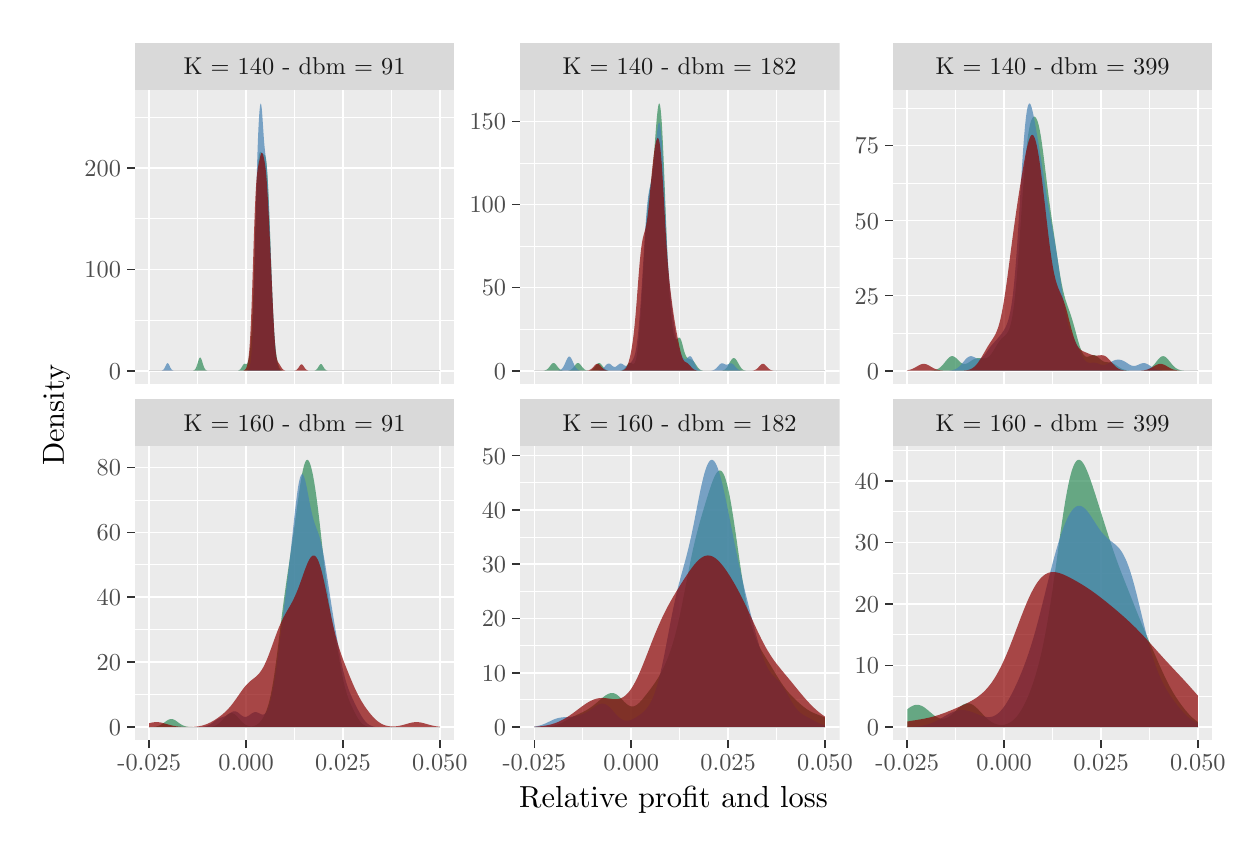
\begin{tikzpicture}[x=1pt,y=1pt]
\definecolor{fillColor}{RGB}{255,255,255}
\path[use as bounding box,fill=fillColor,fill opacity=0.00] (0,0) rectangle (433.62,289.08);
\begin{scope}
\path[clip] (  0.00,  0.00) rectangle (433.62,289.08);
\definecolor{drawColor}{RGB}{255,255,255}
\definecolor{fillColor}{RGB}{255,255,255}

\path[draw=drawColor,line width= 0.6pt,line join=round,line cap=round,fill=fillColor] (  0.00, -0.00) rectangle (433.62,289.08);
\end{scope}
\begin{scope}
\path[clip] ( 38.67,160.31) rectangle (154.19,266.52);
\definecolor{fillColor}{gray}{0.92}

\path[fill=fillColor] ( 38.67,160.31) rectangle (154.19,266.52);
\definecolor{drawColor}{RGB}{255,255,255}

\path[draw=drawColor,line width= 0.3pt,line join=round] ( 38.67,183.41) --
	(154.19,183.41);

\path[draw=drawColor,line width= 0.3pt,line join=round] ( 38.67,219.98) --
	(154.19,219.98);

\path[draw=drawColor,line width= 0.3pt,line join=round] ( 38.67,256.54) --
	(154.19,256.54);

\path[draw=drawColor,line width= 0.3pt,line join=round] ( 61.42,160.31) --
	( 61.42,266.52);

\path[draw=drawColor,line width= 0.3pt,line join=round] ( 96.43,160.31) --
	( 96.43,266.52);

\path[draw=drawColor,line width= 0.3pt,line join=round] (131.43,160.31) --
	(131.43,266.52);

\path[draw=drawColor,line width= 0.6pt,line join=round] ( 38.67,165.13) --
	(154.19,165.13);

\path[draw=drawColor,line width= 0.6pt,line join=round] ( 38.67,201.70) --
	(154.19,201.70);

\path[draw=drawColor,line width= 0.6pt,line join=round] ( 38.67,238.26) --
	(154.19,238.26);

\path[draw=drawColor,line width= 0.6pt,line join=round] ( 43.92,160.31) --
	( 43.92,266.52);

\path[draw=drawColor,line width= 0.6pt,line join=round] ( 78.92,160.31) --
	( 78.92,266.52);

\path[draw=drawColor,line width= 0.6pt,line join=round] (113.93,160.31) --
	(113.93,266.52);

\path[draw=drawColor,line width= 0.6pt,line join=round] (148.94,160.31) --
	(148.94,266.52);
\definecolor{fillColor}{RGB}{46,139,87}

\path[fill=fillColor,fill opacity=0.70] ( 43.92,165.13) --
	( 44.12,165.13) --
	( 44.33,165.13) --
	( 44.53,165.13) --
	( 44.74,165.13) --
	( 44.95,165.13) --
	( 45.15,165.13) --
	( 45.36,165.13) --
	( 45.56,165.13) --
	( 45.77,165.13) --
	( 45.97,165.13) --
	( 46.18,165.13) --
	( 46.38,165.13) --
	( 46.59,165.13) --
	( 46.79,165.13) --
	( 47.00,165.13) --
	( 47.21,165.13) --
	( 47.41,165.13) --
	( 47.62,165.13) --
	( 47.82,165.13) --
	( 48.03,165.13) --
	( 48.23,165.13) --
	( 48.44,165.13) --
	( 48.64,165.13) --
	( 48.85,165.13) --
	( 49.06,165.13) --
	( 49.26,165.13) --
	( 49.47,165.13) --
	( 49.67,165.13) --
	( 49.88,165.13) --
	( 50.08,165.13) --
	( 50.29,165.13) --
	( 50.49,165.13) --
	( 50.70,165.13) --
	( 50.91,165.13) --
	( 51.11,165.13) --
	( 51.32,165.13) --
	( 51.52,165.13) --
	( 51.73,165.13) --
	( 51.93,165.13) --
	( 52.14,165.13) --
	( 52.34,165.13) --
	( 52.55,165.13) --
	( 52.75,165.13) --
	( 52.96,165.13) --
	( 53.17,165.13) --
	( 53.37,165.13) --
	( 53.58,165.13) --
	( 53.78,165.13) --
	( 53.99,165.13) --
	( 54.19,165.13) --
	( 54.40,165.13) --
	( 54.60,165.13) --
	( 54.81,165.13) --
	( 55.02,165.13) --
	( 55.22,165.13) --
	( 55.43,165.13) --
	( 55.63,165.13) --
	( 55.84,165.13) --
	( 56.04,165.13) --
	( 56.25,165.13) --
	( 56.45,165.13) --
	( 56.66,165.13) --
	( 56.87,165.13) --
	( 57.07,165.13) --
	( 57.28,165.13) --
	( 57.48,165.13) --
	( 57.69,165.13) --
	( 57.89,165.13) --
	( 58.10,165.13) --
	( 58.30,165.13) --
	( 58.51,165.13) --
	( 58.71,165.13) --
	( 58.92,165.13) --
	( 59.13,165.14) --
	( 59.33,165.14) --
	( 59.54,165.16) --
	( 59.74,165.19) --
	( 59.95,165.24) --
	( 60.15,165.33) --
	( 60.36,165.48) --
	( 60.56,165.72) --
	( 60.77,166.06) --
	( 60.98,166.52) --
	( 61.18,167.10) --
	( 61.39,167.76) --
	( 61.59,168.44) --
	( 61.80,169.08) --
	( 62.00,169.58) --
	( 62.21,169.87) --
	( 62.41,169.89) --
	( 62.62,169.63) --
	( 62.82,169.15) --
	( 63.03,168.53) --
	( 63.24,167.84) --
	( 63.44,167.18) --
	( 63.65,166.59) --
	( 63.85,166.12) --
	( 64.06,165.76) --
	( 64.26,165.51) --
	( 64.47,165.35) --
	( 64.67,165.25) --
	( 64.88,165.19) --
	( 65.09,165.16) --
	( 65.29,165.15) --
	( 65.50,165.14) --
	( 65.70,165.14) --
	( 65.91,165.13) --
	( 66.11,165.13) --
	( 66.32,165.13) --
	( 66.52,165.13) --
	( 66.73,165.13) --
	( 66.94,165.13) --
	( 67.14,165.13) --
	( 67.35,165.13) --
	( 67.55,165.13) --
	( 67.76,165.13) --
	( 67.96,165.13) --
	( 68.17,165.13) --
	( 68.37,165.13) --
	( 68.58,165.13) --
	( 68.78,165.13) --
	( 68.99,165.13) --
	( 69.20,165.13) --
	( 69.40,165.13) --
	( 69.61,165.13) --
	( 69.81,165.13) --
	( 70.02,165.13) --
	( 70.22,165.13) --
	( 70.43,165.13) --
	( 70.63,165.13) --
	( 70.84,165.13) --
	( 71.05,165.13) --
	( 71.25,165.13) --
	( 71.46,165.13) --
	( 71.66,165.13) --
	( 71.87,165.13) --
	( 72.07,165.13) --
	( 72.28,165.13) --
	( 72.48,165.13) --
	( 72.69,165.13) --
	( 72.90,165.13) --
	( 73.10,165.13) --
	( 73.31,165.13) --
	( 73.51,165.13) --
	( 73.72,165.13) --
	( 73.92,165.13) --
	( 74.13,165.13) --
	( 74.33,165.13) --
	( 74.54,165.13) --
	( 74.74,165.13) --
	( 74.95,165.13) --
	( 75.16,165.14) --
	( 75.36,165.14) --
	( 75.57,165.15) --
	( 75.77,165.16) --
	( 75.98,165.19) --
	( 76.18,165.24) --
	( 76.39,165.32) --
	( 76.59,165.45) --
	( 76.80,165.63) --
	( 77.01,165.88) --
	( 77.21,166.18) --
	( 77.42,166.52) --
	( 77.62,166.87) --
	( 77.83,167.19) --
	( 78.03,167.44) --
	( 78.24,167.59) --
	( 78.44,167.64) --
	( 78.65,167.62) --
	( 78.86,167.56) --
	( 79.06,167.54) --
	( 79.27,167.64) --
	( 79.47,167.95) --
	( 79.68,168.52) --
	( 79.88,169.38) --
	( 80.09,170.56) --
	( 80.29,172.07) --
	( 80.50,173.98) --
	( 80.70,176.36) --
	( 80.91,179.32) --
	( 81.12,182.99) --
	( 81.32,187.45) --
	( 81.53,192.74) --
	( 81.73,198.78) --
	( 81.94,205.40) --
	( 82.14,212.31) --
	( 82.35,219.13) --
	( 82.55,225.51) --
	( 82.76,231.11) --
	( 82.97,235.65) --
	( 83.17,239.09) --
	( 83.38,241.50) --
	( 83.58,243.02) --
	( 83.79,243.84) --
	( 83.99,244.18) --
	( 84.20,244.19) --
	( 84.40,244.04) --
	( 84.61,243.82) --
	( 84.81,243.61) --
	( 85.02,243.45) --
	( 85.23,243.35) --
	( 85.43,243.26) --
	( 85.64,243.09) --
	( 85.84,242.71) --
	( 86.05,241.93) --
	( 86.25,240.57) --
	( 86.46,238.47) --
	( 86.66,235.61) --
	( 86.87,231.99) --
	( 87.08,227.66) --
	( 87.28,222.74) --
	( 87.49,217.36) --
	( 87.69,211.69) --
	( 87.90,205.92) --
	( 88.10,200.24) --
	( 88.31,194.83) --
	( 88.51,189.85) --
	( 88.72,185.41) --
	( 88.93,181.56) --
	( 89.13,178.31) --
	( 89.34,175.63) --
	( 89.54,173.45) --
	( 89.75,171.69) --
	( 89.95,170.26) --
	( 90.16,169.07) --
	( 90.36,168.10) --
	( 90.57,167.31) --
	( 90.77,166.67) --
	( 90.98,166.18) --
	( 91.19,165.82) --
	( 91.39,165.56) --
	( 91.60,165.38) --
	( 91.80,165.27) --
	( 92.01,165.21) --
	( 92.21,165.17) --
	( 92.42,165.15) --
	( 92.62,165.14) --
	( 92.83,165.14) --
	( 93.04,165.13) --
	( 93.24,165.13) --
	( 93.45,165.13) --
	( 93.65,165.13) --
	( 93.86,165.13) --
	( 94.06,165.13) --
	( 94.27,165.13) --
	( 94.47,165.13) --
	( 94.68,165.13) --
	( 94.89,165.13) --
	( 95.09,165.13) --
	( 95.30,165.13) --
	( 95.50,165.13) --
	( 95.71,165.13) --
	( 95.91,165.13) --
	( 96.12,165.13) --
	( 96.32,165.13) --
	( 96.53,165.13) --
	( 96.73,165.13) --
	( 96.94,165.13) --
	( 97.15,165.13) --
	( 97.35,165.13) --
	( 97.56,165.13) --
	( 97.76,165.13) --
	( 97.97,165.13) --
	( 98.17,165.13) --
	( 98.38,165.13) --
	( 98.58,165.13) --
	( 98.79,165.13) --
	( 99.00,165.13) --
	( 99.20,165.13) --
	( 99.41,165.13) --
	( 99.61,165.13) --
	( 99.82,165.13) --
	(100.02,165.13) --
	(100.23,165.13) --
	(100.43,165.13) --
	(100.64,165.13) --
	(100.85,165.13) --
	(101.05,165.13) --
	(101.26,165.13) --
	(101.46,165.13) --
	(101.67,165.13) --
	(101.87,165.13) --
	(102.08,165.13) --
	(102.28,165.13) --
	(102.49,165.13) --
	(102.69,165.13) --
	(102.90,165.14) --
	(103.11,165.14) --
	(103.31,165.15) --
	(103.52,165.17) --
	(103.72,165.21) --
	(103.93,165.27) --
	(104.13,165.37) --
	(104.34,165.53) --
	(104.54,165.74) --
	(104.75,166.01) --
	(104.96,166.34) --
	(105.16,166.69) --
	(105.37,167.02) --
	(105.57,167.31) --
	(105.78,167.49) --
	(105.98,167.54) --
	(106.19,167.46) --
	(106.39,167.25) --
	(106.60,166.95) --
	(106.80,166.59) --
	(107.01,166.24) --
	(107.22,165.93) --
	(107.42,165.68) --
	(107.63,165.48) --
	(107.83,165.34) --
	(108.04,165.25) --
	(108.24,165.20) --
	(108.45,165.17) --
	(108.65,165.15) --
	(108.86,165.14) --
	(109.07,165.14) --
	(109.27,165.13) --
	(109.48,165.13) --
	(109.68,165.13) --
	(109.89,165.13) --
	(110.09,165.13) --
	(110.30,165.13) --
	(110.50,165.13) --
	(110.71,165.13) --
	(110.92,165.13) --
	(111.12,165.13) --
	(111.33,165.13) --
	(111.53,165.13) --
	(111.74,165.13) --
	(111.94,165.13) --
	(112.15,165.13) --
	(112.35,165.13) --
	(112.56,165.13) --
	(112.76,165.13) --
	(112.97,165.13) --
	(113.18,165.13) --
	(113.38,165.13) --
	(113.59,165.13) --
	(113.79,165.13) --
	(114.00,165.13) --
	(114.20,165.13) --
	(114.41,165.13) --
	(114.61,165.13) --
	(114.82,165.13) --
	(115.03,165.13) --
	(115.23,165.13) --
	(115.44,165.13) --
	(115.64,165.13) --
	(115.85,165.13) --
	(116.05,165.13) --
	(116.26,165.13) --
	(116.46,165.13) --
	(116.67,165.13) --
	(116.88,165.13) --
	(117.08,165.13) --
	(117.29,165.13) --
	(117.49,165.13) --
	(117.70,165.13) --
	(117.90,165.13) --
	(118.11,165.13) --
	(118.31,165.13) --
	(118.52,165.13) --
	(118.72,165.13) --
	(118.93,165.13) --
	(119.14,165.13) --
	(119.34,165.13) --
	(119.55,165.13) --
	(119.75,165.13) --
	(119.96,165.13) --
	(120.16,165.13) --
	(120.37,165.13) --
	(120.57,165.13) --
	(120.78,165.13) --
	(120.99,165.13) --
	(121.19,165.13) --
	(121.40,165.13) --
	(121.60,165.13) --
	(121.81,165.13) --
	(122.01,165.13) --
	(122.22,165.13) --
	(122.42,165.13) --
	(122.63,165.13) --
	(122.84,165.13) --
	(123.04,165.13) --
	(123.25,165.13) --
	(123.45,165.13) --
	(123.66,165.13) --
	(123.86,165.13) --
	(124.07,165.13) --
	(124.27,165.13) --
	(124.48,165.13) --
	(124.68,165.13) --
	(124.89,165.13) --
	(125.10,165.13) --
	(125.30,165.13) --
	(125.51,165.13) --
	(125.71,165.13) --
	(125.92,165.13) --
	(126.12,165.13) --
	(126.33,165.13) --
	(126.53,165.13) --
	(126.74,165.13) --
	(126.95,165.13) --
	(127.15,165.13) --
	(127.36,165.13) --
	(127.56,165.13) --
	(127.77,165.13) --
	(127.97,165.13) --
	(128.18,165.13) --
	(128.38,165.13) --
	(128.59,165.13) --
	(128.79,165.13) --
	(129.00,165.13) --
	(129.21,165.13) --
	(129.41,165.13) --
	(129.62,165.13) --
	(129.82,165.13) --
	(130.03,165.13) --
	(130.23,165.13) --
	(130.44,165.13) --
	(130.64,165.13) --
	(130.85,165.13) --
	(131.06,165.13) --
	(131.26,165.13) --
	(131.47,165.13) --
	(131.67,165.13) --
	(131.88,165.13) --
	(132.08,165.13) --
	(132.29,165.13) --
	(132.49,165.13) --
	(132.70,165.13) --
	(132.91,165.13) --
	(133.11,165.13) --
	(133.32,165.13) --
	(133.52,165.13) --
	(133.73,165.13) --
	(133.93,165.13) --
	(134.14,165.13) --
	(134.34,165.13) --
	(134.55,165.13) --
	(134.75,165.13) --
	(134.96,165.13) --
	(135.17,165.13) --
	(135.37,165.13) --
	(135.58,165.13) --
	(135.78,165.13) --
	(135.99,165.13) --
	(136.19,165.13) --
	(136.40,165.13) --
	(136.60,165.13) --
	(136.81,165.13) --
	(137.02,165.13) --
	(137.22,165.13) --
	(137.43,165.13) --
	(137.63,165.13) --
	(137.84,165.13) --
	(138.04,165.13) --
	(138.25,165.13) --
	(138.45,165.13) --
	(138.66,165.13) --
	(138.87,165.13) --
	(139.07,165.13) --
	(139.28,165.13) --
	(139.48,165.13) --
	(139.69,165.13) --
	(139.89,165.13) --
	(140.10,165.13) --
	(140.30,165.13) --
	(140.51,165.13) --
	(140.71,165.13) --
	(140.92,165.13) --
	(141.13,165.13) --
	(141.33,165.13) --
	(141.54,165.13) --
	(141.74,165.13) --
	(141.95,165.13) --
	(142.15,165.13) --
	(142.36,165.13) --
	(142.56,165.13) --
	(142.77,165.13) --
	(142.98,165.13) --
	(143.18,165.13) --
	(143.39,165.13) --
	(143.59,165.13) --
	(143.80,165.13) --
	(144.00,165.13) --
	(144.21,165.13) --
	(144.41,165.13) --
	(144.62,165.13) --
	(144.83,165.13) --
	(145.03,165.13) --
	(145.24,165.13) --
	(145.44,165.13) --
	(145.65,165.13) --
	(145.85,165.13) --
	(146.06,165.13) --
	(146.26,165.13) --
	(146.47,165.13) --
	(146.67,165.13) --
	(146.88,165.13) --
	(147.09,165.13) --
	(147.29,165.13) --
	(147.50,165.13) --
	(147.70,165.13) --
	(147.91,165.13) --
	(148.11,165.13) --
	(148.32,165.13) --
	(148.52,165.13) --
	(148.73,165.13) --
	(148.94,165.13) --
	(148.94,165.13) --
	(148.73,165.13) --
	(148.52,165.13) --
	(148.32,165.13) --
	(148.11,165.13) --
	(147.91,165.13) --
	(147.70,165.13) --
	(147.50,165.13) --
	(147.29,165.13) --
	(147.09,165.13) --
	(146.88,165.13) --
	(146.67,165.13) --
	(146.47,165.13) --
	(146.26,165.13) --
	(146.06,165.13) --
	(145.85,165.13) --
	(145.65,165.13) --
	(145.44,165.13) --
	(145.24,165.13) --
	(145.03,165.13) --
	(144.83,165.13) --
	(144.62,165.13) --
	(144.41,165.13) --
	(144.21,165.13) --
	(144.00,165.13) --
	(143.80,165.13) --
	(143.59,165.13) --
	(143.39,165.13) --
	(143.18,165.13) --
	(142.98,165.13) --
	(142.77,165.13) --
	(142.56,165.13) --
	(142.36,165.13) --
	(142.15,165.13) --
	(141.95,165.13) --
	(141.74,165.13) --
	(141.54,165.13) --
	(141.33,165.13) --
	(141.13,165.13) --
	(140.92,165.13) --
	(140.71,165.13) --
	(140.51,165.13) --
	(140.30,165.13) --
	(140.10,165.13) --
	(139.89,165.13) --
	(139.69,165.13) --
	(139.48,165.13) --
	(139.28,165.13) --
	(139.07,165.13) --
	(138.87,165.13) --
	(138.66,165.13) --
	(138.45,165.13) --
	(138.25,165.13) --
	(138.04,165.13) --
	(137.84,165.13) --
	(137.63,165.13) --
	(137.43,165.13) --
	(137.22,165.13) --
	(137.02,165.13) --
	(136.81,165.13) --
	(136.60,165.13) --
	(136.40,165.13) --
	(136.19,165.13) --
	(135.99,165.13) --
	(135.78,165.13) --
	(135.58,165.13) --
	(135.37,165.13) --
	(135.17,165.13) --
	(134.96,165.13) --
	(134.75,165.13) --
	(134.55,165.13) --
	(134.34,165.13) --
	(134.14,165.13) --
	(133.93,165.13) --
	(133.73,165.13) --
	(133.52,165.13) --
	(133.32,165.13) --
	(133.11,165.13) --
	(132.91,165.13) --
	(132.70,165.13) --
	(132.49,165.13) --
	(132.29,165.13) --
	(132.08,165.13) --
	(131.88,165.13) --
	(131.67,165.13) --
	(131.47,165.13) --
	(131.26,165.13) --
	(131.06,165.13) --
	(130.85,165.13) --
	(130.64,165.13) --
	(130.44,165.13) --
	(130.23,165.13) --
	(130.03,165.13) --
	(129.82,165.13) --
	(129.62,165.13) --
	(129.41,165.13) --
	(129.21,165.13) --
	(129.00,165.13) --
	(128.79,165.13) --
	(128.59,165.13) --
	(128.38,165.13) --
	(128.18,165.13) --
	(127.97,165.13) --
	(127.77,165.13) --
	(127.56,165.13) --
	(127.36,165.13) --
	(127.15,165.13) --
	(126.95,165.13) --
	(126.74,165.13) --
	(126.53,165.13) --
	(126.33,165.13) --
	(126.12,165.13) --
	(125.92,165.13) --
	(125.71,165.13) --
	(125.51,165.13) --
	(125.30,165.13) --
	(125.10,165.13) --
	(124.89,165.13) --
	(124.68,165.13) --
	(124.48,165.13) --
	(124.27,165.13) --
	(124.07,165.13) --
	(123.86,165.13) --
	(123.66,165.13) --
	(123.45,165.13) --
	(123.25,165.13) --
	(123.04,165.13) --
	(122.84,165.13) --
	(122.63,165.13) --
	(122.42,165.13) --
	(122.22,165.13) --
	(122.01,165.13) --
	(121.81,165.13) --
	(121.60,165.13) --
	(121.40,165.13) --
	(121.19,165.13) --
	(120.99,165.13) --
	(120.78,165.13) --
	(120.57,165.13) --
	(120.37,165.13) --
	(120.16,165.13) --
	(119.96,165.13) --
	(119.75,165.13) --
	(119.55,165.13) --
	(119.34,165.13) --
	(119.14,165.13) --
	(118.93,165.13) --
	(118.72,165.13) --
	(118.52,165.13) --
	(118.31,165.13) --
	(118.11,165.13) --
	(117.90,165.13) --
	(117.70,165.13) --
	(117.49,165.13) --
	(117.29,165.13) --
	(117.08,165.13) --
	(116.88,165.13) --
	(116.67,165.13) --
	(116.46,165.13) --
	(116.26,165.13) --
	(116.05,165.13) --
	(115.85,165.13) --
	(115.64,165.13) --
	(115.44,165.13) --
	(115.23,165.13) --
	(115.03,165.13) --
	(114.82,165.13) --
	(114.61,165.13) --
	(114.41,165.13) --
	(114.20,165.13) --
	(114.00,165.13) --
	(113.79,165.13) --
	(113.59,165.13) --
	(113.38,165.13) --
	(113.18,165.13) --
	(112.97,165.13) --
	(112.76,165.13) --
	(112.56,165.13) --
	(112.35,165.13) --
	(112.15,165.13) --
	(111.94,165.13) --
	(111.74,165.13) --
	(111.53,165.13) --
	(111.33,165.13) --
	(111.12,165.13) --
	(110.92,165.13) --
	(110.71,165.13) --
	(110.50,165.13) --
	(110.30,165.13) --
	(110.09,165.13) --
	(109.89,165.13) --
	(109.68,165.13) --
	(109.48,165.13) --
	(109.27,165.13) --
	(109.07,165.13) --
	(108.86,165.13) --
	(108.65,165.13) --
	(108.45,165.13) --
	(108.24,165.13) --
	(108.04,165.13) --
	(107.83,165.13) --
	(107.63,165.13) --
	(107.42,165.13) --
	(107.22,165.13) --
	(107.01,165.13) --
	(106.80,165.13) --
	(106.60,165.13) --
	(106.39,165.13) --
	(106.19,165.13) --
	(105.98,165.13) --
	(105.78,165.13) --
	(105.57,165.13) --
	(105.37,165.13) --
	(105.16,165.13) --
	(104.96,165.13) --
	(104.75,165.13) --
	(104.54,165.13) --
	(104.34,165.13) --
	(104.13,165.13) --
	(103.93,165.13) --
	(103.72,165.13) --
	(103.52,165.13) --
	(103.31,165.13) --
	(103.11,165.13) --
	(102.90,165.13) --
	(102.69,165.13) --
	(102.49,165.13) --
	(102.28,165.13) --
	(102.08,165.13) --
	(101.87,165.13) --
	(101.67,165.13) --
	(101.46,165.13) --
	(101.26,165.13) --
	(101.05,165.13) --
	(100.85,165.13) --
	(100.64,165.13) --
	(100.43,165.13) --
	(100.23,165.13) --
	(100.02,165.13) --
	( 99.82,165.13) --
	( 99.61,165.13) --
	( 99.41,165.13) --
	( 99.20,165.13) --
	( 99.00,165.13) --
	( 98.79,165.13) --
	( 98.58,165.13) --
	( 98.38,165.13) --
	( 98.17,165.13) --
	( 97.97,165.13) --
	( 97.76,165.13) --
	( 97.56,165.13) --
	( 97.35,165.13) --
	( 97.15,165.13) --
	( 96.94,165.13) --
	( 96.73,165.13) --
	( 96.53,165.13) --
	( 96.32,165.13) --
	( 96.12,165.13) --
	( 95.91,165.13) --
	( 95.71,165.13) --
	( 95.50,165.13) --
	( 95.30,165.13) --
	( 95.09,165.13) --
	( 94.89,165.13) --
	( 94.68,165.13) --
	( 94.47,165.13) --
	( 94.27,165.13) --
	( 94.06,165.13) --
	( 93.86,165.13) --
	( 93.65,165.13) --
	( 93.45,165.13) --
	( 93.24,165.13) --
	( 93.04,165.13) --
	( 92.83,165.13) --
	( 92.62,165.13) --
	( 92.42,165.13) --
	( 92.21,165.13) --
	( 92.01,165.13) --
	( 91.80,165.13) --
	( 91.60,165.13) --
	( 91.39,165.13) --
	( 91.19,165.13) --
	( 90.98,165.13) --
	( 90.77,165.13) --
	( 90.57,165.13) --
	( 90.36,165.13) --
	( 90.16,165.13) --
	( 89.95,165.13) --
	( 89.75,165.13) --
	( 89.54,165.13) --
	( 89.34,165.13) --
	( 89.13,165.13) --
	( 88.93,165.13) --
	( 88.72,165.13) --
	( 88.51,165.13) --
	( 88.31,165.13) --
	( 88.10,165.13) --
	( 87.90,165.13) --
	( 87.69,165.13) --
	( 87.49,165.13) --
	( 87.28,165.13) --
	( 87.08,165.13) --
	( 86.87,165.13) --
	( 86.66,165.13) --
	( 86.46,165.13) --
	( 86.25,165.13) --
	( 86.05,165.13) --
	( 85.84,165.13) --
	( 85.64,165.13) --
	( 85.43,165.13) --
	( 85.23,165.13) --
	( 85.02,165.13) --
	( 84.81,165.13) --
	( 84.61,165.13) --
	( 84.40,165.13) --
	( 84.20,165.13) --
	( 83.99,165.13) --
	( 83.79,165.13) --
	( 83.58,165.13) --
	( 83.38,165.13) --
	( 83.17,165.13) --
	( 82.97,165.13) --
	( 82.76,165.13) --
	( 82.55,165.13) --
	( 82.35,165.13) --
	( 82.14,165.13) --
	( 81.94,165.13) --
	( 81.73,165.13) --
	( 81.53,165.13) --
	( 81.32,165.13) --
	( 81.12,165.13) --
	( 80.91,165.13) --
	( 80.70,165.13) --
	( 80.50,165.13) --
	( 80.29,165.13) --
	( 80.09,165.13) --
	( 79.88,165.13) --
	( 79.68,165.13) --
	( 79.47,165.13) --
	( 79.27,165.13) --
	( 79.06,165.13) --
	( 78.86,165.13) --
	( 78.65,165.13) --
	( 78.44,165.13) --
	( 78.24,165.13) --
	( 78.03,165.13) --
	( 77.83,165.13) --
	( 77.62,165.13) --
	( 77.42,165.13) --
	( 77.21,165.13) --
	( 77.01,165.13) --
	( 76.80,165.13) --
	( 76.59,165.13) --
	( 76.39,165.13) --
	( 76.18,165.13) --
	( 75.98,165.13) --
	( 75.77,165.13) --
	( 75.57,165.13) --
	( 75.36,165.13) --
	( 75.16,165.13) --
	( 74.95,165.13) --
	( 74.74,165.13) --
	( 74.54,165.13) --
	( 74.33,165.13) --
	( 74.13,165.13) --
	( 73.92,165.13) --
	( 73.72,165.13) --
	( 73.51,165.13) --
	( 73.31,165.13) --
	( 73.10,165.13) --
	( 72.90,165.13) --
	( 72.69,165.13) --
	( 72.48,165.13) --
	( 72.28,165.13) --
	( 72.07,165.13) --
	( 71.87,165.13) --
	( 71.66,165.13) --
	( 71.46,165.13) --
	( 71.25,165.13) --
	( 71.05,165.13) --
	( 70.84,165.13) --
	( 70.63,165.13) --
	( 70.43,165.13) --
	( 70.22,165.13) --
	( 70.02,165.13) --
	( 69.81,165.13) --
	( 69.61,165.13) --
	( 69.40,165.13) --
	( 69.20,165.13) --
	( 68.99,165.13) --
	( 68.78,165.13) --
	( 68.58,165.13) --
	( 68.37,165.13) --
	( 68.17,165.13) --
	( 67.96,165.13) --
	( 67.76,165.13) --
	( 67.55,165.13) --
	( 67.35,165.13) --
	( 67.14,165.13) --
	( 66.94,165.13) --
	( 66.73,165.13) --
	( 66.52,165.13) --
	( 66.32,165.13) --
	( 66.11,165.13) --
	( 65.91,165.13) --
	( 65.70,165.13) --
	( 65.50,165.13) --
	( 65.29,165.13) --
	( 65.09,165.13) --
	( 64.88,165.13) --
	( 64.67,165.13) --
	( 64.47,165.13) --
	( 64.26,165.13) --
	( 64.06,165.13) --
	( 63.85,165.13) --
	( 63.65,165.13) --
	( 63.44,165.13) --
	( 63.24,165.13) --
	( 63.03,165.13) --
	( 62.82,165.13) --
	( 62.62,165.13) --
	( 62.41,165.13) --
	( 62.21,165.13) --
	( 62.00,165.13) --
	( 61.80,165.13) --
	( 61.59,165.13) --
	( 61.39,165.13) --
	( 61.18,165.13) --
	( 60.98,165.13) --
	( 60.77,165.13) --
	( 60.56,165.13) --
	( 60.36,165.13) --
	( 60.15,165.13) --
	( 59.95,165.13) --
	( 59.74,165.13) --
	( 59.54,165.13) --
	( 59.33,165.13) --
	( 59.13,165.13) --
	( 58.92,165.13) --
	( 58.71,165.13) --
	( 58.51,165.13) --
	( 58.30,165.13) --
	( 58.10,165.13) --
	( 57.89,165.13) --
	( 57.69,165.13) --
	( 57.48,165.13) --
	( 57.28,165.13) --
	( 57.07,165.13) --
	( 56.87,165.13) --
	( 56.66,165.13) --
	( 56.45,165.13) --
	( 56.25,165.13) --
	( 56.04,165.13) --
	( 55.84,165.13) --
	( 55.63,165.13) --
	( 55.43,165.13) --
	( 55.22,165.13) --
	( 55.02,165.13) --
	( 54.81,165.13) --
	( 54.60,165.13) --
	( 54.40,165.13) --
	( 54.19,165.13) --
	( 53.99,165.13) --
	( 53.78,165.13) --
	( 53.58,165.13) --
	( 53.37,165.13) --
	( 53.17,165.13) --
	( 52.96,165.13) --
	( 52.75,165.13) --
	( 52.55,165.13) --
	( 52.34,165.13) --
	( 52.14,165.13) --
	( 51.93,165.13) --
	( 51.73,165.13) --
	( 51.52,165.13) --
	( 51.32,165.13) --
	( 51.11,165.13) --
	( 50.91,165.13) --
	( 50.70,165.13) --
	( 50.49,165.13) --
	( 50.29,165.13) --
	( 50.08,165.13) --
	( 49.88,165.13) --
	( 49.67,165.13) --
	( 49.47,165.13) --
	( 49.26,165.13) --
	( 49.06,165.13) --
	( 48.85,165.13) --
	( 48.64,165.13) --
	( 48.44,165.13) --
	( 48.23,165.13) --
	( 48.03,165.13) --
	( 47.82,165.13) --
	( 47.62,165.13) --
	( 47.41,165.13) --
	( 47.21,165.13) --
	( 47.00,165.13) --
	( 46.79,165.13) --
	( 46.59,165.13) --
	( 46.38,165.13) --
	( 46.18,165.13) --
	( 45.97,165.13) --
	( 45.77,165.13) --
	( 45.56,165.13) --
	( 45.36,165.13) --
	( 45.15,165.13) --
	( 44.95,165.13) --
	( 44.74,165.13) --
	( 44.53,165.13) --
	( 44.33,165.13) --
	( 44.12,165.13) --
	( 43.92,165.13) --
	cycle;
\definecolor{fillColor}{RGB}{70,130,180}

\path[fill=fillColor,fill opacity=0.70] ( 43.92,165.13) --
	( 44.12,165.13) --
	( 44.33,165.13) --
	( 44.53,165.13) --
	( 44.74,165.13) --
	( 44.95,165.13) --
	( 45.15,165.13) --
	( 45.36,165.13) --
	( 45.56,165.13) --
	( 45.77,165.13) --
	( 45.97,165.13) --
	( 46.18,165.13) --
	( 46.38,165.13) --
	( 46.59,165.13) --
	( 46.79,165.13) --
	( 47.00,165.13) --
	( 47.21,165.13) --
	( 47.41,165.13) --
	( 47.62,165.13) --
	( 47.82,165.14) --
	( 48.03,165.14) --
	( 48.23,165.16) --
	( 48.44,165.19) --
	( 48.64,165.25) --
	( 48.85,165.36) --
	( 49.06,165.52) --
	( 49.26,165.77) --
	( 49.47,166.11) --
	( 49.67,166.51) --
	( 49.88,166.95) --
	( 50.08,167.37) --
	( 50.29,167.69) --
	( 50.49,167.85) --
	( 50.70,167.81) --
	( 50.91,167.58) --
	( 51.11,167.22) --
	( 51.32,166.78) --
	( 51.52,166.35) --
	( 51.73,165.97) --
	( 51.93,165.67) --
	( 52.14,165.45) --
	( 52.34,165.31) --
	( 52.55,165.22) --
	( 52.75,165.18) --
	( 52.96,165.15) --
	( 53.17,165.14) --
	( 53.37,165.14) --
	( 53.58,165.13) --
	( 53.78,165.13) --
	( 53.99,165.13) --
	( 54.19,165.13) --
	( 54.40,165.13) --
	( 54.60,165.13) --
	( 54.81,165.13) --
	( 55.02,165.13) --
	( 55.22,165.13) --
	( 55.43,165.13) --
	( 55.63,165.13) --
	( 55.84,165.13) --
	( 56.04,165.13) --
	( 56.25,165.13) --
	( 56.45,165.13) --
	( 56.66,165.13) --
	( 56.87,165.13) --
	( 57.07,165.13) --
	( 57.28,165.13) --
	( 57.48,165.13) --
	( 57.69,165.13) --
	( 57.89,165.13) --
	( 58.10,165.13) --
	( 58.30,165.13) --
	( 58.51,165.13) --
	( 58.71,165.13) --
	( 58.92,165.13) --
	( 59.13,165.13) --
	( 59.33,165.13) --
	( 59.54,165.13) --
	( 59.74,165.13) --
	( 59.95,165.13) --
	( 60.15,165.13) --
	( 60.36,165.13) --
	( 60.56,165.13) --
	( 60.77,165.13) --
	( 60.98,165.13) --
	( 61.18,165.13) --
	( 61.39,165.13) --
	( 61.59,165.13) --
	( 61.80,165.13) --
	( 62.00,165.13) --
	( 62.21,165.13) --
	( 62.41,165.13) --
	( 62.62,165.13) --
	( 62.82,165.13) --
	( 63.03,165.13) --
	( 63.24,165.13) --
	( 63.44,165.13) --
	( 63.65,165.13) --
	( 63.85,165.13) --
	( 64.06,165.13) --
	( 64.26,165.13) --
	( 64.47,165.13) --
	( 64.67,165.13) --
	( 64.88,165.13) --
	( 65.09,165.13) --
	( 65.29,165.13) --
	( 65.50,165.13) --
	( 65.70,165.13) --
	( 65.91,165.13) --
	( 66.11,165.13) --
	( 66.32,165.13) --
	( 66.52,165.13) --
	( 66.73,165.13) --
	( 66.94,165.13) --
	( 67.14,165.13) --
	( 67.35,165.13) --
	( 67.55,165.13) --
	( 67.76,165.13) --
	( 67.96,165.13) --
	( 68.17,165.13) --
	( 68.37,165.13) --
	( 68.58,165.13) --
	( 68.78,165.13) --
	( 68.99,165.13) --
	( 69.20,165.13) --
	( 69.40,165.13) --
	( 69.61,165.13) --
	( 69.81,165.13) --
	( 70.02,165.13) --
	( 70.22,165.13) --
	( 70.43,165.13) --
	( 70.63,165.13) --
	( 70.84,165.13) --
	( 71.05,165.13) --
	( 71.25,165.13) --
	( 71.46,165.13) --
	( 71.66,165.13) --
	( 71.87,165.13) --
	( 72.07,165.13) --
	( 72.28,165.13) --
	( 72.48,165.13) --
	( 72.69,165.13) --
	( 72.90,165.13) --
	( 73.10,165.13) --
	( 73.31,165.13) --
	( 73.51,165.13) --
	( 73.72,165.13) --
	( 73.92,165.13) --
	( 74.13,165.13) --
	( 74.33,165.13) --
	( 74.54,165.13) --
	( 74.74,165.13) --
	( 74.95,165.13) --
	( 75.16,165.13) --
	( 75.36,165.13) --
	( 75.57,165.13) --
	( 75.77,165.13) --
	( 75.98,165.13) --
	( 76.18,165.13) --
	( 76.39,165.13) --
	( 76.59,165.13) --
	( 76.80,165.13) --
	( 77.01,165.13) --
	( 77.21,165.13) --
	( 77.42,165.13) --
	( 77.62,165.13) --
	( 77.83,165.13) --
	( 78.03,165.13) --
	( 78.24,165.13) --
	( 78.44,165.13) --
	( 78.65,165.14) --
	( 78.86,165.14) --
	( 79.06,165.15) --
	( 79.27,165.18) --
	( 79.47,165.24) --
	( 79.68,165.36) --
	( 79.88,165.59) --
	( 80.09,165.99) --
	( 80.29,166.67) --
	( 80.50,167.77) --
	( 80.70,169.46) --
	( 80.91,171.92) --
	( 81.12,175.34) --
	( 81.32,179.94) --
	( 81.53,185.80) --
	( 81.73,192.82) --
	( 81.94,200.82) --
	( 82.14,209.46) --
	( 82.35,218.31) --
	( 82.55,226.90) --
	( 82.76,234.84) --
	( 82.97,241.84) --
	( 83.17,247.76) --
	( 83.38,252.59) --
	( 83.58,256.39) --
	( 83.79,259.19) --
	( 83.99,260.99) --
	( 84.20,261.69) --
	( 84.40,261.23) --
	( 84.61,259.61) --
	( 84.81,257.04) --
	( 85.02,253.89) --
	( 85.23,250.69) --
	( 85.43,247.86) --
	( 85.64,245.59) --
	( 85.84,243.77) --
	( 86.05,242.11) --
	( 86.25,240.24) --
	( 86.46,237.83) --
	( 86.66,234.73) --
	( 86.87,230.91) --
	( 87.08,226.48) --
	( 87.28,221.58) --
	( 87.49,216.35) --
	( 87.69,210.95) --
	( 87.90,205.49) --
	( 88.10,200.11) --
	( 88.31,194.95) --
	( 88.51,190.13) --
	( 88.72,185.72) --
	( 88.93,181.79) --
	( 89.13,178.35) --
	( 89.34,175.38) --
	( 89.54,172.85) --
	( 89.75,170.75) --
	( 89.95,169.06) --
	( 90.16,167.76) --
	( 90.36,166.80) --
	( 90.57,166.13) --
	( 90.77,165.70) --
	( 90.98,165.44) --
	( 91.19,165.28) --
	( 91.39,165.20) --
	( 91.60,165.16) --
	( 91.80,165.15) --
	( 92.01,165.14) --
	( 92.21,165.13) --
	( 92.42,165.13) --
	( 92.62,165.13) --
	( 92.83,165.13) --
	( 93.04,165.13) --
	( 93.24,165.13) --
	( 93.45,165.13) --
	( 93.65,165.13) --
	( 93.86,165.13) --
	( 94.06,165.13) --
	( 94.27,165.13) --
	( 94.47,165.13) --
	( 94.68,165.13) --
	( 94.89,165.13) --
	( 95.09,165.13) --
	( 95.30,165.13) --
	( 95.50,165.13) --
	( 95.71,165.13) --
	( 95.91,165.13) --
	( 96.12,165.13) --
	( 96.32,165.13) --
	( 96.53,165.13) --
	( 96.73,165.13) --
	( 96.94,165.13) --
	( 97.15,165.13) --
	( 97.35,165.13) --
	( 97.56,165.13) --
	( 97.76,165.13) --
	( 97.97,165.13) --
	( 98.17,165.13) --
	( 98.38,165.13) --
	( 98.58,165.13) --
	( 98.79,165.13) --
	( 99.00,165.13) --
	( 99.20,165.13) --
	( 99.41,165.13) --
	( 99.61,165.13) --
	( 99.82,165.13) --
	(100.02,165.13) --
	(100.23,165.13) --
	(100.43,165.13) --
	(100.64,165.13) --
	(100.85,165.13) --
	(101.05,165.13) --
	(101.26,165.13) --
	(101.46,165.13) --
	(101.67,165.13) --
	(101.87,165.13) --
	(102.08,165.13) --
	(102.28,165.13) --
	(102.49,165.13) --
	(102.69,165.13) --
	(102.90,165.13) --
	(103.11,165.13) --
	(103.31,165.13) --
	(103.52,165.13) --
	(103.72,165.13) --
	(103.93,165.13) --
	(104.13,165.13) --
	(104.34,165.13) --
	(104.54,165.13) --
	(104.75,165.13) --
	(104.96,165.13) --
	(105.16,165.13) --
	(105.37,165.13) --
	(105.57,165.13) --
	(105.78,165.13) --
	(105.98,165.13) --
	(106.19,165.13) --
	(106.39,165.13) --
	(106.60,165.13) --
	(106.80,165.13) --
	(107.01,165.13) --
	(107.22,165.13) --
	(107.42,165.13) --
	(107.63,165.13) --
	(107.83,165.13) --
	(108.04,165.13) --
	(108.24,165.13) --
	(108.45,165.13) --
	(108.65,165.13) --
	(108.86,165.13) --
	(109.07,165.13) --
	(109.27,165.13) --
	(109.48,165.13) --
	(109.68,165.13) --
	(109.89,165.13) --
	(110.09,165.13) --
	(110.30,165.13) --
	(110.50,165.13) --
	(110.71,165.13) --
	(110.92,165.13) --
	(111.12,165.13) --
	(111.33,165.13) --
	(111.53,165.13) --
	(111.74,165.13) --
	(111.94,165.13) --
	(112.15,165.13) --
	(112.35,165.13) --
	(112.56,165.13) --
	(112.76,165.13) --
	(112.97,165.13) --
	(113.18,165.13) --
	(113.38,165.13) --
	(113.59,165.13) --
	(113.79,165.13) --
	(114.00,165.13) --
	(114.20,165.13) --
	(114.41,165.13) --
	(114.61,165.13) --
	(114.82,165.13) --
	(115.03,165.13) --
	(115.23,165.13) --
	(115.44,165.13) --
	(115.64,165.13) --
	(115.85,165.13) --
	(116.05,165.13) --
	(116.26,165.13) --
	(116.46,165.13) --
	(116.67,165.13) --
	(116.88,165.13) --
	(117.08,165.13) --
	(117.29,165.13) --
	(117.49,165.13) --
	(117.70,165.13) --
	(117.90,165.13) --
	(118.11,165.13) --
	(118.31,165.13) --
	(118.52,165.13) --
	(118.72,165.13) --
	(118.93,165.13) --
	(119.14,165.13) --
	(119.34,165.13) --
	(119.55,165.13) --
	(119.75,165.13) --
	(119.96,165.13) --
	(120.16,165.13) --
	(120.37,165.13) --
	(120.57,165.13) --
	(120.78,165.13) --
	(120.99,165.13) --
	(121.19,165.13) --
	(121.40,165.13) --
	(121.60,165.13) --
	(121.81,165.13) --
	(122.01,165.13) --
	(122.22,165.13) --
	(122.42,165.13) --
	(122.63,165.13) --
	(122.84,165.13) --
	(123.04,165.13) --
	(123.25,165.13) --
	(123.45,165.13) --
	(123.66,165.13) --
	(123.86,165.13) --
	(124.07,165.13) --
	(124.27,165.13) --
	(124.48,165.13) --
	(124.68,165.13) --
	(124.89,165.13) --
	(125.10,165.13) --
	(125.30,165.13) --
	(125.51,165.13) --
	(125.71,165.13) --
	(125.92,165.13) --
	(126.12,165.13) --
	(126.33,165.13) --
	(126.53,165.13) --
	(126.74,165.13) --
	(126.95,165.13) --
	(127.15,165.13) --
	(127.36,165.13) --
	(127.56,165.13) --
	(127.77,165.13) --
	(127.97,165.13) --
	(128.18,165.13) --
	(128.38,165.13) --
	(128.59,165.13) --
	(128.79,165.13) --
	(129.00,165.13) --
	(129.21,165.13) --
	(129.41,165.13) --
	(129.62,165.13) --
	(129.82,165.13) --
	(130.03,165.13) --
	(130.23,165.13) --
	(130.44,165.13) --
	(130.64,165.13) --
	(130.85,165.13) --
	(131.06,165.13) --
	(131.26,165.13) --
	(131.47,165.13) --
	(131.67,165.13) --
	(131.88,165.13) --
	(132.08,165.13) --
	(132.29,165.13) --
	(132.49,165.13) --
	(132.70,165.13) --
	(132.91,165.13) --
	(133.11,165.13) --
	(133.32,165.13) --
	(133.52,165.13) --
	(133.73,165.13) --
	(133.93,165.13) --
	(134.14,165.13) --
	(134.34,165.13) --
	(134.55,165.13) --
	(134.75,165.13) --
	(134.96,165.13) --
	(135.17,165.13) --
	(135.37,165.13) --
	(135.58,165.13) --
	(135.78,165.13) --
	(135.99,165.13) --
	(136.19,165.13) --
	(136.40,165.13) --
	(136.60,165.13) --
	(136.81,165.13) --
	(137.02,165.13) --
	(137.22,165.13) --
	(137.43,165.13) --
	(137.63,165.13) --
	(137.84,165.13) --
	(138.04,165.13) --
	(138.25,165.13) --
	(138.45,165.13) --
	(138.66,165.13) --
	(138.87,165.13) --
	(139.07,165.13) --
	(139.28,165.13) --
	(139.48,165.13) --
	(139.69,165.13) --
	(139.89,165.13) --
	(140.10,165.13) --
	(140.30,165.13) --
	(140.51,165.13) --
	(140.71,165.13) --
	(140.92,165.13) --
	(141.13,165.13) --
	(141.33,165.13) --
	(141.54,165.13) --
	(141.74,165.13) --
	(141.95,165.13) --
	(142.15,165.13) --
	(142.36,165.13) --
	(142.56,165.13) --
	(142.77,165.13) --
	(142.98,165.13) --
	(143.18,165.13) --
	(143.39,165.13) --
	(143.59,165.13) --
	(143.80,165.13) --
	(144.00,165.13) --
	(144.21,165.13) --
	(144.41,165.13) --
	(144.62,165.13) --
	(144.83,165.13) --
	(145.03,165.13) --
	(145.24,165.13) --
	(145.44,165.13) --
	(145.65,165.13) --
	(145.85,165.13) --
	(146.06,165.13) --
	(146.26,165.13) --
	(146.47,165.13) --
	(146.67,165.13) --
	(146.88,165.13) --
	(147.09,165.13) --
	(147.29,165.13) --
	(147.50,165.13) --
	(147.70,165.13) --
	(147.91,165.13) --
	(148.11,165.13) --
	(148.32,165.13) --
	(148.52,165.13) --
	(148.73,165.13) --
	(148.94,165.13) --
	(148.94,165.13) --
	(148.73,165.13) --
	(148.52,165.13) --
	(148.32,165.13) --
	(148.11,165.13) --
	(147.91,165.13) --
	(147.70,165.13) --
	(147.50,165.13) --
	(147.29,165.13) --
	(147.09,165.13) --
	(146.88,165.13) --
	(146.67,165.13) --
	(146.47,165.13) --
	(146.26,165.13) --
	(146.06,165.13) --
	(145.85,165.13) --
	(145.65,165.13) --
	(145.44,165.13) --
	(145.24,165.13) --
	(145.03,165.13) --
	(144.83,165.13) --
	(144.62,165.13) --
	(144.41,165.13) --
	(144.21,165.13) --
	(144.00,165.13) --
	(143.80,165.13) --
	(143.59,165.13) --
	(143.39,165.13) --
	(143.18,165.13) --
	(142.98,165.13) --
	(142.77,165.13) --
	(142.56,165.13) --
	(142.36,165.13) --
	(142.15,165.13) --
	(141.95,165.13) --
	(141.74,165.13) --
	(141.54,165.13) --
	(141.33,165.13) --
	(141.13,165.13) --
	(140.92,165.13) --
	(140.71,165.13) --
	(140.51,165.13) --
	(140.30,165.13) --
	(140.10,165.13) --
	(139.89,165.13) --
	(139.69,165.13) --
	(139.48,165.13) --
	(139.28,165.13) --
	(139.07,165.13) --
	(138.87,165.13) --
	(138.66,165.13) --
	(138.45,165.13) --
	(138.25,165.13) --
	(138.04,165.13) --
	(137.84,165.13) --
	(137.63,165.13) --
	(137.43,165.13) --
	(137.22,165.13) --
	(137.02,165.13) --
	(136.81,165.13) --
	(136.60,165.13) --
	(136.40,165.13) --
	(136.19,165.13) --
	(135.99,165.13) --
	(135.78,165.13) --
	(135.58,165.13) --
	(135.37,165.13) --
	(135.17,165.13) --
	(134.96,165.13) --
	(134.75,165.13) --
	(134.55,165.13) --
	(134.34,165.13) --
	(134.14,165.13) --
	(133.93,165.13) --
	(133.73,165.13) --
	(133.52,165.13) --
	(133.32,165.13) --
	(133.11,165.13) --
	(132.91,165.13) --
	(132.70,165.13) --
	(132.49,165.13) --
	(132.29,165.13) --
	(132.08,165.13) --
	(131.88,165.13) --
	(131.67,165.13) --
	(131.47,165.13) --
	(131.26,165.13) --
	(131.06,165.13) --
	(130.85,165.13) --
	(130.64,165.13) --
	(130.44,165.13) --
	(130.23,165.13) --
	(130.03,165.13) --
	(129.82,165.13) --
	(129.62,165.13) --
	(129.41,165.13) --
	(129.21,165.13) --
	(129.00,165.13) --
	(128.79,165.13) --
	(128.59,165.13) --
	(128.38,165.13) --
	(128.18,165.13) --
	(127.97,165.13) --
	(127.77,165.13) --
	(127.56,165.13) --
	(127.36,165.13) --
	(127.15,165.13) --
	(126.95,165.13) --
	(126.74,165.13) --
	(126.53,165.13) --
	(126.33,165.13) --
	(126.12,165.13) --
	(125.92,165.13) --
	(125.71,165.13) --
	(125.51,165.13) --
	(125.30,165.13) --
	(125.10,165.13) --
	(124.89,165.13) --
	(124.68,165.13) --
	(124.48,165.13) --
	(124.27,165.13) --
	(124.07,165.13) --
	(123.86,165.13) --
	(123.66,165.13) --
	(123.45,165.13) --
	(123.25,165.13) --
	(123.04,165.13) --
	(122.84,165.13) --
	(122.63,165.13) --
	(122.42,165.13) --
	(122.22,165.13) --
	(122.01,165.13) --
	(121.81,165.13) --
	(121.60,165.13) --
	(121.40,165.13) --
	(121.19,165.13) --
	(120.99,165.13) --
	(120.78,165.13) --
	(120.57,165.13) --
	(120.37,165.13) --
	(120.16,165.13) --
	(119.96,165.13) --
	(119.75,165.13) --
	(119.55,165.13) --
	(119.34,165.13) --
	(119.14,165.13) --
	(118.93,165.13) --
	(118.72,165.13) --
	(118.52,165.13) --
	(118.31,165.13) --
	(118.11,165.13) --
	(117.90,165.13) --
	(117.70,165.13) --
	(117.49,165.13) --
	(117.29,165.13) --
	(117.08,165.13) --
	(116.88,165.13) --
	(116.67,165.13) --
	(116.46,165.13) --
	(116.26,165.13) --
	(116.05,165.13) --
	(115.85,165.13) --
	(115.64,165.13) --
	(115.44,165.13) --
	(115.23,165.13) --
	(115.03,165.13) --
	(114.82,165.13) --
	(114.61,165.13) --
	(114.41,165.13) --
	(114.20,165.13) --
	(114.00,165.13) --
	(113.79,165.13) --
	(113.59,165.13) --
	(113.38,165.13) --
	(113.18,165.13) --
	(112.97,165.13) --
	(112.76,165.13) --
	(112.56,165.13) --
	(112.35,165.13) --
	(112.15,165.13) --
	(111.94,165.13) --
	(111.74,165.13) --
	(111.53,165.13) --
	(111.33,165.13) --
	(111.12,165.13) --
	(110.92,165.13) --
	(110.71,165.13) --
	(110.50,165.13) --
	(110.30,165.13) --
	(110.09,165.13) --
	(109.89,165.13) --
	(109.68,165.13) --
	(109.48,165.13) --
	(109.27,165.13) --
	(109.07,165.13) --
	(108.86,165.13) --
	(108.65,165.13) --
	(108.45,165.13) --
	(108.24,165.13) --
	(108.04,165.13) --
	(107.83,165.13) --
	(107.63,165.13) --
	(107.42,165.13) --
	(107.22,165.13) --
	(107.01,165.13) --
	(106.80,165.13) --
	(106.60,165.13) --
	(106.39,165.13) --
	(106.19,165.13) --
	(105.98,165.13) --
	(105.78,165.13) --
	(105.57,165.13) --
	(105.37,165.13) --
	(105.16,165.13) --
	(104.96,165.13) --
	(104.75,165.13) --
	(104.54,165.13) --
	(104.34,165.13) --
	(104.13,165.13) --
	(103.93,165.13) --
	(103.72,165.13) --
	(103.52,165.13) --
	(103.31,165.13) --
	(103.11,165.13) --
	(102.90,165.13) --
	(102.69,165.13) --
	(102.49,165.13) --
	(102.28,165.13) --
	(102.08,165.13) --
	(101.87,165.13) --
	(101.67,165.13) --
	(101.46,165.13) --
	(101.26,165.13) --
	(101.05,165.13) --
	(100.85,165.13) --
	(100.64,165.13) --
	(100.43,165.13) --
	(100.23,165.13) --
	(100.02,165.13) --
	( 99.82,165.13) --
	( 99.61,165.13) --
	( 99.41,165.13) --
	( 99.20,165.13) --
	( 99.00,165.13) --
	( 98.79,165.13) --
	( 98.58,165.13) --
	( 98.38,165.13) --
	( 98.17,165.13) --
	( 97.97,165.13) --
	( 97.76,165.13) --
	( 97.56,165.13) --
	( 97.35,165.13) --
	( 97.15,165.13) --
	( 96.94,165.13) --
	( 96.73,165.13) --
	( 96.53,165.13) --
	( 96.32,165.13) --
	( 96.12,165.13) --
	( 95.91,165.13) --
	( 95.71,165.13) --
	( 95.50,165.13) --
	( 95.30,165.13) --
	( 95.09,165.13) --
	( 94.89,165.13) --
	( 94.68,165.13) --
	( 94.47,165.13) --
	( 94.27,165.13) --
	( 94.06,165.13) --
	( 93.86,165.13) --
	( 93.65,165.13) --
	( 93.45,165.13) --
	( 93.24,165.13) --
	( 93.04,165.13) --
	( 92.83,165.13) --
	( 92.62,165.13) --
	( 92.42,165.13) --
	( 92.21,165.13) --
	( 92.01,165.13) --
	( 91.80,165.13) --
	( 91.60,165.13) --
	( 91.39,165.13) --
	( 91.19,165.13) --
	( 90.98,165.13) --
	( 90.77,165.13) --
	( 90.57,165.13) --
	( 90.36,165.13) --
	( 90.16,165.13) --
	( 89.95,165.13) --
	( 89.75,165.13) --
	( 89.54,165.13) --
	( 89.34,165.13) --
	( 89.13,165.13) --
	( 88.93,165.13) --
	( 88.72,165.13) --
	( 88.51,165.13) --
	( 88.31,165.13) --
	( 88.10,165.13) --
	( 87.90,165.13) --
	( 87.69,165.13) --
	( 87.49,165.13) --
	( 87.28,165.13) --
	( 87.08,165.13) --
	( 86.87,165.13) --
	( 86.66,165.13) --
	( 86.46,165.13) --
	( 86.25,165.13) --
	( 86.05,165.13) --
	( 85.84,165.13) --
	( 85.64,165.13) --
	( 85.43,165.13) --
	( 85.23,165.13) --
	( 85.02,165.13) --
	( 84.81,165.13) --
	( 84.61,165.13) --
	( 84.40,165.13) --
	( 84.20,165.13) --
	( 83.99,165.13) --
	( 83.79,165.13) --
	( 83.58,165.13) --
	( 83.38,165.13) --
	( 83.17,165.13) --
	( 82.97,165.13) --
	( 82.76,165.13) --
	( 82.55,165.13) --
	( 82.35,165.13) --
	( 82.14,165.13) --
	( 81.94,165.13) --
	( 81.73,165.13) --
	( 81.53,165.13) --
	( 81.32,165.13) --
	( 81.12,165.13) --
	( 80.91,165.13) --
	( 80.70,165.13) --
	( 80.50,165.13) --
	( 80.29,165.13) --
	( 80.09,165.13) --
	( 79.88,165.13) --
	( 79.68,165.13) --
	( 79.47,165.13) --
	( 79.27,165.13) --
	( 79.06,165.13) --
	( 78.86,165.13) --
	( 78.65,165.13) --
	( 78.44,165.13) --
	( 78.24,165.13) --
	( 78.03,165.13) --
	( 77.83,165.13) --
	( 77.62,165.13) --
	( 77.42,165.13) --
	( 77.21,165.13) --
	( 77.01,165.13) --
	( 76.80,165.13) --
	( 76.59,165.13) --
	( 76.39,165.13) --
	( 76.18,165.13) --
	( 75.98,165.13) --
	( 75.77,165.13) --
	( 75.57,165.13) --
	( 75.36,165.13) --
	( 75.16,165.13) --
	( 74.95,165.13) --
	( 74.74,165.13) --
	( 74.54,165.13) --
	( 74.33,165.13) --
	( 74.13,165.13) --
	( 73.92,165.13) --
	( 73.72,165.13) --
	( 73.51,165.13) --
	( 73.31,165.13) --
	( 73.10,165.13) --
	( 72.90,165.13) --
	( 72.69,165.13) --
	( 72.48,165.13) --
	( 72.28,165.13) --
	( 72.07,165.13) --
	( 71.87,165.13) --
	( 71.66,165.13) --
	( 71.46,165.13) --
	( 71.25,165.13) --
	( 71.05,165.13) --
	( 70.84,165.13) --
	( 70.63,165.13) --
	( 70.43,165.13) --
	( 70.22,165.13) --
	( 70.02,165.13) --
	( 69.81,165.13) --
	( 69.61,165.13) --
	( 69.40,165.13) --
	( 69.20,165.13) --
	( 68.99,165.13) --
	( 68.78,165.13) --
	( 68.58,165.13) --
	( 68.37,165.13) --
	( 68.17,165.13) --
	( 67.96,165.13) --
	( 67.76,165.13) --
	( 67.55,165.13) --
	( 67.35,165.13) --
	( 67.14,165.13) --
	( 66.94,165.13) --
	( 66.73,165.13) --
	( 66.52,165.13) --
	( 66.32,165.13) --
	( 66.11,165.13) --
	( 65.91,165.13) --
	( 65.70,165.13) --
	( 65.50,165.13) --
	( 65.29,165.13) --
	( 65.09,165.13) --
	( 64.88,165.13) --
	( 64.67,165.13) --
	( 64.47,165.13) --
	( 64.26,165.13) --
	( 64.06,165.13) --
	( 63.85,165.13) --
	( 63.65,165.13) --
	( 63.44,165.13) --
	( 63.24,165.13) --
	( 63.03,165.13) --
	( 62.82,165.13) --
	( 62.62,165.13) --
	( 62.41,165.13) --
	( 62.21,165.13) --
	( 62.00,165.13) --
	( 61.80,165.13) --
	( 61.59,165.13) --
	( 61.39,165.13) --
	( 61.18,165.13) --
	( 60.98,165.13) --
	( 60.77,165.13) --
	( 60.56,165.13) --
	( 60.36,165.13) --
	( 60.15,165.13) --
	( 59.95,165.13) --
	( 59.74,165.13) --
	( 59.54,165.13) --
	( 59.33,165.13) --
	( 59.13,165.13) --
	( 58.92,165.13) --
	( 58.71,165.13) --
	( 58.51,165.13) --
	( 58.30,165.13) --
	( 58.10,165.13) --
	( 57.89,165.13) --
	( 57.69,165.13) --
	( 57.48,165.13) --
	( 57.28,165.13) --
	( 57.07,165.13) --
	( 56.87,165.13) --
	( 56.66,165.13) --
	( 56.45,165.13) --
	( 56.25,165.13) --
	( 56.04,165.13) --
	( 55.84,165.13) --
	( 55.63,165.13) --
	( 55.43,165.13) --
	( 55.22,165.13) --
	( 55.02,165.13) --
	( 54.81,165.13) --
	( 54.60,165.13) --
	( 54.40,165.13) --
	( 54.19,165.13) --
	( 53.99,165.13) --
	( 53.78,165.13) --
	( 53.58,165.13) --
	( 53.37,165.13) --
	( 53.17,165.13) --
	( 52.96,165.13) --
	( 52.75,165.13) --
	( 52.55,165.13) --
	( 52.34,165.13) --
	( 52.14,165.13) --
	( 51.93,165.13) --
	( 51.73,165.13) --
	( 51.52,165.13) --
	( 51.32,165.13) --
	( 51.11,165.13) --
	( 50.91,165.13) --
	( 50.70,165.13) --
	( 50.49,165.13) --
	( 50.29,165.13) --
	( 50.08,165.13) --
	( 49.88,165.13) --
	( 49.67,165.13) --
	( 49.47,165.13) --
	( 49.26,165.13) --
	( 49.06,165.13) --
	( 48.85,165.13) --
	( 48.64,165.13) --
	( 48.44,165.13) --
	( 48.23,165.13) --
	( 48.03,165.13) --
	( 47.82,165.13) --
	( 47.62,165.13) --
	( 47.41,165.13) --
	( 47.21,165.13) --
	( 47.00,165.13) --
	( 46.79,165.13) --
	( 46.59,165.13) --
	( 46.38,165.13) --
	( 46.18,165.13) --
	( 45.97,165.13) --
	( 45.77,165.13) --
	( 45.56,165.13) --
	( 45.36,165.13) --
	( 45.15,165.13) --
	( 44.95,165.13) --
	( 44.74,165.13) --
	( 44.53,165.13) --
	( 44.33,165.13) --
	( 44.12,165.13) --
	( 43.92,165.13) --
	cycle;
\definecolor{fillColor}{RGB}{139,0,0}

\path[fill=fillColor,fill opacity=0.70] ( 43.92,165.13) --
	( 44.12,165.13) --
	( 44.33,165.13) --
	( 44.53,165.13) --
	( 44.74,165.13) --
	( 44.95,165.13) --
	( 45.15,165.13) --
	( 45.36,165.13) --
	( 45.56,165.13) --
	( 45.77,165.13) --
	( 45.97,165.13) --
	( 46.18,165.13) --
	( 46.38,165.13) --
	( 46.59,165.13) --
	( 46.79,165.13) --
	( 47.00,165.13) --
	( 47.21,165.13) --
	( 47.41,165.13) --
	( 47.62,165.13) --
	( 47.82,165.13) --
	( 48.03,165.13) --
	( 48.23,165.13) --
	( 48.44,165.13) --
	( 48.64,165.13) --
	( 48.85,165.13) --
	( 49.06,165.13) --
	( 49.26,165.13) --
	( 49.47,165.13) --
	( 49.67,165.13) --
	( 49.88,165.13) --
	( 50.08,165.13) --
	( 50.29,165.13) --
	( 50.49,165.13) --
	( 50.70,165.13) --
	( 50.91,165.13) --
	( 51.11,165.13) --
	( 51.32,165.13) --
	( 51.52,165.13) --
	( 51.73,165.13) --
	( 51.93,165.13) --
	( 52.14,165.13) --
	( 52.34,165.13) --
	( 52.55,165.13) --
	( 52.75,165.13) --
	( 52.96,165.13) --
	( 53.17,165.13) --
	( 53.37,165.13) --
	( 53.58,165.13) --
	( 53.78,165.13) --
	( 53.99,165.13) --
	( 54.19,165.13) --
	( 54.40,165.13) --
	( 54.60,165.13) --
	( 54.81,165.13) --
	( 55.02,165.13) --
	( 55.22,165.13) --
	( 55.43,165.13) --
	( 55.63,165.13) --
	( 55.84,165.13) --
	( 56.04,165.13) --
	( 56.25,165.13) --
	( 56.45,165.13) --
	( 56.66,165.13) --
	( 56.87,165.13) --
	( 57.07,165.13) --
	( 57.28,165.13) --
	( 57.48,165.13) --
	( 57.69,165.13) --
	( 57.89,165.13) --
	( 58.10,165.13) --
	( 58.30,165.13) --
	( 58.51,165.13) --
	( 58.71,165.13) --
	( 58.92,165.13) --
	( 59.13,165.13) --
	( 59.33,165.13) --
	( 59.54,165.13) --
	( 59.74,165.13) --
	( 59.95,165.13) --
	( 60.15,165.13) --
	( 60.36,165.13) --
	( 60.56,165.13) --
	( 60.77,165.13) --
	( 60.98,165.13) --
	( 61.18,165.13) --
	( 61.39,165.13) --
	( 61.59,165.13) --
	( 61.80,165.13) --
	( 62.00,165.13) --
	( 62.21,165.13) --
	( 62.41,165.13) --
	( 62.62,165.13) --
	( 62.82,165.13) --
	( 63.03,165.13) --
	( 63.24,165.13) --
	( 63.44,165.13) --
	( 63.65,165.13) --
	( 63.85,165.13) --
	( 64.06,165.13) --
	( 64.26,165.13) --
	( 64.47,165.13) --
	( 64.67,165.13) --
	( 64.88,165.13) --
	( 65.09,165.13) --
	( 65.29,165.13) --
	( 65.50,165.13) --
	( 65.70,165.13) --
	( 65.91,165.13) --
	( 66.11,165.13) --
	( 66.32,165.13) --
	( 66.52,165.13) --
	( 66.73,165.13) --
	( 66.94,165.13) --
	( 67.14,165.13) --
	( 67.35,165.13) --
	( 67.55,165.13) --
	( 67.76,165.13) --
	( 67.96,165.13) --
	( 68.17,165.13) --
	( 68.37,165.13) --
	( 68.58,165.13) --
	( 68.78,165.13) --
	( 68.99,165.13) --
	( 69.20,165.13) --
	( 69.40,165.13) --
	( 69.61,165.13) --
	( 69.81,165.13) --
	( 70.02,165.13) --
	( 70.22,165.13) --
	( 70.43,165.13) --
	( 70.63,165.13) --
	( 70.84,165.13) --
	( 71.05,165.13) --
	( 71.25,165.13) --
	( 71.46,165.13) --
	( 71.66,165.13) --
	( 71.87,165.13) --
	( 72.07,165.13) --
	( 72.28,165.13) --
	( 72.48,165.13) --
	( 72.69,165.13) --
	( 72.90,165.13) --
	( 73.10,165.13) --
	( 73.31,165.13) --
	( 73.51,165.13) --
	( 73.72,165.13) --
	( 73.92,165.13) --
	( 74.13,165.13) --
	( 74.33,165.13) --
	( 74.54,165.13) --
	( 74.74,165.13) --
	( 74.95,165.13) --
	( 75.16,165.13) --
	( 75.36,165.13) --
	( 75.57,165.13) --
	( 75.77,165.13) --
	( 75.98,165.13) --
	( 76.18,165.13) --
	( 76.39,165.13) --
	( 76.59,165.13) --
	( 76.80,165.13) --
	( 77.01,165.14) --
	( 77.21,165.14) --
	( 77.42,165.14) --
	( 77.62,165.16) --
	( 77.83,165.18) --
	( 78.03,165.22) --
	( 78.24,165.30) --
	( 78.44,165.42) --
	( 78.65,165.61) --
	( 78.86,165.89) --
	( 79.06,166.31) --
	( 79.27,166.90) --
	( 79.47,167.74) --
	( 79.68,168.89) --
	( 79.88,170.46) --
	( 80.09,172.55) --
	( 80.29,175.33) --
	( 80.50,178.88) --
	( 80.70,183.24) --
	( 80.91,188.38) --
	( 81.12,194.17) --
	( 81.32,200.43) --
	( 81.53,206.87) --
	( 81.73,213.19) --
	( 81.94,219.11) --
	( 82.14,224.37) --
	( 82.35,228.79) --
	( 82.55,232.32) --
	( 82.76,234.99) --
	( 82.97,236.94) --
	( 83.17,238.35) --
	( 83.38,239.47) --
	( 83.58,240.46) --
	( 83.79,241.43) --
	( 83.99,242.36) --
	( 84.20,243.15) --
	( 84.40,243.70) --
	( 84.61,243.90) --
	( 84.81,243.75) --
	( 85.02,243.27) --
	( 85.23,242.52) --
	( 85.43,241.59) --
	( 85.64,240.47) --
	( 85.84,239.12) --
	( 86.05,237.44) --
	( 86.25,235.31) --
	( 86.46,232.66) --
	( 86.66,229.47) --
	( 86.87,225.79) --
	( 87.08,221.78) --
	( 87.28,217.55) --
	( 87.49,213.20) --
	( 87.69,208.76) --
	( 87.90,204.25) --
	( 88.10,199.68) --
	( 88.31,195.09) --
	( 88.51,190.53) --
	( 88.72,186.15) --
	( 88.93,182.07) --
	( 89.13,178.44) --
	( 89.34,175.37) --
	( 89.54,172.93) --
	( 89.75,171.10) --
	( 89.95,169.83) --
	( 90.16,169.00) --
	( 90.36,168.45) --
	( 90.57,168.07) --
	( 90.77,167.75) --
	( 90.98,167.45) --
	( 91.19,167.12) --
	( 91.39,166.78) --
	( 91.60,166.45) --
	( 91.80,166.13) --
	( 92.01,165.85) --
	( 92.21,165.62) --
	( 92.42,165.45) --
	( 92.62,165.33) --
	( 92.83,165.25) --
	( 93.04,165.20) --
	( 93.24,165.17) --
	( 93.45,165.15) --
	( 93.65,165.14) --
	( 93.86,165.14) --
	( 94.06,165.13) --
	( 94.27,165.13) --
	( 94.47,165.13) --
	( 94.68,165.13) --
	( 94.89,165.13) --
	( 95.09,165.13) --
	( 95.30,165.13) --
	( 95.50,165.13) --
	( 95.71,165.14) --
	( 95.91,165.14) --
	( 96.12,165.15) --
	( 96.32,165.16) --
	( 96.53,165.19) --
	( 96.73,165.24) --
	( 96.94,165.31) --
	( 97.15,165.43) --
	( 97.35,165.59) --
	( 97.56,165.81) --
	( 97.76,166.07) --
	( 97.97,166.38) --
	( 98.17,166.69) --
	( 98.38,166.99) --
	( 98.58,167.23) --
	( 98.79,167.38) --
	( 99.00,167.42) --
	( 99.20,167.34) --
	( 99.41,167.15) --
	( 99.61,166.88) --
	( 99.82,166.57) --
	(100.02,166.25) --
	(100.23,165.96) --
	(100.43,165.71) --
	(100.64,165.52) --
	(100.85,165.38) --
	(101.05,165.28) --
	(101.26,165.22) --
	(101.46,165.18) --
	(101.67,165.16) --
	(101.87,165.14) --
	(102.08,165.14) --
	(102.28,165.14) --
	(102.49,165.13) --
	(102.69,165.13) --
	(102.90,165.13) --
	(103.11,165.13) --
	(103.31,165.13) --
	(103.52,165.13) --
	(103.72,165.13) --
	(103.93,165.13) --
	(104.13,165.13) --
	(104.34,165.13) --
	(104.54,165.13) --
	(104.75,165.13) --
	(104.96,165.13) --
	(105.16,165.13) --
	(105.37,165.13) --
	(105.57,165.13) --
	(105.78,165.13) --
	(105.98,165.13) --
	(106.19,165.13) --
	(106.39,165.13) --
	(106.60,165.13) --
	(106.80,165.13) --
	(107.01,165.13) --
	(107.22,165.13) --
	(107.42,165.13) --
	(107.63,165.13) --
	(107.83,165.13) --
	(108.04,165.13) --
	(108.24,165.13) --
	(108.45,165.13) --
	(108.65,165.13) --
	(108.86,165.13) --
	(109.07,165.13) --
	(109.27,165.13) --
	(109.48,165.13) --
	(109.68,165.13) --
	(109.89,165.13) --
	(110.09,165.13) --
	(110.30,165.13) --
	(110.50,165.13) --
	(110.71,165.13) --
	(110.92,165.13) --
	(111.12,165.13) --
	(111.33,165.13) --
	(111.53,165.13) --
	(111.74,165.13) --
	(111.94,165.13) --
	(112.15,165.13) --
	(112.35,165.13) --
	(112.56,165.13) --
	(112.76,165.13) --
	(112.97,165.13) --
	(113.18,165.13) --
	(113.38,165.13) --
	(113.59,165.13) --
	(113.79,165.13) --
	(114.00,165.13) --
	(114.20,165.13) --
	(114.41,165.13) --
	(114.61,165.13) --
	(114.82,165.13) --
	(115.03,165.13) --
	(115.23,165.13) --
	(115.44,165.13) --
	(115.64,165.13) --
	(115.85,165.13) --
	(116.05,165.13) --
	(116.26,165.13) --
	(116.46,165.13) --
	(116.67,165.13) --
	(116.88,165.13) --
	(117.08,165.13) --
	(117.29,165.13) --
	(117.49,165.13) --
	(117.70,165.13) --
	(117.90,165.13) --
	(118.11,165.13) --
	(118.31,165.13) --
	(118.52,165.13) --
	(118.72,165.13) --
	(118.93,165.13) --
	(119.14,165.13) --
	(119.34,165.13) --
	(119.55,165.13) --
	(119.75,165.13) --
	(119.96,165.13) --
	(120.16,165.13) --
	(120.37,165.13) --
	(120.57,165.13) --
	(120.78,165.13) --
	(120.99,165.13) --
	(121.19,165.13) --
	(121.40,165.13) --
	(121.60,165.13) --
	(121.81,165.13) --
	(122.01,165.13) --
	(122.22,165.13) --
	(122.42,165.13) --
	(122.63,165.13) --
	(122.84,165.13) --
	(123.04,165.13) --
	(123.25,165.13) --
	(123.45,165.13) --
	(123.66,165.13) --
	(123.86,165.13) --
	(124.07,165.13) --
	(124.27,165.13) --
	(124.48,165.13) --
	(124.68,165.13) --
	(124.89,165.13) --
	(125.10,165.13) --
	(125.30,165.13) --
	(125.51,165.13) --
	(125.71,165.13) --
	(125.92,165.13) --
	(126.12,165.13) --
	(126.33,165.13) --
	(126.53,165.13) --
	(126.74,165.13) --
	(126.95,165.13) --
	(127.15,165.13) --
	(127.36,165.13) --
	(127.56,165.13) --
	(127.77,165.13) --
	(127.97,165.13) --
	(128.18,165.13) --
	(128.38,165.13) --
	(128.59,165.13) --
	(128.79,165.13) --
	(129.00,165.13) --
	(129.21,165.13) --
	(129.41,165.13) --
	(129.62,165.13) --
	(129.82,165.13) --
	(130.03,165.13) --
	(130.23,165.13) --
	(130.44,165.13) --
	(130.64,165.13) --
	(130.85,165.13) --
	(131.06,165.13) --
	(131.26,165.13) --
	(131.47,165.13) --
	(131.67,165.13) --
	(131.88,165.13) --
	(132.08,165.13) --
	(132.29,165.13) --
	(132.49,165.13) --
	(132.70,165.13) --
	(132.91,165.13) --
	(133.11,165.13) --
	(133.32,165.13) --
	(133.52,165.13) --
	(133.73,165.13) --
	(133.93,165.13) --
	(134.14,165.13) --
	(134.34,165.13) --
	(134.55,165.13) --
	(134.75,165.13) --
	(134.96,165.13) --
	(135.17,165.13) --
	(135.37,165.13) --
	(135.58,165.13) --
	(135.78,165.13) --
	(135.99,165.13) --
	(136.19,165.13) --
	(136.40,165.13) --
	(136.60,165.13) --
	(136.81,165.13) --
	(137.02,165.13) --
	(137.22,165.13) --
	(137.43,165.13) --
	(137.63,165.13) --
	(137.84,165.13) --
	(138.04,165.13) --
	(138.25,165.13) --
	(138.45,165.13) --
	(138.66,165.13) --
	(138.87,165.13) --
	(139.07,165.13) --
	(139.28,165.13) --
	(139.48,165.13) --
	(139.69,165.13) --
	(139.89,165.13) --
	(140.10,165.13) --
	(140.30,165.13) --
	(140.51,165.13) --
	(140.71,165.13) --
	(140.92,165.13) --
	(141.13,165.13) --
	(141.33,165.13) --
	(141.54,165.13) --
	(141.74,165.13) --
	(141.95,165.13) --
	(142.15,165.13) --
	(142.36,165.13) --
	(142.56,165.13) --
	(142.77,165.13) --
	(142.98,165.13) --
	(143.18,165.13) --
	(143.39,165.13) --
	(143.59,165.13) --
	(143.80,165.13) --
	(144.00,165.13) --
	(144.21,165.13) --
	(144.41,165.13) --
	(144.62,165.13) --
	(144.83,165.13) --
	(145.03,165.13) --
	(145.24,165.13) --
	(145.44,165.13) --
	(145.65,165.13) --
	(145.85,165.13) --
	(146.06,165.13) --
	(146.26,165.13) --
	(146.47,165.13) --
	(146.67,165.13) --
	(146.88,165.13) --
	(147.09,165.13) --
	(147.29,165.13) --
	(147.50,165.13) --
	(147.70,165.13) --
	(147.91,165.13) --
	(148.11,165.13) --
	(148.32,165.13) --
	(148.52,165.13) --
	(148.73,165.13) --
	(148.94,165.13) --
	(148.94,165.13) --
	(148.73,165.13) --
	(148.52,165.13) --
	(148.32,165.13) --
	(148.11,165.13) --
	(147.91,165.13) --
	(147.70,165.13) --
	(147.50,165.13) --
	(147.29,165.13) --
	(147.09,165.13) --
	(146.88,165.13) --
	(146.67,165.13) --
	(146.47,165.13) --
	(146.26,165.13) --
	(146.06,165.13) --
	(145.85,165.13) --
	(145.65,165.13) --
	(145.44,165.13) --
	(145.24,165.13) --
	(145.03,165.13) --
	(144.83,165.13) --
	(144.62,165.13) --
	(144.41,165.13) --
	(144.21,165.13) --
	(144.00,165.13) --
	(143.80,165.13) --
	(143.59,165.13) --
	(143.39,165.13) --
	(143.18,165.13) --
	(142.98,165.13) --
	(142.77,165.13) --
	(142.56,165.13) --
	(142.36,165.13) --
	(142.15,165.13) --
	(141.95,165.13) --
	(141.74,165.13) --
	(141.54,165.13) --
	(141.33,165.13) --
	(141.13,165.13) --
	(140.92,165.13) --
	(140.71,165.13) --
	(140.51,165.13) --
	(140.30,165.13) --
	(140.10,165.13) --
	(139.89,165.13) --
	(139.69,165.13) --
	(139.48,165.13) --
	(139.28,165.13) --
	(139.07,165.13) --
	(138.87,165.13) --
	(138.66,165.13) --
	(138.45,165.13) --
	(138.25,165.13) --
	(138.04,165.13) --
	(137.84,165.13) --
	(137.63,165.13) --
	(137.43,165.13) --
	(137.22,165.13) --
	(137.02,165.13) --
	(136.81,165.13) --
	(136.60,165.13) --
	(136.40,165.13) --
	(136.19,165.13) --
	(135.99,165.13) --
	(135.78,165.13) --
	(135.58,165.13) --
	(135.37,165.13) --
	(135.17,165.13) --
	(134.96,165.13) --
	(134.75,165.13) --
	(134.55,165.13) --
	(134.34,165.13) --
	(134.14,165.13) --
	(133.93,165.13) --
	(133.73,165.13) --
	(133.52,165.13) --
	(133.32,165.13) --
	(133.11,165.13) --
	(132.91,165.13) --
	(132.70,165.13) --
	(132.49,165.13) --
	(132.29,165.13) --
	(132.08,165.13) --
	(131.88,165.13) --
	(131.67,165.13) --
	(131.47,165.13) --
	(131.26,165.13) --
	(131.06,165.13) --
	(130.85,165.13) --
	(130.64,165.13) --
	(130.44,165.13) --
	(130.23,165.13) --
	(130.03,165.13) --
	(129.82,165.13) --
	(129.62,165.13) --
	(129.41,165.13) --
	(129.21,165.13) --
	(129.00,165.13) --
	(128.79,165.13) --
	(128.59,165.13) --
	(128.38,165.13) --
	(128.18,165.13) --
	(127.97,165.13) --
	(127.77,165.13) --
	(127.56,165.13) --
	(127.36,165.13) --
	(127.15,165.13) --
	(126.95,165.13) --
	(126.74,165.13) --
	(126.53,165.13) --
	(126.33,165.13) --
	(126.12,165.13) --
	(125.92,165.13) --
	(125.71,165.13) --
	(125.51,165.13) --
	(125.30,165.13) --
	(125.10,165.13) --
	(124.89,165.13) --
	(124.68,165.13) --
	(124.48,165.13) --
	(124.27,165.13) --
	(124.07,165.13) --
	(123.86,165.13) --
	(123.66,165.13) --
	(123.45,165.13) --
	(123.25,165.13) --
	(123.04,165.13) --
	(122.84,165.13) --
	(122.63,165.13) --
	(122.42,165.13) --
	(122.22,165.13) --
	(122.01,165.13) --
	(121.81,165.13) --
	(121.60,165.13) --
	(121.40,165.13) --
	(121.19,165.13) --
	(120.99,165.13) --
	(120.78,165.13) --
	(120.57,165.13) --
	(120.37,165.13) --
	(120.16,165.13) --
	(119.96,165.13) --
	(119.75,165.13) --
	(119.55,165.13) --
	(119.34,165.13) --
	(119.14,165.13) --
	(118.93,165.13) --
	(118.72,165.13) --
	(118.52,165.13) --
	(118.31,165.13) --
	(118.11,165.13) --
	(117.90,165.13) --
	(117.70,165.13) --
	(117.49,165.13) --
	(117.29,165.13) --
	(117.08,165.13) --
	(116.88,165.13) --
	(116.67,165.13) --
	(116.46,165.13) --
	(116.26,165.13) --
	(116.05,165.13) --
	(115.85,165.13) --
	(115.64,165.13) --
	(115.44,165.13) --
	(115.23,165.13) --
	(115.03,165.13) --
	(114.82,165.13) --
	(114.61,165.13) --
	(114.41,165.13) --
	(114.20,165.13) --
	(114.00,165.13) --
	(113.79,165.13) --
	(113.59,165.13) --
	(113.38,165.13) --
	(113.18,165.13) --
	(112.97,165.13) --
	(112.76,165.13) --
	(112.56,165.13) --
	(112.35,165.13) --
	(112.15,165.13) --
	(111.94,165.13) --
	(111.74,165.13) --
	(111.53,165.13) --
	(111.33,165.13) --
	(111.12,165.13) --
	(110.92,165.13) --
	(110.71,165.13) --
	(110.50,165.13) --
	(110.30,165.13) --
	(110.09,165.13) --
	(109.89,165.13) --
	(109.68,165.13) --
	(109.48,165.13) --
	(109.27,165.13) --
	(109.07,165.13) --
	(108.86,165.13) --
	(108.65,165.13) --
	(108.45,165.13) --
	(108.24,165.13) --
	(108.04,165.13) --
	(107.83,165.13) --
	(107.63,165.13) --
	(107.42,165.13) --
	(107.22,165.13) --
	(107.01,165.13) --
	(106.80,165.13) --
	(106.60,165.13) --
	(106.39,165.13) --
	(106.19,165.13) --
	(105.98,165.13) --
	(105.78,165.13) --
	(105.57,165.13) --
	(105.37,165.13) --
	(105.16,165.13) --
	(104.96,165.13) --
	(104.75,165.13) --
	(104.54,165.13) --
	(104.34,165.13) --
	(104.13,165.13) --
	(103.93,165.13) --
	(103.72,165.13) --
	(103.52,165.13) --
	(103.31,165.13) --
	(103.11,165.13) --
	(102.90,165.13) --
	(102.69,165.13) --
	(102.49,165.13) --
	(102.28,165.13) --
	(102.08,165.13) --
	(101.87,165.13) --
	(101.67,165.13) --
	(101.46,165.13) --
	(101.26,165.13) --
	(101.05,165.13) --
	(100.85,165.13) --
	(100.64,165.13) --
	(100.43,165.13) --
	(100.23,165.13) --
	(100.02,165.13) --
	( 99.82,165.13) --
	( 99.61,165.13) --
	( 99.41,165.13) --
	( 99.20,165.13) --
	( 99.00,165.13) --
	( 98.79,165.13) --
	( 98.58,165.13) --
	( 98.38,165.13) --
	( 98.17,165.13) --
	( 97.97,165.13) --
	( 97.76,165.13) --
	( 97.56,165.13) --
	( 97.35,165.13) --
	( 97.15,165.13) --
	( 96.94,165.13) --
	( 96.73,165.13) --
	( 96.53,165.13) --
	( 96.32,165.13) --
	( 96.12,165.13) --
	( 95.91,165.13) --
	( 95.71,165.13) --
	( 95.50,165.13) --
	( 95.30,165.13) --
	( 95.09,165.13) --
	( 94.89,165.13) --
	( 94.68,165.13) --
	( 94.47,165.13) --
	( 94.27,165.13) --
	( 94.06,165.13) --
	( 93.86,165.13) --
	( 93.65,165.13) --
	( 93.45,165.13) --
	( 93.24,165.13) --
	( 93.04,165.13) --
	( 92.83,165.13) --
	( 92.62,165.13) --
	( 92.42,165.13) --
	( 92.21,165.13) --
	( 92.01,165.13) --
	( 91.80,165.13) --
	( 91.60,165.13) --
	( 91.39,165.13) --
	( 91.19,165.13) --
	( 90.98,165.13) --
	( 90.77,165.13) --
	( 90.57,165.13) --
	( 90.36,165.13) --
	( 90.16,165.13) --
	( 89.95,165.13) --
	( 89.75,165.13) --
	( 89.54,165.13) --
	( 89.34,165.13) --
	( 89.13,165.13) --
	( 88.93,165.13) --
	( 88.72,165.13) --
	( 88.51,165.13) --
	( 88.31,165.13) --
	( 88.10,165.13) --
	( 87.90,165.13) --
	( 87.69,165.13) --
	( 87.49,165.13) --
	( 87.28,165.13) --
	( 87.08,165.13) --
	( 86.87,165.13) --
	( 86.66,165.13) --
	( 86.46,165.13) --
	( 86.25,165.13) --
	( 86.05,165.13) --
	( 85.84,165.13) --
	( 85.64,165.13) --
	( 85.43,165.13) --
	( 85.23,165.13) --
	( 85.02,165.13) --
	( 84.81,165.13) --
	( 84.61,165.13) --
	( 84.40,165.13) --
	( 84.20,165.13) --
	( 83.99,165.13) --
	( 83.79,165.13) --
	( 83.58,165.13) --
	( 83.38,165.13) --
	( 83.17,165.13) --
	( 82.97,165.13) --
	( 82.76,165.13) --
	( 82.55,165.13) --
	( 82.35,165.13) --
	( 82.14,165.13) --
	( 81.94,165.13) --
	( 81.73,165.13) --
	( 81.53,165.13) --
	( 81.32,165.13) --
	( 81.12,165.13) --
	( 80.91,165.13) --
	( 80.70,165.13) --
	( 80.50,165.13) --
	( 80.29,165.13) --
	( 80.09,165.13) --
	( 79.88,165.13) --
	( 79.68,165.13) --
	( 79.47,165.13) --
	( 79.27,165.13) --
	( 79.06,165.13) --
	( 78.86,165.13) --
	( 78.65,165.13) --
	( 78.44,165.13) --
	( 78.24,165.13) --
	( 78.03,165.13) --
	( 77.83,165.13) --
	( 77.62,165.13) --
	( 77.42,165.13) --
	( 77.21,165.13) --
	( 77.01,165.13) --
	( 76.80,165.13) --
	( 76.59,165.13) --
	( 76.39,165.13) --
	( 76.18,165.13) --
	( 75.98,165.13) --
	( 75.77,165.13) --
	( 75.57,165.13) --
	( 75.36,165.13) --
	( 75.16,165.13) --
	( 74.95,165.13) --
	( 74.74,165.13) --
	( 74.54,165.13) --
	( 74.33,165.13) --
	( 74.13,165.13) --
	( 73.92,165.13) --
	( 73.72,165.13) --
	( 73.51,165.13) --
	( 73.31,165.13) --
	( 73.10,165.13) --
	( 72.90,165.13) --
	( 72.69,165.13) --
	( 72.48,165.13) --
	( 72.28,165.13) --
	( 72.07,165.13) --
	( 71.87,165.13) --
	( 71.66,165.13) --
	( 71.46,165.13) --
	( 71.25,165.13) --
	( 71.05,165.13) --
	( 70.84,165.13) --
	( 70.63,165.13) --
	( 70.43,165.13) --
	( 70.22,165.13) --
	( 70.02,165.13) --
	( 69.81,165.13) --
	( 69.61,165.13) --
	( 69.40,165.13) --
	( 69.20,165.13) --
	( 68.99,165.13) --
	( 68.78,165.13) --
	( 68.58,165.13) --
	( 68.37,165.13) --
	( 68.17,165.13) --
	( 67.96,165.13) --
	( 67.76,165.13) --
	( 67.55,165.13) --
	( 67.35,165.13) --
	( 67.14,165.13) --
	( 66.94,165.13) --
	( 66.73,165.13) --
	( 66.52,165.13) --
	( 66.32,165.13) --
	( 66.11,165.13) --
	( 65.91,165.13) --
	( 65.70,165.13) --
	( 65.50,165.13) --
	( 65.29,165.13) --
	( 65.09,165.13) --
	( 64.88,165.13) --
	( 64.67,165.13) --
	( 64.47,165.13) --
	( 64.26,165.13) --
	( 64.06,165.13) --
	( 63.85,165.13) --
	( 63.65,165.13) --
	( 63.44,165.13) --
	( 63.24,165.13) --
	( 63.03,165.13) --
	( 62.82,165.13) --
	( 62.62,165.13) --
	( 62.41,165.13) --
	( 62.21,165.13) --
	( 62.00,165.13) --
	( 61.80,165.13) --
	( 61.59,165.13) --
	( 61.39,165.13) --
	( 61.18,165.13) --
	( 60.98,165.13) --
	( 60.77,165.13) --
	( 60.56,165.13) --
	( 60.36,165.13) --
	( 60.15,165.13) --
	( 59.95,165.13) --
	( 59.74,165.13) --
	( 59.54,165.13) --
	( 59.33,165.13) --
	( 59.13,165.13) --
	( 58.92,165.13) --
	( 58.71,165.13) --
	( 58.51,165.13) --
	( 58.30,165.13) --
	( 58.10,165.13) --
	( 57.89,165.13) --
	( 57.69,165.13) --
	( 57.48,165.13) --
	( 57.28,165.13) --
	( 57.07,165.13) --
	( 56.87,165.13) --
	( 56.66,165.13) --
	( 56.45,165.13) --
	( 56.25,165.13) --
	( 56.04,165.13) --
	( 55.84,165.13) --
	( 55.63,165.13) --
	( 55.43,165.13) --
	( 55.22,165.13) --
	( 55.02,165.13) --
	( 54.81,165.13) --
	( 54.60,165.13) --
	( 54.40,165.13) --
	( 54.19,165.13) --
	( 53.99,165.13) --
	( 53.78,165.13) --
	( 53.58,165.13) --
	( 53.37,165.13) --
	( 53.17,165.13) --
	( 52.96,165.13) --
	( 52.75,165.13) --
	( 52.55,165.13) --
	( 52.34,165.13) --
	( 52.14,165.13) --
	( 51.93,165.13) --
	( 51.73,165.13) --
	( 51.52,165.13) --
	( 51.32,165.13) --
	( 51.11,165.13) --
	( 50.91,165.13) --
	( 50.70,165.13) --
	( 50.49,165.13) --
	( 50.29,165.13) --
	( 50.08,165.13) --
	( 49.88,165.13) --
	( 49.67,165.13) --
	( 49.47,165.13) --
	( 49.26,165.13) --
	( 49.06,165.13) --
	( 48.85,165.13) --
	( 48.64,165.13) --
	( 48.44,165.13) --
	( 48.23,165.13) --
	( 48.03,165.13) --
	( 47.82,165.13) --
	( 47.62,165.13) --
	( 47.41,165.13) --
	( 47.21,165.13) --
	( 47.00,165.13) --
	( 46.79,165.13) --
	( 46.59,165.13) --
	( 46.38,165.13) --
	( 46.18,165.13) --
	( 45.97,165.13) --
	( 45.77,165.13) --
	( 45.56,165.13) --
	( 45.36,165.13) --
	( 45.15,165.13) --
	( 44.95,165.13) --
	( 44.74,165.13) --
	( 44.53,165.13) --
	( 44.33,165.13) --
	( 44.12,165.13) --
	( 43.92,165.13) --
	cycle;
\end{scope}
\begin{scope}
\path[clip] ( 38.67, 31.53) rectangle (154.19,137.74);
\definecolor{fillColor}{gray}{0.92}

\path[fill=fillColor] ( 38.67, 31.53) rectangle (154.19,137.74);
\definecolor{drawColor}{RGB}{255,255,255}

\path[draw=drawColor,line width= 0.3pt,line join=round] ( 38.67, 48.08) --
	(154.19, 48.08);

\path[draw=drawColor,line width= 0.3pt,line join=round] ( 38.67, 71.53) --
	(154.19, 71.53);

\path[draw=drawColor,line width= 0.3pt,line join=round] ( 38.67, 94.98) --
	(154.19, 94.98);

\path[draw=drawColor,line width= 0.3pt,line join=round] ( 38.67,118.42) --
	(154.19,118.42);

\path[draw=drawColor,line width= 0.3pt,line join=round] ( 61.42, 31.53) --
	( 61.42,137.74);

\path[draw=drawColor,line width= 0.3pt,line join=round] ( 96.43, 31.53) --
	( 96.43,137.74);

\path[draw=drawColor,line width= 0.3pt,line join=round] (131.43, 31.53) --
	(131.43,137.74);

\path[draw=drawColor,line width= 0.6pt,line join=round] ( 38.67, 36.36) --
	(154.19, 36.36);

\path[draw=drawColor,line width= 0.6pt,line join=round] ( 38.67, 59.81) --
	(154.19, 59.81);

\path[draw=drawColor,line width= 0.6pt,line join=round] ( 38.67, 83.25) --
	(154.19, 83.25);

\path[draw=drawColor,line width= 0.6pt,line join=round] ( 38.67,106.70) --
	(154.19,106.70);

\path[draw=drawColor,line width= 0.6pt,line join=round] ( 38.67,130.15) --
	(154.19,130.15);

\path[draw=drawColor,line width= 0.6pt,line join=round] ( 43.92, 31.53) --
	( 43.92,137.74);

\path[draw=drawColor,line width= 0.6pt,line join=round] ( 78.92, 31.53) --
	( 78.92,137.74);

\path[draw=drawColor,line width= 0.6pt,line join=round] (113.93, 31.53) --
	(113.93,137.74);

\path[draw=drawColor,line width= 0.6pt,line join=round] (148.94, 31.53) --
	(148.94,137.74);
\definecolor{fillColor}{RGB}{46,139,87}

\path[fill=fillColor,fill opacity=0.70] ( 43.92, 36.37) --
	( 44.12, 36.37) --
	( 44.33, 36.38) --
	( 44.53, 36.38) --
	( 44.74, 36.39) --
	( 44.95, 36.40) --
	( 45.15, 36.41) --
	( 45.36, 36.42) --
	( 45.56, 36.44) --
	( 45.77, 36.46) --
	( 45.97, 36.49) --
	( 46.18, 36.52) --
	( 46.38, 36.56) --
	( 46.59, 36.60) --
	( 46.79, 36.65) --
	( 47.00, 36.71) --
	( 47.21, 36.77) --
	( 47.41, 36.85) --
	( 47.62, 36.93) --
	( 47.82, 37.03) --
	( 48.03, 37.13) --
	( 48.23, 37.24) --
	( 48.44, 37.37) --
	( 48.64, 37.50) --
	( 48.85, 37.63) --
	( 49.06, 37.78) --
	( 49.26, 37.93) --
	( 49.47, 38.08) --
	( 49.67, 38.23) --
	( 49.88, 38.38) --
	( 50.08, 38.52) --
	( 50.29, 38.66) --
	( 50.49, 38.79) --
	( 50.70, 38.91) --
	( 50.91, 39.02) --
	( 51.11, 39.10) --
	( 51.32, 39.17) --
	( 51.52, 39.22) --
	( 51.73, 39.25) --
	( 51.93, 39.26) --
	( 52.14, 39.25) --
	( 52.34, 39.21) --
	( 52.55, 39.15) --
	( 52.75, 39.08) --
	( 52.96, 38.98) --
	( 53.17, 38.88) --
	( 53.37, 38.76) --
	( 53.58, 38.62) --
	( 53.78, 38.48) --
	( 53.99, 38.33) --
	( 54.19, 38.18) --
	( 54.40, 38.03) --
	( 54.60, 37.88) --
	( 54.81, 37.73) --
	( 55.02, 37.59) --
	( 55.22, 37.45) --
	( 55.43, 37.33) --
	( 55.63, 37.21) --
	( 55.84, 37.10) --
	( 56.04, 37.00) --
	( 56.25, 36.90) --
	( 56.45, 36.82) --
	( 56.66, 36.75) --
	( 56.87, 36.69) --
	( 57.07, 36.63) --
	( 57.28, 36.58) --
	( 57.48, 36.54) --
	( 57.69, 36.51) --
	( 57.89, 36.48) --
	( 58.10, 36.46) --
	( 58.30, 36.44) --
	( 58.51, 36.42) --
	( 58.71, 36.41) --
	( 58.92, 36.40) --
	( 59.13, 36.39) --
	( 59.33, 36.38) --
	( 59.54, 36.38) --
	( 59.74, 36.37) --
	( 59.95, 36.37) --
	( 60.15, 36.37) --
	( 60.36, 36.36) --
	( 60.56, 36.36) --
	( 60.77, 36.36) --
	( 60.98, 36.36) --
	( 61.18, 36.36) --
	( 61.39, 36.36) --
	( 61.59, 36.36) --
	( 61.80, 36.36) --
	( 62.00, 36.36) --
	( 62.21, 36.36) --
	( 62.41, 36.36) --
	( 62.62, 36.36) --
	( 62.82, 36.36) --
	( 63.03, 36.36) --
	( 63.24, 36.36) --
	( 63.44, 36.36) --
	( 63.65, 36.36) --
	( 63.85, 36.36) --
	( 64.06, 36.37) --
	( 64.26, 36.37) --
	( 64.47, 36.37) --
	( 64.67, 36.38) --
	( 64.88, 36.38) --
	( 65.09, 36.39) --
	( 65.29, 36.40) --
	( 65.50, 36.41) --
	( 65.70, 36.42) --
	( 65.91, 36.44) --
	( 66.11, 36.46) --
	( 66.32, 36.48) --
	( 66.52, 36.51) --
	( 66.73, 36.55) --
	( 66.94, 36.59) --
	( 67.14, 36.64) --
	( 67.35, 36.70) --
	( 67.55, 36.77) --
	( 67.76, 36.85) --
	( 67.96, 36.94) --
	( 68.17, 37.04) --
	( 68.37, 37.16) --
	( 68.58, 37.29) --
	( 68.78, 37.43) --
	( 68.99, 37.59) --
	( 69.20, 37.75) --
	( 69.40, 37.93) --
	( 69.61, 38.13) --
	( 69.81, 38.33) --
	( 70.02, 38.54) --
	( 70.22, 38.76) --
	( 70.43, 38.99) --
	( 70.63, 39.22) --
	( 70.84, 39.45) --
	( 71.05, 39.68) --
	( 71.25, 39.91) --
	( 71.46, 40.13) --
	( 71.66, 40.34) --
	( 71.87, 40.54) --
	( 72.07, 40.72) --
	( 72.28, 40.89) --
	( 72.48, 41.03) --
	( 72.69, 41.15) --
	( 72.90, 41.25) --
	( 73.10, 41.33) --
	( 73.31, 41.38) --
	( 73.51, 41.41) --
	( 73.72, 41.40) --
	( 73.92, 41.37) --
	( 74.13, 41.31) --
	( 74.33, 41.22) --
	( 74.54, 41.12) --
	( 74.74, 40.99) --
	( 74.95, 40.84) --
	( 75.16, 40.66) --
	( 75.36, 40.47) --
	( 75.57, 40.27) --
	( 75.77, 40.06) --
	( 75.98, 39.84) --
	( 76.18, 39.61) --
	( 76.39, 39.38) --
	( 76.59, 39.15) --
	( 76.80, 38.92) --
	( 77.01, 38.69) --
	( 77.21, 38.47) --
	( 77.42, 38.26) --
	( 77.62, 38.06) --
	( 77.83, 37.88) --
	( 78.03, 37.70) --
	( 78.24, 37.54) --
	( 78.44, 37.39) --
	( 78.65, 37.26) --
	( 78.86, 37.13) --
	( 79.06, 37.03) --
	( 79.27, 36.94) --
	( 79.47, 36.86) --
	( 79.68, 36.79) --
	( 79.88, 36.73) --
	( 80.09, 36.69) --
	( 80.29, 36.66) --
	( 80.50, 36.64) --
	( 80.70, 36.63) --
	( 80.91, 36.63) --
	( 81.12, 36.64) --
	( 81.32, 36.66) --
	( 81.53, 36.70) --
	( 81.73, 36.74) --
	( 81.94, 36.80) --
	( 82.14, 36.88) --
	( 82.35, 36.96) --
	( 82.55, 37.06) --
	( 82.76, 37.17) --
	( 82.97, 37.30) --
	( 83.17, 37.45) --
	( 83.38, 37.61) --
	( 83.58, 37.80) --
	( 83.79, 38.00) --
	( 83.99, 38.22) --
	( 84.20, 38.45) --
	( 84.40, 38.71) --
	( 84.61, 39.00) --
	( 84.81, 39.31) --
	( 85.02, 39.64) --
	( 85.23, 40.00) --
	( 85.43, 40.38) --
	( 85.64, 40.80) --
	( 85.84, 41.25) --
	( 86.05, 41.73) --
	( 86.25, 42.26) --
	( 86.46, 42.83) --
	( 86.66, 43.44) --
	( 86.87, 44.09) --
	( 87.08, 44.81) --
	( 87.28, 45.58) --
	( 87.49, 46.42) --
	( 87.69, 47.31) --
	( 87.90, 48.27) --
	( 88.10, 49.30) --
	( 88.31, 50.39) --
	( 88.51, 51.55) --
	( 88.72, 52.79) --
	( 88.93, 54.09) --
	( 89.13, 55.45) --
	( 89.34, 56.87) --
	( 89.54, 58.35) --
	( 89.75, 59.87) --
	( 89.95, 61.45) --
	( 90.16, 63.06) --
	( 90.36, 64.70) --
	( 90.57, 66.36) --
	( 90.77, 68.03) --
	( 90.98, 69.71) --
	( 91.19, 71.39) --
	( 91.39, 73.06) --
	( 91.60, 74.72) --
	( 91.80, 76.36) --
	( 92.01, 77.99) --
	( 92.21, 79.58) --
	( 92.42, 81.16) --
	( 92.62, 82.70) --
	( 92.83, 84.21) --
	( 93.04, 85.69) --
	( 93.24, 87.16) --
	( 93.45, 88.60) --
	( 93.65, 90.02) --
	( 93.86, 91.42) --
	( 94.06, 92.81) --
	( 94.27, 94.20) --
	( 94.47, 95.58) --
	( 94.68, 96.96) --
	( 94.89, 98.34) --
	( 95.09, 99.74) --
	( 95.30,101.15) --
	( 95.50,102.57) --
	( 95.71,104.00) --
	( 95.91,105.45) --
	( 96.12,106.92) --
	( 96.32,108.40) --
	( 96.53,109.90) --
	( 96.73,111.40) --
	( 96.94,112.92) --
	( 97.15,114.43) --
	( 97.35,115.94) --
	( 97.56,117.44) --
	( 97.76,118.93) --
	( 97.97,120.38) --
	( 98.17,121.80) --
	( 98.38,123.17) --
	( 98.58,124.48) --
	( 98.79,125.74) --
	( 99.00,126.92) --
	( 99.20,128.02) --
	( 99.41,129.01) --
	( 99.61,129.91) --
	( 99.82,130.70) --
	(100.02,131.38) --
	(100.23,131.94) --
	(100.43,132.39) --
	(100.64,132.69) --
	(100.85,132.86) --
	(101.05,132.92) --
	(101.26,132.85) --
	(101.46,132.67) --
	(101.67,132.37) --
	(101.87,131.95) --
	(102.08,131.41) --
	(102.28,130.76) --
	(102.49,130.02) --
	(102.69,129.19) --
	(102.90,128.26) --
	(103.11,127.26) --
	(103.31,126.15) --
	(103.52,124.97) --
	(103.72,123.71) --
	(103.93,122.38) --
	(104.13,120.99) --
	(104.34,119.53) --
	(104.54,118.01) --
	(104.75,116.42) --
	(104.96,114.77) --
	(105.16,113.08) --
	(105.37,111.35) --
	(105.57,109.57) --
	(105.78,107.76) --
	(105.98,105.92) --
	(106.19,104.07) --
	(106.39,102.20) --
	(106.60,100.33) --
	(106.80, 98.47) --
	(107.01, 96.62) --
	(107.22, 94.79) --
	(107.42, 93.00) --
	(107.63, 91.25) --
	(107.83, 89.54) --
	(108.04, 87.87) --
	(108.24, 86.26) --
	(108.45, 84.71) --
	(108.65, 83.21) --
	(108.86, 81.78) --
	(109.07, 80.40) --
	(109.27, 79.08) --
	(109.48, 77.80) --
	(109.68, 76.57) --
	(109.89, 75.37) --
	(110.09, 74.22) --
	(110.30, 73.09) --
	(110.50, 71.97) --
	(110.71, 70.88) --
	(110.92, 69.79) --
	(111.12, 68.70) --
	(111.33, 67.61) --
	(111.53, 66.52) --
	(111.74, 65.42) --
	(111.94, 64.31) --
	(112.15, 63.20) --
	(112.35, 62.09) --
	(112.56, 60.97) --
	(112.76, 59.86) --
	(112.97, 58.76) --
	(113.18, 57.68) --
	(113.38, 56.61) --
	(113.59, 55.57) --
	(113.79, 54.56) --
	(114.00, 53.58) --
	(114.20, 52.65) --
	(114.41, 51.77) --
	(114.61, 50.92) --
	(114.82, 50.13) --
	(115.03, 49.38) --
	(115.23, 48.67) --
	(115.44, 48.01) --
	(115.64, 47.40) --
	(115.85, 46.82) --
	(116.05, 46.27) --
	(116.26, 45.74) --
	(116.46, 45.25) --
	(116.67, 44.77) --
	(116.88, 44.31) --
	(117.08, 43.87) --
	(117.29, 43.43) --
	(117.49, 43.00) --
	(117.70, 42.58) --
	(117.90, 42.17) --
	(118.11, 41.76) --
	(118.31, 41.36) --
	(118.52, 40.97) --
	(118.72, 40.59) --
	(118.93, 40.22) --
	(119.14, 39.86) --
	(119.34, 39.52) --
	(119.55, 39.19) --
	(119.75, 38.89) --
	(119.96, 38.60) --
	(120.16, 38.33) --
	(120.37, 38.08) --
	(120.57, 37.86) --
	(120.78, 37.65) --
	(120.99, 37.47) --
	(121.19, 37.31) --
	(121.40, 37.16) --
	(121.60, 37.03) --
	(121.81, 36.92) --
	(122.01, 36.82) --
	(122.22, 36.74) --
	(122.42, 36.67) --
	(122.63, 36.61) --
	(122.84, 36.56) --
	(123.04, 36.52) --
	(123.25, 36.49) --
	(123.45, 36.46) --
	(123.66, 36.44) --
	(123.86, 36.42) --
	(124.07, 36.41) --
	(124.27, 36.40) --
	(124.48, 36.39) --
	(124.68, 36.38) --
	(124.89, 36.37) --
	(125.10, 36.37) --
	(125.30, 36.37) --
	(125.51, 36.36) --
	(125.71, 36.36) --
	(125.92, 36.36) --
	(126.12, 36.36) --
	(126.33, 36.36) --
	(126.53, 36.36) --
	(126.74, 36.36) --
	(126.95, 36.36) --
	(127.15, 36.36) --
	(127.36, 36.36) --
	(127.56, 36.36) --
	(127.77, 36.36) --
	(127.97, 36.36) --
	(128.18, 36.36) --
	(128.38, 36.36) --
	(128.59, 36.36) --
	(128.79, 36.36) --
	(129.00, 36.36) --
	(129.21, 36.36) --
	(129.41, 36.36) --
	(129.62, 36.36) --
	(129.82, 36.36) --
	(130.03, 36.36) --
	(130.23, 36.36) --
	(130.44, 36.36) --
	(130.64, 36.36) --
	(130.85, 36.36) --
	(131.06, 36.36) --
	(131.26, 36.36) --
	(131.47, 36.36) --
	(131.67, 36.36) --
	(131.88, 36.36) --
	(132.08, 36.36) --
	(132.29, 36.36) --
	(132.49, 36.36) --
	(132.70, 36.36) --
	(132.91, 36.36) --
	(133.11, 36.36) --
	(133.32, 36.36) --
	(133.52, 36.36) --
	(133.73, 36.36) --
	(133.93, 36.36) --
	(134.14, 36.36) --
	(134.34, 36.36) --
	(134.55, 36.36) --
	(134.75, 36.36) --
	(134.96, 36.36) --
	(135.17, 36.36) --
	(135.37, 36.36) --
	(135.58, 36.36) --
	(135.78, 36.36) --
	(135.99, 36.36) --
	(136.19, 36.36) --
	(136.40, 36.36) --
	(136.60, 36.36) --
	(136.81, 36.36) --
	(137.02, 36.36) --
	(137.22, 36.36) --
	(137.43, 36.36) --
	(137.63, 36.36) --
	(137.84, 36.36) --
	(138.04, 36.36) --
	(138.25, 36.36) --
	(138.45, 36.36) --
	(138.66, 36.36) --
	(138.87, 36.36) --
	(139.07, 36.36) --
	(139.28, 36.36) --
	(139.48, 36.36) --
	(139.69, 36.36) --
	(139.89, 36.36) --
	(140.10, 36.36) --
	(140.30, 36.36) --
	(140.51, 36.36) --
	(140.71, 36.36) --
	(140.92, 36.36) --
	(141.13, 36.36) --
	(141.33, 36.36) --
	(141.54, 36.36) --
	(141.74, 36.36) --
	(141.95, 36.36) --
	(142.15, 36.36) --
	(142.36, 36.36) --
	(142.56, 36.36) --
	(142.77, 36.36) --
	(142.98, 36.36) --
	(143.18, 36.36) --
	(143.39, 36.36) --
	(143.59, 36.36) --
	(143.80, 36.36) --
	(144.00, 36.36) --
	(144.21, 36.36) --
	(144.41, 36.36) --
	(144.62, 36.36) --
	(144.83, 36.36) --
	(145.03, 36.36) --
	(145.24, 36.36) --
	(145.44, 36.36) --
	(145.65, 36.36) --
	(145.85, 36.36) --
	(146.06, 36.36) --
	(146.26, 36.36) --
	(146.47, 36.36) --
	(146.67, 36.36) --
	(146.88, 36.36) --
	(147.09, 36.36) --
	(147.29, 36.36) --
	(147.50, 36.36) --
	(147.70, 36.36) --
	(147.91, 36.36) --
	(148.11, 36.36) --
	(148.32, 36.36) --
	(148.52, 36.36) --
	(148.73, 36.36) --
	(148.94, 36.36) --
	(148.94, 36.36) --
	(148.73, 36.36) --
	(148.52, 36.36) --
	(148.32, 36.36) --
	(148.11, 36.36) --
	(147.91, 36.36) --
	(147.70, 36.36) --
	(147.50, 36.36) --
	(147.29, 36.36) --
	(147.09, 36.36) --
	(146.88, 36.36) --
	(146.67, 36.36) --
	(146.47, 36.36) --
	(146.26, 36.36) --
	(146.06, 36.36) --
	(145.85, 36.36) --
	(145.65, 36.36) --
	(145.44, 36.36) --
	(145.24, 36.36) --
	(145.03, 36.36) --
	(144.83, 36.36) --
	(144.62, 36.36) --
	(144.41, 36.36) --
	(144.21, 36.36) --
	(144.00, 36.36) --
	(143.80, 36.36) --
	(143.59, 36.36) --
	(143.39, 36.36) --
	(143.18, 36.36) --
	(142.98, 36.36) --
	(142.77, 36.36) --
	(142.56, 36.36) --
	(142.36, 36.36) --
	(142.15, 36.36) --
	(141.95, 36.36) --
	(141.74, 36.36) --
	(141.54, 36.36) --
	(141.33, 36.36) --
	(141.13, 36.36) --
	(140.92, 36.36) --
	(140.71, 36.36) --
	(140.51, 36.36) --
	(140.30, 36.36) --
	(140.10, 36.36) --
	(139.89, 36.36) --
	(139.69, 36.36) --
	(139.48, 36.36) --
	(139.28, 36.36) --
	(139.07, 36.36) --
	(138.87, 36.36) --
	(138.66, 36.36) --
	(138.45, 36.36) --
	(138.25, 36.36) --
	(138.04, 36.36) --
	(137.84, 36.36) --
	(137.63, 36.36) --
	(137.43, 36.36) --
	(137.22, 36.36) --
	(137.02, 36.36) --
	(136.81, 36.36) --
	(136.60, 36.36) --
	(136.40, 36.36) --
	(136.19, 36.36) --
	(135.99, 36.36) --
	(135.78, 36.36) --
	(135.58, 36.36) --
	(135.37, 36.36) --
	(135.17, 36.36) --
	(134.96, 36.36) --
	(134.75, 36.36) --
	(134.55, 36.36) --
	(134.34, 36.36) --
	(134.14, 36.36) --
	(133.93, 36.36) --
	(133.73, 36.36) --
	(133.52, 36.36) --
	(133.32, 36.36) --
	(133.11, 36.36) --
	(132.91, 36.36) --
	(132.70, 36.36) --
	(132.49, 36.36) --
	(132.29, 36.36) --
	(132.08, 36.36) --
	(131.88, 36.36) --
	(131.67, 36.36) --
	(131.47, 36.36) --
	(131.26, 36.36) --
	(131.06, 36.36) --
	(130.85, 36.36) --
	(130.64, 36.36) --
	(130.44, 36.36) --
	(130.23, 36.36) --
	(130.03, 36.36) --
	(129.82, 36.36) --
	(129.62, 36.36) --
	(129.41, 36.36) --
	(129.21, 36.36) --
	(129.00, 36.36) --
	(128.79, 36.36) --
	(128.59, 36.36) --
	(128.38, 36.36) --
	(128.18, 36.36) --
	(127.97, 36.36) --
	(127.77, 36.36) --
	(127.56, 36.36) --
	(127.36, 36.36) --
	(127.15, 36.36) --
	(126.95, 36.36) --
	(126.74, 36.36) --
	(126.53, 36.36) --
	(126.33, 36.36) --
	(126.12, 36.36) --
	(125.92, 36.36) --
	(125.71, 36.36) --
	(125.51, 36.36) --
	(125.30, 36.36) --
	(125.10, 36.36) --
	(124.89, 36.36) --
	(124.68, 36.36) --
	(124.48, 36.36) --
	(124.27, 36.36) --
	(124.07, 36.36) --
	(123.86, 36.36) --
	(123.66, 36.36) --
	(123.45, 36.36) --
	(123.25, 36.36) --
	(123.04, 36.36) --
	(122.84, 36.36) --
	(122.63, 36.36) --
	(122.42, 36.36) --
	(122.22, 36.36) --
	(122.01, 36.36) --
	(121.81, 36.36) --
	(121.60, 36.36) --
	(121.40, 36.36) --
	(121.19, 36.36) --
	(120.99, 36.36) --
	(120.78, 36.36) --
	(120.57, 36.36) --
	(120.37, 36.36) --
	(120.16, 36.36) --
	(119.96, 36.36) --
	(119.75, 36.36) --
	(119.55, 36.36) --
	(119.34, 36.36) --
	(119.14, 36.36) --
	(118.93, 36.36) --
	(118.72, 36.36) --
	(118.52, 36.36) --
	(118.31, 36.36) --
	(118.11, 36.36) --
	(117.90, 36.36) --
	(117.70, 36.36) --
	(117.49, 36.36) --
	(117.29, 36.36) --
	(117.08, 36.36) --
	(116.88, 36.36) --
	(116.67, 36.36) --
	(116.46, 36.36) --
	(116.26, 36.36) --
	(116.05, 36.36) --
	(115.85, 36.36) --
	(115.64, 36.36) --
	(115.44, 36.36) --
	(115.23, 36.36) --
	(115.03, 36.36) --
	(114.82, 36.36) --
	(114.61, 36.36) --
	(114.41, 36.36) --
	(114.20, 36.36) --
	(114.00, 36.36) --
	(113.79, 36.36) --
	(113.59, 36.36) --
	(113.38, 36.36) --
	(113.18, 36.36) --
	(112.97, 36.36) --
	(112.76, 36.36) --
	(112.56, 36.36) --
	(112.35, 36.36) --
	(112.15, 36.36) --
	(111.94, 36.36) --
	(111.74, 36.36) --
	(111.53, 36.36) --
	(111.33, 36.36) --
	(111.12, 36.36) --
	(110.92, 36.36) --
	(110.71, 36.36) --
	(110.50, 36.36) --
	(110.30, 36.36) --
	(110.09, 36.36) --
	(109.89, 36.36) --
	(109.68, 36.36) --
	(109.48, 36.36) --
	(109.27, 36.36) --
	(109.07, 36.36) --
	(108.86, 36.36) --
	(108.65, 36.36) --
	(108.45, 36.36) --
	(108.24, 36.36) --
	(108.04, 36.36) --
	(107.83, 36.36) --
	(107.63, 36.36) --
	(107.42, 36.36) --
	(107.22, 36.36) --
	(107.01, 36.36) --
	(106.80, 36.36) --
	(106.60, 36.36) --
	(106.39, 36.36) --
	(106.19, 36.36) --
	(105.98, 36.36) --
	(105.78, 36.36) --
	(105.57, 36.36) --
	(105.37, 36.36) --
	(105.16, 36.36) --
	(104.96, 36.36) --
	(104.75, 36.36) --
	(104.54, 36.36) --
	(104.34, 36.36) --
	(104.13, 36.36) --
	(103.93, 36.36) --
	(103.72, 36.36) --
	(103.52, 36.36) --
	(103.31, 36.36) --
	(103.11, 36.36) --
	(102.90, 36.36) --
	(102.69, 36.36) --
	(102.49, 36.36) --
	(102.28, 36.36) --
	(102.08, 36.36) --
	(101.87, 36.36) --
	(101.67, 36.36) --
	(101.46, 36.36) --
	(101.26, 36.36) --
	(101.05, 36.36) --
	(100.85, 36.36) --
	(100.64, 36.36) --
	(100.43, 36.36) --
	(100.23, 36.36) --
	(100.02, 36.36) --
	( 99.82, 36.36) --
	( 99.61, 36.36) --
	( 99.41, 36.36) --
	( 99.20, 36.36) --
	( 99.00, 36.36) --
	( 98.79, 36.36) --
	( 98.58, 36.36) --
	( 98.38, 36.36) --
	( 98.17, 36.36) --
	( 97.97, 36.36) --
	( 97.76, 36.36) --
	( 97.56, 36.36) --
	( 97.35, 36.36) --
	( 97.15, 36.36) --
	( 96.94, 36.36) --
	( 96.73, 36.36) --
	( 96.53, 36.36) --
	( 96.32, 36.36) --
	( 96.12, 36.36) --
	( 95.91, 36.36) --
	( 95.71, 36.36) --
	( 95.50, 36.36) --
	( 95.30, 36.36) --
	( 95.09, 36.36) --
	( 94.89, 36.36) --
	( 94.68, 36.36) --
	( 94.47, 36.36) --
	( 94.27, 36.36) --
	( 94.06, 36.36) --
	( 93.86, 36.36) --
	( 93.65, 36.36) --
	( 93.45, 36.36) --
	( 93.24, 36.36) --
	( 93.04, 36.36) --
	( 92.83, 36.36) --
	( 92.62, 36.36) --
	( 92.42, 36.36) --
	( 92.21, 36.36) --
	( 92.01, 36.36) --
	( 91.80, 36.36) --
	( 91.60, 36.36) --
	( 91.39, 36.36) --
	( 91.19, 36.36) --
	( 90.98, 36.36) --
	( 90.77, 36.36) --
	( 90.57, 36.36) --
	( 90.36, 36.36) --
	( 90.16, 36.36) --
	( 89.95, 36.36) --
	( 89.75, 36.36) --
	( 89.54, 36.36) --
	( 89.34, 36.36) --
	( 89.13, 36.36) --
	( 88.93, 36.36) --
	( 88.72, 36.36) --
	( 88.51, 36.36) --
	( 88.31, 36.36) --
	( 88.10, 36.36) --
	( 87.90, 36.36) --
	( 87.69, 36.36) --
	( 87.49, 36.36) --
	( 87.28, 36.36) --
	( 87.08, 36.36) --
	( 86.87, 36.36) --
	( 86.66, 36.36) --
	( 86.46, 36.36) --
	( 86.25, 36.36) --
	( 86.05, 36.36) --
	( 85.84, 36.36) --
	( 85.64, 36.36) --
	( 85.43, 36.36) --
	( 85.23, 36.36) --
	( 85.02, 36.36) --
	( 84.81, 36.36) --
	( 84.61, 36.36) --
	( 84.40, 36.36) --
	( 84.20, 36.36) --
	( 83.99, 36.36) --
	( 83.79, 36.36) --
	( 83.58, 36.36) --
	( 83.38, 36.36) --
	( 83.17, 36.36) --
	( 82.97, 36.36) --
	( 82.76, 36.36) --
	( 82.55, 36.36) --
	( 82.35, 36.36) --
	( 82.14, 36.36) --
	( 81.94, 36.36) --
	( 81.73, 36.36) --
	( 81.53, 36.36) --
	( 81.32, 36.36) --
	( 81.12, 36.36) --
	( 80.91, 36.36) --
	( 80.70, 36.36) --
	( 80.50, 36.36) --
	( 80.29, 36.36) --
	( 80.09, 36.36) --
	( 79.88, 36.36) --
	( 79.68, 36.36) --
	( 79.47, 36.36) --
	( 79.27, 36.36) --
	( 79.06, 36.36) --
	( 78.86, 36.36) --
	( 78.65, 36.36) --
	( 78.44, 36.36) --
	( 78.24, 36.36) --
	( 78.03, 36.36) --
	( 77.83, 36.36) --
	( 77.62, 36.36) --
	( 77.42, 36.36) --
	( 77.21, 36.36) --
	( 77.01, 36.36) --
	( 76.80, 36.36) --
	( 76.59, 36.36) --
	( 76.39, 36.36) --
	( 76.18, 36.36) --
	( 75.98, 36.36) --
	( 75.77, 36.36) --
	( 75.57, 36.36) --
	( 75.36, 36.36) --
	( 75.16, 36.36) --
	( 74.95, 36.36) --
	( 74.74, 36.36) --
	( 74.54, 36.36) --
	( 74.33, 36.36) --
	( 74.13, 36.36) --
	( 73.92, 36.36) --
	( 73.72, 36.36) --
	( 73.51, 36.36) --
	( 73.31, 36.36) --
	( 73.10, 36.36) --
	( 72.90, 36.36) --
	( 72.69, 36.36) --
	( 72.48, 36.36) --
	( 72.28, 36.36) --
	( 72.07, 36.36) --
	( 71.87, 36.36) --
	( 71.66, 36.36) --
	( 71.46, 36.36) --
	( 71.25, 36.36) --
	( 71.05, 36.36) --
	( 70.84, 36.36) --
	( 70.63, 36.36) --
	( 70.43, 36.36) --
	( 70.22, 36.36) --
	( 70.02, 36.36) --
	( 69.81, 36.36) --
	( 69.61, 36.36) --
	( 69.40, 36.36) --
	( 69.20, 36.36) --
	( 68.99, 36.36) --
	( 68.78, 36.36) --
	( 68.58, 36.36) --
	( 68.37, 36.36) --
	( 68.17, 36.36) --
	( 67.96, 36.36) --
	( 67.76, 36.36) --
	( 67.55, 36.36) --
	( 67.35, 36.36) --
	( 67.14, 36.36) --
	( 66.94, 36.36) --
	( 66.73, 36.36) --
	( 66.52, 36.36) --
	( 66.32, 36.36) --
	( 66.11, 36.36) --
	( 65.91, 36.36) --
	( 65.70, 36.36) --
	( 65.50, 36.36) --
	( 65.29, 36.36) --
	( 65.09, 36.36) --
	( 64.88, 36.36) --
	( 64.67, 36.36) --
	( 64.47, 36.36) --
	( 64.26, 36.36) --
	( 64.06, 36.36) --
	( 63.85, 36.36) --
	( 63.65, 36.36) --
	( 63.44, 36.36) --
	( 63.24, 36.36) --
	( 63.03, 36.36) --
	( 62.82, 36.36) --
	( 62.62, 36.36) --
	( 62.41, 36.36) --
	( 62.21, 36.36) --
	( 62.00, 36.36) --
	( 61.80, 36.36) --
	( 61.59, 36.36) --
	( 61.39, 36.36) --
	( 61.18, 36.36) --
	( 60.98, 36.36) --
	( 60.77, 36.36) --
	( 60.56, 36.36) --
	( 60.36, 36.36) --
	( 60.15, 36.36) --
	( 59.95, 36.36) --
	( 59.74, 36.36) --
	( 59.54, 36.36) --
	( 59.33, 36.36) --
	( 59.13, 36.36) --
	( 58.92, 36.36) --
	( 58.71, 36.36) --
	( 58.51, 36.36) --
	( 58.30, 36.36) --
	( 58.10, 36.36) --
	( 57.89, 36.36) --
	( 57.69, 36.36) --
	( 57.48, 36.36) --
	( 57.28, 36.36) --
	( 57.07, 36.36) --
	( 56.87, 36.36) --
	( 56.66, 36.36) --
	( 56.45, 36.36) --
	( 56.25, 36.36) --
	( 56.04, 36.36) --
	( 55.84, 36.36) --
	( 55.63, 36.36) --
	( 55.43, 36.36) --
	( 55.22, 36.36) --
	( 55.02, 36.36) --
	( 54.81, 36.36) --
	( 54.60, 36.36) --
	( 54.40, 36.36) --
	( 54.19, 36.36) --
	( 53.99, 36.36) --
	( 53.78, 36.36) --
	( 53.58, 36.36) --
	( 53.37, 36.36) --
	( 53.17, 36.36) --
	( 52.96, 36.36) --
	( 52.75, 36.36) --
	( 52.55, 36.36) --
	( 52.34, 36.36) --
	( 52.14, 36.36) --
	( 51.93, 36.36) --
	( 51.73, 36.36) --
	( 51.52, 36.36) --
	( 51.32, 36.36) --
	( 51.11, 36.36) --
	( 50.91, 36.36) --
	( 50.70, 36.36) --
	( 50.49, 36.36) --
	( 50.29, 36.36) --
	( 50.08, 36.36) --
	( 49.88, 36.36) --
	( 49.67, 36.36) --
	( 49.47, 36.36) --
	( 49.26, 36.36) --
	( 49.06, 36.36) --
	( 48.85, 36.36) --
	( 48.64, 36.36) --
	( 48.44, 36.36) --
	( 48.23, 36.36) --
	( 48.03, 36.36) --
	( 47.82, 36.36) --
	( 47.62, 36.36) --
	( 47.41, 36.36) --
	( 47.21, 36.36) --
	( 47.00, 36.36) --
	( 46.79, 36.36) --
	( 46.59, 36.36) --
	( 46.38, 36.36) --
	( 46.18, 36.36) --
	( 45.97, 36.36) --
	( 45.77, 36.36) --
	( 45.56, 36.36) --
	( 45.36, 36.36) --
	( 45.15, 36.36) --
	( 44.95, 36.36) --
	( 44.74, 36.36) --
	( 44.53, 36.36) --
	( 44.33, 36.36) --
	( 44.12, 36.36) --
	( 43.92, 36.36) --
	cycle;
\definecolor{fillColor}{RGB}{70,130,180}

\path[fill=fillColor,fill opacity=0.70] ( 43.92, 36.36) --
	( 44.12, 36.36) --
	( 44.33, 36.36) --
	( 44.53, 36.36) --
	( 44.74, 36.36) --
	( 44.95, 36.36) --
	( 45.15, 36.36) --
	( 45.36, 36.36) --
	( 45.56, 36.36) --
	( 45.77, 36.36) --
	( 45.97, 36.36) --
	( 46.18, 36.36) --
	( 46.38, 36.36) --
	( 46.59, 36.36) --
	( 46.79, 36.36) --
	( 47.00, 36.36) --
	( 47.21, 36.36) --
	( 47.41, 36.36) --
	( 47.62, 36.36) --
	( 47.82, 36.36) --
	( 48.03, 36.36) --
	( 48.23, 36.36) --
	( 48.44, 36.36) --
	( 48.64, 36.36) --
	( 48.85, 36.36) --
	( 49.06, 36.36) --
	( 49.26, 36.36) --
	( 49.47, 36.36) --
	( 49.67, 36.36) --
	( 49.88, 36.36) --
	( 50.08, 36.36) --
	( 50.29, 36.36) --
	( 50.49, 36.36) --
	( 50.70, 36.36) --
	( 50.91, 36.36) --
	( 51.11, 36.36) --
	( 51.32, 36.36) --
	( 51.52, 36.36) --
	( 51.73, 36.36) --
	( 51.93, 36.36) --
	( 52.14, 36.36) --
	( 52.34, 36.36) --
	( 52.55, 36.36) --
	( 52.75, 36.36) --
	( 52.96, 36.36) --
	( 53.17, 36.36) --
	( 53.37, 36.36) --
	( 53.58, 36.36) --
	( 53.78, 36.36) --
	( 53.99, 36.36) --
	( 54.19, 36.36) --
	( 54.40, 36.36) --
	( 54.60, 36.36) --
	( 54.81, 36.36) --
	( 55.02, 36.36) --
	( 55.22, 36.36) --
	( 55.43, 36.36) --
	( 55.63, 36.36) --
	( 55.84, 36.36) --
	( 56.04, 36.36) --
	( 56.25, 36.36) --
	( 56.45, 36.36) --
	( 56.66, 36.36) --
	( 56.87, 36.36) --
	( 57.07, 36.36) --
	( 57.28, 36.36) --
	( 57.48, 36.36) --
	( 57.69, 36.36) --
	( 57.89, 36.36) --
	( 58.10, 36.36) --
	( 58.30, 36.36) --
	( 58.51, 36.36) --
	( 58.71, 36.36) --
	( 58.92, 36.36) --
	( 59.13, 36.36) --
	( 59.33, 36.36) --
	( 59.54, 36.36) --
	( 59.74, 36.36) --
	( 59.95, 36.36) --
	( 60.15, 36.36) --
	( 60.36, 36.36) --
	( 60.56, 36.36) --
	( 60.77, 36.36) --
	( 60.98, 36.36) --
	( 61.18, 36.37) --
	( 61.39, 36.37) --
	( 61.59, 36.37) --
	( 61.80, 36.38) --
	( 62.00, 36.38) --
	( 62.21, 36.39) --
	( 62.41, 36.40) --
	( 62.62, 36.41) --
	( 62.82, 36.42) --
	( 63.03, 36.44) --
	( 63.24, 36.46) --
	( 63.44, 36.48) --
	( 63.65, 36.51) --
	( 63.85, 36.55) --
	( 64.06, 36.59) --
	( 64.26, 36.64) --
	( 64.47, 36.69) --
	( 64.67, 36.75) --
	( 64.88, 36.83) --
	( 65.09, 36.91) --
	( 65.29, 37.00) --
	( 65.50, 37.10) --
	( 65.70, 37.20) --
	( 65.91, 37.32) --
	( 66.11, 37.45) --
	( 66.32, 37.58) --
	( 66.52, 37.72) --
	( 66.73, 37.87) --
	( 66.94, 38.02) --
	( 67.14, 38.17) --
	( 67.35, 38.33) --
	( 67.55, 38.48) --
	( 67.76, 38.63) --
	( 67.96, 38.78) --
	( 68.17, 38.92) --
	( 68.37, 39.06) --
	( 68.58, 39.18) --
	( 68.78, 39.30) --
	( 68.99, 39.41) --
	( 69.20, 39.50) --
	( 69.40, 39.59) --
	( 69.61, 39.68) --
	( 69.81, 39.75) --
	( 70.02, 39.82) --
	( 70.22, 39.89) --
	( 70.43, 39.95) --
	( 70.63, 40.02) --
	( 70.84, 40.09) --
	( 71.05, 40.17) --
	( 71.25, 40.25) --
	( 71.46, 40.34) --
	( 71.66, 40.44) --
	( 71.87, 40.55) --
	( 72.07, 40.67) --
	( 72.28, 40.80) --
	( 72.48, 40.94) --
	( 72.69, 41.08) --
	( 72.90, 41.22) --
	( 73.10, 41.37) --
	( 73.31, 41.51) --
	( 73.51, 41.64) --
	( 73.72, 41.76) --
	( 73.92, 41.86) --
	( 74.13, 41.95) --
	( 74.33, 42.01) --
	( 74.54, 42.05) --
	( 74.74, 42.06) --
	( 74.95, 42.05) --
	( 75.16, 42.01) --
	( 75.36, 41.95) --
	( 75.57, 41.85) --
	( 75.77, 41.74) --
	( 75.98, 41.61) --
	( 76.18, 41.46) --
	( 76.39, 41.30) --
	( 76.59, 41.13) --
	( 76.80, 40.96) --
	( 77.01, 40.79) --
	( 77.21, 40.63) --
	( 77.42, 40.48) --
	( 77.62, 40.35) --
	( 77.83, 40.23) --
	( 78.03, 40.14) --
	( 78.24, 40.08) --
	( 78.44, 40.04) --
	( 78.65, 40.03) --
	( 78.86, 40.05) --
	( 79.06, 40.09) --
	( 79.27, 40.16) --
	( 79.47, 40.25) --
	( 79.68, 40.36) --
	( 79.88, 40.49) --
	( 80.09, 40.63) --
	( 80.29, 40.78) --
	( 80.50, 40.93) --
	( 80.70, 41.08) --
	( 80.91, 41.22) --
	( 81.12, 41.35) --
	( 81.32, 41.47) --
	( 81.53, 41.57) --
	( 81.73, 41.65) --
	( 81.94, 41.71) --
	( 82.14, 41.74) --
	( 82.35, 41.75) --
	( 82.55, 41.74) --
	( 82.76, 41.70) --
	( 82.97, 41.64) --
	( 83.17, 41.57) --
	( 83.38, 41.48) --
	( 83.58, 41.38) --
	( 83.79, 41.27) --
	( 83.99, 41.17) --
	( 84.20, 41.07) --
	( 84.40, 40.98) --
	( 84.61, 40.92) --
	( 84.81, 40.88) --
	( 85.02, 40.87) --
	( 85.23, 40.90) --
	( 85.43, 40.97) --
	( 85.64, 41.09) --
	( 85.84, 41.27) --
	( 86.05, 41.50) --
	( 86.25, 41.80) --
	( 86.46, 42.16) --
	( 86.66, 42.59) --
	( 86.87, 43.08) --
	( 87.08, 43.64) --
	( 87.28, 44.28) --
	( 87.49, 44.99) --
	( 87.69, 45.77) --
	( 87.90, 46.61) --
	( 88.10, 47.53) --
	( 88.31, 48.50) --
	( 88.51, 49.55) --
	( 88.72, 50.67) --
	( 88.93, 51.84) --
	( 89.13, 53.07) --
	( 89.34, 54.35) --
	( 89.54, 55.69) --
	( 89.75, 57.07) --
	( 89.95, 58.51) --
	( 90.16, 59.99) --
	( 90.36, 61.50) --
	( 90.57, 63.05) --
	( 90.77, 64.62) --
	( 90.98, 66.22) --
	( 91.19, 67.85) --
	( 91.39, 69.49) --
	( 91.60, 71.15) --
	( 91.80, 72.81) --
	( 92.01, 74.48) --
	( 92.21, 76.15) --
	( 92.42, 77.83) --
	( 92.62, 79.50) --
	( 92.83, 81.17) --
	( 93.04, 82.85) --
	( 93.24, 84.53) --
	( 93.45, 86.22) --
	( 93.65, 87.91) --
	( 93.86, 89.62) --
	( 94.06, 91.34) --
	( 94.27, 93.09) --
	( 94.47, 94.87) --
	( 94.68, 96.67) --
	( 94.89, 98.50) --
	( 95.09,100.35) --
	( 95.30,102.24) --
	( 95.50,104.15) --
	( 95.71,106.08) --
	( 95.91,108.01) --
	( 96.12,109.94) --
	( 96.32,111.86) --
	( 96.53,113.74) --
	( 96.73,115.57) --
	( 96.94,117.33) --
	( 97.15,119.00) --
	( 97.35,120.58) --
	( 97.56,122.04) --
	( 97.76,123.36) --
	( 97.97,124.51) --
	( 98.17,125.50) --
	( 98.38,126.31) --
	( 98.58,126.95) --
	( 98.79,127.40) --
	( 99.00,127.68) --
	( 99.20,127.75) --
	( 99.41,127.64) --
	( 99.61,127.36) --
	( 99.82,126.92) --
	(100.02,126.35) --
	(100.23,125.65) --
	(100.43,124.84) --
	(100.64,123.92) --
	(100.85,122.93) --
	(101.05,121.89) --
	(101.26,120.81) --
	(101.46,119.72) --
	(101.67,118.63) --
	(101.87,117.54) --
	(102.08,116.50) --
	(102.28,115.49) --
	(102.49,114.53) --
	(102.69,113.62) --
	(102.90,112.76) --
	(103.11,111.97) --
	(103.31,111.24) --
	(103.52,110.57) --
	(103.72,109.93) --
	(103.93,109.34) --
	(104.13,108.77) --
	(104.34,108.22) --
	(104.54,107.68) --
	(104.75,107.12) --
	(104.96,106.55) --
	(105.16,105.95) --
	(105.37,105.31) --
	(105.57,104.63) --
	(105.78,103.89) --
	(105.98,103.07) --
	(106.19,102.20) --
	(106.39,101.26) --
	(106.60,100.26) --
	(106.80, 99.19) --
	(107.01, 98.07) --
	(107.22, 96.89) --
	(107.42, 95.66) --
	(107.63, 94.39) --
	(107.83, 93.09) --
	(108.04, 91.77) --
	(108.24, 90.42) --
	(108.45, 89.07) --
	(108.65, 87.71) --
	(108.86, 86.35) --
	(109.07, 85.00) --
	(109.27, 83.65) --
	(109.48, 82.32) --
	(109.68, 81.00) --
	(109.89, 79.69) --
	(110.09, 78.40) --
	(110.30, 77.13) --
	(110.50, 75.86) --
	(110.71, 74.61) --
	(110.92, 73.37) --
	(111.12, 72.14) --
	(111.33, 70.93) --
	(111.53, 69.72) --
	(111.74, 68.53) --
	(111.94, 67.35) --
	(112.15, 66.19) --
	(112.35, 65.04) --
	(112.56, 63.91) --
	(112.76, 62.81) --
	(112.97, 61.73) --
	(113.18, 60.68) --
	(113.38, 59.66) --
	(113.59, 58.67) --
	(113.79, 57.72) --
	(114.00, 56.81) --
	(114.20, 55.94) --
	(114.41, 55.10) --
	(114.61, 54.31) --
	(114.82, 53.55) --
	(115.03, 52.83) --
	(115.23, 52.16) --
	(115.44, 51.52) --
	(115.64, 50.90) --
	(115.85, 50.32) --
	(116.05, 49.77) --
	(116.26, 49.23) --
	(116.46, 48.72) --
	(116.67, 48.23) --
	(116.88, 47.75) --
	(117.08, 47.29) --
	(117.29, 46.84) --
	(117.49, 46.39) --
	(117.70, 45.96) --
	(117.90, 45.53) --
	(118.11, 45.10) --
	(118.31, 44.68) --
	(118.52, 44.26) --
	(118.72, 43.85) --
	(118.93, 43.45) --
	(119.14, 43.04) --
	(119.34, 42.65) --
	(119.55, 42.26) --
	(119.75, 41.88) --
	(119.96, 41.50) --
	(120.16, 41.13) --
	(120.37, 40.78) --
	(120.57, 40.43) --
	(120.78, 40.10) --
	(120.99, 39.78) --
	(121.19, 39.47) --
	(121.40, 39.18) --
	(121.60, 38.90) --
	(121.81, 38.64) --
	(122.01, 38.39) --
	(122.22, 38.17) --
	(122.42, 37.96) --
	(122.63, 37.76) --
	(122.84, 37.58) --
	(123.04, 37.42) --
	(123.25, 37.28) --
	(123.45, 37.15) --
	(123.66, 37.03) --
	(123.86, 36.93) --
	(124.07, 36.84) --
	(124.27, 36.76) --
	(124.48, 36.69) --
	(124.68, 36.63) --
	(124.89, 36.58) --
	(125.10, 36.54) --
	(125.30, 36.51) --
	(125.51, 36.48) --
	(125.71, 36.45) --
	(125.92, 36.43) --
	(126.12, 36.42) --
	(126.33, 36.41) --
	(126.53, 36.40) --
	(126.74, 36.39) --
	(126.95, 36.38) --
	(127.15, 36.37) --
	(127.36, 36.37) --
	(127.56, 36.37) --
	(127.77, 36.37) --
	(127.97, 36.36) --
	(128.18, 36.36) --
	(128.38, 36.36) --
	(128.59, 36.36) --
	(128.79, 36.36) --
	(129.00, 36.36) --
	(129.21, 36.36) --
	(129.41, 36.36) --
	(129.62, 36.36) --
	(129.82, 36.36) --
	(130.03, 36.36) --
	(130.23, 36.36) --
	(130.44, 36.36) --
	(130.64, 36.36) --
	(130.85, 36.36) --
	(131.06, 36.36) --
	(131.26, 36.36) --
	(131.47, 36.36) --
	(131.67, 36.36) --
	(131.88, 36.36) --
	(132.08, 36.36) --
	(132.29, 36.36) --
	(132.49, 36.36) --
	(132.70, 36.36) --
	(132.91, 36.36) --
	(133.11, 36.36) --
	(133.32, 36.36) --
	(133.52, 36.36) --
	(133.73, 36.36) --
	(133.93, 36.36) --
	(134.14, 36.36) --
	(134.34, 36.36) --
	(134.55, 36.36) --
	(134.75, 36.36) --
	(134.96, 36.36) --
	(135.17, 36.36) --
	(135.37, 36.36) --
	(135.58, 36.36) --
	(135.78, 36.36) --
	(135.99, 36.36) --
	(136.19, 36.36) --
	(136.40, 36.36) --
	(136.60, 36.36) --
	(136.81, 36.36) --
	(137.02, 36.36) --
	(137.22, 36.36) --
	(137.43, 36.36) --
	(137.63, 36.36) --
	(137.84, 36.36) --
	(138.04, 36.36) --
	(138.25, 36.36) --
	(138.45, 36.36) --
	(138.66, 36.36) --
	(138.87, 36.36) --
	(139.07, 36.36) --
	(139.28, 36.36) --
	(139.48, 36.36) --
	(139.69, 36.36) --
	(139.89, 36.36) --
	(140.10, 36.36) --
	(140.30, 36.36) --
	(140.51, 36.36) --
	(140.71, 36.36) --
	(140.92, 36.36) --
	(141.13, 36.36) --
	(141.33, 36.36) --
	(141.54, 36.36) --
	(141.74, 36.36) --
	(141.95, 36.36) --
	(142.15, 36.36) --
	(142.36, 36.36) --
	(142.56, 36.36) --
	(142.77, 36.36) --
	(142.98, 36.36) --
	(143.18, 36.36) --
	(143.39, 36.36) --
	(143.59, 36.36) --
	(143.80, 36.36) --
	(144.00, 36.36) --
	(144.21, 36.36) --
	(144.41, 36.36) --
	(144.62, 36.36) --
	(144.83, 36.36) --
	(145.03, 36.36) --
	(145.24, 36.36) --
	(145.44, 36.36) --
	(145.65, 36.36) --
	(145.85, 36.36) --
	(146.06, 36.36) --
	(146.26, 36.36) --
	(146.47, 36.36) --
	(146.67, 36.36) --
	(146.88, 36.36) --
	(147.09, 36.36) --
	(147.29, 36.36) --
	(147.50, 36.36) --
	(147.70, 36.36) --
	(147.91, 36.36) --
	(148.11, 36.36) --
	(148.32, 36.36) --
	(148.52, 36.36) --
	(148.73, 36.36) --
	(148.94, 36.36) --
	(148.94, 36.36) --
	(148.73, 36.36) --
	(148.52, 36.36) --
	(148.32, 36.36) --
	(148.11, 36.36) --
	(147.91, 36.36) --
	(147.70, 36.36) --
	(147.50, 36.36) --
	(147.29, 36.36) --
	(147.09, 36.36) --
	(146.88, 36.36) --
	(146.67, 36.36) --
	(146.47, 36.36) --
	(146.26, 36.36) --
	(146.06, 36.36) --
	(145.85, 36.36) --
	(145.65, 36.36) --
	(145.44, 36.36) --
	(145.24, 36.36) --
	(145.03, 36.36) --
	(144.83, 36.36) --
	(144.62, 36.36) --
	(144.41, 36.36) --
	(144.21, 36.36) --
	(144.00, 36.36) --
	(143.80, 36.36) --
	(143.59, 36.36) --
	(143.39, 36.36) --
	(143.18, 36.36) --
	(142.98, 36.36) --
	(142.77, 36.36) --
	(142.56, 36.36) --
	(142.36, 36.36) --
	(142.15, 36.36) --
	(141.95, 36.36) --
	(141.74, 36.36) --
	(141.54, 36.36) --
	(141.33, 36.36) --
	(141.13, 36.36) --
	(140.92, 36.36) --
	(140.71, 36.36) --
	(140.51, 36.36) --
	(140.30, 36.36) --
	(140.10, 36.36) --
	(139.89, 36.36) --
	(139.69, 36.36) --
	(139.48, 36.36) --
	(139.28, 36.36) --
	(139.07, 36.36) --
	(138.87, 36.36) --
	(138.66, 36.36) --
	(138.45, 36.36) --
	(138.25, 36.36) --
	(138.04, 36.36) --
	(137.84, 36.36) --
	(137.63, 36.36) --
	(137.43, 36.36) --
	(137.22, 36.36) --
	(137.02, 36.36) --
	(136.81, 36.36) --
	(136.60, 36.36) --
	(136.40, 36.36) --
	(136.19, 36.36) --
	(135.99, 36.36) --
	(135.78, 36.36) --
	(135.58, 36.36) --
	(135.37, 36.36) --
	(135.17, 36.36) --
	(134.96, 36.36) --
	(134.75, 36.36) --
	(134.55, 36.36) --
	(134.34, 36.36) --
	(134.14, 36.36) --
	(133.93, 36.36) --
	(133.73, 36.36) --
	(133.52, 36.36) --
	(133.32, 36.36) --
	(133.11, 36.36) --
	(132.91, 36.36) --
	(132.70, 36.36) --
	(132.49, 36.36) --
	(132.29, 36.36) --
	(132.08, 36.36) --
	(131.88, 36.36) --
	(131.67, 36.36) --
	(131.47, 36.36) --
	(131.26, 36.36) --
	(131.06, 36.36) --
	(130.85, 36.36) --
	(130.64, 36.36) --
	(130.44, 36.36) --
	(130.23, 36.36) --
	(130.03, 36.36) --
	(129.82, 36.36) --
	(129.62, 36.36) --
	(129.41, 36.36) --
	(129.21, 36.36) --
	(129.00, 36.36) --
	(128.79, 36.36) --
	(128.59, 36.36) --
	(128.38, 36.36) --
	(128.18, 36.36) --
	(127.97, 36.36) --
	(127.77, 36.36) --
	(127.56, 36.36) --
	(127.36, 36.36) --
	(127.15, 36.36) --
	(126.95, 36.36) --
	(126.74, 36.36) --
	(126.53, 36.36) --
	(126.33, 36.36) --
	(126.12, 36.36) --
	(125.92, 36.36) --
	(125.71, 36.36) --
	(125.51, 36.36) --
	(125.30, 36.36) --
	(125.10, 36.36) --
	(124.89, 36.36) --
	(124.68, 36.36) --
	(124.48, 36.36) --
	(124.27, 36.36) --
	(124.07, 36.36) --
	(123.86, 36.36) --
	(123.66, 36.36) --
	(123.45, 36.36) --
	(123.25, 36.36) --
	(123.04, 36.36) --
	(122.84, 36.36) --
	(122.63, 36.36) --
	(122.42, 36.36) --
	(122.22, 36.36) --
	(122.01, 36.36) --
	(121.81, 36.36) --
	(121.60, 36.36) --
	(121.40, 36.36) --
	(121.19, 36.36) --
	(120.99, 36.36) --
	(120.78, 36.36) --
	(120.57, 36.36) --
	(120.37, 36.36) --
	(120.16, 36.36) --
	(119.96, 36.36) --
	(119.75, 36.36) --
	(119.55, 36.36) --
	(119.34, 36.36) --
	(119.14, 36.36) --
	(118.93, 36.36) --
	(118.72, 36.36) --
	(118.52, 36.36) --
	(118.31, 36.36) --
	(118.11, 36.36) --
	(117.90, 36.36) --
	(117.70, 36.36) --
	(117.49, 36.36) --
	(117.29, 36.36) --
	(117.08, 36.36) --
	(116.88, 36.36) --
	(116.67, 36.36) --
	(116.46, 36.36) --
	(116.26, 36.36) --
	(116.05, 36.36) --
	(115.85, 36.36) --
	(115.64, 36.36) --
	(115.44, 36.36) --
	(115.23, 36.36) --
	(115.03, 36.36) --
	(114.82, 36.36) --
	(114.61, 36.36) --
	(114.41, 36.36) --
	(114.20, 36.36) --
	(114.00, 36.36) --
	(113.79, 36.36) --
	(113.59, 36.36) --
	(113.38, 36.36) --
	(113.18, 36.36) --
	(112.97, 36.36) --
	(112.76, 36.36) --
	(112.56, 36.36) --
	(112.35, 36.36) --
	(112.15, 36.36) --
	(111.94, 36.36) --
	(111.74, 36.36) --
	(111.53, 36.36) --
	(111.33, 36.36) --
	(111.12, 36.36) --
	(110.92, 36.36) --
	(110.71, 36.36) --
	(110.50, 36.36) --
	(110.30, 36.36) --
	(110.09, 36.36) --
	(109.89, 36.36) --
	(109.68, 36.36) --
	(109.48, 36.36) --
	(109.27, 36.36) --
	(109.07, 36.36) --
	(108.86, 36.36) --
	(108.65, 36.36) --
	(108.45, 36.36) --
	(108.24, 36.36) --
	(108.04, 36.36) --
	(107.83, 36.36) --
	(107.63, 36.36) --
	(107.42, 36.36) --
	(107.22, 36.36) --
	(107.01, 36.36) --
	(106.80, 36.36) --
	(106.60, 36.36) --
	(106.39, 36.36) --
	(106.19, 36.36) --
	(105.98, 36.36) --
	(105.78, 36.36) --
	(105.57, 36.36) --
	(105.37, 36.36) --
	(105.16, 36.36) --
	(104.96, 36.36) --
	(104.75, 36.36) --
	(104.54, 36.36) --
	(104.34, 36.36) --
	(104.13, 36.36) --
	(103.93, 36.36) --
	(103.72, 36.36) --
	(103.52, 36.36) --
	(103.31, 36.36) --
	(103.11, 36.36) --
	(102.90, 36.36) --
	(102.69, 36.36) --
	(102.49, 36.36) --
	(102.28, 36.36) --
	(102.08, 36.36) --
	(101.87, 36.36) --
	(101.67, 36.36) --
	(101.46, 36.36) --
	(101.26, 36.36) --
	(101.05, 36.36) --
	(100.85, 36.36) --
	(100.64, 36.36) --
	(100.43, 36.36) --
	(100.23, 36.36) --
	(100.02, 36.36) --
	( 99.82, 36.36) --
	( 99.61, 36.36) --
	( 99.41, 36.36) --
	( 99.20, 36.36) --
	( 99.00, 36.36) --
	( 98.79, 36.36) --
	( 98.58, 36.36) --
	( 98.38, 36.36) --
	( 98.17, 36.36) --
	( 97.97, 36.36) --
	( 97.76, 36.36) --
	( 97.56, 36.36) --
	( 97.35, 36.36) --
	( 97.15, 36.36) --
	( 96.94, 36.36) --
	( 96.73, 36.36) --
	( 96.53, 36.36) --
	( 96.32, 36.36) --
	( 96.12, 36.36) --
	( 95.91, 36.36) --
	( 95.71, 36.36) --
	( 95.50, 36.36) --
	( 95.30, 36.36) --
	( 95.09, 36.36) --
	( 94.89, 36.36) --
	( 94.68, 36.36) --
	( 94.47, 36.36) --
	( 94.27, 36.36) --
	( 94.06, 36.36) --
	( 93.86, 36.36) --
	( 93.65, 36.36) --
	( 93.45, 36.36) --
	( 93.24, 36.36) --
	( 93.04, 36.36) --
	( 92.83, 36.36) --
	( 92.62, 36.36) --
	( 92.42, 36.36) --
	( 92.21, 36.36) --
	( 92.01, 36.36) --
	( 91.80, 36.36) --
	( 91.60, 36.36) --
	( 91.39, 36.36) --
	( 91.19, 36.36) --
	( 90.98, 36.36) --
	( 90.77, 36.36) --
	( 90.57, 36.36) --
	( 90.36, 36.36) --
	( 90.16, 36.36) --
	( 89.95, 36.36) --
	( 89.75, 36.36) --
	( 89.54, 36.36) --
	( 89.34, 36.36) --
	( 89.13, 36.36) --
	( 88.93, 36.36) --
	( 88.72, 36.36) --
	( 88.51, 36.36) --
	( 88.31, 36.36) --
	( 88.10, 36.36) --
	( 87.90, 36.36) --
	( 87.69, 36.36) --
	( 87.49, 36.36) --
	( 87.28, 36.36) --
	( 87.08, 36.36) --
	( 86.87, 36.36) --
	( 86.66, 36.36) --
	( 86.46, 36.36) --
	( 86.25, 36.36) --
	( 86.05, 36.36) --
	( 85.84, 36.36) --
	( 85.64, 36.36) --
	( 85.43, 36.36) --
	( 85.23, 36.36) --
	( 85.02, 36.36) --
	( 84.81, 36.36) --
	( 84.61, 36.36) --
	( 84.40, 36.36) --
	( 84.20, 36.36) --
	( 83.99, 36.36) --
	( 83.79, 36.36) --
	( 83.58, 36.36) --
	( 83.38, 36.36) --
	( 83.17, 36.36) --
	( 82.97, 36.36) --
	( 82.76, 36.36) --
	( 82.55, 36.36) --
	( 82.35, 36.36) --
	( 82.14, 36.36) --
	( 81.94, 36.36) --
	( 81.73, 36.36) --
	( 81.53, 36.36) --
	( 81.32, 36.36) --
	( 81.12, 36.36) --
	( 80.91, 36.36) --
	( 80.70, 36.36) --
	( 80.50, 36.36) --
	( 80.29, 36.36) --
	( 80.09, 36.36) --
	( 79.88, 36.36) --
	( 79.68, 36.36) --
	( 79.47, 36.36) --
	( 79.27, 36.36) --
	( 79.06, 36.36) --
	( 78.86, 36.36) --
	( 78.65, 36.36) --
	( 78.44, 36.36) --
	( 78.24, 36.36) --
	( 78.03, 36.36) --
	( 77.83, 36.36) --
	( 77.62, 36.36) --
	( 77.42, 36.36) --
	( 77.21, 36.36) --
	( 77.01, 36.36) --
	( 76.80, 36.36) --
	( 76.59, 36.36) --
	( 76.39, 36.36) --
	( 76.18, 36.36) --
	( 75.98, 36.36) --
	( 75.77, 36.36) --
	( 75.57, 36.36) --
	( 75.36, 36.36) --
	( 75.16, 36.36) --
	( 74.95, 36.36) --
	( 74.74, 36.36) --
	( 74.54, 36.36) --
	( 74.33, 36.36) --
	( 74.13, 36.36) --
	( 73.92, 36.36) --
	( 73.72, 36.36) --
	( 73.51, 36.36) --
	( 73.31, 36.36) --
	( 73.10, 36.36) --
	( 72.90, 36.36) --
	( 72.69, 36.36) --
	( 72.48, 36.36) --
	( 72.28, 36.36) --
	( 72.07, 36.36) --
	( 71.87, 36.36) --
	( 71.66, 36.36) --
	( 71.46, 36.36) --
	( 71.25, 36.36) --
	( 71.05, 36.36) --
	( 70.84, 36.36) --
	( 70.63, 36.36) --
	( 70.43, 36.36) --
	( 70.22, 36.36) --
	( 70.02, 36.36) --
	( 69.81, 36.36) --
	( 69.61, 36.36) --
	( 69.40, 36.36) --
	( 69.20, 36.36) --
	( 68.99, 36.36) --
	( 68.78, 36.36) --
	( 68.58, 36.36) --
	( 68.37, 36.36) --
	( 68.17, 36.36) --
	( 67.96, 36.36) --
	( 67.76, 36.36) --
	( 67.55, 36.36) --
	( 67.35, 36.36) --
	( 67.14, 36.36) --
	( 66.94, 36.36) --
	( 66.73, 36.36) --
	( 66.52, 36.36) --
	( 66.32, 36.36) --
	( 66.11, 36.36) --
	( 65.91, 36.36) --
	( 65.70, 36.36) --
	( 65.50, 36.36) --
	( 65.29, 36.36) --
	( 65.09, 36.36) --
	( 64.88, 36.36) --
	( 64.67, 36.36) --
	( 64.47, 36.36) --
	( 64.26, 36.36) --
	( 64.06, 36.36) --
	( 63.85, 36.36) --
	( 63.65, 36.36) --
	( 63.44, 36.36) --
	( 63.24, 36.36) --
	( 63.03, 36.36) --
	( 62.82, 36.36) --
	( 62.62, 36.36) --
	( 62.41, 36.36) --
	( 62.21, 36.36) --
	( 62.00, 36.36) --
	( 61.80, 36.36) --
	( 61.59, 36.36) --
	( 61.39, 36.36) --
	( 61.18, 36.36) --
	( 60.98, 36.36) --
	( 60.77, 36.36) --
	( 60.56, 36.36) --
	( 60.36, 36.36) --
	( 60.15, 36.36) --
	( 59.95, 36.36) --
	( 59.74, 36.36) --
	( 59.54, 36.36) --
	( 59.33, 36.36) --
	( 59.13, 36.36) --
	( 58.92, 36.36) --
	( 58.71, 36.36) --
	( 58.51, 36.36) --
	( 58.30, 36.36) --
	( 58.10, 36.36) --
	( 57.89, 36.36) --
	( 57.69, 36.36) --
	( 57.48, 36.36) --
	( 57.28, 36.36) --
	( 57.07, 36.36) --
	( 56.87, 36.36) --
	( 56.66, 36.36) --
	( 56.45, 36.36) --
	( 56.25, 36.36) --
	( 56.04, 36.36) --
	( 55.84, 36.36) --
	( 55.63, 36.36) --
	( 55.43, 36.36) --
	( 55.22, 36.36) --
	( 55.02, 36.36) --
	( 54.81, 36.36) --
	( 54.60, 36.36) --
	( 54.40, 36.36) --
	( 54.19, 36.36) --
	( 53.99, 36.36) --
	( 53.78, 36.36) --
	( 53.58, 36.36) --
	( 53.37, 36.36) --
	( 53.17, 36.36) --
	( 52.96, 36.36) --
	( 52.75, 36.36) --
	( 52.55, 36.36) --
	( 52.34, 36.36) --
	( 52.14, 36.36) --
	( 51.93, 36.36) --
	( 51.73, 36.36) --
	( 51.52, 36.36) --
	( 51.32, 36.36) --
	( 51.11, 36.36) --
	( 50.91, 36.36) --
	( 50.70, 36.36) --
	( 50.49, 36.36) --
	( 50.29, 36.36) --
	( 50.08, 36.36) --
	( 49.88, 36.36) --
	( 49.67, 36.36) --
	( 49.47, 36.36) --
	( 49.26, 36.36) --
	( 49.06, 36.36) --
	( 48.85, 36.36) --
	( 48.64, 36.36) --
	( 48.44, 36.36) --
	( 48.23, 36.36) --
	( 48.03, 36.36) --
	( 47.82, 36.36) --
	( 47.62, 36.36) --
	( 47.41, 36.36) --
	( 47.21, 36.36) --
	( 47.00, 36.36) --
	( 46.79, 36.36) --
	( 46.59, 36.36) --
	( 46.38, 36.36) --
	( 46.18, 36.36) --
	( 45.97, 36.36) --
	( 45.77, 36.36) --
	( 45.56, 36.36) --
	( 45.36, 36.36) --
	( 45.15, 36.36) --
	( 44.95, 36.36) --
	( 44.74, 36.36) --
	( 44.53, 36.36) --
	( 44.33, 36.36) --
	( 44.12, 36.36) --
	( 43.92, 36.36) --
	cycle;
\definecolor{fillColor}{RGB}{139,0,0}

\path[fill=fillColor,fill opacity=0.70] ( 43.92, 37.75) --
	( 44.12, 37.81) --
	( 44.33, 37.86) --
	( 44.53, 37.90) --
	( 44.74, 37.95) --
	( 44.95, 37.99) --
	( 45.15, 38.02) --
	( 45.36, 38.05) --
	( 45.56, 38.08) --
	( 45.77, 38.10) --
	( 45.97, 38.12) --
	( 46.18, 38.13) --
	( 46.38, 38.14) --
	( 46.59, 38.14) --
	( 46.79, 38.13) --
	( 47.00, 38.13) --
	( 47.21, 38.11) --
	( 47.41, 38.09) --
	( 47.62, 38.06) --
	( 47.82, 38.03) --
	( 48.03, 38.00) --
	( 48.23, 37.96) --
	( 48.44, 37.92) --
	( 48.64, 37.87) --
	( 48.85, 37.82) --
	( 49.06, 37.77) --
	( 49.26, 37.71) --
	( 49.47, 37.66) --
	( 49.67, 37.60) --
	( 49.88, 37.54) --
	( 50.08, 37.48) --
	( 50.29, 37.42) --
	( 50.49, 37.36) --
	( 50.70, 37.30) --
	( 50.91, 37.25) --
	( 51.11, 37.19) --
	( 51.32, 37.13) --
	( 51.52, 37.08) --
	( 51.73, 37.03) --
	( 51.93, 36.98) --
	( 52.14, 36.93) --
	( 52.34, 36.88) --
	( 52.55, 36.84) --
	( 52.75, 36.79) --
	( 52.96, 36.76) --
	( 53.17, 36.72) --
	( 53.37, 36.68) --
	( 53.58, 36.65) --
	( 53.78, 36.62) --
	( 53.99, 36.60) --
	( 54.19, 36.57) --
	( 54.40, 36.55) --
	( 54.60, 36.53) --
	( 54.81, 36.51) --
	( 55.02, 36.49) --
	( 55.22, 36.48) --
	( 55.43, 36.46) --
	( 55.63, 36.45) --
	( 55.84, 36.44) --
	( 56.04, 36.43) --
	( 56.25, 36.42) --
	( 56.45, 36.41) --
	( 56.66, 36.41) --
	( 56.87, 36.40) --
	( 57.07, 36.40) --
	( 57.28, 36.40) --
	( 57.48, 36.40) --
	( 57.69, 36.39) --
	( 57.89, 36.39) --
	( 58.10, 36.40) --
	( 58.30, 36.40) --
	( 58.51, 36.40) --
	( 58.71, 36.40) --
	( 58.92, 36.41) --
	( 59.13, 36.41) --
	( 59.33, 36.42) --
	( 59.54, 36.43) --
	( 59.74, 36.44) --
	( 59.95, 36.45) --
	( 60.15, 36.46) --
	( 60.36, 36.48) --
	( 60.56, 36.50) --
	( 60.77, 36.51) --
	( 60.98, 36.53) --
	( 61.18, 36.56) --
	( 61.39, 36.58) --
	( 61.59, 36.61) --
	( 61.80, 36.64) --
	( 62.00, 36.67) --
	( 62.21, 36.71) --
	( 62.41, 36.75) --
	( 62.62, 36.79) --
	( 62.82, 36.83) --
	( 63.03, 36.88) --
	( 63.24, 36.94) --
	( 63.44, 36.99) --
	( 63.65, 37.05) --
	( 63.85, 37.12) --
	( 64.06, 37.19) --
	( 64.26, 37.26) --
	( 64.47, 37.33) --
	( 64.67, 37.41) --
	( 64.88, 37.50) --
	( 65.09, 37.58) --
	( 65.29, 37.67) --
	( 65.50, 37.77) --
	( 65.70, 37.87) --
	( 65.91, 37.97) --
	( 66.11, 38.07) --
	( 66.32, 38.18) --
	( 66.52, 38.29) --
	( 66.73, 38.41) --
	( 66.94, 38.53) --
	( 67.14, 38.65) --
	( 67.35, 38.77) --
	( 67.55, 38.90) --
	( 67.76, 39.03) --
	( 67.96, 39.16) --
	( 68.17, 39.30) --
	( 68.37, 39.44) --
	( 68.58, 39.58) --
	( 68.78, 39.72) --
	( 68.99, 39.87) --
	( 69.20, 40.02) --
	( 69.40, 40.17) --
	( 69.61, 40.33) --
	( 69.81, 40.49) --
	( 70.02, 40.65) --
	( 70.22, 40.82) --
	( 70.43, 40.99) --
	( 70.63, 41.16) --
	( 70.84, 41.34) --
	( 71.05, 41.52) --
	( 71.25, 41.71) --
	( 71.46, 41.90) --
	( 71.66, 42.10) --
	( 71.87, 42.30) --
	( 72.07, 42.51) --
	( 72.28, 42.73) --
	( 72.48, 42.95) --
	( 72.69, 43.17) --
	( 72.90, 43.41) --
	( 73.10, 43.64) --
	( 73.31, 43.89) --
	( 73.51, 44.14) --
	( 73.72, 44.39) --
	( 73.92, 44.65) --
	( 74.13, 44.92) --
	( 74.33, 45.19) --
	( 74.54, 45.47) --
	( 74.74, 45.75) --
	( 74.95, 46.03) --
	( 75.16, 46.32) --
	( 75.36, 46.62) --
	( 75.57, 46.91) --
	( 75.77, 47.21) --
	( 75.98, 47.50) --
	( 76.18, 47.80) --
	( 76.39, 48.10) --
	( 76.59, 48.40) --
	( 76.80, 48.69) --
	( 77.01, 48.98) --
	( 77.21, 49.27) --
	( 77.42, 49.56) --
	( 77.62, 49.84) --
	( 77.83, 50.11) --
	( 78.03, 50.38) --
	( 78.24, 50.64) --
	( 78.44, 50.89) --
	( 78.65, 51.14) --
	( 78.86, 51.38) --
	( 79.06, 51.61) --
	( 79.27, 51.83) --
	( 79.47, 52.04) --
	( 79.68, 52.25) --
	( 79.88, 52.44) --
	( 80.09, 52.63) --
	( 80.29, 52.81) --
	( 80.50, 52.99) --
	( 80.70, 53.16) --
	( 80.91, 53.32) --
	( 81.12, 53.48) --
	( 81.32, 53.64) --
	( 81.53, 53.80) --
	( 81.73, 53.96) --
	( 81.94, 54.12) --
	( 82.14, 54.29) --
	( 82.35, 54.46) --
	( 82.55, 54.64) --
	( 82.76, 54.82) --
	( 82.97, 55.02) --
	( 83.17, 55.22) --
	( 83.38, 55.44) --
	( 83.58, 55.67) --
	( 83.79, 55.92) --
	( 83.99, 56.19) --
	( 84.20, 56.47) --
	( 84.40, 56.77) --
	( 84.61, 57.09) --
	( 84.81, 57.42) --
	( 85.02, 57.78) --
	( 85.23, 58.15) --
	( 85.43, 58.55) --
	( 85.64, 58.97) --
	( 85.84, 59.40) --
	( 86.05, 59.85) --
	( 86.25, 60.32) --
	( 86.46, 60.81) --
	( 86.66, 61.31) --
	( 86.87, 61.83) --
	( 87.08, 62.36) --
	( 87.28, 62.90) --
	( 87.49, 63.45) --
	( 87.69, 64.01) --
	( 87.90, 64.57) --
	( 88.10, 65.14) --
	( 88.31, 65.71) --
	( 88.51, 66.29) --
	( 88.72, 66.86) --
	( 88.93, 67.44) --
	( 89.13, 68.01) --
	( 89.34, 68.57) --
	( 89.54, 69.14) --
	( 89.75, 69.69) --
	( 89.95, 70.24) --
	( 90.16, 70.77) --
	( 90.36, 71.30) --
	( 90.57, 71.81) --
	( 90.77, 72.32) --
	( 90.98, 72.81) --
	( 91.19, 73.29) --
	( 91.39, 73.76) --
	( 91.60, 74.21) --
	( 91.80, 74.66) --
	( 92.01, 75.08) --
	( 92.21, 75.50) --
	( 92.42, 75.91) --
	( 92.62, 76.31) --
	( 92.83, 76.70) --
	( 93.04, 77.07) --
	( 93.24, 77.45) --
	( 93.45, 77.81) --
	( 93.65, 78.17) --
	( 93.86, 78.53) --
	( 94.06, 78.88) --
	( 94.27, 79.24) --
	( 94.47, 79.59) --
	( 94.68, 79.95) --
	( 94.89, 80.31) --
	( 95.09, 80.68) --
	( 95.30, 81.05) --
	( 95.50, 81.43) --
	( 95.71, 81.83) --
	( 95.91, 82.23) --
	( 96.12, 82.64) --
	( 96.32, 83.07) --
	( 96.53, 83.51) --
	( 96.73, 83.97) --
	( 96.94, 84.44) --
	( 97.15, 84.92) --
	( 97.35, 85.42) --
	( 97.56, 85.94) --
	( 97.76, 86.47) --
	( 97.97, 87.01) --
	( 98.17, 87.56) --
	( 98.38, 88.12) --
	( 98.58, 88.69) --
	( 98.79, 89.27) --
	( 99.00, 89.85) --
	( 99.20, 90.44) --
	( 99.41, 91.03) --
	( 99.61, 91.61) --
	( 99.82, 92.19) --
	(100.02, 92.77) --
	(100.23, 93.33) --
	(100.43, 93.88) --
	(100.64, 94.41) --
	(100.85, 94.92) --
	(101.05, 95.41) --
	(101.26, 95.87) --
	(101.46, 96.30) --
	(101.67, 96.70) --
	(101.87, 97.06) --
	(102.08, 97.39) --
	(102.28, 97.66) --
	(102.49, 97.90) --
	(102.69, 98.09) --
	(102.90, 98.23) --
	(103.11, 98.32) --
	(103.31, 98.34) --
	(103.52, 98.32) --
	(103.72, 98.25) --
	(103.93, 98.11) --
	(104.13, 97.91) --
	(104.34, 97.65) --
	(104.54, 97.34) --
	(104.75, 96.97) --
	(104.96, 96.54) --
	(105.16, 96.05) --
	(105.37, 95.50) --
	(105.57, 94.91) --
	(105.78, 94.26) --
	(105.98, 93.56) --
	(106.19, 92.81) --
	(106.39, 92.02) --
	(106.60, 91.19) --
	(106.80, 90.31) --
	(107.01, 89.41) --
	(107.22, 88.47) --
	(107.42, 87.51) --
	(107.63, 86.53) --
	(107.83, 85.52) --
	(108.04, 84.51) --
	(108.24, 83.48) --
	(108.45, 82.45) --
	(108.65, 81.41) --
	(108.86, 80.38) --
	(109.07, 79.36) --
	(109.27, 78.34) --
	(109.48, 77.33) --
	(109.68, 76.34) --
	(109.89, 75.37) --
	(110.09, 74.42) --
	(110.30, 73.49) --
	(110.50, 72.58) --
	(110.71, 71.70) --
	(110.92, 70.84) --
	(111.12, 70.01) --
	(111.33, 69.20) --
	(111.53, 68.42) --
	(111.74, 67.67) --
	(111.94, 66.93) --
	(112.15, 66.22) --
	(112.35, 65.54) --
	(112.56, 64.88) --
	(112.76, 64.23) --
	(112.97, 63.61) --
	(113.18, 63.00) --
	(113.38, 62.40) --
	(113.59, 61.83) --
	(113.79, 61.26) --
	(114.00, 60.70) --
	(114.20, 60.15) --
	(114.41, 59.61) --
	(114.61, 59.08) --
	(114.82, 58.55) --
	(115.03, 58.02) --
	(115.23, 57.51) --
	(115.44, 56.99) --
	(115.64, 56.48) --
	(115.85, 55.97) --
	(116.05, 55.46) --
	(116.26, 54.96) --
	(116.46, 54.46) --
	(116.67, 53.97) --
	(116.88, 53.48) --
	(117.08, 52.99) --
	(117.29, 52.51) --
	(117.49, 52.03) --
	(117.70, 51.56) --
	(117.90, 51.10) --
	(118.11, 50.64) --
	(118.31, 50.19) --
	(118.52, 49.75) --
	(118.72, 49.32) --
	(118.93, 48.89) --
	(119.14, 48.48) --
	(119.34, 48.07) --
	(119.55, 47.67) --
	(119.75, 47.28) --
	(119.96, 46.91) --
	(120.16, 46.54) --
	(120.37, 46.17) --
	(120.57, 45.82) --
	(120.78, 45.47) --
	(120.99, 45.14) --
	(121.19, 44.81) --
	(121.40, 44.48) --
	(121.60, 44.17) --
	(121.81, 43.86) --
	(122.01, 43.56) --
	(122.22, 43.26) --
	(122.42, 42.97) --
	(122.63, 42.69) --
	(122.84, 42.41) --
	(123.04, 42.14) --
	(123.25, 41.87) --
	(123.45, 41.60) --
	(123.66, 41.35) --
	(123.86, 41.10) --
	(124.07, 40.85) --
	(124.27, 40.61) --
	(124.48, 40.38) --
	(124.68, 40.15) --
	(124.89, 39.93) --
	(125.10, 39.71) --
	(125.30, 39.50) --
	(125.51, 39.30) --
	(125.71, 39.11) --
	(125.92, 38.92) --
	(126.12, 38.74) --
	(126.33, 38.57) --
	(126.53, 38.41) --
	(126.74, 38.25) --
	(126.95, 38.10) --
	(127.15, 37.96) --
	(127.36, 37.83) --
	(127.56, 37.70) --
	(127.77, 37.59) --
	(127.97, 37.48) --
	(128.18, 37.37) --
	(128.38, 37.28) --
	(128.59, 37.19) --
	(128.79, 37.11) --
	(129.00, 37.04) --
	(129.21, 36.97) --
	(129.41, 36.91) --
	(129.62, 36.86) --
	(129.82, 36.81) --
	(130.03, 36.76) --
	(130.23, 36.73) --
	(130.44, 36.69) --
	(130.64, 36.67) --
	(130.85, 36.64) --
	(131.06, 36.62) --
	(131.26, 36.61) --
	(131.47, 36.60) --
	(131.67, 36.59) --
	(131.88, 36.59) --
	(132.08, 36.59) --
	(132.29, 36.59) --
	(132.49, 36.60) --
	(132.70, 36.61) --
	(132.91, 36.63) --
	(133.11, 36.65) --
	(133.32, 36.67) --
	(133.52, 36.69) --
	(133.73, 36.72) --
	(133.93, 36.75) --
	(134.14, 36.79) --
	(134.34, 36.82) --
	(134.55, 36.86) --
	(134.75, 36.91) --
	(134.96, 36.95) --
	(135.17, 37.00) --
	(135.37, 37.05) --
	(135.58, 37.10) --
	(135.78, 37.16) --
	(135.99, 37.21) --
	(136.19, 37.27) --
	(136.40, 37.33) --
	(136.60, 37.39) --
	(136.81, 37.45) --
	(137.02, 37.50) --
	(137.22, 37.56) --
	(137.43, 37.62) --
	(137.63, 37.68) --
	(137.84, 37.73) --
	(138.04, 37.79) --
	(138.25, 37.84) --
	(138.45, 37.89) --
	(138.66, 37.93) --
	(138.87, 37.97) --
	(139.07, 38.01) --
	(139.28, 38.04) --
	(139.48, 38.07) --
	(139.69, 38.10) --
	(139.89, 38.11) --
	(140.10, 38.13) --
	(140.30, 38.14) --
	(140.51, 38.14) --
	(140.71, 38.14) --
	(140.92, 38.13) --
	(141.13, 38.12) --
	(141.33, 38.10) --
	(141.54, 38.07) --
	(141.74, 38.04) --
	(141.95, 38.01) --
	(142.15, 37.97) --
	(142.36, 37.93) --
	(142.56, 37.89) --
	(142.77, 37.84) --
	(142.98, 37.79) --
	(143.18, 37.73) --
	(143.39, 37.68) --
	(143.59, 37.62) --
	(143.80, 37.56) --
	(144.00, 37.50) --
	(144.21, 37.44) --
	(144.41, 37.38) --
	(144.62, 37.33) --
	(144.83, 37.27) --
	(145.03, 37.21) --
	(145.24, 37.15) --
	(145.44, 37.10) --
	(145.65, 37.04) --
	(145.85, 36.99) --
	(146.06, 36.94) --
	(146.26, 36.90) --
	(146.47, 36.85) --
	(146.67, 36.81) --
	(146.88, 36.77) --
	(147.09, 36.73) --
	(147.29, 36.70) --
	(147.50, 36.66) --
	(147.70, 36.63) --
	(147.91, 36.60) --
	(148.11, 36.58) --
	(148.32, 36.56) --
	(148.52, 36.53) --
	(148.73, 36.51) --
	(148.94, 36.50) --
	(148.94, 36.36) --
	(148.73, 36.36) --
	(148.52, 36.36) --
	(148.32, 36.36) --
	(148.11, 36.36) --
	(147.91, 36.36) --
	(147.70, 36.36) --
	(147.50, 36.36) --
	(147.29, 36.36) --
	(147.09, 36.36) --
	(146.88, 36.36) --
	(146.67, 36.36) --
	(146.47, 36.36) --
	(146.26, 36.36) --
	(146.06, 36.36) --
	(145.85, 36.36) --
	(145.65, 36.36) --
	(145.44, 36.36) --
	(145.24, 36.36) --
	(145.03, 36.36) --
	(144.83, 36.36) --
	(144.62, 36.36) --
	(144.41, 36.36) --
	(144.21, 36.36) --
	(144.00, 36.36) --
	(143.80, 36.36) --
	(143.59, 36.36) --
	(143.39, 36.36) --
	(143.18, 36.36) --
	(142.98, 36.36) --
	(142.77, 36.36) --
	(142.56, 36.36) --
	(142.36, 36.36) --
	(142.15, 36.36) --
	(141.95, 36.36) --
	(141.74, 36.36) --
	(141.54, 36.36) --
	(141.33, 36.36) --
	(141.13, 36.36) --
	(140.92, 36.36) --
	(140.71, 36.36) --
	(140.51, 36.36) --
	(140.30, 36.36) --
	(140.10, 36.36) --
	(139.89, 36.36) --
	(139.69, 36.36) --
	(139.48, 36.36) --
	(139.28, 36.36) --
	(139.07, 36.36) --
	(138.87, 36.36) --
	(138.66, 36.36) --
	(138.45, 36.36) --
	(138.25, 36.36) --
	(138.04, 36.36) --
	(137.84, 36.36) --
	(137.63, 36.36) --
	(137.43, 36.36) --
	(137.22, 36.36) --
	(137.02, 36.36) --
	(136.81, 36.36) --
	(136.60, 36.36) --
	(136.40, 36.36) --
	(136.19, 36.36) --
	(135.99, 36.36) --
	(135.78, 36.36) --
	(135.58, 36.36) --
	(135.37, 36.36) --
	(135.17, 36.36) --
	(134.96, 36.36) --
	(134.75, 36.36) --
	(134.55, 36.36) --
	(134.34, 36.36) --
	(134.14, 36.36) --
	(133.93, 36.36) --
	(133.73, 36.36) --
	(133.52, 36.36) --
	(133.32, 36.36) --
	(133.11, 36.36) --
	(132.91, 36.36) --
	(132.70, 36.36) --
	(132.49, 36.36) --
	(132.29, 36.36) --
	(132.08, 36.36) --
	(131.88, 36.36) --
	(131.67, 36.36) --
	(131.47, 36.36) --
	(131.26, 36.36) --
	(131.06, 36.36) --
	(130.85, 36.36) --
	(130.64, 36.36) --
	(130.44, 36.36) --
	(130.23, 36.36) --
	(130.03, 36.36) --
	(129.82, 36.36) --
	(129.62, 36.36) --
	(129.41, 36.36) --
	(129.21, 36.36) --
	(129.00, 36.36) --
	(128.79, 36.36) --
	(128.59, 36.36) --
	(128.38, 36.36) --
	(128.18, 36.36) --
	(127.97, 36.36) --
	(127.77, 36.36) --
	(127.56, 36.36) --
	(127.36, 36.36) --
	(127.15, 36.36) --
	(126.95, 36.36) --
	(126.74, 36.36) --
	(126.53, 36.36) --
	(126.33, 36.36) --
	(126.12, 36.36) --
	(125.92, 36.36) --
	(125.71, 36.36) --
	(125.51, 36.36) --
	(125.30, 36.36) --
	(125.10, 36.36) --
	(124.89, 36.36) --
	(124.68, 36.36) --
	(124.48, 36.36) --
	(124.27, 36.36) --
	(124.07, 36.36) --
	(123.86, 36.36) --
	(123.66, 36.36) --
	(123.45, 36.36) --
	(123.25, 36.36) --
	(123.04, 36.36) --
	(122.84, 36.36) --
	(122.63, 36.36) --
	(122.42, 36.36) --
	(122.22, 36.36) --
	(122.01, 36.36) --
	(121.81, 36.36) --
	(121.60, 36.36) --
	(121.40, 36.36) --
	(121.19, 36.36) --
	(120.99, 36.36) --
	(120.78, 36.36) --
	(120.57, 36.36) --
	(120.37, 36.36) --
	(120.16, 36.36) --
	(119.96, 36.36) --
	(119.75, 36.36) --
	(119.55, 36.36) --
	(119.34, 36.36) --
	(119.14, 36.36) --
	(118.93, 36.36) --
	(118.72, 36.36) --
	(118.52, 36.36) --
	(118.31, 36.36) --
	(118.11, 36.36) --
	(117.90, 36.36) --
	(117.70, 36.36) --
	(117.49, 36.36) --
	(117.29, 36.36) --
	(117.08, 36.36) --
	(116.88, 36.36) --
	(116.67, 36.36) --
	(116.46, 36.36) --
	(116.26, 36.36) --
	(116.05, 36.36) --
	(115.85, 36.36) --
	(115.64, 36.36) --
	(115.44, 36.36) --
	(115.23, 36.36) --
	(115.03, 36.36) --
	(114.82, 36.36) --
	(114.61, 36.36) --
	(114.41, 36.36) --
	(114.20, 36.36) --
	(114.00, 36.36) --
	(113.79, 36.36) --
	(113.59, 36.36) --
	(113.38, 36.36) --
	(113.18, 36.36) --
	(112.97, 36.36) --
	(112.76, 36.36) --
	(112.56, 36.36) --
	(112.35, 36.36) --
	(112.15, 36.36) --
	(111.94, 36.36) --
	(111.74, 36.36) --
	(111.53, 36.36) --
	(111.33, 36.36) --
	(111.12, 36.36) --
	(110.92, 36.36) --
	(110.71, 36.36) --
	(110.50, 36.36) --
	(110.30, 36.36) --
	(110.09, 36.36) --
	(109.89, 36.36) --
	(109.68, 36.36) --
	(109.48, 36.36) --
	(109.27, 36.36) --
	(109.07, 36.36) --
	(108.86, 36.36) --
	(108.65, 36.36) --
	(108.45, 36.36) --
	(108.24, 36.36) --
	(108.04, 36.36) --
	(107.83, 36.36) --
	(107.63, 36.36) --
	(107.42, 36.36) --
	(107.22, 36.36) --
	(107.01, 36.36) --
	(106.80, 36.36) --
	(106.60, 36.36) --
	(106.39, 36.36) --
	(106.19, 36.36) --
	(105.98, 36.36) --
	(105.78, 36.36) --
	(105.57, 36.36) --
	(105.37, 36.36) --
	(105.16, 36.36) --
	(104.96, 36.36) --
	(104.75, 36.36) --
	(104.54, 36.36) --
	(104.34, 36.36) --
	(104.13, 36.36) --
	(103.93, 36.36) --
	(103.72, 36.36) --
	(103.52, 36.36) --
	(103.31, 36.36) --
	(103.11, 36.36) --
	(102.90, 36.36) --
	(102.69, 36.36) --
	(102.49, 36.36) --
	(102.28, 36.36) --
	(102.08, 36.36) --
	(101.87, 36.36) --
	(101.67, 36.36) --
	(101.46, 36.36) --
	(101.26, 36.36) --
	(101.05, 36.36) --
	(100.85, 36.36) --
	(100.64, 36.36) --
	(100.43, 36.36) --
	(100.23, 36.36) --
	(100.02, 36.36) --
	( 99.82, 36.36) --
	( 99.61, 36.36) --
	( 99.41, 36.36) --
	( 99.20, 36.36) --
	( 99.00, 36.36) --
	( 98.79, 36.36) --
	( 98.58, 36.36) --
	( 98.38, 36.36) --
	( 98.17, 36.36) --
	( 97.97, 36.36) --
	( 97.76, 36.36) --
	( 97.56, 36.36) --
	( 97.35, 36.36) --
	( 97.15, 36.36) --
	( 96.94, 36.36) --
	( 96.73, 36.36) --
	( 96.53, 36.36) --
	( 96.32, 36.36) --
	( 96.12, 36.36) --
	( 95.91, 36.36) --
	( 95.71, 36.36) --
	( 95.50, 36.36) --
	( 95.30, 36.36) --
	( 95.09, 36.36) --
	( 94.89, 36.36) --
	( 94.68, 36.36) --
	( 94.47, 36.36) --
	( 94.27, 36.36) --
	( 94.06, 36.36) --
	( 93.86, 36.36) --
	( 93.65, 36.36) --
	( 93.45, 36.36) --
	( 93.24, 36.36) --
	( 93.04, 36.36) --
	( 92.83, 36.36) --
	( 92.62, 36.36) --
	( 92.42, 36.36) --
	( 92.21, 36.36) --
	( 92.01, 36.36) --
	( 91.80, 36.36) --
	( 91.60, 36.36) --
	( 91.39, 36.36) --
	( 91.19, 36.36) --
	( 90.98, 36.36) --
	( 90.77, 36.36) --
	( 90.57, 36.36) --
	( 90.36, 36.36) --
	( 90.16, 36.36) --
	( 89.95, 36.36) --
	( 89.75, 36.36) --
	( 89.54, 36.36) --
	( 89.34, 36.36) --
	( 89.13, 36.36) --
	( 88.93, 36.36) --
	( 88.72, 36.36) --
	( 88.51, 36.36) --
	( 88.31, 36.36) --
	( 88.10, 36.36) --
	( 87.90, 36.36) --
	( 87.69, 36.36) --
	( 87.49, 36.36) --
	( 87.28, 36.36) --
	( 87.08, 36.36) --
	( 86.87, 36.36) --
	( 86.66, 36.36) --
	( 86.46, 36.36) --
	( 86.25, 36.36) --
	( 86.05, 36.36) --
	( 85.84, 36.36) --
	( 85.64, 36.36) --
	( 85.43, 36.36) --
	( 85.23, 36.36) --
	( 85.02, 36.36) --
	( 84.81, 36.36) --
	( 84.61, 36.36) --
	( 84.40, 36.36) --
	( 84.20, 36.36) --
	( 83.99, 36.36) --
	( 83.79, 36.36) --
	( 83.58, 36.36) --
	( 83.38, 36.36) --
	( 83.17, 36.36) --
	( 82.97, 36.36) --
	( 82.76, 36.36) --
	( 82.55, 36.36) --
	( 82.35, 36.36) --
	( 82.14, 36.36) --
	( 81.94, 36.36) --
	( 81.73, 36.36) --
	( 81.53, 36.36) --
	( 81.32, 36.36) --
	( 81.12, 36.36) --
	( 80.91, 36.36) --
	( 80.70, 36.36) --
	( 80.50, 36.36) --
	( 80.29, 36.36) --
	( 80.09, 36.36) --
	( 79.88, 36.36) --
	( 79.68, 36.36) --
	( 79.47, 36.36) --
	( 79.27, 36.36) --
	( 79.06, 36.36) --
	( 78.86, 36.36) --
	( 78.65, 36.36) --
	( 78.44, 36.36) --
	( 78.24, 36.36) --
	( 78.03, 36.36) --
	( 77.83, 36.36) --
	( 77.62, 36.36) --
	( 77.42, 36.36) --
	( 77.21, 36.36) --
	( 77.01, 36.36) --
	( 76.80, 36.36) --
	( 76.59, 36.36) --
	( 76.39, 36.36) --
	( 76.18, 36.36) --
	( 75.98, 36.36) --
	( 75.77, 36.36) --
	( 75.57, 36.36) --
	( 75.36, 36.36) --
	( 75.16, 36.36) --
	( 74.95, 36.36) --
	( 74.74, 36.36) --
	( 74.54, 36.36) --
	( 74.33, 36.36) --
	( 74.13, 36.36) --
	( 73.92, 36.36) --
	( 73.72, 36.36) --
	( 73.51, 36.36) --
	( 73.31, 36.36) --
	( 73.10, 36.36) --
	( 72.90, 36.36) --
	( 72.69, 36.36) --
	( 72.48, 36.36) --
	( 72.28, 36.36) --
	( 72.07, 36.36) --
	( 71.87, 36.36) --
	( 71.66, 36.36) --
	( 71.46, 36.36) --
	( 71.25, 36.36) --
	( 71.05, 36.36) --
	( 70.84, 36.36) --
	( 70.63, 36.36) --
	( 70.43, 36.36) --
	( 70.22, 36.36) --
	( 70.02, 36.36) --
	( 69.81, 36.36) --
	( 69.61, 36.36) --
	( 69.40, 36.36) --
	( 69.20, 36.36) --
	( 68.99, 36.36) --
	( 68.78, 36.36) --
	( 68.58, 36.36) --
	( 68.37, 36.36) --
	( 68.17, 36.36) --
	( 67.96, 36.36) --
	( 67.76, 36.36) --
	( 67.55, 36.36) --
	( 67.35, 36.36) --
	( 67.14, 36.36) --
	( 66.94, 36.36) --
	( 66.73, 36.36) --
	( 66.52, 36.36) --
	( 66.32, 36.36) --
	( 66.11, 36.36) --
	( 65.91, 36.36) --
	( 65.70, 36.36) --
	( 65.50, 36.36) --
	( 65.29, 36.36) --
	( 65.09, 36.36) --
	( 64.88, 36.36) --
	( 64.67, 36.36) --
	( 64.47, 36.36) --
	( 64.26, 36.36) --
	( 64.06, 36.36) --
	( 63.85, 36.36) --
	( 63.65, 36.36) --
	( 63.44, 36.36) --
	( 63.24, 36.36) --
	( 63.03, 36.36) --
	( 62.82, 36.36) --
	( 62.62, 36.36) --
	( 62.41, 36.36) --
	( 62.21, 36.36) --
	( 62.00, 36.36) --
	( 61.80, 36.36) --
	( 61.59, 36.36) --
	( 61.39, 36.36) --
	( 61.18, 36.36) --
	( 60.98, 36.36) --
	( 60.77, 36.36) --
	( 60.56, 36.36) --
	( 60.36, 36.36) --
	( 60.15, 36.36) --
	( 59.95, 36.36) --
	( 59.74, 36.36) --
	( 59.54, 36.36) --
	( 59.33, 36.36) --
	( 59.13, 36.36) --
	( 58.92, 36.36) --
	( 58.71, 36.36) --
	( 58.51, 36.36) --
	( 58.30, 36.36) --
	( 58.10, 36.36) --
	( 57.89, 36.36) --
	( 57.69, 36.36) --
	( 57.48, 36.36) --
	( 57.28, 36.36) --
	( 57.07, 36.36) --
	( 56.87, 36.36) --
	( 56.66, 36.36) --
	( 56.45, 36.36) --
	( 56.25, 36.36) --
	( 56.04, 36.36) --
	( 55.84, 36.36) --
	( 55.63, 36.36) --
	( 55.43, 36.36) --
	( 55.22, 36.36) --
	( 55.02, 36.36) --
	( 54.81, 36.36) --
	( 54.60, 36.36) --
	( 54.40, 36.36) --
	( 54.19, 36.36) --
	( 53.99, 36.36) --
	( 53.78, 36.36) --
	( 53.58, 36.36) --
	( 53.37, 36.36) --
	( 53.17, 36.36) --
	( 52.96, 36.36) --
	( 52.75, 36.36) --
	( 52.55, 36.36) --
	( 52.34, 36.36) --
	( 52.14, 36.36) --
	( 51.93, 36.36) --
	( 51.73, 36.36) --
	( 51.52, 36.36) --
	( 51.32, 36.36) --
	( 51.11, 36.36) --
	( 50.91, 36.36) --
	( 50.70, 36.36) --
	( 50.49, 36.36) --
	( 50.29, 36.36) --
	( 50.08, 36.36) --
	( 49.88, 36.36) --
	( 49.67, 36.36) --
	( 49.47, 36.36) --
	( 49.26, 36.36) --
	( 49.06, 36.36) --
	( 48.85, 36.36) --
	( 48.64, 36.36) --
	( 48.44, 36.36) --
	( 48.23, 36.36) --
	( 48.03, 36.36) --
	( 47.82, 36.36) --
	( 47.62, 36.36) --
	( 47.41, 36.36) --
	( 47.21, 36.36) --
	( 47.00, 36.36) --
	( 46.79, 36.36) --
	( 46.59, 36.36) --
	( 46.38, 36.36) --
	( 46.18, 36.36) --
	( 45.97, 36.36) --
	( 45.77, 36.36) --
	( 45.56, 36.36) --
	( 45.36, 36.36) --
	( 45.15, 36.36) --
	( 44.95, 36.36) --
	( 44.74, 36.36) --
	( 44.53, 36.36) --
	( 44.33, 36.36) --
	( 44.12, 36.36) --
	( 43.92, 36.36) --
	cycle;
\end{scope}
\begin{scope}
\path[clip] (177.83,160.31) rectangle (293.35,266.52);
\definecolor{fillColor}{gray}{0.92}

\path[fill=fillColor] (177.83,160.31) rectangle (293.35,266.52);
\definecolor{drawColor}{RGB}{255,255,255}

\path[draw=drawColor,line width= 0.3pt,line join=round] (177.83,180.14) --
	(293.35,180.14);

\path[draw=drawColor,line width= 0.3pt,line join=round] (177.83,210.16) --
	(293.35,210.16);

\path[draw=drawColor,line width= 0.3pt,line join=round] (177.83,240.17) --
	(293.35,240.17);

\path[draw=drawColor,line width= 0.3pt,line join=round] (200.59,160.31) --
	(200.59,266.52);

\path[draw=drawColor,line width= 0.3pt,line join=round] (235.59,160.31) --
	(235.59,266.52);

\path[draw=drawColor,line width= 0.3pt,line join=round] (270.60,160.31) --
	(270.60,266.52);

\path[draw=drawColor,line width= 0.6pt,line join=round] (177.83,165.13) --
	(293.35,165.13);

\path[draw=drawColor,line width= 0.6pt,line join=round] (177.83,195.15) --
	(293.35,195.15);

\path[draw=drawColor,line width= 0.6pt,line join=round] (177.83,225.17) --
	(293.35,225.17);

\path[draw=drawColor,line width= 0.6pt,line join=round] (177.83,255.18) --
	(293.35,255.18);

\path[draw=drawColor,line width= 0.6pt,line join=round] (183.08,160.31) --
	(183.08,266.52);

\path[draw=drawColor,line width= 0.6pt,line join=round] (218.09,160.31) --
	(218.09,266.52);

\path[draw=drawColor,line width= 0.6pt,line join=round] (253.10,160.31) --
	(253.10,266.52);

\path[draw=drawColor,line width= 0.6pt,line join=round] (288.10,160.31) --
	(288.10,266.52);
\definecolor{fillColor}{RGB}{46,139,87}

\path[fill=fillColor,fill opacity=0.70] (183.08,165.13) --
	(183.29,165.13) --
	(183.50,165.13) --
	(183.70,165.13) --
	(183.91,165.13) --
	(184.11,165.13) --
	(184.32,165.13) --
	(184.52,165.13) --
	(184.73,165.13) --
	(184.93,165.13) --
	(185.14,165.13) --
	(185.34,165.14) --
	(185.55,165.14) --
	(185.76,165.14) --
	(185.96,165.15) --
	(186.17,165.16) --
	(186.37,165.17) --
	(186.58,165.20) --
	(186.78,165.23) --
	(186.99,165.28) --
	(187.19,165.35) --
	(187.40,165.45) --
	(187.61,165.57) --
	(187.81,165.72) --
	(188.02,165.90) --
	(188.22,166.12) --
	(188.43,166.37) --
	(188.63,166.63) --
	(188.84,166.91) --
	(189.04,167.18) --
	(189.25,167.43) --
	(189.45,167.64) --
	(189.66,167.79) --
	(189.87,167.89) --
	(190.07,167.91) --
	(190.28,167.86) --
	(190.48,167.74) --
	(190.69,167.56) --
	(190.89,167.33) --
	(191.10,167.07) --
	(191.30,166.80) --
	(191.51,166.52) --
	(191.72,166.27) --
	(191.92,166.03) --
	(192.13,165.83) --
	(192.33,165.65) --
	(192.54,165.51) --
	(192.74,165.40) --
	(192.95,165.32) --
	(193.15,165.26) --
	(193.36,165.22) --
	(193.57,165.19) --
	(193.77,165.17) --
	(193.98,165.16) --
	(194.18,165.15) --
	(194.39,165.15) --
	(194.59,165.15) --
	(194.80,165.15) --
	(195.00,165.16) --
	(195.21,165.18) --
	(195.41,165.20) --
	(195.62,165.24) --
	(195.83,165.29) --
	(196.03,165.36) --
	(196.24,165.46) --
	(196.44,165.58) --
	(196.65,165.74) --
	(196.85,165.93) --
	(197.06,166.15) --
	(197.26,166.39) --
	(197.47,166.66) --
	(197.68,166.93) --
	(197.88,167.20) --
	(198.09,167.45) --
	(198.29,167.65) --
	(198.50,167.80) --
	(198.70,167.89) --
	(198.91,167.90) --
	(199.11,167.84) --
	(199.32,167.72) --
	(199.53,167.54) --
	(199.73,167.31) --
	(199.94,167.05) --
	(200.14,166.77) --
	(200.35,166.50) --
	(200.55,166.24) --
	(200.76,166.01) --
	(200.96,165.81) --
	(201.17,165.64) --
	(201.37,165.51) --
	(201.58,165.40) --
	(201.79,165.32) --
	(201.99,165.26) --
	(202.20,165.22) --
	(202.40,165.20) --
	(202.61,165.19) --
	(202.81,165.19) --
	(203.02,165.21) --
	(203.22,165.24) --
	(203.43,165.29) --
	(203.64,165.36) --
	(203.84,165.46) --
	(204.05,165.58) --
	(204.25,165.73) --
	(204.46,165.92) --
	(204.66,166.14) --
	(204.87,166.38) --
	(205.07,166.65) --
	(205.28,166.93) --
	(205.49,167.20) --
	(205.69,167.44) --
	(205.90,167.65) --
	(206.10,167.80) --
	(206.31,167.89) --
	(206.51,167.91) --
	(206.72,167.85) --
	(206.92,167.73) --
	(207.13,167.55) --
	(207.33,167.31) --
	(207.54,167.05) --
	(207.75,166.78) --
	(207.95,166.50) --
	(208.16,166.25) --
	(208.36,166.02) --
	(208.57,165.81) --
	(208.77,165.64) --
	(208.98,165.50) --
	(209.18,165.40) --
	(209.39,165.31) --
	(209.60,165.25) --
	(209.80,165.21) --
	(210.01,165.18) --
	(210.21,165.17) --
	(210.42,165.15) --
	(210.62,165.14) --
	(210.83,165.14) --
	(211.03,165.14) --
	(211.24,165.14) --
	(211.44,165.13) --
	(211.65,165.13) --
	(211.86,165.13) --
	(212.06,165.13) --
	(212.27,165.13) --
	(212.47,165.13) --
	(212.68,165.13) --
	(212.88,165.14) --
	(213.09,165.14) --
	(213.29,165.14) --
	(213.50,165.15) --
	(213.71,165.16) --
	(213.91,165.17) --
	(214.12,165.19) --
	(214.32,165.22) --
	(214.53,165.27) --
	(214.73,165.34) --
	(214.94,165.43) --
	(215.14,165.54) --
	(215.35,165.69) --
	(215.56,165.87) --
	(215.76,166.08) --
	(215.97,166.32) --
	(216.17,166.58) --
	(216.38,166.85) --
	(216.58,167.12) --
	(216.79,167.38) --
	(216.99,167.60) --
	(217.20,167.78) --
	(217.40,167.89) --
	(217.61,167.95) --
	(217.82,167.94) --
	(218.02,167.89) --
	(218.23,167.80) --
	(218.43,167.69) --
	(218.64,167.60) --
	(218.84,167.56) --
	(219.05,167.61) --
	(219.25,167.80) --
	(219.46,168.15) --
	(219.67,168.71) --
	(219.87,169.51) --
	(220.08,170.56) --
	(220.28,171.89) --
	(220.49,173.51) --
	(220.69,175.43) --
	(220.90,177.63) --
	(221.10,180.12) --
	(221.31,182.87) --
	(221.52,185.87) --
	(221.72,189.08) --
	(221.93,192.46) --
	(222.13,195.96) --
	(222.34,199.53) --
	(222.54,203.13) --
	(222.75,206.69) --
	(222.95,210.16) --
	(223.16,213.48) --
	(223.36,216.60) --
	(223.57,219.48) --
	(223.78,222.07) --
	(223.98,224.32) --
	(224.19,226.27) --
	(224.39,227.94) --
	(224.60,229.40) --
	(224.80,230.71) --
	(225.01,231.95) --
	(225.21,233.21) --
	(225.42,234.58) --
	(225.63,236.15) --
	(225.83,237.96) --
	(226.04,240.04) --
	(226.24,242.40) --
	(226.45,245.00) --
	(226.65,247.73) --
	(226.86,250.51) --
	(227.06,253.21) --
	(227.27,255.72) --
	(227.48,257.91) --
	(227.68,259.69) --
	(227.89,260.96) --
	(228.09,261.64) --
	(228.30,261.69) --
	(228.50,261.07) --
	(228.71,259.68) --
	(228.91,257.59) --
	(229.12,254.83) --
	(229.32,251.42) --
	(229.53,247.44) --
	(229.74,242.94) --
	(229.94,238.02) --
	(230.15,232.80) --
	(230.35,227.40) --
	(230.56,221.95) --
	(230.76,216.57) --
	(230.97,211.41) --
	(231.17,206.58) --
	(231.38,202.13) --
	(231.59,198.12) --
	(231.79,194.54) --
	(232.00,191.39) --
	(232.20,188.65) --
	(232.41,186.26) --
	(232.61,184.19) --
	(232.82,182.40) --
	(233.02,180.86) --
	(233.23,179.56) --
	(233.43,178.49) --
	(233.64,177.66) --
	(233.85,177.04) --
	(234.05,176.65) --
	(234.26,176.45) --
	(234.46,176.43) --
	(234.67,176.54) --
	(234.87,176.72) --
	(235.08,176.92) --
	(235.28,177.06) --
	(235.49,177.10) --
	(235.70,176.98) --
	(235.90,176.68) --
	(236.11,176.21) --
	(236.31,175.61) --
	(236.52,174.89) --
	(236.72,174.11) --
	(236.93,173.31) --
	(237.13,172.55) --
	(237.34,171.85) --
	(237.55,171.23) --
	(237.75,170.72) --
	(237.96,170.32) --
	(238.16,170.02) --
	(238.37,169.79) --
	(238.57,169.63) --
	(238.78,169.52) --
	(238.98,169.43) --
	(239.19,169.36) --
	(239.39,169.30) --
	(239.60,169.23) --
	(239.81,169.15) --
	(240.01,169.04) --
	(240.22,168.90) --
	(240.42,168.73) --
	(240.63,168.52) --
	(240.83,168.27) --
	(241.04,167.99) --
	(241.24,167.68) --
	(241.45,167.36) --
	(241.66,167.04) --
	(241.86,166.73) --
	(242.07,166.44) --
	(242.27,166.17) --
	(242.48,165.94) --
	(242.68,165.74) --
	(242.89,165.58) --
	(243.09,165.46) --
	(243.30,165.36) --
	(243.51,165.29) --
	(243.71,165.24) --
	(243.92,165.20) --
	(244.12,165.18) --
	(244.33,165.16) --
	(244.53,165.15) --
	(244.74,165.14) --
	(244.94,165.14) --
	(245.15,165.14) --
	(245.35,165.13) --
	(245.56,165.13) --
	(245.77,165.13) --
	(245.97,165.13) --
	(246.18,165.13) --
	(246.38,165.13) --
	(246.59,165.13) --
	(246.79,165.13) --
	(247.00,165.13) --
	(247.20,165.13) --
	(247.41,165.13) --
	(247.62,165.13) --
	(247.82,165.13) --
	(248.03,165.13) --
	(248.23,165.13) --
	(248.44,165.13) --
	(248.64,165.13) --
	(248.85,165.13) --
	(249.05,165.13) --
	(249.26,165.13) --
	(249.47,165.13) --
	(249.67,165.14) --
	(249.88,165.14) --
	(250.08,165.14) --
	(250.29,165.15) --
	(250.49,165.16) --
	(250.70,165.17) --
	(250.90,165.20) --
	(251.11,165.23) --
	(251.31,165.29) --
	(251.52,165.36) --
	(251.73,165.45) --
	(251.93,165.58) --
	(252.14,165.74) --
	(252.34,165.95) --
	(252.55,166.19) --
	(252.75,166.47) --
	(252.96,166.79) --
	(253.16,167.14) --
	(253.37,167.51) --
	(253.58,167.89) --
	(253.78,168.26) --
	(253.99,168.61) --
	(254.19,168.93) --
	(254.40,169.20) --
	(254.60,169.42) --
	(254.81,169.58) --
	(255.01,169.66) --
	(255.22,169.67) --
	(255.42,169.61) --
	(255.63,169.49) --
	(255.84,169.29) --
	(256.04,169.04) --
	(256.25,168.74) --
	(256.45,168.40) --
	(256.66,168.04) --
	(256.86,167.66) --
	(257.07,167.29) --
	(257.27,166.93) --
	(257.48,166.60) --
	(257.69,166.30) --
	(257.89,166.04) --
	(258.10,165.82) --
	(258.30,165.64) --
	(258.51,165.50) --
	(258.71,165.39) --
	(258.92,165.31) --
	(259.12,165.25) --
	(259.33,165.21) --
	(259.54,165.18) --
	(259.74,165.16) --
	(259.95,165.15) --
	(260.15,165.14) --
	(260.36,165.14) --
	(260.56,165.14) --
	(260.77,165.14) --
	(260.97,165.13) --
	(261.18,165.13) --
	(261.38,165.13) --
	(261.59,165.13) --
	(261.80,165.13) --
	(262.00,165.13) --
	(262.21,165.13) --
	(262.41,165.13) --
	(262.62,165.13) --
	(262.82,165.13) --
	(263.03,165.13) --
	(263.23,165.13) --
	(263.44,165.13) --
	(263.65,165.13) --
	(263.85,165.13) --
	(264.06,165.13) --
	(264.26,165.13) --
	(264.47,165.13) --
	(264.67,165.13) --
	(264.88,165.13) --
	(265.08,165.13) --
	(265.29,165.13) --
	(265.50,165.13) --
	(265.70,165.13) --
	(265.91,165.13) --
	(266.11,165.13) --
	(266.32,165.13) --
	(266.52,165.13) --
	(266.73,165.13) --
	(266.93,165.13) --
	(267.14,165.13) --
	(267.34,165.13) --
	(267.55,165.13) --
	(267.76,165.13) --
	(267.96,165.13) --
	(268.17,165.13) --
	(268.37,165.13) --
	(268.58,165.13) --
	(268.78,165.13) --
	(268.99,165.13) --
	(269.19,165.13) --
	(269.40,165.13) --
	(269.61,165.13) --
	(269.81,165.13) --
	(270.02,165.13) --
	(270.22,165.13) --
	(270.43,165.13) --
	(270.63,165.13) --
	(270.84,165.13) --
	(271.04,165.13) --
	(271.25,165.13) --
	(271.46,165.13) --
	(271.66,165.13) --
	(271.87,165.13) --
	(272.07,165.13) --
	(272.28,165.13) --
	(272.48,165.13) --
	(272.69,165.13) --
	(272.89,165.13) --
	(273.10,165.13) --
	(273.30,165.13) --
	(273.51,165.13) --
	(273.72,165.13) --
	(273.92,165.13) --
	(274.13,165.13) --
	(274.33,165.13) --
	(274.54,165.13) --
	(274.74,165.13) --
	(274.95,165.13) --
	(275.15,165.13) --
	(275.36,165.13) --
	(275.57,165.13) --
	(275.77,165.13) --
	(275.98,165.13) --
	(276.18,165.13) --
	(276.39,165.13) --
	(276.59,165.13) --
	(276.80,165.13) --
	(277.00,165.13) --
	(277.21,165.13) --
	(277.41,165.13) --
	(277.62,165.13) --
	(277.83,165.13) --
	(278.03,165.13) --
	(278.24,165.13) --
	(278.44,165.13) --
	(278.65,165.13) --
	(278.85,165.13) --
	(279.06,165.13) --
	(279.26,165.13) --
	(279.47,165.13) --
	(279.68,165.13) --
	(279.88,165.13) --
	(280.09,165.13) --
	(280.29,165.13) --
	(280.50,165.13) --
	(280.70,165.13) --
	(280.91,165.13) --
	(281.11,165.13) --
	(281.32,165.13) --
	(281.53,165.13) --
	(281.73,165.13) --
	(281.94,165.13) --
	(282.14,165.13) --
	(282.35,165.13) --
	(282.55,165.13) --
	(282.76,165.13) --
	(282.96,165.13) --
	(283.17,165.13) --
	(283.37,165.13) --
	(283.58,165.13) --
	(283.79,165.13) --
	(283.99,165.13) --
	(284.20,165.13) --
	(284.40,165.13) --
	(284.61,165.13) --
	(284.81,165.13) --
	(285.02,165.13) --
	(285.22,165.13) --
	(285.43,165.13) --
	(285.64,165.13) --
	(285.84,165.13) --
	(286.05,165.13) --
	(286.25,165.13) --
	(286.46,165.13) --
	(286.66,165.13) --
	(286.87,165.13) --
	(287.07,165.13) --
	(287.28,165.13) --
	(287.49,165.13) --
	(287.69,165.13) --
	(287.90,165.13) --
	(288.10,165.13) --
	(288.10,165.13) --
	(287.90,165.13) --
	(287.69,165.13) --
	(287.49,165.13) --
	(287.28,165.13) --
	(287.07,165.13) --
	(286.87,165.13) --
	(286.66,165.13) --
	(286.46,165.13) --
	(286.25,165.13) --
	(286.05,165.13) --
	(285.84,165.13) --
	(285.64,165.13) --
	(285.43,165.13) --
	(285.22,165.13) --
	(285.02,165.13) --
	(284.81,165.13) --
	(284.61,165.13) --
	(284.40,165.13) --
	(284.20,165.13) --
	(283.99,165.13) --
	(283.79,165.13) --
	(283.58,165.13) --
	(283.37,165.13) --
	(283.17,165.13) --
	(282.96,165.13) --
	(282.76,165.13) --
	(282.55,165.13) --
	(282.35,165.13) --
	(282.14,165.13) --
	(281.94,165.13) --
	(281.73,165.13) --
	(281.53,165.13) --
	(281.32,165.13) --
	(281.11,165.13) --
	(280.91,165.13) --
	(280.70,165.13) --
	(280.50,165.13) --
	(280.29,165.13) --
	(280.09,165.13) --
	(279.88,165.13) --
	(279.68,165.13) --
	(279.47,165.13) --
	(279.26,165.13) --
	(279.06,165.13) --
	(278.85,165.13) --
	(278.65,165.13) --
	(278.44,165.13) --
	(278.24,165.13) --
	(278.03,165.13) --
	(277.83,165.13) --
	(277.62,165.13) --
	(277.41,165.13) --
	(277.21,165.13) --
	(277.00,165.13) --
	(276.80,165.13) --
	(276.59,165.13) --
	(276.39,165.13) --
	(276.18,165.13) --
	(275.98,165.13) --
	(275.77,165.13) --
	(275.57,165.13) --
	(275.36,165.13) --
	(275.15,165.13) --
	(274.95,165.13) --
	(274.74,165.13) --
	(274.54,165.13) --
	(274.33,165.13) --
	(274.13,165.13) --
	(273.92,165.13) --
	(273.72,165.13) --
	(273.51,165.13) --
	(273.30,165.13) --
	(273.10,165.13) --
	(272.89,165.13) --
	(272.69,165.13) --
	(272.48,165.13) --
	(272.28,165.13) --
	(272.07,165.13) --
	(271.87,165.13) --
	(271.66,165.13) --
	(271.46,165.13) --
	(271.25,165.13) --
	(271.04,165.13) --
	(270.84,165.13) --
	(270.63,165.13) --
	(270.43,165.13) --
	(270.22,165.13) --
	(270.02,165.13) --
	(269.81,165.13) --
	(269.61,165.13) --
	(269.40,165.13) --
	(269.19,165.13) --
	(268.99,165.13) --
	(268.78,165.13) --
	(268.58,165.13) --
	(268.37,165.13) --
	(268.17,165.13) --
	(267.96,165.13) --
	(267.76,165.13) --
	(267.55,165.13) --
	(267.34,165.13) --
	(267.14,165.13) --
	(266.93,165.13) --
	(266.73,165.13) --
	(266.52,165.13) --
	(266.32,165.13) --
	(266.11,165.13) --
	(265.91,165.13) --
	(265.70,165.13) --
	(265.50,165.13) --
	(265.29,165.13) --
	(265.08,165.13) --
	(264.88,165.13) --
	(264.67,165.13) --
	(264.47,165.13) --
	(264.26,165.13) --
	(264.06,165.13) --
	(263.85,165.13) --
	(263.65,165.13) --
	(263.44,165.13) --
	(263.23,165.13) --
	(263.03,165.13) --
	(262.82,165.13) --
	(262.62,165.13) --
	(262.41,165.13) --
	(262.21,165.13) --
	(262.00,165.13) --
	(261.80,165.13) --
	(261.59,165.13) --
	(261.38,165.13) --
	(261.18,165.13) --
	(260.97,165.13) --
	(260.77,165.13) --
	(260.56,165.13) --
	(260.36,165.13) --
	(260.15,165.13) --
	(259.95,165.13) --
	(259.74,165.13) --
	(259.54,165.13) --
	(259.33,165.13) --
	(259.12,165.13) --
	(258.92,165.13) --
	(258.71,165.13) --
	(258.51,165.13) --
	(258.30,165.13) --
	(258.10,165.13) --
	(257.89,165.13) --
	(257.69,165.13) --
	(257.48,165.13) --
	(257.27,165.13) --
	(257.07,165.13) --
	(256.86,165.13) --
	(256.66,165.13) --
	(256.45,165.13) --
	(256.25,165.13) --
	(256.04,165.13) --
	(255.84,165.13) --
	(255.63,165.13) --
	(255.42,165.13) --
	(255.22,165.13) --
	(255.01,165.13) --
	(254.81,165.13) --
	(254.60,165.13) --
	(254.40,165.13) --
	(254.19,165.13) --
	(253.99,165.13) --
	(253.78,165.13) --
	(253.58,165.13) --
	(253.37,165.13) --
	(253.16,165.13) --
	(252.96,165.13) --
	(252.75,165.13) --
	(252.55,165.13) --
	(252.34,165.13) --
	(252.14,165.13) --
	(251.93,165.13) --
	(251.73,165.13) --
	(251.52,165.13) --
	(251.31,165.13) --
	(251.11,165.13) --
	(250.90,165.13) --
	(250.70,165.13) --
	(250.49,165.13) --
	(250.29,165.13) --
	(250.08,165.13) --
	(249.88,165.13) --
	(249.67,165.13) --
	(249.47,165.13) --
	(249.26,165.13) --
	(249.05,165.13) --
	(248.85,165.13) --
	(248.64,165.13) --
	(248.44,165.13) --
	(248.23,165.13) --
	(248.03,165.13) --
	(247.82,165.13) --
	(247.62,165.13) --
	(247.41,165.13) --
	(247.20,165.13) --
	(247.00,165.13) --
	(246.79,165.13) --
	(246.59,165.13) --
	(246.38,165.13) --
	(246.18,165.13) --
	(245.97,165.13) --
	(245.77,165.13) --
	(245.56,165.13) --
	(245.35,165.13) --
	(245.15,165.13) --
	(244.94,165.13) --
	(244.74,165.13) --
	(244.53,165.13) --
	(244.33,165.13) --
	(244.12,165.13) --
	(243.92,165.13) --
	(243.71,165.13) --
	(243.51,165.13) --
	(243.30,165.13) --
	(243.09,165.13) --
	(242.89,165.13) --
	(242.68,165.13) --
	(242.48,165.13) --
	(242.27,165.13) --
	(242.07,165.13) --
	(241.86,165.13) --
	(241.66,165.13) --
	(241.45,165.13) --
	(241.24,165.13) --
	(241.04,165.13) --
	(240.83,165.13) --
	(240.63,165.13) --
	(240.42,165.13) --
	(240.22,165.13) --
	(240.01,165.13) --
	(239.81,165.13) --
	(239.60,165.13) --
	(239.39,165.13) --
	(239.19,165.13) --
	(238.98,165.13) --
	(238.78,165.13) --
	(238.57,165.13) --
	(238.37,165.13) --
	(238.16,165.13) --
	(237.96,165.13) --
	(237.75,165.13) --
	(237.55,165.13) --
	(237.34,165.13) --
	(237.13,165.13) --
	(236.93,165.13) --
	(236.72,165.13) --
	(236.52,165.13) --
	(236.31,165.13) --
	(236.11,165.13) --
	(235.90,165.13) --
	(235.70,165.13) --
	(235.49,165.13) --
	(235.28,165.13) --
	(235.08,165.13) --
	(234.87,165.13) --
	(234.67,165.13) --
	(234.46,165.13) --
	(234.26,165.13) --
	(234.05,165.13) --
	(233.85,165.13) --
	(233.64,165.13) --
	(233.43,165.13) --
	(233.23,165.13) --
	(233.02,165.13) --
	(232.82,165.13) --
	(232.61,165.13) --
	(232.41,165.13) --
	(232.20,165.13) --
	(232.00,165.13) --
	(231.79,165.13) --
	(231.59,165.13) --
	(231.38,165.13) --
	(231.17,165.13) --
	(230.97,165.13) --
	(230.76,165.13) --
	(230.56,165.13) --
	(230.35,165.13) --
	(230.15,165.13) --
	(229.94,165.13) --
	(229.74,165.13) --
	(229.53,165.13) --
	(229.32,165.13) --
	(229.12,165.13) --
	(228.91,165.13) --
	(228.71,165.13) --
	(228.50,165.13) --
	(228.30,165.13) --
	(228.09,165.13) --
	(227.89,165.13) --
	(227.68,165.13) --
	(227.48,165.13) --
	(227.27,165.13) --
	(227.06,165.13) --
	(226.86,165.13) --
	(226.65,165.13) --
	(226.45,165.13) --
	(226.24,165.13) --
	(226.04,165.13) --
	(225.83,165.13) --
	(225.63,165.13) --
	(225.42,165.13) --
	(225.21,165.13) --
	(225.01,165.13) --
	(224.80,165.13) --
	(224.60,165.13) --
	(224.39,165.13) --
	(224.19,165.13) --
	(223.98,165.13) --
	(223.78,165.13) --
	(223.57,165.13) --
	(223.36,165.13) --
	(223.16,165.13) --
	(222.95,165.13) --
	(222.75,165.13) --
	(222.54,165.13) --
	(222.34,165.13) --
	(222.13,165.13) --
	(221.93,165.13) --
	(221.72,165.13) --
	(221.52,165.13) --
	(221.31,165.13) --
	(221.10,165.13) --
	(220.90,165.13) --
	(220.69,165.13) --
	(220.49,165.13) --
	(220.28,165.13) --
	(220.08,165.13) --
	(219.87,165.13) --
	(219.67,165.13) --
	(219.46,165.13) --
	(219.25,165.13) --
	(219.05,165.13) --
	(218.84,165.13) --
	(218.64,165.13) --
	(218.43,165.13) --
	(218.23,165.13) --
	(218.02,165.13) --
	(217.82,165.13) --
	(217.61,165.13) --
	(217.40,165.13) --
	(217.20,165.13) --
	(216.99,165.13) --
	(216.79,165.13) --
	(216.58,165.13) --
	(216.38,165.13) --
	(216.17,165.13) --
	(215.97,165.13) --
	(215.76,165.13) --
	(215.56,165.13) --
	(215.35,165.13) --
	(215.14,165.13) --
	(214.94,165.13) --
	(214.73,165.13) --
	(214.53,165.13) --
	(214.32,165.13) --
	(214.12,165.13) --
	(213.91,165.13) --
	(213.71,165.13) --
	(213.50,165.13) --
	(213.29,165.13) --
	(213.09,165.13) --
	(212.88,165.13) --
	(212.68,165.13) --
	(212.47,165.13) --
	(212.27,165.13) --
	(212.06,165.13) --
	(211.86,165.13) --
	(211.65,165.13) --
	(211.44,165.13) --
	(211.24,165.13) --
	(211.03,165.13) --
	(210.83,165.13) --
	(210.62,165.13) --
	(210.42,165.13) --
	(210.21,165.13) --
	(210.01,165.13) --
	(209.80,165.13) --
	(209.60,165.13) --
	(209.39,165.13) --
	(209.18,165.13) --
	(208.98,165.13) --
	(208.77,165.13) --
	(208.57,165.13) --
	(208.36,165.13) --
	(208.16,165.13) --
	(207.95,165.13) --
	(207.75,165.13) --
	(207.54,165.13) --
	(207.33,165.13) --
	(207.13,165.13) --
	(206.92,165.13) --
	(206.72,165.13) --
	(206.51,165.13) --
	(206.31,165.13) --
	(206.10,165.13) --
	(205.90,165.13) --
	(205.69,165.13) --
	(205.49,165.13) --
	(205.28,165.13) --
	(205.07,165.13) --
	(204.87,165.13) --
	(204.66,165.13) --
	(204.46,165.13) --
	(204.25,165.13) --
	(204.05,165.13) --
	(203.84,165.13) --
	(203.64,165.13) --
	(203.43,165.13) --
	(203.22,165.13) --
	(203.02,165.13) --
	(202.81,165.13) --
	(202.61,165.13) --
	(202.40,165.13) --
	(202.20,165.13) --
	(201.99,165.13) --
	(201.79,165.13) --
	(201.58,165.13) --
	(201.37,165.13) --
	(201.17,165.13) --
	(200.96,165.13) --
	(200.76,165.13) --
	(200.55,165.13) --
	(200.35,165.13) --
	(200.14,165.13) --
	(199.94,165.13) --
	(199.73,165.13) --
	(199.53,165.13) --
	(199.32,165.13) --
	(199.11,165.13) --
	(198.91,165.13) --
	(198.70,165.13) --
	(198.50,165.13) --
	(198.29,165.13) --
	(198.09,165.13) --
	(197.88,165.13) --
	(197.68,165.13) --
	(197.47,165.13) --
	(197.26,165.13) --
	(197.06,165.13) --
	(196.85,165.13) --
	(196.65,165.13) --
	(196.44,165.13) --
	(196.24,165.13) --
	(196.03,165.13) --
	(195.83,165.13) --
	(195.62,165.13) --
	(195.41,165.13) --
	(195.21,165.13) --
	(195.00,165.13) --
	(194.80,165.13) --
	(194.59,165.13) --
	(194.39,165.13) --
	(194.18,165.13) --
	(193.98,165.13) --
	(193.77,165.13) --
	(193.57,165.13) --
	(193.36,165.13) --
	(193.15,165.13) --
	(192.95,165.13) --
	(192.74,165.13) --
	(192.54,165.13) --
	(192.33,165.13) --
	(192.13,165.13) --
	(191.92,165.13) --
	(191.72,165.13) --
	(191.51,165.13) --
	(191.30,165.13) --
	(191.10,165.13) --
	(190.89,165.13) --
	(190.69,165.13) --
	(190.48,165.13) --
	(190.28,165.13) --
	(190.07,165.13) --
	(189.87,165.13) --
	(189.66,165.13) --
	(189.45,165.13) --
	(189.25,165.13) --
	(189.04,165.13) --
	(188.84,165.13) --
	(188.63,165.13) --
	(188.43,165.13) --
	(188.22,165.13) --
	(188.02,165.13) --
	(187.81,165.13) --
	(187.61,165.13) --
	(187.40,165.13) --
	(187.19,165.13) --
	(186.99,165.13) --
	(186.78,165.13) --
	(186.58,165.13) --
	(186.37,165.13) --
	(186.17,165.13) --
	(185.96,165.13) --
	(185.76,165.13) --
	(185.55,165.13) --
	(185.34,165.13) --
	(185.14,165.13) --
	(184.93,165.13) --
	(184.73,165.13) --
	(184.52,165.13) --
	(184.32,165.13) --
	(184.11,165.13) --
	(183.91,165.13) --
	(183.70,165.13) --
	(183.50,165.13) --
	(183.29,165.13) --
	(183.08,165.13) --
	cycle;
\definecolor{fillColor}{RGB}{70,130,180}

\path[fill=fillColor,fill opacity=0.70] (183.08,165.13) --
	(183.29,165.13) --
	(183.50,165.13) --
	(183.70,165.13) --
	(183.91,165.13) --
	(184.11,165.13) --
	(184.32,165.13) --
	(184.52,165.13) --
	(184.73,165.13) --
	(184.93,165.13) --
	(185.14,165.13) --
	(185.34,165.13) --
	(185.55,165.13) --
	(185.76,165.13) --
	(185.96,165.13) --
	(186.17,165.13) --
	(186.37,165.13) --
	(186.58,165.13) --
	(186.78,165.13) --
	(186.99,165.13) --
	(187.19,165.13) --
	(187.40,165.13) --
	(187.61,165.13) --
	(187.81,165.13) --
	(188.02,165.13) --
	(188.22,165.13) --
	(188.43,165.13) --
	(188.63,165.13) --
	(188.84,165.13) --
	(189.04,165.13) --
	(189.25,165.13) --
	(189.45,165.13) --
	(189.66,165.13) --
	(189.87,165.13) --
	(190.07,165.13) --
	(190.28,165.13) --
	(190.48,165.14) --
	(190.69,165.14) --
	(190.89,165.14) --
	(191.10,165.15) --
	(191.30,165.16) --
	(191.51,165.17) --
	(191.72,165.19) --
	(191.92,165.23) --
	(192.13,165.28) --
	(192.33,165.34) --
	(192.54,165.44) --
	(192.74,165.57) --
	(192.95,165.73) --
	(193.15,165.95) --
	(193.36,166.21) --
	(193.57,166.54) --
	(193.77,166.91) --
	(193.98,167.32) --
	(194.18,167.78) --
	(194.39,168.24) --
	(194.59,168.71) --
	(194.80,169.16) --
	(195.00,169.56) --
	(195.21,169.88) --
	(195.41,170.12) --
	(195.62,170.23) --
	(195.83,170.22) --
	(196.03,170.10) --
	(196.24,169.87) --
	(196.44,169.55) --
	(196.65,169.16) --
	(196.85,168.71) --
	(197.06,168.24) --
	(197.26,167.77) --
	(197.47,167.32) --
	(197.68,166.90) --
	(197.88,166.53) --
	(198.09,166.21) --
	(198.29,165.95) --
	(198.50,165.74) --
	(198.70,165.57) --
	(198.91,165.44) --
	(199.11,165.34) --
	(199.32,165.27) --
	(199.53,165.22) --
	(199.73,165.19) --
	(199.94,165.17) --
	(200.14,165.16) --
	(200.35,165.15) --
	(200.55,165.14) --
	(200.76,165.14) --
	(200.96,165.14) --
	(201.17,165.13) --
	(201.37,165.13) --
	(201.58,165.13) --
	(201.79,165.13) --
	(201.99,165.13) --
	(202.20,165.13) --
	(202.40,165.13) --
	(202.61,165.13) --
	(202.81,165.13) --
	(203.02,165.13) --
	(203.22,165.13) --
	(203.43,165.13) --
	(203.64,165.13) --
	(203.84,165.13) --
	(204.05,165.13) --
	(204.25,165.13) --
	(204.46,165.13) --
	(204.66,165.13) --
	(204.87,165.14) --
	(205.07,165.14) --
	(205.28,165.14) --
	(205.49,165.14) --
	(205.69,165.15) --
	(205.90,165.16) --
	(206.10,165.18) --
	(206.31,165.20) --
	(206.51,165.23) --
	(206.72,165.28) --
	(206.92,165.34) --
	(207.13,165.42) --
	(207.33,165.53) --
	(207.54,165.66) --
	(207.75,165.82) --
	(207.95,166.00) --
	(208.16,166.21) --
	(208.36,166.43) --
	(208.57,166.67) --
	(208.77,166.91) --
	(208.98,167.14) --
	(209.18,167.34) --
	(209.39,167.51) --
	(209.60,167.63) --
	(209.80,167.69) --
	(210.01,167.70) --
	(210.21,167.66) --
	(210.42,167.56) --
	(210.62,167.42) --
	(210.83,167.26) --
	(211.03,167.07) --
	(211.24,166.89) --
	(211.44,166.73) --
	(211.65,166.60) --
	(211.86,166.52) --
	(212.06,166.48) --
	(212.27,166.49) --
	(212.47,166.56) --
	(212.68,166.67) --
	(212.88,166.82) --
	(213.09,166.99) --
	(213.29,167.17) --
	(213.50,167.35) --
	(213.71,167.51) --
	(213.91,167.63) --
	(214.12,167.70) --
	(214.32,167.73) --
	(214.53,167.70) --
	(214.73,167.63) --
	(214.94,167.52) --
	(215.14,167.39) --
	(215.35,167.23) --
	(215.56,167.09) --
	(215.76,166.96) --
	(215.97,166.87) --
	(216.17,166.82) --
	(216.38,166.82) --
	(216.58,166.87) --
	(216.79,166.97) --
	(216.99,167.11) --
	(217.20,167.29) --
	(217.40,167.49) --
	(217.61,167.71) --
	(217.82,167.95) --
	(218.02,168.19) --
	(218.23,168.44) --
	(218.43,168.72) --
	(218.64,169.03) --
	(218.84,169.41) --
	(219.05,169.87) --
	(219.25,170.45) --
	(219.46,171.16) --
	(219.67,172.05) --
	(219.87,173.14) --
	(220.08,174.45) --
	(220.28,176.00) --
	(220.49,177.78) --
	(220.69,179.80) --
	(220.90,182.05) --
	(221.10,184.51) --
	(221.31,187.18) --
	(221.52,190.04) --
	(221.72,193.07) --
	(221.93,196.24) --
	(222.13,199.54) --
	(222.34,202.92) --
	(222.54,206.32) --
	(222.75,209.71) --
	(222.95,213.00) --
	(223.16,216.14) --
	(223.36,219.07) --
	(223.57,221.74) --
	(223.78,224.11) --
	(223.98,226.14) --
	(224.19,227.85) --
	(224.39,229.24) --
	(224.60,230.35) --
	(224.80,231.29) --
	(225.01,232.14) --
	(225.21,232.98) --
	(225.42,233.91) --
	(225.63,234.98) --
	(225.83,236.26) --
	(226.04,237.77) --
	(226.24,239.50) --
	(226.45,241.44) --
	(226.65,243.54) --
	(226.86,245.72) --
	(227.06,247.87) --
	(227.27,249.90) --
	(227.48,251.69) --
	(227.68,253.16) --
	(227.89,254.20) --
	(228.09,254.74) --
	(228.30,254.70) --
	(228.50,254.04) --
	(228.71,252.73) --
	(228.91,250.76) --
	(229.12,248.12) --
	(229.32,244.93) --
	(229.53,241.27) --
	(229.74,237.23) --
	(229.94,232.94) --
	(230.15,228.49) --
	(230.35,224.01) --
	(230.56,219.59) --
	(230.76,215.32) --
	(230.97,211.29) --
	(231.17,207.55) --
	(231.38,204.16) --
	(231.59,201.09) --
	(231.79,198.32) --
	(232.00,195.82) --
	(232.20,193.57) --
	(232.41,191.51) --
	(232.61,189.60) --
	(232.82,187.81) --
	(233.02,186.12) --
	(233.23,184.50) --
	(233.43,182.96) --
	(233.64,181.49) --
	(233.85,180.11) --
	(234.05,178.83) --
	(234.26,177.65) --
	(234.46,176.58) --
	(234.67,175.63) --
	(234.87,174.79) --
	(235.08,174.05) --
	(235.28,173.40) --
	(235.49,172.81) --
	(235.70,172.27) --
	(235.90,171.77) --
	(236.11,171.29) --
	(236.31,170.84) --
	(236.52,170.43) --
	(236.72,170.05) --
	(236.93,169.73) --
	(237.13,169.48) --
	(237.34,169.31) --
	(237.55,169.22) --
	(237.75,169.23) --
	(237.96,169.32) --
	(238.16,169.48) --
	(238.37,169.68) --
	(238.57,169.90) --
	(238.78,170.10) --
	(238.98,170.25) --
	(239.19,170.34) --
	(239.39,170.35) --
	(239.60,170.26) --
	(239.81,170.07) --
	(240.01,169.79) --
	(240.22,169.42) --
	(240.42,169.00) --
	(240.63,168.54) --
	(240.83,168.07) --
	(241.04,167.61) --
	(241.24,167.17) --
	(241.45,166.77) --
	(241.66,166.42) --
	(241.86,166.12) --
	(242.07,165.87) --
	(242.27,165.67) --
	(242.48,165.52) --
	(242.68,165.40) --
	(242.89,165.32) --
	(243.09,165.26) --
	(243.30,165.21) --
	(243.51,165.19) --
	(243.71,165.17) --
	(243.92,165.15) --
	(244.12,165.14) --
	(244.33,165.14) --
	(244.53,165.14) --
	(244.74,165.14) --
	(244.94,165.13) --
	(245.15,165.13) --
	(245.35,165.13) --
	(245.56,165.13) --
	(245.77,165.14) --
	(245.97,165.14) --
	(246.18,165.14) --
	(246.38,165.14) --
	(246.59,165.15) --
	(246.79,165.16) --
	(247.00,165.18) --
	(247.20,165.21) --
	(247.41,165.24) --
	(247.62,165.29) --
	(247.82,165.36) --
	(248.03,165.44) --
	(248.23,165.55) --
	(248.44,165.69) --
	(248.64,165.85) --
	(248.85,166.04) --
	(249.05,166.25) --
	(249.26,166.48) --
	(249.47,166.72) --
	(249.67,166.95) --
	(249.88,167.18) --
	(250.08,167.38) --
	(250.29,167.55) --
	(250.49,167.68) --
	(250.70,167.76) --
	(250.90,167.79) --
	(251.11,167.77) --
	(251.31,167.72) --
	(251.52,167.64) --
	(251.73,167.55) --
	(251.93,167.46) --
	(252.14,167.39) --
	(252.34,167.34) --
	(252.55,167.33) --
	(252.75,167.35) --
	(252.96,167.41) --
	(253.16,167.48) --
	(253.37,167.58) --
	(253.58,167.67) --
	(253.78,167.75) --
	(253.99,167.79) --
	(254.19,167.79) --
	(254.40,167.75) --
	(254.60,167.66) --
	(254.81,167.52) --
	(255.01,167.34) --
	(255.22,167.13) --
	(255.42,166.90) --
	(255.63,166.66) --
	(255.84,166.42) --
	(256.04,166.19) --
	(256.25,165.99) --
	(256.45,165.80) --
	(256.66,165.65) --
	(256.86,165.52) --
	(257.07,165.42) --
	(257.27,165.34) --
	(257.48,165.27) --
	(257.69,165.23) --
	(257.89,165.20) --
	(258.10,165.17) --
	(258.30,165.16) --
	(258.51,165.15) --
	(258.71,165.14) --
	(258.92,165.14) --
	(259.12,165.14) --
	(259.33,165.14) --
	(259.54,165.13) --
	(259.74,165.13) --
	(259.95,165.13) --
	(260.15,165.13) --
	(260.36,165.13) --
	(260.56,165.13) --
	(260.77,165.13) --
	(260.97,165.13) --
	(261.18,165.13) --
	(261.38,165.13) --
	(261.59,165.13) --
	(261.80,165.13) --
	(262.00,165.13) --
	(262.21,165.13) --
	(262.41,165.13) --
	(262.62,165.13) --
	(262.82,165.13) --
	(263.03,165.13) --
	(263.23,165.13) --
	(263.44,165.13) --
	(263.65,165.13) --
	(263.85,165.13) --
	(264.06,165.13) --
	(264.26,165.13) --
	(264.47,165.13) --
	(264.67,165.13) --
	(264.88,165.13) --
	(265.08,165.13) --
	(265.29,165.13) --
	(265.50,165.13) --
	(265.70,165.13) --
	(265.91,165.13) --
	(266.11,165.13) --
	(266.32,165.13) --
	(266.52,165.13) --
	(266.73,165.13) --
	(266.93,165.13) --
	(267.14,165.13) --
	(267.34,165.13) --
	(267.55,165.13) --
	(267.76,165.13) --
	(267.96,165.13) --
	(268.17,165.13) --
	(268.37,165.13) --
	(268.58,165.13) --
	(268.78,165.13) --
	(268.99,165.13) --
	(269.19,165.13) --
	(269.40,165.13) --
	(269.61,165.13) --
	(269.81,165.13) --
	(270.02,165.13) --
	(270.22,165.13) --
	(270.43,165.13) --
	(270.63,165.13) --
	(270.84,165.13) --
	(271.04,165.13) --
	(271.25,165.13) --
	(271.46,165.13) --
	(271.66,165.13) --
	(271.87,165.13) --
	(272.07,165.13) --
	(272.28,165.13) --
	(272.48,165.13) --
	(272.69,165.13) --
	(272.89,165.13) --
	(273.10,165.13) --
	(273.30,165.13) --
	(273.51,165.13) --
	(273.72,165.13) --
	(273.92,165.13) --
	(274.13,165.13) --
	(274.33,165.13) --
	(274.54,165.13) --
	(274.74,165.13) --
	(274.95,165.13) --
	(275.15,165.13) --
	(275.36,165.13) --
	(275.57,165.13) --
	(275.77,165.13) --
	(275.98,165.13) --
	(276.18,165.13) --
	(276.39,165.13) --
	(276.59,165.13) --
	(276.80,165.13) --
	(277.00,165.13) --
	(277.21,165.13) --
	(277.41,165.13) --
	(277.62,165.13) --
	(277.83,165.13) --
	(278.03,165.13) --
	(278.24,165.13) --
	(278.44,165.13) --
	(278.65,165.13) --
	(278.85,165.13) --
	(279.06,165.13) --
	(279.26,165.13) --
	(279.47,165.13) --
	(279.68,165.13) --
	(279.88,165.13) --
	(280.09,165.13) --
	(280.29,165.13) --
	(280.50,165.13) --
	(280.70,165.13) --
	(280.91,165.13) --
	(281.11,165.13) --
	(281.32,165.13) --
	(281.53,165.13) --
	(281.73,165.13) --
	(281.94,165.13) --
	(282.14,165.13) --
	(282.35,165.13) --
	(282.55,165.13) --
	(282.76,165.13) --
	(282.96,165.13) --
	(283.17,165.13) --
	(283.37,165.13) --
	(283.58,165.13) --
	(283.79,165.13) --
	(283.99,165.13) --
	(284.20,165.13) --
	(284.40,165.13) --
	(284.61,165.13) --
	(284.81,165.13) --
	(285.02,165.13) --
	(285.22,165.13) --
	(285.43,165.13) --
	(285.64,165.13) --
	(285.84,165.13) --
	(286.05,165.13) --
	(286.25,165.13) --
	(286.46,165.13) --
	(286.66,165.13) --
	(286.87,165.13) --
	(287.07,165.13) --
	(287.28,165.13) --
	(287.49,165.13) --
	(287.69,165.13) --
	(287.90,165.13) --
	(288.10,165.13) --
	(288.10,165.13) --
	(287.90,165.13) --
	(287.69,165.13) --
	(287.49,165.13) --
	(287.28,165.13) --
	(287.07,165.13) --
	(286.87,165.13) --
	(286.66,165.13) --
	(286.46,165.13) --
	(286.25,165.13) --
	(286.05,165.13) --
	(285.84,165.13) --
	(285.64,165.13) --
	(285.43,165.13) --
	(285.22,165.13) --
	(285.02,165.13) --
	(284.81,165.13) --
	(284.61,165.13) --
	(284.40,165.13) --
	(284.20,165.13) --
	(283.99,165.13) --
	(283.79,165.13) --
	(283.58,165.13) --
	(283.37,165.13) --
	(283.17,165.13) --
	(282.96,165.13) --
	(282.76,165.13) --
	(282.55,165.13) --
	(282.35,165.13) --
	(282.14,165.13) --
	(281.94,165.13) --
	(281.73,165.13) --
	(281.53,165.13) --
	(281.32,165.13) --
	(281.11,165.13) --
	(280.91,165.13) --
	(280.70,165.13) --
	(280.50,165.13) --
	(280.29,165.13) --
	(280.09,165.13) --
	(279.88,165.13) --
	(279.68,165.13) --
	(279.47,165.13) --
	(279.26,165.13) --
	(279.06,165.13) --
	(278.85,165.13) --
	(278.65,165.13) --
	(278.44,165.13) --
	(278.24,165.13) --
	(278.03,165.13) --
	(277.83,165.13) --
	(277.62,165.13) --
	(277.41,165.13) --
	(277.21,165.13) --
	(277.00,165.13) --
	(276.80,165.13) --
	(276.59,165.13) --
	(276.39,165.13) --
	(276.18,165.13) --
	(275.98,165.13) --
	(275.77,165.13) --
	(275.57,165.13) --
	(275.36,165.13) --
	(275.15,165.13) --
	(274.95,165.13) --
	(274.74,165.13) --
	(274.54,165.13) --
	(274.33,165.13) --
	(274.13,165.13) --
	(273.92,165.13) --
	(273.72,165.13) --
	(273.51,165.13) --
	(273.30,165.13) --
	(273.10,165.13) --
	(272.89,165.13) --
	(272.69,165.13) --
	(272.48,165.13) --
	(272.28,165.13) --
	(272.07,165.13) --
	(271.87,165.13) --
	(271.66,165.13) --
	(271.46,165.13) --
	(271.25,165.13) --
	(271.04,165.13) --
	(270.84,165.13) --
	(270.63,165.13) --
	(270.43,165.13) --
	(270.22,165.13) --
	(270.02,165.13) --
	(269.81,165.13) --
	(269.61,165.13) --
	(269.40,165.13) --
	(269.19,165.13) --
	(268.99,165.13) --
	(268.78,165.13) --
	(268.58,165.13) --
	(268.37,165.13) --
	(268.17,165.13) --
	(267.96,165.13) --
	(267.76,165.13) --
	(267.55,165.13) --
	(267.34,165.13) --
	(267.14,165.13) --
	(266.93,165.13) --
	(266.73,165.13) --
	(266.52,165.13) --
	(266.32,165.13) --
	(266.11,165.13) --
	(265.91,165.13) --
	(265.70,165.13) --
	(265.50,165.13) --
	(265.29,165.13) --
	(265.08,165.13) --
	(264.88,165.13) --
	(264.67,165.13) --
	(264.47,165.13) --
	(264.26,165.13) --
	(264.06,165.13) --
	(263.85,165.13) --
	(263.65,165.13) --
	(263.44,165.13) --
	(263.23,165.13) --
	(263.03,165.13) --
	(262.82,165.13) --
	(262.62,165.13) --
	(262.41,165.13) --
	(262.21,165.13) --
	(262.00,165.13) --
	(261.80,165.13) --
	(261.59,165.13) --
	(261.38,165.13) --
	(261.18,165.13) --
	(260.97,165.13) --
	(260.77,165.13) --
	(260.56,165.13) --
	(260.36,165.13) --
	(260.15,165.13) --
	(259.95,165.13) --
	(259.74,165.13) --
	(259.54,165.13) --
	(259.33,165.13) --
	(259.12,165.13) --
	(258.92,165.13) --
	(258.71,165.13) --
	(258.51,165.13) --
	(258.30,165.13) --
	(258.10,165.13) --
	(257.89,165.13) --
	(257.69,165.13) --
	(257.48,165.13) --
	(257.27,165.13) --
	(257.07,165.13) --
	(256.86,165.13) --
	(256.66,165.13) --
	(256.45,165.13) --
	(256.25,165.13) --
	(256.04,165.13) --
	(255.84,165.13) --
	(255.63,165.13) --
	(255.42,165.13) --
	(255.22,165.13) --
	(255.01,165.13) --
	(254.81,165.13) --
	(254.60,165.13) --
	(254.40,165.13) --
	(254.19,165.13) --
	(253.99,165.13) --
	(253.78,165.13) --
	(253.58,165.13) --
	(253.37,165.13) --
	(253.16,165.13) --
	(252.96,165.13) --
	(252.75,165.13) --
	(252.55,165.13) --
	(252.34,165.13) --
	(252.14,165.13) --
	(251.93,165.13) --
	(251.73,165.13) --
	(251.52,165.13) --
	(251.31,165.13) --
	(251.11,165.13) --
	(250.90,165.13) --
	(250.70,165.13) --
	(250.49,165.13) --
	(250.29,165.13) --
	(250.08,165.13) --
	(249.88,165.13) --
	(249.67,165.13) --
	(249.47,165.13) --
	(249.26,165.13) --
	(249.05,165.13) --
	(248.85,165.13) --
	(248.64,165.13) --
	(248.44,165.13) --
	(248.23,165.13) --
	(248.03,165.13) --
	(247.82,165.13) --
	(247.62,165.13) --
	(247.41,165.13) --
	(247.20,165.13) --
	(247.00,165.13) --
	(246.79,165.13) --
	(246.59,165.13) --
	(246.38,165.13) --
	(246.18,165.13) --
	(245.97,165.13) --
	(245.77,165.13) --
	(245.56,165.13) --
	(245.35,165.13) --
	(245.15,165.13) --
	(244.94,165.13) --
	(244.74,165.13) --
	(244.53,165.13) --
	(244.33,165.13) --
	(244.12,165.13) --
	(243.92,165.13) --
	(243.71,165.13) --
	(243.51,165.13) --
	(243.30,165.13) --
	(243.09,165.13) --
	(242.89,165.13) --
	(242.68,165.13) --
	(242.48,165.13) --
	(242.27,165.13) --
	(242.07,165.13) --
	(241.86,165.13) --
	(241.66,165.13) --
	(241.45,165.13) --
	(241.24,165.13) --
	(241.04,165.13) --
	(240.83,165.13) --
	(240.63,165.13) --
	(240.42,165.13) --
	(240.22,165.13) --
	(240.01,165.13) --
	(239.81,165.13) --
	(239.60,165.13) --
	(239.39,165.13) --
	(239.19,165.13) --
	(238.98,165.13) --
	(238.78,165.13) --
	(238.57,165.13) --
	(238.37,165.13) --
	(238.16,165.13) --
	(237.96,165.13) --
	(237.75,165.13) --
	(237.55,165.13) --
	(237.34,165.13) --
	(237.13,165.13) --
	(236.93,165.13) --
	(236.72,165.13) --
	(236.52,165.13) --
	(236.31,165.13) --
	(236.11,165.13) --
	(235.90,165.13) --
	(235.70,165.13) --
	(235.49,165.13) --
	(235.28,165.13) --
	(235.08,165.13) --
	(234.87,165.13) --
	(234.67,165.13) --
	(234.46,165.13) --
	(234.26,165.13) --
	(234.05,165.13) --
	(233.85,165.13) --
	(233.64,165.13) --
	(233.43,165.13) --
	(233.23,165.13) --
	(233.02,165.13) --
	(232.82,165.13) --
	(232.61,165.13) --
	(232.41,165.13) --
	(232.20,165.13) --
	(232.00,165.13) --
	(231.79,165.13) --
	(231.59,165.13) --
	(231.38,165.13) --
	(231.17,165.13) --
	(230.97,165.13) --
	(230.76,165.13) --
	(230.56,165.13) --
	(230.35,165.13) --
	(230.15,165.13) --
	(229.94,165.13) --
	(229.74,165.13) --
	(229.53,165.13) --
	(229.32,165.13) --
	(229.12,165.13) --
	(228.91,165.13) --
	(228.71,165.13) --
	(228.50,165.13) --
	(228.30,165.13) --
	(228.09,165.13) --
	(227.89,165.13) --
	(227.68,165.13) --
	(227.48,165.13) --
	(227.27,165.13) --
	(227.06,165.13) --
	(226.86,165.13) --
	(226.65,165.13) --
	(226.45,165.13) --
	(226.24,165.13) --
	(226.04,165.13) --
	(225.83,165.13) --
	(225.63,165.13) --
	(225.42,165.13) --
	(225.21,165.13) --
	(225.01,165.13) --
	(224.80,165.13) --
	(224.60,165.13) --
	(224.39,165.13) --
	(224.19,165.13) --
	(223.98,165.13) --
	(223.78,165.13) --
	(223.57,165.13) --
	(223.36,165.13) --
	(223.16,165.13) --
	(222.95,165.13) --
	(222.75,165.13) --
	(222.54,165.13) --
	(222.34,165.13) --
	(222.13,165.13) --
	(221.93,165.13) --
	(221.72,165.13) --
	(221.52,165.13) --
	(221.31,165.13) --
	(221.10,165.13) --
	(220.90,165.13) --
	(220.69,165.13) --
	(220.49,165.13) --
	(220.28,165.13) --
	(220.08,165.13) --
	(219.87,165.13) --
	(219.67,165.13) --
	(219.46,165.13) --
	(219.25,165.13) --
	(219.05,165.13) --
	(218.84,165.13) --
	(218.64,165.13) --
	(218.43,165.13) --
	(218.23,165.13) --
	(218.02,165.13) --
	(217.82,165.13) --
	(217.61,165.13) --
	(217.40,165.13) --
	(217.20,165.13) --
	(216.99,165.13) --
	(216.79,165.13) --
	(216.58,165.13) --
	(216.38,165.13) --
	(216.17,165.13) --
	(215.97,165.13) --
	(215.76,165.13) --
	(215.56,165.13) --
	(215.35,165.13) --
	(215.14,165.13) --
	(214.94,165.13) --
	(214.73,165.13) --
	(214.53,165.13) --
	(214.32,165.13) --
	(214.12,165.13) --
	(213.91,165.13) --
	(213.71,165.13) --
	(213.50,165.13) --
	(213.29,165.13) --
	(213.09,165.13) --
	(212.88,165.13) --
	(212.68,165.13) --
	(212.47,165.13) --
	(212.27,165.13) --
	(212.06,165.13) --
	(211.86,165.13) --
	(211.65,165.13) --
	(211.44,165.13) --
	(211.24,165.13) --
	(211.03,165.13) --
	(210.83,165.13) --
	(210.62,165.13) --
	(210.42,165.13) --
	(210.21,165.13) --
	(210.01,165.13) --
	(209.80,165.13) --
	(209.60,165.13) --
	(209.39,165.13) --
	(209.18,165.13) --
	(208.98,165.13) --
	(208.77,165.13) --
	(208.57,165.13) --
	(208.36,165.13) --
	(208.16,165.13) --
	(207.95,165.13) --
	(207.75,165.13) --
	(207.54,165.13) --
	(207.33,165.13) --
	(207.13,165.13) --
	(206.92,165.13) --
	(206.72,165.13) --
	(206.51,165.13) --
	(206.31,165.13) --
	(206.10,165.13) --
	(205.90,165.13) --
	(205.69,165.13) --
	(205.49,165.13) --
	(205.28,165.13) --
	(205.07,165.13) --
	(204.87,165.13) --
	(204.66,165.13) --
	(204.46,165.13) --
	(204.25,165.13) --
	(204.05,165.13) --
	(203.84,165.13) --
	(203.64,165.13) --
	(203.43,165.13) --
	(203.22,165.13) --
	(203.02,165.13) --
	(202.81,165.13) --
	(202.61,165.13) --
	(202.40,165.13) --
	(202.20,165.13) --
	(201.99,165.13) --
	(201.79,165.13) --
	(201.58,165.13) --
	(201.37,165.13) --
	(201.17,165.13) --
	(200.96,165.13) --
	(200.76,165.13) --
	(200.55,165.13) --
	(200.35,165.13) --
	(200.14,165.13) --
	(199.94,165.13) --
	(199.73,165.13) --
	(199.53,165.13) --
	(199.32,165.13) --
	(199.11,165.13) --
	(198.91,165.13) --
	(198.70,165.13) --
	(198.50,165.13) --
	(198.29,165.13) --
	(198.09,165.13) --
	(197.88,165.13) --
	(197.68,165.13) --
	(197.47,165.13) --
	(197.26,165.13) --
	(197.06,165.13) --
	(196.85,165.13) --
	(196.65,165.13) --
	(196.44,165.13) --
	(196.24,165.13) --
	(196.03,165.13) --
	(195.83,165.13) --
	(195.62,165.13) --
	(195.41,165.13) --
	(195.21,165.13) --
	(195.00,165.13) --
	(194.80,165.13) --
	(194.59,165.13) --
	(194.39,165.13) --
	(194.18,165.13) --
	(193.98,165.13) --
	(193.77,165.13) --
	(193.57,165.13) --
	(193.36,165.13) --
	(193.15,165.13) --
	(192.95,165.13) --
	(192.74,165.13) --
	(192.54,165.13) --
	(192.33,165.13) --
	(192.13,165.13) --
	(191.92,165.13) --
	(191.72,165.13) --
	(191.51,165.13) --
	(191.30,165.13) --
	(191.10,165.13) --
	(190.89,165.13) --
	(190.69,165.13) --
	(190.48,165.13) --
	(190.28,165.13) --
	(190.07,165.13) --
	(189.87,165.13) --
	(189.66,165.13) --
	(189.45,165.13) --
	(189.25,165.13) --
	(189.04,165.13) --
	(188.84,165.13) --
	(188.63,165.13) --
	(188.43,165.13) --
	(188.22,165.13) --
	(188.02,165.13) --
	(187.81,165.13) --
	(187.61,165.13) --
	(187.40,165.13) --
	(187.19,165.13) --
	(186.99,165.13) --
	(186.78,165.13) --
	(186.58,165.13) --
	(186.37,165.13) --
	(186.17,165.13) --
	(185.96,165.13) --
	(185.76,165.13) --
	(185.55,165.13) --
	(185.34,165.13) --
	(185.14,165.13) --
	(184.93,165.13) --
	(184.73,165.13) --
	(184.52,165.13) --
	(184.32,165.13) --
	(184.11,165.13) --
	(183.91,165.13) --
	(183.70,165.13) --
	(183.50,165.13) --
	(183.29,165.13) --
	(183.08,165.13) --
	cycle;
\definecolor{fillColor}{RGB}{139,0,0}

\path[fill=fillColor,fill opacity=0.70] (183.08,165.13) --
	(183.29,165.13) --
	(183.50,165.13) --
	(183.70,165.13) --
	(183.91,165.13) --
	(184.11,165.13) --
	(184.32,165.13) --
	(184.52,165.13) --
	(184.73,165.13) --
	(184.93,165.13) --
	(185.14,165.13) --
	(185.34,165.13) --
	(185.55,165.13) --
	(185.76,165.13) --
	(185.96,165.13) --
	(186.17,165.13) --
	(186.37,165.13) --
	(186.58,165.13) --
	(186.78,165.13) --
	(186.99,165.13) --
	(187.19,165.13) --
	(187.40,165.13) --
	(187.61,165.13) --
	(187.81,165.13) --
	(188.02,165.13) --
	(188.22,165.13) --
	(188.43,165.13) --
	(188.63,165.13) --
	(188.84,165.13) --
	(189.04,165.13) --
	(189.25,165.13) --
	(189.45,165.13) --
	(189.66,165.13) --
	(189.87,165.13) --
	(190.07,165.13) --
	(190.28,165.13) --
	(190.48,165.13) --
	(190.69,165.13) --
	(190.89,165.13) --
	(191.10,165.13) --
	(191.30,165.13) --
	(191.51,165.13) --
	(191.72,165.13) --
	(191.92,165.13) --
	(192.13,165.13) --
	(192.33,165.13) --
	(192.54,165.13) --
	(192.74,165.13) --
	(192.95,165.13) --
	(193.15,165.13) --
	(193.36,165.13) --
	(193.57,165.13) --
	(193.77,165.13) --
	(193.98,165.13) --
	(194.18,165.13) --
	(194.39,165.13) --
	(194.59,165.13) --
	(194.80,165.13) --
	(195.00,165.13) --
	(195.21,165.13) --
	(195.41,165.13) --
	(195.62,165.13) --
	(195.83,165.13) --
	(196.03,165.13) --
	(196.24,165.13) --
	(196.44,165.13) --
	(196.65,165.13) --
	(196.85,165.13) --
	(197.06,165.13) --
	(197.26,165.13) --
	(197.47,165.13) --
	(197.68,165.13) --
	(197.88,165.13) --
	(198.09,165.13) --
	(198.29,165.13) --
	(198.50,165.13) --
	(198.70,165.13) --
	(198.91,165.13) --
	(199.11,165.13) --
	(199.32,165.13) --
	(199.53,165.13) --
	(199.73,165.13) --
	(199.94,165.13) --
	(200.14,165.13) --
	(200.35,165.13) --
	(200.55,165.13) --
	(200.76,165.13) --
	(200.96,165.14) --
	(201.17,165.14) --
	(201.37,165.14) --
	(201.58,165.15) --
	(201.79,165.16) --
	(201.99,165.17) --
	(202.20,165.19) --
	(202.40,165.22) --
	(202.61,165.26) --
	(202.81,165.31) --
	(203.02,165.39) --
	(203.22,165.48) --
	(203.43,165.60) --
	(203.64,165.74) --
	(203.84,165.91) --
	(204.05,166.10) --
	(204.25,166.31) --
	(204.46,166.54) --
	(204.66,166.77) --
	(204.87,167.00) --
	(205.07,167.20) --
	(205.28,167.38) --
	(205.49,167.51) --
	(205.69,167.60) --
	(205.90,167.63) --
	(206.10,167.60) --
	(206.31,167.52) --
	(206.51,167.38) --
	(206.72,167.21) --
	(206.92,167.00) --
	(207.13,166.77) --
	(207.33,166.54) --
	(207.54,166.32) --
	(207.75,166.10) --
	(207.95,165.91) --
	(208.16,165.74) --
	(208.36,165.60) --
	(208.57,165.48) --
	(208.77,165.39) --
	(208.98,165.31) --
	(209.18,165.26) --
	(209.39,165.22) --
	(209.60,165.19) --
	(209.80,165.17) --
	(210.01,165.16) --
	(210.21,165.15) --
	(210.42,165.14) --
	(210.62,165.14) --
	(210.83,165.14) --
	(211.03,165.13) --
	(211.24,165.13) --
	(211.44,165.13) --
	(211.65,165.13) --
	(211.86,165.13) --
	(212.06,165.13) --
	(212.27,165.13) --
	(212.47,165.13) --
	(212.68,165.13) --
	(212.88,165.13) --
	(213.09,165.13) --
	(213.29,165.13) --
	(213.50,165.14) --
	(213.71,165.14) --
	(213.91,165.14) --
	(214.12,165.15) --
	(214.32,165.16) --
	(214.53,165.18) --
	(214.73,165.20) --
	(214.94,165.24) --
	(215.14,165.30) --
	(215.35,165.38) --
	(215.56,165.48) --
	(215.76,165.64) --
	(215.97,165.83) --
	(216.17,166.09) --
	(216.38,166.41) --
	(216.58,166.80) --
	(216.79,167.26) --
	(216.99,167.81) --
	(217.20,168.45) --
	(217.40,169.18) --
	(217.61,170.00) --
	(217.82,170.91) --
	(218.02,171.94) --
	(218.23,173.08) --
	(218.43,174.34) --
	(218.64,175.75) --
	(218.84,177.31) --
	(219.05,179.05) --
	(219.25,180.97) --
	(219.46,183.09) --
	(219.67,185.39) --
	(219.87,187.86) --
	(220.08,190.48) --
	(220.28,193.19) --
	(220.49,195.92) --
	(220.69,198.62) --
	(220.90,201.22) --
	(221.10,203.66) --
	(221.31,205.88) --
	(221.52,207.87) --
	(221.72,209.58) --
	(221.93,211.03) --
	(222.13,212.23) --
	(222.34,213.21) --
	(222.54,214.02) --
	(222.75,214.75) --
	(222.95,215.47) --
	(223.16,216.24) --
	(223.36,217.12) --
	(223.57,218.17) --
	(223.78,219.42) --
	(223.98,220.89) --
	(224.19,222.57) --
	(224.39,224.46) --
	(224.60,226.52) --
	(224.80,228.70) --
	(225.01,230.95) --
	(225.21,233.21) --
	(225.42,235.42) --
	(225.63,237.55) --
	(225.83,239.56) --
	(226.04,241.43) --
	(226.24,243.12) --
	(226.45,244.63) --
	(226.65,245.95) --
	(226.86,247.06) --
	(227.06,247.96) --
	(227.27,248.63) --
	(227.48,249.07) --
	(227.68,249.23) --
	(227.89,249.08) --
	(228.09,248.57) --
	(228.30,247.68) --
	(228.50,246.37) --
	(228.71,244.61) --
	(228.91,242.41) --
	(229.12,239.73) --
	(229.32,236.68) --
	(229.53,233.33) --
	(229.74,229.76) --
	(229.94,226.06) --
	(230.15,222.32) --
	(230.35,218.64) --
	(230.56,215.10) --
	(230.76,211.74) --
	(230.97,208.62) --
	(231.17,205.76) --
	(231.38,203.17) --
	(231.59,200.81) --
	(231.79,198.64) --
	(232.00,196.64) --
	(232.20,194.77) --
	(232.41,193.01) --
	(232.61,191.32) --
	(232.82,189.71) --
	(233.02,188.16) --
	(233.23,186.68) --
	(233.43,185.26) --
	(233.64,183.92) --
	(233.85,182.64) --
	(234.05,181.42) --
	(234.26,180.25) --
	(234.46,179.13) --
	(234.67,178.03) --
	(234.87,176.96) --
	(235.08,175.91) --
	(235.28,174.89) --
	(235.49,173.90) --
	(235.70,172.95) --
	(235.90,172.07) --
	(236.11,171.27) --
	(236.31,170.56) --
	(236.52,169.95) --
	(236.72,169.45) --
	(236.93,169.05) --
	(237.13,168.74) --
	(237.34,168.51) --
	(237.55,168.34) --
	(237.75,168.21) --
	(237.96,168.11) --
	(238.16,168.00) --
	(238.37,167.87) --
	(238.57,167.73) --
	(238.78,167.55) --
	(238.98,167.35) --
	(239.19,167.13) --
	(239.39,166.89) --
	(239.60,166.65) --
	(239.81,166.41) --
	(240.01,166.19) --
	(240.22,165.99) --
	(240.42,165.81) --
	(240.63,165.65) --
	(240.83,165.53) --
	(241.04,165.42) --
	(241.24,165.34) --
	(241.45,165.28) --
	(241.66,165.23) --
	(241.86,165.20) --
	(242.07,165.18) --
	(242.27,165.16) --
	(242.48,165.15) --
	(242.68,165.14) --
	(242.89,165.14) --
	(243.09,165.14) --
	(243.30,165.14) --
	(243.51,165.13) --
	(243.71,165.13) --
	(243.92,165.13) --
	(244.12,165.13) --
	(244.33,165.13) --
	(244.53,165.13) --
	(244.74,165.13) --
	(244.94,165.13) --
	(245.15,165.13) --
	(245.35,165.13) --
	(245.56,165.13) --
	(245.77,165.13) --
	(245.97,165.13) --
	(246.18,165.13) --
	(246.38,165.13) --
	(246.59,165.13) --
	(246.79,165.13) --
	(247.00,165.13) --
	(247.20,165.13) --
	(247.41,165.13) --
	(247.62,165.13) --
	(247.82,165.13) --
	(248.03,165.13) --
	(248.23,165.13) --
	(248.44,165.13) --
	(248.64,165.13) --
	(248.85,165.13) --
	(249.05,165.13) --
	(249.26,165.13) --
	(249.47,165.13) --
	(249.67,165.13) --
	(249.88,165.13) --
	(250.08,165.13) --
	(250.29,165.13) --
	(250.49,165.13) --
	(250.70,165.13) --
	(250.90,165.13) --
	(251.11,165.13) --
	(251.31,165.13) --
	(251.52,165.13) --
	(251.73,165.13) --
	(251.93,165.13) --
	(252.14,165.13) --
	(252.34,165.13) --
	(252.55,165.13) --
	(252.75,165.13) --
	(252.96,165.13) --
	(253.16,165.13) --
	(253.37,165.13) --
	(253.58,165.13) --
	(253.78,165.13) --
	(253.99,165.13) --
	(254.19,165.13) --
	(254.40,165.13) --
	(254.60,165.13) --
	(254.81,165.13) --
	(255.01,165.13) --
	(255.22,165.13) --
	(255.42,165.13) --
	(255.63,165.13) --
	(255.84,165.13) --
	(256.04,165.13) --
	(256.25,165.13) --
	(256.45,165.13) --
	(256.66,165.13) --
	(256.86,165.13) --
	(257.07,165.13) --
	(257.27,165.13) --
	(257.48,165.13) --
	(257.69,165.13) --
	(257.89,165.13) --
	(258.10,165.13) --
	(258.30,165.13) --
	(258.51,165.13) --
	(258.71,165.13) --
	(258.92,165.13) --
	(259.12,165.13) --
	(259.33,165.13) --
	(259.54,165.13) --
	(259.74,165.13) --
	(259.95,165.13) --
	(260.15,165.13) --
	(260.36,165.13) --
	(260.56,165.14) --
	(260.77,165.14) --
	(260.97,165.14) --
	(261.18,165.14) --
	(261.38,165.15) --
	(261.59,165.16) --
	(261.80,165.17) --
	(262.00,165.19) --
	(262.21,165.22) --
	(262.41,165.26) --
	(262.62,165.32) --
	(262.82,165.40) --
	(263.03,165.50) --
	(263.23,165.62) --
	(263.44,165.77) --
	(263.65,165.94) --
	(263.85,166.13) --
	(264.06,166.35) --
	(264.26,166.58) --
	(264.47,166.81) --
	(264.67,167.03) --
	(264.88,167.23) --
	(265.08,167.40) --
	(265.29,167.53) --
	(265.50,167.61) --
	(265.70,167.63) --
	(265.91,167.59) --
	(266.11,167.50) --
	(266.32,167.36) --
	(266.52,167.18) --
	(266.73,166.97) --
	(266.93,166.74) --
	(267.14,166.51) --
	(267.34,166.28) --
	(267.55,166.07) --
	(267.76,165.88) --
	(267.96,165.72) --
	(268.17,165.58) --
	(268.37,165.46) --
	(268.58,165.37) --
	(268.78,165.30) --
	(268.99,165.25) --
	(269.19,165.21) --
	(269.40,165.19) --
	(269.61,165.17) --
	(269.81,165.16) --
	(270.02,165.15) --
	(270.22,165.14) --
	(270.43,165.14) --
	(270.63,165.14) --
	(270.84,165.13) --
	(271.04,165.13) --
	(271.25,165.13) --
	(271.46,165.13) --
	(271.66,165.13) --
	(271.87,165.13) --
	(272.07,165.13) --
	(272.28,165.13) --
	(272.48,165.13) --
	(272.69,165.13) --
	(272.89,165.13) --
	(273.10,165.13) --
	(273.30,165.13) --
	(273.51,165.13) --
	(273.72,165.13) --
	(273.92,165.13) --
	(274.13,165.13) --
	(274.33,165.13) --
	(274.54,165.13) --
	(274.74,165.13) --
	(274.95,165.13) --
	(275.15,165.13) --
	(275.36,165.13) --
	(275.57,165.13) --
	(275.77,165.13) --
	(275.98,165.13) --
	(276.18,165.13) --
	(276.39,165.13) --
	(276.59,165.13) --
	(276.80,165.13) --
	(277.00,165.13) --
	(277.21,165.13) --
	(277.41,165.13) --
	(277.62,165.13) --
	(277.83,165.13) --
	(278.03,165.13) --
	(278.24,165.13) --
	(278.44,165.13) --
	(278.65,165.13) --
	(278.85,165.13) --
	(279.06,165.13) --
	(279.26,165.13) --
	(279.47,165.13) --
	(279.68,165.13) --
	(279.88,165.13) --
	(280.09,165.13) --
	(280.29,165.13) --
	(280.50,165.13) --
	(280.70,165.13) --
	(280.91,165.13) --
	(281.11,165.13) --
	(281.32,165.13) --
	(281.53,165.13) --
	(281.73,165.13) --
	(281.94,165.13) --
	(282.14,165.13) --
	(282.35,165.13) --
	(282.55,165.13) --
	(282.76,165.13) --
	(282.96,165.13) --
	(283.17,165.13) --
	(283.37,165.13) --
	(283.58,165.13) --
	(283.79,165.13) --
	(283.99,165.13) --
	(284.20,165.13) --
	(284.40,165.13) --
	(284.61,165.13) --
	(284.81,165.13) --
	(285.02,165.13) --
	(285.22,165.13) --
	(285.43,165.13) --
	(285.64,165.13) --
	(285.84,165.13) --
	(286.05,165.13) --
	(286.25,165.13) --
	(286.46,165.13) --
	(286.66,165.13) --
	(286.87,165.13) --
	(287.07,165.13) --
	(287.28,165.13) --
	(287.49,165.13) --
	(287.69,165.13) --
	(287.90,165.13) --
	(288.10,165.13) --
	(288.10,165.13) --
	(287.90,165.13) --
	(287.69,165.13) --
	(287.49,165.13) --
	(287.28,165.13) --
	(287.07,165.13) --
	(286.87,165.13) --
	(286.66,165.13) --
	(286.46,165.13) --
	(286.25,165.13) --
	(286.05,165.13) --
	(285.84,165.13) --
	(285.64,165.13) --
	(285.43,165.13) --
	(285.22,165.13) --
	(285.02,165.13) --
	(284.81,165.13) --
	(284.61,165.13) --
	(284.40,165.13) --
	(284.20,165.13) --
	(283.99,165.13) --
	(283.79,165.13) --
	(283.58,165.13) --
	(283.37,165.13) --
	(283.17,165.13) --
	(282.96,165.13) --
	(282.76,165.13) --
	(282.55,165.13) --
	(282.35,165.13) --
	(282.14,165.13) --
	(281.94,165.13) --
	(281.73,165.13) --
	(281.53,165.13) --
	(281.32,165.13) --
	(281.11,165.13) --
	(280.91,165.13) --
	(280.70,165.13) --
	(280.50,165.13) --
	(280.29,165.13) --
	(280.09,165.13) --
	(279.88,165.13) --
	(279.68,165.13) --
	(279.47,165.13) --
	(279.26,165.13) --
	(279.06,165.13) --
	(278.85,165.13) --
	(278.65,165.13) --
	(278.44,165.13) --
	(278.24,165.13) --
	(278.03,165.13) --
	(277.83,165.13) --
	(277.62,165.13) --
	(277.41,165.13) --
	(277.21,165.13) --
	(277.00,165.13) --
	(276.80,165.13) --
	(276.59,165.13) --
	(276.39,165.13) --
	(276.18,165.13) --
	(275.98,165.13) --
	(275.77,165.13) --
	(275.57,165.13) --
	(275.36,165.13) --
	(275.15,165.13) --
	(274.95,165.13) --
	(274.74,165.13) --
	(274.54,165.13) --
	(274.33,165.13) --
	(274.13,165.13) --
	(273.92,165.13) --
	(273.72,165.13) --
	(273.51,165.13) --
	(273.30,165.13) --
	(273.10,165.13) --
	(272.89,165.13) --
	(272.69,165.13) --
	(272.48,165.13) --
	(272.28,165.13) --
	(272.07,165.13) --
	(271.87,165.13) --
	(271.66,165.13) --
	(271.46,165.13) --
	(271.25,165.13) --
	(271.04,165.13) --
	(270.84,165.13) --
	(270.63,165.13) --
	(270.43,165.13) --
	(270.22,165.13) --
	(270.02,165.13) --
	(269.81,165.13) --
	(269.61,165.13) --
	(269.40,165.13) --
	(269.19,165.13) --
	(268.99,165.13) --
	(268.78,165.13) --
	(268.58,165.13) --
	(268.37,165.13) --
	(268.17,165.13) --
	(267.96,165.13) --
	(267.76,165.13) --
	(267.55,165.13) --
	(267.34,165.13) --
	(267.14,165.13) --
	(266.93,165.13) --
	(266.73,165.13) --
	(266.52,165.13) --
	(266.32,165.13) --
	(266.11,165.13) --
	(265.91,165.13) --
	(265.70,165.13) --
	(265.50,165.13) --
	(265.29,165.13) --
	(265.08,165.13) --
	(264.88,165.13) --
	(264.67,165.13) --
	(264.47,165.13) --
	(264.26,165.13) --
	(264.06,165.13) --
	(263.85,165.13) --
	(263.65,165.13) --
	(263.44,165.13) --
	(263.23,165.13) --
	(263.03,165.13) --
	(262.82,165.13) --
	(262.62,165.13) --
	(262.41,165.13) --
	(262.21,165.13) --
	(262.00,165.13) --
	(261.80,165.13) --
	(261.59,165.13) --
	(261.38,165.13) --
	(261.18,165.13) --
	(260.97,165.13) --
	(260.77,165.13) --
	(260.56,165.13) --
	(260.36,165.13) --
	(260.15,165.13) --
	(259.95,165.13) --
	(259.74,165.13) --
	(259.54,165.13) --
	(259.33,165.13) --
	(259.12,165.13) --
	(258.92,165.13) --
	(258.71,165.13) --
	(258.51,165.13) --
	(258.30,165.13) --
	(258.10,165.13) --
	(257.89,165.13) --
	(257.69,165.13) --
	(257.48,165.13) --
	(257.27,165.13) --
	(257.07,165.13) --
	(256.86,165.13) --
	(256.66,165.13) --
	(256.45,165.13) --
	(256.25,165.13) --
	(256.04,165.13) --
	(255.84,165.13) --
	(255.63,165.13) --
	(255.42,165.13) --
	(255.22,165.13) --
	(255.01,165.13) --
	(254.81,165.13) --
	(254.60,165.13) --
	(254.40,165.13) --
	(254.19,165.13) --
	(253.99,165.13) --
	(253.78,165.13) --
	(253.58,165.13) --
	(253.37,165.13) --
	(253.16,165.13) --
	(252.96,165.13) --
	(252.75,165.13) --
	(252.55,165.13) --
	(252.34,165.13) --
	(252.14,165.13) --
	(251.93,165.13) --
	(251.73,165.13) --
	(251.52,165.13) --
	(251.31,165.13) --
	(251.11,165.13) --
	(250.90,165.13) --
	(250.70,165.13) --
	(250.49,165.13) --
	(250.29,165.13) --
	(250.08,165.13) --
	(249.88,165.13) --
	(249.67,165.13) --
	(249.47,165.13) --
	(249.26,165.13) --
	(249.05,165.13) --
	(248.85,165.13) --
	(248.64,165.13) --
	(248.44,165.13) --
	(248.23,165.13) --
	(248.03,165.13) --
	(247.82,165.13) --
	(247.62,165.13) --
	(247.41,165.13) --
	(247.20,165.13) --
	(247.00,165.13) --
	(246.79,165.13) --
	(246.59,165.13) --
	(246.38,165.13) --
	(246.18,165.13) --
	(245.97,165.13) --
	(245.77,165.13) --
	(245.56,165.13) --
	(245.35,165.13) --
	(245.15,165.13) --
	(244.94,165.13) --
	(244.74,165.13) --
	(244.53,165.13) --
	(244.33,165.13) --
	(244.12,165.13) --
	(243.92,165.13) --
	(243.71,165.13) --
	(243.51,165.13) --
	(243.30,165.13) --
	(243.09,165.13) --
	(242.89,165.13) --
	(242.68,165.13) --
	(242.48,165.13) --
	(242.27,165.13) --
	(242.07,165.13) --
	(241.86,165.13) --
	(241.66,165.13) --
	(241.45,165.13) --
	(241.24,165.13) --
	(241.04,165.13) --
	(240.83,165.13) --
	(240.63,165.13) --
	(240.42,165.13) --
	(240.22,165.13) --
	(240.01,165.13) --
	(239.81,165.13) --
	(239.60,165.13) --
	(239.39,165.13) --
	(239.19,165.13) --
	(238.98,165.13) --
	(238.78,165.13) --
	(238.57,165.13) --
	(238.37,165.13) --
	(238.16,165.13) --
	(237.96,165.13) --
	(237.75,165.13) --
	(237.55,165.13) --
	(237.34,165.13) --
	(237.13,165.13) --
	(236.93,165.13) --
	(236.72,165.13) --
	(236.52,165.13) --
	(236.31,165.13) --
	(236.11,165.13) --
	(235.90,165.13) --
	(235.70,165.13) --
	(235.49,165.13) --
	(235.28,165.13) --
	(235.08,165.13) --
	(234.87,165.13) --
	(234.67,165.13) --
	(234.46,165.13) --
	(234.26,165.13) --
	(234.05,165.13) --
	(233.85,165.13) --
	(233.64,165.13) --
	(233.43,165.13) --
	(233.23,165.13) --
	(233.02,165.13) --
	(232.82,165.13) --
	(232.61,165.13) --
	(232.41,165.13) --
	(232.20,165.13) --
	(232.00,165.13) --
	(231.79,165.13) --
	(231.59,165.13) --
	(231.38,165.13) --
	(231.17,165.13) --
	(230.97,165.13) --
	(230.76,165.13) --
	(230.56,165.13) --
	(230.35,165.13) --
	(230.15,165.13) --
	(229.94,165.13) --
	(229.74,165.13) --
	(229.53,165.13) --
	(229.32,165.13) --
	(229.12,165.13) --
	(228.91,165.13) --
	(228.71,165.13) --
	(228.50,165.13) --
	(228.30,165.13) --
	(228.09,165.13) --
	(227.89,165.13) --
	(227.68,165.13) --
	(227.48,165.13) --
	(227.27,165.13) --
	(227.06,165.13) --
	(226.86,165.13) --
	(226.65,165.13) --
	(226.45,165.13) --
	(226.24,165.13) --
	(226.04,165.13) --
	(225.83,165.13) --
	(225.63,165.13) --
	(225.42,165.13) --
	(225.21,165.13) --
	(225.01,165.13) --
	(224.80,165.13) --
	(224.60,165.13) --
	(224.39,165.13) --
	(224.19,165.13) --
	(223.98,165.13) --
	(223.78,165.13) --
	(223.57,165.13) --
	(223.36,165.13) --
	(223.16,165.13) --
	(222.95,165.13) --
	(222.75,165.13) --
	(222.54,165.13) --
	(222.34,165.13) --
	(222.13,165.13) --
	(221.93,165.13) --
	(221.72,165.13) --
	(221.52,165.13) --
	(221.31,165.13) --
	(221.10,165.13) --
	(220.90,165.13) --
	(220.69,165.13) --
	(220.49,165.13) --
	(220.28,165.13) --
	(220.08,165.13) --
	(219.87,165.13) --
	(219.67,165.13) --
	(219.46,165.13) --
	(219.25,165.13) --
	(219.05,165.13) --
	(218.84,165.13) --
	(218.64,165.13) --
	(218.43,165.13) --
	(218.23,165.13) --
	(218.02,165.13) --
	(217.82,165.13) --
	(217.61,165.13) --
	(217.40,165.13) --
	(217.20,165.13) --
	(216.99,165.13) --
	(216.79,165.13) --
	(216.58,165.13) --
	(216.38,165.13) --
	(216.17,165.13) --
	(215.97,165.13) --
	(215.76,165.13) --
	(215.56,165.13) --
	(215.35,165.13) --
	(215.14,165.13) --
	(214.94,165.13) --
	(214.73,165.13) --
	(214.53,165.13) --
	(214.32,165.13) --
	(214.12,165.13) --
	(213.91,165.13) --
	(213.71,165.13) --
	(213.50,165.13) --
	(213.29,165.13) --
	(213.09,165.13) --
	(212.88,165.13) --
	(212.68,165.13) --
	(212.47,165.13) --
	(212.27,165.13) --
	(212.06,165.13) --
	(211.86,165.13) --
	(211.65,165.13) --
	(211.44,165.13) --
	(211.24,165.13) --
	(211.03,165.13) --
	(210.83,165.13) --
	(210.62,165.13) --
	(210.42,165.13) --
	(210.21,165.13) --
	(210.01,165.13) --
	(209.80,165.13) --
	(209.60,165.13) --
	(209.39,165.13) --
	(209.18,165.13) --
	(208.98,165.13) --
	(208.77,165.13) --
	(208.57,165.13) --
	(208.36,165.13) --
	(208.16,165.13) --
	(207.95,165.13) --
	(207.75,165.13) --
	(207.54,165.13) --
	(207.33,165.13) --
	(207.13,165.13) --
	(206.92,165.13) --
	(206.72,165.13) --
	(206.51,165.13) --
	(206.31,165.13) --
	(206.10,165.13) --
	(205.90,165.13) --
	(205.69,165.13) --
	(205.49,165.13) --
	(205.28,165.13) --
	(205.07,165.13) --
	(204.87,165.13) --
	(204.66,165.13) --
	(204.46,165.13) --
	(204.25,165.13) --
	(204.05,165.13) --
	(203.84,165.13) --
	(203.64,165.13) --
	(203.43,165.13) --
	(203.22,165.13) --
	(203.02,165.13) --
	(202.81,165.13) --
	(202.61,165.13) --
	(202.40,165.13) --
	(202.20,165.13) --
	(201.99,165.13) --
	(201.79,165.13) --
	(201.58,165.13) --
	(201.37,165.13) --
	(201.17,165.13) --
	(200.96,165.13) --
	(200.76,165.13) --
	(200.55,165.13) --
	(200.35,165.13) --
	(200.14,165.13) --
	(199.94,165.13) --
	(199.73,165.13) --
	(199.53,165.13) --
	(199.32,165.13) --
	(199.11,165.13) --
	(198.91,165.13) --
	(198.70,165.13) --
	(198.50,165.13) --
	(198.29,165.13) --
	(198.09,165.13) --
	(197.88,165.13) --
	(197.68,165.13) --
	(197.47,165.13) --
	(197.26,165.13) --
	(197.06,165.13) --
	(196.85,165.13) --
	(196.65,165.13) --
	(196.44,165.13) --
	(196.24,165.13) --
	(196.03,165.13) --
	(195.83,165.13) --
	(195.62,165.13) --
	(195.41,165.13) --
	(195.21,165.13) --
	(195.00,165.13) --
	(194.80,165.13) --
	(194.59,165.13) --
	(194.39,165.13) --
	(194.18,165.13) --
	(193.98,165.13) --
	(193.77,165.13) --
	(193.57,165.13) --
	(193.36,165.13) --
	(193.15,165.13) --
	(192.95,165.13) --
	(192.74,165.13) --
	(192.54,165.13) --
	(192.33,165.13) --
	(192.13,165.13) --
	(191.92,165.13) --
	(191.72,165.13) --
	(191.51,165.13) --
	(191.30,165.13) --
	(191.10,165.13) --
	(190.89,165.13) --
	(190.69,165.13) --
	(190.48,165.13) --
	(190.28,165.13) --
	(190.07,165.13) --
	(189.87,165.13) --
	(189.66,165.13) --
	(189.45,165.13) --
	(189.25,165.13) --
	(189.04,165.13) --
	(188.84,165.13) --
	(188.63,165.13) --
	(188.43,165.13) --
	(188.22,165.13) --
	(188.02,165.13) --
	(187.81,165.13) --
	(187.61,165.13) --
	(187.40,165.13) --
	(187.19,165.13) --
	(186.99,165.13) --
	(186.78,165.13) --
	(186.58,165.13) --
	(186.37,165.13) --
	(186.17,165.13) --
	(185.96,165.13) --
	(185.76,165.13) --
	(185.55,165.13) --
	(185.34,165.13) --
	(185.14,165.13) --
	(184.93,165.13) --
	(184.73,165.13) --
	(184.52,165.13) --
	(184.32,165.13) --
	(184.11,165.13) --
	(183.91,165.13) --
	(183.70,165.13) --
	(183.50,165.13) --
	(183.29,165.13) --
	(183.08,165.13) --
	cycle;
\end{scope}
\begin{scope}
\path[clip] (177.83, 31.53) rectangle (293.35,137.74);
\definecolor{fillColor}{gray}{0.92}

\path[fill=fillColor] (177.83, 31.53) rectangle (293.35,137.74);
\definecolor{drawColor}{RGB}{255,255,255}

\path[draw=drawColor,line width= 0.3pt,line join=round] (177.83, 46.17) --
	(293.35, 46.17);

\path[draw=drawColor,line width= 0.3pt,line join=round] (177.83, 65.78) --
	(293.35, 65.78);

\path[draw=drawColor,line width= 0.3pt,line join=round] (177.83, 85.39) --
	(293.35, 85.39);

\path[draw=drawColor,line width= 0.3pt,line join=round] (177.83,105.01) --
	(293.35,105.01);

\path[draw=drawColor,line width= 0.3pt,line join=round] (177.83,124.62) --
	(293.35,124.62);

\path[draw=drawColor,line width= 0.3pt,line join=round] (200.59, 31.53) --
	(200.59,137.74);

\path[draw=drawColor,line width= 0.3pt,line join=round] (235.59, 31.53) --
	(235.59,137.74);

\path[draw=drawColor,line width= 0.3pt,line join=round] (270.60, 31.53) --
	(270.60,137.74);

\path[draw=drawColor,line width= 0.6pt,line join=round] (177.83, 36.36) --
	(293.35, 36.36);

\path[draw=drawColor,line width= 0.6pt,line join=round] (177.83, 55.97) --
	(293.35, 55.97);

\path[draw=drawColor,line width= 0.6pt,line join=round] (177.83, 75.59) --
	(293.35, 75.59);

\path[draw=drawColor,line width= 0.6pt,line join=round] (177.83, 95.20) --
	(293.35, 95.20);

\path[draw=drawColor,line width= 0.6pt,line join=round] (177.83,114.82) --
	(293.35,114.82);

\path[draw=drawColor,line width= 0.6pt,line join=round] (177.83,134.43) --
	(293.35,134.43);

\path[draw=drawColor,line width= 0.6pt,line join=round] (183.08, 31.53) --
	(183.08,137.74);

\path[draw=drawColor,line width= 0.6pt,line join=round] (218.09, 31.53) --
	(218.09,137.74);

\path[draw=drawColor,line width= 0.6pt,line join=round] (253.10, 31.53) --
	(253.10,137.74);

\path[draw=drawColor,line width= 0.6pt,line join=round] (288.10, 31.53) --
	(288.10,137.74);
\definecolor{fillColor}{RGB}{46,139,87}

\path[fill=fillColor,fill opacity=0.70] (183.08, 36.36) --
	(183.29, 36.36) --
	(183.50, 36.36) --
	(183.70, 36.36) --
	(183.91, 36.37) --
	(184.11, 36.37) --
	(184.32, 36.37) --
	(184.52, 36.37) --
	(184.73, 36.37) --
	(184.93, 36.38) --
	(185.14, 36.38) --
	(185.34, 36.38) --
	(185.55, 36.39) --
	(185.76, 36.39) --
	(185.96, 36.40) --
	(186.17, 36.40) --
	(186.37, 36.41) --
	(186.58, 36.42) --
	(186.78, 36.43) --
	(186.99, 36.44) --
	(187.19, 36.45) --
	(187.40, 36.46) --
	(187.61, 36.48) --
	(187.81, 36.50) --
	(188.02, 36.52) --
	(188.22, 36.54) --
	(188.43, 36.56) --
	(188.63, 36.58) --
	(188.84, 36.61) --
	(189.04, 36.64) --
	(189.25, 36.68) --
	(189.45, 36.71) --
	(189.66, 36.75) --
	(189.87, 36.80) --
	(190.07, 36.84) --
	(190.28, 36.89) --
	(190.48, 36.95) --
	(190.69, 37.00) --
	(190.89, 37.07) --
	(191.10, 37.13) --
	(191.30, 37.20) --
	(191.51, 37.27) --
	(191.72, 37.35) --
	(191.92, 37.43) --
	(192.13, 37.51) --
	(192.33, 37.60) --
	(192.54, 37.69) --
	(192.74, 37.79) --
	(192.95, 37.89) --
	(193.15, 37.99) --
	(193.36, 38.09) --
	(193.57, 38.20) --
	(193.77, 38.31) --
	(193.98, 38.42) --
	(194.18, 38.53) --
	(194.39, 38.64) --
	(194.59, 38.75) --
	(194.80, 38.87) --
	(195.00, 38.98) --
	(195.21, 39.10) --
	(195.41, 39.21) --
	(195.62, 39.32) --
	(195.83, 39.44) --
	(196.03, 39.55) --
	(196.24, 39.66) --
	(196.44, 39.77) --
	(196.65, 39.87) --
	(196.85, 39.98) --
	(197.06, 40.08) --
	(197.26, 40.19) --
	(197.47, 40.29) --
	(197.68, 40.39) --
	(197.88, 40.49) --
	(198.09, 40.58) --
	(198.29, 40.68) --
	(198.50, 40.77) --
	(198.70, 40.87) --
	(198.91, 40.96) --
	(199.11, 41.06) --
	(199.32, 41.15) --
	(199.53, 41.25) --
	(199.73, 41.34) --
	(199.94, 41.44) --
	(200.14, 41.54) --
	(200.35, 41.64) --
	(200.55, 41.74) --
	(200.76, 41.84) --
	(200.96, 41.95) --
	(201.17, 42.06) --
	(201.37, 42.17) --
	(201.58, 42.28) --
	(201.79, 42.40) --
	(201.99, 42.52) --
	(202.20, 42.64) --
	(202.40, 42.77) --
	(202.61, 42.90) --
	(202.81, 43.03) --
	(203.02, 43.17) --
	(203.22, 43.31) --
	(203.43, 43.45) --
	(203.64, 43.60) --
	(203.84, 43.75) --
	(204.05, 43.90) --
	(204.25, 44.06) --
	(204.46, 44.21) --
	(204.66, 44.38) --
	(204.87, 44.54) --
	(205.07, 44.71) --
	(205.28, 44.87) --
	(205.49, 45.04) --
	(205.69, 45.22) --
	(205.90, 45.39) --
	(206.10, 45.56) --
	(206.31, 45.74) --
	(206.51, 45.92) --
	(206.72, 46.09) --
	(206.92, 46.27) --
	(207.13, 46.45) --
	(207.33, 46.62) --
	(207.54, 46.79) --
	(207.75, 46.96) --
	(207.95, 47.13) --
	(208.16, 47.29) --
	(208.36, 47.45) --
	(208.57, 47.60) --
	(208.77, 47.75) --
	(208.98, 47.88) --
	(209.18, 48.01) --
	(209.39, 48.13) --
	(209.60, 48.24) --
	(209.80, 48.34) --
	(210.01, 48.43) --
	(210.21, 48.50) --
	(210.42, 48.56) --
	(210.62, 48.61) --
	(210.83, 48.64) --
	(211.03, 48.66) --
	(211.24, 48.65) --
	(211.44, 48.64) --
	(211.65, 48.61) --
	(211.86, 48.55) --
	(212.06, 48.49) --
	(212.27, 48.40) --
	(212.47, 48.31) --
	(212.68, 48.19) --
	(212.88, 48.06) --
	(213.09, 47.91) --
	(213.29, 47.75) --
	(213.50, 47.58) --
	(213.71, 47.40) --
	(213.91, 47.21) --
	(214.12, 47.01) --
	(214.32, 46.80) --
	(214.53, 46.59) --
	(214.73, 46.37) --
	(214.94, 46.16) --
	(215.14, 45.94) --
	(215.35, 45.72) --
	(215.56, 45.51) --
	(215.76, 45.31) --
	(215.97, 45.11) --
	(216.17, 44.92) --
	(216.38, 44.74) --
	(216.58, 44.57) --
	(216.79, 44.41) --
	(216.99, 44.27) --
	(217.20, 44.15) --
	(217.40, 44.05) --
	(217.61, 43.96) --
	(217.82, 43.88) --
	(218.02, 43.83) --
	(218.23, 43.80) --
	(218.43, 43.79) --
	(218.64, 43.79) --
	(218.84, 43.82) --
	(219.05, 43.87) --
	(219.25, 43.93) --
	(219.46, 44.02) --
	(219.67, 44.12) --
	(219.87, 44.24) --
	(220.08, 44.37) --
	(220.28, 44.52) --
	(220.49, 44.68) --
	(220.69, 44.86) --
	(220.90, 45.05) --
	(221.10, 45.25) --
	(221.31, 45.46) --
	(221.52, 45.68) --
	(221.72, 45.91) --
	(221.93, 46.14) --
	(222.13, 46.38) --
	(222.34, 46.63) --
	(222.54, 46.88) --
	(222.75, 47.14) --
	(222.95, 47.39) --
	(223.16, 47.65) --
	(223.36, 47.92) --
	(223.57, 48.18) --
	(223.78, 48.44) --
	(223.98, 48.71) --
	(224.19, 48.98) --
	(224.39, 49.25) --
	(224.60, 49.52) --
	(224.80, 49.79) --
	(225.01, 50.06) --
	(225.21, 50.34) --
	(225.42, 50.62) --
	(225.63, 50.90) --
	(225.83, 51.18) --
	(226.04, 51.47) --
	(226.24, 51.76) --
	(226.45, 52.06) --
	(226.65, 52.36) --
	(226.86, 52.66) --
	(227.06, 52.98) --
	(227.27, 53.30) --
	(227.48, 53.62) --
	(227.68, 53.95) --
	(227.89, 54.29) --
	(228.09, 54.64) --
	(228.30, 55.00) --
	(228.50, 55.36) --
	(228.71, 55.73) --
	(228.91, 56.12) --
	(229.12, 56.51) --
	(229.32, 56.91) --
	(229.53, 57.32) --
	(229.74, 57.74) --
	(229.94, 58.17) --
	(230.15, 58.61) --
	(230.35, 59.07) --
	(230.56, 59.54) --
	(230.76, 60.01) --
	(230.97, 60.50) --
	(231.17, 61.01) --
	(231.38, 61.53) --
	(231.59, 62.06) --
	(231.79, 62.61) --
	(232.00, 63.18) --
	(232.20, 63.76) --
	(232.41, 64.36) --
	(232.61, 64.98) --
	(232.82, 65.62) --
	(233.02, 66.28) --
	(233.23, 66.96) --
	(233.43, 67.67) --
	(233.64, 68.39) --
	(233.85, 69.13) --
	(234.05, 69.91) --
	(234.26, 70.71) --
	(234.46, 71.52) --
	(234.67, 72.36) --
	(234.87, 73.23) --
	(235.08, 74.12) --
	(235.28, 75.04) --
	(235.49, 75.97) --
	(235.70, 76.93) --
	(235.90, 77.90) --
	(236.11, 78.90) --
	(236.31, 79.91) --
	(236.52, 80.94) --
	(236.72, 81.98) --
	(236.93, 83.03) --
	(237.13, 84.09) --
	(237.34, 85.16) --
	(237.55, 86.24) --
	(237.75, 87.32) --
	(237.96, 88.39) --
	(238.16, 89.47) --
	(238.37, 90.54) --
	(238.57, 91.61) --
	(238.78, 92.66) --
	(238.98, 93.71) --
	(239.19, 94.75) --
	(239.39, 95.77) --
	(239.60, 96.77) --
	(239.81, 97.76) --
	(240.01, 98.73) --
	(240.22, 99.68) --
	(240.42,100.62) --
	(240.63,101.53) --
	(240.83,102.42) --
	(241.04,103.30) --
	(241.24,104.15) --
	(241.45,104.99) --
	(241.66,105.81) --
	(241.86,106.61) --
	(242.07,107.40) --
	(242.27,108.17) --
	(242.48,108.93) --
	(242.68,109.68) --
	(242.89,110.41) --
	(243.09,111.14) --
	(243.30,111.86) --
	(243.51,112.57) --
	(243.71,113.27) --
	(243.92,113.97) --
	(244.12,114.67) --
	(244.33,115.36) --
	(244.53,116.05) --
	(244.74,116.73) --
	(244.94,117.41) --
	(245.15,118.09) --
	(245.35,118.76) --
	(245.56,119.43) --
	(245.77,120.09) --
	(245.97,120.74) --
	(246.18,121.39) --
	(246.38,122.03) --
	(246.59,122.65) --
	(246.79,123.26) --
	(247.00,123.85) --
	(247.20,124.43) --
	(247.41,124.98) --
	(247.62,125.51) --
	(247.82,126.02) --
	(248.03,126.50) --
	(248.23,126.94) --
	(248.44,127.34) --
	(248.64,127.72) --
	(248.85,128.06) --
	(249.05,128.35) --
	(249.26,128.59) --
	(249.47,128.78) --
	(249.67,128.94) --
	(249.88,129.03) --
	(250.08,129.07) --
	(250.29,129.05) --
	(250.49,128.98) --
	(250.70,128.85) --
	(250.90,128.65) --
	(251.11,128.38) --
	(251.31,128.06) --
	(251.52,127.68) --
	(251.73,127.22) --
	(251.93,126.70) --
	(252.14,126.11) --
	(252.34,125.47) --
	(252.55,124.76) --
	(252.75,123.98) --
	(252.96,123.14) --
	(253.16,122.24) --
	(253.37,121.29) --
	(253.58,120.28) --
	(253.78,119.21) --
	(253.99,118.09) --
	(254.19,116.94) --
	(254.40,115.73) --
	(254.60,114.48) --
	(254.81,113.19) --
	(255.01,111.88) --
	(255.22,110.53) --
	(255.42,109.15) --
	(255.63,107.76) --
	(255.84,106.35) --
	(256.04,104.92) --
	(256.25,103.49) --
	(256.45,102.05) --
	(256.66,100.60) --
	(256.86, 99.17) --
	(257.07, 97.73) --
	(257.27, 96.31) --
	(257.48, 94.90) --
	(257.69, 93.51) --
	(257.89, 92.14) --
	(258.10, 90.79) --
	(258.30, 89.47) --
	(258.51, 88.17) --
	(258.71, 86.90) --
	(258.92, 85.67) --
	(259.12, 84.47) --
	(259.33, 83.30) --
	(259.54, 82.17) --
	(259.74, 81.08) --
	(259.95, 80.02) --
	(260.15, 79.01) --
	(260.36, 78.02) --
	(260.56, 77.08) --
	(260.77, 76.18) --
	(260.97, 75.32) --
	(261.18, 74.49) --
	(261.38, 73.69) --
	(261.59, 72.94) --
	(261.80, 72.22) --
	(262.00, 71.53) --
	(262.21, 70.87) --
	(262.41, 70.24) --
	(262.62, 69.65) --
	(262.82, 69.08) --
	(263.03, 68.53) --
	(263.23, 68.01) --
	(263.44, 67.51) --
	(263.65, 67.03) --
	(263.85, 66.58) --
	(264.06, 66.13) --
	(264.26, 65.71) --
	(264.47, 65.31) --
	(264.67, 64.91) --
	(264.88, 64.53) --
	(265.08, 64.16) --
	(265.29, 63.79) --
	(265.50, 63.44) --
	(265.70, 63.09) --
	(265.91, 62.75) --
	(266.11, 62.41) --
	(266.32, 62.07) --
	(266.52, 61.74) --
	(266.73, 61.41) --
	(266.93, 61.08) --
	(267.14, 60.75) --
	(267.34, 60.42) --
	(267.55, 60.09) --
	(267.76, 59.76) --
	(267.96, 59.43) --
	(268.17, 59.10) --
	(268.37, 58.77) --
	(268.58, 58.43) --
	(268.78, 58.09) --
	(268.99, 57.75) --
	(269.19, 57.41) --
	(269.40, 57.07) --
	(269.61, 56.73) --
	(269.81, 56.39) --
	(270.02, 56.05) --
	(270.22, 55.70) --
	(270.43, 55.36) --
	(270.63, 55.02) --
	(270.84, 54.68) --
	(271.04, 54.35) --
	(271.25, 54.01) --
	(271.46, 53.68) --
	(271.66, 53.36) --
	(271.87, 53.03) --
	(272.07, 52.71) --
	(272.28, 52.40) --
	(272.48, 52.09) --
	(272.69, 51.79) --
	(272.89, 51.49) --
	(273.10, 51.20) --
	(273.30, 50.92) --
	(273.51, 50.64) --
	(273.72, 50.36) --
	(273.92, 50.09) --
	(274.13, 49.83) --
	(274.33, 49.58) --
	(274.54, 49.33) --
	(274.74, 49.08) --
	(274.95, 48.84) --
	(275.15, 48.61) --
	(275.36, 48.38) --
	(275.57, 48.16) --
	(275.77, 47.94) --
	(275.98, 47.72) --
	(276.18, 47.51) --
	(276.39, 47.30) --
	(276.59, 47.09) --
	(276.80, 46.89) --
	(277.00, 46.68) --
	(277.21, 46.48) --
	(277.41, 46.29) --
	(277.62, 46.09) --
	(277.83, 45.90) --
	(278.03, 45.71) --
	(278.24, 45.52) --
	(278.44, 45.33) --
	(278.65, 45.15) --
	(278.85, 44.96) --
	(279.06, 44.78) --
	(279.26, 44.60) --
	(279.47, 44.43) --
	(279.68, 44.25) --
	(279.88, 44.08) --
	(280.09, 43.91) --
	(280.29, 43.75) --
	(280.50, 43.59) --
	(280.70, 43.43) --
	(280.91, 43.27) --
	(281.11, 43.12) --
	(281.32, 42.98) --
	(281.53, 42.84) --
	(281.73, 42.70) --
	(281.94, 42.56) --
	(282.14, 42.44) --
	(282.35, 42.31) --
	(282.55, 42.19) --
	(282.76, 42.07) --
	(282.96, 41.96) --
	(283.17, 41.86) --
	(283.37, 41.75) --
	(283.58, 41.65) --
	(283.79, 41.56) --
	(283.99, 41.46) --
	(284.20, 41.37) --
	(284.40, 41.29) --
	(284.61, 41.20) --
	(284.81, 41.12) --
	(285.02, 41.04) --
	(285.22, 40.96) --
	(285.43, 40.88) --
	(285.64, 40.80) --
	(285.84, 40.72) --
	(286.05, 40.64) --
	(286.25, 40.56) --
	(286.46, 40.48) --
	(286.66, 40.39) --
	(286.87, 40.31) --
	(287.07, 40.22) --
	(287.28, 40.14) --
	(287.49, 40.05) --
	(287.69, 39.95) --
	(287.90, 39.86) --
	(288.10, 39.76) --
	(288.10, 36.36) --
	(287.90, 36.36) --
	(287.69, 36.36) --
	(287.49, 36.36) --
	(287.28, 36.36) --
	(287.07, 36.36) --
	(286.87, 36.36) --
	(286.66, 36.36) --
	(286.46, 36.36) --
	(286.25, 36.36) --
	(286.05, 36.36) --
	(285.84, 36.36) --
	(285.64, 36.36) --
	(285.43, 36.36) --
	(285.22, 36.36) --
	(285.02, 36.36) --
	(284.81, 36.36) --
	(284.61, 36.36) --
	(284.40, 36.36) --
	(284.20, 36.36) --
	(283.99, 36.36) --
	(283.79, 36.36) --
	(283.58, 36.36) --
	(283.37, 36.36) --
	(283.17, 36.36) --
	(282.96, 36.36) --
	(282.76, 36.36) --
	(282.55, 36.36) --
	(282.35, 36.36) --
	(282.14, 36.36) --
	(281.94, 36.36) --
	(281.73, 36.36) --
	(281.53, 36.36) --
	(281.32, 36.36) --
	(281.11, 36.36) --
	(280.91, 36.36) --
	(280.70, 36.36) --
	(280.50, 36.36) --
	(280.29, 36.36) --
	(280.09, 36.36) --
	(279.88, 36.36) --
	(279.68, 36.36) --
	(279.47, 36.36) --
	(279.26, 36.36) --
	(279.06, 36.36) --
	(278.85, 36.36) --
	(278.65, 36.36) --
	(278.44, 36.36) --
	(278.24, 36.36) --
	(278.03, 36.36) --
	(277.83, 36.36) --
	(277.62, 36.36) --
	(277.41, 36.36) --
	(277.21, 36.36) --
	(277.00, 36.36) --
	(276.80, 36.36) --
	(276.59, 36.36) --
	(276.39, 36.36) --
	(276.18, 36.36) --
	(275.98, 36.36) --
	(275.77, 36.36) --
	(275.57, 36.36) --
	(275.36, 36.36) --
	(275.15, 36.36) --
	(274.95, 36.36) --
	(274.74, 36.36) --
	(274.54, 36.36) --
	(274.33, 36.36) --
	(274.13, 36.36) --
	(273.92, 36.36) --
	(273.72, 36.36) --
	(273.51, 36.36) --
	(273.30, 36.36) --
	(273.10, 36.36) --
	(272.89, 36.36) --
	(272.69, 36.36) --
	(272.48, 36.36) --
	(272.28, 36.36) --
	(272.07, 36.36) --
	(271.87, 36.36) --
	(271.66, 36.36) --
	(271.46, 36.36) --
	(271.25, 36.36) --
	(271.04, 36.36) --
	(270.84, 36.36) --
	(270.63, 36.36) --
	(270.43, 36.36) --
	(270.22, 36.36) --
	(270.02, 36.36) --
	(269.81, 36.36) --
	(269.61, 36.36) --
	(269.40, 36.36) --
	(269.19, 36.36) --
	(268.99, 36.36) --
	(268.78, 36.36) --
	(268.58, 36.36) --
	(268.37, 36.36) --
	(268.17, 36.36) --
	(267.96, 36.36) --
	(267.76, 36.36) --
	(267.55, 36.36) --
	(267.34, 36.36) --
	(267.14, 36.36) --
	(266.93, 36.36) --
	(266.73, 36.36) --
	(266.52, 36.36) --
	(266.32, 36.36) --
	(266.11, 36.36) --
	(265.91, 36.36) --
	(265.70, 36.36) --
	(265.50, 36.36) --
	(265.29, 36.36) --
	(265.08, 36.36) --
	(264.88, 36.36) --
	(264.67, 36.36) --
	(264.47, 36.36) --
	(264.26, 36.36) --
	(264.06, 36.36) --
	(263.85, 36.36) --
	(263.65, 36.36) --
	(263.44, 36.36) --
	(263.23, 36.36) --
	(263.03, 36.36) --
	(262.82, 36.36) --
	(262.62, 36.36) --
	(262.41, 36.36) --
	(262.21, 36.36) --
	(262.00, 36.36) --
	(261.80, 36.36) --
	(261.59, 36.36) --
	(261.38, 36.36) --
	(261.18, 36.36) --
	(260.97, 36.36) --
	(260.77, 36.36) --
	(260.56, 36.36) --
	(260.36, 36.36) --
	(260.15, 36.36) --
	(259.95, 36.36) --
	(259.74, 36.36) --
	(259.54, 36.36) --
	(259.33, 36.36) --
	(259.12, 36.36) --
	(258.92, 36.36) --
	(258.71, 36.36) --
	(258.51, 36.36) --
	(258.30, 36.36) --
	(258.10, 36.36) --
	(257.89, 36.36) --
	(257.69, 36.36) --
	(257.48, 36.36) --
	(257.27, 36.36) --
	(257.07, 36.36) --
	(256.86, 36.36) --
	(256.66, 36.36) --
	(256.45, 36.36) --
	(256.25, 36.36) --
	(256.04, 36.36) --
	(255.84, 36.36) --
	(255.63, 36.36) --
	(255.42, 36.36) --
	(255.22, 36.36) --
	(255.01, 36.36) --
	(254.81, 36.36) --
	(254.60, 36.36) --
	(254.40, 36.36) --
	(254.19, 36.36) --
	(253.99, 36.36) --
	(253.78, 36.36) --
	(253.58, 36.36) --
	(253.37, 36.36) --
	(253.16, 36.36) --
	(252.96, 36.36) --
	(252.75, 36.36) --
	(252.55, 36.36) --
	(252.34, 36.36) --
	(252.14, 36.36) --
	(251.93, 36.36) --
	(251.73, 36.36) --
	(251.52, 36.36) --
	(251.31, 36.36) --
	(251.11, 36.36) --
	(250.90, 36.36) --
	(250.70, 36.36) --
	(250.49, 36.36) --
	(250.29, 36.36) --
	(250.08, 36.36) --
	(249.88, 36.36) --
	(249.67, 36.36) --
	(249.47, 36.36) --
	(249.26, 36.36) --
	(249.05, 36.36) --
	(248.85, 36.36) --
	(248.64, 36.36) --
	(248.44, 36.36) --
	(248.23, 36.36) --
	(248.03, 36.36) --
	(247.82, 36.36) --
	(247.62, 36.36) --
	(247.41, 36.36) --
	(247.20, 36.36) --
	(247.00, 36.36) --
	(246.79, 36.36) --
	(246.59, 36.36) --
	(246.38, 36.36) --
	(246.18, 36.36) --
	(245.97, 36.36) --
	(245.77, 36.36) --
	(245.56, 36.36) --
	(245.35, 36.36) --
	(245.15, 36.36) --
	(244.94, 36.36) --
	(244.74, 36.36) --
	(244.53, 36.36) --
	(244.33, 36.36) --
	(244.12, 36.36) --
	(243.92, 36.36) --
	(243.71, 36.36) --
	(243.51, 36.36) --
	(243.30, 36.36) --
	(243.09, 36.36) --
	(242.89, 36.36) --
	(242.68, 36.36) --
	(242.48, 36.36) --
	(242.27, 36.36) --
	(242.07, 36.36) --
	(241.86, 36.36) --
	(241.66, 36.36) --
	(241.45, 36.36) --
	(241.24, 36.36) --
	(241.04, 36.36) --
	(240.83, 36.36) --
	(240.63, 36.36) --
	(240.42, 36.36) --
	(240.22, 36.36) --
	(240.01, 36.36) --
	(239.81, 36.36) --
	(239.60, 36.36) --
	(239.39, 36.36) --
	(239.19, 36.36) --
	(238.98, 36.36) --
	(238.78, 36.36) --
	(238.57, 36.36) --
	(238.37, 36.36) --
	(238.16, 36.36) --
	(237.96, 36.36) --
	(237.75, 36.36) --
	(237.55, 36.36) --
	(237.34, 36.36) --
	(237.13, 36.36) --
	(236.93, 36.36) --
	(236.72, 36.36) --
	(236.52, 36.36) --
	(236.31, 36.36) --
	(236.11, 36.36) --
	(235.90, 36.36) --
	(235.70, 36.36) --
	(235.49, 36.36) --
	(235.28, 36.36) --
	(235.08, 36.36) --
	(234.87, 36.36) --
	(234.67, 36.36) --
	(234.46, 36.36) --
	(234.26, 36.36) --
	(234.05, 36.36) --
	(233.85, 36.36) --
	(233.64, 36.36) --
	(233.43, 36.36) --
	(233.23, 36.36) --
	(233.02, 36.36) --
	(232.82, 36.36) --
	(232.61, 36.36) --
	(232.41, 36.36) --
	(232.20, 36.36) --
	(232.00, 36.36) --
	(231.79, 36.36) --
	(231.59, 36.36) --
	(231.38, 36.36) --
	(231.17, 36.36) --
	(230.97, 36.36) --
	(230.76, 36.36) --
	(230.56, 36.36) --
	(230.35, 36.36) --
	(230.15, 36.36) --
	(229.94, 36.36) --
	(229.74, 36.36) --
	(229.53, 36.36) --
	(229.32, 36.36) --
	(229.12, 36.36) --
	(228.91, 36.36) --
	(228.71, 36.36) --
	(228.50, 36.36) --
	(228.30, 36.36) --
	(228.09, 36.36) --
	(227.89, 36.36) --
	(227.68, 36.36) --
	(227.48, 36.36) --
	(227.27, 36.36) --
	(227.06, 36.36) --
	(226.86, 36.36) --
	(226.65, 36.36) --
	(226.45, 36.36) --
	(226.24, 36.36) --
	(226.04, 36.36) --
	(225.83, 36.36) --
	(225.63, 36.36) --
	(225.42, 36.36) --
	(225.21, 36.36) --
	(225.01, 36.36) --
	(224.80, 36.36) --
	(224.60, 36.36) --
	(224.39, 36.36) --
	(224.19, 36.36) --
	(223.98, 36.36) --
	(223.78, 36.36) --
	(223.57, 36.36) --
	(223.36, 36.36) --
	(223.16, 36.36) --
	(222.95, 36.36) --
	(222.75, 36.36) --
	(222.54, 36.36) --
	(222.34, 36.36) --
	(222.13, 36.36) --
	(221.93, 36.36) --
	(221.72, 36.36) --
	(221.52, 36.36) --
	(221.31, 36.36) --
	(221.10, 36.36) --
	(220.90, 36.36) --
	(220.69, 36.36) --
	(220.49, 36.36) --
	(220.28, 36.36) --
	(220.08, 36.36) --
	(219.87, 36.36) --
	(219.67, 36.36) --
	(219.46, 36.36) --
	(219.25, 36.36) --
	(219.05, 36.36) --
	(218.84, 36.36) --
	(218.64, 36.36) --
	(218.43, 36.36) --
	(218.23, 36.36) --
	(218.02, 36.36) --
	(217.82, 36.36) --
	(217.61, 36.36) --
	(217.40, 36.36) --
	(217.20, 36.36) --
	(216.99, 36.36) --
	(216.79, 36.36) --
	(216.58, 36.36) --
	(216.38, 36.36) --
	(216.17, 36.36) --
	(215.97, 36.36) --
	(215.76, 36.36) --
	(215.56, 36.36) --
	(215.35, 36.36) --
	(215.14, 36.36) --
	(214.94, 36.36) --
	(214.73, 36.36) --
	(214.53, 36.36) --
	(214.32, 36.36) --
	(214.12, 36.36) --
	(213.91, 36.36) --
	(213.71, 36.36) --
	(213.50, 36.36) --
	(213.29, 36.36) --
	(213.09, 36.36) --
	(212.88, 36.36) --
	(212.68, 36.36) --
	(212.47, 36.36) --
	(212.27, 36.36) --
	(212.06, 36.36) --
	(211.86, 36.36) --
	(211.65, 36.36) --
	(211.44, 36.36) --
	(211.24, 36.36) --
	(211.03, 36.36) --
	(210.83, 36.36) --
	(210.62, 36.36) --
	(210.42, 36.36) --
	(210.21, 36.36) --
	(210.01, 36.36) --
	(209.80, 36.36) --
	(209.60, 36.36) --
	(209.39, 36.36) --
	(209.18, 36.36) --
	(208.98, 36.36) --
	(208.77, 36.36) --
	(208.57, 36.36) --
	(208.36, 36.36) --
	(208.16, 36.36) --
	(207.95, 36.36) --
	(207.75, 36.36) --
	(207.54, 36.36) --
	(207.33, 36.36) --
	(207.13, 36.36) --
	(206.92, 36.36) --
	(206.72, 36.36) --
	(206.51, 36.36) --
	(206.31, 36.36) --
	(206.10, 36.36) --
	(205.90, 36.36) --
	(205.69, 36.36) --
	(205.49, 36.36) --
	(205.28, 36.36) --
	(205.07, 36.36) --
	(204.87, 36.36) --
	(204.66, 36.36) --
	(204.46, 36.36) --
	(204.25, 36.36) --
	(204.05, 36.36) --
	(203.84, 36.36) --
	(203.64, 36.36) --
	(203.43, 36.36) --
	(203.22, 36.36) --
	(203.02, 36.36) --
	(202.81, 36.36) --
	(202.61, 36.36) --
	(202.40, 36.36) --
	(202.20, 36.36) --
	(201.99, 36.36) --
	(201.79, 36.36) --
	(201.58, 36.36) --
	(201.37, 36.36) --
	(201.17, 36.36) --
	(200.96, 36.36) --
	(200.76, 36.36) --
	(200.55, 36.36) --
	(200.35, 36.36) --
	(200.14, 36.36) --
	(199.94, 36.36) --
	(199.73, 36.36) --
	(199.53, 36.36) --
	(199.32, 36.36) --
	(199.11, 36.36) --
	(198.91, 36.36) --
	(198.70, 36.36) --
	(198.50, 36.36) --
	(198.29, 36.36) --
	(198.09, 36.36) --
	(197.88, 36.36) --
	(197.68, 36.36) --
	(197.47, 36.36) --
	(197.26, 36.36) --
	(197.06, 36.36) --
	(196.85, 36.36) --
	(196.65, 36.36) --
	(196.44, 36.36) --
	(196.24, 36.36) --
	(196.03, 36.36) --
	(195.83, 36.36) --
	(195.62, 36.36) --
	(195.41, 36.36) --
	(195.21, 36.36) --
	(195.00, 36.36) --
	(194.80, 36.36) --
	(194.59, 36.36) --
	(194.39, 36.36) --
	(194.18, 36.36) --
	(193.98, 36.36) --
	(193.77, 36.36) --
	(193.57, 36.36) --
	(193.36, 36.36) --
	(193.15, 36.36) --
	(192.95, 36.36) --
	(192.74, 36.36) --
	(192.54, 36.36) --
	(192.33, 36.36) --
	(192.13, 36.36) --
	(191.92, 36.36) --
	(191.72, 36.36) --
	(191.51, 36.36) --
	(191.30, 36.36) --
	(191.10, 36.36) --
	(190.89, 36.36) --
	(190.69, 36.36) --
	(190.48, 36.36) --
	(190.28, 36.36) --
	(190.07, 36.36) --
	(189.87, 36.36) --
	(189.66, 36.36) --
	(189.45, 36.36) --
	(189.25, 36.36) --
	(189.04, 36.36) --
	(188.84, 36.36) --
	(188.63, 36.36) --
	(188.43, 36.36) --
	(188.22, 36.36) --
	(188.02, 36.36) --
	(187.81, 36.36) --
	(187.61, 36.36) --
	(187.40, 36.36) --
	(187.19, 36.36) --
	(186.99, 36.36) --
	(186.78, 36.36) --
	(186.58, 36.36) --
	(186.37, 36.36) --
	(186.17, 36.36) --
	(185.96, 36.36) --
	(185.76, 36.36) --
	(185.55, 36.36) --
	(185.34, 36.36) --
	(185.14, 36.36) --
	(184.93, 36.36) --
	(184.73, 36.36) --
	(184.52, 36.36) --
	(184.32, 36.36) --
	(184.11, 36.36) --
	(183.91, 36.36) --
	(183.70, 36.36) --
	(183.50, 36.36) --
	(183.29, 36.36) --
	(183.08, 36.36) --
	cycle;
\definecolor{fillColor}{RGB}{70,130,180}

\path[fill=fillColor,fill opacity=0.70] (183.08, 36.56) --
	(183.29, 36.58) --
	(183.50, 36.61) --
	(183.70, 36.64) --
	(183.91, 36.68) --
	(184.11, 36.72) --
	(184.32, 36.76) --
	(184.52, 36.80) --
	(184.73, 36.85) --
	(184.93, 36.90) --
	(185.14, 36.96) --
	(185.34, 37.02) --
	(185.55, 37.08) --
	(185.76, 37.15) --
	(185.96, 37.22) --
	(186.17, 37.29) --
	(186.37, 37.37) --
	(186.58, 37.45) --
	(186.78, 37.54) --
	(186.99, 37.62) --
	(187.19, 37.71) --
	(187.40, 37.81) --
	(187.61, 37.90) --
	(187.81, 38.00) --
	(188.02, 38.10) --
	(188.22, 38.20) --
	(188.43, 38.30) --
	(188.63, 38.40) --
	(188.84, 38.50) --
	(189.04, 38.60) --
	(189.25, 38.70) --
	(189.45, 38.79) --
	(189.66, 38.89) --
	(189.87, 38.98) --
	(190.07, 39.06) --
	(190.28, 39.15) --
	(190.48, 39.23) --
	(190.69, 39.31) --
	(190.89, 39.38) --
	(191.10, 39.45) --
	(191.30, 39.51) --
	(191.51, 39.56) --
	(191.72, 39.62) --
	(191.92, 39.67) --
	(192.13, 39.71) --
	(192.33, 39.75) --
	(192.54, 39.78) --
	(192.74, 39.81) --
	(192.95, 39.84) --
	(193.15, 39.86) --
	(193.36, 39.88) --
	(193.57, 39.90) --
	(193.77, 39.91) --
	(193.98, 39.92) --
	(194.18, 39.93) --
	(194.39, 39.94) --
	(194.59, 39.95) --
	(194.80, 39.96) --
	(195.00, 39.98) --
	(195.21, 39.99) --
	(195.41, 40.00) --
	(195.62, 40.01) --
	(195.83, 40.03) --
	(196.03, 40.04) --
	(196.24, 40.06) --
	(196.44, 40.08) --
	(196.65, 40.11) --
	(196.85, 40.14) --
	(197.06, 40.16) --
	(197.26, 40.20) --
	(197.47, 40.23) --
	(197.68, 40.27) --
	(197.88, 40.31) --
	(198.09, 40.35) --
	(198.29, 40.39) --
	(198.50, 40.44) --
	(198.70, 40.49) --
	(198.91, 40.54) --
	(199.11, 40.59) --
	(199.32, 40.65) --
	(199.53, 40.71) --
	(199.73, 40.77) --
	(199.94, 40.84) --
	(200.14, 40.91) --
	(200.35, 40.98) --
	(200.55, 41.06) --
	(200.76, 41.14) --
	(200.96, 41.22) --
	(201.17, 41.31) --
	(201.37, 41.41) --
	(201.58, 41.50) --
	(201.79, 41.61) --
	(201.99, 41.71) --
	(202.20, 41.83) --
	(202.40, 41.95) --
	(202.61, 42.07) --
	(202.81, 42.20) --
	(203.02, 42.33) --
	(203.22, 42.46) --
	(203.43, 42.60) --
	(203.64, 42.74) --
	(203.84, 42.89) --
	(204.05, 43.04) --
	(204.25, 43.18) --
	(204.46, 43.33) --
	(204.66, 43.48) --
	(204.87, 43.62) --
	(205.07, 43.77) --
	(205.28, 43.90) --
	(205.49, 44.04) --
	(205.69, 44.16) --
	(205.90, 44.28) --
	(206.10, 44.39) --
	(206.31, 44.49) --
	(206.51, 44.58) --
	(206.72, 44.65) --
	(206.92, 44.72) --
	(207.13, 44.76) --
	(207.33, 44.80) --
	(207.54, 44.82) --
	(207.75, 44.82) --
	(207.95, 44.80) --
	(208.16, 44.77) --
	(208.36, 44.72) --
	(208.57, 44.65) --
	(208.77, 44.57) --
	(208.98, 44.47) --
	(209.18, 44.35) --
	(209.39, 44.22) --
	(209.60, 44.07) --
	(209.80, 43.91) --
	(210.01, 43.74) --
	(210.21, 43.55) --
	(210.42, 43.35) --
	(210.62, 43.14) --
	(210.83, 42.93) --
	(211.03, 42.70) --
	(211.24, 42.48) --
	(211.44, 42.24) --
	(211.65, 42.01) --
	(211.86, 41.78) --
	(212.06, 41.54) --
	(212.27, 41.31) --
	(212.47, 41.08) --
	(212.68, 40.86) --
	(212.88, 40.64) --
	(213.09, 40.43) --
	(213.29, 40.22) --
	(213.50, 40.03) --
	(213.71, 39.85) --
	(213.91, 39.68) --
	(214.12, 39.52) --
	(214.32, 39.37) --
	(214.53, 39.23) --
	(214.73, 39.11) --
	(214.94, 39.01) --
	(215.14, 38.91) --
	(215.35, 38.83) --
	(215.56, 38.77) --
	(215.76, 38.72) --
	(215.97, 38.68) --
	(216.17, 38.65) --
	(216.38, 38.64) --
	(216.58, 38.64) --
	(216.79, 38.66) --
	(216.99, 38.68) --
	(217.20, 38.72) --
	(217.40, 38.76) --
	(217.61, 38.82) --
	(217.82, 38.88) --
	(218.02, 38.96) --
	(218.23, 39.04) --
	(218.43, 39.12) --
	(218.64, 39.22) --
	(218.84, 39.32) --
	(219.05, 39.43) --
	(219.25, 39.54) --
	(219.46, 39.66) --
	(219.67, 39.78) --
	(219.87, 39.90) --
	(220.08, 40.03) --
	(220.28, 40.16) --
	(220.49, 40.29) --
	(220.69, 40.43) --
	(220.90, 40.57) --
	(221.10, 40.72) --
	(221.31, 40.87) --
	(221.52, 41.02) --
	(221.72, 41.18) --
	(221.93, 41.35) --
	(222.13, 41.52) --
	(222.34, 41.70) --
	(222.54, 41.88) --
	(222.75, 42.08) --
	(222.95, 42.28) --
	(223.16, 42.50) --
	(223.36, 42.72) --
	(223.57, 42.96) --
	(223.78, 43.21) --
	(223.98, 43.48) --
	(224.19, 43.77) --
	(224.39, 44.07) --
	(224.60, 44.39) --
	(224.80, 44.73) --
	(225.01, 45.10) --
	(225.21, 45.48) --
	(225.42, 45.89) --
	(225.63, 46.32) --
	(225.83, 46.78) --
	(226.04, 47.27) --
	(226.24, 47.78) --
	(226.45, 48.32) --
	(226.65, 48.89) --
	(226.86, 49.49) --
	(227.06, 50.12) --
	(227.27, 50.77) --
	(227.48, 51.46) --
	(227.68, 52.19) --
	(227.89, 52.94) --
	(228.09, 53.72) --
	(228.30, 54.52) --
	(228.50, 55.37) --
	(228.71, 56.24) --
	(228.91, 57.13) --
	(229.12, 58.05) --
	(229.32, 59.00) --
	(229.53, 59.97) --
	(229.74, 60.96) --
	(229.94, 61.97) --
	(230.15, 63.00) --
	(230.35, 64.05) --
	(230.56, 65.11) --
	(230.76, 66.18) --
	(230.97, 67.26) --
	(231.17, 68.34) --
	(231.38, 69.43) --
	(231.59, 70.52) --
	(231.79, 71.61) --
	(232.00, 72.69) --
	(232.20, 73.77) --
	(232.41, 74.84) --
	(232.61, 75.89) --
	(232.82, 76.94) --
	(233.02, 77.96) --
	(233.23, 78.97) --
	(233.43, 79.97) --
	(233.64, 80.94) --
	(233.85, 81.89) --
	(234.05, 82.82) --
	(234.26, 83.73) --
	(234.46, 84.62) --
	(234.67, 85.49) --
	(234.87, 86.34) --
	(235.08, 87.17) --
	(235.28, 87.98) --
	(235.49, 88.77) --
	(235.70, 89.55) --
	(235.90, 90.32) --
	(236.11, 91.07) --
	(236.31, 91.82) --
	(236.52, 92.56) --
	(236.72, 93.30) --
	(236.93, 94.04) --
	(237.13, 94.78) --
	(237.34, 95.53) --
	(237.55, 96.28) --
	(237.75, 97.04) --
	(237.96, 97.82) --
	(238.16, 98.60) --
	(238.37, 99.41) --
	(238.57,100.23) --
	(238.78,101.07) --
	(238.98,101.93) --
	(239.19,102.81) --
	(239.39,103.71) --
	(239.60,104.63) --
	(239.81,105.57) --
	(240.01,106.53) --
	(240.22,107.51) --
	(240.42,108.51) --
	(240.63,109.52) --
	(240.83,110.55) --
	(241.04,111.59) --
	(241.24,112.64) --
	(241.45,113.69) --
	(241.66,114.75) --
	(241.86,115.80) --
	(242.07,116.86) --
	(242.27,117.90) --
	(242.48,118.94) --
	(242.68,119.97) --
	(242.89,120.98) --
	(243.09,121.96) --
	(243.30,122.92) --
	(243.51,123.86) --
	(243.71,124.76) --
	(243.92,125.63) --
	(244.12,126.46) --
	(244.33,127.25) --
	(244.53,128.00) --
	(244.74,128.71) --
	(244.94,129.35) --
	(245.15,129.96) --
	(245.35,130.51) --
	(245.56,131.01) --
	(245.77,131.45) --
	(245.97,131.83) --
	(246.18,132.16) --
	(246.38,132.43) --
	(246.59,132.65) --
	(246.79,132.79) --
	(247.00,132.88) --
	(247.20,132.92) --
	(247.41,132.90) --
	(247.62,132.81) --
	(247.82,132.66) --
	(248.03,132.47) --
	(248.23,132.22) --
	(248.44,131.91) --
	(248.64,131.55) --
	(248.85,131.13) --
	(249.05,130.68) --
	(249.26,130.17) --
	(249.47,129.61) --
	(249.67,129.01) --
	(249.88,128.38) --
	(250.08,127.70) --
	(250.29,126.98) --
	(250.49,126.23) --
	(250.70,125.44) --
	(250.90,124.62) --
	(251.11,123.78) --
	(251.31,122.90) --
	(251.52,122.00) --
	(251.73,121.08) --
	(251.93,120.14) --
	(252.14,119.18) --
	(252.34,118.20) --
	(252.55,117.21) --
	(252.75,116.21) --
	(252.96,115.19) --
	(253.16,114.17) --
	(253.37,113.14) --
	(253.58,112.11) --
	(253.78,111.07) --
	(253.99,110.03) --
	(254.19,108.98) --
	(254.40,107.94) --
	(254.60,106.90) --
	(254.81,105.87) --
	(255.01,104.83) --
	(255.22,103.81) --
	(255.42,102.78) --
	(255.63,101.77) --
	(255.84,100.76) --
	(256.04, 99.76) --
	(256.25, 98.77) --
	(256.45, 97.79) --
	(256.66, 96.81) --
	(256.86, 95.85) --
	(257.07, 94.90) --
	(257.27, 93.95) --
	(257.48, 93.01) --
	(257.69, 92.09) --
	(257.89, 91.17) --
	(258.10, 90.27) --
	(258.30, 89.37) --
	(258.51, 88.48) --
	(258.71, 87.60) --
	(258.92, 86.73) --
	(259.12, 85.87) --
	(259.33, 85.01) --
	(259.54, 84.16) --
	(259.74, 83.32) --
	(259.95, 82.48) --
	(260.15, 81.65) --
	(260.36, 80.82) --
	(260.56, 80.00) --
	(260.77, 79.18) --
	(260.97, 78.37) --
	(261.18, 77.56) --
	(261.38, 76.76) --
	(261.59, 75.96) --
	(261.80, 75.16) --
	(262.00, 74.36) --
	(262.21, 73.58) --
	(262.41, 72.79) --
	(262.62, 72.01) --
	(262.82, 71.24) --
	(263.03, 70.47) --
	(263.23, 69.71) --
	(263.44, 68.96) --
	(263.65, 68.22) --
	(263.85, 67.49) --
	(264.06, 66.77) --
	(264.26, 66.07) --
	(264.47, 65.37) --
	(264.67, 64.69) --
	(264.88, 64.04) --
	(265.08, 63.40) --
	(265.29, 62.77) --
	(265.50, 62.17) --
	(265.70, 61.59) --
	(265.91, 61.03) --
	(266.11, 60.50) --
	(266.32, 59.98) --
	(266.52, 59.49) --
	(266.73, 59.03) --
	(266.93, 58.59) --
	(267.14, 58.18) --
	(267.34, 57.78) --
	(267.55, 57.42) --
	(267.76, 57.07) --
	(267.96, 56.75) --
	(268.17, 56.44) --
	(268.37, 56.16) --
	(268.58, 55.89) --
	(268.78, 55.64) --
	(268.99, 55.40) --
	(269.19, 55.18) --
	(269.40, 54.96) --
	(269.61, 54.75) --
	(269.81, 54.55) --
	(270.02, 54.35) --
	(270.22, 54.15) --
	(270.43, 53.96) --
	(270.63, 53.76) --
	(270.84, 53.55) --
	(271.04, 53.34) --
	(271.25, 53.13) --
	(271.46, 52.90) --
	(271.66, 52.67) --
	(271.87, 52.42) --
	(272.07, 52.16) --
	(272.28, 51.89) --
	(272.48, 51.61) --
	(272.69, 51.32) --
	(272.89, 51.02) --
	(273.10, 50.70) --
	(273.30, 50.37) --
	(273.51, 50.03) --
	(273.72, 49.69) --
	(273.92, 49.33) --
	(274.13, 48.97) --
	(274.33, 48.61) --
	(274.54, 48.24) --
	(274.74, 47.86) --
	(274.95, 47.49) --
	(275.15, 47.12) --
	(275.36, 46.75) --
	(275.57, 46.38) --
	(275.77, 46.02) --
	(275.98, 45.67) --
	(276.18, 45.32) --
	(276.39, 44.98) --
	(276.59, 44.65) --
	(276.80, 44.34) --
	(277.00, 44.03) --
	(277.21, 43.74) --
	(277.41, 43.46) --
	(277.62, 43.19) --
	(277.83, 42.94) --
	(278.03, 42.69) --
	(278.24, 42.46) --
	(278.44, 42.25) --
	(278.65, 42.04) --
	(278.85, 41.85) --
	(279.06, 41.67) --
	(279.26, 41.50) --
	(279.47, 41.34) --
	(279.68, 41.18) --
	(279.88, 41.04) --
	(280.09, 40.90) --
	(280.29, 40.77) --
	(280.50, 40.64) --
	(280.70, 40.52) --
	(280.91, 40.40) --
	(281.11, 40.29) --
	(281.32, 40.17) --
	(281.53, 40.06) --
	(281.73, 39.95) --
	(281.94, 39.84) --
	(282.14, 39.73) --
	(282.35, 39.62) --
	(282.55, 39.52) --
	(282.76, 39.41) --
	(282.96, 39.30) --
	(283.17, 39.19) --
	(283.37, 39.07) --
	(283.58, 38.96) --
	(283.79, 38.85) --
	(283.99, 38.74) --
	(284.20, 38.63) --
	(284.40, 38.52) --
	(284.61, 38.41) --
	(284.81, 38.30) --
	(285.02, 38.19) --
	(285.22, 38.09) --
	(285.43, 37.98) --
	(285.64, 37.88) --
	(285.84, 37.79) --
	(286.05, 37.69) --
	(286.25, 37.60) --
	(286.46, 37.51) --
	(286.66, 37.42) --
	(286.87, 37.34) --
	(287.07, 37.27) --
	(287.28, 37.19) --
	(287.49, 37.12) --
	(287.69, 37.06) --
	(287.90, 36.99) --
	(288.10, 36.94) --
	(288.10, 36.36) --
	(287.90, 36.36) --
	(287.69, 36.36) --
	(287.49, 36.36) --
	(287.28, 36.36) --
	(287.07, 36.36) --
	(286.87, 36.36) --
	(286.66, 36.36) --
	(286.46, 36.36) --
	(286.25, 36.36) --
	(286.05, 36.36) --
	(285.84, 36.36) --
	(285.64, 36.36) --
	(285.43, 36.36) --
	(285.22, 36.36) --
	(285.02, 36.36) --
	(284.81, 36.36) --
	(284.61, 36.36) --
	(284.40, 36.36) --
	(284.20, 36.36) --
	(283.99, 36.36) --
	(283.79, 36.36) --
	(283.58, 36.36) --
	(283.37, 36.36) --
	(283.17, 36.36) --
	(282.96, 36.36) --
	(282.76, 36.36) --
	(282.55, 36.36) --
	(282.35, 36.36) --
	(282.14, 36.36) --
	(281.94, 36.36) --
	(281.73, 36.36) --
	(281.53, 36.36) --
	(281.32, 36.36) --
	(281.11, 36.36) --
	(280.91, 36.36) --
	(280.70, 36.36) --
	(280.50, 36.36) --
	(280.29, 36.36) --
	(280.09, 36.36) --
	(279.88, 36.36) --
	(279.68, 36.36) --
	(279.47, 36.36) --
	(279.26, 36.36) --
	(279.06, 36.36) --
	(278.85, 36.36) --
	(278.65, 36.36) --
	(278.44, 36.36) --
	(278.24, 36.36) --
	(278.03, 36.36) --
	(277.83, 36.36) --
	(277.62, 36.36) --
	(277.41, 36.36) --
	(277.21, 36.36) --
	(277.00, 36.36) --
	(276.80, 36.36) --
	(276.59, 36.36) --
	(276.39, 36.36) --
	(276.18, 36.36) --
	(275.98, 36.36) --
	(275.77, 36.36) --
	(275.57, 36.36) --
	(275.36, 36.36) --
	(275.15, 36.36) --
	(274.95, 36.36) --
	(274.74, 36.36) --
	(274.54, 36.36) --
	(274.33, 36.36) --
	(274.13, 36.36) --
	(273.92, 36.36) --
	(273.72, 36.36) --
	(273.51, 36.36) --
	(273.30, 36.36) --
	(273.10, 36.36) --
	(272.89, 36.36) --
	(272.69, 36.36) --
	(272.48, 36.36) --
	(272.28, 36.36) --
	(272.07, 36.36) --
	(271.87, 36.36) --
	(271.66, 36.36) --
	(271.46, 36.36) --
	(271.25, 36.36) --
	(271.04, 36.36) --
	(270.84, 36.36) --
	(270.63, 36.36) --
	(270.43, 36.36) --
	(270.22, 36.36) --
	(270.02, 36.36) --
	(269.81, 36.36) --
	(269.61, 36.36) --
	(269.40, 36.36) --
	(269.19, 36.36) --
	(268.99, 36.36) --
	(268.78, 36.36) --
	(268.58, 36.36) --
	(268.37, 36.36) --
	(268.17, 36.36) --
	(267.96, 36.36) --
	(267.76, 36.36) --
	(267.55, 36.36) --
	(267.34, 36.36) --
	(267.14, 36.36) --
	(266.93, 36.36) --
	(266.73, 36.36) --
	(266.52, 36.36) --
	(266.32, 36.36) --
	(266.11, 36.36) --
	(265.91, 36.36) --
	(265.70, 36.36) --
	(265.50, 36.36) --
	(265.29, 36.36) --
	(265.08, 36.36) --
	(264.88, 36.36) --
	(264.67, 36.36) --
	(264.47, 36.36) --
	(264.26, 36.36) --
	(264.06, 36.36) --
	(263.85, 36.36) --
	(263.65, 36.36) --
	(263.44, 36.36) --
	(263.23, 36.36) --
	(263.03, 36.36) --
	(262.82, 36.36) --
	(262.62, 36.36) --
	(262.41, 36.36) --
	(262.21, 36.36) --
	(262.00, 36.36) --
	(261.80, 36.36) --
	(261.59, 36.36) --
	(261.38, 36.36) --
	(261.18, 36.36) --
	(260.97, 36.36) --
	(260.77, 36.36) --
	(260.56, 36.36) --
	(260.36, 36.36) --
	(260.15, 36.36) --
	(259.95, 36.36) --
	(259.74, 36.36) --
	(259.54, 36.36) --
	(259.33, 36.36) --
	(259.12, 36.36) --
	(258.92, 36.36) --
	(258.71, 36.36) --
	(258.51, 36.36) --
	(258.30, 36.36) --
	(258.10, 36.36) --
	(257.89, 36.36) --
	(257.69, 36.36) --
	(257.48, 36.36) --
	(257.27, 36.36) --
	(257.07, 36.36) --
	(256.86, 36.36) --
	(256.66, 36.36) --
	(256.45, 36.36) --
	(256.25, 36.36) --
	(256.04, 36.36) --
	(255.84, 36.36) --
	(255.63, 36.36) --
	(255.42, 36.36) --
	(255.22, 36.36) --
	(255.01, 36.36) --
	(254.81, 36.36) --
	(254.60, 36.36) --
	(254.40, 36.36) --
	(254.19, 36.36) --
	(253.99, 36.36) --
	(253.78, 36.36) --
	(253.58, 36.36) --
	(253.37, 36.36) --
	(253.16, 36.36) --
	(252.96, 36.36) --
	(252.75, 36.36) --
	(252.55, 36.36) --
	(252.34, 36.36) --
	(252.14, 36.36) --
	(251.93, 36.36) --
	(251.73, 36.36) --
	(251.52, 36.36) --
	(251.31, 36.36) --
	(251.11, 36.36) --
	(250.90, 36.36) --
	(250.70, 36.36) --
	(250.49, 36.36) --
	(250.29, 36.36) --
	(250.08, 36.36) --
	(249.88, 36.36) --
	(249.67, 36.36) --
	(249.47, 36.36) --
	(249.26, 36.36) --
	(249.05, 36.36) --
	(248.85, 36.36) --
	(248.64, 36.36) --
	(248.44, 36.36) --
	(248.23, 36.36) --
	(248.03, 36.36) --
	(247.82, 36.36) --
	(247.62, 36.36) --
	(247.41, 36.36) --
	(247.20, 36.36) --
	(247.00, 36.36) --
	(246.79, 36.36) --
	(246.59, 36.36) --
	(246.38, 36.36) --
	(246.18, 36.36) --
	(245.97, 36.36) --
	(245.77, 36.36) --
	(245.56, 36.36) --
	(245.35, 36.36) --
	(245.15, 36.36) --
	(244.94, 36.36) --
	(244.74, 36.36) --
	(244.53, 36.36) --
	(244.33, 36.36) --
	(244.12, 36.36) --
	(243.92, 36.36) --
	(243.71, 36.36) --
	(243.51, 36.36) --
	(243.30, 36.36) --
	(243.09, 36.36) --
	(242.89, 36.36) --
	(242.68, 36.36) --
	(242.48, 36.36) --
	(242.27, 36.36) --
	(242.07, 36.36) --
	(241.86, 36.36) --
	(241.66, 36.36) --
	(241.45, 36.36) --
	(241.24, 36.36) --
	(241.04, 36.36) --
	(240.83, 36.36) --
	(240.63, 36.36) --
	(240.42, 36.36) --
	(240.22, 36.36) --
	(240.01, 36.36) --
	(239.81, 36.36) --
	(239.60, 36.36) --
	(239.39, 36.36) --
	(239.19, 36.36) --
	(238.98, 36.36) --
	(238.78, 36.36) --
	(238.57, 36.36) --
	(238.37, 36.36) --
	(238.16, 36.36) --
	(237.96, 36.36) --
	(237.75, 36.36) --
	(237.55, 36.36) --
	(237.34, 36.36) --
	(237.13, 36.36) --
	(236.93, 36.36) --
	(236.72, 36.36) --
	(236.52, 36.36) --
	(236.31, 36.36) --
	(236.11, 36.36) --
	(235.90, 36.36) --
	(235.70, 36.36) --
	(235.49, 36.36) --
	(235.28, 36.36) --
	(235.08, 36.36) --
	(234.87, 36.36) --
	(234.67, 36.36) --
	(234.46, 36.36) --
	(234.26, 36.36) --
	(234.05, 36.36) --
	(233.85, 36.36) --
	(233.64, 36.36) --
	(233.43, 36.36) --
	(233.23, 36.36) --
	(233.02, 36.36) --
	(232.82, 36.36) --
	(232.61, 36.36) --
	(232.41, 36.36) --
	(232.20, 36.36) --
	(232.00, 36.36) --
	(231.79, 36.36) --
	(231.59, 36.36) --
	(231.38, 36.36) --
	(231.17, 36.36) --
	(230.97, 36.36) --
	(230.76, 36.36) --
	(230.56, 36.36) --
	(230.35, 36.36) --
	(230.15, 36.36) --
	(229.94, 36.36) --
	(229.74, 36.36) --
	(229.53, 36.36) --
	(229.32, 36.36) --
	(229.12, 36.36) --
	(228.91, 36.36) --
	(228.71, 36.36) --
	(228.50, 36.36) --
	(228.30, 36.36) --
	(228.09, 36.36) --
	(227.89, 36.36) --
	(227.68, 36.36) --
	(227.48, 36.36) --
	(227.27, 36.36) --
	(227.06, 36.36) --
	(226.86, 36.36) --
	(226.65, 36.36) --
	(226.45, 36.36) --
	(226.24, 36.36) --
	(226.04, 36.36) --
	(225.83, 36.36) --
	(225.63, 36.36) --
	(225.42, 36.36) --
	(225.21, 36.36) --
	(225.01, 36.36) --
	(224.80, 36.36) --
	(224.60, 36.36) --
	(224.39, 36.36) --
	(224.19, 36.36) --
	(223.98, 36.36) --
	(223.78, 36.36) --
	(223.57, 36.36) --
	(223.36, 36.36) --
	(223.16, 36.36) --
	(222.95, 36.36) --
	(222.75, 36.36) --
	(222.54, 36.36) --
	(222.34, 36.36) --
	(222.13, 36.36) --
	(221.93, 36.36) --
	(221.72, 36.36) --
	(221.52, 36.36) --
	(221.31, 36.36) --
	(221.10, 36.36) --
	(220.90, 36.36) --
	(220.69, 36.36) --
	(220.49, 36.36) --
	(220.28, 36.36) --
	(220.08, 36.36) --
	(219.87, 36.36) --
	(219.67, 36.36) --
	(219.46, 36.36) --
	(219.25, 36.36) --
	(219.05, 36.36) --
	(218.84, 36.36) --
	(218.64, 36.36) --
	(218.43, 36.36) --
	(218.23, 36.36) --
	(218.02, 36.36) --
	(217.82, 36.36) --
	(217.61, 36.36) --
	(217.40, 36.36) --
	(217.20, 36.36) --
	(216.99, 36.36) --
	(216.79, 36.36) --
	(216.58, 36.36) --
	(216.38, 36.36) --
	(216.17, 36.36) --
	(215.97, 36.36) --
	(215.76, 36.36) --
	(215.56, 36.36) --
	(215.35, 36.36) --
	(215.14, 36.36) --
	(214.94, 36.36) --
	(214.73, 36.36) --
	(214.53, 36.36) --
	(214.32, 36.36) --
	(214.12, 36.36) --
	(213.91, 36.36) --
	(213.71, 36.36) --
	(213.50, 36.36) --
	(213.29, 36.36) --
	(213.09, 36.36) --
	(212.88, 36.36) --
	(212.68, 36.36) --
	(212.47, 36.36) --
	(212.27, 36.36) --
	(212.06, 36.36) --
	(211.86, 36.36) --
	(211.65, 36.36) --
	(211.44, 36.36) --
	(211.24, 36.36) --
	(211.03, 36.36) --
	(210.83, 36.36) --
	(210.62, 36.36) --
	(210.42, 36.36) --
	(210.21, 36.36) --
	(210.01, 36.36) --
	(209.80, 36.36) --
	(209.60, 36.36) --
	(209.39, 36.36) --
	(209.18, 36.36) --
	(208.98, 36.36) --
	(208.77, 36.36) --
	(208.57, 36.36) --
	(208.36, 36.36) --
	(208.16, 36.36) --
	(207.95, 36.36) --
	(207.75, 36.36) --
	(207.54, 36.36) --
	(207.33, 36.36) --
	(207.13, 36.36) --
	(206.92, 36.36) --
	(206.72, 36.36) --
	(206.51, 36.36) --
	(206.31, 36.36) --
	(206.10, 36.36) --
	(205.90, 36.36) --
	(205.69, 36.36) --
	(205.49, 36.36) --
	(205.28, 36.36) --
	(205.07, 36.36) --
	(204.87, 36.36) --
	(204.66, 36.36) --
	(204.46, 36.36) --
	(204.25, 36.36) --
	(204.05, 36.36) --
	(203.84, 36.36) --
	(203.64, 36.36) --
	(203.43, 36.36) --
	(203.22, 36.36) --
	(203.02, 36.36) --
	(202.81, 36.36) --
	(202.61, 36.36) --
	(202.40, 36.36) --
	(202.20, 36.36) --
	(201.99, 36.36) --
	(201.79, 36.36) --
	(201.58, 36.36) --
	(201.37, 36.36) --
	(201.17, 36.36) --
	(200.96, 36.36) --
	(200.76, 36.36) --
	(200.55, 36.36) --
	(200.35, 36.36) --
	(200.14, 36.36) --
	(199.94, 36.36) --
	(199.73, 36.36) --
	(199.53, 36.36) --
	(199.32, 36.36) --
	(199.11, 36.36) --
	(198.91, 36.36) --
	(198.70, 36.36) --
	(198.50, 36.36) --
	(198.29, 36.36) --
	(198.09, 36.36) --
	(197.88, 36.36) --
	(197.68, 36.36) --
	(197.47, 36.36) --
	(197.26, 36.36) --
	(197.06, 36.36) --
	(196.85, 36.36) --
	(196.65, 36.36) --
	(196.44, 36.36) --
	(196.24, 36.36) --
	(196.03, 36.36) --
	(195.83, 36.36) --
	(195.62, 36.36) --
	(195.41, 36.36) --
	(195.21, 36.36) --
	(195.00, 36.36) --
	(194.80, 36.36) --
	(194.59, 36.36) --
	(194.39, 36.36) --
	(194.18, 36.36) --
	(193.98, 36.36) --
	(193.77, 36.36) --
	(193.57, 36.36) --
	(193.36, 36.36) --
	(193.15, 36.36) --
	(192.95, 36.36) --
	(192.74, 36.36) --
	(192.54, 36.36) --
	(192.33, 36.36) --
	(192.13, 36.36) --
	(191.92, 36.36) --
	(191.72, 36.36) --
	(191.51, 36.36) --
	(191.30, 36.36) --
	(191.10, 36.36) --
	(190.89, 36.36) --
	(190.69, 36.36) --
	(190.48, 36.36) --
	(190.28, 36.36) --
	(190.07, 36.36) --
	(189.87, 36.36) --
	(189.66, 36.36) --
	(189.45, 36.36) --
	(189.25, 36.36) --
	(189.04, 36.36) --
	(188.84, 36.36) --
	(188.63, 36.36) --
	(188.43, 36.36) --
	(188.22, 36.36) --
	(188.02, 36.36) --
	(187.81, 36.36) --
	(187.61, 36.36) --
	(187.40, 36.36) --
	(187.19, 36.36) --
	(186.99, 36.36) --
	(186.78, 36.36) --
	(186.58, 36.36) --
	(186.37, 36.36) --
	(186.17, 36.36) --
	(185.96, 36.36) --
	(185.76, 36.36) --
	(185.55, 36.36) --
	(185.34, 36.36) --
	(185.14, 36.36) --
	(184.93, 36.36) --
	(184.73, 36.36) --
	(184.52, 36.36) --
	(184.32, 36.36) --
	(184.11, 36.36) --
	(183.91, 36.36) --
	(183.70, 36.36) --
	(183.50, 36.36) --
	(183.29, 36.36) --
	(183.08, 36.36) --
	cycle;
\definecolor{fillColor}{RGB}{139,0,0}

\path[fill=fillColor,fill opacity=0.70] (183.08, 36.48) --
	(183.29, 36.49) --
	(183.50, 36.51) --
	(183.70, 36.52) --
	(183.91, 36.53) --
	(184.11, 36.55) --
	(184.32, 36.56) --
	(184.52, 36.58) --
	(184.73, 36.59) --
	(184.93, 36.61) --
	(185.14, 36.63) --
	(185.34, 36.65) --
	(185.55, 36.67) --
	(185.76, 36.70) --
	(185.96, 36.72) --
	(186.17, 36.75) --
	(186.37, 36.78) --
	(186.58, 36.81) --
	(186.78, 36.84) --
	(186.99, 36.87) --
	(187.19, 36.90) --
	(187.40, 36.94) --
	(187.61, 36.98) --
	(187.81, 37.02) --
	(188.02, 37.06) --
	(188.22, 37.11) --
	(188.43, 37.15) --
	(188.63, 37.20) --
	(188.84, 37.25) --
	(189.04, 37.30) --
	(189.25, 37.36) --
	(189.45, 37.42) --
	(189.66, 37.48) --
	(189.87, 37.54) --
	(190.07, 37.61) --
	(190.28, 37.67) --
	(190.48, 37.74) --
	(190.69, 37.82) --
	(190.89, 37.89) --
	(191.10, 37.97) --
	(191.30, 38.05) --
	(191.51, 38.14) --
	(191.72, 38.22) --
	(191.92, 38.31) --
	(192.13, 38.40) --
	(192.33, 38.50) --
	(192.54, 38.60) --
	(192.74, 38.70) --
	(192.95, 38.80) --
	(193.15, 38.91) --
	(193.36, 39.02) --
	(193.57, 39.13) --
	(193.77, 39.24) --
	(193.98, 39.36) --
	(194.18, 39.48) --
	(194.39, 39.60) --
	(194.59, 39.73) --
	(194.80, 39.85) --
	(195.00, 39.98) --
	(195.21, 40.11) --
	(195.41, 40.25) --
	(195.62, 40.38) --
	(195.83, 40.52) --
	(196.03, 40.66) --
	(196.24, 40.81) --
	(196.44, 40.95) --
	(196.65, 41.10) --
	(196.85, 41.24) --
	(197.06, 41.39) --
	(197.26, 41.54) --
	(197.47, 41.69) --
	(197.68, 41.85) --
	(197.88, 42.00) --
	(198.09, 42.15) --
	(198.29, 42.31) --
	(198.50, 42.46) --
	(198.70, 42.62) --
	(198.91, 42.77) --
	(199.11, 42.93) --
	(199.32, 43.08) --
	(199.53, 43.24) --
	(199.73, 43.39) --
	(199.94, 43.54) --
	(200.14, 43.70) --
	(200.35, 43.85) --
	(200.55, 44.00) --
	(200.76, 44.14) --
	(200.96, 44.29) --
	(201.17, 44.43) --
	(201.37, 44.57) --
	(201.58, 44.71) --
	(201.79, 44.85) --
	(201.99, 44.98) --
	(202.20, 45.11) --
	(202.40, 45.23) --
	(202.61, 45.35) --
	(202.81, 45.47) --
	(203.02, 45.59) --
	(203.22, 45.70) --
	(203.43, 45.80) --
	(203.64, 45.91) --
	(203.84, 46.00) --
	(204.05, 46.09) --
	(204.25, 46.18) --
	(204.46, 46.26) --
	(204.66, 46.34) --
	(204.87, 46.41) --
	(205.07, 46.48) --
	(205.28, 46.54) --
	(205.49, 46.60) --
	(205.69, 46.65) --
	(205.90, 46.69) --
	(206.10, 46.73) --
	(206.31, 46.76) --
	(206.51, 46.79) --
	(206.72, 46.82) --
	(206.92, 46.84) --
	(207.13, 46.85) --
	(207.33, 46.86) --
	(207.54, 46.86) --
	(207.75, 46.86) --
	(207.95, 46.86) --
	(208.16, 46.85) --
	(208.36, 46.84) --
	(208.57, 46.83) --
	(208.77, 46.81) --
	(208.98, 46.79) --
	(209.18, 46.76) --
	(209.39, 46.74) --
	(209.60, 46.71) --
	(209.80, 46.68) --
	(210.01, 46.65) --
	(210.21, 46.63) --
	(210.42, 46.60) --
	(210.62, 46.57) --
	(210.83, 46.54) --
	(211.03, 46.52) --
	(211.24, 46.49) --
	(211.44, 46.47) --
	(211.65, 46.46) --
	(211.86, 46.44) --
	(212.06, 46.44) --
	(212.27, 46.43) --
	(212.47, 46.43) --
	(212.68, 46.44) --
	(212.88, 46.45) --
	(213.09, 46.47) --
	(213.29, 46.50) --
	(213.50, 46.54) --
	(213.71, 46.58) --
	(213.91, 46.64) --
	(214.12, 46.70) --
	(214.32, 46.77) --
	(214.53, 46.86) --
	(214.73, 46.95) --
	(214.94, 47.05) --
	(215.14, 47.17) --
	(215.35, 47.30) --
	(215.56, 47.44) --
	(215.76, 47.59) --
	(215.97, 47.75) --
	(216.17, 47.93) --
	(216.38, 48.12) --
	(216.58, 48.32) --
	(216.79, 48.54) --
	(216.99, 48.77) --
	(217.20, 49.01) --
	(217.40, 49.26) --
	(217.61, 49.54) --
	(217.82, 49.82) --
	(218.02, 50.11) --
	(218.23, 50.42) --
	(218.43, 50.74) --
	(218.64, 51.08) --
	(218.84, 51.42) --
	(219.05, 51.78) --
	(219.25, 52.15) --
	(219.46, 52.54) --
	(219.67, 52.93) --
	(219.87, 53.34) --
	(220.08, 53.75) --
	(220.28, 54.18) --
	(220.49, 54.62) --
	(220.69, 55.06) --
	(220.90, 55.52) --
	(221.10, 55.98) --
	(221.31, 56.45) --
	(221.52, 56.93) --
	(221.72, 57.42) --
	(221.93, 57.91) --
	(222.13, 58.41) --
	(222.34, 58.92) --
	(222.54, 59.43) --
	(222.75, 59.94) --
	(222.95, 60.46) --
	(223.16, 60.98) --
	(223.36, 61.50) --
	(223.57, 62.03) --
	(223.78, 62.56) --
	(223.98, 63.09) --
	(224.19, 63.62) --
	(224.39, 64.15) --
	(224.60, 64.68) --
	(224.80, 65.21) --
	(225.01, 65.74) --
	(225.21, 66.26) --
	(225.42, 66.79) --
	(225.63, 67.31) --
	(225.83, 67.83) --
	(226.04, 68.35) --
	(226.24, 68.86) --
	(226.45, 69.37) --
	(226.65, 69.88) --
	(226.86, 70.38) --
	(227.06, 70.88) --
	(227.27, 71.37) --
	(227.48, 71.86) --
	(227.68, 72.34) --
	(227.89, 72.82) --
	(228.09, 73.29) --
	(228.30, 73.76) --
	(228.50, 74.22) --
	(228.71, 74.67) --
	(228.91, 75.12) --
	(229.12, 75.57) --
	(229.32, 76.01) --
	(229.53, 76.44) --
	(229.74, 76.87) --
	(229.94, 77.29) --
	(230.15, 77.70) --
	(230.35, 78.11) --
	(230.56, 78.52) --
	(230.76, 78.92) --
	(230.97, 79.32) --
	(231.17, 79.71) --
	(231.38, 80.09) --
	(231.59, 80.47) --
	(231.79, 80.85) --
	(232.00, 81.22) --
	(232.20, 81.59) --
	(232.41, 81.96) --
	(232.61, 82.32) --
	(232.82, 82.68) --
	(233.02, 83.04) --
	(233.23, 83.39) --
	(233.43, 83.74) --
	(233.64, 84.08) --
	(233.85, 84.43) --
	(234.05, 84.77) --
	(234.26, 85.11) --
	(234.46, 85.45) --
	(234.67, 85.78) --
	(234.87, 86.12) --
	(235.08, 86.45) --
	(235.28, 86.78) --
	(235.49, 87.11) --
	(235.70, 87.44) --
	(235.90, 87.77) --
	(236.11, 88.10) --
	(236.31, 88.42) --
	(236.52, 88.74) --
	(236.72, 89.06) --
	(236.93, 89.39) --
	(237.13, 89.70) --
	(237.34, 90.02) --
	(237.55, 90.34) --
	(237.75, 90.65) --
	(237.96, 90.96) --
	(238.16, 91.27) --
	(238.37, 91.58) --
	(238.57, 91.88) --
	(238.78, 92.18) --
	(238.98, 92.48) --
	(239.19, 92.78) --
	(239.39, 93.07) --
	(239.60, 93.35) --
	(239.81, 93.63) --
	(240.01, 93.91) --
	(240.22, 94.18) --
	(240.42, 94.45) --
	(240.63, 94.71) --
	(240.83, 94.97) --
	(241.04, 95.22) --
	(241.24, 95.46) --
	(241.45, 95.69) --
	(241.66, 95.92) --
	(241.86, 96.14) --
	(242.07, 96.35) --
	(242.27, 96.55) --
	(242.48, 96.74) --
	(242.68, 96.93) --
	(242.89, 97.10) --
	(243.09, 97.26) --
	(243.30, 97.42) --
	(243.51, 97.56) --
	(243.71, 97.69) --
	(243.92, 97.81) --
	(244.12, 97.92) --
	(244.33, 98.02) --
	(244.53, 98.10) --
	(244.74, 98.17) --
	(244.94, 98.24) --
	(245.15, 98.28) --
	(245.35, 98.32) --
	(245.56, 98.34) --
	(245.77, 98.36) --
	(245.97, 98.35) --
	(246.18, 98.34) --
	(246.38, 98.32) --
	(246.59, 98.28) --
	(246.79, 98.23) --
	(247.00, 98.17) --
	(247.20, 98.09) --
	(247.41, 98.01) --
	(247.62, 97.91) --
	(247.82, 97.80) --
	(248.03, 97.68) --
	(248.23, 97.55) --
	(248.44, 97.41) --
	(248.64, 97.26) --
	(248.85, 97.10) --
	(249.05, 96.92) --
	(249.26, 96.74) --
	(249.47, 96.55) --
	(249.67, 96.35) --
	(249.88, 96.14) --
	(250.08, 95.92) --
	(250.29, 95.69) --
	(250.49, 95.46) --
	(250.70, 95.22) --
	(250.90, 94.97) --
	(251.11, 94.71) --
	(251.31, 94.45) --
	(251.52, 94.18) --
	(251.73, 93.90) --
	(251.93, 93.62) --
	(252.14, 93.34) --
	(252.34, 93.04) --
	(252.55, 92.75) --
	(252.75, 92.44) --
	(252.96, 92.13) --
	(253.16, 91.82) --
	(253.37, 91.50) --
	(253.58, 91.18) --
	(253.78, 90.86) --
	(253.99, 90.53) --
	(254.19, 90.19) --
	(254.40, 89.85) --
	(254.60, 89.51) --
	(254.81, 89.16) --
	(255.01, 88.81) --
	(255.22, 88.46) --
	(255.42, 88.10) --
	(255.63, 87.74) --
	(255.84, 87.37) --
	(256.04, 87.00) --
	(256.25, 86.62) --
	(256.45, 86.25) --
	(256.66, 85.86) --
	(256.86, 85.48) --
	(257.07, 85.09) --
	(257.27, 84.70) --
	(257.48, 84.30) --
	(257.69, 83.90) --
	(257.89, 83.49) --
	(258.10, 83.09) --
	(258.30, 82.68) --
	(258.51, 82.26) --
	(258.71, 81.84) --
	(258.92, 81.42) --
	(259.12, 80.99) --
	(259.33, 80.56) --
	(259.54, 80.13) --
	(259.74, 79.70) --
	(259.95, 79.26) --
	(260.15, 78.82) --
	(260.36, 78.38) --
	(260.56, 77.94) --
	(260.77, 77.49) --
	(260.97, 77.04) --
	(261.18, 76.59) --
	(261.38, 76.14) --
	(261.59, 75.69) --
	(261.80, 75.24) --
	(262.00, 74.79) --
	(262.21, 74.34) --
	(262.41, 73.89) --
	(262.62, 73.44) --
	(262.82, 73.00) --
	(263.03, 72.55) --
	(263.23, 72.10) --
	(263.44, 71.66) --
	(263.65, 71.22) --
	(263.85, 70.79) --
	(264.06, 70.35) --
	(264.26, 69.92) --
	(264.47, 69.50) --
	(264.67, 69.08) --
	(264.88, 68.66) --
	(265.08, 68.24) --
	(265.29, 67.84) --
	(265.50, 67.43) --
	(265.70, 67.04) --
	(265.91, 66.64) --
	(266.11, 66.26) --
	(266.32, 65.88) --
	(266.52, 65.50) --
	(266.73, 65.13) --
	(266.93, 64.77) --
	(267.14, 64.41) --
	(267.34, 64.06) --
	(267.55, 63.72) --
	(267.76, 63.38) --
	(267.96, 63.04) --
	(268.17, 62.72) --
	(268.37, 62.40) --
	(268.58, 62.08) --
	(268.78, 61.77) --
	(268.99, 61.46) --
	(269.19, 61.17) --
	(269.40, 60.87) --
	(269.61, 60.58) --
	(269.81, 60.29) --
	(270.02, 60.01) --
	(270.22, 59.74) --
	(270.43, 59.46) --
	(270.63, 59.19) --
	(270.84, 58.93) --
	(271.04, 58.66) --
	(271.25, 58.40) --
	(271.46, 58.14) --
	(271.66, 57.89) --
	(271.87, 57.63) --
	(272.07, 57.38) --
	(272.28, 57.13) --
	(272.48, 56.88) --
	(272.69, 56.63) --
	(272.89, 56.38) --
	(273.10, 56.14) --
	(273.30, 55.89) --
	(273.51, 55.64) --
	(273.72, 55.40) --
	(273.92, 55.15) --
	(274.13, 54.90) --
	(274.33, 54.66) --
	(274.54, 54.41) --
	(274.74, 54.16) --
	(274.95, 53.91) --
	(275.15, 53.67) --
	(275.36, 53.42) --
	(275.57, 53.17) --
	(275.77, 52.92) --
	(275.98, 52.67) --
	(276.18, 52.42) --
	(276.39, 52.16) --
	(276.59, 51.91) --
	(276.80, 51.66) --
	(277.00, 51.41) --
	(277.21, 51.15) --
	(277.41, 50.90) --
	(277.62, 50.65) --
	(277.83, 50.40) --
	(278.03, 50.14) --
	(278.24, 49.89) --
	(278.44, 49.64) --
	(278.65, 49.39) --
	(278.85, 49.14) --
	(279.06, 48.89) --
	(279.26, 48.64) --
	(279.47, 48.39) --
	(279.68, 48.15) --
	(279.88, 47.90) --
	(280.09, 47.66) --
	(280.29, 47.42) --
	(280.50, 47.18) --
	(280.70, 46.94) --
	(280.91, 46.70) --
	(281.11, 46.47) --
	(281.32, 46.24) --
	(281.53, 46.01) --
	(281.73, 45.78) --
	(281.94, 45.56) --
	(282.14, 45.33) --
	(282.35, 45.12) --
	(282.55, 44.90) --
	(282.76, 44.68) --
	(282.96, 44.47) --
	(283.17, 44.26) --
	(283.37, 44.06) --
	(283.58, 43.85) --
	(283.79, 43.65) --
	(283.99, 43.46) --
	(284.20, 43.26) --
	(284.40, 43.07) --
	(284.61, 42.88) --
	(284.81, 42.70) --
	(285.02, 42.51) --
	(285.22, 42.33) --
	(285.43, 42.16) --
	(285.64, 41.98) --
	(285.84, 41.81) --
	(286.05, 41.64) --
	(286.25, 41.48) --
	(286.46, 41.32) --
	(286.66, 41.16) --
	(286.87, 41.00) --
	(287.07, 40.85) --
	(287.28, 40.70) --
	(287.49, 40.56) --
	(287.69, 40.41) --
	(287.90, 40.27) --
	(288.10, 40.13) --
	(288.10, 36.36) --
	(287.90, 36.36) --
	(287.69, 36.36) --
	(287.49, 36.36) --
	(287.28, 36.36) --
	(287.07, 36.36) --
	(286.87, 36.36) --
	(286.66, 36.36) --
	(286.46, 36.36) --
	(286.25, 36.36) --
	(286.05, 36.36) --
	(285.84, 36.36) --
	(285.64, 36.36) --
	(285.43, 36.36) --
	(285.22, 36.36) --
	(285.02, 36.36) --
	(284.81, 36.36) --
	(284.61, 36.36) --
	(284.40, 36.36) --
	(284.20, 36.36) --
	(283.99, 36.36) --
	(283.79, 36.36) --
	(283.58, 36.36) --
	(283.37, 36.36) --
	(283.17, 36.36) --
	(282.96, 36.36) --
	(282.76, 36.36) --
	(282.55, 36.36) --
	(282.35, 36.36) --
	(282.14, 36.36) --
	(281.94, 36.36) --
	(281.73, 36.36) --
	(281.53, 36.36) --
	(281.32, 36.36) --
	(281.11, 36.36) --
	(280.91, 36.36) --
	(280.70, 36.36) --
	(280.50, 36.36) --
	(280.29, 36.36) --
	(280.09, 36.36) --
	(279.88, 36.36) --
	(279.68, 36.36) --
	(279.47, 36.36) --
	(279.26, 36.36) --
	(279.06, 36.36) --
	(278.85, 36.36) --
	(278.65, 36.36) --
	(278.44, 36.36) --
	(278.24, 36.36) --
	(278.03, 36.36) --
	(277.83, 36.36) --
	(277.62, 36.36) --
	(277.41, 36.36) --
	(277.21, 36.36) --
	(277.00, 36.36) --
	(276.80, 36.36) --
	(276.59, 36.36) --
	(276.39, 36.36) --
	(276.18, 36.36) --
	(275.98, 36.36) --
	(275.77, 36.36) --
	(275.57, 36.36) --
	(275.36, 36.36) --
	(275.15, 36.36) --
	(274.95, 36.36) --
	(274.74, 36.36) --
	(274.54, 36.36) --
	(274.33, 36.36) --
	(274.13, 36.36) --
	(273.92, 36.36) --
	(273.72, 36.36) --
	(273.51, 36.36) --
	(273.30, 36.36) --
	(273.10, 36.36) --
	(272.89, 36.36) --
	(272.69, 36.36) --
	(272.48, 36.36) --
	(272.28, 36.36) --
	(272.07, 36.36) --
	(271.87, 36.36) --
	(271.66, 36.36) --
	(271.46, 36.36) --
	(271.25, 36.36) --
	(271.04, 36.36) --
	(270.84, 36.36) --
	(270.63, 36.36) --
	(270.43, 36.36) --
	(270.22, 36.36) --
	(270.02, 36.36) --
	(269.81, 36.36) --
	(269.61, 36.36) --
	(269.40, 36.36) --
	(269.19, 36.36) --
	(268.99, 36.36) --
	(268.78, 36.36) --
	(268.58, 36.36) --
	(268.37, 36.36) --
	(268.17, 36.36) --
	(267.96, 36.36) --
	(267.76, 36.36) --
	(267.55, 36.36) --
	(267.34, 36.36) --
	(267.14, 36.36) --
	(266.93, 36.36) --
	(266.73, 36.36) --
	(266.52, 36.36) --
	(266.32, 36.36) --
	(266.11, 36.36) --
	(265.91, 36.36) --
	(265.70, 36.36) --
	(265.50, 36.36) --
	(265.29, 36.36) --
	(265.08, 36.36) --
	(264.88, 36.36) --
	(264.67, 36.36) --
	(264.47, 36.36) --
	(264.26, 36.36) --
	(264.06, 36.36) --
	(263.85, 36.36) --
	(263.65, 36.36) --
	(263.44, 36.36) --
	(263.23, 36.36) --
	(263.03, 36.36) --
	(262.82, 36.36) --
	(262.62, 36.36) --
	(262.41, 36.36) --
	(262.21, 36.36) --
	(262.00, 36.36) --
	(261.80, 36.36) --
	(261.59, 36.36) --
	(261.38, 36.36) --
	(261.18, 36.36) --
	(260.97, 36.36) --
	(260.77, 36.36) --
	(260.56, 36.36) --
	(260.36, 36.36) --
	(260.15, 36.36) --
	(259.95, 36.36) --
	(259.74, 36.36) --
	(259.54, 36.36) --
	(259.33, 36.36) --
	(259.12, 36.36) --
	(258.92, 36.36) --
	(258.71, 36.36) --
	(258.51, 36.36) --
	(258.30, 36.36) --
	(258.10, 36.36) --
	(257.89, 36.36) --
	(257.69, 36.36) --
	(257.48, 36.36) --
	(257.27, 36.36) --
	(257.07, 36.36) --
	(256.86, 36.36) --
	(256.66, 36.36) --
	(256.45, 36.36) --
	(256.25, 36.36) --
	(256.04, 36.36) --
	(255.84, 36.36) --
	(255.63, 36.36) --
	(255.42, 36.36) --
	(255.22, 36.36) --
	(255.01, 36.36) --
	(254.81, 36.36) --
	(254.60, 36.36) --
	(254.40, 36.36) --
	(254.19, 36.36) --
	(253.99, 36.36) --
	(253.78, 36.36) --
	(253.58, 36.36) --
	(253.37, 36.36) --
	(253.16, 36.36) --
	(252.96, 36.36) --
	(252.75, 36.36) --
	(252.55, 36.36) --
	(252.34, 36.36) --
	(252.14, 36.36) --
	(251.93, 36.36) --
	(251.73, 36.36) --
	(251.52, 36.36) --
	(251.31, 36.36) --
	(251.11, 36.36) --
	(250.90, 36.36) --
	(250.70, 36.36) --
	(250.49, 36.36) --
	(250.29, 36.36) --
	(250.08, 36.36) --
	(249.88, 36.36) --
	(249.67, 36.36) --
	(249.47, 36.36) --
	(249.26, 36.36) --
	(249.05, 36.36) --
	(248.85, 36.36) --
	(248.64, 36.36) --
	(248.44, 36.36) --
	(248.23, 36.36) --
	(248.03, 36.36) --
	(247.82, 36.36) --
	(247.62, 36.36) --
	(247.41, 36.36) --
	(247.20, 36.36) --
	(247.00, 36.36) --
	(246.79, 36.36) --
	(246.59, 36.36) --
	(246.38, 36.36) --
	(246.18, 36.36) --
	(245.97, 36.36) --
	(245.77, 36.36) --
	(245.56, 36.36) --
	(245.35, 36.36) --
	(245.15, 36.36) --
	(244.94, 36.36) --
	(244.74, 36.36) --
	(244.53, 36.36) --
	(244.33, 36.36) --
	(244.12, 36.36) --
	(243.92, 36.36) --
	(243.71, 36.36) --
	(243.51, 36.36) --
	(243.30, 36.36) --
	(243.09, 36.36) --
	(242.89, 36.36) --
	(242.68, 36.36) --
	(242.48, 36.36) --
	(242.27, 36.36) --
	(242.07, 36.36) --
	(241.86, 36.36) --
	(241.66, 36.36) --
	(241.45, 36.36) --
	(241.24, 36.36) --
	(241.04, 36.36) --
	(240.83, 36.36) --
	(240.63, 36.36) --
	(240.42, 36.36) --
	(240.22, 36.36) --
	(240.01, 36.36) --
	(239.81, 36.36) --
	(239.60, 36.36) --
	(239.39, 36.36) --
	(239.19, 36.36) --
	(238.98, 36.36) --
	(238.78, 36.36) --
	(238.57, 36.36) --
	(238.37, 36.36) --
	(238.16, 36.36) --
	(237.96, 36.36) --
	(237.75, 36.36) --
	(237.55, 36.36) --
	(237.34, 36.36) --
	(237.13, 36.36) --
	(236.93, 36.36) --
	(236.72, 36.36) --
	(236.52, 36.36) --
	(236.31, 36.36) --
	(236.11, 36.36) --
	(235.90, 36.36) --
	(235.70, 36.36) --
	(235.49, 36.36) --
	(235.28, 36.36) --
	(235.08, 36.36) --
	(234.87, 36.36) --
	(234.67, 36.36) --
	(234.46, 36.36) --
	(234.26, 36.36) --
	(234.05, 36.36) --
	(233.85, 36.36) --
	(233.64, 36.36) --
	(233.43, 36.36) --
	(233.23, 36.36) --
	(233.02, 36.36) --
	(232.82, 36.36) --
	(232.61, 36.36) --
	(232.41, 36.36) --
	(232.20, 36.36) --
	(232.00, 36.36) --
	(231.79, 36.36) --
	(231.59, 36.36) --
	(231.38, 36.36) --
	(231.17, 36.36) --
	(230.97, 36.36) --
	(230.76, 36.36) --
	(230.56, 36.36) --
	(230.35, 36.36) --
	(230.15, 36.36) --
	(229.94, 36.36) --
	(229.74, 36.36) --
	(229.53, 36.36) --
	(229.32, 36.36) --
	(229.12, 36.36) --
	(228.91, 36.36) --
	(228.71, 36.36) --
	(228.50, 36.36) --
	(228.30, 36.36) --
	(228.09, 36.36) --
	(227.89, 36.36) --
	(227.68, 36.36) --
	(227.48, 36.36) --
	(227.27, 36.36) --
	(227.06, 36.36) --
	(226.86, 36.36) --
	(226.65, 36.36) --
	(226.45, 36.36) --
	(226.24, 36.36) --
	(226.04, 36.36) --
	(225.83, 36.36) --
	(225.63, 36.36) --
	(225.42, 36.36) --
	(225.21, 36.36) --
	(225.01, 36.36) --
	(224.80, 36.36) --
	(224.60, 36.36) --
	(224.39, 36.36) --
	(224.19, 36.36) --
	(223.98, 36.36) --
	(223.78, 36.36) --
	(223.57, 36.36) --
	(223.36, 36.36) --
	(223.16, 36.36) --
	(222.95, 36.36) --
	(222.75, 36.36) --
	(222.54, 36.36) --
	(222.34, 36.36) --
	(222.13, 36.36) --
	(221.93, 36.36) --
	(221.72, 36.36) --
	(221.52, 36.36) --
	(221.31, 36.36) --
	(221.10, 36.36) --
	(220.90, 36.36) --
	(220.69, 36.36) --
	(220.49, 36.36) --
	(220.28, 36.36) --
	(220.08, 36.36) --
	(219.87, 36.36) --
	(219.67, 36.36) --
	(219.46, 36.36) --
	(219.25, 36.36) --
	(219.05, 36.36) --
	(218.84, 36.36) --
	(218.64, 36.36) --
	(218.43, 36.36) --
	(218.23, 36.36) --
	(218.02, 36.36) --
	(217.82, 36.36) --
	(217.61, 36.36) --
	(217.40, 36.36) --
	(217.20, 36.36) --
	(216.99, 36.36) --
	(216.79, 36.36) --
	(216.58, 36.36) --
	(216.38, 36.36) --
	(216.17, 36.36) --
	(215.97, 36.36) --
	(215.76, 36.36) --
	(215.56, 36.36) --
	(215.35, 36.36) --
	(215.14, 36.36) --
	(214.94, 36.36) --
	(214.73, 36.36) --
	(214.53, 36.36) --
	(214.32, 36.36) --
	(214.12, 36.36) --
	(213.91, 36.36) --
	(213.71, 36.36) --
	(213.50, 36.36) --
	(213.29, 36.36) --
	(213.09, 36.36) --
	(212.88, 36.36) --
	(212.68, 36.36) --
	(212.47, 36.36) --
	(212.27, 36.36) --
	(212.06, 36.36) --
	(211.86, 36.36) --
	(211.65, 36.36) --
	(211.44, 36.36) --
	(211.24, 36.36) --
	(211.03, 36.36) --
	(210.83, 36.36) --
	(210.62, 36.36) --
	(210.42, 36.36) --
	(210.21, 36.36) --
	(210.01, 36.36) --
	(209.80, 36.36) --
	(209.60, 36.36) --
	(209.39, 36.36) --
	(209.18, 36.36) --
	(208.98, 36.36) --
	(208.77, 36.36) --
	(208.57, 36.36) --
	(208.36, 36.36) --
	(208.16, 36.36) --
	(207.95, 36.36) --
	(207.75, 36.36) --
	(207.54, 36.36) --
	(207.33, 36.36) --
	(207.13, 36.36) --
	(206.92, 36.36) --
	(206.72, 36.36) --
	(206.51, 36.36) --
	(206.31, 36.36) --
	(206.10, 36.36) --
	(205.90, 36.36) --
	(205.69, 36.36) --
	(205.49, 36.36) --
	(205.28, 36.36) --
	(205.07, 36.36) --
	(204.87, 36.36) --
	(204.66, 36.36) --
	(204.46, 36.36) --
	(204.25, 36.36) --
	(204.05, 36.36) --
	(203.84, 36.36) --
	(203.64, 36.36) --
	(203.43, 36.36) --
	(203.22, 36.36) --
	(203.02, 36.36) --
	(202.81, 36.36) --
	(202.61, 36.36) --
	(202.40, 36.36) --
	(202.20, 36.36) --
	(201.99, 36.36) --
	(201.79, 36.36) --
	(201.58, 36.36) --
	(201.37, 36.36) --
	(201.17, 36.36) --
	(200.96, 36.36) --
	(200.76, 36.36) --
	(200.55, 36.36) --
	(200.35, 36.36) --
	(200.14, 36.36) --
	(199.94, 36.36) --
	(199.73, 36.36) --
	(199.53, 36.36) --
	(199.32, 36.36) --
	(199.11, 36.36) --
	(198.91, 36.36) --
	(198.70, 36.36) --
	(198.50, 36.36) --
	(198.29, 36.36) --
	(198.09, 36.36) --
	(197.88, 36.36) --
	(197.68, 36.36) --
	(197.47, 36.36) --
	(197.26, 36.36) --
	(197.06, 36.36) --
	(196.85, 36.36) --
	(196.65, 36.36) --
	(196.44, 36.36) --
	(196.24, 36.36) --
	(196.03, 36.36) --
	(195.83, 36.36) --
	(195.62, 36.36) --
	(195.41, 36.36) --
	(195.21, 36.36) --
	(195.00, 36.36) --
	(194.80, 36.36) --
	(194.59, 36.36) --
	(194.39, 36.36) --
	(194.18, 36.36) --
	(193.98, 36.36) --
	(193.77, 36.36) --
	(193.57, 36.36) --
	(193.36, 36.36) --
	(193.15, 36.36) --
	(192.95, 36.36) --
	(192.74, 36.36) --
	(192.54, 36.36) --
	(192.33, 36.36) --
	(192.13, 36.36) --
	(191.92, 36.36) --
	(191.72, 36.36) --
	(191.51, 36.36) --
	(191.30, 36.36) --
	(191.10, 36.36) --
	(190.89, 36.36) --
	(190.69, 36.36) --
	(190.48, 36.36) --
	(190.28, 36.36) --
	(190.07, 36.36) --
	(189.87, 36.36) --
	(189.66, 36.36) --
	(189.45, 36.36) --
	(189.25, 36.36) --
	(189.04, 36.36) --
	(188.84, 36.36) --
	(188.63, 36.36) --
	(188.43, 36.36) --
	(188.22, 36.36) --
	(188.02, 36.36) --
	(187.81, 36.36) --
	(187.61, 36.36) --
	(187.40, 36.36) --
	(187.19, 36.36) --
	(186.99, 36.36) --
	(186.78, 36.36) --
	(186.58, 36.36) --
	(186.37, 36.36) --
	(186.17, 36.36) --
	(185.96, 36.36) --
	(185.76, 36.36) --
	(185.55, 36.36) --
	(185.34, 36.36) --
	(185.14, 36.36) --
	(184.93, 36.36) --
	(184.73, 36.36) --
	(184.52, 36.36) --
	(184.32, 36.36) --
	(184.11, 36.36) --
	(183.91, 36.36) --
	(183.70, 36.36) --
	(183.50, 36.36) --
	(183.29, 36.36) --
	(183.08, 36.36) --
	cycle;
\end{scope}
\begin{scope}
\path[clip] (312.60,160.31) rectangle (428.12,266.52);
\definecolor{fillColor}{gray}{0.92}

\path[fill=fillColor] (312.60,160.31) rectangle (428.12,266.52);
\definecolor{drawColor}{RGB}{255,255,255}

\path[draw=drawColor,line width= 0.3pt,line join=round] (312.60,178.69) --
	(428.12,178.69);

\path[draw=drawColor,line width= 0.3pt,line join=round] (312.60,205.80) --
	(428.12,205.80);

\path[draw=drawColor,line width= 0.3pt,line join=round] (312.60,232.91) --
	(428.12,232.91);

\path[draw=drawColor,line width= 0.3pt,line join=round] (312.60,260.02) --
	(428.12,260.02);

\path[draw=drawColor,line width= 0.3pt,line join=round] (335.35,160.31) --
	(335.35,266.52);

\path[draw=drawColor,line width= 0.3pt,line join=round] (370.36,160.31) --
	(370.36,266.52);

\path[draw=drawColor,line width= 0.3pt,line join=round] (405.37,160.31) --
	(405.37,266.52);

\path[draw=drawColor,line width= 0.6pt,line join=round] (312.60,165.13) --
	(428.12,165.13);

\path[draw=drawColor,line width= 0.6pt,line join=round] (312.60,192.24) --
	(428.12,192.24);

\path[draw=drawColor,line width= 0.6pt,line join=round] (312.60,219.36) --
	(428.12,219.36);

\path[draw=drawColor,line width= 0.6pt,line join=round] (312.60,246.47) --
	(428.12,246.47);

\path[draw=drawColor,line width= 0.6pt,line join=round] (317.85,160.31) --
	(317.85,266.52);

\path[draw=drawColor,line width= 0.6pt,line join=round] (352.86,160.31) --
	(352.86,266.52);

\path[draw=drawColor,line width= 0.6pt,line join=round] (387.86,160.31) --
	(387.86,266.52);

\path[draw=drawColor,line width= 0.6pt,line join=round] (422.87,160.31) --
	(422.87,266.52);
\definecolor{fillColor}{RGB}{46,139,87}

\path[fill=fillColor,fill opacity=0.70] (317.85,165.13) --
	(318.06,165.13) --
	(318.26,165.13) --
	(318.47,165.13) --
	(318.67,165.13) --
	(318.88,165.13) --
	(319.08,165.13) --
	(319.29,165.13) --
	(319.50,165.13) --
	(319.70,165.13) --
	(319.91,165.13) --
	(320.11,165.13) --
	(320.32,165.13) --
	(320.52,165.13) --
	(320.73,165.13) --
	(320.93,165.13) --
	(321.14,165.13) --
	(321.35,165.13) --
	(321.55,165.13) --
	(321.76,165.13) --
	(321.96,165.13) --
	(322.17,165.13) --
	(322.37,165.13) --
	(322.58,165.13) --
	(322.78,165.13) --
	(322.99,165.13) --
	(323.19,165.13) --
	(323.40,165.13) --
	(323.61,165.13) --
	(323.81,165.13) --
	(324.02,165.13) --
	(324.22,165.14) --
	(324.43,165.14) --
	(324.63,165.14) --
	(324.84,165.14) --
	(325.04,165.14) --
	(325.25,165.14) --
	(325.46,165.15) --
	(325.66,165.15) --
	(325.87,165.16) --
	(326.07,165.16) --
	(326.28,165.17) --
	(326.48,165.19) --
	(326.69,165.20) --
	(326.89,165.22) --
	(327.10,165.24) --
	(327.31,165.27) --
	(327.51,165.30) --
	(327.72,165.34) --
	(327.92,165.39) --
	(328.13,165.45) --
	(328.33,165.52) --
	(328.54,165.60) --
	(328.74,165.69) --
	(328.95,165.79) --
	(329.15,165.90) --
	(329.36,166.04) --
	(329.57,166.19) --
	(329.77,166.35) --
	(329.98,166.53) --
	(330.18,166.72) --
	(330.39,166.93) --
	(330.59,167.15) --
	(330.80,167.39) --
	(331.00,167.64) --
	(331.21,167.89) --
	(331.42,168.15) --
	(331.62,168.41) --
	(331.83,168.67) --
	(332.03,168.92) --
	(332.24,169.17) --
	(332.44,169.40) --
	(332.65,169.61) --
	(332.85,169.81) --
	(333.06,169.98) --
	(333.26,170.12) --
	(333.47,170.24) --
	(333.68,170.32) --
	(333.88,170.36) --
	(334.09,170.38) --
	(334.29,170.36) --
	(334.50,170.31) --
	(334.70,170.23) --
	(334.91,170.11) --
	(335.11,169.97) --
	(335.32,169.81) --
	(335.53,169.63) --
	(335.73,169.44) --
	(335.94,169.24) --
	(336.14,169.03) --
	(336.35,168.82) --
	(336.55,168.62) --
	(336.76,168.42) --
	(336.96,168.24) --
	(337.17,168.07) --
	(337.38,167.93) --
	(337.58,167.80) --
	(337.79,167.70) --
	(337.99,167.63) --
	(338.20,167.57) --
	(338.40,167.55) --
	(338.61,167.55) --
	(338.81,167.57) --
	(339.02,167.62) --
	(339.22,167.69) --
	(339.43,167.77) --
	(339.64,167.87) --
	(339.84,167.99) --
	(340.05,168.11) --
	(340.25,168.25) --
	(340.46,168.38) --
	(340.66,168.52) --
	(340.87,168.66) --
	(341.07,168.80) --
	(341.28,168.93) --
	(341.49,169.05) --
	(341.69,169.16) --
	(341.90,169.26) --
	(342.10,169.36) --
	(342.31,169.44) --
	(342.51,169.51) --
	(342.72,169.56) --
	(342.92,169.60) --
	(343.13,169.63) --
	(343.34,169.65) --
	(343.54,169.66) --
	(343.75,169.67) --
	(343.95,169.66) --
	(344.16,169.64) --
	(344.36,169.62) --
	(344.57,169.60) --
	(344.77,169.58) --
	(344.98,169.56) --
	(345.18,169.55) --
	(345.39,169.54) --
	(345.60,169.54) --
	(345.80,169.55) --
	(346.01,169.58) --
	(346.21,169.62) --
	(346.42,169.68) --
	(346.62,169.77) --
	(346.83,169.87) --
	(347.03,170.00) --
	(347.24,170.15) --
	(347.45,170.33) --
	(347.65,170.53) --
	(347.86,170.75) --
	(348.06,171.00) --
	(348.27,171.27) --
	(348.47,171.55) --
	(348.68,171.86) --
	(348.88,172.18) --
	(349.09,172.50) --
	(349.30,172.84) --
	(349.50,173.19) --
	(349.71,173.54) --
	(349.91,173.88) --
	(350.12,174.23) --
	(350.32,174.56) --
	(350.53,174.89) --
	(350.73,175.20) --
	(350.94,175.50) --
	(351.14,175.79) --
	(351.35,176.05) --
	(351.56,176.31) --
	(351.76,176.54) --
	(351.97,176.76) --
	(352.17,176.96) --
	(352.38,177.15) --
	(352.58,177.33) --
	(352.79,177.51) --
	(352.99,177.69) --
	(353.20,177.88) --
	(353.41,178.08) --
	(353.61,178.30) --
	(353.82,178.55) --
	(354.02,178.84) --
	(354.23,179.18) --
	(354.43,179.58) --
	(354.64,180.07) --
	(354.84,180.63) --
	(355.05,181.29) --
	(355.25,182.06) --
	(355.46,182.94) --
	(355.67,183.95) --
	(355.87,185.11) --
	(356.08,186.43) --
	(356.28,187.90) --
	(356.49,189.53) --
	(356.69,191.32) --
	(356.90,193.28) --
	(357.10,195.40) --
	(357.31,197.70) --
	(357.52,200.16) --
	(357.72,202.75) --
	(357.93,205.46) --
	(358.13,208.29) --
	(358.34,211.20) --
	(358.54,214.20) --
	(358.75,217.24) --
	(358.95,220.30) --
	(359.16,223.35) --
	(359.37,226.36) --
	(359.57,229.32) --
	(359.78,232.19) --
	(359.98,234.94) --
	(360.19,237.55) --
	(360.39,240.02) --
	(360.60,242.33) --
	(360.80,244.46) --
	(361.01,246.42) --
	(361.21,248.16) --
	(361.42,249.72) --
	(361.63,251.10) --
	(361.83,252.31) --
	(362.04,253.35) --
	(362.24,254.25) --
	(362.45,254.99) --
	(362.65,255.58) --
	(362.86,256.06) --
	(363.06,256.42) --
	(363.27,256.69) --
	(363.48,256.86) --
	(363.68,256.93) --
	(363.89,256.90) --
	(364.09,256.77) --
	(364.30,256.54) --
	(364.50,256.22) --
	(364.71,255.80) --
	(364.91,255.27) --
	(365.12,254.62) --
	(365.33,253.84) --
	(365.53,252.95) --
	(365.74,251.94) --
	(365.94,250.82) --
	(366.15,249.60) --
	(366.35,248.27) --
	(366.56,246.84) --
	(366.76,245.33) --
	(366.97,243.76) --
	(367.17,242.14) --
	(367.38,240.48) --
	(367.59,238.80) --
	(367.79,237.11) --
	(368.00,235.42) --
	(368.20,233.75) --
	(368.41,232.10) --
	(368.61,230.47) --
	(368.82,228.88) --
	(369.02,227.32) --
	(369.23,225.80) --
	(369.44,224.31) --
	(369.64,222.84) --
	(369.85,221.40) --
	(370.05,219.97) --
	(370.26,218.55) --
	(370.46,217.14) --
	(370.67,215.73) --
	(370.87,214.33) --
	(371.08,212.91) --
	(371.29,211.50) --
	(371.49,210.08) --
	(371.70,208.67) --
	(371.90,207.26) --
	(372.11,205.86) --
	(372.31,204.49) --
	(372.52,203.14) --
	(372.72,201.82) --
	(372.93,200.54) --
	(373.13,199.31) --
	(373.34,198.14) --
	(373.55,197.02) --
	(373.75,195.97) --
	(373.96,194.98) --
	(374.16,194.05) --
	(374.37,193.18) --
	(374.57,192.38) --
	(374.78,191.63) --
	(374.98,190.92) --
	(375.19,190.26) --
	(375.40,189.63) --
	(375.60,189.03) --
	(375.81,188.45) --
	(376.01,187.87) --
	(376.22,187.30) --
	(376.42,186.72) --
	(376.63,186.13) --
	(376.83,185.53) --
	(377.04,184.91) --
	(377.24,184.26) --
	(377.45,183.59) --
	(377.66,182.90) --
	(377.86,182.19) --
	(378.07,181.46) --
	(378.27,180.72) --
	(378.48,179.96) --
	(378.68,179.19) --
	(378.89,178.43) --
	(379.09,177.67) --
	(379.30,176.92) --
	(379.51,176.18) --
	(379.71,175.47) --
	(379.92,174.79) --
	(380.12,174.15) --
	(380.33,173.54) --
	(380.53,172.97) --
	(380.74,172.45) --
	(380.94,171.98) --
	(381.15,171.57) --
	(381.36,171.22) --
	(381.56,170.91) --
	(381.77,170.66) --
	(381.97,170.47) --
	(382.18,170.32) --
	(382.38,170.22) --
	(382.59,170.16) --
	(382.79,170.15) --
	(383.00,170.16) --
	(383.20,170.20) --
	(383.41,170.27) --
	(383.62,170.34) --
	(383.82,170.43) --
	(384.03,170.51) --
	(384.23,170.60) --
	(384.44,170.67) --
	(384.64,170.72) --
	(384.85,170.76) --
	(385.05,170.78) --
	(385.26,170.77) --
	(385.47,170.73) --
	(385.67,170.67) --
	(385.88,170.58) --
	(386.08,170.47) --
	(386.29,170.35) --
	(386.49,170.19) --
	(386.70,170.03) --
	(386.90,169.86) --
	(387.11,169.68) --
	(387.32,169.50) --
	(387.52,169.32) --
	(387.73,169.15) --
	(387.93,168.99) --
	(388.14,168.84) --
	(388.34,168.70) --
	(388.55,168.59) --
	(388.75,168.48) --
	(388.96,168.40) --
	(389.16,168.33) --
	(389.37,168.28) --
	(389.58,168.24) --
	(389.78,168.22) --
	(389.99,168.20) --
	(390.19,168.18) --
	(390.40,168.17) --
	(390.60,168.16) --
	(390.81,168.14) --
	(391.01,168.12) --
	(391.22,168.09) --
	(391.43,168.05) --
	(391.63,168.00) --
	(391.84,167.94) --
	(392.04,167.86) --
	(392.25,167.77) --
	(392.45,167.67) --
	(392.66,167.56) --
	(392.86,167.44) --
	(393.07,167.31) --
	(393.28,167.17) --
	(393.48,167.03) --
	(393.69,166.89) --
	(393.89,166.74) --
	(394.10,166.60) --
	(394.30,166.46) --
	(394.51,166.33) --
	(394.71,166.20) --
	(394.92,166.08) --
	(395.12,165.97) --
	(395.33,165.86) --
	(395.54,165.76) --
	(395.74,165.68) --
	(395.95,165.60) --
	(396.15,165.53) --
	(396.36,165.47) --
	(396.56,165.41) --
	(396.77,165.36) --
	(396.97,165.32) --
	(397.18,165.29) --
	(397.39,165.26) --
	(397.59,165.24) --
	(397.80,165.22) --
	(398.00,165.20) --
	(398.21,165.18) --
	(398.41,165.17) --
	(398.62,165.16) --
	(398.82,165.16) --
	(399.03,165.15) --
	(399.23,165.15) --
	(399.44,165.14) --
	(399.65,165.14) --
	(399.85,165.14) --
	(400.06,165.14) --
	(400.26,165.14) --
	(400.47,165.14) --
	(400.67,165.14) --
	(400.88,165.14) --
	(401.08,165.14) --
	(401.29,165.14) --
	(401.50,165.14) --
	(401.70,165.15) --
	(401.91,165.15) --
	(402.11,165.16) --
	(402.32,165.16) --
	(402.52,165.17) --
	(402.73,165.18) --
	(402.93,165.20) --
	(403.14,165.22) --
	(403.35,165.24) --
	(403.55,165.27) --
	(403.76,165.30) --
	(403.96,165.34) --
	(404.17,165.39) --
	(404.37,165.44) --
	(404.58,165.51) --
	(404.78,165.59) --
	(404.99,165.67) --
	(405.19,165.78) --
	(405.40,165.89) --
	(405.61,166.03) --
	(405.81,166.17) --
	(406.02,166.33) --
	(406.22,166.51) --
	(406.43,166.71) --
	(406.63,166.92) --
	(406.84,167.14) --
	(407.04,167.37) --
	(407.25,167.62) --
	(407.46,167.87) --
	(407.66,168.13) --
	(407.87,168.39) --
	(408.07,168.65) --
	(408.28,168.91) --
	(408.48,169.16) --
	(408.69,169.39) --
	(408.89,169.61) --
	(409.10,169.80) --
	(409.31,169.97) --
	(409.51,170.12) --
	(409.72,170.23) --
	(409.92,170.31) --
	(410.13,170.36) --
	(410.33,170.37) --
	(410.54,170.34) --
	(410.74,170.28) --
	(410.95,170.19) --
	(411.15,170.06) --
	(411.36,169.91) --
	(411.57,169.73) --
	(411.77,169.52) --
	(411.98,169.30) --
	(412.18,169.06) --
	(412.39,168.81) --
	(412.59,168.55) --
	(412.80,168.29) --
	(413.00,168.03) --
	(413.21,167.77) --
	(413.42,167.52) --
	(413.62,167.28) --
	(413.83,167.05) --
	(414.03,166.83) --
	(414.24,166.63) --
	(414.44,166.44) --
	(414.65,166.27) --
	(414.85,166.11) --
	(415.06,165.97) --
	(415.27,165.85) --
	(415.47,165.73) --
	(415.68,165.64) --
	(415.88,165.55) --
	(416.09,165.48) --
	(416.29,165.42) --
	(416.50,165.37) --
	(416.70,165.32) --
	(416.91,165.29) --
	(417.11,165.25) --
	(417.32,165.23) --
	(417.53,165.21) --
	(417.73,165.19) --
	(417.94,165.18) --
	(418.14,165.17) --
	(418.35,165.16) --
	(418.55,165.15) --
	(418.76,165.15) --
	(418.96,165.15) --
	(419.17,165.14) --
	(419.38,165.14) --
	(419.58,165.14) --
	(419.79,165.14) --
	(419.99,165.14) --
	(420.20,165.14) --
	(420.40,165.13) --
	(420.61,165.13) --
	(420.81,165.13) --
	(421.02,165.13) --
	(421.23,165.13) --
	(421.43,165.13) --
	(421.64,165.13) --
	(421.84,165.13) --
	(422.05,165.13) --
	(422.25,165.13) --
	(422.46,165.13) --
	(422.66,165.13) --
	(422.87,165.13) --
	(422.87,165.13) --
	(422.66,165.13) --
	(422.46,165.13) --
	(422.25,165.13) --
	(422.05,165.13) --
	(421.84,165.13) --
	(421.64,165.13) --
	(421.43,165.13) --
	(421.23,165.13) --
	(421.02,165.13) --
	(420.81,165.13) --
	(420.61,165.13) --
	(420.40,165.13) --
	(420.20,165.13) --
	(419.99,165.13) --
	(419.79,165.13) --
	(419.58,165.13) --
	(419.38,165.13) --
	(419.17,165.13) --
	(418.96,165.13) --
	(418.76,165.13) --
	(418.55,165.13) --
	(418.35,165.13) --
	(418.14,165.13) --
	(417.94,165.13) --
	(417.73,165.13) --
	(417.53,165.13) --
	(417.32,165.13) --
	(417.11,165.13) --
	(416.91,165.13) --
	(416.70,165.13) --
	(416.50,165.13) --
	(416.29,165.13) --
	(416.09,165.13) --
	(415.88,165.13) --
	(415.68,165.13) --
	(415.47,165.13) --
	(415.27,165.13) --
	(415.06,165.13) --
	(414.85,165.13) --
	(414.65,165.13) --
	(414.44,165.13) --
	(414.24,165.13) --
	(414.03,165.13) --
	(413.83,165.13) --
	(413.62,165.13) --
	(413.42,165.13) --
	(413.21,165.13) --
	(413.00,165.13) --
	(412.80,165.13) --
	(412.59,165.13) --
	(412.39,165.13) --
	(412.18,165.13) --
	(411.98,165.13) --
	(411.77,165.13) --
	(411.57,165.13) --
	(411.36,165.13) --
	(411.15,165.13) --
	(410.95,165.13) --
	(410.74,165.13) --
	(410.54,165.13) --
	(410.33,165.13) --
	(410.13,165.13) --
	(409.92,165.13) --
	(409.72,165.13) --
	(409.51,165.13) --
	(409.31,165.13) --
	(409.10,165.13) --
	(408.89,165.13) --
	(408.69,165.13) --
	(408.48,165.13) --
	(408.28,165.13) --
	(408.07,165.13) --
	(407.87,165.13) --
	(407.66,165.13) --
	(407.46,165.13) --
	(407.25,165.13) --
	(407.04,165.13) --
	(406.84,165.13) --
	(406.63,165.13) --
	(406.43,165.13) --
	(406.22,165.13) --
	(406.02,165.13) --
	(405.81,165.13) --
	(405.61,165.13) --
	(405.40,165.13) --
	(405.19,165.13) --
	(404.99,165.13) --
	(404.78,165.13) --
	(404.58,165.13) --
	(404.37,165.13) --
	(404.17,165.13) --
	(403.96,165.13) --
	(403.76,165.13) --
	(403.55,165.13) --
	(403.35,165.13) --
	(403.14,165.13) --
	(402.93,165.13) --
	(402.73,165.13) --
	(402.52,165.13) --
	(402.32,165.13) --
	(402.11,165.13) --
	(401.91,165.13) --
	(401.70,165.13) --
	(401.50,165.13) --
	(401.29,165.13) --
	(401.08,165.13) --
	(400.88,165.13) --
	(400.67,165.13) --
	(400.47,165.13) --
	(400.26,165.13) --
	(400.06,165.13) --
	(399.85,165.13) --
	(399.65,165.13) --
	(399.44,165.13) --
	(399.23,165.13) --
	(399.03,165.13) --
	(398.82,165.13) --
	(398.62,165.13) --
	(398.41,165.13) --
	(398.21,165.13) --
	(398.00,165.13) --
	(397.80,165.13) --
	(397.59,165.13) --
	(397.39,165.13) --
	(397.18,165.13) --
	(396.97,165.13) --
	(396.77,165.13) --
	(396.56,165.13) --
	(396.36,165.13) --
	(396.15,165.13) --
	(395.95,165.13) --
	(395.74,165.13) --
	(395.54,165.13) --
	(395.33,165.13) --
	(395.12,165.13) --
	(394.92,165.13) --
	(394.71,165.13) --
	(394.51,165.13) --
	(394.30,165.13) --
	(394.10,165.13) --
	(393.89,165.13) --
	(393.69,165.13) --
	(393.48,165.13) --
	(393.28,165.13) --
	(393.07,165.13) --
	(392.86,165.13) --
	(392.66,165.13) --
	(392.45,165.13) --
	(392.25,165.13) --
	(392.04,165.13) --
	(391.84,165.13) --
	(391.63,165.13) --
	(391.43,165.13) --
	(391.22,165.13) --
	(391.01,165.13) --
	(390.81,165.13) --
	(390.60,165.13) --
	(390.40,165.13) --
	(390.19,165.13) --
	(389.99,165.13) --
	(389.78,165.13) --
	(389.58,165.13) --
	(389.37,165.13) --
	(389.16,165.13) --
	(388.96,165.13) --
	(388.75,165.13) --
	(388.55,165.13) --
	(388.34,165.13) --
	(388.14,165.13) --
	(387.93,165.13) --
	(387.73,165.13) --
	(387.52,165.13) --
	(387.32,165.13) --
	(387.11,165.13) --
	(386.90,165.13) --
	(386.70,165.13) --
	(386.49,165.13) --
	(386.29,165.13) --
	(386.08,165.13) --
	(385.88,165.13) --
	(385.67,165.13) --
	(385.47,165.13) --
	(385.26,165.13) --
	(385.05,165.13) --
	(384.85,165.13) --
	(384.64,165.13) --
	(384.44,165.13) --
	(384.23,165.13) --
	(384.03,165.13) --
	(383.82,165.13) --
	(383.62,165.13) --
	(383.41,165.13) --
	(383.20,165.13) --
	(383.00,165.13) --
	(382.79,165.13) --
	(382.59,165.13) --
	(382.38,165.13) --
	(382.18,165.13) --
	(381.97,165.13) --
	(381.77,165.13) --
	(381.56,165.13) --
	(381.36,165.13) --
	(381.15,165.13) --
	(380.94,165.13) --
	(380.74,165.13) --
	(380.53,165.13) --
	(380.33,165.13) --
	(380.12,165.13) --
	(379.92,165.13) --
	(379.71,165.13) --
	(379.51,165.13) --
	(379.30,165.13) --
	(379.09,165.13) --
	(378.89,165.13) --
	(378.68,165.13) --
	(378.48,165.13) --
	(378.27,165.13) --
	(378.07,165.13) --
	(377.86,165.13) --
	(377.66,165.13) --
	(377.45,165.13) --
	(377.24,165.13) --
	(377.04,165.13) --
	(376.83,165.13) --
	(376.63,165.13) --
	(376.42,165.13) --
	(376.22,165.13) --
	(376.01,165.13) --
	(375.81,165.13) --
	(375.60,165.13) --
	(375.40,165.13) --
	(375.19,165.13) --
	(374.98,165.13) --
	(374.78,165.13) --
	(374.57,165.13) --
	(374.37,165.13) --
	(374.16,165.13) --
	(373.96,165.13) --
	(373.75,165.13) --
	(373.55,165.13) --
	(373.34,165.13) --
	(373.13,165.13) --
	(372.93,165.13) --
	(372.72,165.13) --
	(372.52,165.13) --
	(372.31,165.13) --
	(372.11,165.13) --
	(371.90,165.13) --
	(371.70,165.13) --
	(371.49,165.13) --
	(371.29,165.13) --
	(371.08,165.13) --
	(370.87,165.13) --
	(370.67,165.13) --
	(370.46,165.13) --
	(370.26,165.13) --
	(370.05,165.13) --
	(369.85,165.13) --
	(369.64,165.13) --
	(369.44,165.13) --
	(369.23,165.13) --
	(369.02,165.13) --
	(368.82,165.13) --
	(368.61,165.13) --
	(368.41,165.13) --
	(368.20,165.13) --
	(368.00,165.13) --
	(367.79,165.13) --
	(367.59,165.13) --
	(367.38,165.13) --
	(367.17,165.13) --
	(366.97,165.13) --
	(366.76,165.13) --
	(366.56,165.13) --
	(366.35,165.13) --
	(366.15,165.13) --
	(365.94,165.13) --
	(365.74,165.13) --
	(365.53,165.13) --
	(365.33,165.13) --
	(365.12,165.13) --
	(364.91,165.13) --
	(364.71,165.13) --
	(364.50,165.13) --
	(364.30,165.13) --
	(364.09,165.13) --
	(363.89,165.13) --
	(363.68,165.13) --
	(363.48,165.13) --
	(363.27,165.13) --
	(363.06,165.13) --
	(362.86,165.13) --
	(362.65,165.13) --
	(362.45,165.13) --
	(362.24,165.13) --
	(362.04,165.13) --
	(361.83,165.13) --
	(361.63,165.13) --
	(361.42,165.13) --
	(361.21,165.13) --
	(361.01,165.13) --
	(360.80,165.13) --
	(360.60,165.13) --
	(360.39,165.13) --
	(360.19,165.13) --
	(359.98,165.13) --
	(359.78,165.13) --
	(359.57,165.13) --
	(359.37,165.13) --
	(359.16,165.13) --
	(358.95,165.13) --
	(358.75,165.13) --
	(358.54,165.13) --
	(358.34,165.13) --
	(358.13,165.13) --
	(357.93,165.13) --
	(357.72,165.13) --
	(357.52,165.13) --
	(357.31,165.13) --
	(357.10,165.13) --
	(356.90,165.13) --
	(356.69,165.13) --
	(356.49,165.13) --
	(356.28,165.13) --
	(356.08,165.13) --
	(355.87,165.13) --
	(355.67,165.13) --
	(355.46,165.13) --
	(355.25,165.13) --
	(355.05,165.13) --
	(354.84,165.13) --
	(354.64,165.13) --
	(354.43,165.13) --
	(354.23,165.13) --
	(354.02,165.13) --
	(353.82,165.13) --
	(353.61,165.13) --
	(353.41,165.13) --
	(353.20,165.13) --
	(352.99,165.13) --
	(352.79,165.13) --
	(352.58,165.13) --
	(352.38,165.13) --
	(352.17,165.13) --
	(351.97,165.13) --
	(351.76,165.13) --
	(351.56,165.13) --
	(351.35,165.13) --
	(351.14,165.13) --
	(350.94,165.13) --
	(350.73,165.13) --
	(350.53,165.13) --
	(350.32,165.13) --
	(350.12,165.13) --
	(349.91,165.13) --
	(349.71,165.13) --
	(349.50,165.13) --
	(349.30,165.13) --
	(349.09,165.13) --
	(348.88,165.13) --
	(348.68,165.13) --
	(348.47,165.13) --
	(348.27,165.13) --
	(348.06,165.13) --
	(347.86,165.13) --
	(347.65,165.13) --
	(347.45,165.13) --
	(347.24,165.13) --
	(347.03,165.13) --
	(346.83,165.13) --
	(346.62,165.13) --
	(346.42,165.13) --
	(346.21,165.13) --
	(346.01,165.13) --
	(345.80,165.13) --
	(345.60,165.13) --
	(345.39,165.13) --
	(345.18,165.13) --
	(344.98,165.13) --
	(344.77,165.13) --
	(344.57,165.13) --
	(344.36,165.13) --
	(344.16,165.13) --
	(343.95,165.13) --
	(343.75,165.13) --
	(343.54,165.13) --
	(343.34,165.13) --
	(343.13,165.13) --
	(342.92,165.13) --
	(342.72,165.13) --
	(342.51,165.13) --
	(342.31,165.13) --
	(342.10,165.13) --
	(341.90,165.13) --
	(341.69,165.13) --
	(341.49,165.13) --
	(341.28,165.13) --
	(341.07,165.13) --
	(340.87,165.13) --
	(340.66,165.13) --
	(340.46,165.13) --
	(340.25,165.13) --
	(340.05,165.13) --
	(339.84,165.13) --
	(339.64,165.13) --
	(339.43,165.13) --
	(339.22,165.13) --
	(339.02,165.13) --
	(338.81,165.13) --
	(338.61,165.13) --
	(338.40,165.13) --
	(338.20,165.13) --
	(337.99,165.13) --
	(337.79,165.13) --
	(337.58,165.13) --
	(337.38,165.13) --
	(337.17,165.13) --
	(336.96,165.13) --
	(336.76,165.13) --
	(336.55,165.13) --
	(336.35,165.13) --
	(336.14,165.13) --
	(335.94,165.13) --
	(335.73,165.13) --
	(335.53,165.13) --
	(335.32,165.13) --
	(335.11,165.13) --
	(334.91,165.13) --
	(334.70,165.13) --
	(334.50,165.13) --
	(334.29,165.13) --
	(334.09,165.13) --
	(333.88,165.13) --
	(333.68,165.13) --
	(333.47,165.13) --
	(333.26,165.13) --
	(333.06,165.13) --
	(332.85,165.13) --
	(332.65,165.13) --
	(332.44,165.13) --
	(332.24,165.13) --
	(332.03,165.13) --
	(331.83,165.13) --
	(331.62,165.13) --
	(331.42,165.13) --
	(331.21,165.13) --
	(331.00,165.13) --
	(330.80,165.13) --
	(330.59,165.13) --
	(330.39,165.13) --
	(330.18,165.13) --
	(329.98,165.13) --
	(329.77,165.13) --
	(329.57,165.13) --
	(329.36,165.13) --
	(329.15,165.13) --
	(328.95,165.13) --
	(328.74,165.13) --
	(328.54,165.13) --
	(328.33,165.13) --
	(328.13,165.13) --
	(327.92,165.13) --
	(327.72,165.13) --
	(327.51,165.13) --
	(327.31,165.13) --
	(327.10,165.13) --
	(326.89,165.13) --
	(326.69,165.13) --
	(326.48,165.13) --
	(326.28,165.13) --
	(326.07,165.13) --
	(325.87,165.13) --
	(325.66,165.13) --
	(325.46,165.13) --
	(325.25,165.13) --
	(325.04,165.13) --
	(324.84,165.13) --
	(324.63,165.13) --
	(324.43,165.13) --
	(324.22,165.13) --
	(324.02,165.13) --
	(323.81,165.13) --
	(323.61,165.13) --
	(323.40,165.13) --
	(323.19,165.13) --
	(322.99,165.13) --
	(322.78,165.13) --
	(322.58,165.13) --
	(322.37,165.13) --
	(322.17,165.13) --
	(321.96,165.13) --
	(321.76,165.13) --
	(321.55,165.13) --
	(321.35,165.13) --
	(321.14,165.13) --
	(320.93,165.13) --
	(320.73,165.13) --
	(320.52,165.13) --
	(320.32,165.13) --
	(320.11,165.13) --
	(319.91,165.13) --
	(319.70,165.13) --
	(319.50,165.13) --
	(319.29,165.13) --
	(319.08,165.13) --
	(318.88,165.13) --
	(318.67,165.13) --
	(318.47,165.13) --
	(318.26,165.13) --
	(318.06,165.13) --
	(317.85,165.13) --
	cycle;
\definecolor{fillColor}{RGB}{70,130,180}

\path[fill=fillColor,fill opacity=0.70] (317.85,165.13) --
	(318.06,165.13) --
	(318.26,165.13) --
	(318.47,165.13) --
	(318.67,165.13) --
	(318.88,165.13) --
	(319.08,165.13) --
	(319.29,165.13) --
	(319.50,165.13) --
	(319.70,165.13) --
	(319.91,165.13) --
	(320.11,165.13) --
	(320.32,165.13) --
	(320.52,165.13) --
	(320.73,165.13) --
	(320.93,165.13) --
	(321.14,165.13) --
	(321.35,165.13) --
	(321.55,165.13) --
	(321.76,165.13) --
	(321.96,165.13) --
	(322.17,165.13) --
	(322.37,165.13) --
	(322.58,165.13) --
	(322.78,165.13) --
	(322.99,165.13) --
	(323.19,165.13) --
	(323.40,165.13) --
	(323.61,165.13) --
	(323.81,165.13) --
	(324.02,165.13) --
	(324.22,165.13) --
	(324.43,165.13) --
	(324.63,165.13) --
	(324.84,165.13) --
	(325.04,165.13) --
	(325.25,165.13) --
	(325.46,165.13) --
	(325.66,165.13) --
	(325.87,165.13) --
	(326.07,165.13) --
	(326.28,165.13) --
	(326.48,165.13) --
	(326.69,165.13) --
	(326.89,165.13) --
	(327.10,165.13) --
	(327.31,165.13) --
	(327.51,165.13) --
	(327.72,165.13) --
	(327.92,165.13) --
	(328.13,165.13) --
	(328.33,165.13) --
	(328.54,165.13) --
	(328.74,165.13) --
	(328.95,165.13) --
	(329.15,165.13) --
	(329.36,165.13) --
	(329.57,165.13) --
	(329.77,165.13) --
	(329.98,165.13) --
	(330.18,165.13) --
	(330.39,165.13) --
	(330.59,165.14) --
	(330.80,165.14) --
	(331.00,165.14) --
	(331.21,165.14) --
	(331.42,165.14) --
	(331.62,165.14) --
	(331.83,165.15) --
	(332.03,165.15) --
	(332.24,165.15) --
	(332.44,165.16) --
	(332.65,165.17) --
	(332.85,165.18) --
	(333.06,165.19) --
	(333.26,165.21) --
	(333.47,165.23) --
	(333.68,165.25) --
	(333.88,165.28) --
	(334.09,165.32) --
	(334.29,165.36) --
	(334.50,165.41) --
	(334.70,165.47) --
	(334.91,165.54) --
	(335.11,165.62) --
	(335.32,165.72) --
	(335.53,165.82) --
	(335.73,165.94) --
	(335.94,166.07) --
	(336.14,166.22) --
	(336.35,166.38) --
	(336.55,166.56) --
	(336.76,166.75) --
	(336.96,166.96) --
	(337.17,167.17) --
	(337.38,167.40) --
	(337.58,167.64) --
	(337.79,167.89) --
	(337.99,168.13) --
	(338.20,168.39) --
	(338.40,168.63) --
	(338.61,168.88) --
	(338.81,169.11) --
	(339.02,169.33) --
	(339.22,169.54) --
	(339.43,169.73) --
	(339.64,169.90) --
	(339.84,170.04) --
	(340.05,170.16) --
	(340.25,170.25) --
	(340.46,170.31) --
	(340.66,170.35) --
	(340.87,170.36) --
	(341.07,170.35) --
	(341.28,170.30) --
	(341.49,170.24) --
	(341.69,170.16) --
	(341.90,170.07) --
	(342.10,169.97) --
	(342.31,169.86) --
	(342.51,169.75) --
	(342.72,169.65) --
	(342.92,169.56) --
	(343.13,169.49) --
	(343.34,169.43) --
	(343.54,169.39) --
	(343.75,169.38) --
	(343.95,169.40) --
	(344.16,169.45) --
	(344.36,169.53) --
	(344.57,169.63) --
	(344.77,169.77) --
	(344.98,169.94) --
	(345.18,170.14) --
	(345.39,170.36) --
	(345.60,170.60) --
	(345.80,170.86) --
	(346.01,171.14) --
	(346.21,171.42) --
	(346.42,171.71) --
	(346.62,172.01) --
	(346.83,172.31) --
	(347.03,172.61) --
	(347.24,172.90) --
	(347.45,173.19) --
	(347.65,173.47) --
	(347.86,173.74) --
	(348.06,174.00) --
	(348.27,174.25) --
	(348.47,174.50) --
	(348.68,174.74) --
	(348.88,174.97) --
	(349.09,175.20) --
	(349.30,175.43) --
	(349.50,175.66) --
	(349.71,175.88) --
	(349.91,176.11) --
	(350.12,176.34) --
	(350.32,176.57) --
	(350.53,176.81) --
	(350.73,177.05) --
	(350.94,177.29) --
	(351.14,177.54) --
	(351.35,177.80) --
	(351.56,178.06) --
	(351.76,178.33) --
	(351.97,178.61) --
	(352.17,178.89) --
	(352.38,179.19) --
	(352.58,179.51) --
	(352.79,179.83) --
	(352.99,180.18) --
	(353.20,180.56) --
	(353.41,180.97) --
	(353.61,181.42) --
	(353.82,181.92) --
	(354.02,182.46) --
	(354.23,183.07) --
	(354.43,183.75) --
	(354.64,184.53) --
	(354.84,185.40) --
	(355.05,186.38) --
	(355.25,187.47) --
	(355.46,188.70) --
	(355.67,190.06) --
	(355.87,191.60) --
	(356.08,193.31) --
	(356.28,195.19) --
	(356.49,197.24) --
	(356.69,199.47) --
	(356.90,201.87) --
	(357.10,204.47) --
	(357.31,207.25) --
	(357.52,210.19) --
	(357.72,213.26) --
	(357.93,216.46) --
	(358.13,219.75) --
	(358.34,223.13) --
	(358.54,226.55) --
	(358.75,229.98) --
	(358.95,233.38) --
	(359.16,236.72) --
	(359.37,239.97) --
	(359.57,243.09) --
	(359.78,246.04) --
	(359.98,248.77) --
	(360.19,251.28) --
	(360.39,253.55) --
	(360.60,255.56) --
	(360.80,257.30) --
	(361.01,258.75) --
	(361.21,259.88) --
	(361.42,260.72) --
	(361.63,261.29) --
	(361.83,261.61) --
	(362.04,261.69) --
	(362.24,261.55) --
	(362.45,261.20) --
	(362.65,260.66) --
	(362.86,259.97) --
	(363.06,259.16) --
	(363.27,258.25) --
	(363.48,257.27) --
	(363.68,256.21) --
	(363.89,255.11) --
	(364.09,253.97) --
	(364.30,252.81) --
	(364.50,251.64) --
	(364.71,250.45) --
	(364.91,249.25) --
	(365.12,248.04) --
	(365.33,246.81) --
	(365.53,245.57) --
	(365.74,244.32) --
	(365.94,243.05) --
	(366.15,241.76) --
	(366.35,240.45) --
	(366.56,239.12) --
	(366.76,237.78) --
	(366.97,236.43) --
	(367.17,235.07) --
	(367.38,233.71) --
	(367.59,232.36) --
	(367.79,231.01) --
	(368.00,229.68) --
	(368.20,228.38) --
	(368.41,227.10) --
	(368.61,225.84) --
	(368.82,224.62) --
	(369.02,223.42) --
	(369.23,222.25) --
	(369.44,221.11) --
	(369.64,219.98) --
	(369.85,218.87) --
	(370.05,217.76) --
	(370.26,216.65) --
	(370.46,215.54) --
	(370.67,214.42) --
	(370.87,213.27) --
	(371.08,212.09) --
	(371.29,210.89) --
	(371.49,209.65) --
	(371.70,208.38) --
	(371.90,207.06) --
	(372.11,205.71) --
	(372.31,204.33) --
	(372.52,202.92) --
	(372.72,201.48) --
	(372.93,200.03) --
	(373.13,198.57) --
	(373.34,197.10) --
	(373.55,195.65) --
	(373.75,194.21) --
	(373.96,192.80) --
	(374.16,191.42) --
	(374.37,190.08) --
	(374.57,188.80) --
	(374.78,187.58) --
	(374.98,186.43) --
	(375.19,185.34) --
	(375.40,184.32) --
	(375.60,183.37) --
	(375.81,182.50) --
	(376.01,181.71) --
	(376.22,180.99) --
	(376.42,180.33) --
	(376.63,179.72) --
	(376.83,179.17) --
	(377.04,178.66) --
	(377.24,178.20) --
	(377.45,177.77) --
	(377.66,177.35) --
	(377.86,176.96) --
	(378.07,176.56) --
	(378.27,176.17) --
	(378.48,175.78) --
	(378.68,175.38) --
	(378.89,174.97) --
	(379.09,174.55) --
	(379.30,174.12) --
	(379.51,173.68) --
	(379.71,173.23) --
	(379.92,172.78) --
	(380.12,172.32) --
	(380.33,171.87) --
	(380.53,171.43) --
	(380.74,171.00) --
	(380.94,170.59) --
	(381.15,170.20) --
	(381.36,169.84) --
	(381.56,169.50) --
	(381.77,169.20) --
	(381.97,168.94) --
	(382.18,168.70) --
	(382.38,168.50) --
	(382.59,168.35) --
	(382.79,168.22) --
	(383.00,168.12) --
	(383.20,168.05) --
	(383.41,168.00) --
	(383.62,167.97) --
	(383.82,167.97) --
	(384.03,167.97) --
	(384.23,167.98) --
	(384.44,168.00) --
	(384.64,168.01) --
	(384.85,168.02) --
	(385.05,168.03) --
	(385.26,168.03) --
	(385.47,168.02) --
	(385.67,168.00) --
	(385.88,167.97) --
	(386.08,167.92) --
	(386.29,167.87) --
	(386.49,167.81) --
	(386.70,167.74) --
	(386.90,167.66) --
	(387.11,167.59) --
	(387.32,167.51) --
	(387.52,167.44) --
	(387.73,167.37) --
	(387.93,167.31) --
	(388.14,167.27) --
	(388.34,167.23) --
	(388.55,167.21) --
	(388.75,167.20) --
	(388.96,167.21) --
	(389.16,167.24) --
	(389.37,167.28) --
	(389.58,167.34) --
	(389.78,167.41) --
	(389.99,167.49) --
	(390.19,167.59) --
	(390.40,167.69) --
	(390.60,167.80) --
	(390.81,167.92) --
	(391.01,168.04) --
	(391.22,168.16) --
	(391.43,168.28) --
	(391.63,168.39) --
	(391.84,168.50) --
	(392.04,168.60) --
	(392.25,168.70) --
	(392.45,168.79) --
	(392.66,168.86) --
	(392.86,168.93) --
	(393.07,168.99) --
	(393.28,169.03) --
	(393.48,169.07) --
	(393.69,169.09) --
	(393.89,169.11) --
	(394.10,169.11) --
	(394.30,169.11) --
	(394.51,169.09) --
	(394.71,169.06) --
	(394.92,169.03) --
	(395.12,168.98) --
	(395.33,168.92) --
	(395.54,168.85) --
	(395.74,168.77) --
	(395.95,168.68) --
	(396.15,168.58) --
	(396.36,168.47) --
	(396.56,168.35) --
	(396.77,168.22) --
	(396.97,168.09) --
	(397.18,167.96) --
	(397.39,167.82) --
	(397.59,167.68) --
	(397.80,167.55) --
	(398.00,167.42) --
	(398.21,167.30) --
	(398.41,167.19) --
	(398.62,167.10) --
	(398.82,167.01) --
	(399.03,166.94) --
	(399.23,166.89) --
	(399.44,166.85) --
	(399.65,166.84) --
	(399.85,166.84) --
	(400.06,166.86) --
	(400.26,166.89) --
	(400.47,166.94) --
	(400.67,167.01) --
	(400.88,167.08) --
	(401.08,167.16) --
	(401.29,167.25) --
	(401.50,167.35) --
	(401.70,167.44) --
	(401.91,167.53) --
	(402.11,167.62) --
	(402.32,167.70) --
	(402.52,167.76) --
	(402.73,167.81) --
	(402.93,167.85) --
	(403.14,167.87) --
	(403.35,167.87) --
	(403.55,167.86) --
	(403.76,167.83) --
	(403.96,167.77) --
	(404.17,167.70) --
	(404.37,167.62) --
	(404.58,167.52) --
	(404.78,167.41) --
	(404.99,167.29) --
	(405.19,167.16) --
	(405.40,167.02) --
	(405.61,166.88) --
	(405.81,166.74) --
	(406.02,166.60) --
	(406.22,166.46) --
	(406.43,166.33) --
	(406.63,166.20) --
	(406.84,166.08) --
	(407.04,165.96) --
	(407.25,165.86) --
	(407.46,165.76) --
	(407.66,165.67) --
	(407.87,165.60) --
	(408.07,165.53) --
	(408.28,165.46) --
	(408.48,165.41) --
	(408.69,165.36) --
	(408.89,165.32) --
	(409.10,165.29) --
	(409.31,165.26) --
	(409.51,165.23) --
	(409.72,165.21) --
	(409.92,165.20) --
	(410.13,165.18) --
	(410.33,165.17) --
	(410.54,165.16) --
	(410.74,165.16) --
	(410.95,165.15) --
	(411.15,165.15) --
	(411.36,165.14) --
	(411.57,165.14) --
	(411.77,165.14) --
	(411.98,165.14) --
	(412.18,165.14) --
	(412.39,165.14) --
	(412.59,165.13) --
	(412.80,165.13) --
	(413.00,165.13) --
	(413.21,165.13) --
	(413.42,165.13) --
	(413.62,165.13) --
	(413.83,165.13) --
	(414.03,165.13) --
	(414.24,165.13) --
	(414.44,165.13) --
	(414.65,165.13) --
	(414.85,165.13) --
	(415.06,165.13) --
	(415.27,165.13) --
	(415.47,165.13) --
	(415.68,165.13) --
	(415.88,165.13) --
	(416.09,165.13) --
	(416.29,165.13) --
	(416.50,165.13) --
	(416.70,165.13) --
	(416.91,165.13) --
	(417.11,165.13) --
	(417.32,165.13) --
	(417.53,165.13) --
	(417.73,165.13) --
	(417.94,165.13) --
	(418.14,165.13) --
	(418.35,165.13) --
	(418.55,165.13) --
	(418.76,165.13) --
	(418.96,165.13) --
	(419.17,165.13) --
	(419.38,165.13) --
	(419.58,165.13) --
	(419.79,165.13) --
	(419.99,165.13) --
	(420.20,165.13) --
	(420.40,165.13) --
	(420.61,165.13) --
	(420.81,165.13) --
	(421.02,165.13) --
	(421.23,165.13) --
	(421.43,165.13) --
	(421.64,165.13) --
	(421.84,165.13) --
	(422.05,165.13) --
	(422.25,165.13) --
	(422.46,165.13) --
	(422.66,165.13) --
	(422.87,165.13) --
	(422.87,165.13) --
	(422.66,165.13) --
	(422.46,165.13) --
	(422.25,165.13) --
	(422.05,165.13) --
	(421.84,165.13) --
	(421.64,165.13) --
	(421.43,165.13) --
	(421.23,165.13) --
	(421.02,165.13) --
	(420.81,165.13) --
	(420.61,165.13) --
	(420.40,165.13) --
	(420.20,165.13) --
	(419.99,165.13) --
	(419.79,165.13) --
	(419.58,165.13) --
	(419.38,165.13) --
	(419.17,165.13) --
	(418.96,165.13) --
	(418.76,165.13) --
	(418.55,165.13) --
	(418.35,165.13) --
	(418.14,165.13) --
	(417.94,165.13) --
	(417.73,165.13) --
	(417.53,165.13) --
	(417.32,165.13) --
	(417.11,165.13) --
	(416.91,165.13) --
	(416.70,165.13) --
	(416.50,165.13) --
	(416.29,165.13) --
	(416.09,165.13) --
	(415.88,165.13) --
	(415.68,165.13) --
	(415.47,165.13) --
	(415.27,165.13) --
	(415.06,165.13) --
	(414.85,165.13) --
	(414.65,165.13) --
	(414.44,165.13) --
	(414.24,165.13) --
	(414.03,165.13) --
	(413.83,165.13) --
	(413.62,165.13) --
	(413.42,165.13) --
	(413.21,165.13) --
	(413.00,165.13) --
	(412.80,165.13) --
	(412.59,165.13) --
	(412.39,165.13) --
	(412.18,165.13) --
	(411.98,165.13) --
	(411.77,165.13) --
	(411.57,165.13) --
	(411.36,165.13) --
	(411.15,165.13) --
	(410.95,165.13) --
	(410.74,165.13) --
	(410.54,165.13) --
	(410.33,165.13) --
	(410.13,165.13) --
	(409.92,165.13) --
	(409.72,165.13) --
	(409.51,165.13) --
	(409.31,165.13) --
	(409.10,165.13) --
	(408.89,165.13) --
	(408.69,165.13) --
	(408.48,165.13) --
	(408.28,165.13) --
	(408.07,165.13) --
	(407.87,165.13) --
	(407.66,165.13) --
	(407.46,165.13) --
	(407.25,165.13) --
	(407.04,165.13) --
	(406.84,165.13) --
	(406.63,165.13) --
	(406.43,165.13) --
	(406.22,165.13) --
	(406.02,165.13) --
	(405.81,165.13) --
	(405.61,165.13) --
	(405.40,165.13) --
	(405.19,165.13) --
	(404.99,165.13) --
	(404.78,165.13) --
	(404.58,165.13) --
	(404.37,165.13) --
	(404.17,165.13) --
	(403.96,165.13) --
	(403.76,165.13) --
	(403.55,165.13) --
	(403.35,165.13) --
	(403.14,165.13) --
	(402.93,165.13) --
	(402.73,165.13) --
	(402.52,165.13) --
	(402.32,165.13) --
	(402.11,165.13) --
	(401.91,165.13) --
	(401.70,165.13) --
	(401.50,165.13) --
	(401.29,165.13) --
	(401.08,165.13) --
	(400.88,165.13) --
	(400.67,165.13) --
	(400.47,165.13) --
	(400.26,165.13) --
	(400.06,165.13) --
	(399.85,165.13) --
	(399.65,165.13) --
	(399.44,165.13) --
	(399.23,165.13) --
	(399.03,165.13) --
	(398.82,165.13) --
	(398.62,165.13) --
	(398.41,165.13) --
	(398.21,165.13) --
	(398.00,165.13) --
	(397.80,165.13) --
	(397.59,165.13) --
	(397.39,165.13) --
	(397.18,165.13) --
	(396.97,165.13) --
	(396.77,165.13) --
	(396.56,165.13) --
	(396.36,165.13) --
	(396.15,165.13) --
	(395.95,165.13) --
	(395.74,165.13) --
	(395.54,165.13) --
	(395.33,165.13) --
	(395.12,165.13) --
	(394.92,165.13) --
	(394.71,165.13) --
	(394.51,165.13) --
	(394.30,165.13) --
	(394.10,165.13) --
	(393.89,165.13) --
	(393.69,165.13) --
	(393.48,165.13) --
	(393.28,165.13) --
	(393.07,165.13) --
	(392.86,165.13) --
	(392.66,165.13) --
	(392.45,165.13) --
	(392.25,165.13) --
	(392.04,165.13) --
	(391.84,165.13) --
	(391.63,165.13) --
	(391.43,165.13) --
	(391.22,165.13) --
	(391.01,165.13) --
	(390.81,165.13) --
	(390.60,165.13) --
	(390.40,165.13) --
	(390.19,165.13) --
	(389.99,165.13) --
	(389.78,165.13) --
	(389.58,165.13) --
	(389.37,165.13) --
	(389.16,165.13) --
	(388.96,165.13) --
	(388.75,165.13) --
	(388.55,165.13) --
	(388.34,165.13) --
	(388.14,165.13) --
	(387.93,165.13) --
	(387.73,165.13) --
	(387.52,165.13) --
	(387.32,165.13) --
	(387.11,165.13) --
	(386.90,165.13) --
	(386.70,165.13) --
	(386.49,165.13) --
	(386.29,165.13) --
	(386.08,165.13) --
	(385.88,165.13) --
	(385.67,165.13) --
	(385.47,165.13) --
	(385.26,165.13) --
	(385.05,165.13) --
	(384.85,165.13) --
	(384.64,165.13) --
	(384.44,165.13) --
	(384.23,165.13) --
	(384.03,165.13) --
	(383.82,165.13) --
	(383.62,165.13) --
	(383.41,165.13) --
	(383.20,165.13) --
	(383.00,165.13) --
	(382.79,165.13) --
	(382.59,165.13) --
	(382.38,165.13) --
	(382.18,165.13) --
	(381.97,165.13) --
	(381.77,165.13) --
	(381.56,165.13) --
	(381.36,165.13) --
	(381.15,165.13) --
	(380.94,165.13) --
	(380.74,165.13) --
	(380.53,165.13) --
	(380.33,165.13) --
	(380.12,165.13) --
	(379.92,165.13) --
	(379.71,165.13) --
	(379.51,165.13) --
	(379.30,165.13) --
	(379.09,165.13) --
	(378.89,165.13) --
	(378.68,165.13) --
	(378.48,165.13) --
	(378.27,165.13) --
	(378.07,165.13) --
	(377.86,165.13) --
	(377.66,165.13) --
	(377.45,165.13) --
	(377.24,165.13) --
	(377.04,165.13) --
	(376.83,165.13) --
	(376.63,165.13) --
	(376.42,165.13) --
	(376.22,165.13) --
	(376.01,165.13) --
	(375.81,165.13) --
	(375.60,165.13) --
	(375.40,165.13) --
	(375.19,165.13) --
	(374.98,165.13) --
	(374.78,165.13) --
	(374.57,165.13) --
	(374.37,165.13) --
	(374.16,165.13) --
	(373.96,165.13) --
	(373.75,165.13) --
	(373.55,165.13) --
	(373.34,165.13) --
	(373.13,165.13) --
	(372.93,165.13) --
	(372.72,165.13) --
	(372.52,165.13) --
	(372.31,165.13) --
	(372.11,165.13) --
	(371.90,165.13) --
	(371.70,165.13) --
	(371.49,165.13) --
	(371.29,165.13) --
	(371.08,165.13) --
	(370.87,165.13) --
	(370.67,165.13) --
	(370.46,165.13) --
	(370.26,165.13) --
	(370.05,165.13) --
	(369.85,165.13) --
	(369.64,165.13) --
	(369.44,165.13) --
	(369.23,165.13) --
	(369.02,165.13) --
	(368.82,165.13) --
	(368.61,165.13) --
	(368.41,165.13) --
	(368.20,165.13) --
	(368.00,165.13) --
	(367.79,165.13) --
	(367.59,165.13) --
	(367.38,165.13) --
	(367.17,165.13) --
	(366.97,165.13) --
	(366.76,165.13) --
	(366.56,165.13) --
	(366.35,165.13) --
	(366.15,165.13) --
	(365.94,165.13) --
	(365.74,165.13) --
	(365.53,165.13) --
	(365.33,165.13) --
	(365.12,165.13) --
	(364.91,165.13) --
	(364.71,165.13) --
	(364.50,165.13) --
	(364.30,165.13) --
	(364.09,165.13) --
	(363.89,165.13) --
	(363.68,165.13) --
	(363.48,165.13) --
	(363.27,165.13) --
	(363.06,165.13) --
	(362.86,165.13) --
	(362.65,165.13) --
	(362.45,165.13) --
	(362.24,165.13) --
	(362.04,165.13) --
	(361.83,165.13) --
	(361.63,165.13) --
	(361.42,165.13) --
	(361.21,165.13) --
	(361.01,165.13) --
	(360.80,165.13) --
	(360.60,165.13) --
	(360.39,165.13) --
	(360.19,165.13) --
	(359.98,165.13) --
	(359.78,165.13) --
	(359.57,165.13) --
	(359.37,165.13) --
	(359.16,165.13) --
	(358.95,165.13) --
	(358.75,165.13) --
	(358.54,165.13) --
	(358.34,165.13) --
	(358.13,165.13) --
	(357.93,165.13) --
	(357.72,165.13) --
	(357.52,165.13) --
	(357.31,165.13) --
	(357.10,165.13) --
	(356.90,165.13) --
	(356.69,165.13) --
	(356.49,165.13) --
	(356.28,165.13) --
	(356.08,165.13) --
	(355.87,165.13) --
	(355.67,165.13) --
	(355.46,165.13) --
	(355.25,165.13) --
	(355.05,165.13) --
	(354.84,165.13) --
	(354.64,165.13) --
	(354.43,165.13) --
	(354.23,165.13) --
	(354.02,165.13) --
	(353.82,165.13) --
	(353.61,165.13) --
	(353.41,165.13) --
	(353.20,165.13) --
	(352.99,165.13) --
	(352.79,165.13) --
	(352.58,165.13) --
	(352.38,165.13) --
	(352.17,165.13) --
	(351.97,165.13) --
	(351.76,165.13) --
	(351.56,165.13) --
	(351.35,165.13) --
	(351.14,165.13) --
	(350.94,165.13) --
	(350.73,165.13) --
	(350.53,165.13) --
	(350.32,165.13) --
	(350.12,165.13) --
	(349.91,165.13) --
	(349.71,165.13) --
	(349.50,165.13) --
	(349.30,165.13) --
	(349.09,165.13) --
	(348.88,165.13) --
	(348.68,165.13) --
	(348.47,165.13) --
	(348.27,165.13) --
	(348.06,165.13) --
	(347.86,165.13) --
	(347.65,165.13) --
	(347.45,165.13) --
	(347.24,165.13) --
	(347.03,165.13) --
	(346.83,165.13) --
	(346.62,165.13) --
	(346.42,165.13) --
	(346.21,165.13) --
	(346.01,165.13) --
	(345.80,165.13) --
	(345.60,165.13) --
	(345.39,165.13) --
	(345.18,165.13) --
	(344.98,165.13) --
	(344.77,165.13) --
	(344.57,165.13) --
	(344.36,165.13) --
	(344.16,165.13) --
	(343.95,165.13) --
	(343.75,165.13) --
	(343.54,165.13) --
	(343.34,165.13) --
	(343.13,165.13) --
	(342.92,165.13) --
	(342.72,165.13) --
	(342.51,165.13) --
	(342.31,165.13) --
	(342.10,165.13) --
	(341.90,165.13) --
	(341.69,165.13) --
	(341.49,165.13) --
	(341.28,165.13) --
	(341.07,165.13) --
	(340.87,165.13) --
	(340.66,165.13) --
	(340.46,165.13) --
	(340.25,165.13) --
	(340.05,165.13) --
	(339.84,165.13) --
	(339.64,165.13) --
	(339.43,165.13) --
	(339.22,165.13) --
	(339.02,165.13) --
	(338.81,165.13) --
	(338.61,165.13) --
	(338.40,165.13) --
	(338.20,165.13) --
	(337.99,165.13) --
	(337.79,165.13) --
	(337.58,165.13) --
	(337.38,165.13) --
	(337.17,165.13) --
	(336.96,165.13) --
	(336.76,165.13) --
	(336.55,165.13) --
	(336.35,165.13) --
	(336.14,165.13) --
	(335.94,165.13) --
	(335.73,165.13) --
	(335.53,165.13) --
	(335.32,165.13) --
	(335.11,165.13) --
	(334.91,165.13) --
	(334.70,165.13) --
	(334.50,165.13) --
	(334.29,165.13) --
	(334.09,165.13) --
	(333.88,165.13) --
	(333.68,165.13) --
	(333.47,165.13) --
	(333.26,165.13) --
	(333.06,165.13) --
	(332.85,165.13) --
	(332.65,165.13) --
	(332.44,165.13) --
	(332.24,165.13) --
	(332.03,165.13) --
	(331.83,165.13) --
	(331.62,165.13) --
	(331.42,165.13) --
	(331.21,165.13) --
	(331.00,165.13) --
	(330.80,165.13) --
	(330.59,165.13) --
	(330.39,165.13) --
	(330.18,165.13) --
	(329.98,165.13) --
	(329.77,165.13) --
	(329.57,165.13) --
	(329.36,165.13) --
	(329.15,165.13) --
	(328.95,165.13) --
	(328.74,165.13) --
	(328.54,165.13) --
	(328.33,165.13) --
	(328.13,165.13) --
	(327.92,165.13) --
	(327.72,165.13) --
	(327.51,165.13) --
	(327.31,165.13) --
	(327.10,165.13) --
	(326.89,165.13) --
	(326.69,165.13) --
	(326.48,165.13) --
	(326.28,165.13) --
	(326.07,165.13) --
	(325.87,165.13) --
	(325.66,165.13) --
	(325.46,165.13) --
	(325.25,165.13) --
	(325.04,165.13) --
	(324.84,165.13) --
	(324.63,165.13) --
	(324.43,165.13) --
	(324.22,165.13) --
	(324.02,165.13) --
	(323.81,165.13) --
	(323.61,165.13) --
	(323.40,165.13) --
	(323.19,165.13) --
	(322.99,165.13) --
	(322.78,165.13) --
	(322.58,165.13) --
	(322.37,165.13) --
	(322.17,165.13) --
	(321.96,165.13) --
	(321.76,165.13) --
	(321.55,165.13) --
	(321.35,165.13) --
	(321.14,165.13) --
	(320.93,165.13) --
	(320.73,165.13) --
	(320.52,165.13) --
	(320.32,165.13) --
	(320.11,165.13) --
	(319.91,165.13) --
	(319.70,165.13) --
	(319.50,165.13) --
	(319.29,165.13) --
	(319.08,165.13) --
	(318.88,165.13) --
	(318.67,165.13) --
	(318.47,165.13) --
	(318.26,165.13) --
	(318.06,165.13) --
	(317.85,165.13) --
	cycle;
\definecolor{fillColor}{RGB}{139,0,0}

\path[fill=fillColor,fill opacity=0.70] (317.85,165.29) --
	(318.06,165.32) --
	(318.26,165.36) --
	(318.47,165.40) --
	(318.67,165.45) --
	(318.88,165.50) --
	(319.08,165.57) --
	(319.29,165.63) --
	(319.50,165.71) --
	(319.70,165.80) --
	(319.91,165.89) --
	(320.11,165.98) --
	(320.32,166.09) --
	(320.52,166.20) --
	(320.73,166.31) --
	(320.93,166.43) --
	(321.14,166.55) --
	(321.35,166.67) --
	(321.55,166.79) --
	(321.76,166.91) --
	(321.96,167.03) --
	(322.17,167.14) --
	(322.37,167.24) --
	(322.58,167.33) --
	(322.78,167.41) --
	(322.99,167.47) --
	(323.19,167.53) --
	(323.40,167.56) --
	(323.61,167.58) --
	(323.81,167.59) --
	(324.02,167.58) --
	(324.22,167.55) --
	(324.43,167.51) --
	(324.63,167.45) --
	(324.84,167.38) --
	(325.04,167.30) --
	(325.25,167.20) --
	(325.46,167.10) --
	(325.66,166.99) --
	(325.87,166.88) --
	(326.07,166.76) --
	(326.28,166.63) --
	(326.48,166.51) --
	(326.69,166.39) --
	(326.89,166.28) --
	(327.10,166.16) --
	(327.31,166.06) --
	(327.51,165.95) --
	(327.72,165.86) --
	(327.92,165.77) --
	(328.13,165.69) --
	(328.33,165.61) --
	(328.54,165.55) --
	(328.74,165.49) --
	(328.95,165.43) --
	(329.15,165.38) --
	(329.36,165.34) --
	(329.57,165.31) --
	(329.77,165.28) --
	(329.98,165.25) --
	(330.18,165.23) --
	(330.39,165.21) --
	(330.59,165.20) --
	(330.80,165.18) --
	(331.00,165.17) --
	(331.21,165.16) --
	(331.42,165.16) --
	(331.62,165.15) --
	(331.83,165.15) --
	(332.03,165.14) --
	(332.24,165.14) --
	(332.44,165.14) --
	(332.65,165.14) --
	(332.85,165.14) --
	(333.06,165.14) --
	(333.26,165.14) --
	(333.47,165.13) --
	(333.68,165.13) --
	(333.88,165.13) --
	(334.09,165.13) --
	(334.29,165.13) --
	(334.50,165.13) --
	(334.70,165.13) --
	(334.91,165.13) --
	(335.11,165.13) --
	(335.32,165.13) --
	(335.53,165.13) --
	(335.73,165.14) --
	(335.94,165.14) --
	(336.14,165.14) --
	(336.35,165.14) --
	(336.55,165.14) --
	(336.76,165.14) --
	(336.96,165.14) --
	(337.17,165.15) --
	(337.38,165.15) --
	(337.58,165.16) --
	(337.79,165.16) --
	(337.99,165.17) --
	(338.20,165.18) --
	(338.40,165.20) --
	(338.61,165.21) --
	(338.81,165.23) --
	(339.02,165.25) --
	(339.22,165.28) --
	(339.43,165.31) --
	(339.64,165.35) --
	(339.84,165.40) --
	(340.05,165.45) --
	(340.25,165.51) --
	(340.46,165.58) --
	(340.66,165.66) --
	(340.87,165.75) --
	(341.07,165.86) --
	(341.28,165.98) --
	(341.49,166.11) --
	(341.69,166.25) --
	(341.90,166.41) --
	(342.10,166.58) --
	(342.31,166.77) --
	(342.51,166.98) --
	(342.72,167.20) --
	(342.92,167.44) --
	(343.13,167.69) --
	(343.34,167.95) --
	(343.54,168.23) --
	(343.75,168.53) --
	(343.95,168.84) --
	(344.16,169.15) --
	(344.36,169.48) --
	(344.57,169.82) --
	(344.77,170.17) --
	(344.98,170.52) --
	(345.18,170.88) --
	(345.39,171.24) --
	(345.60,171.60) --
	(345.80,171.96) --
	(346.01,172.32) --
	(346.21,172.68) --
	(346.42,173.03) --
	(346.62,173.38) --
	(346.83,173.72) --
	(347.03,174.06) --
	(347.24,174.39) --
	(347.45,174.71) --
	(347.65,175.03) --
	(347.86,175.34) --
	(348.06,175.65) --
	(348.27,175.96) --
	(348.47,176.27) --
	(348.68,176.58) --
	(348.88,176.90) --
	(349.09,177.24) --
	(349.30,177.59) --
	(349.50,177.96) --
	(349.71,178.36) --
	(349.91,178.79) --
	(350.12,179.26) --
	(350.32,179.78) --
	(350.53,180.34) --
	(350.73,180.95) --
	(350.94,181.62) --
	(351.14,182.35) --
	(351.35,183.14) --
	(351.56,184.01) --
	(351.76,184.93) --
	(351.97,185.92) --
	(352.17,186.98) --
	(352.38,188.10) --
	(352.58,189.28) --
	(352.79,190.53) --
	(352.99,191.83) --
	(353.20,193.18) --
	(353.41,194.57) --
	(353.61,196.01) --
	(353.82,197.48) --
	(354.02,198.99) --
	(354.23,200.52) --
	(354.43,202.07) --
	(354.64,203.64) --
	(354.84,205.21) --
	(355.05,206.79) --
	(355.25,208.36) --
	(355.46,209.93) --
	(355.67,211.50) --
	(355.87,213.05) --
	(356.08,214.59) --
	(356.28,216.11) --
	(356.49,217.61) --
	(356.69,219.09) --
	(356.90,220.54) --
	(357.10,221.98) --
	(357.31,223.40) --
	(357.52,224.79) --
	(357.72,226.16) --
	(357.93,227.52) --
	(358.13,228.85) --
	(358.34,230.17) --
	(358.54,231.47) --
	(358.75,232.75) --
	(358.95,234.02) --
	(359.16,235.27) --
	(359.37,236.50) --
	(359.57,237.71) --
	(359.78,238.91) --
	(359.98,240.07) --
	(360.19,241.21) --
	(360.39,242.31) --
	(360.60,243.37) --
	(360.80,244.38) --
	(361.01,245.34) --
	(361.21,246.25) --
	(361.42,247.08) --
	(361.63,247.83) --
	(361.83,248.49) --
	(362.04,249.06) --
	(362.24,249.53) --
	(362.45,249.91) --
	(362.65,250.18) --
	(362.86,250.31) --
	(363.06,250.33) --
	(363.27,250.22) --
	(363.48,250.00) --
	(363.68,249.66) --
	(363.89,249.20) --
	(364.09,248.61) --
	(364.30,247.90) --
	(364.50,247.07) --
	(364.71,246.14) --
	(364.91,245.11) --
	(365.12,243.97) --
	(365.33,242.74) --
	(365.53,241.42) --
	(365.74,240.02) --
	(365.94,238.55) --
	(366.15,237.01) --
	(366.35,235.42) --
	(366.56,233.77) --
	(366.76,232.07) --
	(366.97,230.33) --
	(367.17,228.57) --
	(367.38,226.78) --
	(367.59,224.98) --
	(367.79,223.17) --
	(368.00,221.36) --
	(368.20,219.56) --
	(368.41,217.77) --
	(368.61,216.01) --
	(368.82,214.28) --
	(369.02,212.60) --
	(369.23,210.96) --
	(369.44,209.39) --
	(369.64,207.88) --
	(369.85,206.44) --
	(370.05,205.06) --
	(370.26,203.77) --
	(370.46,202.56) --
	(370.67,201.45) --
	(370.87,200.42) --
	(371.08,199.46) --
	(371.29,198.59) --
	(371.49,197.78) --
	(371.70,197.05) --
	(371.90,196.40) --
	(372.11,195.79) --
	(372.31,195.23) --
	(372.52,194.71) --
	(372.72,194.22) --
	(372.93,193.75) --
	(373.13,193.29) --
	(373.34,192.83) --
	(373.55,192.37) --
	(373.75,191.89) --
	(373.96,191.39) --
	(374.16,190.86) --
	(374.37,190.30) --
	(374.57,189.71) --
	(374.78,189.08) --
	(374.98,188.42) --
	(375.19,187.73) --
	(375.40,187.00) --
	(375.60,186.25) --
	(375.81,185.47) --
	(376.01,184.67) --
	(376.22,183.86) --
	(376.42,183.05) --
	(376.63,182.23) --
	(376.83,181.42) --
	(377.04,180.63) --
	(377.24,179.86) --
	(377.45,179.11) --
	(377.66,178.40) --
	(377.86,177.71) --
	(378.07,177.07) --
	(378.27,176.48) --
	(378.48,175.92) --
	(378.68,175.42) --
	(378.89,174.95) --
	(379.09,174.53) --
	(379.30,174.15) --
	(379.51,173.82) --
	(379.71,173.53) --
	(379.92,173.27) --
	(380.12,173.05) --
	(380.33,172.85) --
	(380.53,172.68) --
	(380.74,172.53) --
	(380.94,172.40) --
	(381.15,172.28) --
	(381.36,172.17) --
	(381.56,172.07) --
	(381.77,171.98) --
	(381.97,171.89) --
	(382.18,171.81) --
	(382.38,171.72) --
	(382.59,171.64) --
	(382.79,171.55) --
	(383.00,171.47) --
	(383.20,171.38) --
	(383.41,171.29) --
	(383.62,171.21) --
	(383.82,171.12) --
	(384.03,171.04) --
	(384.23,170.96) --
	(384.44,170.89) --
	(384.64,170.82) --
	(384.85,170.76) --
	(385.05,170.71) --
	(385.26,170.67) --
	(385.47,170.63) --
	(385.67,170.61) --
	(385.88,170.59) --
	(386.08,170.59) --
	(386.29,170.59) --
	(386.49,170.60) --
	(386.70,170.62) --
	(386.90,170.63) --
	(387.11,170.66) --
	(387.32,170.68) --
	(387.52,170.70) --
	(387.73,170.71) --
	(387.93,170.72) --
	(388.14,170.72) --
	(388.34,170.70) --
	(388.55,170.67) --
	(388.75,170.62) --
	(388.96,170.56) --
	(389.16,170.48) --
	(389.37,170.38) --
	(389.58,170.26) --
	(389.78,170.12) --
	(389.99,169.96) --
	(390.19,169.78) --
	(390.40,169.59) --
	(390.60,169.38) --
	(390.81,169.16) --
	(391.01,168.93) --
	(391.22,168.69) --
	(391.43,168.46) --
	(391.63,168.21) --
	(391.84,167.97) --
	(392.04,167.74) --
	(392.25,167.51) --
	(392.45,167.28) --
	(392.66,167.07) --
	(392.86,166.87) --
	(393.07,166.67) --
	(393.28,166.49) --
	(393.48,166.33) --
	(393.69,166.18) --
	(393.89,166.04) --
	(394.10,165.92) --
	(394.30,165.80) --
	(394.51,165.70) --
	(394.71,165.62) --
	(394.92,165.54) --
	(395.12,165.47) --
	(395.33,165.42) --
	(395.54,165.37) --
	(395.74,165.32) --
	(395.95,165.29) --
	(396.15,165.26) --
	(396.36,165.23) --
	(396.56,165.21) --
	(396.77,165.20) --
	(396.97,165.18) --
	(397.18,165.17) --
	(397.39,165.16) --
	(397.59,165.16) --
	(397.80,165.15) --
	(398.00,165.15) --
	(398.21,165.14) --
	(398.41,165.14) --
	(398.62,165.14) --
	(398.82,165.14) --
	(399.03,165.14) --
	(399.23,165.14) --
	(399.44,165.14) --
	(399.65,165.14) --
	(399.85,165.14) --
	(400.06,165.14) --
	(400.26,165.14) --
	(400.47,165.14) --
	(400.67,165.14) --
	(400.88,165.14) --
	(401.08,165.15) --
	(401.29,165.15) --
	(401.50,165.15) --
	(401.70,165.16) --
	(401.91,165.17) --
	(402.11,165.17) --
	(402.32,165.19) --
	(402.52,165.20) --
	(402.73,165.21) --
	(402.93,165.23) --
	(403.14,165.26) --
	(403.35,165.28) --
	(403.55,165.31) --
	(403.76,165.35) --
	(403.96,165.39) --
	(404.17,165.44) --
	(404.37,165.49) --
	(404.58,165.55) --
	(404.78,165.62) --
	(404.99,165.70) --
	(405.19,165.78) --
	(405.40,165.87) --
	(405.61,165.97) --
	(405.81,166.07) --
	(406.02,166.18) --
	(406.22,166.29) --
	(406.43,166.41) --
	(406.63,166.53) --
	(406.84,166.65) --
	(407.04,166.77) --
	(407.25,166.89) --
	(407.46,167.01) --
	(407.66,167.12) --
	(407.87,167.22) --
	(408.07,167.31) --
	(408.28,167.39) --
	(408.48,167.46) --
	(408.69,167.52) --
	(408.89,167.56) --
	(409.10,167.58) --
	(409.31,167.59) --
	(409.51,167.58) --
	(409.72,167.56) --
	(409.92,167.52) --
	(410.13,167.46) --
	(410.33,167.39) --
	(410.54,167.31) --
	(410.74,167.22) --
	(410.95,167.12) --
	(411.15,167.01) --
	(411.36,166.90) --
	(411.57,166.78) --
	(411.77,166.66) --
	(411.98,166.53) --
	(412.18,166.41) --
	(412.39,166.30) --
	(412.59,166.18) --
	(412.80,166.07) --
	(413.00,165.97) --
	(413.21,165.87) --
	(413.42,165.78) --
	(413.62,165.70) --
	(413.83,165.62) --
	(414.03,165.56) --
	(414.24,165.50) --
	(414.44,165.44) --
	(414.65,165.39) --
	(414.85,165.35) --
	(415.06,165.31) --
	(415.27,165.28) --
	(415.47,165.26) --
	(415.68,165.23) --
	(415.88,165.21) --
	(416.09,165.20) --
	(416.29,165.19) --
	(416.50,165.17) --
	(416.70,165.17) --
	(416.91,165.16) --
	(417.11,165.15) --
	(417.32,165.15) --
	(417.53,165.15) --
	(417.73,165.14) --
	(417.94,165.14) --
	(418.14,165.14) --
	(418.35,165.14) --
	(418.55,165.14) --
	(418.76,165.14) --
	(418.96,165.13) --
	(419.17,165.13) --
	(419.38,165.13) --
	(419.58,165.13) --
	(419.79,165.13) --
	(419.99,165.13) --
	(420.20,165.13) --
	(420.40,165.13) --
	(420.61,165.13) --
	(420.81,165.13) --
	(421.02,165.13) --
	(421.23,165.13) --
	(421.43,165.13) --
	(421.64,165.13) --
	(421.84,165.13) --
	(422.05,165.13) --
	(422.25,165.13) --
	(422.46,165.13) --
	(422.66,165.13) --
	(422.87,165.13) --
	(422.87,165.13) --
	(422.66,165.13) --
	(422.46,165.13) --
	(422.25,165.13) --
	(422.05,165.13) --
	(421.84,165.13) --
	(421.64,165.13) --
	(421.43,165.13) --
	(421.23,165.13) --
	(421.02,165.13) --
	(420.81,165.13) --
	(420.61,165.13) --
	(420.40,165.13) --
	(420.20,165.13) --
	(419.99,165.13) --
	(419.79,165.13) --
	(419.58,165.13) --
	(419.38,165.13) --
	(419.17,165.13) --
	(418.96,165.13) --
	(418.76,165.13) --
	(418.55,165.13) --
	(418.35,165.13) --
	(418.14,165.13) --
	(417.94,165.13) --
	(417.73,165.13) --
	(417.53,165.13) --
	(417.32,165.13) --
	(417.11,165.13) --
	(416.91,165.13) --
	(416.70,165.13) --
	(416.50,165.13) --
	(416.29,165.13) --
	(416.09,165.13) --
	(415.88,165.13) --
	(415.68,165.13) --
	(415.47,165.13) --
	(415.27,165.13) --
	(415.06,165.13) --
	(414.85,165.13) --
	(414.65,165.13) --
	(414.44,165.13) --
	(414.24,165.13) --
	(414.03,165.13) --
	(413.83,165.13) --
	(413.62,165.13) --
	(413.42,165.13) --
	(413.21,165.13) --
	(413.00,165.13) --
	(412.80,165.13) --
	(412.59,165.13) --
	(412.39,165.13) --
	(412.18,165.13) --
	(411.98,165.13) --
	(411.77,165.13) --
	(411.57,165.13) --
	(411.36,165.13) --
	(411.15,165.13) --
	(410.95,165.13) --
	(410.74,165.13) --
	(410.54,165.13) --
	(410.33,165.13) --
	(410.13,165.13) --
	(409.92,165.13) --
	(409.72,165.13) --
	(409.51,165.13) --
	(409.31,165.13) --
	(409.10,165.13) --
	(408.89,165.13) --
	(408.69,165.13) --
	(408.48,165.13) --
	(408.28,165.13) --
	(408.07,165.13) --
	(407.87,165.13) --
	(407.66,165.13) --
	(407.46,165.13) --
	(407.25,165.13) --
	(407.04,165.13) --
	(406.84,165.13) --
	(406.63,165.13) --
	(406.43,165.13) --
	(406.22,165.13) --
	(406.02,165.13) --
	(405.81,165.13) --
	(405.61,165.13) --
	(405.40,165.13) --
	(405.19,165.13) --
	(404.99,165.13) --
	(404.78,165.13) --
	(404.58,165.13) --
	(404.37,165.13) --
	(404.17,165.13) --
	(403.96,165.13) --
	(403.76,165.13) --
	(403.55,165.13) --
	(403.35,165.13) --
	(403.14,165.13) --
	(402.93,165.13) --
	(402.73,165.13) --
	(402.52,165.13) --
	(402.32,165.13) --
	(402.11,165.13) --
	(401.91,165.13) --
	(401.70,165.13) --
	(401.50,165.13) --
	(401.29,165.13) --
	(401.08,165.13) --
	(400.88,165.13) --
	(400.67,165.13) --
	(400.47,165.13) --
	(400.26,165.13) --
	(400.06,165.13) --
	(399.85,165.13) --
	(399.65,165.13) --
	(399.44,165.13) --
	(399.23,165.13) --
	(399.03,165.13) --
	(398.82,165.13) --
	(398.62,165.13) --
	(398.41,165.13) --
	(398.21,165.13) --
	(398.00,165.13) --
	(397.80,165.13) --
	(397.59,165.13) --
	(397.39,165.13) --
	(397.18,165.13) --
	(396.97,165.13) --
	(396.77,165.13) --
	(396.56,165.13) --
	(396.36,165.13) --
	(396.15,165.13) --
	(395.95,165.13) --
	(395.74,165.13) --
	(395.54,165.13) --
	(395.33,165.13) --
	(395.12,165.13) --
	(394.92,165.13) --
	(394.71,165.13) --
	(394.51,165.13) --
	(394.30,165.13) --
	(394.10,165.13) --
	(393.89,165.13) --
	(393.69,165.13) --
	(393.48,165.13) --
	(393.28,165.13) --
	(393.07,165.13) --
	(392.86,165.13) --
	(392.66,165.13) --
	(392.45,165.13) --
	(392.25,165.13) --
	(392.04,165.13) --
	(391.84,165.13) --
	(391.63,165.13) --
	(391.43,165.13) --
	(391.22,165.13) --
	(391.01,165.13) --
	(390.81,165.13) --
	(390.60,165.13) --
	(390.40,165.13) --
	(390.19,165.13) --
	(389.99,165.13) --
	(389.78,165.13) --
	(389.58,165.13) --
	(389.37,165.13) --
	(389.16,165.13) --
	(388.96,165.13) --
	(388.75,165.13) --
	(388.55,165.13) --
	(388.34,165.13) --
	(388.14,165.13) --
	(387.93,165.13) --
	(387.73,165.13) --
	(387.52,165.13) --
	(387.32,165.13) --
	(387.11,165.13) --
	(386.90,165.13) --
	(386.70,165.13) --
	(386.49,165.13) --
	(386.29,165.13) --
	(386.08,165.13) --
	(385.88,165.13) --
	(385.67,165.13) --
	(385.47,165.13) --
	(385.26,165.13) --
	(385.05,165.13) --
	(384.85,165.13) --
	(384.64,165.13) --
	(384.44,165.13) --
	(384.23,165.13) --
	(384.03,165.13) --
	(383.82,165.13) --
	(383.62,165.13) --
	(383.41,165.13) --
	(383.20,165.13) --
	(383.00,165.13) --
	(382.79,165.13) --
	(382.59,165.13) --
	(382.38,165.13) --
	(382.18,165.13) --
	(381.97,165.13) --
	(381.77,165.13) --
	(381.56,165.13) --
	(381.36,165.13) --
	(381.15,165.13) --
	(380.94,165.13) --
	(380.74,165.13) --
	(380.53,165.13) --
	(380.33,165.13) --
	(380.12,165.13) --
	(379.92,165.13) --
	(379.71,165.13) --
	(379.51,165.13) --
	(379.30,165.13) --
	(379.09,165.13) --
	(378.89,165.13) --
	(378.68,165.13) --
	(378.48,165.13) --
	(378.27,165.13) --
	(378.07,165.13) --
	(377.86,165.13) --
	(377.66,165.13) --
	(377.45,165.13) --
	(377.24,165.13) --
	(377.04,165.13) --
	(376.83,165.13) --
	(376.63,165.13) --
	(376.42,165.13) --
	(376.22,165.13) --
	(376.01,165.13) --
	(375.81,165.13) --
	(375.60,165.13) --
	(375.40,165.13) --
	(375.19,165.13) --
	(374.98,165.13) --
	(374.78,165.13) --
	(374.57,165.13) --
	(374.37,165.13) --
	(374.16,165.13) --
	(373.96,165.13) --
	(373.75,165.13) --
	(373.55,165.13) --
	(373.34,165.13) --
	(373.13,165.13) --
	(372.93,165.13) --
	(372.72,165.13) --
	(372.52,165.13) --
	(372.31,165.13) --
	(372.11,165.13) --
	(371.90,165.13) --
	(371.70,165.13) --
	(371.49,165.13) --
	(371.29,165.13) --
	(371.08,165.13) --
	(370.87,165.13) --
	(370.67,165.13) --
	(370.46,165.13) --
	(370.26,165.13) --
	(370.05,165.13) --
	(369.85,165.13) --
	(369.64,165.13) --
	(369.44,165.13) --
	(369.23,165.13) --
	(369.02,165.13) --
	(368.82,165.13) --
	(368.61,165.13) --
	(368.41,165.13) --
	(368.20,165.13) --
	(368.00,165.13) --
	(367.79,165.13) --
	(367.59,165.13) --
	(367.38,165.13) --
	(367.17,165.13) --
	(366.97,165.13) --
	(366.76,165.13) --
	(366.56,165.13) --
	(366.35,165.13) --
	(366.15,165.13) --
	(365.94,165.13) --
	(365.74,165.13) --
	(365.53,165.13) --
	(365.33,165.13) --
	(365.12,165.13) --
	(364.91,165.13) --
	(364.71,165.13) --
	(364.50,165.13) --
	(364.30,165.13) --
	(364.09,165.13) --
	(363.89,165.13) --
	(363.68,165.13) --
	(363.48,165.13) --
	(363.27,165.13) --
	(363.06,165.13) --
	(362.86,165.13) --
	(362.65,165.13) --
	(362.45,165.13) --
	(362.24,165.13) --
	(362.04,165.13) --
	(361.83,165.13) --
	(361.63,165.13) --
	(361.42,165.13) --
	(361.21,165.13) --
	(361.01,165.13) --
	(360.80,165.13) --
	(360.60,165.13) --
	(360.39,165.13) --
	(360.19,165.13) --
	(359.98,165.13) --
	(359.78,165.13) --
	(359.57,165.13) --
	(359.37,165.13) --
	(359.16,165.13) --
	(358.95,165.13) --
	(358.75,165.13) --
	(358.54,165.13) --
	(358.34,165.13) --
	(358.13,165.13) --
	(357.93,165.13) --
	(357.72,165.13) --
	(357.52,165.13) --
	(357.31,165.13) --
	(357.10,165.13) --
	(356.90,165.13) --
	(356.69,165.13) --
	(356.49,165.13) --
	(356.28,165.13) --
	(356.08,165.13) --
	(355.87,165.13) --
	(355.67,165.13) --
	(355.46,165.13) --
	(355.25,165.13) --
	(355.05,165.13) --
	(354.84,165.13) --
	(354.64,165.13) --
	(354.43,165.13) --
	(354.23,165.13) --
	(354.02,165.13) --
	(353.82,165.13) --
	(353.61,165.13) --
	(353.41,165.13) --
	(353.20,165.13) --
	(352.99,165.13) --
	(352.79,165.13) --
	(352.58,165.13) --
	(352.38,165.13) --
	(352.17,165.13) --
	(351.97,165.13) --
	(351.76,165.13) --
	(351.56,165.13) --
	(351.35,165.13) --
	(351.14,165.13) --
	(350.94,165.13) --
	(350.73,165.13) --
	(350.53,165.13) --
	(350.32,165.13) --
	(350.12,165.13) --
	(349.91,165.13) --
	(349.71,165.13) --
	(349.50,165.13) --
	(349.30,165.13) --
	(349.09,165.13) --
	(348.88,165.13) --
	(348.68,165.13) --
	(348.47,165.13) --
	(348.27,165.13) --
	(348.06,165.13) --
	(347.86,165.13) --
	(347.65,165.13) --
	(347.45,165.13) --
	(347.24,165.13) --
	(347.03,165.13) --
	(346.83,165.13) --
	(346.62,165.13) --
	(346.42,165.13) --
	(346.21,165.13) --
	(346.01,165.13) --
	(345.80,165.13) --
	(345.60,165.13) --
	(345.39,165.13) --
	(345.18,165.13) --
	(344.98,165.13) --
	(344.77,165.13) --
	(344.57,165.13) --
	(344.36,165.13) --
	(344.16,165.13) --
	(343.95,165.13) --
	(343.75,165.13) --
	(343.54,165.13) --
	(343.34,165.13) --
	(343.13,165.13) --
	(342.92,165.13) --
	(342.72,165.13) --
	(342.51,165.13) --
	(342.31,165.13) --
	(342.10,165.13) --
	(341.90,165.13) --
	(341.69,165.13) --
	(341.49,165.13) --
	(341.28,165.13) --
	(341.07,165.13) --
	(340.87,165.13) --
	(340.66,165.13) --
	(340.46,165.13) --
	(340.25,165.13) --
	(340.05,165.13) --
	(339.84,165.13) --
	(339.64,165.13) --
	(339.43,165.13) --
	(339.22,165.13) --
	(339.02,165.13) --
	(338.81,165.13) --
	(338.61,165.13) --
	(338.40,165.13) --
	(338.20,165.13) --
	(337.99,165.13) --
	(337.79,165.13) --
	(337.58,165.13) --
	(337.38,165.13) --
	(337.17,165.13) --
	(336.96,165.13) --
	(336.76,165.13) --
	(336.55,165.13) --
	(336.35,165.13) --
	(336.14,165.13) --
	(335.94,165.13) --
	(335.73,165.13) --
	(335.53,165.13) --
	(335.32,165.13) --
	(335.11,165.13) --
	(334.91,165.13) --
	(334.70,165.13) --
	(334.50,165.13) --
	(334.29,165.13) --
	(334.09,165.13) --
	(333.88,165.13) --
	(333.68,165.13) --
	(333.47,165.13) --
	(333.26,165.13) --
	(333.06,165.13) --
	(332.85,165.13) --
	(332.65,165.13) --
	(332.44,165.13) --
	(332.24,165.13) --
	(332.03,165.13) --
	(331.83,165.13) --
	(331.62,165.13) --
	(331.42,165.13) --
	(331.21,165.13) --
	(331.00,165.13) --
	(330.80,165.13) --
	(330.59,165.13) --
	(330.39,165.13) --
	(330.18,165.13) --
	(329.98,165.13) --
	(329.77,165.13) --
	(329.57,165.13) --
	(329.36,165.13) --
	(329.15,165.13) --
	(328.95,165.13) --
	(328.74,165.13) --
	(328.54,165.13) --
	(328.33,165.13) --
	(328.13,165.13) --
	(327.92,165.13) --
	(327.72,165.13) --
	(327.51,165.13) --
	(327.31,165.13) --
	(327.10,165.13) --
	(326.89,165.13) --
	(326.69,165.13) --
	(326.48,165.13) --
	(326.28,165.13) --
	(326.07,165.13) --
	(325.87,165.13) --
	(325.66,165.13) --
	(325.46,165.13) --
	(325.25,165.13) --
	(325.04,165.13) --
	(324.84,165.13) --
	(324.63,165.13) --
	(324.43,165.13) --
	(324.22,165.13) --
	(324.02,165.13) --
	(323.81,165.13) --
	(323.61,165.13) --
	(323.40,165.13) --
	(323.19,165.13) --
	(322.99,165.13) --
	(322.78,165.13) --
	(322.58,165.13) --
	(322.37,165.13) --
	(322.17,165.13) --
	(321.96,165.13) --
	(321.76,165.13) --
	(321.55,165.13) --
	(321.35,165.13) --
	(321.14,165.13) --
	(320.93,165.13) --
	(320.73,165.13) --
	(320.52,165.13) --
	(320.32,165.13) --
	(320.11,165.13) --
	(319.91,165.13) --
	(319.70,165.13) --
	(319.50,165.13) --
	(319.29,165.13) --
	(319.08,165.13) --
	(318.88,165.13) --
	(318.67,165.13) --
	(318.47,165.13) --
	(318.26,165.13) --
	(318.06,165.13) --
	(317.85,165.13) --
	cycle;
\end{scope}
\begin{scope}
\path[clip] (312.60, 31.53) rectangle (428.12,137.74);
\definecolor{fillColor}{gray}{0.92}

\path[fill=fillColor] (312.60, 31.53) rectangle (428.12,137.74);
\definecolor{drawColor}{RGB}{255,255,255}

\path[draw=drawColor,line width= 0.3pt,line join=round] (312.60, 47.48) --
	(428.12, 47.48);

\path[draw=drawColor,line width= 0.3pt,line join=round] (312.60, 69.72) --
	(428.12, 69.72);

\path[draw=drawColor,line width= 0.3pt,line join=round] (312.60, 91.96) --
	(428.12, 91.96);

\path[draw=drawColor,line width= 0.3pt,line join=round] (312.60,114.20) --
	(428.12,114.20);

\path[draw=drawColor,line width= 0.3pt,line join=round] (312.60,136.44) --
	(428.12,136.44);

\path[draw=drawColor,line width= 0.3pt,line join=round] (335.35, 31.53) --
	(335.35,137.74);

\path[draw=drawColor,line width= 0.3pt,line join=round] (370.36, 31.53) --
	(370.36,137.74);

\path[draw=drawColor,line width= 0.3pt,line join=round] (405.37, 31.53) --
	(405.37,137.74);

\path[draw=drawColor,line width= 0.6pt,line join=round] (312.60, 36.36) --
	(428.12, 36.36);

\path[draw=drawColor,line width= 0.6pt,line join=round] (312.60, 58.60) --
	(428.12, 58.60);

\path[draw=drawColor,line width= 0.6pt,line join=round] (312.60, 80.84) --
	(428.12, 80.84);

\path[draw=drawColor,line width= 0.6pt,line join=round] (312.60,103.08) --
	(428.12,103.08);

\path[draw=drawColor,line width= 0.6pt,line join=round] (312.60,125.32) --
	(428.12,125.32);

\path[draw=drawColor,line width= 0.6pt,line join=round] (317.85, 31.53) --
	(317.85,137.74);

\path[draw=drawColor,line width= 0.6pt,line join=round] (352.86, 31.53) --
	(352.86,137.74);

\path[draw=drawColor,line width= 0.6pt,line join=round] (387.86, 31.53) --
	(387.86,137.74);

\path[draw=drawColor,line width= 0.6pt,line join=round] (422.87, 31.53) --
	(422.87,137.74);
\definecolor{fillColor}{RGB}{46,139,87}

\path[fill=fillColor,fill opacity=0.70] (317.85, 42.76) --
	(318.06, 42.93) --
	(318.26, 43.09) --
	(318.47, 43.24) --
	(318.67, 43.39) --
	(318.88, 43.53) --
	(319.08, 43.65) --
	(319.29, 43.78) --
	(319.50, 43.89) --
	(319.70, 43.99) --
	(319.91, 44.08) --
	(320.11, 44.16) --
	(320.32, 44.23) --
	(320.52, 44.29) --
	(320.73, 44.33) --
	(320.93, 44.36) --
	(321.14, 44.39) --
	(321.35, 44.39) --
	(321.55, 44.39) --
	(321.76, 44.37) --
	(321.96, 44.34) --
	(322.17, 44.30) --
	(322.37, 44.25) --
	(322.58, 44.18) --
	(322.78, 44.11) --
	(322.99, 44.02) --
	(323.19, 43.92) --
	(323.40, 43.81) --
	(323.61, 43.70) --
	(323.81, 43.57) --
	(324.02, 43.43) --
	(324.22, 43.29) --
	(324.43, 43.14) --
	(324.63, 42.98) --
	(324.84, 42.82) --
	(325.04, 42.66) --
	(325.25, 42.49) --
	(325.46, 42.32) --
	(325.66, 42.14) --
	(325.87, 41.96) --
	(326.07, 41.79) --
	(326.28, 41.61) --
	(326.48, 41.44) --
	(326.69, 41.27) --
	(326.89, 41.10) --
	(327.10, 40.93) --
	(327.31, 40.77) --
	(327.51, 40.61) --
	(327.72, 40.46) --
	(327.92, 40.32) --
	(328.13, 40.19) --
	(328.33, 40.06) --
	(328.54, 39.94) --
	(328.74, 39.83) --
	(328.95, 39.73) --
	(329.15, 39.64) --
	(329.36, 39.57) --
	(329.57, 39.50) --
	(329.77, 39.44) --
	(329.98, 39.40) --
	(330.18, 39.37) --
	(330.39, 39.35) --
	(330.59, 39.35) --
	(330.80, 39.35) --
	(331.00, 39.37) --
	(331.21, 39.40) --
	(331.42, 39.45) --
	(331.62, 39.50) --
	(331.83, 39.57) --
	(332.03, 39.65) --
	(332.24, 39.75) --
	(332.44, 39.85) --
	(332.65, 39.96) --
	(332.85, 40.09) --
	(333.06, 40.23) --
	(333.26, 40.37) --
	(333.47, 40.53) --
	(333.68, 40.69) --
	(333.88, 40.86) --
	(334.09, 41.04) --
	(334.29, 41.22) --
	(334.50, 41.41) --
	(334.70, 41.60) --
	(334.91, 41.79) --
	(335.11, 41.99) --
	(335.32, 42.19) --
	(335.53, 42.39) --
	(335.73, 42.59) --
	(335.94, 42.78) --
	(336.14, 42.98) --
	(336.35, 43.17) --
	(336.55, 43.35) --
	(336.76, 43.53) --
	(336.96, 43.70) --
	(337.17, 43.87) --
	(337.38, 44.02) --
	(337.58, 44.17) --
	(337.79, 44.30) --
	(337.99, 44.43) --
	(338.20, 44.54) --
	(338.40, 44.64) --
	(338.61, 44.72) --
	(338.81, 44.80) --
	(339.02, 44.85) --
	(339.22, 44.90) --
	(339.43, 44.93) --
	(339.64, 44.94) --
	(339.84, 44.94) --
	(340.05, 44.92) --
	(340.25, 44.89) --
	(340.46, 44.84) --
	(340.66, 44.78) --
	(340.87, 44.70) --
	(341.07, 44.61) --
	(341.28, 44.50) --
	(341.49, 44.39) --
	(341.69, 44.26) --
	(341.90, 44.12) --
	(342.10, 43.96) --
	(342.31, 43.80) --
	(342.51, 43.62) --
	(342.72, 43.44) --
	(342.92, 43.25) --
	(343.13, 43.06) --
	(343.34, 42.85) --
	(343.54, 42.65) --
	(343.75, 42.43) --
	(343.95, 42.22) --
	(344.16, 42.00) --
	(344.36, 41.78) --
	(344.57, 41.56) --
	(344.77, 41.34) --
	(344.98, 41.12) --
	(345.18, 40.90) --
	(345.39, 40.69) --
	(345.60, 40.47) --
	(345.80, 40.27) --
	(346.01, 40.06) --
	(346.21, 39.86) --
	(346.42, 39.67) --
	(346.62, 39.48) --
	(346.83, 39.30) --
	(347.03, 39.12) --
	(347.24, 38.95) --
	(347.45, 38.79) --
	(347.65, 38.63) --
	(347.86, 38.49) --
	(348.06, 38.34) --
	(348.27, 38.21) --
	(348.47, 38.09) --
	(348.68, 37.97) --
	(348.88, 37.86) --
	(349.09, 37.76) --
	(349.30, 37.66) --
	(349.50, 37.58) --
	(349.71, 37.50) --
	(349.91, 37.43) --
	(350.12, 37.36) --
	(350.32, 37.31) --
	(350.53, 37.26) --
	(350.73, 37.22) --
	(350.94, 37.18) --
	(351.14, 37.15) --
	(351.35, 37.14) --
	(351.56, 37.12) --
	(351.76, 37.12) --
	(351.97, 37.12) --
	(352.17, 37.13) --
	(352.38, 37.14) --
	(352.58, 37.17) --
	(352.79, 37.20) --
	(352.99, 37.24) --
	(353.20, 37.28) --
	(353.41, 37.34) --
	(353.61, 37.40) --
	(353.82, 37.47) --
	(354.02, 37.54) --
	(354.23, 37.63) --
	(354.43, 37.73) --
	(354.64, 37.83) --
	(354.84, 37.94) --
	(355.05, 38.06) --
	(355.25, 38.19) --
	(355.46, 38.33) --
	(355.67, 38.48) --
	(355.87, 38.64) --
	(356.08, 38.81) --
	(356.28, 38.99) --
	(356.49, 39.18) --
	(356.69, 39.38) --
	(356.90, 39.60) --
	(357.10, 39.82) --
	(357.31, 40.05) --
	(357.52, 40.30) --
	(357.72, 40.56) --
	(357.93, 40.83) --
	(358.13, 41.11) --
	(358.34, 41.41) --
	(358.54, 41.71) --
	(358.75, 42.03) --
	(358.95, 42.36) --
	(359.16, 42.70) --
	(359.37, 43.05) --
	(359.57, 43.42) --
	(359.78, 43.80) --
	(359.98, 44.19) --
	(360.19, 44.59) --
	(360.39, 45.00) --
	(360.60, 45.43) --
	(360.80, 45.87) --
	(361.01, 46.32) --
	(361.21, 46.79) --
	(361.42, 47.26) --
	(361.63, 47.75) --
	(361.83, 48.26) --
	(362.04, 48.77) --
	(362.24, 49.30) --
	(362.45, 49.85) --
	(362.65, 50.40) --
	(362.86, 50.98) --
	(363.06, 51.56) --
	(363.27, 52.16) --
	(363.48, 52.78) --
	(363.68, 53.42) --
	(363.89, 54.07) --
	(364.09, 54.73) --
	(364.30, 55.42) --
	(364.50, 56.12) --
	(364.71, 56.84) --
	(364.91, 57.58) --
	(365.12, 58.35) --
	(365.33, 59.13) --
	(365.53, 59.94) --
	(365.74, 60.76) --
	(365.94, 61.62) --
	(366.15, 62.49) --
	(366.35, 63.39) --
	(366.56, 64.31) --
	(366.76, 65.27) --
	(366.97, 66.25) --
	(367.17, 67.25) --
	(367.38, 68.28) --
	(367.59, 69.34) --
	(367.79, 70.43) --
	(368.00, 71.54) --
	(368.20, 72.69) --
	(368.41, 73.86) --
	(368.61, 75.05) --
	(368.82, 76.28) --
	(369.02, 77.53) --
	(369.23, 78.81) --
	(369.44, 80.11) --
	(369.64, 81.44) --
	(369.85, 82.79) --
	(370.05, 84.17) --
	(370.26, 85.56) --
	(370.46, 86.97) --
	(370.67, 88.40) --
	(370.87, 89.85) --
	(371.08, 91.31) --
	(371.29, 92.78) --
	(371.49, 94.26) --
	(371.70, 95.75) --
	(371.90, 97.24) --
	(372.11, 98.74) --
	(372.31,100.23) --
	(372.52,101.72) --
	(372.72,103.21) --
	(372.93,104.68) --
	(373.13,106.14) --
	(373.34,107.60) --
	(373.55,109.03) --
	(373.75,110.43) --
	(373.96,111.82) --
	(374.16,113.19) --
	(374.37,114.51) --
	(374.57,115.81) --
	(374.78,117.08) --
	(374.98,118.31) --
	(375.19,119.50) --
	(375.40,120.64) --
	(375.60,121.75) --
	(375.81,122.81) --
	(376.01,123.82) --
	(376.22,124.78) --
	(376.42,125.70) --
	(376.63,126.55) --
	(376.83,127.36) --
	(377.04,128.11) --
	(377.24,128.82) --
	(377.45,129.45) --
	(377.66,130.04) --
	(377.86,130.57) --
	(378.07,131.06) --
	(378.27,131.47) --
	(378.48,131.83) --
	(378.68,132.15) --
	(378.89,132.41) --
	(379.09,132.60) --
	(379.30,132.76) --
	(379.51,132.87) --
	(379.71,132.92) --
	(379.92,132.92) --
	(380.12,132.88) --
	(380.33,132.80) --
	(380.53,132.66) --
	(380.74,132.49) --
	(380.94,132.28) --
	(381.15,132.04) --
	(381.36,131.76) --
	(381.56,131.44) --
	(381.77,131.09) --
	(381.97,130.72) --
	(382.18,130.31) --
	(382.38,129.88) --
	(382.59,129.43) --
	(382.79,128.95) --
	(383.00,128.45) --
	(383.20,127.94) --
	(383.41,127.41) --
	(383.62,126.86) --
	(383.82,126.29) --
	(384.03,125.72) --
	(384.23,125.14) --
	(384.44,124.54) --
	(384.64,123.93) --
	(384.85,123.32) --
	(385.05,122.70) --
	(385.26,122.07) --
	(385.47,121.44) --
	(385.67,120.80) --
	(385.88,120.16) --
	(386.08,119.52) --
	(386.29,118.87) --
	(386.49,118.23) --
	(386.70,117.57) --
	(386.90,116.92) --
	(387.11,116.27) --
	(387.32,115.61) --
	(387.52,114.96) --
	(387.73,114.30) --
	(387.93,113.65) --
	(388.14,112.99) --
	(388.34,112.34) --
	(388.55,111.68) --
	(388.75,111.03) --
	(388.96,110.37) --
	(389.16,109.72) --
	(389.37,109.07) --
	(389.58,108.42) --
	(389.78,107.77) --
	(389.99,107.13) --
	(390.19,106.49) --
	(390.40,105.85) --
	(390.60,105.21) --
	(390.81,104.58) --
	(391.01,103.95) --
	(391.22,103.32) --
	(391.43,102.70) --
	(391.63,102.08) --
	(391.84,101.47) --
	(392.04,100.86) --
	(392.25,100.26) --
	(392.45, 99.66) --
	(392.66, 99.07) --
	(392.86, 98.48) --
	(393.07, 97.90) --
	(393.28, 97.32) --
	(393.48, 96.75) --
	(393.69, 96.18) --
	(393.89, 95.62) --
	(394.10, 95.06) --
	(394.30, 94.51) --
	(394.51, 93.96) --
	(394.71, 93.42) --
	(394.92, 92.88) --
	(395.12, 92.34) --
	(395.33, 91.81) --
	(395.54, 91.28) --
	(395.74, 90.75) --
	(395.95, 90.23) --
	(396.15, 89.70) --
	(396.36, 89.18) --
	(396.56, 88.66) --
	(396.77, 88.14) --
	(396.97, 87.62) --
	(397.18, 87.11) --
	(397.39, 86.59) --
	(397.59, 86.07) --
	(397.80, 85.55) --
	(398.00, 85.04) --
	(398.21, 84.52) --
	(398.41, 84.00) --
	(398.62, 83.48) --
	(398.82, 82.97) --
	(399.03, 82.45) --
	(399.23, 81.93) --
	(399.44, 81.41) --
	(399.65, 80.89) --
	(399.85, 80.37) --
	(400.06, 79.86) --
	(400.26, 79.34) --
	(400.47, 78.82) --
	(400.67, 78.31) --
	(400.88, 77.79) --
	(401.08, 77.28) --
	(401.29, 76.77) --
	(401.50, 76.26) --
	(401.70, 75.75) --
	(401.91, 75.25) --
	(402.11, 74.74) --
	(402.32, 74.24) --
	(402.52, 73.74) --
	(402.73, 73.25) --
	(402.93, 72.75) --
	(403.14, 72.26) --
	(403.35, 71.77) --
	(403.55, 71.28) --
	(403.76, 70.79) --
	(403.96, 70.31) --
	(404.17, 69.83) --
	(404.37, 69.35) --
	(404.58, 68.87) --
	(404.78, 68.39) --
	(404.99, 67.91) --
	(405.19, 67.43) --
	(405.40, 66.96) --
	(405.61, 66.48) --
	(405.81, 66.01) --
	(406.02, 65.53) --
	(406.22, 65.06) --
	(406.43, 64.59) --
	(406.63, 64.11) --
	(406.84, 63.64) --
	(407.04, 63.17) --
	(407.25, 62.69) --
	(407.46, 62.22) --
	(407.66, 61.75) --
	(407.87, 61.28) --
	(408.07, 60.81) --
	(408.28, 60.34) --
	(408.48, 59.87) --
	(408.69, 59.40) --
	(408.89, 58.93) --
	(409.10, 58.47) --
	(409.31, 58.01) --
	(409.51, 57.55) --
	(409.72, 57.09) --
	(409.92, 56.64) --
	(410.13, 56.19) --
	(410.33, 55.75) --
	(410.54, 55.31) --
	(410.74, 54.87) --
	(410.95, 54.44) --
	(411.15, 54.01) --
	(411.36, 53.59) --
	(411.57, 53.17) --
	(411.77, 52.76) --
	(411.98, 52.36) --
	(412.18, 51.96) --
	(412.39, 51.57) --
	(412.59, 51.18) --
	(412.80, 50.80) --
	(413.00, 50.42) --
	(413.21, 50.05) --
	(413.42, 49.69) --
	(413.62, 49.33) --
	(413.83, 48.98) --
	(414.03, 48.64) --
	(414.24, 48.30) --
	(414.44, 47.96) --
	(414.65, 47.63) --
	(414.85, 47.31) --
	(415.06, 46.99) --
	(415.27, 46.67) --
	(415.47, 46.36) --
	(415.68, 46.06) --
	(415.88, 45.76) --
	(416.09, 45.46) --
	(416.29, 45.17) --
	(416.50, 44.88) --
	(416.70, 44.59) --
	(416.91, 44.31) --
	(417.11, 44.04) --
	(417.32, 43.76) --
	(417.53, 43.50) --
	(417.73, 43.23) --
	(417.94, 42.97) --
	(418.14, 42.71) --
	(418.35, 42.46) --
	(418.55, 42.21) --
	(418.76, 41.97) --
	(418.96, 41.73) --
	(419.17, 41.49) --
	(419.38, 41.26) --
	(419.58, 41.04) --
	(419.79, 40.82) --
	(419.99, 40.60) --
	(420.20, 40.39) --
	(420.40, 40.19) --
	(420.61, 39.99) --
	(420.81, 39.80) --
	(421.02, 39.61) --
	(421.23, 39.43) --
	(421.43, 39.26) --
	(421.64, 39.09) --
	(421.84, 38.92) --
	(422.05, 38.77) --
	(422.25, 38.62) --
	(422.46, 38.47) --
	(422.66, 38.33) --
	(422.87, 38.20) --
	(422.87, 36.36) --
	(422.66, 36.36) --
	(422.46, 36.36) --
	(422.25, 36.36) --
	(422.05, 36.36) --
	(421.84, 36.36) --
	(421.64, 36.36) --
	(421.43, 36.36) --
	(421.23, 36.36) --
	(421.02, 36.36) --
	(420.81, 36.36) --
	(420.61, 36.36) --
	(420.40, 36.36) --
	(420.20, 36.36) --
	(419.99, 36.36) --
	(419.79, 36.36) --
	(419.58, 36.36) --
	(419.38, 36.36) --
	(419.17, 36.36) --
	(418.96, 36.36) --
	(418.76, 36.36) --
	(418.55, 36.36) --
	(418.35, 36.36) --
	(418.14, 36.36) --
	(417.94, 36.36) --
	(417.73, 36.36) --
	(417.53, 36.36) --
	(417.32, 36.36) --
	(417.11, 36.36) --
	(416.91, 36.36) --
	(416.70, 36.36) --
	(416.50, 36.36) --
	(416.29, 36.36) --
	(416.09, 36.36) --
	(415.88, 36.36) --
	(415.68, 36.36) --
	(415.47, 36.36) --
	(415.27, 36.36) --
	(415.06, 36.36) --
	(414.85, 36.36) --
	(414.65, 36.36) --
	(414.44, 36.36) --
	(414.24, 36.36) --
	(414.03, 36.36) --
	(413.83, 36.36) --
	(413.62, 36.36) --
	(413.42, 36.36) --
	(413.21, 36.36) --
	(413.00, 36.36) --
	(412.80, 36.36) --
	(412.59, 36.36) --
	(412.39, 36.36) --
	(412.18, 36.36) --
	(411.98, 36.36) --
	(411.77, 36.36) --
	(411.57, 36.36) --
	(411.36, 36.36) --
	(411.15, 36.36) --
	(410.95, 36.36) --
	(410.74, 36.36) --
	(410.54, 36.36) --
	(410.33, 36.36) --
	(410.13, 36.36) --
	(409.92, 36.36) --
	(409.72, 36.36) --
	(409.51, 36.36) --
	(409.31, 36.36) --
	(409.10, 36.36) --
	(408.89, 36.36) --
	(408.69, 36.36) --
	(408.48, 36.36) --
	(408.28, 36.36) --
	(408.07, 36.36) --
	(407.87, 36.36) --
	(407.66, 36.36) --
	(407.46, 36.36) --
	(407.25, 36.36) --
	(407.04, 36.36) --
	(406.84, 36.36) --
	(406.63, 36.36) --
	(406.43, 36.36) --
	(406.22, 36.36) --
	(406.02, 36.36) --
	(405.81, 36.36) --
	(405.61, 36.36) --
	(405.40, 36.36) --
	(405.19, 36.36) --
	(404.99, 36.36) --
	(404.78, 36.36) --
	(404.58, 36.36) --
	(404.37, 36.36) --
	(404.17, 36.36) --
	(403.96, 36.36) --
	(403.76, 36.36) --
	(403.55, 36.36) --
	(403.35, 36.36) --
	(403.14, 36.36) --
	(402.93, 36.36) --
	(402.73, 36.36) --
	(402.52, 36.36) --
	(402.32, 36.36) --
	(402.11, 36.36) --
	(401.91, 36.36) --
	(401.70, 36.36) --
	(401.50, 36.36) --
	(401.29, 36.36) --
	(401.08, 36.36) --
	(400.88, 36.36) --
	(400.67, 36.36) --
	(400.47, 36.36) --
	(400.26, 36.36) --
	(400.06, 36.36) --
	(399.85, 36.36) --
	(399.65, 36.36) --
	(399.44, 36.36) --
	(399.23, 36.36) --
	(399.03, 36.36) --
	(398.82, 36.36) --
	(398.62, 36.36) --
	(398.41, 36.36) --
	(398.21, 36.36) --
	(398.00, 36.36) --
	(397.80, 36.36) --
	(397.59, 36.36) --
	(397.39, 36.36) --
	(397.18, 36.36) --
	(396.97, 36.36) --
	(396.77, 36.36) --
	(396.56, 36.36) --
	(396.36, 36.36) --
	(396.15, 36.36) --
	(395.95, 36.36) --
	(395.74, 36.36) --
	(395.54, 36.36) --
	(395.33, 36.36) --
	(395.12, 36.36) --
	(394.92, 36.36) --
	(394.71, 36.36) --
	(394.51, 36.36) --
	(394.30, 36.36) --
	(394.10, 36.36) --
	(393.89, 36.36) --
	(393.69, 36.36) --
	(393.48, 36.36) --
	(393.28, 36.36) --
	(393.07, 36.36) --
	(392.86, 36.36) --
	(392.66, 36.36) --
	(392.45, 36.36) --
	(392.25, 36.36) --
	(392.04, 36.36) --
	(391.84, 36.36) --
	(391.63, 36.36) --
	(391.43, 36.36) --
	(391.22, 36.36) --
	(391.01, 36.36) --
	(390.81, 36.36) --
	(390.60, 36.36) --
	(390.40, 36.36) --
	(390.19, 36.36) --
	(389.99, 36.36) --
	(389.78, 36.36) --
	(389.58, 36.36) --
	(389.37, 36.36) --
	(389.16, 36.36) --
	(388.96, 36.36) --
	(388.75, 36.36) --
	(388.55, 36.36) --
	(388.34, 36.36) --
	(388.14, 36.36) --
	(387.93, 36.36) --
	(387.73, 36.36) --
	(387.52, 36.36) --
	(387.32, 36.36) --
	(387.11, 36.36) --
	(386.90, 36.36) --
	(386.70, 36.36) --
	(386.49, 36.36) --
	(386.29, 36.36) --
	(386.08, 36.36) --
	(385.88, 36.36) --
	(385.67, 36.36) --
	(385.47, 36.36) --
	(385.26, 36.36) --
	(385.05, 36.36) --
	(384.85, 36.36) --
	(384.64, 36.36) --
	(384.44, 36.36) --
	(384.23, 36.36) --
	(384.03, 36.36) --
	(383.82, 36.36) --
	(383.62, 36.36) --
	(383.41, 36.36) --
	(383.20, 36.36) --
	(383.00, 36.36) --
	(382.79, 36.36) --
	(382.59, 36.36) --
	(382.38, 36.36) --
	(382.18, 36.36) --
	(381.97, 36.36) --
	(381.77, 36.36) --
	(381.56, 36.36) --
	(381.36, 36.36) --
	(381.15, 36.36) --
	(380.94, 36.36) --
	(380.74, 36.36) --
	(380.53, 36.36) --
	(380.33, 36.36) --
	(380.12, 36.36) --
	(379.92, 36.36) --
	(379.71, 36.36) --
	(379.51, 36.36) --
	(379.30, 36.36) --
	(379.09, 36.36) --
	(378.89, 36.36) --
	(378.68, 36.36) --
	(378.48, 36.36) --
	(378.27, 36.36) --
	(378.07, 36.36) --
	(377.86, 36.36) --
	(377.66, 36.36) --
	(377.45, 36.36) --
	(377.24, 36.36) --
	(377.04, 36.36) --
	(376.83, 36.36) --
	(376.63, 36.36) --
	(376.42, 36.36) --
	(376.22, 36.36) --
	(376.01, 36.36) --
	(375.81, 36.36) --
	(375.60, 36.36) --
	(375.40, 36.36) --
	(375.19, 36.36) --
	(374.98, 36.36) --
	(374.78, 36.36) --
	(374.57, 36.36) --
	(374.37, 36.36) --
	(374.16, 36.36) --
	(373.96, 36.36) --
	(373.75, 36.36) --
	(373.55, 36.36) --
	(373.34, 36.36) --
	(373.13, 36.36) --
	(372.93, 36.36) --
	(372.72, 36.36) --
	(372.52, 36.36) --
	(372.31, 36.36) --
	(372.11, 36.36) --
	(371.90, 36.36) --
	(371.70, 36.36) --
	(371.49, 36.36) --
	(371.29, 36.36) --
	(371.08, 36.36) --
	(370.87, 36.36) --
	(370.67, 36.36) --
	(370.46, 36.36) --
	(370.26, 36.36) --
	(370.05, 36.36) --
	(369.85, 36.36) --
	(369.64, 36.36) --
	(369.44, 36.36) --
	(369.23, 36.36) --
	(369.02, 36.36) --
	(368.82, 36.36) --
	(368.61, 36.36) --
	(368.41, 36.36) --
	(368.20, 36.36) --
	(368.00, 36.36) --
	(367.79, 36.36) --
	(367.59, 36.36) --
	(367.38, 36.36) --
	(367.17, 36.36) --
	(366.97, 36.36) --
	(366.76, 36.36) --
	(366.56, 36.36) --
	(366.35, 36.36) --
	(366.15, 36.36) --
	(365.94, 36.36) --
	(365.74, 36.36) --
	(365.53, 36.36) --
	(365.33, 36.36) --
	(365.12, 36.36) --
	(364.91, 36.36) --
	(364.71, 36.36) --
	(364.50, 36.36) --
	(364.30, 36.36) --
	(364.09, 36.36) --
	(363.89, 36.36) --
	(363.68, 36.36) --
	(363.48, 36.36) --
	(363.27, 36.36) --
	(363.06, 36.36) --
	(362.86, 36.36) --
	(362.65, 36.36) --
	(362.45, 36.36) --
	(362.24, 36.36) --
	(362.04, 36.36) --
	(361.83, 36.36) --
	(361.63, 36.36) --
	(361.42, 36.36) --
	(361.21, 36.36) --
	(361.01, 36.36) --
	(360.80, 36.36) --
	(360.60, 36.36) --
	(360.39, 36.36) --
	(360.19, 36.36) --
	(359.98, 36.36) --
	(359.78, 36.36) --
	(359.57, 36.36) --
	(359.37, 36.36) --
	(359.16, 36.36) --
	(358.95, 36.36) --
	(358.75, 36.36) --
	(358.54, 36.36) --
	(358.34, 36.36) --
	(358.13, 36.36) --
	(357.93, 36.36) --
	(357.72, 36.36) --
	(357.52, 36.36) --
	(357.31, 36.36) --
	(357.10, 36.36) --
	(356.90, 36.36) --
	(356.69, 36.36) --
	(356.49, 36.36) --
	(356.28, 36.36) --
	(356.08, 36.36) --
	(355.87, 36.36) --
	(355.67, 36.36) --
	(355.46, 36.36) --
	(355.25, 36.36) --
	(355.05, 36.36) --
	(354.84, 36.36) --
	(354.64, 36.36) --
	(354.43, 36.36) --
	(354.23, 36.36) --
	(354.02, 36.36) --
	(353.82, 36.36) --
	(353.61, 36.36) --
	(353.41, 36.36) --
	(353.20, 36.36) --
	(352.99, 36.36) --
	(352.79, 36.36) --
	(352.58, 36.36) --
	(352.38, 36.36) --
	(352.17, 36.36) --
	(351.97, 36.36) --
	(351.76, 36.36) --
	(351.56, 36.36) --
	(351.35, 36.36) --
	(351.14, 36.36) --
	(350.94, 36.36) --
	(350.73, 36.36) --
	(350.53, 36.36) --
	(350.32, 36.36) --
	(350.12, 36.36) --
	(349.91, 36.36) --
	(349.71, 36.36) --
	(349.50, 36.36) --
	(349.30, 36.36) --
	(349.09, 36.36) --
	(348.88, 36.36) --
	(348.68, 36.36) --
	(348.47, 36.36) --
	(348.27, 36.36) --
	(348.06, 36.36) --
	(347.86, 36.36) --
	(347.65, 36.36) --
	(347.45, 36.36) --
	(347.24, 36.36) --
	(347.03, 36.36) --
	(346.83, 36.36) --
	(346.62, 36.36) --
	(346.42, 36.36) --
	(346.21, 36.36) --
	(346.01, 36.36) --
	(345.80, 36.36) --
	(345.60, 36.36) --
	(345.39, 36.36) --
	(345.18, 36.36) --
	(344.98, 36.36) --
	(344.77, 36.36) --
	(344.57, 36.36) --
	(344.36, 36.36) --
	(344.16, 36.36) --
	(343.95, 36.36) --
	(343.75, 36.36) --
	(343.54, 36.36) --
	(343.34, 36.36) --
	(343.13, 36.36) --
	(342.92, 36.36) --
	(342.72, 36.36) --
	(342.51, 36.36) --
	(342.31, 36.36) --
	(342.10, 36.36) --
	(341.90, 36.36) --
	(341.69, 36.36) --
	(341.49, 36.36) --
	(341.28, 36.36) --
	(341.07, 36.36) --
	(340.87, 36.36) --
	(340.66, 36.36) --
	(340.46, 36.36) --
	(340.25, 36.36) --
	(340.05, 36.36) --
	(339.84, 36.36) --
	(339.64, 36.36) --
	(339.43, 36.36) --
	(339.22, 36.36) --
	(339.02, 36.36) --
	(338.81, 36.36) --
	(338.61, 36.36) --
	(338.40, 36.36) --
	(338.20, 36.36) --
	(337.99, 36.36) --
	(337.79, 36.36) --
	(337.58, 36.36) --
	(337.38, 36.36) --
	(337.17, 36.36) --
	(336.96, 36.36) --
	(336.76, 36.36) --
	(336.55, 36.36) --
	(336.35, 36.36) --
	(336.14, 36.36) --
	(335.94, 36.36) --
	(335.73, 36.36) --
	(335.53, 36.36) --
	(335.32, 36.36) --
	(335.11, 36.36) --
	(334.91, 36.36) --
	(334.70, 36.36) --
	(334.50, 36.36) --
	(334.29, 36.36) --
	(334.09, 36.36) --
	(333.88, 36.36) --
	(333.68, 36.36) --
	(333.47, 36.36) --
	(333.26, 36.36) --
	(333.06, 36.36) --
	(332.85, 36.36) --
	(332.65, 36.36) --
	(332.44, 36.36) --
	(332.24, 36.36) --
	(332.03, 36.36) --
	(331.83, 36.36) --
	(331.62, 36.36) --
	(331.42, 36.36) --
	(331.21, 36.36) --
	(331.00, 36.36) --
	(330.80, 36.36) --
	(330.59, 36.36) --
	(330.39, 36.36) --
	(330.18, 36.36) --
	(329.98, 36.36) --
	(329.77, 36.36) --
	(329.57, 36.36) --
	(329.36, 36.36) --
	(329.15, 36.36) --
	(328.95, 36.36) --
	(328.74, 36.36) --
	(328.54, 36.36) --
	(328.33, 36.36) --
	(328.13, 36.36) --
	(327.92, 36.36) --
	(327.72, 36.36) --
	(327.51, 36.36) --
	(327.31, 36.36) --
	(327.10, 36.36) --
	(326.89, 36.36) --
	(326.69, 36.36) --
	(326.48, 36.36) --
	(326.28, 36.36) --
	(326.07, 36.36) --
	(325.87, 36.36) --
	(325.66, 36.36) --
	(325.46, 36.36) --
	(325.25, 36.36) --
	(325.04, 36.36) --
	(324.84, 36.36) --
	(324.63, 36.36) --
	(324.43, 36.36) --
	(324.22, 36.36) --
	(324.02, 36.36) --
	(323.81, 36.36) --
	(323.61, 36.36) --
	(323.40, 36.36) --
	(323.19, 36.36) --
	(322.99, 36.36) --
	(322.78, 36.36) --
	(322.58, 36.36) --
	(322.37, 36.36) --
	(322.17, 36.36) --
	(321.96, 36.36) --
	(321.76, 36.36) --
	(321.55, 36.36) --
	(321.35, 36.36) --
	(321.14, 36.36) --
	(320.93, 36.36) --
	(320.73, 36.36) --
	(320.52, 36.36) --
	(320.32, 36.36) --
	(320.11, 36.36) --
	(319.91, 36.36) --
	(319.70, 36.36) --
	(319.50, 36.36) --
	(319.29, 36.36) --
	(319.08, 36.36) --
	(318.88, 36.36) --
	(318.67, 36.36) --
	(318.47, 36.36) --
	(318.26, 36.36) --
	(318.06, 36.36) --
	(317.85, 36.36) --
	cycle;
\definecolor{fillColor}{RGB}{70,130,180}

\path[fill=fillColor,fill opacity=0.70] (317.85, 36.40) --
	(318.06, 36.41) --
	(318.26, 36.41) --
	(318.47, 36.42) --
	(318.67, 36.42) --
	(318.88, 36.43) --
	(319.08, 36.44) --
	(319.29, 36.45) --
	(319.50, 36.46) --
	(319.70, 36.47) --
	(319.91, 36.48) --
	(320.11, 36.49) --
	(320.32, 36.50) --
	(320.52, 36.52) --
	(320.73, 36.53) --
	(320.93, 36.55) --
	(321.14, 36.57) --
	(321.35, 36.59) --
	(321.55, 36.61) --
	(321.76, 36.63) --
	(321.96, 36.65) --
	(322.17, 36.68) --
	(322.37, 36.71) --
	(322.58, 36.73) --
	(322.78, 36.77) --
	(322.99, 36.80) --
	(323.19, 36.84) --
	(323.40, 36.87) --
	(323.61, 36.91) --
	(323.81, 36.96) --
	(324.02, 37.00) --
	(324.22, 37.05) --
	(324.43, 37.10) --
	(324.63, 37.15) --
	(324.84, 37.21) --
	(325.04, 37.26) --
	(325.25, 37.32) --
	(325.46, 37.39) --
	(325.66, 37.45) --
	(325.87, 37.52) --
	(326.07, 37.60) --
	(326.28, 37.67) --
	(326.48, 37.75) --
	(326.69, 37.83) --
	(326.89, 37.92) --
	(327.10, 38.00) --
	(327.31, 38.09) --
	(327.51, 38.18) --
	(327.72, 38.28) --
	(327.92, 38.38) --
	(328.13, 38.48) --
	(328.33, 38.58) --
	(328.54, 38.68) --
	(328.74, 38.79) --
	(328.95, 38.90) --
	(329.15, 39.01) --
	(329.36, 39.12) --
	(329.57, 39.24) --
	(329.77, 39.35) --
	(329.98, 39.47) --
	(330.18, 39.59) --
	(330.39, 39.71) --
	(330.59, 39.82) --
	(330.80, 39.94) --
	(331.00, 40.06) --
	(331.21, 40.18) --
	(331.42, 40.30) --
	(331.62, 40.42) --
	(331.83, 40.53) --
	(332.03, 40.65) --
	(332.24, 40.76) --
	(332.44, 40.88) --
	(332.65, 40.99) --
	(332.85, 41.10) --
	(333.06, 41.20) --
	(333.26, 41.30) --
	(333.47, 41.40) --
	(333.68, 41.50) --
	(333.88, 41.60) --
	(334.09, 41.69) --
	(334.29, 41.77) --
	(334.50, 41.85) --
	(334.70, 41.93) --
	(334.91, 42.00) --
	(335.11, 42.07) --
	(335.32, 42.14) --
	(335.53, 42.20) --
	(335.73, 42.25) --
	(335.94, 42.30) --
	(336.14, 42.34) --
	(336.35, 42.38) --
	(336.55, 42.42) --
	(336.76, 42.44) --
	(336.96, 42.47) --
	(337.17, 42.48) --
	(337.38, 42.49) --
	(337.58, 42.50) --
	(337.79, 42.50) --
	(337.99, 42.50) --
	(338.20, 42.48) --
	(338.40, 42.47) --
	(338.61, 42.45) --
	(338.81, 42.42) --
	(339.02, 42.39) --
	(339.22, 42.36) --
	(339.43, 42.32) --
	(339.64, 42.27) --
	(339.84, 42.22) --
	(340.05, 42.17) --
	(340.25, 42.11) --
	(340.46, 42.05) --
	(340.66, 41.98) --
	(340.87, 41.92) --
	(341.07, 41.84) --
	(341.28, 41.77) --
	(341.49, 41.69) --
	(341.69, 41.61) --
	(341.90, 41.53) --
	(342.10, 41.45) --
	(342.31, 41.37) --
	(342.51, 41.28) --
	(342.72, 41.20) --
	(342.92, 41.12) --
	(343.13, 41.03) --
	(343.34, 40.95) --
	(343.54, 40.86) --
	(343.75, 40.78) --
	(343.95, 40.70) --
	(344.16, 40.62) --
	(344.36, 40.54) --
	(344.57, 40.47) --
	(344.77, 40.40) --
	(344.98, 40.33) --
	(345.18, 40.27) --
	(345.39, 40.21) --
	(345.60, 40.16) --
	(345.80, 40.11) --
	(346.01, 40.07) --
	(346.21, 40.03) --
	(346.42, 40.00) --
	(346.62, 39.98) --
	(346.83, 39.96) --
	(347.03, 39.95) --
	(347.24, 39.95) --
	(347.45, 39.95) --
	(347.65, 39.97) --
	(347.86, 39.99) --
	(348.06, 40.03) --
	(348.27, 40.07) --
	(348.47, 40.12) --
	(348.68, 40.18) --
	(348.88, 40.25) --
	(349.09, 40.33) --
	(349.30, 40.43) --
	(349.50, 40.53) --
	(349.71, 40.64) --
	(349.91, 40.77) --
	(350.12, 40.90) --
	(350.32, 41.05) --
	(350.53, 41.21) --
	(350.73, 41.38) --
	(350.94, 41.56) --
	(351.14, 41.75) --
	(351.35, 41.95) --
	(351.56, 42.16) --
	(351.76, 42.39) --
	(351.97, 42.62) --
	(352.17, 42.87) --
	(352.38, 43.12) --
	(352.58, 43.39) --
	(352.79, 43.67) --
	(352.99, 43.96) --
	(353.20, 44.25) --
	(353.41, 44.56) --
	(353.61, 44.88) --
	(353.82, 45.20) --
	(354.02, 45.54) --
	(354.23, 45.88) --
	(354.43, 46.23) --
	(354.64, 46.59) --
	(354.84, 46.96) --
	(355.05, 47.33) --
	(355.25, 47.71) --
	(355.46, 48.10) --
	(355.67, 48.50) --
	(355.87, 48.90) --
	(356.08, 49.31) --
	(356.28, 49.73) --
	(356.49, 50.15) --
	(356.69, 50.58) --
	(356.90, 51.02) --
	(357.10, 51.46) --
	(357.31, 51.91) --
	(357.52, 52.36) --
	(357.72, 52.82) --
	(357.93, 53.29) --
	(358.13, 53.76) --
	(358.34, 54.24) --
	(358.54, 54.72) --
	(358.75, 55.21) --
	(358.95, 55.71) --
	(359.16, 56.21) --
	(359.37, 56.73) --
	(359.57, 57.25) --
	(359.78, 57.77) --
	(359.98, 58.30) --
	(360.19, 58.85) --
	(360.39, 59.40) --
	(360.60, 59.96) --
	(360.80, 60.52) --
	(361.01, 61.10) --
	(361.21, 61.69) --
	(361.42, 62.28) --
	(361.63, 62.89) --
	(361.83, 63.50) --
	(362.04, 64.13) --
	(362.24, 64.76) --
	(362.45, 65.41) --
	(362.65, 66.07) --
	(362.86, 66.73) --
	(363.06, 67.41) --
	(363.27, 68.10) --
	(363.48, 68.80) --
	(363.68, 69.51) --
	(363.89, 70.23) --
	(364.09, 70.95) --
	(364.30, 71.69) --
	(364.50, 72.44) --
	(364.71, 73.20) --
	(364.91, 73.97) --
	(365.12, 74.75) --
	(365.33, 75.53) --
	(365.53, 76.32) --
	(365.74, 77.12) --
	(365.94, 77.93) --
	(366.15, 78.74) --
	(366.35, 79.55) --
	(366.56, 80.37) --
	(366.76, 81.20) --
	(366.97, 82.03) --
	(367.17, 82.86) --
	(367.38, 83.69) --
	(367.59, 84.53) --
	(367.79, 85.36) --
	(368.00, 86.20) --
	(368.20, 87.03) --
	(368.41, 87.86) --
	(368.61, 88.69) --
	(368.82, 89.52) --
	(369.02, 90.34) --
	(369.23, 91.16) --
	(369.44, 91.97) --
	(369.64, 92.78) --
	(369.85, 93.58) --
	(370.05, 94.38) --
	(370.26, 95.16) --
	(370.46, 95.94) --
	(370.67, 96.71) --
	(370.87, 97.47) --
	(371.08, 98.23) --
	(371.29, 98.97) --
	(371.49, 99.70) --
	(371.70,100.42) --
	(371.90,101.13) --
	(372.11,101.82) --
	(372.31,102.51) --
	(372.52,103.18) --
	(372.72,103.84) --
	(372.93,104.49) --
	(373.13,105.12) --
	(373.34,105.74) --
	(373.55,106.35) --
	(373.75,106.94) --
	(373.96,107.51) --
	(374.16,108.07) --
	(374.37,108.62) --
	(374.57,109.15) --
	(374.78,109.66) --
	(374.98,110.16) --
	(375.19,110.65) --
	(375.40,111.11) --
	(375.60,111.55) --
	(375.81,111.98) --
	(376.01,112.39) --
	(376.22,112.78) --
	(376.42,113.15) --
	(376.63,113.51) --
	(376.83,113.84) --
	(377.04,114.15) --
	(377.24,114.45) --
	(377.45,114.72) --
	(377.66,114.97) --
	(377.86,115.20) --
	(378.07,115.41) --
	(378.27,115.59) --
	(378.48,115.76) --
	(378.68,115.91) --
	(378.89,116.02) --
	(379.09,116.12) --
	(379.30,116.21) --
	(379.51,116.26) --
	(379.71,116.29) --
	(379.92,116.31) --
	(380.12,116.30) --
	(380.33,116.27) --
	(380.53,116.22) --
	(380.74,116.15) --
	(380.94,116.06) --
	(381.15,115.95) --
	(381.36,115.82) --
	(381.56,115.68) --
	(381.77,115.51) --
	(381.97,115.33) --
	(382.18,115.14) --
	(382.38,114.92) --
	(382.59,114.70) --
	(382.79,114.46) --
	(383.00,114.21) --
	(383.20,113.94) --
	(383.41,113.67) --
	(383.62,113.39) --
	(383.82,113.09) --
	(384.03,112.80) --
	(384.23,112.49) --
	(384.44,112.18) --
	(384.64,111.86) --
	(384.85,111.55) --
	(385.05,111.23) --
	(385.26,110.90) --
	(385.47,110.58) --
	(385.67,110.26) --
	(385.88,109.94) --
	(386.08,109.62) --
	(386.29,109.30) --
	(386.49,108.99) --
	(386.70,108.69) --
	(386.90,108.38) --
	(387.11,108.09) --
	(387.32,107.80) --
	(387.52,107.51) --
	(387.73,107.24) --
	(387.93,106.97) --
	(388.14,106.71) --
	(388.34,106.46) --
	(388.55,106.21) --
	(388.75,105.98) --
	(388.96,105.75) --
	(389.16,105.53) --
	(389.37,105.32) --
	(389.58,105.11) --
	(389.78,104.92) --
	(389.99,104.73) --
	(390.19,104.55) --
	(390.40,104.37) --
	(390.60,104.20) --
	(390.81,104.03) --
	(391.01,103.87) --
	(391.22,103.71) --
	(391.43,103.55) --
	(391.63,103.40) --
	(391.84,103.24) --
	(392.04,103.09) --
	(392.25,102.93) --
	(392.45,102.77) --
	(392.66,102.61) --
	(392.86,102.44) --
	(393.07,102.27) --
	(393.28,102.09) --
	(393.48,101.90) --
	(393.69,101.71) --
	(393.89,101.50) --
	(394.10,101.28) --
	(394.30,101.05) --
	(394.51,100.81) --
	(394.71,100.55) --
	(394.92,100.27) --
	(395.12, 99.98) --
	(395.33, 99.68) --
	(395.54, 99.35) --
	(395.74, 99.00) --
	(395.95, 98.64) --
	(396.15, 98.25) --
	(396.36, 97.84) --
	(396.56, 97.42) --
	(396.77, 96.97) --
	(396.97, 96.50) --
	(397.18, 96.01) --
	(397.39, 95.50) --
	(397.59, 94.96) --
	(397.80, 94.40) --
	(398.00, 93.82) --
	(398.21, 93.21) --
	(398.41, 92.59) --
	(398.62, 91.95) --
	(398.82, 91.28) --
	(399.03, 90.60) --
	(399.23, 89.90) --
	(399.44, 89.18) --
	(399.65, 88.44) --
	(399.85, 87.68) --
	(400.06, 86.92) --
	(400.26, 86.13) --
	(400.47, 85.33) --
	(400.67, 84.53) --
	(400.88, 83.71) --
	(401.08, 82.88) --
	(401.29, 82.04) --
	(401.50, 81.20) --
	(401.70, 80.35) --
	(401.91, 79.50) --
	(402.11, 78.64) --
	(402.32, 77.78) --
	(402.52, 76.93) --
	(402.73, 76.07) --
	(402.93, 75.21) --
	(403.14, 74.36) --
	(403.35, 73.51) --
	(403.55, 72.67) --
	(403.76, 71.84) --
	(403.96, 71.01) --
	(404.17, 70.19) --
	(404.37, 69.38) --
	(404.58, 68.59) --
	(404.78, 67.80) --
	(404.99, 67.02) --
	(405.19, 66.27) --
	(405.40, 65.52) --
	(405.61, 64.78) --
	(405.81, 64.06) --
	(406.02, 63.36) --
	(406.22, 62.67) --
	(406.43, 62.00) --
	(406.63, 61.34) --
	(406.84, 60.70) --
	(407.04, 60.07) --
	(407.25, 59.46) --
	(407.46, 58.86) --
	(407.66, 58.28) --
	(407.87, 57.72) --
	(408.07, 57.17) --
	(408.28, 56.64) --
	(408.48, 56.12) --
	(408.69, 55.62) --
	(408.89, 55.13) --
	(409.10, 54.65) --
	(409.31, 54.19) --
	(409.51, 53.74) --
	(409.72, 53.30) --
	(409.92, 52.87) --
	(410.13, 52.46) --
	(410.33, 52.05) --
	(410.54, 51.66) --
	(410.74, 51.27) --
	(410.95, 50.90) --
	(411.15, 50.53) --
	(411.36, 50.17) --
	(411.57, 49.82) --
	(411.77, 49.48) --
	(411.98, 49.14) --
	(412.18, 48.81) --
	(412.39, 48.49) --
	(412.59, 48.17) --
	(412.80, 47.85) --
	(413.00, 47.55) --
	(413.21, 47.24) --
	(413.42, 46.94) --
	(413.62, 46.65) --
	(413.83, 46.36) --
	(414.03, 46.07) --
	(414.24, 45.79) --
	(414.44, 45.51) --
	(414.65, 45.23) --
	(414.85, 44.96) --
	(415.06, 44.69) --
	(415.27, 44.42) --
	(415.47, 44.16) --
	(415.68, 43.90) --
	(415.88, 43.64) --
	(416.09, 43.39) --
	(416.29, 43.14) --
	(416.50, 42.89) --
	(416.70, 42.65) --
	(416.91, 42.41) --
	(417.11, 42.18) --
	(417.32, 41.95) --
	(417.53, 41.73) --
	(417.73, 41.51) --
	(417.94, 41.29) --
	(418.14, 41.08) --
	(418.35, 40.87) --
	(418.55, 40.67) --
	(418.76, 40.47) --
	(418.96, 40.28) --
	(419.17, 40.09) --
	(419.38, 39.91) --
	(419.58, 39.73) --
	(419.79, 39.56) --
	(419.99, 39.40) --
	(420.20, 39.23) --
	(420.40, 39.08) --
	(420.61, 38.93) --
	(420.81, 38.79) --
	(421.02, 38.65) --
	(421.23, 38.52) --
	(421.43, 38.39) --
	(421.64, 38.27) --
	(421.84, 38.15) --
	(422.05, 38.04) --
	(422.25, 37.93) --
	(422.46, 37.83) --
	(422.66, 37.73) --
	(422.87, 37.64) --
	(422.87, 36.36) --
	(422.66, 36.36) --
	(422.46, 36.36) --
	(422.25, 36.36) --
	(422.05, 36.36) --
	(421.84, 36.36) --
	(421.64, 36.36) --
	(421.43, 36.36) --
	(421.23, 36.36) --
	(421.02, 36.36) --
	(420.81, 36.36) --
	(420.61, 36.36) --
	(420.40, 36.36) --
	(420.20, 36.36) --
	(419.99, 36.36) --
	(419.79, 36.36) --
	(419.58, 36.36) --
	(419.38, 36.36) --
	(419.17, 36.36) --
	(418.96, 36.36) --
	(418.76, 36.36) --
	(418.55, 36.36) --
	(418.35, 36.36) --
	(418.14, 36.36) --
	(417.94, 36.36) --
	(417.73, 36.36) --
	(417.53, 36.36) --
	(417.32, 36.36) --
	(417.11, 36.36) --
	(416.91, 36.36) --
	(416.70, 36.36) --
	(416.50, 36.36) --
	(416.29, 36.36) --
	(416.09, 36.36) --
	(415.88, 36.36) --
	(415.68, 36.36) --
	(415.47, 36.36) --
	(415.27, 36.36) --
	(415.06, 36.36) --
	(414.85, 36.36) --
	(414.65, 36.36) --
	(414.44, 36.36) --
	(414.24, 36.36) --
	(414.03, 36.36) --
	(413.83, 36.36) --
	(413.62, 36.36) --
	(413.42, 36.36) --
	(413.21, 36.36) --
	(413.00, 36.36) --
	(412.80, 36.36) --
	(412.59, 36.36) --
	(412.39, 36.36) --
	(412.18, 36.36) --
	(411.98, 36.36) --
	(411.77, 36.36) --
	(411.57, 36.36) --
	(411.36, 36.36) --
	(411.15, 36.36) --
	(410.95, 36.36) --
	(410.74, 36.36) --
	(410.54, 36.36) --
	(410.33, 36.36) --
	(410.13, 36.36) --
	(409.92, 36.36) --
	(409.72, 36.36) --
	(409.51, 36.36) --
	(409.31, 36.36) --
	(409.10, 36.36) --
	(408.89, 36.36) --
	(408.69, 36.36) --
	(408.48, 36.36) --
	(408.28, 36.36) --
	(408.07, 36.36) --
	(407.87, 36.36) --
	(407.66, 36.36) --
	(407.46, 36.36) --
	(407.25, 36.36) --
	(407.04, 36.36) --
	(406.84, 36.36) --
	(406.63, 36.36) --
	(406.43, 36.36) --
	(406.22, 36.36) --
	(406.02, 36.36) --
	(405.81, 36.36) --
	(405.61, 36.36) --
	(405.40, 36.36) --
	(405.19, 36.36) --
	(404.99, 36.36) --
	(404.78, 36.36) --
	(404.58, 36.36) --
	(404.37, 36.36) --
	(404.17, 36.36) --
	(403.96, 36.36) --
	(403.76, 36.36) --
	(403.55, 36.36) --
	(403.35, 36.36) --
	(403.14, 36.36) --
	(402.93, 36.36) --
	(402.73, 36.36) --
	(402.52, 36.36) --
	(402.32, 36.36) --
	(402.11, 36.36) --
	(401.91, 36.36) --
	(401.70, 36.36) --
	(401.50, 36.36) --
	(401.29, 36.36) --
	(401.08, 36.36) --
	(400.88, 36.36) --
	(400.67, 36.36) --
	(400.47, 36.36) --
	(400.26, 36.36) --
	(400.06, 36.36) --
	(399.85, 36.36) --
	(399.65, 36.36) --
	(399.44, 36.36) --
	(399.23, 36.36) --
	(399.03, 36.36) --
	(398.82, 36.36) --
	(398.62, 36.36) --
	(398.41, 36.36) --
	(398.21, 36.36) --
	(398.00, 36.36) --
	(397.80, 36.36) --
	(397.59, 36.36) --
	(397.39, 36.36) --
	(397.18, 36.36) --
	(396.97, 36.36) --
	(396.77, 36.36) --
	(396.56, 36.36) --
	(396.36, 36.36) --
	(396.15, 36.36) --
	(395.95, 36.36) --
	(395.74, 36.36) --
	(395.54, 36.36) --
	(395.33, 36.36) --
	(395.12, 36.36) --
	(394.92, 36.36) --
	(394.71, 36.36) --
	(394.51, 36.36) --
	(394.30, 36.36) --
	(394.10, 36.36) --
	(393.89, 36.36) --
	(393.69, 36.36) --
	(393.48, 36.36) --
	(393.28, 36.36) --
	(393.07, 36.36) --
	(392.86, 36.36) --
	(392.66, 36.36) --
	(392.45, 36.36) --
	(392.25, 36.36) --
	(392.04, 36.36) --
	(391.84, 36.36) --
	(391.63, 36.36) --
	(391.43, 36.36) --
	(391.22, 36.36) --
	(391.01, 36.36) --
	(390.81, 36.36) --
	(390.60, 36.36) --
	(390.40, 36.36) --
	(390.19, 36.36) --
	(389.99, 36.36) --
	(389.78, 36.36) --
	(389.58, 36.36) --
	(389.37, 36.36) --
	(389.16, 36.36) --
	(388.96, 36.36) --
	(388.75, 36.36) --
	(388.55, 36.36) --
	(388.34, 36.36) --
	(388.14, 36.36) --
	(387.93, 36.36) --
	(387.73, 36.36) --
	(387.52, 36.36) --
	(387.32, 36.36) --
	(387.11, 36.36) --
	(386.90, 36.36) --
	(386.70, 36.36) --
	(386.49, 36.36) --
	(386.29, 36.36) --
	(386.08, 36.36) --
	(385.88, 36.36) --
	(385.67, 36.36) --
	(385.47, 36.36) --
	(385.26, 36.36) --
	(385.05, 36.36) --
	(384.85, 36.36) --
	(384.64, 36.36) --
	(384.44, 36.36) --
	(384.23, 36.36) --
	(384.03, 36.36) --
	(383.82, 36.36) --
	(383.62, 36.36) --
	(383.41, 36.36) --
	(383.20, 36.36) --
	(383.00, 36.36) --
	(382.79, 36.36) --
	(382.59, 36.36) --
	(382.38, 36.36) --
	(382.18, 36.36) --
	(381.97, 36.36) --
	(381.77, 36.36) --
	(381.56, 36.36) --
	(381.36, 36.36) --
	(381.15, 36.36) --
	(380.94, 36.36) --
	(380.74, 36.36) --
	(380.53, 36.36) --
	(380.33, 36.36) --
	(380.12, 36.36) --
	(379.92, 36.36) --
	(379.71, 36.36) --
	(379.51, 36.36) --
	(379.30, 36.36) --
	(379.09, 36.36) --
	(378.89, 36.36) --
	(378.68, 36.36) --
	(378.48, 36.36) --
	(378.27, 36.36) --
	(378.07, 36.36) --
	(377.86, 36.36) --
	(377.66, 36.36) --
	(377.45, 36.36) --
	(377.24, 36.36) --
	(377.04, 36.36) --
	(376.83, 36.36) --
	(376.63, 36.36) --
	(376.42, 36.36) --
	(376.22, 36.36) --
	(376.01, 36.36) --
	(375.81, 36.36) --
	(375.60, 36.36) --
	(375.40, 36.36) --
	(375.19, 36.36) --
	(374.98, 36.36) --
	(374.78, 36.36) --
	(374.57, 36.36) --
	(374.37, 36.36) --
	(374.16, 36.36) --
	(373.96, 36.36) --
	(373.75, 36.36) --
	(373.55, 36.36) --
	(373.34, 36.36) --
	(373.13, 36.36) --
	(372.93, 36.36) --
	(372.72, 36.36) --
	(372.52, 36.36) --
	(372.31, 36.36) --
	(372.11, 36.36) --
	(371.90, 36.36) --
	(371.70, 36.36) --
	(371.49, 36.36) --
	(371.29, 36.36) --
	(371.08, 36.36) --
	(370.87, 36.36) --
	(370.67, 36.36) --
	(370.46, 36.36) --
	(370.26, 36.36) --
	(370.05, 36.36) --
	(369.85, 36.36) --
	(369.64, 36.36) --
	(369.44, 36.36) --
	(369.23, 36.36) --
	(369.02, 36.36) --
	(368.82, 36.36) --
	(368.61, 36.36) --
	(368.41, 36.36) --
	(368.20, 36.36) --
	(368.00, 36.36) --
	(367.79, 36.36) --
	(367.59, 36.36) --
	(367.38, 36.36) --
	(367.17, 36.36) --
	(366.97, 36.36) --
	(366.76, 36.36) --
	(366.56, 36.36) --
	(366.35, 36.36) --
	(366.15, 36.36) --
	(365.94, 36.36) --
	(365.74, 36.36) --
	(365.53, 36.36) --
	(365.33, 36.36) --
	(365.12, 36.36) --
	(364.91, 36.36) --
	(364.71, 36.36) --
	(364.50, 36.36) --
	(364.30, 36.36) --
	(364.09, 36.36) --
	(363.89, 36.36) --
	(363.68, 36.36) --
	(363.48, 36.36) --
	(363.27, 36.36) --
	(363.06, 36.36) --
	(362.86, 36.36) --
	(362.65, 36.36) --
	(362.45, 36.36) --
	(362.24, 36.36) --
	(362.04, 36.36) --
	(361.83, 36.36) --
	(361.63, 36.36) --
	(361.42, 36.36) --
	(361.21, 36.36) --
	(361.01, 36.36) --
	(360.80, 36.36) --
	(360.60, 36.36) --
	(360.39, 36.36) --
	(360.19, 36.36) --
	(359.98, 36.36) --
	(359.78, 36.36) --
	(359.57, 36.36) --
	(359.37, 36.36) --
	(359.16, 36.36) --
	(358.95, 36.36) --
	(358.75, 36.36) --
	(358.54, 36.36) --
	(358.34, 36.36) --
	(358.13, 36.36) --
	(357.93, 36.36) --
	(357.72, 36.36) --
	(357.52, 36.36) --
	(357.31, 36.36) --
	(357.10, 36.36) --
	(356.90, 36.36) --
	(356.69, 36.36) --
	(356.49, 36.36) --
	(356.28, 36.36) --
	(356.08, 36.36) --
	(355.87, 36.36) --
	(355.67, 36.36) --
	(355.46, 36.36) --
	(355.25, 36.36) --
	(355.05, 36.36) --
	(354.84, 36.36) --
	(354.64, 36.36) --
	(354.43, 36.36) --
	(354.23, 36.36) --
	(354.02, 36.36) --
	(353.82, 36.36) --
	(353.61, 36.36) --
	(353.41, 36.36) --
	(353.20, 36.36) --
	(352.99, 36.36) --
	(352.79, 36.36) --
	(352.58, 36.36) --
	(352.38, 36.36) --
	(352.17, 36.36) --
	(351.97, 36.36) --
	(351.76, 36.36) --
	(351.56, 36.36) --
	(351.35, 36.36) --
	(351.14, 36.36) --
	(350.94, 36.36) --
	(350.73, 36.36) --
	(350.53, 36.36) --
	(350.32, 36.36) --
	(350.12, 36.36) --
	(349.91, 36.36) --
	(349.71, 36.36) --
	(349.50, 36.36) --
	(349.30, 36.36) --
	(349.09, 36.36) --
	(348.88, 36.36) --
	(348.68, 36.36) --
	(348.47, 36.36) --
	(348.27, 36.36) --
	(348.06, 36.36) --
	(347.86, 36.36) --
	(347.65, 36.36) --
	(347.45, 36.36) --
	(347.24, 36.36) --
	(347.03, 36.36) --
	(346.83, 36.36) --
	(346.62, 36.36) --
	(346.42, 36.36) --
	(346.21, 36.36) --
	(346.01, 36.36) --
	(345.80, 36.36) --
	(345.60, 36.36) --
	(345.39, 36.36) --
	(345.18, 36.36) --
	(344.98, 36.36) --
	(344.77, 36.36) --
	(344.57, 36.36) --
	(344.36, 36.36) --
	(344.16, 36.36) --
	(343.95, 36.36) --
	(343.75, 36.36) --
	(343.54, 36.36) --
	(343.34, 36.36) --
	(343.13, 36.36) --
	(342.92, 36.36) --
	(342.72, 36.36) --
	(342.51, 36.36) --
	(342.31, 36.36) --
	(342.10, 36.36) --
	(341.90, 36.36) --
	(341.69, 36.36) --
	(341.49, 36.36) --
	(341.28, 36.36) --
	(341.07, 36.36) --
	(340.87, 36.36) --
	(340.66, 36.36) --
	(340.46, 36.36) --
	(340.25, 36.36) --
	(340.05, 36.36) --
	(339.84, 36.36) --
	(339.64, 36.36) --
	(339.43, 36.36) --
	(339.22, 36.36) --
	(339.02, 36.36) --
	(338.81, 36.36) --
	(338.61, 36.36) --
	(338.40, 36.36) --
	(338.20, 36.36) --
	(337.99, 36.36) --
	(337.79, 36.36) --
	(337.58, 36.36) --
	(337.38, 36.36) --
	(337.17, 36.36) --
	(336.96, 36.36) --
	(336.76, 36.36) --
	(336.55, 36.36) --
	(336.35, 36.36) --
	(336.14, 36.36) --
	(335.94, 36.36) --
	(335.73, 36.36) --
	(335.53, 36.36) --
	(335.32, 36.36) --
	(335.11, 36.36) --
	(334.91, 36.36) --
	(334.70, 36.36) --
	(334.50, 36.36) --
	(334.29, 36.36) --
	(334.09, 36.36) --
	(333.88, 36.36) --
	(333.68, 36.36) --
	(333.47, 36.36) --
	(333.26, 36.36) --
	(333.06, 36.36) --
	(332.85, 36.36) --
	(332.65, 36.36) --
	(332.44, 36.36) --
	(332.24, 36.36) --
	(332.03, 36.36) --
	(331.83, 36.36) --
	(331.62, 36.36) --
	(331.42, 36.36) --
	(331.21, 36.36) --
	(331.00, 36.36) --
	(330.80, 36.36) --
	(330.59, 36.36) --
	(330.39, 36.36) --
	(330.18, 36.36) --
	(329.98, 36.36) --
	(329.77, 36.36) --
	(329.57, 36.36) --
	(329.36, 36.36) --
	(329.15, 36.36) --
	(328.95, 36.36) --
	(328.74, 36.36) --
	(328.54, 36.36) --
	(328.33, 36.36) --
	(328.13, 36.36) --
	(327.92, 36.36) --
	(327.72, 36.36) --
	(327.51, 36.36) --
	(327.31, 36.36) --
	(327.10, 36.36) --
	(326.89, 36.36) --
	(326.69, 36.36) --
	(326.48, 36.36) --
	(326.28, 36.36) --
	(326.07, 36.36) --
	(325.87, 36.36) --
	(325.66, 36.36) --
	(325.46, 36.36) --
	(325.25, 36.36) --
	(325.04, 36.36) --
	(324.84, 36.36) --
	(324.63, 36.36) --
	(324.43, 36.36) --
	(324.22, 36.36) --
	(324.02, 36.36) --
	(323.81, 36.36) --
	(323.61, 36.36) --
	(323.40, 36.36) --
	(323.19, 36.36) --
	(322.99, 36.36) --
	(322.78, 36.36) --
	(322.58, 36.36) --
	(322.37, 36.36) --
	(322.17, 36.36) --
	(321.96, 36.36) --
	(321.76, 36.36) --
	(321.55, 36.36) --
	(321.35, 36.36) --
	(321.14, 36.36) --
	(320.93, 36.36) --
	(320.73, 36.36) --
	(320.52, 36.36) --
	(320.32, 36.36) --
	(320.11, 36.36) --
	(319.91, 36.36) --
	(319.70, 36.36) --
	(319.50, 36.36) --
	(319.29, 36.36) --
	(319.08, 36.36) --
	(318.88, 36.36) --
	(318.67, 36.36) --
	(318.47, 36.36) --
	(318.26, 36.36) --
	(318.06, 36.36) --
	(317.85, 36.36) --
	cycle;
\definecolor{fillColor}{RGB}{139,0,0}

\path[fill=fillColor,fill opacity=0.70] (317.85, 38.37) --
	(318.06, 38.40) --
	(318.26, 38.43) --
	(318.47, 38.47) --
	(318.67, 38.50) --
	(318.88, 38.53) --
	(319.08, 38.57) --
	(319.29, 38.60) --
	(319.50, 38.63) --
	(319.70, 38.67) --
	(319.91, 38.70) --
	(320.11, 38.73) --
	(320.32, 38.76) --
	(320.52, 38.80) --
	(320.73, 38.83) --
	(320.93, 38.86) --
	(321.14, 38.90) --
	(321.35, 38.93) --
	(321.55, 38.96) --
	(321.76, 39.00) --
	(321.96, 39.03) --
	(322.17, 39.07) --
	(322.37, 39.10) --
	(322.58, 39.14) --
	(322.78, 39.17) --
	(322.99, 39.21) --
	(323.19, 39.25) --
	(323.40, 39.29) --
	(323.61, 39.32) --
	(323.81, 39.36) --
	(324.02, 39.40) --
	(324.22, 39.44) --
	(324.43, 39.49) --
	(324.63, 39.53) --
	(324.84, 39.57) --
	(325.04, 39.61) --
	(325.25, 39.66) --
	(325.46, 39.71) --
	(325.66, 39.75) --
	(325.87, 39.80) --
	(326.07, 39.85) --
	(326.28, 39.90) --
	(326.48, 39.95) --
	(326.69, 40.00) --
	(326.89, 40.06) --
	(327.10, 40.11) --
	(327.31, 40.17) --
	(327.51, 40.22) --
	(327.72, 40.28) --
	(327.92, 40.34) --
	(328.13, 40.40) --
	(328.33, 40.46) --
	(328.54, 40.53) --
	(328.74, 40.59) --
	(328.95, 40.65) --
	(329.15, 40.72) --
	(329.36, 40.79) --
	(329.57, 40.86) --
	(329.77, 40.93) --
	(329.98, 41.00) --
	(330.18, 41.07) --
	(330.39, 41.14) --
	(330.59, 41.21) --
	(330.80, 41.29) --
	(331.00, 41.36) --
	(331.21, 41.44) --
	(331.42, 41.52) --
	(331.62, 41.60) --
	(331.83, 41.67) --
	(332.03, 41.75) --
	(332.24, 41.83) --
	(332.44, 41.92) --
	(332.65, 42.00) --
	(332.85, 42.08) --
	(333.06, 42.16) --
	(333.26, 42.25) --
	(333.47, 42.33) --
	(333.68, 42.42) --
	(333.88, 42.50) --
	(334.09, 42.59) --
	(334.29, 42.67) --
	(334.50, 42.76) --
	(334.70, 42.85) --
	(334.91, 42.93) --
	(335.11, 43.02) --
	(335.32, 43.11) --
	(335.53, 43.20) --
	(335.73, 43.29) --
	(335.94, 43.38) --
	(336.14, 43.47) --
	(336.35, 43.56) --
	(336.55, 43.65) --
	(336.76, 43.74) --
	(336.96, 43.83) --
	(337.17, 43.93) --
	(337.38, 44.02) --
	(337.58, 44.11) --
	(337.79, 44.21) --
	(337.99, 44.30) --
	(338.20, 44.40) --
	(338.40, 44.49) --
	(338.61, 44.59) --
	(338.81, 44.69) --
	(339.02, 44.79) --
	(339.22, 44.89) --
	(339.43, 44.99) --
	(339.64, 45.10) --
	(339.84, 45.20) --
	(340.05, 45.31) --
	(340.25, 45.41) --
	(340.46, 45.52) --
	(340.66, 45.63) --
	(340.87, 45.75) --
	(341.07, 45.86) --
	(341.28, 45.98) --
	(341.49, 46.10) --
	(341.69, 46.22) --
	(341.90, 46.35) --
	(342.10, 46.48) --
	(342.31, 46.61) --
	(342.51, 46.74) --
	(342.72, 46.88) --
	(342.92, 47.02) --
	(343.13, 47.16) --
	(343.34, 47.31) --
	(343.54, 47.46) --
	(343.75, 47.61) --
	(343.95, 47.77) --
	(344.16, 47.94) --
	(344.36, 48.11) --
	(344.57, 48.28) --
	(344.77, 48.46) --
	(344.98, 48.64) --
	(345.18, 48.82) --
	(345.39, 49.02) --
	(345.60, 49.22) --
	(345.80, 49.42) --
	(346.01, 49.63) --
	(346.21, 49.85) --
	(346.42, 50.07) --
	(346.62, 50.30) --
	(346.83, 50.53) --
	(347.03, 50.77) --
	(347.24, 51.02) --
	(347.45, 51.27) --
	(347.65, 51.54) --
	(347.86, 51.80) --
	(348.06, 52.08) --
	(348.27, 52.36) --
	(348.47, 52.65) --
	(348.68, 52.95) --
	(348.88, 53.26) --
	(349.09, 53.57) --
	(349.30, 53.89) --
	(349.50, 54.22) --
	(349.71, 54.55) --
	(349.91, 54.90) --
	(350.12, 55.25) --
	(350.32, 55.61) --
	(350.53, 55.98) --
	(350.73, 56.35) --
	(350.94, 56.73) --
	(351.14, 57.13) --
	(351.35, 57.52) --
	(351.56, 57.93) --
	(351.76, 58.34) --
	(351.97, 58.77) --
	(352.17, 59.20) --
	(352.38, 59.63) --
	(352.58, 60.08) --
	(352.79, 60.53) --
	(352.99, 60.98) --
	(353.20, 61.45) --
	(353.41, 61.92) --
	(353.61, 62.40) --
	(353.82, 62.88) --
	(354.02, 63.37) --
	(354.23, 63.87) --
	(354.43, 64.37) --
	(354.64, 64.88) --
	(354.84, 65.39) --
	(355.05, 65.91) --
	(355.25, 66.43) --
	(355.46, 66.95) --
	(355.67, 67.48) --
	(355.87, 68.01) --
	(356.08, 68.55) --
	(356.28, 69.09) --
	(356.49, 69.63) --
	(356.69, 70.17) --
	(356.90, 70.71) --
	(357.10, 71.26) --
	(357.31, 71.80) --
	(357.52, 72.35) --
	(357.72, 72.89) --
	(357.93, 73.44) --
	(358.13, 73.98) --
	(358.34, 74.53) --
	(358.54, 75.07) --
	(358.75, 75.61) --
	(358.95, 76.14) --
	(359.16, 76.68) --
	(359.37, 77.20) --
	(359.57, 77.73) --
	(359.78, 78.25) --
	(359.98, 78.77) --
	(360.19, 79.28) --
	(360.39, 79.78) --
	(360.60, 80.28) --
	(360.80, 80.77) --
	(361.01, 81.26) --
	(361.21, 81.73) --
	(361.42, 82.21) --
	(361.63, 82.67) --
	(361.83, 83.12) --
	(362.04, 83.56) --
	(362.24, 84.00) --
	(362.45, 84.43) --
	(362.65, 84.84) --
	(362.86, 85.25) --
	(363.06, 85.64) --
	(363.27, 86.03) --
	(363.48, 86.40) --
	(363.68, 86.77) --
	(363.89, 87.12) --
	(364.09, 87.46) --
	(364.30, 87.79) --
	(364.50, 88.10) --
	(364.71, 88.41) --
	(364.91, 88.71) --
	(365.12, 88.99) --
	(365.33, 89.26) --
	(365.53, 89.52) --
	(365.74, 89.76) --
	(365.94, 90.00) --
	(366.15, 90.22) --
	(366.35, 90.43) --
	(366.56, 90.63) --
	(366.76, 90.81) --
	(366.97, 90.99) --
	(367.17, 91.15) --
	(367.38, 91.31) --
	(367.59, 91.45) --
	(367.79, 91.58) --
	(368.00, 91.70) --
	(368.20, 91.81) --
	(368.41, 91.90) --
	(368.61, 91.99) --
	(368.82, 92.07) --
	(369.02, 92.14) --
	(369.23, 92.20) --
	(369.44, 92.24) --
	(369.64, 92.28) --
	(369.85, 92.32) --
	(370.05, 92.34) --
	(370.26, 92.36) --
	(370.46, 92.36) --
	(370.67, 92.36) --
	(370.87, 92.36) --
	(371.08, 92.34) --
	(371.29, 92.32) --
	(371.49, 92.29) --
	(371.70, 92.26) --
	(371.90, 92.22) --
	(372.11, 92.18) --
	(372.31, 92.13) --
	(372.52, 92.07) --
	(372.72, 92.02) --
	(372.93, 91.95) --
	(373.13, 91.89) --
	(373.34, 91.81) --
	(373.55, 91.74) --
	(373.75, 91.66) --
	(373.96, 91.58) --
	(374.16, 91.50) --
	(374.37, 91.41) --
	(374.57, 91.32) --
	(374.78, 91.23) --
	(374.98, 91.14) --
	(375.19, 91.04) --
	(375.40, 90.94) --
	(375.60, 90.84) --
	(375.81, 90.74) --
	(376.01, 90.64) --
	(376.22, 90.54) --
	(376.42, 90.43) --
	(376.63, 90.32) --
	(376.83, 90.22) --
	(377.04, 90.11) --
	(377.24, 90.00) --
	(377.45, 89.89) --
	(377.66, 89.78) --
	(377.86, 89.66) --
	(378.07, 89.55) --
	(378.27, 89.44) --
	(378.48, 89.32) --
	(378.68, 89.21) --
	(378.89, 89.09) --
	(379.09, 88.97) --
	(379.30, 88.86) --
	(379.51, 88.74) --
	(379.71, 88.62) --
	(379.92, 88.50) --
	(380.12, 88.38) --
	(380.33, 88.25) --
	(380.53, 88.13) --
	(380.74, 88.01) --
	(380.94, 87.88) --
	(381.15, 87.76) --
	(381.36, 87.63) --
	(381.56, 87.50) --
	(381.77, 87.37) --
	(381.97, 87.24) --
	(382.18, 87.11) --
	(382.38, 86.98) --
	(382.59, 86.84) --
	(382.79, 86.71) --
	(383.00, 86.57) --
	(383.20, 86.44) --
	(383.41, 86.30) --
	(383.62, 86.16) --
	(383.82, 86.02) --
	(384.03, 85.88) --
	(384.23, 85.74) --
	(384.44, 85.59) --
	(384.64, 85.45) --
	(384.85, 85.30) --
	(385.05, 85.16) --
	(385.26, 85.01) --
	(385.47, 84.86) --
	(385.67, 84.71) --
	(385.88, 84.56) --
	(386.08, 84.41) --
	(386.29, 84.25) --
	(386.49, 84.10) --
	(386.70, 83.95) --
	(386.90, 83.79) --
	(387.11, 83.63) --
	(387.32, 83.48) --
	(387.52, 83.32) --
	(387.73, 83.16) --
	(387.93, 83.00) --
	(388.14, 82.84) --
	(388.34, 82.68) --
	(388.55, 82.52) --
	(388.75, 82.36) --
	(388.96, 82.20) --
	(389.16, 82.03) --
	(389.37, 81.87) --
	(389.58, 81.71) --
	(389.78, 81.54) --
	(389.99, 81.38) --
	(390.19, 81.21) --
	(390.40, 81.04) --
	(390.60, 80.88) --
	(390.81, 80.71) --
	(391.01, 80.54) --
	(391.22, 80.38) --
	(391.43, 80.21) --
	(391.63, 80.04) --
	(391.84, 79.87) --
	(392.04, 79.70) --
	(392.25, 79.53) --
	(392.45, 79.35) --
	(392.66, 79.18) --
	(392.86, 79.01) --
	(393.07, 78.84) --
	(393.28, 78.66) --
	(393.48, 78.49) --
	(393.69, 78.31) --
	(393.89, 78.14) --
	(394.10, 77.96) --
	(394.30, 77.79) --
	(394.51, 77.61) --
	(394.71, 77.43) --
	(394.92, 77.25) --
	(395.12, 77.07) --
	(395.33, 76.89) --
	(395.54, 76.71) --
	(395.74, 76.53) --
	(395.95, 76.35) --
	(396.15, 76.16) --
	(396.36, 75.98) --
	(396.56, 75.79) --
	(396.77, 75.61) --
	(396.97, 75.42) --
	(397.18, 75.23) --
	(397.39, 75.04) --
	(397.59, 74.85) --
	(397.80, 74.66) --
	(398.00, 74.47) --
	(398.21, 74.28) --
	(398.41, 74.08) --
	(398.62, 73.89) --
	(398.82, 73.69) --
	(399.03, 73.49) --
	(399.23, 73.30) --
	(399.44, 73.10) --
	(399.65, 72.90) --
	(399.85, 72.69) --
	(400.06, 72.49) --
	(400.26, 72.29) --
	(400.47, 72.08) --
	(400.67, 71.88) --
	(400.88, 71.67) --
	(401.08, 71.46) --
	(401.29, 71.25) --
	(401.50, 71.04) --
	(401.70, 70.83) --
	(401.91, 70.62) --
	(402.11, 70.41) --
	(402.32, 70.19) --
	(402.52, 69.98) --
	(402.73, 69.76) --
	(402.93, 69.54) --
	(403.14, 69.32) --
	(403.35, 69.11) --
	(403.55, 68.89) --
	(403.76, 68.66) --
	(403.96, 68.44) --
	(404.17, 68.22) --
	(404.37, 68.00) --
	(404.58, 67.77) --
	(404.78, 67.55) --
	(404.99, 67.32) --
	(405.19, 67.10) --
	(405.40, 66.87) --
	(405.61, 66.64) --
	(405.81, 66.42) --
	(406.02, 66.19) --
	(406.22, 65.96) --
	(406.43, 65.73) --
	(406.63, 65.50) --
	(406.84, 65.28) --
	(407.04, 65.05) --
	(407.25, 64.82) --
	(407.46, 64.59) --
	(407.66, 64.36) --
	(407.87, 64.13) --
	(408.07, 63.90) --
	(408.28, 63.67) --
	(408.48, 63.44) --
	(408.69, 63.21) --
	(408.89, 62.98) --
	(409.10, 62.76) --
	(409.31, 62.53) --
	(409.51, 62.30) --
	(409.72, 62.07) --
	(409.92, 61.85) --
	(410.13, 61.62) --
	(410.33, 61.39) --
	(410.54, 61.17) --
	(410.74, 60.94) --
	(410.95, 60.72) --
	(411.15, 60.49) --
	(411.36, 60.27) --
	(411.57, 60.05) --
	(411.77, 59.82) --
	(411.98, 59.60) --
	(412.18, 59.38) --
	(412.39, 59.16) --
	(412.59, 58.94) --
	(412.80, 58.72) --
	(413.00, 58.50) --
	(413.21, 58.28) --
	(413.42, 58.06) --
	(413.62, 57.84) --
	(413.83, 57.62) --
	(414.03, 57.40) --
	(414.24, 57.18) --
	(414.44, 56.96) --
	(414.65, 56.74) --
	(414.85, 56.52) --
	(415.06, 56.31) --
	(415.27, 56.09) --
	(415.47, 55.87) --
	(415.68, 55.65) --
	(415.88, 55.43) --
	(416.09, 55.21) --
	(416.29, 54.99) --
	(416.50, 54.77) --
	(416.70, 54.55) --
	(416.91, 54.33) --
	(417.11, 54.11) --
	(417.32, 53.89) --
	(417.53, 53.66) --
	(417.73, 53.44) --
	(417.94, 53.22) --
	(418.14, 52.99) --
	(418.35, 52.77) --
	(418.55, 52.54) --
	(418.76, 52.32) --
	(418.96, 52.09) --
	(419.17, 51.86) --
	(419.38, 51.64) --
	(419.58, 51.41) --
	(419.79, 51.18) --
	(419.99, 50.95) --
	(420.20, 50.72) --
	(420.40, 50.49) --
	(420.61, 50.26) --
	(420.81, 50.02) --
	(421.02, 49.79) --
	(421.23, 49.56) --
	(421.43, 49.33) --
	(421.64, 49.10) --
	(421.84, 48.86) --
	(422.05, 48.63) --
	(422.25, 48.40) --
	(422.46, 48.16) --
	(422.66, 47.93) --
	(422.87, 47.70) --
	(422.87, 36.36) --
	(422.66, 36.36) --
	(422.46, 36.36) --
	(422.25, 36.36) --
	(422.05, 36.36) --
	(421.84, 36.36) --
	(421.64, 36.36) --
	(421.43, 36.36) --
	(421.23, 36.36) --
	(421.02, 36.36) --
	(420.81, 36.36) --
	(420.61, 36.36) --
	(420.40, 36.36) --
	(420.20, 36.36) --
	(419.99, 36.36) --
	(419.79, 36.36) --
	(419.58, 36.36) --
	(419.38, 36.36) --
	(419.17, 36.36) --
	(418.96, 36.36) --
	(418.76, 36.36) --
	(418.55, 36.36) --
	(418.35, 36.36) --
	(418.14, 36.36) --
	(417.94, 36.36) --
	(417.73, 36.36) --
	(417.53, 36.36) --
	(417.32, 36.36) --
	(417.11, 36.36) --
	(416.91, 36.36) --
	(416.70, 36.36) --
	(416.50, 36.36) --
	(416.29, 36.36) --
	(416.09, 36.36) --
	(415.88, 36.36) --
	(415.68, 36.36) --
	(415.47, 36.36) --
	(415.27, 36.36) --
	(415.06, 36.36) --
	(414.85, 36.36) --
	(414.65, 36.36) --
	(414.44, 36.36) --
	(414.24, 36.36) --
	(414.03, 36.36) --
	(413.83, 36.36) --
	(413.62, 36.36) --
	(413.42, 36.36) --
	(413.21, 36.36) --
	(413.00, 36.36) --
	(412.80, 36.36) --
	(412.59, 36.36) --
	(412.39, 36.36) --
	(412.18, 36.36) --
	(411.98, 36.36) --
	(411.77, 36.36) --
	(411.57, 36.36) --
	(411.36, 36.36) --
	(411.15, 36.36) --
	(410.95, 36.36) --
	(410.74, 36.36) --
	(410.54, 36.36) --
	(410.33, 36.36) --
	(410.13, 36.36) --
	(409.92, 36.36) --
	(409.72, 36.36) --
	(409.51, 36.36) --
	(409.31, 36.36) --
	(409.10, 36.36) --
	(408.89, 36.36) --
	(408.69, 36.36) --
	(408.48, 36.36) --
	(408.28, 36.36) --
	(408.07, 36.36) --
	(407.87, 36.36) --
	(407.66, 36.36) --
	(407.46, 36.36) --
	(407.25, 36.36) --
	(407.04, 36.36) --
	(406.84, 36.36) --
	(406.63, 36.36) --
	(406.43, 36.36) --
	(406.22, 36.36) --
	(406.02, 36.36) --
	(405.81, 36.36) --
	(405.61, 36.36) --
	(405.40, 36.36) --
	(405.19, 36.36) --
	(404.99, 36.36) --
	(404.78, 36.36) --
	(404.58, 36.36) --
	(404.37, 36.36) --
	(404.17, 36.36) --
	(403.96, 36.36) --
	(403.76, 36.36) --
	(403.55, 36.36) --
	(403.35, 36.36) --
	(403.14, 36.36) --
	(402.93, 36.36) --
	(402.73, 36.36) --
	(402.52, 36.36) --
	(402.32, 36.36) --
	(402.11, 36.36) --
	(401.91, 36.36) --
	(401.70, 36.36) --
	(401.50, 36.36) --
	(401.29, 36.36) --
	(401.08, 36.36) --
	(400.88, 36.36) --
	(400.67, 36.36) --
	(400.47, 36.36) --
	(400.26, 36.36) --
	(400.06, 36.36) --
	(399.85, 36.36) --
	(399.65, 36.36) --
	(399.44, 36.36) --
	(399.23, 36.36) --
	(399.03, 36.36) --
	(398.82, 36.36) --
	(398.62, 36.36) --
	(398.41, 36.36) --
	(398.21, 36.36) --
	(398.00, 36.36) --
	(397.80, 36.36) --
	(397.59, 36.36) --
	(397.39, 36.36) --
	(397.18, 36.36) --
	(396.97, 36.36) --
	(396.77, 36.36) --
	(396.56, 36.36) --
	(396.36, 36.36) --
	(396.15, 36.36) --
	(395.95, 36.36) --
	(395.74, 36.36) --
	(395.54, 36.36) --
	(395.33, 36.36) --
	(395.12, 36.36) --
	(394.92, 36.36) --
	(394.71, 36.36) --
	(394.51, 36.36) --
	(394.30, 36.36) --
	(394.10, 36.36) --
	(393.89, 36.36) --
	(393.69, 36.36) --
	(393.48, 36.36) --
	(393.28, 36.36) --
	(393.07, 36.36) --
	(392.86, 36.36) --
	(392.66, 36.36) --
	(392.45, 36.36) --
	(392.25, 36.36) --
	(392.04, 36.36) --
	(391.84, 36.36) --
	(391.63, 36.36) --
	(391.43, 36.36) --
	(391.22, 36.36) --
	(391.01, 36.36) --
	(390.81, 36.36) --
	(390.60, 36.36) --
	(390.40, 36.36) --
	(390.19, 36.36) --
	(389.99, 36.36) --
	(389.78, 36.36) --
	(389.58, 36.36) --
	(389.37, 36.36) --
	(389.16, 36.36) --
	(388.96, 36.36) --
	(388.75, 36.36) --
	(388.55, 36.36) --
	(388.34, 36.36) --
	(388.14, 36.36) --
	(387.93, 36.36) --
	(387.73, 36.36) --
	(387.52, 36.36) --
	(387.32, 36.36) --
	(387.11, 36.36) --
	(386.90, 36.36) --
	(386.70, 36.36) --
	(386.49, 36.36) --
	(386.29, 36.36) --
	(386.08, 36.36) --
	(385.88, 36.36) --
	(385.67, 36.36) --
	(385.47, 36.36) --
	(385.26, 36.36) --
	(385.05, 36.36) --
	(384.85, 36.36) --
	(384.64, 36.36) --
	(384.44, 36.36) --
	(384.23, 36.36) --
	(384.03, 36.36) --
	(383.82, 36.36) --
	(383.62, 36.36) --
	(383.41, 36.36) --
	(383.20, 36.36) --
	(383.00, 36.36) --
	(382.79, 36.36) --
	(382.59, 36.36) --
	(382.38, 36.36) --
	(382.18, 36.36) --
	(381.97, 36.36) --
	(381.77, 36.36) --
	(381.56, 36.36) --
	(381.36, 36.36) --
	(381.15, 36.36) --
	(380.94, 36.36) --
	(380.74, 36.36) --
	(380.53, 36.36) --
	(380.33, 36.36) --
	(380.12, 36.36) --
	(379.92, 36.36) --
	(379.71, 36.36) --
	(379.51, 36.36) --
	(379.30, 36.36) --
	(379.09, 36.36) --
	(378.89, 36.36) --
	(378.68, 36.36) --
	(378.48, 36.36) --
	(378.27, 36.36) --
	(378.07, 36.36) --
	(377.86, 36.36) --
	(377.66, 36.36) --
	(377.45, 36.36) --
	(377.24, 36.36) --
	(377.04, 36.36) --
	(376.83, 36.36) --
	(376.63, 36.36) --
	(376.42, 36.36) --
	(376.22, 36.36) --
	(376.01, 36.36) --
	(375.81, 36.36) --
	(375.60, 36.36) --
	(375.40, 36.36) --
	(375.19, 36.36) --
	(374.98, 36.36) --
	(374.78, 36.36) --
	(374.57, 36.36) --
	(374.37, 36.36) --
	(374.16, 36.36) --
	(373.96, 36.36) --
	(373.75, 36.36) --
	(373.55, 36.36) --
	(373.34, 36.36) --
	(373.13, 36.36) --
	(372.93, 36.36) --
	(372.72, 36.36) --
	(372.52, 36.36) --
	(372.31, 36.36) --
	(372.11, 36.36) --
	(371.90, 36.36) --
	(371.70, 36.36) --
	(371.49, 36.36) --
	(371.29, 36.36) --
	(371.08, 36.36) --
	(370.87, 36.36) --
	(370.67, 36.36) --
	(370.46, 36.36) --
	(370.26, 36.36) --
	(370.05, 36.36) --
	(369.85, 36.36) --
	(369.64, 36.36) --
	(369.44, 36.36) --
	(369.23, 36.36) --
	(369.02, 36.36) --
	(368.82, 36.36) --
	(368.61, 36.36) --
	(368.41, 36.36) --
	(368.20, 36.36) --
	(368.00, 36.36) --
	(367.79, 36.36) --
	(367.59, 36.36) --
	(367.38, 36.36) --
	(367.17, 36.36) --
	(366.97, 36.36) --
	(366.76, 36.36) --
	(366.56, 36.36) --
	(366.35, 36.36) --
	(366.15, 36.36) --
	(365.94, 36.36) --
	(365.74, 36.36) --
	(365.53, 36.36) --
	(365.33, 36.36) --
	(365.12, 36.36) --
	(364.91, 36.36) --
	(364.71, 36.36) --
	(364.50, 36.36) --
	(364.30, 36.36) --
	(364.09, 36.36) --
	(363.89, 36.36) --
	(363.68, 36.36) --
	(363.48, 36.36) --
	(363.27, 36.36) --
	(363.06, 36.36) --
	(362.86, 36.36) --
	(362.65, 36.36) --
	(362.45, 36.36) --
	(362.24, 36.36) --
	(362.04, 36.36) --
	(361.83, 36.36) --
	(361.63, 36.36) --
	(361.42, 36.36) --
	(361.21, 36.36) --
	(361.01, 36.36) --
	(360.80, 36.36) --
	(360.60, 36.36) --
	(360.39, 36.36) --
	(360.19, 36.36) --
	(359.98, 36.36) --
	(359.78, 36.36) --
	(359.57, 36.36) --
	(359.37, 36.36) --
	(359.16, 36.36) --
	(358.95, 36.36) --
	(358.75, 36.36) --
	(358.54, 36.36) --
	(358.34, 36.36) --
	(358.13, 36.36) --
	(357.93, 36.36) --
	(357.72, 36.36) --
	(357.52, 36.36) --
	(357.31, 36.36) --
	(357.10, 36.36) --
	(356.90, 36.36) --
	(356.69, 36.36) --
	(356.49, 36.36) --
	(356.28, 36.36) --
	(356.08, 36.36) --
	(355.87, 36.36) --
	(355.67, 36.36) --
	(355.46, 36.36) --
	(355.25, 36.36) --
	(355.05, 36.36) --
	(354.84, 36.36) --
	(354.64, 36.36) --
	(354.43, 36.36) --
	(354.23, 36.36) --
	(354.02, 36.36) --
	(353.82, 36.36) --
	(353.61, 36.36) --
	(353.41, 36.36) --
	(353.20, 36.36) --
	(352.99, 36.36) --
	(352.79, 36.36) --
	(352.58, 36.36) --
	(352.38, 36.36) --
	(352.17, 36.36) --
	(351.97, 36.36) --
	(351.76, 36.36) --
	(351.56, 36.36) --
	(351.35, 36.36) --
	(351.14, 36.36) --
	(350.94, 36.36) --
	(350.73, 36.36) --
	(350.53, 36.36) --
	(350.32, 36.36) --
	(350.12, 36.36) --
	(349.91, 36.36) --
	(349.71, 36.36) --
	(349.50, 36.36) --
	(349.30, 36.36) --
	(349.09, 36.36) --
	(348.88, 36.36) --
	(348.68, 36.36) --
	(348.47, 36.36) --
	(348.27, 36.36) --
	(348.06, 36.36) --
	(347.86, 36.36) --
	(347.65, 36.36) --
	(347.45, 36.36) --
	(347.24, 36.36) --
	(347.03, 36.36) --
	(346.83, 36.36) --
	(346.62, 36.36) --
	(346.42, 36.36) --
	(346.21, 36.36) --
	(346.01, 36.36) --
	(345.80, 36.36) --
	(345.60, 36.36) --
	(345.39, 36.36) --
	(345.18, 36.36) --
	(344.98, 36.36) --
	(344.77, 36.36) --
	(344.57, 36.36) --
	(344.36, 36.36) --
	(344.16, 36.36) --
	(343.95, 36.36) --
	(343.75, 36.36) --
	(343.54, 36.36) --
	(343.34, 36.36) --
	(343.13, 36.36) --
	(342.92, 36.36) --
	(342.72, 36.36) --
	(342.51, 36.36) --
	(342.31, 36.36) --
	(342.10, 36.36) --
	(341.90, 36.36) --
	(341.69, 36.36) --
	(341.49, 36.36) --
	(341.28, 36.36) --
	(341.07, 36.36) --
	(340.87, 36.36) --
	(340.66, 36.36) --
	(340.46, 36.36) --
	(340.25, 36.36) --
	(340.05, 36.36) --
	(339.84, 36.36) --
	(339.64, 36.36) --
	(339.43, 36.36) --
	(339.22, 36.36) --
	(339.02, 36.36) --
	(338.81, 36.36) --
	(338.61, 36.36) --
	(338.40, 36.36) --
	(338.20, 36.36) --
	(337.99, 36.36) --
	(337.79, 36.36) --
	(337.58, 36.36) --
	(337.38, 36.36) --
	(337.17, 36.36) --
	(336.96, 36.36) --
	(336.76, 36.36) --
	(336.55, 36.36) --
	(336.35, 36.36) --
	(336.14, 36.36) --
	(335.94, 36.36) --
	(335.73, 36.36) --
	(335.53, 36.36) --
	(335.32, 36.36) --
	(335.11, 36.36) --
	(334.91, 36.36) --
	(334.70, 36.36) --
	(334.50, 36.36) --
	(334.29, 36.36) --
	(334.09, 36.36) --
	(333.88, 36.36) --
	(333.68, 36.36) --
	(333.47, 36.36) --
	(333.26, 36.36) --
	(333.06, 36.36) --
	(332.85, 36.36) --
	(332.65, 36.36) --
	(332.44, 36.36) --
	(332.24, 36.36) --
	(332.03, 36.36) --
	(331.83, 36.36) --
	(331.62, 36.36) --
	(331.42, 36.36) --
	(331.21, 36.36) --
	(331.00, 36.36) --
	(330.80, 36.36) --
	(330.59, 36.36) --
	(330.39, 36.36) --
	(330.18, 36.36) --
	(329.98, 36.36) --
	(329.77, 36.36) --
	(329.57, 36.36) --
	(329.36, 36.36) --
	(329.15, 36.36) --
	(328.95, 36.36) --
	(328.74, 36.36) --
	(328.54, 36.36) --
	(328.33, 36.36) --
	(328.13, 36.36) --
	(327.92, 36.36) --
	(327.72, 36.36) --
	(327.51, 36.36) --
	(327.31, 36.36) --
	(327.10, 36.36) --
	(326.89, 36.36) --
	(326.69, 36.36) --
	(326.48, 36.36) --
	(326.28, 36.36) --
	(326.07, 36.36) --
	(325.87, 36.36) --
	(325.66, 36.36) --
	(325.46, 36.36) --
	(325.25, 36.36) --
	(325.04, 36.36) --
	(324.84, 36.36) --
	(324.63, 36.36) --
	(324.43, 36.36) --
	(324.22, 36.36) --
	(324.02, 36.36) --
	(323.81, 36.36) --
	(323.61, 36.36) --
	(323.40, 36.36) --
	(323.19, 36.36) --
	(322.99, 36.36) --
	(322.78, 36.36) --
	(322.58, 36.36) --
	(322.37, 36.36) --
	(322.17, 36.36) --
	(321.96, 36.36) --
	(321.76, 36.36) --
	(321.55, 36.36) --
	(321.35, 36.36) --
	(321.14, 36.36) --
	(320.93, 36.36) --
	(320.73, 36.36) --
	(320.52, 36.36) --
	(320.32, 36.36) --
	(320.11, 36.36) --
	(319.91, 36.36) --
	(319.70, 36.36) --
	(319.50, 36.36) --
	(319.29, 36.36) --
	(319.08, 36.36) --
	(318.88, 36.36) --
	(318.67, 36.36) --
	(318.47, 36.36) --
	(318.26, 36.36) --
	(318.06, 36.36) --
	(317.85, 36.36) --
	cycle;
\end{scope}
\begin{scope}
\path[clip] ( 38.67,137.74) rectangle (154.19,154.81);
\definecolor{fillColor}{gray}{0.85}

\path[fill=fillColor] ( 38.67,137.74) rectangle (154.19,154.81);
\definecolor{drawColor}{gray}{0.10}

\node[text=drawColor,anchor=base,inner sep=0pt, outer sep=0pt, scale=  0.88] at ( 96.43,143.24) {K = 160 - dbm = 91};
\end{scope}
\begin{scope}
\path[clip] (177.83,137.74) rectangle (293.35,154.81);
\definecolor{fillColor}{gray}{0.85}

\path[fill=fillColor] (177.83,137.74) rectangle (293.35,154.81);
\definecolor{drawColor}{gray}{0.10}

\node[text=drawColor,anchor=base,inner sep=0pt, outer sep=0pt, scale=  0.88] at (235.59,143.24) {K = 160 - dbm = 182};
\end{scope}
\begin{scope}
\path[clip] (312.60,137.74) rectangle (428.12,154.81);
\definecolor{fillColor}{gray}{0.85}

\path[fill=fillColor] (312.60,137.74) rectangle (428.12,154.81);
\definecolor{drawColor}{gray}{0.10}

\node[text=drawColor,anchor=base,inner sep=0pt, outer sep=0pt, scale=  0.88] at (370.36,143.24) {K = 160 - dbm = 399};
\end{scope}
\begin{scope}
\path[clip] ( 38.67,266.52) rectangle (154.19,283.58);
\definecolor{fillColor}{gray}{0.85}

\path[fill=fillColor] ( 38.67,266.52) rectangle (154.19,283.58);
\definecolor{drawColor}{gray}{0.10}

\node[text=drawColor,anchor=base,inner sep=0pt, outer sep=0pt, scale=  0.88] at ( 96.43,272.02) {K = 140 - dbm = 91};
\end{scope}
\begin{scope}
\path[clip] (177.83,266.52) rectangle (293.35,283.58);
\definecolor{fillColor}{gray}{0.85}

\path[fill=fillColor] (177.83,266.52) rectangle (293.35,283.58);
\definecolor{drawColor}{gray}{0.10}

\node[text=drawColor,anchor=base,inner sep=0pt, outer sep=0pt, scale=  0.88] at (235.59,272.02) {K = 140 - dbm = 182};
\end{scope}
\begin{scope}
\path[clip] (312.60,266.52) rectangle (428.12,283.58);
\definecolor{fillColor}{gray}{0.85}

\path[fill=fillColor] (312.60,266.52) rectangle (428.12,283.58);
\definecolor{drawColor}{gray}{0.10}

\node[text=drawColor,anchor=base,inner sep=0pt, outer sep=0pt, scale=  0.88] at (370.36,272.02) {K = 140 - dbm = 399};
\end{scope}
\begin{scope}
\path[clip] (  0.00,  0.00) rectangle (433.62,289.08);
\definecolor{drawColor}{gray}{0.20}

\path[draw=drawColor,line width= 0.6pt,line join=round] ( 43.92, 28.78) --
	( 43.92, 31.53);

\path[draw=drawColor,line width= 0.6pt,line join=round] ( 78.92, 28.78) --
	( 78.92, 31.53);

\path[draw=drawColor,line width= 0.6pt,line join=round] (113.93, 28.78) --
	(113.93, 31.53);

\path[draw=drawColor,line width= 0.6pt,line join=round] (148.94, 28.78) --
	(148.94, 31.53);
\end{scope}
\begin{scope}
\path[clip] (  0.00,  0.00) rectangle (433.62,289.08);
\definecolor{drawColor}{gray}{0.30}

\node[text=drawColor,anchor=base,inner sep=0pt, outer sep=0pt, scale=  0.88] at ( 43.92, 20.52) {-0.025};

\node[text=drawColor,anchor=base,inner sep=0pt, outer sep=0pt, scale=  0.88] at ( 78.92, 20.52) {0.000};

\node[text=drawColor,anchor=base,inner sep=0pt, outer sep=0pt, scale=  0.88] at (113.93, 20.52) {0.025};

\node[text=drawColor,anchor=base,inner sep=0pt, outer sep=0pt, scale=  0.88] at (148.94, 20.52) {0.050};
\end{scope}
\begin{scope}
\path[clip] (  0.00,  0.00) rectangle (433.62,289.08);
\definecolor{drawColor}{gray}{0.20}

\path[draw=drawColor,line width= 0.6pt,line join=round] (183.08, 28.78) --
	(183.08, 31.53);

\path[draw=drawColor,line width= 0.6pt,line join=round] (218.09, 28.78) --
	(218.09, 31.53);

\path[draw=drawColor,line width= 0.6pt,line join=round] (253.10, 28.78) --
	(253.10, 31.53);

\path[draw=drawColor,line width= 0.6pt,line join=round] (288.10, 28.78) --
	(288.10, 31.53);
\end{scope}
\begin{scope}
\path[clip] (  0.00,  0.00) rectangle (433.62,289.08);
\definecolor{drawColor}{gray}{0.30}

\node[text=drawColor,anchor=base,inner sep=0pt, outer sep=0pt, scale=  0.88] at (183.08, 20.52) {-0.025};

\node[text=drawColor,anchor=base,inner sep=0pt, outer sep=0pt, scale=  0.88] at (218.09, 20.52) {0.000};

\node[text=drawColor,anchor=base,inner sep=0pt, outer sep=0pt, scale=  0.88] at (253.10, 20.52) {0.025};

\node[text=drawColor,anchor=base,inner sep=0pt, outer sep=0pt, scale=  0.88] at (288.10, 20.52) {0.050};
\end{scope}
\begin{scope}
\path[clip] (  0.00,  0.00) rectangle (433.62,289.08);
\definecolor{drawColor}{gray}{0.20}

\path[draw=drawColor,line width= 0.6pt,line join=round] (317.85, 28.78) --
	(317.85, 31.53);

\path[draw=drawColor,line width= 0.6pt,line join=round] (352.86, 28.78) --
	(352.86, 31.53);

\path[draw=drawColor,line width= 0.6pt,line join=round] (387.86, 28.78) --
	(387.86, 31.53);

\path[draw=drawColor,line width= 0.6pt,line join=round] (422.87, 28.78) --
	(422.87, 31.53);
\end{scope}
\begin{scope}
\path[clip] (  0.00,  0.00) rectangle (433.62,289.08);
\definecolor{drawColor}{gray}{0.30}

\node[text=drawColor,anchor=base,inner sep=0pt, outer sep=0pt, scale=  0.88] at (317.85, 20.52) {-0.025};

\node[text=drawColor,anchor=base,inner sep=0pt, outer sep=0pt, scale=  0.88] at (352.86, 20.52) {0.000};

\node[text=drawColor,anchor=base,inner sep=0pt, outer sep=0pt, scale=  0.88] at (387.86, 20.52) {0.025};

\node[text=drawColor,anchor=base,inner sep=0pt, outer sep=0pt, scale=  0.88] at (422.87, 20.52) {0.050};
\end{scope}
\begin{scope}
\path[clip] (  0.00,  0.00) rectangle (433.62,289.08);
\definecolor{drawColor}{gray}{0.30}

\node[text=drawColor,anchor=base east,inner sep=0pt, outer sep=0pt, scale=  0.88] at (307.65,162.10) {0};

\node[text=drawColor,anchor=base east,inner sep=0pt, outer sep=0pt, scale=  0.88] at (307.65,189.21) {25};

\node[text=drawColor,anchor=base east,inner sep=0pt, outer sep=0pt, scale=  0.88] at (307.65,216.32) {50};

\node[text=drawColor,anchor=base east,inner sep=0pt, outer sep=0pt, scale=  0.88] at (307.65,243.44) {75};
\end{scope}
\begin{scope}
\path[clip] (  0.00,  0.00) rectangle (433.62,289.08);
\definecolor{drawColor}{gray}{0.20}

\path[draw=drawColor,line width= 0.6pt,line join=round] (309.85,165.13) --
	(312.60,165.13);

\path[draw=drawColor,line width= 0.6pt,line join=round] (309.85,192.24) --
	(312.60,192.24);

\path[draw=drawColor,line width= 0.6pt,line join=round] (309.85,219.36) --
	(312.60,219.36);

\path[draw=drawColor,line width= 0.6pt,line join=round] (309.85,246.47) --
	(312.60,246.47);
\end{scope}
\begin{scope}
\path[clip] (  0.00,  0.00) rectangle (433.62,289.08);
\definecolor{drawColor}{gray}{0.30}

\node[text=drawColor,anchor=base east,inner sep=0pt, outer sep=0pt, scale=  0.88] at (307.65, 33.33) {0};

\node[text=drawColor,anchor=base east,inner sep=0pt, outer sep=0pt, scale=  0.88] at (307.65, 55.57) {10};

\node[text=drawColor,anchor=base east,inner sep=0pt, outer sep=0pt, scale=  0.88] at (307.65, 77.81) {20};

\node[text=drawColor,anchor=base east,inner sep=0pt, outer sep=0pt, scale=  0.88] at (307.65,100.05) {30};

\node[text=drawColor,anchor=base east,inner sep=0pt, outer sep=0pt, scale=  0.88] at (307.65,122.29) {40};
\end{scope}
\begin{scope}
\path[clip] (  0.00,  0.00) rectangle (433.62,289.08);
\definecolor{drawColor}{gray}{0.20}

\path[draw=drawColor,line width= 0.6pt,line join=round] (309.85, 36.36) --
	(312.60, 36.36);

\path[draw=drawColor,line width= 0.6pt,line join=round] (309.85, 58.60) --
	(312.60, 58.60);

\path[draw=drawColor,line width= 0.6pt,line join=round] (309.85, 80.84) --
	(312.60, 80.84);

\path[draw=drawColor,line width= 0.6pt,line join=round] (309.85,103.08) --
	(312.60,103.08);

\path[draw=drawColor,line width= 0.6pt,line join=round] (309.85,125.32) --
	(312.60,125.32);
\end{scope}
\begin{scope}
\path[clip] (  0.00,  0.00) rectangle (433.62,289.08);
\definecolor{drawColor}{gray}{0.30}

\node[text=drawColor,anchor=base east,inner sep=0pt, outer sep=0pt, scale=  0.88] at (172.88,162.10) {0};

\node[text=drawColor,anchor=base east,inner sep=0pt, outer sep=0pt, scale=  0.88] at (172.88,192.12) {50};

\node[text=drawColor,anchor=base east,inner sep=0pt, outer sep=0pt, scale=  0.88] at (172.88,222.14) {100};

\node[text=drawColor,anchor=base east,inner sep=0pt, outer sep=0pt, scale=  0.88] at (172.88,252.15) {150};
\end{scope}
\begin{scope}
\path[clip] (  0.00,  0.00) rectangle (433.62,289.08);
\definecolor{drawColor}{gray}{0.20}

\path[draw=drawColor,line width= 0.6pt,line join=round] (175.08,165.13) --
	(177.83,165.13);

\path[draw=drawColor,line width= 0.6pt,line join=round] (175.08,195.15) --
	(177.83,195.15);

\path[draw=drawColor,line width= 0.6pt,line join=round] (175.08,225.17) --
	(177.83,225.17);

\path[draw=drawColor,line width= 0.6pt,line join=round] (175.08,255.18) --
	(177.83,255.18);
\end{scope}
\begin{scope}
\path[clip] (  0.00,  0.00) rectangle (433.62,289.08);
\definecolor{drawColor}{gray}{0.30}

\node[text=drawColor,anchor=base east,inner sep=0pt, outer sep=0pt, scale=  0.88] at (172.88, 33.33) {0};

\node[text=drawColor,anchor=base east,inner sep=0pt, outer sep=0pt, scale=  0.88] at (172.88, 52.94) {10};

\node[text=drawColor,anchor=base east,inner sep=0pt, outer sep=0pt, scale=  0.88] at (172.88, 72.56) {20};

\node[text=drawColor,anchor=base east,inner sep=0pt, outer sep=0pt, scale=  0.88] at (172.88, 92.17) {30};

\node[text=drawColor,anchor=base east,inner sep=0pt, outer sep=0pt, scale=  0.88] at (172.88,111.79) {40};

\node[text=drawColor,anchor=base east,inner sep=0pt, outer sep=0pt, scale=  0.88] at (172.88,131.40) {50};
\end{scope}
\begin{scope}
\path[clip] (  0.00,  0.00) rectangle (433.62,289.08);
\definecolor{drawColor}{gray}{0.20}

\path[draw=drawColor,line width= 0.6pt,line join=round] (175.08, 36.36) --
	(177.83, 36.36);

\path[draw=drawColor,line width= 0.6pt,line join=round] (175.08, 55.97) --
	(177.83, 55.97);

\path[draw=drawColor,line width= 0.6pt,line join=round] (175.08, 75.59) --
	(177.83, 75.59);

\path[draw=drawColor,line width= 0.6pt,line join=round] (175.08, 95.20) --
	(177.83, 95.20);

\path[draw=drawColor,line width= 0.6pt,line join=round] (175.08,114.82) --
	(177.83,114.82);

\path[draw=drawColor,line width= 0.6pt,line join=round] (175.08,134.43) --
	(177.83,134.43);
\end{scope}
\begin{scope}
\path[clip] (  0.00,  0.00) rectangle (433.62,289.08);
\definecolor{drawColor}{gray}{0.30}

\node[text=drawColor,anchor=base east,inner sep=0pt, outer sep=0pt, scale=  0.88] at ( 33.72,162.10) {0};

\node[text=drawColor,anchor=base east,inner sep=0pt, outer sep=0pt, scale=  0.88] at ( 33.72,198.67) {100};

\node[text=drawColor,anchor=base east,inner sep=0pt, outer sep=0pt, scale=  0.88] at ( 33.72,235.23) {200};
\end{scope}
\begin{scope}
\path[clip] (  0.00,  0.00) rectangle (433.62,289.08);
\definecolor{drawColor}{gray}{0.20}

\path[draw=drawColor,line width= 0.6pt,line join=round] ( 35.92,165.13) --
	( 38.67,165.13);

\path[draw=drawColor,line width= 0.6pt,line join=round] ( 35.92,201.70) --
	( 38.67,201.70);

\path[draw=drawColor,line width= 0.6pt,line join=round] ( 35.92,238.26) --
	( 38.67,238.26);
\end{scope}
\begin{scope}
\path[clip] (  0.00,  0.00) rectangle (433.62,289.08);
\definecolor{drawColor}{gray}{0.30}

\node[text=drawColor,anchor=base east,inner sep=0pt, outer sep=0pt, scale=  0.88] at ( 33.72, 33.33) {0};

\node[text=drawColor,anchor=base east,inner sep=0pt, outer sep=0pt, scale=  0.88] at ( 33.72, 56.78) {20};

\node[text=drawColor,anchor=base east,inner sep=0pt, outer sep=0pt, scale=  0.88] at ( 33.72, 80.22) {40};

\node[text=drawColor,anchor=base east,inner sep=0pt, outer sep=0pt, scale=  0.88] at ( 33.72,103.67) {60};

\node[text=drawColor,anchor=base east,inner sep=0pt, outer sep=0pt, scale=  0.88] at ( 33.72,127.12) {80};
\end{scope}
\begin{scope}
\path[clip] (  0.00,  0.00) rectangle (433.62,289.08);
\definecolor{drawColor}{gray}{0.20}

\path[draw=drawColor,line width= 0.6pt,line join=round] ( 35.92, 36.36) --
	( 38.67, 36.36);

\path[draw=drawColor,line width= 0.6pt,line join=round] ( 35.92, 59.81) --
	( 38.67, 59.81);

\path[draw=drawColor,line width= 0.6pt,line join=round] ( 35.92, 83.25) --
	( 38.67, 83.25);

\path[draw=drawColor,line width= 0.6pt,line join=round] ( 35.92,106.70) --
	( 38.67,106.70);

\path[draw=drawColor,line width= 0.6pt,line join=round] ( 35.92,130.15) --
	( 38.67,130.15);
\end{scope}
\begin{scope}
\path[clip] (  0.00,  0.00) rectangle (433.62,289.08);
\definecolor{drawColor}{RGB}{0,0,0}

\node[text=drawColor,anchor=base,inner sep=0pt, outer sep=0pt, scale=  1.10] at (233.39,  7.44) {Relative profit and loss};
\end{scope}
\begin{scope}
\path[clip] (  0.00,  0.00) rectangle (433.62,289.08);
\definecolor{drawColor}{RGB}{0,0,0}

\node[text=drawColor,rotate= 90.00,anchor=base,inner sep=0pt, outer sep=0pt, scale=  1.10] at ( 13.08,149.02) {Density};
\end{scope}
\end{tikzpicture}

  \rule{40mm}{20mm}
  \caption{Relative profits and losses of delta-hedges concerning MJD processes split by prices and maturities (zoom-in on in-the-money options).}
    %
  % BEGIN OF FLOATNOTE
  %
  \begin{changemargin}{0.5cm}{0.5cm}
  \medskip
\footnotesize
\setstretch{1.0}\textbf{Notes.} The above densities have been constructed on the hedges of options, computed by means of the function \textit{mjd\_call}, with the following parameters $\sigma = 0.1858$, $\lambda = 0.1031$, $\mu = -0.2974$, $\delta = 0.1955$. While the underlying asset followed differents dummy paths constructed through the function \textit{mjd\_ts} taking as arguments: $S(0) = 186.31$, $T = 1.0932$, $\sigma = 0.1021$, $\alpha = 0.4817$, $\lambda = 99.5434$, $\mu = -0.0007$ and $\delta = 0.01610$. 
  \end{changemargin}
  %
  % END OF FLOATNOTE
  %
  \label{p:analysis:mjd:pl:dist:in}
\end{figure}

From \cref{p:analysis:mjd:pl:dist:in}, it can be observed that as the time to maturity increases for options with a strike below the underlying asset price at original date, the volatility of the hedging portfolios performance also increases.
Whereas, according to \cref{p:analysis:mjd:pl:dist:big}, the inverse behavior is observed for the coverage performance's volatility of options with a higher strike price, meaning that the farther the derivative's maturity, the lower the uncertainty about the associated delta-neutral portfolios' performances.


On the other hand, as shown by \cref{p:analysis:mjd:pl:dist:in,p:analysis:mjd:pl:dist:big} and \cref{t:analysis:merton:pl}, the performances of poorly rebalanced portfolios are better for options the more in-the-money. 
A weaker gamma for the deep-in-the-money options explains such behavior.
Indeed, as time passes, the prices of the underlying assets tend to get more valuable in the vast majority, as illustrated by \cref{p:analysis:mjd:100}. 
Therefore, the associated options with smaller strikes continue to gain value but at a lower rate because the incidences of the stock price changes become less impacting. 
The inverse reasoning is applied to deep-out-of-the-money options. 
Effectively, the initial price of such options is near zero, so are the associated deltas.
However, with high growth time-series as described in \cref{p:analysis:mjd:100}, a collateral effect is that they rapidly affect such out-of-the-money options prices, just as a higher rate of change influences the values of the delta.
Consequently, according to and for the measured options, gamma is lower for in-the-money and higher for out-of-the-money options, letting the performances of the low-frequency balancing delta-neutral portfolios more accurate for options which are originally the deeper in-the-money. 










%%%%%%%%%%%%%%%%%%%%%%%%
% delta vs delta merton
%%%%%%%%%%%%%%%%%%%%%%%%%%%%%%%%%%

\Cref{p:analysis:mjd:pl:dist:deltas} (appendix \ref{cha:appendanalysis:plot}) shows the distribution of the P\&Ls when the hedging is built either with BSM or MJD deltas. The red density curve concerns the data related to BSM deltas while the green represents the distributions of the performance's metrics for the MJD delta-hedging.



Regarding the gotten measures of \cref{t:analysis:merton:pl} and according to \cref{p:analysis:mjd:pl:dist:deltas}, hedging in real life with the BSM-related delta seems not so wrong when the prices process of the underlying asset is driven by MJD.
Let us dive more deeply into those delta-hedging strategies by observing what happens under the hood.

\Cref{p:analysis:mjd:hedge:deltas} (appendix \ref{cha:appendanalysis:plot}) illustrates how the delta-hedging works depending on the strike price and computed delta.
The circles represent the replicated portfolios at each rebalancing time, whereas the underpinned black lines denote the courses of the options' values as time passes. 
The blue and red circles respectively stand for the MJD and BSM delta-hedging portfolios' values.



\Cref{p:analysis:mjd:hedge:deltas} definitely shows that for the particular case examined in that master thesis, applying either the BSM or MJD-related delta formula does not significantly impact the performance of the hedge when a Merton mixed jump-diffusion process drives the underlying asset.


%%%%%%%%%%%%%%%%%%%%%%%%%% STOP MERTON



%%%%%%%%%%%%%%%%%%%%%%%%%%%%%%%%%%%%%%%%%%%%%%%%%%%%%%%%%%%%%%%%%%%%%%%%%%%%%%%%
%%%%%%%%%%%%%%%%%%%%%%%%%%%%%%%%%%%%%%%%%%%%%%%%%%%%%%%%%%%%%%%%%%%%%%%%%%%%%%%%
%%%%%%%%%%%%%%%%%%%%%%%%%%%%%%%%%%%%%%%%%%%%%%%%%%%%%%%%%%%%%%%%%%%%%%%%%%%%%%%%
%%%%%%%%%%%%%%%%%%%%%%%%%%%%%%%%%%%%%%%%%%%%%%%%%%%%%%%%%%%%%%%%%%%%%%%%%%%%%%%%
-----------------------------SSSSSSS-----------------------------------
%%%%%%%%%%%%%%%%%%%%%%%%%%%%%%%%%%%%%%%%%%%%%%%%%%%%%%%%%%%%%%%%%%%%%%%%%%%%%%%%
%%%%%%%%%%%%%%%%%%%%%%%%%%%%%%%%%%%%%%%%%%%%%%%%%%%%%%%%%%%%%%%%%%%%%%%%%%%%%%%%
%%%%%%%%%%%%%%%%%%%%%%%%%%%%%%%%%%%%%%%%%%%%%%%%%%%%%%%%%%%%%%%%%%%%%%%%%%%%%%%%
%%%%%%%%%%%%%%%%%%%%%%%%%%%%%%%%%%%%%%%%%%%%%%%%%%%%%%%%%%%%%%%%%%%%%%%%%%%%%%%%
%%%%%%%%%%%%%%%%%%%%%%%%%%%%%%%%%%%%%%%%%%%%%%%%%%%%%%%%%%%%%%%%%%%%%%%%%%%%%%%%













































%%%%%%%%%%%%%%%%%%%%%%%%%%%%%%%%%%%%%%%%%%%%%%%%%%%%%%%%%%%%%%%%%%%%%%%%%%%%%%%%
% Heston
%%%%%%%%%%%%%%%%%%%%%%%%%%%%%%%%%%%%%%%%%%%%%%%%%%%%%%%%%%%%%%%%%%%%%%%%%%%%%%%%
\section{Heston stochastic volatility performance measuring}
\label{sec:section name}


In \cref{t:analysis:heston:pl}, the information are completely organized the same way that in \cref{t:analysis:merton:pl}. 
\Cref{p:analysis:hsv:100} illustrates all the dummy time-series that will be considered for the analysis of delta-hedging using HSV as a stochastic process for the underlying asset.


\begin{figure}[ht]
  \centering
  % Created by tikzDevice version 0.11 on 2018-07-29 02:39:34
% !TEX encoding = UTF-8 Unicode
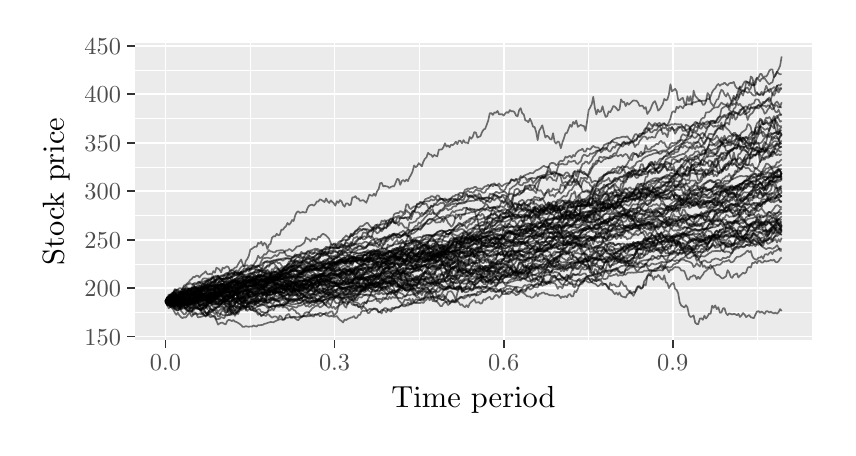
\begin{tikzpicture}[x=1pt,y=1pt]
\definecolor{fillColor}{RGB}{255,255,255}
\path[use as bounding box,fill=fillColor,fill opacity=0.00] (0,0) rectangle (289.08,144.54);
\begin{scope}
\path[clip] (  0.00,  0.00) rectangle (289.08,144.54);
\definecolor{drawColor}{RGB}{255,255,255}
\definecolor{fillColor}{RGB}{255,255,255}

\path[draw=drawColor,line width= 0.6pt,line join=round,line cap=round,fill=fillColor] (  0.00,  0.00) rectangle (289.08,144.54);
\end{scope}
\begin{scope}
\path[clip] ( 38.67, 31.53) rectangle (283.58,139.04);
\definecolor{fillColor}{gray}{0.92}

\path[fill=fillColor] ( 38.67, 31.53) rectangle (283.58,139.04);
\definecolor{drawColor}{RGB}{255,255,255}

\path[draw=drawColor,line width= 0.3pt,line join=round] ( 38.67, 41.65) --
	(283.58, 41.65);

\path[draw=drawColor,line width= 0.3pt,line join=round] ( 38.67, 59.17) --
	(283.58, 59.17);

\path[draw=drawColor,line width= 0.3pt,line join=round] ( 38.67, 76.68) --
	(283.58, 76.68);

\path[draw=drawColor,line width= 0.3pt,line join=round] ( 38.67, 94.19) --
	(283.58, 94.19);

\path[draw=drawColor,line width= 0.3pt,line join=round] ( 38.67,111.71) --
	(283.58,111.71);

\path[draw=drawColor,line width= 0.3pt,line join=round] ( 38.67,129.22) --
	(283.58,129.22);

\path[draw=drawColor,line width= 0.3pt,line join=round] ( 80.35, 31.53) --
	( 80.35,139.04);

\path[draw=drawColor,line width= 0.3pt,line join=round] (141.45, 31.53) --
	(141.45,139.04);

\path[draw=drawColor,line width= 0.3pt,line join=round] (202.56, 31.53) --
	(202.56,139.04);

\path[draw=drawColor,line width= 0.3pt,line join=round] (263.66, 31.53) --
	(263.66,139.04);

\path[draw=drawColor,line width= 0.6pt,line join=round] ( 38.67, 32.90) --
	(283.58, 32.90);

\path[draw=drawColor,line width= 0.6pt,line join=round] ( 38.67, 50.41) --
	(283.58, 50.41);

\path[draw=drawColor,line width= 0.6pt,line join=round] ( 38.67, 67.92) --
	(283.58, 67.92);

\path[draw=drawColor,line width= 0.6pt,line join=round] ( 38.67, 85.44) --
	(283.58, 85.44);

\path[draw=drawColor,line width= 0.6pt,line join=round] ( 38.67,102.95) --
	(283.58,102.95);

\path[draw=drawColor,line width= 0.6pt,line join=round] ( 38.67,120.46) --
	(283.58,120.46);

\path[draw=drawColor,line width= 0.6pt,line join=round] ( 38.67,137.98) --
	(283.58,137.98);

\path[draw=drawColor,line width= 0.6pt,line join=round] ( 49.80, 31.53) --
	( 49.80,139.04);

\path[draw=drawColor,line width= 0.6pt,line join=round] (110.90, 31.53) --
	(110.90,139.04);

\path[draw=drawColor,line width= 0.6pt,line join=round] (172.00, 31.53) --
	(172.00,139.04);

\path[draw=drawColor,line width= 0.6pt,line join=round] (233.11, 31.53) --
	(233.11,139.04);
\definecolor{drawColor}{RGB}{0,0,0}

\path[draw=drawColor,draw opacity=0.55,line width= 0.6pt,line join=round] ( 49.80, 45.61) --
	( 50.36, 45.48) --
	( 50.92, 45.87) --
	( 51.47, 45.76) --
	( 52.03, 46.32) --
	( 52.59, 46.51) --
	( 53.15, 47.31) --
	( 53.71, 46.41) --
	( 54.26, 46.91) --
	( 54.82, 47.30) --
	( 55.38, 47.91) --
	( 55.94, 48.52) --
	( 56.50, 48.06) --
	( 57.05, 48.33) --
	( 57.61, 47.89) --
	( 58.17, 47.94) --
	( 58.73, 48.50) --
	( 59.29, 48.70) --
	( 59.84, 48.15) --
	( 60.40, 48.07) --
	( 60.96, 48.94) --
	( 61.52, 48.85) --
	( 62.08, 49.46) --
	( 62.63, 48.97) --
	( 63.19, 49.56) --
	( 63.75, 50.00) --
	( 64.31, 50.03) --
	( 64.87, 49.79) --
	( 65.42, 51.32) --
	( 65.98, 50.95) --
	( 66.54, 51.18) --
	( 67.10, 51.93) --
	( 67.66, 52.20) --
	( 68.21, 52.13) --
	( 68.77, 52.18) --
	( 69.33, 52.98) --
	( 69.89, 53.02) --
	( 70.45, 53.00) --
	( 71.00, 52.80) --
	( 71.56, 52.77) --
	( 72.12, 52.71) --
	( 72.68, 52.58) --
	( 73.24, 52.61) --
	( 73.79, 53.01) --
	( 74.35, 53.34) --
	( 74.91, 53.67) --
	( 75.47, 54.01) --
	( 76.03, 54.79) --
	( 76.58, 55.66) --
	( 77.14, 55.09) --
	( 77.70, 54.54) --
	( 78.26, 54.40) --
	( 78.82, 54.24) --
	( 79.37, 54.71) --
	( 79.93, 55.29) --
	( 80.49, 55.97) --
	( 81.05, 55.76) --
	( 81.61, 56.08) --
	( 82.16, 56.04) --
	( 82.72, 55.98) --
	( 83.28, 56.17) --
	( 83.84, 56.52) --
	( 84.40, 56.48) --
	( 84.95, 56.84) --
	( 85.51, 56.90) --
	( 86.07, 56.63) --
	( 86.63, 56.53) --
	( 87.19, 56.23) --
	( 87.74, 55.80) --
	( 88.30, 55.57) --
	( 88.86, 55.35) --
	( 89.42, 55.14) --
	( 89.98, 54.37) --
	( 90.53, 53.64) --
	( 91.09, 54.73) --
	( 91.65, 53.45) --
	( 92.21, 53.78) --
	( 92.77, 53.18) --
	( 93.32, 51.80) --
	( 93.88, 52.12) --
	( 94.44, 52.55) --
	( 95.00, 52.77) --
	( 95.56, 53.90) --
	( 96.11, 54.68) --
	( 96.67, 54.01) --
	( 97.23, 54.14) --
	( 97.79, 55.23) --
	( 98.35, 55.48) --
	( 98.90, 55.42) --
	( 99.46, 56.46) --
	(100.02, 57.14) --
	(100.58, 57.24) --
	(101.14, 56.93) --
	(101.69, 57.16) --
	(102.25, 57.50) --
	(102.81, 57.13) --
	(103.37, 57.32) --
	(103.93, 57.46) --
	(104.48, 56.73) --
	(105.04, 57.02) --
	(105.60, 57.14) --
	(106.16, 57.96) --
	(106.72, 58.43) --
	(107.27, 58.61) --
	(107.83, 59.10) --
	(108.39, 59.35) --
	(108.95, 59.51) --
	(109.51, 59.20) --
	(110.06, 59.83) --
	(110.62, 59.71) --
	(111.18, 59.91) --
	(111.74, 59.81) --
	(112.30, 59.75) --
	(112.85, 60.04) --
	(113.41, 59.66) --
	(113.97, 59.87) --
	(114.53, 59.12) --
	(115.09, 59.21) --
	(115.65, 59.28) --
	(116.20, 59.22) --
	(116.76, 59.61) --
	(117.32, 60.24) --
	(117.88, 60.13) --
	(118.44, 60.03) --
	(118.99, 59.89) --
	(119.55, 60.33) --
	(120.11, 60.65) --
	(120.67, 60.63) --
	(121.23, 61.45) --
	(121.78, 60.81) --
	(122.34, 60.88) --
	(122.90, 61.23) --
	(123.46, 61.57) --
	(124.02, 62.60) --
	(124.57, 62.02) --
	(125.13, 61.65) --
	(125.69, 61.80) --
	(126.25, 62.56) --
	(126.81, 63.06) --
	(127.36, 62.75) --
	(127.92, 62.71) --
	(128.48, 62.81) --
	(129.04, 63.07) --
	(129.60, 62.73) --
	(130.15, 62.93) --
	(130.71, 63.50) --
	(131.27, 63.61) --
	(131.83, 63.27) --
	(132.39, 64.15) --
	(132.94, 64.91) --
	(133.50, 64.90) --
	(134.06, 64.98) --
	(134.62, 65.69) --
	(135.18, 66.88) --
	(135.73, 67.22) --
	(136.29, 67.08) --
	(136.85, 67.54) --
	(137.41, 67.31) --
	(137.97, 67.79) --
	(138.52, 67.69) --
	(139.08, 67.53) --
	(139.64, 68.53) --
	(140.20, 68.41) --
	(140.76, 68.75) --
	(141.31, 68.83) --
	(141.87, 68.92) --
	(142.43, 68.79) --
	(142.99, 69.11) --
	(143.55, 69.28) --
	(144.10, 69.49) --
	(144.66, 69.49) --
	(145.22, 69.53) --
	(145.78, 69.64) --
	(146.34, 69.01) --
	(146.89, 69.31) --
	(147.45, 70.06) --
	(148.01, 70.60) --
	(148.57, 70.77) --
	(149.13, 71.19) --
	(149.68, 71.16) --
	(150.24, 71.05) --
	(150.80, 71.02) --
	(151.36, 70.98) --
	(151.92, 71.19) --
	(152.47, 71.45) --
	(153.03, 71.44) --
	(153.59, 71.54) --
	(154.15, 71.59) --
	(154.71, 71.59) --
	(155.26, 71.70) --
	(155.82, 72.23) --
	(156.38, 72.80) --
	(156.94, 72.77) --
	(157.50, 73.20) --
	(158.05, 72.89) --
	(158.61, 72.02) --
	(159.17, 72.93) --
	(159.73, 73.63) --
	(160.29, 73.35) --
	(160.84, 74.18) --
	(161.40, 74.37) --
	(161.96, 75.37) --
	(162.52, 75.28) --
	(163.08, 75.22) --
	(163.63, 75.24) --
	(164.19, 75.54) --
	(164.75, 75.74) --
	(165.31, 76.01) --
	(165.87, 76.15) --
	(166.42, 76.47) --
	(166.98, 76.78) --
	(167.54, 77.16) --
	(168.10, 76.62) --
	(168.66, 77.70) --
	(169.21, 76.79) --
	(169.77, 76.30) --
	(170.33, 75.76) --
	(170.89, 75.03) --
	(171.45, 75.38) --
	(172.00, 76.00) --
	(172.56, 76.13) --
	(173.12, 77.01) --
	(173.68, 77.55) --
	(174.24, 76.28) --
	(174.79, 75.51) --
	(175.35, 74.55) --
	(175.91, 74.87) --
	(176.47, 73.88) --
	(177.03, 73.26) --
	(177.58, 72.42) --
	(178.14, 72.27) --
	(178.70, 73.50) --
	(179.26, 74.68) --
	(179.82, 74.94) --
	(180.37, 75.03) --
	(180.93, 76.33) --
	(181.49, 75.43) --
	(182.05, 75.73) --
	(182.61, 75.82) --
	(183.17, 76.29) --
	(183.72, 77.16) --
	(184.28, 76.30) --
	(184.84, 75.86) --
	(185.40, 79.17) --
	(185.96, 78.41) --
	(186.51, 77.48) --
	(187.07, 78.65) --
	(187.63, 78.15) --
	(188.19, 80.61) --
	(188.75, 79.92) --
	(189.30, 79.55) --
	(189.86, 79.47) --
	(190.42, 78.46) --
	(190.98, 81.17) --
	(191.54, 79.78) --
	(192.09, 80.00) --
	(192.65, 76.96) --
	(193.21, 76.24) --
	(193.77, 76.20) --
	(194.33, 76.28) --
	(194.88, 77.17) --
	(195.44, 76.86) --
	(196.00, 76.35) --
	(196.56, 74.84) --
	(197.12, 75.91) --
	(197.67, 76.77) --
	(198.23, 76.82) --
	(198.79, 76.66) --
	(199.35, 77.46) --
	(199.91, 78.69) --
	(200.46, 79.04) --
	(201.02, 79.12) --
	(201.58, 79.61) --
	(202.14, 80.47) --
	(202.70, 80.54) --
	(203.25, 79.47) --
	(203.81, 79.77) --
	(204.37, 79.05) --
	(204.93, 79.65) --
	(205.49, 78.90) --
	(206.04, 78.50) --
	(206.60, 78.02) --
	(207.16, 78.23) --
	(207.72, 78.52) --
	(208.28, 78.51) --
	(208.83, 78.72) --
	(209.39, 78.81) --
	(209.95, 79.04) --
	(210.51, 79.71) --
	(211.07, 80.73) --
	(211.62, 79.76) --
	(212.18, 79.40) --
	(212.74, 80.92) --
	(213.30, 81.49) --
	(213.86, 81.73) --
	(214.41, 81.76) --
	(214.97, 81.78) --
	(215.53, 82.09) --
	(216.09, 81.89) --
	(216.65, 81.62) --
	(217.20, 81.84) --
	(217.76, 82.38) --
	(218.32, 82.92) --
	(218.88, 82.55) --
	(219.44, 82.02) --
	(219.99, 82.96) --
	(220.55, 83.23) --
	(221.11, 82.91) --
	(221.67, 83.72) --
	(222.23, 83.29) --
	(222.78, 83.28) --
	(223.34, 82.63) --
	(223.90, 84.39) --
	(224.46, 84.29) --
	(225.02, 84.69) --
	(225.57, 85.42) --
	(226.13, 84.57) --
	(226.69, 84.29) --
	(227.25, 83.00) --
	(227.81, 83.99) --
	(228.36, 83.87) --
	(228.92, 81.77) --
	(229.48, 81.96) --
	(230.04, 80.83) --
	(230.60, 80.25) --
	(231.15, 79.96) --
	(231.71, 79.59) --
	(232.27, 80.04) --
	(232.83, 78.47) --
	(233.39, 78.95) --
	(233.94, 78.84) --
	(234.50, 79.90) --
	(235.06, 78.67) --
	(235.62, 77.18) --
	(236.18, 76.80) --
	(236.73, 78.67) --
	(237.29, 78.82) --
	(237.85, 77.56) --
	(238.41, 77.22) --
	(238.97, 76.29) --
	(239.52, 75.89) --
	(240.08, 75.98) --
	(240.64, 76.33) --
	(241.20, 75.59) --
	(241.76, 75.92) --
	(242.31, 76.36) --
	(242.87, 77.05) --
	(243.43, 75.44) --
	(243.99, 75.96) --
	(244.55, 74.88) --
	(245.10, 75.26) --
	(245.66, 76.26) --
	(246.22, 76.32) --
	(246.78, 74.78) --
	(247.34, 73.58) --
	(247.89, 75.89) --
	(248.45, 78.10) --
	(249.01, 77.24) --
	(249.57, 75.64) --
	(250.13, 76.64) --
	(250.68, 77.54) --
	(251.24, 77.49) --
	(251.80, 78.78) --
	(252.36, 78.35) --
	(252.92, 78.04) --
	(253.48, 78.26) --
	(254.03, 78.66) --
	(254.59, 77.44) --
	(255.15, 77.60) --
	(255.71, 78.18) --
	(256.27, 79.40) --
	(256.82, 77.09) --
	(257.38, 78.67) --
	(257.94, 77.12) --
	(258.50, 77.47) --
	(259.06, 79.77) --
	(259.61, 78.57) --
	(260.17, 78.34) --
	(260.73, 76.31) --
	(261.29, 78.54) --
	(261.85, 78.75) --
	(262.40, 79.31) --
	(262.96, 78.46) --
	(263.52, 79.90) --
	(264.08, 81.34) --
	(264.64, 80.83) --
	(265.19, 79.56) --
	(265.75, 81.35) --
	(266.31, 80.83) --
	(266.87, 81.75) --
	(267.43, 82.37) --
	(267.98, 82.75) --
	(268.54, 82.58) --
	(269.10, 82.54) --
	(269.66, 82.83) --
	(270.22, 82.95) --
	(270.77, 83.82) --
	(271.33, 84.47) --
	(271.89, 84.00) --
	(272.45, 83.53);

\path[draw=drawColor,draw opacity=0.55,line width= 0.6pt,line join=round] ( 49.80, 45.61) --
	( 50.36, 46.68) --
	( 50.92, 47.04) --
	( 51.47, 46.79) --
	( 52.03, 47.42) --
	( 52.59, 46.98) --
	( 53.15, 47.28) --
	( 53.71, 46.82) --
	( 54.26, 47.66) --
	( 54.82, 47.75) --
	( 55.38, 47.08) --
	( 55.94, 48.34) --
	( 56.50, 48.13) --
	( 57.05, 48.68) --
	( 57.61, 48.80) --
	( 58.17, 49.26) --
	( 58.73, 49.22) --
	( 59.29, 49.94) --
	( 59.84, 50.39) --
	( 60.40, 50.68) --
	( 60.96, 50.41) --
	( 61.52, 50.71) --
	( 62.08, 51.18) --
	( 62.63, 51.50) --
	( 63.19, 51.72) --
	( 63.75, 52.19) --
	( 64.31, 52.76) --
	( 64.87, 53.37) --
	( 65.42, 53.33) --
	( 65.98, 53.39) --
	( 66.54, 53.90) --
	( 67.10, 53.95) --
	( 67.66, 53.33) --
	( 68.21, 52.36) --
	( 68.77, 52.55) --
	( 69.33, 52.86) --
	( 69.89, 51.40) --
	( 70.45, 50.65) --
	( 71.00, 50.51) --
	( 71.56, 51.30) --
	( 72.12, 51.93) --
	( 72.68, 53.15) --
	( 73.24, 53.11) --
	( 73.79, 52.78) --
	( 74.35, 53.02) --
	( 74.91, 53.10) --
	( 75.47, 52.16) --
	( 76.03, 53.52) --
	( 76.58, 54.22) --
	( 77.14, 54.76) --
	( 77.70, 53.40) --
	( 78.26, 53.46) --
	( 78.82, 53.68) --
	( 79.37, 54.08) --
	( 79.93, 54.56) --
	( 80.49, 53.85) --
	( 81.05, 53.88) --
	( 81.61, 54.08) --
	( 82.16, 54.32) --
	( 82.72, 54.15) --
	( 83.28, 54.40) --
	( 83.84, 54.55) --
	( 84.40, 54.70) --
	( 84.95, 54.46) --
	( 85.51, 54.92) --
	( 86.07, 54.57) --
	( 86.63, 53.86) --
	( 87.19, 54.23) --
	( 87.74, 54.74) --
	( 88.30, 54.72) --
	( 88.86, 54.59) --
	( 89.42, 54.64) --
	( 89.98, 53.21) --
	( 90.53, 53.64) --
	( 91.09, 54.35) --
	( 91.65, 53.87) --
	( 92.21, 53.69) --
	( 92.77, 54.18) --
	( 93.32, 53.26) --
	( 93.88, 51.27) --
	( 94.44, 51.25) --
	( 95.00, 51.18) --
	( 95.56, 50.64) --
	( 96.11, 50.76) --
	( 96.67, 49.45) --
	( 97.23, 49.92) --
	( 97.79, 49.96) --
	( 98.35, 50.84) --
	( 98.90, 50.46) --
	( 99.46, 52.17) --
	(100.02, 53.50) --
	(100.58, 54.18) --
	(101.14, 54.17) --
	(101.69, 54.42) --
	(102.25, 54.49) --
	(102.81, 54.81) --
	(103.37, 55.37) --
	(103.93, 54.14) --
	(104.48, 54.07) --
	(105.04, 54.42) --
	(105.60, 54.49) --
	(106.16, 54.94) --
	(106.72, 55.28) --
	(107.27, 55.01) --
	(107.83, 54.07) --
	(108.39, 54.70) --
	(108.95, 56.01) --
	(109.51, 55.93) --
	(110.06, 57.40) --
	(110.62, 58.28) --
	(111.18, 58.33) --
	(111.74, 58.45) --
	(112.30, 58.59) --
	(112.85, 56.86) --
	(113.41, 56.77) --
	(113.97, 57.38) --
	(114.53, 57.59) --
	(115.09, 57.00) --
	(115.65, 56.64) --
	(116.20, 56.91) --
	(116.76, 56.56) --
	(117.32, 55.95) --
	(117.88, 55.97) --
	(118.44, 56.13) --
	(118.99, 55.77) --
	(119.55, 56.41) --
	(120.11, 57.12) --
	(120.67, 57.61) --
	(121.23, 58.47) --
	(121.78, 59.06) --
	(122.34, 59.00) --
	(122.90, 58.94) --
	(123.46, 58.88) --
	(124.02, 59.06) --
	(124.57, 58.99) --
	(125.13, 59.48) --
	(125.69, 59.48) --
	(126.25, 59.62) --
	(126.81, 59.03) --
	(127.36, 58.87) --
	(127.92, 58.74) --
	(128.48, 58.36) --
	(129.04, 58.92) --
	(129.60, 58.94) --
	(130.15, 58.90) --
	(130.71, 57.45) --
	(131.27, 57.28) --
	(131.83, 56.81) --
	(132.39, 56.97) --
	(132.94, 56.85) --
	(133.50, 56.75) --
	(134.06, 56.63) --
	(134.62, 56.72) --
	(135.18, 57.27) --
	(135.73, 57.56) --
	(136.29, 57.06) --
	(136.85, 57.57) --
	(137.41, 57.43) --
	(137.97, 57.37) --
	(138.52, 57.40) --
	(139.08, 58.06) --
	(139.64, 58.84) --
	(140.20, 58.64) --
	(140.76, 58.97) --
	(141.31, 58.98) --
	(141.87, 58.26) --
	(142.43, 58.29) --
	(142.99, 58.68) --
	(143.55, 58.68) --
	(144.10, 58.60) --
	(144.66, 59.90) --
	(145.22, 60.15) --
	(145.78, 60.87) --
	(146.34, 61.36) --
	(146.89, 62.25) --
	(147.45, 62.50) --
	(148.01, 62.94) --
	(148.57, 63.12) --
	(149.13, 63.20) --
	(149.68, 63.53) --
	(150.24, 63.07) --
	(150.80, 62.44) --
	(151.36, 62.55) --
	(151.92, 62.50) --
	(152.47, 62.82) --
	(153.03, 63.04) --
	(153.59, 63.16) --
	(154.15, 63.71) --
	(154.71, 64.16) --
	(155.26, 64.14) --
	(155.82, 64.15) --
	(156.38, 64.31) --
	(156.94, 64.43) --
	(157.50, 64.40) --
	(158.05, 64.86) --
	(158.61, 64.69) --
	(159.17, 65.46) --
	(159.73, 65.48) --
	(160.29, 66.03) --
	(160.84, 66.09) --
	(161.40, 66.55) --
	(161.96, 66.33) --
	(162.52, 65.91) --
	(163.08, 66.65) --
	(163.63, 66.08) --
	(164.19, 67.27) --
	(164.75, 67.31) --
	(165.31, 67.69) --
	(165.87, 68.40) --
	(166.42, 69.31) --
	(166.98, 70.06) --
	(167.54, 71.27) --
	(168.10, 71.56) --
	(168.66, 71.91) --
	(169.21, 71.41) --
	(169.77, 71.75) --
	(170.33, 71.65) --
	(170.89, 71.41) --
	(171.45, 71.68) --
	(172.00, 71.22) --
	(172.56, 71.00) --
	(173.12, 70.65) --
	(173.68, 71.15) --
	(174.24, 71.19) --
	(174.79, 70.38) --
	(175.35, 70.27) --
	(175.91, 70.23) --
	(176.47, 70.67) --
	(177.03, 71.16) --
	(177.58, 71.50) --
	(178.14, 71.56) --
	(178.70, 71.54) --
	(179.26, 71.52) --
	(179.82, 71.73) --
	(180.37, 71.24) --
	(180.93, 70.68) --
	(181.49, 71.06) --
	(182.05, 71.10) --
	(182.61, 71.37) --
	(183.17, 71.19) --
	(183.72, 71.21) --
	(184.28, 71.98) --
	(184.84, 72.06) --
	(185.40, 72.23) --
	(185.96, 72.23) --
	(186.51, 72.87) --
	(187.07, 73.17) --
	(187.63, 73.79) --
	(188.19, 74.06) --
	(188.75, 73.62) --
	(189.30, 73.40) --
	(189.86, 73.22) --
	(190.42, 72.84) --
	(190.98, 73.12) --
	(191.54, 73.50) --
	(192.09, 73.36) --
	(192.65, 72.90) --
	(193.21, 73.16) --
	(193.77, 72.75) --
	(194.33, 73.08) --
	(194.88, 73.21) --
	(195.44, 73.19) --
	(196.00, 72.84) --
	(196.56, 72.26) --
	(197.12, 73.18) --
	(197.67, 74.42) --
	(198.23, 75.39) --
	(198.79, 75.06) --
	(199.35, 75.34) --
	(199.91, 75.69) --
	(200.46, 75.10) --
	(201.02, 74.68) --
	(201.58, 74.54) --
	(202.14, 74.22) --
	(202.70, 74.15) --
	(203.25, 74.25) --
	(203.81, 74.30) --
	(204.37, 74.13) --
	(204.93, 74.46) --
	(205.49, 75.11) --
	(206.04, 75.12) --
	(206.60, 75.42) --
	(207.16, 75.33) --
	(207.72, 76.05) --
	(208.28, 76.92) --
	(208.83, 77.18) --
	(209.39, 78.00) --
	(209.95, 77.97) --
	(210.51, 79.45) --
	(211.07, 80.02) --
	(211.62, 80.57) --
	(212.18, 81.47) --
	(212.74, 80.68) --
	(213.30, 79.80) --
	(213.86, 79.15) --
	(214.41, 80.54) --
	(214.97, 82.07) --
	(215.53, 83.40) --
	(216.09, 83.33) --
	(216.65, 82.35) --
	(217.20, 82.60) --
	(217.76, 83.49) --
	(218.32, 84.00) --
	(218.88, 83.53) --
	(219.44, 84.48) --
	(219.99, 83.81) --
	(220.55, 82.62) --
	(221.11, 83.66) --
	(221.67, 84.96) --
	(222.23, 86.65) --
	(222.78, 86.17) --
	(223.34, 87.53) --
	(223.90, 86.66) --
	(224.46, 85.89) --
	(225.02, 87.25) --
	(225.57, 87.51) --
	(226.13, 86.49) --
	(226.69, 86.21) --
	(227.25, 85.17) --
	(227.81, 86.75) --
	(228.36, 86.31) --
	(228.92, 86.71) --
	(229.48, 87.38) --
	(230.04, 87.39) --
	(230.60, 88.24) --
	(231.15, 88.69) --
	(231.71, 88.06) --
	(232.27, 89.08) --
	(232.83, 90.34) --
	(233.39, 90.17) --
	(233.94, 86.78) --
	(234.50, 87.06) --
	(235.06, 87.25) --
	(235.62, 89.28) --
	(236.18, 88.33) --
	(236.73, 91.07) --
	(237.29, 92.11) --
	(237.85, 91.00) --
	(238.41, 90.77) --
	(238.97, 91.99) --
	(239.52, 93.59) --
	(240.08, 94.95) --
	(240.64, 94.02) --
	(241.20, 92.10) --
	(241.76, 91.27) --
	(242.31, 89.24) --
	(242.87, 89.30) --
	(243.43, 90.69) --
	(243.99, 91.56) --
	(244.55, 92.69) --
	(245.10, 91.46) --
	(245.66, 92.00) --
	(246.22, 93.15) --
	(246.78, 94.05) --
	(247.34, 95.76) --
	(247.89, 94.99) --
	(248.45, 96.16) --
	(249.01, 97.22) --
	(249.57, 97.47) --
	(250.13, 98.34) --
	(250.68, 98.83) --
	(251.24, 99.04) --
	(251.80, 98.31) --
	(252.36, 98.41) --
	(252.92, 99.72) --
	(253.48,100.13) --
	(254.03,100.46) --
	(254.59,100.29) --
	(255.15,100.88) --
	(255.71,101.27) --
	(256.27,101.45) --
	(256.82,102.03) --
	(257.38,101.56) --
	(257.94,101.49) --
	(258.50,101.47) --
	(259.06,101.45) --
	(259.61,101.97) --
	(260.17,102.05) --
	(260.73,102.61) --
	(261.29,102.94) --
	(261.85,102.81) --
	(262.40,102.52) --
	(262.96,102.96) --
	(263.52,102.56) --
	(264.08,102.76) --
	(264.64,102.80) --
	(265.19,103.07) --
	(265.75,103.91) --
	(266.31,104.84) --
	(266.87,104.93) --
	(267.43,105.13) --
	(267.98,105.54) --
	(268.54,105.89) --
	(269.10,106.28) --
	(269.66,106.44) --
	(270.22,106.51) --
	(270.77,106.96) --
	(271.33,106.69) --
	(271.89,107.34) --
	(272.45,107.50);

\path[draw=drawColor,draw opacity=0.55,line width= 0.6pt,line join=round] ( 49.80, 45.61) --
	( 50.36, 45.87) --
	( 50.92, 45.86) --
	( 51.47, 46.23) --
	( 52.03, 45.96) --
	( 52.59, 46.68) --
	( 53.15, 47.53) --
	( 53.71, 47.91) --
	( 54.26, 47.68) --
	( 54.82, 48.13) --
	( 55.38, 48.43) --
	( 55.94, 47.85) --
	( 56.50, 48.44) --
	( 57.05, 48.79) --
	( 57.61, 49.63) --
	( 58.17, 50.15) --
	( 58.73, 50.06) --
	( 59.29, 49.79) --
	( 59.84, 49.62) --
	( 60.40, 49.93) --
	( 60.96, 50.01) --
	( 61.52, 50.39) --
	( 62.08, 50.44) --
	( 62.63, 50.41) --
	( 63.19, 50.70) --
	( 63.75, 50.95) --
	( 64.31, 51.31) --
	( 64.87, 51.82) --
	( 65.42, 51.64) --
	( 65.98, 51.78) --
	( 66.54, 52.54) --
	( 67.10, 52.21) --
	( 67.66, 51.85) --
	( 68.21, 51.46) --
	( 68.77, 51.19) --
	( 69.33, 51.37) --
	( 69.89, 51.08) --
	( 70.45, 51.44) --
	( 71.00, 51.82) --
	( 71.56, 50.95) --
	( 72.12, 51.28) --
	( 72.68, 52.16) --
	( 73.24, 52.50) --
	( 73.79, 52.50) --
	( 74.35, 52.81) --
	( 74.91, 52.62) --
	( 75.47, 52.62) --
	( 76.03, 52.25) --
	( 76.58, 52.23) --
	( 77.14, 52.72) --
	( 77.70, 53.04) --
	( 78.26, 53.68) --
	( 78.82, 54.55) --
	( 79.37, 54.49) --
	( 79.93, 54.36) --
	( 80.49, 55.47) --
	( 81.05, 55.70) --
	( 81.61, 55.45) --
	( 82.16, 55.29) --
	( 82.72, 54.55) --
	( 83.28, 55.36) --
	( 83.84, 55.34) --
	( 84.40, 55.22) --
	( 84.95, 55.04) --
	( 85.51, 55.15) --
	( 86.07, 55.62) --
	( 86.63, 55.77) --
	( 87.19, 55.94) --
	( 87.74, 55.54) --
	( 88.30, 55.26) --
	( 88.86, 54.59) --
	( 89.42, 53.85) --
	( 89.98, 54.17) --
	( 90.53, 54.04) --
	( 91.09, 54.26) --
	( 91.65, 54.77) --
	( 92.21, 54.17) --
	( 92.77, 54.24) --
	( 93.32, 54.00) --
	( 93.88, 53.97) --
	( 94.44, 54.27) --
	( 95.00, 54.62) --
	( 95.56, 54.74) --
	( 96.11, 55.32) --
	( 96.67, 55.29) --
	( 97.23, 55.50) --
	( 97.79, 55.88) --
	( 98.35, 55.99) --
	( 98.90, 56.06) --
	( 99.46, 56.88) --
	(100.02, 56.15) --
	(100.58, 56.20) --
	(101.14, 55.93) --
	(101.69, 56.28) --
	(102.25, 56.97) --
	(102.81, 56.83) --
	(103.37, 57.03) --
	(103.93, 57.02) --
	(104.48, 57.26) --
	(105.04, 57.54) --
	(105.60, 57.57) --
	(106.16, 57.88) --
	(106.72, 58.01) --
	(107.27, 57.80) --
	(107.83, 57.34) --
	(108.39, 57.69) --
	(108.95, 57.80) --
	(109.51, 57.75) --
	(110.06, 58.16) --
	(110.62, 58.35) --
	(111.18, 58.76) --
	(111.74, 58.96) --
	(112.30, 59.98) --
	(112.85, 60.68) --
	(113.41, 60.65) --
	(113.97, 60.76) --
	(114.53, 60.65) --
	(115.09, 60.51) --
	(115.65, 61.11) --
	(116.20, 61.10) --
	(116.76, 61.94) --
	(117.32, 61.58) --
	(117.88, 60.86) --
	(118.44, 61.19) --
	(118.99, 61.38) --
	(119.55, 61.11) --
	(120.11, 61.03) --
	(120.67, 60.87) --
	(121.23, 62.01) --
	(121.78, 62.61) --
	(122.34, 62.14) --
	(122.90, 62.46) --
	(123.46, 62.06) --
	(124.02, 62.84) --
	(124.57, 62.22) --
	(125.13, 62.51) --
	(125.69, 62.79) --
	(126.25, 62.94) --
	(126.81, 62.36) --
	(127.36, 62.27) --
	(127.92, 62.22) --
	(128.48, 62.57) --
	(129.04, 62.73) --
	(129.60, 62.89) --
	(130.15, 63.14) --
	(130.71, 63.79) --
	(131.27, 63.96) --
	(131.83, 63.94) --
	(132.39, 63.77) --
	(132.94, 63.98) --
	(133.50, 64.95) --
	(134.06, 64.07) --
	(134.62, 63.59) --
	(135.18, 63.64) --
	(135.73, 62.11) --
	(136.29, 62.97) --
	(136.85, 63.94) --
	(137.41, 63.35) --
	(137.97, 62.69) --
	(138.52, 61.48) --
	(139.08, 60.83) --
	(139.64, 60.75) --
	(140.20, 60.06) --
	(140.76, 60.19) --
	(141.31, 60.61) --
	(141.87, 62.57) --
	(142.43, 63.51) --
	(142.99, 64.62) --
	(143.55, 64.39) --
	(144.10, 64.07) --
	(144.66, 64.85) --
	(145.22, 64.93) --
	(145.78, 64.48) --
	(146.34, 65.43) --
	(146.89, 65.87) --
	(147.45, 67.11) --
	(148.01, 66.87) --
	(148.57, 67.12) --
	(149.13, 67.46) --
	(149.68, 66.93) --
	(150.24, 68.42) --
	(150.80, 69.43) --
	(151.36, 70.01) --
	(151.92, 69.93) --
	(152.47, 70.15) --
	(153.03, 70.69) --
	(153.59, 70.56) --
	(154.15, 71.88) --
	(154.71, 72.40) --
	(155.26, 73.05) --
	(155.82, 73.22) --
	(156.38, 73.75) --
	(156.94, 73.28) --
	(157.50, 74.00) --
	(158.05, 74.30) --
	(158.61, 74.71) --
	(159.17, 74.92) --
	(159.73, 75.54) --
	(160.29, 75.68) --
	(160.84, 75.93) --
	(161.40, 76.22) --
	(161.96, 76.27) --
	(162.52, 76.63) --
	(163.08, 77.56) --
	(163.63, 78.16) --
	(164.19, 78.51) --
	(164.75, 78.88) --
	(165.31, 78.47) --
	(165.87, 79.38) --
	(166.42, 79.68) --
	(166.98, 79.25) --
	(167.54, 79.49) --
	(168.10, 79.59) --
	(168.66, 79.85) --
	(169.21, 78.81) --
	(169.77, 78.74) --
	(170.33, 77.90) --
	(170.89, 78.46) --
	(171.45, 78.15) --
	(172.00, 77.80) --
	(172.56, 76.91) --
	(173.12, 78.22) --
	(173.68, 77.97) --
	(174.24, 78.03) --
	(174.79, 77.83) --
	(175.35, 78.76) --
	(175.91, 79.22) --
	(176.47, 79.13) --
	(177.03, 79.72) --
	(177.58, 79.48) --
	(178.14, 79.28) --
	(178.70, 80.50) --
	(179.26, 80.93) --
	(179.82, 81.17) --
	(180.37, 82.01) --
	(180.93, 82.41) --
	(181.49, 82.24) --
	(182.05, 82.28) --
	(182.61, 81.84) --
	(183.17, 80.80) --
	(183.72, 81.00) --
	(184.28, 80.41) --
	(184.84, 80.16) --
	(185.40, 79.23) --
	(185.96, 78.09) --
	(186.51, 77.77) --
	(187.07, 79.06) --
	(187.63, 79.04) --
	(188.19, 79.31) --
	(188.75, 79.00) --
	(189.30, 79.99) --
	(189.86, 80.27) --
	(190.42, 80.29) --
	(190.98, 81.54) --
	(191.54, 82.32) --
	(192.09, 82.41) --
	(192.65, 82.66) --
	(193.21, 83.35) --
	(193.77, 83.77) --
	(194.33, 83.50) --
	(194.88, 83.84) --
	(195.44, 85.20) --
	(196.00, 85.81) --
	(196.56, 85.86) --
	(197.12, 86.97) --
	(197.67, 87.77) --
	(198.23, 87.71) --
	(198.79, 88.22) --
	(199.35, 87.74) --
	(199.91, 87.14) --
	(200.46, 85.54) --
	(201.02, 85.14) --
	(201.58, 85.61) --
	(202.14, 85.84) --
	(202.70, 84.86) --
	(203.25, 85.20) --
	(203.81, 85.98) --
	(204.37, 86.40) --
	(204.93, 87.29) --
	(205.49, 87.41) --
	(206.04, 88.71) --
	(206.60, 90.16) --
	(207.16, 90.47) --
	(207.72, 90.81) --
	(208.28, 91.46) --
	(208.83, 91.67) --
	(209.39, 91.78) --
	(209.95, 92.01) --
	(210.51, 92.23) --
	(211.07, 92.22) --
	(211.62, 92.33) --
	(212.18, 92.25) --
	(212.74, 92.12) --
	(213.30, 91.91) --
	(213.86, 91.78) --
	(214.41, 92.28) --
	(214.97, 93.22) --
	(215.53, 94.30) --
	(216.09, 94.16) --
	(216.65, 94.37) --
	(217.20, 93.78) --
	(217.76, 93.51) --
	(218.32, 94.10) --
	(218.88, 94.46) --
	(219.44, 94.71) --
	(219.99, 95.86) --
	(220.55, 96.15) --
	(221.11, 96.39) --
	(221.67, 96.31) --
	(222.23, 97.19) --
	(222.78, 97.59) --
	(223.34, 97.94) --
	(223.90, 98.13) --
	(224.46, 98.48) --
	(225.02, 98.56) --
	(225.57, 98.76) --
	(226.13, 99.07) --
	(226.69, 99.15) --
	(227.25, 99.29) --
	(227.81, 99.37) --
	(228.36, 98.90) --
	(228.92, 99.11) --
	(229.48, 99.75) --
	(230.04, 99.77) --
	(230.60, 99.69) --
	(231.15, 99.90) --
	(231.71, 99.10) --
	(232.27, 99.47) --
	(232.83, 99.72) --
	(233.39,100.37) --
	(233.94,101.19) --
	(234.50,101.65) --
	(235.06,101.71) --
	(235.62,102.09) --
	(236.18,102.60) --
	(236.73,102.38) --
	(237.29,103.39) --
	(237.85,103.97) --
	(238.41,104.02) --
	(238.97,104.57) --
	(239.52,104.71) --
	(240.08,105.83) --
	(240.64,107.56) --
	(241.20,107.14) --
	(241.76,107.00) --
	(242.31,108.50) --
	(242.87,109.02) --
	(243.43,109.60) --
	(243.99,109.47) --
	(244.55,110.03) --
	(245.10,110.37) --
	(245.66,110.75) --
	(246.22,110.31) --
	(246.78,110.82) --
	(247.34,110.70) --
	(247.89,110.99) --
	(248.45,110.30) --
	(249.01,110.24) --
	(249.57,110.25) --
	(250.13,111.06) --
	(250.68,111.93) --
	(251.24,112.16) --
	(251.80,112.61) --
	(252.36,112.13) --
	(252.92,111.65) --
	(253.48,113.29) --
	(254.03,113.59) --
	(254.59,113.04) --
	(255.15,112.98) --
	(255.71,114.05) --
	(256.27,113.51) --
	(256.82,113.24) --
	(257.38,113.93) --
	(257.94,115.15) --
	(258.50,115.74) --
	(259.06,113.17) --
	(259.61,113.43) --
	(260.17,113.86) --
	(260.73,114.15) --
	(261.29,115.93) --
	(261.85,115.39) --
	(262.40,115.31) --
	(262.96,115.60) --
	(263.52,115.49) --
	(264.08,115.35) --
	(264.64,115.97) --
	(265.19,116.30) --
	(265.75,117.01) --
	(266.31,117.75) --
	(266.87,118.00) --
	(267.43,118.48) --
	(267.98,119.30) --
	(268.54,118.17) --
	(269.10,116.72) --
	(269.66,116.46) --
	(270.22,117.38) --
	(270.77,117.85) --
	(271.33,117.11) --
	(271.89,115.86) --
	(272.45,117.59);

\path[draw=drawColor,draw opacity=0.55,line width= 0.6pt,line join=round] ( 49.80, 45.61) --
	( 50.36, 46.98) --
	( 50.92, 46.27) --
	( 51.47, 46.36) --
	( 52.03, 47.00) --
	( 52.59, 47.81) --
	( 53.15, 47.49) --
	( 53.71, 46.96) --
	( 54.26, 47.27) --
	( 54.82, 46.57) --
	( 55.38, 47.66) --
	( 55.94, 47.63) --
	( 56.50, 46.92) --
	( 57.05, 46.29) --
	( 57.61, 45.83) --
	( 58.17, 44.83) --
	( 58.73, 44.52) --
	( 59.29, 45.43) --
	( 59.84, 45.13) --
	( 60.40, 44.89) --
	( 60.96, 45.73) --
	( 61.52, 47.56) --
	( 62.08, 48.36) --
	( 62.63, 48.63) --
	( 63.19, 48.54) --
	( 63.75, 48.23) --
	( 64.31, 47.49) --
	( 64.87, 47.57) --
	( 65.42, 46.75) --
	( 65.98, 47.00) --
	( 66.54, 47.33) --
	( 67.10, 47.12) --
	( 67.66, 46.62) --
	( 68.21, 46.67) --
	( 68.77, 46.54) --
	( 69.33, 46.52) --
	( 69.89, 46.32) --
	( 70.45, 45.73) --
	( 71.00, 45.77) --
	( 71.56, 45.74) --
	( 72.12, 46.02) --
	( 72.68, 45.54) --
	( 73.24, 46.05) --
	( 73.79, 46.14) --
	( 74.35, 45.25) --
	( 74.91, 45.78) --
	( 75.47, 45.51) --
	( 76.03, 44.87) --
	( 76.58, 44.76) --
	( 77.14, 44.83) --
	( 77.70, 45.28) --
	( 78.26, 45.73) --
	( 78.82, 47.10) --
	( 79.37, 46.87) --
	( 79.93, 47.14) --
	( 80.49, 47.29) --
	( 81.05, 47.42) --
	( 81.61, 47.25) --
	( 82.16, 48.00) --
	( 82.72, 48.48) --
	( 83.28, 48.47) --
	( 83.84, 48.22) --
	( 84.40, 48.46) --
	( 84.95, 48.48) --
	( 85.51, 49.06) --
	( 86.07, 48.88) --
	( 86.63, 48.20) --
	( 87.19, 48.12) --
	( 87.74, 47.90) --
	( 88.30, 48.22) --
	( 88.86, 48.29) --
	( 89.42, 48.59) --
	( 89.98, 49.58) --
	( 90.53, 49.11) --
	( 91.09, 48.22) --
	( 91.65, 48.02) --
	( 92.21, 48.05) --
	( 92.77, 48.76) --
	( 93.32, 48.04) --
	( 93.88, 48.19) --
	( 94.44, 48.00) --
	( 95.00, 47.60) --
	( 95.56, 47.92) --
	( 96.11, 48.48) --
	( 96.67, 48.71) --
	( 97.23, 49.36) --
	( 97.79, 49.03) --
	( 98.35, 49.14) --
	( 98.90, 49.21) --
	( 99.46, 49.12) --
	(100.02, 48.97) --
	(100.58, 48.72) --
	(101.14, 48.77) --
	(101.69, 49.55) --
	(102.25, 49.69) --
	(102.81, 49.44) --
	(103.37, 49.02) --
	(103.93, 49.84) --
	(104.48, 49.62) --
	(105.04, 49.83) --
	(105.60, 50.34) --
	(106.16, 50.41) --
	(106.72, 50.43) --
	(107.27, 49.95) --
	(107.83, 50.02) --
	(108.39, 49.67) --
	(108.95, 49.98) --
	(109.51, 50.19) --
	(110.06, 50.88) --
	(110.62, 51.24) --
	(111.18, 51.47) --
	(111.74, 51.00) --
	(112.30, 50.94) --
	(112.85, 50.58) --
	(113.41, 50.79) --
	(113.97, 50.31) --
	(114.53, 50.04) --
	(115.09, 49.08) --
	(115.65, 48.67) --
	(116.20, 49.23) --
	(116.76, 49.79) --
	(117.32, 50.08) --
	(117.88, 50.22) --
	(118.44, 50.16) --
	(118.99, 50.36) --
	(119.55, 50.62) --
	(120.11, 50.90) --
	(120.67, 51.13) --
	(121.23, 51.11) --
	(121.78, 50.60) --
	(122.34, 50.85) --
	(122.90, 51.14) --
	(123.46, 51.60) --
	(124.02, 51.71) --
	(124.57, 51.72) --
	(125.13, 51.61) --
	(125.69, 52.72) --
	(126.25, 52.29) --
	(126.81, 52.52) --
	(127.36, 53.08) --
	(127.92, 53.30) --
	(128.48, 52.22) --
	(129.04, 52.22) --
	(129.60, 52.10) --
	(130.15, 51.92) --
	(130.71, 52.54) --
	(131.27, 52.69) --
	(131.83, 53.12) --
	(132.39, 52.00) --
	(132.94, 50.99) --
	(133.50, 50.78) --
	(134.06, 51.77) --
	(134.62, 50.77) --
	(135.18, 52.11) --
	(135.73, 52.36) --
	(136.29, 53.06) --
	(136.85, 53.38) --
	(137.41, 52.77) --
	(137.97, 53.64) --
	(138.52, 53.98) --
	(139.08, 53.70) --
	(139.64, 53.60) --
	(140.20, 54.60) --
	(140.76, 53.63) --
	(141.31, 54.34) --
	(141.87, 55.27) --
	(142.43, 55.55) --
	(142.99, 55.87) --
	(143.55, 56.44) --
	(144.10, 55.66) --
	(144.66, 55.83) --
	(145.22, 55.07) --
	(145.78, 55.94) --
	(146.34, 56.97) --
	(146.89, 57.12) --
	(147.45, 57.34) --
	(148.01, 56.90) --
	(148.57, 57.18) --
	(149.13, 57.98) --
	(149.68, 57.48) --
	(150.24, 57.80) --
	(150.80, 57.62) --
	(151.36, 57.05) --
	(151.92, 56.56) --
	(152.47, 56.62) --
	(153.03, 57.68) --
	(153.59, 57.84) --
	(154.15, 56.84) --
	(154.71, 56.59) --
	(155.26, 56.89) --
	(155.82, 56.69) --
	(156.38, 57.25) --
	(156.94, 57.19) --
	(157.50, 57.50) --
	(158.05, 57.11) --
	(158.61, 56.32) --
	(159.17, 56.11) --
	(159.73, 55.92) --
	(160.29, 55.66) --
	(160.84, 55.74) --
	(161.40, 55.86) --
	(161.96, 55.54) --
	(162.52, 55.22) --
	(163.08, 55.22) --
	(163.63, 55.22) --
	(164.19, 54.95) --
	(164.75, 53.55) --
	(165.31, 53.36) --
	(165.87, 52.61) --
	(166.42, 52.80) --
	(166.98, 53.78) --
	(167.54, 52.21) --
	(168.10, 52.81) --
	(168.66, 52.22) --
	(169.21, 51.02) --
	(169.77, 52.00) --
	(170.33, 53.13) --
	(170.89, 54.30) --
	(171.45, 55.33) --
	(172.00, 55.28) --
	(172.56, 55.78) --
	(173.12, 55.98) --
	(173.68, 55.73) --
	(174.24, 57.18) --
	(174.79, 58.75) --
	(175.35, 57.73) --
	(175.91, 58.12) --
	(176.47, 57.45) --
	(177.03, 57.04) --
	(177.58, 59.66) --
	(178.14, 58.97) --
	(178.70, 59.62) --
	(179.26, 58.12) --
	(179.82, 57.82) --
	(180.37, 58.41) --
	(180.93, 57.49) --
	(181.49, 58.21) --
	(182.05, 58.72) --
	(182.61, 57.79) --
	(183.17, 59.15) --
	(183.72, 59.31) --
	(184.28, 58.90) --
	(184.84, 58.84) --
	(185.40, 58.89) --
	(185.96, 58.94) --
	(186.51, 59.78) --
	(187.07, 60.26) --
	(187.63, 59.84) --
	(188.19, 60.55) --
	(188.75, 61.37) --
	(189.30, 62.10) --
	(189.86, 62.12) --
	(190.42, 62.47) --
	(190.98, 63.29) --
	(191.54, 63.49) --
	(192.09, 63.40) --
	(192.65, 63.58) --
	(193.21, 63.58) --
	(193.77, 63.98) --
	(194.33, 63.60) --
	(194.88, 63.54) --
	(195.44, 63.83) --
	(196.00, 65.03) --
	(196.56, 65.16) --
	(197.12, 64.85) --
	(197.67, 65.37) --
	(198.23, 65.71) --
	(198.79, 66.24) --
	(199.35, 66.35) --
	(199.91, 65.63) --
	(200.46, 66.44) --
	(201.02, 66.00) --
	(201.58, 65.20) --
	(202.14, 67.16) --
	(202.70, 67.51) --
	(203.25, 67.59) --
	(203.81, 67.92) --
	(204.37, 68.58) --
	(204.93, 69.41) --
	(205.49, 68.83) --
	(206.04, 68.95) --
	(206.60, 68.50) --
	(207.16, 70.84) --
	(207.72, 71.45) --
	(208.28, 71.72) --
	(208.83, 72.13) --
	(209.39, 71.14) --
	(209.95, 72.68) --
	(210.51, 73.10) --
	(211.07, 73.52) --
	(211.62, 73.33) --
	(212.18, 73.40) --
	(212.74, 72.04) --
	(213.30, 72.98) --
	(213.86, 73.59) --
	(214.41, 74.72) --
	(214.97, 74.05) --
	(215.53, 72.36) --
	(216.09, 72.88) --
	(216.65, 72.23) --
	(217.20, 72.26) --
	(217.76, 72.48) --
	(218.32, 71.70) --
	(218.88, 72.47) --
	(219.44, 73.20) --
	(219.99, 73.22) --
	(220.55, 72.82) --
	(221.11, 72.98) --
	(221.67, 73.46) --
	(222.23, 73.58) --
	(222.78, 73.91) --
	(223.34, 73.41) --
	(223.90, 73.46) --
	(224.46, 73.56) --
	(225.02, 71.79) --
	(225.57, 73.64) --
	(226.13, 74.01) --
	(226.69, 72.36) --
	(227.25, 73.11) --
	(227.81, 74.26) --
	(228.36, 74.09) --
	(228.92, 74.00) --
	(229.48, 74.60) --
	(230.04, 75.19) --
	(230.60, 75.73) --
	(231.15, 75.88) --
	(231.71, 76.20) --
	(232.27, 74.79) --
	(232.83, 75.78) --
	(233.39, 77.22) --
	(233.94, 76.26) --
	(234.50, 76.27) --
	(235.06, 76.19) --
	(235.62, 74.94) --
	(236.18, 74.43) --
	(236.73, 73.99) --
	(237.29, 74.94) --
	(237.85, 74.99) --
	(238.41, 73.66) --
	(238.97, 73.86) --
	(239.52, 72.66) --
	(240.08, 73.44) --
	(240.64, 73.44) --
	(241.20, 73.11) --
	(241.76, 74.10) --
	(242.31, 73.24) --
	(242.87, 72.76) --
	(243.43, 73.46) --
	(243.99, 71.47) --
	(244.55, 71.56) --
	(245.10, 71.94) --
	(245.66, 72.55) --
	(246.22, 73.71) --
	(246.78, 73.31) --
	(247.34, 73.42) --
	(247.89, 74.56) --
	(248.45, 75.10) --
	(249.01, 75.67) --
	(249.57, 74.81) --
	(250.13, 75.07) --
	(250.68, 74.67) --
	(251.24, 74.44) --
	(251.80, 73.29) --
	(252.36, 74.15) --
	(252.92, 74.23) --
	(253.48, 73.17) --
	(254.03, 72.59) --
	(254.59, 72.32) --
	(255.15, 69.07) --
	(255.71, 70.64) --
	(256.27, 69.85) --
	(256.82, 72.49) --
	(257.38, 72.50) --
	(257.94, 72.29) --
	(258.50, 72.55) --
	(259.06, 72.69) --
	(259.61, 72.26) --
	(260.17, 73.46) --
	(260.73, 73.21) --
	(261.29, 73.32) --
	(261.85, 72.89) --
	(262.40, 73.75) --
	(262.96, 74.40) --
	(263.52, 75.94) --
	(264.08, 74.02) --
	(264.64, 76.41) --
	(265.19, 73.11) --
	(265.75, 72.35) --
	(266.31, 73.49) --
	(266.87, 71.03) --
	(267.43, 69.46) --
	(267.98, 70.39) --
	(268.54, 71.99) --
	(269.10, 70.62) --
	(269.66, 70.51) --
	(270.22, 71.89) --
	(270.77, 71.18) --
	(271.33, 71.06) --
	(271.89, 71.61) --
	(272.45, 72.89);

\path[draw=drawColor,draw opacity=0.55,line width= 0.6pt,line join=round] ( 49.80, 45.61) --
	( 50.36, 45.97) --
	( 50.92, 46.25) --
	( 51.47, 46.39) --
	( 52.03, 44.66) --
	( 52.59, 44.25) --
	( 53.15, 44.25) --
	( 53.71, 44.69) --
	( 54.26, 43.85) --
	( 54.82, 44.40) --
	( 55.38, 44.63) --
	( 55.94, 44.75) --
	( 56.50, 45.39) --
	( 57.05, 44.59) --
	( 57.61, 43.79) --
	( 58.17, 42.37) --
	( 58.73, 43.13) --
	( 59.29, 44.53) --
	( 59.84, 43.25) --
	( 60.40, 43.53) --
	( 60.96, 43.85) --
	( 61.52, 42.82) --
	( 62.08, 42.99) --
	( 62.63, 42.54) --
	( 63.19, 43.51) --
	( 63.75, 43.95) --
	( 64.31, 44.58) --
	( 64.87, 45.43) --
	( 65.42, 45.91) --
	( 65.98, 46.43) --
	( 66.54, 46.30) --
	( 67.10, 46.38) --
	( 67.66, 45.83) --
	( 68.21, 45.66) --
	( 68.77, 45.76) --
	( 69.33, 45.59) --
	( 69.89, 45.66) --
	( 70.45, 45.94) --
	( 71.00, 47.01) --
	( 71.56, 46.71) --
	( 72.12, 45.98) --
	( 72.68, 47.05) --
	( 73.24, 47.26) --
	( 73.79, 47.08) --
	( 74.35, 47.21) --
	( 74.91, 48.77) --
	( 75.47, 49.06) --
	( 76.03, 49.33) --
	( 76.58, 49.54) --
	( 77.14, 50.95) --
	( 77.70, 50.81) --
	( 78.26, 51.07) --
	( 78.82, 52.11) --
	( 79.37, 52.67) --
	( 79.93, 52.56) --
	( 80.49, 52.22) --
	( 81.05, 53.51) --
	( 81.61, 52.49) --
	( 82.16, 51.95) --
	( 82.72, 52.18) --
	( 83.28, 52.11) --
	( 83.84, 52.55) --
	( 84.40, 53.49) --
	( 84.95, 53.89) --
	( 85.51, 53.68) --
	( 86.07, 53.32) --
	( 86.63, 53.44) --
	( 87.19, 53.64) --
	( 87.74, 53.09) --
	( 88.30, 53.08) --
	( 88.86, 53.17) --
	( 89.42, 53.02) --
	( 89.98, 53.78) --
	( 90.53, 53.82) --
	( 91.09, 54.63) --
	( 91.65, 54.49) --
	( 92.21, 54.67) --
	( 92.77, 54.55) --
	( 93.32, 55.09) --
	( 93.88, 55.04) --
	( 94.44, 55.73) --
	( 95.00, 56.23) --
	( 95.56, 56.86) --
	( 96.11, 56.68) --
	( 96.67, 56.90) --
	( 97.23, 57.51) --
	( 97.79, 57.85) --
	( 98.35, 57.97) --
	( 98.90, 57.46) --
	( 99.46, 57.26) --
	(100.02, 57.59) --
	(100.58, 57.79) --
	(101.14, 58.14) --
	(101.69, 58.57) --
	(102.25, 58.87) --
	(102.81, 58.86) --
	(103.37, 58.92) --
	(103.93, 58.64) --
	(104.48, 58.39) --
	(105.04, 58.68) --
	(105.60, 58.80) --
	(106.16, 58.71) --
	(106.72, 58.79) --
	(107.27, 59.21) --
	(107.83, 59.16) --
	(108.39, 59.20) --
	(108.95, 59.24) --
	(109.51, 58.60) --
	(110.06, 58.65) --
	(110.62, 58.26) --
	(111.18, 59.46) --
	(111.74, 60.45) --
	(112.30, 60.67) --
	(112.85, 60.95) --
	(113.41, 60.57) --
	(113.97, 60.56) --
	(114.53, 61.34) --
	(115.09, 61.48) --
	(115.65, 62.44) --
	(116.20, 61.92) --
	(116.76, 61.85) --
	(117.32, 61.74) --
	(117.88, 61.67) --
	(118.44, 61.21) --
	(118.99, 61.64) --
	(119.55, 62.20) --
	(120.11, 62.10) --
	(120.67, 62.53) --
	(121.23, 62.16) --
	(121.78, 62.42) --
	(122.34, 62.51) --
	(122.90, 63.04) --
	(123.46, 63.08) --
	(124.02, 63.26) --
	(124.57, 63.41) --
	(125.13, 63.55) --
	(125.69, 63.59) --
	(126.25, 64.04) --
	(126.81, 63.81) --
	(127.36, 63.95) --
	(127.92, 64.56) --
	(128.48, 64.78) --
	(129.04, 64.68) --
	(129.60, 64.74) --
	(130.15, 65.09) --
	(130.71, 65.40) --
	(131.27, 65.65) --
	(131.83, 65.85) --
	(132.39, 66.25) --
	(132.94, 66.26) --
	(133.50, 66.31) --
	(134.06, 66.46) --
	(134.62, 66.67) --
	(135.18, 66.81) --
	(135.73, 66.66) --
	(136.29, 66.36) --
	(136.85, 66.43) --
	(137.41, 66.46) --
	(137.97, 66.91) --
	(138.52, 67.04) --
	(139.08, 67.85) --
	(139.64, 67.84) --
	(140.20, 67.81) --
	(140.76, 67.61) --
	(141.31, 67.59) --
	(141.87, 67.26) --
	(142.43, 67.65) --
	(142.99, 67.72) --
	(143.55, 68.27) --
	(144.10, 68.92) --
	(144.66, 68.63) --
	(145.22, 69.34) --
	(145.78, 69.23) --
	(146.34, 69.24) --
	(146.89, 69.35) --
	(147.45, 69.56) --
	(148.01, 69.56) --
	(148.57, 69.31) --
	(149.13, 69.29) --
	(149.68, 69.51) --
	(150.24, 69.26) --
	(150.80, 68.91) --
	(151.36, 69.09) --
	(151.92, 68.98) --
	(152.47, 70.47) --
	(153.03, 69.87) --
	(153.59, 69.18) --
	(154.15, 68.24) --
	(154.71, 68.35) --
	(155.26, 68.54) --
	(155.82, 68.77) --
	(156.38, 68.87) --
	(156.94, 67.92) --
	(157.50, 68.41) --
	(158.05, 68.47) --
	(158.61, 67.86) --
	(159.17, 67.09) --
	(159.73, 66.35) --
	(160.29, 66.85) --
	(160.84, 67.55) --
	(161.40, 67.80) --
	(161.96, 67.18) --
	(162.52, 67.75) --
	(163.08, 68.01) --
	(163.63, 67.59) --
	(164.19, 67.12) --
	(164.75, 66.76) --
	(165.31, 66.85) --
	(165.87, 66.66) --
	(166.42, 67.23) --
	(166.98, 67.00) --
	(167.54, 66.55) --
	(168.10, 66.82) --
	(168.66, 66.60) --
	(169.21, 68.32) --
	(169.77, 68.66) --
	(170.33, 68.07) --
	(170.89, 68.70) --
	(171.45, 68.40) --
	(172.00, 68.61) --
	(172.56, 69.29) --
	(173.12, 69.74) --
	(173.68, 70.87) --
	(174.24, 70.62) --
	(174.79, 70.55) --
	(175.35, 70.70) --
	(175.91, 70.83) --
	(176.47, 72.24) --
	(177.03, 72.16) --
	(177.58, 73.01) --
	(178.14, 72.14) --
	(178.70, 72.61) --
	(179.26, 72.94) --
	(179.82, 73.89) --
	(180.37, 73.72) --
	(180.93, 73.87) --
	(181.49, 73.46) --
	(182.05, 73.51) --
	(182.61, 72.88) --
	(183.17, 72.80) --
	(183.72, 73.09) --
	(184.28, 72.95) --
	(184.84, 74.09) --
	(185.40, 74.56) --
	(185.96, 74.96) --
	(186.51, 75.10) --
	(187.07, 75.04) --
	(187.63, 75.40) --
	(188.19, 75.07) --
	(188.75, 75.11) --
	(189.30, 74.98) --
	(189.86, 75.62) --
	(190.42, 75.25) --
	(190.98, 75.48) --
	(191.54, 75.35) --
	(192.09, 74.99) --
	(192.65, 75.50) --
	(193.21, 76.02) --
	(193.77, 75.89) --
	(194.33, 76.61) --
	(194.88, 76.71) --
	(195.44, 76.72) --
	(196.00, 76.88) --
	(196.56, 77.10) --
	(197.12, 76.76) --
	(197.67, 76.93) --
	(198.23, 76.95) --
	(198.79, 76.68) --
	(199.35, 77.11) --
	(199.91, 77.59) --
	(200.46, 77.36) --
	(201.02, 77.20) --
	(201.58, 76.37) --
	(202.14, 75.98) --
	(202.70, 76.75) --
	(203.25, 76.90) --
	(203.81, 77.20) --
	(204.37, 77.57) --
	(204.93, 77.86) --
	(205.49, 78.04) --
	(206.04, 78.07) --
	(206.60, 78.27) --
	(207.16, 79.05) --
	(207.72, 79.51) --
	(208.28, 79.32) --
	(208.83, 79.47) --
	(209.39, 79.83) --
	(209.95, 80.92) --
	(210.51, 80.46) --
	(211.07, 80.58) --
	(211.62, 80.09) --
	(212.18, 79.67) --
	(212.74, 80.24) --
	(213.30, 80.54) --
	(213.86, 80.67) --
	(214.41, 80.23) --
	(214.97, 79.61) --
	(215.53, 79.26) --
	(216.09, 78.71) --
	(216.65, 78.13) --
	(217.20, 77.71) --
	(217.76, 78.37) --
	(218.32, 77.96) --
	(218.88, 77.67) --
	(219.44, 76.83) --
	(219.99, 77.71) --
	(220.55, 77.77) --
	(221.11, 78.03) --
	(221.67, 79.17) --
	(222.23, 78.18) --
	(222.78, 78.19) --
	(223.34, 78.28) --
	(223.90, 78.43) --
	(224.46, 79.97) --
	(225.02, 79.97) --
	(225.57, 80.17) --
	(226.13, 80.68) --
	(226.69, 80.48) --
	(227.25, 80.86) --
	(227.81, 80.32) --
	(228.36, 80.00) --
	(228.92, 81.18) --
	(229.48, 80.73) --
	(230.04, 80.50) --
	(230.60, 79.60) --
	(231.15, 78.38) --
	(231.71, 80.13) --
	(232.27, 80.70) --
	(232.83, 81.20) --
	(233.39, 81.66) --
	(233.94, 81.97) --
	(234.50, 81.92) --
	(235.06, 81.98) --
	(235.62, 82.94) --
	(236.18, 80.51) --
	(236.73, 80.23) --
	(237.29, 80.73) --
	(237.85, 80.83) --
	(238.41, 81.06) --
	(238.97, 79.38) --
	(239.52, 79.50) --
	(240.08, 80.05) --
	(240.64, 80.55) --
	(241.20, 81.80) --
	(241.76, 81.34) --
	(242.31, 80.23) --
	(242.87, 79.79) --
	(243.43, 79.39) --
	(243.99, 79.74) --
	(244.55, 79.68) --
	(245.10, 79.94) --
	(245.66, 80.25) --
	(246.22, 81.10) --
	(246.78, 81.77) --
	(247.34, 82.63) --
	(247.89, 82.81) --
	(248.45, 81.79) --
	(249.01, 81.94) --
	(249.57, 81.38) --
	(250.13, 81.20) --
	(250.68, 81.05) --
	(251.24, 81.40) --
	(251.80, 81.90) --
	(252.36, 81.10) --
	(252.92, 82.02) --
	(253.48, 81.89) --
	(254.03, 82.97) --
	(254.59, 83.21) --
	(255.15, 83.42) --
	(255.71, 83.41) --
	(256.27, 84.21) --
	(256.82, 84.29) --
	(257.38, 84.16) --
	(257.94, 83.92) --
	(258.50, 84.84) --
	(259.06, 85.09) --
	(259.61, 84.97) --
	(260.17, 84.98) --
	(260.73, 84.94) --
	(261.29, 85.24) --
	(261.85, 85.74) --
	(262.40, 85.60) --
	(262.96, 86.47) --
	(263.52, 85.91) --
	(264.08, 86.05) --
	(264.64, 86.44) --
	(265.19, 86.13) --
	(265.75, 86.81) --
	(266.31, 86.77) --
	(266.87, 87.43) --
	(267.43, 87.90) --
	(267.98, 88.97) --
	(268.54, 90.07) --
	(269.10, 90.33) --
	(269.66, 90.46) --
	(270.22, 90.31) --
	(270.77, 90.43) --
	(271.33, 90.58) --
	(271.89, 90.61) --
	(272.45, 90.75);

\path[draw=drawColor,draw opacity=0.55,line width= 0.6pt,line join=round] ( 49.80, 45.61) --
	( 50.36, 46.33) --
	( 50.92, 46.71) --
	( 51.47, 48.14) --
	( 52.03, 46.90) --
	( 52.59, 47.02) --
	( 53.15, 46.13) --
	( 53.71, 45.98) --
	( 54.26, 47.37) --
	( 54.82, 48.62) --
	( 55.38, 47.88) --
	( 55.94, 48.26) --
	( 56.50, 46.69) --
	( 57.05, 47.16) --
	( 57.61, 46.68) --
	( 58.17, 45.75) --
	( 58.73, 44.27) --
	( 59.29, 45.05) --
	( 59.84, 46.38) --
	( 60.40, 47.88) --
	( 60.96, 50.07) --
	( 61.52, 49.16) --
	( 62.08, 49.08) --
	( 62.63, 50.67) --
	( 63.19, 52.14) --
	( 63.75, 51.63) --
	( 64.31, 52.56) --
	( 64.87, 52.28) --
	( 65.42, 53.42) --
	( 65.98, 52.88) --
	( 66.54, 54.36) --
	( 67.10, 54.77) --
	( 67.66, 52.38) --
	( 68.21, 54.11) --
	( 68.77, 54.99) --
	( 69.33, 53.95) --
	( 69.89, 53.49) --
	( 70.45, 52.85) --
	( 71.00, 53.31) --
	( 71.56, 54.14) --
	( 72.12, 53.96) --
	( 72.68, 55.19) --
	( 73.24, 54.91) --
	( 73.79, 54.38) --
	( 74.35, 53.23) --
	( 74.91, 53.72) --
	( 75.47, 54.07) --
	( 76.03, 54.44) --
	( 76.58, 55.00) --
	( 77.14, 56.38) --
	( 77.70, 54.73) --
	( 78.26, 51.54) --
	( 78.82, 51.31) --
	( 79.37, 51.87) --
	( 79.93, 52.22) --
	( 80.49, 53.79) --
	( 81.05, 53.46) --
	( 81.61, 51.88) --
	( 82.16, 51.91) --
	( 82.72, 50.65) --
	( 83.28, 50.40) --
	( 83.84, 49.61) --
	( 84.40, 50.12) --
	( 84.95, 51.44) --
	( 85.51, 49.80) --
	( 86.07, 50.63) --
	( 86.63, 52.31) --
	( 87.19, 53.26) --
	( 87.74, 54.97) --
	( 88.30, 54.09) --
	( 88.86, 52.18) --
	( 89.42, 52.40) --
	( 89.98, 52.55) --
	( 90.53, 50.82) --
	( 91.09, 50.74) --
	( 91.65, 51.14) --
	( 92.21, 51.13) --
	( 92.77, 50.25) --
	( 93.32, 51.30) --
	( 93.88, 51.49) --
	( 94.44, 50.96) --
	( 95.00, 51.25) --
	( 95.56, 49.91) --
	( 96.11, 50.19) --
	( 96.67, 52.51) --
	( 97.23, 50.78) --
	( 97.79, 50.64) --
	( 98.35, 48.68) --
	( 98.90, 47.94) --
	( 99.46, 48.15) --
	(100.02, 47.32) --
	(100.58, 47.07) --
	(101.14, 46.80) --
	(101.69, 46.53) --
	(102.25, 46.84) --
	(102.81, 47.31) --
	(103.37, 48.21) --
	(103.93, 47.39) --
	(104.48, 48.22) --
	(105.04, 48.75) --
	(105.60, 49.95) --
	(106.16, 49.68) --
	(106.72, 50.17) --
	(107.27, 50.20) --
	(107.83, 50.73) --
	(108.39, 50.54) --
	(108.95, 51.19) --
	(109.51, 52.49) --
	(110.06, 52.05) --
	(110.62, 52.18) --
	(111.18, 52.10) --
	(111.74, 52.37) --
	(112.30, 51.68) --
	(112.85, 53.19) --
	(113.41, 52.20) --
	(113.97, 51.24) --
	(114.53, 51.69) --
	(115.09, 52.58) --
	(115.65, 52.87) --
	(116.20, 53.68) --
	(116.76, 54.87) --
	(117.32, 53.24) --
	(117.88, 53.85) --
	(118.44, 54.20) --
	(118.99, 53.92) --
	(119.55, 53.41) --
	(120.11, 53.08) --
	(120.67, 55.10) --
	(121.23, 54.84) --
	(121.78, 56.01) --
	(122.34, 56.64) --
	(122.90, 56.83) --
	(123.46, 57.79) --
	(124.02, 57.48) --
	(124.57, 57.92) --
	(125.13, 58.84) --
	(125.69, 59.16) --
	(126.25, 58.78) --
	(126.81, 57.89) --
	(127.36, 56.31) --
	(127.92, 57.24) --
	(128.48, 56.71) --
	(129.04, 57.66) --
	(129.60, 57.77) --
	(130.15, 57.52) --
	(130.71, 57.30) --
	(131.27, 55.93) --
	(131.83, 55.61) --
	(132.39, 55.61) --
	(132.94, 55.82) --
	(133.50, 56.89) --
	(134.06, 55.66) --
	(134.62, 55.88) --
	(135.18, 55.82) --
	(135.73, 56.94) --
	(136.29, 56.50) --
	(136.85, 57.96) --
	(137.41, 59.14) --
	(137.97, 59.72) --
	(138.52, 59.04) --
	(139.08, 59.38) --
	(139.64, 59.94) --
	(140.20, 58.84) --
	(140.76, 57.74) --
	(141.31, 58.21) --
	(141.87, 58.75) --
	(142.43, 58.77) --
	(142.99, 58.48) --
	(143.55, 58.94) --
	(144.10, 58.07) --
	(144.66, 58.14) --
	(145.22, 57.68) --
	(145.78, 58.25) --
	(146.34, 58.42) --
	(146.89, 58.44) --
	(147.45, 58.59) --
	(148.01, 58.87) --
	(148.57, 58.86) --
	(149.13, 58.58) --
	(149.68, 59.01) --
	(150.24, 58.71) --
	(150.80, 58.98) --
	(151.36, 59.19) --
	(151.92, 59.11) --
	(152.47, 58.07) --
	(153.03, 58.96) --
	(153.59, 59.75) --
	(154.15, 59.87) --
	(154.71, 59.97) --
	(155.26, 60.24) --
	(155.82, 60.67) --
	(156.38, 61.06) --
	(156.94, 61.61) --
	(157.50, 61.37) --
	(158.05, 61.56) --
	(158.61, 62.02) --
	(159.17, 61.87) --
	(159.73, 62.04) --
	(160.29, 61.75) --
	(160.84, 61.88) --
	(161.40, 62.13) --
	(161.96, 62.07) --
	(162.52, 62.57) --
	(163.08, 63.01) --
	(163.63, 63.28) --
	(164.19, 63.44) --
	(164.75, 63.69) --
	(165.31, 64.09) --
	(165.87, 64.00) --
	(166.42, 64.18) --
	(166.98, 64.02) --
	(167.54, 64.07) --
	(168.10, 64.36) --
	(168.66, 64.50) --
	(169.21, 64.99) --
	(169.77, 65.25) --
	(170.33, 64.96) --
	(170.89, 64.58) --
	(171.45, 64.50) --
	(172.00, 64.70) --
	(172.56, 64.79) --
	(173.12, 65.03) --
	(173.68, 65.57) --
	(174.24, 66.02) --
	(174.79, 66.60) --
	(175.35, 66.68) --
	(175.91, 67.99) --
	(176.47, 68.70) --
	(177.03, 68.90) --
	(177.58, 69.20) --
	(178.14, 69.20) --
	(178.70, 69.38) --
	(179.26, 69.63) --
	(179.82, 70.23) --
	(180.37, 70.14) --
	(180.93, 71.19) --
	(181.49, 71.38) --
	(182.05, 71.59) --
	(182.61, 72.17) --
	(183.17, 72.55) --
	(183.72, 72.51) --
	(184.28, 72.15) --
	(184.84, 72.35) --
	(185.40, 72.89) --
	(185.96, 73.05) --
	(186.51, 73.68) --
	(187.07, 73.49) --
	(187.63, 74.60) --
	(188.19, 74.93) --
	(188.75, 75.34) --
	(189.30, 75.49) --
	(189.86, 75.88) --
	(190.42, 75.82) --
	(190.98, 75.98) --
	(191.54, 76.55) --
	(192.09, 76.52) --
	(192.65, 76.21) --
	(193.21, 76.63) --
	(193.77, 77.05) --
	(194.33, 77.39) --
	(194.88, 76.33) --
	(195.44, 76.25) --
	(196.00, 77.03) --
	(196.56, 77.53) --
	(197.12, 77.44) --
	(197.67, 77.83) --
	(198.23, 77.95) --
	(198.79, 77.19) --
	(199.35, 77.10) --
	(199.91, 77.07) --
	(200.46, 76.94) --
	(201.02, 75.90) --
	(201.58, 75.53) --
	(202.14, 75.87) --
	(202.70, 76.14) --
	(203.25, 76.43) --
	(203.81, 75.80) --
	(204.37, 76.36) --
	(204.93, 77.62) --
	(205.49, 78.62) --
	(206.04, 79.13) --
	(206.60, 79.62) --
	(207.16, 78.73) --
	(207.72, 78.27) --
	(208.28, 78.08) --
	(208.83, 78.93) --
	(209.39, 79.35) --
	(209.95, 79.07) --
	(210.51, 79.23) --
	(211.07, 78.13) --
	(211.62, 78.26) --
	(212.18, 79.56) --
	(212.74, 79.21) --
	(213.30, 80.05) --
	(213.86, 80.32) --
	(214.41, 81.10) --
	(214.97, 82.06) --
	(215.53, 82.98) --
	(216.09, 83.02) --
	(216.65, 83.06) --
	(217.20, 83.04) --
	(217.76, 84.13) --
	(218.32, 84.47) --
	(218.88, 85.24) --
	(219.44, 86.11) --
	(219.99, 86.08) --
	(220.55, 86.08) --
	(221.11, 85.35) --
	(221.67, 84.58) --
	(222.23, 84.68) --
	(222.78, 84.89) --
	(223.34, 84.50) --
	(223.90, 84.03) --
	(224.46, 83.89) --
	(225.02, 83.31) --
	(225.57, 83.51) --
	(226.13, 83.33) --
	(226.69, 83.17) --
	(227.25, 83.60) --
	(227.81, 84.52) --
	(228.36, 84.42) --
	(228.92, 85.07) --
	(229.48, 84.79) --
	(230.04, 85.02) --
	(230.60, 86.08) --
	(231.15, 86.00) --
	(231.71, 86.88) --
	(232.27, 86.84) --
	(232.83, 87.96) --
	(233.39, 88.82) --
	(233.94, 89.25) --
	(234.50, 89.03) --
	(235.06, 88.95) --
	(235.62, 88.67) --
	(236.18, 89.41) --
	(236.73, 89.82) --
	(237.29, 90.06) --
	(237.85, 89.16) --
	(238.41, 89.62) --
	(238.97, 89.35) --
	(239.52, 91.88) --
	(240.08, 92.01) --
	(240.64, 91.91) --
	(241.20, 91.67) --
	(241.76, 91.65) --
	(242.31, 92.86) --
	(242.87, 93.20) --
	(243.43, 93.86) --
	(243.99, 91.97) --
	(244.55, 92.51) --
	(245.10, 91.05) --
	(245.66, 91.64) --
	(246.22, 91.20) --
	(246.78, 91.66) --
	(247.34, 91.59) --
	(247.89, 94.18) --
	(248.45, 94.08) --
	(249.01, 94.61) --
	(249.57, 96.89) --
	(250.13, 97.89) --
	(250.68, 97.54) --
	(251.24, 96.42) --
	(251.80, 96.98) --
	(252.36, 97.41) --
	(252.92, 99.15) --
	(253.48, 99.29) --
	(254.03, 97.42) --
	(254.59, 96.40) --
	(255.15, 96.88) --
	(255.71, 96.94) --
	(256.27, 96.77) --
	(256.82, 97.24) --
	(257.38, 97.57) --
	(257.94, 96.72) --
	(258.50, 96.29) --
	(259.06, 97.65) --
	(259.61, 95.02) --
	(260.17, 94.92) --
	(260.73, 95.66) --
	(261.29, 99.25) --
	(261.85,100.69) --
	(262.40,102.05) --
	(262.96,103.90) --
	(263.52,102.93) --
	(264.08,102.94) --
	(264.64,100.69) --
	(265.19,100.39) --
	(265.75,101.10) --
	(266.31,101.86) --
	(266.87,103.26) --
	(267.43,105.60) --
	(267.98,104.99) --
	(268.54,105.39) --
	(269.10,103.88) --
	(269.66,104.77) --
	(270.22,104.41) --
	(270.77,104.65) --
	(271.33,104.28) --
	(271.89,102.42) --
	(272.45,102.77);

\path[draw=drawColor,draw opacity=0.55,line width= 0.6pt,line join=round] ( 49.80, 45.61) --
	( 50.36, 46.64) --
	( 50.92, 47.32) --
	( 51.47, 48.14) --
	( 52.03, 48.13) --
	( 52.59, 48.27) --
	( 53.15, 48.04) --
	( 53.71, 48.44) --
	( 54.26, 47.74) --
	( 54.82, 49.06) --
	( 55.38, 48.92) --
	( 55.94, 48.77) --
	( 56.50, 48.06) --
	( 57.05, 48.15) --
	( 57.61, 47.98) --
	( 58.17, 47.78) --
	( 58.73, 47.52) --
	( 59.29, 47.67) --
	( 59.84, 46.96) --
	( 60.40, 47.50) --
	( 60.96, 47.04) --
	( 61.52, 47.27) --
	( 62.08, 48.67) --
	( 62.63, 51.00) --
	( 63.19, 51.18) --
	( 63.75, 51.24) --
	( 64.31, 51.08) --
	( 64.87, 50.64) --
	( 65.42, 51.41) --
	( 65.98, 51.92) --
	( 66.54, 52.33) --
	( 67.10, 52.76) --
	( 67.66, 52.71) --
	( 68.21, 53.21) --
	( 68.77, 54.28) --
	( 69.33, 54.03) --
	( 69.89, 53.88) --
	( 70.45, 53.67) --
	( 71.00, 53.71) --
	( 71.56, 53.58) --
	( 72.12, 54.95) --
	( 72.68, 55.61) --
	( 73.24, 55.70) --
	( 73.79, 55.90) --
	( 74.35, 55.83) --
	( 74.91, 55.19) --
	( 75.47, 55.48) --
	( 76.03, 55.65) --
	( 76.58, 55.83) --
	( 77.14, 55.75) --
	( 77.70, 55.50) --
	( 78.26, 54.83) --
	( 78.82, 54.70) --
	( 79.37, 54.62) --
	( 79.93, 54.96) --
	( 80.49, 54.42) --
	( 81.05, 53.87) --
	( 81.61, 53.32) --
	( 82.16, 53.08) --
	( 82.72, 54.16) --
	( 83.28, 54.71) --
	( 83.84, 54.39) --
	( 84.40, 53.56) --
	( 84.95, 52.98) --
	( 85.51, 52.93) --
	( 86.07, 52.91) --
	( 86.63, 52.52) --
	( 87.19, 51.68) --
	( 87.74, 52.39) --
	( 88.30, 52.49) --
	( 88.86, 52.80) --
	( 89.42, 53.57) --
	( 89.98, 53.19) --
	( 90.53, 53.59) --
	( 91.09, 52.91) --
	( 91.65, 52.37) --
	( 92.21, 51.94) --
	( 92.77, 53.07) --
	( 93.32, 53.20) --
	( 93.88, 53.51) --
	( 94.44, 52.96) --
	( 95.00, 52.46) --
	( 95.56, 52.56) --
	( 96.11, 52.14) --
	( 96.67, 52.39) --
	( 97.23, 52.17) --
	( 97.79, 51.51) --
	( 98.35, 51.13) --
	( 98.90, 52.05) --
	( 99.46, 52.86) --
	(100.02, 53.05) --
	(100.58, 53.27) --
	(101.14, 52.77) --
	(101.69, 53.19) --
	(102.25, 52.95) --
	(102.81, 52.06) --
	(103.37, 51.30) --
	(103.93, 51.71) --
	(104.48, 50.96) --
	(105.04, 51.21) --
	(105.60, 52.34) --
	(106.16, 51.77) --
	(106.72, 50.16) --
	(107.27, 48.45) --
	(107.83, 49.54) --
	(108.39, 48.66) --
	(108.95, 47.14) --
	(109.51, 47.16) --
	(110.06, 47.14) --
	(110.62, 48.33) --
	(111.18, 47.95) --
	(111.74, 48.21) --
	(112.30, 47.99) --
	(112.85, 47.74) --
	(113.41, 46.03) --
	(113.97, 47.09) --
	(114.53, 47.71) --
	(115.09, 48.06) --
	(115.65, 48.24) --
	(116.20, 48.36) --
	(116.76, 47.89) --
	(117.32, 48.49) --
	(117.88, 48.47) --
	(118.44, 48.88) --
	(118.99, 50.07) --
	(119.55, 50.85) --
	(120.11, 50.28) --
	(120.67, 49.11) --
	(121.23, 49.24) --
	(121.78, 48.89) --
	(122.34, 50.94) --
	(122.90, 51.78) --
	(123.46, 51.14) --
	(124.02, 51.60) --
	(124.57, 51.39) --
	(125.13, 51.17) --
	(125.69, 51.65) --
	(126.25, 51.38) --
	(126.81, 51.43) --
	(127.36, 51.25) --
	(127.92, 50.41) --
	(128.48, 50.40) --
	(129.04, 49.68) --
	(129.60, 50.32) --
	(130.15, 49.27) --
	(130.71, 49.38) --
	(131.27, 48.67) --
	(131.83, 49.60) --
	(132.39, 49.57) --
	(132.94, 49.61) --
	(133.50, 48.83) --
	(134.06, 49.64) --
	(134.62, 50.11) --
	(135.18, 50.85) --
	(135.73, 50.11) --
	(136.29, 49.78) --
	(136.85, 50.52) --
	(137.41, 50.47) --
	(137.97, 50.14) --
	(138.52, 50.49) --
	(139.08, 51.47) --
	(139.64, 51.71) --
	(140.20, 51.76) --
	(140.76, 50.63) --
	(141.31, 50.23) --
	(141.87, 50.89) --
	(142.43, 50.48) --
	(142.99, 50.15) --
	(143.55, 50.30) --
	(144.10, 50.71) --
	(144.66, 50.15) --
	(145.22, 49.53) --
	(145.78, 49.37) --
	(146.34, 50.60) --
	(146.89, 50.94) --
	(147.45, 51.56) --
	(148.01, 52.16) --
	(148.57, 52.33) --
	(149.13, 52.86) --
	(149.68, 52.82) --
	(150.24, 52.53) --
	(150.80, 53.37) --
	(151.36, 54.24) --
	(151.92, 54.55) --
	(152.47, 55.21) --
	(153.03, 54.96) --
	(153.59, 54.78) --
	(154.15, 54.89) --
	(154.71, 54.82) --
	(155.26, 54.92) --
	(155.82, 55.25) --
	(156.38, 55.37) --
	(156.94, 55.85) --
	(157.50, 56.17) --
	(158.05, 56.11) --
	(158.61, 56.86) --
	(159.17, 56.37) --
	(159.73, 55.48) --
	(160.29, 55.96) --
	(160.84, 55.27) --
	(161.40, 55.97) --
	(161.96, 56.86) --
	(162.52, 57.50) --
	(163.08, 58.00) --
	(163.63, 57.64) --
	(164.19, 57.20) --
	(164.75, 57.73) --
	(165.31, 57.40) --
	(165.87, 57.98) --
	(166.42, 57.90) --
	(166.98, 58.12) --
	(167.54, 58.78) --
	(168.10, 60.02) --
	(168.66, 59.40) --
	(169.21, 58.95) --
	(169.77, 60.42) --
	(170.33, 60.55) --
	(170.89, 60.90) --
	(171.45, 60.93) --
	(172.00, 60.90) --
	(172.56, 61.31) --
	(173.12, 61.05) --
	(173.68, 61.23) --
	(174.24, 61.89) --
	(174.79, 62.31) --
	(175.35, 62.66) --
	(175.91, 62.34) --
	(176.47, 62.09) --
	(177.03, 62.36) --
	(177.58, 62.90) --
	(178.14, 62.44) --
	(178.70, 61.95) --
	(179.26, 61.86) --
	(179.82, 62.87) --
	(180.37, 63.50) --
	(180.93, 62.84) --
	(181.49, 63.55) --
	(182.05, 63.14) --
	(182.61, 62.66) --
	(183.17, 63.36) --
	(183.72, 63.35) --
	(184.28, 63.62) --
	(184.84, 63.77) --
	(185.40, 63.68) --
	(185.96, 64.03) --
	(186.51, 63.93) --
	(187.07, 63.91) --
	(187.63, 64.20) --
	(188.19, 64.72) --
	(188.75, 64.90) --
	(189.30, 65.09) --
	(189.86, 65.12) --
	(190.42, 65.18) --
	(190.98, 65.32) --
	(191.54, 65.41) --
	(192.09, 65.60) --
	(192.65, 65.76) --
	(193.21, 65.86) --
	(193.77, 65.97) --
	(194.33, 66.15) --
	(194.88, 66.27) --
	(195.44, 66.40) --
	(196.00, 66.43) --
	(196.56, 66.46) --
	(197.12, 66.67) --
	(197.67, 66.97) --
	(198.23, 67.19) --
	(198.79, 67.34) --
	(199.35, 67.32) --
	(199.91, 67.30) --
	(200.46, 67.15) --
	(201.02, 67.62) --
	(201.58, 67.76) --
	(202.14, 68.23) --
	(202.70, 68.52) --
	(203.25, 68.80) --
	(203.81, 68.88) --
	(204.37, 68.40) --
	(204.93, 68.68) --
	(205.49, 69.01) --
	(206.04, 68.90) --
	(206.60, 69.17) --
	(207.16, 68.63) --
	(207.72, 68.80) --
	(208.28, 68.46) --
	(208.83, 68.30) --
	(209.39, 68.98) --
	(209.95, 68.50) --
	(210.51, 69.43) --
	(211.07, 69.88) --
	(211.62, 69.74) --
	(212.18, 69.27) --
	(212.74, 70.16) --
	(213.30, 69.65) --
	(213.86, 69.31) --
	(214.41, 69.86) --
	(214.97, 70.80) --
	(215.53, 71.41) --
	(216.09, 71.40) --
	(216.65, 71.35) --
	(217.20, 71.42) --
	(217.76, 71.98) --
	(218.32, 72.06) --
	(218.88, 71.97) --
	(219.44, 72.20) --
	(219.99, 72.07) --
	(220.55, 71.83) --
	(221.11, 72.30) --
	(221.67, 72.65) --
	(222.23, 73.11) --
	(222.78, 72.89) --
	(223.34, 73.36) --
	(223.90, 73.79) --
	(224.46, 74.10) --
	(225.02, 74.50) --
	(225.57, 75.15) --
	(226.13, 75.23) --
	(226.69, 75.07) --
	(227.25, 75.54) --
	(227.81, 75.56) --
	(228.36, 74.84) --
	(228.92, 74.64) --
	(229.48, 74.33) --
	(230.04, 73.98) --
	(230.60, 74.02) --
	(231.15, 72.88) --
	(231.71, 73.02) --
	(232.27, 72.29) --
	(232.83, 72.06) --
	(233.39, 73.23) --
	(233.94, 73.61) --
	(234.50, 73.87) --
	(235.06, 72.85) --
	(235.62, 71.96) --
	(236.18, 72.38) --
	(236.73, 72.10) --
	(237.29, 72.53) --
	(237.85, 72.41) --
	(238.41, 71.89) --
	(238.97, 73.02) --
	(239.52, 73.77) --
	(240.08, 73.34) --
	(240.64, 73.68) --
	(241.20, 76.40) --
	(241.76, 76.59) --
	(242.31, 76.50) --
	(242.87, 77.05) --
	(243.43, 77.93) --
	(243.99, 76.93) --
	(244.55, 77.58) --
	(245.10, 77.57) --
	(245.66, 77.88) --
	(246.22, 77.67) --
	(246.78, 78.74) --
	(247.34, 78.80) --
	(247.89, 79.45) --
	(248.45, 79.56) --
	(249.01, 80.22) --
	(249.57, 80.67) --
	(250.13, 80.04) --
	(250.68, 80.75) --
	(251.24, 81.39) --
	(251.80, 80.97) --
	(252.36, 79.77) --
	(252.92, 80.48) --
	(253.48, 80.15) --
	(254.03, 80.65) --
	(254.59, 80.63) --
	(255.15, 80.35) --
	(255.71, 80.02) --
	(256.27, 82.48) --
	(256.82, 80.47) --
	(257.38, 81.21) --
	(257.94, 82.54) --
	(258.50, 81.58) --
	(259.06, 83.11) --
	(259.61, 83.40) --
	(260.17, 84.15) --
	(260.73, 83.75) --
	(261.29, 84.62) --
	(261.85, 84.13) --
	(262.40, 82.96) --
	(262.96, 83.26) --
	(263.52, 83.24) --
	(264.08, 84.29) --
	(264.64, 85.64) --
	(265.19, 84.90) --
	(265.75, 83.31) --
	(266.31, 84.74) --
	(266.87, 84.20) --
	(267.43, 84.89) --
	(267.98, 85.32) --
	(268.54, 85.80) --
	(269.10, 87.78) --
	(269.66, 87.46) --
	(270.22, 86.65) --
	(270.77, 86.45) --
	(271.33, 85.17) --
	(271.89, 86.42) --
	(272.45, 86.58);

\path[draw=drawColor,draw opacity=0.55,line width= 0.6pt,line join=round] ( 49.80, 45.61) --
	( 50.36, 45.71) --
	( 50.92, 45.72) --
	( 51.47, 46.30) --
	( 52.03, 46.39) --
	( 52.59, 46.13) --
	( 53.15, 45.86) --
	( 53.71, 45.06) --
	( 54.26, 45.07) --
	( 54.82, 45.66) --
	( 55.38, 46.24) --
	( 55.94, 46.05) --
	( 56.50, 45.30) --
	( 57.05, 45.09) --
	( 57.61, 45.19) --
	( 58.17, 44.81) --
	( 58.73, 44.62) --
	( 59.29, 45.59) --
	( 59.84, 45.49) --
	( 60.40, 43.82) --
	( 60.96, 43.11) --
	( 61.52, 43.24) --
	( 62.08, 42.74) --
	( 62.63, 42.40) --
	( 63.19, 43.27) --
	( 63.75, 43.40) --
	( 64.31, 43.21) --
	( 64.87, 44.64) --
	( 65.42, 44.73) --
	( 65.98, 45.12) --
	( 66.54, 46.01) --
	( 67.10, 47.04) --
	( 67.66, 47.60) --
	( 68.21, 47.29) --
	( 68.77, 46.21) --
	( 69.33, 46.14) --
	( 69.89, 45.80) --
	( 70.45, 45.69) --
	( 71.00, 45.05) --
	( 71.56, 44.74) --
	( 72.12, 44.76) --
	( 72.68, 44.77) --
	( 73.24, 43.43) --
	( 73.79, 44.20) --
	( 74.35, 43.79) --
	( 74.91, 43.92) --
	( 75.47, 43.24) --
	( 76.03, 43.16) --
	( 76.58, 43.21) --
	( 77.14, 43.08) --
	( 77.70, 44.18) --
	( 78.26, 45.58) --
	( 78.82, 45.97) --
	( 79.37, 45.45) --
	( 79.93, 45.05) --
	( 80.49, 44.99) --
	( 81.05, 46.23) --
	( 81.61, 46.24) --
	( 82.16, 44.96) --
	( 82.72, 44.17) --
	( 83.28, 43.84) --
	( 83.84, 44.34) --
	( 84.40, 44.07) --
	( 84.95, 44.45) --
	( 85.51, 44.23) --
	( 86.07, 43.92) --
	( 86.63, 43.27) --
	( 87.19, 43.81) --
	( 87.74, 43.65) --
	( 88.30, 43.89) --
	( 88.86, 43.90) --
	( 89.42, 44.11) --
	( 89.98, 44.25) --
	( 90.53, 44.16) --
	( 91.09, 44.54) --
	( 91.65, 44.37) --
	( 92.21, 44.25) --
	( 92.77, 44.40) --
	( 93.32, 44.28) --
	( 93.88, 44.09) --
	( 94.44, 44.00) --
	( 95.00, 43.93) --
	( 95.56, 43.82) --
	( 96.11, 43.65) --
	( 96.67, 43.46) --
	( 97.23, 43.43) --
	( 97.79, 44.06) --
	( 98.35, 44.01) --
	( 98.90, 44.22) --
	( 99.46, 44.51) --
	(100.02, 44.86) --
	(100.58, 45.09) --
	(101.14, 45.57) --
	(101.69, 45.10) --
	(102.25, 45.00) --
	(102.81, 45.51) --
	(103.37, 45.87) --
	(103.93, 45.95) --
	(104.48, 45.92) --
	(105.04, 45.88) --
	(105.60, 45.66) --
	(106.16, 45.55) --
	(106.72, 46.24) --
	(107.27, 46.21) --
	(107.83, 46.52) --
	(108.39, 46.71) --
	(108.95, 46.49) --
	(109.51, 46.67) --
	(110.06, 46.75) --
	(110.62, 46.78) --
	(111.18, 46.90) --
	(111.74, 46.95) --
	(112.30, 47.04) --
	(112.85, 47.11) --
	(113.41, 46.85) --
	(113.97, 47.02) --
	(114.53, 46.92) --
	(115.09, 47.19) --
	(115.65, 47.24) --
	(116.20, 47.35) --
	(116.76, 47.42) --
	(117.32, 47.58) --
	(117.88, 47.81) --
	(118.44, 47.78) --
	(118.99, 47.81) --
	(119.55, 48.00) --
	(120.11, 48.17) --
	(120.67, 48.26) --
	(121.23, 48.23) --
	(121.78, 47.78) --
	(122.34, 48.16) --
	(122.90, 48.15) --
	(123.46, 47.99) --
	(124.02, 48.20) --
	(124.57, 47.98) --
	(125.13, 47.70) --
	(125.69, 48.44) --
	(126.25, 48.48) --
	(126.81, 48.14) --
	(127.36, 48.44) --
	(127.92, 48.82) --
	(128.48, 48.09) --
	(129.04, 48.50) --
	(129.60, 48.31) --
	(130.15, 48.45) --
	(130.71, 48.72) --
	(131.27, 48.82) --
	(131.83, 48.70) --
	(132.39, 48.74) --
	(132.94, 48.97) --
	(133.50, 49.15) --
	(134.06, 49.79) --
	(134.62, 50.43) --
	(135.18, 50.34) --
	(135.73, 50.34) --
	(136.29, 49.86) --
	(136.85, 49.75) --
	(137.41, 49.91) --
	(137.97, 49.78) --
	(138.52, 50.26) --
	(139.08, 50.42) --
	(139.64, 50.42) --
	(140.20, 50.13) --
	(140.76, 50.57) --
	(141.31, 50.50) --
	(141.87, 50.18) --
	(142.43, 50.29) --
	(142.99, 51.03) --
	(143.55, 51.38) --
	(144.10, 51.88) --
	(144.66, 52.09) --
	(145.22, 52.34) --
	(145.78, 52.35) --
	(146.34, 52.39) --
	(146.89, 51.76) --
	(147.45, 52.25) --
	(148.01, 51.33) --
	(148.57, 51.72) --
	(149.13, 52.30) --
	(149.68, 52.78) --
	(150.24, 53.04) --
	(150.80, 52.97) --
	(151.36, 52.28) --
	(151.92, 51.44) --
	(152.47, 52.27) --
	(153.03, 53.14) --
	(153.59, 52.34) --
	(154.15, 52.62) --
	(154.71, 52.32) --
	(155.26, 53.05) --
	(155.82, 52.71) --
	(156.38, 51.93) --
	(156.94, 52.60) --
	(157.50, 52.83) --
	(158.05, 53.32) --
	(158.61, 53.27) --
	(159.17, 53.34) --
	(159.73, 51.90) --
	(160.29, 52.01) --
	(160.84, 51.89) --
	(161.40, 51.40) --
	(161.96, 50.98) --
	(162.52, 50.61) --
	(163.08, 50.95) --
	(163.63, 50.36) --
	(164.19, 49.92) --
	(164.75, 50.10) --
	(165.31, 50.40) --
	(165.87, 51.25) --
	(166.42, 52.40) --
	(166.98, 53.23) --
	(167.54, 53.10) --
	(168.10, 53.34) --
	(168.66, 53.14) --
	(169.21, 54.30) --
	(169.77, 55.04) --
	(170.33, 54.84) --
	(170.89, 54.68) --
	(171.45, 54.84) --
	(172.00, 54.89) --
	(172.56, 55.05) --
	(173.12, 55.58) --
	(173.68, 55.20) --
	(174.24, 55.34) --
	(174.79, 56.10) --
	(175.35, 55.96) --
	(175.91, 56.33) --
	(176.47, 56.26) --
	(177.03, 56.17) --
	(177.58, 55.88) --
	(178.14, 56.31) --
	(178.70, 56.11) --
	(179.26, 55.77) --
	(179.82, 56.43) --
	(180.37, 56.86) --
	(180.93, 56.92) --
	(181.49, 57.54) --
	(182.05, 58.24) --
	(182.61, 58.12) --
	(183.17, 57.97) --
	(183.72, 58.35) --
	(184.28, 58.32) --
	(184.84, 58.55) --
	(185.40, 58.85) --
	(185.96, 58.88) --
	(186.51, 59.06) --
	(187.07, 58.90) --
	(187.63, 59.48) --
	(188.19, 59.51) --
	(188.75, 59.16) --
	(189.30, 59.36) --
	(189.86, 59.41) --
	(190.42, 59.40) --
	(190.98, 59.69) --
	(191.54, 59.95) --
	(192.09, 60.29) --
	(192.65, 59.83) --
	(193.21, 59.71) --
	(193.77, 59.78) --
	(194.33, 59.88) --
	(194.88, 59.81) --
	(195.44, 60.51) --
	(196.00, 60.81) --
	(196.56, 60.87) --
	(197.12, 60.88) --
	(197.67, 60.05) --
	(198.23, 60.52) --
	(198.79, 60.77) --
	(199.35, 60.19) --
	(199.91, 59.69) --
	(200.46, 60.46) --
	(201.02, 58.89) --
	(201.58, 58.76) --
	(202.14, 59.04) --
	(202.70, 58.79) --
	(203.25, 57.26) --
	(203.81, 55.70) --
	(204.37, 55.02) --
	(204.93, 57.32) --
	(205.49, 57.01) --
	(206.04, 55.51) --
	(206.60, 56.17) --
	(207.16, 55.13) --
	(207.72, 54.51) --
	(208.28, 55.79) --
	(208.83, 56.60) --
	(209.39, 56.05) --
	(209.95, 55.58) --
	(210.51, 55.69) --
	(211.07, 56.78) --
	(211.62, 57.13) --
	(212.18, 57.31) --
	(212.74, 57.66) --
	(213.30, 56.36) --
	(213.86, 56.49) --
	(214.41, 55.95) --
	(214.97, 55.97) --
	(215.53, 55.48) --
	(216.09, 57.46) --
	(216.65, 57.89) --
	(217.20, 58.72) --
	(217.76, 58.44) --
	(218.32, 58.73) --
	(218.88, 58.30) --
	(219.44, 57.51) --
	(219.99, 56.59) --
	(220.55, 56.70) --
	(221.11, 57.46) --
	(221.67, 57.89) --
	(222.23, 58.43) --
	(222.78, 58.10) --
	(223.34, 59.19) --
	(223.90, 57.95) --
	(224.46, 56.95) --
	(225.02, 56.29) --
	(225.57, 56.80) --
	(226.13, 56.82) --
	(226.69, 57.43) --
	(227.25, 57.63) --
	(227.81, 57.68) --
	(228.36, 57.77) --
	(228.92, 59.28) --
	(229.48, 58.38) --
	(230.04, 57.50) --
	(230.60, 58.82) --
	(231.15, 60.19) --
	(231.71, 60.55) --
	(232.27, 60.17) --
	(232.83, 60.62) --
	(233.39, 60.39) --
	(233.94, 60.09) --
	(234.50, 60.55) --
	(235.06, 60.39) --
	(235.62, 60.23) --
	(236.18, 60.74) --
	(236.73, 60.71) --
	(237.29, 60.61) --
	(237.85, 60.22) --
	(238.41, 60.19) --
	(238.97, 59.95) --
	(239.52, 59.74) --
	(240.08, 59.31) --
	(240.64, 58.02) --
	(241.20, 58.52) --
	(241.76, 59.44) --
	(242.31, 58.74) --
	(242.87, 58.22) --
	(243.43, 59.66) --
	(243.99, 60.14) --
	(244.55, 60.51) --
	(245.10, 60.15) --
	(245.66, 59.71) --
	(246.22, 59.75) --
	(246.78, 59.88) --
	(247.34, 60.71) --
	(247.89, 60.77) --
	(248.45, 61.13) --
	(249.01, 61.07) --
	(249.57, 60.91) --
	(250.13, 60.60) --
	(250.68, 60.61) --
	(251.24, 61.40) --
	(251.80, 61.25) --
	(252.36, 61.25) --
	(252.92, 61.69) --
	(253.48, 61.59) --
	(254.03, 62.44) --
	(254.59, 63.53) --
	(255.15, 64.42) --
	(255.71, 65.12) --
	(256.27, 65.37) --
	(256.82, 65.30) --
	(257.38, 65.45) --
	(257.94, 65.34) --
	(258.50, 65.51) --
	(259.06, 65.41) --
	(259.61, 66.00) --
	(260.17, 66.00) --
	(260.73, 66.22) --
	(261.29, 65.85) --
	(261.85, 65.75) --
	(262.40, 66.32) --
	(262.96, 66.22) --
	(263.52, 66.51) --
	(264.08, 66.79) --
	(264.64, 66.88) --
	(265.19, 66.88) --
	(265.75, 66.84) --
	(266.31, 67.44) --
	(266.87, 67.23) --
	(267.43, 66.38) --
	(267.98, 66.63) --
	(268.54, 67.03) --
	(269.10, 67.24) --
	(269.66, 68.78) --
	(270.22, 69.43) --
	(270.77, 69.98) --
	(271.33, 70.48) --
	(271.89, 70.57) --
	(272.45, 70.64);

\path[draw=drawColor,draw opacity=0.55,line width= 0.6pt,line join=round] ( 49.80, 45.61) --
	( 50.36, 47.14) --
	( 50.92, 46.17) --
	( 51.47, 45.88) --
	( 52.03, 46.54) --
	( 52.59, 47.76) --
	( 53.15, 47.33) --
	( 53.71, 48.21) --
	( 54.26, 47.54) --
	( 54.82, 46.44) --
	( 55.38, 46.65) --
	( 55.94, 45.97) --
	( 56.50, 46.07) --
	( 57.05, 44.45) --
	( 57.61, 44.25) --
	( 58.17, 45.01) --
	( 58.73, 44.72) --
	( 59.29, 44.92) --
	( 59.84, 45.23) --
	( 60.40, 45.81) --
	( 60.96, 46.11) --
	( 61.52, 45.48) --
	( 62.08, 46.81) --
	( 62.63, 46.03) --
	( 63.19, 45.64) --
	( 63.75, 45.70) --
	( 64.31, 45.66) --
	( 64.87, 45.57) --
	( 65.42, 46.75) --
	( 65.98, 47.47) --
	( 66.54, 48.18) --
	( 67.10, 47.98) --
	( 67.66, 49.11) --
	( 68.21, 48.37) --
	( 68.77, 48.55) --
	( 69.33, 48.61) --
	( 69.89, 48.84) --
	( 70.45, 48.88) --
	( 71.00, 49.11) --
	( 71.56, 48.82) --
	( 72.12, 50.11) --
	( 72.68, 51.57) --
	( 73.24, 51.67) --
	( 73.79, 51.85) --
	( 74.35, 52.36) --
	( 74.91, 51.01) --
	( 75.47, 50.60) --
	( 76.03, 51.42) --
	( 76.58, 51.48) --
	( 77.14, 52.08) --
	( 77.70, 52.35) --
	( 78.26, 53.54) --
	( 78.82, 53.66) --
	( 79.37, 54.34) --
	( 79.93, 54.60) --
	( 80.49, 54.81) --
	( 81.05, 55.48) --
	( 81.61, 55.15) --
	( 82.16, 56.63) --
	( 82.72, 57.36) --
	( 83.28, 57.14) --
	( 83.84, 56.63) --
	( 84.40, 56.43) --
	( 84.95, 56.75) --
	( 85.51, 57.04) --
	( 86.07, 57.70) --
	( 86.63, 58.70) --
	( 87.19, 58.63) --
	( 87.74, 59.56) --
	( 88.30, 59.24) --
	( 88.86, 59.57) --
	( 89.42, 58.83) --
	( 89.98, 58.17) --
	( 90.53, 57.44) --
	( 91.09, 57.07) --
	( 91.65, 57.77) --
	( 92.21, 56.93) --
	( 92.77, 56.73) --
	( 93.32, 57.11) --
	( 93.88, 57.00) --
	( 94.44, 57.59) --
	( 95.00, 58.12) --
	( 95.56, 59.04) --
	( 96.11, 59.47) --
	( 96.67, 60.18) --
	( 97.23, 60.19) --
	( 97.79, 60.32) --
	( 98.35, 60.59) --
	( 98.90, 59.95) --
	( 99.46, 59.78) --
	(100.02, 60.23) --
	(100.58, 60.15) --
	(101.14, 59.26) --
	(101.69, 59.38) --
	(102.25, 60.15) --
	(102.81, 60.12) --
	(103.37, 61.37) --
	(103.93, 60.37) --
	(104.48, 61.02) --
	(105.04, 61.40) --
	(105.60, 63.18) --
	(106.16, 62.97) --
	(106.72, 62.87) --
	(107.27, 63.25) --
	(107.83, 62.81) --
	(108.39, 62.50) --
	(108.95, 61.74) --
	(109.51, 61.08) --
	(110.06, 60.60) --
	(110.62, 60.96) --
	(111.18, 61.03) --
	(111.74, 61.84) --
	(112.30, 63.73) --
	(112.85, 64.08) --
	(113.41, 63.86) --
	(113.97, 64.11) --
	(114.53, 64.28) --
	(115.09, 65.01) --
	(115.65, 65.59) --
	(116.20, 65.86) --
	(116.76, 67.06) --
	(117.32, 66.76) --
	(117.88, 66.27) --
	(118.44, 67.30) --
	(118.99, 67.79) --
	(119.55, 68.31) --
	(120.11, 68.37) --
	(120.67, 69.04) --
	(121.23, 70.56) --
	(121.78, 70.44) --
	(122.34, 70.37) --
	(122.90, 69.79) --
	(123.46, 69.17) --
	(124.02, 69.09) --
	(124.57, 68.90) --
	(125.13, 67.97) --
	(125.69, 66.76) --
	(126.25, 66.65) --
	(126.81, 65.91) --
	(127.36, 66.22) --
	(127.92, 65.16) --
	(128.48, 64.57) --
	(129.04, 64.79) --
	(129.60, 64.29) --
	(130.15, 66.13) --
	(130.71, 65.73) --
	(131.27, 65.85) --
	(131.83, 65.79) --
	(132.39, 66.77) --
	(132.94, 67.32) --
	(133.50, 67.88) --
	(134.06, 66.55) --
	(134.62, 67.35) --
	(135.18, 67.93) --
	(135.73, 67.39) --
	(136.29, 66.32) --
	(136.85, 66.23) --
	(137.41, 65.17) --
	(137.97, 65.83) --
	(138.52, 66.23) --
	(139.08, 67.18) --
	(139.64, 66.67) --
	(140.20, 66.89) --
	(140.76, 65.40) --
	(141.31, 66.54) --
	(141.87, 66.07) --
	(142.43, 65.63) --
	(142.99, 66.16) --
	(143.55, 66.12) --
	(144.10, 65.13) --
	(144.66, 64.79) --
	(145.22, 63.68) --
	(145.78, 62.94) --
	(146.34, 62.94) --
	(146.89, 64.91) --
	(147.45, 64.45) --
	(148.01, 63.51) --
	(148.57, 63.91) --
	(149.13, 64.75) --
	(149.68, 63.59) --
	(150.24, 63.29) --
	(150.80, 63.54) --
	(151.36, 62.69) --
	(151.92, 62.73) --
	(152.47, 63.79) --
	(153.03, 63.39) --
	(153.59, 64.29) --
	(154.15, 64.48) --
	(154.71, 64.84) --
	(155.26, 67.16) --
	(155.82, 67.08) --
	(156.38, 67.09) --
	(156.94, 67.09) --
	(157.50, 67.12) --
	(158.05, 68.10) --
	(158.61, 68.15) --
	(159.17, 68.10) --
	(159.73, 68.62) --
	(160.29, 68.79) --
	(160.84, 68.90) --
	(161.40, 69.12) --
	(161.96, 69.23) --
	(162.52, 69.40) --
	(163.08, 69.36) --
	(163.63, 69.62) --
	(164.19, 69.83) --
	(164.75, 70.17) --
	(165.31, 70.11) --
	(165.87, 70.71) --
	(166.42, 70.97) --
	(166.98, 71.49) --
	(167.54, 71.57) --
	(168.10, 72.07) --
	(168.66, 71.59) --
	(169.21, 72.24) --
	(169.77, 72.96) --
	(170.33, 73.27) --
	(170.89, 73.37) --
	(171.45, 73.15) --
	(172.00, 72.72) --
	(172.56, 72.47) --
	(173.12, 72.83) --
	(173.68, 73.79) --
	(174.24, 73.53) --
	(174.79, 72.98) --
	(175.35, 72.72) --
	(175.91, 72.56) --
	(176.47, 72.79) --
	(177.03, 73.52) --
	(177.58, 74.49) --
	(178.14, 74.99) --
	(178.70, 74.61) --
	(179.26, 75.03) --
	(179.82, 76.59) --
	(180.37, 76.43) --
	(180.93, 76.56) --
	(181.49, 76.28) --
	(182.05, 76.04) --
	(182.61, 76.52) --
	(183.17, 77.21) --
	(183.72, 77.30) --
	(184.28, 77.18) --
	(184.84, 78.24) --
	(185.40, 78.45) --
	(185.96, 78.00) --
	(186.51, 78.50) --
	(187.07, 79.17) --
	(187.63, 78.80) --
	(188.19, 77.94) --
	(188.75, 77.81) --
	(189.30, 77.08) --
	(189.86, 78.08) --
	(190.42, 79.06) --
	(190.98, 79.22) --
	(191.54, 78.97) --
	(192.09, 78.96) --
	(192.65, 79.17) --
	(193.21, 79.67) --
	(193.77, 80.29) --
	(194.33, 80.82) --
	(194.88, 80.84) --
	(195.44, 80.89) --
	(196.00, 80.57) --
	(196.56, 79.63) --
	(197.12, 79.77) --
	(197.67, 80.07) --
	(198.23, 79.87) --
	(198.79, 80.06) --
	(199.35, 80.07) --
	(199.91, 80.12) --
	(200.46, 79.97) --
	(201.02, 80.08) --
	(201.58, 80.34) --
	(202.14, 80.00) --
	(202.70, 80.03) --
	(203.25, 80.47) --
	(203.81, 80.48) --
	(204.37, 80.07) --
	(204.93, 79.84) --
	(205.49, 80.68) --
	(206.04, 80.31) --
	(206.60, 81.15) --
	(207.16, 80.60) --
	(207.72, 81.19) --
	(208.28, 81.21) --
	(208.83, 81.08) --
	(209.39, 81.15) --
	(209.95, 80.83) --
	(210.51, 80.82) --
	(211.07, 81.75) --
	(211.62, 82.18) --
	(212.18, 81.84) --
	(212.74, 81.39) --
	(213.30, 82.43) --
	(213.86, 82.83) --
	(214.41, 83.51) --
	(214.97, 84.79) --
	(215.53, 85.24) --
	(216.09, 84.95) --
	(216.65, 84.77) --
	(217.20, 84.69) --
	(217.76, 85.48) --
	(218.32, 84.71) --
	(218.88, 85.08) --
	(219.44, 83.76) --
	(219.99, 84.41) --
	(220.55, 84.76) --
	(221.11, 86.20) --
	(221.67, 86.40) --
	(222.23, 85.76) --
	(222.78, 85.60) --
	(223.34, 86.74) --
	(223.90, 85.74) --
	(224.46, 85.64) --
	(225.02, 85.57) --
	(225.57, 85.15) --
	(226.13, 85.03) --
	(226.69, 84.96) --
	(227.25, 84.73) --
	(227.81, 85.00) --
	(228.36, 84.76) --
	(228.92, 84.58) --
	(229.48, 83.88) --
	(230.04, 84.12) --
	(230.60, 84.19) --
	(231.15, 83.66) --
	(231.71, 84.71) --
	(232.27, 85.11) --
	(232.83, 85.64) --
	(233.39, 85.55) --
	(233.94, 86.74) --
	(234.50, 87.33) --
	(235.06, 87.41) --
	(235.62, 86.84) --
	(236.18, 86.91) --
	(236.73, 87.00) --
	(237.29, 86.71) --
	(237.85, 85.57) --
	(238.41, 85.60) --
	(238.97, 86.22) --
	(239.52, 85.25) --
	(240.08, 85.32) --
	(240.64, 85.96) --
	(241.20, 85.80) --
	(241.76, 85.86) --
	(242.31, 85.65) --
	(242.87, 86.15) --
	(243.43, 86.43) --
	(243.99, 86.94) --
	(244.55, 86.88) --
	(245.10, 86.08) --
	(245.66, 85.51) --
	(246.22, 86.11) --
	(246.78, 85.94) --
	(247.34, 86.44) --
	(247.89, 87.06) --
	(248.45, 87.91) --
	(249.01, 88.44) --
	(249.57, 87.02) --
	(250.13, 87.97) --
	(250.68, 87.73) --
	(251.24, 87.00) --
	(251.80, 86.82) --
	(252.36, 86.55) --
	(252.92, 85.56) --
	(253.48, 86.57) --
	(254.03, 86.04) --
	(254.59, 85.84) --
	(255.15, 85.85) --
	(255.71, 86.26) --
	(256.27, 86.39) --
	(256.82, 87.62) --
	(257.38, 86.85) --
	(257.94, 86.73) --
	(258.50, 86.43) --
	(259.06, 87.52) --
	(259.61, 88.20) --
	(260.17, 88.08) --
	(260.73, 88.52) --
	(261.29, 88.79) --
	(261.85, 87.80) --
	(262.40, 86.71) --
	(262.96, 86.92) --
	(263.52, 86.78) --
	(264.08, 87.46) --
	(264.64, 86.77) --
	(265.19, 86.91) --
	(265.75, 85.78) --
	(266.31, 86.04) --
	(266.87, 87.39) --
	(267.43, 87.45) --
	(267.98, 88.01) --
	(268.54, 88.07) --
	(269.10, 88.89) --
	(269.66, 88.94) --
	(270.22, 88.69) --
	(270.77, 89.93) --
	(271.33, 90.70) --
	(271.89, 90.90) --
	(272.45, 90.58);

\path[draw=drawColor,draw opacity=0.55,line width= 0.6pt,line join=round] ( 49.80, 45.61) --
	( 50.36, 44.77) --
	( 50.92, 43.14) --
	( 51.47, 43.61) --
	( 52.03, 43.86) --
	( 52.59, 44.79) --
	( 53.15, 45.26) --
	( 53.71, 45.02) --
	( 54.26, 44.70) --
	( 54.82, 45.20) --
	( 55.38, 45.51) --
	( 55.94, 45.28) --
	( 56.50, 45.44) --
	( 57.05, 44.83) --
	( 57.61, 44.59) --
	( 58.17, 44.21) --
	( 58.73, 44.65) --
	( 59.29, 45.58) --
	( 59.84, 46.06) --
	( 60.40, 45.60) --
	( 60.96, 45.59) --
	( 61.52, 45.93) --
	( 62.08, 46.09) --
	( 62.63, 45.95) --
	( 63.19, 46.12) --
	( 63.75, 46.06) --
	( 64.31, 46.09) --
	( 64.87, 45.85) --
	( 65.42, 45.15) --
	( 65.98, 45.02) --
	( 66.54, 45.49) --
	( 67.10, 45.62) --
	( 67.66, 45.35) --
	( 68.21, 44.82) --
	( 68.77, 44.51) --
	( 69.33, 44.72) --
	( 69.89, 44.70) --
	( 70.45, 45.14) --
	( 71.00, 44.56) --
	( 71.56, 46.25) --
	( 72.12, 46.37) --
	( 72.68, 46.27) --
	( 73.24, 47.14) --
	( 73.79, 47.94) --
	( 74.35, 47.90) --
	( 74.91, 47.88) --
	( 75.47, 47.92) --
	( 76.03, 48.42) --
	( 76.58, 49.04) --
	( 77.14, 49.25) --
	( 77.70, 49.23) --
	( 78.26, 49.70) --
	( 78.82, 49.80) --
	( 79.37, 49.79) --
	( 79.93, 49.92) --
	( 80.49, 49.47) --
	( 81.05, 48.96) --
	( 81.61, 48.44) --
	( 82.16, 48.31) --
	( 82.72, 47.99) --
	( 83.28, 47.82) --
	( 83.84, 47.60) --
	( 84.40, 47.80) --
	( 84.95, 48.05) --
	( 85.51, 48.27) --
	( 86.07, 47.73) --
	( 86.63, 47.69) --
	( 87.19, 47.72) --
	( 87.74, 46.92) --
	( 88.30, 46.61) --
	( 88.86, 46.28) --
	( 89.42, 46.30) --
	( 89.98, 45.92) --
	( 90.53, 46.57) --
	( 91.09, 47.06) --
	( 91.65, 47.44) --
	( 92.21, 47.12) --
	( 92.77, 47.68) --
	( 93.32, 46.55) --
	( 93.88, 45.88) --
	( 94.44, 45.86) --
	( 95.00, 46.82) --
	( 95.56, 47.23) --
	( 96.11, 47.86) --
	( 96.67, 47.93) --
	( 97.23, 47.52) --
	( 97.79, 47.92) --
	( 98.35, 47.57) --
	( 98.90, 48.69) --
	( 99.46, 48.17) --
	(100.02, 47.77) --
	(100.58, 47.93) --
	(101.14, 48.10) --
	(101.69, 47.96) --
	(102.25, 47.50) --
	(102.81, 46.70) --
	(103.37, 46.09) --
	(103.93, 45.90) --
	(104.48, 45.36) --
	(105.04, 46.25) --
	(105.60, 47.30) --
	(106.16, 46.33) --
	(106.72, 47.46) --
	(107.27, 47.56) --
	(107.83, 48.28) --
	(108.39, 48.90) --
	(108.95, 48.71) --
	(109.51, 48.88) --
	(110.06, 49.60) --
	(110.62, 48.95) --
	(111.18, 48.83) --
	(111.74, 49.33) --
	(112.30, 48.56) --
	(112.85, 48.11) --
	(113.41, 48.15) --
	(113.97, 48.88) --
	(114.53, 48.73) --
	(115.09, 49.50) --
	(115.65, 49.42) --
	(116.20, 49.94) --
	(116.76, 50.47) --
	(117.32, 50.94) --
	(117.88, 51.36) --
	(118.44, 51.67) --
	(118.99, 50.77) --
	(119.55, 51.14) --
	(120.11, 51.28) --
	(120.67, 50.32) --
	(121.23, 50.60) --
	(121.78, 51.05) --
	(122.34, 51.77) --
	(122.90, 52.24) --
	(123.46, 52.20) --
	(124.02, 51.90) --
	(124.57, 50.90) --
	(125.13, 50.97) --
	(125.69, 50.78) --
	(126.25, 51.47) --
	(126.81, 50.94) --
	(127.36, 50.60) --
	(127.92, 50.52) --
	(128.48, 50.70) --
	(129.04, 50.85) --
	(129.60, 50.87) --
	(130.15, 51.19) --
	(130.71, 51.22) --
	(131.27, 51.88) --
	(131.83, 52.01) --
	(132.39, 51.95) --
	(132.94, 52.22) --
	(133.50, 52.22) --
	(134.06, 51.41) --
	(134.62, 50.89) --
	(135.18, 51.62) --
	(135.73, 50.61) --
	(136.29, 49.99) --
	(136.85, 49.30) --
	(137.41, 49.61) --
	(137.97, 49.35) --
	(138.52, 50.05) --
	(139.08, 50.04) --
	(139.64, 51.19) --
	(140.20, 51.47) --
	(140.76, 51.86) --
	(141.31, 51.74) --
	(141.87, 52.11) --
	(142.43, 51.49) --
	(142.99, 51.74) --
	(143.55, 51.21) --
	(144.10, 51.55) --
	(144.66, 51.43) --
	(145.22, 51.46) --
	(145.78, 52.27) --
	(146.34, 52.40) --
	(146.89, 51.58) --
	(147.45, 51.45) --
	(148.01, 51.23) --
	(148.57, 51.08) --
	(149.13, 50.23) --
	(149.68, 50.24) --
	(150.24, 50.23) --
	(150.80, 50.31) --
	(151.36, 50.47) --
	(151.92, 51.04) --
	(152.47, 51.02) --
	(153.03, 50.22) --
	(153.59, 50.26) --
	(154.15, 50.20) --
	(154.71, 50.14) --
	(155.26, 50.53) --
	(155.82, 50.03) --
	(156.38, 50.66) --
	(156.94, 49.92) --
	(157.50, 50.64) --
	(158.05, 50.74) --
	(158.61, 50.02) --
	(159.17, 50.56) --
	(159.73, 50.23) --
	(160.29, 50.21) --
	(160.84, 50.10) --
	(161.40, 50.96) --
	(161.96, 50.22) --
	(162.52, 50.63) --
	(163.08, 50.19) --
	(163.63, 50.32) --
	(164.19, 50.73) --
	(164.75, 50.90) --
	(165.31, 50.85) --
	(165.87, 51.07) --
	(166.42, 50.71) --
	(166.98, 50.46) --
	(167.54, 50.06) --
	(168.10, 49.98) --
	(168.66, 49.13) --
	(169.21, 49.16) --
	(169.77, 49.31) --
	(170.33, 49.70) --
	(170.89, 50.11) --
	(171.45, 50.28) --
	(172.00, 50.38) --
	(172.56, 50.74) --
	(173.12, 51.24) --
	(173.68, 51.30) --
	(174.24, 51.21) --
	(174.79, 51.07) --
	(175.35, 50.91) --
	(175.91, 50.85) --
	(176.47, 50.47) --
	(177.03, 50.86) --
	(177.58, 50.59) --
	(178.14, 50.62) --
	(178.70, 50.42) --
	(179.26, 51.24) --
	(179.82, 51.57) --
	(180.37, 51.16) --
	(180.93, 51.69) --
	(181.49, 51.75) --
	(182.05, 51.70) --
	(182.61, 51.07) --
	(183.17, 50.83) --
	(183.72, 50.75) --
	(184.28, 50.67) --
	(184.84, 51.86) --
	(185.40, 51.90) --
	(185.96, 51.23) --
	(186.51, 51.56) --
	(187.07, 51.65) --
	(187.63, 52.48) --
	(188.19, 52.63) --
	(188.75, 51.97) --
	(189.30, 52.73) --
	(189.86, 52.93) --
	(190.42, 52.88) --
	(190.98, 53.43) --
	(191.54, 53.54) --
	(192.09, 53.40) --
	(192.65, 53.85) --
	(193.21, 54.42) --
	(193.77, 54.00) --
	(194.33, 54.35) --
	(194.88, 55.25) --
	(195.44, 54.61) --
	(196.00, 53.78) --
	(196.56, 53.55) --
	(197.12, 53.18) --
	(197.67, 53.09) --
	(198.23, 53.00) --
	(198.79, 53.24) --
	(199.35, 53.81) --
	(199.91, 53.13) --
	(200.46, 53.57) --
	(201.02, 53.94) --
	(201.58, 53.93) --
	(202.14, 53.62) --
	(202.70, 54.06) --
	(203.25, 53.29) --
	(203.81, 53.90) --
	(204.37, 53.43) --
	(204.93, 53.28) --
	(205.49, 53.87) --
	(206.04, 54.55) --
	(206.60, 54.90) --
	(207.16, 55.21) --
	(207.72, 56.66) --
	(208.28, 56.09) --
	(208.83, 56.83) --
	(209.39, 56.73) --
	(209.95, 56.91) --
	(210.51, 56.95) --
	(211.07, 56.46) --
	(211.62, 56.80) --
	(212.18, 56.62) --
	(212.74, 57.09) --
	(213.30, 57.35) --
	(213.86, 55.95) --
	(214.41, 55.83) --
	(214.97, 56.32) --
	(215.53, 56.03) --
	(216.09, 57.08) --
	(216.65, 56.96) --
	(217.20, 57.36) --
	(217.76, 57.88) --
	(218.32, 57.84) --
	(218.88, 58.66) --
	(219.44, 58.47) --
	(219.99, 58.94) --
	(220.55, 59.27) --
	(221.11, 60.08) --
	(221.67, 60.17) --
	(222.23, 60.35) --
	(222.78, 60.52) --
	(223.34, 60.47) --
	(223.90, 60.72) --
	(224.46, 60.46) --
	(225.02, 61.02) --
	(225.57, 60.57) --
	(226.13, 61.06) --
	(226.69, 61.55) --
	(227.25, 61.42) --
	(227.81, 62.05) --
	(228.36, 61.92) --
	(228.92, 62.16) --
	(229.48, 61.98) --
	(230.04, 61.92) --
	(230.60, 62.08) --
	(231.15, 62.20) --
	(231.71, 62.28) --
	(232.27, 62.56) --
	(232.83, 62.60) --
	(233.39, 62.94) --
	(233.94, 62.93) --
	(234.50, 63.03) --
	(235.06, 62.97) --
	(235.62, 63.14) --
	(236.18, 63.21) --
	(236.73, 62.98) --
	(237.29, 63.40) --
	(237.85, 63.39) --
	(238.41, 63.72) --
	(238.97, 63.93) --
	(239.52, 63.38) --
	(240.08, 63.25) --
	(240.64, 63.25) --
	(241.20, 63.45) --
	(241.76, 63.83) --
	(242.31, 63.57) --
	(242.87, 63.67) --
	(243.43, 63.41) --
	(243.99, 63.42) --
	(244.55, 64.42) --
	(245.10, 64.46) --
	(245.66, 64.52) --
	(246.22, 64.36) --
	(246.78, 65.25) --
	(247.34, 66.42) --
	(247.89, 66.13) --
	(248.45, 64.97) --
	(249.01, 65.11) --
	(249.57, 65.31) --
	(250.13, 65.66) --
	(250.68, 65.91) --
	(251.24, 66.60) --
	(251.80, 66.06) --
	(252.36, 65.59) --
	(252.92, 65.44) --
	(253.48, 66.29) --
	(254.03, 66.14) --
	(254.59, 66.47) --
	(255.15, 66.75) --
	(255.71, 66.61) --
	(256.27, 66.76) --
	(256.82, 67.15) --
	(257.38, 67.59) --
	(257.94, 68.61) --
	(258.50, 68.95) --
	(259.06, 67.66) --
	(259.61, 69.08) --
	(260.17, 68.31) --
	(260.73, 68.32) --
	(261.29, 66.60) --
	(261.85, 66.71) --
	(262.40, 67.90) --
	(262.96, 67.40) --
	(263.52, 67.03) --
	(264.08, 67.47) --
	(264.64, 66.34) --
	(265.19, 65.93) --
	(265.75, 67.34) --
	(266.31, 68.12) --
	(266.87, 67.63) --
	(267.43, 67.77) --
	(267.98, 68.62) --
	(268.54, 68.63) --
	(269.10, 67.36) --
	(269.66, 67.73) --
	(270.22, 68.12) --
	(270.77, 66.89) --
	(271.33, 68.11) --
	(271.89, 67.19) --
	(272.45, 68.61);

\path[draw=drawColor,draw opacity=0.55,line width= 0.6pt,line join=round] ( 49.80, 45.61) --
	( 50.36, 44.48) --
	( 50.92, 45.17) --
	( 51.47, 45.71) --
	( 52.03, 45.10) --
	( 52.59, 45.95) --
	( 53.15, 47.15) --
	( 53.71, 47.36) --
	( 54.26, 47.50) --
	( 54.82, 46.92) --
	( 55.38, 47.44) --
	( 55.94, 48.51) --
	( 56.50, 48.73) --
	( 57.05, 48.88) --
	( 57.61, 48.60) --
	( 58.17, 48.77) --
	( 58.73, 48.83) --
	( 59.29, 48.95) --
	( 59.84, 48.38) --
	( 60.40, 47.19) --
	( 60.96, 46.68) --
	( 61.52, 47.56) --
	( 62.08, 48.37) --
	( 62.63, 47.98) --
	( 63.19, 47.78) --
	( 63.75, 48.20) --
	( 64.31, 47.60) --
	( 64.87, 48.06) --
	( 65.42, 48.22) --
	( 65.98, 47.64) --
	( 66.54, 48.05) --
	( 67.10, 48.50) --
	( 67.66, 48.31) --
	( 68.21, 48.35) --
	( 68.77, 48.26) --
	( 69.33, 47.31) --
	( 69.89, 47.43) --
	( 70.45, 46.95) --
	( 71.00, 45.42) --
	( 71.56, 44.23) --
	( 72.12, 42.59) --
	( 72.68, 41.32) --
	( 73.24, 41.85) --
	( 73.79, 40.82) --
	( 74.35, 41.17) --
	( 74.91, 41.65) --
	( 75.47, 41.74) --
	( 76.03, 41.06) --
	( 76.58, 42.40) --
	( 77.14, 44.69) --
	( 77.70, 43.79) --
	( 78.26, 44.32) --
	( 78.82, 42.42) --
	( 79.37, 44.32) --
	( 79.93, 45.38) --
	( 80.49, 45.36) --
	( 81.05, 45.54) --
	( 81.61, 45.72) --
	( 82.16, 46.56) --
	( 82.72, 45.49) --
	( 83.28, 44.93) --
	( 83.84, 45.59) --
	( 84.40, 45.98) --
	( 84.95, 47.51) --
	( 85.51, 46.60) --
	( 86.07, 45.62) --
	( 86.63, 44.97) --
	( 87.19, 45.21) --
	( 87.74, 45.58) --
	( 88.30, 46.13) --
	( 88.86, 46.02) --
	( 89.42, 46.11) --
	( 89.98, 46.77) --
	( 90.53, 46.78) --
	( 91.09, 47.11) --
	( 91.65, 46.94) --
	( 92.21, 47.38) --
	( 92.77, 47.49) --
	( 93.32, 47.75) --
	( 93.88, 48.37) --
	( 94.44, 47.99) --
	( 95.00, 47.97) --
	( 95.56, 48.34) --
	( 96.11, 48.66) --
	( 96.67, 48.09) --
	( 97.23, 47.98) --
	( 97.79, 48.33) --
	( 98.35, 48.49) --
	( 98.90, 48.48) --
	( 99.46, 48.38) --
	(100.02, 48.66) --
	(100.58, 49.10) --
	(101.14, 48.55) --
	(101.69, 48.66) --
	(102.25, 48.29) --
	(102.81, 48.19) --
	(103.37, 48.17) --
	(103.93, 49.40) --
	(104.48, 49.34) --
	(105.04, 49.01) --
	(105.60, 49.07) --
	(106.16, 49.31) --
	(106.72, 49.22) --
	(107.27, 48.74) --
	(107.83, 48.66) --
	(108.39, 48.88) --
	(108.95, 49.11) --
	(109.51, 48.52) --
	(110.06, 49.06) --
	(110.62, 49.68) --
	(111.18, 49.52) --
	(111.74, 49.82) --
	(112.30, 50.48) --
	(112.85, 50.36) --
	(113.41, 50.47) --
	(113.97, 50.40) --
	(114.53, 50.57) --
	(115.09, 50.40) --
	(115.65, 50.67) --
	(116.20, 50.63) --
	(116.76, 50.82) --
	(117.32, 49.75) --
	(117.88, 49.25) --
	(118.44, 50.44) --
	(118.99, 50.86) --
	(119.55, 50.94) --
	(120.11, 51.42) --
	(120.67, 51.53) --
	(121.23, 52.22) --
	(121.78, 52.00) --
	(122.34, 51.66) --
	(122.90, 51.47) --
	(123.46, 51.77) --
	(124.02, 51.70) --
	(124.57, 51.73) --
	(125.13, 52.14) --
	(125.69, 52.56) --
	(126.25, 52.66) --
	(126.81, 52.53) --
	(127.36, 52.54) --
	(127.92, 53.03) --
	(128.48, 53.24) --
	(129.04, 53.78) --
	(129.60, 53.87) --
	(130.15, 53.91) --
	(130.71, 54.12) --
	(131.27, 54.71) --
	(131.83, 54.76) --
	(132.39, 54.83) --
	(132.94, 54.77) --
	(133.50, 54.36) --
	(134.06, 54.33) --
	(134.62, 54.35) --
	(135.18, 54.74) --
	(135.73, 54.87) --
	(136.29, 54.62) --
	(136.85, 54.04) --
	(137.41, 52.79) --
	(137.97, 53.00) --
	(138.52, 53.21) --
	(139.08, 53.20) --
	(139.64, 53.05) --
	(140.20, 53.49) --
	(140.76, 53.22) --
	(141.31, 53.57) --
	(141.87, 53.52) --
	(142.43, 53.33) --
	(142.99, 53.79) --
	(143.55, 53.76) --
	(144.10, 53.65) --
	(144.66, 53.42) --
	(145.22, 53.09) --
	(145.78, 53.02) --
	(146.34, 52.72) --
	(146.89, 52.89) --
	(147.45, 52.60) --
	(148.01, 53.06) --
	(148.57, 53.55) --
	(149.13, 53.59) --
	(149.68, 53.77) --
	(150.24, 53.80) --
	(150.80, 53.63) --
	(151.36, 54.52) --
	(151.92, 55.42) --
	(152.47, 56.21) --
	(153.03, 57.40) --
	(153.59, 57.07) --
	(154.15, 57.73) --
	(154.71, 57.89) --
	(155.26, 58.33) --
	(155.82, 57.82) --
	(156.38, 56.84) --
	(156.94, 56.70) --
	(157.50, 56.79) --
	(158.05, 56.89) --
	(158.61, 56.36) --
	(159.17, 56.54) --
	(159.73, 57.22) --
	(160.29, 57.76) --
	(160.84, 57.12) --
	(161.40, 57.21) --
	(161.96, 57.34) --
	(162.52, 57.12) --
	(163.08, 57.38) --
	(163.63, 57.62) --
	(164.19, 57.56) --
	(164.75, 58.14) --
	(165.31, 58.37) --
	(165.87, 58.49) --
	(166.42, 58.50) --
	(166.98, 58.65) --
	(167.54, 58.10) --
	(168.10, 58.68) --
	(168.66, 57.96) --
	(169.21, 58.08) --
	(169.77, 57.07) --
	(170.33, 57.26) --
	(170.89, 57.10) --
	(171.45, 57.64) --
	(172.00, 58.12) --
	(172.56, 59.07) --
	(173.12, 59.04) --
	(173.68, 58.00) --
	(174.24, 57.74) --
	(174.79, 57.45) --
	(175.35, 56.45) --
	(175.91, 56.38) --
	(176.47, 54.88) --
	(177.03, 55.74) --
	(177.58, 56.16) --
	(178.14, 55.92) --
	(178.70, 55.75) --
	(179.26, 56.01) --
	(179.82, 56.58) --
	(180.37, 58.08) --
	(180.93, 58.44) --
	(181.49, 56.49) --
	(182.05, 57.51) --
	(182.61, 59.79) --
	(183.17, 60.18) --
	(183.72, 62.32) --
	(184.28, 62.23) --
	(184.84, 62.33) --
	(185.40, 63.08) --
	(185.96, 62.61) --
	(186.51, 63.44) --
	(187.07, 64.35) --
	(187.63, 65.14) --
	(188.19, 64.86) --
	(188.75, 64.99) --
	(189.30, 66.84) --
	(189.86, 67.66) --
	(190.42, 69.16) --
	(190.98, 69.28) --
	(191.54, 70.66) --
	(192.09, 70.56) --
	(192.65, 70.05) --
	(193.21, 70.49) --
	(193.77, 70.56) --
	(194.33, 71.26) --
	(194.88, 71.15) --
	(195.44, 70.56) --
	(196.00, 69.69) --
	(196.56, 68.64) --
	(197.12, 68.74) --
	(197.67, 68.16) --
	(198.23, 68.44) --
	(198.79, 67.71) --
	(199.35, 67.47) --
	(199.91, 66.18) --
	(200.46, 65.39) --
	(201.02, 65.33) --
	(201.58, 66.42) --
	(202.14, 66.70) --
	(202.70, 65.88) --
	(203.25, 66.71) --
	(203.81, 65.24) --
	(204.37, 64.74) --
	(204.93, 65.46) --
	(205.49, 65.34) --
	(206.04, 64.86) --
	(206.60, 64.97) --
	(207.16, 65.42) --
	(207.72, 65.30) --
	(208.28, 65.17) --
	(208.83, 66.24) --
	(209.39, 66.25) --
	(209.95, 66.21) --
	(210.51, 66.79) --
	(211.07, 66.88) --
	(211.62, 66.70) --
	(212.18, 65.83) --
	(212.74, 66.24) --
	(213.30, 66.33) --
	(213.86, 66.49) --
	(214.41, 66.28) --
	(214.97, 66.55) --
	(215.53, 66.41) --
	(216.09, 66.05) --
	(216.65, 66.08) --
	(217.20, 65.85) --
	(217.76, 65.24) --
	(218.32, 65.54) --
	(218.88, 66.12) --
	(219.44, 66.84) --
	(219.99, 66.33) --
	(220.55, 67.16) --
	(221.11, 66.45) --
	(221.67, 67.23) --
	(222.23, 67.08) --
	(222.78, 68.10) --
	(223.34, 68.77) --
	(223.90, 68.00) --
	(224.46, 68.35) --
	(225.02, 69.01) --
	(225.57, 69.59) --
	(226.13, 69.46) --
	(226.69, 69.05) --
	(227.25, 68.97) --
	(227.81, 69.55) --
	(228.36, 69.10) --
	(228.92, 68.51) --
	(229.48, 68.65) --
	(230.04, 68.76) --
	(230.60, 69.00) --
	(231.15, 69.24) --
	(231.71, 69.04) --
	(232.27, 69.04) --
	(232.83, 69.26) --
	(233.39, 69.22) --
	(233.94, 69.37) --
	(234.50, 69.58) --
	(235.06, 69.78) --
	(235.62, 69.90) --
	(236.18, 69.83) --
	(236.73, 69.85) --
	(237.29, 70.31) --
	(237.85, 69.89) --
	(238.41, 70.97) --
	(238.97, 70.58) --
	(239.52, 70.81) --
	(240.08, 71.06) --
	(240.64, 71.14) --
	(241.20, 71.25) --
	(241.76, 71.28) --
	(242.31, 71.33) --
	(242.87, 71.48) --
	(243.43, 71.76) --
	(243.99, 71.66) --
	(244.55, 71.51) --
	(245.10, 72.05) --
	(245.66, 71.88) --
	(246.22, 72.03) --
	(246.78, 72.17) --
	(247.34, 72.39) --
	(247.89, 72.36) --
	(248.45, 72.49) --
	(249.01, 72.76) --
	(249.57, 73.25) --
	(250.13, 73.62) --
	(250.68, 73.62) --
	(251.24, 72.75) --
	(251.80, 73.43) --
	(252.36, 73.34) --
	(252.92, 73.62) --
	(253.48, 73.71) --
	(254.03, 74.41) --
	(254.59, 74.28) --
	(255.15, 73.99) --
	(255.71, 74.94) --
	(256.27, 74.63) --
	(256.82, 74.42) --
	(257.38, 72.90) --
	(257.94, 72.87) --
	(258.50, 72.21) --
	(259.06, 72.48) --
	(259.61, 72.48) --
	(260.17, 71.61) --
	(260.73, 71.94) --
	(261.29, 73.23) --
	(261.85, 73.38) --
	(262.40, 73.32) --
	(262.96, 73.58) --
	(263.52, 73.00) --
	(264.08, 73.57) --
	(264.64, 72.51) --
	(265.19, 72.53) --
	(265.75, 71.53) --
	(266.31, 71.02) --
	(266.87, 71.47) --
	(267.43, 71.09) --
	(267.98, 71.69) --
	(268.54, 72.28) --
	(269.10, 72.77) --
	(269.66, 72.95) --
	(270.22, 72.04) --
	(270.77, 75.63) --
	(271.33, 73.48) --
	(271.89, 71.86) --
	(272.45, 72.67);

\path[draw=drawColor,draw opacity=0.55,line width= 0.6pt,line join=round] ( 49.80, 45.61) --
	( 50.36, 45.37) --
	( 50.92, 45.73) --
	( 51.47, 45.84) --
	( 52.03, 46.15) --
	( 52.59, 47.08) --
	( 53.15, 47.91) --
	( 53.71, 47.27) --
	( 54.26, 47.11) --
	( 54.82, 47.62) --
	( 55.38, 48.32) --
	( 55.94, 48.76) --
	( 56.50, 49.98) --
	( 57.05, 49.25) --
	( 57.61, 49.33) --
	( 58.17, 49.77) --
	( 58.73, 50.16) --
	( 59.29, 50.51) --
	( 59.84, 50.11) --
	( 60.40, 49.19) --
	( 60.96, 48.95) --
	( 61.52, 48.04) --
	( 62.08, 48.69) --
	( 62.63, 50.12) --
	( 63.19, 50.03) --
	( 63.75, 49.49) --
	( 64.31, 50.05) --
	( 64.87, 50.40) --
	( 65.42, 49.37) --
	( 65.98, 49.71) --
	( 66.54, 50.92) --
	( 67.10, 51.08) --
	( 67.66, 50.97) --
	( 68.21, 50.93) --
	( 68.77, 49.93) --
	( 69.33, 49.65) --
	( 69.89, 49.49) --
	( 70.45, 49.69) --
	( 71.00, 49.39) --
	( 71.56, 50.34) --
	( 72.12, 50.29) --
	( 72.68, 50.15) --
	( 73.24, 49.46) --
	( 73.79, 49.43) --
	( 74.35, 49.08) --
	( 74.91, 49.17) --
	( 75.47, 50.81) --
	( 76.03, 49.73) --
	( 76.58, 48.53) --
	( 77.14, 49.51) --
	( 77.70, 48.96) --
	( 78.26, 49.68) --
	( 78.82, 49.28) --
	( 79.37, 49.96) --
	( 79.93, 51.45) --
	( 80.49, 51.18) --
	( 81.05, 50.66) --
	( 81.61, 51.64) --
	( 82.16, 52.25) --
	( 82.72, 53.63) --
	( 83.28, 53.32) --
	( 83.84, 54.28) --
	( 84.40, 55.16) --
	( 84.95, 54.94) --
	( 85.51, 55.02) --
	( 86.07, 52.99) --
	( 86.63, 53.72) --
	( 87.19, 53.13) --
	( 87.74, 54.67) --
	( 88.30, 55.83) --
	( 88.86, 56.27) --
	( 89.42, 56.25) --
	( 89.98, 55.98) --
	( 90.53, 56.13) --
	( 91.09, 56.85) --
	( 91.65, 56.05) --
	( 92.21, 56.55) --
	( 92.77, 56.62) --
	( 93.32, 56.75) --
	( 93.88, 57.41) --
	( 94.44, 57.93) --
	( 95.00, 57.94) --
	( 95.56, 58.08) --
	( 96.11, 57.27) --
	( 96.67, 57.46) --
	( 97.23, 57.49) --
	( 97.79, 58.34) --
	( 98.35, 58.62) --
	( 98.90, 58.00) --
	( 99.46, 57.60) --
	(100.02, 57.51) --
	(100.58, 56.82) --
	(101.14, 56.63) --
	(101.69, 57.31) --
	(102.25, 57.58) --
	(102.81, 57.62) --
	(103.37, 57.35) --
	(103.93, 57.03) --
	(104.48, 57.64) --
	(105.04, 57.30) --
	(105.60, 56.81) --
	(106.16, 56.66) --
	(106.72, 57.75) --
	(107.27, 57.65) --
	(107.83, 57.61) --
	(108.39, 57.97) --
	(108.95, 58.23) --
	(109.51, 58.46) --
	(110.06, 58.76) --
	(110.62, 58.82) --
	(111.18, 59.12) --
	(111.74, 59.58) --
	(112.30, 60.07) --
	(112.85, 60.35) --
	(113.41, 60.70) --
	(113.97, 61.38) --
	(114.53, 61.33) --
	(115.09, 61.19) --
	(115.65, 60.10) --
	(116.20, 60.18) --
	(116.76, 60.08) --
	(117.32, 61.57) --
	(117.88, 62.55) --
	(118.44, 62.77) --
	(118.99, 63.04) --
	(119.55, 62.80) --
	(120.11, 62.93) --
	(120.67, 62.84) --
	(121.23, 63.46) --
	(121.78, 63.39) --
	(122.34, 63.73) --
	(122.90, 64.14) --
	(123.46, 63.84) --
	(124.02, 63.48) --
	(124.57, 64.17) --
	(125.13, 64.40) --
	(125.69, 63.74) --
	(126.25, 63.41) --
	(126.81, 64.26) --
	(127.36, 64.76) --
	(127.92, 64.75) --
	(128.48, 66.02) --
	(129.04, 66.40) --
	(129.60, 68.12) --
	(130.15, 68.90) --
	(130.71, 69.64) --
	(131.27, 69.51) --
	(131.83, 69.57) --
	(132.39, 70.17) --
	(132.94, 69.62) --
	(133.50, 68.96) --
	(134.06, 68.86) --
	(134.62, 68.60) --
	(135.18, 69.23) --
	(135.73, 69.68) --
	(136.29, 69.98) --
	(136.85, 70.11) --
	(137.41, 69.32) --
	(137.97, 69.41) --
	(138.52, 69.97) --
	(139.08, 70.05) --
	(139.64, 70.37) --
	(140.20, 70.87) --
	(140.76, 71.29) --
	(141.31, 72.39) --
	(141.87, 72.85) --
	(142.43, 73.19) --
	(142.99, 73.52) --
	(143.55, 73.90) --
	(144.10, 74.28) --
	(144.66, 75.05) --
	(145.22, 75.35) --
	(145.78, 75.13) --
	(146.34, 75.41) --
	(146.89, 75.81) --
	(147.45, 76.23) --
	(148.01, 76.97) --
	(148.57, 77.36) --
	(149.13, 78.27) --
	(149.68, 78.38) --
	(150.24, 78.66) --
	(150.80, 79.31) --
	(151.36, 79.28) --
	(151.92, 78.58) --
	(152.47, 78.92) --
	(153.03, 78.96) --
	(153.59, 79.76) --
	(154.15, 80.04) --
	(154.71, 79.93) --
	(155.26, 80.83) --
	(155.82, 81.25) --
	(156.38, 80.98) --
	(156.94, 80.98) --
	(157.50, 81.10) --
	(158.05, 81.23) --
	(158.61, 81.97) --
	(159.17, 82.57) --
	(159.73, 83.38) --
	(160.29, 83.59) --
	(160.84, 83.79) --
	(161.40, 84.29) --
	(161.96, 83.54) --
	(162.52, 82.99) --
	(163.08, 83.35) --
	(163.63, 82.28) --
	(164.19, 82.84) --
	(164.75, 82.58) --
	(165.31, 82.32) --
	(165.87, 81.87) --
	(166.42, 82.06) --
	(166.98, 82.99) --
	(167.54, 82.99) --
	(168.10, 83.86) --
	(168.66, 84.66) --
	(169.21, 85.19) --
	(169.77, 85.09) --
	(170.33, 84.72) --
	(170.89, 85.01) --
	(171.45, 85.14) --
	(172.00, 85.21) --
	(172.56, 85.21) --
	(173.12, 84.50) --
	(173.68, 84.20) --
	(174.24, 84.36) --
	(174.79, 84.63) --
	(175.35, 84.20) --
	(175.91, 84.14) --
	(176.47, 83.84) --
	(177.03, 84.43) --
	(177.58, 85.13) --
	(178.14, 85.51) --
	(178.70, 85.67) --
	(179.26, 85.60) --
	(179.82, 86.12) --
	(180.37, 86.37) --
	(180.93, 86.48) --
	(181.49, 87.59) --
	(182.05, 87.63) --
	(182.61, 87.61) --
	(183.17, 87.39) --
	(183.72, 86.25) --
	(184.28, 85.93) --
	(184.84, 85.57) --
	(185.40, 85.85) --
	(185.96, 85.02) --
	(186.51, 83.92) --
	(187.07, 84.70) --
	(187.63, 84.96) --
	(188.19, 85.37) --
	(188.75, 83.81) --
	(189.30, 83.91) --
	(189.86, 84.16) --
	(190.42, 83.38) --
	(190.98, 84.57) --
	(191.54, 84.97) --
	(192.09, 85.31) --
	(192.65, 84.57) --
	(193.21, 85.09) --
	(193.77, 85.76) --
	(194.33, 87.54) --
	(194.88, 88.19) --
	(195.44, 89.02) --
	(196.00, 89.53) --
	(196.56, 90.10) --
	(197.12, 91.04) --
	(197.67, 92.53) --
	(198.23, 90.88) --
	(198.79, 93.05) --
	(199.35, 92.74) --
	(199.91, 93.81) --
	(200.46, 95.29) --
	(201.02, 95.46) --
	(201.58, 96.18) --
	(202.14, 96.06) --
	(202.70, 95.34) --
	(203.25, 96.02) --
	(203.81, 96.61) --
	(204.37, 97.89) --
	(204.93, 98.41) --
	(205.49, 99.24) --
	(206.04,100.09) --
	(206.60,100.25) --
	(207.16,100.54) --
	(207.72,100.85) --
	(208.28,102.16) --
	(208.83,102.38) --
	(209.39,102.72) --
	(209.95,102.89) --
	(210.51,103.09) --
	(211.07,103.52) --
	(211.62,104.12) --
	(212.18,104.31) --
	(212.74,104.64) --
	(213.30,104.73) --
	(213.86,104.72) --
	(214.41,104.96) --
	(214.97,105.13) --
	(215.53,105.15) --
	(216.09,104.97) --
	(216.65,105.33) --
	(217.20,104.49) --
	(217.76,104.05) --
	(218.32,103.42) --
	(218.88,104.89) --
	(219.44,105.99) --
	(219.99,106.07) --
	(220.55,105.44) --
	(221.11,106.15) --
	(221.67,106.26) --
	(222.23,106.27) --
	(222.78,106.28) --
	(223.34,106.62) --
	(223.90,106.95) --
	(224.46,108.31) --
	(225.02,106.72) --
	(225.57,106.69) --
	(226.13,107.27) --
	(226.69,107.64) --
	(227.25,107.46) --
	(227.81,108.50) --
	(228.36,109.24) --
	(228.92,107.73) --
	(229.48,106.09) --
	(230.04,106.49) --
	(230.60,106.05) --
	(231.15,105.00) --
	(231.71,107.56) --
	(232.27,107.25) --
	(232.83,108.69) --
	(233.39,107.69) --
	(233.94,106.20) --
	(234.50,107.19) --
	(235.06,107.99) --
	(235.62,108.61) --
	(236.18,108.84) --
	(236.73,108.77) --
	(237.29,108.12) --
	(237.85,109.53) --
	(238.41,109.18) --
	(238.97,108.95) --
	(239.52,107.60) --
	(240.08,106.75) --
	(240.64,106.65) --
	(241.20,106.70) --
	(241.76,106.32) --
	(242.31,106.01) --
	(242.87,105.67) --
	(243.43,106.23) --
	(243.99,106.55) --
	(244.55,105.70) --
	(245.10,106.98) --
	(245.66,108.27) --
	(246.22,109.35) --
	(246.78,110.66) --
	(247.34,110.90) --
	(247.89,110.67) --
	(248.45,109.95) --
	(249.01,111.43) --
	(249.57,112.21) --
	(250.13,112.57) --
	(250.68,115.13) --
	(251.24,115.62) --
	(251.80,115.96) --
	(252.36,116.25) --
	(252.92,117.28) --
	(253.48,114.75) --
	(254.03,117.09) --
	(254.59,118.40) --
	(255.15,119.96) --
	(255.71,118.49) --
	(256.27,120.02) --
	(256.82,121.93) --
	(257.38,123.32) --
	(257.94,122.91) --
	(258.50,124.09) --
	(259.06,125.05) --
	(259.61,125.22) --
	(260.17,124.62) --
	(260.73,124.85) --
	(261.29,123.96) --
	(261.85,123.76) --
	(262.40,123.95) --
	(262.96,123.88) --
	(263.52,126.29) --
	(264.08,125.84) --
	(264.64,125.20) --
	(265.19,126.10) --
	(265.75,126.16) --
	(266.31,126.25) --
	(266.87,125.41) --
	(267.43,124.65) --
	(267.98,124.04) --
	(268.54,124.57) --
	(269.10,124.76) --
	(269.66,126.73) --
	(270.22,127.13) --
	(270.77,128.67) --
	(271.33,127.96) --
	(271.89,127.72) --
	(272.45,127.77);

\path[draw=drawColor,draw opacity=0.55,line width= 0.6pt,line join=round] ( 49.80, 45.61) --
	( 50.36, 44.92) --
	( 50.92, 45.36) --
	( 51.47, 45.56) --
	( 52.03, 45.36) --
	( 52.59, 45.28) --
	( 53.15, 43.87) --
	( 53.71, 43.55) --
	( 54.26, 44.24) --
	( 54.82, 44.06) --
	( 55.38, 42.69) --
	( 55.94, 43.05) --
	( 56.50, 43.07) --
	( 57.05, 43.37) --
	( 57.61, 42.46) --
	( 58.17, 42.03) --
	( 58.73, 41.53) --
	( 59.29, 41.97) --
	( 59.84, 43.07) --
	( 60.40, 43.50) --
	( 60.96, 43.29) --
	( 61.52, 43.46) --
	( 62.08, 42.67) --
	( 62.63, 43.07) --
	( 63.19, 42.95) --
	( 63.75, 42.00) --
	( 64.31, 41.77) --
	( 64.87, 40.87) --
	( 65.42, 40.85) --
	( 65.98, 41.91) --
	( 66.54, 41.80) --
	( 67.10, 42.48) --
	( 67.66, 42.59) --
	( 68.21, 43.50) --
	( 68.77, 43.43) --
	( 69.33, 44.28) --
	( 69.89, 44.53) --
	( 70.45, 45.29) --
	( 71.00, 45.51) --
	( 71.56, 45.77) --
	( 72.12, 45.53) --
	( 72.68, 45.71) --
	( 73.24, 45.57) --
	( 73.79, 45.83) --
	( 74.35, 46.13) --
	( 74.91, 46.12) --
	( 75.47, 46.36) --
	( 76.03, 46.51) --
	( 76.58, 46.12) --
	( 77.14, 46.37) --
	( 77.70, 45.92) --
	( 78.26, 45.72) --
	( 78.82, 45.89) --
	( 79.37, 45.88) --
	( 79.93, 45.86) --
	( 80.49, 46.08) --
	( 81.05, 46.19) --
	( 81.61, 45.47) --
	( 82.16, 45.64) --
	( 82.72, 45.60) --
	( 83.28, 46.38) --
	( 83.84, 45.90) --
	( 84.40, 46.55) --
	( 84.95, 46.43) --
	( 85.51, 46.31) --
	( 86.07, 45.94) --
	( 86.63, 45.92) --
	( 87.19, 46.13) --
	( 87.74, 46.99) --
	( 88.30, 47.09) --
	( 88.86, 46.63) --
	( 89.42, 46.05) --
	( 89.98, 45.87) --
	( 90.53, 45.97) --
	( 91.09, 45.12) --
	( 91.65, 44.44) --
	( 92.21, 44.20) --
	( 92.77, 43.72) --
	( 93.32, 43.42) --
	( 93.88, 43.16) --
	( 94.44, 42.25) --
	( 95.00, 42.71) --
	( 95.56, 43.23) --
	( 96.11, 42.50) --
	( 96.67, 42.31) --
	( 97.23, 41.34) --
	( 97.79, 41.37) --
	( 98.35, 40.66) --
	( 98.90, 40.07) --
	( 99.46, 40.32) --
	(100.02, 40.38) --
	(100.58, 40.45) --
	(101.14, 40.65) --
	(101.69, 41.55) --
	(102.25, 40.43) --
	(102.81, 40.37) --
	(103.37, 40.09) --
	(103.93, 41.05) --
	(104.48, 40.74) --
	(105.04, 41.02) --
	(105.60, 40.25) --
	(106.16, 40.46) --
	(106.72, 41.08) --
	(107.27, 41.04) --
	(107.83, 41.63) --
	(108.39, 41.07) --
	(108.95, 41.64) --
	(109.51, 41.94) --
	(110.06, 42.00) --
	(110.62, 40.60) --
	(111.18, 41.06) --
	(111.74, 41.72) --
	(112.30, 43.90) --
	(112.85, 44.42) --
	(113.41, 44.65) --
	(113.97, 45.35) --
	(114.53, 45.19) --
	(115.09, 44.85) --
	(115.65, 44.62) --
	(116.20, 45.36) --
	(116.76, 45.33) --
	(117.32, 44.42) --
	(117.88, 44.34) --
	(118.44, 44.45) --
	(118.99, 44.45) --
	(119.55, 43.48) --
	(120.11, 43.78) --
	(120.67, 43.81) --
	(121.23, 43.91) --
	(121.78, 43.34) --
	(122.34, 42.76) --
	(122.90, 41.41) --
	(123.46, 41.48) --
	(124.02, 42.34) --
	(124.57, 42.58) --
	(125.13, 43.13) --
	(125.69, 42.73) --
	(126.25, 42.46) --
	(126.81, 41.60) --
	(127.36, 41.86) --
	(127.92, 42.51) --
	(128.48, 42.59) --
	(129.04, 42.37) --
	(129.60, 41.68) --
	(130.15, 42.82) --
	(130.71, 42.73) --
	(131.27, 42.78) --
	(131.83, 43.39) --
	(132.39, 43.10) --
	(132.94, 43.38) --
	(133.50, 43.48) --
	(134.06, 43.41) --
	(134.62, 43.93) --
	(135.18, 44.27) --
	(135.73, 44.57) --
	(136.29, 44.45) --
	(136.85, 44.33) --
	(137.41, 45.21) --
	(137.97, 44.64) --
	(138.52, 44.51) --
	(139.08, 44.86) --
	(139.64, 45.13) --
	(140.20, 45.12) --
	(140.76, 45.05) --
	(141.31, 45.07) --
	(141.87, 45.05) --
	(142.43, 45.35) --
	(142.99, 45.03) --
	(143.55, 45.84) --
	(144.10, 46.19) --
	(144.66, 47.11) --
	(145.22, 47.12) --
	(145.78, 47.36) --
	(146.34, 47.19) --
	(146.89, 47.21) --
	(147.45, 46.97) --
	(148.01, 46.74) --
	(148.57, 46.73) --
	(149.13, 46.48) --
	(149.68, 46.25) --
	(150.24, 46.14) --
	(150.80, 45.88) --
	(151.36, 45.21) --
	(151.92, 44.31) --
	(152.47, 44.73) --
	(153.03, 45.28) --
	(153.59, 45.85) --
	(154.15, 45.62) --
	(154.71, 46.20) --
	(155.26, 46.45) --
	(155.82, 46.72) --
	(156.38, 46.93) --
	(156.94, 47.27) --
	(157.50, 47.22) --
	(158.05, 47.72) --
	(158.61, 47.82) --
	(159.17, 47.92) --
	(159.73, 47.22) --
	(160.29, 47.89) --
	(160.84, 48.21) --
	(161.40, 48.28) --
	(161.96, 47.66) --
	(162.52, 49.08) --
	(163.08, 48.99) --
	(163.63, 49.37) --
	(164.19, 49.47) --
	(164.75, 49.05) --
	(165.31, 48.92) --
	(165.87, 49.22) --
	(166.42, 49.53) --
	(166.98, 50.05) --
	(167.54, 49.17) --
	(168.10, 49.40) --
	(168.66, 49.85) --
	(169.21, 48.91) --
	(169.77, 49.27) --
	(170.33, 49.06) --
	(170.89, 49.96) --
	(171.45, 48.91) --
	(172.00, 49.83) --
	(172.56, 49.08) --
	(173.12, 48.39) --
	(173.68, 48.30) --
	(174.24, 48.43) --
	(174.79, 49.01) --
	(175.35, 49.48) --
	(175.91, 50.10) --
	(176.47, 49.18) --
	(177.03, 48.89) --
	(177.58, 49.25) --
	(178.14, 49.82) --
	(178.70, 49.65) --
	(179.26, 49.12) --
	(179.82, 49.15) --
	(180.37, 50.08) --
	(180.93, 50.75) --
	(181.49, 51.02) --
	(182.05, 51.54) --
	(182.61, 51.33) --
	(183.17, 51.44) --
	(183.72, 51.91) --
	(184.28, 52.35) --
	(184.84, 51.82) --
	(185.40, 52.24) --
	(185.96, 53.01) --
	(186.51, 52.18) --
	(187.07, 52.30) --
	(187.63, 52.14) --
	(188.19, 52.22) --
	(188.75, 52.75) --
	(189.30, 53.33) --
	(189.86, 54.36) --
	(190.42, 54.23) --
	(190.98, 54.34) --
	(191.54, 55.04) --
	(192.09, 55.73) --
	(192.65, 54.89) --
	(193.21, 54.66) --
	(193.77, 53.86) --
	(194.33, 53.26) --
	(194.88, 53.31) --
	(195.44, 53.92) --
	(196.00, 53.74) --
	(196.56, 55.00) --
	(197.12, 55.66) --
	(197.67, 55.35) --
	(198.23, 55.20) --
	(198.79, 55.54) --
	(199.35, 55.69) --
	(199.91, 57.00) --
	(200.46, 57.59) --
	(201.02, 57.13) --
	(201.58, 57.11) --
	(202.14, 57.44) --
	(202.70, 58.50) --
	(203.25, 58.28) --
	(203.81, 59.21) --
	(204.37, 60.55) --
	(204.93, 60.64) --
	(205.49, 60.98) --
	(206.04, 60.58) --
	(206.60, 60.50) --
	(207.16, 60.56) --
	(207.72, 60.82) --
	(208.28, 61.00) --
	(208.83, 61.61) --
	(209.39, 61.68) --
	(209.95, 61.55) --
	(210.51, 62.58) --
	(211.07, 63.15) --
	(211.62, 62.92) --
	(212.18, 62.97) --
	(212.74, 63.21) --
	(213.30, 63.79) --
	(213.86, 64.24) --
	(214.41, 64.29) --
	(214.97, 64.83) --
	(215.53, 64.73) --
	(216.09, 64.53) --
	(216.65, 64.85) --
	(217.20, 65.10) --
	(217.76, 65.35) --
	(218.32, 65.39) --
	(218.88, 65.92) --
	(219.44, 65.50) --
	(219.99, 65.44) --
	(220.55, 66.91) --
	(221.11, 66.42) --
	(221.67, 66.37) --
	(222.23, 65.82) --
	(222.78, 66.47) --
	(223.34, 67.21) --
	(223.90, 67.68) --
	(224.46, 68.21) --
	(225.02, 68.45) --
	(225.57, 68.56) --
	(226.13, 68.48) --
	(226.69, 68.82) --
	(227.25, 67.75) --
	(227.81, 67.44) --
	(228.36, 67.15) --
	(228.92, 67.30) --
	(229.48, 67.61) --
	(230.04, 67.26) --
	(230.60, 67.67) --
	(231.15, 67.69) --
	(231.71, 68.05) --
	(232.27, 67.54) --
	(232.83, 67.14) --
	(233.39, 67.48) --
	(233.94, 67.58) --
	(234.50, 67.62) --
	(235.06, 67.40) --
	(235.62, 67.05) --
	(236.18, 65.79) --
	(236.73, 66.50) --
	(237.29, 65.79) --
	(237.85, 64.53) --
	(238.41, 64.96) --
	(238.97, 64.50) --
	(239.52, 64.75) --
	(240.08, 63.68) --
	(240.64, 63.27) --
	(241.20, 62.31) --
	(241.76, 61.89) --
	(242.31, 61.28) --
	(242.87, 59.77) --
	(243.43, 59.99) --
	(243.99, 58.09) --
	(244.55, 58.61) --
	(245.10, 57.69) --
	(245.66, 58.03) --
	(246.22, 57.86) --
	(246.78, 58.80) --
	(247.34, 57.98) --
	(247.89, 57.57) --
	(248.45, 55.85) --
	(249.01, 55.22) --
	(249.57, 55.13) --
	(250.13, 54.69) --
	(250.68, 54.11) --
	(251.24, 53.90) --
	(251.80, 54.33) --
	(252.36, 54.72) --
	(252.92, 56.92) --
	(253.48, 56.09) --
	(254.03, 54.49) --
	(254.59, 54.13) --
	(255.15, 55.14) --
	(255.71, 55.44) --
	(256.27, 55.73) --
	(256.82, 54.27) --
	(257.38, 54.93) --
	(257.94, 55.43) --
	(258.50, 55.99) --
	(259.06, 55.69) --
	(259.61, 56.16) --
	(260.17, 57.82) --
	(260.73, 58.08) --
	(261.29, 57.83) --
	(261.85, 59.56) --
	(262.40, 59.43) --
	(262.96, 60.03) --
	(263.52, 59.37) --
	(264.08, 60.34) --
	(264.64, 60.26) --
	(265.19, 59.65) --
	(265.75, 59.71) --
	(266.31, 60.36) --
	(266.87, 60.03) --
	(267.43, 60.19) --
	(267.98, 60.30) --
	(268.54, 60.62) --
	(269.10, 60.34) --
	(269.66, 60.73) --
	(270.22, 59.89) --
	(270.77, 59.76) --
	(271.33, 60.14) --
	(271.89, 61.03) --
	(272.45, 61.54);

\path[draw=drawColor,draw opacity=0.55,line width= 0.6pt,line join=round] ( 49.80, 45.61) --
	( 50.36, 45.62) --
	( 50.92, 46.10) --
	( 51.47, 45.44) --
	( 52.03, 45.54) --
	( 52.59, 45.49) --
	( 53.15, 45.63) --
	( 53.71, 46.53) --
	( 54.26, 46.87) --
	( 54.82, 47.03) --
	( 55.38, 46.96) --
	( 55.94, 47.00) --
	( 56.50, 47.55) --
	( 57.05, 47.79) --
	( 57.61, 48.90) --
	( 58.17, 47.84) --
	( 58.73, 48.67) --
	( 59.29, 49.01) --
	( 59.84, 49.63) --
	( 60.40, 49.55) --
	( 60.96, 49.31) --
	( 61.52, 48.95) --
	( 62.08, 49.87) --
	( 62.63, 50.75) --
	( 63.19, 50.59) --
	( 63.75, 51.43) --
	( 64.31, 50.49) --
	( 64.87, 50.74) --
	( 65.42, 49.95) --
	( 65.98, 49.27) --
	( 66.54, 47.99) --
	( 67.10, 48.27) --
	( 67.66, 47.96) --
	( 68.21, 48.16) --
	( 68.77, 47.52) --
	( 69.33, 47.64) --
	( 69.89, 49.43) --
	( 70.45, 49.27) --
	( 71.00, 50.71) --
	( 71.56, 50.68) --
	( 72.12, 52.21) --
	( 72.68, 52.07) --
	( 73.24, 52.69) --
	( 73.79, 52.45) --
	( 74.35, 52.45) --
	( 74.91, 52.50) --
	( 75.47, 52.97) --
	( 76.03, 52.80) --
	( 76.58, 53.08) --
	( 77.14, 53.11) --
	( 77.70, 52.57) --
	( 78.26, 53.10) --
	( 78.82, 52.66) --
	( 79.37, 52.65) --
	( 79.93, 52.55) --
	( 80.49, 52.70) --
	( 81.05, 53.36) --
	( 81.61, 53.72) --
	( 82.16, 53.90) --
	( 82.72, 54.25) --
	( 83.28, 55.26) --
	( 83.84, 56.81) --
	( 84.40, 57.06) --
	( 84.95, 58.26) --
	( 85.51, 59.89) --
	( 86.07, 60.07) --
	( 86.63, 59.65) --
	( 87.19, 59.80) --
	( 87.74, 59.88) --
	( 88.30, 60.06) --
	( 88.86, 60.22) --
	( 89.42, 60.36) --
	( 89.98, 60.51) --
	( 90.53, 60.54) --
	( 91.09, 60.88) --
	( 91.65, 60.96) --
	( 92.21, 61.08) --
	( 92.77, 61.23) --
	( 93.32, 61.31) --
	( 93.88, 61.20) --
	( 94.44, 61.21) --
	( 95.00, 61.01) --
	( 95.56, 61.56) --
	( 96.11, 61.34) --
	( 96.67, 62.07) --
	( 97.23, 61.95) --
	( 97.79, 61.71) --
	( 98.35, 61.32) --
	( 98.90, 61.11) --
	( 99.46, 61.57) --
	(100.02, 61.65) --
	(100.58, 61.43) --
	(101.14, 62.12) --
	(101.69, 62.06) --
	(102.25, 61.92) --
	(102.81, 61.61) --
	(103.37, 61.83) --
	(103.93, 62.11) --
	(104.48, 62.61) --
	(105.04, 62.93) --
	(105.60, 62.85) --
	(106.16, 62.63) --
	(106.72, 62.65) --
	(107.27, 62.85) --
	(107.83, 62.52) --
	(108.39, 62.75) --
	(108.95, 63.66) --
	(109.51, 63.91) --
	(110.06, 63.76) --
	(110.62, 64.52) --
	(111.18, 64.66) --
	(111.74, 64.88) --
	(112.30, 64.82) --
	(112.85, 65.16) --
	(113.41, 65.35) --
	(113.97, 65.75) --
	(114.53, 65.84) --
	(115.09, 65.44) --
	(115.65, 65.18) --
	(116.20, 65.36) --
	(116.76, 64.70) --
	(117.32, 64.24) --
	(117.88, 64.82) --
	(118.44, 65.15) --
	(118.99, 64.85) --
	(119.55, 65.75) --
	(120.11, 65.81) --
	(120.67, 65.23) --
	(121.23, 64.52) --
	(121.78, 64.76) --
	(122.34, 64.97) --
	(122.90, 66.03) --
	(123.46, 66.35) --
	(124.02, 66.32) --
	(124.57, 66.03) --
	(125.13, 65.69) --
	(125.69, 65.87) --
	(126.25, 65.37) --
	(126.81, 65.23) --
	(127.36, 66.67) --
	(127.92, 68.03) --
	(128.48, 68.53) --
	(129.04, 69.00) --
	(129.60, 67.97) --
	(130.15, 68.39) --
	(130.71, 68.81) --
	(131.27, 69.20) --
	(131.83, 70.08) --
	(132.39, 69.81) --
	(132.94, 69.52) --
	(133.50, 69.40) --
	(134.06, 69.92) --
	(134.62, 69.51) --
	(135.18, 69.23) --
	(135.73, 69.93) --
	(136.29, 70.16) --
	(136.85, 69.64) --
	(137.41, 69.42) --
	(137.97, 68.80) --
	(138.52, 67.53) --
	(139.08, 67.18) --
	(139.64, 67.40) --
	(140.20, 67.12) --
	(140.76, 67.72) --
	(141.31, 66.75) --
	(141.87, 66.83) --
	(142.43, 66.67) --
	(142.99, 66.88) --
	(143.55, 66.77) --
	(144.10, 67.15) --
	(144.66, 67.04) --
	(145.22, 67.85) --
	(145.78, 67.98) --
	(146.34, 67.81) --
	(146.89, 68.06) --
	(147.45, 66.90) --
	(148.01, 66.38) --
	(148.57, 65.43) --
	(149.13, 64.84) --
	(149.68, 65.20) --
	(150.24, 65.82) --
	(150.80, 64.98) --
	(151.36, 64.56) --
	(151.92, 64.32) --
	(152.47, 65.52) --
	(153.03, 65.83) --
	(153.59, 67.00) --
	(154.15, 67.73) --
	(154.71, 66.91) --
	(155.26, 67.89) --
	(155.82, 67.42) --
	(156.38, 66.30) --
	(156.94, 67.22) --
	(157.50, 66.80) --
	(158.05, 67.65) --
	(158.61, 68.41) --
	(159.17, 69.53) --
	(159.73, 68.68) --
	(160.29, 67.45) --
	(160.84, 68.25) --
	(161.40, 68.57) --
	(161.96, 68.63) --
	(162.52, 68.78) --
	(163.08, 68.71) --
	(163.63, 67.75) --
	(164.19, 69.09) --
	(164.75, 68.82) --
	(165.31, 68.24) --
	(165.87, 69.41) --
	(166.42, 70.05) --
	(166.98, 70.45) --
	(167.54, 70.98) --
	(168.10, 70.42) --
	(168.66, 70.40) --
	(169.21, 70.96) --
	(169.77, 71.05) --
	(170.33, 70.92) --
	(170.89, 71.81) --
	(171.45, 72.35) --
	(172.00, 71.55) --
	(172.56, 72.22) --
	(173.12, 72.29) --
	(173.68, 72.10) --
	(174.24, 72.57) --
	(174.79, 72.61) --
	(175.35, 72.64) --
	(175.91, 71.59) --
	(176.47, 71.53) --
	(177.03, 71.12) --
	(177.58, 71.52) --
	(178.14, 73.11) --
	(178.70, 72.92) --
	(179.26, 73.17) --
	(179.82, 73.48) --
	(180.37, 73.31) --
	(180.93, 73.65) --
	(181.49, 73.62) --
	(182.05, 73.07) --
	(182.61, 73.37) --
	(183.17, 73.58) --
	(183.72, 73.51) --
	(184.28, 72.45) --
	(184.84, 72.52) --
	(185.40, 72.79) --
	(185.96, 73.21) --
	(186.51, 74.40) --
	(187.07, 74.69) --
	(187.63, 73.94) --
	(188.19, 73.45) --
	(188.75, 73.62) --
	(189.30, 73.77) --
	(189.86, 74.94) --
	(190.42, 76.93) --
	(190.98, 77.67) --
	(191.54, 77.65) --
	(192.09, 77.86) --
	(192.65, 77.50) --
	(193.21, 76.93) --
	(193.77, 75.51) --
	(194.33, 75.60) --
	(194.88, 77.03) --
	(195.44, 76.54) --
	(196.00, 75.96) --
	(196.56, 76.83) --
	(197.12, 76.52) --
	(197.67, 76.20) --
	(198.23, 76.69) --
	(198.79, 75.39) --
	(199.35, 76.46) --
	(199.91, 79.96) --
	(200.46, 80.77) --
	(201.02, 80.34) --
	(201.58, 80.63) --
	(202.14, 80.10) --
	(202.70, 80.65) --
	(203.25, 80.15) --
	(203.81, 81.36) --
	(204.37, 82.76) --
	(204.93, 81.59) --
	(205.49, 81.97) --
	(206.04, 82.43) --
	(206.60, 83.01) --
	(207.16, 82.38) --
	(207.72, 83.43) --
	(208.28, 84.29) --
	(208.83, 84.87) --
	(209.39, 85.61) --
	(209.95, 86.45) --
	(210.51, 86.77) --
	(211.07, 87.38) --
	(211.62, 87.41) --
	(212.18, 88.23) --
	(212.74, 87.10) --
	(213.30, 86.81) --
	(213.86, 85.41) --
	(214.41, 88.04) --
	(214.97, 88.27) --
	(215.53, 90.25) --
	(216.09, 90.25) --
	(216.65, 90.79) --
	(217.20, 92.46) --
	(217.76, 90.99) --
	(218.32, 92.72) --
	(218.88, 93.87) --
	(219.44, 92.84) --
	(219.99, 92.64) --
	(220.55, 91.70) --
	(221.11, 93.61) --
	(221.67, 95.19) --
	(222.23, 95.16) --
	(222.78, 93.37) --
	(223.34, 92.88) --
	(223.90, 93.69) --
	(224.46, 94.94) --
	(225.02, 96.01) --
	(225.57, 95.75) --
	(226.13, 95.32) --
	(226.69, 93.71) --
	(227.25, 93.30) --
	(227.81, 93.80) --
	(228.36, 95.58) --
	(228.92, 96.57) --
	(229.48, 97.30) --
	(230.04, 98.01) --
	(230.60, 98.08) --
	(231.15, 97.99) --
	(231.71, 98.88) --
	(232.27, 99.39) --
	(232.83, 99.95) --
	(233.39, 99.62) --
	(233.94,100.55) --
	(234.50,100.47) --
	(235.06,100.61) --
	(235.62,101.43) --
	(236.18,101.99) --
	(236.73,103.29) --
	(237.29,102.72) --
	(237.85,103.04) --
	(238.41,103.23) --
	(238.97,102.82) --
	(239.52,103.04) --
	(240.08,102.13) --
	(240.64,103.14) --
	(241.20,102.98) --
	(241.76,102.79) --
	(242.31,103.52) --
	(242.87,104.64) --
	(243.43,104.70) --
	(243.99,104.57) --
	(244.55,106.10) --
	(245.10,104.92) --
	(245.66,104.90) --
	(246.22,106.14) --
	(246.78,106.16) --
	(247.34,106.05) --
	(247.89,105.75) --
	(248.45,106.36) --
	(249.01,107.49) --
	(249.57,108.20) --
	(250.13,108.04) --
	(250.68,107.84) --
	(251.24,108.99) --
	(251.80,109.34) --
	(252.36,110.06) --
	(252.92,110.08) --
	(253.48,109.50) --
	(254.03,113.09) --
	(254.59,111.73) --
	(255.15,112.96) --
	(255.71,111.28) --
	(256.27,111.96) --
	(256.82,113.63) --
	(257.38,112.84) --
	(257.94,113.19) --
	(258.50,113.67) --
	(259.06,114.29) --
	(259.61,114.47) --
	(260.17,115.70) --
	(260.73,116.82) --
	(261.29,116.57) --
	(261.85,117.09) --
	(262.40,117.15) --
	(262.96,118.58) --
	(263.52,118.63) --
	(264.08,118.49) --
	(264.64,117.36) --
	(265.19,116.69) --
	(265.75,117.71) --
	(266.31,117.32) --
	(266.87,118.26) --
	(267.43,118.90) --
	(267.98,117.75) --
	(268.54,118.59) --
	(269.10,120.51) --
	(269.66,121.36) --
	(270.22,122.45) --
	(270.77,121.89) --
	(271.33,121.11) --
	(271.89,122.05) --
	(272.45,122.61);

\path[draw=drawColor,draw opacity=0.55,line width= 0.6pt,line join=round] ( 49.80, 45.61) --
	( 50.36, 46.17) --
	( 50.92, 45.64) --
	( 51.47, 45.38) --
	( 52.03, 45.41) --
	( 52.59, 46.00) --
	( 53.15, 46.24) --
	( 53.71, 46.72) --
	( 54.26, 47.64) --
	( 54.82, 47.52) --
	( 55.38, 46.67) --
	( 55.94, 47.20) --
	( 56.50, 46.13) --
	( 57.05, 46.74) --
	( 57.61, 46.24) --
	( 58.17, 46.73) --
	( 58.73, 46.98) --
	( 59.29, 46.58) --
	( 59.84, 46.76) --
	( 60.40, 46.94) --
	( 60.96, 47.06) --
	( 61.52, 46.69) --
	( 62.08, 45.33) --
	( 62.63, 45.74) --
	( 63.19, 46.71) --
	( 63.75, 46.81) --
	( 64.31, 46.90) --
	( 64.87, 46.59) --
	( 65.42, 46.66) --
	( 65.98, 46.84) --
	( 66.54, 47.51) --
	( 67.10, 47.75) --
	( 67.66, 46.55) --
	( 68.21, 46.45) --
	( 68.77, 47.17) --
	( 69.33, 47.34) --
	( 69.89, 47.28) --
	( 70.45, 48.31) --
	( 71.00, 47.67) --
	( 71.56, 47.02) --
	( 72.12, 46.83) --
	( 72.68, 47.67) --
	( 73.24, 48.67) --
	( 73.79, 49.36) --
	( 74.35, 49.29) --
	( 74.91, 49.38) --
	( 75.47, 49.03) --
	( 76.03, 50.09) --
	( 76.58, 49.63) --
	( 77.14, 49.95) --
	( 77.70, 50.33) --
	( 78.26, 49.65) --
	( 78.82, 50.30) --
	( 79.37, 50.75) --
	( 79.93, 50.16) --
	( 80.49, 51.82) --
	( 81.05, 52.20) --
	( 81.61, 51.60) --
	( 82.16, 51.92) --
	( 82.72, 52.43) --
	( 83.28, 52.28) --
	( 83.84, 52.61) --
	( 84.40, 53.89) --
	( 84.95, 53.33) --
	( 85.51, 53.41) --
	( 86.07, 52.66) --
	( 86.63, 53.37) --
	( 87.19, 53.33) --
	( 87.74, 53.78) --
	( 88.30, 54.18) --
	( 88.86, 54.52) --
	( 89.42, 54.36) --
	( 89.98, 54.75) --
	( 90.53, 54.62) --
	( 91.09, 54.48) --
	( 91.65, 55.21) --
	( 92.21, 55.07) --
	( 92.77, 55.50) --
	( 93.32, 55.59) --
	( 93.88, 55.81) --
	( 94.44, 55.38) --
	( 95.00, 54.35) --
	( 95.56, 54.98) --
	( 96.11, 55.14) --
	( 96.67, 54.99) --
	( 97.23, 55.42) --
	( 97.79, 55.22) --
	( 98.35, 55.56) --
	( 98.90, 56.05) --
	( 99.46, 56.50) --
	(100.02, 57.15) --
	(100.58, 58.06) --
	(101.14, 58.03) --
	(101.69, 58.02) --
	(102.25, 58.38) --
	(102.81, 58.28) --
	(103.37, 58.36) --
	(103.93, 58.55) --
	(104.48, 58.98) --
	(105.04, 58.93) --
	(105.60, 59.33) --
	(106.16, 59.17) --
	(106.72, 59.17) --
	(107.27, 59.42) --
	(107.83, 59.58) --
	(108.39, 59.74) --
	(108.95, 59.87) --
	(109.51, 59.84) --
	(110.06, 60.02) --
	(110.62, 59.72) --
	(111.18, 59.46) --
	(111.74, 60.16) --
	(112.30, 60.23) --
	(112.85, 60.48) --
	(113.41, 60.71) --
	(113.97, 59.94) --
	(114.53, 60.28) --
	(115.09, 60.56) --
	(115.65, 60.89) --
	(116.20, 61.00) --
	(116.76, 61.27) --
	(117.32, 61.20) --
	(117.88, 61.37) --
	(118.44, 61.55) --
	(118.99, 61.53) --
	(119.55, 61.28) --
	(120.11, 61.38) --
	(120.67, 61.61) --
	(121.23, 61.84) --
	(121.78, 62.35) --
	(122.34, 62.33) --
	(122.90, 63.14) --
	(123.46, 63.52) --
	(124.02, 63.68) --
	(124.57, 63.52) --
	(125.13, 63.97) --
	(125.69, 63.85) --
	(126.25, 64.43) --
	(126.81, 64.21) --
	(127.36, 63.52) --
	(127.92, 63.34) --
	(128.48, 63.60) --
	(129.04, 63.15) --
	(129.60, 63.52) --
	(130.15, 63.22) --
	(130.71, 63.83) --
	(131.27, 63.31) --
	(131.83, 62.81) --
	(132.39, 63.22) --
	(132.94, 63.30) --
	(133.50, 62.84) --
	(134.06, 62.48) --
	(134.62, 62.69) --
	(135.18, 63.08) --
	(135.73, 64.02) --
	(136.29, 64.41) --
	(136.85, 63.61) --
	(137.41, 64.32) --
	(137.97, 64.35) --
	(138.52, 64.41) --
	(139.08, 64.67) --
	(139.64, 64.49) --
	(140.20, 64.67) --
	(140.76, 64.75) --
	(141.31, 64.81) --
	(141.87, 64.70) --
	(142.43, 65.20) --
	(142.99, 64.94) --
	(143.55, 64.85) --
	(144.10, 65.29) --
	(144.66, 64.64) --
	(145.22, 65.89) --
	(145.78, 65.68) --
	(146.34, 65.37) --
	(146.89, 65.69) --
	(147.45, 65.98) --
	(148.01, 66.36) --
	(148.57, 65.74) --
	(149.13, 65.92) --
	(149.68, 66.33) --
	(150.24, 66.12) --
	(150.80, 66.28) --
	(151.36, 66.46) --
	(151.92, 67.07) --
	(152.47, 66.61) --
	(153.03, 66.94) --
	(153.59, 67.03) --
	(154.15, 67.13) --
	(154.71, 67.10) --
	(155.26, 66.66) --
	(155.82, 66.54) --
	(156.38, 66.20) --
	(156.94, 66.17) --
	(157.50, 66.78) --
	(158.05, 68.03) --
	(158.61, 67.53) --
	(159.17, 67.86) --
	(159.73, 68.16) --
	(160.29, 68.16) --
	(160.84, 69.11) --
	(161.40, 68.83) --
	(161.96, 69.70) --
	(162.52, 69.85) --
	(163.08, 70.00) --
	(163.63, 69.92) --
	(164.19, 70.37) --
	(164.75, 70.22) --
	(165.31, 70.56) --
	(165.87, 70.43) --
	(166.42, 70.82) --
	(166.98, 70.90) --
	(167.54, 70.83) --
	(168.10, 71.12) --
	(168.66, 71.14) --
	(169.21, 71.51) --
	(169.77, 71.81) --
	(170.33, 72.18) --
	(170.89, 72.15) --
	(171.45, 72.63) --
	(172.00, 72.77) --
	(172.56, 72.34) --
	(173.12, 72.43) --
	(173.68, 72.79) --
	(174.24, 72.40) --
	(174.79, 72.70) --
	(175.35, 72.54) --
	(175.91, 72.38) --
	(176.47, 73.15) --
	(177.03, 72.41) --
	(177.58, 71.93) --
	(178.14, 71.14) --
	(178.70, 71.75) --
	(179.26, 71.55) --
	(179.82, 71.73) --
	(180.37, 71.82) --
	(180.93, 71.74) --
	(181.49, 72.59) --
	(182.05, 71.14) --
	(182.61, 72.05) --
	(183.17, 72.69) --
	(183.72, 72.92) --
	(184.28, 72.62) --
	(184.84, 71.64) --
	(185.40, 72.50) --
	(185.96, 73.19) --
	(186.51, 73.86) --
	(187.07, 75.02) --
	(187.63, 75.13) --
	(188.19, 76.29) --
	(188.75, 77.28) --
	(189.30, 76.99) --
	(189.86, 76.95) --
	(190.42, 76.20) --
	(190.98, 76.15) --
	(191.54, 75.20) --
	(192.09, 75.48) --
	(192.65, 76.33) --
	(193.21, 75.75) --
	(193.77, 76.87) --
	(194.33, 78.11) --
	(194.88, 77.71) --
	(195.44, 78.63) --
	(196.00, 78.26) --
	(196.56, 77.88) --
	(197.12, 77.63) --
	(197.67, 78.49) --
	(198.23, 77.68) --
	(198.79, 76.88) --
	(199.35, 77.18) --
	(199.91, 78.11) --
	(200.46, 78.11) --
	(201.02, 77.38) --
	(201.58, 77.81) --
	(202.14, 78.23) --
	(202.70, 77.89) --
	(203.25, 78.23) --
	(203.81, 78.25) --
	(204.37, 78.58) --
	(204.93, 78.49) --
	(205.49, 77.71) --
	(206.04, 77.03) --
	(206.60, 76.52) --
	(207.16, 76.18) --
	(207.72, 75.89) --
	(208.28, 74.40) --
	(208.83, 73.88) --
	(209.39, 73.95) --
	(209.95, 74.58) --
	(210.51, 74.73) --
	(211.07, 75.21) --
	(211.62, 75.75) --
	(212.18, 76.64) --
	(212.74, 76.34) --
	(213.30, 76.37) --
	(213.86, 76.31) --
	(214.41, 76.08) --
	(214.97, 76.12) --
	(215.53, 75.58) --
	(216.09, 76.02) --
	(216.65, 75.93) --
	(217.20, 76.54) --
	(217.76, 76.48) --
	(218.32, 76.46) --
	(218.88, 77.11) --
	(219.44, 77.66) --
	(219.99, 77.35) --
	(220.55, 77.63) --
	(221.11, 77.34) --
	(221.67, 77.45) --
	(222.23, 77.06) --
	(222.78, 76.80) --
	(223.34, 76.94) --
	(223.90, 76.91) --
	(224.46, 76.66) --
	(225.02, 76.37) --
	(225.57, 76.80) --
	(226.13, 76.61) --
	(226.69, 76.78) --
	(227.25, 77.17) --
	(227.81, 78.23) --
	(228.36, 77.77) --
	(228.92, 77.32) --
	(229.48, 76.80) --
	(230.04, 76.58) --
	(230.60, 76.97) --
	(231.15, 77.49) --
	(231.71, 78.97) --
	(232.27, 79.46) --
	(232.83, 79.14) --
	(233.39, 78.10) --
	(233.94, 78.78) --
	(234.50, 78.07) --
	(235.06, 78.71) --
	(235.62, 78.42) --
	(236.18, 81.19) --
	(236.73, 80.79) --
	(237.29, 81.37) --
	(237.85, 81.56) --
	(238.41, 81.45) --
	(238.97, 81.12) --
	(239.52, 80.89) --
	(240.08, 80.29) --
	(240.64, 80.78) --
	(241.20, 80.76) --
	(241.76, 80.95) --
	(242.31, 81.52) --
	(242.87, 80.33) --
	(243.43, 80.14) --
	(243.99, 80.91) --
	(244.55, 81.65) --
	(245.10, 80.61) --
	(245.66, 79.21) --
	(246.22, 79.73) --
	(246.78, 79.28) --
	(247.34, 79.89) --
	(247.89, 79.58) --
	(248.45, 80.44) --
	(249.01, 80.29) --
	(249.57, 80.71) --
	(250.13, 80.83) --
	(250.68, 80.21) --
	(251.24, 80.27) --
	(251.80, 78.91) --
	(252.36, 79.54) --
	(252.92, 79.44) --
	(253.48, 79.24) --
	(254.03, 77.87) --
	(254.59, 77.74) --
	(255.15, 76.20) --
	(255.71, 77.28) --
	(256.27, 76.86) --
	(256.82, 77.09) --
	(257.38, 78.69) --
	(257.94, 78.77) --
	(258.50, 78.75) --
	(259.06, 78.13) --
	(259.61, 79.04) --
	(260.17, 79.14) --
	(260.73, 79.73) --
	(261.29, 80.14) --
	(261.85, 79.50) --
	(262.40, 79.19) --
	(262.96, 79.43) --
	(263.52, 78.64) --
	(264.08, 80.10) --
	(264.64, 79.96) --
	(265.19, 80.71) --
	(265.75, 81.01) --
	(266.31, 81.42) --
	(266.87, 82.41) --
	(267.43, 83.04) --
	(267.98, 84.34) --
	(268.54, 83.90) --
	(269.10, 84.94) --
	(269.66, 84.94) --
	(270.22, 86.57) --
	(270.77, 86.59) --
	(271.33, 86.73) --
	(271.89, 86.88) --
	(272.45, 87.43);

\path[draw=drawColor,draw opacity=0.55,line width= 0.6pt,line join=round] ( 49.80, 45.61) --
	( 50.36, 46.26) --
	( 50.92, 46.31) --
	( 51.47, 47.91) --
	( 52.03, 47.90) --
	( 52.59, 48.77) --
	( 53.15, 49.33) --
	( 53.71, 48.76) --
	( 54.26, 46.93) --
	( 54.82, 47.29) --
	( 55.38, 49.28) --
	( 55.94, 50.19) --
	( 56.50, 51.39) --
	( 57.05, 51.58) --
	( 57.61, 52.09) --
	( 58.17, 52.52) --
	( 58.73, 53.34) --
	( 59.29, 53.74) --
	( 59.84, 54.51) --
	( 60.40, 54.41) --
	( 60.96, 54.93) --
	( 61.52, 54.90) --
	( 62.08, 54.27) --
	( 62.63, 55.05) --
	( 63.19, 55.51) --
	( 63.75, 55.91) --
	( 64.31, 56.52) --
	( 64.87, 55.56) --
	( 65.42, 55.42) --
	( 65.98, 55.63) --
	( 66.54, 55.31) --
	( 67.10, 56.56) --
	( 67.66, 56.02) --
	( 68.21, 57.84) --
	( 68.77, 57.51) --
	( 69.33, 57.14) --
	( 69.89, 56.10) --
	( 70.45, 57.81) --
	( 71.00, 57.51) --
	( 71.56, 58.01) --
	( 72.12, 58.35) --
	( 72.68, 57.80) --
	( 73.24, 56.34) --
	( 73.79, 57.12) --
	( 74.35, 57.27) --
	( 74.91, 57.85) --
	( 75.47, 57.97) --
	( 76.03, 59.05) --
	( 76.58, 59.94) --
	( 77.14, 60.78) --
	( 77.70, 59.11) --
	( 78.26, 58.15) --
	( 78.82, 60.25) --
	( 79.37, 60.96) --
	( 79.93, 62.18) --
	( 80.49, 64.41) --
	( 81.05, 64.63) --
	( 81.61, 65.09) --
	( 82.16, 65.43) --
	( 82.72, 65.36) --
	( 83.28, 66.76) --
	( 83.84, 66.47) --
	( 84.40, 67.20) --
	( 84.95, 65.84) --
	( 85.51, 66.78) --
	( 86.07, 66.33) --
	( 86.63, 64.56) --
	( 87.19, 66.11) --
	( 87.74, 66.46) --
	( 88.30, 68.65) --
	( 88.86, 69.20) --
	( 89.42, 69.09) --
	( 89.98, 70.05) --
	( 90.53, 69.54) --
	( 91.09, 69.66) --
	( 91.65, 71.54) --
	( 92.21, 71.50) --
	( 92.77, 72.29) --
	( 93.32, 72.77) --
	( 93.88, 73.97) --
	( 94.44, 73.33) --
	( 95.00, 73.92) --
	( 95.56, 75.03) --
	( 96.11, 74.67) --
	( 96.67, 76.69) --
	( 97.23, 77.82) --
	( 97.79, 78.21) --
	( 98.35, 77.63) --
	( 98.90, 77.78) --
	( 99.46, 77.94) --
	(100.02, 77.77) --
	(100.58, 77.79) --
	(101.14, 79.40) --
	(101.69, 80.23) --
	(102.25, 80.46) --
	(102.81, 80.62) --
	(103.37, 80.18) --
	(103.93, 80.75) --
	(104.48, 81.76) --
	(105.04, 81.72) --
	(105.60, 82.53) --
	(106.16, 82.26) --
	(106.72, 81.93) --
	(107.27, 81.52) --
	(107.83, 82.83) --
	(108.39, 81.75) --
	(108.95, 81.20) --
	(109.51, 82.15) --
	(110.06, 81.59) --
	(110.62, 81.06) --
	(111.18, 80.21) --
	(111.74, 81.85) --
	(112.30, 81.25) --
	(112.85, 82.22) --
	(113.41, 81.79) --
	(113.97, 80.46) --
	(114.53, 79.85) --
	(115.09, 81.06) --
	(115.65, 81.05) --
	(116.20, 80.36) --
	(116.76, 80.59) --
	(117.32, 83.21) --
	(117.88, 83.24) --
	(118.44, 83.66) --
	(118.99, 82.81) --
	(119.55, 82.81) --
	(120.11, 81.93) --
	(120.67, 82.11) --
	(121.23, 82.23) --
	(121.78, 81.79) --
	(122.34, 81.27) --
	(122.90, 82.59) --
	(123.46, 84.20) --
	(124.02, 83.94) --
	(124.57, 83.77) --
	(125.13, 84.54) --
	(125.69, 83.76) --
	(126.25, 85.45) --
	(126.81, 86.14) --
	(127.36, 88.31) --
	(127.92, 88.50) --
	(128.48, 87.22) --
	(129.04, 87.36) --
	(129.60, 87.21) --
	(130.15, 87.11) --
	(130.71, 86.61) --
	(131.27, 86.99) --
	(131.83, 87.23) --
	(132.39, 87.21) --
	(132.94, 88.44) --
	(133.50, 89.87) --
	(134.06, 89.76) --
	(134.62, 87.74) --
	(135.18, 89.14) --
	(135.73, 89.49) --
	(136.29, 88.94) --
	(136.85, 89.66) --
	(137.41, 89.11) --
	(137.97, 90.47) --
	(138.52, 91.37) --
	(139.08, 92.60) --
	(139.64, 94.74) --
	(140.20, 94.11) --
	(140.76, 94.54) --
	(141.31, 95.56) --
	(141.87, 95.06) --
	(142.43, 94.40) --
	(142.99, 96.14) --
	(143.55, 97.18) --
	(144.10, 97.67) --
	(144.66, 99.30) --
	(145.22, 98.76) --
	(145.78, 98.64) --
	(146.34, 97.83) --
	(146.89, 98.57) --
	(147.45, 98.27) --
	(148.01, 98.03) --
	(148.57,100.43) --
	(149.13,100.54) --
	(149.68,100.54) --
	(150.24,101.38) --
	(150.80,102.77) --
	(151.36,101.57) --
	(151.92,102.01) --
	(152.47,101.32) --
	(153.03,102.29) --
	(153.59,102.10) --
	(154.15,102.61) --
	(154.71,103.35) --
	(155.26,102.42) --
	(155.82,103.69) --
	(156.38,103.64) --
	(156.94,102.77) --
	(157.50,103.92) --
	(158.05,102.97) --
	(158.61,103.02) --
	(159.17,102.74) --
	(159.73,105.03) --
	(160.29,104.40) --
	(160.84,105.15) --
	(161.40,106.81) --
	(161.96,106.62) --
	(162.52,104.83) --
	(163.08,105.10) --
	(163.63,105.35) --
	(164.19,106.83) --
	(164.75,107.70) --
	(165.31,107.98) --
	(165.87,109.46) --
	(166.42,111.00) --
	(166.98,113.61) --
	(167.54,113.66) --
	(168.10,113.01) --
	(168.66,113.91) --
	(169.21,113.79) --
	(169.77,114.45) --
	(170.33,113.24) --
	(170.89,113.22) --
	(171.45,113.30) --
	(172.00,112.76) --
	(172.56,113.55) --
	(173.12,114.05) --
	(173.68,113.74) --
	(174.24,114.75) --
	(174.79,114.32) --
	(175.35,114.36) --
	(175.91,114.03) --
	(176.47,112.79) --
	(177.03,112.49) --
	(177.58,114.69) --
	(178.14,115.45) --
	(178.70,113.61) --
	(179.26,113.20) --
	(179.82,111.04) --
	(180.37,110.89) --
	(180.93,110.36) --
	(181.49,111.65) --
	(182.05,110.50) --
	(182.61,108.75) --
	(183.17,108.66) --
	(183.72,106.88) --
	(184.28,103.90) --
	(184.84,107.28) --
	(185.40,108.22) --
	(185.96,109.27) --
	(186.51,107.11) --
	(187.07,104.85) --
	(187.63,105.52) --
	(188.19,105.11) --
	(188.75,104.26) --
	(189.30,104.13) --
	(189.86,106.39) --
	(190.42,103.24) --
	(190.98,102.65) --
	(191.54,103.46) --
	(192.09,103.12) --
	(192.65,100.97) --
	(193.21,103.01) --
	(193.77,104.57) --
	(194.33,106.40) --
	(194.88,106.51) --
	(195.44,107.96) --
	(196.00,109.43) --
	(196.56,108.69) --
	(197.12,110.48) --
	(197.67,109.75) --
	(198.23,110.97) --
	(198.79,108.71) --
	(199.35,109.11) --
	(199.91,109.39) --
	(200.46,109.08) --
	(201.02,108.99) --
	(201.58,107.25) --
	(202.14,110.73) --
	(202.70,114.69) --
	(203.25,115.74) --
	(203.81,116.78) --
	(204.37,119.53) --
	(204.93,115.60) --
	(205.49,113.18) --
	(206.04,114.96) --
	(206.60,114.03) --
	(207.16,114.33) --
	(207.72,116.14) --
	(208.28,113.96) --
	(208.83,112.29) --
	(209.39,112.53) --
	(209.95,114.31) --
	(210.51,113.99) --
	(211.07,115.02) --
	(211.62,116.24) --
	(212.18,115.99) --
	(212.74,115.41) --
	(213.30,114.60) --
	(213.86,115.03) --
	(214.41,118.65) --
	(214.97,117.68) --
	(215.53,117.68) --
	(216.09,116.19) --
	(216.65,117.40) --
	(217.20,116.73) --
	(217.76,117.24) --
	(218.32,117.80) --
	(218.88,118.29) --
	(219.44,118.17) --
	(219.99,118.14) --
	(220.55,117.49) --
	(221.11,116.24) --
	(221.67,116.30) --
	(222.23,116.32) --
	(222.78,115.27) --
	(223.34,115.79) --
	(223.90,113.34) --
	(224.46,114.16) --
	(225.02,114.99) --
	(225.57,116.43) --
	(226.13,117.54) --
	(226.69,117.97) --
	(227.25,116.51) --
	(227.81,114.56) --
	(228.36,115.00) --
	(228.92,115.90) --
	(229.48,116.84) --
	(230.04,118.79) --
	(230.60,118.30) --
	(231.15,118.56) --
	(231.71,120.44) --
	(232.27,124.08) --
	(232.83,121.51) --
	(233.39,121.93) --
	(233.94,122.42) --
	(234.50,121.64) --
	(235.06,118.44) --
	(235.62,118.30) --
	(236.18,118.85) --
	(236.73,119.21) --
	(237.29,117.23) --
	(237.85,116.64) --
	(238.41,119.75) --
	(238.97,118.01) --
	(239.52,119.78) --
	(240.08,116.61) --
	(240.64,121.77) --
	(241.20,119.87) --
	(241.76,119.31) --
	(242.31,118.66) --
	(242.87,117.97) --
	(243.43,117.88) --
	(243.99,116.63) --
	(244.55,116.72) --
	(245.10,117.94) --
	(245.66,120.92) --
	(246.22,120.24) --
	(246.78,117.48) --
	(247.34,116.82) --
	(247.89,116.03) --
	(248.45,117.36) --
	(249.01,118.49) --
	(249.57,118.80) --
	(250.13,120.81) --
	(250.68,122.12) --
	(251.24,121.65) --
	(251.80,120.39) --
	(252.36,119.66) --
	(252.92,120.91) --
	(253.48,119.88) --
	(254.03,118.48) --
	(254.59,117.00) --
	(255.15,119.05) --
	(255.71,118.44) --
	(256.27,120.29) --
	(256.82,119.20) --
	(257.38,122.35) --
	(257.94,120.85) --
	(258.50,120.02) --
	(259.06,122.00) --
	(259.61,122.72) --
	(260.17,122.87) --
	(260.73,121.94) --
	(261.29,122.61) --
	(261.85,124.75) --
	(262.40,123.55) --
	(262.96,125.56) --
	(263.52,126.46) --
	(264.08,126.51) --
	(264.64,127.77) --
	(265.19,127.82) --
	(265.75,126.48) --
	(266.31,126.94) --
	(266.87,126.86) --
	(267.43,127.72) --
	(267.98,128.98) --
	(268.54,129.48) --
	(269.10,129.48) --
	(269.66,126.65) --
	(270.22,127.65) --
	(270.77,128.57) --
	(271.33,129.51) --
	(271.89,130.79) --
	(272.45,134.15);

\path[draw=drawColor,draw opacity=0.55,line width= 0.6pt,line join=round] ( 49.80, 45.61) --
	( 50.36, 46.22) --
	( 50.92, 47.25) --
	( 51.47, 46.61) --
	( 52.03, 46.25) --
	( 52.59, 46.41) --
	( 53.15, 46.19) --
	( 53.71, 46.98) --
	( 54.26, 47.12) --
	( 54.82, 47.42) --
	( 55.38, 47.42) --
	( 55.94, 47.72) --
	( 56.50, 47.89) --
	( 57.05, 48.44) --
	( 57.61, 48.30) --
	( 58.17, 48.54) --
	( 58.73, 48.12) --
	( 59.29, 48.56) --
	( 59.84, 48.62) --
	( 60.40, 49.28) --
	( 60.96, 49.04) --
	( 61.52, 49.29) --
	( 62.08, 49.43) --
	( 62.63, 49.76) --
	( 63.19, 50.83) --
	( 63.75, 51.12) --
	( 64.31, 51.67) --
	( 64.87, 51.92) --
	( 65.42, 51.87) --
	( 65.98, 51.37) --
	( 66.54, 51.10) --
	( 67.10, 51.54) --
	( 67.66, 51.48) --
	( 68.21, 51.42) --
	( 68.77, 51.63) --
	( 69.33, 51.74) --
	( 69.89, 51.92) --
	( 70.45, 51.75) --
	( 71.00, 51.40) --
	( 71.56, 51.63) --
	( 72.12, 51.75) --
	( 72.68, 51.85) --
	( 73.24, 52.32) --
	( 73.79, 52.85) --
	( 74.35, 52.68) --
	( 74.91, 53.17) --
	( 75.47, 53.01) --
	( 76.03, 52.97) --
	( 76.58, 53.16) --
	( 77.14, 53.23) --
	( 77.70, 53.01) --
	( 78.26, 52.98) --
	( 78.82, 53.23) --
	( 79.37, 52.87) --
	( 79.93, 52.84) --
	( 80.49, 52.97) --
	( 81.05, 53.48) --
	( 81.61, 53.28) --
	( 82.16, 53.18) --
	( 82.72, 52.30) --
	( 83.28, 51.66) --
	( 83.84, 51.11) --
	( 84.40, 51.04) --
	( 84.95, 51.44) --
	( 85.51, 52.21) --
	( 86.07, 52.30) --
	( 86.63, 51.93) --
	( 87.19, 52.39) --
	( 87.74, 53.50) --
	( 88.30, 53.76) --
	( 88.86, 53.32) --
	( 89.42, 53.90) --
	( 89.98, 54.94) --
	( 90.53, 55.00) --
	( 91.09, 56.10) --
	( 91.65, 56.83) --
	( 92.21, 56.90) --
	( 92.77, 57.59) --
	( 93.32, 57.71) --
	( 93.88, 58.24) --
	( 94.44, 58.55) --
	( 95.00, 58.35) --
	( 95.56, 58.40) --
	( 96.11, 58.81) --
	( 96.67, 59.84) --
	( 97.23, 59.83) --
	( 97.79, 59.92) --
	( 98.35, 59.92) --
	( 98.90, 59.54) --
	( 99.46, 60.75) --
	(100.02, 61.31) --
	(100.58, 60.84) --
	(101.14, 61.16) --
	(101.69, 62.22) --
	(102.25, 60.88) --
	(102.81, 61.49) --
	(103.37, 61.65) --
	(103.93, 62.02) --
	(104.48, 62.51) --
	(105.04, 63.25) --
	(105.60, 63.58) --
	(106.16, 63.80) --
	(106.72, 64.36) --
	(107.27, 64.54) --
	(107.83, 64.40) --
	(108.39, 64.53) --
	(108.95, 64.60) --
	(109.51, 65.10) --
	(110.06, 65.19) --
	(110.62, 64.92) --
	(111.18, 65.20) --
	(111.74, 65.13) --
	(112.30, 64.71) --
	(112.85, 65.21) --
	(113.41, 65.17) --
	(113.97, 65.15) --
	(114.53, 65.44) --
	(115.09, 65.76) --
	(115.65, 65.75) --
	(116.20, 65.48) --
	(116.76, 65.76) --
	(117.32, 65.98) --
	(117.88, 65.81) --
	(118.44, 66.49) --
	(118.99, 66.01) --
	(119.55, 66.49) --
	(120.11, 66.58) --
	(120.67, 66.36) --
	(121.23, 66.80) --
	(121.78, 67.13) --
	(122.34, 67.19) --
	(122.90, 66.73) --
	(123.46, 66.76) --
	(124.02, 67.47) --
	(124.57, 67.91) --
	(125.13, 67.96) --
	(125.69, 68.38) --
	(126.25, 68.42) --
	(126.81, 67.84) --
	(127.36, 68.16) --
	(127.92, 66.82) --
	(128.48, 66.08) --
	(129.04, 67.66) --
	(129.60, 67.23) --
	(130.15, 67.63) --
	(130.71, 68.31) --
	(131.27, 68.43) --
	(131.83, 67.70) --
	(132.39, 68.67) --
	(132.94, 68.85) --
	(133.50, 68.60) --
	(134.06, 68.82) --
	(134.62, 68.81) --
	(135.18, 69.35) --
	(135.73, 69.36) --
	(136.29, 69.65) --
	(136.85, 69.34) --
	(137.41, 69.00) --
	(137.97, 69.30) --
	(138.52, 68.71) --
	(139.08, 67.49) --
	(139.64, 67.35) --
	(140.20, 67.47) --
	(140.76, 66.95) --
	(141.31, 66.86) --
	(141.87, 67.48) --
	(142.43, 68.35) --
	(142.99, 69.49) --
	(143.55, 69.45) --
	(144.10, 69.59) --
	(144.66, 69.65) --
	(145.22, 69.59) --
	(145.78, 69.27) --
	(146.34, 69.36) --
	(146.89, 69.70) --
	(147.45, 69.89) --
	(148.01, 69.96) --
	(148.57, 69.90) --
	(149.13, 69.83) --
	(149.68, 70.30) --
	(150.24, 70.63) --
	(150.80, 70.50) --
	(151.36, 69.92) --
	(151.92, 69.74) --
	(152.47, 70.22) --
	(153.03, 70.56) --
	(153.59, 69.97) --
	(154.15, 69.83) --
	(154.71, 69.50) --
	(155.26, 69.48) --
	(155.82, 69.48) --
	(156.38, 70.00) --
	(156.94, 70.36) --
	(157.50, 70.20) --
	(158.05, 70.57) --
	(158.61, 70.44) --
	(159.17, 69.41) --
	(159.73, 70.12) --
	(160.29, 70.72) --
	(160.84, 71.88) --
	(161.40, 72.55) --
	(161.96, 73.32) --
	(162.52, 73.11) --
	(163.08, 73.06) --
	(163.63, 72.93) --
	(164.19, 73.10) --
	(164.75, 73.03) --
	(165.31, 73.69) --
	(165.87, 73.86) --
	(166.42, 73.86) --
	(166.98, 73.66) --
	(167.54, 73.33) --
	(168.10, 74.07) --
	(168.66, 74.36) --
	(169.21, 74.70) --
	(169.77, 74.66) --
	(170.33, 74.91) --
	(170.89, 74.40) --
	(171.45, 75.08) --
	(172.00, 75.80) --
	(172.56, 75.65) --
	(173.12, 76.00) --
	(173.68, 76.31) --
	(174.24, 76.25) --
	(174.79, 76.87) --
	(175.35, 77.08) --
	(175.91, 76.29) --
	(176.47, 76.16) --
	(177.03, 76.62) --
	(177.58, 76.85) --
	(178.14, 76.92) --
	(178.70, 76.76) --
	(179.26, 76.93) --
	(179.82, 77.37) --
	(180.37, 77.83) --
	(180.93, 78.29) --
	(181.49, 76.84) --
	(182.05, 78.06) --
	(182.61, 77.59) --
	(183.17, 78.89) --
	(183.72, 78.27) --
	(184.28, 77.79) --
	(184.84, 78.27) --
	(185.40, 78.98) --
	(185.96, 79.00) --
	(186.51, 78.30) --
	(187.07, 78.33) --
	(187.63, 78.62) --
	(188.19, 78.46) --
	(188.75, 78.31) --
	(189.30, 79.26) --
	(189.86, 78.25) --
	(190.42, 78.27) --
	(190.98, 77.70) --
	(191.54, 78.90) --
	(192.09, 80.01) --
	(192.65, 80.37) --
	(193.21, 79.58) --
	(193.77, 78.78) --
	(194.33, 80.48) --
	(194.88, 80.13) --
	(195.44, 79.94) --
	(196.00, 79.69) --
	(196.56, 79.76) --
	(197.12, 80.17) --
	(197.67, 80.05) --
	(198.23, 79.77) --
	(198.79, 80.08) --
	(199.35, 79.94) --
	(199.91, 80.79) --
	(200.46, 80.83) --
	(201.02, 80.62) --
	(201.58, 80.31) --
	(202.14, 80.91) --
	(202.70, 81.72) --
	(203.25, 82.45) --
	(203.81, 82.87) --
	(204.37, 82.55) --
	(204.93, 82.89) --
	(205.49, 82.95) --
	(206.04, 82.96) --
	(206.60, 83.85) --
	(207.16, 83.81) --
	(207.72, 83.94) --
	(208.28, 84.30) --
	(208.83, 84.58) --
	(209.39, 84.24) --
	(209.95, 84.62) --
	(210.51, 84.69) --
	(211.07, 84.59) --
	(211.62, 84.73) --
	(212.18, 85.17) --
	(212.74, 85.03) --
	(213.30, 84.93) --
	(213.86, 84.25) --
	(214.41, 85.07) --
	(214.97, 84.66) --
	(215.53, 84.68) --
	(216.09, 84.61) --
	(216.65, 83.93) --
	(217.20, 83.53) --
	(217.76, 83.57) --
	(218.32, 83.73) --
	(218.88, 84.47) --
	(219.44, 84.14) --
	(219.99, 84.25) --
	(220.55, 84.63) --
	(221.11, 84.96) --
	(221.67, 83.80) --
	(222.23, 84.56) --
	(222.78, 83.56) --
	(223.34, 84.37) --
	(223.90, 83.43) --
	(224.46, 83.65) --
	(225.02, 84.67) --
	(225.57, 84.11) --
	(226.13, 84.86) --
	(226.69, 84.23) --
	(227.25, 83.89) --
	(227.81, 84.34) --
	(228.36, 82.50) --
	(228.92, 83.16) --
	(229.48, 83.07) --
	(230.04, 83.26) --
	(230.60, 82.85) --
	(231.15, 83.25) --
	(231.71, 83.43) --
	(232.27, 82.51) --
	(232.83, 82.18) --
	(233.39, 82.72) --
	(233.94, 84.92) --
	(234.50, 83.86) --
	(235.06, 83.64) --
	(235.62, 82.81) --
	(236.18, 82.66) --
	(236.73, 81.91) --
	(237.29, 82.42) --
	(237.85, 82.51) --
	(238.41, 83.66) --
	(238.97, 83.93) --
	(239.52, 84.85) --
	(240.08, 84.12) --
	(240.64, 85.30) --
	(241.20, 84.11) --
	(241.76, 84.75) --
	(242.31, 84.81) --
	(242.87, 83.97) --
	(243.43, 84.45) --
	(243.99, 86.60) --
	(244.55, 87.99) --
	(245.10, 88.39) --
	(245.66, 89.12) --
	(246.22, 89.36) --
	(246.78, 89.52) --
	(247.34, 88.67) --
	(247.89, 88.67) --
	(248.45, 88.95) --
	(249.01, 86.66) --
	(249.57, 87.42) --
	(250.13, 87.44) --
	(250.68, 86.76) --
	(251.24, 87.14) --
	(251.80, 87.58) --
	(252.36, 87.09) --
	(252.92, 87.07) --
	(253.48, 87.20) --
	(254.03, 87.05) --
	(254.59, 86.11) --
	(255.15, 86.93) --
	(255.71, 86.65) --
	(256.27, 87.24) --
	(256.82, 86.90) --
	(257.38, 87.27) --
	(257.94, 88.21) --
	(258.50, 88.50) --
	(259.06, 88.96) --
	(259.61, 89.35) --
	(260.17, 89.32) --
	(260.73, 90.00) --
	(261.29, 90.80) --
	(261.85, 91.14) --
	(262.40, 91.56) --
	(262.96, 91.88) --
	(263.52, 91.29) --
	(264.08, 91.70) --
	(264.64, 91.44) --
	(265.19, 91.80) --
	(265.75, 91.97) --
	(266.31, 92.29) --
	(266.87, 92.14) --
	(267.43, 92.45) --
	(267.98, 93.16) --
	(268.54, 93.50) --
	(269.10, 93.77) --
	(269.66, 93.99) --
	(270.22, 94.12) --
	(270.77, 94.04) --
	(271.33, 94.49) --
	(271.89, 94.74) --
	(272.45, 95.03);

\path[draw=drawColor,draw opacity=0.55,line width= 0.6pt,line join=round] ( 49.80, 45.61) --
	( 50.36, 45.09) --
	( 50.92, 45.50) --
	( 51.47, 44.26) --
	( 52.03, 44.53) --
	( 52.59, 44.82) --
	( 53.15, 44.46) --
	( 53.71, 45.04) --
	( 54.26, 45.13) --
	( 54.82, 45.42) --
	( 55.38, 46.01) --
	( 55.94, 45.66) --
	( 56.50, 45.31) --
	( 57.05, 45.64) --
	( 57.61, 45.42) --
	( 58.17, 46.13) --
	( 58.73, 46.91) --
	( 59.29, 46.70) --
	( 59.84, 47.87) --
	( 60.40, 47.89) --
	( 60.96, 48.01) --
	( 61.52, 48.84) --
	( 62.08, 48.57) --
	( 62.63, 48.91) --
	( 63.19, 48.12) --
	( 63.75, 47.50) --
	( 64.31, 47.50) --
	( 64.87, 47.42) --
	( 65.42, 48.06) --
	( 65.98, 48.63) --
	( 66.54, 48.83) --
	( 67.10, 49.65) --
	( 67.66, 49.69) --
	( 68.21, 49.40) --
	( 68.77, 49.50) --
	( 69.33, 49.97) --
	( 69.89, 49.74) --
	( 70.45, 50.09) --
	( 71.00, 50.12) --
	( 71.56, 50.21) --
	( 72.12, 50.37) --
	( 72.68, 49.95) --
	( 73.24, 49.82) --
	( 73.79, 49.77) --
	( 74.35, 50.49) --
	( 74.91, 50.46) --
	( 75.47, 50.81) --
	( 76.03, 50.55) --
	( 76.58, 50.72) --
	( 77.14, 50.74) --
	( 77.70, 50.90) --
	( 78.26, 51.09) --
	( 78.82, 51.12) --
	( 79.37, 50.74) --
	( 79.93, 51.15) --
	( 80.49, 51.11) --
	( 81.05, 51.16) --
	( 81.61, 51.22) --
	( 82.16, 51.57) --
	( 82.72, 52.39) --
	( 83.28, 52.72) --
	( 83.84, 52.88) --
	( 84.40, 52.91) --
	( 84.95, 53.17) --
	( 85.51, 53.77) --
	( 86.07, 53.63) --
	( 86.63, 52.97) --
	( 87.19, 52.85) --
	( 87.74, 52.44) --
	( 88.30, 51.91) --
	( 88.86, 52.85) --
	( 89.42, 53.31) --
	( 89.98, 53.88) --
	( 90.53, 53.81) --
	( 91.09, 53.74) --
	( 91.65, 53.65) --
	( 92.21, 53.63) --
	( 92.77, 53.35) --
	( 93.32, 53.21) --
	( 93.88, 52.95) --
	( 94.44, 52.07) --
	( 95.00, 51.06) --
	( 95.56, 51.81) --
	( 96.11, 51.17) --
	( 96.67, 50.91) --
	( 97.23, 51.67) --
	( 97.79, 51.29) --
	( 98.35, 50.90) --
	( 98.90, 51.28) --
	( 99.46, 50.81) --
	(100.02, 50.01) --
	(100.58, 49.88) --
	(101.14, 49.35) --
	(101.69, 49.24) --
	(102.25, 49.78) --
	(102.81, 50.16) --
	(103.37, 50.73) --
	(103.93, 50.56) --
	(104.48, 51.08) --
	(105.04, 51.17) --
	(105.60, 52.37) --
	(106.16, 52.66) --
	(106.72, 51.91) --
	(107.27, 52.34) --
	(107.83, 51.57) --
	(108.39, 51.76) --
	(108.95, 51.63) --
	(109.51, 51.28) --
	(110.06, 51.16) --
	(110.62, 51.57) --
	(111.18, 51.89) --
	(111.74, 52.90) --
	(112.30, 53.73) --
	(112.85, 54.20) --
	(113.41, 55.86) --
	(113.97, 55.58) --
	(114.53, 55.71) --
	(115.09, 56.25) --
	(115.65, 56.49) --
	(116.20, 56.58) --
	(116.76, 56.87) --
	(117.32, 55.74) --
	(117.88, 55.70) --
	(118.44, 55.52) --
	(118.99, 56.25) --
	(119.55, 57.29) --
	(120.11, 57.30) --
	(120.67, 56.91) --
	(121.23, 56.86) --
	(121.78, 56.11) --
	(122.34, 56.08) --
	(122.90, 56.27) --
	(123.46, 56.49) --
	(124.02, 56.42) --
	(124.57, 57.41) --
	(125.13, 57.72) --
	(125.69, 58.06) --
	(126.25, 58.53) --
	(126.81, 58.18) --
	(127.36, 58.39) --
	(127.92, 59.79) --
	(128.48, 59.70) --
	(129.04, 60.08) --
	(129.60, 60.29) --
	(130.15, 59.99) --
	(130.71, 59.19) --
	(131.27, 60.10) --
	(131.83, 60.29) --
	(132.39, 60.53) --
	(132.94, 60.49) --
	(133.50, 61.21) --
	(134.06, 61.07) --
	(134.62, 60.93) --
	(135.18, 60.12) --
	(135.73, 59.85) --
	(136.29, 59.78) --
	(136.85, 60.30) --
	(137.41, 62.80) --
	(137.97, 62.94) --
	(138.52, 63.27) --
	(139.08, 63.08) --
	(139.64, 62.73) --
	(140.20, 62.55) --
	(140.76, 62.88) --
	(141.31, 63.44) --
	(141.87, 63.21) --
	(142.43, 63.33) --
	(142.99, 62.81) --
	(143.55, 61.74) --
	(144.10, 61.89) --
	(144.66, 63.40) --
	(145.22, 62.96) --
	(145.78, 63.30) --
	(146.34, 63.88) --
	(146.89, 64.81) --
	(147.45, 65.04) --
	(148.01, 63.95) --
	(148.57, 62.51) --
	(149.13, 63.13) --
	(149.68, 63.54) --
	(150.24, 63.92) --
	(150.80, 63.42) --
	(151.36, 64.35) --
	(151.92, 65.16) --
	(152.47, 65.21) --
	(153.03, 65.20) --
	(153.59, 66.26) --
	(154.15, 67.21) --
	(154.71, 67.51) --
	(155.26, 66.70) --
	(155.82, 66.41) --
	(156.38, 66.00) --
	(156.94, 65.12) --
	(157.50, 65.33) --
	(158.05, 65.96) --
	(158.61, 66.68) --
	(159.17, 66.83) --
	(159.73, 67.41) --
	(160.29, 67.86) --
	(160.84, 67.44) --
	(161.40, 67.91) --
	(161.96, 68.08) --
	(162.52, 68.00) --
	(163.08, 68.24) --
	(163.63, 68.41) --
	(164.19, 67.77) --
	(164.75, 67.73) --
	(165.31, 67.82) --
	(165.87, 67.78) --
	(166.42, 67.99) --
	(166.98, 67.59) --
	(167.54, 67.87) --
	(168.10, 68.09) --
	(168.66, 68.65) --
	(169.21, 68.86) --
	(169.77, 67.87) --
	(170.33, 68.03) --
	(170.89, 68.03) --
	(171.45, 68.79) --
	(172.00, 68.74) --
	(172.56, 67.65) --
	(173.12, 68.06) --
	(173.68, 67.92) --
	(174.24, 67.17) --
	(174.79, 66.58) --
	(175.35, 67.40) --
	(175.91, 67.44) --
	(176.47, 67.00) --
	(177.03, 66.83) --
	(177.58, 66.69) --
	(178.14, 66.80) --
	(178.70, 66.36) --
	(179.26, 66.47) --
	(179.82, 65.81) --
	(180.37, 65.61) --
	(180.93, 65.74) --
	(181.49, 65.79) --
	(182.05, 65.67) --
	(182.61, 65.58) --
	(183.17, 65.79) --
	(183.72, 66.29) --
	(184.28, 66.38) --
	(184.84, 66.80) --
	(185.40, 66.97) --
	(185.96, 67.24) --
	(186.51, 66.73) --
	(187.07, 67.31) --
	(187.63, 66.87) --
	(188.19, 67.41) --
	(188.75, 67.47) --
	(189.30, 67.59) --
	(189.86, 68.22) --
	(190.42, 68.52) --
	(190.98, 69.33) --
	(191.54, 68.95) --
	(192.09, 68.96) --
	(192.65, 68.64) --
	(193.21, 68.91) --
	(193.77, 68.38) --
	(194.33, 68.75) --
	(194.88, 69.12) --
	(195.44, 69.55) --
	(196.00, 69.88) --
	(196.56, 69.30) --
	(197.12, 68.81) --
	(197.67, 68.62) --
	(198.23, 69.01) --
	(198.79, 69.26) --
	(199.35, 69.36) --
	(199.91, 69.97) --
	(200.46, 70.76) --
	(201.02, 71.94) --
	(201.58, 72.10) --
	(202.14, 71.85) --
	(202.70, 71.79) --
	(203.25, 73.18) --
	(203.81, 73.78) --
	(204.37, 72.97) --
	(204.93, 73.20) --
	(205.49, 73.39) --
	(206.04, 73.64) --
	(206.60, 73.98) --
	(207.16, 74.16) --
	(207.72, 74.27) --
	(208.28, 74.88) --
	(208.83, 75.12) --
	(209.39, 75.24) --
	(209.95, 75.46) --
	(210.51, 75.73) --
	(211.07, 76.08) --
	(211.62, 76.16) --
	(212.18, 76.31) --
	(212.74, 76.48) --
	(213.30, 77.00) --
	(213.86, 76.76) --
	(214.41, 76.55) --
	(214.97, 77.01) --
	(215.53, 77.14) --
	(216.09, 76.97) --
	(216.65, 77.50) --
	(217.20, 77.71) --
	(217.76, 78.26) --
	(218.32, 78.20) --
	(218.88, 78.30) --
	(219.44, 77.72) --
	(219.99, 77.50) --
	(220.55, 78.38) --
	(221.11, 77.92) --
	(221.67, 78.92) --
	(222.23, 78.77) --
	(222.78, 78.27) --
	(223.34, 78.52) --
	(223.90, 78.88) --
	(224.46, 78.56) --
	(225.02, 79.02) --
	(225.57, 78.32) --
	(226.13, 77.16) --
	(226.69, 77.44) --
	(227.25, 78.10) --
	(227.81, 77.81) --
	(228.36, 77.65) --
	(228.92, 77.36) --
	(229.48, 78.21) --
	(230.04, 78.39) --
	(230.60, 79.20) --
	(231.15, 80.11) --
	(231.71, 79.74) --
	(232.27, 80.01) --
	(232.83, 80.13) --
	(233.39, 80.01) --
	(233.94, 79.86) --
	(234.50, 80.35) --
	(235.06, 80.60) --
	(235.62, 80.56) --
	(236.18, 80.50) --
	(236.73, 80.48) --
	(237.29, 80.05) --
	(237.85, 80.57) --
	(238.41, 81.04) --
	(238.97, 81.62) --
	(239.52, 80.69) --
	(240.08, 80.28) --
	(240.64, 80.16) --
	(241.20, 80.27) --
	(241.76, 80.61) --
	(242.31, 80.82) --
	(242.87, 81.28) --
	(243.43, 82.05) --
	(243.99, 82.57) --
	(244.55, 81.56) --
	(245.10, 81.68) --
	(245.66, 82.09) --
	(246.22, 82.02) --
	(246.78, 81.40) --
	(247.34, 81.39) --
	(247.89, 80.58) --
	(248.45, 82.94) --
	(249.01, 81.49) --
	(249.57, 83.19) --
	(250.13, 84.27) --
	(250.68, 85.26) --
	(251.24, 85.36) --
	(251.80, 85.79) --
	(252.36, 85.11) --
	(252.92, 86.00) --
	(253.48, 86.07) --
	(254.03, 87.47) --
	(254.59, 87.56) --
	(255.15, 86.46) --
	(255.71, 87.10) --
	(256.27, 87.46) --
	(256.82, 87.90) --
	(257.38, 87.94) --
	(257.94, 87.88) --
	(258.50, 88.27) --
	(259.06, 88.16) --
	(259.61, 87.79) --
	(260.17, 88.25) --
	(260.73, 87.36) --
	(261.29, 88.80) --
	(261.85, 89.00) --
	(262.40, 88.85) --
	(262.96, 88.90) --
	(263.52, 88.96) --
	(264.08, 89.24) --
	(264.64, 88.64) --
	(265.19, 87.52) --
	(265.75, 88.82) --
	(266.31, 88.45) --
	(266.87, 89.77) --
	(267.43, 90.09) --
	(267.98, 89.12) --
	(268.54, 89.27) --
	(269.10, 89.11) --
	(269.66, 90.86) --
	(270.22, 91.02) --
	(270.77, 90.85) --
	(271.33, 91.36) --
	(271.89, 91.01) --
	(272.45, 91.89);

\path[draw=drawColor,draw opacity=0.55,line width= 0.6pt,line join=round] ( 49.80, 45.61) --
	( 50.36, 44.97) --
	( 50.92, 44.50) --
	( 51.47, 45.10) --
	( 52.03, 44.20) --
	( 52.59, 45.43) --
	( 53.15, 45.55) --
	( 53.71, 45.60) --
	( 54.26, 45.11) --
	( 54.82, 45.41) --
	( 55.38, 45.43) --
	( 55.94, 44.96) --
	( 56.50, 45.47) --
	( 57.05, 46.03) --
	( 57.61, 45.67) --
	( 58.17, 44.41) --
	( 58.73, 45.36) --
	( 59.29, 47.16) --
	( 59.84, 46.20) --
	( 60.40, 45.24) --
	( 60.96, 44.04) --
	( 61.52, 43.65) --
	( 62.08, 44.03) --
	( 62.63, 44.14) --
	( 63.19, 44.56) --
	( 63.75, 45.50) --
	( 64.31, 46.05) --
	( 64.87, 46.30) --
	( 65.42, 46.53) --
	( 65.98, 47.11) --
	( 66.54, 47.81) --
	( 67.10, 48.30) --
	( 67.66, 48.53) --
	( 68.21, 48.70) --
	( 68.77, 48.75) --
	( 69.33, 49.06) --
	( 69.89, 49.84) --
	( 70.45, 50.32) --
	( 71.00, 50.01) --
	( 71.56, 49.53) --
	( 72.12, 49.09) --
	( 72.68, 49.01) --
	( 73.24, 48.62) --
	( 73.79, 49.22) --
	( 74.35, 48.70) --
	( 74.91, 48.99) --
	( 75.47, 49.33) --
	( 76.03, 49.99) --
	( 76.58, 50.07) --
	( 77.14, 50.53) --
	( 77.70, 51.41) --
	( 78.26, 51.26) --
	( 78.82, 50.85) --
	( 79.37, 51.13) --
	( 79.93, 51.20) --
	( 80.49, 51.32) --
	( 81.05, 51.27) --
	( 81.61, 50.26) --
	( 82.16, 50.29) --
	( 82.72, 50.70) --
	( 83.28, 50.59) --
	( 83.84, 50.69) --
	( 84.40, 50.69) --
	( 84.95, 51.54) --
	( 85.51, 51.49) --
	( 86.07, 50.90) --
	( 86.63, 51.46) --
	( 87.19, 51.32) --
	( 87.74, 51.29) --
	( 88.30, 51.56) --
	( 88.86, 51.89) --
	( 89.42, 51.86) --
	( 89.98, 51.96) --
	( 90.53, 52.21) --
	( 91.09, 52.02) --
	( 91.65, 51.73) --
	( 92.21, 51.12) --
	( 92.77, 51.46) --
	( 93.32, 51.01) --
	( 93.88, 50.76) --
	( 94.44, 49.95) --
	( 95.00, 49.22) --
	( 95.56, 48.90) --
	( 96.11, 49.69) --
	( 96.67, 50.02) --
	( 97.23, 50.00) --
	( 97.79, 49.99) --
	( 98.35, 50.08) --
	( 98.90, 49.49) --
	( 99.46, 49.40) --
	(100.02, 49.52) --
	(100.58, 50.14) --
	(101.14, 50.18) --
	(101.69, 49.97) --
	(102.25, 49.60) --
	(102.81, 49.55) --
	(103.37, 48.72) --
	(103.93, 49.24) --
	(104.48, 49.35) --
	(105.04, 50.65) --
	(105.60, 49.69) --
	(106.16, 49.54) --
	(106.72, 49.60) --
	(107.27, 50.33) --
	(107.83, 49.68) --
	(108.39, 50.15) --
	(108.95, 48.70) --
	(109.51, 49.90) --
	(110.06, 50.33) --
	(110.62, 50.83) --
	(111.18, 51.34) --
	(111.74, 51.10) --
	(112.30, 51.35) --
	(112.85, 50.16) --
	(113.41, 49.91) --
	(113.97, 49.23) --
	(114.53, 47.66) --
	(115.09, 47.84) --
	(115.65, 48.35) --
	(116.20, 47.97) --
	(116.76, 48.56) --
	(117.32, 48.89) --
	(117.88, 49.54) --
	(118.44, 49.81) --
	(118.99, 49.93) --
	(119.55, 50.89) --
	(120.11, 50.56) --
	(120.67, 51.41) --
	(121.23, 50.59) --
	(121.78, 49.79) --
	(122.34, 50.04) --
	(122.90, 49.77) --
	(123.46, 51.13) --
	(124.02, 50.15) --
	(124.57, 50.91) --
	(125.13, 50.74) --
	(125.69, 50.45) --
	(126.25, 51.34) --
	(126.81, 51.92) --
	(127.36, 51.93) --
	(127.92, 51.44) --
	(128.48, 52.00) --
	(129.04, 51.74) --
	(129.60, 52.10) --
	(130.15, 52.49) --
	(130.71, 52.25) --
	(131.27, 52.20) --
	(131.83, 52.34) --
	(132.39, 53.12) --
	(132.94, 53.24) --
	(133.50, 53.07) --
	(134.06, 53.87) --
	(134.62, 53.40) --
	(135.18, 54.02) --
	(135.73, 54.16) --
	(136.29, 54.27) --
	(136.85, 55.18) --
	(137.41, 55.52) --
	(137.97, 55.84) --
	(138.52, 55.82) --
	(139.08, 56.40) --
	(139.64, 56.59) --
	(140.20, 56.91) --
	(140.76, 56.74) --
	(141.31, 57.21) --
	(141.87, 57.99) --
	(142.43, 58.23) --
	(142.99, 58.37) --
	(143.55, 58.67) --
	(144.10, 58.85) --
	(144.66, 58.98) --
	(145.22, 59.25) --
	(145.78, 59.28) --
	(146.34, 59.33) --
	(146.89, 59.29) --
	(147.45, 59.17) --
	(148.01, 59.69) --
	(148.57, 60.05) --
	(149.13, 60.23) --
	(149.68, 59.89) --
	(150.24, 58.92) --
	(150.80, 58.50) --
	(151.36, 58.39) --
	(151.92, 58.66) --
	(152.47, 58.31) --
	(153.03, 57.63) --
	(153.59, 57.60) --
	(154.15, 57.53) --
	(154.71, 57.59) --
	(155.26, 56.93) --
	(155.82, 55.97) --
	(156.38, 56.24) --
	(156.94, 55.82) --
	(157.50, 55.47) --
	(158.05, 55.28) --
	(158.61, 55.24) --
	(159.17, 54.43) --
	(159.73, 52.71) --
	(160.29, 52.86) --
	(160.84, 52.57) --
	(161.40, 52.53) --
	(161.96, 53.78) --
	(162.52, 54.67) --
	(163.08, 54.77) --
	(163.63, 54.52) --
	(164.19, 55.61) --
	(164.75, 57.23) --
	(165.31, 57.40) --
	(165.87, 57.04) --
	(166.42, 55.88) --
	(166.98, 56.37) --
	(167.54, 56.84) --
	(168.10, 56.40) --
	(168.66, 56.39) --
	(169.21, 57.33) --
	(169.77, 57.98) --
	(170.33, 57.22) --
	(170.89, 57.74) --
	(171.45, 57.45) --
	(172.00, 56.82) --
	(172.56, 56.74) --
	(173.12, 57.76) --
	(173.68, 58.05) --
	(174.24, 57.51) --
	(174.79, 57.09) --
	(175.35, 55.77) --
	(175.91, 55.26) --
	(176.47, 54.87) --
	(177.03, 54.64) --
	(177.58, 54.79) --
	(178.14, 54.21) --
	(178.70, 54.02) --
	(179.26, 53.95) --
	(179.82, 53.72) --
	(180.37, 54.18) --
	(180.93, 55.79) --
	(181.49, 57.17) --
	(182.05, 57.60) --
	(182.61, 57.57) --
	(183.17, 57.43) --
	(183.72, 58.28) --
	(184.28, 57.57) --
	(184.84, 57.64) --
	(185.40, 58.02) --
	(185.96, 57.68) --
	(186.51, 58.23) --
	(187.07, 58.89) --
	(187.63, 58.70) --
	(188.19, 58.68) --
	(188.75, 59.90) --
	(189.30, 60.05) --
	(189.86, 60.19) --
	(190.42, 60.92) --
	(190.98, 61.16) --
	(191.54, 60.88) --
	(192.09, 61.75) --
	(192.65, 62.28) --
	(193.21, 61.31) --
	(193.77, 61.03) --
	(194.33, 60.63) --
	(194.88, 60.40) --
	(195.44, 61.36) --
	(196.00, 61.44) --
	(196.56, 60.94) --
	(197.12, 62.24) --
	(197.67, 63.30) --
	(198.23, 62.97) --
	(198.79, 63.14) --
	(199.35, 62.81) --
	(199.91, 62.77) --
	(200.46, 62.53) --
	(201.02, 63.14) --
	(201.58, 63.97) --
	(202.14, 64.31) --
	(202.70, 64.51) --
	(203.25, 64.66) --
	(203.81, 64.50) --
	(204.37, 64.21) --
	(204.93, 63.69) --
	(205.49, 63.48) --
	(206.04, 63.88) --
	(206.60, 64.09) --
	(207.16, 63.69) --
	(207.72, 64.05) --
	(208.28, 64.91) --
	(208.83, 64.10) --
	(209.39, 63.55) --
	(209.95, 62.77) --
	(210.51, 63.03) --
	(211.07, 62.11) --
	(211.62, 61.87) --
	(212.18, 61.15) --
	(212.74, 61.27) --
	(213.30, 61.03) --
	(213.86, 61.00) --
	(214.41, 59.45) --
	(214.97, 59.58) --
	(215.53, 59.71) --
	(216.09, 59.95) --
	(216.65, 59.90) --
	(217.20, 60.28) --
	(217.76, 60.39) --
	(218.32, 61.01) --
	(218.88, 61.63) --
	(219.44, 61.24) --
	(219.99, 61.66) --
	(220.55, 61.94) --
	(221.11, 63.00) --
	(221.67, 62.72) --
	(222.23, 63.03) --
	(222.78, 65.03) --
	(223.34, 65.86) --
	(223.90, 67.91) --
	(224.46, 69.14) --
	(225.02, 68.60) --
	(225.57, 70.14) --
	(226.13, 71.11) --
	(226.69, 71.77) --
	(227.25, 70.63) --
	(227.81, 69.81) --
	(228.36, 69.93) --
	(228.92, 70.35) --
	(229.48, 69.54) --
	(230.04, 68.69) --
	(230.60, 68.47) --
	(231.15, 67.99) --
	(231.71, 66.95) --
	(232.27, 67.62) --
	(232.83, 67.00) --
	(233.39, 67.70) --
	(233.94, 66.67) --
	(234.50, 65.35) --
	(235.06, 67.00) --
	(235.62, 65.37) --
	(236.18, 64.60) --
	(236.73, 63.75) --
	(237.29, 63.90) --
	(237.85, 63.80) --
	(238.41, 63.88) --
	(238.97, 64.68) --
	(239.52, 64.25) --
	(240.08, 64.56) --
	(240.64, 64.06) --
	(241.20, 64.64) --
	(241.76, 65.61) --
	(242.31, 66.30) --
	(242.87, 67.18) --
	(243.43, 67.52) --
	(243.99, 67.75) --
	(244.55, 67.67) --
	(245.10, 67.88) --
	(245.66, 67.87) --
	(246.22, 68.99) --
	(246.78, 68.30) --
	(247.34, 69.00) --
	(247.89, 69.54) --
	(248.45, 68.81) --
	(249.01, 68.94) --
	(249.57, 69.58) --
	(250.13, 67.82) --
	(250.68, 66.89) --
	(251.24, 66.48) --
	(251.80, 67.03) --
	(252.36, 66.92) --
	(252.92, 66.61) --
	(253.48, 67.73) --
	(254.03, 67.14) --
	(254.59, 65.55) --
	(255.15, 66.40) --
	(255.71, 66.33) --
	(256.27, 66.24) --
	(256.82, 66.68) --
	(257.38, 66.77) --
	(257.94, 66.79) --
	(258.50, 67.14) --
	(259.06, 67.81) --
	(259.61, 67.45) --
	(260.17, 66.82) --
	(260.73, 66.83) --
	(261.29, 67.23) --
	(261.85, 67.59) --
	(262.40, 68.52) --
	(262.96, 68.49) --
	(263.52, 67.81) --
	(264.08, 68.68) --
	(264.64, 68.46) --
	(265.19, 67.04) --
	(265.75, 67.19) --
	(266.31, 67.65) --
	(266.87, 67.56) --
	(267.43, 68.31) --
	(267.98, 68.25) --
	(268.54, 67.83) --
	(269.10, 68.21) --
	(269.66, 68.62) --
	(270.22, 69.28) --
	(270.77, 69.17) --
	(271.33, 69.68) --
	(271.89, 69.99) --
	(272.45, 69.76);

\path[draw=drawColor,draw opacity=0.55,line width= 0.6pt,line join=round] ( 49.80, 45.61) --
	( 50.36, 46.15) --
	( 50.92, 45.47) --
	( 51.47, 44.78) --
	( 52.03, 44.98) --
	( 52.59, 44.38) --
	( 53.15, 43.90) --
	( 53.71, 44.15) --
	( 54.26, 44.83) --
	( 54.82, 45.23) --
	( 55.38, 45.61) --
	( 55.94, 45.96) --
	( 56.50, 46.20) --
	( 57.05, 46.07) --
	( 57.61, 45.77) --
	( 58.17, 45.56) --
	( 58.73, 45.53) --
	( 59.29, 45.73) --
	( 59.84, 45.86) --
	( 60.40, 45.78) --
	( 60.96, 45.97) --
	( 61.52, 46.37) --
	( 62.08, 46.79) --
	( 62.63, 46.73) --
	( 63.19, 47.24) --
	( 63.75, 47.25) --
	( 64.31, 47.67) --
	( 64.87, 47.65) --
	( 65.42, 47.99) --
	( 65.98, 48.65) --
	( 66.54, 48.99) --
	( 67.10, 48.99) --
	( 67.66, 49.05) --
	( 68.21, 48.95) --
	( 68.77, 48.95) --
	( 69.33, 49.06) --
	( 69.89, 49.27) --
	( 70.45, 49.48) --
	( 71.00, 49.52) --
	( 71.56, 49.66) --
	( 72.12, 49.86) --
	( 72.68, 49.85) --
	( 73.24, 49.79) --
	( 73.79, 49.91) --
	( 74.35, 50.03) --
	( 74.91, 50.26) --
	( 75.47, 50.36) --
	( 76.03, 50.14) --
	( 76.58, 50.26) --
	( 77.14, 50.33) --
	( 77.70, 50.60) --
	( 78.26, 50.59) --
	( 78.82, 51.21) --
	( 79.37, 51.20) --
	( 79.93, 51.13) --
	( 80.49, 51.08) --
	( 81.05, 51.58) --
	( 81.61, 51.71) --
	( 82.16, 51.69) --
	( 82.72, 51.69) --
	( 83.28, 51.71) --
	( 83.84, 51.75) --
	( 84.40, 51.64) --
	( 84.95, 51.78) --
	( 85.51, 51.90) --
	( 86.07, 52.38) --
	( 86.63, 52.69) --
	( 87.19, 52.88) --
	( 87.74, 52.95) --
	( 88.30, 53.25) --
	( 88.86, 53.13) --
	( 89.42, 53.23) --
	( 89.98, 53.51) --
	( 90.53, 53.90) --
	( 91.09, 54.06) --
	( 91.65, 53.97) --
	( 92.21, 53.95) --
	( 92.77, 54.00) --
	( 93.32, 54.18) --
	( 93.88, 54.05) --
	( 94.44, 54.13) --
	( 95.00, 53.89) --
	( 95.56, 54.36) --
	( 96.11, 54.49) --
	( 96.67, 54.48) --
	( 97.23, 54.52) --
	( 97.79, 54.62) --
	( 98.35, 54.52) --
	( 98.90, 54.47) --
	( 99.46, 54.81) --
	(100.02, 54.68) --
	(100.58, 55.35) --
	(101.14, 55.23) --
	(101.69, 55.04) --
	(102.25, 54.92) --
	(102.81, 55.09) --
	(103.37, 54.47) --
	(103.93, 54.66) --
	(104.48, 54.76) --
	(105.04, 54.80) --
	(105.60, 54.95) --
	(106.16, 55.14) --
	(106.72, 55.56) --
	(107.27, 54.92) --
	(107.83, 54.50) --
	(108.39, 54.79) --
	(108.95, 54.35) --
	(109.51, 55.05) --
	(110.06, 55.00) --
	(110.62, 55.01) --
	(111.18, 55.42) --
	(111.74, 55.16) --
	(112.30, 55.52) --
	(112.85, 55.75) --
	(113.41, 55.94) --
	(113.97, 56.35) --
	(114.53, 56.27) --
	(115.09, 56.72) --
	(115.65, 57.21) --
	(116.20, 56.86) --
	(116.76, 56.88) --
	(117.32, 56.60) --
	(117.88, 56.43) --
	(118.44, 56.46) --
	(118.99, 57.20) --
	(119.55, 57.15) --
	(120.11, 57.21) --
	(120.67, 57.44) --
	(121.23, 57.76) --
	(121.78, 57.86) --
	(122.34, 57.54) --
	(122.90, 57.58) --
	(123.46, 57.84) --
	(124.02, 57.91) --
	(124.57, 57.77) --
	(125.13, 57.44) --
	(125.69, 58.05) --
	(126.25, 58.88) --
	(126.81, 58.71) --
	(127.36, 58.96) --
	(127.92, 59.97) --
	(128.48, 60.56) --
	(129.04, 59.46) --
	(129.60, 60.36) --
	(130.15, 60.91) --
	(130.71, 61.54) --
	(131.27, 61.87) --
	(131.83, 62.28) --
	(132.39, 62.42) --
	(132.94, 62.84) --
	(133.50, 63.33) --
	(134.06, 62.79) --
	(134.62, 62.73) --
	(135.18, 63.08) --
	(135.73, 63.27) --
	(136.29, 63.41) --
	(136.85, 63.50) --
	(137.41, 64.03) --
	(137.97, 64.64) --
	(138.52, 64.21) --
	(139.08, 64.68) --
	(139.64, 65.18) --
	(140.20, 64.95) --
	(140.76, 65.15) --
	(141.31, 64.51) --
	(141.87, 64.80) --
	(142.43, 64.90) --
	(142.99, 65.24) --
	(143.55, 66.32) --
	(144.10, 65.99) --
	(144.66, 67.34) --
	(145.22, 67.59) --
	(145.78, 68.46) --
	(146.34, 68.70) --
	(146.89, 67.22) --
	(147.45, 67.21) --
	(148.01, 67.09) --
	(148.57, 67.98) --
	(149.13, 68.90) --
	(149.68, 69.28) --
	(150.24, 70.58) --
	(150.80, 70.88) --
	(151.36, 70.09) --
	(151.92, 70.01) --
	(152.47, 70.05) --
	(153.03, 70.74) --
	(153.59, 71.42) --
	(154.15, 72.21) --
	(154.71, 72.72) --
	(155.26, 73.12) --
	(155.82, 73.99) --
	(156.38, 73.78) --
	(156.94, 73.22) --
	(157.50, 73.16) --
	(158.05, 73.63) --
	(158.61, 74.23) --
	(159.17, 74.24) --
	(159.73, 74.43) --
	(160.29, 75.60) --
	(160.84, 75.52) --
	(161.40, 75.03) --
	(161.96, 76.21) --
	(162.52, 76.72) --
	(163.08, 77.05) --
	(163.63, 76.51) --
	(164.19, 77.30) --
	(164.75, 76.80) --
	(165.31, 75.26) --
	(165.87, 75.52) --
	(166.42, 76.33) --
	(166.98, 76.59) --
	(167.54, 77.19) --
	(168.10, 77.16) --
	(168.66, 77.31) --
	(169.21, 77.18) --
	(169.77, 76.61) --
	(170.33, 76.26) --
	(170.89, 76.87) --
	(171.45, 76.21) --
	(172.00, 75.90) --
	(172.56, 75.88) --
	(173.12, 76.23) --
	(173.68, 76.26) --
	(174.24, 77.58) --
	(174.79, 77.23) --
	(175.35, 77.79) --
	(175.91, 77.61) --
	(176.47, 78.78) --
	(177.03, 78.95) --
	(177.58, 80.73) --
	(178.14, 80.32) --
	(178.70, 78.37) --
	(179.26, 79.08) --
	(179.82, 78.68) --
	(180.37, 78.46) --
	(180.93, 78.69) --
	(181.49, 78.69) --
	(182.05, 78.31) --
	(182.61, 79.48) --
	(183.17, 79.55) --
	(183.72, 79.23) --
	(184.28, 78.94) --
	(184.84, 78.42) --
	(185.40, 78.62) --
	(185.96, 79.28) --
	(186.51, 80.12) --
	(187.07, 79.31) --
	(187.63, 79.50) --
	(188.19, 79.81) --
	(188.75, 78.99) --
	(189.30, 78.98) --
	(189.86, 80.09) --
	(190.42, 80.24) --
	(190.98, 80.18) --
	(191.54, 78.76) --
	(192.09, 75.40) --
	(192.65, 74.90) --
	(193.21, 73.32) --
	(193.77, 74.87) --
	(194.33, 76.16) --
	(194.88, 78.99) --
	(195.44, 79.58) --
	(196.00, 79.45) --
	(196.56, 79.56) --
	(197.12, 79.47) --
	(197.67, 79.47) --
	(198.23, 79.61) --
	(198.79, 78.47) --
	(199.35, 78.38) --
	(199.91, 80.10) --
	(200.46, 80.14) --
	(201.02, 80.19) --
	(201.58, 80.55) --
	(202.14, 80.36) --
	(202.70, 81.24) --
	(203.25, 80.66) --
	(203.81, 80.45) --
	(204.37, 83.37) --
	(204.93, 84.07) --
	(205.49, 81.89) --
	(206.04, 81.95) --
	(206.60, 82.32) --
	(207.16, 81.55) --
	(207.72, 80.98) --
	(208.28, 78.99) --
	(208.83, 80.16) --
	(209.39, 80.17) --
	(209.95, 82.08) --
	(210.51, 82.60) --
	(211.07, 82.46) --
	(211.62, 83.12) --
	(212.18, 83.49) --
	(212.74, 83.92) --
	(213.30, 84.19) --
	(213.86, 82.63) --
	(214.41, 82.73) --
	(214.97, 83.07) --
	(215.53, 82.80) --
	(216.09, 83.70) --
	(216.65, 84.26) --
	(217.20, 84.20) --
	(217.76, 84.17) --
	(218.32, 84.38) --
	(218.88, 84.53) --
	(219.44, 84.88) --
	(219.99, 85.08) --
	(220.55, 85.12) --
	(221.11, 85.18) --
	(221.67, 86.08) --
	(222.23, 86.28) --
	(222.78, 86.04) --
	(223.34, 85.99) --
	(223.90, 86.35) --
	(224.46, 85.75) --
	(225.02, 85.07) --
	(225.57, 85.34) --
	(226.13, 85.11) --
	(226.69, 85.13) --
	(227.25, 85.40) --
	(227.81, 85.61) --
	(228.36, 86.12) --
	(228.92, 86.12) --
	(229.48, 85.67) --
	(230.04, 85.09) --
	(230.60, 85.60) --
	(231.15, 85.43) --
	(231.71, 85.89) --
	(232.27, 85.49) --
	(232.83, 85.11) --
	(233.39, 83.61) --
	(233.94, 82.77) --
	(234.50, 82.66) --
	(235.06, 82.41) --
	(235.62, 83.79) --
	(236.18, 83.90) --
	(236.73, 84.04) --
	(237.29, 85.44) --
	(237.85, 83.77) --
	(238.41, 84.36) --
	(238.97, 84.53) --
	(239.52, 85.54) --
	(240.08, 85.65) --
	(240.64, 85.76) --
	(241.20, 86.07) --
	(241.76, 86.53) --
	(242.31, 86.43) --
	(242.87, 86.12) --
	(243.43, 87.28) --
	(243.99, 87.88) --
	(244.55, 88.27) --
	(245.10, 88.56) --
	(245.66, 88.67) --
	(246.22, 89.01) --
	(246.78, 89.29) --
	(247.34, 89.35) --
	(247.89, 88.64) --
	(248.45, 88.98) --
	(249.01, 89.38) --
	(249.57, 89.58) --
	(250.13, 89.39) --
	(250.68, 88.43) --
	(251.24, 88.27) --
	(251.80, 89.24) --
	(252.36, 88.89) --
	(252.92, 89.33) --
	(253.48, 88.98) --
	(254.03, 89.73) --
	(254.59, 91.18) --
	(255.15, 91.03) --
	(255.71, 92.89) --
	(256.27, 92.41) --
	(256.82, 94.01) --
	(257.38, 93.50) --
	(257.94, 93.30) --
	(258.50, 94.56) --
	(259.06, 95.40) --
	(259.61, 94.84) --
	(260.17, 94.82) --
	(260.73, 95.06) --
	(261.29, 94.64) --
	(261.85, 95.43) --
	(262.40, 94.06) --
	(262.96, 93.72) --
	(263.52, 93.46) --
	(264.08, 92.98) --
	(264.64, 92.55) --
	(265.19, 91.90) --
	(265.75, 93.36) --
	(266.31, 94.20) --
	(266.87, 95.44) --
	(267.43, 95.32) --
	(267.98, 94.89) --
	(268.54, 94.26) --
	(269.10, 93.19) --
	(269.66, 91.89) --
	(270.22, 92.42) --
	(270.77, 91.91) --
	(271.33, 93.42) --
	(271.89, 92.74) --
	(272.45, 91.67);

\path[draw=drawColor,draw opacity=0.55,line width= 0.6pt,line join=round] ( 49.80, 45.61) --
	( 50.36, 46.08) --
	( 50.92, 46.62) --
	( 51.47, 46.85) --
	( 52.03, 47.60) --
	( 52.59, 48.50) --
	( 53.15, 50.08) --
	( 53.71, 49.48) --
	( 54.26, 49.81) --
	( 54.82, 48.68) --
	( 55.38, 48.33) --
	( 55.94, 47.57) --
	( 56.50, 48.08) --
	( 57.05, 48.78) --
	( 57.61, 48.12) --
	( 58.17, 48.15) --
	( 58.73, 48.63) --
	( 59.29, 48.86) --
	( 59.84, 48.55) --
	( 60.40, 48.08) --
	( 60.96, 47.44) --
	( 61.52, 47.47) --
	( 62.08, 47.56) --
	( 62.63, 47.34) --
	( 63.19, 47.63) --
	( 63.75, 47.77) --
	( 64.31, 47.74) --
	( 64.87, 48.41) --
	( 65.42, 48.59) --
	( 65.98, 48.85) --
	( 66.54, 48.37) --
	( 67.10, 48.41) --
	( 67.66, 49.04) --
	( 68.21, 49.31) --
	( 68.77, 49.78) --
	( 69.33, 50.33) --
	( 69.89, 50.07) --
	( 70.45, 50.06) --
	( 71.00, 50.17) --
	( 71.56, 50.66) --
	( 72.12, 50.17) --
	( 72.68, 50.84) --
	( 73.24, 50.93) --
	( 73.79, 50.86) --
	( 74.35, 50.81) --
	( 74.91, 51.58) --
	( 75.47, 52.03) --
	( 76.03, 52.95) --
	( 76.58, 52.21) --
	( 77.14, 51.19) --
	( 77.70, 51.62) --
	( 78.26, 52.76) --
	( 78.82, 53.35) --
	( 79.37, 53.14) --
	( 79.93, 52.95) --
	( 80.49, 53.20) --
	( 81.05, 53.33) --
	( 81.61, 52.96) --
	( 82.16, 52.06) --
	( 82.72, 53.39) --
	( 83.28, 52.85) --
	( 83.84, 51.38) --
	( 84.40, 50.98) --
	( 84.95, 50.85) --
	( 85.51, 49.54) --
	( 86.07, 49.04) --
	( 86.63, 49.19) --
	( 87.19, 49.87) --
	( 87.74, 50.15) --
	( 88.30, 50.83) --
	( 88.86, 50.67) --
	( 89.42, 50.27) --
	( 89.98, 50.15) --
	( 90.53, 50.55) --
	( 91.09, 50.27) --
	( 91.65, 50.28) --
	( 92.21, 49.77) --
	( 92.77, 50.20) --
	( 93.32, 49.56) --
	( 93.88, 49.34) --
	( 94.44, 49.76) --
	( 95.00, 49.28) --
	( 95.56, 49.27) --
	( 96.11, 50.37) --
	( 96.67, 50.21) --
	( 97.23, 50.84) --
	( 97.79, 51.22) --
	( 98.35, 51.26) --
	( 98.90, 51.66) --
	( 99.46, 51.40) --
	(100.02, 51.75) --
	(100.58, 51.60) --
	(101.14, 52.02) --
	(101.69, 51.31) --
	(102.25, 52.00) --
	(102.81, 50.93) --
	(103.37, 50.94) --
	(103.93, 50.39) --
	(104.48, 50.55) --
	(105.04, 51.26) --
	(105.60, 52.61) --
	(106.16, 51.62) --
	(106.72, 53.76) --
	(107.27, 52.18) --
	(107.83, 51.09) --
	(108.39, 50.65) --
	(108.95, 51.20) --
	(109.51, 51.30) --
	(110.06, 51.70) --
	(110.62, 52.56) --
	(111.18, 51.90) --
	(111.74, 52.01) --
	(112.30, 51.33) --
	(112.85, 51.55) --
	(113.41, 51.81) --
	(113.97, 52.21) --
	(114.53, 52.66) --
	(115.09, 51.92) --
	(115.65, 51.67) --
	(116.20, 52.46) --
	(116.76, 52.18) --
	(117.32, 52.39) --
	(117.88, 53.64) --
	(118.44, 53.97) --
	(118.99, 54.37) --
	(119.55, 54.39) --
	(120.11, 54.16) --
	(120.67, 53.95) --
	(121.23, 54.15) --
	(121.78, 54.00) --
	(122.34, 53.56) --
	(122.90, 54.43) --
	(123.46, 53.92) --
	(124.02, 54.46) --
	(124.57, 54.83) --
	(125.13, 54.03) --
	(125.69, 54.33) --
	(126.25, 54.63) --
	(126.81, 55.03) --
	(127.36, 54.87) --
	(127.92, 55.89) --
	(128.48, 55.82) --
	(129.04, 55.94) --
	(129.60, 56.14) --
	(130.15, 56.61) --
	(130.71, 56.36) --
	(131.27, 56.41) --
	(131.83, 56.72) --
	(132.39, 56.74) --
	(132.94, 56.94) --
	(133.50, 56.76) --
	(134.06, 57.02) --
	(134.62, 57.31) --
	(135.18, 57.37) --
	(135.73, 57.79) --
	(136.29, 57.61) --
	(136.85, 57.50) --
	(137.41, 57.14) --
	(137.97, 57.29) --
	(138.52, 57.18) --
	(139.08, 57.25) --
	(139.64, 57.26) --
	(140.20, 57.38) --
	(140.76, 57.84) --
	(141.31, 58.41) --
	(141.87, 58.19) --
	(142.43, 58.42) --
	(142.99, 58.31) --
	(143.55, 58.73) --
	(144.10, 57.81) --
	(144.66, 57.42) --
	(145.22, 57.79) --
	(145.78, 57.26) --
	(146.34, 57.75) --
	(146.89, 57.65) --
	(147.45, 58.31) --
	(148.01, 58.34) --
	(148.57, 58.40) --
	(149.13, 58.83) --
	(149.68, 59.23) --
	(150.24, 58.32) --
	(150.80, 57.36) --
	(151.36, 57.06) --
	(151.92, 56.97) --
	(152.47, 57.34) --
	(153.03, 57.39) --
	(153.59, 58.26) --
	(154.15, 58.19) --
	(154.71, 58.64) --
	(155.26, 58.12) --
	(155.82, 59.13) --
	(156.38, 59.96) --
	(156.94, 61.01) --
	(157.50, 60.93) --
	(158.05, 61.15) --
	(158.61, 62.00) --
	(159.17, 62.11) --
	(159.73, 62.20) --
	(160.29, 62.58) --
	(160.84, 62.91) --
	(161.40, 63.25) --
	(161.96, 63.50) --
	(162.52, 63.65) --
	(163.08, 63.25) --
	(163.63, 63.61) --
	(164.19, 63.72) --
	(164.75, 63.45) --
	(165.31, 62.68) --
	(165.87, 62.19) --
	(166.42, 61.43) --
	(166.98, 62.03) --
	(167.54, 61.84) --
	(168.10, 61.72) --
	(168.66, 62.29) --
	(169.21, 62.31) --
	(169.77, 62.41) --
	(170.33, 63.15) --
	(170.89, 62.44) --
	(171.45, 62.91) --
	(172.00, 61.97) --
	(172.56, 62.21) --
	(173.12, 63.15) --
	(173.68, 63.52) --
	(174.24, 63.80) --
	(174.79, 63.93) --
	(175.35, 64.17) --
	(175.91, 63.49) --
	(176.47, 63.49) --
	(177.03, 63.49) --
	(177.58, 64.74) --
	(178.14, 65.82) --
	(178.70, 67.12) --
	(179.26, 66.87) --
	(179.82, 66.52) --
	(180.37, 67.59) --
	(180.93, 66.57) --
	(181.49, 66.08) --
	(182.05, 65.40) --
	(182.61, 65.41) --
	(183.17, 65.21) --
	(183.72, 65.59) --
	(184.28, 64.80) --
	(184.84, 63.55) --
	(185.40, 63.90) --
	(185.96, 63.43) --
	(186.51, 63.59) --
	(187.07, 63.55) --
	(187.63, 64.29) --
	(188.19, 64.44) --
	(188.75, 64.41) --
	(189.30, 64.58) --
	(189.86, 65.78) --
	(190.42, 65.97) --
	(190.98, 65.60) --
	(191.54, 64.59) --
	(192.09, 64.50) --
	(192.65, 65.02) --
	(193.21, 64.48) --
	(193.77, 67.20) --
	(194.33, 66.20) --
	(194.88, 67.12) --
	(195.44, 67.86) --
	(196.00, 68.40) --
	(196.56, 70.69) --
	(197.12, 69.96) --
	(197.67, 69.39) --
	(198.23, 68.05) --
	(198.79, 68.68) --
	(199.35, 68.74) --
	(199.91, 68.50) --
	(200.46, 68.76) --
	(201.02, 68.63) --
	(201.58, 69.67) --
	(202.14, 70.54) --
	(202.70, 70.70) --
	(203.25, 71.24) --
	(203.81, 71.07) --
	(204.37, 71.39) --
	(204.93, 71.79) --
	(205.49, 71.90) --
	(206.04, 71.88) --
	(206.60, 72.19) --
	(207.16, 72.59) --
	(207.72, 71.67) --
	(208.28, 71.94) --
	(208.83, 71.82) --
	(209.39, 71.71) --
	(209.95, 71.11) --
	(210.51, 71.42) --
	(211.07, 71.98) --
	(211.62, 72.31) --
	(212.18, 72.33) --
	(212.74, 71.66) --
	(213.30, 71.46) --
	(213.86, 71.45) --
	(214.41, 71.50) --
	(214.97, 71.66) --
	(215.53, 71.89) --
	(216.09, 71.99) --
	(216.65, 72.44) --
	(217.20, 72.27) --
	(217.76, 72.45) --
	(218.32, 73.04) --
	(218.88, 73.36) --
	(219.44, 73.36) --
	(219.99, 72.97) --
	(220.55, 72.74) --
	(221.11, 73.52) --
	(221.67, 74.08) --
	(222.23, 74.27) --
	(222.78, 74.53) --
	(223.34, 75.07) --
	(223.90, 75.15) --
	(224.46, 75.20) --
	(225.02, 75.32) --
	(225.57, 75.47) --
	(226.13, 75.83) --
	(226.69, 76.12) --
	(227.25, 76.36) --
	(227.81, 76.45) --
	(228.36, 76.24) --
	(228.92, 76.42) --
	(229.48, 76.21) --
	(230.04, 75.20) --
	(230.60, 74.54) --
	(231.15, 74.94) --
	(231.71, 75.39) --
	(232.27, 75.30) --
	(232.83, 75.31) --
	(233.39, 75.03) --
	(233.94, 74.88) --
	(234.50, 75.24) --
	(235.06, 75.63) --
	(235.62, 76.29) --
	(236.18, 76.70) --
	(236.73, 76.54) --
	(237.29, 76.96) --
	(237.85, 76.77) --
	(238.41, 76.85) --
	(238.97, 76.86) --
	(239.52, 76.67) --
	(240.08, 76.37) --
	(240.64, 76.72) --
	(241.20, 77.11) --
	(241.76, 77.09) --
	(242.31, 77.02) --
	(242.87, 76.60) --
	(243.43, 76.66) --
	(243.99, 76.17) --
	(244.55, 75.01) --
	(245.10, 75.08) --
	(245.66, 75.54) --
	(246.22, 75.09) --
	(246.78, 74.51) --
	(247.34, 73.60) --
	(247.89, 73.88) --
	(248.45, 74.72) --
	(249.01, 74.61) --
	(249.57, 74.85) --
	(250.13, 75.47) --
	(250.68, 74.71) --
	(251.24, 75.74) --
	(251.80, 75.82) --
	(252.36, 76.86) --
	(252.92, 76.76) --
	(253.48, 76.10) --
	(254.03, 76.30) --
	(254.59, 76.30) --
	(255.15, 76.60) --
	(255.71, 76.34) --
	(256.27, 77.00) --
	(256.82, 77.62) --
	(257.38, 76.15) --
	(257.94, 75.34) --
	(258.50, 75.08) --
	(259.06, 75.13) --
	(259.61, 73.52) --
	(260.17, 73.57) --
	(260.73, 72.81) --
	(261.29, 73.64) --
	(261.85, 73.90) --
	(262.40, 74.24) --
	(262.96, 74.38) --
	(263.52, 74.62) --
	(264.08, 74.18) --
	(264.64, 74.01) --
	(265.19, 74.45) --
	(265.75, 73.94) --
	(266.31, 74.35) --
	(266.87, 74.78) --
	(267.43, 74.19) --
	(267.98, 74.58) --
	(268.54, 73.22) --
	(269.10, 73.44) --
	(269.66, 73.21) --
	(270.22, 74.19) --
	(270.77, 74.53) --
	(271.33, 75.15) --
	(271.89, 74.69) --
	(272.45, 72.75);

\path[draw=drawColor,draw opacity=0.55,line width= 0.6pt,line join=round] ( 49.80, 45.61) --
	( 50.36, 44.95) --
	( 50.92, 45.02) --
	( 51.47, 44.59) --
	( 52.03, 44.82) --
	( 52.59, 43.91) --
	( 53.15, 44.34) --
	( 53.71, 44.72) --
	( 54.26, 45.81) --
	( 54.82, 45.87) --
	( 55.38, 45.78) --
	( 55.94, 46.08) --
	( 56.50, 46.03) --
	( 57.05, 46.22) --
	( 57.61, 45.84) --
	( 58.17, 45.48) --
	( 58.73, 46.24) --
	( 59.29, 46.76) --
	( 59.84, 46.58) --
	( 60.40, 47.32) --
	( 60.96, 47.70) --
	( 61.52, 48.16) --
	( 62.08, 48.17) --
	( 62.63, 48.22) --
	( 63.19, 48.36) --
	( 63.75, 48.30) --
	( 64.31, 48.60) --
	( 64.87, 48.71) --
	( 65.42, 47.64) --
	( 65.98, 47.57) --
	( 66.54, 47.65) --
	( 67.10, 47.71) --
	( 67.66, 47.94) --
	( 68.21, 47.88) --
	( 68.77, 47.62) --
	( 69.33, 47.55) --
	( 69.89, 48.19) --
	( 70.45, 48.28) --
	( 71.00, 48.99) --
	( 71.56, 48.71) --
	( 72.12, 49.10) --
	( 72.68, 48.96) --
	( 73.24, 48.03) --
	( 73.79, 48.80) --
	( 74.35, 49.77) --
	( 74.91, 48.98) --
	( 75.47, 50.29) --
	( 76.03, 50.65) --
	( 76.58, 50.38) --
	( 77.14, 50.91) --
	( 77.70, 51.61) --
	( 78.26, 51.54) --
	( 78.82, 51.36) --
	( 79.37, 51.87) --
	( 79.93, 52.00) --
	( 80.49, 52.19) --
	( 81.05, 52.28) --
	( 81.61, 52.71) --
	( 82.16, 53.44) --
	( 82.72, 53.83) --
	( 83.28, 53.24) --
	( 83.84, 53.00) --
	( 84.40, 53.40) --
	( 84.95, 53.57) --
	( 85.51, 53.51) --
	( 86.07, 53.71) --
	( 86.63, 54.17) --
	( 87.19, 55.00) --
	( 87.74, 55.29) --
	( 88.30, 56.31) --
	( 88.86, 56.63) --
	( 89.42, 56.31) --
	( 89.98, 56.67) --
	( 90.53, 57.19) --
	( 91.09, 56.46) --
	( 91.65, 56.19) --
	( 92.21, 56.89) --
	( 92.77, 57.16) --
	( 93.32, 56.45) --
	( 93.88, 57.07) --
	( 94.44, 58.16) --
	( 95.00, 58.28) --
	( 95.56, 58.14) --
	( 96.11, 58.31) --
	( 96.67, 59.04) --
	( 97.23, 58.30) --
	( 97.79, 58.77) --
	( 98.35, 58.67) --
	( 98.90, 58.87) --
	( 99.46, 59.11) --
	(100.02, 58.88) --
	(100.58, 58.69) --
	(101.14, 58.32) --
	(101.69, 58.61) --
	(102.25, 58.43) --
	(102.81, 58.37) --
	(103.37, 58.65) --
	(103.93, 58.99) --
	(104.48, 59.55) --
	(105.04, 59.66) --
	(105.60, 59.78) --
	(106.16, 59.58) --
	(106.72, 60.12) --
	(107.27, 59.49) --
	(107.83, 60.23) --
	(108.39, 60.50) --
	(108.95, 61.59) --
	(109.51, 61.91) --
	(110.06, 61.01) --
	(110.62, 60.65) --
	(111.18, 58.89) --
	(111.74, 59.56) --
	(112.30, 60.36) --
	(112.85, 60.68) --
	(113.41, 60.27) --
	(113.97, 60.05) --
	(114.53, 60.18) --
	(115.09, 59.97) --
	(115.65, 60.81) --
	(116.20, 60.41) --
	(116.76, 60.09) --
	(117.32, 60.54) --
	(117.88, 60.97) --
	(118.44, 60.78) --
	(118.99, 60.73) --
	(119.55, 60.51) --
	(120.11, 60.86) --
	(120.67, 60.89) --
	(121.23, 61.17) --
	(121.78, 61.11) --
	(122.34, 60.77) --
	(122.90, 61.29) --
	(123.46, 61.26) --
	(124.02, 61.21) --
	(124.57, 61.93) --
	(125.13, 62.42) --
	(125.69, 63.05) --
	(126.25, 63.00) --
	(126.81, 63.21) --
	(127.36, 63.56) --
	(127.92, 63.71) --
	(128.48, 64.09) --
	(129.04, 63.77) --
	(129.60, 64.31) --
	(130.15, 64.08) --
	(130.71, 63.63) --
	(131.27, 63.75) --
	(131.83, 63.96) --
	(132.39, 64.40) --
	(132.94, 64.15) --
	(133.50, 64.79) --
	(134.06, 64.55) --
	(134.62, 64.90) --
	(135.18, 65.20) --
	(135.73, 64.37) --
	(136.29, 64.28) --
	(136.85, 64.81) --
	(137.41, 64.58) --
	(137.97, 64.97) --
	(138.52, 65.08) --
	(139.08, 64.10) --
	(139.64, 64.28) --
	(140.20, 64.36) --
	(140.76, 64.77) --
	(141.31, 65.05) --
	(141.87, 65.65) --
	(142.43, 65.63) --
	(142.99, 66.01) --
	(143.55, 66.31) --
	(144.10, 66.47) --
	(144.66, 67.16) --
	(145.22, 67.59) --
	(145.78, 67.34) --
	(146.34, 67.37) --
	(146.89, 67.61) --
	(147.45, 67.85) --
	(148.01, 68.12) --
	(148.57, 68.18) --
	(149.13, 68.21) --
	(149.68, 67.96) --
	(150.24, 67.52) --
	(150.80, 67.44) --
	(151.36, 67.36) --
	(151.92, 66.93) --
	(152.47, 67.55) --
	(153.03, 67.55) --
	(153.59, 67.55) --
	(154.15, 68.13) --
	(154.71, 68.22) --
	(155.26, 68.14) --
	(155.82, 68.05) --
	(156.38, 67.53) --
	(156.94, 67.79) --
	(157.50, 67.46) --
	(158.05, 68.41) --
	(158.61, 68.60) --
	(159.17, 68.55) --
	(159.73, 68.72) --
	(160.29, 68.30) --
	(160.84, 69.14) --
	(161.40, 68.22) --
	(161.96, 68.66) --
	(162.52, 68.89) --
	(163.08, 69.01) --
	(163.63, 69.53) --
	(164.19, 69.16) --
	(164.75, 68.76) --
	(165.31, 68.92) --
	(165.87, 69.17) --
	(166.42, 69.20) --
	(166.98, 69.31) --
	(167.54, 69.46) --
	(168.10, 69.93) --
	(168.66, 68.80) --
	(169.21, 67.79) --
	(169.77, 68.19) --
	(170.33, 68.14) --
	(170.89, 68.13) --
	(171.45, 68.57) --
	(172.00, 69.02) --
	(172.56, 68.04) --
	(173.12, 67.34) --
	(173.68, 67.56) --
	(174.24, 67.52) --
	(174.79, 67.86) --
	(175.35, 67.74) --
	(175.91, 68.89) --
	(176.47, 68.49) --
	(177.03, 67.60) --
	(177.58, 67.47) --
	(178.14, 67.14) --
	(178.70, 66.95) --
	(179.26, 67.44) --
	(179.82, 68.74) --
	(180.37, 68.62) --
	(180.93, 69.30) --
	(181.49, 69.20) --
	(182.05, 69.07) --
	(182.61, 68.30) --
	(183.17, 68.63) --
	(183.72, 68.35) --
	(184.28, 69.09) --
	(184.84, 69.16) --
	(185.40, 69.28) --
	(185.96, 68.49) --
	(186.51, 70.69) --
	(187.07, 71.69) --
	(187.63, 70.93) --
	(188.19, 71.83) --
	(188.75, 71.85) --
	(189.30, 71.68) --
	(189.86, 72.04) --
	(190.42, 72.81) --
	(190.98, 72.70) --
	(191.54, 72.42) --
	(192.09, 73.47) --
	(192.65, 72.67) --
	(193.21, 71.85) --
	(193.77, 72.50) --
	(194.33, 73.08) --
	(194.88, 73.01) --
	(195.44, 72.38) --
	(196.00, 72.72) --
	(196.56, 73.57) --
	(197.12, 73.53) --
	(197.67, 73.27) --
	(198.23, 73.41) --
	(198.79, 73.35) --
	(199.35, 73.26) --
	(199.91, 73.93) --
	(200.46, 74.82) --
	(201.02, 73.84) --
	(201.58, 74.93) --
	(202.14, 74.97) --
	(202.70, 75.53) --
	(203.25, 76.48) --
	(203.81, 77.88) --
	(204.37, 77.64) --
	(204.93, 76.90) --
	(205.49, 78.11) --
	(206.04, 78.14) --
	(206.60, 78.41) --
	(207.16, 79.06) --
	(207.72, 79.21) --
	(208.28, 79.91) --
	(208.83, 79.50) --
	(209.39, 79.27) --
	(209.95, 79.47) --
	(210.51, 80.74) --
	(211.07, 80.92) --
	(211.62, 80.53) --
	(212.18, 80.95) --
	(212.74, 81.19) --
	(213.30, 81.78) --
	(213.86, 81.76) --
	(214.41, 81.75) --
	(214.97, 81.71) --
	(215.53, 81.74) --
	(216.09, 82.07) --
	(216.65, 81.64) --
	(217.20, 82.16) --
	(217.76, 82.47) --
	(218.32, 82.42) --
	(218.88, 82.62) --
	(219.44, 82.62) --
	(219.99, 82.74) --
	(220.55, 82.75) --
	(221.11, 83.17) --
	(221.67, 83.67) --
	(222.23, 83.52) --
	(222.78, 83.91) --
	(223.34, 84.22) --
	(223.90, 84.42) --
	(224.46, 84.47) --
	(225.02, 84.31) --
	(225.57, 83.88) --
	(226.13, 83.85) --
	(226.69, 83.78) --
	(227.25, 84.04) --
	(227.81, 84.35) --
	(228.36, 84.31) --
	(228.92, 85.13) --
	(229.48, 84.71) --
	(230.04, 85.58) --
	(230.60, 86.45) --
	(231.15, 87.33) --
	(231.71, 88.63) --
	(232.27, 90.16) --
	(232.83, 90.86) --
	(233.39, 90.89) --
	(233.94, 90.47) --
	(234.50, 91.97) --
	(235.06, 93.68) --
	(235.62, 93.98) --
	(236.18, 94.97) --
	(236.73, 94.32) --
	(237.29, 93.22) --
	(237.85, 93.10) --
	(238.41, 94.16) --
	(238.97, 93.39) --
	(239.52, 94.01) --
	(240.08, 94.81) --
	(240.64, 95.25) --
	(241.20, 94.82) --
	(241.76, 95.16) --
	(242.31, 95.08) --
	(242.87, 95.16) --
	(243.43, 96.60) --
	(243.99, 97.20) --
	(244.55, 98.28) --
	(245.10,100.35) --
	(245.66,100.75) --
	(246.22,102.40) --
	(246.78,104.24) --
	(247.34,104.45) --
	(247.89,105.69) --
	(248.45,107.14) --
	(249.01,107.64) --
	(249.57,108.36) --
	(250.13,108.13) --
	(250.68,109.24) --
	(251.24,109.24) --
	(251.80,109.27) --
	(252.36,108.37) --
	(252.92,107.84) --
	(253.48,107.35) --
	(254.03,106.47) --
	(254.59,105.87) --
	(255.15,106.52) --
	(255.71,106.48) --
	(256.27,105.41) --
	(256.82,104.97) --
	(257.38,103.88) --
	(257.94,103.51) --
	(258.50,104.88) --
	(259.06,104.00) --
	(259.61,103.28) --
	(260.17,103.96) --
	(260.73,104.02) --
	(261.29,104.29) --
	(261.85,104.86) --
	(262.40,102.83) --
	(262.96,108.27) --
	(263.52,108.54) --
	(264.08,108.69) --
	(264.64,111.60) --
	(265.19,111.38) --
	(265.75,109.42) --
	(266.31,110.97) --
	(266.87,112.02) --
	(267.43,111.82) --
	(267.98,112.25) --
	(268.54,111.47) --
	(269.10,110.54) --
	(269.66,109.34) --
	(270.22,107.90) --
	(270.77,106.01) --
	(271.33,106.23) --
	(271.89,107.12) --
	(272.45,105.48);

\path[draw=drawColor,draw opacity=0.55,line width= 0.6pt,line join=round] ( 49.80, 45.61) --
	( 50.36, 45.55) --
	( 50.92, 46.28) --
	( 51.47, 47.35) --
	( 52.03, 46.87) --
	( 52.59, 48.33) --
	( 53.15, 48.63) --
	( 53.71, 48.83) --
	( 54.26, 49.00) --
	( 54.82, 49.49) --
	( 55.38, 49.44) --
	( 55.94, 50.11) --
	( 56.50, 50.86) --
	( 57.05, 51.02) --
	( 57.61, 51.71) --
	( 58.17, 51.87) --
	( 58.73, 52.28) --
	( 59.29, 51.78) --
	( 59.84, 51.98) --
	( 60.40, 52.28) --
	( 60.96, 52.03) --
	( 61.52, 52.62) --
	( 62.08, 52.61) --
	( 62.63, 52.11) --
	( 63.19, 52.11) --
	( 63.75, 51.83) --
	( 64.31, 51.45) --
	( 64.87, 51.67) --
	( 65.42, 52.24) --
	( 65.98, 52.37) --
	( 66.54, 52.88) --
	( 67.10, 52.95) --
	( 67.66, 53.34) --
	( 68.21, 53.40) --
	( 68.77, 53.65) --
	( 69.33, 53.85) --
	( 69.89, 53.85) --
	( 70.45, 53.71) --
	( 71.00, 53.93) --
	( 71.56, 53.93) --
	( 72.12, 53.80) --
	( 72.68, 54.27) --
	( 73.24, 53.80) --
	( 73.79, 53.24) --
	( 74.35, 52.75) --
	( 74.91, 52.91) --
	( 75.47, 52.36) --
	( 76.03, 52.71) --
	( 76.58, 53.02) --
	( 77.14, 53.71) --
	( 77.70, 54.01) --
	( 78.26, 54.27) --
	( 78.82, 54.27) --
	( 79.37, 53.96) --
	( 79.93, 54.62) --
	( 80.49, 54.10) --
	( 81.05, 54.44) --
	( 81.61, 54.76) --
	( 82.16, 54.93) --
	( 82.72, 54.67) --
	( 83.28, 55.04) --
	( 83.84, 54.74) --
	( 84.40, 55.41) --
	( 84.95, 56.15) --
	( 85.51, 56.09) --
	( 86.07, 55.33) --
	( 86.63, 55.92) --
	( 87.19, 55.31) --
	( 87.74, 55.52) --
	( 88.30, 55.75) --
	( 88.86, 55.68) --
	( 89.42, 56.27) --
	( 89.98, 56.34) --
	( 90.53, 56.13) --
	( 91.09, 56.03) --
	( 91.65, 56.21) --
	( 92.21, 56.34) --
	( 92.77, 56.84) --
	( 93.32, 56.96) --
	( 93.88, 56.77) --
	( 94.44, 56.66) --
	( 95.00, 56.93) --
	( 95.56, 56.62) --
	( 96.11, 56.63) --
	( 96.67, 56.54) --
	( 97.23, 56.53) --
	( 97.79, 56.97) --
	( 98.35, 56.53) --
	( 98.90, 56.98) --
	( 99.46, 57.12) --
	(100.02, 56.86) --
	(100.58, 56.78) --
	(101.14, 56.73) --
	(101.69, 57.02) --
	(102.25, 57.30) --
	(102.81, 57.42) --
	(103.37, 57.37) --
	(103.93, 57.31) --
	(104.48, 57.14) --
	(105.04, 57.40) --
	(105.60, 57.73) --
	(106.16, 57.72) --
	(106.72, 58.09) --
	(107.27, 58.45) --
	(107.83, 57.86) --
	(108.39, 58.42) --
	(108.95, 58.35) --
	(109.51, 59.17) --
	(110.06, 59.50) --
	(110.62, 59.10) --
	(111.18, 58.95) --
	(111.74, 59.22) --
	(112.30, 59.35) --
	(112.85, 59.45) --
	(113.41, 59.59) --
	(113.97, 60.03) --
	(114.53, 60.01) --
	(115.09, 60.27) --
	(115.65, 60.06) --
	(116.20, 60.07) --
	(116.76, 60.16) --
	(117.32, 60.04) --
	(117.88, 60.05) --
	(118.44, 60.27) --
	(118.99, 60.44) --
	(119.55, 60.87) --
	(120.11, 60.76) --
	(120.67, 59.78) --
	(121.23, 60.44) --
	(121.78, 60.27) --
	(122.34, 60.63) --
	(122.90, 59.99) --
	(123.46, 61.01) --
	(124.02, 62.41) --
	(124.57, 62.48) --
	(125.13, 62.89) --
	(125.69, 63.74) --
	(126.25, 63.66) --
	(126.81, 62.31) --
	(127.36, 63.06) --
	(127.92, 62.18) --
	(128.48, 62.17) --
	(129.04, 60.67) --
	(129.60, 60.98) --
	(130.15, 60.58) --
	(130.71, 61.10) --
	(131.27, 62.95) --
	(131.83, 62.84) --
	(132.39, 62.24) --
	(132.94, 61.67) --
	(133.50, 61.15) --
	(134.06, 60.66) --
	(134.62, 61.94) --
	(135.18, 61.76) --
	(135.73, 61.77) --
	(136.29, 61.90) --
	(136.85, 62.23) --
	(137.41, 61.59) --
	(137.97, 61.62) --
	(138.52, 60.98) --
	(139.08, 61.72) --
	(139.64, 62.31) --
	(140.20, 61.80) --
	(140.76, 62.11) --
	(141.31, 61.35) --
	(141.87, 61.76) --
	(142.43, 62.89) --
	(142.99, 63.01) --
	(143.55, 63.45) --
	(144.10, 63.42) --
	(144.66, 62.72) --
	(145.22, 63.23) --
	(145.78, 62.55) --
	(146.34, 62.10) --
	(146.89, 62.97) --
	(147.45, 63.05) --
	(148.01, 63.03) --
	(148.57, 63.39) --
	(149.13, 63.53) --
	(149.68, 64.17) --
	(150.24, 64.58) --
	(150.80, 65.66) --
	(151.36, 65.02) --
	(151.92, 64.35) --
	(152.47, 63.46) --
	(153.03, 63.42) --
	(153.59, 63.86) --
	(154.15, 64.00) --
	(154.71, 64.47) --
	(155.26, 64.00) --
	(155.82, 64.13) --
	(156.38, 65.95) --
	(156.94, 66.51) --
	(157.50, 65.78) --
	(158.05, 65.47) --
	(158.61, 64.62) --
	(159.17, 64.88) --
	(159.73, 64.84) --
	(160.29, 64.65) --
	(160.84, 64.35) --
	(161.40, 64.37) --
	(161.96, 64.21) --
	(162.52, 64.56) --
	(163.08, 63.46) --
	(163.63, 64.56) --
	(164.19, 65.68) --
	(164.75, 65.72) --
	(165.31, 65.70) --
	(165.87, 65.62) --
	(166.42, 66.11) --
	(166.98, 66.10) --
	(167.54, 65.50) --
	(168.10, 65.74) --
	(168.66, 65.49) --
	(169.21, 64.66) --
	(169.77, 65.12) --
	(170.33, 67.61) --
	(170.89, 66.07) --
	(171.45, 67.54) --
	(172.00, 68.24) --
	(172.56, 68.00) --
	(173.12, 68.31) --
	(173.68, 69.13) --
	(174.24, 70.37) --
	(174.79, 70.44) --
	(175.35, 70.14) --
	(175.91, 69.82) --
	(176.47, 70.13) --
	(177.03, 69.86) --
	(177.58, 69.80) --
	(178.14, 69.46) --
	(178.70, 69.77) --
	(179.26, 70.14) --
	(179.82, 70.10) --
	(180.37, 70.42) --
	(180.93, 70.18) --
	(181.49, 70.12) --
	(182.05, 69.94) --
	(182.61, 70.48) --
	(183.17, 71.22) --
	(183.72, 70.75) --
	(184.28, 70.56) --
	(184.84, 70.02) --
	(185.40, 69.75) --
	(185.96, 69.98) --
	(186.51, 69.94) --
	(187.07, 70.14) --
	(187.63, 70.20) --
	(188.19, 70.34) --
	(188.75, 70.38) --
	(189.30, 70.19) --
	(189.86, 69.55) --
	(190.42, 69.22) --
	(190.98, 69.16) --
	(191.54, 69.40) --
	(192.09, 69.76) --
	(192.65, 69.47) --
	(193.21, 69.37) --
	(193.77, 68.39) --
	(194.33, 68.27) --
	(194.88, 69.43) --
	(195.44, 69.22) --
	(196.00, 69.89) --
	(196.56, 69.87) --
	(197.12, 70.22) --
	(197.67, 70.40) --
	(198.23, 70.70) --
	(198.79, 70.34) --
	(199.35, 71.15) --
	(199.91, 71.98) --
	(200.46, 71.74) --
	(201.02, 71.42) --
	(201.58, 71.23) --
	(202.14, 71.83) --
	(202.70, 72.21) --
	(203.25, 71.82) --
	(203.81, 71.88) --
	(204.37, 71.97) --
	(204.93, 73.45) --
	(205.49, 73.03) --
	(206.04, 73.19) --
	(206.60, 73.48) --
	(207.16, 74.43) --
	(207.72, 74.29) --
	(208.28, 73.79) --
	(208.83, 73.92) --
	(209.39, 73.06) --
	(209.95, 74.57) --
	(210.51, 74.27) --
	(211.07, 73.52) --
	(211.62, 73.84) --
	(212.18, 74.44) --
	(212.74, 74.52) --
	(213.30, 75.13) --
	(213.86, 75.99) --
	(214.41, 76.38) --
	(214.97, 76.74) --
	(215.53, 77.71) --
	(216.09, 77.14) --
	(216.65, 76.69) --
	(217.20, 76.51) --
	(217.76, 75.37) --
	(218.32, 75.76) --
	(218.88, 74.91) --
	(219.44, 76.35) --
	(219.99, 76.08) --
	(220.55, 76.92) --
	(221.11, 77.21) --
	(221.67, 77.13) --
	(222.23, 77.46) --
	(222.78, 77.28) --
	(223.34, 77.52) --
	(223.90, 77.80) --
	(224.46, 78.16) --
	(225.02, 77.60) --
	(225.57, 77.88) --
	(226.13, 77.97) --
	(226.69, 77.90) --
	(227.25, 78.58) --
	(227.81, 78.70) --
	(228.36, 79.07) --
	(228.92, 78.97) --
	(229.48, 79.04) --
	(230.04, 78.35) --
	(230.60, 78.52) --
	(231.15, 78.57) --
	(231.71, 78.81) --
	(232.27, 78.73) --
	(232.83, 78.78) --
	(233.39, 79.15) --
	(233.94, 79.16) --
	(234.50, 80.10) --
	(235.06, 80.85) --
	(235.62, 81.18) --
	(236.18, 81.40) --
	(236.73, 80.85) --
	(237.29, 81.45) --
	(237.85, 81.98) --
	(238.41, 82.69) --
	(238.97, 82.49) --
	(239.52, 81.97) --
	(240.08, 82.09) --
	(240.64, 81.99) --
	(241.20, 83.09) --
	(241.76, 82.41) --
	(242.31, 81.89) --
	(242.87, 81.83) --
	(243.43, 80.98) --
	(243.99, 81.38) --
	(244.55, 80.93) --
	(245.10, 80.95) --
	(245.66, 81.14) --
	(246.22, 81.34) --
	(246.78, 81.69) --
	(247.34, 81.74) --
	(247.89, 80.90) --
	(248.45, 80.38) --
	(249.01, 80.82) --
	(249.57, 81.66) --
	(250.13, 81.86) --
	(250.68, 81.17) --
	(251.24, 82.41) --
	(251.80, 82.96) --
	(252.36, 81.98) --
	(252.92, 83.21) --
	(253.48, 84.58) --
	(254.03, 84.44) --
	(254.59, 84.69) --
	(255.15, 84.53) --
	(255.71, 83.32) --
	(256.27, 85.09) --
	(256.82, 86.14) --
	(257.38, 85.99) --
	(257.94, 87.17) --
	(258.50, 88.45) --
	(259.06, 89.32) --
	(259.61, 89.40) --
	(260.17, 90.66) --
	(260.73, 90.11) --
	(261.29, 90.78) --
	(261.85, 90.90) --
	(262.40, 90.30) --
	(262.96, 90.41) --
	(263.52, 89.27) --
	(264.08, 89.70) --
	(264.64, 89.99) --
	(265.19, 91.14) --
	(265.75, 90.24) --
	(266.31, 89.46) --
	(266.87, 89.65) --
	(267.43, 90.27) --
	(267.98, 90.57) --
	(268.54, 90.52) --
	(269.10, 90.82) --
	(269.66, 89.79) --
	(270.22, 90.84) --
	(270.77, 90.50) --
	(271.33, 90.75) --
	(271.89, 90.66) --
	(272.45, 89.54);

\path[draw=drawColor,draw opacity=0.55,line width= 0.6pt,line join=round] ( 49.80, 45.61) --
	( 50.36, 46.02) --
	( 50.92, 45.13) --
	( 51.47, 43.84) --
	( 52.03, 44.36) --
	( 52.59, 43.07) --
	( 53.15, 43.18) --
	( 53.71, 42.43) --
	( 54.26, 42.39) --
	( 54.82, 42.65) --
	( 55.38, 45.18) --
	( 55.94, 45.52) --
	( 56.50, 44.77) --
	( 57.05, 43.58) --
	( 57.61, 44.05) --
	( 58.17, 45.10) --
	( 58.73, 46.03) --
	( 59.29, 46.11) --
	( 59.84, 46.62) --
	( 60.40, 46.82) --
	( 60.96, 46.73) --
	( 61.52, 46.57) --
	( 62.08, 47.08) --
	( 62.63, 48.03) --
	( 63.19, 47.80) --
	( 63.75, 48.42) --
	( 64.31, 47.34) --
	( 64.87, 45.50) --
	( 65.42, 46.99) --
	( 65.98, 46.22) --
	( 66.54, 44.98) --
	( 67.10, 45.26) --
	( 67.66, 44.37) --
	( 68.21, 44.92) --
	( 68.77, 44.93) --
	( 69.33, 45.39) --
	( 69.89, 44.99) --
	( 70.45, 44.48) --
	( 71.00, 44.62) --
	( 71.56, 44.16) --
	( 72.12, 43.91) --
	( 72.68, 44.32) --
	( 73.24, 41.80) --
	( 73.79, 42.71) --
	( 74.35, 41.95) --
	( 74.91, 42.46) --
	( 75.47, 44.02) --
	( 76.03, 43.77) --
	( 76.58, 43.36) --
	( 77.14, 42.50) --
	( 77.70, 42.67) --
	( 78.26, 43.89) --
	( 78.82, 43.45) --
	( 79.37, 43.72) --
	( 79.93, 43.58) --
	( 80.49, 43.87) --
	( 81.05, 43.73) --
	( 81.61, 43.20) --
	( 82.16, 43.22) --
	( 82.72, 43.57) --
	( 83.28, 43.86) --
	( 83.84, 44.00) --
	( 84.40, 44.51) --
	( 84.95, 44.93) --
	( 85.51, 45.10) --
	( 86.07, 45.34) --
	( 86.63, 45.22) --
	( 87.19, 45.35) --
	( 87.74, 45.18) --
	( 88.30, 44.67) --
	( 88.86, 45.03) --
	( 89.42, 45.84) --
	( 89.98, 45.69) --
	( 90.53, 45.49) --
	( 91.09, 46.38) --
	( 91.65, 46.61) --
	( 92.21, 46.61) --
	( 92.77, 46.65) --
	( 93.32, 46.49) --
	( 93.88, 46.27) --
	( 94.44, 46.79) --
	( 95.00, 46.60) --
	( 95.56, 46.28) --
	( 96.11, 46.36) --
	( 96.67, 46.48) --
	( 97.23, 46.36) --
	( 97.79, 46.58) --
	( 98.35, 46.01) --
	( 98.90, 46.11) --
	( 99.46, 45.99) --
	(100.02, 46.13) --
	(100.58, 45.90) --
	(101.14, 45.52) --
	(101.69, 45.40) --
	(102.25, 45.48) --
	(102.81, 45.96) --
	(103.37, 45.92) --
	(103.93, 45.96) --
	(104.48, 46.37) --
	(105.04, 46.44) --
	(105.60, 46.28) --
	(106.16, 45.71) --
	(106.72, 45.86) --
	(107.27, 46.31) --
	(107.83, 46.64) --
	(108.39, 46.83) --
	(108.95, 46.73) --
	(109.51, 47.03) --
	(110.06, 47.17) --
	(110.62, 47.36) --
	(111.18, 47.20) --
	(111.74, 47.48) --
	(112.30, 47.36) --
	(112.85, 47.17) --
	(113.41, 47.67) --
	(113.97, 47.87) --
	(114.53, 48.07) --
	(115.09, 48.28) --
	(115.65, 48.34) --
	(116.20, 49.00) --
	(116.76, 49.34) --
	(117.32, 49.33) --
	(117.88, 49.46) --
	(118.44, 49.44) --
	(118.99, 49.43) --
	(119.55, 49.72) --
	(120.11, 49.97) --
	(120.67, 50.09) --
	(121.23, 49.92) --
	(121.78, 50.66) --
	(122.34, 51.11) --
	(122.90, 50.88) --
	(123.46, 51.35) --
	(124.02, 51.95) --
	(124.57, 52.05) --
	(125.13, 51.97) --
	(125.69, 52.33) --
	(126.25, 52.26) --
	(126.81, 52.26) --
	(127.36, 52.25) --
	(127.92, 52.11) --
	(128.48, 52.58) --
	(129.04, 52.78) --
	(129.60, 51.91) --
	(130.15, 52.37) --
	(130.71, 52.24) --
	(131.27, 51.20) --
	(131.83, 51.44) --
	(132.39, 52.16) --
	(132.94, 51.72) --
	(133.50, 51.07) --
	(134.06, 51.66) --
	(134.62, 50.71) --
	(135.18, 50.71) --
	(135.73, 50.55) --
	(136.29, 49.64) --
	(136.85, 49.59) --
	(137.41, 49.79) --
	(137.97, 49.91) --
	(138.52, 49.95) --
	(139.08, 49.54) --
	(139.64, 50.31) --
	(140.20, 49.62) --
	(140.76, 49.38) --
	(141.31, 49.61) --
	(141.87, 49.62) --
	(142.43, 50.10) --
	(142.99, 50.17) --
	(143.55, 50.73) --
	(144.10, 50.70) --
	(144.66, 50.78) --
	(145.22, 51.06) --
	(145.78, 51.02) --
	(146.34, 51.52) --
	(146.89, 52.28) --
	(147.45, 52.46) --
	(148.01, 52.16) --
	(148.57, 52.07) --
	(149.13, 52.01) --
	(149.68, 51.29) --
	(150.24, 50.86) --
	(150.80, 51.06) --
	(151.36, 50.89) --
	(151.92, 50.84) --
	(152.47, 51.07) --
	(153.03, 51.40) --
	(153.59, 51.73) --
	(154.15, 52.53) --
	(154.71, 52.17) --
	(155.26, 52.22) --
	(155.82, 52.52) --
	(156.38, 53.04) --
	(156.94, 52.72) --
	(157.50, 53.09) --
	(158.05, 53.52) --
	(158.61, 53.84) --
	(159.17, 53.62) --
	(159.73, 54.15) --
	(160.29, 53.62) --
	(160.84, 53.73) --
	(161.40, 54.11) --
	(161.96, 54.31) --
	(162.52, 53.84) --
	(163.08, 53.97) --
	(163.63, 54.28) --
	(164.19, 54.35) --
	(164.75, 54.49) --
	(165.31, 54.63) --
	(165.87, 54.34) --
	(166.42, 53.98) --
	(166.98, 54.69) --
	(167.54, 54.67) --
	(168.10, 55.19) --
	(168.66, 56.14) --
	(169.21, 56.88) --
	(169.77, 56.56) --
	(170.33, 56.11) --
	(170.89, 55.53) --
	(171.45, 56.02) --
	(172.00, 56.36) --
	(172.56, 56.19) --
	(173.12, 56.63) --
	(173.68, 56.76) --
	(174.24, 57.10) --
	(174.79, 57.65) --
	(175.35, 56.96) --
	(175.91, 56.90) --
	(176.47, 57.02) --
	(177.03, 56.40) --
	(177.58, 56.23) --
	(178.14, 56.24) --
	(178.70, 56.80) --
	(179.26, 56.58) --
	(179.82, 56.73) --
	(180.37, 56.85) --
	(180.93, 55.86) --
	(181.49, 56.12) --
	(182.05, 55.83) --
	(182.61, 55.26) --
	(183.17, 55.12) --
	(183.72, 55.47) --
	(184.28, 55.83) --
	(184.84, 55.57) --
	(185.40, 55.73) --
	(185.96, 56.16) --
	(186.51, 56.33) --
	(187.07, 56.16) --
	(187.63, 55.94) --
	(188.19, 56.18) --
	(188.75, 56.00) --
	(189.30, 56.55) --
	(189.86, 57.02) --
	(190.42, 57.31) --
	(190.98, 57.18) --
	(191.54, 57.10) --
	(192.09, 57.22) --
	(192.65, 57.78) --
	(193.21, 57.63) --
	(193.77, 58.60) --
	(194.33, 58.00) --
	(194.88, 59.01) --
	(195.44, 58.81) --
	(196.00, 59.12) --
	(196.56, 59.93) --
	(197.12, 59.84) --
	(197.67, 59.48) --
	(198.23, 59.71) --
	(198.79, 59.48) --
	(199.35, 59.82) --
	(199.91, 59.41) --
	(200.46, 59.38) --
	(201.02, 60.05) --
	(201.58, 60.06) --
	(202.14, 59.96) --
	(202.70, 60.34) --
	(203.25, 60.69) --
	(203.81, 61.09) --
	(204.37, 61.45) --
	(204.93, 61.39) --
	(205.49, 60.77) --
	(206.04, 60.40) --
	(206.60, 60.83) --
	(207.16, 60.68) --
	(207.72, 59.80) --
	(208.28, 59.66) --
	(208.83, 59.79) --
	(209.39, 59.72) --
	(209.95, 59.99) --
	(210.51, 59.94) --
	(211.07, 60.75) --
	(211.62, 60.81) --
	(212.18, 61.14) --
	(212.74, 61.21) --
	(213.30, 61.10) --
	(213.86, 60.62) --
	(214.41, 61.12) --
	(214.97, 61.38) --
	(215.53, 61.80) --
	(216.09, 61.99) --
	(216.65, 62.23) --
	(217.20, 62.31) --
	(217.76, 62.58) --
	(218.32, 62.52) --
	(218.88, 62.28) --
	(219.44, 62.24) --
	(219.99, 63.54) --
	(220.55, 64.76) --
	(221.11, 64.73) --
	(221.67, 65.62) --
	(222.23, 66.43) --
	(222.78, 66.79) --
	(223.34, 66.07) --
	(223.90, 66.40) --
	(224.46, 66.60) --
	(225.02, 67.13) --
	(225.57, 67.17) --
	(226.13, 67.51) --
	(226.69, 68.43) --
	(227.25, 69.00) --
	(227.81, 69.08) --
	(228.36, 69.79) --
	(228.92, 70.32) --
	(229.48, 69.51) --
	(230.04, 68.58) --
	(230.60, 69.06) --
	(231.15, 68.34) --
	(231.71, 68.03) --
	(232.27, 68.92) --
	(232.83, 68.73) --
	(233.39, 68.07) --
	(233.94, 67.14) --
	(234.50, 67.41) --
	(235.06, 67.23) --
	(235.62, 66.93) --
	(236.18, 66.60) --
	(236.73, 66.76) --
	(237.29, 66.50) --
	(237.85, 66.10) --
	(238.41, 66.82) --
	(238.97, 67.60) --
	(239.52, 68.02) --
	(240.08, 67.57) --
	(240.64, 67.55) --
	(241.20, 67.87) --
	(241.76, 67.78) --
	(242.31, 67.50) --
	(242.87, 67.08) --
	(243.43, 67.58) --
	(243.99, 67.71) --
	(244.55, 67.05) --
	(245.10, 66.71) --
	(245.66, 67.27) --
	(246.22, 67.31) --
	(246.78, 67.59) --
	(247.34, 68.34) --
	(247.89, 68.43) --
	(248.45, 68.54) --
	(249.01, 68.74) --
	(249.57, 68.91) --
	(250.13, 68.93) --
	(250.68, 68.96) --
	(251.24, 69.14) --
	(251.80, 69.40) --
	(252.36, 69.67) --
	(252.92, 69.88) --
	(253.48, 70.05) --
	(254.03, 70.32) --
	(254.59, 70.87) --
	(255.15, 71.11) --
	(255.71, 71.12) --
	(256.27, 71.14) --
	(256.82, 71.34) --
	(257.38, 70.96) --
	(257.94, 71.17) --
	(258.50, 71.79) --
	(259.06, 71.62) --
	(259.61, 71.11) --
	(260.17, 70.76) --
	(260.73, 72.38) --
	(261.29, 72.79) --
	(261.85, 72.57) --
	(262.40, 72.28) --
	(262.96, 72.28) --
	(263.52, 72.55) --
	(264.08, 73.33) --
	(264.64, 73.26) --
	(265.19, 73.12) --
	(265.75, 73.20) --
	(266.31, 73.66) --
	(266.87, 73.27) --
	(267.43, 73.68) --
	(267.98, 74.07) --
	(268.54, 74.19) --
	(269.10, 74.26) --
	(269.66, 74.34) --
	(270.22, 74.71) --
	(270.77, 74.94) --
	(271.33, 75.44) --
	(271.89, 75.31) --
	(272.45, 75.10);

\path[draw=drawColor,draw opacity=0.55,line width= 0.6pt,line join=round] ( 49.80, 45.61) --
	( 50.36, 45.54) --
	( 50.92, 45.10) --
	( 51.47, 44.64) --
	( 52.03, 44.45) --
	( 52.59, 45.17) --
	( 53.15, 44.93) --
	( 53.71, 46.04) --
	( 54.26, 46.17) --
	( 54.82, 46.18) --
	( 55.38, 47.14) --
	( 55.94, 46.80) --
	( 56.50, 46.56) --
	( 57.05, 46.39) --
	( 57.61, 46.11) --
	( 58.17, 47.03) --
	( 58.73, 46.79) --
	( 59.29, 46.50) --
	( 59.84, 46.40) --
	( 60.40, 47.21) --
	( 60.96, 48.42) --
	( 61.52, 47.39) --
	( 62.08, 47.82) --
	( 62.63, 48.32) --
	( 63.19, 48.79) --
	( 63.75, 49.84) --
	( 64.31, 50.38) --
	( 64.87, 50.12) --
	( 65.42, 50.84) --
	( 65.98, 51.26) --
	( 66.54, 51.25) --
	( 67.10, 50.61) --
	( 67.66, 51.36) --
	( 68.21, 51.47) --
	( 68.77, 51.08) --
	( 69.33, 50.44) --
	( 69.89, 50.95) --
	( 70.45, 51.72) --
	( 71.00, 52.30) --
	( 71.56, 52.54) --
	( 72.12, 51.29) --
	( 72.68, 50.81) --
	( 73.24, 50.74) --
	( 73.79, 52.22) --
	( 74.35, 52.01) --
	( 74.91, 51.64) --
	( 75.47, 51.81) --
	( 76.03, 51.43) --
	( 76.58, 52.32) --
	( 77.14, 52.20) --
	( 77.70, 52.97) --
	( 78.26, 52.82) --
	( 78.82, 53.59) --
	( 79.37, 53.55) --
	( 79.93, 53.28) --
	( 80.49, 53.19) --
	( 81.05, 53.53) --
	( 81.61, 54.46) --
	( 82.16, 54.00) --
	( 82.72, 54.60) --
	( 83.28, 54.72) --
	( 83.84, 55.09) --
	( 84.40, 54.71) --
	( 84.95, 54.64) --
	( 85.51, 54.34) --
	( 86.07, 54.28) --
	( 86.63, 54.88) --
	( 87.19, 54.66) --
	( 87.74, 55.24) --
	( 88.30, 54.61) --
	( 88.86, 54.74) --
	( 89.42, 55.14) --
	( 89.98, 55.42) --
	( 90.53, 55.50) --
	( 91.09, 55.21) --
	( 91.65, 54.59) --
	( 92.21, 54.97) --
	( 92.77, 55.51) --
	( 93.32, 54.65) --
	( 93.88, 54.43) --
	( 94.44, 54.92) --
	( 95.00, 55.42) --
	( 95.56, 56.63) --
	( 96.11, 57.49) --
	( 96.67, 57.06) --
	( 97.23, 56.53) --
	( 97.79, 56.34) --
	( 98.35, 56.68) --
	( 98.90, 55.89) --
	( 99.46, 56.36) --
	(100.02, 56.34) --
	(100.58, 56.82) --
	(101.14, 56.65) --
	(101.69, 57.12) --
	(102.25, 57.21) --
	(102.81, 56.87) --
	(103.37, 57.07) --
	(103.93, 57.90) --
	(104.48, 57.46) --
	(105.04, 56.95) --
	(105.60, 56.65) --
	(106.16, 56.61) --
	(106.72, 56.64) --
	(107.27, 56.98) --
	(107.83, 57.21) --
	(108.39, 57.64) --
	(108.95, 57.76) --
	(109.51, 57.11) --
	(110.06, 56.97) --
	(110.62, 56.10) --
	(111.18, 55.43) --
	(111.74, 55.38) --
	(112.30, 55.08) --
	(112.85, 54.19) --
	(113.41, 54.08) --
	(113.97, 52.84) --
	(114.53, 53.09) --
	(115.09, 54.18) --
	(115.65, 53.94) --
	(116.20, 53.46) --
	(116.76, 53.32) --
	(117.32, 52.18) --
	(117.88, 53.75) --
	(118.44, 54.67) --
	(118.99, 53.84) --
	(119.55, 53.56) --
	(120.11, 53.89) --
	(120.67, 53.66) --
	(121.23, 53.97) --
	(121.78, 53.96) --
	(122.34, 53.83) --
	(122.90, 52.99) --
	(123.46, 52.10) --
	(124.02, 52.58) --
	(124.57, 52.75) --
	(125.13, 53.71) --
	(125.69, 54.01) --
	(126.25, 54.84) --
	(126.81, 53.98) --
	(127.36, 53.92) --
	(127.92, 53.69) --
	(128.48, 53.34) --
	(129.04, 52.83) --
	(129.60, 52.44) --
	(130.15, 52.51) --
	(130.71, 52.15) --
	(131.27, 53.04) --
	(131.83, 53.44) --
	(132.39, 53.53) --
	(132.94, 52.70) --
	(133.50, 52.79) --
	(134.06, 53.01) --
	(134.62, 52.61) --
	(135.18, 53.60) --
	(135.73, 53.12) --
	(136.29, 53.64) --
	(136.85, 53.79) --
	(137.41, 53.60) --
	(137.97, 53.83) --
	(138.52, 53.75) --
	(139.08, 53.39) --
	(139.64, 53.26) --
	(140.20, 53.23) --
	(140.76, 53.73) --
	(141.31, 53.86) --
	(141.87, 53.88) --
	(142.43, 53.60) --
	(142.99, 53.56) --
	(143.55, 53.67) --
	(144.10, 53.85) --
	(144.66, 53.91) --
	(145.22, 54.11) --
	(145.78, 54.30) --
	(146.34, 54.53) --
	(146.89, 54.11) --
	(147.45, 54.19) --
	(148.01, 54.75) --
	(148.57, 55.42) --
	(149.13, 55.44) --
	(149.68, 55.47) --
	(150.24, 54.96) --
	(150.80, 54.31) --
	(151.36, 54.23) --
	(151.92, 54.77) --
	(152.47, 54.88) --
	(153.03, 54.02) --
	(153.59, 53.71) --
	(154.15, 53.89) --
	(154.71, 54.42) --
	(155.26, 53.52) --
	(155.82, 53.98) --
	(156.38, 54.93) --
	(156.94, 54.70) --
	(157.50, 55.94) --
	(158.05, 55.92) --
	(158.61, 56.23) --
	(159.17, 56.48) --
	(159.73, 56.76) --
	(160.29, 57.00) --
	(160.84, 56.92) --
	(161.40, 56.75) --
	(161.96, 56.62) --
	(162.52, 56.53) --
	(163.08, 56.17) --
	(163.63, 55.25) --
	(164.19, 53.00) --
	(164.75, 51.98) --
	(165.31, 51.74) --
	(165.87, 53.02) --
	(166.42, 52.79) --
	(166.98, 53.44) --
	(167.54, 53.06) --
	(168.10, 53.83) --
	(168.66, 54.61) --
	(169.21, 54.29) --
	(169.77, 53.36) --
	(170.33, 53.60) --
	(170.89, 54.46) --
	(171.45, 54.48) --
	(172.00, 54.80) --
	(172.56, 54.31) --
	(173.12, 54.60) --
	(173.68, 55.15) --
	(174.24, 54.95) --
	(174.79, 54.17) --
	(175.35, 54.27) --
	(175.91, 53.97) --
	(176.47, 54.23) --
	(177.03, 55.12) --
	(177.58, 55.43) --
	(178.14, 56.11) --
	(178.70, 55.60) --
	(179.26, 55.74) --
	(179.82, 54.85) --
	(180.37, 55.57) --
	(180.93, 56.31) --
	(181.49, 56.26) --
	(182.05, 57.11) --
	(182.61, 57.02) --
	(183.17, 57.33) --
	(183.72, 57.82) --
	(184.28, 57.67) --
	(184.84, 56.07) --
	(185.40, 55.94) --
	(185.96, 56.70) --
	(186.51, 56.93) --
	(187.07, 56.83) --
	(187.63, 57.98) --
	(188.19, 59.16) --
	(188.75, 58.92) --
	(189.30, 58.63) --
	(189.86, 59.56) --
	(190.42, 60.53) --
	(190.98, 61.50) --
	(191.54, 59.76) --
	(192.09, 60.60) --
	(192.65, 62.57) --
	(193.21, 62.50) --
	(193.77, 62.71) --
	(194.33, 62.51) --
	(194.88, 62.95) --
	(195.44, 62.88) --
	(196.00, 63.41) --
	(196.56, 63.23) --
	(197.12, 61.54) --
	(197.67, 61.54) --
	(198.23, 61.37) --
	(198.79, 60.67) --
	(199.35, 59.72) --
	(199.91, 59.25) --
	(200.46, 59.16) --
	(201.02, 58.94) --
	(201.58, 58.65) --
	(202.14, 58.33) --
	(202.70, 57.77) --
	(203.25, 57.32) --
	(203.81, 58.70) --
	(204.37, 58.59) --
	(204.93, 58.49) --
	(205.49, 58.18) --
	(206.04, 58.05) --
	(206.60, 57.69) --
	(207.16, 56.98) --
	(207.72, 58.04) --
	(208.28, 58.86) --
	(208.83, 60.22) --
	(209.39, 60.20) --
	(209.95, 60.78) --
	(210.51, 61.40) --
	(211.07, 61.56) --
	(211.62, 61.50) --
	(212.18, 61.35) --
	(212.74, 60.82) --
	(213.30, 59.71) --
	(213.86, 60.65) --
	(214.41, 60.37) --
	(214.97, 60.95) --
	(215.53, 61.36) --
	(216.09, 59.60) --
	(216.65, 60.17) --
	(217.20, 60.36) --
	(217.76, 60.04) --
	(218.32, 60.53) --
	(218.88, 61.31) --
	(219.44, 62.25) --
	(219.99, 62.91) --
	(220.55, 64.26) --
	(221.11, 64.51) --
	(221.67, 65.14) --
	(222.23, 65.18) --
	(222.78, 65.57) --
	(223.34, 64.83) --
	(223.90, 65.57) --
	(224.46, 65.29) --
	(225.02, 64.11) --
	(225.57, 64.39) --
	(226.13, 65.02) --
	(226.69, 64.41) --
	(227.25, 64.14) --
	(227.81, 64.72) --
	(228.36, 64.98) --
	(228.92, 64.95) --
	(229.48, 65.65) --
	(230.04, 64.52) --
	(230.60, 64.18) --
	(231.15, 64.44) --
	(231.71, 65.47) --
	(232.27, 65.39) --
	(232.83, 65.88) --
	(233.39, 65.75) --
	(233.94, 65.93) --
	(234.50, 67.30) --
	(235.06, 66.58) --
	(235.62, 65.39) --
	(236.18, 65.06) --
	(236.73, 64.43) --
	(237.29, 65.34) --
	(237.85, 65.58) --
	(238.41, 66.33) --
	(238.97, 67.34) --
	(239.52, 67.07) --
	(240.08, 67.59) --
	(240.64, 67.81) --
	(241.20, 68.10) --
	(241.76, 67.85) --
	(242.31, 68.20) --
	(242.87, 68.22) --
	(243.43, 67.01) --
	(243.99, 68.18) --
	(244.55, 67.33) --
	(245.10, 67.96) --
	(245.66, 67.75) --
	(246.22, 68.16) --
	(246.78, 69.16) --
	(247.34, 69.06) --
	(247.89, 68.91) --
	(248.45, 69.64) --
	(249.01, 69.50) --
	(249.57, 69.65) --
	(250.13, 69.30) --
	(250.68, 70.12) --
	(251.24, 70.88) --
	(251.80, 70.62) --
	(252.36, 70.58) --
	(252.92, 70.95) --
	(253.48, 70.71) --
	(254.03, 69.72) --
	(254.59, 69.33) --
	(255.15, 69.38) --
	(255.71, 69.89) --
	(256.27, 68.40) --
	(256.82, 68.36) --
	(257.38, 68.56) --
	(257.94, 69.07) --
	(258.50, 67.63) --
	(259.06, 68.26) --
	(259.61, 68.23) --
	(260.17, 68.17) --
	(260.73, 68.21) --
	(261.29, 68.88) --
	(261.85, 69.52) --
	(262.40, 71.06) --
	(262.96, 71.36) --
	(263.52, 71.61) --
	(264.08, 71.82) --
	(264.64, 73.50) --
	(265.19, 73.90) --
	(265.75, 74.27) --
	(266.31, 74.29) --
	(266.87, 75.27) --
	(267.43, 76.27) --
	(267.98, 76.14) --
	(268.54, 76.70) --
	(269.10, 76.68) --
	(269.66, 76.92) --
	(270.22, 77.46) --
	(270.77, 77.56) --
	(271.33, 77.86) --
	(271.89, 77.84) --
	(272.45, 77.51);

\path[draw=drawColor,draw opacity=0.55,line width= 0.6pt,line join=round] ( 49.80, 45.61) --
	( 50.36, 45.38) --
	( 50.92, 45.67) --
	( 51.47, 45.98) --
	( 52.03, 46.60) --
	( 52.59, 47.60) --
	( 53.15, 48.92) --
	( 53.71, 48.17) --
	( 54.26, 47.82) --
	( 54.82, 48.16) --
	( 55.38, 48.26) --
	( 55.94, 47.96) --
	( 56.50, 48.59) --
	( 57.05, 48.28) --
	( 57.61, 48.39) --
	( 58.17, 48.28) --
	( 58.73, 48.24) --
	( 59.29, 48.08) --
	( 59.84, 47.71) --
	( 60.40, 48.30) --
	( 60.96, 48.91) --
	( 61.52, 49.48) --
	( 62.08, 49.16) --
	( 62.63, 49.53) --
	( 63.19, 49.43) --
	( 63.75, 49.37) --
	( 64.31, 49.61) --
	( 64.87, 49.65) --
	( 65.42, 49.78) --
	( 65.98, 49.91) --
	( 66.54, 50.00) --
	( 67.10, 50.29) --
	( 67.66, 50.75) --
	( 68.21, 51.24) --
	( 68.77, 51.62) --
	( 69.33, 51.74) --
	( 69.89, 51.62) --
	( 70.45, 51.77) --
	( 71.00, 51.48) --
	( 71.56, 51.14) --
	( 72.12, 51.04) --
	( 72.68, 51.37) --
	( 73.24, 51.09) --
	( 73.79, 50.90) --
	( 74.35, 50.38) --
	( 74.91, 50.63) --
	( 75.47, 50.25) --
	( 76.03, 50.77) --
	( 76.58, 50.88) --
	( 77.14, 51.36) --
	( 77.70, 51.34) --
	( 78.26, 51.14) --
	( 78.82, 51.67) --
	( 79.37, 52.45) --
	( 79.93, 52.40) --
	( 80.49, 52.51) --
	( 81.05, 53.18) --
	( 81.61, 53.50) --
	( 82.16, 53.76) --
	( 82.72, 53.82) --
	( 83.28, 53.37) --
	( 83.84, 53.54) --
	( 84.40, 53.41) --
	( 84.95, 53.52) --
	( 85.51, 53.33) --
	( 86.07, 53.72) --
	( 86.63, 53.95) --
	( 87.19, 54.00) --
	( 87.74, 54.34) --
	( 88.30, 54.51) --
	( 88.86, 54.54) --
	( 89.42, 54.52) --
	( 89.98, 54.70) --
	( 90.53, 54.58) --
	( 91.09, 54.98) --
	( 91.65, 55.58) --
	( 92.21, 55.88) --
	( 92.77, 56.13) --
	( 93.32, 56.12) --
	( 93.88, 56.11) --
	( 94.44, 56.26) --
	( 95.00, 56.89) --
	( 95.56, 57.19) --
	( 96.11, 57.32) --
	( 96.67, 57.85) --
	( 97.23, 57.89) --
	( 97.79, 58.13) --
	( 98.35, 58.56) --
	( 98.90, 58.48) --
	( 99.46, 58.48) --
	(100.02, 58.30) --
	(100.58, 58.08) --
	(101.14, 57.82) --
	(101.69, 58.13) --
	(102.25, 58.10) --
	(102.81, 58.20) --
	(103.37, 59.34) --
	(103.93, 60.11) --
	(104.48, 59.66) --
	(105.04, 59.29) --
	(105.60, 59.71) --
	(106.16, 59.27) --
	(106.72, 58.72) --
	(107.27, 58.37) --
	(107.83, 58.89) --
	(108.39, 59.44) --
	(108.95, 58.86) --
	(109.51, 59.51) --
	(110.06, 59.69) --
	(110.62, 59.66) --
	(111.18, 59.24) --
	(111.74, 59.23) --
	(112.30, 59.09) --
	(112.85, 59.21) --
	(113.41, 60.15) --
	(113.97, 59.78) --
	(114.53, 59.49) --
	(115.09, 59.98) --
	(115.65, 60.12) --
	(116.20, 60.30) --
	(116.76, 59.53) --
	(117.32, 58.45) --
	(117.88, 60.58) --
	(118.44, 60.65) --
	(118.99, 60.57) --
	(119.55, 60.39) --
	(120.11, 59.84) --
	(120.67, 60.76) --
	(121.23, 60.65) --
	(121.78, 60.44) --
	(122.34, 61.35) --
	(122.90, 61.80) --
	(123.46, 62.22) --
	(124.02, 63.06) --
	(124.57, 62.30) --
	(125.13, 63.09) --
	(125.69, 62.95) --
	(126.25, 62.44) --
	(126.81, 62.72) --
	(127.36, 60.98) --
	(127.92, 60.52) --
	(128.48, 60.74) --
	(129.04, 61.56) --
	(129.60, 61.48) --
	(130.15, 62.44) --
	(130.71, 63.48) --
	(131.27, 63.44) --
	(131.83, 63.78) --
	(132.39, 63.28) --
	(132.94, 62.39) --
	(133.50, 60.29) --
	(134.06, 59.71) --
	(134.62, 61.76) --
	(135.18, 64.07) --
	(135.73, 64.81) --
	(136.29, 64.45) --
	(136.85, 64.77) --
	(137.41, 64.60) --
	(137.97, 64.41) --
	(138.52, 63.25) --
	(139.08, 64.82) --
	(139.64, 62.08) --
	(140.20, 63.73) --
	(140.76, 60.93) --
	(141.31, 62.48) --
	(141.87, 61.73) --
	(142.43, 62.06) --
	(142.99, 64.32) --
	(143.55, 63.29) --
	(144.10, 62.95) --
	(144.66, 63.80) --
	(145.22, 62.69) --
	(145.78, 63.22) --
	(146.34, 64.35) --
	(146.89, 62.41) --
	(147.45, 59.58) --
	(148.01, 62.87) --
	(148.57, 62.55) --
	(149.13, 65.02) --
	(149.68, 65.97) --
	(150.24, 64.52) --
	(150.80, 63.07) --
	(151.36, 60.68) --
	(151.92, 58.17) --
	(152.47, 57.99) --
	(153.03, 59.76) --
	(153.59, 59.36) --
	(154.15, 59.37) --
	(154.71, 60.08) --
	(155.26, 60.95) --
	(155.82, 57.58) --
	(156.38, 56.71) --
	(156.94, 56.40) --
	(157.50, 57.04) --
	(158.05, 57.77) --
	(158.61, 58.53) --
	(159.17, 58.63) --
	(159.73, 60.00) --
	(160.29, 59.47) --
	(160.84, 59.49) --
	(161.40, 59.10) --
	(161.96, 59.61) --
	(162.52, 62.32) --
	(163.08, 60.91) --
	(163.63, 60.14) --
	(164.19, 59.55) --
	(164.75, 59.43) --
	(165.31, 60.52) --
	(165.87, 59.69) --
	(166.42, 60.53) --
	(166.98, 58.77) --
	(167.54, 60.01) --
	(168.10, 60.72) --
	(168.66, 61.32) --
	(169.21, 60.78) --
	(169.77, 63.56) --
	(170.33, 64.74) --
	(170.89, 65.98) --
	(171.45, 64.08) --
	(172.00, 61.97) --
	(172.56, 62.14) --
	(173.12, 63.04) --
	(173.68, 62.04) --
	(174.24, 61.50) --
	(174.79, 64.07) --
	(175.35, 65.35) --
	(175.91, 66.76) --
	(176.47, 66.33) --
	(177.03, 66.66) --
	(177.58, 68.12) --
	(178.14, 68.11) --
	(178.70, 68.16) --
	(179.26, 70.09) --
	(179.82, 70.26) --
	(180.37, 72.16) --
	(180.93, 72.96) --
	(181.49, 72.77) --
	(182.05, 73.72) --
	(182.61, 73.27) --
	(183.17, 73.31) --
	(183.72, 72.26) --
	(184.28, 72.32) --
	(184.84, 71.68) --
	(185.40, 72.87) --
	(185.96, 73.19) --
	(186.51, 72.63) --
	(187.07, 72.33) --
	(187.63, 71.88) --
	(188.19, 72.06) --
	(188.75, 72.42) --
	(189.30, 72.58) --
	(189.86, 71.71) --
	(190.42, 70.54) --
	(190.98, 70.48) --
	(191.54, 69.81) --
	(192.09, 70.71) --
	(192.65, 71.71) --
	(193.21, 70.65) --
	(193.77, 72.08) --
	(194.33, 73.25) --
	(194.88, 73.95) --
	(195.44, 75.30) --
	(196.00, 76.69) --
	(196.56, 75.82) --
	(197.12, 76.63) --
	(197.67, 77.09) --
	(198.23, 76.37) --
	(198.79, 77.19) --
	(199.35, 76.90) --
	(199.91, 75.67) --
	(200.46, 77.15) --
	(201.02, 76.05) --
	(201.58, 76.50) --
	(202.14, 77.02) --
	(202.70, 76.69) --
	(203.25, 75.92) --
	(203.81, 75.08) --
	(204.37, 75.15) --
	(204.93, 76.93) --
	(205.49, 75.68) --
	(206.04, 75.57) --
	(206.60, 75.12) --
	(207.16, 74.61) --
	(207.72, 73.41) --
	(208.28, 73.80) --
	(208.83, 74.95) --
	(209.39, 74.11) --
	(209.95, 74.96) --
	(210.51, 76.20) --
	(211.07, 74.80) --
	(211.62, 75.67) --
	(212.18, 76.79) --
	(212.74, 76.52) --
	(213.30, 76.26) --
	(213.86, 77.44) --
	(214.41, 78.19) --
	(214.97, 78.65) --
	(215.53, 79.38) --
	(216.09, 76.65) --
	(216.65, 77.29) --
	(217.20, 76.84) --
	(217.76, 77.00) --
	(218.32, 75.86) --
	(218.88, 75.36) --
	(219.44, 73.52) --
	(219.99, 72.72) --
	(220.55, 72.66) --
	(221.11, 73.09) --
	(221.67, 73.47) --
	(222.23, 74.04) --
	(222.78, 73.39) --
	(223.34, 73.65) --
	(223.90, 74.15) --
	(224.46, 73.75) --
	(225.02, 74.10) --
	(225.57, 73.54) --
	(226.13, 74.00) --
	(226.69, 74.67) --
	(227.25, 74.43) --
	(227.81, 75.37) --
	(228.36, 74.86) --
	(228.92, 74.54) --
	(229.48, 74.10) --
	(230.04, 74.06) --
	(230.60, 75.14) --
	(231.15, 73.14) --
	(231.71, 74.59) --
	(232.27, 73.89) --
	(232.83, 73.93) --
	(233.39, 73.74) --
	(233.94, 73.80) --
	(234.50, 74.50) --
	(235.06, 73.60) --
	(235.62, 72.62) --
	(236.18, 73.14) --
	(236.73, 74.68) --
	(237.29, 73.90) --
	(237.85, 74.68) --
	(238.41, 73.34) --
	(238.97, 73.28) --
	(239.52, 72.87) --
	(240.08, 72.83) --
	(240.64, 73.15) --
	(241.20, 73.83) --
	(241.76, 74.58) --
	(242.31, 74.62) --
	(242.87, 75.85) --
	(243.43, 75.82) --
	(243.99, 76.43) --
	(244.55, 76.47) --
	(245.10, 75.99) --
	(245.66, 76.27) --
	(246.22, 77.28) --
	(246.78, 78.13) --
	(247.34, 78.06) --
	(247.89, 78.13) --
	(248.45, 78.69) --
	(249.01, 78.85) --
	(249.57, 79.18) --
	(250.13, 78.51) --
	(250.68, 78.54) --
	(251.24, 78.26) --
	(251.80, 77.98) --
	(252.36, 78.30) --
	(252.92, 78.61) --
	(253.48, 79.66) --
	(254.03, 80.59) --
	(254.59, 80.99) --
	(255.15, 80.50) --
	(255.71, 80.33) --
	(256.27, 79.90) --
	(256.82, 81.45) --
	(257.38, 82.54) --
	(257.94, 81.64) --
	(258.50, 82.04) --
	(259.06, 82.65) --
	(259.61, 82.93) --
	(260.17, 83.06) --
	(260.73, 84.51) --
	(261.29, 83.87) --
	(261.85, 85.30) --
	(262.40, 86.89) --
	(262.96, 85.90) --
	(263.52, 85.80) --
	(264.08, 86.05) --
	(264.64, 86.78) --
	(265.19, 86.58) --
	(265.75, 86.42) --
	(266.31, 86.40) --
	(266.87, 85.92) --
	(267.43, 87.44) --
	(267.98, 88.75) --
	(268.54, 87.35) --
	(269.10, 87.90) --
	(269.66, 88.22) --
	(270.22, 88.09) --
	(270.77, 86.54) --
	(271.33, 85.89) --
	(271.89, 87.07) --
	(272.45, 84.90);

\path[draw=drawColor,draw opacity=0.55,line width= 0.6pt,line join=round] ( 49.80, 45.61) --
	( 50.36, 45.56) --
	( 50.92, 45.92) --
	( 51.47, 45.08) --
	( 52.03, 45.06) --
	( 52.59, 44.95) --
	( 53.15, 45.46) --
	( 53.71, 45.38) --
	( 54.26, 45.09) --
	( 54.82, 44.74) --
	( 55.38, 44.12) --
	( 55.94, 43.73) --
	( 56.50, 43.88) --
	( 57.05, 45.67) --
	( 57.61, 45.76) --
	( 58.17, 46.13) --
	( 58.73, 45.91) --
	( 59.29, 45.76) --
	( 59.84, 45.31) --
	( 60.40, 46.47) --
	( 60.96, 46.93) --
	( 61.52, 46.87) --
	( 62.08, 45.58) --
	( 62.63, 45.97) --
	( 63.19, 45.70) --
	( 63.75, 44.76) --
	( 64.31, 45.03) --
	( 64.87, 42.83) --
	( 65.42, 44.01) --
	( 65.98, 42.99) --
	( 66.54, 42.34) --
	( 67.10, 42.61) --
	( 67.66, 42.39) --
	( 68.21, 41.59) --
	( 68.77, 41.48) --
	( 69.33, 41.19) --
	( 69.89, 41.05) --
	( 70.45, 40.70) --
	( 71.00, 40.54) --
	( 71.56, 40.84) --
	( 72.12, 40.73) --
	( 72.68, 40.80) --
	( 73.24, 40.93) --
	( 73.79, 41.53) --
	( 74.35, 41.48) --
	( 74.91, 40.99) --
	( 75.47, 41.80) --
	( 76.03, 42.50) --
	( 76.58, 42.93) --
	( 77.14, 42.97) --
	( 77.70, 43.24) --
	( 78.26, 42.99) --
	( 78.82, 43.20) --
	( 79.37, 43.62) --
	( 79.93, 43.83) --
	( 80.49, 42.45) --
	( 81.05, 42.64) --
	( 81.61, 42.26) --
	( 82.16, 41.93) --
	( 82.72, 42.21) --
	( 83.28, 41.61) --
	( 83.84, 41.18) --
	( 84.40, 40.62) --
	( 84.95, 40.68) --
	( 85.51, 40.69) --
	( 86.07, 40.34) --
	( 86.63, 41.06) --
	( 87.19, 40.80) --
	( 87.74, 40.22) --
	( 88.30, 39.72) --
	( 88.86, 40.09) --
	( 89.42, 40.21) --
	( 89.98, 40.02) --
	( 90.53, 39.34) --
	( 91.09, 40.49) --
	( 91.65, 40.13) --
	( 92.21, 39.12) --
	( 92.77, 39.09) --
	( 93.32, 40.41) --
	( 93.88, 40.89) --
	( 94.44, 41.09) --
	( 95.00, 39.71) --
	( 95.56, 39.71) --
	( 96.11, 39.99) --
	( 96.67, 39.52) --
	( 97.23, 39.03) --
	( 97.79, 38.84) --
	( 98.35, 39.53) --
	( 98.90, 39.88) --
	( 99.46, 40.19) --
	(100.02, 41.32) --
	(100.58, 41.66) --
	(101.14, 41.73) --
	(101.69, 41.73) --
	(102.25, 42.40) --
	(102.81, 43.09) --
	(103.37, 43.46) --
	(103.93, 43.93) --
	(104.48, 44.03) --
	(105.04, 44.05) --
	(105.60, 43.42) --
	(106.16, 43.75) --
	(106.72, 44.17) --
	(107.27, 45.13) --
	(107.83, 45.36) --
	(108.39, 45.78) --
	(108.95, 46.25) --
	(109.51, 46.22) --
	(110.06, 46.18) --
	(110.62, 46.52) --
	(111.18, 47.33) --
	(111.74, 47.34) --
	(112.30, 46.67) --
	(112.85, 46.03) --
	(113.41, 46.59) --
	(113.97, 46.12) --
	(114.53, 47.13) --
	(115.09, 47.11) --
	(115.65, 47.36) --
	(116.20, 46.44) --
	(116.76, 46.41) --
	(117.32, 45.89) --
	(117.88, 45.98) --
	(118.44, 46.93) --
	(118.99, 47.60) --
	(119.55, 48.24) --
	(120.11, 48.25) --
	(120.67, 49.53) --
	(121.23, 49.96) --
	(121.78, 50.27) --
	(122.34, 50.91) --
	(122.90, 51.66) --
	(123.46, 51.99) --
	(124.02, 52.70) --
	(124.57, 52.18) --
	(125.13, 53.06) --
	(125.69, 52.90) --
	(126.25, 53.72) --
	(126.81, 54.00) --
	(127.36, 55.18) --
	(127.92, 56.33) --
	(128.48, 57.05) --
	(129.04, 57.33) --
	(129.60, 59.25) --
	(130.15, 57.60) --
	(130.71, 57.29) --
	(131.27, 57.83) --
	(131.83, 57.88) --
	(132.39, 57.55) --
	(132.94, 57.48) --
	(133.50, 57.12) --
	(134.06, 56.44) --
	(134.62, 55.18) --
	(135.18, 56.08) --
	(135.73, 56.48) --
	(136.29, 55.33) --
	(136.85, 55.81) --
	(137.41, 55.48) --
	(137.97, 54.59) --
	(138.52, 55.26) --
	(139.08, 55.27) --
	(139.64, 54.32) --
	(140.20, 54.58) --
	(140.76, 54.94) --
	(141.31, 54.29) --
	(141.87, 54.17) --
	(142.43, 54.64) --
	(142.99, 54.77) --
	(143.55, 54.31) --
	(144.10, 54.45) --
	(144.66, 53.92) --
	(145.22, 53.59) --
	(145.78, 54.38) --
	(146.34, 53.47) --
	(146.89, 53.70) --
	(147.45, 53.27) --
	(148.01, 54.60) --
	(148.57, 54.56) --
	(149.13, 54.93) --
	(149.68, 55.56) --
	(150.24, 55.23) --
	(150.80, 55.56) --
	(151.36, 56.36) --
	(151.92, 55.69) --
	(152.47, 55.59) --
	(153.03, 54.81) --
	(153.59, 54.76) --
	(154.15, 54.55) --
	(154.71, 56.21) --
	(155.26, 56.08) --
	(155.82, 57.43) --
	(156.38, 56.59) --
	(156.94, 56.30) --
	(157.50, 55.66) --
	(158.05, 55.60) --
	(158.61, 56.22) --
	(159.17, 55.80) --
	(159.73, 55.52) --
	(160.29, 55.60) --
	(160.84, 56.26) --
	(161.40, 57.26) --
	(161.96, 56.88) --
	(162.52, 55.52) --
	(163.08, 56.77) --
	(163.63, 56.36) --
	(164.19, 56.94) --
	(164.75, 56.92) --
	(165.31, 56.66) --
	(165.87, 56.45) --
	(166.42, 56.70) --
	(166.98, 57.35) --
	(167.54, 58.23) --
	(168.10, 57.74) --
	(168.66, 58.78) --
	(169.21, 59.69) --
	(169.77, 60.27) --
	(170.33, 60.05) --
	(170.89, 60.08) --
	(171.45, 60.25) --
	(172.00, 60.97) --
	(172.56, 61.83) --
	(173.12, 61.57) --
	(173.68, 61.86) --
	(174.24, 62.38) --
	(174.79, 62.79) --
	(175.35, 63.82) --
	(175.91, 63.41) --
	(176.47, 63.07) --
	(177.03, 63.59) --
	(177.58, 63.56) --
	(178.14, 64.61) --
	(178.70, 64.48) --
	(179.26, 64.38) --
	(179.82, 65.04) --
	(180.37, 64.88) --
	(180.93, 64.85) --
	(181.49, 64.37) --
	(182.05, 64.86) --
	(182.61, 64.69) --
	(183.17, 63.89) --
	(183.72, 64.43) --
	(184.28, 63.61) --
	(184.84, 64.67) --
	(185.40, 65.38) --
	(185.96, 66.55) --
	(186.51, 66.79) --
	(187.07, 67.52) --
	(187.63, 67.15) --
	(188.19, 66.62) --
	(188.75, 66.35) --
	(189.30, 65.01) --
	(189.86, 65.02) --
	(190.42, 64.83) --
	(190.98, 65.15) --
	(191.54, 64.75) --
	(192.09, 64.42) --
	(192.65, 64.61) --
	(193.21, 64.33) --
	(193.77, 65.01) --
	(194.33, 64.83) --
	(194.88, 65.61) --
	(195.44, 66.33) --
	(196.00, 67.00) --
	(196.56, 66.03) --
	(197.12, 66.19) --
	(197.67, 67.03) --
	(198.23, 66.98) --
	(198.79, 66.96) --
	(199.35, 66.46) --
	(199.91, 65.63) --
	(200.46, 66.01) --
	(201.02, 66.32) --
	(201.58, 66.46) --
	(202.14, 67.99) --
	(202.70, 68.29) --
	(203.25, 68.54) --
	(203.81, 68.08) --
	(204.37, 67.79) --
	(204.93, 67.73) --
	(205.49, 68.55) --
	(206.04, 68.58) --
	(206.60, 69.03) --
	(207.16, 69.53) --
	(207.72, 68.68) --
	(208.28, 68.85) --
	(208.83, 68.21) --
	(209.39, 67.61) --
	(209.95, 68.92) --
	(210.51, 68.99) --
	(211.07, 69.46) --
	(211.62, 69.18) --
	(212.18, 69.01) --
	(212.74, 68.07) --
	(213.30, 68.83) --
	(213.86, 69.34) --
	(214.41, 68.39) --
	(214.97, 69.91) --
	(215.53, 70.06) --
	(216.09, 71.33) --
	(216.65, 71.23) --
	(217.20, 70.86) --
	(217.76, 71.59) --
	(218.32, 71.76) --
	(218.88, 72.36) --
	(219.44, 72.23) --
	(219.99, 73.29) --
	(220.55, 73.24) --
	(221.11, 73.11) --
	(221.67, 73.39) --
	(222.23, 73.18) --
	(222.78, 73.79) --
	(223.34, 73.71) --
	(223.90, 73.87) --
	(224.46, 74.41) --
	(225.02, 73.38) --
	(225.57, 73.98) --
	(226.13, 73.06) --
	(226.69, 73.15) --
	(227.25, 72.49) --
	(227.81, 72.85) --
	(228.36, 72.49) --
	(228.92, 73.25) --
	(229.48, 74.44) --
	(230.04, 74.04) --
	(230.60, 74.47) --
	(231.15, 74.33) --
	(231.71, 75.19) --
	(232.27, 76.41) --
	(232.83, 77.75) --
	(233.39, 78.26) --
	(233.94, 78.89) --
	(234.50, 79.07) --
	(235.06, 79.36) --
	(235.62, 80.72) --
	(236.18, 80.10) --
	(236.73, 80.84) --
	(237.29, 81.24) --
	(237.85, 81.50) --
	(238.41, 82.67) --
	(238.97, 82.79) --
	(239.52, 82.81) --
	(240.08, 82.03) --
	(240.64, 82.76) --
	(241.20, 82.64) --
	(241.76, 83.01) --
	(242.31, 82.28) --
	(242.87, 82.66) --
	(243.43, 83.81) --
	(243.99, 84.54) --
	(244.55, 84.39) --
	(245.10, 84.11) --
	(245.66, 83.42) --
	(246.22, 83.19) --
	(246.78, 83.07) --
	(247.34, 83.44) --
	(247.89, 83.67) --
	(248.45, 84.48) --
	(249.01, 84.35) --
	(249.57, 84.06) --
	(250.13, 83.77) --
	(250.68, 86.03) --
	(251.24, 85.17) --
	(251.80, 85.64) --
	(252.36, 85.02) --
	(252.92, 84.52) --
	(253.48, 83.29) --
	(254.03, 83.70) --
	(254.59, 82.73) --
	(255.15, 84.37) --
	(255.71, 84.28) --
	(256.27, 84.88) --
	(256.82, 83.37) --
	(257.38, 83.82) --
	(257.94, 83.10) --
	(258.50, 83.13) --
	(259.06, 83.61) --
	(259.61, 82.98) --
	(260.17, 83.96) --
	(260.73, 84.56) --
	(261.29, 84.04) --
	(261.85, 84.76) --
	(262.40, 85.35) --
	(262.96, 85.62) --
	(263.52, 84.45) --
	(264.08, 84.12) --
	(264.64, 85.02) --
	(265.19, 84.09) --
	(265.75, 83.76) --
	(266.31, 84.84) --
	(266.87, 84.47) --
	(267.43, 82.71) --
	(267.98, 83.38) --
	(268.54, 82.69) --
	(269.10, 83.45) --
	(269.66, 83.70) --
	(270.22, 84.21) --
	(270.77, 82.95) --
	(271.33, 83.00) --
	(271.89, 81.50) --
	(272.45, 81.95);

\path[draw=drawColor,draw opacity=0.55,line width= 0.6pt,line join=round] ( 49.80, 45.61) --
	( 50.36, 45.81) --
	( 50.92, 45.86) --
	( 51.47, 46.89) --
	( 52.03, 45.39) --
	( 52.59, 45.05) --
	( 53.15, 45.59) --
	( 53.71, 45.93) --
	( 54.26, 45.66) --
	( 54.82, 46.24) --
	( 55.38, 45.93) --
	( 55.94, 44.80) --
	( 56.50, 44.29) --
	( 57.05, 44.40) --
	( 57.61, 45.11) --
	( 58.17, 44.94) --
	( 58.73, 45.46) --
	( 59.29, 45.01) --
	( 59.84, 45.37) --
	( 60.40, 46.27) --
	( 60.96, 46.58) --
	( 61.52, 46.44) --
	( 62.08, 46.51) --
	( 62.63, 45.87) --
	( 63.19, 46.18) --
	( 63.75, 46.10) --
	( 64.31, 46.24) --
	( 64.87, 45.68) --
	( 65.42, 45.16) --
	( 65.98, 44.95) --
	( 66.54, 44.57) --
	( 67.10, 43.51) --
	( 67.66, 43.62) --
	( 68.21, 43.28) --
	( 68.77, 44.06) --
	( 69.33, 43.60) --
	( 69.89, 43.71) --
	( 70.45, 43.46) --
	( 71.00, 42.74) --
	( 71.56, 41.75) --
	( 72.12, 41.75) --
	( 72.68, 43.11) --
	( 73.24, 43.73) --
	( 73.79, 41.83) --
	( 74.35, 41.34) --
	( 74.91, 40.39) --
	( 75.47, 41.45) --
	( 76.03, 42.05) --
	( 76.58, 42.22) --
	( 77.14, 43.25) --
	( 77.70, 43.56) --
	( 78.26, 43.89) --
	( 78.82, 43.84) --
	( 79.37, 44.92) --
	( 79.93, 44.04) --
	( 80.49, 42.82) --
	( 81.05, 42.46) --
	( 81.61, 43.06) --
	( 82.16, 42.93) --
	( 82.72, 42.48) --
	( 83.28, 42.79) --
	( 83.84, 42.77) --
	( 84.40, 41.81) --
	( 84.95, 41.79) --
	( 85.51, 41.55) --
	( 86.07, 41.59) --
	( 86.63, 41.76) --
	( 87.19, 43.15) --
	( 87.74, 43.61) --
	( 88.30, 44.12) --
	( 88.86, 44.43) --
	( 89.42, 43.70) --
	( 89.98, 44.47) --
	( 90.53, 44.10) --
	( 91.09, 44.08) --
	( 91.65, 44.29) --
	( 92.21, 44.77) --
	( 92.77, 45.33) --
	( 93.32, 44.92) --
	( 93.88, 45.23) --
	( 94.44, 45.83) --
	( 95.00, 46.20) --
	( 95.56, 45.90) --
	( 96.11, 46.52) --
	( 96.67, 46.27) --
	( 97.23, 46.18) --
	( 97.79, 46.15) --
	( 98.35, 46.64) --
	( 98.90, 46.74) --
	( 99.46, 47.10) --
	(100.02, 47.59) --
	(100.58, 47.43) --
	(101.14, 47.01) --
	(101.69, 46.94) --
	(102.25, 47.79) --
	(102.81, 48.53) --
	(103.37, 48.21) --
	(103.93, 48.05) --
	(104.48, 47.60) --
	(105.04, 47.94) --
	(105.60, 47.52) --
	(106.16, 47.45) --
	(106.72, 47.48) --
	(107.27, 47.22) --
	(107.83, 47.34) --
	(108.39, 47.68) --
	(108.95, 48.41) --
	(109.51, 47.97) --
	(110.06, 48.18) --
	(110.62, 48.85) --
	(111.18, 48.88) --
	(111.74, 49.89) --
	(112.30, 49.64) --
	(112.85, 49.82) --
	(113.41, 50.39) --
	(113.97, 50.49) --
	(114.53, 50.73) --
	(115.09, 51.15) --
	(115.65, 50.95) --
	(116.20, 50.89) --
	(116.76, 50.81) --
	(117.32, 51.19) --
	(117.88, 50.64) --
	(118.44, 50.95) --
	(118.99, 51.26) --
	(119.55, 51.25) --
	(120.11, 50.91) --
	(120.67, 51.20) --
	(121.23, 50.91) --
	(121.78, 51.01) --
	(122.34, 51.84) --
	(122.90, 52.29) --
	(123.46, 52.31) --
	(124.02, 52.41) --
	(124.57, 51.67) --
	(125.13, 51.58) --
	(125.69, 52.08) --
	(126.25, 52.20) --
	(126.81, 51.70) --
	(127.36, 52.25) --
	(127.92, 52.14) --
	(128.48, 52.52) --
	(129.04, 52.56) --
	(129.60, 53.22) --
	(130.15, 53.60) --
	(130.71, 54.02) --
	(131.27, 54.45) --
	(131.83, 54.95) --
	(132.39, 55.22) --
	(132.94, 55.47) --
	(133.50, 55.65) --
	(134.06, 55.24) --
	(134.62, 54.84) --
	(135.18, 55.79) --
	(135.73, 56.26) --
	(136.29, 55.77) --
	(136.85, 55.90) --
	(137.41, 56.11) --
	(137.97, 55.93) --
	(138.52, 56.18) --
	(139.08, 56.11) --
	(139.64, 56.41) --
	(140.20, 56.53) --
	(140.76, 56.74) --
	(141.31, 57.13) --
	(141.87, 56.98) --
	(142.43, 56.84) --
	(142.99, 57.65) --
	(143.55, 58.12) --
	(144.10, 58.32) --
	(144.66, 57.76) --
	(145.22, 57.62) --
	(145.78, 58.08) --
	(146.34, 58.26) --
	(146.89, 58.53) --
	(147.45, 58.24) --
	(148.01, 58.01) --
	(148.57, 57.55) --
	(149.13, 57.78) --
	(149.68, 58.68) --
	(150.24, 59.28) --
	(150.80, 59.26) --
	(151.36, 58.98) --
	(151.92, 59.85) --
	(152.47, 58.76) --
	(153.03, 58.85) --
	(153.59, 59.13) --
	(154.15, 59.79) --
	(154.71, 59.68) --
	(155.26, 59.02) --
	(155.82, 60.48) --
	(156.38, 59.56) --
	(156.94, 58.58) --
	(157.50, 59.31) --
	(158.05, 58.53) --
	(158.61, 59.22) --
	(159.17, 59.27) --
	(159.73, 58.80) --
	(160.29, 58.27) --
	(160.84, 58.53) --
	(161.40, 58.11) --
	(161.96, 58.11) --
	(162.52, 57.68) --
	(163.08, 57.15) --
	(163.63, 57.39) --
	(164.19, 57.32) --
	(164.75, 57.36) --
	(165.31, 58.06) --
	(165.87, 57.93) --
	(166.42, 57.73) --
	(166.98, 56.77) --
	(167.54, 56.28) --
	(168.10, 56.34) --
	(168.66, 56.95) --
	(169.21, 56.29) --
	(169.77, 55.74) --
	(170.33, 57.31) --
	(170.89, 58.42) --
	(171.45, 60.83) --
	(172.00, 60.64) --
	(172.56, 60.22) --
	(173.12, 60.24) --
	(173.68, 59.82) --
	(174.24, 60.66) --
	(174.79, 60.55) --
	(175.35, 60.31) --
	(175.91, 60.84) --
	(176.47, 60.69) --
	(177.03, 61.78) --
	(177.58, 62.41) --
	(178.14, 62.73) --
	(178.70, 62.37) --
	(179.26, 60.88) --
	(179.82, 60.27) --
	(180.37, 60.80) --
	(180.93, 61.41) --
	(181.49, 63.30) --
	(182.05, 63.54) --
	(182.61, 63.94) --
	(183.17, 63.46) --
	(183.72, 63.49) --
	(184.28, 65.21) --
	(184.84, 64.92) --
	(185.40, 66.84) --
	(185.96, 67.08) --
	(186.51, 67.24) --
	(187.07, 67.22) --
	(187.63, 68.38) --
	(188.19, 68.85) --
	(188.75, 70.67) --
	(189.30, 70.22) --
	(189.86, 70.81) --
	(190.42, 72.00) --
	(190.98, 71.68) --
	(191.54, 70.94) --
	(192.09, 73.33) --
	(192.65, 72.25) --
	(193.21, 70.88) --
	(193.77, 71.17) --
	(194.33, 70.66) --
	(194.88, 71.84) --
	(195.44, 72.09) --
	(196.00, 72.59) --
	(196.56, 72.95) --
	(197.12, 73.16) --
	(197.67, 73.84) --
	(198.23, 72.25) --
	(198.79, 72.34) --
	(199.35, 72.40) --
	(199.91, 72.85) --
	(200.46, 73.64) --
	(201.02, 75.02) --
	(201.58, 76.50) --
	(202.14, 77.14) --
	(202.70, 76.04) --
	(203.25, 78.05) --
	(203.81, 78.22) --
	(204.37, 78.59) --
	(204.93, 79.44) --
	(205.49, 79.32) --
	(206.04, 81.10) --
	(206.60, 82.89) --
	(207.16, 79.50) --
	(207.72, 79.02) --
	(208.28, 80.77) --
	(208.83, 80.77) --
	(209.39, 82.26) --
	(209.95, 83.74) --
	(210.51, 84.73) --
	(211.07, 85.26) --
	(211.62, 84.15) --
	(212.18, 83.89) --
	(212.74, 84.26) --
	(213.30, 84.16) --
	(213.86, 83.77) --
	(214.41, 84.28) --
	(214.97, 85.57) --
	(215.53, 86.28) --
	(216.09, 86.59) --
	(216.65, 86.07) --
	(217.20, 86.58) --
	(217.76, 86.88) --
	(218.32, 85.98) --
	(218.88, 86.37) --
	(219.44, 86.01) --
	(219.99, 87.34) --
	(220.55, 88.20) --
	(221.11, 87.82) --
	(221.67, 88.19) --
	(222.23, 87.37) --
	(222.78, 86.89) --
	(223.34, 86.14) --
	(223.90, 86.50) --
	(224.46, 86.74) --
	(225.02, 85.82) --
	(225.57, 86.02) --
	(226.13, 86.78) --
	(226.69, 86.24) --
	(227.25, 86.83) --
	(227.81, 86.88) --
	(228.36, 87.03) --
	(228.92, 87.85) --
	(229.48, 87.47) --
	(230.04, 88.06) --
	(230.60, 88.57) --
	(231.15, 88.57) --
	(231.71, 89.10) --
	(232.27, 88.66) --
	(232.83, 89.31) --
	(233.39, 89.94) --
	(233.94, 89.72) --
	(234.50, 90.15) --
	(235.06, 90.78) --
	(235.62, 91.29) --
	(236.18, 90.86) --
	(236.73, 91.58) --
	(237.29, 91.73) --
	(237.85, 91.29) --
	(238.41, 91.15) --
	(238.97, 91.21) --
	(239.52, 92.90) --
	(240.08, 93.75) --
	(240.64, 93.42) --
	(241.20, 92.83) --
	(241.76, 92.04) --
	(242.31, 91.57) --
	(242.87, 91.64) --
	(243.43, 91.79) --
	(243.99, 91.37) --
	(244.55, 90.39) --
	(245.10, 91.00) --
	(245.66, 91.59) --
	(246.22, 91.96) --
	(246.78, 92.31) --
	(247.34, 93.06) --
	(247.89, 90.80) --
	(248.45, 91.48) --
	(249.01, 90.88) --
	(249.57, 91.60) --
	(250.13, 92.64) --
	(250.68, 92.41) --
	(251.24, 94.05) --
	(251.80, 94.96) --
	(252.36, 95.30) --
	(252.92, 95.49) --
	(253.48, 94.82) --
	(254.03, 95.32) --
	(254.59, 95.74) --
	(255.15, 95.22) --
	(255.71, 95.10) --
	(256.27, 94.43) --
	(256.82, 94.96) --
	(257.38, 95.48) --
	(257.94, 96.05) --
	(258.50, 95.59) --
	(259.06, 96.74) --
	(259.61, 96.97) --
	(260.17, 97.65) --
	(260.73, 97.20) --
	(261.29, 97.64) --
	(261.85, 98.12) --
	(262.40, 98.62) --
	(262.96, 98.51) --
	(263.52, 98.88) --
	(264.08, 98.69) --
	(264.64, 99.69) --
	(265.19, 99.70) --
	(265.75, 99.64) --
	(266.31,100.14) --
	(266.87,100.39) --
	(267.43, 99.41) --
	(267.98, 98.22) --
	(268.54, 98.06) --
	(269.10, 99.80) --
	(269.66, 99.54) --
	(270.22, 99.09) --
	(270.77, 99.85) --
	(271.33,100.32) --
	(271.89, 99.74) --
	(272.45, 99.82);

\path[draw=drawColor,draw opacity=0.55,line width= 0.6pt,line join=round] ( 49.80, 45.61) --
	( 50.36, 46.83) --
	( 50.92, 47.57) --
	( 51.47, 47.74) --
	( 52.03, 47.20) --
	( 52.59, 48.64) --
	( 53.15, 49.76) --
	( 53.71, 49.95) --
	( 54.26, 48.77) --
	( 54.82, 48.85) --
	( 55.38, 49.05) --
	( 55.94, 48.71) --
	( 56.50, 49.12) --
	( 57.05, 49.94) --
	( 57.61, 49.22) --
	( 58.17, 49.02) --
	( 58.73, 49.54) --
	( 59.29, 50.35) --
	( 59.84, 50.52) --
	( 60.40, 50.79) --
	( 60.96, 50.91) --
	( 61.52, 50.23) --
	( 62.08, 50.71) --
	( 62.63, 49.86) --
	( 63.19, 49.69) --
	( 63.75, 49.65) --
	( 64.31, 49.20) --
	( 64.87, 49.06) --
	( 65.42, 49.78) --
	( 65.98, 50.16) --
	( 66.54, 50.22) --
	( 67.10, 50.65) --
	( 67.66, 50.02) --
	( 68.21, 51.12) --
	( 68.77, 50.52) --
	( 69.33, 50.12) --
	( 69.89, 50.29) --
	( 70.45, 49.76) --
	( 71.00, 49.19) --
	( 71.56, 49.98) --
	( 72.12, 49.18) --
	( 72.68, 49.31) --
	( 73.24, 48.25) --
	( 73.79, 47.90) --
	( 74.35, 47.78) --
	( 74.91, 48.61) --
	( 75.47, 48.81) --
	( 76.03, 50.03) --
	( 76.58, 48.48) --
	( 77.14, 46.60) --
	( 77.70, 48.07) --
	( 78.26, 48.32) --
	( 78.82, 48.32) --
	( 79.37, 48.79) --
	( 79.93, 51.55) --
	( 80.49, 52.02) --
	( 81.05, 51.77) --
	( 81.61, 52.66) --
	( 82.16, 52.19) --
	( 82.72, 51.65) --
	( 83.28, 50.96) --
	( 83.84, 50.99) --
	( 84.40, 50.82) --
	( 84.95, 51.31) --
	( 85.51, 50.82) --
	( 86.07, 50.96) --
	( 86.63, 51.91) --
	( 87.19, 53.35) --
	( 87.74, 54.28) --
	( 88.30, 54.44) --
	( 88.86, 54.66) --
	( 89.42, 53.70) --
	( 89.98, 53.48) --
	( 90.53, 52.84) --
	( 91.09, 53.11) --
	( 91.65, 53.60) --
	( 92.21, 53.63) --
	( 92.77, 53.40) --
	( 93.32, 53.97) --
	( 93.88, 53.85) --
	( 94.44, 54.70) --
	( 95.00, 55.26) --
	( 95.56, 54.92) --
	( 96.11, 54.81) --
	( 96.67, 54.53) --
	( 97.23, 55.01) --
	( 97.79, 55.70) --
	( 98.35, 55.92) --
	( 98.90, 55.82) --
	( 99.46, 55.18) --
	(100.02, 55.47) --
	(100.58, 55.75) --
	(101.14, 56.52) --
	(101.69, 56.53) --
	(102.25, 55.72) --
	(102.81, 56.40) --
	(103.37, 56.14) --
	(103.93, 55.27) --
	(104.48, 54.17) --
	(105.04, 52.74) --
	(105.60, 53.73) --
	(106.16, 54.28) --
	(106.72, 54.63) --
	(107.27, 53.67) --
	(107.83, 53.09) --
	(108.39, 51.98) --
	(108.95, 52.27) --
	(109.51, 52.92) --
	(110.06, 52.42) --
	(110.62, 52.62) --
	(111.18, 52.23) --
	(111.74, 51.50) --
	(112.30, 51.14) --
	(112.85, 50.81) --
	(113.41, 50.08) --
	(113.97, 50.34) --
	(114.53, 50.57) --
	(115.09, 50.39) --
	(115.65, 49.99) --
	(116.20, 49.93) --
	(116.76, 48.31) --
	(117.32, 47.82) --
	(117.88, 47.32) --
	(118.44, 46.58) --
	(118.99, 47.45) --
	(119.55, 47.75) --
	(120.11, 48.78) --
	(120.67, 49.58) --
	(121.23, 49.89) --
	(121.78, 49.67) --
	(122.34, 50.32) --
	(122.90, 50.65) --
	(123.46, 50.49) --
	(124.02, 49.99) --
	(124.57, 49.89) --
	(125.13, 50.84) --
	(125.69, 50.75) --
	(126.25, 51.12) --
	(126.81, 52.02) --
	(127.36, 51.94) --
	(127.92, 52.95) --
	(128.48, 53.71) --
	(129.04, 53.77) --
	(129.60, 54.25) --
	(130.15, 54.41) --
	(130.71, 54.88) --
	(131.27, 56.05) --
	(131.83, 55.68) --
	(132.39, 54.65) --
	(132.94, 55.07) --
	(133.50, 55.59) --
	(134.06, 55.61) --
	(134.62, 54.70) --
	(135.18, 55.60) --
	(135.73, 55.84) --
	(136.29, 54.91) --
	(136.85, 53.77) --
	(137.41, 52.04) --
	(137.97, 51.19) --
	(138.52, 53.13) --
	(139.08, 53.83) --
	(139.64, 52.85) --
	(140.20, 52.48) --
	(140.76, 53.12) --
	(141.31, 53.25) --
	(141.87, 52.32) --
	(142.43, 52.69) --
	(142.99, 53.03) --
	(143.55, 53.80) --
	(144.10, 52.63) --
	(144.66, 52.58) --
	(145.22, 52.14) --
	(145.78, 52.40) --
	(146.34, 53.71) --
	(146.89, 55.31) --
	(147.45, 57.24) --
	(148.01, 57.42) --
	(148.57, 57.16) --
	(149.13, 57.34) --
	(149.68, 56.26) --
	(150.24, 56.07) --
	(150.80, 56.21) --
	(151.36, 56.92) --
	(151.92, 56.24) --
	(152.47, 56.26) --
	(153.03, 55.74) --
	(153.59, 56.80) --
	(154.15, 58.05) --
	(154.71, 58.91) --
	(155.26, 59.42) --
	(155.82, 59.96) --
	(156.38, 59.98) --
	(156.94, 59.66) --
	(157.50, 59.40) --
	(158.05, 58.82) --
	(158.61, 58.45) --
	(159.17, 58.77) --
	(159.73, 58.98) --
	(160.29, 59.47) --
	(160.84, 59.69) --
	(161.40, 59.98) --
	(161.96, 60.46) --
	(162.52, 60.45) --
	(163.08, 60.40) --
	(163.63, 60.67) --
	(164.19, 61.09) --
	(164.75, 61.46) --
	(165.31, 61.68) --
	(165.87, 62.20) --
	(166.42, 62.25) --
	(166.98, 62.24) --
	(167.54, 62.23) --
	(168.10, 62.28) --
	(168.66, 62.55) --
	(169.21, 62.58) --
	(169.77, 62.82) --
	(170.33, 62.93) --
	(170.89, 63.36) --
	(171.45, 63.72) --
	(172.00, 62.83) --
	(172.56, 62.42) --
	(173.12, 63.17) --
	(173.68, 63.54) --
	(174.24, 63.58) --
	(174.79, 63.85) --
	(175.35, 63.96) --
	(175.91, 63.89) --
	(176.47, 63.78) --
	(177.03, 63.44) --
	(177.58, 63.69) --
	(178.14, 63.77) --
	(178.70, 63.83) --
	(179.26, 63.28) --
	(179.82, 63.74) --
	(180.37, 63.79) --
	(180.93, 63.90) --
	(181.49, 64.47) --
	(182.05, 64.63) --
	(182.61, 64.77) --
	(183.17, 63.99) --
	(183.72, 63.98) --
	(184.28, 64.81) --
	(184.84, 64.45) --
	(185.40, 64.42) --
	(185.96, 64.86) --
	(186.51, 65.04) --
	(187.07, 66.00) --
	(187.63, 66.08) --
	(188.19, 66.46) --
	(188.75, 67.41) --
	(189.30, 67.69) --
	(189.86, 68.76) --
	(190.42, 69.01) --
	(190.98, 68.93) --
	(191.54, 69.07) --
	(192.09, 69.14) --
	(192.65, 69.54) --
	(193.21, 70.15) --
	(193.77, 69.96) --
	(194.33, 69.83) --
	(194.88, 70.27) --
	(195.44, 70.30) --
	(196.00, 70.52) --
	(196.56, 70.67) --
	(197.12, 70.05) --
	(197.67, 70.71) --
	(198.23, 70.75) --
	(198.79, 70.81) --
	(199.35, 70.79) --
	(199.91, 71.35) --
	(200.46, 71.50) --
	(201.02, 71.53) --
	(201.58, 71.39) --
	(202.14, 71.77) --
	(202.70, 71.67) --
	(203.25, 72.29) --
	(203.81, 72.11) --
	(204.37, 72.32) --
	(204.93, 72.04) --
	(205.49, 71.64) --
	(206.04, 71.85) --
	(206.60, 72.72) --
	(207.16, 72.24) --
	(207.72, 72.86) --
	(208.28, 72.78) --
	(208.83, 73.58) --
	(209.39, 73.99) --
	(209.95, 74.47) --
	(210.51, 75.27) --
	(211.07, 75.19) --
	(211.62, 75.38) --
	(212.18, 76.05) --
	(212.74, 75.49) --
	(213.30, 75.00) --
	(213.86, 74.89) --
	(214.41, 75.35) --
	(214.97, 74.43) --
	(215.53, 74.36) --
	(216.09, 74.55) --
	(216.65, 75.53) --
	(217.20, 76.23) --
	(217.76, 75.62) --
	(218.32, 75.29) --
	(218.88, 75.08) --
	(219.44, 74.14) --
	(219.99, 75.06) --
	(220.55, 74.48) --
	(221.11, 74.14) --
	(221.67, 74.29) --
	(222.23, 74.93) --
	(222.78, 74.74) --
	(223.34, 73.95) --
	(223.90, 74.42) --
	(224.46, 74.34) --
	(225.02, 73.32) --
	(225.57, 71.97) --
	(226.13, 72.64) --
	(226.69, 72.21) --
	(227.25, 72.69) --
	(227.81, 73.27) --
	(228.36, 73.69) --
	(228.92, 73.64) --
	(229.48, 72.68) --
	(230.04, 72.38) --
	(230.60, 72.34) --
	(231.15, 72.83) --
	(231.71, 73.25) --
	(232.27, 73.24) --
	(232.83, 73.08) --
	(233.39, 73.00) --
	(233.94, 73.09) --
	(234.50, 72.73) --
	(235.06, 74.01) --
	(235.62, 74.15) --
	(236.18, 74.94) --
	(236.73, 75.19) --
	(237.29, 75.65) --
	(237.85, 75.87) --
	(238.41, 76.42) --
	(238.97, 75.97) --
	(239.52, 76.44) --
	(240.08, 76.48) --
	(240.64, 76.19) --
	(241.20, 76.04) --
	(241.76, 76.89) --
	(242.31, 76.73) --
	(242.87, 76.56) --
	(243.43, 76.55) --
	(243.99, 77.12) --
	(244.55, 77.12) --
	(245.10, 77.12) --
	(245.66, 78.08) --
	(246.22, 77.96) --
	(246.78, 78.44) --
	(247.34, 78.63) --
	(247.89, 78.35) --
	(248.45, 78.24) --
	(249.01, 78.03) --
	(249.57, 78.29) --
	(250.13, 78.39) --
	(250.68, 78.81) --
	(251.24, 78.50) --
	(251.80, 78.42) --
	(252.36, 78.22) --
	(252.92, 78.66) --
	(253.48, 79.07) --
	(254.03, 78.86) --
	(254.59, 79.25) --
	(255.15, 79.50) --
	(255.71, 79.88) --
	(256.27, 79.83) --
	(256.82, 79.99) --
	(257.38, 80.00) --
	(257.94, 79.71) --
	(258.50, 80.24) --
	(259.06, 80.71) --
	(259.61, 80.60) --
	(260.17, 80.45) --
	(260.73, 80.86) --
	(261.29, 80.52) --
	(261.85, 80.28) --
	(262.40, 81.17) --
	(262.96, 81.21) --
	(263.52, 81.22) --
	(264.08, 80.55) --
	(264.64, 80.05) --
	(265.19, 80.50) --
	(265.75, 81.34) --
	(266.31, 81.68) --
	(266.87, 81.80) --
	(267.43, 82.24) --
	(267.98, 82.45) --
	(268.54, 82.26) --
	(269.10, 82.15) --
	(269.66, 82.08) --
	(270.22, 83.02) --
	(270.77, 83.67) --
	(271.33, 84.18) --
	(271.89, 84.60) --
	(272.45, 84.79);

\path[draw=drawColor,draw opacity=0.55,line width= 0.6pt,line join=round] ( 49.80, 45.61) --
	( 50.36, 44.97) --
	( 50.92, 44.58) --
	( 51.47, 45.17) --
	( 52.03, 44.98) --
	( 52.59, 45.27) --
	( 53.15, 45.03) --
	( 53.71, 44.20) --
	( 54.26, 43.91) --
	( 54.82, 45.07) --
	( 55.38, 45.46) --
	( 55.94, 45.55) --
	( 56.50, 46.04) --
	( 57.05, 46.52) --
	( 57.61, 46.81) --
	( 58.17, 46.55) --
	( 58.73, 47.19) --
	( 59.29, 46.96) --
	( 59.84, 46.83) --
	( 60.40, 46.78) --
	( 60.96, 47.39) --
	( 61.52, 47.90) --
	( 62.08, 48.09) --
	( 62.63, 48.81) --
	( 63.19, 48.47) --
	( 63.75, 47.69) --
	( 64.31, 47.35) --
	( 64.87, 46.50) --
	( 65.42, 46.63) --
	( 65.98, 46.21) --
	( 66.54, 45.07) --
	( 67.10, 46.10) --
	( 67.66, 47.38) --
	( 68.21, 46.98) --
	( 68.77, 47.51) --
	( 69.33, 46.86) --
	( 69.89, 45.85) --
	( 70.45, 45.47) --
	( 71.00, 45.95) --
	( 71.56, 46.15) --
	( 72.12, 46.29) --
	( 72.68, 46.09) --
	( 73.24, 44.04) --
	( 73.79, 45.91) --
	( 74.35, 47.14) --
	( 74.91, 48.10) --
	( 75.47, 48.05) --
	( 76.03, 47.05) --
	( 76.58, 46.27) --
	( 77.14, 45.35) --
	( 77.70, 46.37) --
	( 78.26, 44.84) --
	( 78.82, 46.18) --
	( 79.37, 47.78) --
	( 79.93, 48.61) --
	( 80.49, 49.96) --
	( 81.05, 51.15) --
	( 81.61, 51.77) --
	( 82.16, 51.46) --
	( 82.72, 51.94) --
	( 83.28, 51.89) --
	( 83.84, 51.58) --
	( 84.40, 52.27) --
	( 84.95, 50.48) --
	( 85.51, 50.85) --
	( 86.07, 52.33) --
	( 86.63, 52.89) --
	( 87.19, 53.80) --
	( 87.74, 53.46) --
	( 88.30, 53.59) --
	( 88.86, 52.64) --
	( 89.42, 52.15) --
	( 89.98, 50.56) --
	( 90.53, 50.30) --
	( 91.09, 51.04) --
	( 91.65, 50.92) --
	( 92.21, 49.63) --
	( 92.77, 50.40) --
	( 93.32, 50.13) --
	( 93.88, 51.00) --
	( 94.44, 52.24) --
	( 95.00, 53.06) --
	( 95.56, 52.68) --
	( 96.11, 52.35) --
	( 96.67, 52.10) --
	( 97.23, 52.27) --
	( 97.79, 51.84) --
	( 98.35, 50.62) --
	( 98.90, 50.49) --
	( 99.46, 50.57) --
	(100.02, 50.41) --
	(100.58, 50.43) --
	(101.14, 49.21) --
	(101.69, 49.54) --
	(102.25, 50.35) --
	(102.81, 51.46) --
	(103.37, 50.42) --
	(103.93, 49.52) --
	(104.48, 50.09) --
	(105.04, 52.07) --
	(105.60, 53.17) --
	(106.16, 54.81) --
	(106.72, 55.23) --
	(107.27, 56.68) --
	(107.83, 56.72) --
	(108.39, 57.30) --
	(108.95, 57.75) --
	(109.51, 58.21) --
	(110.06, 58.41) --
	(110.62, 57.38) --
	(111.18, 56.24) --
	(111.74, 55.34) --
	(112.30, 55.03) --
	(112.85, 55.27) --
	(113.41, 54.33) --
	(113.97, 54.05) --
	(114.53, 54.02) --
	(115.09, 53.55) --
	(115.65, 53.58) --
	(116.20, 51.87) --
	(116.76, 50.65) --
	(117.32, 51.27) --
	(117.88, 50.39) --
	(118.44, 50.59) --
	(118.99, 52.48) --
	(119.55, 52.96) --
	(120.11, 51.28) --
	(120.67, 50.36) --
	(121.23, 50.76) --
	(121.78, 50.90) --
	(122.34, 52.14) --
	(122.90, 53.23) --
	(123.46, 54.37) --
	(124.02, 53.06) --
	(124.57, 53.58) --
	(125.13, 53.09) --
	(125.69, 54.32) --
	(126.25, 54.26) --
	(126.81, 55.87) --
	(127.36, 55.31) --
	(127.92, 56.20) --
	(128.48, 56.64) --
	(129.04, 56.37) --
	(129.60, 56.31) --
	(130.15, 56.34) --
	(130.71, 57.62) --
	(131.27, 58.37) --
	(131.83, 58.10) --
	(132.39, 58.67) --
	(132.94, 57.74) --
	(133.50, 57.41) --
	(134.06, 55.92) --
	(134.62, 55.38) --
	(135.18, 56.14) --
	(135.73, 56.82) --
	(136.29, 56.40) --
	(136.85, 56.98) --
	(137.41, 57.99) --
	(137.97, 57.25) --
	(138.52, 57.70) --
	(139.08, 57.32) --
	(139.64, 57.86) --
	(140.20, 59.16) --
	(140.76, 60.12) --
	(141.31, 61.70) --
	(141.87, 61.22) --
	(142.43, 61.26) --
	(142.99, 61.56) --
	(143.55, 62.56) --
	(144.10, 62.63) --
	(144.66, 62.56) --
	(145.22, 61.98) --
	(145.78, 62.34) --
	(146.34, 60.69) --
	(146.89, 61.21) --
	(147.45, 59.88) --
	(148.01, 59.69) --
	(148.57, 61.11) --
	(149.13, 61.11) --
	(149.68, 61.69) --
	(150.24, 62.35) --
	(150.80, 63.32) --
	(151.36, 62.28) --
	(151.92, 61.17) --
	(152.47, 60.33) --
	(153.03, 60.74) --
	(153.59, 60.36) --
	(154.15, 60.02) --
	(154.71, 61.07) --
	(155.26, 60.44) --
	(155.82, 61.76) --
	(156.38, 63.01) --
	(156.94, 63.06) --
	(157.50, 62.63) --
	(158.05, 61.73) --
	(158.61, 61.46) --
	(159.17, 62.17) --
	(159.73, 62.14) --
	(160.29, 63.32) --
	(160.84, 63.48) --
	(161.40, 63.70) --
	(161.96, 64.63) --
	(162.52, 65.56) --
	(163.08, 64.21) --
	(163.63, 64.93) --
	(164.19, 66.57) --
	(164.75, 65.95) --
	(165.31, 65.26) --
	(165.87, 65.05) --
	(166.42, 65.76) --
	(166.98, 65.95) --
	(167.54, 66.11) --
	(168.10, 66.84) --
	(168.66, 66.17) --
	(169.21, 66.51) --
	(169.77, 66.80) --
	(170.33, 66.88) --
	(170.89, 66.52) --
	(171.45, 66.16) --
	(172.00, 66.84) --
	(172.56, 67.15) --
	(173.12, 67.23) --
	(173.68, 67.17) --
	(174.24, 67.17) --
	(174.79, 67.06) --
	(175.35, 67.52) --
	(175.91, 68.07) --
	(176.47, 68.25) --
	(177.03, 68.06) --
	(177.58, 68.27) --
	(178.14, 68.30) --
	(178.70, 68.18) --
	(179.26, 68.15) --
	(179.82, 68.40) --
	(180.37, 68.79) --
	(180.93, 68.90) --
	(181.49, 68.97) --
	(182.05, 69.15) --
	(182.61, 69.33) --
	(183.17, 69.38) --
	(183.72, 69.23) --
	(184.28, 69.37) --
	(184.84, 69.33) --
	(185.40, 69.00) --
	(185.96, 68.95) --
	(186.51, 68.72) --
	(187.07, 67.66) --
	(187.63, 68.64) --
	(188.19, 68.82) --
	(188.75, 68.68) --
	(189.30, 69.08) --
	(189.86, 68.53) --
	(190.42, 68.16) --
	(190.98, 67.69) --
	(191.54, 68.09) --
	(192.09, 68.76) --
	(192.65, 68.56) --
	(193.21, 69.09) --
	(193.77, 69.52) --
	(194.33, 68.88) --
	(194.88, 69.19) --
	(195.44, 68.77) --
	(196.00, 69.27) --
	(196.56, 69.38) --
	(197.12, 69.47) --
	(197.67, 69.17) --
	(198.23, 69.10) --
	(198.79, 68.66) --
	(199.35, 69.53) --
	(199.91, 70.51) --
	(200.46, 70.59) --
	(201.02, 71.45) --
	(201.58, 72.66) --
	(202.14, 73.49) --
	(202.70, 72.48) --
	(203.25, 72.36) --
	(203.81, 71.37) --
	(204.37, 70.56) --
	(204.93, 70.93) --
	(205.49, 69.88) --
	(206.04, 70.38) --
	(206.60, 70.22) --
	(207.16, 69.71) --
	(207.72, 68.11) --
	(208.28, 69.22) --
	(208.83, 67.99) --
	(209.39, 68.15) --
	(209.95, 69.63) --
	(210.51, 70.72) --
	(211.07, 71.39) --
	(211.62, 72.12) --
	(212.18, 71.69) --
	(212.74, 71.57) --
	(213.30, 72.01) --
	(213.86, 71.70) --
	(214.41, 72.21) --
	(214.97, 72.05) --
	(215.53, 71.96) --
	(216.09, 72.25) --
	(216.65, 73.31) --
	(217.20, 72.31) --
	(217.76, 71.94) --
	(218.32, 71.59) --
	(218.88, 72.94) --
	(219.44, 72.79) --
	(219.99, 72.19) --
	(220.55, 72.13) --
	(221.11, 73.23) --
	(221.67, 73.63) --
	(222.23, 72.92) --
	(222.78, 72.21) --
	(223.34, 72.09) --
	(223.90, 71.59) --
	(224.46, 71.97) --
	(225.02, 71.91) --
	(225.57, 72.60) --
	(226.13, 73.03) --
	(226.69, 71.73) --
	(227.25, 72.68) --
	(227.81, 71.70) --
	(228.36, 72.48) --
	(228.92, 72.90) --
	(229.48, 72.62) --
	(230.04, 71.50) --
	(230.60, 73.22) --
	(231.15, 73.63) --
	(231.71, 72.94) --
	(232.27, 73.77) --
	(232.83, 74.60) --
	(233.39, 74.42) --
	(233.94, 74.36) --
	(234.50, 74.69) --
	(235.06, 74.87) --
	(235.62, 75.12) --
	(236.18, 75.32) --
	(236.73, 75.48) --
	(237.29, 75.31) --
	(237.85, 75.11) --
	(238.41, 74.94) --
	(238.97, 75.78) --
	(239.52, 74.99) --
	(240.08, 74.50) --
	(240.64, 73.76) --
	(241.20, 73.54) --
	(241.76, 72.78) --
	(242.31, 72.99) --
	(242.87, 73.02) --
	(243.43, 73.70) --
	(243.99, 72.76) --
	(244.55, 73.89) --
	(245.10, 74.76) --
	(245.66, 74.79) --
	(246.22, 75.11) --
	(246.78, 74.74) --
	(247.34, 75.43) --
	(247.89, 76.10) --
	(248.45, 77.08) --
	(249.01, 77.48) --
	(249.57, 77.62) --
	(250.13, 77.90) --
	(250.68, 78.62) --
	(251.24, 78.50) --
	(251.80, 78.91) --
	(252.36, 79.70) --
	(252.92, 79.88) --
	(253.48, 80.50) --
	(254.03, 80.99) --
	(254.59, 80.53) --
	(255.15, 80.58) --
	(255.71, 80.77) --
	(256.27, 80.35) --
	(256.82, 80.26) --
	(257.38, 80.83) --
	(257.94, 81.23) --
	(258.50, 81.01) --
	(259.06, 81.20) --
	(259.61, 81.02) --
	(260.17, 81.89) --
	(260.73, 82.97) --
	(261.29, 83.21) --
	(261.85, 83.11) --
	(262.40, 83.62) --
	(262.96, 83.78) --
	(263.52, 83.75) --
	(264.08, 82.99) --
	(264.64, 82.80) --
	(265.19, 82.97) --
	(265.75, 83.78) --
	(266.31, 83.77) --
	(266.87, 85.01) --
	(267.43, 84.40) --
	(267.98, 84.37) --
	(268.54, 84.72) --
	(269.10, 84.55) --
	(269.66, 84.50) --
	(270.22, 84.61) --
	(270.77, 85.81) --
	(271.33, 84.49) --
	(271.89, 83.92) --
	(272.45, 83.44);

\path[draw=drawColor,draw opacity=0.55,line width= 0.6pt,line join=round] ( 49.80, 45.61) --
	( 50.36, 45.35) --
	( 50.92, 44.81) --
	( 51.47, 45.99) --
	( 52.03, 46.47) --
	( 52.59, 46.93) --
	( 53.15, 47.10) --
	( 53.71, 46.69) --
	( 54.26, 45.91) --
	( 54.82, 46.50) --
	( 55.38, 47.52) --
	( 55.94, 48.76) --
	( 56.50, 49.28) --
	( 57.05, 50.23) --
	( 57.61, 49.83) --
	( 58.17, 49.35) --
	( 58.73, 49.05) --
	( 59.29, 48.94) --
	( 59.84, 48.73) --
	( 60.40, 48.36) --
	( 60.96, 48.26) --
	( 61.52, 46.92) --
	( 62.08, 45.84) --
	( 62.63, 45.14) --
	( 63.19, 46.01) --
	( 63.75, 46.72) --
	( 64.31, 47.44) --
	( 64.87, 47.49) --
	( 65.42, 47.50) --
	( 65.98, 47.20) --
	( 66.54, 47.56) --
	( 67.10, 48.15) --
	( 67.66, 48.30) --
	( 68.21, 49.03) --
	( 68.77, 49.33) --
	( 69.33, 49.47) --
	( 69.89, 49.04) --
	( 70.45, 49.04) --
	( 71.00, 48.77) --
	( 71.56, 48.19) --
	( 72.12, 47.95) --
	( 72.68, 47.01) --
	( 73.24, 46.86) --
	( 73.79, 46.48) --
	( 74.35, 47.28) --
	( 74.91, 48.63) --
	( 75.47, 48.37) --
	( 76.03, 48.71) --
	( 76.58, 48.21) --
	( 77.14, 47.74) --
	( 77.70, 48.46) --
	( 78.26, 49.14) --
	( 78.82, 49.55) --
	( 79.37, 49.67) --
	( 79.93, 49.95) --
	( 80.49, 50.13) --
	( 81.05, 49.88) --
	( 81.61, 49.64) --
	( 82.16, 50.13) --
	( 82.72, 50.38) --
	( 83.28, 50.57) --
	( 83.84, 50.19) --
	( 84.40, 50.24) --
	( 84.95, 50.10) --
	( 85.51, 50.61) --
	( 86.07, 50.75) --
	( 86.63, 50.22) --
	( 87.19, 50.27) --
	( 87.74, 50.62) --
	( 88.30, 51.17) --
	( 88.86, 51.44) --
	( 89.42, 51.73) --
	( 89.98, 51.70) --
	( 90.53, 51.95) --
	( 91.09, 51.51) --
	( 91.65, 51.25) --
	( 92.21, 51.17) --
	( 92.77, 51.04) --
	( 93.32, 52.00) --
	( 93.88, 51.84) --
	( 94.44, 50.88) --
	( 95.00, 50.10) --
	( 95.56, 49.69) --
	( 96.11, 49.76) --
	( 96.67, 49.00) --
	( 97.23, 48.41) --
	( 97.79, 46.85) --
	( 98.35, 45.98) --
	( 98.90, 47.14) --
	( 99.46, 45.77) --
	(100.02, 44.64) --
	(100.58, 43.81) --
	(101.14, 44.18) --
	(101.69, 43.65) --
	(102.25, 43.85) --
	(102.81, 44.50) --
	(103.37, 44.25) --
	(103.93, 45.31) --
	(104.48, 44.82) --
	(105.04, 44.55) --
	(105.60, 44.99) --
	(106.16, 45.17) --
	(106.72, 45.66) --
	(107.27, 44.73) --
	(107.83, 44.27) --
	(108.39, 45.68) --
	(108.95, 44.65) --
	(109.51, 44.28) --
	(110.06, 45.68) --
	(110.62, 46.50) --
	(111.18, 45.15) --
	(111.74, 45.00) --
	(112.30, 44.99) --
	(112.85, 45.56) --
	(113.41, 46.09) --
	(113.97, 45.08) --
	(114.53, 43.88) --
	(115.09, 43.34) --
	(115.65, 45.00) --
	(116.20, 46.11) --
	(116.76, 46.33) --
	(117.32, 45.98) --
	(117.88, 44.60) --
	(118.44, 44.04) --
	(118.99, 44.38) --
	(119.55, 43.67) --
	(120.11, 43.84) --
	(120.67, 42.83) --
	(121.23, 43.88) --
	(121.78, 45.27) --
	(122.34, 45.03) --
	(122.90, 46.15) --
	(123.46, 47.26) --
	(124.02, 48.41) --
	(124.57, 49.74) --
	(125.13, 50.09) --
	(125.69, 49.09) --
	(126.25, 49.63) --
	(126.81, 48.70) --
	(127.36, 49.63) --
	(127.92, 50.24) --
	(128.48, 51.10) --
	(129.04, 51.14) --
	(129.60, 49.86) --
	(130.15, 50.65) --
	(130.71, 50.52) --
	(131.27, 51.29) --
	(131.83, 51.62) --
	(132.39, 50.23) --
	(132.94, 47.40) --
	(133.50, 48.34) --
	(134.06, 49.19) --
	(134.62, 48.68) --
	(135.18, 48.42) --
	(135.73, 48.12) --
	(136.29, 47.32) --
	(136.85, 47.86) --
	(137.41, 48.92) --
	(137.97, 49.83) --
	(138.52, 49.63) --
	(139.08, 49.00) --
	(139.64, 47.91) --
	(140.20, 47.54) --
	(140.76, 46.98) --
	(141.31, 47.25) --
	(141.87, 46.34) --
	(142.43, 46.81) --
	(142.99, 46.74) --
	(143.55, 46.50) --
	(144.10, 47.76) --
	(144.66, 48.03) --
	(145.22, 48.38) --
	(145.78, 47.09) --
	(146.34, 45.79) --
	(146.89, 45.69) --
	(147.45, 45.55) --
	(148.01, 45.96) --
	(148.57, 47.27) --
	(149.13, 46.36) --
	(149.68, 46.12) --
	(150.24, 46.06) --
	(150.80, 47.52) --
	(151.36, 46.46) --
	(151.92, 46.25) --
	(152.47, 45.01) --
	(153.03, 45.56) --
	(153.59, 46.27) --
	(154.15, 45.39) --
	(154.71, 45.23) --
	(155.26, 45.95) --
	(155.82, 46.58) --
	(156.38, 47.36) --
	(156.94, 46.99) --
	(157.50, 46.57) --
	(158.05, 46.95) --
	(158.61, 47.30) --
	(159.17, 47.95) --
	(159.73, 48.02) --
	(160.29, 48.11) --
	(160.84, 47.78) --
	(161.40, 48.23) --
	(161.96, 48.20) --
	(162.52, 47.77) --
	(163.08, 48.14) --
	(163.63, 48.39) --
	(164.19, 49.20) --
	(164.75, 49.05) --
	(165.31, 49.13) --
	(165.87, 49.51) --
	(166.42, 49.98) --
	(166.98, 50.40) --
	(167.54, 50.65) --
	(168.10, 51.02) --
	(168.66, 51.21) --
	(169.21, 51.33) --
	(169.77, 51.73) --
	(170.33, 52.22) --
	(170.89, 52.34) --
	(171.45, 52.62) --
	(172.00, 52.36) --
	(172.56, 52.41) --
	(173.12, 52.41) --
	(173.68, 52.29) --
	(174.24, 52.50) --
	(174.79, 52.81) --
	(175.35, 52.85) --
	(175.91, 53.14) --
	(176.47, 53.22) --
	(177.03, 53.39) --
	(177.58, 53.26) --
	(178.14, 53.58) --
	(178.70, 53.86) --
	(179.26, 53.80) --
	(179.82, 54.00) --
	(180.37, 54.26) --
	(180.93, 54.56) --
	(181.49, 54.89) --
	(182.05, 55.08) --
	(182.61, 55.21) --
	(183.17, 55.26) --
	(183.72, 55.02) --
	(184.28, 54.73) --
	(184.84, 54.37) --
	(185.40, 54.63) --
	(185.96, 54.30) --
	(186.51, 54.92) --
	(187.07, 54.84) --
	(187.63, 55.26) --
	(188.19, 55.26) --
	(188.75, 55.25) --
	(189.30, 54.82) --
	(189.86, 54.90) --
	(190.42, 54.95) --
	(190.98, 53.89) --
	(191.54, 53.60) --
	(192.09, 53.78) --
	(192.65, 53.50) --
	(193.21, 53.18) --
	(193.77, 53.89) --
	(194.33, 54.35) --
	(194.88, 53.87) --
	(195.44, 55.00) --
	(196.00, 54.99) --
	(196.56, 56.58) --
	(197.12, 57.64) --
	(197.67, 58.01) --
	(198.23, 57.33) --
	(198.79, 57.29) --
	(199.35, 57.46) --
	(199.91, 58.44) --
	(200.46, 57.88) --
	(201.02, 57.94) --
	(201.58, 58.67) --
	(202.14, 57.45) --
	(202.70, 57.47) --
	(203.25, 55.94) --
	(203.81, 56.04) --
	(204.37, 56.28) --
	(204.93, 55.56) --
	(205.49, 54.18) --
	(206.04, 56.19) --
	(206.60, 57.79) --
	(207.16, 57.34) --
	(207.72, 57.34) --
	(208.28, 59.24) --
	(208.83, 59.94) --
	(209.39, 60.55) --
	(209.95, 59.44) --
	(210.51, 58.12) --
	(211.07, 58.74) --
	(211.62, 59.54) --
	(212.18, 60.61) --
	(212.74, 61.61) --
	(213.30, 61.84) --
	(213.86, 61.96) --
	(214.41, 62.81) --
	(214.97, 63.43) --
	(215.53, 63.81) --
	(216.09, 63.90) --
	(216.65, 64.86) --
	(217.20, 63.80) --
	(217.76, 64.21) --
	(218.32, 64.47) --
	(218.88, 65.00) --
	(219.44, 64.52) --
	(219.99, 64.33) --
	(220.55, 64.63) --
	(221.11, 64.46) --
	(221.67, 64.24) --
	(222.23, 64.33) --
	(222.78, 64.51) --
	(223.34, 63.97) --
	(223.90, 63.91) --
	(224.46, 63.93) --
	(225.02, 63.99) --
	(225.57, 63.87) --
	(226.13, 63.48) --
	(226.69, 64.01) --
	(227.25, 64.24) --
	(227.81, 64.34) --
	(228.36, 64.50) --
	(228.92, 64.31) --
	(229.48, 63.92) --
	(230.04, 64.02) --
	(230.60, 63.01) --
	(231.15, 63.06) --
	(231.71, 62.98) --
	(232.27, 63.07) --
	(232.83, 62.89) --
	(233.39, 63.61) --
	(233.94, 63.47) --
	(234.50, 63.39) --
	(235.06, 62.57) --
	(235.62, 63.25) --
	(236.18, 62.63) --
	(236.73, 63.17) --
	(237.29, 63.42) --
	(237.85, 62.13) --
	(238.41, 62.52) --
	(238.97, 62.84) --
	(239.52, 63.62) --
	(240.08, 63.96) --
	(240.64, 64.65) --
	(241.20, 64.72) --
	(241.76, 64.48) --
	(242.31, 64.69) --
	(242.87, 65.88) --
	(243.43, 66.11) --
	(243.99, 65.51) --
	(244.55, 65.36) --
	(245.10, 65.46) --
	(245.66, 66.43) --
	(246.22, 66.95) --
	(246.78, 67.48) --
	(247.34, 67.70) --
	(247.89, 67.77) --
	(248.45, 68.09) --
	(249.01, 67.84) --
	(249.57, 68.27) --
	(250.13, 68.03) --
	(250.68, 67.96) --
	(251.24, 67.40) --
	(251.80, 67.94) --
	(252.36, 67.51) --
	(252.92, 68.25) --
	(253.48, 68.68) --
	(254.03, 69.19) --
	(254.59, 69.58) --
	(255.15, 69.08) --
	(255.71, 68.79) --
	(256.27, 68.75) --
	(256.82, 68.93) --
	(257.38, 69.06) --
	(257.94, 68.69) --
	(258.50, 68.76) --
	(259.06, 68.78) --
	(259.61, 68.51) --
	(260.17, 68.87) --
	(260.73, 68.88) --
	(261.29, 68.63) --
	(261.85, 68.99) --
	(262.40, 69.95) --
	(262.96, 69.19) --
	(263.52, 68.92) --
	(264.08, 67.40) --
	(264.64, 67.82) --
	(265.19, 68.68) --
	(265.75, 68.61) --
	(266.31, 69.06) --
	(266.87, 69.91) --
	(267.43, 70.57) --
	(267.98, 71.10) --
	(268.54, 71.36) --
	(269.10, 71.20) --
	(269.66, 71.81) --
	(270.22, 71.89) --
	(270.77, 72.34) --
	(271.33, 72.00) --
	(271.89, 71.41) --
	(272.45, 71.57);

\path[draw=drawColor,draw opacity=0.55,line width= 0.6pt,line join=round] ( 49.80, 45.61) --
	( 50.36, 45.69) --
	( 50.92, 45.89) --
	( 51.47, 44.82) --
	( 52.03, 45.03) --
	( 52.59, 46.50) --
	( 53.15, 46.38) --
	( 53.71, 45.64) --
	( 54.26, 45.85) --
	( 54.82, 46.39) --
	( 55.38, 45.78) --
	( 55.94, 46.49) --
	( 56.50, 46.88) --
	( 57.05, 45.91) --
	( 57.61, 44.66) --
	( 58.17, 44.11) --
	( 58.73, 43.24) --
	( 59.29, 43.14) --
	( 59.84, 42.16) --
	( 60.40, 43.17) --
	( 60.96, 42.97) --
	( 61.52, 43.06) --
	( 62.08, 42.89) --
	( 62.63, 42.54) --
	( 63.19, 41.41) --
	( 63.75, 40.73) --
	( 64.31, 40.45) --
	( 64.87, 40.53) --
	( 65.42, 41.78) --
	( 65.98, 42.67) --
	( 66.54, 42.74) --
	( 67.10, 42.24) --
	( 67.66, 43.19) --
	( 68.21, 43.33) --
	( 68.77, 43.67) --
	( 69.33, 43.79) --
	( 69.89, 44.75) --
	( 70.45, 45.19) --
	( 71.00, 45.67) --
	( 71.56, 45.07) --
	( 72.12, 44.68) --
	( 72.68, 44.50) --
	( 73.24, 44.62) --
	( 73.79, 44.72) --
	( 74.35, 44.86) --
	( 74.91, 44.68) --
	( 75.47, 45.77) --
	( 76.03, 46.19) --
	( 76.58, 46.65) --
	( 77.14, 47.04) --
	( 77.70, 47.21) --
	( 78.26, 47.33) --
	( 78.82, 47.51) --
	( 79.37, 47.80) --
	( 79.93, 47.45) --
	( 80.49, 47.30) --
	( 81.05, 45.95) --
	( 81.61, 46.68) --
	( 82.16, 46.86) --
	( 82.72, 47.34) --
	( 83.28, 47.63) --
	( 83.84, 47.46) --
	( 84.40, 47.22) --
	( 84.95, 47.76) --
	( 85.51, 48.20) --
	( 86.07, 48.80) --
	( 86.63, 49.29) --
	( 87.19, 49.86) --
	( 87.74, 49.70) --
	( 88.30, 49.91) --
	( 88.86, 50.03) --
	( 89.42, 50.35) --
	( 89.98, 50.89) --
	( 90.53, 50.86) --
	( 91.09, 51.03) --
	( 91.65, 51.01) --
	( 92.21, 51.53) --
	( 92.77, 51.69) --
	( 93.32, 51.76) --
	( 93.88, 51.73) --
	( 94.44, 51.84) --
	( 95.00, 52.17) --
	( 95.56, 52.31) --
	( 96.11, 52.53) --
	( 96.67, 52.92) --
	( 97.23, 53.28) --
	( 97.79, 54.35) --
	( 98.35, 54.53) --
	( 98.90, 55.19) --
	( 99.46, 55.66) --
	(100.02, 56.26) --
	(100.58, 56.71) --
	(101.14, 56.70) --
	(101.69, 56.59) --
	(102.25, 56.37) --
	(102.81, 56.86) --
	(103.37, 56.71) --
	(103.93, 57.20) --
	(104.48, 56.73) --
	(105.04, 56.51) --
	(105.60, 56.85) --
	(106.16, 57.68) --
	(106.72, 57.43) --
	(107.27, 58.09) --
	(107.83, 57.55) --
	(108.39, 57.41) --
	(108.95, 57.68) --
	(109.51, 56.92) --
	(110.06, 57.57) --
	(110.62, 57.36) --
	(111.18, 57.70) --
	(111.74, 57.67) --
	(112.30, 57.79) --
	(112.85, 56.93) --
	(113.41, 56.45) --
	(113.97, 57.31) --
	(114.53, 57.68) --
	(115.09, 57.89) --
	(115.65, 58.16) --
	(116.20, 57.91) --
	(116.76, 56.90) --
	(117.32, 56.24) --
	(117.88, 55.44) --
	(118.44, 54.72) --
	(118.99, 54.31) --
	(119.55, 54.76) --
	(120.11, 54.51) --
	(120.67, 54.51) --
	(121.23, 54.79) --
	(121.78, 56.12) --
	(122.34, 56.22) --
	(122.90, 56.39) --
	(123.46, 57.32) --
	(124.02, 57.51) --
	(124.57, 57.21) --
	(125.13, 56.45) --
	(125.69, 56.67) --
	(126.25, 57.28) --
	(126.81, 57.43) --
	(127.36, 58.30) --
	(127.92, 58.31) --
	(128.48, 58.27) --
	(129.04, 58.29) --
	(129.60, 59.93) --
	(130.15, 59.56) --
	(130.71, 59.43) --
	(131.27, 59.49) --
	(131.83, 59.55) --
	(132.39, 59.57) --
	(132.94, 61.16) --
	(133.50, 61.04) --
	(134.06, 60.79) --
	(134.62, 61.40) --
	(135.18, 61.86) --
	(135.73, 60.30) --
	(136.29, 59.93) --
	(136.85, 58.81) --
	(137.41, 59.39) --
	(137.97, 59.62) --
	(138.52, 60.44) --
	(139.08, 61.12) --
	(139.64, 61.16) --
	(140.20, 60.98) --
	(140.76, 60.66) --
	(141.31, 61.07) --
	(141.87, 60.64) --
	(142.43, 60.94) --
	(142.99, 60.45) --
	(143.55, 60.73) --
	(144.10, 60.37) --
	(144.66, 60.34) --
	(145.22, 61.08) --
	(145.78, 61.29) --
	(146.34, 61.74) --
	(146.89, 62.53) --
	(147.45, 63.65) --
	(148.01, 62.22) --
	(148.57, 61.52) --
	(149.13, 61.52) --
	(149.68, 61.38) --
	(150.24, 61.57) --
	(150.80, 61.41) --
	(151.36, 61.61) --
	(151.92, 62.10) --
	(152.47, 61.70) --
	(153.03, 61.99) --
	(153.59, 63.02) --
	(154.15, 62.93) --
	(154.71, 63.31) --
	(155.26, 63.18) --
	(155.82, 62.68) --
	(156.38, 63.73) --
	(156.94, 63.22) --
	(157.50, 63.67) --
	(158.05, 63.02) --
	(158.61, 63.03) --
	(159.17, 62.82) --
	(159.73, 62.93) --
	(160.29, 63.19) --
	(160.84, 63.75) --
	(161.40, 64.38) --
	(161.96, 63.92) --
	(162.52, 64.69) --
	(163.08, 65.29) --
	(163.63, 65.57) --
	(164.19, 65.97) --
	(164.75, 66.10) --
	(165.31, 65.97) --
	(165.87, 65.52) --
	(166.42, 65.26) --
	(166.98, 65.25) --
	(167.54, 65.58) --
	(168.10, 65.21) --
	(168.66, 66.24) --
	(169.21, 66.63) --
	(169.77, 67.00) --
	(170.33, 67.25) --
	(170.89, 66.94) --
	(171.45, 66.40) --
	(172.00, 66.60) --
	(172.56, 66.68) --
	(173.12, 66.70) --
	(173.68, 67.27) --
	(174.24, 67.60) --
	(174.79, 66.81) --
	(175.35, 67.14) --
	(175.91, 66.67) --
	(176.47, 66.21) --
	(177.03, 66.28) --
	(177.58, 67.15) --
	(178.14, 67.23) --
	(178.70, 67.39) --
	(179.26, 67.39) --
	(179.82, 66.20) --
	(180.37, 65.71) --
	(180.93, 65.20) --
	(181.49, 64.90) --
	(182.05, 64.78) --
	(182.61, 65.58) --
	(183.17, 65.67) --
	(183.72, 66.80) --
	(184.28, 67.59) --
	(184.84, 66.52) --
	(185.40, 66.18) --
	(185.96, 66.08) --
	(186.51, 65.76) --
	(187.07, 65.68) --
	(187.63, 66.26) --
	(188.19, 66.29) --
	(188.75, 67.07) --
	(189.30, 67.24) --
	(189.86, 67.33) --
	(190.42, 68.30) --
	(190.98, 67.69) --
	(191.54, 67.02) --
	(192.09, 67.95) --
	(192.65, 68.59) --
	(193.21, 68.66) --
	(193.77, 68.95) --
	(194.33, 69.69) --
	(194.88, 70.44) --
	(195.44, 70.68) --
	(196.00, 70.78) --
	(196.56, 71.26) --
	(197.12, 71.38) --
	(197.67, 71.55) --
	(198.23, 71.54) --
	(198.79, 71.29) --
	(199.35, 71.44) --
	(199.91, 71.17) --
	(200.46, 71.56) --
	(201.02, 72.27) --
	(201.58, 71.92) --
	(202.14, 72.75) --
	(202.70, 73.15) --
	(203.25, 72.55) --
	(203.81, 72.10) --
	(204.37, 72.74) --
	(204.93, 72.51) --
	(205.49, 71.65) --
	(206.04, 72.50) --
	(206.60, 72.61) --
	(207.16, 73.79) --
	(207.72, 74.23) --
	(208.28, 74.85) --
	(208.83, 74.80) --
	(209.39, 75.35) --
	(209.95, 75.61) --
	(210.51, 77.09) --
	(211.07, 77.01) --
	(211.62, 77.13) --
	(212.18, 77.25) --
	(212.74, 77.19) --
	(213.30, 77.55) --
	(213.86, 77.88) --
	(214.41, 77.97) --
	(214.97, 78.25) --
	(215.53, 78.38) --
	(216.09, 78.86) --
	(216.65, 78.75) --
	(217.20, 78.35) --
	(217.76, 79.04) --
	(218.32, 79.12) --
	(218.88, 79.02) --
	(219.44, 79.13) --
	(219.99, 79.22) --
	(220.55, 79.65) --
	(221.11, 79.97) --
	(221.67, 78.85) --
	(222.23, 79.80) --
	(222.78, 80.56) --
	(223.34, 80.84) --
	(223.90, 80.39) --
	(224.46, 80.75) --
	(225.02, 80.97) --
	(225.57, 82.24) --
	(226.13, 81.83) --
	(226.69, 82.78) --
	(227.25, 84.55) --
	(227.81, 83.47) --
	(228.36, 83.51) --
	(228.92, 83.68) --
	(229.48, 82.64) --
	(230.04, 82.41) --
	(230.60, 82.57) --
	(231.15, 82.88) --
	(231.71, 82.81) --
	(232.27, 83.73) --
	(232.83, 84.72) --
	(233.39, 83.65) --
	(233.94, 83.95) --
	(234.50, 84.26) --
	(235.06, 83.90) --
	(235.62, 83.73) --
	(236.18, 82.82) --
	(236.73, 82.48) --
	(237.29, 83.23) --
	(237.85, 83.13) --
	(238.41, 83.42) --
	(238.97, 84.39) --
	(239.52, 85.03) --
	(240.08, 84.34) --
	(240.64, 84.14) --
	(241.20, 83.90) --
	(241.76, 84.08) --
	(242.31, 83.60) --
	(242.87, 83.53) --
	(243.43, 83.68) --
	(243.99, 84.00) --
	(244.55, 84.32) --
	(245.10, 84.03) --
	(245.66, 84.09) --
	(246.22, 84.73) --
	(246.78, 85.16) --
	(247.34, 85.09) --
	(247.89, 85.51) --
	(248.45, 85.78) --
	(249.01, 86.10) --
	(249.57, 86.50) --
	(250.13, 86.49) --
	(250.68, 86.61) --
	(251.24, 86.50) --
	(251.80, 86.16) --
	(252.36, 86.11) --
	(252.92, 86.69) --
	(253.48, 86.87) --
	(254.03, 86.59) --
	(254.59, 86.87) --
	(255.15, 86.72) --
	(255.71, 87.39) --
	(256.27, 87.38) --
	(256.82, 87.21) --
	(257.38, 88.08) --
	(257.94, 88.27) --
	(258.50, 88.34) --
	(259.06, 88.77) --
	(259.61, 89.04) --
	(260.17, 89.41) --
	(260.73, 89.88) --
	(261.29, 89.83) --
	(261.85, 90.25) --
	(262.40, 90.48) --
	(262.96, 90.73) --
	(263.52, 90.90) --
	(264.08, 91.00) --
	(264.64, 90.98) --
	(265.19, 91.36) --
	(265.75, 91.58) --
	(266.31, 91.51) --
	(266.87, 91.71) --
	(267.43, 92.18) --
	(267.98, 92.03) --
	(268.54, 92.06) --
	(269.10, 91.85) --
	(269.66, 92.26) --
	(270.22, 92.64) --
	(270.77, 93.12) --
	(271.33, 93.09) --
	(271.89, 93.35) --
	(272.45, 93.53);

\path[draw=drawColor,draw opacity=0.55,line width= 0.6pt,line join=round] ( 49.80, 45.61) --
	( 50.36, 46.28) --
	( 50.92, 46.02) --
	( 51.47, 44.40) --
	( 52.03, 45.24) --
	( 52.59, 45.08) --
	( 53.15, 45.06) --
	( 53.71, 45.52) --
	( 54.26, 46.19) --
	( 54.82, 46.45) --
	( 55.38, 46.60) --
	( 55.94, 46.32) --
	( 56.50, 46.94) --
	( 57.05, 47.29) --
	( 57.61, 46.76) --
	( 58.17, 48.04) --
	( 58.73, 48.50) --
	( 59.29, 48.42) --
	( 59.84, 48.20) --
	( 60.40, 47.83) --
	( 60.96, 47.98) --
	( 61.52, 49.00) --
	( 62.08, 49.31) --
	( 62.63, 49.78) --
	( 63.19, 49.41) --
	( 63.75, 50.08) --
	( 64.31, 50.77) --
	( 64.87, 51.01) --
	( 65.42, 51.01) --
	( 65.98, 51.07) --
	( 66.54, 51.12) --
	( 67.10, 51.04) --
	( 67.66, 50.86) --
	( 68.21, 51.17) --
	( 68.77, 51.15) --
	( 69.33, 51.50) --
	( 69.89, 51.78) --
	( 70.45, 51.92) --
	( 71.00, 52.14) --
	( 71.56, 52.02) --
	( 72.12, 51.79) --
	( 72.68, 52.34) --
	( 73.24, 53.23) --
	( 73.79, 53.37) --
	( 74.35, 53.14) --
	( 74.91, 53.08) --
	( 75.47, 53.19) --
	( 76.03, 53.73) --
	( 76.58, 53.94) --
	( 77.14, 54.61) --
	( 77.70, 54.27) --
	( 78.26, 55.12) --
	( 78.82, 54.48) --
	( 79.37, 54.69) --
	( 79.93, 53.73) --
	( 80.49, 53.06) --
	( 81.05, 52.45) --
	( 81.61, 51.88) --
	( 82.16, 50.75) --
	( 82.72, 50.27) --
	( 83.28, 50.16) --
	( 83.84, 49.89) --
	( 84.40, 49.79) --
	( 84.95, 49.54) --
	( 85.51, 50.80) --
	( 86.07, 52.70) --
	( 86.63, 53.56) --
	( 87.19, 53.06) --
	( 87.74, 52.84) --
	( 88.30, 53.19) --
	( 88.86, 53.38) --
	( 89.42, 52.75) --
	( 89.98, 53.04) --
	( 90.53, 53.88) --
	( 91.09, 54.65) --
	( 91.65, 55.09) --
	( 92.21, 55.59) --
	( 92.77, 55.64) --
	( 93.32, 55.66) --
	( 93.88, 55.58) --
	( 94.44, 56.14) --
	( 95.00, 57.00) --
	( 95.56, 58.13) --
	( 96.11, 58.22) --
	( 96.67, 57.60) --
	( 97.23, 56.29) --
	( 97.79, 56.03) --
	( 98.35, 56.01) --
	( 98.90, 55.40) --
	( 99.46, 55.32) --
	(100.02, 56.85) --
	(100.58, 57.73) --
	(101.14, 58.73) --
	(101.69, 59.09) --
	(102.25, 58.97) --
	(102.81, 58.99) --
	(103.37, 60.61) --
	(103.93, 60.02) --
	(104.48, 60.62) --
	(105.04, 61.05) --
	(105.60, 61.47) --
	(106.16, 62.87) --
	(106.72, 62.04) --
	(107.27, 62.58) --
	(107.83, 62.43) --
	(108.39, 63.38) --
	(108.95, 63.05) --
	(109.51, 62.83) --
	(110.06, 63.40) --
	(110.62, 63.88) --
	(111.18, 63.88) --
	(111.74, 63.47) --
	(112.30, 63.46) --
	(112.85, 63.89) --
	(113.41, 63.63) --
	(113.97, 64.65) --
	(114.53, 65.11) --
	(115.09, 64.75) --
	(115.65, 64.17) --
	(116.20, 64.33) --
	(116.76, 63.37) --
	(117.32, 63.51) --
	(117.88, 63.23) --
	(118.44, 63.64) --
	(118.99, 64.06) --
	(119.55, 64.42) --
	(120.11, 64.39) --
	(120.67, 64.61) --
	(121.23, 65.09) --
	(121.78, 64.92) --
	(122.34, 65.26) --
	(122.90, 65.81) --
	(123.46, 66.03) --
	(124.02, 65.92) --
	(124.57, 66.02) --
	(125.13, 66.12) --
	(125.69, 66.41) --
	(126.25, 66.73) --
	(126.81, 67.12) --
	(127.36, 67.37) --
	(127.92, 67.54) --
	(128.48, 67.88) --
	(129.04, 68.29) --
	(129.60, 68.56) --
	(130.15, 68.60) --
	(130.71, 68.87) --
	(131.27, 69.25) --
	(131.83, 69.48) --
	(132.39, 70.07) --
	(132.94, 70.09) --
	(133.50, 69.94) --
	(134.06, 70.09) --
	(134.62, 70.55) --
	(135.18, 70.73) --
	(135.73, 71.20) --
	(136.29, 70.51) --
	(136.85, 70.94) --
	(137.41, 71.35) --
	(137.97, 71.48) --
	(138.52, 71.18) --
	(139.08, 71.49) --
	(139.64, 71.41) --
	(140.20, 71.83) --
	(140.76, 72.10) --
	(141.31, 71.65) --
	(141.87, 71.45) --
	(142.43, 72.13) --
	(142.99, 72.87) --
	(143.55, 73.46) --
	(144.10, 73.87) --
	(144.66, 73.55) --
	(145.22, 73.77) --
	(145.78, 74.20) --
	(146.34, 74.85) --
	(146.89, 74.79) --
	(147.45, 74.12) --
	(148.01, 74.13) --
	(148.57, 74.25) --
	(149.13, 74.18) --
	(149.68, 75.15) --
	(150.24, 75.66) --
	(150.80, 75.62) --
	(151.36, 75.94) --
	(151.92, 76.08) --
	(152.47, 76.48) --
	(153.03, 76.56) --
	(153.59, 76.80) --
	(154.15, 76.25) --
	(154.71, 75.58) --
	(155.26, 76.15) --
	(155.82, 77.00) --
	(156.38, 77.05) --
	(156.94, 77.04) --
	(157.50, 77.14) --
	(158.05, 77.34) --
	(158.61, 77.43) --
	(159.17, 77.44) --
	(159.73, 77.71) --
	(160.29, 77.95) --
	(160.84, 77.84) --
	(161.40, 78.08) --
	(161.96, 78.17) --
	(162.52, 78.55) --
	(163.08, 78.69) --
	(163.63, 78.89) --
	(164.19, 79.22) --
	(164.75, 78.99) --
	(165.31, 79.01) --
	(165.87, 78.87) --
	(166.42, 78.70) --
	(166.98, 78.28) --
	(167.54, 78.45) --
	(168.10, 78.69) --
	(168.66, 78.24) --
	(169.21, 77.73) --
	(169.77, 78.15) --
	(170.33, 78.34) --
	(170.89, 78.26) --
	(171.45, 78.78) --
	(172.00, 78.46) --
	(172.56, 79.10) --
	(173.12, 78.60) --
	(173.68, 78.67) --
	(174.24, 79.34) --
	(174.79, 78.85) --
	(175.35, 80.46) --
	(175.91, 79.60) --
	(176.47, 78.12) --
	(177.03, 78.71) --
	(177.58, 78.83) --
	(178.14, 79.10) --
	(178.70, 78.77) --
	(179.26, 79.48) --
	(179.82, 79.38) --
	(180.37, 78.97) --
	(180.93, 78.39) --
	(181.49, 78.54) --
	(182.05, 78.31) --
	(182.61, 77.77) --
	(183.17, 79.08) --
	(183.72, 80.02) --
	(184.28, 79.05) --
	(184.84, 79.96) --
	(185.40, 80.48) --
	(185.96, 80.72) --
	(186.51, 79.78) --
	(187.07, 79.47) --
	(187.63, 79.61) --
	(188.19, 79.59) --
	(188.75, 81.34) --
	(189.30, 80.81) --
	(189.86, 80.39) --
	(190.42, 79.28) --
	(190.98, 79.31) --
	(191.54, 79.14) --
	(192.09, 79.67) --
	(192.65, 80.23) --
	(193.21, 80.30) --
	(193.77, 81.34) --
	(194.33, 81.14) --
	(194.88, 81.21) --
	(195.44, 81.87) --
	(196.00, 82.76) --
	(196.56, 84.52) --
	(197.12, 84.57) --
	(197.67, 85.44) --
	(198.23, 82.67) --
	(198.79, 83.66) --
	(199.35, 84.21) --
	(199.91, 84.79) --
	(200.46, 85.24) --
	(201.02, 85.25) --
	(201.58, 85.39) --
	(202.14, 85.26) --
	(202.70, 85.78) --
	(203.25, 84.74) --
	(203.81, 85.40) --
	(204.37, 87.25) --
	(204.93, 88.06) --
	(205.49, 87.74) --
	(206.04, 88.84) --
	(206.60, 88.91) --
	(207.16, 89.43) --
	(207.72, 90.34) --
	(208.28, 91.15) --
	(208.83, 91.37) --
	(209.39, 92.14) --
	(209.95, 92.58) --
	(210.51, 92.41) --
	(211.07, 93.09) --
	(211.62, 93.65) --
	(212.18, 93.50) --
	(212.74, 93.55) --
	(213.30, 94.40) --
	(213.86, 94.12) --
	(214.41, 94.04) --
	(214.97, 94.61) --
	(215.53, 93.95) --
	(216.09, 94.63) --
	(216.65, 95.33) --
	(217.20, 96.33) --
	(217.76, 97.11) --
	(218.32, 96.67) --
	(218.88, 98.63) --
	(219.44, 98.85) --
	(219.99, 99.01) --
	(220.55, 97.65) --
	(221.11, 98.94) --
	(221.67, 99.78) --
	(222.23, 98.64) --
	(222.78, 99.59) --
	(223.34,102.03) --
	(223.90,100.67) --
	(224.46,100.51) --
	(225.02,100.78) --
	(225.57,101.49) --
	(226.13,101.57) --
	(226.69,102.06) --
	(227.25,102.58) --
	(227.81,102.40) --
	(228.36,103.23) --
	(228.92,103.65) --
	(229.48,102.84) --
	(230.04,103.09) --
	(230.60,101.76) --
	(231.15,101.13) --
	(231.71,101.22) --
	(232.27,102.63) --
	(232.83,102.90) --
	(233.39,102.79) --
	(233.94,102.98) --
	(234.50,102.87) --
	(235.06,103.65) --
	(235.62,103.77) --
	(236.18,104.07) --
	(236.73,103.81) --
	(237.29,103.79) --
	(237.85,104.09) --
	(238.41,105.18) --
	(238.97,107.04) --
	(239.52,108.14) --
	(240.08,107.54) --
	(240.64,107.75) --
	(241.20,108.99) --
	(241.76,108.51) --
	(242.31,109.15) --
	(242.87,108.21) --
	(243.43,107.97) --
	(243.99,109.07) --
	(244.55,108.92) --
	(245.10,108.08) --
	(245.66,108.82) --
	(246.22,108.88) --
	(246.78,110.11) --
	(247.34,110.08) --
	(247.89,109.98) --
	(248.45,110.69) --
	(249.01,110.92) --
	(249.57,111.81) --
	(250.13,112.41) --
	(250.68,112.34) --
	(251.24,112.61) --
	(251.80,113.09) --
	(252.36,112.59) --
	(252.92,113.17) --
	(253.48,113.67) --
	(254.03,113.41) --
	(254.59,114.22) --
	(255.15,114.34) --
	(255.71,113.55) --
	(256.27,113.84) --
	(256.82,113.58) --
	(257.38,114.82) --
	(257.94,114.88) --
	(258.50,115.47) --
	(259.06,115.88) --
	(259.61,116.17) --
	(260.17,115.52) --
	(260.73,115.10) --
	(261.29,115.66) --
	(261.85,115.67) --
	(262.40,115.80) --
	(262.96,116.04) --
	(263.52,115.67) --
	(264.08,116.58) --
	(264.64,116.22) --
	(265.19,116.62) --
	(265.75,116.28) --
	(266.31,116.39) --
	(266.87,115.85) --
	(267.43,116.52) --
	(267.98,116.27) --
	(268.54,115.60) --
	(269.10,114.95) --
	(269.66,115.53) --
	(270.22,116.57) --
	(270.77,116.42) --
	(271.33,115.63) --
	(271.89,115.95) --
	(272.45,115.66);

\path[draw=drawColor,draw opacity=0.55,line width= 0.6pt,line join=round] ( 49.80, 45.61) --
	( 50.36, 45.92) --
	( 50.92, 45.46) --
	( 51.47, 46.03) --
	( 52.03, 45.61) --
	( 52.59, 45.62) --
	( 53.15, 45.87) --
	( 53.71, 45.37) --
	( 54.26, 44.92) --
	( 54.82, 43.84) --
	( 55.38, 43.91) --
	( 55.94, 44.90) --
	( 56.50, 46.10) --
	( 57.05, 46.46) --
	( 57.61, 48.19) --
	( 58.17, 47.42) --
	( 58.73, 48.35) --
	( 59.29, 50.41) --
	( 59.84, 51.99) --
	( 60.40, 50.49) --
	( 60.96, 49.56) --
	( 61.52, 50.07) --
	( 62.08, 51.16) --
	( 62.63, 51.33) --
	( 63.19, 50.69) --
	( 63.75, 50.34) --
	( 64.31, 51.24) --
	( 64.87, 51.55) --
	( 65.42, 51.10) --
	( 65.98, 51.53) --
	( 66.54, 51.72) --
	( 67.10, 51.65) --
	( 67.66, 51.70) --
	( 68.21, 51.21) --
	( 68.77, 49.97) --
	( 69.33, 49.20) --
	( 69.89, 49.04) --
	( 70.45, 49.35) --
	( 71.00, 49.58) --
	( 71.56, 50.29) --
	( 72.12, 50.17) --
	( 72.68, 49.61) --
	( 73.24, 50.22) --
	( 73.79, 50.30) --
	( 74.35, 51.45) --
	( 74.91, 51.27) --
	( 75.47, 51.25) --
	( 76.03, 52.10) --
	( 76.58, 52.86) --
	( 77.14, 52.52) --
	( 77.70, 52.50) --
	( 78.26, 52.23) --
	( 78.82, 52.72) --
	( 79.37, 53.18) --
	( 79.93, 52.34) --
	( 80.49, 52.71) --
	( 81.05, 53.16) --
	( 81.61, 54.68) --
	( 82.16, 54.56) --
	( 82.72, 54.18) --
	( 83.28, 54.21) --
	( 83.84, 55.23) --
	( 84.40, 54.04) --
	( 84.95, 54.73) --
	( 85.51, 55.22) --
	( 86.07, 54.21) --
	( 86.63, 54.17) --
	( 87.19, 53.78) --
	( 87.74, 54.32) --
	( 88.30, 54.22) --
	( 88.86, 54.59) --
	( 89.42, 54.46) --
	( 89.98, 55.34) --
	( 90.53, 55.26) --
	( 91.09, 55.33) --
	( 91.65, 55.05) --
	( 92.21, 55.57) --
	( 92.77, 55.74) --
	( 93.32, 56.00) --
	( 93.88, 56.27) --
	( 94.44, 56.33) --
	( 95.00, 56.36) --
	( 95.56, 56.96) --
	( 96.11, 56.69) --
	( 96.67, 56.74) --
	( 97.23, 56.66) --
	( 97.79, 56.36) --
	( 98.35, 55.42) --
	( 98.90, 55.62) --
	( 99.46, 55.91) --
	(100.02, 56.17) --
	(100.58, 56.75) --
	(101.14, 57.30) --
	(101.69, 56.99) --
	(102.25, 56.95) --
	(102.81, 56.96) --
	(103.37, 57.32) --
	(103.93, 57.43) --
	(104.48, 57.87) --
	(105.04, 58.21) --
	(105.60, 58.31) --
	(106.16, 58.32) --
	(106.72, 58.51) --
	(107.27, 58.78) --
	(107.83, 59.26) --
	(108.39, 59.46) --
	(108.95, 60.05) --
	(109.51, 60.17) --
	(110.06, 60.37) --
	(110.62, 60.85) --
	(111.18, 61.23) --
	(111.74, 61.38) --
	(112.30, 61.83) --
	(112.85, 61.54) --
	(113.41, 61.00) --
	(113.97, 59.95) --
	(114.53, 60.21) --
	(115.09, 59.99) --
	(115.65, 60.52) --
	(116.20, 60.86) --
	(116.76, 61.23) --
	(117.32, 61.39) --
	(117.88, 61.83) --
	(118.44, 61.32) --
	(118.99, 61.52) --
	(119.55, 61.40) --
	(120.11, 61.31) --
	(120.67, 61.33) --
	(121.23, 60.38) --
	(121.78, 60.08) --
	(122.34, 60.43) --
	(122.90, 60.07) --
	(123.46, 60.34) --
	(124.02, 61.29) --
	(124.57, 61.50) --
	(125.13, 60.67) --
	(125.69, 60.22) --
	(126.25, 60.66) --
	(126.81, 61.67) --
	(127.36, 61.13) --
	(127.92, 61.33) --
	(128.48, 61.14) --
	(129.04, 61.23) --
	(129.60, 60.78) --
	(130.15, 61.53) --
	(130.71, 62.12) --
	(131.27, 62.43) --
	(131.83, 62.79) --
	(132.39, 62.59) --
	(132.94, 63.63) --
	(133.50, 63.94) --
	(134.06, 64.62) --
	(134.62, 65.56) --
	(135.18, 64.87) --
	(135.73, 65.22) --
	(136.29, 65.47) --
	(136.85, 65.75) --
	(137.41, 65.72) --
	(137.97, 66.65) --
	(138.52, 67.18) --
	(139.08, 66.75) --
	(139.64, 67.34) --
	(140.20, 67.89) --
	(140.76, 67.10) --
	(141.31, 67.42) --
	(141.87, 66.74) --
	(142.43, 66.29) --
	(142.99, 65.98) --
	(143.55, 65.93) --
	(144.10, 65.47) --
	(144.66, 65.93) --
	(145.22, 63.71) --
	(145.78, 63.38) --
	(146.34, 62.52) --
	(146.89, 61.81) --
	(147.45, 62.51) --
	(148.01, 61.83) --
	(148.57, 62.06) --
	(149.13, 62.39) --
	(149.68, 62.38) --
	(150.24, 62.75) --
	(150.80, 63.54) --
	(151.36, 64.42) --
	(151.92, 64.80) --
	(152.47, 64.41) --
	(153.03, 64.71) --
	(153.59, 65.48) --
	(154.15, 64.76) --
	(154.71, 65.24) --
	(155.26, 65.67) --
	(155.82, 65.92) --
	(156.38, 67.84) --
	(156.94, 68.93) --
	(157.50, 70.84) --
	(158.05, 70.98) --
	(158.61, 70.49) --
	(159.17, 70.48) --
	(159.73, 70.61) --
	(160.29, 69.25) --
	(160.84, 69.32) --
	(161.40, 68.20) --
	(161.96, 68.32) --
	(162.52, 66.93) --
	(163.08, 66.87) --
	(163.63, 68.22) --
	(164.19, 66.46) --
	(164.75, 66.72) --
	(165.31, 66.63) --
	(165.87, 68.45) --
	(166.42, 68.37) --
	(166.98, 67.08) --
	(167.54, 68.67) --
	(168.10, 68.14) --
	(168.66, 68.37) --
	(169.21, 67.94) --
	(169.77, 69.01) --
	(170.33, 67.16) --
	(170.89, 67.74) --
	(171.45, 69.61) --
	(172.00, 72.41) --
	(172.56, 73.81) --
	(173.12, 72.37) --
	(173.68, 73.19) --
	(174.24, 74.19) --
	(174.79, 75.15) --
	(175.35, 76.75) --
	(175.91, 76.86) --
	(176.47, 76.90) --
	(177.03, 76.89) --
	(177.58, 76.49) --
	(178.14, 76.02) --
	(178.70, 74.64) --
	(179.26, 73.92) --
	(179.82, 76.31) --
	(180.37, 75.92) --
	(180.93, 75.76) --
	(181.49, 76.87) --
	(182.05, 74.14) --
	(182.61, 75.08) --
	(183.17, 75.55) --
	(183.72, 76.71) --
	(184.28, 76.67) --
	(184.84, 76.10) --
	(185.40, 74.15) --
	(185.96, 72.85) --
	(186.51, 73.93) --
	(187.07, 72.93) --
	(187.63, 71.71) --
	(188.19, 73.42) --
	(188.75, 73.76) --
	(189.30, 71.64) --
	(189.86, 71.86) --
	(190.42, 73.05) --
	(190.98, 71.63) --
	(191.54, 74.03) --
	(192.09, 74.45) --
	(192.65, 74.09) --
	(193.21, 74.15) --
	(193.77, 75.19) --
	(194.33, 75.48) --
	(194.88, 75.61) --
	(195.44, 74.68) --
	(196.00, 77.33) --
	(196.56, 78.29) --
	(197.12, 78.76) --
	(197.67, 77.98) --
	(198.23, 80.03) --
	(198.79, 80.40) --
	(199.35, 80.14) --
	(199.91, 80.39) --
	(200.46, 81.71) --
	(201.02, 81.61) --
	(201.58, 81.93) --
	(202.14, 82.60) --
	(202.70, 82.20) --
	(203.25, 83.32) --
	(203.81, 82.79) --
	(204.37, 84.27) --
	(204.93, 84.42) --
	(205.49, 84.39) --
	(206.04, 83.98) --
	(206.60, 83.93) --
	(207.16, 83.02) --
	(207.72, 83.72) --
	(208.28, 85.47) --
	(208.83, 84.39) --
	(209.39, 85.28) --
	(209.95, 82.90) --
	(210.51, 81.62) --
	(211.07, 81.27) --
	(211.62, 80.39) --
	(212.18, 79.17) --
	(212.74, 79.64) --
	(213.30, 79.95) --
	(213.86, 80.64) --
	(214.41, 81.44) --
	(214.97, 82.37) --
	(215.53, 82.76) --
	(216.09, 83.25) --
	(216.65, 83.15) --
	(217.20, 83.16) --
	(217.76, 84.78) --
	(218.32, 84.64) --
	(218.88, 84.75) --
	(219.44, 85.81) --
	(219.99, 85.74) --
	(220.55, 86.38) --
	(221.11, 85.33) --
	(221.67, 84.54) --
	(222.23, 85.35) --
	(222.78, 85.09) --
	(223.34, 84.85) --
	(223.90, 85.94) --
	(224.46, 87.85) --
	(225.02, 87.92) --
	(225.57, 88.25) --
	(226.13, 88.20) --
	(226.69, 88.71) --
	(227.25, 89.45) --
	(227.81, 89.77) --
	(228.36, 89.53) --
	(228.92, 89.74) --
	(229.48, 90.27) --
	(230.04, 90.68) --
	(230.60, 91.13) --
	(231.15, 91.40) --
	(231.71, 91.29) --
	(232.27, 90.90) --
	(232.83, 91.06) --
	(233.39, 90.88) --
	(233.94, 91.65) --
	(234.50, 91.53) --
	(235.06, 91.50) --
	(235.62, 91.99) --
	(236.18, 91.94) --
	(236.73, 91.94) --
	(237.29, 92.49) --
	(237.85, 92.55) --
	(238.41, 93.12) --
	(238.97, 92.71) --
	(239.52, 92.96) --
	(240.08, 93.02) --
	(240.64, 93.11) --
	(241.20, 94.18) --
	(241.76, 94.18) --
	(242.31, 95.17) --
	(242.87, 95.73) --
	(243.43, 94.88) --
	(243.99, 95.00) --
	(244.55, 96.81) --
	(245.10, 97.72) --
	(245.66, 97.87) --
	(246.22, 98.01) --
	(246.78, 98.10) --
	(247.34, 98.06) --
	(247.89, 98.19) --
	(248.45, 98.65) --
	(249.01, 98.14) --
	(249.57, 98.15) --
	(250.13, 98.41) --
	(250.68, 99.39) --
	(251.24, 99.12) --
	(251.80, 99.49) --
	(252.36, 99.08) --
	(252.92, 99.30) --
	(253.48, 99.60) --
	(254.03,100.17) --
	(254.59,100.45) --
	(255.15,100.96) --
	(255.71,102.23) --
	(256.27,102.15) --
	(256.82,102.03) --
	(257.38,100.63) --
	(257.94,101.79) --
	(258.50,101.59) --
	(259.06,100.57) --
	(259.61,100.06) --
	(260.17, 99.33) --
	(260.73,100.43) --
	(261.29,100.98) --
	(261.85,100.90) --
	(262.40,100.88) --
	(262.96,101.06) --
	(263.52,101.43) --
	(264.08,100.45) --
	(264.64, 98.64) --
	(265.19, 97.49) --
	(265.75, 98.76) --
	(266.31, 99.40) --
	(266.87,100.23) --
	(267.43,101.03) --
	(267.98,100.99) --
	(268.54,100.80) --
	(269.10,101.30) --
	(269.66,101.49) --
	(270.22,101.93) --
	(270.77,102.41) --
	(271.33,102.04) --
	(271.89,101.17) --
	(272.45,101.68);

\path[draw=drawColor,draw opacity=0.55,line width= 0.6pt,line join=round] ( 49.80, 45.61) --
	( 50.36, 45.34) --
	( 50.92, 44.76) --
	( 51.47, 44.12) --
	( 52.03, 44.79) --
	( 52.59, 45.36) --
	( 53.15, 44.14) --
	( 53.71, 45.45) --
	( 54.26, 44.11) --
	( 54.82, 44.78) --
	( 55.38, 44.73) --
	( 55.94, 44.73) --
	( 56.50, 45.02) --
	( 57.05, 45.65) --
	( 57.61, 45.77) --
	( 58.17, 46.06) --
	( 58.73, 46.14) --
	( 59.29, 45.76) --
	( 59.84, 46.25) --
	( 60.40, 47.25) --
	( 60.96, 47.29) --
	( 61.52, 46.35) --
	( 62.08, 46.81) --
	( 62.63, 47.48) --
	( 63.19, 47.47) --
	( 63.75, 47.67) --
	( 64.31, 47.22) --
	( 64.87, 47.24) --
	( 65.42, 46.79) --
	( 65.98, 46.15) --
	( 66.54, 46.08) --
	( 67.10, 46.60) --
	( 67.66, 46.39) --
	( 68.21, 46.54) --
	( 68.77, 47.85) --
	( 69.33, 47.61) --
	( 69.89, 48.04) --
	( 70.45, 47.32) --
	( 71.00, 45.75) --
	( 71.56, 45.54) --
	( 72.12, 46.06) --
	( 72.68, 45.50) --
	( 73.24, 45.19) --
	( 73.79, 45.85) --
	( 74.35, 46.21) --
	( 74.91, 45.38) --
	( 75.47, 45.68) --
	( 76.03, 45.58) --
	( 76.58, 45.97) --
	( 77.14, 45.29) --
	( 77.70, 45.45) --
	( 78.26, 45.79) --
	( 78.82, 45.13) --
	( 79.37, 44.50) --
	( 79.93, 44.92) --
	( 80.49, 45.21) --
	( 81.05, 44.77) --
	( 81.61, 44.45) --
	( 82.16, 44.77) --
	( 82.72, 46.54) --
	( 83.28, 45.39) --
	( 83.84, 45.96) --
	( 84.40, 46.03) --
	( 84.95, 45.41) --
	( 85.51, 45.32) --
	( 86.07, 46.00) --
	( 86.63, 45.20) --
	( 87.19, 45.39) --
	( 87.74, 46.06) --
	( 88.30, 46.89) --
	( 88.86, 47.49) --
	( 89.42, 48.25) --
	( 89.98, 49.01) --
	( 90.53, 48.88) --
	( 91.09, 49.78) --
	( 91.65, 48.87) --
	( 92.21, 49.83) --
	( 92.77, 50.05) --
	( 93.32, 49.70) --
	( 93.88, 51.12) --
	( 94.44, 51.55) --
	( 95.00, 51.24) --
	( 95.56, 51.99) --
	( 96.11, 52.48) --
	( 96.67, 52.57) --
	( 97.23, 52.61) --
	( 97.79, 52.57) --
	( 98.35, 53.40) --
	( 98.90, 53.24) --
	( 99.46, 53.12) --
	(100.02, 52.97) --
	(100.58, 52.34) --
	(101.14, 52.73) --
	(101.69, 53.11) --
	(102.25, 53.44) --
	(102.81, 54.03) --
	(103.37, 54.51) --
	(103.93, 54.76) --
	(104.48, 54.52) --
	(105.04, 55.07) --
	(105.60, 55.08) --
	(106.16, 55.50) --
	(106.72, 55.58) --
	(107.27, 55.83) --
	(107.83, 56.05) --
	(108.39, 56.26) --
	(108.95, 56.65) --
	(109.51, 56.75) --
	(110.06, 56.68) --
	(110.62, 56.68) --
	(111.18, 57.05) --
	(111.74, 57.04) --
	(112.30, 56.90) --
	(112.85, 57.19) --
	(113.41, 57.20) --
	(113.97, 57.13) --
	(114.53, 57.27) --
	(115.09, 57.03) --
	(115.65, 56.85) --
	(116.20, 57.45) --
	(116.76, 57.53) --
	(117.32, 57.54) --
	(117.88, 57.82) --
	(118.44, 57.92) --
	(118.99, 58.07) --
	(119.55, 57.91) --
	(120.11, 58.56) --
	(120.67, 58.97) --
	(121.23, 59.27) --
	(121.78, 60.13) --
	(122.34, 60.66) --
	(122.90, 60.80) --
	(123.46, 60.99) --
	(124.02, 61.35) --
	(124.57, 60.99) --
	(125.13, 61.26) --
	(125.69, 61.07) --
	(126.25, 60.98) --
	(126.81, 60.86) --
	(127.36, 60.94) --
	(127.92, 61.42) --
	(128.48, 62.26) --
	(129.04, 62.56) --
	(129.60, 62.00) --
	(130.15, 61.70) --
	(130.71, 61.16) --
	(131.27, 61.42) --
	(131.83, 61.46) --
	(132.39, 61.55) --
	(132.94, 62.00) --
	(133.50, 61.78) --
	(134.06, 61.67) --
	(134.62, 61.92) --
	(135.18, 62.49) --
	(135.73, 62.17) --
	(136.29, 62.93) --
	(136.85, 62.74) --
	(137.41, 62.76) --
	(137.97, 62.25) --
	(138.52, 61.23) --
	(139.08, 61.78) --
	(139.64, 62.02) --
	(140.20, 61.87) --
	(140.76, 62.35) --
	(141.31, 62.86) --
	(141.87, 62.76) --
	(142.43, 62.83) --
	(142.99, 63.13) --
	(143.55, 63.04) --
	(144.10, 62.04) --
	(144.66, 61.61) --
	(145.22, 62.30) --
	(145.78, 62.12) --
	(146.34, 62.15) --
	(146.89, 61.55) --
	(147.45, 62.02) --
	(148.01, 61.68) --
	(148.57, 62.21) --
	(149.13, 63.02) --
	(149.68, 63.40) --
	(150.24, 63.25) --
	(150.80, 63.97) --
	(151.36, 64.15) --
	(151.92, 63.64) --
	(152.47, 63.56) --
	(153.03, 63.81) --
	(153.59, 62.94) --
	(154.15, 62.18) --
	(154.71, 62.39) --
	(155.26, 61.39) --
	(155.82, 60.31) --
	(156.38, 60.39) --
	(156.94, 60.01) --
	(157.50, 59.47) --
	(158.05, 59.52) --
	(158.61, 58.91) --
	(159.17, 59.20) --
	(159.73, 61.19) --
	(160.29, 60.94) --
	(160.84, 60.33) --
	(161.40, 59.40) --
	(161.96, 59.89) --
	(162.52, 59.34) --
	(163.08, 57.64) --
	(163.63, 58.22) --
	(164.19, 58.23) --
	(164.75, 57.96) --
	(165.31, 58.46) --
	(165.87, 58.14) --
	(166.42, 57.81) --
	(166.98, 58.90) --
	(167.54, 59.37) --
	(168.10, 59.64) --
	(168.66, 58.89) --
	(169.21, 59.01) --
	(169.77, 59.71) --
	(170.33, 59.94) --
	(170.89, 59.13) --
	(171.45, 59.25) --
	(172.00, 59.27) --
	(172.56, 59.12) --
	(173.12, 59.16) --
	(173.68, 59.99) --
	(174.24, 59.77) --
	(174.79, 60.26) --
	(175.35, 60.69) --
	(175.91, 61.25) --
	(176.47, 61.57) --
	(177.03, 61.06) --
	(177.58, 61.06) --
	(178.14, 59.82) --
	(178.70, 60.08) --
	(179.26, 59.83) --
	(179.82, 59.66) --
	(180.37, 61.08) --
	(180.93, 61.57) --
	(181.49, 61.22) --
	(182.05, 60.91) --
	(182.61, 60.39) --
	(183.17, 60.46) --
	(183.72, 61.05) --
	(184.28, 60.53) --
	(184.84, 60.49) --
	(185.40, 59.84) --
	(185.96, 60.06) --
	(186.51, 61.38) --
	(187.07, 60.80) --
	(187.63, 60.37) --
	(188.19, 60.71) --
	(188.75, 59.81) --
	(189.30, 60.72) --
	(189.86, 60.93) --
	(190.42, 61.39) --
	(190.98, 60.99) --
	(191.54, 61.63) --
	(192.09, 61.93) --
	(192.65, 63.92) --
	(193.21, 64.25) --
	(193.77, 64.56) --
	(194.33, 64.96) --
	(194.88, 65.37) --
	(195.44, 65.94) --
	(196.00, 65.75) --
	(196.56, 66.50) --
	(197.12, 66.82) --
	(197.67, 66.82) --
	(198.23, 66.82) --
	(198.79, 65.98) --
	(199.35, 65.73) --
	(199.91, 65.28) --
	(200.46, 64.18) --
	(201.02, 63.17) --
	(201.58, 61.20) --
	(202.14, 60.61) --
	(202.70, 58.54) --
	(203.25, 57.38) --
	(203.81, 56.91) --
	(204.37, 59.23) --
	(204.93, 58.64) --
	(205.49, 59.30) --
	(206.04, 60.23) --
	(206.60, 60.90) --
	(207.16, 60.97) --
	(207.72, 60.31) --
	(208.28, 59.76) --
	(208.83, 59.85) --
	(209.39, 60.73) --
	(209.95, 61.35) --
	(210.51, 61.31) --
	(211.07, 60.24) --
	(211.62, 61.68) --
	(212.18, 59.94) --
	(212.74, 60.05) --
	(213.30, 60.67) --
	(213.86, 59.79) --
	(214.41, 60.70) --
	(214.97, 60.09) --
	(215.53, 59.35) --
	(216.09, 58.68) --
	(216.65, 60.13) --
	(217.20, 58.79) --
	(217.76, 58.61) --
	(218.32, 59.74) --
	(218.88, 59.04) --
	(219.44, 59.46) --
	(219.99, 60.72) --
	(220.55, 61.58) --
	(221.11, 61.04) --
	(221.67, 61.29) --
	(222.23, 61.52) --
	(222.78, 62.11) --
	(223.34, 62.57) --
	(223.90, 62.75) --
	(224.46, 63.56) --
	(225.02, 63.46) --
	(225.57, 63.77) --
	(226.13, 64.58) --
	(226.69, 65.00) --
	(227.25, 64.34) --
	(227.81, 63.84) --
	(228.36, 64.28) --
	(228.92, 62.74) --
	(229.48, 63.54) --
	(230.04, 64.56) --
	(230.60, 65.66) --
	(231.15, 66.06) --
	(231.71, 66.67) --
	(232.27, 65.53) --
	(232.83, 65.91) --
	(233.39, 66.94) --
	(233.94, 66.70) --
	(234.50, 66.36) --
	(235.06, 67.50) --
	(235.62, 68.12) --
	(236.18, 68.64) --
	(236.73, 67.85) --
	(237.29, 67.71) --
	(237.85, 67.25) --
	(238.41, 66.90) --
	(238.97, 66.59) --
	(239.52, 67.24) --
	(240.08, 67.94) --
	(240.64, 68.40) --
	(241.20, 67.64) --
	(241.76, 68.10) --
	(242.31, 68.73) --
	(242.87, 68.95) --
	(243.43, 68.89) --
	(243.99, 68.76) --
	(244.55, 69.94) --
	(245.10, 69.42) --
	(245.66, 68.84) --
	(246.22, 69.14) --
	(246.78, 68.17) --
	(247.34, 68.93) --
	(247.89, 68.86) --
	(248.45, 68.43) --
	(249.01, 68.62) --
	(249.57, 67.12) --
	(250.13, 67.14) --
	(250.68, 67.01) --
	(251.24, 66.53) --
	(251.80, 66.88) --
	(252.36, 66.19) --
	(252.92, 65.63) --
	(253.48, 65.36) --
	(254.03, 65.53) --
	(254.59, 64.25) --
	(255.15, 64.87) --
	(255.71, 65.20) --
	(256.27, 65.44) --
	(256.82, 66.33) --
	(257.38, 66.17) --
	(257.94, 65.99) --
	(258.50, 66.55) --
	(259.06, 67.27) --
	(259.61, 67.33) --
	(260.17, 67.36) --
	(260.73, 67.36) --
	(261.29, 66.88) --
	(261.85, 67.74) --
	(262.40, 67.91) --
	(262.96, 67.55) --
	(263.52, 66.97) --
	(264.08, 66.94) --
	(264.64, 66.28) --
	(265.19, 65.62) --
	(265.75, 65.19) --
	(266.31, 64.86) --
	(266.87, 64.48) --
	(267.43, 64.88) --
	(267.98, 64.91) --
	(268.54, 64.89) --
	(269.10, 64.58) --
	(269.66, 64.92) --
	(270.22, 65.33) --
	(270.77, 65.93) --
	(271.33, 65.08) --
	(271.89, 63.89) --
	(272.45, 63.98);

\path[draw=drawColor,draw opacity=0.55,line width= 0.6pt,line join=round] ( 49.80, 45.61) --
	( 50.36, 45.44) --
	( 50.92, 44.90) --
	( 51.47, 44.75) --
	( 52.03, 45.09) --
	( 52.59, 44.48) --
	( 53.15, 44.72) --
	( 53.71, 45.11) --
	( 54.26, 45.19) --
	( 54.82, 45.62) --
	( 55.38, 47.10) --
	( 55.94, 47.33) --
	( 56.50, 47.28) --
	( 57.05, 48.02) --
	( 57.61, 47.75) --
	( 58.17, 48.21) --
	( 58.73, 47.71) --
	( 59.29, 48.08) --
	( 59.84, 49.14) --
	( 60.40, 49.27) --
	( 60.96, 50.49) --
	( 61.52, 50.41) --
	( 62.08, 49.91) --
	( 62.63, 49.16) --
	( 63.19, 50.23) --
	( 63.75, 50.35) --
	( 64.31, 50.85) --
	( 64.87, 50.20) --
	( 65.42, 48.60) --
	( 65.98, 47.94) --
	( 66.54, 48.30) --
	( 67.10, 48.41) --
	( 67.66, 48.20) --
	( 68.21, 47.90) --
	( 68.77, 48.86) --
	( 69.33, 48.54) --
	( 69.89, 49.26) --
	( 70.45, 48.43) --
	( 71.00, 48.54) --
	( 71.56, 47.51) --
	( 72.12, 48.14) --
	( 72.68, 47.48) --
	( 73.24, 49.19) --
	( 73.79, 48.91) --
	( 74.35, 47.46) --
	( 74.91, 46.68) --
	( 75.47, 46.67) --
	( 76.03, 48.09) --
	( 76.58, 49.19) --
	( 77.14, 49.26) --
	( 77.70, 48.84) --
	( 78.26, 49.61) --
	( 78.82, 49.46) --
	( 79.37, 50.08) --
	( 79.93, 48.92) --
	( 80.49, 49.09) --
	( 81.05, 50.13) --
	( 81.61, 50.37) --
	( 82.16, 51.10) --
	( 82.72, 51.65) --
	( 83.28, 51.23) --
	( 83.84, 51.57) --
	( 84.40, 51.14) --
	( 84.95, 50.69) --
	( 85.51, 49.69) --
	( 86.07, 50.03) --
	( 86.63, 50.75) --
	( 87.19, 49.28) --
	( 87.74, 49.00) --
	( 88.30, 49.59) --
	( 88.86, 48.37) --
	( 89.42, 49.42) --
	( 89.98, 50.23) --
	( 90.53, 50.73) --
	( 91.09, 50.76) --
	( 91.65, 50.32) --
	( 92.21, 50.55) --
	( 92.77, 49.89) --
	( 93.32, 49.72) --
	( 93.88, 50.31) --
	( 94.44, 51.23) --
	( 95.00, 51.98) --
	( 95.56, 51.97) --
	( 96.11, 51.96) --
	( 96.67, 52.20) --
	( 97.23, 52.37) --
	( 97.79, 53.37) --
	( 98.35, 52.47) --
	( 98.90, 51.55) --
	( 99.46, 51.67) --
	(100.02, 51.86) --
	(100.58, 51.77) --
	(101.14, 50.76) --
	(101.69, 51.15) --
	(102.25, 50.87) --
	(102.81, 50.38) --
	(103.37, 51.01) --
	(103.93, 49.87) --
	(104.48, 49.73) --
	(105.04, 49.45) --
	(105.60, 48.59) --
	(106.16, 48.59) --
	(106.72, 49.48) --
	(107.27, 49.02) --
	(107.83, 49.70) --
	(108.39, 50.10) --
	(108.95, 50.77) --
	(109.51, 50.63) --
	(110.06, 49.69) --
	(110.62, 50.14) --
	(111.18, 49.49) --
	(111.74, 48.52) --
	(112.30, 48.46) --
	(112.85, 49.02) --
	(113.41, 49.68) --
	(113.97, 50.40) --
	(114.53, 50.48) --
	(115.09, 49.87) --
	(115.65, 50.37) --
	(116.20, 50.95) --
	(116.76, 50.90) --
	(117.32, 51.43) --
	(117.88, 51.48) --
	(118.44, 52.28) --
	(118.99, 52.06) --
	(119.55, 51.85) --
	(120.11, 52.29) --
	(120.67, 52.17) --
	(121.23, 53.10) --
	(121.78, 53.44) --
	(122.34, 53.43) --
	(122.90, 53.16) --
	(123.46, 53.14) --
	(124.02, 53.56) --
	(124.57, 54.06) --
	(125.13, 55.07) --
	(125.69, 54.79) --
	(126.25, 54.14) --
	(126.81, 53.70) --
	(127.36, 53.33) --
	(127.92, 53.94) --
	(128.48, 53.35) --
	(129.04, 53.52) --
	(129.60, 53.72) --
	(130.15, 55.03) --
	(130.71, 54.81) --
	(131.27, 54.57) --
	(131.83, 54.05) --
	(132.39, 54.01) --
	(132.94, 53.96) --
	(133.50, 54.06) --
	(134.06, 54.49) --
	(134.62, 54.73) --
	(135.18, 53.27) --
	(135.73, 53.53) --
	(136.29, 53.33) --
	(136.85, 53.07) --
	(137.41, 53.04) --
	(137.97, 53.23) --
	(138.52, 52.70) --
	(139.08, 53.59) --
	(139.64, 53.98) --
	(140.20, 53.42) --
	(140.76, 54.23) --
	(141.31, 53.21) --
	(141.87, 53.25) --
	(142.43, 53.76) --
	(142.99, 53.52) --
	(143.55, 52.98) --
	(144.10, 52.78) --
	(144.66, 52.20) --
	(145.22, 52.02) --
	(145.78, 51.83) --
	(146.34, 52.39) --
	(146.89, 52.57) --
	(147.45, 51.96) --
	(148.01, 52.37) --
	(148.57, 53.47) --
	(149.13, 54.56) --
	(149.68, 56.01) --
	(150.24, 54.51) --
	(150.80, 52.82) --
	(151.36, 52.94) --
	(151.92, 52.99) --
	(152.47, 53.12) --
	(153.03, 54.47) --
	(153.59, 53.68) --
	(154.15, 53.49) --
	(154.71, 53.41) --
	(155.26, 53.74) --
	(155.82, 53.16) --
	(156.38, 53.32) --
	(156.94, 53.28) --
	(157.50, 53.58) --
	(158.05, 54.28) --
	(158.61, 54.77) --
	(159.17, 55.20) --
	(159.73, 55.27) --
	(160.29, 54.79) --
	(160.84, 55.38) --
	(161.40, 56.27) --
	(161.96, 56.20) --
	(162.52, 55.27) --
	(163.08, 55.37) --
	(163.63, 55.54) --
	(164.19, 54.35) --
	(164.75, 54.23) --
	(165.31, 54.32) --
	(165.87, 54.75) --
	(166.42, 55.12) --
	(166.98, 55.63) --
	(167.54, 55.27) --
	(168.10, 55.89) --
	(168.66, 55.54) --
	(169.21, 55.32) --
	(169.77, 56.03) --
	(170.33, 55.95) --
	(170.89, 55.76) --
	(171.45, 56.55) --
	(172.00, 56.47) --
	(172.56, 56.82) --
	(173.12, 56.02) --
	(173.68, 56.07) --
	(174.24, 55.39) --
	(174.79, 54.84) --
	(175.35, 55.50) --
	(175.91, 56.28) --
	(176.47, 55.94) --
	(177.03, 55.12) --
	(177.58, 55.89) --
	(178.14, 56.01) --
	(178.70, 56.13) --
	(179.26, 56.07) --
	(179.82, 55.51) --
	(180.37, 55.90) --
	(180.93, 55.78) --
	(181.49, 56.25) --
	(182.05, 55.97) --
	(182.61, 56.60) --
	(183.17, 56.82) --
	(183.72, 57.37) --
	(184.28, 57.69) --
	(184.84, 57.59) --
	(185.40, 57.06) --
	(185.96, 57.24) --
	(186.51, 57.04) --
	(187.07, 58.14) --
	(187.63, 57.97) --
	(188.19, 58.22) --
	(188.75, 58.05) --
	(189.30, 58.70) --
	(189.86, 58.77) --
	(190.42, 58.23) --
	(190.98, 58.84) --
	(191.54, 59.03) --
	(192.09, 58.30) --
	(192.65, 58.41) --
	(193.21, 58.05) --
	(193.77, 57.85) --
	(194.33, 58.27) --
	(194.88, 58.45) --
	(195.44, 58.83) --
	(196.00, 59.66) --
	(196.56, 57.99) --
	(197.12, 56.99) --
	(197.67, 58.06) --
	(198.23, 57.81) --
	(198.79, 57.46) --
	(199.35, 58.32) --
	(199.91, 58.81) --
	(200.46, 59.30) --
	(201.02, 60.31) --
	(201.58, 61.46) --
	(202.14, 59.82) --
	(202.70, 61.83) --
	(203.25, 62.68) --
	(203.81, 62.47) --
	(204.37, 63.05) --
	(204.93, 63.28) --
	(205.49, 64.03) --
	(206.04, 65.00) --
	(206.60, 65.88) --
	(207.16, 66.12) --
	(207.72, 67.09) --
	(208.28, 68.91) --
	(208.83, 70.04) --
	(209.39, 70.06) --
	(209.95, 72.09) --
	(210.51, 73.14) --
	(211.07, 73.04) --
	(211.62, 72.97) --
	(212.18, 73.69) --
	(212.74, 74.13) --
	(213.30, 73.82) --
	(213.86, 73.18) --
	(214.41, 72.50) --
	(214.97, 71.93) --
	(215.53, 72.79) --
	(216.09, 72.86) --
	(216.65, 72.65) --
	(217.20, 73.06) --
	(217.76, 72.90) --
	(218.32, 73.00) --
	(218.88, 73.36) --
	(219.44, 73.84) --
	(219.99, 73.92) --
	(220.55, 74.55) --
	(221.11, 75.70) --
	(221.67, 75.47) --
	(222.23, 75.64) --
	(222.78, 75.64) --
	(223.34, 75.63) --
	(223.90, 76.05) --
	(224.46, 76.16) --
	(225.02, 76.13) --
	(225.57, 76.18) --
	(226.13, 76.64) --
	(226.69, 76.26) --
	(227.25, 76.39) --
	(227.81, 76.17) --
	(228.36, 77.21) --
	(228.92, 77.01) --
	(229.48, 77.26) --
	(230.04, 77.63) --
	(230.60, 77.20) --
	(231.15, 77.85) --
	(231.71, 78.10) --
	(232.27, 78.29) --
	(232.83, 79.21) --
	(233.39, 79.39) --
	(233.94, 79.47) --
	(234.50, 79.25) --
	(235.06, 79.49) --
	(235.62, 79.28) --
	(236.18, 79.49) --
	(236.73, 79.56) --
	(237.29, 79.52) --
	(237.85, 79.70) --
	(238.41, 80.29) --
	(238.97, 79.91) --
	(239.52, 81.65) --
	(240.08, 81.06) --
	(240.64, 80.10) --
	(241.20, 80.34) --
	(241.76, 81.06) --
	(242.31, 81.96) --
	(242.87, 81.61) --
	(243.43, 81.97) --
	(243.99, 81.44) --
	(244.55, 82.21) --
	(245.10, 81.59) --
	(245.66, 81.49) --
	(246.22, 81.53) --
	(246.78, 82.07) --
	(247.34, 81.95) --
	(247.89, 82.64) --
	(248.45, 82.99) --
	(249.01, 85.27) --
	(249.57, 85.41) --
	(250.13, 86.14) --
	(250.68, 86.66) --
	(251.24, 86.04) --
	(251.80, 86.38) --
	(252.36, 85.97) --
	(252.92, 85.46) --
	(253.48, 85.67) --
	(254.03, 84.70) --
	(254.59, 85.30) --
	(255.15, 86.57) --
	(255.71, 86.44) --
	(256.27, 87.53) --
	(256.82, 87.26) --
	(257.38, 88.03) --
	(257.94, 88.05) --
	(258.50, 88.67) --
	(259.06, 89.08) --
	(259.61, 89.39) --
	(260.17, 89.37) --
	(260.73, 89.30) --
	(261.29, 88.94) --
	(261.85, 88.93) --
	(262.40, 89.35) --
	(262.96, 89.13) --
	(263.52, 89.70) --
	(264.08, 89.70) --
	(264.64, 90.08) --
	(265.19, 89.89) --
	(265.75, 90.55) --
	(266.31, 90.64) --
	(266.87, 90.84) --
	(267.43, 90.39) --
	(267.98, 90.00) --
	(268.54, 90.83) --
	(269.10, 91.47) --
	(269.66, 91.46) --
	(270.22, 90.66) --
	(270.77, 90.54) --
	(271.33, 90.64) --
	(271.89, 90.47) --
	(272.45, 91.85);

\path[draw=drawColor,draw opacity=0.55,line width= 0.6pt,line join=round] ( 49.80, 45.61) --
	( 50.36, 44.08) --
	( 50.92, 44.30) --
	( 51.47, 44.24) --
	( 52.03, 44.63) --
	( 52.59, 45.87) --
	( 53.15, 45.53) --
	( 53.71, 45.48) --
	( 54.26, 44.25) --
	( 54.82, 44.56) --
	( 55.38, 44.27) --
	( 55.94, 44.86) --
	( 56.50, 45.35) --
	( 57.05, 45.63) --
	( 57.61, 45.12) --
	( 58.17, 44.97) --
	( 58.73, 45.53) --
	( 59.29, 46.46) --
	( 59.84, 46.87) --
	( 60.40, 46.72) --
	( 60.96, 47.06) --
	( 61.52, 46.65) --
	( 62.08, 46.81) --
	( 62.63, 47.27) --
	( 63.19, 47.45) --
	( 63.75, 47.53) --
	( 64.31, 48.15) --
	( 64.87, 48.11) --
	( 65.42, 48.66) --
	( 65.98, 48.85) --
	( 66.54, 48.85) --
	( 67.10, 48.96) --
	( 67.66, 49.09) --
	( 68.21, 48.99) --
	( 68.77, 49.38) --
	( 69.33, 49.90) --
	( 69.89, 50.46) --
	( 70.45, 50.26) --
	( 71.00, 50.49) --
	( 71.56, 50.51) --
	( 72.12, 50.66) --
	( 72.68, 50.93) --
	( 73.24, 51.11) --
	( 73.79, 51.59) --
	( 74.35, 51.63) --
	( 74.91, 51.88) --
	( 75.47, 51.99) --
	( 76.03, 52.06) --
	( 76.58, 51.59) --
	( 77.14, 51.94) --
	( 77.70, 51.65) --
	( 78.26, 51.90) --
	( 78.82, 52.32) --
	( 79.37, 52.44) --
	( 79.93, 52.83) --
	( 80.49, 53.11) --
	( 81.05, 53.39) --
	( 81.61, 53.55) --
	( 82.16, 53.44) --
	( 82.72, 53.70) --
	( 83.28, 53.55) --
	( 83.84, 53.20) --
	( 84.40, 52.86) --
	( 84.95, 52.76) --
	( 85.51, 53.09) --
	( 86.07, 53.83) --
	( 86.63, 53.78) --
	( 87.19, 54.18) --
	( 87.74, 54.00) --
	( 88.30, 54.09) --
	( 88.86, 54.04) --
	( 89.42, 54.63) --
	( 89.98, 54.41) --
	( 90.53, 55.21) --
	( 91.09, 55.23) --
	( 91.65, 55.50) --
	( 92.21, 55.56) --
	( 92.77, 55.64) --
	( 93.32, 56.01) --
	( 93.88, 55.88) --
	( 94.44, 56.04) --
	( 95.00, 56.47) --
	( 95.56, 56.96) --
	( 96.11, 58.00) --
	( 96.67, 58.15) --
	( 97.23, 57.96) --
	( 97.79, 58.23) --
	( 98.35, 58.77) --
	( 98.90, 58.91) --
	( 99.46, 59.37) --
	(100.02, 59.12) --
	(100.58, 59.62) --
	(101.14, 59.34) --
	(101.69, 59.71) --
	(102.25, 60.03) --
	(102.81, 60.33) --
	(103.37, 60.57) --
	(103.93, 59.99) --
	(104.48, 59.63) --
	(105.04, 60.27) --
	(105.60, 60.10) --
	(106.16, 59.76) --
	(106.72, 60.20) --
	(107.27, 60.07) --
	(107.83, 60.17) --
	(108.39, 60.59) --
	(108.95, 59.59) --
	(109.51, 58.81) --
	(110.06, 58.60) --
	(110.62, 59.70) --
	(111.18, 59.27) --
	(111.74, 58.91) --
	(112.30, 59.26) --
	(112.85, 59.79) --
	(113.41, 61.00) --
	(113.97, 61.30) --
	(114.53, 61.59) --
	(115.09, 60.47) --
	(115.65, 59.73) --
	(116.20, 59.54) --
	(116.76, 59.46) --
	(117.32, 59.13) --
	(117.88, 60.14) --
	(118.44, 60.49) --
	(118.99, 61.01) --
	(119.55, 61.25) --
	(120.11, 61.51) --
	(120.67, 61.01) --
	(121.23, 61.95) --
	(121.78, 62.52) --
	(122.34, 62.23) --
	(122.90, 61.30) --
	(123.46, 61.43) --
	(124.02, 61.17) --
	(124.57, 61.21) --
	(125.13, 61.49) --
	(125.69, 61.82) --
	(126.25, 61.63) --
	(126.81, 62.12) --
	(127.36, 62.93) --
	(127.92, 63.43) --
	(128.48, 63.09) --
	(129.04, 62.24) --
	(129.60, 62.96) --
	(130.15, 63.79) --
	(130.71, 63.58) --
	(131.27, 63.39) --
	(131.83, 64.54) --
	(132.39, 64.64) --
	(132.94, 64.33) --
	(133.50, 63.87) --
	(134.06, 63.76) --
	(134.62, 63.94) --
	(135.18, 65.26) --
	(135.73, 65.12) --
	(136.29, 65.77) --
	(136.85, 66.48) --
	(137.41, 66.54) --
	(137.97, 66.62) --
	(138.52, 66.59) --
	(139.08, 66.55) --
	(139.64, 65.76) --
	(140.20, 65.54) --
	(140.76, 65.17) --
	(141.31, 65.07) --
	(141.87, 65.27) --
	(142.43, 65.44) --
	(142.99, 65.73) --
	(143.55, 65.58) --
	(144.10, 65.05) --
	(144.66, 66.79) --
	(145.22, 64.94) --
	(145.78, 64.60) --
	(146.34, 64.43) --
	(146.89, 64.50) --
	(147.45, 63.99) --
	(148.01, 64.45) --
	(148.57, 63.53) --
	(149.13, 63.56) --
	(149.68, 62.00) --
	(150.24, 62.25) --
	(150.80, 60.53) --
	(151.36, 61.78) --
	(151.92, 61.16) --
	(152.47, 60.54) --
	(153.03, 61.52) --
	(153.59, 59.06) --
	(154.15, 59.66) --
	(154.71, 62.21) --
	(155.26, 61.47) --
	(155.82, 62.24) --
	(156.38, 63.10) --
	(156.94, 63.46) --
	(157.50, 64.34) --
	(158.05, 63.71) --
	(158.61, 63.97) --
	(159.17, 65.34) --
	(159.73, 64.79) --
	(160.29, 63.05) --
	(160.84, 63.28) --
	(161.40, 61.68) --
	(161.96, 62.77) --
	(162.52, 63.29) --
	(163.08, 64.94) --
	(163.63, 65.33) --
	(164.19, 64.10) --
	(164.75, 62.55) --
	(165.31, 60.82) --
	(165.87, 61.12) --
	(166.42, 60.86) --
	(166.98, 60.77) --
	(167.54, 59.61) --
	(168.10, 58.16) --
	(168.66, 57.70) --
	(169.21, 57.23) --
	(169.77, 57.11) --
	(170.33, 56.54) --
	(170.89, 57.46) --
	(171.45, 58.24) --
	(172.00, 58.03) --
	(172.56, 57.73) --
	(173.12, 58.40) --
	(173.68, 58.62) --
	(174.24, 58.79) --
	(174.79, 57.88) --
	(175.35, 58.77) --
	(175.91, 59.16) --
	(176.47, 60.05) --
	(177.03, 60.76) --
	(177.58, 60.32) --
	(178.14, 60.86) --
	(178.70, 60.46) --
	(179.26, 59.88) --
	(179.82, 60.74) --
	(180.37, 60.47) --
	(180.93, 60.03) --
	(181.49, 61.14) --
	(182.05, 61.67) --
	(182.61, 61.62) --
	(183.17, 61.63) --
	(183.72, 61.76) --
	(184.28, 61.17) --
	(184.84, 62.00) --
	(185.40, 62.73) --
	(185.96, 62.73) --
	(186.51, 60.98) --
	(187.07, 60.97) --
	(187.63, 61.03) --
	(188.19, 59.81) --
	(188.75, 59.99) --
	(189.30, 58.39) --
	(189.86, 58.17) --
	(190.42, 58.07) --
	(190.98, 58.30) --
	(191.54, 58.49) --
	(192.09, 59.20) --
	(192.65, 58.39) --
	(193.21, 58.33) --
	(193.77, 57.54) --
	(194.33, 57.59) --
	(194.88, 57.61) --
	(195.44, 58.09) --
	(196.00, 57.87) --
	(196.56, 58.23) --
	(197.12, 58.64) --
	(197.67, 58.31) --
	(198.23, 59.72) --
	(198.79, 60.07) --
	(199.35, 61.52) --
	(199.91, 61.33) --
	(200.46, 61.22) --
	(201.02, 60.83) --
	(201.58, 61.16) --
	(202.14, 61.10) --
	(202.70, 61.00) --
	(203.25, 61.15) --
	(203.81, 62.02) --
	(204.37, 62.52) --
	(204.93, 62.99) --
	(205.49, 63.34) --
	(206.04, 63.02) --
	(206.60, 62.75) --
	(207.16, 62.40) --
	(207.72, 62.54) --
	(208.28, 63.10) --
	(208.83, 63.50) --
	(209.39, 62.92) --
	(209.95, 62.95) --
	(210.51, 62.56) --
	(211.07, 62.34) --
	(211.62, 62.74) --
	(212.18, 63.07) --
	(212.74, 63.60) --
	(213.30, 63.81) --
	(213.86, 63.84) --
	(214.41, 64.61) --
	(214.97, 64.62) --
	(215.53, 65.39) --
	(216.09, 65.11) --
	(216.65, 65.25) --
	(217.20, 66.30) --
	(217.76, 66.53) --
	(218.32, 65.85) --
	(218.88, 65.94) --
	(219.44, 65.17) --
	(219.99, 65.57) --
	(220.55, 64.89) --
	(221.11, 64.51) --
	(221.67, 64.45) --
	(222.23, 65.28) --
	(222.78, 65.22) --
	(223.34, 64.83) --
	(223.90, 65.18) --
	(224.46, 66.02) --
	(225.02, 65.67) --
	(225.57, 65.98) --
	(226.13, 66.52) --
	(226.69, 67.51) --
	(227.25, 67.94) --
	(227.81, 67.50) --
	(228.36, 66.93) --
	(228.92, 66.40) --
	(229.48, 66.19) --
	(230.04, 66.32) --
	(230.60, 67.21) --
	(231.15, 67.16) --
	(231.71, 67.43) --
	(232.27, 67.71) --
	(232.83, 68.13) --
	(233.39, 67.67) --
	(233.94, 68.90) --
	(234.50, 69.21) --
	(235.06, 69.39) --
	(235.62, 69.41) --
	(236.18, 69.33) --
	(236.73, 70.07) --
	(237.29, 69.84) --
	(237.85, 69.96) --
	(238.41, 70.12) --
	(238.97, 70.48) --
	(239.52, 71.16) --
	(240.08, 71.57) --
	(240.64, 71.62) --
	(241.20, 71.78) --
	(241.76, 71.54) --
	(242.31, 71.47) --
	(242.87, 71.36) --
	(243.43, 71.50) --
	(243.99, 72.11) --
	(244.55, 71.58) --
	(245.10, 71.67) --
	(245.66, 72.71) --
	(246.22, 73.44) --
	(246.78, 74.39) --
	(247.34, 74.45) --
	(247.89, 74.99) --
	(248.45, 74.67) --
	(249.01, 75.23) --
	(249.57, 74.58) --
	(250.13, 74.32) --
	(250.68, 74.81) --
	(251.24, 75.17) --
	(251.80, 75.25) --
	(252.36, 75.05) --
	(252.92, 74.14) --
	(253.48, 74.60) --
	(254.03, 74.02) --
	(254.59, 73.58) --
	(255.15, 74.37) --
	(255.71, 74.75) --
	(256.27, 74.17) --
	(256.82, 73.65) --
	(257.38, 73.58) --
	(257.94, 74.23) --
	(258.50, 73.93) --
	(259.06, 74.29) --
	(259.61, 74.77) --
	(260.17, 75.39) --
	(260.73, 75.52) --
	(261.29, 75.66) --
	(261.85, 75.63) --
	(262.40, 75.94) --
	(262.96, 75.94) --
	(263.52, 76.05) --
	(264.08, 76.27) --
	(264.64, 76.12) --
	(265.19, 75.93) --
	(265.75, 76.06) --
	(266.31, 76.27) --
	(266.87, 76.40) --
	(267.43, 76.94) --
	(267.98, 76.68) --
	(268.54, 76.32) --
	(269.10, 75.67) --
	(269.66, 76.46) --
	(270.22, 76.89) --
	(270.77, 76.06) --
	(271.33, 76.79) --
	(271.89, 77.24) --
	(272.45, 77.09);

\path[draw=drawColor,draw opacity=0.55,line width= 0.6pt,line join=round] ( 49.80, 45.61) --
	( 50.36, 44.66) --
	( 50.92, 44.17) --
	( 51.47, 45.15) --
	( 52.03, 44.58) --
	( 52.59, 43.89) --
	( 53.15, 44.71) --
	( 53.71, 44.11) --
	( 54.26, 44.68) --
	( 54.82, 44.94) --
	( 55.38, 43.95) --
	( 55.94, 43.39) --
	( 56.50, 43.36) --
	( 57.05, 43.14) --
	( 57.61, 43.54) --
	( 58.17, 44.00) --
	( 58.73, 44.06) --
	( 59.29, 44.80) --
	( 59.84, 45.04) --
	( 60.40, 44.96) --
	( 60.96, 45.07) --
	( 61.52, 45.27) --
	( 62.08, 43.92) --
	( 62.63, 44.72) --
	( 63.19, 44.42) --
	( 63.75, 43.80) --
	( 64.31, 44.09) --
	( 64.87, 44.47) --
	( 65.42, 44.02) --
	( 65.98, 43.77) --
	( 66.54, 44.60) --
	( 67.10, 44.75) --
	( 67.66, 44.99) --
	( 68.21, 45.57) --
	( 68.77, 44.84) --
	( 69.33, 44.70) --
	( 69.89, 44.77) --
	( 70.45, 45.38) --
	( 71.00, 45.89) --
	( 71.56, 45.43) --
	( 72.12, 46.37) --
	( 72.68, 46.58) --
	( 73.24, 47.10) --
	( 73.79, 47.64) --
	( 74.35, 46.47) --
	( 74.91, 46.69) --
	( 75.47, 46.71) --
	( 76.03, 47.85) --
	( 76.58, 47.44) --
	( 77.14, 47.83) --
	( 77.70, 47.67) --
	( 78.26, 47.66) --
	( 78.82, 47.99) --
	( 79.37, 48.43) --
	( 79.93, 48.49) --
	( 80.49, 49.29) --
	( 81.05, 49.38) --
	( 81.61, 48.55) --
	( 82.16, 48.77) --
	( 82.72, 49.93) --
	( 83.28, 49.84) --
	( 83.84, 49.82) --
	( 84.40, 50.29) --
	( 84.95, 49.93) --
	( 85.51, 50.72) --
	( 86.07, 51.18) --
	( 86.63, 51.54) --
	( 87.19, 51.32) --
	( 87.74, 51.76) --
	( 88.30, 51.17) --
	( 88.86, 50.68) --
	( 89.42, 51.77) --
	( 89.98, 51.64) --
	( 90.53, 51.65) --
	( 91.09, 52.10) --
	( 91.65, 51.70) --
	( 92.21, 52.07) --
	( 92.77, 52.38) --
	( 93.32, 52.49) --
	( 93.88, 52.11) --
	( 94.44, 51.68) --
	( 95.00, 51.86) --
	( 95.56, 51.98) --
	( 96.11, 52.08) --
	( 96.67, 51.28) --
	( 97.23, 51.74) --
	( 97.79, 51.91) --
	( 98.35, 51.93) --
	( 98.90, 51.95) --
	( 99.46, 53.16) --
	(100.02, 53.02) --
	(100.58, 53.01) --
	(101.14, 53.38) --
	(101.69, 53.66) --
	(102.25, 53.87) --
	(102.81, 53.91) --
	(103.37, 54.08) --
	(103.93, 54.08) --
	(104.48, 54.86) --
	(105.04, 55.15) --
	(105.60, 55.26) --
	(106.16, 55.45) --
	(106.72, 55.61) --
	(107.27, 55.76) --
	(107.83, 55.75) --
	(108.39, 55.44) --
	(108.95, 55.62) --
	(109.51, 55.64) --
	(110.06, 55.59) --
	(110.62, 55.67) --
	(111.18, 56.55) --
	(111.74, 56.46) --
	(112.30, 56.46) --
	(112.85, 55.78) --
	(113.41, 55.66) --
	(113.97, 56.39) --
	(114.53, 56.71) --
	(115.09, 56.64) --
	(115.65, 56.35) --
	(116.20, 56.73) --
	(116.76, 57.12) --
	(117.32, 57.15) --
	(117.88, 57.01) --
	(118.44, 57.58) --
	(118.99, 57.61) --
	(119.55, 57.78) --
	(120.11, 57.80) --
	(120.67, 58.41) --
	(121.23, 58.77) --
	(121.78, 59.28) --
	(122.34, 59.65) --
	(122.90, 59.97) --
	(123.46, 59.95) --
	(124.02, 60.50) --
	(124.57, 60.07) --
	(125.13, 59.76) --
	(125.69, 59.99) --
	(126.25, 59.83) --
	(126.81, 59.74) --
	(127.36, 59.46) --
	(127.92, 59.08) --
	(128.48, 59.37) --
	(129.04, 59.46) --
	(129.60, 59.31) --
	(130.15, 59.42) --
	(130.71, 59.24) --
	(131.27, 59.18) --
	(131.83, 59.67) --
	(132.39, 59.72) --
	(132.94, 60.40) --
	(133.50, 60.60) --
	(134.06, 61.29) --
	(134.62, 61.17) --
	(135.18, 60.64) --
	(135.73, 60.56) --
	(136.29, 60.85) --
	(136.85, 60.96) --
	(137.41, 60.67) --
	(137.97, 60.63) --
	(138.52, 60.95) --
	(139.08, 61.75) --
	(139.64, 61.46) --
	(140.20, 62.41) --
	(140.76, 62.80) --
	(141.31, 63.40) --
	(141.87, 63.47) --
	(142.43, 63.41) --
	(142.99, 63.80) --
	(143.55, 64.55) --
	(144.10, 64.74) --
	(144.66, 64.64) --
	(145.22, 64.79) --
	(145.78, 65.05) --
	(146.34, 65.27) --
	(146.89, 65.45) --
	(147.45, 65.50) --
	(148.01, 65.15) --
	(148.57, 65.03) --
	(149.13, 64.80) --
	(149.68, 64.57) --
	(150.24, 64.44) --
	(150.80, 65.08) --
	(151.36, 65.25) --
	(151.92, 65.85) --
	(152.47, 67.83) --
	(153.03, 68.49) --
	(153.59, 68.21) --
	(154.15, 68.62) --
	(154.71, 68.57) --
	(155.26, 68.16) --
	(155.82, 68.75) --
	(156.38, 68.26) --
	(156.94, 68.66) --
	(157.50, 68.33) --
	(158.05, 68.79) --
	(158.61, 68.67) --
	(159.17, 68.38) --
	(159.73, 68.32) --
	(160.29, 68.00) --
	(160.84, 67.65) --
	(161.40, 67.99) --
	(161.96, 68.01) --
	(162.52, 67.77) --
	(163.08, 68.21) --
	(163.63, 68.21) --
	(164.19, 68.58) --
	(164.75, 69.08) --
	(165.31, 69.14) --
	(165.87, 68.72) --
	(166.42, 68.48) --
	(166.98, 67.92) --
	(167.54, 67.81) --
	(168.10, 67.91) --
	(168.66, 67.75) --
	(169.21, 67.08) --
	(169.77, 66.35) --
	(170.33, 65.75) --
	(170.89, 65.66) --
	(171.45, 64.94) --
	(172.00, 65.59) --
	(172.56, 66.93) --
	(173.12, 67.68) --
	(173.68, 68.30) --
	(174.24, 67.83) --
	(174.79, 67.74) --
	(175.35, 67.79) --
	(175.91, 68.77) --
	(176.47, 69.77) --
	(177.03, 70.04) --
	(177.58, 70.34) --
	(178.14, 70.75) --
	(178.70, 71.77) --
	(179.26, 71.47) --
	(179.82, 72.12) --
	(180.37, 73.09) --
	(180.93, 72.90) --
	(181.49, 73.01) --
	(182.05, 74.05) --
	(182.61, 74.20) --
	(183.17, 74.83) --
	(183.72, 76.01) --
	(184.28, 75.89) --
	(184.84, 75.19) --
	(185.40, 75.75) --
	(185.96, 76.13) --
	(186.51, 75.74) --
	(187.07, 75.56) --
	(187.63, 74.48) --
	(188.19, 72.95) --
	(188.75, 73.20) --
	(189.30, 74.07) --
	(189.86, 74.03) --
	(190.42, 73.50) --
	(190.98, 73.97) --
	(191.54, 74.11) --
	(192.09, 74.76) --
	(192.65, 75.14) --
	(193.21, 77.36) --
	(193.77, 78.12) --
	(194.33, 77.78) --
	(194.88, 77.88) --
	(195.44, 77.87) --
	(196.00, 78.03) --
	(196.56, 77.88) --
	(197.12, 76.99) --
	(197.67, 77.93) --
	(198.23, 79.71) --
	(198.79, 80.16) --
	(199.35, 79.90) --
	(199.91, 80.48) --
	(200.46, 80.84) --
	(201.02, 80.49) --
	(201.58, 79.96) --
	(202.14, 80.19) --
	(202.70, 81.74) --
	(203.25, 80.47) --
	(203.81, 80.49) --
	(204.37, 81.98) --
	(204.93, 81.62) --
	(205.49, 81.64) --
	(206.04, 80.50) --
	(206.60, 80.79) --
	(207.16, 80.64) --
	(207.72, 80.69) --
	(208.28, 82.55) --
	(208.83, 83.09) --
	(209.39, 84.19) --
	(209.95, 83.68) --
	(210.51, 83.15) --
	(211.07, 83.94) --
	(211.62, 85.12) --
	(212.18, 85.93) --
	(212.74, 85.75) --
	(213.30, 85.85) --
	(213.86, 85.91) --
	(214.41, 85.17) --
	(214.97, 86.78) --
	(215.53, 88.48) --
	(216.09, 88.68) --
	(216.65, 90.20) --
	(217.20, 90.93) --
	(217.76, 91.01) --
	(218.32, 90.76) --
	(218.88, 91.56) --
	(219.44, 91.86) --
	(219.99, 91.40) --
	(220.55, 91.47) --
	(221.11, 91.18) --
	(221.67, 91.12) --
	(222.23, 91.38) --
	(222.78, 91.63) --
	(223.34, 91.62) --
	(223.90, 91.84) --
	(224.46, 92.65) --
	(225.02, 93.24) --
	(225.57, 93.43) --
	(226.13, 93.71) --
	(226.69, 92.89) --
	(227.25, 93.46) --
	(227.81, 93.69) --
	(228.36, 94.58) --
	(228.92, 95.36) --
	(229.48, 94.69) --
	(230.04, 95.22) --
	(230.60, 96.12) --
	(231.15, 95.93) --
	(231.71, 95.73) --
	(232.27, 94.68) --
	(232.83, 96.81) --
	(233.39, 97.10) --
	(233.94, 96.89) --
	(234.50, 96.59) --
	(235.06, 95.95) --
	(235.62, 96.00) --
	(236.18, 96.97) --
	(236.73, 97.28) --
	(237.29, 97.47) --
	(237.85, 98.39) --
	(238.41, 97.36) --
	(238.97, 97.77) --
	(239.52, 98.45) --
	(240.08, 98.46) --
	(240.64, 98.86) --
	(241.20, 99.73) --
	(241.76, 99.80) --
	(242.31, 99.93) --
	(242.87, 98.95) --
	(243.43, 99.21) --
	(243.99,100.32) --
	(244.55,100.21) --
	(245.10, 99.94) --
	(245.66,101.12) --
	(246.22,102.10) --
	(246.78,102.26) --
	(247.34,101.98) --
	(247.89,102.36) --
	(248.45,101.80) --
	(249.01,102.18) --
	(249.57,102.77) --
	(250.13,103.25) --
	(250.68,103.19) --
	(251.24,102.52) --
	(251.80,104.25) --
	(252.36,104.03) --
	(252.92,103.61) --
	(253.48,103.00) --
	(254.03,102.67) --
	(254.59,102.54) --
	(255.15,102.71) --
	(255.71,103.63) --
	(256.27,105.35) --
	(256.82,105.53) --
	(257.38,105.58) --
	(257.94,106.63) --
	(258.50,106.99) --
	(259.06,107.38) --
	(259.61,107.84) --
	(260.17,109.69) --
	(260.73,109.50) --
	(261.29,108.62) --
	(261.85,105.72) --
	(262.40,105.95) --
	(262.96,108.39) --
	(263.52,109.92) --
	(264.08,110.53) --
	(264.64,111.04) --
	(265.19,111.06) --
	(265.75,109.61) --
	(266.31,109.72) --
	(266.87,110.99) --
	(267.43,110.11) --
	(267.98,109.96) --
	(268.54,110.70) --
	(269.10,111.31) --
	(269.66,112.59) --
	(270.22,110.34) --
	(270.77,109.22) --
	(271.33,105.91) --
	(271.89,108.12) --
	(272.45,108.67);

\path[draw=drawColor,draw opacity=0.55,line width= 0.6pt,line join=round] ( 49.80, 45.61) --
	( 50.36, 46.89) --
	( 50.92, 47.07) --
	( 51.47, 46.71) --
	( 52.03, 47.02) --
	( 52.59, 47.04) --
	( 53.15, 46.28) --
	( 53.71, 45.68) --
	( 54.26, 45.44) --
	( 54.82, 45.45) --
	( 55.38, 45.78) --
	( 55.94, 45.87) --
	( 56.50, 46.47) --
	( 57.05, 45.69) --
	( 57.61, 46.05) --
	( 58.17, 45.51) --
	( 58.73, 46.57) --
	( 59.29, 46.73) --
	( 59.84, 47.31) --
	( 60.40, 47.70) --
	( 60.96, 47.60) --
	( 61.52, 46.82) --
	( 62.08, 47.28) --
	( 62.63, 47.39) --
	( 63.19, 47.05) --
	( 63.75, 46.44) --
	( 64.31, 46.15) --
	( 64.87, 46.52) --
	( 65.42, 47.15) --
	( 65.98, 47.51) --
	( 66.54, 47.80) --
	( 67.10, 47.49) --
	( 67.66, 47.57) --
	( 68.21, 47.09) --
	( 68.77, 46.45) --
	( 69.33, 45.35) --
	( 69.89, 44.94) --
	( 70.45, 45.62) --
	( 71.00, 45.88) --
	( 71.56, 47.61) --
	( 72.12, 47.79) --
	( 72.68, 48.43) --
	( 73.24, 47.14) --
	( 73.79, 47.61) --
	( 74.35, 48.51) --
	( 74.91, 49.09) --
	( 75.47, 48.88) --
	( 76.03, 50.17) --
	( 76.58, 50.67) --
	( 77.14, 51.73) --
	( 77.70, 52.26) --
	( 78.26, 52.01) --
	( 78.82, 52.41) --
	( 79.37, 52.98) --
	( 79.93, 53.50) --
	( 80.49, 53.07) --
	( 81.05, 53.39) --
	( 81.61, 53.85) --
	( 82.16, 52.96) --
	( 82.72, 52.13) --
	( 83.28, 52.61) --
	( 83.84, 52.74) --
	( 84.40, 52.53) --
	( 84.95, 52.77) --
	( 85.51, 52.79) --
	( 86.07, 52.68) --
	( 86.63, 51.58) --
	( 87.19, 52.83) --
	( 87.74, 52.47) --
	( 88.30, 53.85) --
	( 88.86, 53.60) --
	( 89.42, 53.54) --
	( 89.98, 54.34) --
	( 90.53, 54.43) --
	( 91.09, 54.96) --
	( 91.65, 54.69) --
	( 92.21, 54.62) --
	( 92.77, 55.11) --
	( 93.32, 55.14) --
	( 93.88, 55.53) --
	( 94.44, 55.57) --
	( 95.00, 55.14) --
	( 95.56, 55.67) --
	( 96.11, 55.91) --
	( 96.67, 55.02) --
	( 97.23, 54.96) --
	( 97.79, 54.66) --
	( 98.35, 55.26) --
	( 98.90, 55.45) --
	( 99.46, 56.70) --
	(100.02, 56.80) --
	(100.58, 56.69) --
	(101.14, 57.29) --
	(101.69, 57.77) --
	(102.25, 58.47) --
	(102.81, 58.42) --
	(103.37, 58.12) --
	(103.93, 57.97) --
	(104.48, 58.26) --
	(105.04, 58.31) --
	(105.60, 58.58) --
	(106.16, 58.66) --
	(106.72, 59.21) --
	(107.27, 57.76) --
	(107.83, 57.40) --
	(108.39, 57.75) --
	(108.95, 58.14) --
	(109.51, 57.41) --
	(110.06, 59.06) --
	(110.62, 59.76) --
	(111.18, 59.77) --
	(111.74, 59.32) --
	(112.30, 59.78) --
	(112.85, 59.95) --
	(113.41, 60.22) --
	(113.97, 60.58) --
	(114.53, 60.72) --
	(115.09, 59.12) --
	(115.65, 60.37) --
	(116.20, 61.98) --
	(116.76, 63.16) --
	(117.32, 64.01) --
	(117.88, 64.21) --
	(118.44, 64.71) --
	(118.99, 65.24) --
	(119.55, 65.55) --
	(120.11, 65.60) --
	(120.67, 65.62) --
	(121.23, 65.51) --
	(121.78, 65.10) --
	(122.34, 65.50) --
	(122.90, 66.05) --
	(123.46, 66.65) --
	(124.02, 66.84) --
	(124.57, 66.61) --
	(125.13, 66.59) --
	(125.69, 67.24) --
	(126.25, 67.81) --
	(126.81, 67.87) --
	(127.36, 68.14) --
	(127.92, 68.39) --
	(128.48, 68.48) --
	(129.04, 68.69) --
	(129.60, 68.84) --
	(130.15, 69.07) --
	(130.71, 69.07) --
	(131.27, 68.85) --
	(131.83, 69.10) --
	(132.39, 69.47) --
	(132.94, 69.54) --
	(133.50, 69.82) --
	(134.06, 69.78) --
	(134.62, 69.46) --
	(135.18, 69.35) --
	(135.73, 69.85) --
	(136.29, 70.35) --
	(136.85, 70.36) --
	(137.41, 70.16) --
	(137.97, 70.87) --
	(138.52, 70.95) --
	(139.08, 71.44) --
	(139.64, 71.54) --
	(140.20, 71.75) --
	(140.76, 71.64) --
	(141.31, 71.83) --
	(141.87, 71.86) --
	(142.43, 72.50) --
	(142.99, 73.04) --
	(143.55, 73.74) --
	(144.10, 74.35) --
	(144.66, 75.05) --
	(145.22, 75.43) --
	(145.78, 75.48) --
	(146.34, 75.32) --
	(146.89, 74.99) --
	(147.45, 75.05) --
	(148.01, 75.48) --
	(148.57, 75.61) --
	(149.13, 75.97) --
	(149.68, 76.16) --
	(150.24, 76.35) --
	(150.80, 75.92) --
	(151.36, 76.69) --
	(151.92, 76.83) --
	(152.47, 76.75) --
	(153.03, 77.55) --
	(153.59, 78.27) --
	(154.15, 77.80) --
	(154.71, 78.36) --
	(155.26, 78.49) --
	(155.82, 78.54) --
	(156.38, 78.79) --
	(156.94, 78.63) --
	(157.50, 79.35) --
	(158.05, 79.46) --
	(158.61, 79.38) --
	(159.17, 78.77) --
	(159.73, 78.63) --
	(160.29, 79.10) --
	(160.84, 78.96) --
	(161.40, 78.96) --
	(161.96, 78.71) --
	(162.52, 78.88) --
	(163.08, 78.60) --
	(163.63, 79.06) --
	(164.19, 79.21) --
	(164.75, 79.66) --
	(165.31, 80.61) --
	(165.87, 80.79) --
	(166.42, 79.93) --
	(166.98, 79.22) --
	(167.54, 79.62) --
	(168.10, 79.31) --
	(168.66, 79.64) --
	(169.21, 79.32) --
	(169.77, 79.40) --
	(170.33, 79.93) --
	(170.89, 79.89) --
	(171.45, 79.92) --
	(172.00, 79.43) --
	(172.56, 80.37) --
	(173.12, 81.25) --
	(173.68, 80.70) --
	(174.24, 81.51) --
	(174.79, 82.14) --
	(175.35, 83.72) --
	(175.91, 83.66) --
	(176.47, 84.11) --
	(177.03, 84.55) --
	(177.58, 84.07) --
	(178.14, 84.52) --
	(178.70, 85.08) --
	(179.26, 85.87) --
	(179.82, 87.48) --
	(180.37, 87.13) --
	(180.93, 87.54) --
	(181.49, 87.68) --
	(182.05, 86.21) --
	(182.61, 86.09) --
	(183.17, 87.07) --
	(183.72, 88.32) --
	(184.28, 88.92) --
	(184.84, 89.78) --
	(185.40, 90.26) --
	(185.96, 90.24) --
	(186.51, 91.38) --
	(187.07, 91.14) --
	(187.63, 91.65) --
	(188.19, 92.81) --
	(188.75, 92.24) --
	(189.30, 91.64) --
	(189.86, 92.55) --
	(190.42, 92.44) --
	(190.98, 92.10) --
	(191.54, 91.82) --
	(192.09, 91.35) --
	(192.65, 91.52) --
	(193.21, 91.08) --
	(193.77, 89.97) --
	(194.33, 90.23) --
	(194.88, 91.01) --
	(195.44, 91.04) --
	(196.00, 90.40) --
	(196.56, 90.20) --
	(197.12, 92.05) --
	(197.67, 92.77) --
	(198.23, 92.50) --
	(198.79, 92.54) --
	(199.35, 92.41) --
	(199.91, 92.33) --
	(200.46, 92.04) --
	(201.02, 91.59) --
	(201.58, 91.92) --
	(202.14, 91.14) --
	(202.70, 91.93) --
	(203.25, 93.48) --
	(203.81, 94.02) --
	(204.37, 95.45) --
	(204.93, 95.40) --
	(205.49, 96.47) --
	(206.04, 96.51) --
	(206.60, 96.38) --
	(207.16, 95.81) --
	(207.72, 96.36) --
	(208.28, 96.98) --
	(208.83, 97.10) --
	(209.39, 97.37) --
	(209.95, 97.27) --
	(210.51, 97.41) --
	(211.07, 97.69) --
	(211.62, 98.04) --
	(212.18, 98.26) --
	(212.74, 98.57) --
	(213.30, 98.02) --
	(213.86, 98.41) --
	(214.41, 98.66) --
	(214.97, 97.95) --
	(215.53, 98.61) --
	(216.09, 98.90) --
	(216.65, 98.57) --
	(217.20, 97.36) --
	(217.76, 97.81) --
	(218.32, 98.87) --
	(218.88, 99.39) --
	(219.44, 98.89) --
	(219.99, 98.70) --
	(220.55, 98.20) --
	(221.11, 98.06) --
	(221.67, 98.20) --
	(222.23, 98.98) --
	(222.78, 99.12) --
	(223.34, 99.64) --
	(223.90, 99.83) --
	(224.46, 99.71) --
	(225.02, 99.85) --
	(225.57,100.14) --
	(226.13,100.29) --
	(226.69,100.37) --
	(227.25,100.16) --
	(227.81, 99.34) --
	(228.36, 99.79) --
	(228.92, 99.94) --
	(229.48,100.21) --
	(230.04,100.20) --
	(230.60,100.14) --
	(231.15,100.43) --
	(231.71,100.77) --
	(232.27,101.16) --
	(232.83,101.71) --
	(233.39,101.93) --
	(233.94,102.18) --
	(234.50,102.60) --
	(235.06,102.92) --
	(235.62,103.37) --
	(236.18,105.28) --
	(236.73,106.07) --
	(237.29,105.77) --
	(237.85,105.48) --
	(238.41,105.73) --
	(238.97,105.30) --
	(239.52,105.24) --
	(240.08,105.54) --
	(240.64,104.85) --
	(241.20,104.68) --
	(241.76,105.14) --
	(242.31,105.94) --
	(242.87,105.41) --
	(243.43,104.38) --
	(243.99,103.14) --
	(244.55,102.52) --
	(245.10,103.53) --
	(245.66,104.83) --
	(246.22,104.53) --
	(246.78,103.65) --
	(247.34,102.92) --
	(247.89,102.34) --
	(248.45,102.62) --
	(249.01,103.10) --
	(249.57,103.66) --
	(250.13,103.90) --
	(250.68,103.31) --
	(251.24,101.84) --
	(251.80,101.48) --
	(252.36,102.00) --
	(252.92,102.02) --
	(253.48,102.27) --
	(254.03,101.92) --
	(254.59,103.14) --
	(255.15,102.43) --
	(255.71,102.07) --
	(256.27,103.05) --
	(256.82,104.10) --
	(257.38,104.11) --
	(257.94,104.12) --
	(258.50,104.73) --
	(259.06,104.31) --
	(259.61,104.91) --
	(260.17,104.45) --
	(260.73,104.67) --
	(261.29,105.07) --
	(261.85,105.52) --
	(262.40,106.60) --
	(262.96,106.17) --
	(263.52,106.17) --
	(264.08,106.06) --
	(264.64,106.44) --
	(265.19,106.80) --
	(265.75,106.95) --
	(266.31,106.05) --
	(266.87,105.80) --
	(267.43,105.87) --
	(267.98,106.24) --
	(268.54,106.48) --
	(269.10,105.91) --
	(269.66,106.32) --
	(270.22,106.75) --
	(270.77,106.27) --
	(271.33,106.03) --
	(271.89,106.60) --
	(272.45,106.06);

\path[draw=drawColor,draw opacity=0.55,line width= 0.6pt,line join=round] ( 49.80, 45.61) --
	( 50.36, 46.22) --
	( 50.92, 45.84) --
	( 51.47, 44.90) --
	( 52.03, 45.10) --
	( 52.59, 45.30) --
	( 53.15, 44.98) --
	( 53.71, 45.31) --
	( 54.26, 45.31) --
	( 54.82, 45.15) --
	( 55.38, 45.01) --
	( 55.94, 45.01) --
	( 56.50, 45.85) --
	( 57.05, 45.68) --
	( 57.61, 45.85) --
	( 58.17, 45.16) --
	( 58.73, 45.47) --
	( 59.29, 44.84) --
	( 59.84, 44.59) --
	( 60.40, 45.06) --
	( 60.96, 46.37) --
	( 61.52, 46.07) --
	( 62.08, 45.90) --
	( 62.63, 45.21) --
	( 63.19, 45.16) --
	( 63.75, 44.81) --
	( 64.31, 45.17) --
	( 64.87, 45.59) --
	( 65.42, 46.23) --
	( 65.98, 45.88) --
	( 66.54, 45.39) --
	( 67.10, 45.72) --
	( 67.66, 46.04) --
	( 68.21, 45.23) --
	( 68.77, 45.37) --
	( 69.33, 45.68) --
	( 69.89, 46.02) --
	( 70.45, 46.23) --
	( 71.00, 46.59) --
	( 71.56, 46.30) --
	( 72.12, 45.99) --
	( 72.68, 45.12) --
	( 73.24, 44.81) --
	( 73.79, 43.47) --
	( 74.35, 44.41) --
	( 74.91, 44.50) --
	( 75.47, 45.56) --
	( 76.03, 45.51) --
	( 76.58, 46.62) --
	( 77.14, 47.17) --
	( 77.70, 47.26) --
	( 78.26, 46.32) --
	( 78.82, 47.88) --
	( 79.37, 48.01) --
	( 79.93, 47.48) --
	( 80.49, 47.46) --
	( 81.05, 47.37) --
	( 81.61, 47.85) --
	( 82.16, 48.43) --
	( 82.72, 48.11) --
	( 83.28, 48.44) --
	( 83.84, 48.38) --
	( 84.40, 48.53) --
	( 84.95, 48.12) --
	( 85.51, 48.83) --
	( 86.07, 49.17) --
	( 86.63, 49.99) --
	( 87.19, 50.44) --
	( 87.74, 50.14) --
	( 88.30, 50.18) --
	( 88.86, 50.35) --
	( 89.42, 50.24) --
	( 89.98, 52.05) --
	( 90.53, 52.39) --
	( 91.09, 52.88) --
	( 91.65, 52.67) --
	( 92.21, 52.95) --
	( 92.77, 52.62) --
	( 93.32, 51.99) --
	( 93.88, 51.91) --
	( 94.44, 53.61) --
	( 95.00, 54.06) --
	( 95.56, 53.77) --
	( 96.11, 53.28) --
	( 96.67, 53.67) --
	( 97.23, 53.95) --
	( 97.79, 54.10) --
	( 98.35, 54.07) --
	( 98.90, 53.89) --
	( 99.46, 53.91) --
	(100.02, 53.78) --
	(100.58, 53.83) --
	(101.14, 54.38) --
	(101.69, 54.25) --
	(102.25, 53.86) --
	(102.81, 53.84) --
	(103.37, 54.70) --
	(103.93, 55.01) --
	(104.48, 54.88) --
	(105.04, 54.69) --
	(105.60, 55.20) --
	(106.16, 55.06) --
	(106.72, 54.66) --
	(107.27, 55.21) --
	(107.83, 54.76) --
	(108.39, 54.07) --
	(108.95, 54.02) --
	(109.51, 55.90) --
	(110.06, 56.46) --
	(110.62, 56.59) --
	(111.18, 56.31) --
	(111.74, 56.69) --
	(112.30, 56.77) --
	(112.85, 57.55) --
	(113.41, 57.98) --
	(113.97, 58.43) --
	(114.53, 58.59) --
	(115.09, 58.48) --
	(115.65, 58.39) --
	(116.20, 58.23) --
	(116.76, 59.46) --
	(117.32, 60.47) --
	(117.88, 61.50) --
	(118.44, 61.35) --
	(118.99, 59.61) --
	(119.55, 59.21) --
	(120.11, 58.83) --
	(120.67, 58.35) --
	(121.23, 59.04) --
	(121.78, 59.44) --
	(122.34, 58.85) --
	(122.90, 58.28) --
	(123.46, 60.27) --
	(124.02, 60.64) --
	(124.57, 60.53) --
	(125.13, 59.58) --
	(125.69, 59.01) --
	(126.25, 59.77) --
	(126.81, 60.21) --
	(127.36, 60.50) --
	(127.92, 60.22) --
	(128.48, 59.31) --
	(129.04, 59.59) --
	(129.60, 59.86) --
	(130.15, 60.69) --
	(130.71, 60.18) --
	(131.27, 60.59) --
	(131.83, 61.10) --
	(132.39, 61.29) --
	(132.94, 62.56) --
	(133.50, 63.04) --
	(134.06, 63.32) --
	(134.62, 63.29) --
	(135.18, 64.20) --
	(135.73, 64.08) --
	(136.29, 65.70) --
	(136.85, 67.53) --
	(137.41, 69.11) --
	(137.97, 70.96) --
	(138.52, 70.31) --
	(139.08, 71.41) --
	(139.64, 72.29) --
	(140.20, 72.94) --
	(140.76, 72.89) --
	(141.31, 74.22) --
	(141.87, 73.67) --
	(142.43, 74.62) --
	(142.99, 75.13) --
	(143.55, 75.94) --
	(144.10, 76.48) --
	(144.66, 77.12) --
	(145.22, 77.21) --
	(145.78, 77.11) --
	(146.34, 77.91) --
	(146.89, 77.47) --
	(147.45, 77.40) --
	(148.01, 77.46) --
	(148.57, 78.08) --
	(149.13, 78.65) --
	(149.68, 78.75) --
	(150.24, 79.37) --
	(150.80, 80.00) --
	(151.36, 80.06) --
	(151.92, 80.10) --
	(152.47, 80.26) --
	(153.03, 80.65) --
	(153.59, 80.82) --
	(154.15, 80.84) --
	(154.71, 81.13) --
	(155.26, 80.75) --
	(155.82, 80.93) --
	(156.38, 81.14) --
	(156.94, 81.47) --
	(157.50, 81.52) --
	(158.05, 81.69) --
	(158.61, 81.64) --
	(159.17, 81.78) --
	(159.73, 81.89) --
	(160.29, 81.93) --
	(160.84, 81.95) --
	(161.40, 81.94) --
	(161.96, 82.49) --
	(162.52, 82.79) --
	(163.08, 83.11) --
	(163.63, 82.96) --
	(164.19, 83.06) --
	(164.75, 82.54) --
	(165.31, 83.07) --
	(165.87, 83.21) --
	(166.42, 83.20) --
	(166.98, 82.86) --
	(167.54, 82.86) --
	(168.10, 82.57) --
	(168.66, 82.09) --
	(169.21, 82.80) --
	(169.77, 83.06) --
	(170.33, 82.62) --
	(170.89, 81.86) --
	(171.45, 81.79) --
	(172.00, 81.05) --
	(172.56, 82.09) --
	(173.12, 81.17) --
	(173.68, 79.61) --
	(174.24, 79.75) --
	(174.79, 81.36) --
	(175.35, 80.89) --
	(175.91, 81.22) --
	(176.47, 80.68) --
	(177.03, 80.80) --
	(177.58, 81.67) --
	(178.14, 82.00) --
	(178.70, 82.31) --
	(179.26, 81.92) --
	(179.82, 80.25) --
	(180.37, 80.54) --
	(180.93, 79.77) --
	(181.49, 80.73) --
	(182.05, 81.30) --
	(182.61, 80.80) --
	(183.17, 82.34) --
	(183.72, 82.46) --
	(184.28, 82.24) --
	(184.84, 82.02) --
	(185.40, 82.64) --
	(185.96, 82.96) --
	(186.51, 82.02) --
	(187.07, 81.02) --
	(187.63, 80.20) --
	(188.19, 81.39) --
	(188.75, 80.33) --
	(189.30, 80.24) --
	(189.86, 78.89) --
	(190.42, 78.80) --
	(190.98, 77.78) --
	(191.54, 78.94) --
	(192.09, 78.86) --
	(192.65, 78.38) --
	(193.21, 79.25) --
	(193.77, 80.71) --
	(194.33, 81.53) --
	(194.88, 81.29) --
	(195.44, 81.38) --
	(196.00, 81.38) --
	(196.56, 79.44) --
	(197.12, 80.04) --
	(197.67, 80.80) --
	(198.23, 81.10) --
	(198.79, 80.20) --
	(199.35, 80.89) --
	(199.91, 82.13) --
	(200.46, 82.54) --
	(201.02, 82.60) --
	(201.58, 81.46) --
	(202.14, 81.09) --
	(202.70, 81.31) --
	(203.25, 80.36) --
	(203.81, 80.33) --
	(204.37, 80.49) --
	(204.93, 82.03) --
	(205.49, 81.19) --
	(206.04, 80.16) --
	(206.60, 80.92) --
	(207.16, 80.72) --
	(207.72, 80.75) --
	(208.28, 80.82) --
	(208.83, 80.88) --
	(209.39, 80.59) --
	(209.95, 79.32) --
	(210.51, 79.38) --
	(211.07, 80.33) --
	(211.62, 79.27) --
	(212.18, 79.00) --
	(212.74, 78.38) --
	(213.30, 78.01) --
	(213.86, 77.24) --
	(214.41, 77.34) --
	(214.97, 77.25) --
	(215.53, 76.57) --
	(216.09, 76.32) --
	(216.65, 76.88) --
	(217.20, 77.31) --
	(217.76, 76.96) --
	(218.32, 76.50) --
	(218.88, 76.29) --
	(219.44, 76.26) --
	(219.99, 75.45) --
	(220.55, 75.67) --
	(221.11, 74.80) --
	(221.67, 74.73) --
	(222.23, 75.02) --
	(222.78, 75.01) --
	(223.34, 75.81) --
	(223.90, 75.87) --
	(224.46, 76.58) --
	(225.02, 77.30) --
	(225.57, 77.75) --
	(226.13, 77.10) --
	(226.69, 78.49) --
	(227.25, 78.65) --
	(227.81, 78.09) --
	(228.36, 77.84) --
	(228.92, 76.78) --
	(229.48, 76.98) --
	(230.04, 77.98) --
	(230.60, 78.68) --
	(231.15, 79.50) --
	(231.71, 78.58) --
	(232.27, 78.87) --
	(232.83, 79.12) --
	(233.39, 79.70) --
	(233.94, 80.59) --
	(234.50, 81.27) --
	(235.06, 81.81) --
	(235.62, 81.86) --
	(236.18, 82.35) --
	(236.73, 81.75) --
	(237.29, 81.99) --
	(237.85, 82.13) --
	(238.41, 82.81) --
	(238.97, 83.18) --
	(239.52, 82.76) --
	(240.08, 83.33) --
	(240.64, 83.37) --
	(241.20, 83.97) --
	(241.76, 84.17) --
	(242.31, 84.97) --
	(242.87, 84.99) --
	(243.43, 85.57) --
	(243.99, 85.06) --
	(244.55, 85.37) --
	(245.10, 85.31) --
	(245.66, 85.76) --
	(246.22, 85.81) --
	(246.78, 85.68) --
	(247.34, 85.38) --
	(247.89, 86.81) --
	(248.45, 87.00) --
	(249.01, 86.94) --
	(249.57, 86.85) --
	(250.13, 87.06) --
	(250.68, 87.29) --
	(251.24, 87.55) --
	(251.80, 87.90) --
	(252.36, 88.17) --
	(252.92, 88.20) --
	(253.48, 88.66) --
	(254.03, 89.29) --
	(254.59, 89.74) --
	(255.15, 90.00) --
	(255.71, 90.24) --
	(256.27, 90.55) --
	(256.82, 90.72) --
	(257.38, 90.93) --
	(257.94, 91.00) --
	(258.50, 90.81) --
	(259.06, 90.80) --
	(259.61, 91.00) --
	(260.17, 90.87) --
	(260.73, 90.76) --
	(261.29, 91.24) --
	(261.85, 91.61) --
	(262.40, 91.81) --
	(262.96, 91.60) --
	(263.52, 90.77) --
	(264.08, 91.22) --
	(264.64, 91.63) --
	(265.19, 92.46) --
	(265.75, 92.59) --
	(266.31, 92.87) --
	(266.87, 93.69) --
	(267.43, 93.71) --
	(267.98, 94.00) --
	(268.54, 94.22) --
	(269.10, 94.37) --
	(269.66, 94.41) --
	(270.22, 94.83) --
	(270.77, 96.00) --
	(271.33, 95.74) --
	(271.89, 96.41) --
	(272.45, 96.96);

\path[draw=drawColor,draw opacity=0.55,line width= 0.6pt,line join=round] ( 49.80, 45.61) --
	( 50.36, 46.27) --
	( 50.92, 46.45) --
	( 51.47, 46.35) --
	( 52.03, 47.18) --
	( 52.59, 48.10) --
	( 53.15, 47.76) --
	( 53.71, 47.95) --
	( 54.26, 47.99) --
	( 54.82, 47.21) --
	( 55.38, 47.63) --
	( 55.94, 47.41) --
	( 56.50, 48.07) --
	( 57.05, 48.20) --
	( 57.61, 48.21) --
	( 58.17, 49.57) --
	( 58.73, 49.33) --
	( 59.29, 48.48) --
	( 59.84, 48.90) --
	( 60.40, 49.26) --
	( 60.96, 49.12) --
	( 61.52, 48.58) --
	( 62.08, 48.69) --
	( 62.63, 49.30) --
	( 63.19, 48.22) --
	( 63.75, 48.34) --
	( 64.31, 47.91) --
	( 64.87, 48.25) --
	( 65.42, 47.86) --
	( 65.98, 48.04) --
	( 66.54, 48.11) --
	( 67.10, 48.83) --
	( 67.66, 48.78) --
	( 68.21, 49.91) --
	( 68.77, 50.24) --
	( 69.33, 50.67) --
	( 69.89, 50.78) --
	( 70.45, 51.22) --
	( 71.00, 50.88) --
	( 71.56, 50.38) --
	( 72.12, 50.17) --
	( 72.68, 51.44) --
	( 73.24, 51.99) --
	( 73.79, 52.23) --
	( 74.35, 52.55) --
	( 74.91, 52.32) --
	( 75.47, 52.02) --
	( 76.03, 52.09) --
	( 76.58, 52.23) --
	( 77.14, 52.17) --
	( 77.70, 52.60) --
	( 78.26, 52.83) --
	( 78.82, 52.90) --
	( 79.37, 52.91) --
	( 79.93, 53.24) --
	( 80.49, 53.28) --
	( 81.05, 53.24) --
	( 81.61, 53.64) --
	( 82.16, 53.94) --
	( 82.72, 53.93) --
	( 83.28, 53.92) --
	( 83.84, 54.36) --
	( 84.40, 54.58) --
	( 84.95, 54.49) --
	( 85.51, 54.53) --
	( 86.07, 54.81) --
	( 86.63, 54.00) --
	( 87.19, 53.77) --
	( 87.74, 53.53) --
	( 88.30, 54.55) --
	( 88.86, 54.68) --
	( 89.42, 55.15) --
	( 89.98, 55.53) --
	( 90.53, 55.59) --
	( 91.09, 55.40) --
	( 91.65, 55.10) --
	( 92.21, 55.72) --
	( 92.77, 55.92) --
	( 93.32, 56.02) --
	( 93.88, 55.43) --
	( 94.44, 55.66) --
	( 95.00, 56.30) --
	( 95.56, 56.59) --
	( 96.11, 56.57) --
	( 96.67, 56.96) --
	( 97.23, 57.05) --
	( 97.79, 56.73) --
	( 98.35, 56.65) --
	( 98.90, 56.69) --
	( 99.46, 56.48) --
	(100.02, 57.16) --
	(100.58, 57.66) --
	(101.14, 57.31) --
	(101.69, 57.31) --
	(102.25, 58.21) --
	(102.81, 57.97) --
	(103.37, 57.99) --
	(103.93, 57.72) --
	(104.48, 57.92) --
	(105.04, 57.47) --
	(105.60, 57.80) --
	(106.16, 58.19) --
	(106.72, 59.03) --
	(107.27, 59.36) --
	(107.83, 59.27) --
	(108.39, 59.23) --
	(108.95, 58.78) --
	(109.51, 59.30) --
	(110.06, 58.99) --
	(110.62, 59.59) --
	(111.18, 59.40) --
	(111.74, 59.57) --
	(112.30, 59.95) --
	(112.85, 59.56) --
	(113.41, 59.84) --
	(113.97, 59.99) --
	(114.53, 59.57) --
	(115.09, 59.30) --
	(115.65, 60.44) --
	(116.20, 59.82) --
	(116.76, 60.13) --
	(117.32, 59.92) --
	(117.88, 60.04) --
	(118.44, 60.19) --
	(118.99, 60.07) --
	(119.55, 60.75) --
	(120.11, 60.69) --
	(120.67, 60.62) --
	(121.23, 60.71) --
	(121.78, 60.66) --
	(122.34, 60.78) --
	(122.90, 60.62) --
	(123.46, 60.38) --
	(124.02, 60.89) --
	(124.57, 60.67) --
	(125.13, 60.46) --
	(125.69, 60.50) --
	(126.25, 61.08) --
	(126.81, 61.47) --
	(127.36, 61.32) --
	(127.92, 61.11) --
	(128.48, 61.15) --
	(129.04, 61.26) --
	(129.60, 61.01) --
	(130.15, 61.38) --
	(130.71, 61.06) --
	(131.27, 62.07) --
	(131.83, 62.14) --
	(132.39, 61.84) --
	(132.94, 62.42) --
	(133.50, 62.30) --
	(134.06, 61.28) --
	(134.62, 61.46) --
	(135.18, 61.61) --
	(135.73, 60.02) --
	(136.29, 59.34) --
	(136.85, 60.51) --
	(137.41, 62.22) --
	(137.97, 62.24) --
	(138.52, 62.21) --
	(139.08, 62.26) --
	(139.64, 62.47) --
	(140.20, 62.55) --
	(140.76, 61.99) --
	(141.31, 61.88) --
	(141.87, 61.90) --
	(142.43, 62.51) --
	(142.99, 63.91) --
	(143.55, 63.11) --
	(144.10, 61.77) --
	(144.66, 62.90) --
	(145.22, 63.08) --
	(145.78, 63.41) --
	(146.34, 63.71) --
	(146.89, 63.74) --
	(147.45, 64.01) --
	(148.01, 64.40) --
	(148.57, 64.99) --
	(149.13, 64.94) --
	(149.68, 64.78) --
	(150.24, 65.72) --
	(150.80, 65.57) --
	(151.36, 65.80) --
	(151.92, 66.13) --
	(152.47, 65.93) --
	(153.03, 66.30) --
	(153.59, 66.01) --
	(154.15, 66.35) --
	(154.71, 66.12) --
	(155.26, 67.25) --
	(155.82, 67.36) --
	(156.38, 67.37) --
	(156.94, 66.82) --
	(157.50, 66.44) --
	(158.05, 66.81) --
	(158.61, 66.70) --
	(159.17, 66.63) --
	(159.73, 66.79) --
	(160.29, 67.14) --
	(160.84, 67.75) --
	(161.40, 68.04) --
	(161.96, 67.83) --
	(162.52, 68.23) --
	(163.08, 68.14) --
	(163.63, 68.44) --
	(164.19, 68.31) --
	(164.75, 68.56) --
	(165.31, 68.77) --
	(165.87, 69.41) --
	(166.42, 69.11) --
	(166.98, 68.95) --
	(167.54, 68.34) --
	(168.10, 68.79) --
	(168.66, 68.99) --
	(169.21, 68.78) --
	(169.77, 69.43) --
	(170.33, 69.21) --
	(170.89, 69.59) --
	(171.45, 69.23) --
	(172.00, 69.41) --
	(172.56, 69.85) --
	(173.12, 70.59) --
	(173.68, 70.26) --
	(174.24, 70.74) --
	(174.79, 69.97) --
	(175.35, 70.07) --
	(175.91, 70.13) --
	(176.47, 69.80) --
	(177.03, 69.46) --
	(177.58, 69.18) --
	(178.14, 70.24) --
	(178.70, 70.37) --
	(179.26, 70.88) --
	(179.82, 71.44) --
	(180.37, 70.46) --
	(180.93, 70.85) --
	(181.49, 71.28) --
	(182.05, 72.71) --
	(182.61, 71.37) --
	(183.17, 69.68) --
	(183.72, 69.97) --
	(184.28, 69.27) --
	(184.84, 69.74) --
	(185.40, 69.67) --
	(185.96, 69.99) --
	(186.51, 70.42) --
	(187.07, 71.36) --
	(187.63, 72.07) --
	(188.19, 71.43) --
	(188.75, 72.10) --
	(189.30, 72.38) --
	(189.86, 72.56) --
	(190.42, 71.98) --
	(190.98, 72.27) --
	(191.54, 71.71) --
	(192.09, 73.01) --
	(192.65, 72.37) --
	(193.21, 72.46) --
	(193.77, 73.13) --
	(194.33, 73.52) --
	(194.88, 73.92) --
	(195.44, 73.96) --
	(196.00, 74.96) --
	(196.56, 75.61) --
	(197.12, 75.53) --
	(197.67, 76.01) --
	(198.23, 75.44) --
	(198.79, 75.89) --
	(199.35, 76.95) --
	(199.91, 76.02) --
	(200.46, 76.47) --
	(201.02, 76.78) --
	(201.58, 76.29) --
	(202.14, 76.43) --
	(202.70, 78.33) --
	(203.25, 78.34) --
	(203.81, 78.44) --
	(204.37, 79.59) --
	(204.93, 79.09) --
	(205.49, 78.94) --
	(206.04, 78.72) --
	(206.60, 79.45) --
	(207.16, 79.56) --
	(207.72, 79.54) --
	(208.28, 81.42) --
	(208.83, 79.54) --
	(209.39, 79.26) --
	(209.95, 80.60) --
	(210.51, 80.32) --
	(211.07, 80.21) --
	(211.62, 78.83) --
	(212.18, 79.57) --
	(212.74, 79.11) --
	(213.30, 80.11) --
	(213.86, 80.35) --
	(214.41, 79.59) --
	(214.97, 80.15) --
	(215.53, 80.85) --
	(216.09, 80.64) --
	(216.65, 80.37) --
	(217.20, 80.14) --
	(217.76, 80.76) --
	(218.32, 81.79) --
	(218.88, 83.10) --
	(219.44, 81.97) --
	(219.99, 82.92) --
	(220.55, 82.59) --
	(221.11, 82.31) --
	(221.67, 81.95) --
	(222.23, 82.81) --
	(222.78, 83.25) --
	(223.34, 83.08) --
	(223.90, 84.29) --
	(224.46, 85.51) --
	(225.02, 85.24) --
	(225.57, 85.25) --
	(226.13, 86.82) --
	(226.69, 87.47) --
	(227.25, 88.33) --
	(227.81, 88.73) --
	(228.36, 89.77) --
	(228.92, 89.52) --
	(229.48, 90.35) --
	(230.04, 90.31) --
	(230.60, 89.92) --
	(231.15, 90.57) --
	(231.71, 89.62) --
	(232.27, 89.97) --
	(232.83, 90.30) --
	(233.39, 90.97) --
	(233.94, 91.05) --
	(234.50, 92.27) --
	(235.06, 91.51) --
	(235.62, 91.27) --
	(236.18, 91.43) --
	(236.73, 91.83) --
	(237.29, 91.48) --
	(237.85, 91.61) --
	(238.41, 91.42) --
	(238.97, 92.42) --
	(239.52, 93.00) --
	(240.08, 93.29) --
	(240.64, 93.04) --
	(241.20, 93.26) --
	(241.76, 93.08) --
	(242.31, 92.95) --
	(242.87, 92.68) --
	(243.43, 92.89) --
	(243.99, 93.29) --
	(244.55, 92.76) --
	(245.10, 93.35) --
	(245.66, 93.16) --
	(246.22, 92.61) --
	(246.78, 92.63) --
	(247.34, 93.98) --
	(247.89, 94.85) --
	(248.45, 94.20) --
	(249.01, 94.49) --
	(249.57, 95.67) --
	(250.13, 96.51) --
	(250.68, 96.82) --
	(251.24, 98.02) --
	(251.80, 97.16) --
	(252.36, 98.12) --
	(252.92, 98.72) --
	(253.48, 99.34) --
	(254.03,100.11) --
	(254.59,100.87) --
	(255.15,100.83) --
	(255.71,100.88) --
	(256.27,100.76) --
	(256.82,102.68) --
	(257.38,102.05) --
	(257.94,100.09) --
	(258.50,101.03) --
	(259.06,101.48) --
	(259.61,101.55) --
	(260.17,100.66) --
	(260.73,100.93) --
	(261.29,100.92) --
	(261.85,100.42) --
	(262.40,100.57) --
	(262.96,100.15) --
	(263.52,100.20) --
	(264.08, 99.51) --
	(264.64,100.39) --
	(265.19,100.70) --
	(265.75,100.70) --
	(266.31,101.24) --
	(266.87,100.33) --
	(267.43,100.58) --
	(267.98, 99.73) --
	(268.54, 98.70) --
	(269.10, 99.39) --
	(269.66, 99.75) --
	(270.22, 98.64) --
	(270.77, 98.48) --
	(271.33, 98.85) --
	(271.89, 98.37) --
	(272.45, 98.93);

\path[draw=drawColor,draw opacity=0.55,line width= 0.6pt,line join=round] ( 49.80, 45.61) --
	( 50.36, 45.91) --
	( 50.92, 45.46) --
	( 51.47, 45.60) --
	( 52.03, 45.89) --
	( 52.59, 45.12) --
	( 53.15, 45.27) --
	( 53.71, 45.14) --
	( 54.26, 44.93) --
	( 54.82, 44.63) --
	( 55.38, 44.81) --
	( 55.94, 45.73) --
	( 56.50, 45.14) --
	( 57.05, 45.16) --
	( 57.61, 45.88) --
	( 58.17, 45.91) --
	( 58.73, 45.46) --
	( 59.29, 44.85) --
	( 59.84, 45.23) --
	( 60.40, 45.36) --
	( 60.96, 45.28) --
	( 61.52, 45.56) --
	( 62.08, 46.37) --
	( 62.63, 46.70) --
	( 63.19, 46.49) --
	( 63.75, 46.41) --
	( 64.31, 46.89) --
	( 64.87, 47.03) --
	( 65.42, 46.24) --
	( 65.98, 46.44) --
	( 66.54, 46.49) --
	( 67.10, 46.08) --
	( 67.66, 46.88) --
	( 68.21, 47.48) --
	( 68.77, 47.63) --
	( 69.33, 48.19) --
	( 69.89, 47.94) --
	( 70.45, 47.85) --
	( 71.00, 47.55) --
	( 71.56, 47.34) --
	( 72.12, 47.57) --
	( 72.68, 46.80) --
	( 73.24, 46.79) --
	( 73.79, 46.59) --
	( 74.35, 46.34) --
	( 74.91, 46.64) --
	( 75.47, 46.26) --
	( 76.03, 46.82) --
	( 76.58, 47.59) --
	( 77.14, 47.12) --
	( 77.70, 46.62) --
	( 78.26, 48.06) --
	( 78.82, 48.69) --
	( 79.37, 48.45) --
	( 79.93, 48.23) --
	( 80.49, 48.07) --
	( 81.05, 48.07) --
	( 81.61, 48.47) --
	( 82.16, 48.63) --
	( 82.72, 48.85) --
	( 83.28, 48.89) --
	( 83.84, 48.88) --
	( 84.40, 48.70) --
	( 84.95, 48.83) --
	( 85.51, 48.55) --
	( 86.07, 48.77) --
	( 86.63, 48.60) --
	( 87.19, 48.96) --
	( 87.74, 49.31) --
	( 88.30, 49.08) --
	( 88.86, 48.75) --
	( 89.42, 48.76) --
	( 89.98, 49.20) --
	( 90.53, 48.84) --
	( 91.09, 48.81) --
	( 91.65, 49.16) --
	( 92.21, 48.67) --
	( 92.77, 48.98) --
	( 93.32, 49.75) --
	( 93.88, 50.01) --
	( 94.44, 50.01) --
	( 95.00, 50.74) --
	( 95.56, 50.99) --
	( 96.11, 51.68) --
	( 96.67, 51.73) --
	( 97.23, 51.81) --
	( 97.79, 51.82) --
	( 98.35, 51.79) --
	( 98.90, 51.88) --
	( 99.46, 52.07) --
	(100.02, 51.98) --
	(100.58, 52.67) --
	(101.14, 52.81) --
	(101.69, 53.12) --
	(102.25, 53.16) --
	(102.81, 53.42) --
	(103.37, 53.33) --
	(103.93, 53.51) --
	(104.48, 53.66) --
	(105.04, 54.29) --
	(105.60, 54.76) --
	(106.16, 54.73) --
	(106.72, 54.67) --
	(107.27, 55.56) --
	(107.83, 55.16) --
	(108.39, 54.97) --
	(108.95, 55.35) --
	(109.51, 54.86) --
	(110.06, 55.49) --
	(110.62, 55.05) --
	(111.18, 55.23) --
	(111.74, 55.15) --
	(112.30, 55.38) --
	(112.85, 55.55) --
	(113.41, 55.08) --
	(113.97, 55.36) --
	(114.53, 55.80) --
	(115.09, 55.31) --
	(115.65, 54.92) --
	(116.20, 55.35) --
	(116.76, 55.23) --
	(117.32, 56.11) --
	(117.88, 56.97) --
	(118.44, 58.25) --
	(118.99, 58.00) --
	(119.55, 58.44) --
	(120.11, 58.89) --
	(120.67, 58.83) --
	(121.23, 59.58) --
	(121.78, 60.61) --
	(122.34, 60.19) --
	(122.90, 59.74) --
	(123.46, 59.77) --
	(124.02, 60.12) --
	(124.57, 60.18) --
	(125.13, 61.00) --
	(125.69, 60.98) --
	(126.25, 61.27) --
	(126.81, 61.33) --
	(127.36, 61.41) --
	(127.92, 61.14) --
	(128.48, 61.27) --
	(129.04, 61.06) --
	(129.60, 60.49) --
	(130.15, 60.33) --
	(130.71, 61.11) --
	(131.27, 61.70) --
	(131.83, 61.47) --
	(132.39, 61.67) --
	(132.94, 61.98) --
	(133.50, 61.73) --
	(134.06, 61.57) --
	(134.62, 61.25) --
	(135.18, 61.17) --
	(135.73, 61.02) --
	(136.29, 60.35) --
	(136.85, 60.21) --
	(137.41, 59.92) --
	(137.97, 59.77) --
	(138.52, 60.30) --
	(139.08, 60.66) --
	(139.64, 61.04) --
	(140.20, 60.74) --
	(140.76, 60.57) --
	(141.31, 60.58) --
	(141.87, 61.00) --
	(142.43, 60.85) --
	(142.99, 60.38) --
	(143.55, 60.65) --
	(144.10, 60.91) --
	(144.66, 60.27) --
	(145.22, 62.15) --
	(145.78, 61.40) --
	(146.34, 61.84) --
	(146.89, 62.74) --
	(147.45, 62.05) --
	(148.01, 62.12) --
	(148.57, 63.38) --
	(149.13, 63.32) --
	(149.68, 64.27) --
	(150.24, 63.41) --
	(150.80, 63.62) --
	(151.36, 63.61) --
	(151.92, 63.92) --
	(152.47, 63.46) --
	(153.03, 63.59) --
	(153.59, 63.88) --
	(154.15, 63.61) --
	(154.71, 63.82) --
	(155.26, 63.28) --
	(155.82, 63.26) --
	(156.38, 63.90) --
	(156.94, 63.74) --
	(157.50, 63.15) --
	(158.05, 62.40) --
	(158.61, 62.72) --
	(159.17, 62.63) --
	(159.73, 62.85) --
	(160.29, 62.57) --
	(160.84, 61.97) --
	(161.40, 61.61) --
	(161.96, 62.79) --
	(162.52, 63.31) --
	(163.08, 63.58) --
	(163.63, 63.49) --
	(164.19, 63.60) --
	(164.75, 63.53) --
	(165.31, 63.37) --
	(165.87, 62.22) --
	(166.42, 62.83) --
	(166.98, 63.16) --
	(167.54, 63.44) --
	(168.10, 63.76) --
	(168.66, 63.51) --
	(169.21, 63.85) --
	(169.77, 63.74) --
	(170.33, 62.93) --
	(170.89, 62.34) --
	(171.45, 62.57) --
	(172.00, 62.60) --
	(172.56, 62.19) --
	(173.12, 62.10) --
	(173.68, 61.70) --
	(174.24, 62.16) --
	(174.79, 62.69) --
	(175.35, 62.74) --
	(175.91, 63.42) --
	(176.47, 63.77) --
	(177.03, 64.08) --
	(177.58, 64.02) --
	(178.14, 64.00) --
	(178.70, 63.74) --
	(179.26, 63.53) --
	(179.82, 63.25) --
	(180.37, 62.94) --
	(180.93, 63.41) --
	(181.49, 64.29) --
	(182.05, 64.85) --
	(182.61, 65.14) --
	(183.17, 64.61) --
	(183.72, 64.30) --
	(184.28, 64.63) --
	(184.84, 64.39) --
	(185.40, 64.52) --
	(185.96, 64.75) --
	(186.51, 65.70) --
	(187.07, 66.06) --
	(187.63, 65.67) --
	(188.19, 66.43) --
	(188.75, 66.09) --
	(189.30, 65.37) --
	(189.86, 65.85) --
	(190.42, 66.25) --
	(190.98, 66.55) --
	(191.54, 67.04) --
	(192.09, 67.06) --
	(192.65, 66.69) --
	(193.21, 66.57) --
	(193.77, 67.66) --
	(194.33, 67.77) --
	(194.88, 67.72) --
	(195.44, 67.18) --
	(196.00, 67.32) --
	(196.56, 67.39) --
	(197.12, 68.13) --
	(197.67, 67.96) --
	(198.23, 68.49) --
	(198.79, 68.37) --
	(199.35, 68.76) --
	(199.91, 68.87) --
	(200.46, 68.59) --
	(201.02, 68.93) --
	(201.58, 68.72) --
	(202.14, 69.12) --
	(202.70, 69.39) --
	(203.25, 68.80) --
	(203.81, 68.93) --
	(204.37, 68.74) --
	(204.93, 68.99) --
	(205.49, 69.60) --
	(206.04, 69.76) --
	(206.60, 70.27) --
	(207.16, 70.20) --
	(207.72, 69.97) --
	(208.28, 70.42) --
	(208.83, 70.76) --
	(209.39, 70.42) --
	(209.95, 71.46) --
	(210.51, 70.94) --
	(211.07, 71.02) --
	(211.62, 71.43) --
	(212.18, 71.25) --
	(212.74, 71.04) --
	(213.30, 70.55) --
	(213.86, 70.69) --
	(214.41, 70.62) --
	(214.97, 70.73) --
	(215.53, 70.47) --
	(216.09, 71.10) --
	(216.65, 71.09) --
	(217.20, 70.37) --
	(217.76, 70.62) --
	(218.32, 69.81) --
	(218.88, 69.97) --
	(219.44, 70.48) --
	(219.99, 71.27) --
	(220.55, 71.08) --
	(221.11, 71.56) --
	(221.67, 73.02) --
	(222.23, 73.19) --
	(222.78, 73.40) --
	(223.34, 73.15) --
	(223.90, 72.88) --
	(224.46, 71.68) --
	(225.02, 71.25) --
	(225.57, 71.51) --
	(226.13, 71.65) --
	(226.69, 72.35) --
	(227.25, 72.76) --
	(227.81, 72.39) --
	(228.36, 73.08) --
	(228.92, 73.84) --
	(229.48, 73.39) --
	(230.04, 74.01) --
	(230.60, 73.51) --
	(231.15, 74.12) --
	(231.71, 73.57) --
	(232.27, 72.87) --
	(232.83, 74.35) --
	(233.39, 75.63) --
	(233.94, 75.48) --
	(234.50, 74.60) --
	(235.06, 74.74) --
	(235.62, 74.95) --
	(236.18, 75.56) --
	(236.73, 76.04) --
	(237.29, 76.63) --
	(237.85, 75.71) --
	(238.41, 75.37) --
	(238.97, 75.49) --
	(239.52, 76.38) --
	(240.08, 76.02) --
	(240.64, 75.25) --
	(241.20, 75.60) --
	(241.76, 76.05) --
	(242.31, 76.98) --
	(242.87, 76.67) --
	(243.43, 77.26) --
	(243.99, 77.40) --
	(244.55, 77.55) --
	(245.10, 78.20) --
	(245.66, 78.35) --
	(246.22, 79.03) --
	(246.78, 80.37) --
	(247.34, 80.75) --
	(247.89, 80.47) --
	(248.45, 80.26) --
	(249.01, 80.36) --
	(249.57, 81.36) --
	(250.13, 81.92) --
	(250.68, 82.22) --
	(251.24, 82.64) --
	(251.80, 83.38) --
	(252.36, 83.44) --
	(252.92, 83.98) --
	(253.48, 84.20) --
	(254.03, 84.56) --
	(254.59, 84.88) --
	(255.15, 84.83) --
	(255.71, 83.67) --
	(256.27, 82.92) --
	(256.82, 82.67) --
	(257.38, 82.74) --
	(257.94, 81.60) --
	(258.50, 81.89) --
	(259.06, 82.39) --
	(259.61, 82.91) --
	(260.17, 83.62) --
	(260.73, 84.70) --
	(261.29, 85.41) --
	(261.85, 85.86) --
	(262.40, 87.03) --
	(262.96, 87.23) --
	(263.52, 86.69) --
	(264.08, 87.86) --
	(264.64, 88.25) --
	(265.19, 88.18) --
	(265.75, 89.11) --
	(266.31, 89.53) --
	(266.87, 89.40) --
	(267.43, 90.23) --
	(267.98, 90.60) --
	(268.54, 91.07) --
	(269.10, 92.06) --
	(269.66, 91.37) --
	(270.22, 92.21) --
	(270.77, 92.11) --
	(271.33, 92.91) --
	(271.89, 92.70) --
	(272.45, 92.19);

\path[draw=drawColor,draw opacity=0.55,line width= 0.6pt,line join=round] ( 49.80, 45.61) --
	( 50.36, 45.15) --
	( 50.92, 45.57) --
	( 51.47, 45.10) --
	( 52.03, 45.10) --
	( 52.59, 44.49) --
	( 53.15, 44.55) --
	( 53.71, 45.43) --
	( 54.26, 45.52) --
	( 54.82, 46.56) --
	( 55.38, 47.09) --
	( 55.94, 46.65) --
	( 56.50, 46.54) --
	( 57.05, 45.39) --
	( 57.61, 44.98) --
	( 58.17, 45.78) --
	( 58.73, 46.07) --
	( 59.29, 45.86) --
	( 59.84, 45.88) --
	( 60.40, 45.90) --
	( 60.96, 45.56) --
	( 61.52, 44.97) --
	( 62.08, 43.96) --
	( 62.63, 44.14) --
	( 63.19, 44.71) --
	( 63.75, 44.86) --
	( 64.31, 45.52) --
	( 64.87, 44.90) --
	( 65.42, 45.47) --
	( 65.98, 45.32) --
	( 66.54, 44.38) --
	( 67.10, 44.41) --
	( 67.66, 44.87) --
	( 68.21, 44.35) --
	( 68.77, 44.72) --
	( 69.33, 45.76) --
	( 69.89, 45.75) --
	( 70.45, 46.88) --
	( 71.00, 47.24) --
	( 71.56, 46.66) --
	( 72.12, 47.50) --
	( 72.68, 47.46) --
	( 73.24, 48.25) --
	( 73.79, 49.11) --
	( 74.35, 49.20) --
	( 74.91, 47.89) --
	( 75.47, 48.31) --
	( 76.03, 46.47) --
	( 76.58, 46.13) --
	( 77.14, 45.61) --
	( 77.70, 44.90) --
	( 78.26, 44.97) --
	( 78.82, 45.10) --
	( 79.37, 45.35) --
	( 79.93, 45.29) --
	( 80.49, 44.70) --
	( 81.05, 44.82) --
	( 81.61, 45.22) --
	( 82.16, 44.26) --
	( 82.72, 44.73) --
	( 83.28, 45.13) --
	( 83.84, 44.61) --
	( 84.40, 44.66) --
	( 84.95, 44.44) --
	( 85.51, 44.34) --
	( 86.07, 45.01) --
	( 86.63, 44.02) --
	( 87.19, 43.46) --
	( 87.74, 43.59) --
	( 88.30, 43.65) --
	( 88.86, 43.86) --
	( 89.42, 43.80) --
	( 89.98, 44.07) --
	( 90.53, 44.21) --
	( 91.09, 44.43) --
	( 91.65, 44.33) --
	( 92.21, 44.22) --
	( 92.77, 44.40) --
	( 93.32, 44.98) --
	( 93.88, 44.96) --
	( 94.44, 44.86) --
	( 95.00, 44.69) --
	( 95.56, 44.53) --
	( 96.11, 44.64) --
	( 96.67, 44.66) --
	( 97.23, 44.78) --
	( 97.79, 44.84) --
	( 98.35, 44.97) --
	( 98.90, 45.08) --
	( 99.46, 45.80) --
	(100.02, 46.31) --
	(100.58, 46.08) --
	(101.14, 45.85) --
	(101.69, 45.54) --
	(102.25, 45.83) --
	(102.81, 45.73) --
	(103.37, 45.38) --
	(103.93, 45.49) --
	(104.48, 45.49) --
	(105.04, 46.20) --
	(105.60, 46.50) --
	(106.16, 47.26) --
	(106.72, 47.88) --
	(107.27, 47.98) --
	(107.83, 48.30) --
	(108.39, 48.23) --
	(108.95, 47.80) --
	(109.51, 47.92) --
	(110.06, 47.95) --
	(110.62, 47.80) --
	(111.18, 47.68) --
	(111.74, 47.46) --
	(112.30, 47.91) --
	(112.85, 48.12) --
	(113.41, 48.52) --
	(113.97, 48.30) --
	(114.53, 48.45) --
	(115.09, 48.05) --
	(115.65, 47.94) --
	(116.20, 47.08) --
	(116.76, 47.30) --
	(117.32, 47.13) --
	(117.88, 47.24) --
	(118.44, 48.27) --
	(118.99, 48.19) --
	(119.55, 48.40) --
	(120.11, 49.23) --
	(120.67, 49.59) --
	(121.23, 49.58) --
	(121.78, 49.63) --
	(122.34, 49.35) --
	(122.90, 49.72) --
	(123.46, 49.34) --
	(124.02, 48.97) --
	(124.57, 49.27) --
	(125.13, 49.13) --
	(125.69, 49.25) --
	(126.25, 49.75) --
	(126.81, 49.62) --
	(127.36, 49.36) --
	(127.92, 50.43) --
	(128.48, 50.93) --
	(129.04, 50.47) --
	(129.60, 50.96) --
	(130.15, 51.24) --
	(130.71, 49.97) --
	(131.27, 50.09) --
	(131.83, 49.63) --
	(132.39, 49.57) --
	(132.94, 49.00) --
	(133.50, 49.46) --
	(134.06, 50.33) --
	(134.62, 51.08) --
	(135.18, 51.46) --
	(135.73, 51.35) --
	(136.29, 51.80) --
	(136.85, 51.52) --
	(137.41, 51.68) --
	(137.97, 51.66) --
	(138.52, 49.97) --
	(139.08, 50.33) --
	(139.64, 48.69) --
	(140.20, 47.83) --
	(140.76, 47.79) --
	(141.31, 49.09) --
	(141.87, 49.34) --
	(142.43, 49.36) --
	(142.99, 50.05) --
	(143.55, 49.93) --
	(144.10, 49.86) --
	(144.66, 50.34) --
	(145.22, 49.44) --
	(145.78, 50.08) --
	(146.34, 50.31) --
	(146.89, 49.95) --
	(147.45, 49.55) --
	(148.01, 48.97) --
	(148.57, 49.14) --
	(149.13, 49.79) --
	(149.68, 50.06) --
	(150.24, 49.90) --
	(150.80, 50.13) --
	(151.36, 49.82) --
	(151.92, 50.20) --
	(152.47, 50.45) --
	(153.03, 50.55) --
	(153.59, 50.11) --
	(154.15, 50.26) --
	(154.71, 50.43) --
	(155.26, 49.96) --
	(155.82, 51.07) --
	(156.38, 52.10) --
	(156.94, 52.43) --
	(157.50, 52.00) --
	(158.05, 52.10) --
	(158.61, 52.00) --
	(159.17, 52.25) --
	(159.73, 52.86) --
	(160.29, 52.94) --
	(160.84, 52.47) --
	(161.40, 52.62) --
	(161.96, 53.60) --
	(162.52, 53.75) --
	(163.08, 53.97) --
	(163.63, 53.03) --
	(164.19, 53.45) --
	(164.75, 53.39) --
	(165.31, 53.29) --
	(165.87, 52.92) --
	(166.42, 53.36) --
	(166.98, 53.21) --
	(167.54, 52.35) --
	(168.10, 52.70) --
	(168.66, 53.38) --
	(169.21, 53.51) --
	(169.77, 53.88) --
	(170.33, 53.19) --
	(170.89, 53.58) --
	(171.45, 53.74) --
	(172.00, 53.93) --
	(172.56, 54.35) --
	(173.12, 54.91) --
	(173.68, 54.40) --
	(174.24, 54.44) --
	(174.79, 55.08) --
	(175.35, 56.00) --
	(175.91, 56.15) --
	(176.47, 56.45) --
	(177.03, 56.50) --
	(177.58, 56.77) --
	(178.14, 57.19) --
	(178.70, 57.08) --
	(179.26, 57.44) --
	(179.82, 57.84) --
	(180.37, 58.41) --
	(180.93, 59.25) --
	(181.49, 59.38) --
	(182.05, 59.57) --
	(182.61, 60.92) --
	(183.17, 60.94) --
	(183.72, 60.54) --
	(184.28, 60.11) --
	(184.84, 60.18) --
	(185.40, 60.84) --
	(185.96, 60.66) --
	(186.51, 60.90) --
	(187.07, 61.79) --
	(187.63, 61.27) --
	(188.19, 60.19) --
	(188.75, 60.38) --
	(189.30, 60.20) --
	(189.86, 60.75) --
	(190.42, 61.19) --
	(190.98, 61.70) --
	(191.54, 61.91) --
	(192.09, 62.09) --
	(192.65, 62.84) --
	(193.21, 62.67) --
	(193.77, 63.29) --
	(194.33, 63.21) --
	(194.88, 62.80) --
	(195.44, 62.98) --
	(196.00, 63.53) --
	(196.56, 63.17) --
	(197.12, 63.71) --
	(197.67, 63.87) --
	(198.23, 63.60) --
	(198.79, 64.54) --
	(199.35, 64.97) --
	(199.91, 64.55) --
	(200.46, 65.27) --
	(201.02, 65.29) --
	(201.58, 65.42) --
	(202.14, 64.89) --
	(202.70, 64.78) --
	(203.25, 65.70) --
	(203.81, 64.87) --
	(204.37, 65.08) --
	(204.93, 65.05) --
	(205.49, 65.71) --
	(206.04, 65.74) --
	(206.60, 65.92) --
	(207.16, 66.02) --
	(207.72, 66.60) --
	(208.28, 67.30) --
	(208.83, 67.38) --
	(209.39, 67.76) --
	(209.95, 67.58) --
	(210.51, 67.85) --
	(211.07, 68.10) --
	(211.62, 68.91) --
	(212.18, 68.94) --
	(212.74, 69.22) --
	(213.30, 69.40) --
	(213.86, 69.43) --
	(214.41, 69.48) --
	(214.97, 69.72) --
	(215.53, 68.90) --
	(216.09, 68.89) --
	(216.65, 67.97) --
	(217.20, 68.44) --
	(217.76, 68.27) --
	(218.32, 69.14) --
	(218.88, 69.57) --
	(219.44, 69.70) --
	(219.99, 70.00) --
	(220.55, 69.46) --
	(221.11, 70.02) --
	(221.67, 70.34) --
	(222.23, 70.64) --
	(222.78, 71.20) --
	(223.34, 70.67) --
	(223.90, 69.45) --
	(224.46, 70.25) --
	(225.02, 70.57) --
	(225.57, 69.69) --
	(226.13, 69.30) --
	(226.69, 68.91) --
	(227.25, 69.91) --
	(227.81, 70.13) --
	(228.36, 69.36) --
	(228.92, 67.93) --
	(229.48, 68.77) --
	(230.04, 69.52) --
	(230.60, 69.65) --
	(231.15, 68.78) --
	(231.71, 69.51) --
	(232.27, 68.20) --
	(232.83, 69.00) --
	(233.39, 68.25) --
	(233.94, 67.94) --
	(234.50, 67.92) --
	(235.06, 68.21) --
	(235.62, 68.21) --
	(236.18, 69.59) --
	(236.73, 70.25) --
	(237.29, 70.60) --
	(237.85, 71.28) --
	(238.41, 72.37) --
	(238.97, 72.31) --
	(239.52, 71.70) --
	(240.08, 71.65) --
	(240.64, 71.45) --
	(241.20, 71.74) --
	(241.76, 71.27) --
	(242.31, 71.04) --
	(242.87, 71.07) --
	(243.43, 71.34) --
	(243.99, 70.29) --
	(244.55, 70.01) --
	(245.10, 70.82) --
	(245.66, 71.44) --
	(246.22, 70.98) --
	(246.78, 71.04) --
	(247.34, 70.16) --
	(247.89, 69.57) --
	(248.45, 69.57) --
	(249.01, 69.89) --
	(249.57, 69.59) --
	(250.13, 69.20) --
	(250.68, 68.59) --
	(251.24, 68.22) --
	(251.80, 69.25) --
	(252.36, 69.09) --
	(252.92, 69.60) --
	(253.48, 68.72) --
	(254.03, 68.91) --
	(254.59, 69.04) --
	(255.15, 69.19) --
	(255.71, 69.51) --
	(256.27, 69.15) --
	(256.82, 68.30) --
	(257.38, 67.66) --
	(257.94, 67.86) --
	(258.50, 68.75) --
	(259.06, 69.46) --
	(259.61, 70.17) --
	(260.17, 69.63) --
	(260.73, 70.04) --
	(261.29, 70.79) --
	(261.85, 71.13) --
	(262.40, 71.82) --
	(262.96, 70.95) --
	(263.52, 70.58) --
	(264.08, 70.79) --
	(264.64, 70.48) --
	(265.19, 70.20) --
	(265.75, 70.89) --
	(266.31, 71.39) --
	(266.87, 71.26) --
	(267.43, 70.80) --
	(267.98, 70.81) --
	(268.54, 71.15) --
	(269.10, 72.50) --
	(269.66, 73.03) --
	(270.22, 73.07) --
	(270.77, 73.56) --
	(271.33, 73.70) --
	(271.89, 74.08) --
	(272.45, 74.52);

\path[draw=drawColor,draw opacity=0.55,line width= 0.6pt,line join=round] ( 49.80, 45.61) --
	( 50.36, 45.29) --
	( 50.92, 45.37) --
	( 51.47, 44.74) --
	( 52.03, 44.78) --
	( 52.59, 44.98) --
	( 53.15, 45.43) --
	( 53.71, 45.06) --
	( 54.26, 44.17) --
	( 54.82, 45.04) --
	( 55.38, 45.04) --
	( 55.94, 44.25) --
	( 56.50, 44.28) --
	( 57.05, 42.60) --
	( 57.61, 43.67) --
	( 58.17, 43.95) --
	( 58.73, 43.41) --
	( 59.29, 43.29) --
	( 59.84, 43.21) --
	( 60.40, 45.03) --
	( 60.96, 45.96) --
	( 61.52, 46.26) --
	( 62.08, 44.37) --
	( 62.63, 43.52) --
	( 63.19, 43.51) --
	( 63.75, 42.87) --
	( 64.31, 43.50) --
	( 64.87, 44.27) --
	( 65.42, 44.96) --
	( 65.98, 46.51) --
	( 66.54, 45.96) --
	( 67.10, 47.47) --
	( 67.66, 50.13) --
	( 68.21, 51.19) --
	( 68.77, 50.90) --
	( 69.33, 51.43) --
	( 69.89, 52.15) --
	( 70.45, 51.57) --
	( 71.00, 51.27) --
	( 71.56, 51.69) --
	( 72.12, 51.49) --
	( 72.68, 51.77) --
	( 73.24, 52.31) --
	( 73.79, 52.78) --
	( 74.35, 53.13) --
	( 74.91, 53.70) --
	( 75.47, 53.22) --
	( 76.03, 52.66) --
	( 76.58, 52.61) --
	( 77.14, 51.94) --
	( 77.70, 51.73) --
	( 78.26, 51.10) --
	( 78.82, 51.86) --
	( 79.37, 52.63) --
	( 79.93, 52.90) --
	( 80.49, 54.70) --
	( 81.05, 54.18) --
	( 81.61, 54.47) --
	( 82.16, 54.54) --
	( 82.72, 54.81) --
	( 83.28, 54.55) --
	( 83.84, 54.87) --
	( 84.40, 55.00) --
	( 84.95, 54.71) --
	( 85.51, 55.49) --
	( 86.07, 55.94) --
	( 86.63, 54.38) --
	( 87.19, 54.23) --
	( 87.74, 55.50) --
	( 88.30, 54.12) --
	( 88.86, 55.25) --
	( 89.42, 55.65) --
	( 89.98, 55.04) --
	( 90.53, 55.90) --
	( 91.09, 55.93) --
	( 91.65, 56.12) --
	( 92.21, 57.18) --
	( 92.77, 57.46) --
	( 93.32, 56.90) --
	( 93.88, 57.96) --
	( 94.44, 57.39) --
	( 95.00, 57.23) --
	( 95.56, 58.31) --
	( 96.11, 58.54) --
	( 96.67, 58.72) --
	( 97.23, 58.40) --
	( 97.79, 58.09) --
	( 98.35, 58.14) --
	( 98.90, 57.77) --
	( 99.46, 57.30) --
	(100.02, 58.00) --
	(100.58, 58.00) --
	(101.14, 57.12) --
	(101.69, 57.61) --
	(102.25, 58.39) --
	(102.81, 58.58) --
	(103.37, 58.36) --
	(103.93, 58.06) --
	(104.48, 57.68) --
	(105.04, 57.04) --
	(105.60, 57.28) --
	(106.16, 57.02) --
	(106.72, 58.42) --
	(107.27, 57.95) --
	(107.83, 57.32) --
	(108.39, 58.26) --
	(108.95, 58.68) --
	(109.51, 59.73) --
	(110.06, 60.42) --
	(110.62, 60.92) --
	(111.18, 61.85) --
	(111.74, 61.28) --
	(112.30, 61.97) --
	(112.85, 62.23) --
	(113.41, 62.37) --
	(113.97, 63.26) --
	(114.53, 63.70) --
	(115.09, 64.05) --
	(115.65, 64.24) --
	(116.20, 64.85) --
	(116.76, 65.44) --
	(117.32, 67.17) --
	(117.88, 68.64) --
	(118.44, 68.64) --
	(118.99, 69.16) --
	(119.55, 68.41) --
	(120.11, 68.89) --
	(120.67, 68.68) --
	(121.23, 67.98) --
	(121.78, 68.09) --
	(122.34, 68.55) --
	(122.90, 68.94) --
	(123.46, 69.05) --
	(124.02, 68.42) --
	(124.57, 69.71) --
	(125.13, 72.00) --
	(125.69, 71.46) --
	(126.25, 72.34) --
	(126.81, 72.15) --
	(127.36, 72.20) --
	(127.92, 71.88) --
	(128.48, 71.78) --
	(129.04, 72.34) --
	(129.60, 72.06) --
	(130.15, 73.98) --
	(130.71, 74.62) --
	(131.27, 73.90) --
	(131.83, 75.28) --
	(132.39, 74.60) --
	(132.94, 73.76) --
	(133.50, 74.27) --
	(134.06, 74.14) --
	(134.62, 75.94) --
	(135.18, 75.74) --
	(135.73, 75.70) --
	(136.29, 75.79) --
	(136.85, 75.87) --
	(137.41, 76.09) --
	(137.97, 76.08) --
	(138.52, 75.31) --
	(139.08, 76.86) --
	(139.64, 78.19) --
	(140.20, 79.85) --
	(140.76, 79.83) --
	(141.31, 79.48) --
	(141.87, 79.95) --
	(142.43, 80.74) --
	(142.99, 81.15) --
	(143.55, 82.48) --
	(144.10, 82.73) --
	(144.66, 82.97) --
	(145.22, 83.08) --
	(145.78, 83.62) --
	(146.34, 83.62) --
	(146.89, 83.25) --
	(147.45, 83.27) --
	(148.01, 83.97) --
	(148.57, 83.74) --
	(149.13, 82.75) --
	(149.68, 82.75) --
	(150.24, 82.15) --
	(150.80, 82.12) --
	(151.36, 82.31) --
	(151.92, 81.77) --
	(152.47, 82.60) --
	(153.03, 82.24) --
	(153.59, 81.86) --
	(154.15, 82.43) --
	(154.71, 82.70) --
	(155.26, 82.07) --
	(155.82, 84.21) --
	(156.38, 83.65) --
	(156.94, 83.12) --
	(157.50, 85.01) --
	(158.05, 85.97) --
	(158.61, 86.16) --
	(159.17, 86.44) --
	(159.73, 86.22) --
	(160.29, 86.56) --
	(160.84, 86.52) --
	(161.40, 86.96) --
	(161.96, 87.01) --
	(162.52, 86.45) --
	(163.08, 86.36) --
	(163.63, 86.44) --
	(164.19, 86.05) --
	(164.75, 86.81) --
	(165.31, 87.22) --
	(165.87, 87.29) --
	(166.42, 87.79) --
	(166.98, 87.25) --
	(167.54, 87.74) --
	(168.10, 87.21) --
	(168.66, 87.86) --
	(169.21, 87.55) --
	(169.77, 87.73) --
	(170.33, 88.26) --
	(170.89, 87.50) --
	(171.45, 87.18) --
	(172.00, 87.74) --
	(172.56, 88.07) --
	(173.12, 88.30) --
	(173.68, 88.29) --
	(174.24, 88.40) --
	(174.79, 89.47) --
	(175.35, 89.53) --
	(175.91, 89.38) --
	(176.47, 89.93) --
	(177.03, 89.71) --
	(177.58, 89.82) --
	(178.14, 90.94) --
	(178.70, 90.38) --
	(179.26, 90.99) --
	(179.82, 91.25) --
	(180.37, 91.52) --
	(180.93, 91.68) --
	(181.49, 92.06) --
	(182.05, 91.97) --
	(182.61, 91.96) --
	(183.17, 92.54) --
	(183.72, 93.03) --
	(184.28, 93.14) --
	(184.84, 93.44) --
	(185.40, 93.80) --
	(185.96, 94.30) --
	(186.51, 94.64) --
	(187.07, 94.28) --
	(187.63, 94.17) --
	(188.19, 94.14) --
	(188.75, 95.36) --
	(189.30, 95.67) --
	(189.86, 95.65) --
	(190.42, 95.49) --
	(190.98, 94.82) --
	(191.54, 95.13) --
	(192.09, 96.11) --
	(192.65, 96.50) --
	(193.21, 96.25) --
	(193.77, 96.67) --
	(194.33, 97.91) --
	(194.88, 97.53) --
	(195.44, 98.01) --
	(196.00, 98.22) --
	(196.56, 97.54) --
	(197.12, 98.53) --
	(197.67, 98.07) --
	(198.23, 99.28) --
	(198.79, 99.82) --
	(199.35,100.25) --
	(199.91,100.33) --
	(200.46,100.79) --
	(201.02, 99.81) --
	(201.58, 99.74) --
	(202.14,100.91) --
	(202.70,100.74) --
	(203.25,100.47) --
	(203.81,101.27) --
	(204.37,101.82) --
	(204.93,101.41) --
	(205.49,101.20) --
	(206.04,101.30) --
	(206.60,100.82) --
	(207.16, 99.44) --
	(207.72, 99.98) --
	(208.28,100.63) --
	(208.83,100.35) --
	(209.39,101.24) --
	(209.95,102.66) --
	(210.51,102.64) --
	(211.07,103.63) --
	(211.62,103.20) --
	(212.18,103.01) --
	(212.74,102.98) --
	(213.30,102.62) --
	(213.86,102.34) --
	(214.41,102.21) --
	(214.97,102.47) --
	(215.53,103.42) --
	(216.09,102.35) --
	(216.65,102.73) --
	(217.20,102.12) --
	(217.76,103.19) --
	(218.32,103.50) --
	(218.88,103.37) --
	(219.44,104.15) --
	(219.99,104.15) --
	(220.55,105.41) --
	(221.11,104.94) --
	(221.67,105.48) --
	(222.23,106.11) --
	(222.78,107.59) --
	(223.34,108.25) --
	(223.90,108.19) --
	(224.46,107.47) --
	(225.02,108.05) --
	(225.57,108.01) --
	(226.13,109.16) --
	(226.69,109.33) --
	(227.25,109.06) --
	(227.81,109.86) --
	(228.36,110.18) --
	(228.92,109.22) --
	(229.48,109.98) --
	(230.04,109.79) --
	(230.60,109.44) --
	(231.15,109.22) --
	(231.71,110.43) --
	(232.27,111.76) --
	(232.83,113.95) --
	(233.39,114.37) --
	(233.94,113.94) --
	(234.50,115.95) --
	(235.06,115.40) --
	(235.62,116.17) --
	(236.18,115.98) --
	(236.73,115.37) --
	(237.29,116.41) --
	(237.85,116.60) --
	(238.41,116.83) --
	(238.97,116.89) --
	(239.52,116.86) --
	(240.08,117.22) --
	(240.64,117.58) --
	(241.20,117.58) --
	(241.76,117.84) --
	(242.31,118.01) --
	(242.87,118.37) --
	(243.43,118.04) --
	(243.99,118.17) --
	(244.55,118.14) --
	(245.10,118.21) --
	(245.66,118.94) --
	(246.22,118.68) --
	(246.78,119.71) --
	(247.34,121.25) --
	(247.89,122.14) --
	(248.45,122.58) --
	(249.01,123.65) --
	(249.57,124.19) --
	(250.13,123.54) --
	(250.68,124.06) --
	(251.24,124.16) --
	(251.80,124.68) --
	(252.36,124.13) --
	(252.92,123.64) --
	(253.48,124.38) --
	(254.03,124.57) --
	(254.59,124.55) --
	(255.15,124.93) --
	(255.71,123.39) --
	(256.27,122.63) --
	(256.82,122.47) --
	(257.38,123.00) --
	(257.94,121.70) --
	(258.50,121.78) --
	(259.06,121.57) --
	(259.61,124.87) --
	(260.17,124.91) --
	(260.73,123.56) --
	(261.29,126.90) --
	(261.85,126.40) --
	(262.40,124.31) --
	(262.96,120.91) --
	(263.52,121.26) --
	(264.08,120.21) --
	(264.64,120.49) --
	(265.19,121.37) --
	(265.75,120.42) --
	(266.31,121.81) --
	(266.87,123.55) --
	(267.43,122.14) --
	(267.98,121.28) --
	(268.54,122.19) --
	(269.10,120.51) --
	(269.66,119.96) --
	(270.22,120.93) --
	(270.77,123.62) --
	(271.33,122.09) --
	(271.89,122.72) --
	(272.45,122.64);

\path[draw=drawColor,draw opacity=0.55,line width= 0.6pt,line join=round] ( 49.80, 45.61) --
	( 50.36, 45.52) --
	( 50.92, 46.89) --
	( 51.47, 47.17) --
	( 52.03, 47.01) --
	( 52.59, 46.55) --
	( 53.15, 46.93) --
	( 53.71, 47.16) --
	( 54.26, 46.97) --
	( 54.82, 47.39) --
	( 55.38, 48.51) --
	( 55.94, 48.14) --
	( 56.50, 48.65) --
	( 57.05, 48.20) --
	( 57.61, 49.67) --
	( 58.17, 50.23) --
	( 58.73, 50.21) --
	( 59.29, 49.04) --
	( 59.84, 49.69) --
	( 60.40, 50.97) --
	( 60.96, 50.18) --
	( 61.52, 49.60) --
	( 62.08, 49.38) --
	( 62.63, 49.20) --
	( 63.19, 50.16) --
	( 63.75, 50.36) --
	( 64.31, 50.68) --
	( 64.87, 51.19) --
	( 65.42, 51.25) --
	( 65.98, 49.73) --
	( 66.54, 49.82) --
	( 67.10, 50.34) --
	( 67.66, 48.89) --
	( 68.21, 48.90) --
	( 68.77, 48.31) --
	( 69.33, 48.24) --
	( 69.89, 47.84) --
	( 70.45, 47.55) --
	( 71.00, 47.00) --
	( 71.56, 47.63) --
	( 72.12, 48.91) --
	( 72.68, 50.50) --
	( 73.24, 51.80) --
	( 73.79, 50.31) --
	( 74.35, 51.06) --
	( 74.91, 50.66) --
	( 75.47, 49.99) --
	( 76.03, 51.10) --
	( 76.58, 50.47) --
	( 77.14, 50.71) --
	( 77.70, 50.12) --
	( 78.26, 49.87) --
	( 78.82, 49.52) --
	( 79.37, 49.49) --
	( 79.93, 49.74) --
	( 80.49, 49.38) --
	( 81.05, 48.93) --
	( 81.61, 48.83) --
	( 82.16, 49.01) --
	( 82.72, 49.35) --
	( 83.28, 49.37) --
	( 83.84, 49.40) --
	( 84.40, 49.22) --
	( 84.95, 48.92) --
	( 85.51, 48.34) --
	( 86.07, 47.52) --
	( 86.63, 48.14) --
	( 87.19, 48.00) --
	( 87.74, 48.93) --
	( 88.30, 49.94) --
	( 88.86, 49.45) --
	( 89.42, 49.38) --
	( 89.98, 50.27) --
	( 90.53, 50.14) --
	( 91.09, 49.56) --
	( 91.65, 50.16) --
	( 92.21, 50.26) --
	( 92.77, 50.13) --
	( 93.32, 49.67) --
	( 93.88, 49.09) --
	( 94.44, 47.41) --
	( 95.00, 48.21) --
	( 95.56, 48.82) --
	( 96.11, 50.49) --
	( 96.67, 50.20) --
	( 97.23, 49.73) --
	( 97.79, 49.36) --
	( 98.35, 49.86) --
	( 98.90, 50.62) --
	( 99.46, 49.70) --
	(100.02, 50.87) --
	(100.58, 51.62) --
	(101.14, 50.82) --
	(101.69, 51.22) --
	(102.25, 51.33) --
	(102.81, 50.63) --
	(103.37, 51.38) --
	(103.93, 52.57) --
	(104.48, 50.95) --
	(105.04, 51.22) --
	(105.60, 51.36) --
	(106.16, 51.85) --
	(106.72, 51.69) --
	(107.27, 51.10) --
	(107.83, 52.01) --
	(108.39, 50.59) --
	(108.95, 50.74) --
	(109.51, 51.30) --
	(110.06, 51.09) --
	(110.62, 50.99) --
	(111.18, 51.28) --
	(111.74, 51.21) --
	(112.30, 51.59) --
	(112.85, 51.05) --
	(113.41, 51.72) --
	(113.97, 51.67) --
	(114.53, 51.65) --
	(115.09, 51.92) --
	(115.65, 51.86) --
	(116.20, 52.26) --
	(116.76, 52.67) --
	(117.32, 52.08) --
	(117.88, 52.41) --
	(118.44, 52.35) --
	(118.99, 52.44) --
	(119.55, 52.16) --
	(120.11, 51.70) --
	(120.67, 51.89) --
	(121.23, 52.29) --
	(121.78, 53.37) --
	(122.34, 52.79) --
	(122.90, 53.16) --
	(123.46, 53.54) --
	(124.02, 53.54) --
	(124.57, 53.37) --
	(125.13, 53.55) --
	(125.69, 53.60) --
	(126.25, 53.40) --
	(126.81, 53.70) --
	(127.36, 54.48) --
	(127.92, 54.03) --
	(128.48, 53.93) --
	(129.04, 54.66) --
	(129.60, 54.83) --
	(130.15, 54.48) --
	(130.71, 54.63) --
	(131.27, 54.21) --
	(131.83, 53.79) --
	(132.39, 53.64) --
	(132.94, 53.93) --
	(133.50, 53.59) --
	(134.06, 53.82) --
	(134.62, 53.73) --
	(135.18, 53.24) --
	(135.73, 52.65) --
	(136.29, 52.45) --
	(136.85, 51.13) --
	(137.41, 51.72) --
	(137.97, 51.49) --
	(138.52, 51.66) --
	(139.08, 51.41) --
	(139.64, 51.79) --
	(140.20, 51.56) --
	(140.76, 51.25) --
	(141.31, 52.92) --
	(141.87, 53.67) --
	(142.43, 55.04) --
	(142.99, 54.47) --
	(143.55, 55.88) --
	(144.10, 57.52) --
	(144.66, 57.91) --
	(145.22, 58.88) --
	(145.78, 58.31) --
	(146.34, 58.41) --
	(146.89, 58.01) --
	(147.45, 57.75) --
	(148.01, 57.58) --
	(148.57, 58.01) --
	(149.13, 59.49) --
	(149.68, 58.62) --
	(150.24, 58.90) --
	(150.80, 58.05) --
	(151.36, 58.96) --
	(151.92, 57.60) --
	(152.47, 56.73) --
	(153.03, 57.30) --
	(153.59, 58.18) --
	(154.15, 57.86) --
	(154.71, 58.16) --
	(155.26, 58.51) --
	(155.82, 59.21) --
	(156.38, 58.24) --
	(156.94, 57.49) --
	(157.50, 56.96) --
	(158.05, 56.91) --
	(158.61, 57.34) --
	(159.17, 57.31) --
	(159.73, 56.83) --
	(160.29, 54.75) --
	(160.84, 56.58) --
	(161.40, 57.34) --
	(161.96, 56.89) --
	(162.52, 56.77) --
	(163.08, 56.40) --
	(163.63, 57.26) --
	(164.19, 57.02) --
	(164.75, 56.69) --
	(165.31, 57.82) --
	(165.87, 57.56) --
	(166.42, 57.58) --
	(166.98, 57.55) --
	(167.54, 58.02) --
	(168.10, 58.35) --
	(168.66, 58.39) --
	(169.21, 58.92) --
	(169.77, 59.00) --
	(170.33, 59.36) --
	(170.89, 59.07) --
	(171.45, 59.47) --
	(172.00, 59.66) --
	(172.56, 59.97) --
	(173.12, 59.84) --
	(173.68, 60.34) --
	(174.24, 60.84) --
	(174.79, 60.97) --
	(175.35, 61.04) --
	(175.91, 60.99) --
	(176.47, 60.99) --
	(177.03, 61.40) --
	(177.58, 60.92) --
	(178.14, 60.63) --
	(178.70, 60.52) --
	(179.26, 60.50) --
	(179.82, 60.69) --
	(180.37, 60.73) --
	(180.93, 60.92) --
	(181.49, 61.37) --
	(182.05, 61.47) --
	(182.61, 61.57) --
	(183.17, 61.43) --
	(183.72, 61.68) --
	(184.28, 61.55) --
	(184.84, 62.00) --
	(185.40, 61.64) --
	(185.96, 62.58) --
	(186.51, 62.19) --
	(187.07, 62.24) --
	(187.63, 61.84) --
	(188.19, 61.95) --
	(188.75, 62.62) --
	(189.30, 62.26) --
	(189.86, 63.06) --
	(190.42, 63.75) --
	(190.98, 63.49) --
	(191.54, 63.26) --
	(192.09, 63.29) --
	(192.65, 63.63) --
	(193.21, 63.86) --
	(193.77, 64.62) --
	(194.33, 64.15) --
	(194.88, 63.12) --
	(195.44, 63.08) --
	(196.00, 61.98) --
	(196.56, 62.46) --
	(197.12, 62.23) --
	(197.67, 61.83) --
	(198.23, 61.55) --
	(198.79, 60.78) --
	(199.35, 61.02) --
	(199.91, 61.74) --
	(200.46, 62.91) --
	(201.02, 62.45) --
	(201.58, 63.03) --
	(202.14, 61.68) --
	(202.70, 61.62) --
	(203.25, 61.81) --
	(203.81, 61.20) --
	(204.37, 61.37) --
	(204.93, 61.47) --
	(205.49, 61.51) --
	(206.04, 63.80) --
	(206.60, 61.92) --
	(207.16, 61.56) --
	(207.72, 62.42) --
	(208.28, 63.71) --
	(208.83, 63.82) --
	(209.39, 64.41) --
	(209.95, 64.50) --
	(210.51, 63.70) --
	(211.07, 64.13) --
	(211.62, 64.18) --
	(212.18, 64.69) --
	(212.74, 64.56) --
	(213.30, 64.59) --
	(213.86, 64.77) --
	(214.41, 64.90) --
	(214.97, 65.09) --
	(215.53, 65.37) --
	(216.09, 65.56) --
	(216.65, 64.85) --
	(217.20, 65.52) --
	(217.76, 66.01) --
	(218.32, 65.65) --
	(218.88, 66.47) --
	(219.44, 65.95) --
	(219.99, 66.95) --
	(220.55, 67.17) --
	(221.11, 67.16) --
	(221.67, 66.81) --
	(222.23, 67.59) --
	(222.78, 68.32) --
	(223.34, 67.75) --
	(223.90, 68.00) --
	(224.46, 67.48) --
	(225.02, 66.38) --
	(225.57, 66.75) --
	(226.13, 66.55) --
	(226.69, 66.84) --
	(227.25, 66.49) --
	(227.81, 66.91) --
	(228.36, 66.95) --
	(228.92, 67.35) --
	(229.48, 65.03) --
	(230.04, 64.51) --
	(230.60, 64.35) --
	(231.15, 64.31) --
	(231.71, 62.96) --
	(232.27, 62.84) --
	(232.83, 63.28) --
	(233.39, 63.31) --
	(233.94, 64.97) --
	(234.50, 65.52) --
	(235.06, 66.67) --
	(235.62, 66.50) --
	(236.18, 65.82) --
	(236.73, 65.33) --
	(237.29, 65.45) --
	(237.85, 65.55) --
	(238.41, 66.00) --
	(238.97, 65.86) --
	(239.52, 64.56) --
	(240.08, 65.17) --
	(240.64, 65.80) --
	(241.20, 65.37) --
	(241.76, 66.08) --
	(242.31, 65.56) --
	(242.87, 65.74) --
	(243.43, 65.87) --
	(243.99, 66.38) --
	(244.55, 66.19) --
	(245.10, 66.80) --
	(245.66, 66.50) --
	(246.22, 67.05) --
	(246.78, 67.74) --
	(247.34, 69.44) --
	(247.89, 69.81) --
	(248.45, 69.06) --
	(249.01, 68.49) --
	(249.57, 68.87) --
	(250.13, 69.18) --
	(250.68, 69.61) --
	(251.24, 68.81) --
	(251.80, 69.27) --
	(252.36, 69.71) --
	(252.92, 68.98) --
	(253.48, 69.41) --
	(254.03, 69.44) --
	(254.59, 69.12) --
	(255.15, 69.06) --
	(255.71, 70.29) --
	(256.27, 70.15) --
	(256.82, 70.19) --
	(257.38, 70.02) --
	(257.94, 70.97) --
	(258.50, 71.36) --
	(259.06, 72.80) --
	(259.61, 72.81) --
	(260.17, 72.45) --
	(260.73, 73.07) --
	(261.29, 73.54) --
	(261.85, 73.73) --
	(262.40, 73.82) --
	(262.96, 74.07) --
	(263.52, 74.03) --
	(264.08, 73.88) --
	(264.64, 73.75) --
	(265.19, 74.14) --
	(265.75, 73.66) --
	(266.31, 73.87) --
	(266.87, 74.08) --
	(267.43, 74.39) --
	(267.98, 73.97) --
	(268.54, 73.84) --
	(269.10, 72.81) --
	(269.66, 72.15) --
	(270.22, 71.45) --
	(270.77, 70.56) --
	(271.33, 70.98) --
	(271.89, 70.36) --
	(272.45, 71.53);

\path[draw=drawColor,draw opacity=0.55,line width= 0.6pt,line join=round] ( 49.80, 45.61) --
	( 50.36, 45.57) --
	( 50.92, 45.23) --
	( 51.47, 45.92) --
	( 52.03, 45.99) --
	( 52.59, 45.15) --
	( 53.15, 45.46) --
	( 53.71, 45.11) --
	( 54.26, 45.05) --
	( 54.82, 44.61) --
	( 55.38, 44.98) --
	( 55.94, 45.74) --
	( 56.50, 46.00) --
	( 57.05, 45.51) --
	( 57.61, 45.40) --
	( 58.17, 45.32) --
	( 58.73, 46.60) --
	( 59.29, 46.18) --
	( 59.84, 44.94) --
	( 60.40, 45.72) --
	( 60.96, 45.40) --
	( 61.52, 45.16) --
	( 62.08, 44.10) --
	( 62.63, 43.29) --
	( 63.19, 43.11) --
	( 63.75, 43.01) --
	( 64.31, 41.37) --
	( 64.87, 40.89) --
	( 65.42, 41.95) --
	( 65.98, 43.27) --
	( 66.54, 42.47) --
	( 67.10, 42.89) --
	( 67.66, 43.31) --
	( 68.21, 42.77) --
	( 68.77, 41.93) --
	( 69.33, 42.41) --
	( 69.89, 43.03) --
	( 70.45, 42.74) --
	( 71.00, 43.02) --
	( 71.56, 43.88) --
	( 72.12, 43.79) --
	( 72.68, 43.10) --
	( 73.24, 42.62) --
	( 73.79, 43.68) --
	( 74.35, 43.99) --
	( 74.91, 44.10) --
	( 75.47, 43.54) --
	( 76.03, 44.42) --
	( 76.58, 44.91) --
	( 77.14, 44.43) --
	( 77.70, 43.93) --
	( 78.26, 43.67) --
	( 78.82, 43.45) --
	( 79.37, 44.78) --
	( 79.93, 44.81) --
	( 80.49, 44.16) --
	( 81.05, 43.84) --
	( 81.61, 43.74) --
	( 82.16, 44.75) --
	( 82.72, 45.58) --
	( 83.28, 45.75) --
	( 83.84, 45.68) --
	( 84.40, 45.78) --
	( 84.95, 45.86) --
	( 85.51, 46.05) --
	( 86.07, 45.74) --
	( 86.63, 46.22) --
	( 87.19, 46.33) --
	( 87.74, 46.48) --
	( 88.30, 46.67) --
	( 88.86, 46.79) --
	( 89.42, 46.52) --
	( 89.98, 46.20) --
	( 90.53, 45.77) --
	( 91.09, 45.63) --
	( 91.65, 46.04) --
	( 92.21, 46.37) --
	( 92.77, 45.93) --
	( 93.32, 45.57) --
	( 93.88, 45.59) --
	( 94.44, 45.51) --
	( 95.00, 45.51) --
	( 95.56, 45.26) --
	( 96.11, 45.73) --
	( 96.67, 46.17) --
	( 97.23, 46.66) --
	( 97.79, 46.98) --
	( 98.35, 47.41) --
	( 98.90, 46.68) --
	( 99.46, 47.02) --
	(100.02, 47.16) --
	(100.58, 46.30) --
	(101.14, 47.14) --
	(101.69, 47.04) --
	(102.25, 46.75) --
	(102.81, 46.95) --
	(103.37, 46.68) --
	(103.93, 46.91) --
	(104.48, 45.93) --
	(105.04, 46.42) --
	(105.60, 46.52) --
	(106.16, 47.08) --
	(106.72, 47.44) --
	(107.27, 47.13) --
	(107.83, 47.16) --
	(108.39, 47.37) --
	(108.95, 47.99) --
	(109.51, 48.71) --
	(110.06, 48.34) --
	(110.62, 47.59) --
	(111.18, 46.95) --
	(111.74, 47.71) --
	(112.30, 47.88) --
	(112.85, 48.42) --
	(113.41, 49.28) --
	(113.97, 48.71) --
	(114.53, 49.37) --
	(115.09, 49.57) --
	(115.65, 50.07) --
	(116.20, 49.92) --
	(116.76, 49.22) --
	(117.32, 48.65) --
	(117.88, 47.93) --
	(118.44, 48.44) --
	(118.99, 48.06) --
	(119.55, 48.86) --
	(120.11, 49.50) --
	(120.67, 49.30) --
	(121.23, 50.55) --
	(121.78, 49.83) --
	(122.34, 50.22) --
	(122.90, 50.63) --
	(123.46, 50.57) --
	(124.02, 50.75) --
	(124.57, 51.81) --
	(125.13, 51.84) --
	(125.69, 52.11) --
	(126.25, 51.73) --
	(126.81, 52.30) --
	(127.36, 53.13) --
	(127.92, 53.58) --
	(128.48, 53.12) --
	(129.04, 52.81) --
	(129.60, 52.51) --
	(130.15, 52.44) --
	(130.71, 52.57) --
	(131.27, 52.05) --
	(131.83, 52.76) --
	(132.39, 53.19) --
	(132.94, 52.33) --
	(133.50, 52.59) --
	(134.06, 51.09) --
	(134.62, 52.21) --
	(135.18, 52.30) --
	(135.73, 51.93) --
	(136.29, 52.06) --
	(136.85, 52.39) --
	(137.41, 51.92) --
	(137.97, 51.63) --
	(138.52, 51.69) --
	(139.08, 50.70) --
	(139.64, 50.19) --
	(140.20, 49.19) --
	(140.76, 48.81) --
	(141.31, 48.31) --
	(141.87, 48.90) --
	(142.43, 47.87) --
	(142.99, 49.19) --
	(143.55, 49.06) --
	(144.10, 48.77) --
	(144.66, 48.47) --
	(145.22, 49.25) --
	(145.78, 48.86) --
	(146.34, 48.06) --
	(146.89, 46.47) --
	(147.45, 47.46) --
	(148.01, 47.14) --
	(148.57, 47.81) --
	(149.13, 47.36) --
	(149.68, 47.18) --
	(150.24, 48.09) --
	(150.80, 46.47) --
	(151.36, 47.82) --
	(151.92, 49.12) --
	(152.47, 49.22) --
	(153.03, 49.33) --
	(153.59, 48.62) --
	(154.15, 47.60) --
	(154.71, 45.98) --
	(155.26, 48.72) --
	(155.82, 49.97) --
	(156.38, 51.14) --
	(156.94, 49.13) --
	(157.50, 49.53) --
	(158.05, 49.87) --
	(158.61, 50.16) --
	(159.17, 50.21) --
	(159.73, 50.05) --
	(160.29, 51.49) --
	(160.84, 51.86) --
	(161.40, 51.53) --
	(161.96, 51.76) --
	(162.52, 52.19) --
	(163.08, 53.15) --
	(163.63, 53.13) --
	(164.19, 54.10) --
	(164.75, 55.12) --
	(165.31, 56.73) --
	(165.87, 56.67) --
	(166.42, 57.10) --
	(166.98, 55.10) --
	(167.54, 53.37) --
	(168.10, 54.96) --
	(168.66, 55.15) --
	(169.21, 54.30) --
	(169.77, 53.31) --
	(170.33, 52.85) --
	(170.89, 54.32) --
	(171.45, 54.80) --
	(172.00, 55.62) --
	(172.56, 57.12) --
	(173.12, 57.09) --
	(173.68, 58.16) --
	(174.24, 58.05) --
	(174.79, 57.41) --
	(175.35, 56.54) --
	(175.91, 56.47) --
	(176.47, 55.88) --
	(177.03, 55.68) --
	(177.58, 55.87) --
	(178.14, 55.31) --
	(178.70, 55.64) --
	(179.26, 54.78) --
	(179.82, 54.70) --
	(180.37, 54.52) --
	(180.93, 55.60) --
	(181.49, 55.60) --
	(182.05, 55.33) --
	(182.61, 53.69) --
	(183.17, 53.61) --
	(183.72, 53.82) --
	(184.28, 53.47) --
	(184.84, 53.39) --
	(185.40, 54.58) --
	(185.96, 53.60) --
	(186.51, 53.87) --
	(187.07, 52.48) --
	(187.63, 51.78) --
	(188.19, 52.44) --
	(188.75, 53.35) --
	(189.30, 54.59) --
	(189.86, 54.49) --
	(190.42, 54.93) --
	(190.98, 54.07) --
	(191.54, 53.60) --
	(192.09, 52.80) --
	(192.65, 52.10) --
	(193.21, 51.52) --
	(193.77, 51.95) --
	(194.33, 52.85) --
	(194.88, 53.28) --
	(195.44, 54.84) --
	(196.00, 54.46) --
	(196.56, 54.17) --
	(197.12, 55.42) --
	(197.67, 55.13) --
	(198.23, 55.22) --
	(198.79, 55.34) --
	(199.35, 55.10) --
	(199.91, 55.12) --
	(200.46, 55.50) --
	(201.02, 55.73) --
	(201.58, 55.71) --
	(202.14, 54.62) --
	(202.70, 53.97) --
	(203.25, 53.12) --
	(203.81, 52.56) --
	(204.37, 53.38) --
	(204.93, 52.98) --
	(205.49, 52.91) --
	(206.04, 53.20) --
	(206.60, 53.63) --
	(207.16, 53.65) --
	(207.72, 54.08) --
	(208.28, 53.66) --
	(208.83, 53.72) --
	(209.39, 53.93) --
	(209.95, 55.05) --
	(210.51, 54.76) --
	(211.07, 54.89) --
	(211.62, 55.15) --
	(212.18, 55.22) --
	(212.74, 55.68) --
	(213.30, 54.82) --
	(213.86, 55.14) --
	(214.41, 55.08) --
	(214.97, 54.97) --
	(215.53, 55.39) --
	(216.09, 55.23) --
	(216.65, 55.87) --
	(217.20, 56.09) --
	(217.76, 55.95) --
	(218.32, 56.11) --
	(218.88, 55.97) --
	(219.44, 56.05) --
	(219.99, 56.08) --
	(220.55, 56.19) --
	(221.11, 56.21) --
	(221.67, 56.21) --
	(222.23, 56.29) --
	(222.78, 56.72) --
	(223.34, 56.73) --
	(223.90, 56.73) --
	(224.46, 56.82) --
	(225.02, 57.03) --
	(225.57, 56.85) --
	(226.13, 56.85) --
	(226.69, 56.61) --
	(227.25, 56.66) --
	(227.81, 56.88) --
	(228.36, 56.93) --
	(228.92, 56.84) --
	(229.48, 56.78) --
	(230.04, 57.57) --
	(230.60, 57.90) --
	(231.15, 58.13) --
	(231.71, 57.89) --
	(232.27, 57.93) --
	(232.83, 58.20) --
	(233.39, 59.11) --
	(233.94, 59.08) --
	(234.50, 59.52) --
	(235.06, 59.53) --
	(235.62, 60.66) --
	(236.18, 61.14) --
	(236.73, 61.27) --
	(237.29, 61.49) --
	(237.85, 62.23) --
	(238.41, 61.27) --
	(238.97, 61.21) --
	(239.52, 61.35) --
	(240.08, 61.89) --
	(240.64, 62.05) --
	(241.20, 62.46) --
	(241.76, 61.57) --
	(242.31, 62.11) --
	(242.87, 61.73) --
	(243.43, 61.97) --
	(243.99, 61.93) --
	(244.55, 61.81) --
	(245.10, 62.20) --
	(245.66, 62.54) --
	(246.22, 63.07) --
	(246.78, 63.26) --
	(247.34, 63.77) --
	(247.89, 63.76) --
	(248.45, 63.85) --
	(249.01, 63.81) --
	(249.57, 63.89) --
	(250.13, 63.68) --
	(250.68, 64.18) --
	(251.24, 63.92) --
	(251.80, 63.36) --
	(252.36, 63.71) --
	(252.92, 63.57) --
	(253.48, 63.52) --
	(254.03, 63.06) --
	(254.59, 63.08) --
	(255.15, 64.20) --
	(255.71, 64.41) --
	(256.27, 64.98) --
	(256.82, 64.73) --
	(257.38, 65.34) --
	(257.94, 65.56) --
	(258.50, 65.15) --
	(259.06, 65.36) --
	(259.61, 66.03) --
	(260.17, 66.03) --
	(260.73, 65.62) --
	(261.29, 66.48) --
	(261.85, 66.94) --
	(262.40, 66.28) --
	(262.96, 65.56) --
	(263.52, 66.33) --
	(264.08, 66.03) --
	(264.64, 66.63) --
	(265.19, 65.73) --
	(265.75, 65.69) --
	(266.31, 67.29) --
	(266.87, 67.60) --
	(267.43, 67.71) --
	(267.98, 68.53) --
	(268.54, 68.92) --
	(269.10, 69.93) --
	(269.66, 70.14) --
	(270.22, 70.25) --
	(270.77, 70.69) --
	(271.33, 70.33) --
	(271.89, 70.08) --
	(272.45, 69.57);

\path[draw=drawColor,draw opacity=0.55,line width= 0.6pt,line join=round] ( 49.80, 45.61) --
	( 50.36, 45.55) --
	( 50.92, 45.02) --
	( 51.47, 46.23) --
	( 52.03, 46.81) --
	( 52.59, 46.47) --
	( 53.15, 46.94) --
	( 53.71, 47.56) --
	( 54.26, 47.94) --
	( 54.82, 48.29) --
	( 55.38, 47.97) --
	( 55.94, 47.62) --
	( 56.50, 47.67) --
	( 57.05, 46.87) --
	( 57.61, 46.95) --
	( 58.17, 46.97) --
	( 58.73, 46.35) --
	( 59.29, 46.34) --
	( 59.84, 46.56) --
	( 60.40, 46.15) --
	( 60.96, 46.91) --
	( 61.52, 47.66) --
	( 62.08, 48.79) --
	( 62.63, 48.36) --
	( 63.19, 48.00) --
	( 63.75, 48.00) --
	( 64.31, 47.00) --
	( 64.87, 46.57) --
	( 65.42, 47.74) --
	( 65.98, 46.48) --
	( 66.54, 47.08) --
	( 67.10, 46.75) --
	( 67.66, 46.85) --
	( 68.21, 47.29) --
	( 68.77, 48.47) --
	( 69.33, 48.84) --
	( 69.89, 48.79) --
	( 70.45, 48.91) --
	( 71.00, 50.56) --
	( 71.56, 49.86) --
	( 72.12, 50.11) --
	( 72.68, 49.95) --
	( 73.24, 50.44) --
	( 73.79, 50.50) --
	( 74.35, 49.93) --
	( 74.91, 50.61) --
	( 75.47, 52.08) --
	( 76.03, 51.43) --
	( 76.58, 51.03) --
	( 77.14, 51.00) --
	( 77.70, 50.84) --
	( 78.26, 51.60) --
	( 78.82, 50.86) --
	( 79.37, 50.31) --
	( 79.93, 49.54) --
	( 80.49, 50.22) --
	( 81.05, 50.05) --
	( 81.61, 49.92) --
	( 82.16, 50.72) --
	( 82.72, 51.27) --
	( 83.28, 51.65) --
	( 83.84, 51.62) --
	( 84.40, 52.00) --
	( 84.95, 51.14) --
	( 85.51, 52.12) --
	( 86.07, 52.36) --
	( 86.63, 52.37) --
	( 87.19, 53.14) --
	( 87.74, 53.67) --
	( 88.30, 53.44) --
	( 88.86, 52.37) --
	( 89.42, 51.78) --
	( 89.98, 51.75) --
	( 90.53, 51.53) --
	( 91.09, 51.39) --
	( 91.65, 51.84) --
	( 92.21, 52.26) --
	( 92.77, 50.53) --
	( 93.32, 50.87) --
	( 93.88, 50.48) --
	( 94.44, 49.68) --
	( 95.00, 49.79) --
	( 95.56, 49.45) --
	( 96.11, 48.97) --
	( 96.67, 50.01) --
	( 97.23, 49.62) --
	( 97.79, 49.46) --
	( 98.35, 49.45) --
	( 98.90, 49.67) --
	( 99.46, 49.65) --
	(100.02, 51.54) --
	(100.58, 51.42) --
	(101.14, 52.57) --
	(101.69, 53.35) --
	(102.25, 53.91) --
	(102.81, 55.27) --
	(103.37, 55.29) --
	(103.93, 55.56) --
	(104.48, 55.25) --
	(105.04, 54.99) --
	(105.60, 55.18) --
	(106.16, 55.65) --
	(106.72, 56.05) --
	(107.27, 56.73) --
	(107.83, 56.89) --
	(108.39, 57.36) --
	(108.95, 57.42) --
	(109.51, 57.71) --
	(110.06, 57.48) --
	(110.62, 57.37) --
	(111.18, 57.66) --
	(111.74, 58.43) --
	(112.30, 58.87) --
	(112.85, 58.84) --
	(113.41, 59.08) --
	(113.97, 59.36) --
	(114.53, 59.40) --
	(115.09, 60.09) --
	(115.65, 60.49) --
	(116.20, 60.90) --
	(116.76, 61.47) --
	(117.32, 61.41) --
	(117.88, 61.11) --
	(118.44, 61.12) --
	(118.99, 60.88) --
	(119.55, 60.75) --
	(120.11, 60.59) --
	(120.67, 60.14) --
	(121.23, 60.20) --
	(121.78, 60.35) --
	(122.34, 61.42) --
	(122.90, 60.51) --
	(123.46, 60.77) --
	(124.02, 60.69) --
	(124.57, 59.87) --
	(125.13, 60.55) --
	(125.69, 59.98) --
	(126.25, 60.09) --
	(126.81, 58.72) --
	(127.36, 57.68) --
	(127.92, 58.62) --
	(128.48, 59.31) --
	(129.04, 60.37) --
	(129.60, 58.76) --
	(130.15, 59.47) --
	(130.71, 59.02) --
	(131.27, 59.49) --
	(131.83, 59.52) --
	(132.39, 59.32) --
	(132.94, 58.39) --
	(133.50, 57.60) --
	(134.06, 57.82) --
	(134.62, 59.04) --
	(135.18, 59.18) --
	(135.73, 59.41) --
	(136.29, 59.39) --
	(136.85, 57.57) --
	(137.41, 57.68) --
	(137.97, 58.43) --
	(138.52, 58.39) --
	(139.08, 58.30) --
	(139.64, 57.89) --
	(140.20, 58.00) --
	(140.76, 58.93) --
	(141.31, 58.78) --
	(141.87, 59.06) --
	(142.43, 59.65) --
	(142.99, 60.11) --
	(143.55, 59.60) --
	(144.10, 60.53) --
	(144.66, 60.35) --
	(145.22, 60.74) --
	(145.78, 61.17) --
	(146.34, 62.55) --
	(146.89, 62.15) --
	(147.45, 62.71) --
	(148.01, 62.99) --
	(148.57, 62.45) --
	(149.13, 61.85) --
	(149.68, 62.30) --
	(150.24, 61.83) --
	(150.80, 61.49) --
	(151.36, 61.61) --
	(151.92, 61.29) --
	(152.47, 60.74) --
	(153.03, 60.70) --
	(153.59, 61.17) --
	(154.15, 61.50) --
	(154.71, 61.98) --
	(155.26, 62.03) --
	(155.82, 61.77) --
	(156.38, 61.41) --
	(156.94, 61.91) --
	(157.50, 62.21) --
	(158.05, 61.98) --
	(158.61, 62.06) --
	(159.17, 62.22) --
	(159.73, 62.26) --
	(160.29, 62.41) --
	(160.84, 62.64) --
	(161.40, 62.90) --
	(161.96, 62.91) --
	(162.52, 62.45) --
	(163.08, 62.01) --
	(163.63, 62.57) --
	(164.19, 62.43) --
	(164.75, 62.86) --
	(165.31, 63.61) --
	(165.87, 64.19) --
	(166.42, 63.84) --
	(166.98, 63.62) --
	(167.54, 63.70) --
	(168.10, 63.97) --
	(168.66, 64.96) --
	(169.21, 64.69) --
	(169.77, 65.77) --
	(170.33, 65.48) --
	(170.89, 65.55) --
	(171.45, 66.09) --
	(172.00, 66.01) --
	(172.56, 65.75) --
	(173.12, 65.83) --
	(173.68, 65.51) --
	(174.24, 65.40) --
	(174.79, 65.84) --
	(175.35, 66.23) --
	(175.91, 65.58) --
	(176.47, 65.57) --
	(177.03, 65.62) --
	(177.58, 65.79) --
	(178.14, 66.49) --
	(178.70, 66.81) --
	(179.26, 66.55) --
	(179.82, 67.07) --
	(180.37, 67.17) --
	(180.93, 67.84) --
	(181.49, 68.15) --
	(182.05, 68.42) --
	(182.61, 69.30) --
	(183.17, 69.36) --
	(183.72, 69.93) --
	(184.28, 69.91) --
	(184.84, 69.93) --
	(185.40, 70.50) --
	(185.96, 70.31) --
	(186.51, 70.34) --
	(187.07, 70.48) --
	(187.63, 70.52) --
	(188.19, 70.64) --
	(188.75, 70.29) --
	(189.30, 70.50) --
	(189.86, 69.91) --
	(190.42, 70.28) --
	(190.98, 70.57) --
	(191.54, 70.51) --
	(192.09, 70.96) --
	(192.65, 69.28) --
	(193.21, 68.67) --
	(193.77, 68.39) --
	(194.33, 68.12) --
	(194.88, 69.00) --
	(195.44, 69.24) --
	(196.00, 68.42) --
	(196.56, 67.68) --
	(197.12, 69.38) --
	(197.67, 68.28) --
	(198.23, 68.56) --
	(198.79, 68.33) --
	(199.35, 68.29) --
	(199.91, 70.35) --
	(200.46, 71.80) --
	(201.02, 71.11) --
	(201.58, 71.22) --
	(202.14, 72.08) --
	(202.70, 72.77) --
	(203.25, 71.93) --
	(203.81, 71.71) --
	(204.37, 71.84) --
	(204.93, 72.85) --
	(205.49, 73.59) --
	(206.04, 73.14) --
	(206.60, 73.42) --
	(207.16, 73.53) --
	(207.72, 73.90) --
	(208.28, 74.47) --
	(208.83, 74.80) --
	(209.39, 73.95) --
	(209.95, 73.12) --
	(210.51, 73.11) --
	(211.07, 72.82) --
	(211.62, 73.47) --
	(212.18, 72.92) --
	(212.74, 73.93) --
	(213.30, 74.61) --
	(213.86, 75.72) --
	(214.41, 75.76) --
	(214.97, 76.54) --
	(215.53, 77.04) --
	(216.09, 77.30) --
	(216.65, 77.53) --
	(217.20, 78.61) --
	(217.76, 79.14) --
	(218.32, 80.29) --
	(218.88, 80.78) --
	(219.44, 80.59) --
	(219.99, 80.74) --
	(220.55, 80.67) --
	(221.11, 80.49) --
	(221.67, 80.87) --
	(222.23, 81.10) --
	(222.78, 81.38) --
	(223.34, 81.07) --
	(223.90, 80.38) --
	(224.46, 81.13) --
	(225.02, 81.33) --
	(225.57, 82.49) --
	(226.13, 82.25) --
	(226.69, 82.36) --
	(227.25, 82.89) --
	(227.81, 83.19) --
	(228.36, 83.05) --
	(228.92, 83.52) --
	(229.48, 83.02) --
	(230.04, 83.19) --
	(230.60, 83.31) --
	(231.15, 82.62) --
	(231.71, 82.75) --
	(232.27, 83.13) --
	(232.83, 84.07) --
	(233.39, 83.67) --
	(233.94, 82.44) --
	(234.50, 82.39) --
	(235.06, 82.34) --
	(235.62, 82.03) --
	(236.18, 82.63) --
	(236.73, 82.54) --
	(237.29, 82.56) --
	(237.85, 82.75) --
	(238.41, 82.96) --
	(238.97, 81.60) --
	(239.52, 81.23) --
	(240.08, 81.57) --
	(240.64, 81.19) --
	(241.20, 81.36) --
	(241.76, 81.02) --
	(242.31, 80.83) --
	(242.87, 80.59) --
	(243.43, 80.53) --
	(243.99, 80.87) --
	(244.55, 80.73) --
	(245.10, 81.23) --
	(245.66, 82.00) --
	(246.22, 81.68) --
	(246.78, 81.49) --
	(247.34, 81.36) --
	(247.89, 81.37) --
	(248.45, 81.06) --
	(249.01, 81.30) --
	(249.57, 81.32) --
	(250.13, 81.46) --
	(250.68, 81.11) --
	(251.24, 79.77) --
	(251.80, 78.97) --
	(252.36, 79.66) --
	(252.92, 79.54) --
	(253.48, 79.89) --
	(254.03, 79.42) --
	(254.59, 80.25) --
	(255.15, 80.61) --
	(255.71, 80.84) --
	(256.27, 80.89) --
	(256.82, 80.45) --
	(257.38, 79.88) --
	(257.94, 79.78) --
	(258.50, 80.40) --
	(259.06, 80.89) --
	(259.61, 80.68) --
	(260.17, 80.85) --
	(260.73, 80.70) --
	(261.29, 80.66) --
	(261.85, 81.05) --
	(262.40, 81.20) --
	(262.96, 80.05) --
	(263.52, 80.34) --
	(264.08, 80.46) --
	(264.64, 80.91) --
	(265.19, 81.38) --
	(265.75, 81.81) --
	(266.31, 81.52) --
	(266.87, 81.77) --
	(267.43, 82.03) --
	(267.98, 82.28) --
	(268.54, 81.44) --
	(269.10, 81.70) --
	(269.66, 81.43) --
	(270.22, 81.76) --
	(270.77, 82.04) --
	(271.33, 82.42) --
	(271.89, 81.95) --
	(272.45, 81.41);

\path[draw=drawColor,draw opacity=0.55,line width= 0.6pt,line join=round] ( 49.80, 45.61) --
	( 50.36, 45.77) --
	( 50.92, 45.57) --
	( 51.47, 45.51) --
	( 52.03, 46.18) --
	( 52.59, 46.04) --
	( 53.15, 45.96) --
	( 53.71, 44.52) --
	( 54.26, 44.05) --
	( 54.82, 44.45) --
	( 55.38, 44.44) --
	( 55.94, 44.22) --
	( 56.50, 45.09) --
	( 57.05, 45.24) --
	( 57.61, 45.06) --
	( 58.17, 45.81) --
	( 58.73, 46.32) --
	( 59.29, 45.90) --
	( 59.84, 46.46) --
	( 60.40, 46.21) --
	( 60.96, 46.82) --
	( 61.52, 47.66) --
	( 62.08, 46.30) --
	( 62.63, 47.05) --
	( 63.19, 47.61) --
	( 63.75, 47.64) --
	( 64.31, 47.84) --
	( 64.87, 47.68) --
	( 65.42, 48.17) --
	( 65.98, 47.74) --
	( 66.54, 48.83) --
	( 67.10, 48.32) --
	( 67.66, 49.38) --
	( 68.21, 50.06) --
	( 68.77, 50.31) --
	( 69.33, 51.06) --
	( 69.89, 50.54) --
	( 70.45, 51.45) --
	( 71.00, 49.85) --
	( 71.56, 48.78) --
	( 72.12, 47.51) --
	( 72.68, 46.42) --
	( 73.24, 46.91) --
	( 73.79, 47.35) --
	( 74.35, 47.12) --
	( 74.91, 45.51) --
	( 75.47, 45.31) --
	( 76.03, 44.77) --
	( 76.58, 44.77) --
	( 77.14, 45.51) --
	( 77.70, 44.98) --
	( 78.26, 43.92) --
	( 78.82, 44.05) --
	( 79.37, 43.65) --
	( 79.93, 44.24) --
	( 80.49, 45.76) --
	( 81.05, 44.97) --
	( 81.61, 45.64) --
	( 82.16, 45.38) --
	( 82.72, 46.09) --
	( 83.28, 46.73) --
	( 83.84, 45.54) --
	( 84.40, 45.46) --
	( 84.95, 45.47) --
	( 85.51, 45.80) --
	( 86.07, 47.27) --
	( 86.63, 47.96) --
	( 87.19, 48.05) --
	( 87.74, 47.97) --
	( 88.30, 48.24) --
	( 88.86, 48.81) --
	( 89.42, 48.68) --
	( 89.98, 48.68) --
	( 90.53, 48.75) --
	( 91.09, 48.92) --
	( 91.65, 49.12) --
	( 92.21, 48.71) --
	( 92.77, 48.98) --
	( 93.32, 49.91) --
	( 93.88, 51.48) --
	( 94.44, 51.42) --
	( 95.00, 50.98) --
	( 95.56, 52.16) --
	( 96.11, 52.46) --
	( 96.67, 51.89) --
	( 97.23, 51.10) --
	( 97.79, 50.80) --
	( 98.35, 51.01) --
	( 98.90, 51.04) --
	( 99.46, 51.53) --
	(100.02, 50.71) --
	(100.58, 50.51) --
	(101.14, 50.54) --
	(101.69, 51.28) --
	(102.25, 52.02) --
	(102.81, 52.20) --
	(103.37, 52.07) --
	(103.93, 52.63) --
	(104.48, 53.00) --
	(105.04, 53.23) --
	(105.60, 52.68) --
	(106.16, 53.76) --
	(106.72, 52.69) --
	(107.27, 53.01) --
	(107.83, 53.21) --
	(108.39, 53.45) --
	(108.95, 54.58) --
	(109.51, 53.48) --
	(110.06, 54.03) --
	(110.62, 54.03) --
	(111.18, 54.12) --
	(111.74, 54.64) --
	(112.30, 54.48) --
	(112.85, 54.57) --
	(113.41, 54.61) --
	(113.97, 54.84) --
	(114.53, 54.66) --
	(115.09, 54.00) --
	(115.65, 55.04) --
	(116.20, 54.96) --
	(116.76, 56.04) --
	(117.32, 55.63) --
	(117.88, 54.80) --
	(118.44, 54.24) --
	(118.99, 54.03) --
	(119.55, 54.39) --
	(120.11, 53.96) --
	(120.67, 53.56) --
	(121.23, 54.44) --
	(121.78, 54.25) --
	(122.34, 54.47) --
	(122.90, 54.57) --
	(123.46, 54.30) --
	(124.02, 54.42) --
	(124.57, 54.30) --
	(125.13, 53.84) --
	(125.69, 53.70) --
	(126.25, 54.53) --
	(126.81, 54.53) --
	(127.36, 55.08) --
	(127.92, 56.02) --
	(128.48, 55.74) --
	(129.04, 56.16) --
	(129.60, 56.43) --
	(130.15, 56.88) --
	(130.71, 58.18) --
	(131.27, 58.17) --
	(131.83, 57.95) --
	(132.39, 58.33) --
	(132.94, 59.01) --
	(133.50, 59.02) --
	(134.06, 59.25) --
	(134.62, 58.92) --
	(135.18, 59.92) --
	(135.73, 60.09) --
	(136.29, 60.17) --
	(136.85, 60.26) --
	(137.41, 60.50) --
	(137.97, 60.20) --
	(138.52, 59.71) --
	(139.08, 59.43) --
	(139.64, 60.30) --
	(140.20, 60.90) --
	(140.76, 62.16) --
	(141.31, 61.64) --
	(141.87, 61.32) --
	(142.43, 61.03) --
	(142.99, 61.63) --
	(143.55, 61.19) --
	(144.10, 61.16) --
	(144.66, 61.15) --
	(145.22, 60.63) --
	(145.78, 60.63) --
	(146.34, 60.47) --
	(146.89, 59.69) --
	(147.45, 59.91) --
	(148.01, 60.18) --
	(148.57, 60.36) --
	(149.13, 61.55) --
	(149.68, 60.78) --
	(150.24, 61.37) --
	(150.80, 62.74) --
	(151.36, 63.37) --
	(151.92, 64.19) --
	(152.47, 65.23) --
	(153.03, 65.96) --
	(153.59, 66.81) --
	(154.15, 67.73) --
	(154.71, 68.18) --
	(155.26, 69.11) --
	(155.82, 69.13) --
	(156.38, 68.93) --
	(156.94, 69.28) --
	(157.50, 69.65) --
	(158.05, 69.99) --
	(158.61, 69.79) --
	(159.17, 69.99) --
	(159.73, 70.11) --
	(160.29, 70.34) --
	(160.84, 70.65) --
	(161.40, 71.86) --
	(161.96, 72.60) --
	(162.52, 72.99) --
	(163.08, 73.75) --
	(163.63, 73.99) --
	(164.19, 74.41) --
	(164.75, 74.29) --
	(165.31, 74.24) --
	(165.87, 74.27) --
	(166.42, 74.16) --
	(166.98, 74.42) --
	(167.54, 74.14) --
	(168.10, 75.09) --
	(168.66, 75.49) --
	(169.21, 75.75) --
	(169.77, 75.60) --
	(170.33, 75.64) --
	(170.89, 75.83) --
	(171.45, 76.01) --
	(172.00, 76.26) --
	(172.56, 76.23) --
	(173.12, 76.20) --
	(173.68, 76.50) --
	(174.24, 76.27) --
	(174.79, 76.18) --
	(175.35, 76.42) --
	(175.91, 76.41) --
	(176.47, 76.13) --
	(177.03, 76.41) --
	(177.58, 76.36) --
	(178.14, 76.02) --
	(178.70, 76.46) --
	(179.26, 76.00) --
	(179.82, 76.36) --
	(180.37, 76.57) --
	(180.93, 76.68) --
	(181.49, 76.67) --
	(182.05, 77.55) --
	(182.61, 78.74) --
	(183.17, 77.55) --
	(183.72, 78.12) --
	(184.28, 78.04) --
	(184.84, 77.25) --
	(185.40, 77.67) --
	(185.96, 78.07) --
	(186.51, 79.63) --
	(187.07, 78.72) --
	(187.63, 79.95) --
	(188.19, 80.21) --
	(188.75, 80.44) --
	(189.30, 81.05) --
	(189.86, 81.75) --
	(190.42, 81.73) --
	(190.98, 81.31) --
	(191.54, 81.57) --
	(192.09, 81.95) --
	(192.65, 82.07) --
	(193.21, 82.17) --
	(193.77, 81.67) --
	(194.33, 81.09) --
	(194.88, 81.28) --
	(195.44, 81.25) --
	(196.00, 82.06) --
	(196.56, 81.55) --
	(197.12, 80.95) --
	(197.67, 82.37) --
	(198.23, 81.77) --
	(198.79, 82.27) --
	(199.35, 81.09) --
	(199.91, 81.38) --
	(200.46, 80.05) --
	(201.02, 79.38) --
	(201.58, 80.05) --
	(202.14, 80.58) --
	(202.70, 81.96) --
	(203.25, 82.95) --
	(203.81, 83.11) --
	(204.37, 84.10) --
	(204.93, 85.11) --
	(205.49, 84.15) --
	(206.04, 83.69) --
	(206.60, 85.00) --
	(207.16, 85.97) --
	(207.72, 86.60) --
	(208.28, 87.83) --
	(208.83, 87.43) --
	(209.39, 87.43) --
	(209.95, 87.89) --
	(210.51, 88.04) --
	(211.07, 88.49) --
	(211.62, 89.46) --
	(212.18, 90.26) --
	(212.74, 90.08) --
	(213.30, 89.72) --
	(213.86, 89.82) --
	(214.41, 89.02) --
	(214.97, 88.99) --
	(215.53, 88.80) --
	(216.09, 89.68) --
	(216.65, 89.76) --
	(217.20, 91.46) --
	(217.76, 92.07) --
	(218.32, 91.28) --
	(218.88, 92.71) --
	(219.44, 92.75) --
	(219.99, 91.40) --
	(220.55, 91.11) --
	(221.11, 91.46) --
	(221.67, 91.96) --
	(222.23, 92.80) --
	(222.78, 91.88) --
	(223.34, 93.31) --
	(223.90, 93.94) --
	(224.46, 95.39) --
	(225.02, 95.00) --
	(225.57, 94.30) --
	(226.13, 94.02) --
	(226.69, 93.33) --
	(227.25, 92.88) --
	(227.81, 92.10) --
	(228.36, 92.81) --
	(228.92, 92.95) --
	(229.48, 93.63) --
	(230.04, 94.36) --
	(230.60, 95.11) --
	(231.15, 95.41) --
	(231.71, 95.47) --
	(232.27, 95.42) --
	(232.83, 95.13) --
	(233.39, 95.28) --
	(233.94, 95.86) --
	(234.50, 96.11) --
	(235.06, 96.56) --
	(235.62, 96.56) --
	(236.18, 97.17) --
	(236.73, 96.92) --
	(237.29, 96.58) --
	(237.85, 96.62) --
	(238.41, 96.13) --
	(238.97, 96.44) --
	(239.52, 97.45) --
	(240.08, 97.33) --
	(240.64, 97.60) --
	(241.20, 98.08) --
	(241.76, 98.09) --
	(242.31, 98.77) --
	(242.87, 98.70) --
	(243.43, 98.41) --
	(243.99, 99.02) --
	(244.55, 99.25) --
	(245.10, 99.34) --
	(245.66, 99.29) --
	(246.22, 99.83) --
	(246.78,100.05) --
	(247.34, 99.57) --
	(247.89, 99.40) --
	(248.45, 98.76) --
	(249.01, 99.53) --
	(249.57,101.58) --
	(250.13,101.56) --
	(250.68,102.10) --
	(251.24,103.90) --
	(251.80,103.80) --
	(252.36,104.23) --
	(252.92,104.86) --
	(253.48,105.48) --
	(254.03,105.28) --
	(254.59,106.03) --
	(255.15,105.42) --
	(255.71,105.67) --
	(256.27,104.67) --
	(256.82,103.87) --
	(257.38,104.61) --
	(257.94,103.58) --
	(258.50,102.33) --
	(259.06,102.44) --
	(259.61,103.16) --
	(260.17,102.78) --
	(260.73,103.42) --
	(261.29,102.11) --
	(261.85,103.01) --
	(262.40,102.32) --
	(262.96,102.56) --
	(263.52,104.69) --
	(264.08,105.89) --
	(264.64,109.08) --
	(265.19,108.57) --
	(265.75,108.23) --
	(266.31,107.61) --
	(266.87,107.85) --
	(267.43,108.23) --
	(267.98,107.19) --
	(268.54,109.00) --
	(269.10,110.63) --
	(269.66,111.45) --
	(270.22,111.11) --
	(270.77,110.32) --
	(271.33,109.18) --
	(271.89,108.90) --
	(272.45,108.99);

\path[draw=drawColor,draw opacity=0.55,line width= 0.6pt,line join=round] ( 49.80, 45.61) --
	( 50.36, 45.93) --
	( 50.92, 46.69) --
	( 51.47, 47.26) --
	( 52.03, 46.94) --
	( 52.59, 47.61) --
	( 53.15, 46.56) --
	( 53.71, 46.58) --
	( 54.26, 47.01) --
	( 54.82, 48.32) --
	( 55.38, 48.80) --
	( 55.94, 49.28) --
	( 56.50, 49.64) --
	( 57.05, 49.34) --
	( 57.61, 48.92) --
	( 58.17, 49.73) --
	( 58.73, 49.29) --
	( 59.29, 49.11) --
	( 59.84, 49.09) --
	( 60.40, 49.20) --
	( 60.96, 49.52) --
	( 61.52, 49.49) --
	( 62.08, 49.38) --
	( 62.63, 49.64) --
	( 63.19, 49.67) --
	( 63.75, 50.00) --
	( 64.31, 50.01) --
	( 64.87, 50.73) --
	( 65.42, 49.87) --
	( 65.98, 49.67) --
	( 66.54, 49.92) --
	( 67.10, 50.10) --
	( 67.66, 50.03) --
	( 68.21, 50.16) --
	( 68.77, 50.14) --
	( 69.33, 50.59) --
	( 69.89, 50.38) --
	( 70.45, 50.56) --
	( 71.00, 50.98) --
	( 71.56, 51.05) --
	( 72.12, 50.94) --
	( 72.68, 51.13) --
	( 73.24, 51.12) --
	( 73.79, 51.29) --
	( 74.35, 51.52) --
	( 74.91, 51.18) --
	( 75.47, 51.67) --
	( 76.03, 51.10) --
	( 76.58, 50.95) --
	( 77.14, 51.13) --
	( 77.70, 51.67) --
	( 78.26, 51.31) --
	( 78.82, 51.31) --
	( 79.37, 51.04) --
	( 79.93, 51.47) --
	( 80.49, 51.50) --
	( 81.05, 51.81) --
	( 81.61, 51.51) --
	( 82.16, 51.57) --
	( 82.72, 51.86) --
	( 83.28, 52.24) --
	( 83.84, 52.83) --
	( 84.40, 53.02) --
	( 84.95, 52.79) --
	( 85.51, 53.15) --
	( 86.07, 53.42) --
	( 86.63, 53.39) --
	( 87.19, 53.26) --
	( 87.74, 53.41) --
	( 88.30, 53.65) --
	( 88.86, 53.83) --
	( 89.42, 53.56) --
	( 89.98, 53.83) --
	( 90.53, 53.76) --
	( 91.09, 53.63) --
	( 91.65, 53.71) --
	( 92.21, 53.98) --
	( 92.77, 54.22) --
	( 93.32, 54.90) --
	( 93.88, 54.54) --
	( 94.44, 54.68) --
	( 95.00, 54.66) --
	( 95.56, 54.47) --
	( 96.11, 54.23) --
	( 96.67, 53.78) --
	( 97.23, 53.21) --
	( 97.79, 53.39) --
	( 98.35, 53.03) --
	( 98.90, 52.37) --
	( 99.46, 51.83) --
	(100.02, 50.43) --
	(100.58, 50.90) --
	(101.14, 49.99) --
	(101.69, 50.76) --
	(102.25, 51.45) --
	(102.81, 51.56) --
	(103.37, 51.65) --
	(103.93, 51.78) --
	(104.48, 52.11) --
	(105.04, 51.95) --
	(105.60, 52.11) --
	(106.16, 51.77) --
	(106.72, 51.82) --
	(107.27, 52.19) --
	(107.83, 52.92) --
	(108.39, 53.46) --
	(108.95, 52.91) --
	(109.51, 53.75) --
	(110.06, 54.06) --
	(110.62, 54.41) --
	(111.18, 53.73) --
	(111.74, 54.01) --
	(112.30, 54.64) --
	(112.85, 54.18) --
	(113.41, 53.43) --
	(113.97, 53.02) --
	(114.53, 53.32) --
	(115.09, 53.46) --
	(115.65, 53.41) --
	(116.20, 53.01) --
	(116.76, 53.48) --
	(117.32, 53.09) --
	(117.88, 53.68) --
	(118.44, 53.25) --
	(118.99, 52.31) --
	(119.55, 51.94) --
	(120.11, 53.50) --
	(120.67, 53.92) --
	(121.23, 53.62) --
	(121.78, 53.23) --
	(122.34, 54.01) --
	(122.90, 54.47) --
	(123.46, 54.50) --
	(124.02, 55.01) --
	(124.57, 55.86) --
	(125.13, 55.45) --
	(125.69, 54.65) --
	(126.25, 56.42) --
	(126.81, 57.94) --
	(127.36, 58.17) --
	(127.92, 58.12) --
	(128.48, 57.21) --
	(129.04, 56.16) --
	(129.60, 57.62) --
	(130.15, 57.83) --
	(130.71, 58.67) --
	(131.27, 58.97) --
	(131.83, 59.28) --
	(132.39, 60.36) --
	(132.94, 61.18) --
	(133.50, 61.58) --
	(134.06, 61.96) --
	(134.62, 62.46) --
	(135.18, 62.42) --
	(135.73, 62.70) --
	(136.29, 62.71) --
	(136.85, 62.99) --
	(137.41, 63.02) --
	(137.97, 63.13) --
	(138.52, 63.58) --
	(139.08, 63.90) --
	(139.64, 63.97) --
	(140.20, 64.00) --
	(140.76, 64.55) --
	(141.31, 64.70) --
	(141.87, 65.02) --
	(142.43, 65.56) --
	(142.99, 66.16) --
	(143.55, 66.14) --
	(144.10, 65.97) --
	(144.66, 65.31) --
	(145.22, 65.25) --
	(145.78, 65.60) --
	(146.34, 66.48) --
	(146.89, 66.56) --
	(147.45, 65.86) --
	(148.01, 66.50) --
	(148.57, 65.98) --
	(149.13, 65.59) --
	(149.68, 65.19) --
	(150.24, 65.27) --
	(150.80, 63.96) --
	(151.36, 63.52) --
	(151.92, 63.24) --
	(152.47, 64.60) --
	(153.03, 66.01) --
	(153.59, 65.94) --
	(154.15, 65.80) --
	(154.71, 65.70) --
	(155.26, 66.56) --
	(155.82, 66.48) --
	(156.38, 66.55) --
	(156.94, 68.92) --
	(157.50, 68.69) --
	(158.05, 68.79) --
	(158.61, 68.96) --
	(159.17, 68.32) --
	(159.73, 68.96) --
	(160.29, 69.03) --
	(160.84, 69.46) --
	(161.40, 70.26) --
	(161.96, 70.58) --
	(162.52, 71.09) --
	(163.08, 70.65) --
	(163.63, 71.66) --
	(164.19, 71.72) --
	(164.75, 71.06) --
	(165.31, 71.85) --
	(165.87, 71.73) --
	(166.42, 72.99) --
	(166.98, 73.60) --
	(167.54, 73.98) --
	(168.10, 75.69) --
	(168.66, 75.52) --
	(169.21, 75.86) --
	(169.77, 75.94) --
	(170.33, 76.15) --
	(170.89, 76.87) --
	(171.45, 76.99) --
	(172.00, 77.46) --
	(172.56, 77.55) --
	(173.12, 77.65) --
	(173.68, 77.46) --
	(174.24, 78.67) --
	(174.79, 79.56) --
	(175.35, 80.10) --
	(175.91, 80.87) --
	(176.47, 81.17) --
	(177.03, 79.88) --
	(177.58, 80.76) --
	(178.14, 80.37) --
	(178.70, 80.46) --
	(179.26, 80.13) --
	(179.82, 79.60) --
	(180.37, 79.35) --
	(180.93, 80.72) --
	(181.49, 80.96) --
	(182.05, 82.51) --
	(182.61, 82.58) --
	(183.17, 83.45) --
	(183.72, 83.20) --
	(184.28, 83.03) --
	(184.84, 83.14) --
	(185.40, 82.04) --
	(185.96, 82.75) --
	(186.51, 83.11) --
	(187.07, 84.31) --
	(187.63, 85.68) --
	(188.19, 86.14) --
	(188.75, 85.32) --
	(189.30, 85.38) --
	(189.86, 86.44) --
	(190.42, 85.93) --
	(190.98, 85.93) --
	(191.54, 86.17) --
	(192.09, 85.38) --
	(192.65, 87.79) --
	(193.21, 87.47) --
	(193.77, 87.69) --
	(194.33, 86.44) --
	(194.88, 87.55) --
	(195.44, 88.29) --
	(196.00, 89.44) --
	(196.56, 88.53) --
	(197.12, 88.96) --
	(197.67, 89.14) --
	(198.23, 88.31) --
	(198.79, 89.04) --
	(199.35, 88.19) --
	(199.91, 90.29) --
	(200.46, 90.12) --
	(201.02, 90.20) --
	(201.58, 90.28) --
	(202.14, 89.83) --
	(202.70, 91.30) --
	(203.25, 92.21) --
	(203.81, 93.46) --
	(204.37, 94.34) --
	(204.93, 95.05) --
	(205.49, 95.26) --
	(206.04, 96.12) --
	(206.60, 97.81) --
	(207.16, 97.80) --
	(207.72, 97.52) --
	(208.28, 97.85) --
	(208.83, 97.67) --
	(209.39, 97.66) --
	(209.95, 97.40) --
	(210.51, 98.17) --
	(211.07, 98.10) --
	(211.62, 98.84) --
	(212.18, 99.18) --
	(212.74, 99.12) --
	(213.30,100.42) --
	(213.86,101.27) --
	(214.41,102.01) --
	(214.97,103.15) --
	(215.53,102.92) --
	(216.09,102.96) --
	(216.65,103.13) --
	(217.20,102.90) --
	(217.76,102.78) --
	(218.32,103.16) --
	(218.88,102.80) --
	(219.44,101.39) --
	(219.99,102.27) --
	(220.55,102.29) --
	(221.11,103.58) --
	(221.67,104.25) --
	(222.23,105.00) --
	(222.78,105.29) --
	(223.34,105.06) --
	(223.90,104.19) --
	(224.46,104.93) --
	(225.02,104.76) --
	(225.57,105.13) --
	(226.13,104.85) --
	(226.69,104.84) --
	(227.25,106.22) --
	(227.81,107.07) --
	(228.36,107.65) --
	(228.92,107.49) --
	(229.48,108.66) --
	(230.04,108.12) --
	(230.60,108.62) --
	(231.15,107.51) --
	(231.71,108.31) --
	(232.27,108.18) --
	(232.83,108.46) --
	(233.39,107.59) --
	(233.94,107.56) --
	(234.50,107.94) --
	(235.06,108.69) --
	(235.62,108.47) --
	(236.18,108.48) --
	(236.73,107.22) --
	(237.29,107.31) --
	(237.85,107.67) --
	(238.41,107.66) --
	(238.97,108.08) --
	(239.52,108.66) --
	(240.08,109.10) --
	(240.64,109.67) --
	(241.20,110.46) --
	(241.76,110.32) --
	(242.31,109.14) --
	(242.87,110.20) --
	(243.43,111.57) --
	(243.99,111.91) --
	(244.55,112.00) --
	(245.10,113.91) --
	(245.66,113.95) --
	(246.22,114.03) --
	(246.78,114.41) --
	(247.34,115.09) --
	(247.89,115.53) --
	(248.45,115.72) --
	(249.01,115.76) --
	(249.57,115.85) --
	(250.13,116.67) --
	(250.68,117.46) --
	(251.24,116.99) --
	(251.80,116.76) --
	(252.36,116.69) --
	(252.92,115.73) --
	(253.48,116.35) --
	(254.03,117.10) --
	(254.59,116.45) --
	(255.15,117.04) --
	(255.71,116.88) --
	(256.27,118.21) --
	(256.82,118.91) --
	(257.38,120.35) --
	(257.94,121.27) --
	(258.50,122.02) --
	(259.06,121.63) --
	(259.61,121.37) --
	(260.17,120.99) --
	(260.73,121.32) --
	(261.29,121.10) --
	(261.85,120.35) --
	(262.40,120.01) --
	(262.96,120.01) --
	(263.52,120.91) --
	(264.08,120.41) --
	(264.64,120.18) --
	(265.19,120.53) --
	(265.75,120.08) --
	(266.31,121.16) --
	(266.87,121.37) --
	(267.43,121.78) --
	(267.98,122.18) --
	(268.54,122.48) --
	(269.10,122.51) --
	(269.66,123.06) --
	(270.22,122.80) --
	(270.77,123.42) --
	(271.33,123.85) --
	(271.89,123.62) --
	(272.45,124.32);

\path[draw=drawColor,draw opacity=0.55,line width= 0.6pt,line join=round] ( 49.80, 45.61) --
	( 50.36, 46.17) --
	( 50.92, 46.54) --
	( 51.47, 46.57) --
	( 52.03, 46.22) --
	( 52.59, 45.09) --
	( 53.15, 44.40) --
	( 53.71, 45.27) --
	( 54.26, 44.36) --
	( 54.82, 43.96) --
	( 55.38, 42.28) --
	( 55.94, 41.59) --
	( 56.50, 40.92) --
	( 57.05, 41.10) --
	( 57.61, 42.22) --
	( 58.17, 42.02) --
	( 58.73, 42.04) --
	( 59.29, 42.18) --
	( 59.84, 42.80) --
	( 60.40, 43.04) --
	( 60.96, 43.61) --
	( 61.52, 43.13) --
	( 62.08, 43.12) --
	( 62.63, 42.51) --
	( 63.19, 42.62) --
	( 63.75, 44.32) --
	( 64.31, 43.38) --
	( 64.87, 44.45) --
	( 65.42, 47.22) --
	( 65.98, 45.05) --
	( 66.54, 45.43) --
	( 67.10, 45.27) --
	( 67.66, 46.33) --
	( 68.21, 44.54) --
	( 68.77, 44.87) --
	( 69.33, 44.02) --
	( 69.89, 44.43) --
	( 70.45, 43.76) --
	( 71.00, 43.48) --
	( 71.56, 42.35) --
	( 72.12, 42.27) --
	( 72.68, 43.90) --
	( 73.24, 42.00) --
	( 73.79, 42.38) --
	( 74.35, 43.12) --
	( 74.91, 44.86) --
	( 75.47, 45.47) --
	( 76.03, 47.50) --
	( 76.58, 46.90) --
	( 77.14, 46.70) --
	( 77.70, 46.70) --
	( 78.26, 47.45) --
	( 78.82, 48.05) --
	( 79.37, 48.37) --
	( 79.93, 47.06) --
	( 80.49, 47.43) --
	( 81.05, 47.39) --
	( 81.61, 47.51) --
	( 82.16, 47.72) --
	( 82.72, 46.39) --
	( 83.28, 48.81) --
	( 83.84, 48.39) --
	( 84.40, 48.61) --
	( 84.95, 47.83) --
	( 85.51, 48.01) --
	( 86.07, 48.10) --
	( 86.63, 48.49) --
	( 87.19, 48.99) --
	( 87.74, 49.32) --
	( 88.30, 49.60) --
	( 88.86, 49.22) --
	( 89.42, 50.10) --
	( 89.98, 49.79) --
	( 90.53, 49.79) --
	( 91.09, 49.94) --
	( 91.65, 50.46) --
	( 92.21, 50.35) --
	( 92.77, 49.94) --
	( 93.32, 49.14) --
	( 93.88, 48.52) --
	( 94.44, 48.37) --
	( 95.00, 49.03) --
	( 95.56, 49.11) --
	( 96.11, 50.43) --
	( 96.67, 49.13) --
	( 97.23, 48.33) --
	( 97.79, 47.63) --
	( 98.35, 47.62) --
	( 98.90, 48.28) --
	( 99.46, 47.39) --
	(100.02, 47.74) --
	(100.58, 48.29) --
	(101.14, 48.84) --
	(101.69, 49.61) --
	(102.25, 49.56) --
	(102.81, 50.90) --
	(103.37, 51.96) --
	(103.93, 52.67) --
	(104.48, 53.29) --
	(105.04, 52.41) --
	(105.60, 52.11) --
	(106.16, 52.91) --
	(106.72, 52.71) --
	(107.27, 52.58) --
	(107.83, 53.62) --
	(108.39, 53.30) --
	(108.95, 52.80) --
	(109.51, 53.90) --
	(110.06, 54.34) --
	(110.62, 54.30) --
	(111.18, 54.71) --
	(111.74, 54.86) --
	(112.30, 54.91) --
	(112.85, 54.50) --
	(113.41, 54.81) --
	(113.97, 55.25) --
	(114.53, 55.91) --
	(115.09, 55.26) --
	(115.65, 56.34) --
	(116.20, 56.86) --
	(116.76, 57.59) --
	(117.32, 57.57) --
	(117.88, 56.42) --
	(118.44, 57.52) --
	(118.99, 56.52) --
	(119.55, 56.64) --
	(120.11, 56.08) --
	(120.67, 55.14) --
	(121.23, 56.95) --
	(121.78, 57.58) --
	(122.34, 58.03) --
	(122.90, 57.82) --
	(123.46, 58.00) --
	(124.02, 57.52) --
	(124.57, 58.23) --
	(125.13, 59.17) --
	(125.69, 59.84) --
	(126.25, 58.81) --
	(126.81, 59.87) --
	(127.36, 60.12) --
	(127.92, 60.23) --
	(128.48, 60.79) --
	(129.04, 60.92) --
	(129.60, 61.03) --
	(130.15, 60.57) --
	(130.71, 60.23) --
	(131.27, 60.99) --
	(131.83, 61.80) --
	(132.39, 62.27) --
	(132.94, 62.22) --
	(133.50, 61.76) --
	(134.06, 61.51) --
	(134.62, 61.00) --
	(135.18, 61.18) --
	(135.73, 60.99) --
	(136.29, 60.46) --
	(136.85, 60.52) --
	(137.41, 60.28) --
	(137.97, 60.14) --
	(138.52, 59.61) --
	(139.08, 59.91) --
	(139.64, 60.26) --
	(140.20, 60.24) --
	(140.76, 60.23) --
	(141.31, 59.71) --
	(141.87, 59.93) --
	(142.43, 59.93) --
	(142.99, 60.32) --
	(143.55, 60.09) --
	(144.10, 60.44) --
	(144.66, 60.66) --
	(145.22, 60.88) --
	(145.78, 60.96) --
	(146.34, 60.74) --
	(146.89, 61.04) --
	(147.45, 61.74) --
	(148.01, 62.21) --
	(148.57, 62.29) --
	(149.13, 62.18) --
	(149.68, 62.75) --
	(150.24, 62.60) --
	(150.80, 62.99) --
	(151.36, 62.80) --
	(151.92, 62.55) --
	(152.47, 62.42) --
	(153.03, 62.67) --
	(153.59, 62.62) --
	(154.15, 63.31) --
	(154.71, 63.89) --
	(155.26, 64.23) --
	(155.82, 64.27) --
	(156.38, 64.86) --
	(156.94, 65.13) --
	(157.50, 65.24) --
	(158.05, 65.40) --
	(158.61, 65.65) --
	(159.17, 65.61) --
	(159.73, 65.45) --
	(160.29, 66.03) --
	(160.84, 66.07) --
	(161.40, 66.63) --
	(161.96, 66.49) --
	(162.52, 66.32) --
	(163.08, 67.18) --
	(163.63, 67.38) --
	(164.19, 66.92) --
	(164.75, 66.81) --
	(165.31, 66.39) --
	(165.87, 66.43) --
	(166.42, 66.77) --
	(166.98, 66.63) --
	(167.54, 66.58) --
	(168.10, 66.72) --
	(168.66, 66.37) --
	(169.21, 66.32) --
	(169.77, 66.25) --
	(170.33, 66.51) --
	(170.89, 66.39) --
	(171.45, 66.59) --
	(172.00, 66.00) --
	(172.56, 65.51) --
	(173.12, 66.50) --
	(173.68, 66.49) --
	(174.24, 66.98) --
	(174.79, 66.98) --
	(175.35, 67.35) --
	(175.91, 66.36) --
	(176.47, 67.15) --
	(177.03, 66.80) --
	(177.58, 67.12) --
	(178.14, 67.09) --
	(178.70, 67.19) --
	(179.26, 67.03) --
	(179.82, 66.53) --
	(180.37, 66.48) --
	(180.93, 67.74) --
	(181.49, 69.44) --
	(182.05, 69.99) --
	(182.61, 71.50) --
	(183.17, 71.44) --
	(183.72, 69.84) --
	(184.28, 68.98) --
	(184.84, 69.31) --
	(185.40, 69.26) --
	(185.96, 71.55) --
	(186.51, 71.19) --
	(187.07, 71.58) --
	(187.63, 71.51) --
	(188.19, 70.65) --
	(188.75, 70.44) --
	(189.30, 70.86) --
	(189.86, 70.15) --
	(190.42, 70.61) --
	(190.98, 71.51) --
	(191.54, 71.29) --
	(192.09, 70.14) --
	(192.65, 70.01) --
	(193.21, 72.79) --
	(193.77, 73.13) --
	(194.33, 73.92) --
	(194.88, 73.99) --
	(195.44, 73.20) --
	(196.00, 73.29) --
	(196.56, 72.80) --
	(197.12, 74.13) --
	(197.67, 74.01) --
	(198.23, 74.64) --
	(198.79, 75.18) --
	(199.35, 74.62) --
	(199.91, 75.62) --
	(200.46, 76.05) --
	(201.02, 75.69) --
	(201.58, 74.86) --
	(202.14, 76.70) --
	(202.70, 77.17) --
	(203.25, 77.75) --
	(203.81, 77.00) --
	(204.37, 77.01) --
	(204.93, 75.26) --
	(205.49, 75.18) --
	(206.04, 74.38) --
	(206.60, 75.94) --
	(207.16, 78.14) --
	(207.72, 78.48) --
	(208.28, 78.23) --
	(208.83, 79.37) --
	(209.39, 78.36) --
	(209.95, 79.83) --
	(210.51, 79.68) --
	(211.07, 79.73) --
	(211.62, 80.31) --
	(212.18, 80.38) --
	(212.74, 80.79) --
	(213.30, 82.26) --
	(213.86, 82.53) --
	(214.41, 82.50) --
	(214.97, 82.55) --
	(215.53, 83.02) --
	(216.09, 83.43) --
	(216.65, 83.17) --
	(217.20, 83.26) --
	(217.76, 83.22) --
	(218.32, 84.00) --
	(218.88, 85.39) --
	(219.44, 85.95) --
	(219.99, 86.61) --
	(220.55, 86.54) --
	(221.11, 87.00) --
	(221.67, 87.33) --
	(222.23, 87.33) --
	(222.78, 88.02) --
	(223.34, 87.86) --
	(223.90, 88.50) --
	(224.46, 88.82) --
	(225.02, 88.64) --
	(225.57, 89.12) --
	(226.13, 89.14) --
	(226.69, 89.16) --
	(227.25, 89.48) --
	(227.81, 88.95) --
	(228.36, 88.72) --
	(228.92, 88.34) --
	(229.48, 89.04) --
	(230.04, 88.61) --
	(230.60, 88.72) --
	(231.15, 88.74) --
	(231.71, 88.74) --
	(232.27, 89.00) --
	(232.83, 88.81) --
	(233.39, 87.61) --
	(233.94, 87.07) --
	(234.50, 86.65) --
	(235.06, 87.99) --
	(235.62, 87.97) --
	(236.18, 87.99) --
	(236.73, 88.24) --
	(237.29, 86.89) --
	(237.85, 88.46) --
	(238.41, 87.33) --
	(238.97, 87.00) --
	(239.52, 85.82) --
	(240.08, 86.44) --
	(240.64, 87.22) --
	(241.20, 87.69) --
	(241.76, 87.35) --
	(242.31, 86.36) --
	(242.87, 85.92) --
	(243.43, 84.69) --
	(243.99, 85.80) --
	(244.55, 86.43) --
	(245.10, 85.73) --
	(245.66, 86.00) --
	(246.22, 85.81) --
	(246.78, 85.99) --
	(247.34, 86.46) --
	(247.89, 86.92) --
	(248.45, 87.27) --
	(249.01, 88.15) --
	(249.57, 88.41) --
	(250.13, 88.35) --
	(250.68, 89.14) --
	(251.24, 90.01) --
	(251.80, 90.20) --
	(252.36, 90.90) --
	(252.92, 90.75) --
	(253.48, 91.73) --
	(254.03, 90.59) --
	(254.59, 89.71) --
	(255.15, 91.40) --
	(255.71, 91.54) --
	(256.27, 92.56) --
	(256.82, 92.47) --
	(257.38, 93.12) --
	(257.94, 93.98) --
	(258.50, 94.32) --
	(259.06, 94.17) --
	(259.61, 93.65) --
	(260.17, 93.95) --
	(260.73, 93.62) --
	(261.29, 92.77) --
	(261.85, 92.56) --
	(262.40, 92.35) --
	(262.96, 93.90) --
	(263.52, 93.66) --
	(264.08, 94.76) --
	(264.64, 96.10) --
	(265.19, 96.82) --
	(265.75, 96.79) --
	(266.31, 97.71) --
	(266.87, 97.97) --
	(267.43, 98.06) --
	(267.98, 97.91) --
	(268.54, 99.33) --
	(269.10,100.00) --
	(269.66,100.89) --
	(270.22,100.73) --
	(270.77,100.37) --
	(271.33,100.91) --
	(271.89,101.39) --
	(272.45,101.42);

\path[draw=drawColor,draw opacity=0.55,line width= 0.6pt,line join=round] ( 49.80, 45.61) --
	( 50.36, 46.46) --
	( 50.92, 46.27) --
	( 51.47, 45.53) --
	( 52.03, 44.51) --
	( 52.59, 44.14) --
	( 53.15, 42.93) --
	( 53.71, 42.94) --
	( 54.26, 43.46) --
	( 54.82, 43.24) --
	( 55.38, 42.96) --
	( 55.94, 43.29) --
	( 56.50, 43.93) --
	( 57.05, 43.01) --
	( 57.61, 42.50) --
	( 58.17, 42.22) --
	( 58.73, 42.63) --
	( 59.29, 43.48) --
	( 59.84, 43.86) --
	( 60.40, 44.37) --
	( 60.96, 44.90) --
	( 61.52, 45.12) --
	( 62.08, 45.16) --
	( 62.63, 44.35) --
	( 63.19, 44.53) --
	( 63.75, 44.59) --
	( 64.31, 43.44) --
	( 64.87, 44.05) --
	( 65.42, 44.76) --
	( 65.98, 44.92) --
	( 66.54, 45.23) --
	( 67.10, 45.42) --
	( 67.66, 46.35) --
	( 68.21, 47.17) --
	( 68.77, 46.80) --
	( 69.33, 47.21) --
	( 69.89, 47.42) --
	( 70.45, 47.69) --
	( 71.00, 47.19) --
	( 71.56, 45.73) --
	( 72.12, 45.15) --
	( 72.68, 44.58) --
	( 73.24, 45.11) --
	( 73.79, 46.08) --
	( 74.35, 45.68) --
	( 74.91, 44.70) --
	( 75.47, 45.91) --
	( 76.03, 45.30) --
	( 76.58, 45.78) --
	( 77.14, 46.11) --
	( 77.70, 47.41) --
	( 78.26, 47.49) --
	( 78.82, 46.10) --
	( 79.37, 46.17) --
	( 79.93, 47.47) --
	( 80.49, 46.35) --
	( 81.05, 47.07) --
	( 81.61, 46.34) --
	( 82.16, 45.88) --
	( 82.72, 44.91) --
	( 83.28, 45.71) --
	( 83.84, 45.85) --
	( 84.40, 47.38) --
	( 84.95, 46.18) --
	( 85.51, 45.14) --
	( 86.07, 45.84) --
	( 86.63, 49.13) --
	( 87.19, 49.65) --
	( 87.74, 48.01) --
	( 88.30, 47.98) --
	( 88.86, 49.23) --
	( 89.42, 51.43) --
	( 89.98, 52.02) --
	( 90.53, 53.40) --
	( 91.09, 55.16) --
	( 91.65, 56.17) --
	( 92.21, 57.40) --
	( 92.77, 58.38) --
	( 93.32, 58.27) --
	( 93.88, 58.88) --
	( 94.44, 60.07) --
	( 95.00, 60.18) --
	( 95.56, 61.21) --
	( 96.11, 61.71) --
	( 96.67, 62.68) --
	( 97.23, 62.42) --
	( 97.79, 62.56) --
	( 98.35, 62.35) --
	( 98.90, 61.72) --
	( 99.46, 61.13) --
	(100.02, 62.08) --
	(100.58, 62.87) --
	(101.14, 63.49) --
	(101.69, 63.54) --
	(102.25, 63.01) --
	(102.81, 62.68) --
	(103.37, 63.01) --
	(103.93, 63.28) --
	(104.48, 62.92) --
	(105.04, 62.57) --
	(105.60, 62.72) --
	(106.16, 63.21) --
	(106.72, 64.23) --
	(107.27, 64.75) --
	(107.83, 65.37) --
	(108.39, 65.18) --
	(108.95, 65.16) --
	(109.51, 65.35) --
	(110.06, 65.18) --
	(110.62, 65.10) --
	(111.18, 64.98) --
	(111.74, 65.11) --
	(112.30, 64.94) --
	(112.85, 65.43) --
	(113.41, 66.35) --
	(113.97, 65.99) --
	(114.53, 66.14) --
	(115.09, 66.92) --
	(115.65, 66.71) --
	(116.20, 65.90) --
	(116.76, 66.51) --
	(117.32, 65.73) --
	(117.88, 66.47) --
	(118.44, 66.26) --
	(118.99, 67.34) --
	(119.55, 68.02) --
	(120.11, 68.06) --
	(120.67, 68.57) --
	(121.23, 68.94) --
	(121.78, 69.17) --
	(122.34, 68.78) --
	(122.90, 70.20) --
	(123.46, 70.83) --
	(124.02, 70.84) --
	(124.57, 71.88) --
	(125.13, 72.38) --
	(125.69, 72.25) --
	(126.25, 73.43) --
	(126.81, 73.33) --
	(127.36, 73.27) --
	(127.92, 73.40) --
	(128.48, 73.70) --
	(129.04, 73.63) --
	(129.60, 74.68) --
	(130.15, 74.99) --
	(130.71, 74.90) --
	(131.27, 75.36) --
	(131.83, 75.27) --
	(132.39, 77.10) --
	(132.94, 77.44) --
	(133.50, 77.59) --
	(134.06, 77.53) --
	(134.62, 78.28) --
	(135.18, 78.05) --
	(135.73, 77.48) --
	(136.29, 78.30) --
	(136.85, 80.67) --
	(137.41, 80.63) --
	(137.97, 79.28) --
	(138.52, 79.01) --
	(139.08, 79.59) --
	(139.64, 79.95) --
	(140.20, 80.01) --
	(140.76, 80.68) --
	(141.31, 80.73) --
	(141.87, 81.16) --
	(142.43, 81.31) --
	(142.99, 81.59) --
	(143.55, 81.60) --
	(144.10, 81.88) --
	(144.66, 81.81) --
	(145.22, 81.89) --
	(145.78, 82.51) --
	(146.34, 82.15) --
	(146.89, 82.25) --
	(147.45, 82.89) --
	(148.01, 81.99) --
	(148.57, 82.50) --
	(149.13, 82.71) --
	(149.68, 82.55) --
	(150.24, 82.31) --
	(150.80, 81.77) --
	(151.36, 81.32) --
	(151.92, 81.42) --
	(152.47, 81.96) --
	(153.03, 82.86) --
	(153.59, 83.60) --
	(154.15, 83.59) --
	(154.71, 84.16) --
	(155.26, 84.10) --
	(155.82, 84.61) --
	(156.38, 84.93) --
	(156.94, 84.76) --
	(157.50, 84.61) --
	(158.05, 85.00) --
	(158.61, 85.30) --
	(159.17, 85.71) --
	(159.73, 85.06) --
	(160.29, 85.16) --
	(160.84, 84.84) --
	(161.40, 85.30) --
	(161.96, 85.99) --
	(162.52, 85.74) --
	(163.08, 85.56) --
	(163.63, 85.64) --
	(164.19, 85.06) --
	(164.75, 84.81) --
	(165.31, 85.13) --
	(165.87, 86.16) --
	(166.42, 86.38) --
	(166.98, 87.36) --
	(167.54, 87.93) --
	(168.10, 88.04) --
	(168.66, 88.29) --
	(169.21, 87.64) --
	(169.77, 87.56) --
	(170.33, 87.14) --
	(170.89, 86.00) --
	(171.45, 85.83) --
	(172.00, 85.47) --
	(172.56, 86.18) --
	(173.12, 87.47) --
	(173.68, 87.85) --
	(174.24, 88.82) --
	(174.79, 89.81) --
	(175.35, 89.43) --
	(175.91, 89.00) --
	(176.47, 89.63) --
	(177.03, 89.03) --
	(177.58, 88.65) --
	(178.14, 90.17) --
	(178.70, 90.44) --
	(179.26, 90.58) --
	(179.82, 90.39) --
	(180.37, 89.36) --
	(180.93, 89.86) --
	(181.49, 90.06) --
	(182.05, 89.69) --
	(182.61, 88.39) --
	(183.17, 89.08) --
	(183.72, 89.65) --
	(184.28, 90.34) --
	(184.84, 90.75) --
	(185.40, 91.01) --
	(185.96, 90.65) --
	(186.51, 90.50) --
	(187.07, 90.67) --
	(187.63, 89.51) --
	(188.19, 90.46) --
	(188.75, 90.65) --
	(189.30, 90.26) --
	(189.86, 89.42) --
	(190.42, 89.45) --
	(190.98, 89.13) --
	(191.54, 90.93) --
	(192.09, 91.50) --
	(192.65, 90.58) --
	(193.21, 88.23) --
	(193.77, 88.56) --
	(194.33, 88.76) --
	(194.88, 88.67) --
	(195.44, 87.67) --
	(196.00, 87.60) --
	(196.56, 87.76) --
	(197.12, 88.95) --
	(197.67, 89.83) --
	(198.23, 89.63) --
	(198.79, 88.95) --
	(199.35, 87.65) --
	(199.91, 86.76) --
	(200.46, 88.83) --
	(201.02, 89.59) --
	(201.58, 89.17) --
	(202.14, 88.60) --
	(202.70, 88.65) --
	(203.25, 87.57) --
	(203.81, 87.17) --
	(204.37, 85.67) --
	(204.93, 85.51) --
	(205.49, 87.37) --
	(206.04, 87.31) --
	(206.60, 88.20) --
	(207.16, 88.27) --
	(207.72, 89.23) --
	(208.28, 88.94) --
	(208.83, 89.36) --
	(209.39, 89.57) --
	(209.95, 90.28) --
	(210.51, 89.03) --
	(211.07, 89.00) --
	(211.62, 89.15) --
	(212.18, 89.77) --
	(212.74, 88.83) --
	(213.30, 89.65) --
	(213.86, 90.30) --
	(214.41, 90.57) --
	(214.97, 90.48) --
	(215.53, 91.41) --
	(216.09, 90.80) --
	(216.65, 91.81) --
	(217.20, 92.05) --
	(217.76, 92.53) --
	(218.32, 92.90) --
	(218.88, 92.83) --
	(219.44, 93.12) --
	(219.99, 93.02) --
	(220.55, 92.83) --
	(221.11, 92.97) --
	(221.67, 93.29) --
	(222.23, 93.46) --
	(222.78, 93.63) --
	(223.34, 93.83) --
	(223.90, 94.21) --
	(224.46, 94.38) --
	(225.02, 94.91) --
	(225.57, 95.09) --
	(226.13, 95.03) --
	(226.69, 95.00) --
	(227.25, 94.99) --
	(227.81, 95.19) --
	(228.36, 95.16) --
	(228.92, 95.25) --
	(229.48, 95.16) --
	(230.04, 95.37) --
	(230.60, 96.89) --
	(231.15, 97.21) --
	(231.71, 97.61) --
	(232.27, 97.85) --
	(232.83, 97.56) --
	(233.39, 97.85) --
	(233.94, 97.81) --
	(234.50, 98.07) --
	(235.06, 98.33) --
	(235.62, 98.58) --
	(236.18, 98.66) --
	(236.73, 98.94) --
	(237.29, 98.82) --
	(237.85, 99.59) --
	(238.41, 99.85) --
	(238.97,100.84) --
	(239.52,101.25) --
	(240.08,100.76) --
	(240.64,101.46) --
	(241.20,100.64) --
	(241.76,101.93) --
	(242.31,101.11) --
	(242.87,101.53) --
	(243.43,101.74) --
	(243.99,102.18) --
	(244.55,103.11) --
	(245.10,104.02) --
	(245.66,104.66) --
	(246.22,104.45) --
	(246.78,104.35) --
	(247.34,103.81) --
	(247.89,104.15) --
	(248.45,104.50) --
	(249.01,105.50) --
	(249.57,104.63) --
	(250.13,103.42) --
	(250.68,104.90) --
	(251.24,104.10) --
	(251.80,105.52) --
	(252.36,103.95) --
	(252.92,102.45) --
	(253.48,104.18) --
	(254.03,103.29) --
	(254.59,104.87) --
	(255.15,105.83) --
	(255.71,105.89) --
	(256.27,105.87) --
	(256.82,105.30) --
	(257.38,105.73) --
	(257.94,103.91) --
	(258.50,103.58) --
	(259.06,104.29) --
	(259.61,103.29) --
	(260.17,102.77) --
	(260.73,102.47) --
	(261.29,101.61) --
	(261.85,104.19) --
	(262.40,104.69) --
	(262.96,104.73) --
	(263.52,106.61) --
	(264.08,106.75) --
	(264.64,108.87) --
	(265.19,106.71) --
	(265.75,105.27) --
	(266.31,105.48) --
	(266.87,105.31) --
	(267.43,105.81) --
	(267.98,107.79) --
	(268.54,109.20) --
	(269.10,108.84) --
	(269.66,108.09) --
	(270.22,111.63) --
	(270.77,111.79) --
	(271.33,113.04) --
	(271.89,112.86) --
	(272.45,113.17);

\path[draw=drawColor,draw opacity=0.55,line width= 0.6pt,line join=round] ( 49.80, 45.61) --
	( 50.36, 46.00) --
	( 50.92, 46.45) --
	( 51.47, 46.48) --
	( 52.03, 46.46) --
	( 52.59, 46.33) --
	( 53.15, 45.68) --
	( 53.71, 45.69) --
	( 54.26, 46.11) --
	( 54.82, 45.96) --
	( 55.38, 46.45) --
	( 55.94, 45.66) --
	( 56.50, 45.95) --
	( 57.05, 46.25) --
	( 57.61, 48.63) --
	( 58.17, 48.73) --
	( 58.73, 47.78) --
	( 59.29, 47.82) --
	( 59.84, 48.26) --
	( 60.40, 46.97) --
	( 60.96, 46.90) --
	( 61.52, 47.01) --
	( 62.08, 46.39) --
	( 62.63, 46.42) --
	( 63.19, 46.58) --
	( 63.75, 46.32) --
	( 64.31, 46.01) --
	( 64.87, 46.72) --
	( 65.42, 46.89) --
	( 65.98, 46.16) --
	( 66.54, 46.77) --
	( 67.10, 47.24) --
	( 67.66, 47.52) --
	( 68.21, 47.91) --
	( 68.77, 48.55) --
	( 69.33, 48.38) --
	( 69.89, 48.64) --
	( 70.45, 48.43) --
	( 71.00, 48.63) --
	( 71.56, 50.75) --
	( 72.12, 50.39) --
	( 72.68, 50.29) --
	( 73.24, 50.53) --
	( 73.79, 49.98) --
	( 74.35, 49.26) --
	( 74.91, 49.84) --
	( 75.47, 49.52) --
	( 76.03, 48.49) --
	( 76.58, 48.54) --
	( 77.14, 49.31) --
	( 77.70, 49.73) --
	( 78.26, 51.15) --
	( 78.82, 50.87) --
	( 79.37, 51.26) --
	( 79.93, 51.43) --
	( 80.49, 51.16) --
	( 81.05, 51.05) --
	( 81.61, 51.21) --
	( 82.16, 51.48) --
	( 82.72, 51.09) --
	( 83.28, 50.67) --
	( 83.84, 50.55) --
	( 84.40, 51.03) --
	( 84.95, 50.70) --
	( 85.51, 49.81) --
	( 86.07, 49.60) --
	( 86.63, 49.60) --
	( 87.19, 50.25) --
	( 87.74, 50.82) --
	( 88.30, 50.87) --
	( 88.86, 51.14) --
	( 89.42, 52.45) --
	( 89.98, 51.67) --
	( 90.53, 51.58) --
	( 91.09, 51.29) --
	( 91.65, 51.60) --
	( 92.21, 51.35) --
	( 92.77, 51.08) --
	( 93.32, 51.24) --
	( 93.88, 50.97) --
	( 94.44, 51.00) --
	( 95.00, 51.84) --
	( 95.56, 52.73) --
	( 96.11, 52.75) --
	( 96.67, 52.99) --
	( 97.23, 52.69) --
	( 97.79, 53.02) --
	( 98.35, 52.91) --
	( 98.90, 53.17) --
	( 99.46, 53.24) --
	(100.02, 53.47) --
	(100.58, 53.54) --
	(101.14, 52.87) --
	(101.69, 52.49) --
	(102.25, 52.97) --
	(102.81, 52.21) --
	(103.37, 52.33) --
	(103.93, 52.65) --
	(104.48, 53.35) --
	(105.04, 52.67) --
	(105.60, 52.57) --
	(106.16, 52.76) --
	(106.72, 52.89) --
	(107.27, 53.17) --
	(107.83, 53.05) --
	(108.39, 52.58) --
	(108.95, 51.98) --
	(109.51, 53.30) --
	(110.06, 52.85) --
	(110.62, 52.90) --
	(111.18, 52.19) --
	(111.74, 52.56) --
	(112.30, 51.97) --
	(112.85, 52.15) --
	(113.41, 52.34) --
	(113.97, 52.33) --
	(114.53, 51.96) --
	(115.09, 52.37) --
	(115.65, 52.17) --
	(116.20, 52.12) --
	(116.76, 52.55) --
	(117.32, 52.82) --
	(117.88, 53.70) --
	(118.44, 54.07) --
	(118.99, 54.36) --
	(119.55, 55.09) --
	(120.11, 55.35) --
	(120.67, 55.27) --
	(121.23, 55.32) --
	(121.78, 55.43) --
	(122.34, 55.39) --
	(122.90, 55.52) --
	(123.46, 55.10) --
	(124.02, 55.03) --
	(124.57, 54.91) --
	(125.13, 54.90) --
	(125.69, 54.41) --
	(126.25, 54.74) --
	(126.81, 55.20) --
	(127.36, 55.10) --
	(127.92, 54.91) --
	(128.48, 55.14) --
	(129.04, 55.81) --
	(129.60, 55.50) --
	(130.15, 55.82) --
	(130.71, 56.21) --
	(131.27, 56.18) --
	(131.83, 56.46) --
	(132.39, 56.00) --
	(132.94, 55.78) --
	(133.50, 56.51) --
	(134.06, 56.43) --
	(134.62, 55.92) --
	(135.18, 55.82) --
	(135.73, 55.98) --
	(136.29, 56.45) --
	(136.85, 56.49) --
	(137.41, 56.13) --
	(137.97, 56.56) --
	(138.52, 57.20) --
	(139.08, 57.55) --
	(139.64, 57.56) --
	(140.20, 57.51) --
	(140.76, 58.14) --
	(141.31, 58.11) --
	(141.87, 57.76) --
	(142.43, 58.02) --
	(142.99, 58.64) --
	(143.55, 58.78) --
	(144.10, 59.15) --
	(144.66, 59.40) --
	(145.22, 60.10) --
	(145.78, 59.64) --
	(146.34, 59.29) --
	(146.89, 60.16) --
	(147.45, 60.67) --
	(148.01, 61.66) --
	(148.57, 61.64) --
	(149.13, 60.94) --
	(149.68, 61.03) --
	(150.24, 58.51) --
	(150.80, 58.39) --
	(151.36, 56.32) --
	(151.92, 54.77) --
	(152.47, 56.56) --
	(153.03, 56.60) --
	(153.59, 55.06) --
	(154.15, 54.50) --
	(154.71, 55.04) --
	(155.26, 56.32) --
	(155.82, 56.80) --
	(156.38, 57.07) --
	(156.94, 58.10) --
	(157.50, 58.88) --
	(158.05, 60.44) --
	(158.61, 60.63) --
	(159.17, 60.60) --
	(159.73, 60.79) --
	(160.29, 60.33) --
	(160.84, 59.64) --
	(161.40, 59.61) --
	(161.96, 58.65) --
	(162.52, 58.35) --
	(163.08, 58.16) --
	(163.63, 58.73) --
	(164.19, 58.43) --
	(164.75, 57.43) --
	(165.31, 57.21) --
	(165.87, 56.47) --
	(166.42, 57.34) --
	(166.98, 57.70) --
	(167.54, 57.78) --
	(168.10, 57.72) --
	(168.66, 57.59) --
	(169.21, 58.13) --
	(169.77, 59.19) --
	(170.33, 59.04) --
	(170.89, 59.74) --
	(171.45, 60.21) --
	(172.00, 60.68) --
	(172.56, 62.20) --
	(173.12, 62.42) --
	(173.68, 63.08) --
	(174.24, 62.84) --
	(174.79, 62.49) --
	(175.35, 61.41) --
	(175.91, 62.10) --
	(176.47, 62.91) --
	(177.03, 63.01) --
	(177.58, 63.53) --
	(178.14, 63.83) --
	(178.70, 64.07) --
	(179.26, 64.32) --
	(179.82, 64.66) --
	(180.37, 64.37) --
	(180.93, 66.54) --
	(181.49, 66.10) --
	(182.05, 66.51) --
	(182.61, 66.54) --
	(183.17, 66.74) --
	(183.72, 67.26) --
	(184.28, 66.85) --
	(184.84, 68.13) --
	(185.40, 67.91) --
	(185.96, 68.34) --
	(186.51, 69.29) --
	(187.07, 68.90) --
	(187.63, 68.26) --
	(188.19, 68.65) --
	(188.75, 69.03) --
	(189.30, 68.46) --
	(189.86, 69.09) --
	(190.42, 70.32) --
	(190.98, 70.86) --
	(191.54, 70.55) --
	(192.09, 70.21) --
	(192.65, 70.31) --
	(193.21, 69.36) --
	(193.77, 66.49) --
	(194.33, 66.05) --
	(194.88, 66.97) --
	(195.44, 66.70) --
	(196.00, 67.04) --
	(196.56, 66.78) --
	(197.12, 67.54) --
	(197.67, 69.31) --
	(198.23, 69.31) --
	(198.79, 68.16) --
	(199.35, 67.74) --
	(199.91, 67.61) --
	(200.46, 68.44) --
	(201.02, 68.85) --
	(201.58, 68.36) --
	(202.14, 68.22) --
	(202.70, 67.16) --
	(203.25, 67.80) --
	(203.81, 68.56) --
	(204.37, 66.19) --
	(204.93, 68.46) --
	(205.49, 70.85) --
	(206.04, 70.94) --
	(206.60, 72.19) --
	(207.16, 71.91) --
	(207.72, 71.03) --
	(208.28, 71.08) --
	(208.83, 71.26) --
	(209.39, 69.34) --
	(209.95, 69.36) --
	(210.51, 70.07) --
	(211.07, 68.76) --
	(211.62, 68.71) --
	(212.18, 69.97) --
	(212.74, 70.35) --
	(213.30, 69.69) --
	(213.86, 69.78) --
	(214.41, 70.65) --
	(214.97, 70.62) --
	(215.53, 71.50) --
	(216.09, 72.36) --
	(216.65, 72.54) --
	(217.20, 72.30) --
	(217.76, 73.20) --
	(218.32, 73.12) --
	(218.88, 72.28) --
	(219.44, 72.66) --
	(219.99, 72.82) --
	(220.55, 72.12) --
	(221.11, 71.88) --
	(221.67, 70.37) --
	(222.23, 70.39) --
	(222.78, 69.75) --
	(223.34, 68.32) --
	(223.90, 68.43) --
	(224.46, 68.42) --
	(225.02, 68.12) --
	(225.57, 67.88) --
	(226.13, 66.02) --
	(226.69, 65.34) --
	(227.25, 66.04) --
	(227.81, 67.97) --
	(228.36, 68.25) --
	(228.92, 67.99) --
	(229.48, 67.10) --
	(230.04, 67.77) --
	(230.60, 68.35) --
	(231.15, 67.13) --
	(231.71, 67.51) --
	(232.27, 67.90) --
	(232.83, 68.91) --
	(233.39, 69.10) --
	(233.94, 69.04) --
	(234.50, 69.23) --
	(235.06, 68.97) --
	(235.62, 69.41) --
	(236.18, 70.09) --
	(236.73, 70.64) --
	(237.29, 69.92) --
	(237.85, 69.35) --
	(238.41, 69.58) --
	(238.97, 69.22) --
	(239.52, 68.11) --
	(240.08, 68.53) --
	(240.64, 68.21) --
	(241.20, 68.10) --
	(241.76, 68.81) --
	(242.31, 69.58) --
	(242.87, 69.94) --
	(243.43, 70.32) --
	(243.99, 70.58) --
	(244.55, 72.01) --
	(245.10, 71.97) --
	(245.66, 71.72) --
	(246.22, 72.00) --
	(246.78, 72.52) --
	(247.34, 72.40) --
	(247.89, 73.45) --
	(248.45, 73.41) --
	(249.01, 73.24) --
	(249.57, 72.79) --
	(250.13, 73.59) --
	(250.68, 74.38) --
	(251.24, 74.00) --
	(251.80, 73.20) --
	(252.36, 72.30) --
	(252.92, 72.29) --
	(253.48, 72.89) --
	(254.03, 72.13) --
	(254.59, 72.62) --
	(255.15, 73.50) --
	(255.71, 74.93) --
	(256.27, 75.49) --
	(256.82, 76.22) --
	(257.38, 76.93) --
	(257.94, 76.36) --
	(258.50, 75.45) --
	(259.06, 74.32) --
	(259.61, 74.01) --
	(260.17, 72.90) --
	(260.73, 73.33) --
	(261.29, 73.81) --
	(261.85, 72.73) --
	(262.40, 72.09) --
	(262.96, 71.92) --
	(263.52, 72.18) --
	(264.08, 72.19) --
	(264.64, 71.70) --
	(265.19, 71.60) --
	(265.75, 71.10) --
	(266.31, 71.03) --
	(266.87, 70.52) --
	(267.43, 71.12) --
	(267.98, 71.30) --
	(268.54, 71.94) --
	(269.10, 72.43) --
	(269.66, 72.46) --
	(270.22, 72.06) --
	(270.77, 72.90) --
	(271.33, 73.40) --
	(271.89, 72.78) --
	(272.45, 72.85);

\path[draw=drawColor,draw opacity=0.55,line width= 0.6pt,line join=round] ( 49.80, 45.61) --
	( 50.36, 45.44) --
	( 50.92, 46.20) --
	( 51.47, 46.36) --
	( 52.03, 45.94) --
	( 52.59, 45.23) --
	( 53.15, 45.47) --
	( 53.71, 45.96) --
	( 54.26, 45.60) --
	( 54.82, 45.16) --
	( 55.38, 45.38) --
	( 55.94, 44.78) --
	( 56.50, 43.79) --
	( 57.05, 45.43) --
	( 57.61, 46.56) --
	( 58.17, 46.77) --
	( 58.73, 47.49) --
	( 59.29, 47.64) --
	( 59.84, 49.16) --
	( 60.40, 48.97) --
	( 60.96, 49.29) --
	( 61.52, 50.30) --
	( 62.08, 50.48) --
	( 62.63, 50.76) --
	( 63.19, 51.08) --
	( 63.75, 50.33) --
	( 64.31, 50.68) --
	( 64.87, 51.36) --
	( 65.42, 51.61) --
	( 65.98, 51.85) --
	( 66.54, 52.35) --
	( 67.10, 52.68) --
	( 67.66, 53.02) --
	( 68.21, 53.63) --
	( 68.77, 53.91) --
	( 69.33, 54.37) --
	( 69.89, 55.06) --
	( 70.45, 54.79) --
	( 71.00, 55.29) --
	( 71.56, 55.77) --
	( 72.12, 55.95) --
	( 72.68, 55.20) --
	( 73.24, 55.35) --
	( 73.79, 55.35) --
	( 74.35, 55.45) --
	( 74.91, 56.06) --
	( 75.47, 55.88) --
	( 76.03, 55.96) --
	( 76.58, 55.60) --
	( 77.14, 56.09) --
	( 77.70, 56.11) --
	( 78.26, 56.81) --
	( 78.82, 57.03) --
	( 79.37, 57.03) --
	( 79.93, 56.52) --
	( 80.49, 57.36) --
	( 81.05, 57.27) --
	( 81.61, 57.43) --
	( 82.16, 57.32) --
	( 82.72, 56.68) --
	( 83.28, 56.80) --
	( 83.84, 57.08) --
	( 84.40, 57.24) --
	( 84.95, 56.61) --
	( 85.51, 55.88) --
	( 86.07, 56.63) --
	( 86.63, 57.04) --
	( 87.19, 56.55) --
	( 87.74, 55.78) --
	( 88.30, 57.32) --
	( 88.86, 57.11) --
	( 89.42, 58.05) --
	( 89.98, 57.40) --
	( 90.53, 57.60) --
	( 91.09, 56.52) --
	( 91.65, 56.86) --
	( 92.21, 56.57) --
	( 92.77, 57.86) --
	( 93.32, 58.29) --
	( 93.88, 59.02) --
	( 94.44, 58.95) --
	( 95.00, 60.09) --
	( 95.56, 60.44) --
	( 96.11, 60.40) --
	( 96.67, 59.59) --
	( 97.23, 59.20) --
	( 97.79, 59.20) --
	( 98.35, 59.42) --
	( 98.90, 59.38) --
	( 99.46, 60.53) --
	(100.02, 60.56) --
	(100.58, 60.99) --
	(101.14, 61.51) --
	(101.69, 61.15) --
	(102.25, 60.36) --
	(102.81, 60.66) --
	(103.37, 60.61) --
	(103.93, 60.60) --
	(104.48, 60.95) --
	(105.04, 60.69) --
	(105.60, 61.53) --
	(106.16, 63.07) --
	(106.72, 62.97) --
	(107.27, 63.52) --
	(107.83, 63.24) --
	(108.39, 62.75) --
	(108.95, 63.58) --
	(109.51, 63.07) --
	(110.06, 62.88) --
	(110.62, 63.54) --
	(111.18, 63.56) --
	(111.74, 63.25) --
	(112.30, 62.96) --
	(112.85, 62.54) --
	(113.41, 63.64) --
	(113.97, 62.33) --
	(114.53, 62.09) --
	(115.09, 62.21) --
	(115.65, 61.91) --
	(116.20, 61.26) --
	(116.76, 60.72) --
	(117.32, 60.76) --
	(117.88, 60.25) --
	(118.44, 60.21) --
	(118.99, 59.68) --
	(119.55, 59.38) --
	(120.11, 59.22) --
	(120.67, 59.80) --
	(121.23, 60.23) --
	(121.78, 60.41) --
	(122.34, 60.43) --
	(122.90, 61.51) --
	(123.46, 61.56) --
	(124.02, 62.70) --
	(124.57, 62.92) --
	(125.13, 62.87) --
	(125.69, 62.28) --
	(126.25, 62.15) --
	(126.81, 61.98) --
	(127.36, 62.16) --
	(127.92, 62.18) --
	(128.48, 62.85) --
	(129.04, 63.29) --
	(129.60, 63.07) --
	(130.15, 62.71) --
	(130.71, 61.98) --
	(131.27, 61.69) --
	(131.83, 61.92) --
	(132.39, 62.08) --
	(132.94, 62.80) --
	(133.50, 63.24) --
	(134.06, 64.13) --
	(134.62, 64.75) --
	(135.18, 63.77) --
	(135.73, 63.32) --
	(136.29, 62.92) --
	(136.85, 62.10) --
	(137.41, 62.53) --
	(137.97, 61.69) --
	(138.52, 62.11) --
	(139.08, 63.55) --
	(139.64, 62.19) --
	(140.20, 62.30) --
	(140.76, 62.89) --
	(141.31, 63.51) --
	(141.87, 64.38) --
	(142.43, 64.00) --
	(142.99, 63.92) --
	(143.55, 63.87) --
	(144.10, 62.67) --
	(144.66, 63.33) --
	(145.22, 63.09) --
	(145.78, 60.94) --
	(146.34, 61.75) --
	(146.89, 61.92) --
	(147.45, 62.37) --
	(148.01, 61.76) --
	(148.57, 61.26) --
	(149.13, 61.71) --
	(149.68, 62.41) --
	(150.24, 63.22) --
	(150.80, 64.25) --
	(151.36, 64.64) --
	(151.92, 65.42) --
	(152.47, 64.88) --
	(153.03, 64.59) --
	(153.59, 65.17) --
	(154.15, 65.17) --
	(154.71, 65.91) --
	(155.26, 67.41) --
	(155.82, 67.30) --
	(156.38, 66.95) --
	(156.94, 67.15) --
	(157.50, 67.61) --
	(158.05, 68.40) --
	(158.61, 68.49) --
	(159.17, 67.85) --
	(159.73, 68.00) --
	(160.29, 67.18) --
	(160.84, 67.55) --
	(161.40, 66.71) --
	(161.96, 68.47) --
	(162.52, 69.00) --
	(163.08, 69.30) --
	(163.63, 69.84) --
	(164.19, 70.89) --
	(164.75, 71.36) --
	(165.31, 71.64) --
	(165.87, 71.93) --
	(166.42, 72.25) --
	(166.98, 72.06) --
	(167.54, 73.11) --
	(168.10, 72.81) --
	(168.66, 73.08) --
	(169.21, 73.77) --
	(169.77, 74.16) --
	(170.33, 74.24) --
	(170.89, 73.84) --
	(171.45, 74.54) --
	(172.00, 74.43) --
	(172.56, 74.40) --
	(173.12, 74.61) --
	(173.68, 74.93) --
	(174.24, 75.23) --
	(174.79, 75.52) --
	(175.35, 75.45) --
	(175.91, 75.62) --
	(176.47, 75.41) --
	(177.03, 75.78) --
	(177.58, 75.83) --
	(178.14, 76.19) --
	(178.70, 76.25) --
	(179.26, 76.68) --
	(179.82, 76.83) --
	(180.37, 76.76) --
	(180.93, 76.29) --
	(181.49, 75.96) --
	(182.05, 75.97) --
	(182.61, 76.73) --
	(183.17, 76.88) --
	(183.72, 77.13) --
	(184.28, 76.97) --
	(184.84, 76.74) --
	(185.40, 76.85) --
	(185.96, 76.77) --
	(186.51, 77.02) --
	(187.07, 77.05) --
	(187.63, 77.30) --
	(188.19, 77.37) --
	(188.75, 77.49) --
	(189.30, 77.68) --
	(189.86, 78.07) --
	(190.42, 78.30) --
	(190.98, 78.53) --
	(191.54, 78.56) --
	(192.09, 78.43) --
	(192.65, 78.37) --
	(193.21, 78.78) --
	(193.77, 79.64) --
	(194.33, 79.53) --
	(194.88, 79.44) --
	(195.44, 80.26) --
	(196.00, 80.78) --
	(196.56, 81.17) --
	(197.12, 81.72) --
	(197.67, 81.20) --
	(198.23, 81.50) --
	(198.79, 82.03) --
	(199.35, 81.88) --
	(199.91, 81.95) --
	(200.46, 82.30) --
	(201.02, 82.34) --
	(201.58, 82.75) --
	(202.14, 83.12) --
	(202.70, 83.84) --
	(203.25, 84.27) --
	(203.81, 84.36) --
	(204.37, 84.59) --
	(204.93, 85.10) --
	(205.49, 85.39) --
	(206.04, 85.67) --
	(206.60, 86.01) --
	(207.16, 86.44) --
	(207.72, 86.69) --
	(208.28, 86.92) --
	(208.83, 87.22) --
	(209.39, 87.82) --
	(209.95, 88.07) --
	(210.51, 88.27) --
	(211.07, 88.45) --
	(211.62, 88.75) --
	(212.18, 89.43) --
	(212.74, 89.98) --
	(213.30, 90.22) --
	(213.86, 90.61) --
	(214.41, 90.77) --
	(214.97, 90.77) --
	(215.53, 90.93) --
	(216.09, 91.06) --
	(216.65, 91.21) --
	(217.20, 90.55) --
	(217.76, 90.33) --
	(218.32, 90.73) --
	(218.88, 91.56) --
	(219.44, 91.31) --
	(219.99, 91.72) --
	(220.55, 92.49) --
	(221.11, 93.13) --
	(221.67, 92.91) --
	(222.23, 92.53) --
	(222.78, 92.52) --
	(223.34, 92.63) --
	(223.90, 92.31) --
	(224.46, 92.65) --
	(225.02, 93.09) --
	(225.57, 92.14) --
	(226.13, 92.46) --
	(226.69, 92.90) --
	(227.25, 93.76) --
	(227.81, 94.13) --
	(228.36, 93.80) --
	(228.92, 94.69) --
	(229.48, 94.12) --
	(230.04, 94.21) --
	(230.60, 94.45) --
	(231.15, 93.11) --
	(231.71, 93.28) --
	(232.27, 92.96) --
	(232.83, 93.28) --
	(233.39, 93.34) --
	(233.94, 91.56) --
	(234.50, 91.56) --
	(235.06, 92.86) --
	(235.62, 93.73) --
	(236.18, 94.47) --
	(236.73, 95.25) --
	(237.29, 96.09) --
	(237.85, 96.71) --
	(238.41, 97.13) --
	(238.97, 95.94) --
	(239.52, 94.88) --
	(240.08, 96.84) --
	(240.64, 96.37) --
	(241.20, 97.86) --
	(241.76, 98.04) --
	(242.31, 97.48) --
	(242.87, 96.45) --
	(243.43, 95.55) --
	(243.99, 94.94) --
	(244.55, 94.68) --
	(245.10, 95.50) --
	(245.66, 95.78) --
	(246.22, 94.42) --
	(246.78, 94.64) --
	(247.34, 95.99) --
	(247.89, 94.83) --
	(248.45, 95.12) --
	(249.01, 93.77) --
	(249.57, 91.90) --
	(250.13, 92.87) --
	(250.68, 93.12) --
	(251.24, 93.12) --
	(251.80, 93.52) --
	(252.36, 94.92) --
	(252.92, 94.58) --
	(253.48, 95.64) --
	(254.03, 95.60) --
	(254.59, 94.73) --
	(255.15, 95.30) --
	(255.71, 96.00) --
	(256.27, 94.35) --
	(256.82, 94.05) --
	(257.38, 93.76) --
	(257.94, 93.61) --
	(258.50, 94.87) --
	(259.06, 95.66) --
	(259.61, 96.37) --
	(260.17, 97.97) --
	(260.73, 98.43) --
	(261.29, 98.76) --
	(261.85, 98.55) --
	(262.40, 98.76) --
	(262.96, 98.43) --
	(263.52, 99.17) --
	(264.08, 99.93) --
	(264.64, 99.65) --
	(265.19, 99.74) --
	(265.75,100.38) --
	(266.31, 99.81) --
	(266.87,101.11) --
	(267.43,101.60) --
	(267.98,101.72) --
	(268.54,101.71) --
	(269.10,102.25) --
	(269.66,101.41) --
	(270.22,102.33) --
	(270.77,102.87) --
	(271.33,102.53) --
	(271.89,102.88) --
	(272.45,102.82);

\path[draw=drawColor,draw opacity=0.55,line width= 0.6pt,line join=round] ( 49.80, 45.61) --
	( 50.36, 44.61) --
	( 50.92, 44.76) --
	( 51.47, 44.93) --
	( 52.03, 45.65) --
	( 52.59, 46.28) --
	( 53.15, 46.05) --
	( 53.71, 46.59) --
	( 54.26, 48.18) --
	( 54.82, 47.63) --
	( 55.38, 48.98) --
	( 55.94, 49.28) --
	( 56.50, 49.99) --
	( 57.05, 50.56) --
	( 57.61, 50.78) --
	( 58.17, 50.01) --
	( 58.73, 49.75) --
	( 59.29, 49.85) --
	( 59.84, 50.28) --
	( 60.40, 50.47) --
	( 60.96, 50.01) --
	( 61.52, 49.61) --
	( 62.08, 49.49) --
	( 62.63, 49.31) --
	( 63.19, 50.73) --
	( 63.75, 51.15) --
	( 64.31, 52.34) --
	( 64.87, 53.07) --
	( 65.42, 53.11) --
	( 65.98, 53.53) --
	( 66.54, 53.71) --
	( 67.10, 54.43) --
	( 67.66, 54.74) --
	( 68.21, 54.92) --
	( 68.77, 54.79) --
	( 69.33, 54.23) --
	( 69.89, 53.56) --
	( 70.45, 53.13) --
	( 71.00, 52.50) --
	( 71.56, 52.97) --
	( 72.12, 53.72) --
	( 72.68, 53.89) --
	( 73.24, 54.06) --
	( 73.79, 54.67) --
	( 74.35, 55.49) --
	( 74.91, 56.38) --
	( 75.47, 56.08) --
	( 76.03, 55.26) --
	( 76.58, 55.18) --
	( 77.14, 55.98) --
	( 77.70, 55.98) --
	( 78.26, 56.36) --
	( 78.82, 56.58) --
	( 79.37, 57.73) --
	( 79.93, 57.57) --
	( 80.49, 56.67) --
	( 81.05, 57.89) --
	( 81.61, 58.78) --
	( 82.16, 59.66) --
	( 82.72, 60.48) --
	( 83.28, 62.15) --
	( 83.84, 61.30) --
	( 84.40, 61.39) --
	( 84.95, 61.87) --
	( 85.51, 62.75) --
	( 86.07, 62.57) --
	( 86.63, 63.35) --
	( 87.19, 64.18) --
	( 87.74, 63.72) --
	( 88.30, 63.61) --
	( 88.86, 63.36) --
	( 89.42, 63.38) --
	( 89.98, 63.95) --
	( 90.53, 63.97) --
	( 91.09, 64.07) --
	( 91.65, 64.13) --
	( 92.21, 64.16) --
	( 92.77, 63.51) --
	( 93.32, 62.45) --
	( 93.88, 62.01) --
	( 94.44, 62.07) --
	( 95.00, 61.89) --
	( 95.56, 61.66) --
	( 96.11, 61.88) --
	( 96.67, 62.00) --
	( 97.23, 62.40) --
	( 97.79, 62.21) --
	( 98.35, 62.60) --
	( 98.90, 63.53) --
	( 99.46, 63.03) --
	(100.02, 62.77) --
	(100.58, 62.90) --
	(101.14, 62.63) --
	(101.69, 62.79) --
	(102.25, 63.72) --
	(102.81, 63.36) --
	(103.37, 62.93) --
	(103.93, 64.15) --
	(104.48, 64.10) --
	(105.04, 63.74) --
	(105.60, 63.81) --
	(106.16, 64.00) --
	(106.72, 63.16) --
	(107.27, 63.15) --
	(107.83, 63.60) --
	(108.39, 63.59) --
	(108.95, 64.17) --
	(109.51, 66.22) --
	(110.06, 65.81) --
	(110.62, 66.47) --
	(111.18, 66.60) --
	(111.74, 66.05) --
	(112.30, 67.03) --
	(112.85, 67.45) --
	(113.41, 67.35) --
	(113.97, 68.38) --
	(114.53, 68.84) --
	(115.09, 69.49) --
	(115.65, 68.99) --
	(116.20, 68.80) --
	(116.76, 70.13) --
	(117.32, 69.21) --
	(117.88, 70.02) --
	(118.44, 71.00) --
	(118.99, 71.08) --
	(119.55, 72.12) --
	(120.11, 72.76) --
	(120.67, 72.78) --
	(121.23, 72.94) --
	(121.78, 73.49) --
	(122.34, 73.94) --
	(122.90, 73.94) --
	(123.46, 73.12) --
	(124.02, 72.47) --
	(124.57, 72.29) --
	(125.13, 72.54) --
	(125.69, 73.27) --
	(126.25, 73.11) --
	(126.81, 72.70) --
	(127.36, 73.43) --
	(127.92, 74.84) --
	(128.48, 74.44) --
	(129.04, 75.00) --
	(129.60, 74.28) --
	(130.15, 73.62) --
	(130.71, 73.71) --
	(131.27, 74.32) --
	(131.83, 74.52) --
	(132.39, 74.06) --
	(132.94, 73.78) --
	(133.50, 73.88) --
	(134.06, 73.02) --
	(134.62, 73.91) --
	(135.18, 73.84) --
	(135.73, 73.02) --
	(136.29, 72.19) --
	(136.85, 72.38) --
	(137.41, 71.49) --
	(137.97, 74.15) --
	(138.52, 74.01) --
	(139.08, 74.08) --
	(139.64, 74.36) --
	(140.20, 74.53) --
	(140.76, 75.51) --
	(141.31, 75.73) --
	(141.87, 76.38) --
	(142.43, 76.42) --
	(142.99, 76.89) --
	(143.55, 77.34) --
	(144.10, 78.41) --
	(144.66, 78.47) --
	(145.22, 77.81) --
	(145.78, 78.72) --
	(146.34, 78.96) --
	(146.89, 77.12) --
	(147.45, 77.05) --
	(148.01, 76.58) --
	(148.57, 75.98) --
	(149.13, 75.73) --
	(149.68, 75.55) --
	(150.24, 74.33) --
	(150.80, 75.66) --
	(151.36, 75.22) --
	(151.92, 73.98) --
	(152.47, 73.40) --
	(153.03, 72.62) --
	(153.59, 73.14) --
	(154.15, 74.22) --
	(154.71, 77.12) --
	(155.26, 76.97) --
	(155.82, 76.91) --
	(156.38, 75.30) --
	(156.94, 76.97) --
	(157.50, 76.96) --
	(158.05, 76.95) --
	(158.61, 79.49) --
	(159.17, 78.91) --
	(159.73, 79.31) --
	(160.29, 78.51) --
	(160.84, 78.45) --
	(161.40, 78.73) --
	(161.96, 76.75) --
	(162.52, 75.42) --
	(163.08, 72.46) --
	(163.63, 71.07) --
	(164.19, 70.44) --
	(164.75, 70.20) --
	(165.31, 72.46) --
	(165.87, 73.86) --
	(166.42, 76.08) --
	(166.98, 75.71) --
	(167.54, 77.73) --
	(168.10, 79.66) --
	(168.66, 79.27) --
	(169.21, 79.80) --
	(169.77, 80.07) --
	(170.33, 79.48) --
	(170.89, 80.87) --
	(171.45, 82.08) --
	(172.00, 81.49) --
	(172.56, 81.69) --
	(173.12, 82.84) --
	(173.68, 81.06) --
	(174.24, 80.09) --
	(174.79, 79.72) --
	(175.35, 82.55) --
	(175.91, 85.81) --
	(176.47, 86.20) --
	(177.03, 86.39) --
	(177.58, 85.81) --
	(178.14, 84.72) --
	(178.70, 84.92) --
	(179.26, 85.24) --
	(179.82, 86.91) --
	(180.37, 86.68) --
	(180.93, 86.21) --
	(181.49, 85.81) --
	(182.05, 85.80) --
	(182.61, 85.73) --
	(183.17, 85.44) --
	(183.72, 84.77) --
	(184.28, 86.75) --
	(184.84, 88.70) --
	(185.40, 89.94) --
	(185.96, 91.25) --
	(186.51, 90.16) --
	(187.07, 91.23) --
	(187.63, 92.43) --
	(188.19, 94.28) --
	(188.75, 93.34) --
	(189.30, 91.81) --
	(189.86, 91.84) --
	(190.42, 90.69) --
	(190.98, 92.00) --
	(191.54, 94.01) --
	(192.09, 95.19) --
	(192.65, 95.19) --
	(193.21, 95.45) --
	(193.77, 95.11) --
	(194.33, 95.08) --
	(194.88, 95.13) --
	(195.44, 96.37) --
	(196.00, 96.04) --
	(196.56, 96.11) --
	(197.12, 96.33) --
	(197.67, 96.47) --
	(198.23, 95.56) --
	(198.79, 95.27) --
	(199.35, 95.85) --
	(199.91, 96.30) --
	(200.46, 98.01) --
	(201.02, 98.66) --
	(201.58, 98.48) --
	(202.14, 98.09) --
	(202.70, 98.28) --
	(203.25, 99.13) --
	(203.81, 98.90) --
	(204.37, 99.21) --
	(204.93, 99.42) --
	(205.49,100.05) --
	(206.04,100.05) --
	(206.60,100.04) --
	(207.16,100.39) --
	(207.72,101.10) --
	(208.28,100.81) --
	(208.83,101.18) --
	(209.39,100.69) --
	(209.95,100.00) --
	(210.51, 99.70) --
	(211.07,100.75) --
	(211.62,101.52) --
	(212.18,101.14) --
	(212.74,102.24) --
	(213.30,102.13) --
	(213.86,102.25) --
	(214.41,101.86) --
	(214.97,101.52) --
	(215.53,102.22) --
	(216.09,102.73) --
	(216.65,102.73) --
	(217.20,102.94) --
	(217.76,103.47) --
	(218.32,103.44) --
	(218.88,103.21) --
	(219.44,103.62) --
	(219.99,103.89) --
	(220.55,105.20) --
	(221.11,105.32) --
	(221.67,105.70) --
	(222.23,106.55) --
	(222.78,106.17) --
	(223.34,107.83) --
	(223.90,108.93) --
	(224.46,110.26) --
	(225.02,109.68) --
	(225.57,109.01) --
	(226.13,109.49) --
	(226.69,110.09) --
	(227.25,109.69) --
	(227.81,108.93) --
	(228.36,109.15) --
	(228.92,109.27) --
	(229.48,109.29) --
	(230.04,110.07) --
	(230.60,109.13) --
	(231.15,109.10) --
	(231.71,109.10) --
	(232.27,109.53) --
	(232.83,109.66) --
	(233.39,109.47) --
	(233.94,109.94) --
	(234.50,109.53) --
	(235.06,109.69) --
	(235.62,109.56) --
	(236.18,109.71) --
	(236.73,108.67) --
	(237.29,108.43) --
	(237.85,107.33) --
	(238.41,106.81) --
	(238.97,106.01) --
	(239.52,108.69) --
	(240.08,109.15) --
	(240.64,109.46) --
	(241.20,109.34) --
	(241.76,110.23) --
	(242.31,109.92) --
	(242.87,109.96) --
	(243.43,109.68) --
	(243.99,110.31) --
	(244.55,109.70) --
	(245.10,109.41) --
	(245.66,109.79) --
	(246.22,110.46) --
	(246.78,109.56) --
	(247.34,109.24) --
	(247.89,108.63) --
	(248.45,109.12) --
	(249.01,108.75) --
	(249.57,109.28) --
	(250.13,108.54) --
	(250.68,110.28) --
	(251.24,107.57) --
	(251.80,109.56) --
	(252.36,111.41) --
	(252.92,111.94) --
	(253.48,113.25) --
	(254.03,114.45) --
	(254.59,113.19) --
	(255.15,115.28) --
	(255.71,115.69) --
	(256.27,117.52) --
	(256.82,116.51) --
	(257.38,117.01) --
	(257.94,116.17) --
	(258.50,115.79) --
	(259.06,115.14) --
	(259.61,113.37) --
	(260.17,111.18) --
	(260.73,112.74) --
	(261.29,113.30) --
	(261.85,113.65) --
	(262.40,114.58) --
	(262.96,115.58) --
	(263.52,116.18) --
	(264.08,116.63) --
	(264.64,116.44) --
	(265.19,115.63) --
	(265.75,114.91) --
	(266.31,113.41) --
	(266.87,113.88) --
	(267.43,114.99) --
	(267.98,115.59) --
	(268.54,117.29) --
	(269.10,116.74) --
	(269.66,115.24) --
	(270.22,114.11) --
	(270.77,113.98) --
	(271.33,114.86) --
	(271.89,113.42) --
	(272.45,113.06);

\path[draw=drawColor,draw opacity=0.55,line width= 0.6pt,line join=round] ( 49.80, 45.61) --
	( 50.36, 46.55) --
	( 50.92, 45.82) --
	( 51.47, 46.29) --
	( 52.03, 46.02) --
	( 52.59, 44.77) --
	( 53.15, 43.93) --
	( 53.71, 44.59) --
	( 54.26, 44.36) --
	( 54.82, 45.13) --
	( 55.38, 44.98) --
	( 55.94, 44.54) --
	( 56.50, 44.73) --
	( 57.05, 44.94) --
	( 57.61, 45.75) --
	( 58.17, 46.37) --
	( 58.73, 46.85) --
	( 59.29, 46.08) --
	( 59.84, 46.57) --
	( 60.40, 46.83) --
	( 60.96, 46.52) --
	( 61.52, 46.99) --
	( 62.08, 47.48) --
	( 62.63, 48.08) --
	( 63.19, 48.91) --
	( 63.75, 48.87) --
	( 64.31, 48.71) --
	( 64.87, 49.58) --
	( 65.42, 50.20) --
	( 65.98, 50.44) --
	( 66.54, 51.22) --
	( 67.10, 51.25) --
	( 67.66, 50.66) --
	( 68.21, 50.74) --
	( 68.77, 51.39) --
	( 69.33, 51.82) --
	( 69.89, 51.37) --
	( 70.45, 51.84) --
	( 71.00, 52.70) --
	( 71.56, 52.79) --
	( 72.12, 53.08) --
	( 72.68, 53.90) --
	( 73.24, 54.43) --
	( 73.79, 54.40) --
	( 74.35, 54.63) --
	( 74.91, 55.02) --
	( 75.47, 54.96) --
	( 76.03, 55.32) --
	( 76.58, 55.96) --
	( 77.14, 56.36) --
	( 77.70, 56.87) --
	( 78.26, 57.61) --
	( 78.82, 57.39) --
	( 79.37, 57.40) --
	( 79.93, 57.26) --
	( 80.49, 57.45) --
	( 81.05, 58.42) --
	( 81.61, 58.29) --
	( 82.16, 57.74) --
	( 82.72, 58.54) --
	( 83.28, 58.63) --
	( 83.84, 58.10) --
	( 84.40, 57.53) --
	( 84.95, 57.37) --
	( 85.51, 57.64) --
	( 86.07, 58.01) --
	( 86.63, 58.38) --
	( 87.19, 58.11) --
	( 87.74, 59.02) --
	( 88.30, 59.43) --
	( 88.86, 59.67) --
	( 89.42, 59.78) --
	( 89.98, 60.15) --
	( 90.53, 59.36) --
	( 91.09, 59.57) --
	( 91.65, 58.76) --
	( 92.21, 57.90) --
	( 92.77, 57.70) --
	( 93.32, 58.12) --
	( 93.88, 58.75) --
	( 94.44, 59.34) --
	( 95.00, 58.92) --
	( 95.56, 59.37) --
	( 96.11, 60.29) --
	( 96.67, 60.77) --
	( 97.23, 61.62) --
	( 97.79, 61.59) --
	( 98.35, 61.80) --
	( 98.90, 62.78) --
	( 99.46, 62.93) --
	(100.02, 63.02) --
	(100.58, 63.22) --
	(101.14, 63.76) --
	(101.69, 63.91) --
	(102.25, 64.05) --
	(102.81, 64.16) --
	(103.37, 64.42) --
	(103.93, 64.66) --
	(104.48, 64.59) --
	(105.04, 64.49) --
	(105.60, 64.01) --
	(106.16, 64.29) --
	(106.72, 63.57) --
	(107.27, 63.34) --
	(107.83, 64.70) --
	(108.39, 65.18) --
	(108.95, 65.01) --
	(109.51, 64.76) --
	(110.06, 64.87) --
	(110.62, 65.15) --
	(111.18, 66.06) --
	(111.74, 65.65) --
	(112.30, 66.06) --
	(112.85, 66.71) --
	(113.41, 67.58) --
	(113.97, 67.77) --
	(114.53, 67.93) --
	(115.09, 67.62) --
	(115.65, 67.80) --
	(116.20, 68.11) --
	(116.76, 69.52) --
	(117.32, 69.98) --
	(117.88, 70.38) --
	(118.44, 71.15) --
	(118.99, 71.49) --
	(119.55, 71.65) --
	(120.11, 71.88) --
	(120.67, 71.43) --
	(121.23, 71.84) --
	(121.78, 71.84) --
	(122.34, 71.50) --
	(122.90, 70.41) --
	(123.46, 71.15) --
	(124.02, 71.41) --
	(124.57, 72.34) --
	(125.13, 71.01) --
	(125.69, 70.93) --
	(126.25, 70.16) --
	(126.81, 70.52) --
	(127.36, 71.20) --
	(127.92, 71.83) --
	(128.48, 72.20) --
	(129.04, 73.40) --
	(129.60, 73.75) --
	(130.15, 72.78) --
	(130.71, 73.14) --
	(131.27, 74.09) --
	(131.83, 74.93) --
	(132.39, 75.78) --
	(132.94, 76.15) --
	(133.50, 76.31) --
	(134.06, 76.57) --
	(134.62, 76.29) --
	(135.18, 76.38) --
	(135.73, 76.91) --
	(136.29, 77.28) --
	(136.85, 78.61) --
	(137.41, 77.88) --
	(137.97, 77.55) --
	(138.52, 76.50) --
	(139.08, 78.24) --
	(139.64, 78.09) --
	(140.20, 79.01) --
	(140.76, 80.97) --
	(141.31, 80.90) --
	(141.87, 81.65) --
	(142.43, 81.33) --
	(142.99, 80.66) --
	(143.55, 80.87) --
	(144.10, 80.92) --
	(144.66, 79.70) --
	(145.22, 79.13) --
	(145.78, 80.09) --
	(146.34, 79.99) --
	(146.89, 80.29) --
	(147.45, 80.65) --
	(148.01, 80.37) --
	(148.57, 80.78) --
	(149.13, 81.19) --
	(149.68, 81.12) --
	(150.24, 81.49) --
	(150.80, 80.18) --
	(151.36, 80.77) --
	(151.92, 80.72) --
	(152.47, 80.90) --
	(153.03, 81.36) --
	(153.59, 81.65) --
	(154.15, 81.82) --
	(154.71, 82.16) --
	(155.26, 82.02) --
	(155.82, 82.02) --
	(156.38, 82.90) --
	(156.94, 83.26) --
	(157.50, 83.76) --
	(158.05, 84.31) --
	(158.61, 84.68) --
	(159.17, 83.40) --
	(159.73, 83.90) --
	(160.29, 83.30) --
	(160.84, 83.19) --
	(161.40, 83.55) --
	(161.96, 84.06) --
	(162.52, 83.57) --
	(163.08, 84.72) --
	(163.63, 84.03) --
	(164.19, 82.51) --
	(164.75, 83.02) --
	(165.31, 82.94) --
	(165.87, 83.15) --
	(166.42, 82.77) --
	(166.98, 84.49) --
	(167.54, 84.30) --
	(168.10, 84.52) --
	(168.66, 83.97) --
	(169.21, 83.60) --
	(169.77, 83.77) --
	(170.33, 83.05) --
	(170.89, 83.20) --
	(171.45, 83.71) --
	(172.00, 83.29) --
	(172.56, 82.42) --
	(173.12, 83.63) --
	(173.68, 83.51) --
	(174.24, 86.30) --
	(174.79, 86.54) --
	(175.35, 87.10) --
	(175.91, 87.37) --
	(176.47, 87.81) --
	(177.03, 88.57) --
	(177.58, 87.91) --
	(178.14, 87.61) --
	(178.70, 87.60) --
	(179.26, 88.45) --
	(179.82, 88.48) --
	(180.37, 88.64) --
	(180.93, 88.91) --
	(181.49, 89.77) --
	(182.05, 90.27) --
	(182.61, 90.17) --
	(183.17, 90.17) --
	(183.72, 89.98) --
	(184.28, 90.75) --
	(184.84, 90.58) --
	(185.40, 90.22) --
	(185.96, 90.36) --
	(186.51, 90.20) --
	(187.07, 90.68) --
	(187.63, 90.99) --
	(188.19, 91.48) --
	(188.75, 91.53) --
	(189.30, 91.59) --
	(189.86, 91.96) --
	(190.42, 92.01) --
	(190.98, 91.89) --
	(191.54, 91.66) --
	(192.09, 91.82) --
	(192.65, 91.21) --
	(193.21, 91.15) --
	(193.77, 91.19) --
	(194.33, 92.02) --
	(194.88, 92.28) --
	(195.44, 91.86) --
	(196.00, 90.96) --
	(196.56, 90.96) --
	(197.12, 91.09) --
	(197.67, 88.46) --
	(198.23, 89.08) --
	(198.79, 90.41) --
	(199.35, 92.40) --
	(199.91, 93.05) --
	(200.46, 92.12) --
	(201.02, 92.47) --
	(201.58, 91.55) --
	(202.14, 91.23) --
	(202.70, 90.67) --
	(203.25, 90.35) --
	(203.81, 88.58) --
	(204.37, 88.94) --
	(204.93, 89.21) --
	(205.49, 89.07) --
	(206.04, 88.85) --
	(206.60, 89.23) --
	(207.16, 89.88) --
	(207.72, 89.73) --
	(208.28, 91.05) --
	(208.83, 91.40) --
	(209.39, 91.68) --
	(209.95, 91.96) --
	(210.51, 91.88) --
	(211.07, 92.23) --
	(211.62, 91.97) --
	(212.18, 93.00) --
	(212.74, 92.74) --
	(213.30, 92.39) --
	(213.86, 93.35) --
	(214.41, 94.06) --
	(214.97, 92.99) --
	(215.53, 93.31) --
	(216.09, 91.52) --
	(216.65, 91.99) --
	(217.20, 92.19) --
	(217.76, 91.52) --
	(218.32, 92.75) --
	(218.88, 92.55) --
	(219.44, 90.84) --
	(219.99, 90.21) --
	(220.55, 90.36) --
	(221.11, 91.34) --
	(221.67, 91.21) --
	(222.23, 92.32) --
	(222.78, 93.44) --
	(223.34, 93.26) --
	(223.90, 93.85) --
	(224.46, 94.50) --
	(225.02, 95.11) --
	(225.57, 96.04) --
	(226.13, 94.81) --
	(226.69, 96.22) --
	(227.25, 95.32) --
	(227.81, 96.11) --
	(228.36, 97.04) --
	(228.92, 97.27) --
	(229.48, 97.08) --
	(230.04, 97.97) --
	(230.60, 98.25) --
	(231.15, 99.24) --
	(231.71, 99.06) --
	(232.27, 98.28) --
	(232.83, 98.95) --
	(233.39, 98.82) --
	(233.94, 99.50) --
	(234.50, 99.54) --
	(235.06, 99.77) --
	(235.62,101.17) --
	(236.18,101.56) --
	(236.73,101.14) --
	(237.29,102.04) --
	(237.85,101.67) --
	(238.41,101.20) --
	(238.97,101.23) --
	(239.52,101.59) --
	(240.08,101.57) --
	(240.64,102.05) --
	(241.20,102.88) --
	(241.76,103.21) --
	(242.31,103.18) --
	(242.87,102.68) --
	(243.43,101.27) --
	(243.99,101.66) --
	(244.55,101.12) --
	(245.10, 99.06) --
	(245.66, 97.97) --
	(246.22, 99.07) --
	(246.78, 99.37) --
	(247.34, 99.06) --
	(247.89, 98.80) --
	(248.45, 98.86) --
	(249.01, 98.99) --
	(249.57, 99.95) --
	(250.13,101.24) --
	(250.68,103.58) --
	(251.24,102.63) --
	(251.80,102.04) --
	(252.36,100.05) --
	(252.92,100.01) --
	(253.48, 99.42) --
	(254.03,100.06) --
	(254.59, 99.94) --
	(255.15,100.94) --
	(255.71,100.94) --
	(256.27,100.90) --
	(256.82,102.46) --
	(257.38,104.74) --
	(257.94,103.84) --
	(258.50,103.20) --
	(259.06,102.92) --
	(259.61,101.67) --
	(260.17,100.93) --
	(260.73,102.10) --
	(261.29,101.24) --
	(261.85,101.06) --
	(262.40,100.71) --
	(262.96,100.29) --
	(263.52,100.26) --
	(264.08, 99.34) --
	(264.64, 95.93) --
	(265.19, 97.32) --
	(265.75, 97.57) --
	(266.31, 96.84) --
	(266.87, 97.69) --
	(267.43, 97.47) --
	(267.98, 97.71) --
	(268.54, 98.65) --
	(269.10, 98.03) --
	(269.66, 99.72) --
	(270.22,101.42) --
	(270.77,102.54) --
	(271.33,101.65) --
	(271.89,103.30) --
	(272.45,103.73);

\path[draw=drawColor,draw opacity=0.55,line width= 0.6pt,line join=round] ( 49.80, 45.61) --
	( 50.36, 46.02) --
	( 50.92, 45.64) --
	( 51.47, 46.04) --
	( 52.03, 45.54) --
	( 52.59, 43.85) --
	( 53.15, 43.69) --
	( 53.71, 43.30) --
	( 54.26, 42.98) --
	( 54.82, 43.66) --
	( 55.38, 44.38) --
	( 55.94, 45.02) --
	( 56.50, 44.95) --
	( 57.05, 45.32) --
	( 57.61, 45.78) --
	( 58.17, 45.31) --
	( 58.73, 46.28) --
	( 59.29, 45.59) --
	( 59.84, 46.32) --
	( 60.40, 46.43) --
	( 60.96, 46.67) --
	( 61.52, 46.66) --
	( 62.08, 46.73) --
	( 62.63, 46.27) --
	( 63.19, 46.19) --
	( 63.75, 46.12) --
	( 64.31, 46.51) --
	( 64.87, 46.82) --
	( 65.42, 47.48) --
	( 65.98, 47.10) --
	( 66.54, 46.91) --
	( 67.10, 47.22) --
	( 67.66, 46.48) --
	( 68.21, 46.18) --
	( 68.77, 46.56) --
	( 69.33, 46.34) --
	( 69.89, 46.28) --
	( 70.45, 46.46) --
	( 71.00, 46.75) --
	( 71.56, 46.22) --
	( 72.12, 46.88) --
	( 72.68, 46.80) --
	( 73.24, 47.18) --
	( 73.79, 47.19) --
	( 74.35, 46.99) --
	( 74.91, 46.29) --
	( 75.47, 47.13) --
	( 76.03, 46.89) --
	( 76.58, 46.79) --
	( 77.14, 46.96) --
	( 77.70, 46.81) --
	( 78.26, 46.34) --
	( 78.82, 45.21) --
	( 79.37, 45.14) --
	( 79.93, 45.32) --
	( 80.49, 45.69) --
	( 81.05, 45.38) --
	( 81.61, 45.22) --
	( 82.16, 46.56) --
	( 82.72, 47.32) --
	( 83.28, 46.87) --
	( 83.84, 45.85) --
	( 84.40, 46.54) --
	( 84.95, 46.87) --
	( 85.51, 46.46) --
	( 86.07, 46.34) --
	( 86.63, 47.29) --
	( 87.19, 46.34) --
	( 87.74, 45.82) --
	( 88.30, 46.27) --
	( 88.86, 46.23) --
	( 89.42, 47.77) --
	( 89.98, 47.54) --
	( 90.53, 47.45) --
	( 91.09, 47.98) --
	( 91.65, 47.61) --
	( 92.21, 47.57) --
	( 92.77, 47.83) --
	( 93.32, 47.90) --
	( 93.88, 48.01) --
	( 94.44, 48.68) --
	( 95.00, 49.01) --
	( 95.56, 48.36) --
	( 96.11, 49.06) --
	( 96.67, 49.31) --
	( 97.23, 49.54) --
	( 97.79, 49.32) --
	( 98.35, 49.68) --
	( 98.90, 49.84) --
	( 99.46, 50.54) --
	(100.02, 50.59) --
	(100.58, 50.14) --
	(101.14, 50.26) --
	(101.69, 51.22) --
	(102.25, 52.63) --
	(102.81, 52.21) --
	(103.37, 52.03) --
	(103.93, 51.52) --
	(104.48, 52.46) --
	(105.04, 52.22) --
	(105.60, 51.54) --
	(106.16, 51.29) --
	(106.72, 51.31) --
	(107.27, 51.73) --
	(107.83, 51.48) --
	(108.39, 51.49) --
	(108.95, 52.10) --
	(109.51, 52.08) --
	(110.06, 52.31) --
	(110.62, 52.33) --
	(111.18, 52.43) --
	(111.74, 51.69) --
	(112.30, 51.82) --
	(112.85, 51.73) --
	(113.41, 51.93) --
	(113.97, 52.77) --
	(114.53, 52.81) --
	(115.09, 52.65) --
	(115.65, 52.88) --
	(116.20, 52.51) --
	(116.76, 52.93) --
	(117.32, 52.47) --
	(117.88, 53.47) --
	(118.44, 53.74) --
	(118.99, 53.56) --
	(119.55, 53.80) --
	(120.11, 54.27) --
	(120.67, 53.46) --
	(121.23, 53.80) --
	(121.78, 53.79) --
	(122.34, 53.35) --
	(122.90, 53.50) --
	(123.46, 51.67) --
	(124.02, 53.05) --
	(124.57, 52.78) --
	(125.13, 51.43) --
	(125.69, 52.01) --
	(126.25, 52.33) --
	(126.81, 52.18) --
	(127.36, 50.88) --
	(127.92, 50.66) --
	(128.48, 49.38) --
	(129.04, 49.04) --
	(129.60, 48.52) --
	(130.15, 48.07) --
	(130.71, 48.51) --
	(131.27, 48.12) --
	(131.83, 49.40) --
	(132.39, 48.06) --
	(132.94, 48.03) --
	(133.50, 47.28) --
	(134.06, 45.99) --
	(134.62, 45.46) --
	(135.18, 44.80) --
	(135.73, 45.22) --
	(136.29, 46.31) --
	(136.85, 46.17) --
	(137.41, 46.05) --
	(137.97, 46.71) --
	(138.52, 45.11) --
	(139.08, 46.52) --
	(139.64, 45.41) --
	(140.20, 45.06) --
	(140.76, 45.72) --
	(141.31, 46.08) --
	(141.87, 46.03) --
	(142.43, 46.28) --
	(142.99, 46.03) --
	(143.55, 47.87) --
	(144.10, 48.70) --
	(144.66, 49.32) --
	(145.22, 49.58) --
	(145.78, 48.35) --
	(146.34, 48.59) --
	(146.89, 49.32) --
	(147.45, 48.68) --
	(148.01, 47.24) --
	(148.57, 47.94) --
	(149.13, 47.73) --
	(149.68, 48.50) --
	(150.24, 49.68) --
	(150.80, 49.93) --
	(151.36, 50.56) --
	(151.92, 50.85) --
	(152.47, 51.37) --
	(153.03, 52.52) --
	(153.59, 52.56) --
	(154.15, 50.63) --
	(154.71, 50.16) --
	(155.26, 50.93) --
	(155.82, 51.04) --
	(156.38, 51.35) --
	(156.94, 49.97) --
	(157.50, 49.36) --
	(158.05, 48.91) --
	(158.61, 49.00) --
	(159.17, 49.23) --
	(159.73, 49.92) --
	(160.29, 49.46) --
	(160.84, 49.70) --
	(161.40, 50.17) --
	(161.96, 50.70) --
	(162.52, 50.62) --
	(163.08, 51.15) --
	(163.63, 50.63) --
	(164.19, 51.22) --
	(164.75, 50.82) --
	(165.31, 50.76) --
	(165.87, 50.39) --
	(166.42, 50.22) --
	(166.98, 50.32) --
	(167.54, 50.25) --
	(168.10, 50.32) --
	(168.66, 50.27) --
	(169.21, 50.45) --
	(169.77, 49.84) --
	(170.33, 49.42) --
	(170.89, 49.84) --
	(171.45, 48.38) --
	(172.00, 49.28) --
	(172.56, 49.49) --
	(173.12, 50.24) --
	(173.68, 50.09) --
	(174.24, 50.46) --
	(174.79, 49.93) --
	(175.35, 49.82) --
	(175.91, 50.37) --
	(176.47, 50.92) --
	(177.03, 49.08) --
	(177.58, 49.08) --
	(178.14, 49.44) --
	(178.70, 49.93) --
	(179.26, 49.93) --
	(179.82, 49.69) --
	(180.37, 50.59) --
	(180.93, 50.67) --
	(181.49, 49.87) --
	(182.05, 50.19) --
	(182.61, 50.53) --
	(183.17, 51.69) --
	(183.72, 51.66) --
	(184.28, 51.88) --
	(184.84, 51.44) --
	(185.40, 51.52) --
	(185.96, 53.44) --
	(186.51, 52.78) --
	(187.07, 52.35) --
	(187.63, 52.87) --
	(188.19, 52.79) --
	(188.75, 52.71) --
	(189.30, 52.38) --
	(189.86, 52.28) --
	(190.42, 52.23) --
	(190.98, 51.51) --
	(191.54, 50.16) --
	(192.09, 50.99) --
	(192.65, 50.92) --
	(193.21, 50.37) --
	(193.77, 51.68) --
	(194.33, 51.57) --
	(194.88, 51.41) --
	(195.44, 52.20) --
	(196.00, 52.22) --
	(196.56, 52.80) --
	(197.12, 51.04) --
	(197.67, 50.68) --
	(198.23, 51.84) --
	(198.79, 51.17) --
	(199.35, 51.58) --
	(199.91, 52.32) --
	(200.46, 52.67) --
	(201.02, 53.15) --
	(201.58, 53.17) --
	(202.14, 52.85) --
	(202.70, 52.45) --
	(203.25, 52.51) --
	(203.81, 52.69) --
	(204.37, 52.17) --
	(204.93, 52.08) --
	(205.49, 51.60) --
	(206.04, 51.05) --
	(206.60, 51.40) --
	(207.16, 52.06) --
	(207.72, 51.42) --
	(208.28, 51.97) --
	(208.83, 51.96) --
	(209.39, 51.26) --
	(209.95, 50.40) --
	(210.51, 49.87) --
	(211.07, 49.75) --
	(211.62, 48.90) --
	(212.18, 48.23) --
	(212.74, 48.81) --
	(213.30, 48.04) --
	(213.86, 48.88) --
	(214.41, 47.67) --
	(214.97, 47.33) --
	(215.53, 47.22) --
	(216.09, 47.01) --
	(216.65, 48.11) --
	(217.20, 48.55) --
	(217.76, 49.45) --
	(218.32, 48.41) --
	(218.88, 47.63) --
	(219.44, 48.68) --
	(219.99, 50.51) --
	(220.55, 51.14) --
	(221.11, 50.58) --
	(221.67, 50.25) --
	(222.23, 50.56) --
	(222.78, 51.79) --
	(223.34, 51.41) --
	(223.90, 54.71) --
	(224.46, 55.16) --
	(225.02, 54.91) --
	(225.57, 56.64) --
	(226.13, 56.64) --
	(226.69, 56.79) --
	(227.25, 57.02) --
	(227.81, 57.71) --
	(228.36, 58.33) --
	(228.92, 58.35) --
	(229.48, 57.17) --
	(230.04, 58.78) --
	(230.60, 57.77) --
	(231.15, 57.28) --
	(231.71, 56.10) --
	(232.27, 57.14) --
	(232.83, 57.04) --
	(233.39, 57.71) --
	(233.94, 58.06) --
	(234.50, 57.92) --
	(235.06, 57.99) --
	(235.62, 57.65) --
	(236.18, 56.80) --
	(236.73, 56.80) --
	(237.29, 56.58) --
	(237.85, 55.02) --
	(238.41, 53.48) --
	(238.97, 53.57) --
	(239.52, 54.56) --
	(240.08, 54.58) --
	(240.64, 55.09) --
	(241.20, 54.84) --
	(241.76, 53.72) --
	(242.31, 54.55) --
	(242.87, 53.75) --
	(243.43, 54.62) --
	(243.99, 55.30) --
	(244.55, 56.34) --
	(245.10, 56.63) --
	(245.66, 57.18) --
	(246.22, 57.81) --
	(246.78, 57.39) --
	(247.34, 58.16) --
	(247.89, 58.56) --
	(248.45, 58.51) --
	(249.01, 58.84) --
	(249.57, 58.85) --
	(250.13, 58.87) --
	(250.68, 59.36) --
	(251.24, 60.06) --
	(251.80, 59.96) --
	(252.36, 60.20) --
	(252.92, 60.29) --
	(253.48, 60.62) --
	(254.03, 59.79) --
	(254.59, 59.78) --
	(255.15, 60.20) --
	(255.71, 61.11) --
	(256.27, 61.71) --
	(256.82, 61.76) --
	(257.38, 61.84) --
	(257.94, 62.18) --
	(258.50, 62.62) --
	(259.06, 62.88) --
	(259.61, 63.53) --
	(260.17, 64.03) --
	(260.73, 63.41) --
	(261.29, 63.83) --
	(261.85, 61.95) --
	(262.40, 61.10) --
	(262.96, 60.84) --
	(263.52, 60.62) --
	(264.08, 61.47) --
	(264.64, 61.44) --
	(265.19, 61.96) --
	(265.75, 61.04) --
	(266.31, 62.51) --
	(266.87, 62.75) --
	(267.43, 62.40) --
	(267.98, 63.10) --
	(268.54, 63.51) --
	(269.10, 62.70) --
	(269.66, 63.78) --
	(270.22, 63.76) --
	(270.77, 64.19) --
	(271.33, 64.49) --
	(271.89, 64.72) --
	(272.45, 64.37);

\path[draw=drawColor,draw opacity=0.55,line width= 0.6pt,line join=round] ( 49.80, 45.61) --
	( 50.36, 45.43) --
	( 50.92, 45.23) --
	( 51.47, 44.04) --
	( 52.03, 43.24) --
	( 52.59, 42.79) --
	( 53.15, 41.55) --
	( 53.71, 40.79) --
	( 54.26, 41.52) --
	( 54.82, 40.58) --
	( 55.38, 39.96) --
	( 55.94, 39.57) --
	( 56.50, 39.94) --
	( 57.05, 39.75) --
	( 57.61, 40.44) --
	( 58.17, 41.20) --
	( 58.73, 41.24) --
	( 59.29, 40.11) --
	( 59.84, 40.93) --
	( 60.40, 40.99) --
	( 60.96, 41.33) --
	( 61.52, 40.86) --
	( 62.08, 41.30) --
	( 62.63, 40.99) --
	( 63.19, 41.35) --
	( 63.75, 40.76) --
	( 64.31, 40.48) --
	( 64.87, 40.57) --
	( 65.42, 40.64) --
	( 65.98, 39.93) --
	( 66.54, 40.06) --
	( 67.10, 40.27) --
	( 67.66, 39.82) --
	( 68.21, 38.64) --
	( 68.77, 37.24) --
	( 69.33, 37.67) --
	( 69.89, 37.91) --
	( 70.45, 37.91) --
	( 71.00, 37.53) --
	( 71.56, 37.32) --
	( 72.12, 38.57) --
	( 72.68, 38.98) --
	( 73.24, 38.83) --
	( 73.79, 38.49) --
	( 74.35, 38.92) --
	( 74.91, 38.32) --
	( 75.47, 38.20) --
	( 76.03, 37.84) --
	( 76.58, 37.51) --
	( 77.14, 37.07) --
	( 77.70, 36.42) --
	( 78.26, 36.43) --
	( 78.82, 36.68) --
	( 79.37, 36.55) --
	( 79.93, 36.45) --
	( 80.49, 36.61) --
	( 81.05, 36.52) --
	( 81.61, 36.93) --
	( 82.16, 36.70) --
	( 82.72, 36.56) --
	( 83.28, 37.07) --
	( 83.84, 37.03) --
	( 84.40, 37.09) --
	( 84.95, 37.16) --
	( 85.51, 37.51) --
	( 86.07, 37.61) --
	( 86.63, 37.83) --
	( 87.19, 38.02) --
	( 87.74, 38.17) --
	( 88.30, 38.15) --
	( 88.86, 38.09) --
	( 89.42, 38.46) --
	( 89.98, 38.70) --
	( 90.53, 38.95) --
	( 91.09, 39.15) --
	( 91.65, 39.15) --
	( 92.21, 38.91) --
	( 92.77, 39.17) --
	( 93.32, 39.64) --
	( 93.88, 39.70) --
	( 94.44, 39.86) --
	( 95.00, 39.95) --
	( 95.56, 39.98) --
	( 96.11, 40.07) --
	( 96.67, 40.03) --
	( 97.23, 39.90) --
	( 97.79, 39.97) --
	( 98.35, 39.98) --
	( 98.90, 40.10) --
	( 99.46, 40.25) --
	(100.02, 40.24) --
	(100.58, 40.18) --
	(101.14, 40.22) --
	(101.69, 40.28) --
	(102.25, 40.53) --
	(102.81, 40.95) --
	(103.37, 40.79) --
	(103.93, 40.86) --
	(104.48, 40.89) --
	(105.04, 41.17) --
	(105.60, 41.45) --
	(106.16, 41.35) --
	(106.72, 40.99) --
	(107.27, 41.19) --
	(107.83, 40.56) --
	(108.39, 40.47) --
	(108.95, 40.15) --
	(109.51, 40.37) --
	(110.06, 40.33) --
	(110.62, 40.07) --
	(111.18, 40.16) --
	(111.74, 40.35) --
	(112.30, 39.47) --
	(112.85, 38.89) --
	(113.41, 38.57) --
	(113.97, 38.02) --
	(114.53, 39.11) --
	(115.09, 38.88) --
	(115.65, 39.29) --
	(116.20, 39.52) --
	(116.76, 39.79) --
	(117.32, 39.90) --
	(117.88, 40.32) --
	(118.44, 39.55) --
	(118.99, 39.77) --
	(119.55, 40.72) --
	(120.11, 40.75) --
	(120.67, 42.00) --
	(121.23, 42.29) --
	(121.78, 42.16) --
	(122.34, 42.25) --
	(122.90, 42.45) --
	(123.46, 42.87) --
	(124.02, 42.89) --
	(124.57, 42.72) --
	(125.13, 42.90) --
	(125.69, 43.05) --
	(126.25, 42.85) --
	(126.81, 41.87) --
	(127.36, 41.84) --
	(127.92, 41.26) --
	(128.48, 42.80) --
	(129.04, 43.23) --
	(129.60, 43.15) --
	(130.15, 42.47) --
	(130.71, 42.31) --
	(131.27, 41.95) --
	(131.83, 42.71) --
	(132.39, 42.94) --
	(132.94, 43.55) --
	(133.50, 43.39) --
	(134.06, 43.61) --
	(134.62, 43.91) --
	(135.18, 44.40) --
	(135.73, 43.88) --
	(136.29, 43.84) --
	(136.85, 44.13) --
	(137.41, 44.09) --
	(137.97, 44.49) --
	(138.52, 44.80) --
	(139.08, 45.05) --
	(139.64, 45.62) --
	(140.20, 46.38) --
	(140.76, 46.33) --
	(141.31, 46.35) --
	(141.87, 45.97) --
	(142.43, 46.49) --
	(142.99, 46.38) --
	(143.55, 47.14) --
	(144.10, 47.10) --
	(144.66, 47.22) --
	(145.22, 46.01) --
	(145.78, 46.90) --
	(146.34, 47.57) --
	(146.89, 46.05) --
	(147.45, 45.92) --
	(148.01, 45.40) --
	(148.57, 44.74) --
	(149.13, 43.94) --
	(149.68, 43.92) --
	(150.24, 44.86) --
	(150.80, 45.40) --
	(151.36, 45.30) --
	(151.92, 46.02) --
	(152.47, 45.53) --
	(153.03, 45.75) --
	(153.59, 45.35) --
	(154.15, 45.28) --
	(154.71, 45.77) --
	(155.26, 45.79) --
	(155.82, 45.16) --
	(156.38, 44.30) --
	(156.94, 44.62) --
	(157.50, 43.85) --
	(158.05, 43.55) --
	(158.61, 44.27) --
	(159.17, 43.52) --
	(159.73, 44.84) --
	(160.29, 45.45) --
	(160.84, 45.90) --
	(161.40, 46.41) --
	(161.96, 45.14) --
	(162.52, 45.27) --
	(163.08, 45.40) --
	(163.63, 44.76) --
	(164.19, 45.07) --
	(164.75, 46.37) --
	(165.31, 46.15) --
	(165.87, 46.69) --
	(166.42, 47.02) --
	(166.98, 47.29) --
	(167.54, 46.38) --
	(168.10, 46.54) --
	(168.66, 47.43) --
	(169.21, 47.95) --
	(169.77, 47.78) --
	(170.33, 46.94) --
	(170.89, 47.56) --
	(171.45, 48.30) --
	(172.00, 48.24) --
	(172.56, 48.29) --
	(173.12, 48.41) --
	(173.68, 49.12) --
	(174.24, 49.10) --
	(174.79, 49.21) --
	(175.35, 48.73) --
	(175.91, 48.49) --
	(176.47, 47.87) --
	(177.03, 48.13) --
	(177.58, 48.43) --
	(178.14, 49.48) --
	(178.70, 48.91) --
	(179.26, 48.52) --
	(179.82, 48.13) --
	(180.37, 47.52) --
	(180.93, 47.41) --
	(181.49, 47.43) --
	(182.05, 46.89) --
	(182.61, 47.11) --
	(183.17, 47.53) --
	(183.72, 48.66) --
	(184.28, 47.46) --
	(184.84, 48.33) --
	(185.40, 48.40) --
	(185.96, 48.80) --
	(186.51, 48.82) --
	(187.07, 48.31) --
	(187.63, 48.43) --
	(188.19, 48.07) --
	(188.75, 47.82) --
	(189.30, 47.89) --
	(189.86, 47.84) --
	(190.42, 47.61) --
	(190.98, 47.75) --
	(191.54, 48.02) --
	(192.09, 47.65) --
	(192.65, 46.83) --
	(193.21, 47.40) --
	(193.77, 47.20) --
	(194.33, 47.58) --
	(194.88, 47.08) --
	(195.44, 48.14) --
	(196.00, 48.25) --
	(196.56, 47.40) --
	(197.12, 47.51) --
	(197.67, 49.33) --
	(198.23, 48.99) --
	(198.79, 50.16) --
	(199.35, 51.50) --
	(199.91, 51.89) --
	(200.46, 52.07) --
	(201.02, 53.16) --
	(201.58, 54.12) --
	(202.14, 54.48) --
	(202.70, 54.99) --
	(203.25, 54.70) --
	(203.81, 54.90) --
	(204.37, 55.20) --
	(204.93, 54.50) --
	(205.49, 52.98) --
	(206.04, 53.70) --
	(206.60, 53.18) --
	(207.16, 53.13) --
	(207.72, 52.24) --
	(208.28, 52.03) --
	(208.83, 51.85) --
	(209.39, 51.04) --
	(209.95, 50.12) --
	(210.51, 52.39) --
	(211.07, 51.44) --
	(211.62, 51.75) --
	(212.18, 51.63) --
	(212.74, 50.95) --
	(213.30, 50.97) --
	(213.86, 51.22) --
	(214.41, 52.95) --
	(214.97, 52.09) --
	(215.53, 51.16) --
	(216.09, 51.34) --
	(216.65, 49.90) --
	(217.20, 49.51) --
	(217.76, 48.59) --
	(218.32, 48.54) --
	(218.88, 49.11) --
	(219.44, 48.98) --
	(219.99, 49.68) --
	(220.55, 50.96) --
	(221.11, 51.16) --
	(221.67, 50.24) --
	(222.23, 50.77) --
	(222.78, 52.88) --
	(223.34, 53.65) --
	(223.90, 54.67) --
	(224.46, 55.81) --
	(225.02, 54.86) --
	(225.57, 54.92) --
	(226.13, 53.41) --
	(226.69, 54.67) --
	(227.25, 54.35) --
	(227.81, 55.19) --
	(228.36, 54.62) --
	(228.92, 53.79) --
	(229.48, 53.46) --
	(230.04, 55.05) --
	(230.60, 52.54) --
	(231.15, 52.24) --
	(231.71, 50.41) --
	(232.27, 51.45) --
	(232.83, 51.97) --
	(233.39, 52.36) --
	(233.94, 50.19) --
	(234.50, 49.76) --
	(235.06, 48.57) --
	(235.62, 45.20) --
	(236.18, 44.14) --
	(236.73, 43.79) --
	(237.29, 43.42) --
	(237.85, 44.27) --
	(238.41, 43.45) --
	(238.97, 40.76) --
	(239.52, 39.99) --
	(240.08, 40.19) --
	(240.64, 40.55) --
	(241.20, 37.95) --
	(241.76, 37.46) --
	(242.31, 37.38) --
	(242.87, 39.41) --
	(243.43, 39.52) --
	(243.99, 38.97) --
	(244.55, 40.49) --
	(245.10, 39.46) --
	(245.66, 40.16) --
	(246.22, 41.21) --
	(246.78, 41.15) --
	(247.34, 44.07) --
	(247.89, 43.32) --
	(248.45, 44.18) --
	(249.01, 42.83) --
	(249.57, 43.51) --
	(250.13, 41.55) --
	(250.68, 41.57) --
	(251.24, 43.11) --
	(251.80, 43.17) --
	(252.36, 41.32) --
	(252.92, 40.64) --
	(253.48, 41.27) --
	(254.03, 41.13) --
	(254.59, 40.90) --
	(255.15, 41.14) --
	(255.71, 40.97) --
	(256.27, 40.62) --
	(256.82, 41.13) --
	(257.38, 40.00) --
	(257.94, 40.54) --
	(258.50, 41.42) --
	(259.06, 40.86) --
	(259.61, 39.94) --
	(260.17, 40.39) --
	(260.73, 40.71) --
	(261.29, 39.90) --
	(261.85, 39.75) --
	(262.40, 39.57) --
	(262.96, 40.85) --
	(263.52, 41.94) --
	(264.08, 42.13) --
	(264.64, 41.54) --
	(265.19, 41.95) --
	(265.75, 41.57) --
	(266.31, 41.14) --
	(266.87, 42.07) --
	(267.43, 42.06) --
	(267.98, 41.60) --
	(268.54, 41.91) --
	(269.10, 41.50) --
	(269.66, 41.30) --
	(270.22, 41.58) --
	(270.77, 41.17) --
	(271.33, 41.75) --
	(271.89, 42.85) --
	(272.45, 42.16);

\path[draw=drawColor,draw opacity=0.55,line width= 0.6pt,line join=round] ( 49.80, 45.61) --
	( 50.36, 46.65) --
	( 50.92, 46.47) --
	( 51.47, 46.50) --
	( 52.03, 46.47) --
	( 52.59, 47.18) --
	( 53.15, 46.94) --
	( 53.71, 47.14) --
	( 54.26, 46.53) --
	( 54.82, 47.46) --
	( 55.38, 47.58) --
	( 55.94, 47.34) --
	( 56.50, 48.31) --
	( 57.05, 48.54) --
	( 57.61, 48.67) --
	( 58.17, 48.31) --
	( 58.73, 48.19) --
	( 59.29, 48.97) --
	( 59.84, 48.81) --
	( 60.40, 50.07) --
	( 60.96, 50.88) --
	( 61.52, 51.37) --
	( 62.08, 52.19) --
	( 62.63, 52.43) --
	( 63.19, 52.58) --
	( 63.75, 52.90) --
	( 64.31, 53.14) --
	( 64.87, 52.98) --
	( 65.42, 52.48) --
	( 65.98, 52.48) --
	( 66.54, 52.62) --
	( 67.10, 52.31) --
	( 67.66, 52.68) --
	( 68.21, 53.29) --
	( 68.77, 53.25) --
	( 69.33, 53.47) --
	( 69.89, 53.85) --
	( 70.45, 53.69) --
	( 71.00, 53.72) --
	( 71.56, 54.08) --
	( 72.12, 54.27) --
	( 72.68, 54.26) --
	( 73.24, 54.10) --
	( 73.79, 54.57) --
	( 74.35, 54.85) --
	( 74.91, 55.27) --
	( 75.47, 55.16) --
	( 76.03, 55.47) --
	( 76.58, 55.21) --
	( 77.14, 55.71) --
	( 77.70, 55.55) --
	( 78.26, 55.38) --
	( 78.82, 55.29) --
	( 79.37, 55.28) --
	( 79.93, 55.75) --
	( 80.49, 55.68) --
	( 81.05, 55.70) --
	( 81.61, 56.22) --
	( 82.16, 56.23) --
	( 82.72, 55.96) --
	( 83.28, 57.01) --
	( 83.84, 56.84) --
	( 84.40, 56.41) --
	( 84.95, 55.89) --
	( 85.51, 56.10) --
	( 86.07, 56.22) --
	( 86.63, 55.54) --
	( 87.19, 55.42) --
	( 87.74, 55.77) --
	( 88.30, 56.18) --
	( 88.86, 56.22) --
	( 89.42, 56.24) --
	( 89.98, 55.90) --
	( 90.53, 55.72) --
	( 91.09, 55.21) --
	( 91.65, 55.70) --
	( 92.21, 56.44) --
	( 92.77, 57.19) --
	( 93.32, 57.22) --
	( 93.88, 57.75) --
	( 94.44, 57.85) --
	( 95.00, 58.52) --
	( 95.56, 58.65) --
	( 96.11, 58.62) --
	( 96.67, 58.52) --
	( 97.23, 58.72) --
	( 97.79, 59.51) --
	( 98.35, 59.67) --
	( 98.90, 59.56) --
	( 99.46, 60.35) --
	(100.02, 60.30) --
	(100.58, 60.70) --
	(101.14, 60.73) --
	(101.69, 61.16) --
	(102.25, 61.10) --
	(102.81, 61.29) --
	(103.37, 61.32) --
	(103.93, 61.25) --
	(104.48, 61.42) --
	(105.04, 61.59) --
	(105.60, 61.86) --
	(106.16, 62.05) --
	(106.72, 62.29) --
	(107.27, 62.33) --
	(107.83, 62.28) --
	(108.39, 62.07) --
	(108.95, 62.06) --
	(109.51, 62.24) --
	(110.06, 61.97) --
	(110.62, 62.02) --
	(111.18, 62.30) --
	(111.74, 62.17) --
	(112.30, 62.48) --
	(112.85, 63.05) --
	(113.41, 63.32) --
	(113.97, 63.77) --
	(114.53, 63.51) --
	(115.09, 63.39) --
	(115.65, 63.14) --
	(116.20, 63.38) --
	(116.76, 63.23) --
	(117.32, 63.24) --
	(117.88, 63.30) --
	(118.44, 63.20) --
	(118.99, 63.08) --
	(119.55, 62.97) --
	(120.11, 63.10) --
	(120.67, 63.24) --
	(121.23, 63.28) --
	(121.78, 63.53) --
	(122.34, 63.36) --
	(122.90, 63.02) --
	(123.46, 63.26) --
	(124.02, 63.93) --
	(124.57, 63.58) --
	(125.13, 63.85) --
	(125.69, 63.67) --
	(126.25, 63.78) --
	(126.81, 63.48) --
	(127.36, 63.02) --
	(127.92, 62.41) --
	(128.48, 62.31) --
	(129.04, 62.32) --
	(129.60, 63.15) --
	(130.15, 63.57) --
	(130.71, 63.88) --
	(131.27, 63.65) --
	(131.83, 63.12) --
	(132.39, 62.73) --
	(132.94, 62.80) --
	(133.50, 63.25) --
	(134.06, 63.52) --
	(134.62, 63.96) --
	(135.18, 64.22) --
	(135.73, 63.83) --
	(136.29, 63.03) --
	(136.85, 62.00) --
	(137.41, 62.21) --
	(137.97, 63.02) --
	(138.52, 63.62) --
	(139.08, 64.38) --
	(139.64, 65.27) --
	(140.20, 66.25) --
	(140.76, 65.66) --
	(141.31, 66.35) --
	(141.87, 66.36) --
	(142.43, 67.14) --
	(142.99, 68.13) --
	(143.55, 68.12) --
	(144.10, 67.94) --
	(144.66, 68.03) --
	(145.22, 68.32) --
	(145.78, 68.60) --
	(146.34, 69.53) --
	(146.89, 69.86) --
	(147.45, 70.12) --
	(148.01, 70.69) --
	(148.57, 70.97) --
	(149.13, 71.02) --
	(149.68, 71.31) --
	(150.24, 70.98) --
	(150.80, 70.75) --
	(151.36, 70.96) --
	(151.92, 71.18) --
	(152.47, 71.53) --
	(153.03, 71.18) --
	(153.59, 71.65) --
	(154.15, 71.14) --
	(154.71, 70.91) --
	(155.26, 71.08) --
	(155.82, 71.47) --
	(156.38, 71.72) --
	(156.94, 71.77) --
	(157.50, 71.55) --
	(158.05, 70.91) --
	(158.61, 70.66) --
	(159.17, 71.42) --
	(159.73, 71.71) --
	(160.29, 71.88) --
	(160.84, 72.14) --
	(161.40, 72.17) --
	(161.96, 71.71) --
	(162.52, 71.77) --
	(163.08, 71.81) --
	(163.63, 73.10) --
	(164.19, 73.10) --
	(164.75, 73.42) --
	(165.31, 74.84) --
	(165.87, 75.37) --
	(166.42, 75.68) --
	(166.98, 75.89) --
	(167.54, 75.93) --
	(168.10, 75.25) --
	(168.66, 75.01) --
	(169.21, 74.85) --
	(169.77, 74.89) --
	(170.33, 75.59) --
	(170.89, 77.39) --
	(171.45, 77.63) --
	(172.00, 77.35) --
	(172.56, 77.52) --
	(173.12, 78.52) --
	(173.68, 78.72) --
	(174.24, 78.12) --
	(174.79, 77.33) --
	(175.35, 76.93) --
	(175.91, 77.18) --
	(176.47, 77.07) --
	(177.03, 76.69) --
	(177.58, 77.88) --
	(178.14, 78.19) --
	(178.70, 78.98) --
	(179.26, 78.17) --
	(179.82, 79.18) --
	(180.37, 78.20) --
	(180.93, 79.08) --
	(181.49, 78.39) --
	(182.05, 77.83) --
	(182.61, 78.18) --
	(183.17, 79.56) --
	(183.72, 77.98) --
	(184.28, 78.06) --
	(184.84, 77.66) --
	(185.40, 80.06) --
	(185.96, 79.22) --
	(186.51, 78.20) --
	(187.07, 78.62) --
	(187.63, 79.36) --
	(188.19, 78.86) --
	(188.75, 79.11) --
	(189.30, 78.77) --
	(189.86, 78.61) --
	(190.42, 79.96) --
	(190.98, 80.15) --
	(191.54, 79.78) --
	(192.09, 79.24) --
	(192.65, 78.54) --
	(193.21, 78.84) --
	(193.77, 79.54) --
	(194.33, 78.58) --
	(194.88, 77.71) --
	(195.44, 78.40) --
	(196.00, 77.66) --
	(196.56, 76.08) --
	(197.12, 74.90) --
	(197.67, 74.30) --
	(198.23, 74.21) --
	(198.79, 75.61) --
	(199.35, 75.35) --
	(199.91, 75.15) --
	(200.46, 74.79) --
	(201.02, 75.20) --
	(201.58, 74.30) --
	(202.14, 75.51) --
	(202.70, 76.86) --
	(203.25, 76.95) --
	(203.81, 76.76) --
	(204.37, 77.79) --
	(204.93, 78.36) --
	(205.49, 77.29) --
	(206.04, 76.53) --
	(206.60, 77.58) --
	(207.16, 78.92) --
	(207.72, 79.76) --
	(208.28, 80.22) --
	(208.83, 79.28) --
	(209.39, 79.45) --
	(209.95, 79.50) --
	(210.51, 79.89) --
	(211.07, 80.45) --
	(211.62, 81.08) --
	(212.18, 80.93) --
	(212.74, 81.57) --
	(213.30, 81.19) --
	(213.86, 81.01) --
	(214.41, 81.46) --
	(214.97, 81.78) --
	(215.53, 81.43) --
	(216.09, 81.70) --
	(216.65, 83.52) --
	(217.20, 82.64) --
	(217.76, 82.85) --
	(218.32, 82.27) --
	(218.88, 82.42) --
	(219.44, 82.94) --
	(219.99, 83.38) --
	(220.55, 83.69) --
	(221.11, 83.21) --
	(221.67, 82.41) --
	(222.23, 82.40) --
	(222.78, 81.77) --
	(223.34, 82.95) --
	(223.90, 83.58) --
	(224.46, 84.11) --
	(225.02, 84.83) --
	(225.57, 85.06) --
	(226.13, 85.19) --
	(226.69, 85.40) --
	(227.25, 85.67) --
	(227.81, 85.63) --
	(228.36, 84.89) --
	(228.92, 84.85) --
	(229.48, 84.90) --
	(230.04, 84.84) --
	(230.60, 85.48) --
	(231.15, 85.92) --
	(231.71, 85.99) --
	(232.27, 86.62) --
	(232.83, 86.79) --
	(233.39, 86.27) --
	(233.94, 85.87) --
	(234.50, 86.08) --
	(235.06, 86.00) --
	(235.62, 85.79) --
	(236.18, 86.67) --
	(236.73, 84.81) --
	(237.29, 84.54) --
	(237.85, 84.68) --
	(238.41, 84.91) --
	(238.97, 85.98) --
	(239.52, 86.77) --
	(240.08, 87.34) --
	(240.64, 87.51) --
	(241.20, 88.40) --
	(241.76, 88.36) --
	(242.31, 86.93) --
	(242.87, 87.11) --
	(243.43, 86.59) --
	(243.99, 86.15) --
	(244.55, 86.67) --
	(245.10, 86.80) --
	(245.66, 86.00) --
	(246.22, 86.22) --
	(246.78, 86.38) --
	(247.34, 85.25) --
	(247.89, 84.31) --
	(248.45, 84.65) --
	(249.01, 84.62) --
	(249.57, 84.14) --
	(250.13, 84.71) --
	(250.68, 85.61) --
	(251.24, 85.45) --
	(251.80, 86.08) --
	(252.36, 85.15) --
	(252.92, 84.51) --
	(253.48, 85.12) --
	(254.03, 85.54) --
	(254.59, 86.11) --
	(255.15, 86.30) --
	(255.71, 85.84) --
	(256.27, 86.01) --
	(256.82, 86.54) --
	(257.38, 86.68) --
	(257.94, 85.59) --
	(258.50, 86.29) --
	(259.06, 87.18) --
	(259.61, 87.62) --
	(260.17, 87.88) --
	(260.73, 89.10) --
	(261.29, 89.01) --
	(261.85, 88.58) --
	(262.40, 87.95) --
	(262.96, 87.76) --
	(263.52, 87.67) --
	(264.08, 87.81) --
	(264.64, 88.73) --
	(265.19, 88.07) --
	(265.75, 87.18) --
	(266.31, 86.39) --
	(266.87, 85.62) --
	(267.43, 86.59) --
	(267.98, 87.53) --
	(268.54, 89.29) --
	(269.10, 89.19) --
	(269.66, 88.66) --
	(270.22, 89.06) --
	(270.77, 88.51) --
	(271.33, 89.14) --
	(271.89, 89.11) --
	(272.45, 89.68);

\path[draw=drawColor,draw opacity=0.55,line width= 0.6pt,line join=round] ( 49.80, 45.61) --
	( 50.36, 45.90) --
	( 50.92, 46.29) --
	( 51.47, 46.65) --
	( 52.03, 45.98) --
	( 52.59, 45.83) --
	( 53.15, 45.97) --
	( 53.71, 46.48) --
	( 54.26, 46.32) --
	( 54.82, 46.83) --
	( 55.38, 47.21) --
	( 55.94, 47.11) --
	( 56.50, 46.60) --
	( 57.05, 46.73) --
	( 57.61, 46.13) --
	( 58.17, 45.80) --
	( 58.73, 45.76) --
	( 59.29, 45.81) --
	( 59.84, 45.82) --
	( 60.40, 45.61) --
	( 60.96, 45.34) --
	( 61.52, 46.47) --
	( 62.08, 46.65) --
	( 62.63, 46.50) --
	( 63.19, 47.35) --
	( 63.75, 47.35) --
	( 64.31, 47.47) --
	( 64.87, 47.01) --
	( 65.42, 46.60) --
	( 65.98, 46.40) --
	( 66.54, 47.03) --
	( 67.10, 47.10) --
	( 67.66, 47.15) --
	( 68.21, 47.27) --
	( 68.77, 47.47) --
	( 69.33, 47.75) --
	( 69.89, 48.00) --
	( 70.45, 48.84) --
	( 71.00, 49.18) --
	( 71.56, 49.34) --
	( 72.12, 49.04) --
	( 72.68, 49.04) --
	( 73.24, 49.32) --
	( 73.79, 49.44) --
	( 74.35, 49.25) --
	( 74.91, 48.71) --
	( 75.47, 48.47) --
	( 76.03, 47.58) --
	( 76.58, 48.44) --
	( 77.14, 49.15) --
	( 77.70, 49.51) --
	( 78.26, 49.18) --
	( 78.82, 49.03) --
	( 79.37, 49.05) --
	( 79.93, 48.94) --
	( 80.49, 49.19) --
	( 81.05, 48.60) --
	( 81.61, 49.01) --
	( 82.16, 49.31) --
	( 82.72, 49.46) --
	( 83.28, 50.06) --
	( 83.84, 50.60) --
	( 84.40, 50.60) --
	( 84.95, 50.69) --
	( 85.51, 51.13) --
	( 86.07, 51.76) --
	( 86.63, 50.88) --
	( 87.19, 50.64) --
	( 87.74, 50.48) --
	( 88.30, 50.87) --
	( 88.86, 50.41) --
	( 89.42, 50.08) --
	( 89.98, 50.56) --
	( 90.53, 50.57) --
	( 91.09, 50.62) --
	( 91.65, 50.43) --
	( 92.21, 50.52) --
	( 92.77, 50.44) --
	( 93.32, 50.59) --
	( 93.88, 51.05) --
	( 94.44, 51.16) --
	( 95.00, 50.85) --
	( 95.56, 51.24) --
	( 96.11, 51.20) --
	( 96.67, 51.73) --
	( 97.23, 51.94) --
	( 97.79, 52.38) --
	( 98.35, 52.95) --
	( 98.90, 53.15) --
	( 99.46, 53.15) --
	(100.02, 53.21) --
	(100.58, 53.32) --
	(101.14, 53.50) --
	(101.69, 53.35) --
	(102.25, 53.55) --
	(102.81, 54.08) --
	(103.37, 54.27) --
	(103.93, 54.14) --
	(104.48, 54.66) --
	(105.04, 54.83) --
	(105.60, 55.61) --
	(106.16, 55.15) --
	(106.72, 55.79) --
	(107.27, 56.17) --
	(107.83, 56.62) --
	(108.39, 56.73) --
	(108.95, 56.93) --
	(109.51, 57.05) --
	(110.06, 56.98) --
	(110.62, 57.07) --
	(111.18, 56.66) --
	(111.74, 57.03) --
	(112.30, 57.24) --
	(112.85, 56.96) --
	(113.41, 56.39) --
	(113.97, 56.16) --
	(114.53, 56.14) --
	(115.09, 56.13) --
	(115.65, 55.39) --
	(116.20, 55.48) --
	(116.76, 56.22) --
	(117.32, 57.20) --
	(117.88, 57.12) --
	(118.44, 57.47) --
	(118.99, 57.69) --
	(119.55, 58.31) --
	(120.11, 58.28) --
	(120.67, 58.69) --
	(121.23, 59.41) --
	(121.78, 59.07) --
	(122.34, 58.63) --
	(122.90, 58.14) --
	(123.46, 57.93) --
	(124.02, 58.16) --
	(124.57, 59.16) --
	(125.13, 58.77) --
	(125.69, 58.63) --
	(126.25, 59.92) --
	(126.81, 59.79) --
	(127.36, 59.81) --
	(127.92, 59.72) --
	(128.48, 59.42) --
	(129.04, 59.98) --
	(129.60, 60.17) --
	(130.15, 60.12) --
	(130.71, 60.37) --
	(131.27, 60.63) --
	(131.83, 60.68) --
	(132.39, 61.05) --
	(132.94, 61.23) --
	(133.50, 60.90) --
	(134.06, 60.52) --
	(134.62, 60.11) --
	(135.18, 60.05) --
	(135.73, 60.47) --
	(136.29, 60.71) --
	(136.85, 61.56) --
	(137.41, 61.41) --
	(137.97, 61.27) --
	(138.52, 60.80) --
	(139.08, 61.00) --
	(139.64, 61.59) --
	(140.20, 62.14) --
	(140.76, 62.31) --
	(141.31, 62.84) --
	(141.87, 62.73) --
	(142.43, 62.72) --
	(142.99, 63.54) --
	(143.55, 63.86) --
	(144.10, 64.11) --
	(144.66, 64.74) --
	(145.22, 64.88) --
	(145.78, 64.81) --
	(146.34, 65.11) --
	(146.89, 65.26) --
	(147.45, 65.50) --
	(148.01, 65.57) --
	(148.57, 65.64) --
	(149.13, 65.93) --
	(149.68, 66.00) --
	(150.24, 65.63) --
	(150.80, 65.60) --
	(151.36, 66.00) --
	(151.92, 66.25) --
	(152.47, 67.22) --
	(153.03, 67.48) --
	(153.59, 67.90) --
	(154.15, 68.19) --
	(154.71, 67.99) --
	(155.26, 67.84) --
	(155.82, 67.68) --
	(156.38, 68.21) --
	(156.94, 68.77) --
	(157.50, 69.49) --
	(158.05, 68.94) --
	(158.61, 69.21) --
	(159.17, 69.96) --
	(159.73, 69.27) --
	(160.29, 69.06) --
	(160.84, 69.82) --
	(161.40, 69.74) --
	(161.96, 69.61) --
	(162.52, 70.41) --
	(163.08, 70.65) --
	(163.63, 70.92) --
	(164.19, 71.86) --
	(164.75, 71.68) --
	(165.31, 71.94) --
	(165.87, 72.63) --
	(166.42, 72.81) --
	(166.98, 73.36) --
	(167.54, 72.08) --
	(168.10, 73.09) --
	(168.66, 73.02) --
	(169.21, 73.78) --
	(169.77, 74.39) --
	(170.33, 74.72) --
	(170.89, 74.70) --
	(171.45, 74.50) --
	(172.00, 75.28) --
	(172.56, 76.00) --
	(173.12, 76.02) --
	(173.68, 76.28) --
	(174.24, 76.66) --
	(174.79, 76.40) --
	(175.35, 77.37) --
	(175.91, 75.80) --
	(176.47, 75.94) --
	(177.03, 75.85) --
	(177.58, 76.29) --
	(178.14, 76.14) --
	(178.70, 75.83) --
	(179.26, 75.98) --
	(179.82, 76.93) --
	(180.37, 76.98) --
	(180.93, 76.66) --
	(181.49, 78.00) --
	(182.05, 77.74) --
	(182.61, 77.75) --
	(183.17, 77.20) --
	(183.72, 76.33) --
	(184.28, 75.79) --
	(184.84, 76.78) --
	(185.40, 77.38) --
	(185.96, 77.20) --
	(186.51, 77.66) --
	(187.07, 77.54) --
	(187.63, 77.04) --
	(188.19, 77.87) --
	(188.75, 77.75) --
	(189.30, 78.95) --
	(189.86, 79.56) --
	(190.42, 78.62) --
	(190.98, 78.61) --
	(191.54, 78.61) --
	(192.09, 78.86) --
	(192.65, 76.88) --
	(193.21, 76.69) --
	(193.77, 76.65) --
	(194.33, 76.61) --
	(194.88, 75.46) --
	(195.44, 77.15) --
	(196.00, 77.44) --
	(196.56, 77.20) --
	(197.12, 77.00) --
	(197.67, 76.37) --
	(198.23, 74.48) --
	(198.79, 74.88) --
	(199.35, 74.84) --
	(199.91, 76.70) --
	(200.46, 75.48) --
	(201.02, 75.91) --
	(201.58, 75.85) --
	(202.14, 75.31) --
	(202.70, 74.31) --
	(203.25, 73.95) --
	(203.81, 74.95) --
	(204.37, 75.44) --
	(204.93, 74.78) --
	(205.49, 73.99) --
	(206.04, 73.88) --
	(206.60, 72.92) --
	(207.16, 73.69) --
	(207.72, 73.84) --
	(208.28, 73.94) --
	(208.83, 74.69) --
	(209.39, 74.43) --
	(209.95, 74.69) --
	(210.51, 75.46) --
	(211.07, 74.84) --
	(211.62, 75.85) --
	(212.18, 75.61) --
	(212.74, 75.58) --
	(213.30, 76.25) --
	(213.86, 76.35) --
	(214.41, 76.84) --
	(214.97, 77.30) --
	(215.53, 76.86) --
	(216.09, 77.05) --
	(216.65, 76.64) --
	(217.20, 74.89) --
	(217.76, 74.29) --
	(218.32, 74.70) --
	(218.88, 74.93) --
	(219.44, 75.84) --
	(219.99, 74.82) --
	(220.55, 74.51) --
	(221.11, 74.26) --
	(221.67, 75.16) --
	(222.23, 76.85) --
	(222.78, 76.30) --
	(223.34, 78.43) --
	(223.90, 77.67) --
	(224.46, 77.72) --
	(225.02, 78.22) --
	(225.57, 77.87) --
	(226.13, 78.53) --
	(226.69, 78.89) --
	(227.25, 79.26) --
	(227.81, 79.29) --
	(228.36, 79.53) --
	(228.92, 79.42) --
	(229.48, 79.11) --
	(230.04, 79.09) --
	(230.60, 79.23) --
	(231.15, 79.95) --
	(231.71, 79.66) --
	(232.27, 79.48) --
	(232.83, 80.24) --
	(233.39, 80.17) --
	(233.94, 80.65) --
	(234.50, 81.05) --
	(235.06, 81.59) --
	(235.62, 81.79) --
	(236.18, 81.50) --
	(236.73, 81.39) --
	(237.29, 82.08) --
	(237.85, 82.02) --
	(238.41, 81.78) --
	(238.97, 81.15) --
	(239.52, 81.07) --
	(240.08, 81.42) --
	(240.64, 81.78) --
	(241.20, 81.80) --
	(241.76, 81.40) --
	(242.31, 80.02) --
	(242.87, 79.28) --
	(243.43, 80.00) --
	(243.99, 80.54) --
	(244.55, 80.65) --
	(245.10, 81.51) --
	(245.66, 81.30) --
	(246.22, 81.32) --
	(246.78, 81.79) --
	(247.34, 81.60) --
	(247.89, 82.49) --
	(248.45, 82.66) --
	(249.01, 83.32) --
	(249.57, 82.06) --
	(250.13, 83.42) --
	(250.68, 84.65) --
	(251.24, 83.62) --
	(251.80, 83.32) --
	(252.36, 84.33) --
	(252.92, 84.99) --
	(253.48, 84.37) --
	(254.03, 85.02) --
	(254.59, 84.41) --
	(255.15, 85.11) --
	(255.71, 83.93) --
	(256.27, 83.07) --
	(256.82, 83.35) --
	(257.38, 84.48) --
	(257.94, 85.35) --
	(258.50, 85.67) --
	(259.06, 86.36) --
	(259.61, 86.74) --
	(260.17, 87.17) --
	(260.73, 87.20) --
	(261.29, 87.03) --
	(261.85, 87.01) --
	(262.40, 87.08) --
	(262.96, 87.70) --
	(263.52, 87.88) --
	(264.08, 87.97) --
	(264.64, 88.51) --
	(265.19, 88.11) --
	(265.75, 86.83) --
	(266.31, 87.50) --
	(266.87, 88.43) --
	(267.43, 88.57) --
	(267.98, 88.72) --
	(268.54, 89.19) --
	(269.10, 89.46) --
	(269.66, 90.44) --
	(270.22, 90.76) --
	(270.77, 91.46) --
	(271.33, 90.47) --
	(271.89, 90.97) --
	(272.45, 92.20);

\path[draw=drawColor,draw opacity=0.55,line width= 0.6pt,line join=round] ( 49.80, 45.61) --
	( 50.36, 45.67) --
	( 50.92, 45.01) --
	( 51.47, 45.66) --
	( 52.03, 46.63) --
	( 52.59, 47.58) --
	( 53.15, 47.25) --
	( 53.71, 48.59) --
	( 54.26, 48.55) --
	( 54.82, 48.90) --
	( 55.38, 49.09) --
	( 55.94, 48.81) --
	( 56.50, 48.93) --
	( 57.05, 48.90) --
	( 57.61, 49.20) --
	( 58.17, 49.46) --
	( 58.73, 49.63) --
	( 59.29, 49.30) --
	( 59.84, 49.23) --
	( 60.40, 48.67) --
	( 60.96, 49.09) --
	( 61.52, 49.60) --
	( 62.08, 49.86) --
	( 62.63, 50.00) --
	( 63.19, 50.06) --
	( 63.75, 50.33) --
	( 64.31, 50.68) --
	( 64.87, 50.44) --
	( 65.42, 50.77) --
	( 65.98, 51.38) --
	( 66.54, 51.62) --
	( 67.10, 51.14) --
	( 67.66, 51.72) --
	( 68.21, 51.88) --
	( 68.77, 51.49) --
	( 69.33, 51.21) --
	( 69.89, 51.88) --
	( 70.45, 51.91) --
	( 71.00, 51.84) --
	( 71.56, 51.84) --
	( 72.12, 52.52) --
	( 72.68, 52.39) --
	( 73.24, 52.50) --
	( 73.79, 52.87) --
	( 74.35, 52.69) --
	( 74.91, 52.66) --
	( 75.47, 52.51) --
	( 76.03, 51.92) --
	( 76.58, 51.05) --
	( 77.14, 51.08) --
	( 77.70, 50.78) --
	( 78.26, 50.42) --
	( 78.82, 50.28) --
	( 79.37, 48.90) --
	( 79.93, 49.54) --
	( 80.49, 49.00) --
	( 81.05, 49.00) --
	( 81.61, 49.59) --
	( 82.16, 49.19) --
	( 82.72, 48.98) --
	( 83.28, 49.74) --
	( 83.84, 50.14) --
	( 84.40, 50.25) --
	( 84.95, 49.93) --
	( 85.51, 50.29) --
	( 86.07, 48.78) --
	( 86.63, 48.36) --
	( 87.19, 48.79) --
	( 87.74, 48.98) --
	( 88.30, 49.73) --
	( 88.86, 48.55) --
	( 89.42, 48.23) --
	( 89.98, 49.20) --
	( 90.53, 48.98) --
	( 91.09, 48.31) --
	( 91.65, 48.18) --
	( 92.21, 46.74) --
	( 92.77, 46.65) --
	( 93.32, 46.47) --
	( 93.88, 46.81) --
	( 94.44, 46.11) --
	( 95.00, 46.20) --
	( 95.56, 46.45) --
	( 96.11, 46.28) --
	( 96.67, 45.86) --
	( 97.23, 45.84) --
	( 97.79, 44.88) --
	( 98.35, 44.92) --
	( 98.90, 45.48) --
	( 99.46, 45.69) --
	(100.02, 45.60) --
	(100.58, 45.54) --
	(101.14, 44.95) --
	(101.69, 44.64) --
	(102.25, 45.31) --
	(102.81, 45.18) --
	(103.37, 45.28) --
	(103.93, 45.49) --
	(104.48, 45.83) --
	(105.04, 45.44) --
	(105.60, 45.87) --
	(106.16, 45.96) --
	(106.72, 45.71) --
	(107.27, 46.24) --
	(107.83, 46.23) --
	(108.39, 46.05) --
	(108.95, 46.65) --
	(109.51, 47.46) --
	(110.06, 46.97) --
	(110.62, 47.23) --
	(111.18, 47.50) --
	(111.74, 47.66) --
	(112.30, 47.54) --
	(112.85, 46.87) --
	(113.41, 46.92) --
	(113.97, 46.73) --
	(114.53, 46.79) --
	(115.09, 46.41) --
	(115.65, 46.71) --
	(116.20, 46.75) --
	(116.76, 47.00) --
	(117.32, 46.65) --
	(117.88, 45.64) --
	(118.44, 45.32) --
	(118.99, 45.17) --
	(119.55, 44.93) --
	(120.11, 44.32) --
	(120.67, 44.64) --
	(121.23, 45.15) --
	(121.78, 45.36) --
	(122.34, 44.87) --
	(122.90, 45.93) --
	(123.46, 45.70) --
	(124.02, 45.73) --
	(124.57, 45.82) --
	(125.13, 46.17) --
	(125.69, 46.53) --
	(126.25, 46.58) --
	(126.81, 46.47) --
	(127.36, 46.49) --
	(127.92, 46.41) --
	(128.48, 47.05) --
	(129.04, 46.79) --
	(129.60, 46.68) --
	(130.15, 46.30) --
	(130.71, 47.31) --
	(131.27, 46.55) --
	(131.83, 47.29) --
	(132.39, 46.96) --
	(132.94, 46.98) --
	(133.50, 46.96) --
	(134.06, 46.80) --
	(134.62, 46.90) --
	(135.18, 46.56) --
	(135.73, 47.36) --
	(136.29, 47.39) --
	(136.85, 47.76) --
	(137.41, 47.97) --
	(137.97, 47.84) --
	(138.52, 48.04) --
	(139.08, 48.17) --
	(139.64, 48.27) --
	(140.20, 48.43) --
	(140.76, 48.76) --
	(141.31, 49.34) --
	(141.87, 49.01) --
	(142.43, 49.24) --
	(142.99, 49.88) --
	(143.55, 49.40) --
	(144.10, 49.31) --
	(144.66, 48.91) --
	(145.22, 48.65) --
	(145.78, 49.34) --
	(146.34, 49.06) --
	(146.89, 49.24) --
	(147.45, 49.15) --
	(148.01, 50.37) --
	(148.57, 50.69) --
	(149.13, 50.56) --
	(149.68, 50.56) --
	(150.24, 49.85) --
	(150.80, 49.87) --
	(151.36, 50.43) --
	(151.92, 50.59) --
	(152.47, 51.04) --
	(153.03, 50.59) --
	(153.59, 50.38) --
	(154.15, 50.52) --
	(154.71, 49.94) --
	(155.26, 49.65) --
	(155.82, 50.46) --
	(156.38, 50.83) --
	(156.94, 50.37) --
	(157.50, 50.21) --
	(158.05, 50.76) --
	(158.61, 51.07) --
	(159.17, 51.16) --
	(159.73, 50.53) --
	(160.29, 49.86) --
	(160.84, 49.87) --
	(161.40, 50.97) --
	(161.96, 52.07) --
	(162.52, 52.23) --
	(163.08, 52.86) --
	(163.63, 53.39) --
	(164.19, 52.55) --
	(164.75, 52.72) --
	(165.31, 52.61) --
	(165.87, 52.91) --
	(166.42, 52.51) --
	(166.98, 52.14) --
	(167.54, 51.76) --
	(168.10, 52.65) --
	(168.66, 52.49) --
	(169.21, 52.46) --
	(169.77, 52.17) --
	(170.33, 52.58) --
	(170.89, 52.53) --
	(171.45, 52.95) --
	(172.00, 54.15) --
	(172.56, 54.87) --
	(173.12, 54.69) --
	(173.68, 55.66) --
	(174.24, 55.68) --
	(174.79, 56.32) --
	(175.35, 56.61) --
	(175.91, 55.94) --
	(176.47, 56.98) --
	(177.03, 56.02) --
	(177.58, 56.80) --
	(178.14, 57.40) --
	(178.70, 58.69) --
	(179.26, 58.42) --
	(179.82, 58.79) --
	(180.37, 57.62) --
	(180.93, 57.69) --
	(181.49, 56.52) --
	(182.05, 57.23) --
	(182.61, 57.68) --
	(183.17, 57.65) --
	(183.72, 57.80) --
	(184.28, 57.92) --
	(184.84, 58.25) --
	(185.40, 58.11) --
	(185.96, 57.45) --
	(186.51, 57.56) --
	(187.07, 57.26) --
	(187.63, 57.70) --
	(188.19, 58.63) --
	(188.75, 58.03) --
	(189.30, 57.74) --
	(189.86, 58.75) --
	(190.42, 58.41) --
	(190.98, 58.95) --
	(191.54, 57.73) --
	(192.09, 57.88) --
	(192.65, 57.58) --
	(193.21, 57.43) --
	(193.77, 57.32) --
	(194.33, 57.14) --
	(194.88, 57.52) --
	(195.44, 57.90) --
	(196.00, 58.20) --
	(196.56, 58.84) --
	(197.12, 59.15) --
	(197.67, 59.50) --
	(198.23, 59.66) --
	(198.79, 59.80) --
	(199.35, 59.96) --
	(199.91, 59.99) --
	(200.46, 59.84) --
	(201.02, 59.63) --
	(201.58, 60.10) --
	(202.14, 60.31) --
	(202.70, 60.47) --
	(203.25, 59.99) --
	(203.81, 59.24) --
	(204.37, 59.65) --
	(204.93, 59.13) --
	(205.49, 59.37) --
	(206.04, 58.58) --
	(206.60, 58.30) --
	(207.16, 58.50) --
	(207.72, 57.91) --
	(208.28, 57.32) --
	(208.83, 57.09) --
	(209.39, 59.24) --
	(209.95, 58.75) --
	(210.51, 57.74) --
	(211.07, 58.92) --
	(211.62, 58.78) --
	(212.18, 59.28) --
	(212.74, 59.22) --
	(213.30, 59.75) --
	(213.86, 59.97) --
	(214.41, 59.78) --
	(214.97, 60.56) --
	(215.53, 59.98) --
	(216.09, 60.07) --
	(216.65, 60.96) --
	(217.20, 59.04) --
	(217.76, 60.71) --
	(218.32, 61.26) --
	(218.88, 61.00) --
	(219.44, 62.85) --
	(219.99, 64.48) --
	(220.55, 65.83) --
	(221.11, 66.65) --
	(221.67, 66.46) --
	(222.23, 66.28) --
	(222.78, 67.30) --
	(223.34, 67.80) --
	(223.90, 67.32) --
	(224.46, 67.13) --
	(225.02, 67.11) --
	(225.57, 67.19) --
	(226.13, 66.90) --
	(226.69, 67.94) --
	(227.25, 68.36) --
	(227.81, 68.52) --
	(228.36, 69.36) --
	(228.92, 70.66) --
	(229.48, 70.33) --
	(230.04, 70.94) --
	(230.60, 71.36) --
	(231.15, 70.85) --
	(231.71, 70.71) --
	(232.27, 71.99) --
	(232.83, 71.67) --
	(233.39, 71.12) --
	(233.94, 71.35) --
	(234.50, 71.15) --
	(235.06, 71.50) --
	(235.62, 71.24) --
	(236.18, 71.62) --
	(236.73, 71.73) --
	(237.29, 72.31) --
	(237.85, 72.39) --
	(238.41, 72.02) --
	(238.97, 72.27) --
	(239.52, 72.05) --
	(240.08, 72.52) --
	(240.64, 72.76) --
	(241.20, 73.00) --
	(241.76, 73.09) --
	(242.31, 73.55) --
	(242.87, 73.57) --
	(243.43, 73.77) --
	(243.99, 73.98) --
	(244.55, 74.11) --
	(245.10, 74.37) --
	(245.66, 74.52) --
	(246.22, 74.66) --
	(246.78, 74.55) --
	(247.34, 75.22) --
	(247.89, 75.65) --
	(248.45, 76.29) --
	(249.01, 77.48) --
	(249.57, 77.59) --
	(250.13, 77.92) --
	(250.68, 77.83) --
	(251.24, 77.91) --
	(251.80, 78.04) --
	(252.36, 77.69) --
	(252.92, 78.54) --
	(253.48, 78.61) --
	(254.03, 78.37) --
	(254.59, 78.90) --
	(255.15, 78.56) --
	(255.71, 78.04) --
	(256.27, 78.42) --
	(256.82, 79.07) --
	(257.38, 78.39) --
	(257.94, 79.38) --
	(258.50, 79.64) --
	(259.06, 79.95) --
	(259.61, 78.74) --
	(260.17, 78.50) --
	(260.73, 77.82) --
	(261.29, 78.08) --
	(261.85, 78.34) --
	(262.40, 78.47) --
	(262.96, 79.19) --
	(263.52, 80.94) --
	(264.08, 80.45) --
	(264.64, 81.16) --
	(265.19, 82.33) --
	(265.75, 82.60) --
	(266.31, 82.56) --
	(266.87, 82.23) --
	(267.43, 82.88) --
	(267.98, 81.80) --
	(268.54, 83.30) --
	(269.10, 83.10) --
	(269.66, 83.29) --
	(270.22, 82.74) --
	(270.77, 83.54) --
	(271.33, 83.36) --
	(271.89, 83.31) --
	(272.45, 83.87);

\path[draw=drawColor,draw opacity=0.55,line width= 0.6pt,line join=round] ( 49.80, 45.61) --
	( 50.36, 44.76) --
	( 50.92, 44.77) --
	( 51.47, 43.52) --
	( 52.03, 44.28) --
	( 52.59, 43.66) --
	( 53.15, 43.39) --
	( 53.71, 44.22) --
	( 54.26, 44.28) --
	( 54.82, 43.61) --
	( 55.38, 43.61) --
	( 55.94, 44.40) --
	( 56.50, 44.94) --
	( 57.05, 45.65) --
	( 57.61, 46.46) --
	( 58.17, 44.98) --
	( 58.73, 44.98) --
	( 59.29, 44.44) --
	( 59.84, 44.67) --
	( 60.40, 45.25) --
	( 60.96, 45.51) --
	( 61.52, 45.98) --
	( 62.08, 46.48) --
	( 62.63, 47.01) --
	( 63.19, 46.86) --
	( 63.75, 47.14) --
	( 64.31, 47.31) --
	( 64.87, 47.87) --
	( 65.42, 47.68) --
	( 65.98, 47.84) --
	( 66.54, 47.78) --
	( 67.10, 47.66) --
	( 67.66, 47.53) --
	( 68.21, 46.59) --
	( 68.77, 47.02) --
	( 69.33, 48.03) --
	( 69.89, 48.64) --
	( 70.45, 48.69) --
	( 71.00, 48.95) --
	( 71.56, 48.94) --
	( 72.12, 48.86) --
	( 72.68, 48.98) --
	( 73.24, 49.07) --
	( 73.79, 49.43) --
	( 74.35, 49.74) --
	( 74.91, 50.01) --
	( 75.47, 50.19) --
	( 76.03, 50.15) --
	( 76.58, 50.31) --
	( 77.14, 50.30) --
	( 77.70, 50.73) --
	( 78.26, 51.02) --
	( 78.82, 52.10) --
	( 79.37, 52.67) --
	( 79.93, 53.28) --
	( 80.49, 52.83) --
	( 81.05, 52.81) --
	( 81.61, 52.94) --
	( 82.16, 53.17) --
	( 82.72, 53.39) --
	( 83.28, 53.47) --
	( 83.84, 53.68) --
	( 84.40, 53.27) --
	( 84.95, 52.87) --
	( 85.51, 52.37) --
	( 86.07, 52.55) --
	( 86.63, 52.00) --
	( 87.19, 52.45) --
	( 87.74, 52.31) --
	( 88.30, 52.41) --
	( 88.86, 53.10) --
	( 89.42, 52.53) --
	( 89.98, 52.24) --
	( 90.53, 52.03) --
	( 91.09, 51.13) --
	( 91.65, 51.19) --
	( 92.21, 51.75) --
	( 92.77, 51.26) --
	( 93.32, 51.92) --
	( 93.88, 51.01) --
	( 94.44, 49.86) --
	( 95.00, 50.51) --
	( 95.56, 50.52) --
	( 96.11, 50.77) --
	( 96.67, 50.67) --
	( 97.23, 49.91) --
	( 97.79, 50.84) --
	( 98.35, 49.35) --
	( 98.90, 49.64) --
	( 99.46, 49.67) --
	(100.02, 49.93) --
	(100.58, 50.72) --
	(101.14, 50.56) --
	(101.69, 50.14) --
	(102.25, 50.39) --
	(102.81, 50.13) --
	(103.37, 49.88) --
	(103.93, 48.90) --
	(104.48, 49.23) --
	(105.04, 48.71) --
	(105.60, 48.70) --
	(106.16, 48.16) --
	(106.72, 48.90) --
	(107.27, 49.18) --
	(107.83, 49.14) --
	(108.39, 49.43) --
	(108.95, 49.93) --
	(109.51, 49.80) --
	(110.06, 50.22) --
	(110.62, 51.13) --
	(111.18, 51.43) --
	(111.74, 51.55) --
	(112.30, 51.38) --
	(112.85, 51.03) --
	(113.41, 50.82) --
	(113.97, 50.08) --
	(114.53, 50.38) --
	(115.09, 50.61) --
	(115.65, 50.96) --
	(116.20, 51.44) --
	(116.76, 51.46) --
	(117.32, 52.15) --
	(117.88, 52.18) --
	(118.44, 51.92) --
	(118.99, 52.16) --
	(119.55, 53.15) --
	(120.11, 53.78) --
	(120.67, 53.85) --
	(121.23, 54.64) --
	(121.78, 54.01) --
	(122.34, 54.45) --
	(122.90, 54.19) --
	(123.46, 54.86) --
	(124.02, 54.79) --
	(124.57, 54.94) --
	(125.13, 54.79) --
	(125.69, 54.51) --
	(126.25, 54.79) --
	(126.81, 54.65) --
	(127.36, 54.27) --
	(127.92, 54.57) --
	(128.48, 54.43) --
	(129.04, 54.90) --
	(129.60, 54.22) --
	(130.15, 54.78) --
	(130.71, 54.21) --
	(131.27, 53.87) --
	(131.83, 54.30) --
	(132.39, 54.14) --
	(132.94, 54.78) --
	(133.50, 54.85) --
	(134.06, 54.00) --
	(134.62, 53.61) --
	(135.18, 54.95) --
	(135.73, 56.32) --
	(136.29, 55.42) --
	(136.85, 55.83) --
	(137.41, 55.23) --
	(137.97, 54.60) --
	(138.52, 54.58) --
	(139.08, 53.92) --
	(139.64, 53.86) --
	(140.20, 54.05) --
	(140.76, 54.47) --
	(141.31, 54.61) --
	(141.87, 54.94) --
	(142.43, 55.33) --
	(142.99, 55.35) --
	(143.55, 56.18) --
	(144.10, 56.17) --
	(144.66, 57.53) --
	(145.22, 59.29) --
	(145.78, 58.99) --
	(146.34, 58.57) --
	(146.89, 59.28) --
	(147.45, 59.81) --
	(148.01, 60.50) --
	(148.57, 60.52) --
	(149.13, 60.62) --
	(149.68, 59.69) --
	(150.24, 60.35) --
	(150.80, 59.67) --
	(151.36, 59.35) --
	(151.92, 60.34) --
	(152.47, 59.07) --
	(153.03, 57.46) --
	(153.59, 57.72) --
	(154.15, 58.04) --
	(154.71, 58.02) --
	(155.26, 57.52) --
	(155.82, 56.55) --
	(156.38, 56.26) --
	(156.94, 56.91) --
	(157.50, 58.08) --
	(158.05, 58.35) --
	(158.61, 56.87) --
	(159.17, 55.88) --
	(159.73, 56.47) --
	(160.29, 57.60) --
	(160.84, 58.85) --
	(161.40, 59.67) --
	(161.96, 59.44) --
	(162.52, 59.51) --
	(163.08, 59.67) --
	(163.63, 60.03) --
	(164.19, 60.37) --
	(164.75, 60.76) --
	(165.31, 60.19) --
	(165.87, 60.86) --
	(166.42, 60.48) --
	(166.98, 59.43) --
	(167.54, 60.00) --
	(168.10, 59.72) --
	(168.66, 60.39) --
	(169.21, 61.10) --
	(169.77, 62.25) --
	(170.33, 62.72) --
	(170.89, 62.61) --
	(171.45, 62.62) --
	(172.00, 63.30) --
	(172.56, 64.22) --
	(173.12, 63.19) --
	(173.68, 62.10) --
	(174.24, 62.50) --
	(174.79, 62.35) --
	(175.35, 61.61) --
	(175.91, 62.92) --
	(176.47, 62.45) --
	(177.03, 61.99) --
	(177.58, 61.75) --
	(178.14, 61.72) --
	(178.70, 62.43) --
	(179.26, 62.45) --
	(179.82, 61.76) --
	(180.37, 62.59) --
	(180.93, 63.11) --
	(181.49, 63.14) --
	(182.05, 62.63) --
	(182.61, 62.22) --
	(183.17, 62.54) --
	(183.72, 63.44) --
	(184.28, 63.60) --
	(184.84, 63.92) --
	(185.40, 64.60) --
	(185.96, 64.24) --
	(186.51, 64.44) --
	(187.07, 64.94) --
	(187.63, 64.81) --
	(188.19, 64.87) --
	(188.75, 64.83) --
	(189.30, 65.23) --
	(189.86, 65.68) --
	(190.42, 66.60) --
	(190.98, 66.65) --
	(191.54, 66.40) --
	(192.09, 65.98) --
	(192.65, 66.05) --
	(193.21, 66.53) --
	(193.77, 65.81) --
	(194.33, 65.86) --
	(194.88, 66.00) --
	(195.44, 67.21) --
	(196.00, 66.61) --
	(196.56, 67.45) --
	(197.12, 67.82) --
	(197.67, 67.65) --
	(198.23, 67.86) --
	(198.79, 67.87) --
	(199.35, 67.82) --
	(199.91, 68.74) --
	(200.46, 69.45) --
	(201.02, 69.90) --
	(201.58, 69.73) --
	(202.14, 69.02) --
	(202.70, 68.97) --
	(203.25, 69.16) --
	(203.81, 67.60) --
	(204.37, 68.36) --
	(204.93, 67.30) --
	(205.49, 67.41) --
	(206.04, 66.73) --
	(206.60, 67.40) --
	(207.16, 66.87) --
	(207.72, 67.70) --
	(208.28, 66.76) --
	(208.83, 66.45) --
	(209.39, 65.67) --
	(209.95, 64.83) --
	(210.51, 65.70) --
	(211.07, 65.37) --
	(211.62, 65.28) --
	(212.18, 64.18) --
	(212.74, 62.80) --
	(213.30, 63.53) --
	(213.86, 64.06) --
	(214.41, 64.23) --
	(214.97, 64.38) --
	(215.53, 63.61) --
	(216.09, 64.61) --
	(216.65, 64.90) --
	(217.20, 64.81) --
	(217.76, 66.35) --
	(218.32, 66.22) --
	(218.88, 67.10) --
	(219.44, 66.64) --
	(219.99, 66.85) --
	(220.55, 66.54) --
	(221.11, 66.63) --
	(221.67, 66.06) --
	(222.23, 66.93) --
	(222.78, 67.76) --
	(223.34, 67.81) --
	(223.90, 67.62) --
	(224.46, 68.21) --
	(225.02, 68.44) --
	(225.57, 68.11) --
	(226.13, 68.71) --
	(226.69, 69.28) --
	(227.25, 68.01) --
	(227.81, 67.59) --
	(228.36, 68.79) --
	(228.92, 69.35) --
	(229.48, 69.57) --
	(230.04, 68.93) --
	(230.60, 68.99) --
	(231.15, 69.75) --
	(231.71, 70.24) --
	(232.27, 69.20) --
	(232.83, 68.81) --
	(233.39, 69.57) --
	(233.94, 69.81) --
	(234.50, 70.14) --
	(235.06, 70.62) --
	(235.62, 70.02) --
	(236.18, 70.08) --
	(236.73, 69.56) --
	(237.29, 70.30) --
	(237.85, 70.00) --
	(238.41, 69.91) --
	(238.97, 69.57) --
	(239.52, 69.69) --
	(240.08, 69.63) --
	(240.64, 70.47) --
	(241.20, 69.94) --
	(241.76, 69.91) --
	(242.31, 70.33) --
	(242.87, 69.85) --
	(243.43, 69.20) --
	(243.99, 69.76) --
	(244.55, 69.18) --
	(245.10, 66.84) --
	(245.66, 66.31) --
	(246.22, 66.82) --
	(246.78, 68.24) --
	(247.34, 67.92) --
	(247.89, 68.12) --
	(248.45, 68.04) --
	(249.01, 68.37) --
	(249.57, 68.33) --
	(250.13, 69.25) --
	(250.68, 69.75) --
	(251.24, 69.79) --
	(251.80, 70.13) --
	(252.36, 72.06) --
	(252.92, 71.92) --
	(253.48, 71.85) --
	(254.03, 72.82) --
	(254.59, 73.80) --
	(255.15, 74.72) --
	(255.71, 74.22) --
	(256.27, 73.84) --
	(256.82, 75.44) --
	(257.38, 76.79) --
	(257.94, 77.83) --
	(258.50, 78.26) --
	(259.06, 78.75) --
	(259.61, 77.20) --
	(260.17, 76.97) --
	(260.73, 76.50) --
	(261.29, 76.75) --
	(261.85, 76.84) --
	(262.40, 77.07) --
	(262.96, 76.21) --
	(263.52, 76.70) --
	(264.08, 77.21) --
	(264.64, 76.59) --
	(265.19, 76.77) --
	(265.75, 76.11) --
	(266.31, 76.71) --
	(266.87, 76.67) --
	(267.43, 77.40) --
	(267.98, 78.01) --
	(268.54, 77.67) --
	(269.10, 78.46) --
	(269.66, 79.19) --
	(270.22, 80.10) --
	(270.77, 80.38) --
	(271.33, 80.31) --
	(271.89, 79.59) --
	(272.45, 79.84);

\path[draw=drawColor,draw opacity=0.55,line width= 0.6pt,line join=round] ( 49.80, 45.61) --
	( 50.36, 45.25) --
	( 50.92, 46.06) --
	( 51.47, 45.98) --
	( 52.03, 47.96) --
	( 52.59, 48.89) --
	( 53.15, 48.52) --
	( 53.71, 49.70) --
	( 54.26, 49.95) --
	( 54.82, 50.44) --
	( 55.38, 50.36) --
	( 55.94, 49.95) --
	( 56.50, 50.07) --
	( 57.05, 50.21) --
	( 57.61, 50.19) --
	( 58.17, 50.19) --
	( 58.73, 50.47) --
	( 59.29, 50.10) --
	( 59.84, 50.64) --
	( 60.40, 51.74) --
	( 60.96, 51.79) --
	( 61.52, 52.25) --
	( 62.08, 52.74) --
	( 62.63, 52.70) --
	( 63.19, 53.66) --
	( 63.75, 53.97) --
	( 64.31, 53.93) --
	( 64.87, 53.75) --
	( 65.42, 53.94) --
	( 65.98, 53.94) --
	( 66.54, 54.02) --
	( 67.10, 54.33) --
	( 67.66, 54.29) --
	( 68.21, 54.50) --
	( 68.77, 54.49) --
	( 69.33, 54.74) --
	( 69.89, 54.43) --
	( 70.45, 55.10) --
	( 71.00, 54.95) --
	( 71.56, 55.39) --
	( 72.12, 55.57) --
	( 72.68, 56.19) --
	( 73.24, 56.84) --
	( 73.79, 56.80) --
	( 74.35, 56.67) --
	( 74.91, 55.85) --
	( 75.47, 56.07) --
	( 76.03, 56.08) --
	( 76.58, 56.02) --
	( 77.14, 56.14) --
	( 77.70, 56.35) --
	( 78.26, 56.46) --
	( 78.82, 56.30) --
	( 79.37, 57.03) --
	( 79.93, 57.20) --
	( 80.49, 57.49) --
	( 81.05, 57.75) --
	( 81.61, 57.85) --
	( 82.16, 58.04) --
	( 82.72, 57.93) --
	( 83.28, 58.34) --
	( 83.84, 58.82) --
	( 84.40, 60.10) --
	( 84.95, 61.16) --
	( 85.51, 61.27) --
	( 86.07, 61.35) --
	( 86.63, 61.41) --
	( 87.19, 61.32) --
	( 87.74, 61.12) --
	( 88.30, 61.49) --
	( 88.86, 61.95) --
	( 89.42, 62.39) --
	( 89.98, 61.95) --
	( 90.53, 62.42) --
	( 91.09, 63.30) --
	( 91.65, 63.19) --
	( 92.21, 63.15) --
	( 92.77, 63.45) --
	( 93.32, 64.06) --
	( 93.88, 64.02) --
	( 94.44, 64.56) --
	( 95.00, 64.32) --
	( 95.56, 63.78) --
	( 96.11, 64.18) --
	( 96.67, 64.70) --
	( 97.23, 65.45) --
	( 97.79, 65.55) --
	( 98.35, 65.67) --
	( 98.90, 65.97) --
	( 99.46, 66.42) --
	(100.02, 66.92) --
	(100.58, 68.76) --
	(101.14, 68.18) --
	(101.69, 68.00) --
	(102.25, 67.26) --
	(102.81, 68.24) --
	(103.37, 68.25) --
	(103.93, 68.08) --
	(104.48, 67.84) --
	(105.04, 69.04) --
	(105.60, 68.80) --
	(106.16, 69.63) --
	(106.72, 70.06) --
	(107.27, 69.79) --
	(107.83, 69.44) --
	(108.39, 68.85) --
	(108.95, 68.21) --
	(109.51, 66.68) --
	(110.06, 66.07) --
	(110.62, 66.31) --
	(111.18, 66.02) --
	(111.74, 64.88) --
	(112.30, 65.28) --
	(112.85, 65.75) --
	(113.41, 66.30) --
	(113.97, 65.34) --
	(114.53, 66.26) --
	(115.09, 67.69) --
	(115.65, 68.05) --
	(116.20, 68.79) --
	(116.76, 69.18) --
	(117.32, 69.37) --
	(117.88, 69.72) --
	(118.44, 70.11) --
	(118.99, 70.08) --
	(119.55, 70.81) --
	(120.11, 71.18) --
	(120.67, 71.26) --
	(121.23, 71.70) --
	(121.78, 71.51) --
	(122.34, 71.70) --
	(122.90, 71.68) --
	(123.46, 71.32) --
	(124.02, 71.19) --
	(124.57, 71.32) --
	(125.13, 72.12) --
	(125.69, 71.87) --
	(126.25, 72.39) --
	(126.81, 72.65) --
	(127.36, 71.61) --
	(127.92, 70.91) --
	(128.48, 71.66) --
	(129.04, 72.36) --
	(129.60, 72.26) --
	(130.15, 73.10) --
	(130.71, 75.14) --
	(131.27, 75.67) --
	(131.83, 75.48) --
	(132.39, 74.02) --
	(132.94, 74.27) --
	(133.50, 75.89) --
	(134.06, 75.90) --
	(134.62, 75.55) --
	(135.18, 75.86) --
	(135.73, 75.58) --
	(136.29, 76.05) --
	(136.85, 75.83) --
	(137.41, 74.97) --
	(137.97, 75.99) --
	(138.52, 77.24) --
	(139.08, 78.22) --
	(139.64, 78.41) --
	(140.20, 77.73) --
	(140.76, 77.82) --
	(141.31, 77.79) --
	(141.87, 76.84) --
	(142.43, 77.66) --
	(142.99, 77.07) --
	(143.55, 77.72) --
	(144.10, 77.41) --
	(144.66, 78.95) --
	(145.22, 79.19) --
	(145.78, 80.27) --
	(146.34, 79.64) --
	(146.89, 80.92) --
	(147.45, 80.88) --
	(148.01, 81.58) --
	(148.57, 82.14) --
	(149.13, 82.41) --
	(149.68, 82.71) --
	(150.24, 82.56) --
	(150.80, 82.85) --
	(151.36, 82.33) --
	(151.92, 82.48) --
	(152.47, 82.70) --
	(153.03, 82.89) --
	(153.59, 82.73) --
	(154.15, 82.57) --
	(154.71, 82.26) --
	(155.26, 82.40) --
	(155.82, 82.57) --
	(156.38, 82.50) --
	(156.94, 82.21) --
	(157.50, 82.28) --
	(158.05, 83.52) --
	(158.61, 84.17) --
	(159.17, 83.40) --
	(159.73, 83.91) --
	(160.29, 83.95) --
	(160.84, 83.40) --
	(161.40, 82.75) --
	(161.96, 82.29) --
	(162.52, 82.17) --
	(163.08, 82.82) --
	(163.63, 81.92) --
	(164.19, 81.87) --
	(164.75, 81.07) --
	(165.31, 81.18) --
	(165.87, 82.18) --
	(166.42, 81.74) --
	(166.98, 81.40) --
	(167.54, 82.02) --
	(168.10, 82.92) --
	(168.66, 84.09) --
	(169.21, 84.11) --
	(169.77, 83.46) --
	(170.33, 83.37) --
	(170.89, 83.11) --
	(171.45, 84.11) --
	(172.00, 84.08) --
	(172.56, 83.89) --
	(173.12, 83.71) --
	(173.68, 82.97) --
	(174.24, 81.80) --
	(174.79, 81.89) --
	(175.35, 80.43) --
	(175.91, 78.43) --
	(176.47, 78.55) --
	(177.03, 80.44) --
	(177.58, 80.86) --
	(178.14, 80.26) --
	(178.70, 80.85) --
	(179.26, 81.27) --
	(179.82, 80.66) --
	(180.37, 80.47) --
	(180.93, 80.39) --
	(181.49, 79.87) --
	(182.05, 78.09) --
	(182.61, 78.63) --
	(183.17, 80.06) --
	(183.72, 78.51) --
	(184.28, 79.31) --
	(184.84, 78.19) --
	(185.40, 77.66) --
	(185.96, 77.43) --
	(186.51, 78.82) --
	(187.07, 80.53) --
	(187.63, 80.58) --
	(188.19, 81.47) --
	(188.75, 79.80) --
	(189.30, 80.76) --
	(189.86, 79.94) --
	(190.42, 79.49) --
	(190.98, 79.88) --
	(191.54, 81.15) --
	(192.09, 80.95) --
	(192.65, 81.43) --
	(193.21, 82.01) --
	(193.77, 81.89) --
	(194.33, 82.16) --
	(194.88, 81.64) --
	(195.44, 82.14) --
	(196.00, 81.33) --
	(196.56, 81.52) --
	(197.12, 80.58) --
	(197.67, 78.63) --
	(198.23, 78.94) --
	(198.79, 80.83) --
	(199.35, 84.12) --
	(199.91, 82.58) --
	(200.46, 81.98) --
	(201.02, 81.44) --
	(201.58, 82.10) --
	(202.14, 82.00) --
	(202.70, 82.63) --
	(203.25, 83.66) --
	(203.81, 85.38) --
	(204.37, 85.00) --
	(204.93, 85.57) --
	(205.49, 86.43) --
	(206.04, 86.34) --
	(206.60, 85.41) --
	(207.16, 84.20) --
	(207.72, 85.37) --
	(208.28, 86.38) --
	(208.83, 87.11) --
	(209.39, 87.81) --
	(209.95, 86.49) --
	(210.51, 86.31) --
	(211.07, 86.90) --
	(211.62, 87.92) --
	(212.18, 85.79) --
	(212.74, 85.38) --
	(213.30, 82.07) --
	(213.86, 81.01) --
	(214.41, 80.37) --
	(214.97, 79.64) --
	(215.53, 78.25) --
	(216.09, 77.74) --
	(216.65, 76.34) --
	(217.20, 76.59) --
	(217.76, 76.24) --
	(218.32, 74.86) --
	(218.88, 77.41) --
	(219.44, 76.40) --
	(219.99, 77.33) --
	(220.55, 80.84) --
	(221.11, 81.91) --
	(221.67, 84.38) --
	(222.23, 85.82) --
	(222.78, 88.21) --
	(223.34, 90.60) --
	(223.90, 90.63) --
	(224.46, 92.69) --
	(225.02, 92.33) --
	(225.57, 91.68) --
	(226.13, 92.18) --
	(226.69, 91.89) --
	(227.25, 93.15) --
	(227.81, 91.96) --
	(228.36, 92.25) --
	(228.92, 93.21) --
	(229.48, 94.29) --
	(230.04, 95.18) --
	(230.60, 93.89) --
	(231.15, 92.79) --
	(231.71, 94.11) --
	(232.27, 94.56) --
	(232.83, 93.07) --
	(233.39, 94.60) --
	(233.94, 92.70) --
	(234.50, 93.08) --
	(235.06, 91.46) --
	(235.62, 91.05) --
	(236.18, 90.31) --
	(236.73, 90.98) --
	(237.29, 91.04) --
	(237.85, 92.87) --
	(238.41, 94.43) --
	(238.97, 93.92) --
	(239.52, 93.79) --
	(240.08, 95.05) --
	(240.64, 94.61) --
	(241.20, 96.03) --
	(241.76, 95.74) --
	(242.31, 95.77) --
	(242.87, 94.45) --
	(243.43, 96.60) --
	(243.99, 96.76) --
	(244.55, 96.26) --
	(245.10, 96.00) --
	(245.66, 95.64) --
	(246.22, 96.65) --
	(246.78, 96.39) --
	(247.34, 96.14) --
	(247.89, 95.94) --
	(248.45, 97.16) --
	(249.01, 97.26) --
	(249.57, 95.80) --
	(250.13, 93.81) --
	(250.68, 93.05) --
	(251.24, 92.64) --
	(251.80, 94.45) --
	(252.36, 93.03) --
	(252.92, 93.36) --
	(253.48, 94.72) --
	(254.03, 95.50) --
	(254.59, 96.78) --
	(255.15, 99.46) --
	(255.71, 96.80) --
	(256.27, 96.12) --
	(256.82, 98.83) --
	(257.38, 98.93) --
	(257.94, 99.91) --
	(258.50,100.36) --
	(259.06,100.13) --
	(259.61, 99.87) --
	(260.17, 99.41) --
	(260.73, 98.25) --
	(261.29, 97.24) --
	(261.85, 97.63) --
	(262.40, 98.41) --
	(262.96, 98.19) --
	(263.52, 99.53) --
	(264.08,100.14) --
	(264.64, 99.51) --
	(265.19,100.20) --
	(265.75,102.12) --
	(266.31,103.25) --
	(266.87,102.61) --
	(267.43,102.13) --
	(267.98,102.41) --
	(268.54,103.76) --
	(269.10,105.37) --
	(269.66,104.74) --
	(270.22,105.60) --
	(270.77,105.09) --
	(271.33,104.11) --
	(271.89,105.45) --
	(272.45,106.13);

\path[draw=drawColor,draw opacity=0.55,line width= 0.6pt,line join=round] ( 49.80, 45.61) --
	( 50.36, 46.40) --
	( 50.92, 46.42) --
	( 51.47, 45.83) --
	( 52.03, 46.13) --
	( 52.59, 45.54) --
	( 53.15, 46.14) --
	( 53.71, 46.44) --
	( 54.26, 45.98) --
	( 54.82, 44.73) --
	( 55.38, 45.19) --
	( 55.94, 45.70) --
	( 56.50, 45.63) --
	( 57.05, 45.96) --
	( 57.61, 45.60) --
	( 58.17, 45.65) --
	( 58.73, 46.22) --
	( 59.29, 45.71) --
	( 59.84, 45.68) --
	( 60.40, 46.35) --
	( 60.96, 46.53) --
	( 61.52, 47.30) --
	( 62.08, 47.59) --
	( 62.63, 48.24) --
	( 63.19, 48.45) --
	( 63.75, 48.38) --
	( 64.31, 48.37) --
	( 64.87, 49.06) --
	( 65.42, 49.24) --
	( 65.98, 49.03) --
	( 66.54, 49.84) --
	( 67.10, 49.45) --
	( 67.66, 49.73) --
	( 68.21, 50.51) --
	( 68.77, 51.27) --
	( 69.33, 51.53) --
	( 69.89, 51.66) --
	( 70.45, 51.51) --
	( 71.00, 51.39) --
	( 71.56, 50.48) --
	( 72.12, 50.29) --
	( 72.68, 51.06) --
	( 73.24, 51.82) --
	( 73.79, 52.03) --
	( 74.35, 52.53) --
	( 74.91, 53.40) --
	( 75.47, 53.34) --
	( 76.03, 53.89) --
	( 76.58, 53.61) --
	( 77.14, 53.84) --
	( 77.70, 53.57) --
	( 78.26, 52.75) --
	( 78.82, 53.08) --
	( 79.37, 53.83) --
	( 79.93, 52.50) --
	( 80.49, 52.56) --
	( 81.05, 53.41) --
	( 81.61, 53.71) --
	( 82.16, 53.01) --
	( 82.72, 52.01) --
	( 83.28, 52.02) --
	( 83.84, 52.40) --
	( 84.40, 51.81) --
	( 84.95, 52.76) --
	( 85.51, 53.31) --
	( 86.07, 52.28) --
	( 86.63, 52.79) --
	( 87.19, 52.36) --
	( 87.74, 52.28) --
	( 88.30, 52.39) --
	( 88.86, 51.74) --
	( 89.42, 51.02) --
	( 89.98, 50.82) --
	( 90.53, 50.28) --
	( 91.09, 50.41) --
	( 91.65, 51.56) --
	( 92.21, 50.38) --
	( 92.77, 50.88) --
	( 93.32, 49.67) --
	( 93.88, 50.10) --
	( 94.44, 50.10) --
	( 95.00, 50.28) --
	( 95.56, 50.20) --
	( 96.11, 51.11) --
	( 96.67, 51.49) --
	( 97.23, 51.17) --
	( 97.79, 51.42) --
	( 98.35, 51.74) --
	( 98.90, 51.36) --
	( 99.46, 50.87) --
	(100.02, 51.05) --
	(100.58, 51.84) --
	(101.14, 52.18) --
	(101.69, 52.64) --
	(102.25, 52.66) --
	(102.81, 53.04) --
	(103.37, 53.06) --
	(103.93, 54.29) --
	(104.48, 54.73) --
	(105.04, 54.34) --
	(105.60, 54.09) --
	(106.16, 54.37) --
	(106.72, 54.96) --
	(107.27, 54.54) --
	(107.83, 55.03) --
	(108.39, 55.10) --
	(108.95, 55.56) --
	(109.51, 55.89) --
	(110.06, 55.96) --
	(110.62, 55.63) --
	(111.18, 55.07) --
	(111.74, 54.90) --
	(112.30, 54.97) --
	(112.85, 55.55) --
	(113.41, 56.35) --
	(113.97, 56.68) --
	(114.53, 56.97) --
	(115.09, 57.38) --
	(115.65, 57.15) --
	(116.20, 56.31) --
	(116.76, 55.96) --
	(117.32, 56.08) --
	(117.88, 56.82) --
	(118.44, 55.35) --
	(118.99, 55.97) --
	(119.55, 56.20) --
	(120.11, 54.99) --
	(120.67, 54.08) --
	(121.23, 53.45) --
	(121.78, 52.32) --
	(122.34, 51.12) --
	(122.90, 51.66) --
	(123.46, 51.59) --
	(124.02, 51.86) --
	(124.57, 52.50) --
	(125.13, 51.55) --
	(125.69, 50.78) --
	(126.25, 50.84) --
	(126.81, 51.05) --
	(127.36, 51.96) --
	(127.92, 51.21) --
	(128.48, 52.22) --
	(129.04, 53.66) --
	(129.60, 52.89) --
	(130.15, 52.74) --
	(130.71, 52.91) --
	(131.27, 51.75) --
	(131.83, 51.18) --
	(132.39, 53.18) --
	(132.94, 52.46) --
	(133.50, 52.45) --
	(134.06, 51.00) --
	(134.62, 51.19) --
	(135.18, 50.43) --
	(135.73, 51.53) --
	(136.29, 52.61) --
	(136.85, 52.95) --
	(137.41, 50.93) --
	(137.97, 50.45) --
	(138.52, 51.28) --
	(139.08, 51.04) --
	(139.64, 51.58) --
	(140.20, 50.92) --
	(140.76, 51.45) --
	(141.31, 52.77) --
	(141.87, 51.70) --
	(142.43, 51.17) --
	(142.99, 52.06) --
	(143.55, 53.90) --
	(144.10, 54.64) --
	(144.66, 54.13) --
	(145.22, 54.49) --
	(145.78, 54.56) --
	(146.34, 54.14) --
	(146.89, 53.38) --
	(147.45, 52.38) --
	(148.01, 53.47) --
	(148.57, 53.52) --
	(149.13, 53.57) --
	(149.68, 53.14) --
	(150.24, 53.66) --
	(150.80, 53.18) --
	(151.36, 52.88) --
	(151.92, 53.31) --
	(152.47, 53.87) --
	(153.03, 53.96) --
	(153.59, 53.91) --
	(154.15, 54.27) --
	(154.71, 54.19) --
	(155.26, 54.33) --
	(155.82, 54.01) --
	(156.38, 55.15) --
	(156.94, 54.94) --
	(157.50, 54.68) --
	(158.05, 54.83) --
	(158.61, 54.82) --
	(159.17, 54.87) --
	(159.73, 54.70) --
	(160.29, 54.49) --
	(160.84, 54.76) --
	(161.40, 54.54) --
	(161.96, 54.84) --
	(162.52, 54.45) --
	(163.08, 54.06) --
	(163.63, 53.95) --
	(164.19, 54.80) --
	(164.75, 54.09) --
	(165.31, 53.53) --
	(165.87, 54.36) --
	(166.42, 53.48) --
	(166.98, 53.51) --
	(167.54, 53.62) --
	(168.10, 54.05) --
	(168.66, 54.62) --
	(169.21, 54.95) --
	(169.77, 54.90) --
	(170.33, 54.23) --
	(170.89, 54.17) --
	(171.45, 53.35) --
	(172.00, 52.51) --
	(172.56, 51.52) --
	(173.12, 51.94) --
	(173.68, 52.86) --
	(174.24, 53.33) --
	(174.79, 53.55) --
	(175.35, 53.73) --
	(175.91, 53.61) --
	(176.47, 54.11) --
	(177.03, 53.98) --
	(177.58, 54.23) --
	(178.14, 53.11) --
	(178.70, 53.87) --
	(179.26, 54.25) --
	(179.82, 53.57) --
	(180.37, 53.22) --
	(180.93, 52.94) --
	(181.49, 52.90) --
	(182.05, 53.45) --
	(182.61, 53.23) --
	(183.17, 52.75) --
	(183.72, 53.72) --
	(184.28, 54.41) --
	(184.84, 55.22) --
	(185.40, 54.47) --
	(185.96, 55.45) --
	(186.51, 55.88) --
	(187.07, 56.57) --
	(187.63, 57.19) --
	(188.19, 56.76) --
	(188.75, 55.22) --
	(189.30, 56.45) --
	(189.86, 57.72) --
	(190.42, 58.29) --
	(190.98, 57.74) --
	(191.54, 57.26) --
	(192.09, 57.92) --
	(192.65, 56.50) --
	(193.21, 57.06) --
	(193.77, 56.46) --
	(194.33, 57.53) --
	(194.88, 56.74) --
	(195.44, 57.71) --
	(196.00, 57.96) --
	(196.56, 57.67) --
	(197.12, 58.21) --
	(197.67, 59.11) --
	(198.23, 58.44) --
	(198.79, 59.10) --
	(199.35, 59.94) --
	(199.91, 60.65) --
	(200.46, 60.12) --
	(201.02, 60.59) --
	(201.58, 61.20) --
	(202.14, 60.08) --
	(202.70, 60.36) --
	(203.25, 60.63) --
	(203.81, 60.04) --
	(204.37, 60.08) --
	(204.93, 60.67) --
	(205.49, 60.74) --
	(206.04, 62.03) --
	(206.60, 62.03) --
	(207.16, 62.12) --
	(207.72, 62.12) --
	(208.28, 61.12) --
	(208.83, 60.65) --
	(209.39, 59.75) --
	(209.95, 60.07) --
	(210.51, 60.76) --
	(211.07, 60.89) --
	(211.62, 61.74) --
	(212.18, 62.09) --
	(212.74, 61.80) --
	(213.30, 62.08) --
	(213.86, 61.75) --
	(214.41, 60.80) --
	(214.97, 61.54) --
	(215.53, 60.31) --
	(216.09, 59.13) --
	(216.65, 59.40) --
	(217.20, 59.36) --
	(217.76, 59.33) --
	(218.32, 59.70) --
	(218.88, 60.40) --
	(219.44, 59.64) --
	(219.99, 59.71) --
	(220.55, 58.71) --
	(221.11, 59.59) --
	(221.67, 59.51) --
	(222.23, 58.99) --
	(222.78, 59.06) --
	(223.34, 59.19) --
	(223.90, 59.70) --
	(224.46, 60.91) --
	(225.02, 60.78) --
	(225.57, 62.02) --
	(226.13, 62.06) --
	(226.69, 61.47) --
	(227.25, 61.22) --
	(227.81, 60.90) --
	(228.36, 61.19) --
	(228.92, 62.11) --
	(229.48, 61.97) --
	(230.04, 61.10) --
	(230.60, 60.53) --
	(231.15, 60.94) --
	(231.71, 62.27) --
	(232.27, 63.38) --
	(232.83, 63.84) --
	(233.39, 63.82) --
	(233.94, 63.46) --
	(234.50, 63.96) --
	(235.06, 64.52) --
	(235.62, 64.18) --
	(236.18, 64.14) --
	(236.73, 64.16) --
	(237.29, 64.76) --
	(237.85, 64.34) --
	(238.41, 64.50) --
	(238.97, 65.61) --
	(239.52, 65.32) --
	(240.08, 64.63) --
	(240.64, 65.18) --
	(241.20, 64.93) --
	(241.76, 66.56) --
	(242.31, 67.12) --
	(242.87, 67.56) --
	(243.43, 68.18) --
	(243.99, 67.51) --
	(244.55, 67.79) --
	(245.10, 68.64) --
	(245.66, 68.37) --
	(246.22, 69.38) --
	(246.78, 69.25) --
	(247.34, 69.56) --
	(247.89, 69.05) --
	(248.45, 70.61) --
	(249.01, 71.28) --
	(249.57, 70.63) --
	(250.13, 71.57) --
	(250.68, 71.61) --
	(251.24, 71.76) --
	(251.80, 71.15) --
	(252.36, 72.59) --
	(252.92, 74.24) --
	(253.48, 74.19) --
	(254.03, 74.03) --
	(254.59, 73.88) --
	(255.15, 73.85) --
	(255.71, 74.03) --
	(256.27, 74.69) --
	(256.82, 74.37) --
	(257.38, 74.88) --
	(257.94, 75.27) --
	(258.50, 74.57) --
	(259.06, 75.02) --
	(259.61, 76.06) --
	(260.17, 76.35) --
	(260.73, 76.94) --
	(261.29, 76.99) --
	(261.85, 77.70) --
	(262.40, 77.17) --
	(262.96, 77.91) --
	(263.52, 78.42) --
	(264.08, 78.17) --
	(264.64, 78.86) --
	(265.19, 79.15) --
	(265.75, 78.51) --
	(266.31, 77.68) --
	(266.87, 77.21) --
	(267.43, 77.70) --
	(267.98, 77.97) --
	(268.54, 77.44) --
	(269.10, 77.17) --
	(269.66, 77.65) --
	(270.22, 77.27) --
	(270.77, 77.38) --
	(271.33, 77.98) --
	(271.89, 78.87) --
	(272.45, 79.12);

\path[draw=drawColor,draw opacity=0.55,line width= 0.6pt,line join=round] ( 49.80, 45.61) --
	( 50.36, 44.50) --
	( 50.92, 44.43) --
	( 51.47, 45.49) --
	( 52.03, 44.85) --
	( 52.59, 45.24) --
	( 53.15, 46.37) --
	( 53.71, 46.63) --
	( 54.26, 46.19) --
	( 54.82, 44.69) --
	( 55.38, 44.41) --
	( 55.94, 44.08) --
	( 56.50, 45.36) --
	( 57.05, 45.51) --
	( 57.61, 46.03) --
	( 58.17, 46.48) --
	( 58.73, 45.44) --
	( 59.29, 45.68) --
	( 59.84, 45.35) --
	( 60.40, 45.46) --
	( 60.96, 46.13) --
	( 61.52, 45.95) --
	( 62.08, 46.48) --
	( 62.63, 46.40) --
	( 63.19, 46.93) --
	( 63.75, 46.38) --
	( 64.31, 46.72) --
	( 64.87, 47.11) --
	( 65.42, 47.50) --
	( 65.98, 47.64) --
	( 66.54, 47.91) --
	( 67.10, 48.31) --
	( 67.66, 48.70) --
	( 68.21, 48.98) --
	( 68.77, 48.74) --
	( 69.33, 48.76) --
	( 69.89, 48.83) --
	( 70.45, 49.22) --
	( 71.00, 49.27) --
	( 71.56, 49.58) --
	( 72.12, 49.77) --
	( 72.68, 50.38) --
	( 73.24, 50.54) --
	( 73.79, 50.48) --
	( 74.35, 51.06) --
	( 74.91, 51.51) --
	( 75.47, 51.71) --
	( 76.03, 52.04) --
	( 76.58, 52.32) --
	( 77.14, 52.22) --
	( 77.70, 52.26) --
	( 78.26, 52.22) --
	( 78.82, 52.06) --
	( 79.37, 52.32) --
	( 79.93, 52.76) --
	( 80.49, 53.08) --
	( 81.05, 53.01) --
	( 81.61, 53.08) --
	( 82.16, 52.91) --
	( 82.72, 52.80) --
	( 83.28, 52.86) --
	( 83.84, 52.87) --
	( 84.40, 53.67) --
	( 84.95, 53.86) --
	( 85.51, 53.76) --
	( 86.07, 53.64) --
	( 86.63, 53.76) --
	( 87.19, 54.06) --
	( 87.74, 54.28) --
	( 88.30, 53.96) --
	( 88.86, 53.77) --
	( 89.42, 54.37) --
	( 89.98, 54.47) --
	( 90.53, 54.39) --
	( 91.09, 54.41) --
	( 91.65, 54.76) --
	( 92.21, 54.68) --
	( 92.77, 54.75) --
	( 93.32, 54.59) --
	( 93.88, 54.36) --
	( 94.44, 54.18) --
	( 95.00, 54.40) --
	( 95.56, 54.51) --
	( 96.11, 54.61) --
	( 96.67, 54.36) --
	( 97.23, 54.39) --
	( 97.79, 54.65) --
	( 98.35, 54.12) --
	( 98.90, 54.41) --
	( 99.46, 54.55) --
	(100.02, 54.99) --
	(100.58, 54.69) --
	(101.14, 54.52) --
	(101.69, 53.89) --
	(102.25, 53.50) --
	(102.81, 54.10) --
	(103.37, 54.11) --
	(103.93, 54.13) --
	(104.48, 54.67) --
	(105.04, 54.40) --
	(105.60, 54.73) --
	(106.16, 54.90) --
	(106.72, 54.93) --
	(107.27, 54.95) --
	(107.83, 54.77) --
	(108.39, 54.82) --
	(108.95, 55.14) --
	(109.51, 55.48) --
	(110.06, 55.73) --
	(110.62, 55.16) --
	(111.18, 55.80) --
	(111.74, 55.42) --
	(112.30, 55.64) --
	(112.85, 55.89) --
	(113.41, 56.09) --
	(113.97, 56.39) --
	(114.53, 55.97) --
	(115.09, 56.18) --
	(115.65, 56.45) --
	(116.20, 56.46) --
	(116.76, 56.20) --
	(117.32, 56.05) --
	(117.88, 56.35) --
	(118.44, 57.28) --
	(118.99, 57.43) --
	(119.55, 57.36) --
	(120.11, 57.44) --
	(120.67, 56.86) --
	(121.23, 57.25) --
	(121.78, 57.25) --
	(122.34, 56.86) --
	(122.90, 57.35) --
	(123.46, 56.69) --
	(124.02, 56.08) --
	(124.57, 56.92) --
	(125.13, 57.00) --
	(125.69, 57.38) --
	(126.25, 56.61) --
	(126.81, 57.04) --
	(127.36, 57.84) --
	(127.92, 58.33) --
	(128.48, 57.06) --
	(129.04, 57.74) --
	(129.60, 57.65) --
	(130.15, 58.83) --
	(130.71, 57.77) --
	(131.27, 57.79) --
	(131.83, 57.94) --
	(132.39, 58.51) --
	(132.94, 59.91) --
	(133.50, 59.48) --
	(134.06, 58.81) --
	(134.62, 59.53) --
	(135.18, 59.22) --
	(135.73, 59.17) --
	(136.29, 59.68) --
	(136.85, 59.93) --
	(137.41, 60.64) --
	(137.97, 60.98) --
	(138.52, 59.73) --
	(139.08, 58.15) --
	(139.64, 57.25) --
	(140.20, 57.60) --
	(140.76, 58.29) --
	(141.31, 56.52) --
	(141.87, 57.27) --
	(142.43, 56.71) --
	(142.99, 55.63) --
	(143.55, 55.82) --
	(144.10, 55.70) --
	(144.66, 55.17) --
	(145.22, 56.49) --
	(145.78, 54.91) --
	(146.34, 55.46) --
	(146.89, 56.35) --
	(147.45, 55.20) --
	(148.01, 54.64) --
	(148.57, 52.17) --
	(149.13, 52.56) --
	(149.68, 53.36) --
	(150.24, 54.32) --
	(150.80, 56.16) --
	(151.36, 55.47) --
	(151.92, 53.53) --
	(152.47, 53.94) --
	(153.03, 52.52) --
	(153.59, 52.38) --
	(154.15, 52.88) --
	(154.71, 53.70) --
	(155.26, 55.22) --
	(155.82, 57.11) --
	(156.38, 58.86) --
	(156.94, 60.33) --
	(157.50, 59.90) --
	(158.05, 59.37) --
	(158.61, 60.03) --
	(159.17, 59.82) --
	(159.73, 62.01) --
	(160.29, 62.62) --
	(160.84, 63.91) --
	(161.40, 61.78) --
	(161.96, 61.09) --
	(162.52, 61.44) --
	(163.08, 60.82) --
	(163.63, 56.66) --
	(164.19, 55.49) --
	(164.75, 56.58) --
	(165.31, 55.40) --
	(165.87, 55.49) --
	(166.42, 57.43) --
	(166.98, 56.31) --
	(167.54, 58.19) --
	(168.10, 58.73) --
	(168.66, 59.60) --
	(169.21, 59.38) --
	(169.77, 59.43) --
	(170.33, 58.08) --
	(170.89, 57.74) --
	(171.45, 58.11) --
	(172.00, 59.15) --
	(172.56, 58.88) --
	(173.12, 58.52) --
	(173.68, 58.94) --
	(174.24, 61.09) --
	(174.79, 60.11) --
	(175.35, 59.06) --
	(175.91, 58.37) --
	(176.47, 56.70) --
	(177.03, 55.89) --
	(177.58, 54.47) --
	(178.14, 54.50) --
	(178.70, 56.85) --
	(179.26, 57.16) --
	(179.82, 57.19) --
	(180.37, 55.66) --
	(180.93, 54.78) --
	(181.49, 53.74) --
	(182.05, 52.43) --
	(182.61, 53.70) --
	(183.17, 53.84) --
	(183.72, 54.30) --
	(184.28, 53.33) --
	(184.84, 52.81) --
	(185.40, 52.71) --
	(185.96, 52.45) --
	(186.51, 54.65) --
	(187.07, 56.08) --
	(187.63, 56.72) --
	(188.19, 57.09) --
	(188.75, 56.27) --
	(189.30, 56.50) --
	(189.86, 55.87) --
	(190.42, 56.30) --
	(190.98, 56.18) --
	(191.54, 56.04) --
	(192.09, 55.81) --
	(192.65, 54.84) --
	(193.21, 54.19) --
	(193.77, 54.02) --
	(194.33, 53.58) --
	(194.88, 52.95) --
	(195.44, 52.80) --
	(196.00, 51.92) --
	(196.56, 51.85) --
	(197.12, 51.78) --
	(197.67, 51.65) --
	(198.23, 52.24) --
	(198.79, 53.41) --
	(199.35, 53.14) --
	(199.91, 52.48) --
	(200.46, 52.92) --
	(201.02, 52.79) --
	(201.58, 54.38) --
	(202.14, 54.55) --
	(202.70, 54.88) --
	(203.25, 55.09) --
	(203.81, 55.13) --
	(204.37, 55.36) --
	(204.93, 55.49) --
	(205.49, 55.52) --
	(206.04, 55.66) --
	(206.60, 55.61) --
	(207.16, 56.06) --
	(207.72, 56.37) --
	(208.28, 56.79) --
	(208.83, 56.75) --
	(209.39, 56.66) --
	(209.95, 56.41) --
	(210.51, 56.53) --
	(211.07, 56.95) --
	(211.62, 57.13) --
	(212.18, 57.25) --
	(212.74, 57.56) --
	(213.30, 57.73) --
	(213.86, 57.97) --
	(214.41, 58.39) --
	(214.97, 58.46) --
	(215.53, 58.68) --
	(216.09, 58.41) --
	(216.65, 58.50) --
	(217.20, 58.37) --
	(217.76, 58.53) --
	(218.32, 58.42) --
	(218.88, 58.58) --
	(219.44, 58.14) --
	(219.99, 58.04) --
	(220.55, 58.23) --
	(221.11, 57.85) --
	(221.67, 57.98) --
	(222.23, 58.05) --
	(222.78, 58.47) --
	(223.34, 59.26) --
	(223.90, 58.78) --
	(224.46, 58.34) --
	(225.02, 58.78) --
	(225.57, 59.33) --
	(226.13, 59.14) --
	(226.69, 58.95) --
	(227.25, 59.15) --
	(227.81, 59.32) --
	(228.36, 59.55) --
	(228.92, 59.87) --
	(229.48, 59.84) --
	(230.04, 59.68) --
	(230.60, 59.95) --
	(231.15, 59.69) --
	(231.71, 59.87) --
	(232.27, 60.37) --
	(232.83, 60.66) --
	(233.39, 61.28) --
	(233.94, 61.54) --
	(234.50, 62.50) --
	(235.06, 62.30) --
	(235.62, 63.61) --
	(236.18, 64.81) --
	(236.73, 64.86) --
	(237.29, 63.28) --
	(237.85, 63.01) --
	(238.41, 62.70) --
	(238.97, 63.30) --
	(239.52, 63.21) --
	(240.08, 64.32) --
	(240.64, 64.51) --
	(241.20, 63.37) --
	(241.76, 62.27) --
	(242.31, 63.53) --
	(242.87, 63.30) --
	(243.43, 64.62) --
	(243.99, 64.56) --
	(244.55, 65.18) --
	(245.10, 64.73) --
	(245.66, 63.73) --
	(246.22, 64.89) --
	(246.78, 65.04) --
	(247.34, 65.60) --
	(247.89, 65.91) --
	(248.45, 65.62) --
	(249.01, 65.83) --
	(249.57, 66.12) --
	(250.13, 65.83) --
	(250.68, 66.79) --
	(251.24, 66.82) --
	(251.80, 66.49) --
	(252.36, 65.36) --
	(252.92, 65.17) --
	(253.48, 65.40) --
	(254.03, 65.50) --
	(254.59, 66.49) --
	(255.15, 65.67) --
	(255.71, 67.56) --
	(256.27, 68.05) --
	(256.82, 68.36) --
	(257.38, 67.34) --
	(257.94, 67.35) --
	(258.50, 68.21) --
	(259.06, 68.13) --
	(259.61, 68.79) --
	(260.17, 70.80) --
	(260.73, 72.45) --
	(261.29, 73.29) --
	(261.85, 74.21) --
	(262.40, 74.52) --
	(262.96, 73.85) --
	(263.52, 75.41) --
	(264.08, 75.18) --
	(264.64, 73.90) --
	(265.19, 73.39) --
	(265.75, 73.61) --
	(266.31, 73.52) --
	(266.87, 73.05) --
	(267.43, 74.19) --
	(267.98, 74.86) --
	(268.54, 73.32) --
	(269.10, 74.99) --
	(269.66, 74.31) --
	(270.22, 76.09) --
	(270.77, 73.91) --
	(271.33, 73.84) --
	(271.89, 72.84) --
	(272.45, 70.57);

\path[draw=drawColor,draw opacity=0.55,line width= 0.6pt,line join=round] ( 49.80, 45.61) --
	( 50.36, 46.42) --
	( 50.92, 48.06) --
	( 51.47, 47.42) --
	( 52.03, 48.57) --
	( 52.59, 48.76) --
	( 53.15, 47.24) --
	( 53.71, 46.77) --
	( 54.26, 47.51) --
	( 54.82, 47.28) --
	( 55.38, 49.03) --
	( 55.94, 48.46) --
	( 56.50, 47.70) --
	( 57.05, 47.26) --
	( 57.61, 48.57) --
	( 58.17, 47.10) --
	( 58.73, 47.51) --
	( 59.29, 48.80) --
	( 59.84, 47.61) --
	( 60.40, 48.86) --
	( 60.96, 48.37) --
	( 61.52, 47.88) --
	( 62.08, 46.57) --
	( 62.63, 46.46) --
	( 63.19, 47.95) --
	( 63.75, 48.06) --
	( 64.31, 49.04) --
	( 64.87, 50.23) --
	( 65.42, 50.39) --
	( 65.98, 50.85) --
	( 66.54, 50.18) --
	( 67.10, 49.52) --
	( 67.66, 49.65) --
	( 68.21, 50.84) --
	( 68.77, 52.17) --
	( 69.33, 52.83) --
	( 69.89, 52.51) --
	( 70.45, 53.60) --
	( 71.00, 54.91) --
	( 71.56, 54.63) --
	( 72.12, 55.13) --
	( 72.68, 55.91) --
	( 73.24, 55.65) --
	( 73.79, 55.98) --
	( 74.35, 55.40) --
	( 74.91, 56.56) --
	( 75.47, 56.91) --
	( 76.03, 56.29) --
	( 76.58, 57.28) --
	( 77.14, 58.04) --
	( 77.70, 58.44) --
	( 78.26, 58.45) --
	( 78.82, 58.50) --
	( 79.37, 58.77) --
	( 79.93, 57.88) --
	( 80.49, 58.64) --
	( 81.05, 58.76) --
	( 81.61, 58.58) --
	( 82.16, 58.38) --
	( 82.72, 57.95) --
	( 83.28, 58.53) --
	( 83.84, 58.50) --
	( 84.40, 58.67) --
	( 84.95, 59.51) --
	( 85.51, 59.58) --
	( 86.07, 59.98) --
	( 86.63, 60.23) --
	( 87.19, 59.96) --
	( 87.74, 60.18) --
	( 88.30, 60.22) --
	( 88.86, 60.54) --
	( 89.42, 60.43) --
	( 89.98, 60.73) --
	( 90.53, 60.89) --
	( 91.09, 60.68) --
	( 91.65, 60.67) --
	( 92.21, 60.33) --
	( 92.77, 60.78) --
	( 93.32, 61.01) --
	( 93.88, 61.18) --
	( 94.44, 60.98) --
	( 95.00, 60.98) --
	( 95.56, 59.91) --
	( 96.11, 59.50) --
	( 96.67, 60.66) --
	( 97.23, 60.22) --
	( 97.79, 59.78) --
	( 98.35, 59.58) --
	( 98.90, 59.70) --
	( 99.46, 59.85) --
	(100.02, 59.64) --
	(100.58, 60.15) --
	(101.14, 59.90) --
	(101.69, 59.40) --
	(102.25, 59.25) --
	(102.81, 58.41) --
	(103.37, 58.23) --
	(103.93, 59.16) --
	(104.48, 59.42) --
	(105.04, 59.52) --
	(105.60, 59.44) --
	(106.16, 59.56) --
	(106.72, 59.82) --
	(107.27, 60.67) --
	(107.83, 60.67) --
	(108.39, 61.00) --
	(108.95, 61.01) --
	(109.51, 61.22) --
	(110.06, 61.39) --
	(110.62, 61.74) --
	(111.18, 61.69) --
	(111.74, 61.51) --
	(112.30, 61.73) --
	(112.85, 62.54) --
	(113.41, 62.53) --
	(113.97, 62.89) --
	(114.53, 63.19) --
	(115.09, 63.36) --
	(115.65, 62.47) --
	(116.20, 62.40) --
	(116.76, 62.17) --
	(117.32, 61.71) --
	(117.88, 61.83) --
	(118.44, 61.33) --
	(118.99, 62.10) --
	(119.55, 62.10) --
	(120.11, 62.21) --
	(120.67, 62.13) --
	(121.23, 62.19) --
	(121.78, 63.06) --
	(122.34, 62.72) --
	(122.90, 63.51) --
	(123.46, 62.91) --
	(124.02, 63.19) --
	(124.57, 63.24) --
	(125.13, 63.25) --
	(125.69, 62.14) --
	(126.25, 61.94) --
	(126.81, 61.91) --
	(127.36, 61.60) --
	(127.92, 62.09) --
	(128.48, 61.90) --
	(129.04, 62.22) --
	(129.60, 61.74) --
	(130.15, 61.44) --
	(130.71, 61.78) --
	(131.27, 61.78) --
	(131.83, 62.14) --
	(132.39, 61.00) --
	(132.94, 61.39) --
	(133.50, 61.08) --
	(134.06, 60.53) --
	(134.62, 60.65) --
	(135.18, 61.64) --
	(135.73, 62.66) --
	(136.29, 62.58) --
	(136.85, 62.50) --
	(137.41, 62.48) --
	(137.97, 63.26) --
	(138.52, 63.77) --
	(139.08, 63.21) --
	(139.64, 63.24) --
	(140.20, 62.66) --
	(140.76, 62.25) --
	(141.31, 63.21) --
	(141.87, 64.22) --
	(142.43, 63.34) --
	(142.99, 62.70) --
	(143.55, 61.76) --
	(144.10, 60.61) --
	(144.66, 61.60) --
	(145.22, 62.57) --
	(145.78, 62.22) --
	(146.34, 62.76) --
	(146.89, 63.66) --
	(147.45, 63.36) --
	(148.01, 62.91) --
	(148.57, 62.74) --
	(149.13, 62.71) --
	(149.68, 63.49) --
	(150.24, 64.61) --
	(150.80, 64.49) --
	(151.36, 64.12) --
	(151.92, 66.03) --
	(152.47, 65.00) --
	(153.03, 65.81) --
	(153.59, 66.80) --
	(154.15, 65.51) --
	(154.71, 65.11) --
	(155.26, 65.04) --
	(155.82, 65.02) --
	(156.38, 65.25) --
	(156.94, 66.30) --
	(157.50, 66.50) --
	(158.05, 67.12) --
	(158.61, 67.01) --
	(159.17, 67.76) --
	(159.73, 68.33) --
	(160.29, 68.65) --
	(160.84, 68.04) --
	(161.40, 68.80) --
	(161.96, 69.18) --
	(162.52, 69.60) --
	(163.08, 68.62) --
	(163.63, 69.05) --
	(164.19, 69.25) --
	(164.75, 68.97) --
	(165.31, 69.79) --
	(165.87, 70.54) --
	(166.42, 70.36) --
	(166.98, 70.91) --
	(167.54, 70.57) --
	(168.10, 70.41) --
	(168.66, 70.21) --
	(169.21, 69.83) --
	(169.77, 70.12) --
	(170.33, 69.55) --
	(170.89, 69.63) --
	(171.45, 69.09) --
	(172.00, 69.02) --
	(172.56, 69.50) --
	(173.12, 70.23) --
	(173.68, 70.70) --
	(174.24, 70.72) --
	(174.79, 70.90) --
	(175.35, 71.47) --
	(175.91, 71.05) --
	(176.47, 71.30) --
	(177.03, 71.05) --
	(177.58, 72.03) --
	(178.14, 72.47) --
	(178.70, 72.74) --
	(179.26, 72.77) --
	(179.82, 72.76) --
	(180.37, 72.58) --
	(180.93, 72.21) --
	(181.49, 71.92) --
	(182.05, 72.68) --
	(182.61, 73.74) --
	(183.17, 73.76) --
	(183.72, 73.77) --
	(184.28, 74.45) --
	(184.84, 73.92) --
	(185.40, 74.10) --
	(185.96, 74.67) --
	(186.51, 74.62) --
	(187.07, 74.47) --
	(187.63, 75.20) --
	(188.19, 75.43) --
	(188.75, 75.53) --
	(189.30, 75.60) --
	(189.86, 75.52) --
	(190.42, 75.70) --
	(190.98, 75.71) --
	(191.54, 75.59) --
	(192.09, 75.72) --
	(192.65, 75.42) --
	(193.21, 75.64) --
	(193.77, 75.38) --
	(194.33, 75.21) --
	(194.88, 75.81) --
	(195.44, 75.53) --
	(196.00, 75.65) --
	(196.56, 75.82) --
	(197.12, 75.85) --
	(197.67, 75.97) --
	(198.23, 76.62) --
	(198.79, 76.85) --
	(199.35, 77.19) --
	(199.91, 77.45) --
	(200.46, 77.68) --
	(201.02, 77.97) --
	(201.58, 77.98) --
	(202.14, 77.64) --
	(202.70, 78.02) --
	(203.25, 78.09) --
	(203.81, 77.59) --
	(204.37, 78.13) --
	(204.93, 78.22) --
	(205.49, 78.97) --
	(206.04, 79.94) --
	(206.60, 80.04) --
	(207.16, 80.38) --
	(207.72, 81.19) --
	(208.28, 81.70) --
	(208.83, 82.07) --
	(209.39, 81.94) --
	(209.95, 82.39) --
	(210.51, 82.03) --
	(211.07, 82.06) --
	(211.62, 82.65) --
	(212.18, 83.26) --
	(212.74, 84.05) --
	(213.30, 83.90) --
	(213.86, 83.68) --
	(214.41, 84.45) --
	(214.97, 84.75) --
	(215.53, 85.83) --
	(216.09, 86.25) --
	(216.65, 86.00) --
	(217.20, 85.27) --
	(217.76, 84.75) --
	(218.32, 85.06) --
	(218.88, 85.11) --
	(219.44, 85.27) --
	(219.99, 86.73) --
	(220.55, 86.95) --
	(221.11, 87.65) --
	(221.67, 88.01) --
	(222.23, 88.29) --
	(222.78, 88.22) --
	(223.34, 88.18) --
	(223.90, 88.85) --
	(224.46, 89.11) --
	(225.02, 89.39) --
	(225.57, 89.70) --
	(226.13, 89.97) --
	(226.69, 90.15) --
	(227.25, 90.18) --
	(227.81, 90.13) --
	(228.36, 90.01) --
	(228.92, 90.34) --
	(229.48, 90.55) --
	(230.04, 90.84) --
	(230.60, 90.60) --
	(231.15, 90.89) --
	(231.71, 91.01) --
	(232.27, 92.01) --
	(232.83, 92.02) --
	(233.39, 91.64) --
	(233.94, 91.62) --
	(234.50, 92.49) --
	(235.06, 92.58) --
	(235.62, 92.51) --
	(236.18, 94.19) --
	(236.73, 94.06) --
	(237.29, 94.65) --
	(237.85, 95.43) --
	(238.41, 96.33) --
	(238.97, 97.00) --
	(239.52, 96.93) --
	(240.08, 96.79) --
	(240.64, 96.81) --
	(241.20, 96.97) --
	(241.76, 97.15) --
	(242.31, 97.43) --
	(242.87, 98.43) --
	(243.43, 98.72) --
	(243.99, 98.81) --
	(244.55, 98.85) --
	(245.10, 99.87) --
	(245.66,100.08) --
	(246.22,100.78) --
	(246.78,100.25) --
	(247.34,100.30) --
	(247.89,100.57) --
	(248.45,100.73) --
	(249.01,100.96) --
	(249.57,101.62) --
	(250.13,101.85) --
	(250.68,102.25) --
	(251.24,102.64) --
	(251.80,102.95) --
	(252.36,102.73) --
	(252.92,102.99) --
	(253.48,103.01) --
	(254.03,103.23) --
	(254.59,103.51) --
	(255.15,103.67) --
	(255.71,104.09) --
	(256.27,104.38) --
	(256.82,104.72) --
	(257.38,104.91) --
	(257.94,104.90) --
	(258.50,104.50) --
	(259.06,104.86) --
	(259.61,105.14) --
	(260.17,104.41) --
	(260.73,105.70) --
	(261.29,106.53) --
	(261.85,107.00) --
	(262.40,106.66) --
	(262.96,107.55) --
	(263.52,106.15) --
	(264.08,108.07) --
	(264.64,108.57) --
	(265.19,110.15) --
	(265.75,109.66) --
	(266.31,109.85) --
	(266.87,110.22) --
	(267.43,109.80) --
	(267.98,109.26) --
	(268.54,110.15) --
	(269.10,110.78) --
	(269.66,110.93) --
	(270.22,112.13) --
	(270.77,112.67) --
	(271.33,111.76) --
	(271.89,110.54) --
	(272.45,110.89);

\path[draw=drawColor,draw opacity=0.55,line width= 0.6pt,line join=round] ( 49.80, 45.61) --
	( 50.36, 45.46) --
	( 50.92, 44.32) --
	( 51.47, 45.23) --
	( 52.03, 44.79) --
	( 52.59, 44.89) --
	( 53.15, 45.49) --
	( 53.71, 45.37) --
	( 54.26, 46.20) --
	( 54.82, 45.69) --
	( 55.38, 45.85) --
	( 55.94, 46.28) --
	( 56.50, 44.83) --
	( 57.05, 44.45) --
	( 57.61, 44.46) --
	( 58.17, 43.41) --
	( 58.73, 42.26) --
	( 59.29, 42.31) --
	( 59.84, 40.79) --
	( 60.40, 41.64) --
	( 60.96, 41.18) --
	( 61.52, 39.84) --
	( 62.08, 39.95) --
	( 62.63, 40.05) --
	( 63.19, 40.22) --
	( 63.75, 40.56) --
	( 64.31, 40.13) --
	( 64.87, 41.05) --
	( 65.42, 42.29) --
	( 65.98, 41.53) --
	( 66.54, 42.11) --
	( 67.10, 41.70) --
	( 67.66, 41.02) --
	( 68.21, 41.45) --
	( 68.77, 40.26) --
	( 69.33, 40.14) --
	( 69.89, 41.75) --
	( 70.45, 42.39) --
	( 71.00, 42.09) --
	( 71.56, 41.19) --
	( 72.12, 41.81) --
	( 72.68, 42.34) --
	( 73.24, 44.08) --
	( 73.79, 44.20) --
	( 74.35, 43.31) --
	( 74.91, 42.23) --
	( 75.47, 41.24) --
	( 76.03, 42.10) --
	( 76.58, 43.33) --
	( 77.14, 44.51) --
	( 77.70, 45.60) --
	( 78.26, 46.52) --
	( 78.82, 47.11) --
	( 79.37, 47.18) --
	( 79.93, 49.38) --
	( 80.49, 49.88) --
	( 81.05, 49.81) --
	( 81.61, 50.73) --
	( 82.16, 51.44) --
	( 82.72, 51.33) --
	( 83.28, 51.79) --
	( 83.84, 51.74) --
	( 84.40, 51.93) --
	( 84.95, 52.29) --
	( 85.51, 52.46) --
	( 86.07, 53.01) --
	( 86.63, 53.63) --
	( 87.19, 53.65) --
	( 87.74, 54.29) --
	( 88.30, 53.59) --
	( 88.86, 53.53) --
	( 89.42, 53.96) --
	( 89.98, 53.87) --
	( 90.53, 53.38) --
	( 91.09, 53.75) --
	( 91.65, 53.39) --
	( 92.21, 53.64) --
	( 92.77, 54.61) --
	( 93.32, 54.55) --
	( 93.88, 53.05) --
	( 94.44, 53.52) --
	( 95.00, 52.75) --
	( 95.56, 52.23) --
	( 96.11, 52.73) --
	( 96.67, 53.37) --
	( 97.23, 54.45) --
	( 97.79, 55.26) --
	( 98.35, 54.46) --
	( 98.90, 54.47) --
	( 99.46, 54.16) --
	(100.02, 53.24) --
	(100.58, 53.38) --
	(101.14, 53.13) --
	(101.69, 53.42) --
	(102.25, 53.43) --
	(102.81, 53.71) --
	(103.37, 53.00) --
	(103.93, 53.11) --
	(104.48, 53.71) --
	(105.04, 52.77) --
	(105.60, 53.76) --
	(106.16, 53.78) --
	(106.72, 53.25) --
	(107.27, 52.49) --
	(107.83, 52.76) --
	(108.39, 53.36) --
	(108.95, 53.58) --
	(109.51, 53.90) --
	(110.06, 53.65) --
	(110.62, 53.45) --
	(111.18, 52.72) --
	(111.74, 53.30) --
	(112.30, 53.08) --
	(112.85, 52.93) --
	(113.41, 54.03) --
	(113.97, 54.03) --
	(114.53, 54.49) --
	(115.09, 55.54) --
	(115.65, 55.64) --
	(116.20, 55.14) --
	(116.76, 55.68) --
	(117.32, 55.19) --
	(117.88, 55.71) --
	(118.44, 54.90) --
	(118.99, 55.57) --
	(119.55, 54.11) --
	(120.11, 55.00) --
	(120.67, 54.30) --
	(121.23, 56.01) --
	(121.78, 55.27) --
	(122.34, 55.97) --
	(122.90, 55.82) --
	(123.46, 55.86) --
	(124.02, 56.79) --
	(124.57, 55.91) --
	(125.13, 55.10) --
	(125.69, 55.21) --
	(126.25, 55.48) --
	(126.81, 55.32) --
	(127.36, 54.67) --
	(127.92, 56.37) --
	(128.48, 55.90) --
	(129.04, 55.17) --
	(129.60, 55.67) --
	(130.15, 55.57) --
	(130.71, 55.82) --
	(131.27, 55.67) --
	(131.83, 55.02) --
	(132.39, 56.14) --
	(132.94, 56.35) --
	(133.50, 56.90) --
	(134.06, 57.74) --
	(134.62, 58.00) --
	(135.18, 58.59) --
	(135.73, 58.87) --
	(136.29, 59.15) --
	(136.85, 58.88) --
	(137.41, 59.19) --
	(137.97, 58.99) --
	(138.52, 58.63) --
	(139.08, 57.94) --
	(139.64, 57.19) --
	(140.20, 56.74) --
	(140.76, 57.62) --
	(141.31, 57.70) --
	(141.87, 57.22) --
	(142.43, 59.49) --
	(142.99, 59.75) --
	(143.55, 60.29) --
	(144.10, 60.35) --
	(144.66, 60.94) --
	(145.22, 60.59) --
	(145.78, 60.45) --
	(146.34, 60.70) --
	(146.89, 61.63) --
	(147.45, 62.04) --
	(148.01, 61.94) --
	(148.57, 61.97) --
	(149.13, 62.48) --
	(149.68, 63.61) --
	(150.24, 63.61) --
	(150.80, 62.64) --
	(151.36, 62.54) --
	(151.92, 62.65) --
	(152.47, 61.60) --
	(153.03, 61.87) --
	(153.59, 62.08) --
	(154.15, 62.69) --
	(154.71, 63.72) --
	(155.26, 64.03) --
	(155.82, 64.16) --
	(156.38, 64.30) --
	(156.94, 65.71) --
	(157.50, 65.09) --
	(158.05, 64.74) --
	(158.61, 64.81) --
	(159.17, 64.99) --
	(159.73, 65.71) --
	(160.29, 65.14) --
	(160.84, 66.27) --
	(161.40, 66.72) --
	(161.96, 66.34) --
	(162.52, 67.69) --
	(163.08, 67.55) --
	(163.63, 67.94) --
	(164.19, 68.63) --
	(164.75, 68.73) --
	(165.31, 69.03) --
	(165.87, 69.16) --
	(166.42, 69.41) --
	(166.98, 69.39) --
	(167.54, 69.82) --
	(168.10, 69.81) --
	(168.66, 69.52) --
	(169.21, 69.87) --
	(169.77, 69.53) --
	(170.33, 69.51) --
	(170.89, 69.96) --
	(171.45, 69.43) --
	(172.00, 69.76) --
	(172.56, 70.40) --
	(173.12, 70.41) --
	(173.68, 70.28) --
	(174.24, 71.20) --
	(174.79, 70.16) --
	(175.35, 69.87) --
	(175.91, 69.77) --
	(176.47, 69.43) --
	(177.03, 69.63) --
	(177.58, 69.48) --
	(178.14, 68.81) --
	(178.70, 69.10) --
	(179.26, 69.08) --
	(179.82, 69.32) --
	(180.37, 68.98) --
	(180.93, 69.14) --
	(181.49, 69.52) --
	(182.05, 68.94) --
	(182.61, 68.86) --
	(183.17, 67.79) --
	(183.72, 67.45) --
	(184.28, 66.78) --
	(184.84, 65.96) --
	(185.40, 64.43) --
	(185.96, 64.67) --
	(186.51, 63.85) --
	(187.07, 64.05) --
	(187.63, 63.80) --
	(188.19, 65.43) --
	(188.75, 65.55) --
	(189.30, 66.40) --
	(189.86, 65.37) --
	(190.42, 65.98) --
	(190.98, 66.46) --
	(191.54, 65.12) --
	(192.09, 66.51) --
	(192.65, 66.97) --
	(193.21, 66.61) --
	(193.77, 65.92) --
	(194.33, 66.03) --
	(194.88, 67.34) --
	(195.44, 66.18) --
	(196.00, 66.15) --
	(196.56, 66.01) --
	(197.12, 65.09) --
	(197.67, 65.83) --
	(198.23, 66.66) --
	(198.79, 65.93) --
	(199.35, 65.29) --
	(199.91, 63.85) --
	(200.46, 62.96) --
	(201.02, 63.12) --
	(201.58, 62.60) --
	(202.14, 62.62) --
	(202.70, 61.15) --
	(203.25, 61.75) --
	(203.81, 62.28) --
	(204.37, 61.10) --
	(204.93, 61.15) --
	(205.49, 61.22) --
	(206.04, 61.06) --
	(206.60, 61.07) --
	(207.16, 62.84) --
	(207.72, 64.57) --
	(208.28, 64.45) --
	(208.83, 63.93) --
	(209.39, 63.70) --
	(209.95, 64.23) --
	(210.51, 64.56) --
	(211.07, 64.07) --
	(211.62, 63.41) --
	(212.18, 62.27) --
	(212.74, 60.45) --
	(213.30, 61.48) --
	(213.86, 61.69) --
	(214.41, 63.93) --
	(214.97, 64.76) --
	(215.53, 64.01) --
	(216.09, 63.05) --
	(216.65, 62.75) --
	(217.20, 64.16) --
	(217.76, 64.68) --
	(218.32, 64.42) --
	(218.88, 64.71) --
	(219.44, 65.47) --
	(219.99, 65.50) --
	(220.55, 65.75) --
	(221.11, 66.26) --
	(221.67, 65.50) --
	(222.23, 65.67) --
	(222.78, 65.79) --
	(223.34, 66.10) --
	(223.90, 66.31) --
	(224.46, 66.48) --
	(225.02, 66.45) --
	(225.57, 65.67) --
	(226.13, 65.67) --
	(226.69, 66.30) --
	(227.25, 66.06) --
	(227.81, 66.85) --
	(228.36, 66.77) --
	(228.92, 67.11) --
	(229.48, 67.36) --
	(230.04, 67.88) --
	(230.60, 68.26) --
	(231.15, 67.80) --
	(231.71, 68.39) --
	(232.27, 68.40) --
	(232.83, 68.72) --
	(233.39, 68.97) --
	(233.94, 68.80) --
	(234.50, 68.75) --
	(235.06, 69.37) --
	(235.62, 69.43) --
	(236.18, 68.98) --
	(236.73, 68.85) --
	(237.29, 69.70) --
	(237.85, 69.22) --
	(238.41, 69.59) --
	(238.97, 69.74) --
	(239.52, 69.86) --
	(240.08, 69.95) --
	(240.64, 69.80) --
	(241.20, 68.97) --
	(241.76, 68.73) --
	(242.31, 68.35) --
	(242.87, 67.19) --
	(243.43, 66.85) --
	(243.99, 67.35) --
	(244.55, 68.44) --
	(245.10, 68.84) --
	(245.66, 68.31) --
	(246.22, 69.26) --
	(246.78, 68.33) --
	(247.34, 68.43) --
	(247.89, 69.03) --
	(248.45, 69.15) --
	(249.01, 69.90) --
	(249.57, 70.21) --
	(250.13, 71.41) --
	(250.68, 70.31) --
	(251.24, 70.41) --
	(251.80, 70.85) --
	(252.36, 70.92) --
	(252.92, 71.24) --
	(253.48, 71.28) --
	(254.03, 71.78) --
	(254.59, 71.75) --
	(255.15, 72.24) --
	(255.71, 71.56) --
	(256.27, 70.74) --
	(256.82, 69.43) --
	(257.38, 69.15) --
	(257.94, 69.24) --
	(258.50, 68.97) --
	(259.06, 69.33) --
	(259.61, 70.29) --
	(260.17, 71.26) --
	(260.73, 71.26) --
	(261.29, 71.40) --
	(261.85, 71.12) --
	(262.40, 71.33) --
	(262.96, 71.57) --
	(263.52, 72.47) --
	(264.08, 72.83) --
	(264.64, 73.15) --
	(265.19, 73.11) --
	(265.75, 73.52) --
	(266.31, 74.42) --
	(266.87, 74.34) --
	(267.43, 75.21) --
	(267.98, 75.12) --
	(268.54, 75.44) --
	(269.10, 75.94) --
	(269.66, 75.77) --
	(270.22, 75.42) --
	(270.77, 74.74) --
	(271.33, 73.28) --
	(271.89, 73.81) --
	(272.45, 72.82);

\path[draw=drawColor,draw opacity=0.55,line width= 0.6pt,line join=round] ( 49.80, 45.61) --
	( 50.36, 44.93) --
	( 50.92, 44.81) --
	( 51.47, 44.57) --
	( 52.03, 45.17) --
	( 52.59, 44.99) --
	( 53.15, 45.45) --
	( 53.71, 45.44) --
	( 54.26, 46.03) --
	( 54.82, 44.73) --
	( 55.38, 44.91) --
	( 55.94, 46.07) --
	( 56.50, 46.50) --
	( 57.05, 47.47) --
	( 57.61, 47.38) --
	( 58.17, 47.78) --
	( 58.73, 47.39) --
	( 59.29, 47.94) --
	( 59.84, 47.64) --
	( 60.40, 47.55) --
	( 60.96, 47.82) --
	( 61.52, 46.79) --
	( 62.08, 46.75) --
	( 62.63, 47.33) --
	( 63.19, 46.53) --
	( 63.75, 45.99) --
	( 64.31, 46.63) --
	( 64.87, 46.34) --
	( 65.42, 45.81) --
	( 65.98, 46.20) --
	( 66.54, 48.13) --
	( 67.10, 47.68) --
	( 67.66, 48.25) --
	( 68.21, 47.46) --
	( 68.77, 48.32) --
	( 69.33, 49.73) --
	( 69.89, 48.76) --
	( 70.45, 48.04) --
	( 71.00, 48.14) --
	( 71.56, 49.56) --
	( 72.12, 49.13) --
	( 72.68, 48.72) --
	( 73.24, 49.62) --
	( 73.79, 49.19) --
	( 74.35, 49.32) --
	( 74.91, 48.99) --
	( 75.47, 48.60) --
	( 76.03, 48.57) --
	( 76.58, 48.36) --
	( 77.14, 48.52) --
	( 77.70, 48.13) --
	( 78.26, 48.51) --
	( 78.82, 48.43) --
	( 79.37, 48.46) --
	( 79.93, 47.90) --
	( 80.49, 47.77) --
	( 81.05, 48.00) --
	( 81.61, 48.30) --
	( 82.16, 48.06) --
	( 82.72, 47.52) --
	( 83.28, 47.93) --
	( 83.84, 48.39) --
	( 84.40, 48.87) --
	( 84.95, 48.67) --
	( 85.51, 49.34) --
	( 86.07, 49.80) --
	( 86.63, 49.57) --
	( 87.19, 49.92) --
	( 87.74, 49.10) --
	( 88.30, 49.00) --
	( 88.86, 49.28) --
	( 89.42, 49.98) --
	( 89.98, 49.16) --
	( 90.53, 49.01) --
	( 91.09, 49.03) --
	( 91.65, 48.88) --
	( 92.21, 48.63) --
	( 92.77, 48.63) --
	( 93.32, 49.06) --
	( 93.88, 49.22) --
	( 94.44, 49.15) --
	( 95.00, 49.36) --
	( 95.56, 49.24) --
	( 96.11, 49.88) --
	( 96.67, 49.39) --
	( 97.23, 49.91) --
	( 97.79, 49.49) --
	( 98.35, 48.74) --
	( 98.90, 48.52) --
	( 99.46, 48.36) --
	(100.02, 47.51) --
	(100.58, 47.24) --
	(101.14, 47.62) --
	(101.69, 48.24) --
	(102.25, 47.67) --
	(102.81, 48.16) --
	(103.37, 48.44) --
	(103.93, 48.11) --
	(104.48, 48.48) --
	(105.04, 48.32) --
	(105.60, 48.65) --
	(106.16, 49.37) --
	(106.72, 49.01) --
	(107.27, 48.33) --
	(107.83, 48.31) --
	(108.39, 48.11) --
	(108.95, 48.02) --
	(109.51, 48.42) --
	(110.06, 48.84) --
	(110.62, 49.34) --
	(111.18, 49.83) --
	(111.74, 50.06) --
	(112.30, 50.47) --
	(112.85, 50.41) --
	(113.41, 50.52) --
	(113.97, 50.06) --
	(114.53, 49.80) --
	(115.09, 50.10) --
	(115.65, 50.99) --
	(116.20, 50.88) --
	(116.76, 50.22) --
	(117.32, 50.38) --
	(117.88, 50.25) --
	(118.44, 50.49) --
	(118.99, 49.40) --
	(119.55, 49.12) --
	(120.11, 49.21) --
	(120.67, 49.94) --
	(121.23, 49.37) --
	(121.78, 50.15) --
	(122.34, 50.76) --
	(122.90, 50.07) --
	(123.46, 50.56) --
	(124.02, 50.76) --
	(124.57, 49.75) --
	(125.13, 49.60) --
	(125.69, 49.57) --
	(126.25, 49.57) --
	(126.81, 50.40) --
	(127.36, 50.80) --
	(127.92, 49.61) --
	(128.48, 50.04) --
	(129.04, 50.32) --
	(129.60, 50.95) --
	(130.15, 51.76) --
	(130.71, 53.26) --
	(131.27, 53.25) --
	(131.83, 55.35) --
	(132.39, 55.51) --
	(132.94, 56.45) --
	(133.50, 55.34) --
	(134.06, 56.11) --
	(134.62, 57.15) --
	(135.18, 55.50) --
	(135.73, 57.24) --
	(136.29, 55.75) --
	(136.85, 55.66) --
	(137.41, 54.03) --
	(137.97, 54.65) --
	(138.52, 56.03) --
	(139.08, 56.28) --
	(139.64, 57.21) --
	(140.20, 57.68) --
	(140.76, 58.63) --
	(141.31, 59.64) --
	(141.87, 60.35) --
	(142.43, 60.28) --
	(142.99, 60.34) --
	(143.55, 59.83) --
	(144.10, 60.01) --
	(144.66, 62.15) --
	(145.22, 62.20) --
	(145.78, 61.05) --
	(146.34, 62.38) --
	(146.89, 62.86) --
	(147.45, 62.09) --
	(148.01, 62.64) --
	(148.57, 62.88) --
	(149.13, 62.37) --
	(149.68, 62.60) --
	(150.24, 63.09) --
	(150.80, 63.68) --
	(151.36, 64.00) --
	(151.92, 63.23) --
	(152.47, 63.45) --
	(153.03, 63.40) --
	(153.59, 63.68) --
	(154.15, 63.84) --
	(154.71, 64.80) --
	(155.26, 64.85) --
	(155.82, 65.07) --
	(156.38, 65.25) --
	(156.94, 65.93) --
	(157.50, 65.94) --
	(158.05, 66.49) --
	(158.61, 66.64) --
	(159.17, 66.12) --
	(159.73, 66.59) --
	(160.29, 67.87) --
	(160.84, 67.48) --
	(161.40, 68.25) --
	(161.96, 67.24) --
	(162.52, 67.85) --
	(163.08, 66.76) --
	(163.63, 66.86) --
	(164.19, 65.80) --
	(164.75, 65.67) --
	(165.31, 65.76) --
	(165.87, 65.55) --
	(166.42, 66.39) --
	(166.98, 67.19) --
	(167.54, 68.47) --
	(168.10, 68.36) --
	(168.66, 68.76) --
	(169.21, 68.47) --
	(169.77, 68.67) --
	(170.33, 67.93) --
	(170.89, 67.64) --
	(171.45, 68.17) --
	(172.00, 68.38) --
	(172.56, 69.34) --
	(173.12, 68.77) --
	(173.68, 68.90) --
	(174.24, 68.72) --
	(174.79, 70.74) --
	(175.35, 70.91) --
	(175.91, 70.13) --
	(176.47, 69.91) --
	(177.03, 70.45) --
	(177.58, 69.89) --
	(178.14, 71.48) --
	(178.70, 70.52) --
	(179.26, 71.20) --
	(179.82, 71.13) --
	(180.37, 72.08) --
	(180.93, 72.01) --
	(181.49, 71.29) --
	(182.05, 70.79) --
	(182.61, 69.33) --
	(183.17, 69.38) --
	(183.72, 69.83) --
	(184.28, 70.78) --
	(184.84, 71.05) --
	(185.40, 71.52) --
	(185.96, 72.59) --
	(186.51, 72.55) --
	(187.07, 72.55) --
	(187.63, 72.91) --
	(188.19, 72.81) --
	(188.75, 73.65) --
	(189.30, 74.12) --
	(189.86, 74.82) --
	(190.42, 75.72) --
	(190.98, 75.60) --
	(191.54, 76.04) --
	(192.09, 76.16) --
	(192.65, 76.14) --
	(193.21, 76.94) --
	(193.77, 77.20) --
	(194.33, 77.81) --
	(194.88, 78.63) --
	(195.44, 80.20) --
	(196.00, 80.51) --
	(196.56, 80.77) --
	(197.12, 80.76) --
	(197.67, 80.95) --
	(198.23, 81.88) --
	(198.79, 80.99) --
	(199.35, 81.04) --
	(199.91, 81.84) --
	(200.46, 81.78) --
	(201.02, 81.09) --
	(201.58, 81.16) --
	(202.14, 81.59) --
	(202.70, 81.54) --
	(203.25, 81.17) --
	(203.81, 81.03) --
	(204.37, 80.91) --
	(204.93, 81.07) --
	(205.49, 81.51) --
	(206.04, 81.42) --
	(206.60, 81.53) --
	(207.16, 81.41) --
	(207.72, 81.54) --
	(208.28, 81.48) --
	(208.83, 82.25) --
	(209.39, 82.50) --
	(209.95, 82.85) --
	(210.51, 83.14) --
	(211.07, 83.36) --
	(211.62, 83.79) --
	(212.18, 83.72) --
	(212.74, 83.57) --
	(213.30, 83.33) --
	(213.86, 83.79) --
	(214.41, 83.71) --
	(214.97, 83.81) --
	(215.53, 83.80) --
	(216.09, 83.77) --
	(216.65, 84.64) --
	(217.20, 83.65) --
	(217.76, 83.54) --
	(218.32, 83.55) --
	(218.88, 83.52) --
	(219.44, 83.93) --
	(219.99, 83.88) --
	(220.55, 84.49) --
	(221.11, 84.72) --
	(221.67, 84.58) --
	(222.23, 84.50) --
	(222.78, 84.56) --
	(223.34, 84.60) --
	(223.90, 85.06) --
	(224.46, 85.07) --
	(225.02, 85.50) --
	(225.57, 85.73) --
	(226.13, 85.88) --
	(226.69, 86.21) --
	(227.25, 86.59) --
	(227.81, 86.76) --
	(228.36, 86.51) --
	(228.92, 86.96) --
	(229.48, 87.26) --
	(230.04, 87.79) --
	(230.60, 87.31) --
	(231.15, 87.36) --
	(231.71, 87.26) --
	(232.27, 87.39) --
	(232.83, 87.31) --
	(233.39, 87.41) --
	(233.94, 87.36) --
	(234.50, 87.80) --
	(235.06, 87.60) --
	(235.62, 88.00) --
	(236.18, 87.05) --
	(236.73, 87.46) --
	(237.29, 87.90) --
	(237.85, 88.17) --
	(238.41, 88.17) --
	(238.97, 88.29) --
	(239.52, 89.20) --
	(240.08, 89.35) --
	(240.64, 89.22) --
	(241.20, 89.35) --
	(241.76, 88.57) --
	(242.31, 88.26) --
	(242.87, 88.65) --
	(243.43, 89.13) --
	(243.99, 90.35) --
	(244.55, 91.57) --
	(245.10, 91.86) --
	(245.66, 91.80) --
	(246.22, 92.01) --
	(246.78, 92.12) --
	(247.34, 92.87) --
	(247.89, 93.08) --
	(248.45, 92.63) --
	(249.01, 92.43) --
	(249.57, 91.91) --
	(250.13, 92.11) --
	(250.68, 92.08) --
	(251.24, 93.50) --
	(251.80, 94.04) --
	(252.36, 94.45) --
	(252.92, 95.37) --
	(253.48, 96.32) --
	(254.03, 96.26) --
	(254.59, 96.47) --
	(255.15, 97.33) --
	(255.71, 97.23) --
	(256.27, 95.93) --
	(256.82, 95.30) --
	(257.38, 94.74) --
	(257.94, 95.15) --
	(258.50, 96.67) --
	(259.06, 97.58) --
	(259.61, 98.76) --
	(260.17, 98.62) --
	(260.73, 98.74) --
	(261.29, 99.19) --
	(261.85, 99.97) --
	(262.40, 99.87) --
	(262.96,100.44) --
	(263.52,101.37) --
	(264.08,101.22) --
	(264.64,100.96) --
	(265.19,100.48) --
	(265.75,100.87) --
	(266.31, 99.49) --
	(266.87, 99.82) --
	(267.43,101.03) --
	(267.98,101.91) --
	(268.54,102.43) --
	(269.10,102.93) --
	(269.66,103.45) --
	(270.22,103.52) --
	(270.77,103.39) --
	(271.33,103.51) --
	(271.89,105.14) --
	(272.45,105.66);

\path[draw=drawColor,draw opacity=0.55,line width= 0.6pt,line join=round] ( 49.80, 45.61) --
	( 50.36, 46.02) --
	( 50.92, 46.34) --
	( 51.47, 46.32) --
	( 52.03, 46.25) --
	( 52.59, 45.57) --
	( 53.15, 45.74) --
	( 53.71, 45.01) --
	( 54.26, 43.68) --
	( 54.82, 42.73) --
	( 55.38, 43.17) --
	( 55.94, 44.10) --
	( 56.50, 44.01) --
	( 57.05, 44.44) --
	( 57.61, 44.57) --
	( 58.17, 44.70) --
	( 58.73, 45.68) --
	( 59.29, 45.76) --
	( 59.84, 44.09) --
	( 60.40, 44.11) --
	( 60.96, 44.40) --
	( 61.52, 43.76) --
	( 62.08, 42.98) --
	( 62.63, 41.76) --
	( 63.19, 40.96) --
	( 63.75, 41.77) --
	( 64.31, 41.43) --
	( 64.87, 41.49) --
	( 65.42, 41.02) --
	( 65.98, 41.04) --
	( 66.54, 40.41) --
	( 67.10, 40.35) --
	( 67.66, 40.32) --
	( 68.21, 39.06) --
	( 68.77, 39.27) --
	( 69.33, 39.31) --
	( 69.89, 39.94) --
	( 70.45, 39.78) --
	( 71.00, 39.53) --
	( 71.56, 40.59) --
	( 72.12, 40.52) --
	( 72.68, 40.74) --
	( 73.24, 40.72) --
	( 73.79, 41.43) --
	( 74.35, 42.12) --
	( 74.91, 42.43) --
	( 75.47, 42.55) --
	( 76.03, 43.80) --
	( 76.58, 43.60) --
	( 77.14, 43.63) --
	( 77.70, 44.21) --
	( 78.26, 43.55) --
	( 78.82, 42.85) --
	( 79.37, 42.20) --
	( 79.93, 42.86) --
	( 80.49, 42.94) --
	( 81.05, 43.79) --
	( 81.61, 42.48) --
	( 82.16, 42.48) --
	( 82.72, 41.67) --
	( 83.28, 40.79) --
	( 83.84, 41.30) --
	( 84.40, 40.26) --
	( 84.95, 40.68) --
	( 85.51, 41.32) --
	( 86.07, 41.47) --
	( 86.63, 41.63) --
	( 87.19, 42.44) --
	( 87.74, 42.39) --
	( 88.30, 43.05) --
	( 88.86, 42.42) --
	( 89.42, 43.51) --
	( 89.98, 44.06) --
	( 90.53, 43.62) --
	( 91.09, 43.73) --
	( 91.65, 44.14) --
	( 92.21, 43.34) --
	( 92.77, 44.53) --
	( 93.32, 44.56) --
	( 93.88, 44.86) --
	( 94.44, 46.06) --
	( 95.00, 45.84) --
	( 95.56, 46.29) --
	( 96.11, 45.42) --
	( 96.67, 45.91) --
	( 97.23, 45.89) --
	( 97.79, 46.22) --
	( 98.35, 46.78) --
	( 98.90, 46.84) --
	( 99.46, 47.22) --
	(100.02, 47.74) --
	(100.58, 47.10) --
	(101.14, 46.81) --
	(101.69, 46.07) --
	(102.25, 46.58) --
	(102.81, 46.90) --
	(103.37, 47.37) --
	(103.93, 46.85) --
	(104.48, 46.33) --
	(105.04, 45.97) --
	(105.60, 45.95) --
	(106.16, 45.73) --
	(106.72, 45.26) --
	(107.27, 44.61) --
	(107.83, 44.10) --
	(108.39, 43.65) --
	(108.95, 43.29) --
	(109.51, 44.03) --
	(110.06, 43.24) --
	(110.62, 43.72) --
	(111.18, 42.84) --
	(111.74, 43.56) --
	(112.30, 44.03) --
	(112.85, 45.31) --
	(113.41, 45.26) --
	(113.97, 45.48) --
	(114.53, 45.19) --
	(115.09, 46.21) --
	(115.65, 45.16) --
	(116.20, 45.40) --
	(116.76, 45.92) --
	(117.32, 46.56) --
	(117.88, 46.69) --
	(118.44, 46.12) --
	(118.99, 45.98) --
	(119.55, 47.16) --
	(120.11, 47.10) --
	(120.67, 47.00) --
	(121.23, 47.73) --
	(121.78, 47.92) --
	(122.34, 48.03) --
	(122.90, 47.60) --
	(123.46, 47.81) --
	(124.02, 47.78) --
	(124.57, 47.61) --
	(125.13, 47.24) --
	(125.69, 47.32) --
	(126.25, 45.70) --
	(126.81, 45.88) --
	(127.36, 45.04) --
	(127.92, 45.70) --
	(128.48, 46.27) --
	(129.04, 46.45) --
	(129.60, 47.05) --
	(130.15, 48.45) --
	(130.71, 48.89) --
	(131.27, 49.20) --
	(131.83, 49.04) --
	(132.39, 48.58) --
	(132.94, 48.98) --
	(133.50, 49.67) --
	(134.06, 49.86) --
	(134.62, 49.69) --
	(135.18, 49.42) --
	(135.73, 50.62) --
	(136.29, 50.80) --
	(136.85, 50.22) --
	(137.41, 50.96) --
	(137.97, 51.21) --
	(138.52, 50.81) --
	(139.08, 51.20) --
	(139.64, 52.10) --
	(140.20, 52.44) --
	(140.76, 52.16) --
	(141.31, 52.83) --
	(141.87, 52.65) --
	(142.43, 52.30) --
	(142.99, 51.91) --
	(143.55, 51.84) --
	(144.10, 52.29) --
	(144.66, 52.23) --
	(145.22, 52.69) --
	(145.78, 51.56) --
	(146.34, 52.16) --
	(146.89, 53.19) --
	(147.45, 52.79) --
	(148.01, 52.57) --
	(148.57, 52.13) --
	(149.13, 50.77) --
	(149.68, 51.59) --
	(150.24, 50.89) --
	(150.80, 50.63) --
	(151.36, 50.13) --
	(151.92, 50.24) --
	(152.47, 50.59) --
	(153.03, 51.09) --
	(153.59, 51.18) --
	(154.15, 50.14) --
	(154.71, 50.69) --
	(155.26, 51.11) --
	(155.82, 50.73) --
	(156.38, 50.42) --
	(156.94, 48.99) --
	(157.50, 49.75) --
	(158.05, 49.95) --
	(158.61, 51.74) --
	(159.17, 52.93) --
	(159.73, 53.24) --
	(160.29, 52.50) --
	(160.84, 52.20) --
	(161.40, 51.72) --
	(161.96, 52.56) --
	(162.52, 53.68) --
	(163.08, 54.18) --
	(163.63, 54.52) --
	(164.19, 53.99) --
	(164.75, 54.59) --
	(165.31, 54.74) --
	(165.87, 54.56) --
	(166.42, 55.59) --
	(166.98, 55.61) --
	(167.54, 56.62) --
	(168.10, 55.62) --
	(168.66, 55.95) --
	(169.21, 56.31) --
	(169.77, 56.47) --
	(170.33, 55.43) --
	(170.89, 55.31) --
	(171.45, 54.88) --
	(172.00, 55.27) --
	(172.56, 55.20) --
	(173.12, 54.38) --
	(173.68, 55.09) --
	(174.24, 55.02) --
	(174.79, 55.19) --
	(175.35, 55.56) --
	(175.91, 54.73) --
	(176.47, 56.16) --
	(177.03, 58.47) --
	(177.58, 59.33) --
	(178.14, 59.77) --
	(178.70, 59.38) --
	(179.26, 57.94) --
	(179.82, 58.35) --
	(180.37, 57.43) --
	(180.93, 57.23) --
	(181.49, 58.19) --
	(182.05, 58.78) --
	(182.61, 59.20) --
	(183.17, 58.87) --
	(183.72, 58.05) --
	(184.28, 58.04) --
	(184.84, 58.36) --
	(185.40, 58.56) --
	(185.96, 58.11) --
	(186.51, 57.98) --
	(187.07, 58.61) --
	(187.63, 59.35) --
	(188.19, 59.61) --
	(188.75, 59.41) --
	(189.30, 59.29) --
	(189.86, 59.85) --
	(190.42, 60.52) --
	(190.98, 59.55) --
	(191.54, 60.04) --
	(192.09, 59.04) --
	(192.65, 59.12) --
	(193.21, 58.80) --
	(193.77, 58.89) --
	(194.33, 59.05) --
	(194.88, 59.38) --
	(195.44, 59.63) --
	(196.00, 59.61) --
	(196.56, 59.45) --
	(197.12, 59.23) --
	(197.67, 59.59) --
	(198.23, 59.67) --
	(198.79, 60.00) --
	(199.35, 59.88) --
	(199.91, 59.89) --
	(200.46, 60.27) --
	(201.02, 60.86) --
	(201.58, 60.78) --
	(202.14, 60.25) --
	(202.70, 60.35) --
	(203.25, 60.94) --
	(203.81, 61.13) --
	(204.37, 60.84) --
	(204.93, 60.96) --
	(205.49, 61.16) --
	(206.04, 61.32) --
	(206.60, 60.91) --
	(207.16, 60.86) --
	(207.72, 60.80) --
	(208.28, 60.63) --
	(208.83, 60.94) --
	(209.39, 61.07) --
	(209.95, 61.38) --
	(210.51, 61.83) --
	(211.07, 61.96) --
	(211.62, 62.54) --
	(212.18, 62.95) --
	(212.74, 62.96) --
	(213.30, 62.82) --
	(213.86, 62.76) --
	(214.41, 62.95) --
	(214.97, 62.11) --
	(215.53, 61.39) --
	(216.09, 61.36) --
	(216.65, 61.25) --
	(217.20, 61.63) --
	(217.76, 61.98) --
	(218.32, 62.36) --
	(218.88, 62.48) --
	(219.44, 62.73) --
	(219.99, 64.03) --
	(220.55, 64.41) --
	(221.11, 64.57) --
	(221.67, 64.48) --
	(222.23, 64.89) --
	(222.78, 65.31) --
	(223.34, 64.85) --
	(223.90, 64.70) --
	(224.46, 65.00) --
	(225.02, 65.35) --
	(225.57, 65.24) --
	(226.13, 65.67) --
	(226.69, 65.66) --
	(227.25, 65.96) --
	(227.81, 66.25) --
	(228.36, 66.13) --
	(228.92, 66.64) --
	(229.48, 67.47) --
	(230.04, 67.03) --
	(230.60, 67.19) --
	(231.15, 67.20) --
	(231.71, 67.05) --
	(232.27, 66.98) --
	(232.83, 67.56) --
	(233.39, 68.65) --
	(233.94, 68.96) --
	(234.50, 69.65) --
	(235.06, 69.56) --
	(235.62, 68.96) --
	(236.18, 69.04) --
	(236.73, 68.28) --
	(237.29, 69.26) --
	(237.85, 69.63) --
	(238.41, 69.00) --
	(238.97, 68.50) --
	(239.52, 67.44) --
	(240.08, 67.93) --
	(240.64, 66.81) --
	(241.20, 66.43) --
	(241.76, 67.80) --
	(242.31, 67.18) --
	(242.87, 68.22) --
	(243.43, 68.11) --
	(243.99, 67.57) --
	(244.55, 66.92) --
	(245.10, 66.27) --
	(245.66, 65.55) --
	(246.22, 64.81) --
	(246.78, 65.29) --
	(247.34, 65.98) --
	(247.89, 67.59) --
	(248.45, 67.45) --
	(249.01, 66.36) --
	(249.57, 66.66) --
	(250.13, 66.07) --
	(250.68, 64.51) --
	(251.24, 63.74) --
	(251.80, 64.57) --
	(252.36, 66.00) --
	(252.92, 66.46) --
	(253.48, 66.55) --
	(254.03, 65.73) --
	(254.59, 66.03) --
	(255.15, 65.88) --
	(255.71, 68.09) --
	(256.27, 69.08) --
	(256.82, 69.61) --
	(257.38, 68.85) --
	(257.94, 68.82) --
	(258.50, 68.81) --
	(259.06, 68.14) --
	(259.61, 68.75) --
	(260.17, 68.56) --
	(260.73, 67.51) --
	(261.29, 67.97) --
	(261.85, 69.72) --
	(262.40, 70.34) --
	(262.96, 69.97) --
	(263.52, 69.28) --
	(264.08, 69.15) --
	(264.64, 67.82) --
	(265.19, 67.25) --
	(265.75, 67.77) --
	(266.31, 68.34) --
	(266.87, 68.29) --
	(267.43, 69.69) --
	(267.98, 69.97) --
	(268.54, 71.38) --
	(269.10, 71.64) --
	(269.66, 72.53) --
	(270.22, 73.82) --
	(270.77, 74.97) --
	(271.33, 75.35) --
	(271.89, 75.78) --
	(272.45, 76.39);

\path[draw=drawColor,draw opacity=0.55,line width= 0.6pt,line join=round] ( 49.80, 45.61) --
	( 50.36, 45.53) --
	( 50.92, 46.03) --
	( 51.47, 46.36) --
	( 52.03, 46.53) --
	( 52.59, 45.98) --
	( 53.15, 46.15) --
	( 53.71, 46.48) --
	( 54.26, 46.61) --
	( 54.82, 46.76) --
	( 55.38, 47.42) --
	( 55.94, 47.65) --
	( 56.50, 48.19) --
	( 57.05, 47.69) --
	( 57.61, 47.54) --
	( 58.17, 47.21) --
	( 58.73, 48.07) --
	( 59.29, 48.04) --
	( 59.84, 47.67) --
	( 60.40, 48.06) --
	( 60.96, 49.17) --
	( 61.52, 49.91) --
	( 62.08, 49.43) --
	( 62.63, 50.03) --
	( 63.19, 50.73) --
	( 63.75, 49.59) --
	( 64.31, 48.16) --
	( 64.87, 49.62) --
	( 65.42, 48.83) --
	( 65.98, 49.20) --
	( 66.54, 49.62) --
	( 67.10, 49.50) --
	( 67.66, 51.10) --
	( 68.21, 50.77) --
	( 68.77, 51.47) --
	( 69.33, 51.44) --
	( 69.89, 51.09) --
	( 70.45, 51.55) --
	( 71.00, 50.09) --
	( 71.56, 49.57) --
	( 72.12, 48.76) --
	( 72.68, 49.54) --
	( 73.24, 47.10) --
	( 73.79, 47.60) --
	( 74.35, 48.39) --
	( 74.91, 49.56) --
	( 75.47, 50.22) --
	( 76.03, 48.94) --
	( 76.58, 50.23) --
	( 77.14, 50.04) --
	( 77.70, 48.53) --
	( 78.26, 49.37) --
	( 78.82, 49.74) --
	( 79.37, 48.47) --
	( 79.93, 47.74) --
	( 80.49, 48.66) --
	( 81.05, 49.06) --
	( 81.61, 47.75) --
	( 82.16, 47.70) --
	( 82.72, 48.29) --
	( 83.28, 49.29) --
	( 83.84, 49.14) --
	( 84.40, 49.12) --
	( 84.95, 47.96) --
	( 85.51, 48.54) --
	( 86.07, 48.52) --
	( 86.63, 47.85) --
	( 87.19, 48.08) --
	( 87.74, 49.23) --
	( 88.30, 49.48) --
	( 88.86, 49.79) --
	( 89.42, 48.72) --
	( 89.98, 49.18) --
	( 90.53, 48.28) --
	( 91.09, 47.92) --
	( 91.65, 48.27) --
	( 92.21, 49.61) --
	( 92.77, 49.68) --
	( 93.32, 49.75) --
	( 93.88, 49.76) --
	( 94.44, 49.99) --
	( 95.00, 50.03) --
	( 95.56, 50.34) --
	( 96.11, 50.18) --
	( 96.67, 49.90) --
	( 97.23, 50.40) --
	( 97.79, 50.85) --
	( 98.35, 51.02) --
	( 98.90, 50.29) --
	( 99.46, 50.37) --
	(100.02, 52.05) --
	(100.58, 51.88) --
	(101.14, 51.77) --
	(101.69, 52.54) --
	(102.25, 52.44) --
	(102.81, 51.75) --
	(103.37, 51.63) --
	(103.93, 52.03) --
	(104.48, 52.74) --
	(105.04, 53.58) --
	(105.60, 53.47) --
	(106.16, 53.45) --
	(106.72, 54.00) --
	(107.27, 54.09) --
	(107.83, 53.52) --
	(108.39, 52.38) --
	(108.95, 53.43) --
	(109.51, 52.51) --
	(110.06, 52.40) --
	(110.62, 51.94) --
	(111.18, 52.31) --
	(111.74, 51.77) --
	(112.30, 51.94) --
	(112.85, 51.94) --
	(113.41, 51.82) --
	(113.97, 52.25) --
	(114.53, 52.76) --
	(115.09, 52.08) --
	(115.65, 51.80) --
	(116.20, 52.05) --
	(116.76, 52.47) --
	(117.32, 53.25) --
	(117.88, 52.11) --
	(118.44, 53.55) --
	(118.99, 52.98) --
	(119.55, 53.94) --
	(120.11, 53.53) --
	(120.67, 53.83) --
	(121.23, 54.00) --
	(121.78, 54.17) --
	(122.34, 53.56) --
	(122.90, 53.93) --
	(123.46, 53.64) --
	(124.02, 54.35) --
	(124.57, 54.45) --
	(125.13, 54.94) --
	(125.69, 55.38) --
	(126.25, 55.70) --
	(126.81, 55.72) --
	(127.36, 55.77) --
	(127.92, 54.90) --
	(128.48, 55.80) --
	(129.04, 57.28) --
	(129.60, 57.83) --
	(130.15, 58.26) --
	(130.71, 58.81) --
	(131.27, 58.98) --
	(131.83, 59.09) --
	(132.39, 58.59) --
	(132.94, 59.48) --
	(133.50, 59.47) --
	(134.06, 58.55) --
	(134.62, 57.98) --
	(135.18, 58.63) --
	(135.73, 58.94) --
	(136.29, 58.59) --
	(136.85, 58.72) --
	(137.41, 58.56) --
	(137.97, 58.62) --
	(138.52, 58.40) --
	(139.08, 58.56) --
	(139.64, 58.55) --
	(140.20, 58.73) --
	(140.76, 59.77) --
	(141.31, 60.56) --
	(141.87, 60.85) --
	(142.43, 60.87) --
	(142.99, 61.21) --
	(143.55, 61.38) --
	(144.10, 61.24) --
	(144.66, 60.51) --
	(145.22, 60.64) --
	(145.78, 60.91) --
	(146.34, 61.00) --
	(146.89, 61.04) --
	(147.45, 61.28) --
	(148.01, 61.57) --
	(148.57, 61.62) --
	(149.13, 61.82) --
	(149.68, 62.08) --
	(150.24, 61.95) --
	(150.80, 62.64) --
	(151.36, 63.15) --
	(151.92, 63.31) --
	(152.47, 62.90) --
	(153.03, 63.24) --
	(153.59, 63.59) --
	(154.15, 64.08) --
	(154.71, 63.53) --
	(155.26, 63.90) --
	(155.82, 63.57) --
	(156.38, 63.59) --
	(156.94, 63.34) --
	(157.50, 63.40) --
	(158.05, 63.09) --
	(158.61, 63.43) --
	(159.17, 63.97) --
	(159.73, 64.02) --
	(160.29, 64.31) --
	(160.84, 63.25) --
	(161.40, 62.32) --
	(161.96, 61.76) --
	(162.52, 62.01) --
	(163.08, 62.17) --
	(163.63, 60.85) --
	(164.19, 61.61) --
	(164.75, 62.25) --
	(165.31, 62.92) --
	(165.87, 62.85) --
	(166.42, 62.32) --
	(166.98, 61.98) --
	(167.54, 62.52) --
	(168.10, 62.71) --
	(168.66, 63.34) --
	(169.21, 62.43) --
	(169.77, 62.73) --
	(170.33, 63.09) --
	(170.89, 63.41) --
	(171.45, 63.86) --
	(172.00, 64.04) --
	(172.56, 63.61) --
	(173.12, 63.42) --
	(173.68, 63.82) --
	(174.24, 65.03) --
	(174.79, 64.60) --
	(175.35, 64.83) --
	(175.91, 62.78) --
	(176.47, 63.31) --
	(177.03, 63.46) --
	(177.58, 64.04) --
	(178.14, 62.18) --
	(178.70, 62.43) --
	(179.26, 61.75) --
	(179.82, 61.19) --
	(180.37, 61.36) --
	(180.93, 61.15) --
	(181.49, 61.54) --
	(182.05, 61.04) --
	(182.61, 61.92) --
	(183.17, 62.70) --
	(183.72, 63.41) --
	(184.28, 64.06) --
	(184.84, 63.81) --
	(185.40, 63.86) --
	(185.96, 63.64) --
	(186.51, 63.68) --
	(187.07, 64.20) --
	(187.63, 64.46) --
	(188.19, 63.55) --
	(188.75, 63.40) --
	(189.30, 61.83) --
	(189.86, 61.39) --
	(190.42, 60.32) --
	(190.98, 60.37) --
	(191.54, 61.94) --
	(192.09, 61.97) --
	(192.65, 62.23) --
	(193.21, 63.03) --
	(193.77, 63.93) --
	(194.33, 63.04) --
	(194.88, 63.06) --
	(195.44, 63.65) --
	(196.00, 64.17) --
	(196.56, 64.57) --
	(197.12, 65.07) --
	(197.67, 65.14) --
	(198.23, 66.41) --
	(198.79, 65.35) --
	(199.35, 66.18) --
	(199.91, 66.01) --
	(200.46, 66.93) --
	(201.02, 67.09) --
	(201.58, 67.55) --
	(202.14, 67.98) --
	(202.70, 68.22) --
	(203.25, 68.71) --
	(203.81, 68.55) --
	(204.37, 68.23) --
	(204.93, 68.32) --
	(205.49, 68.15) --
	(206.04, 69.36) --
	(206.60, 70.57) --
	(207.16, 70.43) --
	(207.72, 70.48) --
	(208.28, 70.04) --
	(208.83, 70.37) --
	(209.39, 70.20) --
	(209.95, 70.74) --
	(210.51, 71.18) --
	(211.07, 71.52) --
	(211.62, 72.48) --
	(212.18, 72.68) --
	(212.74, 72.82) --
	(213.30, 72.85) --
	(213.86, 72.79) --
	(214.41, 73.33) --
	(214.97, 73.20) --
	(215.53, 72.91) --
	(216.09, 72.46) --
	(216.65, 72.16) --
	(217.20, 73.06) --
	(217.76, 73.78) --
	(218.32, 73.72) --
	(218.88, 73.67) --
	(219.44, 73.72) --
	(219.99, 73.25) --
	(220.55, 72.96) --
	(221.11, 71.63) --
	(221.67, 72.17) --
	(222.23, 71.66) --
	(222.78, 72.17) --
	(223.34, 72.86) --
	(223.90, 73.62) --
	(224.46, 73.24) --
	(225.02, 73.65) --
	(225.57, 74.11) --
	(226.13, 75.19) --
	(226.69, 75.42) --
	(227.25, 75.90) --
	(227.81, 76.47) --
	(228.36, 76.70) --
	(228.92, 76.32) --
	(229.48, 76.23) --
	(230.04, 76.29) --
	(230.60, 76.06) --
	(231.15, 74.35) --
	(231.71, 74.15) --
	(232.27, 73.47) --
	(232.83, 73.35) --
	(233.39, 74.61) --
	(233.94, 74.62) --
	(234.50, 74.49) --
	(235.06, 74.97) --
	(235.62, 74.84) --
	(236.18, 75.29) --
	(236.73, 75.84) --
	(237.29, 74.93) --
	(237.85, 74.73) --
	(238.41, 75.31) --
	(238.97, 75.47) --
	(239.52, 76.16) --
	(240.08, 76.27) --
	(240.64, 76.23) --
	(241.20, 76.15) --
	(241.76, 76.57) --
	(242.31, 76.75) --
	(242.87, 76.71) --
	(243.43, 76.68) --
	(243.99, 76.50) --
	(244.55, 76.65) --
	(245.10, 76.41) --
	(245.66, 76.75) --
	(246.22, 77.65) --
	(246.78, 78.03) --
	(247.34, 78.65) --
	(247.89, 78.70) --
	(248.45, 78.23) --
	(249.01, 78.72) --
	(249.57, 78.74) --
	(250.13, 79.45) --
	(250.68, 80.17) --
	(251.24, 81.50) --
	(251.80, 81.59) --
	(252.36, 82.51) --
	(252.92, 81.93) --
	(253.48, 81.43) --
	(254.03, 82.30) --
	(254.59, 82.13) --
	(255.15, 83.08) --
	(255.71, 81.82) --
	(256.27, 82.42) --
	(256.82, 82.13) --
	(257.38, 82.24) --
	(257.94, 82.82) --
	(258.50, 82.70) --
	(259.06, 82.56) --
	(259.61, 82.48) --
	(260.17, 82.81) --
	(260.73, 81.41) --
	(261.29, 82.55) --
	(261.85, 82.13) --
	(262.40, 83.89) --
	(262.96, 85.15) --
	(263.52, 84.75) --
	(264.08, 84.97) --
	(264.64, 85.67) --
	(265.19, 84.50) --
	(265.75, 84.67) --
	(266.31, 86.47) --
	(266.87, 87.70) --
	(267.43, 88.11) --
	(267.98, 88.94) --
	(268.54, 89.20) --
	(269.10, 88.68) --
	(269.66, 88.92) --
	(270.22, 89.35) --
	(270.77, 89.33) --
	(271.33, 89.77) --
	(271.89, 89.77) --
	(272.45, 89.80);

\path[draw=drawColor,draw opacity=0.55,line width= 0.6pt,line join=round] ( 49.80, 45.61) --
	( 50.36, 45.75) --
	( 50.92, 44.95) --
	( 51.47, 43.94) --
	( 52.03, 43.57) --
	( 52.59, 43.80) --
	( 53.15, 42.90) --
	( 53.71, 42.62) --
	( 54.26, 42.29) --
	( 54.82, 43.16) --
	( 55.38, 43.36) --
	( 55.94, 44.49) --
	( 56.50, 44.90) --
	( 57.05, 44.33) --
	( 57.61, 44.38) --
	( 58.17, 44.71) --
	( 58.73, 46.20) --
	( 59.29, 45.51) --
	( 59.84, 45.18) --
	( 60.40, 45.17) --
	( 60.96, 45.16) --
	( 61.52, 44.71) --
	( 62.08, 44.28) --
	( 62.63, 44.43) --
	( 63.19, 44.11) --
	( 63.75, 44.30) --
	( 64.31, 44.29) --
	( 64.87, 45.73) --
	( 65.42, 45.64) --
	( 65.98, 45.44) --
	( 66.54, 45.55) --
	( 67.10, 46.18) --
	( 67.66, 46.63) --
	( 68.21, 47.35) --
	( 68.77, 47.39) --
	( 69.33, 48.19) --
	( 69.89, 48.19) --
	( 70.45, 48.07) --
	( 71.00, 47.88) --
	( 71.56, 47.35) --
	( 72.12, 47.58) --
	( 72.68, 47.15) --
	( 73.24, 47.73) --
	( 73.79, 48.25) --
	( 74.35, 48.75) --
	( 74.91, 48.14) --
	( 75.47, 47.94) --
	( 76.03, 48.56) --
	( 76.58, 49.00) --
	( 77.14, 48.98) --
	( 77.70, 48.42) --
	( 78.26, 49.55) --
	( 78.82, 50.32) --
	( 79.37, 50.86) --
	( 79.93, 51.03) --
	( 80.49, 51.30) --
	( 81.05, 51.16) --
	( 81.61, 51.38) --
	( 82.16, 50.13) --
	( 82.72, 50.06) --
	( 83.28, 50.88) --
	( 83.84, 51.25) --
	( 84.40, 50.83) --
	( 84.95, 50.99) --
	( 85.51, 51.93) --
	( 86.07, 51.24) --
	( 86.63, 51.80) --
	( 87.19, 52.12) --
	( 87.74, 52.54) --
	( 88.30, 53.10) --
	( 88.86, 52.92) --
	( 89.42, 53.15) --
	( 89.98, 54.37) --
	( 90.53, 53.68) --
	( 91.09, 53.09) --
	( 91.65, 52.29) --
	( 92.21, 52.69) --
	( 92.77, 52.49) --
	( 93.32, 53.06) --
	( 93.88, 52.63) --
	( 94.44, 52.94) --
	( 95.00, 52.94) --
	( 95.56, 52.50) --
	( 96.11, 52.23) --
	( 96.67, 52.59) --
	( 97.23, 52.78) --
	( 97.79, 52.51) --
	( 98.35, 52.27) --
	( 98.90, 52.93) --
	( 99.46, 52.79) --
	(100.02, 53.31) --
	(100.58, 52.26) --
	(101.14, 51.90) --
	(101.69, 51.27) --
	(102.25, 51.63) --
	(102.81, 52.95) --
	(103.37, 53.59) --
	(103.93, 54.84) --
	(104.48, 55.33) --
	(105.04, 56.04) --
	(105.60, 54.93) --
	(106.16, 53.46) --
	(106.72, 53.63) --
	(107.27, 54.15) --
	(107.83, 53.62) --
	(108.39, 54.20) --
	(108.95, 54.39) --
	(109.51, 54.02) --
	(110.06, 54.85) --
	(110.62, 55.63) --
	(111.18, 54.95) --
	(111.74, 55.02) --
	(112.30, 55.28) --
	(112.85, 55.39) --
	(113.41, 55.49) --
	(113.97, 55.89) --
	(114.53, 55.63) --
	(115.09, 55.05) --
	(115.65, 53.80) --
	(116.20, 54.53) --
	(116.76, 53.59) --
	(117.32, 53.61) --
	(117.88, 54.53) --
	(118.44, 54.92) --
	(118.99, 55.81) --
	(119.55, 57.15) --
	(120.11, 56.91) --
	(120.67, 57.39) --
	(121.23, 57.59) --
	(121.78, 57.86) --
	(122.34, 56.56) --
	(122.90, 57.81) --
	(123.46, 57.35) --
	(124.02, 57.56) --
	(124.57, 57.71) --
	(125.13, 58.72) --
	(125.69, 57.79) --
	(126.25, 58.13) --
	(126.81, 57.78) --
	(127.36, 58.05) --
	(127.92, 59.52) --
	(128.48, 59.73) --
	(129.04, 59.42) --
	(129.60, 59.10) --
	(130.15, 60.28) --
	(130.71, 60.41) --
	(131.27, 59.56) --
	(131.83, 59.81) --
	(132.39, 58.96) --
	(132.94, 59.21) --
	(133.50, 59.30) --
	(134.06, 58.54) --
	(134.62, 58.13) --
	(135.18, 59.30) --
	(135.73, 59.56) --
	(136.29, 60.68) --
	(136.85, 60.97) --
	(137.41, 61.74) --
	(137.97, 61.39) --
	(138.52, 61.21) --
	(139.08, 60.28) --
	(139.64, 60.46) --
	(140.20, 60.03) --
	(140.76, 60.08) --
	(141.31, 60.43) --
	(141.87, 61.52) --
	(142.43, 61.86) --
	(142.99, 61.46) --
	(143.55, 60.51) --
	(144.10, 60.24) --
	(144.66, 60.46) --
	(145.22, 59.84) --
	(145.78, 60.18) --
	(146.34, 60.78) --
	(146.89, 60.38) --
	(147.45, 60.61) --
	(148.01, 60.08) --
	(148.57, 60.46) --
	(149.13, 60.83) --
	(149.68, 60.13) --
	(150.24, 60.02) --
	(150.80, 59.43) --
	(151.36, 59.66) --
	(151.92, 59.61) --
	(152.47, 59.80) --
	(153.03, 60.36) --
	(153.59, 60.38) --
	(154.15, 62.21) --
	(154.71, 62.98) --
	(155.26, 62.88) --
	(155.82, 62.34) --
	(156.38, 61.59) --
	(156.94, 61.42) --
	(157.50, 61.66) --
	(158.05, 62.18) --
	(158.61, 62.23) --
	(159.17, 63.54) --
	(159.73, 63.58) --
	(160.29, 64.69) --
	(160.84, 64.42) --
	(161.40, 64.09) --
	(161.96, 63.73) --
	(162.52, 63.44) --
	(163.08, 63.68) --
	(163.63, 63.55) --
	(164.19, 64.51) --
	(164.75, 64.71) --
	(165.31, 64.55) --
	(165.87, 65.31) --
	(166.42, 65.34) --
	(166.98, 65.75) --
	(167.54, 65.73) --
	(168.10, 65.53) --
	(168.66, 65.53) --
	(169.21, 65.44) --
	(169.77, 64.71) --
	(170.33, 65.09) --
	(170.89, 65.38) --
	(171.45, 65.28) --
	(172.00, 64.78) --
	(172.56, 64.83) --
	(173.12, 64.98) --
	(173.68, 65.22) --
	(174.24, 65.48) --
	(174.79, 65.75) --
	(175.35, 65.92) --
	(175.91, 65.75) --
	(176.47, 65.83) --
	(177.03, 66.06) --
	(177.58, 66.23) --
	(178.14, 66.38) --
	(178.70, 66.40) --
	(179.26, 66.44) --
	(179.82, 66.81) --
	(180.37, 66.89) --
	(180.93, 66.98) --
	(181.49, 67.08) --
	(182.05, 67.17) --
	(182.61, 67.44) --
	(183.17, 69.04) --
	(183.72, 68.38) --
	(184.28, 68.55) --
	(184.84, 68.99) --
	(185.40, 69.27) --
	(185.96, 69.83) --
	(186.51, 69.61) --
	(187.07, 69.95) --
	(187.63, 69.20) --
	(188.19, 68.98) --
	(188.75, 68.61) --
	(189.30, 68.57) --
	(189.86, 68.41) --
	(190.42, 68.61) --
	(190.98, 68.87) --
	(191.54, 68.79) --
	(192.09, 67.60) --
	(192.65, 67.36) --
	(193.21, 67.32) --
	(193.77, 67.54) --
	(194.33, 66.78) --
	(194.88, 67.07) --
	(195.44, 66.85) --
	(196.00, 65.95) --
	(196.56, 66.72) --
	(197.12, 67.27) --
	(197.67, 66.58) --
	(198.23, 66.66) --
	(198.79, 66.32) --
	(199.35, 66.48) --
	(199.91, 65.56) --
	(200.46, 65.75) --
	(201.02, 65.91) --
	(201.58, 66.79) --
	(202.14, 66.11) --
	(202.70, 64.90) --
	(203.25, 63.46) --
	(203.81, 63.59) --
	(204.37, 63.49) --
	(204.93, 65.12) --
	(205.49, 64.53) --
	(206.04, 65.71) --
	(206.60, 65.24) --
	(207.16, 64.98) --
	(207.72, 65.08) --
	(208.28, 65.12) --
	(208.83, 63.89) --
	(209.39, 65.64) --
	(209.95, 66.95) --
	(210.51, 66.82) --
	(211.07, 66.13) --
	(211.62, 66.60) --
	(212.18, 65.86) --
	(212.74, 66.00) --
	(213.30, 66.55) --
	(213.86, 66.27) --
	(214.41, 65.32) --
	(214.97, 64.83) --
	(215.53, 65.94) --
	(216.09, 65.39) --
	(216.65, 66.53) --
	(217.20, 65.76) --
	(217.76, 65.77) --
	(218.32, 66.27) --
	(218.88, 66.85) --
	(219.44, 65.68) --
	(219.99, 64.22) --
	(220.55, 62.80) --
	(221.11, 61.17) --
	(221.67, 62.97) --
	(222.23, 62.66) --
	(222.78, 62.17) --
	(223.34, 63.32) --
	(223.90, 64.52) --
	(224.46, 63.59) --
	(225.02, 65.27) --
	(225.57, 66.50) --
	(226.13, 67.26) --
	(226.69, 66.14) --
	(227.25, 64.88) --
	(227.81, 64.82) --
	(228.36, 63.22) --
	(228.92, 63.13) --
	(229.48, 65.20) --
	(230.04, 65.07) --
	(230.60, 65.60) --
	(231.15, 65.13) --
	(231.71, 64.59) --
	(232.27, 64.68) --
	(232.83, 67.51) --
	(233.39, 67.57) --
	(233.94, 66.64) --
	(234.50, 65.91) --
	(235.06, 67.21) --
	(235.62, 66.95) --
	(236.18, 65.23) --
	(236.73, 65.02) --
	(237.29, 64.62) --
	(237.85, 65.16) --
	(238.41, 65.11) --
	(238.97, 65.87) --
	(239.52, 65.40) --
	(240.08, 64.41) --
	(240.64, 62.40) --
	(241.20, 61.99) --
	(241.76, 60.25) --
	(242.31, 60.74) --
	(242.87, 61.47) --
	(243.43, 62.87) --
	(243.99, 63.46) --
	(244.55, 63.63) --
	(245.10, 64.08) --
	(245.66, 65.76) --
	(246.22, 66.98) --
	(246.78, 68.42) --
	(247.34, 69.44) --
	(247.89, 69.34) --
	(248.45, 70.80) --
	(249.01, 71.14) --
	(249.57, 70.41) --
	(250.13, 71.30) --
	(250.68, 71.39) --
	(251.24, 71.88) --
	(251.80, 72.49) --
	(252.36, 72.10) --
	(252.92, 72.15) --
	(253.48, 72.10) --
	(254.03, 71.92) --
	(254.59, 71.16) --
	(255.15, 71.09) --
	(255.71, 71.36) --
	(256.27, 71.10) --
	(256.82, 69.73) --
	(257.38, 71.29) --
	(257.94, 69.55) --
	(258.50, 69.05) --
	(259.06, 69.70) --
	(259.61, 69.73) --
	(260.17, 69.61) --
	(260.73, 69.63) --
	(261.29, 69.49) --
	(261.85, 70.14) --
	(262.40, 70.27) --
	(262.96, 69.60) --
	(263.52, 69.33) --
	(264.08, 70.06) --
	(264.64, 70.95) --
	(265.19, 70.23) --
	(265.75, 69.60) --
	(266.31, 70.29) --
	(266.87, 69.59) --
	(267.43, 69.03) --
	(267.98, 70.10) --
	(268.54, 70.83) --
	(269.10, 70.12) --
	(269.66, 70.53) --
	(270.22, 71.52) --
	(270.77, 71.52) --
	(271.33, 71.62) --
	(271.89, 72.06) --
	(272.45, 71.38);

\path[draw=drawColor,draw opacity=0.55,line width= 0.6pt,line join=round] ( 49.80, 45.61) --
	( 50.36, 45.83) --
	( 50.92, 46.84) --
	( 51.47, 47.66) --
	( 52.03, 48.43) --
	( 52.59, 48.87) --
	( 53.15, 48.65) --
	( 53.71, 47.15) --
	( 54.26, 46.89) --
	( 54.82, 47.78) --
	( 55.38, 48.17) --
	( 55.94, 49.31) --
	( 56.50, 49.09) --
	( 57.05, 49.54) --
	( 57.61, 47.87) --
	( 58.17, 47.08) --
	( 58.73, 47.62) --
	( 59.29, 47.20) --
	( 59.84, 46.81) --
	( 60.40, 46.58) --
	( 60.96, 45.65) --
	( 61.52, 46.76) --
	( 62.08, 48.15) --
	( 62.63, 47.51) --
	( 63.19, 45.87) --
	( 63.75, 46.93) --
	( 64.31, 47.60) --
	( 64.87, 47.18) --
	( 65.42, 47.24) --
	( 65.98, 47.32) --
	( 66.54, 48.56) --
	( 67.10, 48.17) --
	( 67.66, 47.70) --
	( 68.21, 47.86) --
	( 68.77, 48.24) --
	( 69.33, 48.81) --
	( 69.89, 48.31) --
	( 70.45, 47.13) --
	( 71.00, 46.66) --
	( 71.56, 47.46) --
	( 72.12, 47.94) --
	( 72.68, 48.13) --
	( 73.24, 46.72) --
	( 73.79, 47.49) --
	( 74.35, 47.20) --
	( 74.91, 48.70) --
	( 75.47, 48.71) --
	( 76.03, 47.52) --
	( 76.58, 46.75) --
	( 77.14, 46.35) --
	( 77.70, 46.93) --
	( 78.26, 47.14) --
	( 78.82, 46.44) --
	( 79.37, 46.12) --
	( 79.93, 47.09) --
	( 80.49, 47.97) --
	( 81.05, 48.39) --
	( 81.61, 47.69) --
	( 82.16, 47.71) --
	( 82.72, 48.49) --
	( 83.28, 48.66) --
	( 83.84, 49.65) --
	( 84.40, 49.67) --
	( 84.95, 49.06) --
	( 85.51, 49.03) --
	( 86.07, 48.34) --
	( 86.63, 48.84) --
	( 87.19, 49.44) --
	( 87.74, 50.16) --
	( 88.30, 50.40) --
	( 88.86, 50.36) --
	( 89.42, 50.14) --
	( 89.98, 49.05) --
	( 90.53, 50.01) --
	( 91.09, 49.37) --
	( 91.65, 48.15) --
	( 92.21, 47.73) --
	( 92.77, 47.15) --
	( 93.32, 46.84) --
	( 93.88, 45.87) --
	( 94.44, 47.13) --
	( 95.00, 47.74) --
	( 95.56, 47.92) --
	( 96.11, 47.83) --
	( 96.67, 48.06) --
	( 97.23, 47.96) --
	( 97.79, 48.98) --
	( 98.35, 50.37) --
	( 98.90, 51.61) --
	( 99.46, 51.62) --
	(100.02, 51.78) --
	(100.58, 51.89) --
	(101.14, 51.53) --
	(101.69, 51.43) --
	(102.25, 51.51) --
	(102.81, 51.57) --
	(103.37, 51.93) --
	(103.93, 51.93) --
	(104.48, 52.12) --
	(105.04, 52.54) --
	(105.60, 52.52) --
	(106.16, 52.96) --
	(106.72, 53.21) --
	(107.27, 53.46) --
	(107.83, 53.68) --
	(108.39, 53.20) --
	(108.95, 52.87) --
	(109.51, 52.84) --
	(110.06, 52.85) --
	(110.62, 52.69) --
	(111.18, 52.21) --
	(111.74, 52.06) --
	(112.30, 52.26) --
	(112.85, 52.40) --
	(113.41, 52.39) --
	(113.97, 53.11) --
	(114.53, 52.86) --
	(115.09, 53.11) --
	(115.65, 52.62) --
	(116.20, 52.30) --
	(116.76, 52.04) --
	(117.32, 52.23) --
	(117.88, 51.34) --
	(118.44, 51.40) --
	(118.99, 51.25) --
	(119.55, 50.68) --
	(120.11, 51.12) --
	(120.67, 50.83) --
	(121.23, 51.49) --
	(121.78, 52.38) --
	(122.34, 51.43) --
	(122.90, 51.20) --
	(123.46, 51.29) --
	(124.02, 51.51) --
	(124.57, 51.59) --
	(125.13, 51.94) --
	(125.69, 51.43) --
	(126.25, 51.41) --
	(126.81, 50.32) --
	(127.36, 51.27) --
	(127.92, 51.64) --
	(128.48, 52.55) --
	(129.04, 52.89) --
	(129.60, 52.78) --
	(130.15, 52.82) --
	(130.71, 53.21) --
	(131.27, 51.88) --
	(131.83, 53.96) --
	(132.39, 53.44) --
	(132.94, 52.44) --
	(133.50, 51.75) --
	(134.06, 50.50) --
	(134.62, 50.86) --
	(135.18, 50.51) --
	(135.73, 51.67) --
	(136.29, 50.38) --
	(136.85, 51.74) --
	(137.41, 52.42) --
	(137.97, 52.18) --
	(138.52, 51.90) --
	(139.08, 52.30) --
	(139.64, 52.91) --
	(140.20, 52.55) --
	(140.76, 52.24) --
	(141.31, 52.26) --
	(141.87, 53.31) --
	(142.43, 54.52) --
	(142.99, 55.36) --
	(143.55, 56.57) --
	(144.10, 56.09) --
	(144.66, 57.00) --
	(145.22, 55.66) --
	(145.78, 54.77) --
	(146.34, 55.68) --
	(146.89, 55.32) --
	(147.45, 56.18) --
	(148.01, 57.91) --
	(148.57, 57.94) --
	(149.13, 57.47) --
	(149.68, 59.44) --
	(150.24, 59.89) --
	(150.80, 60.18) --
	(151.36, 61.26) --
	(151.92, 60.78) --
	(152.47, 60.62) --
	(153.03, 61.15) --
	(153.59, 61.12) --
	(154.15, 61.71) --
	(154.71, 62.54) --
	(155.26, 62.86) --
	(155.82, 62.87) --
	(156.38, 63.28) --
	(156.94, 63.19) --
	(157.50, 62.90) --
	(158.05, 63.67) --
	(158.61, 63.76) --
	(159.17, 63.30) --
	(159.73, 63.66) --
	(160.29, 64.62) --
	(160.84, 64.89) --
	(161.40, 64.69) --
	(161.96, 64.95) --
	(162.52, 64.96) --
	(163.08, 64.84) --
	(163.63, 64.96) --
	(164.19, 65.08) --
	(164.75, 65.90) --
	(165.31, 66.76) --
	(165.87, 67.34) --
	(166.42, 67.66) --
	(166.98, 67.93) --
	(167.54, 67.10) --
	(168.10, 67.12) --
	(168.66, 65.94) --
	(169.21, 67.12) --
	(169.77, 67.37) --
	(170.33, 68.43) --
	(170.89, 68.11) --
	(171.45, 68.66) --
	(172.00, 69.58) --
	(172.56, 70.65) --
	(173.12, 71.49) --
	(173.68, 71.34) --
	(174.24, 70.15) --
	(174.79, 70.75) --
	(175.35, 70.51) --
	(175.91, 69.24) --
	(176.47, 68.79) --
	(177.03, 68.79) --
	(177.58, 69.71) --
	(178.14, 70.40) --
	(178.70, 69.87) --
	(179.26, 70.81) --
	(179.82, 70.52) --
	(180.37, 70.98) --
	(180.93, 71.45) --
	(181.49, 71.38) --
	(182.05, 72.03) --
	(182.61, 71.81) --
	(183.17, 72.64) --
	(183.72, 73.25) --
	(184.28, 73.75) --
	(184.84, 73.82) --
	(185.40, 73.94) --
	(185.96, 73.96) --
	(186.51, 73.83) --
	(187.07, 72.88) --
	(187.63, 73.08) --
	(188.19, 72.50) --
	(188.75, 72.77) --
	(189.30, 72.60) --
	(189.86, 72.45) --
	(190.42, 73.09) --
	(190.98, 73.28) --
	(191.54, 72.94) --
	(192.09, 72.37) --
	(192.65, 71.99) --
	(193.21, 72.50) --
	(193.77, 72.53) --
	(194.33, 72.57) --
	(194.88, 73.22) --
	(195.44, 73.06) --
	(196.00, 73.44) --
	(196.56, 72.84) --
	(197.12, 72.54) --
	(197.67, 72.48) --
	(198.23, 72.22) --
	(198.79, 72.03) --
	(199.35, 72.66) --
	(199.91, 72.92) --
	(200.46, 73.38) --
	(201.02, 73.17) --
	(201.58, 73.57) --
	(202.14, 74.18) --
	(202.70, 74.60) --
	(203.25, 74.48) --
	(203.81, 74.22) --
	(204.37, 74.57) --
	(204.93, 74.51) --
	(205.49, 75.01) --
	(206.04, 75.14) --
	(206.60, 75.44) --
	(207.16, 75.98) --
	(207.72, 76.67) --
	(208.28, 77.10) --
	(208.83, 77.35) --
	(209.39, 77.36) --
	(209.95, 77.20) --
	(210.51, 77.41) --
	(211.07, 77.65) --
	(211.62, 77.54) --
	(212.18, 77.82) --
	(212.74, 77.76) --
	(213.30, 77.52) --
	(213.86, 77.57) --
	(214.41, 77.09) --
	(214.97, 76.73) --
	(215.53, 76.96) --
	(216.09, 76.39) --
	(216.65, 77.90) --
	(217.20, 77.68) --
	(217.76, 78.49) --
	(218.32, 78.32) --
	(218.88, 79.15) --
	(219.44, 78.37) --
	(219.99, 79.23) --
	(220.55, 79.25) --
	(221.11, 79.45) --
	(221.67, 80.33) --
	(222.23, 80.97) --
	(222.78, 80.93) --
	(223.34, 81.73) --
	(223.90, 82.13) --
	(224.46, 81.99) --
	(225.02, 82.37) --
	(225.57, 82.97) --
	(226.13, 83.06) --
	(226.69, 84.35) --
	(227.25, 84.04) --
	(227.81, 83.97) --
	(228.36, 84.06) --
	(228.92, 83.74) --
	(229.48, 83.88) --
	(230.04, 84.44) --
	(230.60, 84.11) --
	(231.15, 84.43) --
	(231.71, 84.60) --
	(232.27, 85.27) --
	(232.83, 85.92) --
	(233.39, 85.52) --
	(233.94, 84.20) --
	(234.50, 83.70) --
	(235.06, 82.71) --
	(235.62, 83.46) --
	(236.18, 82.21) --
	(236.73, 82.24) --
	(237.29, 84.20) --
	(237.85, 84.15) --
	(238.41, 84.16) --
	(238.97, 83.69) --
	(239.52, 82.77) --
	(240.08, 83.93) --
	(240.64, 84.25) --
	(241.20, 85.10) --
	(241.76, 84.52) --
	(242.31, 83.36) --
	(242.87, 82.58) --
	(243.43, 83.27) --
	(243.99, 83.32) --
	(244.55, 83.40) --
	(245.10, 83.28) --
	(245.66, 82.94) --
	(246.22, 82.92) --
	(246.78, 83.60) --
	(247.34, 84.46) --
	(247.89, 84.11) --
	(248.45, 84.75) --
	(249.01, 84.96) --
	(249.57, 85.19) --
	(250.13, 85.13) --
	(250.68, 85.22) --
	(251.24, 84.70) --
	(251.80, 85.41) --
	(252.36, 86.15) --
	(252.92, 85.87) --
	(253.48, 85.80) --
	(254.03, 86.96) --
	(254.59, 87.14) --
	(255.15, 86.94) --
	(255.71, 86.59) --
	(256.27, 86.80) --
	(256.82, 85.37) --
	(257.38, 86.06) --
	(257.94, 86.48) --
	(258.50, 85.91) --
	(259.06, 86.92) --
	(259.61, 86.48) --
	(260.17, 87.58) --
	(260.73, 87.93) --
	(261.29, 88.62) --
	(261.85, 88.58) --
	(262.40, 87.73) --
	(262.96, 87.62) --
	(263.52, 90.40) --
	(264.08, 91.14) --
	(264.64, 90.68) --
	(265.19, 91.75) --
	(265.75, 91.49) --
	(266.31, 90.50) --
	(266.87, 90.55) --
	(267.43, 90.08) --
	(267.98, 91.44) --
	(268.54, 91.74) --
	(269.10, 90.51) --
	(269.66, 91.44) --
	(270.22, 92.09) --
	(270.77, 92.89) --
	(271.33, 93.68) --
	(271.89, 92.99) --
	(272.45, 89.86);
\end{scope}
\begin{scope}
\path[clip] (  0.00,  0.00) rectangle (289.08,144.54);
\definecolor{drawColor}{gray}{0.30}

\node[text=drawColor,anchor=base east,inner sep=0pt, outer sep=0pt, scale=  0.88] at ( 33.72, 29.87) {150};

\node[text=drawColor,anchor=base east,inner sep=0pt, outer sep=0pt, scale=  0.88] at ( 33.72, 47.38) {200};

\node[text=drawColor,anchor=base east,inner sep=0pt, outer sep=0pt, scale=  0.88] at ( 33.72, 64.89) {250};

\node[text=drawColor,anchor=base east,inner sep=0pt, outer sep=0pt, scale=  0.88] at ( 33.72, 82.41) {300};

\node[text=drawColor,anchor=base east,inner sep=0pt, outer sep=0pt, scale=  0.88] at ( 33.72, 99.92) {350};

\node[text=drawColor,anchor=base east,inner sep=0pt, outer sep=0pt, scale=  0.88] at ( 33.72,117.43) {400};

\node[text=drawColor,anchor=base east,inner sep=0pt, outer sep=0pt, scale=  0.88] at ( 33.72,134.95) {450};
\end{scope}
\begin{scope}
\path[clip] (  0.00,  0.00) rectangle (289.08,144.54);
\definecolor{drawColor}{gray}{0.20}

\path[draw=drawColor,line width= 0.6pt,line join=round] ( 35.92, 32.90) --
	( 38.67, 32.90);

\path[draw=drawColor,line width= 0.6pt,line join=round] ( 35.92, 50.41) --
	( 38.67, 50.41);

\path[draw=drawColor,line width= 0.6pt,line join=round] ( 35.92, 67.92) --
	( 38.67, 67.92);

\path[draw=drawColor,line width= 0.6pt,line join=round] ( 35.92, 85.44) --
	( 38.67, 85.44);

\path[draw=drawColor,line width= 0.6pt,line join=round] ( 35.92,102.95) --
	( 38.67,102.95);

\path[draw=drawColor,line width= 0.6pt,line join=round] ( 35.92,120.46) --
	( 38.67,120.46);

\path[draw=drawColor,line width= 0.6pt,line join=round] ( 35.92,137.98) --
	( 38.67,137.98);
\end{scope}
\begin{scope}
\path[clip] (  0.00,  0.00) rectangle (289.08,144.54);
\definecolor{drawColor}{gray}{0.20}

\path[draw=drawColor,line width= 0.6pt,line join=round] ( 49.80, 28.78) --
	( 49.80, 31.53);

\path[draw=drawColor,line width= 0.6pt,line join=round] (110.90, 28.78) --
	(110.90, 31.53);

\path[draw=drawColor,line width= 0.6pt,line join=round] (172.00, 28.78) --
	(172.00, 31.53);

\path[draw=drawColor,line width= 0.6pt,line join=round] (233.11, 28.78) --
	(233.11, 31.53);
\end{scope}
\begin{scope}
\path[clip] (  0.00,  0.00) rectangle (289.08,144.54);
\definecolor{drawColor}{gray}{0.30}

\node[text=drawColor,anchor=base,inner sep=0pt, outer sep=0pt, scale=  0.88] at ( 49.80, 20.52) {0.0};

\node[text=drawColor,anchor=base,inner sep=0pt, outer sep=0pt, scale=  0.88] at (110.90, 20.52) {0.3};

\node[text=drawColor,anchor=base,inner sep=0pt, outer sep=0pt, scale=  0.88] at (172.00, 20.52) {0.6};

\node[text=drawColor,anchor=base,inner sep=0pt, outer sep=0pt, scale=  0.88] at (233.11, 20.52) {0.9};
\end{scope}
\begin{scope}
\path[clip] (  0.00,  0.00) rectangle (289.08,144.54);
\definecolor{drawColor}{RGB}{0,0,0}

\node[text=drawColor,anchor=base,inner sep=0pt, outer sep=0pt, scale=  1.10] at (161.12,  7.44) {Time period};
\end{scope}
\begin{scope}
\path[clip] (  0.00,  0.00) rectangle (289.08,144.54);
\definecolor{drawColor}{RGB}{0,0,0}

\node[text=drawColor,rotate= 90.00,anchor=base,inner sep=0pt, outer sep=0pt, scale=  1.10] at ( 13.08, 85.29) {Stock price};
\end{scope}
\end{tikzpicture}

  % \rule{40mm}{20mm}
  \caption{A sample of one hundred Heston stochastic volatility processes.}
   %
  % BEGIN OF FLOATNOTE
  %
  \begin{changemargin}{0.5cm}{0.5cm}
  \medskip
\footnotesize
\setstretch{1.0}\textbf{Notes.} The function used is \textit{hsv\_ts} of the R package \textit{StockPriceSimulation}, with the following arguments $S(0) = 186.31$,  $V(0) = 0.03798$, $\theta = 0.0205$, $\sigma = 0.50379$, $\rho = -0.3988$,  $\kappa = 9.4894$, $\alpha  = 0.4823$, and a time-step of $(365 * 2)^-1$.
  \end{changemargin}
  %
  % END OF FLOATNOTE
  %
  \label{p:analysis:hsv:100}
\end{figure}




%%%%%%%%%%%%%%%%%%%%%%%%%%%%%%%%%%%%%%%%%%%%%%%%%%%%%%%%%%%%%%%%%%%%%%%%%%%%%%%%
%%%%%%%%%%%%%%%%%%%%%%%%%%%%%%%%%%%%%%%%%%%%%%%%%%%%%%%%%%%%%%%%%%%%%%%%%%%%%%%%
%%%%%%%%%%%%%%%%%%%%%%%%%%%%%%%%%%%%%%%%%%%%%%%%%%%%%%%%%%%%%%%%%%%%%%%%%%%%%%%%
%%%%%%%%%%%%%%%%%%%%%%%%%%%%%%%%%%%%%%%%%%%%%%%%%%%%%%%%%%%%%%%%%%%%%%%%%%%%%%%%
-----------------------------SSSSSSS-----------------------------------
%%%%%%%%%%%%%%%%%%%%%%%%%%%%%%%%%%%%%%%%%%%%%%%%%%%%%%%%%%%%%%%%%%%%%%%%%%%%%%%%
%%%%%%%%%%%%%%%%%%%%%%%%%%%%%%%%%%%%%%%%%%%%%%%%%%%%%%%%%%%%%%%%%%%%%%%%%%%%%%%%
%%%%%%%%%%%%%%%%%%%%%%%%%%%%%%%%%%%%%%%%%%%%%%%%%%%%%%%%%%%%%%%%%%%%%%%%%%%%%%%%
%%%%%%%%%%%%%%%%%%%%%%%%%%%%%%%%%%%%%%%%%%%%%%%%%%%%%%%%%%%%%%%%%%%%%%%%%%%%%%%%
%%%%%%%%%%%%%%%%%%%%%%%%%%%%%%%%%%%%%%%%%%%%%%%%%%%%%%%%%%%%%%%%%%%%%%%%%%%%%%%%





%%%%%%%%%%%%%%%%%%%%%%%%
% Positiveness of the frequency
%%%%%%%%%%%%%%%%%%%%%%%%%%%%%%%%%%

As for the MJD model, with the increase of the balancing rhythm comes a rise in the value of the delta-neutral portfolio, on average, which even tends to systematically outperform the European call.







\begin{table}[ht]
\centering
\begin{tabular}{llllllll}
  \hline
  \hline
Strikes & frequency  &\multicolumn{2}{c}{91 dbm} & \multicolumn{2}{c}{182 dbm} & \multicolumn{2}{c}{399 dbm} \\ 
   &  & $\Delta_{hsv}$ & $\Delta_{bsm}$ & $\Delta_{hsv}$ & $\Delta_{bsm}$ & $\Delta_{hsv}$ & $\Delta_{bsm}$ \\ 
   \hdashline
  \multirow{3}{*}{140} & intraday & 0 & 0.002 & 0.011 & 0.011 & 0.009 & 0.038 \\ 
  & daily & -0.001 & 0.002 & 0.01 & 0.011 & 0.009 & 0.038 \\ 
  & weekly & 0.001 & 0.002 & 0 & 0.011 & 0.008 & 0.038 \\ 
  \hdashline
  \multirow{3}{*}{160} & intraday & 0.009 & 0.028 & 0.023 & 0.073 & 0.042 & 0.143 \\ 
  & daily & 0.008 & 0.028 & 0.025 & 0.072 & 0.036 & 0.143 \\ 
  & weekly & 0.008 & 0.028 & 0.019 & 0.073 & 0.036 & 0.143 \\ 
  \hdashline
  \multirow{3}{*}{186} & intraday & 0.158 & 0.252 & 0.159 & 0.392 & 0.153 & 0.524 \\ 
  & daily & 0.15 & 0.245 & 0.195 & 0.391 & 0.156 & 0.522 \\ 
  & weekly & 0.117 & 0.241 & 0.158 & 0.378 & 0.139 & 0.519 \\ 
  \hdashline 
  \multirow{3}{*}{200} & intraday & 0.459 & -0.298 & 0.43 & 0.146 & 0.279 & 0.546 \\ 
  & daily & 0.433 & -0.361 & 0.42 & 0.126 & 0.255 & 0.544 \\ 
  & weekly & 0.268 & -0.659 & 0.369 & 0.005 & 0.246 & 0.498 \\ 
  \hdashline 
  \multirow{3}{*}{230} & intraday & 2.136 & -0.527 & 1.884 & -2.452 & 1.01 & -0.235 \\ 
  & daily & 1.948 & -1.197 & 1.893 & -2.655 & 0.989 & -0.224 \\ 
  & weekly & 1.407 & -2.152 & 1.547 & -2.402 & 0.917 & -0.353 \\ 
   \hline
\end{tabular}
\caption{Hedging with HSV: Relative P\&L} 
\label{t:analysis:heston:pl}
\end{table}


In order to get a deeper understanding of the results provided in \cref{t:analysis:heston:pl}, let us focus on the distributions of the P\&Ls. 
Latter are depicted in \cref{p:analysis:hsv:pl:dist:big} where the green, blue and red-filled density curves respectively denote the P\&Ls' distributions when the delta-neutral portfolios are balanced twice a day, daily or weekly.




\begin{figure}[h]
  \centering
  % % Created by tikzDevice version 0.11 on 2018-07-29 14:06:10
% !TEX encoding = UTF-8 Unicode
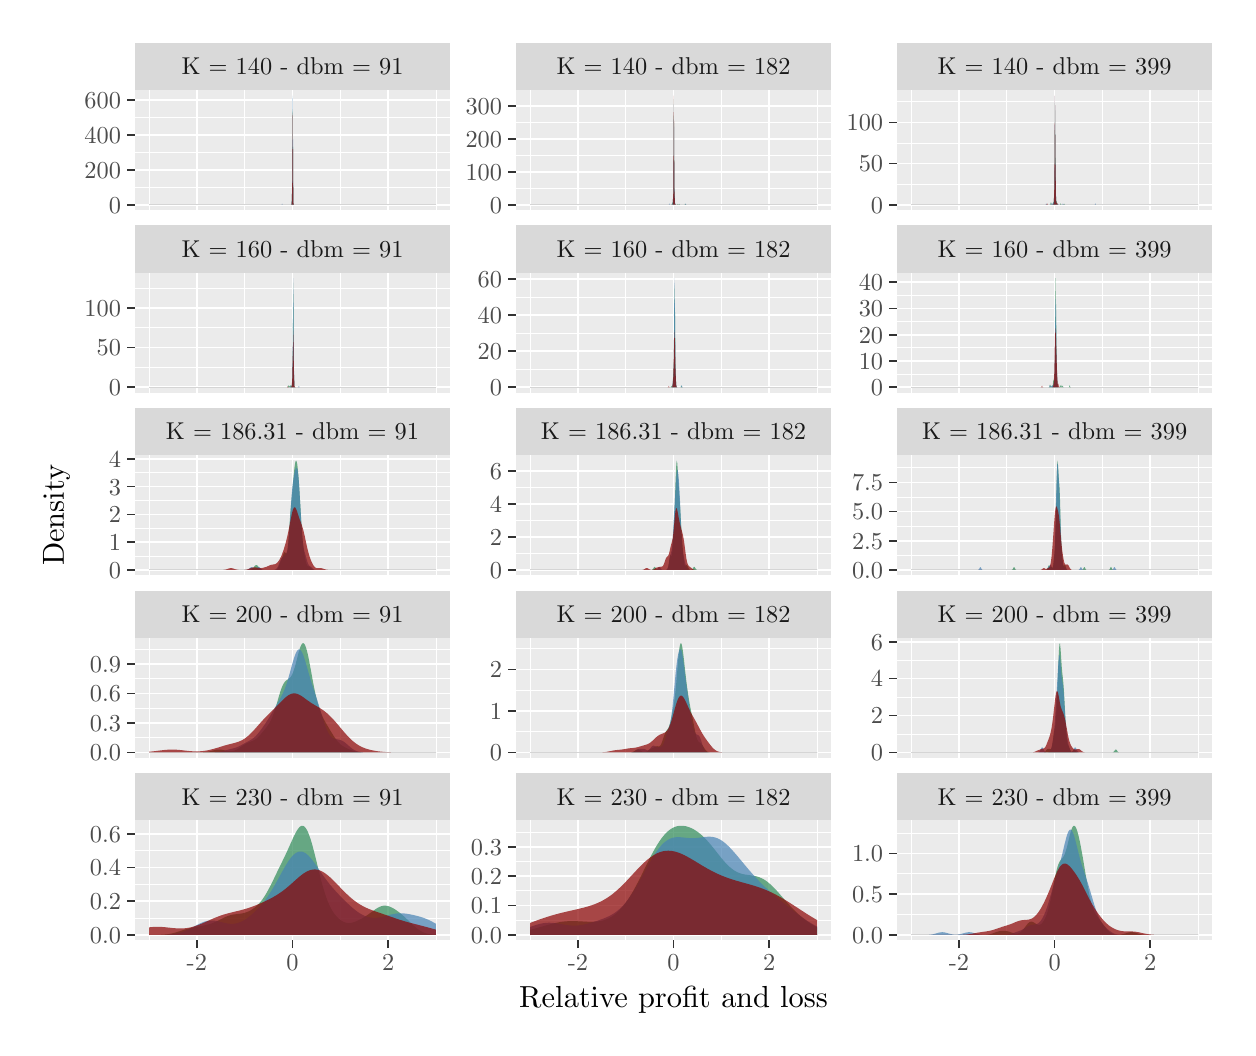
\begin{tikzpicture}[x=1pt,y=1pt]
\definecolor{fillColor}{RGB}{255,255,255}
\path[use as bounding box,fill=fillColor,fill opacity=0.00] (0,0) rectangle (433.62,361.35);
\begin{scope}
\path[clip] (  0.00,  0.00) rectangle (433.62,361.35);
\definecolor{drawColor}{RGB}{255,255,255}
\definecolor{fillColor}{RGB}{255,255,255}

\path[draw=drawColor,line width= 0.6pt,line join=round,line cap=round,fill=fillColor] (  0.00,  0.00) rectangle (433.62,361.35);
\end{scope}
\begin{scope}
\path[clip] ( 38.67,295.39) rectangle (152.72,338.79);
\definecolor{fillColor}{gray}{0.92}

\path[fill=fillColor] ( 38.67,295.39) rectangle (152.72,338.79);
\definecolor{drawColor}{RGB}{255,255,255}

\path[draw=drawColor,line width= 0.3pt,line join=round] ( 38.67,303.68) --
	(152.72,303.68);

\path[draw=drawColor,line width= 0.3pt,line join=round] ( 38.67,316.33) --
	(152.72,316.33);

\path[draw=drawColor,line width= 0.3pt,line join=round] ( 38.67,328.97) --
	(152.72,328.97);

\path[draw=drawColor,line width= 0.3pt,line join=round] ( 43.85,295.39) --
	( 43.85,338.79);

\path[draw=drawColor,line width= 0.3pt,line join=round] ( 78.41,295.39) --
	( 78.41,338.79);

\path[draw=drawColor,line width= 0.3pt,line join=round] (112.97,295.39) --
	(112.97,338.79);

\path[draw=drawColor,line width= 0.3pt,line join=round] (147.54,295.39) --
	(147.54,338.79);

\path[draw=drawColor,line width= 0.6pt,line join=round] ( 38.67,297.36) --
	(152.72,297.36);

\path[draw=drawColor,line width= 0.6pt,line join=round] ( 38.67,310.00) --
	(152.72,310.00);

\path[draw=drawColor,line width= 0.6pt,line join=round] ( 38.67,322.65) --
	(152.72,322.65);

\path[draw=drawColor,line width= 0.6pt,line join=round] ( 38.67,335.29) --
	(152.72,335.29);

\path[draw=drawColor,line width= 0.6pt,line join=round] ( 61.13,295.39) --
	( 61.13,338.79);

\path[draw=drawColor,line width= 0.6pt,line join=round] ( 95.69,295.39) --
	( 95.69,338.79);

\path[draw=drawColor,line width= 0.6pt,line join=round] (130.25,295.39) --
	(130.25,338.79);
\definecolor{fillColor}{RGB}{46,139,87}

\path[fill=fillColor,fill opacity=0.70] ( 43.85,297.36) --
	( 44.05,297.36) --
	( 44.26,297.36) --
	( 44.46,297.36) --
	( 44.66,297.36) --
	( 44.87,297.36) --
	( 45.07,297.36) --
	( 45.27,297.36) --
	( 45.47,297.36) --
	( 45.68,297.36) --
	( 45.88,297.36) --
	( 46.08,297.36) --
	( 46.29,297.36) --
	( 46.49,297.36) --
	( 46.69,297.36) --
	( 46.89,297.36) --
	( 47.10,297.36) --
	( 47.30,297.36) --
	( 47.50,297.36) --
	( 47.71,297.36) --
	( 47.91,297.36) --
	( 48.11,297.36) --
	( 48.31,297.36) --
	( 48.52,297.36) --
	( 48.72,297.36) --
	( 48.92,297.36) --
	( 49.13,297.36) --
	( 49.33,297.36) --
	( 49.53,297.36) --
	( 49.74,297.36) --
	( 49.94,297.36) --
	( 50.14,297.36) --
	( 50.34,297.36) --
	( 50.55,297.36) --
	( 50.75,297.36) --
	( 50.95,297.36) --
	( 51.16,297.36) --
	( 51.36,297.36) --
	( 51.56,297.36) --
	( 51.76,297.36) --
	( 51.97,297.36) --
	( 52.17,297.36) --
	( 52.37,297.36) --
	( 52.58,297.36) --
	( 52.78,297.36) --
	( 52.98,297.36) --
	( 53.18,297.36) --
	( 53.39,297.36) --
	( 53.59,297.36) --
	( 53.79,297.36) --
	( 54.00,297.36) --
	( 54.20,297.36) --
	( 54.40,297.36) --
	( 54.60,297.36) --
	( 54.81,297.36) --
	( 55.01,297.36) --
	( 55.21,297.36) --
	( 55.42,297.36) --
	( 55.62,297.36) --
	( 55.82,297.36) --
	( 56.03,297.36) --
	( 56.23,297.36) --
	( 56.43,297.36) --
	( 56.63,297.36) --
	( 56.84,297.36) --
	( 57.04,297.36) --
	( 57.24,297.36) --
	( 57.45,297.36) --
	( 57.65,297.36) --
	( 57.85,297.36) --
	( 58.05,297.36) --
	( 58.26,297.36) --
	( 58.46,297.36) --
	( 58.66,297.36) --
	( 58.87,297.36) --
	( 59.07,297.36) --
	( 59.27,297.36) --
	( 59.47,297.36) --
	( 59.68,297.36) --
	( 59.88,297.36) --
	( 60.08,297.36) --
	( 60.29,297.36) --
	( 60.49,297.36) --
	( 60.69,297.36) --
	( 60.90,297.36) --
	( 61.10,297.36) --
	( 61.30,297.36) --
	( 61.50,297.36) --
	( 61.71,297.36) --
	( 61.91,297.36) --
	( 62.11,297.36) --
	( 62.32,297.36) --
	( 62.52,297.36) --
	( 62.72,297.36) --
	( 62.92,297.36) --
	( 63.13,297.36) --
	( 63.33,297.36) --
	( 63.53,297.36) --
	( 63.74,297.36) --
	( 63.94,297.36) --
	( 64.14,297.36) --
	( 64.34,297.36) --
	( 64.55,297.36) --
	( 64.75,297.36) --
	( 64.95,297.36) --
	( 65.16,297.36) --
	( 65.36,297.36) --
	( 65.56,297.36) --
	( 65.76,297.36) --
	( 65.97,297.36) --
	( 66.17,297.36) --
	( 66.37,297.36) --
	( 66.58,297.36) --
	( 66.78,297.36) --
	( 66.98,297.36) --
	( 67.19,297.36) --
	( 67.39,297.36) --
	( 67.59,297.36) --
	( 67.79,297.36) --
	( 68.00,297.36) --
	( 68.20,297.36) --
	( 68.40,297.36) --
	( 68.61,297.36) --
	( 68.81,297.36) --
	( 69.01,297.36) --
	( 69.21,297.36) --
	( 69.42,297.36) --
	( 69.62,297.36) --
	( 69.82,297.36) --
	( 70.03,297.36) --
	( 70.23,297.36) --
	( 70.43,297.36) --
	( 70.63,297.36) --
	( 70.84,297.36) --
	( 71.04,297.36) --
	( 71.24,297.36) --
	( 71.45,297.36) --
	( 71.65,297.36) --
	( 71.85,297.36) --
	( 72.05,297.36) --
	( 72.26,297.36) --
	( 72.46,297.36) --
	( 72.66,297.36) --
	( 72.87,297.36) --
	( 73.07,297.36) --
	( 73.27,297.36) --
	( 73.48,297.36) --
	( 73.68,297.36) --
	( 73.88,297.36) --
	( 74.08,297.36) --
	( 74.29,297.36) --
	( 74.49,297.36) --
	( 74.69,297.36) --
	( 74.90,297.36) --
	( 75.10,297.36) --
	( 75.30,297.36) --
	( 75.50,297.36) --
	( 75.71,297.36) --
	( 75.91,297.36) --
	( 76.11,297.36) --
	( 76.32,297.36) --
	( 76.52,297.36) --
	( 76.72,297.36) --
	( 76.92,297.36) --
	( 77.13,297.36) --
	( 77.33,297.36) --
	( 77.53,297.36) --
	( 77.74,297.36) --
	( 77.94,297.36) --
	( 78.14,297.36) --
	( 78.34,297.36) --
	( 78.55,297.36) --
	( 78.75,297.36) --
	( 78.95,297.36) --
	( 79.16,297.36) --
	( 79.36,297.36) --
	( 79.56,297.36) --
	( 79.77,297.36) --
	( 79.97,297.36) --
	( 80.17,297.36) --
	( 80.37,297.36) --
	( 80.58,297.36) --
	( 80.78,297.36) --
	( 80.98,297.36) --
	( 81.19,297.36) --
	( 81.39,297.36) --
	( 81.59,297.36) --
	( 81.79,297.36) --
	( 82.00,297.36) --
	( 82.20,297.36) --
	( 82.40,297.36) --
	( 82.61,297.36) --
	( 82.81,297.36) --
	( 83.01,297.36) --
	( 83.21,297.36) --
	( 83.42,297.36) --
	( 83.62,297.36) --
	( 83.82,297.36) --
	( 84.03,297.36) --
	( 84.23,297.36) --
	( 84.43,297.36) --
	( 84.64,297.36) --
	( 84.84,297.36) --
	( 85.04,297.36) --
	( 85.24,297.36) --
	( 85.45,297.36) --
	( 85.65,297.36) --
	( 85.85,297.36) --
	( 86.06,297.36) --
	( 86.26,297.36) --
	( 86.46,297.36) --
	( 86.66,297.36) --
	( 86.87,297.36) --
	( 87.07,297.36) --
	( 87.27,297.36) --
	( 87.48,297.36) --
	( 87.68,297.36) --
	( 87.88,297.36) --
	( 88.08,297.36) --
	( 88.29,297.36) --
	( 88.49,297.36) --
	( 88.69,297.36) --
	( 88.90,297.36) --
	( 89.10,297.36) --
	( 89.30,297.36) --
	( 89.50,297.36) --
	( 89.71,297.36) --
	( 89.91,297.36) --
	( 90.11,297.36) --
	( 90.32,297.36) --
	( 90.52,297.36) --
	( 90.72,297.36) --
	( 90.93,297.36) --
	( 91.13,297.36) --
	( 91.33,297.36) --
	( 91.53,297.36) --
	( 91.74,297.36) --
	( 91.94,297.36) --
	( 92.14,297.36) --
	( 92.35,297.36) --
	( 92.55,297.36) --
	( 92.75,297.36) --
	( 92.95,297.36) --
	( 93.16,297.36) --
	( 93.36,297.36) --
	( 93.56,297.36) --
	( 93.77,297.36) --
	( 93.97,297.36) --
	( 94.17,297.36) --
	( 94.37,297.36) --
	( 94.58,297.36) --
	( 94.78,297.36) --
	( 94.98,297.36) --
	( 95.19,297.36) --
	( 95.39,297.79) --
	( 95.59,303.70) --
	( 95.79,331.92) --
	( 96.00,298.04) --
	( 96.20,297.42) --
	( 96.40,297.36) --
	( 96.61,297.36) --
	( 96.81,297.36) --
	( 97.01,297.36) --
	( 97.22,297.36) --
	( 97.42,297.36) --
	( 97.62,297.36) --
	( 97.82,297.36) --
	( 98.03,297.36) --
	( 98.23,297.36) --
	( 98.43,297.36) --
	( 98.64,297.36) --
	( 98.84,297.36) --
	( 99.04,297.36) --
	( 99.24,297.36) --
	( 99.45,297.36) --
	( 99.65,297.36) --
	( 99.85,297.36) --
	(100.06,297.36) --
	(100.26,297.36) --
	(100.46,297.36) --
	(100.66,297.36) --
	(100.87,297.36) --
	(101.07,297.36) --
	(101.27,297.36) --
	(101.48,297.36) --
	(101.68,297.36) --
	(101.88,297.36) --
	(102.08,297.36) --
	(102.29,297.36) --
	(102.49,297.36) --
	(102.69,297.36) --
	(102.90,297.36) --
	(103.10,297.36) --
	(103.30,297.36) --
	(103.51,297.36) --
	(103.71,297.36) --
	(103.91,297.36) --
	(104.11,297.36) --
	(104.32,297.36) --
	(104.52,297.36) --
	(104.72,297.36) --
	(104.93,297.36) --
	(105.13,297.36) --
	(105.33,297.36) --
	(105.53,297.36) --
	(105.74,297.36) --
	(105.94,297.36) --
	(106.14,297.36) --
	(106.35,297.36) --
	(106.55,297.36) --
	(106.75,297.36) --
	(106.95,297.36) --
	(107.16,297.36) --
	(107.36,297.36) --
	(107.56,297.36) --
	(107.77,297.36) --
	(107.97,297.36) --
	(108.17,297.36) --
	(108.37,297.36) --
	(108.58,297.36) --
	(108.78,297.36) --
	(108.98,297.36) --
	(109.19,297.36) --
	(109.39,297.36) --
	(109.59,297.36) --
	(109.80,297.36) --
	(110.00,297.36) --
	(110.20,297.36) --
	(110.40,297.36) --
	(110.61,297.36) --
	(110.81,297.36) --
	(111.01,297.36) --
	(111.22,297.36) --
	(111.42,297.36) --
	(111.62,297.36) --
	(111.82,297.36) --
	(112.03,297.36) --
	(112.23,297.36) --
	(112.43,297.36) --
	(112.64,297.36) --
	(112.84,297.36) --
	(113.04,297.36) --
	(113.24,297.36) --
	(113.45,297.36) --
	(113.65,297.36) --
	(113.85,297.36) --
	(114.06,297.36) --
	(114.26,297.36) --
	(114.46,297.36) --
	(114.67,297.36) --
	(114.87,297.36) --
	(115.07,297.36) --
	(115.27,297.36) --
	(115.48,297.36) --
	(115.68,297.36) --
	(115.88,297.36) --
	(116.09,297.36) --
	(116.29,297.36) --
	(116.49,297.36) --
	(116.69,297.36) --
	(116.90,297.36) --
	(117.10,297.36) --
	(117.30,297.36) --
	(117.51,297.36) --
	(117.71,297.36) --
	(117.91,297.36) --
	(118.11,297.36) --
	(118.32,297.36) --
	(118.52,297.36) --
	(118.72,297.36) --
	(118.93,297.36) --
	(119.13,297.36) --
	(119.33,297.36) --
	(119.53,297.36) --
	(119.74,297.36) --
	(119.94,297.36) --
	(120.14,297.36) --
	(120.35,297.36) --
	(120.55,297.36) --
	(120.75,297.36) --
	(120.96,297.36) --
	(121.16,297.36) --
	(121.36,297.36) --
	(121.56,297.36) --
	(121.77,297.36) --
	(121.97,297.36) --
	(122.17,297.36) --
	(122.38,297.36) --
	(122.58,297.36) --
	(122.78,297.36) --
	(122.98,297.36) --
	(123.19,297.36) --
	(123.39,297.36) --
	(123.59,297.36) --
	(123.80,297.36) --
	(124.00,297.36) --
	(124.20,297.36) --
	(124.40,297.36) --
	(124.61,297.36) --
	(124.81,297.36) --
	(125.01,297.36) --
	(125.22,297.36) --
	(125.42,297.36) --
	(125.62,297.36) --
	(125.82,297.36) --
	(126.03,297.36) --
	(126.23,297.36) --
	(126.43,297.36) --
	(126.64,297.36) --
	(126.84,297.36) --
	(127.04,297.36) --
	(127.25,297.36) --
	(127.45,297.36) --
	(127.65,297.36) --
	(127.85,297.36) --
	(128.06,297.36) --
	(128.26,297.36) --
	(128.46,297.36) --
	(128.67,297.36) --
	(128.87,297.36) --
	(129.07,297.36) --
	(129.27,297.36) --
	(129.48,297.36) --
	(129.68,297.36) --
	(129.88,297.36) --
	(130.09,297.36) --
	(130.29,297.36) --
	(130.49,297.36) --
	(130.69,297.36) --
	(130.90,297.36) --
	(131.10,297.36) --
	(131.30,297.36) --
	(131.51,297.36) --
	(131.71,297.36) --
	(131.91,297.36) --
	(132.11,297.36) --
	(132.32,297.36) --
	(132.52,297.36) --
	(132.72,297.36) --
	(132.93,297.36) --
	(133.13,297.36) --
	(133.33,297.36) --
	(133.54,297.36) --
	(133.74,297.36) --
	(133.94,297.36) --
	(134.14,297.36) --
	(134.35,297.36) --
	(134.55,297.36) --
	(134.75,297.36) --
	(134.96,297.36) --
	(135.16,297.36) --
	(135.36,297.36) --
	(135.56,297.36) --
	(135.77,297.36) --
	(135.97,297.36) --
	(136.17,297.36) --
	(136.38,297.36) --
	(136.58,297.36) --
	(136.78,297.36) --
	(136.98,297.36) --
	(137.19,297.36) --
	(137.39,297.36) --
	(137.59,297.36) --
	(137.80,297.36) --
	(138.00,297.36) --
	(138.20,297.36) --
	(138.40,297.36) --
	(138.61,297.36) --
	(138.81,297.36) --
	(139.01,297.36) --
	(139.22,297.36) --
	(139.42,297.36) --
	(139.62,297.36) --
	(139.83,297.36) --
	(140.03,297.36) --
	(140.23,297.36) --
	(140.43,297.36) --
	(140.64,297.36) --
	(140.84,297.36) --
	(141.04,297.36) --
	(141.25,297.36) --
	(141.45,297.36) --
	(141.65,297.36) --
	(141.85,297.36) --
	(142.06,297.36) --
	(142.26,297.36) --
	(142.46,297.36) --
	(142.67,297.36) --
	(142.87,297.36) --
	(143.07,297.36) --
	(143.27,297.36) --
	(143.48,297.36) --
	(143.68,297.36) --
	(143.88,297.36) --
	(144.09,297.36) --
	(144.29,297.36) --
	(144.49,297.36) --
	(144.70,297.36) --
	(144.90,297.36) --
	(145.10,297.36) --
	(145.30,297.36) --
	(145.51,297.36) --
	(145.71,297.36) --
	(145.91,297.36) --
	(146.12,297.36) --
	(146.32,297.36) --
	(146.52,297.36) --
	(146.72,297.36) --
	(146.93,297.36) --
	(147.13,297.36) --
	(147.33,297.36) --
	(147.54,297.36) --
	(147.54,297.36) --
	(147.33,297.36) --
	(147.13,297.36) --
	(146.93,297.36) --
	(146.72,297.36) --
	(146.52,297.36) --
	(146.32,297.36) --
	(146.12,297.36) --
	(145.91,297.36) --
	(145.71,297.36) --
	(145.51,297.36) --
	(145.30,297.36) --
	(145.10,297.36) --
	(144.90,297.36) --
	(144.70,297.36) --
	(144.49,297.36) --
	(144.29,297.36) --
	(144.09,297.36) --
	(143.88,297.36) --
	(143.68,297.36) --
	(143.48,297.36) --
	(143.27,297.36) --
	(143.07,297.36) --
	(142.87,297.36) --
	(142.67,297.36) --
	(142.46,297.36) --
	(142.26,297.36) --
	(142.06,297.36) --
	(141.85,297.36) --
	(141.65,297.36) --
	(141.45,297.36) --
	(141.25,297.36) --
	(141.04,297.36) --
	(140.84,297.36) --
	(140.64,297.36) --
	(140.43,297.36) --
	(140.23,297.36) --
	(140.03,297.36) --
	(139.83,297.36) --
	(139.62,297.36) --
	(139.42,297.36) --
	(139.22,297.36) --
	(139.01,297.36) --
	(138.81,297.36) --
	(138.61,297.36) --
	(138.40,297.36) --
	(138.20,297.36) --
	(138.00,297.36) --
	(137.80,297.36) --
	(137.59,297.36) --
	(137.39,297.36) --
	(137.19,297.36) --
	(136.98,297.36) --
	(136.78,297.36) --
	(136.58,297.36) --
	(136.38,297.36) --
	(136.17,297.36) --
	(135.97,297.36) --
	(135.77,297.36) --
	(135.56,297.36) --
	(135.36,297.36) --
	(135.16,297.36) --
	(134.96,297.36) --
	(134.75,297.36) --
	(134.55,297.36) --
	(134.35,297.36) --
	(134.14,297.36) --
	(133.94,297.36) --
	(133.74,297.36) --
	(133.54,297.36) --
	(133.33,297.36) --
	(133.13,297.36) --
	(132.93,297.36) --
	(132.72,297.36) --
	(132.52,297.36) --
	(132.32,297.36) --
	(132.11,297.36) --
	(131.91,297.36) --
	(131.71,297.36) --
	(131.51,297.36) --
	(131.30,297.36) --
	(131.10,297.36) --
	(130.90,297.36) --
	(130.69,297.36) --
	(130.49,297.36) --
	(130.29,297.36) --
	(130.09,297.36) --
	(129.88,297.36) --
	(129.68,297.36) --
	(129.48,297.36) --
	(129.27,297.36) --
	(129.07,297.36) --
	(128.87,297.36) --
	(128.67,297.36) --
	(128.46,297.36) --
	(128.26,297.36) --
	(128.06,297.36) --
	(127.85,297.36) --
	(127.65,297.36) --
	(127.45,297.36) --
	(127.25,297.36) --
	(127.04,297.36) --
	(126.84,297.36) --
	(126.64,297.36) --
	(126.43,297.36) --
	(126.23,297.36) --
	(126.03,297.36) --
	(125.82,297.36) --
	(125.62,297.36) --
	(125.42,297.36) --
	(125.22,297.36) --
	(125.01,297.36) --
	(124.81,297.36) --
	(124.61,297.36) --
	(124.40,297.36) --
	(124.20,297.36) --
	(124.00,297.36) --
	(123.80,297.36) --
	(123.59,297.36) --
	(123.39,297.36) --
	(123.19,297.36) --
	(122.98,297.36) --
	(122.78,297.36) --
	(122.58,297.36) --
	(122.38,297.36) --
	(122.17,297.36) --
	(121.97,297.36) --
	(121.77,297.36) --
	(121.56,297.36) --
	(121.36,297.36) --
	(121.16,297.36) --
	(120.96,297.36) --
	(120.75,297.36) --
	(120.55,297.36) --
	(120.35,297.36) --
	(120.14,297.36) --
	(119.94,297.36) --
	(119.74,297.36) --
	(119.53,297.36) --
	(119.33,297.36) --
	(119.13,297.36) --
	(118.93,297.36) --
	(118.72,297.36) --
	(118.52,297.36) --
	(118.32,297.36) --
	(118.11,297.36) --
	(117.91,297.36) --
	(117.71,297.36) --
	(117.51,297.36) --
	(117.30,297.36) --
	(117.10,297.36) --
	(116.90,297.36) --
	(116.69,297.36) --
	(116.49,297.36) --
	(116.29,297.36) --
	(116.09,297.36) --
	(115.88,297.36) --
	(115.68,297.36) --
	(115.48,297.36) --
	(115.27,297.36) --
	(115.07,297.36) --
	(114.87,297.36) --
	(114.67,297.36) --
	(114.46,297.36) --
	(114.26,297.36) --
	(114.06,297.36) --
	(113.85,297.36) --
	(113.65,297.36) --
	(113.45,297.36) --
	(113.24,297.36) --
	(113.04,297.36) --
	(112.84,297.36) --
	(112.64,297.36) --
	(112.43,297.36) --
	(112.23,297.36) --
	(112.03,297.36) --
	(111.82,297.36) --
	(111.62,297.36) --
	(111.42,297.36) --
	(111.22,297.36) --
	(111.01,297.36) --
	(110.81,297.36) --
	(110.61,297.36) --
	(110.40,297.36) --
	(110.20,297.36) --
	(110.00,297.36) --
	(109.80,297.36) --
	(109.59,297.36) --
	(109.39,297.36) --
	(109.19,297.36) --
	(108.98,297.36) --
	(108.78,297.36) --
	(108.58,297.36) --
	(108.37,297.36) --
	(108.17,297.36) --
	(107.97,297.36) --
	(107.77,297.36) --
	(107.56,297.36) --
	(107.36,297.36) --
	(107.16,297.36) --
	(106.95,297.36) --
	(106.75,297.36) --
	(106.55,297.36) --
	(106.35,297.36) --
	(106.14,297.36) --
	(105.94,297.36) --
	(105.74,297.36) --
	(105.53,297.36) --
	(105.33,297.36) --
	(105.13,297.36) --
	(104.93,297.36) --
	(104.72,297.36) --
	(104.52,297.36) --
	(104.32,297.36) --
	(104.11,297.36) --
	(103.91,297.36) --
	(103.71,297.36) --
	(103.51,297.36) --
	(103.30,297.36) --
	(103.10,297.36) --
	(102.90,297.36) --
	(102.69,297.36) --
	(102.49,297.36) --
	(102.29,297.36) --
	(102.08,297.36) --
	(101.88,297.36) --
	(101.68,297.36) --
	(101.48,297.36) --
	(101.27,297.36) --
	(101.07,297.36) --
	(100.87,297.36) --
	(100.66,297.36) --
	(100.46,297.36) --
	(100.26,297.36) --
	(100.06,297.36) --
	( 99.85,297.36) --
	( 99.65,297.36) --
	( 99.45,297.36) --
	( 99.24,297.36) --
	( 99.04,297.36) --
	( 98.84,297.36) --
	( 98.64,297.36) --
	( 98.43,297.36) --
	( 98.23,297.36) --
	( 98.03,297.36) --
	( 97.82,297.36) --
	( 97.62,297.36) --
	( 97.42,297.36) --
	( 97.22,297.36) --
	( 97.01,297.36) --
	( 96.81,297.36) --
	( 96.61,297.36) --
	( 96.40,297.36) --
	( 96.20,297.36) --
	( 96.00,297.36) --
	( 95.79,297.36) --
	( 95.59,297.36) --
	( 95.39,297.36) --
	( 95.19,297.36) --
	( 94.98,297.36) --
	( 94.78,297.36) --
	( 94.58,297.36) --
	( 94.37,297.36) --
	( 94.17,297.36) --
	( 93.97,297.36) --
	( 93.77,297.36) --
	( 93.56,297.36) --
	( 93.36,297.36) --
	( 93.16,297.36) --
	( 92.95,297.36) --
	( 92.75,297.36) --
	( 92.55,297.36) --
	( 92.35,297.36) --
	( 92.14,297.36) --
	( 91.94,297.36) --
	( 91.74,297.36) --
	( 91.53,297.36) --
	( 91.33,297.36) --
	( 91.13,297.36) --
	( 90.93,297.36) --
	( 90.72,297.36) --
	( 90.52,297.36) --
	( 90.32,297.36) --
	( 90.11,297.36) --
	( 89.91,297.36) --
	( 89.71,297.36) --
	( 89.50,297.36) --
	( 89.30,297.36) --
	( 89.10,297.36) --
	( 88.90,297.36) --
	( 88.69,297.36) --
	( 88.49,297.36) --
	( 88.29,297.36) --
	( 88.08,297.36) --
	( 87.88,297.36) --
	( 87.68,297.36) --
	( 87.48,297.36) --
	( 87.27,297.36) --
	( 87.07,297.36) --
	( 86.87,297.36) --
	( 86.66,297.36) --
	( 86.46,297.36) --
	( 86.26,297.36) --
	( 86.06,297.36) --
	( 85.85,297.36) --
	( 85.65,297.36) --
	( 85.45,297.36) --
	( 85.24,297.36) --
	( 85.04,297.36) --
	( 84.84,297.36) --
	( 84.64,297.36) --
	( 84.43,297.36) --
	( 84.23,297.36) --
	( 84.03,297.36) --
	( 83.82,297.36) --
	( 83.62,297.36) --
	( 83.42,297.36) --
	( 83.21,297.36) --
	( 83.01,297.36) --
	( 82.81,297.36) --
	( 82.61,297.36) --
	( 82.40,297.36) --
	( 82.20,297.36) --
	( 82.00,297.36) --
	( 81.79,297.36) --
	( 81.59,297.36) --
	( 81.39,297.36) --
	( 81.19,297.36) --
	( 80.98,297.36) --
	( 80.78,297.36) --
	( 80.58,297.36) --
	( 80.37,297.36) --
	( 80.17,297.36) --
	( 79.97,297.36) --
	( 79.77,297.36) --
	( 79.56,297.36) --
	( 79.36,297.36) --
	( 79.16,297.36) --
	( 78.95,297.36) --
	( 78.75,297.36) --
	( 78.55,297.36) --
	( 78.34,297.36) --
	( 78.14,297.36) --
	( 77.94,297.36) --
	( 77.74,297.36) --
	( 77.53,297.36) --
	( 77.33,297.36) --
	( 77.13,297.36) --
	( 76.92,297.36) --
	( 76.72,297.36) --
	( 76.52,297.36) --
	( 76.32,297.36) --
	( 76.11,297.36) --
	( 75.91,297.36) --
	( 75.71,297.36) --
	( 75.50,297.36) --
	( 75.30,297.36) --
	( 75.10,297.36) --
	( 74.90,297.36) --
	( 74.69,297.36) --
	( 74.49,297.36) --
	( 74.29,297.36) --
	( 74.08,297.36) --
	( 73.88,297.36) --
	( 73.68,297.36) --
	( 73.48,297.36) --
	( 73.27,297.36) --
	( 73.07,297.36) --
	( 72.87,297.36) --
	( 72.66,297.36) --
	( 72.46,297.36) --
	( 72.26,297.36) --
	( 72.05,297.36) --
	( 71.85,297.36) --
	( 71.65,297.36) --
	( 71.45,297.36) --
	( 71.24,297.36) --
	( 71.04,297.36) --
	( 70.84,297.36) --
	( 70.63,297.36) --
	( 70.43,297.36) --
	( 70.23,297.36) --
	( 70.03,297.36) --
	( 69.82,297.36) --
	( 69.62,297.36) --
	( 69.42,297.36) --
	( 69.21,297.36) --
	( 69.01,297.36) --
	( 68.81,297.36) --
	( 68.61,297.36) --
	( 68.40,297.36) --
	( 68.20,297.36) --
	( 68.00,297.36) --
	( 67.79,297.36) --
	( 67.59,297.36) --
	( 67.39,297.36) --
	( 67.19,297.36) --
	( 66.98,297.36) --
	( 66.78,297.36) --
	( 66.58,297.36) --
	( 66.37,297.36) --
	( 66.17,297.36) --
	( 65.97,297.36) --
	( 65.76,297.36) --
	( 65.56,297.36) --
	( 65.36,297.36) --
	( 65.16,297.36) --
	( 64.95,297.36) --
	( 64.75,297.36) --
	( 64.55,297.36) --
	( 64.34,297.36) --
	( 64.14,297.36) --
	( 63.94,297.36) --
	( 63.74,297.36) --
	( 63.53,297.36) --
	( 63.33,297.36) --
	( 63.13,297.36) --
	( 62.92,297.36) --
	( 62.72,297.36) --
	( 62.52,297.36) --
	( 62.32,297.36) --
	( 62.11,297.36) --
	( 61.91,297.36) --
	( 61.71,297.36) --
	( 61.50,297.36) --
	( 61.30,297.36) --
	( 61.10,297.36) --
	( 60.90,297.36) --
	( 60.69,297.36) --
	( 60.49,297.36) --
	( 60.29,297.36) --
	( 60.08,297.36) --
	( 59.88,297.36) --
	( 59.68,297.36) --
	( 59.47,297.36) --
	( 59.27,297.36) --
	( 59.07,297.36) --
	( 58.87,297.36) --
	( 58.66,297.36) --
	( 58.46,297.36) --
	( 58.26,297.36) --
	( 58.05,297.36) --
	( 57.85,297.36) --
	( 57.65,297.36) --
	( 57.45,297.36) --
	( 57.24,297.36) --
	( 57.04,297.36) --
	( 56.84,297.36) --
	( 56.63,297.36) --
	( 56.43,297.36) --
	( 56.23,297.36) --
	( 56.03,297.36) --
	( 55.82,297.36) --
	( 55.62,297.36) --
	( 55.42,297.36) --
	( 55.21,297.36) --
	( 55.01,297.36) --
	( 54.81,297.36) --
	( 54.60,297.36) --
	( 54.40,297.36) --
	( 54.20,297.36) --
	( 54.00,297.36) --
	( 53.79,297.36) --
	( 53.59,297.36) --
	( 53.39,297.36) --
	( 53.18,297.36) --
	( 52.98,297.36) --
	( 52.78,297.36) --
	( 52.58,297.36) --
	( 52.37,297.36) --
	( 52.17,297.36) --
	( 51.97,297.36) --
	( 51.76,297.36) --
	( 51.56,297.36) --
	( 51.36,297.36) --
	( 51.16,297.36) --
	( 50.95,297.36) --
	( 50.75,297.36) --
	( 50.55,297.36) --
	( 50.34,297.36) --
	( 50.14,297.36) --
	( 49.94,297.36) --
	( 49.74,297.36) --
	( 49.53,297.36) --
	( 49.33,297.36) --
	( 49.13,297.36) --
	( 48.92,297.36) --
	( 48.72,297.36) --
	( 48.52,297.36) --
	( 48.31,297.36) --
	( 48.11,297.36) --
	( 47.91,297.36) --
	( 47.71,297.36) --
	( 47.50,297.36) --
	( 47.30,297.36) --
	( 47.10,297.36) --
	( 46.89,297.36) --
	( 46.69,297.36) --
	( 46.49,297.36) --
	( 46.29,297.36) --
	( 46.08,297.36) --
	( 45.88,297.36) --
	( 45.68,297.36) --
	( 45.47,297.36) --
	( 45.27,297.36) --
	( 45.07,297.36) --
	( 44.87,297.36) --
	( 44.66,297.36) --
	( 44.46,297.36) --
	( 44.26,297.36) --
	( 44.05,297.36) --
	( 43.85,297.36) --
	cycle;
\definecolor{fillColor}{RGB}{70,130,180}

\path[fill=fillColor,fill opacity=0.70] ( 43.85,297.36) --
	( 44.05,297.36) --
	( 44.26,297.36) --
	( 44.46,297.36) --
	( 44.66,297.36) --
	( 44.87,297.36) --
	( 45.07,297.36) --
	( 45.27,297.36) --
	( 45.47,297.36) --
	( 45.68,297.36) --
	( 45.88,297.36) --
	( 46.08,297.36) --
	( 46.29,297.36) --
	( 46.49,297.36) --
	( 46.69,297.36) --
	( 46.89,297.36) --
	( 47.10,297.36) --
	( 47.30,297.36) --
	( 47.50,297.36) --
	( 47.71,297.36) --
	( 47.91,297.36) --
	( 48.11,297.36) --
	( 48.31,297.36) --
	( 48.52,297.36) --
	( 48.72,297.36) --
	( 48.92,297.36) --
	( 49.13,297.36) --
	( 49.33,297.36) --
	( 49.53,297.36) --
	( 49.74,297.36) --
	( 49.94,297.36) --
	( 50.14,297.36) --
	( 50.34,297.36) --
	( 50.55,297.36) --
	( 50.75,297.36) --
	( 50.95,297.36) --
	( 51.16,297.36) --
	( 51.36,297.36) --
	( 51.56,297.36) --
	( 51.76,297.36) --
	( 51.97,297.36) --
	( 52.17,297.36) --
	( 52.37,297.36) --
	( 52.58,297.36) --
	( 52.78,297.36) --
	( 52.98,297.36) --
	( 53.18,297.36) --
	( 53.39,297.36) --
	( 53.59,297.36) --
	( 53.79,297.36) --
	( 54.00,297.36) --
	( 54.20,297.36) --
	( 54.40,297.36) --
	( 54.60,297.36) --
	( 54.81,297.36) --
	( 55.01,297.36) --
	( 55.21,297.36) --
	( 55.42,297.36) --
	( 55.62,297.36) --
	( 55.82,297.36) --
	( 56.03,297.36) --
	( 56.23,297.36) --
	( 56.43,297.36) --
	( 56.63,297.36) --
	( 56.84,297.36) --
	( 57.04,297.36) --
	( 57.24,297.36) --
	( 57.45,297.36) --
	( 57.65,297.36) --
	( 57.85,297.36) --
	( 58.05,297.36) --
	( 58.26,297.36) --
	( 58.46,297.36) --
	( 58.66,297.36) --
	( 58.87,297.36) --
	( 59.07,297.36) --
	( 59.27,297.36) --
	( 59.47,297.36) --
	( 59.68,297.36) --
	( 59.88,297.36) --
	( 60.08,297.36) --
	( 60.29,297.36) --
	( 60.49,297.36) --
	( 60.69,297.36) --
	( 60.90,297.36) --
	( 61.10,297.36) --
	( 61.30,297.36) --
	( 61.50,297.36) --
	( 61.71,297.36) --
	( 61.91,297.36) --
	( 62.11,297.36) --
	( 62.32,297.36) --
	( 62.52,297.36) --
	( 62.72,297.36) --
	( 62.92,297.36) --
	( 63.13,297.36) --
	( 63.33,297.36) --
	( 63.53,297.36) --
	( 63.74,297.36) --
	( 63.94,297.36) --
	( 64.14,297.36) --
	( 64.34,297.36) --
	( 64.55,297.36) --
	( 64.75,297.36) --
	( 64.95,297.36) --
	( 65.16,297.36) --
	( 65.36,297.36) --
	( 65.56,297.36) --
	( 65.76,297.36) --
	( 65.97,297.36) --
	( 66.17,297.36) --
	( 66.37,297.36) --
	( 66.58,297.36) --
	( 66.78,297.36) --
	( 66.98,297.36) --
	( 67.19,297.36) --
	( 67.39,297.36) --
	( 67.59,297.36) --
	( 67.79,297.36) --
	( 68.00,297.36) --
	( 68.20,297.36) --
	( 68.40,297.36) --
	( 68.61,297.36) --
	( 68.81,297.36) --
	( 69.01,297.36) --
	( 69.21,297.36) --
	( 69.42,297.36) --
	( 69.62,297.36) --
	( 69.82,297.36) --
	( 70.03,297.36) --
	( 70.23,297.36) --
	( 70.43,297.36) --
	( 70.63,297.36) --
	( 70.84,297.36) --
	( 71.04,297.36) --
	( 71.24,297.36) --
	( 71.45,297.36) --
	( 71.65,297.36) --
	( 71.85,297.36) --
	( 72.05,297.36) --
	( 72.26,297.36) --
	( 72.46,297.36) --
	( 72.66,297.36) --
	( 72.87,297.36) --
	( 73.07,297.36) --
	( 73.27,297.36) --
	( 73.48,297.36) --
	( 73.68,297.36) --
	( 73.88,297.36) --
	( 74.08,297.36) --
	( 74.29,297.36) --
	( 74.49,297.36) --
	( 74.69,297.36) --
	( 74.90,297.36) --
	( 75.10,297.36) --
	( 75.30,297.36) --
	( 75.50,297.36) --
	( 75.71,297.36) --
	( 75.91,297.36) --
	( 76.11,297.36) --
	( 76.32,297.36) --
	( 76.52,297.36) --
	( 76.72,297.36) --
	( 76.92,297.36) --
	( 77.13,297.36) --
	( 77.33,297.36) --
	( 77.53,297.36) --
	( 77.74,297.36) --
	( 77.94,297.36) --
	( 78.14,297.36) --
	( 78.34,297.36) --
	( 78.55,297.36) --
	( 78.75,297.36) --
	( 78.95,297.36) --
	( 79.16,297.36) --
	( 79.36,297.36) --
	( 79.56,297.36) --
	( 79.77,297.36) --
	( 79.97,297.36) --
	( 80.17,297.36) --
	( 80.37,297.36) --
	( 80.58,297.36) --
	( 80.78,297.36) --
	( 80.98,297.36) --
	( 81.19,297.36) --
	( 81.39,297.36) --
	( 81.59,297.36) --
	( 81.79,297.36) --
	( 82.00,297.36) --
	( 82.20,297.36) --
	( 82.40,297.36) --
	( 82.61,297.36) --
	( 82.81,297.36) --
	( 83.01,297.36) --
	( 83.21,297.36) --
	( 83.42,297.36) --
	( 83.62,297.36) --
	( 83.82,297.36) --
	( 84.03,297.36) --
	( 84.23,297.36) --
	( 84.43,297.36) --
	( 84.64,297.36) --
	( 84.84,297.36) --
	( 85.04,297.36) --
	( 85.24,297.36) --
	( 85.45,297.36) --
	( 85.65,297.36) --
	( 85.85,297.36) --
	( 86.06,297.36) --
	( 86.26,297.36) --
	( 86.46,297.36) --
	( 86.66,297.36) --
	( 86.87,297.36) --
	( 87.07,297.36) --
	( 87.27,297.36) --
	( 87.48,297.36) --
	( 87.68,297.36) --
	( 87.88,297.36) --
	( 88.08,297.36) --
	( 88.29,297.36) --
	( 88.49,297.36) --
	( 88.69,297.36) --
	( 88.90,297.36) --
	( 89.10,297.36) --
	( 89.30,297.36) --
	( 89.50,297.36) --
	( 89.71,297.36) --
	( 89.91,297.36) --
	( 90.11,297.36) --
	( 90.32,297.36) --
	( 90.52,297.36) --
	( 90.72,297.36) --
	( 90.93,297.36) --
	( 91.13,297.36) --
	( 91.33,297.36) --
	( 91.53,297.36) --
	( 91.74,297.41) --
	( 91.94,297.78) --
	( 92.14,297.36) --
	( 92.35,297.36) --
	( 92.55,297.36) --
	( 92.75,297.36) --
	( 92.95,297.36) --
	( 93.16,297.36) --
	( 93.36,297.36) --
	( 93.56,297.36) --
	( 93.77,297.36) --
	( 93.97,297.36) --
	( 94.17,297.36) --
	( 94.37,297.36) --
	( 94.58,297.36) --
	( 94.78,297.36) --
	( 94.98,297.36) --
	( 95.19,297.46) --
	( 95.39,297.73) --
	( 95.59,303.74) --
	( 95.79,336.82) --
	( 96.00,297.71) --
	( 96.20,297.36) --
	( 96.40,297.36) --
	( 96.61,297.36) --
	( 96.81,297.36) --
	( 97.01,297.36) --
	( 97.22,297.36) --
	( 97.42,297.36) --
	( 97.62,297.36) --
	( 97.82,297.36) --
	( 98.03,297.36) --
	( 98.23,297.36) --
	( 98.43,297.36) --
	( 98.64,297.36) --
	( 98.84,297.36) --
	( 99.04,297.36) --
	( 99.24,297.36) --
	( 99.45,297.36) --
	( 99.65,297.36) --
	( 99.85,297.36) --
	(100.06,297.36) --
	(100.26,297.36) --
	(100.46,297.36) --
	(100.66,297.36) --
	(100.87,297.36) --
	(101.07,297.36) --
	(101.27,297.36) --
	(101.48,297.36) --
	(101.68,297.36) --
	(101.88,297.36) --
	(102.08,297.36) --
	(102.29,297.36) --
	(102.49,297.36) --
	(102.69,297.36) --
	(102.90,297.36) --
	(103.10,297.36) --
	(103.30,297.36) --
	(103.51,297.36) --
	(103.71,297.36) --
	(103.91,297.36) --
	(104.11,297.36) --
	(104.32,297.36) --
	(104.52,297.36) --
	(104.72,297.36) --
	(104.93,297.36) --
	(105.13,297.36) --
	(105.33,297.36) --
	(105.53,297.36) --
	(105.74,297.36) --
	(105.94,297.36) --
	(106.14,297.36) --
	(106.35,297.36) --
	(106.55,297.36) --
	(106.75,297.36) --
	(106.95,297.36) --
	(107.16,297.36) --
	(107.36,297.36) --
	(107.56,297.36) --
	(107.77,297.36) --
	(107.97,297.36) --
	(108.17,297.36) --
	(108.37,297.36) --
	(108.58,297.36) --
	(108.78,297.36) --
	(108.98,297.36) --
	(109.19,297.36) --
	(109.39,297.36) --
	(109.59,297.36) --
	(109.80,297.36) --
	(110.00,297.36) --
	(110.20,297.36) --
	(110.40,297.36) --
	(110.61,297.36) --
	(110.81,297.36) --
	(111.01,297.36) --
	(111.22,297.36) --
	(111.42,297.36) --
	(111.62,297.36) --
	(111.82,297.36) --
	(112.03,297.36) --
	(112.23,297.36) --
	(112.43,297.36) --
	(112.64,297.36) --
	(112.84,297.36) --
	(113.04,297.36) --
	(113.24,297.36) --
	(113.45,297.36) --
	(113.65,297.36) --
	(113.85,297.36) --
	(114.06,297.36) --
	(114.26,297.36) --
	(114.46,297.36) --
	(114.67,297.36) --
	(114.87,297.36) --
	(115.07,297.36) --
	(115.27,297.36) --
	(115.48,297.36) --
	(115.68,297.36) --
	(115.88,297.36) --
	(116.09,297.36) --
	(116.29,297.36) --
	(116.49,297.36) --
	(116.69,297.36) --
	(116.90,297.36) --
	(117.10,297.36) --
	(117.30,297.36) --
	(117.51,297.36) --
	(117.71,297.36) --
	(117.91,297.36) --
	(118.11,297.36) --
	(118.32,297.36) --
	(118.52,297.36) --
	(118.72,297.36) --
	(118.93,297.36) --
	(119.13,297.36) --
	(119.33,297.36) --
	(119.53,297.36) --
	(119.74,297.36) --
	(119.94,297.36) --
	(120.14,297.36) --
	(120.35,297.36) --
	(120.55,297.36) --
	(120.75,297.36) --
	(120.96,297.36) --
	(121.16,297.36) --
	(121.36,297.36) --
	(121.56,297.36) --
	(121.77,297.36) --
	(121.97,297.36) --
	(122.17,297.36) --
	(122.38,297.36) --
	(122.58,297.36) --
	(122.78,297.36) --
	(122.98,297.36) --
	(123.19,297.36) --
	(123.39,297.36) --
	(123.59,297.36) --
	(123.80,297.36) --
	(124.00,297.36) --
	(124.20,297.36) --
	(124.40,297.36) --
	(124.61,297.36) --
	(124.81,297.36) --
	(125.01,297.36) --
	(125.22,297.36) --
	(125.42,297.36) --
	(125.62,297.36) --
	(125.82,297.36) --
	(126.03,297.36) --
	(126.23,297.36) --
	(126.43,297.36) --
	(126.64,297.36) --
	(126.84,297.36) --
	(127.04,297.36) --
	(127.25,297.36) --
	(127.45,297.36) --
	(127.65,297.36) --
	(127.85,297.36) --
	(128.06,297.36) --
	(128.26,297.36) --
	(128.46,297.36) --
	(128.67,297.36) --
	(128.87,297.36) --
	(129.07,297.36) --
	(129.27,297.36) --
	(129.48,297.36) --
	(129.68,297.36) --
	(129.88,297.36) --
	(130.09,297.36) --
	(130.29,297.36) --
	(130.49,297.36) --
	(130.69,297.36) --
	(130.90,297.36) --
	(131.10,297.36) --
	(131.30,297.36) --
	(131.51,297.36) --
	(131.71,297.36) --
	(131.91,297.36) --
	(132.11,297.36) --
	(132.32,297.36) --
	(132.52,297.36) --
	(132.72,297.36) --
	(132.93,297.36) --
	(133.13,297.36) --
	(133.33,297.36) --
	(133.54,297.36) --
	(133.74,297.36) --
	(133.94,297.36) --
	(134.14,297.36) --
	(134.35,297.36) --
	(134.55,297.36) --
	(134.75,297.36) --
	(134.96,297.36) --
	(135.16,297.36) --
	(135.36,297.36) --
	(135.56,297.36) --
	(135.77,297.36) --
	(135.97,297.36) --
	(136.17,297.36) --
	(136.38,297.36) --
	(136.58,297.36) --
	(136.78,297.36) --
	(136.98,297.36) --
	(137.19,297.36) --
	(137.39,297.36) --
	(137.59,297.36) --
	(137.80,297.36) --
	(138.00,297.36) --
	(138.20,297.36) --
	(138.40,297.36) --
	(138.61,297.36) --
	(138.81,297.36) --
	(139.01,297.36) --
	(139.22,297.36) --
	(139.42,297.36) --
	(139.62,297.36) --
	(139.83,297.36) --
	(140.03,297.36) --
	(140.23,297.36) --
	(140.43,297.36) --
	(140.64,297.36) --
	(140.84,297.36) --
	(141.04,297.36) --
	(141.25,297.36) --
	(141.45,297.36) --
	(141.65,297.36) --
	(141.85,297.36) --
	(142.06,297.36) --
	(142.26,297.36) --
	(142.46,297.36) --
	(142.67,297.36) --
	(142.87,297.36) --
	(143.07,297.36) --
	(143.27,297.36) --
	(143.48,297.36) --
	(143.68,297.36) --
	(143.88,297.36) --
	(144.09,297.36) --
	(144.29,297.36) --
	(144.49,297.36) --
	(144.70,297.36) --
	(144.90,297.36) --
	(145.10,297.36) --
	(145.30,297.36) --
	(145.51,297.36) --
	(145.71,297.36) --
	(145.91,297.36) --
	(146.12,297.36) --
	(146.32,297.36) --
	(146.52,297.36) --
	(146.72,297.36) --
	(146.93,297.36) --
	(147.13,297.36) --
	(147.33,297.36) --
	(147.54,297.36) --
	(147.54,297.36) --
	(147.33,297.36) --
	(147.13,297.36) --
	(146.93,297.36) --
	(146.72,297.36) --
	(146.52,297.36) --
	(146.32,297.36) --
	(146.12,297.36) --
	(145.91,297.36) --
	(145.71,297.36) --
	(145.51,297.36) --
	(145.30,297.36) --
	(145.10,297.36) --
	(144.90,297.36) --
	(144.70,297.36) --
	(144.49,297.36) --
	(144.29,297.36) --
	(144.09,297.36) --
	(143.88,297.36) --
	(143.68,297.36) --
	(143.48,297.36) --
	(143.27,297.36) --
	(143.07,297.36) --
	(142.87,297.36) --
	(142.67,297.36) --
	(142.46,297.36) --
	(142.26,297.36) --
	(142.06,297.36) --
	(141.85,297.36) --
	(141.65,297.36) --
	(141.45,297.36) --
	(141.25,297.36) --
	(141.04,297.36) --
	(140.84,297.36) --
	(140.64,297.36) --
	(140.43,297.36) --
	(140.23,297.36) --
	(140.03,297.36) --
	(139.83,297.36) --
	(139.62,297.36) --
	(139.42,297.36) --
	(139.22,297.36) --
	(139.01,297.36) --
	(138.81,297.36) --
	(138.61,297.36) --
	(138.40,297.36) --
	(138.20,297.36) --
	(138.00,297.36) --
	(137.80,297.36) --
	(137.59,297.36) --
	(137.39,297.36) --
	(137.19,297.36) --
	(136.98,297.36) --
	(136.78,297.36) --
	(136.58,297.36) --
	(136.38,297.36) --
	(136.17,297.36) --
	(135.97,297.36) --
	(135.77,297.36) --
	(135.56,297.36) --
	(135.36,297.36) --
	(135.16,297.36) --
	(134.96,297.36) --
	(134.75,297.36) --
	(134.55,297.36) --
	(134.35,297.36) --
	(134.14,297.36) --
	(133.94,297.36) --
	(133.74,297.36) --
	(133.54,297.36) --
	(133.33,297.36) --
	(133.13,297.36) --
	(132.93,297.36) --
	(132.72,297.36) --
	(132.52,297.36) --
	(132.32,297.36) --
	(132.11,297.36) --
	(131.91,297.36) --
	(131.71,297.36) --
	(131.51,297.36) --
	(131.30,297.36) --
	(131.10,297.36) --
	(130.90,297.36) --
	(130.69,297.36) --
	(130.49,297.36) --
	(130.29,297.36) --
	(130.09,297.36) --
	(129.88,297.36) --
	(129.68,297.36) --
	(129.48,297.36) --
	(129.27,297.36) --
	(129.07,297.36) --
	(128.87,297.36) --
	(128.67,297.36) --
	(128.46,297.36) --
	(128.26,297.36) --
	(128.06,297.36) --
	(127.85,297.36) --
	(127.65,297.36) --
	(127.45,297.36) --
	(127.25,297.36) --
	(127.04,297.36) --
	(126.84,297.36) --
	(126.64,297.36) --
	(126.43,297.36) --
	(126.23,297.36) --
	(126.03,297.36) --
	(125.82,297.36) --
	(125.62,297.36) --
	(125.42,297.36) --
	(125.22,297.36) --
	(125.01,297.36) --
	(124.81,297.36) --
	(124.61,297.36) --
	(124.40,297.36) --
	(124.20,297.36) --
	(124.00,297.36) --
	(123.80,297.36) --
	(123.59,297.36) --
	(123.39,297.36) --
	(123.19,297.36) --
	(122.98,297.36) --
	(122.78,297.36) --
	(122.58,297.36) --
	(122.38,297.36) --
	(122.17,297.36) --
	(121.97,297.36) --
	(121.77,297.36) --
	(121.56,297.36) --
	(121.36,297.36) --
	(121.16,297.36) --
	(120.96,297.36) --
	(120.75,297.36) --
	(120.55,297.36) --
	(120.35,297.36) --
	(120.14,297.36) --
	(119.94,297.36) --
	(119.74,297.36) --
	(119.53,297.36) --
	(119.33,297.36) --
	(119.13,297.36) --
	(118.93,297.36) --
	(118.72,297.36) --
	(118.52,297.36) --
	(118.32,297.36) --
	(118.11,297.36) --
	(117.91,297.36) --
	(117.71,297.36) --
	(117.51,297.36) --
	(117.30,297.36) --
	(117.10,297.36) --
	(116.90,297.36) --
	(116.69,297.36) --
	(116.49,297.36) --
	(116.29,297.36) --
	(116.09,297.36) --
	(115.88,297.36) --
	(115.68,297.36) --
	(115.48,297.36) --
	(115.27,297.36) --
	(115.07,297.36) --
	(114.87,297.36) --
	(114.67,297.36) --
	(114.46,297.36) --
	(114.26,297.36) --
	(114.06,297.36) --
	(113.85,297.36) --
	(113.65,297.36) --
	(113.45,297.36) --
	(113.24,297.36) --
	(113.04,297.36) --
	(112.84,297.36) --
	(112.64,297.36) --
	(112.43,297.36) --
	(112.23,297.36) --
	(112.03,297.36) --
	(111.82,297.36) --
	(111.62,297.36) --
	(111.42,297.36) --
	(111.22,297.36) --
	(111.01,297.36) --
	(110.81,297.36) --
	(110.61,297.36) --
	(110.40,297.36) --
	(110.20,297.36) --
	(110.00,297.36) --
	(109.80,297.36) --
	(109.59,297.36) --
	(109.39,297.36) --
	(109.19,297.36) --
	(108.98,297.36) --
	(108.78,297.36) --
	(108.58,297.36) --
	(108.37,297.36) --
	(108.17,297.36) --
	(107.97,297.36) --
	(107.77,297.36) --
	(107.56,297.36) --
	(107.36,297.36) --
	(107.16,297.36) --
	(106.95,297.36) --
	(106.75,297.36) --
	(106.55,297.36) --
	(106.35,297.36) --
	(106.14,297.36) --
	(105.94,297.36) --
	(105.74,297.36) --
	(105.53,297.36) --
	(105.33,297.36) --
	(105.13,297.36) --
	(104.93,297.36) --
	(104.72,297.36) --
	(104.52,297.36) --
	(104.32,297.36) --
	(104.11,297.36) --
	(103.91,297.36) --
	(103.71,297.36) --
	(103.51,297.36) --
	(103.30,297.36) --
	(103.10,297.36) --
	(102.90,297.36) --
	(102.69,297.36) --
	(102.49,297.36) --
	(102.29,297.36) --
	(102.08,297.36) --
	(101.88,297.36) --
	(101.68,297.36) --
	(101.48,297.36) --
	(101.27,297.36) --
	(101.07,297.36) --
	(100.87,297.36) --
	(100.66,297.36) --
	(100.46,297.36) --
	(100.26,297.36) --
	(100.06,297.36) --
	( 99.85,297.36) --
	( 99.65,297.36) --
	( 99.45,297.36) --
	( 99.24,297.36) --
	( 99.04,297.36) --
	( 98.84,297.36) --
	( 98.64,297.36) --
	( 98.43,297.36) --
	( 98.23,297.36) --
	( 98.03,297.36) --
	( 97.82,297.36) --
	( 97.62,297.36) --
	( 97.42,297.36) --
	( 97.22,297.36) --
	( 97.01,297.36) --
	( 96.81,297.36) --
	( 96.61,297.36) --
	( 96.40,297.36) --
	( 96.20,297.36) --
	( 96.00,297.36) --
	( 95.79,297.36) --
	( 95.59,297.36) --
	( 95.39,297.36) --
	( 95.19,297.36) --
	( 94.98,297.36) --
	( 94.78,297.36) --
	( 94.58,297.36) --
	( 94.37,297.36) --
	( 94.17,297.36) --
	( 93.97,297.36) --
	( 93.77,297.36) --
	( 93.56,297.36) --
	( 93.36,297.36) --
	( 93.16,297.36) --
	( 92.95,297.36) --
	( 92.75,297.36) --
	( 92.55,297.36) --
	( 92.35,297.36) --
	( 92.14,297.36) --
	( 91.94,297.36) --
	( 91.74,297.36) --
	( 91.53,297.36) --
	( 91.33,297.36) --
	( 91.13,297.36) --
	( 90.93,297.36) --
	( 90.72,297.36) --
	( 90.52,297.36) --
	( 90.32,297.36) --
	( 90.11,297.36) --
	( 89.91,297.36) --
	( 89.71,297.36) --
	( 89.50,297.36) --
	( 89.30,297.36) --
	( 89.10,297.36) --
	( 88.90,297.36) --
	( 88.69,297.36) --
	( 88.49,297.36) --
	( 88.29,297.36) --
	( 88.08,297.36) --
	( 87.88,297.36) --
	( 87.68,297.36) --
	( 87.48,297.36) --
	( 87.27,297.36) --
	( 87.07,297.36) --
	( 86.87,297.36) --
	( 86.66,297.36) --
	( 86.46,297.36) --
	( 86.26,297.36) --
	( 86.06,297.36) --
	( 85.85,297.36) --
	( 85.65,297.36) --
	( 85.45,297.36) --
	( 85.24,297.36) --
	( 85.04,297.36) --
	( 84.84,297.36) --
	( 84.64,297.36) --
	( 84.43,297.36) --
	( 84.23,297.36) --
	( 84.03,297.36) --
	( 83.82,297.36) --
	( 83.62,297.36) --
	( 83.42,297.36) --
	( 83.21,297.36) --
	( 83.01,297.36) --
	( 82.81,297.36) --
	( 82.61,297.36) --
	( 82.40,297.36) --
	( 82.20,297.36) --
	( 82.00,297.36) --
	( 81.79,297.36) --
	( 81.59,297.36) --
	( 81.39,297.36) --
	( 81.19,297.36) --
	( 80.98,297.36) --
	( 80.78,297.36) --
	( 80.58,297.36) --
	( 80.37,297.36) --
	( 80.17,297.36) --
	( 79.97,297.36) --
	( 79.77,297.36) --
	( 79.56,297.36) --
	( 79.36,297.36) --
	( 79.16,297.36) --
	( 78.95,297.36) --
	( 78.75,297.36) --
	( 78.55,297.36) --
	( 78.34,297.36) --
	( 78.14,297.36) --
	( 77.94,297.36) --
	( 77.74,297.36) --
	( 77.53,297.36) --
	( 77.33,297.36) --
	( 77.13,297.36) --
	( 76.92,297.36) --
	( 76.72,297.36) --
	( 76.52,297.36) --
	( 76.32,297.36) --
	( 76.11,297.36) --
	( 75.91,297.36) --
	( 75.71,297.36) --
	( 75.50,297.36) --
	( 75.30,297.36) --
	( 75.10,297.36) --
	( 74.90,297.36) --
	( 74.69,297.36) --
	( 74.49,297.36) --
	( 74.29,297.36) --
	( 74.08,297.36) --
	( 73.88,297.36) --
	( 73.68,297.36) --
	( 73.48,297.36) --
	( 73.27,297.36) --
	( 73.07,297.36) --
	( 72.87,297.36) --
	( 72.66,297.36) --
	( 72.46,297.36) --
	( 72.26,297.36) --
	( 72.05,297.36) --
	( 71.85,297.36) --
	( 71.65,297.36) --
	( 71.45,297.36) --
	( 71.24,297.36) --
	( 71.04,297.36) --
	( 70.84,297.36) --
	( 70.63,297.36) --
	( 70.43,297.36) --
	( 70.23,297.36) --
	( 70.03,297.36) --
	( 69.82,297.36) --
	( 69.62,297.36) --
	( 69.42,297.36) --
	( 69.21,297.36) --
	( 69.01,297.36) --
	( 68.81,297.36) --
	( 68.61,297.36) --
	( 68.40,297.36) --
	( 68.20,297.36) --
	( 68.00,297.36) --
	( 67.79,297.36) --
	( 67.59,297.36) --
	( 67.39,297.36) --
	( 67.19,297.36) --
	( 66.98,297.36) --
	( 66.78,297.36) --
	( 66.58,297.36) --
	( 66.37,297.36) --
	( 66.17,297.36) --
	( 65.97,297.36) --
	( 65.76,297.36) --
	( 65.56,297.36) --
	( 65.36,297.36) --
	( 65.16,297.36) --
	( 64.95,297.36) --
	( 64.75,297.36) --
	( 64.55,297.36) --
	( 64.34,297.36) --
	( 64.14,297.36) --
	( 63.94,297.36) --
	( 63.74,297.36) --
	( 63.53,297.36) --
	( 63.33,297.36) --
	( 63.13,297.36) --
	( 62.92,297.36) --
	( 62.72,297.36) --
	( 62.52,297.36) --
	( 62.32,297.36) --
	( 62.11,297.36) --
	( 61.91,297.36) --
	( 61.71,297.36) --
	( 61.50,297.36) --
	( 61.30,297.36) --
	( 61.10,297.36) --
	( 60.90,297.36) --
	( 60.69,297.36) --
	( 60.49,297.36) --
	( 60.29,297.36) --
	( 60.08,297.36) --
	( 59.88,297.36) --
	( 59.68,297.36) --
	( 59.47,297.36) --
	( 59.27,297.36) --
	( 59.07,297.36) --
	( 58.87,297.36) --
	( 58.66,297.36) --
	( 58.46,297.36) --
	( 58.26,297.36) --
	( 58.05,297.36) --
	( 57.85,297.36) --
	( 57.65,297.36) --
	( 57.45,297.36) --
	( 57.24,297.36) --
	( 57.04,297.36) --
	( 56.84,297.36) --
	( 56.63,297.36) --
	( 56.43,297.36) --
	( 56.23,297.36) --
	( 56.03,297.36) --
	( 55.82,297.36) --
	( 55.62,297.36) --
	( 55.42,297.36) --
	( 55.21,297.36) --
	( 55.01,297.36) --
	( 54.81,297.36) --
	( 54.60,297.36) --
	( 54.40,297.36) --
	( 54.20,297.36) --
	( 54.00,297.36) --
	( 53.79,297.36) --
	( 53.59,297.36) --
	( 53.39,297.36) --
	( 53.18,297.36) --
	( 52.98,297.36) --
	( 52.78,297.36) --
	( 52.58,297.36) --
	( 52.37,297.36) --
	( 52.17,297.36) --
	( 51.97,297.36) --
	( 51.76,297.36) --
	( 51.56,297.36) --
	( 51.36,297.36) --
	( 51.16,297.36) --
	( 50.95,297.36) --
	( 50.75,297.36) --
	( 50.55,297.36) --
	( 50.34,297.36) --
	( 50.14,297.36) --
	( 49.94,297.36) --
	( 49.74,297.36) --
	( 49.53,297.36) --
	( 49.33,297.36) --
	( 49.13,297.36) --
	( 48.92,297.36) --
	( 48.72,297.36) --
	( 48.52,297.36) --
	( 48.31,297.36) --
	( 48.11,297.36) --
	( 47.91,297.36) --
	( 47.71,297.36) --
	( 47.50,297.36) --
	( 47.30,297.36) --
	( 47.10,297.36) --
	( 46.89,297.36) --
	( 46.69,297.36) --
	( 46.49,297.36) --
	( 46.29,297.36) --
	( 46.08,297.36) --
	( 45.88,297.36) --
	( 45.68,297.36) --
	( 45.47,297.36) --
	( 45.27,297.36) --
	( 45.07,297.36) --
	( 44.87,297.36) --
	( 44.66,297.36) --
	( 44.46,297.36) --
	( 44.26,297.36) --
	( 44.05,297.36) --
	( 43.85,297.36) --
	cycle;
\definecolor{fillColor}{RGB}{139,0,0}

\path[fill=fillColor,fill opacity=0.70] ( 43.85,297.36) --
	( 44.05,297.36) --
	( 44.26,297.36) --
	( 44.46,297.36) --
	( 44.66,297.36) --
	( 44.87,297.36) --
	( 45.07,297.36) --
	( 45.27,297.36) --
	( 45.47,297.36) --
	( 45.68,297.36) --
	( 45.88,297.36) --
	( 46.08,297.36) --
	( 46.29,297.36) --
	( 46.49,297.36) --
	( 46.69,297.36) --
	( 46.89,297.36) --
	( 47.10,297.36) --
	( 47.30,297.36) --
	( 47.50,297.36) --
	( 47.71,297.36) --
	( 47.91,297.36) --
	( 48.11,297.36) --
	( 48.31,297.36) --
	( 48.52,297.36) --
	( 48.72,297.36) --
	( 48.92,297.36) --
	( 49.13,297.36) --
	( 49.33,297.36) --
	( 49.53,297.36) --
	( 49.74,297.36) --
	( 49.94,297.36) --
	( 50.14,297.36) --
	( 50.34,297.36) --
	( 50.55,297.36) --
	( 50.75,297.36) --
	( 50.95,297.36) --
	( 51.16,297.36) --
	( 51.36,297.36) --
	( 51.56,297.36) --
	( 51.76,297.36) --
	( 51.97,297.36) --
	( 52.17,297.36) --
	( 52.37,297.36) --
	( 52.58,297.36) --
	( 52.78,297.36) --
	( 52.98,297.36) --
	( 53.18,297.36) --
	( 53.39,297.36) --
	( 53.59,297.36) --
	( 53.79,297.36) --
	( 54.00,297.36) --
	( 54.20,297.36) --
	( 54.40,297.36) --
	( 54.60,297.36) --
	( 54.81,297.36) --
	( 55.01,297.36) --
	( 55.21,297.36) --
	( 55.42,297.36) --
	( 55.62,297.36) --
	( 55.82,297.36) --
	( 56.03,297.36) --
	( 56.23,297.36) --
	( 56.43,297.36) --
	( 56.63,297.36) --
	( 56.84,297.36) --
	( 57.04,297.36) --
	( 57.24,297.36) --
	( 57.45,297.36) --
	( 57.65,297.36) --
	( 57.85,297.36) --
	( 58.05,297.36) --
	( 58.26,297.36) --
	( 58.46,297.36) --
	( 58.66,297.36) --
	( 58.87,297.36) --
	( 59.07,297.36) --
	( 59.27,297.36) --
	( 59.47,297.36) --
	( 59.68,297.36) --
	( 59.88,297.36) --
	( 60.08,297.36) --
	( 60.29,297.36) --
	( 60.49,297.36) --
	( 60.69,297.36) --
	( 60.90,297.36) --
	( 61.10,297.36) --
	( 61.30,297.36) --
	( 61.50,297.36) --
	( 61.71,297.36) --
	( 61.91,297.36) --
	( 62.11,297.36) --
	( 62.32,297.36) --
	( 62.52,297.36) --
	( 62.72,297.36) --
	( 62.92,297.36) --
	( 63.13,297.36) --
	( 63.33,297.36) --
	( 63.53,297.36) --
	( 63.74,297.36) --
	( 63.94,297.36) --
	( 64.14,297.36) --
	( 64.34,297.36) --
	( 64.55,297.36) --
	( 64.75,297.36) --
	( 64.95,297.36) --
	( 65.16,297.36) --
	( 65.36,297.36) --
	( 65.56,297.36) --
	( 65.76,297.36) --
	( 65.97,297.36) --
	( 66.17,297.36) --
	( 66.37,297.36) --
	( 66.58,297.36) --
	( 66.78,297.36) --
	( 66.98,297.36) --
	( 67.19,297.36) --
	( 67.39,297.36) --
	( 67.59,297.36) --
	( 67.79,297.36) --
	( 68.00,297.36) --
	( 68.20,297.36) --
	( 68.40,297.36) --
	( 68.61,297.36) --
	( 68.81,297.36) --
	( 69.01,297.36) --
	( 69.21,297.36) --
	( 69.42,297.36) --
	( 69.62,297.36) --
	( 69.82,297.36) --
	( 70.03,297.36) --
	( 70.23,297.36) --
	( 70.43,297.36) --
	( 70.63,297.36) --
	( 70.84,297.36) --
	( 71.04,297.36) --
	( 71.24,297.36) --
	( 71.45,297.36) --
	( 71.65,297.36) --
	( 71.85,297.36) --
	( 72.05,297.36) --
	( 72.26,297.36) --
	( 72.46,297.36) --
	( 72.66,297.36) --
	( 72.87,297.36) --
	( 73.07,297.36) --
	( 73.27,297.36) --
	( 73.48,297.36) --
	( 73.68,297.36) --
	( 73.88,297.36) --
	( 74.08,297.36) --
	( 74.29,297.36) --
	( 74.49,297.36) --
	( 74.69,297.36) --
	( 74.90,297.36) --
	( 75.10,297.36) --
	( 75.30,297.36) --
	( 75.50,297.36) --
	( 75.71,297.36) --
	( 75.91,297.36) --
	( 76.11,297.36) --
	( 76.32,297.36) --
	( 76.52,297.36) --
	( 76.72,297.36) --
	( 76.92,297.36) --
	( 77.13,297.36) --
	( 77.33,297.36) --
	( 77.53,297.36) --
	( 77.74,297.36) --
	( 77.94,297.36) --
	( 78.14,297.36) --
	( 78.34,297.36) --
	( 78.55,297.36) --
	( 78.75,297.36) --
	( 78.95,297.36) --
	( 79.16,297.36) --
	( 79.36,297.36) --
	( 79.56,297.36) --
	( 79.77,297.36) --
	( 79.97,297.36) --
	( 80.17,297.36) --
	( 80.37,297.36) --
	( 80.58,297.36) --
	( 80.78,297.36) --
	( 80.98,297.36) --
	( 81.19,297.36) --
	( 81.39,297.36) --
	( 81.59,297.36) --
	( 81.79,297.36) --
	( 82.00,297.36) --
	( 82.20,297.36) --
	( 82.40,297.36) --
	( 82.61,297.36) --
	( 82.81,297.36) --
	( 83.01,297.36) --
	( 83.21,297.36) --
	( 83.42,297.36) --
	( 83.62,297.36) --
	( 83.82,297.36) --
	( 84.03,297.36) --
	( 84.23,297.36) --
	( 84.43,297.36) --
	( 84.64,297.36) --
	( 84.84,297.36) --
	( 85.04,297.36) --
	( 85.24,297.36) --
	( 85.45,297.36) --
	( 85.65,297.36) --
	( 85.85,297.36) --
	( 86.06,297.36) --
	( 86.26,297.36) --
	( 86.46,297.36) --
	( 86.66,297.36) --
	( 86.87,297.36) --
	( 87.07,297.36) --
	( 87.27,297.36) --
	( 87.48,297.36) --
	( 87.68,297.36) --
	( 87.88,297.36) --
	( 88.08,297.36) --
	( 88.29,297.36) --
	( 88.49,297.36) --
	( 88.69,297.36) --
	( 88.90,297.36) --
	( 89.10,297.36) --
	( 89.30,297.36) --
	( 89.50,297.36) --
	( 89.71,297.36) --
	( 89.91,297.36) --
	( 90.11,297.36) --
	( 90.32,297.36) --
	( 90.52,297.36) --
	( 90.72,297.36) --
	( 90.93,297.36) --
	( 91.13,297.36) --
	( 91.33,297.36) --
	( 91.53,297.36) --
	( 91.74,297.36) --
	( 91.94,297.36) --
	( 92.14,297.36) --
	( 92.35,297.36) --
	( 92.55,297.36) --
	( 92.75,297.36) --
	( 92.95,297.36) --
	( 93.16,297.36) --
	( 93.36,297.36) --
	( 93.56,297.36) --
	( 93.77,297.36) --
	( 93.97,297.36) --
	( 94.17,297.36) --
	( 94.37,297.36) --
	( 94.58,297.36) --
	( 94.78,297.36) --
	( 94.98,297.36) --
	( 95.19,297.36) --
	( 95.39,297.37) --
	( 95.59,303.44) --
	( 95.79,330.55) --
	( 96.00,298.00) --
	( 96.20,297.36) --
	( 96.40,297.36) --
	( 96.61,297.36) --
	( 96.81,297.36) --
	( 97.01,297.36) --
	( 97.22,297.36) --
	( 97.42,297.36) --
	( 97.62,297.36) --
	( 97.82,297.36) --
	( 98.03,297.36) --
	( 98.23,297.36) --
	( 98.43,297.36) --
	( 98.64,297.36) --
	( 98.84,297.36) --
	( 99.04,297.36) --
	( 99.24,297.36) --
	( 99.45,297.36) --
	( 99.65,297.36) --
	( 99.85,297.36) --
	(100.06,297.36) --
	(100.26,297.36) --
	(100.46,297.36) --
	(100.66,297.36) --
	(100.87,297.36) --
	(101.07,297.36) --
	(101.27,297.36) --
	(101.48,297.36) --
	(101.68,297.36) --
	(101.88,297.36) --
	(102.08,297.36) --
	(102.29,297.36) --
	(102.49,297.36) --
	(102.69,297.36) --
	(102.90,297.36) --
	(103.10,297.36) --
	(103.30,297.36) --
	(103.51,297.36) --
	(103.71,297.36) --
	(103.91,297.36) --
	(104.11,297.36) --
	(104.32,297.36) --
	(104.52,297.36) --
	(104.72,297.36) --
	(104.93,297.36) --
	(105.13,297.36) --
	(105.33,297.36) --
	(105.53,297.36) --
	(105.74,297.36) --
	(105.94,297.36) --
	(106.14,297.36) --
	(106.35,297.36) --
	(106.55,297.36) --
	(106.75,297.36) --
	(106.95,297.36) --
	(107.16,297.36) --
	(107.36,297.36) --
	(107.56,297.36) --
	(107.77,297.36) --
	(107.97,297.36) --
	(108.17,297.36) --
	(108.37,297.36) --
	(108.58,297.36) --
	(108.78,297.36) --
	(108.98,297.36) --
	(109.19,297.36) --
	(109.39,297.36) --
	(109.59,297.36) --
	(109.80,297.36) --
	(110.00,297.36) --
	(110.20,297.36) --
	(110.40,297.36) --
	(110.61,297.36) --
	(110.81,297.36) --
	(111.01,297.36) --
	(111.22,297.36) --
	(111.42,297.36) --
	(111.62,297.36) --
	(111.82,297.36) --
	(112.03,297.36) --
	(112.23,297.36) --
	(112.43,297.36) --
	(112.64,297.36) --
	(112.84,297.36) --
	(113.04,297.36) --
	(113.24,297.36) --
	(113.45,297.36) --
	(113.65,297.36) --
	(113.85,297.36) --
	(114.06,297.36) --
	(114.26,297.36) --
	(114.46,297.36) --
	(114.67,297.36) --
	(114.87,297.36) --
	(115.07,297.36) --
	(115.27,297.36) --
	(115.48,297.36) --
	(115.68,297.36) --
	(115.88,297.36) --
	(116.09,297.36) --
	(116.29,297.36) --
	(116.49,297.36) --
	(116.69,297.36) --
	(116.90,297.36) --
	(117.10,297.36) --
	(117.30,297.36) --
	(117.51,297.36) --
	(117.71,297.36) --
	(117.91,297.36) --
	(118.11,297.36) --
	(118.32,297.36) --
	(118.52,297.36) --
	(118.72,297.36) --
	(118.93,297.36) --
	(119.13,297.36) --
	(119.33,297.36) --
	(119.53,297.36) --
	(119.74,297.36) --
	(119.94,297.36) --
	(120.14,297.36) --
	(120.35,297.36) --
	(120.55,297.36) --
	(120.75,297.36) --
	(120.96,297.36) --
	(121.16,297.36) --
	(121.36,297.36) --
	(121.56,297.36) --
	(121.77,297.36) --
	(121.97,297.36) --
	(122.17,297.36) --
	(122.38,297.36) --
	(122.58,297.36) --
	(122.78,297.36) --
	(122.98,297.36) --
	(123.19,297.36) --
	(123.39,297.36) --
	(123.59,297.36) --
	(123.80,297.36) --
	(124.00,297.36) --
	(124.20,297.36) --
	(124.40,297.36) --
	(124.61,297.36) --
	(124.81,297.36) --
	(125.01,297.36) --
	(125.22,297.36) --
	(125.42,297.36) --
	(125.62,297.36) --
	(125.82,297.36) --
	(126.03,297.36) --
	(126.23,297.36) --
	(126.43,297.36) --
	(126.64,297.36) --
	(126.84,297.36) --
	(127.04,297.36) --
	(127.25,297.36) --
	(127.45,297.36) --
	(127.65,297.36) --
	(127.85,297.36) --
	(128.06,297.36) --
	(128.26,297.36) --
	(128.46,297.36) --
	(128.67,297.36) --
	(128.87,297.36) --
	(129.07,297.36) --
	(129.27,297.36) --
	(129.48,297.36) --
	(129.68,297.36) --
	(129.88,297.36) --
	(130.09,297.36) --
	(130.29,297.36) --
	(130.49,297.36) --
	(130.69,297.36) --
	(130.90,297.36) --
	(131.10,297.36) --
	(131.30,297.36) --
	(131.51,297.36) --
	(131.71,297.36) --
	(131.91,297.36) --
	(132.11,297.36) --
	(132.32,297.36) --
	(132.52,297.36) --
	(132.72,297.36) --
	(132.93,297.36) --
	(133.13,297.36) --
	(133.33,297.36) --
	(133.54,297.36) --
	(133.74,297.36) --
	(133.94,297.36) --
	(134.14,297.36) --
	(134.35,297.36) --
	(134.55,297.36) --
	(134.75,297.36) --
	(134.96,297.36) --
	(135.16,297.36) --
	(135.36,297.36) --
	(135.56,297.36) --
	(135.77,297.36) --
	(135.97,297.36) --
	(136.17,297.36) --
	(136.38,297.36) --
	(136.58,297.36) --
	(136.78,297.36) --
	(136.98,297.36) --
	(137.19,297.36) --
	(137.39,297.36) --
	(137.59,297.36) --
	(137.80,297.36) --
	(138.00,297.36) --
	(138.20,297.36) --
	(138.40,297.36) --
	(138.61,297.36) --
	(138.81,297.36) --
	(139.01,297.36) --
	(139.22,297.36) --
	(139.42,297.36) --
	(139.62,297.36) --
	(139.83,297.36) --
	(140.03,297.36) --
	(140.23,297.36) --
	(140.43,297.36) --
	(140.64,297.36) --
	(140.84,297.36) --
	(141.04,297.36) --
	(141.25,297.36) --
	(141.45,297.36) --
	(141.65,297.36) --
	(141.85,297.36) --
	(142.06,297.36) --
	(142.26,297.36) --
	(142.46,297.36) --
	(142.67,297.36) --
	(142.87,297.36) --
	(143.07,297.36) --
	(143.27,297.36) --
	(143.48,297.36) --
	(143.68,297.36) --
	(143.88,297.36) --
	(144.09,297.36) --
	(144.29,297.36) --
	(144.49,297.36) --
	(144.70,297.36) --
	(144.90,297.36) --
	(145.10,297.36) --
	(145.30,297.36) --
	(145.51,297.36) --
	(145.71,297.36) --
	(145.91,297.36) --
	(146.12,297.36) --
	(146.32,297.36) --
	(146.52,297.36) --
	(146.72,297.36) --
	(146.93,297.36) --
	(147.13,297.36) --
	(147.33,297.36) --
	(147.54,297.36) --
	(147.54,297.36) --
	(147.33,297.36) --
	(147.13,297.36) --
	(146.93,297.36) --
	(146.72,297.36) --
	(146.52,297.36) --
	(146.32,297.36) --
	(146.12,297.36) --
	(145.91,297.36) --
	(145.71,297.36) --
	(145.51,297.36) --
	(145.30,297.36) --
	(145.10,297.36) --
	(144.90,297.36) --
	(144.70,297.36) --
	(144.49,297.36) --
	(144.29,297.36) --
	(144.09,297.36) --
	(143.88,297.36) --
	(143.68,297.36) --
	(143.48,297.36) --
	(143.27,297.36) --
	(143.07,297.36) --
	(142.87,297.36) --
	(142.67,297.36) --
	(142.46,297.36) --
	(142.26,297.36) --
	(142.06,297.36) --
	(141.85,297.36) --
	(141.65,297.36) --
	(141.45,297.36) --
	(141.25,297.36) --
	(141.04,297.36) --
	(140.84,297.36) --
	(140.64,297.36) --
	(140.43,297.36) --
	(140.23,297.36) --
	(140.03,297.36) --
	(139.83,297.36) --
	(139.62,297.36) --
	(139.42,297.36) --
	(139.22,297.36) --
	(139.01,297.36) --
	(138.81,297.36) --
	(138.61,297.36) --
	(138.40,297.36) --
	(138.20,297.36) --
	(138.00,297.36) --
	(137.80,297.36) --
	(137.59,297.36) --
	(137.39,297.36) --
	(137.19,297.36) --
	(136.98,297.36) --
	(136.78,297.36) --
	(136.58,297.36) --
	(136.38,297.36) --
	(136.17,297.36) --
	(135.97,297.36) --
	(135.77,297.36) --
	(135.56,297.36) --
	(135.36,297.36) --
	(135.16,297.36) --
	(134.96,297.36) --
	(134.75,297.36) --
	(134.55,297.36) --
	(134.35,297.36) --
	(134.14,297.36) --
	(133.94,297.36) --
	(133.74,297.36) --
	(133.54,297.36) --
	(133.33,297.36) --
	(133.13,297.36) --
	(132.93,297.36) --
	(132.72,297.36) --
	(132.52,297.36) --
	(132.32,297.36) --
	(132.11,297.36) --
	(131.91,297.36) --
	(131.71,297.36) --
	(131.51,297.36) --
	(131.30,297.36) --
	(131.10,297.36) --
	(130.90,297.36) --
	(130.69,297.36) --
	(130.49,297.36) --
	(130.29,297.36) --
	(130.09,297.36) --
	(129.88,297.36) --
	(129.68,297.36) --
	(129.48,297.36) --
	(129.27,297.36) --
	(129.07,297.36) --
	(128.87,297.36) --
	(128.67,297.36) --
	(128.46,297.36) --
	(128.26,297.36) --
	(128.06,297.36) --
	(127.85,297.36) --
	(127.65,297.36) --
	(127.45,297.36) --
	(127.25,297.36) --
	(127.04,297.36) --
	(126.84,297.36) --
	(126.64,297.36) --
	(126.43,297.36) --
	(126.23,297.36) --
	(126.03,297.36) --
	(125.82,297.36) --
	(125.62,297.36) --
	(125.42,297.36) --
	(125.22,297.36) --
	(125.01,297.36) --
	(124.81,297.36) --
	(124.61,297.36) --
	(124.40,297.36) --
	(124.20,297.36) --
	(124.00,297.36) --
	(123.80,297.36) --
	(123.59,297.36) --
	(123.39,297.36) --
	(123.19,297.36) --
	(122.98,297.36) --
	(122.78,297.36) --
	(122.58,297.36) --
	(122.38,297.36) --
	(122.17,297.36) --
	(121.97,297.36) --
	(121.77,297.36) --
	(121.56,297.36) --
	(121.36,297.36) --
	(121.16,297.36) --
	(120.96,297.36) --
	(120.75,297.36) --
	(120.55,297.36) --
	(120.35,297.36) --
	(120.14,297.36) --
	(119.94,297.36) --
	(119.74,297.36) --
	(119.53,297.36) --
	(119.33,297.36) --
	(119.13,297.36) --
	(118.93,297.36) --
	(118.72,297.36) --
	(118.52,297.36) --
	(118.32,297.36) --
	(118.11,297.36) --
	(117.91,297.36) --
	(117.71,297.36) --
	(117.51,297.36) --
	(117.30,297.36) --
	(117.10,297.36) --
	(116.90,297.36) --
	(116.69,297.36) --
	(116.49,297.36) --
	(116.29,297.36) --
	(116.09,297.36) --
	(115.88,297.36) --
	(115.68,297.36) --
	(115.48,297.36) --
	(115.27,297.36) --
	(115.07,297.36) --
	(114.87,297.36) --
	(114.67,297.36) --
	(114.46,297.36) --
	(114.26,297.36) --
	(114.06,297.36) --
	(113.85,297.36) --
	(113.65,297.36) --
	(113.45,297.36) --
	(113.24,297.36) --
	(113.04,297.36) --
	(112.84,297.36) --
	(112.64,297.36) --
	(112.43,297.36) --
	(112.23,297.36) --
	(112.03,297.36) --
	(111.82,297.36) --
	(111.62,297.36) --
	(111.42,297.36) --
	(111.22,297.36) --
	(111.01,297.36) --
	(110.81,297.36) --
	(110.61,297.36) --
	(110.40,297.36) --
	(110.20,297.36) --
	(110.00,297.36) --
	(109.80,297.36) --
	(109.59,297.36) --
	(109.39,297.36) --
	(109.19,297.36) --
	(108.98,297.36) --
	(108.78,297.36) --
	(108.58,297.36) --
	(108.37,297.36) --
	(108.17,297.36) --
	(107.97,297.36) --
	(107.77,297.36) --
	(107.56,297.36) --
	(107.36,297.36) --
	(107.16,297.36) --
	(106.95,297.36) --
	(106.75,297.36) --
	(106.55,297.36) --
	(106.35,297.36) --
	(106.14,297.36) --
	(105.94,297.36) --
	(105.74,297.36) --
	(105.53,297.36) --
	(105.33,297.36) --
	(105.13,297.36) --
	(104.93,297.36) --
	(104.72,297.36) --
	(104.52,297.36) --
	(104.32,297.36) --
	(104.11,297.36) --
	(103.91,297.36) --
	(103.71,297.36) --
	(103.51,297.36) --
	(103.30,297.36) --
	(103.10,297.36) --
	(102.90,297.36) --
	(102.69,297.36) --
	(102.49,297.36) --
	(102.29,297.36) --
	(102.08,297.36) --
	(101.88,297.36) --
	(101.68,297.36) --
	(101.48,297.36) --
	(101.27,297.36) --
	(101.07,297.36) --
	(100.87,297.36) --
	(100.66,297.36) --
	(100.46,297.36) --
	(100.26,297.36) --
	(100.06,297.36) --
	( 99.85,297.36) --
	( 99.65,297.36) --
	( 99.45,297.36) --
	( 99.24,297.36) --
	( 99.04,297.36) --
	( 98.84,297.36) --
	( 98.64,297.36) --
	( 98.43,297.36) --
	( 98.23,297.36) --
	( 98.03,297.36) --
	( 97.82,297.36) --
	( 97.62,297.36) --
	( 97.42,297.36) --
	( 97.22,297.36) --
	( 97.01,297.36) --
	( 96.81,297.36) --
	( 96.61,297.36) --
	( 96.40,297.36) --
	( 96.20,297.36) --
	( 96.00,297.36) --
	( 95.79,297.36) --
	( 95.59,297.36) --
	( 95.39,297.36) --
	( 95.19,297.36) --
	( 94.98,297.36) --
	( 94.78,297.36) --
	( 94.58,297.36) --
	( 94.37,297.36) --
	( 94.17,297.36) --
	( 93.97,297.36) --
	( 93.77,297.36) --
	( 93.56,297.36) --
	( 93.36,297.36) --
	( 93.16,297.36) --
	( 92.95,297.36) --
	( 92.75,297.36) --
	( 92.55,297.36) --
	( 92.35,297.36) --
	( 92.14,297.36) --
	( 91.94,297.36) --
	( 91.74,297.36) --
	( 91.53,297.36) --
	( 91.33,297.36) --
	( 91.13,297.36) --
	( 90.93,297.36) --
	( 90.72,297.36) --
	( 90.52,297.36) --
	( 90.32,297.36) --
	( 90.11,297.36) --
	( 89.91,297.36) --
	( 89.71,297.36) --
	( 89.50,297.36) --
	( 89.30,297.36) --
	( 89.10,297.36) --
	( 88.90,297.36) --
	( 88.69,297.36) --
	( 88.49,297.36) --
	( 88.29,297.36) --
	( 88.08,297.36) --
	( 87.88,297.36) --
	( 87.68,297.36) --
	( 87.48,297.36) --
	( 87.27,297.36) --
	( 87.07,297.36) --
	( 86.87,297.36) --
	( 86.66,297.36) --
	( 86.46,297.36) --
	( 86.26,297.36) --
	( 86.06,297.36) --
	( 85.85,297.36) --
	( 85.65,297.36) --
	( 85.45,297.36) --
	( 85.24,297.36) --
	( 85.04,297.36) --
	( 84.84,297.36) --
	( 84.64,297.36) --
	( 84.43,297.36) --
	( 84.23,297.36) --
	( 84.03,297.36) --
	( 83.82,297.36) --
	( 83.62,297.36) --
	( 83.42,297.36) --
	( 83.21,297.36) --
	( 83.01,297.36) --
	( 82.81,297.36) --
	( 82.61,297.36) --
	( 82.40,297.36) --
	( 82.20,297.36) --
	( 82.00,297.36) --
	( 81.79,297.36) --
	( 81.59,297.36) --
	( 81.39,297.36) --
	( 81.19,297.36) --
	( 80.98,297.36) --
	( 80.78,297.36) --
	( 80.58,297.36) --
	( 80.37,297.36) --
	( 80.17,297.36) --
	( 79.97,297.36) --
	( 79.77,297.36) --
	( 79.56,297.36) --
	( 79.36,297.36) --
	( 79.16,297.36) --
	( 78.95,297.36) --
	( 78.75,297.36) --
	( 78.55,297.36) --
	( 78.34,297.36) --
	( 78.14,297.36) --
	( 77.94,297.36) --
	( 77.74,297.36) --
	( 77.53,297.36) --
	( 77.33,297.36) --
	( 77.13,297.36) --
	( 76.92,297.36) --
	( 76.72,297.36) --
	( 76.52,297.36) --
	( 76.32,297.36) --
	( 76.11,297.36) --
	( 75.91,297.36) --
	( 75.71,297.36) --
	( 75.50,297.36) --
	( 75.30,297.36) --
	( 75.10,297.36) --
	( 74.90,297.36) --
	( 74.69,297.36) --
	( 74.49,297.36) --
	( 74.29,297.36) --
	( 74.08,297.36) --
	( 73.88,297.36) --
	( 73.68,297.36) --
	( 73.48,297.36) --
	( 73.27,297.36) --
	( 73.07,297.36) --
	( 72.87,297.36) --
	( 72.66,297.36) --
	( 72.46,297.36) --
	( 72.26,297.36) --
	( 72.05,297.36) --
	( 71.85,297.36) --
	( 71.65,297.36) --
	( 71.45,297.36) --
	( 71.24,297.36) --
	( 71.04,297.36) --
	( 70.84,297.36) --
	( 70.63,297.36) --
	( 70.43,297.36) --
	( 70.23,297.36) --
	( 70.03,297.36) --
	( 69.82,297.36) --
	( 69.62,297.36) --
	( 69.42,297.36) --
	( 69.21,297.36) --
	( 69.01,297.36) --
	( 68.81,297.36) --
	( 68.61,297.36) --
	( 68.40,297.36) --
	( 68.20,297.36) --
	( 68.00,297.36) --
	( 67.79,297.36) --
	( 67.59,297.36) --
	( 67.39,297.36) --
	( 67.19,297.36) --
	( 66.98,297.36) --
	( 66.78,297.36) --
	( 66.58,297.36) --
	( 66.37,297.36) --
	( 66.17,297.36) --
	( 65.97,297.36) --
	( 65.76,297.36) --
	( 65.56,297.36) --
	( 65.36,297.36) --
	( 65.16,297.36) --
	( 64.95,297.36) --
	( 64.75,297.36) --
	( 64.55,297.36) --
	( 64.34,297.36) --
	( 64.14,297.36) --
	( 63.94,297.36) --
	( 63.74,297.36) --
	( 63.53,297.36) --
	( 63.33,297.36) --
	( 63.13,297.36) --
	( 62.92,297.36) --
	( 62.72,297.36) --
	( 62.52,297.36) --
	( 62.32,297.36) --
	( 62.11,297.36) --
	( 61.91,297.36) --
	( 61.71,297.36) --
	( 61.50,297.36) --
	( 61.30,297.36) --
	( 61.10,297.36) --
	( 60.90,297.36) --
	( 60.69,297.36) --
	( 60.49,297.36) --
	( 60.29,297.36) --
	( 60.08,297.36) --
	( 59.88,297.36) --
	( 59.68,297.36) --
	( 59.47,297.36) --
	( 59.27,297.36) --
	( 59.07,297.36) --
	( 58.87,297.36) --
	( 58.66,297.36) --
	( 58.46,297.36) --
	( 58.26,297.36) --
	( 58.05,297.36) --
	( 57.85,297.36) --
	( 57.65,297.36) --
	( 57.45,297.36) --
	( 57.24,297.36) --
	( 57.04,297.36) --
	( 56.84,297.36) --
	( 56.63,297.36) --
	( 56.43,297.36) --
	( 56.23,297.36) --
	( 56.03,297.36) --
	( 55.82,297.36) --
	( 55.62,297.36) --
	( 55.42,297.36) --
	( 55.21,297.36) --
	( 55.01,297.36) --
	( 54.81,297.36) --
	( 54.60,297.36) --
	( 54.40,297.36) --
	( 54.20,297.36) --
	( 54.00,297.36) --
	( 53.79,297.36) --
	( 53.59,297.36) --
	( 53.39,297.36) --
	( 53.18,297.36) --
	( 52.98,297.36) --
	( 52.78,297.36) --
	( 52.58,297.36) --
	( 52.37,297.36) --
	( 52.17,297.36) --
	( 51.97,297.36) --
	( 51.76,297.36) --
	( 51.56,297.36) --
	( 51.36,297.36) --
	( 51.16,297.36) --
	( 50.95,297.36) --
	( 50.75,297.36) --
	( 50.55,297.36) --
	( 50.34,297.36) --
	( 50.14,297.36) --
	( 49.94,297.36) --
	( 49.74,297.36) --
	( 49.53,297.36) --
	( 49.33,297.36) --
	( 49.13,297.36) --
	( 48.92,297.36) --
	( 48.72,297.36) --
	( 48.52,297.36) --
	( 48.31,297.36) --
	( 48.11,297.36) --
	( 47.91,297.36) --
	( 47.71,297.36) --
	( 47.50,297.36) --
	( 47.30,297.36) --
	( 47.10,297.36) --
	( 46.89,297.36) --
	( 46.69,297.36) --
	( 46.49,297.36) --
	( 46.29,297.36) --
	( 46.08,297.36) --
	( 45.88,297.36) --
	( 45.68,297.36) --
	( 45.47,297.36) --
	( 45.27,297.36) --
	( 45.07,297.36) --
	( 44.87,297.36) --
	( 44.66,297.36) --
	( 44.46,297.36) --
	( 44.26,297.36) --
	( 44.05,297.36) --
	( 43.85,297.36) --
	cycle;
\end{scope}
\begin{scope}
\path[clip] ( 38.67,229.42) rectangle (152.72,272.83);
\definecolor{fillColor}{gray}{0.92}

\path[fill=fillColor] ( 38.67,229.42) rectangle (152.72,272.83);
\definecolor{drawColor}{RGB}{255,255,255}

\path[draw=drawColor,line width= 0.3pt,line join=round] ( 38.67,238.57) --
	(152.72,238.57);

\path[draw=drawColor,line width= 0.3pt,line join=round] ( 38.67,252.92) --
	(152.72,252.92);

\path[draw=drawColor,line width= 0.3pt,line join=round] ( 38.67,267.27) --
	(152.72,267.27);

\path[draw=drawColor,line width= 0.3pt,line join=round] ( 43.85,229.42) --
	( 43.85,272.83);

\path[draw=drawColor,line width= 0.3pt,line join=round] ( 78.41,229.42) --
	( 78.41,272.83);

\path[draw=drawColor,line width= 0.3pt,line join=round] (112.97,229.42) --
	(112.97,272.83);

\path[draw=drawColor,line width= 0.3pt,line join=round] (147.54,229.42) --
	(147.54,272.83);

\path[draw=drawColor,line width= 0.6pt,line join=round] ( 38.67,231.40) --
	(152.72,231.40);

\path[draw=drawColor,line width= 0.6pt,line join=round] ( 38.67,245.75) --
	(152.72,245.75);

\path[draw=drawColor,line width= 0.6pt,line join=round] ( 38.67,260.10) --
	(152.72,260.10);

\path[draw=drawColor,line width= 0.6pt,line join=round] ( 61.13,229.42) --
	( 61.13,272.83);

\path[draw=drawColor,line width= 0.6pt,line join=round] ( 95.69,229.42) --
	( 95.69,272.83);

\path[draw=drawColor,line width= 0.6pt,line join=round] (130.25,229.42) --
	(130.25,272.83);
\definecolor{fillColor}{RGB}{46,139,87}

\path[fill=fillColor,fill opacity=0.70] ( 43.85,231.40) --
	( 44.05,231.40) --
	( 44.26,231.40) --
	( 44.46,231.40) --
	( 44.66,231.40) --
	( 44.87,231.40) --
	( 45.07,231.40) --
	( 45.27,231.40) --
	( 45.47,231.40) --
	( 45.68,231.40) --
	( 45.88,231.40) --
	( 46.08,231.40) --
	( 46.29,231.40) --
	( 46.49,231.40) --
	( 46.69,231.40) --
	( 46.89,231.40) --
	( 47.10,231.40) --
	( 47.30,231.40) --
	( 47.50,231.40) --
	( 47.71,231.40) --
	( 47.91,231.40) --
	( 48.11,231.40) --
	( 48.31,231.40) --
	( 48.52,231.40) --
	( 48.72,231.40) --
	( 48.92,231.40) --
	( 49.13,231.40) --
	( 49.33,231.40) --
	( 49.53,231.40) --
	( 49.74,231.40) --
	( 49.94,231.40) --
	( 50.14,231.40) --
	( 50.34,231.40) --
	( 50.55,231.40) --
	( 50.75,231.40) --
	( 50.95,231.40) --
	( 51.16,231.40) --
	( 51.36,231.40) --
	( 51.56,231.40) --
	( 51.76,231.40) --
	( 51.97,231.40) --
	( 52.17,231.40) --
	( 52.37,231.40) --
	( 52.58,231.40) --
	( 52.78,231.40) --
	( 52.98,231.40) --
	( 53.18,231.40) --
	( 53.39,231.40) --
	( 53.59,231.40) --
	( 53.79,231.40) --
	( 54.00,231.40) --
	( 54.20,231.40) --
	( 54.40,231.40) --
	( 54.60,231.40) --
	( 54.81,231.40) --
	( 55.01,231.40) --
	( 55.21,231.40) --
	( 55.42,231.40) --
	( 55.62,231.40) --
	( 55.82,231.40) --
	( 56.03,231.40) --
	( 56.23,231.40) --
	( 56.43,231.40) --
	( 56.63,231.40) --
	( 56.84,231.40) --
	( 57.04,231.40) --
	( 57.24,231.40) --
	( 57.45,231.40) --
	( 57.65,231.40) --
	( 57.85,231.40) --
	( 58.05,231.40) --
	( 58.26,231.40) --
	( 58.46,231.40) --
	( 58.66,231.40) --
	( 58.87,231.40) --
	( 59.07,231.40) --
	( 59.27,231.40) --
	( 59.47,231.40) --
	( 59.68,231.40) --
	( 59.88,231.40) --
	( 60.08,231.40) --
	( 60.29,231.40) --
	( 60.49,231.40) --
	( 60.69,231.40) --
	( 60.90,231.40) --
	( 61.10,231.40) --
	( 61.30,231.40) --
	( 61.50,231.40) --
	( 61.71,231.40) --
	( 61.91,231.40) --
	( 62.11,231.40) --
	( 62.32,231.40) --
	( 62.52,231.40) --
	( 62.72,231.40) --
	( 62.92,231.40) --
	( 63.13,231.40) --
	( 63.33,231.40) --
	( 63.53,231.40) --
	( 63.74,231.40) --
	( 63.94,231.40) --
	( 64.14,231.40) --
	( 64.34,231.40) --
	( 64.55,231.40) --
	( 64.75,231.40) --
	( 64.95,231.40) --
	( 65.16,231.40) --
	( 65.36,231.40) --
	( 65.56,231.40) --
	( 65.76,231.40) --
	( 65.97,231.40) --
	( 66.17,231.40) --
	( 66.37,231.40) --
	( 66.58,231.40) --
	( 66.78,231.40) --
	( 66.98,231.40) --
	( 67.19,231.40) --
	( 67.39,231.40) --
	( 67.59,231.40) --
	( 67.79,231.40) --
	( 68.00,231.40) --
	( 68.20,231.40) --
	( 68.40,231.40) --
	( 68.61,231.40) --
	( 68.81,231.40) --
	( 69.01,231.40) --
	( 69.21,231.40) --
	( 69.42,231.40) --
	( 69.62,231.40) --
	( 69.82,231.40) --
	( 70.03,231.40) --
	( 70.23,231.40) --
	( 70.43,231.40) --
	( 70.63,231.40) --
	( 70.84,231.40) --
	( 71.04,231.40) --
	( 71.24,231.40) --
	( 71.45,231.40) --
	( 71.65,231.40) --
	( 71.85,231.40) --
	( 72.05,231.40) --
	( 72.26,231.40) --
	( 72.46,231.40) --
	( 72.66,231.40) --
	( 72.87,231.40) --
	( 73.07,231.40) --
	( 73.27,231.40) --
	( 73.48,231.40) --
	( 73.68,231.40) --
	( 73.88,231.40) --
	( 74.08,231.40) --
	( 74.29,231.40) --
	( 74.49,231.40) --
	( 74.69,231.40) --
	( 74.90,231.40) --
	( 75.10,231.40) --
	( 75.30,231.40) --
	( 75.50,231.40) --
	( 75.71,231.40) --
	( 75.91,231.40) --
	( 76.11,231.40) --
	( 76.32,231.40) --
	( 76.52,231.40) --
	( 76.72,231.40) --
	( 76.92,231.40) --
	( 77.13,231.40) --
	( 77.33,231.40) --
	( 77.53,231.40) --
	( 77.74,231.40) --
	( 77.94,231.40) --
	( 78.14,231.40) --
	( 78.34,231.40) --
	( 78.55,231.40) --
	( 78.75,231.40) --
	( 78.95,231.40) --
	( 79.16,231.40) --
	( 79.36,231.40) --
	( 79.56,231.40) --
	( 79.77,231.40) --
	( 79.97,231.40) --
	( 80.17,231.40) --
	( 80.37,231.40) --
	( 80.58,231.40) --
	( 80.78,231.40) --
	( 80.98,231.40) --
	( 81.19,231.40) --
	( 81.39,231.40) --
	( 81.59,231.40) --
	( 81.79,231.40) --
	( 82.00,231.40) --
	( 82.20,231.40) --
	( 82.40,231.40) --
	( 82.61,231.40) --
	( 82.81,231.40) --
	( 83.01,231.40) --
	( 83.21,231.40) --
	( 83.42,231.40) --
	( 83.62,231.40) --
	( 83.82,231.40) --
	( 84.03,231.40) --
	( 84.23,231.40) --
	( 84.43,231.40) --
	( 84.64,231.40) --
	( 84.84,231.40) --
	( 85.04,231.40) --
	( 85.24,231.40) --
	( 85.45,231.40) --
	( 85.65,231.40) --
	( 85.85,231.40) --
	( 86.06,231.40) --
	( 86.26,231.40) --
	( 86.46,231.40) --
	( 86.66,231.40) --
	( 86.87,231.40) --
	( 87.07,231.40) --
	( 87.27,231.40) --
	( 87.48,231.40) --
	( 87.68,231.40) --
	( 87.88,231.40) --
	( 88.08,231.40) --
	( 88.29,231.40) --
	( 88.49,231.40) --
	( 88.69,231.40) --
	( 88.90,231.40) --
	( 89.10,231.40) --
	( 89.30,231.40) --
	( 89.50,231.40) --
	( 89.71,231.40) --
	( 89.91,231.40) --
	( 90.11,231.40) --
	( 90.32,231.40) --
	( 90.52,231.40) --
	( 90.72,231.40) --
	( 90.93,231.40) --
	( 91.13,231.40) --
	( 91.33,231.40) --
	( 91.53,231.40) --
	( 91.74,231.40) --
	( 91.94,231.40) --
	( 92.14,231.40) --
	( 92.35,231.40) --
	( 92.55,231.40) --
	( 92.75,231.40) --
	( 92.95,231.40) --
	( 93.16,231.40) --
	( 93.36,231.40) --
	( 93.56,231.40) --
	( 93.77,231.40) --
	( 93.97,231.41) --
	( 94.17,232.07) --
	( 94.37,231.94) --
	( 94.58,231.61) --
	( 94.78,231.89) --
	( 94.98,232.07) --
	( 95.19,231.95) --
	( 95.39,231.92) --
	( 95.59,232.44) --
	( 95.79,244.87) --
	( 96.00,269.22) --
	( 96.20,236.76) --
	( 96.40,231.44) --
	( 96.61,231.40) --
	( 96.81,231.40) --
	( 97.01,231.40) --
	( 97.22,231.40) --
	( 97.42,231.40) --
	( 97.62,231.40) --
	( 97.82,231.40) --
	( 98.03,231.40) --
	( 98.23,231.40) --
	( 98.43,231.40) --
	( 98.64,231.40) --
	( 98.84,231.40) --
	( 99.04,231.40) --
	( 99.24,231.40) --
	( 99.45,231.40) --
	( 99.65,231.40) --
	( 99.85,231.40) --
	(100.06,231.40) --
	(100.26,231.40) --
	(100.46,231.40) --
	(100.66,231.40) --
	(100.87,231.40) --
	(101.07,231.40) --
	(101.27,231.40) --
	(101.48,231.40) --
	(101.68,231.40) --
	(101.88,231.40) --
	(102.08,231.40) --
	(102.29,231.40) --
	(102.49,231.40) --
	(102.69,231.40) --
	(102.90,231.40) --
	(103.10,231.40) --
	(103.30,231.40) --
	(103.51,231.40) --
	(103.71,231.40) --
	(103.91,231.40) --
	(104.11,231.40) --
	(104.32,231.40) --
	(104.52,231.40) --
	(104.72,231.40) --
	(104.93,231.40) --
	(105.13,231.40) --
	(105.33,231.40) --
	(105.53,231.40) --
	(105.74,231.40) --
	(105.94,231.40) --
	(106.14,231.40) --
	(106.35,231.40) --
	(106.55,231.40) --
	(106.75,231.40) --
	(106.95,231.40) --
	(107.16,231.40) --
	(107.36,231.40) --
	(107.56,231.40) --
	(107.77,231.40) --
	(107.97,231.40) --
	(108.17,231.40) --
	(108.37,231.40) --
	(108.58,231.40) --
	(108.78,231.40) --
	(108.98,231.40) --
	(109.19,231.40) --
	(109.39,231.40) --
	(109.59,231.40) --
	(109.80,231.40) --
	(110.00,231.40) --
	(110.20,231.40) --
	(110.40,231.40) --
	(110.61,231.40) --
	(110.81,231.40) --
	(111.01,231.40) --
	(111.22,231.40) --
	(111.42,231.40) --
	(111.62,231.40) --
	(111.82,231.40) --
	(112.03,231.40) --
	(112.23,231.40) --
	(112.43,231.40) --
	(112.64,231.40) --
	(112.84,231.40) --
	(113.04,231.40) --
	(113.24,231.40) --
	(113.45,231.40) --
	(113.65,231.40) --
	(113.85,231.40) --
	(114.06,231.40) --
	(114.26,231.40) --
	(114.46,231.40) --
	(114.67,231.40) --
	(114.87,231.40) --
	(115.07,231.40) --
	(115.27,231.40) --
	(115.48,231.40) --
	(115.68,231.40) --
	(115.88,231.40) --
	(116.09,231.40) --
	(116.29,231.40) --
	(116.49,231.40) --
	(116.69,231.40) --
	(116.90,231.40) --
	(117.10,231.40) --
	(117.30,231.40) --
	(117.51,231.40) --
	(117.71,231.40) --
	(117.91,231.40) --
	(118.11,231.40) --
	(118.32,231.40) --
	(118.52,231.40) --
	(118.72,231.40) --
	(118.93,231.40) --
	(119.13,231.40) --
	(119.33,231.40) --
	(119.53,231.40) --
	(119.74,231.40) --
	(119.94,231.40) --
	(120.14,231.40) --
	(120.35,231.40) --
	(120.55,231.40) --
	(120.75,231.40) --
	(120.96,231.40) --
	(121.16,231.40) --
	(121.36,231.40) --
	(121.56,231.40) --
	(121.77,231.40) --
	(121.97,231.40) --
	(122.17,231.40) --
	(122.38,231.40) --
	(122.58,231.40) --
	(122.78,231.40) --
	(122.98,231.40) --
	(123.19,231.40) --
	(123.39,231.40) --
	(123.59,231.40) --
	(123.80,231.40) --
	(124.00,231.40) --
	(124.20,231.40) --
	(124.40,231.40) --
	(124.61,231.40) --
	(124.81,231.40) --
	(125.01,231.40) --
	(125.22,231.40) --
	(125.42,231.40) --
	(125.62,231.40) --
	(125.82,231.40) --
	(126.03,231.40) --
	(126.23,231.40) --
	(126.43,231.40) --
	(126.64,231.40) --
	(126.84,231.40) --
	(127.04,231.40) --
	(127.25,231.40) --
	(127.45,231.40) --
	(127.65,231.40) --
	(127.85,231.40) --
	(128.06,231.40) --
	(128.26,231.40) --
	(128.46,231.40) --
	(128.67,231.40) --
	(128.87,231.40) --
	(129.07,231.40) --
	(129.27,231.40) --
	(129.48,231.40) --
	(129.68,231.40) --
	(129.88,231.40) --
	(130.09,231.40) --
	(130.29,231.40) --
	(130.49,231.40) --
	(130.69,231.40) --
	(130.90,231.40) --
	(131.10,231.40) --
	(131.30,231.40) --
	(131.51,231.40) --
	(131.71,231.40) --
	(131.91,231.40) --
	(132.11,231.40) --
	(132.32,231.40) --
	(132.52,231.40) --
	(132.72,231.40) --
	(132.93,231.40) --
	(133.13,231.40) --
	(133.33,231.40) --
	(133.54,231.40) --
	(133.74,231.40) --
	(133.94,231.40) --
	(134.14,231.40) --
	(134.35,231.40) --
	(134.55,231.40) --
	(134.75,231.40) --
	(134.96,231.40) --
	(135.16,231.40) --
	(135.36,231.40) --
	(135.56,231.40) --
	(135.77,231.40) --
	(135.97,231.40) --
	(136.17,231.40) --
	(136.38,231.40) --
	(136.58,231.40) --
	(136.78,231.40) --
	(136.98,231.40) --
	(137.19,231.40) --
	(137.39,231.40) --
	(137.59,231.40) --
	(137.80,231.40) --
	(138.00,231.40) --
	(138.20,231.40) --
	(138.40,231.40) --
	(138.61,231.40) --
	(138.81,231.40) --
	(139.01,231.40) --
	(139.22,231.40) --
	(139.42,231.40) --
	(139.62,231.40) --
	(139.83,231.40) --
	(140.03,231.40) --
	(140.23,231.40) --
	(140.43,231.40) --
	(140.64,231.40) --
	(140.84,231.40) --
	(141.04,231.40) --
	(141.25,231.40) --
	(141.45,231.40) --
	(141.65,231.40) --
	(141.85,231.40) --
	(142.06,231.40) --
	(142.26,231.40) --
	(142.46,231.40) --
	(142.67,231.40) --
	(142.87,231.40) --
	(143.07,231.40) --
	(143.27,231.40) --
	(143.48,231.40) --
	(143.68,231.40) --
	(143.88,231.40) --
	(144.09,231.40) --
	(144.29,231.40) --
	(144.49,231.40) --
	(144.70,231.40) --
	(144.90,231.40) --
	(145.10,231.40) --
	(145.30,231.40) --
	(145.51,231.40) --
	(145.71,231.40) --
	(145.91,231.40) --
	(146.12,231.40) --
	(146.32,231.40) --
	(146.52,231.40) --
	(146.72,231.40) --
	(146.93,231.40) --
	(147.13,231.40) --
	(147.33,231.40) --
	(147.54,231.40) --
	(147.54,231.40) --
	(147.33,231.40) --
	(147.13,231.40) --
	(146.93,231.40) --
	(146.72,231.40) --
	(146.52,231.40) --
	(146.32,231.40) --
	(146.12,231.40) --
	(145.91,231.40) --
	(145.71,231.40) --
	(145.51,231.40) --
	(145.30,231.40) --
	(145.10,231.40) --
	(144.90,231.40) --
	(144.70,231.40) --
	(144.49,231.40) --
	(144.29,231.40) --
	(144.09,231.40) --
	(143.88,231.40) --
	(143.68,231.40) --
	(143.48,231.40) --
	(143.27,231.40) --
	(143.07,231.40) --
	(142.87,231.40) --
	(142.67,231.40) --
	(142.46,231.40) --
	(142.26,231.40) --
	(142.06,231.40) --
	(141.85,231.40) --
	(141.65,231.40) --
	(141.45,231.40) --
	(141.25,231.40) --
	(141.04,231.40) --
	(140.84,231.40) --
	(140.64,231.40) --
	(140.43,231.40) --
	(140.23,231.40) --
	(140.03,231.40) --
	(139.83,231.40) --
	(139.62,231.40) --
	(139.42,231.40) --
	(139.22,231.40) --
	(139.01,231.40) --
	(138.81,231.40) --
	(138.61,231.40) --
	(138.40,231.40) --
	(138.20,231.40) --
	(138.00,231.40) --
	(137.80,231.40) --
	(137.59,231.40) --
	(137.39,231.40) --
	(137.19,231.40) --
	(136.98,231.40) --
	(136.78,231.40) --
	(136.58,231.40) --
	(136.38,231.40) --
	(136.17,231.40) --
	(135.97,231.40) --
	(135.77,231.40) --
	(135.56,231.40) --
	(135.36,231.40) --
	(135.16,231.40) --
	(134.96,231.40) --
	(134.75,231.40) --
	(134.55,231.40) --
	(134.35,231.40) --
	(134.14,231.40) --
	(133.94,231.40) --
	(133.74,231.40) --
	(133.54,231.40) --
	(133.33,231.40) --
	(133.13,231.40) --
	(132.93,231.40) --
	(132.72,231.40) --
	(132.52,231.40) --
	(132.32,231.40) --
	(132.11,231.40) --
	(131.91,231.40) --
	(131.71,231.40) --
	(131.51,231.40) --
	(131.30,231.40) --
	(131.10,231.40) --
	(130.90,231.40) --
	(130.69,231.40) --
	(130.49,231.40) --
	(130.29,231.40) --
	(130.09,231.40) --
	(129.88,231.40) --
	(129.68,231.40) --
	(129.48,231.40) --
	(129.27,231.40) --
	(129.07,231.40) --
	(128.87,231.40) --
	(128.67,231.40) --
	(128.46,231.40) --
	(128.26,231.40) --
	(128.06,231.40) --
	(127.85,231.40) --
	(127.65,231.40) --
	(127.45,231.40) --
	(127.25,231.40) --
	(127.04,231.40) --
	(126.84,231.40) --
	(126.64,231.40) --
	(126.43,231.40) --
	(126.23,231.40) --
	(126.03,231.40) --
	(125.82,231.40) --
	(125.62,231.40) --
	(125.42,231.40) --
	(125.22,231.40) --
	(125.01,231.40) --
	(124.81,231.40) --
	(124.61,231.40) --
	(124.40,231.40) --
	(124.20,231.40) --
	(124.00,231.40) --
	(123.80,231.40) --
	(123.59,231.40) --
	(123.39,231.40) --
	(123.19,231.40) --
	(122.98,231.40) --
	(122.78,231.40) --
	(122.58,231.40) --
	(122.38,231.40) --
	(122.17,231.40) --
	(121.97,231.40) --
	(121.77,231.40) --
	(121.56,231.40) --
	(121.36,231.40) --
	(121.16,231.40) --
	(120.96,231.40) --
	(120.75,231.40) --
	(120.55,231.40) --
	(120.35,231.40) --
	(120.14,231.40) --
	(119.94,231.40) --
	(119.74,231.40) --
	(119.53,231.40) --
	(119.33,231.40) --
	(119.13,231.40) --
	(118.93,231.40) --
	(118.72,231.40) --
	(118.52,231.40) --
	(118.32,231.40) --
	(118.11,231.40) --
	(117.91,231.40) --
	(117.71,231.40) --
	(117.51,231.40) --
	(117.30,231.40) --
	(117.10,231.40) --
	(116.90,231.40) --
	(116.69,231.40) --
	(116.49,231.40) --
	(116.29,231.40) --
	(116.09,231.40) --
	(115.88,231.40) --
	(115.68,231.40) --
	(115.48,231.40) --
	(115.27,231.40) --
	(115.07,231.40) --
	(114.87,231.40) --
	(114.67,231.40) --
	(114.46,231.40) --
	(114.26,231.40) --
	(114.06,231.40) --
	(113.85,231.40) --
	(113.65,231.40) --
	(113.45,231.40) --
	(113.24,231.40) --
	(113.04,231.40) --
	(112.84,231.40) --
	(112.64,231.40) --
	(112.43,231.40) --
	(112.23,231.40) --
	(112.03,231.40) --
	(111.82,231.40) --
	(111.62,231.40) --
	(111.42,231.40) --
	(111.22,231.40) --
	(111.01,231.40) --
	(110.81,231.40) --
	(110.61,231.40) --
	(110.40,231.40) --
	(110.20,231.40) --
	(110.00,231.40) --
	(109.80,231.40) --
	(109.59,231.40) --
	(109.39,231.40) --
	(109.19,231.40) --
	(108.98,231.40) --
	(108.78,231.40) --
	(108.58,231.40) --
	(108.37,231.40) --
	(108.17,231.40) --
	(107.97,231.40) --
	(107.77,231.40) --
	(107.56,231.40) --
	(107.36,231.40) --
	(107.16,231.40) --
	(106.95,231.40) --
	(106.75,231.40) --
	(106.55,231.40) --
	(106.35,231.40) --
	(106.14,231.40) --
	(105.94,231.40) --
	(105.74,231.40) --
	(105.53,231.40) --
	(105.33,231.40) --
	(105.13,231.40) --
	(104.93,231.40) --
	(104.72,231.40) --
	(104.52,231.40) --
	(104.32,231.40) --
	(104.11,231.40) --
	(103.91,231.40) --
	(103.71,231.40) --
	(103.51,231.40) --
	(103.30,231.40) --
	(103.10,231.40) --
	(102.90,231.40) --
	(102.69,231.40) --
	(102.49,231.40) --
	(102.29,231.40) --
	(102.08,231.40) --
	(101.88,231.40) --
	(101.68,231.40) --
	(101.48,231.40) --
	(101.27,231.40) --
	(101.07,231.40) --
	(100.87,231.40) --
	(100.66,231.40) --
	(100.46,231.40) --
	(100.26,231.40) --
	(100.06,231.40) --
	( 99.85,231.40) --
	( 99.65,231.40) --
	( 99.45,231.40) --
	( 99.24,231.40) --
	( 99.04,231.40) --
	( 98.84,231.40) --
	( 98.64,231.40) --
	( 98.43,231.40) --
	( 98.23,231.40) --
	( 98.03,231.40) --
	( 97.82,231.40) --
	( 97.62,231.40) --
	( 97.42,231.40) --
	( 97.22,231.40) --
	( 97.01,231.40) --
	( 96.81,231.40) --
	( 96.61,231.40) --
	( 96.40,231.40) --
	( 96.20,231.40) --
	( 96.00,231.40) --
	( 95.79,231.40) --
	( 95.59,231.40) --
	( 95.39,231.40) --
	( 95.19,231.40) --
	( 94.98,231.40) --
	( 94.78,231.40) --
	( 94.58,231.40) --
	( 94.37,231.40) --
	( 94.17,231.40) --
	( 93.97,231.40) --
	( 93.77,231.40) --
	( 93.56,231.40) --
	( 93.36,231.40) --
	( 93.16,231.40) --
	( 92.95,231.40) --
	( 92.75,231.40) --
	( 92.55,231.40) --
	( 92.35,231.40) --
	( 92.14,231.40) --
	( 91.94,231.40) --
	( 91.74,231.40) --
	( 91.53,231.40) --
	( 91.33,231.40) --
	( 91.13,231.40) --
	( 90.93,231.40) --
	( 90.72,231.40) --
	( 90.52,231.40) --
	( 90.32,231.40) --
	( 90.11,231.40) --
	( 89.91,231.40) --
	( 89.71,231.40) --
	( 89.50,231.40) --
	( 89.30,231.40) --
	( 89.10,231.40) --
	( 88.90,231.40) --
	( 88.69,231.40) --
	( 88.49,231.40) --
	( 88.29,231.40) --
	( 88.08,231.40) --
	( 87.88,231.40) --
	( 87.68,231.40) --
	( 87.48,231.40) --
	( 87.27,231.40) --
	( 87.07,231.40) --
	( 86.87,231.40) --
	( 86.66,231.40) --
	( 86.46,231.40) --
	( 86.26,231.40) --
	( 86.06,231.40) --
	( 85.85,231.40) --
	( 85.65,231.40) --
	( 85.45,231.40) --
	( 85.24,231.40) --
	( 85.04,231.40) --
	( 84.84,231.40) --
	( 84.64,231.40) --
	( 84.43,231.40) --
	( 84.23,231.40) --
	( 84.03,231.40) --
	( 83.82,231.40) --
	( 83.62,231.40) --
	( 83.42,231.40) --
	( 83.21,231.40) --
	( 83.01,231.40) --
	( 82.81,231.40) --
	( 82.61,231.40) --
	( 82.40,231.40) --
	( 82.20,231.40) --
	( 82.00,231.40) --
	( 81.79,231.40) --
	( 81.59,231.40) --
	( 81.39,231.40) --
	( 81.19,231.40) --
	( 80.98,231.40) --
	( 80.78,231.40) --
	( 80.58,231.40) --
	( 80.37,231.40) --
	( 80.17,231.40) --
	( 79.97,231.40) --
	( 79.77,231.40) --
	( 79.56,231.40) --
	( 79.36,231.40) --
	( 79.16,231.40) --
	( 78.95,231.40) --
	( 78.75,231.40) --
	( 78.55,231.40) --
	( 78.34,231.40) --
	( 78.14,231.40) --
	( 77.94,231.40) --
	( 77.74,231.40) --
	( 77.53,231.40) --
	( 77.33,231.40) --
	( 77.13,231.40) --
	( 76.92,231.40) --
	( 76.72,231.40) --
	( 76.52,231.40) --
	( 76.32,231.40) --
	( 76.11,231.40) --
	( 75.91,231.40) --
	( 75.71,231.40) --
	( 75.50,231.40) --
	( 75.30,231.40) --
	( 75.10,231.40) --
	( 74.90,231.40) --
	( 74.69,231.40) --
	( 74.49,231.40) --
	( 74.29,231.40) --
	( 74.08,231.40) --
	( 73.88,231.40) --
	( 73.68,231.40) --
	( 73.48,231.40) --
	( 73.27,231.40) --
	( 73.07,231.40) --
	( 72.87,231.40) --
	( 72.66,231.40) --
	( 72.46,231.40) --
	( 72.26,231.40) --
	( 72.05,231.40) --
	( 71.85,231.40) --
	( 71.65,231.40) --
	( 71.45,231.40) --
	( 71.24,231.40) --
	( 71.04,231.40) --
	( 70.84,231.40) --
	( 70.63,231.40) --
	( 70.43,231.40) --
	( 70.23,231.40) --
	( 70.03,231.40) --
	( 69.82,231.40) --
	( 69.62,231.40) --
	( 69.42,231.40) --
	( 69.21,231.40) --
	( 69.01,231.40) --
	( 68.81,231.40) --
	( 68.61,231.40) --
	( 68.40,231.40) --
	( 68.20,231.40) --
	( 68.00,231.40) --
	( 67.79,231.40) --
	( 67.59,231.40) --
	( 67.39,231.40) --
	( 67.19,231.40) --
	( 66.98,231.40) --
	( 66.78,231.40) --
	( 66.58,231.40) --
	( 66.37,231.40) --
	( 66.17,231.40) --
	( 65.97,231.40) --
	( 65.76,231.40) --
	( 65.56,231.40) --
	( 65.36,231.40) --
	( 65.16,231.40) --
	( 64.95,231.40) --
	( 64.75,231.40) --
	( 64.55,231.40) --
	( 64.34,231.40) --
	( 64.14,231.40) --
	( 63.94,231.40) --
	( 63.74,231.40) --
	( 63.53,231.40) --
	( 63.33,231.40) --
	( 63.13,231.40) --
	( 62.92,231.40) --
	( 62.72,231.40) --
	( 62.52,231.40) --
	( 62.32,231.40) --
	( 62.11,231.40) --
	( 61.91,231.40) --
	( 61.71,231.40) --
	( 61.50,231.40) --
	( 61.30,231.40) --
	( 61.10,231.40) --
	( 60.90,231.40) --
	( 60.69,231.40) --
	( 60.49,231.40) --
	( 60.29,231.40) --
	( 60.08,231.40) --
	( 59.88,231.40) --
	( 59.68,231.40) --
	( 59.47,231.40) --
	( 59.27,231.40) --
	( 59.07,231.40) --
	( 58.87,231.40) --
	( 58.66,231.40) --
	( 58.46,231.40) --
	( 58.26,231.40) --
	( 58.05,231.40) --
	( 57.85,231.40) --
	( 57.65,231.40) --
	( 57.45,231.40) --
	( 57.24,231.40) --
	( 57.04,231.40) --
	( 56.84,231.40) --
	( 56.63,231.40) --
	( 56.43,231.40) --
	( 56.23,231.40) --
	( 56.03,231.40) --
	( 55.82,231.40) --
	( 55.62,231.40) --
	( 55.42,231.40) --
	( 55.21,231.40) --
	( 55.01,231.40) --
	( 54.81,231.40) --
	( 54.60,231.40) --
	( 54.40,231.40) --
	( 54.20,231.40) --
	( 54.00,231.40) --
	( 53.79,231.40) --
	( 53.59,231.40) --
	( 53.39,231.40) --
	( 53.18,231.40) --
	( 52.98,231.40) --
	( 52.78,231.40) --
	( 52.58,231.40) --
	( 52.37,231.40) --
	( 52.17,231.40) --
	( 51.97,231.40) --
	( 51.76,231.40) --
	( 51.56,231.40) --
	( 51.36,231.40) --
	( 51.16,231.40) --
	( 50.95,231.40) --
	( 50.75,231.40) --
	( 50.55,231.40) --
	( 50.34,231.40) --
	( 50.14,231.40) --
	( 49.94,231.40) --
	( 49.74,231.40) --
	( 49.53,231.40) --
	( 49.33,231.40) --
	( 49.13,231.40) --
	( 48.92,231.40) --
	( 48.72,231.40) --
	( 48.52,231.40) --
	( 48.31,231.40) --
	( 48.11,231.40) --
	( 47.91,231.40) --
	( 47.71,231.40) --
	( 47.50,231.40) --
	( 47.30,231.40) --
	( 47.10,231.40) --
	( 46.89,231.40) --
	( 46.69,231.40) --
	( 46.49,231.40) --
	( 46.29,231.40) --
	( 46.08,231.40) --
	( 45.88,231.40) --
	( 45.68,231.40) --
	( 45.47,231.40) --
	( 45.27,231.40) --
	( 45.07,231.40) --
	( 44.87,231.40) --
	( 44.66,231.40) --
	( 44.46,231.40) --
	( 44.26,231.40) --
	( 44.05,231.40) --
	( 43.85,231.40) --
	cycle;
\definecolor{fillColor}{RGB}{70,130,180}

\path[fill=fillColor,fill opacity=0.70] ( 43.85,231.40) --
	( 44.05,231.40) --
	( 44.26,231.40) --
	( 44.46,231.40) --
	( 44.66,231.40) --
	( 44.87,231.40) --
	( 45.07,231.40) --
	( 45.27,231.40) --
	( 45.47,231.40) --
	( 45.68,231.40) --
	( 45.88,231.40) --
	( 46.08,231.40) --
	( 46.29,231.40) --
	( 46.49,231.40) --
	( 46.69,231.40) --
	( 46.89,231.40) --
	( 47.10,231.40) --
	( 47.30,231.40) --
	( 47.50,231.40) --
	( 47.71,231.40) --
	( 47.91,231.40) --
	( 48.11,231.40) --
	( 48.31,231.40) --
	( 48.52,231.40) --
	( 48.72,231.40) --
	( 48.92,231.40) --
	( 49.13,231.40) --
	( 49.33,231.40) --
	( 49.53,231.40) --
	( 49.74,231.40) --
	( 49.94,231.40) --
	( 50.14,231.40) --
	( 50.34,231.40) --
	( 50.55,231.40) --
	( 50.75,231.40) --
	( 50.95,231.40) --
	( 51.16,231.40) --
	( 51.36,231.40) --
	( 51.56,231.40) --
	( 51.76,231.40) --
	( 51.97,231.40) --
	( 52.17,231.40) --
	( 52.37,231.40) --
	( 52.58,231.40) --
	( 52.78,231.40) --
	( 52.98,231.40) --
	( 53.18,231.40) --
	( 53.39,231.40) --
	( 53.59,231.40) --
	( 53.79,231.40) --
	( 54.00,231.40) --
	( 54.20,231.40) --
	( 54.40,231.40) --
	( 54.60,231.40) --
	( 54.81,231.40) --
	( 55.01,231.40) --
	( 55.21,231.40) --
	( 55.42,231.40) --
	( 55.62,231.40) --
	( 55.82,231.40) --
	( 56.03,231.40) --
	( 56.23,231.40) --
	( 56.43,231.40) --
	( 56.63,231.40) --
	( 56.84,231.40) --
	( 57.04,231.40) --
	( 57.24,231.40) --
	( 57.45,231.40) --
	( 57.65,231.40) --
	( 57.85,231.40) --
	( 58.05,231.40) --
	( 58.26,231.40) --
	( 58.46,231.40) --
	( 58.66,231.40) --
	( 58.87,231.40) --
	( 59.07,231.40) --
	( 59.27,231.40) --
	( 59.47,231.40) --
	( 59.68,231.40) --
	( 59.88,231.40) --
	( 60.08,231.40) --
	( 60.29,231.40) --
	( 60.49,231.40) --
	( 60.69,231.40) --
	( 60.90,231.40) --
	( 61.10,231.40) --
	( 61.30,231.40) --
	( 61.50,231.40) --
	( 61.71,231.40) --
	( 61.91,231.40) --
	( 62.11,231.40) --
	( 62.32,231.40) --
	( 62.52,231.40) --
	( 62.72,231.40) --
	( 62.92,231.40) --
	( 63.13,231.40) --
	( 63.33,231.40) --
	( 63.53,231.40) --
	( 63.74,231.40) --
	( 63.94,231.40) --
	( 64.14,231.40) --
	( 64.34,231.40) --
	( 64.55,231.40) --
	( 64.75,231.40) --
	( 64.95,231.40) --
	( 65.16,231.40) --
	( 65.36,231.40) --
	( 65.56,231.40) --
	( 65.76,231.40) --
	( 65.97,231.40) --
	( 66.17,231.40) --
	( 66.37,231.40) --
	( 66.58,231.40) --
	( 66.78,231.40) --
	( 66.98,231.40) --
	( 67.19,231.40) --
	( 67.39,231.40) --
	( 67.59,231.40) --
	( 67.79,231.40) --
	( 68.00,231.40) --
	( 68.20,231.40) --
	( 68.40,231.40) --
	( 68.61,231.40) --
	( 68.81,231.40) --
	( 69.01,231.40) --
	( 69.21,231.40) --
	( 69.42,231.40) --
	( 69.62,231.40) --
	( 69.82,231.40) --
	( 70.03,231.40) --
	( 70.23,231.40) --
	( 70.43,231.40) --
	( 70.63,231.40) --
	( 70.84,231.40) --
	( 71.04,231.40) --
	( 71.24,231.40) --
	( 71.45,231.40) --
	( 71.65,231.40) --
	( 71.85,231.40) --
	( 72.05,231.40) --
	( 72.26,231.40) --
	( 72.46,231.40) --
	( 72.66,231.40) --
	( 72.87,231.40) --
	( 73.07,231.40) --
	( 73.27,231.40) --
	( 73.48,231.40) --
	( 73.68,231.40) --
	( 73.88,231.40) --
	( 74.08,231.40) --
	( 74.29,231.40) --
	( 74.49,231.40) --
	( 74.69,231.40) --
	( 74.90,231.40) --
	( 75.10,231.40) --
	( 75.30,231.40) --
	( 75.50,231.40) --
	( 75.71,231.40) --
	( 75.91,231.40) --
	( 76.11,231.40) --
	( 76.32,231.40) --
	( 76.52,231.40) --
	( 76.72,231.40) --
	( 76.92,231.40) --
	( 77.13,231.40) --
	( 77.33,231.40) --
	( 77.53,231.40) --
	( 77.74,231.40) --
	( 77.94,231.40) --
	( 78.14,231.40) --
	( 78.34,231.40) --
	( 78.55,231.40) --
	( 78.75,231.40) --
	( 78.95,231.40) --
	( 79.16,231.40) --
	( 79.36,231.40) --
	( 79.56,231.40) --
	( 79.77,231.40) --
	( 79.97,231.40) --
	( 80.17,231.40) --
	( 80.37,231.40) --
	( 80.58,231.40) --
	( 80.78,231.40) --
	( 80.98,231.40) --
	( 81.19,231.40) --
	( 81.39,231.40) --
	( 81.59,231.40) --
	( 81.79,231.40) --
	( 82.00,231.40) --
	( 82.20,231.40) --
	( 82.40,231.40) --
	( 82.61,231.40) --
	( 82.81,231.40) --
	( 83.01,231.40) --
	( 83.21,231.40) --
	( 83.42,231.40) --
	( 83.62,231.40) --
	( 83.82,231.40) --
	( 84.03,231.40) --
	( 84.23,231.40) --
	( 84.43,231.40) --
	( 84.64,231.40) --
	( 84.84,231.40) --
	( 85.04,231.40) --
	( 85.24,231.40) --
	( 85.45,231.40) --
	( 85.65,231.40) --
	( 85.85,231.40) --
	( 86.06,231.40) --
	( 86.26,231.40) --
	( 86.46,231.40) --
	( 86.66,231.40) --
	( 86.87,231.40) --
	( 87.07,231.40) --
	( 87.27,231.40) --
	( 87.48,231.40) --
	( 87.68,231.40) --
	( 87.88,231.40) --
	( 88.08,231.40) --
	( 88.29,231.40) --
	( 88.49,231.40) --
	( 88.69,231.40) --
	( 88.90,231.40) --
	( 89.10,231.40) --
	( 89.30,231.40) --
	( 89.50,231.40) --
	( 89.71,231.40) --
	( 89.91,231.40) --
	( 90.11,231.40) --
	( 90.32,231.40) --
	( 90.52,231.40) --
	( 90.72,231.40) --
	( 90.93,231.40) --
	( 91.13,231.40) --
	( 91.33,231.40) --
	( 91.53,231.40) --
	( 91.74,231.40) --
	( 91.94,231.40) --
	( 92.14,231.40) --
	( 92.35,231.40) --
	( 92.55,231.40) --
	( 92.75,231.40) --
	( 92.95,231.40) --
	( 93.16,231.40) --
	( 93.36,231.40) --
	( 93.56,231.40) --
	( 93.77,231.40) --
	( 93.97,231.40) --
	( 94.17,231.40) --
	( 94.37,231.40) --
	( 94.58,231.40) --
	( 94.78,231.40) --
	( 94.98,231.94) --
	( 95.19,231.49) --
	( 95.39,231.45) --
	( 95.59,233.36) --
	( 95.79,246.31) --
	( 96.00,270.85) --
	( 96.20,238.58) --
	( 96.40,231.45) --
	( 96.61,231.40) --
	( 96.81,231.40) --
	( 97.01,231.40) --
	( 97.22,231.40) --
	( 97.42,231.40) --
	( 97.62,231.40) --
	( 97.82,231.57) --
	( 98.03,231.86) --
	( 98.23,231.41) --
	( 98.43,231.40) --
	( 98.64,231.40) --
	( 98.84,231.40) --
	( 99.04,231.40) --
	( 99.24,231.40) --
	( 99.45,231.40) --
	( 99.65,231.40) --
	( 99.85,231.40) --
	(100.06,231.40) --
	(100.26,231.40) --
	(100.46,231.40) --
	(100.66,231.40) --
	(100.87,231.40) --
	(101.07,231.40) --
	(101.27,231.40) --
	(101.48,231.40) --
	(101.68,231.40) --
	(101.88,231.40) --
	(102.08,231.40) --
	(102.29,231.40) --
	(102.49,231.40) --
	(102.69,231.40) --
	(102.90,231.40) --
	(103.10,231.40) --
	(103.30,231.40) --
	(103.51,231.40) --
	(103.71,231.40) --
	(103.91,231.40) --
	(104.11,231.40) --
	(104.32,231.40) --
	(104.52,231.40) --
	(104.72,231.40) --
	(104.93,231.40) --
	(105.13,231.40) --
	(105.33,231.40) --
	(105.53,231.40) --
	(105.74,231.40) --
	(105.94,231.40) --
	(106.14,231.40) --
	(106.35,231.40) --
	(106.55,231.40) --
	(106.75,231.40) --
	(106.95,231.40) --
	(107.16,231.40) --
	(107.36,231.40) --
	(107.56,231.40) --
	(107.77,231.40) --
	(107.97,231.40) --
	(108.17,231.40) --
	(108.37,231.40) --
	(108.58,231.40) --
	(108.78,231.40) --
	(108.98,231.40) --
	(109.19,231.40) --
	(109.39,231.40) --
	(109.59,231.40) --
	(109.80,231.40) --
	(110.00,231.40) --
	(110.20,231.40) --
	(110.40,231.40) --
	(110.61,231.40) --
	(110.81,231.40) --
	(111.01,231.40) --
	(111.22,231.40) --
	(111.42,231.40) --
	(111.62,231.40) --
	(111.82,231.40) --
	(112.03,231.40) --
	(112.23,231.40) --
	(112.43,231.40) --
	(112.64,231.40) --
	(112.84,231.40) --
	(113.04,231.40) --
	(113.24,231.40) --
	(113.45,231.40) --
	(113.65,231.40) --
	(113.85,231.40) --
	(114.06,231.40) --
	(114.26,231.40) --
	(114.46,231.40) --
	(114.67,231.40) --
	(114.87,231.40) --
	(115.07,231.40) --
	(115.27,231.40) --
	(115.48,231.40) --
	(115.68,231.40) --
	(115.88,231.40) --
	(116.09,231.40) --
	(116.29,231.40) --
	(116.49,231.40) --
	(116.69,231.40) --
	(116.90,231.40) --
	(117.10,231.40) --
	(117.30,231.40) --
	(117.51,231.40) --
	(117.71,231.40) --
	(117.91,231.40) --
	(118.11,231.40) --
	(118.32,231.40) --
	(118.52,231.40) --
	(118.72,231.40) --
	(118.93,231.40) --
	(119.13,231.40) --
	(119.33,231.40) --
	(119.53,231.40) --
	(119.74,231.40) --
	(119.94,231.40) --
	(120.14,231.40) --
	(120.35,231.40) --
	(120.55,231.40) --
	(120.75,231.40) --
	(120.96,231.40) --
	(121.16,231.40) --
	(121.36,231.40) --
	(121.56,231.40) --
	(121.77,231.40) --
	(121.97,231.40) --
	(122.17,231.40) --
	(122.38,231.40) --
	(122.58,231.40) --
	(122.78,231.40) --
	(122.98,231.40) --
	(123.19,231.40) --
	(123.39,231.40) --
	(123.59,231.40) --
	(123.80,231.40) --
	(124.00,231.40) --
	(124.20,231.40) --
	(124.40,231.40) --
	(124.61,231.40) --
	(124.81,231.40) --
	(125.01,231.40) --
	(125.22,231.40) --
	(125.42,231.40) --
	(125.62,231.40) --
	(125.82,231.40) --
	(126.03,231.40) --
	(126.23,231.40) --
	(126.43,231.40) --
	(126.64,231.40) --
	(126.84,231.40) --
	(127.04,231.40) --
	(127.25,231.40) --
	(127.45,231.40) --
	(127.65,231.40) --
	(127.85,231.40) --
	(128.06,231.40) --
	(128.26,231.40) --
	(128.46,231.40) --
	(128.67,231.40) --
	(128.87,231.40) --
	(129.07,231.40) --
	(129.27,231.40) --
	(129.48,231.40) --
	(129.68,231.40) --
	(129.88,231.40) --
	(130.09,231.40) --
	(130.29,231.40) --
	(130.49,231.40) --
	(130.69,231.40) --
	(130.90,231.40) --
	(131.10,231.40) --
	(131.30,231.40) --
	(131.51,231.40) --
	(131.71,231.40) --
	(131.91,231.40) --
	(132.11,231.40) --
	(132.32,231.40) --
	(132.52,231.40) --
	(132.72,231.40) --
	(132.93,231.40) --
	(133.13,231.40) --
	(133.33,231.40) --
	(133.54,231.40) --
	(133.74,231.40) --
	(133.94,231.40) --
	(134.14,231.40) --
	(134.35,231.40) --
	(134.55,231.40) --
	(134.75,231.40) --
	(134.96,231.40) --
	(135.16,231.40) --
	(135.36,231.40) --
	(135.56,231.40) --
	(135.77,231.40) --
	(135.97,231.40) --
	(136.17,231.40) --
	(136.38,231.40) --
	(136.58,231.40) --
	(136.78,231.40) --
	(136.98,231.40) --
	(137.19,231.40) --
	(137.39,231.40) --
	(137.59,231.40) --
	(137.80,231.40) --
	(138.00,231.40) --
	(138.20,231.40) --
	(138.40,231.40) --
	(138.61,231.40) --
	(138.81,231.40) --
	(139.01,231.40) --
	(139.22,231.40) --
	(139.42,231.40) --
	(139.62,231.40) --
	(139.83,231.40) --
	(140.03,231.40) --
	(140.23,231.40) --
	(140.43,231.40) --
	(140.64,231.40) --
	(140.84,231.40) --
	(141.04,231.40) --
	(141.25,231.40) --
	(141.45,231.40) --
	(141.65,231.40) --
	(141.85,231.40) --
	(142.06,231.40) --
	(142.26,231.40) --
	(142.46,231.40) --
	(142.67,231.40) --
	(142.87,231.40) --
	(143.07,231.40) --
	(143.27,231.40) --
	(143.48,231.40) --
	(143.68,231.40) --
	(143.88,231.40) --
	(144.09,231.40) --
	(144.29,231.40) --
	(144.49,231.40) --
	(144.70,231.40) --
	(144.90,231.40) --
	(145.10,231.40) --
	(145.30,231.40) --
	(145.51,231.40) --
	(145.71,231.40) --
	(145.91,231.40) --
	(146.12,231.40) --
	(146.32,231.40) --
	(146.52,231.40) --
	(146.72,231.40) --
	(146.93,231.40) --
	(147.13,231.40) --
	(147.33,231.40) --
	(147.54,231.40) --
	(147.54,231.40) --
	(147.33,231.40) --
	(147.13,231.40) --
	(146.93,231.40) --
	(146.72,231.40) --
	(146.52,231.40) --
	(146.32,231.40) --
	(146.12,231.40) --
	(145.91,231.40) --
	(145.71,231.40) --
	(145.51,231.40) --
	(145.30,231.40) --
	(145.10,231.40) --
	(144.90,231.40) --
	(144.70,231.40) --
	(144.49,231.40) --
	(144.29,231.40) --
	(144.09,231.40) --
	(143.88,231.40) --
	(143.68,231.40) --
	(143.48,231.40) --
	(143.27,231.40) --
	(143.07,231.40) --
	(142.87,231.40) --
	(142.67,231.40) --
	(142.46,231.40) --
	(142.26,231.40) --
	(142.06,231.40) --
	(141.85,231.40) --
	(141.65,231.40) --
	(141.45,231.40) --
	(141.25,231.40) --
	(141.04,231.40) --
	(140.84,231.40) --
	(140.64,231.40) --
	(140.43,231.40) --
	(140.23,231.40) --
	(140.03,231.40) --
	(139.83,231.40) --
	(139.62,231.40) --
	(139.42,231.40) --
	(139.22,231.40) --
	(139.01,231.40) --
	(138.81,231.40) --
	(138.61,231.40) --
	(138.40,231.40) --
	(138.20,231.40) --
	(138.00,231.40) --
	(137.80,231.40) --
	(137.59,231.40) --
	(137.39,231.40) --
	(137.19,231.40) --
	(136.98,231.40) --
	(136.78,231.40) --
	(136.58,231.40) --
	(136.38,231.40) --
	(136.17,231.40) --
	(135.97,231.40) --
	(135.77,231.40) --
	(135.56,231.40) --
	(135.36,231.40) --
	(135.16,231.40) --
	(134.96,231.40) --
	(134.75,231.40) --
	(134.55,231.40) --
	(134.35,231.40) --
	(134.14,231.40) --
	(133.94,231.40) --
	(133.74,231.40) --
	(133.54,231.40) --
	(133.33,231.40) --
	(133.13,231.40) --
	(132.93,231.40) --
	(132.72,231.40) --
	(132.52,231.40) --
	(132.32,231.40) --
	(132.11,231.40) --
	(131.91,231.40) --
	(131.71,231.40) --
	(131.51,231.40) --
	(131.30,231.40) --
	(131.10,231.40) --
	(130.90,231.40) --
	(130.69,231.40) --
	(130.49,231.40) --
	(130.29,231.40) --
	(130.09,231.40) --
	(129.88,231.40) --
	(129.68,231.40) --
	(129.48,231.40) --
	(129.27,231.40) --
	(129.07,231.40) --
	(128.87,231.40) --
	(128.67,231.40) --
	(128.46,231.40) --
	(128.26,231.40) --
	(128.06,231.40) --
	(127.85,231.40) --
	(127.65,231.40) --
	(127.45,231.40) --
	(127.25,231.40) --
	(127.04,231.40) --
	(126.84,231.40) --
	(126.64,231.40) --
	(126.43,231.40) --
	(126.23,231.40) --
	(126.03,231.40) --
	(125.82,231.40) --
	(125.62,231.40) --
	(125.42,231.40) --
	(125.22,231.40) --
	(125.01,231.40) --
	(124.81,231.40) --
	(124.61,231.40) --
	(124.40,231.40) --
	(124.20,231.40) --
	(124.00,231.40) --
	(123.80,231.40) --
	(123.59,231.40) --
	(123.39,231.40) --
	(123.19,231.40) --
	(122.98,231.40) --
	(122.78,231.40) --
	(122.58,231.40) --
	(122.38,231.40) --
	(122.17,231.40) --
	(121.97,231.40) --
	(121.77,231.40) --
	(121.56,231.40) --
	(121.36,231.40) --
	(121.16,231.40) --
	(120.96,231.40) --
	(120.75,231.40) --
	(120.55,231.40) --
	(120.35,231.40) --
	(120.14,231.40) --
	(119.94,231.40) --
	(119.74,231.40) --
	(119.53,231.40) --
	(119.33,231.40) --
	(119.13,231.40) --
	(118.93,231.40) --
	(118.72,231.40) --
	(118.52,231.40) --
	(118.32,231.40) --
	(118.11,231.40) --
	(117.91,231.40) --
	(117.71,231.40) --
	(117.51,231.40) --
	(117.30,231.40) --
	(117.10,231.40) --
	(116.90,231.40) --
	(116.69,231.40) --
	(116.49,231.40) --
	(116.29,231.40) --
	(116.09,231.40) --
	(115.88,231.40) --
	(115.68,231.40) --
	(115.48,231.40) --
	(115.27,231.40) --
	(115.07,231.40) --
	(114.87,231.40) --
	(114.67,231.40) --
	(114.46,231.40) --
	(114.26,231.40) --
	(114.06,231.40) --
	(113.85,231.40) --
	(113.65,231.40) --
	(113.45,231.40) --
	(113.24,231.40) --
	(113.04,231.40) --
	(112.84,231.40) --
	(112.64,231.40) --
	(112.43,231.40) --
	(112.23,231.40) --
	(112.03,231.40) --
	(111.82,231.40) --
	(111.62,231.40) --
	(111.42,231.40) --
	(111.22,231.40) --
	(111.01,231.40) --
	(110.81,231.40) --
	(110.61,231.40) --
	(110.40,231.40) --
	(110.20,231.40) --
	(110.00,231.40) --
	(109.80,231.40) --
	(109.59,231.40) --
	(109.39,231.40) --
	(109.19,231.40) --
	(108.98,231.40) --
	(108.78,231.40) --
	(108.58,231.40) --
	(108.37,231.40) --
	(108.17,231.40) --
	(107.97,231.40) --
	(107.77,231.40) --
	(107.56,231.40) --
	(107.36,231.40) --
	(107.16,231.40) --
	(106.95,231.40) --
	(106.75,231.40) --
	(106.55,231.40) --
	(106.35,231.40) --
	(106.14,231.40) --
	(105.94,231.40) --
	(105.74,231.40) --
	(105.53,231.40) --
	(105.33,231.40) --
	(105.13,231.40) --
	(104.93,231.40) --
	(104.72,231.40) --
	(104.52,231.40) --
	(104.32,231.40) --
	(104.11,231.40) --
	(103.91,231.40) --
	(103.71,231.40) --
	(103.51,231.40) --
	(103.30,231.40) --
	(103.10,231.40) --
	(102.90,231.40) --
	(102.69,231.40) --
	(102.49,231.40) --
	(102.29,231.40) --
	(102.08,231.40) --
	(101.88,231.40) --
	(101.68,231.40) --
	(101.48,231.40) --
	(101.27,231.40) --
	(101.07,231.40) --
	(100.87,231.40) --
	(100.66,231.40) --
	(100.46,231.40) --
	(100.26,231.40) --
	(100.06,231.40) --
	( 99.85,231.40) --
	( 99.65,231.40) --
	( 99.45,231.40) --
	( 99.24,231.40) --
	( 99.04,231.40) --
	( 98.84,231.40) --
	( 98.64,231.40) --
	( 98.43,231.40) --
	( 98.23,231.40) --
	( 98.03,231.40) --
	( 97.82,231.40) --
	( 97.62,231.40) --
	( 97.42,231.40) --
	( 97.22,231.40) --
	( 97.01,231.40) --
	( 96.81,231.40) --
	( 96.61,231.40) --
	( 96.40,231.40) --
	( 96.20,231.40) --
	( 96.00,231.40) --
	( 95.79,231.40) --
	( 95.59,231.40) --
	( 95.39,231.40) --
	( 95.19,231.40) --
	( 94.98,231.40) --
	( 94.78,231.40) --
	( 94.58,231.40) --
	( 94.37,231.40) --
	( 94.17,231.40) --
	( 93.97,231.40) --
	( 93.77,231.40) --
	( 93.56,231.40) --
	( 93.36,231.40) --
	( 93.16,231.40) --
	( 92.95,231.40) --
	( 92.75,231.40) --
	( 92.55,231.40) --
	( 92.35,231.40) --
	( 92.14,231.40) --
	( 91.94,231.40) --
	( 91.74,231.40) --
	( 91.53,231.40) --
	( 91.33,231.40) --
	( 91.13,231.40) --
	( 90.93,231.40) --
	( 90.72,231.40) --
	( 90.52,231.40) --
	( 90.32,231.40) --
	( 90.11,231.40) --
	( 89.91,231.40) --
	( 89.71,231.40) --
	( 89.50,231.40) --
	( 89.30,231.40) --
	( 89.10,231.40) --
	( 88.90,231.40) --
	( 88.69,231.40) --
	( 88.49,231.40) --
	( 88.29,231.40) --
	( 88.08,231.40) --
	( 87.88,231.40) --
	( 87.68,231.40) --
	( 87.48,231.40) --
	( 87.27,231.40) --
	( 87.07,231.40) --
	( 86.87,231.40) --
	( 86.66,231.40) --
	( 86.46,231.40) --
	( 86.26,231.40) --
	( 86.06,231.40) --
	( 85.85,231.40) --
	( 85.65,231.40) --
	( 85.45,231.40) --
	( 85.24,231.40) --
	( 85.04,231.40) --
	( 84.84,231.40) --
	( 84.64,231.40) --
	( 84.43,231.40) --
	( 84.23,231.40) --
	( 84.03,231.40) --
	( 83.82,231.40) --
	( 83.62,231.40) --
	( 83.42,231.40) --
	( 83.21,231.40) --
	( 83.01,231.40) --
	( 82.81,231.40) --
	( 82.61,231.40) --
	( 82.40,231.40) --
	( 82.20,231.40) --
	( 82.00,231.40) --
	( 81.79,231.40) --
	( 81.59,231.40) --
	( 81.39,231.40) --
	( 81.19,231.40) --
	( 80.98,231.40) --
	( 80.78,231.40) --
	( 80.58,231.40) --
	( 80.37,231.40) --
	( 80.17,231.40) --
	( 79.97,231.40) --
	( 79.77,231.40) --
	( 79.56,231.40) --
	( 79.36,231.40) --
	( 79.16,231.40) --
	( 78.95,231.40) --
	( 78.75,231.40) --
	( 78.55,231.40) --
	( 78.34,231.40) --
	( 78.14,231.40) --
	( 77.94,231.40) --
	( 77.74,231.40) --
	( 77.53,231.40) --
	( 77.33,231.40) --
	( 77.13,231.40) --
	( 76.92,231.40) --
	( 76.72,231.40) --
	( 76.52,231.40) --
	( 76.32,231.40) --
	( 76.11,231.40) --
	( 75.91,231.40) --
	( 75.71,231.40) --
	( 75.50,231.40) --
	( 75.30,231.40) --
	( 75.10,231.40) --
	( 74.90,231.40) --
	( 74.69,231.40) --
	( 74.49,231.40) --
	( 74.29,231.40) --
	( 74.08,231.40) --
	( 73.88,231.40) --
	( 73.68,231.40) --
	( 73.48,231.40) --
	( 73.27,231.40) --
	( 73.07,231.40) --
	( 72.87,231.40) --
	( 72.66,231.40) --
	( 72.46,231.40) --
	( 72.26,231.40) --
	( 72.05,231.40) --
	( 71.85,231.40) --
	( 71.65,231.40) --
	( 71.45,231.40) --
	( 71.24,231.40) --
	( 71.04,231.40) --
	( 70.84,231.40) --
	( 70.63,231.40) --
	( 70.43,231.40) --
	( 70.23,231.40) --
	( 70.03,231.40) --
	( 69.82,231.40) --
	( 69.62,231.40) --
	( 69.42,231.40) --
	( 69.21,231.40) --
	( 69.01,231.40) --
	( 68.81,231.40) --
	( 68.61,231.40) --
	( 68.40,231.40) --
	( 68.20,231.40) --
	( 68.00,231.40) --
	( 67.79,231.40) --
	( 67.59,231.40) --
	( 67.39,231.40) --
	( 67.19,231.40) --
	( 66.98,231.40) --
	( 66.78,231.40) --
	( 66.58,231.40) --
	( 66.37,231.40) --
	( 66.17,231.40) --
	( 65.97,231.40) --
	( 65.76,231.40) --
	( 65.56,231.40) --
	( 65.36,231.40) --
	( 65.16,231.40) --
	( 64.95,231.40) --
	( 64.75,231.40) --
	( 64.55,231.40) --
	( 64.34,231.40) --
	( 64.14,231.40) --
	( 63.94,231.40) --
	( 63.74,231.40) --
	( 63.53,231.40) --
	( 63.33,231.40) --
	( 63.13,231.40) --
	( 62.92,231.40) --
	( 62.72,231.40) --
	( 62.52,231.40) --
	( 62.32,231.40) --
	( 62.11,231.40) --
	( 61.91,231.40) --
	( 61.71,231.40) --
	( 61.50,231.40) --
	( 61.30,231.40) --
	( 61.10,231.40) --
	( 60.90,231.40) --
	( 60.69,231.40) --
	( 60.49,231.40) --
	( 60.29,231.40) --
	( 60.08,231.40) --
	( 59.88,231.40) --
	( 59.68,231.40) --
	( 59.47,231.40) --
	( 59.27,231.40) --
	( 59.07,231.40) --
	( 58.87,231.40) --
	( 58.66,231.40) --
	( 58.46,231.40) --
	( 58.26,231.40) --
	( 58.05,231.40) --
	( 57.85,231.40) --
	( 57.65,231.40) --
	( 57.45,231.40) --
	( 57.24,231.40) --
	( 57.04,231.40) --
	( 56.84,231.40) --
	( 56.63,231.40) --
	( 56.43,231.40) --
	( 56.23,231.40) --
	( 56.03,231.40) --
	( 55.82,231.40) --
	( 55.62,231.40) --
	( 55.42,231.40) --
	( 55.21,231.40) --
	( 55.01,231.40) --
	( 54.81,231.40) --
	( 54.60,231.40) --
	( 54.40,231.40) --
	( 54.20,231.40) --
	( 54.00,231.40) --
	( 53.79,231.40) --
	( 53.59,231.40) --
	( 53.39,231.40) --
	( 53.18,231.40) --
	( 52.98,231.40) --
	( 52.78,231.40) --
	( 52.58,231.40) --
	( 52.37,231.40) --
	( 52.17,231.40) --
	( 51.97,231.40) --
	( 51.76,231.40) --
	( 51.56,231.40) --
	( 51.36,231.40) --
	( 51.16,231.40) --
	( 50.95,231.40) --
	( 50.75,231.40) --
	( 50.55,231.40) --
	( 50.34,231.40) --
	( 50.14,231.40) --
	( 49.94,231.40) --
	( 49.74,231.40) --
	( 49.53,231.40) --
	( 49.33,231.40) --
	( 49.13,231.40) --
	( 48.92,231.40) --
	( 48.72,231.40) --
	( 48.52,231.40) --
	( 48.31,231.40) --
	( 48.11,231.40) --
	( 47.91,231.40) --
	( 47.71,231.40) --
	( 47.50,231.40) --
	( 47.30,231.40) --
	( 47.10,231.40) --
	( 46.89,231.40) --
	( 46.69,231.40) --
	( 46.49,231.40) --
	( 46.29,231.40) --
	( 46.08,231.40) --
	( 45.88,231.40) --
	( 45.68,231.40) --
	( 45.47,231.40) --
	( 45.27,231.40) --
	( 45.07,231.40) --
	( 44.87,231.40) --
	( 44.66,231.40) --
	( 44.46,231.40) --
	( 44.26,231.40) --
	( 44.05,231.40) --
	( 43.85,231.40) --
	cycle;
\definecolor{fillColor}{RGB}{139,0,0}

\path[fill=fillColor,fill opacity=0.70] ( 43.85,231.40) --
	( 44.05,231.40) --
	( 44.26,231.40) --
	( 44.46,231.40) --
	( 44.66,231.40) --
	( 44.87,231.40) --
	( 45.07,231.40) --
	( 45.27,231.40) --
	( 45.47,231.40) --
	( 45.68,231.40) --
	( 45.88,231.40) --
	( 46.08,231.40) --
	( 46.29,231.40) --
	( 46.49,231.40) --
	( 46.69,231.40) --
	( 46.89,231.40) --
	( 47.10,231.40) --
	( 47.30,231.40) --
	( 47.50,231.40) --
	( 47.71,231.40) --
	( 47.91,231.40) --
	( 48.11,231.40) --
	( 48.31,231.40) --
	( 48.52,231.40) --
	( 48.72,231.40) --
	( 48.92,231.40) --
	( 49.13,231.40) --
	( 49.33,231.40) --
	( 49.53,231.40) --
	( 49.74,231.40) --
	( 49.94,231.40) --
	( 50.14,231.40) --
	( 50.34,231.40) --
	( 50.55,231.40) --
	( 50.75,231.40) --
	( 50.95,231.40) --
	( 51.16,231.40) --
	( 51.36,231.40) --
	( 51.56,231.40) --
	( 51.76,231.40) --
	( 51.97,231.40) --
	( 52.17,231.40) --
	( 52.37,231.40) --
	( 52.58,231.40) --
	( 52.78,231.40) --
	( 52.98,231.40) --
	( 53.18,231.40) --
	( 53.39,231.40) --
	( 53.59,231.40) --
	( 53.79,231.40) --
	( 54.00,231.40) --
	( 54.20,231.40) --
	( 54.40,231.40) --
	( 54.60,231.40) --
	( 54.81,231.40) --
	( 55.01,231.40) --
	( 55.21,231.40) --
	( 55.42,231.40) --
	( 55.62,231.40) --
	( 55.82,231.40) --
	( 56.03,231.40) --
	( 56.23,231.40) --
	( 56.43,231.40) --
	( 56.63,231.40) --
	( 56.84,231.40) --
	( 57.04,231.40) --
	( 57.24,231.40) --
	( 57.45,231.40) --
	( 57.65,231.40) --
	( 57.85,231.40) --
	( 58.05,231.40) --
	( 58.26,231.40) --
	( 58.46,231.40) --
	( 58.66,231.40) --
	( 58.87,231.40) --
	( 59.07,231.40) --
	( 59.27,231.40) --
	( 59.47,231.40) --
	( 59.68,231.40) --
	( 59.88,231.40) --
	( 60.08,231.40) --
	( 60.29,231.40) --
	( 60.49,231.40) --
	( 60.69,231.40) --
	( 60.90,231.40) --
	( 61.10,231.40) --
	( 61.30,231.40) --
	( 61.50,231.40) --
	( 61.71,231.40) --
	( 61.91,231.40) --
	( 62.11,231.40) --
	( 62.32,231.40) --
	( 62.52,231.40) --
	( 62.72,231.40) --
	( 62.92,231.40) --
	( 63.13,231.40) --
	( 63.33,231.40) --
	( 63.53,231.40) --
	( 63.74,231.40) --
	( 63.94,231.40) --
	( 64.14,231.40) --
	( 64.34,231.40) --
	( 64.55,231.40) --
	( 64.75,231.40) --
	( 64.95,231.40) --
	( 65.16,231.40) --
	( 65.36,231.40) --
	( 65.56,231.40) --
	( 65.76,231.40) --
	( 65.97,231.40) --
	( 66.17,231.40) --
	( 66.37,231.40) --
	( 66.58,231.40) --
	( 66.78,231.40) --
	( 66.98,231.40) --
	( 67.19,231.40) --
	( 67.39,231.40) --
	( 67.59,231.40) --
	( 67.79,231.40) --
	( 68.00,231.40) --
	( 68.20,231.40) --
	( 68.40,231.40) --
	( 68.61,231.40) --
	( 68.81,231.40) --
	( 69.01,231.40) --
	( 69.21,231.40) --
	( 69.42,231.40) --
	( 69.62,231.40) --
	( 69.82,231.40) --
	( 70.03,231.40) --
	( 70.23,231.40) --
	( 70.43,231.40) --
	( 70.63,231.40) --
	( 70.84,231.40) --
	( 71.04,231.40) --
	( 71.24,231.40) --
	( 71.45,231.40) --
	( 71.65,231.40) --
	( 71.85,231.40) --
	( 72.05,231.40) --
	( 72.26,231.40) --
	( 72.46,231.40) --
	( 72.66,231.40) --
	( 72.87,231.40) --
	( 73.07,231.40) --
	( 73.27,231.40) --
	( 73.48,231.40) --
	( 73.68,231.40) --
	( 73.88,231.40) --
	( 74.08,231.40) --
	( 74.29,231.40) --
	( 74.49,231.40) --
	( 74.69,231.40) --
	( 74.90,231.40) --
	( 75.10,231.40) --
	( 75.30,231.40) --
	( 75.50,231.40) --
	( 75.71,231.40) --
	( 75.91,231.40) --
	( 76.11,231.40) --
	( 76.32,231.40) --
	( 76.52,231.40) --
	( 76.72,231.40) --
	( 76.92,231.40) --
	( 77.13,231.40) --
	( 77.33,231.40) --
	( 77.53,231.40) --
	( 77.74,231.40) --
	( 77.94,231.40) --
	( 78.14,231.40) --
	( 78.34,231.40) --
	( 78.55,231.40) --
	( 78.75,231.40) --
	( 78.95,231.40) --
	( 79.16,231.40) --
	( 79.36,231.40) --
	( 79.56,231.40) --
	( 79.77,231.40) --
	( 79.97,231.40) --
	( 80.17,231.40) --
	( 80.37,231.40) --
	( 80.58,231.40) --
	( 80.78,231.40) --
	( 80.98,231.40) --
	( 81.19,231.40) --
	( 81.39,231.40) --
	( 81.59,231.40) --
	( 81.79,231.40) --
	( 82.00,231.40) --
	( 82.20,231.40) --
	( 82.40,231.40) --
	( 82.61,231.40) --
	( 82.81,231.40) --
	( 83.01,231.40) --
	( 83.21,231.40) --
	( 83.42,231.40) --
	( 83.62,231.40) --
	( 83.82,231.40) --
	( 84.03,231.40) --
	( 84.23,231.40) --
	( 84.43,231.40) --
	( 84.64,231.40) --
	( 84.84,231.40) --
	( 85.04,231.40) --
	( 85.24,231.40) --
	( 85.45,231.40) --
	( 85.65,231.40) --
	( 85.85,231.40) --
	( 86.06,231.40) --
	( 86.26,231.40) --
	( 86.46,231.40) --
	( 86.66,231.40) --
	( 86.87,231.40) --
	( 87.07,231.40) --
	( 87.27,231.40) --
	( 87.48,231.40) --
	( 87.68,231.40) --
	( 87.88,231.40) --
	( 88.08,231.40) --
	( 88.29,231.40) --
	( 88.49,231.40) --
	( 88.69,231.40) --
	( 88.90,231.40) --
	( 89.10,231.40) --
	( 89.30,231.40) --
	( 89.50,231.40) --
	( 89.71,231.40) --
	( 89.91,231.40) --
	( 90.11,231.40) --
	( 90.32,231.40) --
	( 90.52,231.40) --
	( 90.72,231.40) --
	( 90.93,231.40) --
	( 91.13,231.40) --
	( 91.33,231.40) --
	( 91.53,231.40) --
	( 91.74,231.40) --
	( 91.94,231.40) --
	( 92.14,231.40) --
	( 92.35,231.40) --
	( 92.55,231.40) --
	( 92.75,231.40) --
	( 92.95,231.40) --
	( 93.16,231.40) --
	( 93.36,231.40) --
	( 93.56,231.40) --
	( 93.77,231.41) --
	( 93.97,231.75) --
	( 94.17,231.44) --
	( 94.37,231.40) --
	( 94.58,231.40) --
	( 94.78,231.40) --
	( 94.98,231.40) --
	( 95.19,231.59) --
	( 95.39,231.67) --
	( 95.59,233.92) --
	( 95.79,242.91) --
	( 96.00,251.85) --
	( 96.20,236.83) --
	( 96.40,231.87) --
	( 96.61,231.50) --
	( 96.81,231.40) --
	( 97.01,231.40) --
	( 97.22,231.40) --
	( 97.42,231.40) --
	( 97.62,231.40) --
	( 97.82,231.40) --
	( 98.03,231.40) --
	( 98.23,231.40) --
	( 98.43,231.40) --
	( 98.64,231.40) --
	( 98.84,231.40) --
	( 99.04,231.40) --
	( 99.24,231.40) --
	( 99.45,231.40) --
	( 99.65,231.40) --
	( 99.85,231.40) --
	(100.06,231.40) --
	(100.26,231.40) --
	(100.46,231.40) --
	(100.66,231.40) --
	(100.87,231.40) --
	(101.07,231.40) --
	(101.27,231.40) --
	(101.48,231.40) --
	(101.68,231.40) --
	(101.88,231.40) --
	(102.08,231.40) --
	(102.29,231.40) --
	(102.49,231.40) --
	(102.69,231.40) --
	(102.90,231.40) --
	(103.10,231.40) --
	(103.30,231.40) --
	(103.51,231.40) --
	(103.71,231.40) --
	(103.91,231.40) --
	(104.11,231.40) --
	(104.32,231.40) --
	(104.52,231.40) --
	(104.72,231.40) --
	(104.93,231.40) --
	(105.13,231.40) --
	(105.33,231.40) --
	(105.53,231.40) --
	(105.74,231.40) --
	(105.94,231.40) --
	(106.14,231.40) --
	(106.35,231.40) --
	(106.55,231.40) --
	(106.75,231.40) --
	(106.95,231.40) --
	(107.16,231.40) --
	(107.36,231.40) --
	(107.56,231.40) --
	(107.77,231.40) --
	(107.97,231.40) --
	(108.17,231.40) --
	(108.37,231.40) --
	(108.58,231.40) --
	(108.78,231.40) --
	(108.98,231.40) --
	(109.19,231.40) --
	(109.39,231.40) --
	(109.59,231.40) --
	(109.80,231.40) --
	(110.00,231.40) --
	(110.20,231.40) --
	(110.40,231.40) --
	(110.61,231.40) --
	(110.81,231.40) --
	(111.01,231.40) --
	(111.22,231.40) --
	(111.42,231.40) --
	(111.62,231.40) --
	(111.82,231.40) --
	(112.03,231.40) --
	(112.23,231.40) --
	(112.43,231.40) --
	(112.64,231.40) --
	(112.84,231.40) --
	(113.04,231.40) --
	(113.24,231.40) --
	(113.45,231.40) --
	(113.65,231.40) --
	(113.85,231.40) --
	(114.06,231.40) --
	(114.26,231.40) --
	(114.46,231.40) --
	(114.67,231.40) --
	(114.87,231.40) --
	(115.07,231.40) --
	(115.27,231.40) --
	(115.48,231.40) --
	(115.68,231.40) --
	(115.88,231.40) --
	(116.09,231.40) --
	(116.29,231.40) --
	(116.49,231.40) --
	(116.69,231.40) --
	(116.90,231.40) --
	(117.10,231.40) --
	(117.30,231.40) --
	(117.51,231.40) --
	(117.71,231.40) --
	(117.91,231.40) --
	(118.11,231.40) --
	(118.32,231.40) --
	(118.52,231.40) --
	(118.72,231.40) --
	(118.93,231.40) --
	(119.13,231.40) --
	(119.33,231.40) --
	(119.53,231.40) --
	(119.74,231.40) --
	(119.94,231.40) --
	(120.14,231.40) --
	(120.35,231.40) --
	(120.55,231.40) --
	(120.75,231.40) --
	(120.96,231.40) --
	(121.16,231.40) --
	(121.36,231.40) --
	(121.56,231.40) --
	(121.77,231.40) --
	(121.97,231.40) --
	(122.17,231.40) --
	(122.38,231.40) --
	(122.58,231.40) --
	(122.78,231.40) --
	(122.98,231.40) --
	(123.19,231.40) --
	(123.39,231.40) --
	(123.59,231.40) --
	(123.80,231.40) --
	(124.00,231.40) --
	(124.20,231.40) --
	(124.40,231.40) --
	(124.61,231.40) --
	(124.81,231.40) --
	(125.01,231.40) --
	(125.22,231.40) --
	(125.42,231.40) --
	(125.62,231.40) --
	(125.82,231.40) --
	(126.03,231.40) --
	(126.23,231.40) --
	(126.43,231.40) --
	(126.64,231.40) --
	(126.84,231.40) --
	(127.04,231.40) --
	(127.25,231.40) --
	(127.45,231.40) --
	(127.65,231.40) --
	(127.85,231.40) --
	(128.06,231.40) --
	(128.26,231.40) --
	(128.46,231.40) --
	(128.67,231.40) --
	(128.87,231.40) --
	(129.07,231.40) --
	(129.27,231.40) --
	(129.48,231.40) --
	(129.68,231.40) --
	(129.88,231.40) --
	(130.09,231.40) --
	(130.29,231.40) --
	(130.49,231.40) --
	(130.69,231.40) --
	(130.90,231.40) --
	(131.10,231.40) --
	(131.30,231.40) --
	(131.51,231.40) --
	(131.71,231.40) --
	(131.91,231.40) --
	(132.11,231.40) --
	(132.32,231.40) --
	(132.52,231.40) --
	(132.72,231.40) --
	(132.93,231.40) --
	(133.13,231.40) --
	(133.33,231.40) --
	(133.54,231.40) --
	(133.74,231.40) --
	(133.94,231.40) --
	(134.14,231.40) --
	(134.35,231.40) --
	(134.55,231.40) --
	(134.75,231.40) --
	(134.96,231.40) --
	(135.16,231.40) --
	(135.36,231.40) --
	(135.56,231.40) --
	(135.77,231.40) --
	(135.97,231.40) --
	(136.17,231.40) --
	(136.38,231.40) --
	(136.58,231.40) --
	(136.78,231.40) --
	(136.98,231.40) --
	(137.19,231.40) --
	(137.39,231.40) --
	(137.59,231.40) --
	(137.80,231.40) --
	(138.00,231.40) --
	(138.20,231.40) --
	(138.40,231.40) --
	(138.61,231.40) --
	(138.81,231.40) --
	(139.01,231.40) --
	(139.22,231.40) --
	(139.42,231.40) --
	(139.62,231.40) --
	(139.83,231.40) --
	(140.03,231.40) --
	(140.23,231.40) --
	(140.43,231.40) --
	(140.64,231.40) --
	(140.84,231.40) --
	(141.04,231.40) --
	(141.25,231.40) --
	(141.45,231.40) --
	(141.65,231.40) --
	(141.85,231.40) --
	(142.06,231.40) --
	(142.26,231.40) --
	(142.46,231.40) --
	(142.67,231.40) --
	(142.87,231.40) --
	(143.07,231.40) --
	(143.27,231.40) --
	(143.48,231.40) --
	(143.68,231.40) --
	(143.88,231.40) --
	(144.09,231.40) --
	(144.29,231.40) --
	(144.49,231.40) --
	(144.70,231.40) --
	(144.90,231.40) --
	(145.10,231.40) --
	(145.30,231.40) --
	(145.51,231.40) --
	(145.71,231.40) --
	(145.91,231.40) --
	(146.12,231.40) --
	(146.32,231.40) --
	(146.52,231.40) --
	(146.72,231.40) --
	(146.93,231.40) --
	(147.13,231.40) --
	(147.33,231.40) --
	(147.54,231.40) --
	(147.54,231.40) --
	(147.33,231.40) --
	(147.13,231.40) --
	(146.93,231.40) --
	(146.72,231.40) --
	(146.52,231.40) --
	(146.32,231.40) --
	(146.12,231.40) --
	(145.91,231.40) --
	(145.71,231.40) --
	(145.51,231.40) --
	(145.30,231.40) --
	(145.10,231.40) --
	(144.90,231.40) --
	(144.70,231.40) --
	(144.49,231.40) --
	(144.29,231.40) --
	(144.09,231.40) --
	(143.88,231.40) --
	(143.68,231.40) --
	(143.48,231.40) --
	(143.27,231.40) --
	(143.07,231.40) --
	(142.87,231.40) --
	(142.67,231.40) --
	(142.46,231.40) --
	(142.26,231.40) --
	(142.06,231.40) --
	(141.85,231.40) --
	(141.65,231.40) --
	(141.45,231.40) --
	(141.25,231.40) --
	(141.04,231.40) --
	(140.84,231.40) --
	(140.64,231.40) --
	(140.43,231.40) --
	(140.23,231.40) --
	(140.03,231.40) --
	(139.83,231.40) --
	(139.62,231.40) --
	(139.42,231.40) --
	(139.22,231.40) --
	(139.01,231.40) --
	(138.81,231.40) --
	(138.61,231.40) --
	(138.40,231.40) --
	(138.20,231.40) --
	(138.00,231.40) --
	(137.80,231.40) --
	(137.59,231.40) --
	(137.39,231.40) --
	(137.19,231.40) --
	(136.98,231.40) --
	(136.78,231.40) --
	(136.58,231.40) --
	(136.38,231.40) --
	(136.17,231.40) --
	(135.97,231.40) --
	(135.77,231.40) --
	(135.56,231.40) --
	(135.36,231.40) --
	(135.16,231.40) --
	(134.96,231.40) --
	(134.75,231.40) --
	(134.55,231.40) --
	(134.35,231.40) --
	(134.14,231.40) --
	(133.94,231.40) --
	(133.74,231.40) --
	(133.54,231.40) --
	(133.33,231.40) --
	(133.13,231.40) --
	(132.93,231.40) --
	(132.72,231.40) --
	(132.52,231.40) --
	(132.32,231.40) --
	(132.11,231.40) --
	(131.91,231.40) --
	(131.71,231.40) --
	(131.51,231.40) --
	(131.30,231.40) --
	(131.10,231.40) --
	(130.90,231.40) --
	(130.69,231.40) --
	(130.49,231.40) --
	(130.29,231.40) --
	(130.09,231.40) --
	(129.88,231.40) --
	(129.68,231.40) --
	(129.48,231.40) --
	(129.27,231.40) --
	(129.07,231.40) --
	(128.87,231.40) --
	(128.67,231.40) --
	(128.46,231.40) --
	(128.26,231.40) --
	(128.06,231.40) --
	(127.85,231.40) --
	(127.65,231.40) --
	(127.45,231.40) --
	(127.25,231.40) --
	(127.04,231.40) --
	(126.84,231.40) --
	(126.64,231.40) --
	(126.43,231.40) --
	(126.23,231.40) --
	(126.03,231.40) --
	(125.82,231.40) --
	(125.62,231.40) --
	(125.42,231.40) --
	(125.22,231.40) --
	(125.01,231.40) --
	(124.81,231.40) --
	(124.61,231.40) --
	(124.40,231.40) --
	(124.20,231.40) --
	(124.00,231.40) --
	(123.80,231.40) --
	(123.59,231.40) --
	(123.39,231.40) --
	(123.19,231.40) --
	(122.98,231.40) --
	(122.78,231.40) --
	(122.58,231.40) --
	(122.38,231.40) --
	(122.17,231.40) --
	(121.97,231.40) --
	(121.77,231.40) --
	(121.56,231.40) --
	(121.36,231.40) --
	(121.16,231.40) --
	(120.96,231.40) --
	(120.75,231.40) --
	(120.55,231.40) --
	(120.35,231.40) --
	(120.14,231.40) --
	(119.94,231.40) --
	(119.74,231.40) --
	(119.53,231.40) --
	(119.33,231.40) --
	(119.13,231.40) --
	(118.93,231.40) --
	(118.72,231.40) --
	(118.52,231.40) --
	(118.32,231.40) --
	(118.11,231.40) --
	(117.91,231.40) --
	(117.71,231.40) --
	(117.51,231.40) --
	(117.30,231.40) --
	(117.10,231.40) --
	(116.90,231.40) --
	(116.69,231.40) --
	(116.49,231.40) --
	(116.29,231.40) --
	(116.09,231.40) --
	(115.88,231.40) --
	(115.68,231.40) --
	(115.48,231.40) --
	(115.27,231.40) --
	(115.07,231.40) --
	(114.87,231.40) --
	(114.67,231.40) --
	(114.46,231.40) --
	(114.26,231.40) --
	(114.06,231.40) --
	(113.85,231.40) --
	(113.65,231.40) --
	(113.45,231.40) --
	(113.24,231.40) --
	(113.04,231.40) --
	(112.84,231.40) --
	(112.64,231.40) --
	(112.43,231.40) --
	(112.23,231.40) --
	(112.03,231.40) --
	(111.82,231.40) --
	(111.62,231.40) --
	(111.42,231.40) --
	(111.22,231.40) --
	(111.01,231.40) --
	(110.81,231.40) --
	(110.61,231.40) --
	(110.40,231.40) --
	(110.20,231.40) --
	(110.00,231.40) --
	(109.80,231.40) --
	(109.59,231.40) --
	(109.39,231.40) --
	(109.19,231.40) --
	(108.98,231.40) --
	(108.78,231.40) --
	(108.58,231.40) --
	(108.37,231.40) --
	(108.17,231.40) --
	(107.97,231.40) --
	(107.77,231.40) --
	(107.56,231.40) --
	(107.36,231.40) --
	(107.16,231.40) --
	(106.95,231.40) --
	(106.75,231.40) --
	(106.55,231.40) --
	(106.35,231.40) --
	(106.14,231.40) --
	(105.94,231.40) --
	(105.74,231.40) --
	(105.53,231.40) --
	(105.33,231.40) --
	(105.13,231.40) --
	(104.93,231.40) --
	(104.72,231.40) --
	(104.52,231.40) --
	(104.32,231.40) --
	(104.11,231.40) --
	(103.91,231.40) --
	(103.71,231.40) --
	(103.51,231.40) --
	(103.30,231.40) --
	(103.10,231.40) --
	(102.90,231.40) --
	(102.69,231.40) --
	(102.49,231.40) --
	(102.29,231.40) --
	(102.08,231.40) --
	(101.88,231.40) --
	(101.68,231.40) --
	(101.48,231.40) --
	(101.27,231.40) --
	(101.07,231.40) --
	(100.87,231.40) --
	(100.66,231.40) --
	(100.46,231.40) --
	(100.26,231.40) --
	(100.06,231.40) --
	( 99.85,231.40) --
	( 99.65,231.40) --
	( 99.45,231.40) --
	( 99.24,231.40) --
	( 99.04,231.40) --
	( 98.84,231.40) --
	( 98.64,231.40) --
	( 98.43,231.40) --
	( 98.23,231.40) --
	( 98.03,231.40) --
	( 97.82,231.40) --
	( 97.62,231.40) --
	( 97.42,231.40) --
	( 97.22,231.40) --
	( 97.01,231.40) --
	( 96.81,231.40) --
	( 96.61,231.40) --
	( 96.40,231.40) --
	( 96.20,231.40) --
	( 96.00,231.40) --
	( 95.79,231.40) --
	( 95.59,231.40) --
	( 95.39,231.40) --
	( 95.19,231.40) --
	( 94.98,231.40) --
	( 94.78,231.40) --
	( 94.58,231.40) --
	( 94.37,231.40) --
	( 94.17,231.40) --
	( 93.97,231.40) --
	( 93.77,231.40) --
	( 93.56,231.40) --
	( 93.36,231.40) --
	( 93.16,231.40) --
	( 92.95,231.40) --
	( 92.75,231.40) --
	( 92.55,231.40) --
	( 92.35,231.40) --
	( 92.14,231.40) --
	( 91.94,231.40) --
	( 91.74,231.40) --
	( 91.53,231.40) --
	( 91.33,231.40) --
	( 91.13,231.40) --
	( 90.93,231.40) --
	( 90.72,231.40) --
	( 90.52,231.40) --
	( 90.32,231.40) --
	( 90.11,231.40) --
	( 89.91,231.40) --
	( 89.71,231.40) --
	( 89.50,231.40) --
	( 89.30,231.40) --
	( 89.10,231.40) --
	( 88.90,231.40) --
	( 88.69,231.40) --
	( 88.49,231.40) --
	( 88.29,231.40) --
	( 88.08,231.40) --
	( 87.88,231.40) --
	( 87.68,231.40) --
	( 87.48,231.40) --
	( 87.27,231.40) --
	( 87.07,231.40) --
	( 86.87,231.40) --
	( 86.66,231.40) --
	( 86.46,231.40) --
	( 86.26,231.40) --
	( 86.06,231.40) --
	( 85.85,231.40) --
	( 85.65,231.40) --
	( 85.45,231.40) --
	( 85.24,231.40) --
	( 85.04,231.40) --
	( 84.84,231.40) --
	( 84.64,231.40) --
	( 84.43,231.40) --
	( 84.23,231.40) --
	( 84.03,231.40) --
	( 83.82,231.40) --
	( 83.62,231.40) --
	( 83.42,231.40) --
	( 83.21,231.40) --
	( 83.01,231.40) --
	( 82.81,231.40) --
	( 82.61,231.40) --
	( 82.40,231.40) --
	( 82.20,231.40) --
	( 82.00,231.40) --
	( 81.79,231.40) --
	( 81.59,231.40) --
	( 81.39,231.40) --
	( 81.19,231.40) --
	( 80.98,231.40) --
	( 80.78,231.40) --
	( 80.58,231.40) --
	( 80.37,231.40) --
	( 80.17,231.40) --
	( 79.97,231.40) --
	( 79.77,231.40) --
	( 79.56,231.40) --
	( 79.36,231.40) --
	( 79.16,231.40) --
	( 78.95,231.40) --
	( 78.75,231.40) --
	( 78.55,231.40) --
	( 78.34,231.40) --
	( 78.14,231.40) --
	( 77.94,231.40) --
	( 77.74,231.40) --
	( 77.53,231.40) --
	( 77.33,231.40) --
	( 77.13,231.40) --
	( 76.92,231.40) --
	( 76.72,231.40) --
	( 76.52,231.40) --
	( 76.32,231.40) --
	( 76.11,231.40) --
	( 75.91,231.40) --
	( 75.71,231.40) --
	( 75.50,231.40) --
	( 75.30,231.40) --
	( 75.10,231.40) --
	( 74.90,231.40) --
	( 74.69,231.40) --
	( 74.49,231.40) --
	( 74.29,231.40) --
	( 74.08,231.40) --
	( 73.88,231.40) --
	( 73.68,231.40) --
	( 73.48,231.40) --
	( 73.27,231.40) --
	( 73.07,231.40) --
	( 72.87,231.40) --
	( 72.66,231.40) --
	( 72.46,231.40) --
	( 72.26,231.40) --
	( 72.05,231.40) --
	( 71.85,231.40) --
	( 71.65,231.40) --
	( 71.45,231.40) --
	( 71.24,231.40) --
	( 71.04,231.40) --
	( 70.84,231.40) --
	( 70.63,231.40) --
	( 70.43,231.40) --
	( 70.23,231.40) --
	( 70.03,231.40) --
	( 69.82,231.40) --
	( 69.62,231.40) --
	( 69.42,231.40) --
	( 69.21,231.40) --
	( 69.01,231.40) --
	( 68.81,231.40) --
	( 68.61,231.40) --
	( 68.40,231.40) --
	( 68.20,231.40) --
	( 68.00,231.40) --
	( 67.79,231.40) --
	( 67.59,231.40) --
	( 67.39,231.40) --
	( 67.19,231.40) --
	( 66.98,231.40) --
	( 66.78,231.40) --
	( 66.58,231.40) --
	( 66.37,231.40) --
	( 66.17,231.40) --
	( 65.97,231.40) --
	( 65.76,231.40) --
	( 65.56,231.40) --
	( 65.36,231.40) --
	( 65.16,231.40) --
	( 64.95,231.40) --
	( 64.75,231.40) --
	( 64.55,231.40) --
	( 64.34,231.40) --
	( 64.14,231.40) --
	( 63.94,231.40) --
	( 63.74,231.40) --
	( 63.53,231.40) --
	( 63.33,231.40) --
	( 63.13,231.40) --
	( 62.92,231.40) --
	( 62.72,231.40) --
	( 62.52,231.40) --
	( 62.32,231.40) --
	( 62.11,231.40) --
	( 61.91,231.40) --
	( 61.71,231.40) --
	( 61.50,231.40) --
	( 61.30,231.40) --
	( 61.10,231.40) --
	( 60.90,231.40) --
	( 60.69,231.40) --
	( 60.49,231.40) --
	( 60.29,231.40) --
	( 60.08,231.40) --
	( 59.88,231.40) --
	( 59.68,231.40) --
	( 59.47,231.40) --
	( 59.27,231.40) --
	( 59.07,231.40) --
	( 58.87,231.40) --
	( 58.66,231.40) --
	( 58.46,231.40) --
	( 58.26,231.40) --
	( 58.05,231.40) --
	( 57.85,231.40) --
	( 57.65,231.40) --
	( 57.45,231.40) --
	( 57.24,231.40) --
	( 57.04,231.40) --
	( 56.84,231.40) --
	( 56.63,231.40) --
	( 56.43,231.40) --
	( 56.23,231.40) --
	( 56.03,231.40) --
	( 55.82,231.40) --
	( 55.62,231.40) --
	( 55.42,231.40) --
	( 55.21,231.40) --
	( 55.01,231.40) --
	( 54.81,231.40) --
	( 54.60,231.40) --
	( 54.40,231.40) --
	( 54.20,231.40) --
	( 54.00,231.40) --
	( 53.79,231.40) --
	( 53.59,231.40) --
	( 53.39,231.40) --
	( 53.18,231.40) --
	( 52.98,231.40) --
	( 52.78,231.40) --
	( 52.58,231.40) --
	( 52.37,231.40) --
	( 52.17,231.40) --
	( 51.97,231.40) --
	( 51.76,231.40) --
	( 51.56,231.40) --
	( 51.36,231.40) --
	( 51.16,231.40) --
	( 50.95,231.40) --
	( 50.75,231.40) --
	( 50.55,231.40) --
	( 50.34,231.40) --
	( 50.14,231.40) --
	( 49.94,231.40) --
	( 49.74,231.40) --
	( 49.53,231.40) --
	( 49.33,231.40) --
	( 49.13,231.40) --
	( 48.92,231.40) --
	( 48.72,231.40) --
	( 48.52,231.40) --
	( 48.31,231.40) --
	( 48.11,231.40) --
	( 47.91,231.40) --
	( 47.71,231.40) --
	( 47.50,231.40) --
	( 47.30,231.40) --
	( 47.10,231.40) --
	( 46.89,231.40) --
	( 46.69,231.40) --
	( 46.49,231.40) --
	( 46.29,231.40) --
	( 46.08,231.40) --
	( 45.88,231.40) --
	( 45.68,231.40) --
	( 45.47,231.40) --
	( 45.27,231.40) --
	( 45.07,231.40) --
	( 44.87,231.40) --
	( 44.66,231.40) --
	( 44.46,231.40) --
	( 44.26,231.40) --
	( 44.05,231.40) --
	( 43.85,231.40) --
	cycle;
\end{scope}
\begin{scope}
\path[clip] ( 38.67,163.46) rectangle (152.72,206.86);
\definecolor{fillColor}{gray}{0.92}

\path[fill=fillColor] ( 38.67,163.46) rectangle (152.72,206.86);
\definecolor{drawColor}{RGB}{255,255,255}

\path[draw=drawColor,line width= 0.3pt,line join=round] ( 38.67,170.44) --
	(152.72,170.44);

\path[draw=drawColor,line width= 0.3pt,line join=round] ( 38.67,180.47) --
	(152.72,180.47);

\path[draw=drawColor,line width= 0.3pt,line join=round] ( 38.67,190.49) --
	(152.72,190.49);

\path[draw=drawColor,line width= 0.3pt,line join=round] ( 38.67,200.52) --
	(152.72,200.52);

\path[draw=drawColor,line width= 0.3pt,line join=round] ( 43.85,163.46) --
	( 43.85,206.86);

\path[draw=drawColor,line width= 0.3pt,line join=round] ( 78.41,163.46) --
	( 78.41,206.86);

\path[draw=drawColor,line width= 0.3pt,line join=round] (112.97,163.46) --
	(112.97,206.86);

\path[draw=drawColor,line width= 0.3pt,line join=round] (147.54,163.46) --
	(147.54,206.86);

\path[draw=drawColor,line width= 0.6pt,line join=round] ( 38.67,165.43) --
	(152.72,165.43);

\path[draw=drawColor,line width= 0.6pt,line join=round] ( 38.67,175.46) --
	(152.72,175.46);

\path[draw=drawColor,line width= 0.6pt,line join=round] ( 38.67,185.48) --
	(152.72,185.48);

\path[draw=drawColor,line width= 0.6pt,line join=round] ( 38.67,195.51) --
	(152.72,195.51);

\path[draw=drawColor,line width= 0.6pt,line join=round] ( 38.67,205.53) --
	(152.72,205.53);

\path[draw=drawColor,line width= 0.6pt,line join=round] ( 61.13,163.46) --
	( 61.13,206.86);

\path[draw=drawColor,line width= 0.6pt,line join=round] ( 95.69,163.46) --
	( 95.69,206.86);

\path[draw=drawColor,line width= 0.6pt,line join=round] (130.25,163.46) --
	(130.25,206.86);
\definecolor{fillColor}{RGB}{46,139,87}

\path[fill=fillColor,fill opacity=0.70] ( 43.85,165.43) --
	( 44.05,165.43) --
	( 44.26,165.43) --
	( 44.46,165.43) --
	( 44.66,165.43) --
	( 44.87,165.43) --
	( 45.07,165.43) --
	( 45.27,165.43) --
	( 45.47,165.43) --
	( 45.68,165.43) --
	( 45.88,165.43) --
	( 46.08,165.43) --
	( 46.29,165.43) --
	( 46.49,165.43) --
	( 46.69,165.43) --
	( 46.89,165.43) --
	( 47.10,165.43) --
	( 47.30,165.43) --
	( 47.50,165.43) --
	( 47.71,165.43) --
	( 47.91,165.43) --
	( 48.11,165.43) --
	( 48.31,165.43) --
	( 48.52,165.43) --
	( 48.72,165.43) --
	( 48.92,165.43) --
	( 49.13,165.43) --
	( 49.33,165.43) --
	( 49.53,165.43) --
	( 49.74,165.43) --
	( 49.94,165.43) --
	( 50.14,165.43) --
	( 50.34,165.43) --
	( 50.55,165.43) --
	( 50.75,165.43) --
	( 50.95,165.43) --
	( 51.16,165.43) --
	( 51.36,165.43) --
	( 51.56,165.43) --
	( 51.76,165.43) --
	( 51.97,165.43) --
	( 52.17,165.43) --
	( 52.37,165.43) --
	( 52.58,165.43) --
	( 52.78,165.43) --
	( 52.98,165.43) --
	( 53.18,165.43) --
	( 53.39,165.43) --
	( 53.59,165.43) --
	( 53.79,165.43) --
	( 54.00,165.43) --
	( 54.20,165.43) --
	( 54.40,165.43) --
	( 54.60,165.43) --
	( 54.81,165.43) --
	( 55.01,165.43) --
	( 55.21,165.43) --
	( 55.42,165.43) --
	( 55.62,165.43) --
	( 55.82,165.43) --
	( 56.03,165.43) --
	( 56.23,165.43) --
	( 56.43,165.43) --
	( 56.63,165.43) --
	( 56.84,165.43) --
	( 57.04,165.43) --
	( 57.24,165.43) --
	( 57.45,165.43) --
	( 57.65,165.43) --
	( 57.85,165.43) --
	( 58.05,165.43) --
	( 58.26,165.43) --
	( 58.46,165.43) --
	( 58.66,165.43) --
	( 58.87,165.43) --
	( 59.07,165.43) --
	( 59.27,165.43) --
	( 59.47,165.43) --
	( 59.68,165.43) --
	( 59.88,165.43) --
	( 60.08,165.43) --
	( 60.29,165.43) --
	( 60.49,165.43) --
	( 60.69,165.43) --
	( 60.90,165.43) --
	( 61.10,165.43) --
	( 61.30,165.43) --
	( 61.50,165.43) --
	( 61.71,165.43) --
	( 61.91,165.43) --
	( 62.11,165.43) --
	( 62.32,165.43) --
	( 62.52,165.43) --
	( 62.72,165.43) --
	( 62.92,165.43) --
	( 63.13,165.43) --
	( 63.33,165.43) --
	( 63.53,165.43) --
	( 63.74,165.43) --
	( 63.94,165.43) --
	( 64.14,165.43) --
	( 64.34,165.43) --
	( 64.55,165.43) --
	( 64.75,165.43) --
	( 64.95,165.43) --
	( 65.16,165.43) --
	( 65.36,165.43) --
	( 65.56,165.43) --
	( 65.76,165.43) --
	( 65.97,165.43) --
	( 66.17,165.43) --
	( 66.37,165.43) --
	( 66.58,165.43) --
	( 66.78,165.43) --
	( 66.98,165.43) --
	( 67.19,165.43) --
	( 67.39,165.43) --
	( 67.59,165.43) --
	( 67.79,165.43) --
	( 68.00,165.43) --
	( 68.20,165.43) --
	( 68.40,165.43) --
	( 68.61,165.43) --
	( 68.81,165.43) --
	( 69.01,165.43) --
	( 69.21,165.43) --
	( 69.42,165.43) --
	( 69.62,165.43) --
	( 69.82,165.43) --
	( 70.03,165.43) --
	( 70.23,165.43) --
	( 70.43,165.43) --
	( 70.63,165.43) --
	( 70.84,165.43) --
	( 71.04,165.43) --
	( 71.24,165.43) --
	( 71.45,165.43) --
	( 71.65,165.43) --
	( 71.85,165.43) --
	( 72.05,165.43) --
	( 72.26,165.43) --
	( 72.46,165.43) --
	( 72.66,165.43) --
	( 72.87,165.43) --
	( 73.07,165.43) --
	( 73.27,165.43) --
	( 73.48,165.43) --
	( 73.68,165.43) --
	( 73.88,165.43) --
	( 74.08,165.43) --
	( 74.29,165.43) --
	( 74.49,165.43) --
	( 74.69,165.43) --
	( 74.90,165.43) --
	( 75.10,165.43) --
	( 75.30,165.43) --
	( 75.50,165.43) --
	( 75.71,165.43) --
	( 75.91,165.43) --
	( 76.11,165.43) --
	( 76.32,165.43) --
	( 76.52,165.43) --
	( 76.72,165.43) --
	( 76.92,165.43) --
	( 77.13,165.43) --
	( 77.33,165.43) --
	( 77.53,165.43) --
	( 77.74,165.43) --
	( 77.94,165.43) --
	( 78.14,165.43) --
	( 78.34,165.43) --
	( 78.55,165.43) --
	( 78.75,165.43) --
	( 78.95,165.43) --
	( 79.16,165.43) --
	( 79.36,165.43) --
	( 79.56,165.43) --
	( 79.77,165.43) --
	( 79.97,165.43) --
	( 80.17,165.44) --
	( 80.37,165.45) --
	( 80.58,165.48) --
	( 80.78,165.53) --
	( 80.98,165.63) --
	( 81.19,165.78) --
	( 81.39,165.99) --
	( 81.59,166.24) --
	( 81.79,166.52) --
	( 82.00,166.78) --
	( 82.20,166.98) --
	( 82.40,167.11) --
	( 82.61,167.16) --
	( 82.81,167.11) --
	( 83.01,166.98) --
	( 83.21,166.77) --
	( 83.42,166.50) --
	( 83.62,166.23) --
	( 83.82,165.97) --
	( 84.03,165.76) --
	( 84.23,165.62) --
	( 84.43,165.53) --
	( 84.64,165.47) --
	( 84.84,165.45) --
	( 85.04,165.44) --
	( 85.24,165.43) --
	( 85.45,165.43) --
	( 85.65,165.43) --
	( 85.85,165.43) --
	( 86.06,165.43) --
	( 86.26,165.43) --
	( 86.46,165.43) --
	( 86.66,165.43) --
	( 86.87,165.43) --
	( 87.07,165.43) --
	( 87.27,165.43) --
	( 87.48,165.43) --
	( 87.68,165.43) --
	( 87.88,165.43) --
	( 88.08,165.43) --
	( 88.29,165.43) --
	( 88.49,165.43) --
	( 88.69,165.43) --
	( 88.90,165.43) --
	( 89.10,165.43) --
	( 89.30,165.44) --
	( 89.50,165.45) --
	( 89.71,165.48) --
	( 89.91,165.54) --
	( 90.11,165.66) --
	( 90.32,165.87) --
	( 90.52,166.19) --
	( 90.72,166.62) --
	( 90.93,167.15) --
	( 91.13,167.74) --
	( 91.33,168.31) --
	( 91.53,168.84) --
	( 91.74,169.34) --
	( 91.94,169.84) --
	( 92.14,170.39) --
	( 92.35,170.96) --
	( 92.55,171.47) --
	( 92.75,171.78) --
	( 92.95,171.80) --
	( 93.16,171.59) --
	( 93.36,171.32) --
	( 93.56,171.30) --
	( 93.77,171.83) --
	( 93.97,173.13) --
	( 94.17,175.23) --
	( 94.37,177.95) --
	( 94.58,180.98) --
	( 94.78,183.99) --
	( 94.98,186.72) --
	( 95.19,189.11) --
	( 95.39,191.27) --
	( 95.59,193.41) --
	( 95.79,195.68) --
	( 96.00,198.07) --
	( 96.20,200.37) --
	( 96.40,202.35) --
	( 96.61,203.82) --
	( 96.81,204.67) --
	( 97.01,204.89) --
	( 97.22,204.49) --
	( 97.42,203.45) --
	( 97.62,201.78) --
	( 97.82,199.51) --
	( 98.03,196.73) --
	( 98.23,193.57) --
	( 98.43,190.21) --
	( 98.64,186.78) --
	( 98.84,183.43) --
	( 99.04,180.31) --
	( 99.24,177.54) --
	( 99.45,175.21) --
	( 99.65,173.33) --
	( 99.85,171.82) --
	(100.06,170.56) --
	(100.26,169.48) --
	(100.46,168.54) --
	(100.66,167.78) --
	(100.87,167.23) --
	(101.07,166.90) --
	(101.27,166.75) --
	(101.48,166.69) --
	(101.68,166.64) --
	(101.88,166.53) --
	(102.08,166.36) --
	(102.29,166.15) --
	(102.49,165.94) --
	(102.69,165.75) --
	(102.90,165.61) --
	(103.10,165.52) --
	(103.30,165.47) --
	(103.51,165.45) --
	(103.71,165.44) --
	(103.91,165.43) --
	(104.11,165.43) --
	(104.32,165.43) --
	(104.52,165.43) --
	(104.72,165.43) --
	(104.93,165.43) --
	(105.13,165.43) --
	(105.33,165.43) --
	(105.53,165.43) --
	(105.74,165.43) --
	(105.94,165.43) --
	(106.14,165.43) --
	(106.35,165.43) --
	(106.55,165.43) --
	(106.75,165.43) --
	(106.95,165.43) --
	(107.16,165.43) --
	(107.36,165.43) --
	(107.56,165.43) --
	(107.77,165.43) --
	(107.97,165.43) --
	(108.17,165.43) --
	(108.37,165.43) --
	(108.58,165.43) --
	(108.78,165.43) --
	(108.98,165.43) --
	(109.19,165.43) --
	(109.39,165.43) --
	(109.59,165.43) --
	(109.80,165.43) --
	(110.00,165.43) --
	(110.20,165.43) --
	(110.40,165.43) --
	(110.61,165.43) --
	(110.81,165.43) --
	(111.01,165.43) --
	(111.22,165.43) --
	(111.42,165.43) --
	(111.62,165.43) --
	(111.82,165.43) --
	(112.03,165.43) --
	(112.23,165.43) --
	(112.43,165.43) --
	(112.64,165.43) --
	(112.84,165.43) --
	(113.04,165.43) --
	(113.24,165.43) --
	(113.45,165.43) --
	(113.65,165.43) --
	(113.85,165.43) --
	(114.06,165.43) --
	(114.26,165.43) --
	(114.46,165.43) --
	(114.67,165.43) --
	(114.87,165.43) --
	(115.07,165.43) --
	(115.27,165.43) --
	(115.48,165.43) --
	(115.68,165.43) --
	(115.88,165.43) --
	(116.09,165.43) --
	(116.29,165.43) --
	(116.49,165.43) --
	(116.69,165.43) --
	(116.90,165.43) --
	(117.10,165.43) --
	(117.30,165.43) --
	(117.51,165.43) --
	(117.71,165.43) --
	(117.91,165.43) --
	(118.11,165.43) --
	(118.32,165.43) --
	(118.52,165.43) --
	(118.72,165.43) --
	(118.93,165.43) --
	(119.13,165.43) --
	(119.33,165.43) --
	(119.53,165.43) --
	(119.74,165.43) --
	(119.94,165.43) --
	(120.14,165.43) --
	(120.35,165.43) --
	(120.55,165.43) --
	(120.75,165.43) --
	(120.96,165.43) --
	(121.16,165.43) --
	(121.36,165.43) --
	(121.56,165.43) --
	(121.77,165.43) --
	(121.97,165.43) --
	(122.17,165.43) --
	(122.38,165.43) --
	(122.58,165.43) --
	(122.78,165.43) --
	(122.98,165.43) --
	(123.19,165.43) --
	(123.39,165.43) --
	(123.59,165.43) --
	(123.80,165.43) --
	(124.00,165.43) --
	(124.20,165.43) --
	(124.40,165.43) --
	(124.61,165.43) --
	(124.81,165.43) --
	(125.01,165.43) --
	(125.22,165.43) --
	(125.42,165.43) --
	(125.62,165.43) --
	(125.82,165.43) --
	(126.03,165.43) --
	(126.23,165.43) --
	(126.43,165.43) --
	(126.64,165.43) --
	(126.84,165.43) --
	(127.04,165.43) --
	(127.25,165.43) --
	(127.45,165.43) --
	(127.65,165.43) --
	(127.85,165.43) --
	(128.06,165.43) --
	(128.26,165.43) --
	(128.46,165.43) --
	(128.67,165.43) --
	(128.87,165.43) --
	(129.07,165.43) --
	(129.27,165.43) --
	(129.48,165.43) --
	(129.68,165.43) --
	(129.88,165.43) --
	(130.09,165.43) --
	(130.29,165.43) --
	(130.49,165.43) --
	(130.69,165.43) --
	(130.90,165.43) --
	(131.10,165.43) --
	(131.30,165.43) --
	(131.51,165.43) --
	(131.71,165.43) --
	(131.91,165.43) --
	(132.11,165.43) --
	(132.32,165.43) --
	(132.52,165.43) --
	(132.72,165.43) --
	(132.93,165.43) --
	(133.13,165.43) --
	(133.33,165.43) --
	(133.54,165.43) --
	(133.74,165.43) --
	(133.94,165.43) --
	(134.14,165.43) --
	(134.35,165.43) --
	(134.55,165.43) --
	(134.75,165.43) --
	(134.96,165.43) --
	(135.16,165.43) --
	(135.36,165.43) --
	(135.56,165.43) --
	(135.77,165.43) --
	(135.97,165.43) --
	(136.17,165.43) --
	(136.38,165.43) --
	(136.58,165.43) --
	(136.78,165.43) --
	(136.98,165.43) --
	(137.19,165.43) --
	(137.39,165.43) --
	(137.59,165.43) --
	(137.80,165.43) --
	(138.00,165.43) --
	(138.20,165.43) --
	(138.40,165.43) --
	(138.61,165.43) --
	(138.81,165.43) --
	(139.01,165.43) --
	(139.22,165.43) --
	(139.42,165.43) --
	(139.62,165.43) --
	(139.83,165.43) --
	(140.03,165.43) --
	(140.23,165.43) --
	(140.43,165.43) --
	(140.64,165.43) --
	(140.84,165.43) --
	(141.04,165.43) --
	(141.25,165.43) --
	(141.45,165.43) --
	(141.65,165.43) --
	(141.85,165.43) --
	(142.06,165.43) --
	(142.26,165.43) --
	(142.46,165.43) --
	(142.67,165.43) --
	(142.87,165.43) --
	(143.07,165.43) --
	(143.27,165.43) --
	(143.48,165.43) --
	(143.68,165.43) --
	(143.88,165.43) --
	(144.09,165.43) --
	(144.29,165.43) --
	(144.49,165.43) --
	(144.70,165.43) --
	(144.90,165.43) --
	(145.10,165.43) --
	(145.30,165.43) --
	(145.51,165.43) --
	(145.71,165.43) --
	(145.91,165.43) --
	(146.12,165.43) --
	(146.32,165.43) --
	(146.52,165.43) --
	(146.72,165.43) --
	(146.93,165.43) --
	(147.13,165.43) --
	(147.33,165.43) --
	(147.54,165.43) --
	(147.54,165.43) --
	(147.33,165.43) --
	(147.13,165.43) --
	(146.93,165.43) --
	(146.72,165.43) --
	(146.52,165.43) --
	(146.32,165.43) --
	(146.12,165.43) --
	(145.91,165.43) --
	(145.71,165.43) --
	(145.51,165.43) --
	(145.30,165.43) --
	(145.10,165.43) --
	(144.90,165.43) --
	(144.70,165.43) --
	(144.49,165.43) --
	(144.29,165.43) --
	(144.09,165.43) --
	(143.88,165.43) --
	(143.68,165.43) --
	(143.48,165.43) --
	(143.27,165.43) --
	(143.07,165.43) --
	(142.87,165.43) --
	(142.67,165.43) --
	(142.46,165.43) --
	(142.26,165.43) --
	(142.06,165.43) --
	(141.85,165.43) --
	(141.65,165.43) --
	(141.45,165.43) --
	(141.25,165.43) --
	(141.04,165.43) --
	(140.84,165.43) --
	(140.64,165.43) --
	(140.43,165.43) --
	(140.23,165.43) --
	(140.03,165.43) --
	(139.83,165.43) --
	(139.62,165.43) --
	(139.42,165.43) --
	(139.22,165.43) --
	(139.01,165.43) --
	(138.81,165.43) --
	(138.61,165.43) --
	(138.40,165.43) --
	(138.20,165.43) --
	(138.00,165.43) --
	(137.80,165.43) --
	(137.59,165.43) --
	(137.39,165.43) --
	(137.19,165.43) --
	(136.98,165.43) --
	(136.78,165.43) --
	(136.58,165.43) --
	(136.38,165.43) --
	(136.17,165.43) --
	(135.97,165.43) --
	(135.77,165.43) --
	(135.56,165.43) --
	(135.36,165.43) --
	(135.16,165.43) --
	(134.96,165.43) --
	(134.75,165.43) --
	(134.55,165.43) --
	(134.35,165.43) --
	(134.14,165.43) --
	(133.94,165.43) --
	(133.74,165.43) --
	(133.54,165.43) --
	(133.33,165.43) --
	(133.13,165.43) --
	(132.93,165.43) --
	(132.72,165.43) --
	(132.52,165.43) --
	(132.32,165.43) --
	(132.11,165.43) --
	(131.91,165.43) --
	(131.71,165.43) --
	(131.51,165.43) --
	(131.30,165.43) --
	(131.10,165.43) --
	(130.90,165.43) --
	(130.69,165.43) --
	(130.49,165.43) --
	(130.29,165.43) --
	(130.09,165.43) --
	(129.88,165.43) --
	(129.68,165.43) --
	(129.48,165.43) --
	(129.27,165.43) --
	(129.07,165.43) --
	(128.87,165.43) --
	(128.67,165.43) --
	(128.46,165.43) --
	(128.26,165.43) --
	(128.06,165.43) --
	(127.85,165.43) --
	(127.65,165.43) --
	(127.45,165.43) --
	(127.25,165.43) --
	(127.04,165.43) --
	(126.84,165.43) --
	(126.64,165.43) --
	(126.43,165.43) --
	(126.23,165.43) --
	(126.03,165.43) --
	(125.82,165.43) --
	(125.62,165.43) --
	(125.42,165.43) --
	(125.22,165.43) --
	(125.01,165.43) --
	(124.81,165.43) --
	(124.61,165.43) --
	(124.40,165.43) --
	(124.20,165.43) --
	(124.00,165.43) --
	(123.80,165.43) --
	(123.59,165.43) --
	(123.39,165.43) --
	(123.19,165.43) --
	(122.98,165.43) --
	(122.78,165.43) --
	(122.58,165.43) --
	(122.38,165.43) --
	(122.17,165.43) --
	(121.97,165.43) --
	(121.77,165.43) --
	(121.56,165.43) --
	(121.36,165.43) --
	(121.16,165.43) --
	(120.96,165.43) --
	(120.75,165.43) --
	(120.55,165.43) --
	(120.35,165.43) --
	(120.14,165.43) --
	(119.94,165.43) --
	(119.74,165.43) --
	(119.53,165.43) --
	(119.33,165.43) --
	(119.13,165.43) --
	(118.93,165.43) --
	(118.72,165.43) --
	(118.52,165.43) --
	(118.32,165.43) --
	(118.11,165.43) --
	(117.91,165.43) --
	(117.71,165.43) --
	(117.51,165.43) --
	(117.30,165.43) --
	(117.10,165.43) --
	(116.90,165.43) --
	(116.69,165.43) --
	(116.49,165.43) --
	(116.29,165.43) --
	(116.09,165.43) --
	(115.88,165.43) --
	(115.68,165.43) --
	(115.48,165.43) --
	(115.27,165.43) --
	(115.07,165.43) --
	(114.87,165.43) --
	(114.67,165.43) --
	(114.46,165.43) --
	(114.26,165.43) --
	(114.06,165.43) --
	(113.85,165.43) --
	(113.65,165.43) --
	(113.45,165.43) --
	(113.24,165.43) --
	(113.04,165.43) --
	(112.84,165.43) --
	(112.64,165.43) --
	(112.43,165.43) --
	(112.23,165.43) --
	(112.03,165.43) --
	(111.82,165.43) --
	(111.62,165.43) --
	(111.42,165.43) --
	(111.22,165.43) --
	(111.01,165.43) --
	(110.81,165.43) --
	(110.61,165.43) --
	(110.40,165.43) --
	(110.20,165.43) --
	(110.00,165.43) --
	(109.80,165.43) --
	(109.59,165.43) --
	(109.39,165.43) --
	(109.19,165.43) --
	(108.98,165.43) --
	(108.78,165.43) --
	(108.58,165.43) --
	(108.37,165.43) --
	(108.17,165.43) --
	(107.97,165.43) --
	(107.77,165.43) --
	(107.56,165.43) --
	(107.36,165.43) --
	(107.16,165.43) --
	(106.95,165.43) --
	(106.75,165.43) --
	(106.55,165.43) --
	(106.35,165.43) --
	(106.14,165.43) --
	(105.94,165.43) --
	(105.74,165.43) --
	(105.53,165.43) --
	(105.33,165.43) --
	(105.13,165.43) --
	(104.93,165.43) --
	(104.72,165.43) --
	(104.52,165.43) --
	(104.32,165.43) --
	(104.11,165.43) --
	(103.91,165.43) --
	(103.71,165.43) --
	(103.51,165.43) --
	(103.30,165.43) --
	(103.10,165.43) --
	(102.90,165.43) --
	(102.69,165.43) --
	(102.49,165.43) --
	(102.29,165.43) --
	(102.08,165.43) --
	(101.88,165.43) --
	(101.68,165.43) --
	(101.48,165.43) --
	(101.27,165.43) --
	(101.07,165.43) --
	(100.87,165.43) --
	(100.66,165.43) --
	(100.46,165.43) --
	(100.26,165.43) --
	(100.06,165.43) --
	( 99.85,165.43) --
	( 99.65,165.43) --
	( 99.45,165.43) --
	( 99.24,165.43) --
	( 99.04,165.43) --
	( 98.84,165.43) --
	( 98.64,165.43) --
	( 98.43,165.43) --
	( 98.23,165.43) --
	( 98.03,165.43) --
	( 97.82,165.43) --
	( 97.62,165.43) --
	( 97.42,165.43) --
	( 97.22,165.43) --
	( 97.01,165.43) --
	( 96.81,165.43) --
	( 96.61,165.43) --
	( 96.40,165.43) --
	( 96.20,165.43) --
	( 96.00,165.43) --
	( 95.79,165.43) --
	( 95.59,165.43) --
	( 95.39,165.43) --
	( 95.19,165.43) --
	( 94.98,165.43) --
	( 94.78,165.43) --
	( 94.58,165.43) --
	( 94.37,165.43) --
	( 94.17,165.43) --
	( 93.97,165.43) --
	( 93.77,165.43) --
	( 93.56,165.43) --
	( 93.36,165.43) --
	( 93.16,165.43) --
	( 92.95,165.43) --
	( 92.75,165.43) --
	( 92.55,165.43) --
	( 92.35,165.43) --
	( 92.14,165.43) --
	( 91.94,165.43) --
	( 91.74,165.43) --
	( 91.53,165.43) --
	( 91.33,165.43) --
	( 91.13,165.43) --
	( 90.93,165.43) --
	( 90.72,165.43) --
	( 90.52,165.43) --
	( 90.32,165.43) --
	( 90.11,165.43) --
	( 89.91,165.43) --
	( 89.71,165.43) --
	( 89.50,165.43) --
	( 89.30,165.43) --
	( 89.10,165.43) --
	( 88.90,165.43) --
	( 88.69,165.43) --
	( 88.49,165.43) --
	( 88.29,165.43) --
	( 88.08,165.43) --
	( 87.88,165.43) --
	( 87.68,165.43) --
	( 87.48,165.43) --
	( 87.27,165.43) --
	( 87.07,165.43) --
	( 86.87,165.43) --
	( 86.66,165.43) --
	( 86.46,165.43) --
	( 86.26,165.43) --
	( 86.06,165.43) --
	( 85.85,165.43) --
	( 85.65,165.43) --
	( 85.45,165.43) --
	( 85.24,165.43) --
	( 85.04,165.43) --
	( 84.84,165.43) --
	( 84.64,165.43) --
	( 84.43,165.43) --
	( 84.23,165.43) --
	( 84.03,165.43) --
	( 83.82,165.43) --
	( 83.62,165.43) --
	( 83.42,165.43) --
	( 83.21,165.43) --
	( 83.01,165.43) --
	( 82.81,165.43) --
	( 82.61,165.43) --
	( 82.40,165.43) --
	( 82.20,165.43) --
	( 82.00,165.43) --
	( 81.79,165.43) --
	( 81.59,165.43) --
	( 81.39,165.43) --
	( 81.19,165.43) --
	( 80.98,165.43) --
	( 80.78,165.43) --
	( 80.58,165.43) --
	( 80.37,165.43) --
	( 80.17,165.43) --
	( 79.97,165.43) --
	( 79.77,165.43) --
	( 79.56,165.43) --
	( 79.36,165.43) --
	( 79.16,165.43) --
	( 78.95,165.43) --
	( 78.75,165.43) --
	( 78.55,165.43) --
	( 78.34,165.43) --
	( 78.14,165.43) --
	( 77.94,165.43) --
	( 77.74,165.43) --
	( 77.53,165.43) --
	( 77.33,165.43) --
	( 77.13,165.43) --
	( 76.92,165.43) --
	( 76.72,165.43) --
	( 76.52,165.43) --
	( 76.32,165.43) --
	( 76.11,165.43) --
	( 75.91,165.43) --
	( 75.71,165.43) --
	( 75.50,165.43) --
	( 75.30,165.43) --
	( 75.10,165.43) --
	( 74.90,165.43) --
	( 74.69,165.43) --
	( 74.49,165.43) --
	( 74.29,165.43) --
	( 74.08,165.43) --
	( 73.88,165.43) --
	( 73.68,165.43) --
	( 73.48,165.43) --
	( 73.27,165.43) --
	( 73.07,165.43) --
	( 72.87,165.43) --
	( 72.66,165.43) --
	( 72.46,165.43) --
	( 72.26,165.43) --
	( 72.05,165.43) --
	( 71.85,165.43) --
	( 71.65,165.43) --
	( 71.45,165.43) --
	( 71.24,165.43) --
	( 71.04,165.43) --
	( 70.84,165.43) --
	( 70.63,165.43) --
	( 70.43,165.43) --
	( 70.23,165.43) --
	( 70.03,165.43) --
	( 69.82,165.43) --
	( 69.62,165.43) --
	( 69.42,165.43) --
	( 69.21,165.43) --
	( 69.01,165.43) --
	( 68.81,165.43) --
	( 68.61,165.43) --
	( 68.40,165.43) --
	( 68.20,165.43) --
	( 68.00,165.43) --
	( 67.79,165.43) --
	( 67.59,165.43) --
	( 67.39,165.43) --
	( 67.19,165.43) --
	( 66.98,165.43) --
	( 66.78,165.43) --
	( 66.58,165.43) --
	( 66.37,165.43) --
	( 66.17,165.43) --
	( 65.97,165.43) --
	( 65.76,165.43) --
	( 65.56,165.43) --
	( 65.36,165.43) --
	( 65.16,165.43) --
	( 64.95,165.43) --
	( 64.75,165.43) --
	( 64.55,165.43) --
	( 64.34,165.43) --
	( 64.14,165.43) --
	( 63.94,165.43) --
	( 63.74,165.43) --
	( 63.53,165.43) --
	( 63.33,165.43) --
	( 63.13,165.43) --
	( 62.92,165.43) --
	( 62.72,165.43) --
	( 62.52,165.43) --
	( 62.32,165.43) --
	( 62.11,165.43) --
	( 61.91,165.43) --
	( 61.71,165.43) --
	( 61.50,165.43) --
	( 61.30,165.43) --
	( 61.10,165.43) --
	( 60.90,165.43) --
	( 60.69,165.43) --
	( 60.49,165.43) --
	( 60.29,165.43) --
	( 60.08,165.43) --
	( 59.88,165.43) --
	( 59.68,165.43) --
	( 59.47,165.43) --
	( 59.27,165.43) --
	( 59.07,165.43) --
	( 58.87,165.43) --
	( 58.66,165.43) --
	( 58.46,165.43) --
	( 58.26,165.43) --
	( 58.05,165.43) --
	( 57.85,165.43) --
	( 57.65,165.43) --
	( 57.45,165.43) --
	( 57.24,165.43) --
	( 57.04,165.43) --
	( 56.84,165.43) --
	( 56.63,165.43) --
	( 56.43,165.43) --
	( 56.23,165.43) --
	( 56.03,165.43) --
	( 55.82,165.43) --
	( 55.62,165.43) --
	( 55.42,165.43) --
	( 55.21,165.43) --
	( 55.01,165.43) --
	( 54.81,165.43) --
	( 54.60,165.43) --
	( 54.40,165.43) --
	( 54.20,165.43) --
	( 54.00,165.43) --
	( 53.79,165.43) --
	( 53.59,165.43) --
	( 53.39,165.43) --
	( 53.18,165.43) --
	( 52.98,165.43) --
	( 52.78,165.43) --
	( 52.58,165.43) --
	( 52.37,165.43) --
	( 52.17,165.43) --
	( 51.97,165.43) --
	( 51.76,165.43) --
	( 51.56,165.43) --
	( 51.36,165.43) --
	( 51.16,165.43) --
	( 50.95,165.43) --
	( 50.75,165.43) --
	( 50.55,165.43) --
	( 50.34,165.43) --
	( 50.14,165.43) --
	( 49.94,165.43) --
	( 49.74,165.43) --
	( 49.53,165.43) --
	( 49.33,165.43) --
	( 49.13,165.43) --
	( 48.92,165.43) --
	( 48.72,165.43) --
	( 48.52,165.43) --
	( 48.31,165.43) --
	( 48.11,165.43) --
	( 47.91,165.43) --
	( 47.71,165.43) --
	( 47.50,165.43) --
	( 47.30,165.43) --
	( 47.10,165.43) --
	( 46.89,165.43) --
	( 46.69,165.43) --
	( 46.49,165.43) --
	( 46.29,165.43) --
	( 46.08,165.43) --
	( 45.88,165.43) --
	( 45.68,165.43) --
	( 45.47,165.43) --
	( 45.27,165.43) --
	( 45.07,165.43) --
	( 44.87,165.43) --
	( 44.66,165.43) --
	( 44.46,165.43) --
	( 44.26,165.43) --
	( 44.05,165.43) --
	( 43.85,165.43) --
	cycle;
\definecolor{fillColor}{RGB}{70,130,180}

\path[fill=fillColor,fill opacity=0.70] ( 43.85,165.43) --
	( 44.05,165.43) --
	( 44.26,165.43) --
	( 44.46,165.43) --
	( 44.66,165.43) --
	( 44.87,165.43) --
	( 45.07,165.43) --
	( 45.27,165.43) --
	( 45.47,165.43) --
	( 45.68,165.43) --
	( 45.88,165.43) --
	( 46.08,165.43) --
	( 46.29,165.43) --
	( 46.49,165.43) --
	( 46.69,165.43) --
	( 46.89,165.43) --
	( 47.10,165.43) --
	( 47.30,165.43) --
	( 47.50,165.43) --
	( 47.71,165.43) --
	( 47.91,165.43) --
	( 48.11,165.43) --
	( 48.31,165.43) --
	( 48.52,165.43) --
	( 48.72,165.43) --
	( 48.92,165.43) --
	( 49.13,165.43) --
	( 49.33,165.43) --
	( 49.53,165.43) --
	( 49.74,165.43) --
	( 49.94,165.43) --
	( 50.14,165.43) --
	( 50.34,165.43) --
	( 50.55,165.43) --
	( 50.75,165.43) --
	( 50.95,165.43) --
	( 51.16,165.43) --
	( 51.36,165.43) --
	( 51.56,165.43) --
	( 51.76,165.43) --
	( 51.97,165.43) --
	( 52.17,165.43) --
	( 52.37,165.43) --
	( 52.58,165.43) --
	( 52.78,165.43) --
	( 52.98,165.43) --
	( 53.18,165.43) --
	( 53.39,165.43) --
	( 53.59,165.43) --
	( 53.79,165.43) --
	( 54.00,165.43) --
	( 54.20,165.43) --
	( 54.40,165.43) --
	( 54.60,165.43) --
	( 54.81,165.43) --
	( 55.01,165.43) --
	( 55.21,165.43) --
	( 55.42,165.43) --
	( 55.62,165.43) --
	( 55.82,165.43) --
	( 56.03,165.43) --
	( 56.23,165.43) --
	( 56.43,165.43) --
	( 56.63,165.43) --
	( 56.84,165.43) --
	( 57.04,165.43) --
	( 57.24,165.43) --
	( 57.45,165.43) --
	( 57.65,165.43) --
	( 57.85,165.43) --
	( 58.05,165.43) --
	( 58.26,165.43) --
	( 58.46,165.43) --
	( 58.66,165.43) --
	( 58.87,165.43) --
	( 59.07,165.43) --
	( 59.27,165.43) --
	( 59.47,165.43) --
	( 59.68,165.43) --
	( 59.88,165.43) --
	( 60.08,165.43) --
	( 60.29,165.43) --
	( 60.49,165.43) --
	( 60.69,165.43) --
	( 60.90,165.43) --
	( 61.10,165.43) --
	( 61.30,165.43) --
	( 61.50,165.43) --
	( 61.71,165.43) --
	( 61.91,165.43) --
	( 62.11,165.43) --
	( 62.32,165.43) --
	( 62.52,165.43) --
	( 62.72,165.43) --
	( 62.92,165.43) --
	( 63.13,165.43) --
	( 63.33,165.43) --
	( 63.53,165.43) --
	( 63.74,165.43) --
	( 63.94,165.43) --
	( 64.14,165.43) --
	( 64.34,165.43) --
	( 64.55,165.43) --
	( 64.75,165.43) --
	( 64.95,165.43) --
	( 65.16,165.43) --
	( 65.36,165.43) --
	( 65.56,165.43) --
	( 65.76,165.43) --
	( 65.97,165.43) --
	( 66.17,165.43) --
	( 66.37,165.43) --
	( 66.58,165.43) --
	( 66.78,165.43) --
	( 66.98,165.43) --
	( 67.19,165.43) --
	( 67.39,165.43) --
	( 67.59,165.43) --
	( 67.79,165.43) --
	( 68.00,165.43) --
	( 68.20,165.43) --
	( 68.40,165.43) --
	( 68.61,165.43) --
	( 68.81,165.43) --
	( 69.01,165.43) --
	( 69.21,165.43) --
	( 69.42,165.43) --
	( 69.62,165.43) --
	( 69.82,165.43) --
	( 70.03,165.43) --
	( 70.23,165.43) --
	( 70.43,165.43) --
	( 70.63,165.43) --
	( 70.84,165.43) --
	( 71.04,165.43) --
	( 71.24,165.43) --
	( 71.45,165.43) --
	( 71.65,165.43) --
	( 71.85,165.43) --
	( 72.05,165.43) --
	( 72.26,165.43) --
	( 72.46,165.43) --
	( 72.66,165.43) --
	( 72.87,165.43) --
	( 73.07,165.43) --
	( 73.27,165.43) --
	( 73.48,165.43) --
	( 73.68,165.43) --
	( 73.88,165.43) --
	( 74.08,165.43) --
	( 74.29,165.43) --
	( 74.49,165.43) --
	( 74.69,165.43) --
	( 74.90,165.43) --
	( 75.10,165.43) --
	( 75.30,165.43) --
	( 75.50,165.43) --
	( 75.71,165.43) --
	( 75.91,165.43) --
	( 76.11,165.43) --
	( 76.32,165.43) --
	( 76.52,165.43) --
	( 76.72,165.43) --
	( 76.92,165.43) --
	( 77.13,165.43) --
	( 77.33,165.43) --
	( 77.53,165.43) --
	( 77.74,165.43) --
	( 77.94,165.43) --
	( 78.14,165.43) --
	( 78.34,165.43) --
	( 78.55,165.43) --
	( 78.75,165.44) --
	( 78.95,165.44) --
	( 79.16,165.46) --
	( 79.36,165.49) --
	( 79.56,165.55) --
	( 79.77,165.65) --
	( 79.97,165.78) --
	( 80.17,165.95) --
	( 80.37,166.14) --
	( 80.58,166.31) --
	( 80.78,166.42) --
	( 80.98,166.46) --
	( 81.19,166.40) --
	( 81.39,166.27) --
	( 81.59,166.11) --
	( 81.79,165.95) --
	( 82.00,165.83) --
	( 82.20,165.78) --
	( 82.40,165.82) --
	( 82.61,165.92) --
	( 82.81,166.08) --
	( 83.01,166.26) --
	( 83.21,166.40) --
	( 83.42,166.47) --
	( 83.62,166.44) --
	( 83.82,166.33) --
	( 84.03,166.17) --
	( 84.23,165.98) --
	( 84.43,165.80) --
	( 84.64,165.66) --
	( 84.84,165.56) --
	( 85.04,165.50) --
	( 85.24,165.46) --
	( 85.45,165.45) --
	( 85.65,165.44) --
	( 85.85,165.43) --
	( 86.06,165.43) --
	( 86.26,165.43) --
	( 86.46,165.43) --
	( 86.66,165.43) --
	( 86.87,165.43) --
	( 87.07,165.43) --
	( 87.27,165.43) --
	( 87.48,165.43) --
	( 87.68,165.43) --
	( 87.88,165.43) --
	( 88.08,165.43) --
	( 88.29,165.43) --
	( 88.49,165.43) --
	( 88.69,165.44) --
	( 88.90,165.44) --
	( 89.10,165.46) --
	( 89.30,165.50) --
	( 89.50,165.57) --
	( 89.71,165.69) --
	( 89.91,165.86) --
	( 90.11,166.11) --
	( 90.32,166.44) --
	( 90.52,166.83) --
	( 90.72,167.29) --
	( 90.93,167.79) --
	( 91.13,168.30) --
	( 91.33,168.79) --
	( 91.53,169.24) --
	( 91.74,169.59) --
	( 91.94,169.85) --
	( 92.14,170.03) --
	( 92.35,170.18) --
	( 92.55,170.32) --
	( 92.75,170.49) --
	( 92.95,170.70) --
	( 93.16,170.94) --
	( 93.36,171.24) --
	( 93.56,171.65) --
	( 93.77,172.28) --
	( 93.97,173.30) --
	( 94.17,174.84) --
	( 94.37,177.01) --
	( 94.58,179.78) --
	( 94.78,182.97) --
	( 94.98,186.32) --
	( 95.19,189.52) --
	( 95.39,192.32) --
	( 95.59,194.63) --
	( 95.79,196.49) --
	( 96.00,198.00) --
	( 96.20,199.29) --
	( 96.40,200.37) --
	( 96.61,201.24) --
	( 96.81,201.87) --
	( 97.01,202.23) --
	( 97.22,202.25) --
	( 97.42,201.85) --
	( 97.62,200.89) --
	( 97.82,199.23) --
	( 98.03,196.82) --
	( 98.23,193.73) --
	( 98.43,190.19) --
	( 98.64,186.51) --
	( 98.84,182.99) --
	( 99.04,179.88) --
	( 99.24,177.31) --
	( 99.45,175.30) --
	( 99.65,173.82) --
	( 99.85,172.74) --
	(100.06,171.92) --
	(100.26,171.22) --
	(100.46,170.53) --
	(100.66,169.80) --
	(100.87,169.05) --
	(101.07,168.35) --
	(101.27,167.76) --
	(101.48,167.32) --
	(101.68,167.03) --
	(101.88,166.84) --
	(102.08,166.69) --
	(102.29,166.55) --
	(102.49,166.38) --
	(102.69,166.18) --
	(102.90,165.98) --
	(103.10,165.80) --
	(103.30,165.66) --
	(103.51,165.56) --
	(103.71,165.50) --
	(103.91,165.46) --
	(104.11,165.44) --
	(104.32,165.44) --
	(104.52,165.43) --
	(104.72,165.43) --
	(104.93,165.43) --
	(105.13,165.43) --
	(105.33,165.43) --
	(105.53,165.43) --
	(105.74,165.43) --
	(105.94,165.43) --
	(106.14,165.43) --
	(106.35,165.43) --
	(106.55,165.43) --
	(106.75,165.43) --
	(106.95,165.43) --
	(107.16,165.43) --
	(107.36,165.43) --
	(107.56,165.43) --
	(107.77,165.43) --
	(107.97,165.43) --
	(108.17,165.43) --
	(108.37,165.43) --
	(108.58,165.43) --
	(108.78,165.43) --
	(108.98,165.43) --
	(109.19,165.43) --
	(109.39,165.43) --
	(109.59,165.43) --
	(109.80,165.43) --
	(110.00,165.43) --
	(110.20,165.43) --
	(110.40,165.43) --
	(110.61,165.43) --
	(110.81,165.43) --
	(111.01,165.43) --
	(111.22,165.43) --
	(111.42,165.43) --
	(111.62,165.43) --
	(111.82,165.43) --
	(112.03,165.43) --
	(112.23,165.43) --
	(112.43,165.43) --
	(112.64,165.43) --
	(112.84,165.43) --
	(113.04,165.43) --
	(113.24,165.43) --
	(113.45,165.43) --
	(113.65,165.43) --
	(113.85,165.43) --
	(114.06,165.43) --
	(114.26,165.43) --
	(114.46,165.43) --
	(114.67,165.43) --
	(114.87,165.43) --
	(115.07,165.43) --
	(115.27,165.43) --
	(115.48,165.43) --
	(115.68,165.43) --
	(115.88,165.43) --
	(116.09,165.43) --
	(116.29,165.43) --
	(116.49,165.43) --
	(116.69,165.43) --
	(116.90,165.43) --
	(117.10,165.43) --
	(117.30,165.43) --
	(117.51,165.43) --
	(117.71,165.43) --
	(117.91,165.43) --
	(118.11,165.43) --
	(118.32,165.43) --
	(118.52,165.43) --
	(118.72,165.43) --
	(118.93,165.43) --
	(119.13,165.43) --
	(119.33,165.43) --
	(119.53,165.43) --
	(119.74,165.43) --
	(119.94,165.43) --
	(120.14,165.43) --
	(120.35,165.43) --
	(120.55,165.43) --
	(120.75,165.43) --
	(120.96,165.43) --
	(121.16,165.43) --
	(121.36,165.43) --
	(121.56,165.43) --
	(121.77,165.43) --
	(121.97,165.43) --
	(122.17,165.43) --
	(122.38,165.43) --
	(122.58,165.43) --
	(122.78,165.43) --
	(122.98,165.43) --
	(123.19,165.43) --
	(123.39,165.43) --
	(123.59,165.43) --
	(123.80,165.43) --
	(124.00,165.43) --
	(124.20,165.43) --
	(124.40,165.43) --
	(124.61,165.43) --
	(124.81,165.43) --
	(125.01,165.43) --
	(125.22,165.43) --
	(125.42,165.43) --
	(125.62,165.43) --
	(125.82,165.43) --
	(126.03,165.43) --
	(126.23,165.43) --
	(126.43,165.43) --
	(126.64,165.43) --
	(126.84,165.43) --
	(127.04,165.43) --
	(127.25,165.43) --
	(127.45,165.43) --
	(127.65,165.43) --
	(127.85,165.43) --
	(128.06,165.43) --
	(128.26,165.43) --
	(128.46,165.43) --
	(128.67,165.43) --
	(128.87,165.43) --
	(129.07,165.43) --
	(129.27,165.43) --
	(129.48,165.43) --
	(129.68,165.43) --
	(129.88,165.43) --
	(130.09,165.43) --
	(130.29,165.43) --
	(130.49,165.43) --
	(130.69,165.43) --
	(130.90,165.43) --
	(131.10,165.43) --
	(131.30,165.43) --
	(131.51,165.43) --
	(131.71,165.43) --
	(131.91,165.43) --
	(132.11,165.43) --
	(132.32,165.43) --
	(132.52,165.43) --
	(132.72,165.43) --
	(132.93,165.43) --
	(133.13,165.43) --
	(133.33,165.43) --
	(133.54,165.43) --
	(133.74,165.43) --
	(133.94,165.43) --
	(134.14,165.43) --
	(134.35,165.43) --
	(134.55,165.43) --
	(134.75,165.43) --
	(134.96,165.43) --
	(135.16,165.43) --
	(135.36,165.43) --
	(135.56,165.43) --
	(135.77,165.43) --
	(135.97,165.43) --
	(136.17,165.43) --
	(136.38,165.43) --
	(136.58,165.43) --
	(136.78,165.43) --
	(136.98,165.43) --
	(137.19,165.43) --
	(137.39,165.43) --
	(137.59,165.43) --
	(137.80,165.43) --
	(138.00,165.43) --
	(138.20,165.43) --
	(138.40,165.43) --
	(138.61,165.43) --
	(138.81,165.43) --
	(139.01,165.43) --
	(139.22,165.43) --
	(139.42,165.43) --
	(139.62,165.43) --
	(139.83,165.43) --
	(140.03,165.43) --
	(140.23,165.43) --
	(140.43,165.43) --
	(140.64,165.43) --
	(140.84,165.43) --
	(141.04,165.43) --
	(141.25,165.43) --
	(141.45,165.43) --
	(141.65,165.43) --
	(141.85,165.43) --
	(142.06,165.43) --
	(142.26,165.43) --
	(142.46,165.43) --
	(142.67,165.43) --
	(142.87,165.43) --
	(143.07,165.43) --
	(143.27,165.43) --
	(143.48,165.43) --
	(143.68,165.43) --
	(143.88,165.43) --
	(144.09,165.43) --
	(144.29,165.43) --
	(144.49,165.43) --
	(144.70,165.43) --
	(144.90,165.43) --
	(145.10,165.43) --
	(145.30,165.43) --
	(145.51,165.43) --
	(145.71,165.43) --
	(145.91,165.43) --
	(146.12,165.43) --
	(146.32,165.43) --
	(146.52,165.43) --
	(146.72,165.43) --
	(146.93,165.43) --
	(147.13,165.43) --
	(147.33,165.43) --
	(147.54,165.43) --
	(147.54,165.43) --
	(147.33,165.43) --
	(147.13,165.43) --
	(146.93,165.43) --
	(146.72,165.43) --
	(146.52,165.43) --
	(146.32,165.43) --
	(146.12,165.43) --
	(145.91,165.43) --
	(145.71,165.43) --
	(145.51,165.43) --
	(145.30,165.43) --
	(145.10,165.43) --
	(144.90,165.43) --
	(144.70,165.43) --
	(144.49,165.43) --
	(144.29,165.43) --
	(144.09,165.43) --
	(143.88,165.43) --
	(143.68,165.43) --
	(143.48,165.43) --
	(143.27,165.43) --
	(143.07,165.43) --
	(142.87,165.43) --
	(142.67,165.43) --
	(142.46,165.43) --
	(142.26,165.43) --
	(142.06,165.43) --
	(141.85,165.43) --
	(141.65,165.43) --
	(141.45,165.43) --
	(141.25,165.43) --
	(141.04,165.43) --
	(140.84,165.43) --
	(140.64,165.43) --
	(140.43,165.43) --
	(140.23,165.43) --
	(140.03,165.43) --
	(139.83,165.43) --
	(139.62,165.43) --
	(139.42,165.43) --
	(139.22,165.43) --
	(139.01,165.43) --
	(138.81,165.43) --
	(138.61,165.43) --
	(138.40,165.43) --
	(138.20,165.43) --
	(138.00,165.43) --
	(137.80,165.43) --
	(137.59,165.43) --
	(137.39,165.43) --
	(137.19,165.43) --
	(136.98,165.43) --
	(136.78,165.43) --
	(136.58,165.43) --
	(136.38,165.43) --
	(136.17,165.43) --
	(135.97,165.43) --
	(135.77,165.43) --
	(135.56,165.43) --
	(135.36,165.43) --
	(135.16,165.43) --
	(134.96,165.43) --
	(134.75,165.43) --
	(134.55,165.43) --
	(134.35,165.43) --
	(134.14,165.43) --
	(133.94,165.43) --
	(133.74,165.43) --
	(133.54,165.43) --
	(133.33,165.43) --
	(133.13,165.43) --
	(132.93,165.43) --
	(132.72,165.43) --
	(132.52,165.43) --
	(132.32,165.43) --
	(132.11,165.43) --
	(131.91,165.43) --
	(131.71,165.43) --
	(131.51,165.43) --
	(131.30,165.43) --
	(131.10,165.43) --
	(130.90,165.43) --
	(130.69,165.43) --
	(130.49,165.43) --
	(130.29,165.43) --
	(130.09,165.43) --
	(129.88,165.43) --
	(129.68,165.43) --
	(129.48,165.43) --
	(129.27,165.43) --
	(129.07,165.43) --
	(128.87,165.43) --
	(128.67,165.43) --
	(128.46,165.43) --
	(128.26,165.43) --
	(128.06,165.43) --
	(127.85,165.43) --
	(127.65,165.43) --
	(127.45,165.43) --
	(127.25,165.43) --
	(127.04,165.43) --
	(126.84,165.43) --
	(126.64,165.43) --
	(126.43,165.43) --
	(126.23,165.43) --
	(126.03,165.43) --
	(125.82,165.43) --
	(125.62,165.43) --
	(125.42,165.43) --
	(125.22,165.43) --
	(125.01,165.43) --
	(124.81,165.43) --
	(124.61,165.43) --
	(124.40,165.43) --
	(124.20,165.43) --
	(124.00,165.43) --
	(123.80,165.43) --
	(123.59,165.43) --
	(123.39,165.43) --
	(123.19,165.43) --
	(122.98,165.43) --
	(122.78,165.43) --
	(122.58,165.43) --
	(122.38,165.43) --
	(122.17,165.43) --
	(121.97,165.43) --
	(121.77,165.43) --
	(121.56,165.43) --
	(121.36,165.43) --
	(121.16,165.43) --
	(120.96,165.43) --
	(120.75,165.43) --
	(120.55,165.43) --
	(120.35,165.43) --
	(120.14,165.43) --
	(119.94,165.43) --
	(119.74,165.43) --
	(119.53,165.43) --
	(119.33,165.43) --
	(119.13,165.43) --
	(118.93,165.43) --
	(118.72,165.43) --
	(118.52,165.43) --
	(118.32,165.43) --
	(118.11,165.43) --
	(117.91,165.43) --
	(117.71,165.43) --
	(117.51,165.43) --
	(117.30,165.43) --
	(117.10,165.43) --
	(116.90,165.43) --
	(116.69,165.43) --
	(116.49,165.43) --
	(116.29,165.43) --
	(116.09,165.43) --
	(115.88,165.43) --
	(115.68,165.43) --
	(115.48,165.43) --
	(115.27,165.43) --
	(115.07,165.43) --
	(114.87,165.43) --
	(114.67,165.43) --
	(114.46,165.43) --
	(114.26,165.43) --
	(114.06,165.43) --
	(113.85,165.43) --
	(113.65,165.43) --
	(113.45,165.43) --
	(113.24,165.43) --
	(113.04,165.43) --
	(112.84,165.43) --
	(112.64,165.43) --
	(112.43,165.43) --
	(112.23,165.43) --
	(112.03,165.43) --
	(111.82,165.43) --
	(111.62,165.43) --
	(111.42,165.43) --
	(111.22,165.43) --
	(111.01,165.43) --
	(110.81,165.43) --
	(110.61,165.43) --
	(110.40,165.43) --
	(110.20,165.43) --
	(110.00,165.43) --
	(109.80,165.43) --
	(109.59,165.43) --
	(109.39,165.43) --
	(109.19,165.43) --
	(108.98,165.43) --
	(108.78,165.43) --
	(108.58,165.43) --
	(108.37,165.43) --
	(108.17,165.43) --
	(107.97,165.43) --
	(107.77,165.43) --
	(107.56,165.43) --
	(107.36,165.43) --
	(107.16,165.43) --
	(106.95,165.43) --
	(106.75,165.43) --
	(106.55,165.43) --
	(106.35,165.43) --
	(106.14,165.43) --
	(105.94,165.43) --
	(105.74,165.43) --
	(105.53,165.43) --
	(105.33,165.43) --
	(105.13,165.43) --
	(104.93,165.43) --
	(104.72,165.43) --
	(104.52,165.43) --
	(104.32,165.43) --
	(104.11,165.43) --
	(103.91,165.43) --
	(103.71,165.43) --
	(103.51,165.43) --
	(103.30,165.43) --
	(103.10,165.43) --
	(102.90,165.43) --
	(102.69,165.43) --
	(102.49,165.43) --
	(102.29,165.43) --
	(102.08,165.43) --
	(101.88,165.43) --
	(101.68,165.43) --
	(101.48,165.43) --
	(101.27,165.43) --
	(101.07,165.43) --
	(100.87,165.43) --
	(100.66,165.43) --
	(100.46,165.43) --
	(100.26,165.43) --
	(100.06,165.43) --
	( 99.85,165.43) --
	( 99.65,165.43) --
	( 99.45,165.43) --
	( 99.24,165.43) --
	( 99.04,165.43) --
	( 98.84,165.43) --
	( 98.64,165.43) --
	( 98.43,165.43) --
	( 98.23,165.43) --
	( 98.03,165.43) --
	( 97.82,165.43) --
	( 97.62,165.43) --
	( 97.42,165.43) --
	( 97.22,165.43) --
	( 97.01,165.43) --
	( 96.81,165.43) --
	( 96.61,165.43) --
	( 96.40,165.43) --
	( 96.20,165.43) --
	( 96.00,165.43) --
	( 95.79,165.43) --
	( 95.59,165.43) --
	( 95.39,165.43) --
	( 95.19,165.43) --
	( 94.98,165.43) --
	( 94.78,165.43) --
	( 94.58,165.43) --
	( 94.37,165.43) --
	( 94.17,165.43) --
	( 93.97,165.43) --
	( 93.77,165.43) --
	( 93.56,165.43) --
	( 93.36,165.43) --
	( 93.16,165.43) --
	( 92.95,165.43) --
	( 92.75,165.43) --
	( 92.55,165.43) --
	( 92.35,165.43) --
	( 92.14,165.43) --
	( 91.94,165.43) --
	( 91.74,165.43) --
	( 91.53,165.43) --
	( 91.33,165.43) --
	( 91.13,165.43) --
	( 90.93,165.43) --
	( 90.72,165.43) --
	( 90.52,165.43) --
	( 90.32,165.43) --
	( 90.11,165.43) --
	( 89.91,165.43) --
	( 89.71,165.43) --
	( 89.50,165.43) --
	( 89.30,165.43) --
	( 89.10,165.43) --
	( 88.90,165.43) --
	( 88.69,165.43) --
	( 88.49,165.43) --
	( 88.29,165.43) --
	( 88.08,165.43) --
	( 87.88,165.43) --
	( 87.68,165.43) --
	( 87.48,165.43) --
	( 87.27,165.43) --
	( 87.07,165.43) --
	( 86.87,165.43) --
	( 86.66,165.43) --
	( 86.46,165.43) --
	( 86.26,165.43) --
	( 86.06,165.43) --
	( 85.85,165.43) --
	( 85.65,165.43) --
	( 85.45,165.43) --
	( 85.24,165.43) --
	( 85.04,165.43) --
	( 84.84,165.43) --
	( 84.64,165.43) --
	( 84.43,165.43) --
	( 84.23,165.43) --
	( 84.03,165.43) --
	( 83.82,165.43) --
	( 83.62,165.43) --
	( 83.42,165.43) --
	( 83.21,165.43) --
	( 83.01,165.43) --
	( 82.81,165.43) --
	( 82.61,165.43) --
	( 82.40,165.43) --
	( 82.20,165.43) --
	( 82.00,165.43) --
	( 81.79,165.43) --
	( 81.59,165.43) --
	( 81.39,165.43) --
	( 81.19,165.43) --
	( 80.98,165.43) --
	( 80.78,165.43) --
	( 80.58,165.43) --
	( 80.37,165.43) --
	( 80.17,165.43) --
	( 79.97,165.43) --
	( 79.77,165.43) --
	( 79.56,165.43) --
	( 79.36,165.43) --
	( 79.16,165.43) --
	( 78.95,165.43) --
	( 78.75,165.43) --
	( 78.55,165.43) --
	( 78.34,165.43) --
	( 78.14,165.43) --
	( 77.94,165.43) --
	( 77.74,165.43) --
	( 77.53,165.43) --
	( 77.33,165.43) --
	( 77.13,165.43) --
	( 76.92,165.43) --
	( 76.72,165.43) --
	( 76.52,165.43) --
	( 76.32,165.43) --
	( 76.11,165.43) --
	( 75.91,165.43) --
	( 75.71,165.43) --
	( 75.50,165.43) --
	( 75.30,165.43) --
	( 75.10,165.43) --
	( 74.90,165.43) --
	( 74.69,165.43) --
	( 74.49,165.43) --
	( 74.29,165.43) --
	( 74.08,165.43) --
	( 73.88,165.43) --
	( 73.68,165.43) --
	( 73.48,165.43) --
	( 73.27,165.43) --
	( 73.07,165.43) --
	( 72.87,165.43) --
	( 72.66,165.43) --
	( 72.46,165.43) --
	( 72.26,165.43) --
	( 72.05,165.43) --
	( 71.85,165.43) --
	( 71.65,165.43) --
	( 71.45,165.43) --
	( 71.24,165.43) --
	( 71.04,165.43) --
	( 70.84,165.43) --
	( 70.63,165.43) --
	( 70.43,165.43) --
	( 70.23,165.43) --
	( 70.03,165.43) --
	( 69.82,165.43) --
	( 69.62,165.43) --
	( 69.42,165.43) --
	( 69.21,165.43) --
	( 69.01,165.43) --
	( 68.81,165.43) --
	( 68.61,165.43) --
	( 68.40,165.43) --
	( 68.20,165.43) --
	( 68.00,165.43) --
	( 67.79,165.43) --
	( 67.59,165.43) --
	( 67.39,165.43) --
	( 67.19,165.43) --
	( 66.98,165.43) --
	( 66.78,165.43) --
	( 66.58,165.43) --
	( 66.37,165.43) --
	( 66.17,165.43) --
	( 65.97,165.43) --
	( 65.76,165.43) --
	( 65.56,165.43) --
	( 65.36,165.43) --
	( 65.16,165.43) --
	( 64.95,165.43) --
	( 64.75,165.43) --
	( 64.55,165.43) --
	( 64.34,165.43) --
	( 64.14,165.43) --
	( 63.94,165.43) --
	( 63.74,165.43) --
	( 63.53,165.43) --
	( 63.33,165.43) --
	( 63.13,165.43) --
	( 62.92,165.43) --
	( 62.72,165.43) --
	( 62.52,165.43) --
	( 62.32,165.43) --
	( 62.11,165.43) --
	( 61.91,165.43) --
	( 61.71,165.43) --
	( 61.50,165.43) --
	( 61.30,165.43) --
	( 61.10,165.43) --
	( 60.90,165.43) --
	( 60.69,165.43) --
	( 60.49,165.43) --
	( 60.29,165.43) --
	( 60.08,165.43) --
	( 59.88,165.43) --
	( 59.68,165.43) --
	( 59.47,165.43) --
	( 59.27,165.43) --
	( 59.07,165.43) --
	( 58.87,165.43) --
	( 58.66,165.43) --
	( 58.46,165.43) --
	( 58.26,165.43) --
	( 58.05,165.43) --
	( 57.85,165.43) --
	( 57.65,165.43) --
	( 57.45,165.43) --
	( 57.24,165.43) --
	( 57.04,165.43) --
	( 56.84,165.43) --
	( 56.63,165.43) --
	( 56.43,165.43) --
	( 56.23,165.43) --
	( 56.03,165.43) --
	( 55.82,165.43) --
	( 55.62,165.43) --
	( 55.42,165.43) --
	( 55.21,165.43) --
	( 55.01,165.43) --
	( 54.81,165.43) --
	( 54.60,165.43) --
	( 54.40,165.43) --
	( 54.20,165.43) --
	( 54.00,165.43) --
	( 53.79,165.43) --
	( 53.59,165.43) --
	( 53.39,165.43) --
	( 53.18,165.43) --
	( 52.98,165.43) --
	( 52.78,165.43) --
	( 52.58,165.43) --
	( 52.37,165.43) --
	( 52.17,165.43) --
	( 51.97,165.43) --
	( 51.76,165.43) --
	( 51.56,165.43) --
	( 51.36,165.43) --
	( 51.16,165.43) --
	( 50.95,165.43) --
	( 50.75,165.43) --
	( 50.55,165.43) --
	( 50.34,165.43) --
	( 50.14,165.43) --
	( 49.94,165.43) --
	( 49.74,165.43) --
	( 49.53,165.43) --
	( 49.33,165.43) --
	( 49.13,165.43) --
	( 48.92,165.43) --
	( 48.72,165.43) --
	( 48.52,165.43) --
	( 48.31,165.43) --
	( 48.11,165.43) --
	( 47.91,165.43) --
	( 47.71,165.43) --
	( 47.50,165.43) --
	( 47.30,165.43) --
	( 47.10,165.43) --
	( 46.89,165.43) --
	( 46.69,165.43) --
	( 46.49,165.43) --
	( 46.29,165.43) --
	( 46.08,165.43) --
	( 45.88,165.43) --
	( 45.68,165.43) --
	( 45.47,165.43) --
	( 45.27,165.43) --
	( 45.07,165.43) --
	( 44.87,165.43) --
	( 44.66,165.43) --
	( 44.46,165.43) --
	( 44.26,165.43) --
	( 44.05,165.43) --
	( 43.85,165.43) --
	cycle;
\definecolor{fillColor}{RGB}{139,0,0}

\path[fill=fillColor,fill opacity=0.70] ( 43.85,165.43) --
	( 44.05,165.43) --
	( 44.26,165.43) --
	( 44.46,165.43) --
	( 44.66,165.43) --
	( 44.87,165.43) --
	( 45.07,165.43) --
	( 45.27,165.43) --
	( 45.47,165.43) --
	( 45.68,165.43) --
	( 45.88,165.43) --
	( 46.08,165.43) --
	( 46.29,165.43) --
	( 46.49,165.43) --
	( 46.69,165.43) --
	( 46.89,165.43) --
	( 47.10,165.43) --
	( 47.30,165.43) --
	( 47.50,165.43) --
	( 47.71,165.43) --
	( 47.91,165.43) --
	( 48.11,165.43) --
	( 48.31,165.43) --
	( 48.52,165.43) --
	( 48.72,165.43) --
	( 48.92,165.43) --
	( 49.13,165.43) --
	( 49.33,165.43) --
	( 49.53,165.43) --
	( 49.74,165.43) --
	( 49.94,165.43) --
	( 50.14,165.43) --
	( 50.34,165.43) --
	( 50.55,165.43) --
	( 50.75,165.43) --
	( 50.95,165.43) --
	( 51.16,165.43) --
	( 51.36,165.43) --
	( 51.56,165.43) --
	( 51.76,165.43) --
	( 51.97,165.43) --
	( 52.17,165.43) --
	( 52.37,165.43) --
	( 52.58,165.43) --
	( 52.78,165.43) --
	( 52.98,165.43) --
	( 53.18,165.43) --
	( 53.39,165.43) --
	( 53.59,165.43) --
	( 53.79,165.43) --
	( 54.00,165.43) --
	( 54.20,165.43) --
	( 54.40,165.43) --
	( 54.60,165.43) --
	( 54.81,165.43) --
	( 55.01,165.43) --
	( 55.21,165.43) --
	( 55.42,165.43) --
	( 55.62,165.43) --
	( 55.82,165.43) --
	( 56.03,165.43) --
	( 56.23,165.43) --
	( 56.43,165.43) --
	( 56.63,165.43) --
	( 56.84,165.43) --
	( 57.04,165.43) --
	( 57.24,165.43) --
	( 57.45,165.43) --
	( 57.65,165.43) --
	( 57.85,165.43) --
	( 58.05,165.43) --
	( 58.26,165.43) --
	( 58.46,165.43) --
	( 58.66,165.43) --
	( 58.87,165.43) --
	( 59.07,165.43) --
	( 59.27,165.43) --
	( 59.47,165.43) --
	( 59.68,165.43) --
	( 59.88,165.43) --
	( 60.08,165.43) --
	( 60.29,165.43) --
	( 60.49,165.43) --
	( 60.69,165.43) --
	( 60.90,165.43) --
	( 61.10,165.43) --
	( 61.30,165.43) --
	( 61.50,165.43) --
	( 61.71,165.43) --
	( 61.91,165.43) --
	( 62.11,165.43) --
	( 62.32,165.43) --
	( 62.52,165.43) --
	( 62.72,165.43) --
	( 62.92,165.43) --
	( 63.13,165.43) --
	( 63.33,165.43) --
	( 63.53,165.43) --
	( 63.74,165.43) --
	( 63.94,165.43) --
	( 64.14,165.43) --
	( 64.34,165.43) --
	( 64.55,165.43) --
	( 64.75,165.43) --
	( 64.95,165.43) --
	( 65.16,165.43) --
	( 65.36,165.43) --
	( 65.56,165.43) --
	( 65.76,165.43) --
	( 65.97,165.43) --
	( 66.17,165.43) --
	( 66.37,165.43) --
	( 66.58,165.43) --
	( 66.78,165.43) --
	( 66.98,165.43) --
	( 67.19,165.43) --
	( 67.39,165.43) --
	( 67.59,165.43) --
	( 67.79,165.43) --
	( 68.00,165.43) --
	( 68.20,165.43) --
	( 68.40,165.43) --
	( 68.61,165.43) --
	( 68.81,165.43) --
	( 69.01,165.43) --
	( 69.21,165.43) --
	( 69.42,165.43) --
	( 69.62,165.43) --
	( 69.82,165.43) --
	( 70.03,165.44) --
	( 70.23,165.44) --
	( 70.43,165.45) --
	( 70.63,165.45) --
	( 70.84,165.47) --
	( 71.04,165.49) --
	( 71.24,165.51) --
	( 71.45,165.55) --
	( 71.65,165.59) --
	( 71.85,165.64) --
	( 72.05,165.71) --
	( 72.26,165.77) --
	( 72.46,165.84) --
	( 72.66,165.91) --
	( 72.87,165.97) --
	( 73.07,166.02) --
	( 73.27,166.05) --
	( 73.48,166.06) --
	( 73.68,166.05) --
	( 73.88,166.02) --
	( 74.08,165.97) --
	( 74.29,165.91) --
	( 74.49,165.84) --
	( 74.69,165.77) --
	( 74.90,165.70) --
	( 75.10,165.64) --
	( 75.30,165.59) --
	( 75.50,165.55) --
	( 75.71,165.51) --
	( 75.91,165.49) --
	( 76.11,165.47) --
	( 76.32,165.45) --
	( 76.52,165.45) --
	( 76.72,165.44) --
	( 76.92,165.44) --
	( 77.13,165.43) --
	( 77.33,165.43) --
	( 77.53,165.44) --
	( 77.74,165.44) --
	( 77.94,165.44) --
	( 78.14,165.45) --
	( 78.34,165.46) --
	( 78.55,165.48) --
	( 78.75,165.50) --
	( 78.95,165.53) --
	( 79.16,165.57) --
	( 79.36,165.62) --
	( 79.56,165.68) --
	( 79.77,165.75) --
	( 79.97,165.82) --
	( 80.17,165.90) --
	( 80.37,165.98) --
	( 80.58,166.06) --
	( 80.78,166.12) --
	( 80.98,166.18) --
	( 81.19,166.23) --
	( 81.39,166.26) --
	( 81.59,166.29) --
	( 81.79,166.30) --
	( 82.00,166.31) --
	( 82.20,166.31) --
	( 82.40,166.30) --
	( 82.61,166.29) --
	( 82.81,166.26) --
	( 83.01,166.24) --
	( 83.21,166.20) --
	( 83.42,166.17) --
	( 83.62,166.14) --
	( 83.82,166.11) --
	( 84.03,166.09) --
	( 84.23,166.08) --
	( 84.43,166.09) --
	( 84.64,166.11) --
	( 84.84,166.14) --
	( 85.04,166.18) --
	( 85.24,166.23) --
	( 85.45,166.29) --
	( 85.65,166.34) --
	( 85.85,166.40) --
	( 86.06,166.47) --
	( 86.26,166.53) --
	( 86.46,166.61) --
	( 86.66,166.69) --
	( 86.87,166.79) --
	( 87.07,166.88) --
	( 87.27,166.98) --
	( 87.48,167.07) --
	( 87.68,167.15) --
	( 87.88,167.22) --
	( 88.08,167.27) --
	( 88.29,167.31) --
	( 88.49,167.34) --
	( 88.69,167.36) --
	( 88.90,167.39) --
	( 89.10,167.43) --
	( 89.30,167.48) --
	( 89.50,167.56) --
	( 89.71,167.66) --
	( 89.91,167.80) --
	( 90.11,167.97) --
	( 90.32,168.18) --
	( 90.52,168.42) --
	( 90.72,168.69) --
	( 90.93,169.01) --
	( 91.13,169.36) --
	( 91.33,169.75) --
	( 91.53,170.18) --
	( 91.74,170.65) --
	( 91.94,171.16) --
	( 92.14,171.71) --
	( 92.35,172.29) --
	( 92.55,172.90) --
	( 92.75,173.54) --
	( 92.95,174.21) --
	( 93.16,174.92) --
	( 93.36,175.68) --
	( 93.56,176.48) --
	( 93.77,177.33) --
	( 93.97,178.23) --
	( 94.17,179.19) --
	( 94.37,180.19) --
	( 94.58,181.23) --
	( 94.78,182.28) --
	( 94.98,183.34) --
	( 95.19,184.37) --
	( 95.39,185.33) --
	( 95.59,186.21) --
	( 95.79,186.95) --
	( 96.00,187.51) --
	( 96.20,187.88) --
	( 96.40,188.04) --
	( 96.61,188.00) --
	( 96.81,187.78) --
	( 97.01,187.40) --
	( 97.22,186.90) --
	( 97.42,186.31) --
	( 97.62,185.69) --
	( 97.82,185.06) --
	( 98.03,184.44) --
	( 98.23,183.85) --
	( 98.43,183.30) --
	( 98.64,182.76) --
	( 98.84,182.22) --
	( 99.04,181.64) --
	( 99.24,181.02) --
	( 99.45,180.34) --
	( 99.65,179.58) --
	( 99.85,178.75) --
	(100.06,177.86) --
	(100.26,176.92) --
	(100.46,175.96) --
	(100.66,175.01) --
	(100.87,174.08) --
	(101.07,173.19) --
	(101.27,172.35) --
	(101.48,171.58) --
	(101.68,170.87) --
	(101.88,170.21) --
	(102.08,169.62) --
	(102.29,169.07) --
	(102.49,168.56) --
	(102.69,168.10) --
	(102.90,167.69) --
	(103.10,167.31) --
	(103.30,166.99) --
	(103.51,166.71) --
	(103.71,166.48) --
	(103.91,166.30) --
	(104.11,166.17) --
	(104.32,166.09) --
	(104.52,166.04) --
	(104.72,166.03) --
	(104.93,166.03) --
	(105.13,166.05) --
	(105.33,166.07) --
	(105.53,166.08) --
	(105.74,166.08) --
	(105.94,166.06) --
	(106.14,166.03) --
	(106.35,165.98) --
	(106.55,165.92) --
	(106.75,165.85) --
	(106.95,165.78) --
	(107.16,165.71) --
	(107.36,165.65) --
	(107.56,165.59) --
	(107.77,165.55) --
	(107.97,165.51) --
	(108.17,165.49) --
	(108.37,165.47) --
	(108.58,165.45) --
	(108.78,165.45) --
	(108.98,165.44) --
	(109.19,165.44) --
	(109.39,165.43) --
	(109.59,165.43) --
	(109.80,165.43) --
	(110.00,165.43) --
	(110.20,165.43) --
	(110.40,165.43) --
	(110.61,165.43) --
	(110.81,165.43) --
	(111.01,165.43) --
	(111.22,165.43) --
	(111.42,165.43) --
	(111.62,165.43) --
	(111.82,165.43) --
	(112.03,165.43) --
	(112.23,165.43) --
	(112.43,165.43) --
	(112.64,165.43) --
	(112.84,165.43) --
	(113.04,165.43) --
	(113.24,165.43) --
	(113.45,165.43) --
	(113.65,165.43) --
	(113.85,165.43) --
	(114.06,165.43) --
	(114.26,165.43) --
	(114.46,165.43) --
	(114.67,165.43) --
	(114.87,165.43) --
	(115.07,165.43) --
	(115.27,165.43) --
	(115.48,165.43) --
	(115.68,165.43) --
	(115.88,165.43) --
	(116.09,165.43) --
	(116.29,165.43) --
	(116.49,165.43) --
	(116.69,165.43) --
	(116.90,165.43) --
	(117.10,165.43) --
	(117.30,165.43) --
	(117.51,165.43) --
	(117.71,165.43) --
	(117.91,165.43) --
	(118.11,165.43) --
	(118.32,165.43) --
	(118.52,165.43) --
	(118.72,165.43) --
	(118.93,165.43) --
	(119.13,165.43) --
	(119.33,165.43) --
	(119.53,165.43) --
	(119.74,165.43) --
	(119.94,165.43) --
	(120.14,165.43) --
	(120.35,165.43) --
	(120.55,165.43) --
	(120.75,165.43) --
	(120.96,165.43) --
	(121.16,165.43) --
	(121.36,165.43) --
	(121.56,165.43) --
	(121.77,165.43) --
	(121.97,165.43) --
	(122.17,165.43) --
	(122.38,165.43) --
	(122.58,165.43) --
	(122.78,165.43) --
	(122.98,165.43) --
	(123.19,165.43) --
	(123.39,165.43) --
	(123.59,165.43) --
	(123.80,165.43) --
	(124.00,165.43) --
	(124.20,165.43) --
	(124.40,165.43) --
	(124.61,165.43) --
	(124.81,165.43) --
	(125.01,165.43) --
	(125.22,165.43) --
	(125.42,165.43) --
	(125.62,165.43) --
	(125.82,165.43) --
	(126.03,165.43) --
	(126.23,165.43) --
	(126.43,165.43) --
	(126.64,165.43) --
	(126.84,165.43) --
	(127.04,165.43) --
	(127.25,165.43) --
	(127.45,165.43) --
	(127.65,165.43) --
	(127.85,165.43) --
	(128.06,165.43) --
	(128.26,165.43) --
	(128.46,165.43) --
	(128.67,165.43) --
	(128.87,165.43) --
	(129.07,165.43) --
	(129.27,165.43) --
	(129.48,165.43) --
	(129.68,165.43) --
	(129.88,165.43) --
	(130.09,165.43) --
	(130.29,165.43) --
	(130.49,165.43) --
	(130.69,165.43) --
	(130.90,165.43) --
	(131.10,165.43) --
	(131.30,165.43) --
	(131.51,165.43) --
	(131.71,165.43) --
	(131.91,165.43) --
	(132.11,165.43) --
	(132.32,165.43) --
	(132.52,165.43) --
	(132.72,165.43) --
	(132.93,165.43) --
	(133.13,165.43) --
	(133.33,165.43) --
	(133.54,165.43) --
	(133.74,165.43) --
	(133.94,165.43) --
	(134.14,165.43) --
	(134.35,165.43) --
	(134.55,165.43) --
	(134.75,165.43) --
	(134.96,165.43) --
	(135.16,165.43) --
	(135.36,165.43) --
	(135.56,165.43) --
	(135.77,165.43) --
	(135.97,165.43) --
	(136.17,165.43) --
	(136.38,165.43) --
	(136.58,165.43) --
	(136.78,165.43) --
	(136.98,165.43) --
	(137.19,165.43) --
	(137.39,165.43) --
	(137.59,165.43) --
	(137.80,165.43) --
	(138.00,165.43) --
	(138.20,165.43) --
	(138.40,165.43) --
	(138.61,165.43) --
	(138.81,165.43) --
	(139.01,165.43) --
	(139.22,165.43) --
	(139.42,165.43) --
	(139.62,165.43) --
	(139.83,165.43) --
	(140.03,165.43) --
	(140.23,165.43) --
	(140.43,165.43) --
	(140.64,165.43) --
	(140.84,165.43) --
	(141.04,165.43) --
	(141.25,165.43) --
	(141.45,165.43) --
	(141.65,165.43) --
	(141.85,165.43) --
	(142.06,165.43) --
	(142.26,165.43) --
	(142.46,165.43) --
	(142.67,165.43) --
	(142.87,165.43) --
	(143.07,165.43) --
	(143.27,165.43) --
	(143.48,165.43) --
	(143.68,165.43) --
	(143.88,165.43) --
	(144.09,165.43) --
	(144.29,165.43) --
	(144.49,165.43) --
	(144.70,165.43) --
	(144.90,165.43) --
	(145.10,165.43) --
	(145.30,165.43) --
	(145.51,165.43) --
	(145.71,165.43) --
	(145.91,165.43) --
	(146.12,165.43) --
	(146.32,165.43) --
	(146.52,165.43) --
	(146.72,165.43) --
	(146.93,165.43) --
	(147.13,165.43) --
	(147.33,165.43) --
	(147.54,165.43) --
	(147.54,165.43) --
	(147.33,165.43) --
	(147.13,165.43) --
	(146.93,165.43) --
	(146.72,165.43) --
	(146.52,165.43) --
	(146.32,165.43) --
	(146.12,165.43) --
	(145.91,165.43) --
	(145.71,165.43) --
	(145.51,165.43) --
	(145.30,165.43) --
	(145.10,165.43) --
	(144.90,165.43) --
	(144.70,165.43) --
	(144.49,165.43) --
	(144.29,165.43) --
	(144.09,165.43) --
	(143.88,165.43) --
	(143.68,165.43) --
	(143.48,165.43) --
	(143.27,165.43) --
	(143.07,165.43) --
	(142.87,165.43) --
	(142.67,165.43) --
	(142.46,165.43) --
	(142.26,165.43) --
	(142.06,165.43) --
	(141.85,165.43) --
	(141.65,165.43) --
	(141.45,165.43) --
	(141.25,165.43) --
	(141.04,165.43) --
	(140.84,165.43) --
	(140.64,165.43) --
	(140.43,165.43) --
	(140.23,165.43) --
	(140.03,165.43) --
	(139.83,165.43) --
	(139.62,165.43) --
	(139.42,165.43) --
	(139.22,165.43) --
	(139.01,165.43) --
	(138.81,165.43) --
	(138.61,165.43) --
	(138.40,165.43) --
	(138.20,165.43) --
	(138.00,165.43) --
	(137.80,165.43) --
	(137.59,165.43) --
	(137.39,165.43) --
	(137.19,165.43) --
	(136.98,165.43) --
	(136.78,165.43) --
	(136.58,165.43) --
	(136.38,165.43) --
	(136.17,165.43) --
	(135.97,165.43) --
	(135.77,165.43) --
	(135.56,165.43) --
	(135.36,165.43) --
	(135.16,165.43) --
	(134.96,165.43) --
	(134.75,165.43) --
	(134.55,165.43) --
	(134.35,165.43) --
	(134.14,165.43) --
	(133.94,165.43) --
	(133.74,165.43) --
	(133.54,165.43) --
	(133.33,165.43) --
	(133.13,165.43) --
	(132.93,165.43) --
	(132.72,165.43) --
	(132.52,165.43) --
	(132.32,165.43) --
	(132.11,165.43) --
	(131.91,165.43) --
	(131.71,165.43) --
	(131.51,165.43) --
	(131.30,165.43) --
	(131.10,165.43) --
	(130.90,165.43) --
	(130.69,165.43) --
	(130.49,165.43) --
	(130.29,165.43) --
	(130.09,165.43) --
	(129.88,165.43) --
	(129.68,165.43) --
	(129.48,165.43) --
	(129.27,165.43) --
	(129.07,165.43) --
	(128.87,165.43) --
	(128.67,165.43) --
	(128.46,165.43) --
	(128.26,165.43) --
	(128.06,165.43) --
	(127.85,165.43) --
	(127.65,165.43) --
	(127.45,165.43) --
	(127.25,165.43) --
	(127.04,165.43) --
	(126.84,165.43) --
	(126.64,165.43) --
	(126.43,165.43) --
	(126.23,165.43) --
	(126.03,165.43) --
	(125.82,165.43) --
	(125.62,165.43) --
	(125.42,165.43) --
	(125.22,165.43) --
	(125.01,165.43) --
	(124.81,165.43) --
	(124.61,165.43) --
	(124.40,165.43) --
	(124.20,165.43) --
	(124.00,165.43) --
	(123.80,165.43) --
	(123.59,165.43) --
	(123.39,165.43) --
	(123.19,165.43) --
	(122.98,165.43) --
	(122.78,165.43) --
	(122.58,165.43) --
	(122.38,165.43) --
	(122.17,165.43) --
	(121.97,165.43) --
	(121.77,165.43) --
	(121.56,165.43) --
	(121.36,165.43) --
	(121.16,165.43) --
	(120.96,165.43) --
	(120.75,165.43) --
	(120.55,165.43) --
	(120.35,165.43) --
	(120.14,165.43) --
	(119.94,165.43) --
	(119.74,165.43) --
	(119.53,165.43) --
	(119.33,165.43) --
	(119.13,165.43) --
	(118.93,165.43) --
	(118.72,165.43) --
	(118.52,165.43) --
	(118.32,165.43) --
	(118.11,165.43) --
	(117.91,165.43) --
	(117.71,165.43) --
	(117.51,165.43) --
	(117.30,165.43) --
	(117.10,165.43) --
	(116.90,165.43) --
	(116.69,165.43) --
	(116.49,165.43) --
	(116.29,165.43) --
	(116.09,165.43) --
	(115.88,165.43) --
	(115.68,165.43) --
	(115.48,165.43) --
	(115.27,165.43) --
	(115.07,165.43) --
	(114.87,165.43) --
	(114.67,165.43) --
	(114.46,165.43) --
	(114.26,165.43) --
	(114.06,165.43) --
	(113.85,165.43) --
	(113.65,165.43) --
	(113.45,165.43) --
	(113.24,165.43) --
	(113.04,165.43) --
	(112.84,165.43) --
	(112.64,165.43) --
	(112.43,165.43) --
	(112.23,165.43) --
	(112.03,165.43) --
	(111.82,165.43) --
	(111.62,165.43) --
	(111.42,165.43) --
	(111.22,165.43) --
	(111.01,165.43) --
	(110.81,165.43) --
	(110.61,165.43) --
	(110.40,165.43) --
	(110.20,165.43) --
	(110.00,165.43) --
	(109.80,165.43) --
	(109.59,165.43) --
	(109.39,165.43) --
	(109.19,165.43) --
	(108.98,165.43) --
	(108.78,165.43) --
	(108.58,165.43) --
	(108.37,165.43) --
	(108.17,165.43) --
	(107.97,165.43) --
	(107.77,165.43) --
	(107.56,165.43) --
	(107.36,165.43) --
	(107.16,165.43) --
	(106.95,165.43) --
	(106.75,165.43) --
	(106.55,165.43) --
	(106.35,165.43) --
	(106.14,165.43) --
	(105.94,165.43) --
	(105.74,165.43) --
	(105.53,165.43) --
	(105.33,165.43) --
	(105.13,165.43) --
	(104.93,165.43) --
	(104.72,165.43) --
	(104.52,165.43) --
	(104.32,165.43) --
	(104.11,165.43) --
	(103.91,165.43) --
	(103.71,165.43) --
	(103.51,165.43) --
	(103.30,165.43) --
	(103.10,165.43) --
	(102.90,165.43) --
	(102.69,165.43) --
	(102.49,165.43) --
	(102.29,165.43) --
	(102.08,165.43) --
	(101.88,165.43) --
	(101.68,165.43) --
	(101.48,165.43) --
	(101.27,165.43) --
	(101.07,165.43) --
	(100.87,165.43) --
	(100.66,165.43) --
	(100.46,165.43) --
	(100.26,165.43) --
	(100.06,165.43) --
	( 99.85,165.43) --
	( 99.65,165.43) --
	( 99.45,165.43) --
	( 99.24,165.43) --
	( 99.04,165.43) --
	( 98.84,165.43) --
	( 98.64,165.43) --
	( 98.43,165.43) --
	( 98.23,165.43) --
	( 98.03,165.43) --
	( 97.82,165.43) --
	( 97.62,165.43) --
	( 97.42,165.43) --
	( 97.22,165.43) --
	( 97.01,165.43) --
	( 96.81,165.43) --
	( 96.61,165.43) --
	( 96.40,165.43) --
	( 96.20,165.43) --
	( 96.00,165.43) --
	( 95.79,165.43) --
	( 95.59,165.43) --
	( 95.39,165.43) --
	( 95.19,165.43) --
	( 94.98,165.43) --
	( 94.78,165.43) --
	( 94.58,165.43) --
	( 94.37,165.43) --
	( 94.17,165.43) --
	( 93.97,165.43) --
	( 93.77,165.43) --
	( 93.56,165.43) --
	( 93.36,165.43) --
	( 93.16,165.43) --
	( 92.95,165.43) --
	( 92.75,165.43) --
	( 92.55,165.43) --
	( 92.35,165.43) --
	( 92.14,165.43) --
	( 91.94,165.43) --
	( 91.74,165.43) --
	( 91.53,165.43) --
	( 91.33,165.43) --
	( 91.13,165.43) --
	( 90.93,165.43) --
	( 90.72,165.43) --
	( 90.52,165.43) --
	( 90.32,165.43) --
	( 90.11,165.43) --
	( 89.91,165.43) --
	( 89.71,165.43) --
	( 89.50,165.43) --
	( 89.30,165.43) --
	( 89.10,165.43) --
	( 88.90,165.43) --
	( 88.69,165.43) --
	( 88.49,165.43) --
	( 88.29,165.43) --
	( 88.08,165.43) --
	( 87.88,165.43) --
	( 87.68,165.43) --
	( 87.48,165.43) --
	( 87.27,165.43) --
	( 87.07,165.43) --
	( 86.87,165.43) --
	( 86.66,165.43) --
	( 86.46,165.43) --
	( 86.26,165.43) --
	( 86.06,165.43) --
	( 85.85,165.43) --
	( 85.65,165.43) --
	( 85.45,165.43) --
	( 85.24,165.43) --
	( 85.04,165.43) --
	( 84.84,165.43) --
	( 84.64,165.43) --
	( 84.43,165.43) --
	( 84.23,165.43) --
	( 84.03,165.43) --
	( 83.82,165.43) --
	( 83.62,165.43) --
	( 83.42,165.43) --
	( 83.21,165.43) --
	( 83.01,165.43) --
	( 82.81,165.43) --
	( 82.61,165.43) --
	( 82.40,165.43) --
	( 82.20,165.43) --
	( 82.00,165.43) --
	( 81.79,165.43) --
	( 81.59,165.43) --
	( 81.39,165.43) --
	( 81.19,165.43) --
	( 80.98,165.43) --
	( 80.78,165.43) --
	( 80.58,165.43) --
	( 80.37,165.43) --
	( 80.17,165.43) --
	( 79.97,165.43) --
	( 79.77,165.43) --
	( 79.56,165.43) --
	( 79.36,165.43) --
	( 79.16,165.43) --
	( 78.95,165.43) --
	( 78.75,165.43) --
	( 78.55,165.43) --
	( 78.34,165.43) --
	( 78.14,165.43) --
	( 77.94,165.43) --
	( 77.74,165.43) --
	( 77.53,165.43) --
	( 77.33,165.43) --
	( 77.13,165.43) --
	( 76.92,165.43) --
	( 76.72,165.43) --
	( 76.52,165.43) --
	( 76.32,165.43) --
	( 76.11,165.43) --
	( 75.91,165.43) --
	( 75.71,165.43) --
	( 75.50,165.43) --
	( 75.30,165.43) --
	( 75.10,165.43) --
	( 74.90,165.43) --
	( 74.69,165.43) --
	( 74.49,165.43) --
	( 74.29,165.43) --
	( 74.08,165.43) --
	( 73.88,165.43) --
	( 73.68,165.43) --
	( 73.48,165.43) --
	( 73.27,165.43) --
	( 73.07,165.43) --
	( 72.87,165.43) --
	( 72.66,165.43) --
	( 72.46,165.43) --
	( 72.26,165.43) --
	( 72.05,165.43) --
	( 71.85,165.43) --
	( 71.65,165.43) --
	( 71.45,165.43) --
	( 71.24,165.43) --
	( 71.04,165.43) --
	( 70.84,165.43) --
	( 70.63,165.43) --
	( 70.43,165.43) --
	( 70.23,165.43) --
	( 70.03,165.43) --
	( 69.82,165.43) --
	( 69.62,165.43) --
	( 69.42,165.43) --
	( 69.21,165.43) --
	( 69.01,165.43) --
	( 68.81,165.43) --
	( 68.61,165.43) --
	( 68.40,165.43) --
	( 68.20,165.43) --
	( 68.00,165.43) --
	( 67.79,165.43) --
	( 67.59,165.43) --
	( 67.39,165.43) --
	( 67.19,165.43) --
	( 66.98,165.43) --
	( 66.78,165.43) --
	( 66.58,165.43) --
	( 66.37,165.43) --
	( 66.17,165.43) --
	( 65.97,165.43) --
	( 65.76,165.43) --
	( 65.56,165.43) --
	( 65.36,165.43) --
	( 65.16,165.43) --
	( 64.95,165.43) --
	( 64.75,165.43) --
	( 64.55,165.43) --
	( 64.34,165.43) --
	( 64.14,165.43) --
	( 63.94,165.43) --
	( 63.74,165.43) --
	( 63.53,165.43) --
	( 63.33,165.43) --
	( 63.13,165.43) --
	( 62.92,165.43) --
	( 62.72,165.43) --
	( 62.52,165.43) --
	( 62.32,165.43) --
	( 62.11,165.43) --
	( 61.91,165.43) --
	( 61.71,165.43) --
	( 61.50,165.43) --
	( 61.30,165.43) --
	( 61.10,165.43) --
	( 60.90,165.43) --
	( 60.69,165.43) --
	( 60.49,165.43) --
	( 60.29,165.43) --
	( 60.08,165.43) --
	( 59.88,165.43) --
	( 59.68,165.43) --
	( 59.47,165.43) --
	( 59.27,165.43) --
	( 59.07,165.43) --
	( 58.87,165.43) --
	( 58.66,165.43) --
	( 58.46,165.43) --
	( 58.26,165.43) --
	( 58.05,165.43) --
	( 57.85,165.43) --
	( 57.65,165.43) --
	( 57.45,165.43) --
	( 57.24,165.43) --
	( 57.04,165.43) --
	( 56.84,165.43) --
	( 56.63,165.43) --
	( 56.43,165.43) --
	( 56.23,165.43) --
	( 56.03,165.43) --
	( 55.82,165.43) --
	( 55.62,165.43) --
	( 55.42,165.43) --
	( 55.21,165.43) --
	( 55.01,165.43) --
	( 54.81,165.43) --
	( 54.60,165.43) --
	( 54.40,165.43) --
	( 54.20,165.43) --
	( 54.00,165.43) --
	( 53.79,165.43) --
	( 53.59,165.43) --
	( 53.39,165.43) --
	( 53.18,165.43) --
	( 52.98,165.43) --
	( 52.78,165.43) --
	( 52.58,165.43) --
	( 52.37,165.43) --
	( 52.17,165.43) --
	( 51.97,165.43) --
	( 51.76,165.43) --
	( 51.56,165.43) --
	( 51.36,165.43) --
	( 51.16,165.43) --
	( 50.95,165.43) --
	( 50.75,165.43) --
	( 50.55,165.43) --
	( 50.34,165.43) --
	( 50.14,165.43) --
	( 49.94,165.43) --
	( 49.74,165.43) --
	( 49.53,165.43) --
	( 49.33,165.43) --
	( 49.13,165.43) --
	( 48.92,165.43) --
	( 48.72,165.43) --
	( 48.52,165.43) --
	( 48.31,165.43) --
	( 48.11,165.43) --
	( 47.91,165.43) --
	( 47.71,165.43) --
	( 47.50,165.43) --
	( 47.30,165.43) --
	( 47.10,165.43) --
	( 46.89,165.43) --
	( 46.69,165.43) --
	( 46.49,165.43) --
	( 46.29,165.43) --
	( 46.08,165.43) --
	( 45.88,165.43) --
	( 45.68,165.43) --
	( 45.47,165.43) --
	( 45.27,165.43) --
	( 45.07,165.43) --
	( 44.87,165.43) --
	( 44.66,165.43) --
	( 44.46,165.43) --
	( 44.26,165.43) --
	( 44.05,165.43) --
	( 43.85,165.43) --
	cycle;
\end{scope}
\begin{scope}
\path[clip] ( 38.67, 97.49) rectangle (152.72,140.90);
\definecolor{fillColor}{gray}{0.92}

\path[fill=fillColor] ( 38.67, 97.49) rectangle (152.72,140.90);
\definecolor{drawColor}{RGB}{255,255,255}

\path[draw=drawColor,line width= 0.3pt,line join=round] ( 38.67,104.79) --
	(152.72,104.79);

\path[draw=drawColor,line width= 0.3pt,line join=round] ( 38.67,115.43) --
	(152.72,115.43);

\path[draw=drawColor,line width= 0.3pt,line join=round] ( 38.67,126.07) --
	(152.72,126.07);

\path[draw=drawColor,line width= 0.3pt,line join=round] ( 38.67,136.71) --
	(152.72,136.71);

\path[draw=drawColor,line width= 0.3pt,line join=round] ( 43.85, 97.49) --
	( 43.85,140.90);

\path[draw=drawColor,line width= 0.3pt,line join=round] ( 78.41, 97.49) --
	( 78.41,140.90);

\path[draw=drawColor,line width= 0.3pt,line join=round] (112.97, 97.49) --
	(112.97,140.90);

\path[draw=drawColor,line width= 0.3pt,line join=round] (147.54, 97.49) --
	(147.54,140.90);

\path[draw=drawColor,line width= 0.6pt,line join=round] ( 38.67, 99.47) --
	(152.72, 99.47);

\path[draw=drawColor,line width= 0.6pt,line join=round] ( 38.67,110.11) --
	(152.72,110.11);

\path[draw=drawColor,line width= 0.6pt,line join=round] ( 38.67,120.75) --
	(152.72,120.75);

\path[draw=drawColor,line width= 0.6pt,line join=round] ( 38.67,131.39) --
	(152.72,131.39);

\path[draw=drawColor,line width= 0.6pt,line join=round] ( 61.13, 97.49) --
	( 61.13,140.90);

\path[draw=drawColor,line width= 0.6pt,line join=round] ( 95.69, 97.49) --
	( 95.69,140.90);

\path[draw=drawColor,line width= 0.6pt,line join=round] (130.25, 97.49) --
	(130.25,140.90);
\definecolor{fillColor}{RGB}{46,139,87}

\path[fill=fillColor,fill opacity=0.70] ( 43.85, 99.47) --
	( 44.05, 99.47) --
	( 44.26, 99.47) --
	( 44.46, 99.47) --
	( 44.66, 99.47) --
	( 44.87, 99.47) --
	( 45.07, 99.47) --
	( 45.27, 99.47) --
	( 45.47, 99.47) --
	( 45.68, 99.47) --
	( 45.88, 99.47) --
	( 46.08, 99.47) --
	( 46.29, 99.47) --
	( 46.49, 99.47) --
	( 46.69, 99.47) --
	( 46.89, 99.47) --
	( 47.10, 99.47) --
	( 47.30, 99.47) --
	( 47.50, 99.47) --
	( 47.71, 99.47) --
	( 47.91, 99.47) --
	( 48.11, 99.47) --
	( 48.31, 99.47) --
	( 48.52, 99.47) --
	( 48.72, 99.47) --
	( 48.92, 99.47) --
	( 49.13, 99.47) --
	( 49.33, 99.47) --
	( 49.53, 99.47) --
	( 49.74, 99.47) --
	( 49.94, 99.47) --
	( 50.14, 99.47) --
	( 50.34, 99.47) --
	( 50.55, 99.47) --
	( 50.75, 99.47) --
	( 50.95, 99.47) --
	( 51.16, 99.47) --
	( 51.36, 99.47) --
	( 51.56, 99.47) --
	( 51.76, 99.47) --
	( 51.97, 99.47) --
	( 52.17, 99.47) --
	( 52.37, 99.47) --
	( 52.58, 99.47) --
	( 52.78, 99.47) --
	( 52.98, 99.47) --
	( 53.18, 99.47) --
	( 53.39, 99.47) --
	( 53.59, 99.47) --
	( 53.79, 99.47) --
	( 54.00, 99.47) --
	( 54.20, 99.47) --
	( 54.40, 99.47) --
	( 54.60, 99.47) --
	( 54.81, 99.47) --
	( 55.01, 99.47) --
	( 55.21, 99.47) --
	( 55.42, 99.47) --
	( 55.62, 99.47) --
	( 55.82, 99.47) --
	( 56.03, 99.47) --
	( 56.23, 99.47) --
	( 56.43, 99.47) --
	( 56.63, 99.47) --
	( 56.84, 99.47) --
	( 57.04, 99.47) --
	( 57.24, 99.47) --
	( 57.45, 99.47) --
	( 57.65, 99.47) --
	( 57.85, 99.47) --
	( 58.05, 99.47) --
	( 58.26, 99.47) --
	( 58.46, 99.47) --
	( 58.66, 99.47) --
	( 58.87, 99.47) --
	( 59.07, 99.47) --
	( 59.27, 99.47) --
	( 59.47, 99.47) --
	( 59.68, 99.47) --
	( 59.88, 99.47) --
	( 60.08, 99.47) --
	( 60.29, 99.47) --
	( 60.49, 99.47) --
	( 60.69, 99.47) --
	( 60.90, 99.47) --
	( 61.10, 99.47) --
	( 61.30, 99.47) --
	( 61.50, 99.47) --
	( 61.71, 99.47) --
	( 61.91, 99.48) --
	( 62.11, 99.48) --
	( 62.32, 99.48) --
	( 62.52, 99.49) --
	( 62.72, 99.49) --
	( 62.92, 99.50) --
	( 63.13, 99.51) --
	( 63.33, 99.52) --
	( 63.53, 99.53) --
	( 63.74, 99.54) --
	( 63.94, 99.56) --
	( 64.14, 99.58) --
	( 64.34, 99.60) --
	( 64.55, 99.63) --
	( 64.75, 99.65) --
	( 64.95, 99.69) --
	( 65.16, 99.72) --
	( 65.36, 99.76) --
	( 65.56, 99.80) --
	( 65.76, 99.85) --
	( 65.97, 99.89) --
	( 66.17, 99.95) --
	( 66.37,100.00) --
	( 66.58,100.05) --
	( 66.78,100.11) --
	( 66.98,100.16) --
	( 67.19,100.21) --
	( 67.39,100.27) --
	( 67.59,100.31) --
	( 67.79,100.36) --
	( 68.00,100.40) --
	( 68.20,100.43) --
	( 68.40,100.46) --
	( 68.61,100.49) --
	( 68.81,100.50) --
	( 69.01,100.51) --
	( 69.21,100.51) --
	( 69.42,100.50) --
	( 69.62,100.49) --
	( 69.82,100.47) --
	( 70.03,100.44) --
	( 70.23,100.40) --
	( 70.43,100.36) --
	( 70.63,100.32) --
	( 70.84,100.28) --
	( 71.04,100.23) --
	( 71.24,100.18) --
	( 71.45,100.13) --
	( 71.65,100.09) --
	( 71.85,100.04) --
	( 72.05,100.00) --
	( 72.26, 99.97) --
	( 72.46, 99.94) --
	( 72.66, 99.92) --
	( 72.87, 99.90) --
	( 73.07, 99.89) --
	( 73.27, 99.89) --
	( 73.48, 99.90) --
	( 73.68, 99.91) --
	( 73.88, 99.94) --
	( 74.08, 99.97) --
	( 74.29,100.02) --
	( 74.49,100.07) --
	( 74.69,100.13) --
	( 74.90,100.21) --
	( 75.10,100.29) --
	( 75.30,100.38) --
	( 75.50,100.48) --
	( 75.71,100.59) --
	( 75.91,100.70) --
	( 76.11,100.82) --
	( 76.32,100.95) --
	( 76.52,101.08) --
	( 76.72,101.22) --
	( 76.92,101.36) --
	( 77.13,101.50) --
	( 77.33,101.64) --
	( 77.53,101.78) --
	( 77.74,101.92) --
	( 77.94,102.05) --
	( 78.14,102.19) --
	( 78.34,102.31) --
	( 78.55,102.44) --
	( 78.75,102.55) --
	( 78.95,102.66) --
	( 79.16,102.77) --
	( 79.36,102.86) --
	( 79.56,102.95) --
	( 79.77,103.04) --
	( 79.97,103.12) --
	( 80.17,103.20) --
	( 80.37,103.28) --
	( 80.58,103.35) --
	( 80.78,103.43) --
	( 80.98,103.51) --
	( 81.19,103.59) --
	( 81.39,103.68) --
	( 81.59,103.77) --
	( 81.79,103.88) --
	( 82.00,103.99) --
	( 82.20,104.12) --
	( 82.40,104.26) --
	( 82.61,104.41) --
	( 82.81,104.57) --
	( 83.01,104.75) --
	( 83.21,104.94) --
	( 83.42,105.14) --
	( 83.62,105.35) --
	( 83.82,105.56) --
	( 84.03,105.79) --
	( 84.23,106.02) --
	( 84.43,106.26) --
	( 84.64,106.50) --
	( 84.84,106.75) --
	( 85.04,106.99) --
	( 85.24,107.24) --
	( 85.45,107.48) --
	( 85.65,107.73) --
	( 85.85,107.99) --
	( 86.06,108.24) --
	( 86.26,108.50) --
	( 86.46,108.77) --
	( 86.66,109.04) --
	( 86.87,109.33) --
	( 87.07,109.64) --
	( 87.27,109.96) --
	( 87.48,110.30) --
	( 87.68,110.67) --
	( 87.88,111.06) --
	( 88.08,111.49) --
	( 88.29,111.95) --
	( 88.49,112.44) --
	( 88.69,112.96) --
	( 88.90,113.51) --
	( 89.10,114.09) --
	( 89.30,114.71) --
	( 89.50,115.36) --
	( 89.71,116.03) --
	( 89.91,116.72) --
	( 90.11,117.42) --
	( 90.32,118.12) --
	( 90.52,118.83) --
	( 90.72,119.53) --
	( 90.93,120.22) --
	( 91.13,120.88) --
	( 91.33,121.52) --
	( 91.53,122.12) --
	( 91.74,122.68) --
	( 91.94,123.19) --
	( 92.14,123.65) --
	( 92.35,124.06) --
	( 92.55,124.42) --
	( 92.75,124.74) --
	( 92.95,125.00) --
	( 93.16,125.22) --
	( 93.36,125.40) --
	( 93.56,125.56) --
	( 93.77,125.69) --
	( 93.97,125.82) --
	( 94.17,125.95) --
	( 94.37,126.08) --
	( 94.58,126.24) --
	( 94.78,126.43) --
	( 94.98,126.66) --
	( 95.19,126.94) --
	( 95.39,127.27) --
	( 95.59,127.66) --
	( 95.79,128.12) --
	( 96.00,128.65) --
	( 96.20,129.24) --
	( 96.40,129.88) --
	( 96.61,130.58) --
	( 96.81,131.32) --
	( 97.01,132.09) --
	( 97.22,132.89) --
	( 97.42,133.69) --
	( 97.62,134.48) --
	( 97.82,135.25) --
	( 98.03,135.99) --
	( 98.23,136.67) --
	( 98.43,137.29) --
	( 98.64,137.81) --
	( 98.84,138.25) --
	( 99.04,138.58) --
	( 99.24,138.81) --
	( 99.45,138.92) --
	( 99.65,138.92) --
	( 99.85,138.77) --
	(100.06,138.51) --
	(100.26,138.12) --
	(100.46,137.62) --
	(100.66,137.02) --
	(100.87,136.32) --
	(101.07,135.53) --
	(101.27,134.64) --
	(101.48,133.69) --
	(101.68,132.68) --
	(101.88,131.63) --
	(102.08,130.55) --
	(102.29,129.45) --
	(102.49,128.33) --
	(102.69,127.21) --
	(102.90,126.10) --
	(103.10,125.01) --
	(103.30,123.95) --
	(103.51,122.91) --
	(103.71,121.91) --
	(103.91,120.96) --
	(104.11,120.05) --
	(104.32,119.18) --
	(104.52,118.36) --
	(104.72,117.58) --
	(104.93,116.85) --
	(105.13,116.17) --
	(105.33,115.52) --
	(105.53,114.92) --
	(105.74,114.35) --
	(105.94,113.82) --
	(106.14,113.32) --
	(106.35,112.84) --
	(106.55,112.39) --
	(106.75,111.97) --
	(106.95,111.56) --
	(107.16,111.17) --
	(107.36,110.79) --
	(107.56,110.42) --
	(107.77,110.06) --
	(107.97,109.71) --
	(108.17,109.36) --
	(108.37,109.02) --
	(108.58,108.68) --
	(108.78,108.34) --
	(108.98,108.01) --
	(109.19,107.67) --
	(109.39,107.34) --
	(109.59,107.00) --
	(109.80,106.67) --
	(110.00,106.34) --
	(110.20,106.01) --
	(110.40,105.69) --
	(110.61,105.37) --
	(110.81,105.06) --
	(111.01,104.76) --
	(111.22,104.47) --
	(111.42,104.18) --
	(111.62,103.91) --
	(111.82,103.65) --
	(112.03,103.41) --
	(112.23,103.18) --
	(112.43,102.96) --
	(112.64,102.75) --
	(112.84,102.56) --
	(113.04,102.38) --
	(113.24,102.21) --
	(113.45,102.05) --
	(113.65,101.91) --
	(113.85,101.77) --
	(114.06,101.64) --
	(114.26,101.52) --
	(114.46,101.41) --
	(114.67,101.30) --
	(114.87,101.19) --
	(115.07,101.09) --
	(115.27,100.99) --
	(115.48,100.90) --
	(115.68,100.80) --
	(115.88,100.71) --
	(116.09,100.62) --
	(116.29,100.53) --
	(116.49,100.45) --
	(116.69,100.37) --
	(116.90,100.29) --
	(117.10,100.21) --
	(117.30,100.14) --
	(117.51,100.07) --
	(117.71,100.00) --
	(117.91, 99.94) --
	(118.11, 99.88) --
	(118.32, 99.83) --
	(118.52, 99.78) --
	(118.72, 99.74) --
	(118.93, 99.70) --
	(119.13, 99.67) --
	(119.33, 99.64) --
	(119.53, 99.61) --
	(119.74, 99.59) --
	(119.94, 99.57) --
	(120.14, 99.55) --
	(120.35, 99.53) --
	(120.55, 99.52) --
	(120.75, 99.51) --
	(120.96, 99.50) --
	(121.16, 99.49) --
	(121.36, 99.49) --
	(121.56, 99.48) --
	(121.77, 99.48) --
	(121.97, 99.48) --
	(122.17, 99.48) --
	(122.38, 99.47) --
	(122.58, 99.47) --
	(122.78, 99.47) --
	(122.98, 99.47) --
	(123.19, 99.47) --
	(123.39, 99.47) --
	(123.59, 99.47) --
	(123.80, 99.47) --
	(124.00, 99.47) --
	(124.20, 99.47) --
	(124.40, 99.47) --
	(124.61, 99.47) --
	(124.81, 99.47) --
	(125.01, 99.47) --
	(125.22, 99.47) --
	(125.42, 99.47) --
	(125.62, 99.47) --
	(125.82, 99.47) --
	(126.03, 99.47) --
	(126.23, 99.47) --
	(126.43, 99.47) --
	(126.64, 99.47) --
	(126.84, 99.47) --
	(127.04, 99.47) --
	(127.25, 99.47) --
	(127.45, 99.47) --
	(127.65, 99.47) --
	(127.85, 99.47) --
	(128.06, 99.47) --
	(128.26, 99.47) --
	(128.46, 99.47) --
	(128.67, 99.47) --
	(128.87, 99.47) --
	(129.07, 99.47) --
	(129.27, 99.47) --
	(129.48, 99.47) --
	(129.68, 99.47) --
	(129.88, 99.47) --
	(130.09, 99.47) --
	(130.29, 99.47) --
	(130.49, 99.47) --
	(130.69, 99.47) --
	(130.90, 99.47) --
	(131.10, 99.47) --
	(131.30, 99.47) --
	(131.51, 99.47) --
	(131.71, 99.47) --
	(131.91, 99.47) --
	(132.11, 99.47) --
	(132.32, 99.47) --
	(132.52, 99.47) --
	(132.72, 99.47) --
	(132.93, 99.47) --
	(133.13, 99.47) --
	(133.33, 99.47) --
	(133.54, 99.47) --
	(133.74, 99.47) --
	(133.94, 99.47) --
	(134.14, 99.47) --
	(134.35, 99.47) --
	(134.55, 99.47) --
	(134.75, 99.47) --
	(134.96, 99.47) --
	(135.16, 99.47) --
	(135.36, 99.47) --
	(135.56, 99.47) --
	(135.77, 99.47) --
	(135.97, 99.47) --
	(136.17, 99.47) --
	(136.38, 99.47) --
	(136.58, 99.47) --
	(136.78, 99.47) --
	(136.98, 99.47) --
	(137.19, 99.47) --
	(137.39, 99.47) --
	(137.59, 99.47) --
	(137.80, 99.47) --
	(138.00, 99.47) --
	(138.20, 99.47) --
	(138.40, 99.47) --
	(138.61, 99.47) --
	(138.81, 99.47) --
	(139.01, 99.47) --
	(139.22, 99.47) --
	(139.42, 99.47) --
	(139.62, 99.47) --
	(139.83, 99.47) --
	(140.03, 99.47) --
	(140.23, 99.47) --
	(140.43, 99.47) --
	(140.64, 99.47) --
	(140.84, 99.47) --
	(141.04, 99.47) --
	(141.25, 99.47) --
	(141.45, 99.47) --
	(141.65, 99.47) --
	(141.85, 99.47) --
	(142.06, 99.47) --
	(142.26, 99.47) --
	(142.46, 99.47) --
	(142.67, 99.47) --
	(142.87, 99.47) --
	(143.07, 99.47) --
	(143.27, 99.47) --
	(143.48, 99.47) --
	(143.68, 99.47) --
	(143.88, 99.47) --
	(144.09, 99.47) --
	(144.29, 99.47) --
	(144.49, 99.47) --
	(144.70, 99.47) --
	(144.90, 99.47) --
	(145.10, 99.47) --
	(145.30, 99.47) --
	(145.51, 99.47) --
	(145.71, 99.47) --
	(145.91, 99.47) --
	(146.12, 99.47) --
	(146.32, 99.47) --
	(146.52, 99.47) --
	(146.72, 99.47) --
	(146.93, 99.47) --
	(147.13, 99.47) --
	(147.33, 99.47) --
	(147.54, 99.47) --
	(147.54, 99.47) --
	(147.33, 99.47) --
	(147.13, 99.47) --
	(146.93, 99.47) --
	(146.72, 99.47) --
	(146.52, 99.47) --
	(146.32, 99.47) --
	(146.12, 99.47) --
	(145.91, 99.47) --
	(145.71, 99.47) --
	(145.51, 99.47) --
	(145.30, 99.47) --
	(145.10, 99.47) --
	(144.90, 99.47) --
	(144.70, 99.47) --
	(144.49, 99.47) --
	(144.29, 99.47) --
	(144.09, 99.47) --
	(143.88, 99.47) --
	(143.68, 99.47) --
	(143.48, 99.47) --
	(143.27, 99.47) --
	(143.07, 99.47) --
	(142.87, 99.47) --
	(142.67, 99.47) --
	(142.46, 99.47) --
	(142.26, 99.47) --
	(142.06, 99.47) --
	(141.85, 99.47) --
	(141.65, 99.47) --
	(141.45, 99.47) --
	(141.25, 99.47) --
	(141.04, 99.47) --
	(140.84, 99.47) --
	(140.64, 99.47) --
	(140.43, 99.47) --
	(140.23, 99.47) --
	(140.03, 99.47) --
	(139.83, 99.47) --
	(139.62, 99.47) --
	(139.42, 99.47) --
	(139.22, 99.47) --
	(139.01, 99.47) --
	(138.81, 99.47) --
	(138.61, 99.47) --
	(138.40, 99.47) --
	(138.20, 99.47) --
	(138.00, 99.47) --
	(137.80, 99.47) --
	(137.59, 99.47) --
	(137.39, 99.47) --
	(137.19, 99.47) --
	(136.98, 99.47) --
	(136.78, 99.47) --
	(136.58, 99.47) --
	(136.38, 99.47) --
	(136.17, 99.47) --
	(135.97, 99.47) --
	(135.77, 99.47) --
	(135.56, 99.47) --
	(135.36, 99.47) --
	(135.16, 99.47) --
	(134.96, 99.47) --
	(134.75, 99.47) --
	(134.55, 99.47) --
	(134.35, 99.47) --
	(134.14, 99.47) --
	(133.94, 99.47) --
	(133.74, 99.47) --
	(133.54, 99.47) --
	(133.33, 99.47) --
	(133.13, 99.47) --
	(132.93, 99.47) --
	(132.72, 99.47) --
	(132.52, 99.47) --
	(132.32, 99.47) --
	(132.11, 99.47) --
	(131.91, 99.47) --
	(131.71, 99.47) --
	(131.51, 99.47) --
	(131.30, 99.47) --
	(131.10, 99.47) --
	(130.90, 99.47) --
	(130.69, 99.47) --
	(130.49, 99.47) --
	(130.29, 99.47) --
	(130.09, 99.47) --
	(129.88, 99.47) --
	(129.68, 99.47) --
	(129.48, 99.47) --
	(129.27, 99.47) --
	(129.07, 99.47) --
	(128.87, 99.47) --
	(128.67, 99.47) --
	(128.46, 99.47) --
	(128.26, 99.47) --
	(128.06, 99.47) --
	(127.85, 99.47) --
	(127.65, 99.47) --
	(127.45, 99.47) --
	(127.25, 99.47) --
	(127.04, 99.47) --
	(126.84, 99.47) --
	(126.64, 99.47) --
	(126.43, 99.47) --
	(126.23, 99.47) --
	(126.03, 99.47) --
	(125.82, 99.47) --
	(125.62, 99.47) --
	(125.42, 99.47) --
	(125.22, 99.47) --
	(125.01, 99.47) --
	(124.81, 99.47) --
	(124.61, 99.47) --
	(124.40, 99.47) --
	(124.20, 99.47) --
	(124.00, 99.47) --
	(123.80, 99.47) --
	(123.59, 99.47) --
	(123.39, 99.47) --
	(123.19, 99.47) --
	(122.98, 99.47) --
	(122.78, 99.47) --
	(122.58, 99.47) --
	(122.38, 99.47) --
	(122.17, 99.47) --
	(121.97, 99.47) --
	(121.77, 99.47) --
	(121.56, 99.47) --
	(121.36, 99.47) --
	(121.16, 99.47) --
	(120.96, 99.47) --
	(120.75, 99.47) --
	(120.55, 99.47) --
	(120.35, 99.47) --
	(120.14, 99.47) --
	(119.94, 99.47) --
	(119.74, 99.47) --
	(119.53, 99.47) --
	(119.33, 99.47) --
	(119.13, 99.47) --
	(118.93, 99.47) --
	(118.72, 99.47) --
	(118.52, 99.47) --
	(118.32, 99.47) --
	(118.11, 99.47) --
	(117.91, 99.47) --
	(117.71, 99.47) --
	(117.51, 99.47) --
	(117.30, 99.47) --
	(117.10, 99.47) --
	(116.90, 99.47) --
	(116.69, 99.47) --
	(116.49, 99.47) --
	(116.29, 99.47) --
	(116.09, 99.47) --
	(115.88, 99.47) --
	(115.68, 99.47) --
	(115.48, 99.47) --
	(115.27, 99.47) --
	(115.07, 99.47) --
	(114.87, 99.47) --
	(114.67, 99.47) --
	(114.46, 99.47) --
	(114.26, 99.47) --
	(114.06, 99.47) --
	(113.85, 99.47) --
	(113.65, 99.47) --
	(113.45, 99.47) --
	(113.24, 99.47) --
	(113.04, 99.47) --
	(112.84, 99.47) --
	(112.64, 99.47) --
	(112.43, 99.47) --
	(112.23, 99.47) --
	(112.03, 99.47) --
	(111.82, 99.47) --
	(111.62, 99.47) --
	(111.42, 99.47) --
	(111.22, 99.47) --
	(111.01, 99.47) --
	(110.81, 99.47) --
	(110.61, 99.47) --
	(110.40, 99.47) --
	(110.20, 99.47) --
	(110.00, 99.47) --
	(109.80, 99.47) --
	(109.59, 99.47) --
	(109.39, 99.47) --
	(109.19, 99.47) --
	(108.98, 99.47) --
	(108.78, 99.47) --
	(108.58, 99.47) --
	(108.37, 99.47) --
	(108.17, 99.47) --
	(107.97, 99.47) --
	(107.77, 99.47) --
	(107.56, 99.47) --
	(107.36, 99.47) --
	(107.16, 99.47) --
	(106.95, 99.47) --
	(106.75, 99.47) --
	(106.55, 99.47) --
	(106.35, 99.47) --
	(106.14, 99.47) --
	(105.94, 99.47) --
	(105.74, 99.47) --
	(105.53, 99.47) --
	(105.33, 99.47) --
	(105.13, 99.47) --
	(104.93, 99.47) --
	(104.72, 99.47) --
	(104.52, 99.47) --
	(104.32, 99.47) --
	(104.11, 99.47) --
	(103.91, 99.47) --
	(103.71, 99.47) --
	(103.51, 99.47) --
	(103.30, 99.47) --
	(103.10, 99.47) --
	(102.90, 99.47) --
	(102.69, 99.47) --
	(102.49, 99.47) --
	(102.29, 99.47) --
	(102.08, 99.47) --
	(101.88, 99.47) --
	(101.68, 99.47) --
	(101.48, 99.47) --
	(101.27, 99.47) --
	(101.07, 99.47) --
	(100.87, 99.47) --
	(100.66, 99.47) --
	(100.46, 99.47) --
	(100.26, 99.47) --
	(100.06, 99.47) --
	( 99.85, 99.47) --
	( 99.65, 99.47) --
	( 99.45, 99.47) --
	( 99.24, 99.47) --
	( 99.04, 99.47) --
	( 98.84, 99.47) --
	( 98.64, 99.47) --
	( 98.43, 99.47) --
	( 98.23, 99.47) --
	( 98.03, 99.47) --
	( 97.82, 99.47) --
	( 97.62, 99.47) --
	( 97.42, 99.47) --
	( 97.22, 99.47) --
	( 97.01, 99.47) --
	( 96.81, 99.47) --
	( 96.61, 99.47) --
	( 96.40, 99.47) --
	( 96.20, 99.47) --
	( 96.00, 99.47) --
	( 95.79, 99.47) --
	( 95.59, 99.47) --
	( 95.39, 99.47) --
	( 95.19, 99.47) --
	( 94.98, 99.47) --
	( 94.78, 99.47) --
	( 94.58, 99.47) --
	( 94.37, 99.47) --
	( 94.17, 99.47) --
	( 93.97, 99.47) --
	( 93.77, 99.47) --
	( 93.56, 99.47) --
	( 93.36, 99.47) --
	( 93.16, 99.47) --
	( 92.95, 99.47) --
	( 92.75, 99.47) --
	( 92.55, 99.47) --
	( 92.35, 99.47) --
	( 92.14, 99.47) --
	( 91.94, 99.47) --
	( 91.74, 99.47) --
	( 91.53, 99.47) --
	( 91.33, 99.47) --
	( 91.13, 99.47) --
	( 90.93, 99.47) --
	( 90.72, 99.47) --
	( 90.52, 99.47) --
	( 90.32, 99.47) --
	( 90.11, 99.47) --
	( 89.91, 99.47) --
	( 89.71, 99.47) --
	( 89.50, 99.47) --
	( 89.30, 99.47) --
	( 89.10, 99.47) --
	( 88.90, 99.47) --
	( 88.69, 99.47) --
	( 88.49, 99.47) --
	( 88.29, 99.47) --
	( 88.08, 99.47) --
	( 87.88, 99.47) --
	( 87.68, 99.47) --
	( 87.48, 99.47) --
	( 87.27, 99.47) --
	( 87.07, 99.47) --
	( 86.87, 99.47) --
	( 86.66, 99.47) --
	( 86.46, 99.47) --
	( 86.26, 99.47) --
	( 86.06, 99.47) --
	( 85.85, 99.47) --
	( 85.65, 99.47) --
	( 85.45, 99.47) --
	( 85.24, 99.47) --
	( 85.04, 99.47) --
	( 84.84, 99.47) --
	( 84.64, 99.47) --
	( 84.43, 99.47) --
	( 84.23, 99.47) --
	( 84.03, 99.47) --
	( 83.82, 99.47) --
	( 83.62, 99.47) --
	( 83.42, 99.47) --
	( 83.21, 99.47) --
	( 83.01, 99.47) --
	( 82.81, 99.47) --
	( 82.61, 99.47) --
	( 82.40, 99.47) --
	( 82.20, 99.47) --
	( 82.00, 99.47) --
	( 81.79, 99.47) --
	( 81.59, 99.47) --
	( 81.39, 99.47) --
	( 81.19, 99.47) --
	( 80.98, 99.47) --
	( 80.78, 99.47) --
	( 80.58, 99.47) --
	( 80.37, 99.47) --
	( 80.17, 99.47) --
	( 79.97, 99.47) --
	( 79.77, 99.47) --
	( 79.56, 99.47) --
	( 79.36, 99.47) --
	( 79.16, 99.47) --
	( 78.95, 99.47) --
	( 78.75, 99.47) --
	( 78.55, 99.47) --
	( 78.34, 99.47) --
	( 78.14, 99.47) --
	( 77.94, 99.47) --
	( 77.74, 99.47) --
	( 77.53, 99.47) --
	( 77.33, 99.47) --
	( 77.13, 99.47) --
	( 76.92, 99.47) --
	( 76.72, 99.47) --
	( 76.52, 99.47) --
	( 76.32, 99.47) --
	( 76.11, 99.47) --
	( 75.91, 99.47) --
	( 75.71, 99.47) --
	( 75.50, 99.47) --
	( 75.30, 99.47) --
	( 75.10, 99.47) --
	( 74.90, 99.47) --
	( 74.69, 99.47) --
	( 74.49, 99.47) --
	( 74.29, 99.47) --
	( 74.08, 99.47) --
	( 73.88, 99.47) --
	( 73.68, 99.47) --
	( 73.48, 99.47) --
	( 73.27, 99.47) --
	( 73.07, 99.47) --
	( 72.87, 99.47) --
	( 72.66, 99.47) --
	( 72.46, 99.47) --
	( 72.26, 99.47) --
	( 72.05, 99.47) --
	( 71.85, 99.47) --
	( 71.65, 99.47) --
	( 71.45, 99.47) --
	( 71.24, 99.47) --
	( 71.04, 99.47) --
	( 70.84, 99.47) --
	( 70.63, 99.47) --
	( 70.43, 99.47) --
	( 70.23, 99.47) --
	( 70.03, 99.47) --
	( 69.82, 99.47) --
	( 69.62, 99.47) --
	( 69.42, 99.47) --
	( 69.21, 99.47) --
	( 69.01, 99.47) --
	( 68.81, 99.47) --
	( 68.61, 99.47) --
	( 68.40, 99.47) --
	( 68.20, 99.47) --
	( 68.00, 99.47) --
	( 67.79, 99.47) --
	( 67.59, 99.47) --
	( 67.39, 99.47) --
	( 67.19, 99.47) --
	( 66.98, 99.47) --
	( 66.78, 99.47) --
	( 66.58, 99.47) --
	( 66.37, 99.47) --
	( 66.17, 99.47) --
	( 65.97, 99.47) --
	( 65.76, 99.47) --
	( 65.56, 99.47) --
	( 65.36, 99.47) --
	( 65.16, 99.47) --
	( 64.95, 99.47) --
	( 64.75, 99.47) --
	( 64.55, 99.47) --
	( 64.34, 99.47) --
	( 64.14, 99.47) --
	( 63.94, 99.47) --
	( 63.74, 99.47) --
	( 63.53, 99.47) --
	( 63.33, 99.47) --
	( 63.13, 99.47) --
	( 62.92, 99.47) --
	( 62.72, 99.47) --
	( 62.52, 99.47) --
	( 62.32, 99.47) --
	( 62.11, 99.47) --
	( 61.91, 99.47) --
	( 61.71, 99.47) --
	( 61.50, 99.47) --
	( 61.30, 99.47) --
	( 61.10, 99.47) --
	( 60.90, 99.47) --
	( 60.69, 99.47) --
	( 60.49, 99.47) --
	( 60.29, 99.47) --
	( 60.08, 99.47) --
	( 59.88, 99.47) --
	( 59.68, 99.47) --
	( 59.47, 99.47) --
	( 59.27, 99.47) --
	( 59.07, 99.47) --
	( 58.87, 99.47) --
	( 58.66, 99.47) --
	( 58.46, 99.47) --
	( 58.26, 99.47) --
	( 58.05, 99.47) --
	( 57.85, 99.47) --
	( 57.65, 99.47) --
	( 57.45, 99.47) --
	( 57.24, 99.47) --
	( 57.04, 99.47) --
	( 56.84, 99.47) --
	( 56.63, 99.47) --
	( 56.43, 99.47) --
	( 56.23, 99.47) --
	( 56.03, 99.47) --
	( 55.82, 99.47) --
	( 55.62, 99.47) --
	( 55.42, 99.47) --
	( 55.21, 99.47) --
	( 55.01, 99.47) --
	( 54.81, 99.47) --
	( 54.60, 99.47) --
	( 54.40, 99.47) --
	( 54.20, 99.47) --
	( 54.00, 99.47) --
	( 53.79, 99.47) --
	( 53.59, 99.47) --
	( 53.39, 99.47) --
	( 53.18, 99.47) --
	( 52.98, 99.47) --
	( 52.78, 99.47) --
	( 52.58, 99.47) --
	( 52.37, 99.47) --
	( 52.17, 99.47) --
	( 51.97, 99.47) --
	( 51.76, 99.47) --
	( 51.56, 99.47) --
	( 51.36, 99.47) --
	( 51.16, 99.47) --
	( 50.95, 99.47) --
	( 50.75, 99.47) --
	( 50.55, 99.47) --
	( 50.34, 99.47) --
	( 50.14, 99.47) --
	( 49.94, 99.47) --
	( 49.74, 99.47) --
	( 49.53, 99.47) --
	( 49.33, 99.47) --
	( 49.13, 99.47) --
	( 48.92, 99.47) --
	( 48.72, 99.47) --
	( 48.52, 99.47) --
	( 48.31, 99.47) --
	( 48.11, 99.47) --
	( 47.91, 99.47) --
	( 47.71, 99.47) --
	( 47.50, 99.47) --
	( 47.30, 99.47) --
	( 47.10, 99.47) --
	( 46.89, 99.47) --
	( 46.69, 99.47) --
	( 46.49, 99.47) --
	( 46.29, 99.47) --
	( 46.08, 99.47) --
	( 45.88, 99.47) --
	( 45.68, 99.47) --
	( 45.47, 99.47) --
	( 45.27, 99.47) --
	( 45.07, 99.47) --
	( 44.87, 99.47) --
	( 44.66, 99.47) --
	( 44.46, 99.47) --
	( 44.26, 99.47) --
	( 44.05, 99.47) --
	( 43.85, 99.47) --
	cycle;
\definecolor{fillColor}{RGB}{70,130,180}

\path[fill=fillColor,fill opacity=0.70] ( 43.85, 99.47) --
	( 44.05, 99.47) --
	( 44.26, 99.47) --
	( 44.46, 99.47) --
	( 44.66, 99.47) --
	( 44.87, 99.47) --
	( 45.07, 99.47) --
	( 45.27, 99.47) --
	( 45.47, 99.47) --
	( 45.68, 99.47) --
	( 45.88, 99.47) --
	( 46.08, 99.47) --
	( 46.29, 99.47) --
	( 46.49, 99.47) --
	( 46.69, 99.47) --
	( 46.89, 99.47) --
	( 47.10, 99.47) --
	( 47.30, 99.47) --
	( 47.50, 99.47) --
	( 47.71, 99.47) --
	( 47.91, 99.47) --
	( 48.11, 99.47) --
	( 48.31, 99.47) --
	( 48.52, 99.47) --
	( 48.72, 99.47) --
	( 48.92, 99.47) --
	( 49.13, 99.47) --
	( 49.33, 99.47) --
	( 49.53, 99.47) --
	( 49.74, 99.47) --
	( 49.94, 99.47) --
	( 50.14, 99.47) --
	( 50.34, 99.47) --
	( 50.55, 99.47) --
	( 50.75, 99.47) --
	( 50.95, 99.47) --
	( 51.16, 99.47) --
	( 51.36, 99.47) --
	( 51.56, 99.47) --
	( 51.76, 99.47) --
	( 51.97, 99.47) --
	( 52.17, 99.47) --
	( 52.37, 99.47) --
	( 52.58, 99.47) --
	( 52.78, 99.47) --
	( 52.98, 99.47) --
	( 53.18, 99.47) --
	( 53.39, 99.47) --
	( 53.59, 99.47) --
	( 53.79, 99.47) --
	( 54.00, 99.47) --
	( 54.20, 99.47) --
	( 54.40, 99.47) --
	( 54.60, 99.47) --
	( 54.81, 99.47) --
	( 55.01, 99.47) --
	( 55.21, 99.47) --
	( 55.42, 99.47) --
	( 55.62, 99.47) --
	( 55.82, 99.47) --
	( 56.03, 99.47) --
	( 56.23, 99.47) --
	( 56.43, 99.47) --
	( 56.63, 99.47) --
	( 56.84, 99.47) --
	( 57.04, 99.47) --
	( 57.24, 99.47) --
	( 57.45, 99.47) --
	( 57.65, 99.47) --
	( 57.85, 99.47) --
	( 58.05, 99.47) --
	( 58.26, 99.47) --
	( 58.46, 99.47) --
	( 58.66, 99.47) --
	( 58.87, 99.47) --
	( 59.07, 99.47) --
	( 59.27, 99.47) --
	( 59.47, 99.47) --
	( 59.68, 99.47) --
	( 59.88, 99.47) --
	( 60.08, 99.47) --
	( 60.29, 99.47) --
	( 60.49, 99.47) --
	( 60.69, 99.47) --
	( 60.90, 99.47) --
	( 61.10, 99.47) --
	( 61.30, 99.47) --
	( 61.50, 99.47) --
	( 61.71, 99.47) --
	( 61.91, 99.47) --
	( 62.11, 99.47) --
	( 62.32, 99.47) --
	( 62.52, 99.47) --
	( 62.72, 99.47) --
	( 62.92, 99.47) --
	( 63.13, 99.47) --
	( 63.33, 99.47) --
	( 63.53, 99.47) --
	( 63.74, 99.47) --
	( 63.94, 99.47) --
	( 64.14, 99.47) --
	( 64.34, 99.47) --
	( 64.55, 99.47) --
	( 64.75, 99.47) --
	( 64.95, 99.47) --
	( 65.16, 99.47) --
	( 65.36, 99.47) --
	( 65.56, 99.47) --
	( 65.76, 99.47) --
	( 65.97, 99.48) --
	( 66.17, 99.48) --
	( 66.37, 99.48) --
	( 66.58, 99.48) --
	( 66.78, 99.49) --
	( 66.98, 99.49) --
	( 67.19, 99.50) --
	( 67.39, 99.51) --
	( 67.59, 99.52) --
	( 67.79, 99.53) --
	( 68.00, 99.54) --
	( 68.20, 99.56) --
	( 68.40, 99.57) --
	( 68.61, 99.59) --
	( 68.81, 99.62) --
	( 69.01, 99.64) --
	( 69.21, 99.67) --
	( 69.42, 99.70) --
	( 69.62, 99.74) --
	( 69.82, 99.78) --
	( 70.03, 99.82) --
	( 70.23, 99.86) --
	( 70.43, 99.91) --
	( 70.63, 99.96) --
	( 70.84,100.01) --
	( 71.04,100.07) --
	( 71.24,100.12) --
	( 71.45,100.18) --
	( 71.65,100.24) --
	( 71.85,100.30) --
	( 72.05,100.35) --
	( 72.26,100.41) --
	( 72.46,100.47) --
	( 72.66,100.52) --
	( 72.87,100.57) --
	( 73.07,100.63) --
	( 73.27,100.68) --
	( 73.48,100.73) --
	( 73.68,100.78) --
	( 73.88,100.83) --
	( 74.08,100.88) --
	( 74.29,100.93) --
	( 74.49,100.98) --
	( 74.69,101.04) --
	( 74.90,101.10) --
	( 75.10,101.16) --
	( 75.30,101.23) --
	( 75.50,101.30) --
	( 75.71,101.38) --
	( 75.91,101.46) --
	( 76.11,101.55) --
	( 76.32,101.64) --
	( 76.52,101.74) --
	( 76.72,101.84) --
	( 76.92,101.95) --
	( 77.13,102.06) --
	( 77.33,102.17) --
	( 77.53,102.28) --
	( 77.74,102.40) --
	( 77.94,102.51) --
	( 78.14,102.63) --
	( 78.34,102.74) --
	( 78.55,102.85) --
	( 78.75,102.96) --
	( 78.95,103.07) --
	( 79.16,103.18) --
	( 79.36,103.29) --
	( 79.56,103.40) --
	( 79.77,103.51) --
	( 79.97,103.61) --
	( 80.17,103.73) --
	( 80.37,103.84) --
	( 80.58,103.96) --
	( 80.78,104.08) --
	( 80.98,104.22) --
	( 81.19,104.35) --
	( 81.39,104.50) --
	( 81.59,104.66) --
	( 81.79,104.82) --
	( 82.00,105.00) --
	( 82.20,105.18) --
	( 82.40,105.38) --
	( 82.61,105.59) --
	( 82.81,105.80) --
	( 83.01,106.03) --
	( 83.21,106.27) --
	( 83.42,106.51) --
	( 83.62,106.76) --
	( 83.82,107.02) --
	( 84.03,107.29) --
	( 84.23,107.56) --
	( 84.43,107.83) --
	( 84.64,108.11) --
	( 84.84,108.40) --
	( 85.04,108.69) --
	( 85.24,108.98) --
	( 85.45,109.27) --
	( 85.65,109.57) --
	( 85.85,109.87) --
	( 86.06,110.18) --
	( 86.26,110.49) --
	( 86.46,110.80) --
	( 86.66,111.12) --
	( 86.87,111.44) --
	( 87.07,111.76) --
	( 87.27,112.09) --
	( 87.48,112.43) --
	( 87.68,112.77) --
	( 87.88,113.11) --
	( 88.08,113.45) --
	( 88.29,113.80) --
	( 88.49,114.15) --
	( 88.69,114.51) --
	( 88.90,114.86) --
	( 89.10,115.21) --
	( 89.30,115.56) --
	( 89.50,115.92) --
	( 89.71,116.27) --
	( 89.91,116.61) --
	( 90.11,116.96) --
	( 90.32,117.31) --
	( 90.52,117.65) --
	( 90.72,118.00) --
	( 90.93,118.35) --
	( 91.13,118.71) --
	( 91.33,119.07) --
	( 91.53,119.44) --
	( 91.74,119.83) --
	( 91.94,120.23) --
	( 92.14,120.65) --
	( 92.35,121.09) --
	( 92.55,121.55) --
	( 92.75,122.03) --
	( 92.95,122.55) --
	( 93.16,123.09) --
	( 93.36,123.66) --
	( 93.56,124.26) --
	( 93.77,124.89) --
	( 93.97,125.55) --
	( 94.17,126.23) --
	( 94.37,126.93) --
	( 94.58,127.66) --
	( 94.78,128.39) --
	( 94.98,129.14) --
	( 95.19,129.88) --
	( 95.39,130.63) --
	( 95.59,131.36) --
	( 95.79,132.08) --
	( 96.00,132.76) --
	( 96.20,133.42) --
	( 96.40,134.03) --
	( 96.61,134.60) --
	( 96.81,135.11) --
	( 97.01,135.56) --
	( 97.22,135.94) --
	( 97.42,136.24) --
	( 97.62,136.47) --
	( 97.82,136.62) --
	( 98.03,136.69) --
	( 98.23,136.69) --
	( 98.43,136.58) --
	( 98.64,136.40) --
	( 98.84,136.14) --
	( 99.04,135.81) --
	( 99.24,135.41) --
	( 99.45,134.94) --
	( 99.65,134.41) --
	( 99.85,133.83) --
	(100.06,133.21) --
	(100.26,132.56) --
	(100.46,131.88) --
	(100.66,131.17) --
	(100.87,130.46) --
	(101.07,129.73) --
	(101.27,129.01) --
	(101.48,128.29) --
	(101.68,127.58) --
	(101.88,126.88) --
	(102.08,126.19) --
	(102.29,125.52) --
	(102.49,124.86) --
	(102.69,124.22) --
	(102.90,123.59) --
	(103.10,122.97) --
	(103.30,122.36) --
	(103.51,121.76) --
	(103.71,121.15) --
	(103.91,120.55) --
	(104.11,119.94) --
	(104.32,119.32) --
	(104.52,118.70) --
	(104.72,118.07) --
	(104.93,117.42) --
	(105.13,116.77) --
	(105.33,116.11) --
	(105.53,115.44) --
	(105.74,114.76) --
	(105.94,114.09) --
	(106.14,113.41) --
	(106.35,112.73) --
	(106.55,112.07) --
	(106.75,111.42) --
	(106.95,110.78) --
	(107.16,110.16) --
	(107.36,109.57) --
	(107.56,109.00) --
	(107.77,108.47) --
	(107.97,107.97) --
	(108.17,107.49) --
	(108.37,107.06) --
	(108.58,106.66) --
	(108.78,106.30) --
	(108.98,105.98) --
	(109.19,105.69) --
	(109.39,105.43) --
	(109.59,105.20) --
	(109.80,105.01) --
	(110.00,104.85) --
	(110.20,104.71) --
	(110.40,104.60) --
	(110.61,104.50) --
	(110.81,104.42) --
	(111.01,104.36) --
	(111.22,104.31) --
	(111.42,104.27) --
	(111.62,104.23) --
	(111.82,104.19) --
	(112.03,104.16) --
	(112.23,104.12) --
	(112.43,104.08) --
	(112.64,104.04) --
	(112.84,103.98) --
	(113.04,103.92) --
	(113.24,103.84) --
	(113.45,103.76) --
	(113.65,103.66) --
	(113.85,103.55) --
	(114.06,103.43) --
	(114.26,103.30) --
	(114.46,103.16) --
	(114.67,103.01) --
	(114.87,102.85) --
	(115.07,102.68) --
	(115.27,102.51) --
	(115.48,102.33) --
	(115.68,102.15) --
	(115.88,101.97) --
	(116.09,101.79) --
	(116.29,101.61) --
	(116.49,101.43) --
	(116.69,101.26) --
	(116.90,101.10) --
	(117.10,100.94) --
	(117.30,100.79) --
	(117.51,100.65) --
	(117.71,100.52) --
	(117.91,100.39) --
	(118.11,100.28) --
	(118.32,100.18) --
	(118.52,100.08) --
	(118.72,100.00) --
	(118.93, 99.92) --
	(119.13, 99.86) --
	(119.33, 99.80) --
	(119.53, 99.74) --
	(119.74, 99.70) --
	(119.94, 99.66) --
	(120.14, 99.63) --
	(120.35, 99.60) --
	(120.55, 99.57) --
	(120.75, 99.55) --
	(120.96, 99.54) --
	(121.16, 99.52) --
	(121.36, 99.51) --
	(121.56, 99.50) --
	(121.77, 99.50) --
	(121.97, 99.49) --
	(122.17, 99.48) --
	(122.38, 99.48) --
	(122.58, 99.48) --
	(122.78, 99.47) --
	(122.98, 99.47) --
	(123.19, 99.47) --
	(123.39, 99.47) --
	(123.59, 99.47) --
	(123.80, 99.47) --
	(124.00, 99.47) --
	(124.20, 99.47) --
	(124.40, 99.47) --
	(124.61, 99.47) --
	(124.81, 99.47) --
	(125.01, 99.47) --
	(125.22, 99.47) --
	(125.42, 99.47) --
	(125.62, 99.47) --
	(125.82, 99.47) --
	(126.03, 99.47) --
	(126.23, 99.47) --
	(126.43, 99.47) --
	(126.64, 99.47) --
	(126.84, 99.47) --
	(127.04, 99.47) --
	(127.25, 99.47) --
	(127.45, 99.47) --
	(127.65, 99.47) --
	(127.85, 99.47) --
	(128.06, 99.47) --
	(128.26, 99.47) --
	(128.46, 99.47) --
	(128.67, 99.47) --
	(128.87, 99.47) --
	(129.07, 99.47) --
	(129.27, 99.47) --
	(129.48, 99.47) --
	(129.68, 99.47) --
	(129.88, 99.47) --
	(130.09, 99.47) --
	(130.29, 99.47) --
	(130.49, 99.47) --
	(130.69, 99.47) --
	(130.90, 99.47) --
	(131.10, 99.47) --
	(131.30, 99.47) --
	(131.51, 99.47) --
	(131.71, 99.47) --
	(131.91, 99.47) --
	(132.11, 99.47) --
	(132.32, 99.47) --
	(132.52, 99.47) --
	(132.72, 99.47) --
	(132.93, 99.47) --
	(133.13, 99.47) --
	(133.33, 99.47) --
	(133.54, 99.47) --
	(133.74, 99.47) --
	(133.94, 99.47) --
	(134.14, 99.47) --
	(134.35, 99.47) --
	(134.55, 99.47) --
	(134.75, 99.47) --
	(134.96, 99.47) --
	(135.16, 99.47) --
	(135.36, 99.47) --
	(135.56, 99.47) --
	(135.77, 99.47) --
	(135.97, 99.47) --
	(136.17, 99.47) --
	(136.38, 99.47) --
	(136.58, 99.47) --
	(136.78, 99.47) --
	(136.98, 99.47) --
	(137.19, 99.47) --
	(137.39, 99.47) --
	(137.59, 99.47) --
	(137.80, 99.47) --
	(138.00, 99.47) --
	(138.20, 99.47) --
	(138.40, 99.47) --
	(138.61, 99.47) --
	(138.81, 99.47) --
	(139.01, 99.47) --
	(139.22, 99.47) --
	(139.42, 99.47) --
	(139.62, 99.47) --
	(139.83, 99.47) --
	(140.03, 99.47) --
	(140.23, 99.47) --
	(140.43, 99.47) --
	(140.64, 99.47) --
	(140.84, 99.47) --
	(141.04, 99.47) --
	(141.25, 99.47) --
	(141.45, 99.47) --
	(141.65, 99.47) --
	(141.85, 99.47) --
	(142.06, 99.47) --
	(142.26, 99.47) --
	(142.46, 99.47) --
	(142.67, 99.47) --
	(142.87, 99.47) --
	(143.07, 99.47) --
	(143.27, 99.47) --
	(143.48, 99.47) --
	(143.68, 99.47) --
	(143.88, 99.47) --
	(144.09, 99.47) --
	(144.29, 99.47) --
	(144.49, 99.47) --
	(144.70, 99.47) --
	(144.90, 99.47) --
	(145.10, 99.47) --
	(145.30, 99.47) --
	(145.51, 99.47) --
	(145.71, 99.47) --
	(145.91, 99.47) --
	(146.12, 99.47) --
	(146.32, 99.47) --
	(146.52, 99.47) --
	(146.72, 99.47) --
	(146.93, 99.47) --
	(147.13, 99.47) --
	(147.33, 99.47) --
	(147.54, 99.47) --
	(147.54, 99.47) --
	(147.33, 99.47) --
	(147.13, 99.47) --
	(146.93, 99.47) --
	(146.72, 99.47) --
	(146.52, 99.47) --
	(146.32, 99.47) --
	(146.12, 99.47) --
	(145.91, 99.47) --
	(145.71, 99.47) --
	(145.51, 99.47) --
	(145.30, 99.47) --
	(145.10, 99.47) --
	(144.90, 99.47) --
	(144.70, 99.47) --
	(144.49, 99.47) --
	(144.29, 99.47) --
	(144.09, 99.47) --
	(143.88, 99.47) --
	(143.68, 99.47) --
	(143.48, 99.47) --
	(143.27, 99.47) --
	(143.07, 99.47) --
	(142.87, 99.47) --
	(142.67, 99.47) --
	(142.46, 99.47) --
	(142.26, 99.47) --
	(142.06, 99.47) --
	(141.85, 99.47) --
	(141.65, 99.47) --
	(141.45, 99.47) --
	(141.25, 99.47) --
	(141.04, 99.47) --
	(140.84, 99.47) --
	(140.64, 99.47) --
	(140.43, 99.47) --
	(140.23, 99.47) --
	(140.03, 99.47) --
	(139.83, 99.47) --
	(139.62, 99.47) --
	(139.42, 99.47) --
	(139.22, 99.47) --
	(139.01, 99.47) --
	(138.81, 99.47) --
	(138.61, 99.47) --
	(138.40, 99.47) --
	(138.20, 99.47) --
	(138.00, 99.47) --
	(137.80, 99.47) --
	(137.59, 99.47) --
	(137.39, 99.47) --
	(137.19, 99.47) --
	(136.98, 99.47) --
	(136.78, 99.47) --
	(136.58, 99.47) --
	(136.38, 99.47) --
	(136.17, 99.47) --
	(135.97, 99.47) --
	(135.77, 99.47) --
	(135.56, 99.47) --
	(135.36, 99.47) --
	(135.16, 99.47) --
	(134.96, 99.47) --
	(134.75, 99.47) --
	(134.55, 99.47) --
	(134.35, 99.47) --
	(134.14, 99.47) --
	(133.94, 99.47) --
	(133.74, 99.47) --
	(133.54, 99.47) --
	(133.33, 99.47) --
	(133.13, 99.47) --
	(132.93, 99.47) --
	(132.72, 99.47) --
	(132.52, 99.47) --
	(132.32, 99.47) --
	(132.11, 99.47) --
	(131.91, 99.47) --
	(131.71, 99.47) --
	(131.51, 99.47) --
	(131.30, 99.47) --
	(131.10, 99.47) --
	(130.90, 99.47) --
	(130.69, 99.47) --
	(130.49, 99.47) --
	(130.29, 99.47) --
	(130.09, 99.47) --
	(129.88, 99.47) --
	(129.68, 99.47) --
	(129.48, 99.47) --
	(129.27, 99.47) --
	(129.07, 99.47) --
	(128.87, 99.47) --
	(128.67, 99.47) --
	(128.46, 99.47) --
	(128.26, 99.47) --
	(128.06, 99.47) --
	(127.85, 99.47) --
	(127.65, 99.47) --
	(127.45, 99.47) --
	(127.25, 99.47) --
	(127.04, 99.47) --
	(126.84, 99.47) --
	(126.64, 99.47) --
	(126.43, 99.47) --
	(126.23, 99.47) --
	(126.03, 99.47) --
	(125.82, 99.47) --
	(125.62, 99.47) --
	(125.42, 99.47) --
	(125.22, 99.47) --
	(125.01, 99.47) --
	(124.81, 99.47) --
	(124.61, 99.47) --
	(124.40, 99.47) --
	(124.20, 99.47) --
	(124.00, 99.47) --
	(123.80, 99.47) --
	(123.59, 99.47) --
	(123.39, 99.47) --
	(123.19, 99.47) --
	(122.98, 99.47) --
	(122.78, 99.47) --
	(122.58, 99.47) --
	(122.38, 99.47) --
	(122.17, 99.47) --
	(121.97, 99.47) --
	(121.77, 99.47) --
	(121.56, 99.47) --
	(121.36, 99.47) --
	(121.16, 99.47) --
	(120.96, 99.47) --
	(120.75, 99.47) --
	(120.55, 99.47) --
	(120.35, 99.47) --
	(120.14, 99.47) --
	(119.94, 99.47) --
	(119.74, 99.47) --
	(119.53, 99.47) --
	(119.33, 99.47) --
	(119.13, 99.47) --
	(118.93, 99.47) --
	(118.72, 99.47) --
	(118.52, 99.47) --
	(118.32, 99.47) --
	(118.11, 99.47) --
	(117.91, 99.47) --
	(117.71, 99.47) --
	(117.51, 99.47) --
	(117.30, 99.47) --
	(117.10, 99.47) --
	(116.90, 99.47) --
	(116.69, 99.47) --
	(116.49, 99.47) --
	(116.29, 99.47) --
	(116.09, 99.47) --
	(115.88, 99.47) --
	(115.68, 99.47) --
	(115.48, 99.47) --
	(115.27, 99.47) --
	(115.07, 99.47) --
	(114.87, 99.47) --
	(114.67, 99.47) --
	(114.46, 99.47) --
	(114.26, 99.47) --
	(114.06, 99.47) --
	(113.85, 99.47) --
	(113.65, 99.47) --
	(113.45, 99.47) --
	(113.24, 99.47) --
	(113.04, 99.47) --
	(112.84, 99.47) --
	(112.64, 99.47) --
	(112.43, 99.47) --
	(112.23, 99.47) --
	(112.03, 99.47) --
	(111.82, 99.47) --
	(111.62, 99.47) --
	(111.42, 99.47) --
	(111.22, 99.47) --
	(111.01, 99.47) --
	(110.81, 99.47) --
	(110.61, 99.47) --
	(110.40, 99.47) --
	(110.20, 99.47) --
	(110.00, 99.47) --
	(109.80, 99.47) --
	(109.59, 99.47) --
	(109.39, 99.47) --
	(109.19, 99.47) --
	(108.98, 99.47) --
	(108.78, 99.47) --
	(108.58, 99.47) --
	(108.37, 99.47) --
	(108.17, 99.47) --
	(107.97, 99.47) --
	(107.77, 99.47) --
	(107.56, 99.47) --
	(107.36, 99.47) --
	(107.16, 99.47) --
	(106.95, 99.47) --
	(106.75, 99.47) --
	(106.55, 99.47) --
	(106.35, 99.47) --
	(106.14, 99.47) --
	(105.94, 99.47) --
	(105.74, 99.47) --
	(105.53, 99.47) --
	(105.33, 99.47) --
	(105.13, 99.47) --
	(104.93, 99.47) --
	(104.72, 99.47) --
	(104.52, 99.47) --
	(104.32, 99.47) --
	(104.11, 99.47) --
	(103.91, 99.47) --
	(103.71, 99.47) --
	(103.51, 99.47) --
	(103.30, 99.47) --
	(103.10, 99.47) --
	(102.90, 99.47) --
	(102.69, 99.47) --
	(102.49, 99.47) --
	(102.29, 99.47) --
	(102.08, 99.47) --
	(101.88, 99.47) --
	(101.68, 99.47) --
	(101.48, 99.47) --
	(101.27, 99.47) --
	(101.07, 99.47) --
	(100.87, 99.47) --
	(100.66, 99.47) --
	(100.46, 99.47) --
	(100.26, 99.47) --
	(100.06, 99.47) --
	( 99.85, 99.47) --
	( 99.65, 99.47) --
	( 99.45, 99.47) --
	( 99.24, 99.47) --
	( 99.04, 99.47) --
	( 98.84, 99.47) --
	( 98.64, 99.47) --
	( 98.43, 99.47) --
	( 98.23, 99.47) --
	( 98.03, 99.47) --
	( 97.82, 99.47) --
	( 97.62, 99.47) --
	( 97.42, 99.47) --
	( 97.22, 99.47) --
	( 97.01, 99.47) --
	( 96.81, 99.47) --
	( 96.61, 99.47) --
	( 96.40, 99.47) --
	( 96.20, 99.47) --
	( 96.00, 99.47) --
	( 95.79, 99.47) --
	( 95.59, 99.47) --
	( 95.39, 99.47) --
	( 95.19, 99.47) --
	( 94.98, 99.47) --
	( 94.78, 99.47) --
	( 94.58, 99.47) --
	( 94.37, 99.47) --
	( 94.17, 99.47) --
	( 93.97, 99.47) --
	( 93.77, 99.47) --
	( 93.56, 99.47) --
	( 93.36, 99.47) --
	( 93.16, 99.47) --
	( 92.95, 99.47) --
	( 92.75, 99.47) --
	( 92.55, 99.47) --
	( 92.35, 99.47) --
	( 92.14, 99.47) --
	( 91.94, 99.47) --
	( 91.74, 99.47) --
	( 91.53, 99.47) --
	( 91.33, 99.47) --
	( 91.13, 99.47) --
	( 90.93, 99.47) --
	( 90.72, 99.47) --
	( 90.52, 99.47) --
	( 90.32, 99.47) --
	( 90.11, 99.47) --
	( 89.91, 99.47) --
	( 89.71, 99.47) --
	( 89.50, 99.47) --
	( 89.30, 99.47) --
	( 89.10, 99.47) --
	( 88.90, 99.47) --
	( 88.69, 99.47) --
	( 88.49, 99.47) --
	( 88.29, 99.47) --
	( 88.08, 99.47) --
	( 87.88, 99.47) --
	( 87.68, 99.47) --
	( 87.48, 99.47) --
	( 87.27, 99.47) --
	( 87.07, 99.47) --
	( 86.87, 99.47) --
	( 86.66, 99.47) --
	( 86.46, 99.47) --
	( 86.26, 99.47) --
	( 86.06, 99.47) --
	( 85.85, 99.47) --
	( 85.65, 99.47) --
	( 85.45, 99.47) --
	( 85.24, 99.47) --
	( 85.04, 99.47) --
	( 84.84, 99.47) --
	( 84.64, 99.47) --
	( 84.43, 99.47) --
	( 84.23, 99.47) --
	( 84.03, 99.47) --
	( 83.82, 99.47) --
	( 83.62, 99.47) --
	( 83.42, 99.47) --
	( 83.21, 99.47) --
	( 83.01, 99.47) --
	( 82.81, 99.47) --
	( 82.61, 99.47) --
	( 82.40, 99.47) --
	( 82.20, 99.47) --
	( 82.00, 99.47) --
	( 81.79, 99.47) --
	( 81.59, 99.47) --
	( 81.39, 99.47) --
	( 81.19, 99.47) --
	( 80.98, 99.47) --
	( 80.78, 99.47) --
	( 80.58, 99.47) --
	( 80.37, 99.47) --
	( 80.17, 99.47) --
	( 79.97, 99.47) --
	( 79.77, 99.47) --
	( 79.56, 99.47) --
	( 79.36, 99.47) --
	( 79.16, 99.47) --
	( 78.95, 99.47) --
	( 78.75, 99.47) --
	( 78.55, 99.47) --
	( 78.34, 99.47) --
	( 78.14, 99.47) --
	( 77.94, 99.47) --
	( 77.74, 99.47) --
	( 77.53, 99.47) --
	( 77.33, 99.47) --
	( 77.13, 99.47) --
	( 76.92, 99.47) --
	( 76.72, 99.47) --
	( 76.52, 99.47) --
	( 76.32, 99.47) --
	( 76.11, 99.47) --
	( 75.91, 99.47) --
	( 75.71, 99.47) --
	( 75.50, 99.47) --
	( 75.30, 99.47) --
	( 75.10, 99.47) --
	( 74.90, 99.47) --
	( 74.69, 99.47) --
	( 74.49, 99.47) --
	( 74.29, 99.47) --
	( 74.08, 99.47) --
	( 73.88, 99.47) --
	( 73.68, 99.47) --
	( 73.48, 99.47) --
	( 73.27, 99.47) --
	( 73.07, 99.47) --
	( 72.87, 99.47) --
	( 72.66, 99.47) --
	( 72.46, 99.47) --
	( 72.26, 99.47) --
	( 72.05, 99.47) --
	( 71.85, 99.47) --
	( 71.65, 99.47) --
	( 71.45, 99.47) --
	( 71.24, 99.47) --
	( 71.04, 99.47) --
	( 70.84, 99.47) --
	( 70.63, 99.47) --
	( 70.43, 99.47) --
	( 70.23, 99.47) --
	( 70.03, 99.47) --
	( 69.82, 99.47) --
	( 69.62, 99.47) --
	( 69.42, 99.47) --
	( 69.21, 99.47) --
	( 69.01, 99.47) --
	( 68.81, 99.47) --
	( 68.61, 99.47) --
	( 68.40, 99.47) --
	( 68.20, 99.47) --
	( 68.00, 99.47) --
	( 67.79, 99.47) --
	( 67.59, 99.47) --
	( 67.39, 99.47) --
	( 67.19, 99.47) --
	( 66.98, 99.47) --
	( 66.78, 99.47) --
	( 66.58, 99.47) --
	( 66.37, 99.47) --
	( 66.17, 99.47) --
	( 65.97, 99.47) --
	( 65.76, 99.47) --
	( 65.56, 99.47) --
	( 65.36, 99.47) --
	( 65.16, 99.47) --
	( 64.95, 99.47) --
	( 64.75, 99.47) --
	( 64.55, 99.47) --
	( 64.34, 99.47) --
	( 64.14, 99.47) --
	( 63.94, 99.47) --
	( 63.74, 99.47) --
	( 63.53, 99.47) --
	( 63.33, 99.47) --
	( 63.13, 99.47) --
	( 62.92, 99.47) --
	( 62.72, 99.47) --
	( 62.52, 99.47) --
	( 62.32, 99.47) --
	( 62.11, 99.47) --
	( 61.91, 99.47) --
	( 61.71, 99.47) --
	( 61.50, 99.47) --
	( 61.30, 99.47) --
	( 61.10, 99.47) --
	( 60.90, 99.47) --
	( 60.69, 99.47) --
	( 60.49, 99.47) --
	( 60.29, 99.47) --
	( 60.08, 99.47) --
	( 59.88, 99.47) --
	( 59.68, 99.47) --
	( 59.47, 99.47) --
	( 59.27, 99.47) --
	( 59.07, 99.47) --
	( 58.87, 99.47) --
	( 58.66, 99.47) --
	( 58.46, 99.47) --
	( 58.26, 99.47) --
	( 58.05, 99.47) --
	( 57.85, 99.47) --
	( 57.65, 99.47) --
	( 57.45, 99.47) --
	( 57.24, 99.47) --
	( 57.04, 99.47) --
	( 56.84, 99.47) --
	( 56.63, 99.47) --
	( 56.43, 99.47) --
	( 56.23, 99.47) --
	( 56.03, 99.47) --
	( 55.82, 99.47) --
	( 55.62, 99.47) --
	( 55.42, 99.47) --
	( 55.21, 99.47) --
	( 55.01, 99.47) --
	( 54.81, 99.47) --
	( 54.60, 99.47) --
	( 54.40, 99.47) --
	( 54.20, 99.47) --
	( 54.00, 99.47) --
	( 53.79, 99.47) --
	( 53.59, 99.47) --
	( 53.39, 99.47) --
	( 53.18, 99.47) --
	( 52.98, 99.47) --
	( 52.78, 99.47) --
	( 52.58, 99.47) --
	( 52.37, 99.47) --
	( 52.17, 99.47) --
	( 51.97, 99.47) --
	( 51.76, 99.47) --
	( 51.56, 99.47) --
	( 51.36, 99.47) --
	( 51.16, 99.47) --
	( 50.95, 99.47) --
	( 50.75, 99.47) --
	( 50.55, 99.47) --
	( 50.34, 99.47) --
	( 50.14, 99.47) --
	( 49.94, 99.47) --
	( 49.74, 99.47) --
	( 49.53, 99.47) --
	( 49.33, 99.47) --
	( 49.13, 99.47) --
	( 48.92, 99.47) --
	( 48.72, 99.47) --
	( 48.52, 99.47) --
	( 48.31, 99.47) --
	( 48.11, 99.47) --
	( 47.91, 99.47) --
	( 47.71, 99.47) --
	( 47.50, 99.47) --
	( 47.30, 99.47) --
	( 47.10, 99.47) --
	( 46.89, 99.47) --
	( 46.69, 99.47) --
	( 46.49, 99.47) --
	( 46.29, 99.47) --
	( 46.08, 99.47) --
	( 45.88, 99.47) --
	( 45.68, 99.47) --
	( 45.47, 99.47) --
	( 45.27, 99.47) --
	( 45.07, 99.47) --
	( 44.87, 99.47) --
	( 44.66, 99.47) --
	( 44.46, 99.47) --
	( 44.26, 99.47) --
	( 44.05, 99.47) --
	( 43.85, 99.47) --
	cycle;
\definecolor{fillColor}{RGB}{139,0,0}

\path[fill=fillColor,fill opacity=0.70] ( 43.85, 99.70) --
	( 44.05, 99.72) --
	( 44.26, 99.74) --
	( 44.46, 99.76) --
	( 44.66, 99.78) --
	( 44.87, 99.80) --
	( 45.07, 99.82) --
	( 45.27, 99.84) --
	( 45.47, 99.87) --
	( 45.68, 99.89) --
	( 45.88, 99.91) --
	( 46.08, 99.94) --
	( 46.29, 99.96) --
	( 46.49, 99.99) --
	( 46.69,100.01) --
	( 46.89,100.04) --
	( 47.10,100.07) --
	( 47.30,100.09) --
	( 47.50,100.12) --
	( 47.71,100.14) --
	( 47.91,100.17) --
	( 48.11,100.19) --
	( 48.31,100.22) --
	( 48.52,100.24) --
	( 48.72,100.27) --
	( 48.92,100.29) --
	( 49.13,100.31) --
	( 49.33,100.33) --
	( 49.53,100.35) --
	( 49.74,100.37) --
	( 49.94,100.39) --
	( 50.14,100.40) --
	( 50.34,100.42) --
	( 50.55,100.43) --
	( 50.75,100.45) --
	( 50.95,100.46) --
	( 51.16,100.47) --
	( 51.36,100.47) --
	( 51.56,100.48) --
	( 51.76,100.48) --
	( 51.97,100.49) --
	( 52.17,100.49) --
	( 52.37,100.49) --
	( 52.58,100.48) --
	( 52.78,100.48) --
	( 52.98,100.47) --
	( 53.18,100.47) --
	( 53.39,100.46) --
	( 53.59,100.45) --
	( 53.79,100.43) --
	( 54.00,100.42) --
	( 54.20,100.40) --
	( 54.40,100.39) --
	( 54.60,100.37) --
	( 54.81,100.35) --
	( 55.01,100.33) --
	( 55.21,100.31) --
	( 55.42,100.29) --
	( 55.62,100.27) --
	( 55.82,100.25) --
	( 56.03,100.23) --
	( 56.23,100.20) --
	( 56.43,100.18) --
	( 56.63,100.16) --
	( 56.84,100.13) --
	( 57.04,100.11) --
	( 57.24,100.09) --
	( 57.45,100.06) --
	( 57.65,100.04) --
	( 57.85,100.02) --
	( 58.05,100.00) --
	( 58.26, 99.98) --
	( 58.46, 99.96) --
	( 58.66, 99.94) --
	( 58.87, 99.93) --
	( 59.07, 99.91) --
	( 59.27, 99.90) --
	( 59.47, 99.88) --
	( 59.68, 99.87) --
	( 59.88, 99.86) --
	( 60.08, 99.85) --
	( 60.29, 99.85) --
	( 60.49, 99.84) --
	( 60.69, 99.84) --
	( 60.90, 99.84) --
	( 61.10, 99.84) --
	( 61.30, 99.84) --
	( 61.50, 99.84) --
	( 61.71, 99.85) --
	( 61.91, 99.86) --
	( 62.11, 99.87) --
	( 62.32, 99.88) --
	( 62.52, 99.89) --
	( 62.72, 99.91) --
	( 62.92, 99.93) --
	( 63.13, 99.95) --
	( 63.33, 99.97) --
	( 63.53, 99.99) --
	( 63.74,100.02) --
	( 63.94,100.05) --
	( 64.14,100.08) --
	( 64.34,100.11) --
	( 64.55,100.14) --
	( 64.75,100.18) --
	( 64.95,100.22) --
	( 65.16,100.26) --
	( 65.36,100.30) --
	( 65.56,100.34) --
	( 65.76,100.39) --
	( 65.97,100.43) --
	( 66.17,100.48) --
	( 66.37,100.53) --
	( 66.58,100.58) --
	( 66.78,100.64) --
	( 66.98,100.69) --
	( 67.19,100.75) --
	( 67.39,100.80) --
	( 67.59,100.86) --
	( 67.79,100.92) --
	( 68.00,100.98) --
	( 68.20,101.04) --
	( 68.40,101.10) --
	( 68.61,101.16) --
	( 68.81,101.22) --
	( 69.01,101.29) --
	( 69.21,101.35) --
	( 69.42,101.41) --
	( 69.62,101.48) --
	( 69.82,101.54) --
	( 70.03,101.60) --
	( 70.23,101.66) --
	( 70.43,101.73) --
	( 70.63,101.79) --
	( 70.84,101.85) --
	( 71.04,101.91) --
	( 71.24,101.97) --
	( 71.45,102.03) --
	( 71.65,102.08) --
	( 71.85,102.14) --
	( 72.05,102.20) --
	( 72.26,102.25) --
	( 72.46,102.30) --
	( 72.66,102.36) --
	( 72.87,102.41) --
	( 73.07,102.46) --
	( 73.27,102.51) --
	( 73.48,102.56) --
	( 73.68,102.61) --
	( 73.88,102.66) --
	( 74.08,102.72) --
	( 74.29,102.77) --
	( 74.49,102.82) --
	( 74.69,102.87) --
	( 74.90,102.93) --
	( 75.10,102.99) --
	( 75.30,103.05) --
	( 75.50,103.11) --
	( 75.71,103.17) --
	( 75.91,103.24) --
	( 76.11,103.31) --
	( 76.32,103.39) --
	( 76.52,103.47) --
	( 76.72,103.55) --
	( 76.92,103.64) --
	( 77.13,103.73) --
	( 77.33,103.83) --
	( 77.53,103.94) --
	( 77.74,104.05) --
	( 77.94,104.17) --
	( 78.14,104.29) --
	( 78.34,104.42) --
	( 78.55,104.56) --
	( 78.75,104.70) --
	( 78.95,104.86) --
	( 79.16,105.01) --
	( 79.36,105.17) --
	( 79.56,105.34) --
	( 79.77,105.52) --
	( 79.97,105.70) --
	( 80.17,105.89) --
	( 80.37,106.08) --
	( 80.58,106.28) --
	( 80.78,106.48) --
	( 80.98,106.69) --
	( 81.19,106.90) --
	( 81.39,107.12) --
	( 81.59,107.34) --
	( 81.79,107.56) --
	( 82.00,107.78) --
	( 82.20,108.01) --
	( 82.40,108.24) --
	( 82.61,108.47) --
	( 82.81,108.70) --
	( 83.01,108.93) --
	( 83.21,109.16) --
	( 83.42,109.39) --
	( 83.62,109.62) --
	( 83.82,109.85) --
	( 84.03,110.07) --
	( 84.23,110.30) --
	( 84.43,110.52) --
	( 84.64,110.75) --
	( 84.84,110.97) --
	( 85.04,111.18) --
	( 85.24,111.40) --
	( 85.45,111.61) --
	( 85.65,111.83) --
	( 85.85,112.04) --
	( 86.06,112.24) --
	( 86.26,112.45) --
	( 86.46,112.65) --
	( 86.66,112.85) --
	( 86.87,113.05) --
	( 87.07,113.25) --
	( 87.27,113.45) --
	( 87.48,113.65) --
	( 87.68,113.85) --
	( 87.88,114.05) --
	( 88.08,114.24) --
	( 88.29,114.44) --
	( 88.49,114.64) --
	( 88.69,114.84) --
	( 88.90,115.04) --
	( 89.10,115.24) --
	( 89.30,115.45) --
	( 89.50,115.65) --
	( 89.71,115.86) --
	( 89.91,116.06) --
	( 90.11,116.27) --
	( 90.32,116.48) --
	( 90.52,116.69) --
	( 90.72,116.90) --
	( 90.93,117.11) --
	( 91.13,117.32) --
	( 91.33,117.53) --
	( 91.53,117.74) --
	( 91.74,117.95) --
	( 91.94,118.15) --
	( 92.14,118.36) --
	( 92.35,118.56) --
	( 92.55,118.75) --
	( 92.75,118.94) --
	( 92.95,119.13) --
	( 93.16,119.31) --
	( 93.36,119.48) --
	( 93.56,119.64) --
	( 93.77,119.80) --
	( 93.97,119.95) --
	( 94.17,120.08) --
	( 94.37,120.21) --
	( 94.58,120.32) --
	( 94.78,120.43) --
	( 94.98,120.52) --
	( 95.19,120.59) --
	( 95.39,120.66) --
	( 95.59,120.71) --
	( 95.79,120.75) --
	( 96.00,120.78) --
	( 96.20,120.79) --
	( 96.40,120.79) --
	( 96.61,120.78) --
	( 96.81,120.75) --
	( 97.01,120.71) --
	( 97.22,120.66) --
	( 97.42,120.60) --
	( 97.62,120.53) --
	( 97.82,120.44) --
	( 98.03,120.35) --
	( 98.23,120.25) --
	( 98.43,120.14) --
	( 98.64,120.02) --
	( 98.84,119.90) --
	( 99.04,119.76) --
	( 99.24,119.63) --
	( 99.45,119.49) --
	( 99.65,119.35) --
	( 99.85,119.20) --
	(100.06,119.05) --
	(100.26,118.90) --
	(100.46,118.75) --
	(100.66,118.61) --
	(100.87,118.46) --
	(101.07,118.31) --
	(101.27,118.16) --
	(101.48,118.02) --
	(101.68,117.88) --
	(101.88,117.74) --
	(102.08,117.60) --
	(102.29,117.46) --
	(102.49,117.33) --
	(102.69,117.20) --
	(102.90,117.07) --
	(103.10,116.95) --
	(103.30,116.82) --
	(103.51,116.70) --
	(103.71,116.58) --
	(103.91,116.47) --
	(104.11,116.35) --
	(104.32,116.23) --
	(104.52,116.11) --
	(104.72,116.00) --
	(104.93,115.88) --
	(105.13,115.76) --
	(105.33,115.64) --
	(105.53,115.52) --
	(105.74,115.39) --
	(105.94,115.26) --
	(106.14,115.13) --
	(106.35,115.00) --
	(106.55,114.86) --
	(106.75,114.72) --
	(106.95,114.57) --
	(107.16,114.42) --
	(107.36,114.27) --
	(107.56,114.11) --
	(107.77,113.95) --
	(107.97,113.78) --
	(108.17,113.61) --
	(108.37,113.43) --
	(108.58,113.25) --
	(108.78,113.06) --
	(108.98,112.87) --
	(109.19,112.67) --
	(109.39,112.47) --
	(109.59,112.27) --
	(109.80,112.06) --
	(110.00,111.85) --
	(110.20,111.63) --
	(110.40,111.41) --
	(110.61,111.19) --
	(110.81,110.97) --
	(111.01,110.74) --
	(111.22,110.51) --
	(111.42,110.27) --
	(111.62,110.04) --
	(111.82,109.80) --
	(112.03,109.56) --
	(112.23,109.32) --
	(112.43,109.08) --
	(112.64,108.84) --
	(112.84,108.59) --
	(113.04,108.35) --
	(113.24,108.11) --
	(113.45,107.87) --
	(113.65,107.63) --
	(113.85,107.39) --
	(114.06,107.15) --
	(114.26,106.91) --
	(114.46,106.68) --
	(114.67,106.44) --
	(114.87,106.21) --
	(115.07,105.99) --
	(115.27,105.76) --
	(115.48,105.54) --
	(115.68,105.32) --
	(115.88,105.11) --
	(116.09,104.90) --
	(116.29,104.69) --
	(116.49,104.49) --
	(116.69,104.30) --
	(116.90,104.11) --
	(117.10,103.92) --
	(117.30,103.74) --
	(117.51,103.56) --
	(117.71,103.39) --
	(117.91,103.22) --
	(118.11,103.06) --
	(118.32,102.91) --
	(118.52,102.76) --
	(118.72,102.61) --
	(118.93,102.47) --
	(119.13,102.34) --
	(119.33,102.21) --
	(119.53,102.08) --
	(119.74,101.96) --
	(119.94,101.85) --
	(120.14,101.74) --
	(120.35,101.63) --
	(120.55,101.53) --
	(120.75,101.43) --
	(120.96,101.34) --
	(121.16,101.25) --
	(121.36,101.17) --
	(121.56,101.08) --
	(121.77,101.01) --
	(121.97,100.93) --
	(122.17,100.86) --
	(122.38,100.79) --
	(122.58,100.73) --
	(122.78,100.67) --
	(122.98,100.61) --
	(123.19,100.55) --
	(123.39,100.49) --
	(123.59,100.44) --
	(123.80,100.39) --
	(124.00,100.34) --
	(124.20,100.29) --
	(124.40,100.25) --
	(124.61,100.21) --
	(124.81,100.17) --
	(125.01,100.13) --
	(125.22,100.09) --
	(125.42,100.05) --
	(125.62,100.02) --
	(125.82, 99.99) --
	(126.03, 99.95) --
	(126.23, 99.92) --
	(126.43, 99.89) --
	(126.64, 99.87) --
	(126.84, 99.84) --
	(127.04, 99.82) --
	(127.25, 99.79) --
	(127.45, 99.77) --
	(127.65, 99.75) --
	(127.85, 99.73) --
	(128.06, 99.71) --
	(128.26, 99.69) --
	(128.46, 99.67) --
	(128.67, 99.66) --
	(128.87, 99.64) --
	(129.07, 99.63) --
	(129.27, 99.61) --
	(129.48, 99.60) --
	(129.68, 99.59) --
	(129.88, 99.58) --
	(130.09, 99.57) --
	(130.29, 99.56) --
	(130.49, 99.55) --
	(130.69, 99.54) --
	(130.90, 99.54) --
	(131.10, 99.53) --
	(131.30, 99.52) --
	(131.51, 99.52) --
	(131.71, 99.51) --
	(131.91, 99.51) --
	(132.11, 99.50) --
	(132.32, 99.50) --
	(132.52, 99.50) --
	(132.72, 99.49) --
	(132.93, 99.49) --
	(133.13, 99.49) --
	(133.33, 99.48) --
	(133.54, 99.48) --
	(133.74, 99.48) --
	(133.94, 99.48) --
	(134.14, 99.48) --
	(134.35, 99.48) --
	(134.55, 99.48) --
	(134.75, 99.47) --
	(134.96, 99.47) --
	(135.16, 99.47) --
	(135.36, 99.47) --
	(135.56, 99.47) --
	(135.77, 99.47) --
	(135.97, 99.47) --
	(136.17, 99.47) --
	(136.38, 99.47) --
	(136.58, 99.47) --
	(136.78, 99.47) --
	(136.98, 99.47) --
	(137.19, 99.47) --
	(137.39, 99.47) --
	(137.59, 99.47) --
	(137.80, 99.47) --
	(138.00, 99.47) --
	(138.20, 99.47) --
	(138.40, 99.47) --
	(138.61, 99.47) --
	(138.81, 99.47) --
	(139.01, 99.47) --
	(139.22, 99.47) --
	(139.42, 99.47) --
	(139.62, 99.47) --
	(139.83, 99.47) --
	(140.03, 99.47) --
	(140.23, 99.47) --
	(140.43, 99.47) --
	(140.64, 99.47) --
	(140.84, 99.47) --
	(141.04, 99.47) --
	(141.25, 99.47) --
	(141.45, 99.47) --
	(141.65, 99.47) --
	(141.85, 99.47) --
	(142.06, 99.47) --
	(142.26, 99.47) --
	(142.46, 99.47) --
	(142.67, 99.47) --
	(142.87, 99.47) --
	(143.07, 99.47) --
	(143.27, 99.47) --
	(143.48, 99.47) --
	(143.68, 99.47) --
	(143.88, 99.47) --
	(144.09, 99.47) --
	(144.29, 99.47) --
	(144.49, 99.47) --
	(144.70, 99.47) --
	(144.90, 99.47) --
	(145.10, 99.47) --
	(145.30, 99.47) --
	(145.51, 99.47) --
	(145.71, 99.47) --
	(145.91, 99.47) --
	(146.12, 99.47) --
	(146.32, 99.47) --
	(146.52, 99.47) --
	(146.72, 99.47) --
	(146.93, 99.47) --
	(147.13, 99.47) --
	(147.33, 99.47) --
	(147.54, 99.47) --
	(147.54, 99.47) --
	(147.33, 99.47) --
	(147.13, 99.47) --
	(146.93, 99.47) --
	(146.72, 99.47) --
	(146.52, 99.47) --
	(146.32, 99.47) --
	(146.12, 99.47) --
	(145.91, 99.47) --
	(145.71, 99.47) --
	(145.51, 99.47) --
	(145.30, 99.47) --
	(145.10, 99.47) --
	(144.90, 99.47) --
	(144.70, 99.47) --
	(144.49, 99.47) --
	(144.29, 99.47) --
	(144.09, 99.47) --
	(143.88, 99.47) --
	(143.68, 99.47) --
	(143.48, 99.47) --
	(143.27, 99.47) --
	(143.07, 99.47) --
	(142.87, 99.47) --
	(142.67, 99.47) --
	(142.46, 99.47) --
	(142.26, 99.47) --
	(142.06, 99.47) --
	(141.85, 99.47) --
	(141.65, 99.47) --
	(141.45, 99.47) --
	(141.25, 99.47) --
	(141.04, 99.47) --
	(140.84, 99.47) --
	(140.64, 99.47) --
	(140.43, 99.47) --
	(140.23, 99.47) --
	(140.03, 99.47) --
	(139.83, 99.47) --
	(139.62, 99.47) --
	(139.42, 99.47) --
	(139.22, 99.47) --
	(139.01, 99.47) --
	(138.81, 99.47) --
	(138.61, 99.47) --
	(138.40, 99.47) --
	(138.20, 99.47) --
	(138.00, 99.47) --
	(137.80, 99.47) --
	(137.59, 99.47) --
	(137.39, 99.47) --
	(137.19, 99.47) --
	(136.98, 99.47) --
	(136.78, 99.47) --
	(136.58, 99.47) --
	(136.38, 99.47) --
	(136.17, 99.47) --
	(135.97, 99.47) --
	(135.77, 99.47) --
	(135.56, 99.47) --
	(135.36, 99.47) --
	(135.16, 99.47) --
	(134.96, 99.47) --
	(134.75, 99.47) --
	(134.55, 99.47) --
	(134.35, 99.47) --
	(134.14, 99.47) --
	(133.94, 99.47) --
	(133.74, 99.47) --
	(133.54, 99.47) --
	(133.33, 99.47) --
	(133.13, 99.47) --
	(132.93, 99.47) --
	(132.72, 99.47) --
	(132.52, 99.47) --
	(132.32, 99.47) --
	(132.11, 99.47) --
	(131.91, 99.47) --
	(131.71, 99.47) --
	(131.51, 99.47) --
	(131.30, 99.47) --
	(131.10, 99.47) --
	(130.90, 99.47) --
	(130.69, 99.47) --
	(130.49, 99.47) --
	(130.29, 99.47) --
	(130.09, 99.47) --
	(129.88, 99.47) --
	(129.68, 99.47) --
	(129.48, 99.47) --
	(129.27, 99.47) --
	(129.07, 99.47) --
	(128.87, 99.47) --
	(128.67, 99.47) --
	(128.46, 99.47) --
	(128.26, 99.47) --
	(128.06, 99.47) --
	(127.85, 99.47) --
	(127.65, 99.47) --
	(127.45, 99.47) --
	(127.25, 99.47) --
	(127.04, 99.47) --
	(126.84, 99.47) --
	(126.64, 99.47) --
	(126.43, 99.47) --
	(126.23, 99.47) --
	(126.03, 99.47) --
	(125.82, 99.47) --
	(125.62, 99.47) --
	(125.42, 99.47) --
	(125.22, 99.47) --
	(125.01, 99.47) --
	(124.81, 99.47) --
	(124.61, 99.47) --
	(124.40, 99.47) --
	(124.20, 99.47) --
	(124.00, 99.47) --
	(123.80, 99.47) --
	(123.59, 99.47) --
	(123.39, 99.47) --
	(123.19, 99.47) --
	(122.98, 99.47) --
	(122.78, 99.47) --
	(122.58, 99.47) --
	(122.38, 99.47) --
	(122.17, 99.47) --
	(121.97, 99.47) --
	(121.77, 99.47) --
	(121.56, 99.47) --
	(121.36, 99.47) --
	(121.16, 99.47) --
	(120.96, 99.47) --
	(120.75, 99.47) --
	(120.55, 99.47) --
	(120.35, 99.47) --
	(120.14, 99.47) --
	(119.94, 99.47) --
	(119.74, 99.47) --
	(119.53, 99.47) --
	(119.33, 99.47) --
	(119.13, 99.47) --
	(118.93, 99.47) --
	(118.72, 99.47) --
	(118.52, 99.47) --
	(118.32, 99.47) --
	(118.11, 99.47) --
	(117.91, 99.47) --
	(117.71, 99.47) --
	(117.51, 99.47) --
	(117.30, 99.47) --
	(117.10, 99.47) --
	(116.90, 99.47) --
	(116.69, 99.47) --
	(116.49, 99.47) --
	(116.29, 99.47) --
	(116.09, 99.47) --
	(115.88, 99.47) --
	(115.68, 99.47) --
	(115.48, 99.47) --
	(115.27, 99.47) --
	(115.07, 99.47) --
	(114.87, 99.47) --
	(114.67, 99.47) --
	(114.46, 99.47) --
	(114.26, 99.47) --
	(114.06, 99.47) --
	(113.85, 99.47) --
	(113.65, 99.47) --
	(113.45, 99.47) --
	(113.24, 99.47) --
	(113.04, 99.47) --
	(112.84, 99.47) --
	(112.64, 99.47) --
	(112.43, 99.47) --
	(112.23, 99.47) --
	(112.03, 99.47) --
	(111.82, 99.47) --
	(111.62, 99.47) --
	(111.42, 99.47) --
	(111.22, 99.47) --
	(111.01, 99.47) --
	(110.81, 99.47) --
	(110.61, 99.47) --
	(110.40, 99.47) --
	(110.20, 99.47) --
	(110.00, 99.47) --
	(109.80, 99.47) --
	(109.59, 99.47) --
	(109.39, 99.47) --
	(109.19, 99.47) --
	(108.98, 99.47) --
	(108.78, 99.47) --
	(108.58, 99.47) --
	(108.37, 99.47) --
	(108.17, 99.47) --
	(107.97, 99.47) --
	(107.77, 99.47) --
	(107.56, 99.47) --
	(107.36, 99.47) --
	(107.16, 99.47) --
	(106.95, 99.47) --
	(106.75, 99.47) --
	(106.55, 99.47) --
	(106.35, 99.47) --
	(106.14, 99.47) --
	(105.94, 99.47) --
	(105.74, 99.47) --
	(105.53, 99.47) --
	(105.33, 99.47) --
	(105.13, 99.47) --
	(104.93, 99.47) --
	(104.72, 99.47) --
	(104.52, 99.47) --
	(104.32, 99.47) --
	(104.11, 99.47) --
	(103.91, 99.47) --
	(103.71, 99.47) --
	(103.51, 99.47) --
	(103.30, 99.47) --
	(103.10, 99.47) --
	(102.90, 99.47) --
	(102.69, 99.47) --
	(102.49, 99.47) --
	(102.29, 99.47) --
	(102.08, 99.47) --
	(101.88, 99.47) --
	(101.68, 99.47) --
	(101.48, 99.47) --
	(101.27, 99.47) --
	(101.07, 99.47) --
	(100.87, 99.47) --
	(100.66, 99.47) --
	(100.46, 99.47) --
	(100.26, 99.47) --
	(100.06, 99.47) --
	( 99.85, 99.47) --
	( 99.65, 99.47) --
	( 99.45, 99.47) --
	( 99.24, 99.47) --
	( 99.04, 99.47) --
	( 98.84, 99.47) --
	( 98.64, 99.47) --
	( 98.43, 99.47) --
	( 98.23, 99.47) --
	( 98.03, 99.47) --
	( 97.82, 99.47) --
	( 97.62, 99.47) --
	( 97.42, 99.47) --
	( 97.22, 99.47) --
	( 97.01, 99.47) --
	( 96.81, 99.47) --
	( 96.61, 99.47) --
	( 96.40, 99.47) --
	( 96.20, 99.47) --
	( 96.00, 99.47) --
	( 95.79, 99.47) --
	( 95.59, 99.47) --
	( 95.39, 99.47) --
	( 95.19, 99.47) --
	( 94.98, 99.47) --
	( 94.78, 99.47) --
	( 94.58, 99.47) --
	( 94.37, 99.47) --
	( 94.17, 99.47) --
	( 93.97, 99.47) --
	( 93.77, 99.47) --
	( 93.56, 99.47) --
	( 93.36, 99.47) --
	( 93.16, 99.47) --
	( 92.95, 99.47) --
	( 92.75, 99.47) --
	( 92.55, 99.47) --
	( 92.35, 99.47) --
	( 92.14, 99.47) --
	( 91.94, 99.47) --
	( 91.74, 99.47) --
	( 91.53, 99.47) --
	( 91.33, 99.47) --
	( 91.13, 99.47) --
	( 90.93, 99.47) --
	( 90.72, 99.47) --
	( 90.52, 99.47) --
	( 90.32, 99.47) --
	( 90.11, 99.47) --
	( 89.91, 99.47) --
	( 89.71, 99.47) --
	( 89.50, 99.47) --
	( 89.30, 99.47) --
	( 89.10, 99.47) --
	( 88.90, 99.47) --
	( 88.69, 99.47) --
	( 88.49, 99.47) --
	( 88.29, 99.47) --
	( 88.08, 99.47) --
	( 87.88, 99.47) --
	( 87.68, 99.47) --
	( 87.48, 99.47) --
	( 87.27, 99.47) --
	( 87.07, 99.47) --
	( 86.87, 99.47) --
	( 86.66, 99.47) --
	( 86.46, 99.47) --
	( 86.26, 99.47) --
	( 86.06, 99.47) --
	( 85.85, 99.47) --
	( 85.65, 99.47) --
	( 85.45, 99.47) --
	( 85.24, 99.47) --
	( 85.04, 99.47) --
	( 84.84, 99.47) --
	( 84.64, 99.47) --
	( 84.43, 99.47) --
	( 84.23, 99.47) --
	( 84.03, 99.47) --
	( 83.82, 99.47) --
	( 83.62, 99.47) --
	( 83.42, 99.47) --
	( 83.21, 99.47) --
	( 83.01, 99.47) --
	( 82.81, 99.47) --
	( 82.61, 99.47) --
	( 82.40, 99.47) --
	( 82.20, 99.47) --
	( 82.00, 99.47) --
	( 81.79, 99.47) --
	( 81.59, 99.47) --
	( 81.39, 99.47) --
	( 81.19, 99.47) --
	( 80.98, 99.47) --
	( 80.78, 99.47) --
	( 80.58, 99.47) --
	( 80.37, 99.47) --
	( 80.17, 99.47) --
	( 79.97, 99.47) --
	( 79.77, 99.47) --
	( 79.56, 99.47) --
	( 79.36, 99.47) --
	( 79.16, 99.47) --
	( 78.95, 99.47) --
	( 78.75, 99.47) --
	( 78.55, 99.47) --
	( 78.34, 99.47) --
	( 78.14, 99.47) --
	( 77.94, 99.47) --
	( 77.74, 99.47) --
	( 77.53, 99.47) --
	( 77.33, 99.47) --
	( 77.13, 99.47) --
	( 76.92, 99.47) --
	( 76.72, 99.47) --
	( 76.52, 99.47) --
	( 76.32, 99.47) --
	( 76.11, 99.47) --
	( 75.91, 99.47) --
	( 75.71, 99.47) --
	( 75.50, 99.47) --
	( 75.30, 99.47) --
	( 75.10, 99.47) --
	( 74.90, 99.47) --
	( 74.69, 99.47) --
	( 74.49, 99.47) --
	( 74.29, 99.47) --
	( 74.08, 99.47) --
	( 73.88, 99.47) --
	( 73.68, 99.47) --
	( 73.48, 99.47) --
	( 73.27, 99.47) --
	( 73.07, 99.47) --
	( 72.87, 99.47) --
	( 72.66, 99.47) --
	( 72.46, 99.47) --
	( 72.26, 99.47) --
	( 72.05, 99.47) --
	( 71.85, 99.47) --
	( 71.65, 99.47) --
	( 71.45, 99.47) --
	( 71.24, 99.47) --
	( 71.04, 99.47) --
	( 70.84, 99.47) --
	( 70.63, 99.47) --
	( 70.43, 99.47) --
	( 70.23, 99.47) --
	( 70.03, 99.47) --
	( 69.82, 99.47) --
	( 69.62, 99.47) --
	( 69.42, 99.47) --
	( 69.21, 99.47) --
	( 69.01, 99.47) --
	( 68.81, 99.47) --
	( 68.61, 99.47) --
	( 68.40, 99.47) --
	( 68.20, 99.47) --
	( 68.00, 99.47) --
	( 67.79, 99.47) --
	( 67.59, 99.47) --
	( 67.39, 99.47) --
	( 67.19, 99.47) --
	( 66.98, 99.47) --
	( 66.78, 99.47) --
	( 66.58, 99.47) --
	( 66.37, 99.47) --
	( 66.17, 99.47) --
	( 65.97, 99.47) --
	( 65.76, 99.47) --
	( 65.56, 99.47) --
	( 65.36, 99.47) --
	( 65.16, 99.47) --
	( 64.95, 99.47) --
	( 64.75, 99.47) --
	( 64.55, 99.47) --
	( 64.34, 99.47) --
	( 64.14, 99.47) --
	( 63.94, 99.47) --
	( 63.74, 99.47) --
	( 63.53, 99.47) --
	( 63.33, 99.47) --
	( 63.13, 99.47) --
	( 62.92, 99.47) --
	( 62.72, 99.47) --
	( 62.52, 99.47) --
	( 62.32, 99.47) --
	( 62.11, 99.47) --
	( 61.91, 99.47) --
	( 61.71, 99.47) --
	( 61.50, 99.47) --
	( 61.30, 99.47) --
	( 61.10, 99.47) --
	( 60.90, 99.47) --
	( 60.69, 99.47) --
	( 60.49, 99.47) --
	( 60.29, 99.47) --
	( 60.08, 99.47) --
	( 59.88, 99.47) --
	( 59.68, 99.47) --
	( 59.47, 99.47) --
	( 59.27, 99.47) --
	( 59.07, 99.47) --
	( 58.87, 99.47) --
	( 58.66, 99.47) --
	( 58.46, 99.47) --
	( 58.26, 99.47) --
	( 58.05, 99.47) --
	( 57.85, 99.47) --
	( 57.65, 99.47) --
	( 57.45, 99.47) --
	( 57.24, 99.47) --
	( 57.04, 99.47) --
	( 56.84, 99.47) --
	( 56.63, 99.47) --
	( 56.43, 99.47) --
	( 56.23, 99.47) --
	( 56.03, 99.47) --
	( 55.82, 99.47) --
	( 55.62, 99.47) --
	( 55.42, 99.47) --
	( 55.21, 99.47) --
	( 55.01, 99.47) --
	( 54.81, 99.47) --
	( 54.60, 99.47) --
	( 54.40, 99.47) --
	( 54.20, 99.47) --
	( 54.00, 99.47) --
	( 53.79, 99.47) --
	( 53.59, 99.47) --
	( 53.39, 99.47) --
	( 53.18, 99.47) --
	( 52.98, 99.47) --
	( 52.78, 99.47) --
	( 52.58, 99.47) --
	( 52.37, 99.47) --
	( 52.17, 99.47) --
	( 51.97, 99.47) --
	( 51.76, 99.47) --
	( 51.56, 99.47) --
	( 51.36, 99.47) --
	( 51.16, 99.47) --
	( 50.95, 99.47) --
	( 50.75, 99.47) --
	( 50.55, 99.47) --
	( 50.34, 99.47) --
	( 50.14, 99.47) --
	( 49.94, 99.47) --
	( 49.74, 99.47) --
	( 49.53, 99.47) --
	( 49.33, 99.47) --
	( 49.13, 99.47) --
	( 48.92, 99.47) --
	( 48.72, 99.47) --
	( 48.52, 99.47) --
	( 48.31, 99.47) --
	( 48.11, 99.47) --
	( 47.91, 99.47) --
	( 47.71, 99.47) --
	( 47.50, 99.47) --
	( 47.30, 99.47) --
	( 47.10, 99.47) --
	( 46.89, 99.47) --
	( 46.69, 99.47) --
	( 46.49, 99.47) --
	( 46.29, 99.47) --
	( 46.08, 99.47) --
	( 45.88, 99.47) --
	( 45.68, 99.47) --
	( 45.47, 99.47) --
	( 45.27, 99.47) --
	( 45.07, 99.47) --
	( 44.87, 99.47) --
	( 44.66, 99.47) --
	( 44.46, 99.47) --
	( 44.26, 99.47) --
	( 44.05, 99.47) --
	( 43.85, 99.47) --
	cycle;
\end{scope}
\begin{scope}
\path[clip] ( 38.67, 31.53) rectangle (152.72, 74.93);
\definecolor{fillColor}{gray}{0.92}

\path[fill=fillColor] ( 38.67, 31.53) rectangle (152.72, 74.93);
\definecolor{drawColor}{RGB}{255,255,255}

\path[draw=drawColor,line width= 0.3pt,line join=round] ( 38.67, 39.59) --
	(152.72, 39.59);

\path[draw=drawColor,line width= 0.3pt,line join=round] ( 38.67, 51.76) --
	(152.72, 51.76);

\path[draw=drawColor,line width= 0.3pt,line join=round] ( 38.67, 63.93) --
	(152.72, 63.93);

\path[draw=drawColor,line width= 0.3pt,line join=round] ( 43.85, 31.53) --
	( 43.85, 74.93);

\path[draw=drawColor,line width= 0.3pt,line join=round] ( 78.41, 31.53) --
	( 78.41, 74.93);

\path[draw=drawColor,line width= 0.3pt,line join=round] (112.97, 31.53) --
	(112.97, 74.93);

\path[draw=drawColor,line width= 0.3pt,line join=round] (147.54, 31.53) --
	(147.54, 74.93);

\path[draw=drawColor,line width= 0.6pt,line join=round] ( 38.67, 33.50) --
	(152.72, 33.50);

\path[draw=drawColor,line width= 0.6pt,line join=round] ( 38.67, 45.67) --
	(152.72, 45.67);

\path[draw=drawColor,line width= 0.6pt,line join=round] ( 38.67, 57.84) --
	(152.72, 57.84);

\path[draw=drawColor,line width= 0.6pt,line join=round] ( 38.67, 70.01) --
	(152.72, 70.01);

\path[draw=drawColor,line width= 0.6pt,line join=round] ( 61.13, 31.53) --
	( 61.13, 74.93);

\path[draw=drawColor,line width= 0.6pt,line join=round] ( 95.69, 31.53) --
	( 95.69, 74.93);

\path[draw=drawColor,line width= 0.6pt,line join=round] (130.25, 31.53) --
	(130.25, 74.93);
\definecolor{fillColor}{RGB}{46,139,87}

\path[fill=fillColor,fill opacity=0.70] ( 43.85, 33.51) --
	( 44.05, 33.51) --
	( 44.26, 33.51) --
	( 44.46, 33.51) --
	( 44.66, 33.51) --
	( 44.87, 33.51) --
	( 45.07, 33.51) --
	( 45.27, 33.51) --
	( 45.47, 33.51) --
	( 45.68, 33.51) --
	( 45.88, 33.52) --
	( 46.08, 33.52) --
	( 46.29, 33.52) --
	( 46.49, 33.52) --
	( 46.69, 33.53) --
	( 46.89, 33.53) --
	( 47.10, 33.53) --
	( 47.30, 33.54) --
	( 47.50, 33.54) --
	( 47.71, 33.55) --
	( 47.91, 33.56) --
	( 48.11, 33.57) --
	( 48.31, 33.58) --
	( 48.52, 33.59) --
	( 48.72, 33.60) --
	( 48.92, 33.61) --
	( 49.13, 33.62) --
	( 49.33, 33.64) --
	( 49.53, 33.66) --
	( 49.74, 33.68) --
	( 49.94, 33.70) --
	( 50.14, 33.72) --
	( 50.34, 33.74) --
	( 50.55, 33.77) --
	( 50.75, 33.80) --
	( 50.95, 33.83) --
	( 51.16, 33.86) --
	( 51.36, 33.90) --
	( 51.56, 33.93) --
	( 51.76, 33.97) --
	( 51.97, 34.02) --
	( 52.17, 34.06) --
	( 52.37, 34.11) --
	( 52.58, 34.16) --
	( 52.78, 34.21) --
	( 52.98, 34.26) --
	( 53.18, 34.32) --
	( 53.39, 34.38) --
	( 53.59, 34.44) --
	( 53.79, 34.50) --
	( 54.00, 34.56) --
	( 54.20, 34.62) --
	( 54.40, 34.69) --
	( 54.60, 34.76) --
	( 54.81, 34.82) --
	( 55.01, 34.89) --
	( 55.21, 34.96) --
	( 55.42, 35.02) --
	( 55.62, 35.09) --
	( 55.82, 35.16) --
	( 56.03, 35.22) --
	( 56.23, 35.29) --
	( 56.43, 35.35) --
	( 56.63, 35.42) --
	( 56.84, 35.48) --
	( 57.04, 35.54) --
	( 57.24, 35.60) --
	( 57.45, 35.66) --
	( 57.65, 35.71) --
	( 57.85, 35.77) --
	( 58.05, 35.82) --
	( 58.26, 35.87) --
	( 58.46, 35.92) --
	( 58.66, 35.97) --
	( 58.87, 36.01) --
	( 59.07, 36.06) --
	( 59.27, 36.10) --
	( 59.47, 36.14) --
	( 59.68, 36.18) --
	( 59.88, 36.22) --
	( 60.08, 36.26) --
	( 60.29, 36.30) --
	( 60.49, 36.34) --
	( 60.69, 36.37) --
	( 60.90, 36.41) --
	( 61.10, 36.45) --
	( 61.30, 36.48) --
	( 61.50, 36.52) --
	( 61.71, 36.55) --
	( 61.91, 36.59) --
	( 62.11, 36.62) --
	( 62.32, 36.66) --
	( 62.52, 36.70) --
	( 62.72, 36.73) --
	( 62.92, 36.77) --
	( 63.13, 36.81) --
	( 63.33, 36.85) --
	( 63.53, 36.89) --
	( 63.74, 36.93) --
	( 63.94, 36.98) --
	( 64.14, 37.02) --
	( 64.34, 37.06) --
	( 64.55, 37.11) --
	( 64.75, 37.16) --
	( 64.95, 37.21) --
	( 65.16, 37.26) --
	( 65.36, 37.32) --
	( 65.56, 37.38) --
	( 65.76, 37.43) --
	( 65.97, 37.50) --
	( 66.17, 37.56) --
	( 66.37, 37.63) --
	( 66.58, 37.70) --
	( 66.78, 37.77) --
	( 66.98, 37.85) --
	( 67.19, 37.93) --
	( 67.39, 38.01) --
	( 67.59, 38.10) --
	( 67.79, 38.18) --
	( 68.00, 38.28) --
	( 68.20, 38.37) --
	( 68.40, 38.47) --
	( 68.61, 38.56) --
	( 68.81, 38.67) --
	( 69.01, 38.77) --
	( 69.21, 38.87) --
	( 69.42, 38.98) --
	( 69.62, 39.08) --
	( 69.82, 39.19) --
	( 70.03, 39.29) --
	( 70.23, 39.40) --
	( 70.43, 39.50) --
	( 70.63, 39.61) --
	( 70.84, 39.71) --
	( 71.04, 39.81) --
	( 71.24, 39.90) --
	( 71.45, 40.00) --
	( 71.65, 40.09) --
	( 71.85, 40.17) --
	( 72.05, 40.25) --
	( 72.26, 40.33) --
	( 72.46, 40.41) --
	( 72.66, 40.47) --
	( 72.87, 40.54) --
	( 73.07, 40.60) --
	( 73.27, 40.65) --
	( 73.48, 40.70) --
	( 73.68, 40.75) --
	( 73.88, 40.79) --
	( 74.08, 40.83) --
	( 74.29, 40.87) --
	( 74.49, 40.90) --
	( 74.69, 40.93) --
	( 74.90, 40.95) --
	( 75.10, 40.98) --
	( 75.30, 41.00) --
	( 75.50, 41.02) --
	( 75.71, 41.05) --
	( 75.91, 41.07) --
	( 76.11, 41.09) --
	( 76.32, 41.11) --
	( 76.52, 41.14) --
	( 76.72, 41.17) --
	( 76.92, 41.19) --
	( 77.13, 41.23) --
	( 77.33, 41.26) --
	( 77.53, 41.30) --
	( 77.74, 41.34) --
	( 77.94, 41.38) --
	( 78.14, 41.43) --
	( 78.34, 41.49) --
	( 78.55, 41.55) --
	( 78.75, 41.61) --
	( 78.95, 41.68) --
	( 79.16, 41.75) --
	( 79.36, 41.83) --
	( 79.56, 41.91) --
	( 79.77, 42.00) --
	( 79.97, 42.09) --
	( 80.17, 42.19) --
	( 80.37, 42.30) --
	( 80.58, 42.41) --
	( 80.78, 42.53) --
	( 80.98, 42.65) --
	( 81.19, 42.78) --
	( 81.39, 42.91) --
	( 81.59, 43.06) --
	( 81.79, 43.20) --
	( 82.00, 43.36) --
	( 82.20, 43.52) --
	( 82.40, 43.69) --
	( 82.61, 43.87) --
	( 82.81, 44.05) --
	( 83.01, 44.25) --
	( 83.21, 44.45) --
	( 83.42, 44.66) --
	( 83.62, 44.88) --
	( 83.82, 45.10) --
	( 84.03, 45.34) --
	( 84.23, 45.59) --
	( 84.43, 45.84) --
	( 84.64, 46.11) --
	( 84.84, 46.38) --
	( 85.04, 46.67) --
	( 85.24, 46.96) --
	( 85.45, 47.27) --
	( 85.65, 47.58) --
	( 85.85, 47.90) --
	( 86.06, 48.24) --
	( 86.26, 48.58) --
	( 86.46, 48.94) --
	( 86.66, 49.30) --
	( 86.87, 49.67) --
	( 87.07, 50.04) --
	( 87.27, 50.43) --
	( 87.48, 50.82) --
	( 87.68, 51.21) --
	( 87.88, 51.62) --
	( 88.08, 52.02) --
	( 88.29, 52.43) --
	( 88.49, 52.85) --
	( 88.69, 53.26) --
	( 88.90, 53.68) --
	( 89.10, 54.10) --
	( 89.30, 54.52) --
	( 89.50, 54.94) --
	( 89.71, 55.36) --
	( 89.91, 55.78) --
	( 90.11, 56.20) --
	( 90.32, 56.62) --
	( 90.52, 57.04) --
	( 90.72, 57.45) --
	( 90.93, 57.87) --
	( 91.13, 58.28) --
	( 91.33, 58.70) --
	( 91.53, 59.11) --
	( 91.74, 59.52) --
	( 91.94, 59.94) --
	( 92.14, 60.35) --
	( 92.35, 60.77) --
	( 92.55, 61.19) --
	( 92.75, 61.61) --
	( 92.95, 62.04) --
	( 93.16, 62.47) --
	( 93.36, 62.90) --
	( 93.56, 63.34) --
	( 93.77, 63.78) --
	( 93.97, 64.22) --
	( 94.17, 64.67) --
	( 94.37, 65.12) --
	( 94.58, 65.57) --
	( 94.78, 66.03) --
	( 94.98, 66.49) --
	( 95.19, 66.94) --
	( 95.39, 67.39) --
	( 95.59, 67.85) --
	( 95.79, 68.29) --
	( 96.00, 68.73) --
	( 96.20, 69.16) --
	( 96.40, 69.58) --
	( 96.61, 69.99) --
	( 96.81, 70.37) --
	( 97.01, 70.74) --
	( 97.22, 71.10) --
	( 97.42, 71.43) --
	( 97.62, 71.73) --
	( 97.82, 72.00) --
	( 98.03, 72.24) --
	( 98.23, 72.46) --
	( 98.43, 72.64) --
	( 98.64, 72.77) --
	( 98.84, 72.87) --
	( 99.04, 72.94) --
	( 99.24, 72.96) --
	( 99.45, 72.93) --
	( 99.65, 72.86) --
	( 99.85, 72.75) --
	(100.06, 72.59) --
	(100.26, 72.38) --
	(100.46, 72.13) --
	(100.66, 71.83) --
	(100.87, 71.49) --
	(101.07, 71.10) --
	(101.27, 70.67) --
	(101.48, 70.19) --
	(101.68, 69.67) --
	(101.88, 69.12) --
	(102.08, 68.53) --
	(102.29, 67.90) --
	(102.49, 67.24) --
	(102.69, 66.55) --
	(102.90, 65.83) --
	(103.10, 65.08) --
	(103.30, 64.31) --
	(103.51, 63.53) --
	(103.71, 62.73) --
	(103.91, 61.91) --
	(104.11, 61.08) --
	(104.32, 60.25) --
	(104.52, 59.42) --
	(104.72, 58.58) --
	(104.93, 57.74) --
	(105.13, 56.91) --
	(105.33, 56.08) --
	(105.53, 55.27) --
	(105.74, 54.46) --
	(105.94, 53.67) --
	(106.14, 52.90) --
	(106.35, 52.14) --
	(106.55, 51.40) --
	(106.75, 50.69) --
	(106.95, 49.99) --
	(107.16, 49.32) --
	(107.36, 48.67) --
	(107.56, 48.05) --
	(107.77, 47.45) --
	(107.97, 46.87) --
	(108.17, 46.32) --
	(108.37, 45.79) --
	(108.58, 45.29) --
	(108.78, 44.81) --
	(108.98, 44.35) --
	(109.19, 43.92) --
	(109.39, 43.51) --
	(109.59, 43.12) --
	(109.80, 42.75) --
	(110.00, 42.40) --
	(110.20, 42.07) --
	(110.40, 41.75) --
	(110.61, 41.45) --
	(110.81, 41.17) --
	(111.01, 40.90) --
	(111.22, 40.65) --
	(111.42, 40.40) --
	(111.62, 40.17) --
	(111.82, 39.96) --
	(112.03, 39.75) --
	(112.23, 39.56) --
	(112.43, 39.38) --
	(112.64, 39.21) --
	(112.84, 39.05) --
	(113.04, 38.90) --
	(113.24, 38.75) --
	(113.45, 38.62) --
	(113.65, 38.50) --
	(113.85, 38.39) --
	(114.06, 38.29) --
	(114.26, 38.20) --
	(114.46, 38.11) --
	(114.67, 38.04) --
	(114.87, 37.98) --
	(115.07, 37.93) --
	(115.27, 37.89) --
	(115.48, 37.86) --
	(115.68, 37.83) --
	(115.88, 37.82) --
	(116.09, 37.82) --
	(116.29, 37.82) --
	(116.49, 37.83) --
	(116.69, 37.86) --
	(116.90, 37.89) --
	(117.10, 37.92) --
	(117.30, 37.97) --
	(117.51, 38.02) --
	(117.71, 38.08) --
	(117.91, 38.14) --
	(118.11, 38.21) --
	(118.32, 38.29) --
	(118.52, 38.37) --
	(118.72, 38.45) --
	(118.93, 38.54) --
	(119.13, 38.63) --
	(119.33, 38.73) --
	(119.53, 38.82) --
	(119.74, 38.92) --
	(119.94, 39.02) --
	(120.14, 39.13) --
	(120.35, 39.24) --
	(120.55, 39.35) --
	(120.75, 39.46) --
	(120.96, 39.57) --
	(121.16, 39.69) --
	(121.36, 39.81) --
	(121.56, 39.93) --
	(121.77, 40.06) --
	(121.97, 40.18) --
	(122.17, 40.31) --
	(122.38, 40.44) --
	(122.58, 40.58) --
	(122.78, 40.71) --
	(122.98, 40.85) --
	(123.19, 40.99) --
	(123.39, 41.14) --
	(123.59, 41.28) --
	(123.80, 41.43) --
	(124.00, 41.58) --
	(124.20, 41.73) --
	(124.40, 41.88) --
	(124.61, 42.03) --
	(124.81, 42.18) --
	(125.01, 42.32) --
	(125.22, 42.47) --
	(125.42, 42.61) --
	(125.62, 42.75) --
	(125.82, 42.89) --
	(126.03, 43.02) --
	(126.23, 43.15) --
	(126.43, 43.27) --
	(126.64, 43.39) --
	(126.84, 43.49) --
	(127.04, 43.59) --
	(127.25, 43.68) --
	(127.45, 43.77) --
	(127.65, 43.84) --
	(127.85, 43.91) --
	(128.06, 43.96) --
	(128.26, 44.01) --
	(128.46, 44.04) --
	(128.67, 44.07) --
	(128.87, 44.08) --
	(129.07, 44.08) --
	(129.27, 44.08) --
	(129.48, 44.06) --
	(129.68, 44.04) --
	(129.88, 44.00) --
	(130.09, 43.96) --
	(130.29, 43.91) --
	(130.49, 43.85) --
	(130.69, 43.78) --
	(130.90, 43.70) --
	(131.10, 43.62) --
	(131.30, 43.53) --
	(131.51, 43.43) --
	(131.71, 43.33) --
	(131.91, 43.22) --
	(132.11, 43.11) --
	(132.32, 42.99) --
	(132.52, 42.87) --
	(132.72, 42.74) --
	(132.93, 42.61) --
	(133.13, 42.47) --
	(133.33, 42.33) --
	(133.54, 42.19) --
	(133.74, 42.04) --
	(133.94, 41.89) --
	(134.14, 41.74) --
	(134.35, 41.58) --
	(134.55, 41.42) --
	(134.75, 41.26) --
	(134.96, 41.09) --
	(135.16, 40.92) --
	(135.36, 40.75) --
	(135.56, 40.57) --
	(135.77, 40.39) --
	(135.97, 40.21) --
	(136.17, 40.02) --
	(136.38, 39.84) --
	(136.58, 39.65) --
	(136.78, 39.45) --
	(136.98, 39.26) --
	(137.19, 39.06) --
	(137.39, 38.87) --
	(137.59, 38.67) --
	(137.80, 38.47) --
	(138.00, 38.27) --
	(138.20, 38.07) --
	(138.40, 37.88) --
	(138.61, 37.68) --
	(138.81, 37.48) --
	(139.01, 37.29) --
	(139.22, 37.10) --
	(139.42, 36.91) --
	(139.62, 36.73) --
	(139.83, 36.55) --
	(140.03, 36.37) --
	(140.23, 36.20) --
	(140.43, 36.03) --
	(140.64, 35.87) --
	(140.84, 35.72) --
	(141.04, 35.57) --
	(141.25, 35.42) --
	(141.45, 35.28) --
	(141.65, 35.15) --
	(141.85, 35.03) --
	(142.06, 34.91) --
	(142.26, 34.79) --
	(142.46, 34.69) --
	(142.67, 34.59) --
	(142.87, 34.49) --
	(143.07, 34.40) --
	(143.27, 34.32) --
	(143.48, 34.24) --
	(143.68, 34.17) --
	(143.88, 34.11) --
	(144.09, 34.05) --
	(144.29, 33.99) --
	(144.49, 33.94) --
	(144.70, 33.89) --
	(144.90, 33.85) --
	(145.10, 33.81) --
	(145.30, 33.78) --
	(145.51, 33.74) --
	(145.71, 33.71) --
	(145.91, 33.69) --
	(146.12, 33.67) --
	(146.32, 33.65) --
	(146.52, 33.63) --
	(146.72, 33.61) --
	(146.93, 33.60) --
	(147.13, 33.58) --
	(147.33, 33.57) --
	(147.54, 33.56) --
	(147.54, 33.50) --
	(147.33, 33.50) --
	(147.13, 33.50) --
	(146.93, 33.50) --
	(146.72, 33.50) --
	(146.52, 33.50) --
	(146.32, 33.50) --
	(146.12, 33.50) --
	(145.91, 33.50) --
	(145.71, 33.50) --
	(145.51, 33.50) --
	(145.30, 33.50) --
	(145.10, 33.50) --
	(144.90, 33.50) --
	(144.70, 33.50) --
	(144.49, 33.50) --
	(144.29, 33.50) --
	(144.09, 33.50) --
	(143.88, 33.50) --
	(143.68, 33.50) --
	(143.48, 33.50) --
	(143.27, 33.50) --
	(143.07, 33.50) --
	(142.87, 33.50) --
	(142.67, 33.50) --
	(142.46, 33.50) --
	(142.26, 33.50) --
	(142.06, 33.50) --
	(141.85, 33.50) --
	(141.65, 33.50) --
	(141.45, 33.50) --
	(141.25, 33.50) --
	(141.04, 33.50) --
	(140.84, 33.50) --
	(140.64, 33.50) --
	(140.43, 33.50) --
	(140.23, 33.50) --
	(140.03, 33.50) --
	(139.83, 33.50) --
	(139.62, 33.50) --
	(139.42, 33.50) --
	(139.22, 33.50) --
	(139.01, 33.50) --
	(138.81, 33.50) --
	(138.61, 33.50) --
	(138.40, 33.50) --
	(138.20, 33.50) --
	(138.00, 33.50) --
	(137.80, 33.50) --
	(137.59, 33.50) --
	(137.39, 33.50) --
	(137.19, 33.50) --
	(136.98, 33.50) --
	(136.78, 33.50) --
	(136.58, 33.50) --
	(136.38, 33.50) --
	(136.17, 33.50) --
	(135.97, 33.50) --
	(135.77, 33.50) --
	(135.56, 33.50) --
	(135.36, 33.50) --
	(135.16, 33.50) --
	(134.96, 33.50) --
	(134.75, 33.50) --
	(134.55, 33.50) --
	(134.35, 33.50) --
	(134.14, 33.50) --
	(133.94, 33.50) --
	(133.74, 33.50) --
	(133.54, 33.50) --
	(133.33, 33.50) --
	(133.13, 33.50) --
	(132.93, 33.50) --
	(132.72, 33.50) --
	(132.52, 33.50) --
	(132.32, 33.50) --
	(132.11, 33.50) --
	(131.91, 33.50) --
	(131.71, 33.50) --
	(131.51, 33.50) --
	(131.30, 33.50) --
	(131.10, 33.50) --
	(130.90, 33.50) --
	(130.69, 33.50) --
	(130.49, 33.50) --
	(130.29, 33.50) --
	(130.09, 33.50) --
	(129.88, 33.50) --
	(129.68, 33.50) --
	(129.48, 33.50) --
	(129.27, 33.50) --
	(129.07, 33.50) --
	(128.87, 33.50) --
	(128.67, 33.50) --
	(128.46, 33.50) --
	(128.26, 33.50) --
	(128.06, 33.50) --
	(127.85, 33.50) --
	(127.65, 33.50) --
	(127.45, 33.50) --
	(127.25, 33.50) --
	(127.04, 33.50) --
	(126.84, 33.50) --
	(126.64, 33.50) --
	(126.43, 33.50) --
	(126.23, 33.50) --
	(126.03, 33.50) --
	(125.82, 33.50) --
	(125.62, 33.50) --
	(125.42, 33.50) --
	(125.22, 33.50) --
	(125.01, 33.50) --
	(124.81, 33.50) --
	(124.61, 33.50) --
	(124.40, 33.50) --
	(124.20, 33.50) --
	(124.00, 33.50) --
	(123.80, 33.50) --
	(123.59, 33.50) --
	(123.39, 33.50) --
	(123.19, 33.50) --
	(122.98, 33.50) --
	(122.78, 33.50) --
	(122.58, 33.50) --
	(122.38, 33.50) --
	(122.17, 33.50) --
	(121.97, 33.50) --
	(121.77, 33.50) --
	(121.56, 33.50) --
	(121.36, 33.50) --
	(121.16, 33.50) --
	(120.96, 33.50) --
	(120.75, 33.50) --
	(120.55, 33.50) --
	(120.35, 33.50) --
	(120.14, 33.50) --
	(119.94, 33.50) --
	(119.74, 33.50) --
	(119.53, 33.50) --
	(119.33, 33.50) --
	(119.13, 33.50) --
	(118.93, 33.50) --
	(118.72, 33.50) --
	(118.52, 33.50) --
	(118.32, 33.50) --
	(118.11, 33.50) --
	(117.91, 33.50) --
	(117.71, 33.50) --
	(117.51, 33.50) --
	(117.30, 33.50) --
	(117.10, 33.50) --
	(116.90, 33.50) --
	(116.69, 33.50) --
	(116.49, 33.50) --
	(116.29, 33.50) --
	(116.09, 33.50) --
	(115.88, 33.50) --
	(115.68, 33.50) --
	(115.48, 33.50) --
	(115.27, 33.50) --
	(115.07, 33.50) --
	(114.87, 33.50) --
	(114.67, 33.50) --
	(114.46, 33.50) --
	(114.26, 33.50) --
	(114.06, 33.50) --
	(113.85, 33.50) --
	(113.65, 33.50) --
	(113.45, 33.50) --
	(113.24, 33.50) --
	(113.04, 33.50) --
	(112.84, 33.50) --
	(112.64, 33.50) --
	(112.43, 33.50) --
	(112.23, 33.50) --
	(112.03, 33.50) --
	(111.82, 33.50) --
	(111.62, 33.50) --
	(111.42, 33.50) --
	(111.22, 33.50) --
	(111.01, 33.50) --
	(110.81, 33.50) --
	(110.61, 33.50) --
	(110.40, 33.50) --
	(110.20, 33.50) --
	(110.00, 33.50) --
	(109.80, 33.50) --
	(109.59, 33.50) --
	(109.39, 33.50) --
	(109.19, 33.50) --
	(108.98, 33.50) --
	(108.78, 33.50) --
	(108.58, 33.50) --
	(108.37, 33.50) --
	(108.17, 33.50) --
	(107.97, 33.50) --
	(107.77, 33.50) --
	(107.56, 33.50) --
	(107.36, 33.50) --
	(107.16, 33.50) --
	(106.95, 33.50) --
	(106.75, 33.50) --
	(106.55, 33.50) --
	(106.35, 33.50) --
	(106.14, 33.50) --
	(105.94, 33.50) --
	(105.74, 33.50) --
	(105.53, 33.50) --
	(105.33, 33.50) --
	(105.13, 33.50) --
	(104.93, 33.50) --
	(104.72, 33.50) --
	(104.52, 33.50) --
	(104.32, 33.50) --
	(104.11, 33.50) --
	(103.91, 33.50) --
	(103.71, 33.50) --
	(103.51, 33.50) --
	(103.30, 33.50) --
	(103.10, 33.50) --
	(102.90, 33.50) --
	(102.69, 33.50) --
	(102.49, 33.50) --
	(102.29, 33.50) --
	(102.08, 33.50) --
	(101.88, 33.50) --
	(101.68, 33.50) --
	(101.48, 33.50) --
	(101.27, 33.50) --
	(101.07, 33.50) --
	(100.87, 33.50) --
	(100.66, 33.50) --
	(100.46, 33.50) --
	(100.26, 33.50) --
	(100.06, 33.50) --
	( 99.85, 33.50) --
	( 99.65, 33.50) --
	( 99.45, 33.50) --
	( 99.24, 33.50) --
	( 99.04, 33.50) --
	( 98.84, 33.50) --
	( 98.64, 33.50) --
	( 98.43, 33.50) --
	( 98.23, 33.50) --
	( 98.03, 33.50) --
	( 97.82, 33.50) --
	( 97.62, 33.50) --
	( 97.42, 33.50) --
	( 97.22, 33.50) --
	( 97.01, 33.50) --
	( 96.81, 33.50) --
	( 96.61, 33.50) --
	( 96.40, 33.50) --
	( 96.20, 33.50) --
	( 96.00, 33.50) --
	( 95.79, 33.50) --
	( 95.59, 33.50) --
	( 95.39, 33.50) --
	( 95.19, 33.50) --
	( 94.98, 33.50) --
	( 94.78, 33.50) --
	( 94.58, 33.50) --
	( 94.37, 33.50) --
	( 94.17, 33.50) --
	( 93.97, 33.50) --
	( 93.77, 33.50) --
	( 93.56, 33.50) --
	( 93.36, 33.50) --
	( 93.16, 33.50) --
	( 92.95, 33.50) --
	( 92.75, 33.50) --
	( 92.55, 33.50) --
	( 92.35, 33.50) --
	( 92.14, 33.50) --
	( 91.94, 33.50) --
	( 91.74, 33.50) --
	( 91.53, 33.50) --
	( 91.33, 33.50) --
	( 91.13, 33.50) --
	( 90.93, 33.50) --
	( 90.72, 33.50) --
	( 90.52, 33.50) --
	( 90.32, 33.50) --
	( 90.11, 33.50) --
	( 89.91, 33.50) --
	( 89.71, 33.50) --
	( 89.50, 33.50) --
	( 89.30, 33.50) --
	( 89.10, 33.50) --
	( 88.90, 33.50) --
	( 88.69, 33.50) --
	( 88.49, 33.50) --
	( 88.29, 33.50) --
	( 88.08, 33.50) --
	( 87.88, 33.50) --
	( 87.68, 33.50) --
	( 87.48, 33.50) --
	( 87.27, 33.50) --
	( 87.07, 33.50) --
	( 86.87, 33.50) --
	( 86.66, 33.50) --
	( 86.46, 33.50) --
	( 86.26, 33.50) --
	( 86.06, 33.50) --
	( 85.85, 33.50) --
	( 85.65, 33.50) --
	( 85.45, 33.50) --
	( 85.24, 33.50) --
	( 85.04, 33.50) --
	( 84.84, 33.50) --
	( 84.64, 33.50) --
	( 84.43, 33.50) --
	( 84.23, 33.50) --
	( 84.03, 33.50) --
	( 83.82, 33.50) --
	( 83.62, 33.50) --
	( 83.42, 33.50) --
	( 83.21, 33.50) --
	( 83.01, 33.50) --
	( 82.81, 33.50) --
	( 82.61, 33.50) --
	( 82.40, 33.50) --
	( 82.20, 33.50) --
	( 82.00, 33.50) --
	( 81.79, 33.50) --
	( 81.59, 33.50) --
	( 81.39, 33.50) --
	( 81.19, 33.50) --
	( 80.98, 33.50) --
	( 80.78, 33.50) --
	( 80.58, 33.50) --
	( 80.37, 33.50) --
	( 80.17, 33.50) --
	( 79.97, 33.50) --
	( 79.77, 33.50) --
	( 79.56, 33.50) --
	( 79.36, 33.50) --
	( 79.16, 33.50) --
	( 78.95, 33.50) --
	( 78.75, 33.50) --
	( 78.55, 33.50) --
	( 78.34, 33.50) --
	( 78.14, 33.50) --
	( 77.94, 33.50) --
	( 77.74, 33.50) --
	( 77.53, 33.50) --
	( 77.33, 33.50) --
	( 77.13, 33.50) --
	( 76.92, 33.50) --
	( 76.72, 33.50) --
	( 76.52, 33.50) --
	( 76.32, 33.50) --
	( 76.11, 33.50) --
	( 75.91, 33.50) --
	( 75.71, 33.50) --
	( 75.50, 33.50) --
	( 75.30, 33.50) --
	( 75.10, 33.50) --
	( 74.90, 33.50) --
	( 74.69, 33.50) --
	( 74.49, 33.50) --
	( 74.29, 33.50) --
	( 74.08, 33.50) --
	( 73.88, 33.50) --
	( 73.68, 33.50) --
	( 73.48, 33.50) --
	( 73.27, 33.50) --
	( 73.07, 33.50) --
	( 72.87, 33.50) --
	( 72.66, 33.50) --
	( 72.46, 33.50) --
	( 72.26, 33.50) --
	( 72.05, 33.50) --
	( 71.85, 33.50) --
	( 71.65, 33.50) --
	( 71.45, 33.50) --
	( 71.24, 33.50) --
	( 71.04, 33.50) --
	( 70.84, 33.50) --
	( 70.63, 33.50) --
	( 70.43, 33.50) --
	( 70.23, 33.50) --
	( 70.03, 33.50) --
	( 69.82, 33.50) --
	( 69.62, 33.50) --
	( 69.42, 33.50) --
	( 69.21, 33.50) --
	( 69.01, 33.50) --
	( 68.81, 33.50) --
	( 68.61, 33.50) --
	( 68.40, 33.50) --
	( 68.20, 33.50) --
	( 68.00, 33.50) --
	( 67.79, 33.50) --
	( 67.59, 33.50) --
	( 67.39, 33.50) --
	( 67.19, 33.50) --
	( 66.98, 33.50) --
	( 66.78, 33.50) --
	( 66.58, 33.50) --
	( 66.37, 33.50) --
	( 66.17, 33.50) --
	( 65.97, 33.50) --
	( 65.76, 33.50) --
	( 65.56, 33.50) --
	( 65.36, 33.50) --
	( 65.16, 33.50) --
	( 64.95, 33.50) --
	( 64.75, 33.50) --
	( 64.55, 33.50) --
	( 64.34, 33.50) --
	( 64.14, 33.50) --
	( 63.94, 33.50) --
	( 63.74, 33.50) --
	( 63.53, 33.50) --
	( 63.33, 33.50) --
	( 63.13, 33.50) --
	( 62.92, 33.50) --
	( 62.72, 33.50) --
	( 62.52, 33.50) --
	( 62.32, 33.50) --
	( 62.11, 33.50) --
	( 61.91, 33.50) --
	( 61.71, 33.50) --
	( 61.50, 33.50) --
	( 61.30, 33.50) --
	( 61.10, 33.50) --
	( 60.90, 33.50) --
	( 60.69, 33.50) --
	( 60.49, 33.50) --
	( 60.29, 33.50) --
	( 60.08, 33.50) --
	( 59.88, 33.50) --
	( 59.68, 33.50) --
	( 59.47, 33.50) --
	( 59.27, 33.50) --
	( 59.07, 33.50) --
	( 58.87, 33.50) --
	( 58.66, 33.50) --
	( 58.46, 33.50) --
	( 58.26, 33.50) --
	( 58.05, 33.50) --
	( 57.85, 33.50) --
	( 57.65, 33.50) --
	( 57.45, 33.50) --
	( 57.24, 33.50) --
	( 57.04, 33.50) --
	( 56.84, 33.50) --
	( 56.63, 33.50) --
	( 56.43, 33.50) --
	( 56.23, 33.50) --
	( 56.03, 33.50) --
	( 55.82, 33.50) --
	( 55.62, 33.50) --
	( 55.42, 33.50) --
	( 55.21, 33.50) --
	( 55.01, 33.50) --
	( 54.81, 33.50) --
	( 54.60, 33.50) --
	( 54.40, 33.50) --
	( 54.20, 33.50) --
	( 54.00, 33.50) --
	( 53.79, 33.50) --
	( 53.59, 33.50) --
	( 53.39, 33.50) --
	( 53.18, 33.50) --
	( 52.98, 33.50) --
	( 52.78, 33.50) --
	( 52.58, 33.50) --
	( 52.37, 33.50) --
	( 52.17, 33.50) --
	( 51.97, 33.50) --
	( 51.76, 33.50) --
	( 51.56, 33.50) --
	( 51.36, 33.50) --
	( 51.16, 33.50) --
	( 50.95, 33.50) --
	( 50.75, 33.50) --
	( 50.55, 33.50) --
	( 50.34, 33.50) --
	( 50.14, 33.50) --
	( 49.94, 33.50) --
	( 49.74, 33.50) --
	( 49.53, 33.50) --
	( 49.33, 33.50) --
	( 49.13, 33.50) --
	( 48.92, 33.50) --
	( 48.72, 33.50) --
	( 48.52, 33.50) --
	( 48.31, 33.50) --
	( 48.11, 33.50) --
	( 47.91, 33.50) --
	( 47.71, 33.50) --
	( 47.50, 33.50) --
	( 47.30, 33.50) --
	( 47.10, 33.50) --
	( 46.89, 33.50) --
	( 46.69, 33.50) --
	( 46.49, 33.50) --
	( 46.29, 33.50) --
	( 46.08, 33.50) --
	( 45.88, 33.50) --
	( 45.68, 33.50) --
	( 45.47, 33.50) --
	( 45.27, 33.50) --
	( 45.07, 33.50) --
	( 44.87, 33.50) --
	( 44.66, 33.50) --
	( 44.46, 33.50) --
	( 44.26, 33.50) --
	( 44.05, 33.50) --
	( 43.85, 33.50) --
	cycle;
\definecolor{fillColor}{RGB}{70,130,180}

\path[fill=fillColor,fill opacity=0.70] ( 43.85, 33.51) --
	( 44.05, 33.51) --
	( 44.26, 33.51) --
	( 44.46, 33.51) --
	( 44.66, 33.51) --
	( 44.87, 33.51) --
	( 45.07, 33.51) --
	( 45.27, 33.51) --
	( 45.47, 33.51) --
	( 45.68, 33.51) --
	( 45.88, 33.51) --
	( 46.08, 33.51) --
	( 46.29, 33.51) --
	( 46.49, 33.52) --
	( 46.69, 33.52) --
	( 46.89, 33.52) --
	( 47.10, 33.52) --
	( 47.30, 33.52) --
	( 47.50, 33.53) --
	( 47.71, 33.53) --
	( 47.91, 33.53) --
	( 48.11, 33.54) --
	( 48.31, 33.54) --
	( 48.52, 33.54) --
	( 48.72, 33.55) --
	( 48.92, 33.55) --
	( 49.13, 33.56) --
	( 49.33, 33.57) --
	( 49.53, 33.57) --
	( 49.74, 33.58) --
	( 49.94, 33.59) --
	( 50.14, 33.60) --
	( 50.34, 33.61) --
	( 50.55, 33.62) --
	( 50.75, 33.64) --
	( 50.95, 33.65) --
	( 51.16, 33.66) --
	( 51.36, 33.68) --
	( 51.56, 33.70) --
	( 51.76, 33.72) --
	( 51.97, 33.74) --
	( 52.17, 33.76) --
	( 52.37, 33.79) --
	( 52.58, 33.81) --
	( 52.78, 33.84) --
	( 52.98, 33.87) --
	( 53.18, 33.90) --
	( 53.39, 33.93) --
	( 53.59, 33.97) --
	( 53.79, 34.01) --
	( 54.00, 34.05) --
	( 54.20, 34.09) --
	( 54.40, 34.14) --
	( 54.60, 34.19) --
	( 54.81, 34.24) --
	( 55.01, 34.30) --
	( 55.21, 34.35) --
	( 55.42, 34.41) --
	( 55.62, 34.48) --
	( 55.82, 34.54) --
	( 56.03, 34.61) --
	( 56.23, 34.68) --
	( 56.43, 34.76) --
	( 56.63, 34.84) --
	( 56.84, 34.92) --
	( 57.04, 35.00) --
	( 57.24, 35.09) --
	( 57.45, 35.17) --
	( 57.65, 35.27) --
	( 57.85, 35.36) --
	( 58.05, 35.46) --
	( 58.26, 35.55) --
	( 58.46, 35.66) --
	( 58.66, 35.76) --
	( 58.87, 35.86) --
	( 59.07, 35.97) --
	( 59.27, 36.08) --
	( 59.47, 36.19) --
	( 59.68, 36.29) --
	( 59.88, 36.41) --
	( 60.08, 36.52) --
	( 60.29, 36.63) --
	( 60.49, 36.74) --
	( 60.69, 36.85) --
	( 60.90, 36.96) --
	( 61.10, 37.07) --
	( 61.30, 37.17) --
	( 61.50, 37.28) --
	( 61.71, 37.38) --
	( 61.91, 37.48) --
	( 62.11, 37.58) --
	( 62.32, 37.68) --
	( 62.52, 37.77) --
	( 62.72, 37.86) --
	( 62.92, 37.95) --
	( 63.13, 38.03) --
	( 63.33, 38.11) --
	( 63.53, 38.19) --
	( 63.74, 38.26) --
	( 63.94, 38.33) --
	( 64.14, 38.39) --
	( 64.34, 38.44) --
	( 64.55, 38.49) --
	( 64.75, 38.54) --
	( 64.95, 38.58) --
	( 65.16, 38.62) --
	( 65.36, 38.65) --
	( 65.56, 38.67) --
	( 65.76, 38.69) --
	( 65.97, 38.71) --
	( 66.17, 38.72) --
	( 66.37, 38.72) --
	( 66.58, 38.72) --
	( 66.78, 38.71) --
	( 66.98, 38.70) --
	( 67.19, 38.69) --
	( 67.39, 38.67) --
	( 67.59, 38.65) --
	( 67.79, 38.62) --
	( 68.00, 38.59) --
	( 68.20, 38.55) --
	( 68.40, 38.51) --
	( 68.61, 38.47) --
	( 68.81, 38.43) --
	( 69.01, 38.39) --
	( 69.21, 38.34) --
	( 69.42, 38.29) --
	( 69.62, 38.24) --
	( 69.82, 38.19) --
	( 70.03, 38.14) --
	( 70.23, 38.09) --
	( 70.43, 38.04) --
	( 70.63, 37.99) --
	( 70.84, 37.94) --
	( 71.04, 37.89) --
	( 71.24, 37.84) --
	( 71.45, 37.80) --
	( 71.65, 37.75) --
	( 71.85, 37.72) --
	( 72.05, 37.68) --
	( 72.26, 37.64) --
	( 72.46, 37.61) --
	( 72.66, 37.59) --
	( 72.87, 37.57) --
	( 73.07, 37.55) --
	( 73.27, 37.53) --
	( 73.48, 37.53) --
	( 73.68, 37.52) --
	( 73.88, 37.52) --
	( 74.08, 37.53) --
	( 74.29, 37.54) --
	( 74.49, 37.56) --
	( 74.69, 37.58) --
	( 74.90, 37.61) --
	( 75.10, 37.64) --
	( 75.30, 37.68) --
	( 75.50, 37.72) --
	( 75.71, 37.77) --
	( 75.91, 37.83) --
	( 76.11, 37.89) --
	( 76.32, 37.96) --
	( 76.52, 38.03) --
	( 76.72, 38.11) --
	( 76.92, 38.20) --
	( 77.13, 38.29) --
	( 77.33, 38.38) --
	( 77.53, 38.48) --
	( 77.74, 38.59) --
	( 77.94, 38.70) --
	( 78.14, 38.81) --
	( 78.34, 38.93) --
	( 78.55, 39.06) --
	( 78.75, 39.19) --
	( 78.95, 39.32) --
	( 79.16, 39.46) --
	( 79.36, 39.60) --
	( 79.56, 39.75) --
	( 79.77, 39.90) --
	( 79.97, 40.05) --
	( 80.17, 40.21) --
	( 80.37, 40.37) --
	( 80.58, 40.54) --
	( 80.78, 40.71) --
	( 80.98, 40.88) --
	( 81.19, 41.06) --
	( 81.39, 41.24) --
	( 81.59, 41.42) --
	( 81.79, 41.61) --
	( 82.00, 41.80) --
	( 82.20, 41.99) --
	( 82.40, 42.19) --
	( 82.61, 42.39) --
	( 82.81, 42.59) --
	( 83.01, 42.80) --
	( 83.21, 43.01) --
	( 83.42, 43.23) --
	( 83.62, 43.45) --
	( 83.82, 43.67) --
	( 84.03, 43.90) --
	( 84.23, 44.14) --
	( 84.43, 44.37) --
	( 84.64, 44.62) --
	( 84.84, 44.86) --
	( 85.04, 45.11) --
	( 85.24, 45.37) --
	( 85.45, 45.63) --
	( 85.65, 45.90) --
	( 85.85, 46.17) --
	( 86.06, 46.44) --
	( 86.26, 46.72) --
	( 86.46, 47.01) --
	( 86.66, 47.30) --
	( 86.87, 47.60) --
	( 87.07, 47.90) --
	( 87.27, 48.21) --
	( 87.48, 48.52) --
	( 87.68, 48.84) --
	( 87.88, 49.16) --
	( 88.08, 49.49) --
	( 88.29, 49.82) --
	( 88.49, 50.16) --
	( 88.69, 50.50) --
	( 88.90, 50.85) --
	( 89.10, 51.20) --
	( 89.30, 51.55) --
	( 89.50, 51.91) --
	( 89.71, 52.27) --
	( 89.91, 52.63) --
	( 90.11, 53.00) --
	( 90.32, 53.37) --
	( 90.52, 53.74) --
	( 90.72, 54.11) --
	( 90.93, 54.48) --
	( 91.13, 54.85) --
	( 91.33, 55.22) --
	( 91.53, 55.59) --
	( 91.74, 55.96) --
	( 91.94, 56.33) --
	( 92.14, 56.70) --
	( 92.35, 57.06) --
	( 92.55, 57.42) --
	( 92.75, 57.77) --
	( 92.95, 58.12) --
	( 93.16, 58.46) --
	( 93.36, 58.80) --
	( 93.56, 59.13) --
	( 93.77, 59.46) --
	( 93.97, 59.77) --
	( 94.17, 60.08) --
	( 94.37, 60.38) --
	( 94.58, 60.66) --
	( 94.78, 60.94) --
	( 94.98, 61.21) --
	( 95.19, 61.46) --
	( 95.39, 61.71) --
	( 95.59, 61.94) --
	( 95.79, 62.16) --
	( 96.00, 62.36) --
	( 96.20, 62.55) --
	( 96.40, 62.73) --
	( 96.61, 62.89) --
	( 96.81, 63.03) --
	( 97.01, 63.17) --
	( 97.22, 63.28) --
	( 97.42, 63.38) --
	( 97.62, 63.47) --
	( 97.82, 63.54) --
	( 98.03, 63.59) --
	( 98.23, 63.62) --
	( 98.43, 63.64) --
	( 98.64, 63.65) --
	( 98.84, 63.63) --
	( 99.04, 63.61) --
	( 99.24, 63.57) --
	( 99.45, 63.50) --
	( 99.65, 63.43) --
	( 99.85, 63.34) --
	(100.06, 63.24) --
	(100.26, 63.12) --
	(100.46, 62.98) --
	(100.66, 62.84) --
	(100.87, 62.68) --
	(101.07, 62.51) --
	(101.27, 62.32) --
	(101.48, 62.13) --
	(101.68, 61.92) --
	(101.88, 61.70) --
	(102.08, 61.48) --
	(102.29, 61.24) --
	(102.49, 61.00) --
	(102.69, 60.75) --
	(102.90, 60.49) --
	(103.10, 60.22) --
	(103.30, 59.95) --
	(103.51, 59.67) --
	(103.71, 59.39) --
	(103.91, 59.11) --
	(104.11, 58.82) --
	(104.32, 58.53) --
	(104.52, 58.23) --
	(104.72, 57.94) --
	(104.93, 57.64) --
	(105.13, 57.34) --
	(105.33, 57.04) --
	(105.53, 56.75) --
	(105.74, 56.45) --
	(105.94, 56.15) --
	(106.14, 55.86) --
	(106.35, 55.57) --
	(106.55, 55.28) --
	(106.75, 54.99) --
	(106.95, 54.70) --
	(107.16, 54.42) --
	(107.36, 54.14) --
	(107.56, 53.86) --
	(107.77, 53.59) --
	(107.97, 53.32) --
	(108.17, 53.05) --
	(108.37, 52.79) --
	(108.58, 52.53) --
	(108.78, 52.27) --
	(108.98, 52.01) --
	(109.19, 51.76) --
	(109.39, 51.51) --
	(109.59, 51.27) --
	(109.80, 51.03) --
	(110.00, 50.79) --
	(110.20, 50.55) --
	(110.40, 50.32) --
	(110.61, 50.09) --
	(110.81, 49.86) --
	(111.01, 49.63) --
	(111.22, 49.40) --
	(111.42, 49.18) --
	(111.62, 48.96) --
	(111.82, 48.74) --
	(112.03, 48.52) --
	(112.23, 48.31) --
	(112.43, 48.09) --
	(112.64, 47.88) --
	(112.84, 47.67) --
	(113.04, 47.46) --
	(113.24, 47.25) --
	(113.45, 47.04) --
	(113.65, 46.83) --
	(113.85, 46.63) --
	(114.06, 46.42) --
	(114.26, 46.22) --
	(114.46, 46.02) --
	(114.67, 45.82) --
	(114.87, 45.62) --
	(115.07, 45.42) --
	(115.27, 45.23) --
	(115.48, 45.03) --
	(115.68, 44.84) --
	(115.88, 44.65) --
	(116.09, 44.46) --
	(116.29, 44.27) --
	(116.49, 44.08) --
	(116.69, 43.90) --
	(116.90, 43.72) --
	(117.10, 43.54) --
	(117.30, 43.37) --
	(117.51, 43.19) --
	(117.71, 43.02) --
	(117.91, 42.86) --
	(118.11, 42.69) --
	(118.32, 42.53) --
	(118.52, 42.37) --
	(118.72, 42.22) --
	(118.93, 42.07) --
	(119.13, 41.92) --
	(119.33, 41.78) --
	(119.53, 41.64) --
	(119.74, 41.51) --
	(119.94, 41.38) --
	(120.14, 41.25) --
	(120.35, 41.13) --
	(120.55, 41.01) --
	(120.75, 40.90) --
	(120.96, 40.79) --
	(121.16, 40.69) --
	(121.36, 40.59) --
	(121.56, 40.50) --
	(121.77, 40.41) --
	(121.97, 40.33) --
	(122.17, 40.25) --
	(122.38, 40.18) --
	(122.58, 40.11) --
	(122.78, 40.05) --
	(122.98, 39.99) --
	(123.19, 39.93) --
	(123.39, 39.89) --
	(123.59, 39.85) --
	(123.80, 39.81) --
	(124.00, 39.77) --
	(124.20, 39.75) --
	(124.40, 39.73) --
	(124.61, 39.71) --
	(124.81, 39.69) --
	(125.01, 39.69) --
	(125.22, 39.68) --
	(125.42, 39.68) --
	(125.62, 39.69) --
	(125.82, 39.70) --
	(126.03, 39.71) --
	(126.23, 39.73) --
	(126.43, 39.75) --
	(126.64, 39.77) --
	(126.84, 39.80) --
	(127.04, 39.83) --
	(127.25, 39.87) --
	(127.45, 39.91) --
	(127.65, 39.95) --
	(127.85, 39.99) --
	(128.06, 40.03) --
	(128.26, 40.08) --
	(128.46, 40.13) --
	(128.67, 40.18) --
	(128.87, 40.23) --
	(129.07, 40.29) --
	(129.27, 40.34) --
	(129.48, 40.40) --
	(129.68, 40.45) --
	(129.88, 40.51) --
	(130.09, 40.56) --
	(130.29, 40.62) --
	(130.49, 40.67) --
	(130.69, 40.72) --
	(130.90, 40.78) --
	(131.10, 40.83) --
	(131.30, 40.88) --
	(131.51, 40.92) --
	(131.71, 40.97) --
	(131.91, 41.01) --
	(132.11, 41.05) --
	(132.32, 41.09) --
	(132.52, 41.13) --
	(132.72, 41.16) --
	(132.93, 41.19) --
	(133.13, 41.22) --
	(133.33, 41.24) --
	(133.54, 41.27) --
	(133.74, 41.28) --
	(133.94, 41.30) --
	(134.14, 41.31) --
	(134.35, 41.32) --
	(134.55, 41.33) --
	(134.75, 41.33) --
	(134.96, 41.33) --
	(135.16, 41.32) --
	(135.36, 41.31) --
	(135.56, 41.30) --
	(135.77, 41.29) --
	(135.97, 41.28) --
	(136.17, 41.26) --
	(136.38, 41.24) --
	(136.58, 41.21) --
	(136.78, 41.19) --
	(136.98, 41.16) --
	(137.19, 41.13) --
	(137.39, 41.10) --
	(137.59, 41.06) --
	(137.80, 41.03) --
	(138.00, 40.99) --
	(138.20, 40.95) --
	(138.40, 40.91) --
	(138.61, 40.87) --
	(138.81, 40.83) --
	(139.01, 40.79) --
	(139.22, 40.74) --
	(139.42, 40.70) --
	(139.62, 40.65) --
	(139.83, 40.60) --
	(140.03, 40.55) --
	(140.23, 40.50) --
	(140.43, 40.45) --
	(140.64, 40.40) --
	(140.84, 40.35) --
	(141.04, 40.29) --
	(141.25, 40.24) --
	(141.45, 40.18) --
	(141.65, 40.12) --
	(141.85, 40.06) --
	(142.06, 40.00) --
	(142.26, 39.94) --
	(142.46, 39.87) --
	(142.67, 39.81) --
	(142.87, 39.74) --
	(143.07, 39.67) --
	(143.27, 39.59) --
	(143.48, 39.52) --
	(143.68, 39.44) --
	(143.88, 39.36) --
	(144.09, 39.28) --
	(144.29, 39.19) --
	(144.49, 39.11) --
	(144.70, 39.02) --
	(144.90, 38.93) --
	(145.10, 38.83) --
	(145.30, 38.74) --
	(145.51, 38.64) --
	(145.71, 38.53) --
	(145.91, 38.43) --
	(146.12, 38.33) --
	(146.32, 38.22) --
	(146.52, 38.11) --
	(146.72, 38.00) --
	(146.93, 37.88) --
	(147.13, 37.77) --
	(147.33, 37.66) --
	(147.54, 37.54) --
	(147.54, 33.50) --
	(147.33, 33.50) --
	(147.13, 33.50) --
	(146.93, 33.50) --
	(146.72, 33.50) --
	(146.52, 33.50) --
	(146.32, 33.50) --
	(146.12, 33.50) --
	(145.91, 33.50) --
	(145.71, 33.50) --
	(145.51, 33.50) --
	(145.30, 33.50) --
	(145.10, 33.50) --
	(144.90, 33.50) --
	(144.70, 33.50) --
	(144.49, 33.50) --
	(144.29, 33.50) --
	(144.09, 33.50) --
	(143.88, 33.50) --
	(143.68, 33.50) --
	(143.48, 33.50) --
	(143.27, 33.50) --
	(143.07, 33.50) --
	(142.87, 33.50) --
	(142.67, 33.50) --
	(142.46, 33.50) --
	(142.26, 33.50) --
	(142.06, 33.50) --
	(141.85, 33.50) --
	(141.65, 33.50) --
	(141.45, 33.50) --
	(141.25, 33.50) --
	(141.04, 33.50) --
	(140.84, 33.50) --
	(140.64, 33.50) --
	(140.43, 33.50) --
	(140.23, 33.50) --
	(140.03, 33.50) --
	(139.83, 33.50) --
	(139.62, 33.50) --
	(139.42, 33.50) --
	(139.22, 33.50) --
	(139.01, 33.50) --
	(138.81, 33.50) --
	(138.61, 33.50) --
	(138.40, 33.50) --
	(138.20, 33.50) --
	(138.00, 33.50) --
	(137.80, 33.50) --
	(137.59, 33.50) --
	(137.39, 33.50) --
	(137.19, 33.50) --
	(136.98, 33.50) --
	(136.78, 33.50) --
	(136.58, 33.50) --
	(136.38, 33.50) --
	(136.17, 33.50) --
	(135.97, 33.50) --
	(135.77, 33.50) --
	(135.56, 33.50) --
	(135.36, 33.50) --
	(135.16, 33.50) --
	(134.96, 33.50) --
	(134.75, 33.50) --
	(134.55, 33.50) --
	(134.35, 33.50) --
	(134.14, 33.50) --
	(133.94, 33.50) --
	(133.74, 33.50) --
	(133.54, 33.50) --
	(133.33, 33.50) --
	(133.13, 33.50) --
	(132.93, 33.50) --
	(132.72, 33.50) --
	(132.52, 33.50) --
	(132.32, 33.50) --
	(132.11, 33.50) --
	(131.91, 33.50) --
	(131.71, 33.50) --
	(131.51, 33.50) --
	(131.30, 33.50) --
	(131.10, 33.50) --
	(130.90, 33.50) --
	(130.69, 33.50) --
	(130.49, 33.50) --
	(130.29, 33.50) --
	(130.09, 33.50) --
	(129.88, 33.50) --
	(129.68, 33.50) --
	(129.48, 33.50) --
	(129.27, 33.50) --
	(129.07, 33.50) --
	(128.87, 33.50) --
	(128.67, 33.50) --
	(128.46, 33.50) --
	(128.26, 33.50) --
	(128.06, 33.50) --
	(127.85, 33.50) --
	(127.65, 33.50) --
	(127.45, 33.50) --
	(127.25, 33.50) --
	(127.04, 33.50) --
	(126.84, 33.50) --
	(126.64, 33.50) --
	(126.43, 33.50) --
	(126.23, 33.50) --
	(126.03, 33.50) --
	(125.82, 33.50) --
	(125.62, 33.50) --
	(125.42, 33.50) --
	(125.22, 33.50) --
	(125.01, 33.50) --
	(124.81, 33.50) --
	(124.61, 33.50) --
	(124.40, 33.50) --
	(124.20, 33.50) --
	(124.00, 33.50) --
	(123.80, 33.50) --
	(123.59, 33.50) --
	(123.39, 33.50) --
	(123.19, 33.50) --
	(122.98, 33.50) --
	(122.78, 33.50) --
	(122.58, 33.50) --
	(122.38, 33.50) --
	(122.17, 33.50) --
	(121.97, 33.50) --
	(121.77, 33.50) --
	(121.56, 33.50) --
	(121.36, 33.50) --
	(121.16, 33.50) --
	(120.96, 33.50) --
	(120.75, 33.50) --
	(120.55, 33.50) --
	(120.35, 33.50) --
	(120.14, 33.50) --
	(119.94, 33.50) --
	(119.74, 33.50) --
	(119.53, 33.50) --
	(119.33, 33.50) --
	(119.13, 33.50) --
	(118.93, 33.50) --
	(118.72, 33.50) --
	(118.52, 33.50) --
	(118.32, 33.50) --
	(118.11, 33.50) --
	(117.91, 33.50) --
	(117.71, 33.50) --
	(117.51, 33.50) --
	(117.30, 33.50) --
	(117.10, 33.50) --
	(116.90, 33.50) --
	(116.69, 33.50) --
	(116.49, 33.50) --
	(116.29, 33.50) --
	(116.09, 33.50) --
	(115.88, 33.50) --
	(115.68, 33.50) --
	(115.48, 33.50) --
	(115.27, 33.50) --
	(115.07, 33.50) --
	(114.87, 33.50) --
	(114.67, 33.50) --
	(114.46, 33.50) --
	(114.26, 33.50) --
	(114.06, 33.50) --
	(113.85, 33.50) --
	(113.65, 33.50) --
	(113.45, 33.50) --
	(113.24, 33.50) --
	(113.04, 33.50) --
	(112.84, 33.50) --
	(112.64, 33.50) --
	(112.43, 33.50) --
	(112.23, 33.50) --
	(112.03, 33.50) --
	(111.82, 33.50) --
	(111.62, 33.50) --
	(111.42, 33.50) --
	(111.22, 33.50) --
	(111.01, 33.50) --
	(110.81, 33.50) --
	(110.61, 33.50) --
	(110.40, 33.50) --
	(110.20, 33.50) --
	(110.00, 33.50) --
	(109.80, 33.50) --
	(109.59, 33.50) --
	(109.39, 33.50) --
	(109.19, 33.50) --
	(108.98, 33.50) --
	(108.78, 33.50) --
	(108.58, 33.50) --
	(108.37, 33.50) --
	(108.17, 33.50) --
	(107.97, 33.50) --
	(107.77, 33.50) --
	(107.56, 33.50) --
	(107.36, 33.50) --
	(107.16, 33.50) --
	(106.95, 33.50) --
	(106.75, 33.50) --
	(106.55, 33.50) --
	(106.35, 33.50) --
	(106.14, 33.50) --
	(105.94, 33.50) --
	(105.74, 33.50) --
	(105.53, 33.50) --
	(105.33, 33.50) --
	(105.13, 33.50) --
	(104.93, 33.50) --
	(104.72, 33.50) --
	(104.52, 33.50) --
	(104.32, 33.50) --
	(104.11, 33.50) --
	(103.91, 33.50) --
	(103.71, 33.50) --
	(103.51, 33.50) --
	(103.30, 33.50) --
	(103.10, 33.50) --
	(102.90, 33.50) --
	(102.69, 33.50) --
	(102.49, 33.50) --
	(102.29, 33.50) --
	(102.08, 33.50) --
	(101.88, 33.50) --
	(101.68, 33.50) --
	(101.48, 33.50) --
	(101.27, 33.50) --
	(101.07, 33.50) --
	(100.87, 33.50) --
	(100.66, 33.50) --
	(100.46, 33.50) --
	(100.26, 33.50) --
	(100.06, 33.50) --
	( 99.85, 33.50) --
	( 99.65, 33.50) --
	( 99.45, 33.50) --
	( 99.24, 33.50) --
	( 99.04, 33.50) --
	( 98.84, 33.50) --
	( 98.64, 33.50) --
	( 98.43, 33.50) --
	( 98.23, 33.50) --
	( 98.03, 33.50) --
	( 97.82, 33.50) --
	( 97.62, 33.50) --
	( 97.42, 33.50) --
	( 97.22, 33.50) --
	( 97.01, 33.50) --
	( 96.81, 33.50) --
	( 96.61, 33.50) --
	( 96.40, 33.50) --
	( 96.20, 33.50) --
	( 96.00, 33.50) --
	( 95.79, 33.50) --
	( 95.59, 33.50) --
	( 95.39, 33.50) --
	( 95.19, 33.50) --
	( 94.98, 33.50) --
	( 94.78, 33.50) --
	( 94.58, 33.50) --
	( 94.37, 33.50) --
	( 94.17, 33.50) --
	( 93.97, 33.50) --
	( 93.77, 33.50) --
	( 93.56, 33.50) --
	( 93.36, 33.50) --
	( 93.16, 33.50) --
	( 92.95, 33.50) --
	( 92.75, 33.50) --
	( 92.55, 33.50) --
	( 92.35, 33.50) --
	( 92.14, 33.50) --
	( 91.94, 33.50) --
	( 91.74, 33.50) --
	( 91.53, 33.50) --
	( 91.33, 33.50) --
	( 91.13, 33.50) --
	( 90.93, 33.50) --
	( 90.72, 33.50) --
	( 90.52, 33.50) --
	( 90.32, 33.50) --
	( 90.11, 33.50) --
	( 89.91, 33.50) --
	( 89.71, 33.50) --
	( 89.50, 33.50) --
	( 89.30, 33.50) --
	( 89.10, 33.50) --
	( 88.90, 33.50) --
	( 88.69, 33.50) --
	( 88.49, 33.50) --
	( 88.29, 33.50) --
	( 88.08, 33.50) --
	( 87.88, 33.50) --
	( 87.68, 33.50) --
	( 87.48, 33.50) --
	( 87.27, 33.50) --
	( 87.07, 33.50) --
	( 86.87, 33.50) --
	( 86.66, 33.50) --
	( 86.46, 33.50) --
	( 86.26, 33.50) --
	( 86.06, 33.50) --
	( 85.85, 33.50) --
	( 85.65, 33.50) --
	( 85.45, 33.50) --
	( 85.24, 33.50) --
	( 85.04, 33.50) --
	( 84.84, 33.50) --
	( 84.64, 33.50) --
	( 84.43, 33.50) --
	( 84.23, 33.50) --
	( 84.03, 33.50) --
	( 83.82, 33.50) --
	( 83.62, 33.50) --
	( 83.42, 33.50) --
	( 83.21, 33.50) --
	( 83.01, 33.50) --
	( 82.81, 33.50) --
	( 82.61, 33.50) --
	( 82.40, 33.50) --
	( 82.20, 33.50) --
	( 82.00, 33.50) --
	( 81.79, 33.50) --
	( 81.59, 33.50) --
	( 81.39, 33.50) --
	( 81.19, 33.50) --
	( 80.98, 33.50) --
	( 80.78, 33.50) --
	( 80.58, 33.50) --
	( 80.37, 33.50) --
	( 80.17, 33.50) --
	( 79.97, 33.50) --
	( 79.77, 33.50) --
	( 79.56, 33.50) --
	( 79.36, 33.50) --
	( 79.16, 33.50) --
	( 78.95, 33.50) --
	( 78.75, 33.50) --
	( 78.55, 33.50) --
	( 78.34, 33.50) --
	( 78.14, 33.50) --
	( 77.94, 33.50) --
	( 77.74, 33.50) --
	( 77.53, 33.50) --
	( 77.33, 33.50) --
	( 77.13, 33.50) --
	( 76.92, 33.50) --
	( 76.72, 33.50) --
	( 76.52, 33.50) --
	( 76.32, 33.50) --
	( 76.11, 33.50) --
	( 75.91, 33.50) --
	( 75.71, 33.50) --
	( 75.50, 33.50) --
	( 75.30, 33.50) --
	( 75.10, 33.50) --
	( 74.90, 33.50) --
	( 74.69, 33.50) --
	( 74.49, 33.50) --
	( 74.29, 33.50) --
	( 74.08, 33.50) --
	( 73.88, 33.50) --
	( 73.68, 33.50) --
	( 73.48, 33.50) --
	( 73.27, 33.50) --
	( 73.07, 33.50) --
	( 72.87, 33.50) --
	( 72.66, 33.50) --
	( 72.46, 33.50) --
	( 72.26, 33.50) --
	( 72.05, 33.50) --
	( 71.85, 33.50) --
	( 71.65, 33.50) --
	( 71.45, 33.50) --
	( 71.24, 33.50) --
	( 71.04, 33.50) --
	( 70.84, 33.50) --
	( 70.63, 33.50) --
	( 70.43, 33.50) --
	( 70.23, 33.50) --
	( 70.03, 33.50) --
	( 69.82, 33.50) --
	( 69.62, 33.50) --
	( 69.42, 33.50) --
	( 69.21, 33.50) --
	( 69.01, 33.50) --
	( 68.81, 33.50) --
	( 68.61, 33.50) --
	( 68.40, 33.50) --
	( 68.20, 33.50) --
	( 68.00, 33.50) --
	( 67.79, 33.50) --
	( 67.59, 33.50) --
	( 67.39, 33.50) --
	( 67.19, 33.50) --
	( 66.98, 33.50) --
	( 66.78, 33.50) --
	( 66.58, 33.50) --
	( 66.37, 33.50) --
	( 66.17, 33.50) --
	( 65.97, 33.50) --
	( 65.76, 33.50) --
	( 65.56, 33.50) --
	( 65.36, 33.50) --
	( 65.16, 33.50) --
	( 64.95, 33.50) --
	( 64.75, 33.50) --
	( 64.55, 33.50) --
	( 64.34, 33.50) --
	( 64.14, 33.50) --
	( 63.94, 33.50) --
	( 63.74, 33.50) --
	( 63.53, 33.50) --
	( 63.33, 33.50) --
	( 63.13, 33.50) --
	( 62.92, 33.50) --
	( 62.72, 33.50) --
	( 62.52, 33.50) --
	( 62.32, 33.50) --
	( 62.11, 33.50) --
	( 61.91, 33.50) --
	( 61.71, 33.50) --
	( 61.50, 33.50) --
	( 61.30, 33.50) --
	( 61.10, 33.50) --
	( 60.90, 33.50) --
	( 60.69, 33.50) --
	( 60.49, 33.50) --
	( 60.29, 33.50) --
	( 60.08, 33.50) --
	( 59.88, 33.50) --
	( 59.68, 33.50) --
	( 59.47, 33.50) --
	( 59.27, 33.50) --
	( 59.07, 33.50) --
	( 58.87, 33.50) --
	( 58.66, 33.50) --
	( 58.46, 33.50) --
	( 58.26, 33.50) --
	( 58.05, 33.50) --
	( 57.85, 33.50) --
	( 57.65, 33.50) --
	( 57.45, 33.50) --
	( 57.24, 33.50) --
	( 57.04, 33.50) --
	( 56.84, 33.50) --
	( 56.63, 33.50) --
	( 56.43, 33.50) --
	( 56.23, 33.50) --
	( 56.03, 33.50) --
	( 55.82, 33.50) --
	( 55.62, 33.50) --
	( 55.42, 33.50) --
	( 55.21, 33.50) --
	( 55.01, 33.50) --
	( 54.81, 33.50) --
	( 54.60, 33.50) --
	( 54.40, 33.50) --
	( 54.20, 33.50) --
	( 54.00, 33.50) --
	( 53.79, 33.50) --
	( 53.59, 33.50) --
	( 53.39, 33.50) --
	( 53.18, 33.50) --
	( 52.98, 33.50) --
	( 52.78, 33.50) --
	( 52.58, 33.50) --
	( 52.37, 33.50) --
	( 52.17, 33.50) --
	( 51.97, 33.50) --
	( 51.76, 33.50) --
	( 51.56, 33.50) --
	( 51.36, 33.50) --
	( 51.16, 33.50) --
	( 50.95, 33.50) --
	( 50.75, 33.50) --
	( 50.55, 33.50) --
	( 50.34, 33.50) --
	( 50.14, 33.50) --
	( 49.94, 33.50) --
	( 49.74, 33.50) --
	( 49.53, 33.50) --
	( 49.33, 33.50) --
	( 49.13, 33.50) --
	( 48.92, 33.50) --
	( 48.72, 33.50) --
	( 48.52, 33.50) --
	( 48.31, 33.50) --
	( 48.11, 33.50) --
	( 47.91, 33.50) --
	( 47.71, 33.50) --
	( 47.50, 33.50) --
	( 47.30, 33.50) --
	( 47.10, 33.50) --
	( 46.89, 33.50) --
	( 46.69, 33.50) --
	( 46.49, 33.50) --
	( 46.29, 33.50) --
	( 46.08, 33.50) --
	( 45.88, 33.50) --
	( 45.68, 33.50) --
	( 45.47, 33.50) --
	( 45.27, 33.50) --
	( 45.07, 33.50) --
	( 44.87, 33.50) --
	( 44.66, 33.50) --
	( 44.46, 33.50) --
	( 44.26, 33.50) --
	( 44.05, 33.50) --
	( 43.85, 33.50) --
	cycle;
\definecolor{fillColor}{RGB}{139,0,0}

\path[fill=fillColor,fill opacity=0.70] ( 43.85, 36.24) --
	( 44.05, 36.26) --
	( 44.26, 36.29) --
	( 44.46, 36.31) --
	( 44.66, 36.33) --
	( 44.87, 36.35) --
	( 45.07, 36.37) --
	( 45.27, 36.39) --
	( 45.47, 36.40) --
	( 45.68, 36.41) --
	( 45.88, 36.42) --
	( 46.08, 36.43) --
	( 46.29, 36.44) --
	( 46.49, 36.44) --
	( 46.69, 36.44) --
	( 46.89, 36.44) --
	( 47.10, 36.44) --
	( 47.30, 36.44) --
	( 47.50, 36.44) --
	( 47.71, 36.43) --
	( 47.91, 36.42) --
	( 48.11, 36.41) --
	( 48.31, 36.40) --
	( 48.52, 36.39) --
	( 48.72, 36.37) --
	( 48.92, 36.36) --
	( 49.13, 36.34) --
	( 49.33, 36.33) --
	( 49.53, 36.31) --
	( 49.74, 36.29) --
	( 49.94, 36.27) --
	( 50.14, 36.25) --
	( 50.34, 36.23) --
	( 50.55, 36.20) --
	( 50.75, 36.18) --
	( 50.95, 36.16) --
	( 51.16, 36.14) --
	( 51.36, 36.12) --
	( 51.56, 36.09) --
	( 51.76, 36.07) --
	( 51.97, 36.05) --
	( 52.17, 36.03) --
	( 52.37, 36.01) --
	( 52.58, 35.99) --
	( 52.78, 35.97) --
	( 52.98, 35.95) --
	( 53.18, 35.94) --
	( 53.39, 35.92) --
	( 53.59, 35.91) --
	( 53.79, 35.89) --
	( 54.00, 35.88) --
	( 54.20, 35.87) --
	( 54.40, 35.86) --
	( 54.60, 35.86) --
	( 54.81, 35.85) --
	( 55.01, 35.85) --
	( 55.21, 35.85) --
	( 55.42, 35.85) --
	( 55.62, 35.85) --
	( 55.82, 35.86) --
	( 56.03, 35.87) --
	( 56.23, 35.88) --
	( 56.43, 35.89) --
	( 56.63, 35.91) --
	( 56.84, 35.93) --
	( 57.04, 35.95) --
	( 57.24, 35.97) --
	( 57.45, 36.00) --
	( 57.65, 36.02) --
	( 57.85, 36.06) --
	( 58.05, 36.09) --
	( 58.26, 36.13) --
	( 58.46, 36.17) --
	( 58.66, 36.21) --
	( 58.87, 36.25) --
	( 59.07, 36.30) --
	( 59.27, 36.35) --
	( 59.47, 36.40) --
	( 59.68, 36.45) --
	( 59.88, 36.51) --
	( 60.08, 36.57) --
	( 60.29, 36.63) --
	( 60.49, 36.70) --
	( 60.69, 36.76) --
	( 60.90, 36.83) --
	( 61.10, 36.90) --
	( 61.30, 36.97) --
	( 61.50, 37.05) --
	( 61.71, 37.12) --
	( 61.91, 37.20) --
	( 62.11, 37.28) --
	( 62.32, 37.36) --
	( 62.52, 37.44) --
	( 62.72, 37.53) --
	( 62.92, 37.61) --
	( 63.13, 37.70) --
	( 63.33, 37.79) --
	( 63.53, 37.88) --
	( 63.74, 37.96) --
	( 63.94, 38.05) --
	( 64.14, 38.15) --
	( 64.34, 38.24) --
	( 64.55, 38.33) --
	( 64.75, 38.42) --
	( 64.95, 38.51) --
	( 65.16, 38.60) --
	( 65.36, 38.69) --
	( 65.56, 38.79) --
	( 65.76, 38.88) --
	( 65.97, 38.97) --
	( 66.17, 39.06) --
	( 66.37, 39.15) --
	( 66.58, 39.24) --
	( 66.78, 39.33) --
	( 66.98, 39.42) --
	( 67.19, 39.50) --
	( 67.39, 39.59) --
	( 67.59, 39.67) --
	( 67.79, 39.76) --
	( 68.00, 39.84) --
	( 68.20, 39.92) --
	( 68.40, 40.00) --
	( 68.61, 40.08) --
	( 68.81, 40.16) --
	( 69.01, 40.24) --
	( 69.21, 40.31) --
	( 69.42, 40.39) --
	( 69.62, 40.46) --
	( 69.82, 40.53) --
	( 70.03, 40.60) --
	( 70.23, 40.67) --
	( 70.43, 40.73) --
	( 70.63, 40.80) --
	( 70.84, 40.86) --
	( 71.04, 40.93) --
	( 71.24, 40.99) --
	( 71.45, 41.05) --
	( 71.65, 41.11) --
	( 71.85, 41.16) --
	( 72.05, 41.22) --
	( 72.26, 41.28) --
	( 72.46, 41.33) --
	( 72.66, 41.38) --
	( 72.87, 41.44) --
	( 73.07, 41.49) --
	( 73.27, 41.54) --
	( 73.48, 41.59) --
	( 73.68, 41.64) --
	( 73.88, 41.69) --
	( 74.08, 41.74) --
	( 74.29, 41.79) --
	( 74.49, 41.84) --
	( 74.69, 41.89) --
	( 74.90, 41.93) --
	( 75.10, 41.98) --
	( 75.30, 42.03) --
	( 75.50, 42.08) --
	( 75.71, 42.13) --
	( 75.91, 42.18) --
	( 76.11, 42.23) --
	( 76.32, 42.28) --
	( 76.52, 42.33) --
	( 76.72, 42.38) --
	( 76.92, 42.43) --
	( 77.13, 42.49) --
	( 77.33, 42.54) --
	( 77.53, 42.59) --
	( 77.74, 42.65) --
	( 77.94, 42.70) --
	( 78.14, 42.76) --
	( 78.34, 42.82) --
	( 78.55, 42.88) --
	( 78.75, 42.94) --
	( 78.95, 43.00) --
	( 79.16, 43.06) --
	( 79.36, 43.13) --
	( 79.56, 43.19) --
	( 79.77, 43.26) --
	( 79.97, 43.32) --
	( 80.17, 43.39) --
	( 80.37, 43.46) --
	( 80.58, 43.53) --
	( 80.78, 43.60) --
	( 80.98, 43.67) --
	( 81.19, 43.75) --
	( 81.39, 43.82) --
	( 81.59, 43.90) --
	( 81.79, 43.98) --
	( 82.00, 44.05) --
	( 82.20, 44.13) --
	( 82.40, 44.21) --
	( 82.61, 44.29) --
	( 82.81, 44.38) --
	( 83.01, 44.46) --
	( 83.21, 44.54) --
	( 83.42, 44.63) --
	( 83.62, 44.71) --
	( 83.82, 44.80) --
	( 84.03, 44.89) --
	( 84.23, 44.97) --
	( 84.43, 45.06) --
	( 84.64, 45.15) --
	( 84.84, 45.24) --
	( 85.04, 45.34) --
	( 85.24, 45.43) --
	( 85.45, 45.52) --
	( 85.65, 45.62) --
	( 85.85, 45.71) --
	( 86.06, 45.81) --
	( 86.26, 45.91) --
	( 86.46, 46.00) --
	( 86.66, 46.10) --
	( 86.87, 46.20) --
	( 87.07, 46.31) --
	( 87.27, 46.41) --
	( 87.48, 46.51) --
	( 87.68, 46.62) --
	( 87.88, 46.72) --
	( 88.08, 46.83) --
	( 88.29, 46.94) --
	( 88.49, 47.05) --
	( 88.69, 47.17) --
	( 88.90, 47.28) --
	( 89.10, 47.40) --
	( 89.30, 47.51) --
	( 89.50, 47.63) --
	( 89.71, 47.75) --
	( 89.91, 47.88) --
	( 90.11, 48.00) --
	( 90.32, 48.13) --
	( 90.52, 48.26) --
	( 90.72, 48.39) --
	( 90.93, 48.53) --
	( 91.13, 48.67) --
	( 91.33, 48.81) --
	( 91.53, 48.95) --
	( 91.74, 49.09) --
	( 91.94, 49.24) --
	( 92.14, 49.39) --
	( 92.35, 49.54) --
	( 92.55, 49.69) --
	( 92.75, 49.85) --
	( 92.95, 50.01) --
	( 93.16, 50.17) --
	( 93.36, 50.33) --
	( 93.56, 50.50) --
	( 93.77, 50.67) --
	( 93.97, 50.84) --
	( 94.17, 51.01) --
	( 94.37, 51.18) --
	( 94.58, 51.36) --
	( 94.78, 51.53) --
	( 94.98, 51.71) --
	( 95.19, 51.89) --
	( 95.39, 52.07) --
	( 95.59, 52.25) --
	( 95.79, 52.44) --
	( 96.00, 52.62) --
	( 96.20, 52.80) --
	( 96.40, 52.98) --
	( 96.61, 53.17) --
	( 96.81, 53.35) --
	( 97.01, 53.53) --
	( 97.22, 53.71) --
	( 97.42, 53.89) --
	( 97.62, 54.06) --
	( 97.82, 54.24) --
	( 98.03, 54.41) --
	( 98.23, 54.58) --
	( 98.43, 54.75) --
	( 98.64, 54.91) --
	( 98.84, 55.07) --
	( 99.04, 55.23) --
	( 99.24, 55.38) --
	( 99.45, 55.53) --
	( 99.65, 55.67) --
	( 99.85, 55.81) --
	(100.06, 55.94) --
	(100.26, 56.07) --
	(100.46, 56.19) --
	(100.66, 56.30) --
	(100.87, 56.41) --
	(101.07, 56.51) --
	(101.27, 56.61) --
	(101.48, 56.70) --
	(101.68, 56.78) --
	(101.88, 56.85) --
	(102.08, 56.92) --
	(102.29, 56.98) --
	(102.49, 57.03) --
	(102.69, 57.07) --
	(102.90, 57.11) --
	(103.10, 57.13) --
	(103.30, 57.15) --
	(103.51, 57.16) --
	(103.71, 57.16) --
	(103.91, 57.16) --
	(104.11, 57.15) --
	(104.32, 57.12) --
	(104.52, 57.09) --
	(104.72, 57.05) --
	(104.93, 57.01) --
	(105.13, 56.95) --
	(105.33, 56.89) --
	(105.53, 56.82) --
	(105.74, 56.74) --
	(105.94, 56.65) --
	(106.14, 56.56) --
	(106.35, 56.46) --
	(106.55, 56.35) --
	(106.75, 56.24) --
	(106.95, 56.12) --
	(107.16, 55.99) --
	(107.36, 55.86) --
	(107.56, 55.72) --
	(107.77, 55.57) --
	(107.97, 55.42) --
	(108.17, 55.27) --
	(108.37, 55.10) --
	(108.58, 54.94) --
	(108.78, 54.77) --
	(108.98, 54.59) --
	(109.19, 54.41) --
	(109.39, 54.23) --
	(109.59, 54.04) --
	(109.80, 53.85) --
	(110.00, 53.66) --
	(110.20, 53.46) --
	(110.40, 53.26) --
	(110.61, 53.06) --
	(110.81, 52.86) --
	(111.01, 52.65) --
	(111.22, 52.45) --
	(111.42, 52.24) --
	(111.62, 52.03) --
	(111.82, 51.82) --
	(112.03, 51.61) --
	(112.23, 51.40) --
	(112.43, 51.19) --
	(112.64, 50.98) --
	(112.84, 50.76) --
	(113.04, 50.55) --
	(113.24, 50.34) --
	(113.45, 50.13) --
	(113.65, 49.93) --
	(113.85, 49.72) --
	(114.06, 49.51) --
	(114.26, 49.31) --
	(114.46, 49.10) --
	(114.67, 48.90) --
	(114.87, 48.70) --
	(115.07, 48.51) --
	(115.27, 48.31) --
	(115.48, 48.12) --
	(115.68, 47.93) --
	(115.88, 47.74) --
	(116.09, 47.55) --
	(116.29, 47.37) --
	(116.49, 47.19) --
	(116.69, 47.01) --
	(116.90, 46.84) --
	(117.10, 46.67) --
	(117.30, 46.50) --
	(117.51, 46.33) --
	(117.71, 46.17) --
	(117.91, 46.01) --
	(118.11, 45.86) --
	(118.32, 45.70) --
	(118.52, 45.56) --
	(118.72, 45.41) --
	(118.93, 45.27) --
	(119.13, 45.13) --
	(119.33, 44.99) --
	(119.53, 44.86) --
	(119.74, 44.73) --
	(119.94, 44.60) --
	(120.14, 44.48) --
	(120.35, 44.36) --
	(120.55, 44.24) --
	(120.75, 44.13) --
	(120.96, 44.01) --
	(121.16, 43.90) --
	(121.36, 43.80) --
	(121.56, 43.69) --
	(121.77, 43.59) --
	(121.97, 43.49) --
	(122.17, 43.40) --
	(122.38, 43.30) --
	(122.58, 43.21) --
	(122.78, 43.12) --
	(122.98, 43.03) --
	(123.19, 42.95) --
	(123.39, 42.86) --
	(123.59, 42.78) --
	(123.80, 42.70) --
	(124.00, 42.62) --
	(124.20, 42.54) --
	(124.40, 42.47) --
	(124.61, 42.39) --
	(124.81, 42.32) --
	(125.01, 42.24) --
	(125.22, 42.17) --
	(125.42, 42.10) --
	(125.62, 42.03) --
	(125.82, 41.95) --
	(126.03, 41.88) --
	(126.23, 41.81) --
	(126.43, 41.74) --
	(126.64, 41.67) --
	(126.84, 41.60) --
	(127.04, 41.54) --
	(127.25, 41.47) --
	(127.45, 41.40) --
	(127.65, 41.33) --
	(127.85, 41.26) --
	(128.06, 41.19) --
	(128.26, 41.12) --
	(128.46, 41.05) --
	(128.67, 40.98) --
	(128.87, 40.91) --
	(129.07, 40.84) --
	(129.27, 40.77) --
	(129.48, 40.70) --
	(129.68, 40.63) --
	(129.88, 40.56) --
	(130.09, 40.49) --
	(130.29, 40.42) --
	(130.49, 40.35) --
	(130.69, 40.27) --
	(130.90, 40.20) --
	(131.10, 40.13) --
	(131.30, 40.06) --
	(131.51, 39.99) --
	(131.71, 39.92) --
	(131.91, 39.85) --
	(132.11, 39.78) --
	(132.32, 39.71) --
	(132.52, 39.64) --
	(132.72, 39.57) --
	(132.93, 39.50) --
	(133.13, 39.43) --
	(133.33, 39.36) --
	(133.54, 39.29) --
	(133.74, 39.22) --
	(133.94, 39.16) --
	(134.14, 39.09) --
	(134.35, 39.02) --
	(134.55, 38.96) --
	(134.75, 38.89) --
	(134.96, 38.83) --
	(135.16, 38.77) --
	(135.36, 38.70) --
	(135.56, 38.64) --
	(135.77, 38.58) --
	(135.97, 38.52) --
	(136.17, 38.46) --
	(136.38, 38.40) --
	(136.58, 38.34) --
	(136.78, 38.28) --
	(136.98, 38.23) --
	(137.19, 38.17) --
	(137.39, 38.11) --
	(137.59, 38.06) --
	(137.80, 38.00) --
	(138.00, 37.95) --
	(138.20, 37.90) --
	(138.40, 37.84) --
	(138.61, 37.79) --
	(138.81, 37.74) --
	(139.01, 37.68) --
	(139.22, 37.63) --
	(139.42, 37.58) --
	(139.62, 37.53) --
	(139.83, 37.48) --
	(140.03, 37.42) --
	(140.23, 37.37) --
	(140.43, 37.32) --
	(140.64, 37.27) --
	(140.84, 37.22) --
	(141.04, 37.17) --
	(141.25, 37.11) --
	(141.45, 37.06) --
	(141.65, 37.01) --
	(141.85, 36.96) --
	(142.06, 36.91) --
	(142.26, 36.85) --
	(142.46, 36.80) --
	(142.67, 36.75) --
	(142.87, 36.70) --
	(143.07, 36.64) --
	(143.27, 36.59) --
	(143.48, 36.53) --
	(143.68, 36.48) --
	(143.88, 36.43) --
	(144.09, 36.37) --
	(144.29, 36.32) --
	(144.49, 36.26) --
	(144.70, 36.21) --
	(144.90, 36.15) --
	(145.10, 36.09) --
	(145.30, 36.04) --
	(145.51, 35.98) --
	(145.71, 35.93) --
	(145.91, 35.87) --
	(146.12, 35.82) --
	(146.32, 35.76) --
	(146.52, 35.70) --
	(146.72, 35.65) --
	(146.93, 35.59) --
	(147.13, 35.54) --
	(147.33, 35.48) --
	(147.54, 35.43) --
	(147.54, 33.50) --
	(147.33, 33.50) --
	(147.13, 33.50) --
	(146.93, 33.50) --
	(146.72, 33.50) --
	(146.52, 33.50) --
	(146.32, 33.50) --
	(146.12, 33.50) --
	(145.91, 33.50) --
	(145.71, 33.50) --
	(145.51, 33.50) --
	(145.30, 33.50) --
	(145.10, 33.50) --
	(144.90, 33.50) --
	(144.70, 33.50) --
	(144.49, 33.50) --
	(144.29, 33.50) --
	(144.09, 33.50) --
	(143.88, 33.50) --
	(143.68, 33.50) --
	(143.48, 33.50) --
	(143.27, 33.50) --
	(143.07, 33.50) --
	(142.87, 33.50) --
	(142.67, 33.50) --
	(142.46, 33.50) --
	(142.26, 33.50) --
	(142.06, 33.50) --
	(141.85, 33.50) --
	(141.65, 33.50) --
	(141.45, 33.50) --
	(141.25, 33.50) --
	(141.04, 33.50) --
	(140.84, 33.50) --
	(140.64, 33.50) --
	(140.43, 33.50) --
	(140.23, 33.50) --
	(140.03, 33.50) --
	(139.83, 33.50) --
	(139.62, 33.50) --
	(139.42, 33.50) --
	(139.22, 33.50) --
	(139.01, 33.50) --
	(138.81, 33.50) --
	(138.61, 33.50) --
	(138.40, 33.50) --
	(138.20, 33.50) --
	(138.00, 33.50) --
	(137.80, 33.50) --
	(137.59, 33.50) --
	(137.39, 33.50) --
	(137.19, 33.50) --
	(136.98, 33.50) --
	(136.78, 33.50) --
	(136.58, 33.50) --
	(136.38, 33.50) --
	(136.17, 33.50) --
	(135.97, 33.50) --
	(135.77, 33.50) --
	(135.56, 33.50) --
	(135.36, 33.50) --
	(135.16, 33.50) --
	(134.96, 33.50) --
	(134.75, 33.50) --
	(134.55, 33.50) --
	(134.35, 33.50) --
	(134.14, 33.50) --
	(133.94, 33.50) --
	(133.74, 33.50) --
	(133.54, 33.50) --
	(133.33, 33.50) --
	(133.13, 33.50) --
	(132.93, 33.50) --
	(132.72, 33.50) --
	(132.52, 33.50) --
	(132.32, 33.50) --
	(132.11, 33.50) --
	(131.91, 33.50) --
	(131.71, 33.50) --
	(131.51, 33.50) --
	(131.30, 33.50) --
	(131.10, 33.50) --
	(130.90, 33.50) --
	(130.69, 33.50) --
	(130.49, 33.50) --
	(130.29, 33.50) --
	(130.09, 33.50) --
	(129.88, 33.50) --
	(129.68, 33.50) --
	(129.48, 33.50) --
	(129.27, 33.50) --
	(129.07, 33.50) --
	(128.87, 33.50) --
	(128.67, 33.50) --
	(128.46, 33.50) --
	(128.26, 33.50) --
	(128.06, 33.50) --
	(127.85, 33.50) --
	(127.65, 33.50) --
	(127.45, 33.50) --
	(127.25, 33.50) --
	(127.04, 33.50) --
	(126.84, 33.50) --
	(126.64, 33.50) --
	(126.43, 33.50) --
	(126.23, 33.50) --
	(126.03, 33.50) --
	(125.82, 33.50) --
	(125.62, 33.50) --
	(125.42, 33.50) --
	(125.22, 33.50) --
	(125.01, 33.50) --
	(124.81, 33.50) --
	(124.61, 33.50) --
	(124.40, 33.50) --
	(124.20, 33.50) --
	(124.00, 33.50) --
	(123.80, 33.50) --
	(123.59, 33.50) --
	(123.39, 33.50) --
	(123.19, 33.50) --
	(122.98, 33.50) --
	(122.78, 33.50) --
	(122.58, 33.50) --
	(122.38, 33.50) --
	(122.17, 33.50) --
	(121.97, 33.50) --
	(121.77, 33.50) --
	(121.56, 33.50) --
	(121.36, 33.50) --
	(121.16, 33.50) --
	(120.96, 33.50) --
	(120.75, 33.50) --
	(120.55, 33.50) --
	(120.35, 33.50) --
	(120.14, 33.50) --
	(119.94, 33.50) --
	(119.74, 33.50) --
	(119.53, 33.50) --
	(119.33, 33.50) --
	(119.13, 33.50) --
	(118.93, 33.50) --
	(118.72, 33.50) --
	(118.52, 33.50) --
	(118.32, 33.50) --
	(118.11, 33.50) --
	(117.91, 33.50) --
	(117.71, 33.50) --
	(117.51, 33.50) --
	(117.30, 33.50) --
	(117.10, 33.50) --
	(116.90, 33.50) --
	(116.69, 33.50) --
	(116.49, 33.50) --
	(116.29, 33.50) --
	(116.09, 33.50) --
	(115.88, 33.50) --
	(115.68, 33.50) --
	(115.48, 33.50) --
	(115.27, 33.50) --
	(115.07, 33.50) --
	(114.87, 33.50) --
	(114.67, 33.50) --
	(114.46, 33.50) --
	(114.26, 33.50) --
	(114.06, 33.50) --
	(113.85, 33.50) --
	(113.65, 33.50) --
	(113.45, 33.50) --
	(113.24, 33.50) --
	(113.04, 33.50) --
	(112.84, 33.50) --
	(112.64, 33.50) --
	(112.43, 33.50) --
	(112.23, 33.50) --
	(112.03, 33.50) --
	(111.82, 33.50) --
	(111.62, 33.50) --
	(111.42, 33.50) --
	(111.22, 33.50) --
	(111.01, 33.50) --
	(110.81, 33.50) --
	(110.61, 33.50) --
	(110.40, 33.50) --
	(110.20, 33.50) --
	(110.00, 33.50) --
	(109.80, 33.50) --
	(109.59, 33.50) --
	(109.39, 33.50) --
	(109.19, 33.50) --
	(108.98, 33.50) --
	(108.78, 33.50) --
	(108.58, 33.50) --
	(108.37, 33.50) --
	(108.17, 33.50) --
	(107.97, 33.50) --
	(107.77, 33.50) --
	(107.56, 33.50) --
	(107.36, 33.50) --
	(107.16, 33.50) --
	(106.95, 33.50) --
	(106.75, 33.50) --
	(106.55, 33.50) --
	(106.35, 33.50) --
	(106.14, 33.50) --
	(105.94, 33.50) --
	(105.74, 33.50) --
	(105.53, 33.50) --
	(105.33, 33.50) --
	(105.13, 33.50) --
	(104.93, 33.50) --
	(104.72, 33.50) --
	(104.52, 33.50) --
	(104.32, 33.50) --
	(104.11, 33.50) --
	(103.91, 33.50) --
	(103.71, 33.50) --
	(103.51, 33.50) --
	(103.30, 33.50) --
	(103.10, 33.50) --
	(102.90, 33.50) --
	(102.69, 33.50) --
	(102.49, 33.50) --
	(102.29, 33.50) --
	(102.08, 33.50) --
	(101.88, 33.50) --
	(101.68, 33.50) --
	(101.48, 33.50) --
	(101.27, 33.50) --
	(101.07, 33.50) --
	(100.87, 33.50) --
	(100.66, 33.50) --
	(100.46, 33.50) --
	(100.26, 33.50) --
	(100.06, 33.50) --
	( 99.85, 33.50) --
	( 99.65, 33.50) --
	( 99.45, 33.50) --
	( 99.24, 33.50) --
	( 99.04, 33.50) --
	( 98.84, 33.50) --
	( 98.64, 33.50) --
	( 98.43, 33.50) --
	( 98.23, 33.50) --
	( 98.03, 33.50) --
	( 97.82, 33.50) --
	( 97.62, 33.50) --
	( 97.42, 33.50) --
	( 97.22, 33.50) --
	( 97.01, 33.50) --
	( 96.81, 33.50) --
	( 96.61, 33.50) --
	( 96.40, 33.50) --
	( 96.20, 33.50) --
	( 96.00, 33.50) --
	( 95.79, 33.50) --
	( 95.59, 33.50) --
	( 95.39, 33.50) --
	( 95.19, 33.50) --
	( 94.98, 33.50) --
	( 94.78, 33.50) --
	( 94.58, 33.50) --
	( 94.37, 33.50) --
	( 94.17, 33.50) --
	( 93.97, 33.50) --
	( 93.77, 33.50) --
	( 93.56, 33.50) --
	( 93.36, 33.50) --
	( 93.16, 33.50) --
	( 92.95, 33.50) --
	( 92.75, 33.50) --
	( 92.55, 33.50) --
	( 92.35, 33.50) --
	( 92.14, 33.50) --
	( 91.94, 33.50) --
	( 91.74, 33.50) --
	( 91.53, 33.50) --
	( 91.33, 33.50) --
	( 91.13, 33.50) --
	( 90.93, 33.50) --
	( 90.72, 33.50) --
	( 90.52, 33.50) --
	( 90.32, 33.50) --
	( 90.11, 33.50) --
	( 89.91, 33.50) --
	( 89.71, 33.50) --
	( 89.50, 33.50) --
	( 89.30, 33.50) --
	( 89.10, 33.50) --
	( 88.90, 33.50) --
	( 88.69, 33.50) --
	( 88.49, 33.50) --
	( 88.29, 33.50) --
	( 88.08, 33.50) --
	( 87.88, 33.50) --
	( 87.68, 33.50) --
	( 87.48, 33.50) --
	( 87.27, 33.50) --
	( 87.07, 33.50) --
	( 86.87, 33.50) --
	( 86.66, 33.50) --
	( 86.46, 33.50) --
	( 86.26, 33.50) --
	( 86.06, 33.50) --
	( 85.85, 33.50) --
	( 85.65, 33.50) --
	( 85.45, 33.50) --
	( 85.24, 33.50) --
	( 85.04, 33.50) --
	( 84.84, 33.50) --
	( 84.64, 33.50) --
	( 84.43, 33.50) --
	( 84.23, 33.50) --
	( 84.03, 33.50) --
	( 83.82, 33.50) --
	( 83.62, 33.50) --
	( 83.42, 33.50) --
	( 83.21, 33.50) --
	( 83.01, 33.50) --
	( 82.81, 33.50) --
	( 82.61, 33.50) --
	( 82.40, 33.50) --
	( 82.20, 33.50) --
	( 82.00, 33.50) --
	( 81.79, 33.50) --
	( 81.59, 33.50) --
	( 81.39, 33.50) --
	( 81.19, 33.50) --
	( 80.98, 33.50) --
	( 80.78, 33.50) --
	( 80.58, 33.50) --
	( 80.37, 33.50) --
	( 80.17, 33.50) --
	( 79.97, 33.50) --
	( 79.77, 33.50) --
	( 79.56, 33.50) --
	( 79.36, 33.50) --
	( 79.16, 33.50) --
	( 78.95, 33.50) --
	( 78.75, 33.50) --
	( 78.55, 33.50) --
	( 78.34, 33.50) --
	( 78.14, 33.50) --
	( 77.94, 33.50) --
	( 77.74, 33.50) --
	( 77.53, 33.50) --
	( 77.33, 33.50) --
	( 77.13, 33.50) --
	( 76.92, 33.50) --
	( 76.72, 33.50) --
	( 76.52, 33.50) --
	( 76.32, 33.50) --
	( 76.11, 33.50) --
	( 75.91, 33.50) --
	( 75.71, 33.50) --
	( 75.50, 33.50) --
	( 75.30, 33.50) --
	( 75.10, 33.50) --
	( 74.90, 33.50) --
	( 74.69, 33.50) --
	( 74.49, 33.50) --
	( 74.29, 33.50) --
	( 74.08, 33.50) --
	( 73.88, 33.50) --
	( 73.68, 33.50) --
	( 73.48, 33.50) --
	( 73.27, 33.50) --
	( 73.07, 33.50) --
	( 72.87, 33.50) --
	( 72.66, 33.50) --
	( 72.46, 33.50) --
	( 72.26, 33.50) --
	( 72.05, 33.50) --
	( 71.85, 33.50) --
	( 71.65, 33.50) --
	( 71.45, 33.50) --
	( 71.24, 33.50) --
	( 71.04, 33.50) --
	( 70.84, 33.50) --
	( 70.63, 33.50) --
	( 70.43, 33.50) --
	( 70.23, 33.50) --
	( 70.03, 33.50) --
	( 69.82, 33.50) --
	( 69.62, 33.50) --
	( 69.42, 33.50) --
	( 69.21, 33.50) --
	( 69.01, 33.50) --
	( 68.81, 33.50) --
	( 68.61, 33.50) --
	( 68.40, 33.50) --
	( 68.20, 33.50) --
	( 68.00, 33.50) --
	( 67.79, 33.50) --
	( 67.59, 33.50) --
	( 67.39, 33.50) --
	( 67.19, 33.50) --
	( 66.98, 33.50) --
	( 66.78, 33.50) --
	( 66.58, 33.50) --
	( 66.37, 33.50) --
	( 66.17, 33.50) --
	( 65.97, 33.50) --
	( 65.76, 33.50) --
	( 65.56, 33.50) --
	( 65.36, 33.50) --
	( 65.16, 33.50) --
	( 64.95, 33.50) --
	( 64.75, 33.50) --
	( 64.55, 33.50) --
	( 64.34, 33.50) --
	( 64.14, 33.50) --
	( 63.94, 33.50) --
	( 63.74, 33.50) --
	( 63.53, 33.50) --
	( 63.33, 33.50) --
	( 63.13, 33.50) --
	( 62.92, 33.50) --
	( 62.72, 33.50) --
	( 62.52, 33.50) --
	( 62.32, 33.50) --
	( 62.11, 33.50) --
	( 61.91, 33.50) --
	( 61.71, 33.50) --
	( 61.50, 33.50) --
	( 61.30, 33.50) --
	( 61.10, 33.50) --
	( 60.90, 33.50) --
	( 60.69, 33.50) --
	( 60.49, 33.50) --
	( 60.29, 33.50) --
	( 60.08, 33.50) --
	( 59.88, 33.50) --
	( 59.68, 33.50) --
	( 59.47, 33.50) --
	( 59.27, 33.50) --
	( 59.07, 33.50) --
	( 58.87, 33.50) --
	( 58.66, 33.50) --
	( 58.46, 33.50) --
	( 58.26, 33.50) --
	( 58.05, 33.50) --
	( 57.85, 33.50) --
	( 57.65, 33.50) --
	( 57.45, 33.50) --
	( 57.24, 33.50) --
	( 57.04, 33.50) --
	( 56.84, 33.50) --
	( 56.63, 33.50) --
	( 56.43, 33.50) --
	( 56.23, 33.50) --
	( 56.03, 33.50) --
	( 55.82, 33.50) --
	( 55.62, 33.50) --
	( 55.42, 33.50) --
	( 55.21, 33.50) --
	( 55.01, 33.50) --
	( 54.81, 33.50) --
	( 54.60, 33.50) --
	( 54.40, 33.50) --
	( 54.20, 33.50) --
	( 54.00, 33.50) --
	( 53.79, 33.50) --
	( 53.59, 33.50) --
	( 53.39, 33.50) --
	( 53.18, 33.50) --
	( 52.98, 33.50) --
	( 52.78, 33.50) --
	( 52.58, 33.50) --
	( 52.37, 33.50) --
	( 52.17, 33.50) --
	( 51.97, 33.50) --
	( 51.76, 33.50) --
	( 51.56, 33.50) --
	( 51.36, 33.50) --
	( 51.16, 33.50) --
	( 50.95, 33.50) --
	( 50.75, 33.50) --
	( 50.55, 33.50) --
	( 50.34, 33.50) --
	( 50.14, 33.50) --
	( 49.94, 33.50) --
	( 49.74, 33.50) --
	( 49.53, 33.50) --
	( 49.33, 33.50) --
	( 49.13, 33.50) --
	( 48.92, 33.50) --
	( 48.72, 33.50) --
	( 48.52, 33.50) --
	( 48.31, 33.50) --
	( 48.11, 33.50) --
	( 47.91, 33.50) --
	( 47.71, 33.50) --
	( 47.50, 33.50) --
	( 47.30, 33.50) --
	( 47.10, 33.50) --
	( 46.89, 33.50) --
	( 46.69, 33.50) --
	( 46.49, 33.50) --
	( 46.29, 33.50) --
	( 46.08, 33.50) --
	( 45.88, 33.50) --
	( 45.68, 33.50) --
	( 45.47, 33.50) --
	( 45.27, 33.50) --
	( 45.07, 33.50) --
	( 44.87, 33.50) --
	( 44.66, 33.50) --
	( 44.46, 33.50) --
	( 44.26, 33.50) --
	( 44.05, 33.50) --
	( 43.85, 33.50) --
	cycle;
\end{scope}
\begin{scope}
\path[clip] (176.37,295.39) rectangle (290.42,338.79);
\definecolor{fillColor}{gray}{0.92}

\path[fill=fillColor] (176.37,295.39) rectangle (290.42,338.79);
\definecolor{drawColor}{RGB}{255,255,255}

\path[draw=drawColor,line width= 0.3pt,line join=round] (176.37,303.30) --
	(290.42,303.30);

\path[draw=drawColor,line width= 0.3pt,line join=round] (176.37,315.17) --
	(290.42,315.17);

\path[draw=drawColor,line width= 0.3pt,line join=round] (176.37,327.05) --
	(290.42,327.05);

\path[draw=drawColor,line width= 0.3pt,line join=round] (181.55,295.39) --
	(181.55,338.79);

\path[draw=drawColor,line width= 0.3pt,line join=round] (216.11,295.39) --
	(216.11,338.79);

\path[draw=drawColor,line width= 0.3pt,line join=round] (250.67,295.39) --
	(250.67,338.79);

\path[draw=drawColor,line width= 0.3pt,line join=round] (285.24,295.39) --
	(285.24,338.79);

\path[draw=drawColor,line width= 0.6pt,line join=round] (176.37,297.36) --
	(290.42,297.36);

\path[draw=drawColor,line width= 0.6pt,line join=round] (176.37,309.23) --
	(290.42,309.23);

\path[draw=drawColor,line width= 0.6pt,line join=round] (176.37,321.11) --
	(290.42,321.11);

\path[draw=drawColor,line width= 0.6pt,line join=round] (176.37,332.98) --
	(290.42,332.98);

\path[draw=drawColor,line width= 0.6pt,line join=round] (198.83,295.39) --
	(198.83,338.79);

\path[draw=drawColor,line width= 0.6pt,line join=round] (233.39,295.39) --
	(233.39,338.79);

\path[draw=drawColor,line width= 0.6pt,line join=round] (267.95,295.39) --
	(267.95,338.79);
\definecolor{fillColor}{RGB}{46,139,87}

\path[fill=fillColor,fill opacity=0.70] (181.55,297.36) --
	(181.75,297.36) --
	(181.96,297.36) --
	(182.16,297.36) --
	(182.36,297.36) --
	(182.57,297.36) --
	(182.77,297.36) --
	(182.97,297.36) --
	(183.17,297.36) --
	(183.38,297.36) --
	(183.58,297.36) --
	(183.78,297.36) --
	(183.99,297.36) --
	(184.19,297.36) --
	(184.39,297.36) --
	(184.59,297.36) --
	(184.80,297.36) --
	(185.00,297.36) --
	(185.20,297.36) --
	(185.41,297.36) --
	(185.61,297.36) --
	(185.81,297.36) --
	(186.01,297.36) --
	(186.22,297.36) --
	(186.42,297.36) --
	(186.62,297.36) --
	(186.83,297.36) --
	(187.03,297.36) --
	(187.23,297.36) --
	(187.44,297.36) --
	(187.64,297.36) --
	(187.84,297.36) --
	(188.04,297.36) --
	(188.25,297.36) --
	(188.45,297.36) --
	(188.65,297.36) --
	(188.86,297.36) --
	(189.06,297.36) --
	(189.26,297.36) --
	(189.46,297.36) --
	(189.67,297.36) --
	(189.87,297.36) --
	(190.07,297.36) --
	(190.28,297.36) --
	(190.48,297.36) --
	(190.68,297.36) --
	(190.88,297.36) --
	(191.09,297.36) --
	(191.29,297.36) --
	(191.49,297.36) --
	(191.70,297.36) --
	(191.90,297.36) --
	(192.10,297.36) --
	(192.31,297.36) --
	(192.51,297.36) --
	(192.71,297.36) --
	(192.91,297.36) --
	(193.12,297.36) --
	(193.32,297.36) --
	(193.52,297.36) --
	(193.73,297.36) --
	(193.93,297.36) --
	(194.13,297.36) --
	(194.33,297.36) --
	(194.54,297.36) --
	(194.74,297.36) --
	(194.94,297.36) --
	(195.15,297.36) --
	(195.35,297.36) --
	(195.55,297.36) --
	(195.75,297.36) --
	(195.96,297.36) --
	(196.16,297.36) --
	(196.36,297.36) --
	(196.57,297.36) --
	(196.77,297.36) --
	(196.97,297.36) --
	(197.17,297.36) --
	(197.38,297.36) --
	(197.58,297.36) --
	(197.78,297.36) --
	(197.99,297.36) --
	(198.19,297.36) --
	(198.39,297.36) --
	(198.60,297.36) --
	(198.80,297.36) --
	(199.00,297.36) --
	(199.20,297.36) --
	(199.41,297.36) --
	(199.61,297.36) --
	(199.81,297.36) --
	(200.02,297.36) --
	(200.22,297.36) --
	(200.42,297.36) --
	(200.62,297.36) --
	(200.83,297.36) --
	(201.03,297.36) --
	(201.23,297.36) --
	(201.44,297.36) --
	(201.64,297.36) --
	(201.84,297.36) --
	(202.04,297.36) --
	(202.25,297.36) --
	(202.45,297.36) --
	(202.65,297.36) --
	(202.86,297.36) --
	(203.06,297.36) --
	(203.26,297.36) --
	(203.46,297.36) --
	(203.67,297.36) --
	(203.87,297.36) --
	(204.07,297.36) --
	(204.28,297.36) --
	(204.48,297.36) --
	(204.68,297.36) --
	(204.89,297.36) --
	(205.09,297.36) --
	(205.29,297.36) --
	(205.49,297.36) --
	(205.70,297.36) --
	(205.90,297.36) --
	(206.10,297.36) --
	(206.31,297.36) --
	(206.51,297.36) --
	(206.71,297.36) --
	(206.91,297.36) --
	(207.12,297.36) --
	(207.32,297.36) --
	(207.52,297.36) --
	(207.73,297.36) --
	(207.93,297.36) --
	(208.13,297.36) --
	(208.33,297.36) --
	(208.54,297.36) --
	(208.74,297.36) --
	(208.94,297.36) --
	(209.15,297.36) --
	(209.35,297.36) --
	(209.55,297.36) --
	(209.75,297.36) --
	(209.96,297.36) --
	(210.16,297.36) --
	(210.36,297.36) --
	(210.57,297.36) --
	(210.77,297.36) --
	(210.97,297.36) --
	(211.18,297.36) --
	(211.38,297.36) --
	(211.58,297.36) --
	(211.78,297.36) --
	(211.99,297.36) --
	(212.19,297.36) --
	(212.39,297.36) --
	(212.60,297.36) --
	(212.80,297.36) --
	(213.00,297.36) --
	(213.20,297.36) --
	(213.41,297.36) --
	(213.61,297.36) --
	(213.81,297.36) --
	(214.02,297.36) --
	(214.22,297.36) --
	(214.42,297.36) --
	(214.62,297.36) --
	(214.83,297.36) --
	(215.03,297.36) --
	(215.23,297.36) --
	(215.44,297.36) --
	(215.64,297.36) --
	(215.84,297.36) --
	(216.04,297.36) --
	(216.25,297.36) --
	(216.45,297.36) --
	(216.65,297.36) --
	(216.86,297.36) --
	(217.06,297.36) --
	(217.26,297.36) --
	(217.47,297.36) --
	(217.67,297.36) --
	(217.87,297.36) --
	(218.07,297.36) --
	(218.28,297.36) --
	(218.48,297.36) --
	(218.68,297.36) --
	(218.89,297.36) --
	(219.09,297.36) --
	(219.29,297.36) --
	(219.49,297.36) --
	(219.70,297.36) --
	(219.90,297.36) --
	(220.10,297.36) --
	(220.31,297.36) --
	(220.51,297.36) --
	(220.71,297.36) --
	(220.91,297.36) --
	(221.12,297.36) --
	(221.32,297.36) --
	(221.52,297.36) --
	(221.73,297.36) --
	(221.93,297.36) --
	(222.13,297.36) --
	(222.34,297.36) --
	(222.54,297.36) --
	(222.74,297.36) --
	(222.94,297.36) --
	(223.15,297.36) --
	(223.35,297.36) --
	(223.55,297.36) --
	(223.76,297.36) --
	(223.96,297.36) --
	(224.16,297.36) --
	(224.36,297.36) --
	(224.57,297.36) --
	(224.77,297.36) --
	(224.97,297.36) --
	(225.18,297.36) --
	(225.38,297.36) --
	(225.58,297.36) --
	(225.78,297.36) --
	(225.99,297.36) --
	(226.19,297.36) --
	(226.39,297.36) --
	(226.60,297.36) --
	(226.80,297.36) --
	(227.00,297.36) --
	(227.20,297.36) --
	(227.41,297.36) --
	(227.61,297.36) --
	(227.81,297.36) --
	(228.02,297.36) --
	(228.22,297.36) --
	(228.42,297.36) --
	(228.63,297.36) --
	(228.83,297.36) --
	(229.03,297.36) --
	(229.23,297.36) --
	(229.44,297.36) --
	(229.64,297.36) --
	(229.84,297.36) --
	(230.05,297.36) --
	(230.25,297.36) --
	(230.45,297.36) --
	(230.65,297.36) --
	(230.86,297.36) --
	(231.06,297.36) --
	(231.26,297.36) --
	(231.47,297.36) --
	(231.67,297.36) --
	(231.87,297.36) --
	(232.07,297.36) --
	(232.28,297.36) --
	(232.48,297.36) --
	(232.68,297.51) --
	(232.89,297.83) --
	(233.09,298.22) --
	(233.29,300.27) --
	(233.49,335.57) --
	(233.70,303.95) --
	(233.90,298.15) --
	(234.10,297.36) --
	(234.31,297.36) --
	(234.51,297.36) --
	(234.71,297.53) --
	(234.92,297.70) --
	(235.12,297.36) --
	(235.32,297.57) --
	(235.52,297.65) --
	(235.73,297.36) --
	(235.93,297.36) --
	(236.13,297.36) --
	(236.34,297.36) --
	(236.54,297.36) --
	(236.74,297.36) --
	(236.94,297.36) --
	(237.15,297.36) --
	(237.35,297.36) --
	(237.55,297.69) --
	(237.76,297.54) --
	(237.96,297.36) --
	(238.16,297.36) --
	(238.36,297.36) --
	(238.57,297.36) --
	(238.77,297.36) --
	(238.97,297.36) --
	(239.18,297.36) --
	(239.38,297.36) --
	(239.58,297.36) --
	(239.78,297.36) --
	(239.99,297.36) --
	(240.19,297.36) --
	(240.39,297.36) --
	(240.60,297.36) --
	(240.80,297.36) --
	(241.00,297.36) --
	(241.21,297.36) --
	(241.41,297.36) --
	(241.61,297.36) --
	(241.81,297.36) --
	(242.02,297.36) --
	(242.22,297.36) --
	(242.42,297.36) --
	(242.63,297.36) --
	(242.83,297.36) --
	(243.03,297.36) --
	(243.23,297.36) --
	(243.44,297.36) --
	(243.64,297.36) --
	(243.84,297.36) --
	(244.05,297.36) --
	(244.25,297.36) --
	(244.45,297.36) --
	(244.65,297.36) --
	(244.86,297.36) --
	(245.06,297.36) --
	(245.26,297.36) --
	(245.47,297.36) --
	(245.67,297.36) --
	(245.87,297.36) --
	(246.07,297.36) --
	(246.28,297.36) --
	(246.48,297.36) --
	(246.68,297.36) --
	(246.89,297.36) --
	(247.09,297.36) --
	(247.29,297.36) --
	(247.50,297.36) --
	(247.70,297.36) --
	(247.90,297.36) --
	(248.10,297.36) --
	(248.31,297.36) --
	(248.51,297.36) --
	(248.71,297.36) --
	(248.92,297.36) --
	(249.12,297.36) --
	(249.32,297.36) --
	(249.52,297.36) --
	(249.73,297.36) --
	(249.93,297.36) --
	(250.13,297.36) --
	(250.34,297.36) --
	(250.54,297.36) --
	(250.74,297.36) --
	(250.94,297.36) --
	(251.15,297.36) --
	(251.35,297.36) --
	(251.55,297.36) --
	(251.76,297.36) --
	(251.96,297.36) --
	(252.16,297.36) --
	(252.37,297.36) --
	(252.57,297.36) --
	(252.77,297.36) --
	(252.97,297.36) --
	(253.18,297.36) --
	(253.38,297.36) --
	(253.58,297.36) --
	(253.79,297.36) --
	(253.99,297.36) --
	(254.19,297.36) --
	(254.39,297.36) --
	(254.60,297.36) --
	(254.80,297.36) --
	(255.00,297.36) --
	(255.21,297.36) --
	(255.41,297.36) --
	(255.61,297.36) --
	(255.81,297.36) --
	(256.02,297.36) --
	(256.22,297.36) --
	(256.42,297.36) --
	(256.63,297.36) --
	(256.83,297.36) --
	(257.03,297.36) --
	(257.23,297.36) --
	(257.44,297.36) --
	(257.64,297.36) --
	(257.84,297.36) --
	(258.05,297.36) --
	(258.25,297.36) --
	(258.45,297.36) --
	(258.66,297.36) --
	(258.86,297.36) --
	(259.06,297.36) --
	(259.26,297.36) --
	(259.47,297.36) --
	(259.67,297.36) --
	(259.87,297.36) --
	(260.08,297.36) --
	(260.28,297.36) --
	(260.48,297.36) --
	(260.68,297.36) --
	(260.89,297.36) --
	(261.09,297.36) --
	(261.29,297.36) --
	(261.50,297.36) --
	(261.70,297.36) --
	(261.90,297.36) --
	(262.10,297.36) --
	(262.31,297.36) --
	(262.51,297.36) --
	(262.71,297.36) --
	(262.92,297.36) --
	(263.12,297.36) --
	(263.32,297.36) --
	(263.52,297.36) --
	(263.73,297.36) --
	(263.93,297.36) --
	(264.13,297.36) --
	(264.34,297.36) --
	(264.54,297.36) --
	(264.74,297.36) --
	(264.95,297.36) --
	(265.15,297.36) --
	(265.35,297.36) --
	(265.55,297.36) --
	(265.76,297.36) --
	(265.96,297.36) --
	(266.16,297.36) --
	(266.37,297.36) --
	(266.57,297.36) --
	(266.77,297.36) --
	(266.97,297.36) --
	(267.18,297.36) --
	(267.38,297.36) --
	(267.58,297.36) --
	(267.79,297.36) --
	(267.99,297.36) --
	(268.19,297.36) --
	(268.39,297.36) --
	(268.60,297.36) --
	(268.80,297.36) --
	(269.00,297.36) --
	(269.21,297.36) --
	(269.41,297.36) --
	(269.61,297.36) --
	(269.81,297.36) --
	(270.02,297.36) --
	(270.22,297.36) --
	(270.42,297.36) --
	(270.63,297.36) --
	(270.83,297.36) --
	(271.03,297.36) --
	(271.24,297.36) --
	(271.44,297.36) --
	(271.64,297.36) --
	(271.84,297.36) --
	(272.05,297.36) --
	(272.25,297.36) --
	(272.45,297.36) --
	(272.66,297.36) --
	(272.86,297.36) --
	(273.06,297.36) --
	(273.26,297.36) --
	(273.47,297.36) --
	(273.67,297.36) --
	(273.87,297.36) --
	(274.08,297.36) --
	(274.28,297.36) --
	(274.48,297.36) --
	(274.68,297.36) --
	(274.89,297.36) --
	(275.09,297.36) --
	(275.29,297.36) --
	(275.50,297.36) --
	(275.70,297.36) --
	(275.90,297.36) --
	(276.10,297.36) --
	(276.31,297.36) --
	(276.51,297.36) --
	(276.71,297.36) --
	(276.92,297.36) --
	(277.12,297.36) --
	(277.32,297.36) --
	(277.53,297.36) --
	(277.73,297.36) --
	(277.93,297.36) --
	(278.13,297.36) --
	(278.34,297.36) --
	(278.54,297.36) --
	(278.74,297.36) --
	(278.95,297.36) --
	(279.15,297.36) --
	(279.35,297.36) --
	(279.55,297.36) --
	(279.76,297.36) --
	(279.96,297.36) --
	(280.16,297.36) --
	(280.37,297.36) --
	(280.57,297.36) --
	(280.77,297.36) --
	(280.97,297.36) --
	(281.18,297.36) --
	(281.38,297.36) --
	(281.58,297.36) --
	(281.79,297.36) --
	(281.99,297.36) --
	(282.19,297.36) --
	(282.40,297.36) --
	(282.60,297.36) --
	(282.80,297.36) --
	(283.00,297.36) --
	(283.21,297.36) --
	(283.41,297.36) --
	(283.61,297.36) --
	(283.82,297.36) --
	(284.02,297.36) --
	(284.22,297.36) --
	(284.42,297.36) --
	(284.63,297.36) --
	(284.83,297.36) --
	(285.03,297.36) --
	(285.24,297.36) --
	(285.24,297.36) --
	(285.03,297.36) --
	(284.83,297.36) --
	(284.63,297.36) --
	(284.42,297.36) --
	(284.22,297.36) --
	(284.02,297.36) --
	(283.82,297.36) --
	(283.61,297.36) --
	(283.41,297.36) --
	(283.21,297.36) --
	(283.00,297.36) --
	(282.80,297.36) --
	(282.60,297.36) --
	(282.40,297.36) --
	(282.19,297.36) --
	(281.99,297.36) --
	(281.79,297.36) --
	(281.58,297.36) --
	(281.38,297.36) --
	(281.18,297.36) --
	(280.97,297.36) --
	(280.77,297.36) --
	(280.57,297.36) --
	(280.37,297.36) --
	(280.16,297.36) --
	(279.96,297.36) --
	(279.76,297.36) --
	(279.55,297.36) --
	(279.35,297.36) --
	(279.15,297.36) --
	(278.95,297.36) --
	(278.74,297.36) --
	(278.54,297.36) --
	(278.34,297.36) --
	(278.13,297.36) --
	(277.93,297.36) --
	(277.73,297.36) --
	(277.53,297.36) --
	(277.32,297.36) --
	(277.12,297.36) --
	(276.92,297.36) --
	(276.71,297.36) --
	(276.51,297.36) --
	(276.31,297.36) --
	(276.10,297.36) --
	(275.90,297.36) --
	(275.70,297.36) --
	(275.50,297.36) --
	(275.29,297.36) --
	(275.09,297.36) --
	(274.89,297.36) --
	(274.68,297.36) --
	(274.48,297.36) --
	(274.28,297.36) --
	(274.08,297.36) --
	(273.87,297.36) --
	(273.67,297.36) --
	(273.47,297.36) --
	(273.26,297.36) --
	(273.06,297.36) --
	(272.86,297.36) --
	(272.66,297.36) --
	(272.45,297.36) --
	(272.25,297.36) --
	(272.05,297.36) --
	(271.84,297.36) --
	(271.64,297.36) --
	(271.44,297.36) --
	(271.24,297.36) --
	(271.03,297.36) --
	(270.83,297.36) --
	(270.63,297.36) --
	(270.42,297.36) --
	(270.22,297.36) --
	(270.02,297.36) --
	(269.81,297.36) --
	(269.61,297.36) --
	(269.41,297.36) --
	(269.21,297.36) --
	(269.00,297.36) --
	(268.80,297.36) --
	(268.60,297.36) --
	(268.39,297.36) --
	(268.19,297.36) --
	(267.99,297.36) --
	(267.79,297.36) --
	(267.58,297.36) --
	(267.38,297.36) --
	(267.18,297.36) --
	(266.97,297.36) --
	(266.77,297.36) --
	(266.57,297.36) --
	(266.37,297.36) --
	(266.16,297.36) --
	(265.96,297.36) --
	(265.76,297.36) --
	(265.55,297.36) --
	(265.35,297.36) --
	(265.15,297.36) --
	(264.95,297.36) --
	(264.74,297.36) --
	(264.54,297.36) --
	(264.34,297.36) --
	(264.13,297.36) --
	(263.93,297.36) --
	(263.73,297.36) --
	(263.52,297.36) --
	(263.32,297.36) --
	(263.12,297.36) --
	(262.92,297.36) --
	(262.71,297.36) --
	(262.51,297.36) --
	(262.31,297.36) --
	(262.10,297.36) --
	(261.90,297.36) --
	(261.70,297.36) --
	(261.50,297.36) --
	(261.29,297.36) --
	(261.09,297.36) --
	(260.89,297.36) --
	(260.68,297.36) --
	(260.48,297.36) --
	(260.28,297.36) --
	(260.08,297.36) --
	(259.87,297.36) --
	(259.67,297.36) --
	(259.47,297.36) --
	(259.26,297.36) --
	(259.06,297.36) --
	(258.86,297.36) --
	(258.66,297.36) --
	(258.45,297.36) --
	(258.25,297.36) --
	(258.05,297.36) --
	(257.84,297.36) --
	(257.64,297.36) --
	(257.44,297.36) --
	(257.23,297.36) --
	(257.03,297.36) --
	(256.83,297.36) --
	(256.63,297.36) --
	(256.42,297.36) --
	(256.22,297.36) --
	(256.02,297.36) --
	(255.81,297.36) --
	(255.61,297.36) --
	(255.41,297.36) --
	(255.21,297.36) --
	(255.00,297.36) --
	(254.80,297.36) --
	(254.60,297.36) --
	(254.39,297.36) --
	(254.19,297.36) --
	(253.99,297.36) --
	(253.79,297.36) --
	(253.58,297.36) --
	(253.38,297.36) --
	(253.18,297.36) --
	(252.97,297.36) --
	(252.77,297.36) --
	(252.57,297.36) --
	(252.37,297.36) --
	(252.16,297.36) --
	(251.96,297.36) --
	(251.76,297.36) --
	(251.55,297.36) --
	(251.35,297.36) --
	(251.15,297.36) --
	(250.94,297.36) --
	(250.74,297.36) --
	(250.54,297.36) --
	(250.34,297.36) --
	(250.13,297.36) --
	(249.93,297.36) --
	(249.73,297.36) --
	(249.52,297.36) --
	(249.32,297.36) --
	(249.12,297.36) --
	(248.92,297.36) --
	(248.71,297.36) --
	(248.51,297.36) --
	(248.31,297.36) --
	(248.10,297.36) --
	(247.90,297.36) --
	(247.70,297.36) --
	(247.50,297.36) --
	(247.29,297.36) --
	(247.09,297.36) --
	(246.89,297.36) --
	(246.68,297.36) --
	(246.48,297.36) --
	(246.28,297.36) --
	(246.07,297.36) --
	(245.87,297.36) --
	(245.67,297.36) --
	(245.47,297.36) --
	(245.26,297.36) --
	(245.06,297.36) --
	(244.86,297.36) --
	(244.65,297.36) --
	(244.45,297.36) --
	(244.25,297.36) --
	(244.05,297.36) --
	(243.84,297.36) --
	(243.64,297.36) --
	(243.44,297.36) --
	(243.23,297.36) --
	(243.03,297.36) --
	(242.83,297.36) --
	(242.63,297.36) --
	(242.42,297.36) --
	(242.22,297.36) --
	(242.02,297.36) --
	(241.81,297.36) --
	(241.61,297.36) --
	(241.41,297.36) --
	(241.21,297.36) --
	(241.00,297.36) --
	(240.80,297.36) --
	(240.60,297.36) --
	(240.39,297.36) --
	(240.19,297.36) --
	(239.99,297.36) --
	(239.78,297.36) --
	(239.58,297.36) --
	(239.38,297.36) --
	(239.18,297.36) --
	(238.97,297.36) --
	(238.77,297.36) --
	(238.57,297.36) --
	(238.36,297.36) --
	(238.16,297.36) --
	(237.96,297.36) --
	(237.76,297.36) --
	(237.55,297.36) --
	(237.35,297.36) --
	(237.15,297.36) --
	(236.94,297.36) --
	(236.74,297.36) --
	(236.54,297.36) --
	(236.34,297.36) --
	(236.13,297.36) --
	(235.93,297.36) --
	(235.73,297.36) --
	(235.52,297.36) --
	(235.32,297.36) --
	(235.12,297.36) --
	(234.92,297.36) --
	(234.71,297.36) --
	(234.51,297.36) --
	(234.31,297.36) --
	(234.10,297.36) --
	(233.90,297.36) --
	(233.70,297.36) --
	(233.49,297.36) --
	(233.29,297.36) --
	(233.09,297.36) --
	(232.89,297.36) --
	(232.68,297.36) --
	(232.48,297.36) --
	(232.28,297.36) --
	(232.07,297.36) --
	(231.87,297.36) --
	(231.67,297.36) --
	(231.47,297.36) --
	(231.26,297.36) --
	(231.06,297.36) --
	(230.86,297.36) --
	(230.65,297.36) --
	(230.45,297.36) --
	(230.25,297.36) --
	(230.05,297.36) --
	(229.84,297.36) --
	(229.64,297.36) --
	(229.44,297.36) --
	(229.23,297.36) --
	(229.03,297.36) --
	(228.83,297.36) --
	(228.63,297.36) --
	(228.42,297.36) --
	(228.22,297.36) --
	(228.02,297.36) --
	(227.81,297.36) --
	(227.61,297.36) --
	(227.41,297.36) --
	(227.20,297.36) --
	(227.00,297.36) --
	(226.80,297.36) --
	(226.60,297.36) --
	(226.39,297.36) --
	(226.19,297.36) --
	(225.99,297.36) --
	(225.78,297.36) --
	(225.58,297.36) --
	(225.38,297.36) --
	(225.18,297.36) --
	(224.97,297.36) --
	(224.77,297.36) --
	(224.57,297.36) --
	(224.36,297.36) --
	(224.16,297.36) --
	(223.96,297.36) --
	(223.76,297.36) --
	(223.55,297.36) --
	(223.35,297.36) --
	(223.15,297.36) --
	(222.94,297.36) --
	(222.74,297.36) --
	(222.54,297.36) --
	(222.34,297.36) --
	(222.13,297.36) --
	(221.93,297.36) --
	(221.73,297.36) --
	(221.52,297.36) --
	(221.32,297.36) --
	(221.12,297.36) --
	(220.91,297.36) --
	(220.71,297.36) --
	(220.51,297.36) --
	(220.31,297.36) --
	(220.10,297.36) --
	(219.90,297.36) --
	(219.70,297.36) --
	(219.49,297.36) --
	(219.29,297.36) --
	(219.09,297.36) --
	(218.89,297.36) --
	(218.68,297.36) --
	(218.48,297.36) --
	(218.28,297.36) --
	(218.07,297.36) --
	(217.87,297.36) --
	(217.67,297.36) --
	(217.47,297.36) --
	(217.26,297.36) --
	(217.06,297.36) --
	(216.86,297.36) --
	(216.65,297.36) --
	(216.45,297.36) --
	(216.25,297.36) --
	(216.04,297.36) --
	(215.84,297.36) --
	(215.64,297.36) --
	(215.44,297.36) --
	(215.23,297.36) --
	(215.03,297.36) --
	(214.83,297.36) --
	(214.62,297.36) --
	(214.42,297.36) --
	(214.22,297.36) --
	(214.02,297.36) --
	(213.81,297.36) --
	(213.61,297.36) --
	(213.41,297.36) --
	(213.20,297.36) --
	(213.00,297.36) --
	(212.80,297.36) --
	(212.60,297.36) --
	(212.39,297.36) --
	(212.19,297.36) --
	(211.99,297.36) --
	(211.78,297.36) --
	(211.58,297.36) --
	(211.38,297.36) --
	(211.18,297.36) --
	(210.97,297.36) --
	(210.77,297.36) --
	(210.57,297.36) --
	(210.36,297.36) --
	(210.16,297.36) --
	(209.96,297.36) --
	(209.75,297.36) --
	(209.55,297.36) --
	(209.35,297.36) --
	(209.15,297.36) --
	(208.94,297.36) --
	(208.74,297.36) --
	(208.54,297.36) --
	(208.33,297.36) --
	(208.13,297.36) --
	(207.93,297.36) --
	(207.73,297.36) --
	(207.52,297.36) --
	(207.32,297.36) --
	(207.12,297.36) --
	(206.91,297.36) --
	(206.71,297.36) --
	(206.51,297.36) --
	(206.31,297.36) --
	(206.10,297.36) --
	(205.90,297.36) --
	(205.70,297.36) --
	(205.49,297.36) --
	(205.29,297.36) --
	(205.09,297.36) --
	(204.89,297.36) --
	(204.68,297.36) --
	(204.48,297.36) --
	(204.28,297.36) --
	(204.07,297.36) --
	(203.87,297.36) --
	(203.67,297.36) --
	(203.46,297.36) --
	(203.26,297.36) --
	(203.06,297.36) --
	(202.86,297.36) --
	(202.65,297.36) --
	(202.45,297.36) --
	(202.25,297.36) --
	(202.04,297.36) --
	(201.84,297.36) --
	(201.64,297.36) --
	(201.44,297.36) --
	(201.23,297.36) --
	(201.03,297.36) --
	(200.83,297.36) --
	(200.62,297.36) --
	(200.42,297.36) --
	(200.22,297.36) --
	(200.02,297.36) --
	(199.81,297.36) --
	(199.61,297.36) --
	(199.41,297.36) --
	(199.20,297.36) --
	(199.00,297.36) --
	(198.80,297.36) --
	(198.60,297.36) --
	(198.39,297.36) --
	(198.19,297.36) --
	(197.99,297.36) --
	(197.78,297.36) --
	(197.58,297.36) --
	(197.38,297.36) --
	(197.17,297.36) --
	(196.97,297.36) --
	(196.77,297.36) --
	(196.57,297.36) --
	(196.36,297.36) --
	(196.16,297.36) --
	(195.96,297.36) --
	(195.75,297.36) --
	(195.55,297.36) --
	(195.35,297.36) --
	(195.15,297.36) --
	(194.94,297.36) --
	(194.74,297.36) --
	(194.54,297.36) --
	(194.33,297.36) --
	(194.13,297.36) --
	(193.93,297.36) --
	(193.73,297.36) --
	(193.52,297.36) --
	(193.32,297.36) --
	(193.12,297.36) --
	(192.91,297.36) --
	(192.71,297.36) --
	(192.51,297.36) --
	(192.31,297.36) --
	(192.10,297.36) --
	(191.90,297.36) --
	(191.70,297.36) --
	(191.49,297.36) --
	(191.29,297.36) --
	(191.09,297.36) --
	(190.88,297.36) --
	(190.68,297.36) --
	(190.48,297.36) --
	(190.28,297.36) --
	(190.07,297.36) --
	(189.87,297.36) --
	(189.67,297.36) --
	(189.46,297.36) --
	(189.26,297.36) --
	(189.06,297.36) --
	(188.86,297.36) --
	(188.65,297.36) --
	(188.45,297.36) --
	(188.25,297.36) --
	(188.04,297.36) --
	(187.84,297.36) --
	(187.64,297.36) --
	(187.44,297.36) --
	(187.23,297.36) --
	(187.03,297.36) --
	(186.83,297.36) --
	(186.62,297.36) --
	(186.42,297.36) --
	(186.22,297.36) --
	(186.01,297.36) --
	(185.81,297.36) --
	(185.61,297.36) --
	(185.41,297.36) --
	(185.20,297.36) --
	(185.00,297.36) --
	(184.80,297.36) --
	(184.59,297.36) --
	(184.39,297.36) --
	(184.19,297.36) --
	(183.99,297.36) --
	(183.78,297.36) --
	(183.58,297.36) --
	(183.38,297.36) --
	(183.17,297.36) --
	(182.97,297.36) --
	(182.77,297.36) --
	(182.57,297.36) --
	(182.36,297.36) --
	(182.16,297.36) --
	(181.96,297.36) --
	(181.75,297.36) --
	(181.55,297.36) --
	cycle;
\definecolor{fillColor}{RGB}{70,130,180}

\path[fill=fillColor,fill opacity=0.70] (181.55,297.36) --
	(181.75,297.36) --
	(181.96,297.36) --
	(182.16,297.36) --
	(182.36,297.36) --
	(182.57,297.36) --
	(182.77,297.36) --
	(182.97,297.36) --
	(183.17,297.36) --
	(183.38,297.36) --
	(183.58,297.36) --
	(183.78,297.36) --
	(183.99,297.36) --
	(184.19,297.36) --
	(184.39,297.36) --
	(184.59,297.36) --
	(184.80,297.36) --
	(185.00,297.36) --
	(185.20,297.36) --
	(185.41,297.36) --
	(185.61,297.36) --
	(185.81,297.36) --
	(186.01,297.36) --
	(186.22,297.36) --
	(186.42,297.36) --
	(186.62,297.36) --
	(186.83,297.36) --
	(187.03,297.36) --
	(187.23,297.36) --
	(187.44,297.36) --
	(187.64,297.36) --
	(187.84,297.36) --
	(188.04,297.36) --
	(188.25,297.36) --
	(188.45,297.36) --
	(188.65,297.36) --
	(188.86,297.36) --
	(189.06,297.36) --
	(189.26,297.36) --
	(189.46,297.36) --
	(189.67,297.36) --
	(189.87,297.36) --
	(190.07,297.36) --
	(190.28,297.36) --
	(190.48,297.36) --
	(190.68,297.36) --
	(190.88,297.36) --
	(191.09,297.36) --
	(191.29,297.36) --
	(191.49,297.36) --
	(191.70,297.36) --
	(191.90,297.36) --
	(192.10,297.36) --
	(192.31,297.36) --
	(192.51,297.36) --
	(192.71,297.36) --
	(192.91,297.36) --
	(193.12,297.36) --
	(193.32,297.36) --
	(193.52,297.36) --
	(193.73,297.36) --
	(193.93,297.36) --
	(194.13,297.36) --
	(194.33,297.36) --
	(194.54,297.36) --
	(194.74,297.36) --
	(194.94,297.36) --
	(195.15,297.36) --
	(195.35,297.36) --
	(195.55,297.36) --
	(195.75,297.36) --
	(195.96,297.36) --
	(196.16,297.36) --
	(196.36,297.36) --
	(196.57,297.36) --
	(196.77,297.36) --
	(196.97,297.36) --
	(197.17,297.36) --
	(197.38,297.36) --
	(197.58,297.36) --
	(197.78,297.36) --
	(197.99,297.36) --
	(198.19,297.36) --
	(198.39,297.36) --
	(198.60,297.36) --
	(198.80,297.36) --
	(199.00,297.36) --
	(199.20,297.36) --
	(199.41,297.36) --
	(199.61,297.36) --
	(199.81,297.36) --
	(200.02,297.36) --
	(200.22,297.36) --
	(200.42,297.36) --
	(200.62,297.36) --
	(200.83,297.36) --
	(201.03,297.36) --
	(201.23,297.36) --
	(201.44,297.36) --
	(201.64,297.36) --
	(201.84,297.36) --
	(202.04,297.36) --
	(202.25,297.36) --
	(202.45,297.36) --
	(202.65,297.36) --
	(202.86,297.36) --
	(203.06,297.36) --
	(203.26,297.36) --
	(203.46,297.36) --
	(203.67,297.36) --
	(203.87,297.36) --
	(204.07,297.36) --
	(204.28,297.36) --
	(204.48,297.36) --
	(204.68,297.36) --
	(204.89,297.36) --
	(205.09,297.36) --
	(205.29,297.36) --
	(205.49,297.36) --
	(205.70,297.36) --
	(205.90,297.36) --
	(206.10,297.36) --
	(206.31,297.36) --
	(206.51,297.36) --
	(206.71,297.36) --
	(206.91,297.36) --
	(207.12,297.36) --
	(207.32,297.36) --
	(207.52,297.36) --
	(207.73,297.36) --
	(207.93,297.36) --
	(208.13,297.36) --
	(208.33,297.36) --
	(208.54,297.36) --
	(208.74,297.36) --
	(208.94,297.36) --
	(209.15,297.36) --
	(209.35,297.36) --
	(209.55,297.36) --
	(209.75,297.36) --
	(209.96,297.36) --
	(210.16,297.36) --
	(210.36,297.36) --
	(210.57,297.36) --
	(210.77,297.36) --
	(210.97,297.36) --
	(211.18,297.36) --
	(211.38,297.36) --
	(211.58,297.36) --
	(211.78,297.36) --
	(211.99,297.36) --
	(212.19,297.36) --
	(212.39,297.36) --
	(212.60,297.36) --
	(212.80,297.36) --
	(213.00,297.36) --
	(213.20,297.36) --
	(213.41,297.36) --
	(213.61,297.36) --
	(213.81,297.36) --
	(214.02,297.36) --
	(214.22,297.36) --
	(214.42,297.36) --
	(214.62,297.36) --
	(214.83,297.36) --
	(215.03,297.36) --
	(215.23,297.36) --
	(215.44,297.36) --
	(215.64,297.36) --
	(215.84,297.36) --
	(216.04,297.36) --
	(216.25,297.36) --
	(216.45,297.36) --
	(216.65,297.36) --
	(216.86,297.36) --
	(217.06,297.36) --
	(217.26,297.36) --
	(217.47,297.36) --
	(217.67,297.36) --
	(217.87,297.36) --
	(218.07,297.36) --
	(218.28,297.36) --
	(218.48,297.36) --
	(218.68,297.36) --
	(218.89,297.36) --
	(219.09,297.36) --
	(219.29,297.36) --
	(219.49,297.36) --
	(219.70,297.36) --
	(219.90,297.36) --
	(220.10,297.36) --
	(220.31,297.36) --
	(220.51,297.36) --
	(220.71,297.36) --
	(220.91,297.36) --
	(221.12,297.36) --
	(221.32,297.36) --
	(221.52,297.36) --
	(221.73,297.36) --
	(221.93,297.36) --
	(222.13,297.36) --
	(222.34,297.36) --
	(222.54,297.36) --
	(222.74,297.36) --
	(222.94,297.36) --
	(223.15,297.36) --
	(223.35,297.36) --
	(223.55,297.36) --
	(223.76,297.36) --
	(223.96,297.36) --
	(224.16,297.36) --
	(224.36,297.36) --
	(224.57,297.36) --
	(224.77,297.36) --
	(224.97,297.36) --
	(225.18,297.36) --
	(225.38,297.36) --
	(225.58,297.36) --
	(225.78,297.36) --
	(225.99,297.36) --
	(226.19,297.36) --
	(226.39,297.36) --
	(226.60,297.36) --
	(226.80,297.36) --
	(227.00,297.36) --
	(227.20,297.36) --
	(227.41,297.36) --
	(227.61,297.36) --
	(227.81,297.36) --
	(228.02,297.36) --
	(228.22,297.36) --
	(228.42,297.36) --
	(228.63,297.36) --
	(228.83,297.36) --
	(229.03,297.36) --
	(229.23,297.36) --
	(229.44,297.36) --
	(229.64,297.36) --
	(229.84,297.36) --
	(230.05,297.36) --
	(230.25,297.36) --
	(230.45,297.36) --
	(230.65,297.36) --
	(230.86,297.36) --
	(231.06,297.36) --
	(231.26,297.36) --
	(231.47,297.36) --
	(231.67,297.38) --
	(231.87,297.82) --
	(232.07,297.36) --
	(232.28,297.36) --
	(232.48,297.36) --
	(232.68,297.36) --
	(232.89,297.36) --
	(233.09,298.19) --
	(233.29,300.80) --
	(233.49,333.75) --
	(233.70,303.50) --
	(233.90,297.95) --
	(234.10,297.36) --
	(234.31,297.36) --
	(234.51,297.36) --
	(234.71,297.36) --
	(234.92,297.36) --
	(235.12,297.36) --
	(235.32,297.36) --
	(235.52,297.36) --
	(235.73,297.36) --
	(235.93,297.36) --
	(236.13,297.36) --
	(236.34,297.36) --
	(236.54,297.36) --
	(236.74,297.36) --
	(236.94,297.36) --
	(237.15,297.36) --
	(237.35,297.36) --
	(237.55,297.36) --
	(237.76,297.79) --
	(237.96,297.41) --
	(238.16,297.36) --
	(238.36,297.36) --
	(238.57,297.36) --
	(238.77,297.36) --
	(238.97,297.36) --
	(239.18,297.36) --
	(239.38,297.36) --
	(239.58,297.36) --
	(239.78,297.36) --
	(239.99,297.36) --
	(240.19,297.36) --
	(240.39,297.36) --
	(240.60,297.36) --
	(240.80,297.36) --
	(241.00,297.36) --
	(241.21,297.36) --
	(241.41,297.36) --
	(241.61,297.36) --
	(241.81,297.36) --
	(242.02,297.36) --
	(242.22,297.36) --
	(242.42,297.36) --
	(242.63,297.36) --
	(242.83,297.36) --
	(243.03,297.36) --
	(243.23,297.36) --
	(243.44,297.36) --
	(243.64,297.36) --
	(243.84,297.36) --
	(244.05,297.36) --
	(244.25,297.36) --
	(244.45,297.36) --
	(244.65,297.36) --
	(244.86,297.36) --
	(245.06,297.36) --
	(245.26,297.36) --
	(245.47,297.36) --
	(245.67,297.36) --
	(245.87,297.36) --
	(246.07,297.36) --
	(246.28,297.36) --
	(246.48,297.36) --
	(246.68,297.36) --
	(246.89,297.36) --
	(247.09,297.36) --
	(247.29,297.36) --
	(247.50,297.36) --
	(247.70,297.36) --
	(247.90,297.36) --
	(248.10,297.36) --
	(248.31,297.36) --
	(248.51,297.36) --
	(248.71,297.36) --
	(248.92,297.36) --
	(249.12,297.36) --
	(249.32,297.36) --
	(249.52,297.36) --
	(249.73,297.36) --
	(249.93,297.36) --
	(250.13,297.36) --
	(250.34,297.36) --
	(250.54,297.36) --
	(250.74,297.36) --
	(250.94,297.36) --
	(251.15,297.36) --
	(251.35,297.36) --
	(251.55,297.36) --
	(251.76,297.36) --
	(251.96,297.36) --
	(252.16,297.36) --
	(252.37,297.36) --
	(252.57,297.36) --
	(252.77,297.36) --
	(252.97,297.36) --
	(253.18,297.36) --
	(253.38,297.36) --
	(253.58,297.36) --
	(253.79,297.36) --
	(253.99,297.36) --
	(254.19,297.36) --
	(254.39,297.36) --
	(254.60,297.36) --
	(254.80,297.36) --
	(255.00,297.36) --
	(255.21,297.36) --
	(255.41,297.36) --
	(255.61,297.36) --
	(255.81,297.36) --
	(256.02,297.36) --
	(256.22,297.36) --
	(256.42,297.36) --
	(256.63,297.36) --
	(256.83,297.36) --
	(257.03,297.36) --
	(257.23,297.36) --
	(257.44,297.36) --
	(257.64,297.36) --
	(257.84,297.36) --
	(258.05,297.36) --
	(258.25,297.36) --
	(258.45,297.36) --
	(258.66,297.36) --
	(258.86,297.36) --
	(259.06,297.36) --
	(259.26,297.36) --
	(259.47,297.36) --
	(259.67,297.36) --
	(259.87,297.36) --
	(260.08,297.36) --
	(260.28,297.36) --
	(260.48,297.36) --
	(260.68,297.36) --
	(260.89,297.36) --
	(261.09,297.36) --
	(261.29,297.36) --
	(261.50,297.36) --
	(261.70,297.36) --
	(261.90,297.36) --
	(262.10,297.36) --
	(262.31,297.36) --
	(262.51,297.36) --
	(262.71,297.36) --
	(262.92,297.36) --
	(263.12,297.36) --
	(263.32,297.36) --
	(263.52,297.36) --
	(263.73,297.36) --
	(263.93,297.36) --
	(264.13,297.36) --
	(264.34,297.36) --
	(264.54,297.36) --
	(264.74,297.36) --
	(264.95,297.36) --
	(265.15,297.36) --
	(265.35,297.36) --
	(265.55,297.36) --
	(265.76,297.36) --
	(265.96,297.36) --
	(266.16,297.36) --
	(266.37,297.36) --
	(266.57,297.36) --
	(266.77,297.36) --
	(266.97,297.36) --
	(267.18,297.36) --
	(267.38,297.36) --
	(267.58,297.36) --
	(267.79,297.36) --
	(267.99,297.36) --
	(268.19,297.36) --
	(268.39,297.36) --
	(268.60,297.36) --
	(268.80,297.36) --
	(269.00,297.36) --
	(269.21,297.36) --
	(269.41,297.36) --
	(269.61,297.36) --
	(269.81,297.36) --
	(270.02,297.36) --
	(270.22,297.36) --
	(270.42,297.36) --
	(270.63,297.36) --
	(270.83,297.36) --
	(271.03,297.36) --
	(271.24,297.36) --
	(271.44,297.36) --
	(271.64,297.36) --
	(271.84,297.36) --
	(272.05,297.36) --
	(272.25,297.36) --
	(272.45,297.36) --
	(272.66,297.36) --
	(272.86,297.36) --
	(273.06,297.36) --
	(273.26,297.36) --
	(273.47,297.36) --
	(273.67,297.36) --
	(273.87,297.36) --
	(274.08,297.36) --
	(274.28,297.36) --
	(274.48,297.36) --
	(274.68,297.36) --
	(274.89,297.36) --
	(275.09,297.36) --
	(275.29,297.36) --
	(275.50,297.36) --
	(275.70,297.36) --
	(275.90,297.36) --
	(276.10,297.36) --
	(276.31,297.36) --
	(276.51,297.36) --
	(276.71,297.36) --
	(276.92,297.36) --
	(277.12,297.36) --
	(277.32,297.36) --
	(277.53,297.36) --
	(277.73,297.36) --
	(277.93,297.36) --
	(278.13,297.36) --
	(278.34,297.36) --
	(278.54,297.36) --
	(278.74,297.36) --
	(278.95,297.36) --
	(279.15,297.36) --
	(279.35,297.36) --
	(279.55,297.36) --
	(279.76,297.36) --
	(279.96,297.36) --
	(280.16,297.36) --
	(280.37,297.36) --
	(280.57,297.36) --
	(280.77,297.36) --
	(280.97,297.36) --
	(281.18,297.36) --
	(281.38,297.36) --
	(281.58,297.36) --
	(281.79,297.36) --
	(281.99,297.36) --
	(282.19,297.36) --
	(282.40,297.36) --
	(282.60,297.36) --
	(282.80,297.36) --
	(283.00,297.36) --
	(283.21,297.36) --
	(283.41,297.36) --
	(283.61,297.36) --
	(283.82,297.36) --
	(284.02,297.36) --
	(284.22,297.36) --
	(284.42,297.36) --
	(284.63,297.36) --
	(284.83,297.36) --
	(285.03,297.36) --
	(285.24,297.36) --
	(285.24,297.36) --
	(285.03,297.36) --
	(284.83,297.36) --
	(284.63,297.36) --
	(284.42,297.36) --
	(284.22,297.36) --
	(284.02,297.36) --
	(283.82,297.36) --
	(283.61,297.36) --
	(283.41,297.36) --
	(283.21,297.36) --
	(283.00,297.36) --
	(282.80,297.36) --
	(282.60,297.36) --
	(282.40,297.36) --
	(282.19,297.36) --
	(281.99,297.36) --
	(281.79,297.36) --
	(281.58,297.36) --
	(281.38,297.36) --
	(281.18,297.36) --
	(280.97,297.36) --
	(280.77,297.36) --
	(280.57,297.36) --
	(280.37,297.36) --
	(280.16,297.36) --
	(279.96,297.36) --
	(279.76,297.36) --
	(279.55,297.36) --
	(279.35,297.36) --
	(279.15,297.36) --
	(278.95,297.36) --
	(278.74,297.36) --
	(278.54,297.36) --
	(278.34,297.36) --
	(278.13,297.36) --
	(277.93,297.36) --
	(277.73,297.36) --
	(277.53,297.36) --
	(277.32,297.36) --
	(277.12,297.36) --
	(276.92,297.36) --
	(276.71,297.36) --
	(276.51,297.36) --
	(276.31,297.36) --
	(276.10,297.36) --
	(275.90,297.36) --
	(275.70,297.36) --
	(275.50,297.36) --
	(275.29,297.36) --
	(275.09,297.36) --
	(274.89,297.36) --
	(274.68,297.36) --
	(274.48,297.36) --
	(274.28,297.36) --
	(274.08,297.36) --
	(273.87,297.36) --
	(273.67,297.36) --
	(273.47,297.36) --
	(273.26,297.36) --
	(273.06,297.36) --
	(272.86,297.36) --
	(272.66,297.36) --
	(272.45,297.36) --
	(272.25,297.36) --
	(272.05,297.36) --
	(271.84,297.36) --
	(271.64,297.36) --
	(271.44,297.36) --
	(271.24,297.36) --
	(271.03,297.36) --
	(270.83,297.36) --
	(270.63,297.36) --
	(270.42,297.36) --
	(270.22,297.36) --
	(270.02,297.36) --
	(269.81,297.36) --
	(269.61,297.36) --
	(269.41,297.36) --
	(269.21,297.36) --
	(269.00,297.36) --
	(268.80,297.36) --
	(268.60,297.36) --
	(268.39,297.36) --
	(268.19,297.36) --
	(267.99,297.36) --
	(267.79,297.36) --
	(267.58,297.36) --
	(267.38,297.36) --
	(267.18,297.36) --
	(266.97,297.36) --
	(266.77,297.36) --
	(266.57,297.36) --
	(266.37,297.36) --
	(266.16,297.36) --
	(265.96,297.36) --
	(265.76,297.36) --
	(265.55,297.36) --
	(265.35,297.36) --
	(265.15,297.36) --
	(264.95,297.36) --
	(264.74,297.36) --
	(264.54,297.36) --
	(264.34,297.36) --
	(264.13,297.36) --
	(263.93,297.36) --
	(263.73,297.36) --
	(263.52,297.36) --
	(263.32,297.36) --
	(263.12,297.36) --
	(262.92,297.36) --
	(262.71,297.36) --
	(262.51,297.36) --
	(262.31,297.36) --
	(262.10,297.36) --
	(261.90,297.36) --
	(261.70,297.36) --
	(261.50,297.36) --
	(261.29,297.36) --
	(261.09,297.36) --
	(260.89,297.36) --
	(260.68,297.36) --
	(260.48,297.36) --
	(260.28,297.36) --
	(260.08,297.36) --
	(259.87,297.36) --
	(259.67,297.36) --
	(259.47,297.36) --
	(259.26,297.36) --
	(259.06,297.36) --
	(258.86,297.36) --
	(258.66,297.36) --
	(258.45,297.36) --
	(258.25,297.36) --
	(258.05,297.36) --
	(257.84,297.36) --
	(257.64,297.36) --
	(257.44,297.36) --
	(257.23,297.36) --
	(257.03,297.36) --
	(256.83,297.36) --
	(256.63,297.36) --
	(256.42,297.36) --
	(256.22,297.36) --
	(256.02,297.36) --
	(255.81,297.36) --
	(255.61,297.36) --
	(255.41,297.36) --
	(255.21,297.36) --
	(255.00,297.36) --
	(254.80,297.36) --
	(254.60,297.36) --
	(254.39,297.36) --
	(254.19,297.36) --
	(253.99,297.36) --
	(253.79,297.36) --
	(253.58,297.36) --
	(253.38,297.36) --
	(253.18,297.36) --
	(252.97,297.36) --
	(252.77,297.36) --
	(252.57,297.36) --
	(252.37,297.36) --
	(252.16,297.36) --
	(251.96,297.36) --
	(251.76,297.36) --
	(251.55,297.36) --
	(251.35,297.36) --
	(251.15,297.36) --
	(250.94,297.36) --
	(250.74,297.36) --
	(250.54,297.36) --
	(250.34,297.36) --
	(250.13,297.36) --
	(249.93,297.36) --
	(249.73,297.36) --
	(249.52,297.36) --
	(249.32,297.36) --
	(249.12,297.36) --
	(248.92,297.36) --
	(248.71,297.36) --
	(248.51,297.36) --
	(248.31,297.36) --
	(248.10,297.36) --
	(247.90,297.36) --
	(247.70,297.36) --
	(247.50,297.36) --
	(247.29,297.36) --
	(247.09,297.36) --
	(246.89,297.36) --
	(246.68,297.36) --
	(246.48,297.36) --
	(246.28,297.36) --
	(246.07,297.36) --
	(245.87,297.36) --
	(245.67,297.36) --
	(245.47,297.36) --
	(245.26,297.36) --
	(245.06,297.36) --
	(244.86,297.36) --
	(244.65,297.36) --
	(244.45,297.36) --
	(244.25,297.36) --
	(244.05,297.36) --
	(243.84,297.36) --
	(243.64,297.36) --
	(243.44,297.36) --
	(243.23,297.36) --
	(243.03,297.36) --
	(242.83,297.36) --
	(242.63,297.36) --
	(242.42,297.36) --
	(242.22,297.36) --
	(242.02,297.36) --
	(241.81,297.36) --
	(241.61,297.36) --
	(241.41,297.36) --
	(241.21,297.36) --
	(241.00,297.36) --
	(240.80,297.36) --
	(240.60,297.36) --
	(240.39,297.36) --
	(240.19,297.36) --
	(239.99,297.36) --
	(239.78,297.36) --
	(239.58,297.36) --
	(239.38,297.36) --
	(239.18,297.36) --
	(238.97,297.36) --
	(238.77,297.36) --
	(238.57,297.36) --
	(238.36,297.36) --
	(238.16,297.36) --
	(237.96,297.36) --
	(237.76,297.36) --
	(237.55,297.36) --
	(237.35,297.36) --
	(237.15,297.36) --
	(236.94,297.36) --
	(236.74,297.36) --
	(236.54,297.36) --
	(236.34,297.36) --
	(236.13,297.36) --
	(235.93,297.36) --
	(235.73,297.36) --
	(235.52,297.36) --
	(235.32,297.36) --
	(235.12,297.36) --
	(234.92,297.36) --
	(234.71,297.36) --
	(234.51,297.36) --
	(234.31,297.36) --
	(234.10,297.36) --
	(233.90,297.36) --
	(233.70,297.36) --
	(233.49,297.36) --
	(233.29,297.36) --
	(233.09,297.36) --
	(232.89,297.36) --
	(232.68,297.36) --
	(232.48,297.36) --
	(232.28,297.36) --
	(232.07,297.36) --
	(231.87,297.36) --
	(231.67,297.36) --
	(231.47,297.36) --
	(231.26,297.36) --
	(231.06,297.36) --
	(230.86,297.36) --
	(230.65,297.36) --
	(230.45,297.36) --
	(230.25,297.36) --
	(230.05,297.36) --
	(229.84,297.36) --
	(229.64,297.36) --
	(229.44,297.36) --
	(229.23,297.36) --
	(229.03,297.36) --
	(228.83,297.36) --
	(228.63,297.36) --
	(228.42,297.36) --
	(228.22,297.36) --
	(228.02,297.36) --
	(227.81,297.36) --
	(227.61,297.36) --
	(227.41,297.36) --
	(227.20,297.36) --
	(227.00,297.36) --
	(226.80,297.36) --
	(226.60,297.36) --
	(226.39,297.36) --
	(226.19,297.36) --
	(225.99,297.36) --
	(225.78,297.36) --
	(225.58,297.36) --
	(225.38,297.36) --
	(225.18,297.36) --
	(224.97,297.36) --
	(224.77,297.36) --
	(224.57,297.36) --
	(224.36,297.36) --
	(224.16,297.36) --
	(223.96,297.36) --
	(223.76,297.36) --
	(223.55,297.36) --
	(223.35,297.36) --
	(223.15,297.36) --
	(222.94,297.36) --
	(222.74,297.36) --
	(222.54,297.36) --
	(222.34,297.36) --
	(222.13,297.36) --
	(221.93,297.36) --
	(221.73,297.36) --
	(221.52,297.36) --
	(221.32,297.36) --
	(221.12,297.36) --
	(220.91,297.36) --
	(220.71,297.36) --
	(220.51,297.36) --
	(220.31,297.36) --
	(220.10,297.36) --
	(219.90,297.36) --
	(219.70,297.36) --
	(219.49,297.36) --
	(219.29,297.36) --
	(219.09,297.36) --
	(218.89,297.36) --
	(218.68,297.36) --
	(218.48,297.36) --
	(218.28,297.36) --
	(218.07,297.36) --
	(217.87,297.36) --
	(217.67,297.36) --
	(217.47,297.36) --
	(217.26,297.36) --
	(217.06,297.36) --
	(216.86,297.36) --
	(216.65,297.36) --
	(216.45,297.36) --
	(216.25,297.36) --
	(216.04,297.36) --
	(215.84,297.36) --
	(215.64,297.36) --
	(215.44,297.36) --
	(215.23,297.36) --
	(215.03,297.36) --
	(214.83,297.36) --
	(214.62,297.36) --
	(214.42,297.36) --
	(214.22,297.36) --
	(214.02,297.36) --
	(213.81,297.36) --
	(213.61,297.36) --
	(213.41,297.36) --
	(213.20,297.36) --
	(213.00,297.36) --
	(212.80,297.36) --
	(212.60,297.36) --
	(212.39,297.36) --
	(212.19,297.36) --
	(211.99,297.36) --
	(211.78,297.36) --
	(211.58,297.36) --
	(211.38,297.36) --
	(211.18,297.36) --
	(210.97,297.36) --
	(210.77,297.36) --
	(210.57,297.36) --
	(210.36,297.36) --
	(210.16,297.36) --
	(209.96,297.36) --
	(209.75,297.36) --
	(209.55,297.36) --
	(209.35,297.36) --
	(209.15,297.36) --
	(208.94,297.36) --
	(208.74,297.36) --
	(208.54,297.36) --
	(208.33,297.36) --
	(208.13,297.36) --
	(207.93,297.36) --
	(207.73,297.36) --
	(207.52,297.36) --
	(207.32,297.36) --
	(207.12,297.36) --
	(206.91,297.36) --
	(206.71,297.36) --
	(206.51,297.36) --
	(206.31,297.36) --
	(206.10,297.36) --
	(205.90,297.36) --
	(205.70,297.36) --
	(205.49,297.36) --
	(205.29,297.36) --
	(205.09,297.36) --
	(204.89,297.36) --
	(204.68,297.36) --
	(204.48,297.36) --
	(204.28,297.36) --
	(204.07,297.36) --
	(203.87,297.36) --
	(203.67,297.36) --
	(203.46,297.36) --
	(203.26,297.36) --
	(203.06,297.36) --
	(202.86,297.36) --
	(202.65,297.36) --
	(202.45,297.36) --
	(202.25,297.36) --
	(202.04,297.36) --
	(201.84,297.36) --
	(201.64,297.36) --
	(201.44,297.36) --
	(201.23,297.36) --
	(201.03,297.36) --
	(200.83,297.36) --
	(200.62,297.36) --
	(200.42,297.36) --
	(200.22,297.36) --
	(200.02,297.36) --
	(199.81,297.36) --
	(199.61,297.36) --
	(199.41,297.36) --
	(199.20,297.36) --
	(199.00,297.36) --
	(198.80,297.36) --
	(198.60,297.36) --
	(198.39,297.36) --
	(198.19,297.36) --
	(197.99,297.36) --
	(197.78,297.36) --
	(197.58,297.36) --
	(197.38,297.36) --
	(197.17,297.36) --
	(196.97,297.36) --
	(196.77,297.36) --
	(196.57,297.36) --
	(196.36,297.36) --
	(196.16,297.36) --
	(195.96,297.36) --
	(195.75,297.36) --
	(195.55,297.36) --
	(195.35,297.36) --
	(195.15,297.36) --
	(194.94,297.36) --
	(194.74,297.36) --
	(194.54,297.36) --
	(194.33,297.36) --
	(194.13,297.36) --
	(193.93,297.36) --
	(193.73,297.36) --
	(193.52,297.36) --
	(193.32,297.36) --
	(193.12,297.36) --
	(192.91,297.36) --
	(192.71,297.36) --
	(192.51,297.36) --
	(192.31,297.36) --
	(192.10,297.36) --
	(191.90,297.36) --
	(191.70,297.36) --
	(191.49,297.36) --
	(191.29,297.36) --
	(191.09,297.36) --
	(190.88,297.36) --
	(190.68,297.36) --
	(190.48,297.36) --
	(190.28,297.36) --
	(190.07,297.36) --
	(189.87,297.36) --
	(189.67,297.36) --
	(189.46,297.36) --
	(189.26,297.36) --
	(189.06,297.36) --
	(188.86,297.36) --
	(188.65,297.36) --
	(188.45,297.36) --
	(188.25,297.36) --
	(188.04,297.36) --
	(187.84,297.36) --
	(187.64,297.36) --
	(187.44,297.36) --
	(187.23,297.36) --
	(187.03,297.36) --
	(186.83,297.36) --
	(186.62,297.36) --
	(186.42,297.36) --
	(186.22,297.36) --
	(186.01,297.36) --
	(185.81,297.36) --
	(185.61,297.36) --
	(185.41,297.36) --
	(185.20,297.36) --
	(185.00,297.36) --
	(184.80,297.36) --
	(184.59,297.36) --
	(184.39,297.36) --
	(184.19,297.36) --
	(183.99,297.36) --
	(183.78,297.36) --
	(183.58,297.36) --
	(183.38,297.36) --
	(183.17,297.36) --
	(182.97,297.36) --
	(182.77,297.36) --
	(182.57,297.36) --
	(182.36,297.36) --
	(182.16,297.36) --
	(181.96,297.36) --
	(181.75,297.36) --
	(181.55,297.36) --
	cycle;
\definecolor{fillColor}{RGB}{139,0,0}

\path[fill=fillColor,fill opacity=0.70] (181.55,297.36) --
	(181.75,297.36) --
	(181.96,297.36) --
	(182.16,297.36) --
	(182.36,297.36) --
	(182.57,297.36) --
	(182.77,297.36) --
	(182.97,297.36) --
	(183.17,297.36) --
	(183.38,297.36) --
	(183.58,297.36) --
	(183.78,297.36) --
	(183.99,297.36) --
	(184.19,297.36) --
	(184.39,297.36) --
	(184.59,297.36) --
	(184.80,297.36) --
	(185.00,297.36) --
	(185.20,297.36) --
	(185.41,297.36) --
	(185.61,297.36) --
	(185.81,297.36) --
	(186.01,297.36) --
	(186.22,297.36) --
	(186.42,297.36) --
	(186.62,297.36) --
	(186.83,297.36) --
	(187.03,297.36) --
	(187.23,297.36) --
	(187.44,297.36) --
	(187.64,297.36) --
	(187.84,297.36) --
	(188.04,297.36) --
	(188.25,297.36) --
	(188.45,297.36) --
	(188.65,297.36) --
	(188.86,297.36) --
	(189.06,297.36) --
	(189.26,297.36) --
	(189.46,297.36) --
	(189.67,297.36) --
	(189.87,297.36) --
	(190.07,297.36) --
	(190.28,297.36) --
	(190.48,297.36) --
	(190.68,297.36) --
	(190.88,297.36) --
	(191.09,297.36) --
	(191.29,297.36) --
	(191.49,297.36) --
	(191.70,297.36) --
	(191.90,297.36) --
	(192.10,297.36) --
	(192.31,297.36) --
	(192.51,297.36) --
	(192.71,297.36) --
	(192.91,297.36) --
	(193.12,297.36) --
	(193.32,297.36) --
	(193.52,297.36) --
	(193.73,297.36) --
	(193.93,297.36) --
	(194.13,297.36) --
	(194.33,297.36) --
	(194.54,297.36) --
	(194.74,297.36) --
	(194.94,297.36) --
	(195.15,297.36) --
	(195.35,297.36) --
	(195.55,297.36) --
	(195.75,297.36) --
	(195.96,297.36) --
	(196.16,297.36) --
	(196.36,297.36) --
	(196.57,297.36) --
	(196.77,297.36) --
	(196.97,297.36) --
	(197.17,297.36) --
	(197.38,297.36) --
	(197.58,297.36) --
	(197.78,297.36) --
	(197.99,297.36) --
	(198.19,297.36) --
	(198.39,297.36) --
	(198.60,297.36) --
	(198.80,297.36) --
	(199.00,297.36) --
	(199.20,297.36) --
	(199.41,297.36) --
	(199.61,297.36) --
	(199.81,297.36) --
	(200.02,297.36) --
	(200.22,297.36) --
	(200.42,297.36) --
	(200.62,297.36) --
	(200.83,297.36) --
	(201.03,297.36) --
	(201.23,297.36) --
	(201.44,297.36) --
	(201.64,297.36) --
	(201.84,297.36) --
	(202.04,297.36) --
	(202.25,297.36) --
	(202.45,297.36) --
	(202.65,297.36) --
	(202.86,297.36) --
	(203.06,297.36) --
	(203.26,297.36) --
	(203.46,297.36) --
	(203.67,297.36) --
	(203.87,297.36) --
	(204.07,297.36) --
	(204.28,297.36) --
	(204.48,297.36) --
	(204.68,297.36) --
	(204.89,297.36) --
	(205.09,297.36) --
	(205.29,297.36) --
	(205.49,297.36) --
	(205.70,297.36) --
	(205.90,297.36) --
	(206.10,297.36) --
	(206.31,297.36) --
	(206.51,297.36) --
	(206.71,297.36) --
	(206.91,297.36) --
	(207.12,297.36) --
	(207.32,297.36) --
	(207.52,297.36) --
	(207.73,297.36) --
	(207.93,297.36) --
	(208.13,297.36) --
	(208.33,297.36) --
	(208.54,297.36) --
	(208.74,297.36) --
	(208.94,297.36) --
	(209.15,297.36) --
	(209.35,297.36) --
	(209.55,297.36) --
	(209.75,297.36) --
	(209.96,297.36) --
	(210.16,297.36) --
	(210.36,297.36) --
	(210.57,297.36) --
	(210.77,297.36) --
	(210.97,297.36) --
	(211.18,297.36) --
	(211.38,297.36) --
	(211.58,297.36) --
	(211.78,297.36) --
	(211.99,297.36) --
	(212.19,297.36) --
	(212.39,297.36) --
	(212.60,297.36) --
	(212.80,297.36) --
	(213.00,297.36) --
	(213.20,297.36) --
	(213.41,297.36) --
	(213.61,297.36) --
	(213.81,297.36) --
	(214.02,297.36) --
	(214.22,297.36) --
	(214.42,297.36) --
	(214.62,297.36) --
	(214.83,297.36) --
	(215.03,297.36) --
	(215.23,297.36) --
	(215.44,297.36) --
	(215.64,297.36) --
	(215.84,297.36) --
	(216.04,297.36) --
	(216.25,297.36) --
	(216.45,297.36) --
	(216.65,297.36) --
	(216.86,297.36) --
	(217.06,297.36) --
	(217.26,297.36) --
	(217.47,297.36) --
	(217.67,297.36) --
	(217.87,297.36) --
	(218.07,297.36) --
	(218.28,297.36) --
	(218.48,297.36) --
	(218.68,297.36) --
	(218.89,297.36) --
	(219.09,297.36) --
	(219.29,297.36) --
	(219.49,297.36) --
	(219.70,297.36) --
	(219.90,297.36) --
	(220.10,297.36) --
	(220.31,297.36) --
	(220.51,297.36) --
	(220.71,297.36) --
	(220.91,297.36) --
	(221.12,297.36) --
	(221.32,297.36) --
	(221.52,297.36) --
	(221.73,297.36) --
	(221.93,297.36) --
	(222.13,297.36) --
	(222.34,297.36) --
	(222.54,297.36) --
	(222.74,297.36) --
	(222.94,297.36) --
	(223.15,297.36) --
	(223.35,297.36) --
	(223.55,297.36) --
	(223.76,297.36) --
	(223.96,297.36) --
	(224.16,297.36) --
	(224.36,297.36) --
	(224.57,297.36) --
	(224.77,297.36) --
	(224.97,297.36) --
	(225.18,297.36) --
	(225.38,297.36) --
	(225.58,297.36) --
	(225.78,297.36) --
	(225.99,297.36) --
	(226.19,297.36) --
	(226.39,297.36) --
	(226.60,297.36) --
	(226.80,297.36) --
	(227.00,297.36) --
	(227.20,297.36) --
	(227.41,297.36) --
	(227.61,297.36) --
	(227.81,297.36) --
	(228.02,297.36) --
	(228.22,297.36) --
	(228.42,297.36) --
	(228.63,297.36) --
	(228.83,297.36) --
	(229.03,297.36) --
	(229.23,297.36) --
	(229.44,297.36) --
	(229.64,297.36) --
	(229.84,297.36) --
	(230.05,297.36) --
	(230.25,297.36) --
	(230.45,297.36) --
	(230.65,297.36) --
	(230.86,297.36) --
	(231.06,297.36) --
	(231.26,297.36) --
	(231.47,297.36) --
	(231.67,297.36) --
	(231.87,297.36) --
	(232.07,297.36) --
	(232.28,297.36) --
	(232.48,297.36) --
	(232.68,297.36) --
	(232.89,297.36) --
	(233.09,297.49) --
	(233.29,301.61) --
	(233.49,336.82) --
	(233.70,302.76) --
	(233.90,297.68) --
	(234.10,297.55) --
	(234.31,297.36) --
	(234.51,297.36) --
	(234.71,297.36) --
	(234.92,297.36) --
	(235.12,297.36) --
	(235.32,297.36) --
	(235.52,297.36) --
	(235.73,297.36) --
	(235.93,297.36) --
	(236.13,297.36) --
	(236.34,297.36) --
	(236.54,297.36) --
	(236.74,297.36) --
	(236.94,297.36) --
	(237.15,297.36) --
	(237.35,297.36) --
	(237.55,297.36) --
	(237.76,297.36) --
	(237.96,297.36) --
	(238.16,297.36) --
	(238.36,297.36) --
	(238.57,297.36) --
	(238.77,297.36) --
	(238.97,297.36) --
	(239.18,297.36) --
	(239.38,297.36) --
	(239.58,297.36) --
	(239.78,297.36) --
	(239.99,297.36) --
	(240.19,297.36) --
	(240.39,297.36) --
	(240.60,297.36) --
	(240.80,297.36) --
	(241.00,297.36) --
	(241.21,297.36) --
	(241.41,297.36) --
	(241.61,297.36) --
	(241.81,297.36) --
	(242.02,297.36) --
	(242.22,297.36) --
	(242.42,297.36) --
	(242.63,297.36) --
	(242.83,297.36) --
	(243.03,297.36) --
	(243.23,297.36) --
	(243.44,297.36) --
	(243.64,297.36) --
	(243.84,297.36) --
	(244.05,297.36) --
	(244.25,297.36) --
	(244.45,297.36) --
	(244.65,297.36) --
	(244.86,297.36) --
	(245.06,297.36) --
	(245.26,297.36) --
	(245.47,297.36) --
	(245.67,297.36) --
	(245.87,297.36) --
	(246.07,297.36) --
	(246.28,297.36) --
	(246.48,297.36) --
	(246.68,297.36) --
	(246.89,297.36) --
	(247.09,297.36) --
	(247.29,297.36) --
	(247.50,297.36) --
	(247.70,297.36) --
	(247.90,297.36) --
	(248.10,297.36) --
	(248.31,297.36) --
	(248.51,297.36) --
	(248.71,297.36) --
	(248.92,297.36) --
	(249.12,297.36) --
	(249.32,297.36) --
	(249.52,297.36) --
	(249.73,297.36) --
	(249.93,297.36) --
	(250.13,297.36) --
	(250.34,297.36) --
	(250.54,297.36) --
	(250.74,297.36) --
	(250.94,297.36) --
	(251.15,297.36) --
	(251.35,297.36) --
	(251.55,297.36) --
	(251.76,297.36) --
	(251.96,297.36) --
	(252.16,297.36) --
	(252.37,297.36) --
	(252.57,297.36) --
	(252.77,297.36) --
	(252.97,297.36) --
	(253.18,297.36) --
	(253.38,297.36) --
	(253.58,297.36) --
	(253.79,297.36) --
	(253.99,297.36) --
	(254.19,297.36) --
	(254.39,297.36) --
	(254.60,297.36) --
	(254.80,297.36) --
	(255.00,297.36) --
	(255.21,297.36) --
	(255.41,297.36) --
	(255.61,297.36) --
	(255.81,297.36) --
	(256.02,297.36) --
	(256.22,297.36) --
	(256.42,297.36) --
	(256.63,297.36) --
	(256.83,297.36) --
	(257.03,297.36) --
	(257.23,297.36) --
	(257.44,297.36) --
	(257.64,297.36) --
	(257.84,297.36) --
	(258.05,297.36) --
	(258.25,297.36) --
	(258.45,297.36) --
	(258.66,297.36) --
	(258.86,297.36) --
	(259.06,297.36) --
	(259.26,297.36) --
	(259.47,297.36) --
	(259.67,297.36) --
	(259.87,297.36) --
	(260.08,297.36) --
	(260.28,297.36) --
	(260.48,297.36) --
	(260.68,297.36) --
	(260.89,297.36) --
	(261.09,297.36) --
	(261.29,297.36) --
	(261.50,297.36) --
	(261.70,297.36) --
	(261.90,297.36) --
	(262.10,297.36) --
	(262.31,297.36) --
	(262.51,297.36) --
	(262.71,297.36) --
	(262.92,297.36) --
	(263.12,297.36) --
	(263.32,297.36) --
	(263.52,297.36) --
	(263.73,297.36) --
	(263.93,297.36) --
	(264.13,297.36) --
	(264.34,297.36) --
	(264.54,297.36) --
	(264.74,297.36) --
	(264.95,297.36) --
	(265.15,297.36) --
	(265.35,297.36) --
	(265.55,297.36) --
	(265.76,297.36) --
	(265.96,297.36) --
	(266.16,297.36) --
	(266.37,297.36) --
	(266.57,297.36) --
	(266.77,297.36) --
	(266.97,297.36) --
	(267.18,297.36) --
	(267.38,297.36) --
	(267.58,297.36) --
	(267.79,297.36) --
	(267.99,297.36) --
	(268.19,297.36) --
	(268.39,297.36) --
	(268.60,297.36) --
	(268.80,297.36) --
	(269.00,297.36) --
	(269.21,297.36) --
	(269.41,297.36) --
	(269.61,297.36) --
	(269.81,297.36) --
	(270.02,297.36) --
	(270.22,297.36) --
	(270.42,297.36) --
	(270.63,297.36) --
	(270.83,297.36) --
	(271.03,297.36) --
	(271.24,297.36) --
	(271.44,297.36) --
	(271.64,297.36) --
	(271.84,297.36) --
	(272.05,297.36) --
	(272.25,297.36) --
	(272.45,297.36) --
	(272.66,297.36) --
	(272.86,297.36) --
	(273.06,297.36) --
	(273.26,297.36) --
	(273.47,297.36) --
	(273.67,297.36) --
	(273.87,297.36) --
	(274.08,297.36) --
	(274.28,297.36) --
	(274.48,297.36) --
	(274.68,297.36) --
	(274.89,297.36) --
	(275.09,297.36) --
	(275.29,297.36) --
	(275.50,297.36) --
	(275.70,297.36) --
	(275.90,297.36) --
	(276.10,297.36) --
	(276.31,297.36) --
	(276.51,297.36) --
	(276.71,297.36) --
	(276.92,297.36) --
	(277.12,297.36) --
	(277.32,297.36) --
	(277.53,297.36) --
	(277.73,297.36) --
	(277.93,297.36) --
	(278.13,297.36) --
	(278.34,297.36) --
	(278.54,297.36) --
	(278.74,297.36) --
	(278.95,297.36) --
	(279.15,297.36) --
	(279.35,297.36) --
	(279.55,297.36) --
	(279.76,297.36) --
	(279.96,297.36) --
	(280.16,297.36) --
	(280.37,297.36) --
	(280.57,297.36) --
	(280.77,297.36) --
	(280.97,297.36) --
	(281.18,297.36) --
	(281.38,297.36) --
	(281.58,297.36) --
	(281.79,297.36) --
	(281.99,297.36) --
	(282.19,297.36) --
	(282.40,297.36) --
	(282.60,297.36) --
	(282.80,297.36) --
	(283.00,297.36) --
	(283.21,297.36) --
	(283.41,297.36) --
	(283.61,297.36) --
	(283.82,297.36) --
	(284.02,297.36) --
	(284.22,297.36) --
	(284.42,297.36) --
	(284.63,297.36) --
	(284.83,297.36) --
	(285.03,297.36) --
	(285.24,297.36) --
	(285.24,297.36) --
	(285.03,297.36) --
	(284.83,297.36) --
	(284.63,297.36) --
	(284.42,297.36) --
	(284.22,297.36) --
	(284.02,297.36) --
	(283.82,297.36) --
	(283.61,297.36) --
	(283.41,297.36) --
	(283.21,297.36) --
	(283.00,297.36) --
	(282.80,297.36) --
	(282.60,297.36) --
	(282.40,297.36) --
	(282.19,297.36) --
	(281.99,297.36) --
	(281.79,297.36) --
	(281.58,297.36) --
	(281.38,297.36) --
	(281.18,297.36) --
	(280.97,297.36) --
	(280.77,297.36) --
	(280.57,297.36) --
	(280.37,297.36) --
	(280.16,297.36) --
	(279.96,297.36) --
	(279.76,297.36) --
	(279.55,297.36) --
	(279.35,297.36) --
	(279.15,297.36) --
	(278.95,297.36) --
	(278.74,297.36) --
	(278.54,297.36) --
	(278.34,297.36) --
	(278.13,297.36) --
	(277.93,297.36) --
	(277.73,297.36) --
	(277.53,297.36) --
	(277.32,297.36) --
	(277.12,297.36) --
	(276.92,297.36) --
	(276.71,297.36) --
	(276.51,297.36) --
	(276.31,297.36) --
	(276.10,297.36) --
	(275.90,297.36) --
	(275.70,297.36) --
	(275.50,297.36) --
	(275.29,297.36) --
	(275.09,297.36) --
	(274.89,297.36) --
	(274.68,297.36) --
	(274.48,297.36) --
	(274.28,297.36) --
	(274.08,297.36) --
	(273.87,297.36) --
	(273.67,297.36) --
	(273.47,297.36) --
	(273.26,297.36) --
	(273.06,297.36) --
	(272.86,297.36) --
	(272.66,297.36) --
	(272.45,297.36) --
	(272.25,297.36) --
	(272.05,297.36) --
	(271.84,297.36) --
	(271.64,297.36) --
	(271.44,297.36) --
	(271.24,297.36) --
	(271.03,297.36) --
	(270.83,297.36) --
	(270.63,297.36) --
	(270.42,297.36) --
	(270.22,297.36) --
	(270.02,297.36) --
	(269.81,297.36) --
	(269.61,297.36) --
	(269.41,297.36) --
	(269.21,297.36) --
	(269.00,297.36) --
	(268.80,297.36) --
	(268.60,297.36) --
	(268.39,297.36) --
	(268.19,297.36) --
	(267.99,297.36) --
	(267.79,297.36) --
	(267.58,297.36) --
	(267.38,297.36) --
	(267.18,297.36) --
	(266.97,297.36) --
	(266.77,297.36) --
	(266.57,297.36) --
	(266.37,297.36) --
	(266.16,297.36) --
	(265.96,297.36) --
	(265.76,297.36) --
	(265.55,297.36) --
	(265.35,297.36) --
	(265.15,297.36) --
	(264.95,297.36) --
	(264.74,297.36) --
	(264.54,297.36) --
	(264.34,297.36) --
	(264.13,297.36) --
	(263.93,297.36) --
	(263.73,297.36) --
	(263.52,297.36) --
	(263.32,297.36) --
	(263.12,297.36) --
	(262.92,297.36) --
	(262.71,297.36) --
	(262.51,297.36) --
	(262.31,297.36) --
	(262.10,297.36) --
	(261.90,297.36) --
	(261.70,297.36) --
	(261.50,297.36) --
	(261.29,297.36) --
	(261.09,297.36) --
	(260.89,297.36) --
	(260.68,297.36) --
	(260.48,297.36) --
	(260.28,297.36) --
	(260.08,297.36) --
	(259.87,297.36) --
	(259.67,297.36) --
	(259.47,297.36) --
	(259.26,297.36) --
	(259.06,297.36) --
	(258.86,297.36) --
	(258.66,297.36) --
	(258.45,297.36) --
	(258.25,297.36) --
	(258.05,297.36) --
	(257.84,297.36) --
	(257.64,297.36) --
	(257.44,297.36) --
	(257.23,297.36) --
	(257.03,297.36) --
	(256.83,297.36) --
	(256.63,297.36) --
	(256.42,297.36) --
	(256.22,297.36) --
	(256.02,297.36) --
	(255.81,297.36) --
	(255.61,297.36) --
	(255.41,297.36) --
	(255.21,297.36) --
	(255.00,297.36) --
	(254.80,297.36) --
	(254.60,297.36) --
	(254.39,297.36) --
	(254.19,297.36) --
	(253.99,297.36) --
	(253.79,297.36) --
	(253.58,297.36) --
	(253.38,297.36) --
	(253.18,297.36) --
	(252.97,297.36) --
	(252.77,297.36) --
	(252.57,297.36) --
	(252.37,297.36) --
	(252.16,297.36) --
	(251.96,297.36) --
	(251.76,297.36) --
	(251.55,297.36) --
	(251.35,297.36) --
	(251.15,297.36) --
	(250.94,297.36) --
	(250.74,297.36) --
	(250.54,297.36) --
	(250.34,297.36) --
	(250.13,297.36) --
	(249.93,297.36) --
	(249.73,297.36) --
	(249.52,297.36) --
	(249.32,297.36) --
	(249.12,297.36) --
	(248.92,297.36) --
	(248.71,297.36) --
	(248.51,297.36) --
	(248.31,297.36) --
	(248.10,297.36) --
	(247.90,297.36) --
	(247.70,297.36) --
	(247.50,297.36) --
	(247.29,297.36) --
	(247.09,297.36) --
	(246.89,297.36) --
	(246.68,297.36) --
	(246.48,297.36) --
	(246.28,297.36) --
	(246.07,297.36) --
	(245.87,297.36) --
	(245.67,297.36) --
	(245.47,297.36) --
	(245.26,297.36) --
	(245.06,297.36) --
	(244.86,297.36) --
	(244.65,297.36) --
	(244.45,297.36) --
	(244.25,297.36) --
	(244.05,297.36) --
	(243.84,297.36) --
	(243.64,297.36) --
	(243.44,297.36) --
	(243.23,297.36) --
	(243.03,297.36) --
	(242.83,297.36) --
	(242.63,297.36) --
	(242.42,297.36) --
	(242.22,297.36) --
	(242.02,297.36) --
	(241.81,297.36) --
	(241.61,297.36) --
	(241.41,297.36) --
	(241.21,297.36) --
	(241.00,297.36) --
	(240.80,297.36) --
	(240.60,297.36) --
	(240.39,297.36) --
	(240.19,297.36) --
	(239.99,297.36) --
	(239.78,297.36) --
	(239.58,297.36) --
	(239.38,297.36) --
	(239.18,297.36) --
	(238.97,297.36) --
	(238.77,297.36) --
	(238.57,297.36) --
	(238.36,297.36) --
	(238.16,297.36) --
	(237.96,297.36) --
	(237.76,297.36) --
	(237.55,297.36) --
	(237.35,297.36) --
	(237.15,297.36) --
	(236.94,297.36) --
	(236.74,297.36) --
	(236.54,297.36) --
	(236.34,297.36) --
	(236.13,297.36) --
	(235.93,297.36) --
	(235.73,297.36) --
	(235.52,297.36) --
	(235.32,297.36) --
	(235.12,297.36) --
	(234.92,297.36) --
	(234.71,297.36) --
	(234.51,297.36) --
	(234.31,297.36) --
	(234.10,297.36) --
	(233.90,297.36) --
	(233.70,297.36) --
	(233.49,297.36) --
	(233.29,297.36) --
	(233.09,297.36) --
	(232.89,297.36) --
	(232.68,297.36) --
	(232.48,297.36) --
	(232.28,297.36) --
	(232.07,297.36) --
	(231.87,297.36) --
	(231.67,297.36) --
	(231.47,297.36) --
	(231.26,297.36) --
	(231.06,297.36) --
	(230.86,297.36) --
	(230.65,297.36) --
	(230.45,297.36) --
	(230.25,297.36) --
	(230.05,297.36) --
	(229.84,297.36) --
	(229.64,297.36) --
	(229.44,297.36) --
	(229.23,297.36) --
	(229.03,297.36) --
	(228.83,297.36) --
	(228.63,297.36) --
	(228.42,297.36) --
	(228.22,297.36) --
	(228.02,297.36) --
	(227.81,297.36) --
	(227.61,297.36) --
	(227.41,297.36) --
	(227.20,297.36) --
	(227.00,297.36) --
	(226.80,297.36) --
	(226.60,297.36) --
	(226.39,297.36) --
	(226.19,297.36) --
	(225.99,297.36) --
	(225.78,297.36) --
	(225.58,297.36) --
	(225.38,297.36) --
	(225.18,297.36) --
	(224.97,297.36) --
	(224.77,297.36) --
	(224.57,297.36) --
	(224.36,297.36) --
	(224.16,297.36) --
	(223.96,297.36) --
	(223.76,297.36) --
	(223.55,297.36) --
	(223.35,297.36) --
	(223.15,297.36) --
	(222.94,297.36) --
	(222.74,297.36) --
	(222.54,297.36) --
	(222.34,297.36) --
	(222.13,297.36) --
	(221.93,297.36) --
	(221.73,297.36) --
	(221.52,297.36) --
	(221.32,297.36) --
	(221.12,297.36) --
	(220.91,297.36) --
	(220.71,297.36) --
	(220.51,297.36) --
	(220.31,297.36) --
	(220.10,297.36) --
	(219.90,297.36) --
	(219.70,297.36) --
	(219.49,297.36) --
	(219.29,297.36) --
	(219.09,297.36) --
	(218.89,297.36) --
	(218.68,297.36) --
	(218.48,297.36) --
	(218.28,297.36) --
	(218.07,297.36) --
	(217.87,297.36) --
	(217.67,297.36) --
	(217.47,297.36) --
	(217.26,297.36) --
	(217.06,297.36) --
	(216.86,297.36) --
	(216.65,297.36) --
	(216.45,297.36) --
	(216.25,297.36) --
	(216.04,297.36) --
	(215.84,297.36) --
	(215.64,297.36) --
	(215.44,297.36) --
	(215.23,297.36) --
	(215.03,297.36) --
	(214.83,297.36) --
	(214.62,297.36) --
	(214.42,297.36) --
	(214.22,297.36) --
	(214.02,297.36) --
	(213.81,297.36) --
	(213.61,297.36) --
	(213.41,297.36) --
	(213.20,297.36) --
	(213.00,297.36) --
	(212.80,297.36) --
	(212.60,297.36) --
	(212.39,297.36) --
	(212.19,297.36) --
	(211.99,297.36) --
	(211.78,297.36) --
	(211.58,297.36) --
	(211.38,297.36) --
	(211.18,297.36) --
	(210.97,297.36) --
	(210.77,297.36) --
	(210.57,297.36) --
	(210.36,297.36) --
	(210.16,297.36) --
	(209.96,297.36) --
	(209.75,297.36) --
	(209.55,297.36) --
	(209.35,297.36) --
	(209.15,297.36) --
	(208.94,297.36) --
	(208.74,297.36) --
	(208.54,297.36) --
	(208.33,297.36) --
	(208.13,297.36) --
	(207.93,297.36) --
	(207.73,297.36) --
	(207.52,297.36) --
	(207.32,297.36) --
	(207.12,297.36) --
	(206.91,297.36) --
	(206.71,297.36) --
	(206.51,297.36) --
	(206.31,297.36) --
	(206.10,297.36) --
	(205.90,297.36) --
	(205.70,297.36) --
	(205.49,297.36) --
	(205.29,297.36) --
	(205.09,297.36) --
	(204.89,297.36) --
	(204.68,297.36) --
	(204.48,297.36) --
	(204.28,297.36) --
	(204.07,297.36) --
	(203.87,297.36) --
	(203.67,297.36) --
	(203.46,297.36) --
	(203.26,297.36) --
	(203.06,297.36) --
	(202.86,297.36) --
	(202.65,297.36) --
	(202.45,297.36) --
	(202.25,297.36) --
	(202.04,297.36) --
	(201.84,297.36) --
	(201.64,297.36) --
	(201.44,297.36) --
	(201.23,297.36) --
	(201.03,297.36) --
	(200.83,297.36) --
	(200.62,297.36) --
	(200.42,297.36) --
	(200.22,297.36) --
	(200.02,297.36) --
	(199.81,297.36) --
	(199.61,297.36) --
	(199.41,297.36) --
	(199.20,297.36) --
	(199.00,297.36) --
	(198.80,297.36) --
	(198.60,297.36) --
	(198.39,297.36) --
	(198.19,297.36) --
	(197.99,297.36) --
	(197.78,297.36) --
	(197.58,297.36) --
	(197.38,297.36) --
	(197.17,297.36) --
	(196.97,297.36) --
	(196.77,297.36) --
	(196.57,297.36) --
	(196.36,297.36) --
	(196.16,297.36) --
	(195.96,297.36) --
	(195.75,297.36) --
	(195.55,297.36) --
	(195.35,297.36) --
	(195.15,297.36) --
	(194.94,297.36) --
	(194.74,297.36) --
	(194.54,297.36) --
	(194.33,297.36) --
	(194.13,297.36) --
	(193.93,297.36) --
	(193.73,297.36) --
	(193.52,297.36) --
	(193.32,297.36) --
	(193.12,297.36) --
	(192.91,297.36) --
	(192.71,297.36) --
	(192.51,297.36) --
	(192.31,297.36) --
	(192.10,297.36) --
	(191.90,297.36) --
	(191.70,297.36) --
	(191.49,297.36) --
	(191.29,297.36) --
	(191.09,297.36) --
	(190.88,297.36) --
	(190.68,297.36) --
	(190.48,297.36) --
	(190.28,297.36) --
	(190.07,297.36) --
	(189.87,297.36) --
	(189.67,297.36) --
	(189.46,297.36) --
	(189.26,297.36) --
	(189.06,297.36) --
	(188.86,297.36) --
	(188.65,297.36) --
	(188.45,297.36) --
	(188.25,297.36) --
	(188.04,297.36) --
	(187.84,297.36) --
	(187.64,297.36) --
	(187.44,297.36) --
	(187.23,297.36) --
	(187.03,297.36) --
	(186.83,297.36) --
	(186.62,297.36) --
	(186.42,297.36) --
	(186.22,297.36) --
	(186.01,297.36) --
	(185.81,297.36) --
	(185.61,297.36) --
	(185.41,297.36) --
	(185.20,297.36) --
	(185.00,297.36) --
	(184.80,297.36) --
	(184.59,297.36) --
	(184.39,297.36) --
	(184.19,297.36) --
	(183.99,297.36) --
	(183.78,297.36) --
	(183.58,297.36) --
	(183.38,297.36) --
	(183.17,297.36) --
	(182.97,297.36) --
	(182.77,297.36) --
	(182.57,297.36) --
	(182.36,297.36) --
	(182.16,297.36) --
	(181.96,297.36) --
	(181.75,297.36) --
	(181.55,297.36) --
	cycle;
\end{scope}
\begin{scope}
\path[clip] (176.37,229.42) rectangle (290.42,272.83);
\definecolor{fillColor}{gray}{0.92}

\path[fill=fillColor] (176.37,229.42) rectangle (290.42,272.83);
\definecolor{drawColor}{RGB}{255,255,255}

\path[draw=drawColor,line width= 0.3pt,line join=round] (176.37,237.91) --
	(290.42,237.91);

\path[draw=drawColor,line width= 0.3pt,line join=round] (176.37,250.93) --
	(290.42,250.93);

\path[draw=drawColor,line width= 0.3pt,line join=round] (176.37,263.95) --
	(290.42,263.95);

\path[draw=drawColor,line width= 0.3pt,line join=round] (181.55,229.42) --
	(181.55,272.83);

\path[draw=drawColor,line width= 0.3pt,line join=round] (216.11,229.42) --
	(216.11,272.83);

\path[draw=drawColor,line width= 0.3pt,line join=round] (250.67,229.42) --
	(250.67,272.83);

\path[draw=drawColor,line width= 0.3pt,line join=round] (285.24,229.42) --
	(285.24,272.83);

\path[draw=drawColor,line width= 0.6pt,line join=round] (176.37,231.40) --
	(290.42,231.40);

\path[draw=drawColor,line width= 0.6pt,line join=round] (176.37,244.42) --
	(290.42,244.42);

\path[draw=drawColor,line width= 0.6pt,line join=round] (176.37,257.44) --
	(290.42,257.44);

\path[draw=drawColor,line width= 0.6pt,line join=round] (176.37,270.47) --
	(290.42,270.47);

\path[draw=drawColor,line width= 0.6pt,line join=round] (198.83,229.42) --
	(198.83,272.83);

\path[draw=drawColor,line width= 0.6pt,line join=round] (233.39,229.42) --
	(233.39,272.83);

\path[draw=drawColor,line width= 0.6pt,line join=round] (267.95,229.42) --
	(267.95,272.83);
\definecolor{fillColor}{RGB}{46,139,87}

\path[fill=fillColor,fill opacity=0.70] (181.55,231.40) --
	(181.75,231.40) --
	(181.96,231.40) --
	(182.16,231.40) --
	(182.36,231.40) --
	(182.57,231.40) --
	(182.77,231.40) --
	(182.97,231.40) --
	(183.17,231.40) --
	(183.38,231.40) --
	(183.58,231.40) --
	(183.78,231.40) --
	(183.99,231.40) --
	(184.19,231.40) --
	(184.39,231.40) --
	(184.59,231.40) --
	(184.80,231.40) --
	(185.00,231.40) --
	(185.20,231.40) --
	(185.41,231.40) --
	(185.61,231.40) --
	(185.81,231.40) --
	(186.01,231.40) --
	(186.22,231.40) --
	(186.42,231.40) --
	(186.62,231.40) --
	(186.83,231.40) --
	(187.03,231.40) --
	(187.23,231.40) --
	(187.44,231.40) --
	(187.64,231.40) --
	(187.84,231.40) --
	(188.04,231.40) --
	(188.25,231.40) --
	(188.45,231.40) --
	(188.65,231.40) --
	(188.86,231.40) --
	(189.06,231.40) --
	(189.26,231.40) --
	(189.46,231.40) --
	(189.67,231.40) --
	(189.87,231.40) --
	(190.07,231.40) --
	(190.28,231.40) --
	(190.48,231.40) --
	(190.68,231.40) --
	(190.88,231.40) --
	(191.09,231.40) --
	(191.29,231.40) --
	(191.49,231.40) --
	(191.70,231.40) --
	(191.90,231.40) --
	(192.10,231.40) --
	(192.31,231.40) --
	(192.51,231.40) --
	(192.71,231.40) --
	(192.91,231.40) --
	(193.12,231.40) --
	(193.32,231.40) --
	(193.52,231.40) --
	(193.73,231.40) --
	(193.93,231.40) --
	(194.13,231.40) --
	(194.33,231.40) --
	(194.54,231.40) --
	(194.74,231.40) --
	(194.94,231.40) --
	(195.15,231.40) --
	(195.35,231.40) --
	(195.55,231.40) --
	(195.75,231.40) --
	(195.96,231.40) --
	(196.16,231.40) --
	(196.36,231.40) --
	(196.57,231.40) --
	(196.77,231.40) --
	(196.97,231.40) --
	(197.17,231.40) --
	(197.38,231.40) --
	(197.58,231.40) --
	(197.78,231.40) --
	(197.99,231.40) --
	(198.19,231.40) --
	(198.39,231.40) --
	(198.60,231.40) --
	(198.80,231.40) --
	(199.00,231.40) --
	(199.20,231.40) --
	(199.41,231.40) --
	(199.61,231.40) --
	(199.81,231.40) --
	(200.02,231.40) --
	(200.22,231.40) --
	(200.42,231.40) --
	(200.62,231.40) --
	(200.83,231.40) --
	(201.03,231.40) --
	(201.23,231.40) --
	(201.44,231.40) --
	(201.64,231.40) --
	(201.84,231.40) --
	(202.04,231.40) --
	(202.25,231.40) --
	(202.45,231.40) --
	(202.65,231.40) --
	(202.86,231.40) --
	(203.06,231.40) --
	(203.26,231.40) --
	(203.46,231.40) --
	(203.67,231.40) --
	(203.87,231.40) --
	(204.07,231.40) --
	(204.28,231.40) --
	(204.48,231.40) --
	(204.68,231.40) --
	(204.89,231.40) --
	(205.09,231.40) --
	(205.29,231.40) --
	(205.49,231.40) --
	(205.70,231.40) --
	(205.90,231.40) --
	(206.10,231.40) --
	(206.31,231.40) --
	(206.51,231.40) --
	(206.71,231.40) --
	(206.91,231.40) --
	(207.12,231.40) --
	(207.32,231.40) --
	(207.52,231.40) --
	(207.73,231.40) --
	(207.93,231.40) --
	(208.13,231.40) --
	(208.33,231.40) --
	(208.54,231.40) --
	(208.74,231.40) --
	(208.94,231.40) --
	(209.15,231.40) --
	(209.35,231.40) --
	(209.55,231.40) --
	(209.75,231.40) --
	(209.96,231.40) --
	(210.16,231.40) --
	(210.36,231.40) --
	(210.57,231.40) --
	(210.77,231.40) --
	(210.97,231.40) --
	(211.18,231.40) --
	(211.38,231.40) --
	(211.58,231.40) --
	(211.78,231.40) --
	(211.99,231.40) --
	(212.19,231.40) --
	(212.39,231.40) --
	(212.60,231.40) --
	(212.80,231.40) --
	(213.00,231.40) --
	(213.20,231.40) --
	(213.41,231.40) --
	(213.61,231.40) --
	(213.81,231.40) --
	(214.02,231.40) --
	(214.22,231.40) --
	(214.42,231.40) --
	(214.62,231.40) --
	(214.83,231.40) --
	(215.03,231.40) --
	(215.23,231.40) --
	(215.44,231.40) --
	(215.64,231.40) --
	(215.84,231.40) --
	(216.04,231.40) --
	(216.25,231.40) --
	(216.45,231.40) --
	(216.65,231.40) --
	(216.86,231.40) --
	(217.06,231.40) --
	(217.26,231.40) --
	(217.47,231.40) --
	(217.67,231.40) --
	(217.87,231.40) --
	(218.07,231.40) --
	(218.28,231.40) --
	(218.48,231.40) --
	(218.68,231.40) --
	(218.89,231.40) --
	(219.09,231.40) --
	(219.29,231.40) --
	(219.49,231.40) --
	(219.70,231.40) --
	(219.90,231.40) --
	(220.10,231.40) --
	(220.31,231.40) --
	(220.51,231.40) --
	(220.71,231.40) --
	(220.91,231.40) --
	(221.12,231.40) --
	(221.32,231.40) --
	(221.52,231.40) --
	(221.73,231.40) --
	(221.93,231.40) --
	(222.13,231.40) --
	(222.34,231.40) --
	(222.54,231.40) --
	(222.74,231.40) --
	(222.94,231.40) --
	(223.15,231.40) --
	(223.35,231.40) --
	(223.55,231.40) --
	(223.76,231.40) --
	(223.96,231.40) --
	(224.16,231.40) --
	(224.36,231.40) --
	(224.57,231.40) --
	(224.77,231.40) --
	(224.97,231.40) --
	(225.18,231.40) --
	(225.38,231.40) --
	(225.58,231.40) --
	(225.78,231.40) --
	(225.99,231.40) --
	(226.19,231.40) --
	(226.39,231.40) --
	(226.60,231.40) --
	(226.80,231.40) --
	(227.00,231.40) --
	(227.20,231.40) --
	(227.41,231.40) --
	(227.61,231.40) --
	(227.81,231.40) --
	(228.02,231.40) --
	(228.22,231.40) --
	(228.42,231.40) --
	(228.63,231.40) --
	(228.83,231.40) --
	(229.03,231.40) --
	(229.23,231.40) --
	(229.44,231.40) --
	(229.64,231.40) --
	(229.84,231.40) --
	(230.05,231.40) --
	(230.25,231.40) --
	(230.45,231.40) --
	(230.65,231.40) --
	(230.86,231.40) --
	(231.06,231.40) --
	(231.26,231.40) --
	(231.47,231.40) --
	(231.67,231.40) --
	(231.87,231.40) --
	(232.07,231.40) --
	(232.28,231.40) --
	(232.48,231.82) --
	(232.68,231.87) --
	(232.89,231.41) --
	(233.09,232.62) --
	(233.29,236.44) --
	(233.49,241.20) --
	(233.70,268.23) --
	(233.90,259.34) --
	(234.10,238.53) --
	(234.31,232.46) --
	(234.51,231.42) --
	(234.71,231.40) --
	(234.92,231.40) --
	(235.12,231.40) --
	(235.32,231.40) --
	(235.52,231.40) --
	(235.73,231.40) --
	(235.93,231.40) --
	(236.13,231.99) --
	(236.34,231.69) --
	(236.54,231.41) --
	(236.74,231.40) --
	(236.94,231.40) --
	(237.15,231.40) --
	(237.35,231.40) --
	(237.55,231.40) --
	(237.76,231.40) --
	(237.96,231.40) --
	(238.16,231.40) --
	(238.36,231.40) --
	(238.57,231.40) --
	(238.77,231.40) --
	(238.97,231.40) --
	(239.18,231.40) --
	(239.38,231.40) --
	(239.58,231.40) --
	(239.78,231.40) --
	(239.99,231.40) --
	(240.19,231.40) --
	(240.39,231.40) --
	(240.60,231.40) --
	(240.80,231.40) --
	(241.00,231.40) --
	(241.21,231.40) --
	(241.41,231.40) --
	(241.61,231.40) --
	(241.81,231.40) --
	(242.02,231.40) --
	(242.22,231.40) --
	(242.42,231.40) --
	(242.63,231.40) --
	(242.83,231.40) --
	(243.03,231.40) --
	(243.23,231.40) --
	(243.44,231.40) --
	(243.64,231.40) --
	(243.84,231.40) --
	(244.05,231.40) --
	(244.25,231.40) --
	(244.45,231.40) --
	(244.65,231.40) --
	(244.86,231.40) --
	(245.06,231.40) --
	(245.26,231.40) --
	(245.47,231.40) --
	(245.67,231.40) --
	(245.87,231.40) --
	(246.07,231.40) --
	(246.28,231.40) --
	(246.48,231.40) --
	(246.68,231.40) --
	(246.89,231.40) --
	(247.09,231.40) --
	(247.29,231.40) --
	(247.50,231.40) --
	(247.70,231.40) --
	(247.90,231.40) --
	(248.10,231.40) --
	(248.31,231.40) --
	(248.51,231.40) --
	(248.71,231.40) --
	(248.92,231.40) --
	(249.12,231.40) --
	(249.32,231.40) --
	(249.52,231.40) --
	(249.73,231.40) --
	(249.93,231.40) --
	(250.13,231.40) --
	(250.34,231.40) --
	(250.54,231.40) --
	(250.74,231.40) --
	(250.94,231.40) --
	(251.15,231.40) --
	(251.35,231.40) --
	(251.55,231.40) --
	(251.76,231.40) --
	(251.96,231.40) --
	(252.16,231.40) --
	(252.37,231.40) --
	(252.57,231.40) --
	(252.77,231.40) --
	(252.97,231.40) --
	(253.18,231.40) --
	(253.38,231.40) --
	(253.58,231.40) --
	(253.79,231.40) --
	(253.99,231.40) --
	(254.19,231.40) --
	(254.39,231.40) --
	(254.60,231.40) --
	(254.80,231.40) --
	(255.00,231.40) --
	(255.21,231.40) --
	(255.41,231.40) --
	(255.61,231.40) --
	(255.81,231.40) --
	(256.02,231.40) --
	(256.22,231.40) --
	(256.42,231.40) --
	(256.63,231.40) --
	(256.83,231.40) --
	(257.03,231.40) --
	(257.23,231.40) --
	(257.44,231.40) --
	(257.64,231.40) --
	(257.84,231.40) --
	(258.05,231.40) --
	(258.25,231.40) --
	(258.45,231.40) --
	(258.66,231.40) --
	(258.86,231.40) --
	(259.06,231.40) --
	(259.26,231.40) --
	(259.47,231.40) --
	(259.67,231.40) --
	(259.87,231.40) --
	(260.08,231.40) --
	(260.28,231.40) --
	(260.48,231.40) --
	(260.68,231.40) --
	(260.89,231.40) --
	(261.09,231.40) --
	(261.29,231.40) --
	(261.50,231.40) --
	(261.70,231.40) --
	(261.90,231.40) --
	(262.10,231.40) --
	(262.31,231.40) --
	(262.51,231.40) --
	(262.71,231.40) --
	(262.92,231.40) --
	(263.12,231.40) --
	(263.32,231.40) --
	(263.52,231.40) --
	(263.73,231.40) --
	(263.93,231.40) --
	(264.13,231.40) --
	(264.34,231.40) --
	(264.54,231.40) --
	(264.74,231.40) --
	(264.95,231.40) --
	(265.15,231.40) --
	(265.35,231.40) --
	(265.55,231.40) --
	(265.76,231.40) --
	(265.96,231.40) --
	(266.16,231.40) --
	(266.37,231.40) --
	(266.57,231.40) --
	(266.77,231.40) --
	(266.97,231.40) --
	(267.18,231.40) --
	(267.38,231.40) --
	(267.58,231.40) --
	(267.79,231.40) --
	(267.99,231.40) --
	(268.19,231.40) --
	(268.39,231.40) --
	(268.60,231.40) --
	(268.80,231.40) --
	(269.00,231.40) --
	(269.21,231.40) --
	(269.41,231.40) --
	(269.61,231.40) --
	(269.81,231.40) --
	(270.02,231.40) --
	(270.22,231.40) --
	(270.42,231.40) --
	(270.63,231.40) --
	(270.83,231.40) --
	(271.03,231.40) --
	(271.24,231.40) --
	(271.44,231.40) --
	(271.64,231.40) --
	(271.84,231.40) --
	(272.05,231.40) --
	(272.25,231.40) --
	(272.45,231.40) --
	(272.66,231.40) --
	(272.86,231.40) --
	(273.06,231.40) --
	(273.26,231.40) --
	(273.47,231.40) --
	(273.67,231.40) --
	(273.87,231.40) --
	(274.08,231.40) --
	(274.28,231.40) --
	(274.48,231.40) --
	(274.68,231.40) --
	(274.89,231.40) --
	(275.09,231.40) --
	(275.29,231.40) --
	(275.50,231.40) --
	(275.70,231.40) --
	(275.90,231.40) --
	(276.10,231.40) --
	(276.31,231.40) --
	(276.51,231.40) --
	(276.71,231.40) --
	(276.92,231.40) --
	(277.12,231.40) --
	(277.32,231.40) --
	(277.53,231.40) --
	(277.73,231.40) --
	(277.93,231.40) --
	(278.13,231.40) --
	(278.34,231.40) --
	(278.54,231.40) --
	(278.74,231.40) --
	(278.95,231.40) --
	(279.15,231.40) --
	(279.35,231.40) --
	(279.55,231.40) --
	(279.76,231.40) --
	(279.96,231.40) --
	(280.16,231.40) --
	(280.37,231.40) --
	(280.57,231.40) --
	(280.77,231.40) --
	(280.97,231.40) --
	(281.18,231.40) --
	(281.38,231.40) --
	(281.58,231.40) --
	(281.79,231.40) --
	(281.99,231.40) --
	(282.19,231.40) --
	(282.40,231.40) --
	(282.60,231.40) --
	(282.80,231.40) --
	(283.00,231.40) --
	(283.21,231.40) --
	(283.41,231.40) --
	(283.61,231.40) --
	(283.82,231.40) --
	(284.02,231.40) --
	(284.22,231.40) --
	(284.42,231.40) --
	(284.63,231.40) --
	(284.83,231.40) --
	(285.03,231.40) --
	(285.24,231.40) --
	(285.24,231.40) --
	(285.03,231.40) --
	(284.83,231.40) --
	(284.63,231.40) --
	(284.42,231.40) --
	(284.22,231.40) --
	(284.02,231.40) --
	(283.82,231.40) --
	(283.61,231.40) --
	(283.41,231.40) --
	(283.21,231.40) --
	(283.00,231.40) --
	(282.80,231.40) --
	(282.60,231.40) --
	(282.40,231.40) --
	(282.19,231.40) --
	(281.99,231.40) --
	(281.79,231.40) --
	(281.58,231.40) --
	(281.38,231.40) --
	(281.18,231.40) --
	(280.97,231.40) --
	(280.77,231.40) --
	(280.57,231.40) --
	(280.37,231.40) --
	(280.16,231.40) --
	(279.96,231.40) --
	(279.76,231.40) --
	(279.55,231.40) --
	(279.35,231.40) --
	(279.15,231.40) --
	(278.95,231.40) --
	(278.74,231.40) --
	(278.54,231.40) --
	(278.34,231.40) --
	(278.13,231.40) --
	(277.93,231.40) --
	(277.73,231.40) --
	(277.53,231.40) --
	(277.32,231.40) --
	(277.12,231.40) --
	(276.92,231.40) --
	(276.71,231.40) --
	(276.51,231.40) --
	(276.31,231.40) --
	(276.10,231.40) --
	(275.90,231.40) --
	(275.70,231.40) --
	(275.50,231.40) --
	(275.29,231.40) --
	(275.09,231.40) --
	(274.89,231.40) --
	(274.68,231.40) --
	(274.48,231.40) --
	(274.28,231.40) --
	(274.08,231.40) --
	(273.87,231.40) --
	(273.67,231.40) --
	(273.47,231.40) --
	(273.26,231.40) --
	(273.06,231.40) --
	(272.86,231.40) --
	(272.66,231.40) --
	(272.45,231.40) --
	(272.25,231.40) --
	(272.05,231.40) --
	(271.84,231.40) --
	(271.64,231.40) --
	(271.44,231.40) --
	(271.24,231.40) --
	(271.03,231.40) --
	(270.83,231.40) --
	(270.63,231.40) --
	(270.42,231.40) --
	(270.22,231.40) --
	(270.02,231.40) --
	(269.81,231.40) --
	(269.61,231.40) --
	(269.41,231.40) --
	(269.21,231.40) --
	(269.00,231.40) --
	(268.80,231.40) --
	(268.60,231.40) --
	(268.39,231.40) --
	(268.19,231.40) --
	(267.99,231.40) --
	(267.79,231.40) --
	(267.58,231.40) --
	(267.38,231.40) --
	(267.18,231.40) --
	(266.97,231.40) --
	(266.77,231.40) --
	(266.57,231.40) --
	(266.37,231.40) --
	(266.16,231.40) --
	(265.96,231.40) --
	(265.76,231.40) --
	(265.55,231.40) --
	(265.35,231.40) --
	(265.15,231.40) --
	(264.95,231.40) --
	(264.74,231.40) --
	(264.54,231.40) --
	(264.34,231.40) --
	(264.13,231.40) --
	(263.93,231.40) --
	(263.73,231.40) --
	(263.52,231.40) --
	(263.32,231.40) --
	(263.12,231.40) --
	(262.92,231.40) --
	(262.71,231.40) --
	(262.51,231.40) --
	(262.31,231.40) --
	(262.10,231.40) --
	(261.90,231.40) --
	(261.70,231.40) --
	(261.50,231.40) --
	(261.29,231.40) --
	(261.09,231.40) --
	(260.89,231.40) --
	(260.68,231.40) --
	(260.48,231.40) --
	(260.28,231.40) --
	(260.08,231.40) --
	(259.87,231.40) --
	(259.67,231.40) --
	(259.47,231.40) --
	(259.26,231.40) --
	(259.06,231.40) --
	(258.86,231.40) --
	(258.66,231.40) --
	(258.45,231.40) --
	(258.25,231.40) --
	(258.05,231.40) --
	(257.84,231.40) --
	(257.64,231.40) --
	(257.44,231.40) --
	(257.23,231.40) --
	(257.03,231.40) --
	(256.83,231.40) --
	(256.63,231.40) --
	(256.42,231.40) --
	(256.22,231.40) --
	(256.02,231.40) --
	(255.81,231.40) --
	(255.61,231.40) --
	(255.41,231.40) --
	(255.21,231.40) --
	(255.00,231.40) --
	(254.80,231.40) --
	(254.60,231.40) --
	(254.39,231.40) --
	(254.19,231.40) --
	(253.99,231.40) --
	(253.79,231.40) --
	(253.58,231.40) --
	(253.38,231.40) --
	(253.18,231.40) --
	(252.97,231.40) --
	(252.77,231.40) --
	(252.57,231.40) --
	(252.37,231.40) --
	(252.16,231.40) --
	(251.96,231.40) --
	(251.76,231.40) --
	(251.55,231.40) --
	(251.35,231.40) --
	(251.15,231.40) --
	(250.94,231.40) --
	(250.74,231.40) --
	(250.54,231.40) --
	(250.34,231.40) --
	(250.13,231.40) --
	(249.93,231.40) --
	(249.73,231.40) --
	(249.52,231.40) --
	(249.32,231.40) --
	(249.12,231.40) --
	(248.92,231.40) --
	(248.71,231.40) --
	(248.51,231.40) --
	(248.31,231.40) --
	(248.10,231.40) --
	(247.90,231.40) --
	(247.70,231.40) --
	(247.50,231.40) --
	(247.29,231.40) --
	(247.09,231.40) --
	(246.89,231.40) --
	(246.68,231.40) --
	(246.48,231.40) --
	(246.28,231.40) --
	(246.07,231.40) --
	(245.87,231.40) --
	(245.67,231.40) --
	(245.47,231.40) --
	(245.26,231.40) --
	(245.06,231.40) --
	(244.86,231.40) --
	(244.65,231.40) --
	(244.45,231.40) --
	(244.25,231.40) --
	(244.05,231.40) --
	(243.84,231.40) --
	(243.64,231.40) --
	(243.44,231.40) --
	(243.23,231.40) --
	(243.03,231.40) --
	(242.83,231.40) --
	(242.63,231.40) --
	(242.42,231.40) --
	(242.22,231.40) --
	(242.02,231.40) --
	(241.81,231.40) --
	(241.61,231.40) --
	(241.41,231.40) --
	(241.21,231.40) --
	(241.00,231.40) --
	(240.80,231.40) --
	(240.60,231.40) --
	(240.39,231.40) --
	(240.19,231.40) --
	(239.99,231.40) --
	(239.78,231.40) --
	(239.58,231.40) --
	(239.38,231.40) --
	(239.18,231.40) --
	(238.97,231.40) --
	(238.77,231.40) --
	(238.57,231.40) --
	(238.36,231.40) --
	(238.16,231.40) --
	(237.96,231.40) --
	(237.76,231.40) --
	(237.55,231.40) --
	(237.35,231.40) --
	(237.15,231.40) --
	(236.94,231.40) --
	(236.74,231.40) --
	(236.54,231.40) --
	(236.34,231.40) --
	(236.13,231.40) --
	(235.93,231.40) --
	(235.73,231.40) --
	(235.52,231.40) --
	(235.32,231.40) --
	(235.12,231.40) --
	(234.92,231.40) --
	(234.71,231.40) --
	(234.51,231.40) --
	(234.31,231.40) --
	(234.10,231.40) --
	(233.90,231.40) --
	(233.70,231.40) --
	(233.49,231.40) --
	(233.29,231.40) --
	(233.09,231.40) --
	(232.89,231.40) --
	(232.68,231.40) --
	(232.48,231.40) --
	(232.28,231.40) --
	(232.07,231.40) --
	(231.87,231.40) --
	(231.67,231.40) --
	(231.47,231.40) --
	(231.26,231.40) --
	(231.06,231.40) --
	(230.86,231.40) --
	(230.65,231.40) --
	(230.45,231.40) --
	(230.25,231.40) --
	(230.05,231.40) --
	(229.84,231.40) --
	(229.64,231.40) --
	(229.44,231.40) --
	(229.23,231.40) --
	(229.03,231.40) --
	(228.83,231.40) --
	(228.63,231.40) --
	(228.42,231.40) --
	(228.22,231.40) --
	(228.02,231.40) --
	(227.81,231.40) --
	(227.61,231.40) --
	(227.41,231.40) --
	(227.20,231.40) --
	(227.00,231.40) --
	(226.80,231.40) --
	(226.60,231.40) --
	(226.39,231.40) --
	(226.19,231.40) --
	(225.99,231.40) --
	(225.78,231.40) --
	(225.58,231.40) --
	(225.38,231.40) --
	(225.18,231.40) --
	(224.97,231.40) --
	(224.77,231.40) --
	(224.57,231.40) --
	(224.36,231.40) --
	(224.16,231.40) --
	(223.96,231.40) --
	(223.76,231.40) --
	(223.55,231.40) --
	(223.35,231.40) --
	(223.15,231.40) --
	(222.94,231.40) --
	(222.74,231.40) --
	(222.54,231.40) --
	(222.34,231.40) --
	(222.13,231.40) --
	(221.93,231.40) --
	(221.73,231.40) --
	(221.52,231.40) --
	(221.32,231.40) --
	(221.12,231.40) --
	(220.91,231.40) --
	(220.71,231.40) --
	(220.51,231.40) --
	(220.31,231.40) --
	(220.10,231.40) --
	(219.90,231.40) --
	(219.70,231.40) --
	(219.49,231.40) --
	(219.29,231.40) --
	(219.09,231.40) --
	(218.89,231.40) --
	(218.68,231.40) --
	(218.48,231.40) --
	(218.28,231.40) --
	(218.07,231.40) --
	(217.87,231.40) --
	(217.67,231.40) --
	(217.47,231.40) --
	(217.26,231.40) --
	(217.06,231.40) --
	(216.86,231.40) --
	(216.65,231.40) --
	(216.45,231.40) --
	(216.25,231.40) --
	(216.04,231.40) --
	(215.84,231.40) --
	(215.64,231.40) --
	(215.44,231.40) --
	(215.23,231.40) --
	(215.03,231.40) --
	(214.83,231.40) --
	(214.62,231.40) --
	(214.42,231.40) --
	(214.22,231.40) --
	(214.02,231.40) --
	(213.81,231.40) --
	(213.61,231.40) --
	(213.41,231.40) --
	(213.20,231.40) --
	(213.00,231.40) --
	(212.80,231.40) --
	(212.60,231.40) --
	(212.39,231.40) --
	(212.19,231.40) --
	(211.99,231.40) --
	(211.78,231.40) --
	(211.58,231.40) --
	(211.38,231.40) --
	(211.18,231.40) --
	(210.97,231.40) --
	(210.77,231.40) --
	(210.57,231.40) --
	(210.36,231.40) --
	(210.16,231.40) --
	(209.96,231.40) --
	(209.75,231.40) --
	(209.55,231.40) --
	(209.35,231.40) --
	(209.15,231.40) --
	(208.94,231.40) --
	(208.74,231.40) --
	(208.54,231.40) --
	(208.33,231.40) --
	(208.13,231.40) --
	(207.93,231.40) --
	(207.73,231.40) --
	(207.52,231.40) --
	(207.32,231.40) --
	(207.12,231.40) --
	(206.91,231.40) --
	(206.71,231.40) --
	(206.51,231.40) --
	(206.31,231.40) --
	(206.10,231.40) --
	(205.90,231.40) --
	(205.70,231.40) --
	(205.49,231.40) --
	(205.29,231.40) --
	(205.09,231.40) --
	(204.89,231.40) --
	(204.68,231.40) --
	(204.48,231.40) --
	(204.28,231.40) --
	(204.07,231.40) --
	(203.87,231.40) --
	(203.67,231.40) --
	(203.46,231.40) --
	(203.26,231.40) --
	(203.06,231.40) --
	(202.86,231.40) --
	(202.65,231.40) --
	(202.45,231.40) --
	(202.25,231.40) --
	(202.04,231.40) --
	(201.84,231.40) --
	(201.64,231.40) --
	(201.44,231.40) --
	(201.23,231.40) --
	(201.03,231.40) --
	(200.83,231.40) --
	(200.62,231.40) --
	(200.42,231.40) --
	(200.22,231.40) --
	(200.02,231.40) --
	(199.81,231.40) --
	(199.61,231.40) --
	(199.41,231.40) --
	(199.20,231.40) --
	(199.00,231.40) --
	(198.80,231.40) --
	(198.60,231.40) --
	(198.39,231.40) --
	(198.19,231.40) --
	(197.99,231.40) --
	(197.78,231.40) --
	(197.58,231.40) --
	(197.38,231.40) --
	(197.17,231.40) --
	(196.97,231.40) --
	(196.77,231.40) --
	(196.57,231.40) --
	(196.36,231.40) --
	(196.16,231.40) --
	(195.96,231.40) --
	(195.75,231.40) --
	(195.55,231.40) --
	(195.35,231.40) --
	(195.15,231.40) --
	(194.94,231.40) --
	(194.74,231.40) --
	(194.54,231.40) --
	(194.33,231.40) --
	(194.13,231.40) --
	(193.93,231.40) --
	(193.73,231.40) --
	(193.52,231.40) --
	(193.32,231.40) --
	(193.12,231.40) --
	(192.91,231.40) --
	(192.71,231.40) --
	(192.51,231.40) --
	(192.31,231.40) --
	(192.10,231.40) --
	(191.90,231.40) --
	(191.70,231.40) --
	(191.49,231.40) --
	(191.29,231.40) --
	(191.09,231.40) --
	(190.88,231.40) --
	(190.68,231.40) --
	(190.48,231.40) --
	(190.28,231.40) --
	(190.07,231.40) --
	(189.87,231.40) --
	(189.67,231.40) --
	(189.46,231.40) --
	(189.26,231.40) --
	(189.06,231.40) --
	(188.86,231.40) --
	(188.65,231.40) --
	(188.45,231.40) --
	(188.25,231.40) --
	(188.04,231.40) --
	(187.84,231.40) --
	(187.64,231.40) --
	(187.44,231.40) --
	(187.23,231.40) --
	(187.03,231.40) --
	(186.83,231.40) --
	(186.62,231.40) --
	(186.42,231.40) --
	(186.22,231.40) --
	(186.01,231.40) --
	(185.81,231.40) --
	(185.61,231.40) --
	(185.41,231.40) --
	(185.20,231.40) --
	(185.00,231.40) --
	(184.80,231.40) --
	(184.59,231.40) --
	(184.39,231.40) --
	(184.19,231.40) --
	(183.99,231.40) --
	(183.78,231.40) --
	(183.58,231.40) --
	(183.38,231.40) --
	(183.17,231.40) --
	(182.97,231.40) --
	(182.77,231.40) --
	(182.57,231.40) --
	(182.36,231.40) --
	(182.16,231.40) --
	(181.96,231.40) --
	(181.75,231.40) --
	(181.55,231.40) --
	cycle;
\definecolor{fillColor}{RGB}{70,130,180}

\path[fill=fillColor,fill opacity=0.70] (181.55,231.40) --
	(181.75,231.40) --
	(181.96,231.40) --
	(182.16,231.40) --
	(182.36,231.40) --
	(182.57,231.40) --
	(182.77,231.40) --
	(182.97,231.40) --
	(183.17,231.40) --
	(183.38,231.40) --
	(183.58,231.40) --
	(183.78,231.40) --
	(183.99,231.40) --
	(184.19,231.40) --
	(184.39,231.40) --
	(184.59,231.40) --
	(184.80,231.40) --
	(185.00,231.40) --
	(185.20,231.40) --
	(185.41,231.40) --
	(185.61,231.40) --
	(185.81,231.40) --
	(186.01,231.40) --
	(186.22,231.40) --
	(186.42,231.40) --
	(186.62,231.40) --
	(186.83,231.40) --
	(187.03,231.40) --
	(187.23,231.40) --
	(187.44,231.40) --
	(187.64,231.40) --
	(187.84,231.40) --
	(188.04,231.40) --
	(188.25,231.40) --
	(188.45,231.40) --
	(188.65,231.40) --
	(188.86,231.40) --
	(189.06,231.40) --
	(189.26,231.40) --
	(189.46,231.40) --
	(189.67,231.40) --
	(189.87,231.40) --
	(190.07,231.40) --
	(190.28,231.40) --
	(190.48,231.40) --
	(190.68,231.40) --
	(190.88,231.40) --
	(191.09,231.40) --
	(191.29,231.40) --
	(191.49,231.40) --
	(191.70,231.40) --
	(191.90,231.40) --
	(192.10,231.40) --
	(192.31,231.40) --
	(192.51,231.40) --
	(192.71,231.40) --
	(192.91,231.40) --
	(193.12,231.40) --
	(193.32,231.40) --
	(193.52,231.40) --
	(193.73,231.40) --
	(193.93,231.40) --
	(194.13,231.40) --
	(194.33,231.40) --
	(194.54,231.40) --
	(194.74,231.40) --
	(194.94,231.40) --
	(195.15,231.40) --
	(195.35,231.40) --
	(195.55,231.40) --
	(195.75,231.40) --
	(195.96,231.40) --
	(196.16,231.40) --
	(196.36,231.40) --
	(196.57,231.40) --
	(196.77,231.40) --
	(196.97,231.40) --
	(197.17,231.40) --
	(197.38,231.40) --
	(197.58,231.40) --
	(197.78,231.40) --
	(197.99,231.40) --
	(198.19,231.40) --
	(198.39,231.40) --
	(198.60,231.40) --
	(198.80,231.40) --
	(199.00,231.40) --
	(199.20,231.40) --
	(199.41,231.40) --
	(199.61,231.40) --
	(199.81,231.40) --
	(200.02,231.40) --
	(200.22,231.40) --
	(200.42,231.40) --
	(200.62,231.40) --
	(200.83,231.40) --
	(201.03,231.40) --
	(201.23,231.40) --
	(201.44,231.40) --
	(201.64,231.40) --
	(201.84,231.40) --
	(202.04,231.40) --
	(202.25,231.40) --
	(202.45,231.40) --
	(202.65,231.40) --
	(202.86,231.40) --
	(203.06,231.40) --
	(203.26,231.40) --
	(203.46,231.40) --
	(203.67,231.40) --
	(203.87,231.40) --
	(204.07,231.40) --
	(204.28,231.40) --
	(204.48,231.40) --
	(204.68,231.40) --
	(204.89,231.40) --
	(205.09,231.40) --
	(205.29,231.40) --
	(205.49,231.40) --
	(205.70,231.40) --
	(205.90,231.40) --
	(206.10,231.40) --
	(206.31,231.40) --
	(206.51,231.40) --
	(206.71,231.40) --
	(206.91,231.40) --
	(207.12,231.40) --
	(207.32,231.40) --
	(207.52,231.40) --
	(207.73,231.40) --
	(207.93,231.40) --
	(208.13,231.40) --
	(208.33,231.40) --
	(208.54,231.40) --
	(208.74,231.40) --
	(208.94,231.40) --
	(209.15,231.40) --
	(209.35,231.40) --
	(209.55,231.40) --
	(209.75,231.40) --
	(209.96,231.40) --
	(210.16,231.40) --
	(210.36,231.40) --
	(210.57,231.40) --
	(210.77,231.40) --
	(210.97,231.40) --
	(211.18,231.40) --
	(211.38,231.40) --
	(211.58,231.40) --
	(211.78,231.40) --
	(211.99,231.40) --
	(212.19,231.40) --
	(212.39,231.40) --
	(212.60,231.40) --
	(212.80,231.40) --
	(213.00,231.40) --
	(213.20,231.40) --
	(213.41,231.40) --
	(213.61,231.40) --
	(213.81,231.40) --
	(214.02,231.40) --
	(214.22,231.40) --
	(214.42,231.40) --
	(214.62,231.40) --
	(214.83,231.40) --
	(215.03,231.40) --
	(215.23,231.40) --
	(215.44,231.40) --
	(215.64,231.40) --
	(215.84,231.40) --
	(216.04,231.40) --
	(216.25,231.40) --
	(216.45,231.40) --
	(216.65,231.40) --
	(216.86,231.40) --
	(217.06,231.40) --
	(217.26,231.40) --
	(217.47,231.40) --
	(217.67,231.40) --
	(217.87,231.40) --
	(218.07,231.40) --
	(218.28,231.40) --
	(218.48,231.40) --
	(218.68,231.40) --
	(218.89,231.40) --
	(219.09,231.40) --
	(219.29,231.40) --
	(219.49,231.40) --
	(219.70,231.40) --
	(219.90,231.40) --
	(220.10,231.40) --
	(220.31,231.40) --
	(220.51,231.40) --
	(220.71,231.40) --
	(220.91,231.40) --
	(221.12,231.40) --
	(221.32,231.40) --
	(221.52,231.40) --
	(221.73,231.40) --
	(221.93,231.40) --
	(222.13,231.40) --
	(222.34,231.40) --
	(222.54,231.40) --
	(222.74,231.40) --
	(222.94,231.40) --
	(223.15,231.40) --
	(223.35,231.40) --
	(223.55,231.40) --
	(223.76,231.40) --
	(223.96,231.40) --
	(224.16,231.40) --
	(224.36,231.40) --
	(224.57,231.40) --
	(224.77,231.40) --
	(224.97,231.40) --
	(225.18,231.40) --
	(225.38,231.40) --
	(225.58,231.40) --
	(225.78,231.40) --
	(225.99,231.40) --
	(226.19,231.40) --
	(226.39,231.40) --
	(226.60,231.40) --
	(226.80,231.40) --
	(227.00,231.40) --
	(227.20,231.40) --
	(227.41,231.40) --
	(227.61,231.40) --
	(227.81,231.40) --
	(228.02,231.40) --
	(228.22,231.40) --
	(228.42,231.40) --
	(228.63,231.40) --
	(228.83,231.40) --
	(229.03,231.40) --
	(229.23,231.40) --
	(229.44,231.40) --
	(229.64,231.40) --
	(229.84,231.40) --
	(230.05,231.40) --
	(230.25,231.40) --
	(230.45,231.40) --
	(230.65,231.40) --
	(230.86,231.40) --
	(231.06,231.40) --
	(231.26,231.40) --
	(231.47,231.40) --
	(231.67,231.40) --
	(231.87,231.40) --
	(232.07,231.40) --
	(232.28,231.40) --
	(232.48,231.40) --
	(232.68,231.40) --
	(232.89,231.48) --
	(233.09,233.05) --
	(233.29,234.34) --
	(233.49,240.78) --
	(233.70,270.85) --
	(233.90,258.12) --
	(234.10,237.12) --
	(234.31,232.55) --
	(234.51,231.50) --
	(234.71,231.40) --
	(234.92,231.40) --
	(235.12,231.40) --
	(235.32,231.40) --
	(235.52,231.40) --
	(235.73,231.40) --
	(235.93,231.40) --
	(236.13,231.40) --
	(236.34,232.19) --
	(236.54,231.48) --
	(236.74,231.40) --
	(236.94,231.40) --
	(237.15,231.40) --
	(237.35,231.40) --
	(237.55,231.40) --
	(237.76,231.40) --
	(237.96,231.40) --
	(238.16,231.40) --
	(238.36,231.40) --
	(238.57,231.40) --
	(238.77,231.40) --
	(238.97,231.40) --
	(239.18,231.40) --
	(239.38,231.40) --
	(239.58,231.40) --
	(239.78,231.40) --
	(239.99,231.40) --
	(240.19,231.40) --
	(240.39,231.40) --
	(240.60,231.40) --
	(240.80,231.40) --
	(241.00,231.40) --
	(241.21,231.40) --
	(241.41,231.40) --
	(241.61,231.40) --
	(241.81,231.40) --
	(242.02,231.40) --
	(242.22,231.40) --
	(242.42,231.40) --
	(242.63,231.40) --
	(242.83,231.40) --
	(243.03,231.40) --
	(243.23,231.40) --
	(243.44,231.40) --
	(243.64,231.40) --
	(243.84,231.40) --
	(244.05,231.40) --
	(244.25,231.40) --
	(244.45,231.40) --
	(244.65,231.40) --
	(244.86,231.40) --
	(245.06,231.40) --
	(245.26,231.40) --
	(245.47,231.40) --
	(245.67,231.40) --
	(245.87,231.40) --
	(246.07,231.40) --
	(246.28,231.40) --
	(246.48,231.40) --
	(246.68,231.40) --
	(246.89,231.40) --
	(247.09,231.40) --
	(247.29,231.40) --
	(247.50,231.40) --
	(247.70,231.40) --
	(247.90,231.40) --
	(248.10,231.40) --
	(248.31,231.40) --
	(248.51,231.40) --
	(248.71,231.40) --
	(248.92,231.40) --
	(249.12,231.40) --
	(249.32,231.40) --
	(249.52,231.40) --
	(249.73,231.40) --
	(249.93,231.40) --
	(250.13,231.40) --
	(250.34,231.40) --
	(250.54,231.40) --
	(250.74,231.40) --
	(250.94,231.40) --
	(251.15,231.40) --
	(251.35,231.40) --
	(251.55,231.40) --
	(251.76,231.40) --
	(251.96,231.40) --
	(252.16,231.40) --
	(252.37,231.40) --
	(252.57,231.40) --
	(252.77,231.40) --
	(252.97,231.40) --
	(253.18,231.40) --
	(253.38,231.40) --
	(253.58,231.40) --
	(253.79,231.40) --
	(253.99,231.40) --
	(254.19,231.40) --
	(254.39,231.40) --
	(254.60,231.40) --
	(254.80,231.40) --
	(255.00,231.40) --
	(255.21,231.40) --
	(255.41,231.40) --
	(255.61,231.40) --
	(255.81,231.40) --
	(256.02,231.40) --
	(256.22,231.40) --
	(256.42,231.40) --
	(256.63,231.40) --
	(256.83,231.40) --
	(257.03,231.40) --
	(257.23,231.40) --
	(257.44,231.40) --
	(257.64,231.40) --
	(257.84,231.40) --
	(258.05,231.40) --
	(258.25,231.40) --
	(258.45,231.40) --
	(258.66,231.40) --
	(258.86,231.40) --
	(259.06,231.40) --
	(259.26,231.40) --
	(259.47,231.40) --
	(259.67,231.40) --
	(259.87,231.40) --
	(260.08,231.40) --
	(260.28,231.40) --
	(260.48,231.40) --
	(260.68,231.40) --
	(260.89,231.40) --
	(261.09,231.40) --
	(261.29,231.40) --
	(261.50,231.40) --
	(261.70,231.40) --
	(261.90,231.40) --
	(262.10,231.40) --
	(262.31,231.40) --
	(262.51,231.40) --
	(262.71,231.40) --
	(262.92,231.40) --
	(263.12,231.40) --
	(263.32,231.40) --
	(263.52,231.40) --
	(263.73,231.40) --
	(263.93,231.40) --
	(264.13,231.40) --
	(264.34,231.40) --
	(264.54,231.40) --
	(264.74,231.40) --
	(264.95,231.40) --
	(265.15,231.40) --
	(265.35,231.40) --
	(265.55,231.40) --
	(265.76,231.40) --
	(265.96,231.40) --
	(266.16,231.40) --
	(266.37,231.40) --
	(266.57,231.40) --
	(266.77,231.40) --
	(266.97,231.40) --
	(267.18,231.40) --
	(267.38,231.40) --
	(267.58,231.40) --
	(267.79,231.40) --
	(267.99,231.40) --
	(268.19,231.40) --
	(268.39,231.40) --
	(268.60,231.40) --
	(268.80,231.40) --
	(269.00,231.40) --
	(269.21,231.40) --
	(269.41,231.40) --
	(269.61,231.40) --
	(269.81,231.40) --
	(270.02,231.40) --
	(270.22,231.40) --
	(270.42,231.40) --
	(270.63,231.40) --
	(270.83,231.40) --
	(271.03,231.40) --
	(271.24,231.40) --
	(271.44,231.40) --
	(271.64,231.40) --
	(271.84,231.40) --
	(272.05,231.40) --
	(272.25,231.40) --
	(272.45,231.40) --
	(272.66,231.40) --
	(272.86,231.40) --
	(273.06,231.40) --
	(273.26,231.40) --
	(273.47,231.40) --
	(273.67,231.40) --
	(273.87,231.40) --
	(274.08,231.40) --
	(274.28,231.40) --
	(274.48,231.40) --
	(274.68,231.40) --
	(274.89,231.40) --
	(275.09,231.40) --
	(275.29,231.40) --
	(275.50,231.40) --
	(275.70,231.40) --
	(275.90,231.40) --
	(276.10,231.40) --
	(276.31,231.40) --
	(276.51,231.40) --
	(276.71,231.40) --
	(276.92,231.40) --
	(277.12,231.40) --
	(277.32,231.40) --
	(277.53,231.40) --
	(277.73,231.40) --
	(277.93,231.40) --
	(278.13,231.40) --
	(278.34,231.40) --
	(278.54,231.40) --
	(278.74,231.40) --
	(278.95,231.40) --
	(279.15,231.40) --
	(279.35,231.40) --
	(279.55,231.40) --
	(279.76,231.40) --
	(279.96,231.40) --
	(280.16,231.40) --
	(280.37,231.40) --
	(280.57,231.40) --
	(280.77,231.40) --
	(280.97,231.40) --
	(281.18,231.40) --
	(281.38,231.40) --
	(281.58,231.40) --
	(281.79,231.40) --
	(281.99,231.40) --
	(282.19,231.40) --
	(282.40,231.40) --
	(282.60,231.40) --
	(282.80,231.40) --
	(283.00,231.40) --
	(283.21,231.40) --
	(283.41,231.40) --
	(283.61,231.40) --
	(283.82,231.40) --
	(284.02,231.40) --
	(284.22,231.40) --
	(284.42,231.40) --
	(284.63,231.40) --
	(284.83,231.40) --
	(285.03,231.40) --
	(285.24,231.40) --
	(285.24,231.40) --
	(285.03,231.40) --
	(284.83,231.40) --
	(284.63,231.40) --
	(284.42,231.40) --
	(284.22,231.40) --
	(284.02,231.40) --
	(283.82,231.40) --
	(283.61,231.40) --
	(283.41,231.40) --
	(283.21,231.40) --
	(283.00,231.40) --
	(282.80,231.40) --
	(282.60,231.40) --
	(282.40,231.40) --
	(282.19,231.40) --
	(281.99,231.40) --
	(281.79,231.40) --
	(281.58,231.40) --
	(281.38,231.40) --
	(281.18,231.40) --
	(280.97,231.40) --
	(280.77,231.40) --
	(280.57,231.40) --
	(280.37,231.40) --
	(280.16,231.40) --
	(279.96,231.40) --
	(279.76,231.40) --
	(279.55,231.40) --
	(279.35,231.40) --
	(279.15,231.40) --
	(278.95,231.40) --
	(278.74,231.40) --
	(278.54,231.40) --
	(278.34,231.40) --
	(278.13,231.40) --
	(277.93,231.40) --
	(277.73,231.40) --
	(277.53,231.40) --
	(277.32,231.40) --
	(277.12,231.40) --
	(276.92,231.40) --
	(276.71,231.40) --
	(276.51,231.40) --
	(276.31,231.40) --
	(276.10,231.40) --
	(275.90,231.40) --
	(275.70,231.40) --
	(275.50,231.40) --
	(275.29,231.40) --
	(275.09,231.40) --
	(274.89,231.40) --
	(274.68,231.40) --
	(274.48,231.40) --
	(274.28,231.40) --
	(274.08,231.40) --
	(273.87,231.40) --
	(273.67,231.40) --
	(273.47,231.40) --
	(273.26,231.40) --
	(273.06,231.40) --
	(272.86,231.40) --
	(272.66,231.40) --
	(272.45,231.40) --
	(272.25,231.40) --
	(272.05,231.40) --
	(271.84,231.40) --
	(271.64,231.40) --
	(271.44,231.40) --
	(271.24,231.40) --
	(271.03,231.40) --
	(270.83,231.40) --
	(270.63,231.40) --
	(270.42,231.40) --
	(270.22,231.40) --
	(270.02,231.40) --
	(269.81,231.40) --
	(269.61,231.40) --
	(269.41,231.40) --
	(269.21,231.40) --
	(269.00,231.40) --
	(268.80,231.40) --
	(268.60,231.40) --
	(268.39,231.40) --
	(268.19,231.40) --
	(267.99,231.40) --
	(267.79,231.40) --
	(267.58,231.40) --
	(267.38,231.40) --
	(267.18,231.40) --
	(266.97,231.40) --
	(266.77,231.40) --
	(266.57,231.40) --
	(266.37,231.40) --
	(266.16,231.40) --
	(265.96,231.40) --
	(265.76,231.40) --
	(265.55,231.40) --
	(265.35,231.40) --
	(265.15,231.40) --
	(264.95,231.40) --
	(264.74,231.40) --
	(264.54,231.40) --
	(264.34,231.40) --
	(264.13,231.40) --
	(263.93,231.40) --
	(263.73,231.40) --
	(263.52,231.40) --
	(263.32,231.40) --
	(263.12,231.40) --
	(262.92,231.40) --
	(262.71,231.40) --
	(262.51,231.40) --
	(262.31,231.40) --
	(262.10,231.40) --
	(261.90,231.40) --
	(261.70,231.40) --
	(261.50,231.40) --
	(261.29,231.40) --
	(261.09,231.40) --
	(260.89,231.40) --
	(260.68,231.40) --
	(260.48,231.40) --
	(260.28,231.40) --
	(260.08,231.40) --
	(259.87,231.40) --
	(259.67,231.40) --
	(259.47,231.40) --
	(259.26,231.40) --
	(259.06,231.40) --
	(258.86,231.40) --
	(258.66,231.40) --
	(258.45,231.40) --
	(258.25,231.40) --
	(258.05,231.40) --
	(257.84,231.40) --
	(257.64,231.40) --
	(257.44,231.40) --
	(257.23,231.40) --
	(257.03,231.40) --
	(256.83,231.40) --
	(256.63,231.40) --
	(256.42,231.40) --
	(256.22,231.40) --
	(256.02,231.40) --
	(255.81,231.40) --
	(255.61,231.40) --
	(255.41,231.40) --
	(255.21,231.40) --
	(255.00,231.40) --
	(254.80,231.40) --
	(254.60,231.40) --
	(254.39,231.40) --
	(254.19,231.40) --
	(253.99,231.40) --
	(253.79,231.40) --
	(253.58,231.40) --
	(253.38,231.40) --
	(253.18,231.40) --
	(252.97,231.40) --
	(252.77,231.40) --
	(252.57,231.40) --
	(252.37,231.40) --
	(252.16,231.40) --
	(251.96,231.40) --
	(251.76,231.40) --
	(251.55,231.40) --
	(251.35,231.40) --
	(251.15,231.40) --
	(250.94,231.40) --
	(250.74,231.40) --
	(250.54,231.40) --
	(250.34,231.40) --
	(250.13,231.40) --
	(249.93,231.40) --
	(249.73,231.40) --
	(249.52,231.40) --
	(249.32,231.40) --
	(249.12,231.40) --
	(248.92,231.40) --
	(248.71,231.40) --
	(248.51,231.40) --
	(248.31,231.40) --
	(248.10,231.40) --
	(247.90,231.40) --
	(247.70,231.40) --
	(247.50,231.40) --
	(247.29,231.40) --
	(247.09,231.40) --
	(246.89,231.40) --
	(246.68,231.40) --
	(246.48,231.40) --
	(246.28,231.40) --
	(246.07,231.40) --
	(245.87,231.40) --
	(245.67,231.40) --
	(245.47,231.40) --
	(245.26,231.40) --
	(245.06,231.40) --
	(244.86,231.40) --
	(244.65,231.40) --
	(244.45,231.40) --
	(244.25,231.40) --
	(244.05,231.40) --
	(243.84,231.40) --
	(243.64,231.40) --
	(243.44,231.40) --
	(243.23,231.40) --
	(243.03,231.40) --
	(242.83,231.40) --
	(242.63,231.40) --
	(242.42,231.40) --
	(242.22,231.40) --
	(242.02,231.40) --
	(241.81,231.40) --
	(241.61,231.40) --
	(241.41,231.40) --
	(241.21,231.40) --
	(241.00,231.40) --
	(240.80,231.40) --
	(240.60,231.40) --
	(240.39,231.40) --
	(240.19,231.40) --
	(239.99,231.40) --
	(239.78,231.40) --
	(239.58,231.40) --
	(239.38,231.40) --
	(239.18,231.40) --
	(238.97,231.40) --
	(238.77,231.40) --
	(238.57,231.40) --
	(238.36,231.40) --
	(238.16,231.40) --
	(237.96,231.40) --
	(237.76,231.40) --
	(237.55,231.40) --
	(237.35,231.40) --
	(237.15,231.40) --
	(236.94,231.40) --
	(236.74,231.40) --
	(236.54,231.40) --
	(236.34,231.40) --
	(236.13,231.40) --
	(235.93,231.40) --
	(235.73,231.40) --
	(235.52,231.40) --
	(235.32,231.40) --
	(235.12,231.40) --
	(234.92,231.40) --
	(234.71,231.40) --
	(234.51,231.40) --
	(234.31,231.40) --
	(234.10,231.40) --
	(233.90,231.40) --
	(233.70,231.40) --
	(233.49,231.40) --
	(233.29,231.40) --
	(233.09,231.40) --
	(232.89,231.40) --
	(232.68,231.40) --
	(232.48,231.40) --
	(232.28,231.40) --
	(232.07,231.40) --
	(231.87,231.40) --
	(231.67,231.40) --
	(231.47,231.40) --
	(231.26,231.40) --
	(231.06,231.40) --
	(230.86,231.40) --
	(230.65,231.40) --
	(230.45,231.40) --
	(230.25,231.40) --
	(230.05,231.40) --
	(229.84,231.40) --
	(229.64,231.40) --
	(229.44,231.40) --
	(229.23,231.40) --
	(229.03,231.40) --
	(228.83,231.40) --
	(228.63,231.40) --
	(228.42,231.40) --
	(228.22,231.40) --
	(228.02,231.40) --
	(227.81,231.40) --
	(227.61,231.40) --
	(227.41,231.40) --
	(227.20,231.40) --
	(227.00,231.40) --
	(226.80,231.40) --
	(226.60,231.40) --
	(226.39,231.40) --
	(226.19,231.40) --
	(225.99,231.40) --
	(225.78,231.40) --
	(225.58,231.40) --
	(225.38,231.40) --
	(225.18,231.40) --
	(224.97,231.40) --
	(224.77,231.40) --
	(224.57,231.40) --
	(224.36,231.40) --
	(224.16,231.40) --
	(223.96,231.40) --
	(223.76,231.40) --
	(223.55,231.40) --
	(223.35,231.40) --
	(223.15,231.40) --
	(222.94,231.40) --
	(222.74,231.40) --
	(222.54,231.40) --
	(222.34,231.40) --
	(222.13,231.40) --
	(221.93,231.40) --
	(221.73,231.40) --
	(221.52,231.40) --
	(221.32,231.40) --
	(221.12,231.40) --
	(220.91,231.40) --
	(220.71,231.40) --
	(220.51,231.40) --
	(220.31,231.40) --
	(220.10,231.40) --
	(219.90,231.40) --
	(219.70,231.40) --
	(219.49,231.40) --
	(219.29,231.40) --
	(219.09,231.40) --
	(218.89,231.40) --
	(218.68,231.40) --
	(218.48,231.40) --
	(218.28,231.40) --
	(218.07,231.40) --
	(217.87,231.40) --
	(217.67,231.40) --
	(217.47,231.40) --
	(217.26,231.40) --
	(217.06,231.40) --
	(216.86,231.40) --
	(216.65,231.40) --
	(216.45,231.40) --
	(216.25,231.40) --
	(216.04,231.40) --
	(215.84,231.40) --
	(215.64,231.40) --
	(215.44,231.40) --
	(215.23,231.40) --
	(215.03,231.40) --
	(214.83,231.40) --
	(214.62,231.40) --
	(214.42,231.40) --
	(214.22,231.40) --
	(214.02,231.40) --
	(213.81,231.40) --
	(213.61,231.40) --
	(213.41,231.40) --
	(213.20,231.40) --
	(213.00,231.40) --
	(212.80,231.40) --
	(212.60,231.40) --
	(212.39,231.40) --
	(212.19,231.40) --
	(211.99,231.40) --
	(211.78,231.40) --
	(211.58,231.40) --
	(211.38,231.40) --
	(211.18,231.40) --
	(210.97,231.40) --
	(210.77,231.40) --
	(210.57,231.40) --
	(210.36,231.40) --
	(210.16,231.40) --
	(209.96,231.40) --
	(209.75,231.40) --
	(209.55,231.40) --
	(209.35,231.40) --
	(209.15,231.40) --
	(208.94,231.40) --
	(208.74,231.40) --
	(208.54,231.40) --
	(208.33,231.40) --
	(208.13,231.40) --
	(207.93,231.40) --
	(207.73,231.40) --
	(207.52,231.40) --
	(207.32,231.40) --
	(207.12,231.40) --
	(206.91,231.40) --
	(206.71,231.40) --
	(206.51,231.40) --
	(206.31,231.40) --
	(206.10,231.40) --
	(205.90,231.40) --
	(205.70,231.40) --
	(205.49,231.40) --
	(205.29,231.40) --
	(205.09,231.40) --
	(204.89,231.40) --
	(204.68,231.40) --
	(204.48,231.40) --
	(204.28,231.40) --
	(204.07,231.40) --
	(203.87,231.40) --
	(203.67,231.40) --
	(203.46,231.40) --
	(203.26,231.40) --
	(203.06,231.40) --
	(202.86,231.40) --
	(202.65,231.40) --
	(202.45,231.40) --
	(202.25,231.40) --
	(202.04,231.40) --
	(201.84,231.40) --
	(201.64,231.40) --
	(201.44,231.40) --
	(201.23,231.40) --
	(201.03,231.40) --
	(200.83,231.40) --
	(200.62,231.40) --
	(200.42,231.40) --
	(200.22,231.40) --
	(200.02,231.40) --
	(199.81,231.40) --
	(199.61,231.40) --
	(199.41,231.40) --
	(199.20,231.40) --
	(199.00,231.40) --
	(198.80,231.40) --
	(198.60,231.40) --
	(198.39,231.40) --
	(198.19,231.40) --
	(197.99,231.40) --
	(197.78,231.40) --
	(197.58,231.40) --
	(197.38,231.40) --
	(197.17,231.40) --
	(196.97,231.40) --
	(196.77,231.40) --
	(196.57,231.40) --
	(196.36,231.40) --
	(196.16,231.40) --
	(195.96,231.40) --
	(195.75,231.40) --
	(195.55,231.40) --
	(195.35,231.40) --
	(195.15,231.40) --
	(194.94,231.40) --
	(194.74,231.40) --
	(194.54,231.40) --
	(194.33,231.40) --
	(194.13,231.40) --
	(193.93,231.40) --
	(193.73,231.40) --
	(193.52,231.40) --
	(193.32,231.40) --
	(193.12,231.40) --
	(192.91,231.40) --
	(192.71,231.40) --
	(192.51,231.40) --
	(192.31,231.40) --
	(192.10,231.40) --
	(191.90,231.40) --
	(191.70,231.40) --
	(191.49,231.40) --
	(191.29,231.40) --
	(191.09,231.40) --
	(190.88,231.40) --
	(190.68,231.40) --
	(190.48,231.40) --
	(190.28,231.40) --
	(190.07,231.40) --
	(189.87,231.40) --
	(189.67,231.40) --
	(189.46,231.40) --
	(189.26,231.40) --
	(189.06,231.40) --
	(188.86,231.40) --
	(188.65,231.40) --
	(188.45,231.40) --
	(188.25,231.40) --
	(188.04,231.40) --
	(187.84,231.40) --
	(187.64,231.40) --
	(187.44,231.40) --
	(187.23,231.40) --
	(187.03,231.40) --
	(186.83,231.40) --
	(186.62,231.40) --
	(186.42,231.40) --
	(186.22,231.40) --
	(186.01,231.40) --
	(185.81,231.40) --
	(185.61,231.40) --
	(185.41,231.40) --
	(185.20,231.40) --
	(185.00,231.40) --
	(184.80,231.40) --
	(184.59,231.40) --
	(184.39,231.40) --
	(184.19,231.40) --
	(183.99,231.40) --
	(183.78,231.40) --
	(183.58,231.40) --
	(183.38,231.40) --
	(183.17,231.40) --
	(182.97,231.40) --
	(182.77,231.40) --
	(182.57,231.40) --
	(182.36,231.40) --
	(182.16,231.40) --
	(181.96,231.40) --
	(181.75,231.40) --
	(181.55,231.40) --
	cycle;
\definecolor{fillColor}{RGB}{139,0,0}

\path[fill=fillColor,fill opacity=0.70] (181.55,231.40) --
	(181.75,231.40) --
	(181.96,231.40) --
	(182.16,231.40) --
	(182.36,231.40) --
	(182.57,231.40) --
	(182.77,231.40) --
	(182.97,231.40) --
	(183.17,231.40) --
	(183.38,231.40) --
	(183.58,231.40) --
	(183.78,231.40) --
	(183.99,231.40) --
	(184.19,231.40) --
	(184.39,231.40) --
	(184.59,231.40) --
	(184.80,231.40) --
	(185.00,231.40) --
	(185.20,231.40) --
	(185.41,231.40) --
	(185.61,231.40) --
	(185.81,231.40) --
	(186.01,231.40) --
	(186.22,231.40) --
	(186.42,231.40) --
	(186.62,231.40) --
	(186.83,231.40) --
	(187.03,231.40) --
	(187.23,231.40) --
	(187.44,231.40) --
	(187.64,231.40) --
	(187.84,231.40) --
	(188.04,231.40) --
	(188.25,231.40) --
	(188.45,231.40) --
	(188.65,231.40) --
	(188.86,231.40) --
	(189.06,231.40) --
	(189.26,231.40) --
	(189.46,231.40) --
	(189.67,231.40) --
	(189.87,231.40) --
	(190.07,231.40) --
	(190.28,231.40) --
	(190.48,231.40) --
	(190.68,231.40) --
	(190.88,231.40) --
	(191.09,231.40) --
	(191.29,231.40) --
	(191.49,231.40) --
	(191.70,231.40) --
	(191.90,231.40) --
	(192.10,231.40) --
	(192.31,231.40) --
	(192.51,231.40) --
	(192.71,231.40) --
	(192.91,231.40) --
	(193.12,231.40) --
	(193.32,231.40) --
	(193.52,231.40) --
	(193.73,231.40) --
	(193.93,231.40) --
	(194.13,231.40) --
	(194.33,231.40) --
	(194.54,231.40) --
	(194.74,231.40) --
	(194.94,231.40) --
	(195.15,231.40) --
	(195.35,231.40) --
	(195.55,231.40) --
	(195.75,231.40) --
	(195.96,231.40) --
	(196.16,231.40) --
	(196.36,231.40) --
	(196.57,231.40) --
	(196.77,231.40) --
	(196.97,231.40) --
	(197.17,231.40) --
	(197.38,231.40) --
	(197.58,231.40) --
	(197.78,231.40) --
	(197.99,231.40) --
	(198.19,231.40) --
	(198.39,231.40) --
	(198.60,231.40) --
	(198.80,231.40) --
	(199.00,231.40) --
	(199.20,231.40) --
	(199.41,231.40) --
	(199.61,231.40) --
	(199.81,231.40) --
	(200.02,231.40) --
	(200.22,231.40) --
	(200.42,231.40) --
	(200.62,231.40) --
	(200.83,231.40) --
	(201.03,231.40) --
	(201.23,231.40) --
	(201.44,231.40) --
	(201.64,231.40) --
	(201.84,231.40) --
	(202.04,231.40) --
	(202.25,231.40) --
	(202.45,231.40) --
	(202.65,231.40) --
	(202.86,231.40) --
	(203.06,231.40) --
	(203.26,231.40) --
	(203.46,231.40) --
	(203.67,231.40) --
	(203.87,231.40) --
	(204.07,231.40) --
	(204.28,231.40) --
	(204.48,231.40) --
	(204.68,231.40) --
	(204.89,231.40) --
	(205.09,231.40) --
	(205.29,231.40) --
	(205.49,231.40) --
	(205.70,231.40) --
	(205.90,231.40) --
	(206.10,231.40) --
	(206.31,231.40) --
	(206.51,231.40) --
	(206.71,231.40) --
	(206.91,231.40) --
	(207.12,231.40) --
	(207.32,231.40) --
	(207.52,231.40) --
	(207.73,231.40) --
	(207.93,231.40) --
	(208.13,231.40) --
	(208.33,231.40) --
	(208.54,231.40) --
	(208.74,231.40) --
	(208.94,231.40) --
	(209.15,231.40) --
	(209.35,231.40) --
	(209.55,231.40) --
	(209.75,231.40) --
	(209.96,231.40) --
	(210.16,231.40) --
	(210.36,231.40) --
	(210.57,231.40) --
	(210.77,231.40) --
	(210.97,231.40) --
	(211.18,231.40) --
	(211.38,231.40) --
	(211.58,231.40) --
	(211.78,231.40) --
	(211.99,231.40) --
	(212.19,231.40) --
	(212.39,231.40) --
	(212.60,231.40) --
	(212.80,231.40) --
	(213.00,231.40) --
	(213.20,231.40) --
	(213.41,231.40) --
	(213.61,231.40) --
	(213.81,231.40) --
	(214.02,231.40) --
	(214.22,231.40) --
	(214.42,231.40) --
	(214.62,231.40) --
	(214.83,231.40) --
	(215.03,231.40) --
	(215.23,231.40) --
	(215.44,231.40) --
	(215.64,231.40) --
	(215.84,231.40) --
	(216.04,231.40) --
	(216.25,231.40) --
	(216.45,231.40) --
	(216.65,231.40) --
	(216.86,231.40) --
	(217.06,231.40) --
	(217.26,231.40) --
	(217.47,231.40) --
	(217.67,231.40) --
	(217.87,231.40) --
	(218.07,231.40) --
	(218.28,231.40) --
	(218.48,231.40) --
	(218.68,231.40) --
	(218.89,231.40) --
	(219.09,231.40) --
	(219.29,231.40) --
	(219.49,231.40) --
	(219.70,231.40) --
	(219.90,231.40) --
	(220.10,231.40) --
	(220.31,231.40) --
	(220.51,231.40) --
	(220.71,231.40) --
	(220.91,231.40) --
	(221.12,231.40) --
	(221.32,231.40) --
	(221.52,231.40) --
	(221.73,231.40) --
	(221.93,231.40) --
	(222.13,231.40) --
	(222.34,231.40) --
	(222.54,231.40) --
	(222.74,231.40) --
	(222.94,231.40) --
	(223.15,231.40) --
	(223.35,231.40) --
	(223.55,231.40) --
	(223.76,231.40) --
	(223.96,231.40) --
	(224.16,231.40) --
	(224.36,231.40) --
	(224.57,231.40) --
	(224.77,231.40) --
	(224.97,231.40) --
	(225.18,231.40) --
	(225.38,231.40) --
	(225.58,231.40) --
	(225.78,231.40) --
	(225.99,231.40) --
	(226.19,231.40) --
	(226.39,231.40) --
	(226.60,231.40) --
	(226.80,231.40) --
	(227.00,231.40) --
	(227.20,231.40) --
	(227.41,231.40) --
	(227.61,231.40) --
	(227.81,231.40) --
	(228.02,231.40) --
	(228.22,231.40) --
	(228.42,231.40) --
	(228.63,231.40) --
	(228.83,231.40) --
	(229.03,231.40) --
	(229.23,231.40) --
	(229.44,231.40) --
	(229.64,231.40) --
	(229.84,231.40) --
	(230.05,231.40) --
	(230.25,231.40) --
	(230.45,231.40) --
	(230.65,231.40) --
	(230.86,231.40) --
	(231.06,231.40) --
	(231.26,231.40) --
	(231.47,231.48) --
	(231.67,231.89) --
	(231.87,231.42) --
	(232.07,231.40) --
	(232.28,231.40) --
	(232.48,231.40) --
	(232.68,231.40) --
	(232.89,231.45) --
	(233.09,232.54) --
	(233.29,235.18) --
	(233.49,242.92) --
	(233.70,252.03) --
	(233.90,247.08) --
	(234.10,237.48) --
	(234.31,232.29) --
	(234.51,231.44) --
	(234.71,231.40) --
	(234.92,231.40) --
	(235.12,231.40) --
	(235.32,231.40) --
	(235.52,231.40) --
	(235.73,231.40) --
	(235.93,231.40) --
	(236.13,231.40) --
	(236.34,231.40) --
	(236.54,231.40) --
	(236.74,231.40) --
	(236.94,231.40) --
	(237.15,231.40) --
	(237.35,231.40) --
	(237.55,231.40) --
	(237.76,231.40) --
	(237.96,231.40) --
	(238.16,231.40) --
	(238.36,231.40) --
	(238.57,231.40) --
	(238.77,231.40) --
	(238.97,231.40) --
	(239.18,231.40) --
	(239.38,231.40) --
	(239.58,231.40) --
	(239.78,231.40) --
	(239.99,231.40) --
	(240.19,231.40) --
	(240.39,231.40) --
	(240.60,231.40) --
	(240.80,231.40) --
	(241.00,231.40) --
	(241.21,231.40) --
	(241.41,231.40) --
	(241.61,231.40) --
	(241.81,231.40) --
	(242.02,231.40) --
	(242.22,231.40) --
	(242.42,231.40) --
	(242.63,231.40) --
	(242.83,231.40) --
	(243.03,231.40) --
	(243.23,231.40) --
	(243.44,231.40) --
	(243.64,231.40) --
	(243.84,231.40) --
	(244.05,231.40) --
	(244.25,231.40) --
	(244.45,231.40) --
	(244.65,231.40) --
	(244.86,231.40) --
	(245.06,231.40) --
	(245.26,231.40) --
	(245.47,231.40) --
	(245.67,231.40) --
	(245.87,231.40) --
	(246.07,231.40) --
	(246.28,231.40) --
	(246.48,231.40) --
	(246.68,231.40) --
	(246.89,231.40) --
	(247.09,231.40) --
	(247.29,231.40) --
	(247.50,231.40) --
	(247.70,231.40) --
	(247.90,231.40) --
	(248.10,231.40) --
	(248.31,231.40) --
	(248.51,231.40) --
	(248.71,231.40) --
	(248.92,231.40) --
	(249.12,231.40) --
	(249.32,231.40) --
	(249.52,231.40) --
	(249.73,231.40) --
	(249.93,231.40) --
	(250.13,231.40) --
	(250.34,231.40) --
	(250.54,231.40) --
	(250.74,231.40) --
	(250.94,231.40) --
	(251.15,231.40) --
	(251.35,231.40) --
	(251.55,231.40) --
	(251.76,231.40) --
	(251.96,231.40) --
	(252.16,231.40) --
	(252.37,231.40) --
	(252.57,231.40) --
	(252.77,231.40) --
	(252.97,231.40) --
	(253.18,231.40) --
	(253.38,231.40) --
	(253.58,231.40) --
	(253.79,231.40) --
	(253.99,231.40) --
	(254.19,231.40) --
	(254.39,231.40) --
	(254.60,231.40) --
	(254.80,231.40) --
	(255.00,231.40) --
	(255.21,231.40) --
	(255.41,231.40) --
	(255.61,231.40) --
	(255.81,231.40) --
	(256.02,231.40) --
	(256.22,231.40) --
	(256.42,231.40) --
	(256.63,231.40) --
	(256.83,231.40) --
	(257.03,231.40) --
	(257.23,231.40) --
	(257.44,231.40) --
	(257.64,231.40) --
	(257.84,231.40) --
	(258.05,231.40) --
	(258.25,231.40) --
	(258.45,231.40) --
	(258.66,231.40) --
	(258.86,231.40) --
	(259.06,231.40) --
	(259.26,231.40) --
	(259.47,231.40) --
	(259.67,231.40) --
	(259.87,231.40) --
	(260.08,231.40) --
	(260.28,231.40) --
	(260.48,231.40) --
	(260.68,231.40) --
	(260.89,231.40) --
	(261.09,231.40) --
	(261.29,231.40) --
	(261.50,231.40) --
	(261.70,231.40) --
	(261.90,231.40) --
	(262.10,231.40) --
	(262.31,231.40) --
	(262.51,231.40) --
	(262.71,231.40) --
	(262.92,231.40) --
	(263.12,231.40) --
	(263.32,231.40) --
	(263.52,231.40) --
	(263.73,231.40) --
	(263.93,231.40) --
	(264.13,231.40) --
	(264.34,231.40) --
	(264.54,231.40) --
	(264.74,231.40) --
	(264.95,231.40) --
	(265.15,231.40) --
	(265.35,231.40) --
	(265.55,231.40) --
	(265.76,231.40) --
	(265.96,231.40) --
	(266.16,231.40) --
	(266.37,231.40) --
	(266.57,231.40) --
	(266.77,231.40) --
	(266.97,231.40) --
	(267.18,231.40) --
	(267.38,231.40) --
	(267.58,231.40) --
	(267.79,231.40) --
	(267.99,231.40) --
	(268.19,231.40) --
	(268.39,231.40) --
	(268.60,231.40) --
	(268.80,231.40) --
	(269.00,231.40) --
	(269.21,231.40) --
	(269.41,231.40) --
	(269.61,231.40) --
	(269.81,231.40) --
	(270.02,231.40) --
	(270.22,231.40) --
	(270.42,231.40) --
	(270.63,231.40) --
	(270.83,231.40) --
	(271.03,231.40) --
	(271.24,231.40) --
	(271.44,231.40) --
	(271.64,231.40) --
	(271.84,231.40) --
	(272.05,231.40) --
	(272.25,231.40) --
	(272.45,231.40) --
	(272.66,231.40) --
	(272.86,231.40) --
	(273.06,231.40) --
	(273.26,231.40) --
	(273.47,231.40) --
	(273.67,231.40) --
	(273.87,231.40) --
	(274.08,231.40) --
	(274.28,231.40) --
	(274.48,231.40) --
	(274.68,231.40) --
	(274.89,231.40) --
	(275.09,231.40) --
	(275.29,231.40) --
	(275.50,231.40) --
	(275.70,231.40) --
	(275.90,231.40) --
	(276.10,231.40) --
	(276.31,231.40) --
	(276.51,231.40) --
	(276.71,231.40) --
	(276.92,231.40) --
	(277.12,231.40) --
	(277.32,231.40) --
	(277.53,231.40) --
	(277.73,231.40) --
	(277.93,231.40) --
	(278.13,231.40) --
	(278.34,231.40) --
	(278.54,231.40) --
	(278.74,231.40) --
	(278.95,231.40) --
	(279.15,231.40) --
	(279.35,231.40) --
	(279.55,231.40) --
	(279.76,231.40) --
	(279.96,231.40) --
	(280.16,231.40) --
	(280.37,231.40) --
	(280.57,231.40) --
	(280.77,231.40) --
	(280.97,231.40) --
	(281.18,231.40) --
	(281.38,231.40) --
	(281.58,231.40) --
	(281.79,231.40) --
	(281.99,231.40) --
	(282.19,231.40) --
	(282.40,231.40) --
	(282.60,231.40) --
	(282.80,231.40) --
	(283.00,231.40) --
	(283.21,231.40) --
	(283.41,231.40) --
	(283.61,231.40) --
	(283.82,231.40) --
	(284.02,231.40) --
	(284.22,231.40) --
	(284.42,231.40) --
	(284.63,231.40) --
	(284.83,231.40) --
	(285.03,231.40) --
	(285.24,231.40) --
	(285.24,231.40) --
	(285.03,231.40) --
	(284.83,231.40) --
	(284.63,231.40) --
	(284.42,231.40) --
	(284.22,231.40) --
	(284.02,231.40) --
	(283.82,231.40) --
	(283.61,231.40) --
	(283.41,231.40) --
	(283.21,231.40) --
	(283.00,231.40) --
	(282.80,231.40) --
	(282.60,231.40) --
	(282.40,231.40) --
	(282.19,231.40) --
	(281.99,231.40) --
	(281.79,231.40) --
	(281.58,231.40) --
	(281.38,231.40) --
	(281.18,231.40) --
	(280.97,231.40) --
	(280.77,231.40) --
	(280.57,231.40) --
	(280.37,231.40) --
	(280.16,231.40) --
	(279.96,231.40) --
	(279.76,231.40) --
	(279.55,231.40) --
	(279.35,231.40) --
	(279.15,231.40) --
	(278.95,231.40) --
	(278.74,231.40) --
	(278.54,231.40) --
	(278.34,231.40) --
	(278.13,231.40) --
	(277.93,231.40) --
	(277.73,231.40) --
	(277.53,231.40) --
	(277.32,231.40) --
	(277.12,231.40) --
	(276.92,231.40) --
	(276.71,231.40) --
	(276.51,231.40) --
	(276.31,231.40) --
	(276.10,231.40) --
	(275.90,231.40) --
	(275.70,231.40) --
	(275.50,231.40) --
	(275.29,231.40) --
	(275.09,231.40) --
	(274.89,231.40) --
	(274.68,231.40) --
	(274.48,231.40) --
	(274.28,231.40) --
	(274.08,231.40) --
	(273.87,231.40) --
	(273.67,231.40) --
	(273.47,231.40) --
	(273.26,231.40) --
	(273.06,231.40) --
	(272.86,231.40) --
	(272.66,231.40) --
	(272.45,231.40) --
	(272.25,231.40) --
	(272.05,231.40) --
	(271.84,231.40) --
	(271.64,231.40) --
	(271.44,231.40) --
	(271.24,231.40) --
	(271.03,231.40) --
	(270.83,231.40) --
	(270.63,231.40) --
	(270.42,231.40) --
	(270.22,231.40) --
	(270.02,231.40) --
	(269.81,231.40) --
	(269.61,231.40) --
	(269.41,231.40) --
	(269.21,231.40) --
	(269.00,231.40) --
	(268.80,231.40) --
	(268.60,231.40) --
	(268.39,231.40) --
	(268.19,231.40) --
	(267.99,231.40) --
	(267.79,231.40) --
	(267.58,231.40) --
	(267.38,231.40) --
	(267.18,231.40) --
	(266.97,231.40) --
	(266.77,231.40) --
	(266.57,231.40) --
	(266.37,231.40) --
	(266.16,231.40) --
	(265.96,231.40) --
	(265.76,231.40) --
	(265.55,231.40) --
	(265.35,231.40) --
	(265.15,231.40) --
	(264.95,231.40) --
	(264.74,231.40) --
	(264.54,231.40) --
	(264.34,231.40) --
	(264.13,231.40) --
	(263.93,231.40) --
	(263.73,231.40) --
	(263.52,231.40) --
	(263.32,231.40) --
	(263.12,231.40) --
	(262.92,231.40) --
	(262.71,231.40) --
	(262.51,231.40) --
	(262.31,231.40) --
	(262.10,231.40) --
	(261.90,231.40) --
	(261.70,231.40) --
	(261.50,231.40) --
	(261.29,231.40) --
	(261.09,231.40) --
	(260.89,231.40) --
	(260.68,231.40) --
	(260.48,231.40) --
	(260.28,231.40) --
	(260.08,231.40) --
	(259.87,231.40) --
	(259.67,231.40) --
	(259.47,231.40) --
	(259.26,231.40) --
	(259.06,231.40) --
	(258.86,231.40) --
	(258.66,231.40) --
	(258.45,231.40) --
	(258.25,231.40) --
	(258.05,231.40) --
	(257.84,231.40) --
	(257.64,231.40) --
	(257.44,231.40) --
	(257.23,231.40) --
	(257.03,231.40) --
	(256.83,231.40) --
	(256.63,231.40) --
	(256.42,231.40) --
	(256.22,231.40) --
	(256.02,231.40) --
	(255.81,231.40) --
	(255.61,231.40) --
	(255.41,231.40) --
	(255.21,231.40) --
	(255.00,231.40) --
	(254.80,231.40) --
	(254.60,231.40) --
	(254.39,231.40) --
	(254.19,231.40) --
	(253.99,231.40) --
	(253.79,231.40) --
	(253.58,231.40) --
	(253.38,231.40) --
	(253.18,231.40) --
	(252.97,231.40) --
	(252.77,231.40) --
	(252.57,231.40) --
	(252.37,231.40) --
	(252.16,231.40) --
	(251.96,231.40) --
	(251.76,231.40) --
	(251.55,231.40) --
	(251.35,231.40) --
	(251.15,231.40) --
	(250.94,231.40) --
	(250.74,231.40) --
	(250.54,231.40) --
	(250.34,231.40) --
	(250.13,231.40) --
	(249.93,231.40) --
	(249.73,231.40) --
	(249.52,231.40) --
	(249.32,231.40) --
	(249.12,231.40) --
	(248.92,231.40) --
	(248.71,231.40) --
	(248.51,231.40) --
	(248.31,231.40) --
	(248.10,231.40) --
	(247.90,231.40) --
	(247.70,231.40) --
	(247.50,231.40) --
	(247.29,231.40) --
	(247.09,231.40) --
	(246.89,231.40) --
	(246.68,231.40) --
	(246.48,231.40) --
	(246.28,231.40) --
	(246.07,231.40) --
	(245.87,231.40) --
	(245.67,231.40) --
	(245.47,231.40) --
	(245.26,231.40) --
	(245.06,231.40) --
	(244.86,231.40) --
	(244.65,231.40) --
	(244.45,231.40) --
	(244.25,231.40) --
	(244.05,231.40) --
	(243.84,231.40) --
	(243.64,231.40) --
	(243.44,231.40) --
	(243.23,231.40) --
	(243.03,231.40) --
	(242.83,231.40) --
	(242.63,231.40) --
	(242.42,231.40) --
	(242.22,231.40) --
	(242.02,231.40) --
	(241.81,231.40) --
	(241.61,231.40) --
	(241.41,231.40) --
	(241.21,231.40) --
	(241.00,231.40) --
	(240.80,231.40) --
	(240.60,231.40) --
	(240.39,231.40) --
	(240.19,231.40) --
	(239.99,231.40) --
	(239.78,231.40) --
	(239.58,231.40) --
	(239.38,231.40) --
	(239.18,231.40) --
	(238.97,231.40) --
	(238.77,231.40) --
	(238.57,231.40) --
	(238.36,231.40) --
	(238.16,231.40) --
	(237.96,231.40) --
	(237.76,231.40) --
	(237.55,231.40) --
	(237.35,231.40) --
	(237.15,231.40) --
	(236.94,231.40) --
	(236.74,231.40) --
	(236.54,231.40) --
	(236.34,231.40) --
	(236.13,231.40) --
	(235.93,231.40) --
	(235.73,231.40) --
	(235.52,231.40) --
	(235.32,231.40) --
	(235.12,231.40) --
	(234.92,231.40) --
	(234.71,231.40) --
	(234.51,231.40) --
	(234.31,231.40) --
	(234.10,231.40) --
	(233.90,231.40) --
	(233.70,231.40) --
	(233.49,231.40) --
	(233.29,231.40) --
	(233.09,231.40) --
	(232.89,231.40) --
	(232.68,231.40) --
	(232.48,231.40) --
	(232.28,231.40) --
	(232.07,231.40) --
	(231.87,231.40) --
	(231.67,231.40) --
	(231.47,231.40) --
	(231.26,231.40) --
	(231.06,231.40) --
	(230.86,231.40) --
	(230.65,231.40) --
	(230.45,231.40) --
	(230.25,231.40) --
	(230.05,231.40) --
	(229.84,231.40) --
	(229.64,231.40) --
	(229.44,231.40) --
	(229.23,231.40) --
	(229.03,231.40) --
	(228.83,231.40) --
	(228.63,231.40) --
	(228.42,231.40) --
	(228.22,231.40) --
	(228.02,231.40) --
	(227.81,231.40) --
	(227.61,231.40) --
	(227.41,231.40) --
	(227.20,231.40) --
	(227.00,231.40) --
	(226.80,231.40) --
	(226.60,231.40) --
	(226.39,231.40) --
	(226.19,231.40) --
	(225.99,231.40) --
	(225.78,231.40) --
	(225.58,231.40) --
	(225.38,231.40) --
	(225.18,231.40) --
	(224.97,231.40) --
	(224.77,231.40) --
	(224.57,231.40) --
	(224.36,231.40) --
	(224.16,231.40) --
	(223.96,231.40) --
	(223.76,231.40) --
	(223.55,231.40) --
	(223.35,231.40) --
	(223.15,231.40) --
	(222.94,231.40) --
	(222.74,231.40) --
	(222.54,231.40) --
	(222.34,231.40) --
	(222.13,231.40) --
	(221.93,231.40) --
	(221.73,231.40) --
	(221.52,231.40) --
	(221.32,231.40) --
	(221.12,231.40) --
	(220.91,231.40) --
	(220.71,231.40) --
	(220.51,231.40) --
	(220.31,231.40) --
	(220.10,231.40) --
	(219.90,231.40) --
	(219.70,231.40) --
	(219.49,231.40) --
	(219.29,231.40) --
	(219.09,231.40) --
	(218.89,231.40) --
	(218.68,231.40) --
	(218.48,231.40) --
	(218.28,231.40) --
	(218.07,231.40) --
	(217.87,231.40) --
	(217.67,231.40) --
	(217.47,231.40) --
	(217.26,231.40) --
	(217.06,231.40) --
	(216.86,231.40) --
	(216.65,231.40) --
	(216.45,231.40) --
	(216.25,231.40) --
	(216.04,231.40) --
	(215.84,231.40) --
	(215.64,231.40) --
	(215.44,231.40) --
	(215.23,231.40) --
	(215.03,231.40) --
	(214.83,231.40) --
	(214.62,231.40) --
	(214.42,231.40) --
	(214.22,231.40) --
	(214.02,231.40) --
	(213.81,231.40) --
	(213.61,231.40) --
	(213.41,231.40) --
	(213.20,231.40) --
	(213.00,231.40) --
	(212.80,231.40) --
	(212.60,231.40) --
	(212.39,231.40) --
	(212.19,231.40) --
	(211.99,231.40) --
	(211.78,231.40) --
	(211.58,231.40) --
	(211.38,231.40) --
	(211.18,231.40) --
	(210.97,231.40) --
	(210.77,231.40) --
	(210.57,231.40) --
	(210.36,231.40) --
	(210.16,231.40) --
	(209.96,231.40) --
	(209.75,231.40) --
	(209.55,231.40) --
	(209.35,231.40) --
	(209.15,231.40) --
	(208.94,231.40) --
	(208.74,231.40) --
	(208.54,231.40) --
	(208.33,231.40) --
	(208.13,231.40) --
	(207.93,231.40) --
	(207.73,231.40) --
	(207.52,231.40) --
	(207.32,231.40) --
	(207.12,231.40) --
	(206.91,231.40) --
	(206.71,231.40) --
	(206.51,231.40) --
	(206.31,231.40) --
	(206.10,231.40) --
	(205.90,231.40) --
	(205.70,231.40) --
	(205.49,231.40) --
	(205.29,231.40) --
	(205.09,231.40) --
	(204.89,231.40) --
	(204.68,231.40) --
	(204.48,231.40) --
	(204.28,231.40) --
	(204.07,231.40) --
	(203.87,231.40) --
	(203.67,231.40) --
	(203.46,231.40) --
	(203.26,231.40) --
	(203.06,231.40) --
	(202.86,231.40) --
	(202.65,231.40) --
	(202.45,231.40) --
	(202.25,231.40) --
	(202.04,231.40) --
	(201.84,231.40) --
	(201.64,231.40) --
	(201.44,231.40) --
	(201.23,231.40) --
	(201.03,231.40) --
	(200.83,231.40) --
	(200.62,231.40) --
	(200.42,231.40) --
	(200.22,231.40) --
	(200.02,231.40) --
	(199.81,231.40) --
	(199.61,231.40) --
	(199.41,231.40) --
	(199.20,231.40) --
	(199.00,231.40) --
	(198.80,231.40) --
	(198.60,231.40) --
	(198.39,231.40) --
	(198.19,231.40) --
	(197.99,231.40) --
	(197.78,231.40) --
	(197.58,231.40) --
	(197.38,231.40) --
	(197.17,231.40) --
	(196.97,231.40) --
	(196.77,231.40) --
	(196.57,231.40) --
	(196.36,231.40) --
	(196.16,231.40) --
	(195.96,231.40) --
	(195.75,231.40) --
	(195.55,231.40) --
	(195.35,231.40) --
	(195.15,231.40) --
	(194.94,231.40) --
	(194.74,231.40) --
	(194.54,231.40) --
	(194.33,231.40) --
	(194.13,231.40) --
	(193.93,231.40) --
	(193.73,231.40) --
	(193.52,231.40) --
	(193.32,231.40) --
	(193.12,231.40) --
	(192.91,231.40) --
	(192.71,231.40) --
	(192.51,231.40) --
	(192.31,231.40) --
	(192.10,231.40) --
	(191.90,231.40) --
	(191.70,231.40) --
	(191.49,231.40) --
	(191.29,231.40) --
	(191.09,231.40) --
	(190.88,231.40) --
	(190.68,231.40) --
	(190.48,231.40) --
	(190.28,231.40) --
	(190.07,231.40) --
	(189.87,231.40) --
	(189.67,231.40) --
	(189.46,231.40) --
	(189.26,231.40) --
	(189.06,231.40) --
	(188.86,231.40) --
	(188.65,231.40) --
	(188.45,231.40) --
	(188.25,231.40) --
	(188.04,231.40) --
	(187.84,231.40) --
	(187.64,231.40) --
	(187.44,231.40) --
	(187.23,231.40) --
	(187.03,231.40) --
	(186.83,231.40) --
	(186.62,231.40) --
	(186.42,231.40) --
	(186.22,231.40) --
	(186.01,231.40) --
	(185.81,231.40) --
	(185.61,231.40) --
	(185.41,231.40) --
	(185.20,231.40) --
	(185.00,231.40) --
	(184.80,231.40) --
	(184.59,231.40) --
	(184.39,231.40) --
	(184.19,231.40) --
	(183.99,231.40) --
	(183.78,231.40) --
	(183.58,231.40) --
	(183.38,231.40) --
	(183.17,231.40) --
	(182.97,231.40) --
	(182.77,231.40) --
	(182.57,231.40) --
	(182.36,231.40) --
	(182.16,231.40) --
	(181.96,231.40) --
	(181.75,231.40) --
	(181.55,231.40) --
	cycle;
\end{scope}
\begin{scope}
\path[clip] (176.37,163.46) rectangle (290.42,206.86);
\definecolor{fillColor}{gray}{0.92}

\path[fill=fillColor] (176.37,163.46) rectangle (290.42,206.86);
\definecolor{drawColor}{RGB}{255,255,255}

\path[draw=drawColor,line width= 0.3pt,line join=round] (176.37,171.37) --
	(290.42,171.37);

\path[draw=drawColor,line width= 0.3pt,line join=round] (176.37,183.24) --
	(290.42,183.24);

\path[draw=drawColor,line width= 0.3pt,line join=round] (176.37,195.11) --
	(290.42,195.11);

\path[draw=drawColor,line width= 0.3pt,line join=round] (181.55,163.46) --
	(181.55,206.86);

\path[draw=drawColor,line width= 0.3pt,line join=round] (216.11,163.46) --
	(216.11,206.86);

\path[draw=drawColor,line width= 0.3pt,line join=round] (250.67,163.46) --
	(250.67,206.86);

\path[draw=drawColor,line width= 0.3pt,line join=round] (285.24,163.46) --
	(285.24,206.86);

\path[draw=drawColor,line width= 0.6pt,line join=round] (176.37,165.43) --
	(290.42,165.43);

\path[draw=drawColor,line width= 0.6pt,line join=round] (176.37,177.30) --
	(290.42,177.30);

\path[draw=drawColor,line width= 0.6pt,line join=round] (176.37,189.18) --
	(290.42,189.18);

\path[draw=drawColor,line width= 0.6pt,line join=round] (176.37,201.05) --
	(290.42,201.05);

\path[draw=drawColor,line width= 0.6pt,line join=round] (198.83,163.46) --
	(198.83,206.86);

\path[draw=drawColor,line width= 0.6pt,line join=round] (233.39,163.46) --
	(233.39,206.86);

\path[draw=drawColor,line width= 0.6pt,line join=round] (267.95,163.46) --
	(267.95,206.86);
\definecolor{fillColor}{RGB}{46,139,87}

\path[fill=fillColor,fill opacity=0.70] (181.55,165.43) --
	(181.75,165.43) --
	(181.96,165.43) --
	(182.16,165.43) --
	(182.36,165.43) --
	(182.57,165.43) --
	(182.77,165.43) --
	(182.97,165.43) --
	(183.17,165.43) --
	(183.38,165.43) --
	(183.58,165.43) --
	(183.78,165.43) --
	(183.99,165.43) --
	(184.19,165.43) --
	(184.39,165.43) --
	(184.59,165.43) --
	(184.80,165.43) --
	(185.00,165.43) --
	(185.20,165.43) --
	(185.41,165.43) --
	(185.61,165.43) --
	(185.81,165.43) --
	(186.01,165.43) --
	(186.22,165.43) --
	(186.42,165.43) --
	(186.62,165.43) --
	(186.83,165.43) --
	(187.03,165.43) --
	(187.23,165.43) --
	(187.44,165.43) --
	(187.64,165.43) --
	(187.84,165.43) --
	(188.04,165.43) --
	(188.25,165.43) --
	(188.45,165.43) --
	(188.65,165.43) --
	(188.86,165.43) --
	(189.06,165.43) --
	(189.26,165.43) --
	(189.46,165.43) --
	(189.67,165.43) --
	(189.87,165.43) --
	(190.07,165.43) --
	(190.28,165.43) --
	(190.48,165.43) --
	(190.68,165.43) --
	(190.88,165.43) --
	(191.09,165.43) --
	(191.29,165.43) --
	(191.49,165.43) --
	(191.70,165.43) --
	(191.90,165.43) --
	(192.10,165.43) --
	(192.31,165.43) --
	(192.51,165.43) --
	(192.71,165.43) --
	(192.91,165.43) --
	(193.12,165.43) --
	(193.32,165.43) --
	(193.52,165.43) --
	(193.73,165.43) --
	(193.93,165.43) --
	(194.13,165.43) --
	(194.33,165.43) --
	(194.54,165.43) --
	(194.74,165.43) --
	(194.94,165.43) --
	(195.15,165.43) --
	(195.35,165.43) --
	(195.55,165.43) --
	(195.75,165.43) --
	(195.96,165.43) --
	(196.16,165.43) --
	(196.36,165.43) --
	(196.57,165.43) --
	(196.77,165.43) --
	(196.97,165.43) --
	(197.17,165.43) --
	(197.38,165.43) --
	(197.58,165.43) --
	(197.78,165.43) --
	(197.99,165.43) --
	(198.19,165.43) --
	(198.39,165.43) --
	(198.60,165.43) --
	(198.80,165.43) --
	(199.00,165.43) --
	(199.20,165.43) --
	(199.41,165.43) --
	(199.61,165.43) --
	(199.81,165.43) --
	(200.02,165.43) --
	(200.22,165.43) --
	(200.42,165.43) --
	(200.62,165.43) --
	(200.83,165.43) --
	(201.03,165.43) --
	(201.23,165.43) --
	(201.44,165.43) --
	(201.64,165.43) --
	(201.84,165.43) --
	(202.04,165.43) --
	(202.25,165.43) --
	(202.45,165.43) --
	(202.65,165.43) --
	(202.86,165.43) --
	(203.06,165.43) --
	(203.26,165.43) --
	(203.46,165.43) --
	(203.67,165.43) --
	(203.87,165.43) --
	(204.07,165.43) --
	(204.28,165.43) --
	(204.48,165.43) --
	(204.68,165.43) --
	(204.89,165.43) --
	(205.09,165.43) --
	(205.29,165.43) --
	(205.49,165.43) --
	(205.70,165.43) --
	(205.90,165.43) --
	(206.10,165.43) --
	(206.31,165.43) --
	(206.51,165.43) --
	(206.71,165.43) --
	(206.91,165.43) --
	(207.12,165.43) --
	(207.32,165.43) --
	(207.52,165.43) --
	(207.73,165.43) --
	(207.93,165.43) --
	(208.13,165.43) --
	(208.33,165.43) --
	(208.54,165.43) --
	(208.74,165.43) --
	(208.94,165.43) --
	(209.15,165.43) --
	(209.35,165.43) --
	(209.55,165.43) --
	(209.75,165.43) --
	(209.96,165.43) --
	(210.16,165.43) --
	(210.36,165.43) --
	(210.57,165.43) --
	(210.77,165.43) --
	(210.97,165.43) --
	(211.18,165.43) --
	(211.38,165.43) --
	(211.58,165.43) --
	(211.78,165.43) --
	(211.99,165.43) --
	(212.19,165.43) --
	(212.39,165.43) --
	(212.60,165.43) --
	(212.80,165.43) --
	(213.00,165.43) --
	(213.20,165.43) --
	(213.41,165.43) --
	(213.61,165.43) --
	(213.81,165.43) --
	(214.02,165.43) --
	(214.22,165.43) --
	(214.42,165.43) --
	(214.62,165.43) --
	(214.83,165.43) --
	(215.03,165.43) --
	(215.23,165.43) --
	(215.44,165.43) --
	(215.64,165.43) --
	(215.84,165.43) --
	(216.04,165.43) --
	(216.25,165.43) --
	(216.45,165.43) --
	(216.65,165.43) --
	(216.86,165.43) --
	(217.06,165.43) --
	(217.26,165.43) --
	(217.47,165.43) --
	(217.67,165.43) --
	(217.87,165.43) --
	(218.07,165.43) --
	(218.28,165.43) --
	(218.48,165.43) --
	(218.68,165.43) --
	(218.89,165.43) --
	(219.09,165.43) --
	(219.29,165.43) --
	(219.49,165.43) --
	(219.70,165.43) --
	(219.90,165.43) --
	(220.10,165.43) --
	(220.31,165.43) --
	(220.51,165.43) --
	(220.71,165.43) --
	(220.91,165.43) --
	(221.12,165.43) --
	(221.32,165.43) --
	(221.52,165.43) --
	(221.73,165.43) --
	(221.93,165.43) --
	(222.13,165.43) --
	(222.34,165.43) --
	(222.54,165.43) --
	(222.74,165.43) --
	(222.94,165.43) --
	(223.15,165.43) --
	(223.35,165.43) --
	(223.55,165.43) --
	(223.76,165.43) --
	(223.96,165.43) --
	(224.16,165.43) --
	(224.36,165.43) --
	(224.57,165.43) --
	(224.77,165.43) --
	(224.97,165.43) --
	(225.18,165.43) --
	(225.38,165.44) --
	(225.58,165.47) --
	(225.78,165.56) --
	(225.99,165.78) --
	(226.19,166.13) --
	(226.39,166.45) --
	(226.60,166.52) --
	(226.80,166.30) --
	(227.00,165.95) --
	(227.20,165.66) --
	(227.41,165.51) --
	(227.61,165.45) --
	(227.81,165.44) --
	(228.02,165.43) --
	(228.22,165.43) --
	(228.42,165.43) --
	(228.63,165.43) --
	(228.83,165.43) --
	(229.03,165.43) --
	(229.23,165.43) --
	(229.44,165.43) --
	(229.64,165.43) --
	(229.84,165.43) --
	(230.05,165.43) --
	(230.25,165.43) --
	(230.45,165.43) --
	(230.65,165.43) --
	(230.86,165.45) --
	(231.06,165.53) --
	(231.26,165.78) --
	(231.47,166.42) --
	(231.67,167.60) --
	(231.87,169.16) --
	(232.07,170.44) --
	(232.28,170.78) --
	(232.48,170.34) --
	(232.68,170.20) --
	(232.89,171.45) --
	(233.09,174.20) --
	(233.29,177.74) --
	(233.49,181.51) --
	(233.70,185.78) --
	(233.90,191.16) --
	(234.10,197.28) --
	(234.31,202.44) --
	(234.51,204.89) --
	(234.71,204.18) --
	(234.92,201.31) --
	(235.12,197.79) --
	(235.32,194.55) --
	(235.52,191.58) --
	(235.73,188.48) --
	(235.93,185.08) --
	(236.13,181.61) --
	(236.34,178.43) --
	(236.54,175.55) --
	(236.74,172.82) --
	(236.94,170.28) --
	(237.15,168.26) --
	(237.35,167.08) --
	(237.55,166.74) --
	(237.76,166.89) --
	(237.96,167.11) --
	(238.16,167.15) --
	(238.36,166.96) --
	(238.57,166.58) --
	(238.77,166.13) --
	(238.97,165.77) --
	(239.18,165.55) --
	(239.38,165.46) --
	(239.58,165.44) --
	(239.78,165.45) --
	(239.99,165.51) --
	(240.19,165.67) --
	(240.39,165.97) --
	(240.60,166.34) --
	(240.80,166.55) --
	(241.00,166.45) --
	(241.21,166.10) --
	(241.41,165.76) --
	(241.61,165.55) --
	(241.81,165.47) --
	(242.02,165.44) --
	(242.22,165.43) --
	(242.42,165.43) --
	(242.63,165.43) --
	(242.83,165.43) --
	(243.03,165.43) --
	(243.23,165.43) --
	(243.44,165.43) --
	(243.64,165.43) --
	(243.84,165.43) --
	(244.05,165.43) --
	(244.25,165.43) --
	(244.45,165.43) --
	(244.65,165.43) --
	(244.86,165.43) --
	(245.06,165.43) --
	(245.26,165.43) --
	(245.47,165.43) --
	(245.67,165.43) --
	(245.87,165.43) --
	(246.07,165.43) --
	(246.28,165.43) --
	(246.48,165.43) --
	(246.68,165.43) --
	(246.89,165.43) --
	(247.09,165.43) --
	(247.29,165.43) --
	(247.50,165.43) --
	(247.70,165.43) --
	(247.90,165.43) --
	(248.10,165.43) --
	(248.31,165.43) --
	(248.51,165.43) --
	(248.71,165.43) --
	(248.92,165.43) --
	(249.12,165.43) --
	(249.32,165.43) --
	(249.52,165.43) --
	(249.73,165.43) --
	(249.93,165.43) --
	(250.13,165.43) --
	(250.34,165.43) --
	(250.54,165.43) --
	(250.74,165.43) --
	(250.94,165.43) --
	(251.15,165.43) --
	(251.35,165.43) --
	(251.55,165.43) --
	(251.76,165.43) --
	(251.96,165.43) --
	(252.16,165.43) --
	(252.37,165.43) --
	(252.57,165.43) --
	(252.77,165.43) --
	(252.97,165.43) --
	(253.18,165.43) --
	(253.38,165.43) --
	(253.58,165.43) --
	(253.79,165.43) --
	(253.99,165.43) --
	(254.19,165.43) --
	(254.39,165.43) --
	(254.60,165.43) --
	(254.80,165.43) --
	(255.00,165.43) --
	(255.21,165.43) --
	(255.41,165.43) --
	(255.61,165.43) --
	(255.81,165.43) --
	(256.02,165.43) --
	(256.22,165.43) --
	(256.42,165.43) --
	(256.63,165.43) --
	(256.83,165.43) --
	(257.03,165.43) --
	(257.23,165.43) --
	(257.44,165.43) --
	(257.64,165.43) --
	(257.84,165.43) --
	(258.05,165.43) --
	(258.25,165.43) --
	(258.45,165.43) --
	(258.66,165.43) --
	(258.86,165.43) --
	(259.06,165.43) --
	(259.26,165.43) --
	(259.47,165.43) --
	(259.67,165.43) --
	(259.87,165.43) --
	(260.08,165.43) --
	(260.28,165.43) --
	(260.48,165.43) --
	(260.68,165.43) --
	(260.89,165.43) --
	(261.09,165.43) --
	(261.29,165.43) --
	(261.50,165.43) --
	(261.70,165.43) --
	(261.90,165.43) --
	(262.10,165.43) --
	(262.31,165.43) --
	(262.51,165.43) --
	(262.71,165.43) --
	(262.92,165.43) --
	(263.12,165.43) --
	(263.32,165.43) --
	(263.52,165.43) --
	(263.73,165.43) --
	(263.93,165.43) --
	(264.13,165.43) --
	(264.34,165.43) --
	(264.54,165.43) --
	(264.74,165.43) --
	(264.95,165.43) --
	(265.15,165.43) --
	(265.35,165.43) --
	(265.55,165.43) --
	(265.76,165.43) --
	(265.96,165.43) --
	(266.16,165.43) --
	(266.37,165.43) --
	(266.57,165.43) --
	(266.77,165.43) --
	(266.97,165.43) --
	(267.18,165.43) --
	(267.38,165.43) --
	(267.58,165.43) --
	(267.79,165.43) --
	(267.99,165.43) --
	(268.19,165.43) --
	(268.39,165.43) --
	(268.60,165.43) --
	(268.80,165.43) --
	(269.00,165.43) --
	(269.21,165.43) --
	(269.41,165.43) --
	(269.61,165.43) --
	(269.81,165.43) --
	(270.02,165.43) --
	(270.22,165.43) --
	(270.42,165.43) --
	(270.63,165.43) --
	(270.83,165.43) --
	(271.03,165.43) --
	(271.24,165.43) --
	(271.44,165.43) --
	(271.64,165.43) --
	(271.84,165.43) --
	(272.05,165.43) --
	(272.25,165.43) --
	(272.45,165.43) --
	(272.66,165.43) --
	(272.86,165.43) --
	(273.06,165.43) --
	(273.26,165.43) --
	(273.47,165.43) --
	(273.67,165.43) --
	(273.87,165.43) --
	(274.08,165.43) --
	(274.28,165.43) --
	(274.48,165.43) --
	(274.68,165.43) --
	(274.89,165.43) --
	(275.09,165.43) --
	(275.29,165.43) --
	(275.50,165.43) --
	(275.70,165.43) --
	(275.90,165.43) --
	(276.10,165.43) --
	(276.31,165.43) --
	(276.51,165.43) --
	(276.71,165.43) --
	(276.92,165.43) --
	(277.12,165.43) --
	(277.32,165.43) --
	(277.53,165.43) --
	(277.73,165.43) --
	(277.93,165.43) --
	(278.13,165.43) --
	(278.34,165.43) --
	(278.54,165.43) --
	(278.74,165.43) --
	(278.95,165.43) --
	(279.15,165.43) --
	(279.35,165.43) --
	(279.55,165.43) --
	(279.76,165.43) --
	(279.96,165.43) --
	(280.16,165.43) --
	(280.37,165.43) --
	(280.57,165.43) --
	(280.77,165.43) --
	(280.97,165.43) --
	(281.18,165.43) --
	(281.38,165.43) --
	(281.58,165.43) --
	(281.79,165.43) --
	(281.99,165.43) --
	(282.19,165.43) --
	(282.40,165.43) --
	(282.60,165.43) --
	(282.80,165.43) --
	(283.00,165.43) --
	(283.21,165.43) --
	(283.41,165.43) --
	(283.61,165.43) --
	(283.82,165.43) --
	(284.02,165.43) --
	(284.22,165.43) --
	(284.42,165.43) --
	(284.63,165.43) --
	(284.83,165.43) --
	(285.03,165.43) --
	(285.24,165.43) --
	(285.24,165.43) --
	(285.03,165.43) --
	(284.83,165.43) --
	(284.63,165.43) --
	(284.42,165.43) --
	(284.22,165.43) --
	(284.02,165.43) --
	(283.82,165.43) --
	(283.61,165.43) --
	(283.41,165.43) --
	(283.21,165.43) --
	(283.00,165.43) --
	(282.80,165.43) --
	(282.60,165.43) --
	(282.40,165.43) --
	(282.19,165.43) --
	(281.99,165.43) --
	(281.79,165.43) --
	(281.58,165.43) --
	(281.38,165.43) --
	(281.18,165.43) --
	(280.97,165.43) --
	(280.77,165.43) --
	(280.57,165.43) --
	(280.37,165.43) --
	(280.16,165.43) --
	(279.96,165.43) --
	(279.76,165.43) --
	(279.55,165.43) --
	(279.35,165.43) --
	(279.15,165.43) --
	(278.95,165.43) --
	(278.74,165.43) --
	(278.54,165.43) --
	(278.34,165.43) --
	(278.13,165.43) --
	(277.93,165.43) --
	(277.73,165.43) --
	(277.53,165.43) --
	(277.32,165.43) --
	(277.12,165.43) --
	(276.92,165.43) --
	(276.71,165.43) --
	(276.51,165.43) --
	(276.31,165.43) --
	(276.10,165.43) --
	(275.90,165.43) --
	(275.70,165.43) --
	(275.50,165.43) --
	(275.29,165.43) --
	(275.09,165.43) --
	(274.89,165.43) --
	(274.68,165.43) --
	(274.48,165.43) --
	(274.28,165.43) --
	(274.08,165.43) --
	(273.87,165.43) --
	(273.67,165.43) --
	(273.47,165.43) --
	(273.26,165.43) --
	(273.06,165.43) --
	(272.86,165.43) --
	(272.66,165.43) --
	(272.45,165.43) --
	(272.25,165.43) --
	(272.05,165.43) --
	(271.84,165.43) --
	(271.64,165.43) --
	(271.44,165.43) --
	(271.24,165.43) --
	(271.03,165.43) --
	(270.83,165.43) --
	(270.63,165.43) --
	(270.42,165.43) --
	(270.22,165.43) --
	(270.02,165.43) --
	(269.81,165.43) --
	(269.61,165.43) --
	(269.41,165.43) --
	(269.21,165.43) --
	(269.00,165.43) --
	(268.80,165.43) --
	(268.60,165.43) --
	(268.39,165.43) --
	(268.19,165.43) --
	(267.99,165.43) --
	(267.79,165.43) --
	(267.58,165.43) --
	(267.38,165.43) --
	(267.18,165.43) --
	(266.97,165.43) --
	(266.77,165.43) --
	(266.57,165.43) --
	(266.37,165.43) --
	(266.16,165.43) --
	(265.96,165.43) --
	(265.76,165.43) --
	(265.55,165.43) --
	(265.35,165.43) --
	(265.15,165.43) --
	(264.95,165.43) --
	(264.74,165.43) --
	(264.54,165.43) --
	(264.34,165.43) --
	(264.13,165.43) --
	(263.93,165.43) --
	(263.73,165.43) --
	(263.52,165.43) --
	(263.32,165.43) --
	(263.12,165.43) --
	(262.92,165.43) --
	(262.71,165.43) --
	(262.51,165.43) --
	(262.31,165.43) --
	(262.10,165.43) --
	(261.90,165.43) --
	(261.70,165.43) --
	(261.50,165.43) --
	(261.29,165.43) --
	(261.09,165.43) --
	(260.89,165.43) --
	(260.68,165.43) --
	(260.48,165.43) --
	(260.28,165.43) --
	(260.08,165.43) --
	(259.87,165.43) --
	(259.67,165.43) --
	(259.47,165.43) --
	(259.26,165.43) --
	(259.06,165.43) --
	(258.86,165.43) --
	(258.66,165.43) --
	(258.45,165.43) --
	(258.25,165.43) --
	(258.05,165.43) --
	(257.84,165.43) --
	(257.64,165.43) --
	(257.44,165.43) --
	(257.23,165.43) --
	(257.03,165.43) --
	(256.83,165.43) --
	(256.63,165.43) --
	(256.42,165.43) --
	(256.22,165.43) --
	(256.02,165.43) --
	(255.81,165.43) --
	(255.61,165.43) --
	(255.41,165.43) --
	(255.21,165.43) --
	(255.00,165.43) --
	(254.80,165.43) --
	(254.60,165.43) --
	(254.39,165.43) --
	(254.19,165.43) --
	(253.99,165.43) --
	(253.79,165.43) --
	(253.58,165.43) --
	(253.38,165.43) --
	(253.18,165.43) --
	(252.97,165.43) --
	(252.77,165.43) --
	(252.57,165.43) --
	(252.37,165.43) --
	(252.16,165.43) --
	(251.96,165.43) --
	(251.76,165.43) --
	(251.55,165.43) --
	(251.35,165.43) --
	(251.15,165.43) --
	(250.94,165.43) --
	(250.74,165.43) --
	(250.54,165.43) --
	(250.34,165.43) --
	(250.13,165.43) --
	(249.93,165.43) --
	(249.73,165.43) --
	(249.52,165.43) --
	(249.32,165.43) --
	(249.12,165.43) --
	(248.92,165.43) --
	(248.71,165.43) --
	(248.51,165.43) --
	(248.31,165.43) --
	(248.10,165.43) --
	(247.90,165.43) --
	(247.70,165.43) --
	(247.50,165.43) --
	(247.29,165.43) --
	(247.09,165.43) --
	(246.89,165.43) --
	(246.68,165.43) --
	(246.48,165.43) --
	(246.28,165.43) --
	(246.07,165.43) --
	(245.87,165.43) --
	(245.67,165.43) --
	(245.47,165.43) --
	(245.26,165.43) --
	(245.06,165.43) --
	(244.86,165.43) --
	(244.65,165.43) --
	(244.45,165.43) --
	(244.25,165.43) --
	(244.05,165.43) --
	(243.84,165.43) --
	(243.64,165.43) --
	(243.44,165.43) --
	(243.23,165.43) --
	(243.03,165.43) --
	(242.83,165.43) --
	(242.63,165.43) --
	(242.42,165.43) --
	(242.22,165.43) --
	(242.02,165.43) --
	(241.81,165.43) --
	(241.61,165.43) --
	(241.41,165.43) --
	(241.21,165.43) --
	(241.00,165.43) --
	(240.80,165.43) --
	(240.60,165.43) --
	(240.39,165.43) --
	(240.19,165.43) --
	(239.99,165.43) --
	(239.78,165.43) --
	(239.58,165.43) --
	(239.38,165.43) --
	(239.18,165.43) --
	(238.97,165.43) --
	(238.77,165.43) --
	(238.57,165.43) --
	(238.36,165.43) --
	(238.16,165.43) --
	(237.96,165.43) --
	(237.76,165.43) --
	(237.55,165.43) --
	(237.35,165.43) --
	(237.15,165.43) --
	(236.94,165.43) --
	(236.74,165.43) --
	(236.54,165.43) --
	(236.34,165.43) --
	(236.13,165.43) --
	(235.93,165.43) --
	(235.73,165.43) --
	(235.52,165.43) --
	(235.32,165.43) --
	(235.12,165.43) --
	(234.92,165.43) --
	(234.71,165.43) --
	(234.51,165.43) --
	(234.31,165.43) --
	(234.10,165.43) --
	(233.90,165.43) --
	(233.70,165.43) --
	(233.49,165.43) --
	(233.29,165.43) --
	(233.09,165.43) --
	(232.89,165.43) --
	(232.68,165.43) --
	(232.48,165.43) --
	(232.28,165.43) --
	(232.07,165.43) --
	(231.87,165.43) --
	(231.67,165.43) --
	(231.47,165.43) --
	(231.26,165.43) --
	(231.06,165.43) --
	(230.86,165.43) --
	(230.65,165.43) --
	(230.45,165.43) --
	(230.25,165.43) --
	(230.05,165.43) --
	(229.84,165.43) --
	(229.64,165.43) --
	(229.44,165.43) --
	(229.23,165.43) --
	(229.03,165.43) --
	(228.83,165.43) --
	(228.63,165.43) --
	(228.42,165.43) --
	(228.22,165.43) --
	(228.02,165.43) --
	(227.81,165.43) --
	(227.61,165.43) --
	(227.41,165.43) --
	(227.20,165.43) --
	(227.00,165.43) --
	(226.80,165.43) --
	(226.60,165.43) --
	(226.39,165.43) --
	(226.19,165.43) --
	(225.99,165.43) --
	(225.78,165.43) --
	(225.58,165.43) --
	(225.38,165.43) --
	(225.18,165.43) --
	(224.97,165.43) --
	(224.77,165.43) --
	(224.57,165.43) --
	(224.36,165.43) --
	(224.16,165.43) --
	(223.96,165.43) --
	(223.76,165.43) --
	(223.55,165.43) --
	(223.35,165.43) --
	(223.15,165.43) --
	(222.94,165.43) --
	(222.74,165.43) --
	(222.54,165.43) --
	(222.34,165.43) --
	(222.13,165.43) --
	(221.93,165.43) --
	(221.73,165.43) --
	(221.52,165.43) --
	(221.32,165.43) --
	(221.12,165.43) --
	(220.91,165.43) --
	(220.71,165.43) --
	(220.51,165.43) --
	(220.31,165.43) --
	(220.10,165.43) --
	(219.90,165.43) --
	(219.70,165.43) --
	(219.49,165.43) --
	(219.29,165.43) --
	(219.09,165.43) --
	(218.89,165.43) --
	(218.68,165.43) --
	(218.48,165.43) --
	(218.28,165.43) --
	(218.07,165.43) --
	(217.87,165.43) --
	(217.67,165.43) --
	(217.47,165.43) --
	(217.26,165.43) --
	(217.06,165.43) --
	(216.86,165.43) --
	(216.65,165.43) --
	(216.45,165.43) --
	(216.25,165.43) --
	(216.04,165.43) --
	(215.84,165.43) --
	(215.64,165.43) --
	(215.44,165.43) --
	(215.23,165.43) --
	(215.03,165.43) --
	(214.83,165.43) --
	(214.62,165.43) --
	(214.42,165.43) --
	(214.22,165.43) --
	(214.02,165.43) --
	(213.81,165.43) --
	(213.61,165.43) --
	(213.41,165.43) --
	(213.20,165.43) --
	(213.00,165.43) --
	(212.80,165.43) --
	(212.60,165.43) --
	(212.39,165.43) --
	(212.19,165.43) --
	(211.99,165.43) --
	(211.78,165.43) --
	(211.58,165.43) --
	(211.38,165.43) --
	(211.18,165.43) --
	(210.97,165.43) --
	(210.77,165.43) --
	(210.57,165.43) --
	(210.36,165.43) --
	(210.16,165.43) --
	(209.96,165.43) --
	(209.75,165.43) --
	(209.55,165.43) --
	(209.35,165.43) --
	(209.15,165.43) --
	(208.94,165.43) --
	(208.74,165.43) --
	(208.54,165.43) --
	(208.33,165.43) --
	(208.13,165.43) --
	(207.93,165.43) --
	(207.73,165.43) --
	(207.52,165.43) --
	(207.32,165.43) --
	(207.12,165.43) --
	(206.91,165.43) --
	(206.71,165.43) --
	(206.51,165.43) --
	(206.31,165.43) --
	(206.10,165.43) --
	(205.90,165.43) --
	(205.70,165.43) --
	(205.49,165.43) --
	(205.29,165.43) --
	(205.09,165.43) --
	(204.89,165.43) --
	(204.68,165.43) --
	(204.48,165.43) --
	(204.28,165.43) --
	(204.07,165.43) --
	(203.87,165.43) --
	(203.67,165.43) --
	(203.46,165.43) --
	(203.26,165.43) --
	(203.06,165.43) --
	(202.86,165.43) --
	(202.65,165.43) --
	(202.45,165.43) --
	(202.25,165.43) --
	(202.04,165.43) --
	(201.84,165.43) --
	(201.64,165.43) --
	(201.44,165.43) --
	(201.23,165.43) --
	(201.03,165.43) --
	(200.83,165.43) --
	(200.62,165.43) --
	(200.42,165.43) --
	(200.22,165.43) --
	(200.02,165.43) --
	(199.81,165.43) --
	(199.61,165.43) --
	(199.41,165.43) --
	(199.20,165.43) --
	(199.00,165.43) --
	(198.80,165.43) --
	(198.60,165.43) --
	(198.39,165.43) --
	(198.19,165.43) --
	(197.99,165.43) --
	(197.78,165.43) --
	(197.58,165.43) --
	(197.38,165.43) --
	(197.17,165.43) --
	(196.97,165.43) --
	(196.77,165.43) --
	(196.57,165.43) --
	(196.36,165.43) --
	(196.16,165.43) --
	(195.96,165.43) --
	(195.75,165.43) --
	(195.55,165.43) --
	(195.35,165.43) --
	(195.15,165.43) --
	(194.94,165.43) --
	(194.74,165.43) --
	(194.54,165.43) --
	(194.33,165.43) --
	(194.13,165.43) --
	(193.93,165.43) --
	(193.73,165.43) --
	(193.52,165.43) --
	(193.32,165.43) --
	(193.12,165.43) --
	(192.91,165.43) --
	(192.71,165.43) --
	(192.51,165.43) --
	(192.31,165.43) --
	(192.10,165.43) --
	(191.90,165.43) --
	(191.70,165.43) --
	(191.49,165.43) --
	(191.29,165.43) --
	(191.09,165.43) --
	(190.88,165.43) --
	(190.68,165.43) --
	(190.48,165.43) --
	(190.28,165.43) --
	(190.07,165.43) --
	(189.87,165.43) --
	(189.67,165.43) --
	(189.46,165.43) --
	(189.26,165.43) --
	(189.06,165.43) --
	(188.86,165.43) --
	(188.65,165.43) --
	(188.45,165.43) --
	(188.25,165.43) --
	(188.04,165.43) --
	(187.84,165.43) --
	(187.64,165.43) --
	(187.44,165.43) --
	(187.23,165.43) --
	(187.03,165.43) --
	(186.83,165.43) --
	(186.62,165.43) --
	(186.42,165.43) --
	(186.22,165.43) --
	(186.01,165.43) --
	(185.81,165.43) --
	(185.61,165.43) --
	(185.41,165.43) --
	(185.20,165.43) --
	(185.00,165.43) --
	(184.80,165.43) --
	(184.59,165.43) --
	(184.39,165.43) --
	(184.19,165.43) --
	(183.99,165.43) --
	(183.78,165.43) --
	(183.58,165.43) --
	(183.38,165.43) --
	(183.17,165.43) --
	(182.97,165.43) --
	(182.77,165.43) --
	(182.57,165.43) --
	(182.36,165.43) --
	(182.16,165.43) --
	(181.96,165.43) --
	(181.75,165.43) --
	(181.55,165.43) --
	cycle;
\definecolor{fillColor}{RGB}{70,130,180}

\path[fill=fillColor,fill opacity=0.70] (181.55,165.43) --
	(181.75,165.43) --
	(181.96,165.43) --
	(182.16,165.43) --
	(182.36,165.43) --
	(182.57,165.43) --
	(182.77,165.43) --
	(182.97,165.43) --
	(183.17,165.43) --
	(183.38,165.43) --
	(183.58,165.43) --
	(183.78,165.43) --
	(183.99,165.43) --
	(184.19,165.43) --
	(184.39,165.43) --
	(184.59,165.43) --
	(184.80,165.43) --
	(185.00,165.43) --
	(185.20,165.43) --
	(185.41,165.43) --
	(185.61,165.43) --
	(185.81,165.43) --
	(186.01,165.43) --
	(186.22,165.43) --
	(186.42,165.43) --
	(186.62,165.43) --
	(186.83,165.43) --
	(187.03,165.43) --
	(187.23,165.43) --
	(187.44,165.43) --
	(187.64,165.43) --
	(187.84,165.43) --
	(188.04,165.43) --
	(188.25,165.43) --
	(188.45,165.43) --
	(188.65,165.43) --
	(188.86,165.43) --
	(189.06,165.43) --
	(189.26,165.43) --
	(189.46,165.43) --
	(189.67,165.43) --
	(189.87,165.43) --
	(190.07,165.43) --
	(190.28,165.43) --
	(190.48,165.43) --
	(190.68,165.43) --
	(190.88,165.43) --
	(191.09,165.43) --
	(191.29,165.43) --
	(191.49,165.43) --
	(191.70,165.43) --
	(191.90,165.43) --
	(192.10,165.43) --
	(192.31,165.43) --
	(192.51,165.43) --
	(192.71,165.43) --
	(192.91,165.43) --
	(193.12,165.43) --
	(193.32,165.43) --
	(193.52,165.43) --
	(193.73,165.43) --
	(193.93,165.43) --
	(194.13,165.43) --
	(194.33,165.43) --
	(194.54,165.43) --
	(194.74,165.43) --
	(194.94,165.43) --
	(195.15,165.43) --
	(195.35,165.43) --
	(195.55,165.43) --
	(195.75,165.43) --
	(195.96,165.43) --
	(196.16,165.43) --
	(196.36,165.43) --
	(196.57,165.43) --
	(196.77,165.43) --
	(196.97,165.43) --
	(197.17,165.43) --
	(197.38,165.43) --
	(197.58,165.43) --
	(197.78,165.43) --
	(197.99,165.43) --
	(198.19,165.43) --
	(198.39,165.43) --
	(198.60,165.43) --
	(198.80,165.43) --
	(199.00,165.43) --
	(199.20,165.43) --
	(199.41,165.43) --
	(199.61,165.43) --
	(199.81,165.43) --
	(200.02,165.43) --
	(200.22,165.43) --
	(200.42,165.43) --
	(200.62,165.43) --
	(200.83,165.43) --
	(201.03,165.43) --
	(201.23,165.43) --
	(201.44,165.43) --
	(201.64,165.43) --
	(201.84,165.43) --
	(202.04,165.43) --
	(202.25,165.43) --
	(202.45,165.43) --
	(202.65,165.43) --
	(202.86,165.43) --
	(203.06,165.43) --
	(203.26,165.43) --
	(203.46,165.43) --
	(203.67,165.43) --
	(203.87,165.43) --
	(204.07,165.43) --
	(204.28,165.43) --
	(204.48,165.43) --
	(204.68,165.43) --
	(204.89,165.43) --
	(205.09,165.43) --
	(205.29,165.43) --
	(205.49,165.43) --
	(205.70,165.43) --
	(205.90,165.43) --
	(206.10,165.43) --
	(206.31,165.43) --
	(206.51,165.43) --
	(206.71,165.43) --
	(206.91,165.43) --
	(207.12,165.43) --
	(207.32,165.43) --
	(207.52,165.43) --
	(207.73,165.43) --
	(207.93,165.43) --
	(208.13,165.43) --
	(208.33,165.43) --
	(208.54,165.43) --
	(208.74,165.43) --
	(208.94,165.43) --
	(209.15,165.43) --
	(209.35,165.43) --
	(209.55,165.43) --
	(209.75,165.43) --
	(209.96,165.43) --
	(210.16,165.43) --
	(210.36,165.43) --
	(210.57,165.43) --
	(210.77,165.43) --
	(210.97,165.43) --
	(211.18,165.43) --
	(211.38,165.43) --
	(211.58,165.43) --
	(211.78,165.43) --
	(211.99,165.43) --
	(212.19,165.43) --
	(212.39,165.43) --
	(212.60,165.43) --
	(212.80,165.43) --
	(213.00,165.43) --
	(213.20,165.43) --
	(213.41,165.43) --
	(213.61,165.43) --
	(213.81,165.43) --
	(214.02,165.43) --
	(214.22,165.43) --
	(214.42,165.43) --
	(214.62,165.43) --
	(214.83,165.43) --
	(215.03,165.43) --
	(215.23,165.43) --
	(215.44,165.43) --
	(215.64,165.43) --
	(215.84,165.43) --
	(216.04,165.43) --
	(216.25,165.43) --
	(216.45,165.43) --
	(216.65,165.43) --
	(216.86,165.43) --
	(217.06,165.43) --
	(217.26,165.43) --
	(217.47,165.43) --
	(217.67,165.43) --
	(217.87,165.43) --
	(218.07,165.43) --
	(218.28,165.43) --
	(218.48,165.43) --
	(218.68,165.43) --
	(218.89,165.43) --
	(219.09,165.43) --
	(219.29,165.43) --
	(219.49,165.43) --
	(219.70,165.43) --
	(219.90,165.43) --
	(220.10,165.43) --
	(220.31,165.43) --
	(220.51,165.43) --
	(220.71,165.43) --
	(220.91,165.43) --
	(221.12,165.43) --
	(221.32,165.43) --
	(221.52,165.43) --
	(221.73,165.43) --
	(221.93,165.43) --
	(222.13,165.43) --
	(222.34,165.43) --
	(222.54,165.43) --
	(222.74,165.43) --
	(222.94,165.43) --
	(223.15,165.43) --
	(223.35,165.43) --
	(223.55,165.43) --
	(223.76,165.43) --
	(223.96,165.43) --
	(224.16,165.43) --
	(224.36,165.43) --
	(224.57,165.43) --
	(224.77,165.43) --
	(224.97,165.43) --
	(225.18,165.43) --
	(225.38,165.43) --
	(225.58,165.43) --
	(225.78,165.43) --
	(225.99,165.43) --
	(226.19,165.43) --
	(226.39,165.43) --
	(226.60,165.43) --
	(226.80,165.43) --
	(227.00,165.45) --
	(227.20,165.48) --
	(227.41,165.59) --
	(227.61,165.78) --
	(227.81,166.06) --
	(228.02,166.31) --
	(228.22,166.40) --
	(228.42,166.29) --
	(228.63,166.03) --
	(228.83,165.77) --
	(229.03,165.58) --
	(229.23,165.48) --
	(229.44,165.45) --
	(229.64,165.43) --
	(229.84,165.43) --
	(230.05,165.43) --
	(230.25,165.43) --
	(230.45,165.44) --
	(230.65,165.46) --
	(230.86,165.53) --
	(231.06,165.71) --
	(231.26,166.06) --
	(231.47,166.67) --
	(231.67,167.59) --
	(231.87,168.77) --
	(232.07,170.02) --
	(232.28,171.04) --
	(232.48,171.69) --
	(232.68,172.35) --
	(232.89,173.75) --
	(233.09,176.43) --
	(233.29,180.16) --
	(233.49,184.16) --
	(233.70,187.76) --
	(233.90,191.05) --
	(234.10,194.45) --
	(234.31,197.86) --
	(234.51,200.51) --
	(234.71,201.67) --
	(234.92,201.29) --
	(235.12,199.78) --
	(235.32,197.43) --
	(235.52,194.21) --
	(235.73,190.03) --
	(235.93,185.16) --
	(236.13,180.26) --
	(236.34,176.19) --
	(236.54,173.46) --
	(236.74,171.91) --
	(236.94,170.91) --
	(237.15,169.94) --
	(237.35,168.91) --
	(237.55,167.99) --
	(237.76,167.29) --
	(237.96,166.76) --
	(238.16,166.31) --
	(238.36,165.94) --
	(238.57,165.67) --
	(238.77,165.52) --
	(238.97,165.46) --
	(239.18,165.44) --
	(239.38,165.43) --
	(239.58,165.43) --
	(239.78,165.43) --
	(239.99,165.43) --
	(240.19,165.43) --
	(240.39,165.43) --
	(240.60,165.43) --
	(240.80,165.43) --
	(241.00,165.43) --
	(241.21,165.43) --
	(241.41,165.43) --
	(241.61,165.43) --
	(241.81,165.43) --
	(242.02,165.43) --
	(242.22,165.43) --
	(242.42,165.43) --
	(242.63,165.43) --
	(242.83,165.43) --
	(243.03,165.43) --
	(243.23,165.43) --
	(243.44,165.43) --
	(243.64,165.43) --
	(243.84,165.43) --
	(244.05,165.43) --
	(244.25,165.43) --
	(244.45,165.43) --
	(244.65,165.43) --
	(244.86,165.43) --
	(245.06,165.43) --
	(245.26,165.43) --
	(245.47,165.43) --
	(245.67,165.43) --
	(245.87,165.43) --
	(246.07,165.43) --
	(246.28,165.43) --
	(246.48,165.43) --
	(246.68,165.43) --
	(246.89,165.43) --
	(247.09,165.43) --
	(247.29,165.43) --
	(247.50,165.43) --
	(247.70,165.43) --
	(247.90,165.43) --
	(248.10,165.43) --
	(248.31,165.43) --
	(248.51,165.43) --
	(248.71,165.43) --
	(248.92,165.43) --
	(249.12,165.43) --
	(249.32,165.43) --
	(249.52,165.43) --
	(249.73,165.43) --
	(249.93,165.43) --
	(250.13,165.43) --
	(250.34,165.43) --
	(250.54,165.43) --
	(250.74,165.43) --
	(250.94,165.43) --
	(251.15,165.43) --
	(251.35,165.43) --
	(251.55,165.43) --
	(251.76,165.43) --
	(251.96,165.43) --
	(252.16,165.43) --
	(252.37,165.43) --
	(252.57,165.43) --
	(252.77,165.43) --
	(252.97,165.43) --
	(253.18,165.43) --
	(253.38,165.43) --
	(253.58,165.43) --
	(253.79,165.43) --
	(253.99,165.43) --
	(254.19,165.43) --
	(254.39,165.43) --
	(254.60,165.43) --
	(254.80,165.43) --
	(255.00,165.43) --
	(255.21,165.43) --
	(255.41,165.43) --
	(255.61,165.43) --
	(255.81,165.43) --
	(256.02,165.43) --
	(256.22,165.43) --
	(256.42,165.43) --
	(256.63,165.43) --
	(256.83,165.43) --
	(257.03,165.43) --
	(257.23,165.43) --
	(257.44,165.43) --
	(257.64,165.43) --
	(257.84,165.43) --
	(258.05,165.43) --
	(258.25,165.43) --
	(258.45,165.43) --
	(258.66,165.43) --
	(258.86,165.43) --
	(259.06,165.43) --
	(259.26,165.43) --
	(259.47,165.43) --
	(259.67,165.43) --
	(259.87,165.43) --
	(260.08,165.43) --
	(260.28,165.43) --
	(260.48,165.43) --
	(260.68,165.43) --
	(260.89,165.43) --
	(261.09,165.43) --
	(261.29,165.43) --
	(261.50,165.43) --
	(261.70,165.43) --
	(261.90,165.43) --
	(262.10,165.43) --
	(262.31,165.43) --
	(262.51,165.43) --
	(262.71,165.43) --
	(262.92,165.43) --
	(263.12,165.43) --
	(263.32,165.43) --
	(263.52,165.43) --
	(263.73,165.43) --
	(263.93,165.43) --
	(264.13,165.43) --
	(264.34,165.43) --
	(264.54,165.43) --
	(264.74,165.43) --
	(264.95,165.43) --
	(265.15,165.43) --
	(265.35,165.43) --
	(265.55,165.43) --
	(265.76,165.43) --
	(265.96,165.43) --
	(266.16,165.43) --
	(266.37,165.43) --
	(266.57,165.43) --
	(266.77,165.43) --
	(266.97,165.43) --
	(267.18,165.43) --
	(267.38,165.43) --
	(267.58,165.43) --
	(267.79,165.43) --
	(267.99,165.43) --
	(268.19,165.43) --
	(268.39,165.43) --
	(268.60,165.43) --
	(268.80,165.43) --
	(269.00,165.43) --
	(269.21,165.43) --
	(269.41,165.43) --
	(269.61,165.43) --
	(269.81,165.43) --
	(270.02,165.43) --
	(270.22,165.43) --
	(270.42,165.43) --
	(270.63,165.43) --
	(270.83,165.43) --
	(271.03,165.43) --
	(271.24,165.43) --
	(271.44,165.43) --
	(271.64,165.43) --
	(271.84,165.43) --
	(272.05,165.43) --
	(272.25,165.43) --
	(272.45,165.43) --
	(272.66,165.43) --
	(272.86,165.43) --
	(273.06,165.43) --
	(273.26,165.43) --
	(273.47,165.43) --
	(273.67,165.43) --
	(273.87,165.43) --
	(274.08,165.43) --
	(274.28,165.43) --
	(274.48,165.43) --
	(274.68,165.43) --
	(274.89,165.43) --
	(275.09,165.43) --
	(275.29,165.43) --
	(275.50,165.43) --
	(275.70,165.43) --
	(275.90,165.43) --
	(276.10,165.43) --
	(276.31,165.43) --
	(276.51,165.43) --
	(276.71,165.43) --
	(276.92,165.43) --
	(277.12,165.43) --
	(277.32,165.43) --
	(277.53,165.43) --
	(277.73,165.43) --
	(277.93,165.43) --
	(278.13,165.43) --
	(278.34,165.43) --
	(278.54,165.43) --
	(278.74,165.43) --
	(278.95,165.43) --
	(279.15,165.43) --
	(279.35,165.43) --
	(279.55,165.43) --
	(279.76,165.43) --
	(279.96,165.43) --
	(280.16,165.43) --
	(280.37,165.43) --
	(280.57,165.43) --
	(280.77,165.43) --
	(280.97,165.43) --
	(281.18,165.43) --
	(281.38,165.43) --
	(281.58,165.43) --
	(281.79,165.43) --
	(281.99,165.43) --
	(282.19,165.43) --
	(282.40,165.43) --
	(282.60,165.43) --
	(282.80,165.43) --
	(283.00,165.43) --
	(283.21,165.43) --
	(283.41,165.43) --
	(283.61,165.43) --
	(283.82,165.43) --
	(284.02,165.43) --
	(284.22,165.43) --
	(284.42,165.43) --
	(284.63,165.43) --
	(284.83,165.43) --
	(285.03,165.43) --
	(285.24,165.43) --
	(285.24,165.43) --
	(285.03,165.43) --
	(284.83,165.43) --
	(284.63,165.43) --
	(284.42,165.43) --
	(284.22,165.43) --
	(284.02,165.43) --
	(283.82,165.43) --
	(283.61,165.43) --
	(283.41,165.43) --
	(283.21,165.43) --
	(283.00,165.43) --
	(282.80,165.43) --
	(282.60,165.43) --
	(282.40,165.43) --
	(282.19,165.43) --
	(281.99,165.43) --
	(281.79,165.43) --
	(281.58,165.43) --
	(281.38,165.43) --
	(281.18,165.43) --
	(280.97,165.43) --
	(280.77,165.43) --
	(280.57,165.43) --
	(280.37,165.43) --
	(280.16,165.43) --
	(279.96,165.43) --
	(279.76,165.43) --
	(279.55,165.43) --
	(279.35,165.43) --
	(279.15,165.43) --
	(278.95,165.43) --
	(278.74,165.43) --
	(278.54,165.43) --
	(278.34,165.43) --
	(278.13,165.43) --
	(277.93,165.43) --
	(277.73,165.43) --
	(277.53,165.43) --
	(277.32,165.43) --
	(277.12,165.43) --
	(276.92,165.43) --
	(276.71,165.43) --
	(276.51,165.43) --
	(276.31,165.43) --
	(276.10,165.43) --
	(275.90,165.43) --
	(275.70,165.43) --
	(275.50,165.43) --
	(275.29,165.43) --
	(275.09,165.43) --
	(274.89,165.43) --
	(274.68,165.43) --
	(274.48,165.43) --
	(274.28,165.43) --
	(274.08,165.43) --
	(273.87,165.43) --
	(273.67,165.43) --
	(273.47,165.43) --
	(273.26,165.43) --
	(273.06,165.43) --
	(272.86,165.43) --
	(272.66,165.43) --
	(272.45,165.43) --
	(272.25,165.43) --
	(272.05,165.43) --
	(271.84,165.43) --
	(271.64,165.43) --
	(271.44,165.43) --
	(271.24,165.43) --
	(271.03,165.43) --
	(270.83,165.43) --
	(270.63,165.43) --
	(270.42,165.43) --
	(270.22,165.43) --
	(270.02,165.43) --
	(269.81,165.43) --
	(269.61,165.43) --
	(269.41,165.43) --
	(269.21,165.43) --
	(269.00,165.43) --
	(268.80,165.43) --
	(268.60,165.43) --
	(268.39,165.43) --
	(268.19,165.43) --
	(267.99,165.43) --
	(267.79,165.43) --
	(267.58,165.43) --
	(267.38,165.43) --
	(267.18,165.43) --
	(266.97,165.43) --
	(266.77,165.43) --
	(266.57,165.43) --
	(266.37,165.43) --
	(266.16,165.43) --
	(265.96,165.43) --
	(265.76,165.43) --
	(265.55,165.43) --
	(265.35,165.43) --
	(265.15,165.43) --
	(264.95,165.43) --
	(264.74,165.43) --
	(264.54,165.43) --
	(264.34,165.43) --
	(264.13,165.43) --
	(263.93,165.43) --
	(263.73,165.43) --
	(263.52,165.43) --
	(263.32,165.43) --
	(263.12,165.43) --
	(262.92,165.43) --
	(262.71,165.43) --
	(262.51,165.43) --
	(262.31,165.43) --
	(262.10,165.43) --
	(261.90,165.43) --
	(261.70,165.43) --
	(261.50,165.43) --
	(261.29,165.43) --
	(261.09,165.43) --
	(260.89,165.43) --
	(260.68,165.43) --
	(260.48,165.43) --
	(260.28,165.43) --
	(260.08,165.43) --
	(259.87,165.43) --
	(259.67,165.43) --
	(259.47,165.43) --
	(259.26,165.43) --
	(259.06,165.43) --
	(258.86,165.43) --
	(258.66,165.43) --
	(258.45,165.43) --
	(258.25,165.43) --
	(258.05,165.43) --
	(257.84,165.43) --
	(257.64,165.43) --
	(257.44,165.43) --
	(257.23,165.43) --
	(257.03,165.43) --
	(256.83,165.43) --
	(256.63,165.43) --
	(256.42,165.43) --
	(256.22,165.43) --
	(256.02,165.43) --
	(255.81,165.43) --
	(255.61,165.43) --
	(255.41,165.43) --
	(255.21,165.43) --
	(255.00,165.43) --
	(254.80,165.43) --
	(254.60,165.43) --
	(254.39,165.43) --
	(254.19,165.43) --
	(253.99,165.43) --
	(253.79,165.43) --
	(253.58,165.43) --
	(253.38,165.43) --
	(253.18,165.43) --
	(252.97,165.43) --
	(252.77,165.43) --
	(252.57,165.43) --
	(252.37,165.43) --
	(252.16,165.43) --
	(251.96,165.43) --
	(251.76,165.43) --
	(251.55,165.43) --
	(251.35,165.43) --
	(251.15,165.43) --
	(250.94,165.43) --
	(250.74,165.43) --
	(250.54,165.43) --
	(250.34,165.43) --
	(250.13,165.43) --
	(249.93,165.43) --
	(249.73,165.43) --
	(249.52,165.43) --
	(249.32,165.43) --
	(249.12,165.43) --
	(248.92,165.43) --
	(248.71,165.43) --
	(248.51,165.43) --
	(248.31,165.43) --
	(248.10,165.43) --
	(247.90,165.43) --
	(247.70,165.43) --
	(247.50,165.43) --
	(247.29,165.43) --
	(247.09,165.43) --
	(246.89,165.43) --
	(246.68,165.43) --
	(246.48,165.43) --
	(246.28,165.43) --
	(246.07,165.43) --
	(245.87,165.43) --
	(245.67,165.43) --
	(245.47,165.43) --
	(245.26,165.43) --
	(245.06,165.43) --
	(244.86,165.43) --
	(244.65,165.43) --
	(244.45,165.43) --
	(244.25,165.43) --
	(244.05,165.43) --
	(243.84,165.43) --
	(243.64,165.43) --
	(243.44,165.43) --
	(243.23,165.43) --
	(243.03,165.43) --
	(242.83,165.43) --
	(242.63,165.43) --
	(242.42,165.43) --
	(242.22,165.43) --
	(242.02,165.43) --
	(241.81,165.43) --
	(241.61,165.43) --
	(241.41,165.43) --
	(241.21,165.43) --
	(241.00,165.43) --
	(240.80,165.43) --
	(240.60,165.43) --
	(240.39,165.43) --
	(240.19,165.43) --
	(239.99,165.43) --
	(239.78,165.43) --
	(239.58,165.43) --
	(239.38,165.43) --
	(239.18,165.43) --
	(238.97,165.43) --
	(238.77,165.43) --
	(238.57,165.43) --
	(238.36,165.43) --
	(238.16,165.43) --
	(237.96,165.43) --
	(237.76,165.43) --
	(237.55,165.43) --
	(237.35,165.43) --
	(237.15,165.43) --
	(236.94,165.43) --
	(236.74,165.43) --
	(236.54,165.43) --
	(236.34,165.43) --
	(236.13,165.43) --
	(235.93,165.43) --
	(235.73,165.43) --
	(235.52,165.43) --
	(235.32,165.43) --
	(235.12,165.43) --
	(234.92,165.43) --
	(234.71,165.43) --
	(234.51,165.43) --
	(234.31,165.43) --
	(234.10,165.43) --
	(233.90,165.43) --
	(233.70,165.43) --
	(233.49,165.43) --
	(233.29,165.43) --
	(233.09,165.43) --
	(232.89,165.43) --
	(232.68,165.43) --
	(232.48,165.43) --
	(232.28,165.43) --
	(232.07,165.43) --
	(231.87,165.43) --
	(231.67,165.43) --
	(231.47,165.43) --
	(231.26,165.43) --
	(231.06,165.43) --
	(230.86,165.43) --
	(230.65,165.43) --
	(230.45,165.43) --
	(230.25,165.43) --
	(230.05,165.43) --
	(229.84,165.43) --
	(229.64,165.43) --
	(229.44,165.43) --
	(229.23,165.43) --
	(229.03,165.43) --
	(228.83,165.43) --
	(228.63,165.43) --
	(228.42,165.43) --
	(228.22,165.43) --
	(228.02,165.43) --
	(227.81,165.43) --
	(227.61,165.43) --
	(227.41,165.43) --
	(227.20,165.43) --
	(227.00,165.43) --
	(226.80,165.43) --
	(226.60,165.43) --
	(226.39,165.43) --
	(226.19,165.43) --
	(225.99,165.43) --
	(225.78,165.43) --
	(225.58,165.43) --
	(225.38,165.43) --
	(225.18,165.43) --
	(224.97,165.43) --
	(224.77,165.43) --
	(224.57,165.43) --
	(224.36,165.43) --
	(224.16,165.43) --
	(223.96,165.43) --
	(223.76,165.43) --
	(223.55,165.43) --
	(223.35,165.43) --
	(223.15,165.43) --
	(222.94,165.43) --
	(222.74,165.43) --
	(222.54,165.43) --
	(222.34,165.43) --
	(222.13,165.43) --
	(221.93,165.43) --
	(221.73,165.43) --
	(221.52,165.43) --
	(221.32,165.43) --
	(221.12,165.43) --
	(220.91,165.43) --
	(220.71,165.43) --
	(220.51,165.43) --
	(220.31,165.43) --
	(220.10,165.43) --
	(219.90,165.43) --
	(219.70,165.43) --
	(219.49,165.43) --
	(219.29,165.43) --
	(219.09,165.43) --
	(218.89,165.43) --
	(218.68,165.43) --
	(218.48,165.43) --
	(218.28,165.43) --
	(218.07,165.43) --
	(217.87,165.43) --
	(217.67,165.43) --
	(217.47,165.43) --
	(217.26,165.43) --
	(217.06,165.43) --
	(216.86,165.43) --
	(216.65,165.43) --
	(216.45,165.43) --
	(216.25,165.43) --
	(216.04,165.43) --
	(215.84,165.43) --
	(215.64,165.43) --
	(215.44,165.43) --
	(215.23,165.43) --
	(215.03,165.43) --
	(214.83,165.43) --
	(214.62,165.43) --
	(214.42,165.43) --
	(214.22,165.43) --
	(214.02,165.43) --
	(213.81,165.43) --
	(213.61,165.43) --
	(213.41,165.43) --
	(213.20,165.43) --
	(213.00,165.43) --
	(212.80,165.43) --
	(212.60,165.43) --
	(212.39,165.43) --
	(212.19,165.43) --
	(211.99,165.43) --
	(211.78,165.43) --
	(211.58,165.43) --
	(211.38,165.43) --
	(211.18,165.43) --
	(210.97,165.43) --
	(210.77,165.43) --
	(210.57,165.43) --
	(210.36,165.43) --
	(210.16,165.43) --
	(209.96,165.43) --
	(209.75,165.43) --
	(209.55,165.43) --
	(209.35,165.43) --
	(209.15,165.43) --
	(208.94,165.43) --
	(208.74,165.43) --
	(208.54,165.43) --
	(208.33,165.43) --
	(208.13,165.43) --
	(207.93,165.43) --
	(207.73,165.43) --
	(207.52,165.43) --
	(207.32,165.43) --
	(207.12,165.43) --
	(206.91,165.43) --
	(206.71,165.43) --
	(206.51,165.43) --
	(206.31,165.43) --
	(206.10,165.43) --
	(205.90,165.43) --
	(205.70,165.43) --
	(205.49,165.43) --
	(205.29,165.43) --
	(205.09,165.43) --
	(204.89,165.43) --
	(204.68,165.43) --
	(204.48,165.43) --
	(204.28,165.43) --
	(204.07,165.43) --
	(203.87,165.43) --
	(203.67,165.43) --
	(203.46,165.43) --
	(203.26,165.43) --
	(203.06,165.43) --
	(202.86,165.43) --
	(202.65,165.43) --
	(202.45,165.43) --
	(202.25,165.43) --
	(202.04,165.43) --
	(201.84,165.43) --
	(201.64,165.43) --
	(201.44,165.43) --
	(201.23,165.43) --
	(201.03,165.43) --
	(200.83,165.43) --
	(200.62,165.43) --
	(200.42,165.43) --
	(200.22,165.43) --
	(200.02,165.43) --
	(199.81,165.43) --
	(199.61,165.43) --
	(199.41,165.43) --
	(199.20,165.43) --
	(199.00,165.43) --
	(198.80,165.43) --
	(198.60,165.43) --
	(198.39,165.43) --
	(198.19,165.43) --
	(197.99,165.43) --
	(197.78,165.43) --
	(197.58,165.43) --
	(197.38,165.43) --
	(197.17,165.43) --
	(196.97,165.43) --
	(196.77,165.43) --
	(196.57,165.43) --
	(196.36,165.43) --
	(196.16,165.43) --
	(195.96,165.43) --
	(195.75,165.43) --
	(195.55,165.43) --
	(195.35,165.43) --
	(195.15,165.43) --
	(194.94,165.43) --
	(194.74,165.43) --
	(194.54,165.43) --
	(194.33,165.43) --
	(194.13,165.43) --
	(193.93,165.43) --
	(193.73,165.43) --
	(193.52,165.43) --
	(193.32,165.43) --
	(193.12,165.43) --
	(192.91,165.43) --
	(192.71,165.43) --
	(192.51,165.43) --
	(192.31,165.43) --
	(192.10,165.43) --
	(191.90,165.43) --
	(191.70,165.43) --
	(191.49,165.43) --
	(191.29,165.43) --
	(191.09,165.43) --
	(190.88,165.43) --
	(190.68,165.43) --
	(190.48,165.43) --
	(190.28,165.43) --
	(190.07,165.43) --
	(189.87,165.43) --
	(189.67,165.43) --
	(189.46,165.43) --
	(189.26,165.43) --
	(189.06,165.43) --
	(188.86,165.43) --
	(188.65,165.43) --
	(188.45,165.43) --
	(188.25,165.43) --
	(188.04,165.43) --
	(187.84,165.43) --
	(187.64,165.43) --
	(187.44,165.43) --
	(187.23,165.43) --
	(187.03,165.43) --
	(186.83,165.43) --
	(186.62,165.43) --
	(186.42,165.43) --
	(186.22,165.43) --
	(186.01,165.43) --
	(185.81,165.43) --
	(185.61,165.43) --
	(185.41,165.43) --
	(185.20,165.43) --
	(185.00,165.43) --
	(184.80,165.43) --
	(184.59,165.43) --
	(184.39,165.43) --
	(184.19,165.43) --
	(183.99,165.43) --
	(183.78,165.43) --
	(183.58,165.43) --
	(183.38,165.43) --
	(183.17,165.43) --
	(182.97,165.43) --
	(182.77,165.43) --
	(182.57,165.43) --
	(182.36,165.43) --
	(182.16,165.43) --
	(181.96,165.43) --
	(181.75,165.43) --
	(181.55,165.43) --
	cycle;
\definecolor{fillColor}{RGB}{139,0,0}

\path[fill=fillColor,fill opacity=0.70] (181.55,165.43) --
	(181.75,165.43) --
	(181.96,165.43) --
	(182.16,165.43) --
	(182.36,165.43) --
	(182.57,165.43) --
	(182.77,165.43) --
	(182.97,165.43) --
	(183.17,165.43) --
	(183.38,165.43) --
	(183.58,165.43) --
	(183.78,165.43) --
	(183.99,165.43) --
	(184.19,165.43) --
	(184.39,165.43) --
	(184.59,165.43) --
	(184.80,165.43) --
	(185.00,165.43) --
	(185.20,165.43) --
	(185.41,165.43) --
	(185.61,165.43) --
	(185.81,165.43) --
	(186.01,165.43) --
	(186.22,165.43) --
	(186.42,165.43) --
	(186.62,165.43) --
	(186.83,165.43) --
	(187.03,165.43) --
	(187.23,165.43) --
	(187.44,165.43) --
	(187.64,165.43) --
	(187.84,165.43) --
	(188.04,165.43) --
	(188.25,165.43) --
	(188.45,165.43) --
	(188.65,165.43) --
	(188.86,165.43) --
	(189.06,165.43) --
	(189.26,165.43) --
	(189.46,165.43) --
	(189.67,165.43) --
	(189.87,165.43) --
	(190.07,165.43) --
	(190.28,165.43) --
	(190.48,165.43) --
	(190.68,165.43) --
	(190.88,165.43) --
	(191.09,165.43) --
	(191.29,165.43) --
	(191.49,165.43) --
	(191.70,165.43) --
	(191.90,165.43) --
	(192.10,165.43) --
	(192.31,165.43) --
	(192.51,165.43) --
	(192.71,165.43) --
	(192.91,165.43) --
	(193.12,165.43) --
	(193.32,165.43) --
	(193.52,165.43) --
	(193.73,165.43) --
	(193.93,165.43) --
	(194.13,165.43) --
	(194.33,165.43) --
	(194.54,165.43) --
	(194.74,165.43) --
	(194.94,165.43) --
	(195.15,165.43) --
	(195.35,165.43) --
	(195.55,165.43) --
	(195.75,165.43) --
	(195.96,165.43) --
	(196.16,165.43) --
	(196.36,165.43) --
	(196.57,165.43) --
	(196.77,165.43) --
	(196.97,165.43) --
	(197.17,165.43) --
	(197.38,165.43) --
	(197.58,165.43) --
	(197.78,165.43) --
	(197.99,165.43) --
	(198.19,165.43) --
	(198.39,165.43) --
	(198.60,165.43) --
	(198.80,165.43) --
	(199.00,165.43) --
	(199.20,165.43) --
	(199.41,165.43) --
	(199.61,165.43) --
	(199.81,165.43) --
	(200.02,165.43) --
	(200.22,165.43) --
	(200.42,165.43) --
	(200.62,165.43) --
	(200.83,165.43) --
	(201.03,165.43) --
	(201.23,165.43) --
	(201.44,165.43) --
	(201.64,165.43) --
	(201.84,165.43) --
	(202.04,165.43) --
	(202.25,165.43) --
	(202.45,165.43) --
	(202.65,165.43) --
	(202.86,165.43) --
	(203.06,165.43) --
	(203.26,165.43) --
	(203.46,165.43) --
	(203.67,165.43) --
	(203.87,165.43) --
	(204.07,165.43) --
	(204.28,165.43) --
	(204.48,165.43) --
	(204.68,165.43) --
	(204.89,165.43) --
	(205.09,165.43) --
	(205.29,165.43) --
	(205.49,165.43) --
	(205.70,165.43) --
	(205.90,165.43) --
	(206.10,165.43) --
	(206.31,165.43) --
	(206.51,165.43) --
	(206.71,165.43) --
	(206.91,165.43) --
	(207.12,165.43) --
	(207.32,165.43) --
	(207.52,165.43) --
	(207.73,165.43) --
	(207.93,165.43) --
	(208.13,165.43) --
	(208.33,165.43) --
	(208.54,165.43) --
	(208.74,165.43) --
	(208.94,165.43) --
	(209.15,165.43) --
	(209.35,165.43) --
	(209.55,165.43) --
	(209.75,165.43) --
	(209.96,165.43) --
	(210.16,165.43) --
	(210.36,165.43) --
	(210.57,165.43) --
	(210.77,165.43) --
	(210.97,165.43) --
	(211.18,165.43) --
	(211.38,165.43) --
	(211.58,165.43) --
	(211.78,165.43) --
	(211.99,165.43) --
	(212.19,165.43) --
	(212.39,165.43) --
	(212.60,165.43) --
	(212.80,165.43) --
	(213.00,165.43) --
	(213.20,165.43) --
	(213.41,165.43) --
	(213.61,165.43) --
	(213.81,165.43) --
	(214.02,165.43) --
	(214.22,165.43) --
	(214.42,165.43) --
	(214.62,165.43) --
	(214.83,165.43) --
	(215.03,165.43) --
	(215.23,165.43) --
	(215.44,165.43) --
	(215.64,165.43) --
	(215.84,165.43) --
	(216.04,165.43) --
	(216.25,165.43) --
	(216.45,165.43) --
	(216.65,165.43) --
	(216.86,165.43) --
	(217.06,165.43) --
	(217.26,165.43) --
	(217.47,165.43) --
	(217.67,165.43) --
	(217.87,165.43) --
	(218.07,165.43) --
	(218.28,165.43) --
	(218.48,165.43) --
	(218.68,165.43) --
	(218.89,165.43) --
	(219.09,165.43) --
	(219.29,165.43) --
	(219.49,165.43) --
	(219.70,165.43) --
	(219.90,165.43) --
	(220.10,165.43) --
	(220.31,165.43) --
	(220.51,165.43) --
	(220.71,165.43) --
	(220.91,165.43) --
	(221.12,165.43) --
	(221.32,165.43) --
	(221.52,165.43) --
	(221.73,165.44) --
	(221.93,165.44) --
	(222.13,165.46) --
	(222.34,165.49) --
	(222.54,165.54) --
	(222.74,165.63) --
	(222.94,165.74) --
	(223.15,165.87) --
	(223.35,165.99) --
	(223.55,166.07) --
	(223.76,166.09) --
	(223.96,166.04) --
	(224.16,165.94) --
	(224.36,165.81) --
	(224.57,165.68) --
	(224.77,165.58) --
	(224.97,165.51) --
	(225.18,165.47) --
	(225.38,165.46) --
	(225.58,165.46) --
	(225.78,165.48) --
	(225.99,165.53) --
	(226.19,165.61) --
	(226.39,165.72) --
	(226.60,165.85) --
	(226.80,165.99) --
	(227.00,166.12) --
	(227.20,166.22) --
	(227.41,166.29) --
	(227.61,166.34) --
	(227.81,166.38) --
	(228.02,166.42) --
	(228.22,166.47) --
	(228.42,166.51) --
	(228.63,166.54) --
	(228.83,166.56) --
	(229.03,166.57) --
	(229.23,166.61) --
	(229.44,166.72) --
	(229.64,166.96) --
	(229.84,167.36) --
	(230.05,167.90) --
	(230.25,168.52) --
	(230.45,169.13) --
	(230.65,169.64) --
	(230.86,169.98) --
	(231.06,170.18) --
	(231.26,170.34) --
	(231.47,170.60) --
	(231.67,171.07) --
	(231.87,171.79) --
	(232.07,172.67) --
	(232.28,173.60) --
	(232.48,174.44) --
	(232.68,175.17) --
	(232.89,175.93) --
	(233.09,176.97) --
	(233.29,178.48) --
	(233.49,180.53) --
	(233.70,182.89) --
	(233.90,185.12) --
	(234.10,186.80) --
	(234.31,187.68) --
	(234.51,187.72) --
	(234.71,187.10) --
	(234.92,186.11) --
	(235.12,184.99) --
	(235.32,183.90) --
	(235.52,182.91) --
	(235.73,182.02) --
	(235.93,181.20) --
	(236.13,180.43) --
	(236.34,179.69) --
	(236.54,178.93) --
	(236.74,178.09) --
	(236.94,177.09) --
	(237.15,175.87) --
	(237.35,174.45) --
	(237.55,172.89) --
	(237.76,171.34) --
	(237.96,169.93) --
	(238.16,168.79) --
	(238.36,167.94) --
	(238.57,167.35) --
	(238.77,166.97) --
	(238.97,166.73) --
	(239.18,166.57) --
	(239.38,166.43) --
	(239.58,166.29) --
	(239.78,166.14) --
	(239.99,165.97) --
	(240.19,165.81) --
	(240.39,165.68) --
	(240.60,165.58) --
	(240.80,165.51) --
	(241.00,165.47) --
	(241.21,165.45) --
	(241.41,165.44) --
	(241.61,165.43) --
	(241.81,165.43) --
	(242.02,165.43) --
	(242.22,165.43) --
	(242.42,165.43) --
	(242.63,165.43) --
	(242.83,165.43) --
	(243.03,165.43) --
	(243.23,165.43) --
	(243.44,165.43) --
	(243.64,165.43) --
	(243.84,165.43) --
	(244.05,165.43) --
	(244.25,165.43) --
	(244.45,165.43) --
	(244.65,165.43) --
	(244.86,165.43) --
	(245.06,165.43) --
	(245.26,165.43) --
	(245.47,165.43) --
	(245.67,165.43) --
	(245.87,165.43) --
	(246.07,165.43) --
	(246.28,165.43) --
	(246.48,165.43) --
	(246.68,165.43) --
	(246.89,165.43) --
	(247.09,165.43) --
	(247.29,165.43) --
	(247.50,165.43) --
	(247.70,165.43) --
	(247.90,165.43) --
	(248.10,165.43) --
	(248.31,165.43) --
	(248.51,165.43) --
	(248.71,165.43) --
	(248.92,165.43) --
	(249.12,165.43) --
	(249.32,165.43) --
	(249.52,165.43) --
	(249.73,165.43) --
	(249.93,165.43) --
	(250.13,165.43) --
	(250.34,165.43) --
	(250.54,165.43) --
	(250.74,165.43) --
	(250.94,165.43) --
	(251.15,165.43) --
	(251.35,165.43) --
	(251.55,165.43) --
	(251.76,165.43) --
	(251.96,165.43) --
	(252.16,165.43) --
	(252.37,165.43) --
	(252.57,165.43) --
	(252.77,165.43) --
	(252.97,165.43) --
	(253.18,165.43) --
	(253.38,165.43) --
	(253.58,165.43) --
	(253.79,165.43) --
	(253.99,165.43) --
	(254.19,165.43) --
	(254.39,165.43) --
	(254.60,165.43) --
	(254.80,165.43) --
	(255.00,165.43) --
	(255.21,165.43) --
	(255.41,165.43) --
	(255.61,165.43) --
	(255.81,165.43) --
	(256.02,165.43) --
	(256.22,165.43) --
	(256.42,165.43) --
	(256.63,165.43) --
	(256.83,165.43) --
	(257.03,165.43) --
	(257.23,165.43) --
	(257.44,165.43) --
	(257.64,165.43) --
	(257.84,165.43) --
	(258.05,165.43) --
	(258.25,165.43) --
	(258.45,165.43) --
	(258.66,165.43) --
	(258.86,165.43) --
	(259.06,165.43) --
	(259.26,165.43) --
	(259.47,165.43) --
	(259.67,165.43) --
	(259.87,165.43) --
	(260.08,165.43) --
	(260.28,165.43) --
	(260.48,165.43) --
	(260.68,165.43) --
	(260.89,165.43) --
	(261.09,165.43) --
	(261.29,165.43) --
	(261.50,165.43) --
	(261.70,165.43) --
	(261.90,165.43) --
	(262.10,165.43) --
	(262.31,165.43) --
	(262.51,165.43) --
	(262.71,165.43) --
	(262.92,165.43) --
	(263.12,165.43) --
	(263.32,165.43) --
	(263.52,165.43) --
	(263.73,165.43) --
	(263.93,165.43) --
	(264.13,165.43) --
	(264.34,165.43) --
	(264.54,165.43) --
	(264.74,165.43) --
	(264.95,165.43) --
	(265.15,165.43) --
	(265.35,165.43) --
	(265.55,165.43) --
	(265.76,165.43) --
	(265.96,165.43) --
	(266.16,165.43) --
	(266.37,165.43) --
	(266.57,165.43) --
	(266.77,165.43) --
	(266.97,165.43) --
	(267.18,165.43) --
	(267.38,165.43) --
	(267.58,165.43) --
	(267.79,165.43) --
	(267.99,165.43) --
	(268.19,165.43) --
	(268.39,165.43) --
	(268.60,165.43) --
	(268.80,165.43) --
	(269.00,165.43) --
	(269.21,165.43) --
	(269.41,165.43) --
	(269.61,165.43) --
	(269.81,165.43) --
	(270.02,165.43) --
	(270.22,165.43) --
	(270.42,165.43) --
	(270.63,165.43) --
	(270.83,165.43) --
	(271.03,165.43) --
	(271.24,165.43) --
	(271.44,165.43) --
	(271.64,165.43) --
	(271.84,165.43) --
	(272.05,165.43) --
	(272.25,165.43) --
	(272.45,165.43) --
	(272.66,165.43) --
	(272.86,165.43) --
	(273.06,165.43) --
	(273.26,165.43) --
	(273.47,165.43) --
	(273.67,165.43) --
	(273.87,165.43) --
	(274.08,165.43) --
	(274.28,165.43) --
	(274.48,165.43) --
	(274.68,165.43) --
	(274.89,165.43) --
	(275.09,165.43) --
	(275.29,165.43) --
	(275.50,165.43) --
	(275.70,165.43) --
	(275.90,165.43) --
	(276.10,165.43) --
	(276.31,165.43) --
	(276.51,165.43) --
	(276.71,165.43) --
	(276.92,165.43) --
	(277.12,165.43) --
	(277.32,165.43) --
	(277.53,165.43) --
	(277.73,165.43) --
	(277.93,165.43) --
	(278.13,165.43) --
	(278.34,165.43) --
	(278.54,165.43) --
	(278.74,165.43) --
	(278.95,165.43) --
	(279.15,165.43) --
	(279.35,165.43) --
	(279.55,165.43) --
	(279.76,165.43) --
	(279.96,165.43) --
	(280.16,165.43) --
	(280.37,165.43) --
	(280.57,165.43) --
	(280.77,165.43) --
	(280.97,165.43) --
	(281.18,165.43) --
	(281.38,165.43) --
	(281.58,165.43) --
	(281.79,165.43) --
	(281.99,165.43) --
	(282.19,165.43) --
	(282.40,165.43) --
	(282.60,165.43) --
	(282.80,165.43) --
	(283.00,165.43) --
	(283.21,165.43) --
	(283.41,165.43) --
	(283.61,165.43) --
	(283.82,165.43) --
	(284.02,165.43) --
	(284.22,165.43) --
	(284.42,165.43) --
	(284.63,165.43) --
	(284.83,165.43) --
	(285.03,165.43) --
	(285.24,165.43) --
	(285.24,165.43) --
	(285.03,165.43) --
	(284.83,165.43) --
	(284.63,165.43) --
	(284.42,165.43) --
	(284.22,165.43) --
	(284.02,165.43) --
	(283.82,165.43) --
	(283.61,165.43) --
	(283.41,165.43) --
	(283.21,165.43) --
	(283.00,165.43) --
	(282.80,165.43) --
	(282.60,165.43) --
	(282.40,165.43) --
	(282.19,165.43) --
	(281.99,165.43) --
	(281.79,165.43) --
	(281.58,165.43) --
	(281.38,165.43) --
	(281.18,165.43) --
	(280.97,165.43) --
	(280.77,165.43) --
	(280.57,165.43) --
	(280.37,165.43) --
	(280.16,165.43) --
	(279.96,165.43) --
	(279.76,165.43) --
	(279.55,165.43) --
	(279.35,165.43) --
	(279.15,165.43) --
	(278.95,165.43) --
	(278.74,165.43) --
	(278.54,165.43) --
	(278.34,165.43) --
	(278.13,165.43) --
	(277.93,165.43) --
	(277.73,165.43) --
	(277.53,165.43) --
	(277.32,165.43) --
	(277.12,165.43) --
	(276.92,165.43) --
	(276.71,165.43) --
	(276.51,165.43) --
	(276.31,165.43) --
	(276.10,165.43) --
	(275.90,165.43) --
	(275.70,165.43) --
	(275.50,165.43) --
	(275.29,165.43) --
	(275.09,165.43) --
	(274.89,165.43) --
	(274.68,165.43) --
	(274.48,165.43) --
	(274.28,165.43) --
	(274.08,165.43) --
	(273.87,165.43) --
	(273.67,165.43) --
	(273.47,165.43) --
	(273.26,165.43) --
	(273.06,165.43) --
	(272.86,165.43) --
	(272.66,165.43) --
	(272.45,165.43) --
	(272.25,165.43) --
	(272.05,165.43) --
	(271.84,165.43) --
	(271.64,165.43) --
	(271.44,165.43) --
	(271.24,165.43) --
	(271.03,165.43) --
	(270.83,165.43) --
	(270.63,165.43) --
	(270.42,165.43) --
	(270.22,165.43) --
	(270.02,165.43) --
	(269.81,165.43) --
	(269.61,165.43) --
	(269.41,165.43) --
	(269.21,165.43) --
	(269.00,165.43) --
	(268.80,165.43) --
	(268.60,165.43) --
	(268.39,165.43) --
	(268.19,165.43) --
	(267.99,165.43) --
	(267.79,165.43) --
	(267.58,165.43) --
	(267.38,165.43) --
	(267.18,165.43) --
	(266.97,165.43) --
	(266.77,165.43) --
	(266.57,165.43) --
	(266.37,165.43) --
	(266.16,165.43) --
	(265.96,165.43) --
	(265.76,165.43) --
	(265.55,165.43) --
	(265.35,165.43) --
	(265.15,165.43) --
	(264.95,165.43) --
	(264.74,165.43) --
	(264.54,165.43) --
	(264.34,165.43) --
	(264.13,165.43) --
	(263.93,165.43) --
	(263.73,165.43) --
	(263.52,165.43) --
	(263.32,165.43) --
	(263.12,165.43) --
	(262.92,165.43) --
	(262.71,165.43) --
	(262.51,165.43) --
	(262.31,165.43) --
	(262.10,165.43) --
	(261.90,165.43) --
	(261.70,165.43) --
	(261.50,165.43) --
	(261.29,165.43) --
	(261.09,165.43) --
	(260.89,165.43) --
	(260.68,165.43) --
	(260.48,165.43) --
	(260.28,165.43) --
	(260.08,165.43) --
	(259.87,165.43) --
	(259.67,165.43) --
	(259.47,165.43) --
	(259.26,165.43) --
	(259.06,165.43) --
	(258.86,165.43) --
	(258.66,165.43) --
	(258.45,165.43) --
	(258.25,165.43) --
	(258.05,165.43) --
	(257.84,165.43) --
	(257.64,165.43) --
	(257.44,165.43) --
	(257.23,165.43) --
	(257.03,165.43) --
	(256.83,165.43) --
	(256.63,165.43) --
	(256.42,165.43) --
	(256.22,165.43) --
	(256.02,165.43) --
	(255.81,165.43) --
	(255.61,165.43) --
	(255.41,165.43) --
	(255.21,165.43) --
	(255.00,165.43) --
	(254.80,165.43) --
	(254.60,165.43) --
	(254.39,165.43) --
	(254.19,165.43) --
	(253.99,165.43) --
	(253.79,165.43) --
	(253.58,165.43) --
	(253.38,165.43) --
	(253.18,165.43) --
	(252.97,165.43) --
	(252.77,165.43) --
	(252.57,165.43) --
	(252.37,165.43) --
	(252.16,165.43) --
	(251.96,165.43) --
	(251.76,165.43) --
	(251.55,165.43) --
	(251.35,165.43) --
	(251.15,165.43) --
	(250.94,165.43) --
	(250.74,165.43) --
	(250.54,165.43) --
	(250.34,165.43) --
	(250.13,165.43) --
	(249.93,165.43) --
	(249.73,165.43) --
	(249.52,165.43) --
	(249.32,165.43) --
	(249.12,165.43) --
	(248.92,165.43) --
	(248.71,165.43) --
	(248.51,165.43) --
	(248.31,165.43) --
	(248.10,165.43) --
	(247.90,165.43) --
	(247.70,165.43) --
	(247.50,165.43) --
	(247.29,165.43) --
	(247.09,165.43) --
	(246.89,165.43) --
	(246.68,165.43) --
	(246.48,165.43) --
	(246.28,165.43) --
	(246.07,165.43) --
	(245.87,165.43) --
	(245.67,165.43) --
	(245.47,165.43) --
	(245.26,165.43) --
	(245.06,165.43) --
	(244.86,165.43) --
	(244.65,165.43) --
	(244.45,165.43) --
	(244.25,165.43) --
	(244.05,165.43) --
	(243.84,165.43) --
	(243.64,165.43) --
	(243.44,165.43) --
	(243.23,165.43) --
	(243.03,165.43) --
	(242.83,165.43) --
	(242.63,165.43) --
	(242.42,165.43) --
	(242.22,165.43) --
	(242.02,165.43) --
	(241.81,165.43) --
	(241.61,165.43) --
	(241.41,165.43) --
	(241.21,165.43) --
	(241.00,165.43) --
	(240.80,165.43) --
	(240.60,165.43) --
	(240.39,165.43) --
	(240.19,165.43) --
	(239.99,165.43) --
	(239.78,165.43) --
	(239.58,165.43) --
	(239.38,165.43) --
	(239.18,165.43) --
	(238.97,165.43) --
	(238.77,165.43) --
	(238.57,165.43) --
	(238.36,165.43) --
	(238.16,165.43) --
	(237.96,165.43) --
	(237.76,165.43) --
	(237.55,165.43) --
	(237.35,165.43) --
	(237.15,165.43) --
	(236.94,165.43) --
	(236.74,165.43) --
	(236.54,165.43) --
	(236.34,165.43) --
	(236.13,165.43) --
	(235.93,165.43) --
	(235.73,165.43) --
	(235.52,165.43) --
	(235.32,165.43) --
	(235.12,165.43) --
	(234.92,165.43) --
	(234.71,165.43) --
	(234.51,165.43) --
	(234.31,165.43) --
	(234.10,165.43) --
	(233.90,165.43) --
	(233.70,165.43) --
	(233.49,165.43) --
	(233.29,165.43) --
	(233.09,165.43) --
	(232.89,165.43) --
	(232.68,165.43) --
	(232.48,165.43) --
	(232.28,165.43) --
	(232.07,165.43) --
	(231.87,165.43) --
	(231.67,165.43) --
	(231.47,165.43) --
	(231.26,165.43) --
	(231.06,165.43) --
	(230.86,165.43) --
	(230.65,165.43) --
	(230.45,165.43) --
	(230.25,165.43) --
	(230.05,165.43) --
	(229.84,165.43) --
	(229.64,165.43) --
	(229.44,165.43) --
	(229.23,165.43) --
	(229.03,165.43) --
	(228.83,165.43) --
	(228.63,165.43) --
	(228.42,165.43) --
	(228.22,165.43) --
	(228.02,165.43) --
	(227.81,165.43) --
	(227.61,165.43) --
	(227.41,165.43) --
	(227.20,165.43) --
	(227.00,165.43) --
	(226.80,165.43) --
	(226.60,165.43) --
	(226.39,165.43) --
	(226.19,165.43) --
	(225.99,165.43) --
	(225.78,165.43) --
	(225.58,165.43) --
	(225.38,165.43) --
	(225.18,165.43) --
	(224.97,165.43) --
	(224.77,165.43) --
	(224.57,165.43) --
	(224.36,165.43) --
	(224.16,165.43) --
	(223.96,165.43) --
	(223.76,165.43) --
	(223.55,165.43) --
	(223.35,165.43) --
	(223.15,165.43) --
	(222.94,165.43) --
	(222.74,165.43) --
	(222.54,165.43) --
	(222.34,165.43) --
	(222.13,165.43) --
	(221.93,165.43) --
	(221.73,165.43) --
	(221.52,165.43) --
	(221.32,165.43) --
	(221.12,165.43) --
	(220.91,165.43) --
	(220.71,165.43) --
	(220.51,165.43) --
	(220.31,165.43) --
	(220.10,165.43) --
	(219.90,165.43) --
	(219.70,165.43) --
	(219.49,165.43) --
	(219.29,165.43) --
	(219.09,165.43) --
	(218.89,165.43) --
	(218.68,165.43) --
	(218.48,165.43) --
	(218.28,165.43) --
	(218.07,165.43) --
	(217.87,165.43) --
	(217.67,165.43) --
	(217.47,165.43) --
	(217.26,165.43) --
	(217.06,165.43) --
	(216.86,165.43) --
	(216.65,165.43) --
	(216.45,165.43) --
	(216.25,165.43) --
	(216.04,165.43) --
	(215.84,165.43) --
	(215.64,165.43) --
	(215.44,165.43) --
	(215.23,165.43) --
	(215.03,165.43) --
	(214.83,165.43) --
	(214.62,165.43) --
	(214.42,165.43) --
	(214.22,165.43) --
	(214.02,165.43) --
	(213.81,165.43) --
	(213.61,165.43) --
	(213.41,165.43) --
	(213.20,165.43) --
	(213.00,165.43) --
	(212.80,165.43) --
	(212.60,165.43) --
	(212.39,165.43) --
	(212.19,165.43) --
	(211.99,165.43) --
	(211.78,165.43) --
	(211.58,165.43) --
	(211.38,165.43) --
	(211.18,165.43) --
	(210.97,165.43) --
	(210.77,165.43) --
	(210.57,165.43) --
	(210.36,165.43) --
	(210.16,165.43) --
	(209.96,165.43) --
	(209.75,165.43) --
	(209.55,165.43) --
	(209.35,165.43) --
	(209.15,165.43) --
	(208.94,165.43) --
	(208.74,165.43) --
	(208.54,165.43) --
	(208.33,165.43) --
	(208.13,165.43) --
	(207.93,165.43) --
	(207.73,165.43) --
	(207.52,165.43) --
	(207.32,165.43) --
	(207.12,165.43) --
	(206.91,165.43) --
	(206.71,165.43) --
	(206.51,165.43) --
	(206.31,165.43) --
	(206.10,165.43) --
	(205.90,165.43) --
	(205.70,165.43) --
	(205.49,165.43) --
	(205.29,165.43) --
	(205.09,165.43) --
	(204.89,165.43) --
	(204.68,165.43) --
	(204.48,165.43) --
	(204.28,165.43) --
	(204.07,165.43) --
	(203.87,165.43) --
	(203.67,165.43) --
	(203.46,165.43) --
	(203.26,165.43) --
	(203.06,165.43) --
	(202.86,165.43) --
	(202.65,165.43) --
	(202.45,165.43) --
	(202.25,165.43) --
	(202.04,165.43) --
	(201.84,165.43) --
	(201.64,165.43) --
	(201.44,165.43) --
	(201.23,165.43) --
	(201.03,165.43) --
	(200.83,165.43) --
	(200.62,165.43) --
	(200.42,165.43) --
	(200.22,165.43) --
	(200.02,165.43) --
	(199.81,165.43) --
	(199.61,165.43) --
	(199.41,165.43) --
	(199.20,165.43) --
	(199.00,165.43) --
	(198.80,165.43) --
	(198.60,165.43) --
	(198.39,165.43) --
	(198.19,165.43) --
	(197.99,165.43) --
	(197.78,165.43) --
	(197.58,165.43) --
	(197.38,165.43) --
	(197.17,165.43) --
	(196.97,165.43) --
	(196.77,165.43) --
	(196.57,165.43) --
	(196.36,165.43) --
	(196.16,165.43) --
	(195.96,165.43) --
	(195.75,165.43) --
	(195.55,165.43) --
	(195.35,165.43) --
	(195.15,165.43) --
	(194.94,165.43) --
	(194.74,165.43) --
	(194.54,165.43) --
	(194.33,165.43) --
	(194.13,165.43) --
	(193.93,165.43) --
	(193.73,165.43) --
	(193.52,165.43) --
	(193.32,165.43) --
	(193.12,165.43) --
	(192.91,165.43) --
	(192.71,165.43) --
	(192.51,165.43) --
	(192.31,165.43) --
	(192.10,165.43) --
	(191.90,165.43) --
	(191.70,165.43) --
	(191.49,165.43) --
	(191.29,165.43) --
	(191.09,165.43) --
	(190.88,165.43) --
	(190.68,165.43) --
	(190.48,165.43) --
	(190.28,165.43) --
	(190.07,165.43) --
	(189.87,165.43) --
	(189.67,165.43) --
	(189.46,165.43) --
	(189.26,165.43) --
	(189.06,165.43) --
	(188.86,165.43) --
	(188.65,165.43) --
	(188.45,165.43) --
	(188.25,165.43) --
	(188.04,165.43) --
	(187.84,165.43) --
	(187.64,165.43) --
	(187.44,165.43) --
	(187.23,165.43) --
	(187.03,165.43) --
	(186.83,165.43) --
	(186.62,165.43) --
	(186.42,165.43) --
	(186.22,165.43) --
	(186.01,165.43) --
	(185.81,165.43) --
	(185.61,165.43) --
	(185.41,165.43) --
	(185.20,165.43) --
	(185.00,165.43) --
	(184.80,165.43) --
	(184.59,165.43) --
	(184.39,165.43) --
	(184.19,165.43) --
	(183.99,165.43) --
	(183.78,165.43) --
	(183.58,165.43) --
	(183.38,165.43) --
	(183.17,165.43) --
	(182.97,165.43) --
	(182.77,165.43) --
	(182.57,165.43) --
	(182.36,165.43) --
	(182.16,165.43) --
	(181.96,165.43) --
	(181.75,165.43) --
	(181.55,165.43) --
	cycle;
\end{scope}
\begin{scope}
\path[clip] (176.37, 97.49) rectangle (290.42,140.90);
\definecolor{fillColor}{gray}{0.92}

\path[fill=fillColor] (176.37, 97.49) rectangle (290.42,140.90);
\definecolor{drawColor}{RGB}{255,255,255}

\path[draw=drawColor,line width= 0.3pt,line join=round] (176.37,106.95) --
	(290.42,106.95);

\path[draw=drawColor,line width= 0.3pt,line join=round] (176.37,121.91) --
	(290.42,121.91);

\path[draw=drawColor,line width= 0.3pt,line join=round] (176.37,136.87) --
	(290.42,136.87);

\path[draw=drawColor,line width= 0.3pt,line join=round] (181.55, 97.49) --
	(181.55,140.90);

\path[draw=drawColor,line width= 0.3pt,line join=round] (216.11, 97.49) --
	(216.11,140.90);

\path[draw=drawColor,line width= 0.3pt,line join=round] (250.67, 97.49) --
	(250.67,140.90);

\path[draw=drawColor,line width= 0.3pt,line join=round] (285.24, 97.49) --
	(285.24,140.90);

\path[draw=drawColor,line width= 0.6pt,line join=round] (176.37, 99.47) --
	(290.42, 99.47);

\path[draw=drawColor,line width= 0.6pt,line join=round] (176.37,114.43) --
	(290.42,114.43);

\path[draw=drawColor,line width= 0.6pt,line join=round] (176.37,129.39) --
	(290.42,129.39);

\path[draw=drawColor,line width= 0.6pt,line join=round] (198.83, 97.49) --
	(198.83,140.90);

\path[draw=drawColor,line width= 0.6pt,line join=round] (233.39, 97.49) --
	(233.39,140.90);

\path[draw=drawColor,line width= 0.6pt,line join=round] (267.95, 97.49) --
	(267.95,140.90);
\definecolor{fillColor}{RGB}{46,139,87}

\path[fill=fillColor,fill opacity=0.70] (181.55, 99.47) --
	(181.75, 99.47) --
	(181.96, 99.47) --
	(182.16, 99.47) --
	(182.36, 99.47) --
	(182.57, 99.47) --
	(182.77, 99.47) --
	(182.97, 99.47) --
	(183.17, 99.47) --
	(183.38, 99.47) --
	(183.58, 99.47) --
	(183.78, 99.47) --
	(183.99, 99.47) --
	(184.19, 99.47) --
	(184.39, 99.47) --
	(184.59, 99.47) --
	(184.80, 99.47) --
	(185.00, 99.47) --
	(185.20, 99.47) --
	(185.41, 99.47) --
	(185.61, 99.47) --
	(185.81, 99.47) --
	(186.01, 99.47) --
	(186.22, 99.47) --
	(186.42, 99.47) --
	(186.62, 99.47) --
	(186.83, 99.47) --
	(187.03, 99.47) --
	(187.23, 99.47) --
	(187.44, 99.47) --
	(187.64, 99.47) --
	(187.84, 99.47) --
	(188.04, 99.47) --
	(188.25, 99.47) --
	(188.45, 99.47) --
	(188.65, 99.47) --
	(188.86, 99.47) --
	(189.06, 99.47) --
	(189.26, 99.47) --
	(189.46, 99.47) --
	(189.67, 99.47) --
	(189.87, 99.47) --
	(190.07, 99.47) --
	(190.28, 99.47) --
	(190.48, 99.47) --
	(190.68, 99.47) --
	(190.88, 99.47) --
	(191.09, 99.47) --
	(191.29, 99.47) --
	(191.49, 99.47) --
	(191.70, 99.47) --
	(191.90, 99.47) --
	(192.10, 99.47) --
	(192.31, 99.47) --
	(192.51, 99.47) --
	(192.71, 99.47) --
	(192.91, 99.47) --
	(193.12, 99.47) --
	(193.32, 99.47) --
	(193.52, 99.47) --
	(193.73, 99.47) --
	(193.93, 99.47) --
	(194.13, 99.47) --
	(194.33, 99.47) --
	(194.54, 99.47) --
	(194.74, 99.47) --
	(194.94, 99.47) --
	(195.15, 99.47) --
	(195.35, 99.47) --
	(195.55, 99.47) --
	(195.75, 99.47) --
	(195.96, 99.47) --
	(196.16, 99.47) --
	(196.36, 99.47) --
	(196.57, 99.47) --
	(196.77, 99.47) --
	(196.97, 99.47) --
	(197.17, 99.47) --
	(197.38, 99.47) --
	(197.58, 99.47) --
	(197.78, 99.47) --
	(197.99, 99.47) --
	(198.19, 99.47) --
	(198.39, 99.47) --
	(198.60, 99.47) --
	(198.80, 99.47) --
	(199.00, 99.47) --
	(199.20, 99.47) --
	(199.41, 99.47) --
	(199.61, 99.47) --
	(199.81, 99.47) --
	(200.02, 99.47) --
	(200.22, 99.47) --
	(200.42, 99.47) --
	(200.62, 99.47) --
	(200.83, 99.47) --
	(201.03, 99.47) --
	(201.23, 99.47) --
	(201.44, 99.47) --
	(201.64, 99.47) --
	(201.84, 99.47) --
	(202.04, 99.47) --
	(202.25, 99.47) --
	(202.45, 99.47) --
	(202.65, 99.47) --
	(202.86, 99.47) --
	(203.06, 99.47) --
	(203.26, 99.47) --
	(203.46, 99.47) --
	(203.67, 99.47) --
	(203.87, 99.47) --
	(204.07, 99.47) --
	(204.28, 99.47) --
	(204.48, 99.47) --
	(204.68, 99.47) --
	(204.89, 99.47) --
	(205.09, 99.47) --
	(205.29, 99.47) --
	(205.49, 99.47) --
	(205.70, 99.47) --
	(205.90, 99.47) --
	(206.10, 99.47) --
	(206.31, 99.47) --
	(206.51, 99.47) --
	(206.71, 99.47) --
	(206.91, 99.47) --
	(207.12, 99.47) --
	(207.32, 99.47) --
	(207.52, 99.47) --
	(207.73, 99.47) --
	(207.93, 99.47) --
	(208.13, 99.47) --
	(208.33, 99.47) --
	(208.54, 99.47) --
	(208.74, 99.47) --
	(208.94, 99.47) --
	(209.15, 99.47) --
	(209.35, 99.47) --
	(209.55, 99.47) --
	(209.75, 99.47) --
	(209.96, 99.47) --
	(210.16, 99.47) --
	(210.36, 99.47) --
	(210.57, 99.47) --
	(210.77, 99.47) --
	(210.97, 99.47) --
	(211.18, 99.47) --
	(211.38, 99.47) --
	(211.58, 99.47) --
	(211.78, 99.47) --
	(211.99, 99.47) --
	(212.19, 99.47) --
	(212.39, 99.47) --
	(212.60, 99.47) --
	(212.80, 99.47) --
	(213.00, 99.47) --
	(213.20, 99.47) --
	(213.41, 99.47) --
	(213.61, 99.47) --
	(213.81, 99.47) --
	(214.02, 99.47) --
	(214.22, 99.47) --
	(214.42, 99.47) --
	(214.62, 99.47) --
	(214.83, 99.47) --
	(215.03, 99.47) --
	(215.23, 99.47) --
	(215.44, 99.47) --
	(215.64, 99.47) --
	(215.84, 99.47) --
	(216.04, 99.47) --
	(216.25, 99.47) --
	(216.45, 99.47) --
	(216.65, 99.47) --
	(216.86, 99.47) --
	(217.06, 99.47) --
	(217.26, 99.47) --
	(217.47, 99.47) --
	(217.67, 99.48) --
	(217.87, 99.49) --
	(218.07, 99.51) --
	(218.28, 99.54) --
	(218.48, 99.59) --
	(218.68, 99.65) --
	(218.89, 99.74) --
	(219.09, 99.85) --
	(219.29, 99.98) --
	(219.49,100.12) --
	(219.70,100.26) --
	(219.90,100.39) --
	(220.10,100.49) --
	(220.31,100.55) --
	(220.51,100.56) --
	(220.71,100.53) --
	(220.91,100.44) --
	(221.12,100.33) --
	(221.32,100.19) --
	(221.52,100.04) --
	(221.73, 99.91) --
	(221.93, 99.79) --
	(222.13, 99.70) --
	(222.34, 99.63) --
	(222.54, 99.58) --
	(222.74, 99.56) --
	(222.94, 99.56) --
	(223.15, 99.58) --
	(223.35, 99.63) --
	(223.55, 99.70) --
	(223.76, 99.80) --
	(223.96, 99.92) --
	(224.16,100.06) --
	(224.36,100.22) --
	(224.57,100.38) --
	(224.77,100.53) --
	(224.97,100.66) --
	(225.18,100.77) --
	(225.38,100.87) --
	(225.58,100.95) --
	(225.78,101.02) --
	(225.99,101.11) --
	(226.19,101.20) --
	(226.39,101.30) --
	(226.60,101.42) --
	(226.80,101.53) --
	(227.00,101.62) --
	(227.20,101.67) --
	(227.41,101.70) --
	(227.61,101.69) --
	(227.81,101.67) --
	(228.02,101.66) --
	(228.22,101.69) --
	(228.42,101.80) --
	(228.63,102.00) --
	(228.83,102.31) --
	(229.03,102.73) --
	(229.23,103.25) --
	(229.44,103.83) --
	(229.64,104.44) --
	(229.84,105.06) --
	(230.05,105.65) --
	(230.25,106.18) --
	(230.45,106.64) --
	(230.65,107.02) --
	(230.86,107.34) --
	(231.06,107.62) --
	(231.26,107.91) --
	(231.47,108.24) --
	(231.67,108.66) --
	(231.87,109.21) --
	(232.07,109.88) --
	(232.28,110.68) --
	(232.48,111.58) --
	(232.68,112.54) --
	(232.89,113.55) --
	(233.09,114.59) --
	(233.29,115.67) --
	(233.49,116.86) --
	(233.70,118.23) --
	(233.90,119.84) --
	(234.10,121.74) --
	(234.31,123.91) --
	(234.51,126.30) --
	(234.71,128.80) --
	(234.92,131.29) --
	(235.12,133.62) --
	(235.32,135.63) --
	(235.52,137.23) --
	(235.73,138.33) --
	(235.93,138.90) --
	(236.13,138.92) --
	(236.34,138.45) --
	(236.54,137.51) --
	(236.74,136.20) --
	(236.94,134.63) --
	(237.15,132.88) --
	(237.35,131.04) --
	(237.55,129.19) --
	(237.76,127.37) --
	(237.96,125.64) --
	(238.16,124.01) --
	(238.36,122.48) --
	(238.57,121.04) --
	(238.77,119.70) --
	(238.97,118.43) --
	(239.18,117.25) --
	(239.38,116.14) --
	(239.58,115.09) --
	(239.78,114.10) --
	(239.99,113.13) --
	(240.19,112.15) --
	(240.39,111.15) --
	(240.60,110.12) --
	(240.80,109.07) --
	(241.00,108.01) --
	(241.21,106.99) --
	(241.41,106.04) --
	(241.61,105.20) --
	(241.81,104.51) --
	(242.02,103.98) --
	(242.22,103.59) --
	(242.42,103.32) --
	(242.63,103.15) --
	(242.83,103.02) --
	(243.03,102.89) --
	(243.23,102.75) --
	(243.44,102.56) --
	(243.64,102.33) --
	(243.84,102.05) --
	(244.05,101.74) --
	(244.25,101.41) --
	(244.45,101.08) --
	(244.65,100.76) --
	(244.86,100.47) --
	(245.06,100.22) --
	(245.26,100.01) --
	(245.47, 99.85) --
	(245.67, 99.72) --
	(245.87, 99.63) --
	(246.07, 99.57) --
	(246.28, 99.53) --
	(246.48, 99.50) --
	(246.68, 99.49) --
	(246.89, 99.48) --
	(247.09, 99.47) --
	(247.29, 99.47) --
	(247.50, 99.47) --
	(247.70, 99.47) --
	(247.90, 99.47) --
	(248.10, 99.47) --
	(248.31, 99.47) --
	(248.51, 99.47) --
	(248.71, 99.47) --
	(248.92, 99.47) --
	(249.12, 99.47) --
	(249.32, 99.47) --
	(249.52, 99.47) --
	(249.73, 99.47) --
	(249.93, 99.47) --
	(250.13, 99.47) --
	(250.34, 99.47) --
	(250.54, 99.47) --
	(250.74, 99.47) --
	(250.94, 99.47) --
	(251.15, 99.47) --
	(251.35, 99.47) --
	(251.55, 99.47) --
	(251.76, 99.47) --
	(251.96, 99.47) --
	(252.16, 99.47) --
	(252.37, 99.47) --
	(252.57, 99.47) --
	(252.77, 99.47) --
	(252.97, 99.47) --
	(253.18, 99.47) --
	(253.38, 99.47) --
	(253.58, 99.47) --
	(253.79, 99.47) --
	(253.99, 99.47) --
	(254.19, 99.47) --
	(254.39, 99.47) --
	(254.60, 99.47) --
	(254.80, 99.47) --
	(255.00, 99.47) --
	(255.21, 99.47) --
	(255.41, 99.47) --
	(255.61, 99.47) --
	(255.81, 99.47) --
	(256.02, 99.47) --
	(256.22, 99.47) --
	(256.42, 99.47) --
	(256.63, 99.47) --
	(256.83, 99.47) --
	(257.03, 99.47) --
	(257.23, 99.47) --
	(257.44, 99.47) --
	(257.64, 99.47) --
	(257.84, 99.47) --
	(258.05, 99.47) --
	(258.25, 99.47) --
	(258.45, 99.47) --
	(258.66, 99.47) --
	(258.86, 99.47) --
	(259.06, 99.47) --
	(259.26, 99.47) --
	(259.47, 99.47) --
	(259.67, 99.47) --
	(259.87, 99.47) --
	(260.08, 99.47) --
	(260.28, 99.47) --
	(260.48, 99.47) --
	(260.68, 99.47) --
	(260.89, 99.47) --
	(261.09, 99.47) --
	(261.29, 99.47) --
	(261.50, 99.47) --
	(261.70, 99.47) --
	(261.90, 99.47) --
	(262.10, 99.47) --
	(262.31, 99.47) --
	(262.51, 99.47) --
	(262.71, 99.47) --
	(262.92, 99.47) --
	(263.12, 99.47) --
	(263.32, 99.47) --
	(263.52, 99.47) --
	(263.73, 99.47) --
	(263.93, 99.47) --
	(264.13, 99.47) --
	(264.34, 99.47) --
	(264.54, 99.47) --
	(264.74, 99.47) --
	(264.95, 99.47) --
	(265.15, 99.47) --
	(265.35, 99.47) --
	(265.55, 99.47) --
	(265.76, 99.47) --
	(265.96, 99.47) --
	(266.16, 99.47) --
	(266.37, 99.47) --
	(266.57, 99.47) --
	(266.77, 99.47) --
	(266.97, 99.47) --
	(267.18, 99.47) --
	(267.38, 99.47) --
	(267.58, 99.47) --
	(267.79, 99.47) --
	(267.99, 99.47) --
	(268.19, 99.47) --
	(268.39, 99.47) --
	(268.60, 99.47) --
	(268.80, 99.47) --
	(269.00, 99.47) --
	(269.21, 99.47) --
	(269.41, 99.47) --
	(269.61, 99.47) --
	(269.81, 99.47) --
	(270.02, 99.47) --
	(270.22, 99.47) --
	(270.42, 99.47) --
	(270.63, 99.47) --
	(270.83, 99.47) --
	(271.03, 99.47) --
	(271.24, 99.47) --
	(271.44, 99.47) --
	(271.64, 99.47) --
	(271.84, 99.47) --
	(272.05, 99.47) --
	(272.25, 99.47) --
	(272.45, 99.47) --
	(272.66, 99.47) --
	(272.86, 99.47) --
	(273.06, 99.47) --
	(273.26, 99.47) --
	(273.47, 99.47) --
	(273.67, 99.47) --
	(273.87, 99.47) --
	(274.08, 99.47) --
	(274.28, 99.47) --
	(274.48, 99.47) --
	(274.68, 99.47) --
	(274.89, 99.47) --
	(275.09, 99.47) --
	(275.29, 99.47) --
	(275.50, 99.47) --
	(275.70, 99.47) --
	(275.90, 99.47) --
	(276.10, 99.47) --
	(276.31, 99.47) --
	(276.51, 99.47) --
	(276.71, 99.47) --
	(276.92, 99.47) --
	(277.12, 99.47) --
	(277.32, 99.47) --
	(277.53, 99.47) --
	(277.73, 99.47) --
	(277.93, 99.47) --
	(278.13, 99.47) --
	(278.34, 99.47) --
	(278.54, 99.47) --
	(278.74, 99.47) --
	(278.95, 99.47) --
	(279.15, 99.47) --
	(279.35, 99.47) --
	(279.55, 99.47) --
	(279.76, 99.47) --
	(279.96, 99.47) --
	(280.16, 99.47) --
	(280.37, 99.47) --
	(280.57, 99.47) --
	(280.77, 99.47) --
	(280.97, 99.47) --
	(281.18, 99.47) --
	(281.38, 99.47) --
	(281.58, 99.47) --
	(281.79, 99.47) --
	(281.99, 99.47) --
	(282.19, 99.47) --
	(282.40, 99.47) --
	(282.60, 99.47) --
	(282.80, 99.47) --
	(283.00, 99.47) --
	(283.21, 99.47) --
	(283.41, 99.47) --
	(283.61, 99.47) --
	(283.82, 99.47) --
	(284.02, 99.47) --
	(284.22, 99.47) --
	(284.42, 99.47) --
	(284.63, 99.47) --
	(284.83, 99.47) --
	(285.03, 99.47) --
	(285.24, 99.47) --
	(285.24, 99.47) --
	(285.03, 99.47) --
	(284.83, 99.47) --
	(284.63, 99.47) --
	(284.42, 99.47) --
	(284.22, 99.47) --
	(284.02, 99.47) --
	(283.82, 99.47) --
	(283.61, 99.47) --
	(283.41, 99.47) --
	(283.21, 99.47) --
	(283.00, 99.47) --
	(282.80, 99.47) --
	(282.60, 99.47) --
	(282.40, 99.47) --
	(282.19, 99.47) --
	(281.99, 99.47) --
	(281.79, 99.47) --
	(281.58, 99.47) --
	(281.38, 99.47) --
	(281.18, 99.47) --
	(280.97, 99.47) --
	(280.77, 99.47) --
	(280.57, 99.47) --
	(280.37, 99.47) --
	(280.16, 99.47) --
	(279.96, 99.47) --
	(279.76, 99.47) --
	(279.55, 99.47) --
	(279.35, 99.47) --
	(279.15, 99.47) --
	(278.95, 99.47) --
	(278.74, 99.47) --
	(278.54, 99.47) --
	(278.34, 99.47) --
	(278.13, 99.47) --
	(277.93, 99.47) --
	(277.73, 99.47) --
	(277.53, 99.47) --
	(277.32, 99.47) --
	(277.12, 99.47) --
	(276.92, 99.47) --
	(276.71, 99.47) --
	(276.51, 99.47) --
	(276.31, 99.47) --
	(276.10, 99.47) --
	(275.90, 99.47) --
	(275.70, 99.47) --
	(275.50, 99.47) --
	(275.29, 99.47) --
	(275.09, 99.47) --
	(274.89, 99.47) --
	(274.68, 99.47) --
	(274.48, 99.47) --
	(274.28, 99.47) --
	(274.08, 99.47) --
	(273.87, 99.47) --
	(273.67, 99.47) --
	(273.47, 99.47) --
	(273.26, 99.47) --
	(273.06, 99.47) --
	(272.86, 99.47) --
	(272.66, 99.47) --
	(272.45, 99.47) --
	(272.25, 99.47) --
	(272.05, 99.47) --
	(271.84, 99.47) --
	(271.64, 99.47) --
	(271.44, 99.47) --
	(271.24, 99.47) --
	(271.03, 99.47) --
	(270.83, 99.47) --
	(270.63, 99.47) --
	(270.42, 99.47) --
	(270.22, 99.47) --
	(270.02, 99.47) --
	(269.81, 99.47) --
	(269.61, 99.47) --
	(269.41, 99.47) --
	(269.21, 99.47) --
	(269.00, 99.47) --
	(268.80, 99.47) --
	(268.60, 99.47) --
	(268.39, 99.47) --
	(268.19, 99.47) --
	(267.99, 99.47) --
	(267.79, 99.47) --
	(267.58, 99.47) --
	(267.38, 99.47) --
	(267.18, 99.47) --
	(266.97, 99.47) --
	(266.77, 99.47) --
	(266.57, 99.47) --
	(266.37, 99.47) --
	(266.16, 99.47) --
	(265.96, 99.47) --
	(265.76, 99.47) --
	(265.55, 99.47) --
	(265.35, 99.47) --
	(265.15, 99.47) --
	(264.95, 99.47) --
	(264.74, 99.47) --
	(264.54, 99.47) --
	(264.34, 99.47) --
	(264.13, 99.47) --
	(263.93, 99.47) --
	(263.73, 99.47) --
	(263.52, 99.47) --
	(263.32, 99.47) --
	(263.12, 99.47) --
	(262.92, 99.47) --
	(262.71, 99.47) --
	(262.51, 99.47) --
	(262.31, 99.47) --
	(262.10, 99.47) --
	(261.90, 99.47) --
	(261.70, 99.47) --
	(261.50, 99.47) --
	(261.29, 99.47) --
	(261.09, 99.47) --
	(260.89, 99.47) --
	(260.68, 99.47) --
	(260.48, 99.47) --
	(260.28, 99.47) --
	(260.08, 99.47) --
	(259.87, 99.47) --
	(259.67, 99.47) --
	(259.47, 99.47) --
	(259.26, 99.47) --
	(259.06, 99.47) --
	(258.86, 99.47) --
	(258.66, 99.47) --
	(258.45, 99.47) --
	(258.25, 99.47) --
	(258.05, 99.47) --
	(257.84, 99.47) --
	(257.64, 99.47) --
	(257.44, 99.47) --
	(257.23, 99.47) --
	(257.03, 99.47) --
	(256.83, 99.47) --
	(256.63, 99.47) --
	(256.42, 99.47) --
	(256.22, 99.47) --
	(256.02, 99.47) --
	(255.81, 99.47) --
	(255.61, 99.47) --
	(255.41, 99.47) --
	(255.21, 99.47) --
	(255.00, 99.47) --
	(254.80, 99.47) --
	(254.60, 99.47) --
	(254.39, 99.47) --
	(254.19, 99.47) --
	(253.99, 99.47) --
	(253.79, 99.47) --
	(253.58, 99.47) --
	(253.38, 99.47) --
	(253.18, 99.47) --
	(252.97, 99.47) --
	(252.77, 99.47) --
	(252.57, 99.47) --
	(252.37, 99.47) --
	(252.16, 99.47) --
	(251.96, 99.47) --
	(251.76, 99.47) --
	(251.55, 99.47) --
	(251.35, 99.47) --
	(251.15, 99.47) --
	(250.94, 99.47) --
	(250.74, 99.47) --
	(250.54, 99.47) --
	(250.34, 99.47) --
	(250.13, 99.47) --
	(249.93, 99.47) --
	(249.73, 99.47) --
	(249.52, 99.47) --
	(249.32, 99.47) --
	(249.12, 99.47) --
	(248.92, 99.47) --
	(248.71, 99.47) --
	(248.51, 99.47) --
	(248.31, 99.47) --
	(248.10, 99.47) --
	(247.90, 99.47) --
	(247.70, 99.47) --
	(247.50, 99.47) --
	(247.29, 99.47) --
	(247.09, 99.47) --
	(246.89, 99.47) --
	(246.68, 99.47) --
	(246.48, 99.47) --
	(246.28, 99.47) --
	(246.07, 99.47) --
	(245.87, 99.47) --
	(245.67, 99.47) --
	(245.47, 99.47) --
	(245.26, 99.47) --
	(245.06, 99.47) --
	(244.86, 99.47) --
	(244.65, 99.47) --
	(244.45, 99.47) --
	(244.25, 99.47) --
	(244.05, 99.47) --
	(243.84, 99.47) --
	(243.64, 99.47) --
	(243.44, 99.47) --
	(243.23, 99.47) --
	(243.03, 99.47) --
	(242.83, 99.47) --
	(242.63, 99.47) --
	(242.42, 99.47) --
	(242.22, 99.47) --
	(242.02, 99.47) --
	(241.81, 99.47) --
	(241.61, 99.47) --
	(241.41, 99.47) --
	(241.21, 99.47) --
	(241.00, 99.47) --
	(240.80, 99.47) --
	(240.60, 99.47) --
	(240.39, 99.47) --
	(240.19, 99.47) --
	(239.99, 99.47) --
	(239.78, 99.47) --
	(239.58, 99.47) --
	(239.38, 99.47) --
	(239.18, 99.47) --
	(238.97, 99.47) --
	(238.77, 99.47) --
	(238.57, 99.47) --
	(238.36, 99.47) --
	(238.16, 99.47) --
	(237.96, 99.47) --
	(237.76, 99.47) --
	(237.55, 99.47) --
	(237.35, 99.47) --
	(237.15, 99.47) --
	(236.94, 99.47) --
	(236.74, 99.47) --
	(236.54, 99.47) --
	(236.34, 99.47) --
	(236.13, 99.47) --
	(235.93, 99.47) --
	(235.73, 99.47) --
	(235.52, 99.47) --
	(235.32, 99.47) --
	(235.12, 99.47) --
	(234.92, 99.47) --
	(234.71, 99.47) --
	(234.51, 99.47) --
	(234.31, 99.47) --
	(234.10, 99.47) --
	(233.90, 99.47) --
	(233.70, 99.47) --
	(233.49, 99.47) --
	(233.29, 99.47) --
	(233.09, 99.47) --
	(232.89, 99.47) --
	(232.68, 99.47) --
	(232.48, 99.47) --
	(232.28, 99.47) --
	(232.07, 99.47) --
	(231.87, 99.47) --
	(231.67, 99.47) --
	(231.47, 99.47) --
	(231.26, 99.47) --
	(231.06, 99.47) --
	(230.86, 99.47) --
	(230.65, 99.47) --
	(230.45, 99.47) --
	(230.25, 99.47) --
	(230.05, 99.47) --
	(229.84, 99.47) --
	(229.64, 99.47) --
	(229.44, 99.47) --
	(229.23, 99.47) --
	(229.03, 99.47) --
	(228.83, 99.47) --
	(228.63, 99.47) --
	(228.42, 99.47) --
	(228.22, 99.47) --
	(228.02, 99.47) --
	(227.81, 99.47) --
	(227.61, 99.47) --
	(227.41, 99.47) --
	(227.20, 99.47) --
	(227.00, 99.47) --
	(226.80, 99.47) --
	(226.60, 99.47) --
	(226.39, 99.47) --
	(226.19, 99.47) --
	(225.99, 99.47) --
	(225.78, 99.47) --
	(225.58, 99.47) --
	(225.38, 99.47) --
	(225.18, 99.47) --
	(224.97, 99.47) --
	(224.77, 99.47) --
	(224.57, 99.47) --
	(224.36, 99.47) --
	(224.16, 99.47) --
	(223.96, 99.47) --
	(223.76, 99.47) --
	(223.55, 99.47) --
	(223.35, 99.47) --
	(223.15, 99.47) --
	(222.94, 99.47) --
	(222.74, 99.47) --
	(222.54, 99.47) --
	(222.34, 99.47) --
	(222.13, 99.47) --
	(221.93, 99.47) --
	(221.73, 99.47) --
	(221.52, 99.47) --
	(221.32, 99.47) --
	(221.12, 99.47) --
	(220.91, 99.47) --
	(220.71, 99.47) --
	(220.51, 99.47) --
	(220.31, 99.47) --
	(220.10, 99.47) --
	(219.90, 99.47) --
	(219.70, 99.47) --
	(219.49, 99.47) --
	(219.29, 99.47) --
	(219.09, 99.47) --
	(218.89, 99.47) --
	(218.68, 99.47) --
	(218.48, 99.47) --
	(218.28, 99.47) --
	(218.07, 99.47) --
	(217.87, 99.47) --
	(217.67, 99.47) --
	(217.47, 99.47) --
	(217.26, 99.47) --
	(217.06, 99.47) --
	(216.86, 99.47) --
	(216.65, 99.47) --
	(216.45, 99.47) --
	(216.25, 99.47) --
	(216.04, 99.47) --
	(215.84, 99.47) --
	(215.64, 99.47) --
	(215.44, 99.47) --
	(215.23, 99.47) --
	(215.03, 99.47) --
	(214.83, 99.47) --
	(214.62, 99.47) --
	(214.42, 99.47) --
	(214.22, 99.47) --
	(214.02, 99.47) --
	(213.81, 99.47) --
	(213.61, 99.47) --
	(213.41, 99.47) --
	(213.20, 99.47) --
	(213.00, 99.47) --
	(212.80, 99.47) --
	(212.60, 99.47) --
	(212.39, 99.47) --
	(212.19, 99.47) --
	(211.99, 99.47) --
	(211.78, 99.47) --
	(211.58, 99.47) --
	(211.38, 99.47) --
	(211.18, 99.47) --
	(210.97, 99.47) --
	(210.77, 99.47) --
	(210.57, 99.47) --
	(210.36, 99.47) --
	(210.16, 99.47) --
	(209.96, 99.47) --
	(209.75, 99.47) --
	(209.55, 99.47) --
	(209.35, 99.47) --
	(209.15, 99.47) --
	(208.94, 99.47) --
	(208.74, 99.47) --
	(208.54, 99.47) --
	(208.33, 99.47) --
	(208.13, 99.47) --
	(207.93, 99.47) --
	(207.73, 99.47) --
	(207.52, 99.47) --
	(207.32, 99.47) --
	(207.12, 99.47) --
	(206.91, 99.47) --
	(206.71, 99.47) --
	(206.51, 99.47) --
	(206.31, 99.47) --
	(206.10, 99.47) --
	(205.90, 99.47) --
	(205.70, 99.47) --
	(205.49, 99.47) --
	(205.29, 99.47) --
	(205.09, 99.47) --
	(204.89, 99.47) --
	(204.68, 99.47) --
	(204.48, 99.47) --
	(204.28, 99.47) --
	(204.07, 99.47) --
	(203.87, 99.47) --
	(203.67, 99.47) --
	(203.46, 99.47) --
	(203.26, 99.47) --
	(203.06, 99.47) --
	(202.86, 99.47) --
	(202.65, 99.47) --
	(202.45, 99.47) --
	(202.25, 99.47) --
	(202.04, 99.47) --
	(201.84, 99.47) --
	(201.64, 99.47) --
	(201.44, 99.47) --
	(201.23, 99.47) --
	(201.03, 99.47) --
	(200.83, 99.47) --
	(200.62, 99.47) --
	(200.42, 99.47) --
	(200.22, 99.47) --
	(200.02, 99.47) --
	(199.81, 99.47) --
	(199.61, 99.47) --
	(199.41, 99.47) --
	(199.20, 99.47) --
	(199.00, 99.47) --
	(198.80, 99.47) --
	(198.60, 99.47) --
	(198.39, 99.47) --
	(198.19, 99.47) --
	(197.99, 99.47) --
	(197.78, 99.47) --
	(197.58, 99.47) --
	(197.38, 99.47) --
	(197.17, 99.47) --
	(196.97, 99.47) --
	(196.77, 99.47) --
	(196.57, 99.47) --
	(196.36, 99.47) --
	(196.16, 99.47) --
	(195.96, 99.47) --
	(195.75, 99.47) --
	(195.55, 99.47) --
	(195.35, 99.47) --
	(195.15, 99.47) --
	(194.94, 99.47) --
	(194.74, 99.47) --
	(194.54, 99.47) --
	(194.33, 99.47) --
	(194.13, 99.47) --
	(193.93, 99.47) --
	(193.73, 99.47) --
	(193.52, 99.47) --
	(193.32, 99.47) --
	(193.12, 99.47) --
	(192.91, 99.47) --
	(192.71, 99.47) --
	(192.51, 99.47) --
	(192.31, 99.47) --
	(192.10, 99.47) --
	(191.90, 99.47) --
	(191.70, 99.47) --
	(191.49, 99.47) --
	(191.29, 99.47) --
	(191.09, 99.47) --
	(190.88, 99.47) --
	(190.68, 99.47) --
	(190.48, 99.47) --
	(190.28, 99.47) --
	(190.07, 99.47) --
	(189.87, 99.47) --
	(189.67, 99.47) --
	(189.46, 99.47) --
	(189.26, 99.47) --
	(189.06, 99.47) --
	(188.86, 99.47) --
	(188.65, 99.47) --
	(188.45, 99.47) --
	(188.25, 99.47) --
	(188.04, 99.47) --
	(187.84, 99.47) --
	(187.64, 99.47) --
	(187.44, 99.47) --
	(187.23, 99.47) --
	(187.03, 99.47) --
	(186.83, 99.47) --
	(186.62, 99.47) --
	(186.42, 99.47) --
	(186.22, 99.47) --
	(186.01, 99.47) --
	(185.81, 99.47) --
	(185.61, 99.47) --
	(185.41, 99.47) --
	(185.20, 99.47) --
	(185.00, 99.47) --
	(184.80, 99.47) --
	(184.59, 99.47) --
	(184.39, 99.47) --
	(184.19, 99.47) --
	(183.99, 99.47) --
	(183.78, 99.47) --
	(183.58, 99.47) --
	(183.38, 99.47) --
	(183.17, 99.47) --
	(182.97, 99.47) --
	(182.77, 99.47) --
	(182.57, 99.47) --
	(182.36, 99.47) --
	(182.16, 99.47) --
	(181.96, 99.47) --
	(181.75, 99.47) --
	(181.55, 99.47) --
	cycle;
\definecolor{fillColor}{RGB}{70,130,180}

\path[fill=fillColor,fill opacity=0.70] (181.55, 99.47) --
	(181.75, 99.47) --
	(181.96, 99.47) --
	(182.16, 99.47) --
	(182.36, 99.47) --
	(182.57, 99.47) --
	(182.77, 99.47) --
	(182.97, 99.47) --
	(183.17, 99.47) --
	(183.38, 99.47) --
	(183.58, 99.47) --
	(183.78, 99.47) --
	(183.99, 99.47) --
	(184.19, 99.47) --
	(184.39, 99.47) --
	(184.59, 99.47) --
	(184.80, 99.47) --
	(185.00, 99.47) --
	(185.20, 99.47) --
	(185.41, 99.47) --
	(185.61, 99.47) --
	(185.81, 99.47) --
	(186.01, 99.47) --
	(186.22, 99.47) --
	(186.42, 99.47) --
	(186.62, 99.47) --
	(186.83, 99.47) --
	(187.03, 99.47) --
	(187.23, 99.47) --
	(187.44, 99.47) --
	(187.64, 99.47) --
	(187.84, 99.47) --
	(188.04, 99.47) --
	(188.25, 99.47) --
	(188.45, 99.47) --
	(188.65, 99.47) --
	(188.86, 99.47) --
	(189.06, 99.47) --
	(189.26, 99.47) --
	(189.46, 99.47) --
	(189.67, 99.47) --
	(189.87, 99.47) --
	(190.07, 99.47) --
	(190.28, 99.47) --
	(190.48, 99.47) --
	(190.68, 99.47) --
	(190.88, 99.47) --
	(191.09, 99.47) --
	(191.29, 99.47) --
	(191.49, 99.47) --
	(191.70, 99.47) --
	(191.90, 99.47) --
	(192.10, 99.47) --
	(192.31, 99.47) --
	(192.51, 99.47) --
	(192.71, 99.47) --
	(192.91, 99.47) --
	(193.12, 99.47) --
	(193.32, 99.47) --
	(193.52, 99.47) --
	(193.73, 99.47) --
	(193.93, 99.47) --
	(194.13, 99.47) --
	(194.33, 99.47) --
	(194.54, 99.47) --
	(194.74, 99.47) --
	(194.94, 99.47) --
	(195.15, 99.47) --
	(195.35, 99.47) --
	(195.55, 99.47) --
	(195.75, 99.47) --
	(195.96, 99.47) --
	(196.16, 99.47) --
	(196.36, 99.47) --
	(196.57, 99.47) --
	(196.77, 99.47) --
	(196.97, 99.47) --
	(197.17, 99.47) --
	(197.38, 99.47) --
	(197.58, 99.47) --
	(197.78, 99.47) --
	(197.99, 99.47) --
	(198.19, 99.47) --
	(198.39, 99.47) --
	(198.60, 99.47) --
	(198.80, 99.47) --
	(199.00, 99.47) --
	(199.20, 99.47) --
	(199.41, 99.47) --
	(199.61, 99.47) --
	(199.81, 99.47) --
	(200.02, 99.47) --
	(200.22, 99.47) --
	(200.42, 99.47) --
	(200.62, 99.47) --
	(200.83, 99.47) --
	(201.03, 99.47) --
	(201.23, 99.47) --
	(201.44, 99.47) --
	(201.64, 99.47) --
	(201.84, 99.47) --
	(202.04, 99.47) --
	(202.25, 99.47) --
	(202.45, 99.47) --
	(202.65, 99.47) --
	(202.86, 99.47) --
	(203.06, 99.47) --
	(203.26, 99.47) --
	(203.46, 99.47) --
	(203.67, 99.47) --
	(203.87, 99.47) --
	(204.07, 99.47) --
	(204.28, 99.47) --
	(204.48, 99.47) --
	(204.68, 99.47) --
	(204.89, 99.47) --
	(205.09, 99.47) --
	(205.29, 99.47) --
	(205.49, 99.47) --
	(205.70, 99.47) --
	(205.90, 99.47) --
	(206.10, 99.47) --
	(206.31, 99.47) --
	(206.51, 99.47) --
	(206.71, 99.47) --
	(206.91, 99.47) --
	(207.12, 99.47) --
	(207.32, 99.47) --
	(207.52, 99.47) --
	(207.73, 99.47) --
	(207.93, 99.47) --
	(208.13, 99.47) --
	(208.33, 99.47) --
	(208.54, 99.47) --
	(208.74, 99.47) --
	(208.94, 99.47) --
	(209.15, 99.47) --
	(209.35, 99.47) --
	(209.55, 99.47) --
	(209.75, 99.47) --
	(209.96, 99.47) --
	(210.16, 99.47) --
	(210.36, 99.47) --
	(210.57, 99.47) --
	(210.77, 99.47) --
	(210.97, 99.47) --
	(211.18, 99.47) --
	(211.38, 99.47) --
	(211.58, 99.47) --
	(211.78, 99.47) --
	(211.99, 99.47) --
	(212.19, 99.47) --
	(212.39, 99.47) --
	(212.60, 99.47) --
	(212.80, 99.47) --
	(213.00, 99.47) --
	(213.20, 99.47) --
	(213.41, 99.47) --
	(213.61, 99.47) --
	(213.81, 99.47) --
	(214.02, 99.47) --
	(214.22, 99.47) --
	(214.42, 99.47) --
	(214.62, 99.47) --
	(214.83, 99.47) --
	(215.03, 99.47) --
	(215.23, 99.47) --
	(215.44, 99.47) --
	(215.64, 99.47) --
	(215.84, 99.47) --
	(216.04, 99.47) --
	(216.25, 99.47) --
	(216.45, 99.47) --
	(216.65, 99.47) --
	(216.86, 99.47) --
	(217.06, 99.47) --
	(217.26, 99.47) --
	(217.47, 99.47) --
	(217.67, 99.47) --
	(217.87, 99.47) --
	(218.07, 99.48) --
	(218.28, 99.49) --
	(218.48, 99.51) --
	(218.68, 99.55) --
	(218.89, 99.60) --
	(219.09, 99.67) --
	(219.29, 99.76) --
	(219.49, 99.88) --
	(219.70,100.02) --
	(219.90,100.17) --
	(220.10,100.33) --
	(220.31,100.47) --
	(220.51,100.59) --
	(220.71,100.68) --
	(220.91,100.73) --
	(221.12,100.74) --
	(221.32,100.74) --
	(221.52,100.73) --
	(221.73,100.72) --
	(221.93,100.73) --
	(222.13,100.74) --
	(222.34,100.74) --
	(222.54,100.74) --
	(222.74,100.72) --
	(222.94,100.66) --
	(223.15,100.58) --
	(223.35,100.47) --
	(223.55,100.36) --
	(223.76,100.27) --
	(223.96,100.21) --
	(224.16,100.21) --
	(224.36,100.28) --
	(224.57,100.42) --
	(224.77,100.63) --
	(224.97,100.88) --
	(225.18,101.15) --
	(225.38,101.40) --
	(225.58,101.62) --
	(225.78,101.78) --
	(225.99,101.87) --
	(226.19,101.88) --
	(226.39,101.84) --
	(226.60,101.75) --
	(226.80,101.65) --
	(227.00,101.55) --
	(227.20,101.47) --
	(227.41,101.42) --
	(227.61,101.40) --
	(227.81,101.39) --
	(228.02,101.39) --
	(228.22,101.40) --
	(228.42,101.42) --
	(228.63,101.45) --
	(228.83,101.51) --
	(229.03,101.61) --
	(229.23,101.77) --
	(229.44,102.01) --
	(229.64,102.34) --
	(229.84,102.79) --
	(230.05,103.33) --
	(230.25,103.95) --
	(230.45,104.62) --
	(230.65,105.29) --
	(230.86,105.95) --
	(231.06,106.56) --
	(231.26,107.14) --
	(231.47,107.70) --
	(231.67,108.27) --
	(231.87,108.91) --
	(232.07,109.67) --
	(232.28,110.60) --
	(232.48,111.74) --
	(232.68,113.14) --
	(232.89,114.79) --
	(233.09,116.68) --
	(233.29,118.77) --
	(233.49,121.01) --
	(233.70,123.30) --
	(233.90,125.55) --
	(234.10,127.70) --
	(234.31,129.67) --
	(234.51,131.41) --
	(234.71,132.91) --
	(234.92,134.15) --
	(235.12,135.14) --
	(235.32,135.90) --
	(235.52,136.42) --
	(235.73,136.71) --
	(235.93,136.74) --
	(236.13,136.48) --
	(236.34,135.91) --
	(236.54,135.02) --
	(236.74,133.81) --
	(236.94,132.36) --
	(237.15,130.76) --
	(237.35,129.09) --
	(237.55,127.45) --
	(237.76,125.86) --
	(237.96,124.35) --
	(238.16,122.90) --
	(238.36,121.46) --
	(238.57,120.01) --
	(238.77,118.52) --
	(238.97,117.00) --
	(239.18,115.50) --
	(239.38,114.06) --
	(239.58,112.73) --
	(239.78,111.55) --
	(239.99,110.52) --
	(240.19,109.62) --
	(240.39,108.83) --
	(240.60,108.13) --
	(240.80,107.51) --
	(241.00,106.98) --
	(241.21,106.55) --
	(241.41,106.23) --
	(241.61,106.01) --
	(241.81,105.88) --
	(242.02,105.80) --
	(242.22,105.73) --
	(242.42,105.61) --
	(242.63,105.41) --
	(242.83,105.09) --
	(243.03,104.64) --
	(243.23,104.08) --
	(243.44,103.45) --
	(243.64,102.78) --
	(243.84,102.13) --
	(244.05,101.52) --
	(244.25,100.99) --
	(244.45,100.54) --
	(244.65,100.20) --
	(244.86, 99.94) --
	(245.06, 99.76) --
	(245.26, 99.64) --
	(245.47, 99.57) --
	(245.67, 99.52) --
	(245.87, 99.49) --
	(246.07, 99.48) --
	(246.28, 99.47) --
	(246.48, 99.47) --
	(246.68, 99.47) --
	(246.89, 99.47) --
	(247.09, 99.47) --
	(247.29, 99.47) --
	(247.50, 99.47) --
	(247.70, 99.47) --
	(247.90, 99.47) --
	(248.10, 99.47) --
	(248.31, 99.47) --
	(248.51, 99.47) --
	(248.71, 99.47) --
	(248.92, 99.47) --
	(249.12, 99.47) --
	(249.32, 99.47) --
	(249.52, 99.47) --
	(249.73, 99.47) --
	(249.93, 99.47) --
	(250.13, 99.47) --
	(250.34, 99.47) --
	(250.54, 99.47) --
	(250.74, 99.47) --
	(250.94, 99.47) --
	(251.15, 99.47) --
	(251.35, 99.47) --
	(251.55, 99.47) --
	(251.76, 99.47) --
	(251.96, 99.47) --
	(252.16, 99.47) --
	(252.37, 99.47) --
	(252.57, 99.47) --
	(252.77, 99.47) --
	(252.97, 99.47) --
	(253.18, 99.47) --
	(253.38, 99.47) --
	(253.58, 99.47) --
	(253.79, 99.47) --
	(253.99, 99.47) --
	(254.19, 99.47) --
	(254.39, 99.47) --
	(254.60, 99.47) --
	(254.80, 99.47) --
	(255.00, 99.47) --
	(255.21, 99.47) --
	(255.41, 99.47) --
	(255.61, 99.47) --
	(255.81, 99.47) --
	(256.02, 99.47) --
	(256.22, 99.47) --
	(256.42, 99.47) --
	(256.63, 99.47) --
	(256.83, 99.47) --
	(257.03, 99.47) --
	(257.23, 99.47) --
	(257.44, 99.47) --
	(257.64, 99.47) --
	(257.84, 99.47) --
	(258.05, 99.47) --
	(258.25, 99.47) --
	(258.45, 99.47) --
	(258.66, 99.47) --
	(258.86, 99.47) --
	(259.06, 99.47) --
	(259.26, 99.47) --
	(259.47, 99.47) --
	(259.67, 99.47) --
	(259.87, 99.47) --
	(260.08, 99.47) --
	(260.28, 99.47) --
	(260.48, 99.47) --
	(260.68, 99.47) --
	(260.89, 99.47) --
	(261.09, 99.47) --
	(261.29, 99.47) --
	(261.50, 99.47) --
	(261.70, 99.47) --
	(261.90, 99.47) --
	(262.10, 99.47) --
	(262.31, 99.47) --
	(262.51, 99.47) --
	(262.71, 99.47) --
	(262.92, 99.47) --
	(263.12, 99.47) --
	(263.32, 99.47) --
	(263.52, 99.47) --
	(263.73, 99.47) --
	(263.93, 99.47) --
	(264.13, 99.47) --
	(264.34, 99.47) --
	(264.54, 99.47) --
	(264.74, 99.47) --
	(264.95, 99.47) --
	(265.15, 99.47) --
	(265.35, 99.47) --
	(265.55, 99.47) --
	(265.76, 99.47) --
	(265.96, 99.47) --
	(266.16, 99.47) --
	(266.37, 99.47) --
	(266.57, 99.47) --
	(266.77, 99.47) --
	(266.97, 99.47) --
	(267.18, 99.47) --
	(267.38, 99.47) --
	(267.58, 99.47) --
	(267.79, 99.47) --
	(267.99, 99.47) --
	(268.19, 99.47) --
	(268.39, 99.47) --
	(268.60, 99.47) --
	(268.80, 99.47) --
	(269.00, 99.47) --
	(269.21, 99.47) --
	(269.41, 99.47) --
	(269.61, 99.47) --
	(269.81, 99.47) --
	(270.02, 99.47) --
	(270.22, 99.47) --
	(270.42, 99.47) --
	(270.63, 99.47) --
	(270.83, 99.47) --
	(271.03, 99.47) --
	(271.24, 99.47) --
	(271.44, 99.47) --
	(271.64, 99.47) --
	(271.84, 99.47) --
	(272.05, 99.47) --
	(272.25, 99.47) --
	(272.45, 99.47) --
	(272.66, 99.47) --
	(272.86, 99.47) --
	(273.06, 99.47) --
	(273.26, 99.47) --
	(273.47, 99.47) --
	(273.67, 99.47) --
	(273.87, 99.47) --
	(274.08, 99.47) --
	(274.28, 99.47) --
	(274.48, 99.47) --
	(274.68, 99.47) --
	(274.89, 99.47) --
	(275.09, 99.47) --
	(275.29, 99.47) --
	(275.50, 99.47) --
	(275.70, 99.47) --
	(275.90, 99.47) --
	(276.10, 99.47) --
	(276.31, 99.47) --
	(276.51, 99.47) --
	(276.71, 99.47) --
	(276.92, 99.47) --
	(277.12, 99.47) --
	(277.32, 99.47) --
	(277.53, 99.47) --
	(277.73, 99.47) --
	(277.93, 99.47) --
	(278.13, 99.47) --
	(278.34, 99.47) --
	(278.54, 99.47) --
	(278.74, 99.47) --
	(278.95, 99.47) --
	(279.15, 99.47) --
	(279.35, 99.47) --
	(279.55, 99.47) --
	(279.76, 99.47) --
	(279.96, 99.47) --
	(280.16, 99.47) --
	(280.37, 99.47) --
	(280.57, 99.47) --
	(280.77, 99.47) --
	(280.97, 99.47) --
	(281.18, 99.47) --
	(281.38, 99.47) --
	(281.58, 99.47) --
	(281.79, 99.47) --
	(281.99, 99.47) --
	(282.19, 99.47) --
	(282.40, 99.47) --
	(282.60, 99.47) --
	(282.80, 99.47) --
	(283.00, 99.47) --
	(283.21, 99.47) --
	(283.41, 99.47) --
	(283.61, 99.47) --
	(283.82, 99.47) --
	(284.02, 99.47) --
	(284.22, 99.47) --
	(284.42, 99.47) --
	(284.63, 99.47) --
	(284.83, 99.47) --
	(285.03, 99.47) --
	(285.24, 99.47) --
	(285.24, 99.47) --
	(285.03, 99.47) --
	(284.83, 99.47) --
	(284.63, 99.47) --
	(284.42, 99.47) --
	(284.22, 99.47) --
	(284.02, 99.47) --
	(283.82, 99.47) --
	(283.61, 99.47) --
	(283.41, 99.47) --
	(283.21, 99.47) --
	(283.00, 99.47) --
	(282.80, 99.47) --
	(282.60, 99.47) --
	(282.40, 99.47) --
	(282.19, 99.47) --
	(281.99, 99.47) --
	(281.79, 99.47) --
	(281.58, 99.47) --
	(281.38, 99.47) --
	(281.18, 99.47) --
	(280.97, 99.47) --
	(280.77, 99.47) --
	(280.57, 99.47) --
	(280.37, 99.47) --
	(280.16, 99.47) --
	(279.96, 99.47) --
	(279.76, 99.47) --
	(279.55, 99.47) --
	(279.35, 99.47) --
	(279.15, 99.47) --
	(278.95, 99.47) --
	(278.74, 99.47) --
	(278.54, 99.47) --
	(278.34, 99.47) --
	(278.13, 99.47) --
	(277.93, 99.47) --
	(277.73, 99.47) --
	(277.53, 99.47) --
	(277.32, 99.47) --
	(277.12, 99.47) --
	(276.92, 99.47) --
	(276.71, 99.47) --
	(276.51, 99.47) --
	(276.31, 99.47) --
	(276.10, 99.47) --
	(275.90, 99.47) --
	(275.70, 99.47) --
	(275.50, 99.47) --
	(275.29, 99.47) --
	(275.09, 99.47) --
	(274.89, 99.47) --
	(274.68, 99.47) --
	(274.48, 99.47) --
	(274.28, 99.47) --
	(274.08, 99.47) --
	(273.87, 99.47) --
	(273.67, 99.47) --
	(273.47, 99.47) --
	(273.26, 99.47) --
	(273.06, 99.47) --
	(272.86, 99.47) --
	(272.66, 99.47) --
	(272.45, 99.47) --
	(272.25, 99.47) --
	(272.05, 99.47) --
	(271.84, 99.47) --
	(271.64, 99.47) --
	(271.44, 99.47) --
	(271.24, 99.47) --
	(271.03, 99.47) --
	(270.83, 99.47) --
	(270.63, 99.47) --
	(270.42, 99.47) --
	(270.22, 99.47) --
	(270.02, 99.47) --
	(269.81, 99.47) --
	(269.61, 99.47) --
	(269.41, 99.47) --
	(269.21, 99.47) --
	(269.00, 99.47) --
	(268.80, 99.47) --
	(268.60, 99.47) --
	(268.39, 99.47) --
	(268.19, 99.47) --
	(267.99, 99.47) --
	(267.79, 99.47) --
	(267.58, 99.47) --
	(267.38, 99.47) --
	(267.18, 99.47) --
	(266.97, 99.47) --
	(266.77, 99.47) --
	(266.57, 99.47) --
	(266.37, 99.47) --
	(266.16, 99.47) --
	(265.96, 99.47) --
	(265.76, 99.47) --
	(265.55, 99.47) --
	(265.35, 99.47) --
	(265.15, 99.47) --
	(264.95, 99.47) --
	(264.74, 99.47) --
	(264.54, 99.47) --
	(264.34, 99.47) --
	(264.13, 99.47) --
	(263.93, 99.47) --
	(263.73, 99.47) --
	(263.52, 99.47) --
	(263.32, 99.47) --
	(263.12, 99.47) --
	(262.92, 99.47) --
	(262.71, 99.47) --
	(262.51, 99.47) --
	(262.31, 99.47) --
	(262.10, 99.47) --
	(261.90, 99.47) --
	(261.70, 99.47) --
	(261.50, 99.47) --
	(261.29, 99.47) --
	(261.09, 99.47) --
	(260.89, 99.47) --
	(260.68, 99.47) --
	(260.48, 99.47) --
	(260.28, 99.47) --
	(260.08, 99.47) --
	(259.87, 99.47) --
	(259.67, 99.47) --
	(259.47, 99.47) --
	(259.26, 99.47) --
	(259.06, 99.47) --
	(258.86, 99.47) --
	(258.66, 99.47) --
	(258.45, 99.47) --
	(258.25, 99.47) --
	(258.05, 99.47) --
	(257.84, 99.47) --
	(257.64, 99.47) --
	(257.44, 99.47) --
	(257.23, 99.47) --
	(257.03, 99.47) --
	(256.83, 99.47) --
	(256.63, 99.47) --
	(256.42, 99.47) --
	(256.22, 99.47) --
	(256.02, 99.47) --
	(255.81, 99.47) --
	(255.61, 99.47) --
	(255.41, 99.47) --
	(255.21, 99.47) --
	(255.00, 99.47) --
	(254.80, 99.47) --
	(254.60, 99.47) --
	(254.39, 99.47) --
	(254.19, 99.47) --
	(253.99, 99.47) --
	(253.79, 99.47) --
	(253.58, 99.47) --
	(253.38, 99.47) --
	(253.18, 99.47) --
	(252.97, 99.47) --
	(252.77, 99.47) --
	(252.57, 99.47) --
	(252.37, 99.47) --
	(252.16, 99.47) --
	(251.96, 99.47) --
	(251.76, 99.47) --
	(251.55, 99.47) --
	(251.35, 99.47) --
	(251.15, 99.47) --
	(250.94, 99.47) --
	(250.74, 99.47) --
	(250.54, 99.47) --
	(250.34, 99.47) --
	(250.13, 99.47) --
	(249.93, 99.47) --
	(249.73, 99.47) --
	(249.52, 99.47) --
	(249.32, 99.47) --
	(249.12, 99.47) --
	(248.92, 99.47) --
	(248.71, 99.47) --
	(248.51, 99.47) --
	(248.31, 99.47) --
	(248.10, 99.47) --
	(247.90, 99.47) --
	(247.70, 99.47) --
	(247.50, 99.47) --
	(247.29, 99.47) --
	(247.09, 99.47) --
	(246.89, 99.47) --
	(246.68, 99.47) --
	(246.48, 99.47) --
	(246.28, 99.47) --
	(246.07, 99.47) --
	(245.87, 99.47) --
	(245.67, 99.47) --
	(245.47, 99.47) --
	(245.26, 99.47) --
	(245.06, 99.47) --
	(244.86, 99.47) --
	(244.65, 99.47) --
	(244.45, 99.47) --
	(244.25, 99.47) --
	(244.05, 99.47) --
	(243.84, 99.47) --
	(243.64, 99.47) --
	(243.44, 99.47) --
	(243.23, 99.47) --
	(243.03, 99.47) --
	(242.83, 99.47) --
	(242.63, 99.47) --
	(242.42, 99.47) --
	(242.22, 99.47) --
	(242.02, 99.47) --
	(241.81, 99.47) --
	(241.61, 99.47) --
	(241.41, 99.47) --
	(241.21, 99.47) --
	(241.00, 99.47) --
	(240.80, 99.47) --
	(240.60, 99.47) --
	(240.39, 99.47) --
	(240.19, 99.47) --
	(239.99, 99.47) --
	(239.78, 99.47) --
	(239.58, 99.47) --
	(239.38, 99.47) --
	(239.18, 99.47) --
	(238.97, 99.47) --
	(238.77, 99.47) --
	(238.57, 99.47) --
	(238.36, 99.47) --
	(238.16, 99.47) --
	(237.96, 99.47) --
	(237.76, 99.47) --
	(237.55, 99.47) --
	(237.35, 99.47) --
	(237.15, 99.47) --
	(236.94, 99.47) --
	(236.74, 99.47) --
	(236.54, 99.47) --
	(236.34, 99.47) --
	(236.13, 99.47) --
	(235.93, 99.47) --
	(235.73, 99.47) --
	(235.52, 99.47) --
	(235.32, 99.47) --
	(235.12, 99.47) --
	(234.92, 99.47) --
	(234.71, 99.47) --
	(234.51, 99.47) --
	(234.31, 99.47) --
	(234.10, 99.47) --
	(233.90, 99.47) --
	(233.70, 99.47) --
	(233.49, 99.47) --
	(233.29, 99.47) --
	(233.09, 99.47) --
	(232.89, 99.47) --
	(232.68, 99.47) --
	(232.48, 99.47) --
	(232.28, 99.47) --
	(232.07, 99.47) --
	(231.87, 99.47) --
	(231.67, 99.47) --
	(231.47, 99.47) --
	(231.26, 99.47) --
	(231.06, 99.47) --
	(230.86, 99.47) --
	(230.65, 99.47) --
	(230.45, 99.47) --
	(230.25, 99.47) --
	(230.05, 99.47) --
	(229.84, 99.47) --
	(229.64, 99.47) --
	(229.44, 99.47) --
	(229.23, 99.47) --
	(229.03, 99.47) --
	(228.83, 99.47) --
	(228.63, 99.47) --
	(228.42, 99.47) --
	(228.22, 99.47) --
	(228.02, 99.47) --
	(227.81, 99.47) --
	(227.61, 99.47) --
	(227.41, 99.47) --
	(227.20, 99.47) --
	(227.00, 99.47) --
	(226.80, 99.47) --
	(226.60, 99.47) --
	(226.39, 99.47) --
	(226.19, 99.47) --
	(225.99, 99.47) --
	(225.78, 99.47) --
	(225.58, 99.47) --
	(225.38, 99.47) --
	(225.18, 99.47) --
	(224.97, 99.47) --
	(224.77, 99.47) --
	(224.57, 99.47) --
	(224.36, 99.47) --
	(224.16, 99.47) --
	(223.96, 99.47) --
	(223.76, 99.47) --
	(223.55, 99.47) --
	(223.35, 99.47) --
	(223.15, 99.47) --
	(222.94, 99.47) --
	(222.74, 99.47) --
	(222.54, 99.47) --
	(222.34, 99.47) --
	(222.13, 99.47) --
	(221.93, 99.47) --
	(221.73, 99.47) --
	(221.52, 99.47) --
	(221.32, 99.47) --
	(221.12, 99.47) --
	(220.91, 99.47) --
	(220.71, 99.47) --
	(220.51, 99.47) --
	(220.31, 99.47) --
	(220.10, 99.47) --
	(219.90, 99.47) --
	(219.70, 99.47) --
	(219.49, 99.47) --
	(219.29, 99.47) --
	(219.09, 99.47) --
	(218.89, 99.47) --
	(218.68, 99.47) --
	(218.48, 99.47) --
	(218.28, 99.47) --
	(218.07, 99.47) --
	(217.87, 99.47) --
	(217.67, 99.47) --
	(217.47, 99.47) --
	(217.26, 99.47) --
	(217.06, 99.47) --
	(216.86, 99.47) --
	(216.65, 99.47) --
	(216.45, 99.47) --
	(216.25, 99.47) --
	(216.04, 99.47) --
	(215.84, 99.47) --
	(215.64, 99.47) --
	(215.44, 99.47) --
	(215.23, 99.47) --
	(215.03, 99.47) --
	(214.83, 99.47) --
	(214.62, 99.47) --
	(214.42, 99.47) --
	(214.22, 99.47) --
	(214.02, 99.47) --
	(213.81, 99.47) --
	(213.61, 99.47) --
	(213.41, 99.47) --
	(213.20, 99.47) --
	(213.00, 99.47) --
	(212.80, 99.47) --
	(212.60, 99.47) --
	(212.39, 99.47) --
	(212.19, 99.47) --
	(211.99, 99.47) --
	(211.78, 99.47) --
	(211.58, 99.47) --
	(211.38, 99.47) --
	(211.18, 99.47) --
	(210.97, 99.47) --
	(210.77, 99.47) --
	(210.57, 99.47) --
	(210.36, 99.47) --
	(210.16, 99.47) --
	(209.96, 99.47) --
	(209.75, 99.47) --
	(209.55, 99.47) --
	(209.35, 99.47) --
	(209.15, 99.47) --
	(208.94, 99.47) --
	(208.74, 99.47) --
	(208.54, 99.47) --
	(208.33, 99.47) --
	(208.13, 99.47) --
	(207.93, 99.47) --
	(207.73, 99.47) --
	(207.52, 99.47) --
	(207.32, 99.47) --
	(207.12, 99.47) --
	(206.91, 99.47) --
	(206.71, 99.47) --
	(206.51, 99.47) --
	(206.31, 99.47) --
	(206.10, 99.47) --
	(205.90, 99.47) --
	(205.70, 99.47) --
	(205.49, 99.47) --
	(205.29, 99.47) --
	(205.09, 99.47) --
	(204.89, 99.47) --
	(204.68, 99.47) --
	(204.48, 99.47) --
	(204.28, 99.47) --
	(204.07, 99.47) --
	(203.87, 99.47) --
	(203.67, 99.47) --
	(203.46, 99.47) --
	(203.26, 99.47) --
	(203.06, 99.47) --
	(202.86, 99.47) --
	(202.65, 99.47) --
	(202.45, 99.47) --
	(202.25, 99.47) --
	(202.04, 99.47) --
	(201.84, 99.47) --
	(201.64, 99.47) --
	(201.44, 99.47) --
	(201.23, 99.47) --
	(201.03, 99.47) --
	(200.83, 99.47) --
	(200.62, 99.47) --
	(200.42, 99.47) --
	(200.22, 99.47) --
	(200.02, 99.47) --
	(199.81, 99.47) --
	(199.61, 99.47) --
	(199.41, 99.47) --
	(199.20, 99.47) --
	(199.00, 99.47) --
	(198.80, 99.47) --
	(198.60, 99.47) --
	(198.39, 99.47) --
	(198.19, 99.47) --
	(197.99, 99.47) --
	(197.78, 99.47) --
	(197.58, 99.47) --
	(197.38, 99.47) --
	(197.17, 99.47) --
	(196.97, 99.47) --
	(196.77, 99.47) --
	(196.57, 99.47) --
	(196.36, 99.47) --
	(196.16, 99.47) --
	(195.96, 99.47) --
	(195.75, 99.47) --
	(195.55, 99.47) --
	(195.35, 99.47) --
	(195.15, 99.47) --
	(194.94, 99.47) --
	(194.74, 99.47) --
	(194.54, 99.47) --
	(194.33, 99.47) --
	(194.13, 99.47) --
	(193.93, 99.47) --
	(193.73, 99.47) --
	(193.52, 99.47) --
	(193.32, 99.47) --
	(193.12, 99.47) --
	(192.91, 99.47) --
	(192.71, 99.47) --
	(192.51, 99.47) --
	(192.31, 99.47) --
	(192.10, 99.47) --
	(191.90, 99.47) --
	(191.70, 99.47) --
	(191.49, 99.47) --
	(191.29, 99.47) --
	(191.09, 99.47) --
	(190.88, 99.47) --
	(190.68, 99.47) --
	(190.48, 99.47) --
	(190.28, 99.47) --
	(190.07, 99.47) --
	(189.87, 99.47) --
	(189.67, 99.47) --
	(189.46, 99.47) --
	(189.26, 99.47) --
	(189.06, 99.47) --
	(188.86, 99.47) --
	(188.65, 99.47) --
	(188.45, 99.47) --
	(188.25, 99.47) --
	(188.04, 99.47) --
	(187.84, 99.47) --
	(187.64, 99.47) --
	(187.44, 99.47) --
	(187.23, 99.47) --
	(187.03, 99.47) --
	(186.83, 99.47) --
	(186.62, 99.47) --
	(186.42, 99.47) --
	(186.22, 99.47) --
	(186.01, 99.47) --
	(185.81, 99.47) --
	(185.61, 99.47) --
	(185.41, 99.47) --
	(185.20, 99.47) --
	(185.00, 99.47) --
	(184.80, 99.47) --
	(184.59, 99.47) --
	(184.39, 99.47) --
	(184.19, 99.47) --
	(183.99, 99.47) --
	(183.78, 99.47) --
	(183.58, 99.47) --
	(183.38, 99.47) --
	(183.17, 99.47) --
	(182.97, 99.47) --
	(182.77, 99.47) --
	(182.57, 99.47) --
	(182.36, 99.47) --
	(182.16, 99.47) --
	(181.96, 99.47) --
	(181.75, 99.47) --
	(181.55, 99.47) --
	cycle;
\definecolor{fillColor}{RGB}{139,0,0}

\path[fill=fillColor,fill opacity=0.70] (181.55, 99.47) --
	(181.75, 99.47) --
	(181.96, 99.47) --
	(182.16, 99.47) --
	(182.36, 99.47) --
	(182.57, 99.47) --
	(182.77, 99.47) --
	(182.97, 99.47) --
	(183.17, 99.47) --
	(183.38, 99.47) --
	(183.58, 99.47) --
	(183.78, 99.47) --
	(183.99, 99.47) --
	(184.19, 99.47) --
	(184.39, 99.47) --
	(184.59, 99.47) --
	(184.80, 99.47) --
	(185.00, 99.47) --
	(185.20, 99.47) --
	(185.41, 99.47) --
	(185.61, 99.47) --
	(185.81, 99.47) --
	(186.01, 99.47) --
	(186.22, 99.47) --
	(186.42, 99.47) --
	(186.62, 99.47) --
	(186.83, 99.47) --
	(187.03, 99.47) --
	(187.23, 99.47) --
	(187.44, 99.47) --
	(187.64, 99.47) --
	(187.84, 99.47) --
	(188.04, 99.47) --
	(188.25, 99.47) --
	(188.45, 99.47) --
	(188.65, 99.47) --
	(188.86, 99.47) --
	(189.06, 99.47) --
	(189.26, 99.47) --
	(189.46, 99.47) --
	(189.67, 99.47) --
	(189.87, 99.47) --
	(190.07, 99.47) --
	(190.28, 99.47) --
	(190.48, 99.47) --
	(190.68, 99.47) --
	(190.88, 99.47) --
	(191.09, 99.47) --
	(191.29, 99.47) --
	(191.49, 99.47) --
	(191.70, 99.47) --
	(191.90, 99.47) --
	(192.10, 99.47) --
	(192.31, 99.47) --
	(192.51, 99.47) --
	(192.71, 99.47) --
	(192.91, 99.47) --
	(193.12, 99.47) --
	(193.32, 99.47) --
	(193.52, 99.47) --
	(193.73, 99.47) --
	(193.93, 99.47) --
	(194.13, 99.47) --
	(194.33, 99.47) --
	(194.54, 99.47) --
	(194.74, 99.47) --
	(194.94, 99.47) --
	(195.15, 99.47) --
	(195.35, 99.47) --
	(195.55, 99.47) --
	(195.75, 99.47) --
	(195.96, 99.47) --
	(196.16, 99.47) --
	(196.36, 99.47) --
	(196.57, 99.47) --
	(196.77, 99.47) --
	(196.97, 99.47) --
	(197.17, 99.47) --
	(197.38, 99.47) --
	(197.58, 99.47) --
	(197.78, 99.47) --
	(197.99, 99.47) --
	(198.19, 99.47) --
	(198.39, 99.47) --
	(198.60, 99.47) --
	(198.80, 99.47) --
	(199.00, 99.47) --
	(199.20, 99.47) --
	(199.41, 99.47) --
	(199.61, 99.47) --
	(199.81, 99.47) --
	(200.02, 99.47) --
	(200.22, 99.47) --
	(200.42, 99.47) --
	(200.62, 99.47) --
	(200.83, 99.47) --
	(201.03, 99.47) --
	(201.23, 99.47) --
	(201.44, 99.47) --
	(201.64, 99.47) --
	(201.84, 99.47) --
	(202.04, 99.47) --
	(202.25, 99.47) --
	(202.45, 99.47) --
	(202.65, 99.47) --
	(202.86, 99.47) --
	(203.06, 99.47) --
	(203.26, 99.47) --
	(203.46, 99.47) --
	(203.67, 99.47) --
	(203.87, 99.47) --
	(204.07, 99.47) --
	(204.28, 99.47) --
	(204.48, 99.47) --
	(204.68, 99.47) --
	(204.89, 99.47) --
	(205.09, 99.47) --
	(205.29, 99.47) --
	(205.49, 99.47) --
	(205.70, 99.47) --
	(205.90, 99.47) --
	(206.10, 99.47) --
	(206.31, 99.47) --
	(206.51, 99.48) --
	(206.71, 99.48) --
	(206.91, 99.48) --
	(207.12, 99.49) --
	(207.32, 99.50) --
	(207.52, 99.51) --
	(207.73, 99.52) --
	(207.93, 99.53) --
	(208.13, 99.54) --
	(208.33, 99.56) --
	(208.54, 99.58) --
	(208.74, 99.60) --
	(208.94, 99.63) --
	(209.15, 99.66) --
	(209.35, 99.69) --
	(209.55, 99.73) --
	(209.75, 99.77) --
	(209.96, 99.81) --
	(210.16, 99.85) --
	(210.36, 99.89) --
	(210.57, 99.94) --
	(210.77, 99.98) --
	(210.97,100.03) --
	(211.18,100.07) --
	(211.38,100.11) --
	(211.58,100.15) --
	(211.78,100.18) --
	(211.99,100.21) --
	(212.19,100.24) --
	(212.39,100.27) --
	(212.60,100.30) --
	(212.80,100.32) --
	(213.00,100.34) --
	(213.20,100.36) --
	(213.41,100.38) --
	(213.61,100.40) --
	(213.81,100.42) --
	(214.02,100.44) --
	(214.22,100.46) --
	(214.42,100.48) --
	(214.62,100.51) --
	(214.83,100.53) --
	(215.03,100.56) --
	(215.23,100.59) --
	(215.44,100.62) --
	(215.64,100.66) --
	(215.84,100.69) --
	(216.04,100.73) --
	(216.25,100.76) --
	(216.45,100.80) --
	(216.65,100.83) --
	(216.86,100.87) --
	(217.06,100.90) --
	(217.26,100.93) --
	(217.47,100.95) --
	(217.67,100.98) --
	(217.87,101.00) --
	(218.07,101.02) --
	(218.28,101.03) --
	(218.48,101.05) --
	(218.68,101.07) --
	(218.89,101.09) --
	(219.09,101.11) --
	(219.29,101.14) --
	(219.49,101.17) --
	(219.70,101.20) --
	(219.90,101.24) --
	(220.10,101.28) --
	(220.31,101.33) --
	(220.51,101.38) --
	(220.71,101.44) --
	(220.91,101.50) --
	(221.12,101.56) --
	(221.32,101.62) --
	(221.52,101.68) --
	(221.73,101.75) --
	(221.93,101.81) --
	(222.13,101.87) --
	(222.34,101.92) --
	(222.54,101.98) --
	(222.74,102.04) --
	(222.94,102.10) --
	(223.15,102.15) --
	(223.35,102.22) --
	(223.55,102.28) --
	(223.76,102.36) --
	(223.96,102.44) --
	(224.16,102.53) --
	(224.36,102.63) --
	(224.57,102.75) --
	(224.77,102.87) --
	(224.97,103.01) --
	(225.18,103.16) --
	(225.38,103.32) --
	(225.58,103.50) --
	(225.78,103.68) --
	(225.99,103.86) --
	(226.19,104.06) --
	(226.39,104.25) --
	(226.60,104.45) --
	(226.80,104.64) --
	(227.00,104.83) --
	(227.20,105.01) --
	(227.41,105.18) --
	(227.61,105.34) --
	(227.81,105.49) --
	(228.02,105.62) --
	(228.22,105.75) --
	(228.42,105.86) --
	(228.63,105.96) --
	(228.83,106.05) --
	(229.03,106.13) --
	(229.23,106.20) --
	(229.44,106.28) --
	(229.64,106.35) --
	(229.84,106.44) --
	(230.05,106.53) --
	(230.25,106.64) --
	(230.45,106.78) --
	(230.65,106.94) --
	(230.86,107.14) --
	(231.06,107.37) --
	(231.26,107.66) --
	(231.47,107.98) --
	(231.67,108.36) --
	(231.87,108.80) --
	(232.07,109.30) --
	(232.28,109.85) --
	(232.48,110.44) --
	(232.68,111.09) --
	(232.89,111.77) --
	(233.09,112.49) --
	(233.29,113.22) --
	(233.49,113.97) --
	(233.70,114.72) --
	(233.90,115.46) --
	(234.10,116.17) --
	(234.31,116.85) --
	(234.51,117.48) --
	(234.71,118.06) --
	(234.92,118.57) --
	(235.12,119.01) --
	(235.32,119.36) --
	(235.52,119.63) --
	(235.73,119.83) --
	(235.93,119.94) --
	(236.13,119.97) --
	(236.34,119.92) --
	(236.54,119.80) --
	(236.74,119.61) --
	(236.94,119.36) --
	(237.15,119.05) --
	(237.35,118.71) --
	(237.55,118.32) --
	(237.76,117.91) --
	(237.96,117.48) --
	(238.16,117.03) --
	(238.36,116.58) --
	(238.57,116.13) --
	(238.77,115.68) --
	(238.97,115.25) --
	(239.18,114.82) --
	(239.38,114.40) --
	(239.58,114.00) --
	(239.78,113.61) --
	(239.99,113.24) --
	(240.19,112.87) --
	(240.39,112.50) --
	(240.60,112.15) --
	(240.80,111.79) --
	(241.00,111.43) --
	(241.21,111.07) --
	(241.41,110.70) --
	(241.61,110.33) --
	(241.81,109.95) --
	(242.02,109.57) --
	(242.22,109.18) --
	(242.42,108.80) --
	(242.63,108.41) --
	(242.83,108.03) --
	(243.03,107.65) --
	(243.23,107.27) --
	(243.44,106.91) --
	(243.64,106.55) --
	(243.84,106.21) --
	(244.05,105.87) --
	(244.25,105.54) --
	(244.45,105.23) --
	(244.65,104.92) --
	(244.86,104.62) --
	(245.06,104.33) --
	(245.26,104.05) --
	(245.47,103.76) --
	(245.67,103.49) --
	(245.87,103.21) --
	(246.07,102.94) --
	(246.28,102.67) --
	(246.48,102.40) --
	(246.68,102.14) --
	(246.89,101.89) --
	(247.09,101.64) --
	(247.29,101.41) --
	(247.50,101.18) --
	(247.70,100.97) --
	(247.90,100.78) --
	(248.10,100.60) --
	(248.31,100.43) --
	(248.51,100.28) --
	(248.71,100.15) --
	(248.92,100.03) --
	(249.12, 99.93) --
	(249.32, 99.84) --
	(249.52, 99.77) --
	(249.73, 99.71) --
	(249.93, 99.66) --
	(250.13, 99.62) --
	(250.34, 99.58) --
	(250.54, 99.56) --
	(250.74, 99.53) --
	(250.94, 99.52) --
	(251.15, 99.50) --
	(251.35, 99.49) --
	(251.55, 99.49) --
	(251.76, 99.48) --
	(251.96, 99.48) --
	(252.16, 99.47) --
	(252.37, 99.47) --
	(252.57, 99.47) --
	(252.77, 99.47) --
	(252.97, 99.47) --
	(253.18, 99.47) --
	(253.38, 99.47) --
	(253.58, 99.47) --
	(253.79, 99.47) --
	(253.99, 99.47) --
	(254.19, 99.47) --
	(254.39, 99.47) --
	(254.60, 99.47) --
	(254.80, 99.47) --
	(255.00, 99.47) --
	(255.21, 99.47) --
	(255.41, 99.47) --
	(255.61, 99.47) --
	(255.81, 99.47) --
	(256.02, 99.47) --
	(256.22, 99.47) --
	(256.42, 99.47) --
	(256.63, 99.47) --
	(256.83, 99.47) --
	(257.03, 99.47) --
	(257.23, 99.47) --
	(257.44, 99.47) --
	(257.64, 99.47) --
	(257.84, 99.47) --
	(258.05, 99.47) --
	(258.25, 99.47) --
	(258.45, 99.47) --
	(258.66, 99.47) --
	(258.86, 99.47) --
	(259.06, 99.47) --
	(259.26, 99.47) --
	(259.47, 99.47) --
	(259.67, 99.47) --
	(259.87, 99.47) --
	(260.08, 99.47) --
	(260.28, 99.47) --
	(260.48, 99.47) --
	(260.68, 99.47) --
	(260.89, 99.47) --
	(261.09, 99.47) --
	(261.29, 99.47) --
	(261.50, 99.47) --
	(261.70, 99.47) --
	(261.90, 99.47) --
	(262.10, 99.47) --
	(262.31, 99.47) --
	(262.51, 99.47) --
	(262.71, 99.47) --
	(262.92, 99.47) --
	(263.12, 99.47) --
	(263.32, 99.47) --
	(263.52, 99.47) --
	(263.73, 99.47) --
	(263.93, 99.47) --
	(264.13, 99.47) --
	(264.34, 99.47) --
	(264.54, 99.47) --
	(264.74, 99.47) --
	(264.95, 99.47) --
	(265.15, 99.47) --
	(265.35, 99.47) --
	(265.55, 99.47) --
	(265.76, 99.47) --
	(265.96, 99.47) --
	(266.16, 99.47) --
	(266.37, 99.47) --
	(266.57, 99.47) --
	(266.77, 99.47) --
	(266.97, 99.47) --
	(267.18, 99.47) --
	(267.38, 99.47) --
	(267.58, 99.47) --
	(267.79, 99.47) --
	(267.99, 99.47) --
	(268.19, 99.47) --
	(268.39, 99.47) --
	(268.60, 99.47) --
	(268.80, 99.47) --
	(269.00, 99.47) --
	(269.21, 99.47) --
	(269.41, 99.47) --
	(269.61, 99.47) --
	(269.81, 99.47) --
	(270.02, 99.47) --
	(270.22, 99.47) --
	(270.42, 99.47) --
	(270.63, 99.47) --
	(270.83, 99.47) --
	(271.03, 99.47) --
	(271.24, 99.47) --
	(271.44, 99.47) --
	(271.64, 99.47) --
	(271.84, 99.47) --
	(272.05, 99.47) --
	(272.25, 99.47) --
	(272.45, 99.47) --
	(272.66, 99.47) --
	(272.86, 99.47) --
	(273.06, 99.47) --
	(273.26, 99.47) --
	(273.47, 99.47) --
	(273.67, 99.47) --
	(273.87, 99.47) --
	(274.08, 99.47) --
	(274.28, 99.47) --
	(274.48, 99.47) --
	(274.68, 99.47) --
	(274.89, 99.47) --
	(275.09, 99.47) --
	(275.29, 99.47) --
	(275.50, 99.47) --
	(275.70, 99.47) --
	(275.90, 99.47) --
	(276.10, 99.47) --
	(276.31, 99.47) --
	(276.51, 99.47) --
	(276.71, 99.47) --
	(276.92, 99.47) --
	(277.12, 99.47) --
	(277.32, 99.47) --
	(277.53, 99.47) --
	(277.73, 99.47) --
	(277.93, 99.47) --
	(278.13, 99.47) --
	(278.34, 99.47) --
	(278.54, 99.47) --
	(278.74, 99.47) --
	(278.95, 99.47) --
	(279.15, 99.47) --
	(279.35, 99.47) --
	(279.55, 99.47) --
	(279.76, 99.47) --
	(279.96, 99.47) --
	(280.16, 99.47) --
	(280.37, 99.47) --
	(280.57, 99.47) --
	(280.77, 99.47) --
	(280.97, 99.47) --
	(281.18, 99.47) --
	(281.38, 99.47) --
	(281.58, 99.47) --
	(281.79, 99.47) --
	(281.99, 99.47) --
	(282.19, 99.47) --
	(282.40, 99.47) --
	(282.60, 99.47) --
	(282.80, 99.47) --
	(283.00, 99.47) --
	(283.21, 99.47) --
	(283.41, 99.47) --
	(283.61, 99.47) --
	(283.82, 99.47) --
	(284.02, 99.47) --
	(284.22, 99.47) --
	(284.42, 99.47) --
	(284.63, 99.47) --
	(284.83, 99.47) --
	(285.03, 99.47) --
	(285.24, 99.47) --
	(285.24, 99.47) --
	(285.03, 99.47) --
	(284.83, 99.47) --
	(284.63, 99.47) --
	(284.42, 99.47) --
	(284.22, 99.47) --
	(284.02, 99.47) --
	(283.82, 99.47) --
	(283.61, 99.47) --
	(283.41, 99.47) --
	(283.21, 99.47) --
	(283.00, 99.47) --
	(282.80, 99.47) --
	(282.60, 99.47) --
	(282.40, 99.47) --
	(282.19, 99.47) --
	(281.99, 99.47) --
	(281.79, 99.47) --
	(281.58, 99.47) --
	(281.38, 99.47) --
	(281.18, 99.47) --
	(280.97, 99.47) --
	(280.77, 99.47) --
	(280.57, 99.47) --
	(280.37, 99.47) --
	(280.16, 99.47) --
	(279.96, 99.47) --
	(279.76, 99.47) --
	(279.55, 99.47) --
	(279.35, 99.47) --
	(279.15, 99.47) --
	(278.95, 99.47) --
	(278.74, 99.47) --
	(278.54, 99.47) --
	(278.34, 99.47) --
	(278.13, 99.47) --
	(277.93, 99.47) --
	(277.73, 99.47) --
	(277.53, 99.47) --
	(277.32, 99.47) --
	(277.12, 99.47) --
	(276.92, 99.47) --
	(276.71, 99.47) --
	(276.51, 99.47) --
	(276.31, 99.47) --
	(276.10, 99.47) --
	(275.90, 99.47) --
	(275.70, 99.47) --
	(275.50, 99.47) --
	(275.29, 99.47) --
	(275.09, 99.47) --
	(274.89, 99.47) --
	(274.68, 99.47) --
	(274.48, 99.47) --
	(274.28, 99.47) --
	(274.08, 99.47) --
	(273.87, 99.47) --
	(273.67, 99.47) --
	(273.47, 99.47) --
	(273.26, 99.47) --
	(273.06, 99.47) --
	(272.86, 99.47) --
	(272.66, 99.47) --
	(272.45, 99.47) --
	(272.25, 99.47) --
	(272.05, 99.47) --
	(271.84, 99.47) --
	(271.64, 99.47) --
	(271.44, 99.47) --
	(271.24, 99.47) --
	(271.03, 99.47) --
	(270.83, 99.47) --
	(270.63, 99.47) --
	(270.42, 99.47) --
	(270.22, 99.47) --
	(270.02, 99.47) --
	(269.81, 99.47) --
	(269.61, 99.47) --
	(269.41, 99.47) --
	(269.21, 99.47) --
	(269.00, 99.47) --
	(268.80, 99.47) --
	(268.60, 99.47) --
	(268.39, 99.47) --
	(268.19, 99.47) --
	(267.99, 99.47) --
	(267.79, 99.47) --
	(267.58, 99.47) --
	(267.38, 99.47) --
	(267.18, 99.47) --
	(266.97, 99.47) --
	(266.77, 99.47) --
	(266.57, 99.47) --
	(266.37, 99.47) --
	(266.16, 99.47) --
	(265.96, 99.47) --
	(265.76, 99.47) --
	(265.55, 99.47) --
	(265.35, 99.47) --
	(265.15, 99.47) --
	(264.95, 99.47) --
	(264.74, 99.47) --
	(264.54, 99.47) --
	(264.34, 99.47) --
	(264.13, 99.47) --
	(263.93, 99.47) --
	(263.73, 99.47) --
	(263.52, 99.47) --
	(263.32, 99.47) --
	(263.12, 99.47) --
	(262.92, 99.47) --
	(262.71, 99.47) --
	(262.51, 99.47) --
	(262.31, 99.47) --
	(262.10, 99.47) --
	(261.90, 99.47) --
	(261.70, 99.47) --
	(261.50, 99.47) --
	(261.29, 99.47) --
	(261.09, 99.47) --
	(260.89, 99.47) --
	(260.68, 99.47) --
	(260.48, 99.47) --
	(260.28, 99.47) --
	(260.08, 99.47) --
	(259.87, 99.47) --
	(259.67, 99.47) --
	(259.47, 99.47) --
	(259.26, 99.47) --
	(259.06, 99.47) --
	(258.86, 99.47) --
	(258.66, 99.47) --
	(258.45, 99.47) --
	(258.25, 99.47) --
	(258.05, 99.47) --
	(257.84, 99.47) --
	(257.64, 99.47) --
	(257.44, 99.47) --
	(257.23, 99.47) --
	(257.03, 99.47) --
	(256.83, 99.47) --
	(256.63, 99.47) --
	(256.42, 99.47) --
	(256.22, 99.47) --
	(256.02, 99.47) --
	(255.81, 99.47) --
	(255.61, 99.47) --
	(255.41, 99.47) --
	(255.21, 99.47) --
	(255.00, 99.47) --
	(254.80, 99.47) --
	(254.60, 99.47) --
	(254.39, 99.47) --
	(254.19, 99.47) --
	(253.99, 99.47) --
	(253.79, 99.47) --
	(253.58, 99.47) --
	(253.38, 99.47) --
	(253.18, 99.47) --
	(252.97, 99.47) --
	(252.77, 99.47) --
	(252.57, 99.47) --
	(252.37, 99.47) --
	(252.16, 99.47) --
	(251.96, 99.47) --
	(251.76, 99.47) --
	(251.55, 99.47) --
	(251.35, 99.47) --
	(251.15, 99.47) --
	(250.94, 99.47) --
	(250.74, 99.47) --
	(250.54, 99.47) --
	(250.34, 99.47) --
	(250.13, 99.47) --
	(249.93, 99.47) --
	(249.73, 99.47) --
	(249.52, 99.47) --
	(249.32, 99.47) --
	(249.12, 99.47) --
	(248.92, 99.47) --
	(248.71, 99.47) --
	(248.51, 99.47) --
	(248.31, 99.47) --
	(248.10, 99.47) --
	(247.90, 99.47) --
	(247.70, 99.47) --
	(247.50, 99.47) --
	(247.29, 99.47) --
	(247.09, 99.47) --
	(246.89, 99.47) --
	(246.68, 99.47) --
	(246.48, 99.47) --
	(246.28, 99.47) --
	(246.07, 99.47) --
	(245.87, 99.47) --
	(245.67, 99.47) --
	(245.47, 99.47) --
	(245.26, 99.47) --
	(245.06, 99.47) --
	(244.86, 99.47) --
	(244.65, 99.47) --
	(244.45, 99.47) --
	(244.25, 99.47) --
	(244.05, 99.47) --
	(243.84, 99.47) --
	(243.64, 99.47) --
	(243.44, 99.47) --
	(243.23, 99.47) --
	(243.03, 99.47) --
	(242.83, 99.47) --
	(242.63, 99.47) --
	(242.42, 99.47) --
	(242.22, 99.47) --
	(242.02, 99.47) --
	(241.81, 99.47) --
	(241.61, 99.47) --
	(241.41, 99.47) --
	(241.21, 99.47) --
	(241.00, 99.47) --
	(240.80, 99.47) --
	(240.60, 99.47) --
	(240.39, 99.47) --
	(240.19, 99.47) --
	(239.99, 99.47) --
	(239.78, 99.47) --
	(239.58, 99.47) --
	(239.38, 99.47) --
	(239.18, 99.47) --
	(238.97, 99.47) --
	(238.77, 99.47) --
	(238.57, 99.47) --
	(238.36, 99.47) --
	(238.16, 99.47) --
	(237.96, 99.47) --
	(237.76, 99.47) --
	(237.55, 99.47) --
	(237.35, 99.47) --
	(237.15, 99.47) --
	(236.94, 99.47) --
	(236.74, 99.47) --
	(236.54, 99.47) --
	(236.34, 99.47) --
	(236.13, 99.47) --
	(235.93, 99.47) --
	(235.73, 99.47) --
	(235.52, 99.47) --
	(235.32, 99.47) --
	(235.12, 99.47) --
	(234.92, 99.47) --
	(234.71, 99.47) --
	(234.51, 99.47) --
	(234.31, 99.47) --
	(234.10, 99.47) --
	(233.90, 99.47) --
	(233.70, 99.47) --
	(233.49, 99.47) --
	(233.29, 99.47) --
	(233.09, 99.47) --
	(232.89, 99.47) --
	(232.68, 99.47) --
	(232.48, 99.47) --
	(232.28, 99.47) --
	(232.07, 99.47) --
	(231.87, 99.47) --
	(231.67, 99.47) --
	(231.47, 99.47) --
	(231.26, 99.47) --
	(231.06, 99.47) --
	(230.86, 99.47) --
	(230.65, 99.47) --
	(230.45, 99.47) --
	(230.25, 99.47) --
	(230.05, 99.47) --
	(229.84, 99.47) --
	(229.64, 99.47) --
	(229.44, 99.47) --
	(229.23, 99.47) --
	(229.03, 99.47) --
	(228.83, 99.47) --
	(228.63, 99.47) --
	(228.42, 99.47) --
	(228.22, 99.47) --
	(228.02, 99.47) --
	(227.81, 99.47) --
	(227.61, 99.47) --
	(227.41, 99.47) --
	(227.20, 99.47) --
	(227.00, 99.47) --
	(226.80, 99.47) --
	(226.60, 99.47) --
	(226.39, 99.47) --
	(226.19, 99.47) --
	(225.99, 99.47) --
	(225.78, 99.47) --
	(225.58, 99.47) --
	(225.38, 99.47) --
	(225.18, 99.47) --
	(224.97, 99.47) --
	(224.77, 99.47) --
	(224.57, 99.47) --
	(224.36, 99.47) --
	(224.16, 99.47) --
	(223.96, 99.47) --
	(223.76, 99.47) --
	(223.55, 99.47) --
	(223.35, 99.47) --
	(223.15, 99.47) --
	(222.94, 99.47) --
	(222.74, 99.47) --
	(222.54, 99.47) --
	(222.34, 99.47) --
	(222.13, 99.47) --
	(221.93, 99.47) --
	(221.73, 99.47) --
	(221.52, 99.47) --
	(221.32, 99.47) --
	(221.12, 99.47) --
	(220.91, 99.47) --
	(220.71, 99.47) --
	(220.51, 99.47) --
	(220.31, 99.47) --
	(220.10, 99.47) --
	(219.90, 99.47) --
	(219.70, 99.47) --
	(219.49, 99.47) --
	(219.29, 99.47) --
	(219.09, 99.47) --
	(218.89, 99.47) --
	(218.68, 99.47) --
	(218.48, 99.47) --
	(218.28, 99.47) --
	(218.07, 99.47) --
	(217.87, 99.47) --
	(217.67, 99.47) --
	(217.47, 99.47) --
	(217.26, 99.47) --
	(217.06, 99.47) --
	(216.86, 99.47) --
	(216.65, 99.47) --
	(216.45, 99.47) --
	(216.25, 99.47) --
	(216.04, 99.47) --
	(215.84, 99.47) --
	(215.64, 99.47) --
	(215.44, 99.47) --
	(215.23, 99.47) --
	(215.03, 99.47) --
	(214.83, 99.47) --
	(214.62, 99.47) --
	(214.42, 99.47) --
	(214.22, 99.47) --
	(214.02, 99.47) --
	(213.81, 99.47) --
	(213.61, 99.47) --
	(213.41, 99.47) --
	(213.20, 99.47) --
	(213.00, 99.47) --
	(212.80, 99.47) --
	(212.60, 99.47) --
	(212.39, 99.47) --
	(212.19, 99.47) --
	(211.99, 99.47) --
	(211.78, 99.47) --
	(211.58, 99.47) --
	(211.38, 99.47) --
	(211.18, 99.47) --
	(210.97, 99.47) --
	(210.77, 99.47) --
	(210.57, 99.47) --
	(210.36, 99.47) --
	(210.16, 99.47) --
	(209.96, 99.47) --
	(209.75, 99.47) --
	(209.55, 99.47) --
	(209.35, 99.47) --
	(209.15, 99.47) --
	(208.94, 99.47) --
	(208.74, 99.47) --
	(208.54, 99.47) --
	(208.33, 99.47) --
	(208.13, 99.47) --
	(207.93, 99.47) --
	(207.73, 99.47) --
	(207.52, 99.47) --
	(207.32, 99.47) --
	(207.12, 99.47) --
	(206.91, 99.47) --
	(206.71, 99.47) --
	(206.51, 99.47) --
	(206.31, 99.47) --
	(206.10, 99.47) --
	(205.90, 99.47) --
	(205.70, 99.47) --
	(205.49, 99.47) --
	(205.29, 99.47) --
	(205.09, 99.47) --
	(204.89, 99.47) --
	(204.68, 99.47) --
	(204.48, 99.47) --
	(204.28, 99.47) --
	(204.07, 99.47) --
	(203.87, 99.47) --
	(203.67, 99.47) --
	(203.46, 99.47) --
	(203.26, 99.47) --
	(203.06, 99.47) --
	(202.86, 99.47) --
	(202.65, 99.47) --
	(202.45, 99.47) --
	(202.25, 99.47) --
	(202.04, 99.47) --
	(201.84, 99.47) --
	(201.64, 99.47) --
	(201.44, 99.47) --
	(201.23, 99.47) --
	(201.03, 99.47) --
	(200.83, 99.47) --
	(200.62, 99.47) --
	(200.42, 99.47) --
	(200.22, 99.47) --
	(200.02, 99.47) --
	(199.81, 99.47) --
	(199.61, 99.47) --
	(199.41, 99.47) --
	(199.20, 99.47) --
	(199.00, 99.47) --
	(198.80, 99.47) --
	(198.60, 99.47) --
	(198.39, 99.47) --
	(198.19, 99.47) --
	(197.99, 99.47) --
	(197.78, 99.47) --
	(197.58, 99.47) --
	(197.38, 99.47) --
	(197.17, 99.47) --
	(196.97, 99.47) --
	(196.77, 99.47) --
	(196.57, 99.47) --
	(196.36, 99.47) --
	(196.16, 99.47) --
	(195.96, 99.47) --
	(195.75, 99.47) --
	(195.55, 99.47) --
	(195.35, 99.47) --
	(195.15, 99.47) --
	(194.94, 99.47) --
	(194.74, 99.47) --
	(194.54, 99.47) --
	(194.33, 99.47) --
	(194.13, 99.47) --
	(193.93, 99.47) --
	(193.73, 99.47) --
	(193.52, 99.47) --
	(193.32, 99.47) --
	(193.12, 99.47) --
	(192.91, 99.47) --
	(192.71, 99.47) --
	(192.51, 99.47) --
	(192.31, 99.47) --
	(192.10, 99.47) --
	(191.90, 99.47) --
	(191.70, 99.47) --
	(191.49, 99.47) --
	(191.29, 99.47) --
	(191.09, 99.47) --
	(190.88, 99.47) --
	(190.68, 99.47) --
	(190.48, 99.47) --
	(190.28, 99.47) --
	(190.07, 99.47) --
	(189.87, 99.47) --
	(189.67, 99.47) --
	(189.46, 99.47) --
	(189.26, 99.47) --
	(189.06, 99.47) --
	(188.86, 99.47) --
	(188.65, 99.47) --
	(188.45, 99.47) --
	(188.25, 99.47) --
	(188.04, 99.47) --
	(187.84, 99.47) --
	(187.64, 99.47) --
	(187.44, 99.47) --
	(187.23, 99.47) --
	(187.03, 99.47) --
	(186.83, 99.47) --
	(186.62, 99.47) --
	(186.42, 99.47) --
	(186.22, 99.47) --
	(186.01, 99.47) --
	(185.81, 99.47) --
	(185.61, 99.47) --
	(185.41, 99.47) --
	(185.20, 99.47) --
	(185.00, 99.47) --
	(184.80, 99.47) --
	(184.59, 99.47) --
	(184.39, 99.47) --
	(184.19, 99.47) --
	(183.99, 99.47) --
	(183.78, 99.47) --
	(183.58, 99.47) --
	(183.38, 99.47) --
	(183.17, 99.47) --
	(182.97, 99.47) --
	(182.77, 99.47) --
	(182.57, 99.47) --
	(182.36, 99.47) --
	(182.16, 99.47) --
	(181.96, 99.47) --
	(181.75, 99.47) --
	(181.55, 99.47) --
	cycle;
\end{scope}
\begin{scope}
\path[clip] (176.37, 31.53) rectangle (290.42, 74.93);
\definecolor{fillColor}{gray}{0.92}

\path[fill=fillColor] (176.37, 31.53) rectangle (290.42, 74.93);
\definecolor{drawColor}{RGB}{255,255,255}

\path[draw=drawColor,line width= 0.3pt,line join=round] (176.37, 38.81) --
	(290.42, 38.81);

\path[draw=drawColor,line width= 0.3pt,line join=round] (176.37, 49.43) --
	(290.42, 49.43);

\path[draw=drawColor,line width= 0.3pt,line join=round] (176.37, 60.05) --
	(290.42, 60.05);

\path[draw=drawColor,line width= 0.3pt,line join=round] (176.37, 70.66) --
	(290.42, 70.66);

\path[draw=drawColor,line width= 0.3pt,line join=round] (181.55, 31.53) --
	(181.55, 74.93);

\path[draw=drawColor,line width= 0.3pt,line join=round] (216.11, 31.53) --
	(216.11, 74.93);

\path[draw=drawColor,line width= 0.3pt,line join=round] (250.67, 31.53) --
	(250.67, 74.93);

\path[draw=drawColor,line width= 0.3pt,line join=round] (285.24, 31.53) --
	(285.24, 74.93);

\path[draw=drawColor,line width= 0.6pt,line join=round] (176.37, 33.50) --
	(290.42, 33.50);

\path[draw=drawColor,line width= 0.6pt,line join=round] (176.37, 44.12) --
	(290.42, 44.12);

\path[draw=drawColor,line width= 0.6pt,line join=round] (176.37, 54.74) --
	(290.42, 54.74);

\path[draw=drawColor,line width= 0.6pt,line join=round] (176.37, 65.35) --
	(290.42, 65.35);

\path[draw=drawColor,line width= 0.6pt,line join=round] (198.83, 31.53) --
	(198.83, 74.93);

\path[draw=drawColor,line width= 0.6pt,line join=round] (233.39, 31.53) --
	(233.39, 74.93);

\path[draw=drawColor,line width= 0.6pt,line join=round] (267.95, 31.53) --
	(267.95, 74.93);
\definecolor{fillColor}{RGB}{46,139,87}

\path[fill=fillColor,fill opacity=0.70] (181.55, 35.35) --
	(181.75, 35.40) --
	(181.96, 35.45) --
	(182.16, 35.50) --
	(182.36, 35.56) --
	(182.57, 35.61) --
	(182.77, 35.66) --
	(182.97, 35.72) --
	(183.17, 35.77) --
	(183.38, 35.83) --
	(183.58, 35.88) --
	(183.78, 35.94) --
	(183.99, 36.00) --
	(184.19, 36.05) --
	(184.39, 36.11) --
	(184.59, 36.17) --
	(184.80, 36.23) --
	(185.00, 36.28) --
	(185.20, 36.34) --
	(185.41, 36.40) --
	(185.61, 36.46) --
	(185.81, 36.52) --
	(186.01, 36.57) --
	(186.22, 36.63) --
	(186.42, 36.69) --
	(186.62, 36.75) --
	(186.83, 36.81) --
	(187.03, 36.87) --
	(187.23, 36.92) --
	(187.44, 36.98) --
	(187.64, 37.04) --
	(187.84, 37.10) --
	(188.04, 37.15) --
	(188.25, 37.21) --
	(188.45, 37.26) --
	(188.65, 37.32) --
	(188.86, 37.37) --
	(189.06, 37.42) --
	(189.26, 37.48) --
	(189.46, 37.53) --
	(189.67, 37.58) --
	(189.87, 37.63) --
	(190.07, 37.68) --
	(190.28, 37.73) --
	(190.48, 37.77) --
	(190.68, 37.82) --
	(190.88, 37.86) --
	(191.09, 37.91) --
	(191.29, 37.95) --
	(191.49, 37.99) --
	(191.70, 38.03) --
	(191.90, 38.07) --
	(192.10, 38.10) --
	(192.31, 38.14) --
	(192.51, 38.17) --
	(192.71, 38.20) --
	(192.91, 38.23) --
	(193.12, 38.26) --
	(193.32, 38.29) --
	(193.52, 38.31) --
	(193.73, 38.34) --
	(193.93, 38.36) --
	(194.13, 38.38) --
	(194.33, 38.40) --
	(194.54, 38.42) --
	(194.74, 38.43) --
	(194.94, 38.45) --
	(195.15, 38.46) --
	(195.35, 38.47) --
	(195.55, 38.48) --
	(195.75, 38.49) --
	(195.96, 38.49) --
	(196.16, 38.50) --
	(196.36, 38.50) --
	(196.57, 38.51) --
	(196.77, 38.51) --
	(196.97, 38.51) --
	(197.17, 38.51) --
	(197.38, 38.50) --
	(197.58, 38.50) --
	(197.78, 38.49) --
	(197.99, 38.49) --
	(198.19, 38.48) --
	(198.39, 38.47) --
	(198.60, 38.47) --
	(198.80, 38.46) --
	(199.00, 38.45) --
	(199.20, 38.44) --
	(199.41, 38.43) --
	(199.61, 38.42) --
	(199.81, 38.40) --
	(200.02, 38.39) --
	(200.22, 38.38) --
	(200.42, 38.37) --
	(200.62, 38.36) --
	(200.83, 38.34) --
	(201.03, 38.33) --
	(201.23, 38.32) --
	(201.44, 38.31) --
	(201.64, 38.30) --
	(201.84, 38.29) --
	(202.04, 38.28) --
	(202.25, 38.27) --
	(202.45, 38.27) --
	(202.65, 38.26) --
	(202.86, 38.25) --
	(203.06, 38.25) --
	(203.26, 38.25) --
	(203.46, 38.25) --
	(203.67, 38.25) --
	(203.87, 38.25) --
	(204.07, 38.25) --
	(204.28, 38.25) --
	(204.48, 38.26) --
	(204.68, 38.27) --
	(204.89, 38.28) --
	(205.09, 38.29) --
	(205.29, 38.31) --
	(205.49, 38.33) --
	(205.70, 38.35) --
	(205.90, 38.37) --
	(206.10, 38.40) --
	(206.31, 38.42) --
	(206.51, 38.45) --
	(206.71, 38.49) --
	(206.91, 38.53) --
	(207.12, 38.57) --
	(207.32, 38.61) --
	(207.52, 38.66) --
	(207.73, 38.71) --
	(207.93, 38.76) --
	(208.13, 38.82) --
	(208.33, 38.88) --
	(208.54, 38.95) --
	(208.74, 39.02) --
	(208.94, 39.09) --
	(209.15, 39.17) --
	(209.35, 39.25) --
	(209.55, 39.34) --
	(209.75, 39.43) --
	(209.96, 39.53) --
	(210.16, 39.63) --
	(210.36, 39.74) --
	(210.57, 39.85) --
	(210.77, 39.96) --
	(210.97, 40.08) --
	(211.18, 40.21) --
	(211.38, 40.34) --
	(211.58, 40.48) --
	(211.78, 40.62) --
	(211.99, 40.77) --
	(212.19, 40.93) --
	(212.39, 41.09) --
	(212.60, 41.25) --
	(212.80, 41.42) --
	(213.00, 41.60) --
	(213.20, 41.79) --
	(213.41, 41.98) --
	(213.61, 42.18) --
	(213.81, 42.38) --
	(214.02, 42.59) --
	(214.22, 42.81) --
	(214.42, 43.03) --
	(214.62, 43.26) --
	(214.83, 43.49) --
	(215.03, 43.73) --
	(215.23, 43.98) --
	(215.44, 44.24) --
	(215.64, 44.50) --
	(215.84, 44.77) --
	(216.04, 45.04) --
	(216.25, 45.32) --
	(216.45, 45.61) --
	(216.65, 45.91) --
	(216.86, 46.20) --
	(217.06, 46.51) --
	(217.26, 46.83) --
	(217.47, 47.14) --
	(217.67, 47.47) --
	(217.87, 47.80) --
	(218.07, 48.14) --
	(218.28, 48.48) --
	(218.48, 48.83) --
	(218.68, 49.18) --
	(218.89, 49.54) --
	(219.09, 49.90) --
	(219.29, 50.27) --
	(219.49, 50.65) --
	(219.70, 51.02) --
	(219.90, 51.41) --
	(220.10, 51.79) --
	(220.31, 52.18) --
	(220.51, 52.58) --
	(220.71, 52.97) --
	(220.91, 53.37) --
	(221.12, 53.78) --
	(221.32, 54.18) --
	(221.52, 54.59) --
	(221.73, 55.00) --
	(221.93, 55.41) --
	(222.13, 55.82) --
	(222.34, 56.23) --
	(222.54, 56.65) --
	(222.74, 57.06) --
	(222.94, 57.48) --
	(223.15, 57.89) --
	(223.35, 58.30) --
	(223.55, 58.72) --
	(223.76, 59.13) --
	(223.96, 59.54) --
	(224.16, 59.95) --
	(224.36, 60.35) --
	(224.57, 60.76) --
	(224.77, 61.16) --
	(224.97, 61.55) --
	(225.18, 61.95) --
	(225.38, 62.34) --
	(225.58, 62.72) --
	(225.78, 63.10) --
	(225.99, 63.48) --
	(226.19, 63.85) --
	(226.39, 64.22) --
	(226.60, 64.58) --
	(226.80, 64.93) --
	(227.00, 65.28) --
	(227.20, 65.63) --
	(227.41, 65.96) --
	(227.61, 66.29) --
	(227.81, 66.61) --
	(228.02, 66.93) --
	(228.22, 67.24) --
	(228.42, 67.54) --
	(228.63, 67.83) --
	(228.83, 68.12) --
	(229.03, 68.39) --
	(229.23, 68.66) --
	(229.44, 68.92) --
	(229.64, 69.18) --
	(229.84, 69.42) --
	(230.05, 69.66) --
	(230.25, 69.88) --
	(230.45, 70.11) --
	(230.65, 70.31) --
	(230.86, 70.52) --
	(231.06, 70.71) --
	(231.26, 70.89) --
	(231.47, 71.07) --
	(231.67, 71.24) --
	(231.87, 71.40) --
	(232.07, 71.55) --
	(232.28, 71.69) --
	(232.48, 71.83) --
	(232.68, 71.95) --
	(232.89, 72.07) --
	(233.09, 72.18) --
	(233.29, 72.29) --
	(233.49, 72.38) --
	(233.70, 72.47) --
	(233.90, 72.55) --
	(234.10, 72.62) --
	(234.31, 72.68) --
	(234.51, 72.74) --
	(234.71, 72.79) --
	(234.92, 72.84) --
	(235.12, 72.87) --
	(235.32, 72.90) --
	(235.52, 72.93) --
	(235.73, 72.95) --
	(235.93, 72.96) --
	(236.13, 72.96) --
	(236.34, 72.96) --
	(236.54, 72.95) --
	(236.74, 72.94) --
	(236.94, 72.92) --
	(237.15, 72.90) --
	(237.35, 72.87) --
	(237.55, 72.83) --
	(237.76, 72.79) --
	(237.96, 72.75) --
	(238.16, 72.70) --
	(238.36, 72.64) --
	(238.57, 72.58) --
	(238.77, 72.51) --
	(238.97, 72.44) --
	(239.18, 72.37) --
	(239.38, 72.29) --
	(239.58, 72.20) --
	(239.78, 72.11) --
	(239.99, 72.01) --
	(240.19, 71.91) --
	(240.39, 71.81) --
	(240.60, 71.70) --
	(240.80, 71.59) --
	(241.00, 71.47) --
	(241.21, 71.34) --
	(241.41, 71.21) --
	(241.61, 71.08) --
	(241.81, 70.94) --
	(242.02, 70.80) --
	(242.22, 70.65) --
	(242.42, 70.50) --
	(242.63, 70.34) --
	(242.83, 70.18) --
	(243.03, 70.01) --
	(243.23, 69.84) --
	(243.44, 69.67) --
	(243.64, 69.49) --
	(243.84, 69.30) --
	(244.05, 69.11) --
	(244.25, 68.92) --
	(244.45, 68.72) --
	(244.65, 68.51) --
	(244.86, 68.31) --
	(245.06, 68.10) --
	(245.26, 67.88) --
	(245.47, 67.66) --
	(245.67, 67.44) --
	(245.87, 67.21) --
	(246.07, 66.98) --
	(246.28, 66.74) --
	(246.48, 66.51) --
	(246.68, 66.27) --
	(246.89, 66.02) --
	(247.09, 65.78) --
	(247.29, 65.53) --
	(247.50, 65.28) --
	(247.70, 65.03) --
	(247.90, 64.77) --
	(248.10, 64.52) --
	(248.31, 64.26) --
	(248.51, 64.00) --
	(248.71, 63.75) --
	(248.92, 63.49) --
	(249.12, 63.23) --
	(249.32, 62.97) --
	(249.52, 62.72) --
	(249.73, 62.46) --
	(249.93, 62.20) --
	(250.13, 61.95) --
	(250.34, 61.70) --
	(250.54, 61.45) --
	(250.74, 61.20) --
	(250.94, 60.96) --
	(251.15, 60.72) --
	(251.35, 60.48) --
	(251.55, 60.24) --
	(251.76, 60.01) --
	(251.96, 59.79) --
	(252.16, 59.56) --
	(252.37, 59.35) --
	(252.57, 59.14) --
	(252.77, 58.93) --
	(252.97, 58.72) --
	(253.18, 58.53) --
	(253.38, 58.33) --
	(253.58, 58.15) --
	(253.79, 57.97) --
	(253.99, 57.79) --
	(254.19, 57.63) --
	(254.39, 57.47) --
	(254.60, 57.31) --
	(254.80, 57.16) --
	(255.00, 57.02) --
	(255.21, 56.88) --
	(255.41, 56.75) --
	(255.61, 56.63) --
	(255.81, 56.51) --
	(256.02, 56.40) --
	(256.22, 56.29) --
	(256.42, 56.19) --
	(256.63, 56.10) --
	(256.83, 56.01) --
	(257.03, 55.93) --
	(257.23, 55.85) --
	(257.44, 55.78) --
	(257.64, 55.72) --
	(257.84, 55.65) --
	(258.05, 55.60) --
	(258.25, 55.54) --
	(258.45, 55.49) --
	(258.66, 55.45) --
	(258.86, 55.41) --
	(259.06, 55.37) --
	(259.26, 55.33) --
	(259.47, 55.30) --
	(259.67, 55.27) --
	(259.87, 55.24) --
	(260.08, 55.21) --
	(260.28, 55.18) --
	(260.48, 55.16) --
	(260.68, 55.13) --
	(260.89, 55.10) --
	(261.09, 55.08) --
	(261.29, 55.05) --
	(261.50, 55.02) --
	(261.70, 54.99) --
	(261.90, 54.96) --
	(262.10, 54.93) --
	(262.31, 54.90) --
	(262.51, 54.86) --
	(262.71, 54.82) --
	(262.92, 54.78) --
	(263.12, 54.73) --
	(263.32, 54.68) --
	(263.52, 54.62) --
	(263.73, 54.56) --
	(263.93, 54.50) --
	(264.13, 54.43) --
	(264.34, 54.36) --
	(264.54, 54.28) --
	(264.74, 54.20) --
	(264.95, 54.11) --
	(265.15, 54.02) --
	(265.35, 53.92) --
	(265.55, 53.82) --
	(265.76, 53.71) --
	(265.96, 53.59) --
	(266.16, 53.47) --
	(266.37, 53.35) --
	(266.57, 53.21) --
	(266.77, 53.07) --
	(266.97, 52.93) --
	(267.18, 52.78) --
	(267.38, 52.63) --
	(267.58, 52.47) --
	(267.79, 52.30) --
	(267.99, 52.13) --
	(268.19, 51.96) --
	(268.39, 51.78) --
	(268.60, 51.59) --
	(268.80, 51.40) --
	(269.00, 51.21) --
	(269.21, 51.01) --
	(269.41, 50.81) --
	(269.61, 50.61) --
	(269.81, 50.40) --
	(270.02, 50.18) --
	(270.22, 49.97) --
	(270.42, 49.75) --
	(270.63, 49.53) --
	(270.83, 49.31) --
	(271.03, 49.08) --
	(271.24, 48.85) --
	(271.44, 48.63) --
	(271.64, 48.40) --
	(271.84, 48.16) --
	(272.05, 47.93) --
	(272.25, 47.70) --
	(272.45, 47.46) --
	(272.66, 47.23) --
	(272.86, 47.00) --
	(273.06, 46.76) --
	(273.26, 46.53) --
	(273.47, 46.29) --
	(273.67, 46.06) --
	(273.87, 45.83) --
	(274.08, 45.60) --
	(274.28, 45.37) --
	(274.48, 45.14) --
	(274.68, 44.91) --
	(274.89, 44.68) --
	(275.09, 44.46) --
	(275.29, 44.24) --
	(275.50, 44.01) --
	(275.70, 43.80) --
	(275.90, 43.58) --
	(276.10, 43.36) --
	(276.31, 43.15) --
	(276.51, 42.94) --
	(276.71, 42.73) --
	(276.92, 42.52) --
	(277.12, 42.32) --
	(277.32, 42.12) --
	(277.53, 41.92) --
	(277.73, 41.73) --
	(277.93, 41.53) --
	(278.13, 41.34) --
	(278.34, 41.15) --
	(278.54, 40.97) --
	(278.74, 40.78) --
	(278.95, 40.60) --
	(279.15, 40.42) --
	(279.35, 40.25) --
	(279.55, 40.07) --
	(279.76, 39.90) --
	(279.96, 39.73) --
	(280.16, 39.57) --
	(280.37, 39.41) --
	(280.57, 39.24) --
	(280.77, 39.09) --
	(280.97, 38.93) --
	(281.18, 38.78) --
	(281.38, 38.63) --
	(281.58, 38.48) --
	(281.79, 38.33) --
	(281.99, 38.19) --
	(282.19, 38.05) --
	(282.40, 37.91) --
	(282.60, 37.78) --
	(282.80, 37.64) --
	(283.00, 37.51) --
	(283.21, 37.38) --
	(283.41, 37.26) --
	(283.61, 37.13) --
	(283.82, 37.01) --
	(284.02, 36.89) --
	(284.22, 36.78) --
	(284.42, 36.66) --
	(284.63, 36.55) --
	(284.83, 36.44) --
	(285.03, 36.34) --
	(285.24, 36.23) --
	(285.24, 33.50) --
	(285.03, 33.50) --
	(284.83, 33.50) --
	(284.63, 33.50) --
	(284.42, 33.50) --
	(284.22, 33.50) --
	(284.02, 33.50) --
	(283.82, 33.50) --
	(283.61, 33.50) --
	(283.41, 33.50) --
	(283.21, 33.50) --
	(283.00, 33.50) --
	(282.80, 33.50) --
	(282.60, 33.50) --
	(282.40, 33.50) --
	(282.19, 33.50) --
	(281.99, 33.50) --
	(281.79, 33.50) --
	(281.58, 33.50) --
	(281.38, 33.50) --
	(281.18, 33.50) --
	(280.97, 33.50) --
	(280.77, 33.50) --
	(280.57, 33.50) --
	(280.37, 33.50) --
	(280.16, 33.50) --
	(279.96, 33.50) --
	(279.76, 33.50) --
	(279.55, 33.50) --
	(279.35, 33.50) --
	(279.15, 33.50) --
	(278.95, 33.50) --
	(278.74, 33.50) --
	(278.54, 33.50) --
	(278.34, 33.50) --
	(278.13, 33.50) --
	(277.93, 33.50) --
	(277.73, 33.50) --
	(277.53, 33.50) --
	(277.32, 33.50) --
	(277.12, 33.50) --
	(276.92, 33.50) --
	(276.71, 33.50) --
	(276.51, 33.50) --
	(276.31, 33.50) --
	(276.10, 33.50) --
	(275.90, 33.50) --
	(275.70, 33.50) --
	(275.50, 33.50) --
	(275.29, 33.50) --
	(275.09, 33.50) --
	(274.89, 33.50) --
	(274.68, 33.50) --
	(274.48, 33.50) --
	(274.28, 33.50) --
	(274.08, 33.50) --
	(273.87, 33.50) --
	(273.67, 33.50) --
	(273.47, 33.50) --
	(273.26, 33.50) --
	(273.06, 33.50) --
	(272.86, 33.50) --
	(272.66, 33.50) --
	(272.45, 33.50) --
	(272.25, 33.50) --
	(272.05, 33.50) --
	(271.84, 33.50) --
	(271.64, 33.50) --
	(271.44, 33.50) --
	(271.24, 33.50) --
	(271.03, 33.50) --
	(270.83, 33.50) --
	(270.63, 33.50) --
	(270.42, 33.50) --
	(270.22, 33.50) --
	(270.02, 33.50) --
	(269.81, 33.50) --
	(269.61, 33.50) --
	(269.41, 33.50) --
	(269.21, 33.50) --
	(269.00, 33.50) --
	(268.80, 33.50) --
	(268.60, 33.50) --
	(268.39, 33.50) --
	(268.19, 33.50) --
	(267.99, 33.50) --
	(267.79, 33.50) --
	(267.58, 33.50) --
	(267.38, 33.50) --
	(267.18, 33.50) --
	(266.97, 33.50) --
	(266.77, 33.50) --
	(266.57, 33.50) --
	(266.37, 33.50) --
	(266.16, 33.50) --
	(265.96, 33.50) --
	(265.76, 33.50) --
	(265.55, 33.50) --
	(265.35, 33.50) --
	(265.15, 33.50) --
	(264.95, 33.50) --
	(264.74, 33.50) --
	(264.54, 33.50) --
	(264.34, 33.50) --
	(264.13, 33.50) --
	(263.93, 33.50) --
	(263.73, 33.50) --
	(263.52, 33.50) --
	(263.32, 33.50) --
	(263.12, 33.50) --
	(262.92, 33.50) --
	(262.71, 33.50) --
	(262.51, 33.50) --
	(262.31, 33.50) --
	(262.10, 33.50) --
	(261.90, 33.50) --
	(261.70, 33.50) --
	(261.50, 33.50) --
	(261.29, 33.50) --
	(261.09, 33.50) --
	(260.89, 33.50) --
	(260.68, 33.50) --
	(260.48, 33.50) --
	(260.28, 33.50) --
	(260.08, 33.50) --
	(259.87, 33.50) --
	(259.67, 33.50) --
	(259.47, 33.50) --
	(259.26, 33.50) --
	(259.06, 33.50) --
	(258.86, 33.50) --
	(258.66, 33.50) --
	(258.45, 33.50) --
	(258.25, 33.50) --
	(258.05, 33.50) --
	(257.84, 33.50) --
	(257.64, 33.50) --
	(257.44, 33.50) --
	(257.23, 33.50) --
	(257.03, 33.50) --
	(256.83, 33.50) --
	(256.63, 33.50) --
	(256.42, 33.50) --
	(256.22, 33.50) --
	(256.02, 33.50) --
	(255.81, 33.50) --
	(255.61, 33.50) --
	(255.41, 33.50) --
	(255.21, 33.50) --
	(255.00, 33.50) --
	(254.80, 33.50) --
	(254.60, 33.50) --
	(254.39, 33.50) --
	(254.19, 33.50) --
	(253.99, 33.50) --
	(253.79, 33.50) --
	(253.58, 33.50) --
	(253.38, 33.50) --
	(253.18, 33.50) --
	(252.97, 33.50) --
	(252.77, 33.50) --
	(252.57, 33.50) --
	(252.37, 33.50) --
	(252.16, 33.50) --
	(251.96, 33.50) --
	(251.76, 33.50) --
	(251.55, 33.50) --
	(251.35, 33.50) --
	(251.15, 33.50) --
	(250.94, 33.50) --
	(250.74, 33.50) --
	(250.54, 33.50) --
	(250.34, 33.50) --
	(250.13, 33.50) --
	(249.93, 33.50) --
	(249.73, 33.50) --
	(249.52, 33.50) --
	(249.32, 33.50) --
	(249.12, 33.50) --
	(248.92, 33.50) --
	(248.71, 33.50) --
	(248.51, 33.50) --
	(248.31, 33.50) --
	(248.10, 33.50) --
	(247.90, 33.50) --
	(247.70, 33.50) --
	(247.50, 33.50) --
	(247.29, 33.50) --
	(247.09, 33.50) --
	(246.89, 33.50) --
	(246.68, 33.50) --
	(246.48, 33.50) --
	(246.28, 33.50) --
	(246.07, 33.50) --
	(245.87, 33.50) --
	(245.67, 33.50) --
	(245.47, 33.50) --
	(245.26, 33.50) --
	(245.06, 33.50) --
	(244.86, 33.50) --
	(244.65, 33.50) --
	(244.45, 33.50) --
	(244.25, 33.50) --
	(244.05, 33.50) --
	(243.84, 33.50) --
	(243.64, 33.50) --
	(243.44, 33.50) --
	(243.23, 33.50) --
	(243.03, 33.50) --
	(242.83, 33.50) --
	(242.63, 33.50) --
	(242.42, 33.50) --
	(242.22, 33.50) --
	(242.02, 33.50) --
	(241.81, 33.50) --
	(241.61, 33.50) --
	(241.41, 33.50) --
	(241.21, 33.50) --
	(241.00, 33.50) --
	(240.80, 33.50) --
	(240.60, 33.50) --
	(240.39, 33.50) --
	(240.19, 33.50) --
	(239.99, 33.50) --
	(239.78, 33.50) --
	(239.58, 33.50) --
	(239.38, 33.50) --
	(239.18, 33.50) --
	(238.97, 33.50) --
	(238.77, 33.50) --
	(238.57, 33.50) --
	(238.36, 33.50) --
	(238.16, 33.50) --
	(237.96, 33.50) --
	(237.76, 33.50) --
	(237.55, 33.50) --
	(237.35, 33.50) --
	(237.15, 33.50) --
	(236.94, 33.50) --
	(236.74, 33.50) --
	(236.54, 33.50) --
	(236.34, 33.50) --
	(236.13, 33.50) --
	(235.93, 33.50) --
	(235.73, 33.50) --
	(235.52, 33.50) --
	(235.32, 33.50) --
	(235.12, 33.50) --
	(234.92, 33.50) --
	(234.71, 33.50) --
	(234.51, 33.50) --
	(234.31, 33.50) --
	(234.10, 33.50) --
	(233.90, 33.50) --
	(233.70, 33.50) --
	(233.49, 33.50) --
	(233.29, 33.50) --
	(233.09, 33.50) --
	(232.89, 33.50) --
	(232.68, 33.50) --
	(232.48, 33.50) --
	(232.28, 33.50) --
	(232.07, 33.50) --
	(231.87, 33.50) --
	(231.67, 33.50) --
	(231.47, 33.50) --
	(231.26, 33.50) --
	(231.06, 33.50) --
	(230.86, 33.50) --
	(230.65, 33.50) --
	(230.45, 33.50) --
	(230.25, 33.50) --
	(230.05, 33.50) --
	(229.84, 33.50) --
	(229.64, 33.50) --
	(229.44, 33.50) --
	(229.23, 33.50) --
	(229.03, 33.50) --
	(228.83, 33.50) --
	(228.63, 33.50) --
	(228.42, 33.50) --
	(228.22, 33.50) --
	(228.02, 33.50) --
	(227.81, 33.50) --
	(227.61, 33.50) --
	(227.41, 33.50) --
	(227.20, 33.50) --
	(227.00, 33.50) --
	(226.80, 33.50) --
	(226.60, 33.50) --
	(226.39, 33.50) --
	(226.19, 33.50) --
	(225.99, 33.50) --
	(225.78, 33.50) --
	(225.58, 33.50) --
	(225.38, 33.50) --
	(225.18, 33.50) --
	(224.97, 33.50) --
	(224.77, 33.50) --
	(224.57, 33.50) --
	(224.36, 33.50) --
	(224.16, 33.50) --
	(223.96, 33.50) --
	(223.76, 33.50) --
	(223.55, 33.50) --
	(223.35, 33.50) --
	(223.15, 33.50) --
	(222.94, 33.50) --
	(222.74, 33.50) --
	(222.54, 33.50) --
	(222.34, 33.50) --
	(222.13, 33.50) --
	(221.93, 33.50) --
	(221.73, 33.50) --
	(221.52, 33.50) --
	(221.32, 33.50) --
	(221.12, 33.50) --
	(220.91, 33.50) --
	(220.71, 33.50) --
	(220.51, 33.50) --
	(220.31, 33.50) --
	(220.10, 33.50) --
	(219.90, 33.50) --
	(219.70, 33.50) --
	(219.49, 33.50) --
	(219.29, 33.50) --
	(219.09, 33.50) --
	(218.89, 33.50) --
	(218.68, 33.50) --
	(218.48, 33.50) --
	(218.28, 33.50) --
	(218.07, 33.50) --
	(217.87, 33.50) --
	(217.67, 33.50) --
	(217.47, 33.50) --
	(217.26, 33.50) --
	(217.06, 33.50) --
	(216.86, 33.50) --
	(216.65, 33.50) --
	(216.45, 33.50) --
	(216.25, 33.50) --
	(216.04, 33.50) --
	(215.84, 33.50) --
	(215.64, 33.50) --
	(215.44, 33.50) --
	(215.23, 33.50) --
	(215.03, 33.50) --
	(214.83, 33.50) --
	(214.62, 33.50) --
	(214.42, 33.50) --
	(214.22, 33.50) --
	(214.02, 33.50) --
	(213.81, 33.50) --
	(213.61, 33.50) --
	(213.41, 33.50) --
	(213.20, 33.50) --
	(213.00, 33.50) --
	(212.80, 33.50) --
	(212.60, 33.50) --
	(212.39, 33.50) --
	(212.19, 33.50) --
	(211.99, 33.50) --
	(211.78, 33.50) --
	(211.58, 33.50) --
	(211.38, 33.50) --
	(211.18, 33.50) --
	(210.97, 33.50) --
	(210.77, 33.50) --
	(210.57, 33.50) --
	(210.36, 33.50) --
	(210.16, 33.50) --
	(209.96, 33.50) --
	(209.75, 33.50) --
	(209.55, 33.50) --
	(209.35, 33.50) --
	(209.15, 33.50) --
	(208.94, 33.50) --
	(208.74, 33.50) --
	(208.54, 33.50) --
	(208.33, 33.50) --
	(208.13, 33.50) --
	(207.93, 33.50) --
	(207.73, 33.50) --
	(207.52, 33.50) --
	(207.32, 33.50) --
	(207.12, 33.50) --
	(206.91, 33.50) --
	(206.71, 33.50) --
	(206.51, 33.50) --
	(206.31, 33.50) --
	(206.10, 33.50) --
	(205.90, 33.50) --
	(205.70, 33.50) --
	(205.49, 33.50) --
	(205.29, 33.50) --
	(205.09, 33.50) --
	(204.89, 33.50) --
	(204.68, 33.50) --
	(204.48, 33.50) --
	(204.28, 33.50) --
	(204.07, 33.50) --
	(203.87, 33.50) --
	(203.67, 33.50) --
	(203.46, 33.50) --
	(203.26, 33.50) --
	(203.06, 33.50) --
	(202.86, 33.50) --
	(202.65, 33.50) --
	(202.45, 33.50) --
	(202.25, 33.50) --
	(202.04, 33.50) --
	(201.84, 33.50) --
	(201.64, 33.50) --
	(201.44, 33.50) --
	(201.23, 33.50) --
	(201.03, 33.50) --
	(200.83, 33.50) --
	(200.62, 33.50) --
	(200.42, 33.50) --
	(200.22, 33.50) --
	(200.02, 33.50) --
	(199.81, 33.50) --
	(199.61, 33.50) --
	(199.41, 33.50) --
	(199.20, 33.50) --
	(199.00, 33.50) --
	(198.80, 33.50) --
	(198.60, 33.50) --
	(198.39, 33.50) --
	(198.19, 33.50) --
	(197.99, 33.50) --
	(197.78, 33.50) --
	(197.58, 33.50) --
	(197.38, 33.50) --
	(197.17, 33.50) --
	(196.97, 33.50) --
	(196.77, 33.50) --
	(196.57, 33.50) --
	(196.36, 33.50) --
	(196.16, 33.50) --
	(195.96, 33.50) --
	(195.75, 33.50) --
	(195.55, 33.50) --
	(195.35, 33.50) --
	(195.15, 33.50) --
	(194.94, 33.50) --
	(194.74, 33.50) --
	(194.54, 33.50) --
	(194.33, 33.50) --
	(194.13, 33.50) --
	(193.93, 33.50) --
	(193.73, 33.50) --
	(193.52, 33.50) --
	(193.32, 33.50) --
	(193.12, 33.50) --
	(192.91, 33.50) --
	(192.71, 33.50) --
	(192.51, 33.50) --
	(192.31, 33.50) --
	(192.10, 33.50) --
	(191.90, 33.50) --
	(191.70, 33.50) --
	(191.49, 33.50) --
	(191.29, 33.50) --
	(191.09, 33.50) --
	(190.88, 33.50) --
	(190.68, 33.50) --
	(190.48, 33.50) --
	(190.28, 33.50) --
	(190.07, 33.50) --
	(189.87, 33.50) --
	(189.67, 33.50) --
	(189.46, 33.50) --
	(189.26, 33.50) --
	(189.06, 33.50) --
	(188.86, 33.50) --
	(188.65, 33.50) --
	(188.45, 33.50) --
	(188.25, 33.50) --
	(188.04, 33.50) --
	(187.84, 33.50) --
	(187.64, 33.50) --
	(187.44, 33.50) --
	(187.23, 33.50) --
	(187.03, 33.50) --
	(186.83, 33.50) --
	(186.62, 33.50) --
	(186.42, 33.50) --
	(186.22, 33.50) --
	(186.01, 33.50) --
	(185.81, 33.50) --
	(185.61, 33.50) --
	(185.41, 33.50) --
	(185.20, 33.50) --
	(185.00, 33.50) --
	(184.80, 33.50) --
	(184.59, 33.50) --
	(184.39, 33.50) --
	(184.19, 33.50) --
	(183.99, 33.50) --
	(183.78, 33.50) --
	(183.58, 33.50) --
	(183.38, 33.50) --
	(183.17, 33.50) --
	(182.97, 33.50) --
	(182.77, 33.50) --
	(182.57, 33.50) --
	(182.36, 33.50) --
	(182.16, 33.50) --
	(181.96, 33.50) --
	(181.75, 33.50) --
	(181.55, 33.50) --
	cycle;
\definecolor{fillColor}{RGB}{70,130,180}

\path[fill=fillColor,fill opacity=0.70] (181.55, 36.38) --
	(181.75, 36.46) --
	(181.96, 36.53) --
	(182.16, 36.60) --
	(182.36, 36.68) --
	(182.57, 36.75) --
	(182.77, 36.82) --
	(182.97, 36.89) --
	(183.17, 36.96) --
	(183.38, 37.02) --
	(183.58, 37.09) --
	(183.78, 37.15) --
	(183.99, 37.21) --
	(184.19, 37.27) --
	(184.39, 37.33) --
	(184.59, 37.39) --
	(184.80, 37.44) --
	(185.00, 37.49) --
	(185.20, 37.54) --
	(185.41, 37.58) --
	(185.61, 37.62) --
	(185.81, 37.66) --
	(186.01, 37.70) --
	(186.22, 37.74) --
	(186.42, 37.77) --
	(186.62, 37.80) --
	(186.83, 37.82) --
	(187.03, 37.84) --
	(187.23, 37.86) --
	(187.44, 37.88) --
	(187.64, 37.89) --
	(187.84, 37.90) --
	(188.04, 37.91) --
	(188.25, 37.92) --
	(188.45, 37.92) --
	(188.65, 37.92) --
	(188.86, 37.91) --
	(189.06, 37.90) --
	(189.26, 37.89) --
	(189.46, 37.88) --
	(189.67, 37.87) --
	(189.87, 37.85) --
	(190.07, 37.83) --
	(190.28, 37.81) --
	(190.48, 37.79) --
	(190.68, 37.76) --
	(190.88, 37.73) --
	(191.09, 37.70) --
	(191.29, 37.67) --
	(191.49, 37.64) --
	(191.70, 37.61) --
	(191.90, 37.57) --
	(192.10, 37.54) --
	(192.31, 37.50) --
	(192.51, 37.47) --
	(192.71, 37.43) --
	(192.91, 37.40) --
	(193.12, 37.36) --
	(193.32, 37.32) --
	(193.52, 37.29) --
	(193.73, 37.25) --
	(193.93, 37.22) --
	(194.13, 37.19) --
	(194.33, 37.15) --
	(194.54, 37.12) --
	(194.74, 37.09) --
	(194.94, 37.06) --
	(195.15, 37.04) --
	(195.35, 37.01) --
	(195.55, 36.99) --
	(195.75, 36.97) --
	(195.96, 36.95) --
	(196.16, 36.93) --
	(196.36, 36.92) --
	(196.57, 36.90) --
	(196.77, 36.89) --
	(196.97, 36.89) --
	(197.17, 36.88) --
	(197.38, 36.88) --
	(197.58, 36.88) --
	(197.78, 36.88) --
	(197.99, 36.89) --
	(198.19, 36.90) --
	(198.39, 36.91) --
	(198.60, 36.92) --
	(198.80, 36.94) --
	(199.00, 36.96) --
	(199.20, 36.98) --
	(199.41, 37.00) --
	(199.61, 37.03) --
	(199.81, 37.05) --
	(200.02, 37.09) --
	(200.22, 37.12) --
	(200.42, 37.15) --
	(200.62, 37.19) --
	(200.83, 37.23) --
	(201.03, 37.27) --
	(201.23, 37.32) --
	(201.44, 37.36) --
	(201.64, 37.41) --
	(201.84, 37.46) --
	(202.04, 37.51) --
	(202.25, 37.56) --
	(202.45, 37.61) --
	(202.65, 37.67) --
	(202.86, 37.72) --
	(203.06, 37.78) --
	(203.26, 37.84) --
	(203.46, 37.90) --
	(203.67, 37.96) --
	(203.87, 38.02) --
	(204.07, 38.08) --
	(204.28, 38.14) --
	(204.48, 38.20) --
	(204.68, 38.27) --
	(204.89, 38.33) --
	(205.09, 38.39) --
	(205.29, 38.46) --
	(205.49, 38.53) --
	(205.70, 38.59) --
	(205.90, 38.66) --
	(206.10, 38.73) --
	(206.31, 38.80) --
	(206.51, 38.86) --
	(206.71, 38.94) --
	(206.91, 39.01) --
	(207.12, 39.08) --
	(207.32, 39.15) --
	(207.52, 39.23) --
	(207.73, 39.30) --
	(207.93, 39.38) --
	(208.13, 39.46) --
	(208.33, 39.54) --
	(208.54, 39.62) --
	(208.74, 39.70) --
	(208.94, 39.79) --
	(209.15, 39.87) --
	(209.35, 39.96) --
	(209.55, 40.06) --
	(209.75, 40.15) --
	(209.96, 40.25) --
	(210.16, 40.35) --
	(210.36, 40.45) --
	(210.57, 40.56) --
	(210.77, 40.67) --
	(210.97, 40.78) --
	(211.18, 40.90) --
	(211.38, 41.02) --
	(211.58, 41.15) --
	(211.78, 41.27) --
	(211.99, 41.41) --
	(212.19, 41.55) --
	(212.39, 41.69) --
	(212.60, 41.84) --
	(212.80, 41.99) --
	(213.00, 42.15) --
	(213.20, 42.31) --
	(213.41, 42.48) --
	(213.61, 42.65) --
	(213.81, 42.83) --
	(214.02, 43.01) --
	(214.22, 43.20) --
	(214.42, 43.40) --
	(214.62, 43.60) --
	(214.83, 43.81) --
	(215.03, 44.02) --
	(215.23, 44.24) --
	(215.44, 44.47) --
	(215.64, 44.70) --
	(215.84, 44.94) --
	(216.04, 45.18) --
	(216.25, 45.43) --
	(216.45, 45.69) --
	(216.65, 45.95) --
	(216.86, 46.22) --
	(217.06, 46.49) --
	(217.26, 46.77) --
	(217.47, 47.06) --
	(217.67, 47.35) --
	(217.87, 47.65) --
	(218.07, 47.95) --
	(218.28, 48.26) --
	(218.48, 48.57) --
	(218.68, 48.89) --
	(218.89, 49.22) --
	(219.09, 49.54) --
	(219.29, 49.88) --
	(219.49, 50.21) --
	(219.70, 50.56) --
	(219.90, 50.90) --
	(220.10, 51.25) --
	(220.31, 51.60) --
	(220.51, 51.96) --
	(220.71, 52.32) --
	(220.91, 52.68) --
	(221.12, 53.04) --
	(221.32, 53.41) --
	(221.52, 53.78) --
	(221.73, 54.15) --
	(221.93, 54.52) --
	(222.13, 54.89) --
	(222.34, 55.26) --
	(222.54, 55.64) --
	(222.74, 56.01) --
	(222.94, 56.38) --
	(223.15, 56.76) --
	(223.35, 57.13) --
	(223.55, 57.50) --
	(223.76, 57.87) --
	(223.96, 58.24) --
	(224.16, 58.60) --
	(224.36, 58.96) --
	(224.57, 59.32) --
	(224.77, 59.68) --
	(224.97, 60.03) --
	(225.18, 60.38) --
	(225.38, 60.73) --
	(225.58, 61.07) --
	(225.78, 61.41) --
	(225.99, 61.74) --
	(226.19, 62.06) --
	(226.39, 62.38) --
	(226.60, 62.70) --
	(226.80, 63.01) --
	(227.00, 63.31) --
	(227.20, 63.60) --
	(227.41, 63.89) --
	(227.61, 64.17) --
	(227.81, 64.44) --
	(228.02, 64.71) --
	(228.22, 64.97) --
	(228.42, 65.22) --
	(228.63, 65.46) --
	(228.83, 65.69) --
	(229.03, 65.92) --
	(229.23, 66.14) --
	(229.44, 66.34) --
	(229.64, 66.54) --
	(229.84, 66.73) --
	(230.05, 66.91) --
	(230.25, 67.09) --
	(230.45, 67.25) --
	(230.65, 67.41) --
	(230.86, 67.55) --
	(231.06, 67.69) --
	(231.26, 67.82) --
	(231.47, 67.94) --
	(231.67, 68.05) --
	(231.87, 68.15) --
	(232.07, 68.25) --
	(232.28, 68.34) --
	(232.48, 68.42) --
	(232.68, 68.49) --
	(232.89, 68.55) --
	(233.09, 68.61) --
	(233.29, 68.66) --
	(233.49, 68.70) --
	(233.70, 68.74) --
	(233.90, 68.77) --
	(234.10, 68.80) --
	(234.31, 68.82) --
	(234.51, 68.83) --
	(234.71, 68.84) --
	(234.92, 68.84) --
	(235.12, 68.84) --
	(235.32, 68.84) --
	(235.52, 68.83) --
	(235.73, 68.82) --
	(235.93, 68.81) --
	(236.13, 68.80) --
	(236.34, 68.78) --
	(236.54, 68.76) --
	(236.74, 68.74) --
	(236.94, 68.72) --
	(237.15, 68.70) --
	(237.35, 68.68) --
	(237.55, 68.66) --
	(237.76, 68.63) --
	(237.96, 68.61) --
	(238.16, 68.59) --
	(238.36, 68.57) --
	(238.57, 68.56) --
	(238.77, 68.54) --
	(238.97, 68.53) --
	(239.18, 68.51) --
	(239.38, 68.50) --
	(239.58, 68.49) --
	(239.78, 68.49) --
	(239.99, 68.48) --
	(240.19, 68.48) --
	(240.39, 68.48) --
	(240.60, 68.49) --
	(240.80, 68.49) --
	(241.00, 68.50) --
	(241.21, 68.51) --
	(241.41, 68.53) --
	(241.61, 68.54) --
	(241.81, 68.56) --
	(242.02, 68.58) --
	(242.22, 68.60) --
	(242.42, 68.62) --
	(242.63, 68.65) --
	(242.83, 68.67) --
	(243.03, 68.70) --
	(243.23, 68.73) --
	(243.44, 68.76) --
	(243.64, 68.78) --
	(243.84, 68.81) --
	(244.05, 68.84) --
	(244.25, 68.86) --
	(244.45, 68.89) --
	(244.65, 68.91) --
	(244.86, 68.93) --
	(245.06, 68.95) --
	(245.26, 68.97) --
	(245.47, 68.98) --
	(245.67, 68.99) --
	(245.87, 69.00) --
	(246.07, 69.01) --
	(246.28, 69.01) --
	(246.48, 69.00) --
	(246.68, 69.00) --
	(246.89, 68.98) --
	(247.09, 68.97) --
	(247.29, 68.94) --
	(247.50, 68.92) --
	(247.70, 68.88) --
	(247.90, 68.84) --
	(248.10, 68.80) --
	(248.31, 68.75) --
	(248.51, 68.69) --
	(248.71, 68.62) --
	(248.92, 68.55) --
	(249.12, 68.48) --
	(249.32, 68.39) --
	(249.52, 68.30) --
	(249.73, 68.21) --
	(249.93, 68.10) --
	(250.13, 67.99) --
	(250.34, 67.88) --
	(250.54, 67.75) --
	(250.74, 67.63) --
	(250.94, 67.49) --
	(251.15, 67.35) --
	(251.35, 67.20) --
	(251.55, 67.05) --
	(251.76, 66.89) --
	(251.96, 66.72) --
	(252.16, 66.55) --
	(252.37, 66.38) --
	(252.57, 66.20) --
	(252.77, 66.01) --
	(252.97, 65.82) --
	(253.18, 65.62) --
	(253.38, 65.42) --
	(253.58, 65.22) --
	(253.79, 65.01) --
	(253.99, 64.80) --
	(254.19, 64.58) --
	(254.39, 64.37) --
	(254.60, 64.14) --
	(254.80, 63.92) --
	(255.00, 63.69) --
	(255.21, 63.46) --
	(255.41, 63.23) --
	(255.61, 63.00) --
	(255.81, 62.76) --
	(256.02, 62.53) --
	(256.22, 62.29) --
	(256.42, 62.05) --
	(256.63, 61.81) --
	(256.83, 61.56) --
	(257.03, 61.32) --
	(257.23, 61.08) --
	(257.44, 60.83) --
	(257.64, 60.59) --
	(257.84, 60.34) --
	(258.05, 60.10) --
	(258.25, 59.86) --
	(258.45, 59.61) --
	(258.66, 59.37) --
	(258.86, 59.12) --
	(259.06, 58.88) --
	(259.26, 58.64) --
	(259.47, 58.39) --
	(259.67, 58.15) --
	(259.87, 57.91) --
	(260.08, 57.67) --
	(260.28, 57.43) --
	(260.48, 57.20) --
	(260.68, 56.96) --
	(260.89, 56.72) --
	(261.09, 56.49) --
	(261.29, 56.26) --
	(261.50, 56.02) --
	(261.70, 55.79) --
	(261.90, 55.56) --
	(262.10, 55.33) --
	(262.31, 55.11) --
	(262.51, 54.88) --
	(262.71, 54.66) --
	(262.92, 54.44) --
	(263.12, 54.21) --
	(263.32, 53.99) --
	(263.52, 53.78) --
	(263.73, 53.56) --
	(263.93, 53.34) --
	(264.13, 53.13) --
	(264.34, 52.92) --
	(264.54, 52.71) --
	(264.74, 52.50) --
	(264.95, 52.29) --
	(265.15, 52.08) --
	(265.35, 51.88) --
	(265.55, 51.68) --
	(265.76, 51.48) --
	(265.96, 51.28) --
	(266.16, 51.08) --
	(266.37, 50.88) --
	(266.57, 50.69) --
	(266.77, 50.49) --
	(266.97, 50.30) --
	(267.18, 50.11) --
	(267.38, 49.92) --
	(267.58, 49.74) --
	(267.79, 49.55) --
	(267.99, 49.37) --
	(268.19, 49.18) --
	(268.39, 49.00) --
	(268.60, 48.82) --
	(268.80, 48.64) --
	(269.00, 48.47) --
	(269.21, 48.29) --
	(269.41, 48.12) --
	(269.61, 47.94) --
	(269.81, 47.77) --
	(270.02, 47.60) --
	(270.22, 47.43) --
	(270.42, 47.26) --
	(270.63, 47.09) --
	(270.83, 46.92) --
	(271.03, 46.75) --
	(271.24, 46.59) --
	(271.44, 46.42) --
	(271.64, 46.26) --
	(271.84, 46.09) --
	(272.05, 45.93) --
	(272.25, 45.76) --
	(272.45, 45.60) --
	(272.66, 45.44) --
	(272.86, 45.28) --
	(273.06, 45.11) --
	(273.26, 44.95) --
	(273.47, 44.79) --
	(273.67, 44.63) --
	(273.87, 44.47) --
	(274.08, 44.31) --
	(274.28, 44.15) --
	(274.48, 43.99) --
	(274.68, 43.83) --
	(274.89, 43.67) --
	(275.09, 43.51) --
	(275.29, 43.35) --
	(275.50, 43.19) --
	(275.70, 43.04) --
	(275.90, 42.88) --
	(276.10, 42.72) --
	(276.31, 42.56) --
	(276.51, 42.40) --
	(276.71, 42.25) --
	(276.92, 42.09) --
	(277.12, 41.93) --
	(277.32, 41.78) --
	(277.53, 41.62) --
	(277.73, 41.47) --
	(277.93, 41.31) --
	(278.13, 41.16) --
	(278.34, 41.00) --
	(278.54, 40.85) --
	(278.74, 40.70) --
	(278.95, 40.55) --
	(279.15, 40.40) --
	(279.35, 40.25) --
	(279.55, 40.10) --
	(279.76, 39.96) --
	(279.96, 39.81) --
	(280.16, 39.67) --
	(280.37, 39.52) --
	(280.57, 39.38) --
	(280.77, 39.24) --
	(280.97, 39.10) --
	(281.18, 38.97) --
	(281.38, 38.83) --
	(281.58, 38.70) --
	(281.79, 38.56) --
	(281.99, 38.43) --
	(282.19, 38.30) --
	(282.40, 38.18) --
	(282.60, 38.05) --
	(282.80, 37.93) --
	(283.00, 37.80) --
	(283.21, 37.68) --
	(283.41, 37.56) --
	(283.61, 37.45) --
	(283.82, 37.33) --
	(284.02, 37.22) --
	(284.22, 37.11) --
	(284.42, 37.00) --
	(284.63, 36.89) --
	(284.83, 36.79) --
	(285.03, 36.69) --
	(285.24, 36.59) --
	(285.24, 33.50) --
	(285.03, 33.50) --
	(284.83, 33.50) --
	(284.63, 33.50) --
	(284.42, 33.50) --
	(284.22, 33.50) --
	(284.02, 33.50) --
	(283.82, 33.50) --
	(283.61, 33.50) --
	(283.41, 33.50) --
	(283.21, 33.50) --
	(283.00, 33.50) --
	(282.80, 33.50) --
	(282.60, 33.50) --
	(282.40, 33.50) --
	(282.19, 33.50) --
	(281.99, 33.50) --
	(281.79, 33.50) --
	(281.58, 33.50) --
	(281.38, 33.50) --
	(281.18, 33.50) --
	(280.97, 33.50) --
	(280.77, 33.50) --
	(280.57, 33.50) --
	(280.37, 33.50) --
	(280.16, 33.50) --
	(279.96, 33.50) --
	(279.76, 33.50) --
	(279.55, 33.50) --
	(279.35, 33.50) --
	(279.15, 33.50) --
	(278.95, 33.50) --
	(278.74, 33.50) --
	(278.54, 33.50) --
	(278.34, 33.50) --
	(278.13, 33.50) --
	(277.93, 33.50) --
	(277.73, 33.50) --
	(277.53, 33.50) --
	(277.32, 33.50) --
	(277.12, 33.50) --
	(276.92, 33.50) --
	(276.71, 33.50) --
	(276.51, 33.50) --
	(276.31, 33.50) --
	(276.10, 33.50) --
	(275.90, 33.50) --
	(275.70, 33.50) --
	(275.50, 33.50) --
	(275.29, 33.50) --
	(275.09, 33.50) --
	(274.89, 33.50) --
	(274.68, 33.50) --
	(274.48, 33.50) --
	(274.28, 33.50) --
	(274.08, 33.50) --
	(273.87, 33.50) --
	(273.67, 33.50) --
	(273.47, 33.50) --
	(273.26, 33.50) --
	(273.06, 33.50) --
	(272.86, 33.50) --
	(272.66, 33.50) --
	(272.45, 33.50) --
	(272.25, 33.50) --
	(272.05, 33.50) --
	(271.84, 33.50) --
	(271.64, 33.50) --
	(271.44, 33.50) --
	(271.24, 33.50) --
	(271.03, 33.50) --
	(270.83, 33.50) --
	(270.63, 33.50) --
	(270.42, 33.50) --
	(270.22, 33.50) --
	(270.02, 33.50) --
	(269.81, 33.50) --
	(269.61, 33.50) --
	(269.41, 33.50) --
	(269.21, 33.50) --
	(269.00, 33.50) --
	(268.80, 33.50) --
	(268.60, 33.50) --
	(268.39, 33.50) --
	(268.19, 33.50) --
	(267.99, 33.50) --
	(267.79, 33.50) --
	(267.58, 33.50) --
	(267.38, 33.50) --
	(267.18, 33.50) --
	(266.97, 33.50) --
	(266.77, 33.50) --
	(266.57, 33.50) --
	(266.37, 33.50) --
	(266.16, 33.50) --
	(265.96, 33.50) --
	(265.76, 33.50) --
	(265.55, 33.50) --
	(265.35, 33.50) --
	(265.15, 33.50) --
	(264.95, 33.50) --
	(264.74, 33.50) --
	(264.54, 33.50) --
	(264.34, 33.50) --
	(264.13, 33.50) --
	(263.93, 33.50) --
	(263.73, 33.50) --
	(263.52, 33.50) --
	(263.32, 33.50) --
	(263.12, 33.50) --
	(262.92, 33.50) --
	(262.71, 33.50) --
	(262.51, 33.50) --
	(262.31, 33.50) --
	(262.10, 33.50) --
	(261.90, 33.50) --
	(261.70, 33.50) --
	(261.50, 33.50) --
	(261.29, 33.50) --
	(261.09, 33.50) --
	(260.89, 33.50) --
	(260.68, 33.50) --
	(260.48, 33.50) --
	(260.28, 33.50) --
	(260.08, 33.50) --
	(259.87, 33.50) --
	(259.67, 33.50) --
	(259.47, 33.50) --
	(259.26, 33.50) --
	(259.06, 33.50) --
	(258.86, 33.50) --
	(258.66, 33.50) --
	(258.45, 33.50) --
	(258.25, 33.50) --
	(258.05, 33.50) --
	(257.84, 33.50) --
	(257.64, 33.50) --
	(257.44, 33.50) --
	(257.23, 33.50) --
	(257.03, 33.50) --
	(256.83, 33.50) --
	(256.63, 33.50) --
	(256.42, 33.50) --
	(256.22, 33.50) --
	(256.02, 33.50) --
	(255.81, 33.50) --
	(255.61, 33.50) --
	(255.41, 33.50) --
	(255.21, 33.50) --
	(255.00, 33.50) --
	(254.80, 33.50) --
	(254.60, 33.50) --
	(254.39, 33.50) --
	(254.19, 33.50) --
	(253.99, 33.50) --
	(253.79, 33.50) --
	(253.58, 33.50) --
	(253.38, 33.50) --
	(253.18, 33.50) --
	(252.97, 33.50) --
	(252.77, 33.50) --
	(252.57, 33.50) --
	(252.37, 33.50) --
	(252.16, 33.50) --
	(251.96, 33.50) --
	(251.76, 33.50) --
	(251.55, 33.50) --
	(251.35, 33.50) --
	(251.15, 33.50) --
	(250.94, 33.50) --
	(250.74, 33.50) --
	(250.54, 33.50) --
	(250.34, 33.50) --
	(250.13, 33.50) --
	(249.93, 33.50) --
	(249.73, 33.50) --
	(249.52, 33.50) --
	(249.32, 33.50) --
	(249.12, 33.50) --
	(248.92, 33.50) --
	(248.71, 33.50) --
	(248.51, 33.50) --
	(248.31, 33.50) --
	(248.10, 33.50) --
	(247.90, 33.50) --
	(247.70, 33.50) --
	(247.50, 33.50) --
	(247.29, 33.50) --
	(247.09, 33.50) --
	(246.89, 33.50) --
	(246.68, 33.50) --
	(246.48, 33.50) --
	(246.28, 33.50) --
	(246.07, 33.50) --
	(245.87, 33.50) --
	(245.67, 33.50) --
	(245.47, 33.50) --
	(245.26, 33.50) --
	(245.06, 33.50) --
	(244.86, 33.50) --
	(244.65, 33.50) --
	(244.45, 33.50) --
	(244.25, 33.50) --
	(244.05, 33.50) --
	(243.84, 33.50) --
	(243.64, 33.50) --
	(243.44, 33.50) --
	(243.23, 33.50) --
	(243.03, 33.50) --
	(242.83, 33.50) --
	(242.63, 33.50) --
	(242.42, 33.50) --
	(242.22, 33.50) --
	(242.02, 33.50) --
	(241.81, 33.50) --
	(241.61, 33.50) --
	(241.41, 33.50) --
	(241.21, 33.50) --
	(241.00, 33.50) --
	(240.80, 33.50) --
	(240.60, 33.50) --
	(240.39, 33.50) --
	(240.19, 33.50) --
	(239.99, 33.50) --
	(239.78, 33.50) --
	(239.58, 33.50) --
	(239.38, 33.50) --
	(239.18, 33.50) --
	(238.97, 33.50) --
	(238.77, 33.50) --
	(238.57, 33.50) --
	(238.36, 33.50) --
	(238.16, 33.50) --
	(237.96, 33.50) --
	(237.76, 33.50) --
	(237.55, 33.50) --
	(237.35, 33.50) --
	(237.15, 33.50) --
	(236.94, 33.50) --
	(236.74, 33.50) --
	(236.54, 33.50) --
	(236.34, 33.50) --
	(236.13, 33.50) --
	(235.93, 33.50) --
	(235.73, 33.50) --
	(235.52, 33.50) --
	(235.32, 33.50) --
	(235.12, 33.50) --
	(234.92, 33.50) --
	(234.71, 33.50) --
	(234.51, 33.50) --
	(234.31, 33.50) --
	(234.10, 33.50) --
	(233.90, 33.50) --
	(233.70, 33.50) --
	(233.49, 33.50) --
	(233.29, 33.50) --
	(233.09, 33.50) --
	(232.89, 33.50) --
	(232.68, 33.50) --
	(232.48, 33.50) --
	(232.28, 33.50) --
	(232.07, 33.50) --
	(231.87, 33.50) --
	(231.67, 33.50) --
	(231.47, 33.50) --
	(231.26, 33.50) --
	(231.06, 33.50) --
	(230.86, 33.50) --
	(230.65, 33.50) --
	(230.45, 33.50) --
	(230.25, 33.50) --
	(230.05, 33.50) --
	(229.84, 33.50) --
	(229.64, 33.50) --
	(229.44, 33.50) --
	(229.23, 33.50) --
	(229.03, 33.50) --
	(228.83, 33.50) --
	(228.63, 33.50) --
	(228.42, 33.50) --
	(228.22, 33.50) --
	(228.02, 33.50) --
	(227.81, 33.50) --
	(227.61, 33.50) --
	(227.41, 33.50) --
	(227.20, 33.50) --
	(227.00, 33.50) --
	(226.80, 33.50) --
	(226.60, 33.50) --
	(226.39, 33.50) --
	(226.19, 33.50) --
	(225.99, 33.50) --
	(225.78, 33.50) --
	(225.58, 33.50) --
	(225.38, 33.50) --
	(225.18, 33.50) --
	(224.97, 33.50) --
	(224.77, 33.50) --
	(224.57, 33.50) --
	(224.36, 33.50) --
	(224.16, 33.50) --
	(223.96, 33.50) --
	(223.76, 33.50) --
	(223.55, 33.50) --
	(223.35, 33.50) --
	(223.15, 33.50) --
	(222.94, 33.50) --
	(222.74, 33.50) --
	(222.54, 33.50) --
	(222.34, 33.50) --
	(222.13, 33.50) --
	(221.93, 33.50) --
	(221.73, 33.50) --
	(221.52, 33.50) --
	(221.32, 33.50) --
	(221.12, 33.50) --
	(220.91, 33.50) --
	(220.71, 33.50) --
	(220.51, 33.50) --
	(220.31, 33.50) --
	(220.10, 33.50) --
	(219.90, 33.50) --
	(219.70, 33.50) --
	(219.49, 33.50) --
	(219.29, 33.50) --
	(219.09, 33.50) --
	(218.89, 33.50) --
	(218.68, 33.50) --
	(218.48, 33.50) --
	(218.28, 33.50) --
	(218.07, 33.50) --
	(217.87, 33.50) --
	(217.67, 33.50) --
	(217.47, 33.50) --
	(217.26, 33.50) --
	(217.06, 33.50) --
	(216.86, 33.50) --
	(216.65, 33.50) --
	(216.45, 33.50) --
	(216.25, 33.50) --
	(216.04, 33.50) --
	(215.84, 33.50) --
	(215.64, 33.50) --
	(215.44, 33.50) --
	(215.23, 33.50) --
	(215.03, 33.50) --
	(214.83, 33.50) --
	(214.62, 33.50) --
	(214.42, 33.50) --
	(214.22, 33.50) --
	(214.02, 33.50) --
	(213.81, 33.50) --
	(213.61, 33.50) --
	(213.41, 33.50) --
	(213.20, 33.50) --
	(213.00, 33.50) --
	(212.80, 33.50) --
	(212.60, 33.50) --
	(212.39, 33.50) --
	(212.19, 33.50) --
	(211.99, 33.50) --
	(211.78, 33.50) --
	(211.58, 33.50) --
	(211.38, 33.50) --
	(211.18, 33.50) --
	(210.97, 33.50) --
	(210.77, 33.50) --
	(210.57, 33.50) --
	(210.36, 33.50) --
	(210.16, 33.50) --
	(209.96, 33.50) --
	(209.75, 33.50) --
	(209.55, 33.50) --
	(209.35, 33.50) --
	(209.15, 33.50) --
	(208.94, 33.50) --
	(208.74, 33.50) --
	(208.54, 33.50) --
	(208.33, 33.50) --
	(208.13, 33.50) --
	(207.93, 33.50) --
	(207.73, 33.50) --
	(207.52, 33.50) --
	(207.32, 33.50) --
	(207.12, 33.50) --
	(206.91, 33.50) --
	(206.71, 33.50) --
	(206.51, 33.50) --
	(206.31, 33.50) --
	(206.10, 33.50) --
	(205.90, 33.50) --
	(205.70, 33.50) --
	(205.49, 33.50) --
	(205.29, 33.50) --
	(205.09, 33.50) --
	(204.89, 33.50) --
	(204.68, 33.50) --
	(204.48, 33.50) --
	(204.28, 33.50) --
	(204.07, 33.50) --
	(203.87, 33.50) --
	(203.67, 33.50) --
	(203.46, 33.50) --
	(203.26, 33.50) --
	(203.06, 33.50) --
	(202.86, 33.50) --
	(202.65, 33.50) --
	(202.45, 33.50) --
	(202.25, 33.50) --
	(202.04, 33.50) --
	(201.84, 33.50) --
	(201.64, 33.50) --
	(201.44, 33.50) --
	(201.23, 33.50) --
	(201.03, 33.50) --
	(200.83, 33.50) --
	(200.62, 33.50) --
	(200.42, 33.50) --
	(200.22, 33.50) --
	(200.02, 33.50) --
	(199.81, 33.50) --
	(199.61, 33.50) --
	(199.41, 33.50) --
	(199.20, 33.50) --
	(199.00, 33.50) --
	(198.80, 33.50) --
	(198.60, 33.50) --
	(198.39, 33.50) --
	(198.19, 33.50) --
	(197.99, 33.50) --
	(197.78, 33.50) --
	(197.58, 33.50) --
	(197.38, 33.50) --
	(197.17, 33.50) --
	(196.97, 33.50) --
	(196.77, 33.50) --
	(196.57, 33.50) --
	(196.36, 33.50) --
	(196.16, 33.50) --
	(195.96, 33.50) --
	(195.75, 33.50) --
	(195.55, 33.50) --
	(195.35, 33.50) --
	(195.15, 33.50) --
	(194.94, 33.50) --
	(194.74, 33.50) --
	(194.54, 33.50) --
	(194.33, 33.50) --
	(194.13, 33.50) --
	(193.93, 33.50) --
	(193.73, 33.50) --
	(193.52, 33.50) --
	(193.32, 33.50) --
	(193.12, 33.50) --
	(192.91, 33.50) --
	(192.71, 33.50) --
	(192.51, 33.50) --
	(192.31, 33.50) --
	(192.10, 33.50) --
	(191.90, 33.50) --
	(191.70, 33.50) --
	(191.49, 33.50) --
	(191.29, 33.50) --
	(191.09, 33.50) --
	(190.88, 33.50) --
	(190.68, 33.50) --
	(190.48, 33.50) --
	(190.28, 33.50) --
	(190.07, 33.50) --
	(189.87, 33.50) --
	(189.67, 33.50) --
	(189.46, 33.50) --
	(189.26, 33.50) --
	(189.06, 33.50) --
	(188.86, 33.50) --
	(188.65, 33.50) --
	(188.45, 33.50) --
	(188.25, 33.50) --
	(188.04, 33.50) --
	(187.84, 33.50) --
	(187.64, 33.50) --
	(187.44, 33.50) --
	(187.23, 33.50) --
	(187.03, 33.50) --
	(186.83, 33.50) --
	(186.62, 33.50) --
	(186.42, 33.50) --
	(186.22, 33.50) --
	(186.01, 33.50) --
	(185.81, 33.50) --
	(185.61, 33.50) --
	(185.41, 33.50) --
	(185.20, 33.50) --
	(185.00, 33.50) --
	(184.80, 33.50) --
	(184.59, 33.50) --
	(184.39, 33.50) --
	(184.19, 33.50) --
	(183.99, 33.50) --
	(183.78, 33.50) --
	(183.58, 33.50) --
	(183.38, 33.50) --
	(183.17, 33.50) --
	(182.97, 33.50) --
	(182.77, 33.50) --
	(182.57, 33.50) --
	(182.36, 33.50) --
	(182.16, 33.50) --
	(181.96, 33.50) --
	(181.75, 33.50) --
	(181.55, 33.50) --
	cycle;
\definecolor{fillColor}{RGB}{139,0,0}

\path[fill=fillColor,fill opacity=0.70] (181.55, 37.85) --
	(181.75, 37.93) --
	(181.96, 38.00) --
	(182.16, 38.08) --
	(182.36, 38.15) --
	(182.57, 38.23) --
	(182.77, 38.30) --
	(182.97, 38.38) --
	(183.17, 38.45) --
	(183.38, 38.52) --
	(183.58, 38.60) --
	(183.78, 38.67) --
	(183.99, 38.75) --
	(184.19, 38.82) --
	(184.39, 38.89) --
	(184.59, 38.96) --
	(184.80, 39.04) --
	(185.00, 39.11) --
	(185.20, 39.18) --
	(185.41, 39.25) --
	(185.61, 39.32) --
	(185.81, 39.39) --
	(186.01, 39.46) --
	(186.22, 39.53) --
	(186.42, 39.60) --
	(186.62, 39.67) --
	(186.83, 39.73) --
	(187.03, 39.80) --
	(187.23, 39.87) --
	(187.44, 39.93) --
	(187.64, 40.00) --
	(187.84, 40.06) --
	(188.04, 40.13) --
	(188.25, 40.19) --
	(188.45, 40.25) --
	(188.65, 40.32) --
	(188.86, 40.38) --
	(189.06, 40.44) --
	(189.26, 40.50) --
	(189.46, 40.56) --
	(189.67, 40.62) --
	(189.87, 40.68) --
	(190.07, 40.74) --
	(190.28, 40.79) --
	(190.48, 40.85) --
	(190.68, 40.91) --
	(190.88, 40.96) --
	(191.09, 41.02) --
	(191.29, 41.07) --
	(191.49, 41.13) --
	(191.70, 41.18) --
	(191.90, 41.23) --
	(192.10, 41.29) --
	(192.31, 41.34) --
	(192.51, 41.39) --
	(192.71, 41.44) --
	(192.91, 41.49) --
	(193.12, 41.54) --
	(193.32, 41.59) --
	(193.52, 41.64) --
	(193.73, 41.69) --
	(193.93, 41.74) --
	(194.13, 41.79) --
	(194.33, 41.84) --
	(194.54, 41.88) --
	(194.74, 41.93) --
	(194.94, 41.98) --
	(195.15, 42.03) --
	(195.35, 42.07) --
	(195.55, 42.12) --
	(195.75, 42.17) --
	(195.96, 42.21) --
	(196.16, 42.26) --
	(196.36, 42.30) --
	(196.57, 42.35) --
	(196.77, 42.39) --
	(196.97, 42.44) --
	(197.17, 42.49) --
	(197.38, 42.53) --
	(197.58, 42.58) --
	(197.78, 42.62) --
	(197.99, 42.67) --
	(198.19, 42.72) --
	(198.39, 42.76) --
	(198.60, 42.81) --
	(198.80, 42.86) --
	(199.00, 42.90) --
	(199.20, 42.95) --
	(199.41, 43.00) --
	(199.61, 43.05) --
	(199.81, 43.10) --
	(200.02, 43.15) --
	(200.22, 43.20) --
	(200.42, 43.25) --
	(200.62, 43.30) --
	(200.83, 43.35) --
	(201.03, 43.40) --
	(201.23, 43.46) --
	(201.44, 43.51) --
	(201.64, 43.57) --
	(201.84, 43.62) --
	(202.04, 43.68) --
	(202.25, 43.74) --
	(202.45, 43.80) --
	(202.65, 43.86) --
	(202.86, 43.92) --
	(203.06, 43.99) --
	(203.26, 44.05) --
	(203.46, 44.12) --
	(203.67, 44.18) --
	(203.87, 44.25) --
	(204.07, 44.32) --
	(204.28, 44.39) --
	(204.48, 44.47) --
	(204.68, 44.54) --
	(204.89, 44.62) --
	(205.09, 44.70) --
	(205.29, 44.78) --
	(205.49, 44.86) --
	(205.70, 44.95) --
	(205.90, 45.04) --
	(206.10, 45.12) --
	(206.31, 45.22) --
	(206.51, 45.31) --
	(206.71, 45.40) --
	(206.91, 45.50) --
	(207.12, 45.60) --
	(207.32, 45.71) --
	(207.52, 45.81) --
	(207.73, 45.92) --
	(207.93, 46.03) --
	(208.13, 46.14) --
	(208.33, 46.26) --
	(208.54, 46.38) --
	(208.74, 46.50) --
	(208.94, 46.62) --
	(209.15, 46.75) --
	(209.35, 46.88) --
	(209.55, 47.01) --
	(209.75, 47.14) --
	(209.96, 47.28) --
	(210.16, 47.42) --
	(210.36, 47.56) --
	(210.57, 47.71) --
	(210.77, 47.86) --
	(210.97, 48.01) --
	(211.18, 48.17) --
	(211.38, 48.32) --
	(211.58, 48.48) --
	(211.78, 48.65) --
	(211.99, 48.81) --
	(212.19, 48.98) --
	(212.39, 49.15) --
	(212.60, 49.33) --
	(212.80, 49.51) --
	(213.00, 49.68) --
	(213.20, 49.87) --
	(213.41, 50.05) --
	(213.61, 50.24) --
	(213.81, 50.43) --
	(214.02, 50.62) --
	(214.22, 50.81) --
	(214.42, 51.01) --
	(214.62, 51.21) --
	(214.83, 51.41) --
	(215.03, 51.61) --
	(215.23, 51.82) --
	(215.44, 52.02) --
	(215.64, 52.23) --
	(215.84, 52.44) --
	(216.04, 52.65) --
	(216.25, 52.86) --
	(216.45, 53.07) --
	(216.65, 53.29) --
	(216.86, 53.51) --
	(217.06, 53.72) --
	(217.26, 53.94) --
	(217.47, 54.16) --
	(217.67, 54.38) --
	(217.87, 54.60) --
	(218.07, 54.81) --
	(218.28, 55.03) --
	(218.48, 55.25) --
	(218.68, 55.47) --
	(218.89, 55.69) --
	(219.09, 55.91) --
	(219.29, 56.13) --
	(219.49, 56.35) --
	(219.70, 56.57) --
	(219.90, 56.78) --
	(220.10, 57.00) --
	(220.31, 57.21) --
	(220.51, 57.42) --
	(220.71, 57.64) --
	(220.91, 57.85) --
	(221.12, 58.05) --
	(221.32, 58.26) --
	(221.52, 58.46) --
	(221.73, 58.67) --
	(221.93, 58.87) --
	(222.13, 59.06) --
	(222.34, 59.26) --
	(222.54, 59.45) --
	(222.74, 59.64) --
	(222.94, 59.83) --
	(223.15, 60.01) --
	(223.35, 60.19) --
	(223.55, 60.37) --
	(223.76, 60.54) --
	(223.96, 60.71) --
	(224.16, 60.88) --
	(224.36, 61.04) --
	(224.57, 61.20) --
	(224.77, 61.35) --
	(224.97, 61.51) --
	(225.18, 61.65) --
	(225.38, 61.80) --
	(225.58, 61.93) --
	(225.78, 62.07) --
	(225.99, 62.20) --
	(226.19, 62.32) --
	(226.39, 62.45) --
	(226.60, 62.56) --
	(226.80, 62.68) --
	(227.00, 62.78) --
	(227.20, 62.89) --
	(227.41, 62.99) --
	(227.61, 63.08) --
	(227.81, 63.17) --
	(228.02, 63.25) --
	(228.22, 63.33) --
	(228.42, 63.41) --
	(228.63, 63.47) --
	(228.83, 63.54) --
	(229.03, 63.60) --
	(229.23, 63.65) --
	(229.44, 63.70) --
	(229.64, 63.75) --
	(229.84, 63.79) --
	(230.05, 63.82) --
	(230.25, 63.85) --
	(230.45, 63.88) --
	(230.65, 63.90) --
	(230.86, 63.92) --
	(231.06, 63.93) --
	(231.26, 63.93) --
	(231.47, 63.94) --
	(231.67, 63.93) --
	(231.87, 63.93) --
	(232.07, 63.92) --
	(232.28, 63.90) --
	(232.48, 63.88) --
	(232.68, 63.86) --
	(232.89, 63.83) --
	(233.09, 63.79) --
	(233.29, 63.76) --
	(233.49, 63.72) --
	(233.70, 63.67) --
	(233.90, 63.62) --
	(234.10, 63.57) --
	(234.31, 63.51) --
	(234.51, 63.45) --
	(234.71, 63.39) --
	(234.92, 63.33) --
	(235.12, 63.25) --
	(235.32, 63.18) --
	(235.52, 63.11) --
	(235.73, 63.03) --
	(235.93, 62.94) --
	(236.13, 62.86) --
	(236.34, 62.77) --
	(236.54, 62.68) --
	(236.74, 62.59) --
	(236.94, 62.49) --
	(237.15, 62.39) --
	(237.35, 62.30) --
	(237.55, 62.19) --
	(237.76, 62.09) --
	(237.96, 61.98) --
	(238.16, 61.88) --
	(238.36, 61.77) --
	(238.57, 61.65) --
	(238.77, 61.54) --
	(238.97, 61.43) --
	(239.18, 61.31) --
	(239.38, 61.20) --
	(239.58, 61.08) --
	(239.78, 60.96) --
	(239.99, 60.84) --
	(240.19, 60.72) --
	(240.39, 60.60) --
	(240.60, 60.48) --
	(240.80, 60.36) --
	(241.00, 60.23) --
	(241.21, 60.11) --
	(241.41, 59.99) --
	(241.61, 59.86) --
	(241.81, 59.74) --
	(242.02, 59.62) --
	(242.22, 59.49) --
	(242.42, 59.37) --
	(242.63, 59.25) --
	(242.83, 59.12) --
	(243.03, 59.00) --
	(243.23, 58.88) --
	(243.44, 58.75) --
	(243.64, 58.63) --
	(243.84, 58.51) --
	(244.05, 58.39) --
	(244.25, 58.27) --
	(244.45, 58.15) --
	(244.65, 58.03) --
	(244.86, 57.92) --
	(245.06, 57.80) --
	(245.26, 57.68) --
	(245.47, 57.57) --
	(245.67, 57.45) --
	(245.87, 57.34) --
	(246.07, 57.23) --
	(246.28, 57.12) --
	(246.48, 57.01) --
	(246.68, 56.90) --
	(246.89, 56.79) --
	(247.09, 56.68) --
	(247.29, 56.58) --
	(247.50, 56.47) --
	(247.70, 56.37) --
	(247.90, 56.27) --
	(248.10, 56.17) --
	(248.31, 56.07) --
	(248.51, 55.97) --
	(248.71, 55.87) --
	(248.92, 55.78) --
	(249.12, 55.68) --
	(249.32, 55.59) --
	(249.52, 55.49) --
	(249.73, 55.40) --
	(249.93, 55.31) --
	(250.13, 55.23) --
	(250.34, 55.14) --
	(250.54, 55.05) --
	(250.74, 54.97) --
	(250.94, 54.88) --
	(251.15, 54.80) --
	(251.35, 54.72) --
	(251.55, 54.64) --
	(251.76, 54.56) --
	(251.96, 54.48) --
	(252.16, 54.40) --
	(252.37, 54.33) --
	(252.57, 54.25) --
	(252.77, 54.18) --
	(252.97, 54.11) --
	(253.18, 54.04) --
	(253.38, 53.97) --
	(253.58, 53.90) --
	(253.79, 53.83) --
	(253.99, 53.76) --
	(254.19, 53.69) --
	(254.39, 53.63) --
	(254.60, 53.56) --
	(254.80, 53.50) --
	(255.00, 53.43) --
	(255.21, 53.37) --
	(255.41, 53.31) --
	(255.61, 53.25) --
	(255.81, 53.18) --
	(256.02, 53.12) --
	(256.22, 53.06) --
	(256.42, 53.00) --
	(256.63, 52.95) --
	(256.83, 52.89) --
	(257.03, 52.83) --
	(257.23, 52.77) --
	(257.44, 52.71) --
	(257.64, 52.66) --
	(257.84, 52.60) --
	(258.05, 52.54) --
	(258.25, 52.49) --
	(258.45, 52.43) --
	(258.66, 52.38) --
	(258.86, 52.32) --
	(259.06, 52.26) --
	(259.26, 52.21) --
	(259.47, 52.15) --
	(259.67, 52.09) --
	(259.87, 52.04) --
	(260.08, 51.98) --
	(260.28, 51.93) --
	(260.48, 51.87) --
	(260.68, 51.81) --
	(260.89, 51.75) --
	(261.09, 51.69) --
	(261.29, 51.64) --
	(261.50, 51.58) --
	(261.70, 51.52) --
	(261.90, 51.46) --
	(262.10, 51.40) --
	(262.31, 51.33) --
	(262.51, 51.27) --
	(262.71, 51.21) --
	(262.92, 51.14) --
	(263.12, 51.08) --
	(263.32, 51.02) --
	(263.52, 50.95) --
	(263.73, 50.88) --
	(263.93, 50.81) --
	(264.13, 50.74) --
	(264.34, 50.67) --
	(264.54, 50.60) --
	(264.74, 50.53) --
	(264.95, 50.46) --
	(265.15, 50.38) --
	(265.35, 50.31) --
	(265.55, 50.23) --
	(265.76, 50.15) --
	(265.96, 50.08) --
	(266.16, 50.00) --
	(266.37, 49.91) --
	(266.57, 49.83) --
	(266.77, 49.75) --
	(266.97, 49.66) --
	(267.18, 49.58) --
	(267.38, 49.49) --
	(267.58, 49.40) --
	(267.79, 49.31) --
	(267.99, 49.22) --
	(268.19, 49.13) --
	(268.39, 49.03) --
	(268.60, 48.94) --
	(268.80, 48.84) --
	(269.00, 48.74) --
	(269.21, 48.65) --
	(269.41, 48.55) --
	(269.61, 48.44) --
	(269.81, 48.34) --
	(270.02, 48.24) --
	(270.22, 48.13) --
	(270.42, 48.03) --
	(270.63, 47.92) --
	(270.83, 47.81) --
	(271.03, 47.70) --
	(271.24, 47.59) --
	(271.44, 47.48) --
	(271.64, 47.36) --
	(271.84, 47.25) --
	(272.05, 47.13) --
	(272.25, 47.02) --
	(272.45, 46.90) --
	(272.66, 46.78) --
	(272.86, 46.66) --
	(273.06, 46.54) --
	(273.26, 46.42) --
	(273.47, 46.30) --
	(273.67, 46.18) --
	(273.87, 46.05) --
	(274.08, 45.93) --
	(274.28, 45.80) --
	(274.48, 45.68) --
	(274.68, 45.55) --
	(274.89, 45.43) --
	(275.09, 45.30) --
	(275.29, 45.17) --
	(275.50, 45.04) --
	(275.70, 44.91) --
	(275.90, 44.78) --
	(276.10, 44.65) --
	(276.31, 44.52) --
	(276.51, 44.39) --
	(276.71, 44.26) --
	(276.92, 44.13) --
	(277.12, 43.99) --
	(277.32, 43.86) --
	(277.53, 43.73) --
	(277.73, 43.60) --
	(277.93, 43.47) --
	(278.13, 43.33) --
	(278.34, 43.20) --
	(278.54, 43.07) --
	(278.74, 42.93) --
	(278.95, 42.80) --
	(279.15, 42.67) --
	(279.35, 42.54) --
	(279.55, 42.40) --
	(279.76, 42.27) --
	(279.96, 42.14) --
	(280.16, 42.01) --
	(280.37, 41.88) --
	(280.57, 41.74) --
	(280.77, 41.61) --
	(280.97, 41.48) --
	(281.18, 41.35) --
	(281.38, 41.22) --
	(281.58, 41.09) --
	(281.79, 40.97) --
	(281.99, 40.84) --
	(282.19, 40.71) --
	(282.40, 40.58) --
	(282.60, 40.46) --
	(282.80, 40.33) --
	(283.00, 40.21) --
	(283.21, 40.08) --
	(283.41, 39.96) --
	(283.61, 39.84) --
	(283.82, 39.72) --
	(284.02, 39.60) --
	(284.22, 39.48) --
	(284.42, 39.36) --
	(284.63, 39.24) --
	(284.83, 39.12) --
	(285.03, 39.00) --
	(285.24, 38.89) --
	(285.24, 33.50) --
	(285.03, 33.50) --
	(284.83, 33.50) --
	(284.63, 33.50) --
	(284.42, 33.50) --
	(284.22, 33.50) --
	(284.02, 33.50) --
	(283.82, 33.50) --
	(283.61, 33.50) --
	(283.41, 33.50) --
	(283.21, 33.50) --
	(283.00, 33.50) --
	(282.80, 33.50) --
	(282.60, 33.50) --
	(282.40, 33.50) --
	(282.19, 33.50) --
	(281.99, 33.50) --
	(281.79, 33.50) --
	(281.58, 33.50) --
	(281.38, 33.50) --
	(281.18, 33.50) --
	(280.97, 33.50) --
	(280.77, 33.50) --
	(280.57, 33.50) --
	(280.37, 33.50) --
	(280.16, 33.50) --
	(279.96, 33.50) --
	(279.76, 33.50) --
	(279.55, 33.50) --
	(279.35, 33.50) --
	(279.15, 33.50) --
	(278.95, 33.50) --
	(278.74, 33.50) --
	(278.54, 33.50) --
	(278.34, 33.50) --
	(278.13, 33.50) --
	(277.93, 33.50) --
	(277.73, 33.50) --
	(277.53, 33.50) --
	(277.32, 33.50) --
	(277.12, 33.50) --
	(276.92, 33.50) --
	(276.71, 33.50) --
	(276.51, 33.50) --
	(276.31, 33.50) --
	(276.10, 33.50) --
	(275.90, 33.50) --
	(275.70, 33.50) --
	(275.50, 33.50) --
	(275.29, 33.50) --
	(275.09, 33.50) --
	(274.89, 33.50) --
	(274.68, 33.50) --
	(274.48, 33.50) --
	(274.28, 33.50) --
	(274.08, 33.50) --
	(273.87, 33.50) --
	(273.67, 33.50) --
	(273.47, 33.50) --
	(273.26, 33.50) --
	(273.06, 33.50) --
	(272.86, 33.50) --
	(272.66, 33.50) --
	(272.45, 33.50) --
	(272.25, 33.50) --
	(272.05, 33.50) --
	(271.84, 33.50) --
	(271.64, 33.50) --
	(271.44, 33.50) --
	(271.24, 33.50) --
	(271.03, 33.50) --
	(270.83, 33.50) --
	(270.63, 33.50) --
	(270.42, 33.50) --
	(270.22, 33.50) --
	(270.02, 33.50) --
	(269.81, 33.50) --
	(269.61, 33.50) --
	(269.41, 33.50) --
	(269.21, 33.50) --
	(269.00, 33.50) --
	(268.80, 33.50) --
	(268.60, 33.50) --
	(268.39, 33.50) --
	(268.19, 33.50) --
	(267.99, 33.50) --
	(267.79, 33.50) --
	(267.58, 33.50) --
	(267.38, 33.50) --
	(267.18, 33.50) --
	(266.97, 33.50) --
	(266.77, 33.50) --
	(266.57, 33.50) --
	(266.37, 33.50) --
	(266.16, 33.50) --
	(265.96, 33.50) --
	(265.76, 33.50) --
	(265.55, 33.50) --
	(265.35, 33.50) --
	(265.15, 33.50) --
	(264.95, 33.50) --
	(264.74, 33.50) --
	(264.54, 33.50) --
	(264.34, 33.50) --
	(264.13, 33.50) --
	(263.93, 33.50) --
	(263.73, 33.50) --
	(263.52, 33.50) --
	(263.32, 33.50) --
	(263.12, 33.50) --
	(262.92, 33.50) --
	(262.71, 33.50) --
	(262.51, 33.50) --
	(262.31, 33.50) --
	(262.10, 33.50) --
	(261.90, 33.50) --
	(261.70, 33.50) --
	(261.50, 33.50) --
	(261.29, 33.50) --
	(261.09, 33.50) --
	(260.89, 33.50) --
	(260.68, 33.50) --
	(260.48, 33.50) --
	(260.28, 33.50) --
	(260.08, 33.50) --
	(259.87, 33.50) --
	(259.67, 33.50) --
	(259.47, 33.50) --
	(259.26, 33.50) --
	(259.06, 33.50) --
	(258.86, 33.50) --
	(258.66, 33.50) --
	(258.45, 33.50) --
	(258.25, 33.50) --
	(258.05, 33.50) --
	(257.84, 33.50) --
	(257.64, 33.50) --
	(257.44, 33.50) --
	(257.23, 33.50) --
	(257.03, 33.50) --
	(256.83, 33.50) --
	(256.63, 33.50) --
	(256.42, 33.50) --
	(256.22, 33.50) --
	(256.02, 33.50) --
	(255.81, 33.50) --
	(255.61, 33.50) --
	(255.41, 33.50) --
	(255.21, 33.50) --
	(255.00, 33.50) --
	(254.80, 33.50) --
	(254.60, 33.50) --
	(254.39, 33.50) --
	(254.19, 33.50) --
	(253.99, 33.50) --
	(253.79, 33.50) --
	(253.58, 33.50) --
	(253.38, 33.50) --
	(253.18, 33.50) --
	(252.97, 33.50) --
	(252.77, 33.50) --
	(252.57, 33.50) --
	(252.37, 33.50) --
	(252.16, 33.50) --
	(251.96, 33.50) --
	(251.76, 33.50) --
	(251.55, 33.50) --
	(251.35, 33.50) --
	(251.15, 33.50) --
	(250.94, 33.50) --
	(250.74, 33.50) --
	(250.54, 33.50) --
	(250.34, 33.50) --
	(250.13, 33.50) --
	(249.93, 33.50) --
	(249.73, 33.50) --
	(249.52, 33.50) --
	(249.32, 33.50) --
	(249.12, 33.50) --
	(248.92, 33.50) --
	(248.71, 33.50) --
	(248.51, 33.50) --
	(248.31, 33.50) --
	(248.10, 33.50) --
	(247.90, 33.50) --
	(247.70, 33.50) --
	(247.50, 33.50) --
	(247.29, 33.50) --
	(247.09, 33.50) --
	(246.89, 33.50) --
	(246.68, 33.50) --
	(246.48, 33.50) --
	(246.28, 33.50) --
	(246.07, 33.50) --
	(245.87, 33.50) --
	(245.67, 33.50) --
	(245.47, 33.50) --
	(245.26, 33.50) --
	(245.06, 33.50) --
	(244.86, 33.50) --
	(244.65, 33.50) --
	(244.45, 33.50) --
	(244.25, 33.50) --
	(244.05, 33.50) --
	(243.84, 33.50) --
	(243.64, 33.50) --
	(243.44, 33.50) --
	(243.23, 33.50) --
	(243.03, 33.50) --
	(242.83, 33.50) --
	(242.63, 33.50) --
	(242.42, 33.50) --
	(242.22, 33.50) --
	(242.02, 33.50) --
	(241.81, 33.50) --
	(241.61, 33.50) --
	(241.41, 33.50) --
	(241.21, 33.50) --
	(241.00, 33.50) --
	(240.80, 33.50) --
	(240.60, 33.50) --
	(240.39, 33.50) --
	(240.19, 33.50) --
	(239.99, 33.50) --
	(239.78, 33.50) --
	(239.58, 33.50) --
	(239.38, 33.50) --
	(239.18, 33.50) --
	(238.97, 33.50) --
	(238.77, 33.50) --
	(238.57, 33.50) --
	(238.36, 33.50) --
	(238.16, 33.50) --
	(237.96, 33.50) --
	(237.76, 33.50) --
	(237.55, 33.50) --
	(237.35, 33.50) --
	(237.15, 33.50) --
	(236.94, 33.50) --
	(236.74, 33.50) --
	(236.54, 33.50) --
	(236.34, 33.50) --
	(236.13, 33.50) --
	(235.93, 33.50) --
	(235.73, 33.50) --
	(235.52, 33.50) --
	(235.32, 33.50) --
	(235.12, 33.50) --
	(234.92, 33.50) --
	(234.71, 33.50) --
	(234.51, 33.50) --
	(234.31, 33.50) --
	(234.10, 33.50) --
	(233.90, 33.50) --
	(233.70, 33.50) --
	(233.49, 33.50) --
	(233.29, 33.50) --
	(233.09, 33.50) --
	(232.89, 33.50) --
	(232.68, 33.50) --
	(232.48, 33.50) --
	(232.28, 33.50) --
	(232.07, 33.50) --
	(231.87, 33.50) --
	(231.67, 33.50) --
	(231.47, 33.50) --
	(231.26, 33.50) --
	(231.06, 33.50) --
	(230.86, 33.50) --
	(230.65, 33.50) --
	(230.45, 33.50) --
	(230.25, 33.50) --
	(230.05, 33.50) --
	(229.84, 33.50) --
	(229.64, 33.50) --
	(229.44, 33.50) --
	(229.23, 33.50) --
	(229.03, 33.50) --
	(228.83, 33.50) --
	(228.63, 33.50) --
	(228.42, 33.50) --
	(228.22, 33.50) --
	(228.02, 33.50) --
	(227.81, 33.50) --
	(227.61, 33.50) --
	(227.41, 33.50) --
	(227.20, 33.50) --
	(227.00, 33.50) --
	(226.80, 33.50) --
	(226.60, 33.50) --
	(226.39, 33.50) --
	(226.19, 33.50) --
	(225.99, 33.50) --
	(225.78, 33.50) --
	(225.58, 33.50) --
	(225.38, 33.50) --
	(225.18, 33.50) --
	(224.97, 33.50) --
	(224.77, 33.50) --
	(224.57, 33.50) --
	(224.36, 33.50) --
	(224.16, 33.50) --
	(223.96, 33.50) --
	(223.76, 33.50) --
	(223.55, 33.50) --
	(223.35, 33.50) --
	(223.15, 33.50) --
	(222.94, 33.50) --
	(222.74, 33.50) --
	(222.54, 33.50) --
	(222.34, 33.50) --
	(222.13, 33.50) --
	(221.93, 33.50) --
	(221.73, 33.50) --
	(221.52, 33.50) --
	(221.32, 33.50) --
	(221.12, 33.50) --
	(220.91, 33.50) --
	(220.71, 33.50) --
	(220.51, 33.50) --
	(220.31, 33.50) --
	(220.10, 33.50) --
	(219.90, 33.50) --
	(219.70, 33.50) --
	(219.49, 33.50) --
	(219.29, 33.50) --
	(219.09, 33.50) --
	(218.89, 33.50) --
	(218.68, 33.50) --
	(218.48, 33.50) --
	(218.28, 33.50) --
	(218.07, 33.50) --
	(217.87, 33.50) --
	(217.67, 33.50) --
	(217.47, 33.50) --
	(217.26, 33.50) --
	(217.06, 33.50) --
	(216.86, 33.50) --
	(216.65, 33.50) --
	(216.45, 33.50) --
	(216.25, 33.50) --
	(216.04, 33.50) --
	(215.84, 33.50) --
	(215.64, 33.50) --
	(215.44, 33.50) --
	(215.23, 33.50) --
	(215.03, 33.50) --
	(214.83, 33.50) --
	(214.62, 33.50) --
	(214.42, 33.50) --
	(214.22, 33.50) --
	(214.02, 33.50) --
	(213.81, 33.50) --
	(213.61, 33.50) --
	(213.41, 33.50) --
	(213.20, 33.50) --
	(213.00, 33.50) --
	(212.80, 33.50) --
	(212.60, 33.50) --
	(212.39, 33.50) --
	(212.19, 33.50) --
	(211.99, 33.50) --
	(211.78, 33.50) --
	(211.58, 33.50) --
	(211.38, 33.50) --
	(211.18, 33.50) --
	(210.97, 33.50) --
	(210.77, 33.50) --
	(210.57, 33.50) --
	(210.36, 33.50) --
	(210.16, 33.50) --
	(209.96, 33.50) --
	(209.75, 33.50) --
	(209.55, 33.50) --
	(209.35, 33.50) --
	(209.15, 33.50) --
	(208.94, 33.50) --
	(208.74, 33.50) --
	(208.54, 33.50) --
	(208.33, 33.50) --
	(208.13, 33.50) --
	(207.93, 33.50) --
	(207.73, 33.50) --
	(207.52, 33.50) --
	(207.32, 33.50) --
	(207.12, 33.50) --
	(206.91, 33.50) --
	(206.71, 33.50) --
	(206.51, 33.50) --
	(206.31, 33.50) --
	(206.10, 33.50) --
	(205.90, 33.50) --
	(205.70, 33.50) --
	(205.49, 33.50) --
	(205.29, 33.50) --
	(205.09, 33.50) --
	(204.89, 33.50) --
	(204.68, 33.50) --
	(204.48, 33.50) --
	(204.28, 33.50) --
	(204.07, 33.50) --
	(203.87, 33.50) --
	(203.67, 33.50) --
	(203.46, 33.50) --
	(203.26, 33.50) --
	(203.06, 33.50) --
	(202.86, 33.50) --
	(202.65, 33.50) --
	(202.45, 33.50) --
	(202.25, 33.50) --
	(202.04, 33.50) --
	(201.84, 33.50) --
	(201.64, 33.50) --
	(201.44, 33.50) --
	(201.23, 33.50) --
	(201.03, 33.50) --
	(200.83, 33.50) --
	(200.62, 33.50) --
	(200.42, 33.50) --
	(200.22, 33.50) --
	(200.02, 33.50) --
	(199.81, 33.50) --
	(199.61, 33.50) --
	(199.41, 33.50) --
	(199.20, 33.50) --
	(199.00, 33.50) --
	(198.80, 33.50) --
	(198.60, 33.50) --
	(198.39, 33.50) --
	(198.19, 33.50) --
	(197.99, 33.50) --
	(197.78, 33.50) --
	(197.58, 33.50) --
	(197.38, 33.50) --
	(197.17, 33.50) --
	(196.97, 33.50) --
	(196.77, 33.50) --
	(196.57, 33.50) --
	(196.36, 33.50) --
	(196.16, 33.50) --
	(195.96, 33.50) --
	(195.75, 33.50) --
	(195.55, 33.50) --
	(195.35, 33.50) --
	(195.15, 33.50) --
	(194.94, 33.50) --
	(194.74, 33.50) --
	(194.54, 33.50) --
	(194.33, 33.50) --
	(194.13, 33.50) --
	(193.93, 33.50) --
	(193.73, 33.50) --
	(193.52, 33.50) --
	(193.32, 33.50) --
	(193.12, 33.50) --
	(192.91, 33.50) --
	(192.71, 33.50) --
	(192.51, 33.50) --
	(192.31, 33.50) --
	(192.10, 33.50) --
	(191.90, 33.50) --
	(191.70, 33.50) --
	(191.49, 33.50) --
	(191.29, 33.50) --
	(191.09, 33.50) --
	(190.88, 33.50) --
	(190.68, 33.50) --
	(190.48, 33.50) --
	(190.28, 33.50) --
	(190.07, 33.50) --
	(189.87, 33.50) --
	(189.67, 33.50) --
	(189.46, 33.50) --
	(189.26, 33.50) --
	(189.06, 33.50) --
	(188.86, 33.50) --
	(188.65, 33.50) --
	(188.45, 33.50) --
	(188.25, 33.50) --
	(188.04, 33.50) --
	(187.84, 33.50) --
	(187.64, 33.50) --
	(187.44, 33.50) --
	(187.23, 33.50) --
	(187.03, 33.50) --
	(186.83, 33.50) --
	(186.62, 33.50) --
	(186.42, 33.50) --
	(186.22, 33.50) --
	(186.01, 33.50) --
	(185.81, 33.50) --
	(185.61, 33.50) --
	(185.41, 33.50) --
	(185.20, 33.50) --
	(185.00, 33.50) --
	(184.80, 33.50) --
	(184.59, 33.50) --
	(184.39, 33.50) --
	(184.19, 33.50) --
	(183.99, 33.50) --
	(183.78, 33.50) --
	(183.58, 33.50) --
	(183.38, 33.50) --
	(183.17, 33.50) --
	(182.97, 33.50) --
	(182.77, 33.50) --
	(182.57, 33.50) --
	(182.36, 33.50) --
	(182.16, 33.50) --
	(181.96, 33.50) --
	(181.75, 33.50) --
	(181.55, 33.50) --
	cycle;
\end{scope}
\begin{scope}
\path[clip] (314.07,295.39) rectangle (428.12,338.79);
\definecolor{fillColor}{gray}{0.92}

\path[fill=fillColor] (314.07,295.39) rectangle (428.12,338.79);
\definecolor{drawColor}{RGB}{255,255,255}

\path[draw=drawColor,line width= 0.3pt,line join=round] (314.07,304.81) --
	(428.12,304.81);

\path[draw=drawColor,line width= 0.3pt,line join=round] (314.07,319.70) --
	(428.12,319.70);

\path[draw=drawColor,line width= 0.3pt,line join=round] (314.07,334.59) --
	(428.12,334.59);

\path[draw=drawColor,line width= 0.3pt,line join=round] (319.25,295.39) --
	(319.25,338.79);

\path[draw=drawColor,line width= 0.3pt,line join=round] (353.81,295.39) --
	(353.81,338.79);

\path[draw=drawColor,line width= 0.3pt,line join=round] (388.37,295.39) --
	(388.37,338.79);

\path[draw=drawColor,line width= 0.3pt,line join=round] (422.94,295.39) --
	(422.94,338.79);

\path[draw=drawColor,line width= 0.6pt,line join=round] (314.07,297.36) --
	(428.12,297.36);

\path[draw=drawColor,line width= 0.6pt,line join=round] (314.07,312.25) --
	(428.12,312.25);

\path[draw=drawColor,line width= 0.6pt,line join=round] (314.07,327.14) --
	(428.12,327.14);

\path[draw=drawColor,line width= 0.6pt,line join=round] (336.53,295.39) --
	(336.53,338.79);

\path[draw=drawColor,line width= 0.6pt,line join=round] (371.09,295.39) --
	(371.09,338.79);

\path[draw=drawColor,line width= 0.6pt,line join=round] (405.65,295.39) --
	(405.65,338.79);
\definecolor{fillColor}{RGB}{46,139,87}

\path[fill=fillColor,fill opacity=0.70] (319.25,297.36) --
	(319.45,297.36) --
	(319.66,297.36) --
	(319.86,297.36) --
	(320.06,297.36) --
	(320.27,297.36) --
	(320.47,297.36) --
	(320.67,297.36) --
	(320.87,297.36) --
	(321.08,297.36) --
	(321.28,297.36) --
	(321.48,297.36) --
	(321.69,297.36) --
	(321.89,297.36) --
	(322.09,297.36) --
	(322.29,297.36) --
	(322.50,297.36) --
	(322.70,297.36) --
	(322.90,297.36) --
	(323.11,297.36) --
	(323.31,297.36) --
	(323.51,297.36) --
	(323.71,297.36) --
	(323.92,297.36) --
	(324.12,297.36) --
	(324.32,297.36) --
	(324.53,297.36) --
	(324.73,297.36) --
	(324.93,297.36) --
	(325.14,297.36) --
	(325.34,297.36) --
	(325.54,297.36) --
	(325.74,297.36) --
	(325.95,297.36) --
	(326.15,297.36) --
	(326.35,297.36) --
	(326.56,297.36) --
	(326.76,297.36) --
	(326.96,297.36) --
	(327.16,297.36) --
	(327.37,297.36) --
	(327.57,297.36) --
	(327.77,297.36) --
	(327.98,297.36) --
	(328.18,297.36) --
	(328.38,297.36) --
	(328.58,297.36) --
	(328.79,297.36) --
	(328.99,297.36) --
	(329.19,297.36) --
	(329.40,297.36) --
	(329.60,297.36) --
	(329.80,297.36) --
	(330.01,297.36) --
	(330.21,297.36) --
	(330.41,297.36) --
	(330.61,297.36) --
	(330.82,297.36) --
	(331.02,297.36) --
	(331.22,297.36) --
	(331.43,297.36) --
	(331.63,297.36) --
	(331.83,297.36) --
	(332.03,297.36) --
	(332.24,297.36) --
	(332.44,297.36) --
	(332.64,297.36) --
	(332.85,297.36) --
	(333.05,297.36) --
	(333.25,297.36) --
	(333.45,297.36) --
	(333.66,297.36) --
	(333.86,297.36) --
	(334.06,297.36) --
	(334.27,297.36) --
	(334.47,297.36) --
	(334.67,297.36) --
	(334.87,297.36) --
	(335.08,297.36) --
	(335.28,297.36) --
	(335.48,297.36) --
	(335.69,297.36) --
	(335.89,297.36) --
	(336.09,297.36) --
	(336.30,297.36) --
	(336.50,297.36) --
	(336.70,297.36) --
	(336.90,297.36) --
	(337.11,297.36) --
	(337.31,297.36) --
	(337.51,297.36) --
	(337.72,297.36) --
	(337.92,297.36) --
	(338.12,297.36) --
	(338.32,297.36) --
	(338.53,297.36) --
	(338.73,297.36) --
	(338.93,297.36) --
	(339.14,297.36) --
	(339.34,297.36) --
	(339.54,297.36) --
	(339.74,297.36) --
	(339.95,297.36) --
	(340.15,297.36) --
	(340.35,297.36) --
	(340.56,297.36) --
	(340.76,297.36) --
	(340.96,297.36) --
	(341.16,297.36) --
	(341.37,297.36) --
	(341.57,297.36) --
	(341.77,297.36) --
	(341.98,297.36) --
	(342.18,297.36) --
	(342.38,297.36) --
	(342.59,297.36) --
	(342.79,297.36) --
	(342.99,297.36) --
	(343.19,297.36) --
	(343.40,297.36) --
	(343.60,297.36) --
	(343.80,297.36) --
	(344.01,297.36) --
	(344.21,297.36) --
	(344.41,297.36) --
	(344.61,297.36) --
	(344.82,297.36) --
	(345.02,297.36) --
	(345.22,297.36) --
	(345.43,297.36) --
	(345.63,297.36) --
	(345.83,297.36) --
	(346.03,297.36) --
	(346.24,297.36) --
	(346.44,297.36) --
	(346.64,297.36) --
	(346.85,297.36) --
	(347.05,297.36) --
	(347.25,297.36) --
	(347.45,297.36) --
	(347.66,297.36) --
	(347.86,297.36) --
	(348.06,297.36) --
	(348.27,297.36) --
	(348.47,297.36) --
	(348.67,297.36) --
	(348.88,297.36) --
	(349.08,297.36) --
	(349.28,297.36) --
	(349.48,297.36) --
	(349.69,297.36) --
	(349.89,297.36) --
	(350.09,297.36) --
	(350.30,297.36) --
	(350.50,297.36) --
	(350.70,297.36) --
	(350.90,297.36) --
	(351.11,297.36) --
	(351.31,297.36) --
	(351.51,297.36) --
	(351.72,297.36) --
	(351.92,297.36) --
	(352.12,297.36) --
	(352.32,297.36) --
	(352.53,297.36) --
	(352.73,297.36) --
	(352.93,297.36) --
	(353.14,297.36) --
	(353.34,297.36) --
	(353.54,297.36) --
	(353.74,297.36) --
	(353.95,297.36) --
	(354.15,297.36) --
	(354.35,297.36) --
	(354.56,297.36) --
	(354.76,297.36) --
	(354.96,297.36) --
	(355.17,297.36) --
	(355.37,297.36) --
	(355.57,297.36) --
	(355.77,297.36) --
	(355.98,297.36) --
	(356.18,297.36) --
	(356.38,297.36) --
	(356.59,297.36) --
	(356.79,297.36) --
	(356.99,297.36) --
	(357.19,297.36) --
	(357.40,297.36) --
	(357.60,297.36) --
	(357.80,297.36) --
	(358.01,297.36) --
	(358.21,297.36) --
	(358.41,297.36) --
	(358.61,297.36) --
	(358.82,297.36) --
	(359.02,297.36) --
	(359.22,297.36) --
	(359.43,297.36) --
	(359.63,297.36) --
	(359.83,297.36) --
	(360.04,297.36) --
	(360.24,297.36) --
	(360.44,297.36) --
	(360.64,297.36) --
	(360.85,297.36) --
	(361.05,297.36) --
	(361.25,297.36) --
	(361.46,297.36) --
	(361.66,297.36) --
	(361.86,297.36) --
	(362.06,297.36) --
	(362.27,297.36) --
	(362.47,297.36) --
	(362.67,297.36) --
	(362.88,297.36) --
	(363.08,297.36) --
	(363.28,297.36) --
	(363.48,297.36) --
	(363.69,297.36) --
	(363.89,297.36) --
	(364.09,297.36) --
	(364.30,297.36) --
	(364.50,297.36) --
	(364.70,297.36) --
	(364.90,297.36) --
	(365.11,297.36) --
	(365.31,297.36) --
	(365.51,297.36) --
	(365.72,297.36) --
	(365.92,297.36) --
	(366.12,297.36) --
	(366.33,297.36) --
	(366.53,297.36) --
	(366.73,297.36) --
	(366.93,297.36) --
	(367.14,297.36) --
	(367.34,297.36) --
	(367.54,297.36) --
	(367.75,297.36) --
	(367.95,297.36) --
	(368.15,297.36) --
	(368.35,297.36) --
	(368.56,297.36) --
	(368.76,297.36) --
	(368.96,297.36) --
	(369.17,297.36) --
	(369.37,297.37) --
	(369.57,297.76) --
	(369.77,298.28) --
	(369.98,297.36) --
	(370.18,297.36) --
	(370.38,297.73) --
	(370.59,298.10) --
	(370.79,298.57) --
	(370.99,301.79) --
	(371.19,334.27) --
	(371.40,314.26) --
	(371.60,298.77) --
	(371.80,298.64) --
	(372.01,297.83) --
	(372.21,297.58) --
	(372.41,297.36) --
	(372.62,297.36) --
	(372.82,297.36) --
	(373.02,297.36) --
	(373.22,297.89) --
	(373.43,297.49) --
	(373.63,297.36) --
	(373.83,297.36) --
	(374.04,297.36) --
	(374.24,297.36) --
	(374.44,297.71) --
	(374.64,297.66) --
	(374.85,297.37) --
	(375.05,297.36) --
	(375.25,297.36) --
	(375.46,297.36) --
	(375.66,297.36) --
	(375.86,297.36) --
	(376.06,297.36) --
	(376.27,297.36) --
	(376.47,297.36) --
	(376.67,297.36) --
	(376.88,297.36) --
	(377.08,297.36) --
	(377.28,297.36) --
	(377.48,297.36) --
	(377.69,297.36) --
	(377.89,297.36) --
	(378.09,297.36) --
	(378.30,297.36) --
	(378.50,297.36) --
	(378.70,297.36) --
	(378.91,297.36) --
	(379.11,297.36) --
	(379.31,297.36) --
	(379.51,297.36) --
	(379.72,297.36) --
	(379.92,297.36) --
	(380.12,297.36) --
	(380.33,297.36) --
	(380.53,297.36) --
	(380.73,297.36) --
	(380.93,297.36) --
	(381.14,297.36) --
	(381.34,297.36) --
	(381.54,297.36) --
	(381.75,297.36) --
	(381.95,297.36) --
	(382.15,297.36) --
	(382.35,297.36) --
	(382.56,297.36) --
	(382.76,297.36) --
	(382.96,297.36) --
	(383.17,297.36) --
	(383.37,297.36) --
	(383.57,297.36) --
	(383.78,297.36) --
	(383.98,297.36) --
	(384.18,297.36) --
	(384.38,297.36) --
	(384.59,297.36) --
	(384.79,297.36) --
	(384.99,297.36) --
	(385.20,297.36) --
	(385.40,297.36) --
	(385.60,297.36) --
	(385.80,297.36) --
	(386.01,297.36) --
	(386.21,297.36) --
	(386.41,297.36) --
	(386.62,297.36) --
	(386.82,297.36) --
	(387.02,297.36) --
	(387.22,297.36) --
	(387.43,297.36) --
	(387.63,297.36) --
	(387.83,297.36) --
	(388.04,297.36) --
	(388.24,297.36) --
	(388.44,297.36) --
	(388.64,297.36) --
	(388.85,297.36) --
	(389.05,297.36) --
	(389.25,297.36) --
	(389.46,297.36) --
	(389.66,297.36) --
	(389.86,297.36) --
	(390.07,297.36) --
	(390.27,297.36) --
	(390.47,297.36) --
	(390.67,297.36) --
	(390.88,297.36) --
	(391.08,297.36) --
	(391.28,297.36) --
	(391.49,297.36) --
	(391.69,297.36) --
	(391.89,297.36) --
	(392.09,297.36) --
	(392.30,297.36) --
	(392.50,297.36) --
	(392.70,297.36) --
	(392.91,297.36) --
	(393.11,297.36) --
	(393.31,297.36) --
	(393.51,297.36) --
	(393.72,297.36) --
	(393.92,297.36) --
	(394.12,297.36) --
	(394.33,297.36) --
	(394.53,297.36) --
	(394.73,297.36) --
	(394.93,297.36) --
	(395.14,297.36) --
	(395.34,297.36) --
	(395.54,297.36) --
	(395.75,297.36) --
	(395.95,297.36) --
	(396.15,297.36) --
	(396.36,297.36) --
	(396.56,297.36) --
	(396.76,297.36) --
	(396.96,297.36) --
	(397.17,297.36) --
	(397.37,297.36) --
	(397.57,297.36) --
	(397.78,297.36) --
	(397.98,297.36) --
	(398.18,297.36) --
	(398.38,297.36) --
	(398.59,297.36) --
	(398.79,297.36) --
	(398.99,297.36) --
	(399.20,297.36) --
	(399.40,297.36) --
	(399.60,297.36) --
	(399.80,297.36) --
	(400.01,297.36) --
	(400.21,297.36) --
	(400.41,297.36) --
	(400.62,297.36) --
	(400.82,297.36) --
	(401.02,297.36) --
	(401.22,297.36) --
	(401.43,297.36) --
	(401.63,297.36) --
	(401.83,297.36) --
	(402.04,297.36) --
	(402.24,297.36) --
	(402.44,297.36) --
	(402.65,297.36) --
	(402.85,297.36) --
	(403.05,297.36) --
	(403.25,297.36) --
	(403.46,297.36) --
	(403.66,297.36) --
	(403.86,297.36) --
	(404.07,297.36) --
	(404.27,297.36) --
	(404.47,297.36) --
	(404.67,297.36) --
	(404.88,297.36) --
	(405.08,297.36) --
	(405.28,297.36) --
	(405.49,297.36) --
	(405.69,297.36) --
	(405.89,297.36) --
	(406.09,297.36) --
	(406.30,297.36) --
	(406.50,297.36) --
	(406.70,297.36) --
	(406.91,297.36) --
	(407.11,297.36) --
	(407.31,297.36) --
	(407.51,297.36) --
	(407.72,297.36) --
	(407.92,297.36) --
	(408.12,297.36) --
	(408.33,297.36) --
	(408.53,297.36) --
	(408.73,297.36) --
	(408.94,297.36) --
	(409.14,297.36) --
	(409.34,297.36) --
	(409.54,297.36) --
	(409.75,297.36) --
	(409.95,297.36) --
	(410.15,297.36) --
	(410.36,297.36) --
	(410.56,297.36) --
	(410.76,297.36) --
	(410.96,297.36) --
	(411.17,297.36) --
	(411.37,297.36) --
	(411.57,297.36) --
	(411.78,297.36) --
	(411.98,297.36) --
	(412.18,297.36) --
	(412.38,297.36) --
	(412.59,297.36) --
	(412.79,297.36) --
	(412.99,297.36) --
	(413.20,297.36) --
	(413.40,297.36) --
	(413.60,297.36) --
	(413.81,297.36) --
	(414.01,297.36) --
	(414.21,297.36) --
	(414.41,297.36) --
	(414.62,297.36) --
	(414.82,297.36) --
	(415.02,297.36) --
	(415.23,297.36) --
	(415.43,297.36) --
	(415.63,297.36) --
	(415.83,297.36) --
	(416.04,297.36) --
	(416.24,297.36) --
	(416.44,297.36) --
	(416.65,297.36) --
	(416.85,297.36) --
	(417.05,297.36) --
	(417.25,297.36) --
	(417.46,297.36) --
	(417.66,297.36) --
	(417.86,297.36) --
	(418.07,297.36) --
	(418.27,297.36) --
	(418.47,297.36) --
	(418.67,297.36) --
	(418.88,297.36) --
	(419.08,297.36) --
	(419.28,297.36) --
	(419.49,297.36) --
	(419.69,297.36) --
	(419.89,297.36) --
	(420.10,297.36) --
	(420.30,297.36) --
	(420.50,297.36) --
	(420.70,297.36) --
	(420.91,297.36) --
	(421.11,297.36) --
	(421.31,297.36) --
	(421.52,297.36) --
	(421.72,297.36) --
	(421.92,297.36) --
	(422.12,297.36) --
	(422.33,297.36) --
	(422.53,297.36) --
	(422.73,297.36) --
	(422.94,297.36) --
	(422.94,297.36) --
	(422.73,297.36) --
	(422.53,297.36) --
	(422.33,297.36) --
	(422.12,297.36) --
	(421.92,297.36) --
	(421.72,297.36) --
	(421.52,297.36) --
	(421.31,297.36) --
	(421.11,297.36) --
	(420.91,297.36) --
	(420.70,297.36) --
	(420.50,297.36) --
	(420.30,297.36) --
	(420.10,297.36) --
	(419.89,297.36) --
	(419.69,297.36) --
	(419.49,297.36) --
	(419.28,297.36) --
	(419.08,297.36) --
	(418.88,297.36) --
	(418.67,297.36) --
	(418.47,297.36) --
	(418.27,297.36) --
	(418.07,297.36) --
	(417.86,297.36) --
	(417.66,297.36) --
	(417.46,297.36) --
	(417.25,297.36) --
	(417.05,297.36) --
	(416.85,297.36) --
	(416.65,297.36) --
	(416.44,297.36) --
	(416.24,297.36) --
	(416.04,297.36) --
	(415.83,297.36) --
	(415.63,297.36) --
	(415.43,297.36) --
	(415.23,297.36) --
	(415.02,297.36) --
	(414.82,297.36) --
	(414.62,297.36) --
	(414.41,297.36) --
	(414.21,297.36) --
	(414.01,297.36) --
	(413.81,297.36) --
	(413.60,297.36) --
	(413.40,297.36) --
	(413.20,297.36) --
	(412.99,297.36) --
	(412.79,297.36) --
	(412.59,297.36) --
	(412.38,297.36) --
	(412.18,297.36) --
	(411.98,297.36) --
	(411.78,297.36) --
	(411.57,297.36) --
	(411.37,297.36) --
	(411.17,297.36) --
	(410.96,297.36) --
	(410.76,297.36) --
	(410.56,297.36) --
	(410.36,297.36) --
	(410.15,297.36) --
	(409.95,297.36) --
	(409.75,297.36) --
	(409.54,297.36) --
	(409.34,297.36) --
	(409.14,297.36) --
	(408.94,297.36) --
	(408.73,297.36) --
	(408.53,297.36) --
	(408.33,297.36) --
	(408.12,297.36) --
	(407.92,297.36) --
	(407.72,297.36) --
	(407.51,297.36) --
	(407.31,297.36) --
	(407.11,297.36) --
	(406.91,297.36) --
	(406.70,297.36) --
	(406.50,297.36) --
	(406.30,297.36) --
	(406.09,297.36) --
	(405.89,297.36) --
	(405.69,297.36) --
	(405.49,297.36) --
	(405.28,297.36) --
	(405.08,297.36) --
	(404.88,297.36) --
	(404.67,297.36) --
	(404.47,297.36) --
	(404.27,297.36) --
	(404.07,297.36) --
	(403.86,297.36) --
	(403.66,297.36) --
	(403.46,297.36) --
	(403.25,297.36) --
	(403.05,297.36) --
	(402.85,297.36) --
	(402.65,297.36) --
	(402.44,297.36) --
	(402.24,297.36) --
	(402.04,297.36) --
	(401.83,297.36) --
	(401.63,297.36) --
	(401.43,297.36) --
	(401.22,297.36) --
	(401.02,297.36) --
	(400.82,297.36) --
	(400.62,297.36) --
	(400.41,297.36) --
	(400.21,297.36) --
	(400.01,297.36) --
	(399.80,297.36) --
	(399.60,297.36) --
	(399.40,297.36) --
	(399.20,297.36) --
	(398.99,297.36) --
	(398.79,297.36) --
	(398.59,297.36) --
	(398.38,297.36) --
	(398.18,297.36) --
	(397.98,297.36) --
	(397.78,297.36) --
	(397.57,297.36) --
	(397.37,297.36) --
	(397.17,297.36) --
	(396.96,297.36) --
	(396.76,297.36) --
	(396.56,297.36) --
	(396.36,297.36) --
	(396.15,297.36) --
	(395.95,297.36) --
	(395.75,297.36) --
	(395.54,297.36) --
	(395.34,297.36) --
	(395.14,297.36) --
	(394.93,297.36) --
	(394.73,297.36) --
	(394.53,297.36) --
	(394.33,297.36) --
	(394.12,297.36) --
	(393.92,297.36) --
	(393.72,297.36) --
	(393.51,297.36) --
	(393.31,297.36) --
	(393.11,297.36) --
	(392.91,297.36) --
	(392.70,297.36) --
	(392.50,297.36) --
	(392.30,297.36) --
	(392.09,297.36) --
	(391.89,297.36) --
	(391.69,297.36) --
	(391.49,297.36) --
	(391.28,297.36) --
	(391.08,297.36) --
	(390.88,297.36) --
	(390.67,297.36) --
	(390.47,297.36) --
	(390.27,297.36) --
	(390.07,297.36) --
	(389.86,297.36) --
	(389.66,297.36) --
	(389.46,297.36) --
	(389.25,297.36) --
	(389.05,297.36) --
	(388.85,297.36) --
	(388.64,297.36) --
	(388.44,297.36) --
	(388.24,297.36) --
	(388.04,297.36) --
	(387.83,297.36) --
	(387.63,297.36) --
	(387.43,297.36) --
	(387.22,297.36) --
	(387.02,297.36) --
	(386.82,297.36) --
	(386.62,297.36) --
	(386.41,297.36) --
	(386.21,297.36) --
	(386.01,297.36) --
	(385.80,297.36) --
	(385.60,297.36) --
	(385.40,297.36) --
	(385.20,297.36) --
	(384.99,297.36) --
	(384.79,297.36) --
	(384.59,297.36) --
	(384.38,297.36) --
	(384.18,297.36) --
	(383.98,297.36) --
	(383.78,297.36) --
	(383.57,297.36) --
	(383.37,297.36) --
	(383.17,297.36) --
	(382.96,297.36) --
	(382.76,297.36) --
	(382.56,297.36) --
	(382.35,297.36) --
	(382.15,297.36) --
	(381.95,297.36) --
	(381.75,297.36) --
	(381.54,297.36) --
	(381.34,297.36) --
	(381.14,297.36) --
	(380.93,297.36) --
	(380.73,297.36) --
	(380.53,297.36) --
	(380.33,297.36) --
	(380.12,297.36) --
	(379.92,297.36) --
	(379.72,297.36) --
	(379.51,297.36) --
	(379.31,297.36) --
	(379.11,297.36) --
	(378.91,297.36) --
	(378.70,297.36) --
	(378.50,297.36) --
	(378.30,297.36) --
	(378.09,297.36) --
	(377.89,297.36) --
	(377.69,297.36) --
	(377.48,297.36) --
	(377.28,297.36) --
	(377.08,297.36) --
	(376.88,297.36) --
	(376.67,297.36) --
	(376.47,297.36) --
	(376.27,297.36) --
	(376.06,297.36) --
	(375.86,297.36) --
	(375.66,297.36) --
	(375.46,297.36) --
	(375.25,297.36) --
	(375.05,297.36) --
	(374.85,297.36) --
	(374.64,297.36) --
	(374.44,297.36) --
	(374.24,297.36) --
	(374.04,297.36) --
	(373.83,297.36) --
	(373.63,297.36) --
	(373.43,297.36) --
	(373.22,297.36) --
	(373.02,297.36) --
	(372.82,297.36) --
	(372.62,297.36) --
	(372.41,297.36) --
	(372.21,297.36) --
	(372.01,297.36) --
	(371.80,297.36) --
	(371.60,297.36) --
	(371.40,297.36) --
	(371.19,297.36) --
	(370.99,297.36) --
	(370.79,297.36) --
	(370.59,297.36) --
	(370.38,297.36) --
	(370.18,297.36) --
	(369.98,297.36) --
	(369.77,297.36) --
	(369.57,297.36) --
	(369.37,297.36) --
	(369.17,297.36) --
	(368.96,297.36) --
	(368.76,297.36) --
	(368.56,297.36) --
	(368.35,297.36) --
	(368.15,297.36) --
	(367.95,297.36) --
	(367.75,297.36) --
	(367.54,297.36) --
	(367.34,297.36) --
	(367.14,297.36) --
	(366.93,297.36) --
	(366.73,297.36) --
	(366.53,297.36) --
	(366.33,297.36) --
	(366.12,297.36) --
	(365.92,297.36) --
	(365.72,297.36) --
	(365.51,297.36) --
	(365.31,297.36) --
	(365.11,297.36) --
	(364.90,297.36) --
	(364.70,297.36) --
	(364.50,297.36) --
	(364.30,297.36) --
	(364.09,297.36) --
	(363.89,297.36) --
	(363.69,297.36) --
	(363.48,297.36) --
	(363.28,297.36) --
	(363.08,297.36) --
	(362.88,297.36) --
	(362.67,297.36) --
	(362.47,297.36) --
	(362.27,297.36) --
	(362.06,297.36) --
	(361.86,297.36) --
	(361.66,297.36) --
	(361.46,297.36) --
	(361.25,297.36) --
	(361.05,297.36) --
	(360.85,297.36) --
	(360.64,297.36) --
	(360.44,297.36) --
	(360.24,297.36) --
	(360.04,297.36) --
	(359.83,297.36) --
	(359.63,297.36) --
	(359.43,297.36) --
	(359.22,297.36) --
	(359.02,297.36) --
	(358.82,297.36) --
	(358.61,297.36) --
	(358.41,297.36) --
	(358.21,297.36) --
	(358.01,297.36) --
	(357.80,297.36) --
	(357.60,297.36) --
	(357.40,297.36) --
	(357.19,297.36) --
	(356.99,297.36) --
	(356.79,297.36) --
	(356.59,297.36) --
	(356.38,297.36) --
	(356.18,297.36) --
	(355.98,297.36) --
	(355.77,297.36) --
	(355.57,297.36) --
	(355.37,297.36) --
	(355.17,297.36) --
	(354.96,297.36) --
	(354.76,297.36) --
	(354.56,297.36) --
	(354.35,297.36) --
	(354.15,297.36) --
	(353.95,297.36) --
	(353.74,297.36) --
	(353.54,297.36) --
	(353.34,297.36) --
	(353.14,297.36) --
	(352.93,297.36) --
	(352.73,297.36) --
	(352.53,297.36) --
	(352.32,297.36) --
	(352.12,297.36) --
	(351.92,297.36) --
	(351.72,297.36) --
	(351.51,297.36) --
	(351.31,297.36) --
	(351.11,297.36) --
	(350.90,297.36) --
	(350.70,297.36) --
	(350.50,297.36) --
	(350.30,297.36) --
	(350.09,297.36) --
	(349.89,297.36) --
	(349.69,297.36) --
	(349.48,297.36) --
	(349.28,297.36) --
	(349.08,297.36) --
	(348.88,297.36) --
	(348.67,297.36) --
	(348.47,297.36) --
	(348.27,297.36) --
	(348.06,297.36) --
	(347.86,297.36) --
	(347.66,297.36) --
	(347.45,297.36) --
	(347.25,297.36) --
	(347.05,297.36) --
	(346.85,297.36) --
	(346.64,297.36) --
	(346.44,297.36) --
	(346.24,297.36) --
	(346.03,297.36) --
	(345.83,297.36) --
	(345.63,297.36) --
	(345.43,297.36) --
	(345.22,297.36) --
	(345.02,297.36) --
	(344.82,297.36) --
	(344.61,297.36) --
	(344.41,297.36) --
	(344.21,297.36) --
	(344.01,297.36) --
	(343.80,297.36) --
	(343.60,297.36) --
	(343.40,297.36) --
	(343.19,297.36) --
	(342.99,297.36) --
	(342.79,297.36) --
	(342.59,297.36) --
	(342.38,297.36) --
	(342.18,297.36) --
	(341.98,297.36) --
	(341.77,297.36) --
	(341.57,297.36) --
	(341.37,297.36) --
	(341.16,297.36) --
	(340.96,297.36) --
	(340.76,297.36) --
	(340.56,297.36) --
	(340.35,297.36) --
	(340.15,297.36) --
	(339.95,297.36) --
	(339.74,297.36) --
	(339.54,297.36) --
	(339.34,297.36) --
	(339.14,297.36) --
	(338.93,297.36) --
	(338.73,297.36) --
	(338.53,297.36) --
	(338.32,297.36) --
	(338.12,297.36) --
	(337.92,297.36) --
	(337.72,297.36) --
	(337.51,297.36) --
	(337.31,297.36) --
	(337.11,297.36) --
	(336.90,297.36) --
	(336.70,297.36) --
	(336.50,297.36) --
	(336.30,297.36) --
	(336.09,297.36) --
	(335.89,297.36) --
	(335.69,297.36) --
	(335.48,297.36) --
	(335.28,297.36) --
	(335.08,297.36) --
	(334.87,297.36) --
	(334.67,297.36) --
	(334.47,297.36) --
	(334.27,297.36) --
	(334.06,297.36) --
	(333.86,297.36) --
	(333.66,297.36) --
	(333.45,297.36) --
	(333.25,297.36) --
	(333.05,297.36) --
	(332.85,297.36) --
	(332.64,297.36) --
	(332.44,297.36) --
	(332.24,297.36) --
	(332.03,297.36) --
	(331.83,297.36) --
	(331.63,297.36) --
	(331.43,297.36) --
	(331.22,297.36) --
	(331.02,297.36) --
	(330.82,297.36) --
	(330.61,297.36) --
	(330.41,297.36) --
	(330.21,297.36) --
	(330.01,297.36) --
	(329.80,297.36) --
	(329.60,297.36) --
	(329.40,297.36) --
	(329.19,297.36) --
	(328.99,297.36) --
	(328.79,297.36) --
	(328.58,297.36) --
	(328.38,297.36) --
	(328.18,297.36) --
	(327.98,297.36) --
	(327.77,297.36) --
	(327.57,297.36) --
	(327.37,297.36) --
	(327.16,297.36) --
	(326.96,297.36) --
	(326.76,297.36) --
	(326.56,297.36) --
	(326.35,297.36) --
	(326.15,297.36) --
	(325.95,297.36) --
	(325.74,297.36) --
	(325.54,297.36) --
	(325.34,297.36) --
	(325.14,297.36) --
	(324.93,297.36) --
	(324.73,297.36) --
	(324.53,297.36) --
	(324.32,297.36) --
	(324.12,297.36) --
	(323.92,297.36) --
	(323.71,297.36) --
	(323.51,297.36) --
	(323.31,297.36) --
	(323.11,297.36) --
	(322.90,297.36) --
	(322.70,297.36) --
	(322.50,297.36) --
	(322.29,297.36) --
	(322.09,297.36) --
	(321.89,297.36) --
	(321.69,297.36) --
	(321.48,297.36) --
	(321.28,297.36) --
	(321.08,297.36) --
	(320.87,297.36) --
	(320.67,297.36) --
	(320.47,297.36) --
	(320.27,297.36) --
	(320.06,297.36) --
	(319.86,297.36) --
	(319.66,297.36) --
	(319.45,297.36) --
	(319.25,297.36) --
	cycle;
\definecolor{fillColor}{RGB}{70,130,180}

\path[fill=fillColor,fill opacity=0.70] (319.25,297.36) --
	(319.45,297.36) --
	(319.66,297.36) --
	(319.86,297.36) --
	(320.06,297.36) --
	(320.27,297.36) --
	(320.47,297.36) --
	(320.67,297.36) --
	(320.87,297.36) --
	(321.08,297.36) --
	(321.28,297.36) --
	(321.48,297.36) --
	(321.69,297.36) --
	(321.89,297.36) --
	(322.09,297.36) --
	(322.29,297.36) --
	(322.50,297.36) --
	(322.70,297.36) --
	(322.90,297.36) --
	(323.11,297.36) --
	(323.31,297.36) --
	(323.51,297.36) --
	(323.71,297.36) --
	(323.92,297.36) --
	(324.12,297.36) --
	(324.32,297.36) --
	(324.53,297.36) --
	(324.73,297.36) --
	(324.93,297.36) --
	(325.14,297.36) --
	(325.34,297.36) --
	(325.54,297.36) --
	(325.74,297.36) --
	(325.95,297.36) --
	(326.15,297.36) --
	(326.35,297.36) --
	(326.56,297.36) --
	(326.76,297.36) --
	(326.96,297.36) --
	(327.16,297.36) --
	(327.37,297.36) --
	(327.57,297.36) --
	(327.77,297.36) --
	(327.98,297.36) --
	(328.18,297.36) --
	(328.38,297.36) --
	(328.58,297.36) --
	(328.79,297.36) --
	(328.99,297.36) --
	(329.19,297.36) --
	(329.40,297.36) --
	(329.60,297.36) --
	(329.80,297.36) --
	(330.01,297.36) --
	(330.21,297.36) --
	(330.41,297.36) --
	(330.61,297.36) --
	(330.82,297.36) --
	(331.02,297.36) --
	(331.22,297.36) --
	(331.43,297.36) --
	(331.63,297.36) --
	(331.83,297.36) --
	(332.03,297.36) --
	(332.24,297.36) --
	(332.44,297.36) --
	(332.64,297.36) --
	(332.85,297.36) --
	(333.05,297.36) --
	(333.25,297.36) --
	(333.45,297.36) --
	(333.66,297.36) --
	(333.86,297.36) --
	(334.06,297.36) --
	(334.27,297.36) --
	(334.47,297.36) --
	(334.67,297.36) --
	(334.87,297.36) --
	(335.08,297.36) --
	(335.28,297.36) --
	(335.48,297.36) --
	(335.69,297.36) --
	(335.89,297.36) --
	(336.09,297.36) --
	(336.30,297.36) --
	(336.50,297.36) --
	(336.70,297.36) --
	(336.90,297.36) --
	(337.11,297.36) --
	(337.31,297.36) --
	(337.51,297.36) --
	(337.72,297.36) --
	(337.92,297.36) --
	(338.12,297.36) --
	(338.32,297.36) --
	(338.53,297.36) --
	(338.73,297.36) --
	(338.93,297.36) --
	(339.14,297.36) --
	(339.34,297.36) --
	(339.54,297.36) --
	(339.74,297.36) --
	(339.95,297.36) --
	(340.15,297.36) --
	(340.35,297.36) --
	(340.56,297.36) --
	(340.76,297.36) --
	(340.96,297.36) --
	(341.16,297.36) --
	(341.37,297.36) --
	(341.57,297.36) --
	(341.77,297.36) --
	(341.98,297.36) --
	(342.18,297.36) --
	(342.38,297.36) --
	(342.59,297.36) --
	(342.79,297.36) --
	(342.99,297.36) --
	(343.19,297.36) --
	(343.40,297.36) --
	(343.60,297.36) --
	(343.80,297.36) --
	(344.01,297.36) --
	(344.21,297.36) --
	(344.41,297.36) --
	(344.61,297.36) --
	(344.82,297.36) --
	(345.02,297.36) --
	(345.22,297.36) --
	(345.43,297.36) --
	(345.63,297.36) --
	(345.83,297.36) --
	(346.03,297.36) --
	(346.24,297.36) --
	(346.44,297.36) --
	(346.64,297.36) --
	(346.85,297.36) --
	(347.05,297.36) --
	(347.25,297.36) --
	(347.45,297.36) --
	(347.66,297.36) --
	(347.86,297.36) --
	(348.06,297.36) --
	(348.27,297.36) --
	(348.47,297.36) --
	(348.67,297.36) --
	(348.88,297.36) --
	(349.08,297.36) --
	(349.28,297.36) --
	(349.48,297.36) --
	(349.69,297.36) --
	(349.89,297.36) --
	(350.09,297.36) --
	(350.30,297.36) --
	(350.50,297.36) --
	(350.70,297.36) --
	(350.90,297.36) --
	(351.11,297.36) --
	(351.31,297.36) --
	(351.51,297.36) --
	(351.72,297.36) --
	(351.92,297.36) --
	(352.12,297.36) --
	(352.32,297.36) --
	(352.53,297.36) --
	(352.73,297.36) --
	(352.93,297.36) --
	(353.14,297.36) --
	(353.34,297.36) --
	(353.54,297.36) --
	(353.74,297.36) --
	(353.95,297.36) --
	(354.15,297.36) --
	(354.35,297.36) --
	(354.56,297.36) --
	(354.76,297.36) --
	(354.96,297.36) --
	(355.17,297.36) --
	(355.37,297.36) --
	(355.57,297.36) --
	(355.77,297.36) --
	(355.98,297.36) --
	(356.18,297.36) --
	(356.38,297.36) --
	(356.59,297.36) --
	(356.79,297.36) --
	(356.99,297.36) --
	(357.19,297.36) --
	(357.40,297.36) --
	(357.60,297.36) --
	(357.80,297.36) --
	(358.01,297.36) --
	(358.21,297.36) --
	(358.41,297.36) --
	(358.61,297.36) --
	(358.82,297.36) --
	(359.02,297.36) --
	(359.22,297.36) --
	(359.43,297.36) --
	(359.63,297.36) --
	(359.83,297.36) --
	(360.04,297.36) --
	(360.24,297.36) --
	(360.44,297.36) --
	(360.64,297.36) --
	(360.85,297.36) --
	(361.05,297.36) --
	(361.25,297.36) --
	(361.46,297.36) --
	(361.66,297.36) --
	(361.86,297.36) --
	(362.06,297.36) --
	(362.27,297.36) --
	(362.47,297.36) --
	(362.67,297.36) --
	(362.88,297.36) --
	(363.08,297.36) --
	(363.28,297.36) --
	(363.48,297.36) --
	(363.69,297.36) --
	(363.89,297.36) --
	(364.09,297.36) --
	(364.30,297.36) --
	(364.50,297.36) --
	(364.70,297.36) --
	(364.90,297.36) --
	(365.11,297.36) --
	(365.31,297.36) --
	(365.51,297.36) --
	(365.72,297.36) --
	(365.92,297.36) --
	(366.12,297.36) --
	(366.33,297.36) --
	(366.53,297.36) --
	(366.73,297.36) --
	(366.93,297.36) --
	(367.14,297.36) --
	(367.34,297.36) --
	(367.54,297.36) --
	(367.75,297.37) --
	(367.95,297.63) --
	(368.15,297.74) --
	(368.35,297.36) --
	(368.56,297.36) --
	(368.76,297.36) --
	(368.96,297.36) --
	(369.17,297.36) --
	(369.37,297.36) --
	(369.57,297.36) --
	(369.77,297.37) --
	(369.98,297.96) --
	(370.18,297.42) --
	(370.38,297.67) --
	(370.59,298.24) --
	(370.79,297.83) --
	(370.99,302.52) --
	(371.19,336.64) --
	(371.40,312.09) --
	(371.60,299.32) --
	(371.80,297.82) --
	(372.01,297.36) --
	(372.21,297.81) --
	(372.41,297.57) --
	(372.62,297.36) --
	(372.82,297.36) --
	(373.02,297.36) --
	(373.22,297.36) --
	(373.43,297.36) --
	(373.63,297.36) --
	(373.83,297.36) --
	(374.04,297.77) --
	(374.24,297.60) --
	(374.44,297.37) --
	(374.64,297.36) --
	(374.85,297.36) --
	(375.05,297.36) --
	(375.25,297.36) --
	(375.46,297.36) --
	(375.66,297.36) --
	(375.86,297.36) --
	(376.06,297.36) --
	(376.27,297.36) --
	(376.47,297.36) --
	(376.67,297.36) --
	(376.88,297.36) --
	(377.08,297.36) --
	(377.28,297.36) --
	(377.48,297.36) --
	(377.69,297.36) --
	(377.89,297.36) --
	(378.09,297.36) --
	(378.30,297.36) --
	(378.50,297.36) --
	(378.70,297.36) --
	(378.91,297.36) --
	(379.11,297.36) --
	(379.31,297.36) --
	(379.51,297.36) --
	(379.72,297.36) --
	(379.92,297.36) --
	(380.12,297.36) --
	(380.33,297.36) --
	(380.53,297.36) --
	(380.73,297.36) --
	(380.93,297.36) --
	(381.14,297.36) --
	(381.34,297.36) --
	(381.54,297.36) --
	(381.75,297.36) --
	(381.95,297.36) --
	(382.15,297.36) --
	(382.35,297.36) --
	(382.56,297.36) --
	(382.76,297.36) --
	(382.96,297.36) --
	(383.17,297.36) --
	(383.37,297.36) --
	(383.57,297.36) --
	(383.78,297.36) --
	(383.98,297.36) --
	(384.18,297.36) --
	(384.38,297.36) --
	(384.59,297.36) --
	(384.79,297.36) --
	(384.99,297.36) --
	(385.20,297.36) --
	(385.40,297.36) --
	(385.60,297.45) --
	(385.80,297.83) --
	(386.01,297.46) --
	(386.21,297.36) --
	(386.41,297.36) --
	(386.62,297.36) --
	(386.82,297.36) --
	(387.02,297.36) --
	(387.22,297.36) --
	(387.43,297.36) --
	(387.63,297.36) --
	(387.83,297.36) --
	(388.04,297.36) --
	(388.24,297.36) --
	(388.44,297.36) --
	(388.64,297.36) --
	(388.85,297.36) --
	(389.05,297.36) --
	(389.25,297.36) --
	(389.46,297.36) --
	(389.66,297.36) --
	(389.86,297.36) --
	(390.07,297.36) --
	(390.27,297.36) --
	(390.47,297.36) --
	(390.67,297.36) --
	(390.88,297.36) --
	(391.08,297.36) --
	(391.28,297.36) --
	(391.49,297.36) --
	(391.69,297.36) --
	(391.89,297.36) --
	(392.09,297.36) --
	(392.30,297.36) --
	(392.50,297.36) --
	(392.70,297.36) --
	(392.91,297.36) --
	(393.11,297.36) --
	(393.31,297.36) --
	(393.51,297.36) --
	(393.72,297.36) --
	(393.92,297.36) --
	(394.12,297.36) --
	(394.33,297.36) --
	(394.53,297.36) --
	(394.73,297.36) --
	(394.93,297.36) --
	(395.14,297.36) --
	(395.34,297.36) --
	(395.54,297.36) --
	(395.75,297.36) --
	(395.95,297.36) --
	(396.15,297.36) --
	(396.36,297.36) --
	(396.56,297.36) --
	(396.76,297.36) --
	(396.96,297.36) --
	(397.17,297.36) --
	(397.37,297.36) --
	(397.57,297.36) --
	(397.78,297.36) --
	(397.98,297.36) --
	(398.18,297.36) --
	(398.38,297.36) --
	(398.59,297.36) --
	(398.79,297.36) --
	(398.99,297.36) --
	(399.20,297.36) --
	(399.40,297.36) --
	(399.60,297.36) --
	(399.80,297.36) --
	(400.01,297.36) --
	(400.21,297.36) --
	(400.41,297.36) --
	(400.62,297.36) --
	(400.82,297.36) --
	(401.02,297.36) --
	(401.22,297.36) --
	(401.43,297.36) --
	(401.63,297.36) --
	(401.83,297.36) --
	(402.04,297.36) --
	(402.24,297.36) --
	(402.44,297.36) --
	(402.65,297.36) --
	(402.85,297.36) --
	(403.05,297.36) --
	(403.25,297.36) --
	(403.46,297.36) --
	(403.66,297.36) --
	(403.86,297.36) --
	(404.07,297.36) --
	(404.27,297.36) --
	(404.47,297.36) --
	(404.67,297.36) --
	(404.88,297.36) --
	(405.08,297.36) --
	(405.28,297.36) --
	(405.49,297.36) --
	(405.69,297.36) --
	(405.89,297.36) --
	(406.09,297.36) --
	(406.30,297.36) --
	(406.50,297.36) --
	(406.70,297.36) --
	(406.91,297.36) --
	(407.11,297.36) --
	(407.31,297.36) --
	(407.51,297.36) --
	(407.72,297.36) --
	(407.92,297.36) --
	(408.12,297.36) --
	(408.33,297.36) --
	(408.53,297.36) --
	(408.73,297.36) --
	(408.94,297.36) --
	(409.14,297.36) --
	(409.34,297.36) --
	(409.54,297.36) --
	(409.75,297.36) --
	(409.95,297.36) --
	(410.15,297.36) --
	(410.36,297.36) --
	(410.56,297.36) --
	(410.76,297.36) --
	(410.96,297.36) --
	(411.17,297.36) --
	(411.37,297.36) --
	(411.57,297.36) --
	(411.78,297.36) --
	(411.98,297.36) --
	(412.18,297.36) --
	(412.38,297.36) --
	(412.59,297.36) --
	(412.79,297.36) --
	(412.99,297.36) --
	(413.20,297.36) --
	(413.40,297.36) --
	(413.60,297.36) --
	(413.81,297.36) --
	(414.01,297.36) --
	(414.21,297.36) --
	(414.41,297.36) --
	(414.62,297.36) --
	(414.82,297.36) --
	(415.02,297.36) --
	(415.23,297.36) --
	(415.43,297.36) --
	(415.63,297.36) --
	(415.83,297.36) --
	(416.04,297.36) --
	(416.24,297.36) --
	(416.44,297.36) --
	(416.65,297.36) --
	(416.85,297.36) --
	(417.05,297.36) --
	(417.25,297.36) --
	(417.46,297.36) --
	(417.66,297.36) --
	(417.86,297.36) --
	(418.07,297.36) --
	(418.27,297.36) --
	(418.47,297.36) --
	(418.67,297.36) --
	(418.88,297.36) --
	(419.08,297.36) --
	(419.28,297.36) --
	(419.49,297.36) --
	(419.69,297.36) --
	(419.89,297.36) --
	(420.10,297.36) --
	(420.30,297.36) --
	(420.50,297.36) --
	(420.70,297.36) --
	(420.91,297.36) --
	(421.11,297.36) --
	(421.31,297.36) --
	(421.52,297.36) --
	(421.72,297.36) --
	(421.92,297.36) --
	(422.12,297.36) --
	(422.33,297.36) --
	(422.53,297.36) --
	(422.73,297.36) --
	(422.94,297.36) --
	(422.94,297.36) --
	(422.73,297.36) --
	(422.53,297.36) --
	(422.33,297.36) --
	(422.12,297.36) --
	(421.92,297.36) --
	(421.72,297.36) --
	(421.52,297.36) --
	(421.31,297.36) --
	(421.11,297.36) --
	(420.91,297.36) --
	(420.70,297.36) --
	(420.50,297.36) --
	(420.30,297.36) --
	(420.10,297.36) --
	(419.89,297.36) --
	(419.69,297.36) --
	(419.49,297.36) --
	(419.28,297.36) --
	(419.08,297.36) --
	(418.88,297.36) --
	(418.67,297.36) --
	(418.47,297.36) --
	(418.27,297.36) --
	(418.07,297.36) --
	(417.86,297.36) --
	(417.66,297.36) --
	(417.46,297.36) --
	(417.25,297.36) --
	(417.05,297.36) --
	(416.85,297.36) --
	(416.65,297.36) --
	(416.44,297.36) --
	(416.24,297.36) --
	(416.04,297.36) --
	(415.83,297.36) --
	(415.63,297.36) --
	(415.43,297.36) --
	(415.23,297.36) --
	(415.02,297.36) --
	(414.82,297.36) --
	(414.62,297.36) --
	(414.41,297.36) --
	(414.21,297.36) --
	(414.01,297.36) --
	(413.81,297.36) --
	(413.60,297.36) --
	(413.40,297.36) --
	(413.20,297.36) --
	(412.99,297.36) --
	(412.79,297.36) --
	(412.59,297.36) --
	(412.38,297.36) --
	(412.18,297.36) --
	(411.98,297.36) --
	(411.78,297.36) --
	(411.57,297.36) --
	(411.37,297.36) --
	(411.17,297.36) --
	(410.96,297.36) --
	(410.76,297.36) --
	(410.56,297.36) --
	(410.36,297.36) --
	(410.15,297.36) --
	(409.95,297.36) --
	(409.75,297.36) --
	(409.54,297.36) --
	(409.34,297.36) --
	(409.14,297.36) --
	(408.94,297.36) --
	(408.73,297.36) --
	(408.53,297.36) --
	(408.33,297.36) --
	(408.12,297.36) --
	(407.92,297.36) --
	(407.72,297.36) --
	(407.51,297.36) --
	(407.31,297.36) --
	(407.11,297.36) --
	(406.91,297.36) --
	(406.70,297.36) --
	(406.50,297.36) --
	(406.30,297.36) --
	(406.09,297.36) --
	(405.89,297.36) --
	(405.69,297.36) --
	(405.49,297.36) --
	(405.28,297.36) --
	(405.08,297.36) --
	(404.88,297.36) --
	(404.67,297.36) --
	(404.47,297.36) --
	(404.27,297.36) --
	(404.07,297.36) --
	(403.86,297.36) --
	(403.66,297.36) --
	(403.46,297.36) --
	(403.25,297.36) --
	(403.05,297.36) --
	(402.85,297.36) --
	(402.65,297.36) --
	(402.44,297.36) --
	(402.24,297.36) --
	(402.04,297.36) --
	(401.83,297.36) --
	(401.63,297.36) --
	(401.43,297.36) --
	(401.22,297.36) --
	(401.02,297.36) --
	(400.82,297.36) --
	(400.62,297.36) --
	(400.41,297.36) --
	(400.21,297.36) --
	(400.01,297.36) --
	(399.80,297.36) --
	(399.60,297.36) --
	(399.40,297.36) --
	(399.20,297.36) --
	(398.99,297.36) --
	(398.79,297.36) --
	(398.59,297.36) --
	(398.38,297.36) --
	(398.18,297.36) --
	(397.98,297.36) --
	(397.78,297.36) --
	(397.57,297.36) --
	(397.37,297.36) --
	(397.17,297.36) --
	(396.96,297.36) --
	(396.76,297.36) --
	(396.56,297.36) --
	(396.36,297.36) --
	(396.15,297.36) --
	(395.95,297.36) --
	(395.75,297.36) --
	(395.54,297.36) --
	(395.34,297.36) --
	(395.14,297.36) --
	(394.93,297.36) --
	(394.73,297.36) --
	(394.53,297.36) --
	(394.33,297.36) --
	(394.12,297.36) --
	(393.92,297.36) --
	(393.72,297.36) --
	(393.51,297.36) --
	(393.31,297.36) --
	(393.11,297.36) --
	(392.91,297.36) --
	(392.70,297.36) --
	(392.50,297.36) --
	(392.30,297.36) --
	(392.09,297.36) --
	(391.89,297.36) --
	(391.69,297.36) --
	(391.49,297.36) --
	(391.28,297.36) --
	(391.08,297.36) --
	(390.88,297.36) --
	(390.67,297.36) --
	(390.47,297.36) --
	(390.27,297.36) --
	(390.07,297.36) --
	(389.86,297.36) --
	(389.66,297.36) --
	(389.46,297.36) --
	(389.25,297.36) --
	(389.05,297.36) --
	(388.85,297.36) --
	(388.64,297.36) --
	(388.44,297.36) --
	(388.24,297.36) --
	(388.04,297.36) --
	(387.83,297.36) --
	(387.63,297.36) --
	(387.43,297.36) --
	(387.22,297.36) --
	(387.02,297.36) --
	(386.82,297.36) --
	(386.62,297.36) --
	(386.41,297.36) --
	(386.21,297.36) --
	(386.01,297.36) --
	(385.80,297.36) --
	(385.60,297.36) --
	(385.40,297.36) --
	(385.20,297.36) --
	(384.99,297.36) --
	(384.79,297.36) --
	(384.59,297.36) --
	(384.38,297.36) --
	(384.18,297.36) --
	(383.98,297.36) --
	(383.78,297.36) --
	(383.57,297.36) --
	(383.37,297.36) --
	(383.17,297.36) --
	(382.96,297.36) --
	(382.76,297.36) --
	(382.56,297.36) --
	(382.35,297.36) --
	(382.15,297.36) --
	(381.95,297.36) --
	(381.75,297.36) --
	(381.54,297.36) --
	(381.34,297.36) --
	(381.14,297.36) --
	(380.93,297.36) --
	(380.73,297.36) --
	(380.53,297.36) --
	(380.33,297.36) --
	(380.12,297.36) --
	(379.92,297.36) --
	(379.72,297.36) --
	(379.51,297.36) --
	(379.31,297.36) --
	(379.11,297.36) --
	(378.91,297.36) --
	(378.70,297.36) --
	(378.50,297.36) --
	(378.30,297.36) --
	(378.09,297.36) --
	(377.89,297.36) --
	(377.69,297.36) --
	(377.48,297.36) --
	(377.28,297.36) --
	(377.08,297.36) --
	(376.88,297.36) --
	(376.67,297.36) --
	(376.47,297.36) --
	(376.27,297.36) --
	(376.06,297.36) --
	(375.86,297.36) --
	(375.66,297.36) --
	(375.46,297.36) --
	(375.25,297.36) --
	(375.05,297.36) --
	(374.85,297.36) --
	(374.64,297.36) --
	(374.44,297.36) --
	(374.24,297.36) --
	(374.04,297.36) --
	(373.83,297.36) --
	(373.63,297.36) --
	(373.43,297.36) --
	(373.22,297.36) --
	(373.02,297.36) --
	(372.82,297.36) --
	(372.62,297.36) --
	(372.41,297.36) --
	(372.21,297.36) --
	(372.01,297.36) --
	(371.80,297.36) --
	(371.60,297.36) --
	(371.40,297.36) --
	(371.19,297.36) --
	(370.99,297.36) --
	(370.79,297.36) --
	(370.59,297.36) --
	(370.38,297.36) --
	(370.18,297.36) --
	(369.98,297.36) --
	(369.77,297.36) --
	(369.57,297.36) --
	(369.37,297.36) --
	(369.17,297.36) --
	(368.96,297.36) --
	(368.76,297.36) --
	(368.56,297.36) --
	(368.35,297.36) --
	(368.15,297.36) --
	(367.95,297.36) --
	(367.75,297.36) --
	(367.54,297.36) --
	(367.34,297.36) --
	(367.14,297.36) --
	(366.93,297.36) --
	(366.73,297.36) --
	(366.53,297.36) --
	(366.33,297.36) --
	(366.12,297.36) --
	(365.92,297.36) --
	(365.72,297.36) --
	(365.51,297.36) --
	(365.31,297.36) --
	(365.11,297.36) --
	(364.90,297.36) --
	(364.70,297.36) --
	(364.50,297.36) --
	(364.30,297.36) --
	(364.09,297.36) --
	(363.89,297.36) --
	(363.69,297.36) --
	(363.48,297.36) --
	(363.28,297.36) --
	(363.08,297.36) --
	(362.88,297.36) --
	(362.67,297.36) --
	(362.47,297.36) --
	(362.27,297.36) --
	(362.06,297.36) --
	(361.86,297.36) --
	(361.66,297.36) --
	(361.46,297.36) --
	(361.25,297.36) --
	(361.05,297.36) --
	(360.85,297.36) --
	(360.64,297.36) --
	(360.44,297.36) --
	(360.24,297.36) --
	(360.04,297.36) --
	(359.83,297.36) --
	(359.63,297.36) --
	(359.43,297.36) --
	(359.22,297.36) --
	(359.02,297.36) --
	(358.82,297.36) --
	(358.61,297.36) --
	(358.41,297.36) --
	(358.21,297.36) --
	(358.01,297.36) --
	(357.80,297.36) --
	(357.60,297.36) --
	(357.40,297.36) --
	(357.19,297.36) --
	(356.99,297.36) --
	(356.79,297.36) --
	(356.59,297.36) --
	(356.38,297.36) --
	(356.18,297.36) --
	(355.98,297.36) --
	(355.77,297.36) --
	(355.57,297.36) --
	(355.37,297.36) --
	(355.17,297.36) --
	(354.96,297.36) --
	(354.76,297.36) --
	(354.56,297.36) --
	(354.35,297.36) --
	(354.15,297.36) --
	(353.95,297.36) --
	(353.74,297.36) --
	(353.54,297.36) --
	(353.34,297.36) --
	(353.14,297.36) --
	(352.93,297.36) --
	(352.73,297.36) --
	(352.53,297.36) --
	(352.32,297.36) --
	(352.12,297.36) --
	(351.92,297.36) --
	(351.72,297.36) --
	(351.51,297.36) --
	(351.31,297.36) --
	(351.11,297.36) --
	(350.90,297.36) --
	(350.70,297.36) --
	(350.50,297.36) --
	(350.30,297.36) --
	(350.09,297.36) --
	(349.89,297.36) --
	(349.69,297.36) --
	(349.48,297.36) --
	(349.28,297.36) --
	(349.08,297.36) --
	(348.88,297.36) --
	(348.67,297.36) --
	(348.47,297.36) --
	(348.27,297.36) --
	(348.06,297.36) --
	(347.86,297.36) --
	(347.66,297.36) --
	(347.45,297.36) --
	(347.25,297.36) --
	(347.05,297.36) --
	(346.85,297.36) --
	(346.64,297.36) --
	(346.44,297.36) --
	(346.24,297.36) --
	(346.03,297.36) --
	(345.83,297.36) --
	(345.63,297.36) --
	(345.43,297.36) --
	(345.22,297.36) --
	(345.02,297.36) --
	(344.82,297.36) --
	(344.61,297.36) --
	(344.41,297.36) --
	(344.21,297.36) --
	(344.01,297.36) --
	(343.80,297.36) --
	(343.60,297.36) --
	(343.40,297.36) --
	(343.19,297.36) --
	(342.99,297.36) --
	(342.79,297.36) --
	(342.59,297.36) --
	(342.38,297.36) --
	(342.18,297.36) --
	(341.98,297.36) --
	(341.77,297.36) --
	(341.57,297.36) --
	(341.37,297.36) --
	(341.16,297.36) --
	(340.96,297.36) --
	(340.76,297.36) --
	(340.56,297.36) --
	(340.35,297.36) --
	(340.15,297.36) --
	(339.95,297.36) --
	(339.74,297.36) --
	(339.54,297.36) --
	(339.34,297.36) --
	(339.14,297.36) --
	(338.93,297.36) --
	(338.73,297.36) --
	(338.53,297.36) --
	(338.32,297.36) --
	(338.12,297.36) --
	(337.92,297.36) --
	(337.72,297.36) --
	(337.51,297.36) --
	(337.31,297.36) --
	(337.11,297.36) --
	(336.90,297.36) --
	(336.70,297.36) --
	(336.50,297.36) --
	(336.30,297.36) --
	(336.09,297.36) --
	(335.89,297.36) --
	(335.69,297.36) --
	(335.48,297.36) --
	(335.28,297.36) --
	(335.08,297.36) --
	(334.87,297.36) --
	(334.67,297.36) --
	(334.47,297.36) --
	(334.27,297.36) --
	(334.06,297.36) --
	(333.86,297.36) --
	(333.66,297.36) --
	(333.45,297.36) --
	(333.25,297.36) --
	(333.05,297.36) --
	(332.85,297.36) --
	(332.64,297.36) --
	(332.44,297.36) --
	(332.24,297.36) --
	(332.03,297.36) --
	(331.83,297.36) --
	(331.63,297.36) --
	(331.43,297.36) --
	(331.22,297.36) --
	(331.02,297.36) --
	(330.82,297.36) --
	(330.61,297.36) --
	(330.41,297.36) --
	(330.21,297.36) --
	(330.01,297.36) --
	(329.80,297.36) --
	(329.60,297.36) --
	(329.40,297.36) --
	(329.19,297.36) --
	(328.99,297.36) --
	(328.79,297.36) --
	(328.58,297.36) --
	(328.38,297.36) --
	(328.18,297.36) --
	(327.98,297.36) --
	(327.77,297.36) --
	(327.57,297.36) --
	(327.37,297.36) --
	(327.16,297.36) --
	(326.96,297.36) --
	(326.76,297.36) --
	(326.56,297.36) --
	(326.35,297.36) --
	(326.15,297.36) --
	(325.95,297.36) --
	(325.74,297.36) --
	(325.54,297.36) --
	(325.34,297.36) --
	(325.14,297.36) --
	(324.93,297.36) --
	(324.73,297.36) --
	(324.53,297.36) --
	(324.32,297.36) --
	(324.12,297.36) --
	(323.92,297.36) --
	(323.71,297.36) --
	(323.51,297.36) --
	(323.31,297.36) --
	(323.11,297.36) --
	(322.90,297.36) --
	(322.70,297.36) --
	(322.50,297.36) --
	(322.29,297.36) --
	(322.09,297.36) --
	(321.89,297.36) --
	(321.69,297.36) --
	(321.48,297.36) --
	(321.28,297.36) --
	(321.08,297.36) --
	(320.87,297.36) --
	(320.67,297.36) --
	(320.47,297.36) --
	(320.27,297.36) --
	(320.06,297.36) --
	(319.86,297.36) --
	(319.66,297.36) --
	(319.45,297.36) --
	(319.25,297.36) --
	cycle;
\definecolor{fillColor}{RGB}{139,0,0}

\path[fill=fillColor,fill opacity=0.70] (319.25,297.36) --
	(319.45,297.36) --
	(319.66,297.36) --
	(319.86,297.36) --
	(320.06,297.36) --
	(320.27,297.36) --
	(320.47,297.36) --
	(320.67,297.36) --
	(320.87,297.36) --
	(321.08,297.36) --
	(321.28,297.36) --
	(321.48,297.36) --
	(321.69,297.36) --
	(321.89,297.36) --
	(322.09,297.36) --
	(322.29,297.36) --
	(322.50,297.36) --
	(322.70,297.36) --
	(322.90,297.36) --
	(323.11,297.36) --
	(323.31,297.36) --
	(323.51,297.36) --
	(323.71,297.36) --
	(323.92,297.36) --
	(324.12,297.36) --
	(324.32,297.36) --
	(324.53,297.36) --
	(324.73,297.36) --
	(324.93,297.36) --
	(325.14,297.36) --
	(325.34,297.36) --
	(325.54,297.36) --
	(325.74,297.36) --
	(325.95,297.36) --
	(326.15,297.36) --
	(326.35,297.36) --
	(326.56,297.36) --
	(326.76,297.36) --
	(326.96,297.36) --
	(327.16,297.36) --
	(327.37,297.36) --
	(327.57,297.36) --
	(327.77,297.36) --
	(327.98,297.36) --
	(328.18,297.36) --
	(328.38,297.36) --
	(328.58,297.36) --
	(328.79,297.36) --
	(328.99,297.36) --
	(329.19,297.36) --
	(329.40,297.36) --
	(329.60,297.36) --
	(329.80,297.36) --
	(330.01,297.36) --
	(330.21,297.36) --
	(330.41,297.36) --
	(330.61,297.36) --
	(330.82,297.36) --
	(331.02,297.36) --
	(331.22,297.36) --
	(331.43,297.36) --
	(331.63,297.36) --
	(331.83,297.36) --
	(332.03,297.36) --
	(332.24,297.36) --
	(332.44,297.36) --
	(332.64,297.36) --
	(332.85,297.36) --
	(333.05,297.36) --
	(333.25,297.36) --
	(333.45,297.36) --
	(333.66,297.36) --
	(333.86,297.36) --
	(334.06,297.36) --
	(334.27,297.36) --
	(334.47,297.36) --
	(334.67,297.36) --
	(334.87,297.36) --
	(335.08,297.36) --
	(335.28,297.36) --
	(335.48,297.36) --
	(335.69,297.36) --
	(335.89,297.36) --
	(336.09,297.36) --
	(336.30,297.36) --
	(336.50,297.36) --
	(336.70,297.36) --
	(336.90,297.36) --
	(337.11,297.36) --
	(337.31,297.36) --
	(337.51,297.36) --
	(337.72,297.36) --
	(337.92,297.36) --
	(338.12,297.36) --
	(338.32,297.36) --
	(338.53,297.36) --
	(338.73,297.36) --
	(338.93,297.36) --
	(339.14,297.36) --
	(339.34,297.36) --
	(339.54,297.36) --
	(339.74,297.36) --
	(339.95,297.36) --
	(340.15,297.36) --
	(340.35,297.36) --
	(340.56,297.36) --
	(340.76,297.36) --
	(340.96,297.36) --
	(341.16,297.36) --
	(341.37,297.36) --
	(341.57,297.36) --
	(341.77,297.36) --
	(341.98,297.36) --
	(342.18,297.36) --
	(342.38,297.36) --
	(342.59,297.36) --
	(342.79,297.36) --
	(342.99,297.36) --
	(343.19,297.36) --
	(343.40,297.36) --
	(343.60,297.36) --
	(343.80,297.36) --
	(344.01,297.36) --
	(344.21,297.36) --
	(344.41,297.36) --
	(344.61,297.36) --
	(344.82,297.36) --
	(345.02,297.36) --
	(345.22,297.36) --
	(345.43,297.36) --
	(345.63,297.36) --
	(345.83,297.36) --
	(346.03,297.36) --
	(346.24,297.36) --
	(346.44,297.36) --
	(346.64,297.36) --
	(346.85,297.36) --
	(347.05,297.36) --
	(347.25,297.36) --
	(347.45,297.36) --
	(347.66,297.36) --
	(347.86,297.36) --
	(348.06,297.36) --
	(348.27,297.36) --
	(348.47,297.36) --
	(348.67,297.36) --
	(348.88,297.36) --
	(349.08,297.36) --
	(349.28,297.36) --
	(349.48,297.36) --
	(349.69,297.36) --
	(349.89,297.36) --
	(350.09,297.36) --
	(350.30,297.36) --
	(350.50,297.36) --
	(350.70,297.36) --
	(350.90,297.36) --
	(351.11,297.36) --
	(351.31,297.36) --
	(351.51,297.36) --
	(351.72,297.36) --
	(351.92,297.36) --
	(352.12,297.36) --
	(352.32,297.36) --
	(352.53,297.36) --
	(352.73,297.36) --
	(352.93,297.36) --
	(353.14,297.36) --
	(353.34,297.36) --
	(353.54,297.36) --
	(353.74,297.36) --
	(353.95,297.36) --
	(354.15,297.36) --
	(354.35,297.36) --
	(354.56,297.36) --
	(354.76,297.36) --
	(354.96,297.36) --
	(355.17,297.36) --
	(355.37,297.36) --
	(355.57,297.36) --
	(355.77,297.36) --
	(355.98,297.36) --
	(356.18,297.36) --
	(356.38,297.36) --
	(356.59,297.36) --
	(356.79,297.36) --
	(356.99,297.36) --
	(357.19,297.36) --
	(357.40,297.36) --
	(357.60,297.36) --
	(357.80,297.36) --
	(358.01,297.36) --
	(358.21,297.36) --
	(358.41,297.36) --
	(358.61,297.36) --
	(358.82,297.36) --
	(359.02,297.36) --
	(359.22,297.36) --
	(359.43,297.36) --
	(359.63,297.36) --
	(359.83,297.36) --
	(360.04,297.36) --
	(360.24,297.36) --
	(360.44,297.36) --
	(360.64,297.36) --
	(360.85,297.36) --
	(361.05,297.36) --
	(361.25,297.36) --
	(361.46,297.36) --
	(361.66,297.36) --
	(361.86,297.36) --
	(362.06,297.36) --
	(362.27,297.36) --
	(362.47,297.36) --
	(362.67,297.36) --
	(362.88,297.36) --
	(363.08,297.36) --
	(363.28,297.36) --
	(363.48,297.36) --
	(363.69,297.36) --
	(363.89,297.36) --
	(364.09,297.36) --
	(364.30,297.36) --
	(364.50,297.36) --
	(364.70,297.36) --
	(364.90,297.36) --
	(365.11,297.36) --
	(365.31,297.36) --
	(365.51,297.36) --
	(365.72,297.36) --
	(365.92,297.36) --
	(366.12,297.36) --
	(366.33,297.36) --
	(366.53,297.36) --
	(366.73,297.36) --
	(366.93,297.36) --
	(367.14,297.36) --
	(367.34,297.36) --
	(367.54,297.36) --
	(367.75,297.36) --
	(367.95,297.36) --
	(368.15,297.38) --
	(368.35,297.83) --
	(368.56,297.52) --
	(368.76,297.36) --
	(368.96,297.36) --
	(369.17,297.36) --
	(369.37,297.36) --
	(369.57,297.36) --
	(369.77,297.36) --
	(369.98,297.36) --
	(370.18,297.36) --
	(370.38,297.36) --
	(370.59,297.53) --
	(370.79,297.86) --
	(370.99,304.00) --
	(371.19,336.82) --
	(371.40,311.75) --
	(371.60,298.96) --
	(371.80,297.96) --
	(372.01,297.93) --
	(372.21,297.44) --
	(372.41,297.36) --
	(372.62,297.36) --
	(372.82,297.36) --
	(373.02,297.36) --
	(373.22,297.36) --
	(373.43,297.36) --
	(373.63,297.36) --
	(373.83,297.36) --
	(374.04,297.36) --
	(374.24,297.36) --
	(374.44,297.36) --
	(374.64,297.36) --
	(374.85,297.36) --
	(375.05,297.36) --
	(375.25,297.36) --
	(375.46,297.36) --
	(375.66,297.36) --
	(375.86,297.36) --
	(376.06,297.36) --
	(376.27,297.36) --
	(376.47,297.36) --
	(376.67,297.36) --
	(376.88,297.36) --
	(377.08,297.36) --
	(377.28,297.36) --
	(377.48,297.36) --
	(377.69,297.36) --
	(377.89,297.36) --
	(378.09,297.36) --
	(378.30,297.36) --
	(378.50,297.36) --
	(378.70,297.36) --
	(378.91,297.36) --
	(379.11,297.36) --
	(379.31,297.36) --
	(379.51,297.36) --
	(379.72,297.36) --
	(379.92,297.36) --
	(380.12,297.36) --
	(380.33,297.36) --
	(380.53,297.36) --
	(380.73,297.36) --
	(380.93,297.36) --
	(381.14,297.36) --
	(381.34,297.36) --
	(381.54,297.36) --
	(381.75,297.36) --
	(381.95,297.36) --
	(382.15,297.36) --
	(382.35,297.36) --
	(382.56,297.36) --
	(382.76,297.36) --
	(382.96,297.36) --
	(383.17,297.36) --
	(383.37,297.36) --
	(383.57,297.36) --
	(383.78,297.36) --
	(383.98,297.36) --
	(384.18,297.36) --
	(384.38,297.36) --
	(384.59,297.36) --
	(384.79,297.36) --
	(384.99,297.36) --
	(385.20,297.36) --
	(385.40,297.36) --
	(385.60,297.36) --
	(385.80,297.36) --
	(386.01,297.36) --
	(386.21,297.36) --
	(386.41,297.36) --
	(386.62,297.36) --
	(386.82,297.36) --
	(387.02,297.36) --
	(387.22,297.36) --
	(387.43,297.36) --
	(387.63,297.36) --
	(387.83,297.36) --
	(388.04,297.36) --
	(388.24,297.36) --
	(388.44,297.36) --
	(388.64,297.36) --
	(388.85,297.36) --
	(389.05,297.36) --
	(389.25,297.36) --
	(389.46,297.36) --
	(389.66,297.36) --
	(389.86,297.36) --
	(390.07,297.36) --
	(390.27,297.36) --
	(390.47,297.36) --
	(390.67,297.36) --
	(390.88,297.36) --
	(391.08,297.36) --
	(391.28,297.36) --
	(391.49,297.36) --
	(391.69,297.36) --
	(391.89,297.36) --
	(392.09,297.36) --
	(392.30,297.36) --
	(392.50,297.36) --
	(392.70,297.36) --
	(392.91,297.36) --
	(393.11,297.36) --
	(393.31,297.36) --
	(393.51,297.36) --
	(393.72,297.36) --
	(393.92,297.36) --
	(394.12,297.36) --
	(394.33,297.36) --
	(394.53,297.36) --
	(394.73,297.36) --
	(394.93,297.36) --
	(395.14,297.36) --
	(395.34,297.36) --
	(395.54,297.36) --
	(395.75,297.36) --
	(395.95,297.36) --
	(396.15,297.36) --
	(396.36,297.36) --
	(396.56,297.36) --
	(396.76,297.36) --
	(396.96,297.36) --
	(397.17,297.36) --
	(397.37,297.36) --
	(397.57,297.36) --
	(397.78,297.36) --
	(397.98,297.36) --
	(398.18,297.36) --
	(398.38,297.36) --
	(398.59,297.36) --
	(398.79,297.36) --
	(398.99,297.36) --
	(399.20,297.36) --
	(399.40,297.36) --
	(399.60,297.36) --
	(399.80,297.36) --
	(400.01,297.36) --
	(400.21,297.36) --
	(400.41,297.36) --
	(400.62,297.36) --
	(400.82,297.36) --
	(401.02,297.36) --
	(401.22,297.36) --
	(401.43,297.36) --
	(401.63,297.36) --
	(401.83,297.36) --
	(402.04,297.36) --
	(402.24,297.36) --
	(402.44,297.36) --
	(402.65,297.36) --
	(402.85,297.36) --
	(403.05,297.36) --
	(403.25,297.36) --
	(403.46,297.36) --
	(403.66,297.36) --
	(403.86,297.36) --
	(404.07,297.36) --
	(404.27,297.36) --
	(404.47,297.36) --
	(404.67,297.36) --
	(404.88,297.36) --
	(405.08,297.36) --
	(405.28,297.36) --
	(405.49,297.36) --
	(405.69,297.36) --
	(405.89,297.36) --
	(406.09,297.36) --
	(406.30,297.36) --
	(406.50,297.36) --
	(406.70,297.36) --
	(406.91,297.36) --
	(407.11,297.36) --
	(407.31,297.36) --
	(407.51,297.36) --
	(407.72,297.36) --
	(407.92,297.36) --
	(408.12,297.36) --
	(408.33,297.36) --
	(408.53,297.36) --
	(408.73,297.36) --
	(408.94,297.36) --
	(409.14,297.36) --
	(409.34,297.36) --
	(409.54,297.36) --
	(409.75,297.36) --
	(409.95,297.36) --
	(410.15,297.36) --
	(410.36,297.36) --
	(410.56,297.36) --
	(410.76,297.36) --
	(410.96,297.36) --
	(411.17,297.36) --
	(411.37,297.36) --
	(411.57,297.36) --
	(411.78,297.36) --
	(411.98,297.36) --
	(412.18,297.36) --
	(412.38,297.36) --
	(412.59,297.36) --
	(412.79,297.36) --
	(412.99,297.36) --
	(413.20,297.36) --
	(413.40,297.36) --
	(413.60,297.36) --
	(413.81,297.36) --
	(414.01,297.36) --
	(414.21,297.36) --
	(414.41,297.36) --
	(414.62,297.36) --
	(414.82,297.36) --
	(415.02,297.36) --
	(415.23,297.36) --
	(415.43,297.36) --
	(415.63,297.36) --
	(415.83,297.36) --
	(416.04,297.36) --
	(416.24,297.36) --
	(416.44,297.36) --
	(416.65,297.36) --
	(416.85,297.36) --
	(417.05,297.36) --
	(417.25,297.36) --
	(417.46,297.36) --
	(417.66,297.36) --
	(417.86,297.36) --
	(418.07,297.36) --
	(418.27,297.36) --
	(418.47,297.36) --
	(418.67,297.36) --
	(418.88,297.36) --
	(419.08,297.36) --
	(419.28,297.36) --
	(419.49,297.36) --
	(419.69,297.36) --
	(419.89,297.36) --
	(420.10,297.36) --
	(420.30,297.36) --
	(420.50,297.36) --
	(420.70,297.36) --
	(420.91,297.36) --
	(421.11,297.36) --
	(421.31,297.36) --
	(421.52,297.36) --
	(421.72,297.36) --
	(421.92,297.36) --
	(422.12,297.36) --
	(422.33,297.36) --
	(422.53,297.36) --
	(422.73,297.36) --
	(422.94,297.36) --
	(422.94,297.36) --
	(422.73,297.36) --
	(422.53,297.36) --
	(422.33,297.36) --
	(422.12,297.36) --
	(421.92,297.36) --
	(421.72,297.36) --
	(421.52,297.36) --
	(421.31,297.36) --
	(421.11,297.36) --
	(420.91,297.36) --
	(420.70,297.36) --
	(420.50,297.36) --
	(420.30,297.36) --
	(420.10,297.36) --
	(419.89,297.36) --
	(419.69,297.36) --
	(419.49,297.36) --
	(419.28,297.36) --
	(419.08,297.36) --
	(418.88,297.36) --
	(418.67,297.36) --
	(418.47,297.36) --
	(418.27,297.36) --
	(418.07,297.36) --
	(417.86,297.36) --
	(417.66,297.36) --
	(417.46,297.36) --
	(417.25,297.36) --
	(417.05,297.36) --
	(416.85,297.36) --
	(416.65,297.36) --
	(416.44,297.36) --
	(416.24,297.36) --
	(416.04,297.36) --
	(415.83,297.36) --
	(415.63,297.36) --
	(415.43,297.36) --
	(415.23,297.36) --
	(415.02,297.36) --
	(414.82,297.36) --
	(414.62,297.36) --
	(414.41,297.36) --
	(414.21,297.36) --
	(414.01,297.36) --
	(413.81,297.36) --
	(413.60,297.36) --
	(413.40,297.36) --
	(413.20,297.36) --
	(412.99,297.36) --
	(412.79,297.36) --
	(412.59,297.36) --
	(412.38,297.36) --
	(412.18,297.36) --
	(411.98,297.36) --
	(411.78,297.36) --
	(411.57,297.36) --
	(411.37,297.36) --
	(411.17,297.36) --
	(410.96,297.36) --
	(410.76,297.36) --
	(410.56,297.36) --
	(410.36,297.36) --
	(410.15,297.36) --
	(409.95,297.36) --
	(409.75,297.36) --
	(409.54,297.36) --
	(409.34,297.36) --
	(409.14,297.36) --
	(408.94,297.36) --
	(408.73,297.36) --
	(408.53,297.36) --
	(408.33,297.36) --
	(408.12,297.36) --
	(407.92,297.36) --
	(407.72,297.36) --
	(407.51,297.36) --
	(407.31,297.36) --
	(407.11,297.36) --
	(406.91,297.36) --
	(406.70,297.36) --
	(406.50,297.36) --
	(406.30,297.36) --
	(406.09,297.36) --
	(405.89,297.36) --
	(405.69,297.36) --
	(405.49,297.36) --
	(405.28,297.36) --
	(405.08,297.36) --
	(404.88,297.36) --
	(404.67,297.36) --
	(404.47,297.36) --
	(404.27,297.36) --
	(404.07,297.36) --
	(403.86,297.36) --
	(403.66,297.36) --
	(403.46,297.36) --
	(403.25,297.36) --
	(403.05,297.36) --
	(402.85,297.36) --
	(402.65,297.36) --
	(402.44,297.36) --
	(402.24,297.36) --
	(402.04,297.36) --
	(401.83,297.36) --
	(401.63,297.36) --
	(401.43,297.36) --
	(401.22,297.36) --
	(401.02,297.36) --
	(400.82,297.36) --
	(400.62,297.36) --
	(400.41,297.36) --
	(400.21,297.36) --
	(400.01,297.36) --
	(399.80,297.36) --
	(399.60,297.36) --
	(399.40,297.36) --
	(399.20,297.36) --
	(398.99,297.36) --
	(398.79,297.36) --
	(398.59,297.36) --
	(398.38,297.36) --
	(398.18,297.36) --
	(397.98,297.36) --
	(397.78,297.36) --
	(397.57,297.36) --
	(397.37,297.36) --
	(397.17,297.36) --
	(396.96,297.36) --
	(396.76,297.36) --
	(396.56,297.36) --
	(396.36,297.36) --
	(396.15,297.36) --
	(395.95,297.36) --
	(395.75,297.36) --
	(395.54,297.36) --
	(395.34,297.36) --
	(395.14,297.36) --
	(394.93,297.36) --
	(394.73,297.36) --
	(394.53,297.36) --
	(394.33,297.36) --
	(394.12,297.36) --
	(393.92,297.36) --
	(393.72,297.36) --
	(393.51,297.36) --
	(393.31,297.36) --
	(393.11,297.36) --
	(392.91,297.36) --
	(392.70,297.36) --
	(392.50,297.36) --
	(392.30,297.36) --
	(392.09,297.36) --
	(391.89,297.36) --
	(391.69,297.36) --
	(391.49,297.36) --
	(391.28,297.36) --
	(391.08,297.36) --
	(390.88,297.36) --
	(390.67,297.36) --
	(390.47,297.36) --
	(390.27,297.36) --
	(390.07,297.36) --
	(389.86,297.36) --
	(389.66,297.36) --
	(389.46,297.36) --
	(389.25,297.36) --
	(389.05,297.36) --
	(388.85,297.36) --
	(388.64,297.36) --
	(388.44,297.36) --
	(388.24,297.36) --
	(388.04,297.36) --
	(387.83,297.36) --
	(387.63,297.36) --
	(387.43,297.36) --
	(387.22,297.36) --
	(387.02,297.36) --
	(386.82,297.36) --
	(386.62,297.36) --
	(386.41,297.36) --
	(386.21,297.36) --
	(386.01,297.36) --
	(385.80,297.36) --
	(385.60,297.36) --
	(385.40,297.36) --
	(385.20,297.36) --
	(384.99,297.36) --
	(384.79,297.36) --
	(384.59,297.36) --
	(384.38,297.36) --
	(384.18,297.36) --
	(383.98,297.36) --
	(383.78,297.36) --
	(383.57,297.36) --
	(383.37,297.36) --
	(383.17,297.36) --
	(382.96,297.36) --
	(382.76,297.36) --
	(382.56,297.36) --
	(382.35,297.36) --
	(382.15,297.36) --
	(381.95,297.36) --
	(381.75,297.36) --
	(381.54,297.36) --
	(381.34,297.36) --
	(381.14,297.36) --
	(380.93,297.36) --
	(380.73,297.36) --
	(380.53,297.36) --
	(380.33,297.36) --
	(380.12,297.36) --
	(379.92,297.36) --
	(379.72,297.36) --
	(379.51,297.36) --
	(379.31,297.36) --
	(379.11,297.36) --
	(378.91,297.36) --
	(378.70,297.36) --
	(378.50,297.36) --
	(378.30,297.36) --
	(378.09,297.36) --
	(377.89,297.36) --
	(377.69,297.36) --
	(377.48,297.36) --
	(377.28,297.36) --
	(377.08,297.36) --
	(376.88,297.36) --
	(376.67,297.36) --
	(376.47,297.36) --
	(376.27,297.36) --
	(376.06,297.36) --
	(375.86,297.36) --
	(375.66,297.36) --
	(375.46,297.36) --
	(375.25,297.36) --
	(375.05,297.36) --
	(374.85,297.36) --
	(374.64,297.36) --
	(374.44,297.36) --
	(374.24,297.36) --
	(374.04,297.36) --
	(373.83,297.36) --
	(373.63,297.36) --
	(373.43,297.36) --
	(373.22,297.36) --
	(373.02,297.36) --
	(372.82,297.36) --
	(372.62,297.36) --
	(372.41,297.36) --
	(372.21,297.36) --
	(372.01,297.36) --
	(371.80,297.36) --
	(371.60,297.36) --
	(371.40,297.36) --
	(371.19,297.36) --
	(370.99,297.36) --
	(370.79,297.36) --
	(370.59,297.36) --
	(370.38,297.36) --
	(370.18,297.36) --
	(369.98,297.36) --
	(369.77,297.36) --
	(369.57,297.36) --
	(369.37,297.36) --
	(369.17,297.36) --
	(368.96,297.36) --
	(368.76,297.36) --
	(368.56,297.36) --
	(368.35,297.36) --
	(368.15,297.36) --
	(367.95,297.36) --
	(367.75,297.36) --
	(367.54,297.36) --
	(367.34,297.36) --
	(367.14,297.36) --
	(366.93,297.36) --
	(366.73,297.36) --
	(366.53,297.36) --
	(366.33,297.36) --
	(366.12,297.36) --
	(365.92,297.36) --
	(365.72,297.36) --
	(365.51,297.36) --
	(365.31,297.36) --
	(365.11,297.36) --
	(364.90,297.36) --
	(364.70,297.36) --
	(364.50,297.36) --
	(364.30,297.36) --
	(364.09,297.36) --
	(363.89,297.36) --
	(363.69,297.36) --
	(363.48,297.36) --
	(363.28,297.36) --
	(363.08,297.36) --
	(362.88,297.36) --
	(362.67,297.36) --
	(362.47,297.36) --
	(362.27,297.36) --
	(362.06,297.36) --
	(361.86,297.36) --
	(361.66,297.36) --
	(361.46,297.36) --
	(361.25,297.36) --
	(361.05,297.36) --
	(360.85,297.36) --
	(360.64,297.36) --
	(360.44,297.36) --
	(360.24,297.36) --
	(360.04,297.36) --
	(359.83,297.36) --
	(359.63,297.36) --
	(359.43,297.36) --
	(359.22,297.36) --
	(359.02,297.36) --
	(358.82,297.36) --
	(358.61,297.36) --
	(358.41,297.36) --
	(358.21,297.36) --
	(358.01,297.36) --
	(357.80,297.36) --
	(357.60,297.36) --
	(357.40,297.36) --
	(357.19,297.36) --
	(356.99,297.36) --
	(356.79,297.36) --
	(356.59,297.36) --
	(356.38,297.36) --
	(356.18,297.36) --
	(355.98,297.36) --
	(355.77,297.36) --
	(355.57,297.36) --
	(355.37,297.36) --
	(355.17,297.36) --
	(354.96,297.36) --
	(354.76,297.36) --
	(354.56,297.36) --
	(354.35,297.36) --
	(354.15,297.36) --
	(353.95,297.36) --
	(353.74,297.36) --
	(353.54,297.36) --
	(353.34,297.36) --
	(353.14,297.36) --
	(352.93,297.36) --
	(352.73,297.36) --
	(352.53,297.36) --
	(352.32,297.36) --
	(352.12,297.36) --
	(351.92,297.36) --
	(351.72,297.36) --
	(351.51,297.36) --
	(351.31,297.36) --
	(351.11,297.36) --
	(350.90,297.36) --
	(350.70,297.36) --
	(350.50,297.36) --
	(350.30,297.36) --
	(350.09,297.36) --
	(349.89,297.36) --
	(349.69,297.36) --
	(349.48,297.36) --
	(349.28,297.36) --
	(349.08,297.36) --
	(348.88,297.36) --
	(348.67,297.36) --
	(348.47,297.36) --
	(348.27,297.36) --
	(348.06,297.36) --
	(347.86,297.36) --
	(347.66,297.36) --
	(347.45,297.36) --
	(347.25,297.36) --
	(347.05,297.36) --
	(346.85,297.36) --
	(346.64,297.36) --
	(346.44,297.36) --
	(346.24,297.36) --
	(346.03,297.36) --
	(345.83,297.36) --
	(345.63,297.36) --
	(345.43,297.36) --
	(345.22,297.36) --
	(345.02,297.36) --
	(344.82,297.36) --
	(344.61,297.36) --
	(344.41,297.36) --
	(344.21,297.36) --
	(344.01,297.36) --
	(343.80,297.36) --
	(343.60,297.36) --
	(343.40,297.36) --
	(343.19,297.36) --
	(342.99,297.36) --
	(342.79,297.36) --
	(342.59,297.36) --
	(342.38,297.36) --
	(342.18,297.36) --
	(341.98,297.36) --
	(341.77,297.36) --
	(341.57,297.36) --
	(341.37,297.36) --
	(341.16,297.36) --
	(340.96,297.36) --
	(340.76,297.36) --
	(340.56,297.36) --
	(340.35,297.36) --
	(340.15,297.36) --
	(339.95,297.36) --
	(339.74,297.36) --
	(339.54,297.36) --
	(339.34,297.36) --
	(339.14,297.36) --
	(338.93,297.36) --
	(338.73,297.36) --
	(338.53,297.36) --
	(338.32,297.36) --
	(338.12,297.36) --
	(337.92,297.36) --
	(337.72,297.36) --
	(337.51,297.36) --
	(337.31,297.36) --
	(337.11,297.36) --
	(336.90,297.36) --
	(336.70,297.36) --
	(336.50,297.36) --
	(336.30,297.36) --
	(336.09,297.36) --
	(335.89,297.36) --
	(335.69,297.36) --
	(335.48,297.36) --
	(335.28,297.36) --
	(335.08,297.36) --
	(334.87,297.36) --
	(334.67,297.36) --
	(334.47,297.36) --
	(334.27,297.36) --
	(334.06,297.36) --
	(333.86,297.36) --
	(333.66,297.36) --
	(333.45,297.36) --
	(333.25,297.36) --
	(333.05,297.36) --
	(332.85,297.36) --
	(332.64,297.36) --
	(332.44,297.36) --
	(332.24,297.36) --
	(332.03,297.36) --
	(331.83,297.36) --
	(331.63,297.36) --
	(331.43,297.36) --
	(331.22,297.36) --
	(331.02,297.36) --
	(330.82,297.36) --
	(330.61,297.36) --
	(330.41,297.36) --
	(330.21,297.36) --
	(330.01,297.36) --
	(329.80,297.36) --
	(329.60,297.36) --
	(329.40,297.36) --
	(329.19,297.36) --
	(328.99,297.36) --
	(328.79,297.36) --
	(328.58,297.36) --
	(328.38,297.36) --
	(328.18,297.36) --
	(327.98,297.36) --
	(327.77,297.36) --
	(327.57,297.36) --
	(327.37,297.36) --
	(327.16,297.36) --
	(326.96,297.36) --
	(326.76,297.36) --
	(326.56,297.36) --
	(326.35,297.36) --
	(326.15,297.36) --
	(325.95,297.36) --
	(325.74,297.36) --
	(325.54,297.36) --
	(325.34,297.36) --
	(325.14,297.36) --
	(324.93,297.36) --
	(324.73,297.36) --
	(324.53,297.36) --
	(324.32,297.36) --
	(324.12,297.36) --
	(323.92,297.36) --
	(323.71,297.36) --
	(323.51,297.36) --
	(323.31,297.36) --
	(323.11,297.36) --
	(322.90,297.36) --
	(322.70,297.36) --
	(322.50,297.36) --
	(322.29,297.36) --
	(322.09,297.36) --
	(321.89,297.36) --
	(321.69,297.36) --
	(321.48,297.36) --
	(321.28,297.36) --
	(321.08,297.36) --
	(320.87,297.36) --
	(320.67,297.36) --
	(320.47,297.36) --
	(320.27,297.36) --
	(320.06,297.36) --
	(319.86,297.36) --
	(319.66,297.36) --
	(319.45,297.36) --
	(319.25,297.36) --
	cycle;
\end{scope}
\begin{scope}
\path[clip] (314.07,229.42) rectangle (428.12,272.83);
\definecolor{fillColor}{gray}{0.92}

\path[fill=fillColor] (314.07,229.42) rectangle (428.12,272.83);
\definecolor{drawColor}{RGB}{255,255,255}

\path[draw=drawColor,line width= 0.3pt,line join=round] (314.07,236.14) --
	(428.12,236.14);

\path[draw=drawColor,line width= 0.3pt,line join=round] (314.07,245.63) --
	(428.12,245.63);

\path[draw=drawColor,line width= 0.3pt,line join=round] (314.07,255.12) --
	(428.12,255.12);

\path[draw=drawColor,line width= 0.3pt,line join=round] (314.07,264.62) --
	(428.12,264.62);

\path[draw=drawColor,line width= 0.3pt,line join=round] (319.25,229.42) --
	(319.25,272.83);

\path[draw=drawColor,line width= 0.3pt,line join=round] (353.81,229.42) --
	(353.81,272.83);

\path[draw=drawColor,line width= 0.3pt,line join=round] (388.37,229.42) --
	(388.37,272.83);

\path[draw=drawColor,line width= 0.3pt,line join=round] (422.94,229.42) --
	(422.94,272.83);

\path[draw=drawColor,line width= 0.6pt,line join=round] (314.07,231.40) --
	(428.12,231.40);

\path[draw=drawColor,line width= 0.6pt,line join=round] (314.07,240.89) --
	(428.12,240.89);

\path[draw=drawColor,line width= 0.6pt,line join=round] (314.07,250.38) --
	(428.12,250.38);

\path[draw=drawColor,line width= 0.6pt,line join=round] (314.07,259.87) --
	(428.12,259.87);

\path[draw=drawColor,line width= 0.6pt,line join=round] (314.07,269.36) --
	(428.12,269.36);

\path[draw=drawColor,line width= 0.6pt,line join=round] (336.53,229.42) --
	(336.53,272.83);

\path[draw=drawColor,line width= 0.6pt,line join=round] (371.09,229.42) --
	(371.09,272.83);

\path[draw=drawColor,line width= 0.6pt,line join=round] (405.65,229.42) --
	(405.65,272.83);
\definecolor{fillColor}{RGB}{46,139,87}

\path[fill=fillColor,fill opacity=0.70] (319.25,231.40) --
	(319.45,231.40) --
	(319.66,231.40) --
	(319.86,231.40) --
	(320.06,231.40) --
	(320.27,231.40) --
	(320.47,231.40) --
	(320.67,231.40) --
	(320.87,231.40) --
	(321.08,231.40) --
	(321.28,231.40) --
	(321.48,231.40) --
	(321.69,231.40) --
	(321.89,231.40) --
	(322.09,231.40) --
	(322.29,231.40) --
	(322.50,231.40) --
	(322.70,231.40) --
	(322.90,231.40) --
	(323.11,231.40) --
	(323.31,231.40) --
	(323.51,231.40) --
	(323.71,231.40) --
	(323.92,231.40) --
	(324.12,231.40) --
	(324.32,231.40) --
	(324.53,231.40) --
	(324.73,231.40) --
	(324.93,231.40) --
	(325.14,231.40) --
	(325.34,231.40) --
	(325.54,231.40) --
	(325.74,231.40) --
	(325.95,231.40) --
	(326.15,231.40) --
	(326.35,231.40) --
	(326.56,231.40) --
	(326.76,231.40) --
	(326.96,231.40) --
	(327.16,231.40) --
	(327.37,231.40) --
	(327.57,231.40) --
	(327.77,231.40) --
	(327.98,231.40) --
	(328.18,231.40) --
	(328.38,231.40) --
	(328.58,231.40) --
	(328.79,231.40) --
	(328.99,231.40) --
	(329.19,231.40) --
	(329.40,231.40) --
	(329.60,231.40) --
	(329.80,231.40) --
	(330.01,231.40) --
	(330.21,231.40) --
	(330.41,231.40) --
	(330.61,231.40) --
	(330.82,231.40) --
	(331.02,231.40) --
	(331.22,231.40) --
	(331.43,231.40) --
	(331.63,231.40) --
	(331.83,231.40) --
	(332.03,231.40) --
	(332.24,231.40) --
	(332.44,231.40) --
	(332.64,231.40) --
	(332.85,231.40) --
	(333.05,231.40) --
	(333.25,231.40) --
	(333.45,231.40) --
	(333.66,231.40) --
	(333.86,231.40) --
	(334.06,231.40) --
	(334.27,231.40) --
	(334.47,231.40) --
	(334.67,231.40) --
	(334.87,231.40) --
	(335.08,231.40) --
	(335.28,231.40) --
	(335.48,231.40) --
	(335.69,231.40) --
	(335.89,231.40) --
	(336.09,231.40) --
	(336.30,231.40) --
	(336.50,231.40) --
	(336.70,231.40) --
	(336.90,231.40) --
	(337.11,231.40) --
	(337.31,231.40) --
	(337.51,231.40) --
	(337.72,231.40) --
	(337.92,231.40) --
	(338.12,231.40) --
	(338.32,231.40) --
	(338.53,231.40) --
	(338.73,231.40) --
	(338.93,231.40) --
	(339.14,231.40) --
	(339.34,231.40) --
	(339.54,231.40) --
	(339.74,231.40) --
	(339.95,231.40) --
	(340.15,231.40) --
	(340.35,231.40) --
	(340.56,231.40) --
	(340.76,231.40) --
	(340.96,231.40) --
	(341.16,231.40) --
	(341.37,231.40) --
	(341.57,231.40) --
	(341.77,231.40) --
	(341.98,231.40) --
	(342.18,231.40) --
	(342.38,231.40) --
	(342.59,231.40) --
	(342.79,231.40) --
	(342.99,231.40) --
	(343.19,231.40) --
	(343.40,231.40) --
	(343.60,231.40) --
	(343.80,231.40) --
	(344.01,231.40) --
	(344.21,231.40) --
	(344.41,231.40) --
	(344.61,231.40) --
	(344.82,231.40) --
	(345.02,231.40) --
	(345.22,231.40) --
	(345.43,231.40) --
	(345.63,231.40) --
	(345.83,231.40) --
	(346.03,231.40) --
	(346.24,231.40) --
	(346.44,231.40) --
	(346.64,231.40) --
	(346.85,231.40) --
	(347.05,231.40) --
	(347.25,231.40) --
	(347.45,231.40) --
	(347.66,231.40) --
	(347.86,231.40) --
	(348.06,231.40) --
	(348.27,231.40) --
	(348.47,231.40) --
	(348.67,231.40) --
	(348.88,231.40) --
	(349.08,231.40) --
	(349.28,231.40) --
	(349.48,231.40) --
	(349.69,231.40) --
	(349.89,231.40) --
	(350.09,231.40) --
	(350.30,231.40) --
	(350.50,231.40) --
	(350.70,231.40) --
	(350.90,231.40) --
	(351.11,231.40) --
	(351.31,231.40) --
	(351.51,231.40) --
	(351.72,231.40) --
	(351.92,231.40) --
	(352.12,231.40) --
	(352.32,231.40) --
	(352.53,231.40) --
	(352.73,231.40) --
	(352.93,231.40) --
	(353.14,231.40) --
	(353.34,231.40) --
	(353.54,231.40) --
	(353.74,231.40) --
	(353.95,231.40) --
	(354.15,231.40) --
	(354.35,231.40) --
	(354.56,231.40) --
	(354.76,231.40) --
	(354.96,231.40) --
	(355.17,231.40) --
	(355.37,231.40) --
	(355.57,231.40) --
	(355.77,231.40) --
	(355.98,231.40) --
	(356.18,231.40) --
	(356.38,231.40) --
	(356.59,231.40) --
	(356.79,231.40) --
	(356.99,231.40) --
	(357.19,231.40) --
	(357.40,231.40) --
	(357.60,231.40) --
	(357.80,231.40) --
	(358.01,231.40) --
	(358.21,231.40) --
	(358.41,231.40) --
	(358.61,231.40) --
	(358.82,231.40) --
	(359.02,231.40) --
	(359.22,231.40) --
	(359.43,231.40) --
	(359.63,231.40) --
	(359.83,231.40) --
	(360.04,231.40) --
	(360.24,231.40) --
	(360.44,231.40) --
	(360.64,231.40) --
	(360.85,231.40) --
	(361.05,231.40) --
	(361.25,231.40) --
	(361.46,231.40) --
	(361.66,231.40) --
	(361.86,231.40) --
	(362.06,231.40) --
	(362.27,231.40) --
	(362.47,231.40) --
	(362.67,231.40) --
	(362.88,231.40) --
	(363.08,231.40) --
	(363.28,231.40) --
	(363.48,231.40) --
	(363.69,231.40) --
	(363.89,231.40) --
	(364.09,231.40) --
	(364.30,231.40) --
	(364.50,231.40) --
	(364.70,231.40) --
	(364.90,231.40) --
	(365.11,231.40) --
	(365.31,231.40) --
	(365.51,231.40) --
	(365.72,231.40) --
	(365.92,231.40) --
	(366.12,231.40) --
	(366.33,231.40) --
	(366.53,231.40) --
	(366.73,231.40) --
	(366.93,231.40) --
	(367.14,231.40) --
	(367.34,231.40) --
	(367.54,231.40) --
	(367.75,231.40) --
	(367.95,231.40) --
	(368.15,231.40) --
	(368.35,231.40) --
	(368.56,231.40) --
	(368.76,231.40) --
	(368.96,231.40) --
	(369.17,231.50) --
	(369.37,232.35) --
	(369.57,232.22) --
	(369.77,231.57) --
	(369.98,231.42) --
	(370.18,232.11) --
	(370.38,231.74) --
	(370.59,233.62) --
	(370.79,234.16) --
	(370.99,233.61) --
	(371.19,238.46) --
	(371.40,270.85) --
	(371.60,260.47) --
	(371.80,241.54) --
	(372.01,233.91) --
	(372.21,231.57) --
	(372.41,231.40) --
	(372.62,231.40) --
	(372.82,231.40) --
	(373.02,232.01) --
	(373.22,231.79) --
	(373.43,232.33) --
	(373.63,231.51) --
	(373.83,231.92) --
	(374.04,231.86) --
	(374.24,231.43) --
	(374.44,231.40) --
	(374.64,231.40) --
	(374.85,231.40) --
	(375.05,231.40) --
	(375.25,231.40) --
	(375.46,231.40) --
	(375.66,231.40) --
	(375.86,231.40) --
	(376.06,231.40) --
	(376.27,231.40) --
	(376.47,232.14) --
	(376.67,231.65) --
	(376.88,231.42) --
	(377.08,231.40) --
	(377.28,231.40) --
	(377.48,231.40) --
	(377.69,231.40) --
	(377.89,231.40) --
	(378.09,231.40) --
	(378.30,231.40) --
	(378.50,231.40) --
	(378.70,231.40) --
	(378.91,231.40) --
	(379.11,231.40) --
	(379.31,231.40) --
	(379.51,231.40) --
	(379.72,231.40) --
	(379.92,231.40) --
	(380.12,231.40) --
	(380.33,231.40) --
	(380.53,231.40) --
	(380.73,231.40) --
	(380.93,231.40) --
	(381.14,231.40) --
	(381.34,231.40) --
	(381.54,231.40) --
	(381.75,231.40) --
	(381.95,231.40) --
	(382.15,231.40) --
	(382.35,231.40) --
	(382.56,231.40) --
	(382.76,231.40) --
	(382.96,231.40) --
	(383.17,231.40) --
	(383.37,231.40) --
	(383.57,231.40) --
	(383.78,231.40) --
	(383.98,231.40) --
	(384.18,231.40) --
	(384.38,231.40) --
	(384.59,231.40) --
	(384.79,231.40) --
	(384.99,231.40) --
	(385.20,231.40) --
	(385.40,231.40) --
	(385.60,231.40) --
	(385.80,231.40) --
	(386.01,231.40) --
	(386.21,231.40) --
	(386.41,231.40) --
	(386.62,231.40) --
	(386.82,231.40) --
	(387.02,231.40) --
	(387.22,231.40) --
	(387.43,231.40) --
	(387.63,231.40) --
	(387.83,231.40) --
	(388.04,231.40) --
	(388.24,231.40) --
	(388.44,231.40) --
	(388.64,231.40) --
	(388.85,231.40) --
	(389.05,231.40) --
	(389.25,231.40) --
	(389.46,231.40) --
	(389.66,231.40) --
	(389.86,231.40) --
	(390.07,231.40) --
	(390.27,231.40) --
	(390.47,231.40) --
	(390.67,231.40) --
	(390.88,231.40) --
	(391.08,231.40) --
	(391.28,231.40) --
	(391.49,231.40) --
	(391.69,231.40) --
	(391.89,231.40) --
	(392.09,231.40) --
	(392.30,231.40) --
	(392.50,231.40) --
	(392.70,231.40) --
	(392.91,231.40) --
	(393.11,231.40) --
	(393.31,231.40) --
	(393.51,231.40) --
	(393.72,231.40) --
	(393.92,231.40) --
	(394.12,231.40) --
	(394.33,231.40) --
	(394.53,231.40) --
	(394.73,231.40) --
	(394.93,231.40) --
	(395.14,231.40) --
	(395.34,231.40) --
	(395.54,231.40) --
	(395.75,231.40) --
	(395.95,231.40) --
	(396.15,231.40) --
	(396.36,231.40) --
	(396.56,231.40) --
	(396.76,231.40) --
	(396.96,231.40) --
	(397.17,231.40) --
	(397.37,231.40) --
	(397.57,231.40) --
	(397.78,231.40) --
	(397.98,231.40) --
	(398.18,231.40) --
	(398.38,231.40) --
	(398.59,231.40) --
	(398.79,231.40) --
	(398.99,231.40) --
	(399.20,231.40) --
	(399.40,231.40) --
	(399.60,231.40) --
	(399.80,231.40) --
	(400.01,231.40) --
	(400.21,231.40) --
	(400.41,231.40) --
	(400.62,231.40) --
	(400.82,231.40) --
	(401.02,231.40) --
	(401.22,231.40) --
	(401.43,231.40) --
	(401.63,231.40) --
	(401.83,231.40) --
	(402.04,231.40) --
	(402.24,231.40) --
	(402.44,231.40) --
	(402.65,231.40) --
	(402.85,231.40) --
	(403.05,231.40) --
	(403.25,231.40) --
	(403.46,231.40) --
	(403.66,231.40) --
	(403.86,231.40) --
	(404.07,231.40) --
	(404.27,231.40) --
	(404.47,231.40) --
	(404.67,231.40) --
	(404.88,231.40) --
	(405.08,231.40) --
	(405.28,231.40) --
	(405.49,231.40) --
	(405.69,231.40) --
	(405.89,231.40) --
	(406.09,231.40) --
	(406.30,231.40) --
	(406.50,231.40) --
	(406.70,231.40) --
	(406.91,231.40) --
	(407.11,231.40) --
	(407.31,231.40) --
	(407.51,231.40) --
	(407.72,231.40) --
	(407.92,231.40) --
	(408.12,231.40) --
	(408.33,231.40) --
	(408.53,231.40) --
	(408.73,231.40) --
	(408.94,231.40) --
	(409.14,231.40) --
	(409.34,231.40) --
	(409.54,231.40) --
	(409.75,231.40) --
	(409.95,231.40) --
	(410.15,231.40) --
	(410.36,231.40) --
	(410.56,231.40) --
	(410.76,231.40) --
	(410.96,231.40) --
	(411.17,231.40) --
	(411.37,231.40) --
	(411.57,231.40) --
	(411.78,231.40) --
	(411.98,231.40) --
	(412.18,231.40) --
	(412.38,231.40) --
	(412.59,231.40) --
	(412.79,231.40) --
	(412.99,231.40) --
	(413.20,231.40) --
	(413.40,231.40) --
	(413.60,231.40) --
	(413.81,231.40) --
	(414.01,231.40) --
	(414.21,231.40) --
	(414.41,231.40) --
	(414.62,231.40) --
	(414.82,231.40) --
	(415.02,231.40) --
	(415.23,231.40) --
	(415.43,231.40) --
	(415.63,231.40) --
	(415.83,231.40) --
	(416.04,231.40) --
	(416.24,231.40) --
	(416.44,231.40) --
	(416.65,231.40) --
	(416.85,231.40) --
	(417.05,231.40) --
	(417.25,231.40) --
	(417.46,231.40) --
	(417.66,231.40) --
	(417.86,231.40) --
	(418.07,231.40) --
	(418.27,231.40) --
	(418.47,231.40) --
	(418.67,231.40) --
	(418.88,231.40) --
	(419.08,231.40) --
	(419.28,231.40) --
	(419.49,231.40) --
	(419.69,231.40) --
	(419.89,231.40) --
	(420.10,231.40) --
	(420.30,231.40) --
	(420.50,231.40) --
	(420.70,231.40) --
	(420.91,231.40) --
	(421.11,231.40) --
	(421.31,231.40) --
	(421.52,231.40) --
	(421.72,231.40) --
	(421.92,231.40) --
	(422.12,231.40) --
	(422.33,231.40) --
	(422.53,231.40) --
	(422.73,231.40) --
	(422.94,231.40) --
	(422.94,231.40) --
	(422.73,231.40) --
	(422.53,231.40) --
	(422.33,231.40) --
	(422.12,231.40) --
	(421.92,231.40) --
	(421.72,231.40) --
	(421.52,231.40) --
	(421.31,231.40) --
	(421.11,231.40) --
	(420.91,231.40) --
	(420.70,231.40) --
	(420.50,231.40) --
	(420.30,231.40) --
	(420.10,231.40) --
	(419.89,231.40) --
	(419.69,231.40) --
	(419.49,231.40) --
	(419.28,231.40) --
	(419.08,231.40) --
	(418.88,231.40) --
	(418.67,231.40) --
	(418.47,231.40) --
	(418.27,231.40) --
	(418.07,231.40) --
	(417.86,231.40) --
	(417.66,231.40) --
	(417.46,231.40) --
	(417.25,231.40) --
	(417.05,231.40) --
	(416.85,231.40) --
	(416.65,231.40) --
	(416.44,231.40) --
	(416.24,231.40) --
	(416.04,231.40) --
	(415.83,231.40) --
	(415.63,231.40) --
	(415.43,231.40) --
	(415.23,231.40) --
	(415.02,231.40) --
	(414.82,231.40) --
	(414.62,231.40) --
	(414.41,231.40) --
	(414.21,231.40) --
	(414.01,231.40) --
	(413.81,231.40) --
	(413.60,231.40) --
	(413.40,231.40) --
	(413.20,231.40) --
	(412.99,231.40) --
	(412.79,231.40) --
	(412.59,231.40) --
	(412.38,231.40) --
	(412.18,231.40) --
	(411.98,231.40) --
	(411.78,231.40) --
	(411.57,231.40) --
	(411.37,231.40) --
	(411.17,231.40) --
	(410.96,231.40) --
	(410.76,231.40) --
	(410.56,231.40) --
	(410.36,231.40) --
	(410.15,231.40) --
	(409.95,231.40) --
	(409.75,231.40) --
	(409.54,231.40) --
	(409.34,231.40) --
	(409.14,231.40) --
	(408.94,231.40) --
	(408.73,231.40) --
	(408.53,231.40) --
	(408.33,231.40) --
	(408.12,231.40) --
	(407.92,231.40) --
	(407.72,231.40) --
	(407.51,231.40) --
	(407.31,231.40) --
	(407.11,231.40) --
	(406.91,231.40) --
	(406.70,231.40) --
	(406.50,231.40) --
	(406.30,231.40) --
	(406.09,231.40) --
	(405.89,231.40) --
	(405.69,231.40) --
	(405.49,231.40) --
	(405.28,231.40) --
	(405.08,231.40) --
	(404.88,231.40) --
	(404.67,231.40) --
	(404.47,231.40) --
	(404.27,231.40) --
	(404.07,231.40) --
	(403.86,231.40) --
	(403.66,231.40) --
	(403.46,231.40) --
	(403.25,231.40) --
	(403.05,231.40) --
	(402.85,231.40) --
	(402.65,231.40) --
	(402.44,231.40) --
	(402.24,231.40) --
	(402.04,231.40) --
	(401.83,231.40) --
	(401.63,231.40) --
	(401.43,231.40) --
	(401.22,231.40) --
	(401.02,231.40) --
	(400.82,231.40) --
	(400.62,231.40) --
	(400.41,231.40) --
	(400.21,231.40) --
	(400.01,231.40) --
	(399.80,231.40) --
	(399.60,231.40) --
	(399.40,231.40) --
	(399.20,231.40) --
	(398.99,231.40) --
	(398.79,231.40) --
	(398.59,231.40) --
	(398.38,231.40) --
	(398.18,231.40) --
	(397.98,231.40) --
	(397.78,231.40) --
	(397.57,231.40) --
	(397.37,231.40) --
	(397.17,231.40) --
	(396.96,231.40) --
	(396.76,231.40) --
	(396.56,231.40) --
	(396.36,231.40) --
	(396.15,231.40) --
	(395.95,231.40) --
	(395.75,231.40) --
	(395.54,231.40) --
	(395.34,231.40) --
	(395.14,231.40) --
	(394.93,231.40) --
	(394.73,231.40) --
	(394.53,231.40) --
	(394.33,231.40) --
	(394.12,231.40) --
	(393.92,231.40) --
	(393.72,231.40) --
	(393.51,231.40) --
	(393.31,231.40) --
	(393.11,231.40) --
	(392.91,231.40) --
	(392.70,231.40) --
	(392.50,231.40) --
	(392.30,231.40) --
	(392.09,231.40) --
	(391.89,231.40) --
	(391.69,231.40) --
	(391.49,231.40) --
	(391.28,231.40) --
	(391.08,231.40) --
	(390.88,231.40) --
	(390.67,231.40) --
	(390.47,231.40) --
	(390.27,231.40) --
	(390.07,231.40) --
	(389.86,231.40) --
	(389.66,231.40) --
	(389.46,231.40) --
	(389.25,231.40) --
	(389.05,231.40) --
	(388.85,231.40) --
	(388.64,231.40) --
	(388.44,231.40) --
	(388.24,231.40) --
	(388.04,231.40) --
	(387.83,231.40) --
	(387.63,231.40) --
	(387.43,231.40) --
	(387.22,231.40) --
	(387.02,231.40) --
	(386.82,231.40) --
	(386.62,231.40) --
	(386.41,231.40) --
	(386.21,231.40) --
	(386.01,231.40) --
	(385.80,231.40) --
	(385.60,231.40) --
	(385.40,231.40) --
	(385.20,231.40) --
	(384.99,231.40) --
	(384.79,231.40) --
	(384.59,231.40) --
	(384.38,231.40) --
	(384.18,231.40) --
	(383.98,231.40) --
	(383.78,231.40) --
	(383.57,231.40) --
	(383.37,231.40) --
	(383.17,231.40) --
	(382.96,231.40) --
	(382.76,231.40) --
	(382.56,231.40) --
	(382.35,231.40) --
	(382.15,231.40) --
	(381.95,231.40) --
	(381.75,231.40) --
	(381.54,231.40) --
	(381.34,231.40) --
	(381.14,231.40) --
	(380.93,231.40) --
	(380.73,231.40) --
	(380.53,231.40) --
	(380.33,231.40) --
	(380.12,231.40) --
	(379.92,231.40) --
	(379.72,231.40) --
	(379.51,231.40) --
	(379.31,231.40) --
	(379.11,231.40) --
	(378.91,231.40) --
	(378.70,231.40) --
	(378.50,231.40) --
	(378.30,231.40) --
	(378.09,231.40) --
	(377.89,231.40) --
	(377.69,231.40) --
	(377.48,231.40) --
	(377.28,231.40) --
	(377.08,231.40) --
	(376.88,231.40) --
	(376.67,231.40) --
	(376.47,231.40) --
	(376.27,231.40) --
	(376.06,231.40) --
	(375.86,231.40) --
	(375.66,231.40) --
	(375.46,231.40) --
	(375.25,231.40) --
	(375.05,231.40) --
	(374.85,231.40) --
	(374.64,231.40) --
	(374.44,231.40) --
	(374.24,231.40) --
	(374.04,231.40) --
	(373.83,231.40) --
	(373.63,231.40) --
	(373.43,231.40) --
	(373.22,231.40) --
	(373.02,231.40) --
	(372.82,231.40) --
	(372.62,231.40) --
	(372.41,231.40) --
	(372.21,231.40) --
	(372.01,231.40) --
	(371.80,231.40) --
	(371.60,231.40) --
	(371.40,231.40) --
	(371.19,231.40) --
	(370.99,231.40) --
	(370.79,231.40) --
	(370.59,231.40) --
	(370.38,231.40) --
	(370.18,231.40) --
	(369.98,231.40) --
	(369.77,231.40) --
	(369.57,231.40) --
	(369.37,231.40) --
	(369.17,231.40) --
	(368.96,231.40) --
	(368.76,231.40) --
	(368.56,231.40) --
	(368.35,231.40) --
	(368.15,231.40) --
	(367.95,231.40) --
	(367.75,231.40) --
	(367.54,231.40) --
	(367.34,231.40) --
	(367.14,231.40) --
	(366.93,231.40) --
	(366.73,231.40) --
	(366.53,231.40) --
	(366.33,231.40) --
	(366.12,231.40) --
	(365.92,231.40) --
	(365.72,231.40) --
	(365.51,231.40) --
	(365.31,231.40) --
	(365.11,231.40) --
	(364.90,231.40) --
	(364.70,231.40) --
	(364.50,231.40) --
	(364.30,231.40) --
	(364.09,231.40) --
	(363.89,231.40) --
	(363.69,231.40) --
	(363.48,231.40) --
	(363.28,231.40) --
	(363.08,231.40) --
	(362.88,231.40) --
	(362.67,231.40) --
	(362.47,231.40) --
	(362.27,231.40) --
	(362.06,231.40) --
	(361.86,231.40) --
	(361.66,231.40) --
	(361.46,231.40) --
	(361.25,231.40) --
	(361.05,231.40) --
	(360.85,231.40) --
	(360.64,231.40) --
	(360.44,231.40) --
	(360.24,231.40) --
	(360.04,231.40) --
	(359.83,231.40) --
	(359.63,231.40) --
	(359.43,231.40) --
	(359.22,231.40) --
	(359.02,231.40) --
	(358.82,231.40) --
	(358.61,231.40) --
	(358.41,231.40) --
	(358.21,231.40) --
	(358.01,231.40) --
	(357.80,231.40) --
	(357.60,231.40) --
	(357.40,231.40) --
	(357.19,231.40) --
	(356.99,231.40) --
	(356.79,231.40) --
	(356.59,231.40) --
	(356.38,231.40) --
	(356.18,231.40) --
	(355.98,231.40) --
	(355.77,231.40) --
	(355.57,231.40) --
	(355.37,231.40) --
	(355.17,231.40) --
	(354.96,231.40) --
	(354.76,231.40) --
	(354.56,231.40) --
	(354.35,231.40) --
	(354.15,231.40) --
	(353.95,231.40) --
	(353.74,231.40) --
	(353.54,231.40) --
	(353.34,231.40) --
	(353.14,231.40) --
	(352.93,231.40) --
	(352.73,231.40) --
	(352.53,231.40) --
	(352.32,231.40) --
	(352.12,231.40) --
	(351.92,231.40) --
	(351.72,231.40) --
	(351.51,231.40) --
	(351.31,231.40) --
	(351.11,231.40) --
	(350.90,231.40) --
	(350.70,231.40) --
	(350.50,231.40) --
	(350.30,231.40) --
	(350.09,231.40) --
	(349.89,231.40) --
	(349.69,231.40) --
	(349.48,231.40) --
	(349.28,231.40) --
	(349.08,231.40) --
	(348.88,231.40) --
	(348.67,231.40) --
	(348.47,231.40) --
	(348.27,231.40) --
	(348.06,231.40) --
	(347.86,231.40) --
	(347.66,231.40) --
	(347.45,231.40) --
	(347.25,231.40) --
	(347.05,231.40) --
	(346.85,231.40) --
	(346.64,231.40) --
	(346.44,231.40) --
	(346.24,231.40) --
	(346.03,231.40) --
	(345.83,231.40) --
	(345.63,231.40) --
	(345.43,231.40) --
	(345.22,231.40) --
	(345.02,231.40) --
	(344.82,231.40) --
	(344.61,231.40) --
	(344.41,231.40) --
	(344.21,231.40) --
	(344.01,231.40) --
	(343.80,231.40) --
	(343.60,231.40) --
	(343.40,231.40) --
	(343.19,231.40) --
	(342.99,231.40) --
	(342.79,231.40) --
	(342.59,231.40) --
	(342.38,231.40) --
	(342.18,231.40) --
	(341.98,231.40) --
	(341.77,231.40) --
	(341.57,231.40) --
	(341.37,231.40) --
	(341.16,231.40) --
	(340.96,231.40) --
	(340.76,231.40) --
	(340.56,231.40) --
	(340.35,231.40) --
	(340.15,231.40) --
	(339.95,231.40) --
	(339.74,231.40) --
	(339.54,231.40) --
	(339.34,231.40) --
	(339.14,231.40) --
	(338.93,231.40) --
	(338.73,231.40) --
	(338.53,231.40) --
	(338.32,231.40) --
	(338.12,231.40) --
	(337.92,231.40) --
	(337.72,231.40) --
	(337.51,231.40) --
	(337.31,231.40) --
	(337.11,231.40) --
	(336.90,231.40) --
	(336.70,231.40) --
	(336.50,231.40) --
	(336.30,231.40) --
	(336.09,231.40) --
	(335.89,231.40) --
	(335.69,231.40) --
	(335.48,231.40) --
	(335.28,231.40) --
	(335.08,231.40) --
	(334.87,231.40) --
	(334.67,231.40) --
	(334.47,231.40) --
	(334.27,231.40) --
	(334.06,231.40) --
	(333.86,231.40) --
	(333.66,231.40) --
	(333.45,231.40) --
	(333.25,231.40) --
	(333.05,231.40) --
	(332.85,231.40) --
	(332.64,231.40) --
	(332.44,231.40) --
	(332.24,231.40) --
	(332.03,231.40) --
	(331.83,231.40) --
	(331.63,231.40) --
	(331.43,231.40) --
	(331.22,231.40) --
	(331.02,231.40) --
	(330.82,231.40) --
	(330.61,231.40) --
	(330.41,231.40) --
	(330.21,231.40) --
	(330.01,231.40) --
	(329.80,231.40) --
	(329.60,231.40) --
	(329.40,231.40) --
	(329.19,231.40) --
	(328.99,231.40) --
	(328.79,231.40) --
	(328.58,231.40) --
	(328.38,231.40) --
	(328.18,231.40) --
	(327.98,231.40) --
	(327.77,231.40) --
	(327.57,231.40) --
	(327.37,231.40) --
	(327.16,231.40) --
	(326.96,231.40) --
	(326.76,231.40) --
	(326.56,231.40) --
	(326.35,231.40) --
	(326.15,231.40) --
	(325.95,231.40) --
	(325.74,231.40) --
	(325.54,231.40) --
	(325.34,231.40) --
	(325.14,231.40) --
	(324.93,231.40) --
	(324.73,231.40) --
	(324.53,231.40) --
	(324.32,231.40) --
	(324.12,231.40) --
	(323.92,231.40) --
	(323.71,231.40) --
	(323.51,231.40) --
	(323.31,231.40) --
	(323.11,231.40) --
	(322.90,231.40) --
	(322.70,231.40) --
	(322.50,231.40) --
	(322.29,231.40) --
	(322.09,231.40) --
	(321.89,231.40) --
	(321.69,231.40) --
	(321.48,231.40) --
	(321.28,231.40) --
	(321.08,231.40) --
	(320.87,231.40) --
	(320.67,231.40) --
	(320.47,231.40) --
	(320.27,231.40) --
	(320.06,231.40) --
	(319.86,231.40) --
	(319.66,231.40) --
	(319.45,231.40) --
	(319.25,231.40) --
	cycle;
\definecolor{fillColor}{RGB}{70,130,180}

\path[fill=fillColor,fill opacity=0.70] (319.25,231.40) --
	(319.45,231.40) --
	(319.66,231.40) --
	(319.86,231.40) --
	(320.06,231.40) --
	(320.27,231.40) --
	(320.47,231.40) --
	(320.67,231.40) --
	(320.87,231.40) --
	(321.08,231.40) --
	(321.28,231.40) --
	(321.48,231.40) --
	(321.69,231.40) --
	(321.89,231.40) --
	(322.09,231.40) --
	(322.29,231.40) --
	(322.50,231.40) --
	(322.70,231.40) --
	(322.90,231.40) --
	(323.11,231.40) --
	(323.31,231.40) --
	(323.51,231.40) --
	(323.71,231.40) --
	(323.92,231.40) --
	(324.12,231.40) --
	(324.32,231.40) --
	(324.53,231.40) --
	(324.73,231.40) --
	(324.93,231.40) --
	(325.14,231.40) --
	(325.34,231.40) --
	(325.54,231.40) --
	(325.74,231.40) --
	(325.95,231.40) --
	(326.15,231.40) --
	(326.35,231.40) --
	(326.56,231.40) --
	(326.76,231.40) --
	(326.96,231.40) --
	(327.16,231.40) --
	(327.37,231.40) --
	(327.57,231.40) --
	(327.77,231.40) --
	(327.98,231.40) --
	(328.18,231.40) --
	(328.38,231.40) --
	(328.58,231.40) --
	(328.79,231.40) --
	(328.99,231.40) --
	(329.19,231.40) --
	(329.40,231.40) --
	(329.60,231.40) --
	(329.80,231.40) --
	(330.01,231.40) --
	(330.21,231.40) --
	(330.41,231.40) --
	(330.61,231.40) --
	(330.82,231.40) --
	(331.02,231.40) --
	(331.22,231.40) --
	(331.43,231.40) --
	(331.63,231.40) --
	(331.83,231.40) --
	(332.03,231.40) --
	(332.24,231.40) --
	(332.44,231.40) --
	(332.64,231.40) --
	(332.85,231.40) --
	(333.05,231.40) --
	(333.25,231.40) --
	(333.45,231.40) --
	(333.66,231.40) --
	(333.86,231.40) --
	(334.06,231.40) --
	(334.27,231.40) --
	(334.47,231.40) --
	(334.67,231.40) --
	(334.87,231.40) --
	(335.08,231.40) --
	(335.28,231.40) --
	(335.48,231.40) --
	(335.69,231.40) --
	(335.89,231.40) --
	(336.09,231.40) --
	(336.30,231.40) --
	(336.50,231.40) --
	(336.70,231.40) --
	(336.90,231.40) --
	(337.11,231.40) --
	(337.31,231.40) --
	(337.51,231.40) --
	(337.72,231.40) --
	(337.92,231.40) --
	(338.12,231.40) --
	(338.32,231.40) --
	(338.53,231.40) --
	(338.73,231.40) --
	(338.93,231.40) --
	(339.14,231.40) --
	(339.34,231.40) --
	(339.54,231.40) --
	(339.74,231.40) --
	(339.95,231.40) --
	(340.15,231.40) --
	(340.35,231.40) --
	(340.56,231.40) --
	(340.76,231.40) --
	(340.96,231.40) --
	(341.16,231.40) --
	(341.37,231.40) --
	(341.57,231.40) --
	(341.77,231.40) --
	(341.98,231.40) --
	(342.18,231.40) --
	(342.38,231.40) --
	(342.59,231.40) --
	(342.79,231.40) --
	(342.99,231.40) --
	(343.19,231.40) --
	(343.40,231.40) --
	(343.60,231.40) --
	(343.80,231.40) --
	(344.01,231.40) --
	(344.21,231.40) --
	(344.41,231.40) --
	(344.61,231.40) --
	(344.82,231.40) --
	(345.02,231.40) --
	(345.22,231.40) --
	(345.43,231.40) --
	(345.63,231.40) --
	(345.83,231.40) --
	(346.03,231.40) --
	(346.24,231.40) --
	(346.44,231.40) --
	(346.64,231.40) --
	(346.85,231.40) --
	(347.05,231.40) --
	(347.25,231.40) --
	(347.45,231.40) --
	(347.66,231.40) --
	(347.86,231.40) --
	(348.06,231.40) --
	(348.27,231.40) --
	(348.47,231.40) --
	(348.67,231.40) --
	(348.88,231.40) --
	(349.08,231.40) --
	(349.28,231.40) --
	(349.48,231.40) --
	(349.69,231.40) --
	(349.89,231.40) --
	(350.09,231.40) --
	(350.30,231.40) --
	(350.50,231.40) --
	(350.70,231.40) --
	(350.90,231.40) --
	(351.11,231.40) --
	(351.31,231.40) --
	(351.51,231.40) --
	(351.72,231.40) --
	(351.92,231.40) --
	(352.12,231.40) --
	(352.32,231.40) --
	(352.53,231.40) --
	(352.73,231.40) --
	(352.93,231.40) --
	(353.14,231.40) --
	(353.34,231.40) --
	(353.54,231.40) --
	(353.74,231.40) --
	(353.95,231.40) --
	(354.15,231.40) --
	(354.35,231.40) --
	(354.56,231.40) --
	(354.76,231.40) --
	(354.96,231.40) --
	(355.17,231.40) --
	(355.37,231.40) --
	(355.57,231.40) --
	(355.77,231.40) --
	(355.98,231.40) --
	(356.18,231.40) --
	(356.38,231.40) --
	(356.59,231.40) --
	(356.79,231.40) --
	(356.99,231.40) --
	(357.19,231.40) --
	(357.40,231.40) --
	(357.60,231.40) --
	(357.80,231.40) --
	(358.01,231.40) --
	(358.21,231.40) --
	(358.41,231.40) --
	(358.61,231.40) --
	(358.82,231.40) --
	(359.02,231.40) --
	(359.22,231.40) --
	(359.43,231.40) --
	(359.63,231.40) --
	(359.83,231.40) --
	(360.04,231.40) --
	(360.24,231.40) --
	(360.44,231.40) --
	(360.64,231.40) --
	(360.85,231.40) --
	(361.05,231.40) --
	(361.25,231.40) --
	(361.46,231.40) --
	(361.66,231.40) --
	(361.86,231.40) --
	(362.06,231.40) --
	(362.27,231.40) --
	(362.47,231.40) --
	(362.67,231.40) --
	(362.88,231.40) --
	(363.08,231.40) --
	(363.28,231.40) --
	(363.48,231.40) --
	(363.69,231.40) --
	(363.89,231.40) --
	(364.09,231.40) --
	(364.30,231.40) --
	(364.50,231.40) --
	(364.70,231.40) --
	(364.90,231.40) --
	(365.11,231.40) --
	(365.31,231.40) --
	(365.51,231.40) --
	(365.72,231.40) --
	(365.92,231.40) --
	(366.12,231.40) --
	(366.33,231.40) --
	(366.53,231.40) --
	(366.73,231.40) --
	(366.93,231.40) --
	(367.14,231.40) --
	(367.34,231.40) --
	(367.54,231.40) --
	(367.75,231.40) --
	(367.95,231.40) --
	(368.15,231.40) --
	(368.35,231.40) --
	(368.56,231.40) --
	(368.76,231.40) --
	(368.96,231.40) --
	(369.17,231.46) --
	(369.37,232.14) --
	(369.57,231.52) --
	(369.77,231.74) --
	(369.98,231.95) --
	(370.18,231.85) --
	(370.38,232.09) --
	(370.59,232.09) --
	(370.79,232.53) --
	(370.99,233.79) --
	(371.19,243.56) --
	(371.40,263.24) --
	(371.60,258.74) --
	(371.80,240.03) --
	(372.01,234.99) --
	(372.21,231.80) --
	(372.41,231.41) --
	(372.62,231.40) --
	(372.82,231.40) --
	(373.02,231.40) --
	(373.22,231.40) --
	(373.43,231.40) --
	(373.63,231.40) --
	(373.83,231.40) --
	(374.04,231.40) --
	(374.24,231.40) --
	(374.44,231.40) --
	(374.64,231.40) --
	(374.85,231.40) --
	(375.05,231.40) --
	(375.25,231.40) --
	(375.46,231.40) --
	(375.66,231.40) --
	(375.86,231.40) --
	(376.06,231.40) --
	(376.27,231.40) --
	(376.47,231.40) --
	(376.67,231.40) --
	(376.88,231.40) --
	(377.08,231.40) --
	(377.28,231.40) --
	(377.48,231.40) --
	(377.69,231.40) --
	(377.89,231.40) --
	(378.09,231.40) --
	(378.30,231.40) --
	(378.50,231.40) --
	(378.70,231.40) --
	(378.91,231.40) --
	(379.11,231.40) --
	(379.31,231.40) --
	(379.51,231.40) --
	(379.72,231.40) --
	(379.92,231.40) --
	(380.12,231.40) --
	(380.33,231.40) --
	(380.53,231.40) --
	(380.73,231.40) --
	(380.93,231.40) --
	(381.14,231.40) --
	(381.34,231.40) --
	(381.54,231.40) --
	(381.75,231.40) --
	(381.95,231.40) --
	(382.15,231.40) --
	(382.35,231.40) --
	(382.56,231.40) --
	(382.76,231.40) --
	(382.96,231.40) --
	(383.17,231.40) --
	(383.37,231.40) --
	(383.57,231.40) --
	(383.78,231.40) --
	(383.98,231.40) --
	(384.18,231.40) --
	(384.38,231.40) --
	(384.59,231.40) --
	(384.79,231.40) --
	(384.99,231.40) --
	(385.20,231.40) --
	(385.40,231.40) --
	(385.60,231.40) --
	(385.80,231.40) --
	(386.01,231.40) --
	(386.21,231.40) --
	(386.41,231.40) --
	(386.62,231.40) --
	(386.82,231.40) --
	(387.02,231.40) --
	(387.22,231.40) --
	(387.43,231.40) --
	(387.63,231.40) --
	(387.83,231.40) --
	(388.04,231.40) --
	(388.24,231.40) --
	(388.44,231.40) --
	(388.64,231.40) --
	(388.85,231.40) --
	(389.05,231.40) --
	(389.25,231.40) --
	(389.46,231.40) --
	(389.66,231.40) --
	(389.86,231.40) --
	(390.07,231.40) --
	(390.27,231.40) --
	(390.47,231.40) --
	(390.67,231.40) --
	(390.88,231.40) --
	(391.08,231.40) --
	(391.28,231.40) --
	(391.49,231.40) --
	(391.69,231.40) --
	(391.89,231.40) --
	(392.09,231.40) --
	(392.30,231.40) --
	(392.50,231.40) --
	(392.70,231.40) --
	(392.91,231.40) --
	(393.11,231.40) --
	(393.31,231.40) --
	(393.51,231.40) --
	(393.72,231.40) --
	(393.92,231.40) --
	(394.12,231.40) --
	(394.33,231.40) --
	(394.53,231.40) --
	(394.73,231.40) --
	(394.93,231.40) --
	(395.14,231.40) --
	(395.34,231.40) --
	(395.54,231.40) --
	(395.75,231.40) --
	(395.95,231.40) --
	(396.15,231.40) --
	(396.36,231.40) --
	(396.56,231.40) --
	(396.76,231.40) --
	(396.96,231.40) --
	(397.17,231.40) --
	(397.37,231.40) --
	(397.57,231.40) --
	(397.78,231.40) --
	(397.98,231.40) --
	(398.18,231.40) --
	(398.38,231.40) --
	(398.59,231.40) --
	(398.79,231.40) --
	(398.99,231.40) --
	(399.20,231.40) --
	(399.40,231.40) --
	(399.60,231.40) --
	(399.80,231.40) --
	(400.01,231.40) --
	(400.21,231.40) --
	(400.41,231.40) --
	(400.62,231.40) --
	(400.82,231.40) --
	(401.02,231.40) --
	(401.22,231.40) --
	(401.43,231.40) --
	(401.63,231.40) --
	(401.83,231.40) --
	(402.04,231.40) --
	(402.24,231.40) --
	(402.44,231.40) --
	(402.65,231.40) --
	(402.85,231.40) --
	(403.05,231.40) --
	(403.25,231.40) --
	(403.46,231.40) --
	(403.66,231.40) --
	(403.86,231.40) --
	(404.07,231.40) --
	(404.27,231.40) --
	(404.47,231.40) --
	(404.67,231.40) --
	(404.88,231.40) --
	(405.08,231.40) --
	(405.28,231.40) --
	(405.49,231.40) --
	(405.69,231.40) --
	(405.89,231.40) --
	(406.09,231.40) --
	(406.30,231.40) --
	(406.50,231.40) --
	(406.70,231.40) --
	(406.91,231.40) --
	(407.11,231.40) --
	(407.31,231.40) --
	(407.51,231.40) --
	(407.72,231.40) --
	(407.92,231.40) --
	(408.12,231.40) --
	(408.33,231.40) --
	(408.53,231.40) --
	(408.73,231.40) --
	(408.94,231.40) --
	(409.14,231.40) --
	(409.34,231.40) --
	(409.54,231.40) --
	(409.75,231.40) --
	(409.95,231.40) --
	(410.15,231.40) --
	(410.36,231.40) --
	(410.56,231.40) --
	(410.76,231.40) --
	(410.96,231.40) --
	(411.17,231.40) --
	(411.37,231.40) --
	(411.57,231.40) --
	(411.78,231.40) --
	(411.98,231.40) --
	(412.18,231.40) --
	(412.38,231.40) --
	(412.59,231.40) --
	(412.79,231.40) --
	(412.99,231.40) --
	(413.20,231.40) --
	(413.40,231.40) --
	(413.60,231.40) --
	(413.81,231.40) --
	(414.01,231.40) --
	(414.21,231.40) --
	(414.41,231.40) --
	(414.62,231.40) --
	(414.82,231.40) --
	(415.02,231.40) --
	(415.23,231.40) --
	(415.43,231.40) --
	(415.63,231.40) --
	(415.83,231.40) --
	(416.04,231.40) --
	(416.24,231.40) --
	(416.44,231.40) --
	(416.65,231.40) --
	(416.85,231.40) --
	(417.05,231.40) --
	(417.25,231.40) --
	(417.46,231.40) --
	(417.66,231.40) --
	(417.86,231.40) --
	(418.07,231.40) --
	(418.27,231.40) --
	(418.47,231.40) --
	(418.67,231.40) --
	(418.88,231.40) --
	(419.08,231.40) --
	(419.28,231.40) --
	(419.49,231.40) --
	(419.69,231.40) --
	(419.89,231.40) --
	(420.10,231.40) --
	(420.30,231.40) --
	(420.50,231.40) --
	(420.70,231.40) --
	(420.91,231.40) --
	(421.11,231.40) --
	(421.31,231.40) --
	(421.52,231.40) --
	(421.72,231.40) --
	(421.92,231.40) --
	(422.12,231.40) --
	(422.33,231.40) --
	(422.53,231.40) --
	(422.73,231.40) --
	(422.94,231.40) --
	(422.94,231.40) --
	(422.73,231.40) --
	(422.53,231.40) --
	(422.33,231.40) --
	(422.12,231.40) --
	(421.92,231.40) --
	(421.72,231.40) --
	(421.52,231.40) --
	(421.31,231.40) --
	(421.11,231.40) --
	(420.91,231.40) --
	(420.70,231.40) --
	(420.50,231.40) --
	(420.30,231.40) --
	(420.10,231.40) --
	(419.89,231.40) --
	(419.69,231.40) --
	(419.49,231.40) --
	(419.28,231.40) --
	(419.08,231.40) --
	(418.88,231.40) --
	(418.67,231.40) --
	(418.47,231.40) --
	(418.27,231.40) --
	(418.07,231.40) --
	(417.86,231.40) --
	(417.66,231.40) --
	(417.46,231.40) --
	(417.25,231.40) --
	(417.05,231.40) --
	(416.85,231.40) --
	(416.65,231.40) --
	(416.44,231.40) --
	(416.24,231.40) --
	(416.04,231.40) --
	(415.83,231.40) --
	(415.63,231.40) --
	(415.43,231.40) --
	(415.23,231.40) --
	(415.02,231.40) --
	(414.82,231.40) --
	(414.62,231.40) --
	(414.41,231.40) --
	(414.21,231.40) --
	(414.01,231.40) --
	(413.81,231.40) --
	(413.60,231.40) --
	(413.40,231.40) --
	(413.20,231.40) --
	(412.99,231.40) --
	(412.79,231.40) --
	(412.59,231.40) --
	(412.38,231.40) --
	(412.18,231.40) --
	(411.98,231.40) --
	(411.78,231.40) --
	(411.57,231.40) --
	(411.37,231.40) --
	(411.17,231.40) --
	(410.96,231.40) --
	(410.76,231.40) --
	(410.56,231.40) --
	(410.36,231.40) --
	(410.15,231.40) --
	(409.95,231.40) --
	(409.75,231.40) --
	(409.54,231.40) --
	(409.34,231.40) --
	(409.14,231.40) --
	(408.94,231.40) --
	(408.73,231.40) --
	(408.53,231.40) --
	(408.33,231.40) --
	(408.12,231.40) --
	(407.92,231.40) --
	(407.72,231.40) --
	(407.51,231.40) --
	(407.31,231.40) --
	(407.11,231.40) --
	(406.91,231.40) --
	(406.70,231.40) --
	(406.50,231.40) --
	(406.30,231.40) --
	(406.09,231.40) --
	(405.89,231.40) --
	(405.69,231.40) --
	(405.49,231.40) --
	(405.28,231.40) --
	(405.08,231.40) --
	(404.88,231.40) --
	(404.67,231.40) --
	(404.47,231.40) --
	(404.27,231.40) --
	(404.07,231.40) --
	(403.86,231.40) --
	(403.66,231.40) --
	(403.46,231.40) --
	(403.25,231.40) --
	(403.05,231.40) --
	(402.85,231.40) --
	(402.65,231.40) --
	(402.44,231.40) --
	(402.24,231.40) --
	(402.04,231.40) --
	(401.83,231.40) --
	(401.63,231.40) --
	(401.43,231.40) --
	(401.22,231.40) --
	(401.02,231.40) --
	(400.82,231.40) --
	(400.62,231.40) --
	(400.41,231.40) --
	(400.21,231.40) --
	(400.01,231.40) --
	(399.80,231.40) --
	(399.60,231.40) --
	(399.40,231.40) --
	(399.20,231.40) --
	(398.99,231.40) --
	(398.79,231.40) --
	(398.59,231.40) --
	(398.38,231.40) --
	(398.18,231.40) --
	(397.98,231.40) --
	(397.78,231.40) --
	(397.57,231.40) --
	(397.37,231.40) --
	(397.17,231.40) --
	(396.96,231.40) --
	(396.76,231.40) --
	(396.56,231.40) --
	(396.36,231.40) --
	(396.15,231.40) --
	(395.95,231.40) --
	(395.75,231.40) --
	(395.54,231.40) --
	(395.34,231.40) --
	(395.14,231.40) --
	(394.93,231.40) --
	(394.73,231.40) --
	(394.53,231.40) --
	(394.33,231.40) --
	(394.12,231.40) --
	(393.92,231.40) --
	(393.72,231.40) --
	(393.51,231.40) --
	(393.31,231.40) --
	(393.11,231.40) --
	(392.91,231.40) --
	(392.70,231.40) --
	(392.50,231.40) --
	(392.30,231.40) --
	(392.09,231.40) --
	(391.89,231.40) --
	(391.69,231.40) --
	(391.49,231.40) --
	(391.28,231.40) --
	(391.08,231.40) --
	(390.88,231.40) --
	(390.67,231.40) --
	(390.47,231.40) --
	(390.27,231.40) --
	(390.07,231.40) --
	(389.86,231.40) --
	(389.66,231.40) --
	(389.46,231.40) --
	(389.25,231.40) --
	(389.05,231.40) --
	(388.85,231.40) --
	(388.64,231.40) --
	(388.44,231.40) --
	(388.24,231.40) --
	(388.04,231.40) --
	(387.83,231.40) --
	(387.63,231.40) --
	(387.43,231.40) --
	(387.22,231.40) --
	(387.02,231.40) --
	(386.82,231.40) --
	(386.62,231.40) --
	(386.41,231.40) --
	(386.21,231.40) --
	(386.01,231.40) --
	(385.80,231.40) --
	(385.60,231.40) --
	(385.40,231.40) --
	(385.20,231.40) --
	(384.99,231.40) --
	(384.79,231.40) --
	(384.59,231.40) --
	(384.38,231.40) --
	(384.18,231.40) --
	(383.98,231.40) --
	(383.78,231.40) --
	(383.57,231.40) --
	(383.37,231.40) --
	(383.17,231.40) --
	(382.96,231.40) --
	(382.76,231.40) --
	(382.56,231.40) --
	(382.35,231.40) --
	(382.15,231.40) --
	(381.95,231.40) --
	(381.75,231.40) --
	(381.54,231.40) --
	(381.34,231.40) --
	(381.14,231.40) --
	(380.93,231.40) --
	(380.73,231.40) --
	(380.53,231.40) --
	(380.33,231.40) --
	(380.12,231.40) --
	(379.92,231.40) --
	(379.72,231.40) --
	(379.51,231.40) --
	(379.31,231.40) --
	(379.11,231.40) --
	(378.91,231.40) --
	(378.70,231.40) --
	(378.50,231.40) --
	(378.30,231.40) --
	(378.09,231.40) --
	(377.89,231.40) --
	(377.69,231.40) --
	(377.48,231.40) --
	(377.28,231.40) --
	(377.08,231.40) --
	(376.88,231.40) --
	(376.67,231.40) --
	(376.47,231.40) --
	(376.27,231.40) --
	(376.06,231.40) --
	(375.86,231.40) --
	(375.66,231.40) --
	(375.46,231.40) --
	(375.25,231.40) --
	(375.05,231.40) --
	(374.85,231.40) --
	(374.64,231.40) --
	(374.44,231.40) --
	(374.24,231.40) --
	(374.04,231.40) --
	(373.83,231.40) --
	(373.63,231.40) --
	(373.43,231.40) --
	(373.22,231.40) --
	(373.02,231.40) --
	(372.82,231.40) --
	(372.62,231.40) --
	(372.41,231.40) --
	(372.21,231.40) --
	(372.01,231.40) --
	(371.80,231.40) --
	(371.60,231.40) --
	(371.40,231.40) --
	(371.19,231.40) --
	(370.99,231.40) --
	(370.79,231.40) --
	(370.59,231.40) --
	(370.38,231.40) --
	(370.18,231.40) --
	(369.98,231.40) --
	(369.77,231.40) --
	(369.57,231.40) --
	(369.37,231.40) --
	(369.17,231.40) --
	(368.96,231.40) --
	(368.76,231.40) --
	(368.56,231.40) --
	(368.35,231.40) --
	(368.15,231.40) --
	(367.95,231.40) --
	(367.75,231.40) --
	(367.54,231.40) --
	(367.34,231.40) --
	(367.14,231.40) --
	(366.93,231.40) --
	(366.73,231.40) --
	(366.53,231.40) --
	(366.33,231.40) --
	(366.12,231.40) --
	(365.92,231.40) --
	(365.72,231.40) --
	(365.51,231.40) --
	(365.31,231.40) --
	(365.11,231.40) --
	(364.90,231.40) --
	(364.70,231.40) --
	(364.50,231.40) --
	(364.30,231.40) --
	(364.09,231.40) --
	(363.89,231.40) --
	(363.69,231.40) --
	(363.48,231.40) --
	(363.28,231.40) --
	(363.08,231.40) --
	(362.88,231.40) --
	(362.67,231.40) --
	(362.47,231.40) --
	(362.27,231.40) --
	(362.06,231.40) --
	(361.86,231.40) --
	(361.66,231.40) --
	(361.46,231.40) --
	(361.25,231.40) --
	(361.05,231.40) --
	(360.85,231.40) --
	(360.64,231.40) --
	(360.44,231.40) --
	(360.24,231.40) --
	(360.04,231.40) --
	(359.83,231.40) --
	(359.63,231.40) --
	(359.43,231.40) --
	(359.22,231.40) --
	(359.02,231.40) --
	(358.82,231.40) --
	(358.61,231.40) --
	(358.41,231.40) --
	(358.21,231.40) --
	(358.01,231.40) --
	(357.80,231.40) --
	(357.60,231.40) --
	(357.40,231.40) --
	(357.19,231.40) --
	(356.99,231.40) --
	(356.79,231.40) --
	(356.59,231.40) --
	(356.38,231.40) --
	(356.18,231.40) --
	(355.98,231.40) --
	(355.77,231.40) --
	(355.57,231.40) --
	(355.37,231.40) --
	(355.17,231.40) --
	(354.96,231.40) --
	(354.76,231.40) --
	(354.56,231.40) --
	(354.35,231.40) --
	(354.15,231.40) --
	(353.95,231.40) --
	(353.74,231.40) --
	(353.54,231.40) --
	(353.34,231.40) --
	(353.14,231.40) --
	(352.93,231.40) --
	(352.73,231.40) --
	(352.53,231.40) --
	(352.32,231.40) --
	(352.12,231.40) --
	(351.92,231.40) --
	(351.72,231.40) --
	(351.51,231.40) --
	(351.31,231.40) --
	(351.11,231.40) --
	(350.90,231.40) --
	(350.70,231.40) --
	(350.50,231.40) --
	(350.30,231.40) --
	(350.09,231.40) --
	(349.89,231.40) --
	(349.69,231.40) --
	(349.48,231.40) --
	(349.28,231.40) --
	(349.08,231.40) --
	(348.88,231.40) --
	(348.67,231.40) --
	(348.47,231.40) --
	(348.27,231.40) --
	(348.06,231.40) --
	(347.86,231.40) --
	(347.66,231.40) --
	(347.45,231.40) --
	(347.25,231.40) --
	(347.05,231.40) --
	(346.85,231.40) --
	(346.64,231.40) --
	(346.44,231.40) --
	(346.24,231.40) --
	(346.03,231.40) --
	(345.83,231.40) --
	(345.63,231.40) --
	(345.43,231.40) --
	(345.22,231.40) --
	(345.02,231.40) --
	(344.82,231.40) --
	(344.61,231.40) --
	(344.41,231.40) --
	(344.21,231.40) --
	(344.01,231.40) --
	(343.80,231.40) --
	(343.60,231.40) --
	(343.40,231.40) --
	(343.19,231.40) --
	(342.99,231.40) --
	(342.79,231.40) --
	(342.59,231.40) --
	(342.38,231.40) --
	(342.18,231.40) --
	(341.98,231.40) --
	(341.77,231.40) --
	(341.57,231.40) --
	(341.37,231.40) --
	(341.16,231.40) --
	(340.96,231.40) --
	(340.76,231.40) --
	(340.56,231.40) --
	(340.35,231.40) --
	(340.15,231.40) --
	(339.95,231.40) --
	(339.74,231.40) --
	(339.54,231.40) --
	(339.34,231.40) --
	(339.14,231.40) --
	(338.93,231.40) --
	(338.73,231.40) --
	(338.53,231.40) --
	(338.32,231.40) --
	(338.12,231.40) --
	(337.92,231.40) --
	(337.72,231.40) --
	(337.51,231.40) --
	(337.31,231.40) --
	(337.11,231.40) --
	(336.90,231.40) --
	(336.70,231.40) --
	(336.50,231.40) --
	(336.30,231.40) --
	(336.09,231.40) --
	(335.89,231.40) --
	(335.69,231.40) --
	(335.48,231.40) --
	(335.28,231.40) --
	(335.08,231.40) --
	(334.87,231.40) --
	(334.67,231.40) --
	(334.47,231.40) --
	(334.27,231.40) --
	(334.06,231.40) --
	(333.86,231.40) --
	(333.66,231.40) --
	(333.45,231.40) --
	(333.25,231.40) --
	(333.05,231.40) --
	(332.85,231.40) --
	(332.64,231.40) --
	(332.44,231.40) --
	(332.24,231.40) --
	(332.03,231.40) --
	(331.83,231.40) --
	(331.63,231.40) --
	(331.43,231.40) --
	(331.22,231.40) --
	(331.02,231.40) --
	(330.82,231.40) --
	(330.61,231.40) --
	(330.41,231.40) --
	(330.21,231.40) --
	(330.01,231.40) --
	(329.80,231.40) --
	(329.60,231.40) --
	(329.40,231.40) --
	(329.19,231.40) --
	(328.99,231.40) --
	(328.79,231.40) --
	(328.58,231.40) --
	(328.38,231.40) --
	(328.18,231.40) --
	(327.98,231.40) --
	(327.77,231.40) --
	(327.57,231.40) --
	(327.37,231.40) --
	(327.16,231.40) --
	(326.96,231.40) --
	(326.76,231.40) --
	(326.56,231.40) --
	(326.35,231.40) --
	(326.15,231.40) --
	(325.95,231.40) --
	(325.74,231.40) --
	(325.54,231.40) --
	(325.34,231.40) --
	(325.14,231.40) --
	(324.93,231.40) --
	(324.73,231.40) --
	(324.53,231.40) --
	(324.32,231.40) --
	(324.12,231.40) --
	(323.92,231.40) --
	(323.71,231.40) --
	(323.51,231.40) --
	(323.31,231.40) --
	(323.11,231.40) --
	(322.90,231.40) --
	(322.70,231.40) --
	(322.50,231.40) --
	(322.29,231.40) --
	(322.09,231.40) --
	(321.89,231.40) --
	(321.69,231.40) --
	(321.48,231.40) --
	(321.28,231.40) --
	(321.08,231.40) --
	(320.87,231.40) --
	(320.67,231.40) --
	(320.47,231.40) --
	(320.27,231.40) --
	(320.06,231.40) --
	(319.86,231.40) --
	(319.66,231.40) --
	(319.45,231.40) --
	(319.25,231.40) --
	cycle;
\definecolor{fillColor}{RGB}{139,0,0}

\path[fill=fillColor,fill opacity=0.70] (319.25,231.40) --
	(319.45,231.40) --
	(319.66,231.40) --
	(319.86,231.40) --
	(320.06,231.40) --
	(320.27,231.40) --
	(320.47,231.40) --
	(320.67,231.40) --
	(320.87,231.40) --
	(321.08,231.40) --
	(321.28,231.40) --
	(321.48,231.40) --
	(321.69,231.40) --
	(321.89,231.40) --
	(322.09,231.40) --
	(322.29,231.40) --
	(322.50,231.40) --
	(322.70,231.40) --
	(322.90,231.40) --
	(323.11,231.40) --
	(323.31,231.40) --
	(323.51,231.40) --
	(323.71,231.40) --
	(323.92,231.40) --
	(324.12,231.40) --
	(324.32,231.40) --
	(324.53,231.40) --
	(324.73,231.40) --
	(324.93,231.40) --
	(325.14,231.40) --
	(325.34,231.40) --
	(325.54,231.40) --
	(325.74,231.40) --
	(325.95,231.40) --
	(326.15,231.40) --
	(326.35,231.40) --
	(326.56,231.40) --
	(326.76,231.40) --
	(326.96,231.40) --
	(327.16,231.40) --
	(327.37,231.40) --
	(327.57,231.40) --
	(327.77,231.40) --
	(327.98,231.40) --
	(328.18,231.40) --
	(328.38,231.40) --
	(328.58,231.40) --
	(328.79,231.40) --
	(328.99,231.40) --
	(329.19,231.40) --
	(329.40,231.40) --
	(329.60,231.40) --
	(329.80,231.40) --
	(330.01,231.40) --
	(330.21,231.40) --
	(330.41,231.40) --
	(330.61,231.40) --
	(330.82,231.40) --
	(331.02,231.40) --
	(331.22,231.40) --
	(331.43,231.40) --
	(331.63,231.40) --
	(331.83,231.40) --
	(332.03,231.40) --
	(332.24,231.40) --
	(332.44,231.40) --
	(332.64,231.40) --
	(332.85,231.40) --
	(333.05,231.40) --
	(333.25,231.40) --
	(333.45,231.40) --
	(333.66,231.40) --
	(333.86,231.40) --
	(334.06,231.40) --
	(334.27,231.40) --
	(334.47,231.40) --
	(334.67,231.40) --
	(334.87,231.40) --
	(335.08,231.40) --
	(335.28,231.40) --
	(335.48,231.40) --
	(335.69,231.40) --
	(335.89,231.40) --
	(336.09,231.40) --
	(336.30,231.40) --
	(336.50,231.40) --
	(336.70,231.40) --
	(336.90,231.40) --
	(337.11,231.40) --
	(337.31,231.40) --
	(337.51,231.40) --
	(337.72,231.40) --
	(337.92,231.40) --
	(338.12,231.40) --
	(338.32,231.40) --
	(338.53,231.40) --
	(338.73,231.40) --
	(338.93,231.40) --
	(339.14,231.40) --
	(339.34,231.40) --
	(339.54,231.40) --
	(339.74,231.40) --
	(339.95,231.40) --
	(340.15,231.40) --
	(340.35,231.40) --
	(340.56,231.40) --
	(340.76,231.40) --
	(340.96,231.40) --
	(341.16,231.40) --
	(341.37,231.40) --
	(341.57,231.40) --
	(341.77,231.40) --
	(341.98,231.40) --
	(342.18,231.40) --
	(342.38,231.40) --
	(342.59,231.40) --
	(342.79,231.40) --
	(342.99,231.40) --
	(343.19,231.40) --
	(343.40,231.40) --
	(343.60,231.40) --
	(343.80,231.40) --
	(344.01,231.40) --
	(344.21,231.40) --
	(344.41,231.40) --
	(344.61,231.40) --
	(344.82,231.40) --
	(345.02,231.40) --
	(345.22,231.40) --
	(345.43,231.40) --
	(345.63,231.40) --
	(345.83,231.40) --
	(346.03,231.40) --
	(346.24,231.40) --
	(346.44,231.40) --
	(346.64,231.40) --
	(346.85,231.40) --
	(347.05,231.40) --
	(347.25,231.40) --
	(347.45,231.40) --
	(347.66,231.40) --
	(347.86,231.40) --
	(348.06,231.40) --
	(348.27,231.40) --
	(348.47,231.40) --
	(348.67,231.40) --
	(348.88,231.40) --
	(349.08,231.40) --
	(349.28,231.40) --
	(349.48,231.40) --
	(349.69,231.40) --
	(349.89,231.40) --
	(350.09,231.40) --
	(350.30,231.40) --
	(350.50,231.40) --
	(350.70,231.40) --
	(350.90,231.40) --
	(351.11,231.40) --
	(351.31,231.40) --
	(351.51,231.40) --
	(351.72,231.40) --
	(351.92,231.40) --
	(352.12,231.40) --
	(352.32,231.40) --
	(352.53,231.40) --
	(352.73,231.40) --
	(352.93,231.40) --
	(353.14,231.40) --
	(353.34,231.40) --
	(353.54,231.40) --
	(353.74,231.40) --
	(353.95,231.40) --
	(354.15,231.40) --
	(354.35,231.40) --
	(354.56,231.40) --
	(354.76,231.40) --
	(354.96,231.40) --
	(355.17,231.40) --
	(355.37,231.40) --
	(355.57,231.40) --
	(355.77,231.40) --
	(355.98,231.40) --
	(356.18,231.40) --
	(356.38,231.40) --
	(356.59,231.40) --
	(356.79,231.40) --
	(356.99,231.40) --
	(357.19,231.40) --
	(357.40,231.40) --
	(357.60,231.40) --
	(357.80,231.40) --
	(358.01,231.40) --
	(358.21,231.40) --
	(358.41,231.40) --
	(358.61,231.40) --
	(358.82,231.40) --
	(359.02,231.40) --
	(359.22,231.40) --
	(359.43,231.40) --
	(359.63,231.40) --
	(359.83,231.40) --
	(360.04,231.40) --
	(360.24,231.40) --
	(360.44,231.40) --
	(360.64,231.40) --
	(360.85,231.40) --
	(361.05,231.40) --
	(361.25,231.40) --
	(361.46,231.40) --
	(361.66,231.40) --
	(361.86,231.40) --
	(362.06,231.40) --
	(362.27,231.40) --
	(362.47,231.40) --
	(362.67,231.40) --
	(362.88,231.40) --
	(363.08,231.40) --
	(363.28,231.40) --
	(363.48,231.40) --
	(363.69,231.40) --
	(363.89,231.40) --
	(364.09,231.40) --
	(364.30,231.40) --
	(364.50,231.40) --
	(364.70,231.40) --
	(364.90,231.40) --
	(365.11,231.40) --
	(365.31,231.40) --
	(365.51,231.40) --
	(365.72,231.40) --
	(365.92,231.40) --
	(366.12,231.41) --
	(366.33,231.57) --
	(366.53,231.97) --
	(366.73,231.46) --
	(366.93,231.40) --
	(367.14,231.40) --
	(367.34,231.40) --
	(367.54,231.40) --
	(367.75,231.40) --
	(367.95,231.40) --
	(368.15,231.40) --
	(368.35,231.40) --
	(368.56,231.40) --
	(368.76,231.40) --
	(368.96,231.40) --
	(369.17,231.40) --
	(369.37,231.40) --
	(369.57,231.40) --
	(369.77,231.40) --
	(369.98,231.40) --
	(370.18,231.40) --
	(370.38,231.44) --
	(370.59,231.89) --
	(370.79,233.23) --
	(370.99,237.08) --
	(371.19,249.36) --
	(371.40,252.72) --
	(371.60,248.92) --
	(371.80,241.67) --
	(372.01,235.48) --
	(372.21,232.53) --
	(372.41,232.70) --
	(372.62,231.69) --
	(372.82,231.42) --
	(373.02,231.40) --
	(373.22,231.40) --
	(373.43,231.40) --
	(373.63,231.40) --
	(373.83,231.40) --
	(374.04,231.40) --
	(374.24,231.40) --
	(374.44,231.40) --
	(374.64,231.40) --
	(374.85,231.40) --
	(375.05,231.40) --
	(375.25,231.40) --
	(375.46,231.40) --
	(375.66,231.40) --
	(375.86,231.40) --
	(376.06,231.40) --
	(376.27,231.40) --
	(376.47,231.40) --
	(376.67,231.40) --
	(376.88,231.40) --
	(377.08,231.40) --
	(377.28,231.40) --
	(377.48,231.40) --
	(377.69,231.40) --
	(377.89,231.40) --
	(378.09,231.40) --
	(378.30,231.40) --
	(378.50,231.40) --
	(378.70,231.40) --
	(378.91,231.40) --
	(379.11,231.40) --
	(379.31,231.40) --
	(379.51,231.40) --
	(379.72,231.40) --
	(379.92,231.40) --
	(380.12,231.40) --
	(380.33,231.40) --
	(380.53,231.40) --
	(380.73,231.40) --
	(380.93,231.40) --
	(381.14,231.40) --
	(381.34,231.40) --
	(381.54,231.40) --
	(381.75,231.40) --
	(381.95,231.40) --
	(382.15,231.40) --
	(382.35,231.40) --
	(382.56,231.40) --
	(382.76,231.40) --
	(382.96,231.40) --
	(383.17,231.40) --
	(383.37,231.40) --
	(383.57,231.40) --
	(383.78,231.40) --
	(383.98,231.40) --
	(384.18,231.40) --
	(384.38,231.40) --
	(384.59,231.40) --
	(384.79,231.40) --
	(384.99,231.40) --
	(385.20,231.40) --
	(385.40,231.40) --
	(385.60,231.40) --
	(385.80,231.40) --
	(386.01,231.40) --
	(386.21,231.40) --
	(386.41,231.40) --
	(386.62,231.40) --
	(386.82,231.40) --
	(387.02,231.40) --
	(387.22,231.40) --
	(387.43,231.40) --
	(387.63,231.40) --
	(387.83,231.40) --
	(388.04,231.40) --
	(388.24,231.40) --
	(388.44,231.40) --
	(388.64,231.40) --
	(388.85,231.40) --
	(389.05,231.40) --
	(389.25,231.40) --
	(389.46,231.40) --
	(389.66,231.40) --
	(389.86,231.40) --
	(390.07,231.40) --
	(390.27,231.40) --
	(390.47,231.40) --
	(390.67,231.40) --
	(390.88,231.40) --
	(391.08,231.40) --
	(391.28,231.40) --
	(391.49,231.40) --
	(391.69,231.40) --
	(391.89,231.40) --
	(392.09,231.40) --
	(392.30,231.40) --
	(392.50,231.40) --
	(392.70,231.40) --
	(392.91,231.40) --
	(393.11,231.40) --
	(393.31,231.40) --
	(393.51,231.40) --
	(393.72,231.40) --
	(393.92,231.40) --
	(394.12,231.40) --
	(394.33,231.40) --
	(394.53,231.40) --
	(394.73,231.40) --
	(394.93,231.40) --
	(395.14,231.40) --
	(395.34,231.40) --
	(395.54,231.40) --
	(395.75,231.40) --
	(395.95,231.40) --
	(396.15,231.40) --
	(396.36,231.40) --
	(396.56,231.40) --
	(396.76,231.40) --
	(396.96,231.40) --
	(397.17,231.40) --
	(397.37,231.40) --
	(397.57,231.40) --
	(397.78,231.40) --
	(397.98,231.40) --
	(398.18,231.40) --
	(398.38,231.40) --
	(398.59,231.40) --
	(398.79,231.40) --
	(398.99,231.40) --
	(399.20,231.40) --
	(399.40,231.40) --
	(399.60,231.40) --
	(399.80,231.40) --
	(400.01,231.40) --
	(400.21,231.40) --
	(400.41,231.40) --
	(400.62,231.40) --
	(400.82,231.40) --
	(401.02,231.40) --
	(401.22,231.40) --
	(401.43,231.40) --
	(401.63,231.40) --
	(401.83,231.40) --
	(402.04,231.40) --
	(402.24,231.40) --
	(402.44,231.40) --
	(402.65,231.40) --
	(402.85,231.40) --
	(403.05,231.40) --
	(403.25,231.40) --
	(403.46,231.40) --
	(403.66,231.40) --
	(403.86,231.40) --
	(404.07,231.40) --
	(404.27,231.40) --
	(404.47,231.40) --
	(404.67,231.40) --
	(404.88,231.40) --
	(405.08,231.40) --
	(405.28,231.40) --
	(405.49,231.40) --
	(405.69,231.40) --
	(405.89,231.40) --
	(406.09,231.40) --
	(406.30,231.40) --
	(406.50,231.40) --
	(406.70,231.40) --
	(406.91,231.40) --
	(407.11,231.40) --
	(407.31,231.40) --
	(407.51,231.40) --
	(407.72,231.40) --
	(407.92,231.40) --
	(408.12,231.40) --
	(408.33,231.40) --
	(408.53,231.40) --
	(408.73,231.40) --
	(408.94,231.40) --
	(409.14,231.40) --
	(409.34,231.40) --
	(409.54,231.40) --
	(409.75,231.40) --
	(409.95,231.40) --
	(410.15,231.40) --
	(410.36,231.40) --
	(410.56,231.40) --
	(410.76,231.40) --
	(410.96,231.40) --
	(411.17,231.40) --
	(411.37,231.40) --
	(411.57,231.40) --
	(411.78,231.40) --
	(411.98,231.40) --
	(412.18,231.40) --
	(412.38,231.40) --
	(412.59,231.40) --
	(412.79,231.40) --
	(412.99,231.40) --
	(413.20,231.40) --
	(413.40,231.40) --
	(413.60,231.40) --
	(413.81,231.40) --
	(414.01,231.40) --
	(414.21,231.40) --
	(414.41,231.40) --
	(414.62,231.40) --
	(414.82,231.40) --
	(415.02,231.40) --
	(415.23,231.40) --
	(415.43,231.40) --
	(415.63,231.40) --
	(415.83,231.40) --
	(416.04,231.40) --
	(416.24,231.40) --
	(416.44,231.40) --
	(416.65,231.40) --
	(416.85,231.40) --
	(417.05,231.40) --
	(417.25,231.40) --
	(417.46,231.40) --
	(417.66,231.40) --
	(417.86,231.40) --
	(418.07,231.40) --
	(418.27,231.40) --
	(418.47,231.40) --
	(418.67,231.40) --
	(418.88,231.40) --
	(419.08,231.40) --
	(419.28,231.40) --
	(419.49,231.40) --
	(419.69,231.40) --
	(419.89,231.40) --
	(420.10,231.40) --
	(420.30,231.40) --
	(420.50,231.40) --
	(420.70,231.40) --
	(420.91,231.40) --
	(421.11,231.40) --
	(421.31,231.40) --
	(421.52,231.40) --
	(421.72,231.40) --
	(421.92,231.40) --
	(422.12,231.40) --
	(422.33,231.40) --
	(422.53,231.40) --
	(422.73,231.40) --
	(422.94,231.40) --
	(422.94,231.40) --
	(422.73,231.40) --
	(422.53,231.40) --
	(422.33,231.40) --
	(422.12,231.40) --
	(421.92,231.40) --
	(421.72,231.40) --
	(421.52,231.40) --
	(421.31,231.40) --
	(421.11,231.40) --
	(420.91,231.40) --
	(420.70,231.40) --
	(420.50,231.40) --
	(420.30,231.40) --
	(420.10,231.40) --
	(419.89,231.40) --
	(419.69,231.40) --
	(419.49,231.40) --
	(419.28,231.40) --
	(419.08,231.40) --
	(418.88,231.40) --
	(418.67,231.40) --
	(418.47,231.40) --
	(418.27,231.40) --
	(418.07,231.40) --
	(417.86,231.40) --
	(417.66,231.40) --
	(417.46,231.40) --
	(417.25,231.40) --
	(417.05,231.40) --
	(416.85,231.40) --
	(416.65,231.40) --
	(416.44,231.40) --
	(416.24,231.40) --
	(416.04,231.40) --
	(415.83,231.40) --
	(415.63,231.40) --
	(415.43,231.40) --
	(415.23,231.40) --
	(415.02,231.40) --
	(414.82,231.40) --
	(414.62,231.40) --
	(414.41,231.40) --
	(414.21,231.40) --
	(414.01,231.40) --
	(413.81,231.40) --
	(413.60,231.40) --
	(413.40,231.40) --
	(413.20,231.40) --
	(412.99,231.40) --
	(412.79,231.40) --
	(412.59,231.40) --
	(412.38,231.40) --
	(412.18,231.40) --
	(411.98,231.40) --
	(411.78,231.40) --
	(411.57,231.40) --
	(411.37,231.40) --
	(411.17,231.40) --
	(410.96,231.40) --
	(410.76,231.40) --
	(410.56,231.40) --
	(410.36,231.40) --
	(410.15,231.40) --
	(409.95,231.40) --
	(409.75,231.40) --
	(409.54,231.40) --
	(409.34,231.40) --
	(409.14,231.40) --
	(408.94,231.40) --
	(408.73,231.40) --
	(408.53,231.40) --
	(408.33,231.40) --
	(408.12,231.40) --
	(407.92,231.40) --
	(407.72,231.40) --
	(407.51,231.40) --
	(407.31,231.40) --
	(407.11,231.40) --
	(406.91,231.40) --
	(406.70,231.40) --
	(406.50,231.40) --
	(406.30,231.40) --
	(406.09,231.40) --
	(405.89,231.40) --
	(405.69,231.40) --
	(405.49,231.40) --
	(405.28,231.40) --
	(405.08,231.40) --
	(404.88,231.40) --
	(404.67,231.40) --
	(404.47,231.40) --
	(404.27,231.40) --
	(404.07,231.40) --
	(403.86,231.40) --
	(403.66,231.40) --
	(403.46,231.40) --
	(403.25,231.40) --
	(403.05,231.40) --
	(402.85,231.40) --
	(402.65,231.40) --
	(402.44,231.40) --
	(402.24,231.40) --
	(402.04,231.40) --
	(401.83,231.40) --
	(401.63,231.40) --
	(401.43,231.40) --
	(401.22,231.40) --
	(401.02,231.40) --
	(400.82,231.40) --
	(400.62,231.40) --
	(400.41,231.40) --
	(400.21,231.40) --
	(400.01,231.40) --
	(399.80,231.40) --
	(399.60,231.40) --
	(399.40,231.40) --
	(399.20,231.40) --
	(398.99,231.40) --
	(398.79,231.40) --
	(398.59,231.40) --
	(398.38,231.40) --
	(398.18,231.40) --
	(397.98,231.40) --
	(397.78,231.40) --
	(397.57,231.40) --
	(397.37,231.40) --
	(397.17,231.40) --
	(396.96,231.40) --
	(396.76,231.40) --
	(396.56,231.40) --
	(396.36,231.40) --
	(396.15,231.40) --
	(395.95,231.40) --
	(395.75,231.40) --
	(395.54,231.40) --
	(395.34,231.40) --
	(395.14,231.40) --
	(394.93,231.40) --
	(394.73,231.40) --
	(394.53,231.40) --
	(394.33,231.40) --
	(394.12,231.40) --
	(393.92,231.40) --
	(393.72,231.40) --
	(393.51,231.40) --
	(393.31,231.40) --
	(393.11,231.40) --
	(392.91,231.40) --
	(392.70,231.40) --
	(392.50,231.40) --
	(392.30,231.40) --
	(392.09,231.40) --
	(391.89,231.40) --
	(391.69,231.40) --
	(391.49,231.40) --
	(391.28,231.40) --
	(391.08,231.40) --
	(390.88,231.40) --
	(390.67,231.40) --
	(390.47,231.40) --
	(390.27,231.40) --
	(390.07,231.40) --
	(389.86,231.40) --
	(389.66,231.40) --
	(389.46,231.40) --
	(389.25,231.40) --
	(389.05,231.40) --
	(388.85,231.40) --
	(388.64,231.40) --
	(388.44,231.40) --
	(388.24,231.40) --
	(388.04,231.40) --
	(387.83,231.40) --
	(387.63,231.40) --
	(387.43,231.40) --
	(387.22,231.40) --
	(387.02,231.40) --
	(386.82,231.40) --
	(386.62,231.40) --
	(386.41,231.40) --
	(386.21,231.40) --
	(386.01,231.40) --
	(385.80,231.40) --
	(385.60,231.40) --
	(385.40,231.40) --
	(385.20,231.40) --
	(384.99,231.40) --
	(384.79,231.40) --
	(384.59,231.40) --
	(384.38,231.40) --
	(384.18,231.40) --
	(383.98,231.40) --
	(383.78,231.40) --
	(383.57,231.40) --
	(383.37,231.40) --
	(383.17,231.40) --
	(382.96,231.40) --
	(382.76,231.40) --
	(382.56,231.40) --
	(382.35,231.40) --
	(382.15,231.40) --
	(381.95,231.40) --
	(381.75,231.40) --
	(381.54,231.40) --
	(381.34,231.40) --
	(381.14,231.40) --
	(380.93,231.40) --
	(380.73,231.40) --
	(380.53,231.40) --
	(380.33,231.40) --
	(380.12,231.40) --
	(379.92,231.40) --
	(379.72,231.40) --
	(379.51,231.40) --
	(379.31,231.40) --
	(379.11,231.40) --
	(378.91,231.40) --
	(378.70,231.40) --
	(378.50,231.40) --
	(378.30,231.40) --
	(378.09,231.40) --
	(377.89,231.40) --
	(377.69,231.40) --
	(377.48,231.40) --
	(377.28,231.40) --
	(377.08,231.40) --
	(376.88,231.40) --
	(376.67,231.40) --
	(376.47,231.40) --
	(376.27,231.40) --
	(376.06,231.40) --
	(375.86,231.40) --
	(375.66,231.40) --
	(375.46,231.40) --
	(375.25,231.40) --
	(375.05,231.40) --
	(374.85,231.40) --
	(374.64,231.40) --
	(374.44,231.40) --
	(374.24,231.40) --
	(374.04,231.40) --
	(373.83,231.40) --
	(373.63,231.40) --
	(373.43,231.40) --
	(373.22,231.40) --
	(373.02,231.40) --
	(372.82,231.40) --
	(372.62,231.40) --
	(372.41,231.40) --
	(372.21,231.40) --
	(372.01,231.40) --
	(371.80,231.40) --
	(371.60,231.40) --
	(371.40,231.40) --
	(371.19,231.40) --
	(370.99,231.40) --
	(370.79,231.40) --
	(370.59,231.40) --
	(370.38,231.40) --
	(370.18,231.40) --
	(369.98,231.40) --
	(369.77,231.40) --
	(369.57,231.40) --
	(369.37,231.40) --
	(369.17,231.40) --
	(368.96,231.40) --
	(368.76,231.40) --
	(368.56,231.40) --
	(368.35,231.40) --
	(368.15,231.40) --
	(367.95,231.40) --
	(367.75,231.40) --
	(367.54,231.40) --
	(367.34,231.40) --
	(367.14,231.40) --
	(366.93,231.40) --
	(366.73,231.40) --
	(366.53,231.40) --
	(366.33,231.40) --
	(366.12,231.40) --
	(365.92,231.40) --
	(365.72,231.40) --
	(365.51,231.40) --
	(365.31,231.40) --
	(365.11,231.40) --
	(364.90,231.40) --
	(364.70,231.40) --
	(364.50,231.40) --
	(364.30,231.40) --
	(364.09,231.40) --
	(363.89,231.40) --
	(363.69,231.40) --
	(363.48,231.40) --
	(363.28,231.40) --
	(363.08,231.40) --
	(362.88,231.40) --
	(362.67,231.40) --
	(362.47,231.40) --
	(362.27,231.40) --
	(362.06,231.40) --
	(361.86,231.40) --
	(361.66,231.40) --
	(361.46,231.40) --
	(361.25,231.40) --
	(361.05,231.40) --
	(360.85,231.40) --
	(360.64,231.40) --
	(360.44,231.40) --
	(360.24,231.40) --
	(360.04,231.40) --
	(359.83,231.40) --
	(359.63,231.40) --
	(359.43,231.40) --
	(359.22,231.40) --
	(359.02,231.40) --
	(358.82,231.40) --
	(358.61,231.40) --
	(358.41,231.40) --
	(358.21,231.40) --
	(358.01,231.40) --
	(357.80,231.40) --
	(357.60,231.40) --
	(357.40,231.40) --
	(357.19,231.40) --
	(356.99,231.40) --
	(356.79,231.40) --
	(356.59,231.40) --
	(356.38,231.40) --
	(356.18,231.40) --
	(355.98,231.40) --
	(355.77,231.40) --
	(355.57,231.40) --
	(355.37,231.40) --
	(355.17,231.40) --
	(354.96,231.40) --
	(354.76,231.40) --
	(354.56,231.40) --
	(354.35,231.40) --
	(354.15,231.40) --
	(353.95,231.40) --
	(353.74,231.40) --
	(353.54,231.40) --
	(353.34,231.40) --
	(353.14,231.40) --
	(352.93,231.40) --
	(352.73,231.40) --
	(352.53,231.40) --
	(352.32,231.40) --
	(352.12,231.40) --
	(351.92,231.40) --
	(351.72,231.40) --
	(351.51,231.40) --
	(351.31,231.40) --
	(351.11,231.40) --
	(350.90,231.40) --
	(350.70,231.40) --
	(350.50,231.40) --
	(350.30,231.40) --
	(350.09,231.40) --
	(349.89,231.40) --
	(349.69,231.40) --
	(349.48,231.40) --
	(349.28,231.40) --
	(349.08,231.40) --
	(348.88,231.40) --
	(348.67,231.40) --
	(348.47,231.40) --
	(348.27,231.40) --
	(348.06,231.40) --
	(347.86,231.40) --
	(347.66,231.40) --
	(347.45,231.40) --
	(347.25,231.40) --
	(347.05,231.40) --
	(346.85,231.40) --
	(346.64,231.40) --
	(346.44,231.40) --
	(346.24,231.40) --
	(346.03,231.40) --
	(345.83,231.40) --
	(345.63,231.40) --
	(345.43,231.40) --
	(345.22,231.40) --
	(345.02,231.40) --
	(344.82,231.40) --
	(344.61,231.40) --
	(344.41,231.40) --
	(344.21,231.40) --
	(344.01,231.40) --
	(343.80,231.40) --
	(343.60,231.40) --
	(343.40,231.40) --
	(343.19,231.40) --
	(342.99,231.40) --
	(342.79,231.40) --
	(342.59,231.40) --
	(342.38,231.40) --
	(342.18,231.40) --
	(341.98,231.40) --
	(341.77,231.40) --
	(341.57,231.40) --
	(341.37,231.40) --
	(341.16,231.40) --
	(340.96,231.40) --
	(340.76,231.40) --
	(340.56,231.40) --
	(340.35,231.40) --
	(340.15,231.40) --
	(339.95,231.40) --
	(339.74,231.40) --
	(339.54,231.40) --
	(339.34,231.40) --
	(339.14,231.40) --
	(338.93,231.40) --
	(338.73,231.40) --
	(338.53,231.40) --
	(338.32,231.40) --
	(338.12,231.40) --
	(337.92,231.40) --
	(337.72,231.40) --
	(337.51,231.40) --
	(337.31,231.40) --
	(337.11,231.40) --
	(336.90,231.40) --
	(336.70,231.40) --
	(336.50,231.40) --
	(336.30,231.40) --
	(336.09,231.40) --
	(335.89,231.40) --
	(335.69,231.40) --
	(335.48,231.40) --
	(335.28,231.40) --
	(335.08,231.40) --
	(334.87,231.40) --
	(334.67,231.40) --
	(334.47,231.40) --
	(334.27,231.40) --
	(334.06,231.40) --
	(333.86,231.40) --
	(333.66,231.40) --
	(333.45,231.40) --
	(333.25,231.40) --
	(333.05,231.40) --
	(332.85,231.40) --
	(332.64,231.40) --
	(332.44,231.40) --
	(332.24,231.40) --
	(332.03,231.40) --
	(331.83,231.40) --
	(331.63,231.40) --
	(331.43,231.40) --
	(331.22,231.40) --
	(331.02,231.40) --
	(330.82,231.40) --
	(330.61,231.40) --
	(330.41,231.40) --
	(330.21,231.40) --
	(330.01,231.40) --
	(329.80,231.40) --
	(329.60,231.40) --
	(329.40,231.40) --
	(329.19,231.40) --
	(328.99,231.40) --
	(328.79,231.40) --
	(328.58,231.40) --
	(328.38,231.40) --
	(328.18,231.40) --
	(327.98,231.40) --
	(327.77,231.40) --
	(327.57,231.40) --
	(327.37,231.40) --
	(327.16,231.40) --
	(326.96,231.40) --
	(326.76,231.40) --
	(326.56,231.40) --
	(326.35,231.40) --
	(326.15,231.40) --
	(325.95,231.40) --
	(325.74,231.40) --
	(325.54,231.40) --
	(325.34,231.40) --
	(325.14,231.40) --
	(324.93,231.40) --
	(324.73,231.40) --
	(324.53,231.40) --
	(324.32,231.40) --
	(324.12,231.40) --
	(323.92,231.40) --
	(323.71,231.40) --
	(323.51,231.40) --
	(323.31,231.40) --
	(323.11,231.40) --
	(322.90,231.40) --
	(322.70,231.40) --
	(322.50,231.40) --
	(322.29,231.40) --
	(322.09,231.40) --
	(321.89,231.40) --
	(321.69,231.40) --
	(321.48,231.40) --
	(321.28,231.40) --
	(321.08,231.40) --
	(320.87,231.40) --
	(320.67,231.40) --
	(320.47,231.40) --
	(320.27,231.40) --
	(320.06,231.40) --
	(319.86,231.40) --
	(319.66,231.40) --
	(319.45,231.40) --
	(319.25,231.40) --
	cycle;
\end{scope}
\begin{scope}
\path[clip] (314.07,163.46) rectangle (428.12,206.86);
\definecolor{fillColor}{gray}{0.92}

\path[fill=fillColor] (314.07,163.46) rectangle (428.12,206.86);
\definecolor{drawColor}{RGB}{255,255,255}

\path[draw=drawColor,line width= 0.3pt,line join=round] (314.07,170.70) --
	(428.12,170.70);

\path[draw=drawColor,line width= 0.3pt,line join=round] (314.07,181.22) --
	(428.12,181.22);

\path[draw=drawColor,line width= 0.3pt,line join=round] (314.07,191.75) --
	(428.12,191.75);

\path[draw=drawColor,line width= 0.3pt,line join=round] (314.07,202.28) --
	(428.12,202.28);

\path[draw=drawColor,line width= 0.3pt,line join=round] (319.25,163.46) --
	(319.25,206.86);

\path[draw=drawColor,line width= 0.3pt,line join=round] (353.81,163.46) --
	(353.81,206.86);

\path[draw=drawColor,line width= 0.3pt,line join=round] (388.37,163.46) --
	(388.37,206.86);

\path[draw=drawColor,line width= 0.3pt,line join=round] (422.94,163.46) --
	(422.94,206.86);

\path[draw=drawColor,line width= 0.6pt,line join=round] (314.07,165.43) --
	(428.12,165.43);

\path[draw=drawColor,line width= 0.6pt,line join=round] (314.07,175.96) --
	(428.12,175.96);

\path[draw=drawColor,line width= 0.6pt,line join=round] (314.07,186.49) --
	(428.12,186.49);

\path[draw=drawColor,line width= 0.6pt,line join=round] (314.07,197.02) --
	(428.12,197.02);

\path[draw=drawColor,line width= 0.6pt,line join=round] (336.53,163.46) --
	(336.53,206.86);

\path[draw=drawColor,line width= 0.6pt,line join=round] (371.09,163.46) --
	(371.09,206.86);

\path[draw=drawColor,line width= 0.6pt,line join=round] (405.65,163.46) --
	(405.65,206.86);
\definecolor{fillColor}{RGB}{46,139,87}

\path[fill=fillColor,fill opacity=0.70] (319.25,165.43) --
	(319.45,165.43) --
	(319.66,165.43) --
	(319.86,165.43) --
	(320.06,165.43) --
	(320.27,165.43) --
	(320.47,165.43) --
	(320.67,165.43) --
	(320.87,165.43) --
	(321.08,165.43) --
	(321.28,165.43) --
	(321.48,165.43) --
	(321.69,165.43) --
	(321.89,165.43) --
	(322.09,165.43) --
	(322.29,165.43) --
	(322.50,165.43) --
	(322.70,165.43) --
	(322.90,165.43) --
	(323.11,165.43) --
	(323.31,165.43) --
	(323.51,165.43) --
	(323.71,165.43) --
	(323.92,165.43) --
	(324.12,165.43) --
	(324.32,165.43) --
	(324.53,165.43) --
	(324.73,165.43) --
	(324.93,165.43) --
	(325.14,165.43) --
	(325.34,165.43) --
	(325.54,165.43) --
	(325.74,165.43) --
	(325.95,165.43) --
	(326.15,165.43) --
	(326.35,165.43) --
	(326.56,165.43) --
	(326.76,165.43) --
	(326.96,165.43) --
	(327.16,165.43) --
	(327.37,165.43) --
	(327.57,165.43) --
	(327.77,165.43) --
	(327.98,165.43) --
	(328.18,165.43) --
	(328.38,165.43) --
	(328.58,165.43) --
	(328.79,165.43) --
	(328.99,165.43) --
	(329.19,165.43) --
	(329.40,165.43) --
	(329.60,165.43) --
	(329.80,165.43) --
	(330.01,165.43) --
	(330.21,165.43) --
	(330.41,165.43) --
	(330.61,165.43) --
	(330.82,165.43) --
	(331.02,165.43) --
	(331.22,165.43) --
	(331.43,165.43) --
	(331.63,165.43) --
	(331.83,165.43) --
	(332.03,165.43) --
	(332.24,165.43) --
	(332.44,165.43) --
	(332.64,165.43) --
	(332.85,165.43) --
	(333.05,165.43) --
	(333.25,165.43) --
	(333.45,165.43) --
	(333.66,165.43) --
	(333.86,165.43) --
	(334.06,165.43) --
	(334.27,165.43) --
	(334.47,165.43) --
	(334.67,165.43) --
	(334.87,165.43) --
	(335.08,165.43) --
	(335.28,165.43) --
	(335.48,165.43) --
	(335.69,165.43) --
	(335.89,165.43) --
	(336.09,165.43) --
	(336.30,165.43) --
	(336.50,165.43) --
	(336.70,165.43) --
	(336.90,165.43) --
	(337.11,165.43) --
	(337.31,165.43) --
	(337.51,165.43) --
	(337.72,165.43) --
	(337.92,165.43) --
	(338.12,165.43) --
	(338.32,165.43) --
	(338.53,165.43) --
	(338.73,165.43) --
	(338.93,165.43) --
	(339.14,165.43) --
	(339.34,165.43) --
	(339.54,165.43) --
	(339.74,165.43) --
	(339.95,165.43) --
	(340.15,165.43) --
	(340.35,165.43) --
	(340.56,165.43) --
	(340.76,165.43) --
	(340.96,165.43) --
	(341.16,165.43) --
	(341.37,165.43) --
	(341.57,165.43) --
	(341.77,165.43) --
	(341.98,165.43) --
	(342.18,165.43) --
	(342.38,165.43) --
	(342.59,165.43) --
	(342.79,165.43) --
	(342.99,165.43) --
	(343.19,165.43) --
	(343.40,165.43) --
	(343.60,165.43) --
	(343.80,165.43) --
	(344.01,165.43) --
	(344.21,165.43) --
	(344.41,165.43) --
	(344.61,165.43) --
	(344.82,165.43) --
	(345.02,165.43) --
	(345.22,165.43) --
	(345.43,165.43) --
	(345.63,165.43) --
	(345.83,165.43) --
	(346.03,165.43) --
	(346.24,165.43) --
	(346.44,165.43) --
	(346.64,165.43) --
	(346.85,165.43) --
	(347.05,165.43) --
	(347.25,165.43) --
	(347.45,165.43) --
	(347.66,165.43) --
	(347.86,165.43) --
	(348.06,165.43) --
	(348.27,165.43) --
	(348.47,165.43) --
	(348.67,165.43) --
	(348.88,165.43) --
	(349.08,165.43) --
	(349.28,165.43) --
	(349.48,165.43) --
	(349.69,165.43) --
	(349.89,165.43) --
	(350.09,165.43) --
	(350.30,165.43) --
	(350.50,165.43) --
	(350.70,165.43) --
	(350.90,165.43) --
	(351.11,165.43) --
	(351.31,165.43) --
	(351.51,165.43) --
	(351.72,165.43) --
	(351.92,165.43) --
	(352.12,165.43) --
	(352.32,165.43) --
	(352.53,165.43) --
	(352.73,165.43) --
	(352.93,165.43) --
	(353.14,165.43) --
	(353.34,165.43) --
	(353.54,165.43) --
	(353.74,165.43) --
	(353.95,165.43) --
	(354.15,165.43) --
	(354.35,165.43) --
	(354.56,165.43) --
	(354.76,165.43) --
	(354.96,165.43) --
	(355.17,165.43) --
	(355.37,165.43) --
	(355.57,165.45) --
	(355.77,165.52) --
	(355.98,165.75) --
	(356.18,166.14) --
	(356.38,166.41) --
	(356.59,166.28) --
	(356.79,165.88) --
	(356.99,165.57) --
	(357.19,165.46) --
	(357.40,165.43) --
	(357.60,165.43) --
	(357.80,165.43) --
	(358.01,165.43) --
	(358.21,165.43) --
	(358.41,165.43) --
	(358.61,165.43) --
	(358.82,165.43) --
	(359.02,165.43) --
	(359.22,165.43) --
	(359.43,165.43) --
	(359.63,165.43) --
	(359.83,165.43) --
	(360.04,165.43) --
	(360.24,165.43) --
	(360.44,165.43) --
	(360.64,165.43) --
	(360.85,165.43) --
	(361.05,165.43) --
	(361.25,165.43) --
	(361.46,165.43) --
	(361.66,165.43) --
	(361.86,165.43) --
	(362.06,165.43) --
	(362.27,165.43) --
	(362.47,165.43) --
	(362.67,165.43) --
	(362.88,165.43) --
	(363.08,165.43) --
	(363.28,165.43) --
	(363.48,165.43) --
	(363.69,165.43) --
	(363.89,165.43) --
	(364.09,165.43) --
	(364.30,165.43) --
	(364.50,165.43) --
	(364.70,165.43) --
	(364.90,165.43) --
	(365.11,165.43) --
	(365.31,165.43) --
	(365.51,165.43) --
	(365.72,165.43) --
	(365.92,165.43) --
	(366.12,165.43) --
	(366.33,165.43) --
	(366.53,165.43) --
	(366.73,165.43) --
	(366.93,165.43) --
	(367.14,165.43) --
	(367.34,165.43) --
	(367.54,165.43) --
	(367.75,165.43) --
	(367.95,165.44) --
	(368.15,165.47) --
	(368.35,165.61) --
	(368.56,165.99) --
	(368.76,166.59) --
	(368.96,167.06) --
	(369.17,167.08) --
	(369.37,166.75) --
	(369.57,166.47) --
	(369.77,166.51) --
	(369.98,166.55) --
	(370.18,166.24) --
	(370.38,166.15) --
	(370.59,167.04) --
	(370.79,168.84) --
	(370.99,170.61) --
	(371.19,172.69) --
	(371.40,177.65) --
	(371.60,186.24) --
	(371.80,196.10) --
	(372.01,203.44) --
	(372.21,204.89) --
	(372.41,201.47) --
	(372.62,197.98) --
	(372.82,195.80) --
	(373.02,191.16) --
	(373.22,183.37) --
	(373.43,176.64) --
	(373.63,172.91) --
	(373.83,170.53) --
	(374.04,168.44) --
	(374.24,167.08) --
	(374.44,166.82) --
	(374.64,167.21) --
	(374.85,167.34) --
	(375.05,166.80) --
	(375.25,166.06) --
	(375.46,165.61) --
	(375.66,165.46) --
	(375.86,165.43) --
	(376.06,165.43) --
	(376.27,165.43) --
	(376.47,165.43) --
	(376.67,165.43) --
	(376.88,165.43) --
	(377.08,165.43) --
	(377.28,165.43) --
	(377.48,165.43) --
	(377.69,165.43) --
	(377.89,165.43) --
	(378.09,165.43) --
	(378.30,165.43) --
	(378.50,165.43) --
	(378.70,165.43) --
	(378.91,165.43) --
	(379.11,165.43) --
	(379.31,165.43) --
	(379.51,165.43) --
	(379.72,165.43) --
	(379.92,165.43) --
	(380.12,165.43) --
	(380.33,165.43) --
	(380.53,165.43) --
	(380.73,165.43) --
	(380.93,165.44) --
	(381.14,165.48) --
	(381.34,165.65) --
	(381.54,166.06) --
	(381.75,166.45) --
	(381.95,166.38) --
	(382.15,165.95) --
	(382.35,165.60) --
	(382.56,165.47) --
	(382.76,165.44) --
	(382.96,165.43) --
	(383.17,165.43) --
	(383.37,165.43) --
	(383.57,165.43) --
	(383.78,165.43) --
	(383.98,165.43) --
	(384.18,165.43) --
	(384.38,165.43) --
	(384.59,165.43) --
	(384.79,165.43) --
	(384.99,165.43) --
	(385.20,165.43) --
	(385.40,165.43) --
	(385.60,165.43) --
	(385.80,165.43) --
	(386.01,165.43) --
	(386.21,165.43) --
	(386.41,165.43) --
	(386.62,165.43) --
	(386.82,165.43) --
	(387.02,165.43) --
	(387.22,165.43) --
	(387.43,165.43) --
	(387.63,165.43) --
	(387.83,165.43) --
	(388.04,165.43) --
	(388.24,165.43) --
	(388.44,165.43) --
	(388.64,165.43) --
	(388.85,165.43) --
	(389.05,165.43) --
	(389.25,165.43) --
	(389.46,165.43) --
	(389.66,165.43) --
	(389.86,165.43) --
	(390.07,165.43) --
	(390.27,165.43) --
	(390.47,165.43) --
	(390.67,165.45) --
	(390.88,165.56) --
	(391.08,165.85) --
	(391.28,166.32) --
	(391.49,166.51) --
	(391.69,166.16) --
	(391.89,165.69) --
	(392.09,165.48) --
	(392.30,165.44) --
	(392.50,165.43) --
	(392.70,165.43) --
	(392.91,165.43) --
	(393.11,165.43) --
	(393.31,165.43) --
	(393.51,165.43) --
	(393.72,165.43) --
	(393.92,165.43) --
	(394.12,165.43) --
	(394.33,165.43) --
	(394.53,165.43) --
	(394.73,165.43) --
	(394.93,165.43) --
	(395.14,165.43) --
	(395.34,165.43) --
	(395.54,165.43) --
	(395.75,165.43) --
	(395.95,165.43) --
	(396.15,165.43) --
	(396.36,165.43) --
	(396.56,165.43) --
	(396.76,165.43) --
	(396.96,165.43) --
	(397.17,165.43) --
	(397.37,165.43) --
	(397.57,165.43) --
	(397.78,165.43) --
	(397.98,165.43) --
	(398.18,165.43) --
	(398.38,165.43) --
	(398.59,165.43) --
	(398.79,165.43) --
	(398.99,165.43) --
	(399.20,165.43) --
	(399.40,165.43) --
	(399.60,165.43) --
	(399.80,165.43) --
	(400.01,165.43) --
	(400.21,165.43) --
	(400.41,165.43) --
	(400.62,165.43) --
	(400.82,165.43) --
	(401.02,165.43) --
	(401.22,165.43) --
	(401.43,165.43) --
	(401.63,165.43) --
	(401.83,165.43) --
	(402.04,165.43) --
	(402.24,165.43) --
	(402.44,165.43) --
	(402.65,165.43) --
	(402.85,165.43) --
	(403.05,165.43) --
	(403.25,165.43) --
	(403.46,165.43) --
	(403.66,165.43) --
	(403.86,165.43) --
	(404.07,165.43) --
	(404.27,165.43) --
	(404.47,165.43) --
	(404.67,165.43) --
	(404.88,165.43) --
	(405.08,165.43) --
	(405.28,165.43) --
	(405.49,165.43) --
	(405.69,165.43) --
	(405.89,165.43) --
	(406.09,165.43) --
	(406.30,165.43) --
	(406.50,165.43) --
	(406.70,165.43) --
	(406.91,165.43) --
	(407.11,165.43) --
	(407.31,165.43) --
	(407.51,165.43) --
	(407.72,165.43) --
	(407.92,165.43) --
	(408.12,165.43) --
	(408.33,165.43) --
	(408.53,165.43) --
	(408.73,165.43) --
	(408.94,165.43) --
	(409.14,165.43) --
	(409.34,165.43) --
	(409.54,165.43) --
	(409.75,165.43) --
	(409.95,165.43) --
	(410.15,165.43) --
	(410.36,165.43) --
	(410.56,165.43) --
	(410.76,165.43) --
	(410.96,165.43) --
	(411.17,165.43) --
	(411.37,165.43) --
	(411.57,165.43) --
	(411.78,165.43) --
	(411.98,165.43) --
	(412.18,165.43) --
	(412.38,165.43) --
	(412.59,165.43) --
	(412.79,165.43) --
	(412.99,165.43) --
	(413.20,165.43) --
	(413.40,165.43) --
	(413.60,165.43) --
	(413.81,165.43) --
	(414.01,165.43) --
	(414.21,165.43) --
	(414.41,165.43) --
	(414.62,165.43) --
	(414.82,165.43) --
	(415.02,165.43) --
	(415.23,165.43) --
	(415.43,165.43) --
	(415.63,165.43) --
	(415.83,165.43) --
	(416.04,165.43) --
	(416.24,165.43) --
	(416.44,165.43) --
	(416.65,165.43) --
	(416.85,165.43) --
	(417.05,165.43) --
	(417.25,165.43) --
	(417.46,165.43) --
	(417.66,165.43) --
	(417.86,165.43) --
	(418.07,165.43) --
	(418.27,165.43) --
	(418.47,165.43) --
	(418.67,165.43) --
	(418.88,165.43) --
	(419.08,165.43) --
	(419.28,165.43) --
	(419.49,165.43) --
	(419.69,165.43) --
	(419.89,165.43) --
	(420.10,165.43) --
	(420.30,165.43) --
	(420.50,165.43) --
	(420.70,165.43) --
	(420.91,165.43) --
	(421.11,165.43) --
	(421.31,165.43) --
	(421.52,165.43) --
	(421.72,165.43) --
	(421.92,165.43) --
	(422.12,165.43) --
	(422.33,165.43) --
	(422.53,165.43) --
	(422.73,165.43) --
	(422.94,165.43) --
	(422.94,165.43) --
	(422.73,165.43) --
	(422.53,165.43) --
	(422.33,165.43) --
	(422.12,165.43) --
	(421.92,165.43) --
	(421.72,165.43) --
	(421.52,165.43) --
	(421.31,165.43) --
	(421.11,165.43) --
	(420.91,165.43) --
	(420.70,165.43) --
	(420.50,165.43) --
	(420.30,165.43) --
	(420.10,165.43) --
	(419.89,165.43) --
	(419.69,165.43) --
	(419.49,165.43) --
	(419.28,165.43) --
	(419.08,165.43) --
	(418.88,165.43) --
	(418.67,165.43) --
	(418.47,165.43) --
	(418.27,165.43) --
	(418.07,165.43) --
	(417.86,165.43) --
	(417.66,165.43) --
	(417.46,165.43) --
	(417.25,165.43) --
	(417.05,165.43) --
	(416.85,165.43) --
	(416.65,165.43) --
	(416.44,165.43) --
	(416.24,165.43) --
	(416.04,165.43) --
	(415.83,165.43) --
	(415.63,165.43) --
	(415.43,165.43) --
	(415.23,165.43) --
	(415.02,165.43) --
	(414.82,165.43) --
	(414.62,165.43) --
	(414.41,165.43) --
	(414.21,165.43) --
	(414.01,165.43) --
	(413.81,165.43) --
	(413.60,165.43) --
	(413.40,165.43) --
	(413.20,165.43) --
	(412.99,165.43) --
	(412.79,165.43) --
	(412.59,165.43) --
	(412.38,165.43) --
	(412.18,165.43) --
	(411.98,165.43) --
	(411.78,165.43) --
	(411.57,165.43) --
	(411.37,165.43) --
	(411.17,165.43) --
	(410.96,165.43) --
	(410.76,165.43) --
	(410.56,165.43) --
	(410.36,165.43) --
	(410.15,165.43) --
	(409.95,165.43) --
	(409.75,165.43) --
	(409.54,165.43) --
	(409.34,165.43) --
	(409.14,165.43) --
	(408.94,165.43) --
	(408.73,165.43) --
	(408.53,165.43) --
	(408.33,165.43) --
	(408.12,165.43) --
	(407.92,165.43) --
	(407.72,165.43) --
	(407.51,165.43) --
	(407.31,165.43) --
	(407.11,165.43) --
	(406.91,165.43) --
	(406.70,165.43) --
	(406.50,165.43) --
	(406.30,165.43) --
	(406.09,165.43) --
	(405.89,165.43) --
	(405.69,165.43) --
	(405.49,165.43) --
	(405.28,165.43) --
	(405.08,165.43) --
	(404.88,165.43) --
	(404.67,165.43) --
	(404.47,165.43) --
	(404.27,165.43) --
	(404.07,165.43) --
	(403.86,165.43) --
	(403.66,165.43) --
	(403.46,165.43) --
	(403.25,165.43) --
	(403.05,165.43) --
	(402.85,165.43) --
	(402.65,165.43) --
	(402.44,165.43) --
	(402.24,165.43) --
	(402.04,165.43) --
	(401.83,165.43) --
	(401.63,165.43) --
	(401.43,165.43) --
	(401.22,165.43) --
	(401.02,165.43) --
	(400.82,165.43) --
	(400.62,165.43) --
	(400.41,165.43) --
	(400.21,165.43) --
	(400.01,165.43) --
	(399.80,165.43) --
	(399.60,165.43) --
	(399.40,165.43) --
	(399.20,165.43) --
	(398.99,165.43) --
	(398.79,165.43) --
	(398.59,165.43) --
	(398.38,165.43) --
	(398.18,165.43) --
	(397.98,165.43) --
	(397.78,165.43) --
	(397.57,165.43) --
	(397.37,165.43) --
	(397.17,165.43) --
	(396.96,165.43) --
	(396.76,165.43) --
	(396.56,165.43) --
	(396.36,165.43) --
	(396.15,165.43) --
	(395.95,165.43) --
	(395.75,165.43) --
	(395.54,165.43) --
	(395.34,165.43) --
	(395.14,165.43) --
	(394.93,165.43) --
	(394.73,165.43) --
	(394.53,165.43) --
	(394.33,165.43) --
	(394.12,165.43) --
	(393.92,165.43) --
	(393.72,165.43) --
	(393.51,165.43) --
	(393.31,165.43) --
	(393.11,165.43) --
	(392.91,165.43) --
	(392.70,165.43) --
	(392.50,165.43) --
	(392.30,165.43) --
	(392.09,165.43) --
	(391.89,165.43) --
	(391.69,165.43) --
	(391.49,165.43) --
	(391.28,165.43) --
	(391.08,165.43) --
	(390.88,165.43) --
	(390.67,165.43) --
	(390.47,165.43) --
	(390.27,165.43) --
	(390.07,165.43) --
	(389.86,165.43) --
	(389.66,165.43) --
	(389.46,165.43) --
	(389.25,165.43) --
	(389.05,165.43) --
	(388.85,165.43) --
	(388.64,165.43) --
	(388.44,165.43) --
	(388.24,165.43) --
	(388.04,165.43) --
	(387.83,165.43) --
	(387.63,165.43) --
	(387.43,165.43) --
	(387.22,165.43) --
	(387.02,165.43) --
	(386.82,165.43) --
	(386.62,165.43) --
	(386.41,165.43) --
	(386.21,165.43) --
	(386.01,165.43) --
	(385.80,165.43) --
	(385.60,165.43) --
	(385.40,165.43) --
	(385.20,165.43) --
	(384.99,165.43) --
	(384.79,165.43) --
	(384.59,165.43) --
	(384.38,165.43) --
	(384.18,165.43) --
	(383.98,165.43) --
	(383.78,165.43) --
	(383.57,165.43) --
	(383.37,165.43) --
	(383.17,165.43) --
	(382.96,165.43) --
	(382.76,165.43) --
	(382.56,165.43) --
	(382.35,165.43) --
	(382.15,165.43) --
	(381.95,165.43) --
	(381.75,165.43) --
	(381.54,165.43) --
	(381.34,165.43) --
	(381.14,165.43) --
	(380.93,165.43) --
	(380.73,165.43) --
	(380.53,165.43) --
	(380.33,165.43) --
	(380.12,165.43) --
	(379.92,165.43) --
	(379.72,165.43) --
	(379.51,165.43) --
	(379.31,165.43) --
	(379.11,165.43) --
	(378.91,165.43) --
	(378.70,165.43) --
	(378.50,165.43) --
	(378.30,165.43) --
	(378.09,165.43) --
	(377.89,165.43) --
	(377.69,165.43) --
	(377.48,165.43) --
	(377.28,165.43) --
	(377.08,165.43) --
	(376.88,165.43) --
	(376.67,165.43) --
	(376.47,165.43) --
	(376.27,165.43) --
	(376.06,165.43) --
	(375.86,165.43) --
	(375.66,165.43) --
	(375.46,165.43) --
	(375.25,165.43) --
	(375.05,165.43) --
	(374.85,165.43) --
	(374.64,165.43) --
	(374.44,165.43) --
	(374.24,165.43) --
	(374.04,165.43) --
	(373.83,165.43) --
	(373.63,165.43) --
	(373.43,165.43) --
	(373.22,165.43) --
	(373.02,165.43) --
	(372.82,165.43) --
	(372.62,165.43) --
	(372.41,165.43) --
	(372.21,165.43) --
	(372.01,165.43) --
	(371.80,165.43) --
	(371.60,165.43) --
	(371.40,165.43) --
	(371.19,165.43) --
	(370.99,165.43) --
	(370.79,165.43) --
	(370.59,165.43) --
	(370.38,165.43) --
	(370.18,165.43) --
	(369.98,165.43) --
	(369.77,165.43) --
	(369.57,165.43) --
	(369.37,165.43) --
	(369.17,165.43) --
	(368.96,165.43) --
	(368.76,165.43) --
	(368.56,165.43) --
	(368.35,165.43) --
	(368.15,165.43) --
	(367.95,165.43) --
	(367.75,165.43) --
	(367.54,165.43) --
	(367.34,165.43) --
	(367.14,165.43) --
	(366.93,165.43) --
	(366.73,165.43) --
	(366.53,165.43) --
	(366.33,165.43) --
	(366.12,165.43) --
	(365.92,165.43) --
	(365.72,165.43) --
	(365.51,165.43) --
	(365.31,165.43) --
	(365.11,165.43) --
	(364.90,165.43) --
	(364.70,165.43) --
	(364.50,165.43) --
	(364.30,165.43) --
	(364.09,165.43) --
	(363.89,165.43) --
	(363.69,165.43) --
	(363.48,165.43) --
	(363.28,165.43) --
	(363.08,165.43) --
	(362.88,165.43) --
	(362.67,165.43) --
	(362.47,165.43) --
	(362.27,165.43) --
	(362.06,165.43) --
	(361.86,165.43) --
	(361.66,165.43) --
	(361.46,165.43) --
	(361.25,165.43) --
	(361.05,165.43) --
	(360.85,165.43) --
	(360.64,165.43) --
	(360.44,165.43) --
	(360.24,165.43) --
	(360.04,165.43) --
	(359.83,165.43) --
	(359.63,165.43) --
	(359.43,165.43) --
	(359.22,165.43) --
	(359.02,165.43) --
	(358.82,165.43) --
	(358.61,165.43) --
	(358.41,165.43) --
	(358.21,165.43) --
	(358.01,165.43) --
	(357.80,165.43) --
	(357.60,165.43) --
	(357.40,165.43) --
	(357.19,165.43) --
	(356.99,165.43) --
	(356.79,165.43) --
	(356.59,165.43) --
	(356.38,165.43) --
	(356.18,165.43) --
	(355.98,165.43) --
	(355.77,165.43) --
	(355.57,165.43) --
	(355.37,165.43) --
	(355.17,165.43) --
	(354.96,165.43) --
	(354.76,165.43) --
	(354.56,165.43) --
	(354.35,165.43) --
	(354.15,165.43) --
	(353.95,165.43) --
	(353.74,165.43) --
	(353.54,165.43) --
	(353.34,165.43) --
	(353.14,165.43) --
	(352.93,165.43) --
	(352.73,165.43) --
	(352.53,165.43) --
	(352.32,165.43) --
	(352.12,165.43) --
	(351.92,165.43) --
	(351.72,165.43) --
	(351.51,165.43) --
	(351.31,165.43) --
	(351.11,165.43) --
	(350.90,165.43) --
	(350.70,165.43) --
	(350.50,165.43) --
	(350.30,165.43) --
	(350.09,165.43) --
	(349.89,165.43) --
	(349.69,165.43) --
	(349.48,165.43) --
	(349.28,165.43) --
	(349.08,165.43) --
	(348.88,165.43) --
	(348.67,165.43) --
	(348.47,165.43) --
	(348.27,165.43) --
	(348.06,165.43) --
	(347.86,165.43) --
	(347.66,165.43) --
	(347.45,165.43) --
	(347.25,165.43) --
	(347.05,165.43) --
	(346.85,165.43) --
	(346.64,165.43) --
	(346.44,165.43) --
	(346.24,165.43) --
	(346.03,165.43) --
	(345.83,165.43) --
	(345.63,165.43) --
	(345.43,165.43) --
	(345.22,165.43) --
	(345.02,165.43) --
	(344.82,165.43) --
	(344.61,165.43) --
	(344.41,165.43) --
	(344.21,165.43) --
	(344.01,165.43) --
	(343.80,165.43) --
	(343.60,165.43) --
	(343.40,165.43) --
	(343.19,165.43) --
	(342.99,165.43) --
	(342.79,165.43) --
	(342.59,165.43) --
	(342.38,165.43) --
	(342.18,165.43) --
	(341.98,165.43) --
	(341.77,165.43) --
	(341.57,165.43) --
	(341.37,165.43) --
	(341.16,165.43) --
	(340.96,165.43) --
	(340.76,165.43) --
	(340.56,165.43) --
	(340.35,165.43) --
	(340.15,165.43) --
	(339.95,165.43) --
	(339.74,165.43) --
	(339.54,165.43) --
	(339.34,165.43) --
	(339.14,165.43) --
	(338.93,165.43) --
	(338.73,165.43) --
	(338.53,165.43) --
	(338.32,165.43) --
	(338.12,165.43) --
	(337.92,165.43) --
	(337.72,165.43) --
	(337.51,165.43) --
	(337.31,165.43) --
	(337.11,165.43) --
	(336.90,165.43) --
	(336.70,165.43) --
	(336.50,165.43) --
	(336.30,165.43) --
	(336.09,165.43) --
	(335.89,165.43) --
	(335.69,165.43) --
	(335.48,165.43) --
	(335.28,165.43) --
	(335.08,165.43) --
	(334.87,165.43) --
	(334.67,165.43) --
	(334.47,165.43) --
	(334.27,165.43) --
	(334.06,165.43) --
	(333.86,165.43) --
	(333.66,165.43) --
	(333.45,165.43) --
	(333.25,165.43) --
	(333.05,165.43) --
	(332.85,165.43) --
	(332.64,165.43) --
	(332.44,165.43) --
	(332.24,165.43) --
	(332.03,165.43) --
	(331.83,165.43) --
	(331.63,165.43) --
	(331.43,165.43) --
	(331.22,165.43) --
	(331.02,165.43) --
	(330.82,165.43) --
	(330.61,165.43) --
	(330.41,165.43) --
	(330.21,165.43) --
	(330.01,165.43) --
	(329.80,165.43) --
	(329.60,165.43) --
	(329.40,165.43) --
	(329.19,165.43) --
	(328.99,165.43) --
	(328.79,165.43) --
	(328.58,165.43) --
	(328.38,165.43) --
	(328.18,165.43) --
	(327.98,165.43) --
	(327.77,165.43) --
	(327.57,165.43) --
	(327.37,165.43) --
	(327.16,165.43) --
	(326.96,165.43) --
	(326.76,165.43) --
	(326.56,165.43) --
	(326.35,165.43) --
	(326.15,165.43) --
	(325.95,165.43) --
	(325.74,165.43) --
	(325.54,165.43) --
	(325.34,165.43) --
	(325.14,165.43) --
	(324.93,165.43) --
	(324.73,165.43) --
	(324.53,165.43) --
	(324.32,165.43) --
	(324.12,165.43) --
	(323.92,165.43) --
	(323.71,165.43) --
	(323.51,165.43) --
	(323.31,165.43) --
	(323.11,165.43) --
	(322.90,165.43) --
	(322.70,165.43) --
	(322.50,165.43) --
	(322.29,165.43) --
	(322.09,165.43) --
	(321.89,165.43) --
	(321.69,165.43) --
	(321.48,165.43) --
	(321.28,165.43) --
	(321.08,165.43) --
	(320.87,165.43) --
	(320.67,165.43) --
	(320.47,165.43) --
	(320.27,165.43) --
	(320.06,165.43) --
	(319.86,165.43) --
	(319.66,165.43) --
	(319.45,165.43) --
	(319.25,165.43) --
	cycle;
\definecolor{fillColor}{RGB}{70,130,180}

\path[fill=fillColor,fill opacity=0.70] (319.25,165.43) --
	(319.45,165.43) --
	(319.66,165.43) --
	(319.86,165.43) --
	(320.06,165.43) --
	(320.27,165.43) --
	(320.47,165.43) --
	(320.67,165.43) --
	(320.87,165.43) --
	(321.08,165.43) --
	(321.28,165.43) --
	(321.48,165.43) --
	(321.69,165.43) --
	(321.89,165.43) --
	(322.09,165.43) --
	(322.29,165.43) --
	(322.50,165.43) --
	(322.70,165.43) --
	(322.90,165.43) --
	(323.11,165.43) --
	(323.31,165.43) --
	(323.51,165.43) --
	(323.71,165.43) --
	(323.92,165.43) --
	(324.12,165.43) --
	(324.32,165.43) --
	(324.53,165.43) --
	(324.73,165.43) --
	(324.93,165.43) --
	(325.14,165.43) --
	(325.34,165.43) --
	(325.54,165.43) --
	(325.74,165.43) --
	(325.95,165.43) --
	(326.15,165.43) --
	(326.35,165.43) --
	(326.56,165.43) --
	(326.76,165.43) --
	(326.96,165.43) --
	(327.16,165.43) --
	(327.37,165.43) --
	(327.57,165.43) --
	(327.77,165.43) --
	(327.98,165.43) --
	(328.18,165.43) --
	(328.38,165.43) --
	(328.58,165.43) --
	(328.79,165.43) --
	(328.99,165.43) --
	(329.19,165.43) --
	(329.40,165.43) --
	(329.60,165.43) --
	(329.80,165.43) --
	(330.01,165.43) --
	(330.21,165.43) --
	(330.41,165.43) --
	(330.61,165.43) --
	(330.82,165.43) --
	(331.02,165.43) --
	(331.22,165.43) --
	(331.43,165.43) --
	(331.63,165.43) --
	(331.83,165.43) --
	(332.03,165.43) --
	(332.24,165.43) --
	(332.44,165.43) --
	(332.64,165.43) --
	(332.85,165.43) --
	(333.05,165.43) --
	(333.25,165.43) --
	(333.45,165.43) --
	(333.66,165.43) --
	(333.86,165.43) --
	(334.06,165.43) --
	(334.27,165.43) --
	(334.47,165.43) --
	(334.67,165.43) --
	(334.87,165.43) --
	(335.08,165.43) --
	(335.28,165.43) --
	(335.48,165.43) --
	(335.69,165.43) --
	(335.89,165.43) --
	(336.09,165.43) --
	(336.30,165.43) --
	(336.50,165.43) --
	(336.70,165.43) --
	(336.90,165.43) --
	(337.11,165.43) --
	(337.31,165.43) --
	(337.51,165.43) --
	(337.72,165.43) --
	(337.92,165.43) --
	(338.12,165.43) --
	(338.32,165.43) --
	(338.53,165.43) --
	(338.73,165.43) --
	(338.93,165.43) --
	(339.14,165.43) --
	(339.34,165.43) --
	(339.54,165.43) --
	(339.74,165.43) --
	(339.95,165.43) --
	(340.15,165.43) --
	(340.35,165.43) --
	(340.56,165.43) --
	(340.76,165.43) --
	(340.96,165.43) --
	(341.16,165.43) --
	(341.37,165.43) --
	(341.57,165.43) --
	(341.77,165.43) --
	(341.98,165.43) --
	(342.18,165.43) --
	(342.38,165.43) --
	(342.59,165.43) --
	(342.79,165.43) --
	(342.99,165.43) --
	(343.19,165.43) --
	(343.40,165.44) --
	(343.60,165.51) --
	(343.80,165.74) --
	(344.01,166.13) --
	(344.21,166.41) --
	(344.41,166.28) --
	(344.61,165.89) --
	(344.82,165.58) --
	(345.02,165.46) --
	(345.22,165.43) --
	(345.43,165.43) --
	(345.63,165.43) --
	(345.83,165.43) --
	(346.03,165.43) --
	(346.24,165.43) --
	(346.44,165.43) --
	(346.64,165.43) --
	(346.85,165.43) --
	(347.05,165.43) --
	(347.25,165.43) --
	(347.45,165.43) --
	(347.66,165.43) --
	(347.86,165.43) --
	(348.06,165.43) --
	(348.27,165.43) --
	(348.47,165.43) --
	(348.67,165.43) --
	(348.88,165.43) --
	(349.08,165.43) --
	(349.28,165.43) --
	(349.48,165.43) --
	(349.69,165.43) --
	(349.89,165.43) --
	(350.09,165.43) --
	(350.30,165.43) --
	(350.50,165.43) --
	(350.70,165.43) --
	(350.90,165.43) --
	(351.11,165.43) --
	(351.31,165.43) --
	(351.51,165.43) --
	(351.72,165.43) --
	(351.92,165.43) --
	(352.12,165.43) --
	(352.32,165.43) --
	(352.53,165.43) --
	(352.73,165.43) --
	(352.93,165.43) --
	(353.14,165.43) --
	(353.34,165.43) --
	(353.54,165.43) --
	(353.74,165.43) --
	(353.95,165.43) --
	(354.15,165.43) --
	(354.35,165.43) --
	(354.56,165.43) --
	(354.76,165.43) --
	(354.96,165.43) --
	(355.17,165.43) --
	(355.37,165.43) --
	(355.57,165.43) --
	(355.77,165.43) --
	(355.98,165.43) --
	(356.18,165.43) --
	(356.38,165.43) --
	(356.59,165.43) --
	(356.79,165.43) --
	(356.99,165.43) --
	(357.19,165.43) --
	(357.40,165.43) --
	(357.60,165.43) --
	(357.80,165.43) --
	(358.01,165.43) --
	(358.21,165.43) --
	(358.41,165.43) --
	(358.61,165.43) --
	(358.82,165.43) --
	(359.02,165.43) --
	(359.22,165.43) --
	(359.43,165.43) --
	(359.63,165.43) --
	(359.83,165.43) --
	(360.04,165.43) --
	(360.24,165.43) --
	(360.44,165.43) --
	(360.64,165.43) --
	(360.85,165.43) --
	(361.05,165.43) --
	(361.25,165.43) --
	(361.46,165.43) --
	(361.66,165.43) --
	(361.86,165.43) --
	(362.06,165.43) --
	(362.27,165.43) --
	(362.47,165.43) --
	(362.67,165.43) --
	(362.88,165.43) --
	(363.08,165.43) --
	(363.28,165.43) --
	(363.48,165.43) --
	(363.69,165.43) --
	(363.89,165.43) --
	(364.09,165.43) --
	(364.30,165.43) --
	(364.50,165.43) --
	(364.70,165.43) --
	(364.90,165.43) --
	(365.11,165.43) --
	(365.31,165.43) --
	(365.51,165.43) --
	(365.72,165.43) --
	(365.92,165.43) --
	(366.12,165.43) --
	(366.33,165.43) --
	(366.53,165.43) --
	(366.73,165.43) --
	(366.93,165.43) --
	(367.14,165.43) --
	(367.34,165.43) --
	(367.54,165.43) --
	(367.75,165.43) --
	(367.95,165.43) --
	(368.15,165.46) --
	(368.35,165.57) --
	(368.56,165.88) --
	(368.76,166.35) --
	(368.96,166.66) --
	(369.17,166.75) --
	(369.37,166.98) --
	(369.57,167.29) --
	(369.77,167.14) --
	(369.98,166.49) --
	(370.18,165.96) --
	(370.38,166.07) --
	(370.59,167.08) --
	(370.79,168.95) --
	(370.99,171.43) --
	(371.19,175.23) --
	(371.40,181.74) --
	(371.60,190.24) --
	(371.80,198.14) --
	(372.01,203.21) --
	(372.21,203.89) --
	(372.41,201.08) --
	(372.62,197.67) --
	(372.82,193.94) --
	(373.02,188.26) --
	(373.22,181.64) --
	(373.43,176.19) --
	(373.63,172.35) --
	(373.83,169.81) --
	(374.04,168.10) --
	(374.24,166.90) --
	(374.44,166.29) --
	(374.64,166.28) --
	(374.85,166.43) --
	(375.05,166.27) --
	(375.25,165.88) --
	(375.46,165.58) --
	(375.66,165.46) --
	(375.86,165.43) --
	(376.06,165.43) --
	(376.27,165.43) --
	(376.47,165.43) --
	(376.67,165.43) --
	(376.88,165.43) --
	(377.08,165.43) --
	(377.28,165.43) --
	(377.48,165.43) --
	(377.69,165.43) --
	(377.89,165.43) --
	(378.09,165.43) --
	(378.30,165.43) --
	(378.50,165.43) --
	(378.70,165.43) --
	(378.91,165.43) --
	(379.11,165.43) --
	(379.31,165.43) --
	(379.51,165.43) --
	(379.72,165.44) --
	(379.92,165.51) --
	(380.12,165.71) --
	(380.33,166.11) --
	(380.53,166.42) --
	(380.73,166.32) --
	(380.93,165.91) --
	(381.14,165.59) --
	(381.34,165.46) --
	(381.54,165.44) --
	(381.75,165.43) --
	(381.95,165.43) --
	(382.15,165.43) --
	(382.35,165.43) --
	(382.56,165.43) --
	(382.76,165.43) --
	(382.96,165.43) --
	(383.17,165.43) --
	(383.37,165.43) --
	(383.57,165.43) --
	(383.78,165.43) --
	(383.98,165.43) --
	(384.18,165.43) --
	(384.38,165.43) --
	(384.59,165.43) --
	(384.79,165.43) --
	(384.99,165.43) --
	(385.20,165.43) --
	(385.40,165.43) --
	(385.60,165.43) --
	(385.80,165.43) --
	(386.01,165.43) --
	(386.21,165.43) --
	(386.41,165.43) --
	(386.62,165.43) --
	(386.82,165.43) --
	(387.02,165.43) --
	(387.22,165.43) --
	(387.43,165.43) --
	(387.63,165.43) --
	(387.83,165.43) --
	(388.04,165.43) --
	(388.24,165.43) --
	(388.44,165.43) --
	(388.64,165.43) --
	(388.85,165.43) --
	(389.05,165.43) --
	(389.25,165.43) --
	(389.46,165.43) --
	(389.66,165.43) --
	(389.86,165.43) --
	(390.07,165.43) --
	(390.27,165.43) --
	(390.47,165.43) --
	(390.67,165.43) --
	(390.88,165.43) --
	(391.08,165.43) --
	(391.28,165.43) --
	(391.49,165.43) --
	(391.69,165.43) --
	(391.89,165.45) --
	(392.09,165.55) --
	(392.30,165.82) --
	(392.50,166.25) --
	(392.70,166.44) --
	(392.91,166.19) --
	(393.11,165.78) --
	(393.31,165.53) --
	(393.51,165.45) --
	(393.72,165.43) --
	(393.92,165.43) --
	(394.12,165.43) --
	(394.33,165.43) --
	(394.53,165.43) --
	(394.73,165.43) --
	(394.93,165.43) --
	(395.14,165.43) --
	(395.34,165.43) --
	(395.54,165.43) --
	(395.75,165.43) --
	(395.95,165.43) --
	(396.15,165.43) --
	(396.36,165.43) --
	(396.56,165.43) --
	(396.76,165.43) --
	(396.96,165.43) --
	(397.17,165.43) --
	(397.37,165.43) --
	(397.57,165.43) --
	(397.78,165.43) --
	(397.98,165.43) --
	(398.18,165.43) --
	(398.38,165.43) --
	(398.59,165.43) --
	(398.79,165.43) --
	(398.99,165.43) --
	(399.20,165.43) --
	(399.40,165.43) --
	(399.60,165.43) --
	(399.80,165.43) --
	(400.01,165.43) --
	(400.21,165.43) --
	(400.41,165.43) --
	(400.62,165.43) --
	(400.82,165.43) --
	(401.02,165.43) --
	(401.22,165.43) --
	(401.43,165.43) --
	(401.63,165.43) --
	(401.83,165.43) --
	(402.04,165.43) --
	(402.24,165.43) --
	(402.44,165.43) --
	(402.65,165.43) --
	(402.85,165.43) --
	(403.05,165.43) --
	(403.25,165.43) --
	(403.46,165.43) --
	(403.66,165.43) --
	(403.86,165.43) --
	(404.07,165.43) --
	(404.27,165.43) --
	(404.47,165.43) --
	(404.67,165.43) --
	(404.88,165.43) --
	(405.08,165.43) --
	(405.28,165.43) --
	(405.49,165.43) --
	(405.69,165.43) --
	(405.89,165.43) --
	(406.09,165.43) --
	(406.30,165.43) --
	(406.50,165.43) --
	(406.70,165.43) --
	(406.91,165.43) --
	(407.11,165.43) --
	(407.31,165.43) --
	(407.51,165.43) --
	(407.72,165.43) --
	(407.92,165.43) --
	(408.12,165.43) --
	(408.33,165.43) --
	(408.53,165.43) --
	(408.73,165.43) --
	(408.94,165.43) --
	(409.14,165.43) --
	(409.34,165.43) --
	(409.54,165.43) --
	(409.75,165.43) --
	(409.95,165.43) --
	(410.15,165.43) --
	(410.36,165.43) --
	(410.56,165.43) --
	(410.76,165.43) --
	(410.96,165.43) --
	(411.17,165.43) --
	(411.37,165.43) --
	(411.57,165.43) --
	(411.78,165.43) --
	(411.98,165.43) --
	(412.18,165.43) --
	(412.38,165.43) --
	(412.59,165.43) --
	(412.79,165.43) --
	(412.99,165.43) --
	(413.20,165.43) --
	(413.40,165.43) --
	(413.60,165.43) --
	(413.81,165.43) --
	(414.01,165.43) --
	(414.21,165.43) --
	(414.41,165.43) --
	(414.62,165.43) --
	(414.82,165.43) --
	(415.02,165.43) --
	(415.23,165.43) --
	(415.43,165.43) --
	(415.63,165.43) --
	(415.83,165.43) --
	(416.04,165.43) --
	(416.24,165.43) --
	(416.44,165.43) --
	(416.65,165.43) --
	(416.85,165.43) --
	(417.05,165.43) --
	(417.25,165.43) --
	(417.46,165.43) --
	(417.66,165.43) --
	(417.86,165.43) --
	(418.07,165.43) --
	(418.27,165.43) --
	(418.47,165.43) --
	(418.67,165.43) --
	(418.88,165.43) --
	(419.08,165.43) --
	(419.28,165.43) --
	(419.49,165.43) --
	(419.69,165.43) --
	(419.89,165.43) --
	(420.10,165.43) --
	(420.30,165.43) --
	(420.50,165.43) --
	(420.70,165.43) --
	(420.91,165.43) --
	(421.11,165.43) --
	(421.31,165.43) --
	(421.52,165.43) --
	(421.72,165.43) --
	(421.92,165.43) --
	(422.12,165.43) --
	(422.33,165.43) --
	(422.53,165.43) --
	(422.73,165.43) --
	(422.94,165.43) --
	(422.94,165.43) --
	(422.73,165.43) --
	(422.53,165.43) --
	(422.33,165.43) --
	(422.12,165.43) --
	(421.92,165.43) --
	(421.72,165.43) --
	(421.52,165.43) --
	(421.31,165.43) --
	(421.11,165.43) --
	(420.91,165.43) --
	(420.70,165.43) --
	(420.50,165.43) --
	(420.30,165.43) --
	(420.10,165.43) --
	(419.89,165.43) --
	(419.69,165.43) --
	(419.49,165.43) --
	(419.28,165.43) --
	(419.08,165.43) --
	(418.88,165.43) --
	(418.67,165.43) --
	(418.47,165.43) --
	(418.27,165.43) --
	(418.07,165.43) --
	(417.86,165.43) --
	(417.66,165.43) --
	(417.46,165.43) --
	(417.25,165.43) --
	(417.05,165.43) --
	(416.85,165.43) --
	(416.65,165.43) --
	(416.44,165.43) --
	(416.24,165.43) --
	(416.04,165.43) --
	(415.83,165.43) --
	(415.63,165.43) --
	(415.43,165.43) --
	(415.23,165.43) --
	(415.02,165.43) --
	(414.82,165.43) --
	(414.62,165.43) --
	(414.41,165.43) --
	(414.21,165.43) --
	(414.01,165.43) --
	(413.81,165.43) --
	(413.60,165.43) --
	(413.40,165.43) --
	(413.20,165.43) --
	(412.99,165.43) --
	(412.79,165.43) --
	(412.59,165.43) --
	(412.38,165.43) --
	(412.18,165.43) --
	(411.98,165.43) --
	(411.78,165.43) --
	(411.57,165.43) --
	(411.37,165.43) --
	(411.17,165.43) --
	(410.96,165.43) --
	(410.76,165.43) --
	(410.56,165.43) --
	(410.36,165.43) --
	(410.15,165.43) --
	(409.95,165.43) --
	(409.75,165.43) --
	(409.54,165.43) --
	(409.34,165.43) --
	(409.14,165.43) --
	(408.94,165.43) --
	(408.73,165.43) --
	(408.53,165.43) --
	(408.33,165.43) --
	(408.12,165.43) --
	(407.92,165.43) --
	(407.72,165.43) --
	(407.51,165.43) --
	(407.31,165.43) --
	(407.11,165.43) --
	(406.91,165.43) --
	(406.70,165.43) --
	(406.50,165.43) --
	(406.30,165.43) --
	(406.09,165.43) --
	(405.89,165.43) --
	(405.69,165.43) --
	(405.49,165.43) --
	(405.28,165.43) --
	(405.08,165.43) --
	(404.88,165.43) --
	(404.67,165.43) --
	(404.47,165.43) --
	(404.27,165.43) --
	(404.07,165.43) --
	(403.86,165.43) --
	(403.66,165.43) --
	(403.46,165.43) --
	(403.25,165.43) --
	(403.05,165.43) --
	(402.85,165.43) --
	(402.65,165.43) --
	(402.44,165.43) --
	(402.24,165.43) --
	(402.04,165.43) --
	(401.83,165.43) --
	(401.63,165.43) --
	(401.43,165.43) --
	(401.22,165.43) --
	(401.02,165.43) --
	(400.82,165.43) --
	(400.62,165.43) --
	(400.41,165.43) --
	(400.21,165.43) --
	(400.01,165.43) --
	(399.80,165.43) --
	(399.60,165.43) --
	(399.40,165.43) --
	(399.20,165.43) --
	(398.99,165.43) --
	(398.79,165.43) --
	(398.59,165.43) --
	(398.38,165.43) --
	(398.18,165.43) --
	(397.98,165.43) --
	(397.78,165.43) --
	(397.57,165.43) --
	(397.37,165.43) --
	(397.17,165.43) --
	(396.96,165.43) --
	(396.76,165.43) --
	(396.56,165.43) --
	(396.36,165.43) --
	(396.15,165.43) --
	(395.95,165.43) --
	(395.75,165.43) --
	(395.54,165.43) --
	(395.34,165.43) --
	(395.14,165.43) --
	(394.93,165.43) --
	(394.73,165.43) --
	(394.53,165.43) --
	(394.33,165.43) --
	(394.12,165.43) --
	(393.92,165.43) --
	(393.72,165.43) --
	(393.51,165.43) --
	(393.31,165.43) --
	(393.11,165.43) --
	(392.91,165.43) --
	(392.70,165.43) --
	(392.50,165.43) --
	(392.30,165.43) --
	(392.09,165.43) --
	(391.89,165.43) --
	(391.69,165.43) --
	(391.49,165.43) --
	(391.28,165.43) --
	(391.08,165.43) --
	(390.88,165.43) --
	(390.67,165.43) --
	(390.47,165.43) --
	(390.27,165.43) --
	(390.07,165.43) --
	(389.86,165.43) --
	(389.66,165.43) --
	(389.46,165.43) --
	(389.25,165.43) --
	(389.05,165.43) --
	(388.85,165.43) --
	(388.64,165.43) --
	(388.44,165.43) --
	(388.24,165.43) --
	(388.04,165.43) --
	(387.83,165.43) --
	(387.63,165.43) --
	(387.43,165.43) --
	(387.22,165.43) --
	(387.02,165.43) --
	(386.82,165.43) --
	(386.62,165.43) --
	(386.41,165.43) --
	(386.21,165.43) --
	(386.01,165.43) --
	(385.80,165.43) --
	(385.60,165.43) --
	(385.40,165.43) --
	(385.20,165.43) --
	(384.99,165.43) --
	(384.79,165.43) --
	(384.59,165.43) --
	(384.38,165.43) --
	(384.18,165.43) --
	(383.98,165.43) --
	(383.78,165.43) --
	(383.57,165.43) --
	(383.37,165.43) --
	(383.17,165.43) --
	(382.96,165.43) --
	(382.76,165.43) --
	(382.56,165.43) --
	(382.35,165.43) --
	(382.15,165.43) --
	(381.95,165.43) --
	(381.75,165.43) --
	(381.54,165.43) --
	(381.34,165.43) --
	(381.14,165.43) --
	(380.93,165.43) --
	(380.73,165.43) --
	(380.53,165.43) --
	(380.33,165.43) --
	(380.12,165.43) --
	(379.92,165.43) --
	(379.72,165.43) --
	(379.51,165.43) --
	(379.31,165.43) --
	(379.11,165.43) --
	(378.91,165.43) --
	(378.70,165.43) --
	(378.50,165.43) --
	(378.30,165.43) --
	(378.09,165.43) --
	(377.89,165.43) --
	(377.69,165.43) --
	(377.48,165.43) --
	(377.28,165.43) --
	(377.08,165.43) --
	(376.88,165.43) --
	(376.67,165.43) --
	(376.47,165.43) --
	(376.27,165.43) --
	(376.06,165.43) --
	(375.86,165.43) --
	(375.66,165.43) --
	(375.46,165.43) --
	(375.25,165.43) --
	(375.05,165.43) --
	(374.85,165.43) --
	(374.64,165.43) --
	(374.44,165.43) --
	(374.24,165.43) --
	(374.04,165.43) --
	(373.83,165.43) --
	(373.63,165.43) --
	(373.43,165.43) --
	(373.22,165.43) --
	(373.02,165.43) --
	(372.82,165.43) --
	(372.62,165.43) --
	(372.41,165.43) --
	(372.21,165.43) --
	(372.01,165.43) --
	(371.80,165.43) --
	(371.60,165.43) --
	(371.40,165.43) --
	(371.19,165.43) --
	(370.99,165.43) --
	(370.79,165.43) --
	(370.59,165.43) --
	(370.38,165.43) --
	(370.18,165.43) --
	(369.98,165.43) --
	(369.77,165.43) --
	(369.57,165.43) --
	(369.37,165.43) --
	(369.17,165.43) --
	(368.96,165.43) --
	(368.76,165.43) --
	(368.56,165.43) --
	(368.35,165.43) --
	(368.15,165.43) --
	(367.95,165.43) --
	(367.75,165.43) --
	(367.54,165.43) --
	(367.34,165.43) --
	(367.14,165.43) --
	(366.93,165.43) --
	(366.73,165.43) --
	(366.53,165.43) --
	(366.33,165.43) --
	(366.12,165.43) --
	(365.92,165.43) --
	(365.72,165.43) --
	(365.51,165.43) --
	(365.31,165.43) --
	(365.11,165.43) --
	(364.90,165.43) --
	(364.70,165.43) --
	(364.50,165.43) --
	(364.30,165.43) --
	(364.09,165.43) --
	(363.89,165.43) --
	(363.69,165.43) --
	(363.48,165.43) --
	(363.28,165.43) --
	(363.08,165.43) --
	(362.88,165.43) --
	(362.67,165.43) --
	(362.47,165.43) --
	(362.27,165.43) --
	(362.06,165.43) --
	(361.86,165.43) --
	(361.66,165.43) --
	(361.46,165.43) --
	(361.25,165.43) --
	(361.05,165.43) --
	(360.85,165.43) --
	(360.64,165.43) --
	(360.44,165.43) --
	(360.24,165.43) --
	(360.04,165.43) --
	(359.83,165.43) --
	(359.63,165.43) --
	(359.43,165.43) --
	(359.22,165.43) --
	(359.02,165.43) --
	(358.82,165.43) --
	(358.61,165.43) --
	(358.41,165.43) --
	(358.21,165.43) --
	(358.01,165.43) --
	(357.80,165.43) --
	(357.60,165.43) --
	(357.40,165.43) --
	(357.19,165.43) --
	(356.99,165.43) --
	(356.79,165.43) --
	(356.59,165.43) --
	(356.38,165.43) --
	(356.18,165.43) --
	(355.98,165.43) --
	(355.77,165.43) --
	(355.57,165.43) --
	(355.37,165.43) --
	(355.17,165.43) --
	(354.96,165.43) --
	(354.76,165.43) --
	(354.56,165.43) --
	(354.35,165.43) --
	(354.15,165.43) --
	(353.95,165.43) --
	(353.74,165.43) --
	(353.54,165.43) --
	(353.34,165.43) --
	(353.14,165.43) --
	(352.93,165.43) --
	(352.73,165.43) --
	(352.53,165.43) --
	(352.32,165.43) --
	(352.12,165.43) --
	(351.92,165.43) --
	(351.72,165.43) --
	(351.51,165.43) --
	(351.31,165.43) --
	(351.11,165.43) --
	(350.90,165.43) --
	(350.70,165.43) --
	(350.50,165.43) --
	(350.30,165.43) --
	(350.09,165.43) --
	(349.89,165.43) --
	(349.69,165.43) --
	(349.48,165.43) --
	(349.28,165.43) --
	(349.08,165.43) --
	(348.88,165.43) --
	(348.67,165.43) --
	(348.47,165.43) --
	(348.27,165.43) --
	(348.06,165.43) --
	(347.86,165.43) --
	(347.66,165.43) --
	(347.45,165.43) --
	(347.25,165.43) --
	(347.05,165.43) --
	(346.85,165.43) --
	(346.64,165.43) --
	(346.44,165.43) --
	(346.24,165.43) --
	(346.03,165.43) --
	(345.83,165.43) --
	(345.63,165.43) --
	(345.43,165.43) --
	(345.22,165.43) --
	(345.02,165.43) --
	(344.82,165.43) --
	(344.61,165.43) --
	(344.41,165.43) --
	(344.21,165.43) --
	(344.01,165.43) --
	(343.80,165.43) --
	(343.60,165.43) --
	(343.40,165.43) --
	(343.19,165.43) --
	(342.99,165.43) --
	(342.79,165.43) --
	(342.59,165.43) --
	(342.38,165.43) --
	(342.18,165.43) --
	(341.98,165.43) --
	(341.77,165.43) --
	(341.57,165.43) --
	(341.37,165.43) --
	(341.16,165.43) --
	(340.96,165.43) --
	(340.76,165.43) --
	(340.56,165.43) --
	(340.35,165.43) --
	(340.15,165.43) --
	(339.95,165.43) --
	(339.74,165.43) --
	(339.54,165.43) --
	(339.34,165.43) --
	(339.14,165.43) --
	(338.93,165.43) --
	(338.73,165.43) --
	(338.53,165.43) --
	(338.32,165.43) --
	(338.12,165.43) --
	(337.92,165.43) --
	(337.72,165.43) --
	(337.51,165.43) --
	(337.31,165.43) --
	(337.11,165.43) --
	(336.90,165.43) --
	(336.70,165.43) --
	(336.50,165.43) --
	(336.30,165.43) --
	(336.09,165.43) --
	(335.89,165.43) --
	(335.69,165.43) --
	(335.48,165.43) --
	(335.28,165.43) --
	(335.08,165.43) --
	(334.87,165.43) --
	(334.67,165.43) --
	(334.47,165.43) --
	(334.27,165.43) --
	(334.06,165.43) --
	(333.86,165.43) --
	(333.66,165.43) --
	(333.45,165.43) --
	(333.25,165.43) --
	(333.05,165.43) --
	(332.85,165.43) --
	(332.64,165.43) --
	(332.44,165.43) --
	(332.24,165.43) --
	(332.03,165.43) --
	(331.83,165.43) --
	(331.63,165.43) --
	(331.43,165.43) --
	(331.22,165.43) --
	(331.02,165.43) --
	(330.82,165.43) --
	(330.61,165.43) --
	(330.41,165.43) --
	(330.21,165.43) --
	(330.01,165.43) --
	(329.80,165.43) --
	(329.60,165.43) --
	(329.40,165.43) --
	(329.19,165.43) --
	(328.99,165.43) --
	(328.79,165.43) --
	(328.58,165.43) --
	(328.38,165.43) --
	(328.18,165.43) --
	(327.98,165.43) --
	(327.77,165.43) --
	(327.57,165.43) --
	(327.37,165.43) --
	(327.16,165.43) --
	(326.96,165.43) --
	(326.76,165.43) --
	(326.56,165.43) --
	(326.35,165.43) --
	(326.15,165.43) --
	(325.95,165.43) --
	(325.74,165.43) --
	(325.54,165.43) --
	(325.34,165.43) --
	(325.14,165.43) --
	(324.93,165.43) --
	(324.73,165.43) --
	(324.53,165.43) --
	(324.32,165.43) --
	(324.12,165.43) --
	(323.92,165.43) --
	(323.71,165.43) --
	(323.51,165.43) --
	(323.31,165.43) --
	(323.11,165.43) --
	(322.90,165.43) --
	(322.70,165.43) --
	(322.50,165.43) --
	(322.29,165.43) --
	(322.09,165.43) --
	(321.89,165.43) --
	(321.69,165.43) --
	(321.48,165.43) --
	(321.28,165.43) --
	(321.08,165.43) --
	(320.87,165.43) --
	(320.67,165.43) --
	(320.47,165.43) --
	(320.27,165.43) --
	(320.06,165.43) --
	(319.86,165.43) --
	(319.66,165.43) --
	(319.45,165.43) --
	(319.25,165.43) --
	cycle;
\definecolor{fillColor}{RGB}{139,0,0}

\path[fill=fillColor,fill opacity=0.70] (319.25,165.43) --
	(319.45,165.43) --
	(319.66,165.43) --
	(319.86,165.43) --
	(320.06,165.43) --
	(320.27,165.43) --
	(320.47,165.43) --
	(320.67,165.43) --
	(320.87,165.43) --
	(321.08,165.43) --
	(321.28,165.43) --
	(321.48,165.43) --
	(321.69,165.43) --
	(321.89,165.43) --
	(322.09,165.43) --
	(322.29,165.43) --
	(322.50,165.43) --
	(322.70,165.43) --
	(322.90,165.43) --
	(323.11,165.43) --
	(323.31,165.43) --
	(323.51,165.43) --
	(323.71,165.43) --
	(323.92,165.43) --
	(324.12,165.43) --
	(324.32,165.43) --
	(324.53,165.43) --
	(324.73,165.43) --
	(324.93,165.43) --
	(325.14,165.43) --
	(325.34,165.43) --
	(325.54,165.43) --
	(325.74,165.43) --
	(325.95,165.43) --
	(326.15,165.43) --
	(326.35,165.43) --
	(326.56,165.43) --
	(326.76,165.43) --
	(326.96,165.43) --
	(327.16,165.43) --
	(327.37,165.43) --
	(327.57,165.43) --
	(327.77,165.43) --
	(327.98,165.43) --
	(328.18,165.43) --
	(328.38,165.43) --
	(328.58,165.43) --
	(328.79,165.43) --
	(328.99,165.43) --
	(329.19,165.43) --
	(329.40,165.43) --
	(329.60,165.43) --
	(329.80,165.43) --
	(330.01,165.43) --
	(330.21,165.43) --
	(330.41,165.43) --
	(330.61,165.43) --
	(330.82,165.43) --
	(331.02,165.43) --
	(331.22,165.43) --
	(331.43,165.43) --
	(331.63,165.43) --
	(331.83,165.43) --
	(332.03,165.43) --
	(332.24,165.43) --
	(332.44,165.43) --
	(332.64,165.43) --
	(332.85,165.43) --
	(333.05,165.43) --
	(333.25,165.43) --
	(333.45,165.43) --
	(333.66,165.43) --
	(333.86,165.43) --
	(334.06,165.43) --
	(334.27,165.43) --
	(334.47,165.43) --
	(334.67,165.43) --
	(334.87,165.43) --
	(335.08,165.43) --
	(335.28,165.43) --
	(335.48,165.43) --
	(335.69,165.43) --
	(335.89,165.43) --
	(336.09,165.43) --
	(336.30,165.43) --
	(336.50,165.43) --
	(336.70,165.43) --
	(336.90,165.43) --
	(337.11,165.43) --
	(337.31,165.43) --
	(337.51,165.43) --
	(337.72,165.43) --
	(337.92,165.43) --
	(338.12,165.43) --
	(338.32,165.43) --
	(338.53,165.43) --
	(338.73,165.43) --
	(338.93,165.43) --
	(339.14,165.43) --
	(339.34,165.43) --
	(339.54,165.43) --
	(339.74,165.43) --
	(339.95,165.43) --
	(340.15,165.43) --
	(340.35,165.43) --
	(340.56,165.43) --
	(340.76,165.43) --
	(340.96,165.43) --
	(341.16,165.43) --
	(341.37,165.43) --
	(341.57,165.43) --
	(341.77,165.43) --
	(341.98,165.43) --
	(342.18,165.43) --
	(342.38,165.43) --
	(342.59,165.43) --
	(342.79,165.43) --
	(342.99,165.43) --
	(343.19,165.43) --
	(343.40,165.43) --
	(343.60,165.43) --
	(343.80,165.43) --
	(344.01,165.43) --
	(344.21,165.43) --
	(344.41,165.43) --
	(344.61,165.43) --
	(344.82,165.43) --
	(345.02,165.43) --
	(345.22,165.43) --
	(345.43,165.43) --
	(345.63,165.43) --
	(345.83,165.43) --
	(346.03,165.43) --
	(346.24,165.43) --
	(346.44,165.43) --
	(346.64,165.43) --
	(346.85,165.43) --
	(347.05,165.43) --
	(347.25,165.43) --
	(347.45,165.43) --
	(347.66,165.43) --
	(347.86,165.43) --
	(348.06,165.43) --
	(348.27,165.43) --
	(348.47,165.43) --
	(348.67,165.43) --
	(348.88,165.43) --
	(349.08,165.43) --
	(349.28,165.43) --
	(349.48,165.43) --
	(349.69,165.43) --
	(349.89,165.43) --
	(350.09,165.43) --
	(350.30,165.43) --
	(350.50,165.43) --
	(350.70,165.43) --
	(350.90,165.43) --
	(351.11,165.43) --
	(351.31,165.43) --
	(351.51,165.43) --
	(351.72,165.43) --
	(351.92,165.43) --
	(352.12,165.43) --
	(352.32,165.43) --
	(352.53,165.43) --
	(352.73,165.43) --
	(352.93,165.43) --
	(353.14,165.43) --
	(353.34,165.43) --
	(353.54,165.43) --
	(353.74,165.43) --
	(353.95,165.43) --
	(354.15,165.43) --
	(354.35,165.43) --
	(354.56,165.43) --
	(354.76,165.43) --
	(354.96,165.43) --
	(355.17,165.43) --
	(355.37,165.43) --
	(355.57,165.43) --
	(355.77,165.43) --
	(355.98,165.43) --
	(356.18,165.43) --
	(356.38,165.43) --
	(356.59,165.43) --
	(356.79,165.43) --
	(356.99,165.43) --
	(357.19,165.43) --
	(357.40,165.43) --
	(357.60,165.43) --
	(357.80,165.43) --
	(358.01,165.43) --
	(358.21,165.43) --
	(358.41,165.43) --
	(358.61,165.43) --
	(358.82,165.43) --
	(359.02,165.43) --
	(359.22,165.43) --
	(359.43,165.43) --
	(359.63,165.43) --
	(359.83,165.43) --
	(360.04,165.43) --
	(360.24,165.43) --
	(360.44,165.43) --
	(360.64,165.43) --
	(360.85,165.43) --
	(361.05,165.43) --
	(361.25,165.43) --
	(361.46,165.43) --
	(361.66,165.43) --
	(361.86,165.43) --
	(362.06,165.43) --
	(362.27,165.43) --
	(362.47,165.43) --
	(362.67,165.43) --
	(362.88,165.43) --
	(363.08,165.43) --
	(363.28,165.43) --
	(363.48,165.43) --
	(363.69,165.43) --
	(363.89,165.43) --
	(364.09,165.43) --
	(364.30,165.43) --
	(364.50,165.43) --
	(364.70,165.43) --
	(364.90,165.43) --
	(365.11,165.43) --
	(365.31,165.43) --
	(365.51,165.43) --
	(365.72,165.43) --
	(365.92,165.44) --
	(366.12,165.47) --
	(366.33,165.54) --
	(366.53,165.66) --
	(366.73,165.82) --
	(366.93,165.98) --
	(367.14,166.07) --
	(367.34,166.04) --
	(367.54,165.92) --
	(367.75,165.79) --
	(367.95,165.72) --
	(368.15,165.77) --
	(368.35,165.89) --
	(368.56,166.04) --
	(368.76,166.15) --
	(368.96,166.22) --
	(369.17,166.36) --
	(369.37,166.72) --
	(369.57,167.43) --
	(369.77,168.58) --
	(369.98,170.23) --
	(370.18,172.38) --
	(370.38,174.96) --
	(370.59,177.82) --
	(370.79,180.75) --
	(370.99,183.53) --
	(371.19,185.91) --
	(371.40,187.60) --
	(371.60,188.40) --
	(371.80,188.37) --
	(372.01,187.80) --
	(372.21,187.05) --
	(372.41,186.19) --
	(372.62,185.02) --
	(372.82,183.35) --
	(373.02,181.17) --
	(373.22,178.73) --
	(373.43,176.35) --
	(373.63,174.25) --
	(373.83,172.47) --
	(374.04,170.95) --
	(374.24,169.65) --
	(374.44,168.60) --
	(374.64,167.86) --
	(374.85,167.44) --
	(375.05,167.29) --
	(375.25,167.31) --
	(375.46,167.37) --
	(375.66,167.38) --
	(375.86,167.29) --
	(376.06,167.07) --
	(376.27,166.73) --
	(376.47,166.33) --
	(376.67,165.95) --
	(376.88,165.68) --
	(377.08,165.53) --
	(377.28,165.46) --
	(377.48,165.44) --
	(377.69,165.43) --
	(377.89,165.43) --
	(378.09,165.43) --
	(378.30,165.43) --
	(378.50,165.43) --
	(378.70,165.43) --
	(378.91,165.43) --
	(379.11,165.43) --
	(379.31,165.43) --
	(379.51,165.43) --
	(379.72,165.43) --
	(379.92,165.43) --
	(380.12,165.43) --
	(380.33,165.43) --
	(380.53,165.43) --
	(380.73,165.43) --
	(380.93,165.43) --
	(381.14,165.43) --
	(381.34,165.43) --
	(381.54,165.43) --
	(381.75,165.43) --
	(381.95,165.43) --
	(382.15,165.43) --
	(382.35,165.43) --
	(382.56,165.43) --
	(382.76,165.43) --
	(382.96,165.43) --
	(383.17,165.43) --
	(383.37,165.43) --
	(383.57,165.43) --
	(383.78,165.43) --
	(383.98,165.43) --
	(384.18,165.43) --
	(384.38,165.43) --
	(384.59,165.43) --
	(384.79,165.43) --
	(384.99,165.43) --
	(385.20,165.43) --
	(385.40,165.43) --
	(385.60,165.43) --
	(385.80,165.43) --
	(386.01,165.43) --
	(386.21,165.43) --
	(386.41,165.43) --
	(386.62,165.43) --
	(386.82,165.43) --
	(387.02,165.43) --
	(387.22,165.43) --
	(387.43,165.43) --
	(387.63,165.43) --
	(387.83,165.43) --
	(388.04,165.43) --
	(388.24,165.43) --
	(388.44,165.43) --
	(388.64,165.43) --
	(388.85,165.43) --
	(389.05,165.43) --
	(389.25,165.43) --
	(389.46,165.43) --
	(389.66,165.43) --
	(389.86,165.43) --
	(390.07,165.43) --
	(390.27,165.43) --
	(390.47,165.43) --
	(390.67,165.43) --
	(390.88,165.43) --
	(391.08,165.43) --
	(391.28,165.43) --
	(391.49,165.43) --
	(391.69,165.43) --
	(391.89,165.43) --
	(392.09,165.43) --
	(392.30,165.43) --
	(392.50,165.43) --
	(392.70,165.43) --
	(392.91,165.43) --
	(393.11,165.43) --
	(393.31,165.43) --
	(393.51,165.43) --
	(393.72,165.43) --
	(393.92,165.43) --
	(394.12,165.43) --
	(394.33,165.43) --
	(394.53,165.43) --
	(394.73,165.43) --
	(394.93,165.43) --
	(395.14,165.43) --
	(395.34,165.43) --
	(395.54,165.43) --
	(395.75,165.43) --
	(395.95,165.43) --
	(396.15,165.43) --
	(396.36,165.43) --
	(396.56,165.43) --
	(396.76,165.43) --
	(396.96,165.43) --
	(397.17,165.43) --
	(397.37,165.43) --
	(397.57,165.43) --
	(397.78,165.43) --
	(397.98,165.43) --
	(398.18,165.43) --
	(398.38,165.43) --
	(398.59,165.43) --
	(398.79,165.43) --
	(398.99,165.43) --
	(399.20,165.43) --
	(399.40,165.43) --
	(399.60,165.43) --
	(399.80,165.43) --
	(400.01,165.43) --
	(400.21,165.43) --
	(400.41,165.43) --
	(400.62,165.43) --
	(400.82,165.43) --
	(401.02,165.43) --
	(401.22,165.43) --
	(401.43,165.43) --
	(401.63,165.43) --
	(401.83,165.43) --
	(402.04,165.43) --
	(402.24,165.43) --
	(402.44,165.43) --
	(402.65,165.43) --
	(402.85,165.43) --
	(403.05,165.43) --
	(403.25,165.43) --
	(403.46,165.43) --
	(403.66,165.43) --
	(403.86,165.43) --
	(404.07,165.43) --
	(404.27,165.43) --
	(404.47,165.43) --
	(404.67,165.43) --
	(404.88,165.43) --
	(405.08,165.43) --
	(405.28,165.43) --
	(405.49,165.43) --
	(405.69,165.43) --
	(405.89,165.43) --
	(406.09,165.43) --
	(406.30,165.43) --
	(406.50,165.43) --
	(406.70,165.43) --
	(406.91,165.43) --
	(407.11,165.43) --
	(407.31,165.43) --
	(407.51,165.43) --
	(407.72,165.43) --
	(407.92,165.43) --
	(408.12,165.43) --
	(408.33,165.43) --
	(408.53,165.43) --
	(408.73,165.43) --
	(408.94,165.43) --
	(409.14,165.43) --
	(409.34,165.43) --
	(409.54,165.43) --
	(409.75,165.43) --
	(409.95,165.43) --
	(410.15,165.43) --
	(410.36,165.43) --
	(410.56,165.43) --
	(410.76,165.43) --
	(410.96,165.43) --
	(411.17,165.43) --
	(411.37,165.43) --
	(411.57,165.43) --
	(411.78,165.43) --
	(411.98,165.43) --
	(412.18,165.43) --
	(412.38,165.43) --
	(412.59,165.43) --
	(412.79,165.43) --
	(412.99,165.43) --
	(413.20,165.43) --
	(413.40,165.43) --
	(413.60,165.43) --
	(413.81,165.43) --
	(414.01,165.43) --
	(414.21,165.43) --
	(414.41,165.43) --
	(414.62,165.43) --
	(414.82,165.43) --
	(415.02,165.43) --
	(415.23,165.43) --
	(415.43,165.43) --
	(415.63,165.43) --
	(415.83,165.43) --
	(416.04,165.43) --
	(416.24,165.43) --
	(416.44,165.43) --
	(416.65,165.43) --
	(416.85,165.43) --
	(417.05,165.43) --
	(417.25,165.43) --
	(417.46,165.43) --
	(417.66,165.43) --
	(417.86,165.43) --
	(418.07,165.43) --
	(418.27,165.43) --
	(418.47,165.43) --
	(418.67,165.43) --
	(418.88,165.43) --
	(419.08,165.43) --
	(419.28,165.43) --
	(419.49,165.43) --
	(419.69,165.43) --
	(419.89,165.43) --
	(420.10,165.43) --
	(420.30,165.43) --
	(420.50,165.43) --
	(420.70,165.43) --
	(420.91,165.43) --
	(421.11,165.43) --
	(421.31,165.43) --
	(421.52,165.43) --
	(421.72,165.43) --
	(421.92,165.43) --
	(422.12,165.43) --
	(422.33,165.43) --
	(422.53,165.43) --
	(422.73,165.43) --
	(422.94,165.43) --
	(422.94,165.43) --
	(422.73,165.43) --
	(422.53,165.43) --
	(422.33,165.43) --
	(422.12,165.43) --
	(421.92,165.43) --
	(421.72,165.43) --
	(421.52,165.43) --
	(421.31,165.43) --
	(421.11,165.43) --
	(420.91,165.43) --
	(420.70,165.43) --
	(420.50,165.43) --
	(420.30,165.43) --
	(420.10,165.43) --
	(419.89,165.43) --
	(419.69,165.43) --
	(419.49,165.43) --
	(419.28,165.43) --
	(419.08,165.43) --
	(418.88,165.43) --
	(418.67,165.43) --
	(418.47,165.43) --
	(418.27,165.43) --
	(418.07,165.43) --
	(417.86,165.43) --
	(417.66,165.43) --
	(417.46,165.43) --
	(417.25,165.43) --
	(417.05,165.43) --
	(416.85,165.43) --
	(416.65,165.43) --
	(416.44,165.43) --
	(416.24,165.43) --
	(416.04,165.43) --
	(415.83,165.43) --
	(415.63,165.43) --
	(415.43,165.43) --
	(415.23,165.43) --
	(415.02,165.43) --
	(414.82,165.43) --
	(414.62,165.43) --
	(414.41,165.43) --
	(414.21,165.43) --
	(414.01,165.43) --
	(413.81,165.43) --
	(413.60,165.43) --
	(413.40,165.43) --
	(413.20,165.43) --
	(412.99,165.43) --
	(412.79,165.43) --
	(412.59,165.43) --
	(412.38,165.43) --
	(412.18,165.43) --
	(411.98,165.43) --
	(411.78,165.43) --
	(411.57,165.43) --
	(411.37,165.43) --
	(411.17,165.43) --
	(410.96,165.43) --
	(410.76,165.43) --
	(410.56,165.43) --
	(410.36,165.43) --
	(410.15,165.43) --
	(409.95,165.43) --
	(409.75,165.43) --
	(409.54,165.43) --
	(409.34,165.43) --
	(409.14,165.43) --
	(408.94,165.43) --
	(408.73,165.43) --
	(408.53,165.43) --
	(408.33,165.43) --
	(408.12,165.43) --
	(407.92,165.43) --
	(407.72,165.43) --
	(407.51,165.43) --
	(407.31,165.43) --
	(407.11,165.43) --
	(406.91,165.43) --
	(406.70,165.43) --
	(406.50,165.43) --
	(406.30,165.43) --
	(406.09,165.43) --
	(405.89,165.43) --
	(405.69,165.43) --
	(405.49,165.43) --
	(405.28,165.43) --
	(405.08,165.43) --
	(404.88,165.43) --
	(404.67,165.43) --
	(404.47,165.43) --
	(404.27,165.43) --
	(404.07,165.43) --
	(403.86,165.43) --
	(403.66,165.43) --
	(403.46,165.43) --
	(403.25,165.43) --
	(403.05,165.43) --
	(402.85,165.43) --
	(402.65,165.43) --
	(402.44,165.43) --
	(402.24,165.43) --
	(402.04,165.43) --
	(401.83,165.43) --
	(401.63,165.43) --
	(401.43,165.43) --
	(401.22,165.43) --
	(401.02,165.43) --
	(400.82,165.43) --
	(400.62,165.43) --
	(400.41,165.43) --
	(400.21,165.43) --
	(400.01,165.43) --
	(399.80,165.43) --
	(399.60,165.43) --
	(399.40,165.43) --
	(399.20,165.43) --
	(398.99,165.43) --
	(398.79,165.43) --
	(398.59,165.43) --
	(398.38,165.43) --
	(398.18,165.43) --
	(397.98,165.43) --
	(397.78,165.43) --
	(397.57,165.43) --
	(397.37,165.43) --
	(397.17,165.43) --
	(396.96,165.43) --
	(396.76,165.43) --
	(396.56,165.43) --
	(396.36,165.43) --
	(396.15,165.43) --
	(395.95,165.43) --
	(395.75,165.43) --
	(395.54,165.43) --
	(395.34,165.43) --
	(395.14,165.43) --
	(394.93,165.43) --
	(394.73,165.43) --
	(394.53,165.43) --
	(394.33,165.43) --
	(394.12,165.43) --
	(393.92,165.43) --
	(393.72,165.43) --
	(393.51,165.43) --
	(393.31,165.43) --
	(393.11,165.43) --
	(392.91,165.43) --
	(392.70,165.43) --
	(392.50,165.43) --
	(392.30,165.43) --
	(392.09,165.43) --
	(391.89,165.43) --
	(391.69,165.43) --
	(391.49,165.43) --
	(391.28,165.43) --
	(391.08,165.43) --
	(390.88,165.43) --
	(390.67,165.43) --
	(390.47,165.43) --
	(390.27,165.43) --
	(390.07,165.43) --
	(389.86,165.43) --
	(389.66,165.43) --
	(389.46,165.43) --
	(389.25,165.43) --
	(389.05,165.43) --
	(388.85,165.43) --
	(388.64,165.43) --
	(388.44,165.43) --
	(388.24,165.43) --
	(388.04,165.43) --
	(387.83,165.43) --
	(387.63,165.43) --
	(387.43,165.43) --
	(387.22,165.43) --
	(387.02,165.43) --
	(386.82,165.43) --
	(386.62,165.43) --
	(386.41,165.43) --
	(386.21,165.43) --
	(386.01,165.43) --
	(385.80,165.43) --
	(385.60,165.43) --
	(385.40,165.43) --
	(385.20,165.43) --
	(384.99,165.43) --
	(384.79,165.43) --
	(384.59,165.43) --
	(384.38,165.43) --
	(384.18,165.43) --
	(383.98,165.43) --
	(383.78,165.43) --
	(383.57,165.43) --
	(383.37,165.43) --
	(383.17,165.43) --
	(382.96,165.43) --
	(382.76,165.43) --
	(382.56,165.43) --
	(382.35,165.43) --
	(382.15,165.43) --
	(381.95,165.43) --
	(381.75,165.43) --
	(381.54,165.43) --
	(381.34,165.43) --
	(381.14,165.43) --
	(380.93,165.43) --
	(380.73,165.43) --
	(380.53,165.43) --
	(380.33,165.43) --
	(380.12,165.43) --
	(379.92,165.43) --
	(379.72,165.43) --
	(379.51,165.43) --
	(379.31,165.43) --
	(379.11,165.43) --
	(378.91,165.43) --
	(378.70,165.43) --
	(378.50,165.43) --
	(378.30,165.43) --
	(378.09,165.43) --
	(377.89,165.43) --
	(377.69,165.43) --
	(377.48,165.43) --
	(377.28,165.43) --
	(377.08,165.43) --
	(376.88,165.43) --
	(376.67,165.43) --
	(376.47,165.43) --
	(376.27,165.43) --
	(376.06,165.43) --
	(375.86,165.43) --
	(375.66,165.43) --
	(375.46,165.43) --
	(375.25,165.43) --
	(375.05,165.43) --
	(374.85,165.43) --
	(374.64,165.43) --
	(374.44,165.43) --
	(374.24,165.43) --
	(374.04,165.43) --
	(373.83,165.43) --
	(373.63,165.43) --
	(373.43,165.43) --
	(373.22,165.43) --
	(373.02,165.43) --
	(372.82,165.43) --
	(372.62,165.43) --
	(372.41,165.43) --
	(372.21,165.43) --
	(372.01,165.43) --
	(371.80,165.43) --
	(371.60,165.43) --
	(371.40,165.43) --
	(371.19,165.43) --
	(370.99,165.43) --
	(370.79,165.43) --
	(370.59,165.43) --
	(370.38,165.43) --
	(370.18,165.43) --
	(369.98,165.43) --
	(369.77,165.43) --
	(369.57,165.43) --
	(369.37,165.43) --
	(369.17,165.43) --
	(368.96,165.43) --
	(368.76,165.43) --
	(368.56,165.43) --
	(368.35,165.43) --
	(368.15,165.43) --
	(367.95,165.43) --
	(367.75,165.43) --
	(367.54,165.43) --
	(367.34,165.43) --
	(367.14,165.43) --
	(366.93,165.43) --
	(366.73,165.43) --
	(366.53,165.43) --
	(366.33,165.43) --
	(366.12,165.43) --
	(365.92,165.43) --
	(365.72,165.43) --
	(365.51,165.43) --
	(365.31,165.43) --
	(365.11,165.43) --
	(364.90,165.43) --
	(364.70,165.43) --
	(364.50,165.43) --
	(364.30,165.43) --
	(364.09,165.43) --
	(363.89,165.43) --
	(363.69,165.43) --
	(363.48,165.43) --
	(363.28,165.43) --
	(363.08,165.43) --
	(362.88,165.43) --
	(362.67,165.43) --
	(362.47,165.43) --
	(362.27,165.43) --
	(362.06,165.43) --
	(361.86,165.43) --
	(361.66,165.43) --
	(361.46,165.43) --
	(361.25,165.43) --
	(361.05,165.43) --
	(360.85,165.43) --
	(360.64,165.43) --
	(360.44,165.43) --
	(360.24,165.43) --
	(360.04,165.43) --
	(359.83,165.43) --
	(359.63,165.43) --
	(359.43,165.43) --
	(359.22,165.43) --
	(359.02,165.43) --
	(358.82,165.43) --
	(358.61,165.43) --
	(358.41,165.43) --
	(358.21,165.43) --
	(358.01,165.43) --
	(357.80,165.43) --
	(357.60,165.43) --
	(357.40,165.43) --
	(357.19,165.43) --
	(356.99,165.43) --
	(356.79,165.43) --
	(356.59,165.43) --
	(356.38,165.43) --
	(356.18,165.43) --
	(355.98,165.43) --
	(355.77,165.43) --
	(355.57,165.43) --
	(355.37,165.43) --
	(355.17,165.43) --
	(354.96,165.43) --
	(354.76,165.43) --
	(354.56,165.43) --
	(354.35,165.43) --
	(354.15,165.43) --
	(353.95,165.43) --
	(353.74,165.43) --
	(353.54,165.43) --
	(353.34,165.43) --
	(353.14,165.43) --
	(352.93,165.43) --
	(352.73,165.43) --
	(352.53,165.43) --
	(352.32,165.43) --
	(352.12,165.43) --
	(351.92,165.43) --
	(351.72,165.43) --
	(351.51,165.43) --
	(351.31,165.43) --
	(351.11,165.43) --
	(350.90,165.43) --
	(350.70,165.43) --
	(350.50,165.43) --
	(350.30,165.43) --
	(350.09,165.43) --
	(349.89,165.43) --
	(349.69,165.43) --
	(349.48,165.43) --
	(349.28,165.43) --
	(349.08,165.43) --
	(348.88,165.43) --
	(348.67,165.43) --
	(348.47,165.43) --
	(348.27,165.43) --
	(348.06,165.43) --
	(347.86,165.43) --
	(347.66,165.43) --
	(347.45,165.43) --
	(347.25,165.43) --
	(347.05,165.43) --
	(346.85,165.43) --
	(346.64,165.43) --
	(346.44,165.43) --
	(346.24,165.43) --
	(346.03,165.43) --
	(345.83,165.43) --
	(345.63,165.43) --
	(345.43,165.43) --
	(345.22,165.43) --
	(345.02,165.43) --
	(344.82,165.43) --
	(344.61,165.43) --
	(344.41,165.43) --
	(344.21,165.43) --
	(344.01,165.43) --
	(343.80,165.43) --
	(343.60,165.43) --
	(343.40,165.43) --
	(343.19,165.43) --
	(342.99,165.43) --
	(342.79,165.43) --
	(342.59,165.43) --
	(342.38,165.43) --
	(342.18,165.43) --
	(341.98,165.43) --
	(341.77,165.43) --
	(341.57,165.43) --
	(341.37,165.43) --
	(341.16,165.43) --
	(340.96,165.43) --
	(340.76,165.43) --
	(340.56,165.43) --
	(340.35,165.43) --
	(340.15,165.43) --
	(339.95,165.43) --
	(339.74,165.43) --
	(339.54,165.43) --
	(339.34,165.43) --
	(339.14,165.43) --
	(338.93,165.43) --
	(338.73,165.43) --
	(338.53,165.43) --
	(338.32,165.43) --
	(338.12,165.43) --
	(337.92,165.43) --
	(337.72,165.43) --
	(337.51,165.43) --
	(337.31,165.43) --
	(337.11,165.43) --
	(336.90,165.43) --
	(336.70,165.43) --
	(336.50,165.43) --
	(336.30,165.43) --
	(336.09,165.43) --
	(335.89,165.43) --
	(335.69,165.43) --
	(335.48,165.43) --
	(335.28,165.43) --
	(335.08,165.43) --
	(334.87,165.43) --
	(334.67,165.43) --
	(334.47,165.43) --
	(334.27,165.43) --
	(334.06,165.43) --
	(333.86,165.43) --
	(333.66,165.43) --
	(333.45,165.43) --
	(333.25,165.43) --
	(333.05,165.43) --
	(332.85,165.43) --
	(332.64,165.43) --
	(332.44,165.43) --
	(332.24,165.43) --
	(332.03,165.43) --
	(331.83,165.43) --
	(331.63,165.43) --
	(331.43,165.43) --
	(331.22,165.43) --
	(331.02,165.43) --
	(330.82,165.43) --
	(330.61,165.43) --
	(330.41,165.43) --
	(330.21,165.43) --
	(330.01,165.43) --
	(329.80,165.43) --
	(329.60,165.43) --
	(329.40,165.43) --
	(329.19,165.43) --
	(328.99,165.43) --
	(328.79,165.43) --
	(328.58,165.43) --
	(328.38,165.43) --
	(328.18,165.43) --
	(327.98,165.43) --
	(327.77,165.43) --
	(327.57,165.43) --
	(327.37,165.43) --
	(327.16,165.43) --
	(326.96,165.43) --
	(326.76,165.43) --
	(326.56,165.43) --
	(326.35,165.43) --
	(326.15,165.43) --
	(325.95,165.43) --
	(325.74,165.43) --
	(325.54,165.43) --
	(325.34,165.43) --
	(325.14,165.43) --
	(324.93,165.43) --
	(324.73,165.43) --
	(324.53,165.43) --
	(324.32,165.43) --
	(324.12,165.43) --
	(323.92,165.43) --
	(323.71,165.43) --
	(323.51,165.43) --
	(323.31,165.43) --
	(323.11,165.43) --
	(322.90,165.43) --
	(322.70,165.43) --
	(322.50,165.43) --
	(322.29,165.43) --
	(322.09,165.43) --
	(321.89,165.43) --
	(321.69,165.43) --
	(321.48,165.43) --
	(321.28,165.43) --
	(321.08,165.43) --
	(320.87,165.43) --
	(320.67,165.43) --
	(320.47,165.43) --
	(320.27,165.43) --
	(320.06,165.43) --
	(319.86,165.43) --
	(319.66,165.43) --
	(319.45,165.43) --
	(319.25,165.43) --
	cycle;
\end{scope}
\begin{scope}
\path[clip] (314.07, 97.49) rectangle (428.12,140.90);
\definecolor{fillColor}{gray}{0.92}

\path[fill=fillColor] (314.07, 97.49) rectangle (428.12,140.90);
\definecolor{drawColor}{RGB}{255,255,255}

\path[draw=drawColor,line width= 0.3pt,line join=round] (314.07,106.14) --
	(428.12,106.14);

\path[draw=drawColor,line width= 0.3pt,line join=round] (314.07,119.47) --
	(428.12,119.47);

\path[draw=drawColor,line width= 0.3pt,line join=round] (314.07,132.81) --
	(428.12,132.81);

\path[draw=drawColor,line width= 0.3pt,line join=round] (319.25, 97.49) --
	(319.25,140.90);

\path[draw=drawColor,line width= 0.3pt,line join=round] (353.81, 97.49) --
	(353.81,140.90);

\path[draw=drawColor,line width= 0.3pt,line join=round] (388.37, 97.49) --
	(388.37,140.90);

\path[draw=drawColor,line width= 0.3pt,line join=round] (422.94, 97.49) --
	(422.94,140.90);

\path[draw=drawColor,line width= 0.6pt,line join=round] (314.07, 99.47) --
	(428.12, 99.47);

\path[draw=drawColor,line width= 0.6pt,line join=round] (314.07,112.80) --
	(428.12,112.80);

\path[draw=drawColor,line width= 0.6pt,line join=round] (314.07,126.14) --
	(428.12,126.14);

\path[draw=drawColor,line width= 0.6pt,line join=round] (314.07,139.48) --
	(428.12,139.48);

\path[draw=drawColor,line width= 0.6pt,line join=round] (336.53, 97.49) --
	(336.53,140.90);

\path[draw=drawColor,line width= 0.6pt,line join=round] (371.09, 97.49) --
	(371.09,140.90);

\path[draw=drawColor,line width= 0.6pt,line join=round] (405.65, 97.49) --
	(405.65,140.90);
\definecolor{fillColor}{RGB}{46,139,87}

\path[fill=fillColor,fill opacity=0.70] (319.25, 99.47) --
	(319.45, 99.47) --
	(319.66, 99.47) --
	(319.86, 99.47) --
	(320.06, 99.47) --
	(320.27, 99.47) --
	(320.47, 99.47) --
	(320.67, 99.47) --
	(320.87, 99.47) --
	(321.08, 99.47) --
	(321.28, 99.47) --
	(321.48, 99.47) --
	(321.69, 99.47) --
	(321.89, 99.47) --
	(322.09, 99.47) --
	(322.29, 99.47) --
	(322.50, 99.47) --
	(322.70, 99.47) --
	(322.90, 99.47) --
	(323.11, 99.47) --
	(323.31, 99.47) --
	(323.51, 99.47) --
	(323.71, 99.47) --
	(323.92, 99.47) --
	(324.12, 99.47) --
	(324.32, 99.47) --
	(324.53, 99.47) --
	(324.73, 99.47) --
	(324.93, 99.47) --
	(325.14, 99.47) --
	(325.34, 99.47) --
	(325.54, 99.47) --
	(325.74, 99.47) --
	(325.95, 99.47) --
	(326.15, 99.47) --
	(326.35, 99.47) --
	(326.56, 99.47) --
	(326.76, 99.47) --
	(326.96, 99.47) --
	(327.16, 99.47) --
	(327.37, 99.47) --
	(327.57, 99.47) --
	(327.77, 99.47) --
	(327.98, 99.47) --
	(328.18, 99.47) --
	(328.38, 99.47) --
	(328.58, 99.47) --
	(328.79, 99.47) --
	(328.99, 99.47) --
	(329.19, 99.47) --
	(329.40, 99.47) --
	(329.60, 99.47) --
	(329.80, 99.47) --
	(330.01, 99.47) --
	(330.21, 99.47) --
	(330.41, 99.47) --
	(330.61, 99.47) --
	(330.82, 99.47) --
	(331.02, 99.47) --
	(331.22, 99.47) --
	(331.43, 99.47) --
	(331.63, 99.47) --
	(331.83, 99.47) --
	(332.03, 99.47) --
	(332.24, 99.47) --
	(332.44, 99.47) --
	(332.64, 99.47) --
	(332.85, 99.47) --
	(333.05, 99.47) --
	(333.25, 99.47) --
	(333.45, 99.47) --
	(333.66, 99.47) --
	(333.86, 99.47) --
	(334.06, 99.47) --
	(334.27, 99.47) --
	(334.47, 99.47) --
	(334.67, 99.47) --
	(334.87, 99.47) --
	(335.08, 99.47) --
	(335.28, 99.47) --
	(335.48, 99.47) --
	(335.69, 99.47) --
	(335.89, 99.47) --
	(336.09, 99.47) --
	(336.30, 99.47) --
	(336.50, 99.47) --
	(336.70, 99.47) --
	(336.90, 99.47) --
	(337.11, 99.47) --
	(337.31, 99.47) --
	(337.51, 99.47) --
	(337.72, 99.47) --
	(337.92, 99.47) --
	(338.12, 99.47) --
	(338.32, 99.47) --
	(338.53, 99.47) --
	(338.73, 99.47) --
	(338.93, 99.47) --
	(339.14, 99.47) --
	(339.34, 99.47) --
	(339.54, 99.47) --
	(339.74, 99.47) --
	(339.95, 99.47) --
	(340.15, 99.47) --
	(340.35, 99.47) --
	(340.56, 99.47) --
	(340.76, 99.47) --
	(340.96, 99.47) --
	(341.16, 99.47) --
	(341.37, 99.47) --
	(341.57, 99.47) --
	(341.77, 99.47) --
	(341.98, 99.47) --
	(342.18, 99.47) --
	(342.38, 99.47) --
	(342.59, 99.47) --
	(342.79, 99.47) --
	(342.99, 99.47) --
	(343.19, 99.47) --
	(343.40, 99.47) --
	(343.60, 99.47) --
	(343.80, 99.47) --
	(344.01, 99.47) --
	(344.21, 99.47) --
	(344.41, 99.47) --
	(344.61, 99.47) --
	(344.82, 99.47) --
	(345.02, 99.47) --
	(345.22, 99.47) --
	(345.43, 99.47) --
	(345.63, 99.47) --
	(345.83, 99.47) --
	(346.03, 99.47) --
	(346.24, 99.47) --
	(346.44, 99.47) --
	(346.64, 99.47) --
	(346.85, 99.47) --
	(347.05, 99.47) --
	(347.25, 99.47) --
	(347.45, 99.47) --
	(347.66, 99.47) --
	(347.86, 99.47) --
	(348.06, 99.47) --
	(348.27, 99.47) --
	(348.47, 99.47) --
	(348.67, 99.47) --
	(348.88, 99.47) --
	(349.08, 99.47) --
	(349.28, 99.47) --
	(349.48, 99.47) --
	(349.69, 99.47) --
	(349.89, 99.47) --
	(350.09, 99.47) --
	(350.30, 99.47) --
	(350.50, 99.47) --
	(350.70, 99.47) --
	(350.90, 99.47) --
	(351.11, 99.47) --
	(351.31, 99.47) --
	(351.51, 99.47) --
	(351.72, 99.47) --
	(351.92, 99.47) --
	(352.12, 99.47) --
	(352.32, 99.47) --
	(352.53, 99.47) --
	(352.73, 99.47) --
	(352.93, 99.47) --
	(353.14, 99.47) --
	(353.34, 99.47) --
	(353.54, 99.47) --
	(353.74, 99.47) --
	(353.95, 99.47) --
	(354.15, 99.47) --
	(354.35, 99.47) --
	(354.56, 99.47) --
	(354.76, 99.47) --
	(354.96, 99.47) --
	(355.17, 99.47) --
	(355.37, 99.47) --
	(355.57, 99.47) --
	(355.77, 99.47) --
	(355.98, 99.47) --
	(356.18, 99.47) --
	(356.38, 99.47) --
	(356.59, 99.47) --
	(356.79, 99.47) --
	(356.99, 99.47) --
	(357.19, 99.47) --
	(357.40, 99.47) --
	(357.60, 99.47) --
	(357.80, 99.47) --
	(358.01, 99.47) --
	(358.21, 99.47) --
	(358.41, 99.47) --
	(358.61, 99.47) --
	(358.82, 99.47) --
	(359.02, 99.47) --
	(359.22, 99.47) --
	(359.43, 99.47) --
	(359.63, 99.47) --
	(359.83, 99.47) --
	(360.04, 99.47) --
	(360.24, 99.47) --
	(360.44, 99.47) --
	(360.64, 99.47) --
	(360.85, 99.47) --
	(361.05, 99.47) --
	(361.25, 99.47) --
	(361.46, 99.47) --
	(361.66, 99.47) --
	(361.86, 99.47) --
	(362.06, 99.47) --
	(362.27, 99.47) --
	(362.47, 99.47) --
	(362.67, 99.47) --
	(362.88, 99.47) --
	(363.08, 99.47) --
	(363.28, 99.47) --
	(363.48, 99.47) --
	(363.69, 99.47) --
	(363.89, 99.47) --
	(364.09, 99.47) --
	(364.30, 99.47) --
	(364.50, 99.47) --
	(364.70, 99.47) --
	(364.90, 99.47) --
	(365.11, 99.47) --
	(365.31, 99.47) --
	(365.51, 99.47) --
	(365.72, 99.47) --
	(365.92, 99.47) --
	(366.12, 99.47) --
	(366.33, 99.47) --
	(366.53, 99.47) --
	(366.73, 99.47) --
	(366.93, 99.47) --
	(367.14, 99.49) --
	(367.34, 99.53) --
	(367.54, 99.64) --
	(367.75, 99.83) --
	(367.95,100.11) --
	(368.15,100.41) --
	(368.35,100.62) --
	(368.56,100.71) --
	(368.76,100.72) --
	(368.96,100.74) --
	(369.17,100.74) --
	(369.37,100.70) --
	(369.57,100.63) --
	(369.77,100.68) --
	(369.98,101.06) --
	(370.18,101.90) --
	(370.38,103.20) --
	(370.59,104.77) --
	(370.79,106.29) --
	(370.99,107.44) --
	(371.19,108.30) --
	(371.40,109.45) --
	(371.60,111.60) --
	(371.80,115.15) --
	(372.01,119.97) --
	(372.21,125.53) --
	(372.41,131.10) --
	(372.62,135.76) --
	(372.82,138.57) --
	(373.02,138.92) --
	(373.22,137.01) --
	(373.43,133.86) --
	(373.63,130.75) --
	(373.83,128.38) --
	(374.04,126.54) --
	(374.24,124.53) --
	(374.44,121.77) --
	(374.64,118.22) --
	(374.85,114.26) --
	(375.05,110.36) --
	(375.25,106.99) --
	(375.46,104.47) --
	(375.66,102.93) --
	(375.86,102.19) --
	(376.06,101.84) --
	(376.27,101.48) --
	(376.47,100.96) --
	(376.67,100.40) --
	(376.88, 99.95) --
	(377.08, 99.70) --
	(377.28, 99.65) --
	(377.48, 99.77) --
	(377.69,100.02) --
	(377.89,100.32) --
	(378.09,100.51) --
	(378.30,100.49) --
	(378.50,100.28) --
	(378.70, 99.99) --
	(378.91, 99.74) --
	(379.11, 99.58) --
	(379.31, 99.51) --
	(379.51, 99.48) --
	(379.72, 99.47) --
	(379.92, 99.47) --
	(380.12, 99.47) --
	(380.33, 99.47) --
	(380.53, 99.47) --
	(380.73, 99.47) --
	(380.93, 99.47) --
	(381.14, 99.47) --
	(381.34, 99.47) --
	(381.54, 99.47) --
	(381.75, 99.47) --
	(381.95, 99.47) --
	(382.15, 99.47) --
	(382.35, 99.47) --
	(382.56, 99.47) --
	(382.76, 99.47) --
	(382.96, 99.47) --
	(383.17, 99.47) --
	(383.37, 99.47) --
	(383.57, 99.47) --
	(383.78, 99.47) --
	(383.98, 99.47) --
	(384.18, 99.47) --
	(384.38, 99.47) --
	(384.59, 99.47) --
	(384.79, 99.47) --
	(384.99, 99.47) --
	(385.20, 99.47) --
	(385.40, 99.47) --
	(385.60, 99.47) --
	(385.80, 99.47) --
	(386.01, 99.47) --
	(386.21, 99.47) --
	(386.41, 99.47) --
	(386.62, 99.47) --
	(386.82, 99.47) --
	(387.02, 99.47) --
	(387.22, 99.47) --
	(387.43, 99.47) --
	(387.63, 99.47) --
	(387.83, 99.47) --
	(388.04, 99.47) --
	(388.24, 99.47) --
	(388.44, 99.47) --
	(388.64, 99.47) --
	(388.85, 99.47) --
	(389.05, 99.47) --
	(389.25, 99.47) --
	(389.46, 99.47) --
	(389.66, 99.47) --
	(389.86, 99.47) --
	(390.07, 99.47) --
	(390.27, 99.47) --
	(390.47, 99.47) --
	(390.67, 99.47) --
	(390.88, 99.47) --
	(391.08, 99.47) --
	(391.28, 99.47) --
	(391.49, 99.47) --
	(391.69, 99.47) --
	(391.89, 99.48) --
	(392.09, 99.51) --
	(392.30, 99.59) --
	(392.50, 99.76) --
	(392.70,100.03) --
	(392.91,100.32) --
	(393.11,100.52) --
	(393.31,100.49) --
	(393.51,100.28) --
	(393.72, 99.98) --
	(393.92, 99.73) --
	(394.12, 99.57) --
	(394.33, 99.50) --
	(394.53, 99.48) --
	(394.73, 99.47) --
	(394.93, 99.47) --
	(395.14, 99.47) --
	(395.34, 99.47) --
	(395.54, 99.47) --
	(395.75, 99.47) --
	(395.95, 99.47) --
	(396.15, 99.47) --
	(396.36, 99.47) --
	(396.56, 99.47) --
	(396.76, 99.47) --
	(396.96, 99.47) --
	(397.17, 99.47) --
	(397.37, 99.47) --
	(397.57, 99.47) --
	(397.78, 99.47) --
	(397.98, 99.47) --
	(398.18, 99.47) --
	(398.38, 99.47) --
	(398.59, 99.47) --
	(398.79, 99.47) --
	(398.99, 99.47) --
	(399.20, 99.47) --
	(399.40, 99.47) --
	(399.60, 99.47) --
	(399.80, 99.47) --
	(400.01, 99.47) --
	(400.21, 99.47) --
	(400.41, 99.47) --
	(400.62, 99.47) --
	(400.82, 99.47) --
	(401.02, 99.47) --
	(401.22, 99.47) --
	(401.43, 99.47) --
	(401.63, 99.47) --
	(401.83, 99.47) --
	(402.04, 99.47) --
	(402.24, 99.47) --
	(402.44, 99.47) --
	(402.65, 99.47) --
	(402.85, 99.47) --
	(403.05, 99.47) --
	(403.25, 99.47) --
	(403.46, 99.47) --
	(403.66, 99.47) --
	(403.86, 99.47) --
	(404.07, 99.47) --
	(404.27, 99.47) --
	(404.47, 99.47) --
	(404.67, 99.47) --
	(404.88, 99.47) --
	(405.08, 99.47) --
	(405.28, 99.47) --
	(405.49, 99.47) --
	(405.69, 99.47) --
	(405.89, 99.47) --
	(406.09, 99.47) --
	(406.30, 99.47) --
	(406.50, 99.47) --
	(406.70, 99.47) --
	(406.91, 99.47) --
	(407.11, 99.47) --
	(407.31, 99.47) --
	(407.51, 99.47) --
	(407.72, 99.47) --
	(407.92, 99.47) --
	(408.12, 99.47) --
	(408.33, 99.47) --
	(408.53, 99.47) --
	(408.73, 99.47) --
	(408.94, 99.47) --
	(409.14, 99.47) --
	(409.34, 99.47) --
	(409.54, 99.47) --
	(409.75, 99.47) --
	(409.95, 99.47) --
	(410.15, 99.47) --
	(410.36, 99.47) --
	(410.56, 99.47) --
	(410.76, 99.47) --
	(410.96, 99.47) --
	(411.17, 99.47) --
	(411.37, 99.47) --
	(411.57, 99.47) --
	(411.78, 99.47) --
	(411.98, 99.47) --
	(412.18, 99.47) --
	(412.38, 99.47) --
	(412.59, 99.47) --
	(412.79, 99.47) --
	(412.99, 99.47) --
	(413.20, 99.47) --
	(413.40, 99.47) --
	(413.60, 99.47) --
	(413.81, 99.47) --
	(414.01, 99.47) --
	(414.21, 99.47) --
	(414.41, 99.47) --
	(414.62, 99.47) --
	(414.82, 99.47) --
	(415.02, 99.47) --
	(415.23, 99.47) --
	(415.43, 99.47) --
	(415.63, 99.47) --
	(415.83, 99.47) --
	(416.04, 99.47) --
	(416.24, 99.47) --
	(416.44, 99.47) --
	(416.65, 99.47) --
	(416.85, 99.47) --
	(417.05, 99.47) --
	(417.25, 99.47) --
	(417.46, 99.47) --
	(417.66, 99.47) --
	(417.86, 99.47) --
	(418.07, 99.47) --
	(418.27, 99.47) --
	(418.47, 99.47) --
	(418.67, 99.47) --
	(418.88, 99.47) --
	(419.08, 99.47) --
	(419.28, 99.47) --
	(419.49, 99.47) --
	(419.69, 99.47) --
	(419.89, 99.47) --
	(420.10, 99.47) --
	(420.30, 99.47) --
	(420.50, 99.47) --
	(420.70, 99.47) --
	(420.91, 99.47) --
	(421.11, 99.47) --
	(421.31, 99.47) --
	(421.52, 99.47) --
	(421.72, 99.47) --
	(421.92, 99.47) --
	(422.12, 99.47) --
	(422.33, 99.47) --
	(422.53, 99.47) --
	(422.73, 99.47) --
	(422.94, 99.47) --
	(422.94, 99.47) --
	(422.73, 99.47) --
	(422.53, 99.47) --
	(422.33, 99.47) --
	(422.12, 99.47) --
	(421.92, 99.47) --
	(421.72, 99.47) --
	(421.52, 99.47) --
	(421.31, 99.47) --
	(421.11, 99.47) --
	(420.91, 99.47) --
	(420.70, 99.47) --
	(420.50, 99.47) --
	(420.30, 99.47) --
	(420.10, 99.47) --
	(419.89, 99.47) --
	(419.69, 99.47) --
	(419.49, 99.47) --
	(419.28, 99.47) --
	(419.08, 99.47) --
	(418.88, 99.47) --
	(418.67, 99.47) --
	(418.47, 99.47) --
	(418.27, 99.47) --
	(418.07, 99.47) --
	(417.86, 99.47) --
	(417.66, 99.47) --
	(417.46, 99.47) --
	(417.25, 99.47) --
	(417.05, 99.47) --
	(416.85, 99.47) --
	(416.65, 99.47) --
	(416.44, 99.47) --
	(416.24, 99.47) --
	(416.04, 99.47) --
	(415.83, 99.47) --
	(415.63, 99.47) --
	(415.43, 99.47) --
	(415.23, 99.47) --
	(415.02, 99.47) --
	(414.82, 99.47) --
	(414.62, 99.47) --
	(414.41, 99.47) --
	(414.21, 99.47) --
	(414.01, 99.47) --
	(413.81, 99.47) --
	(413.60, 99.47) --
	(413.40, 99.47) --
	(413.20, 99.47) --
	(412.99, 99.47) --
	(412.79, 99.47) --
	(412.59, 99.47) --
	(412.38, 99.47) --
	(412.18, 99.47) --
	(411.98, 99.47) --
	(411.78, 99.47) --
	(411.57, 99.47) --
	(411.37, 99.47) --
	(411.17, 99.47) --
	(410.96, 99.47) --
	(410.76, 99.47) --
	(410.56, 99.47) --
	(410.36, 99.47) --
	(410.15, 99.47) --
	(409.95, 99.47) --
	(409.75, 99.47) --
	(409.54, 99.47) --
	(409.34, 99.47) --
	(409.14, 99.47) --
	(408.94, 99.47) --
	(408.73, 99.47) --
	(408.53, 99.47) --
	(408.33, 99.47) --
	(408.12, 99.47) --
	(407.92, 99.47) --
	(407.72, 99.47) --
	(407.51, 99.47) --
	(407.31, 99.47) --
	(407.11, 99.47) --
	(406.91, 99.47) --
	(406.70, 99.47) --
	(406.50, 99.47) --
	(406.30, 99.47) --
	(406.09, 99.47) --
	(405.89, 99.47) --
	(405.69, 99.47) --
	(405.49, 99.47) --
	(405.28, 99.47) --
	(405.08, 99.47) --
	(404.88, 99.47) --
	(404.67, 99.47) --
	(404.47, 99.47) --
	(404.27, 99.47) --
	(404.07, 99.47) --
	(403.86, 99.47) --
	(403.66, 99.47) --
	(403.46, 99.47) --
	(403.25, 99.47) --
	(403.05, 99.47) --
	(402.85, 99.47) --
	(402.65, 99.47) --
	(402.44, 99.47) --
	(402.24, 99.47) --
	(402.04, 99.47) --
	(401.83, 99.47) --
	(401.63, 99.47) --
	(401.43, 99.47) --
	(401.22, 99.47) --
	(401.02, 99.47) --
	(400.82, 99.47) --
	(400.62, 99.47) --
	(400.41, 99.47) --
	(400.21, 99.47) --
	(400.01, 99.47) --
	(399.80, 99.47) --
	(399.60, 99.47) --
	(399.40, 99.47) --
	(399.20, 99.47) --
	(398.99, 99.47) --
	(398.79, 99.47) --
	(398.59, 99.47) --
	(398.38, 99.47) --
	(398.18, 99.47) --
	(397.98, 99.47) --
	(397.78, 99.47) --
	(397.57, 99.47) --
	(397.37, 99.47) --
	(397.17, 99.47) --
	(396.96, 99.47) --
	(396.76, 99.47) --
	(396.56, 99.47) --
	(396.36, 99.47) --
	(396.15, 99.47) --
	(395.95, 99.47) --
	(395.75, 99.47) --
	(395.54, 99.47) --
	(395.34, 99.47) --
	(395.14, 99.47) --
	(394.93, 99.47) --
	(394.73, 99.47) --
	(394.53, 99.47) --
	(394.33, 99.47) --
	(394.12, 99.47) --
	(393.92, 99.47) --
	(393.72, 99.47) --
	(393.51, 99.47) --
	(393.31, 99.47) --
	(393.11, 99.47) --
	(392.91, 99.47) --
	(392.70, 99.47) --
	(392.50, 99.47) --
	(392.30, 99.47) --
	(392.09, 99.47) --
	(391.89, 99.47) --
	(391.69, 99.47) --
	(391.49, 99.47) --
	(391.28, 99.47) --
	(391.08, 99.47) --
	(390.88, 99.47) --
	(390.67, 99.47) --
	(390.47, 99.47) --
	(390.27, 99.47) --
	(390.07, 99.47) --
	(389.86, 99.47) --
	(389.66, 99.47) --
	(389.46, 99.47) --
	(389.25, 99.47) --
	(389.05, 99.47) --
	(388.85, 99.47) --
	(388.64, 99.47) --
	(388.44, 99.47) --
	(388.24, 99.47) --
	(388.04, 99.47) --
	(387.83, 99.47) --
	(387.63, 99.47) --
	(387.43, 99.47) --
	(387.22, 99.47) --
	(387.02, 99.47) --
	(386.82, 99.47) --
	(386.62, 99.47) --
	(386.41, 99.47) --
	(386.21, 99.47) --
	(386.01, 99.47) --
	(385.80, 99.47) --
	(385.60, 99.47) --
	(385.40, 99.47) --
	(385.20, 99.47) --
	(384.99, 99.47) --
	(384.79, 99.47) --
	(384.59, 99.47) --
	(384.38, 99.47) --
	(384.18, 99.47) --
	(383.98, 99.47) --
	(383.78, 99.47) --
	(383.57, 99.47) --
	(383.37, 99.47) --
	(383.17, 99.47) --
	(382.96, 99.47) --
	(382.76, 99.47) --
	(382.56, 99.47) --
	(382.35, 99.47) --
	(382.15, 99.47) --
	(381.95, 99.47) --
	(381.75, 99.47) --
	(381.54, 99.47) --
	(381.34, 99.47) --
	(381.14, 99.47) --
	(380.93, 99.47) --
	(380.73, 99.47) --
	(380.53, 99.47) --
	(380.33, 99.47) --
	(380.12, 99.47) --
	(379.92, 99.47) --
	(379.72, 99.47) --
	(379.51, 99.47) --
	(379.31, 99.47) --
	(379.11, 99.47) --
	(378.91, 99.47) --
	(378.70, 99.47) --
	(378.50, 99.47) --
	(378.30, 99.47) --
	(378.09, 99.47) --
	(377.89, 99.47) --
	(377.69, 99.47) --
	(377.48, 99.47) --
	(377.28, 99.47) --
	(377.08, 99.47) --
	(376.88, 99.47) --
	(376.67, 99.47) --
	(376.47, 99.47) --
	(376.27, 99.47) --
	(376.06, 99.47) --
	(375.86, 99.47) --
	(375.66, 99.47) --
	(375.46, 99.47) --
	(375.25, 99.47) --
	(375.05, 99.47) --
	(374.85, 99.47) --
	(374.64, 99.47) --
	(374.44, 99.47) --
	(374.24, 99.47) --
	(374.04, 99.47) --
	(373.83, 99.47) --
	(373.63, 99.47) --
	(373.43, 99.47) --
	(373.22, 99.47) --
	(373.02, 99.47) --
	(372.82, 99.47) --
	(372.62, 99.47) --
	(372.41, 99.47) --
	(372.21, 99.47) --
	(372.01, 99.47) --
	(371.80, 99.47) --
	(371.60, 99.47) --
	(371.40, 99.47) --
	(371.19, 99.47) --
	(370.99, 99.47) --
	(370.79, 99.47) --
	(370.59, 99.47) --
	(370.38, 99.47) --
	(370.18, 99.47) --
	(369.98, 99.47) --
	(369.77, 99.47) --
	(369.57, 99.47) --
	(369.37, 99.47) --
	(369.17, 99.47) --
	(368.96, 99.47) --
	(368.76, 99.47) --
	(368.56, 99.47) --
	(368.35, 99.47) --
	(368.15, 99.47) --
	(367.95, 99.47) --
	(367.75, 99.47) --
	(367.54, 99.47) --
	(367.34, 99.47) --
	(367.14, 99.47) --
	(366.93, 99.47) --
	(366.73, 99.47) --
	(366.53, 99.47) --
	(366.33, 99.47) --
	(366.12, 99.47) --
	(365.92, 99.47) --
	(365.72, 99.47) --
	(365.51, 99.47) --
	(365.31, 99.47) --
	(365.11, 99.47) --
	(364.90, 99.47) --
	(364.70, 99.47) --
	(364.50, 99.47) --
	(364.30, 99.47) --
	(364.09, 99.47) --
	(363.89, 99.47) --
	(363.69, 99.47) --
	(363.48, 99.47) --
	(363.28, 99.47) --
	(363.08, 99.47) --
	(362.88, 99.47) --
	(362.67, 99.47) --
	(362.47, 99.47) --
	(362.27, 99.47) --
	(362.06, 99.47) --
	(361.86, 99.47) --
	(361.66, 99.47) --
	(361.46, 99.47) --
	(361.25, 99.47) --
	(361.05, 99.47) --
	(360.85, 99.47) --
	(360.64, 99.47) --
	(360.44, 99.47) --
	(360.24, 99.47) --
	(360.04, 99.47) --
	(359.83, 99.47) --
	(359.63, 99.47) --
	(359.43, 99.47) --
	(359.22, 99.47) --
	(359.02, 99.47) --
	(358.82, 99.47) --
	(358.61, 99.47) --
	(358.41, 99.47) --
	(358.21, 99.47) --
	(358.01, 99.47) --
	(357.80, 99.47) --
	(357.60, 99.47) --
	(357.40, 99.47) --
	(357.19, 99.47) --
	(356.99, 99.47) --
	(356.79, 99.47) --
	(356.59, 99.47) --
	(356.38, 99.47) --
	(356.18, 99.47) --
	(355.98, 99.47) --
	(355.77, 99.47) --
	(355.57, 99.47) --
	(355.37, 99.47) --
	(355.17, 99.47) --
	(354.96, 99.47) --
	(354.76, 99.47) --
	(354.56, 99.47) --
	(354.35, 99.47) --
	(354.15, 99.47) --
	(353.95, 99.47) --
	(353.74, 99.47) --
	(353.54, 99.47) --
	(353.34, 99.47) --
	(353.14, 99.47) --
	(352.93, 99.47) --
	(352.73, 99.47) --
	(352.53, 99.47) --
	(352.32, 99.47) --
	(352.12, 99.47) --
	(351.92, 99.47) --
	(351.72, 99.47) --
	(351.51, 99.47) --
	(351.31, 99.47) --
	(351.11, 99.47) --
	(350.90, 99.47) --
	(350.70, 99.47) --
	(350.50, 99.47) --
	(350.30, 99.47) --
	(350.09, 99.47) --
	(349.89, 99.47) --
	(349.69, 99.47) --
	(349.48, 99.47) --
	(349.28, 99.47) --
	(349.08, 99.47) --
	(348.88, 99.47) --
	(348.67, 99.47) --
	(348.47, 99.47) --
	(348.27, 99.47) --
	(348.06, 99.47) --
	(347.86, 99.47) --
	(347.66, 99.47) --
	(347.45, 99.47) --
	(347.25, 99.47) --
	(347.05, 99.47) --
	(346.85, 99.47) --
	(346.64, 99.47) --
	(346.44, 99.47) --
	(346.24, 99.47) --
	(346.03, 99.47) --
	(345.83, 99.47) --
	(345.63, 99.47) --
	(345.43, 99.47) --
	(345.22, 99.47) --
	(345.02, 99.47) --
	(344.82, 99.47) --
	(344.61, 99.47) --
	(344.41, 99.47) --
	(344.21, 99.47) --
	(344.01, 99.47) --
	(343.80, 99.47) --
	(343.60, 99.47) --
	(343.40, 99.47) --
	(343.19, 99.47) --
	(342.99, 99.47) --
	(342.79, 99.47) --
	(342.59, 99.47) --
	(342.38, 99.47) --
	(342.18, 99.47) --
	(341.98, 99.47) --
	(341.77, 99.47) --
	(341.57, 99.47) --
	(341.37, 99.47) --
	(341.16, 99.47) --
	(340.96, 99.47) --
	(340.76, 99.47) --
	(340.56, 99.47) --
	(340.35, 99.47) --
	(340.15, 99.47) --
	(339.95, 99.47) --
	(339.74, 99.47) --
	(339.54, 99.47) --
	(339.34, 99.47) --
	(339.14, 99.47) --
	(338.93, 99.47) --
	(338.73, 99.47) --
	(338.53, 99.47) --
	(338.32, 99.47) --
	(338.12, 99.47) --
	(337.92, 99.47) --
	(337.72, 99.47) --
	(337.51, 99.47) --
	(337.31, 99.47) --
	(337.11, 99.47) --
	(336.90, 99.47) --
	(336.70, 99.47) --
	(336.50, 99.47) --
	(336.30, 99.47) --
	(336.09, 99.47) --
	(335.89, 99.47) --
	(335.69, 99.47) --
	(335.48, 99.47) --
	(335.28, 99.47) --
	(335.08, 99.47) --
	(334.87, 99.47) --
	(334.67, 99.47) --
	(334.47, 99.47) --
	(334.27, 99.47) --
	(334.06, 99.47) --
	(333.86, 99.47) --
	(333.66, 99.47) --
	(333.45, 99.47) --
	(333.25, 99.47) --
	(333.05, 99.47) --
	(332.85, 99.47) --
	(332.64, 99.47) --
	(332.44, 99.47) --
	(332.24, 99.47) --
	(332.03, 99.47) --
	(331.83, 99.47) --
	(331.63, 99.47) --
	(331.43, 99.47) --
	(331.22, 99.47) --
	(331.02, 99.47) --
	(330.82, 99.47) --
	(330.61, 99.47) --
	(330.41, 99.47) --
	(330.21, 99.47) --
	(330.01, 99.47) --
	(329.80, 99.47) --
	(329.60, 99.47) --
	(329.40, 99.47) --
	(329.19, 99.47) --
	(328.99, 99.47) --
	(328.79, 99.47) --
	(328.58, 99.47) --
	(328.38, 99.47) --
	(328.18, 99.47) --
	(327.98, 99.47) --
	(327.77, 99.47) --
	(327.57, 99.47) --
	(327.37, 99.47) --
	(327.16, 99.47) --
	(326.96, 99.47) --
	(326.76, 99.47) --
	(326.56, 99.47) --
	(326.35, 99.47) --
	(326.15, 99.47) --
	(325.95, 99.47) --
	(325.74, 99.47) --
	(325.54, 99.47) --
	(325.34, 99.47) --
	(325.14, 99.47) --
	(324.93, 99.47) --
	(324.73, 99.47) --
	(324.53, 99.47) --
	(324.32, 99.47) --
	(324.12, 99.47) --
	(323.92, 99.47) --
	(323.71, 99.47) --
	(323.51, 99.47) --
	(323.31, 99.47) --
	(323.11, 99.47) --
	(322.90, 99.47) --
	(322.70, 99.47) --
	(322.50, 99.47) --
	(322.29, 99.47) --
	(322.09, 99.47) --
	(321.89, 99.47) --
	(321.69, 99.47) --
	(321.48, 99.47) --
	(321.28, 99.47) --
	(321.08, 99.47) --
	(320.87, 99.47) --
	(320.67, 99.47) --
	(320.47, 99.47) --
	(320.27, 99.47) --
	(320.06, 99.47) --
	(319.86, 99.47) --
	(319.66, 99.47) --
	(319.45, 99.47) --
	(319.25, 99.47) --
	cycle;
\definecolor{fillColor}{RGB}{70,130,180}

\path[fill=fillColor,fill opacity=0.70] (319.25, 99.47) --
	(319.45, 99.47) --
	(319.66, 99.47) --
	(319.86, 99.47) --
	(320.06, 99.47) --
	(320.27, 99.47) --
	(320.47, 99.47) --
	(320.67, 99.47) --
	(320.87, 99.47) --
	(321.08, 99.47) --
	(321.28, 99.47) --
	(321.48, 99.47) --
	(321.69, 99.47) --
	(321.89, 99.47) --
	(322.09, 99.47) --
	(322.29, 99.47) --
	(322.50, 99.47) --
	(322.70, 99.47) --
	(322.90, 99.47) --
	(323.11, 99.47) --
	(323.31, 99.47) --
	(323.51, 99.47) --
	(323.71, 99.47) --
	(323.92, 99.47) --
	(324.12, 99.47) --
	(324.32, 99.47) --
	(324.53, 99.47) --
	(324.73, 99.47) --
	(324.93, 99.47) --
	(325.14, 99.47) --
	(325.34, 99.47) --
	(325.54, 99.47) --
	(325.74, 99.47) --
	(325.95, 99.47) --
	(326.15, 99.47) --
	(326.35, 99.47) --
	(326.56, 99.47) --
	(326.76, 99.47) --
	(326.96, 99.47) --
	(327.16, 99.47) --
	(327.37, 99.47) --
	(327.57, 99.47) --
	(327.77, 99.47) --
	(327.98, 99.47) --
	(328.18, 99.47) --
	(328.38, 99.47) --
	(328.58, 99.47) --
	(328.79, 99.47) --
	(328.99, 99.47) --
	(329.19, 99.47) --
	(329.40, 99.47) --
	(329.60, 99.47) --
	(329.80, 99.47) --
	(330.01, 99.47) --
	(330.21, 99.47) --
	(330.41, 99.47) --
	(330.61, 99.47) --
	(330.82, 99.47) --
	(331.02, 99.47) --
	(331.22, 99.47) --
	(331.43, 99.47) --
	(331.63, 99.47) --
	(331.83, 99.47) --
	(332.03, 99.47) --
	(332.24, 99.47) --
	(332.44, 99.47) --
	(332.64, 99.47) --
	(332.85, 99.47) --
	(333.05, 99.47) --
	(333.25, 99.47) --
	(333.45, 99.47) --
	(333.66, 99.47) --
	(333.86, 99.47) --
	(334.06, 99.47) --
	(334.27, 99.47) --
	(334.47, 99.47) --
	(334.67, 99.47) --
	(334.87, 99.47) --
	(335.08, 99.47) --
	(335.28, 99.47) --
	(335.48, 99.47) --
	(335.69, 99.47) --
	(335.89, 99.47) --
	(336.09, 99.47) --
	(336.30, 99.47) --
	(336.50, 99.47) --
	(336.70, 99.47) --
	(336.90, 99.47) --
	(337.11, 99.47) --
	(337.31, 99.47) --
	(337.51, 99.47) --
	(337.72, 99.47) --
	(337.92, 99.47) --
	(338.12, 99.47) --
	(338.32, 99.47) --
	(338.53, 99.47) --
	(338.73, 99.47) --
	(338.93, 99.47) --
	(339.14, 99.47) --
	(339.34, 99.47) --
	(339.54, 99.47) --
	(339.74, 99.47) --
	(339.95, 99.47) --
	(340.15, 99.47) --
	(340.35, 99.47) --
	(340.56, 99.47) --
	(340.76, 99.47) --
	(340.96, 99.47) --
	(341.16, 99.47) --
	(341.37, 99.47) --
	(341.57, 99.47) --
	(341.77, 99.47) --
	(341.98, 99.47) --
	(342.18, 99.47) --
	(342.38, 99.47) --
	(342.59, 99.47) --
	(342.79, 99.47) --
	(342.99, 99.47) --
	(343.19, 99.47) --
	(343.40, 99.47) --
	(343.60, 99.47) --
	(343.80, 99.47) --
	(344.01, 99.47) --
	(344.21, 99.47) --
	(344.41, 99.47) --
	(344.61, 99.47) --
	(344.82, 99.47) --
	(345.02, 99.47) --
	(345.22, 99.47) --
	(345.43, 99.47) --
	(345.63, 99.47) --
	(345.83, 99.47) --
	(346.03, 99.47) --
	(346.24, 99.47) --
	(346.44, 99.47) --
	(346.64, 99.47) --
	(346.85, 99.47) --
	(347.05, 99.47) --
	(347.25, 99.47) --
	(347.45, 99.47) --
	(347.66, 99.47) --
	(347.86, 99.47) --
	(348.06, 99.47) --
	(348.27, 99.47) --
	(348.47, 99.47) --
	(348.67, 99.47) --
	(348.88, 99.47) --
	(349.08, 99.47) --
	(349.28, 99.47) --
	(349.48, 99.47) --
	(349.69, 99.47) --
	(349.89, 99.47) --
	(350.09, 99.47) --
	(350.30, 99.47) --
	(350.50, 99.47) --
	(350.70, 99.47) --
	(350.90, 99.47) --
	(351.11, 99.47) --
	(351.31, 99.47) --
	(351.51, 99.47) --
	(351.72, 99.47) --
	(351.92, 99.47) --
	(352.12, 99.47) --
	(352.32, 99.47) --
	(352.53, 99.47) --
	(352.73, 99.47) --
	(352.93, 99.47) --
	(353.14, 99.47) --
	(353.34, 99.47) --
	(353.54, 99.47) --
	(353.74, 99.47) --
	(353.95, 99.47) --
	(354.15, 99.47) --
	(354.35, 99.47) --
	(354.56, 99.47) --
	(354.76, 99.47) --
	(354.96, 99.47) --
	(355.17, 99.47) --
	(355.37, 99.47) --
	(355.57, 99.47) --
	(355.77, 99.47) --
	(355.98, 99.47) --
	(356.18, 99.47) --
	(356.38, 99.47) --
	(356.59, 99.47) --
	(356.79, 99.47) --
	(356.99, 99.47) --
	(357.19, 99.47) --
	(357.40, 99.47) --
	(357.60, 99.47) --
	(357.80, 99.47) --
	(358.01, 99.47) --
	(358.21, 99.47) --
	(358.41, 99.47) --
	(358.61, 99.47) --
	(358.82, 99.47) --
	(359.02, 99.47) --
	(359.22, 99.47) --
	(359.43, 99.47) --
	(359.63, 99.47) --
	(359.83, 99.47) --
	(360.04, 99.47) --
	(360.24, 99.47) --
	(360.44, 99.47) --
	(360.64, 99.47) --
	(360.85, 99.47) --
	(361.05, 99.47) --
	(361.25, 99.47) --
	(361.46, 99.47) --
	(361.66, 99.47) --
	(361.86, 99.47) --
	(362.06, 99.47) --
	(362.27, 99.47) --
	(362.47, 99.47) --
	(362.67, 99.47) --
	(362.88, 99.47) --
	(363.08, 99.47) --
	(363.28, 99.47) --
	(363.48, 99.47) --
	(363.69, 99.47) --
	(363.89, 99.47) --
	(364.09, 99.47) --
	(364.30, 99.47) --
	(364.50, 99.47) --
	(364.70, 99.47) --
	(364.90, 99.47) --
	(365.11, 99.49) --
	(365.31, 99.53) --
	(365.51, 99.65) --
	(365.72, 99.87) --
	(365.92,100.23) --
	(366.12,100.67) --
	(366.33,101.07) --
	(366.53,101.29) --
	(366.73,101.22) --
	(366.93,100.91) --
	(367.14,100.47) --
	(367.34,100.07) --
	(367.54, 99.77) --
	(367.75, 99.60) --
	(367.95, 99.51) --
	(368.15, 99.48) --
	(368.35, 99.47) --
	(368.56, 99.48) --
	(368.76, 99.50) --
	(368.96, 99.55) --
	(369.17, 99.67) --
	(369.37, 99.88) --
	(369.57,100.21) --
	(369.77,100.67) --
	(369.98,101.29) --
	(370.18,102.12) --
	(370.38,103.24) --
	(370.59,104.68) --
	(370.79,106.44) --
	(370.99,108.52) --
	(371.19,111.01) --
	(371.40,113.93) --
	(371.60,117.22) --
	(371.80,120.76) --
	(372.01,124.44) --
	(372.21,128.10) --
	(372.41,131.44) --
	(372.62,133.88) --
	(372.82,134.78) --
	(373.02,133.84) --
	(373.22,131.50) --
	(373.43,128.77) --
	(373.63,126.62) --
	(373.83,125.26) --
	(374.04,124.13) --
	(374.24,122.45) --
	(374.44,119.90) --
	(374.64,116.76) --
	(374.85,113.57) --
	(375.05,110.71) --
	(375.25,108.31) --
	(375.46,106.34) --
	(375.66,104.74) --
	(375.86,103.47) --
	(376.06,102.45) --
	(376.27,101.63) --
	(376.47,100.95) --
	(376.67,100.41) --
	(376.88,100.01) --
	(377.08, 99.76) --
	(377.28, 99.66) --
	(377.48, 99.72) --
	(377.69, 99.95) --
	(377.89,100.32) --
	(378.09,100.77) --
	(378.30,101.14) --
	(378.50,101.30) --
	(378.70,101.16) --
	(378.91,100.81) --
	(379.11,100.38) --
	(379.31, 99.99) --
	(379.51, 99.73) --
	(379.72, 99.58) --
	(379.92, 99.51) --
	(380.12, 99.48) --
	(380.33, 99.47) --
	(380.53, 99.47) --
	(380.73, 99.47) --
	(380.93, 99.47) --
	(381.14, 99.47) --
	(381.34, 99.47) --
	(381.54, 99.47) --
	(381.75, 99.47) --
	(381.95, 99.47) --
	(382.15, 99.47) --
	(382.35, 99.47) --
	(382.56, 99.47) --
	(382.76, 99.47) --
	(382.96, 99.47) --
	(383.17, 99.47) --
	(383.37, 99.47) --
	(383.57, 99.47) --
	(383.78, 99.47) --
	(383.98, 99.47) --
	(384.18, 99.47) --
	(384.38, 99.47) --
	(384.59, 99.47) --
	(384.79, 99.47) --
	(384.99, 99.47) --
	(385.20, 99.47) --
	(385.40, 99.47) --
	(385.60, 99.47) --
	(385.80, 99.47) --
	(386.01, 99.47) --
	(386.21, 99.47) --
	(386.41, 99.47) --
	(386.62, 99.47) --
	(386.82, 99.47) --
	(387.02, 99.47) --
	(387.22, 99.47) --
	(387.43, 99.47) --
	(387.63, 99.47) --
	(387.83, 99.47) --
	(388.04, 99.47) --
	(388.24, 99.47) --
	(388.44, 99.47) --
	(388.64, 99.47) --
	(388.85, 99.47) --
	(389.05, 99.47) --
	(389.25, 99.47) --
	(389.46, 99.47) --
	(389.66, 99.47) --
	(389.86, 99.47) --
	(390.07, 99.47) --
	(390.27, 99.47) --
	(390.47, 99.47) --
	(390.67, 99.47) --
	(390.88, 99.47) --
	(391.08, 99.47) --
	(391.28, 99.47) --
	(391.49, 99.47) --
	(391.69, 99.47) --
	(391.89, 99.47) --
	(392.09, 99.47) --
	(392.30, 99.47) --
	(392.50, 99.47) --
	(392.70, 99.47) --
	(392.91, 99.47) --
	(393.11, 99.47) --
	(393.31, 99.47) --
	(393.51, 99.47) --
	(393.72, 99.47) --
	(393.92, 99.47) --
	(394.12, 99.47) --
	(394.33, 99.47) --
	(394.53, 99.47) --
	(394.73, 99.47) --
	(394.93, 99.47) --
	(395.14, 99.47) --
	(395.34, 99.47) --
	(395.54, 99.47) --
	(395.75, 99.47) --
	(395.95, 99.47) --
	(396.15, 99.47) --
	(396.36, 99.47) --
	(396.56, 99.47) --
	(396.76, 99.47) --
	(396.96, 99.47) --
	(397.17, 99.47) --
	(397.37, 99.47) --
	(397.57, 99.47) --
	(397.78, 99.47) --
	(397.98, 99.47) --
	(398.18, 99.47) --
	(398.38, 99.47) --
	(398.59, 99.47) --
	(398.79, 99.47) --
	(398.99, 99.47) --
	(399.20, 99.47) --
	(399.40, 99.47) --
	(399.60, 99.47) --
	(399.80, 99.47) --
	(400.01, 99.47) --
	(400.21, 99.47) --
	(400.41, 99.47) --
	(400.62, 99.47) --
	(400.82, 99.47) --
	(401.02, 99.47) --
	(401.22, 99.47) --
	(401.43, 99.47) --
	(401.63, 99.47) --
	(401.83, 99.47) --
	(402.04, 99.47) --
	(402.24, 99.47) --
	(402.44, 99.47) --
	(402.65, 99.47) --
	(402.85, 99.47) --
	(403.05, 99.47) --
	(403.25, 99.47) --
	(403.46, 99.47) --
	(403.66, 99.47) --
	(403.86, 99.47) --
	(404.07, 99.47) --
	(404.27, 99.47) --
	(404.47, 99.47) --
	(404.67, 99.47) --
	(404.88, 99.47) --
	(405.08, 99.47) --
	(405.28, 99.47) --
	(405.49, 99.47) --
	(405.69, 99.47) --
	(405.89, 99.47) --
	(406.09, 99.47) --
	(406.30, 99.47) --
	(406.50, 99.47) --
	(406.70, 99.47) --
	(406.91, 99.47) --
	(407.11, 99.47) --
	(407.31, 99.47) --
	(407.51, 99.47) --
	(407.72, 99.47) --
	(407.92, 99.47) --
	(408.12, 99.47) --
	(408.33, 99.47) --
	(408.53, 99.47) --
	(408.73, 99.47) --
	(408.94, 99.47) --
	(409.14, 99.47) --
	(409.34, 99.47) --
	(409.54, 99.47) --
	(409.75, 99.47) --
	(409.95, 99.47) --
	(410.15, 99.47) --
	(410.36, 99.47) --
	(410.56, 99.47) --
	(410.76, 99.47) --
	(410.96, 99.47) --
	(411.17, 99.47) --
	(411.37, 99.47) --
	(411.57, 99.47) --
	(411.78, 99.47) --
	(411.98, 99.47) --
	(412.18, 99.47) --
	(412.38, 99.47) --
	(412.59, 99.47) --
	(412.79, 99.47) --
	(412.99, 99.47) --
	(413.20, 99.47) --
	(413.40, 99.47) --
	(413.60, 99.47) --
	(413.81, 99.47) --
	(414.01, 99.47) --
	(414.21, 99.47) --
	(414.41, 99.47) --
	(414.62, 99.47) --
	(414.82, 99.47) --
	(415.02, 99.47) --
	(415.23, 99.47) --
	(415.43, 99.47) --
	(415.63, 99.47) --
	(415.83, 99.47) --
	(416.04, 99.47) --
	(416.24, 99.47) --
	(416.44, 99.47) --
	(416.65, 99.47) --
	(416.85, 99.47) --
	(417.05, 99.47) --
	(417.25, 99.47) --
	(417.46, 99.47) --
	(417.66, 99.47) --
	(417.86, 99.47) --
	(418.07, 99.47) --
	(418.27, 99.47) --
	(418.47, 99.47) --
	(418.67, 99.47) --
	(418.88, 99.47) --
	(419.08, 99.47) --
	(419.28, 99.47) --
	(419.49, 99.47) --
	(419.69, 99.47) --
	(419.89, 99.47) --
	(420.10, 99.47) --
	(420.30, 99.47) --
	(420.50, 99.47) --
	(420.70, 99.47) --
	(420.91, 99.47) --
	(421.11, 99.47) --
	(421.31, 99.47) --
	(421.52, 99.47) --
	(421.72, 99.47) --
	(421.92, 99.47) --
	(422.12, 99.47) --
	(422.33, 99.47) --
	(422.53, 99.47) --
	(422.73, 99.47) --
	(422.94, 99.47) --
	(422.94, 99.47) --
	(422.73, 99.47) --
	(422.53, 99.47) --
	(422.33, 99.47) --
	(422.12, 99.47) --
	(421.92, 99.47) --
	(421.72, 99.47) --
	(421.52, 99.47) --
	(421.31, 99.47) --
	(421.11, 99.47) --
	(420.91, 99.47) --
	(420.70, 99.47) --
	(420.50, 99.47) --
	(420.30, 99.47) --
	(420.10, 99.47) --
	(419.89, 99.47) --
	(419.69, 99.47) --
	(419.49, 99.47) --
	(419.28, 99.47) --
	(419.08, 99.47) --
	(418.88, 99.47) --
	(418.67, 99.47) --
	(418.47, 99.47) --
	(418.27, 99.47) --
	(418.07, 99.47) --
	(417.86, 99.47) --
	(417.66, 99.47) --
	(417.46, 99.47) --
	(417.25, 99.47) --
	(417.05, 99.47) --
	(416.85, 99.47) --
	(416.65, 99.47) --
	(416.44, 99.47) --
	(416.24, 99.47) --
	(416.04, 99.47) --
	(415.83, 99.47) --
	(415.63, 99.47) --
	(415.43, 99.47) --
	(415.23, 99.47) --
	(415.02, 99.47) --
	(414.82, 99.47) --
	(414.62, 99.47) --
	(414.41, 99.47) --
	(414.21, 99.47) --
	(414.01, 99.47) --
	(413.81, 99.47) --
	(413.60, 99.47) --
	(413.40, 99.47) --
	(413.20, 99.47) --
	(412.99, 99.47) --
	(412.79, 99.47) --
	(412.59, 99.47) --
	(412.38, 99.47) --
	(412.18, 99.47) --
	(411.98, 99.47) --
	(411.78, 99.47) --
	(411.57, 99.47) --
	(411.37, 99.47) --
	(411.17, 99.47) --
	(410.96, 99.47) --
	(410.76, 99.47) --
	(410.56, 99.47) --
	(410.36, 99.47) --
	(410.15, 99.47) --
	(409.95, 99.47) --
	(409.75, 99.47) --
	(409.54, 99.47) --
	(409.34, 99.47) --
	(409.14, 99.47) --
	(408.94, 99.47) --
	(408.73, 99.47) --
	(408.53, 99.47) --
	(408.33, 99.47) --
	(408.12, 99.47) --
	(407.92, 99.47) --
	(407.72, 99.47) --
	(407.51, 99.47) --
	(407.31, 99.47) --
	(407.11, 99.47) --
	(406.91, 99.47) --
	(406.70, 99.47) --
	(406.50, 99.47) --
	(406.30, 99.47) --
	(406.09, 99.47) --
	(405.89, 99.47) --
	(405.69, 99.47) --
	(405.49, 99.47) --
	(405.28, 99.47) --
	(405.08, 99.47) --
	(404.88, 99.47) --
	(404.67, 99.47) --
	(404.47, 99.47) --
	(404.27, 99.47) --
	(404.07, 99.47) --
	(403.86, 99.47) --
	(403.66, 99.47) --
	(403.46, 99.47) --
	(403.25, 99.47) --
	(403.05, 99.47) --
	(402.85, 99.47) --
	(402.65, 99.47) --
	(402.44, 99.47) --
	(402.24, 99.47) --
	(402.04, 99.47) --
	(401.83, 99.47) --
	(401.63, 99.47) --
	(401.43, 99.47) --
	(401.22, 99.47) --
	(401.02, 99.47) --
	(400.82, 99.47) --
	(400.62, 99.47) --
	(400.41, 99.47) --
	(400.21, 99.47) --
	(400.01, 99.47) --
	(399.80, 99.47) --
	(399.60, 99.47) --
	(399.40, 99.47) --
	(399.20, 99.47) --
	(398.99, 99.47) --
	(398.79, 99.47) --
	(398.59, 99.47) --
	(398.38, 99.47) --
	(398.18, 99.47) --
	(397.98, 99.47) --
	(397.78, 99.47) --
	(397.57, 99.47) --
	(397.37, 99.47) --
	(397.17, 99.47) --
	(396.96, 99.47) --
	(396.76, 99.47) --
	(396.56, 99.47) --
	(396.36, 99.47) --
	(396.15, 99.47) --
	(395.95, 99.47) --
	(395.75, 99.47) --
	(395.54, 99.47) --
	(395.34, 99.47) --
	(395.14, 99.47) --
	(394.93, 99.47) --
	(394.73, 99.47) --
	(394.53, 99.47) --
	(394.33, 99.47) --
	(394.12, 99.47) --
	(393.92, 99.47) --
	(393.72, 99.47) --
	(393.51, 99.47) --
	(393.31, 99.47) --
	(393.11, 99.47) --
	(392.91, 99.47) --
	(392.70, 99.47) --
	(392.50, 99.47) --
	(392.30, 99.47) --
	(392.09, 99.47) --
	(391.89, 99.47) --
	(391.69, 99.47) --
	(391.49, 99.47) --
	(391.28, 99.47) --
	(391.08, 99.47) --
	(390.88, 99.47) --
	(390.67, 99.47) --
	(390.47, 99.47) --
	(390.27, 99.47) --
	(390.07, 99.47) --
	(389.86, 99.47) --
	(389.66, 99.47) --
	(389.46, 99.47) --
	(389.25, 99.47) --
	(389.05, 99.47) --
	(388.85, 99.47) --
	(388.64, 99.47) --
	(388.44, 99.47) --
	(388.24, 99.47) --
	(388.04, 99.47) --
	(387.83, 99.47) --
	(387.63, 99.47) --
	(387.43, 99.47) --
	(387.22, 99.47) --
	(387.02, 99.47) --
	(386.82, 99.47) --
	(386.62, 99.47) --
	(386.41, 99.47) --
	(386.21, 99.47) --
	(386.01, 99.47) --
	(385.80, 99.47) --
	(385.60, 99.47) --
	(385.40, 99.47) --
	(385.20, 99.47) --
	(384.99, 99.47) --
	(384.79, 99.47) --
	(384.59, 99.47) --
	(384.38, 99.47) --
	(384.18, 99.47) --
	(383.98, 99.47) --
	(383.78, 99.47) --
	(383.57, 99.47) --
	(383.37, 99.47) --
	(383.17, 99.47) --
	(382.96, 99.47) --
	(382.76, 99.47) --
	(382.56, 99.47) --
	(382.35, 99.47) --
	(382.15, 99.47) --
	(381.95, 99.47) --
	(381.75, 99.47) --
	(381.54, 99.47) --
	(381.34, 99.47) --
	(381.14, 99.47) --
	(380.93, 99.47) --
	(380.73, 99.47) --
	(380.53, 99.47) --
	(380.33, 99.47) --
	(380.12, 99.47) --
	(379.92, 99.47) --
	(379.72, 99.47) --
	(379.51, 99.47) --
	(379.31, 99.47) --
	(379.11, 99.47) --
	(378.91, 99.47) --
	(378.70, 99.47) --
	(378.50, 99.47) --
	(378.30, 99.47) --
	(378.09, 99.47) --
	(377.89, 99.47) --
	(377.69, 99.47) --
	(377.48, 99.47) --
	(377.28, 99.47) --
	(377.08, 99.47) --
	(376.88, 99.47) --
	(376.67, 99.47) --
	(376.47, 99.47) --
	(376.27, 99.47) --
	(376.06, 99.47) --
	(375.86, 99.47) --
	(375.66, 99.47) --
	(375.46, 99.47) --
	(375.25, 99.47) --
	(375.05, 99.47) --
	(374.85, 99.47) --
	(374.64, 99.47) --
	(374.44, 99.47) --
	(374.24, 99.47) --
	(374.04, 99.47) --
	(373.83, 99.47) --
	(373.63, 99.47) --
	(373.43, 99.47) --
	(373.22, 99.47) --
	(373.02, 99.47) --
	(372.82, 99.47) --
	(372.62, 99.47) --
	(372.41, 99.47) --
	(372.21, 99.47) --
	(372.01, 99.47) --
	(371.80, 99.47) --
	(371.60, 99.47) --
	(371.40, 99.47) --
	(371.19, 99.47) --
	(370.99, 99.47) --
	(370.79, 99.47) --
	(370.59, 99.47) --
	(370.38, 99.47) --
	(370.18, 99.47) --
	(369.98, 99.47) --
	(369.77, 99.47) --
	(369.57, 99.47) --
	(369.37, 99.47) --
	(369.17, 99.47) --
	(368.96, 99.47) --
	(368.76, 99.47) --
	(368.56, 99.47) --
	(368.35, 99.47) --
	(368.15, 99.47) --
	(367.95, 99.47) --
	(367.75, 99.47) --
	(367.54, 99.47) --
	(367.34, 99.47) --
	(367.14, 99.47) --
	(366.93, 99.47) --
	(366.73, 99.47) --
	(366.53, 99.47) --
	(366.33, 99.47) --
	(366.12, 99.47) --
	(365.92, 99.47) --
	(365.72, 99.47) --
	(365.51, 99.47) --
	(365.31, 99.47) --
	(365.11, 99.47) --
	(364.90, 99.47) --
	(364.70, 99.47) --
	(364.50, 99.47) --
	(364.30, 99.47) --
	(364.09, 99.47) --
	(363.89, 99.47) --
	(363.69, 99.47) --
	(363.48, 99.47) --
	(363.28, 99.47) --
	(363.08, 99.47) --
	(362.88, 99.47) --
	(362.67, 99.47) --
	(362.47, 99.47) --
	(362.27, 99.47) --
	(362.06, 99.47) --
	(361.86, 99.47) --
	(361.66, 99.47) --
	(361.46, 99.47) --
	(361.25, 99.47) --
	(361.05, 99.47) --
	(360.85, 99.47) --
	(360.64, 99.47) --
	(360.44, 99.47) --
	(360.24, 99.47) --
	(360.04, 99.47) --
	(359.83, 99.47) --
	(359.63, 99.47) --
	(359.43, 99.47) --
	(359.22, 99.47) --
	(359.02, 99.47) --
	(358.82, 99.47) --
	(358.61, 99.47) --
	(358.41, 99.47) --
	(358.21, 99.47) --
	(358.01, 99.47) --
	(357.80, 99.47) --
	(357.60, 99.47) --
	(357.40, 99.47) --
	(357.19, 99.47) --
	(356.99, 99.47) --
	(356.79, 99.47) --
	(356.59, 99.47) --
	(356.38, 99.47) --
	(356.18, 99.47) --
	(355.98, 99.47) --
	(355.77, 99.47) --
	(355.57, 99.47) --
	(355.37, 99.47) --
	(355.17, 99.47) --
	(354.96, 99.47) --
	(354.76, 99.47) --
	(354.56, 99.47) --
	(354.35, 99.47) --
	(354.15, 99.47) --
	(353.95, 99.47) --
	(353.74, 99.47) --
	(353.54, 99.47) --
	(353.34, 99.47) --
	(353.14, 99.47) --
	(352.93, 99.47) --
	(352.73, 99.47) --
	(352.53, 99.47) --
	(352.32, 99.47) --
	(352.12, 99.47) --
	(351.92, 99.47) --
	(351.72, 99.47) --
	(351.51, 99.47) --
	(351.31, 99.47) --
	(351.11, 99.47) --
	(350.90, 99.47) --
	(350.70, 99.47) --
	(350.50, 99.47) --
	(350.30, 99.47) --
	(350.09, 99.47) --
	(349.89, 99.47) --
	(349.69, 99.47) --
	(349.48, 99.47) --
	(349.28, 99.47) --
	(349.08, 99.47) --
	(348.88, 99.47) --
	(348.67, 99.47) --
	(348.47, 99.47) --
	(348.27, 99.47) --
	(348.06, 99.47) --
	(347.86, 99.47) --
	(347.66, 99.47) --
	(347.45, 99.47) --
	(347.25, 99.47) --
	(347.05, 99.47) --
	(346.85, 99.47) --
	(346.64, 99.47) --
	(346.44, 99.47) --
	(346.24, 99.47) --
	(346.03, 99.47) --
	(345.83, 99.47) --
	(345.63, 99.47) --
	(345.43, 99.47) --
	(345.22, 99.47) --
	(345.02, 99.47) --
	(344.82, 99.47) --
	(344.61, 99.47) --
	(344.41, 99.47) --
	(344.21, 99.47) --
	(344.01, 99.47) --
	(343.80, 99.47) --
	(343.60, 99.47) --
	(343.40, 99.47) --
	(343.19, 99.47) --
	(342.99, 99.47) --
	(342.79, 99.47) --
	(342.59, 99.47) --
	(342.38, 99.47) --
	(342.18, 99.47) --
	(341.98, 99.47) --
	(341.77, 99.47) --
	(341.57, 99.47) --
	(341.37, 99.47) --
	(341.16, 99.47) --
	(340.96, 99.47) --
	(340.76, 99.47) --
	(340.56, 99.47) --
	(340.35, 99.47) --
	(340.15, 99.47) --
	(339.95, 99.47) --
	(339.74, 99.47) --
	(339.54, 99.47) --
	(339.34, 99.47) --
	(339.14, 99.47) --
	(338.93, 99.47) --
	(338.73, 99.47) --
	(338.53, 99.47) --
	(338.32, 99.47) --
	(338.12, 99.47) --
	(337.92, 99.47) --
	(337.72, 99.47) --
	(337.51, 99.47) --
	(337.31, 99.47) --
	(337.11, 99.47) --
	(336.90, 99.47) --
	(336.70, 99.47) --
	(336.50, 99.47) --
	(336.30, 99.47) --
	(336.09, 99.47) --
	(335.89, 99.47) --
	(335.69, 99.47) --
	(335.48, 99.47) --
	(335.28, 99.47) --
	(335.08, 99.47) --
	(334.87, 99.47) --
	(334.67, 99.47) --
	(334.47, 99.47) --
	(334.27, 99.47) --
	(334.06, 99.47) --
	(333.86, 99.47) --
	(333.66, 99.47) --
	(333.45, 99.47) --
	(333.25, 99.47) --
	(333.05, 99.47) --
	(332.85, 99.47) --
	(332.64, 99.47) --
	(332.44, 99.47) --
	(332.24, 99.47) --
	(332.03, 99.47) --
	(331.83, 99.47) --
	(331.63, 99.47) --
	(331.43, 99.47) --
	(331.22, 99.47) --
	(331.02, 99.47) --
	(330.82, 99.47) --
	(330.61, 99.47) --
	(330.41, 99.47) --
	(330.21, 99.47) --
	(330.01, 99.47) --
	(329.80, 99.47) --
	(329.60, 99.47) --
	(329.40, 99.47) --
	(329.19, 99.47) --
	(328.99, 99.47) --
	(328.79, 99.47) --
	(328.58, 99.47) --
	(328.38, 99.47) --
	(328.18, 99.47) --
	(327.98, 99.47) --
	(327.77, 99.47) --
	(327.57, 99.47) --
	(327.37, 99.47) --
	(327.16, 99.47) --
	(326.96, 99.47) --
	(326.76, 99.47) --
	(326.56, 99.47) --
	(326.35, 99.47) --
	(326.15, 99.47) --
	(325.95, 99.47) --
	(325.74, 99.47) --
	(325.54, 99.47) --
	(325.34, 99.47) --
	(325.14, 99.47) --
	(324.93, 99.47) --
	(324.73, 99.47) --
	(324.53, 99.47) --
	(324.32, 99.47) --
	(324.12, 99.47) --
	(323.92, 99.47) --
	(323.71, 99.47) --
	(323.51, 99.47) --
	(323.31, 99.47) --
	(323.11, 99.47) --
	(322.90, 99.47) --
	(322.70, 99.47) --
	(322.50, 99.47) --
	(322.29, 99.47) --
	(322.09, 99.47) --
	(321.89, 99.47) --
	(321.69, 99.47) --
	(321.48, 99.47) --
	(321.28, 99.47) --
	(321.08, 99.47) --
	(320.87, 99.47) --
	(320.67, 99.47) --
	(320.47, 99.47) --
	(320.27, 99.47) --
	(320.06, 99.47) --
	(319.86, 99.47) --
	(319.66, 99.47) --
	(319.45, 99.47) --
	(319.25, 99.47) --
	cycle;
\definecolor{fillColor}{RGB}{139,0,0}

\path[fill=fillColor,fill opacity=0.70] (319.25, 99.47) --
	(319.45, 99.47) --
	(319.66, 99.47) --
	(319.86, 99.47) --
	(320.06, 99.47) --
	(320.27, 99.47) --
	(320.47, 99.47) --
	(320.67, 99.47) --
	(320.87, 99.47) --
	(321.08, 99.47) --
	(321.28, 99.47) --
	(321.48, 99.47) --
	(321.69, 99.47) --
	(321.89, 99.47) --
	(322.09, 99.47) --
	(322.29, 99.47) --
	(322.50, 99.47) --
	(322.70, 99.47) --
	(322.90, 99.47) --
	(323.11, 99.47) --
	(323.31, 99.47) --
	(323.51, 99.47) --
	(323.71, 99.47) --
	(323.92, 99.47) --
	(324.12, 99.47) --
	(324.32, 99.47) --
	(324.53, 99.47) --
	(324.73, 99.47) --
	(324.93, 99.47) --
	(325.14, 99.47) --
	(325.34, 99.47) --
	(325.54, 99.47) --
	(325.74, 99.47) --
	(325.95, 99.47) --
	(326.15, 99.47) --
	(326.35, 99.47) --
	(326.56, 99.47) --
	(326.76, 99.47) --
	(326.96, 99.47) --
	(327.16, 99.47) --
	(327.37, 99.47) --
	(327.57, 99.47) --
	(327.77, 99.47) --
	(327.98, 99.47) --
	(328.18, 99.47) --
	(328.38, 99.47) --
	(328.58, 99.47) --
	(328.79, 99.47) --
	(328.99, 99.47) --
	(329.19, 99.47) --
	(329.40, 99.47) --
	(329.60, 99.47) --
	(329.80, 99.47) --
	(330.01, 99.47) --
	(330.21, 99.47) --
	(330.41, 99.47) --
	(330.61, 99.47) --
	(330.82, 99.47) --
	(331.02, 99.47) --
	(331.22, 99.47) --
	(331.43, 99.47) --
	(331.63, 99.47) --
	(331.83, 99.47) --
	(332.03, 99.47) --
	(332.24, 99.47) --
	(332.44, 99.47) --
	(332.64, 99.47) --
	(332.85, 99.47) --
	(333.05, 99.47) --
	(333.25, 99.47) --
	(333.45, 99.47) --
	(333.66, 99.47) --
	(333.86, 99.47) --
	(334.06, 99.47) --
	(334.27, 99.47) --
	(334.47, 99.47) --
	(334.67, 99.47) --
	(334.87, 99.47) --
	(335.08, 99.47) --
	(335.28, 99.47) --
	(335.48, 99.47) --
	(335.69, 99.47) --
	(335.89, 99.47) --
	(336.09, 99.47) --
	(336.30, 99.47) --
	(336.50, 99.47) --
	(336.70, 99.47) --
	(336.90, 99.47) --
	(337.11, 99.47) --
	(337.31, 99.47) --
	(337.51, 99.47) --
	(337.72, 99.47) --
	(337.92, 99.47) --
	(338.12, 99.47) --
	(338.32, 99.47) --
	(338.53, 99.47) --
	(338.73, 99.47) --
	(338.93, 99.47) --
	(339.14, 99.47) --
	(339.34, 99.47) --
	(339.54, 99.47) --
	(339.74, 99.47) --
	(339.95, 99.47) --
	(340.15, 99.47) --
	(340.35, 99.47) --
	(340.56, 99.47) --
	(340.76, 99.47) --
	(340.96, 99.47) --
	(341.16, 99.47) --
	(341.37, 99.47) --
	(341.57, 99.47) --
	(341.77, 99.47) --
	(341.98, 99.47) --
	(342.18, 99.47) --
	(342.38, 99.47) --
	(342.59, 99.47) --
	(342.79, 99.47) --
	(342.99, 99.47) --
	(343.19, 99.47) --
	(343.40, 99.47) --
	(343.60, 99.47) --
	(343.80, 99.47) --
	(344.01, 99.47) --
	(344.21, 99.47) --
	(344.41, 99.47) --
	(344.61, 99.47) --
	(344.82, 99.47) --
	(345.02, 99.47) --
	(345.22, 99.47) --
	(345.43, 99.47) --
	(345.63, 99.47) --
	(345.83, 99.47) --
	(346.03, 99.47) --
	(346.24, 99.47) --
	(346.44, 99.47) --
	(346.64, 99.47) --
	(346.85, 99.47) --
	(347.05, 99.47) --
	(347.25, 99.47) --
	(347.45, 99.47) --
	(347.66, 99.47) --
	(347.86, 99.47) --
	(348.06, 99.47) --
	(348.27, 99.47) --
	(348.47, 99.47) --
	(348.67, 99.47) --
	(348.88, 99.47) --
	(349.08, 99.47) --
	(349.28, 99.47) --
	(349.48, 99.47) --
	(349.69, 99.47) --
	(349.89, 99.47) --
	(350.09, 99.47) --
	(350.30, 99.47) --
	(350.50, 99.47) --
	(350.70, 99.47) --
	(350.90, 99.47) --
	(351.11, 99.47) --
	(351.31, 99.47) --
	(351.51, 99.47) --
	(351.72, 99.47) --
	(351.92, 99.47) --
	(352.12, 99.47) --
	(352.32, 99.47) --
	(352.53, 99.47) --
	(352.73, 99.47) --
	(352.93, 99.47) --
	(353.14, 99.47) --
	(353.34, 99.47) --
	(353.54, 99.47) --
	(353.74, 99.47) --
	(353.95, 99.47) --
	(354.15, 99.47) --
	(354.35, 99.47) --
	(354.56, 99.47) --
	(354.76, 99.47) --
	(354.96, 99.47) --
	(355.17, 99.47) --
	(355.37, 99.47) --
	(355.57, 99.47) --
	(355.77, 99.47) --
	(355.98, 99.47) --
	(356.18, 99.47) --
	(356.38, 99.47) --
	(356.59, 99.47) --
	(356.79, 99.47) --
	(356.99, 99.47) --
	(357.19, 99.47) --
	(357.40, 99.47) --
	(357.60, 99.47) --
	(357.80, 99.47) --
	(358.01, 99.47) --
	(358.21, 99.47) --
	(358.41, 99.47) --
	(358.61, 99.47) --
	(358.82, 99.47) --
	(359.02, 99.47) --
	(359.22, 99.47) --
	(359.43, 99.47) --
	(359.63, 99.47) --
	(359.83, 99.47) --
	(360.04, 99.47) --
	(360.24, 99.47) --
	(360.44, 99.47) --
	(360.64, 99.47) --
	(360.85, 99.47) --
	(361.05, 99.47) --
	(361.25, 99.47) --
	(361.46, 99.47) --
	(361.66, 99.47) --
	(361.86, 99.47) --
	(362.06, 99.47) --
	(362.27, 99.47) --
	(362.47, 99.47) --
	(362.67, 99.47) --
	(362.88, 99.48) --
	(363.08, 99.50) --
	(363.28, 99.52) --
	(363.48, 99.56) --
	(363.69, 99.61) --
	(363.89, 99.69) --
	(364.09, 99.78) --
	(364.30, 99.88) --
	(364.50, 99.98) --
	(364.70,100.08) --
	(364.90,100.17) --
	(365.11,100.24) --
	(365.31,100.31) --
	(365.51,100.38) --
	(365.72,100.45) --
	(365.92,100.54) --
	(366.12,100.63) --
	(366.33,100.71) --
	(366.53,100.78) --
	(366.73,100.82) --
	(366.93,100.86) --
	(367.14,100.91) --
	(367.34,101.02) --
	(367.54,101.20) --
	(367.75,101.49) --
	(367.95,101.87) --
	(368.15,102.32) --
	(368.35,102.83) --
	(368.56,103.36) --
	(368.76,103.89) --
	(368.96,104.43) --
	(369.17,105.01) --
	(369.37,105.64) --
	(369.57,106.37) --
	(369.77,107.25) --
	(369.98,108.31) --
	(370.18,109.57) --
	(370.38,111.05) --
	(370.59,112.71) --
	(370.79,114.50) --
	(370.99,116.35) --
	(371.19,118.11) --
	(371.40,119.64) --
	(371.60,120.80) --
	(371.80,121.48) --
	(372.01,121.63) --
	(372.21,121.28) --
	(372.41,120.51) --
	(372.62,119.48) --
	(372.82,118.36) --
	(373.02,117.27) --
	(373.22,116.33) --
	(373.43,115.57) --
	(373.63,114.98) --
	(373.83,114.49) --
	(374.04,114.04) --
	(374.24,113.56) --
	(374.44,112.98) --
	(374.64,112.27) --
	(374.85,111.42) --
	(375.05,110.45) --
	(375.25,109.37) --
	(375.46,108.23) --
	(375.66,107.09) --
	(375.86,105.99) --
	(376.06,104.99) --
	(376.27,104.12) --
	(376.47,103.38) --
	(376.67,102.78) --
	(376.88,102.28) --
	(377.08,101.87) --
	(377.28,101.52) --
	(377.48,101.23) --
	(377.69,100.99) --
	(377.89,100.80) --
	(378.09,100.66) --
	(378.30,100.58) --
	(378.50,100.54) --
	(378.70,100.54) --
	(378.91,100.57) --
	(379.11,100.61) --
	(379.31,100.66) --
	(379.51,100.69) --
	(379.72,100.69) --
	(379.92,100.64) --
	(380.12,100.55) --
	(380.33,100.42) --
	(380.53,100.26) --
	(380.73,100.09) --
	(380.93, 99.93) --
	(381.14, 99.79) --
	(381.34, 99.68) --
	(381.54, 99.60) --
	(381.75, 99.54) --
	(381.95, 99.51) --
	(382.15, 99.49) --
	(382.35, 99.48) --
	(382.56, 99.47) --
	(382.76, 99.47) --
	(382.96, 99.47) --
	(383.17, 99.47) --
	(383.37, 99.47) --
	(383.57, 99.47) --
	(383.78, 99.47) --
	(383.98, 99.47) --
	(384.18, 99.47) --
	(384.38, 99.47) --
	(384.59, 99.47) --
	(384.79, 99.47) --
	(384.99, 99.47) --
	(385.20, 99.47) --
	(385.40, 99.47) --
	(385.60, 99.47) --
	(385.80, 99.47) --
	(386.01, 99.47) --
	(386.21, 99.47) --
	(386.41, 99.47) --
	(386.62, 99.47) --
	(386.82, 99.47) --
	(387.02, 99.47) --
	(387.22, 99.47) --
	(387.43, 99.47) --
	(387.63, 99.47) --
	(387.83, 99.47) --
	(388.04, 99.47) --
	(388.24, 99.47) --
	(388.44, 99.47) --
	(388.64, 99.47) --
	(388.85, 99.47) --
	(389.05, 99.47) --
	(389.25, 99.47) --
	(389.46, 99.47) --
	(389.66, 99.47) --
	(389.86, 99.47) --
	(390.07, 99.47) --
	(390.27, 99.47) --
	(390.47, 99.47) --
	(390.67, 99.47) --
	(390.88, 99.47) --
	(391.08, 99.47) --
	(391.28, 99.47) --
	(391.49, 99.47) --
	(391.69, 99.47) --
	(391.89, 99.47) --
	(392.09, 99.47) --
	(392.30, 99.47) --
	(392.50, 99.47) --
	(392.70, 99.47) --
	(392.91, 99.47) --
	(393.11, 99.47) --
	(393.31, 99.47) --
	(393.51, 99.47) --
	(393.72, 99.47) --
	(393.92, 99.47) --
	(394.12, 99.47) --
	(394.33, 99.47) --
	(394.53, 99.47) --
	(394.73, 99.47) --
	(394.93, 99.47) --
	(395.14, 99.47) --
	(395.34, 99.47) --
	(395.54, 99.47) --
	(395.75, 99.47) --
	(395.95, 99.47) --
	(396.15, 99.47) --
	(396.36, 99.47) --
	(396.56, 99.47) --
	(396.76, 99.47) --
	(396.96, 99.47) --
	(397.17, 99.47) --
	(397.37, 99.47) --
	(397.57, 99.47) --
	(397.78, 99.47) --
	(397.98, 99.47) --
	(398.18, 99.47) --
	(398.38, 99.47) --
	(398.59, 99.47) --
	(398.79, 99.47) --
	(398.99, 99.47) --
	(399.20, 99.47) --
	(399.40, 99.47) --
	(399.60, 99.47) --
	(399.80, 99.47) --
	(400.01, 99.47) --
	(400.21, 99.47) --
	(400.41, 99.47) --
	(400.62, 99.47) --
	(400.82, 99.47) --
	(401.02, 99.47) --
	(401.22, 99.47) --
	(401.43, 99.47) --
	(401.63, 99.47) --
	(401.83, 99.47) --
	(402.04, 99.47) --
	(402.24, 99.47) --
	(402.44, 99.47) --
	(402.65, 99.47) --
	(402.85, 99.47) --
	(403.05, 99.47) --
	(403.25, 99.47) --
	(403.46, 99.47) --
	(403.66, 99.47) --
	(403.86, 99.47) --
	(404.07, 99.47) --
	(404.27, 99.47) --
	(404.47, 99.47) --
	(404.67, 99.47) --
	(404.88, 99.47) --
	(405.08, 99.47) --
	(405.28, 99.47) --
	(405.49, 99.47) --
	(405.69, 99.47) --
	(405.89, 99.47) --
	(406.09, 99.47) --
	(406.30, 99.47) --
	(406.50, 99.47) --
	(406.70, 99.47) --
	(406.91, 99.47) --
	(407.11, 99.47) --
	(407.31, 99.47) --
	(407.51, 99.47) --
	(407.72, 99.47) --
	(407.92, 99.47) --
	(408.12, 99.47) --
	(408.33, 99.47) --
	(408.53, 99.47) --
	(408.73, 99.47) --
	(408.94, 99.47) --
	(409.14, 99.47) --
	(409.34, 99.47) --
	(409.54, 99.47) --
	(409.75, 99.47) --
	(409.95, 99.47) --
	(410.15, 99.47) --
	(410.36, 99.47) --
	(410.56, 99.47) --
	(410.76, 99.47) --
	(410.96, 99.47) --
	(411.17, 99.47) --
	(411.37, 99.47) --
	(411.57, 99.47) --
	(411.78, 99.47) --
	(411.98, 99.47) --
	(412.18, 99.47) --
	(412.38, 99.47) --
	(412.59, 99.47) --
	(412.79, 99.47) --
	(412.99, 99.47) --
	(413.20, 99.47) --
	(413.40, 99.47) --
	(413.60, 99.47) --
	(413.81, 99.47) --
	(414.01, 99.47) --
	(414.21, 99.47) --
	(414.41, 99.47) --
	(414.62, 99.47) --
	(414.82, 99.47) --
	(415.02, 99.47) --
	(415.23, 99.47) --
	(415.43, 99.47) --
	(415.63, 99.47) --
	(415.83, 99.47) --
	(416.04, 99.47) --
	(416.24, 99.47) --
	(416.44, 99.47) --
	(416.65, 99.47) --
	(416.85, 99.47) --
	(417.05, 99.47) --
	(417.25, 99.47) --
	(417.46, 99.47) --
	(417.66, 99.47) --
	(417.86, 99.47) --
	(418.07, 99.47) --
	(418.27, 99.47) --
	(418.47, 99.47) --
	(418.67, 99.47) --
	(418.88, 99.47) --
	(419.08, 99.47) --
	(419.28, 99.47) --
	(419.49, 99.47) --
	(419.69, 99.47) --
	(419.89, 99.47) --
	(420.10, 99.47) --
	(420.30, 99.47) --
	(420.50, 99.47) --
	(420.70, 99.47) --
	(420.91, 99.47) --
	(421.11, 99.47) --
	(421.31, 99.47) --
	(421.52, 99.47) --
	(421.72, 99.47) --
	(421.92, 99.47) --
	(422.12, 99.47) --
	(422.33, 99.47) --
	(422.53, 99.47) --
	(422.73, 99.47) --
	(422.94, 99.47) --
	(422.94, 99.47) --
	(422.73, 99.47) --
	(422.53, 99.47) --
	(422.33, 99.47) --
	(422.12, 99.47) --
	(421.92, 99.47) --
	(421.72, 99.47) --
	(421.52, 99.47) --
	(421.31, 99.47) --
	(421.11, 99.47) --
	(420.91, 99.47) --
	(420.70, 99.47) --
	(420.50, 99.47) --
	(420.30, 99.47) --
	(420.10, 99.47) --
	(419.89, 99.47) --
	(419.69, 99.47) --
	(419.49, 99.47) --
	(419.28, 99.47) --
	(419.08, 99.47) --
	(418.88, 99.47) --
	(418.67, 99.47) --
	(418.47, 99.47) --
	(418.27, 99.47) --
	(418.07, 99.47) --
	(417.86, 99.47) --
	(417.66, 99.47) --
	(417.46, 99.47) --
	(417.25, 99.47) --
	(417.05, 99.47) --
	(416.85, 99.47) --
	(416.65, 99.47) --
	(416.44, 99.47) --
	(416.24, 99.47) --
	(416.04, 99.47) --
	(415.83, 99.47) --
	(415.63, 99.47) --
	(415.43, 99.47) --
	(415.23, 99.47) --
	(415.02, 99.47) --
	(414.82, 99.47) --
	(414.62, 99.47) --
	(414.41, 99.47) --
	(414.21, 99.47) --
	(414.01, 99.47) --
	(413.81, 99.47) --
	(413.60, 99.47) --
	(413.40, 99.47) --
	(413.20, 99.47) --
	(412.99, 99.47) --
	(412.79, 99.47) --
	(412.59, 99.47) --
	(412.38, 99.47) --
	(412.18, 99.47) --
	(411.98, 99.47) --
	(411.78, 99.47) --
	(411.57, 99.47) --
	(411.37, 99.47) --
	(411.17, 99.47) --
	(410.96, 99.47) --
	(410.76, 99.47) --
	(410.56, 99.47) --
	(410.36, 99.47) --
	(410.15, 99.47) --
	(409.95, 99.47) --
	(409.75, 99.47) --
	(409.54, 99.47) --
	(409.34, 99.47) --
	(409.14, 99.47) --
	(408.94, 99.47) --
	(408.73, 99.47) --
	(408.53, 99.47) --
	(408.33, 99.47) --
	(408.12, 99.47) --
	(407.92, 99.47) --
	(407.72, 99.47) --
	(407.51, 99.47) --
	(407.31, 99.47) --
	(407.11, 99.47) --
	(406.91, 99.47) --
	(406.70, 99.47) --
	(406.50, 99.47) --
	(406.30, 99.47) --
	(406.09, 99.47) --
	(405.89, 99.47) --
	(405.69, 99.47) --
	(405.49, 99.47) --
	(405.28, 99.47) --
	(405.08, 99.47) --
	(404.88, 99.47) --
	(404.67, 99.47) --
	(404.47, 99.47) --
	(404.27, 99.47) --
	(404.07, 99.47) --
	(403.86, 99.47) --
	(403.66, 99.47) --
	(403.46, 99.47) --
	(403.25, 99.47) --
	(403.05, 99.47) --
	(402.85, 99.47) --
	(402.65, 99.47) --
	(402.44, 99.47) --
	(402.24, 99.47) --
	(402.04, 99.47) --
	(401.83, 99.47) --
	(401.63, 99.47) --
	(401.43, 99.47) --
	(401.22, 99.47) --
	(401.02, 99.47) --
	(400.82, 99.47) --
	(400.62, 99.47) --
	(400.41, 99.47) --
	(400.21, 99.47) --
	(400.01, 99.47) --
	(399.80, 99.47) --
	(399.60, 99.47) --
	(399.40, 99.47) --
	(399.20, 99.47) --
	(398.99, 99.47) --
	(398.79, 99.47) --
	(398.59, 99.47) --
	(398.38, 99.47) --
	(398.18, 99.47) --
	(397.98, 99.47) --
	(397.78, 99.47) --
	(397.57, 99.47) --
	(397.37, 99.47) --
	(397.17, 99.47) --
	(396.96, 99.47) --
	(396.76, 99.47) --
	(396.56, 99.47) --
	(396.36, 99.47) --
	(396.15, 99.47) --
	(395.95, 99.47) --
	(395.75, 99.47) --
	(395.54, 99.47) --
	(395.34, 99.47) --
	(395.14, 99.47) --
	(394.93, 99.47) --
	(394.73, 99.47) --
	(394.53, 99.47) --
	(394.33, 99.47) --
	(394.12, 99.47) --
	(393.92, 99.47) --
	(393.72, 99.47) --
	(393.51, 99.47) --
	(393.31, 99.47) --
	(393.11, 99.47) --
	(392.91, 99.47) --
	(392.70, 99.47) --
	(392.50, 99.47) --
	(392.30, 99.47) --
	(392.09, 99.47) --
	(391.89, 99.47) --
	(391.69, 99.47) --
	(391.49, 99.47) --
	(391.28, 99.47) --
	(391.08, 99.47) --
	(390.88, 99.47) --
	(390.67, 99.47) --
	(390.47, 99.47) --
	(390.27, 99.47) --
	(390.07, 99.47) --
	(389.86, 99.47) --
	(389.66, 99.47) --
	(389.46, 99.47) --
	(389.25, 99.47) --
	(389.05, 99.47) --
	(388.85, 99.47) --
	(388.64, 99.47) --
	(388.44, 99.47) --
	(388.24, 99.47) --
	(388.04, 99.47) --
	(387.83, 99.47) --
	(387.63, 99.47) --
	(387.43, 99.47) --
	(387.22, 99.47) --
	(387.02, 99.47) --
	(386.82, 99.47) --
	(386.62, 99.47) --
	(386.41, 99.47) --
	(386.21, 99.47) --
	(386.01, 99.47) --
	(385.80, 99.47) --
	(385.60, 99.47) --
	(385.40, 99.47) --
	(385.20, 99.47) --
	(384.99, 99.47) --
	(384.79, 99.47) --
	(384.59, 99.47) --
	(384.38, 99.47) --
	(384.18, 99.47) --
	(383.98, 99.47) --
	(383.78, 99.47) --
	(383.57, 99.47) --
	(383.37, 99.47) --
	(383.17, 99.47) --
	(382.96, 99.47) --
	(382.76, 99.47) --
	(382.56, 99.47) --
	(382.35, 99.47) --
	(382.15, 99.47) --
	(381.95, 99.47) --
	(381.75, 99.47) --
	(381.54, 99.47) --
	(381.34, 99.47) --
	(381.14, 99.47) --
	(380.93, 99.47) --
	(380.73, 99.47) --
	(380.53, 99.47) --
	(380.33, 99.47) --
	(380.12, 99.47) --
	(379.92, 99.47) --
	(379.72, 99.47) --
	(379.51, 99.47) --
	(379.31, 99.47) --
	(379.11, 99.47) --
	(378.91, 99.47) --
	(378.70, 99.47) --
	(378.50, 99.47) --
	(378.30, 99.47) --
	(378.09, 99.47) --
	(377.89, 99.47) --
	(377.69, 99.47) --
	(377.48, 99.47) --
	(377.28, 99.47) --
	(377.08, 99.47) --
	(376.88, 99.47) --
	(376.67, 99.47) --
	(376.47, 99.47) --
	(376.27, 99.47) --
	(376.06, 99.47) --
	(375.86, 99.47) --
	(375.66, 99.47) --
	(375.46, 99.47) --
	(375.25, 99.47) --
	(375.05, 99.47) --
	(374.85, 99.47) --
	(374.64, 99.47) --
	(374.44, 99.47) --
	(374.24, 99.47) --
	(374.04, 99.47) --
	(373.83, 99.47) --
	(373.63, 99.47) --
	(373.43, 99.47) --
	(373.22, 99.47) --
	(373.02, 99.47) --
	(372.82, 99.47) --
	(372.62, 99.47) --
	(372.41, 99.47) --
	(372.21, 99.47) --
	(372.01, 99.47) --
	(371.80, 99.47) --
	(371.60, 99.47) --
	(371.40, 99.47) --
	(371.19, 99.47) --
	(370.99, 99.47) --
	(370.79, 99.47) --
	(370.59, 99.47) --
	(370.38, 99.47) --
	(370.18, 99.47) --
	(369.98, 99.47) --
	(369.77, 99.47) --
	(369.57, 99.47) --
	(369.37, 99.47) --
	(369.17, 99.47) --
	(368.96, 99.47) --
	(368.76, 99.47) --
	(368.56, 99.47) --
	(368.35, 99.47) --
	(368.15, 99.47) --
	(367.95, 99.47) --
	(367.75, 99.47) --
	(367.54, 99.47) --
	(367.34, 99.47) --
	(367.14, 99.47) --
	(366.93, 99.47) --
	(366.73, 99.47) --
	(366.53, 99.47) --
	(366.33, 99.47) --
	(366.12, 99.47) --
	(365.92, 99.47) --
	(365.72, 99.47) --
	(365.51, 99.47) --
	(365.31, 99.47) --
	(365.11, 99.47) --
	(364.90, 99.47) --
	(364.70, 99.47) --
	(364.50, 99.47) --
	(364.30, 99.47) --
	(364.09, 99.47) --
	(363.89, 99.47) --
	(363.69, 99.47) --
	(363.48, 99.47) --
	(363.28, 99.47) --
	(363.08, 99.47) --
	(362.88, 99.47) --
	(362.67, 99.47) --
	(362.47, 99.47) --
	(362.27, 99.47) --
	(362.06, 99.47) --
	(361.86, 99.47) --
	(361.66, 99.47) --
	(361.46, 99.47) --
	(361.25, 99.47) --
	(361.05, 99.47) --
	(360.85, 99.47) --
	(360.64, 99.47) --
	(360.44, 99.47) --
	(360.24, 99.47) --
	(360.04, 99.47) --
	(359.83, 99.47) --
	(359.63, 99.47) --
	(359.43, 99.47) --
	(359.22, 99.47) --
	(359.02, 99.47) --
	(358.82, 99.47) --
	(358.61, 99.47) --
	(358.41, 99.47) --
	(358.21, 99.47) --
	(358.01, 99.47) --
	(357.80, 99.47) --
	(357.60, 99.47) --
	(357.40, 99.47) --
	(357.19, 99.47) --
	(356.99, 99.47) --
	(356.79, 99.47) --
	(356.59, 99.47) --
	(356.38, 99.47) --
	(356.18, 99.47) --
	(355.98, 99.47) --
	(355.77, 99.47) --
	(355.57, 99.47) --
	(355.37, 99.47) --
	(355.17, 99.47) --
	(354.96, 99.47) --
	(354.76, 99.47) --
	(354.56, 99.47) --
	(354.35, 99.47) --
	(354.15, 99.47) --
	(353.95, 99.47) --
	(353.74, 99.47) --
	(353.54, 99.47) --
	(353.34, 99.47) --
	(353.14, 99.47) --
	(352.93, 99.47) --
	(352.73, 99.47) --
	(352.53, 99.47) --
	(352.32, 99.47) --
	(352.12, 99.47) --
	(351.92, 99.47) --
	(351.72, 99.47) --
	(351.51, 99.47) --
	(351.31, 99.47) --
	(351.11, 99.47) --
	(350.90, 99.47) --
	(350.70, 99.47) --
	(350.50, 99.47) --
	(350.30, 99.47) --
	(350.09, 99.47) --
	(349.89, 99.47) --
	(349.69, 99.47) --
	(349.48, 99.47) --
	(349.28, 99.47) --
	(349.08, 99.47) --
	(348.88, 99.47) --
	(348.67, 99.47) --
	(348.47, 99.47) --
	(348.27, 99.47) --
	(348.06, 99.47) --
	(347.86, 99.47) --
	(347.66, 99.47) --
	(347.45, 99.47) --
	(347.25, 99.47) --
	(347.05, 99.47) --
	(346.85, 99.47) --
	(346.64, 99.47) --
	(346.44, 99.47) --
	(346.24, 99.47) --
	(346.03, 99.47) --
	(345.83, 99.47) --
	(345.63, 99.47) --
	(345.43, 99.47) --
	(345.22, 99.47) --
	(345.02, 99.47) --
	(344.82, 99.47) --
	(344.61, 99.47) --
	(344.41, 99.47) --
	(344.21, 99.47) --
	(344.01, 99.47) --
	(343.80, 99.47) --
	(343.60, 99.47) --
	(343.40, 99.47) --
	(343.19, 99.47) --
	(342.99, 99.47) --
	(342.79, 99.47) --
	(342.59, 99.47) --
	(342.38, 99.47) --
	(342.18, 99.47) --
	(341.98, 99.47) --
	(341.77, 99.47) --
	(341.57, 99.47) --
	(341.37, 99.47) --
	(341.16, 99.47) --
	(340.96, 99.47) --
	(340.76, 99.47) --
	(340.56, 99.47) --
	(340.35, 99.47) --
	(340.15, 99.47) --
	(339.95, 99.47) --
	(339.74, 99.47) --
	(339.54, 99.47) --
	(339.34, 99.47) --
	(339.14, 99.47) --
	(338.93, 99.47) --
	(338.73, 99.47) --
	(338.53, 99.47) --
	(338.32, 99.47) --
	(338.12, 99.47) --
	(337.92, 99.47) --
	(337.72, 99.47) --
	(337.51, 99.47) --
	(337.31, 99.47) --
	(337.11, 99.47) --
	(336.90, 99.47) --
	(336.70, 99.47) --
	(336.50, 99.47) --
	(336.30, 99.47) --
	(336.09, 99.47) --
	(335.89, 99.47) --
	(335.69, 99.47) --
	(335.48, 99.47) --
	(335.28, 99.47) --
	(335.08, 99.47) --
	(334.87, 99.47) --
	(334.67, 99.47) --
	(334.47, 99.47) --
	(334.27, 99.47) --
	(334.06, 99.47) --
	(333.86, 99.47) --
	(333.66, 99.47) --
	(333.45, 99.47) --
	(333.25, 99.47) --
	(333.05, 99.47) --
	(332.85, 99.47) --
	(332.64, 99.47) --
	(332.44, 99.47) --
	(332.24, 99.47) --
	(332.03, 99.47) --
	(331.83, 99.47) --
	(331.63, 99.47) --
	(331.43, 99.47) --
	(331.22, 99.47) --
	(331.02, 99.47) --
	(330.82, 99.47) --
	(330.61, 99.47) --
	(330.41, 99.47) --
	(330.21, 99.47) --
	(330.01, 99.47) --
	(329.80, 99.47) --
	(329.60, 99.47) --
	(329.40, 99.47) --
	(329.19, 99.47) --
	(328.99, 99.47) --
	(328.79, 99.47) --
	(328.58, 99.47) --
	(328.38, 99.47) --
	(328.18, 99.47) --
	(327.98, 99.47) --
	(327.77, 99.47) --
	(327.57, 99.47) --
	(327.37, 99.47) --
	(327.16, 99.47) --
	(326.96, 99.47) --
	(326.76, 99.47) --
	(326.56, 99.47) --
	(326.35, 99.47) --
	(326.15, 99.47) --
	(325.95, 99.47) --
	(325.74, 99.47) --
	(325.54, 99.47) --
	(325.34, 99.47) --
	(325.14, 99.47) --
	(324.93, 99.47) --
	(324.73, 99.47) --
	(324.53, 99.47) --
	(324.32, 99.47) --
	(324.12, 99.47) --
	(323.92, 99.47) --
	(323.71, 99.47) --
	(323.51, 99.47) --
	(323.31, 99.47) --
	(323.11, 99.47) --
	(322.90, 99.47) --
	(322.70, 99.47) --
	(322.50, 99.47) --
	(322.29, 99.47) --
	(322.09, 99.47) --
	(321.89, 99.47) --
	(321.69, 99.47) --
	(321.48, 99.47) --
	(321.28, 99.47) --
	(321.08, 99.47) --
	(320.87, 99.47) --
	(320.67, 99.47) --
	(320.47, 99.47) --
	(320.27, 99.47) --
	(320.06, 99.47) --
	(319.86, 99.47) --
	(319.66, 99.47) --
	(319.45, 99.47) --
	(319.25, 99.47) --
	cycle;
\end{scope}
\begin{scope}
\path[clip] (314.07, 31.53) rectangle (428.12, 74.93);
\definecolor{fillColor}{gray}{0.92}

\path[fill=fillColor] (314.07, 31.53) rectangle (428.12, 74.93);
\definecolor{drawColor}{RGB}{255,255,255}

\path[draw=drawColor,line width= 0.3pt,line join=round] (314.07, 40.88) --
	(428.12, 40.88);

\path[draw=drawColor,line width= 0.3pt,line join=round] (314.07, 55.62) --
	(428.12, 55.62);

\path[draw=drawColor,line width= 0.3pt,line join=round] (314.07, 70.37) --
	(428.12, 70.37);

\path[draw=drawColor,line width= 0.3pt,line join=round] (319.25, 31.53) --
	(319.25, 74.93);

\path[draw=drawColor,line width= 0.3pt,line join=round] (353.81, 31.53) --
	(353.81, 74.93);

\path[draw=drawColor,line width= 0.3pt,line join=round] (388.37, 31.53) --
	(388.37, 74.93);

\path[draw=drawColor,line width= 0.3pt,line join=round] (422.94, 31.53) --
	(422.94, 74.93);

\path[draw=drawColor,line width= 0.6pt,line join=round] (314.07, 33.50) --
	(428.12, 33.50);

\path[draw=drawColor,line width= 0.6pt,line join=round] (314.07, 48.25) --
	(428.12, 48.25);

\path[draw=drawColor,line width= 0.6pt,line join=round] (314.07, 62.99) --
	(428.12, 62.99);

\path[draw=drawColor,line width= 0.6pt,line join=round] (336.53, 31.53) --
	(336.53, 74.93);

\path[draw=drawColor,line width= 0.6pt,line join=round] (371.09, 31.53) --
	(371.09, 74.93);

\path[draw=drawColor,line width= 0.6pt,line join=round] (405.65, 31.53) --
	(405.65, 74.93);
\definecolor{fillColor}{RGB}{46,139,87}

\path[fill=fillColor,fill opacity=0.70] (319.25, 33.50) --
	(319.45, 33.50) --
	(319.66, 33.50) --
	(319.86, 33.50) --
	(320.06, 33.50) --
	(320.27, 33.50) --
	(320.47, 33.50) --
	(320.67, 33.50) --
	(320.87, 33.50) --
	(321.08, 33.50) --
	(321.28, 33.50) --
	(321.48, 33.50) --
	(321.69, 33.50) --
	(321.89, 33.50) --
	(322.09, 33.50) --
	(322.29, 33.50) --
	(322.50, 33.50) --
	(322.70, 33.50) --
	(322.90, 33.50) --
	(323.11, 33.50) --
	(323.31, 33.50) --
	(323.51, 33.50) --
	(323.71, 33.50) --
	(323.92, 33.50) --
	(324.12, 33.50) --
	(324.32, 33.50) --
	(324.53, 33.50) --
	(324.73, 33.50) --
	(324.93, 33.50) --
	(325.14, 33.50) --
	(325.34, 33.50) --
	(325.54, 33.50) --
	(325.74, 33.50) --
	(325.95, 33.50) --
	(326.15, 33.50) --
	(326.35, 33.50) --
	(326.56, 33.50) --
	(326.76, 33.50) --
	(326.96, 33.50) --
	(327.16, 33.50) --
	(327.37, 33.50) --
	(327.57, 33.50) --
	(327.77, 33.50) --
	(327.98, 33.50) --
	(328.18, 33.50) --
	(328.38, 33.50) --
	(328.58, 33.50) --
	(328.79, 33.50) --
	(328.99, 33.50) --
	(329.19, 33.50) --
	(329.40, 33.50) --
	(329.60, 33.50) --
	(329.80, 33.50) --
	(330.01, 33.50) --
	(330.21, 33.50) --
	(330.41, 33.50) --
	(330.61, 33.50) --
	(330.82, 33.50) --
	(331.02, 33.50) --
	(331.22, 33.50) --
	(331.43, 33.50) --
	(331.63, 33.50) --
	(331.83, 33.50) --
	(332.03, 33.50) --
	(332.24, 33.50) --
	(332.44, 33.50) --
	(332.64, 33.50) --
	(332.85, 33.50) --
	(333.05, 33.50) --
	(333.25, 33.50) --
	(333.45, 33.50) --
	(333.66, 33.50) --
	(333.86, 33.50) --
	(334.06, 33.50) --
	(334.27, 33.50) --
	(334.47, 33.50) --
	(334.67, 33.50) --
	(334.87, 33.50) --
	(335.08, 33.50) --
	(335.28, 33.50) --
	(335.48, 33.50) --
	(335.69, 33.50) --
	(335.89, 33.50) --
	(336.09, 33.50) --
	(336.30, 33.50) --
	(336.50, 33.50) --
	(336.70, 33.50) --
	(336.90, 33.50) --
	(337.11, 33.50) --
	(337.31, 33.50) --
	(337.51, 33.50) --
	(337.72, 33.50) --
	(337.92, 33.50) --
	(338.12, 33.50) --
	(338.32, 33.50) --
	(338.53, 33.50) --
	(338.73, 33.50) --
	(338.93, 33.50) --
	(339.14, 33.50) --
	(339.34, 33.50) --
	(339.54, 33.50) --
	(339.74, 33.50) --
	(339.95, 33.50) --
	(340.15, 33.50) --
	(340.35, 33.50) --
	(340.56, 33.50) --
	(340.76, 33.50) --
	(340.96, 33.50) --
	(341.16, 33.50) --
	(341.37, 33.50) --
	(341.57, 33.50) --
	(341.77, 33.50) --
	(341.98, 33.50) --
	(342.18, 33.50) --
	(342.38, 33.50) --
	(342.59, 33.50) --
	(342.79, 33.50) --
	(342.99, 33.50) --
	(343.19, 33.50) --
	(343.40, 33.50) --
	(343.60, 33.50) --
	(343.80, 33.50) --
	(344.01, 33.51) --
	(344.21, 33.51) --
	(344.41, 33.51) --
	(344.61, 33.51) --
	(344.82, 33.51) --
	(345.02, 33.51) --
	(345.22, 33.52) --
	(345.43, 33.52) --
	(345.63, 33.53) --
	(345.83, 33.54) --
	(346.03, 33.55) --
	(346.24, 33.56) --
	(346.44, 33.58) --
	(346.64, 33.60) --
	(346.85, 33.62) --
	(347.05, 33.65) --
	(347.25, 33.68) --
	(347.45, 33.72) --
	(347.66, 33.76) --
	(347.86, 33.81) --
	(348.06, 33.86) --
	(348.27, 33.92) --
	(348.47, 33.99) --
	(348.67, 34.05) --
	(348.88, 34.13) --
	(349.08, 34.20) --
	(349.28, 34.28) --
	(349.48, 34.35) --
	(349.69, 34.43) --
	(349.89, 34.50) --
	(350.09, 34.58) --
	(350.30, 34.64) --
	(350.50, 34.71) --
	(350.70, 34.77) --
	(350.90, 34.82) --
	(351.11, 34.87) --
	(351.31, 34.91) --
	(351.51, 34.94) --
	(351.72, 34.97) --
	(351.92, 34.99) --
	(352.12, 35.00) --
	(352.32, 35.01) --
	(352.53, 35.01) --
	(352.73, 35.01) --
	(352.93, 35.00) --
	(353.14, 34.99) --
	(353.34, 34.96) --
	(353.54, 34.94) --
	(353.74, 34.90) --
	(353.95, 34.86) --
	(354.15, 34.82) --
	(354.35, 34.76) --
	(354.56, 34.70) --
	(354.76, 34.64) --
	(354.96, 34.57) --
	(355.17, 34.50) --
	(355.37, 34.43) --
	(355.57, 34.36) --
	(355.77, 34.29) --
	(355.98, 34.22) --
	(356.18, 34.16) --
	(356.38, 34.11) --
	(356.59, 34.06) --
	(356.79, 34.02) --
	(356.99, 33.99) --
	(357.19, 33.98) --
	(357.40, 33.98) --
	(357.60, 34.00) --
	(357.80, 34.04) --
	(358.01, 34.10) --
	(358.21, 34.17) --
	(358.41, 34.27) --
	(358.61, 34.39) --
	(358.82, 34.54) --
	(359.02, 34.70) --
	(359.22, 34.89) --
	(359.43, 35.10) --
	(359.63, 35.33) --
	(359.83, 35.58) --
	(360.04, 35.84) --
	(360.24, 36.11) --
	(360.44, 36.38) --
	(360.64, 36.66) --
	(360.85, 36.93) --
	(361.05, 37.19) --
	(361.25, 37.43) --
	(361.46, 37.65) --
	(361.66, 37.85) --
	(361.86, 38.01) --
	(362.06, 38.14) --
	(362.27, 38.23) --
	(362.47, 38.29) --
	(362.67, 38.31) --
	(362.88, 38.30) --
	(363.08, 38.25) --
	(363.28, 38.18) --
	(363.48, 38.07) --
	(363.69, 37.95) --
	(363.89, 37.82) --
	(364.09, 37.68) --
	(364.30, 37.55) --
	(364.50, 37.42) --
	(364.70, 37.31) --
	(364.90, 37.22) --
	(365.11, 37.16) --
	(365.31, 37.13) --
	(365.51, 37.13) --
	(365.72, 37.18) --
	(365.92, 37.26) --
	(366.12, 37.38) --
	(366.33, 37.53) --
	(366.53, 37.73) --
	(366.73, 37.98) --
	(366.93, 38.26) --
	(367.14, 38.57) --
	(367.34, 38.93) --
	(367.54, 39.32) --
	(367.75, 39.75) --
	(367.95, 40.21) --
	(368.15, 40.73) --
	(368.35, 41.29) --
	(368.56, 41.91) --
	(368.76, 42.57) --
	(368.96, 43.30) --
	(369.17, 44.08) --
	(369.37, 44.91) --
	(369.57, 45.81) --
	(369.77, 46.76) --
	(369.98, 47.77) --
	(370.18, 48.81) --
	(370.38, 49.88) --
	(370.59, 50.96) --
	(370.79, 52.05) --
	(370.99, 53.12) --
	(371.19, 54.16) --
	(371.40, 55.15) --
	(371.60, 56.07) --
	(371.80, 56.92) --
	(372.01, 57.68) --
	(372.21, 58.36) --
	(372.41, 58.95) --
	(372.62, 59.45) --
	(372.82, 59.85) --
	(373.02, 60.19) --
	(373.22, 60.48) --
	(373.43, 60.73) --
	(373.63, 60.96) --
	(373.83, 61.20) --
	(374.04, 61.45) --
	(374.24, 61.75) --
	(374.44, 62.11) --
	(374.64, 62.53) --
	(374.85, 63.04) --
	(375.05, 63.61) --
	(375.25, 64.27) --
	(375.46, 64.99) --
	(375.66, 65.77) --
	(375.86, 66.60) --
	(376.06, 67.45) --
	(376.27, 68.30) --
	(376.47, 69.14) --
	(376.67, 69.93) --
	(376.88, 70.67) --
	(377.08, 71.33) --
	(377.28, 71.90) --
	(377.48, 72.35) --
	(377.69, 72.68) --
	(377.89, 72.88) --
	(378.09, 72.96) --
	(378.30, 72.91) --
	(378.50, 72.74) --
	(378.70, 72.45) --
	(378.91, 72.03) --
	(379.11, 71.50) --
	(379.31, 70.87) --
	(379.51, 70.15) --
	(379.72, 69.36) --
	(379.92, 68.50) --
	(380.12, 67.57) --
	(380.33, 66.59) --
	(380.53, 65.55) --
	(380.73, 64.47) --
	(380.93, 63.36) --
	(381.14, 62.21) --
	(381.34, 61.04) --
	(381.54, 59.85) --
	(381.75, 58.65) --
	(381.95, 57.44) --
	(382.15, 56.22) --
	(382.35, 55.02) --
	(382.56, 53.83) --
	(382.76, 52.66) --
	(382.96, 51.52) --
	(383.17, 50.42) --
	(383.37, 49.36) --
	(383.57, 48.35) --
	(383.78, 47.41) --
	(383.98, 46.52) --
	(384.18, 45.69) --
	(384.38, 44.93) --
	(384.59, 44.23) --
	(384.79, 43.59) --
	(384.99, 43.01) --
	(385.20, 42.50) --
	(385.40, 42.03) --
	(385.60, 41.61) --
	(385.80, 41.22) --
	(386.01, 40.87) --
	(386.21, 40.55) --
	(386.41, 40.25) --
	(386.62, 39.97) --
	(386.82, 39.69) --
	(387.02, 39.43) --
	(387.22, 39.17) --
	(387.43, 38.90) --
	(387.63, 38.64) --
	(387.83, 38.37) --
	(388.04, 38.10) --
	(388.24, 37.82) --
	(388.44, 37.54) --
	(388.64, 37.26) --
	(388.85, 36.98) --
	(389.05, 36.70) --
	(389.25, 36.42) --
	(389.46, 36.15) --
	(389.66, 35.89) --
	(389.86, 35.63) --
	(390.07, 35.39) --
	(390.27, 35.17) --
	(390.47, 34.96) --
	(390.67, 34.76) --
	(390.88, 34.58) --
	(391.08, 34.42) --
	(391.28, 34.28) --
	(391.49, 34.15) --
	(391.69, 34.04) --
	(391.89, 33.95) --
	(392.09, 33.86) --
	(392.30, 33.80) --
	(392.50, 33.74) --
	(392.70, 33.69) --
	(392.91, 33.66) --
	(393.11, 33.63) --
	(393.31, 33.61) --
	(393.51, 33.59) --
	(393.72, 33.58) --
	(393.92, 33.58) --
	(394.12, 33.58) --
	(394.33, 33.59) --
	(394.53, 33.61) --
	(394.73, 33.62) --
	(394.93, 33.65) --
	(395.14, 33.68) --
	(395.34, 33.71) --
	(395.54, 33.75) --
	(395.75, 33.79) --
	(395.95, 33.84) --
	(396.15, 33.89) --
	(396.36, 33.95) --
	(396.56, 34.01) --
	(396.76, 34.08) --
	(396.96, 34.14) --
	(397.17, 34.21) --
	(397.37, 34.27) --
	(397.57, 34.33) --
	(397.78, 34.38) --
	(397.98, 34.43) --
	(398.18, 34.47) --
	(398.38, 34.50) --
	(398.59, 34.52) --
	(398.79, 34.54) --
	(398.99, 34.54) --
	(399.20, 34.53) --
	(399.40, 34.50) --
	(399.60, 34.47) --
	(399.80, 34.43) --
	(400.01, 34.39) --
	(400.21, 34.33) --
	(400.41, 34.27) --
	(400.62, 34.21) --
	(400.82, 34.15) --
	(401.02, 34.08) --
	(401.22, 34.02) --
	(401.43, 33.96) --
	(401.63, 33.90) --
	(401.83, 33.84) --
	(402.04, 33.79) --
	(402.24, 33.75) --
	(402.44, 33.71) --
	(402.65, 33.67) --
	(402.85, 33.64) --
	(403.05, 33.62) --
	(403.25, 33.59) --
	(403.46, 33.57) --
	(403.66, 33.56) --
	(403.86, 33.55) --
	(404.07, 33.54) --
	(404.27, 33.53) --
	(404.47, 33.52) --
	(404.67, 33.52) --
	(404.88, 33.51) --
	(405.08, 33.51) --
	(405.28, 33.51) --
	(405.49, 33.51) --
	(405.69, 33.51) --
	(405.89, 33.51) --
	(406.09, 33.50) --
	(406.30, 33.50) --
	(406.50, 33.50) --
	(406.70, 33.50) --
	(406.91, 33.50) --
	(407.11, 33.50) --
	(407.31, 33.50) --
	(407.51, 33.50) --
	(407.72, 33.50) --
	(407.92, 33.50) --
	(408.12, 33.50) --
	(408.33, 33.50) --
	(408.53, 33.50) --
	(408.73, 33.50) --
	(408.94, 33.50) --
	(409.14, 33.50) --
	(409.34, 33.50) --
	(409.54, 33.50) --
	(409.75, 33.50) --
	(409.95, 33.50) --
	(410.15, 33.50) --
	(410.36, 33.50) --
	(410.56, 33.50) --
	(410.76, 33.50) --
	(410.96, 33.50) --
	(411.17, 33.50) --
	(411.37, 33.50) --
	(411.57, 33.50) --
	(411.78, 33.50) --
	(411.98, 33.50) --
	(412.18, 33.50) --
	(412.38, 33.50) --
	(412.59, 33.50) --
	(412.79, 33.50) --
	(412.99, 33.50) --
	(413.20, 33.50) --
	(413.40, 33.50) --
	(413.60, 33.50) --
	(413.81, 33.50) --
	(414.01, 33.50) --
	(414.21, 33.50) --
	(414.41, 33.50) --
	(414.62, 33.50) --
	(414.82, 33.50) --
	(415.02, 33.50) --
	(415.23, 33.50) --
	(415.43, 33.50) --
	(415.63, 33.50) --
	(415.83, 33.50) --
	(416.04, 33.50) --
	(416.24, 33.50) --
	(416.44, 33.50) --
	(416.65, 33.50) --
	(416.85, 33.50) --
	(417.05, 33.50) --
	(417.25, 33.50) --
	(417.46, 33.50) --
	(417.66, 33.50) --
	(417.86, 33.50) --
	(418.07, 33.50) --
	(418.27, 33.50) --
	(418.47, 33.50) --
	(418.67, 33.50) --
	(418.88, 33.50) --
	(419.08, 33.50) --
	(419.28, 33.50) --
	(419.49, 33.50) --
	(419.69, 33.50) --
	(419.89, 33.50) --
	(420.10, 33.50) --
	(420.30, 33.50) --
	(420.50, 33.50) --
	(420.70, 33.50) --
	(420.91, 33.50) --
	(421.11, 33.50) --
	(421.31, 33.50) --
	(421.52, 33.50) --
	(421.72, 33.50) --
	(421.92, 33.50) --
	(422.12, 33.50) --
	(422.33, 33.50) --
	(422.53, 33.50) --
	(422.73, 33.50) --
	(422.94, 33.50) --
	(422.94, 33.50) --
	(422.73, 33.50) --
	(422.53, 33.50) --
	(422.33, 33.50) --
	(422.12, 33.50) --
	(421.92, 33.50) --
	(421.72, 33.50) --
	(421.52, 33.50) --
	(421.31, 33.50) --
	(421.11, 33.50) --
	(420.91, 33.50) --
	(420.70, 33.50) --
	(420.50, 33.50) --
	(420.30, 33.50) --
	(420.10, 33.50) --
	(419.89, 33.50) --
	(419.69, 33.50) --
	(419.49, 33.50) --
	(419.28, 33.50) --
	(419.08, 33.50) --
	(418.88, 33.50) --
	(418.67, 33.50) --
	(418.47, 33.50) --
	(418.27, 33.50) --
	(418.07, 33.50) --
	(417.86, 33.50) --
	(417.66, 33.50) --
	(417.46, 33.50) --
	(417.25, 33.50) --
	(417.05, 33.50) --
	(416.85, 33.50) --
	(416.65, 33.50) --
	(416.44, 33.50) --
	(416.24, 33.50) --
	(416.04, 33.50) --
	(415.83, 33.50) --
	(415.63, 33.50) --
	(415.43, 33.50) --
	(415.23, 33.50) --
	(415.02, 33.50) --
	(414.82, 33.50) --
	(414.62, 33.50) --
	(414.41, 33.50) --
	(414.21, 33.50) --
	(414.01, 33.50) --
	(413.81, 33.50) --
	(413.60, 33.50) --
	(413.40, 33.50) --
	(413.20, 33.50) --
	(412.99, 33.50) --
	(412.79, 33.50) --
	(412.59, 33.50) --
	(412.38, 33.50) --
	(412.18, 33.50) --
	(411.98, 33.50) --
	(411.78, 33.50) --
	(411.57, 33.50) --
	(411.37, 33.50) --
	(411.17, 33.50) --
	(410.96, 33.50) --
	(410.76, 33.50) --
	(410.56, 33.50) --
	(410.36, 33.50) --
	(410.15, 33.50) --
	(409.95, 33.50) --
	(409.75, 33.50) --
	(409.54, 33.50) --
	(409.34, 33.50) --
	(409.14, 33.50) --
	(408.94, 33.50) --
	(408.73, 33.50) --
	(408.53, 33.50) --
	(408.33, 33.50) --
	(408.12, 33.50) --
	(407.92, 33.50) --
	(407.72, 33.50) --
	(407.51, 33.50) --
	(407.31, 33.50) --
	(407.11, 33.50) --
	(406.91, 33.50) --
	(406.70, 33.50) --
	(406.50, 33.50) --
	(406.30, 33.50) --
	(406.09, 33.50) --
	(405.89, 33.50) --
	(405.69, 33.50) --
	(405.49, 33.50) --
	(405.28, 33.50) --
	(405.08, 33.50) --
	(404.88, 33.50) --
	(404.67, 33.50) --
	(404.47, 33.50) --
	(404.27, 33.50) --
	(404.07, 33.50) --
	(403.86, 33.50) --
	(403.66, 33.50) --
	(403.46, 33.50) --
	(403.25, 33.50) --
	(403.05, 33.50) --
	(402.85, 33.50) --
	(402.65, 33.50) --
	(402.44, 33.50) --
	(402.24, 33.50) --
	(402.04, 33.50) --
	(401.83, 33.50) --
	(401.63, 33.50) --
	(401.43, 33.50) --
	(401.22, 33.50) --
	(401.02, 33.50) --
	(400.82, 33.50) --
	(400.62, 33.50) --
	(400.41, 33.50) --
	(400.21, 33.50) --
	(400.01, 33.50) --
	(399.80, 33.50) --
	(399.60, 33.50) --
	(399.40, 33.50) --
	(399.20, 33.50) --
	(398.99, 33.50) --
	(398.79, 33.50) --
	(398.59, 33.50) --
	(398.38, 33.50) --
	(398.18, 33.50) --
	(397.98, 33.50) --
	(397.78, 33.50) --
	(397.57, 33.50) --
	(397.37, 33.50) --
	(397.17, 33.50) --
	(396.96, 33.50) --
	(396.76, 33.50) --
	(396.56, 33.50) --
	(396.36, 33.50) --
	(396.15, 33.50) --
	(395.95, 33.50) --
	(395.75, 33.50) --
	(395.54, 33.50) --
	(395.34, 33.50) --
	(395.14, 33.50) --
	(394.93, 33.50) --
	(394.73, 33.50) --
	(394.53, 33.50) --
	(394.33, 33.50) --
	(394.12, 33.50) --
	(393.92, 33.50) --
	(393.72, 33.50) --
	(393.51, 33.50) --
	(393.31, 33.50) --
	(393.11, 33.50) --
	(392.91, 33.50) --
	(392.70, 33.50) --
	(392.50, 33.50) --
	(392.30, 33.50) --
	(392.09, 33.50) --
	(391.89, 33.50) --
	(391.69, 33.50) --
	(391.49, 33.50) --
	(391.28, 33.50) --
	(391.08, 33.50) --
	(390.88, 33.50) --
	(390.67, 33.50) --
	(390.47, 33.50) --
	(390.27, 33.50) --
	(390.07, 33.50) --
	(389.86, 33.50) --
	(389.66, 33.50) --
	(389.46, 33.50) --
	(389.25, 33.50) --
	(389.05, 33.50) --
	(388.85, 33.50) --
	(388.64, 33.50) --
	(388.44, 33.50) --
	(388.24, 33.50) --
	(388.04, 33.50) --
	(387.83, 33.50) --
	(387.63, 33.50) --
	(387.43, 33.50) --
	(387.22, 33.50) --
	(387.02, 33.50) --
	(386.82, 33.50) --
	(386.62, 33.50) --
	(386.41, 33.50) --
	(386.21, 33.50) --
	(386.01, 33.50) --
	(385.80, 33.50) --
	(385.60, 33.50) --
	(385.40, 33.50) --
	(385.20, 33.50) --
	(384.99, 33.50) --
	(384.79, 33.50) --
	(384.59, 33.50) --
	(384.38, 33.50) --
	(384.18, 33.50) --
	(383.98, 33.50) --
	(383.78, 33.50) --
	(383.57, 33.50) --
	(383.37, 33.50) --
	(383.17, 33.50) --
	(382.96, 33.50) --
	(382.76, 33.50) --
	(382.56, 33.50) --
	(382.35, 33.50) --
	(382.15, 33.50) --
	(381.95, 33.50) --
	(381.75, 33.50) --
	(381.54, 33.50) --
	(381.34, 33.50) --
	(381.14, 33.50) --
	(380.93, 33.50) --
	(380.73, 33.50) --
	(380.53, 33.50) --
	(380.33, 33.50) --
	(380.12, 33.50) --
	(379.92, 33.50) --
	(379.72, 33.50) --
	(379.51, 33.50) --
	(379.31, 33.50) --
	(379.11, 33.50) --
	(378.91, 33.50) --
	(378.70, 33.50) --
	(378.50, 33.50) --
	(378.30, 33.50) --
	(378.09, 33.50) --
	(377.89, 33.50) --
	(377.69, 33.50) --
	(377.48, 33.50) --
	(377.28, 33.50) --
	(377.08, 33.50) --
	(376.88, 33.50) --
	(376.67, 33.50) --
	(376.47, 33.50) --
	(376.27, 33.50) --
	(376.06, 33.50) --
	(375.86, 33.50) --
	(375.66, 33.50) --
	(375.46, 33.50) --
	(375.25, 33.50) --
	(375.05, 33.50) --
	(374.85, 33.50) --
	(374.64, 33.50) --
	(374.44, 33.50) --
	(374.24, 33.50) --
	(374.04, 33.50) --
	(373.83, 33.50) --
	(373.63, 33.50) --
	(373.43, 33.50) --
	(373.22, 33.50) --
	(373.02, 33.50) --
	(372.82, 33.50) --
	(372.62, 33.50) --
	(372.41, 33.50) --
	(372.21, 33.50) --
	(372.01, 33.50) --
	(371.80, 33.50) --
	(371.60, 33.50) --
	(371.40, 33.50) --
	(371.19, 33.50) --
	(370.99, 33.50) --
	(370.79, 33.50) --
	(370.59, 33.50) --
	(370.38, 33.50) --
	(370.18, 33.50) --
	(369.98, 33.50) --
	(369.77, 33.50) --
	(369.57, 33.50) --
	(369.37, 33.50) --
	(369.17, 33.50) --
	(368.96, 33.50) --
	(368.76, 33.50) --
	(368.56, 33.50) --
	(368.35, 33.50) --
	(368.15, 33.50) --
	(367.95, 33.50) --
	(367.75, 33.50) --
	(367.54, 33.50) --
	(367.34, 33.50) --
	(367.14, 33.50) --
	(366.93, 33.50) --
	(366.73, 33.50) --
	(366.53, 33.50) --
	(366.33, 33.50) --
	(366.12, 33.50) --
	(365.92, 33.50) --
	(365.72, 33.50) --
	(365.51, 33.50) --
	(365.31, 33.50) --
	(365.11, 33.50) --
	(364.90, 33.50) --
	(364.70, 33.50) --
	(364.50, 33.50) --
	(364.30, 33.50) --
	(364.09, 33.50) --
	(363.89, 33.50) --
	(363.69, 33.50) --
	(363.48, 33.50) --
	(363.28, 33.50) --
	(363.08, 33.50) --
	(362.88, 33.50) --
	(362.67, 33.50) --
	(362.47, 33.50) --
	(362.27, 33.50) --
	(362.06, 33.50) --
	(361.86, 33.50) --
	(361.66, 33.50) --
	(361.46, 33.50) --
	(361.25, 33.50) --
	(361.05, 33.50) --
	(360.85, 33.50) --
	(360.64, 33.50) --
	(360.44, 33.50) --
	(360.24, 33.50) --
	(360.04, 33.50) --
	(359.83, 33.50) --
	(359.63, 33.50) --
	(359.43, 33.50) --
	(359.22, 33.50) --
	(359.02, 33.50) --
	(358.82, 33.50) --
	(358.61, 33.50) --
	(358.41, 33.50) --
	(358.21, 33.50) --
	(358.01, 33.50) --
	(357.80, 33.50) --
	(357.60, 33.50) --
	(357.40, 33.50) --
	(357.19, 33.50) --
	(356.99, 33.50) --
	(356.79, 33.50) --
	(356.59, 33.50) --
	(356.38, 33.50) --
	(356.18, 33.50) --
	(355.98, 33.50) --
	(355.77, 33.50) --
	(355.57, 33.50) --
	(355.37, 33.50) --
	(355.17, 33.50) --
	(354.96, 33.50) --
	(354.76, 33.50) --
	(354.56, 33.50) --
	(354.35, 33.50) --
	(354.15, 33.50) --
	(353.95, 33.50) --
	(353.74, 33.50) --
	(353.54, 33.50) --
	(353.34, 33.50) --
	(353.14, 33.50) --
	(352.93, 33.50) --
	(352.73, 33.50) --
	(352.53, 33.50) --
	(352.32, 33.50) --
	(352.12, 33.50) --
	(351.92, 33.50) --
	(351.72, 33.50) --
	(351.51, 33.50) --
	(351.31, 33.50) --
	(351.11, 33.50) --
	(350.90, 33.50) --
	(350.70, 33.50) --
	(350.50, 33.50) --
	(350.30, 33.50) --
	(350.09, 33.50) --
	(349.89, 33.50) --
	(349.69, 33.50) --
	(349.48, 33.50) --
	(349.28, 33.50) --
	(349.08, 33.50) --
	(348.88, 33.50) --
	(348.67, 33.50) --
	(348.47, 33.50) --
	(348.27, 33.50) --
	(348.06, 33.50) --
	(347.86, 33.50) --
	(347.66, 33.50) --
	(347.45, 33.50) --
	(347.25, 33.50) --
	(347.05, 33.50) --
	(346.85, 33.50) --
	(346.64, 33.50) --
	(346.44, 33.50) --
	(346.24, 33.50) --
	(346.03, 33.50) --
	(345.83, 33.50) --
	(345.63, 33.50) --
	(345.43, 33.50) --
	(345.22, 33.50) --
	(345.02, 33.50) --
	(344.82, 33.50) --
	(344.61, 33.50) --
	(344.41, 33.50) --
	(344.21, 33.50) --
	(344.01, 33.50) --
	(343.80, 33.50) --
	(343.60, 33.50) --
	(343.40, 33.50) --
	(343.19, 33.50) --
	(342.99, 33.50) --
	(342.79, 33.50) --
	(342.59, 33.50) --
	(342.38, 33.50) --
	(342.18, 33.50) --
	(341.98, 33.50) --
	(341.77, 33.50) --
	(341.57, 33.50) --
	(341.37, 33.50) --
	(341.16, 33.50) --
	(340.96, 33.50) --
	(340.76, 33.50) --
	(340.56, 33.50) --
	(340.35, 33.50) --
	(340.15, 33.50) --
	(339.95, 33.50) --
	(339.74, 33.50) --
	(339.54, 33.50) --
	(339.34, 33.50) --
	(339.14, 33.50) --
	(338.93, 33.50) --
	(338.73, 33.50) --
	(338.53, 33.50) --
	(338.32, 33.50) --
	(338.12, 33.50) --
	(337.92, 33.50) --
	(337.72, 33.50) --
	(337.51, 33.50) --
	(337.31, 33.50) --
	(337.11, 33.50) --
	(336.90, 33.50) --
	(336.70, 33.50) --
	(336.50, 33.50) --
	(336.30, 33.50) --
	(336.09, 33.50) --
	(335.89, 33.50) --
	(335.69, 33.50) --
	(335.48, 33.50) --
	(335.28, 33.50) --
	(335.08, 33.50) --
	(334.87, 33.50) --
	(334.67, 33.50) --
	(334.47, 33.50) --
	(334.27, 33.50) --
	(334.06, 33.50) --
	(333.86, 33.50) --
	(333.66, 33.50) --
	(333.45, 33.50) --
	(333.25, 33.50) --
	(333.05, 33.50) --
	(332.85, 33.50) --
	(332.64, 33.50) --
	(332.44, 33.50) --
	(332.24, 33.50) --
	(332.03, 33.50) --
	(331.83, 33.50) --
	(331.63, 33.50) --
	(331.43, 33.50) --
	(331.22, 33.50) --
	(331.02, 33.50) --
	(330.82, 33.50) --
	(330.61, 33.50) --
	(330.41, 33.50) --
	(330.21, 33.50) --
	(330.01, 33.50) --
	(329.80, 33.50) --
	(329.60, 33.50) --
	(329.40, 33.50) --
	(329.19, 33.50) --
	(328.99, 33.50) --
	(328.79, 33.50) --
	(328.58, 33.50) --
	(328.38, 33.50) --
	(328.18, 33.50) --
	(327.98, 33.50) --
	(327.77, 33.50) --
	(327.57, 33.50) --
	(327.37, 33.50) --
	(327.16, 33.50) --
	(326.96, 33.50) --
	(326.76, 33.50) --
	(326.56, 33.50) --
	(326.35, 33.50) --
	(326.15, 33.50) --
	(325.95, 33.50) --
	(325.74, 33.50) --
	(325.54, 33.50) --
	(325.34, 33.50) --
	(325.14, 33.50) --
	(324.93, 33.50) --
	(324.73, 33.50) --
	(324.53, 33.50) --
	(324.32, 33.50) --
	(324.12, 33.50) --
	(323.92, 33.50) --
	(323.71, 33.50) --
	(323.51, 33.50) --
	(323.31, 33.50) --
	(323.11, 33.50) --
	(322.90, 33.50) --
	(322.70, 33.50) --
	(322.50, 33.50) --
	(322.29, 33.50) --
	(322.09, 33.50) --
	(321.89, 33.50) --
	(321.69, 33.50) --
	(321.48, 33.50) --
	(321.28, 33.50) --
	(321.08, 33.50) --
	(320.87, 33.50) --
	(320.67, 33.50) --
	(320.47, 33.50) --
	(320.27, 33.50) --
	(320.06, 33.50) --
	(319.86, 33.50) --
	(319.66, 33.50) --
	(319.45, 33.50) --
	(319.25, 33.50) --
	cycle;
\definecolor{fillColor}{RGB}{70,130,180}

\path[fill=fillColor,fill opacity=0.70] (319.25, 33.50) --
	(319.45, 33.50) --
	(319.66, 33.50) --
	(319.86, 33.50) --
	(320.06, 33.50) --
	(320.27, 33.50) --
	(320.47, 33.50) --
	(320.67, 33.50) --
	(320.87, 33.50) --
	(321.08, 33.50) --
	(321.28, 33.50) --
	(321.48, 33.50) --
	(321.69, 33.50) --
	(321.89, 33.50) --
	(322.09, 33.50) --
	(322.29, 33.50) --
	(322.50, 33.50) --
	(322.70, 33.50) --
	(322.90, 33.50) --
	(323.11, 33.51) --
	(323.31, 33.51) --
	(323.51, 33.51) --
	(323.71, 33.51) --
	(323.92, 33.51) --
	(324.12, 33.51) --
	(324.32, 33.52) --
	(324.53, 33.52) --
	(324.73, 33.52) --
	(324.93, 33.53) --
	(325.14, 33.54) --
	(325.34, 33.55) --
	(325.54, 33.56) --
	(325.74, 33.58) --
	(325.95, 33.59) --
	(326.15, 33.61) --
	(326.35, 33.64) --
	(326.56, 33.67) --
	(326.76, 33.70) --
	(326.96, 33.74) --
	(327.16, 33.78) --
	(327.37, 33.82) --
	(327.57, 33.87) --
	(327.77, 33.92) --
	(327.98, 33.98) --
	(328.18, 34.04) --
	(328.38, 34.10) --
	(328.58, 34.16) --
	(328.79, 34.21) --
	(328.99, 34.27) --
	(329.19, 34.32) --
	(329.40, 34.37) --
	(329.60, 34.41) --
	(329.80, 34.44) --
	(330.01, 34.47) --
	(330.21, 34.48) --
	(330.41, 34.49) --
	(330.61, 34.49) --
	(330.82, 34.48) --
	(331.02, 34.46) --
	(331.22, 34.43) --
	(331.43, 34.39) --
	(331.63, 34.35) --
	(331.83, 34.30) --
	(332.03, 34.24) --
	(332.24, 34.19) --
	(332.44, 34.13) --
	(332.64, 34.07) --
	(332.85, 34.01) --
	(333.05, 33.96) --
	(333.25, 33.90) --
	(333.45, 33.85) --
	(333.66, 33.81) --
	(333.86, 33.77) --
	(334.06, 33.73) --
	(334.27, 33.70) --
	(334.47, 33.67) --
	(334.67, 33.65) --
	(334.87, 33.64) --
	(335.08, 33.63) --
	(335.28, 33.62) --
	(335.48, 33.62) --
	(335.69, 33.63) --
	(335.89, 33.64) --
	(336.09, 33.66) --
	(336.30, 33.68) --
	(336.50, 33.71) --
	(336.70, 33.75) --
	(336.90, 33.78) --
	(337.11, 33.83) --
	(337.31, 33.88) --
	(337.51, 33.93) --
	(337.72, 33.98) --
	(337.92, 34.04) --
	(338.12, 34.10) --
	(338.32, 34.16) --
	(338.53, 34.21) --
	(338.73, 34.27) --
	(338.93, 34.32) --
	(339.14, 34.37) --
	(339.34, 34.41) --
	(339.54, 34.44) --
	(339.74, 34.47) --
	(339.95, 34.49) --
	(340.15, 34.49) --
	(340.35, 34.49) --
	(340.56, 34.48) --
	(340.76, 34.46) --
	(340.96, 34.43) --
	(341.16, 34.39) --
	(341.37, 34.35) --
	(341.57, 34.30) --
	(341.77, 34.24) --
	(341.98, 34.19) --
	(342.18, 34.13) --
	(342.38, 34.07) --
	(342.59, 34.01) --
	(342.79, 33.95) --
	(342.99, 33.90) --
	(343.19, 33.85) --
	(343.40, 33.80) --
	(343.60, 33.76) --
	(343.80, 33.72) --
	(344.01, 33.68) --
	(344.21, 33.65) --
	(344.41, 33.63) --
	(344.61, 33.60) --
	(344.82, 33.58) --
	(345.02, 33.57) --
	(345.22, 33.55) --
	(345.43, 33.54) --
	(345.63, 33.53) --
	(345.83, 33.53) --
	(346.03, 33.52) --
	(346.24, 33.52) --
	(346.44, 33.51) --
	(346.64, 33.51) --
	(346.85, 33.51) --
	(347.05, 33.51) --
	(347.25, 33.51) --
	(347.45, 33.51) --
	(347.66, 33.50) --
	(347.86, 33.50) --
	(348.06, 33.50) --
	(348.27, 33.50) --
	(348.47, 33.50) --
	(348.67, 33.50) --
	(348.88, 33.50) --
	(349.08, 33.50) --
	(349.28, 33.50) --
	(349.48, 33.50) --
	(349.69, 33.50) --
	(349.89, 33.50) --
	(350.09, 33.50) --
	(350.30, 33.50) --
	(350.50, 33.50) --
	(350.70, 33.51) --
	(350.90, 33.51) --
	(351.11, 33.51) --
	(351.31, 33.51) --
	(351.51, 33.51) --
	(351.72, 33.51) --
	(351.92, 33.51) --
	(352.12, 33.52) --
	(352.32, 33.52) --
	(352.53, 33.53) --
	(352.73, 33.54) --
	(352.93, 33.55) --
	(353.14, 33.56) --
	(353.34, 33.57) --
	(353.54, 33.59) --
	(353.74, 33.61) --
	(353.95, 33.63) --
	(354.15, 33.66) --
	(354.35, 33.69) --
	(354.56, 33.73) --
	(354.76, 33.77) --
	(354.96, 33.82) --
	(355.17, 33.87) --
	(355.37, 33.93) --
	(355.57, 33.98) --
	(355.77, 34.05) --
	(355.98, 34.11) --
	(356.18, 34.18) --
	(356.38, 34.25) --
	(356.59, 34.32) --
	(356.79, 34.40) --
	(356.99, 34.47) --
	(357.19, 34.54) --
	(357.40, 34.61) --
	(357.60, 34.69) --
	(357.80, 34.76) --
	(358.01, 34.83) --
	(358.21, 34.91) --
	(358.41, 34.99) --
	(358.61, 35.07) --
	(358.82, 35.15) --
	(359.02, 35.24) --
	(359.22, 35.34) --
	(359.43, 35.44) --
	(359.63, 35.55) --
	(359.83, 35.67) --
	(360.04, 35.79) --
	(360.24, 35.92) --
	(360.44, 36.05) --
	(360.64, 36.18) --
	(360.85, 36.31) --
	(361.05, 36.44) --
	(361.25, 36.56) --
	(361.46, 36.68) --
	(361.66, 36.78) --
	(361.86, 36.87) --
	(362.06, 36.96) --
	(362.27, 37.02) --
	(362.47, 37.08) --
	(362.67, 37.12) --
	(362.88, 37.15) --
	(363.08, 37.17) --
	(363.28, 37.19) --
	(363.48, 37.21) --
	(363.69, 37.23) --
	(363.89, 37.25) --
	(364.09, 37.29) --
	(364.30, 37.33) --
	(364.50, 37.39) --
	(364.70, 37.47) --
	(364.90, 37.56) --
	(365.11, 37.68) --
	(365.31, 37.83) --
	(365.51, 38.01) --
	(365.72, 38.21) --
	(365.92, 38.44) --
	(366.12, 38.70) --
	(366.33, 38.98) --
	(366.53, 39.30) --
	(366.73, 39.65) --
	(366.93, 40.03) --
	(367.14, 40.45) --
	(367.34, 40.89) --
	(367.54, 41.37) --
	(367.75, 41.88) --
	(367.95, 42.41) --
	(368.15, 42.98) --
	(368.35, 43.57) --
	(368.56, 44.19) --
	(368.76, 44.83) --
	(368.96, 45.49) --
	(369.17, 46.16) --
	(369.37, 46.85) --
	(369.57, 47.55) --
	(369.77, 48.25) --
	(369.98, 48.96) --
	(370.18, 49.66) --
	(370.38, 50.37) --
	(370.59, 51.06) --
	(370.79, 51.75) --
	(370.99, 52.44) --
	(371.19, 53.12) --
	(371.40, 53.79) --
	(371.60, 54.47) --
	(371.80, 55.14) --
	(372.01, 55.82) --
	(372.21, 56.51) --
	(372.41, 57.22) --
	(372.62, 57.94) --
	(372.82, 58.68) --
	(373.02, 59.44) --
	(373.22, 60.22) --
	(373.43, 61.03) --
	(373.63, 61.86) --
	(373.83, 62.71) --
	(374.04, 63.57) --
	(374.24, 64.43) --
	(374.44, 65.30) --
	(374.64, 66.15) --
	(374.85, 66.98) --
	(375.05, 67.78) --
	(375.25, 68.54) --
	(375.46, 69.24) --
	(375.66, 69.86) --
	(375.86, 70.40) --
	(376.06, 70.84) --
	(376.27, 71.19) --
	(376.47, 71.43) --
	(376.67, 71.56) --
	(376.88, 71.58) --
	(377.08, 71.48) --
	(377.28, 71.26) --
	(377.48, 70.92) --
	(377.69, 70.49) --
	(377.89, 69.98) --
	(378.09, 69.38) --
	(378.30, 68.71) --
	(378.50, 67.98) --
	(378.70, 67.21) --
	(378.91, 66.40) --
	(379.11, 65.58) --
	(379.31, 64.76) --
	(379.51, 63.93) --
	(379.72, 63.11) --
	(379.92, 62.32) --
	(380.12, 61.54) --
	(380.33, 60.80) --
	(380.53, 60.08) --
	(380.73, 59.38) --
	(380.93, 58.71) --
	(381.14, 58.06) --
	(381.34, 57.44) --
	(381.54, 56.82) --
	(381.75, 56.22) --
	(381.95, 55.62) --
	(382.15, 55.02) --
	(382.35, 54.42) --
	(382.56, 53.82) --
	(382.76, 53.21) --
	(382.96, 52.58) --
	(383.17, 51.95) --
	(383.37, 51.30) --
	(383.57, 50.64) --
	(383.78, 49.97) --
	(383.98, 49.29) --
	(384.18, 48.60) --
	(384.38, 47.91) --
	(384.59, 47.22) --
	(384.79, 46.53) --
	(384.99, 45.84) --
	(385.20, 45.17) --
	(385.40, 44.50) --
	(385.60, 43.86) --
	(385.80, 43.23) --
	(386.01, 42.62) --
	(386.21, 42.04) --
	(386.41, 41.48) --
	(386.62, 40.96) --
	(386.82, 40.46) --
	(387.02, 39.99) --
	(387.22, 39.56) --
	(387.43, 39.15) --
	(387.63, 38.77) --
	(387.83, 38.42) --
	(388.04, 38.10) --
	(388.24, 37.79) --
	(388.44, 37.51) --
	(388.64, 37.25) --
	(388.85, 37.00) --
	(389.05, 36.77) --
	(389.25, 36.55) --
	(389.46, 36.33) --
	(389.66, 36.13) --
	(389.86, 35.94) --
	(390.07, 35.75) --
	(390.27, 35.56) --
	(390.47, 35.39) --
	(390.67, 35.22) --
	(390.88, 35.05) --
	(391.08, 34.90) --
	(391.28, 34.75) --
	(391.49, 34.61) --
	(391.69, 34.47) --
	(391.89, 34.35) --
	(392.09, 34.24) --
	(392.30, 34.14) --
	(392.50, 34.04) --
	(392.70, 33.96) --
	(392.91, 33.89) --
	(393.11, 33.82) --
	(393.31, 33.77) --
	(393.51, 33.72) --
	(393.72, 33.68) --
	(393.92, 33.64) --
	(394.12, 33.61) --
	(394.33, 33.59) --
	(394.53, 33.57) --
	(394.73, 33.56) --
	(394.93, 33.54) --
	(395.14, 33.53) --
	(395.34, 33.53) --
	(395.54, 33.52) --
	(395.75, 33.52) --
	(395.95, 33.51) --
	(396.15, 33.51) --
	(396.36, 33.51) --
	(396.56, 33.51) --
	(396.76, 33.51) --
	(396.96, 33.51) --
	(397.17, 33.50) --
	(397.37, 33.50) --
	(397.57, 33.50) --
	(397.78, 33.50) --
	(397.98, 33.50) --
	(398.18, 33.50) --
	(398.38, 33.50) --
	(398.59, 33.50) --
	(398.79, 33.50) --
	(398.99, 33.50) --
	(399.20, 33.50) --
	(399.40, 33.50) --
	(399.60, 33.50) --
	(399.80, 33.50) --
	(400.01, 33.50) --
	(400.21, 33.50) --
	(400.41, 33.50) --
	(400.62, 33.50) --
	(400.82, 33.50) --
	(401.02, 33.50) --
	(401.22, 33.50) --
	(401.43, 33.50) --
	(401.63, 33.50) --
	(401.83, 33.50) --
	(402.04, 33.50) --
	(402.24, 33.50) --
	(402.44, 33.50) --
	(402.65, 33.50) --
	(402.85, 33.50) --
	(403.05, 33.50) --
	(403.25, 33.50) --
	(403.46, 33.50) --
	(403.66, 33.50) --
	(403.86, 33.50) --
	(404.07, 33.50) --
	(404.27, 33.50) --
	(404.47, 33.50) --
	(404.67, 33.50) --
	(404.88, 33.50) --
	(405.08, 33.50) --
	(405.28, 33.50) --
	(405.49, 33.50) --
	(405.69, 33.50) --
	(405.89, 33.50) --
	(406.09, 33.50) --
	(406.30, 33.50) --
	(406.50, 33.50) --
	(406.70, 33.50) --
	(406.91, 33.50) --
	(407.11, 33.50) --
	(407.31, 33.50) --
	(407.51, 33.50) --
	(407.72, 33.50) --
	(407.92, 33.50) --
	(408.12, 33.50) --
	(408.33, 33.50) --
	(408.53, 33.50) --
	(408.73, 33.50) --
	(408.94, 33.50) --
	(409.14, 33.50) --
	(409.34, 33.50) --
	(409.54, 33.50) --
	(409.75, 33.50) --
	(409.95, 33.50) --
	(410.15, 33.50) --
	(410.36, 33.50) --
	(410.56, 33.50) --
	(410.76, 33.50) --
	(410.96, 33.50) --
	(411.17, 33.50) --
	(411.37, 33.50) --
	(411.57, 33.50) --
	(411.78, 33.50) --
	(411.98, 33.50) --
	(412.18, 33.50) --
	(412.38, 33.50) --
	(412.59, 33.50) --
	(412.79, 33.50) --
	(412.99, 33.50) --
	(413.20, 33.50) --
	(413.40, 33.50) --
	(413.60, 33.50) --
	(413.81, 33.50) --
	(414.01, 33.50) --
	(414.21, 33.50) --
	(414.41, 33.50) --
	(414.62, 33.50) --
	(414.82, 33.50) --
	(415.02, 33.50) --
	(415.23, 33.50) --
	(415.43, 33.50) --
	(415.63, 33.50) --
	(415.83, 33.50) --
	(416.04, 33.50) --
	(416.24, 33.50) --
	(416.44, 33.50) --
	(416.65, 33.50) --
	(416.85, 33.50) --
	(417.05, 33.50) --
	(417.25, 33.50) --
	(417.46, 33.50) --
	(417.66, 33.50) --
	(417.86, 33.50) --
	(418.07, 33.50) --
	(418.27, 33.50) --
	(418.47, 33.50) --
	(418.67, 33.50) --
	(418.88, 33.50) --
	(419.08, 33.50) --
	(419.28, 33.50) --
	(419.49, 33.50) --
	(419.69, 33.50) --
	(419.89, 33.50) --
	(420.10, 33.50) --
	(420.30, 33.50) --
	(420.50, 33.50) --
	(420.70, 33.50) --
	(420.91, 33.50) --
	(421.11, 33.50) --
	(421.31, 33.50) --
	(421.52, 33.50) --
	(421.72, 33.50) --
	(421.92, 33.50) --
	(422.12, 33.50) --
	(422.33, 33.50) --
	(422.53, 33.50) --
	(422.73, 33.50) --
	(422.94, 33.50) --
	(422.94, 33.50) --
	(422.73, 33.50) --
	(422.53, 33.50) --
	(422.33, 33.50) --
	(422.12, 33.50) --
	(421.92, 33.50) --
	(421.72, 33.50) --
	(421.52, 33.50) --
	(421.31, 33.50) --
	(421.11, 33.50) --
	(420.91, 33.50) --
	(420.70, 33.50) --
	(420.50, 33.50) --
	(420.30, 33.50) --
	(420.10, 33.50) --
	(419.89, 33.50) --
	(419.69, 33.50) --
	(419.49, 33.50) --
	(419.28, 33.50) --
	(419.08, 33.50) --
	(418.88, 33.50) --
	(418.67, 33.50) --
	(418.47, 33.50) --
	(418.27, 33.50) --
	(418.07, 33.50) --
	(417.86, 33.50) --
	(417.66, 33.50) --
	(417.46, 33.50) --
	(417.25, 33.50) --
	(417.05, 33.50) --
	(416.85, 33.50) --
	(416.65, 33.50) --
	(416.44, 33.50) --
	(416.24, 33.50) --
	(416.04, 33.50) --
	(415.83, 33.50) --
	(415.63, 33.50) --
	(415.43, 33.50) --
	(415.23, 33.50) --
	(415.02, 33.50) --
	(414.82, 33.50) --
	(414.62, 33.50) --
	(414.41, 33.50) --
	(414.21, 33.50) --
	(414.01, 33.50) --
	(413.81, 33.50) --
	(413.60, 33.50) --
	(413.40, 33.50) --
	(413.20, 33.50) --
	(412.99, 33.50) --
	(412.79, 33.50) --
	(412.59, 33.50) --
	(412.38, 33.50) --
	(412.18, 33.50) --
	(411.98, 33.50) --
	(411.78, 33.50) --
	(411.57, 33.50) --
	(411.37, 33.50) --
	(411.17, 33.50) --
	(410.96, 33.50) --
	(410.76, 33.50) --
	(410.56, 33.50) --
	(410.36, 33.50) --
	(410.15, 33.50) --
	(409.95, 33.50) --
	(409.75, 33.50) --
	(409.54, 33.50) --
	(409.34, 33.50) --
	(409.14, 33.50) --
	(408.94, 33.50) --
	(408.73, 33.50) --
	(408.53, 33.50) --
	(408.33, 33.50) --
	(408.12, 33.50) --
	(407.92, 33.50) --
	(407.72, 33.50) --
	(407.51, 33.50) --
	(407.31, 33.50) --
	(407.11, 33.50) --
	(406.91, 33.50) --
	(406.70, 33.50) --
	(406.50, 33.50) --
	(406.30, 33.50) --
	(406.09, 33.50) --
	(405.89, 33.50) --
	(405.69, 33.50) --
	(405.49, 33.50) --
	(405.28, 33.50) --
	(405.08, 33.50) --
	(404.88, 33.50) --
	(404.67, 33.50) --
	(404.47, 33.50) --
	(404.27, 33.50) --
	(404.07, 33.50) --
	(403.86, 33.50) --
	(403.66, 33.50) --
	(403.46, 33.50) --
	(403.25, 33.50) --
	(403.05, 33.50) --
	(402.85, 33.50) --
	(402.65, 33.50) --
	(402.44, 33.50) --
	(402.24, 33.50) --
	(402.04, 33.50) --
	(401.83, 33.50) --
	(401.63, 33.50) --
	(401.43, 33.50) --
	(401.22, 33.50) --
	(401.02, 33.50) --
	(400.82, 33.50) --
	(400.62, 33.50) --
	(400.41, 33.50) --
	(400.21, 33.50) --
	(400.01, 33.50) --
	(399.80, 33.50) --
	(399.60, 33.50) --
	(399.40, 33.50) --
	(399.20, 33.50) --
	(398.99, 33.50) --
	(398.79, 33.50) --
	(398.59, 33.50) --
	(398.38, 33.50) --
	(398.18, 33.50) --
	(397.98, 33.50) --
	(397.78, 33.50) --
	(397.57, 33.50) --
	(397.37, 33.50) --
	(397.17, 33.50) --
	(396.96, 33.50) --
	(396.76, 33.50) --
	(396.56, 33.50) --
	(396.36, 33.50) --
	(396.15, 33.50) --
	(395.95, 33.50) --
	(395.75, 33.50) --
	(395.54, 33.50) --
	(395.34, 33.50) --
	(395.14, 33.50) --
	(394.93, 33.50) --
	(394.73, 33.50) --
	(394.53, 33.50) --
	(394.33, 33.50) --
	(394.12, 33.50) --
	(393.92, 33.50) --
	(393.72, 33.50) --
	(393.51, 33.50) --
	(393.31, 33.50) --
	(393.11, 33.50) --
	(392.91, 33.50) --
	(392.70, 33.50) --
	(392.50, 33.50) --
	(392.30, 33.50) --
	(392.09, 33.50) --
	(391.89, 33.50) --
	(391.69, 33.50) --
	(391.49, 33.50) --
	(391.28, 33.50) --
	(391.08, 33.50) --
	(390.88, 33.50) --
	(390.67, 33.50) --
	(390.47, 33.50) --
	(390.27, 33.50) --
	(390.07, 33.50) --
	(389.86, 33.50) --
	(389.66, 33.50) --
	(389.46, 33.50) --
	(389.25, 33.50) --
	(389.05, 33.50) --
	(388.85, 33.50) --
	(388.64, 33.50) --
	(388.44, 33.50) --
	(388.24, 33.50) --
	(388.04, 33.50) --
	(387.83, 33.50) --
	(387.63, 33.50) --
	(387.43, 33.50) --
	(387.22, 33.50) --
	(387.02, 33.50) --
	(386.82, 33.50) --
	(386.62, 33.50) --
	(386.41, 33.50) --
	(386.21, 33.50) --
	(386.01, 33.50) --
	(385.80, 33.50) --
	(385.60, 33.50) --
	(385.40, 33.50) --
	(385.20, 33.50) --
	(384.99, 33.50) --
	(384.79, 33.50) --
	(384.59, 33.50) --
	(384.38, 33.50) --
	(384.18, 33.50) --
	(383.98, 33.50) --
	(383.78, 33.50) --
	(383.57, 33.50) --
	(383.37, 33.50) --
	(383.17, 33.50) --
	(382.96, 33.50) --
	(382.76, 33.50) --
	(382.56, 33.50) --
	(382.35, 33.50) --
	(382.15, 33.50) --
	(381.95, 33.50) --
	(381.75, 33.50) --
	(381.54, 33.50) --
	(381.34, 33.50) --
	(381.14, 33.50) --
	(380.93, 33.50) --
	(380.73, 33.50) --
	(380.53, 33.50) --
	(380.33, 33.50) --
	(380.12, 33.50) --
	(379.92, 33.50) --
	(379.72, 33.50) --
	(379.51, 33.50) --
	(379.31, 33.50) --
	(379.11, 33.50) --
	(378.91, 33.50) --
	(378.70, 33.50) --
	(378.50, 33.50) --
	(378.30, 33.50) --
	(378.09, 33.50) --
	(377.89, 33.50) --
	(377.69, 33.50) --
	(377.48, 33.50) --
	(377.28, 33.50) --
	(377.08, 33.50) --
	(376.88, 33.50) --
	(376.67, 33.50) --
	(376.47, 33.50) --
	(376.27, 33.50) --
	(376.06, 33.50) --
	(375.86, 33.50) --
	(375.66, 33.50) --
	(375.46, 33.50) --
	(375.25, 33.50) --
	(375.05, 33.50) --
	(374.85, 33.50) --
	(374.64, 33.50) --
	(374.44, 33.50) --
	(374.24, 33.50) --
	(374.04, 33.50) --
	(373.83, 33.50) --
	(373.63, 33.50) --
	(373.43, 33.50) --
	(373.22, 33.50) --
	(373.02, 33.50) --
	(372.82, 33.50) --
	(372.62, 33.50) --
	(372.41, 33.50) --
	(372.21, 33.50) --
	(372.01, 33.50) --
	(371.80, 33.50) --
	(371.60, 33.50) --
	(371.40, 33.50) --
	(371.19, 33.50) --
	(370.99, 33.50) --
	(370.79, 33.50) --
	(370.59, 33.50) --
	(370.38, 33.50) --
	(370.18, 33.50) --
	(369.98, 33.50) --
	(369.77, 33.50) --
	(369.57, 33.50) --
	(369.37, 33.50) --
	(369.17, 33.50) --
	(368.96, 33.50) --
	(368.76, 33.50) --
	(368.56, 33.50) --
	(368.35, 33.50) --
	(368.15, 33.50) --
	(367.95, 33.50) --
	(367.75, 33.50) --
	(367.54, 33.50) --
	(367.34, 33.50) --
	(367.14, 33.50) --
	(366.93, 33.50) --
	(366.73, 33.50) --
	(366.53, 33.50) --
	(366.33, 33.50) --
	(366.12, 33.50) --
	(365.92, 33.50) --
	(365.72, 33.50) --
	(365.51, 33.50) --
	(365.31, 33.50) --
	(365.11, 33.50) --
	(364.90, 33.50) --
	(364.70, 33.50) --
	(364.50, 33.50) --
	(364.30, 33.50) --
	(364.09, 33.50) --
	(363.89, 33.50) --
	(363.69, 33.50) --
	(363.48, 33.50) --
	(363.28, 33.50) --
	(363.08, 33.50) --
	(362.88, 33.50) --
	(362.67, 33.50) --
	(362.47, 33.50) --
	(362.27, 33.50) --
	(362.06, 33.50) --
	(361.86, 33.50) --
	(361.66, 33.50) --
	(361.46, 33.50) --
	(361.25, 33.50) --
	(361.05, 33.50) --
	(360.85, 33.50) --
	(360.64, 33.50) --
	(360.44, 33.50) --
	(360.24, 33.50) --
	(360.04, 33.50) --
	(359.83, 33.50) --
	(359.63, 33.50) --
	(359.43, 33.50) --
	(359.22, 33.50) --
	(359.02, 33.50) --
	(358.82, 33.50) --
	(358.61, 33.50) --
	(358.41, 33.50) --
	(358.21, 33.50) --
	(358.01, 33.50) --
	(357.80, 33.50) --
	(357.60, 33.50) --
	(357.40, 33.50) --
	(357.19, 33.50) --
	(356.99, 33.50) --
	(356.79, 33.50) --
	(356.59, 33.50) --
	(356.38, 33.50) --
	(356.18, 33.50) --
	(355.98, 33.50) --
	(355.77, 33.50) --
	(355.57, 33.50) --
	(355.37, 33.50) --
	(355.17, 33.50) --
	(354.96, 33.50) --
	(354.76, 33.50) --
	(354.56, 33.50) --
	(354.35, 33.50) --
	(354.15, 33.50) --
	(353.95, 33.50) --
	(353.74, 33.50) --
	(353.54, 33.50) --
	(353.34, 33.50) --
	(353.14, 33.50) --
	(352.93, 33.50) --
	(352.73, 33.50) --
	(352.53, 33.50) --
	(352.32, 33.50) --
	(352.12, 33.50) --
	(351.92, 33.50) --
	(351.72, 33.50) --
	(351.51, 33.50) --
	(351.31, 33.50) --
	(351.11, 33.50) --
	(350.90, 33.50) --
	(350.70, 33.50) --
	(350.50, 33.50) --
	(350.30, 33.50) --
	(350.09, 33.50) --
	(349.89, 33.50) --
	(349.69, 33.50) --
	(349.48, 33.50) --
	(349.28, 33.50) --
	(349.08, 33.50) --
	(348.88, 33.50) --
	(348.67, 33.50) --
	(348.47, 33.50) --
	(348.27, 33.50) --
	(348.06, 33.50) --
	(347.86, 33.50) --
	(347.66, 33.50) --
	(347.45, 33.50) --
	(347.25, 33.50) --
	(347.05, 33.50) --
	(346.85, 33.50) --
	(346.64, 33.50) --
	(346.44, 33.50) --
	(346.24, 33.50) --
	(346.03, 33.50) --
	(345.83, 33.50) --
	(345.63, 33.50) --
	(345.43, 33.50) --
	(345.22, 33.50) --
	(345.02, 33.50) --
	(344.82, 33.50) --
	(344.61, 33.50) --
	(344.41, 33.50) --
	(344.21, 33.50) --
	(344.01, 33.50) --
	(343.80, 33.50) --
	(343.60, 33.50) --
	(343.40, 33.50) --
	(343.19, 33.50) --
	(342.99, 33.50) --
	(342.79, 33.50) --
	(342.59, 33.50) --
	(342.38, 33.50) --
	(342.18, 33.50) --
	(341.98, 33.50) --
	(341.77, 33.50) --
	(341.57, 33.50) --
	(341.37, 33.50) --
	(341.16, 33.50) --
	(340.96, 33.50) --
	(340.76, 33.50) --
	(340.56, 33.50) --
	(340.35, 33.50) --
	(340.15, 33.50) --
	(339.95, 33.50) --
	(339.74, 33.50) --
	(339.54, 33.50) --
	(339.34, 33.50) --
	(339.14, 33.50) --
	(338.93, 33.50) --
	(338.73, 33.50) --
	(338.53, 33.50) --
	(338.32, 33.50) --
	(338.12, 33.50) --
	(337.92, 33.50) --
	(337.72, 33.50) --
	(337.51, 33.50) --
	(337.31, 33.50) --
	(337.11, 33.50) --
	(336.90, 33.50) --
	(336.70, 33.50) --
	(336.50, 33.50) --
	(336.30, 33.50) --
	(336.09, 33.50) --
	(335.89, 33.50) --
	(335.69, 33.50) --
	(335.48, 33.50) --
	(335.28, 33.50) --
	(335.08, 33.50) --
	(334.87, 33.50) --
	(334.67, 33.50) --
	(334.47, 33.50) --
	(334.27, 33.50) --
	(334.06, 33.50) --
	(333.86, 33.50) --
	(333.66, 33.50) --
	(333.45, 33.50) --
	(333.25, 33.50) --
	(333.05, 33.50) --
	(332.85, 33.50) --
	(332.64, 33.50) --
	(332.44, 33.50) --
	(332.24, 33.50) --
	(332.03, 33.50) --
	(331.83, 33.50) --
	(331.63, 33.50) --
	(331.43, 33.50) --
	(331.22, 33.50) --
	(331.02, 33.50) --
	(330.82, 33.50) --
	(330.61, 33.50) --
	(330.41, 33.50) --
	(330.21, 33.50) --
	(330.01, 33.50) --
	(329.80, 33.50) --
	(329.60, 33.50) --
	(329.40, 33.50) --
	(329.19, 33.50) --
	(328.99, 33.50) --
	(328.79, 33.50) --
	(328.58, 33.50) --
	(328.38, 33.50) --
	(328.18, 33.50) --
	(327.98, 33.50) --
	(327.77, 33.50) --
	(327.57, 33.50) --
	(327.37, 33.50) --
	(327.16, 33.50) --
	(326.96, 33.50) --
	(326.76, 33.50) --
	(326.56, 33.50) --
	(326.35, 33.50) --
	(326.15, 33.50) --
	(325.95, 33.50) --
	(325.74, 33.50) --
	(325.54, 33.50) --
	(325.34, 33.50) --
	(325.14, 33.50) --
	(324.93, 33.50) --
	(324.73, 33.50) --
	(324.53, 33.50) --
	(324.32, 33.50) --
	(324.12, 33.50) --
	(323.92, 33.50) --
	(323.71, 33.50) --
	(323.51, 33.50) --
	(323.31, 33.50) --
	(323.11, 33.50) --
	(322.90, 33.50) --
	(322.70, 33.50) --
	(322.50, 33.50) --
	(322.29, 33.50) --
	(322.09, 33.50) --
	(321.89, 33.50) --
	(321.69, 33.50) --
	(321.48, 33.50) --
	(321.28, 33.50) --
	(321.08, 33.50) --
	(320.87, 33.50) --
	(320.67, 33.50) --
	(320.47, 33.50) --
	(320.27, 33.50) --
	(320.06, 33.50) --
	(319.86, 33.50) --
	(319.66, 33.50) --
	(319.45, 33.50) --
	(319.25, 33.50) --
	cycle;
\definecolor{fillColor}{RGB}{139,0,0}

\path[fill=fillColor,fill opacity=0.70] (319.25, 33.50) --
	(319.45, 33.50) --
	(319.66, 33.50) --
	(319.86, 33.50) --
	(320.06, 33.50) --
	(320.27, 33.50) --
	(320.47, 33.50) --
	(320.67, 33.50) --
	(320.87, 33.50) --
	(321.08, 33.50) --
	(321.28, 33.50) --
	(321.48, 33.50) --
	(321.69, 33.50) --
	(321.89, 33.50) --
	(322.09, 33.50) --
	(322.29, 33.50) --
	(322.50, 33.50) --
	(322.70, 33.50) --
	(322.90, 33.50) --
	(323.11, 33.50) --
	(323.31, 33.50) --
	(323.51, 33.50) --
	(323.71, 33.50) --
	(323.92, 33.50) --
	(324.12, 33.50) --
	(324.32, 33.50) --
	(324.53, 33.50) --
	(324.73, 33.50) --
	(324.93, 33.50) --
	(325.14, 33.50) --
	(325.34, 33.50) --
	(325.54, 33.50) --
	(325.74, 33.50) --
	(325.95, 33.50) --
	(326.15, 33.50) --
	(326.35, 33.50) --
	(326.56, 33.50) --
	(326.76, 33.50) --
	(326.96, 33.50) --
	(327.16, 33.50) --
	(327.37, 33.50) --
	(327.57, 33.50) --
	(327.77, 33.50) --
	(327.98, 33.50) --
	(328.18, 33.50) --
	(328.38, 33.50) --
	(328.58, 33.50) --
	(328.79, 33.50) --
	(328.99, 33.50) --
	(329.19, 33.50) --
	(329.40, 33.50) --
	(329.60, 33.50) --
	(329.80, 33.50) --
	(330.01, 33.50) --
	(330.21, 33.50) --
	(330.41, 33.50) --
	(330.61, 33.50) --
	(330.82, 33.50) --
	(331.02, 33.50) --
	(331.22, 33.50) --
	(331.43, 33.50) --
	(331.63, 33.50) --
	(331.83, 33.50) --
	(332.03, 33.50) --
	(332.24, 33.50) --
	(332.44, 33.50) --
	(332.64, 33.50) --
	(332.85, 33.50) --
	(333.05, 33.50) --
	(333.25, 33.50) --
	(333.45, 33.50) --
	(333.66, 33.50) --
	(333.86, 33.50) --
	(334.06, 33.50) --
	(334.27, 33.51) --
	(334.47, 33.51) --
	(334.67, 33.51) --
	(334.87, 33.51) --
	(335.08, 33.51) --
	(335.28, 33.51) --
	(335.48, 33.51) --
	(335.69, 33.51) --
	(335.89, 33.51) --
	(336.09, 33.52) --
	(336.30, 33.52) --
	(336.50, 33.52) --
	(336.70, 33.53) --
	(336.90, 33.53) --
	(337.11, 33.54) --
	(337.31, 33.54) --
	(337.51, 33.55) --
	(337.72, 33.56) --
	(337.92, 33.57) --
	(338.12, 33.58) --
	(338.32, 33.59) --
	(338.53, 33.60) --
	(338.73, 33.62) --
	(338.93, 33.64) --
	(339.14, 33.65) --
	(339.34, 33.67) --
	(339.54, 33.70) --
	(339.74, 33.72) --
	(339.95, 33.75) --
	(340.15, 33.77) --
	(340.35, 33.80) --
	(340.56, 33.83) --
	(340.76, 33.87) --
	(340.96, 33.90) --
	(341.16, 33.94) --
	(341.37, 33.97) --
	(341.57, 34.01) --
	(341.77, 34.05) --
	(341.98, 34.09) --
	(342.18, 34.12) --
	(342.38, 34.16) --
	(342.59, 34.20) --
	(342.79, 34.24) --
	(342.99, 34.28) --
	(343.19, 34.31) --
	(343.40, 34.35) --
	(343.60, 34.38) --
	(343.80, 34.42) --
	(344.01, 34.45) --
	(344.21, 34.48) --
	(344.41, 34.51) --
	(344.61, 34.54) --
	(344.82, 34.57) --
	(345.02, 34.60) --
	(345.22, 34.63) --
	(345.43, 34.66) --
	(345.63, 34.68) --
	(345.83, 34.71) --
	(346.03, 34.74) --
	(346.24, 34.77) --
	(346.44, 34.80) --
	(346.64, 34.83) --
	(346.85, 34.86) --
	(347.05, 34.90) --
	(347.25, 34.94) --
	(347.45, 34.98) --
	(347.66, 35.02) --
	(347.86, 35.06) --
	(348.06, 35.11) --
	(348.27, 35.16) --
	(348.47, 35.22) --
	(348.67, 35.27) --
	(348.88, 35.33) --
	(349.08, 35.39) --
	(349.28, 35.45) --
	(349.48, 35.52) --
	(349.69, 35.59) --
	(349.89, 35.66) --
	(350.09, 35.73) --
	(350.30, 35.80) --
	(350.50, 35.87) --
	(350.70, 35.94) --
	(350.90, 36.01) --
	(351.11, 36.08) --
	(351.31, 36.15) --
	(351.51, 36.22) --
	(351.72, 36.29) --
	(351.92, 36.36) --
	(352.12, 36.43) --
	(352.32, 36.49) --
	(352.53, 36.56) --
	(352.73, 36.62) --
	(352.93, 36.68) --
	(353.14, 36.74) --
	(353.34, 36.80) --
	(353.54, 36.87) --
	(353.74, 36.93) --
	(353.95, 36.99) --
	(354.15, 37.05) --
	(354.35, 37.12) --
	(354.56, 37.19) --
	(354.76, 37.26) --
	(354.96, 37.33) --
	(355.17, 37.40) --
	(355.37, 37.48) --
	(355.57, 37.56) --
	(355.77, 37.64) --
	(355.98, 37.72) --
	(356.18, 37.81) --
	(356.38, 37.89) --
	(356.59, 37.98) --
	(356.79, 38.07) --
	(356.99, 38.15) --
	(357.19, 38.23) --
	(357.40, 38.31) --
	(357.60, 38.39) --
	(357.80, 38.46) --
	(358.01, 38.53) --
	(358.21, 38.59) --
	(358.41, 38.65) --
	(358.61, 38.70) --
	(358.82, 38.75) --
	(359.02, 38.78) --
	(359.22, 38.82) --
	(359.43, 38.85) --
	(359.63, 38.87) --
	(359.83, 38.89) --
	(360.04, 38.91) --
	(360.24, 38.92) --
	(360.44, 38.93) --
	(360.64, 38.94) --
	(360.85, 38.96) --
	(361.05, 38.97) --
	(361.25, 39.00) --
	(361.46, 39.02) --
	(361.66, 39.05) --
	(361.86, 39.09) --
	(362.06, 39.14) --
	(362.27, 39.21) --
	(362.47, 39.28) --
	(362.67, 39.36) --
	(362.88, 39.46) --
	(363.08, 39.57) --
	(363.28, 39.70) --
	(363.48, 39.84) --
	(363.69, 40.00) --
	(363.89, 40.18) --
	(364.09, 40.37) --
	(364.30, 40.57) --
	(364.50, 40.80) --
	(364.70, 41.04) --
	(364.90, 41.29) --
	(365.11, 41.56) --
	(365.31, 41.84) --
	(365.51, 42.14) --
	(365.72, 42.46) --
	(365.92, 42.78) --
	(366.12, 43.12) --
	(366.33, 43.47) --
	(366.53, 43.84) --
	(366.73, 44.21) --
	(366.93, 44.60) --
	(367.14, 45.00) --
	(367.34, 45.41) --
	(367.54, 45.83) --
	(367.75, 46.26) --
	(367.95, 46.70) --
	(368.15, 47.15) --
	(368.35, 47.61) --
	(368.56, 48.08) --
	(368.76, 48.56) --
	(368.96, 49.04) --
	(369.17, 49.53) --
	(369.37, 50.03) --
	(369.57, 50.54) --
	(369.77, 51.04) --
	(369.98, 51.56) --
	(370.18, 52.07) --
	(370.38, 52.58) --
	(370.59, 53.09) --
	(370.79, 53.60) --
	(370.99, 54.10) --
	(371.19, 54.58) --
	(371.40, 55.06) --
	(371.60, 55.52) --
	(371.80, 55.97) --
	(372.01, 56.39) --
	(372.21, 56.80) --
	(372.41, 57.18) --
	(372.62, 57.53) --
	(372.82, 57.85) --
	(373.02, 58.14) --
	(373.22, 58.41) --
	(373.43, 58.63) --
	(373.63, 58.83) --
	(373.83, 58.99) --
	(374.04, 59.11) --
	(374.24, 59.21) --
	(374.44, 59.27) --
	(374.64, 59.29) --
	(374.85, 59.29) --
	(375.05, 59.25) --
	(375.25, 59.19) --
	(375.46, 59.11) --
	(375.66, 58.99) --
	(375.86, 58.86) --
	(376.06, 58.70) --
	(376.27, 58.52) --
	(376.47, 58.33) --
	(376.67, 58.13) --
	(376.88, 57.91) --
	(377.08, 57.68) --
	(377.28, 57.43) --
	(377.48, 57.18) --
	(377.69, 56.92) --
	(377.89, 56.66) --
	(378.09, 56.38) --
	(378.30, 56.10) --
	(378.50, 55.81) --
	(378.70, 55.51) --
	(378.91, 55.21) --
	(379.11, 54.91) --
	(379.31, 54.59) --
	(379.51, 54.27) --
	(379.72, 53.94) --
	(379.92, 53.60) --
	(380.12, 53.26) --
	(380.33, 52.90) --
	(380.53, 52.54) --
	(380.73, 52.17) --
	(380.93, 51.80) --
	(381.14, 51.42) --
	(381.34, 51.03) --
	(381.54, 50.63) --
	(381.75, 50.23) --
	(381.95, 49.83) --
	(382.15, 49.43) --
	(382.35, 49.02) --
	(382.56, 48.61) --
	(382.76, 48.20) --
	(382.96, 47.80) --
	(383.17, 47.40) --
	(383.37, 47.00) --
	(383.57, 46.60) --
	(383.78, 46.21) --
	(383.98, 45.83) --
	(384.18, 45.45) --
	(384.38, 45.08) --
	(384.59, 44.72) --
	(384.79, 44.37) --
	(384.99, 44.02) --
	(385.20, 43.68) --
	(385.40, 43.35) --
	(385.60, 43.03) --
	(385.80, 42.71) --
	(386.01, 42.40) --
	(386.21, 42.10) --
	(386.41, 41.80) --
	(386.62, 41.51) --
	(386.82, 41.22) --
	(387.02, 40.94) --
	(387.22, 40.67) --
	(387.43, 40.40) --
	(387.63, 40.14) --
	(387.83, 39.88) --
	(388.04, 39.63) --
	(388.24, 39.39) --
	(388.44, 39.15) --
	(388.64, 38.92) --
	(388.85, 38.69) --
	(389.05, 38.47) --
	(389.25, 38.26) --
	(389.46, 38.05) --
	(389.66, 37.86) --
	(389.86, 37.67) --
	(390.07, 37.48) --
	(390.27, 37.31) --
	(390.47, 37.14) --
	(390.67, 36.98) --
	(390.88, 36.83) --
	(391.08, 36.68) --
	(391.28, 36.54) --
	(391.49, 36.40) --
	(391.69, 36.28) --
	(391.89, 36.15) --
	(392.09, 36.04) --
	(392.30, 35.93) --
	(392.50, 35.82) --
	(392.70, 35.72) --
	(392.91, 35.63) --
	(393.11, 35.54) --
	(393.31, 35.46) --
	(393.51, 35.38) --
	(393.72, 35.31) --
	(393.92, 35.24) --
	(394.12, 35.18) --
	(394.33, 35.12) --
	(394.53, 35.07) --
	(394.73, 35.02) --
	(394.93, 34.98) --
	(395.14, 34.94) --
	(395.34, 34.91) --
	(395.54, 34.89) --
	(395.75, 34.86) --
	(395.95, 34.84) --
	(396.15, 34.83) --
	(396.36, 34.82) --
	(396.56, 34.81) --
	(396.76, 34.81) --
	(396.96, 34.80) --
	(397.17, 34.80) --
	(397.37, 34.80) --
	(397.57, 34.80) --
	(397.78, 34.80) --
	(397.98, 34.80) --
	(398.18, 34.80) --
	(398.38, 34.79) --
	(398.59, 34.79) --
	(398.79, 34.79) --
	(398.99, 34.78) --
	(399.20, 34.77) --
	(399.40, 34.75) --
	(399.60, 34.74) --
	(399.80, 34.72) --
	(400.01, 34.70) --
	(400.21, 34.68) --
	(400.41, 34.65) --
	(400.62, 34.62) --
	(400.82, 34.59) --
	(401.02, 34.55) --
	(401.22, 34.52) --
	(401.43, 34.48) --
	(401.63, 34.44) --
	(401.83, 34.40) --
	(402.04, 34.35) --
	(402.24, 34.31) --
	(402.44, 34.26) --
	(402.65, 34.22) --
	(402.85, 34.17) --
	(403.05, 34.13) --
	(403.25, 34.08) --
	(403.46, 34.04) --
	(403.66, 34.00) --
	(403.86, 33.96) --
	(404.07, 33.92) --
	(404.27, 33.88) --
	(404.47, 33.85) --
	(404.67, 33.81) --
	(404.88, 33.78) --
	(405.08, 33.75) --
	(405.28, 33.72) --
	(405.49, 33.70) --
	(405.69, 33.68) --
	(405.89, 33.66) --
	(406.09, 33.64) --
	(406.30, 33.62) --
	(406.50, 33.60) --
	(406.70, 33.59) --
	(406.91, 33.58) --
	(407.11, 33.57) --
	(407.31, 33.56) --
	(407.51, 33.55) --
	(407.72, 33.54) --
	(407.92, 33.54) --
	(408.12, 33.53) --
	(408.33, 33.53) --
	(408.53, 33.52) --
	(408.73, 33.52) --
	(408.94, 33.52) --
	(409.14, 33.51) --
	(409.34, 33.51) --
	(409.54, 33.51) --
	(409.75, 33.51) --
	(409.95, 33.51) --
	(410.15, 33.51) --
	(410.36, 33.51) --
	(410.56, 33.51) --
	(410.76, 33.51) --
	(410.96, 33.50) --
	(411.17, 33.50) --
	(411.37, 33.50) --
	(411.57, 33.50) --
	(411.78, 33.50) --
	(411.98, 33.50) --
	(412.18, 33.50) --
	(412.38, 33.50) --
	(412.59, 33.50) --
	(412.79, 33.50) --
	(412.99, 33.50) --
	(413.20, 33.50) --
	(413.40, 33.50) --
	(413.60, 33.50) --
	(413.81, 33.50) --
	(414.01, 33.50) --
	(414.21, 33.50) --
	(414.41, 33.50) --
	(414.62, 33.50) --
	(414.82, 33.50) --
	(415.02, 33.50) --
	(415.23, 33.50) --
	(415.43, 33.50) --
	(415.63, 33.50) --
	(415.83, 33.50) --
	(416.04, 33.50) --
	(416.24, 33.50) --
	(416.44, 33.50) --
	(416.65, 33.50) --
	(416.85, 33.50) --
	(417.05, 33.50) --
	(417.25, 33.50) --
	(417.46, 33.50) --
	(417.66, 33.50) --
	(417.86, 33.50) --
	(418.07, 33.50) --
	(418.27, 33.50) --
	(418.47, 33.50) --
	(418.67, 33.50) --
	(418.88, 33.50) --
	(419.08, 33.50) --
	(419.28, 33.50) --
	(419.49, 33.50) --
	(419.69, 33.50) --
	(419.89, 33.50) --
	(420.10, 33.50) --
	(420.30, 33.50) --
	(420.50, 33.50) --
	(420.70, 33.50) --
	(420.91, 33.50) --
	(421.11, 33.50) --
	(421.31, 33.50) --
	(421.52, 33.50) --
	(421.72, 33.50) --
	(421.92, 33.50) --
	(422.12, 33.50) --
	(422.33, 33.50) --
	(422.53, 33.50) --
	(422.73, 33.50) --
	(422.94, 33.50) --
	(422.94, 33.50) --
	(422.73, 33.50) --
	(422.53, 33.50) --
	(422.33, 33.50) --
	(422.12, 33.50) --
	(421.92, 33.50) --
	(421.72, 33.50) --
	(421.52, 33.50) --
	(421.31, 33.50) --
	(421.11, 33.50) --
	(420.91, 33.50) --
	(420.70, 33.50) --
	(420.50, 33.50) --
	(420.30, 33.50) --
	(420.10, 33.50) --
	(419.89, 33.50) --
	(419.69, 33.50) --
	(419.49, 33.50) --
	(419.28, 33.50) --
	(419.08, 33.50) --
	(418.88, 33.50) --
	(418.67, 33.50) --
	(418.47, 33.50) --
	(418.27, 33.50) --
	(418.07, 33.50) --
	(417.86, 33.50) --
	(417.66, 33.50) --
	(417.46, 33.50) --
	(417.25, 33.50) --
	(417.05, 33.50) --
	(416.85, 33.50) --
	(416.65, 33.50) --
	(416.44, 33.50) --
	(416.24, 33.50) --
	(416.04, 33.50) --
	(415.83, 33.50) --
	(415.63, 33.50) --
	(415.43, 33.50) --
	(415.23, 33.50) --
	(415.02, 33.50) --
	(414.82, 33.50) --
	(414.62, 33.50) --
	(414.41, 33.50) --
	(414.21, 33.50) --
	(414.01, 33.50) --
	(413.81, 33.50) --
	(413.60, 33.50) --
	(413.40, 33.50) --
	(413.20, 33.50) --
	(412.99, 33.50) --
	(412.79, 33.50) --
	(412.59, 33.50) --
	(412.38, 33.50) --
	(412.18, 33.50) --
	(411.98, 33.50) --
	(411.78, 33.50) --
	(411.57, 33.50) --
	(411.37, 33.50) --
	(411.17, 33.50) --
	(410.96, 33.50) --
	(410.76, 33.50) --
	(410.56, 33.50) --
	(410.36, 33.50) --
	(410.15, 33.50) --
	(409.95, 33.50) --
	(409.75, 33.50) --
	(409.54, 33.50) --
	(409.34, 33.50) --
	(409.14, 33.50) --
	(408.94, 33.50) --
	(408.73, 33.50) --
	(408.53, 33.50) --
	(408.33, 33.50) --
	(408.12, 33.50) --
	(407.92, 33.50) --
	(407.72, 33.50) --
	(407.51, 33.50) --
	(407.31, 33.50) --
	(407.11, 33.50) --
	(406.91, 33.50) --
	(406.70, 33.50) --
	(406.50, 33.50) --
	(406.30, 33.50) --
	(406.09, 33.50) --
	(405.89, 33.50) --
	(405.69, 33.50) --
	(405.49, 33.50) --
	(405.28, 33.50) --
	(405.08, 33.50) --
	(404.88, 33.50) --
	(404.67, 33.50) --
	(404.47, 33.50) --
	(404.27, 33.50) --
	(404.07, 33.50) --
	(403.86, 33.50) --
	(403.66, 33.50) --
	(403.46, 33.50) --
	(403.25, 33.50) --
	(403.05, 33.50) --
	(402.85, 33.50) --
	(402.65, 33.50) --
	(402.44, 33.50) --
	(402.24, 33.50) --
	(402.04, 33.50) --
	(401.83, 33.50) --
	(401.63, 33.50) --
	(401.43, 33.50) --
	(401.22, 33.50) --
	(401.02, 33.50) --
	(400.82, 33.50) --
	(400.62, 33.50) --
	(400.41, 33.50) --
	(400.21, 33.50) --
	(400.01, 33.50) --
	(399.80, 33.50) --
	(399.60, 33.50) --
	(399.40, 33.50) --
	(399.20, 33.50) --
	(398.99, 33.50) --
	(398.79, 33.50) --
	(398.59, 33.50) --
	(398.38, 33.50) --
	(398.18, 33.50) --
	(397.98, 33.50) --
	(397.78, 33.50) --
	(397.57, 33.50) --
	(397.37, 33.50) --
	(397.17, 33.50) --
	(396.96, 33.50) --
	(396.76, 33.50) --
	(396.56, 33.50) --
	(396.36, 33.50) --
	(396.15, 33.50) --
	(395.95, 33.50) --
	(395.75, 33.50) --
	(395.54, 33.50) --
	(395.34, 33.50) --
	(395.14, 33.50) --
	(394.93, 33.50) --
	(394.73, 33.50) --
	(394.53, 33.50) --
	(394.33, 33.50) --
	(394.12, 33.50) --
	(393.92, 33.50) --
	(393.72, 33.50) --
	(393.51, 33.50) --
	(393.31, 33.50) --
	(393.11, 33.50) --
	(392.91, 33.50) --
	(392.70, 33.50) --
	(392.50, 33.50) --
	(392.30, 33.50) --
	(392.09, 33.50) --
	(391.89, 33.50) --
	(391.69, 33.50) --
	(391.49, 33.50) --
	(391.28, 33.50) --
	(391.08, 33.50) --
	(390.88, 33.50) --
	(390.67, 33.50) --
	(390.47, 33.50) --
	(390.27, 33.50) --
	(390.07, 33.50) --
	(389.86, 33.50) --
	(389.66, 33.50) --
	(389.46, 33.50) --
	(389.25, 33.50) --
	(389.05, 33.50) --
	(388.85, 33.50) --
	(388.64, 33.50) --
	(388.44, 33.50) --
	(388.24, 33.50) --
	(388.04, 33.50) --
	(387.83, 33.50) --
	(387.63, 33.50) --
	(387.43, 33.50) --
	(387.22, 33.50) --
	(387.02, 33.50) --
	(386.82, 33.50) --
	(386.62, 33.50) --
	(386.41, 33.50) --
	(386.21, 33.50) --
	(386.01, 33.50) --
	(385.80, 33.50) --
	(385.60, 33.50) --
	(385.40, 33.50) --
	(385.20, 33.50) --
	(384.99, 33.50) --
	(384.79, 33.50) --
	(384.59, 33.50) --
	(384.38, 33.50) --
	(384.18, 33.50) --
	(383.98, 33.50) --
	(383.78, 33.50) --
	(383.57, 33.50) --
	(383.37, 33.50) --
	(383.17, 33.50) --
	(382.96, 33.50) --
	(382.76, 33.50) --
	(382.56, 33.50) --
	(382.35, 33.50) --
	(382.15, 33.50) --
	(381.95, 33.50) --
	(381.75, 33.50) --
	(381.54, 33.50) --
	(381.34, 33.50) --
	(381.14, 33.50) --
	(380.93, 33.50) --
	(380.73, 33.50) --
	(380.53, 33.50) --
	(380.33, 33.50) --
	(380.12, 33.50) --
	(379.92, 33.50) --
	(379.72, 33.50) --
	(379.51, 33.50) --
	(379.31, 33.50) --
	(379.11, 33.50) --
	(378.91, 33.50) --
	(378.70, 33.50) --
	(378.50, 33.50) --
	(378.30, 33.50) --
	(378.09, 33.50) --
	(377.89, 33.50) --
	(377.69, 33.50) --
	(377.48, 33.50) --
	(377.28, 33.50) --
	(377.08, 33.50) --
	(376.88, 33.50) --
	(376.67, 33.50) --
	(376.47, 33.50) --
	(376.27, 33.50) --
	(376.06, 33.50) --
	(375.86, 33.50) --
	(375.66, 33.50) --
	(375.46, 33.50) --
	(375.25, 33.50) --
	(375.05, 33.50) --
	(374.85, 33.50) --
	(374.64, 33.50) --
	(374.44, 33.50) --
	(374.24, 33.50) --
	(374.04, 33.50) --
	(373.83, 33.50) --
	(373.63, 33.50) --
	(373.43, 33.50) --
	(373.22, 33.50) --
	(373.02, 33.50) --
	(372.82, 33.50) --
	(372.62, 33.50) --
	(372.41, 33.50) --
	(372.21, 33.50) --
	(372.01, 33.50) --
	(371.80, 33.50) --
	(371.60, 33.50) --
	(371.40, 33.50) --
	(371.19, 33.50) --
	(370.99, 33.50) --
	(370.79, 33.50) --
	(370.59, 33.50) --
	(370.38, 33.50) --
	(370.18, 33.50) --
	(369.98, 33.50) --
	(369.77, 33.50) --
	(369.57, 33.50) --
	(369.37, 33.50) --
	(369.17, 33.50) --
	(368.96, 33.50) --
	(368.76, 33.50) --
	(368.56, 33.50) --
	(368.35, 33.50) --
	(368.15, 33.50) --
	(367.95, 33.50) --
	(367.75, 33.50) --
	(367.54, 33.50) --
	(367.34, 33.50) --
	(367.14, 33.50) --
	(366.93, 33.50) --
	(366.73, 33.50) --
	(366.53, 33.50) --
	(366.33, 33.50) --
	(366.12, 33.50) --
	(365.92, 33.50) --
	(365.72, 33.50) --
	(365.51, 33.50) --
	(365.31, 33.50) --
	(365.11, 33.50) --
	(364.90, 33.50) --
	(364.70, 33.50) --
	(364.50, 33.50) --
	(364.30, 33.50) --
	(364.09, 33.50) --
	(363.89, 33.50) --
	(363.69, 33.50) --
	(363.48, 33.50) --
	(363.28, 33.50) --
	(363.08, 33.50) --
	(362.88, 33.50) --
	(362.67, 33.50) --
	(362.47, 33.50) --
	(362.27, 33.50) --
	(362.06, 33.50) --
	(361.86, 33.50) --
	(361.66, 33.50) --
	(361.46, 33.50) --
	(361.25, 33.50) --
	(361.05, 33.50) --
	(360.85, 33.50) --
	(360.64, 33.50) --
	(360.44, 33.50) --
	(360.24, 33.50) --
	(360.04, 33.50) --
	(359.83, 33.50) --
	(359.63, 33.50) --
	(359.43, 33.50) --
	(359.22, 33.50) --
	(359.02, 33.50) --
	(358.82, 33.50) --
	(358.61, 33.50) --
	(358.41, 33.50) --
	(358.21, 33.50) --
	(358.01, 33.50) --
	(357.80, 33.50) --
	(357.60, 33.50) --
	(357.40, 33.50) --
	(357.19, 33.50) --
	(356.99, 33.50) --
	(356.79, 33.50) --
	(356.59, 33.50) --
	(356.38, 33.50) --
	(356.18, 33.50) --
	(355.98, 33.50) --
	(355.77, 33.50) --
	(355.57, 33.50) --
	(355.37, 33.50) --
	(355.17, 33.50) --
	(354.96, 33.50) --
	(354.76, 33.50) --
	(354.56, 33.50) --
	(354.35, 33.50) --
	(354.15, 33.50) --
	(353.95, 33.50) --
	(353.74, 33.50) --
	(353.54, 33.50) --
	(353.34, 33.50) --
	(353.14, 33.50) --
	(352.93, 33.50) --
	(352.73, 33.50) --
	(352.53, 33.50) --
	(352.32, 33.50) --
	(352.12, 33.50) --
	(351.92, 33.50) --
	(351.72, 33.50) --
	(351.51, 33.50) --
	(351.31, 33.50) --
	(351.11, 33.50) --
	(350.90, 33.50) --
	(350.70, 33.50) --
	(350.50, 33.50) --
	(350.30, 33.50) --
	(350.09, 33.50) --
	(349.89, 33.50) --
	(349.69, 33.50) --
	(349.48, 33.50) --
	(349.28, 33.50) --
	(349.08, 33.50) --
	(348.88, 33.50) --
	(348.67, 33.50) --
	(348.47, 33.50) --
	(348.27, 33.50) --
	(348.06, 33.50) --
	(347.86, 33.50) --
	(347.66, 33.50) --
	(347.45, 33.50) --
	(347.25, 33.50) --
	(347.05, 33.50) --
	(346.85, 33.50) --
	(346.64, 33.50) --
	(346.44, 33.50) --
	(346.24, 33.50) --
	(346.03, 33.50) --
	(345.83, 33.50) --
	(345.63, 33.50) --
	(345.43, 33.50) --
	(345.22, 33.50) --
	(345.02, 33.50) --
	(344.82, 33.50) --
	(344.61, 33.50) --
	(344.41, 33.50) --
	(344.21, 33.50) --
	(344.01, 33.50) --
	(343.80, 33.50) --
	(343.60, 33.50) --
	(343.40, 33.50) --
	(343.19, 33.50) --
	(342.99, 33.50) --
	(342.79, 33.50) --
	(342.59, 33.50) --
	(342.38, 33.50) --
	(342.18, 33.50) --
	(341.98, 33.50) --
	(341.77, 33.50) --
	(341.57, 33.50) --
	(341.37, 33.50) --
	(341.16, 33.50) --
	(340.96, 33.50) --
	(340.76, 33.50) --
	(340.56, 33.50) --
	(340.35, 33.50) --
	(340.15, 33.50) --
	(339.95, 33.50) --
	(339.74, 33.50) --
	(339.54, 33.50) --
	(339.34, 33.50) --
	(339.14, 33.50) --
	(338.93, 33.50) --
	(338.73, 33.50) --
	(338.53, 33.50) --
	(338.32, 33.50) --
	(338.12, 33.50) --
	(337.92, 33.50) --
	(337.72, 33.50) --
	(337.51, 33.50) --
	(337.31, 33.50) --
	(337.11, 33.50) --
	(336.90, 33.50) --
	(336.70, 33.50) --
	(336.50, 33.50) --
	(336.30, 33.50) --
	(336.09, 33.50) --
	(335.89, 33.50) --
	(335.69, 33.50) --
	(335.48, 33.50) --
	(335.28, 33.50) --
	(335.08, 33.50) --
	(334.87, 33.50) --
	(334.67, 33.50) --
	(334.47, 33.50) --
	(334.27, 33.50) --
	(334.06, 33.50) --
	(333.86, 33.50) --
	(333.66, 33.50) --
	(333.45, 33.50) --
	(333.25, 33.50) --
	(333.05, 33.50) --
	(332.85, 33.50) --
	(332.64, 33.50) --
	(332.44, 33.50) --
	(332.24, 33.50) --
	(332.03, 33.50) --
	(331.83, 33.50) --
	(331.63, 33.50) --
	(331.43, 33.50) --
	(331.22, 33.50) --
	(331.02, 33.50) --
	(330.82, 33.50) --
	(330.61, 33.50) --
	(330.41, 33.50) --
	(330.21, 33.50) --
	(330.01, 33.50) --
	(329.80, 33.50) --
	(329.60, 33.50) --
	(329.40, 33.50) --
	(329.19, 33.50) --
	(328.99, 33.50) --
	(328.79, 33.50) --
	(328.58, 33.50) --
	(328.38, 33.50) --
	(328.18, 33.50) --
	(327.98, 33.50) --
	(327.77, 33.50) --
	(327.57, 33.50) --
	(327.37, 33.50) --
	(327.16, 33.50) --
	(326.96, 33.50) --
	(326.76, 33.50) --
	(326.56, 33.50) --
	(326.35, 33.50) --
	(326.15, 33.50) --
	(325.95, 33.50) --
	(325.74, 33.50) --
	(325.54, 33.50) --
	(325.34, 33.50) --
	(325.14, 33.50) --
	(324.93, 33.50) --
	(324.73, 33.50) --
	(324.53, 33.50) --
	(324.32, 33.50) --
	(324.12, 33.50) --
	(323.92, 33.50) --
	(323.71, 33.50) --
	(323.51, 33.50) --
	(323.31, 33.50) --
	(323.11, 33.50) --
	(322.90, 33.50) --
	(322.70, 33.50) --
	(322.50, 33.50) --
	(322.29, 33.50) --
	(322.09, 33.50) --
	(321.89, 33.50) --
	(321.69, 33.50) --
	(321.48, 33.50) --
	(321.28, 33.50) --
	(321.08, 33.50) --
	(320.87, 33.50) --
	(320.67, 33.50) --
	(320.47, 33.50) --
	(320.27, 33.50) --
	(320.06, 33.50) --
	(319.86, 33.50) --
	(319.66, 33.50) --
	(319.45, 33.50) --
	(319.25, 33.50) --
	cycle;
\end{scope}
\begin{scope}
\path[clip] ( 38.67, 74.93) rectangle (152.72, 91.99);
\definecolor{fillColor}{gray}{0.85}

\path[fill=fillColor] ( 38.67, 74.93) rectangle (152.72, 91.99);
\definecolor{drawColor}{gray}{0.10}

\node[text=drawColor,anchor=base,inner sep=0pt, outer sep=0pt, scale=  0.88] at ( 95.69, 80.43) {K = 230 - dbm = 91};
\end{scope}
\begin{scope}
\path[clip] (176.37, 74.93) rectangle (290.42, 91.99);
\definecolor{fillColor}{gray}{0.85}

\path[fill=fillColor] (176.37, 74.93) rectangle (290.42, 91.99);
\definecolor{drawColor}{gray}{0.10}

\node[text=drawColor,anchor=base,inner sep=0pt, outer sep=0pt, scale=  0.88] at (233.39, 80.43) {K = 230 - dbm = 182};
\end{scope}
\begin{scope}
\path[clip] (314.07, 74.93) rectangle (428.12, 91.99);
\definecolor{fillColor}{gray}{0.85}

\path[fill=fillColor] (314.07, 74.93) rectangle (428.12, 91.99);
\definecolor{drawColor}{gray}{0.10}

\node[text=drawColor,anchor=base,inner sep=0pt, outer sep=0pt, scale=  0.88] at (371.09, 80.43) {K = 230 - dbm = 399};
\end{scope}
\begin{scope}
\path[clip] ( 38.67,140.90) rectangle (152.72,157.96);
\definecolor{fillColor}{gray}{0.85}

\path[fill=fillColor] ( 38.67,140.90) rectangle (152.72,157.96);
\definecolor{drawColor}{gray}{0.10}

\node[text=drawColor,anchor=base,inner sep=0pt, outer sep=0pt, scale=  0.88] at ( 95.69,146.40) {K = 200 - dbm = 91};
\end{scope}
\begin{scope}
\path[clip] (176.37,140.90) rectangle (290.42,157.96);
\definecolor{fillColor}{gray}{0.85}

\path[fill=fillColor] (176.37,140.90) rectangle (290.42,157.96);
\definecolor{drawColor}{gray}{0.10}

\node[text=drawColor,anchor=base,inner sep=0pt, outer sep=0pt, scale=  0.88] at (233.39,146.40) {K = 200 - dbm = 182};
\end{scope}
\begin{scope}
\path[clip] (314.07,140.90) rectangle (428.12,157.96);
\definecolor{fillColor}{gray}{0.85}

\path[fill=fillColor] (314.07,140.90) rectangle (428.12,157.96);
\definecolor{drawColor}{gray}{0.10}

\node[text=drawColor,anchor=base,inner sep=0pt, outer sep=0pt, scale=  0.88] at (371.09,146.40) {K = 200 - dbm = 399};
\end{scope}
\begin{scope}
\path[clip] ( 38.67,206.86) rectangle (152.72,223.92);
\definecolor{fillColor}{gray}{0.85}

\path[fill=fillColor] ( 38.67,206.86) rectangle (152.72,223.92);
\definecolor{drawColor}{gray}{0.10}

\node[text=drawColor,anchor=base,inner sep=0pt, outer sep=0pt, scale=  0.88] at ( 95.69,212.36) {K = 186.31 - dbm = 91};
\end{scope}
\begin{scope}
\path[clip] (176.37,206.86) rectangle (290.42,223.92);
\definecolor{fillColor}{gray}{0.85}

\path[fill=fillColor] (176.37,206.86) rectangle (290.42,223.92);
\definecolor{drawColor}{gray}{0.10}

\node[text=drawColor,anchor=base,inner sep=0pt, outer sep=0pt, scale=  0.88] at (233.39,212.36) {K = 186.31 - dbm = 182};
\end{scope}
\begin{scope}
\path[clip] (314.07,206.86) rectangle (428.12,223.92);
\definecolor{fillColor}{gray}{0.85}

\path[fill=fillColor] (314.07,206.86) rectangle (428.12,223.92);
\definecolor{drawColor}{gray}{0.10}

\node[text=drawColor,anchor=base,inner sep=0pt, outer sep=0pt, scale=  0.88] at (371.09,212.36) {K = 186.31 - dbm = 399};
\end{scope}
\begin{scope}
\path[clip] ( 38.67,272.83) rectangle (152.72,289.89);
\definecolor{fillColor}{gray}{0.85}

\path[fill=fillColor] ( 38.67,272.83) rectangle (152.72,289.89);
\definecolor{drawColor}{gray}{0.10}

\node[text=drawColor,anchor=base,inner sep=0pt, outer sep=0pt, scale=  0.88] at ( 95.69,278.33) {K = 160 - dbm = 91};
\end{scope}
\begin{scope}
\path[clip] (176.37,272.83) rectangle (290.42,289.89);
\definecolor{fillColor}{gray}{0.85}

\path[fill=fillColor] (176.37,272.83) rectangle (290.42,289.89);
\definecolor{drawColor}{gray}{0.10}

\node[text=drawColor,anchor=base,inner sep=0pt, outer sep=0pt, scale=  0.88] at (233.39,278.33) {K = 160 - dbm = 182};
\end{scope}
\begin{scope}
\path[clip] (314.07,272.83) rectangle (428.12,289.89);
\definecolor{fillColor}{gray}{0.85}

\path[fill=fillColor] (314.07,272.83) rectangle (428.12,289.89);
\definecolor{drawColor}{gray}{0.10}

\node[text=drawColor,anchor=base,inner sep=0pt, outer sep=0pt, scale=  0.88] at (371.09,278.33) {K = 160 - dbm = 399};
\end{scope}
\begin{scope}
\path[clip] ( 38.67,338.79) rectangle (152.72,355.85);
\definecolor{fillColor}{gray}{0.85}

\path[fill=fillColor] ( 38.67,338.79) rectangle (152.72,355.85);
\definecolor{drawColor}{gray}{0.10}

\node[text=drawColor,anchor=base,inner sep=0pt, outer sep=0pt, scale=  0.88] at ( 95.69,344.29) {K = 140 - dbm = 91};
\end{scope}
\begin{scope}
\path[clip] (176.37,338.79) rectangle (290.42,355.85);
\definecolor{fillColor}{gray}{0.85}

\path[fill=fillColor] (176.37,338.79) rectangle (290.42,355.85);
\definecolor{drawColor}{gray}{0.10}

\node[text=drawColor,anchor=base,inner sep=0pt, outer sep=0pt, scale=  0.88] at (233.39,344.29) {K = 140 - dbm = 182};
\end{scope}
\begin{scope}
\path[clip] (314.07,338.79) rectangle (428.12,355.85);
\definecolor{fillColor}{gray}{0.85}

\path[fill=fillColor] (314.07,338.79) rectangle (428.12,355.85);
\definecolor{drawColor}{gray}{0.10}

\node[text=drawColor,anchor=base,inner sep=0pt, outer sep=0pt, scale=  0.88] at (371.09,344.29) {K = 140 - dbm = 399};
\end{scope}
\begin{scope}
\path[clip] (  0.00,  0.00) rectangle (433.62,361.35);
\definecolor{drawColor}{gray}{0.20}

\path[draw=drawColor,line width= 0.6pt,line join=round] ( 61.13, 28.78) --
	( 61.13, 31.53);

\path[draw=drawColor,line width= 0.6pt,line join=round] ( 95.69, 28.78) --
	( 95.69, 31.53);

\path[draw=drawColor,line width= 0.6pt,line join=round] (130.25, 28.78) --
	(130.25, 31.53);
\end{scope}
\begin{scope}
\path[clip] (  0.00,  0.00) rectangle (433.62,361.35);
\definecolor{drawColor}{gray}{0.30}

\node[text=drawColor,anchor=base,inner sep=0pt, outer sep=0pt, scale=  0.88] at ( 61.13, 20.52) {-2};

\node[text=drawColor,anchor=base,inner sep=0pt, outer sep=0pt, scale=  0.88] at ( 95.69, 20.52) {0};

\node[text=drawColor,anchor=base,inner sep=0pt, outer sep=0pt, scale=  0.88] at (130.25, 20.52) {2};
\end{scope}
\begin{scope}
\path[clip] (  0.00,  0.00) rectangle (433.62,361.35);
\definecolor{drawColor}{gray}{0.20}

\path[draw=drawColor,line width= 0.6pt,line join=round] (198.83, 28.78) --
	(198.83, 31.53);

\path[draw=drawColor,line width= 0.6pt,line join=round] (233.39, 28.78) --
	(233.39, 31.53);

\path[draw=drawColor,line width= 0.6pt,line join=round] (267.95, 28.78) --
	(267.95, 31.53);
\end{scope}
\begin{scope}
\path[clip] (  0.00,  0.00) rectangle (433.62,361.35);
\definecolor{drawColor}{gray}{0.30}

\node[text=drawColor,anchor=base,inner sep=0pt, outer sep=0pt, scale=  0.88] at (198.83, 20.52) {-2};

\node[text=drawColor,anchor=base,inner sep=0pt, outer sep=0pt, scale=  0.88] at (233.39, 20.52) {0};

\node[text=drawColor,anchor=base,inner sep=0pt, outer sep=0pt, scale=  0.88] at (267.95, 20.52) {2};
\end{scope}
\begin{scope}
\path[clip] (  0.00,  0.00) rectangle (433.62,361.35);
\definecolor{drawColor}{gray}{0.20}

\path[draw=drawColor,line width= 0.6pt,line join=round] (336.53, 28.78) --
	(336.53, 31.53);

\path[draw=drawColor,line width= 0.6pt,line join=round] (371.09, 28.78) --
	(371.09, 31.53);

\path[draw=drawColor,line width= 0.6pt,line join=round] (405.65, 28.78) --
	(405.65, 31.53);
\end{scope}
\begin{scope}
\path[clip] (  0.00,  0.00) rectangle (433.62,361.35);
\definecolor{drawColor}{gray}{0.30}

\node[text=drawColor,anchor=base,inner sep=0pt, outer sep=0pt, scale=  0.88] at (336.53, 20.52) {-2};

\node[text=drawColor,anchor=base,inner sep=0pt, outer sep=0pt, scale=  0.88] at (371.09, 20.52) {0};

\node[text=drawColor,anchor=base,inner sep=0pt, outer sep=0pt, scale=  0.88] at (405.65, 20.52) {2};
\end{scope}
\begin{scope}
\path[clip] (  0.00,  0.00) rectangle (433.62,361.35);
\definecolor{drawColor}{gray}{0.30}

\node[text=drawColor,anchor=base east,inner sep=0pt, outer sep=0pt, scale=  0.88] at (309.12,294.33) {0};

\node[text=drawColor,anchor=base east,inner sep=0pt, outer sep=0pt, scale=  0.88] at (309.12,309.22) {50};

\node[text=drawColor,anchor=base east,inner sep=0pt, outer sep=0pt, scale=  0.88] at (309.12,324.11) {100};
\end{scope}
\begin{scope}
\path[clip] (  0.00,  0.00) rectangle (433.62,361.35);
\definecolor{drawColor}{gray}{0.20}

\path[draw=drawColor,line width= 0.6pt,line join=round] (311.32,297.36) --
	(314.07,297.36);

\path[draw=drawColor,line width= 0.6pt,line join=round] (311.32,312.25) --
	(314.07,312.25);

\path[draw=drawColor,line width= 0.6pt,line join=round] (311.32,327.14) --
	(314.07,327.14);
\end{scope}
\begin{scope}
\path[clip] (  0.00,  0.00) rectangle (433.62,361.35);
\definecolor{drawColor}{gray}{0.30}

\node[text=drawColor,anchor=base east,inner sep=0pt, outer sep=0pt, scale=  0.88] at (309.12,228.36) {0};

\node[text=drawColor,anchor=base east,inner sep=0pt, outer sep=0pt, scale=  0.88] at (309.12,237.86) {10};

\node[text=drawColor,anchor=base east,inner sep=0pt, outer sep=0pt, scale=  0.88] at (309.12,247.35) {20};

\node[text=drawColor,anchor=base east,inner sep=0pt, outer sep=0pt, scale=  0.88] at (309.12,256.84) {30};

\node[text=drawColor,anchor=base east,inner sep=0pt, outer sep=0pt, scale=  0.88] at (309.12,266.33) {40};
\end{scope}
\begin{scope}
\path[clip] (  0.00,  0.00) rectangle (433.62,361.35);
\definecolor{drawColor}{gray}{0.20}

\path[draw=drawColor,line width= 0.6pt,line join=round] (311.32,231.40) --
	(314.07,231.40);

\path[draw=drawColor,line width= 0.6pt,line join=round] (311.32,240.89) --
	(314.07,240.89);

\path[draw=drawColor,line width= 0.6pt,line join=round] (311.32,250.38) --
	(314.07,250.38);

\path[draw=drawColor,line width= 0.6pt,line join=round] (311.32,259.87) --
	(314.07,259.87);

\path[draw=drawColor,line width= 0.6pt,line join=round] (311.32,269.36) --
	(314.07,269.36);
\end{scope}
\begin{scope}
\path[clip] (  0.00,  0.00) rectangle (433.62,361.35);
\definecolor{drawColor}{gray}{0.30}

\node[text=drawColor,anchor=base east,inner sep=0pt, outer sep=0pt, scale=  0.88] at (309.12,162.40) {0.0};

\node[text=drawColor,anchor=base east,inner sep=0pt, outer sep=0pt, scale=  0.88] at (309.12,172.93) {2.5};

\node[text=drawColor,anchor=base east,inner sep=0pt, outer sep=0pt, scale=  0.88] at (309.12,183.46) {5.0};

\node[text=drawColor,anchor=base east,inner sep=0pt, outer sep=0pt, scale=  0.88] at (309.12,193.99) {7.5};
\end{scope}
\begin{scope}
\path[clip] (  0.00,  0.00) rectangle (433.62,361.35);
\definecolor{drawColor}{gray}{0.20}

\path[draw=drawColor,line width= 0.6pt,line join=round] (311.32,165.43) --
	(314.07,165.43);

\path[draw=drawColor,line width= 0.6pt,line join=round] (311.32,175.96) --
	(314.07,175.96);

\path[draw=drawColor,line width= 0.6pt,line join=round] (311.32,186.49) --
	(314.07,186.49);

\path[draw=drawColor,line width= 0.6pt,line join=round] (311.32,197.02) --
	(314.07,197.02);
\end{scope}
\begin{scope}
\path[clip] (  0.00,  0.00) rectangle (433.62,361.35);
\definecolor{drawColor}{gray}{0.30}

\node[text=drawColor,anchor=base east,inner sep=0pt, outer sep=0pt, scale=  0.88] at (309.12, 96.44) {0};

\node[text=drawColor,anchor=base east,inner sep=0pt, outer sep=0pt, scale=  0.88] at (309.12,109.77) {2};

\node[text=drawColor,anchor=base east,inner sep=0pt, outer sep=0pt, scale=  0.88] at (309.12,123.11) {4};

\node[text=drawColor,anchor=base east,inner sep=0pt, outer sep=0pt, scale=  0.88] at (309.12,136.45) {6};
\end{scope}
\begin{scope}
\path[clip] (  0.00,  0.00) rectangle (433.62,361.35);
\definecolor{drawColor}{gray}{0.20}

\path[draw=drawColor,line width= 0.6pt,line join=round] (311.32, 99.47) --
	(314.07, 99.47);

\path[draw=drawColor,line width= 0.6pt,line join=round] (311.32,112.80) --
	(314.07,112.80);

\path[draw=drawColor,line width= 0.6pt,line join=round] (311.32,126.14) --
	(314.07,126.14);

\path[draw=drawColor,line width= 0.6pt,line join=round] (311.32,139.48) --
	(314.07,139.48);
\end{scope}
\begin{scope}
\path[clip] (  0.00,  0.00) rectangle (433.62,361.35);
\definecolor{drawColor}{gray}{0.30}

\node[text=drawColor,anchor=base east,inner sep=0pt, outer sep=0pt, scale=  0.88] at (309.12, 30.47) {0.0};

\node[text=drawColor,anchor=base east,inner sep=0pt, outer sep=0pt, scale=  0.88] at (309.12, 45.22) {0.5};

\node[text=drawColor,anchor=base east,inner sep=0pt, outer sep=0pt, scale=  0.88] at (309.12, 59.96) {1.0};
\end{scope}
\begin{scope}
\path[clip] (  0.00,  0.00) rectangle (433.62,361.35);
\definecolor{drawColor}{gray}{0.20}

\path[draw=drawColor,line width= 0.6pt,line join=round] (311.32, 33.50) --
	(314.07, 33.50);

\path[draw=drawColor,line width= 0.6pt,line join=round] (311.32, 48.25) --
	(314.07, 48.25);

\path[draw=drawColor,line width= 0.6pt,line join=round] (311.32, 62.99) --
	(314.07, 62.99);
\end{scope}
\begin{scope}
\path[clip] (  0.00,  0.00) rectangle (433.62,361.35);
\definecolor{drawColor}{gray}{0.30}

\node[text=drawColor,anchor=base east,inner sep=0pt, outer sep=0pt, scale=  0.88] at (171.42,294.33) {0};

\node[text=drawColor,anchor=base east,inner sep=0pt, outer sep=0pt, scale=  0.88] at (171.42,306.20) {100};

\node[text=drawColor,anchor=base east,inner sep=0pt, outer sep=0pt, scale=  0.88] at (171.42,318.08) {200};

\node[text=drawColor,anchor=base east,inner sep=0pt, outer sep=0pt, scale=  0.88] at (171.42,329.95) {300};
\end{scope}
\begin{scope}
\path[clip] (  0.00,  0.00) rectangle (433.62,361.35);
\definecolor{drawColor}{gray}{0.20}

\path[draw=drawColor,line width= 0.6pt,line join=round] (173.62,297.36) --
	(176.37,297.36);

\path[draw=drawColor,line width= 0.6pt,line join=round] (173.62,309.23) --
	(176.37,309.23);

\path[draw=drawColor,line width= 0.6pt,line join=round] (173.62,321.11) --
	(176.37,321.11);

\path[draw=drawColor,line width= 0.6pt,line join=round] (173.62,332.98) --
	(176.37,332.98);
\end{scope}
\begin{scope}
\path[clip] (  0.00,  0.00) rectangle (433.62,361.35);
\definecolor{drawColor}{gray}{0.30}

\node[text=drawColor,anchor=base east,inner sep=0pt, outer sep=0pt, scale=  0.88] at (171.42,228.36) {0};

\node[text=drawColor,anchor=base east,inner sep=0pt, outer sep=0pt, scale=  0.88] at (171.42,241.39) {20};

\node[text=drawColor,anchor=base east,inner sep=0pt, outer sep=0pt, scale=  0.88] at (171.42,254.41) {40};

\node[text=drawColor,anchor=base east,inner sep=0pt, outer sep=0pt, scale=  0.88] at (171.42,267.44) {60};
\end{scope}
\begin{scope}
\path[clip] (  0.00,  0.00) rectangle (433.62,361.35);
\definecolor{drawColor}{gray}{0.20}

\path[draw=drawColor,line width= 0.6pt,line join=round] (173.62,231.40) --
	(176.37,231.40);

\path[draw=drawColor,line width= 0.6pt,line join=round] (173.62,244.42) --
	(176.37,244.42);

\path[draw=drawColor,line width= 0.6pt,line join=round] (173.62,257.44) --
	(176.37,257.44);

\path[draw=drawColor,line width= 0.6pt,line join=round] (173.62,270.47) --
	(176.37,270.47);
\end{scope}
\begin{scope}
\path[clip] (  0.00,  0.00) rectangle (433.62,361.35);
\definecolor{drawColor}{gray}{0.30}

\node[text=drawColor,anchor=base east,inner sep=0pt, outer sep=0pt, scale=  0.88] at (171.42,162.40) {0};

\node[text=drawColor,anchor=base east,inner sep=0pt, outer sep=0pt, scale=  0.88] at (171.42,174.27) {2};

\node[text=drawColor,anchor=base east,inner sep=0pt, outer sep=0pt, scale=  0.88] at (171.42,186.14) {4};

\node[text=drawColor,anchor=base east,inner sep=0pt, outer sep=0pt, scale=  0.88] at (171.42,198.02) {6};
\end{scope}
\begin{scope}
\path[clip] (  0.00,  0.00) rectangle (433.62,361.35);
\definecolor{drawColor}{gray}{0.20}

\path[draw=drawColor,line width= 0.6pt,line join=round] (173.62,165.43) --
	(176.37,165.43);

\path[draw=drawColor,line width= 0.6pt,line join=round] (173.62,177.30) --
	(176.37,177.30);

\path[draw=drawColor,line width= 0.6pt,line join=round] (173.62,189.18) --
	(176.37,189.18);

\path[draw=drawColor,line width= 0.6pt,line join=round] (173.62,201.05) --
	(176.37,201.05);
\end{scope}
\begin{scope}
\path[clip] (  0.00,  0.00) rectangle (433.62,361.35);
\definecolor{drawColor}{gray}{0.30}

\node[text=drawColor,anchor=base east,inner sep=0pt, outer sep=0pt, scale=  0.88] at (171.42, 96.44) {0};

\node[text=drawColor,anchor=base east,inner sep=0pt, outer sep=0pt, scale=  0.88] at (171.42,111.40) {1};

\node[text=drawColor,anchor=base east,inner sep=0pt, outer sep=0pt, scale=  0.88] at (171.42,126.36) {2};
\end{scope}
\begin{scope}
\path[clip] (  0.00,  0.00) rectangle (433.62,361.35);
\definecolor{drawColor}{gray}{0.20}

\path[draw=drawColor,line width= 0.6pt,line join=round] (173.62, 99.47) --
	(176.37, 99.47);

\path[draw=drawColor,line width= 0.6pt,line join=round] (173.62,114.43) --
	(176.37,114.43);

\path[draw=drawColor,line width= 0.6pt,line join=round] (173.62,129.39) --
	(176.37,129.39);
\end{scope}
\begin{scope}
\path[clip] (  0.00,  0.00) rectangle (433.62,361.35);
\definecolor{drawColor}{gray}{0.30}

\node[text=drawColor,anchor=base east,inner sep=0pt, outer sep=0pt, scale=  0.88] at (171.42, 30.47) {0.0};

\node[text=drawColor,anchor=base east,inner sep=0pt, outer sep=0pt, scale=  0.88] at (171.42, 41.09) {0.1};

\node[text=drawColor,anchor=base east,inner sep=0pt, outer sep=0pt, scale=  0.88] at (171.42, 51.71) {0.2};

\node[text=drawColor,anchor=base east,inner sep=0pt, outer sep=0pt, scale=  0.88] at (171.42, 62.32) {0.3};
\end{scope}
\begin{scope}
\path[clip] (  0.00,  0.00) rectangle (433.62,361.35);
\definecolor{drawColor}{gray}{0.20}

\path[draw=drawColor,line width= 0.6pt,line join=round] (173.62, 33.50) --
	(176.37, 33.50);

\path[draw=drawColor,line width= 0.6pt,line join=round] (173.62, 44.12) --
	(176.37, 44.12);

\path[draw=drawColor,line width= 0.6pt,line join=round] (173.62, 54.74) --
	(176.37, 54.74);

\path[draw=drawColor,line width= 0.6pt,line join=round] (173.62, 65.35) --
	(176.37, 65.35);
\end{scope}
\begin{scope}
\path[clip] (  0.00,  0.00) rectangle (433.62,361.35);
\definecolor{drawColor}{gray}{0.30}

\node[text=drawColor,anchor=base east,inner sep=0pt, outer sep=0pt, scale=  0.88] at ( 33.72,294.33) {0};

\node[text=drawColor,anchor=base east,inner sep=0pt, outer sep=0pt, scale=  0.88] at ( 33.72,306.97) {200};

\node[text=drawColor,anchor=base east,inner sep=0pt, outer sep=0pt, scale=  0.88] at ( 33.72,319.62) {400};

\node[text=drawColor,anchor=base east,inner sep=0pt, outer sep=0pt, scale=  0.88] at ( 33.72,332.26) {600};
\end{scope}
\begin{scope}
\path[clip] (  0.00,  0.00) rectangle (433.62,361.35);
\definecolor{drawColor}{gray}{0.20}

\path[draw=drawColor,line width= 0.6pt,line join=round] ( 35.92,297.36) --
	( 38.67,297.36);

\path[draw=drawColor,line width= 0.6pt,line join=round] ( 35.92,310.00) --
	( 38.67,310.00);

\path[draw=drawColor,line width= 0.6pt,line join=round] ( 35.92,322.65) --
	( 38.67,322.65);

\path[draw=drawColor,line width= 0.6pt,line join=round] ( 35.92,335.29) --
	( 38.67,335.29);
\end{scope}
\begin{scope}
\path[clip] (  0.00,  0.00) rectangle (433.62,361.35);
\definecolor{drawColor}{gray}{0.30}

\node[text=drawColor,anchor=base east,inner sep=0pt, outer sep=0pt, scale=  0.88] at ( 33.72,228.36) {0};

\node[text=drawColor,anchor=base east,inner sep=0pt, outer sep=0pt, scale=  0.88] at ( 33.72,242.72) {50};

\node[text=drawColor,anchor=base east,inner sep=0pt, outer sep=0pt, scale=  0.88] at ( 33.72,257.07) {100};
\end{scope}
\begin{scope}
\path[clip] (  0.00,  0.00) rectangle (433.62,361.35);
\definecolor{drawColor}{gray}{0.20}

\path[draw=drawColor,line width= 0.6pt,line join=round] ( 35.92,231.40) --
	( 38.67,231.40);

\path[draw=drawColor,line width= 0.6pt,line join=round] ( 35.92,245.75) --
	( 38.67,245.75);

\path[draw=drawColor,line width= 0.6pt,line join=round] ( 35.92,260.10) --
	( 38.67,260.10);
\end{scope}
\begin{scope}
\path[clip] (  0.00,  0.00) rectangle (433.62,361.35);
\definecolor{drawColor}{gray}{0.30}

\node[text=drawColor,anchor=base east,inner sep=0pt, outer sep=0pt, scale=  0.88] at ( 33.72,162.40) {0};

\node[text=drawColor,anchor=base east,inner sep=0pt, outer sep=0pt, scale=  0.88] at ( 33.72,172.43) {1};

\node[text=drawColor,anchor=base east,inner sep=0pt, outer sep=0pt, scale=  0.88] at ( 33.72,182.45) {2};

\node[text=drawColor,anchor=base east,inner sep=0pt, outer sep=0pt, scale=  0.88] at ( 33.72,192.48) {3};

\node[text=drawColor,anchor=base east,inner sep=0pt, outer sep=0pt, scale=  0.88] at ( 33.72,202.50) {4};
\end{scope}
\begin{scope}
\path[clip] (  0.00,  0.00) rectangle (433.62,361.35);
\definecolor{drawColor}{gray}{0.20}

\path[draw=drawColor,line width= 0.6pt,line join=round] ( 35.92,165.43) --
	( 38.67,165.43);

\path[draw=drawColor,line width= 0.6pt,line join=round] ( 35.92,175.46) --
	( 38.67,175.46);

\path[draw=drawColor,line width= 0.6pt,line join=round] ( 35.92,185.48) --
	( 38.67,185.48);

\path[draw=drawColor,line width= 0.6pt,line join=round] ( 35.92,195.51) --
	( 38.67,195.51);

\path[draw=drawColor,line width= 0.6pt,line join=round] ( 35.92,205.53) --
	( 38.67,205.53);
\end{scope}
\begin{scope}
\path[clip] (  0.00,  0.00) rectangle (433.62,361.35);
\definecolor{drawColor}{gray}{0.30}

\node[text=drawColor,anchor=base east,inner sep=0pt, outer sep=0pt, scale=  0.88] at ( 33.72, 96.44) {0.0};

\node[text=drawColor,anchor=base east,inner sep=0pt, outer sep=0pt, scale=  0.88] at ( 33.72,107.08) {0.3};

\node[text=drawColor,anchor=base east,inner sep=0pt, outer sep=0pt, scale=  0.88] at ( 33.72,117.72) {0.6};

\node[text=drawColor,anchor=base east,inner sep=0pt, outer sep=0pt, scale=  0.88] at ( 33.72,128.36) {0.9};
\end{scope}
\begin{scope}
\path[clip] (  0.00,  0.00) rectangle (433.62,361.35);
\definecolor{drawColor}{gray}{0.20}

\path[draw=drawColor,line width= 0.6pt,line join=round] ( 35.92, 99.47) --
	( 38.67, 99.47);

\path[draw=drawColor,line width= 0.6pt,line join=round] ( 35.92,110.11) --
	( 38.67,110.11);

\path[draw=drawColor,line width= 0.6pt,line join=round] ( 35.92,120.75) --
	( 38.67,120.75);

\path[draw=drawColor,line width= 0.6pt,line join=round] ( 35.92,131.39) --
	( 38.67,131.39);
\end{scope}
\begin{scope}
\path[clip] (  0.00,  0.00) rectangle (433.62,361.35);
\definecolor{drawColor}{gray}{0.30}

\node[text=drawColor,anchor=base east,inner sep=0pt, outer sep=0pt, scale=  0.88] at ( 33.72, 30.47) {0.0};

\node[text=drawColor,anchor=base east,inner sep=0pt, outer sep=0pt, scale=  0.88] at ( 33.72, 42.64) {0.2};

\node[text=drawColor,anchor=base east,inner sep=0pt, outer sep=0pt, scale=  0.88] at ( 33.72, 54.81) {0.4};

\node[text=drawColor,anchor=base east,inner sep=0pt, outer sep=0pt, scale=  0.88] at ( 33.72, 66.98) {0.6};
\end{scope}
\begin{scope}
\path[clip] (  0.00,  0.00) rectangle (433.62,361.35);
\definecolor{drawColor}{gray}{0.20}

\path[draw=drawColor,line width= 0.6pt,line join=round] ( 35.92, 33.50) --
	( 38.67, 33.50);

\path[draw=drawColor,line width= 0.6pt,line join=round] ( 35.92, 45.67) --
	( 38.67, 45.67);

\path[draw=drawColor,line width= 0.6pt,line join=round] ( 35.92, 57.84) --
	( 38.67, 57.84);

\path[draw=drawColor,line width= 0.6pt,line join=round] ( 35.92, 70.01) --
	( 38.67, 70.01);
\end{scope}
\begin{scope}
\path[clip] (  0.00,  0.00) rectangle (433.62,361.35);
\definecolor{drawColor}{RGB}{0,0,0}

\node[text=drawColor,anchor=base,inner sep=0pt, outer sep=0pt, scale=  1.10] at (233.39,  7.44) {Relative profit and loss};
\end{scope}
\begin{scope}
\path[clip] (  0.00,  0.00) rectangle (433.62,361.35);
\definecolor{drawColor}{RGB}{0,0,0}

\node[text=drawColor,rotate= 90.00,anchor=base,inner sep=0pt, outer sep=0pt, scale=  1.10] at ( 13.08,185.16) {Density};
\end{scope}
\end{tikzpicture}

  \rule{40mm}{20mm}
  \caption{HSV delta-neutral hedging performance distribution}
  \floatfoot{\textbf{Notes.}
  }
  \label{p:analysis:hsv:pl:dist:big}
\end{figure}
         

In the light of \cref{p:analysis:mjd:pl:dist:big}, one can observe that as the rhythm of balancing increases, the variance of the averaged relative profits and losses decreases, with the most of the distribution so concentrated around the mean.



Furthermore, as it is the case with the hedge of MJD, the performances of poorly rebalanced portfolios are better for options the more in-the-money in the HSV model. 
A weaker gamma for the deep-in-the-money options explains such behavior.
\Cref{p:analysis:hsv:gamma} represents the distribution of the computed 

\Cref{p:analysis:hsv:gamma} represents the distribution of the computed values for the HSV gamma for options deep-in-the-money, in blue and deep-out-of-the-money, in red.
The shape of the curve confirms that the value of gamma is bigger for the out-of-the-money such options and that consequently, the sensibility of the derivative to the underlying asset's price move is higher.
Moreover, the density curves of \Cref{p:analysis:hsv:gamma} also illustrate that unlike the gamma computed through the BSM equation, those provided by HSV can be negatives.




\begin{figure}[h]
  \centering
  % % Created by tikzDevice version 0.11 on 2018-07-30 16:04:02
% !TEX encoding = UTF-8 Unicode

  \rule{40mm}{20mm}
  \caption{Sample geometric Brownian motions}
  \floatfoot{\textbf{Notes.}
  }
  \label{p:analysis:hsv:gamma}
\end{figure}







%%%%%%%%%%%%%%%%%%%%%%%%
% delta vs delta heston
%%%%%%%%%%%%%%%%%%%%%%%%%%%%%%%%%%

\Cref{p:analysis:hsv:pl:dist:deltas} shows the distribution of the P\&Ls when the hedging is built either with BSM or HSV deltas. The red density curve concerns the data related to BSM deltas while the green represents the distributions of the performance's metrics for the HSV delta-hedging.

\begin{figure}[h]
  \centering
  % % Created by tikzDevice version 0.11 on 2018-08-04 20:39:07
% !TEX encoding = UTF-8 Unicode
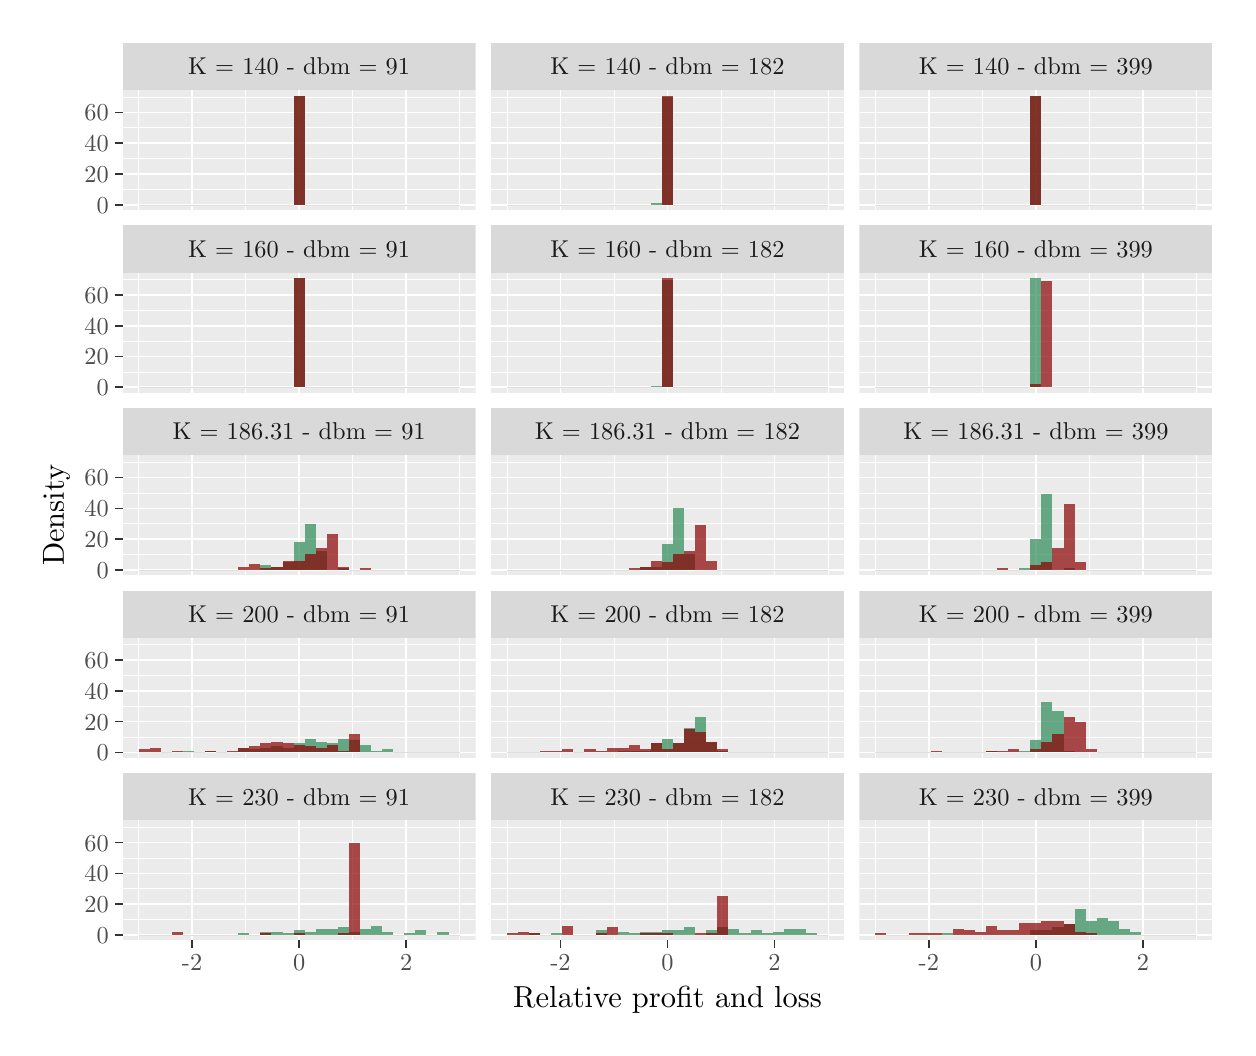
\begin{tikzpicture}[x=1pt,y=1pt]
\definecolor{fillColor}{RGB}{255,255,255}
\path[use as bounding box,fill=fillColor,fill opacity=0.00] (0,0) rectangle (433.62,361.35);
\begin{scope}
\path[clip] (  0.00,  0.00) rectangle (433.62,361.35);
\definecolor{drawColor}{RGB}{255,255,255}
\definecolor{fillColor}{RGB}{255,255,255}

\path[draw=drawColor,line width= 0.6pt,line join=round,line cap=round,fill=fillColor] (  0.00,  0.00) rectangle (433.62,361.35);
\end{scope}
\begin{scope}
\path[clip] ( 34.27,295.39) rectangle (161.89,338.79);
\definecolor{fillColor}{gray}{0.92}

\path[fill=fillColor] ( 34.27,295.39) rectangle (161.89,338.79);
\definecolor{drawColor}{RGB}{255,255,255}

\path[draw=drawColor,line width= 0.3pt,line join=round] ( 34.27,302.92) --
	(161.89,302.92);

\path[draw=drawColor,line width= 0.3pt,line join=round] ( 34.27,314.03) --
	(161.89,314.03);

\path[draw=drawColor,line width= 0.3pt,line join=round] ( 34.27,325.15) --
	(161.89,325.15);

\path[draw=drawColor,line width= 0.3pt,line join=round] ( 34.27,336.26) --
	(161.89,336.26);

\path[draw=drawColor,line width= 0.3pt,line join=round] ( 40.07,295.39) --
	( 40.07,338.79);

\path[draw=drawColor,line width= 0.3pt,line join=round] ( 78.74,295.39) --
	( 78.74,338.79);

\path[draw=drawColor,line width= 0.3pt,line join=round] (117.41,295.39) --
	(117.41,338.79);

\path[draw=drawColor,line width= 0.3pt,line join=round] (156.08,295.39) --
	(156.08,338.79);

\path[draw=drawColor,line width= 0.6pt,line join=round] ( 34.27,297.36) --
	(161.89,297.36);

\path[draw=drawColor,line width= 0.6pt,line join=round] ( 34.27,308.47) --
	(161.89,308.47);

\path[draw=drawColor,line width= 0.6pt,line join=round] ( 34.27,319.59) --
	(161.89,319.59);

\path[draw=drawColor,line width= 0.6pt,line join=round] ( 34.27,330.70) --
	(161.89,330.70);

\path[draw=drawColor,line width= 0.6pt,line join=round] ( 59.40,295.39) --
	( 59.40,338.79);

\path[draw=drawColor,line width= 0.6pt,line join=round] ( 98.08,295.39) --
	( 98.08,338.79);

\path[draw=drawColor,line width= 0.6pt,line join=round] (136.75,295.39) --
	(136.75,338.79);
\definecolor{fillColor}{RGB}{46,139,87}

\path[fill=fillColor,fill opacity=0.70] ( 40.07,297.36) rectangle ( 44.07,297.36);

\path[fill=fillColor,fill opacity=0.70] ( 44.07,297.36) rectangle ( 48.07,297.36);

\path[fill=fillColor,fill opacity=0.70] ( 48.07,297.36) rectangle ( 52.07,297.36);

\path[fill=fillColor,fill opacity=0.70] ( 52.07,297.36) rectangle ( 56.07,297.36);

\path[fill=fillColor,fill opacity=0.70] ( 56.07,297.36) rectangle ( 60.07,297.36);

\path[fill=fillColor,fill opacity=0.70] ( 60.07,297.36) rectangle ( 64.07,297.36);

\path[fill=fillColor,fill opacity=0.70] ( 64.07,297.36) rectangle ( 68.07,297.36);

\path[fill=fillColor,fill opacity=0.70] ( 68.07,297.36) rectangle ( 72.07,297.36);

\path[fill=fillColor,fill opacity=0.70] ( 72.07,297.36) rectangle ( 76.07,297.36);

\path[fill=fillColor,fill opacity=0.70] ( 76.07,297.36) rectangle ( 80.07,297.36);

\path[fill=fillColor,fill opacity=0.70] ( 80.07,297.36) rectangle ( 84.07,297.36);

\path[fill=fillColor,fill opacity=0.70] ( 84.07,297.36) rectangle ( 88.08,297.36);

\path[fill=fillColor,fill opacity=0.70] ( 88.08,297.36) rectangle ( 92.08,297.36);

\path[fill=fillColor,fill opacity=0.70] ( 92.08,297.36) rectangle ( 96.08,297.36);

\path[fill=fillColor,fill opacity=0.70] ( 96.08,297.36) rectangle (100.08,336.82);

\path[fill=fillColor,fill opacity=0.70] (100.08,297.36) rectangle (104.08,297.36);

\path[fill=fillColor,fill opacity=0.70] (104.08,297.36) rectangle (108.08,297.36);

\path[fill=fillColor,fill opacity=0.70] (108.08,297.36) rectangle (112.08,297.36);

\path[fill=fillColor,fill opacity=0.70] (112.08,297.36) rectangle (116.08,297.36);

\path[fill=fillColor,fill opacity=0.70] (116.08,297.36) rectangle (120.08,297.36);

\path[fill=fillColor,fill opacity=0.70] (120.08,297.36) rectangle (124.08,297.36);

\path[fill=fillColor,fill opacity=0.70] (124.08,297.36) rectangle (128.08,297.36);

\path[fill=fillColor,fill opacity=0.70] (128.08,297.36) rectangle (132.08,297.36);

\path[fill=fillColor,fill opacity=0.70] (132.08,297.36) rectangle (136.08,297.36);

\path[fill=fillColor,fill opacity=0.70] (136.08,297.36) rectangle (140.08,297.36);

\path[fill=fillColor,fill opacity=0.70] (140.08,297.36) rectangle (144.08,297.36);

\path[fill=fillColor,fill opacity=0.70] (144.08,297.36) rectangle (148.08,297.36);

\path[fill=fillColor,fill opacity=0.70] (148.08,297.36) rectangle (152.08,297.36);

\path[fill=fillColor,fill opacity=0.70] (152.08,297.36) rectangle (156.08,297.36);
\definecolor{fillColor}{RGB}{139,0,0}

\path[fill=fillColor,fill opacity=0.70] ( 40.07,297.36) rectangle ( 44.07,297.36);

\path[fill=fillColor,fill opacity=0.70] ( 44.07,297.36) rectangle ( 48.07,297.36);

\path[fill=fillColor,fill opacity=0.70] ( 48.07,297.36) rectangle ( 52.07,297.36);

\path[fill=fillColor,fill opacity=0.70] ( 52.07,297.36) rectangle ( 56.07,297.36);

\path[fill=fillColor,fill opacity=0.70] ( 56.07,297.36) rectangle ( 60.07,297.36);

\path[fill=fillColor,fill opacity=0.70] ( 60.07,297.36) rectangle ( 64.07,297.36);

\path[fill=fillColor,fill opacity=0.70] ( 64.07,297.36) rectangle ( 68.07,297.36);

\path[fill=fillColor,fill opacity=0.70] ( 68.07,297.36) rectangle ( 72.07,297.36);

\path[fill=fillColor,fill opacity=0.70] ( 72.07,297.36) rectangle ( 76.07,297.36);

\path[fill=fillColor,fill opacity=0.70] ( 76.07,297.36) rectangle ( 80.07,297.36);

\path[fill=fillColor,fill opacity=0.70] ( 80.07,297.36) rectangle ( 84.07,297.36);

\path[fill=fillColor,fill opacity=0.70] ( 84.07,297.36) rectangle ( 88.08,297.36);

\path[fill=fillColor,fill opacity=0.70] ( 88.08,297.36) rectangle ( 92.08,297.36);

\path[fill=fillColor,fill opacity=0.70] ( 92.08,297.36) rectangle ( 96.08,297.36);

\path[fill=fillColor,fill opacity=0.70] ( 96.08,297.36) rectangle (100.08,336.82);

\path[fill=fillColor,fill opacity=0.70] (100.08,297.36) rectangle (104.08,297.36);

\path[fill=fillColor,fill opacity=0.70] (104.08,297.36) rectangle (108.08,297.36);

\path[fill=fillColor,fill opacity=0.70] (108.08,297.36) rectangle (112.08,297.36);

\path[fill=fillColor,fill opacity=0.70] (112.08,297.36) rectangle (116.08,297.36);

\path[fill=fillColor,fill opacity=0.70] (116.08,297.36) rectangle (120.08,297.36);

\path[fill=fillColor,fill opacity=0.70] (120.08,297.36) rectangle (124.08,297.36);

\path[fill=fillColor,fill opacity=0.70] (124.08,297.36) rectangle (128.08,297.36);

\path[fill=fillColor,fill opacity=0.70] (128.08,297.36) rectangle (132.08,297.36);

\path[fill=fillColor,fill opacity=0.70] (132.08,297.36) rectangle (136.08,297.36);

\path[fill=fillColor,fill opacity=0.70] (136.08,297.36) rectangle (140.08,297.36);

\path[fill=fillColor,fill opacity=0.70] (140.08,297.36) rectangle (144.08,297.36);

\path[fill=fillColor,fill opacity=0.70] (144.08,297.36) rectangle (148.08,297.36);

\path[fill=fillColor,fill opacity=0.70] (148.08,297.36) rectangle (152.08,297.36);

\path[fill=fillColor,fill opacity=0.70] (152.08,297.36) rectangle (156.08,297.36);
\end{scope}
\begin{scope}
\path[clip] ( 34.27,229.42) rectangle (161.89,272.83);
\definecolor{fillColor}{gray}{0.92}

\path[fill=fillColor] ( 34.27,229.42) rectangle (161.89,272.83);
\definecolor{drawColor}{RGB}{255,255,255}

\path[draw=drawColor,line width= 0.3pt,line join=round] ( 34.27,236.95) --
	(161.89,236.95);

\path[draw=drawColor,line width= 0.3pt,line join=round] ( 34.27,248.07) --
	(161.89,248.07);

\path[draw=drawColor,line width= 0.3pt,line join=round] ( 34.27,259.18) --
	(161.89,259.18);

\path[draw=drawColor,line width= 0.3pt,line join=round] ( 34.27,270.30) --
	(161.89,270.30);

\path[draw=drawColor,line width= 0.3pt,line join=round] ( 40.07,229.42) --
	( 40.07,272.83);

\path[draw=drawColor,line width= 0.3pt,line join=round] ( 78.74,229.42) --
	( 78.74,272.83);

\path[draw=drawColor,line width= 0.3pt,line join=round] (117.41,229.42) --
	(117.41,272.83);

\path[draw=drawColor,line width= 0.3pt,line join=round] (156.08,229.42) --
	(156.08,272.83);

\path[draw=drawColor,line width= 0.6pt,line join=round] ( 34.27,231.40) --
	(161.89,231.40);

\path[draw=drawColor,line width= 0.6pt,line join=round] ( 34.27,242.51) --
	(161.89,242.51);

\path[draw=drawColor,line width= 0.6pt,line join=round] ( 34.27,253.62) --
	(161.89,253.62);

\path[draw=drawColor,line width= 0.6pt,line join=round] ( 34.27,264.74) --
	(161.89,264.74);

\path[draw=drawColor,line width= 0.6pt,line join=round] ( 59.40,229.42) --
	( 59.40,272.83);

\path[draw=drawColor,line width= 0.6pt,line join=round] ( 98.08,229.42) --
	( 98.08,272.83);

\path[draw=drawColor,line width= 0.6pt,line join=round] (136.75,229.42) --
	(136.75,272.83);
\definecolor{fillColor}{RGB}{46,139,87}

\path[fill=fillColor,fill opacity=0.70] ( 40.07,231.40) rectangle ( 44.07,231.40);

\path[fill=fillColor,fill opacity=0.70] ( 44.07,231.40) rectangle ( 48.07,231.40);

\path[fill=fillColor,fill opacity=0.70] ( 48.07,231.40) rectangle ( 52.07,231.40);

\path[fill=fillColor,fill opacity=0.70] ( 52.07,231.40) rectangle ( 56.07,231.40);

\path[fill=fillColor,fill opacity=0.70] ( 56.07,231.40) rectangle ( 60.07,231.40);

\path[fill=fillColor,fill opacity=0.70] ( 60.07,231.40) rectangle ( 64.07,231.40);

\path[fill=fillColor,fill opacity=0.70] ( 64.07,231.40) rectangle ( 68.07,231.40);

\path[fill=fillColor,fill opacity=0.70] ( 68.07,231.40) rectangle ( 72.07,231.40);

\path[fill=fillColor,fill opacity=0.70] ( 72.07,231.40) rectangle ( 76.07,231.40);

\path[fill=fillColor,fill opacity=0.70] ( 76.07,231.40) rectangle ( 80.07,231.40);

\path[fill=fillColor,fill opacity=0.70] ( 80.07,231.40) rectangle ( 84.07,231.40);

\path[fill=fillColor,fill opacity=0.70] ( 84.07,231.40) rectangle ( 88.08,231.40);

\path[fill=fillColor,fill opacity=0.70] ( 88.08,231.40) rectangle ( 92.08,231.40);

\path[fill=fillColor,fill opacity=0.70] ( 92.08,231.40) rectangle ( 96.08,231.40);

\path[fill=fillColor,fill opacity=0.70] ( 96.08,231.40) rectangle (100.08,270.85);

\path[fill=fillColor,fill opacity=0.70] (100.08,231.40) rectangle (104.08,231.40);

\path[fill=fillColor,fill opacity=0.70] (104.08,231.40) rectangle (108.08,231.40);

\path[fill=fillColor,fill opacity=0.70] (108.08,231.40) rectangle (112.08,231.40);

\path[fill=fillColor,fill opacity=0.70] (112.08,231.40) rectangle (116.08,231.40);

\path[fill=fillColor,fill opacity=0.70] (116.08,231.40) rectangle (120.08,231.40);

\path[fill=fillColor,fill opacity=0.70] (120.08,231.40) rectangle (124.08,231.40);

\path[fill=fillColor,fill opacity=0.70] (124.08,231.40) rectangle (128.08,231.40);

\path[fill=fillColor,fill opacity=0.70] (128.08,231.40) rectangle (132.08,231.40);

\path[fill=fillColor,fill opacity=0.70] (132.08,231.40) rectangle (136.08,231.40);

\path[fill=fillColor,fill opacity=0.70] (136.08,231.40) rectangle (140.08,231.40);

\path[fill=fillColor,fill opacity=0.70] (140.08,231.40) rectangle (144.08,231.40);

\path[fill=fillColor,fill opacity=0.70] (144.08,231.40) rectangle (148.08,231.40);

\path[fill=fillColor,fill opacity=0.70] (148.08,231.40) rectangle (152.08,231.40);

\path[fill=fillColor,fill opacity=0.70] (152.08,231.40) rectangle (156.08,231.40);
\definecolor{fillColor}{RGB}{139,0,0}

\path[fill=fillColor,fill opacity=0.70] ( 40.07,231.40) rectangle ( 44.07,231.40);

\path[fill=fillColor,fill opacity=0.70] ( 44.07,231.40) rectangle ( 48.07,231.40);

\path[fill=fillColor,fill opacity=0.70] ( 48.07,231.40) rectangle ( 52.07,231.40);

\path[fill=fillColor,fill opacity=0.70] ( 52.07,231.40) rectangle ( 56.07,231.40);

\path[fill=fillColor,fill opacity=0.70] ( 56.07,231.40) rectangle ( 60.07,231.40);

\path[fill=fillColor,fill opacity=0.70] ( 60.07,231.40) rectangle ( 64.07,231.40);

\path[fill=fillColor,fill opacity=0.70] ( 64.07,231.40) rectangle ( 68.07,231.40);

\path[fill=fillColor,fill opacity=0.70] ( 68.07,231.40) rectangle ( 72.07,231.40);

\path[fill=fillColor,fill opacity=0.70] ( 72.07,231.40) rectangle ( 76.07,231.40);

\path[fill=fillColor,fill opacity=0.70] ( 76.07,231.40) rectangle ( 80.07,231.40);

\path[fill=fillColor,fill opacity=0.70] ( 80.07,231.40) rectangle ( 84.07,231.40);

\path[fill=fillColor,fill opacity=0.70] ( 84.07,231.40) rectangle ( 88.08,231.40);

\path[fill=fillColor,fill opacity=0.70] ( 88.08,231.40) rectangle ( 92.08,231.40);

\path[fill=fillColor,fill opacity=0.70] ( 92.08,231.40) rectangle ( 96.08,231.40);

\path[fill=fillColor,fill opacity=0.70] ( 96.08,231.40) rectangle (100.08,270.85);

\path[fill=fillColor,fill opacity=0.70] (100.08,231.40) rectangle (104.08,231.40);

\path[fill=fillColor,fill opacity=0.70] (104.08,231.40) rectangle (108.08,231.40);

\path[fill=fillColor,fill opacity=0.70] (108.08,231.40) rectangle (112.08,231.40);

\path[fill=fillColor,fill opacity=0.70] (112.08,231.40) rectangle (116.08,231.40);

\path[fill=fillColor,fill opacity=0.70] (116.08,231.40) rectangle (120.08,231.40);

\path[fill=fillColor,fill opacity=0.70] (120.08,231.40) rectangle (124.08,231.40);

\path[fill=fillColor,fill opacity=0.70] (124.08,231.40) rectangle (128.08,231.40);

\path[fill=fillColor,fill opacity=0.70] (128.08,231.40) rectangle (132.08,231.40);

\path[fill=fillColor,fill opacity=0.70] (132.08,231.40) rectangle (136.08,231.40);

\path[fill=fillColor,fill opacity=0.70] (136.08,231.40) rectangle (140.08,231.40);

\path[fill=fillColor,fill opacity=0.70] (140.08,231.40) rectangle (144.08,231.40);

\path[fill=fillColor,fill opacity=0.70] (144.08,231.40) rectangle (148.08,231.40);

\path[fill=fillColor,fill opacity=0.70] (148.08,231.40) rectangle (152.08,231.40);

\path[fill=fillColor,fill opacity=0.70] (152.08,231.40) rectangle (156.08,231.40);
\end{scope}
\begin{scope}
\path[clip] ( 34.27,163.46) rectangle (161.89,206.86);
\definecolor{fillColor}{gray}{0.92}

\path[fill=fillColor] ( 34.27,163.46) rectangle (161.89,206.86);
\definecolor{drawColor}{RGB}{255,255,255}

\path[draw=drawColor,line width= 0.3pt,line join=round] ( 34.27,170.99) --
	(161.89,170.99);

\path[draw=drawColor,line width= 0.3pt,line join=round] ( 34.27,182.10) --
	(161.89,182.10);

\path[draw=drawColor,line width= 0.3pt,line join=round] ( 34.27,193.22) --
	(161.89,193.22);

\path[draw=drawColor,line width= 0.3pt,line join=round] ( 34.27,204.33) --
	(161.89,204.33);

\path[draw=drawColor,line width= 0.3pt,line join=round] ( 40.07,163.46) --
	( 40.07,206.86);

\path[draw=drawColor,line width= 0.3pt,line join=round] ( 78.74,163.46) --
	( 78.74,206.86);

\path[draw=drawColor,line width= 0.3pt,line join=round] (117.41,163.46) --
	(117.41,206.86);

\path[draw=drawColor,line width= 0.3pt,line join=round] (156.08,163.46) --
	(156.08,206.86);

\path[draw=drawColor,line width= 0.6pt,line join=round] ( 34.27,165.43) --
	(161.89,165.43);

\path[draw=drawColor,line width= 0.6pt,line join=round] ( 34.27,176.55) --
	(161.89,176.55);

\path[draw=drawColor,line width= 0.6pt,line join=round] ( 34.27,187.66) --
	(161.89,187.66);

\path[draw=drawColor,line width= 0.6pt,line join=round] ( 34.27,198.78) --
	(161.89,198.78);

\path[draw=drawColor,line width= 0.6pt,line join=round] ( 59.40,163.46) --
	( 59.40,206.86);

\path[draw=drawColor,line width= 0.6pt,line join=round] ( 98.08,163.46) --
	( 98.08,206.86);

\path[draw=drawColor,line width= 0.6pt,line join=round] (136.75,163.46) --
	(136.75,206.86);
\definecolor{fillColor}{RGB}{46,139,87}

\path[fill=fillColor,fill opacity=0.70] ( 40.07,165.43) rectangle ( 44.07,165.43);

\path[fill=fillColor,fill opacity=0.70] ( 44.07,165.43) rectangle ( 48.07,165.43);

\path[fill=fillColor,fill opacity=0.70] ( 48.07,165.43) rectangle ( 52.07,165.43);

\path[fill=fillColor,fill opacity=0.70] ( 52.07,165.43) rectangle ( 56.07,165.43);

\path[fill=fillColor,fill opacity=0.70] ( 56.07,165.43) rectangle ( 60.07,165.43);

\path[fill=fillColor,fill opacity=0.70] ( 60.07,165.43) rectangle ( 64.07,165.43);

\path[fill=fillColor,fill opacity=0.70] ( 64.07,165.43) rectangle ( 68.07,165.43);

\path[fill=fillColor,fill opacity=0.70] ( 68.07,165.43) rectangle ( 72.07,165.43);

\path[fill=fillColor,fill opacity=0.70] ( 72.07,165.43) rectangle ( 76.07,165.43);

\path[fill=fillColor,fill opacity=0.70] ( 76.07,165.43) rectangle ( 80.07,165.43);

\path[fill=fillColor,fill opacity=0.70] ( 80.07,165.43) rectangle ( 84.07,165.43);

\path[fill=fillColor,fill opacity=0.70] ( 84.07,165.43) rectangle ( 88.08,167.10);

\path[fill=fillColor,fill opacity=0.70] ( 88.08,165.43) rectangle ( 92.08,166.54);

\path[fill=fillColor,fill opacity=0.70] ( 92.08,165.43) rectangle ( 96.08,168.21);

\path[fill=fillColor,fill opacity=0.70] ( 96.08,165.43) rectangle (100.08,175.43);

\path[fill=fillColor,fill opacity=0.70] (100.08,165.43) rectangle (104.08,182.10);

\path[fill=fillColor,fill opacity=0.70] (104.08,165.43) rectangle (108.08,172.10);

\path[fill=fillColor,fill opacity=0.70] (108.08,165.43) rectangle (112.08,165.43);

\path[fill=fillColor,fill opacity=0.70] (112.08,165.43) rectangle (116.08,165.99);

\path[fill=fillColor,fill opacity=0.70] (116.08,165.43) rectangle (120.08,165.43);

\path[fill=fillColor,fill opacity=0.70] (120.08,165.43) rectangle (124.08,165.43);

\path[fill=fillColor,fill opacity=0.70] (124.08,165.43) rectangle (128.08,165.43);

\path[fill=fillColor,fill opacity=0.70] (128.08,165.43) rectangle (132.08,165.43);

\path[fill=fillColor,fill opacity=0.70] (132.08,165.43) rectangle (136.08,165.43);

\path[fill=fillColor,fill opacity=0.70] (136.08,165.43) rectangle (140.08,165.43);

\path[fill=fillColor,fill opacity=0.70] (140.08,165.43) rectangle (144.08,165.43);

\path[fill=fillColor,fill opacity=0.70] (144.08,165.43) rectangle (148.08,165.43);

\path[fill=fillColor,fill opacity=0.70] (148.08,165.43) rectangle (152.08,165.43);

\path[fill=fillColor,fill opacity=0.70] (152.08,165.43) rectangle (156.08,165.43);
\definecolor{fillColor}{RGB}{139,0,0}

\path[fill=fillColor,fill opacity=0.70] ( 40.07,165.43) rectangle ( 44.07,165.43);

\path[fill=fillColor,fill opacity=0.70] ( 44.07,165.43) rectangle ( 48.07,165.43);

\path[fill=fillColor,fill opacity=0.70] ( 48.07,165.43) rectangle ( 52.07,165.43);

\path[fill=fillColor,fill opacity=0.70] ( 52.07,165.43) rectangle ( 56.07,165.43);

\path[fill=fillColor,fill opacity=0.70] ( 56.07,165.43) rectangle ( 60.07,165.43);

\path[fill=fillColor,fill opacity=0.70] ( 60.07,165.43) rectangle ( 64.07,165.43);

\path[fill=fillColor,fill opacity=0.70] ( 64.07,165.43) rectangle ( 68.07,165.43);

\path[fill=fillColor,fill opacity=0.70] ( 68.07,165.43) rectangle ( 72.07,165.43);

\path[fill=fillColor,fill opacity=0.70] ( 72.07,165.43) rectangle ( 76.07,165.43);

\path[fill=fillColor,fill opacity=0.70] ( 76.07,165.43) rectangle ( 80.07,166.54);

\path[fill=fillColor,fill opacity=0.70] ( 80.07,165.43) rectangle ( 84.07,167.65);

\path[fill=fillColor,fill opacity=0.70] ( 84.07,165.43) rectangle ( 88.08,165.99);

\path[fill=fillColor,fill opacity=0.70] ( 88.08,165.43) rectangle ( 92.08,166.54);

\path[fill=fillColor,fill opacity=0.70] ( 92.08,165.43) rectangle ( 96.08,168.77);

\path[fill=fillColor,fill opacity=0.70] ( 96.08,165.43) rectangle (100.08,168.77);

\path[fill=fillColor,fill opacity=0.70] (100.08,165.43) rectangle (104.08,170.99);

\path[fill=fillColor,fill opacity=0.70] (104.08,165.43) rectangle (108.08,173.21);

\path[fill=fillColor,fill opacity=0.70] (108.08,165.43) rectangle (112.08,178.21);

\path[fill=fillColor,fill opacity=0.70] (112.08,165.43) rectangle (116.08,166.54);

\path[fill=fillColor,fill opacity=0.70] (116.08,165.43) rectangle (120.08,165.43);

\path[fill=fillColor,fill opacity=0.70] (120.08,165.43) rectangle (124.08,165.99);

\path[fill=fillColor,fill opacity=0.70] (124.08,165.43) rectangle (128.08,165.43);

\path[fill=fillColor,fill opacity=0.70] (128.08,165.43) rectangle (132.08,165.43);

\path[fill=fillColor,fill opacity=0.70] (132.08,165.43) rectangle (136.08,165.43);

\path[fill=fillColor,fill opacity=0.70] (136.08,165.43) rectangle (140.08,165.43);

\path[fill=fillColor,fill opacity=0.70] (140.08,165.43) rectangle (144.08,165.43);

\path[fill=fillColor,fill opacity=0.70] (144.08,165.43) rectangle (148.08,165.43);

\path[fill=fillColor,fill opacity=0.70] (148.08,165.43) rectangle (152.08,165.43);

\path[fill=fillColor,fill opacity=0.70] (152.08,165.43) rectangle (156.08,165.43);
\end{scope}
\begin{scope}
\path[clip] ( 34.27, 97.49) rectangle (161.89,140.90);
\definecolor{fillColor}{gray}{0.92}

\path[fill=fillColor] ( 34.27, 97.49) rectangle (161.89,140.90);
\definecolor{drawColor}{RGB}{255,255,255}

\path[draw=drawColor,line width= 0.3pt,line join=round] ( 34.27,105.02) --
	(161.89,105.02);

\path[draw=drawColor,line width= 0.3pt,line join=round] ( 34.27,116.14) --
	(161.89,116.14);

\path[draw=drawColor,line width= 0.3pt,line join=round] ( 34.27,127.25) --
	(161.89,127.25);

\path[draw=drawColor,line width= 0.3pt,line join=round] ( 34.27,138.37) --
	(161.89,138.37);

\path[draw=drawColor,line width= 0.3pt,line join=round] ( 40.07, 97.49) --
	( 40.07,140.90);

\path[draw=drawColor,line width= 0.3pt,line join=round] ( 78.74, 97.49) --
	( 78.74,140.90);

\path[draw=drawColor,line width= 0.3pt,line join=round] (117.41, 97.49) --
	(117.41,140.90);

\path[draw=drawColor,line width= 0.3pt,line join=round] (156.08, 97.49) --
	(156.08,140.90);

\path[draw=drawColor,line width= 0.6pt,line join=round] ( 34.27, 99.47) --
	(161.89, 99.47);

\path[draw=drawColor,line width= 0.6pt,line join=round] ( 34.27,110.58) --
	(161.89,110.58);

\path[draw=drawColor,line width= 0.6pt,line join=round] ( 34.27,121.70) --
	(161.89,121.70);

\path[draw=drawColor,line width= 0.6pt,line join=round] ( 34.27,132.81) --
	(161.89,132.81);

\path[draw=drawColor,line width= 0.6pt,line join=round] ( 59.40, 97.49) --
	( 59.40,140.90);

\path[draw=drawColor,line width= 0.6pt,line join=round] ( 98.08, 97.49) --
	( 98.08,140.90);

\path[draw=drawColor,line width= 0.6pt,line join=round] (136.75, 97.49) --
	(136.75,140.90);
\definecolor{fillColor}{RGB}{46,139,87}

\path[fill=fillColor,fill opacity=0.70] ( 40.07, 99.47) rectangle ( 44.07, 99.47);

\path[fill=fillColor,fill opacity=0.70] ( 44.07, 99.47) rectangle ( 48.07, 99.47);

\path[fill=fillColor,fill opacity=0.70] ( 48.07, 99.47) rectangle ( 52.07, 99.47);

\path[fill=fillColor,fill opacity=0.70] ( 52.07, 99.47) rectangle ( 56.07, 99.47);

\path[fill=fillColor,fill opacity=0.70] ( 56.07, 99.47) rectangle ( 60.07,100.02);

\path[fill=fillColor,fill opacity=0.70] ( 60.07, 99.47) rectangle ( 64.07, 99.47);

\path[fill=fillColor,fill opacity=0.70] ( 64.07, 99.47) rectangle ( 68.07,100.02);

\path[fill=fillColor,fill opacity=0.70] ( 68.07, 99.47) rectangle ( 72.07, 99.47);

\path[fill=fillColor,fill opacity=0.70] ( 72.07, 99.47) rectangle ( 76.07, 99.47);

\path[fill=fillColor,fill opacity=0.70] ( 76.07, 99.47) rectangle ( 80.07,101.13);

\path[fill=fillColor,fill opacity=0.70] ( 80.07, 99.47) rectangle ( 84.07,100.58);

\path[fill=fillColor,fill opacity=0.70] ( 84.07, 99.47) rectangle ( 88.08,101.13);

\path[fill=fillColor,fill opacity=0.70] ( 88.08, 99.47) rectangle ( 92.08,101.69);

\path[fill=fillColor,fill opacity=0.70] ( 92.08, 99.47) rectangle ( 96.08,101.13);

\path[fill=fillColor,fill opacity=0.70] ( 96.08, 99.47) rectangle (100.08,102.80);

\path[fill=fillColor,fill opacity=0.70] (100.08, 99.47) rectangle (104.08,104.47);

\path[fill=fillColor,fill opacity=0.70] (104.08, 99.47) rectangle (108.08,103.36);

\path[fill=fillColor,fill opacity=0.70] (108.08, 99.47) rectangle (112.08,102.80);

\path[fill=fillColor,fill opacity=0.70] (112.08, 99.47) rectangle (116.08,104.47);

\path[fill=fillColor,fill opacity=0.70] (116.08, 99.47) rectangle (120.08,103.91);

\path[fill=fillColor,fill opacity=0.70] (120.08, 99.47) rectangle (124.08,102.25);

\path[fill=fillColor,fill opacity=0.70] (124.08, 99.47) rectangle (128.08,100.02);

\path[fill=fillColor,fill opacity=0.70] (128.08, 99.47) rectangle (132.08,100.58);

\path[fill=fillColor,fill opacity=0.70] (132.08, 99.47) rectangle (136.08, 99.47);

\path[fill=fillColor,fill opacity=0.70] (136.08, 99.47) rectangle (140.08, 99.47);

\path[fill=fillColor,fill opacity=0.70] (140.08, 99.47) rectangle (144.08, 99.47);

\path[fill=fillColor,fill opacity=0.70] (144.08, 99.47) rectangle (148.08, 99.47);

\path[fill=fillColor,fill opacity=0.70] (148.08, 99.47) rectangle (152.08, 99.47);

\path[fill=fillColor,fill opacity=0.70] (152.08, 99.47) rectangle (156.08, 99.47);
\definecolor{fillColor}{RGB}{139,0,0}

\path[fill=fillColor,fill opacity=0.70] ( 40.07, 99.47) rectangle ( 44.07,100.58);

\path[fill=fillColor,fill opacity=0.70] ( 44.07, 99.47) rectangle ( 48.07,101.13);

\path[fill=fillColor,fill opacity=0.70] ( 48.07, 99.47) rectangle ( 52.07, 99.47);

\path[fill=fillColor,fill opacity=0.70] ( 52.07, 99.47) rectangle ( 56.07,100.02);

\path[fill=fillColor,fill opacity=0.70] ( 56.07, 99.47) rectangle ( 60.07, 99.47);

\path[fill=fillColor,fill opacity=0.70] ( 60.07, 99.47) rectangle ( 64.07, 99.47);

\path[fill=fillColor,fill opacity=0.70] ( 64.07, 99.47) rectangle ( 68.07,100.02);

\path[fill=fillColor,fill opacity=0.70] ( 68.07, 99.47) rectangle ( 72.07, 99.47);

\path[fill=fillColor,fill opacity=0.70] ( 72.07, 99.47) rectangle ( 76.07,100.02);

\path[fill=fillColor,fill opacity=0.70] ( 76.07, 99.47) rectangle ( 80.07,101.13);

\path[fill=fillColor,fill opacity=0.70] ( 80.07, 99.47) rectangle ( 84.07,101.69);

\path[fill=fillColor,fill opacity=0.70] ( 84.07, 99.47) rectangle ( 88.08,102.80);

\path[fill=fillColor,fill opacity=0.70] ( 88.08, 99.47) rectangle ( 92.08,103.36);

\path[fill=fillColor,fill opacity=0.70] ( 92.08, 99.47) rectangle ( 96.08,102.80);

\path[fill=fillColor,fill opacity=0.70] ( 96.08, 99.47) rectangle (100.08,102.25);

\path[fill=fillColor,fill opacity=0.70] (100.08, 99.47) rectangle (104.08,101.69);

\path[fill=fillColor,fill opacity=0.70] (104.08, 99.47) rectangle (108.08,101.13);

\path[fill=fillColor,fill opacity=0.70] (108.08, 99.47) rectangle (112.08,102.25);

\path[fill=fillColor,fill opacity=0.70] (112.08, 99.47) rectangle (116.08,100.02);

\path[fill=fillColor,fill opacity=0.70] (116.08, 99.47) rectangle (120.08,106.14);

\path[fill=fillColor,fill opacity=0.70] (120.08, 99.47) rectangle (124.08, 99.47);

\path[fill=fillColor,fill opacity=0.70] (124.08, 99.47) rectangle (128.08, 99.47);

\path[fill=fillColor,fill opacity=0.70] (128.08, 99.47) rectangle (132.08, 99.47);

\path[fill=fillColor,fill opacity=0.70] (132.08, 99.47) rectangle (136.08, 99.47);

\path[fill=fillColor,fill opacity=0.70] (136.08, 99.47) rectangle (140.08, 99.47);

\path[fill=fillColor,fill opacity=0.70] (140.08, 99.47) rectangle (144.08, 99.47);

\path[fill=fillColor,fill opacity=0.70] (144.08, 99.47) rectangle (148.08, 99.47);

\path[fill=fillColor,fill opacity=0.70] (148.08, 99.47) rectangle (152.08, 99.47);

\path[fill=fillColor,fill opacity=0.70] (152.08, 99.47) rectangle (156.08, 99.47);
\end{scope}
\begin{scope}
\path[clip] ( 34.27, 31.53) rectangle (161.89, 74.93);
\definecolor{fillColor}{gray}{0.92}

\path[fill=fillColor] ( 34.27, 31.53) rectangle (161.89, 74.93);
\definecolor{drawColor}{RGB}{255,255,255}

\path[draw=drawColor,line width= 0.3pt,line join=round] ( 34.27, 39.06) --
	(161.89, 39.06);

\path[draw=drawColor,line width= 0.3pt,line join=round] ( 34.27, 50.18) --
	(161.89, 50.18);

\path[draw=drawColor,line width= 0.3pt,line join=round] ( 34.27, 61.29) --
	(161.89, 61.29);

\path[draw=drawColor,line width= 0.3pt,line join=round] ( 34.27, 72.41) --
	(161.89, 72.41);

\path[draw=drawColor,line width= 0.3pt,line join=round] ( 40.07, 31.53) --
	( 40.07, 74.93);

\path[draw=drawColor,line width= 0.3pt,line join=round] ( 78.74, 31.53) --
	( 78.74, 74.93);

\path[draw=drawColor,line width= 0.3pt,line join=round] (117.41, 31.53) --
	(117.41, 74.93);

\path[draw=drawColor,line width= 0.3pt,line join=round] (156.08, 31.53) --
	(156.08, 74.93);

\path[draw=drawColor,line width= 0.6pt,line join=round] ( 34.27, 33.50) --
	(161.89, 33.50);

\path[draw=drawColor,line width= 0.6pt,line join=round] ( 34.27, 44.62) --
	(161.89, 44.62);

\path[draw=drawColor,line width= 0.6pt,line join=round] ( 34.27, 55.73) --
	(161.89, 55.73);

\path[draw=drawColor,line width= 0.6pt,line join=round] ( 34.27, 66.85) --
	(161.89, 66.85);

\path[draw=drawColor,line width= 0.6pt,line join=round] ( 59.40, 31.53) --
	( 59.40, 74.93);

\path[draw=drawColor,line width= 0.6pt,line join=round] ( 98.08, 31.53) --
	( 98.08, 74.93);

\path[draw=drawColor,line width= 0.6pt,line join=round] (136.75, 31.53) --
	(136.75, 74.93);
\definecolor{fillColor}{RGB}{46,139,87}

\path[fill=fillColor,fill opacity=0.70] ( 40.07, 33.50) rectangle ( 44.07, 33.50);

\path[fill=fillColor,fill opacity=0.70] ( 44.07, 33.50) rectangle ( 48.07, 33.50);

\path[fill=fillColor,fill opacity=0.70] ( 48.07, 33.50) rectangle ( 52.07, 33.50);

\path[fill=fillColor,fill opacity=0.70] ( 52.07, 33.50) rectangle ( 56.07, 33.50);

\path[fill=fillColor,fill opacity=0.70] ( 56.07, 33.50) rectangle ( 60.07, 33.50);

\path[fill=fillColor,fill opacity=0.70] ( 60.07, 33.50) rectangle ( 64.07, 33.50);

\path[fill=fillColor,fill opacity=0.70] ( 64.07, 33.50) rectangle ( 68.07, 33.50);

\path[fill=fillColor,fill opacity=0.70] ( 68.07, 33.50) rectangle ( 72.07, 33.50);

\path[fill=fillColor,fill opacity=0.70] ( 72.07, 33.50) rectangle ( 76.07, 33.50);

\path[fill=fillColor,fill opacity=0.70] ( 76.07, 33.50) rectangle ( 80.07, 34.06);

\path[fill=fillColor,fill opacity=0.70] ( 80.07, 33.50) rectangle ( 84.07, 33.50);

\path[fill=fillColor,fill opacity=0.70] ( 84.07, 33.50) rectangle ( 88.08, 34.62);

\path[fill=fillColor,fill opacity=0.70] ( 88.08, 33.50) rectangle ( 92.08, 34.62);

\path[fill=fillColor,fill opacity=0.70] ( 92.08, 33.50) rectangle ( 96.08, 34.06);

\path[fill=fillColor,fill opacity=0.70] ( 96.08, 33.50) rectangle (100.08, 35.17);

\path[fill=fillColor,fill opacity=0.70] (100.08, 33.50) rectangle (104.08, 34.62);

\path[fill=fillColor,fill opacity=0.70] (104.08, 33.50) rectangle (108.08, 35.73);

\path[fill=fillColor,fill opacity=0.70] (108.08, 33.50) rectangle (112.08, 35.73);

\path[fill=fillColor,fill opacity=0.70] (112.08, 33.50) rectangle (116.08, 36.28);

\path[fill=fillColor,fill opacity=0.70] (116.08, 33.50) rectangle (120.08, 34.62);

\path[fill=fillColor,fill opacity=0.70] (120.08, 33.50) rectangle (124.08, 35.73);

\path[fill=fillColor,fill opacity=0.70] (124.08, 33.50) rectangle (128.08, 36.84);

\path[fill=fillColor,fill opacity=0.70] (128.08, 33.50) rectangle (132.08, 34.62);

\path[fill=fillColor,fill opacity=0.70] (132.08, 33.50) rectangle (136.08, 33.50);

\path[fill=fillColor,fill opacity=0.70] (136.08, 33.50) rectangle (140.08, 34.06);

\path[fill=fillColor,fill opacity=0.70] (140.08, 33.50) rectangle (144.08, 35.17);

\path[fill=fillColor,fill opacity=0.70] (144.08, 33.50) rectangle (148.08, 33.50);

\path[fill=fillColor,fill opacity=0.70] (148.08, 33.50) rectangle (152.08, 34.62);

\path[fill=fillColor,fill opacity=0.70] (152.08, 33.50) rectangle (156.08, 33.50);
\definecolor{fillColor}{RGB}{139,0,0}

\path[fill=fillColor,fill opacity=0.70] ( 40.07, 33.50) rectangle ( 44.07, 33.50);

\path[fill=fillColor,fill opacity=0.70] ( 44.07, 33.50) rectangle ( 48.07, 33.50);

\path[fill=fillColor,fill opacity=0.70] ( 48.07, 33.50) rectangle ( 52.07, 33.50);

\path[fill=fillColor,fill opacity=0.70] ( 52.07, 33.50) rectangle ( 56.07, 34.62);

\path[fill=fillColor,fill opacity=0.70] ( 56.07, 33.50) rectangle ( 60.07, 33.50);

\path[fill=fillColor,fill opacity=0.70] ( 60.07, 33.50) rectangle ( 64.07, 33.50);

\path[fill=fillColor,fill opacity=0.70] ( 64.07, 33.50) rectangle ( 68.07, 33.50);

\path[fill=fillColor,fill opacity=0.70] ( 68.07, 33.50) rectangle ( 72.07, 33.50);

\path[fill=fillColor,fill opacity=0.70] ( 72.07, 33.50) rectangle ( 76.07, 33.50);

\path[fill=fillColor,fill opacity=0.70] ( 76.07, 33.50) rectangle ( 80.07, 33.50);

\path[fill=fillColor,fill opacity=0.70] ( 80.07, 33.50) rectangle ( 84.07, 33.50);

\path[fill=fillColor,fill opacity=0.70] ( 84.07, 33.50) rectangle ( 88.08, 34.06);

\path[fill=fillColor,fill opacity=0.70] ( 88.08, 33.50) rectangle ( 92.08, 33.50);

\path[fill=fillColor,fill opacity=0.70] ( 92.08, 33.50) rectangle ( 96.08, 33.50);

\path[fill=fillColor,fill opacity=0.70] ( 96.08, 33.50) rectangle (100.08, 34.06);

\path[fill=fillColor,fill opacity=0.70] (100.08, 33.50) rectangle (104.08, 33.50);

\path[fill=fillColor,fill opacity=0.70] (104.08, 33.50) rectangle (108.08, 33.50);

\path[fill=fillColor,fill opacity=0.70] (108.08, 33.50) rectangle (112.08, 33.50);

\path[fill=fillColor,fill opacity=0.70] (112.08, 33.50) rectangle (116.08, 34.06);

\path[fill=fillColor,fill opacity=0.70] (116.08, 33.50) rectangle (120.08, 66.85);

\path[fill=fillColor,fill opacity=0.70] (120.08, 33.50) rectangle (124.08, 33.50);

\path[fill=fillColor,fill opacity=0.70] (124.08, 33.50) rectangle (128.08, 33.50);

\path[fill=fillColor,fill opacity=0.70] (128.08, 33.50) rectangle (132.08, 33.50);

\path[fill=fillColor,fill opacity=0.70] (132.08, 33.50) rectangle (136.08, 33.50);

\path[fill=fillColor,fill opacity=0.70] (136.08, 33.50) rectangle (140.08, 33.50);

\path[fill=fillColor,fill opacity=0.70] (140.08, 33.50) rectangle (144.08, 33.50);

\path[fill=fillColor,fill opacity=0.70] (144.08, 33.50) rectangle (148.08, 33.50);

\path[fill=fillColor,fill opacity=0.70] (148.08, 33.50) rectangle (152.08, 33.50);

\path[fill=fillColor,fill opacity=0.70] (152.08, 33.50) rectangle (156.08, 33.50);
\end{scope}
\begin{scope}
\path[clip] (167.39,295.39) rectangle (295.00,338.79);
\definecolor{fillColor}{gray}{0.92}

\path[fill=fillColor] (167.39,295.39) rectangle (295.00,338.79);
\definecolor{drawColor}{RGB}{255,255,255}

\path[draw=drawColor,line width= 0.3pt,line join=round] (167.39,302.92) --
	(295.00,302.92);

\path[draw=drawColor,line width= 0.3pt,line join=round] (167.39,314.03) --
	(295.00,314.03);

\path[draw=drawColor,line width= 0.3pt,line join=round] (167.39,325.15) --
	(295.00,325.15);

\path[draw=drawColor,line width= 0.3pt,line join=round] (167.39,336.26) --
	(295.00,336.26);

\path[draw=drawColor,line width= 0.3pt,line join=round] (173.19,295.39) --
	(173.19,338.79);

\path[draw=drawColor,line width= 0.3pt,line join=round] (211.86,295.39) --
	(211.86,338.79);

\path[draw=drawColor,line width= 0.3pt,line join=round] (250.53,295.39) --
	(250.53,338.79);

\path[draw=drawColor,line width= 0.3pt,line join=round] (289.20,295.39) --
	(289.20,338.79);

\path[draw=drawColor,line width= 0.6pt,line join=round] (167.39,297.36) --
	(295.00,297.36);

\path[draw=drawColor,line width= 0.6pt,line join=round] (167.39,308.47) --
	(295.00,308.47);

\path[draw=drawColor,line width= 0.6pt,line join=round] (167.39,319.59) --
	(295.00,319.59);

\path[draw=drawColor,line width= 0.6pt,line join=round] (167.39,330.70) --
	(295.00,330.70);

\path[draw=drawColor,line width= 0.6pt,line join=round] (192.52,295.39) --
	(192.52,338.79);

\path[draw=drawColor,line width= 0.6pt,line join=round] (231.19,295.39) --
	(231.19,338.79);

\path[draw=drawColor,line width= 0.6pt,line join=round] (269.87,295.39) --
	(269.87,338.79);
\definecolor{fillColor}{RGB}{46,139,87}

\path[fill=fillColor,fill opacity=0.70] (173.19,297.36) rectangle (177.19,297.36);

\path[fill=fillColor,fill opacity=0.70] (177.19,297.36) rectangle (181.19,297.36);

\path[fill=fillColor,fill opacity=0.70] (181.19,297.36) rectangle (185.19,297.36);

\path[fill=fillColor,fill opacity=0.70] (185.19,297.36) rectangle (189.19,297.36);

\path[fill=fillColor,fill opacity=0.70] (189.19,297.36) rectangle (193.19,297.36);

\path[fill=fillColor,fill opacity=0.70] (193.19,297.36) rectangle (197.19,297.36);

\path[fill=fillColor,fill opacity=0.70] (197.19,297.36) rectangle (201.19,297.36);

\path[fill=fillColor,fill opacity=0.70] (201.19,297.36) rectangle (205.19,297.36);

\path[fill=fillColor,fill opacity=0.70] (205.19,297.36) rectangle (209.19,297.36);

\path[fill=fillColor,fill opacity=0.70] (209.19,297.36) rectangle (213.19,297.36);

\path[fill=fillColor,fill opacity=0.70] (213.19,297.36) rectangle (217.19,297.36);

\path[fill=fillColor,fill opacity=0.70] (217.19,297.36) rectangle (221.19,297.36);

\path[fill=fillColor,fill opacity=0.70] (221.19,297.36) rectangle (225.19,297.36);

\path[fill=fillColor,fill opacity=0.70] (225.19,297.36) rectangle (229.19,297.91);

\path[fill=fillColor,fill opacity=0.70] (229.19,297.36) rectangle (233.19,336.26);

\path[fill=fillColor,fill opacity=0.70] (233.19,297.36) rectangle (237.19,297.36);

\path[fill=fillColor,fill opacity=0.70] (237.19,297.36) rectangle (241.20,297.36);

\path[fill=fillColor,fill opacity=0.70] (241.20,297.36) rectangle (245.20,297.36);

\path[fill=fillColor,fill opacity=0.70] (245.20,297.36) rectangle (249.20,297.36);

\path[fill=fillColor,fill opacity=0.70] (249.20,297.36) rectangle (253.20,297.36);

\path[fill=fillColor,fill opacity=0.70] (253.20,297.36) rectangle (257.20,297.36);

\path[fill=fillColor,fill opacity=0.70] (257.20,297.36) rectangle (261.20,297.36);

\path[fill=fillColor,fill opacity=0.70] (261.20,297.36) rectangle (265.20,297.36);

\path[fill=fillColor,fill opacity=0.70] (265.20,297.36) rectangle (269.20,297.36);

\path[fill=fillColor,fill opacity=0.70] (269.20,297.36) rectangle (273.20,297.36);

\path[fill=fillColor,fill opacity=0.70] (273.20,297.36) rectangle (277.20,297.36);

\path[fill=fillColor,fill opacity=0.70] (277.20,297.36) rectangle (281.20,297.36);

\path[fill=fillColor,fill opacity=0.70] (281.20,297.36) rectangle (285.20,297.36);

\path[fill=fillColor,fill opacity=0.70] (285.20,297.36) rectangle (289.20,297.36);
\definecolor{fillColor}{RGB}{139,0,0}

\path[fill=fillColor,fill opacity=0.70] (173.19,297.36) rectangle (177.19,297.36);

\path[fill=fillColor,fill opacity=0.70] (177.19,297.36) rectangle (181.19,297.36);

\path[fill=fillColor,fill opacity=0.70] (181.19,297.36) rectangle (185.19,297.36);

\path[fill=fillColor,fill opacity=0.70] (185.19,297.36) rectangle (189.19,297.36);

\path[fill=fillColor,fill opacity=0.70] (189.19,297.36) rectangle (193.19,297.36);

\path[fill=fillColor,fill opacity=0.70] (193.19,297.36) rectangle (197.19,297.36);

\path[fill=fillColor,fill opacity=0.70] (197.19,297.36) rectangle (201.19,297.36);

\path[fill=fillColor,fill opacity=0.70] (201.19,297.36) rectangle (205.19,297.36);

\path[fill=fillColor,fill opacity=0.70] (205.19,297.36) rectangle (209.19,297.36);

\path[fill=fillColor,fill opacity=0.70] (209.19,297.36) rectangle (213.19,297.36);

\path[fill=fillColor,fill opacity=0.70] (213.19,297.36) rectangle (217.19,297.36);

\path[fill=fillColor,fill opacity=0.70] (217.19,297.36) rectangle (221.19,297.36);

\path[fill=fillColor,fill opacity=0.70] (221.19,297.36) rectangle (225.19,297.36);

\path[fill=fillColor,fill opacity=0.70] (225.19,297.36) rectangle (229.19,297.36);

\path[fill=fillColor,fill opacity=0.70] (229.19,297.36) rectangle (233.19,336.82);

\path[fill=fillColor,fill opacity=0.70] (233.19,297.36) rectangle (237.19,297.36);

\path[fill=fillColor,fill opacity=0.70] (237.19,297.36) rectangle (241.20,297.36);

\path[fill=fillColor,fill opacity=0.70] (241.20,297.36) rectangle (245.20,297.36);

\path[fill=fillColor,fill opacity=0.70] (245.20,297.36) rectangle (249.20,297.36);

\path[fill=fillColor,fill opacity=0.70] (249.20,297.36) rectangle (253.20,297.36);

\path[fill=fillColor,fill opacity=0.70] (253.20,297.36) rectangle (257.20,297.36);

\path[fill=fillColor,fill opacity=0.70] (257.20,297.36) rectangle (261.20,297.36);

\path[fill=fillColor,fill opacity=0.70] (261.20,297.36) rectangle (265.20,297.36);

\path[fill=fillColor,fill opacity=0.70] (265.20,297.36) rectangle (269.20,297.36);

\path[fill=fillColor,fill opacity=0.70] (269.20,297.36) rectangle (273.20,297.36);

\path[fill=fillColor,fill opacity=0.70] (273.20,297.36) rectangle (277.20,297.36);

\path[fill=fillColor,fill opacity=0.70] (277.20,297.36) rectangle (281.20,297.36);

\path[fill=fillColor,fill opacity=0.70] (281.20,297.36) rectangle (285.20,297.36);

\path[fill=fillColor,fill opacity=0.70] (285.20,297.36) rectangle (289.20,297.36);
\end{scope}
\begin{scope}
\path[clip] (167.39,229.42) rectangle (295.00,272.83);
\definecolor{fillColor}{gray}{0.92}

\path[fill=fillColor] (167.39,229.42) rectangle (295.00,272.83);
\definecolor{drawColor}{RGB}{255,255,255}

\path[draw=drawColor,line width= 0.3pt,line join=round] (167.39,236.95) --
	(295.00,236.95);

\path[draw=drawColor,line width= 0.3pt,line join=round] (167.39,248.07) --
	(295.00,248.07);

\path[draw=drawColor,line width= 0.3pt,line join=round] (167.39,259.18) --
	(295.00,259.18);

\path[draw=drawColor,line width= 0.3pt,line join=round] (167.39,270.30) --
	(295.00,270.30);

\path[draw=drawColor,line width= 0.3pt,line join=round] (173.19,229.42) --
	(173.19,272.83);

\path[draw=drawColor,line width= 0.3pt,line join=round] (211.86,229.42) --
	(211.86,272.83);

\path[draw=drawColor,line width= 0.3pt,line join=round] (250.53,229.42) --
	(250.53,272.83);

\path[draw=drawColor,line width= 0.3pt,line join=round] (289.20,229.42) --
	(289.20,272.83);

\path[draw=drawColor,line width= 0.6pt,line join=round] (167.39,231.40) --
	(295.00,231.40);

\path[draw=drawColor,line width= 0.6pt,line join=round] (167.39,242.51) --
	(295.00,242.51);

\path[draw=drawColor,line width= 0.6pt,line join=round] (167.39,253.62) --
	(295.00,253.62);

\path[draw=drawColor,line width= 0.6pt,line join=round] (167.39,264.74) --
	(295.00,264.74);

\path[draw=drawColor,line width= 0.6pt,line join=round] (192.52,229.42) --
	(192.52,272.83);

\path[draw=drawColor,line width= 0.6pt,line join=round] (231.19,229.42) --
	(231.19,272.83);

\path[draw=drawColor,line width= 0.6pt,line join=round] (269.87,229.42) --
	(269.87,272.83);
\definecolor{fillColor}{RGB}{46,139,87}

\path[fill=fillColor,fill opacity=0.70] (173.19,231.40) rectangle (177.19,231.40);

\path[fill=fillColor,fill opacity=0.70] (177.19,231.40) rectangle (181.19,231.40);

\path[fill=fillColor,fill opacity=0.70] (181.19,231.40) rectangle (185.19,231.40);

\path[fill=fillColor,fill opacity=0.70] (185.19,231.40) rectangle (189.19,231.40);

\path[fill=fillColor,fill opacity=0.70] (189.19,231.40) rectangle (193.19,231.40);

\path[fill=fillColor,fill opacity=0.70] (193.19,231.40) rectangle (197.19,231.40);

\path[fill=fillColor,fill opacity=0.70] (197.19,231.40) rectangle (201.19,231.40);

\path[fill=fillColor,fill opacity=0.70] (201.19,231.40) rectangle (205.19,231.40);

\path[fill=fillColor,fill opacity=0.70] (205.19,231.40) rectangle (209.19,231.40);

\path[fill=fillColor,fill opacity=0.70] (209.19,231.40) rectangle (213.19,231.40);

\path[fill=fillColor,fill opacity=0.70] (213.19,231.40) rectangle (217.19,231.40);

\path[fill=fillColor,fill opacity=0.70] (217.19,231.40) rectangle (221.19,231.40);

\path[fill=fillColor,fill opacity=0.70] (221.19,231.40) rectangle (225.19,231.40);

\path[fill=fillColor,fill opacity=0.70] (225.19,231.40) rectangle (229.19,231.95);

\path[fill=fillColor,fill opacity=0.70] (229.19,231.40) rectangle (233.19,270.30);

\path[fill=fillColor,fill opacity=0.70] (233.19,231.40) rectangle (237.19,231.40);

\path[fill=fillColor,fill opacity=0.70] (237.19,231.40) rectangle (241.20,231.40);

\path[fill=fillColor,fill opacity=0.70] (241.20,231.40) rectangle (245.20,231.40);

\path[fill=fillColor,fill opacity=0.70] (245.20,231.40) rectangle (249.20,231.40);

\path[fill=fillColor,fill opacity=0.70] (249.20,231.40) rectangle (253.20,231.40);

\path[fill=fillColor,fill opacity=0.70] (253.20,231.40) rectangle (257.20,231.40);

\path[fill=fillColor,fill opacity=0.70] (257.20,231.40) rectangle (261.20,231.40);

\path[fill=fillColor,fill opacity=0.70] (261.20,231.40) rectangle (265.20,231.40);

\path[fill=fillColor,fill opacity=0.70] (265.20,231.40) rectangle (269.20,231.40);

\path[fill=fillColor,fill opacity=0.70] (269.20,231.40) rectangle (273.20,231.40);

\path[fill=fillColor,fill opacity=0.70] (273.20,231.40) rectangle (277.20,231.40);

\path[fill=fillColor,fill opacity=0.70] (277.20,231.40) rectangle (281.20,231.40);

\path[fill=fillColor,fill opacity=0.70] (281.20,231.40) rectangle (285.20,231.40);

\path[fill=fillColor,fill opacity=0.70] (285.20,231.40) rectangle (289.20,231.40);
\definecolor{fillColor}{RGB}{139,0,0}

\path[fill=fillColor,fill opacity=0.70] (173.19,231.40) rectangle (177.19,231.40);

\path[fill=fillColor,fill opacity=0.70] (177.19,231.40) rectangle (181.19,231.40);

\path[fill=fillColor,fill opacity=0.70] (181.19,231.40) rectangle (185.19,231.40);

\path[fill=fillColor,fill opacity=0.70] (185.19,231.40) rectangle (189.19,231.40);

\path[fill=fillColor,fill opacity=0.70] (189.19,231.40) rectangle (193.19,231.40);

\path[fill=fillColor,fill opacity=0.70] (193.19,231.40) rectangle (197.19,231.40);

\path[fill=fillColor,fill opacity=0.70] (197.19,231.40) rectangle (201.19,231.40);

\path[fill=fillColor,fill opacity=0.70] (201.19,231.40) rectangle (205.19,231.40);

\path[fill=fillColor,fill opacity=0.70] (205.19,231.40) rectangle (209.19,231.40);

\path[fill=fillColor,fill opacity=0.70] (209.19,231.40) rectangle (213.19,231.40);

\path[fill=fillColor,fill opacity=0.70] (213.19,231.40) rectangle (217.19,231.40);

\path[fill=fillColor,fill opacity=0.70] (217.19,231.40) rectangle (221.19,231.40);

\path[fill=fillColor,fill opacity=0.70] (221.19,231.40) rectangle (225.19,231.40);

\path[fill=fillColor,fill opacity=0.70] (225.19,231.40) rectangle (229.19,231.40);

\path[fill=fillColor,fill opacity=0.70] (229.19,231.40) rectangle (233.19,270.85);

\path[fill=fillColor,fill opacity=0.70] (233.19,231.40) rectangle (237.19,231.40);

\path[fill=fillColor,fill opacity=0.70] (237.19,231.40) rectangle (241.20,231.40);

\path[fill=fillColor,fill opacity=0.70] (241.20,231.40) rectangle (245.20,231.40);

\path[fill=fillColor,fill opacity=0.70] (245.20,231.40) rectangle (249.20,231.40);

\path[fill=fillColor,fill opacity=0.70] (249.20,231.40) rectangle (253.20,231.40);

\path[fill=fillColor,fill opacity=0.70] (253.20,231.40) rectangle (257.20,231.40);

\path[fill=fillColor,fill opacity=0.70] (257.20,231.40) rectangle (261.20,231.40);

\path[fill=fillColor,fill opacity=0.70] (261.20,231.40) rectangle (265.20,231.40);

\path[fill=fillColor,fill opacity=0.70] (265.20,231.40) rectangle (269.20,231.40);

\path[fill=fillColor,fill opacity=0.70] (269.20,231.40) rectangle (273.20,231.40);

\path[fill=fillColor,fill opacity=0.70] (273.20,231.40) rectangle (277.20,231.40);

\path[fill=fillColor,fill opacity=0.70] (277.20,231.40) rectangle (281.20,231.40);

\path[fill=fillColor,fill opacity=0.70] (281.20,231.40) rectangle (285.20,231.40);

\path[fill=fillColor,fill opacity=0.70] (285.20,231.40) rectangle (289.20,231.40);
\end{scope}
\begin{scope}
\path[clip] (167.39,163.46) rectangle (295.00,206.86);
\definecolor{fillColor}{gray}{0.92}

\path[fill=fillColor] (167.39,163.46) rectangle (295.00,206.86);
\definecolor{drawColor}{RGB}{255,255,255}

\path[draw=drawColor,line width= 0.3pt,line join=round] (167.39,170.99) --
	(295.00,170.99);

\path[draw=drawColor,line width= 0.3pt,line join=round] (167.39,182.10) --
	(295.00,182.10);

\path[draw=drawColor,line width= 0.3pt,line join=round] (167.39,193.22) --
	(295.00,193.22);

\path[draw=drawColor,line width= 0.3pt,line join=round] (167.39,204.33) --
	(295.00,204.33);

\path[draw=drawColor,line width= 0.3pt,line join=round] (173.19,163.46) --
	(173.19,206.86);

\path[draw=drawColor,line width= 0.3pt,line join=round] (211.86,163.46) --
	(211.86,206.86);

\path[draw=drawColor,line width= 0.3pt,line join=round] (250.53,163.46) --
	(250.53,206.86);

\path[draw=drawColor,line width= 0.3pt,line join=round] (289.20,163.46) --
	(289.20,206.86);

\path[draw=drawColor,line width= 0.6pt,line join=round] (167.39,165.43) --
	(295.00,165.43);

\path[draw=drawColor,line width= 0.6pt,line join=round] (167.39,176.55) --
	(295.00,176.55);

\path[draw=drawColor,line width= 0.6pt,line join=round] (167.39,187.66) --
	(295.00,187.66);

\path[draw=drawColor,line width= 0.6pt,line join=round] (167.39,198.78) --
	(295.00,198.78);

\path[draw=drawColor,line width= 0.6pt,line join=round] (192.52,163.46) --
	(192.52,206.86);

\path[draw=drawColor,line width= 0.6pt,line join=round] (231.19,163.46) --
	(231.19,206.86);

\path[draw=drawColor,line width= 0.6pt,line join=round] (269.87,163.46) --
	(269.87,206.86);
\definecolor{fillColor}{RGB}{46,139,87}

\path[fill=fillColor,fill opacity=0.70] (173.19,165.43) rectangle (177.19,165.43);

\path[fill=fillColor,fill opacity=0.70] (177.19,165.43) rectangle (181.19,165.43);

\path[fill=fillColor,fill opacity=0.70] (181.19,165.43) rectangle (185.19,165.43);

\path[fill=fillColor,fill opacity=0.70] (185.19,165.43) rectangle (189.19,165.43);

\path[fill=fillColor,fill opacity=0.70] (189.19,165.43) rectangle (193.19,165.43);

\path[fill=fillColor,fill opacity=0.70] (193.19,165.43) rectangle (197.19,165.43);

\path[fill=fillColor,fill opacity=0.70] (197.19,165.43) rectangle (201.19,165.43);

\path[fill=fillColor,fill opacity=0.70] (201.19,165.43) rectangle (205.19,165.43);

\path[fill=fillColor,fill opacity=0.70] (205.19,165.43) rectangle (209.19,165.43);

\path[fill=fillColor,fill opacity=0.70] (209.19,165.43) rectangle (213.19,165.43);

\path[fill=fillColor,fill opacity=0.70] (213.19,165.43) rectangle (217.19,165.43);

\path[fill=fillColor,fill opacity=0.70] (217.19,165.43) rectangle (221.19,165.43);

\path[fill=fillColor,fill opacity=0.70] (221.19,165.43) rectangle (225.19,166.54);

\path[fill=fillColor,fill opacity=0.70] (225.19,165.43) rectangle (229.19,166.54);

\path[fill=fillColor,fill opacity=0.70] (229.19,165.43) rectangle (233.19,174.88);

\path[fill=fillColor,fill opacity=0.70] (233.19,165.43) rectangle (237.19,187.66);

\path[fill=fillColor,fill opacity=0.70] (237.19,165.43) rectangle (241.20,170.99);

\path[fill=fillColor,fill opacity=0.70] (241.20,165.43) rectangle (245.20,165.43);

\path[fill=fillColor,fill opacity=0.70] (245.20,165.43) rectangle (249.20,165.43);

\path[fill=fillColor,fill opacity=0.70] (249.20,165.43) rectangle (253.20,165.43);

\path[fill=fillColor,fill opacity=0.70] (253.20,165.43) rectangle (257.20,165.43);

\path[fill=fillColor,fill opacity=0.70] (257.20,165.43) rectangle (261.20,165.43);

\path[fill=fillColor,fill opacity=0.70] (261.20,165.43) rectangle (265.20,165.43);

\path[fill=fillColor,fill opacity=0.70] (265.20,165.43) rectangle (269.20,165.43);

\path[fill=fillColor,fill opacity=0.70] (269.20,165.43) rectangle (273.20,165.43);

\path[fill=fillColor,fill opacity=0.70] (273.20,165.43) rectangle (277.20,165.43);

\path[fill=fillColor,fill opacity=0.70] (277.20,165.43) rectangle (281.20,165.43);

\path[fill=fillColor,fill opacity=0.70] (281.20,165.43) rectangle (285.20,165.43);

\path[fill=fillColor,fill opacity=0.70] (285.20,165.43) rectangle (289.20,165.43);
\definecolor{fillColor}{RGB}{139,0,0}

\path[fill=fillColor,fill opacity=0.70] (173.19,165.43) rectangle (177.19,165.43);

\path[fill=fillColor,fill opacity=0.70] (177.19,165.43) rectangle (181.19,165.43);

\path[fill=fillColor,fill opacity=0.70] (181.19,165.43) rectangle (185.19,165.43);

\path[fill=fillColor,fill opacity=0.70] (185.19,165.43) rectangle (189.19,165.43);

\path[fill=fillColor,fill opacity=0.70] (189.19,165.43) rectangle (193.19,165.43);

\path[fill=fillColor,fill opacity=0.70] (193.19,165.43) rectangle (197.19,165.43);

\path[fill=fillColor,fill opacity=0.70] (197.19,165.43) rectangle (201.19,165.43);

\path[fill=fillColor,fill opacity=0.70] (201.19,165.43) rectangle (205.19,165.43);

\path[fill=fillColor,fill opacity=0.70] (205.19,165.43) rectangle (209.19,165.43);

\path[fill=fillColor,fill opacity=0.70] (209.19,165.43) rectangle (213.19,165.43);

\path[fill=fillColor,fill opacity=0.70] (213.19,165.43) rectangle (217.19,165.43);

\path[fill=fillColor,fill opacity=0.70] (217.19,165.43) rectangle (221.19,165.99);

\path[fill=fillColor,fill opacity=0.70] (221.19,165.43) rectangle (225.19,166.54);

\path[fill=fillColor,fill opacity=0.70] (225.19,165.43) rectangle (229.19,168.77);

\path[fill=fillColor,fill opacity=0.70] (229.19,165.43) rectangle (233.19,168.21);

\path[fill=fillColor,fill opacity=0.70] (233.19,165.43) rectangle (237.19,170.99);

\path[fill=fillColor,fill opacity=0.70] (237.19,165.43) rectangle (241.20,172.10);

\path[fill=fillColor,fill opacity=0.70] (241.20,165.43) rectangle (245.20,181.55);

\path[fill=fillColor,fill opacity=0.70] (245.20,165.43) rectangle (249.20,168.77);

\path[fill=fillColor,fill opacity=0.70] (249.20,165.43) rectangle (253.20,165.43);

\path[fill=fillColor,fill opacity=0.70] (253.20,165.43) rectangle (257.20,165.43);

\path[fill=fillColor,fill opacity=0.70] (257.20,165.43) rectangle (261.20,165.43);

\path[fill=fillColor,fill opacity=0.70] (261.20,165.43) rectangle (265.20,165.43);

\path[fill=fillColor,fill opacity=0.70] (265.20,165.43) rectangle (269.20,165.43);

\path[fill=fillColor,fill opacity=0.70] (269.20,165.43) rectangle (273.20,165.43);

\path[fill=fillColor,fill opacity=0.70] (273.20,165.43) rectangle (277.20,165.43);

\path[fill=fillColor,fill opacity=0.70] (277.20,165.43) rectangle (281.20,165.43);

\path[fill=fillColor,fill opacity=0.70] (281.20,165.43) rectangle (285.20,165.43);

\path[fill=fillColor,fill opacity=0.70] (285.20,165.43) rectangle (289.20,165.43);
\end{scope}
\begin{scope}
\path[clip] (167.39, 97.49) rectangle (295.00,140.90);
\definecolor{fillColor}{gray}{0.92}

\path[fill=fillColor] (167.39, 97.49) rectangle (295.00,140.90);
\definecolor{drawColor}{RGB}{255,255,255}

\path[draw=drawColor,line width= 0.3pt,line join=round] (167.39,105.02) --
	(295.00,105.02);

\path[draw=drawColor,line width= 0.3pt,line join=round] (167.39,116.14) --
	(295.00,116.14);

\path[draw=drawColor,line width= 0.3pt,line join=round] (167.39,127.25) --
	(295.00,127.25);

\path[draw=drawColor,line width= 0.3pt,line join=round] (167.39,138.37) --
	(295.00,138.37);

\path[draw=drawColor,line width= 0.3pt,line join=round] (173.19, 97.49) --
	(173.19,140.90);

\path[draw=drawColor,line width= 0.3pt,line join=round] (211.86, 97.49) --
	(211.86,140.90);

\path[draw=drawColor,line width= 0.3pt,line join=round] (250.53, 97.49) --
	(250.53,140.90);

\path[draw=drawColor,line width= 0.3pt,line join=round] (289.20, 97.49) --
	(289.20,140.90);

\path[draw=drawColor,line width= 0.6pt,line join=round] (167.39, 99.47) --
	(295.00, 99.47);

\path[draw=drawColor,line width= 0.6pt,line join=round] (167.39,110.58) --
	(295.00,110.58);

\path[draw=drawColor,line width= 0.6pt,line join=round] (167.39,121.70) --
	(295.00,121.70);

\path[draw=drawColor,line width= 0.6pt,line join=round] (167.39,132.81) --
	(295.00,132.81);

\path[draw=drawColor,line width= 0.6pt,line join=round] (192.52, 97.49) --
	(192.52,140.90);

\path[draw=drawColor,line width= 0.6pt,line join=round] (231.19, 97.49) --
	(231.19,140.90);

\path[draw=drawColor,line width= 0.6pt,line join=round] (269.87, 97.49) --
	(269.87,140.90);
\definecolor{fillColor}{RGB}{46,139,87}

\path[fill=fillColor,fill opacity=0.70] (173.19, 99.47) rectangle (177.19, 99.47);

\path[fill=fillColor,fill opacity=0.70] (177.19, 99.47) rectangle (181.19, 99.47);

\path[fill=fillColor,fill opacity=0.70] (181.19, 99.47) rectangle (185.19, 99.47);

\path[fill=fillColor,fill opacity=0.70] (185.19, 99.47) rectangle (189.19, 99.47);

\path[fill=fillColor,fill opacity=0.70] (189.19, 99.47) rectangle (193.19, 99.47);

\path[fill=fillColor,fill opacity=0.70] (193.19, 99.47) rectangle (197.19, 99.47);

\path[fill=fillColor,fill opacity=0.70] (197.19, 99.47) rectangle (201.19, 99.47);

\path[fill=fillColor,fill opacity=0.70] (201.19, 99.47) rectangle (205.19, 99.47);

\path[fill=fillColor,fill opacity=0.70] (205.19, 99.47) rectangle (209.19, 99.47);

\path[fill=fillColor,fill opacity=0.70] (209.19, 99.47) rectangle (213.19, 99.47);

\path[fill=fillColor,fill opacity=0.70] (213.19, 99.47) rectangle (217.19,100.02);

\path[fill=fillColor,fill opacity=0.70] (217.19, 99.47) rectangle (221.19,100.02);

\path[fill=fillColor,fill opacity=0.70] (221.19, 99.47) rectangle (225.19,100.02);

\path[fill=fillColor,fill opacity=0.70] (225.19, 99.47) rectangle (229.19,102.80);

\path[fill=fillColor,fill opacity=0.70] (229.19, 99.47) rectangle (233.19,104.47);

\path[fill=fillColor,fill opacity=0.70] (233.19, 99.47) rectangle (237.19,102.80);

\path[fill=fillColor,fill opacity=0.70] (237.19, 99.47) rectangle (241.20,108.36);

\path[fill=fillColor,fill opacity=0.70] (241.20, 99.47) rectangle (245.20,112.25);

\path[fill=fillColor,fill opacity=0.70] (245.20, 99.47) rectangle (249.20,103.36);

\path[fill=fillColor,fill opacity=0.70] (249.20, 99.47) rectangle (253.20,100.02);

\path[fill=fillColor,fill opacity=0.70] (253.20, 99.47) rectangle (257.20, 99.47);

\path[fill=fillColor,fill opacity=0.70] (257.20, 99.47) rectangle (261.20, 99.47);

\path[fill=fillColor,fill opacity=0.70] (261.20, 99.47) rectangle (265.20, 99.47);

\path[fill=fillColor,fill opacity=0.70] (265.20, 99.47) rectangle (269.20, 99.47);

\path[fill=fillColor,fill opacity=0.70] (269.20, 99.47) rectangle (273.20, 99.47);

\path[fill=fillColor,fill opacity=0.70] (273.20, 99.47) rectangle (277.20, 99.47);

\path[fill=fillColor,fill opacity=0.70] (277.20, 99.47) rectangle (281.20, 99.47);

\path[fill=fillColor,fill opacity=0.70] (281.20, 99.47) rectangle (285.20, 99.47);

\path[fill=fillColor,fill opacity=0.70] (285.20, 99.47) rectangle (289.20, 99.47);
\definecolor{fillColor}{RGB}{139,0,0}

\path[fill=fillColor,fill opacity=0.70] (173.19, 99.47) rectangle (177.19, 99.47);

\path[fill=fillColor,fill opacity=0.70] (177.19, 99.47) rectangle (181.19, 99.47);

\path[fill=fillColor,fill opacity=0.70] (181.19, 99.47) rectangle (185.19, 99.47);

\path[fill=fillColor,fill opacity=0.70] (185.19, 99.47) rectangle (189.19,100.02);

\path[fill=fillColor,fill opacity=0.70] (189.19, 99.47) rectangle (193.19,100.02);

\path[fill=fillColor,fill opacity=0.70] (193.19, 99.47) rectangle (197.19,100.58);

\path[fill=fillColor,fill opacity=0.70] (197.19, 99.47) rectangle (201.19, 99.47);

\path[fill=fillColor,fill opacity=0.70] (201.19, 99.47) rectangle (205.19,100.58);

\path[fill=fillColor,fill opacity=0.70] (205.19, 99.47) rectangle (209.19,100.02);

\path[fill=fillColor,fill opacity=0.70] (209.19, 99.47) rectangle (213.19,101.13);

\path[fill=fillColor,fill opacity=0.70] (213.19, 99.47) rectangle (217.19,101.13);

\path[fill=fillColor,fill opacity=0.70] (217.19, 99.47) rectangle (221.19,102.25);

\path[fill=fillColor,fill opacity=0.70] (221.19, 99.47) rectangle (225.19,100.58);

\path[fill=fillColor,fill opacity=0.70] (225.19, 99.47) rectangle (229.19,102.80);

\path[fill=fillColor,fill opacity=0.70] (229.19, 99.47) rectangle (233.19,100.58);

\path[fill=fillColor,fill opacity=0.70] (233.19, 99.47) rectangle (237.19,102.80);

\path[fill=fillColor,fill opacity=0.70] (237.19, 99.47) rectangle (241.20,107.80);

\path[fill=fillColor,fill opacity=0.70] (241.20, 99.47) rectangle (245.20,106.69);

\path[fill=fillColor,fill opacity=0.70] (245.20, 99.47) rectangle (249.20,103.36);

\path[fill=fillColor,fill opacity=0.70] (249.20, 99.47) rectangle (253.20,100.58);

\path[fill=fillColor,fill opacity=0.70] (253.20, 99.47) rectangle (257.20, 99.47);

\path[fill=fillColor,fill opacity=0.70] (257.20, 99.47) rectangle (261.20, 99.47);

\path[fill=fillColor,fill opacity=0.70] (261.20, 99.47) rectangle (265.20, 99.47);

\path[fill=fillColor,fill opacity=0.70] (265.20, 99.47) rectangle (269.20, 99.47);

\path[fill=fillColor,fill opacity=0.70] (269.20, 99.47) rectangle (273.20, 99.47);

\path[fill=fillColor,fill opacity=0.70] (273.20, 99.47) rectangle (277.20, 99.47);

\path[fill=fillColor,fill opacity=0.70] (277.20, 99.47) rectangle (281.20, 99.47);

\path[fill=fillColor,fill opacity=0.70] (281.20, 99.47) rectangle (285.20, 99.47);

\path[fill=fillColor,fill opacity=0.70] (285.20, 99.47) rectangle (289.20, 99.47);
\end{scope}
\begin{scope}
\path[clip] (167.39, 31.53) rectangle (295.00, 74.93);
\definecolor{fillColor}{gray}{0.92}

\path[fill=fillColor] (167.39, 31.53) rectangle (295.00, 74.93);
\definecolor{drawColor}{RGB}{255,255,255}

\path[draw=drawColor,line width= 0.3pt,line join=round] (167.39, 39.06) --
	(295.00, 39.06);

\path[draw=drawColor,line width= 0.3pt,line join=round] (167.39, 50.18) --
	(295.00, 50.18);

\path[draw=drawColor,line width= 0.3pt,line join=round] (167.39, 61.29) --
	(295.00, 61.29);

\path[draw=drawColor,line width= 0.3pt,line join=round] (167.39, 72.41) --
	(295.00, 72.41);

\path[draw=drawColor,line width= 0.3pt,line join=round] (173.19, 31.53) --
	(173.19, 74.93);

\path[draw=drawColor,line width= 0.3pt,line join=round] (211.86, 31.53) --
	(211.86, 74.93);

\path[draw=drawColor,line width= 0.3pt,line join=round] (250.53, 31.53) --
	(250.53, 74.93);

\path[draw=drawColor,line width= 0.3pt,line join=round] (289.20, 31.53) --
	(289.20, 74.93);

\path[draw=drawColor,line width= 0.6pt,line join=round] (167.39, 33.50) --
	(295.00, 33.50);

\path[draw=drawColor,line width= 0.6pt,line join=round] (167.39, 44.62) --
	(295.00, 44.62);

\path[draw=drawColor,line width= 0.6pt,line join=round] (167.39, 55.73) --
	(295.00, 55.73);

\path[draw=drawColor,line width= 0.6pt,line join=round] (167.39, 66.85) --
	(295.00, 66.85);

\path[draw=drawColor,line width= 0.6pt,line join=round] (192.52, 31.53) --
	(192.52, 74.93);

\path[draw=drawColor,line width= 0.6pt,line join=round] (231.19, 31.53) --
	(231.19, 74.93);

\path[draw=drawColor,line width= 0.6pt,line join=round] (269.87, 31.53) --
	(269.87, 74.93);
\definecolor{fillColor}{RGB}{46,139,87}

\path[fill=fillColor,fill opacity=0.70] (173.19, 33.50) rectangle (177.19, 33.50);

\path[fill=fillColor,fill opacity=0.70] (177.19, 33.50) rectangle (181.19, 33.50);

\path[fill=fillColor,fill opacity=0.70] (181.19, 33.50) rectangle (185.19, 34.06);

\path[fill=fillColor,fill opacity=0.70] (185.19, 33.50) rectangle (189.19, 33.50);

\path[fill=fillColor,fill opacity=0.70] (189.19, 33.50) rectangle (193.19, 34.06);

\path[fill=fillColor,fill opacity=0.70] (193.19, 33.50) rectangle (197.19, 33.50);

\path[fill=fillColor,fill opacity=0.70] (197.19, 33.50) rectangle (201.19, 33.50);

\path[fill=fillColor,fill opacity=0.70] (201.19, 33.50) rectangle (205.19, 33.50);

\path[fill=fillColor,fill opacity=0.70] (205.19, 33.50) rectangle (209.19, 35.17);

\path[fill=fillColor,fill opacity=0.70] (209.19, 33.50) rectangle (213.19, 33.50);

\path[fill=fillColor,fill opacity=0.70] (213.19, 33.50) rectangle (217.19, 34.62);

\path[fill=fillColor,fill opacity=0.70] (217.19, 33.50) rectangle (221.19, 34.06);

\path[fill=fillColor,fill opacity=0.70] (221.19, 33.50) rectangle (225.19, 34.62);

\path[fill=fillColor,fill opacity=0.70] (225.19, 33.50) rectangle (229.19, 34.62);

\path[fill=fillColor,fill opacity=0.70] (229.19, 33.50) rectangle (233.19, 35.17);

\path[fill=fillColor,fill opacity=0.70] (233.19, 33.50) rectangle (237.19, 35.17);

\path[fill=fillColor,fill opacity=0.70] (237.19, 33.50) rectangle (241.20, 36.28);

\path[fill=fillColor,fill opacity=0.70] (241.20, 33.50) rectangle (245.20, 33.50);

\path[fill=fillColor,fill opacity=0.70] (245.20, 33.50) rectangle (249.20, 35.17);

\path[fill=fillColor,fill opacity=0.70] (249.20, 33.50) rectangle (253.20, 36.28);

\path[fill=fillColor,fill opacity=0.70] (253.20, 33.50) rectangle (257.20, 35.73);

\path[fill=fillColor,fill opacity=0.70] (257.20, 33.50) rectangle (261.20, 34.06);

\path[fill=fillColor,fill opacity=0.70] (261.20, 33.50) rectangle (265.20, 35.17);

\path[fill=fillColor,fill opacity=0.70] (265.20, 33.50) rectangle (269.20, 34.06);

\path[fill=fillColor,fill opacity=0.70] (269.20, 33.50) rectangle (273.20, 34.62);

\path[fill=fillColor,fill opacity=0.70] (273.20, 33.50) rectangle (277.20, 35.73);

\path[fill=fillColor,fill opacity=0.70] (277.20, 33.50) rectangle (281.20, 35.73);

\path[fill=fillColor,fill opacity=0.70] (281.20, 33.50) rectangle (285.20, 34.06);

\path[fill=fillColor,fill opacity=0.70] (285.20, 33.50) rectangle (289.20, 33.50);
\definecolor{fillColor}{RGB}{139,0,0}

\path[fill=fillColor,fill opacity=0.70] (173.19, 33.50) rectangle (177.19, 34.06);

\path[fill=fillColor,fill opacity=0.70] (177.19, 33.50) rectangle (181.19, 34.62);

\path[fill=fillColor,fill opacity=0.70] (181.19, 33.50) rectangle (185.19, 34.06);

\path[fill=fillColor,fill opacity=0.70] (185.19, 33.50) rectangle (189.19, 33.50);

\path[fill=fillColor,fill opacity=0.70] (189.19, 33.50) rectangle (193.19, 33.50);

\path[fill=fillColor,fill opacity=0.70] (193.19, 33.50) rectangle (197.19, 36.84);

\path[fill=fillColor,fill opacity=0.70] (197.19, 33.50) rectangle (201.19, 33.50);

\path[fill=fillColor,fill opacity=0.70] (201.19, 33.50) rectangle (205.19, 33.50);

\path[fill=fillColor,fill opacity=0.70] (205.19, 33.50) rectangle (209.19, 34.06);

\path[fill=fillColor,fill opacity=0.70] (209.19, 33.50) rectangle (213.19, 36.28);

\path[fill=fillColor,fill opacity=0.70] (213.19, 33.50) rectangle (217.19, 33.50);

\path[fill=fillColor,fill opacity=0.70] (217.19, 33.50) rectangle (221.19, 33.50);

\path[fill=fillColor,fill opacity=0.70] (221.19, 33.50) rectangle (225.19, 34.06);

\path[fill=fillColor,fill opacity=0.70] (225.19, 33.50) rectangle (229.19, 34.06);

\path[fill=fillColor,fill opacity=0.70] (229.19, 33.50) rectangle (233.19, 34.06);

\path[fill=fillColor,fill opacity=0.70] (233.19, 33.50) rectangle (237.19, 33.50);

\path[fill=fillColor,fill opacity=0.70] (237.19, 33.50) rectangle (241.20, 33.50);

\path[fill=fillColor,fill opacity=0.70] (241.20, 33.50) rectangle (245.20, 34.06);

\path[fill=fillColor,fill opacity=0.70] (245.20, 33.50) rectangle (249.20, 34.06);

\path[fill=fillColor,fill opacity=0.70] (249.20, 33.50) rectangle (253.20, 47.40);

\path[fill=fillColor,fill opacity=0.70] (253.20, 33.50) rectangle (257.20, 33.50);

\path[fill=fillColor,fill opacity=0.70] (257.20, 33.50) rectangle (261.20, 33.50);

\path[fill=fillColor,fill opacity=0.70] (261.20, 33.50) rectangle (265.20, 33.50);

\path[fill=fillColor,fill opacity=0.70] (265.20, 33.50) rectangle (269.20, 33.50);

\path[fill=fillColor,fill opacity=0.70] (269.20, 33.50) rectangle (273.20, 33.50);

\path[fill=fillColor,fill opacity=0.70] (273.20, 33.50) rectangle (277.20, 33.50);

\path[fill=fillColor,fill opacity=0.70] (277.20, 33.50) rectangle (281.20, 33.50);

\path[fill=fillColor,fill opacity=0.70] (281.20, 33.50) rectangle (285.20, 33.50);

\path[fill=fillColor,fill opacity=0.70] (285.20, 33.50) rectangle (289.20, 33.50);
\end{scope}
\begin{scope}
\path[clip] (300.50,295.39) rectangle (428.12,338.79);
\definecolor{fillColor}{gray}{0.92}

\path[fill=fillColor] (300.50,295.39) rectangle (428.12,338.79);
\definecolor{drawColor}{RGB}{255,255,255}

\path[draw=drawColor,line width= 0.3pt,line join=round] (300.50,302.92) --
	(428.12,302.92);

\path[draw=drawColor,line width= 0.3pt,line join=round] (300.50,314.03) --
	(428.12,314.03);

\path[draw=drawColor,line width= 0.3pt,line join=round] (300.50,325.15) --
	(428.12,325.15);

\path[draw=drawColor,line width= 0.3pt,line join=round] (300.50,336.26) --
	(428.12,336.26);

\path[draw=drawColor,line width= 0.3pt,line join=round] (306.30,295.39) --
	(306.30,338.79);

\path[draw=drawColor,line width= 0.3pt,line join=round] (344.98,295.39) --
	(344.98,338.79);

\path[draw=drawColor,line width= 0.3pt,line join=round] (383.65,295.39) --
	(383.65,338.79);

\path[draw=drawColor,line width= 0.3pt,line join=round] (422.32,295.39) --
	(422.32,338.79);

\path[draw=drawColor,line width= 0.6pt,line join=round] (300.50,297.36) --
	(428.12,297.36);

\path[draw=drawColor,line width= 0.6pt,line join=round] (300.50,308.47) --
	(428.12,308.47);

\path[draw=drawColor,line width= 0.6pt,line join=round] (300.50,319.59) --
	(428.12,319.59);

\path[draw=drawColor,line width= 0.6pt,line join=round] (300.50,330.70) --
	(428.12,330.70);

\path[draw=drawColor,line width= 0.6pt,line join=round] (325.64,295.39) --
	(325.64,338.79);

\path[draw=drawColor,line width= 0.6pt,line join=round] (364.31,295.39) --
	(364.31,338.79);

\path[draw=drawColor,line width= 0.6pt,line join=round] (402.98,295.39) --
	(402.98,338.79);
\definecolor{fillColor}{RGB}{46,139,87}

\path[fill=fillColor,fill opacity=0.70] (306.30,297.36) rectangle (310.30,297.36);

\path[fill=fillColor,fill opacity=0.70] (310.30,297.36) rectangle (314.30,297.36);

\path[fill=fillColor,fill opacity=0.70] (314.30,297.36) rectangle (318.31,297.36);

\path[fill=fillColor,fill opacity=0.70] (318.31,297.36) rectangle (322.31,297.36);

\path[fill=fillColor,fill opacity=0.70] (322.31,297.36) rectangle (326.31,297.36);

\path[fill=fillColor,fill opacity=0.70] (326.31,297.36) rectangle (330.31,297.36);

\path[fill=fillColor,fill opacity=0.70] (330.31,297.36) rectangle (334.31,297.36);

\path[fill=fillColor,fill opacity=0.70] (334.31,297.36) rectangle (338.31,297.36);

\path[fill=fillColor,fill opacity=0.70] (338.31,297.36) rectangle (342.31,297.36);

\path[fill=fillColor,fill opacity=0.70] (342.31,297.36) rectangle (346.31,297.36);

\path[fill=fillColor,fill opacity=0.70] (346.31,297.36) rectangle (350.31,297.36);

\path[fill=fillColor,fill opacity=0.70] (350.31,297.36) rectangle (354.31,297.36);

\path[fill=fillColor,fill opacity=0.70] (354.31,297.36) rectangle (358.31,297.36);

\path[fill=fillColor,fill opacity=0.70] (358.31,297.36) rectangle (362.31,297.36);

\path[fill=fillColor,fill opacity=0.70] (362.31,297.36) rectangle (366.31,336.82);

\path[fill=fillColor,fill opacity=0.70] (366.31,297.36) rectangle (370.31,297.36);

\path[fill=fillColor,fill opacity=0.70] (370.31,297.36) rectangle (374.31,297.36);

\path[fill=fillColor,fill opacity=0.70] (374.31,297.36) rectangle (378.31,297.36);

\path[fill=fillColor,fill opacity=0.70] (378.31,297.36) rectangle (382.31,297.36);

\path[fill=fillColor,fill opacity=0.70] (382.31,297.36) rectangle (386.31,297.36);

\path[fill=fillColor,fill opacity=0.70] (386.31,297.36) rectangle (390.31,297.36);

\path[fill=fillColor,fill opacity=0.70] (390.31,297.36) rectangle (394.32,297.36);

\path[fill=fillColor,fill opacity=0.70] (394.32,297.36) rectangle (398.32,297.36);

\path[fill=fillColor,fill opacity=0.70] (398.32,297.36) rectangle (402.32,297.36);

\path[fill=fillColor,fill opacity=0.70] (402.32,297.36) rectangle (406.32,297.36);

\path[fill=fillColor,fill opacity=0.70] (406.32,297.36) rectangle (410.32,297.36);

\path[fill=fillColor,fill opacity=0.70] (410.32,297.36) rectangle (414.32,297.36);

\path[fill=fillColor,fill opacity=0.70] (414.32,297.36) rectangle (418.32,297.36);

\path[fill=fillColor,fill opacity=0.70] (418.32,297.36) rectangle (422.32,297.36);
\definecolor{fillColor}{RGB}{139,0,0}

\path[fill=fillColor,fill opacity=0.70] (306.30,297.36) rectangle (310.30,297.36);

\path[fill=fillColor,fill opacity=0.70] (310.30,297.36) rectangle (314.30,297.36);

\path[fill=fillColor,fill opacity=0.70] (314.30,297.36) rectangle (318.31,297.36);

\path[fill=fillColor,fill opacity=0.70] (318.31,297.36) rectangle (322.31,297.36);

\path[fill=fillColor,fill opacity=0.70] (322.31,297.36) rectangle (326.31,297.36);

\path[fill=fillColor,fill opacity=0.70] (326.31,297.36) rectangle (330.31,297.36);

\path[fill=fillColor,fill opacity=0.70] (330.31,297.36) rectangle (334.31,297.36);

\path[fill=fillColor,fill opacity=0.70] (334.31,297.36) rectangle (338.31,297.36);

\path[fill=fillColor,fill opacity=0.70] (338.31,297.36) rectangle (342.31,297.36);

\path[fill=fillColor,fill opacity=0.70] (342.31,297.36) rectangle (346.31,297.36);

\path[fill=fillColor,fill opacity=0.70] (346.31,297.36) rectangle (350.31,297.36);

\path[fill=fillColor,fill opacity=0.70] (350.31,297.36) rectangle (354.31,297.36);

\path[fill=fillColor,fill opacity=0.70] (354.31,297.36) rectangle (358.31,297.36);

\path[fill=fillColor,fill opacity=0.70] (358.31,297.36) rectangle (362.31,297.36);

\path[fill=fillColor,fill opacity=0.70] (362.31,297.36) rectangle (366.31,336.82);

\path[fill=fillColor,fill opacity=0.70] (366.31,297.36) rectangle (370.31,297.36);

\path[fill=fillColor,fill opacity=0.70] (370.31,297.36) rectangle (374.31,297.36);

\path[fill=fillColor,fill opacity=0.70] (374.31,297.36) rectangle (378.31,297.36);

\path[fill=fillColor,fill opacity=0.70] (378.31,297.36) rectangle (382.31,297.36);

\path[fill=fillColor,fill opacity=0.70] (382.31,297.36) rectangle (386.31,297.36);

\path[fill=fillColor,fill opacity=0.70] (386.31,297.36) rectangle (390.31,297.36);

\path[fill=fillColor,fill opacity=0.70] (390.31,297.36) rectangle (394.32,297.36);

\path[fill=fillColor,fill opacity=0.70] (394.32,297.36) rectangle (398.32,297.36);

\path[fill=fillColor,fill opacity=0.70] (398.32,297.36) rectangle (402.32,297.36);

\path[fill=fillColor,fill opacity=0.70] (402.32,297.36) rectangle (406.32,297.36);

\path[fill=fillColor,fill opacity=0.70] (406.32,297.36) rectangle (410.32,297.36);

\path[fill=fillColor,fill opacity=0.70] (410.32,297.36) rectangle (414.32,297.36);

\path[fill=fillColor,fill opacity=0.70] (414.32,297.36) rectangle (418.32,297.36);

\path[fill=fillColor,fill opacity=0.70] (418.32,297.36) rectangle (422.32,297.36);
\end{scope}
\begin{scope}
\path[clip] (300.50,229.42) rectangle (428.12,272.83);
\definecolor{fillColor}{gray}{0.92}

\path[fill=fillColor] (300.50,229.42) rectangle (428.12,272.83);
\definecolor{drawColor}{RGB}{255,255,255}

\path[draw=drawColor,line width= 0.3pt,line join=round] (300.50,236.95) --
	(428.12,236.95);

\path[draw=drawColor,line width= 0.3pt,line join=round] (300.50,248.07) --
	(428.12,248.07);

\path[draw=drawColor,line width= 0.3pt,line join=round] (300.50,259.18) --
	(428.12,259.18);

\path[draw=drawColor,line width= 0.3pt,line join=round] (300.50,270.30) --
	(428.12,270.30);

\path[draw=drawColor,line width= 0.3pt,line join=round] (306.30,229.42) --
	(306.30,272.83);

\path[draw=drawColor,line width= 0.3pt,line join=round] (344.98,229.42) --
	(344.98,272.83);

\path[draw=drawColor,line width= 0.3pt,line join=round] (383.65,229.42) --
	(383.65,272.83);

\path[draw=drawColor,line width= 0.3pt,line join=round] (422.32,229.42) --
	(422.32,272.83);

\path[draw=drawColor,line width= 0.6pt,line join=round] (300.50,231.40) --
	(428.12,231.40);

\path[draw=drawColor,line width= 0.6pt,line join=round] (300.50,242.51) --
	(428.12,242.51);

\path[draw=drawColor,line width= 0.6pt,line join=round] (300.50,253.62) --
	(428.12,253.62);

\path[draw=drawColor,line width= 0.6pt,line join=round] (300.50,264.74) --
	(428.12,264.74);

\path[draw=drawColor,line width= 0.6pt,line join=round] (325.64,229.42) --
	(325.64,272.83);

\path[draw=drawColor,line width= 0.6pt,line join=round] (364.31,229.42) --
	(364.31,272.83);

\path[draw=drawColor,line width= 0.6pt,line join=round] (402.98,229.42) --
	(402.98,272.83);
\definecolor{fillColor}{RGB}{46,139,87}

\path[fill=fillColor,fill opacity=0.70] (306.30,231.40) rectangle (310.30,231.40);

\path[fill=fillColor,fill opacity=0.70] (310.30,231.40) rectangle (314.30,231.40);

\path[fill=fillColor,fill opacity=0.70] (314.30,231.40) rectangle (318.31,231.40);

\path[fill=fillColor,fill opacity=0.70] (318.31,231.40) rectangle (322.31,231.40);

\path[fill=fillColor,fill opacity=0.70] (322.31,231.40) rectangle (326.31,231.40);

\path[fill=fillColor,fill opacity=0.70] (326.31,231.40) rectangle (330.31,231.40);

\path[fill=fillColor,fill opacity=0.70] (330.31,231.40) rectangle (334.31,231.40);

\path[fill=fillColor,fill opacity=0.70] (334.31,231.40) rectangle (338.31,231.40);

\path[fill=fillColor,fill opacity=0.70] (338.31,231.40) rectangle (342.31,231.40);

\path[fill=fillColor,fill opacity=0.70] (342.31,231.40) rectangle (346.31,231.40);

\path[fill=fillColor,fill opacity=0.70] (346.31,231.40) rectangle (350.31,231.40);

\path[fill=fillColor,fill opacity=0.70] (350.31,231.40) rectangle (354.31,231.40);

\path[fill=fillColor,fill opacity=0.70] (354.31,231.40) rectangle (358.31,231.40);

\path[fill=fillColor,fill opacity=0.70] (358.31,231.40) rectangle (362.31,231.40);

\path[fill=fillColor,fill opacity=0.70] (362.31,231.40) rectangle (366.31,270.85);

\path[fill=fillColor,fill opacity=0.70] (366.31,231.40) rectangle (370.31,231.40);

\path[fill=fillColor,fill opacity=0.70] (370.31,231.40) rectangle (374.31,231.40);

\path[fill=fillColor,fill opacity=0.70] (374.31,231.40) rectangle (378.31,231.40);

\path[fill=fillColor,fill opacity=0.70] (378.31,231.40) rectangle (382.31,231.40);

\path[fill=fillColor,fill opacity=0.70] (382.31,231.40) rectangle (386.31,231.40);

\path[fill=fillColor,fill opacity=0.70] (386.31,231.40) rectangle (390.31,231.40);

\path[fill=fillColor,fill opacity=0.70] (390.31,231.40) rectangle (394.32,231.40);

\path[fill=fillColor,fill opacity=0.70] (394.32,231.40) rectangle (398.32,231.40);

\path[fill=fillColor,fill opacity=0.70] (398.32,231.40) rectangle (402.32,231.40);

\path[fill=fillColor,fill opacity=0.70] (402.32,231.40) rectangle (406.32,231.40);

\path[fill=fillColor,fill opacity=0.70] (406.32,231.40) rectangle (410.32,231.40);

\path[fill=fillColor,fill opacity=0.70] (410.32,231.40) rectangle (414.32,231.40);

\path[fill=fillColor,fill opacity=0.70] (414.32,231.40) rectangle (418.32,231.40);

\path[fill=fillColor,fill opacity=0.70] (418.32,231.40) rectangle (422.32,231.40);
\definecolor{fillColor}{RGB}{139,0,0}

\path[fill=fillColor,fill opacity=0.70] (306.30,231.40) rectangle (310.30,231.40);

\path[fill=fillColor,fill opacity=0.70] (310.30,231.40) rectangle (314.30,231.40);

\path[fill=fillColor,fill opacity=0.70] (314.30,231.40) rectangle (318.31,231.40);

\path[fill=fillColor,fill opacity=0.70] (318.31,231.40) rectangle (322.31,231.40);

\path[fill=fillColor,fill opacity=0.70] (322.31,231.40) rectangle (326.31,231.40);

\path[fill=fillColor,fill opacity=0.70] (326.31,231.40) rectangle (330.31,231.40);

\path[fill=fillColor,fill opacity=0.70] (330.31,231.40) rectangle (334.31,231.40);

\path[fill=fillColor,fill opacity=0.70] (334.31,231.40) rectangle (338.31,231.40);

\path[fill=fillColor,fill opacity=0.70] (338.31,231.40) rectangle (342.31,231.40);

\path[fill=fillColor,fill opacity=0.70] (342.31,231.40) rectangle (346.31,231.40);

\path[fill=fillColor,fill opacity=0.70] (346.31,231.40) rectangle (350.31,231.40);

\path[fill=fillColor,fill opacity=0.70] (350.31,231.40) rectangle (354.31,231.40);

\path[fill=fillColor,fill opacity=0.70] (354.31,231.40) rectangle (358.31,231.40);

\path[fill=fillColor,fill opacity=0.70] (358.31,231.40) rectangle (362.31,231.40);

\path[fill=fillColor,fill opacity=0.70] (362.31,231.40) rectangle (366.31,232.51);

\path[fill=fillColor,fill opacity=0.70] (366.31,231.40) rectangle (370.31,269.74);

\path[fill=fillColor,fill opacity=0.70] (370.31,231.40) rectangle (374.31,231.40);

\path[fill=fillColor,fill opacity=0.70] (374.31,231.40) rectangle (378.31,231.40);

\path[fill=fillColor,fill opacity=0.70] (378.31,231.40) rectangle (382.31,231.40);

\path[fill=fillColor,fill opacity=0.70] (382.31,231.40) rectangle (386.31,231.40);

\path[fill=fillColor,fill opacity=0.70] (386.31,231.40) rectangle (390.31,231.40);

\path[fill=fillColor,fill opacity=0.70] (390.31,231.40) rectangle (394.32,231.40);

\path[fill=fillColor,fill opacity=0.70] (394.32,231.40) rectangle (398.32,231.40);

\path[fill=fillColor,fill opacity=0.70] (398.32,231.40) rectangle (402.32,231.40);

\path[fill=fillColor,fill opacity=0.70] (402.32,231.40) rectangle (406.32,231.40);

\path[fill=fillColor,fill opacity=0.70] (406.32,231.40) rectangle (410.32,231.40);

\path[fill=fillColor,fill opacity=0.70] (410.32,231.40) rectangle (414.32,231.40);

\path[fill=fillColor,fill opacity=0.70] (414.32,231.40) rectangle (418.32,231.40);

\path[fill=fillColor,fill opacity=0.70] (418.32,231.40) rectangle (422.32,231.40);
\end{scope}
\begin{scope}
\path[clip] (300.50,163.46) rectangle (428.12,206.86);
\definecolor{fillColor}{gray}{0.92}

\path[fill=fillColor] (300.50,163.46) rectangle (428.12,206.86);
\definecolor{drawColor}{RGB}{255,255,255}

\path[draw=drawColor,line width= 0.3pt,line join=round] (300.50,170.99) --
	(428.12,170.99);

\path[draw=drawColor,line width= 0.3pt,line join=round] (300.50,182.10) --
	(428.12,182.10);

\path[draw=drawColor,line width= 0.3pt,line join=round] (300.50,193.22) --
	(428.12,193.22);

\path[draw=drawColor,line width= 0.3pt,line join=round] (300.50,204.33) --
	(428.12,204.33);

\path[draw=drawColor,line width= 0.3pt,line join=round] (306.30,163.46) --
	(306.30,206.86);

\path[draw=drawColor,line width= 0.3pt,line join=round] (344.98,163.46) --
	(344.98,206.86);

\path[draw=drawColor,line width= 0.3pt,line join=round] (383.65,163.46) --
	(383.65,206.86);

\path[draw=drawColor,line width= 0.3pt,line join=round] (422.32,163.46) --
	(422.32,206.86);

\path[draw=drawColor,line width= 0.6pt,line join=round] (300.50,165.43) --
	(428.12,165.43);

\path[draw=drawColor,line width= 0.6pt,line join=round] (300.50,176.55) --
	(428.12,176.55);

\path[draw=drawColor,line width= 0.6pt,line join=round] (300.50,187.66) --
	(428.12,187.66);

\path[draw=drawColor,line width= 0.6pt,line join=round] (300.50,198.78) --
	(428.12,198.78);

\path[draw=drawColor,line width= 0.6pt,line join=round] (325.64,163.46) --
	(325.64,206.86);

\path[draw=drawColor,line width= 0.6pt,line join=round] (364.31,163.46) --
	(364.31,206.86);

\path[draw=drawColor,line width= 0.6pt,line join=round] (402.98,163.46) --
	(402.98,206.86);
\definecolor{fillColor}{RGB}{46,139,87}

\path[fill=fillColor,fill opacity=0.70] (306.30,165.43) rectangle (310.30,165.43);

\path[fill=fillColor,fill opacity=0.70] (310.30,165.43) rectangle (314.30,165.43);

\path[fill=fillColor,fill opacity=0.70] (314.30,165.43) rectangle (318.31,165.43);

\path[fill=fillColor,fill opacity=0.70] (318.31,165.43) rectangle (322.31,165.43);

\path[fill=fillColor,fill opacity=0.70] (322.31,165.43) rectangle (326.31,165.43);

\path[fill=fillColor,fill opacity=0.70] (326.31,165.43) rectangle (330.31,165.43);

\path[fill=fillColor,fill opacity=0.70] (330.31,165.43) rectangle (334.31,165.43);

\path[fill=fillColor,fill opacity=0.70] (334.31,165.43) rectangle (338.31,165.43);

\path[fill=fillColor,fill opacity=0.70] (338.31,165.43) rectangle (342.31,165.43);

\path[fill=fillColor,fill opacity=0.70] (342.31,165.43) rectangle (346.31,165.43);

\path[fill=fillColor,fill opacity=0.70] (346.31,165.43) rectangle (350.31,165.43);

\path[fill=fillColor,fill opacity=0.70] (350.31,165.43) rectangle (354.31,165.43);

\path[fill=fillColor,fill opacity=0.70] (354.31,165.43) rectangle (358.31,165.43);

\path[fill=fillColor,fill opacity=0.70] (358.31,165.43) rectangle (362.31,165.99);

\path[fill=fillColor,fill opacity=0.70] (362.31,165.43) rectangle (366.31,176.55);

\path[fill=fillColor,fill opacity=0.70] (366.31,165.43) rectangle (370.31,192.66);

\path[fill=fillColor,fill opacity=0.70] (370.31,165.43) rectangle (374.31,165.43);

\path[fill=fillColor,fill opacity=0.70] (374.31,165.43) rectangle (378.31,165.99);

\path[fill=fillColor,fill opacity=0.70] (378.31,165.43) rectangle (382.31,165.43);

\path[fill=fillColor,fill opacity=0.70] (382.31,165.43) rectangle (386.31,165.43);

\path[fill=fillColor,fill opacity=0.70] (386.31,165.43) rectangle (390.31,165.43);

\path[fill=fillColor,fill opacity=0.70] (390.31,165.43) rectangle (394.32,165.43);

\path[fill=fillColor,fill opacity=0.70] (394.32,165.43) rectangle (398.32,165.43);

\path[fill=fillColor,fill opacity=0.70] (398.32,165.43) rectangle (402.32,165.43);

\path[fill=fillColor,fill opacity=0.70] (402.32,165.43) rectangle (406.32,165.43);

\path[fill=fillColor,fill opacity=0.70] (406.32,165.43) rectangle (410.32,165.43);

\path[fill=fillColor,fill opacity=0.70] (410.32,165.43) rectangle (414.32,165.43);

\path[fill=fillColor,fill opacity=0.70] (414.32,165.43) rectangle (418.32,165.43);

\path[fill=fillColor,fill opacity=0.70] (418.32,165.43) rectangle (422.32,165.43);
\definecolor{fillColor}{RGB}{139,0,0}

\path[fill=fillColor,fill opacity=0.70] (306.30,165.43) rectangle (310.30,165.43);

\path[fill=fillColor,fill opacity=0.70] (310.30,165.43) rectangle (314.30,165.43);

\path[fill=fillColor,fill opacity=0.70] (314.30,165.43) rectangle (318.31,165.43);

\path[fill=fillColor,fill opacity=0.70] (318.31,165.43) rectangle (322.31,165.43);

\path[fill=fillColor,fill opacity=0.70] (322.31,165.43) rectangle (326.31,165.43);

\path[fill=fillColor,fill opacity=0.70] (326.31,165.43) rectangle (330.31,165.43);

\path[fill=fillColor,fill opacity=0.70] (330.31,165.43) rectangle (334.31,165.43);

\path[fill=fillColor,fill opacity=0.70] (334.31,165.43) rectangle (338.31,165.43);

\path[fill=fillColor,fill opacity=0.70] (338.31,165.43) rectangle (342.31,165.43);

\path[fill=fillColor,fill opacity=0.70] (342.31,165.43) rectangle (346.31,165.43);

\path[fill=fillColor,fill opacity=0.70] (346.31,165.43) rectangle (350.31,165.43);

\path[fill=fillColor,fill opacity=0.70] (350.31,165.43) rectangle (354.31,165.99);

\path[fill=fillColor,fill opacity=0.70] (354.31,165.43) rectangle (358.31,165.43);

\path[fill=fillColor,fill opacity=0.70] (358.31,165.43) rectangle (362.31,165.43);

\path[fill=fillColor,fill opacity=0.70] (362.31,165.43) rectangle (366.31,167.10);

\path[fill=fillColor,fill opacity=0.70] (366.31,165.43) rectangle (370.31,168.21);

\path[fill=fillColor,fill opacity=0.70] (370.31,165.43) rectangle (374.31,173.21);

\path[fill=fillColor,fill opacity=0.70] (374.31,165.43) rectangle (378.31,189.33);

\path[fill=fillColor,fill opacity=0.70] (378.31,165.43) rectangle (382.31,168.21);

\path[fill=fillColor,fill opacity=0.70] (382.31,165.43) rectangle (386.31,165.43);

\path[fill=fillColor,fill opacity=0.70] (386.31,165.43) rectangle (390.31,165.43);

\path[fill=fillColor,fill opacity=0.70] (390.31,165.43) rectangle (394.32,165.43);

\path[fill=fillColor,fill opacity=0.70] (394.32,165.43) rectangle (398.32,165.43);

\path[fill=fillColor,fill opacity=0.70] (398.32,165.43) rectangle (402.32,165.43);

\path[fill=fillColor,fill opacity=0.70] (402.32,165.43) rectangle (406.32,165.43);

\path[fill=fillColor,fill opacity=0.70] (406.32,165.43) rectangle (410.32,165.43);

\path[fill=fillColor,fill opacity=0.70] (410.32,165.43) rectangle (414.32,165.43);

\path[fill=fillColor,fill opacity=0.70] (414.32,165.43) rectangle (418.32,165.43);

\path[fill=fillColor,fill opacity=0.70] (418.32,165.43) rectangle (422.32,165.43);
\end{scope}
\begin{scope}
\path[clip] (300.50, 97.49) rectangle (428.12,140.90);
\definecolor{fillColor}{gray}{0.92}

\path[fill=fillColor] (300.50, 97.49) rectangle (428.12,140.90);
\definecolor{drawColor}{RGB}{255,255,255}

\path[draw=drawColor,line width= 0.3pt,line join=round] (300.50,105.02) --
	(428.12,105.02);

\path[draw=drawColor,line width= 0.3pt,line join=round] (300.50,116.14) --
	(428.12,116.14);

\path[draw=drawColor,line width= 0.3pt,line join=round] (300.50,127.25) --
	(428.12,127.25);

\path[draw=drawColor,line width= 0.3pt,line join=round] (300.50,138.37) --
	(428.12,138.37);

\path[draw=drawColor,line width= 0.3pt,line join=round] (306.30, 97.49) --
	(306.30,140.90);

\path[draw=drawColor,line width= 0.3pt,line join=round] (344.98, 97.49) --
	(344.98,140.90);

\path[draw=drawColor,line width= 0.3pt,line join=round] (383.65, 97.49) --
	(383.65,140.90);

\path[draw=drawColor,line width= 0.3pt,line join=round] (422.32, 97.49) --
	(422.32,140.90);

\path[draw=drawColor,line width= 0.6pt,line join=round] (300.50, 99.47) --
	(428.12, 99.47);

\path[draw=drawColor,line width= 0.6pt,line join=round] (300.50,110.58) --
	(428.12,110.58);

\path[draw=drawColor,line width= 0.6pt,line join=round] (300.50,121.70) --
	(428.12,121.70);

\path[draw=drawColor,line width= 0.6pt,line join=round] (300.50,132.81) --
	(428.12,132.81);

\path[draw=drawColor,line width= 0.6pt,line join=round] (325.64, 97.49) --
	(325.64,140.90);

\path[draw=drawColor,line width= 0.6pt,line join=round] (364.31, 97.49) --
	(364.31,140.90);

\path[draw=drawColor,line width= 0.6pt,line join=round] (402.98, 97.49) --
	(402.98,140.90);
\definecolor{fillColor}{RGB}{46,139,87}

\path[fill=fillColor,fill opacity=0.70] (306.30, 99.47) rectangle (310.30, 99.47);

\path[fill=fillColor,fill opacity=0.70] (310.30, 99.47) rectangle (314.30, 99.47);

\path[fill=fillColor,fill opacity=0.70] (314.30, 99.47) rectangle (318.31, 99.47);

\path[fill=fillColor,fill opacity=0.70] (318.31, 99.47) rectangle (322.31, 99.47);

\path[fill=fillColor,fill opacity=0.70] (322.31, 99.47) rectangle (326.31, 99.47);

\path[fill=fillColor,fill opacity=0.70] (326.31, 99.47) rectangle (330.31, 99.47);

\path[fill=fillColor,fill opacity=0.70] (330.31, 99.47) rectangle (334.31, 99.47);

\path[fill=fillColor,fill opacity=0.70] (334.31, 99.47) rectangle (338.31, 99.47);

\path[fill=fillColor,fill opacity=0.70] (338.31, 99.47) rectangle (342.31, 99.47);

\path[fill=fillColor,fill opacity=0.70] (342.31, 99.47) rectangle (346.31, 99.47);

\path[fill=fillColor,fill opacity=0.70] (346.31, 99.47) rectangle (350.31,100.02);

\path[fill=fillColor,fill opacity=0.70] (350.31, 99.47) rectangle (354.31, 99.47);

\path[fill=fillColor,fill opacity=0.70] (354.31, 99.47) rectangle (358.31, 99.47);

\path[fill=fillColor,fill opacity=0.70] (358.31, 99.47) rectangle (362.31,100.02);

\path[fill=fillColor,fill opacity=0.70] (362.31, 99.47) rectangle (366.31,103.91);

\path[fill=fillColor,fill opacity=0.70] (366.31, 99.47) rectangle (370.31,117.81);

\path[fill=fillColor,fill opacity=0.70] (370.31, 99.47) rectangle (374.31,114.47);

\path[fill=fillColor,fill opacity=0.70] (374.31, 99.47) rectangle (378.31,100.02);

\path[fill=fillColor,fill opacity=0.70] (378.31, 99.47) rectangle (382.31, 99.47);

\path[fill=fillColor,fill opacity=0.70] (382.31, 99.47) rectangle (386.31, 99.47);

\path[fill=fillColor,fill opacity=0.70] (386.31, 99.47) rectangle (390.31, 99.47);

\path[fill=fillColor,fill opacity=0.70] (390.31, 99.47) rectangle (394.32, 99.47);

\path[fill=fillColor,fill opacity=0.70] (394.32, 99.47) rectangle (398.32, 99.47);

\path[fill=fillColor,fill opacity=0.70] (398.32, 99.47) rectangle (402.32, 99.47);

\path[fill=fillColor,fill opacity=0.70] (402.32, 99.47) rectangle (406.32, 99.47);

\path[fill=fillColor,fill opacity=0.70] (406.32, 99.47) rectangle (410.32, 99.47);

\path[fill=fillColor,fill opacity=0.70] (410.32, 99.47) rectangle (414.32, 99.47);

\path[fill=fillColor,fill opacity=0.70] (414.32, 99.47) rectangle (418.32, 99.47);

\path[fill=fillColor,fill opacity=0.70] (418.32, 99.47) rectangle (422.32, 99.47);
\definecolor{fillColor}{RGB}{139,0,0}

\path[fill=fillColor,fill opacity=0.70] (306.30, 99.47) rectangle (310.30, 99.47);

\path[fill=fillColor,fill opacity=0.70] (310.30, 99.47) rectangle (314.30, 99.47);

\path[fill=fillColor,fill opacity=0.70] (314.30, 99.47) rectangle (318.31, 99.47);

\path[fill=fillColor,fill opacity=0.70] (318.31, 99.47) rectangle (322.31, 99.47);

\path[fill=fillColor,fill opacity=0.70] (322.31, 99.47) rectangle (326.31, 99.47);

\path[fill=fillColor,fill opacity=0.70] (326.31, 99.47) rectangle (330.31,100.02);

\path[fill=fillColor,fill opacity=0.70] (330.31, 99.47) rectangle (334.31, 99.47);

\path[fill=fillColor,fill opacity=0.70] (334.31, 99.47) rectangle (338.31, 99.47);

\path[fill=fillColor,fill opacity=0.70] (338.31, 99.47) rectangle (342.31, 99.47);

\path[fill=fillColor,fill opacity=0.70] (342.31, 99.47) rectangle (346.31, 99.47);

\path[fill=fillColor,fill opacity=0.70] (346.31, 99.47) rectangle (350.31,100.02);

\path[fill=fillColor,fill opacity=0.70] (350.31, 99.47) rectangle (354.31,100.02);

\path[fill=fillColor,fill opacity=0.70] (354.31, 99.47) rectangle (358.31,100.58);

\path[fill=fillColor,fill opacity=0.70] (358.31, 99.47) rectangle (362.31, 99.47);

\path[fill=fillColor,fill opacity=0.70] (362.31, 99.47) rectangle (366.31,100.58);

\path[fill=fillColor,fill opacity=0.70] (366.31, 99.47) rectangle (370.31,103.36);

\path[fill=fillColor,fill opacity=0.70] (370.31, 99.47) rectangle (374.31,106.14);

\path[fill=fillColor,fill opacity=0.70] (374.31, 99.47) rectangle (378.31,112.25);

\path[fill=fillColor,fill opacity=0.70] (378.31, 99.47) rectangle (382.31,110.58);

\path[fill=fillColor,fill opacity=0.70] (382.31, 99.47) rectangle (386.31,100.58);

\path[fill=fillColor,fill opacity=0.70] (386.31, 99.47) rectangle (390.31, 99.47);

\path[fill=fillColor,fill opacity=0.70] (390.31, 99.47) rectangle (394.32, 99.47);

\path[fill=fillColor,fill opacity=0.70] (394.32, 99.47) rectangle (398.32, 99.47);

\path[fill=fillColor,fill opacity=0.70] (398.32, 99.47) rectangle (402.32, 99.47);

\path[fill=fillColor,fill opacity=0.70] (402.32, 99.47) rectangle (406.32, 99.47);

\path[fill=fillColor,fill opacity=0.70] (406.32, 99.47) rectangle (410.32, 99.47);

\path[fill=fillColor,fill opacity=0.70] (410.32, 99.47) rectangle (414.32, 99.47);

\path[fill=fillColor,fill opacity=0.70] (414.32, 99.47) rectangle (418.32, 99.47);

\path[fill=fillColor,fill opacity=0.70] (418.32, 99.47) rectangle (422.32, 99.47);
\end{scope}
\begin{scope}
\path[clip] (300.50, 31.53) rectangle (428.12, 74.93);
\definecolor{fillColor}{gray}{0.92}

\path[fill=fillColor] (300.50, 31.53) rectangle (428.12, 74.93);
\definecolor{drawColor}{RGB}{255,255,255}

\path[draw=drawColor,line width= 0.3pt,line join=round] (300.50, 39.06) --
	(428.12, 39.06);

\path[draw=drawColor,line width= 0.3pt,line join=round] (300.50, 50.18) --
	(428.12, 50.18);

\path[draw=drawColor,line width= 0.3pt,line join=round] (300.50, 61.29) --
	(428.12, 61.29);

\path[draw=drawColor,line width= 0.3pt,line join=round] (300.50, 72.41) --
	(428.12, 72.41);

\path[draw=drawColor,line width= 0.3pt,line join=round] (306.30, 31.53) --
	(306.30, 74.93);

\path[draw=drawColor,line width= 0.3pt,line join=round] (344.98, 31.53) --
	(344.98, 74.93);

\path[draw=drawColor,line width= 0.3pt,line join=round] (383.65, 31.53) --
	(383.65, 74.93);

\path[draw=drawColor,line width= 0.3pt,line join=round] (422.32, 31.53) --
	(422.32, 74.93);

\path[draw=drawColor,line width= 0.6pt,line join=round] (300.50, 33.50) --
	(428.12, 33.50);

\path[draw=drawColor,line width= 0.6pt,line join=round] (300.50, 44.62) --
	(428.12, 44.62);

\path[draw=drawColor,line width= 0.6pt,line join=round] (300.50, 55.73) --
	(428.12, 55.73);

\path[draw=drawColor,line width= 0.6pt,line join=round] (300.50, 66.85) --
	(428.12, 66.85);

\path[draw=drawColor,line width= 0.6pt,line join=round] (325.64, 31.53) --
	(325.64, 74.93);

\path[draw=drawColor,line width= 0.6pt,line join=round] (364.31, 31.53) --
	(364.31, 74.93);

\path[draw=drawColor,line width= 0.6pt,line join=round] (402.98, 31.53) --
	(402.98, 74.93);
\definecolor{fillColor}{RGB}{46,139,87}

\path[fill=fillColor,fill opacity=0.70] (306.30, 33.50) rectangle (310.30, 33.50);

\path[fill=fillColor,fill opacity=0.70] (310.30, 33.50) rectangle (314.30, 33.50);

\path[fill=fillColor,fill opacity=0.70] (314.30, 33.50) rectangle (318.31, 33.50);

\path[fill=fillColor,fill opacity=0.70] (318.31, 33.50) rectangle (322.31, 33.50);

\path[fill=fillColor,fill opacity=0.70] (322.31, 33.50) rectangle (326.31, 33.50);

\path[fill=fillColor,fill opacity=0.70] (326.31, 33.50) rectangle (330.31, 33.50);

\path[fill=fillColor,fill opacity=0.70] (330.31, 33.50) rectangle (334.31, 34.06);

\path[fill=fillColor,fill opacity=0.70] (334.31, 33.50) rectangle (338.31, 33.50);

\path[fill=fillColor,fill opacity=0.70] (338.31, 33.50) rectangle (342.31, 33.50);

\path[fill=fillColor,fill opacity=0.70] (342.31, 33.50) rectangle (346.31, 33.50);

\path[fill=fillColor,fill opacity=0.70] (346.31, 33.50) rectangle (350.31, 33.50);

\path[fill=fillColor,fill opacity=0.70] (350.31, 33.50) rectangle (354.31, 33.50);

\path[fill=fillColor,fill opacity=0.70] (354.31, 33.50) rectangle (358.31, 33.50);

\path[fill=fillColor,fill opacity=0.70] (358.31, 33.50) rectangle (362.31, 33.50);

\path[fill=fillColor,fill opacity=0.70] (362.31, 33.50) rectangle (366.31, 35.17);

\path[fill=fillColor,fill opacity=0.70] (366.31, 33.50) rectangle (370.31, 35.17);

\path[fill=fillColor,fill opacity=0.70] (370.31, 33.50) rectangle (374.31, 36.28);

\path[fill=fillColor,fill opacity=0.70] (374.31, 33.50) rectangle (378.31, 37.39);

\path[fill=fillColor,fill opacity=0.70] (378.31, 33.50) rectangle (382.31, 42.95);

\path[fill=fillColor,fill opacity=0.70] (382.31, 33.50) rectangle (386.31, 38.51);

\path[fill=fillColor,fill opacity=0.70] (386.31, 33.50) rectangle (390.31, 39.62);

\path[fill=fillColor,fill opacity=0.70] (390.31, 33.50) rectangle (394.32, 38.51);

\path[fill=fillColor,fill opacity=0.70] (394.32, 33.50) rectangle (398.32, 35.73);

\path[fill=fillColor,fill opacity=0.70] (398.32, 33.50) rectangle (402.32, 34.62);

\path[fill=fillColor,fill opacity=0.70] (402.32, 33.50) rectangle (406.32, 33.50);

\path[fill=fillColor,fill opacity=0.70] (406.32, 33.50) rectangle (410.32, 33.50);

\path[fill=fillColor,fill opacity=0.70] (410.32, 33.50) rectangle (414.32, 33.50);

\path[fill=fillColor,fill opacity=0.70] (414.32, 33.50) rectangle (418.32, 33.50);

\path[fill=fillColor,fill opacity=0.70] (418.32, 33.50) rectangle (422.32, 33.50);
\definecolor{fillColor}{RGB}{139,0,0}

\path[fill=fillColor,fill opacity=0.70] (306.30, 33.50) rectangle (310.30, 34.06);

\path[fill=fillColor,fill opacity=0.70] (310.30, 33.50) rectangle (314.30, 33.50);

\path[fill=fillColor,fill opacity=0.70] (314.30, 33.50) rectangle (318.31, 33.50);

\path[fill=fillColor,fill opacity=0.70] (318.31, 33.50) rectangle (322.31, 34.06);

\path[fill=fillColor,fill opacity=0.70] (322.31, 33.50) rectangle (326.31, 34.06);

\path[fill=fillColor,fill opacity=0.70] (326.31, 33.50) rectangle (330.31, 34.06);

\path[fill=fillColor,fill opacity=0.70] (330.31, 33.50) rectangle (334.31, 33.50);

\path[fill=fillColor,fill opacity=0.70] (334.31, 33.50) rectangle (338.31, 35.73);

\path[fill=fillColor,fill opacity=0.70] (338.31, 33.50) rectangle (342.31, 35.17);

\path[fill=fillColor,fill opacity=0.70] (342.31, 33.50) rectangle (346.31, 34.62);

\path[fill=fillColor,fill opacity=0.70] (346.31, 33.50) rectangle (350.31, 36.84);

\path[fill=fillColor,fill opacity=0.70] (350.31, 33.50) rectangle (354.31, 35.17);

\path[fill=fillColor,fill opacity=0.70] (354.31, 33.50) rectangle (358.31, 35.17);

\path[fill=fillColor,fill opacity=0.70] (358.31, 33.50) rectangle (362.31, 37.95);

\path[fill=fillColor,fill opacity=0.70] (362.31, 33.50) rectangle (366.31, 37.95);

\path[fill=fillColor,fill opacity=0.70] (366.31, 33.50) rectangle (370.31, 38.51);

\path[fill=fillColor,fill opacity=0.70] (370.31, 33.50) rectangle (374.31, 38.51);

\path[fill=fillColor,fill opacity=0.70] (374.31, 33.50) rectangle (378.31, 37.39);

\path[fill=fillColor,fill opacity=0.70] (378.31, 33.50) rectangle (382.31, 34.62);

\path[fill=fillColor,fill opacity=0.70] (382.31, 33.50) rectangle (386.31, 34.06);

\path[fill=fillColor,fill opacity=0.70] (386.31, 33.50) rectangle (390.31, 33.50);

\path[fill=fillColor,fill opacity=0.70] (390.31, 33.50) rectangle (394.32, 33.50);

\path[fill=fillColor,fill opacity=0.70] (394.32, 33.50) rectangle (398.32, 33.50);

\path[fill=fillColor,fill opacity=0.70] (398.32, 33.50) rectangle (402.32, 33.50);

\path[fill=fillColor,fill opacity=0.70] (402.32, 33.50) rectangle (406.32, 33.50);

\path[fill=fillColor,fill opacity=0.70] (406.32, 33.50) rectangle (410.32, 33.50);

\path[fill=fillColor,fill opacity=0.70] (410.32, 33.50) rectangle (414.32, 33.50);

\path[fill=fillColor,fill opacity=0.70] (414.32, 33.50) rectangle (418.32, 33.50);

\path[fill=fillColor,fill opacity=0.70] (418.32, 33.50) rectangle (422.32, 33.50);
\end{scope}
\begin{scope}
\path[clip] ( 34.27, 74.93) rectangle (161.89, 91.99);
\definecolor{fillColor}{gray}{0.85}

\path[fill=fillColor] ( 34.27, 74.93) rectangle (161.89, 91.99);
\definecolor{drawColor}{gray}{0.10}

\node[text=drawColor,anchor=base,inner sep=0pt, outer sep=0pt, scale=  0.88] at ( 98.08, 80.43) {K = 230 - dbm = 91};
\end{scope}
\begin{scope}
\path[clip] (167.39, 74.93) rectangle (295.00, 91.99);
\definecolor{fillColor}{gray}{0.85}

\path[fill=fillColor] (167.39, 74.93) rectangle (295.00, 91.99);
\definecolor{drawColor}{gray}{0.10}

\node[text=drawColor,anchor=base,inner sep=0pt, outer sep=0pt, scale=  0.88] at (231.19, 80.43) {K = 230 - dbm = 182};
\end{scope}
\begin{scope}
\path[clip] (300.50, 74.93) rectangle (428.12, 91.99);
\definecolor{fillColor}{gray}{0.85}

\path[fill=fillColor] (300.50, 74.93) rectangle (428.12, 91.99);
\definecolor{drawColor}{gray}{0.10}

\node[text=drawColor,anchor=base,inner sep=0pt, outer sep=0pt, scale=  0.88] at (364.31, 80.43) {K = 230 - dbm = 399};
\end{scope}
\begin{scope}
\path[clip] ( 34.27,140.90) rectangle (161.89,157.96);
\definecolor{fillColor}{gray}{0.85}

\path[fill=fillColor] ( 34.27,140.90) rectangle (161.89,157.96);
\definecolor{drawColor}{gray}{0.10}

\node[text=drawColor,anchor=base,inner sep=0pt, outer sep=0pt, scale=  0.88] at ( 98.08,146.40) {K = 200 - dbm = 91};
\end{scope}
\begin{scope}
\path[clip] (167.39,140.90) rectangle (295.00,157.96);
\definecolor{fillColor}{gray}{0.85}

\path[fill=fillColor] (167.39,140.90) rectangle (295.00,157.96);
\definecolor{drawColor}{gray}{0.10}

\node[text=drawColor,anchor=base,inner sep=0pt, outer sep=0pt, scale=  0.88] at (231.19,146.40) {K = 200 - dbm = 182};
\end{scope}
\begin{scope}
\path[clip] (300.50,140.90) rectangle (428.12,157.96);
\definecolor{fillColor}{gray}{0.85}

\path[fill=fillColor] (300.50,140.90) rectangle (428.12,157.96);
\definecolor{drawColor}{gray}{0.10}

\node[text=drawColor,anchor=base,inner sep=0pt, outer sep=0pt, scale=  0.88] at (364.31,146.40) {K = 200 - dbm = 399};
\end{scope}
\begin{scope}
\path[clip] ( 34.27,206.86) rectangle (161.89,223.92);
\definecolor{fillColor}{gray}{0.85}

\path[fill=fillColor] ( 34.27,206.86) rectangle (161.89,223.92);
\definecolor{drawColor}{gray}{0.10}

\node[text=drawColor,anchor=base,inner sep=0pt, outer sep=0pt, scale=  0.88] at ( 98.08,212.36) {K = 186.31 - dbm = 91};
\end{scope}
\begin{scope}
\path[clip] (167.39,206.86) rectangle (295.00,223.92);
\definecolor{fillColor}{gray}{0.85}

\path[fill=fillColor] (167.39,206.86) rectangle (295.00,223.92);
\definecolor{drawColor}{gray}{0.10}

\node[text=drawColor,anchor=base,inner sep=0pt, outer sep=0pt, scale=  0.88] at (231.19,212.36) {K = 186.31 - dbm = 182};
\end{scope}
\begin{scope}
\path[clip] (300.50,206.86) rectangle (428.12,223.92);
\definecolor{fillColor}{gray}{0.85}

\path[fill=fillColor] (300.50,206.86) rectangle (428.12,223.92);
\definecolor{drawColor}{gray}{0.10}

\node[text=drawColor,anchor=base,inner sep=0pt, outer sep=0pt, scale=  0.88] at (364.31,212.36) {K = 186.31 - dbm = 399};
\end{scope}
\begin{scope}
\path[clip] ( 34.27,272.83) rectangle (161.89,289.89);
\definecolor{fillColor}{gray}{0.85}

\path[fill=fillColor] ( 34.27,272.83) rectangle (161.89,289.89);
\definecolor{drawColor}{gray}{0.10}

\node[text=drawColor,anchor=base,inner sep=0pt, outer sep=0pt, scale=  0.88] at ( 98.08,278.33) {K = 160 - dbm = 91};
\end{scope}
\begin{scope}
\path[clip] (167.39,272.83) rectangle (295.00,289.89);
\definecolor{fillColor}{gray}{0.85}

\path[fill=fillColor] (167.39,272.83) rectangle (295.00,289.89);
\definecolor{drawColor}{gray}{0.10}

\node[text=drawColor,anchor=base,inner sep=0pt, outer sep=0pt, scale=  0.88] at (231.19,278.33) {K = 160 - dbm = 182};
\end{scope}
\begin{scope}
\path[clip] (300.50,272.83) rectangle (428.12,289.89);
\definecolor{fillColor}{gray}{0.85}

\path[fill=fillColor] (300.50,272.83) rectangle (428.12,289.89);
\definecolor{drawColor}{gray}{0.10}

\node[text=drawColor,anchor=base,inner sep=0pt, outer sep=0pt, scale=  0.88] at (364.31,278.33) {K = 160 - dbm = 399};
\end{scope}
\begin{scope}
\path[clip] ( 34.27,338.79) rectangle (161.89,355.85);
\definecolor{fillColor}{gray}{0.85}

\path[fill=fillColor] ( 34.27,338.79) rectangle (161.89,355.85);
\definecolor{drawColor}{gray}{0.10}

\node[text=drawColor,anchor=base,inner sep=0pt, outer sep=0pt, scale=  0.88] at ( 98.08,344.29) {K = 140 - dbm = 91};
\end{scope}
\begin{scope}
\path[clip] (167.39,338.79) rectangle (295.00,355.85);
\definecolor{fillColor}{gray}{0.85}

\path[fill=fillColor] (167.39,338.79) rectangle (295.00,355.85);
\definecolor{drawColor}{gray}{0.10}

\node[text=drawColor,anchor=base,inner sep=0pt, outer sep=0pt, scale=  0.88] at (231.19,344.29) {K = 140 - dbm = 182};
\end{scope}
\begin{scope}
\path[clip] (300.50,338.79) rectangle (428.12,355.85);
\definecolor{fillColor}{gray}{0.85}

\path[fill=fillColor] (300.50,338.79) rectangle (428.12,355.85);
\definecolor{drawColor}{gray}{0.10}

\node[text=drawColor,anchor=base,inner sep=0pt, outer sep=0pt, scale=  0.88] at (364.31,344.29) {K = 140 - dbm = 399};
\end{scope}
\begin{scope}
\path[clip] (  0.00,  0.00) rectangle (433.62,361.35);
\definecolor{drawColor}{gray}{0.20}

\path[draw=drawColor,line width= 0.6pt,line join=round] ( 59.40, 28.78) --
	( 59.40, 31.53);

\path[draw=drawColor,line width= 0.6pt,line join=round] ( 98.08, 28.78) --
	( 98.08, 31.53);

\path[draw=drawColor,line width= 0.6pt,line join=round] (136.75, 28.78) --
	(136.75, 31.53);
\end{scope}
\begin{scope}
\path[clip] (  0.00,  0.00) rectangle (433.62,361.35);
\definecolor{drawColor}{gray}{0.30}

\node[text=drawColor,anchor=base,inner sep=0pt, outer sep=0pt, scale=  0.88] at ( 59.40, 20.52) {-2};

\node[text=drawColor,anchor=base,inner sep=0pt, outer sep=0pt, scale=  0.88] at ( 98.08, 20.52) {0};

\node[text=drawColor,anchor=base,inner sep=0pt, outer sep=0pt, scale=  0.88] at (136.75, 20.52) {2};
\end{scope}
\begin{scope}
\path[clip] (  0.00,  0.00) rectangle (433.62,361.35);
\definecolor{drawColor}{gray}{0.20}

\path[draw=drawColor,line width= 0.6pt,line join=round] (192.52, 28.78) --
	(192.52, 31.53);

\path[draw=drawColor,line width= 0.6pt,line join=round] (231.19, 28.78) --
	(231.19, 31.53);

\path[draw=drawColor,line width= 0.6pt,line join=round] (269.87, 28.78) --
	(269.87, 31.53);
\end{scope}
\begin{scope}
\path[clip] (  0.00,  0.00) rectangle (433.62,361.35);
\definecolor{drawColor}{gray}{0.30}

\node[text=drawColor,anchor=base,inner sep=0pt, outer sep=0pt, scale=  0.88] at (192.52, 20.52) {-2};

\node[text=drawColor,anchor=base,inner sep=0pt, outer sep=0pt, scale=  0.88] at (231.19, 20.52) {0};

\node[text=drawColor,anchor=base,inner sep=0pt, outer sep=0pt, scale=  0.88] at (269.87, 20.52) {2};
\end{scope}
\begin{scope}
\path[clip] (  0.00,  0.00) rectangle (433.62,361.35);
\definecolor{drawColor}{gray}{0.20}

\path[draw=drawColor,line width= 0.6pt,line join=round] (325.64, 28.78) --
	(325.64, 31.53);

\path[draw=drawColor,line width= 0.6pt,line join=round] (364.31, 28.78) --
	(364.31, 31.53);

\path[draw=drawColor,line width= 0.6pt,line join=round] (402.98, 28.78) --
	(402.98, 31.53);
\end{scope}
\begin{scope}
\path[clip] (  0.00,  0.00) rectangle (433.62,361.35);
\definecolor{drawColor}{gray}{0.30}

\node[text=drawColor,anchor=base,inner sep=0pt, outer sep=0pt, scale=  0.88] at (325.64, 20.52) {-2};

\node[text=drawColor,anchor=base,inner sep=0pt, outer sep=0pt, scale=  0.88] at (364.31, 20.52) {0};

\node[text=drawColor,anchor=base,inner sep=0pt, outer sep=0pt, scale=  0.88] at (402.98, 20.52) {2};
\end{scope}
\begin{scope}
\path[clip] (  0.00,  0.00) rectangle (433.62,361.35);
\definecolor{drawColor}{gray}{0.30}

\node[text=drawColor,anchor=base east,inner sep=0pt, outer sep=0pt, scale=  0.88] at ( 29.32,294.33) {0};

\node[text=drawColor,anchor=base east,inner sep=0pt, outer sep=0pt, scale=  0.88] at ( 29.32,305.44) {20};

\node[text=drawColor,anchor=base east,inner sep=0pt, outer sep=0pt, scale=  0.88] at ( 29.32,316.56) {40};

\node[text=drawColor,anchor=base east,inner sep=0pt, outer sep=0pt, scale=  0.88] at ( 29.32,327.67) {60};
\end{scope}
\begin{scope}
\path[clip] (  0.00,  0.00) rectangle (433.62,361.35);
\definecolor{drawColor}{gray}{0.20}

\path[draw=drawColor,line width= 0.6pt,line join=round] ( 31.52,297.36) --
	( 34.27,297.36);

\path[draw=drawColor,line width= 0.6pt,line join=round] ( 31.52,308.47) --
	( 34.27,308.47);

\path[draw=drawColor,line width= 0.6pt,line join=round] ( 31.52,319.59) --
	( 34.27,319.59);

\path[draw=drawColor,line width= 0.6pt,line join=round] ( 31.52,330.70) --
	( 34.27,330.70);
\end{scope}
\begin{scope}
\path[clip] (  0.00,  0.00) rectangle (433.62,361.35);
\definecolor{drawColor}{gray}{0.30}

\node[text=drawColor,anchor=base east,inner sep=0pt, outer sep=0pt, scale=  0.88] at ( 29.32,228.36) {0};

\node[text=drawColor,anchor=base east,inner sep=0pt, outer sep=0pt, scale=  0.88] at ( 29.32,239.48) {20};

\node[text=drawColor,anchor=base east,inner sep=0pt, outer sep=0pt, scale=  0.88] at ( 29.32,250.59) {40};

\node[text=drawColor,anchor=base east,inner sep=0pt, outer sep=0pt, scale=  0.88] at ( 29.32,261.71) {60};
\end{scope}
\begin{scope}
\path[clip] (  0.00,  0.00) rectangle (433.62,361.35);
\definecolor{drawColor}{gray}{0.20}

\path[draw=drawColor,line width= 0.6pt,line join=round] ( 31.52,231.40) --
	( 34.27,231.40);

\path[draw=drawColor,line width= 0.6pt,line join=round] ( 31.52,242.51) --
	( 34.27,242.51);

\path[draw=drawColor,line width= 0.6pt,line join=round] ( 31.52,253.62) --
	( 34.27,253.62);

\path[draw=drawColor,line width= 0.6pt,line join=round] ( 31.52,264.74) --
	( 34.27,264.74);
\end{scope}
\begin{scope}
\path[clip] (  0.00,  0.00) rectangle (433.62,361.35);
\definecolor{drawColor}{gray}{0.30}

\node[text=drawColor,anchor=base east,inner sep=0pt, outer sep=0pt, scale=  0.88] at ( 29.32,162.40) {0};

\node[text=drawColor,anchor=base east,inner sep=0pt, outer sep=0pt, scale=  0.88] at ( 29.32,173.52) {20};

\node[text=drawColor,anchor=base east,inner sep=0pt, outer sep=0pt, scale=  0.88] at ( 29.32,184.63) {40};

\node[text=drawColor,anchor=base east,inner sep=0pt, outer sep=0pt, scale=  0.88] at ( 29.32,195.75) {60};
\end{scope}
\begin{scope}
\path[clip] (  0.00,  0.00) rectangle (433.62,361.35);
\definecolor{drawColor}{gray}{0.20}

\path[draw=drawColor,line width= 0.6pt,line join=round] ( 31.52,165.43) --
	( 34.27,165.43);

\path[draw=drawColor,line width= 0.6pt,line join=round] ( 31.52,176.55) --
	( 34.27,176.55);

\path[draw=drawColor,line width= 0.6pt,line join=round] ( 31.52,187.66) --
	( 34.27,187.66);

\path[draw=drawColor,line width= 0.6pt,line join=round] ( 31.52,198.78) --
	( 34.27,198.78);
\end{scope}
\begin{scope}
\path[clip] (  0.00,  0.00) rectangle (433.62,361.35);
\definecolor{drawColor}{gray}{0.30}

\node[text=drawColor,anchor=base east,inner sep=0pt, outer sep=0pt, scale=  0.88] at ( 29.32, 96.44) {0};

\node[text=drawColor,anchor=base east,inner sep=0pt, outer sep=0pt, scale=  0.88] at ( 29.32,107.55) {20};

\node[text=drawColor,anchor=base east,inner sep=0pt, outer sep=0pt, scale=  0.88] at ( 29.32,118.67) {40};

\node[text=drawColor,anchor=base east,inner sep=0pt, outer sep=0pt, scale=  0.88] at ( 29.32,129.78) {60};
\end{scope}
\begin{scope}
\path[clip] (  0.00,  0.00) rectangle (433.62,361.35);
\definecolor{drawColor}{gray}{0.20}

\path[draw=drawColor,line width= 0.6pt,line join=round] ( 31.52, 99.47) --
	( 34.27, 99.47);

\path[draw=drawColor,line width= 0.6pt,line join=round] ( 31.52,110.58) --
	( 34.27,110.58);

\path[draw=drawColor,line width= 0.6pt,line join=round] ( 31.52,121.70) --
	( 34.27,121.70);

\path[draw=drawColor,line width= 0.6pt,line join=round] ( 31.52,132.81) --
	( 34.27,132.81);
\end{scope}
\begin{scope}
\path[clip] (  0.00,  0.00) rectangle (433.62,361.35);
\definecolor{drawColor}{gray}{0.30}

\node[text=drawColor,anchor=base east,inner sep=0pt, outer sep=0pt, scale=  0.88] at ( 29.32, 30.47) {0};

\node[text=drawColor,anchor=base east,inner sep=0pt, outer sep=0pt, scale=  0.88] at ( 29.32, 41.59) {20};

\node[text=drawColor,anchor=base east,inner sep=0pt, outer sep=0pt, scale=  0.88] at ( 29.32, 52.70) {40};

\node[text=drawColor,anchor=base east,inner sep=0pt, outer sep=0pt, scale=  0.88] at ( 29.32, 63.82) {60};
\end{scope}
\begin{scope}
\path[clip] (  0.00,  0.00) rectangle (433.62,361.35);
\definecolor{drawColor}{gray}{0.20}

\path[draw=drawColor,line width= 0.6pt,line join=round] ( 31.52, 33.50) --
	( 34.27, 33.50);

\path[draw=drawColor,line width= 0.6pt,line join=round] ( 31.52, 44.62) --
	( 34.27, 44.62);

\path[draw=drawColor,line width= 0.6pt,line join=round] ( 31.52, 55.73) --
	( 34.27, 55.73);

\path[draw=drawColor,line width= 0.6pt,line join=round] ( 31.52, 66.85) --
	( 34.27, 66.85);
\end{scope}
\begin{scope}
\path[clip] (  0.00,  0.00) rectangle (433.62,361.35);
\definecolor{drawColor}{RGB}{0,0,0}

\node[text=drawColor,anchor=base,inner sep=0pt, outer sep=0pt, scale=  1.10] at (231.19,  7.44) {Relative profit and loss};
\end{scope}
\begin{scope}
\path[clip] (  0.00,  0.00) rectangle (433.62,361.35);
\definecolor{drawColor}{RGB}{0,0,0}

\node[text=drawColor,rotate= 90.00,anchor=base,inner sep=0pt, outer sep=0pt, scale=  1.10] at ( 13.08,185.16) {Density};
\end{scope}
\end{tikzpicture}

  \rule{40mm}{20mm}
  \caption{Sample geometric Brownian motions}
  \floatfoot{\textbf{Notes.}
  }
  \label{p:analysis:hsv:pl:dist:deltas}
\end{figure}

\Cref{p:analysis:hsv:pl:dist:deltas}, shows no real trends on the hedging portfolio whether using the HSV or BSM-related delta, except for the hedge of the at-the-money options where the delta BSM implies higher values for the delta-neutral hedging portfolios.
Nonetheless, let us dive more deeply into those delta-hedging strategies by observing what happens behind the hood.

\Cref{p:analysis:hsv:hedge:deltas} illustrates how the delta-hedging works depending on the strike price and computed delta.
The circles represent the replicated portfolios at each rebalancing time, whereas the underpinned black lines are the courses of the options' values as time passes.
The blue and red circles respectively stand for the MJD and BSM delta-hedging portfolios' values.
% 
\begin{figure}[h]
  \centering
  % % Created by tikzDevice version 0.11 on 2018-08-04 20:40:01
% !TEX encoding = UTF-8 Unicode
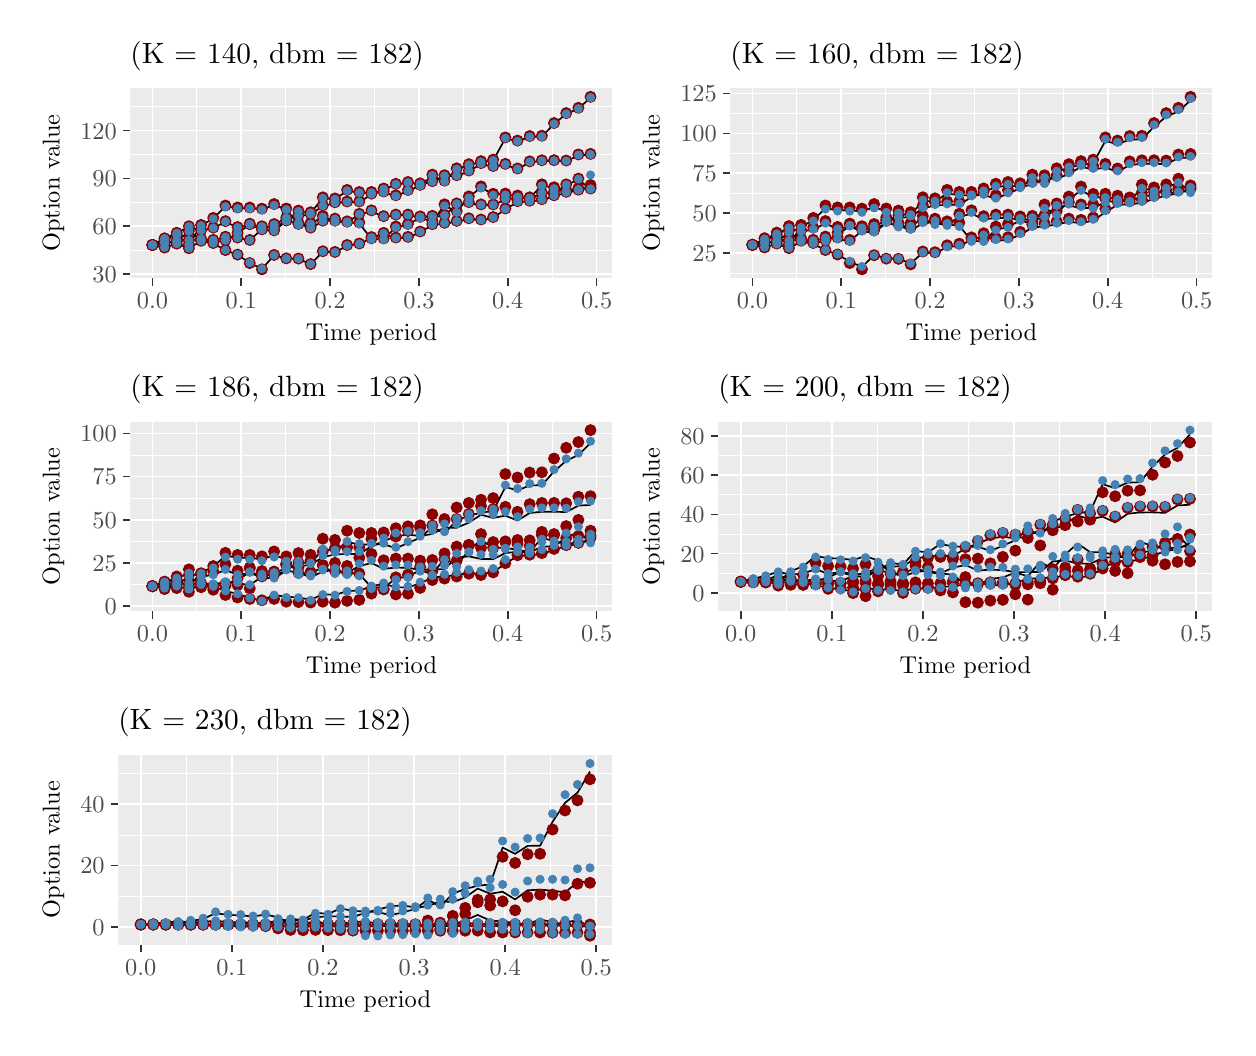
\begin{tikzpicture}[x=1pt,y=1pt]
\definecolor{fillColor}{RGB}{255,255,255}
\path[use as bounding box,fill=fillColor,fill opacity=0.00] (0,0) rectangle (433.62,361.35);
\begin{scope}
\path[clip] (  0.00,240.90) rectangle (216.81,361.35);
\definecolor{drawColor}{RGB}{255,255,255}
\definecolor{fillColor}{RGB}{255,255,255}

\path[draw=drawColor,line width= 0.6pt,line join=round,line cap=round,fill=fillColor] (  0.00,240.90) rectangle (216.81,361.35);
\end{scope}
\begin{scope}
\path[clip] ( 37.15,270.92) rectangle (211.31,339.48);
\definecolor{fillColor}{gray}{0.92}

\path[fill=fillColor] ( 37.15,270.92) rectangle (211.31,339.48);
\definecolor{drawColor}{RGB}{255,255,255}

\path[draw=drawColor,line width= 0.3pt,line join=round] ( 37.15,280.94) --
	(211.31,280.94);

\path[draw=drawColor,line width= 0.3pt,line join=round] ( 37.15,298.22) --
	(211.31,298.22);

\path[draw=drawColor,line width= 0.3pt,line join=round] ( 37.15,315.51) --
	(211.31,315.51);

\path[draw=drawColor,line width= 0.3pt,line join=round] ( 37.15,332.79) --
	(211.31,332.79);

\path[draw=drawColor,line width= 0.3pt,line join=round] ( 61.12,270.92) --
	( 61.12,339.48);

\path[draw=drawColor,line width= 0.3pt,line join=round] ( 93.23,270.92) --
	( 93.23,339.48);

\path[draw=drawColor,line width= 0.3pt,line join=round] (125.33,270.92) --
	(125.33,339.48);

\path[draw=drawColor,line width= 0.3pt,line join=round] (157.44,270.92) --
	(157.44,339.48);

\path[draw=drawColor,line width= 0.3pt,line join=round] (189.54,270.92) --
	(189.54,339.48);

\path[draw=drawColor,line width= 0.6pt,line join=round] ( 37.15,272.30) --
	(211.31,272.30);

\path[draw=drawColor,line width= 0.6pt,line join=round] ( 37.15,289.58) --
	(211.31,289.58);

\path[draw=drawColor,line width= 0.6pt,line join=round] ( 37.15,306.87) --
	(211.31,306.87);

\path[draw=drawColor,line width= 0.6pt,line join=round] ( 37.15,324.15) --
	(211.31,324.15);

\path[draw=drawColor,line width= 0.6pt,line join=round] ( 45.07,270.92) --
	( 45.07,339.48);

\path[draw=drawColor,line width= 0.6pt,line join=round] ( 77.17,270.92) --
	( 77.17,339.48);

\path[draw=drawColor,line width= 0.6pt,line join=round] (109.28,270.92) --
	(109.28,339.48);

\path[draw=drawColor,line width= 0.6pt,line join=round] (141.38,270.92) --
	(141.38,339.48);

\path[draw=drawColor,line width= 0.6pt,line join=round] (173.49,270.92) --
	(173.49,339.48);

\path[draw=drawColor,line width= 0.6pt,line join=round] (205.59,270.92) --
	(205.59,339.48);
\definecolor{drawColor}{RGB}{0,0,0}

\path[draw=drawColor,line width= 0.6pt,line join=round] ( 45.07,282.83) --
	( 49.47,285.05) --
	( 53.86,286.39) --
	( 58.26,282.93) --
	( 62.66,289.88) --
	( 67.06,292.38) --
	( 71.46,296.82) --
	( 75.85,296.12) --
	( 80.25,296.11) --
	( 84.65,295.68) --
	( 89.05,297.32) --
	( 93.45,295.74) --
	( 97.84,290.18) --
	(102.24,290.51) --
	(106.64,293.04) --
	(111.04,291.30) --
	(115.43,290.98) --
	(119.83,290.65) --
	(124.23,284.96) --
	(128.63,284.91) --
	(133.03,289.21) --
	(137.42,290.15) --
	(141.82,292.70) --
	(146.22,291.26) --
	(150.62,297.20) --
	(155.02,294.78) --
	(159.41,300.06) --
	(163.81,303.67) --
	(168.21,301.01) --
	(172.61,301.09) --
	(177.01,300.38) --
	(181.40,299.72) --
	(185.80,304.43) --
	(190.20,303.38) --
	(194.60,302.36) --
	(199.00,303.06) --
	(203.39,303.24);

\path[draw=drawColor,line width= 0.6pt,line join=round] ( 45.07,282.83) --
	( 49.47,285.14) --
	( 53.86,287.11) --
	( 58.26,289.42) --
	( 62.66,288.05) --
	( 67.06,288.91) --
	( 71.46,291.21) --
	( 75.85,289.10) --
	( 80.25,290.12) --
	( 84.65,288.25) --
	( 89.05,287.89) --
	( 93.45,291.47) --
	( 97.84,294.96) --
	(102.24,294.38) --
	(106.64,299.74) --
	(111.04,299.35) --
	(115.43,302.42) --
	(119.83,301.67) --
	(124.23,301.68) --
	(128.63,301.84) --
	(133.03,300.49) --
	(137.42,302.38) --
	(141.82,304.23) --
	(146.22,307.93) --
	(150.62,305.77) --
	(155.02,310.22) --
	(159.41,311.73) --
	(163.81,312.80) --
	(168.21,313.35) --
	(172.61,321.38) --
	(177.01,320.24) --
	(181.40,321.89) --
	(185.80,321.99) --
	(190.20,326.57) --
	(194.60,330.16) --
	(199.00,332.09) --
	(203.39,336.06);

\path[draw=drawColor,line width= 0.6pt,line join=round] ( 45.07,282.83) --
	( 49.47,283.93) --
	( 53.86,284.09) --
	( 58.26,287.74) --
	( 62.66,284.73) --
	( 67.06,283.76) --
	( 71.46,284.47) --
	( 75.85,287.03) --
	( 80.25,290.27) --
	( 84.65,289.35) --
	( 89.05,289.14) --
	( 93.45,291.44) --
	( 97.84,290.62) --
	(102.24,288.84) --
	(106.64,291.32) --
	(111.04,292.05) --
	(115.43,291.05) --
	(119.83,293.80) --
	(124.23,295.04) --
	(128.63,292.94) --
	(133.03,293.52) --
	(137.42,293.50) --
	(141.82,292.85) --
	(146.22,293.06) --
	(150.62,293.38) --
	(155.02,297.54) --
	(159.41,298.01) --
	(163.81,297.19) --
	(168.21,297.17) --
	(172.61,299.30) --
	(177.01,299.76) --
	(181.40,299.64) --
	(185.80,301.43) --
	(190.20,301.76) --
	(194.60,304.42) --
	(199.00,306.49) --
	(203.39,302.91);

\path[draw=drawColor,line width= 0.6pt,line join=round] ( 45.07,282.83) --
	( 49.47,283.40) --
	( 53.86,284.45) --
	( 58.26,284.51) --
	( 62.66,285.00) --
	( 67.06,284.55) --
	( 71.46,285.66) --
	( 75.85,285.34) --
	( 80.25,284.48) --
	( 84.65,288.60) --
	( 89.05,290.12) --
	( 93.45,292.52) --
	( 97.84,293.26) --
	(102.24,293.85) --
	(106.64,296.87) --
	(111.04,297.97) --
	(115.43,298.23) --
	(119.83,298.27) --
	(124.23,301.09) --
	(128.63,302.92) --
	(133.03,304.63) --
	(137.42,305.28) --
	(141.82,304.80) --
	(146.22,305.57) --
	(150.62,307.73) --
	(155.02,307.72) --
	(159.41,309.43) --
	(163.81,312.10) --
	(168.21,311.05) --
	(172.61,311.83) --
	(177.01,310.17) --
	(181.40,312.73) --
	(185.80,313.14) --
	(190.20,313.16) --
	(194.60,313.04) --
	(199.00,315.23) --
	(203.39,315.42);

\path[draw=drawColor,line width= 0.6pt,line join=round] ( 45.07,282.83) --
	( 49.47,281.89) --
	( 53.86,283.25) --
	( 58.26,281.63) --
	( 62.66,284.23) --
	( 67.06,283.42) --
	( 71.46,280.91) --
	( 75.85,279.32) --
	( 80.25,276.34) --
	( 84.65,274.16) --
	( 89.05,279.13) --
	( 93.45,277.91) --
	( 97.84,277.82) --
	(102.24,275.85) --
	(106.64,280.38) --
	(111.04,280.12) --
	(115.43,282.58) --
	(119.83,283.12) --
	(124.23,285.40) --
	(128.63,286.90) --
	(133.03,285.22) --
	(137.42,285.46) --
	(141.82,287.40) --
	(146.22,290.03) --
	(150.62,290.52) --
	(155.02,291.22) --
	(159.41,292.17) --
	(163.81,291.73) --
	(168.21,292.61) --
	(172.61,295.69) --
	(177.01,298.34) --
	(181.40,298.52) --
	(185.80,299.05) --
	(190.20,300.46) --
	(194.60,301.73) --
	(199.00,302.49) --
	(203.39,304.18);
\definecolor{drawColor}{RGB}{139,0,0}
\definecolor{fillColor}{RGB}{139,0,0}

\path[draw=drawColor,line width= 0.4pt,line join=round,line cap=round,fill=fillColor] ( 45.07,282.83) circle (  1.96);

\path[draw=drawColor,line width= 0.4pt,line join=round,line cap=round,fill=fillColor] ( 49.47,285.12) circle (  1.96);

\path[draw=drawColor,line width= 0.4pt,line join=round,line cap=round,fill=fillColor] ( 53.86,286.51) circle (  1.96);

\path[draw=drawColor,line width= 0.4pt,line join=round,line cap=round,fill=fillColor] ( 58.26,282.99) circle (  1.96);

\path[draw=drawColor,line width= 0.4pt,line join=round,line cap=round,fill=fillColor] ( 62.66,290.07) circle (  1.96);

\path[draw=drawColor,line width= 0.4pt,line join=round,line cap=round,fill=fillColor] ( 67.06,292.60) circle (  1.96);

\path[draw=drawColor,line width= 0.4pt,line join=round,line cap=round,fill=fillColor] ( 71.46,297.08) circle (  1.96);

\path[draw=drawColor,line width= 0.4pt,line join=round,line cap=round,fill=fillColor] ( 75.85,296.38) circle (  1.96);

\path[draw=drawColor,line width= 0.4pt,line join=round,line cap=round,fill=fillColor] ( 80.25,296.37) circle (  1.96);

\path[draw=drawColor,line width= 0.4pt,line join=round,line cap=round,fill=fillColor] ( 84.65,295.95) circle (  1.96);

\path[draw=drawColor,line width= 0.4pt,line join=round,line cap=round,fill=fillColor] ( 89.05,297.60) circle (  1.96);

\path[draw=drawColor,line width= 0.4pt,line join=round,line cap=round,fill=fillColor] ( 93.45,296.02) circle (  1.96);

\path[draw=drawColor,line width= 0.4pt,line join=round,line cap=round,fill=fillColor] ( 97.84,290.43) circle (  1.96);

\path[draw=drawColor,line width= 0.4pt,line join=round,line cap=round,fill=fillColor] (102.24,290.78) circle (  1.96);

\path[draw=drawColor,line width= 0.4pt,line join=round,line cap=round,fill=fillColor] (106.64,293.32) circle (  1.96);

\path[draw=drawColor,line width= 0.4pt,line join=round,line cap=round,fill=fillColor] (111.04,291.58) circle (  1.96);

\path[draw=drawColor,line width= 0.4pt,line join=round,line cap=round,fill=fillColor] (115.43,291.26) circle (  1.96);

\path[draw=drawColor,line width= 0.4pt,line join=round,line cap=round,fill=fillColor] (119.83,290.94) circle (  1.96);

\path[draw=drawColor,line width= 0.4pt,line join=round,line cap=round,fill=fillColor] (124.23,285.23) circle (  1.96);

\path[draw=drawColor,line width= 0.4pt,line join=round,line cap=round,fill=fillColor] (128.63,285.19) circle (  1.96);

\path[draw=drawColor,line width= 0.4pt,line join=round,line cap=round,fill=fillColor] (133.03,289.50) circle (  1.96);

\path[draw=drawColor,line width= 0.4pt,line join=round,line cap=round,fill=fillColor] (137.42,290.44) circle (  1.96);

\path[draw=drawColor,line width= 0.4pt,line join=round,line cap=round,fill=fillColor] (141.82,293.00) circle (  1.96);

\path[draw=drawColor,line width= 0.4pt,line join=round,line cap=round,fill=fillColor] (146.22,291.56) circle (  1.96);

\path[draw=drawColor,line width= 0.4pt,line join=round,line cap=round,fill=fillColor] (150.62,297.50) circle (  1.96);

\path[draw=drawColor,line width= 0.4pt,line join=round,line cap=round,fill=fillColor] (155.02,295.08) circle (  1.96);

\path[draw=drawColor,line width= 0.4pt,line join=round,line cap=round,fill=fillColor] (159.41,300.37) circle (  1.96);

\path[draw=drawColor,line width= 0.4pt,line join=round,line cap=round,fill=fillColor] (163.81,303.98) circle (  1.96);

\path[draw=drawColor,line width= 0.4pt,line join=round,line cap=round,fill=fillColor] (168.21,301.32) circle (  1.96);

\path[draw=drawColor,line width= 0.4pt,line join=round,line cap=round,fill=fillColor] (172.61,301.39) circle (  1.96);

\path[draw=drawColor,line width= 0.4pt,line join=round,line cap=round,fill=fillColor] (177.01,300.69) circle (  1.96);

\path[draw=drawColor,line width= 0.4pt,line join=round,line cap=round,fill=fillColor] (181.40,300.02) circle (  1.96);

\path[draw=drawColor,line width= 0.4pt,line join=round,line cap=round,fill=fillColor] (185.80,304.74) circle (  1.96);

\path[draw=drawColor,line width= 0.4pt,line join=round,line cap=round,fill=fillColor] (190.20,303.68) circle (  1.96);

\path[draw=drawColor,line width= 0.4pt,line join=round,line cap=round,fill=fillColor] (194.60,302.66) circle (  1.96);

\path[draw=drawColor,line width= 0.4pt,line join=round,line cap=round,fill=fillColor] (199.00,303.37) circle (  1.96);

\path[draw=drawColor,line width= 0.4pt,line join=round,line cap=round,fill=fillColor] (203.39,303.55) circle (  1.96);

\path[draw=drawColor,line width= 0.4pt,line join=round,line cap=round,fill=fillColor] ( 45.07,282.83) circle (  1.96);

\path[draw=drawColor,line width= 0.4pt,line join=round,line cap=round,fill=fillColor] ( 49.47,285.22) circle (  1.96);

\path[draw=drawColor,line width= 0.4pt,line join=round,line cap=round,fill=fillColor] ( 53.86,287.24) circle (  1.96);

\path[draw=drawColor,line width= 0.4pt,line join=round,line cap=round,fill=fillColor] ( 58.26,289.60) circle (  1.96);

\path[draw=drawColor,line width= 0.4pt,line join=round,line cap=round,fill=fillColor] ( 62.66,288.22) circle (  1.96);

\path[draw=drawColor,line width= 0.4pt,line join=round,line cap=round,fill=fillColor] ( 67.06,289.10) circle (  1.96);

\path[draw=drawColor,line width= 0.4pt,line join=round,line cap=round,fill=fillColor] ( 71.46,291.43) circle (  1.96);

\path[draw=drawColor,line width= 0.4pt,line join=round,line cap=round,fill=fillColor] ( 75.85,289.31) circle (  1.96);

\path[draw=drawColor,line width= 0.4pt,line join=round,line cap=round,fill=fillColor] ( 80.25,290.34) circle (  1.96);

\path[draw=drawColor,line width= 0.4pt,line join=round,line cap=round,fill=fillColor] ( 84.65,288.47) circle (  1.96);

\path[draw=drawColor,line width= 0.4pt,line join=round,line cap=round,fill=fillColor] ( 89.05,288.11) circle (  1.96);

\path[draw=drawColor,line width= 0.4pt,line join=round,line cap=round,fill=fillColor] ( 93.45,291.73) circle (  1.96);

\path[draw=drawColor,line width= 0.4pt,line join=round,line cap=round,fill=fillColor] ( 97.84,295.24) circle (  1.96);

\path[draw=drawColor,line width= 0.4pt,line join=round,line cap=round,fill=fillColor] (102.24,294.66) circle (  1.96);

\path[draw=drawColor,line width= 0.4pt,line join=round,line cap=round,fill=fillColor] (106.64,300.03) circle (  1.96);

\path[draw=drawColor,line width= 0.4pt,line join=round,line cap=round,fill=fillColor] (111.04,299.64) circle (  1.96);

\path[draw=drawColor,line width= 0.4pt,line join=round,line cap=round,fill=fillColor] (115.43,302.72) circle (  1.96);

\path[draw=drawColor,line width= 0.4pt,line join=round,line cap=round,fill=fillColor] (119.83,301.97) circle (  1.96);

\path[draw=drawColor,line width= 0.4pt,line join=round,line cap=round,fill=fillColor] (124.23,301.98) circle (  1.96);

\path[draw=drawColor,line width= 0.4pt,line join=round,line cap=round,fill=fillColor] (128.63,302.14) circle (  1.96);

\path[draw=drawColor,line width= 0.4pt,line join=round,line cap=round,fill=fillColor] (133.03,300.79) circle (  1.96);

\path[draw=drawColor,line width= 0.4pt,line join=round,line cap=round,fill=fillColor] (137.42,302.68) circle (  1.96);

\path[draw=drawColor,line width= 0.4pt,line join=round,line cap=round,fill=fillColor] (141.82,304.54) circle (  1.96);

\path[draw=drawColor,line width= 0.4pt,line join=round,line cap=round,fill=fillColor] (146.22,308.23) circle (  1.96);

\path[draw=drawColor,line width= 0.4pt,line join=round,line cap=round,fill=fillColor] (150.62,306.07) circle (  1.96);

\path[draw=drawColor,line width= 0.4pt,line join=round,line cap=round,fill=fillColor] (155.02,310.52) circle (  1.96);

\path[draw=drawColor,line width= 0.4pt,line join=round,line cap=round,fill=fillColor] (159.41,312.03) circle (  1.96);

\path[draw=drawColor,line width= 0.4pt,line join=round,line cap=round,fill=fillColor] (163.81,313.11) circle (  1.96);

\path[draw=drawColor,line width= 0.4pt,line join=round,line cap=round,fill=fillColor] (168.21,313.66) circle (  1.96);

\path[draw=drawColor,line width= 0.4pt,line join=round,line cap=round,fill=fillColor] (172.61,321.68) circle (  1.96);

\path[draw=drawColor,line width= 0.4pt,line join=round,line cap=round,fill=fillColor] (177.01,320.54) circle (  1.96);

\path[draw=drawColor,line width= 0.4pt,line join=round,line cap=round,fill=fillColor] (181.40,322.19) circle (  1.96);

\path[draw=drawColor,line width= 0.4pt,line join=round,line cap=round,fill=fillColor] (185.80,322.30) circle (  1.96);

\path[draw=drawColor,line width= 0.4pt,line join=round,line cap=round,fill=fillColor] (190.20,326.88) circle (  1.96);

\path[draw=drawColor,line width= 0.4pt,line join=round,line cap=round,fill=fillColor] (194.60,330.47) circle (  1.96);

\path[draw=drawColor,line width= 0.4pt,line join=round,line cap=round,fill=fillColor] (199.00,332.39) circle (  1.96);

\path[draw=drawColor,line width= 0.4pt,line join=round,line cap=round,fill=fillColor] (203.39,336.36) circle (  1.96);

\path[draw=drawColor,line width= 0.4pt,line join=round,line cap=round,fill=fillColor] ( 45.07,282.83) circle (  1.96);

\path[draw=drawColor,line width= 0.4pt,line join=round,line cap=round,fill=fillColor] ( 49.47,283.98) circle (  1.96);

\path[draw=drawColor,line width= 0.4pt,line join=round,line cap=round,fill=fillColor] ( 53.86,284.16) circle (  1.96);

\path[draw=drawColor,line width= 0.4pt,line join=round,line cap=round,fill=fillColor] ( 58.26,287.89) circle (  1.96);

\path[draw=drawColor,line width= 0.4pt,line join=round,line cap=round,fill=fillColor] ( 62.66,284.85) circle (  1.96);

\path[draw=drawColor,line width= 0.4pt,line join=round,line cap=round,fill=fillColor] ( 67.06,283.87) circle (  1.96);

\path[draw=drawColor,line width= 0.4pt,line join=round,line cap=round,fill=fillColor] ( 71.46,284.60) circle (  1.96);

\path[draw=drawColor,line width= 0.4pt,line join=round,line cap=round,fill=fillColor] ( 75.85,287.21) circle (  1.96);

\path[draw=drawColor,line width= 0.4pt,line join=round,line cap=round,fill=fillColor] ( 80.25,290.50) circle (  1.96);

\path[draw=drawColor,line width= 0.4pt,line join=round,line cap=round,fill=fillColor] ( 84.65,289.58) circle (  1.96);

\path[draw=drawColor,line width= 0.4pt,line join=round,line cap=round,fill=fillColor] ( 89.05,289.38) circle (  1.96);

\path[draw=drawColor,line width= 0.4pt,line join=round,line cap=round,fill=fillColor] ( 93.45,291.70) circle (  1.96);

\path[draw=drawColor,line width= 0.4pt,line join=round,line cap=round,fill=fillColor] ( 97.84,290.88) circle (  1.96);

\path[draw=drawColor,line width= 0.4pt,line join=round,line cap=round,fill=fillColor] (102.24,289.09) circle (  1.96);

\path[draw=drawColor,line width= 0.4pt,line join=round,line cap=round,fill=fillColor] (106.64,291.59) circle (  1.96);

\path[draw=drawColor,line width= 0.4pt,line join=round,line cap=round,fill=fillColor] (111.04,292.33) circle (  1.96);

\path[draw=drawColor,line width= 0.4pt,line join=round,line cap=round,fill=fillColor] (115.43,291.33) circle (  1.96);

\path[draw=drawColor,line width= 0.4pt,line join=round,line cap=round,fill=fillColor] (119.83,294.09) circle (  1.96);

\path[draw=drawColor,line width= 0.4pt,line join=round,line cap=round,fill=fillColor] (124.23,295.33) circle (  1.96);

\path[draw=drawColor,line width= 0.4pt,line join=round,line cap=round,fill=fillColor] (128.63,293.24) circle (  1.96);

\path[draw=drawColor,line width= 0.4pt,line join=round,line cap=round,fill=fillColor] (133.03,293.81) circle (  1.96);

\path[draw=drawColor,line width= 0.4pt,line join=round,line cap=round,fill=fillColor] (137.42,293.80) circle (  1.96);

\path[draw=drawColor,line width= 0.4pt,line join=round,line cap=round,fill=fillColor] (141.82,293.15) circle (  1.96);

\path[draw=drawColor,line width= 0.4pt,line join=round,line cap=round,fill=fillColor] (146.22,293.36) circle (  1.96);

\path[draw=drawColor,line width= 0.4pt,line join=round,line cap=round,fill=fillColor] (150.62,293.69) circle (  1.96);

\path[draw=drawColor,line width= 0.4pt,line join=round,line cap=round,fill=fillColor] (155.02,297.84) circle (  1.96);

\path[draw=drawColor,line width= 0.4pt,line join=round,line cap=round,fill=fillColor] (159.41,298.32) circle (  1.96);

\path[draw=drawColor,line width= 0.4pt,line join=round,line cap=round,fill=fillColor] (163.81,297.49) circle (  1.96);

\path[draw=drawColor,line width= 0.4pt,line join=round,line cap=round,fill=fillColor] (168.21,297.48) circle (  1.96);

\path[draw=drawColor,line width= 0.4pt,line join=round,line cap=round,fill=fillColor] (172.61,299.60) circle (  1.96);

\path[draw=drawColor,line width= 0.4pt,line join=round,line cap=round,fill=fillColor] (177.01,300.06) circle (  1.96);

\path[draw=drawColor,line width= 0.4pt,line join=round,line cap=round,fill=fillColor] (181.40,299.94) circle (  1.96);

\path[draw=drawColor,line width= 0.4pt,line join=round,line cap=round,fill=fillColor] (185.80,301.73) circle (  1.96);

\path[draw=drawColor,line width= 0.4pt,line join=round,line cap=round,fill=fillColor] (190.20,302.06) circle (  1.96);

\path[draw=drawColor,line width= 0.4pt,line join=round,line cap=round,fill=fillColor] (194.60,304.73) circle (  1.96);

\path[draw=drawColor,line width= 0.4pt,line join=round,line cap=round,fill=fillColor] (199.00,306.80) circle (  1.96);

\path[draw=drawColor,line width= 0.4pt,line join=round,line cap=round,fill=fillColor] (203.39,303.21) circle (  1.96);

\path[draw=drawColor,line width= 0.4pt,line join=round,line cap=round,fill=fillColor] ( 45.07,282.83) circle (  1.96);

\path[draw=drawColor,line width= 0.4pt,line join=round,line cap=round,fill=fillColor] ( 49.47,283.44) circle (  1.96);

\path[draw=drawColor,line width= 0.4pt,line join=round,line cap=round,fill=fillColor] ( 53.86,284.53) circle (  1.96);

\path[draw=drawColor,line width= 0.4pt,line join=round,line cap=round,fill=fillColor] ( 58.26,284.60) circle (  1.96);

\path[draw=drawColor,line width= 0.4pt,line join=round,line cap=round,fill=fillColor] ( 62.66,285.12) circle (  1.96);

\path[draw=drawColor,line width= 0.4pt,line join=round,line cap=round,fill=fillColor] ( 67.06,284.68) circle (  1.96);

\path[draw=drawColor,line width= 0.4pt,line join=round,line cap=round,fill=fillColor] ( 71.46,285.81) circle (  1.96);

\path[draw=drawColor,line width= 0.4pt,line join=round,line cap=round,fill=fillColor] ( 75.85,285.50) circle (  1.96);

\path[draw=drawColor,line width= 0.4pt,line join=round,line cap=round,fill=fillColor] ( 80.25,284.64) circle (  1.96);

\path[draw=drawColor,line width= 0.4pt,line join=round,line cap=round,fill=fillColor] ( 84.65,288.82) circle (  1.96);

\path[draw=drawColor,line width= 0.4pt,line join=round,line cap=round,fill=fillColor] ( 89.05,290.37) circle (  1.96);

\path[draw=drawColor,line width= 0.4pt,line join=round,line cap=round,fill=fillColor] ( 93.45,292.78) circle (  1.96);

\path[draw=drawColor,line width= 0.4pt,line join=round,line cap=round,fill=fillColor] ( 97.84,293.53) circle (  1.96);

\path[draw=drawColor,line width= 0.4pt,line join=round,line cap=round,fill=fillColor] (102.24,294.13) circle (  1.96);

\path[draw=drawColor,line width= 0.4pt,line join=round,line cap=round,fill=fillColor] (106.64,297.16) circle (  1.96);

\path[draw=drawColor,line width= 0.4pt,line join=round,line cap=round,fill=fillColor] (111.04,298.26) circle (  1.96);

\path[draw=drawColor,line width= 0.4pt,line join=round,line cap=round,fill=fillColor] (115.43,298.53) circle (  1.96);

\path[draw=drawColor,line width= 0.4pt,line join=round,line cap=round,fill=fillColor] (119.83,298.56) circle (  1.96);

\path[draw=drawColor,line width= 0.4pt,line join=round,line cap=round,fill=fillColor] (124.23,301.39) circle (  1.96);

\path[draw=drawColor,line width= 0.4pt,line join=round,line cap=round,fill=fillColor] (128.63,303.22) circle (  1.96);

\path[draw=drawColor,line width= 0.4pt,line join=round,line cap=round,fill=fillColor] (133.03,304.93) circle (  1.96);

\path[draw=drawColor,line width= 0.4pt,line join=round,line cap=round,fill=fillColor] (137.42,305.58) circle (  1.96);

\path[draw=drawColor,line width= 0.4pt,line join=round,line cap=round,fill=fillColor] (141.82,305.11) circle (  1.96);

\path[draw=drawColor,line width= 0.4pt,line join=round,line cap=round,fill=fillColor] (146.22,305.88) circle (  1.96);

\path[draw=drawColor,line width= 0.4pt,line join=round,line cap=round,fill=fillColor] (150.62,308.03) circle (  1.96);

\path[draw=drawColor,line width= 0.4pt,line join=round,line cap=round,fill=fillColor] (155.02,308.03) circle (  1.96);

\path[draw=drawColor,line width= 0.4pt,line join=round,line cap=round,fill=fillColor] (159.41,309.73) circle (  1.96);

\path[draw=drawColor,line width= 0.4pt,line join=round,line cap=round,fill=fillColor] (163.81,312.40) circle (  1.96);

\path[draw=drawColor,line width= 0.4pt,line join=round,line cap=round,fill=fillColor] (168.21,311.35) circle (  1.96);

\path[draw=drawColor,line width= 0.4pt,line join=round,line cap=round,fill=fillColor] (172.61,312.13) circle (  1.96);

\path[draw=drawColor,line width= 0.4pt,line join=round,line cap=round,fill=fillColor] (177.01,310.47) circle (  1.96);

\path[draw=drawColor,line width= 0.4pt,line join=round,line cap=round,fill=fillColor] (181.40,313.03) circle (  1.96);

\path[draw=drawColor,line width= 0.4pt,line join=round,line cap=round,fill=fillColor] (185.80,313.44) circle (  1.96);

\path[draw=drawColor,line width= 0.4pt,line join=round,line cap=round,fill=fillColor] (190.20,313.47) circle (  1.96);

\path[draw=drawColor,line width= 0.4pt,line join=round,line cap=round,fill=fillColor] (194.60,313.34) circle (  1.96);

\path[draw=drawColor,line width= 0.4pt,line join=round,line cap=round,fill=fillColor] (199.00,315.53) circle (  1.96);

\path[draw=drawColor,line width= 0.4pt,line join=round,line cap=round,fill=fillColor] (203.39,315.73) circle (  1.96);

\path[draw=drawColor,line width= 0.4pt,line join=round,line cap=round,fill=fillColor] ( 45.07,282.83) circle (  1.96);

\path[draw=drawColor,line width= 0.4pt,line join=round,line cap=round,fill=fillColor] ( 49.47,281.88) circle (  1.96);

\path[draw=drawColor,line width= 0.4pt,line join=round,line cap=round,fill=fillColor] ( 53.86,283.30) circle (  1.96);

\path[draw=drawColor,line width= 0.4pt,line join=round,line cap=round,fill=fillColor] ( 58.26,281.65) circle (  1.96);

\path[draw=drawColor,line width= 0.4pt,line join=round,line cap=round,fill=fillColor] ( 62.66,284.33) circle (  1.96);

\path[draw=drawColor,line width= 0.4pt,line join=round,line cap=round,fill=fillColor] ( 67.06,283.52) circle (  1.96);

\path[draw=drawColor,line width= 0.4pt,line join=round,line cap=round,fill=fillColor] ( 71.46,280.97) circle (  1.96);

\path[draw=drawColor,line width= 0.4pt,line join=round,line cap=round,fill=fillColor] ( 75.85,279.35) circle (  1.96);

\path[draw=drawColor,line width= 0.4pt,line join=round,line cap=round,fill=fillColor] ( 80.25,276.29) circle (  1.96);

\path[draw=drawColor,line width= 0.4pt,line join=round,line cap=round,fill=fillColor] ( 84.65,274.03) circle (  1.96);

\path[draw=drawColor,line width= 0.4pt,line join=round,line cap=round,fill=fillColor] ( 89.05,279.22) circle (  1.96);

\path[draw=drawColor,line width= 0.4pt,line join=round,line cap=round,fill=fillColor] ( 93.45,277.98) circle (  1.96);

\path[draw=drawColor,line width= 0.4pt,line join=round,line cap=round,fill=fillColor] ( 97.84,277.91) circle (  1.96);

\path[draw=drawColor,line width= 0.4pt,line join=round,line cap=round,fill=fillColor] (102.24,275.91) circle (  1.96);

\path[draw=drawColor,line width= 0.4pt,line join=round,line cap=round,fill=fillColor] (106.64,280.56) circle (  1.96);

\path[draw=drawColor,line width= 0.4pt,line join=round,line cap=round,fill=fillColor] (111.04,280.31) circle (  1.96);

\path[draw=drawColor,line width= 0.4pt,line join=round,line cap=round,fill=fillColor] (115.43,282.82) circle (  1.96);

\path[draw=drawColor,line width= 0.4pt,line join=round,line cap=round,fill=fillColor] (119.83,283.37) circle (  1.96);

\path[draw=drawColor,line width= 0.4pt,line join=round,line cap=round,fill=fillColor] (124.23,285.67) circle (  1.96);

\path[draw=drawColor,line width= 0.4pt,line join=round,line cap=round,fill=fillColor] (128.63,287.19) circle (  1.96);

\path[draw=drawColor,line width= 0.4pt,line join=round,line cap=round,fill=fillColor] (133.03,285.51) circle (  1.96);

\path[draw=drawColor,line width= 0.4pt,line join=round,line cap=round,fill=fillColor] (137.42,285.75) circle (  1.96);

\path[draw=drawColor,line width= 0.4pt,line join=round,line cap=round,fill=fillColor] (141.82,287.69) circle (  1.96);

\path[draw=drawColor,line width= 0.4pt,line join=round,line cap=round,fill=fillColor] (146.22,290.33) circle (  1.96);

\path[draw=drawColor,line width= 0.4pt,line join=round,line cap=round,fill=fillColor] (150.62,290.83) circle (  1.96);

\path[draw=drawColor,line width= 0.4pt,line join=round,line cap=round,fill=fillColor] (155.02,291.52) circle (  1.96);

\path[draw=drawColor,line width= 0.4pt,line join=round,line cap=round,fill=fillColor] (159.41,292.47) circle (  1.96);

\path[draw=drawColor,line width= 0.4pt,line join=round,line cap=round,fill=fillColor] (163.81,292.03) circle (  1.96);

\path[draw=drawColor,line width= 0.4pt,line join=round,line cap=round,fill=fillColor] (168.21,292.92) circle (  1.96);

\path[draw=drawColor,line width= 0.4pt,line join=round,line cap=round,fill=fillColor] (172.61,296.00) circle (  1.96);

\path[draw=drawColor,line width= 0.4pt,line join=round,line cap=round,fill=fillColor] (177.01,298.65) circle (  1.96);

\path[draw=drawColor,line width= 0.4pt,line join=round,line cap=round,fill=fillColor] (181.40,298.82) circle (  1.96);

\path[draw=drawColor,line width= 0.4pt,line join=round,line cap=round,fill=fillColor] (185.80,299.36) circle (  1.96);

\path[draw=drawColor,line width= 0.4pt,line join=round,line cap=round,fill=fillColor] (190.20,300.77) circle (  1.96);

\path[draw=drawColor,line width= 0.4pt,line join=round,line cap=round,fill=fillColor] (194.60,302.03) circle (  1.96);

\path[draw=drawColor,line width= 0.4pt,line join=round,line cap=round,fill=fillColor] (199.00,302.79) circle (  1.96);

\path[draw=drawColor,line width= 0.4pt,line join=round,line cap=round,fill=fillColor] (203.39,304.49) circle (  1.96);
\definecolor{drawColor}{RGB}{70,130,180}
\definecolor{fillColor}{RGB}{70,130,180}

\path[draw=drawColor,line width= 0.4pt,line join=round,line cap=round,fill=fillColor] ( 45.07,282.83) circle (  1.43);

\path[draw=drawColor,line width= 0.4pt,line join=round,line cap=round,fill=fillColor] ( 49.47,285.04) circle (  1.43);

\path[draw=drawColor,line width= 0.4pt,line join=round,line cap=round,fill=fillColor] ( 53.86,286.38) circle (  1.43);

\path[draw=drawColor,line width= 0.4pt,line join=round,line cap=round,fill=fillColor] ( 58.26,282.98) circle (  1.43);

\path[draw=drawColor,line width= 0.4pt,line join=round,line cap=round,fill=fillColor] ( 62.66,289.79) circle (  1.43);

\path[draw=drawColor,line width= 0.4pt,line join=round,line cap=round,fill=fillColor] ( 67.06,292.28) circle (  1.43);

\path[draw=drawColor,line width= 0.4pt,line join=round,line cap=round,fill=fillColor] ( 71.46,296.70) circle (  1.43);

\path[draw=drawColor,line width= 0.4pt,line join=round,line cap=round,fill=fillColor] ( 75.85,296.00) circle (  1.43);

\path[draw=drawColor,line width= 0.4pt,line join=round,line cap=round,fill=fillColor] ( 80.25,295.99) circle (  1.43);

\path[draw=drawColor,line width= 0.4pt,line join=round,line cap=round,fill=fillColor] ( 84.65,295.57) circle (  1.43);

\path[draw=drawColor,line width= 0.4pt,line join=round,line cap=round,fill=fillColor] ( 89.05,297.19) circle (  1.43);

\path[draw=drawColor,line width= 0.4pt,line join=round,line cap=round,fill=fillColor] ( 93.45,295.62) circle (  1.43);

\path[draw=drawColor,line width= 0.4pt,line join=round,line cap=round,fill=fillColor] ( 97.84,290.11) circle (  1.43);

\path[draw=drawColor,line width= 0.4pt,line join=round,line cap=round,fill=fillColor] (102.24,290.43) circle (  1.43);

\path[draw=drawColor,line width= 0.4pt,line join=round,line cap=round,fill=fillColor] (106.64,292.91) circle (  1.43);

\path[draw=drawColor,line width= 0.4pt,line join=round,line cap=round,fill=fillColor] (111.04,291.18) circle (  1.43);

\path[draw=drawColor,line width= 0.4pt,line join=round,line cap=round,fill=fillColor] (115.43,290.86) circle (  1.43);

\path[draw=drawColor,line width= 0.4pt,line join=round,line cap=round,fill=fillColor] (119.83,290.53) circle (  1.43);

\path[draw=drawColor,line width= 0.4pt,line join=round,line cap=round,fill=fillColor] (124.23,284.89) circle (  1.43);

\path[draw=drawColor,line width= 0.4pt,line join=round,line cap=round,fill=fillColor] (128.63,284.85) circle (  1.43);

\path[draw=drawColor,line width= 0.4pt,line join=round,line cap=round,fill=fillColor] (133.03,289.14) circle (  1.43);

\path[draw=drawColor,line width= 0.4pt,line join=round,line cap=round,fill=fillColor] (137.42,290.08) circle (  1.43);

\path[draw=drawColor,line width= 0.4pt,line join=round,line cap=round,fill=fillColor] (141.82,292.51) circle (  1.43);

\path[draw=drawColor,line width= 0.4pt,line join=round,line cap=round,fill=fillColor] (146.22,291.07) circle (  1.43);

\path[draw=drawColor,line width= 0.4pt,line join=round,line cap=round,fill=fillColor] (150.62,297.01) circle (  1.43);

\path[draw=drawColor,line width= 0.4pt,line join=round,line cap=round,fill=fillColor] (155.02,294.59) circle (  1.43);

\path[draw=drawColor,line width= 0.4pt,line join=round,line cap=round,fill=fillColor] (159.41,299.88) circle (  1.43);

\path[draw=drawColor,line width= 0.4pt,line join=round,line cap=round,fill=fillColor] (163.81,303.48) circle (  1.43);

\path[draw=drawColor,line width= 0.4pt,line join=round,line cap=round,fill=fillColor] (168.21,300.82) circle (  1.43);

\path[draw=drawColor,line width= 0.4pt,line join=round,line cap=round,fill=fillColor] (172.61,300.90) circle (  1.43);

\path[draw=drawColor,line width= 0.4pt,line join=round,line cap=round,fill=fillColor] (177.01,300.19) circle (  1.43);

\path[draw=drawColor,line width= 0.4pt,line join=round,line cap=round,fill=fillColor] (181.40,299.53) circle (  1.43);

\path[draw=drawColor,line width= 0.4pt,line join=round,line cap=round,fill=fillColor] (185.80,304.24) circle (  1.43);

\path[draw=drawColor,line width= 0.4pt,line join=round,line cap=round,fill=fillColor] (190.20,303.19) circle (  1.43);

\path[draw=drawColor,line width= 0.4pt,line join=round,line cap=round,fill=fillColor] (194.60,302.17) circle (  1.43);

\path[draw=drawColor,line width= 0.4pt,line join=round,line cap=round,fill=fillColor] (199.00,302.87) circle (  1.43);

\path[draw=drawColor,line width= 0.4pt,line join=round,line cap=round,fill=fillColor] (203.39,303.05) circle (  1.43);

\path[draw=drawColor,line width= 0.4pt,line join=round,line cap=round,fill=fillColor] ( 45.07,282.83) circle (  1.43);

\path[draw=drawColor,line width= 0.4pt,line join=round,line cap=round,fill=fillColor] ( 49.47,285.15) circle (  1.43);

\path[draw=drawColor,line width= 0.4pt,line join=round,line cap=round,fill=fillColor] ( 53.86,287.12) circle (  1.43);

\path[draw=drawColor,line width= 0.4pt,line join=round,line cap=round,fill=fillColor] ( 58.26,289.45) circle (  1.43);

\path[draw=drawColor,line width= 0.4pt,line join=round,line cap=round,fill=fillColor] ( 62.66,288.09) circle (  1.43);

\path[draw=drawColor,line width= 0.4pt,line join=round,line cap=round,fill=fillColor] ( 67.06,288.94) circle (  1.43);

\path[draw=drawColor,line width= 0.4pt,line join=round,line cap=round,fill=fillColor] ( 71.46,291.25) circle (  1.43);

\path[draw=drawColor,line width= 0.4pt,line join=round,line cap=round,fill=fillColor] ( 75.85,289.15) circle (  1.43);

\path[draw=drawColor,line width= 0.4pt,line join=round,line cap=round,fill=fillColor] ( 80.25,290.17) circle (  1.43);

\path[draw=drawColor,line width= 0.4pt,line join=round,line cap=round,fill=fillColor] ( 84.65,288.30) circle (  1.43);

\path[draw=drawColor,line width= 0.4pt,line join=round,line cap=round,fill=fillColor] ( 89.05,287.89) circle (  1.43);

\path[draw=drawColor,line width= 0.4pt,line join=round,line cap=round,fill=fillColor] ( 93.45,291.48) circle (  1.43);

\path[draw=drawColor,line width= 0.4pt,line join=round,line cap=round,fill=fillColor] ( 97.84,294.97) circle (  1.43);

\path[draw=drawColor,line width= 0.4pt,line join=round,line cap=round,fill=fillColor] (102.24,294.40) circle (  1.43);

\path[draw=drawColor,line width= 0.4pt,line join=round,line cap=round,fill=fillColor] (106.64,299.75) circle (  1.43);

\path[draw=drawColor,line width= 0.4pt,line join=round,line cap=round,fill=fillColor] (111.04,299.36) circle (  1.43);

\path[draw=drawColor,line width= 0.4pt,line join=round,line cap=round,fill=fillColor] (115.43,302.44) circle (  1.43);

\path[draw=drawColor,line width= 0.4pt,line join=round,line cap=round,fill=fillColor] (119.83,301.69) circle (  1.43);

\path[draw=drawColor,line width= 0.4pt,line join=round,line cap=round,fill=fillColor] (124.23,301.70) circle (  1.43);

\path[draw=drawColor,line width= 0.4pt,line join=round,line cap=round,fill=fillColor] (128.63,301.86) circle (  1.43);

\path[draw=drawColor,line width= 0.4pt,line join=round,line cap=round,fill=fillColor] (133.03,300.51) circle (  1.43);

\path[draw=drawColor,line width= 0.4pt,line join=round,line cap=round,fill=fillColor] (137.42,302.40) circle (  1.43);

\path[draw=drawColor,line width= 0.4pt,line join=round,line cap=round,fill=fillColor] (141.82,304.25) circle (  1.43);

\path[draw=drawColor,line width= 0.4pt,line join=round,line cap=round,fill=fillColor] (146.22,307.95) circle (  1.43);

\path[draw=drawColor,line width= 0.4pt,line join=round,line cap=round,fill=fillColor] (150.62,305.79) circle (  1.43);

\path[draw=drawColor,line width= 0.4pt,line join=round,line cap=round,fill=fillColor] (155.02,310.24) circle (  1.43);

\path[draw=drawColor,line width= 0.4pt,line join=round,line cap=round,fill=fillColor] (159.41,311.75) circle (  1.43);

\path[draw=drawColor,line width= 0.4pt,line join=round,line cap=round,fill=fillColor] (163.81,312.82) circle (  1.43);

\path[draw=drawColor,line width= 0.4pt,line join=round,line cap=round,fill=fillColor] (168.21,313.38) circle (  1.43);

\path[draw=drawColor,line width= 0.4pt,line join=round,line cap=round,fill=fillColor] (172.61,321.40) circle (  1.43);

\path[draw=drawColor,line width= 0.4pt,line join=round,line cap=round,fill=fillColor] (177.01,320.26) circle (  1.43);

\path[draw=drawColor,line width= 0.4pt,line join=round,line cap=round,fill=fillColor] (181.40,321.91) circle (  1.43);

\path[draw=drawColor,line width= 0.4pt,line join=round,line cap=round,fill=fillColor] (185.80,322.01) circle (  1.43);

\path[draw=drawColor,line width= 0.4pt,line join=round,line cap=round,fill=fillColor] (190.20,326.60) circle (  1.43);

\path[draw=drawColor,line width= 0.4pt,line join=round,line cap=round,fill=fillColor] (194.60,330.18) circle (  1.43);

\path[draw=drawColor,line width= 0.4pt,line join=round,line cap=round,fill=fillColor] (199.00,332.10) circle (  1.43);

\path[draw=drawColor,line width= 0.4pt,line join=round,line cap=round,fill=fillColor] (203.39,336.08) circle (  1.43);

\path[draw=drawColor,line width= 0.4pt,line join=round,line cap=round,fill=fillColor] ( 45.07,282.83) circle (  1.43);

\path[draw=drawColor,line width= 0.4pt,line join=round,line cap=round,fill=fillColor] ( 49.47,283.95) circle (  1.43);

\path[draw=drawColor,line width= 0.4pt,line join=round,line cap=round,fill=fillColor] ( 53.86,284.11) circle (  1.43);

\path[draw=drawColor,line width= 0.4pt,line join=round,line cap=round,fill=fillColor] ( 58.26,287.77) circle (  1.43);

\path[draw=drawColor,line width= 0.4pt,line join=round,line cap=round,fill=fillColor] ( 62.66,284.76) circle (  1.43);

\path[draw=drawColor,line width= 0.4pt,line join=round,line cap=round,fill=fillColor] ( 67.06,283.79) circle (  1.43);

\path[draw=drawColor,line width= 0.4pt,line join=round,line cap=round,fill=fillColor] ( 71.46,284.51) circle (  1.43);

\path[draw=drawColor,line width= 0.4pt,line join=round,line cap=round,fill=fillColor] ( 75.85,287.10) circle (  1.43);

\path[draw=drawColor,line width= 0.4pt,line join=round,line cap=round,fill=fillColor] ( 80.25,290.36) circle (  1.43);

\path[draw=drawColor,line width= 0.4pt,line join=round,line cap=round,fill=fillColor] ( 84.65,289.44) circle (  1.43);

\path[draw=drawColor,line width= 0.4pt,line join=round,line cap=round,fill=fillColor] ( 89.05,289.25) circle (  1.43);

\path[draw=drawColor,line width= 0.4pt,line join=round,line cap=round,fill=fillColor] ( 93.45,291.56) circle (  1.43);

\path[draw=drawColor,line width= 0.4pt,line join=round,line cap=round,fill=fillColor] ( 97.84,290.74) circle (  1.43);

\path[draw=drawColor,line width= 0.4pt,line join=round,line cap=round,fill=fillColor] (102.24,288.96) circle (  1.43);

\path[draw=drawColor,line width= 0.4pt,line join=round,line cap=round,fill=fillColor] (106.64,291.45) circle (  1.43);

\path[draw=drawColor,line width= 0.4pt,line join=round,line cap=round,fill=fillColor] (111.04,292.18) circle (  1.43);

\path[draw=drawColor,line width= 0.4pt,line join=round,line cap=round,fill=fillColor] (115.43,291.19) circle (  1.43);

\path[draw=drawColor,line width= 0.4pt,line join=round,line cap=round,fill=fillColor] (119.83,293.94) circle (  1.43);

\path[draw=drawColor,line width= 0.4pt,line join=round,line cap=round,fill=fillColor] (124.23,295.19) circle (  1.43);

\path[draw=drawColor,line width= 0.4pt,line join=round,line cap=round,fill=fillColor] (128.63,293.10) circle (  1.43);

\path[draw=drawColor,line width= 0.4pt,line join=round,line cap=round,fill=fillColor] (133.03,293.67) circle (  1.43);

\path[draw=drawColor,line width= 0.4pt,line join=round,line cap=round,fill=fillColor] (137.42,293.66) circle (  1.43);

\path[draw=drawColor,line width= 0.4pt,line join=round,line cap=round,fill=fillColor] (141.82,293.01) circle (  1.43);

\path[draw=drawColor,line width= 0.4pt,line join=round,line cap=round,fill=fillColor] (146.22,293.21) circle (  1.43);

\path[draw=drawColor,line width= 0.4pt,line join=round,line cap=round,fill=fillColor] (150.62,293.54) circle (  1.43);

\path[draw=drawColor,line width= 0.4pt,line join=round,line cap=round,fill=fillColor] (155.02,297.70) circle (  1.43);

\path[draw=drawColor,line width= 0.4pt,line join=round,line cap=round,fill=fillColor] (159.41,298.17) circle (  1.43);

\path[draw=drawColor,line width= 0.4pt,line join=round,line cap=round,fill=fillColor] (163.81,297.35) circle (  1.43);

\path[draw=drawColor,line width= 0.4pt,line join=round,line cap=round,fill=fillColor] (168.21,297.34) circle (  1.43);

\path[draw=drawColor,line width= 0.4pt,line join=round,line cap=round,fill=fillColor] (172.61,299.46) circle (  1.43);

\path[draw=drawColor,line width= 0.4pt,line join=round,line cap=round,fill=fillColor] (177.01,299.92) circle (  1.43);

\path[draw=drawColor,line width= 0.4pt,line join=round,line cap=round,fill=fillColor] (181.40,299.80) circle (  1.43);

\path[draw=drawColor,line width= 0.4pt,line join=round,line cap=round,fill=fillColor] (185.80,301.59) circle (  1.43);

\path[draw=drawColor,line width= 0.4pt,line join=round,line cap=round,fill=fillColor] (190.20,301.92) circle (  1.43);

\path[draw=drawColor,line width= 0.4pt,line join=round,line cap=round,fill=fillColor] (194.60,304.58) circle (  1.43);

\path[draw=drawColor,line width= 0.4pt,line join=round,line cap=round,fill=fillColor] (199.00,306.66) circle (  1.43);

\path[draw=drawColor,line width= 0.4pt,line join=round,line cap=round,fill=fillColor] (203.39,303.08) circle (  1.43);

\path[draw=drawColor,line width= 0.4pt,line join=round,line cap=round,fill=fillColor] ( 45.07,282.83) circle (  1.43);

\path[draw=drawColor,line width= 0.4pt,line join=round,line cap=round,fill=fillColor] ( 49.47,283.42) circle (  1.43);

\path[draw=drawColor,line width= 0.4pt,line join=round,line cap=round,fill=fillColor] ( 53.86,284.47) circle (  1.43);

\path[draw=drawColor,line width= 0.4pt,line join=round,line cap=round,fill=fillColor] ( 58.26,284.54) circle (  1.43);

\path[draw=drawColor,line width= 0.4pt,line join=round,line cap=round,fill=fillColor] ( 62.66,285.05) circle (  1.43);

\path[draw=drawColor,line width= 0.4pt,line join=round,line cap=round,fill=fillColor] ( 67.06,284.60) circle (  1.43);

\path[draw=drawColor,line width= 0.4pt,line join=round,line cap=round,fill=fillColor] ( 71.46,285.71) circle (  1.43);

\path[draw=drawColor,line width= 0.4pt,line join=round,line cap=round,fill=fillColor] ( 75.85,285.40) circle (  1.43);

\path[draw=drawColor,line width= 0.4pt,line join=round,line cap=round,fill=fillColor] ( 80.25,284.54) circle (  1.43);

\path[draw=drawColor,line width= 0.4pt,line join=round,line cap=round,fill=fillColor] ( 84.65,288.67) circle (  1.43);

\path[draw=drawColor,line width= 0.4pt,line join=round,line cap=round,fill=fillColor] ( 89.05,290.21) circle (  1.43);

\path[draw=drawColor,line width= 0.4pt,line join=round,line cap=round,fill=fillColor] ( 93.45,292.61) circle (  1.43);

\path[draw=drawColor,line width= 0.4pt,line join=round,line cap=round,fill=fillColor] ( 97.84,293.35) circle (  1.43);

\path[draw=drawColor,line width= 0.4pt,line join=round,line cap=round,fill=fillColor] (102.24,293.95) circle (  1.43);

\path[draw=drawColor,line width= 0.4pt,line join=round,line cap=round,fill=fillColor] (106.64,296.98) circle (  1.43);

\path[draw=drawColor,line width= 0.4pt,line join=round,line cap=round,fill=fillColor] (111.04,298.08) circle (  1.43);

\path[draw=drawColor,line width= 0.4pt,line join=round,line cap=round,fill=fillColor] (115.43,298.35) circle (  1.43);

\path[draw=drawColor,line width= 0.4pt,line join=round,line cap=round,fill=fillColor] (119.83,298.38) circle (  1.43);

\path[draw=drawColor,line width= 0.4pt,line join=round,line cap=round,fill=fillColor] (124.23,301.21) circle (  1.43);

\path[draw=drawColor,line width= 0.4pt,line join=round,line cap=round,fill=fillColor] (128.63,303.04) circle (  1.43);

\path[draw=drawColor,line width= 0.4pt,line join=round,line cap=round,fill=fillColor] (133.03,304.75) circle (  1.43);

\path[draw=drawColor,line width= 0.4pt,line join=round,line cap=round,fill=fillColor] (137.42,305.40) circle (  1.43);

\path[draw=drawColor,line width= 0.4pt,line join=round,line cap=round,fill=fillColor] (141.82,304.93) circle (  1.43);

\path[draw=drawColor,line width= 0.4pt,line join=round,line cap=round,fill=fillColor] (146.22,305.69) circle (  1.43);

\path[draw=drawColor,line width= 0.4pt,line join=round,line cap=round,fill=fillColor] (150.62,307.85) circle (  1.43);

\path[draw=drawColor,line width= 0.4pt,line join=round,line cap=round,fill=fillColor] (155.02,307.85) circle (  1.43);

\path[draw=drawColor,line width= 0.4pt,line join=round,line cap=round,fill=fillColor] (159.41,309.55) circle (  1.43);

\path[draw=drawColor,line width= 0.4pt,line join=round,line cap=round,fill=fillColor] (163.81,312.22) circle (  1.43);

\path[draw=drawColor,line width= 0.4pt,line join=round,line cap=round,fill=fillColor] (168.21,311.17) circle (  1.43);

\path[draw=drawColor,line width= 0.4pt,line join=round,line cap=round,fill=fillColor] (172.61,311.95) circle (  1.43);

\path[draw=drawColor,line width= 0.4pt,line join=round,line cap=round,fill=fillColor] (177.01,310.29) circle (  1.43);

\path[draw=drawColor,line width= 0.4pt,line join=round,line cap=round,fill=fillColor] (181.40,312.85) circle (  1.43);

\path[draw=drawColor,line width= 0.4pt,line join=round,line cap=round,fill=fillColor] (185.80,313.26) circle (  1.43);

\path[draw=drawColor,line width= 0.4pt,line join=round,line cap=round,fill=fillColor] (190.20,313.29) circle (  1.43);

\path[draw=drawColor,line width= 0.4pt,line join=round,line cap=round,fill=fillColor] (194.60,313.16) circle (  1.43);

\path[draw=drawColor,line width= 0.4pt,line join=round,line cap=round,fill=fillColor] (199.00,315.35) circle (  1.43);

\path[draw=drawColor,line width= 0.4pt,line join=round,line cap=round,fill=fillColor] (203.39,315.55) circle (  1.43);

\path[draw=drawColor,line width= 0.4pt,line join=round,line cap=round,fill=fillColor] ( 45.07,282.83) circle (  1.43);

\path[draw=drawColor,line width= 0.4pt,line join=round,line cap=round,fill=fillColor] ( 49.47,281.90) circle (  1.43);

\path[draw=drawColor,line width= 0.4pt,line join=round,line cap=round,fill=fillColor] ( 53.86,283.26) circle (  1.43);

\path[draw=drawColor,line width= 0.4pt,line join=round,line cap=round,fill=fillColor] ( 58.26,281.65) circle (  1.43);

\path[draw=drawColor,line width= 0.4pt,line join=round,line cap=round,fill=fillColor] ( 62.66,284.26) circle (  1.43);

\path[draw=drawColor,line width= 0.4pt,line join=round,line cap=round,fill=fillColor] ( 67.06,283.46) circle (  1.43);

\path[draw=drawColor,line width= 0.4pt,line join=round,line cap=round,fill=fillColor] ( 71.46,280.96) circle (  1.43);

\path[draw=drawColor,line width= 0.4pt,line join=round,line cap=round,fill=fillColor] ( 75.85,279.38) circle (  1.43);

\path[draw=drawColor,line width= 0.4pt,line join=round,line cap=round,fill=fillColor] ( 80.25,276.44) circle (  1.43);

\path[draw=drawColor,line width= 0.4pt,line join=round,line cap=round,fill=fillColor] ( 84.65,274.25) circle (  1.43);

\path[draw=drawColor,line width= 0.4pt,line join=round,line cap=round,fill=fillColor] ( 89.05,279.13) circle (  1.43);

\path[draw=drawColor,line width= 0.4pt,line join=round,line cap=round,fill=fillColor] ( 93.45,277.92) circle (  1.43);

\path[draw=drawColor,line width= 0.4pt,line join=round,line cap=round,fill=fillColor] ( 97.84,277.85) circle (  1.43);

\path[draw=drawColor,line width= 0.4pt,line join=round,line cap=round,fill=fillColor] (102.24,275.91) circle (  1.43);

\path[draw=drawColor,line width= 0.4pt,line join=round,line cap=round,fill=fillColor] (106.64,280.44) circle (  1.43);

\path[draw=drawColor,line width= 0.4pt,line join=round,line cap=round,fill=fillColor] (111.04,280.19) circle (  1.43);

\path[draw=drawColor,line width= 0.4pt,line join=round,line cap=round,fill=fillColor] (115.43,282.67) circle (  1.43);

\path[draw=drawColor,line width= 0.4pt,line join=round,line cap=round,fill=fillColor] (119.83,283.22) circle (  1.43);

\path[draw=drawColor,line width= 0.4pt,line join=round,line cap=round,fill=fillColor] (124.23,285.51) circle (  1.43);

\path[draw=drawColor,line width= 0.4pt,line join=round,line cap=round,fill=fillColor] (128.63,287.02) circle (  1.43);

\path[draw=drawColor,line width= 0.4pt,line join=round,line cap=round,fill=fillColor] (133.03,285.34) circle (  1.43);

\path[draw=drawColor,line width= 0.4pt,line join=round,line cap=round,fill=fillColor] (137.42,285.59) circle (  1.43);

\path[draw=drawColor,line width= 0.4pt,line join=round,line cap=round,fill=fillColor] (141.82,287.53) circle (  1.43);

\path[draw=drawColor,line width= 0.4pt,line join=round,line cap=round,fill=fillColor] (146.22,290.16) circle (  1.43);

\path[draw=drawColor,line width= 0.4pt,line join=round,line cap=round,fill=fillColor] (150.62,290.66) circle (  1.43);

\path[draw=drawColor,line width= 0.4pt,line join=round,line cap=round,fill=fillColor] (155.02,291.35) circle (  1.43);

\path[draw=drawColor,line width= 0.4pt,line join=round,line cap=round,fill=fillColor] (159.41,292.30) circle (  1.43);

\path[draw=drawColor,line width= 0.4pt,line join=round,line cap=round,fill=fillColor] (163.81,291.86) circle (  1.43);

\path[draw=drawColor,line width= 0.4pt,line join=round,line cap=round,fill=fillColor] (168.21,292.75) circle (  1.43);

\path[draw=drawColor,line width= 0.4pt,line join=round,line cap=round,fill=fillColor] (172.61,295.83) circle (  1.43);

\path[draw=drawColor,line width= 0.4pt,line join=round,line cap=round,fill=fillColor] (177.01,298.48) circle (  1.43);

\path[draw=drawColor,line width= 0.4pt,line join=round,line cap=round,fill=fillColor] (181.40,298.66) circle (  1.43);

\path[draw=drawColor,line width= 0.4pt,line join=round,line cap=round,fill=fillColor] (185.80,299.19) circle (  1.43);

\path[draw=drawColor,line width= 0.4pt,line join=round,line cap=round,fill=fillColor] (190.20,300.60) circle (  1.43);

\path[draw=drawColor,line width= 0.4pt,line join=round,line cap=round,fill=fillColor] (194.60,301.86) circle (  1.43);

\path[draw=drawColor,line width= 0.4pt,line join=round,line cap=round,fill=fillColor] (199.00,302.63) circle (  1.43);

\path[draw=drawColor,line width= 0.4pt,line join=round,line cap=round,fill=fillColor] (203.39,308.13) circle (  1.43);
\end{scope}
\begin{scope}
\path[clip] (  0.00,  0.00) rectangle (433.62,361.35);
\definecolor{drawColor}{gray}{0.30}

\node[text=drawColor,anchor=base east,inner sep=0pt, outer sep=0pt, scale=  0.88] at ( 32.20,269.27) {30};

\node[text=drawColor,anchor=base east,inner sep=0pt, outer sep=0pt, scale=  0.88] at ( 32.20,286.55) {60};

\node[text=drawColor,anchor=base east,inner sep=0pt, outer sep=0pt, scale=  0.88] at ( 32.20,303.83) {90};

\node[text=drawColor,anchor=base east,inner sep=0pt, outer sep=0pt, scale=  0.88] at ( 32.20,321.12) {120};
\end{scope}
\begin{scope}
\path[clip] (  0.00,  0.00) rectangle (433.62,361.35);
\definecolor{drawColor}{gray}{0.20}

\path[draw=drawColor,line width= 0.6pt,line join=round] ( 34.40,272.30) --
	( 37.15,272.30);

\path[draw=drawColor,line width= 0.6pt,line join=round] ( 34.40,289.58) --
	( 37.15,289.58);

\path[draw=drawColor,line width= 0.6pt,line join=round] ( 34.40,306.87) --
	( 37.15,306.87);

\path[draw=drawColor,line width= 0.6pt,line join=round] ( 34.40,324.15) --
	( 37.15,324.15);
\end{scope}
\begin{scope}
\path[clip] (  0.00,  0.00) rectangle (433.62,361.35);
\definecolor{drawColor}{gray}{0.20}

\path[draw=drawColor,line width= 0.6pt,line join=round] ( 45.07,268.17) --
	( 45.07,270.92);

\path[draw=drawColor,line width= 0.6pt,line join=round] ( 77.17,268.17) --
	( 77.17,270.92);

\path[draw=drawColor,line width= 0.6pt,line join=round] (109.28,268.17) --
	(109.28,270.92);

\path[draw=drawColor,line width= 0.6pt,line join=round] (141.38,268.17) --
	(141.38,270.92);

\path[draw=drawColor,line width= 0.6pt,line join=round] (173.49,268.17) --
	(173.49,270.92);

\path[draw=drawColor,line width= 0.6pt,line join=round] (205.59,268.17) --
	(205.59,270.92);
\end{scope}
\begin{scope}
\path[clip] (  0.00,  0.00) rectangle (433.62,361.35);
\definecolor{drawColor}{gray}{0.30}

\node[text=drawColor,anchor=base,inner sep=0pt, outer sep=0pt, scale=  0.88] at ( 45.07,259.90) {0.0};

\node[text=drawColor,anchor=base,inner sep=0pt, outer sep=0pt, scale=  0.88] at ( 77.17,259.90) {0.1};

\node[text=drawColor,anchor=base,inner sep=0pt, outer sep=0pt, scale=  0.88] at (109.28,259.90) {0.2};

\node[text=drawColor,anchor=base,inner sep=0pt, outer sep=0pt, scale=  0.88] at (141.38,259.90) {0.3};

\node[text=drawColor,anchor=base,inner sep=0pt, outer sep=0pt, scale=  0.88] at (173.49,259.90) {0.4};

\node[text=drawColor,anchor=base,inner sep=0pt, outer sep=0pt, scale=  0.88] at (205.59,259.90) {0.5};
\end{scope}
\begin{scope}
\path[clip] (  0.00,  0.00) rectangle (433.62,361.35);
\definecolor{drawColor}{RGB}{0,0,0}

\node[text=drawColor,anchor=base,inner sep=0pt, outer sep=0pt, scale=  0.88] at (124.23,248.34) {Time period};
\end{scope}
\begin{scope}
\path[clip] (  0.00,  0.00) rectangle (433.62,361.35);
\definecolor{drawColor}{RGB}{0,0,0}

\node[text=drawColor,rotate= 90.00,anchor=base,inner sep=0pt, outer sep=0pt, scale=  0.88] at ( 11.56,305.20) {Option value};
\end{scope}
\begin{scope}
\path[clip] (  0.00,  0.00) rectangle (433.62,361.35);
\definecolor{drawColor}{RGB}{0,0,0}

\node[text=drawColor,anchor=base west,inner sep=0pt, outer sep=0pt, scale=  1.06] at ( 37.15,348.58) {(K = 140, dbm = 182)};
\end{scope}
\begin{scope}
\path[clip] (216.81,240.90) rectangle (433.62,361.35);
\definecolor{drawColor}{RGB}{255,255,255}
\definecolor{fillColor}{RGB}{255,255,255}

\path[draw=drawColor,line width= 0.6pt,line join=round,line cap=round,fill=fillColor] (216.81,240.90) rectangle (433.62,361.35);
\end{scope}
\begin{scope}
\path[clip] (253.96,270.92) rectangle (428.12,339.48);
\definecolor{fillColor}{gray}{0.92}

\path[fill=fillColor] (253.96,270.92) rectangle (428.12,339.48);
\definecolor{drawColor}{RGB}{255,255,255}

\path[draw=drawColor,line width= 0.3pt,line join=round] (253.96,272.68) --
	(428.12,272.68);

\path[draw=drawColor,line width= 0.3pt,line join=round] (253.96,287.10) --
	(428.12,287.10);

\path[draw=drawColor,line width= 0.3pt,line join=round] (253.96,301.52) --
	(428.12,301.52);

\path[draw=drawColor,line width= 0.3pt,line join=round] (253.96,315.94) --
	(428.12,315.94);

\path[draw=drawColor,line width= 0.3pt,line join=round] (253.96,330.36) --
	(428.12,330.36);

\path[draw=drawColor,line width= 0.3pt,line join=round] (277.93,270.92) --
	(277.93,339.48);

\path[draw=drawColor,line width= 0.3pt,line join=round] (310.04,270.92) --
	(310.04,339.48);

\path[draw=drawColor,line width= 0.3pt,line join=round] (342.14,270.92) --
	(342.14,339.48);

\path[draw=drawColor,line width= 0.3pt,line join=round] (374.25,270.92) --
	(374.25,339.48);

\path[draw=drawColor,line width= 0.3pt,line join=round] (406.35,270.92) --
	(406.35,339.48);

\path[draw=drawColor,line width= 0.6pt,line join=round] (253.96,279.89) --
	(428.12,279.89);

\path[draw=drawColor,line width= 0.6pt,line join=round] (253.96,294.31) --
	(428.12,294.31);

\path[draw=drawColor,line width= 0.6pt,line join=round] (253.96,308.73) --
	(428.12,308.73);

\path[draw=drawColor,line width= 0.6pt,line join=round] (253.96,323.15) --
	(428.12,323.15);

\path[draw=drawColor,line width= 0.6pt,line join=round] (253.96,337.57) --
	(428.12,337.57);

\path[draw=drawColor,line width= 0.6pt,line join=round] (261.88,270.92) --
	(261.88,339.48);

\path[draw=drawColor,line width= 0.6pt,line join=round] (293.98,270.92) --
	(293.98,339.48);

\path[draw=drawColor,line width= 0.6pt,line join=round] (326.09,270.92) --
	(326.09,339.48);

\path[draw=drawColor,line width= 0.6pt,line join=round] (358.19,270.92) --
	(358.19,339.48);

\path[draw=drawColor,line width= 0.6pt,line join=round] (390.30,270.92) --
	(390.30,339.48);

\path[draw=drawColor,line width= 0.6pt,line join=round] (422.40,270.92) --
	(422.40,339.48);
\definecolor{drawColor}{RGB}{0,0,0}

\path[draw=drawColor,line width= 0.6pt,line join=round] (261.88,282.87) --
	(266.28,284.89) --
	(270.67,286.13) --
	(275.07,282.87) --
	(279.47,289.39) --
	(283.87,291.79) --
	(288.27,296.10) --
	(292.66,295.39) --
	(297.06,295.37) --
	(301.46,294.93) --
	(305.86,296.53) --
	(310.26,294.95) --
	(314.65,289.48) --
	(319.05,289.79) --
	(323.45,292.24) --
	(327.85,290.51) --
	(332.24,290.17) --
	(336.64,289.83) --
	(341.04,284.26) --
	(345.44,284.18) --
	(349.84,288.34) --
	(354.23,289.25) --
	(358.63,291.76) --
	(363.03,290.32) --
	(367.43,296.22) --
	(371.83,293.80) --
	(376.22,299.08) --
	(380.62,302.68) --
	(385.02,300.02) --
	(389.42,300.09) --
	(393.82,299.38) --
	(398.21,298.71) --
	(402.61,303.43) --
	(407.01,302.37) --
	(411.41,301.34) --
	(415.81,302.05) --
	(420.20,302.22);

\path[draw=drawColor,line width= 0.6pt,line join=round] (261.88,282.87) --
	(266.28,284.98) --
	(270.67,286.80) --
	(275.07,288.98) --
	(279.47,287.64) --
	(283.87,288.43) --
	(288.27,290.62) --
	(292.66,288.57) --
	(297.06,289.52) --
	(301.46,287.69) --
	(305.86,287.31) --
	(310.26,290.76) --
	(314.65,294.16) --
	(319.05,293.57) --
	(323.45,298.86) --
	(327.85,298.46) --
	(332.24,301.51) --
	(336.64,300.75) --
	(341.04,300.75) --
	(345.44,300.90) --
	(349.84,299.54) --
	(354.23,301.42) --
	(358.63,303.27) --
	(363.03,306.96) --
	(367.43,304.80) --
	(371.83,309.24) --
	(376.22,310.75) --
	(380.62,311.82) --
	(385.02,312.37) --
	(389.42,320.40) --
	(393.82,319.26) --
	(398.21,320.91) --
	(402.61,321.01) --
	(407.01,325.59) --
	(411.41,329.18) --
	(415.81,331.10) --
	(420.20,335.08);

\path[draw=drawColor,line width= 0.6pt,line join=round] (261.88,282.87) --
	(266.28,283.86) --
	(270.67,283.97) --
	(275.07,287.37) --
	(279.47,284.51) --
	(283.87,283.56) --
	(288.27,284.19) --
	(292.66,286.58) --
	(297.06,289.67) --
	(301.46,288.75) --
	(305.86,288.53) --
	(310.26,290.74) --
	(314.65,289.91) --
	(319.05,288.15) --
	(323.45,290.55) --
	(327.85,291.24) --
	(332.24,290.24) --
	(336.64,292.93) --
	(341.04,294.14) --
	(345.44,292.05) --
	(349.84,292.60) --
	(354.23,292.58) --
	(358.63,291.91) --
	(363.03,292.10) --
	(367.43,292.42) --
	(371.83,296.55) --
	(376.22,297.03) --
	(380.62,296.19) --
	(385.02,296.18) --
	(389.42,298.30) --
	(393.82,298.76) --
	(398.21,298.63) --
	(402.61,300.42) --
	(407.01,300.75) --
	(411.41,303.41) --
	(415.81,305.48) --
	(420.20,301.89);

\path[draw=drawColor,line width= 0.6pt,line join=round] (261.88,282.87) --
	(266.28,283.37) --
	(270.67,284.31) --
	(275.07,284.33) --
	(279.47,284.76) --
	(283.87,284.30) --
	(288.27,285.31) --
	(292.66,284.98) --
	(297.06,284.13) --
	(301.46,288.03) --
	(305.86,289.48) --
	(310.26,291.79) --
	(314.65,292.49) --
	(319.05,293.05) --
	(323.45,296.02) --
	(327.85,297.09) --
	(332.24,297.34) --
	(336.64,297.36) --
	(341.04,300.16) --
	(345.44,301.98) --
	(349.84,303.68) --
	(354.23,304.32) --
	(358.63,303.84) --
	(363.03,304.60) --
	(367.43,306.75) --
	(371.83,306.75) --
	(376.22,308.45) --
	(380.62,311.12) --
	(385.02,310.07) --
	(389.42,310.84) --
	(393.82,309.18) --
	(398.21,311.74) --
	(402.61,312.14) --
	(407.01,312.16) --
	(411.41,312.04) --
	(415.81,314.23) --
	(420.20,314.42);

\path[draw=drawColor,line width= 0.6pt,line join=round] (261.88,282.87) --
	(266.28,281.98) --
	(270.67,283.20) --
	(275.07,281.67) --
	(279.47,284.04) --
	(283.87,283.25) --
	(288.27,280.91) --
	(292.66,279.44) --
	(297.06,276.78) --
	(301.46,274.89) --
	(305.86,279.14) --
	(310.26,278.00) --
	(314.65,277.87) --
	(319.05,276.11) --
	(323.45,280.09) --
	(327.85,279.81) --
	(332.24,282.06) --
	(336.64,282.53) --
	(341.04,284.68) --
	(345.44,286.11) --
	(349.84,284.45) --
	(354.23,284.65) --
	(358.63,286.52) --
	(363.03,289.10) --
	(367.43,289.57) --
	(371.83,290.25) --
	(376.22,291.18) --
	(380.62,290.74) --
	(385.02,291.61) --
	(389.42,294.69) --
	(393.82,297.34) --
	(398.21,297.51) --
	(402.61,298.04) --
	(407.01,299.45) --
	(411.41,300.71) --
	(415.81,301.47) --
	(420.20,303.16);
\definecolor{drawColor}{RGB}{139,0,0}
\definecolor{fillColor}{RGB}{139,0,0}

\path[draw=drawColor,line width= 0.4pt,line join=round,line cap=round,fill=fillColor] (261.88,282.87) circle (  1.96);

\path[draw=drawColor,line width= 0.4pt,line join=round,line cap=round,fill=fillColor] (266.28,285.17) circle (  1.96);

\path[draw=drawColor,line width= 0.4pt,line join=round,line cap=round,fill=fillColor] (270.67,286.55) circle (  1.96);

\path[draw=drawColor,line width= 0.4pt,line join=round,line cap=round,fill=fillColor] (275.07,283.03) circle (  1.96);

\path[draw=drawColor,line width= 0.4pt,line join=round,line cap=round,fill=fillColor] (279.47,290.08) circle (  1.96);

\path[draw=drawColor,line width= 0.4pt,line join=round,line cap=round,fill=fillColor] (283.87,292.61) circle (  1.96);

\path[draw=drawColor,line width= 0.4pt,line join=round,line cap=round,fill=fillColor] (288.27,297.09) circle (  1.96);

\path[draw=drawColor,line width= 0.4pt,line join=round,line cap=round,fill=fillColor] (292.66,296.39) circle (  1.96);

\path[draw=drawColor,line width= 0.4pt,line join=round,line cap=round,fill=fillColor] (297.06,296.38) circle (  1.96);

\path[draw=drawColor,line width= 0.4pt,line join=round,line cap=round,fill=fillColor] (301.46,295.95) circle (  1.96);

\path[draw=drawColor,line width= 0.4pt,line join=round,line cap=round,fill=fillColor] (305.86,297.60) circle (  1.96);

\path[draw=drawColor,line width= 0.4pt,line join=round,line cap=round,fill=fillColor] (310.26,296.01) circle (  1.96);

\path[draw=drawColor,line width= 0.4pt,line join=round,line cap=round,fill=fillColor] (314.65,290.42) circle (  1.96);

\path[draw=drawColor,line width= 0.4pt,line join=round,line cap=round,fill=fillColor] (319.05,290.76) circle (  1.96);

\path[draw=drawColor,line width= 0.4pt,line join=round,line cap=round,fill=fillColor] (323.45,293.30) circle (  1.96);

\path[draw=drawColor,line width= 0.4pt,line join=round,line cap=round,fill=fillColor] (327.85,291.55) circle (  1.96);

\path[draw=drawColor,line width= 0.4pt,line join=round,line cap=round,fill=fillColor] (332.24,291.23) circle (  1.96);

\path[draw=drawColor,line width= 0.4pt,line join=round,line cap=round,fill=fillColor] (336.64,290.90) circle (  1.96);

\path[draw=drawColor,line width= 0.4pt,line join=round,line cap=round,fill=fillColor] (341.04,285.19) circle (  1.96);

\path[draw=drawColor,line width= 0.4pt,line join=round,line cap=round,fill=fillColor] (345.44,285.14) circle (  1.96);

\path[draw=drawColor,line width= 0.4pt,line join=round,line cap=round,fill=fillColor] (349.84,289.46) circle (  1.96);

\path[draw=drawColor,line width= 0.4pt,line join=round,line cap=round,fill=fillColor] (354.23,290.40) circle (  1.96);

\path[draw=drawColor,line width= 0.4pt,line join=round,line cap=round,fill=fillColor] (358.63,292.95) circle (  1.96);

\path[draw=drawColor,line width= 0.4pt,line join=round,line cap=round,fill=fillColor] (363.03,291.51) circle (  1.96);

\path[draw=drawColor,line width= 0.4pt,line join=round,line cap=round,fill=fillColor] (367.43,297.45) circle (  1.96);

\path[draw=drawColor,line width= 0.4pt,line join=round,line cap=round,fill=fillColor] (371.83,295.03) circle (  1.96);

\path[draw=drawColor,line width= 0.4pt,line join=round,line cap=round,fill=fillColor] (376.22,300.32) circle (  1.96);

\path[draw=drawColor,line width= 0.4pt,line join=round,line cap=round,fill=fillColor] (380.62,303.93) circle (  1.96);

\path[draw=drawColor,line width= 0.4pt,line join=round,line cap=round,fill=fillColor] (385.02,301.26) circle (  1.96);

\path[draw=drawColor,line width= 0.4pt,line join=round,line cap=round,fill=fillColor] (389.42,301.33) circle (  1.96);

\path[draw=drawColor,line width= 0.4pt,line join=round,line cap=round,fill=fillColor] (393.82,300.63) circle (  1.96);

\path[draw=drawColor,line width= 0.4pt,line join=round,line cap=round,fill=fillColor] (398.21,299.96) circle (  1.96);

\path[draw=drawColor,line width= 0.4pt,line join=round,line cap=round,fill=fillColor] (402.61,304.68) circle (  1.96);

\path[draw=drawColor,line width= 0.4pt,line join=round,line cap=round,fill=fillColor] (407.01,303.62) circle (  1.96);

\path[draw=drawColor,line width= 0.4pt,line join=round,line cap=round,fill=fillColor] (411.41,302.59) circle (  1.96);

\path[draw=drawColor,line width= 0.4pt,line join=round,line cap=round,fill=fillColor] (415.81,303.30) circle (  1.96);

\path[draw=drawColor,line width= 0.4pt,line join=round,line cap=round,fill=fillColor] (420.20,303.47) circle (  1.96);

\path[draw=drawColor,line width= 0.4pt,line join=round,line cap=round,fill=fillColor] (261.88,282.87) circle (  1.96);

\path[draw=drawColor,line width= 0.4pt,line join=round,line cap=round,fill=fillColor] (266.28,285.26) circle (  1.96);

\path[draw=drawColor,line width= 0.4pt,line join=round,line cap=round,fill=fillColor] (270.67,287.28) circle (  1.96);

\path[draw=drawColor,line width= 0.4pt,line join=round,line cap=round,fill=fillColor] (275.07,289.64) circle (  1.96);

\path[draw=drawColor,line width= 0.4pt,line join=round,line cap=round,fill=fillColor] (279.47,288.26) circle (  1.96);

\path[draw=drawColor,line width= 0.4pt,line join=round,line cap=round,fill=fillColor] (283.87,289.13) circle (  1.96);

\path[draw=drawColor,line width= 0.4pt,line join=round,line cap=round,fill=fillColor] (288.27,291.46) circle (  1.96);

\path[draw=drawColor,line width= 0.4pt,line join=round,line cap=round,fill=fillColor] (292.66,289.35) circle (  1.96);

\path[draw=drawColor,line width= 0.4pt,line join=round,line cap=round,fill=fillColor] (297.06,290.37) circle (  1.96);

\path[draw=drawColor,line width= 0.4pt,line join=round,line cap=round,fill=fillColor] (301.46,288.49) circle (  1.96);

\path[draw=drawColor,line width= 0.4pt,line join=round,line cap=round,fill=fillColor] (305.86,288.13) circle (  1.96);

\path[draw=drawColor,line width= 0.4pt,line join=round,line cap=round,fill=fillColor] (310.26,291.75) circle (  1.96);

\path[draw=drawColor,line width= 0.4pt,line join=round,line cap=round,fill=fillColor] (314.65,295.26) circle (  1.96);

\path[draw=drawColor,line width= 0.4pt,line join=round,line cap=round,fill=fillColor] (319.05,294.68) circle (  1.96);

\path[draw=drawColor,line width= 0.4pt,line join=round,line cap=round,fill=fillColor] (323.45,300.06) circle (  1.96);

\path[draw=drawColor,line width= 0.4pt,line join=round,line cap=round,fill=fillColor] (327.85,299.67) circle (  1.96);

\path[draw=drawColor,line width= 0.4pt,line join=round,line cap=round,fill=fillColor] (332.24,302.74) circle (  1.96);

\path[draw=drawColor,line width= 0.4pt,line join=round,line cap=round,fill=fillColor] (336.64,301.99) circle (  1.96);

\path[draw=drawColor,line width= 0.4pt,line join=round,line cap=round,fill=fillColor] (341.04,301.99) circle (  1.96);

\path[draw=drawColor,line width= 0.4pt,line join=round,line cap=round,fill=fillColor] (345.44,302.15) circle (  1.96);

\path[draw=drawColor,line width= 0.4pt,line join=round,line cap=round,fill=fillColor] (349.84,300.79) circle (  1.96);

\path[draw=drawColor,line width= 0.4pt,line join=round,line cap=round,fill=fillColor] (354.23,302.69) circle (  1.96);

\path[draw=drawColor,line width= 0.4pt,line join=round,line cap=round,fill=fillColor] (358.63,304.54) circle (  1.96);

\path[draw=drawColor,line width= 0.4pt,line join=round,line cap=round,fill=fillColor] (363.03,308.24) circle (  1.96);

\path[draw=drawColor,line width= 0.4pt,line join=round,line cap=round,fill=fillColor] (367.43,306.08) circle (  1.96);

\path[draw=drawColor,line width= 0.4pt,line join=round,line cap=round,fill=fillColor] (371.83,310.52) circle (  1.96);

\path[draw=drawColor,line width= 0.4pt,line join=round,line cap=round,fill=fillColor] (376.22,312.03) circle (  1.96);

\path[draw=drawColor,line width= 0.4pt,line join=round,line cap=round,fill=fillColor] (380.62,313.11) circle (  1.96);

\path[draw=drawColor,line width= 0.4pt,line join=round,line cap=round,fill=fillColor] (385.02,313.66) circle (  1.96);

\path[draw=drawColor,line width= 0.4pt,line join=round,line cap=round,fill=fillColor] (389.42,321.69) circle (  1.96);

\path[draw=drawColor,line width= 0.4pt,line join=round,line cap=round,fill=fillColor] (393.82,320.54) circle (  1.96);

\path[draw=drawColor,line width= 0.4pt,line join=round,line cap=round,fill=fillColor] (398.21,322.19) circle (  1.96);

\path[draw=drawColor,line width= 0.4pt,line join=round,line cap=round,fill=fillColor] (402.61,322.29) circle (  1.96);

\path[draw=drawColor,line width= 0.4pt,line join=round,line cap=round,fill=fillColor] (407.01,326.88) circle (  1.96);

\path[draw=drawColor,line width= 0.4pt,line join=round,line cap=round,fill=fillColor] (411.41,330.47) circle (  1.96);

\path[draw=drawColor,line width= 0.4pt,line join=round,line cap=round,fill=fillColor] (415.81,332.39) circle (  1.96);

\path[draw=drawColor,line width= 0.4pt,line join=round,line cap=round,fill=fillColor] (420.20,336.36) circle (  1.96);

\path[draw=drawColor,line width= 0.4pt,line join=round,line cap=round,fill=fillColor] (261.88,282.87) circle (  1.96);

\path[draw=drawColor,line width= 0.4pt,line join=round,line cap=round,fill=fillColor] (266.28,284.03) circle (  1.96);

\path[draw=drawColor,line width= 0.4pt,line join=round,line cap=round,fill=fillColor] (270.67,284.20) circle (  1.96);

\path[draw=drawColor,line width= 0.4pt,line join=round,line cap=round,fill=fillColor] (275.07,287.93) circle (  1.96);

\path[draw=drawColor,line width= 0.4pt,line join=round,line cap=round,fill=fillColor] (279.47,284.88) circle (  1.96);

\path[draw=drawColor,line width= 0.4pt,line join=round,line cap=round,fill=fillColor] (283.87,283.90) circle (  1.96);

\path[draw=drawColor,line width= 0.4pt,line join=round,line cap=round,fill=fillColor] (288.27,284.63) circle (  1.96);

\path[draw=drawColor,line width= 0.4pt,line join=round,line cap=round,fill=fillColor] (292.66,287.24) circle (  1.96);

\path[draw=drawColor,line width= 0.4pt,line join=round,line cap=round,fill=fillColor] (297.06,290.53) circle (  1.96);

\path[draw=drawColor,line width= 0.4pt,line join=round,line cap=round,fill=fillColor] (301.46,289.61) circle (  1.96);

\path[draw=drawColor,line width= 0.4pt,line join=round,line cap=round,fill=fillColor] (305.86,289.40) circle (  1.96);

\path[draw=drawColor,line width= 0.4pt,line join=round,line cap=round,fill=fillColor] (310.26,291.73) circle (  1.96);

\path[draw=drawColor,line width= 0.4pt,line join=round,line cap=round,fill=fillColor] (314.65,290.90) circle (  1.96);

\path[draw=drawColor,line width= 0.4pt,line join=round,line cap=round,fill=fillColor] (319.05,289.11) circle (  1.96);

\path[draw=drawColor,line width= 0.4pt,line join=round,line cap=round,fill=fillColor] (323.45,291.61) circle (  1.96);

\path[draw=drawColor,line width= 0.4pt,line join=round,line cap=round,fill=fillColor] (327.85,292.34) circle (  1.96);

\path[draw=drawColor,line width= 0.4pt,line join=round,line cap=round,fill=fillColor] (332.24,291.34) circle (  1.96);

\path[draw=drawColor,line width= 0.4pt,line join=round,line cap=round,fill=fillColor] (336.64,294.10) circle (  1.96);

\path[draw=drawColor,line width= 0.4pt,line join=round,line cap=round,fill=fillColor] (341.04,295.34) circle (  1.96);

\path[draw=drawColor,line width= 0.4pt,line join=round,line cap=round,fill=fillColor] (345.44,293.24) circle (  1.96);

\path[draw=drawColor,line width= 0.4pt,line join=round,line cap=round,fill=fillColor] (349.84,293.81) circle (  1.96);

\path[draw=drawColor,line width= 0.4pt,line join=round,line cap=round,fill=fillColor] (354.23,293.80) circle (  1.96);

\path[draw=drawColor,line width= 0.4pt,line join=round,line cap=round,fill=fillColor] (358.63,293.14) circle (  1.96);

\path[draw=drawColor,line width= 0.4pt,line join=round,line cap=round,fill=fillColor] (363.03,293.35) circle (  1.96);

\path[draw=drawColor,line width= 0.4pt,line join=round,line cap=round,fill=fillColor] (367.43,293.67) circle (  1.96);

\path[draw=drawColor,line width= 0.4pt,line join=round,line cap=round,fill=fillColor] (371.83,297.83) circle (  1.96);

\path[draw=drawColor,line width= 0.4pt,line join=round,line cap=round,fill=fillColor] (376.22,298.30) circle (  1.96);

\path[draw=drawColor,line width= 0.4pt,line join=round,line cap=round,fill=fillColor] (380.62,297.47) circle (  1.96);

\path[draw=drawColor,line width= 0.4pt,line join=round,line cap=round,fill=fillColor] (385.02,297.46) circle (  1.96);

\path[draw=drawColor,line width= 0.4pt,line join=round,line cap=round,fill=fillColor] (389.42,299.58) circle (  1.96);

\path[draw=drawColor,line width= 0.4pt,line join=round,line cap=round,fill=fillColor] (393.82,300.04) circle (  1.96);

\path[draw=drawColor,line width= 0.4pt,line join=round,line cap=round,fill=fillColor] (398.21,299.92) circle (  1.96);

\path[draw=drawColor,line width= 0.4pt,line join=round,line cap=round,fill=fillColor] (402.61,301.71) circle (  1.96);

\path[draw=drawColor,line width= 0.4pt,line join=round,line cap=round,fill=fillColor] (407.01,302.03) circle (  1.96);

\path[draw=drawColor,line width= 0.4pt,line join=round,line cap=round,fill=fillColor] (411.41,304.70) circle (  1.96);

\path[draw=drawColor,line width= 0.4pt,line join=round,line cap=round,fill=fillColor] (415.81,306.77) circle (  1.96);

\path[draw=drawColor,line width= 0.4pt,line join=round,line cap=round,fill=fillColor] (420.20,303.17) circle (  1.96);

\path[draw=drawColor,line width= 0.4pt,line join=round,line cap=round,fill=fillColor] (261.88,282.87) circle (  1.96);

\path[draw=drawColor,line width= 0.4pt,line join=round,line cap=round,fill=fillColor] (266.28,283.48) circle (  1.96);

\path[draw=drawColor,line width= 0.4pt,line join=round,line cap=round,fill=fillColor] (270.67,284.57) circle (  1.96);

\path[draw=drawColor,line width= 0.4pt,line join=round,line cap=round,fill=fillColor] (275.07,284.64) circle (  1.96);

\path[draw=drawColor,line width= 0.4pt,line join=round,line cap=round,fill=fillColor] (279.47,285.16) circle (  1.96);

\path[draw=drawColor,line width= 0.4pt,line join=round,line cap=round,fill=fillColor] (283.87,284.71) circle (  1.96);

\path[draw=drawColor,line width= 0.4pt,line join=round,line cap=round,fill=fillColor] (288.27,285.85) circle (  1.96);

\path[draw=drawColor,line width= 0.4pt,line join=round,line cap=round,fill=fillColor] (292.66,285.53) circle (  1.96);

\path[draw=drawColor,line width= 0.4pt,line join=round,line cap=round,fill=fillColor] (297.06,284.66) circle (  1.96);

\path[draw=drawColor,line width= 0.4pt,line join=round,line cap=round,fill=fillColor] (301.46,288.85) circle (  1.96);

\path[draw=drawColor,line width= 0.4pt,line join=round,line cap=round,fill=fillColor] (305.86,290.39) circle (  1.96);

\path[draw=drawColor,line width= 0.4pt,line join=round,line cap=round,fill=fillColor] (310.26,292.81) circle (  1.96);

\path[draw=drawColor,line width= 0.4pt,line join=round,line cap=round,fill=fillColor] (314.65,293.55) circle (  1.96);

\path[draw=drawColor,line width= 0.4pt,line join=round,line cap=round,fill=fillColor] (319.05,294.15) circle (  1.96);

\path[draw=drawColor,line width= 0.4pt,line join=round,line cap=round,fill=fillColor] (323.45,297.18) circle (  1.96);

\path[draw=drawColor,line width= 0.4pt,line join=round,line cap=round,fill=fillColor] (327.85,298.28) circle (  1.96);

\path[draw=drawColor,line width= 0.4pt,line join=round,line cap=round,fill=fillColor] (332.24,298.54) circle (  1.96);

\path[draw=drawColor,line width= 0.4pt,line join=round,line cap=round,fill=fillColor] (336.64,298.58) circle (  1.96);

\path[draw=drawColor,line width= 0.4pt,line join=round,line cap=round,fill=fillColor] (341.04,301.41) circle (  1.96);

\path[draw=drawColor,line width= 0.4pt,line join=round,line cap=round,fill=fillColor] (345.44,303.24) circle (  1.96);

\path[draw=drawColor,line width= 0.4pt,line join=round,line cap=round,fill=fillColor] (349.84,304.94) circle (  1.96);

\path[draw=drawColor,line width= 0.4pt,line join=round,line cap=round,fill=fillColor] (354.23,305.59) circle (  1.96);

\path[draw=drawColor,line width= 0.4pt,line join=round,line cap=round,fill=fillColor] (358.63,305.11) circle (  1.96);

\path[draw=drawColor,line width= 0.4pt,line join=round,line cap=round,fill=fillColor] (363.03,305.88) circle (  1.96);

\path[draw=drawColor,line width= 0.4pt,line join=round,line cap=round,fill=fillColor] (367.43,308.03) circle (  1.96);

\path[draw=drawColor,line width= 0.4pt,line join=round,line cap=round,fill=fillColor] (371.83,308.03) circle (  1.96);

\path[draw=drawColor,line width= 0.4pt,line join=round,line cap=round,fill=fillColor] (376.22,309.73) circle (  1.96);

\path[draw=drawColor,line width= 0.4pt,line join=round,line cap=round,fill=fillColor] (380.62,312.40) circle (  1.96);

\path[draw=drawColor,line width= 0.4pt,line join=round,line cap=round,fill=fillColor] (385.02,311.35) circle (  1.96);

\path[draw=drawColor,line width= 0.4pt,line join=round,line cap=round,fill=fillColor] (389.42,312.13) circle (  1.96);

\path[draw=drawColor,line width= 0.4pt,line join=round,line cap=round,fill=fillColor] (393.82,310.46) circle (  1.96);

\path[draw=drawColor,line width= 0.4pt,line join=round,line cap=round,fill=fillColor] (398.21,313.02) circle (  1.96);

\path[draw=drawColor,line width= 0.4pt,line join=round,line cap=round,fill=fillColor] (402.61,313.43) circle (  1.96);

\path[draw=drawColor,line width= 0.4pt,line join=round,line cap=round,fill=fillColor] (407.01,313.45) circle (  1.96);

\path[draw=drawColor,line width= 0.4pt,line join=round,line cap=round,fill=fillColor] (411.41,313.32) circle (  1.96);

\path[draw=drawColor,line width= 0.4pt,line join=round,line cap=round,fill=fillColor] (415.81,315.51) circle (  1.96);

\path[draw=drawColor,line width= 0.4pt,line join=round,line cap=round,fill=fillColor] (420.20,315.71) circle (  1.96);

\path[draw=drawColor,line width= 0.4pt,line join=round,line cap=round,fill=fillColor] (261.88,282.87) circle (  1.96);

\path[draw=drawColor,line width= 0.4pt,line join=round,line cap=round,fill=fillColor] (266.28,281.92) circle (  1.96);

\path[draw=drawColor,line width= 0.4pt,line join=round,line cap=round,fill=fillColor] (270.67,283.34) circle (  1.96);

\path[draw=drawColor,line width= 0.4pt,line join=round,line cap=round,fill=fillColor] (275.07,281.68) circle (  1.96);

\path[draw=drawColor,line width= 0.4pt,line join=round,line cap=round,fill=fillColor] (279.47,284.37) circle (  1.96);

\path[draw=drawColor,line width= 0.4pt,line join=round,line cap=round,fill=fillColor] (283.87,283.55) circle (  1.96);

\path[draw=drawColor,line width= 0.4pt,line join=round,line cap=round,fill=fillColor] (288.27,280.99) circle (  1.96);

\path[draw=drawColor,line width= 0.4pt,line join=round,line cap=round,fill=fillColor] (292.66,279.38) circle (  1.96);

\path[draw=drawColor,line width= 0.4pt,line join=round,line cap=round,fill=fillColor] (297.06,276.30) circle (  1.96);

\path[draw=drawColor,line width= 0.4pt,line join=round,line cap=round,fill=fillColor] (301.46,274.03) circle (  1.96);

\path[draw=drawColor,line width= 0.4pt,line join=round,line cap=round,fill=fillColor] (305.86,279.13) circle (  1.96);

\path[draw=drawColor,line width= 0.4pt,line join=round,line cap=round,fill=fillColor] (310.26,277.89) circle (  1.96);

\path[draw=drawColor,line width= 0.4pt,line join=round,line cap=round,fill=fillColor] (314.65,277.81) circle (  1.96);

\path[draw=drawColor,line width= 0.4pt,line join=round,line cap=round,fill=fillColor] (319.05,275.81) circle (  1.96);

\path[draw=drawColor,line width= 0.4pt,line join=round,line cap=round,fill=fillColor] (323.45,280.46) circle (  1.96);

\path[draw=drawColor,line width= 0.4pt,line join=round,line cap=round,fill=fillColor] (327.85,280.21) circle (  1.96);

\path[draw=drawColor,line width= 0.4pt,line join=round,line cap=round,fill=fillColor] (332.24,282.71) circle (  1.96);

\path[draw=drawColor,line width= 0.4pt,line join=round,line cap=round,fill=fillColor] (336.64,283.26) circle (  1.96);

\path[draw=drawColor,line width= 0.4pt,line join=round,line cap=round,fill=fillColor] (341.04,285.56) circle (  1.96);

\path[draw=drawColor,line width= 0.4pt,line join=round,line cap=round,fill=fillColor] (345.44,287.08) circle (  1.96);

\path[draw=drawColor,line width= 0.4pt,line join=round,line cap=round,fill=fillColor] (349.84,285.39) circle (  1.96);

\path[draw=drawColor,line width= 0.4pt,line join=round,line cap=round,fill=fillColor] (354.23,285.63) circle (  1.96);

\path[draw=drawColor,line width= 0.4pt,line join=round,line cap=round,fill=fillColor] (358.63,287.58) circle (  1.96);

\path[draw=drawColor,line width= 0.4pt,line join=round,line cap=round,fill=fillColor] (363.03,290.21) circle (  1.96);

\path[draw=drawColor,line width= 0.4pt,line join=round,line cap=round,fill=fillColor] (367.43,290.70) circle (  1.96);

\path[draw=drawColor,line width= 0.4pt,line join=round,line cap=round,fill=fillColor] (371.83,291.40) circle (  1.96);

\path[draw=drawColor,line width= 0.4pt,line join=round,line cap=round,fill=fillColor] (376.22,292.35) circle (  1.96);

\path[draw=drawColor,line width= 0.4pt,line join=round,line cap=round,fill=fillColor] (380.62,291.90) circle (  1.96);

\path[draw=drawColor,line width= 0.4pt,line join=round,line cap=round,fill=fillColor] (385.02,292.79) circle (  1.96);

\path[draw=drawColor,line width= 0.4pt,line join=round,line cap=round,fill=fillColor] (389.42,295.87) circle (  1.96);

\path[draw=drawColor,line width= 0.4pt,line join=round,line cap=round,fill=fillColor] (393.82,298.52) circle (  1.96);

\path[draw=drawColor,line width= 0.4pt,line join=round,line cap=round,fill=fillColor] (398.21,298.69) circle (  1.96);

\path[draw=drawColor,line width= 0.4pt,line join=round,line cap=round,fill=fillColor] (402.61,299.22) circle (  1.96);

\path[draw=drawColor,line width= 0.4pt,line join=round,line cap=round,fill=fillColor] (407.01,300.63) circle (  1.96);

\path[draw=drawColor,line width= 0.4pt,line join=round,line cap=round,fill=fillColor] (411.41,301.89) circle (  1.96);

\path[draw=drawColor,line width= 0.4pt,line join=round,line cap=round,fill=fillColor] (415.81,302.65) circle (  1.96);

\path[draw=drawColor,line width= 0.4pt,line join=round,line cap=round,fill=fillColor] (420.20,304.34) circle (  1.96);
\definecolor{drawColor}{RGB}{70,130,180}
\definecolor{fillColor}{RGB}{70,130,180}

\path[draw=drawColor,line width= 0.4pt,line join=round,line cap=round,fill=fillColor] (261.88,282.87) circle (  1.43);

\path[draw=drawColor,line width= 0.4pt,line join=round,line cap=round,fill=fillColor] (266.28,284.89) circle (  1.43);

\path[draw=drawColor,line width= 0.4pt,line join=round,line cap=round,fill=fillColor] (270.67,286.08) circle (  1.43);

\path[draw=drawColor,line width= 0.4pt,line join=round,line cap=round,fill=fillColor] (275.07,282.95) circle (  1.43);

\path[draw=drawColor,line width= 0.4pt,line join=round,line cap=round,fill=fillColor] (279.47,289.16) circle (  1.43);

\path[draw=drawColor,line width= 0.4pt,line join=round,line cap=round,fill=fillColor] (283.87,291.52) circle (  1.43);

\path[draw=drawColor,line width= 0.4pt,line join=round,line cap=round,fill=fillColor] (288.27,295.79) circle (  1.43);

\path[draw=drawColor,line width= 0.4pt,line join=round,line cap=round,fill=fillColor] (292.66,295.08) circle (  1.43);

\path[draw=drawColor,line width= 0.4pt,line join=round,line cap=round,fill=fillColor] (297.06,295.05) circle (  1.43);

\path[draw=drawColor,line width= 0.4pt,line join=round,line cap=round,fill=fillColor] (301.46,294.63) circle (  1.43);

\path[draw=drawColor,line width= 0.4pt,line join=round,line cap=round,fill=fillColor] (305.86,296.19) circle (  1.43);

\path[draw=drawColor,line width= 0.4pt,line join=round,line cap=round,fill=fillColor] (310.26,294.63) circle (  1.43);

\path[draw=drawColor,line width= 0.4pt,line join=round,line cap=round,fill=fillColor] (314.65,289.32) circle (  1.43);

\path[draw=drawColor,line width= 0.4pt,line join=round,line cap=round,fill=fillColor] (319.05,289.60) circle (  1.43);

\path[draw=drawColor,line width= 0.4pt,line join=round,line cap=round,fill=fillColor] (323.45,291.91) circle (  1.43);

\path[draw=drawColor,line width= 0.4pt,line join=round,line cap=round,fill=fillColor] (327.85,290.21) circle (  1.43);

\path[draw=drawColor,line width= 0.4pt,line join=round,line cap=round,fill=fillColor] (332.24,289.88) circle (  1.43);

\path[draw=drawColor,line width= 0.4pt,line join=round,line cap=round,fill=fillColor] (336.64,289.52) circle (  1.43);

\path[draw=drawColor,line width= 0.4pt,line join=round,line cap=round,fill=fillColor] (341.04,284.12) circle (  1.43);

\path[draw=drawColor,line width= 0.4pt,line join=round,line cap=round,fill=fillColor] (345.44,284.09) circle (  1.43);

\path[draw=drawColor,line width= 0.4pt,line join=round,line cap=round,fill=fillColor] (349.84,288.22) circle (  1.43);

\path[draw=drawColor,line width= 0.4pt,line join=round,line cap=round,fill=fillColor] (354.23,289.14) circle (  1.43);

\path[draw=drawColor,line width= 0.4pt,line join=round,line cap=round,fill=fillColor] (358.63,291.65) circle (  1.43);

\path[draw=drawColor,line width= 0.4pt,line join=round,line cap=round,fill=fillColor] (363.03,290.21) circle (  1.43);

\path[draw=drawColor,line width= 0.4pt,line join=round,line cap=round,fill=fillColor] (367.43,296.09) circle (  1.43);

\path[draw=drawColor,line width= 0.4pt,line join=round,line cap=round,fill=fillColor] (371.83,293.68) circle (  1.43);

\path[draw=drawColor,line width= 0.4pt,line join=round,line cap=round,fill=fillColor] (376.22,298.95) circle (  1.43);

\path[draw=drawColor,line width= 0.4pt,line join=round,line cap=round,fill=fillColor] (380.62,302.55) circle (  1.43);

\path[draw=drawColor,line width= 0.4pt,line join=round,line cap=round,fill=fillColor] (385.02,299.89) circle (  1.43);

\path[draw=drawColor,line width= 0.4pt,line join=round,line cap=round,fill=fillColor] (389.42,299.96) circle (  1.43);

\path[draw=drawColor,line width= 0.4pt,line join=round,line cap=round,fill=fillColor] (393.82,299.25) circle (  1.43);

\path[draw=drawColor,line width= 0.4pt,line join=round,line cap=round,fill=fillColor] (398.21,298.58) circle (  1.43);

\path[draw=drawColor,line width= 0.4pt,line join=round,line cap=round,fill=fillColor] (402.61,303.30) circle (  1.43);

\path[draw=drawColor,line width= 0.4pt,line join=round,line cap=round,fill=fillColor] (407.01,302.24) circle (  1.43);

\path[draw=drawColor,line width= 0.4pt,line join=round,line cap=round,fill=fillColor] (411.41,301.21) circle (  1.43);

\path[draw=drawColor,line width= 0.4pt,line join=round,line cap=round,fill=fillColor] (415.81,301.91) circle (  1.43);

\path[draw=drawColor,line width= 0.4pt,line join=round,line cap=round,fill=fillColor] (420.20,302.07) circle (  1.43);

\path[draw=drawColor,line width= 0.4pt,line join=round,line cap=round,fill=fillColor] (261.88,282.87) circle (  1.43);

\path[draw=drawColor,line width= 0.4pt,line join=round,line cap=round,fill=fillColor] (266.28,284.99) circle (  1.43);

\path[draw=drawColor,line width= 0.4pt,line join=round,line cap=round,fill=fillColor] (270.67,286.82) circle (  1.43);

\path[draw=drawColor,line width= 0.4pt,line join=round,line cap=round,fill=fillColor] (275.07,289.05) circle (  1.43);

\path[draw=drawColor,line width= 0.4pt,line join=round,line cap=round,fill=fillColor] (279.47,287.73) circle (  1.43);

\path[draw=drawColor,line width= 0.4pt,line join=round,line cap=round,fill=fillColor] (283.87,288.51) circle (  1.43);

\path[draw=drawColor,line width= 0.4pt,line join=round,line cap=round,fill=fillColor] (288.27,290.73) circle (  1.43);

\path[draw=drawColor,line width= 0.4pt,line join=round,line cap=round,fill=fillColor] (292.66,288.69) circle (  1.43);

\path[draw=drawColor,line width= 0.4pt,line join=round,line cap=round,fill=fillColor] (297.06,289.67) circle (  1.43);

\path[draw=drawColor,line width= 0.4pt,line join=round,line cap=round,fill=fillColor] (301.46,287.84) circle (  1.43);

\path[draw=drawColor,line width= 0.4pt,line join=round,line cap=round,fill=fillColor] (305.86,287.47) circle (  1.43);

\path[draw=drawColor,line width= 0.4pt,line join=round,line cap=round,fill=fillColor] (310.26,290.93) circle (  1.43);

\path[draw=drawColor,line width= 0.4pt,line join=round,line cap=round,fill=fillColor] (314.65,294.35) circle (  1.43);

\path[draw=drawColor,line width= 0.4pt,line join=round,line cap=round,fill=fillColor] (319.05,293.76) circle (  1.43);

\path[draw=drawColor,line width= 0.4pt,line join=round,line cap=round,fill=fillColor] (323.45,299.03) circle (  1.43);

\path[draw=drawColor,line width= 0.4pt,line join=round,line cap=round,fill=fillColor] (327.85,298.64) circle (  1.43);

\path[draw=drawColor,line width= 0.4pt,line join=round,line cap=round,fill=fillColor] (332.24,301.70) circle (  1.43);

\path[draw=drawColor,line width= 0.4pt,line join=round,line cap=round,fill=fillColor] (336.64,300.95) circle (  1.43);

\path[draw=drawColor,line width= 0.4pt,line join=round,line cap=round,fill=fillColor] (341.04,300.95) circle (  1.43);

\path[draw=drawColor,line width= 0.4pt,line join=round,line cap=round,fill=fillColor] (345.44,301.11) circle (  1.43);

\path[draw=drawColor,line width= 0.4pt,line join=round,line cap=round,fill=fillColor] (349.84,299.75) circle (  1.43);

\path[draw=drawColor,line width= 0.4pt,line join=round,line cap=round,fill=fillColor] (354.23,301.64) circle (  1.43);

\path[draw=drawColor,line width= 0.4pt,line join=round,line cap=round,fill=fillColor] (358.63,303.50) circle (  1.43);

\path[draw=drawColor,line width= 0.4pt,line join=round,line cap=round,fill=fillColor] (363.03,307.19) circle (  1.43);

\path[draw=drawColor,line width= 0.4pt,line join=round,line cap=round,fill=fillColor] (367.43,305.03) circle (  1.43);

\path[draw=drawColor,line width= 0.4pt,line join=round,line cap=round,fill=fillColor] (371.83,309.47) circle (  1.43);

\path[draw=drawColor,line width= 0.4pt,line join=round,line cap=round,fill=fillColor] (376.22,310.99) circle (  1.43);

\path[draw=drawColor,line width= 0.4pt,line join=round,line cap=round,fill=fillColor] (380.62,312.06) circle (  1.43);

\path[draw=drawColor,line width= 0.4pt,line join=round,line cap=round,fill=fillColor] (385.02,313.05) circle (  1.43);

\path[draw=drawColor,line width= 0.4pt,line join=round,line cap=round,fill=fillColor] (389.42,321.08) circle (  1.43);

\path[draw=drawColor,line width= 0.4pt,line join=round,line cap=round,fill=fillColor] (393.82,319.94) circle (  1.43);

\path[draw=drawColor,line width= 0.4pt,line join=round,line cap=round,fill=fillColor] (398.21,321.59) circle (  1.43);

\path[draw=drawColor,line width= 0.4pt,line join=round,line cap=round,fill=fillColor] (402.61,321.69) circle (  1.43);

\path[draw=drawColor,line width= 0.4pt,line join=round,line cap=round,fill=fillColor] (407.01,326.27) circle (  1.43);

\path[draw=drawColor,line width= 0.4pt,line join=round,line cap=round,fill=fillColor] (411.41,329.86) circle (  1.43);

\path[draw=drawColor,line width= 0.4pt,line join=round,line cap=round,fill=fillColor] (415.81,331.78) circle (  1.43);

\path[draw=drawColor,line width= 0.4pt,line join=round,line cap=round,fill=fillColor] (420.20,335.75) circle (  1.43);

\path[draw=drawColor,line width= 0.4pt,line join=round,line cap=round,fill=fillColor] (261.88,282.87) circle (  1.43);

\path[draw=drawColor,line width= 0.4pt,line join=round,line cap=round,fill=fillColor] (266.28,283.90) circle (  1.43);

\path[draw=drawColor,line width= 0.4pt,line join=round,line cap=round,fill=fillColor] (270.67,284.03) circle (  1.43);

\path[draw=drawColor,line width= 0.4pt,line join=round,line cap=round,fill=fillColor] (275.07,287.43) circle (  1.43);

\path[draw=drawColor,line width= 0.4pt,line join=round,line cap=round,fill=fillColor] (279.47,284.55) circle (  1.43);

\path[draw=drawColor,line width= 0.4pt,line join=round,line cap=round,fill=fillColor] (283.87,283.64) circle (  1.43);

\path[draw=drawColor,line width= 0.4pt,line join=round,line cap=round,fill=fillColor] (288.27,284.30) circle (  1.43);

\path[draw=drawColor,line width= 0.4pt,line join=round,line cap=round,fill=fillColor] (292.66,286.75) circle (  1.43);

\path[draw=drawColor,line width= 0.4pt,line join=round,line cap=round,fill=fillColor] (297.06,289.90) circle (  1.43);

\path[draw=drawColor,line width= 0.4pt,line join=round,line cap=round,fill=fillColor] (301.46,288.99) circle (  1.43);

\path[draw=drawColor,line width= 0.4pt,line join=round,line cap=round,fill=fillColor] (305.86,288.78) circle (  1.43);

\path[draw=drawColor,line width= 0.4pt,line join=round,line cap=round,fill=fillColor] (310.26,291.03) circle (  1.43);

\path[draw=drawColor,line width= 0.4pt,line join=round,line cap=round,fill=fillColor] (314.65,290.22) circle (  1.43);

\path[draw=drawColor,line width= 0.4pt,line join=round,line cap=round,fill=fillColor] (319.05,288.46) circle (  1.43);

\path[draw=drawColor,line width= 0.4pt,line join=round,line cap=round,fill=fillColor] (323.45,290.90) circle (  1.43);

\path[draw=drawColor,line width= 0.4pt,line join=round,line cap=round,fill=fillColor] (327.85,291.61) circle (  1.43);

\path[draw=drawColor,line width= 0.4pt,line join=round,line cap=round,fill=fillColor] (332.24,290.63) circle (  1.43);

\path[draw=drawColor,line width= 0.4pt,line join=round,line cap=round,fill=fillColor] (336.64,293.35) circle (  1.43);

\path[draw=drawColor,line width= 0.4pt,line join=round,line cap=round,fill=fillColor] (341.04,294.59) circle (  1.43);

\path[draw=drawColor,line width= 0.4pt,line join=round,line cap=round,fill=fillColor] (345.44,292.55) circle (  1.43);

\path[draw=drawColor,line width= 0.4pt,line join=round,line cap=round,fill=fillColor] (349.84,293.12) circle (  1.43);

\path[draw=drawColor,line width= 0.4pt,line join=round,line cap=round,fill=fillColor] (354.23,293.10) circle (  1.43);

\path[draw=drawColor,line width= 0.4pt,line join=round,line cap=round,fill=fillColor] (358.63,292.45) circle (  1.43);

\path[draw=drawColor,line width= 0.4pt,line join=round,line cap=round,fill=fillColor] (363.03,292.65) circle (  1.43);

\path[draw=drawColor,line width= 0.4pt,line join=round,line cap=round,fill=fillColor] (367.43,292.97) circle (  1.43);

\path[draw=drawColor,line width= 0.4pt,line join=round,line cap=round,fill=fillColor] (371.83,297.12) circle (  1.43);

\path[draw=drawColor,line width= 0.4pt,line join=round,line cap=round,fill=fillColor] (376.22,297.60) circle (  1.43);

\path[draw=drawColor,line width= 0.4pt,line join=round,line cap=round,fill=fillColor] (380.62,296.77) circle (  1.43);

\path[draw=drawColor,line width= 0.4pt,line join=round,line cap=round,fill=fillColor] (385.02,296.05) circle (  1.43);

\path[draw=drawColor,line width= 0.4pt,line join=round,line cap=round,fill=fillColor] (389.42,298.17) circle (  1.43);

\path[draw=drawColor,line width= 0.4pt,line join=round,line cap=round,fill=fillColor] (393.82,298.63) circle (  1.43);

\path[draw=drawColor,line width= 0.4pt,line join=round,line cap=round,fill=fillColor] (398.21,298.51) circle (  1.43);

\path[draw=drawColor,line width= 0.4pt,line join=round,line cap=round,fill=fillColor] (402.61,300.29) circle (  1.43);

\path[draw=drawColor,line width= 0.4pt,line join=round,line cap=round,fill=fillColor] (407.01,300.62) circle (  1.43);

\path[draw=drawColor,line width= 0.4pt,line join=round,line cap=round,fill=fillColor] (411.41,303.29) circle (  1.43);

\path[draw=drawColor,line width= 0.4pt,line join=round,line cap=round,fill=fillColor] (415.81,305.35) circle (  1.43);

\path[draw=drawColor,line width= 0.4pt,line join=round,line cap=round,fill=fillColor] (420.20,301.76) circle (  1.43);

\path[draw=drawColor,line width= 0.4pt,line join=round,line cap=round,fill=fillColor] (261.88,282.87) circle (  1.43);

\path[draw=drawColor,line width= 0.4pt,line join=round,line cap=round,fill=fillColor] (266.28,283.40) circle (  1.43);

\path[draw=drawColor,line width= 0.4pt,line join=round,line cap=round,fill=fillColor] (270.67,284.36) circle (  1.43);

\path[draw=drawColor,line width= 0.4pt,line join=round,line cap=round,fill=fillColor] (275.07,284.39) circle (  1.43);

\path[draw=drawColor,line width= 0.4pt,line join=round,line cap=round,fill=fillColor] (279.47,284.86) circle (  1.43);

\path[draw=drawColor,line width= 0.4pt,line join=round,line cap=round,fill=fillColor] (283.87,284.40) circle (  1.43);

\path[draw=drawColor,line width= 0.4pt,line join=round,line cap=round,fill=fillColor] (288.27,285.42) circle (  1.43);

\path[draw=drawColor,line width= 0.4pt,line join=round,line cap=round,fill=fillColor] (292.66,285.12) circle (  1.43);

\path[draw=drawColor,line width= 0.4pt,line join=round,line cap=round,fill=fillColor] (297.06,284.27) circle (  1.43);

\path[draw=drawColor,line width= 0.4pt,line join=round,line cap=round,fill=fillColor] (301.46,288.20) circle (  1.43);

\path[draw=drawColor,line width= 0.4pt,line join=round,line cap=round,fill=fillColor] (305.86,289.68) circle (  1.43);

\path[draw=drawColor,line width= 0.4pt,line join=round,line cap=round,fill=fillColor] (310.26,292.02) circle (  1.43);

\path[draw=drawColor,line width= 0.4pt,line join=round,line cap=round,fill=fillColor] (314.65,292.74) circle (  1.43);

\path[draw=drawColor,line width= 0.4pt,line join=round,line cap=round,fill=fillColor] (319.05,293.32) circle (  1.43);

\path[draw=drawColor,line width= 0.4pt,line join=round,line cap=round,fill=fillColor] (323.45,296.33) circle (  1.43);

\path[draw=drawColor,line width= 0.4pt,line join=round,line cap=round,fill=fillColor] (327.85,297.43) circle (  1.43);

\path[draw=drawColor,line width= 0.4pt,line join=round,line cap=round,fill=fillColor] (332.24,297.68) circle (  1.43);

\path[draw=drawColor,line width= 0.4pt,line join=round,line cap=round,fill=fillColor] (336.64,297.72) circle (  1.43);

\path[draw=drawColor,line width= 0.4pt,line join=round,line cap=round,fill=fillColor] (341.04,300.54) circle (  1.43);

\path[draw=drawColor,line width= 0.4pt,line join=round,line cap=round,fill=fillColor] (345.44,302.37) circle (  1.43);

\path[draw=drawColor,line width= 0.4pt,line join=round,line cap=round,fill=fillColor] (349.84,304.08) circle (  1.43);

\path[draw=drawColor,line width= 0.4pt,line join=round,line cap=round,fill=fillColor] (354.23,304.73) circle (  1.43);

\path[draw=drawColor,line width= 0.4pt,line join=round,line cap=round,fill=fillColor] (358.63,304.25) circle (  1.43);

\path[draw=drawColor,line width= 0.4pt,line join=round,line cap=round,fill=fillColor] (363.03,305.01) circle (  1.43);

\path[draw=drawColor,line width= 0.4pt,line join=round,line cap=round,fill=fillColor] (367.43,307.17) circle (  1.43);

\path[draw=drawColor,line width= 0.4pt,line join=round,line cap=round,fill=fillColor] (371.83,307.16) circle (  1.43);

\path[draw=drawColor,line width= 0.4pt,line join=round,line cap=round,fill=fillColor] (376.22,308.86) circle (  1.43);

\path[draw=drawColor,line width= 0.4pt,line join=round,line cap=round,fill=fillColor] (380.62,311.53) circle (  1.43);

\path[draw=drawColor,line width= 0.4pt,line join=round,line cap=round,fill=fillColor] (385.02,310.48) circle (  1.43);

\path[draw=drawColor,line width= 0.4pt,line join=round,line cap=round,fill=fillColor] (389.42,311.26) circle (  1.43);

\path[draw=drawColor,line width= 0.4pt,line join=round,line cap=round,fill=fillColor] (393.82,309.59) circle (  1.43);

\path[draw=drawColor,line width= 0.4pt,line join=round,line cap=round,fill=fillColor] (398.21,312.15) circle (  1.43);

\path[draw=drawColor,line width= 0.4pt,line join=round,line cap=round,fill=fillColor] (402.61,312.56) circle (  1.43);

\path[draw=drawColor,line width= 0.4pt,line join=round,line cap=round,fill=fillColor] (407.01,312.58) circle (  1.43);

\path[draw=drawColor,line width= 0.4pt,line join=round,line cap=round,fill=fillColor] (411.41,312.45) circle (  1.43);

\path[draw=drawColor,line width= 0.4pt,line join=round,line cap=round,fill=fillColor] (415.81,314.64) circle (  1.43);

\path[draw=drawColor,line width= 0.4pt,line join=round,line cap=round,fill=fillColor] (420.20,314.84) circle (  1.43);

\path[draw=drawColor,line width= 0.4pt,line join=round,line cap=round,fill=fillColor] (261.88,282.87) circle (  1.43);

\path[draw=drawColor,line width= 0.4pt,line join=round,line cap=round,fill=fillColor] (266.28,282.00) circle (  1.43);

\path[draw=drawColor,line width= 0.4pt,line join=round,line cap=round,fill=fillColor] (270.67,283.19) circle (  1.43);

\path[draw=drawColor,line width= 0.4pt,line join=round,line cap=round,fill=fillColor] (275.07,281.70) circle (  1.43);

\path[draw=drawColor,line width= 0.4pt,line join=round,line cap=round,fill=fillColor] (279.47,284.09) circle (  1.43);

\path[draw=drawColor,line width= 0.4pt,line join=round,line cap=round,fill=fillColor] (283.87,283.32) circle (  1.43);

\path[draw=drawColor,line width= 0.4pt,line join=round,line cap=round,fill=fillColor] (288.27,281.01) circle (  1.43);

\path[draw=drawColor,line width= 0.4pt,line join=round,line cap=round,fill=fillColor] (292.66,279.54) circle (  1.43);

\path[draw=drawColor,line width= 0.4pt,line join=round,line cap=round,fill=fillColor] (297.06,276.96) circle (  1.43);

\path[draw=drawColor,line width= 0.4pt,line join=round,line cap=round,fill=fillColor] (301.46,275.04) circle (  1.43);

\path[draw=drawColor,line width= 0.4pt,line join=round,line cap=round,fill=fillColor] (305.86,279.11) circle (  1.43);

\path[draw=drawColor,line width= 0.4pt,line join=round,line cap=round,fill=fillColor] (310.26,277.98) circle (  1.43);

\path[draw=drawColor,line width= 0.4pt,line join=round,line cap=round,fill=fillColor] (314.65,277.90) circle (  1.43);

\path[draw=drawColor,line width= 0.4pt,line join=round,line cap=round,fill=fillColor] (319.05,276.20) circle (  1.43);

\path[draw=drawColor,line width= 0.4pt,line join=round,line cap=round,fill=fillColor] (323.45,280.18) circle (  1.43);

\path[draw=drawColor,line width= 0.4pt,line join=round,line cap=round,fill=fillColor] (327.85,279.94) circle (  1.43);

\path[draw=drawColor,line width= 0.4pt,line join=round,line cap=round,fill=fillColor] (332.24,282.24) circle (  1.43);

\path[draw=drawColor,line width= 0.4pt,line join=round,line cap=round,fill=fillColor] (336.64,282.76) circle (  1.43);

\path[draw=drawColor,line width= 0.4pt,line join=round,line cap=round,fill=fillColor] (341.04,284.96) circle (  1.43);

\path[draw=drawColor,line width= 0.4pt,line join=round,line cap=round,fill=fillColor] (345.44,286.42) circle (  1.43);

\path[draw=drawColor,line width= 0.4pt,line join=round,line cap=round,fill=fillColor] (349.84,284.77) circle (  1.43);

\path[draw=drawColor,line width= 0.4pt,line join=round,line cap=round,fill=fillColor] (354.23,285.01) circle (  1.43);

\path[draw=drawColor,line width= 0.4pt,line join=round,line cap=round,fill=fillColor] (358.63,286.91) circle (  1.43);

\path[draw=drawColor,line width= 0.4pt,line join=round,line cap=round,fill=fillColor] (363.03,289.53) circle (  1.43);

\path[draw=drawColor,line width= 0.4pt,line join=round,line cap=round,fill=fillColor] (367.43,290.02) circle (  1.43);

\path[draw=drawColor,line width= 0.4pt,line join=round,line cap=round,fill=fillColor] (371.83,290.72) circle (  1.43);

\path[draw=drawColor,line width= 0.4pt,line join=round,line cap=round,fill=fillColor] (376.22,291.66) circle (  1.43);

\path[draw=drawColor,line width= 0.4pt,line join=round,line cap=round,fill=fillColor] (380.62,291.22) circle (  1.43);

\path[draw=drawColor,line width= 0.4pt,line join=round,line cap=round,fill=fillColor] (385.02,292.10) circle (  1.43);

\path[draw=drawColor,line width= 0.4pt,line join=round,line cap=round,fill=fillColor] (389.42,295.18) circle (  1.43);

\path[draw=drawColor,line width= 0.4pt,line join=round,line cap=round,fill=fillColor] (393.82,297.83) circle (  1.43);

\path[draw=drawColor,line width= 0.4pt,line join=round,line cap=round,fill=fillColor] (398.21,298.01) circle (  1.43);

\path[draw=drawColor,line width= 0.4pt,line join=round,line cap=round,fill=fillColor] (402.61,298.54) circle (  1.43);

\path[draw=drawColor,line width= 0.4pt,line join=round,line cap=round,fill=fillColor] (407.01,299.95) circle (  1.43);

\path[draw=drawColor,line width= 0.4pt,line join=round,line cap=round,fill=fillColor] (411.41,301.21) circle (  1.43);

\path[draw=drawColor,line width= 0.4pt,line join=round,line cap=round,fill=fillColor] (415.81,301.97) circle (  1.43);

\path[draw=drawColor,line width= 0.4pt,line join=round,line cap=round,fill=fillColor] (420.20,303.66) circle (  1.43);
\end{scope}
\begin{scope}
\path[clip] (  0.00,  0.00) rectangle (433.62,361.35);
\definecolor{drawColor}{gray}{0.30}

\node[text=drawColor,anchor=base east,inner sep=0pt, outer sep=0pt, scale=  0.88] at (249.01,276.86) {25};

\node[text=drawColor,anchor=base east,inner sep=0pt, outer sep=0pt, scale=  0.88] at (249.01,291.28) {50};

\node[text=drawColor,anchor=base east,inner sep=0pt, outer sep=0pt, scale=  0.88] at (249.01,305.70) {75};

\node[text=drawColor,anchor=base east,inner sep=0pt, outer sep=0pt, scale=  0.88] at (249.01,320.12) {100};

\node[text=drawColor,anchor=base east,inner sep=0pt, outer sep=0pt, scale=  0.88] at (249.01,334.54) {125};
\end{scope}
\begin{scope}
\path[clip] (  0.00,  0.00) rectangle (433.62,361.35);
\definecolor{drawColor}{gray}{0.20}

\path[draw=drawColor,line width= 0.6pt,line join=round] (251.21,279.89) --
	(253.96,279.89);

\path[draw=drawColor,line width= 0.6pt,line join=round] (251.21,294.31) --
	(253.96,294.31);

\path[draw=drawColor,line width= 0.6pt,line join=round] (251.21,308.73) --
	(253.96,308.73);

\path[draw=drawColor,line width= 0.6pt,line join=round] (251.21,323.15) --
	(253.96,323.15);

\path[draw=drawColor,line width= 0.6pt,line join=round] (251.21,337.57) --
	(253.96,337.57);
\end{scope}
\begin{scope}
\path[clip] (  0.00,  0.00) rectangle (433.62,361.35);
\definecolor{drawColor}{gray}{0.20}

\path[draw=drawColor,line width= 0.6pt,line join=round] (261.88,268.17) --
	(261.88,270.92);

\path[draw=drawColor,line width= 0.6pt,line join=round] (293.98,268.17) --
	(293.98,270.92);

\path[draw=drawColor,line width= 0.6pt,line join=round] (326.09,268.17) --
	(326.09,270.92);

\path[draw=drawColor,line width= 0.6pt,line join=round] (358.19,268.17) --
	(358.19,270.92);

\path[draw=drawColor,line width= 0.6pt,line join=round] (390.30,268.17) --
	(390.30,270.92);

\path[draw=drawColor,line width= 0.6pt,line join=round] (422.40,268.17) --
	(422.40,270.92);
\end{scope}
\begin{scope}
\path[clip] (  0.00,  0.00) rectangle (433.62,361.35);
\definecolor{drawColor}{gray}{0.30}

\node[text=drawColor,anchor=base,inner sep=0pt, outer sep=0pt, scale=  0.88] at (261.88,259.90) {0.0};

\node[text=drawColor,anchor=base,inner sep=0pt, outer sep=0pt, scale=  0.88] at (293.98,259.90) {0.1};

\node[text=drawColor,anchor=base,inner sep=0pt, outer sep=0pt, scale=  0.88] at (326.09,259.90) {0.2};

\node[text=drawColor,anchor=base,inner sep=0pt, outer sep=0pt, scale=  0.88] at (358.19,259.90) {0.3};

\node[text=drawColor,anchor=base,inner sep=0pt, outer sep=0pt, scale=  0.88] at (390.30,259.90) {0.4};

\node[text=drawColor,anchor=base,inner sep=0pt, outer sep=0pt, scale=  0.88] at (422.40,259.90) {0.5};
\end{scope}
\begin{scope}
\path[clip] (  0.00,  0.00) rectangle (433.62,361.35);
\definecolor{drawColor}{RGB}{0,0,0}

\node[text=drawColor,anchor=base,inner sep=0pt, outer sep=0pt, scale=  0.88] at (341.04,248.34) {Time period};
\end{scope}
\begin{scope}
\path[clip] (  0.00,  0.00) rectangle (433.62,361.35);
\definecolor{drawColor}{RGB}{0,0,0}

\node[text=drawColor,rotate= 90.00,anchor=base,inner sep=0pt, outer sep=0pt, scale=  0.88] at (228.37,305.20) {Option value};
\end{scope}
\begin{scope}
\path[clip] (  0.00,  0.00) rectangle (433.62,361.35);
\definecolor{drawColor}{RGB}{0,0,0}

\node[text=drawColor,anchor=base west,inner sep=0pt, outer sep=0pt, scale=  1.06] at (253.96,348.58) {(K = 160, dbm = 182)};
\end{scope}
\begin{scope}
\path[clip] (  0.00,120.45) rectangle (216.81,240.90);
\definecolor{drawColor}{RGB}{255,255,255}
\definecolor{fillColor}{RGB}{255,255,255}

\path[draw=drawColor,line width= 0.6pt,line join=round,line cap=round,fill=fillColor] (  0.00,120.45) rectangle (216.81,240.90);
\end{scope}
\begin{scope}
\path[clip] ( 37.15,150.47) rectangle (211.31,219.03);
\definecolor{fillColor}{gray}{0.92}

\path[fill=fillColor] ( 37.15,150.47) rectangle (211.31,219.03);
\definecolor{drawColor}{RGB}{255,255,255}

\path[draw=drawColor,line width= 0.3pt,line join=round] ( 37.15,160.10) --
	(211.31,160.10);

\path[draw=drawColor,line width= 0.3pt,line join=round] ( 37.15,175.72) --
	(211.31,175.72);

\path[draw=drawColor,line width= 0.3pt,line join=round] ( 37.15,191.33) --
	(211.31,191.33);

\path[draw=drawColor,line width= 0.3pt,line join=round] ( 37.15,206.95) --
	(211.31,206.95);

\path[draw=drawColor,line width= 0.3pt,line join=round] ( 61.12,150.47) --
	( 61.12,219.03);

\path[draw=drawColor,line width= 0.3pt,line join=round] ( 93.23,150.47) --
	( 93.23,219.03);

\path[draw=drawColor,line width= 0.3pt,line join=round] (125.33,150.47) --
	(125.33,219.03);

\path[draw=drawColor,line width= 0.3pt,line join=round] (157.44,150.47) --
	(157.44,219.03);

\path[draw=drawColor,line width= 0.3pt,line join=round] (189.54,150.47) --
	(189.54,219.03);

\path[draw=drawColor,line width= 0.6pt,line join=round] ( 37.15,152.29) --
	(211.31,152.29);

\path[draw=drawColor,line width= 0.6pt,line join=round] ( 37.15,167.91) --
	(211.31,167.91);

\path[draw=drawColor,line width= 0.6pt,line join=round] ( 37.15,183.52) --
	(211.31,183.52);

\path[draw=drawColor,line width= 0.6pt,line join=round] ( 37.15,199.14) --
	(211.31,199.14);

\path[draw=drawColor,line width= 0.6pt,line join=round] ( 37.15,214.76) --
	(211.31,214.76);

\path[draw=drawColor,line width= 0.6pt,line join=round] ( 45.07,150.47) --
	( 45.07,219.03);

\path[draw=drawColor,line width= 0.6pt,line join=round] ( 77.17,150.47) --
	( 77.17,219.03);

\path[draw=drawColor,line width= 0.6pt,line join=round] (109.28,150.47) --
	(109.28,219.03);

\path[draw=drawColor,line width= 0.6pt,line join=round] (141.38,150.47) --
	(141.38,219.03);

\path[draw=drawColor,line width= 0.6pt,line join=round] (173.49,150.47) --
	(173.49,219.03);

\path[draw=drawColor,line width= 0.6pt,line join=round] (205.59,150.47) --
	(205.59,219.03);
\definecolor{drawColor}{RGB}{0,0,0}

\path[draw=drawColor,line width= 0.6pt,line join=round] ( 45.07,159.53) --
	( 49.47,160.98) --
	( 53.86,161.88) --
	( 58.26,159.33) --
	( 62.66,164.49) --
	( 67.06,166.56) --
	( 71.46,170.56) --
	( 75.85,169.82) --
	( 80.25,169.74) --
	( 84.65,169.25) --
	( 89.05,170.74) --
	( 93.45,169.16) --
	( 97.84,164.00) --
	(102.24,164.20) --
	(106.64,166.37) --
	(111.04,164.69) --
	(115.43,164.31) --
	(119.83,163.91) --
	(124.23,159.13) --
	(128.63,158.97) --
	(133.03,162.31) --
	(137.42,163.03) --
	(141.82,165.29) --
	(146.22,163.82) --
	(150.62,169.58) --
	(155.02,167.05) --
	(159.41,172.45) --
	(163.81,176.26) --
	(168.21,173.38) --
	(172.61,173.42) --
	(177.01,172.64) --
	(181.40,171.90) --
	(185.80,176.98) --
	(190.20,175.83) --
	(194.60,174.71) --
	(199.00,175.47) --
	(203.39,175.66);

\path[draw=drawColor,line width= 0.6pt,line join=round] ( 45.07,159.53) --
	( 49.47,161.05) --
	( 53.86,162.43) --
	( 58.26,164.20) --
	( 62.66,162.99) --
	( 67.06,163.60) --
	( 71.46,165.44) --
	( 75.85,163.57) --
	( 80.25,164.33) --
	( 84.65,162.68) --
	( 89.05,162.29) --
	( 93.45,165.23) --
	( 97.84,168.33) --
	(102.24,167.70) --
	(106.64,172.85) --
	(111.04,172.39) --
	(115.43,175.45) --
	(119.83,174.62) --
	(124.23,174.57) --
	(128.63,174.68) --
	(133.03,173.22) --
	(137.42,175.13) --
	(141.82,177.04) --
	(146.22,180.94) --
	(150.62,178.60) --
	(155.02,183.35) --
	(159.41,184.96) --
	(163.81,186.11) --
	(168.21,186.69) --
	(172.61,195.38) --
	(177.01,194.13) --
	(181.40,195.92) --
	(185.80,196.02) --
	(190.20,200.98) --
	(194.60,204.86) --
	(199.00,206.94) --
	(203.39,211.24);

\path[draw=drawColor,line width= 0.6pt,line join=round] ( 45.07,159.53) --
	( 49.47,160.19) --
	( 53.86,160.21) --
	( 58.26,162.84) --
	( 62.66,160.48) --
	( 67.06,159.70) --
	( 71.46,160.10) --
	( 75.85,161.91) --
	( 80.25,164.46) --
	( 84.65,163.59) --
	( 89.05,163.32) --
	( 93.45,165.20) --
	( 97.84,164.39) --
	(102.24,162.76) --
	(106.64,164.81) --
	(111.04,165.37) --
	(115.43,164.37) --
	(119.83,166.80) --
	(124.23,167.91) --
	(128.63,165.81) --
	(133.03,166.26) --
	(137.42,166.16) --
	(141.82,165.43) --
	(146.22,165.53) --
	(150.62,165.76) --
	(155.02,169.87) --
	(159.41,170.30) --
	(163.81,169.38) --
	(168.21,169.31) --
	(172.61,171.51) --
	(177.01,171.97) --
	(181.40,171.81) --
	(185.80,173.73) --
	(190.20,174.07) --
	(194.60,176.95) --
	(199.00,179.19) --
	(203.39,175.29);

\path[draw=drawColor,line width= 0.6pt,line join=round] ( 45.07,159.53) --
	( 49.47,159.82) --
	( 53.86,160.46) --
	( 58.26,160.41) --
	( 62.66,160.67) --
	( 67.06,160.25) --
	( 71.46,160.96) --
	( 75.85,160.63) --
	( 80.25,159.91) --
	( 84.65,162.97) --
	( 89.05,164.15) --
	( 93.45,166.16) --
	( 97.84,166.75) --
	(102.24,167.21) --
	(106.64,170.01) --
	(111.04,171.01) --
	(115.43,171.20) --
	(119.83,171.16) --
	(124.23,173.97) --
	(128.63,175.80) --
	(133.03,177.54) --
	(137.42,178.19) --
	(141.82,177.64) --
	(146.22,178.42) --
	(150.62,180.69) --
	(155.02,180.66) --
	(159.41,182.48) --
	(163.81,185.34) --
	(168.21,184.20) --
	(172.61,185.03) --
	(177.01,183.22) --
	(181.40,185.98) --
	(185.80,186.42) --
	(190.20,186.44) --
	(194.60,186.30) --
	(199.00,188.66) --
	(203.39,188.87);

\path[draw=drawColor,line width= 0.6pt,line join=round] ( 45.07,159.53) --
	( 49.47,158.83) --
	( 53.86,159.63) --
	( 58.26,158.48) --
	( 62.66,160.12) --
	( 67.06,159.47) --
	( 71.46,157.76) --
	( 75.85,156.76) --
	( 80.25,155.23) --
	( 84.65,154.32) --
	( 89.05,156.37) --
	( 93.45,155.66) --
	( 97.84,155.52) --
	(102.24,154.59) --
	(106.64,156.63) --
	(111.04,156.37) --
	(115.43,157.73) --
	(119.83,157.96) --
	(124.23,159.46) --
	(128.63,160.50) --
	(133.03,159.07) --
	(137.42,159.12) --
	(141.82,160.52) --
	(146.22,162.69) --
	(150.62,163.02) --
	(155.02,163.56) --
	(159.41,164.37) --
	(163.81,163.83) --
	(168.21,164.60) --
	(172.61,167.69) --
	(177.01,170.45) --
	(181.40,170.61) --
	(185.80,171.16) --
	(190.20,172.67) --
	(194.60,174.03) --
	(199.00,174.85) --
	(203.39,176.67);
\definecolor{drawColor}{RGB}{139,0,0}
\definecolor{fillColor}{RGB}{139,0,0}

\path[draw=drawColor,line width= 0.4pt,line join=round,line cap=round,fill=fillColor] ( 45.07,159.53) circle (  1.96);

\path[draw=drawColor,line width= 0.4pt,line join=round,line cap=round,fill=fillColor] ( 49.47,161.01) circle (  1.96);

\path[draw=drawColor,line width= 0.4pt,line join=round,line cap=round,fill=fillColor] ( 53.86,161.78) circle (  1.96);

\path[draw=drawColor,line width= 0.4pt,line join=round,line cap=round,fill=fillColor] ( 58.26,158.95) circle (  1.96);

\path[draw=drawColor,line width= 0.4pt,line join=round,line cap=round,fill=fillColor] ( 62.66,164.19) circle (  1.96);

\path[draw=drawColor,line width= 0.4pt,line join=round,line cap=round,fill=fillColor] ( 67.06,166.79) circle (  1.96);

\path[draw=drawColor,line width= 0.4pt,line join=round,line cap=round,fill=fillColor] ( 71.46,171.58) circle (  1.96);

\path[draw=drawColor,line width= 0.4pt,line join=round,line cap=round,fill=fillColor] ( 75.85,170.81) circle (  1.96);

\path[draw=drawColor,line width= 0.4pt,line join=round,line cap=round,fill=fillColor] ( 80.25,170.80) circle (  1.96);

\path[draw=drawColor,line width= 0.4pt,line join=round,line cap=round,fill=fillColor] ( 84.65,170.31) circle (  1.96);

\path[draw=drawColor,line width= 0.4pt,line join=round,line cap=round,fill=fillColor] ( 89.05,172.07) circle (  1.96);

\path[draw=drawColor,line width= 0.4pt,line join=round,line cap=round,fill=fillColor] ( 93.45,170.29) circle (  1.96);

\path[draw=drawColor,line width= 0.4pt,line join=round,line cap=round,fill=fillColor] ( 97.84,164.48) circle (  1.96);

\path[draw=drawColor,line width= 0.4pt,line join=round,line cap=round,fill=fillColor] (102.24,164.60) circle (  1.96);

\path[draw=drawColor,line width= 0.4pt,line join=round,line cap=round,fill=fillColor] (106.64,167.03) circle (  1.96);

\path[draw=drawColor,line width= 0.4pt,line join=round,line cap=round,fill=fillColor] (111.04,165.08) circle (  1.96);

\path[draw=drawColor,line width= 0.4pt,line join=round,line cap=round,fill=fillColor] (115.43,164.66) circle (  1.96);

\path[draw=drawColor,line width= 0.4pt,line join=round,line cap=round,fill=fillColor] (119.83,164.15) circle (  1.96);

\path[draw=drawColor,line width= 0.4pt,line join=round,line cap=round,fill=fillColor] (124.23,158.40) circle (  1.96);

\path[draw=drawColor,line width= 0.4pt,line join=round,line cap=round,fill=fillColor] (128.63,158.39) circle (  1.96);

\path[draw=drawColor,line width= 0.4pt,line join=round,line cap=round,fill=fillColor] (133.03,162.73) circle (  1.96);

\path[draw=drawColor,line width= 0.4pt,line join=round,line cap=round,fill=fillColor] (137.42,163.74) circle (  1.96);

\path[draw=drawColor,line width= 0.4pt,line join=round,line cap=round,fill=fillColor] (141.82,166.50) circle (  1.96);

\path[draw=drawColor,line width= 0.4pt,line join=round,line cap=round,fill=fillColor] (146.22,164.94) circle (  1.96);

\path[draw=drawColor,line width= 0.4pt,line join=round,line cap=round,fill=fillColor] (150.62,171.36) circle (  1.96);

\path[draw=drawColor,line width= 0.4pt,line join=round,line cap=round,fill=fillColor] (155.02,168.73) circle (  1.96);

\path[draw=drawColor,line width= 0.4pt,line join=round,line cap=round,fill=fillColor] (159.41,174.46) circle (  1.96);

\path[draw=drawColor,line width= 0.4pt,line join=round,line cap=round,fill=fillColor] (163.81,178.36) circle (  1.96);

\path[draw=drawColor,line width= 0.4pt,line join=round,line cap=round,fill=fillColor] (168.21,175.47) circle (  1.96);

\path[draw=drawColor,line width= 0.4pt,line join=round,line cap=round,fill=fillColor] (172.61,175.55) circle (  1.96);

\path[draw=drawColor,line width= 0.4pt,line join=round,line cap=round,fill=fillColor] (177.01,174.78) circle (  1.96);

\path[draw=drawColor,line width= 0.4pt,line join=round,line cap=round,fill=fillColor] (181.40,174.05) circle (  1.96);

\path[draw=drawColor,line width= 0.4pt,line join=round,line cap=round,fill=fillColor] (185.80,179.15) circle (  1.96);

\path[draw=drawColor,line width= 0.4pt,line join=round,line cap=round,fill=fillColor] (190.20,178.00) circle (  1.96);

\path[draw=drawColor,line width= 0.4pt,line join=round,line cap=round,fill=fillColor] (194.60,176.89) circle (  1.96);

\path[draw=drawColor,line width= 0.4pt,line join=round,line cap=round,fill=fillColor] (199.00,177.64) circle (  1.96);

\path[draw=drawColor,line width= 0.4pt,line join=round,line cap=round,fill=fillColor] (203.39,177.83) circle (  1.96);

\path[draw=drawColor,line width= 0.4pt,line join=round,line cap=round,fill=fillColor] ( 45.07,159.53) circle (  1.96);

\path[draw=drawColor,line width= 0.4pt,line join=round,line cap=round,fill=fillColor] ( 49.47,161.19) circle (  1.96);

\path[draw=drawColor,line width= 0.4pt,line join=round,line cap=round,fill=fillColor] ( 53.86,163.05) circle (  1.96);

\path[draw=drawColor,line width= 0.4pt,line join=round,line cap=round,fill=fillColor] ( 58.26,165.60) circle (  1.96);

\path[draw=drawColor,line width= 0.4pt,line join=round,line cap=round,fill=fillColor] ( 62.66,164.10) circle (  1.96);

\path[draw=drawColor,line width= 0.4pt,line join=round,line cap=round,fill=fillColor] ( 67.06,164.92) circle (  1.96);

\path[draw=drawColor,line width= 0.4pt,line join=round,line cap=round,fill=fillColor] ( 71.46,167.44) circle (  1.96);

\path[draw=drawColor,line width= 0.4pt,line join=round,line cap=round,fill=fillColor] ( 75.85,165.14) circle (  1.96);

\path[draw=drawColor,line width= 0.4pt,line join=round,line cap=round,fill=fillColor] ( 80.25,166.25) circle (  1.96);

\path[draw=drawColor,line width= 0.4pt,line join=round,line cap=round,fill=fillColor] ( 84.65,164.19) circle (  1.96);

\path[draw=drawColor,line width= 0.4pt,line join=round,line cap=round,fill=fillColor] ( 89.05,163.79) circle (  1.96);

\path[draw=drawColor,line width= 0.4pt,line join=round,line cap=round,fill=fillColor] ( 93.45,167.69) circle (  1.96);

\path[draw=drawColor,line width= 0.4pt,line join=round,line cap=round,fill=fillColor] ( 97.84,171.49) circle (  1.96);

\path[draw=drawColor,line width= 0.4pt,line join=round,line cap=round,fill=fillColor] (102.24,170.85) circle (  1.96);

\path[draw=drawColor,line width= 0.4pt,line join=round,line cap=round,fill=fillColor] (106.64,176.68) circle (  1.96);

\path[draw=drawColor,line width= 0.4pt,line join=round,line cap=round,fill=fillColor] (111.04,176.25) circle (  1.96);

\path[draw=drawColor,line width= 0.4pt,line join=round,line cap=round,fill=fillColor] (115.43,179.57) circle (  1.96);

\path[draw=drawColor,line width= 0.4pt,line join=round,line cap=round,fill=fillColor] (119.83,178.76) circle (  1.96);

\path[draw=drawColor,line width= 0.4pt,line join=round,line cap=round,fill=fillColor] (124.23,178.76) circle (  1.96);

\path[draw=drawColor,line width= 0.4pt,line join=round,line cap=round,fill=fillColor] (128.63,178.93) circle (  1.96);

\path[draw=drawColor,line width= 0.4pt,line join=round,line cap=round,fill=fillColor] (133.03,177.45) circle (  1.96);

\path[draw=drawColor,line width= 0.4pt,line join=round,line cap=round,fill=fillColor] (137.42,179.50) circle (  1.96);

\path[draw=drawColor,line width= 0.4pt,line join=round,line cap=round,fill=fillColor] (141.82,181.50) circle (  1.96);

\path[draw=drawColor,line width= 0.4pt,line join=round,line cap=round,fill=fillColor] (146.22,185.50) circle (  1.96);

\path[draw=drawColor,line width= 0.4pt,line join=round,line cap=round,fill=fillColor] (150.62,183.16) circle (  1.96);

\path[draw=drawColor,line width= 0.4pt,line join=round,line cap=round,fill=fillColor] (155.02,187.97) circle (  1.96);

\path[draw=drawColor,line width= 0.4pt,line join=round,line cap=round,fill=fillColor] (159.41,189.60) circle (  1.96);

\path[draw=drawColor,line width= 0.4pt,line join=round,line cap=round,fill=fillColor] (163.81,190.76) circle (  1.96);

\path[draw=drawColor,line width= 0.4pt,line join=round,line cap=round,fill=fillColor] (168.21,191.35) circle (  1.96);

\path[draw=drawColor,line width= 0.4pt,line join=round,line cap=round,fill=fillColor] (172.61,200.04) circle (  1.96);

\path[draw=drawColor,line width= 0.4pt,line join=round,line cap=round,fill=fillColor] (177.01,198.80) circle (  1.96);

\path[draw=drawColor,line width= 0.4pt,line join=round,line cap=round,fill=fillColor] (181.40,200.58) circle (  1.96);

\path[draw=drawColor,line width= 0.4pt,line join=round,line cap=round,fill=fillColor] (185.80,200.69) circle (  1.96);

\path[draw=drawColor,line width= 0.4pt,line join=round,line cap=round,fill=fillColor] (190.20,205.65) circle (  1.96);

\path[draw=drawColor,line width= 0.4pt,line join=round,line cap=round,fill=fillColor] (194.60,209.53) circle (  1.96);

\path[draw=drawColor,line width= 0.4pt,line join=round,line cap=round,fill=fillColor] (199.00,211.61) circle (  1.96);

\path[draw=drawColor,line width= 0.4pt,line join=round,line cap=round,fill=fillColor] (203.39,215.91) circle (  1.96);

\path[draw=drawColor,line width= 0.4pt,line join=round,line cap=round,fill=fillColor] ( 45.07,159.53) circle (  1.96);

\path[draw=drawColor,line width= 0.4pt,line join=round,line cap=round,fill=fillColor] ( 49.47,160.35) circle (  1.96);

\path[draw=drawColor,line width= 0.4pt,line join=round,line cap=round,fill=fillColor] ( 53.86,160.19) circle (  1.96);

\path[draw=drawColor,line width= 0.4pt,line join=round,line cap=round,fill=fillColor] ( 58.26,163.59) circle (  1.96);

\path[draw=drawColor,line width= 0.4pt,line join=round,line cap=round,fill=fillColor] ( 62.66,160.21) circle (  1.96);

\path[draw=drawColor,line width= 0.4pt,line join=round,line cap=round,fill=fillColor] ( 67.06,159.17) circle (  1.96);

\path[draw=drawColor,line width= 0.4pt,line join=round,line cap=round,fill=fillColor] ( 71.46,159.69) circle (  1.96);

\path[draw=drawColor,line width= 0.4pt,line join=round,line cap=round,fill=fillColor] ( 75.85,162.44) circle (  1.96);

\path[draw=drawColor,line width= 0.4pt,line join=round,line cap=round,fill=fillColor] ( 80.25,166.00) circle (  1.96);

\path[draw=drawColor,line width= 0.4pt,line join=round,line cap=round,fill=fillColor] ( 84.65,164.99) circle (  1.96);

\path[draw=drawColor,line width= 0.4pt,line join=round,line cap=round,fill=fillColor] ( 89.05,164.77) circle (  1.96);

\path[draw=drawColor,line width= 0.4pt,line join=round,line cap=round,fill=fillColor] ( 93.45,167.28) circle (  1.96);

\path[draw=drawColor,line width= 0.4pt,line join=round,line cap=round,fill=fillColor] ( 97.84,166.38) circle (  1.96);

\path[draw=drawColor,line width= 0.4pt,line join=round,line cap=round,fill=fillColor] (102.24,164.44) circle (  1.96);

\path[draw=drawColor,line width= 0.4pt,line join=round,line cap=round,fill=fillColor] (106.64,167.14) circle (  1.96);

\path[draw=drawColor,line width= 0.4pt,line join=round,line cap=round,fill=fillColor] (111.04,167.93) circle (  1.96);

\path[draw=drawColor,line width= 0.4pt,line join=round,line cap=round,fill=fillColor] (115.43,166.84) circle (  1.96);

\path[draw=drawColor,line width= 0.4pt,line join=round,line cap=round,fill=fillColor] (119.83,169.82) circle (  1.96);

\path[draw=drawColor,line width= 0.4pt,line join=round,line cap=round,fill=fillColor] (124.23,171.17) circle (  1.96);

\path[draw=drawColor,line width= 0.4pt,line join=round,line cap=round,fill=fillColor] (128.63,168.89) circle (  1.96);

\path[draw=drawColor,line width= 0.4pt,line join=round,line cap=round,fill=fillColor] (133.03,169.51) circle (  1.96);

\path[draw=drawColor,line width= 0.4pt,line join=round,line cap=round,fill=fillColor] (137.42,169.49) circle (  1.96);

\path[draw=drawColor,line width= 0.4pt,line join=round,line cap=round,fill=fillColor] (141.82,168.77) circle (  1.96);

\path[draw=drawColor,line width= 0.4pt,line join=round,line cap=round,fill=fillColor] (146.22,168.99) circle (  1.96);

\path[draw=drawColor,line width= 0.4pt,line join=round,line cap=round,fill=fillColor] (150.62,169.34) circle (  1.96);

\path[draw=drawColor,line width= 0.4pt,line join=round,line cap=round,fill=fillColor] (155.02,173.84) circle (  1.96);

\path[draw=drawColor,line width= 0.4pt,line join=round,line cap=round,fill=fillColor] (159.41,174.35) circle (  1.96);

\path[draw=drawColor,line width= 0.4pt,line join=round,line cap=round,fill=fillColor] (163.81,173.44) circle (  1.96);

\path[draw=drawColor,line width= 0.4pt,line join=round,line cap=round,fill=fillColor] (168.21,173.42) circle (  1.96);

\path[draw=drawColor,line width= 0.4pt,line join=round,line cap=round,fill=fillColor] (172.61,175.72) circle (  1.96);

\path[draw=drawColor,line width= 0.4pt,line join=round,line cap=round,fill=fillColor] (177.01,176.21) circle (  1.96);

\path[draw=drawColor,line width= 0.4pt,line join=round,line cap=round,fill=fillColor] (181.40,176.08) circle (  1.96);

\path[draw=drawColor,line width= 0.4pt,line join=round,line cap=round,fill=fillColor] (185.80,178.01) circle (  1.96);

\path[draw=drawColor,line width= 0.4pt,line join=round,line cap=round,fill=fillColor] (190.20,178.36) circle (  1.96);

\path[draw=drawColor,line width= 0.4pt,line join=round,line cap=round,fill=fillColor] (194.60,181.24) circle (  1.96);

\path[draw=drawColor,line width= 0.4pt,line join=round,line cap=round,fill=fillColor] (199.00,183.48) circle (  1.96);

\path[draw=drawColor,line width= 0.4pt,line join=round,line cap=round,fill=fillColor] (203.39,179.58) circle (  1.96);

\path[draw=drawColor,line width= 0.4pt,line join=round,line cap=round,fill=fillColor] ( 45.07,159.53) circle (  1.96);

\path[draw=drawColor,line width= 0.4pt,line join=round,line cap=round,fill=fillColor] ( 49.47,159.77) circle (  1.96);

\path[draw=drawColor,line width= 0.4pt,line join=round,line cap=round,fill=fillColor] ( 53.86,160.49) circle (  1.96);

\path[draw=drawColor,line width= 0.4pt,line join=round,line cap=round,fill=fillColor] ( 58.26,160.15) circle (  1.96);

\path[draw=drawColor,line width= 0.4pt,line join=round,line cap=round,fill=fillColor] ( 62.66,160.61) circle (  1.96);

\path[draw=drawColor,line width= 0.4pt,line join=round,line cap=round,fill=fillColor] ( 67.06,159.50) circle (  1.96);

\path[draw=drawColor,line width= 0.4pt,line join=round,line cap=round,fill=fillColor] ( 71.46,160.34) circle (  1.96);

\path[draw=drawColor,line width= 0.4pt,line join=round,line cap=round,fill=fillColor] ( 75.85,159.89) circle (  1.96);

\path[draw=drawColor,line width= 0.4pt,line join=round,line cap=round,fill=fillColor] ( 80.25,158.73) circle (  1.96);

\path[draw=drawColor,line width= 0.4pt,line join=round,line cap=round,fill=fillColor] ( 84.65,163.07) circle (  1.96);

\path[draw=drawColor,line width= 0.4pt,line join=round,line cap=round,fill=fillColor] ( 89.05,164.74) circle (  1.96);

\path[draw=drawColor,line width= 0.4pt,line join=round,line cap=round,fill=fillColor] ( 93.45,167.35) circle (  1.96);

\path[draw=drawColor,line width= 0.4pt,line join=round,line cap=round,fill=fillColor] ( 97.84,168.15) circle (  1.96);

\path[draw=drawColor,line width= 0.4pt,line join=round,line cap=round,fill=fillColor] (102.24,168.79) circle (  1.96);

\path[draw=drawColor,line width= 0.4pt,line join=round,line cap=round,fill=fillColor] (106.64,172.07) circle (  1.96);

\path[draw=drawColor,line width= 0.4pt,line join=round,line cap=round,fill=fillColor] (111.04,173.27) circle (  1.96);

\path[draw=drawColor,line width= 0.4pt,line join=round,line cap=round,fill=fillColor] (115.43,173.54) circle (  1.96);

\path[draw=drawColor,line width= 0.4pt,line join=round,line cap=round,fill=fillColor] (119.83,173.58) circle (  1.96);

\path[draw=drawColor,line width= 0.4pt,line join=round,line cap=round,fill=fillColor] (124.23,176.64) circle (  1.96);

\path[draw=drawColor,line width= 0.4pt,line join=round,line cap=round,fill=fillColor] (128.63,178.61) circle (  1.96);

\path[draw=drawColor,line width= 0.4pt,line join=round,line cap=round,fill=fillColor] (133.03,180.46) circle (  1.96);

\path[draw=drawColor,line width= 0.4pt,line join=round,line cap=round,fill=fillColor] (137.42,181.16) circle (  1.96);

\path[draw=drawColor,line width= 0.4pt,line join=round,line cap=round,fill=fillColor] (141.82,180.63) circle (  1.96);

\path[draw=drawColor,line width= 0.4pt,line join=round,line cap=round,fill=fillColor] (146.22,181.46) circle (  1.96);

\path[draw=drawColor,line width= 0.4pt,line join=round,line cap=round,fill=fillColor] (150.62,183.79) circle (  1.96);

\path[draw=drawColor,line width= 0.4pt,line join=round,line cap=round,fill=fillColor] (155.02,183.78) circle (  1.96);

\path[draw=drawColor,line width= 0.4pt,line join=round,line cap=round,fill=fillColor] (159.41,185.62) circle (  1.96);

\path[draw=drawColor,line width= 0.4pt,line join=round,line cap=round,fill=fillColor] (163.81,188.51) circle (  1.96);

\path[draw=drawColor,line width= 0.4pt,line join=round,line cap=round,fill=fillColor] (168.21,187.36) circle (  1.96);

\path[draw=drawColor,line width= 0.4pt,line join=round,line cap=round,fill=fillColor] (172.61,188.20) circle (  1.96);

\path[draw=drawColor,line width= 0.4pt,line join=round,line cap=round,fill=fillColor] (177.01,186.40) circle (  1.96);

\path[draw=drawColor,line width= 0.4pt,line join=round,line cap=round,fill=fillColor] (181.40,189.16) circle (  1.96);

\path[draw=drawColor,line width= 0.4pt,line join=round,line cap=round,fill=fillColor] (185.80,189.60) circle (  1.96);

\path[draw=drawColor,line width= 0.4pt,line join=round,line cap=round,fill=fillColor] (190.20,189.62) circle (  1.96);

\path[draw=drawColor,line width= 0.4pt,line join=round,line cap=round,fill=fillColor] (194.60,189.48) circle (  1.96);

\path[draw=drawColor,line width= 0.4pt,line join=round,line cap=round,fill=fillColor] (199.00,191.84) circle (  1.96);

\path[draw=drawColor,line width= 0.4pt,line join=round,line cap=round,fill=fillColor] (203.39,192.05) circle (  1.96);

\path[draw=drawColor,line width= 0.4pt,line join=round,line cap=round,fill=fillColor] ( 45.07,159.53) circle (  1.96);

\path[draw=drawColor,line width= 0.4pt,line join=round,line cap=round,fill=fillColor] ( 49.47,158.50) circle (  1.96);

\path[draw=drawColor,line width= 0.4pt,line join=round,line cap=round,fill=fillColor] ( 53.86,158.85) circle (  1.96);

\path[draw=drawColor,line width= 0.4pt,line join=round,line cap=round,fill=fillColor] ( 58.26,157.50) circle (  1.96);

\path[draw=drawColor,line width= 0.4pt,line join=round,line cap=round,fill=fillColor] ( 62.66,159.15) circle (  1.96);

\path[draw=drawColor,line width= 0.4pt,line join=round,line cap=round,fill=fillColor] ( 67.06,158.24) circle (  1.96);

\path[draw=drawColor,line width= 0.4pt,line join=round,line cap=round,fill=fillColor] ( 71.46,156.36) circle (  1.96);

\path[draw=drawColor,line width= 0.4pt,line join=round,line cap=round,fill=fillColor] ( 75.85,155.44) circle (  1.96);

\path[draw=drawColor,line width= 0.4pt,line join=round,line cap=round,fill=fillColor] ( 80.25,154.91) circle (  1.96);

\path[draw=drawColor,line width= 0.4pt,line join=round,line cap=round,fill=fillColor] ( 84.65,154.43) circle (  1.96);

\path[draw=drawColor,line width= 0.4pt,line join=round,line cap=round,fill=fillColor] ( 89.05,154.94) circle (  1.96);

\path[draw=drawColor,line width= 0.4pt,line join=round,line cap=round,fill=fillColor] ( 93.45,153.92) circle (  1.96);

\path[draw=drawColor,line width= 0.4pt,line join=round,line cap=round,fill=fillColor] ( 97.84,153.80) circle (  1.96);

\path[draw=drawColor,line width= 0.4pt,line join=round,line cap=round,fill=fillColor] (102.24,153.62) circle (  1.96);

\path[draw=drawColor,line width= 0.4pt,line join=round,line cap=round,fill=fillColor] (106.64,153.91) circle (  1.96);

\path[draw=drawColor,line width= 0.4pt,line join=round,line cap=round,fill=fillColor] (111.04,153.58) circle (  1.96);

\path[draw=drawColor,line width= 0.4pt,line join=round,line cap=round,fill=fillColor] (115.43,154.22) circle (  1.96);

\path[draw=drawColor,line width= 0.4pt,line join=round,line cap=round,fill=fillColor] (119.83,154.58) circle (  1.96);

\path[draw=drawColor,line width= 0.4pt,line join=round,line cap=round,fill=fillColor] (124.23,156.85) circle (  1.96);

\path[draw=drawColor,line width= 0.4pt,line join=round,line cap=round,fill=fillColor] (128.63,158.38) circle (  1.96);

\path[draw=drawColor,line width= 0.4pt,line join=round,line cap=round,fill=fillColor] (133.03,156.55) circle (  1.96);

\path[draw=drawColor,line width= 0.4pt,line join=round,line cap=round,fill=fillColor] (137.42,156.81) circle (  1.96);

\path[draw=drawColor,line width= 0.4pt,line join=round,line cap=round,fill=fillColor] (141.82,158.90) circle (  1.96);

\path[draw=drawColor,line width= 0.4pt,line join=round,line cap=round,fill=fillColor] (146.22,161.75) circle (  1.96);

\path[draw=drawColor,line width= 0.4pt,line join=round,line cap=round,fill=fillColor] (150.62,162.28) circle (  1.96);

\path[draw=drawColor,line width= 0.4pt,line join=round,line cap=round,fill=fillColor] (155.02,163.03) circle (  1.96);

\path[draw=drawColor,line width= 0.4pt,line join=round,line cap=round,fill=fillColor] (159.41,164.05) circle (  1.96);

\path[draw=drawColor,line width= 0.4pt,line join=round,line cap=round,fill=fillColor] (163.81,163.56) circle (  1.96);

\path[draw=drawColor,line width= 0.4pt,line join=round,line cap=round,fill=fillColor] (168.21,164.52) circle (  1.96);

\path[draw=drawColor,line width= 0.4pt,line join=round,line cap=round,fill=fillColor] (172.61,167.85) circle (  1.96);

\path[draw=drawColor,line width= 0.4pt,line join=round,line cap=round,fill=fillColor] (177.01,170.71) circle (  1.96);

\path[draw=drawColor,line width= 0.4pt,line join=round,line cap=round,fill=fillColor] (181.40,170.90) circle (  1.96);

\path[draw=drawColor,line width= 0.4pt,line join=round,line cap=round,fill=fillColor] (185.80,171.47) circle (  1.96);

\path[draw=drawColor,line width= 0.4pt,line join=round,line cap=round,fill=fillColor] (190.20,172.99) circle (  1.96);

\path[draw=drawColor,line width= 0.4pt,line join=round,line cap=round,fill=fillColor] (194.60,174.35) circle (  1.96);

\path[draw=drawColor,line width= 0.4pt,line join=round,line cap=round,fill=fillColor] (199.00,175.17) circle (  1.96);

\path[draw=drawColor,line width= 0.4pt,line join=round,line cap=round,fill=fillColor] (203.39,177.00) circle (  1.96);
\definecolor{drawColor}{RGB}{70,130,180}
\definecolor{fillColor}{RGB}{70,130,180}

\path[draw=drawColor,line width= 0.4pt,line join=round,line cap=round,fill=fillColor] ( 45.07,159.53) circle (  1.43);

\path[draw=drawColor,line width= 0.4pt,line join=round,line cap=round,fill=fillColor] ( 49.47,160.94) circle (  1.43);

\path[draw=drawColor,line width= 0.4pt,line join=round,line cap=round,fill=fillColor] ( 53.86,161.78) circle (  1.43);

\path[draw=drawColor,line width= 0.4pt,line join=round,line cap=round,fill=fillColor] ( 58.26,159.29) circle (  1.43);

\path[draw=drawColor,line width= 0.4pt,line join=round,line cap=round,fill=fillColor] ( 62.66,164.16) circle (  1.43);

\path[draw=drawColor,line width= 0.4pt,line join=round,line cap=round,fill=fillColor] ( 67.06,166.15) circle (  1.43);

\path[draw=drawColor,line width= 0.4pt,line join=round,line cap=round,fill=fillColor] ( 71.46,170.03) circle (  1.43);

\path[draw=drawColor,line width= 0.4pt,line join=round,line cap=round,fill=fillColor] ( 75.85,169.26) circle (  1.43);

\path[draw=drawColor,line width= 0.4pt,line join=round,line cap=round,fill=fillColor] ( 80.25,169.18) circle (  1.43);

\path[draw=drawColor,line width= 0.4pt,line join=round,line cap=round,fill=fillColor] ( 84.65,168.74) circle (  1.43);

\path[draw=drawColor,line width= 0.4pt,line join=round,line cap=round,fill=fillColor] ( 89.05,170.12) circle (  1.43);

\path[draw=drawColor,line width= 0.4pt,line join=round,line cap=round,fill=fillColor] ( 93.45,168.55) circle (  1.43);

\path[draw=drawColor,line width= 0.4pt,line join=round,line cap=round,fill=fillColor] ( 97.84,163.68) circle (  1.43);

\path[draw=drawColor,line width= 0.4pt,line join=round,line cap=round,fill=fillColor] (102.24,163.83) circle (  1.43);

\path[draw=drawColor,line width= 0.4pt,line join=round,line cap=round,fill=fillColor] (106.64,165.71) circle (  1.43);

\path[draw=drawColor,line width= 0.4pt,line join=round,line cap=round,fill=fillColor] (111.04,164.09) circle (  1.43);

\path[draw=drawColor,line width= 0.4pt,line join=round,line cap=round,fill=fillColor] (115.43,163.73) circle (  1.43);

\path[draw=drawColor,line width= 0.4pt,line join=round,line cap=round,fill=fillColor] (119.83,163.28) circle (  1.43);

\path[draw=drawColor,line width= 0.4pt,line join=round,line cap=round,fill=fillColor] (124.23,158.67) circle (  1.43);

\path[draw=drawColor,line width= 0.4pt,line join=round,line cap=round,fill=fillColor] (128.63,158.62) circle (  1.43);

\path[draw=drawColor,line width= 0.4pt,line join=round,line cap=round,fill=fillColor] (133.03,161.90) circle (  1.43);

\path[draw=drawColor,line width= 0.4pt,line join=round,line cap=round,fill=fillColor] (137.42,162.68) circle (  1.43);

\path[draw=drawColor,line width= 0.4pt,line join=round,line cap=round,fill=fillColor] (141.82,164.93) circle (  1.43);

\path[draw=drawColor,line width= 0.4pt,line join=round,line cap=round,fill=fillColor] (146.22,163.47) circle (  1.43);

\path[draw=drawColor,line width= 0.4pt,line join=round,line cap=round,fill=fillColor] (150.62,169.11) circle (  1.43);

\path[draw=drawColor,line width= 0.4pt,line join=round,line cap=round,fill=fillColor] (155.02,166.64) circle (  1.43);

\path[draw=drawColor,line width= 0.4pt,line join=round,line cap=round,fill=fillColor] (159.41,171.92) circle (  1.43);

\path[draw=drawColor,line width= 0.4pt,line join=round,line cap=round,fill=fillColor] (163.81,175.73) circle (  1.43);

\path[draw=drawColor,line width= 0.4pt,line join=round,line cap=round,fill=fillColor] (168.21,172.87) circle (  1.43);

\path[draw=drawColor,line width= 0.4pt,line join=round,line cap=round,fill=fillColor] (172.61,172.93) circle (  1.43);

\path[draw=drawColor,line width= 0.4pt,line join=round,line cap=round,fill=fillColor] (177.01,172.12) circle (  1.43);

\path[draw=drawColor,line width= 0.4pt,line join=round,line cap=round,fill=fillColor] (181.40,171.40) circle (  1.43);

\path[draw=drawColor,line width= 0.4pt,line join=round,line cap=round,fill=fillColor] (185.80,176.51) circle (  1.43);

\path[draw=drawColor,line width= 0.4pt,line join=round,line cap=round,fill=fillColor] (190.20,175.35) circle (  1.43);

\path[draw=drawColor,line width= 0.4pt,line join=round,line cap=round,fill=fillColor] (194.60,174.24) circle (  1.43);

\path[draw=drawColor,line width= 0.4pt,line join=round,line cap=round,fill=fillColor] (199.00,174.99) circle (  1.43);

\path[draw=drawColor,line width= 0.4pt,line join=round,line cap=round,fill=fillColor] (203.39,175.18) circle (  1.43);

\path[draw=drawColor,line width= 0.4pt,line join=round,line cap=round,fill=fillColor] ( 45.07,159.53) circle (  1.43);

\path[draw=drawColor,line width= 0.4pt,line join=round,line cap=round,fill=fillColor] ( 49.47,161.06) circle (  1.43);

\path[draw=drawColor,line width= 0.4pt,line join=round,line cap=round,fill=fillColor] ( 53.86,162.44) circle (  1.43);

\path[draw=drawColor,line width= 0.4pt,line join=round,line cap=round,fill=fillColor] ( 58.26,164.26) circle (  1.43);

\path[draw=drawColor,line width= 0.4pt,line join=round,line cap=round,fill=fillColor] ( 62.66,163.11) circle (  1.43);

\path[draw=drawColor,line width= 0.4pt,line join=round,line cap=round,fill=fillColor] ( 67.06,163.68) circle (  1.43);

\path[draw=drawColor,line width= 0.4pt,line join=round,line cap=round,fill=fillColor] ( 71.46,165.57) circle (  1.43);

\path[draw=drawColor,line width= 0.4pt,line join=round,line cap=round,fill=fillColor] ( 75.85,163.71) circle (  1.43);

\path[draw=drawColor,line width= 0.4pt,line join=round,line cap=round,fill=fillColor] ( 80.25,164.54) circle (  1.43);

\path[draw=drawColor,line width= 0.4pt,line join=round,line cap=round,fill=fillColor] ( 84.65,162.87) circle (  1.43);

\path[draw=drawColor,line width= 0.4pt,line join=round,line cap=round,fill=fillColor] ( 89.05,162.45) circle (  1.43);

\path[draw=drawColor,line width= 0.4pt,line join=round,line cap=round,fill=fillColor] ( 93.45,165.41) circle (  1.43);

\path[draw=drawColor,line width= 0.4pt,line join=round,line cap=round,fill=fillColor] ( 97.84,168.55) circle (  1.43);

\path[draw=drawColor,line width= 0.4pt,line join=round,line cap=round,fill=fillColor] (102.24,167.92) circle (  1.43);

\path[draw=drawColor,line width= 0.4pt,line join=round,line cap=round,fill=fillColor] (106.64,172.98) circle (  1.43);

\path[draw=drawColor,line width= 0.4pt,line join=round,line cap=round,fill=fillColor] (111.04,172.57) circle (  1.43);

\path[draw=drawColor,line width= 0.4pt,line join=round,line cap=round,fill=fillColor] (115.43,175.70) circle (  1.43);

\path[draw=drawColor,line width= 0.4pt,line join=round,line cap=round,fill=fillColor] (119.83,174.89) circle (  1.43);

\path[draw=drawColor,line width= 0.4pt,line join=round,line cap=round,fill=fillColor] (124.23,174.88) circle (  1.43);

\path[draw=drawColor,line width= 0.4pt,line join=round,line cap=round,fill=fillColor] (128.63,175.04) circle (  1.43);

\path[draw=drawColor,line width= 0.4pt,line join=round,line cap=round,fill=fillColor] (133.03,173.60) circle (  1.43);

\path[draw=drawColor,line width= 0.4pt,line join=round,line cap=round,fill=fillColor] (137.42,175.60) circle (  1.43);

\path[draw=drawColor,line width= 0.4pt,line join=round,line cap=round,fill=fillColor] (141.82,177.58) circle (  1.43);

\path[draw=drawColor,line width= 0.4pt,line join=round,line cap=round,fill=fillColor] (146.22,181.55) circle (  1.43);

\path[draw=drawColor,line width= 0.4pt,line join=round,line cap=round,fill=fillColor] (150.62,179.21) circle (  1.43);

\path[draw=drawColor,line width= 0.4pt,line join=round,line cap=round,fill=fillColor] (155.02,183.99) circle (  1.43);

\path[draw=drawColor,line width= 0.4pt,line join=round,line cap=round,fill=fillColor] (159.41,185.62) circle (  1.43);

\path[draw=drawColor,line width= 0.4pt,line join=round,line cap=round,fill=fillColor] (163.81,186.77) circle (  1.43);

\path[draw=drawColor,line width= 0.4pt,line join=round,line cap=round,fill=fillColor] (168.21,187.36) circle (  1.43);

\path[draw=drawColor,line width= 0.4pt,line join=round,line cap=round,fill=fillColor] (172.61,196.05) circle (  1.43);

\path[draw=drawColor,line width= 0.4pt,line join=round,line cap=round,fill=fillColor] (177.01,194.81) circle (  1.43);

\path[draw=drawColor,line width= 0.4pt,line join=round,line cap=round,fill=fillColor] (181.40,196.59) circle (  1.43);

\path[draw=drawColor,line width= 0.4pt,line join=round,line cap=round,fill=fillColor] (185.80,196.70) circle (  1.43);

\path[draw=drawColor,line width= 0.4pt,line join=round,line cap=round,fill=fillColor] (190.20,201.66) circle (  1.43);

\path[draw=drawColor,line width= 0.4pt,line join=round,line cap=round,fill=fillColor] (194.60,205.54) circle (  1.43);

\path[draw=drawColor,line width= 0.4pt,line join=round,line cap=round,fill=fillColor] (199.00,207.61) circle (  1.43);

\path[draw=drawColor,line width= 0.4pt,line join=round,line cap=round,fill=fillColor] (203.39,211.91) circle (  1.43);

\path[draw=drawColor,line width= 0.4pt,line join=round,line cap=round,fill=fillColor] ( 45.07,159.53) circle (  1.43);

\path[draw=drawColor,line width= 0.4pt,line join=round,line cap=round,fill=fillColor] ( 49.47,160.27) circle (  1.43);

\path[draw=drawColor,line width= 0.4pt,line join=round,line cap=round,fill=fillColor] ( 53.86,160.31) circle (  1.43);

\path[draw=drawColor,line width= 0.4pt,line join=round,line cap=round,fill=fillColor] ( 58.26,162.88) circle (  1.43);

\path[draw=drawColor,line width= 0.4pt,line join=round,line cap=round,fill=fillColor] ( 62.66,160.47) circle (  1.43);

\path[draw=drawColor,line width= 0.4pt,line join=round,line cap=round,fill=fillColor] ( 67.06,159.76) circle (  1.43);

\path[draw=drawColor,line width= 0.4pt,line join=round,line cap=round,fill=fillColor] ( 71.46,160.21) circle (  1.43);

\path[draw=drawColor,line width= 0.4pt,line join=round,line cap=round,fill=fillColor] ( 75.85,162.10) circle (  1.43);

\path[draw=drawColor,line width= 0.4pt,line join=round,line cap=round,fill=fillColor] ( 80.25,164.74) circle (  1.43);

\path[draw=drawColor,line width= 0.4pt,line join=round,line cap=round,fill=fillColor] ( 84.65,163.88) circle (  1.43);

\path[draw=drawColor,line width= 0.4pt,line join=round,line cap=round,fill=fillColor] ( 89.05,163.65) circle (  1.43);

\path[draw=drawColor,line width= 0.4pt,line join=round,line cap=round,fill=fillColor] ( 93.45,165.61) circle (  1.43);

\path[draw=drawColor,line width= 0.4pt,line join=round,line cap=round,fill=fillColor] ( 97.84,164.84) circle (  1.43);

\path[draw=drawColor,line width= 0.4pt,line join=round,line cap=round,fill=fillColor] (102.24,163.23) circle (  1.43);

\path[draw=drawColor,line width= 0.4pt,line join=round,line cap=round,fill=fillColor] (106.64,165.38) circle (  1.43);

\path[draw=drawColor,line width= 0.4pt,line join=round,line cap=round,fill=fillColor] (111.04,165.98) circle (  1.43);

\path[draw=drawColor,line width= 0.4pt,line join=round,line cap=round,fill=fillColor] (115.43,165.06) circle (  1.43);

\path[draw=drawColor,line width= 0.4pt,line join=round,line cap=round,fill=fillColor] (119.83,167.64) circle (  1.43);

\path[draw=drawColor,line width= 0.4pt,line join=round,line cap=round,fill=fillColor] (124.23,168.88) circle (  1.43);

\path[draw=drawColor,line width= 0.4pt,line join=round,line cap=round,fill=fillColor] (128.63,166.77) circle (  1.43);

\path[draw=drawColor,line width= 0.4pt,line join=round,line cap=round,fill=fillColor] (133.03,167.25) circle (  1.43);

\path[draw=drawColor,line width= 0.4pt,line join=round,line cap=round,fill=fillColor] (137.42,167.21) circle (  1.43);

\path[draw=drawColor,line width= 0.4pt,line join=round,line cap=round,fill=fillColor] (141.82,166.52) circle (  1.43);

\path[draw=drawColor,line width= 0.4pt,line join=round,line cap=round,fill=fillColor] (146.22,166.70) circle (  1.43);

\path[draw=drawColor,line width= 0.4pt,line join=round,line cap=round,fill=fillColor] (150.62,167.01) circle (  1.43);

\path[draw=drawColor,line width= 0.4pt,line join=round,line cap=round,fill=fillColor] (155.02,171.36) circle (  1.43);

\path[draw=drawColor,line width= 0.4pt,line join=round,line cap=round,fill=fillColor] (159.41,171.86) circle (  1.43);

\path[draw=drawColor,line width= 0.4pt,line join=round,line cap=round,fill=fillColor] (163.81,170.96) circle (  1.43);

\path[draw=drawColor,line width= 0.4pt,line join=round,line cap=round,fill=fillColor] (168.21,170.94) circle (  1.43);

\path[draw=drawColor,line width= 0.4pt,line join=round,line cap=round,fill=fillColor] (172.61,173.23) circle (  1.43);

\path[draw=drawColor,line width= 0.4pt,line join=round,line cap=round,fill=fillColor] (177.01,173.72) circle (  1.43);

\path[draw=drawColor,line width= 0.4pt,line join=round,line cap=round,fill=fillColor] (181.40,173.59) circle (  1.43);

\path[draw=drawColor,line width= 0.4pt,line join=round,line cap=round,fill=fillColor] (185.80,175.51) circle (  1.43);

\path[draw=drawColor,line width= 0.4pt,line join=round,line cap=round,fill=fillColor] (190.20,175.86) circle (  1.43);

\path[draw=drawColor,line width= 0.4pt,line join=round,line cap=round,fill=fillColor] (194.60,178.74) circle (  1.43);

\path[draw=drawColor,line width= 0.4pt,line join=round,line cap=round,fill=fillColor] (199.00,180.98) circle (  1.43);

\path[draw=drawColor,line width= 0.4pt,line join=round,line cap=round,fill=fillColor] (203.39,177.09) circle (  1.43);

\path[draw=drawColor,line width= 0.4pt,line join=round,line cap=round,fill=fillColor] ( 45.07,159.53) circle (  1.43);

\path[draw=drawColor,line width= 0.4pt,line join=round,line cap=round,fill=fillColor] ( 49.47,159.88) circle (  1.43);

\path[draw=drawColor,line width= 0.4pt,line join=round,line cap=round,fill=fillColor] ( 53.86,160.55) circle (  1.43);

\path[draw=drawColor,line width= 0.4pt,line join=round,line cap=round,fill=fillColor] ( 58.26,160.48) circle (  1.43);

\path[draw=drawColor,line width= 0.4pt,line join=round,line cap=round,fill=fillColor] ( 62.66,160.82) circle (  1.43);

\path[draw=drawColor,line width= 0.4pt,line join=round,line cap=round,fill=fillColor] ( 67.06,160.40) circle (  1.43);

\path[draw=drawColor,line width= 0.4pt,line join=round,line cap=round,fill=fillColor] ( 71.46,161.13) circle (  1.43);

\path[draw=drawColor,line width= 0.4pt,line join=round,line cap=round,fill=fillColor] ( 75.85,160.82) circle (  1.43);

\path[draw=drawColor,line width= 0.4pt,line join=round,line cap=round,fill=fillColor] ( 80.25,160.08) circle (  1.43);

\path[draw=drawColor,line width= 0.4pt,line join=round,line cap=round,fill=fillColor] ( 84.65,163.21) circle (  1.43);

\path[draw=drawColor,line width= 0.4pt,line join=round,line cap=round,fill=fillColor] ( 89.05,164.46) circle (  1.43);

\path[draw=drawColor,line width= 0.4pt,line join=round,line cap=round,fill=fillColor] ( 93.45,166.51) circle (  1.43);

\path[draw=drawColor,line width= 0.4pt,line join=round,line cap=round,fill=fillColor] ( 97.84,167.17) circle (  1.43);

\path[draw=drawColor,line width= 0.4pt,line join=round,line cap=round,fill=fillColor] (102.24,167.66) circle (  1.43);

\path[draw=drawColor,line width= 0.4pt,line join=round,line cap=round,fill=fillColor] (106.64,170.63) circle (  1.43);

\path[draw=drawColor,line width= 0.4pt,line join=round,line cap=round,fill=fillColor] (111.04,171.74) circle (  1.43);

\path[draw=drawColor,line width= 0.4pt,line join=round,line cap=round,fill=fillColor] (115.43,172.00) circle (  1.43);

\path[draw=drawColor,line width= 0.4pt,line join=round,line cap=round,fill=fillColor] (119.83,172.02) circle (  1.43);

\path[draw=drawColor,line width= 0.4pt,line join=round,line cap=round,fill=fillColor] (124.23,174.97) circle (  1.43);

\path[draw=drawColor,line width= 0.4pt,line join=round,line cap=round,fill=fillColor] (128.63,176.91) circle (  1.43);

\path[draw=drawColor,line width= 0.4pt,line join=round,line cap=round,fill=fillColor] (133.03,178.73) circle (  1.43);

\path[draw=drawColor,line width= 0.4pt,line join=round,line cap=round,fill=fillColor] (137.42,179.43) circle (  1.43);

\path[draw=drawColor,line width= 0.4pt,line join=round,line cap=round,fill=fillColor] (141.82,178.90) circle (  1.43);

\path[draw=drawColor,line width= 0.4pt,line join=round,line cap=round,fill=fillColor] (146.22,179.72) circle (  1.43);

\path[draw=drawColor,line width= 0.4pt,line join=round,line cap=round,fill=fillColor] (150.62,182.05) circle (  1.43);

\path[draw=drawColor,line width= 0.4pt,line join=round,line cap=round,fill=fillColor] (155.02,182.03) circle (  1.43);

\path[draw=drawColor,line width= 0.4pt,line join=round,line cap=round,fill=fillColor] (159.41,183.87) circle (  1.43);

\path[draw=drawColor,line width= 0.4pt,line join=round,line cap=round,fill=fillColor] (163.81,186.76) circle (  1.43);

\path[draw=drawColor,line width= 0.4pt,line join=round,line cap=round,fill=fillColor] (168.21,185.61) circle (  1.43);

\path[draw=drawColor,line width= 0.4pt,line join=round,line cap=round,fill=fillColor] (172.61,186.45) circle (  1.43);

\path[draw=drawColor,line width= 0.4pt,line join=round,line cap=round,fill=fillColor] (177.01,184.64) circle (  1.43);

\path[draw=drawColor,line width= 0.4pt,line join=round,line cap=round,fill=fillColor] (181.40,187.41) circle (  1.43);

\path[draw=drawColor,line width= 0.4pt,line join=round,line cap=round,fill=fillColor] (185.80,187.85) circle (  1.43);

\path[draw=drawColor,line width= 0.4pt,line join=round,line cap=round,fill=fillColor] (190.20,187.86) circle (  1.43);

\path[draw=drawColor,line width= 0.4pt,line join=round,line cap=round,fill=fillColor] (194.60,187.72) circle (  1.43);

\path[draw=drawColor,line width= 0.4pt,line join=round,line cap=round,fill=fillColor] (199.00,190.09) circle (  1.43);

\path[draw=drawColor,line width= 0.4pt,line join=round,line cap=round,fill=fillColor] (203.39,190.31) circle (  1.43);

\path[draw=drawColor,line width= 0.4pt,line join=round,line cap=round,fill=fillColor] ( 45.07,159.53) circle (  1.43);

\path[draw=drawColor,line width= 0.4pt,line join=round,line cap=round,fill=fillColor] ( 49.47,158.81) circle (  1.43);

\path[draw=drawColor,line width= 0.4pt,line join=round,line cap=round,fill=fillColor] ( 53.86,159.57) circle (  1.43);

\path[draw=drawColor,line width= 0.4pt,line join=round,line cap=round,fill=fillColor] ( 58.26,158.44) circle (  1.43);

\path[draw=drawColor,line width= 0.4pt,line join=round,line cap=round,fill=fillColor] ( 62.66,160.09) circle (  1.43);

\path[draw=drawColor,line width= 0.4pt,line join=round,line cap=round,fill=fillColor] ( 67.06,159.49) circle (  1.43);

\path[draw=drawColor,line width= 0.4pt,line join=round,line cap=round,fill=fillColor] ( 71.46,157.83) circle (  1.43);

\path[draw=drawColor,line width= 0.4pt,line join=round,line cap=round,fill=fillColor] ( 75.85,156.79) circle (  1.43);

\path[draw=drawColor,line width= 0.4pt,line join=round,line cap=round,fill=fillColor] ( 80.25,155.27) circle (  1.43);

\path[draw=drawColor,line width= 0.4pt,line join=round,line cap=round,fill=fillColor] ( 84.65,154.16) circle (  1.43);

\path[draw=drawColor,line width= 0.4pt,line join=round,line cap=round,fill=fillColor] ( 89.05,156.32) circle (  1.43);

\path[draw=drawColor,line width= 0.4pt,line join=round,line cap=round,fill=fillColor] ( 93.45,155.45) circle (  1.43);

\path[draw=drawColor,line width= 0.4pt,line join=round,line cap=round,fill=fillColor] ( 97.84,155.36) circle (  1.43);

\path[draw=drawColor,line width= 0.4pt,line join=round,line cap=round,fill=fillColor] (102.24,154.44) circle (  1.43);

\path[draw=drawColor,line width= 0.4pt,line join=round,line cap=round,fill=fillColor] (106.64,156.49) circle (  1.43);

\path[draw=drawColor,line width= 0.4pt,line join=round,line cap=round,fill=fillColor] (111.04,156.27) circle (  1.43);

\path[draw=drawColor,line width= 0.4pt,line join=round,line cap=round,fill=fillColor] (115.43,157.65) circle (  1.43);

\path[draw=drawColor,line width= 0.4pt,line join=round,line cap=round,fill=fillColor] (119.83,157.98) circle (  1.43);

\path[draw=drawColor,line width= 0.4pt,line join=round,line cap=round,fill=fillColor] (124.23,159.57) circle (  1.43);

\path[draw=drawColor,line width= 0.4pt,line join=round,line cap=round,fill=fillColor] (128.63,160.69) circle (  1.43);

\path[draw=drawColor,line width= 0.4pt,line join=round,line cap=round,fill=fillColor] (133.03,159.29) circle (  1.43);

\path[draw=drawColor,line width= 0.4pt,line join=round,line cap=round,fill=fillColor] (137.42,159.46) circle (  1.43);

\path[draw=drawColor,line width= 0.4pt,line join=round,line cap=round,fill=fillColor] (141.82,160.98) circle (  1.43);

\path[draw=drawColor,line width= 0.4pt,line join=round,line cap=round,fill=fillColor] (146.22,163.38) circle (  1.43);

\path[draw=drawColor,line width= 0.4pt,line join=round,line cap=round,fill=fillColor] (150.62,163.85) circle (  1.43);

\path[draw=drawColor,line width= 0.4pt,line join=round,line cap=round,fill=fillColor] (155.02,164.53) circle (  1.43);

\path[draw=drawColor,line width= 0.4pt,line join=round,line cap=round,fill=fillColor] (159.41,165.49) circle (  1.43);

\path[draw=drawColor,line width= 0.4pt,line join=round,line cap=round,fill=fillColor] (163.81,165.01) circle (  1.43);

\path[draw=drawColor,line width= 0.4pt,line join=round,line cap=round,fill=fillColor] (168.21,165.91) circle (  1.43);

\path[draw=drawColor,line width= 0.4pt,line join=round,line cap=round,fill=fillColor] (172.61,169.16) circle (  1.43);

\path[draw=drawColor,line width= 0.4pt,line join=round,line cap=round,fill=fillColor] (177.01,172.00) circle (  1.43);

\path[draw=drawColor,line width= 0.4pt,line join=round,line cap=round,fill=fillColor] (181.40,172.18) circle (  1.43);

\path[draw=drawColor,line width= 0.4pt,line join=round,line cap=round,fill=fillColor] (185.80,172.75) circle (  1.43);

\path[draw=drawColor,line width= 0.4pt,line join=round,line cap=round,fill=fillColor] (190.20,174.27) circle (  1.43);

\path[draw=drawColor,line width= 0.4pt,line join=round,line cap=round,fill=fillColor] (194.60,175.63) circle (  1.43);

\path[draw=drawColor,line width= 0.4pt,line join=round,line cap=round,fill=fillColor] (199.00,176.45) circle (  1.43);

\path[draw=drawColor,line width= 0.4pt,line join=round,line cap=round,fill=fillColor] (203.39,178.28) circle (  1.43);
\end{scope}
\begin{scope}
\path[clip] (  0.00,  0.00) rectangle (433.62,361.35);
\definecolor{drawColor}{gray}{0.30}

\node[text=drawColor,anchor=base east,inner sep=0pt, outer sep=0pt, scale=  0.88] at ( 32.20,149.26) {0};

\node[text=drawColor,anchor=base east,inner sep=0pt, outer sep=0pt, scale=  0.88] at ( 32.20,164.88) {25};

\node[text=drawColor,anchor=base east,inner sep=0pt, outer sep=0pt, scale=  0.88] at ( 32.20,180.49) {50};

\node[text=drawColor,anchor=base east,inner sep=0pt, outer sep=0pt, scale=  0.88] at ( 32.20,196.11) {75};

\node[text=drawColor,anchor=base east,inner sep=0pt, outer sep=0pt, scale=  0.88] at ( 32.20,211.73) {100};
\end{scope}
\begin{scope}
\path[clip] (  0.00,  0.00) rectangle (433.62,361.35);
\definecolor{drawColor}{gray}{0.20}

\path[draw=drawColor,line width= 0.6pt,line join=round] ( 34.40,152.29) --
	( 37.15,152.29);

\path[draw=drawColor,line width= 0.6pt,line join=round] ( 34.40,167.91) --
	( 37.15,167.91);

\path[draw=drawColor,line width= 0.6pt,line join=round] ( 34.40,183.52) --
	( 37.15,183.52);

\path[draw=drawColor,line width= 0.6pt,line join=round] ( 34.40,199.14) --
	( 37.15,199.14);

\path[draw=drawColor,line width= 0.6pt,line join=round] ( 34.40,214.76) --
	( 37.15,214.76);
\end{scope}
\begin{scope}
\path[clip] (  0.00,  0.00) rectangle (433.62,361.35);
\definecolor{drawColor}{gray}{0.20}

\path[draw=drawColor,line width= 0.6pt,line join=round] ( 45.07,147.72) --
	( 45.07,150.47);

\path[draw=drawColor,line width= 0.6pt,line join=round] ( 77.17,147.72) --
	( 77.17,150.47);

\path[draw=drawColor,line width= 0.6pt,line join=round] (109.28,147.72) --
	(109.28,150.47);

\path[draw=drawColor,line width= 0.6pt,line join=round] (141.38,147.72) --
	(141.38,150.47);

\path[draw=drawColor,line width= 0.6pt,line join=round] (173.49,147.72) --
	(173.49,150.47);

\path[draw=drawColor,line width= 0.6pt,line join=round] (205.59,147.72) --
	(205.59,150.47);
\end{scope}
\begin{scope}
\path[clip] (  0.00,  0.00) rectangle (433.62,361.35);
\definecolor{drawColor}{gray}{0.30}

\node[text=drawColor,anchor=base,inner sep=0pt, outer sep=0pt, scale=  0.88] at ( 45.07,139.45) {0.0};

\node[text=drawColor,anchor=base,inner sep=0pt, outer sep=0pt, scale=  0.88] at ( 77.17,139.45) {0.1};

\node[text=drawColor,anchor=base,inner sep=0pt, outer sep=0pt, scale=  0.88] at (109.28,139.45) {0.2};

\node[text=drawColor,anchor=base,inner sep=0pt, outer sep=0pt, scale=  0.88] at (141.38,139.45) {0.3};

\node[text=drawColor,anchor=base,inner sep=0pt, outer sep=0pt, scale=  0.88] at (173.49,139.45) {0.4};

\node[text=drawColor,anchor=base,inner sep=0pt, outer sep=0pt, scale=  0.88] at (205.59,139.45) {0.5};
\end{scope}
\begin{scope}
\path[clip] (  0.00,  0.00) rectangle (433.62,361.35);
\definecolor{drawColor}{RGB}{0,0,0}

\node[text=drawColor,anchor=base,inner sep=0pt, outer sep=0pt, scale=  0.88] at (124.23,127.89) {Time period};
\end{scope}
\begin{scope}
\path[clip] (  0.00,  0.00) rectangle (433.62,361.35);
\definecolor{drawColor}{RGB}{0,0,0}

\node[text=drawColor,rotate= 90.00,anchor=base,inner sep=0pt, outer sep=0pt, scale=  0.88] at ( 11.56,184.75) {Option value};
\end{scope}
\begin{scope}
\path[clip] (  0.00,  0.00) rectangle (433.62,361.35);
\definecolor{drawColor}{RGB}{0,0,0}

\node[text=drawColor,anchor=base west,inner sep=0pt, outer sep=0pt, scale=  1.06] at ( 37.15,228.13) {(K = 186, dbm = 182)};
\end{scope}
\begin{scope}
\path[clip] (216.81,120.45) rectangle (433.62,240.90);
\definecolor{drawColor}{RGB}{255,255,255}
\definecolor{fillColor}{RGB}{255,255,255}

\path[draw=drawColor,line width= 0.6pt,line join=round,line cap=round,fill=fillColor] (216.81,120.45) rectangle (433.62,240.90);
\end{scope}
\begin{scope}
\path[clip] (249.56,150.47) rectangle (428.12,219.03);
\definecolor{fillColor}{gray}{0.92}

\path[fill=fillColor] (249.56,150.47) rectangle (428.12,219.03);
\definecolor{drawColor}{RGB}{255,255,255}

\path[draw=drawColor,line width= 0.3pt,line join=round] (249.56,164.18) --
	(428.12,164.18);

\path[draw=drawColor,line width= 0.3pt,line join=round] (249.56,178.39) --
	(428.12,178.39);

\path[draw=drawColor,line width= 0.3pt,line join=round] (249.56,192.60) --
	(428.12,192.60);

\path[draw=drawColor,line width= 0.3pt,line join=round] (249.56,206.81) --
	(428.12,206.81);

\path[draw=drawColor,line width= 0.3pt,line join=round] (274.14,150.47) --
	(274.14,219.03);

\path[draw=drawColor,line width= 0.3pt,line join=round] (307.05,150.47) --
	(307.05,219.03);

\path[draw=drawColor,line width= 0.3pt,line join=round] (339.97,150.47) --
	(339.97,219.03);

\path[draw=drawColor,line width= 0.3pt,line join=round] (372.88,150.47) --
	(372.88,219.03);

\path[draw=drawColor,line width= 0.3pt,line join=round] (405.80,150.47) --
	(405.80,219.03);

\path[draw=drawColor,line width= 0.6pt,line join=round] (249.56,157.08) --
	(428.12,157.08);

\path[draw=drawColor,line width= 0.6pt,line join=round] (249.56,171.28) --
	(428.12,171.28);

\path[draw=drawColor,line width= 0.6pt,line join=round] (249.56,185.49) --
	(428.12,185.49);

\path[draw=drawColor,line width= 0.6pt,line join=round] (249.56,199.70) --
	(428.12,199.70);

\path[draw=drawColor,line width= 0.6pt,line join=round] (249.56,213.91) --
	(428.12,213.91);

\path[draw=drawColor,line width= 0.6pt,line join=round] (257.68,150.47) --
	(257.68,219.03);

\path[draw=drawColor,line width= 0.6pt,line join=round] (290.59,150.47) --
	(290.59,219.03);

\path[draw=drawColor,line width= 0.6pt,line join=round] (323.51,150.47) --
	(323.51,219.03);

\path[draw=drawColor,line width= 0.6pt,line join=round] (356.43,150.47) --
	(356.43,219.03);

\path[draw=drawColor,line width= 0.6pt,line join=round] (389.34,150.47) --
	(389.34,219.03);

\path[draw=drawColor,line width= 0.6pt,line join=round] (422.26,150.47) --
	(422.26,219.03);
\definecolor{drawColor}{RGB}{0,0,0}

\path[draw=drawColor,line width= 0.6pt,line join=round] (257.68,161.15) --
	(262.19,162.20) --
	(266.70,162.87) --
	(271.21,160.90) --
	(275.71,164.94) --
	(280.22,166.72) --
	(284.73,170.41) --
	(289.24,169.65) --
	(293.75,169.52) --
	(298.26,169.01) --
	(302.77,170.39) --
	(307.28,168.80) --
	(311.79,164.11) --
	(316.30,164.21) --
	(320.81,166.04) --
	(325.31,164.51) --
	(329.82,164.11) --
	(334.33,163.71) --
	(338.84,160.08) --
	(343.35,159.91) --
	(347.86,162.20) --
	(352.37,162.68) --
	(356.88,164.48) --
	(361.39,163.14) --
	(365.90,168.28) --
	(370.40,165.76) --
	(374.91,171.00) --
	(379.42,174.97) --
	(383.93,171.80) --
	(388.44,171.76) --
	(392.95,170.83) --
	(397.46,169.94) --
	(401.97,175.49) --
	(406.48,174.16) --
	(410.99,172.87) --
	(415.49,173.72) --
	(420.00,173.93);

\path[draw=drawColor,line width= 0.6pt,line join=round] (257.68,161.15) --
	(262.19,162.25) --
	(266.70,163.31) --
	(271.21,164.74) --
	(275.71,163.68) --
	(280.22,164.14) --
	(284.73,165.67) --
	(289.24,164.02) --
	(293.75,164.61) --
	(298.26,163.19) --
	(302.77,162.82) --
	(307.28,165.22) --
	(311.79,167.97) --
	(316.30,167.32) --
	(320.81,172.25) --
	(325.31,171.73) --
	(329.82,174.79) --
	(334.33,173.88) --
	(338.84,173.77) --
	(343.35,173.82) --
	(347.86,172.25) --
	(352.37,174.17) --
	(356.88,176.12) --
	(361.39,180.29) --
	(365.90,177.69) --
	(370.40,182.87) --
	(374.91,184.64) --
	(379.42,185.90) --
	(383.93,186.54) --
	(388.44,196.38) --
	(392.95,194.96) --
	(397.46,196.98) --
	(401.97,197.09) --
	(406.48,202.73) --
	(410.99,207.14) --
	(415.49,209.50) --
	(420.00,214.39);

\path[draw=drawColor,line width= 0.6pt,line join=round] (257.68,161.15) --
	(262.19,161.60) --
	(266.70,161.58) --
	(271.21,163.60) --
	(275.71,161.70) --
	(280.22,161.09) --
	(284.73,161.34) --
	(289.24,162.67) --
	(293.75,164.72) --
	(298.26,163.93) --
	(302.77,163.66) --
	(307.28,165.20) --
	(311.79,164.43) --
	(316.30,163.03) --
	(320.81,164.67) --
	(325.31,165.09) --
	(329.82,164.16) --
	(334.33,166.23) --
	(338.84,167.17) --
	(343.35,165.19) --
	(347.86,165.51) --
	(352.37,165.33) --
	(356.88,164.60) --
	(361.39,164.60) --
	(365.90,164.70) --
	(370.40,168.47) --
	(374.91,168.80) --
	(379.42,167.78) --
	(383.93,167.59) --
	(388.44,169.73) --
	(392.95,170.11) --
	(397.46,169.85) --
	(401.97,171.85) --
	(406.48,172.18) --
	(410.99,175.41) --
	(415.49,177.94) --
	(420.00,173.51);

\path[draw=drawColor,line width= 0.6pt,line join=round] (257.68,161.15) --
	(262.19,161.33) --
	(266.70,161.77) --
	(271.21,161.69) --
	(275.71,161.85) --
	(280.22,161.50) --
	(284.73,161.98) --
	(289.24,161.69) --
	(293.75,161.12) --
	(298.26,163.42) --
	(302.77,164.35) --
	(307.28,166.04) --
	(311.79,166.51) --
	(316.30,166.87) --
	(320.81,169.44) --
	(325.31,170.36) --
	(329.82,170.48) --
	(334.33,170.38) --
	(338.84,173.14) --
	(343.35,174.99) --
	(347.86,176.77) --
	(352.37,177.41) --
	(356.88,176.77) --
	(361.39,177.55) --
	(365.90,179.98) --
	(370.40,179.90) --
	(374.91,181.87) --
	(379.42,185.04) --
	(383.93,183.73) --
	(388.44,184.64) --
	(392.95,182.58) --
	(397.46,185.69) --
	(401.97,186.18) --
	(406.48,186.19) --
	(410.99,186.03) --
	(415.49,188.72) --
	(420.00,188.95);

\path[draw=drawColor,line width= 0.6pt,line join=round] (257.68,161.15) --
	(262.19,160.61) --
	(266.70,161.15) --
	(271.21,160.31) --
	(275.71,161.44) --
	(280.22,160.92) --
	(284.73,159.74) --
	(289.24,159.09) --
	(293.75,158.23) --
	(298.26,157.79) --
	(302.77,158.78) --
	(307.28,158.38) --
	(311.79,158.28) --
	(316.30,157.84) --
	(320.81,158.79) --
	(325.31,158.62) --
	(329.82,159.33) --
	(334.33,159.41) --
	(338.84,160.29) --
	(343.35,160.94) --
	(347.86,159.91) --
	(352.37,159.88) --
	(356.88,160.72) --
	(361.39,162.23) --
	(365.90,162.40) --
	(370.40,162.72) --
	(374.91,163.27) --
	(379.42,162.70) --
	(383.93,163.21) --
	(388.44,165.89) --
	(392.95,168.52) --
	(397.46,168.57) --
	(401.97,169.04) --
	(406.48,170.61) --
	(410.99,172.09) --
	(415.49,173.01) --
	(420.00,175.08);
\definecolor{drawColor}{RGB}{139,0,0}
\definecolor{fillColor}{RGB}{139,0,0}

\path[draw=drawColor,line width= 0.4pt,line join=round,line cap=round,fill=fillColor] (257.68,161.15) circle (  1.96);

\path[draw=drawColor,line width= 0.4pt,line join=round,line cap=round,fill=fillColor] (262.19,160.98) circle (  1.96);

\path[draw=drawColor,line width= 0.4pt,line join=round,line cap=round,fill=fillColor] (266.70,160.97) circle (  1.96);

\path[draw=drawColor,line width= 0.4pt,line join=round,line cap=round,fill=fillColor] (271.21,159.74) circle (  1.96);

\path[draw=drawColor,line width= 0.4pt,line join=round,line cap=round,fill=fillColor] (275.71,162.13) circle (  1.96);

\path[draw=drawColor,line width= 0.4pt,line join=round,line cap=round,fill=fillColor] (280.22,163.56) circle (  1.96);

\path[draw=drawColor,line width= 0.4pt,line join=round,line cap=round,fill=fillColor] (284.73,167.93) circle (  1.96);

\path[draw=drawColor,line width= 0.4pt,line join=round,line cap=round,fill=fillColor] (289.24,166.80) circle (  1.96);

\path[draw=drawColor,line width= 0.4pt,line join=round,line cap=round,fill=fillColor] (293.75,166.55) circle (  1.96);

\path[draw=drawColor,line width= 0.4pt,line join=round,line cap=round,fill=fillColor] (298.26,165.91) circle (  1.96);

\path[draw=drawColor,line width= 0.4pt,line join=round,line cap=round,fill=fillColor] (302.77,167.42) circle (  1.96);

\path[draw=drawColor,line width= 0.4pt,line join=round,line cap=round,fill=fillColor] (307.28,165.23) circle (  1.96);

\path[draw=drawColor,line width= 0.4pt,line join=round,line cap=round,fill=fillColor] (311.79,159.93) circle (  1.96);

\path[draw=drawColor,line width= 0.4pt,line join=round,line cap=round,fill=fillColor] (316.30,159.78) circle (  1.96);

\path[draw=drawColor,line width= 0.4pt,line join=round,line cap=round,fill=fillColor] (320.81,160.91) circle (  1.96);

\path[draw=drawColor,line width= 0.4pt,line join=round,line cap=round,fill=fillColor] (325.31,158.91) circle (  1.96);

\path[draw=drawColor,line width= 0.4pt,line join=round,line cap=round,fill=fillColor] (329.82,158.24) circle (  1.96);

\path[draw=drawColor,line width= 0.4pt,line join=round,line cap=round,fill=fillColor] (334.33,157.28) circle (  1.96);

\path[draw=drawColor,line width= 0.4pt,line join=round,line cap=round,fill=fillColor] (338.84,153.75) circle (  1.96);

\path[draw=drawColor,line width= 0.4pt,line join=round,line cap=round,fill=fillColor] (343.35,153.58) circle (  1.96);

\path[draw=drawColor,line width= 0.4pt,line join=round,line cap=round,fill=fillColor] (347.86,154.31) circle (  1.96);

\path[draw=drawColor,line width= 0.4pt,line join=round,line cap=round,fill=fillColor] (352.37,154.60) circle (  1.96);

\path[draw=drawColor,line width= 0.4pt,line join=round,line cap=round,fill=fillColor] (356.88,156.60) circle (  1.96);

\path[draw=drawColor,line width= 0.4pt,line join=round,line cap=round,fill=fillColor] (361.39,154.68) circle (  1.96);

\path[draw=drawColor,line width= 0.4pt,line join=round,line cap=round,fill=fillColor] (365.90,161.27) circle (  1.96);

\path[draw=drawColor,line width= 0.4pt,line join=round,line cap=round,fill=fillColor] (370.40,158.27) circle (  1.96);

\path[draw=drawColor,line width= 0.4pt,line join=round,line cap=round,fill=fillColor] (374.91,164.72) circle (  1.96);

\path[draw=drawColor,line width= 0.4pt,line join=round,line cap=round,fill=fillColor] (379.42,169.15) circle (  1.96);

\path[draw=drawColor,line width= 0.4pt,line join=round,line cap=round,fill=fillColor] (383.93,165.86) circle (  1.96);

\path[draw=drawColor,line width= 0.4pt,line join=round,line cap=round,fill=fillColor] (388.44,165.94) circle (  1.96);

\path[draw=drawColor,line width= 0.4pt,line join=round,line cap=round,fill=fillColor] (392.95,165.06) circle (  1.96);

\path[draw=drawColor,line width= 0.4pt,line join=round,line cap=round,fill=fillColor] (397.46,164.22) circle (  1.96);

\path[draw=drawColor,line width= 0.4pt,line join=round,line cap=round,fill=fillColor] (401.97,170.03) circle (  1.96);

\path[draw=drawColor,line width= 0.4pt,line join=round,line cap=round,fill=fillColor] (406.48,168.71) circle (  1.96);

\path[draw=drawColor,line width= 0.4pt,line join=round,line cap=round,fill=fillColor] (410.99,167.44) circle (  1.96);

\path[draw=drawColor,line width= 0.4pt,line join=round,line cap=round,fill=fillColor] (415.49,168.30) circle (  1.96);

\path[draw=drawColor,line width= 0.4pt,line join=round,line cap=round,fill=fillColor] (420.00,168.50) circle (  1.96);

\path[draw=drawColor,line width= 0.4pt,line join=round,line cap=round,fill=fillColor] (257.68,161.15) circle (  1.96);

\path[draw=drawColor,line width= 0.4pt,line join=round,line cap=round,fill=fillColor] (262.19,161.19) circle (  1.96);

\path[draw=drawColor,line width= 0.4pt,line join=round,line cap=round,fill=fillColor] (266.70,161.10) circle (  1.96);

\path[draw=drawColor,line width= 0.4pt,line join=round,line cap=round,fill=fillColor] (271.21,160.92) circle (  1.96);

\path[draw=drawColor,line width= 0.4pt,line join=round,line cap=round,fill=fillColor] (275.71,160.03) circle (  1.96);

\path[draw=drawColor,line width= 0.4pt,line join=round,line cap=round,fill=fillColor] (280.22,159.99) circle (  1.96);

\path[draw=drawColor,line width= 0.4pt,line join=round,line cap=round,fill=fillColor] (284.73,160.81) circle (  1.96);

\path[draw=drawColor,line width= 0.4pt,line join=round,line cap=round,fill=fillColor] (289.24,158.57) circle (  1.96);

\path[draw=drawColor,line width= 0.4pt,line join=round,line cap=round,fill=fillColor] (293.75,158.85) circle (  1.96);

\path[draw=drawColor,line width= 0.4pt,line join=round,line cap=round,fill=fillColor] (298.26,157.03) circle (  1.96);

\path[draw=drawColor,line width= 0.4pt,line join=round,line cap=round,fill=fillColor] (302.77,155.92) circle (  1.96);

\path[draw=drawColor,line width= 0.4pt,line join=round,line cap=round,fill=fillColor] (307.28,157.65) circle (  1.96);

\path[draw=drawColor,line width= 0.4pt,line join=round,line cap=round,fill=fillColor] (311.79,161.38) circle (  1.96);

\path[draw=drawColor,line width= 0.4pt,line join=round,line cap=round,fill=fillColor] (316.30,160.56) circle (  1.96);

\path[draw=drawColor,line width= 0.4pt,line join=round,line cap=round,fill=fillColor] (320.81,166.94) circle (  1.96);

\path[draw=drawColor,line width= 0.4pt,line join=round,line cap=round,fill=fillColor] (325.31,166.44) circle (  1.96);

\path[draw=drawColor,line width= 0.4pt,line join=round,line cap=round,fill=fillColor] (329.82,170.22) circle (  1.96);

\path[draw=drawColor,line width= 0.4pt,line join=round,line cap=round,fill=fillColor] (334.33,169.29) circle (  1.96);

\path[draw=drawColor,line width= 0.4pt,line join=round,line cap=round,fill=fillColor] (338.84,169.28) circle (  1.96);

\path[draw=drawColor,line width= 0.4pt,line join=round,line cap=round,fill=fillColor] (343.35,169.47) circle (  1.96);

\path[draw=drawColor,line width= 0.4pt,line join=round,line cap=round,fill=fillColor] (347.86,167.79) circle (  1.96);

\path[draw=drawColor,line width= 0.4pt,line join=round,line cap=round,fill=fillColor] (352.37,170.11) circle (  1.96);

\path[draw=drawColor,line width= 0.4pt,line join=round,line cap=round,fill=fillColor] (356.88,172.38) circle (  1.96);

\path[draw=drawColor,line width= 0.4pt,line join=round,line cap=round,fill=fillColor] (361.39,176.93) circle (  1.96);

\path[draw=drawColor,line width= 0.4pt,line join=round,line cap=round,fill=fillColor] (365.90,174.25) circle (  1.96);

\path[draw=drawColor,line width= 0.4pt,line join=round,line cap=round,fill=fillColor] (370.40,179.72) circle (  1.96);

\path[draw=drawColor,line width= 0.4pt,line join=round,line cap=round,fill=fillColor] (374.91,181.57) circle (  1.96);

\path[draw=drawColor,line width= 0.4pt,line join=round,line cap=round,fill=fillColor] (379.42,182.88) circle (  1.96);

\path[draw=drawColor,line width= 0.4pt,line join=round,line cap=round,fill=fillColor] (383.93,183.55) circle (  1.96);

\path[draw=drawColor,line width= 0.4pt,line join=round,line cap=round,fill=fillColor] (388.44,193.44) circle (  1.96);

\path[draw=drawColor,line width= 0.4pt,line join=round,line cap=round,fill=fillColor] (392.95,192.02) circle (  1.96);

\path[draw=drawColor,line width= 0.4pt,line join=round,line cap=round,fill=fillColor] (397.46,194.04) circle (  1.96);

\path[draw=drawColor,line width= 0.4pt,line join=round,line cap=round,fill=fillColor] (401.97,194.15) circle (  1.96);

\path[draw=drawColor,line width= 0.4pt,line join=round,line cap=round,fill=fillColor] (406.48,199.79) circle (  1.96);

\path[draw=drawColor,line width= 0.4pt,line join=round,line cap=round,fill=fillColor] (410.99,204.20) circle (  1.96);

\path[draw=drawColor,line width= 0.4pt,line join=round,line cap=round,fill=fillColor] (415.49,206.56) circle (  1.96);

\path[draw=drawColor,line width= 0.4pt,line join=round,line cap=round,fill=fillColor] (420.00,211.44) circle (  1.96);

\path[draw=drawColor,line width= 0.4pt,line join=round,line cap=round,fill=fillColor] (257.68,161.15) circle (  1.96);

\path[draw=drawColor,line width= 0.4pt,line join=round,line cap=round,fill=fillColor] (262.19,161.18) circle (  1.96);

\path[draw=drawColor,line width= 0.4pt,line join=round,line cap=round,fill=fillColor] (266.70,161.08) circle (  1.96);

\path[draw=drawColor,line width= 0.4pt,line join=round,line cap=round,fill=fillColor] (271.21,161.13) circle (  1.96);

\path[draw=drawColor,line width= 0.4pt,line join=round,line cap=round,fill=fillColor] (275.71,160.21) circle (  1.96);

\path[draw=drawColor,line width= 0.4pt,line join=round,line cap=round,fill=fillColor] (280.22,160.19) circle (  1.96);

\path[draw=drawColor,line width= 0.4pt,line join=round,line cap=round,fill=fillColor] (284.73,160.19) circle (  1.96);

\path[draw=drawColor,line width= 0.4pt,line join=round,line cap=round,fill=fillColor] (289.24,160.15) circle (  1.96);

\path[draw=drawColor,line width= 0.4pt,line join=round,line cap=round,fill=fillColor] (293.75,160.55) circle (  1.96);

\path[draw=drawColor,line width= 0.4pt,line join=round,line cap=round,fill=fillColor] (298.26,159.01) circle (  1.96);

\path[draw=drawColor,line width= 0.4pt,line join=round,line cap=round,fill=fillColor] (302.77,158.46) circle (  1.96);

\path[draw=drawColor,line width= 0.4pt,line join=round,line cap=round,fill=fillColor] (307.28,159.92) circle (  1.96);

\path[draw=drawColor,line width= 0.4pt,line join=round,line cap=round,fill=fillColor] (311.79,158.91) circle (  1.96);

\path[draw=drawColor,line width= 0.4pt,line join=round,line cap=round,fill=fillColor] (316.30,157.09) circle (  1.96);

\path[draw=drawColor,line width= 0.4pt,line join=round,line cap=round,fill=fillColor] (320.81,158.64) circle (  1.96);

\path[draw=drawColor,line width= 0.4pt,line join=round,line cap=round,fill=fillColor] (325.31,159.23) circle (  1.96);

\path[draw=drawColor,line width= 0.4pt,line join=round,line cap=round,fill=fillColor] (329.82,157.99) circle (  1.96);

\path[draw=drawColor,line width= 0.4pt,line join=round,line cap=round,fill=fillColor] (334.33,161.30) circle (  1.96);

\path[draw=drawColor,line width= 0.4pt,line join=round,line cap=round,fill=fillColor] (338.84,162.82) circle (  1.96);

\path[draw=drawColor,line width= 0.4pt,line join=round,line cap=round,fill=fillColor] (343.35,160.23) circle (  1.96);

\path[draw=drawColor,line width= 0.4pt,line join=round,line cap=round,fill=fillColor] (347.86,160.93) circle (  1.96);

\path[draw=drawColor,line width= 0.4pt,line join=round,line cap=round,fill=fillColor] (352.37,160.90) circle (  1.96);

\path[draw=drawColor,line width= 0.4pt,line join=round,line cap=round,fill=fillColor] (356.88,159.99) circle (  1.96);

\path[draw=drawColor,line width= 0.4pt,line join=round,line cap=round,fill=fillColor] (361.39,160.20) circle (  1.96);

\path[draw=drawColor,line width= 0.4pt,line join=round,line cap=round,fill=fillColor] (365.90,160.58) circle (  1.96);

\path[draw=drawColor,line width= 0.4pt,line join=round,line cap=round,fill=fillColor] (370.40,165.68) circle (  1.96);

\path[draw=drawColor,line width= 0.4pt,line join=round,line cap=round,fill=fillColor] (374.91,166.26) circle (  1.96);

\path[draw=drawColor,line width= 0.4pt,line join=round,line cap=round,fill=fillColor] (379.42,165.23) circle (  1.96);

\path[draw=drawColor,line width= 0.4pt,line join=round,line cap=round,fill=fillColor] (383.93,165.20) circle (  1.96);

\path[draw=drawColor,line width= 0.4pt,line join=round,line cap=round,fill=fillColor] (388.44,167.81) circle (  1.96);

\path[draw=drawColor,line width= 0.4pt,line join=round,line cap=round,fill=fillColor] (392.95,168.36) circle (  1.96);

\path[draw=drawColor,line width= 0.4pt,line join=round,line cap=round,fill=fillColor] (397.46,168.20) circle (  1.96);

\path[draw=drawColor,line width= 0.4pt,line join=round,line cap=round,fill=fillColor] (401.97,170.40) circle (  1.96);

\path[draw=drawColor,line width= 0.4pt,line join=round,line cap=round,fill=fillColor] (406.48,170.79) circle (  1.96);

\path[draw=drawColor,line width= 0.4pt,line join=round,line cap=round,fill=fillColor] (410.99,174.06) circle (  1.96);

\path[draw=drawColor,line width= 0.4pt,line join=round,line cap=round,fill=fillColor] (415.49,176.60) circle (  1.96);

\path[draw=drawColor,line width= 0.4pt,line join=round,line cap=round,fill=fillColor] (420.00,172.17) circle (  1.96);

\path[draw=drawColor,line width= 0.4pt,line join=round,line cap=round,fill=fillColor] (257.68,161.15) circle (  1.96);

\path[draw=drawColor,line width= 0.4pt,line join=round,line cap=round,fill=fillColor] (262.19,161.14) circle (  1.96);

\path[draw=drawColor,line width= 0.4pt,line join=round,line cap=round,fill=fillColor] (266.70,161.13) circle (  1.96);

\path[draw=drawColor,line width= 0.4pt,line join=round,line cap=round,fill=fillColor] (271.21,161.03) circle (  1.96);

\path[draw=drawColor,line width= 0.4pt,line join=round,line cap=round,fill=fillColor] (275.71,161.02) circle (  1.96);

\path[draw=drawColor,line width= 0.4pt,line join=round,line cap=round,fill=fillColor] (280.22,161.03) circle (  1.96);

\path[draw=drawColor,line width= 0.4pt,line join=round,line cap=round,fill=fillColor] (284.73,161.04) circle (  1.96);

\path[draw=drawColor,line width= 0.4pt,line join=round,line cap=round,fill=fillColor] (289.24,160.96) circle (  1.96);

\path[draw=drawColor,line width= 0.4pt,line join=round,line cap=round,fill=fillColor] (293.75,160.76) circle (  1.96);

\path[draw=drawColor,line width= 0.4pt,line join=round,line cap=round,fill=fillColor] (298.26,161.26) circle (  1.96);

\path[draw=drawColor,line width= 0.4pt,line join=round,line cap=round,fill=fillColor] (302.77,161.59) circle (  1.96);

\path[draw=drawColor,line width= 0.4pt,line join=round,line cap=round,fill=fillColor] (307.28,163.17) circle (  1.96);

\path[draw=drawColor,line width= 0.4pt,line join=round,line cap=round,fill=fillColor] (311.79,164.01) circle (  1.96);

\path[draw=drawColor,line width= 0.4pt,line join=round,line cap=round,fill=fillColor] (316.30,164.73) circle (  1.96);

\path[draw=drawColor,line width= 0.4pt,line join=round,line cap=round,fill=fillColor] (320.81,168.45) circle (  1.96);

\path[draw=drawColor,line width= 0.4pt,line join=round,line cap=round,fill=fillColor] (325.31,169.81) circle (  1.96);

\path[draw=drawColor,line width= 0.4pt,line join=round,line cap=round,fill=fillColor] (329.82,170.12) circle (  1.96);

\path[draw=drawColor,line width= 0.4pt,line join=round,line cap=round,fill=fillColor] (334.33,170.15) circle (  1.96);

\path[draw=drawColor,line width= 0.4pt,line join=round,line cap=round,fill=fillColor] (338.84,173.63) circle (  1.96);

\path[draw=drawColor,line width= 0.4pt,line join=round,line cap=round,fill=fillColor] (343.35,175.88) circle (  1.96);

\path[draw=drawColor,line width= 0.4pt,line join=round,line cap=round,fill=fillColor] (347.86,177.97) circle (  1.96);

\path[draw=drawColor,line width= 0.4pt,line join=round,line cap=round,fill=fillColor] (352.37,178.77) circle (  1.96);

\path[draw=drawColor,line width= 0.4pt,line join=round,line cap=round,fill=fillColor] (356.88,178.16) circle (  1.96);

\path[draw=drawColor,line width= 0.4pt,line join=round,line cap=round,fill=fillColor] (361.39,179.10) circle (  1.96);

\path[draw=drawColor,line width= 0.4pt,line join=round,line cap=round,fill=fillColor] (365.90,181.75) circle (  1.96);

\path[draw=drawColor,line width= 0.4pt,line join=round,line cap=round,fill=fillColor] (370.40,181.73) circle (  1.96);

\path[draw=drawColor,line width= 0.4pt,line join=round,line cap=round,fill=fillColor] (374.91,183.82) circle (  1.96);

\path[draw=drawColor,line width= 0.4pt,line join=round,line cap=round,fill=fillColor] (379.42,187.10) circle (  1.96);

\path[draw=drawColor,line width= 0.4pt,line join=round,line cap=round,fill=fillColor] (383.93,185.80) circle (  1.96);

\path[draw=drawColor,line width= 0.4pt,line join=round,line cap=round,fill=fillColor] (388.44,186.75) circle (  1.96);

\path[draw=drawColor,line width= 0.4pt,line join=round,line cap=round,fill=fillColor] (392.95,184.69) circle (  1.96);

\path[draw=drawColor,line width= 0.4pt,line join=round,line cap=round,fill=fillColor] (397.46,187.83) circle (  1.96);

\path[draw=drawColor,line width= 0.4pt,line join=round,line cap=round,fill=fillColor] (401.97,188.33) circle (  1.96);

\path[draw=drawColor,line width= 0.4pt,line join=round,line cap=round,fill=fillColor] (406.48,188.35) circle (  1.96);

\path[draw=drawColor,line width= 0.4pt,line join=round,line cap=round,fill=fillColor] (410.99,188.18) circle (  1.96);

\path[draw=drawColor,line width= 0.4pt,line join=round,line cap=round,fill=fillColor] (415.49,190.87) circle (  1.96);

\path[draw=drawColor,line width= 0.4pt,line join=round,line cap=round,fill=fillColor] (420.00,191.10) circle (  1.96);

\path[draw=drawColor,line width= 0.4pt,line join=round,line cap=round,fill=fillColor] (257.68,161.15) circle (  1.96);

\path[draw=drawColor,line width= 0.4pt,line join=round,line cap=round,fill=fillColor] (262.19,160.94) circle (  1.96);

\path[draw=drawColor,line width= 0.4pt,line join=round,line cap=round,fill=fillColor] (266.70,160.87) circle (  1.96);

\path[draw=drawColor,line width= 0.4pt,line join=round,line cap=round,fill=fillColor] (271.21,160.77) circle (  1.96);

\path[draw=drawColor,line width= 0.4pt,line join=round,line cap=round,fill=fillColor] (275.71,160.75) circle (  1.96);

\path[draw=drawColor,line width= 0.4pt,line join=round,line cap=round,fill=fillColor] (280.22,160.71) circle (  1.96);

\path[draw=drawColor,line width= 0.4pt,line join=round,line cap=round,fill=fillColor] (284.73,160.68) circle (  1.96);

\path[draw=drawColor,line width= 0.4pt,line join=round,line cap=round,fill=fillColor] (289.24,160.67) circle (  1.96);

\path[draw=drawColor,line width= 0.4pt,line join=round,line cap=round,fill=fillColor] (293.75,160.67) circle (  1.96);

\path[draw=drawColor,line width= 0.4pt,line join=round,line cap=round,fill=fillColor] (298.26,160.67) circle (  1.96);

\path[draw=drawColor,line width= 0.4pt,line join=round,line cap=round,fill=fillColor] (302.77,160.68) circle (  1.96);

\path[draw=drawColor,line width= 0.4pt,line join=round,line cap=round,fill=fillColor] (307.28,160.57) circle (  1.96);

\path[draw=drawColor,line width= 0.4pt,line join=round,line cap=round,fill=fillColor] (311.79,160.57) circle (  1.96);

\path[draw=drawColor,line width= 0.4pt,line join=round,line cap=round,fill=fillColor] (316.30,160.57) circle (  1.96);

\path[draw=drawColor,line width= 0.4pt,line join=round,line cap=round,fill=fillColor] (320.81,160.57) circle (  1.96);

\path[draw=drawColor,line width= 0.4pt,line join=round,line cap=round,fill=fillColor] (325.31,160.57) circle (  1.96);

\path[draw=drawColor,line width= 0.4pt,line join=round,line cap=round,fill=fillColor] (329.82,160.57) circle (  1.96);

\path[draw=drawColor,line width= 0.4pt,line join=round,line cap=round,fill=fillColor] (334.33,160.57) circle (  1.96);

\path[draw=drawColor,line width= 0.4pt,line join=round,line cap=round,fill=fillColor] (338.84,160.58) circle (  1.96);

\path[draw=drawColor,line width= 0.4pt,line join=round,line cap=round,fill=fillColor] (343.35,160.60) circle (  1.96);

\path[draw=drawColor,line width= 0.4pt,line join=round,line cap=round,fill=fillColor] (347.86,160.54) circle (  1.96);

\path[draw=drawColor,line width= 0.4pt,line join=round,line cap=round,fill=fillColor] (352.37,160.54) circle (  1.96);

\path[draw=drawColor,line width= 0.4pt,line join=round,line cap=round,fill=fillColor] (356.88,160.55) circle (  1.96);

\path[draw=drawColor,line width= 0.4pt,line join=round,line cap=round,fill=fillColor] (361.39,160.95) circle (  1.96);

\path[draw=drawColor,line width= 0.4pt,line join=round,line cap=round,fill=fillColor] (365.90,161.52) circle (  1.96);

\path[draw=drawColor,line width= 0.4pt,line join=round,line cap=round,fill=fillColor] (370.40,162.35) circle (  1.96);

\path[draw=drawColor,line width= 0.4pt,line join=round,line cap=round,fill=fillColor] (374.91,163.50) circle (  1.96);

\path[draw=drawColor,line width= 0.4pt,line join=round,line cap=round,fill=fillColor] (379.42,162.95) circle (  1.96);

\path[draw=drawColor,line width= 0.4pt,line join=round,line cap=round,fill=fillColor] (383.93,164.03) circle (  1.96);

\path[draw=drawColor,line width= 0.4pt,line join=round,line cap=round,fill=fillColor] (388.44,167.82) circle (  1.96);

\path[draw=drawColor,line width= 0.4pt,line join=round,line cap=round,fill=fillColor] (392.95,171.08) circle (  1.96);

\path[draw=drawColor,line width= 0.4pt,line join=round,line cap=round,fill=fillColor] (397.46,171.28) circle (  1.96);

\path[draw=drawColor,line width= 0.4pt,line join=round,line cap=round,fill=fillColor] (401.97,171.93) circle (  1.96);

\path[draw=drawColor,line width= 0.4pt,line join=round,line cap=round,fill=fillColor] (406.48,173.66) circle (  1.96);

\path[draw=drawColor,line width= 0.4pt,line join=round,line cap=round,fill=fillColor] (410.99,175.20) circle (  1.96);

\path[draw=drawColor,line width= 0.4pt,line join=round,line cap=round,fill=fillColor] (415.49,176.13) circle (  1.96);

\path[draw=drawColor,line width= 0.4pt,line join=round,line cap=round,fill=fillColor] (420.00,178.21) circle (  1.96);
\definecolor{drawColor}{RGB}{70,130,180}
\definecolor{fillColor}{RGB}{70,130,180}

\path[draw=drawColor,line width= 0.4pt,line join=round,line cap=round,fill=fillColor] (257.68,161.15) circle (  1.43);

\path[draw=drawColor,line width= 0.4pt,line join=round,line cap=round,fill=fillColor] (262.19,162.15) circle (  1.43);

\path[draw=drawColor,line width= 0.4pt,line join=round,line cap=round,fill=fillColor] (266.70,162.77) circle (  1.43);

\path[draw=drawColor,line width= 0.4pt,line join=round,line cap=round,fill=fillColor] (271.21,160.68) circle (  1.43);

\path[draw=drawColor,line width= 0.4pt,line join=round,line cap=round,fill=fillColor] (275.71,164.73) circle (  1.43);

\path[draw=drawColor,line width= 0.4pt,line join=round,line cap=round,fill=fillColor] (280.22,166.42) circle (  1.43);

\path[draw=drawColor,line width= 0.4pt,line join=round,line cap=round,fill=fillColor] (284.73,170.03) circle (  1.43);

\path[draw=drawColor,line width= 0.4pt,line join=round,line cap=round,fill=fillColor] (289.24,169.17) circle (  1.43);

\path[draw=drawColor,line width= 0.4pt,line join=round,line cap=round,fill=fillColor] (293.75,169.06) circle (  1.43);

\path[draw=drawColor,line width= 0.4pt,line join=round,line cap=round,fill=fillColor] (298.26,168.58) circle (  1.43);

\path[draw=drawColor,line width= 0.4pt,line join=round,line cap=round,fill=fillColor] (302.77,169.84) circle (  1.43);

\path[draw=drawColor,line width= 0.4pt,line join=round,line cap=round,fill=fillColor] (307.28,168.19) circle (  1.43);

\path[draw=drawColor,line width= 0.4pt,line join=round,line cap=round,fill=fillColor] (311.79,163.59) circle (  1.43);

\path[draw=drawColor,line width= 0.4pt,line join=round,line cap=round,fill=fillColor] (316.30,163.66) circle (  1.43);

\path[draw=drawColor,line width= 0.4pt,line join=round,line cap=round,fill=fillColor] (320.81,165.26) circle (  1.43);

\path[draw=drawColor,line width= 0.4pt,line join=round,line cap=round,fill=fillColor] (325.31,163.72) circle (  1.43);

\path[draw=drawColor,line width= 0.4pt,line join=round,line cap=round,fill=fillColor] (329.82,163.33) circle (  1.43);

\path[draw=drawColor,line width= 0.4pt,line join=round,line cap=round,fill=fillColor] (334.33,162.80) circle (  1.43);

\path[draw=drawColor,line width= 0.4pt,line join=round,line cap=round,fill=fillColor] (338.84,158.88) circle (  1.43);

\path[draw=drawColor,line width= 0.4pt,line join=round,line cap=round,fill=fillColor] (343.35,158.79) circle (  1.43);

\path[draw=drawColor,line width= 0.4pt,line join=round,line cap=round,fill=fillColor] (347.86,161.10) circle (  1.43);

\path[draw=drawColor,line width= 0.4pt,line join=round,line cap=round,fill=fillColor] (352.37,161.67) circle (  1.43);

\path[draw=drawColor,line width= 0.4pt,line join=round,line cap=round,fill=fillColor] (356.88,163.46) circle (  1.43);

\path[draw=drawColor,line width= 0.4pt,line join=round,line cap=round,fill=fillColor] (361.39,162.06) circle (  1.43);

\path[draw=drawColor,line width= 0.4pt,line join=round,line cap=round,fill=fillColor] (365.90,167.10) circle (  1.43);

\path[draw=drawColor,line width= 0.4pt,line join=round,line cap=round,fill=fillColor] (370.40,164.69) circle (  1.43);

\path[draw=drawColor,line width= 0.4pt,line join=round,line cap=round,fill=fillColor] (374.91,169.66) circle (  1.43);

\path[draw=drawColor,line width= 0.4pt,line join=round,line cap=round,fill=fillColor] (379.42,173.67) circle (  1.43);

\path[draw=drawColor,line width= 0.4pt,line join=round,line cap=round,fill=fillColor] (383.93,170.57) circle (  1.43);

\path[draw=drawColor,line width= 0.4pt,line join=round,line cap=round,fill=fillColor] (388.44,170.58) circle (  1.43);

\path[draw=drawColor,line width= 0.4pt,line join=round,line cap=round,fill=fillColor] (392.95,169.55) circle (  1.43);

\path[draw=drawColor,line width= 0.4pt,line join=round,line cap=round,fill=fillColor] (397.46,168.75) circle (  1.43);

\path[draw=drawColor,line width= 0.4pt,line join=round,line cap=round,fill=fillColor] (401.97,174.45) circle (  1.43);

\path[draw=drawColor,line width= 0.4pt,line join=round,line cap=round,fill=fillColor] (406.48,173.14) circle (  1.43);

\path[draw=drawColor,line width= 0.4pt,line join=round,line cap=round,fill=fillColor] (410.99,171.86) circle (  1.43);

\path[draw=drawColor,line width= 0.4pt,line join=round,line cap=round,fill=fillColor] (415.49,172.72) circle (  1.43);

\path[draw=drawColor,line width= 0.4pt,line join=round,line cap=round,fill=fillColor] (420.00,172.93) circle (  1.43);

\path[draw=drawColor,line width= 0.4pt,line join=round,line cap=round,fill=fillColor] (257.68,161.15) circle (  1.43);

\path[draw=drawColor,line width= 0.4pt,line join=round,line cap=round,fill=fillColor] (262.19,162.26) circle (  1.43);

\path[draw=drawColor,line width= 0.4pt,line join=round,line cap=round,fill=fillColor] (266.70,163.28) circle (  1.43);

\path[draw=drawColor,line width= 0.4pt,line join=round,line cap=round,fill=fillColor] (271.21,164.70) circle (  1.43);

\path[draw=drawColor,line width= 0.4pt,line join=round,line cap=round,fill=fillColor] (275.71,163.73) circle (  1.43);

\path[draw=drawColor,line width= 0.4pt,line join=round,line cap=round,fill=fillColor] (280.22,164.16) circle (  1.43);

\path[draw=drawColor,line width= 0.4pt,line join=round,line cap=round,fill=fillColor] (284.73,165.69) circle (  1.43);

\path[draw=drawColor,line width= 0.4pt,line join=round,line cap=round,fill=fillColor] (289.24,164.05) circle (  1.43);

\path[draw=drawColor,line width= 0.4pt,line join=round,line cap=round,fill=fillColor] (293.75,164.71) circle (  1.43);

\path[draw=drawColor,line width= 0.4pt,line join=round,line cap=round,fill=fillColor] (298.26,163.27) circle (  1.43);

\path[draw=drawColor,line width= 0.4pt,line join=round,line cap=round,fill=fillColor] (302.77,162.85) circle (  1.43);

\path[draw=drawColor,line width= 0.4pt,line join=round,line cap=round,fill=fillColor] (307.28,165.23) circle (  1.43);

\path[draw=drawColor,line width= 0.4pt,line join=round,line cap=round,fill=fillColor] (311.79,168.02) circle (  1.43);

\path[draw=drawColor,line width= 0.4pt,line join=round,line cap=round,fill=fillColor] (316.30,167.34) circle (  1.43);

\path[draw=drawColor,line width= 0.4pt,line join=round,line cap=round,fill=fillColor] (320.81,172.14) circle (  1.43);

\path[draw=drawColor,line width= 0.4pt,line join=round,line cap=round,fill=fillColor] (325.31,171.70) circle (  1.43);

\path[draw=drawColor,line width= 0.4pt,line join=round,line cap=round,fill=fillColor] (329.82,174.89) circle (  1.43);

\path[draw=drawColor,line width= 0.4pt,line join=round,line cap=round,fill=fillColor] (334.33,173.99) circle (  1.43);

\path[draw=drawColor,line width= 0.4pt,line join=round,line cap=round,fill=fillColor] (338.84,174.06) circle (  1.43);

\path[draw=drawColor,line width= 0.4pt,line join=round,line cap=round,fill=fillColor] (343.35,174.23) circle (  1.43);

\path[draw=drawColor,line width= 0.4pt,line join=round,line cap=round,fill=fillColor] (347.86,172.70) circle (  1.43);

\path[draw=drawColor,line width= 0.4pt,line join=round,line cap=round,fill=fillColor] (352.37,174.81) circle (  1.43);

\path[draw=drawColor,line width= 0.4pt,line join=round,line cap=round,fill=fillColor] (356.88,176.93) circle (  1.43);

\path[draw=drawColor,line width= 0.4pt,line join=round,line cap=round,fill=fillColor] (361.39,181.32) circle (  1.43);

\path[draw=drawColor,line width= 0.4pt,line join=round,line cap=round,fill=fillColor] (365.90,178.72) circle (  1.43);

\path[draw=drawColor,line width= 0.4pt,line join=round,line cap=round,fill=fillColor] (370.40,183.99) circle (  1.43);

\path[draw=drawColor,line width= 0.4pt,line join=round,line cap=round,fill=fillColor] (374.91,185.83) circle (  1.43);

\path[draw=drawColor,line width= 0.4pt,line join=round,line cap=round,fill=fillColor] (379.42,187.14) circle (  1.43);

\path[draw=drawColor,line width= 0.4pt,line join=round,line cap=round,fill=fillColor] (383.93,187.80) circle (  1.43);

\path[draw=drawColor,line width= 0.4pt,line join=round,line cap=round,fill=fillColor] (388.44,197.67) circle (  1.43);

\path[draw=drawColor,line width= 0.4pt,line join=round,line cap=round,fill=fillColor] (392.95,196.25) circle (  1.43);

\path[draw=drawColor,line width= 0.4pt,line join=round,line cap=round,fill=fillColor] (397.46,198.27) circle (  1.43);

\path[draw=drawColor,line width= 0.4pt,line join=round,line cap=round,fill=fillColor] (401.97,198.39) circle (  1.43);

\path[draw=drawColor,line width= 0.4pt,line join=round,line cap=round,fill=fillColor] (406.48,204.03) circle (  1.43);

\path[draw=drawColor,line width= 0.4pt,line join=round,line cap=round,fill=fillColor] (410.99,208.44) circle (  1.43);

\path[draw=drawColor,line width= 0.4pt,line join=round,line cap=round,fill=fillColor] (415.49,211.03) circle (  1.43);

\path[draw=drawColor,line width= 0.4pt,line join=round,line cap=round,fill=fillColor] (420.00,215.91) circle (  1.43);

\path[draw=drawColor,line width= 0.4pt,line join=round,line cap=round,fill=fillColor] (257.68,161.15) circle (  1.43);

\path[draw=drawColor,line width= 0.4pt,line join=round,line cap=round,fill=fillColor] (262.19,161.69) circle (  1.43);

\path[draw=drawColor,line width= 0.4pt,line join=round,line cap=round,fill=fillColor] (266.70,161.68) circle (  1.43);

\path[draw=drawColor,line width= 0.4pt,line join=round,line cap=round,fill=fillColor] (271.21,163.59) circle (  1.43);

\path[draw=drawColor,line width= 0.4pt,line join=round,line cap=round,fill=fillColor] (275.71,161.64) circle (  1.43);

\path[draw=drawColor,line width= 0.4pt,line join=round,line cap=round,fill=fillColor] (280.22,161.12) circle (  1.43);

\path[draw=drawColor,line width= 0.4pt,line join=round,line cap=round,fill=fillColor] (284.73,161.41) circle (  1.43);

\path[draw=drawColor,line width= 0.4pt,line join=round,line cap=round,fill=fillColor] (289.24,162.75) circle (  1.43);

\path[draw=drawColor,line width= 0.4pt,line join=round,line cap=round,fill=fillColor] (293.75,164.75) circle (  1.43);

\path[draw=drawColor,line width= 0.4pt,line join=round,line cap=round,fill=fillColor] (298.26,164.01) circle (  1.43);

\path[draw=drawColor,line width= 0.4pt,line join=round,line cap=round,fill=fillColor] (302.77,163.79) circle (  1.43);

\path[draw=drawColor,line width= 0.4pt,line join=round,line cap=round,fill=fillColor] (307.28,165.36) circle (  1.43);

\path[draw=drawColor,line width= 0.4pt,line join=round,line cap=round,fill=fillColor] (311.79,164.70) circle (  1.43);

\path[draw=drawColor,line width= 0.4pt,line join=round,line cap=round,fill=fillColor] (316.30,163.34) circle (  1.43);

\path[draw=drawColor,line width= 0.4pt,line join=round,line cap=round,fill=fillColor] (320.81,165.05) circle (  1.43);

\path[draw=drawColor,line width= 0.4pt,line join=round,line cap=round,fill=fillColor] (325.31,165.49) circle (  1.43);

\path[draw=drawColor,line width= 0.4pt,line join=round,line cap=round,fill=fillColor] (329.82,164.66) circle (  1.43);

\path[draw=drawColor,line width= 0.4pt,line join=round,line cap=round,fill=fillColor] (334.33,166.86) circle (  1.43);

\path[draw=drawColor,line width= 0.4pt,line join=round,line cap=round,fill=fillColor] (338.84,167.99) circle (  1.43);

\path[draw=drawColor,line width= 0.4pt,line join=round,line cap=round,fill=fillColor] (343.35,166.02) circle (  1.43);

\path[draw=drawColor,line width= 0.4pt,line join=round,line cap=round,fill=fillColor] (347.86,166.47) circle (  1.43);

\path[draw=drawColor,line width= 0.4pt,line join=round,line cap=round,fill=fillColor] (352.37,166.38) circle (  1.43);

\path[draw=drawColor,line width= 0.4pt,line join=round,line cap=round,fill=fillColor] (356.88,165.69) circle (  1.43);

\path[draw=drawColor,line width= 0.4pt,line join=round,line cap=round,fill=fillColor] (361.39,165.81) circle (  1.43);

\path[draw=drawColor,line width= 0.4pt,line join=round,line cap=round,fill=fillColor] (365.90,166.05) circle (  1.43);

\path[draw=drawColor,line width= 0.4pt,line join=round,line cap=round,fill=fillColor] (370.40,170.27) circle (  1.43);

\path[draw=drawColor,line width= 0.4pt,line join=round,line cap=round,fill=fillColor] (374.91,170.80) circle (  1.43);

\path[draw=drawColor,line width= 0.4pt,line join=round,line cap=round,fill=fillColor] (379.42,169.83) circle (  1.43);

\path[draw=drawColor,line width= 0.4pt,line join=round,line cap=round,fill=fillColor] (383.93,169.80) circle (  1.43);

\path[draw=drawColor,line width= 0.4pt,line join=round,line cap=round,fill=fillColor] (388.44,172.29) circle (  1.43);

\path[draw=drawColor,line width= 0.4pt,line join=round,line cap=round,fill=fillColor] (392.95,172.82) circle (  1.43);

\path[draw=drawColor,line width= 0.4pt,line join=round,line cap=round,fill=fillColor] (397.46,172.66) circle (  1.43);

\path[draw=drawColor,line width= 0.4pt,line join=round,line cap=round,fill=fillColor] (401.97,174.78) circle (  1.43);

\path[draw=drawColor,line width= 0.4pt,line join=round,line cap=round,fill=fillColor] (406.48,175.16) circle (  1.43);

\path[draw=drawColor,line width= 0.4pt,line join=round,line cap=round,fill=fillColor] (410.99,178.42) circle (  1.43);

\path[draw=drawColor,line width= 0.4pt,line join=round,line cap=round,fill=fillColor] (415.49,180.96) circle (  1.43);

\path[draw=drawColor,line width= 0.4pt,line join=round,line cap=round,fill=fillColor] (420.00,176.53) circle (  1.43);

\path[draw=drawColor,line width= 0.4pt,line join=round,line cap=round,fill=fillColor] (257.68,161.15) circle (  1.43);

\path[draw=drawColor,line width= 0.4pt,line join=round,line cap=round,fill=fillColor] (262.19,161.38) circle (  1.43);

\path[draw=drawColor,line width= 0.4pt,line join=round,line cap=round,fill=fillColor] (266.70,161.86) circle (  1.43);

\path[draw=drawColor,line width= 0.4pt,line join=round,line cap=round,fill=fillColor] (271.21,161.74) circle (  1.43);

\path[draw=drawColor,line width= 0.4pt,line join=round,line cap=round,fill=fillColor] (275.71,161.96) circle (  1.43);

\path[draw=drawColor,line width= 0.4pt,line join=round,line cap=round,fill=fillColor] (280.22,161.66) circle (  1.43);

\path[draw=drawColor,line width= 0.4pt,line join=round,line cap=round,fill=fillColor] (284.73,162.16) circle (  1.43);

\path[draw=drawColor,line width= 0.4pt,line join=round,line cap=round,fill=fillColor] (289.24,161.89) circle (  1.43);

\path[draw=drawColor,line width= 0.4pt,line join=round,line cap=round,fill=fillColor] (293.75,161.30) circle (  1.43);

\path[draw=drawColor,line width= 0.4pt,line join=round,line cap=round,fill=fillColor] (298.26,163.64) circle (  1.43);

\path[draw=drawColor,line width= 0.4pt,line join=round,line cap=round,fill=fillColor] (302.77,164.60) circle (  1.43);

\path[draw=drawColor,line width= 0.4pt,line join=round,line cap=round,fill=fillColor] (307.28,166.29) circle (  1.43);

\path[draw=drawColor,line width= 0.4pt,line join=round,line cap=round,fill=fillColor] (311.79,166.84) circle (  1.43);

\path[draw=drawColor,line width= 0.4pt,line join=round,line cap=round,fill=fillColor] (316.30,167.25) circle (  1.43);

\path[draw=drawColor,line width= 0.4pt,line join=round,line cap=round,fill=fillColor] (320.81,170.01) circle (  1.43);

\path[draw=drawColor,line width= 0.4pt,line join=round,line cap=round,fill=fillColor] (325.31,171.10) circle (  1.43);

\path[draw=drawColor,line width= 0.4pt,line join=round,line cap=round,fill=fillColor] (329.82,171.35) circle (  1.43);

\path[draw=drawColor,line width= 0.4pt,line join=round,line cap=round,fill=fillColor] (334.33,171.33) circle (  1.43);

\path[draw=drawColor,line width= 0.4pt,line join=round,line cap=round,fill=fillColor] (338.84,174.37) circle (  1.43);

\path[draw=drawColor,line width= 0.4pt,line join=round,line cap=round,fill=fillColor] (343.35,176.42) circle (  1.43);

\path[draw=drawColor,line width= 0.4pt,line join=round,line cap=round,fill=fillColor] (347.86,178.40) circle (  1.43);

\path[draw=drawColor,line width= 0.4pt,line join=round,line cap=round,fill=fillColor] (352.37,179.17) circle (  1.43);

\path[draw=drawColor,line width= 0.4pt,line join=round,line cap=round,fill=fillColor] (356.88,178.59) circle (  1.43);

\path[draw=drawColor,line width= 0.4pt,line join=round,line cap=round,fill=fillColor] (361.39,179.48) circle (  1.43);

\path[draw=drawColor,line width= 0.4pt,line join=round,line cap=round,fill=fillColor] (365.90,182.08) circle (  1.43);

\path[draw=drawColor,line width= 0.4pt,line join=round,line cap=round,fill=fillColor] (370.40,182.06) circle (  1.43);

\path[draw=drawColor,line width= 0.4pt,line join=round,line cap=round,fill=fillColor] (374.91,184.14) circle (  1.43);

\path[draw=drawColor,line width= 0.4pt,line join=round,line cap=round,fill=fillColor] (379.42,187.40) circle (  1.43);

\path[draw=drawColor,line width= 0.4pt,line join=round,line cap=round,fill=fillColor] (383.93,186.10) circle (  1.43);

\path[draw=drawColor,line width= 0.4pt,line join=round,line cap=round,fill=fillColor] (388.44,187.05) circle (  1.43);

\path[draw=drawColor,line width= 0.4pt,line join=round,line cap=round,fill=fillColor] (392.95,184.99) circle (  1.43);

\path[draw=drawColor,line width= 0.4pt,line join=round,line cap=round,fill=fillColor] (397.46,188.13) circle (  1.43);

\path[draw=drawColor,line width= 0.4pt,line join=round,line cap=round,fill=fillColor] (401.97,188.63) circle (  1.43);

\path[draw=drawColor,line width= 0.4pt,line join=round,line cap=round,fill=fillColor] (406.48,188.64) circle (  1.43);

\path[draw=drawColor,line width= 0.4pt,line join=round,line cap=round,fill=fillColor] (410.99,188.48) circle (  1.43);

\path[draw=drawColor,line width= 0.4pt,line join=round,line cap=round,fill=fillColor] (415.49,191.17) circle (  1.43);

\path[draw=drawColor,line width= 0.4pt,line join=round,line cap=round,fill=fillColor] (420.00,191.40) circle (  1.43);

\path[draw=drawColor,line width= 0.4pt,line join=round,line cap=round,fill=fillColor] (257.68,161.15) circle (  1.43);

\path[draw=drawColor,line width= 0.4pt,line join=round,line cap=round,fill=fillColor] (262.19,160.55) circle (  1.43);

\path[draw=drawColor,line width= 0.4pt,line join=round,line cap=round,fill=fillColor] (266.70,161.06) circle (  1.43);

\path[draw=drawColor,line width= 0.4pt,line join=round,line cap=round,fill=fillColor] (271.21,160.20) circle (  1.43);

\path[draw=drawColor,line width= 0.4pt,line join=round,line cap=round,fill=fillColor] (275.71,161.31) circle (  1.43);

\path[draw=drawColor,line width= 0.4pt,line join=round,line cap=round,fill=fillColor] (280.22,160.85) circle (  1.43);

\path[draw=drawColor,line width= 0.4pt,line join=round,line cap=round,fill=fillColor] (284.73,159.70) circle (  1.43);

\path[draw=drawColor,line width= 0.4pt,line join=round,line cap=round,fill=fillColor] (289.24,159.01) circle (  1.43);

\path[draw=drawColor,line width= 0.4pt,line join=round,line cap=round,fill=fillColor] (293.75,158.10) circle (  1.43);

\path[draw=drawColor,line width= 0.4pt,line join=round,line cap=round,fill=fillColor] (298.26,157.45) circle (  1.43);

\path[draw=drawColor,line width= 0.4pt,line join=round,line cap=round,fill=fillColor] (302.77,158.70) circle (  1.43);

\path[draw=drawColor,line width= 0.4pt,line join=round,line cap=round,fill=fillColor] (307.28,158.04) circle (  1.43);

\path[draw=drawColor,line width= 0.4pt,line join=round,line cap=round,fill=fillColor] (311.79,157.96) circle (  1.43);

\path[draw=drawColor,line width= 0.4pt,line join=round,line cap=round,fill=fillColor] (316.30,157.47) circle (  1.43);

\path[draw=drawColor,line width= 0.4pt,line join=round,line cap=round,fill=fillColor] (320.81,158.46) circle (  1.43);

\path[draw=drawColor,line width= 0.4pt,line join=round,line cap=round,fill=fillColor] (325.31,158.31) circle (  1.43);

\path[draw=drawColor,line width= 0.4pt,line join=round,line cap=round,fill=fillColor] (329.82,158.96) circle (  1.43);

\path[draw=drawColor,line width= 0.4pt,line join=round,line cap=round,fill=fillColor] (334.33,159.13) circle (  1.43);

\path[draw=drawColor,line width= 0.4pt,line join=round,line cap=round,fill=fillColor] (338.84,160.02) circle (  1.43);

\path[draw=drawColor,line width= 0.4pt,line join=round,line cap=round,fill=fillColor] (343.35,160.70) circle (  1.43);

\path[draw=drawColor,line width= 0.4pt,line join=round,line cap=round,fill=fillColor] (347.86,159.77) circle (  1.43);

\path[draw=drawColor,line width= 0.4pt,line join=round,line cap=round,fill=fillColor] (352.37,159.85) circle (  1.43);

\path[draw=drawColor,line width= 0.4pt,line join=round,line cap=round,fill=fillColor] (356.88,160.70) circle (  1.43);

\path[draw=drawColor,line width= 0.4pt,line join=round,line cap=round,fill=fillColor] (361.39,162.27) circle (  1.43);

\path[draw=drawColor,line width= 0.4pt,line join=round,line cap=round,fill=fillColor] (365.90,162.59) circle (  1.43);

\path[draw=drawColor,line width= 0.4pt,line join=round,line cap=round,fill=fillColor] (370.40,163.07) circle (  1.43);

\path[draw=drawColor,line width= 0.4pt,line join=round,line cap=round,fill=fillColor] (374.91,163.82) circle (  1.43);

\path[draw=drawColor,line width= 0.4pt,line join=round,line cap=round,fill=fillColor] (379.42,163.37) circle (  1.43);

\path[draw=drawColor,line width= 0.4pt,line join=round,line cap=round,fill=fillColor] (383.93,164.07) circle (  1.43);

\path[draw=drawColor,line width= 0.4pt,line join=round,line cap=round,fill=fillColor] (388.44,167.05) circle (  1.43);

\path[draw=drawColor,line width= 0.4pt,line join=round,line cap=round,fill=fillColor] (392.95,170.05) circle (  1.43);

\path[draw=drawColor,line width= 0.4pt,line join=round,line cap=round,fill=fillColor] (397.46,170.21) circle (  1.43);

\path[draw=drawColor,line width= 0.4pt,line join=round,line cap=round,fill=fillColor] (401.97,170.83) circle (  1.43);

\path[draw=drawColor,line width= 0.4pt,line join=round,line cap=round,fill=fillColor] (406.48,172.55) circle (  1.43);

\path[draw=drawColor,line width= 0.4pt,line join=round,line cap=round,fill=fillColor] (410.99,174.08) circle (  1.43);

\path[draw=drawColor,line width= 0.4pt,line join=round,line cap=round,fill=fillColor] (415.49,175.01) circle (  1.43);

\path[draw=drawColor,line width= 0.4pt,line join=round,line cap=round,fill=fillColor] (420.00,177.09) circle (  1.43);
\end{scope}
\begin{scope}
\path[clip] (  0.00,  0.00) rectangle (433.62,361.35);
\definecolor{drawColor}{gray}{0.30}

\node[text=drawColor,anchor=base east,inner sep=0pt, outer sep=0pt, scale=  0.88] at (244.61,154.04) {0};

\node[text=drawColor,anchor=base east,inner sep=0pt, outer sep=0pt, scale=  0.88] at (244.61,168.25) {20};

\node[text=drawColor,anchor=base east,inner sep=0pt, outer sep=0pt, scale=  0.88] at (244.61,182.46) {40};

\node[text=drawColor,anchor=base east,inner sep=0pt, outer sep=0pt, scale=  0.88] at (244.61,196.67) {60};

\node[text=drawColor,anchor=base east,inner sep=0pt, outer sep=0pt, scale=  0.88] at (244.61,210.88) {80};
\end{scope}
\begin{scope}
\path[clip] (  0.00,  0.00) rectangle (433.62,361.35);
\definecolor{drawColor}{gray}{0.20}

\path[draw=drawColor,line width= 0.6pt,line join=round] (246.81,157.08) --
	(249.56,157.08);

\path[draw=drawColor,line width= 0.6pt,line join=round] (246.81,171.28) --
	(249.56,171.28);

\path[draw=drawColor,line width= 0.6pt,line join=round] (246.81,185.49) --
	(249.56,185.49);

\path[draw=drawColor,line width= 0.6pt,line join=round] (246.81,199.70) --
	(249.56,199.70);

\path[draw=drawColor,line width= 0.6pt,line join=round] (246.81,213.91) --
	(249.56,213.91);
\end{scope}
\begin{scope}
\path[clip] (  0.00,  0.00) rectangle (433.62,361.35);
\definecolor{drawColor}{gray}{0.20}

\path[draw=drawColor,line width= 0.6pt,line join=round] (257.68,147.72) --
	(257.68,150.47);

\path[draw=drawColor,line width= 0.6pt,line join=round] (290.59,147.72) --
	(290.59,150.47);

\path[draw=drawColor,line width= 0.6pt,line join=round] (323.51,147.72) --
	(323.51,150.47);

\path[draw=drawColor,line width= 0.6pt,line join=round] (356.43,147.72) --
	(356.43,150.47);

\path[draw=drawColor,line width= 0.6pt,line join=round] (389.34,147.72) --
	(389.34,150.47);

\path[draw=drawColor,line width= 0.6pt,line join=round] (422.26,147.72) --
	(422.26,150.47);
\end{scope}
\begin{scope}
\path[clip] (  0.00,  0.00) rectangle (433.62,361.35);
\definecolor{drawColor}{gray}{0.30}

\node[text=drawColor,anchor=base,inner sep=0pt, outer sep=0pt, scale=  0.88] at (257.68,139.45) {0.0};

\node[text=drawColor,anchor=base,inner sep=0pt, outer sep=0pt, scale=  0.88] at (290.59,139.45) {0.1};

\node[text=drawColor,anchor=base,inner sep=0pt, outer sep=0pt, scale=  0.88] at (323.51,139.45) {0.2};

\node[text=drawColor,anchor=base,inner sep=0pt, outer sep=0pt, scale=  0.88] at (356.43,139.45) {0.3};

\node[text=drawColor,anchor=base,inner sep=0pt, outer sep=0pt, scale=  0.88] at (389.34,139.45) {0.4};

\node[text=drawColor,anchor=base,inner sep=0pt, outer sep=0pt, scale=  0.88] at (422.26,139.45) {0.5};
\end{scope}
\begin{scope}
\path[clip] (  0.00,  0.00) rectangle (433.62,361.35);
\definecolor{drawColor}{RGB}{0,0,0}

\node[text=drawColor,anchor=base,inner sep=0pt, outer sep=0pt, scale=  0.88] at (338.84,127.89) {Time period};
\end{scope}
\begin{scope}
\path[clip] (  0.00,  0.00) rectangle (433.62,361.35);
\definecolor{drawColor}{RGB}{0,0,0}

\node[text=drawColor,rotate= 90.00,anchor=base,inner sep=0pt, outer sep=0pt, scale=  0.88] at (228.37,184.75) {Option value};
\end{scope}
\begin{scope}
\path[clip] (  0.00,  0.00) rectangle (433.62,361.35);
\definecolor{drawColor}{RGB}{0,0,0}

\node[text=drawColor,anchor=base west,inner sep=0pt, outer sep=0pt, scale=  1.06] at (249.56,228.13) {(K = 200, dbm = 182)};
\end{scope}
\begin{scope}
\path[clip] (  0.00,  0.00) rectangle (216.81,120.45);
\definecolor{drawColor}{RGB}{255,255,255}
\definecolor{fillColor}{RGB}{255,255,255}

\path[draw=drawColor,line width= 0.6pt,line join=round,line cap=round,fill=fillColor] (  0.00,  0.00) rectangle (216.81,120.45);
\end{scope}
\begin{scope}
\path[clip] ( 32.75, 30.02) rectangle (211.31, 98.58);
\definecolor{fillColor}{gray}{0.92}

\path[fill=fillColor] ( 32.75, 30.02) rectangle (211.31, 98.58);
\definecolor{drawColor}{RGB}{255,255,255}

\path[draw=drawColor,line width= 0.3pt,line join=round] ( 32.75, 47.48) --
	(211.31, 47.48);

\path[draw=drawColor,line width= 0.3pt,line join=round] ( 32.75, 69.63) --
	(211.31, 69.63);

\path[draw=drawColor,line width= 0.3pt,line join=round] ( 32.75, 91.78) --
	(211.31, 91.78);

\path[draw=drawColor,line width= 0.3pt,line join=round] ( 57.33, 30.02) --
	( 57.33, 98.58);

\path[draw=drawColor,line width= 0.3pt,line join=round] ( 90.24, 30.02) --
	( 90.24, 98.58);

\path[draw=drawColor,line width= 0.3pt,line join=round] (123.16, 30.02) --
	(123.16, 98.58);

\path[draw=drawColor,line width= 0.3pt,line join=round] (156.07, 30.02) --
	(156.07, 98.58);

\path[draw=drawColor,line width= 0.3pt,line join=round] (188.99, 30.02) --
	(188.99, 98.58);

\path[draw=drawColor,line width= 0.6pt,line join=round] ( 32.75, 36.41) --
	(211.31, 36.41);

\path[draw=drawColor,line width= 0.6pt,line join=round] ( 32.75, 58.56) --
	(211.31, 58.56);

\path[draw=drawColor,line width= 0.6pt,line join=round] ( 32.75, 80.71) --
	(211.31, 80.71);

\path[draw=drawColor,line width= 0.6pt,line join=round] ( 40.87, 30.02) --
	( 40.87, 98.58);

\path[draw=drawColor,line width= 0.6pt,line join=round] ( 73.78, 30.02) --
	( 73.78, 98.58);

\path[draw=drawColor,line width= 0.6pt,line join=round] (106.70, 30.02) --
	(106.70, 98.58);

\path[draw=drawColor,line width= 0.6pt,line join=round] (139.62, 30.02) --
	(139.62, 98.58);

\path[draw=drawColor,line width= 0.6pt,line join=round] (172.53, 30.02) --
	(172.53, 98.58);

\path[draw=drawColor,line width= 0.6pt,line join=round] (205.45, 30.02) --
	(205.45, 98.58);
\definecolor{drawColor}{RGB}{0,0,0}

\path[draw=drawColor,line width= 0.6pt,line join=round] ( 40.87, 37.28) --
	( 45.38, 37.59) --
	( 49.89, 37.80) --
	( 54.40, 37.14) --
	( 58.90, 38.53) --
	( 63.41, 39.30) --
	( 67.92, 41.34) --
	( 72.43, 40.76) --
	( 76.94, 40.58) --
	( 81.45, 40.18) --
	( 85.96, 40.89) --
	( 90.47, 39.86) --
	( 94.98, 37.74) --
	( 99.49, 37.72) --
	(104.00, 38.29) --
	(108.50, 37.68) --
	(113.01, 37.50) --
	(117.52, 37.33) --
	(122.03, 36.63) --
	(126.54, 36.59) --
	(131.05, 36.87) --
	(135.56, 36.90) --
	(140.07, 37.18) --
	(144.58, 36.87) --
	(149.09, 38.04) --
	(153.59, 37.21) --
	(158.10, 38.78) --
	(162.61, 40.74) --
	(167.12, 38.68) --
	(171.63, 38.40) --
	(176.14, 37.79) --
	(180.65, 37.28) --
	(185.16, 39.19) --
	(189.67, 38.02) --
	(194.18, 37.10) --
	(198.68, 36.85) --
	(203.19, 36.44);

\path[draw=drawColor,line width= 0.6pt,line join=round] ( 40.87, 37.28) --
	( 45.38, 37.61) --
	( 49.89, 37.96) --
	( 54.40, 38.50) --
	( 58.90, 38.01) --
	( 63.41, 38.14) --
	( 67.92, 38.73) --
	( 72.43, 37.99) --
	( 76.94, 38.16) --
	( 81.45, 37.61) --
	( 85.96, 37.45) --
	( 90.47, 38.20) --
	( 94.98, 39.32) --
	( 99.49, 38.92) --
	(104.00, 41.56) --
	(108.50, 41.08) --
	(113.01, 43.07) --
	(117.52, 42.22) --
	(122.03, 41.96) --
	(126.54, 41.81) --
	(131.05, 40.61) --
	(135.56, 41.67) --
	(140.07, 42.89) --
	(144.58, 46.32) --
	(149.09, 43.67) --
	(153.59, 48.42) --
	(158.10, 50.10) --
	(162.61, 51.29) --
	(167.12, 51.76) --
	(171.63, 65.09) --
	(176.14, 62.82) --
	(180.65, 65.69) --
	(185.16, 65.74) --
	(189.67, 74.40) --
	(194.18, 81.25) --
	(198.68, 84.93) --
	(203.19, 92.53);

\path[draw=drawColor,line width= 0.6pt,line join=round] ( 40.87, 37.28) --
	( 45.38, 37.40) --
	( 49.89, 37.36) --
	( 54.40, 38.03) --
	( 58.90, 37.34) --
	( 63.41, 37.14) --
	( 67.92, 37.18) --
	( 72.43, 37.53) --
	( 76.94, 38.20) --
	( 81.45, 37.85) --
	( 85.96, 37.71) --
	( 90.47, 38.19) --
	( 94.98, 37.85) --
	( 99.49, 37.37) --
	(104.00, 37.80) --
	(108.50, 37.87) --
	(113.01, 37.52) --
	(117.52, 38.11) --
	(122.03, 38.36) --
	(126.54, 37.60) --
	(131.05, 37.61) --
	(135.56, 37.47) --
	(140.07, 37.21) --
	(144.58, 37.13) --
	(149.09, 37.08) --
	(153.59, 37.96) --
	(158.10, 37.91) --
	(162.61, 37.45) --
	(167.12, 37.26) --
	(171.63, 37.66) --
	(176.14, 37.56) --
	(180.65, 37.26) --
	(185.16, 37.55) --
	(189.67, 37.30) --
	(194.18, 38.05) --
	(198.68, 38.81) --
	(203.19, 36.43);

\path[draw=drawColor,line width= 0.6pt,line join=round] ( 40.87, 37.28) --
	( 45.38, 37.31) --
	( 49.89, 37.42) --
	( 54.40, 37.37) --
	( 58.90, 37.38) --
	( 63.41, 37.25) --
	( 67.92, 37.36) --
	( 72.43, 37.24) --
	( 76.94, 37.06) --
	( 81.45, 37.68) --
	( 85.96, 37.94) --
	( 90.47, 38.53) --
	( 94.98, 38.65) --
	( 99.49, 38.72) --
	(104.00, 39.87) --
	(108.50, 40.25) --
	(113.01, 40.19) --
	(117.52, 39.99) --
	(122.03, 41.53) --
	(126.54, 42.66) --
	(131.05, 43.87) --
	(135.56, 44.18) --
	(140.07, 43.41) --
	(144.58, 43.82) --
	(149.09, 45.74) --
	(153.59, 45.38) --
	(158.10, 47.04) --
	(162.61, 50.26) --
	(167.12, 48.40) --
	(171.63, 49.11) --
	(176.14, 46.35) --
	(180.65, 49.64) --
	(185.16, 49.88) --
	(189.67, 49.50) --
	(194.18, 48.87) --
	(198.68, 52.57) --
	(203.19, 52.87);

\path[draw=drawColor,line width= 0.6pt,line join=round] ( 40.87, 37.28) --
	( 45.38, 37.10) --
	( 49.89, 37.23) --
	( 54.40, 36.98) --
	( 58.90, 37.26) --
	( 63.41, 37.09) --
	( 67.92, 36.80) --
	( 72.43, 36.66) --
	( 76.94, 36.53) --
	( 81.45, 36.47) --
	( 85.96, 36.58) --
	( 90.47, 36.52) --
	( 94.98, 36.51) --
	( 99.49, 36.46) --
	(104.00, 36.54) --
	(108.50, 36.52) --
	(113.01, 36.58) --
	(117.52, 36.58) --
	(122.03, 36.66) --
	(126.54, 36.72) --
	(131.05, 36.58) --
	(135.56, 36.55) --
	(140.07, 36.61) --
	(144.58, 36.74) --
	(149.09, 36.72) --
	(153.59, 36.71) --
	(158.10, 36.72) --
	(162.61, 36.62) --
	(167.12, 36.61) --
	(171.63, 36.83) --
	(176.14, 37.15) --
	(180.65, 36.99) --
	(185.16, 36.88) --
	(189.67, 36.93) --
	(194.18, 36.92) --
	(198.68, 36.71) --
	(203.19, 36.52);
\definecolor{drawColor}{RGB}{139,0,0}
\definecolor{fillColor}{RGB}{139,0,0}

\path[draw=drawColor,line width= 0.4pt,line join=round,line cap=round,fill=fillColor] ( 40.87, 37.28) circle (  1.96);

\path[draw=drawColor,line width= 0.4pt,line join=round,line cap=round,fill=fillColor] ( 45.38, 37.28) circle (  1.96);

\path[draw=drawColor,line width= 0.4pt,line join=round,line cap=round,fill=fillColor] ( 49.89, 37.28) circle (  1.96);

\path[draw=drawColor,line width= 0.4pt,line join=round,line cap=round,fill=fillColor] ( 54.40, 37.27) circle (  1.96);

\path[draw=drawColor,line width= 0.4pt,line join=round,line cap=round,fill=fillColor] ( 58.90, 37.29) circle (  1.96);

\path[draw=drawColor,line width= 0.4pt,line join=round,line cap=round,fill=fillColor] ( 63.41, 37.28) circle (  1.96);

\path[draw=drawColor,line width= 0.4pt,line join=round,line cap=round,fill=fillColor] ( 67.92, 37.33) circle (  1.96);

\path[draw=drawColor,line width= 0.4pt,line join=round,line cap=round,fill=fillColor] ( 72.43, 37.21) circle (  1.96);

\path[draw=drawColor,line width= 0.4pt,line join=round,line cap=round,fill=fillColor] ( 76.94, 37.23) circle (  1.96);

\path[draw=drawColor,line width= 0.4pt,line join=round,line cap=round,fill=fillColor] ( 81.45, 36.93) circle (  1.96);

\path[draw=drawColor,line width= 0.4pt,line join=round,line cap=round,fill=fillColor] ( 85.96, 36.69) circle (  1.96);

\path[draw=drawColor,line width= 0.4pt,line join=round,line cap=round,fill=fillColor] ( 90.47, 35.86) circle (  1.96);

\path[draw=drawColor,line width= 0.4pt,line join=round,line cap=round,fill=fillColor] ( 94.98, 35.33) circle (  1.96);

\path[draw=drawColor,line width= 0.4pt,line join=round,line cap=round,fill=fillColor] ( 99.49, 35.22) circle (  1.96);

\path[draw=drawColor,line width= 0.4pt,line join=round,line cap=round,fill=fillColor] (104.00, 35.33) circle (  1.96);

\path[draw=drawColor,line width= 0.4pt,line join=round,line cap=round,fill=fillColor] (108.50, 35.25) circle (  1.96);

\path[draw=drawColor,line width= 0.4pt,line join=round,line cap=round,fill=fillColor] (113.01, 35.20) circle (  1.96);

\path[draw=drawColor,line width= 0.4pt,line join=round,line cap=round,fill=fillColor] (117.52, 35.07) circle (  1.96);

\path[draw=drawColor,line width= 0.4pt,line join=round,line cap=round,fill=fillColor] (122.03, 35.03) circle (  1.96);

\path[draw=drawColor,line width= 0.4pt,line join=round,line cap=round,fill=fillColor] (126.54, 35.03) circle (  1.96);

\path[draw=drawColor,line width= 0.4pt,line join=round,line cap=round,fill=fillColor] (131.05, 35.03) circle (  1.96);

\path[draw=drawColor,line width= 0.4pt,line join=round,line cap=round,fill=fillColor] (135.56, 35.03) circle (  1.96);

\path[draw=drawColor,line width= 0.4pt,line join=round,line cap=round,fill=fillColor] (140.07, 35.02) circle (  1.96);

\path[draw=drawColor,line width= 0.4pt,line join=round,line cap=round,fill=fillColor] (144.58, 35.02) circle (  1.96);

\path[draw=drawColor,line width= 0.4pt,line join=round,line cap=round,fill=fillColor] (149.09, 35.02) circle (  1.96);

\path[draw=drawColor,line width= 0.4pt,line join=round,line cap=round,fill=fillColor] (153.59, 35.02) circle (  1.96);

\path[draw=drawColor,line width= 0.4pt,line join=round,line cap=round,fill=fillColor] (158.10, 35.02) circle (  1.96);

\path[draw=drawColor,line width= 0.4pt,line join=round,line cap=round,fill=fillColor] (162.61, 35.06) circle (  1.96);

\path[draw=drawColor,line width= 0.4pt,line join=round,line cap=round,fill=fillColor] (167.12, 34.41) circle (  1.96);

\path[draw=drawColor,line width= 0.4pt,line join=round,line cap=round,fill=fillColor] (171.63, 34.40) circle (  1.96);

\path[draw=drawColor,line width= 0.4pt,line join=round,line cap=round,fill=fillColor] (176.14, 34.40) circle (  1.96);

\path[draw=drawColor,line width= 0.4pt,line join=round,line cap=round,fill=fillColor] (180.65, 34.40) circle (  1.96);

\path[draw=drawColor,line width= 0.4pt,line join=round,line cap=round,fill=fillColor] (185.16, 34.38) circle (  1.96);

\path[draw=drawColor,line width= 0.4pt,line join=round,line cap=round,fill=fillColor] (189.67, 34.34) circle (  1.96);

\path[draw=drawColor,line width= 0.4pt,line join=round,line cap=round,fill=fillColor] (194.18, 34.34) circle (  1.96);

\path[draw=drawColor,line width= 0.4pt,line join=round,line cap=round,fill=fillColor] (198.68, 34.34) circle (  1.96);

\path[draw=drawColor,line width= 0.4pt,line join=round,line cap=round,fill=fillColor] (203.19, 34.34) circle (  1.96);

\path[draw=drawColor,line width= 0.4pt,line join=round,line cap=round,fill=fillColor] ( 40.87, 37.28) circle (  1.96);

\path[draw=drawColor,line width= 0.4pt,line join=round,line cap=round,fill=fillColor] ( 45.38, 37.28) circle (  1.96);

\path[draw=drawColor,line width= 0.4pt,line join=round,line cap=round,fill=fillColor] ( 49.89, 37.28) circle (  1.96);

\path[draw=drawColor,line width= 0.4pt,line join=round,line cap=round,fill=fillColor] ( 54.40, 37.28) circle (  1.96);

\path[draw=drawColor,line width= 0.4pt,line join=round,line cap=round,fill=fillColor] ( 58.90, 37.28) circle (  1.96);

\path[draw=drawColor,line width= 0.4pt,line join=round,line cap=round,fill=fillColor] ( 63.41, 37.28) circle (  1.96);

\path[draw=drawColor,line width= 0.4pt,line join=round,line cap=round,fill=fillColor] ( 67.92, 37.28) circle (  1.96);

\path[draw=drawColor,line width= 0.4pt,line join=round,line cap=round,fill=fillColor] ( 72.43, 37.28) circle (  1.96);

\path[draw=drawColor,line width= 0.4pt,line join=round,line cap=round,fill=fillColor] ( 76.94, 37.28) circle (  1.96);

\path[draw=drawColor,line width= 0.4pt,line join=round,line cap=round,fill=fillColor] ( 81.45, 37.28) circle (  1.96);

\path[draw=drawColor,line width= 0.4pt,line join=round,line cap=round,fill=fillColor] ( 85.96, 37.28) circle (  1.96);

\path[draw=drawColor,line width= 0.4pt,line join=round,line cap=round,fill=fillColor] ( 90.47, 37.28) circle (  1.96);

\path[draw=drawColor,line width= 0.4pt,line join=round,line cap=round,fill=fillColor] ( 94.98, 37.28) circle (  1.96);

\path[draw=drawColor,line width= 0.4pt,line join=round,line cap=round,fill=fillColor] ( 99.49, 37.24) circle (  1.96);

\path[draw=drawColor,line width= 0.4pt,line join=round,line cap=round,fill=fillColor] (104.00, 37.23) circle (  1.96);

\path[draw=drawColor,line width= 0.4pt,line join=round,line cap=round,fill=fillColor] (108.50, 37.22) circle (  1.96);

\path[draw=drawColor,line width= 0.4pt,line join=round,line cap=round,fill=fillColor] (113.01, 37.22) circle (  1.96);

\path[draw=drawColor,line width= 0.4pt,line join=round,line cap=round,fill=fillColor] (117.52, 37.22) circle (  1.96);

\path[draw=drawColor,line width= 0.4pt,line join=round,line cap=round,fill=fillColor] (122.03, 37.18) circle (  1.96);

\path[draw=drawColor,line width= 0.4pt,line join=round,line cap=round,fill=fillColor] (126.54, 37.18) circle (  1.96);

\path[draw=drawColor,line width= 0.4pt,line join=round,line cap=round,fill=fillColor] (131.05, 37.18) circle (  1.96);

\path[draw=drawColor,line width= 0.4pt,line join=round,line cap=round,fill=fillColor] (135.56, 37.18) circle (  1.96);

\path[draw=drawColor,line width= 0.4pt,line join=round,line cap=round,fill=fillColor] (140.07, 37.18) circle (  1.96);

\path[draw=drawColor,line width= 0.4pt,line join=round,line cap=round,fill=fillColor] (144.58, 38.70) circle (  1.96);

\path[draw=drawColor,line width= 0.4pt,line join=round,line cap=round,fill=fillColor] (149.09, 35.67) circle (  1.96);

\path[draw=drawColor,line width= 0.4pt,line join=round,line cap=round,fill=fillColor] (153.59, 40.40) circle (  1.96);

\path[draw=drawColor,line width= 0.4pt,line join=round,line cap=round,fill=fillColor] (158.10, 43.28) circle (  1.96);

\path[draw=drawColor,line width= 0.4pt,line join=round,line cap=round,fill=fillColor] (162.61, 45.31) circle (  1.96);

\path[draw=drawColor,line width= 0.4pt,line join=round,line cap=round,fill=fillColor] (167.12, 46.34) circle (  1.96);

\path[draw=drawColor,line width= 0.4pt,line join=round,line cap=round,fill=fillColor] (171.63, 61.74) circle (  1.96);

\path[draw=drawColor,line width= 0.4pt,line join=round,line cap=round,fill=fillColor] (176.14, 59.52) circle (  1.96);

\path[draw=drawColor,line width= 0.4pt,line join=round,line cap=round,fill=fillColor] (180.65, 62.66) circle (  1.96);

\path[draw=drawColor,line width= 0.4pt,line join=round,line cap=round,fill=fillColor] (185.16, 62.83) circle (  1.96);

\path[draw=drawColor,line width= 0.4pt,line join=round,line cap=round,fill=fillColor] (189.67, 71.61) circle (  1.96);

\path[draw=drawColor,line width= 0.4pt,line join=round,line cap=round,fill=fillColor] (194.18, 78.47) circle (  1.96);

\path[draw=drawColor,line width= 0.4pt,line join=round,line cap=round,fill=fillColor] (198.68, 82.14) circle (  1.96);

\path[draw=drawColor,line width= 0.4pt,line join=round,line cap=round,fill=fillColor] (203.19, 89.75) circle (  1.96);

\path[draw=drawColor,line width= 0.4pt,line join=round,line cap=round,fill=fillColor] ( 40.87, 37.28) circle (  1.96);

\path[draw=drawColor,line width= 0.4pt,line join=round,line cap=round,fill=fillColor] ( 45.38, 37.28) circle (  1.96);

\path[draw=drawColor,line width= 0.4pt,line join=round,line cap=round,fill=fillColor] ( 49.89, 37.28) circle (  1.96);

\path[draw=drawColor,line width= 0.4pt,line join=round,line cap=round,fill=fillColor] ( 54.40, 37.28) circle (  1.96);

\path[draw=drawColor,line width= 0.4pt,line join=round,line cap=round,fill=fillColor] ( 58.90, 37.28) circle (  1.96);

\path[draw=drawColor,line width= 0.4pt,line join=round,line cap=round,fill=fillColor] ( 63.41, 37.28) circle (  1.96);

\path[draw=drawColor,line width= 0.4pt,line join=round,line cap=round,fill=fillColor] ( 67.92, 37.28) circle (  1.96);

\path[draw=drawColor,line width= 0.4pt,line join=round,line cap=round,fill=fillColor] ( 72.43, 37.28) circle (  1.96);

\path[draw=drawColor,line width= 0.4pt,line join=round,line cap=round,fill=fillColor] ( 76.94, 37.28) circle (  1.96);

\path[draw=drawColor,line width= 0.4pt,line join=round,line cap=round,fill=fillColor] ( 81.45, 37.28) circle (  1.96);

\path[draw=drawColor,line width= 0.4pt,line join=round,line cap=round,fill=fillColor] ( 85.96, 37.28) circle (  1.96);

\path[draw=drawColor,line width= 0.4pt,line join=round,line cap=round,fill=fillColor] ( 90.47, 37.28) circle (  1.96);

\path[draw=drawColor,line width= 0.4pt,line join=round,line cap=round,fill=fillColor] ( 94.98, 37.28) circle (  1.96);

\path[draw=drawColor,line width= 0.4pt,line join=round,line cap=round,fill=fillColor] ( 99.49, 37.28) circle (  1.96);

\path[draw=drawColor,line width= 0.4pt,line join=round,line cap=round,fill=fillColor] (104.00, 37.28) circle (  1.96);

\path[draw=drawColor,line width= 0.4pt,line join=round,line cap=round,fill=fillColor] (108.50, 37.28) circle (  1.96);

\path[draw=drawColor,line width= 0.4pt,line join=round,line cap=round,fill=fillColor] (113.01, 37.28) circle (  1.96);

\path[draw=drawColor,line width= 0.4pt,line join=round,line cap=round,fill=fillColor] (117.52, 37.29) circle (  1.96);

\path[draw=drawColor,line width= 0.4pt,line join=round,line cap=round,fill=fillColor] (122.03, 37.29) circle (  1.96);

\path[draw=drawColor,line width= 0.4pt,line join=round,line cap=round,fill=fillColor] (126.54, 37.29) circle (  1.96);

\path[draw=drawColor,line width= 0.4pt,line join=round,line cap=round,fill=fillColor] (131.05, 37.29) circle (  1.96);

\path[draw=drawColor,line width= 0.4pt,line join=round,line cap=round,fill=fillColor] (135.56, 37.29) circle (  1.96);

\path[draw=drawColor,line width= 0.4pt,line join=round,line cap=round,fill=fillColor] (140.07, 37.29) circle (  1.96);

\path[draw=drawColor,line width= 0.4pt,line join=round,line cap=round,fill=fillColor] (144.58, 37.29) circle (  1.96);

\path[draw=drawColor,line width= 0.4pt,line join=round,line cap=round,fill=fillColor] (149.09, 37.29) circle (  1.96);

\path[draw=drawColor,line width= 0.4pt,line join=round,line cap=round,fill=fillColor] (153.59, 37.29) circle (  1.96);

\path[draw=drawColor,line width= 0.4pt,line join=round,line cap=round,fill=fillColor] (158.10, 37.29) circle (  1.96);

\path[draw=drawColor,line width= 0.4pt,line join=round,line cap=round,fill=fillColor] (162.61, 37.29) circle (  1.96);

\path[draw=drawColor,line width= 0.4pt,line join=round,line cap=round,fill=fillColor] (167.12, 37.29) circle (  1.96);

\path[draw=drawColor,line width= 0.4pt,line join=round,line cap=round,fill=fillColor] (171.63, 37.29) circle (  1.96);

\path[draw=drawColor,line width= 0.4pt,line join=round,line cap=round,fill=fillColor] (176.14, 37.29) circle (  1.96);

\path[draw=drawColor,line width= 0.4pt,line join=round,line cap=round,fill=fillColor] (180.65, 37.29) circle (  1.96);

\path[draw=drawColor,line width= 0.4pt,line join=round,line cap=round,fill=fillColor] (185.16, 37.29) circle (  1.96);

\path[draw=drawColor,line width= 0.4pt,line join=round,line cap=round,fill=fillColor] (189.67, 37.29) circle (  1.96);

\path[draw=drawColor,line width= 0.4pt,line join=round,line cap=round,fill=fillColor] (194.18, 37.29) circle (  1.96);

\path[draw=drawColor,line width= 0.4pt,line join=round,line cap=round,fill=fillColor] (198.68, 37.14) circle (  1.96);

\path[draw=drawColor,line width= 0.4pt,line join=round,line cap=round,fill=fillColor] (203.19, 33.21) circle (  1.96);

\path[draw=drawColor,line width= 0.4pt,line join=round,line cap=round,fill=fillColor] ( 40.87, 37.28) circle (  1.96);

\path[draw=drawColor,line width= 0.4pt,line join=round,line cap=round,fill=fillColor] ( 45.38, 37.28) circle (  1.96);

\path[draw=drawColor,line width= 0.4pt,line join=round,line cap=round,fill=fillColor] ( 49.89, 37.28) circle (  1.96);

\path[draw=drawColor,line width= 0.4pt,line join=round,line cap=round,fill=fillColor] ( 54.40, 37.28) circle (  1.96);

\path[draw=drawColor,line width= 0.4pt,line join=round,line cap=round,fill=fillColor] ( 58.90, 37.28) circle (  1.96);

\path[draw=drawColor,line width= 0.4pt,line join=round,line cap=round,fill=fillColor] ( 63.41, 37.28) circle (  1.96);

\path[draw=drawColor,line width= 0.4pt,line join=round,line cap=round,fill=fillColor] ( 67.92, 37.28) circle (  1.96);

\path[draw=drawColor,line width= 0.4pt,line join=round,line cap=round,fill=fillColor] ( 72.43, 37.28) circle (  1.96);

\path[draw=drawColor,line width= 0.4pt,line join=round,line cap=round,fill=fillColor] ( 76.94, 37.28) circle (  1.96);

\path[draw=drawColor,line width= 0.4pt,line join=round,line cap=round,fill=fillColor] ( 81.45, 37.28) circle (  1.96);

\path[draw=drawColor,line width= 0.4pt,line join=round,line cap=round,fill=fillColor] ( 85.96, 37.28) circle (  1.96);

\path[draw=drawColor,line width= 0.4pt,line join=round,line cap=round,fill=fillColor] ( 90.47, 37.28) circle (  1.96);

\path[draw=drawColor,line width= 0.4pt,line join=round,line cap=round,fill=fillColor] ( 94.98, 37.28) circle (  1.96);

\path[draw=drawColor,line width= 0.4pt,line join=round,line cap=round,fill=fillColor] ( 99.49, 37.28) circle (  1.96);

\path[draw=drawColor,line width= 0.4pt,line join=round,line cap=round,fill=fillColor] (104.00, 37.28) circle (  1.96);

\path[draw=drawColor,line width= 0.4pt,line join=round,line cap=round,fill=fillColor] (108.50, 37.28) circle (  1.96);

\path[draw=drawColor,line width= 0.4pt,line join=round,line cap=round,fill=fillColor] (113.01, 37.28) circle (  1.96);

\path[draw=drawColor,line width= 0.4pt,line join=round,line cap=round,fill=fillColor] (117.52, 37.29) circle (  1.96);

\path[draw=drawColor,line width= 0.4pt,line join=round,line cap=round,fill=fillColor] (122.03, 37.29) circle (  1.96);

\path[draw=drawColor,line width= 0.4pt,line join=round,line cap=round,fill=fillColor] (126.54, 37.29) circle (  1.96);

\path[draw=drawColor,line width= 0.4pt,line join=round,line cap=round,fill=fillColor] (131.05, 37.29) circle (  1.96);

\path[draw=drawColor,line width= 0.4pt,line join=round,line cap=round,fill=fillColor] (135.56, 37.29) circle (  1.96);

\path[draw=drawColor,line width= 0.4pt,line join=round,line cap=round,fill=fillColor] (140.07, 37.29) circle (  1.96);

\path[draw=drawColor,line width= 0.4pt,line join=round,line cap=round,fill=fillColor] (144.58, 36.37) circle (  1.96);

\path[draw=drawColor,line width= 0.4pt,line join=round,line cap=round,fill=fillColor] (149.09, 37.93) circle (  1.96);

\path[draw=drawColor,line width= 0.4pt,line join=round,line cap=round,fill=fillColor] (153.59, 37.86) circle (  1.96);

\path[draw=drawColor,line width= 0.4pt,line join=round,line cap=round,fill=fillColor] (158.10, 41.11) circle (  1.96);

\path[draw=drawColor,line width= 0.4pt,line join=round,line cap=round,fill=fillColor] (162.61, 46.21) circle (  1.96);

\path[draw=drawColor,line width= 0.4pt,line join=round,line cap=round,fill=fillColor] (167.12, 44.17) circle (  1.96);

\path[draw=drawColor,line width= 0.4pt,line join=round,line cap=round,fill=fillColor] (171.63, 45.64) circle (  1.96);

\path[draw=drawColor,line width= 0.4pt,line join=round,line cap=round,fill=fillColor] (176.14, 42.42) circle (  1.96);

\path[draw=drawColor,line width= 0.4pt,line join=round,line cap=round,fill=fillColor] (180.65, 47.31) circle (  1.96);

\path[draw=drawColor,line width= 0.4pt,line join=round,line cap=round,fill=fillColor] (185.16, 48.07) circle (  1.96);

\path[draw=drawColor,line width= 0.4pt,line join=round,line cap=round,fill=fillColor] (189.67, 48.09) circle (  1.96);

\path[draw=drawColor,line width= 0.4pt,line join=round,line cap=round,fill=fillColor] (194.18, 47.82) circle (  1.96);

\path[draw=drawColor,line width= 0.4pt,line join=round,line cap=round,fill=fillColor] (198.68, 52.00) circle (  1.96);

\path[draw=drawColor,line width= 0.4pt,line join=round,line cap=round,fill=fillColor] (203.19, 52.35) circle (  1.96);

\path[draw=drawColor,line width= 0.4pt,line join=round,line cap=round,fill=fillColor] ( 40.87, 37.28) circle (  1.96);

\path[draw=drawColor,line width= 0.4pt,line join=round,line cap=round,fill=fillColor] ( 45.38, 37.28) circle (  1.96);

\path[draw=drawColor,line width= 0.4pt,line join=round,line cap=round,fill=fillColor] ( 49.89, 37.28) circle (  1.96);

\path[draw=drawColor,line width= 0.4pt,line join=round,line cap=round,fill=fillColor] ( 54.40, 37.28) circle (  1.96);

\path[draw=drawColor,line width= 0.4pt,line join=round,line cap=round,fill=fillColor] ( 58.90, 37.28) circle (  1.96);

\path[draw=drawColor,line width= 0.4pt,line join=round,line cap=round,fill=fillColor] ( 63.41, 37.28) circle (  1.96);

\path[draw=drawColor,line width= 0.4pt,line join=round,line cap=round,fill=fillColor] ( 67.92, 37.28) circle (  1.96);

\path[draw=drawColor,line width= 0.4pt,line join=round,line cap=round,fill=fillColor] ( 72.43, 37.28) circle (  1.96);

\path[draw=drawColor,line width= 0.4pt,line join=round,line cap=round,fill=fillColor] ( 76.94, 37.28) circle (  1.96);

\path[draw=drawColor,line width= 0.4pt,line join=round,line cap=round,fill=fillColor] ( 81.45, 37.28) circle (  1.96);

\path[draw=drawColor,line width= 0.4pt,line join=round,line cap=round,fill=fillColor] ( 85.96, 37.28) circle (  1.96);

\path[draw=drawColor,line width= 0.4pt,line join=round,line cap=round,fill=fillColor] ( 90.47, 37.28) circle (  1.96);

\path[draw=drawColor,line width= 0.4pt,line join=round,line cap=round,fill=fillColor] ( 94.98, 37.28) circle (  1.96);

\path[draw=drawColor,line width= 0.4pt,line join=round,line cap=round,fill=fillColor] ( 99.49, 37.28) circle (  1.96);

\path[draw=drawColor,line width= 0.4pt,line join=round,line cap=round,fill=fillColor] (104.00, 37.28) circle (  1.96);

\path[draw=drawColor,line width= 0.4pt,line join=round,line cap=round,fill=fillColor] (108.50, 37.28) circle (  1.96);

\path[draw=drawColor,line width= 0.4pt,line join=round,line cap=round,fill=fillColor] (113.01, 37.28) circle (  1.96);

\path[draw=drawColor,line width= 0.4pt,line join=round,line cap=round,fill=fillColor] (117.52, 37.29) circle (  1.96);

\path[draw=drawColor,line width= 0.4pt,line join=round,line cap=round,fill=fillColor] (122.03, 37.29) circle (  1.96);

\path[draw=drawColor,line width= 0.4pt,line join=round,line cap=round,fill=fillColor] (126.54, 37.29) circle (  1.96);

\path[draw=drawColor,line width= 0.4pt,line join=round,line cap=round,fill=fillColor] (131.05, 37.29) circle (  1.96);

\path[draw=drawColor,line width= 0.4pt,line join=round,line cap=round,fill=fillColor] (135.56, 37.29) circle (  1.96);

\path[draw=drawColor,line width= 0.4pt,line join=round,line cap=round,fill=fillColor] (140.07, 37.29) circle (  1.96);

\path[draw=drawColor,line width= 0.4pt,line join=round,line cap=round,fill=fillColor] (144.58, 37.29) circle (  1.96);

\path[draw=drawColor,line width= 0.4pt,line join=round,line cap=round,fill=fillColor] (149.09, 37.29) circle (  1.96);

\path[draw=drawColor,line width= 0.4pt,line join=round,line cap=round,fill=fillColor] (153.59, 37.29) circle (  1.96);

\path[draw=drawColor,line width= 0.4pt,line join=round,line cap=round,fill=fillColor] (158.10, 37.29) circle (  1.96);

\path[draw=drawColor,line width= 0.4pt,line join=round,line cap=round,fill=fillColor] (162.61, 37.29) circle (  1.96);

\path[draw=drawColor,line width= 0.4pt,line join=round,line cap=round,fill=fillColor] (167.12, 37.29) circle (  1.96);

\path[draw=drawColor,line width= 0.4pt,line join=round,line cap=round,fill=fillColor] (171.63, 37.29) circle (  1.96);

\path[draw=drawColor,line width= 0.4pt,line join=round,line cap=round,fill=fillColor] (176.14, 37.29) circle (  1.96);

\path[draw=drawColor,line width= 0.4pt,line join=round,line cap=round,fill=fillColor] (180.65, 37.29) circle (  1.96);

\path[draw=drawColor,line width= 0.4pt,line join=round,line cap=round,fill=fillColor] (185.16, 37.29) circle (  1.96);

\path[draw=drawColor,line width= 0.4pt,line join=round,line cap=round,fill=fillColor] (189.67, 37.29) circle (  1.96);

\path[draw=drawColor,line width= 0.4pt,line join=round,line cap=round,fill=fillColor] (194.18, 37.29) circle (  1.96);

\path[draw=drawColor,line width= 0.4pt,line join=round,line cap=round,fill=fillColor] (198.68, 37.29) circle (  1.96);

\path[draw=drawColor,line width= 0.4pt,line join=round,line cap=round,fill=fillColor] (203.19, 37.29) circle (  1.96);
\definecolor{drawColor}{RGB}{70,130,180}
\definecolor{fillColor}{RGB}{70,130,180}

\path[draw=drawColor,line width= 0.4pt,line join=round,line cap=round,fill=fillColor] ( 40.87, 37.28) circle (  1.43);

\path[draw=drawColor,line width= 0.4pt,line join=round,line cap=round,fill=fillColor] ( 45.38, 37.57) circle (  1.43);

\path[draw=drawColor,line width= 0.4pt,line join=round,line cap=round,fill=fillColor] ( 49.89, 37.76) circle (  1.43);

\path[draw=drawColor,line width= 0.4pt,line join=round,line cap=round,fill=fillColor] ( 54.40, 36.67) circle (  1.43);

\path[draw=drawColor,line width= 0.4pt,line join=round,line cap=round,fill=fillColor] ( 58.90, 38.78) circle (  1.43);

\path[draw=drawColor,line width= 0.4pt,line join=round,line cap=round,fill=fillColor] ( 63.41, 39.55) circle (  1.43);

\path[draw=drawColor,line width= 0.4pt,line join=round,line cap=round,fill=fillColor] ( 67.92, 41.84) circle (  1.43);

\path[draw=drawColor,line width= 0.4pt,line join=round,line cap=round,fill=fillColor] ( 72.43, 40.93) circle (  1.43);

\path[draw=drawColor,line width= 0.4pt,line join=round,line cap=round,fill=fillColor] ( 76.94, 40.85) circle (  1.43);

\path[draw=drawColor,line width= 0.4pt,line join=round,line cap=round,fill=fillColor] ( 81.45, 40.33) circle (  1.43);

\path[draw=drawColor,line width= 0.4pt,line join=round,line cap=round,fill=fillColor] ( 85.96, 41.06) circle (  1.43);

\path[draw=drawColor,line width= 0.4pt,line join=round,line cap=round,fill=fillColor] ( 90.47, 39.38) circle (  1.43);

\path[draw=drawColor,line width= 0.4pt,line join=round,line cap=round,fill=fillColor] ( 94.98, 36.09) circle (  1.43);

\path[draw=drawColor,line width= 0.4pt,line join=round,line cap=round,fill=fillColor] ( 99.49, 36.00) circle (  1.43);

\path[draw=drawColor,line width= 0.4pt,line join=round,line cap=round,fill=fillColor] (104.00, 36.97) circle (  1.43);

\path[draw=drawColor,line width= 0.4pt,line join=round,line cap=round,fill=fillColor] (108.50, 35.95) circle (  1.43);

\path[draw=drawColor,line width= 0.4pt,line join=round,line cap=round,fill=fillColor] (113.01, 35.61) circle (  1.43);

\path[draw=drawColor,line width= 0.4pt,line join=round,line cap=round,fill=fillColor] (117.52, 35.06) circle (  1.43);

\path[draw=drawColor,line width= 0.4pt,line join=round,line cap=round,fill=fillColor] (122.03, 33.23) circle (  1.43);

\path[draw=drawColor,line width= 0.4pt,line join=round,line cap=round,fill=fillColor] (126.54, 33.13) circle (  1.43);

\path[draw=drawColor,line width= 0.4pt,line join=round,line cap=round,fill=fillColor] (131.05, 33.51) circle (  1.43);

\path[draw=drawColor,line width= 0.4pt,line join=round,line cap=round,fill=fillColor] (135.56, 33.63) circle (  1.43);

\path[draw=drawColor,line width= 0.4pt,line join=round,line cap=round,fill=fillColor] (140.07, 33.95) circle (  1.43);

\path[draw=drawColor,line width= 0.4pt,line join=round,line cap=round,fill=fillColor] (144.58, 33.44) circle (  1.43);

\path[draw=drawColor,line width= 0.4pt,line join=round,line cap=round,fill=fillColor] (149.09, 35.08) circle (  1.43);

\path[draw=drawColor,line width= 0.4pt,line join=round,line cap=round,fill=fillColor] (153.59, 34.08) circle (  1.43);

\path[draw=drawColor,line width= 0.4pt,line join=round,line cap=round,fill=fillColor] (158.10, 35.80) circle (  1.43);

\path[draw=drawColor,line width= 0.4pt,line join=round,line cap=round,fill=fillColor] (162.61, 37.97) circle (  1.43);

\path[draw=drawColor,line width= 0.4pt,line join=round,line cap=round,fill=fillColor] (167.12, 35.69) circle (  1.43);

\path[draw=drawColor,line width= 0.4pt,line join=round,line cap=round,fill=fillColor] (171.63, 35.53) circle (  1.43);

\path[draw=drawColor,line width= 0.4pt,line join=round,line cap=round,fill=fillColor] (176.14, 34.57) circle (  1.43);

\path[draw=drawColor,line width= 0.4pt,line join=round,line cap=round,fill=fillColor] (180.65, 34.06) circle (  1.43);

\path[draw=drawColor,line width= 0.4pt,line join=round,line cap=round,fill=fillColor] (185.16, 35.37) circle (  1.43);

\path[draw=drawColor,line width= 0.4pt,line join=round,line cap=round,fill=fillColor] (189.67, 34.15) circle (  1.43);

\path[draw=drawColor,line width= 0.4pt,line join=round,line cap=round,fill=fillColor] (194.18, 33.77) circle (  1.43);

\path[draw=drawColor,line width= 0.4pt,line join=round,line cap=round,fill=fillColor] (198.68, 33.76) circle (  1.43);

\path[draw=drawColor,line width= 0.4pt,line join=round,line cap=round,fill=fillColor] (203.19, 33.74) circle (  1.43);

\path[draw=drawColor,line width= 0.4pt,line join=round,line cap=round,fill=fillColor] ( 40.87, 37.28) circle (  1.43);

\path[draw=drawColor,line width= 0.4pt,line join=round,line cap=round,fill=fillColor] ( 45.38, 37.63) circle (  1.43);

\path[draw=drawColor,line width= 0.4pt,line join=round,line cap=round,fill=fillColor] ( 49.89, 37.93) circle (  1.43);

\path[draw=drawColor,line width= 0.4pt,line join=round,line cap=round,fill=fillColor] ( 54.40, 38.32) circle (  1.43);

\path[draw=drawColor,line width= 0.4pt,line join=round,line cap=round,fill=fillColor] ( 58.90, 37.94) circle (  1.43);

\path[draw=drawColor,line width= 0.4pt,line join=round,line cap=round,fill=fillColor] ( 63.41, 38.14) circle (  1.43);

\path[draw=drawColor,line width= 0.4pt,line join=round,line cap=round,fill=fillColor] ( 67.92, 38.61) circle (  1.43);

\path[draw=drawColor,line width= 0.4pt,line join=round,line cap=round,fill=fillColor] ( 72.43, 37.94) circle (  1.43);

\path[draw=drawColor,line width= 0.4pt,line join=round,line cap=round,fill=fillColor] ( 76.94, 38.11) circle (  1.43);

\path[draw=drawColor,line width= 0.4pt,line join=round,line cap=round,fill=fillColor] ( 81.45, 37.65) circle (  1.43);

\path[draw=drawColor,line width= 0.4pt,line join=round,line cap=round,fill=fillColor] ( 85.96, 37.46) circle (  1.43);

\path[draw=drawColor,line width= 0.4pt,line join=round,line cap=round,fill=fillColor] ( 90.47, 38.16) circle (  1.43);

\path[draw=drawColor,line width= 0.4pt,line join=round,line cap=round,fill=fillColor] ( 94.98, 39.29) circle (  1.43);

\path[draw=drawColor,line width= 0.4pt,line join=round,line cap=round,fill=fillColor] ( 99.49, 38.73) circle (  1.43);

\path[draw=drawColor,line width= 0.4pt,line join=round,line cap=round,fill=fillColor] (104.00, 41.32) circle (  1.43);

\path[draw=drawColor,line width= 0.4pt,line join=round,line cap=round,fill=fillColor] (108.50, 40.97) circle (  1.43);

\path[draw=drawColor,line width= 0.4pt,line join=round,line cap=round,fill=fillColor] (113.01, 42.98) circle (  1.43);

\path[draw=drawColor,line width= 0.4pt,line join=round,line cap=round,fill=fillColor] (117.52, 42.23) circle (  1.43);

\path[draw=drawColor,line width= 0.4pt,line join=round,line cap=round,fill=fillColor] (122.03, 42.12) circle (  1.43);

\path[draw=drawColor,line width= 0.4pt,line join=round,line cap=round,fill=fillColor] (126.54, 42.11) circle (  1.43);

\path[draw=drawColor,line width= 0.4pt,line join=round,line cap=round,fill=fillColor] (131.05, 41.22) circle (  1.43);

\path[draw=drawColor,line width= 0.4pt,line join=round,line cap=round,fill=fillColor] (135.56, 42.18) circle (  1.43);

\path[draw=drawColor,line width= 0.4pt,line join=round,line cap=round,fill=fillColor] (140.07, 43.34) circle (  1.43);

\path[draw=drawColor,line width= 0.4pt,line join=round,line cap=round,fill=fillColor] (144.58, 46.86) circle (  1.43);

\path[draw=drawColor,line width= 0.4pt,line join=round,line cap=round,fill=fillColor] (149.09, 44.34) circle (  1.43);

\path[draw=drawColor,line width= 0.4pt,line join=round,line cap=round,fill=fillColor] (153.59, 49.15) circle (  1.43);

\path[draw=drawColor,line width= 0.4pt,line join=round,line cap=round,fill=fillColor] (158.10, 51.30) circle (  1.43);

\path[draw=drawColor,line width= 0.4pt,line join=round,line cap=round,fill=fillColor] (162.61, 52.94) circle (  1.43);

\path[draw=drawColor,line width= 0.4pt,line join=round,line cap=round,fill=fillColor] (167.12, 53.62) circle (  1.43);

\path[draw=drawColor,line width= 0.4pt,line join=round,line cap=round,fill=fillColor] (171.63, 67.46) circle (  1.43);

\path[draw=drawColor,line width= 0.4pt,line join=round,line cap=round,fill=fillColor] (176.14, 65.26) circle (  1.43);

\path[draw=drawColor,line width= 0.4pt,line join=round,line cap=round,fill=fillColor] (180.65, 68.37) circle (  1.43);

\path[draw=drawColor,line width= 0.4pt,line join=round,line cap=round,fill=fillColor] (185.16, 68.55) circle (  1.43);

\path[draw=drawColor,line width= 0.4pt,line join=round,line cap=round,fill=fillColor] (189.67, 77.32) circle (  1.43);

\path[draw=drawColor,line width= 0.4pt,line join=round,line cap=round,fill=fillColor] (194.18, 84.19) circle (  1.43);

\path[draw=drawColor,line width= 0.4pt,line join=round,line cap=round,fill=fillColor] (198.68, 87.86) circle (  1.43);

\path[draw=drawColor,line width= 0.4pt,line join=round,line cap=round,fill=fillColor] (203.19, 95.46) circle (  1.43);

\path[draw=drawColor,line width= 0.4pt,line join=round,line cap=round,fill=fillColor] ( 40.87, 37.28) circle (  1.43);

\path[draw=drawColor,line width= 0.4pt,line join=round,line cap=round,fill=fillColor] ( 45.38, 37.46) circle (  1.43);

\path[draw=drawColor,line width= 0.4pt,line join=round,line cap=round,fill=fillColor] ( 49.89, 37.41) circle (  1.43);

\path[draw=drawColor,line width= 0.4pt,line join=round,line cap=round,fill=fillColor] ( 54.40, 37.99) circle (  1.43);

\path[draw=drawColor,line width= 0.4pt,line join=round,line cap=round,fill=fillColor] ( 58.90, 37.30) circle (  1.43);

\path[draw=drawColor,line width= 0.4pt,line join=round,line cap=round,fill=fillColor] ( 63.41, 37.17) circle (  1.43);

\path[draw=drawColor,line width= 0.4pt,line join=round,line cap=round,fill=fillColor] ( 67.92, 37.22) circle (  1.43);

\path[draw=drawColor,line width= 0.4pt,line join=round,line cap=round,fill=fillColor] ( 72.43, 37.49) circle (  1.43);

\path[draw=drawColor,line width= 0.4pt,line join=round,line cap=round,fill=fillColor] ( 76.94, 37.93) circle (  1.43);

\path[draw=drawColor,line width= 0.4pt,line join=round,line cap=round,fill=fillColor] ( 81.45, 37.73) circle (  1.43);

\path[draw=drawColor,line width= 0.4pt,line join=round,line cap=round,fill=fillColor] ( 85.96, 37.67) circle (  1.43);

\path[draw=drawColor,line width= 0.4pt,line join=round,line cap=round,fill=fillColor] ( 90.47, 38.23) circle (  1.43);

\path[draw=drawColor,line width= 0.4pt,line join=round,line cap=round,fill=fillColor] ( 94.98, 38.07) circle (  1.43);

\path[draw=drawColor,line width= 0.4pt,line join=round,line cap=round,fill=fillColor] ( 99.49, 37.75) circle (  1.43);

\path[draw=drawColor,line width= 0.4pt,line join=round,line cap=round,fill=fillColor] (104.00, 38.10) circle (  1.43);

\path[draw=drawColor,line width= 0.4pt,line join=round,line cap=round,fill=fillColor] (108.50, 38.15) circle (  1.43);

\path[draw=drawColor,line width= 0.4pt,line join=round,line cap=round,fill=fillColor] (113.01, 37.84) circle (  1.43);

\path[draw=drawColor,line width= 0.4pt,line join=round,line cap=round,fill=fillColor] (117.52, 38.26) circle (  1.43);

\path[draw=drawColor,line width= 0.4pt,line join=round,line cap=round,fill=fillColor] (122.03, 38.44) circle (  1.43);

\path[draw=drawColor,line width= 0.4pt,line join=round,line cap=round,fill=fillColor] (126.54, 38.05) circle (  1.43);

\path[draw=drawColor,line width= 0.4pt,line join=round,line cap=round,fill=fillColor] (131.05, 38.12) circle (  1.43);

\path[draw=drawColor,line width= 0.4pt,line join=round,line cap=round,fill=fillColor] (135.56, 38.01) circle (  1.43);

\path[draw=drawColor,line width= 0.4pt,line join=round,line cap=round,fill=fillColor] (140.07, 37.74) circle (  1.43);

\path[draw=drawColor,line width= 0.4pt,line join=round,line cap=round,fill=fillColor] (144.58, 37.73) circle (  1.43);

\path[draw=drawColor,line width= 0.4pt,line join=round,line cap=round,fill=fillColor] (149.09, 37.73) circle (  1.43);

\path[draw=drawColor,line width= 0.4pt,line join=round,line cap=round,fill=fillColor] (153.59, 38.06) circle (  1.43);

\path[draw=drawColor,line width= 0.4pt,line join=round,line cap=round,fill=fillColor] (158.10, 38.11) circle (  1.43);

\path[draw=drawColor,line width= 0.4pt,line join=round,line cap=round,fill=fillColor] (162.61, 38.03) circle (  1.43);

\path[draw=drawColor,line width= 0.4pt,line join=round,line cap=round,fill=fillColor] (167.12, 38.01) circle (  1.43);

\path[draw=drawColor,line width= 0.4pt,line join=round,line cap=round,fill=fillColor] (171.63, 38.10) circle (  1.43);

\path[draw=drawColor,line width= 0.4pt,line join=round,line cap=round,fill=fillColor] (176.14, 38.11) circle (  1.43);

\path[draw=drawColor,line width= 0.4pt,line join=round,line cap=round,fill=fillColor] (180.65, 38.04) circle (  1.43);

\path[draw=drawColor,line width= 0.4pt,line join=round,line cap=round,fill=fillColor] (185.16, 38.23) circle (  1.43);

\path[draw=drawColor,line width= 0.4pt,line join=round,line cap=round,fill=fillColor] (189.67, 38.16) circle (  1.43);

\path[draw=drawColor,line width= 0.4pt,line join=round,line cap=round,fill=fillColor] (194.18, 38.83) circle (  1.43);

\path[draw=drawColor,line width= 0.4pt,line join=round,line cap=round,fill=fillColor] (198.68, 39.68) circle (  1.43);

\path[draw=drawColor,line width= 0.4pt,line join=round,line cap=round,fill=fillColor] (203.19, 36.60) circle (  1.43);

\path[draw=drawColor,line width= 0.4pt,line join=round,line cap=round,fill=fillColor] ( 40.87, 37.28) circle (  1.43);

\path[draw=drawColor,line width= 0.4pt,line join=round,line cap=round,fill=fillColor] ( 45.38, 37.34) circle (  1.43);

\path[draw=drawColor,line width= 0.4pt,line join=round,line cap=round,fill=fillColor] ( 49.89, 37.48) circle (  1.43);

\path[draw=drawColor,line width= 0.4pt,line join=round,line cap=round,fill=fillColor] ( 54.40, 37.40) circle (  1.43);

\path[draw=drawColor,line width= 0.4pt,line join=round,line cap=round,fill=fillColor] ( 58.90, 37.44) circle (  1.43);

\path[draw=drawColor,line width= 0.4pt,line join=round,line cap=round,fill=fillColor] ( 63.41, 37.40) circle (  1.43);

\path[draw=drawColor,line width= 0.4pt,line join=round,line cap=round,fill=fillColor] ( 67.92, 37.53) circle (  1.43);

\path[draw=drawColor,line width= 0.4pt,line join=round,line cap=round,fill=fillColor] ( 72.43, 37.43) circle (  1.43);

\path[draw=drawColor,line width= 0.4pt,line join=round,line cap=round,fill=fillColor] ( 76.94, 37.27) circle (  1.43);

\path[draw=drawColor,line width= 0.4pt,line join=round,line cap=round,fill=fillColor] ( 81.45, 37.87) circle (  1.43);

\path[draw=drawColor,line width= 0.4pt,line join=round,line cap=round,fill=fillColor] ( 85.96, 38.09) circle (  1.43);

\path[draw=drawColor,line width= 0.4pt,line join=round,line cap=round,fill=fillColor] ( 90.47, 38.55) circle (  1.43);

\path[draw=drawColor,line width= 0.4pt,line join=round,line cap=round,fill=fillColor] ( 94.98, 38.73) circle (  1.43);

\path[draw=drawColor,line width= 0.4pt,line join=round,line cap=round,fill=fillColor] ( 99.49, 38.90) circle (  1.43);

\path[draw=drawColor,line width= 0.4pt,line join=round,line cap=round,fill=fillColor] (104.00, 39.71) circle (  1.43);

\path[draw=drawColor,line width= 0.4pt,line join=round,line cap=round,fill=fillColor] (108.50, 40.09) circle (  1.43);

\path[draw=drawColor,line width= 0.4pt,line join=round,line cap=round,fill=fillColor] (113.01, 40.15) circle (  1.43);

\path[draw=drawColor,line width= 0.4pt,line join=round,line cap=round,fill=fillColor] (117.52, 40.04) circle (  1.43);

\path[draw=drawColor,line width= 0.4pt,line join=round,line cap=round,fill=fillColor] (122.03, 41.29) circle (  1.43);

\path[draw=drawColor,line width= 0.4pt,line join=round,line cap=round,fill=fillColor] (126.54, 42.38) circle (  1.43);

\path[draw=drawColor,line width= 0.4pt,line join=round,line cap=round,fill=fillColor] (131.05, 43.65) circle (  1.43);

\path[draw=drawColor,line width= 0.4pt,line join=round,line cap=round,fill=fillColor] (135.56, 44.17) circle (  1.43);

\path[draw=drawColor,line width= 0.4pt,line join=round,line cap=round,fill=fillColor] (140.07, 43.72) circle (  1.43);

\path[draw=drawColor,line width= 0.4pt,line join=round,line cap=round,fill=fillColor] (144.58, 44.26) circle (  1.43);

\path[draw=drawColor,line width= 0.4pt,line join=round,line cap=round,fill=fillColor] (149.09, 46.47) circle (  1.43);

\path[draw=drawColor,line width= 0.4pt,line join=round,line cap=round,fill=fillColor] (153.59, 46.38) circle (  1.43);

\path[draw=drawColor,line width= 0.4pt,line join=round,line cap=round,fill=fillColor] (158.10, 48.49) circle (  1.43);

\path[draw=drawColor,line width= 0.4pt,line join=round,line cap=round,fill=fillColor] (162.61, 52.31) circle (  1.43);

\path[draw=drawColor,line width= 0.4pt,line join=round,line cap=round,fill=fillColor] (167.12, 50.61) circle (  1.43);

\path[draw=drawColor,line width= 0.4pt,line join=round,line cap=round,fill=fillColor] (171.63, 51.73) circle (  1.43);

\path[draw=drawColor,line width= 0.4pt,line join=round,line cap=round,fill=fillColor] (176.14, 48.98) circle (  1.43);

\path[draw=drawColor,line width= 0.4pt,line join=round,line cap=round,fill=fillColor] (180.65, 53.00) circle (  1.43);

\path[draw=drawColor,line width= 0.4pt,line join=round,line cap=round,fill=fillColor] (185.16, 53.61) circle (  1.43);

\path[draw=drawColor,line width= 0.4pt,line join=round,line cap=round,fill=fillColor] (189.67, 53.62) circle (  1.43);

\path[draw=drawColor,line width= 0.4pt,line join=round,line cap=round,fill=fillColor] (194.18, 53.35) circle (  1.43);

\path[draw=drawColor,line width= 0.4pt,line join=round,line cap=round,fill=fillColor] (198.68, 57.42) circle (  1.43);

\path[draw=drawColor,line width= 0.4pt,line join=round,line cap=round,fill=fillColor] (203.19, 57.76) circle (  1.43);

\path[draw=drawColor,line width= 0.4pt,line join=round,line cap=round,fill=fillColor] ( 40.87, 37.28) circle (  1.43);

\path[draw=drawColor,line width= 0.4pt,line join=round,line cap=round,fill=fillColor] ( 45.38, 37.02) circle (  1.43);

\path[draw=drawColor,line width= 0.4pt,line join=round,line cap=round,fill=fillColor] ( 49.89, 37.15) circle (  1.43);

\path[draw=drawColor,line width= 0.4pt,line join=round,line cap=round,fill=fillColor] ( 54.40, 36.86) circle (  1.43);

\path[draw=drawColor,line width= 0.4pt,line join=round,line cap=round,fill=fillColor] ( 58.90, 37.12) circle (  1.43);

\path[draw=drawColor,line width= 0.4pt,line join=round,line cap=round,fill=fillColor] ( 63.41, 36.98) circle (  1.43);

\path[draw=drawColor,line width= 0.4pt,line join=round,line cap=round,fill=fillColor] ( 67.92, 36.70) circle (  1.43);

\path[draw=drawColor,line width= 0.4pt,line join=round,line cap=round,fill=fillColor] ( 72.43, 36.56) circle (  1.43);

\path[draw=drawColor,line width= 0.4pt,line join=round,line cap=round,fill=fillColor] ( 76.94, 36.38) circle (  1.43);

\path[draw=drawColor,line width= 0.4pt,line join=round,line cap=round,fill=fillColor] ( 81.45, 36.26) circle (  1.43);

\path[draw=drawColor,line width= 0.4pt,line join=round,line cap=round,fill=fillColor] ( 85.96, 36.51) circle (  1.43);

\path[draw=drawColor,line width= 0.4pt,line join=round,line cap=round,fill=fillColor] ( 90.47, 36.30) circle (  1.43);

\path[draw=drawColor,line width= 0.4pt,line join=round,line cap=round,fill=fillColor] ( 94.98, 36.28) circle (  1.43);

\path[draw=drawColor,line width= 0.4pt,line join=round,line cap=round,fill=fillColor] ( 99.49, 36.21) circle (  1.43);

\path[draw=drawColor,line width= 0.4pt,line join=round,line cap=round,fill=fillColor] (104.00, 36.31) circle (  1.43);

\path[draw=drawColor,line width= 0.4pt,line join=round,line cap=round,fill=fillColor] (108.50, 36.29) circle (  1.43);

\path[draw=drawColor,line width= 0.4pt,line join=round,line cap=round,fill=fillColor] (113.01, 36.32) circle (  1.43);

\path[draw=drawColor,line width= 0.4pt,line join=round,line cap=round,fill=fillColor] (117.52, 36.33) circle (  1.43);

\path[draw=drawColor,line width= 0.4pt,line join=round,line cap=round,fill=fillColor] (122.03, 36.41) circle (  1.43);

\path[draw=drawColor,line width= 0.4pt,line join=round,line cap=round,fill=fillColor] (126.54, 36.46) circle (  1.43);

\path[draw=drawColor,line width= 0.4pt,line join=round,line cap=round,fill=fillColor] (131.05, 36.39) circle (  1.43);

\path[draw=drawColor,line width= 0.4pt,line join=round,line cap=round,fill=fillColor] (135.56, 36.39) circle (  1.43);

\path[draw=drawColor,line width= 0.4pt,line join=round,line cap=round,fill=fillColor] (140.07, 36.42) circle (  1.43);

\path[draw=drawColor,line width= 0.4pt,line join=round,line cap=round,fill=fillColor] (144.58, 36.46) circle (  1.43);

\path[draw=drawColor,line width= 0.4pt,line join=round,line cap=round,fill=fillColor] (149.09, 36.47) circle (  1.43);

\path[draw=drawColor,line width= 0.4pt,line join=round,line cap=round,fill=fillColor] (153.59, 36.48) circle (  1.43);

\path[draw=drawColor,line width= 0.4pt,line join=round,line cap=round,fill=fillColor] (158.10, 36.48) circle (  1.43);

\path[draw=drawColor,line width= 0.4pt,line join=round,line cap=round,fill=fillColor] (162.61, 36.48) circle (  1.43);

\path[draw=drawColor,line width= 0.4pt,line join=round,line cap=round,fill=fillColor] (167.12, 36.49) circle (  1.43);

\path[draw=drawColor,line width= 0.4pt,line join=round,line cap=round,fill=fillColor] (171.63, 36.54) circle (  1.43);

\path[draw=drawColor,line width= 0.4pt,line join=round,line cap=round,fill=fillColor] (176.14, 36.67) circle (  1.43);

\path[draw=drawColor,line width= 0.4pt,line join=round,line cap=round,fill=fillColor] (180.65, 36.68) circle (  1.43);

\path[draw=drawColor,line width= 0.4pt,line join=round,line cap=round,fill=fillColor] (185.16, 36.71) circle (  1.43);

\path[draw=drawColor,line width= 0.4pt,line join=round,line cap=round,fill=fillColor] (189.67, 36.71) circle (  1.43);

\path[draw=drawColor,line width= 0.4pt,line join=round,line cap=round,fill=fillColor] (194.18, 36.79) circle (  1.43);

\path[draw=drawColor,line width= 0.4pt,line join=round,line cap=round,fill=fillColor] (198.68, 36.81) circle (  1.43);

\path[draw=drawColor,line width= 0.4pt,line join=round,line cap=round,fill=fillColor] (203.19, 36.77) circle (  1.43);
\end{scope}
\begin{scope}
\path[clip] (  0.00,  0.00) rectangle (433.62,361.35);
\definecolor{drawColor}{gray}{0.30}

\node[text=drawColor,anchor=base east,inner sep=0pt, outer sep=0pt, scale=  0.88] at ( 27.80, 33.38) {0};

\node[text=drawColor,anchor=base east,inner sep=0pt, outer sep=0pt, scale=  0.88] at ( 27.80, 55.53) {20};

\node[text=drawColor,anchor=base east,inner sep=0pt, outer sep=0pt, scale=  0.88] at ( 27.80, 77.67) {40};
\end{scope}
\begin{scope}
\path[clip] (  0.00,  0.00) rectangle (433.62,361.35);
\definecolor{drawColor}{gray}{0.20}

\path[draw=drawColor,line width= 0.6pt,line join=round] ( 30.00, 36.41) --
	( 32.75, 36.41);

\path[draw=drawColor,line width= 0.6pt,line join=round] ( 30.00, 58.56) --
	( 32.75, 58.56);

\path[draw=drawColor,line width= 0.6pt,line join=round] ( 30.00, 80.71) --
	( 32.75, 80.71);
\end{scope}
\begin{scope}
\path[clip] (  0.00,  0.00) rectangle (433.62,361.35);
\definecolor{drawColor}{gray}{0.20}

\path[draw=drawColor,line width= 0.6pt,line join=round] ( 40.87, 27.27) --
	( 40.87, 30.02);

\path[draw=drawColor,line width= 0.6pt,line join=round] ( 73.78, 27.27) --
	( 73.78, 30.02);

\path[draw=drawColor,line width= 0.6pt,line join=round] (106.70, 27.27) --
	(106.70, 30.02);

\path[draw=drawColor,line width= 0.6pt,line join=round] (139.62, 27.27) --
	(139.62, 30.02);

\path[draw=drawColor,line width= 0.6pt,line join=round] (172.53, 27.27) --
	(172.53, 30.02);

\path[draw=drawColor,line width= 0.6pt,line join=round] (205.45, 27.27) --
	(205.45, 30.02);
\end{scope}
\begin{scope}
\path[clip] (  0.00,  0.00) rectangle (433.62,361.35);
\definecolor{drawColor}{gray}{0.30}

\node[text=drawColor,anchor=base,inner sep=0pt, outer sep=0pt, scale=  0.88] at ( 40.87, 19.00) {0.0};

\node[text=drawColor,anchor=base,inner sep=0pt, outer sep=0pt, scale=  0.88] at ( 73.78, 19.00) {0.1};

\node[text=drawColor,anchor=base,inner sep=0pt, outer sep=0pt, scale=  0.88] at (106.70, 19.00) {0.2};

\node[text=drawColor,anchor=base,inner sep=0pt, outer sep=0pt, scale=  0.88] at (139.62, 19.00) {0.3};

\node[text=drawColor,anchor=base,inner sep=0pt, outer sep=0pt, scale=  0.88] at (172.53, 19.00) {0.4};

\node[text=drawColor,anchor=base,inner sep=0pt, outer sep=0pt, scale=  0.88] at (205.45, 19.00) {0.5};
\end{scope}
\begin{scope}
\path[clip] (  0.00,  0.00) rectangle (433.62,361.35);
\definecolor{drawColor}{RGB}{0,0,0}

\node[text=drawColor,anchor=base,inner sep=0pt, outer sep=0pt, scale=  0.88] at (122.03,  7.44) {Time period};
\end{scope}
\begin{scope}
\path[clip] (  0.00,  0.00) rectangle (433.62,361.35);
\definecolor{drawColor}{RGB}{0,0,0}

\node[text=drawColor,rotate= 90.00,anchor=base,inner sep=0pt, outer sep=0pt, scale=  0.88] at ( 11.56, 64.30) {Option value};
\end{scope}
\begin{scope}
\path[clip] (  0.00,  0.00) rectangle (433.62,361.35);
\definecolor{drawColor}{RGB}{0,0,0}

\node[text=drawColor,anchor=base west,inner sep=0pt, outer sep=0pt, scale=  1.06] at ( 32.75,107.68) {(K = 230, dbm = 182)};
\end{scope}
\end{tikzpicture}

  \rule{40mm}{20mm}
  \caption{Sample geometric Brownian motions}
  \floatfoot{\textbf{Notes.}
  }
  \label{p:analysis:hsv:hedge:deltas}
\end{figure}


Concerning options in-the-market, \cref{p:analysis:hsv:hedge:deltas} shows that the delta-neutral portfolios with delta BSM outperform those driven by a delta HSV, while the opposite claim is applicable for the hedging portfolios of out-of-the-market calls.
The conclusion of the previous statement is not that delta BSM is "better"\footnote{Better and worse are between quotes because those qualifiers would rather be applicable for a speculative analysis than a hedging one.} than delta HSV when hedging low strikes European calls or "wore" for high strikes ones, but it actually shows that delta BSM lacks sensivity.
Indeed, for options in-the-money, it tends to fastly achieve values near to one while it dramatically drops to zero for out-of-the-money calls.
Therefore as the delta-hedging for the replication of long calls is a "buy high, sell low" strategy, it explains why the hedging of in-the-money options makes the BSM delta-neutral portfolios more valued than the HSV, at maturity. 
Moreover, due to a slow to start delta with a value staying longer to zero, the hedging with BSM is delayed for out-of-the-money calls, letting the BSM delta-neutral portfolios taking advantage of the purchase of a low priced assets at a time near zero, for which the return exceeds that of the money market portfolios initially set up.
To conclude, to replicate a position in a European call, delta HSV would preferably be used, concerning that case examined in this master thesis. 






% \SweaveInput{conclusion}
% \SweaveInput{appendix}

\begin{appendices}
% \SweaveInput{append.marketdata}
\chapter{Analysis and results: Plots}
\label{cha:appendanalysis:plot}


%%%%%%%%%%%%%%%%%%%%%%%%%%%%%%%%%%%%%%%%%%%%%%%%%
% MERTON density petL split by maturities and strikes
%%%%%%%%%%%%%%%%%%%%%%%%%%%%%%%%%%%%%%%%%%%%%%%%

\begin{figure}[h]
  \centering
  % % Created by tikzDevice version 0.11 on 2018-07-29 14:06:10
% !TEX encoding = UTF-8 Unicode
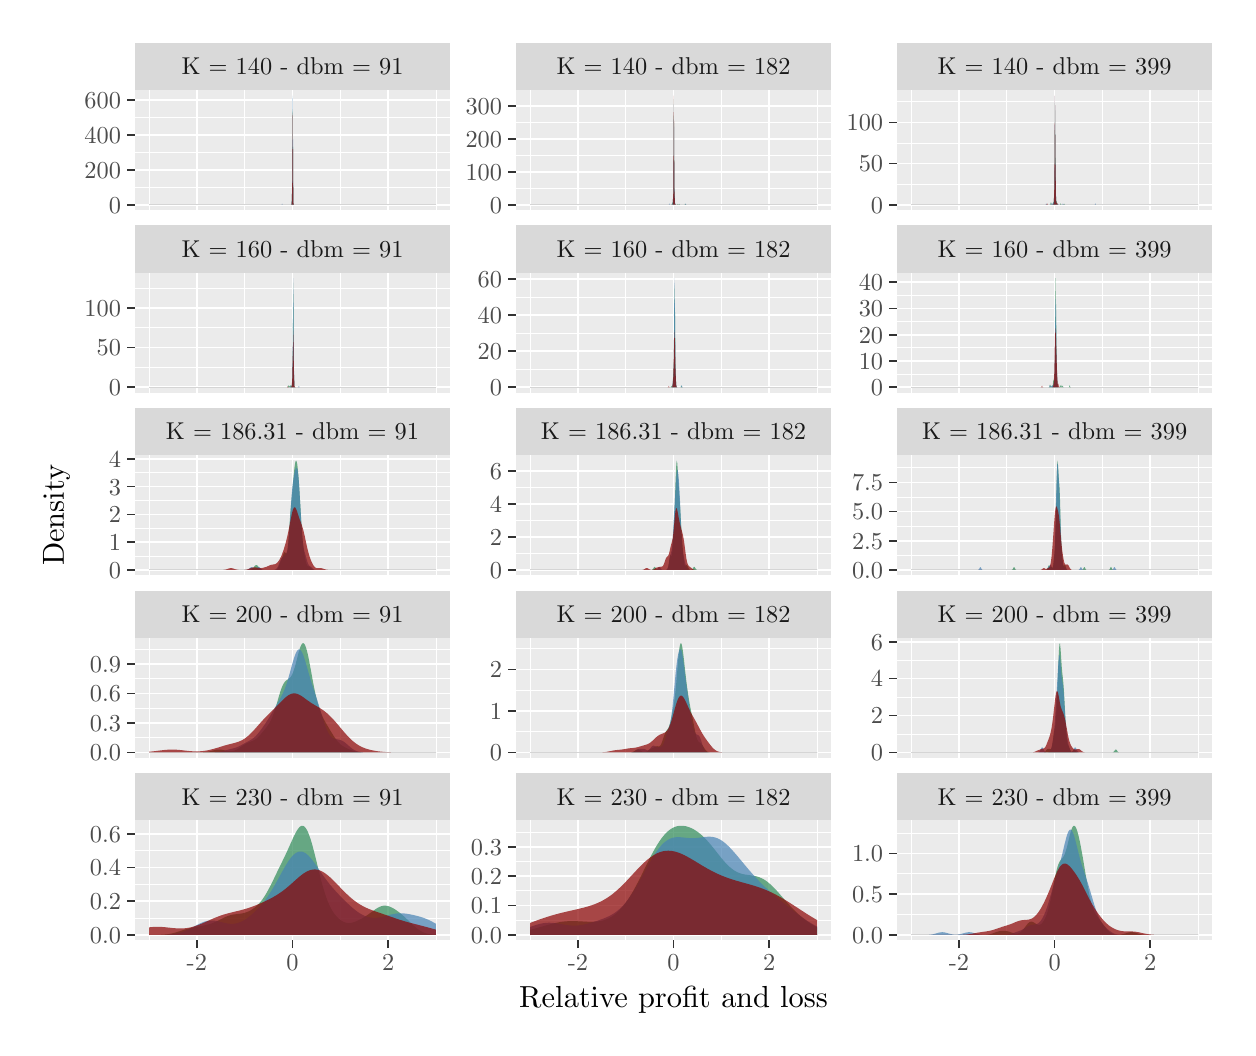
\begin{tikzpicture}[x=1pt,y=1pt]
\definecolor{fillColor}{RGB}{255,255,255}
\path[use as bounding box,fill=fillColor,fill opacity=0.00] (0,0) rectangle (433.62,361.35);
\begin{scope}
\path[clip] (  0.00,  0.00) rectangle (433.62,361.35);
\definecolor{drawColor}{RGB}{255,255,255}
\definecolor{fillColor}{RGB}{255,255,255}

\path[draw=drawColor,line width= 0.6pt,line join=round,line cap=round,fill=fillColor] (  0.00,  0.00) rectangle (433.62,361.35);
\end{scope}
\begin{scope}
\path[clip] ( 38.67,295.39) rectangle (152.72,338.79);
\definecolor{fillColor}{gray}{0.92}

\path[fill=fillColor] ( 38.67,295.39) rectangle (152.72,338.79);
\definecolor{drawColor}{RGB}{255,255,255}

\path[draw=drawColor,line width= 0.3pt,line join=round] ( 38.67,303.68) --
	(152.72,303.68);

\path[draw=drawColor,line width= 0.3pt,line join=round] ( 38.67,316.33) --
	(152.72,316.33);

\path[draw=drawColor,line width= 0.3pt,line join=round] ( 38.67,328.97) --
	(152.72,328.97);

\path[draw=drawColor,line width= 0.3pt,line join=round] ( 43.85,295.39) --
	( 43.85,338.79);

\path[draw=drawColor,line width= 0.3pt,line join=round] ( 78.41,295.39) --
	( 78.41,338.79);

\path[draw=drawColor,line width= 0.3pt,line join=round] (112.97,295.39) --
	(112.97,338.79);

\path[draw=drawColor,line width= 0.3pt,line join=round] (147.54,295.39) --
	(147.54,338.79);

\path[draw=drawColor,line width= 0.6pt,line join=round] ( 38.67,297.36) --
	(152.72,297.36);

\path[draw=drawColor,line width= 0.6pt,line join=round] ( 38.67,310.00) --
	(152.72,310.00);

\path[draw=drawColor,line width= 0.6pt,line join=round] ( 38.67,322.65) --
	(152.72,322.65);

\path[draw=drawColor,line width= 0.6pt,line join=round] ( 38.67,335.29) --
	(152.72,335.29);

\path[draw=drawColor,line width= 0.6pt,line join=round] ( 61.13,295.39) --
	( 61.13,338.79);

\path[draw=drawColor,line width= 0.6pt,line join=round] ( 95.69,295.39) --
	( 95.69,338.79);

\path[draw=drawColor,line width= 0.6pt,line join=round] (130.25,295.39) --
	(130.25,338.79);
\definecolor{fillColor}{RGB}{46,139,87}

\path[fill=fillColor,fill opacity=0.70] ( 43.85,297.36) --
	( 44.05,297.36) --
	( 44.26,297.36) --
	( 44.46,297.36) --
	( 44.66,297.36) --
	( 44.87,297.36) --
	( 45.07,297.36) --
	( 45.27,297.36) --
	( 45.47,297.36) --
	( 45.68,297.36) --
	( 45.88,297.36) --
	( 46.08,297.36) --
	( 46.29,297.36) --
	( 46.49,297.36) --
	( 46.69,297.36) --
	( 46.89,297.36) --
	( 47.10,297.36) --
	( 47.30,297.36) --
	( 47.50,297.36) --
	( 47.71,297.36) --
	( 47.91,297.36) --
	( 48.11,297.36) --
	( 48.31,297.36) --
	( 48.52,297.36) --
	( 48.72,297.36) --
	( 48.92,297.36) --
	( 49.13,297.36) --
	( 49.33,297.36) --
	( 49.53,297.36) --
	( 49.74,297.36) --
	( 49.94,297.36) --
	( 50.14,297.36) --
	( 50.34,297.36) --
	( 50.55,297.36) --
	( 50.75,297.36) --
	( 50.95,297.36) --
	( 51.16,297.36) --
	( 51.36,297.36) --
	( 51.56,297.36) --
	( 51.76,297.36) --
	( 51.97,297.36) --
	( 52.17,297.36) --
	( 52.37,297.36) --
	( 52.58,297.36) --
	( 52.78,297.36) --
	( 52.98,297.36) --
	( 53.18,297.36) --
	( 53.39,297.36) --
	( 53.59,297.36) --
	( 53.79,297.36) --
	( 54.00,297.36) --
	( 54.20,297.36) --
	( 54.40,297.36) --
	( 54.60,297.36) --
	( 54.81,297.36) --
	( 55.01,297.36) --
	( 55.21,297.36) --
	( 55.42,297.36) --
	( 55.62,297.36) --
	( 55.82,297.36) --
	( 56.03,297.36) --
	( 56.23,297.36) --
	( 56.43,297.36) --
	( 56.63,297.36) --
	( 56.84,297.36) --
	( 57.04,297.36) --
	( 57.24,297.36) --
	( 57.45,297.36) --
	( 57.65,297.36) --
	( 57.85,297.36) --
	( 58.05,297.36) --
	( 58.26,297.36) --
	( 58.46,297.36) --
	( 58.66,297.36) --
	( 58.87,297.36) --
	( 59.07,297.36) --
	( 59.27,297.36) --
	( 59.47,297.36) --
	( 59.68,297.36) --
	( 59.88,297.36) --
	( 60.08,297.36) --
	( 60.29,297.36) --
	( 60.49,297.36) --
	( 60.69,297.36) --
	( 60.90,297.36) --
	( 61.10,297.36) --
	( 61.30,297.36) --
	( 61.50,297.36) --
	( 61.71,297.36) --
	( 61.91,297.36) --
	( 62.11,297.36) --
	( 62.32,297.36) --
	( 62.52,297.36) --
	( 62.72,297.36) --
	( 62.92,297.36) --
	( 63.13,297.36) --
	( 63.33,297.36) --
	( 63.53,297.36) --
	( 63.74,297.36) --
	( 63.94,297.36) --
	( 64.14,297.36) --
	( 64.34,297.36) --
	( 64.55,297.36) --
	( 64.75,297.36) --
	( 64.95,297.36) --
	( 65.16,297.36) --
	( 65.36,297.36) --
	( 65.56,297.36) --
	( 65.76,297.36) --
	( 65.97,297.36) --
	( 66.17,297.36) --
	( 66.37,297.36) --
	( 66.58,297.36) --
	( 66.78,297.36) --
	( 66.98,297.36) --
	( 67.19,297.36) --
	( 67.39,297.36) --
	( 67.59,297.36) --
	( 67.79,297.36) --
	( 68.00,297.36) --
	( 68.20,297.36) --
	( 68.40,297.36) --
	( 68.61,297.36) --
	( 68.81,297.36) --
	( 69.01,297.36) --
	( 69.21,297.36) --
	( 69.42,297.36) --
	( 69.62,297.36) --
	( 69.82,297.36) --
	( 70.03,297.36) --
	( 70.23,297.36) --
	( 70.43,297.36) --
	( 70.63,297.36) --
	( 70.84,297.36) --
	( 71.04,297.36) --
	( 71.24,297.36) --
	( 71.45,297.36) --
	( 71.65,297.36) --
	( 71.85,297.36) --
	( 72.05,297.36) --
	( 72.26,297.36) --
	( 72.46,297.36) --
	( 72.66,297.36) --
	( 72.87,297.36) --
	( 73.07,297.36) --
	( 73.27,297.36) --
	( 73.48,297.36) --
	( 73.68,297.36) --
	( 73.88,297.36) --
	( 74.08,297.36) --
	( 74.29,297.36) --
	( 74.49,297.36) --
	( 74.69,297.36) --
	( 74.90,297.36) --
	( 75.10,297.36) --
	( 75.30,297.36) --
	( 75.50,297.36) --
	( 75.71,297.36) --
	( 75.91,297.36) --
	( 76.11,297.36) --
	( 76.32,297.36) --
	( 76.52,297.36) --
	( 76.72,297.36) --
	( 76.92,297.36) --
	( 77.13,297.36) --
	( 77.33,297.36) --
	( 77.53,297.36) --
	( 77.74,297.36) --
	( 77.94,297.36) --
	( 78.14,297.36) --
	( 78.34,297.36) --
	( 78.55,297.36) --
	( 78.75,297.36) --
	( 78.95,297.36) --
	( 79.16,297.36) --
	( 79.36,297.36) --
	( 79.56,297.36) --
	( 79.77,297.36) --
	( 79.97,297.36) --
	( 80.17,297.36) --
	( 80.37,297.36) --
	( 80.58,297.36) --
	( 80.78,297.36) --
	( 80.98,297.36) --
	( 81.19,297.36) --
	( 81.39,297.36) --
	( 81.59,297.36) --
	( 81.79,297.36) --
	( 82.00,297.36) --
	( 82.20,297.36) --
	( 82.40,297.36) --
	( 82.61,297.36) --
	( 82.81,297.36) --
	( 83.01,297.36) --
	( 83.21,297.36) --
	( 83.42,297.36) --
	( 83.62,297.36) --
	( 83.82,297.36) --
	( 84.03,297.36) --
	( 84.23,297.36) --
	( 84.43,297.36) --
	( 84.64,297.36) --
	( 84.84,297.36) --
	( 85.04,297.36) --
	( 85.24,297.36) --
	( 85.45,297.36) --
	( 85.65,297.36) --
	( 85.85,297.36) --
	( 86.06,297.36) --
	( 86.26,297.36) --
	( 86.46,297.36) --
	( 86.66,297.36) --
	( 86.87,297.36) --
	( 87.07,297.36) --
	( 87.27,297.36) --
	( 87.48,297.36) --
	( 87.68,297.36) --
	( 87.88,297.36) --
	( 88.08,297.36) --
	( 88.29,297.36) --
	( 88.49,297.36) --
	( 88.69,297.36) --
	( 88.90,297.36) --
	( 89.10,297.36) --
	( 89.30,297.36) --
	( 89.50,297.36) --
	( 89.71,297.36) --
	( 89.91,297.36) --
	( 90.11,297.36) --
	( 90.32,297.36) --
	( 90.52,297.36) --
	( 90.72,297.36) --
	( 90.93,297.36) --
	( 91.13,297.36) --
	( 91.33,297.36) --
	( 91.53,297.36) --
	( 91.74,297.36) --
	( 91.94,297.36) --
	( 92.14,297.36) --
	( 92.35,297.36) --
	( 92.55,297.36) --
	( 92.75,297.36) --
	( 92.95,297.36) --
	( 93.16,297.36) --
	( 93.36,297.36) --
	( 93.56,297.36) --
	( 93.77,297.36) --
	( 93.97,297.36) --
	( 94.17,297.36) --
	( 94.37,297.36) --
	( 94.58,297.36) --
	( 94.78,297.36) --
	( 94.98,297.36) --
	( 95.19,297.36) --
	( 95.39,297.79) --
	( 95.59,303.70) --
	( 95.79,331.92) --
	( 96.00,298.04) --
	( 96.20,297.42) --
	( 96.40,297.36) --
	( 96.61,297.36) --
	( 96.81,297.36) --
	( 97.01,297.36) --
	( 97.22,297.36) --
	( 97.42,297.36) --
	( 97.62,297.36) --
	( 97.82,297.36) --
	( 98.03,297.36) --
	( 98.23,297.36) --
	( 98.43,297.36) --
	( 98.64,297.36) --
	( 98.84,297.36) --
	( 99.04,297.36) --
	( 99.24,297.36) --
	( 99.45,297.36) --
	( 99.65,297.36) --
	( 99.85,297.36) --
	(100.06,297.36) --
	(100.26,297.36) --
	(100.46,297.36) --
	(100.66,297.36) --
	(100.87,297.36) --
	(101.07,297.36) --
	(101.27,297.36) --
	(101.48,297.36) --
	(101.68,297.36) --
	(101.88,297.36) --
	(102.08,297.36) --
	(102.29,297.36) --
	(102.49,297.36) --
	(102.69,297.36) --
	(102.90,297.36) --
	(103.10,297.36) --
	(103.30,297.36) --
	(103.51,297.36) --
	(103.71,297.36) --
	(103.91,297.36) --
	(104.11,297.36) --
	(104.32,297.36) --
	(104.52,297.36) --
	(104.72,297.36) --
	(104.93,297.36) --
	(105.13,297.36) --
	(105.33,297.36) --
	(105.53,297.36) --
	(105.74,297.36) --
	(105.94,297.36) --
	(106.14,297.36) --
	(106.35,297.36) --
	(106.55,297.36) --
	(106.75,297.36) --
	(106.95,297.36) --
	(107.16,297.36) --
	(107.36,297.36) --
	(107.56,297.36) --
	(107.77,297.36) --
	(107.97,297.36) --
	(108.17,297.36) --
	(108.37,297.36) --
	(108.58,297.36) --
	(108.78,297.36) --
	(108.98,297.36) --
	(109.19,297.36) --
	(109.39,297.36) --
	(109.59,297.36) --
	(109.80,297.36) --
	(110.00,297.36) --
	(110.20,297.36) --
	(110.40,297.36) --
	(110.61,297.36) --
	(110.81,297.36) --
	(111.01,297.36) --
	(111.22,297.36) --
	(111.42,297.36) --
	(111.62,297.36) --
	(111.82,297.36) --
	(112.03,297.36) --
	(112.23,297.36) --
	(112.43,297.36) --
	(112.64,297.36) --
	(112.84,297.36) --
	(113.04,297.36) --
	(113.24,297.36) --
	(113.45,297.36) --
	(113.65,297.36) --
	(113.85,297.36) --
	(114.06,297.36) --
	(114.26,297.36) --
	(114.46,297.36) --
	(114.67,297.36) --
	(114.87,297.36) --
	(115.07,297.36) --
	(115.27,297.36) --
	(115.48,297.36) --
	(115.68,297.36) --
	(115.88,297.36) --
	(116.09,297.36) --
	(116.29,297.36) --
	(116.49,297.36) --
	(116.69,297.36) --
	(116.90,297.36) --
	(117.10,297.36) --
	(117.30,297.36) --
	(117.51,297.36) --
	(117.71,297.36) --
	(117.91,297.36) --
	(118.11,297.36) --
	(118.32,297.36) --
	(118.52,297.36) --
	(118.72,297.36) --
	(118.93,297.36) --
	(119.13,297.36) --
	(119.33,297.36) --
	(119.53,297.36) --
	(119.74,297.36) --
	(119.94,297.36) --
	(120.14,297.36) --
	(120.35,297.36) --
	(120.55,297.36) --
	(120.75,297.36) --
	(120.96,297.36) --
	(121.16,297.36) --
	(121.36,297.36) --
	(121.56,297.36) --
	(121.77,297.36) --
	(121.97,297.36) --
	(122.17,297.36) --
	(122.38,297.36) --
	(122.58,297.36) --
	(122.78,297.36) --
	(122.98,297.36) --
	(123.19,297.36) --
	(123.39,297.36) --
	(123.59,297.36) --
	(123.80,297.36) --
	(124.00,297.36) --
	(124.20,297.36) --
	(124.40,297.36) --
	(124.61,297.36) --
	(124.81,297.36) --
	(125.01,297.36) --
	(125.22,297.36) --
	(125.42,297.36) --
	(125.62,297.36) --
	(125.82,297.36) --
	(126.03,297.36) --
	(126.23,297.36) --
	(126.43,297.36) --
	(126.64,297.36) --
	(126.84,297.36) --
	(127.04,297.36) --
	(127.25,297.36) --
	(127.45,297.36) --
	(127.65,297.36) --
	(127.85,297.36) --
	(128.06,297.36) --
	(128.26,297.36) --
	(128.46,297.36) --
	(128.67,297.36) --
	(128.87,297.36) --
	(129.07,297.36) --
	(129.27,297.36) --
	(129.48,297.36) --
	(129.68,297.36) --
	(129.88,297.36) --
	(130.09,297.36) --
	(130.29,297.36) --
	(130.49,297.36) --
	(130.69,297.36) --
	(130.90,297.36) --
	(131.10,297.36) --
	(131.30,297.36) --
	(131.51,297.36) --
	(131.71,297.36) --
	(131.91,297.36) --
	(132.11,297.36) --
	(132.32,297.36) --
	(132.52,297.36) --
	(132.72,297.36) --
	(132.93,297.36) --
	(133.13,297.36) --
	(133.33,297.36) --
	(133.54,297.36) --
	(133.74,297.36) --
	(133.94,297.36) --
	(134.14,297.36) --
	(134.35,297.36) --
	(134.55,297.36) --
	(134.75,297.36) --
	(134.96,297.36) --
	(135.16,297.36) --
	(135.36,297.36) --
	(135.56,297.36) --
	(135.77,297.36) --
	(135.97,297.36) --
	(136.17,297.36) --
	(136.38,297.36) --
	(136.58,297.36) --
	(136.78,297.36) --
	(136.98,297.36) --
	(137.19,297.36) --
	(137.39,297.36) --
	(137.59,297.36) --
	(137.80,297.36) --
	(138.00,297.36) --
	(138.20,297.36) --
	(138.40,297.36) --
	(138.61,297.36) --
	(138.81,297.36) --
	(139.01,297.36) --
	(139.22,297.36) --
	(139.42,297.36) --
	(139.62,297.36) --
	(139.83,297.36) --
	(140.03,297.36) --
	(140.23,297.36) --
	(140.43,297.36) --
	(140.64,297.36) --
	(140.84,297.36) --
	(141.04,297.36) --
	(141.25,297.36) --
	(141.45,297.36) --
	(141.65,297.36) --
	(141.85,297.36) --
	(142.06,297.36) --
	(142.26,297.36) --
	(142.46,297.36) --
	(142.67,297.36) --
	(142.87,297.36) --
	(143.07,297.36) --
	(143.27,297.36) --
	(143.48,297.36) --
	(143.68,297.36) --
	(143.88,297.36) --
	(144.09,297.36) --
	(144.29,297.36) --
	(144.49,297.36) --
	(144.70,297.36) --
	(144.90,297.36) --
	(145.10,297.36) --
	(145.30,297.36) --
	(145.51,297.36) --
	(145.71,297.36) --
	(145.91,297.36) --
	(146.12,297.36) --
	(146.32,297.36) --
	(146.52,297.36) --
	(146.72,297.36) --
	(146.93,297.36) --
	(147.13,297.36) --
	(147.33,297.36) --
	(147.54,297.36) --
	(147.54,297.36) --
	(147.33,297.36) --
	(147.13,297.36) --
	(146.93,297.36) --
	(146.72,297.36) --
	(146.52,297.36) --
	(146.32,297.36) --
	(146.12,297.36) --
	(145.91,297.36) --
	(145.71,297.36) --
	(145.51,297.36) --
	(145.30,297.36) --
	(145.10,297.36) --
	(144.90,297.36) --
	(144.70,297.36) --
	(144.49,297.36) --
	(144.29,297.36) --
	(144.09,297.36) --
	(143.88,297.36) --
	(143.68,297.36) --
	(143.48,297.36) --
	(143.27,297.36) --
	(143.07,297.36) --
	(142.87,297.36) --
	(142.67,297.36) --
	(142.46,297.36) --
	(142.26,297.36) --
	(142.06,297.36) --
	(141.85,297.36) --
	(141.65,297.36) --
	(141.45,297.36) --
	(141.25,297.36) --
	(141.04,297.36) --
	(140.84,297.36) --
	(140.64,297.36) --
	(140.43,297.36) --
	(140.23,297.36) --
	(140.03,297.36) --
	(139.83,297.36) --
	(139.62,297.36) --
	(139.42,297.36) --
	(139.22,297.36) --
	(139.01,297.36) --
	(138.81,297.36) --
	(138.61,297.36) --
	(138.40,297.36) --
	(138.20,297.36) --
	(138.00,297.36) --
	(137.80,297.36) --
	(137.59,297.36) --
	(137.39,297.36) --
	(137.19,297.36) --
	(136.98,297.36) --
	(136.78,297.36) --
	(136.58,297.36) --
	(136.38,297.36) --
	(136.17,297.36) --
	(135.97,297.36) --
	(135.77,297.36) --
	(135.56,297.36) --
	(135.36,297.36) --
	(135.16,297.36) --
	(134.96,297.36) --
	(134.75,297.36) --
	(134.55,297.36) --
	(134.35,297.36) --
	(134.14,297.36) --
	(133.94,297.36) --
	(133.74,297.36) --
	(133.54,297.36) --
	(133.33,297.36) --
	(133.13,297.36) --
	(132.93,297.36) --
	(132.72,297.36) --
	(132.52,297.36) --
	(132.32,297.36) --
	(132.11,297.36) --
	(131.91,297.36) --
	(131.71,297.36) --
	(131.51,297.36) --
	(131.30,297.36) --
	(131.10,297.36) --
	(130.90,297.36) --
	(130.69,297.36) --
	(130.49,297.36) --
	(130.29,297.36) --
	(130.09,297.36) --
	(129.88,297.36) --
	(129.68,297.36) --
	(129.48,297.36) --
	(129.27,297.36) --
	(129.07,297.36) --
	(128.87,297.36) --
	(128.67,297.36) --
	(128.46,297.36) --
	(128.26,297.36) --
	(128.06,297.36) --
	(127.85,297.36) --
	(127.65,297.36) --
	(127.45,297.36) --
	(127.25,297.36) --
	(127.04,297.36) --
	(126.84,297.36) --
	(126.64,297.36) --
	(126.43,297.36) --
	(126.23,297.36) --
	(126.03,297.36) --
	(125.82,297.36) --
	(125.62,297.36) --
	(125.42,297.36) --
	(125.22,297.36) --
	(125.01,297.36) --
	(124.81,297.36) --
	(124.61,297.36) --
	(124.40,297.36) --
	(124.20,297.36) --
	(124.00,297.36) --
	(123.80,297.36) --
	(123.59,297.36) --
	(123.39,297.36) --
	(123.19,297.36) --
	(122.98,297.36) --
	(122.78,297.36) --
	(122.58,297.36) --
	(122.38,297.36) --
	(122.17,297.36) --
	(121.97,297.36) --
	(121.77,297.36) --
	(121.56,297.36) --
	(121.36,297.36) --
	(121.16,297.36) --
	(120.96,297.36) --
	(120.75,297.36) --
	(120.55,297.36) --
	(120.35,297.36) --
	(120.14,297.36) --
	(119.94,297.36) --
	(119.74,297.36) --
	(119.53,297.36) --
	(119.33,297.36) --
	(119.13,297.36) --
	(118.93,297.36) --
	(118.72,297.36) --
	(118.52,297.36) --
	(118.32,297.36) --
	(118.11,297.36) --
	(117.91,297.36) --
	(117.71,297.36) --
	(117.51,297.36) --
	(117.30,297.36) --
	(117.10,297.36) --
	(116.90,297.36) --
	(116.69,297.36) --
	(116.49,297.36) --
	(116.29,297.36) --
	(116.09,297.36) --
	(115.88,297.36) --
	(115.68,297.36) --
	(115.48,297.36) --
	(115.27,297.36) --
	(115.07,297.36) --
	(114.87,297.36) --
	(114.67,297.36) --
	(114.46,297.36) --
	(114.26,297.36) --
	(114.06,297.36) --
	(113.85,297.36) --
	(113.65,297.36) --
	(113.45,297.36) --
	(113.24,297.36) --
	(113.04,297.36) --
	(112.84,297.36) --
	(112.64,297.36) --
	(112.43,297.36) --
	(112.23,297.36) --
	(112.03,297.36) --
	(111.82,297.36) --
	(111.62,297.36) --
	(111.42,297.36) --
	(111.22,297.36) --
	(111.01,297.36) --
	(110.81,297.36) --
	(110.61,297.36) --
	(110.40,297.36) --
	(110.20,297.36) --
	(110.00,297.36) --
	(109.80,297.36) --
	(109.59,297.36) --
	(109.39,297.36) --
	(109.19,297.36) --
	(108.98,297.36) --
	(108.78,297.36) --
	(108.58,297.36) --
	(108.37,297.36) --
	(108.17,297.36) --
	(107.97,297.36) --
	(107.77,297.36) --
	(107.56,297.36) --
	(107.36,297.36) --
	(107.16,297.36) --
	(106.95,297.36) --
	(106.75,297.36) --
	(106.55,297.36) --
	(106.35,297.36) --
	(106.14,297.36) --
	(105.94,297.36) --
	(105.74,297.36) --
	(105.53,297.36) --
	(105.33,297.36) --
	(105.13,297.36) --
	(104.93,297.36) --
	(104.72,297.36) --
	(104.52,297.36) --
	(104.32,297.36) --
	(104.11,297.36) --
	(103.91,297.36) --
	(103.71,297.36) --
	(103.51,297.36) --
	(103.30,297.36) --
	(103.10,297.36) --
	(102.90,297.36) --
	(102.69,297.36) --
	(102.49,297.36) --
	(102.29,297.36) --
	(102.08,297.36) --
	(101.88,297.36) --
	(101.68,297.36) --
	(101.48,297.36) --
	(101.27,297.36) --
	(101.07,297.36) --
	(100.87,297.36) --
	(100.66,297.36) --
	(100.46,297.36) --
	(100.26,297.36) --
	(100.06,297.36) --
	( 99.85,297.36) --
	( 99.65,297.36) --
	( 99.45,297.36) --
	( 99.24,297.36) --
	( 99.04,297.36) --
	( 98.84,297.36) --
	( 98.64,297.36) --
	( 98.43,297.36) --
	( 98.23,297.36) --
	( 98.03,297.36) --
	( 97.82,297.36) --
	( 97.62,297.36) --
	( 97.42,297.36) --
	( 97.22,297.36) --
	( 97.01,297.36) --
	( 96.81,297.36) --
	( 96.61,297.36) --
	( 96.40,297.36) --
	( 96.20,297.36) --
	( 96.00,297.36) --
	( 95.79,297.36) --
	( 95.59,297.36) --
	( 95.39,297.36) --
	( 95.19,297.36) --
	( 94.98,297.36) --
	( 94.78,297.36) --
	( 94.58,297.36) --
	( 94.37,297.36) --
	( 94.17,297.36) --
	( 93.97,297.36) --
	( 93.77,297.36) --
	( 93.56,297.36) --
	( 93.36,297.36) --
	( 93.16,297.36) --
	( 92.95,297.36) --
	( 92.75,297.36) --
	( 92.55,297.36) --
	( 92.35,297.36) --
	( 92.14,297.36) --
	( 91.94,297.36) --
	( 91.74,297.36) --
	( 91.53,297.36) --
	( 91.33,297.36) --
	( 91.13,297.36) --
	( 90.93,297.36) --
	( 90.72,297.36) --
	( 90.52,297.36) --
	( 90.32,297.36) --
	( 90.11,297.36) --
	( 89.91,297.36) --
	( 89.71,297.36) --
	( 89.50,297.36) --
	( 89.30,297.36) --
	( 89.10,297.36) --
	( 88.90,297.36) --
	( 88.69,297.36) --
	( 88.49,297.36) --
	( 88.29,297.36) --
	( 88.08,297.36) --
	( 87.88,297.36) --
	( 87.68,297.36) --
	( 87.48,297.36) --
	( 87.27,297.36) --
	( 87.07,297.36) --
	( 86.87,297.36) --
	( 86.66,297.36) --
	( 86.46,297.36) --
	( 86.26,297.36) --
	( 86.06,297.36) --
	( 85.85,297.36) --
	( 85.65,297.36) --
	( 85.45,297.36) --
	( 85.24,297.36) --
	( 85.04,297.36) --
	( 84.84,297.36) --
	( 84.64,297.36) --
	( 84.43,297.36) --
	( 84.23,297.36) --
	( 84.03,297.36) --
	( 83.82,297.36) --
	( 83.62,297.36) --
	( 83.42,297.36) --
	( 83.21,297.36) --
	( 83.01,297.36) --
	( 82.81,297.36) --
	( 82.61,297.36) --
	( 82.40,297.36) --
	( 82.20,297.36) --
	( 82.00,297.36) --
	( 81.79,297.36) --
	( 81.59,297.36) --
	( 81.39,297.36) --
	( 81.19,297.36) --
	( 80.98,297.36) --
	( 80.78,297.36) --
	( 80.58,297.36) --
	( 80.37,297.36) --
	( 80.17,297.36) --
	( 79.97,297.36) --
	( 79.77,297.36) --
	( 79.56,297.36) --
	( 79.36,297.36) --
	( 79.16,297.36) --
	( 78.95,297.36) --
	( 78.75,297.36) --
	( 78.55,297.36) --
	( 78.34,297.36) --
	( 78.14,297.36) --
	( 77.94,297.36) --
	( 77.74,297.36) --
	( 77.53,297.36) --
	( 77.33,297.36) --
	( 77.13,297.36) --
	( 76.92,297.36) --
	( 76.72,297.36) --
	( 76.52,297.36) --
	( 76.32,297.36) --
	( 76.11,297.36) --
	( 75.91,297.36) --
	( 75.71,297.36) --
	( 75.50,297.36) --
	( 75.30,297.36) --
	( 75.10,297.36) --
	( 74.90,297.36) --
	( 74.69,297.36) --
	( 74.49,297.36) --
	( 74.29,297.36) --
	( 74.08,297.36) --
	( 73.88,297.36) --
	( 73.68,297.36) --
	( 73.48,297.36) --
	( 73.27,297.36) --
	( 73.07,297.36) --
	( 72.87,297.36) --
	( 72.66,297.36) --
	( 72.46,297.36) --
	( 72.26,297.36) --
	( 72.05,297.36) --
	( 71.85,297.36) --
	( 71.65,297.36) --
	( 71.45,297.36) --
	( 71.24,297.36) --
	( 71.04,297.36) --
	( 70.84,297.36) --
	( 70.63,297.36) --
	( 70.43,297.36) --
	( 70.23,297.36) --
	( 70.03,297.36) --
	( 69.82,297.36) --
	( 69.62,297.36) --
	( 69.42,297.36) --
	( 69.21,297.36) --
	( 69.01,297.36) --
	( 68.81,297.36) --
	( 68.61,297.36) --
	( 68.40,297.36) --
	( 68.20,297.36) --
	( 68.00,297.36) --
	( 67.79,297.36) --
	( 67.59,297.36) --
	( 67.39,297.36) --
	( 67.19,297.36) --
	( 66.98,297.36) --
	( 66.78,297.36) --
	( 66.58,297.36) --
	( 66.37,297.36) --
	( 66.17,297.36) --
	( 65.97,297.36) --
	( 65.76,297.36) --
	( 65.56,297.36) --
	( 65.36,297.36) --
	( 65.16,297.36) --
	( 64.95,297.36) --
	( 64.75,297.36) --
	( 64.55,297.36) --
	( 64.34,297.36) --
	( 64.14,297.36) --
	( 63.94,297.36) --
	( 63.74,297.36) --
	( 63.53,297.36) --
	( 63.33,297.36) --
	( 63.13,297.36) --
	( 62.92,297.36) --
	( 62.72,297.36) --
	( 62.52,297.36) --
	( 62.32,297.36) --
	( 62.11,297.36) --
	( 61.91,297.36) --
	( 61.71,297.36) --
	( 61.50,297.36) --
	( 61.30,297.36) --
	( 61.10,297.36) --
	( 60.90,297.36) --
	( 60.69,297.36) --
	( 60.49,297.36) --
	( 60.29,297.36) --
	( 60.08,297.36) --
	( 59.88,297.36) --
	( 59.68,297.36) --
	( 59.47,297.36) --
	( 59.27,297.36) --
	( 59.07,297.36) --
	( 58.87,297.36) --
	( 58.66,297.36) --
	( 58.46,297.36) --
	( 58.26,297.36) --
	( 58.05,297.36) --
	( 57.85,297.36) --
	( 57.65,297.36) --
	( 57.45,297.36) --
	( 57.24,297.36) --
	( 57.04,297.36) --
	( 56.84,297.36) --
	( 56.63,297.36) --
	( 56.43,297.36) --
	( 56.23,297.36) --
	( 56.03,297.36) --
	( 55.82,297.36) --
	( 55.62,297.36) --
	( 55.42,297.36) --
	( 55.21,297.36) --
	( 55.01,297.36) --
	( 54.81,297.36) --
	( 54.60,297.36) --
	( 54.40,297.36) --
	( 54.20,297.36) --
	( 54.00,297.36) --
	( 53.79,297.36) --
	( 53.59,297.36) --
	( 53.39,297.36) --
	( 53.18,297.36) --
	( 52.98,297.36) --
	( 52.78,297.36) --
	( 52.58,297.36) --
	( 52.37,297.36) --
	( 52.17,297.36) --
	( 51.97,297.36) --
	( 51.76,297.36) --
	( 51.56,297.36) --
	( 51.36,297.36) --
	( 51.16,297.36) --
	( 50.95,297.36) --
	( 50.75,297.36) --
	( 50.55,297.36) --
	( 50.34,297.36) --
	( 50.14,297.36) --
	( 49.94,297.36) --
	( 49.74,297.36) --
	( 49.53,297.36) --
	( 49.33,297.36) --
	( 49.13,297.36) --
	( 48.92,297.36) --
	( 48.72,297.36) --
	( 48.52,297.36) --
	( 48.31,297.36) --
	( 48.11,297.36) --
	( 47.91,297.36) --
	( 47.71,297.36) --
	( 47.50,297.36) --
	( 47.30,297.36) --
	( 47.10,297.36) --
	( 46.89,297.36) --
	( 46.69,297.36) --
	( 46.49,297.36) --
	( 46.29,297.36) --
	( 46.08,297.36) --
	( 45.88,297.36) --
	( 45.68,297.36) --
	( 45.47,297.36) --
	( 45.27,297.36) --
	( 45.07,297.36) --
	( 44.87,297.36) --
	( 44.66,297.36) --
	( 44.46,297.36) --
	( 44.26,297.36) --
	( 44.05,297.36) --
	( 43.85,297.36) --
	cycle;
\definecolor{fillColor}{RGB}{70,130,180}

\path[fill=fillColor,fill opacity=0.70] ( 43.85,297.36) --
	( 44.05,297.36) --
	( 44.26,297.36) --
	( 44.46,297.36) --
	( 44.66,297.36) --
	( 44.87,297.36) --
	( 45.07,297.36) --
	( 45.27,297.36) --
	( 45.47,297.36) --
	( 45.68,297.36) --
	( 45.88,297.36) --
	( 46.08,297.36) --
	( 46.29,297.36) --
	( 46.49,297.36) --
	( 46.69,297.36) --
	( 46.89,297.36) --
	( 47.10,297.36) --
	( 47.30,297.36) --
	( 47.50,297.36) --
	( 47.71,297.36) --
	( 47.91,297.36) --
	( 48.11,297.36) --
	( 48.31,297.36) --
	( 48.52,297.36) --
	( 48.72,297.36) --
	( 48.92,297.36) --
	( 49.13,297.36) --
	( 49.33,297.36) --
	( 49.53,297.36) --
	( 49.74,297.36) --
	( 49.94,297.36) --
	( 50.14,297.36) --
	( 50.34,297.36) --
	( 50.55,297.36) --
	( 50.75,297.36) --
	( 50.95,297.36) --
	( 51.16,297.36) --
	( 51.36,297.36) --
	( 51.56,297.36) --
	( 51.76,297.36) --
	( 51.97,297.36) --
	( 52.17,297.36) --
	( 52.37,297.36) --
	( 52.58,297.36) --
	( 52.78,297.36) --
	( 52.98,297.36) --
	( 53.18,297.36) --
	( 53.39,297.36) --
	( 53.59,297.36) --
	( 53.79,297.36) --
	( 54.00,297.36) --
	( 54.20,297.36) --
	( 54.40,297.36) --
	( 54.60,297.36) --
	( 54.81,297.36) --
	( 55.01,297.36) --
	( 55.21,297.36) --
	( 55.42,297.36) --
	( 55.62,297.36) --
	( 55.82,297.36) --
	( 56.03,297.36) --
	( 56.23,297.36) --
	( 56.43,297.36) --
	( 56.63,297.36) --
	( 56.84,297.36) --
	( 57.04,297.36) --
	( 57.24,297.36) --
	( 57.45,297.36) --
	( 57.65,297.36) --
	( 57.85,297.36) --
	( 58.05,297.36) --
	( 58.26,297.36) --
	( 58.46,297.36) --
	( 58.66,297.36) --
	( 58.87,297.36) --
	( 59.07,297.36) --
	( 59.27,297.36) --
	( 59.47,297.36) --
	( 59.68,297.36) --
	( 59.88,297.36) --
	( 60.08,297.36) --
	( 60.29,297.36) --
	( 60.49,297.36) --
	( 60.69,297.36) --
	( 60.90,297.36) --
	( 61.10,297.36) --
	( 61.30,297.36) --
	( 61.50,297.36) --
	( 61.71,297.36) --
	( 61.91,297.36) --
	( 62.11,297.36) --
	( 62.32,297.36) --
	( 62.52,297.36) --
	( 62.72,297.36) --
	( 62.92,297.36) --
	( 63.13,297.36) --
	( 63.33,297.36) --
	( 63.53,297.36) --
	( 63.74,297.36) --
	( 63.94,297.36) --
	( 64.14,297.36) --
	( 64.34,297.36) --
	( 64.55,297.36) --
	( 64.75,297.36) --
	( 64.95,297.36) --
	( 65.16,297.36) --
	( 65.36,297.36) --
	( 65.56,297.36) --
	( 65.76,297.36) --
	( 65.97,297.36) --
	( 66.17,297.36) --
	( 66.37,297.36) --
	( 66.58,297.36) --
	( 66.78,297.36) --
	( 66.98,297.36) --
	( 67.19,297.36) --
	( 67.39,297.36) --
	( 67.59,297.36) --
	( 67.79,297.36) --
	( 68.00,297.36) --
	( 68.20,297.36) --
	( 68.40,297.36) --
	( 68.61,297.36) --
	( 68.81,297.36) --
	( 69.01,297.36) --
	( 69.21,297.36) --
	( 69.42,297.36) --
	( 69.62,297.36) --
	( 69.82,297.36) --
	( 70.03,297.36) --
	( 70.23,297.36) --
	( 70.43,297.36) --
	( 70.63,297.36) --
	( 70.84,297.36) --
	( 71.04,297.36) --
	( 71.24,297.36) --
	( 71.45,297.36) --
	( 71.65,297.36) --
	( 71.85,297.36) --
	( 72.05,297.36) --
	( 72.26,297.36) --
	( 72.46,297.36) --
	( 72.66,297.36) --
	( 72.87,297.36) --
	( 73.07,297.36) --
	( 73.27,297.36) --
	( 73.48,297.36) --
	( 73.68,297.36) --
	( 73.88,297.36) --
	( 74.08,297.36) --
	( 74.29,297.36) --
	( 74.49,297.36) --
	( 74.69,297.36) --
	( 74.90,297.36) --
	( 75.10,297.36) --
	( 75.30,297.36) --
	( 75.50,297.36) --
	( 75.71,297.36) --
	( 75.91,297.36) --
	( 76.11,297.36) --
	( 76.32,297.36) --
	( 76.52,297.36) --
	( 76.72,297.36) --
	( 76.92,297.36) --
	( 77.13,297.36) --
	( 77.33,297.36) --
	( 77.53,297.36) --
	( 77.74,297.36) --
	( 77.94,297.36) --
	( 78.14,297.36) --
	( 78.34,297.36) --
	( 78.55,297.36) --
	( 78.75,297.36) --
	( 78.95,297.36) --
	( 79.16,297.36) --
	( 79.36,297.36) --
	( 79.56,297.36) --
	( 79.77,297.36) --
	( 79.97,297.36) --
	( 80.17,297.36) --
	( 80.37,297.36) --
	( 80.58,297.36) --
	( 80.78,297.36) --
	( 80.98,297.36) --
	( 81.19,297.36) --
	( 81.39,297.36) --
	( 81.59,297.36) --
	( 81.79,297.36) --
	( 82.00,297.36) --
	( 82.20,297.36) --
	( 82.40,297.36) --
	( 82.61,297.36) --
	( 82.81,297.36) --
	( 83.01,297.36) --
	( 83.21,297.36) --
	( 83.42,297.36) --
	( 83.62,297.36) --
	( 83.82,297.36) --
	( 84.03,297.36) --
	( 84.23,297.36) --
	( 84.43,297.36) --
	( 84.64,297.36) --
	( 84.84,297.36) --
	( 85.04,297.36) --
	( 85.24,297.36) --
	( 85.45,297.36) --
	( 85.65,297.36) --
	( 85.85,297.36) --
	( 86.06,297.36) --
	( 86.26,297.36) --
	( 86.46,297.36) --
	( 86.66,297.36) --
	( 86.87,297.36) --
	( 87.07,297.36) --
	( 87.27,297.36) --
	( 87.48,297.36) --
	( 87.68,297.36) --
	( 87.88,297.36) --
	( 88.08,297.36) --
	( 88.29,297.36) --
	( 88.49,297.36) --
	( 88.69,297.36) --
	( 88.90,297.36) --
	( 89.10,297.36) --
	( 89.30,297.36) --
	( 89.50,297.36) --
	( 89.71,297.36) --
	( 89.91,297.36) --
	( 90.11,297.36) --
	( 90.32,297.36) --
	( 90.52,297.36) --
	( 90.72,297.36) --
	( 90.93,297.36) --
	( 91.13,297.36) --
	( 91.33,297.36) --
	( 91.53,297.36) --
	( 91.74,297.41) --
	( 91.94,297.78) --
	( 92.14,297.36) --
	( 92.35,297.36) --
	( 92.55,297.36) --
	( 92.75,297.36) --
	( 92.95,297.36) --
	( 93.16,297.36) --
	( 93.36,297.36) --
	( 93.56,297.36) --
	( 93.77,297.36) --
	( 93.97,297.36) --
	( 94.17,297.36) --
	( 94.37,297.36) --
	( 94.58,297.36) --
	( 94.78,297.36) --
	( 94.98,297.36) --
	( 95.19,297.46) --
	( 95.39,297.73) --
	( 95.59,303.74) --
	( 95.79,336.82) --
	( 96.00,297.71) --
	( 96.20,297.36) --
	( 96.40,297.36) --
	( 96.61,297.36) --
	( 96.81,297.36) --
	( 97.01,297.36) --
	( 97.22,297.36) --
	( 97.42,297.36) --
	( 97.62,297.36) --
	( 97.82,297.36) --
	( 98.03,297.36) --
	( 98.23,297.36) --
	( 98.43,297.36) --
	( 98.64,297.36) --
	( 98.84,297.36) --
	( 99.04,297.36) --
	( 99.24,297.36) --
	( 99.45,297.36) --
	( 99.65,297.36) --
	( 99.85,297.36) --
	(100.06,297.36) --
	(100.26,297.36) --
	(100.46,297.36) --
	(100.66,297.36) --
	(100.87,297.36) --
	(101.07,297.36) --
	(101.27,297.36) --
	(101.48,297.36) --
	(101.68,297.36) --
	(101.88,297.36) --
	(102.08,297.36) --
	(102.29,297.36) --
	(102.49,297.36) --
	(102.69,297.36) --
	(102.90,297.36) --
	(103.10,297.36) --
	(103.30,297.36) --
	(103.51,297.36) --
	(103.71,297.36) --
	(103.91,297.36) --
	(104.11,297.36) --
	(104.32,297.36) --
	(104.52,297.36) --
	(104.72,297.36) --
	(104.93,297.36) --
	(105.13,297.36) --
	(105.33,297.36) --
	(105.53,297.36) --
	(105.74,297.36) --
	(105.94,297.36) --
	(106.14,297.36) --
	(106.35,297.36) --
	(106.55,297.36) --
	(106.75,297.36) --
	(106.95,297.36) --
	(107.16,297.36) --
	(107.36,297.36) --
	(107.56,297.36) --
	(107.77,297.36) --
	(107.97,297.36) --
	(108.17,297.36) --
	(108.37,297.36) --
	(108.58,297.36) --
	(108.78,297.36) --
	(108.98,297.36) --
	(109.19,297.36) --
	(109.39,297.36) --
	(109.59,297.36) --
	(109.80,297.36) --
	(110.00,297.36) --
	(110.20,297.36) --
	(110.40,297.36) --
	(110.61,297.36) --
	(110.81,297.36) --
	(111.01,297.36) --
	(111.22,297.36) --
	(111.42,297.36) --
	(111.62,297.36) --
	(111.82,297.36) --
	(112.03,297.36) --
	(112.23,297.36) --
	(112.43,297.36) --
	(112.64,297.36) --
	(112.84,297.36) --
	(113.04,297.36) --
	(113.24,297.36) --
	(113.45,297.36) --
	(113.65,297.36) --
	(113.85,297.36) --
	(114.06,297.36) --
	(114.26,297.36) --
	(114.46,297.36) --
	(114.67,297.36) --
	(114.87,297.36) --
	(115.07,297.36) --
	(115.27,297.36) --
	(115.48,297.36) --
	(115.68,297.36) --
	(115.88,297.36) --
	(116.09,297.36) --
	(116.29,297.36) --
	(116.49,297.36) --
	(116.69,297.36) --
	(116.90,297.36) --
	(117.10,297.36) --
	(117.30,297.36) --
	(117.51,297.36) --
	(117.71,297.36) --
	(117.91,297.36) --
	(118.11,297.36) --
	(118.32,297.36) --
	(118.52,297.36) --
	(118.72,297.36) --
	(118.93,297.36) --
	(119.13,297.36) --
	(119.33,297.36) --
	(119.53,297.36) --
	(119.74,297.36) --
	(119.94,297.36) --
	(120.14,297.36) --
	(120.35,297.36) --
	(120.55,297.36) --
	(120.75,297.36) --
	(120.96,297.36) --
	(121.16,297.36) --
	(121.36,297.36) --
	(121.56,297.36) --
	(121.77,297.36) --
	(121.97,297.36) --
	(122.17,297.36) --
	(122.38,297.36) --
	(122.58,297.36) --
	(122.78,297.36) --
	(122.98,297.36) --
	(123.19,297.36) --
	(123.39,297.36) --
	(123.59,297.36) --
	(123.80,297.36) --
	(124.00,297.36) --
	(124.20,297.36) --
	(124.40,297.36) --
	(124.61,297.36) --
	(124.81,297.36) --
	(125.01,297.36) --
	(125.22,297.36) --
	(125.42,297.36) --
	(125.62,297.36) --
	(125.82,297.36) --
	(126.03,297.36) --
	(126.23,297.36) --
	(126.43,297.36) --
	(126.64,297.36) --
	(126.84,297.36) --
	(127.04,297.36) --
	(127.25,297.36) --
	(127.45,297.36) --
	(127.65,297.36) --
	(127.85,297.36) --
	(128.06,297.36) --
	(128.26,297.36) --
	(128.46,297.36) --
	(128.67,297.36) --
	(128.87,297.36) --
	(129.07,297.36) --
	(129.27,297.36) --
	(129.48,297.36) --
	(129.68,297.36) --
	(129.88,297.36) --
	(130.09,297.36) --
	(130.29,297.36) --
	(130.49,297.36) --
	(130.69,297.36) --
	(130.90,297.36) --
	(131.10,297.36) --
	(131.30,297.36) --
	(131.51,297.36) --
	(131.71,297.36) --
	(131.91,297.36) --
	(132.11,297.36) --
	(132.32,297.36) --
	(132.52,297.36) --
	(132.72,297.36) --
	(132.93,297.36) --
	(133.13,297.36) --
	(133.33,297.36) --
	(133.54,297.36) --
	(133.74,297.36) --
	(133.94,297.36) --
	(134.14,297.36) --
	(134.35,297.36) --
	(134.55,297.36) --
	(134.75,297.36) --
	(134.96,297.36) --
	(135.16,297.36) --
	(135.36,297.36) --
	(135.56,297.36) --
	(135.77,297.36) --
	(135.97,297.36) --
	(136.17,297.36) --
	(136.38,297.36) --
	(136.58,297.36) --
	(136.78,297.36) --
	(136.98,297.36) --
	(137.19,297.36) --
	(137.39,297.36) --
	(137.59,297.36) --
	(137.80,297.36) --
	(138.00,297.36) --
	(138.20,297.36) --
	(138.40,297.36) --
	(138.61,297.36) --
	(138.81,297.36) --
	(139.01,297.36) --
	(139.22,297.36) --
	(139.42,297.36) --
	(139.62,297.36) --
	(139.83,297.36) --
	(140.03,297.36) --
	(140.23,297.36) --
	(140.43,297.36) --
	(140.64,297.36) --
	(140.84,297.36) --
	(141.04,297.36) --
	(141.25,297.36) --
	(141.45,297.36) --
	(141.65,297.36) --
	(141.85,297.36) --
	(142.06,297.36) --
	(142.26,297.36) --
	(142.46,297.36) --
	(142.67,297.36) --
	(142.87,297.36) --
	(143.07,297.36) --
	(143.27,297.36) --
	(143.48,297.36) --
	(143.68,297.36) --
	(143.88,297.36) --
	(144.09,297.36) --
	(144.29,297.36) --
	(144.49,297.36) --
	(144.70,297.36) --
	(144.90,297.36) --
	(145.10,297.36) --
	(145.30,297.36) --
	(145.51,297.36) --
	(145.71,297.36) --
	(145.91,297.36) --
	(146.12,297.36) --
	(146.32,297.36) --
	(146.52,297.36) --
	(146.72,297.36) --
	(146.93,297.36) --
	(147.13,297.36) --
	(147.33,297.36) --
	(147.54,297.36) --
	(147.54,297.36) --
	(147.33,297.36) --
	(147.13,297.36) --
	(146.93,297.36) --
	(146.72,297.36) --
	(146.52,297.36) --
	(146.32,297.36) --
	(146.12,297.36) --
	(145.91,297.36) --
	(145.71,297.36) --
	(145.51,297.36) --
	(145.30,297.36) --
	(145.10,297.36) --
	(144.90,297.36) --
	(144.70,297.36) --
	(144.49,297.36) --
	(144.29,297.36) --
	(144.09,297.36) --
	(143.88,297.36) --
	(143.68,297.36) --
	(143.48,297.36) --
	(143.27,297.36) --
	(143.07,297.36) --
	(142.87,297.36) --
	(142.67,297.36) --
	(142.46,297.36) --
	(142.26,297.36) --
	(142.06,297.36) --
	(141.85,297.36) --
	(141.65,297.36) --
	(141.45,297.36) --
	(141.25,297.36) --
	(141.04,297.36) --
	(140.84,297.36) --
	(140.64,297.36) --
	(140.43,297.36) --
	(140.23,297.36) --
	(140.03,297.36) --
	(139.83,297.36) --
	(139.62,297.36) --
	(139.42,297.36) --
	(139.22,297.36) --
	(139.01,297.36) --
	(138.81,297.36) --
	(138.61,297.36) --
	(138.40,297.36) --
	(138.20,297.36) --
	(138.00,297.36) --
	(137.80,297.36) --
	(137.59,297.36) --
	(137.39,297.36) --
	(137.19,297.36) --
	(136.98,297.36) --
	(136.78,297.36) --
	(136.58,297.36) --
	(136.38,297.36) --
	(136.17,297.36) --
	(135.97,297.36) --
	(135.77,297.36) --
	(135.56,297.36) --
	(135.36,297.36) --
	(135.16,297.36) --
	(134.96,297.36) --
	(134.75,297.36) --
	(134.55,297.36) --
	(134.35,297.36) --
	(134.14,297.36) --
	(133.94,297.36) --
	(133.74,297.36) --
	(133.54,297.36) --
	(133.33,297.36) --
	(133.13,297.36) --
	(132.93,297.36) --
	(132.72,297.36) --
	(132.52,297.36) --
	(132.32,297.36) --
	(132.11,297.36) --
	(131.91,297.36) --
	(131.71,297.36) --
	(131.51,297.36) --
	(131.30,297.36) --
	(131.10,297.36) --
	(130.90,297.36) --
	(130.69,297.36) --
	(130.49,297.36) --
	(130.29,297.36) --
	(130.09,297.36) --
	(129.88,297.36) --
	(129.68,297.36) --
	(129.48,297.36) --
	(129.27,297.36) --
	(129.07,297.36) --
	(128.87,297.36) --
	(128.67,297.36) --
	(128.46,297.36) --
	(128.26,297.36) --
	(128.06,297.36) --
	(127.85,297.36) --
	(127.65,297.36) --
	(127.45,297.36) --
	(127.25,297.36) --
	(127.04,297.36) --
	(126.84,297.36) --
	(126.64,297.36) --
	(126.43,297.36) --
	(126.23,297.36) --
	(126.03,297.36) --
	(125.82,297.36) --
	(125.62,297.36) --
	(125.42,297.36) --
	(125.22,297.36) --
	(125.01,297.36) --
	(124.81,297.36) --
	(124.61,297.36) --
	(124.40,297.36) --
	(124.20,297.36) --
	(124.00,297.36) --
	(123.80,297.36) --
	(123.59,297.36) --
	(123.39,297.36) --
	(123.19,297.36) --
	(122.98,297.36) --
	(122.78,297.36) --
	(122.58,297.36) --
	(122.38,297.36) --
	(122.17,297.36) --
	(121.97,297.36) --
	(121.77,297.36) --
	(121.56,297.36) --
	(121.36,297.36) --
	(121.16,297.36) --
	(120.96,297.36) --
	(120.75,297.36) --
	(120.55,297.36) --
	(120.35,297.36) --
	(120.14,297.36) --
	(119.94,297.36) --
	(119.74,297.36) --
	(119.53,297.36) --
	(119.33,297.36) --
	(119.13,297.36) --
	(118.93,297.36) --
	(118.72,297.36) --
	(118.52,297.36) --
	(118.32,297.36) --
	(118.11,297.36) --
	(117.91,297.36) --
	(117.71,297.36) --
	(117.51,297.36) --
	(117.30,297.36) --
	(117.10,297.36) --
	(116.90,297.36) --
	(116.69,297.36) --
	(116.49,297.36) --
	(116.29,297.36) --
	(116.09,297.36) --
	(115.88,297.36) --
	(115.68,297.36) --
	(115.48,297.36) --
	(115.27,297.36) --
	(115.07,297.36) --
	(114.87,297.36) --
	(114.67,297.36) --
	(114.46,297.36) --
	(114.26,297.36) --
	(114.06,297.36) --
	(113.85,297.36) --
	(113.65,297.36) --
	(113.45,297.36) --
	(113.24,297.36) --
	(113.04,297.36) --
	(112.84,297.36) --
	(112.64,297.36) --
	(112.43,297.36) --
	(112.23,297.36) --
	(112.03,297.36) --
	(111.82,297.36) --
	(111.62,297.36) --
	(111.42,297.36) --
	(111.22,297.36) --
	(111.01,297.36) --
	(110.81,297.36) --
	(110.61,297.36) --
	(110.40,297.36) --
	(110.20,297.36) --
	(110.00,297.36) --
	(109.80,297.36) --
	(109.59,297.36) --
	(109.39,297.36) --
	(109.19,297.36) --
	(108.98,297.36) --
	(108.78,297.36) --
	(108.58,297.36) --
	(108.37,297.36) --
	(108.17,297.36) --
	(107.97,297.36) --
	(107.77,297.36) --
	(107.56,297.36) --
	(107.36,297.36) --
	(107.16,297.36) --
	(106.95,297.36) --
	(106.75,297.36) --
	(106.55,297.36) --
	(106.35,297.36) --
	(106.14,297.36) --
	(105.94,297.36) --
	(105.74,297.36) --
	(105.53,297.36) --
	(105.33,297.36) --
	(105.13,297.36) --
	(104.93,297.36) --
	(104.72,297.36) --
	(104.52,297.36) --
	(104.32,297.36) --
	(104.11,297.36) --
	(103.91,297.36) --
	(103.71,297.36) --
	(103.51,297.36) --
	(103.30,297.36) --
	(103.10,297.36) --
	(102.90,297.36) --
	(102.69,297.36) --
	(102.49,297.36) --
	(102.29,297.36) --
	(102.08,297.36) --
	(101.88,297.36) --
	(101.68,297.36) --
	(101.48,297.36) --
	(101.27,297.36) --
	(101.07,297.36) --
	(100.87,297.36) --
	(100.66,297.36) --
	(100.46,297.36) --
	(100.26,297.36) --
	(100.06,297.36) --
	( 99.85,297.36) --
	( 99.65,297.36) --
	( 99.45,297.36) --
	( 99.24,297.36) --
	( 99.04,297.36) --
	( 98.84,297.36) --
	( 98.64,297.36) --
	( 98.43,297.36) --
	( 98.23,297.36) --
	( 98.03,297.36) --
	( 97.82,297.36) --
	( 97.62,297.36) --
	( 97.42,297.36) --
	( 97.22,297.36) --
	( 97.01,297.36) --
	( 96.81,297.36) --
	( 96.61,297.36) --
	( 96.40,297.36) --
	( 96.20,297.36) --
	( 96.00,297.36) --
	( 95.79,297.36) --
	( 95.59,297.36) --
	( 95.39,297.36) --
	( 95.19,297.36) --
	( 94.98,297.36) --
	( 94.78,297.36) --
	( 94.58,297.36) --
	( 94.37,297.36) --
	( 94.17,297.36) --
	( 93.97,297.36) --
	( 93.77,297.36) --
	( 93.56,297.36) --
	( 93.36,297.36) --
	( 93.16,297.36) --
	( 92.95,297.36) --
	( 92.75,297.36) --
	( 92.55,297.36) --
	( 92.35,297.36) --
	( 92.14,297.36) --
	( 91.94,297.36) --
	( 91.74,297.36) --
	( 91.53,297.36) --
	( 91.33,297.36) --
	( 91.13,297.36) --
	( 90.93,297.36) --
	( 90.72,297.36) --
	( 90.52,297.36) --
	( 90.32,297.36) --
	( 90.11,297.36) --
	( 89.91,297.36) --
	( 89.71,297.36) --
	( 89.50,297.36) --
	( 89.30,297.36) --
	( 89.10,297.36) --
	( 88.90,297.36) --
	( 88.69,297.36) --
	( 88.49,297.36) --
	( 88.29,297.36) --
	( 88.08,297.36) --
	( 87.88,297.36) --
	( 87.68,297.36) --
	( 87.48,297.36) --
	( 87.27,297.36) --
	( 87.07,297.36) --
	( 86.87,297.36) --
	( 86.66,297.36) --
	( 86.46,297.36) --
	( 86.26,297.36) --
	( 86.06,297.36) --
	( 85.85,297.36) --
	( 85.65,297.36) --
	( 85.45,297.36) --
	( 85.24,297.36) --
	( 85.04,297.36) --
	( 84.84,297.36) --
	( 84.64,297.36) --
	( 84.43,297.36) --
	( 84.23,297.36) --
	( 84.03,297.36) --
	( 83.82,297.36) --
	( 83.62,297.36) --
	( 83.42,297.36) --
	( 83.21,297.36) --
	( 83.01,297.36) --
	( 82.81,297.36) --
	( 82.61,297.36) --
	( 82.40,297.36) --
	( 82.20,297.36) --
	( 82.00,297.36) --
	( 81.79,297.36) --
	( 81.59,297.36) --
	( 81.39,297.36) --
	( 81.19,297.36) --
	( 80.98,297.36) --
	( 80.78,297.36) --
	( 80.58,297.36) --
	( 80.37,297.36) --
	( 80.17,297.36) --
	( 79.97,297.36) --
	( 79.77,297.36) --
	( 79.56,297.36) --
	( 79.36,297.36) --
	( 79.16,297.36) --
	( 78.95,297.36) --
	( 78.75,297.36) --
	( 78.55,297.36) --
	( 78.34,297.36) --
	( 78.14,297.36) --
	( 77.94,297.36) --
	( 77.74,297.36) --
	( 77.53,297.36) --
	( 77.33,297.36) --
	( 77.13,297.36) --
	( 76.92,297.36) --
	( 76.72,297.36) --
	( 76.52,297.36) --
	( 76.32,297.36) --
	( 76.11,297.36) --
	( 75.91,297.36) --
	( 75.71,297.36) --
	( 75.50,297.36) --
	( 75.30,297.36) --
	( 75.10,297.36) --
	( 74.90,297.36) --
	( 74.69,297.36) --
	( 74.49,297.36) --
	( 74.29,297.36) --
	( 74.08,297.36) --
	( 73.88,297.36) --
	( 73.68,297.36) --
	( 73.48,297.36) --
	( 73.27,297.36) --
	( 73.07,297.36) --
	( 72.87,297.36) --
	( 72.66,297.36) --
	( 72.46,297.36) --
	( 72.26,297.36) --
	( 72.05,297.36) --
	( 71.85,297.36) --
	( 71.65,297.36) --
	( 71.45,297.36) --
	( 71.24,297.36) --
	( 71.04,297.36) --
	( 70.84,297.36) --
	( 70.63,297.36) --
	( 70.43,297.36) --
	( 70.23,297.36) --
	( 70.03,297.36) --
	( 69.82,297.36) --
	( 69.62,297.36) --
	( 69.42,297.36) --
	( 69.21,297.36) --
	( 69.01,297.36) --
	( 68.81,297.36) --
	( 68.61,297.36) --
	( 68.40,297.36) --
	( 68.20,297.36) --
	( 68.00,297.36) --
	( 67.79,297.36) --
	( 67.59,297.36) --
	( 67.39,297.36) --
	( 67.19,297.36) --
	( 66.98,297.36) --
	( 66.78,297.36) --
	( 66.58,297.36) --
	( 66.37,297.36) --
	( 66.17,297.36) --
	( 65.97,297.36) --
	( 65.76,297.36) --
	( 65.56,297.36) --
	( 65.36,297.36) --
	( 65.16,297.36) --
	( 64.95,297.36) --
	( 64.75,297.36) --
	( 64.55,297.36) --
	( 64.34,297.36) --
	( 64.14,297.36) --
	( 63.94,297.36) --
	( 63.74,297.36) --
	( 63.53,297.36) --
	( 63.33,297.36) --
	( 63.13,297.36) --
	( 62.92,297.36) --
	( 62.72,297.36) --
	( 62.52,297.36) --
	( 62.32,297.36) --
	( 62.11,297.36) --
	( 61.91,297.36) --
	( 61.71,297.36) --
	( 61.50,297.36) --
	( 61.30,297.36) --
	( 61.10,297.36) --
	( 60.90,297.36) --
	( 60.69,297.36) --
	( 60.49,297.36) --
	( 60.29,297.36) --
	( 60.08,297.36) --
	( 59.88,297.36) --
	( 59.68,297.36) --
	( 59.47,297.36) --
	( 59.27,297.36) --
	( 59.07,297.36) --
	( 58.87,297.36) --
	( 58.66,297.36) --
	( 58.46,297.36) --
	( 58.26,297.36) --
	( 58.05,297.36) --
	( 57.85,297.36) --
	( 57.65,297.36) --
	( 57.45,297.36) --
	( 57.24,297.36) --
	( 57.04,297.36) --
	( 56.84,297.36) --
	( 56.63,297.36) --
	( 56.43,297.36) --
	( 56.23,297.36) --
	( 56.03,297.36) --
	( 55.82,297.36) --
	( 55.62,297.36) --
	( 55.42,297.36) --
	( 55.21,297.36) --
	( 55.01,297.36) --
	( 54.81,297.36) --
	( 54.60,297.36) --
	( 54.40,297.36) --
	( 54.20,297.36) --
	( 54.00,297.36) --
	( 53.79,297.36) --
	( 53.59,297.36) --
	( 53.39,297.36) --
	( 53.18,297.36) --
	( 52.98,297.36) --
	( 52.78,297.36) --
	( 52.58,297.36) --
	( 52.37,297.36) --
	( 52.17,297.36) --
	( 51.97,297.36) --
	( 51.76,297.36) --
	( 51.56,297.36) --
	( 51.36,297.36) --
	( 51.16,297.36) --
	( 50.95,297.36) --
	( 50.75,297.36) --
	( 50.55,297.36) --
	( 50.34,297.36) --
	( 50.14,297.36) --
	( 49.94,297.36) --
	( 49.74,297.36) --
	( 49.53,297.36) --
	( 49.33,297.36) --
	( 49.13,297.36) --
	( 48.92,297.36) --
	( 48.72,297.36) --
	( 48.52,297.36) --
	( 48.31,297.36) --
	( 48.11,297.36) --
	( 47.91,297.36) --
	( 47.71,297.36) --
	( 47.50,297.36) --
	( 47.30,297.36) --
	( 47.10,297.36) --
	( 46.89,297.36) --
	( 46.69,297.36) --
	( 46.49,297.36) --
	( 46.29,297.36) --
	( 46.08,297.36) --
	( 45.88,297.36) --
	( 45.68,297.36) --
	( 45.47,297.36) --
	( 45.27,297.36) --
	( 45.07,297.36) --
	( 44.87,297.36) --
	( 44.66,297.36) --
	( 44.46,297.36) --
	( 44.26,297.36) --
	( 44.05,297.36) --
	( 43.85,297.36) --
	cycle;
\definecolor{fillColor}{RGB}{139,0,0}

\path[fill=fillColor,fill opacity=0.70] ( 43.85,297.36) --
	( 44.05,297.36) --
	( 44.26,297.36) --
	( 44.46,297.36) --
	( 44.66,297.36) --
	( 44.87,297.36) --
	( 45.07,297.36) --
	( 45.27,297.36) --
	( 45.47,297.36) --
	( 45.68,297.36) --
	( 45.88,297.36) --
	( 46.08,297.36) --
	( 46.29,297.36) --
	( 46.49,297.36) --
	( 46.69,297.36) --
	( 46.89,297.36) --
	( 47.10,297.36) --
	( 47.30,297.36) --
	( 47.50,297.36) --
	( 47.71,297.36) --
	( 47.91,297.36) --
	( 48.11,297.36) --
	( 48.31,297.36) --
	( 48.52,297.36) --
	( 48.72,297.36) --
	( 48.92,297.36) --
	( 49.13,297.36) --
	( 49.33,297.36) --
	( 49.53,297.36) --
	( 49.74,297.36) --
	( 49.94,297.36) --
	( 50.14,297.36) --
	( 50.34,297.36) --
	( 50.55,297.36) --
	( 50.75,297.36) --
	( 50.95,297.36) --
	( 51.16,297.36) --
	( 51.36,297.36) --
	( 51.56,297.36) --
	( 51.76,297.36) --
	( 51.97,297.36) --
	( 52.17,297.36) --
	( 52.37,297.36) --
	( 52.58,297.36) --
	( 52.78,297.36) --
	( 52.98,297.36) --
	( 53.18,297.36) --
	( 53.39,297.36) --
	( 53.59,297.36) --
	( 53.79,297.36) --
	( 54.00,297.36) --
	( 54.20,297.36) --
	( 54.40,297.36) --
	( 54.60,297.36) --
	( 54.81,297.36) --
	( 55.01,297.36) --
	( 55.21,297.36) --
	( 55.42,297.36) --
	( 55.62,297.36) --
	( 55.82,297.36) --
	( 56.03,297.36) --
	( 56.23,297.36) --
	( 56.43,297.36) --
	( 56.63,297.36) --
	( 56.84,297.36) --
	( 57.04,297.36) --
	( 57.24,297.36) --
	( 57.45,297.36) --
	( 57.65,297.36) --
	( 57.85,297.36) --
	( 58.05,297.36) --
	( 58.26,297.36) --
	( 58.46,297.36) --
	( 58.66,297.36) --
	( 58.87,297.36) --
	( 59.07,297.36) --
	( 59.27,297.36) --
	( 59.47,297.36) --
	( 59.68,297.36) --
	( 59.88,297.36) --
	( 60.08,297.36) --
	( 60.29,297.36) --
	( 60.49,297.36) --
	( 60.69,297.36) --
	( 60.90,297.36) --
	( 61.10,297.36) --
	( 61.30,297.36) --
	( 61.50,297.36) --
	( 61.71,297.36) --
	( 61.91,297.36) --
	( 62.11,297.36) --
	( 62.32,297.36) --
	( 62.52,297.36) --
	( 62.72,297.36) --
	( 62.92,297.36) --
	( 63.13,297.36) --
	( 63.33,297.36) --
	( 63.53,297.36) --
	( 63.74,297.36) --
	( 63.94,297.36) --
	( 64.14,297.36) --
	( 64.34,297.36) --
	( 64.55,297.36) --
	( 64.75,297.36) --
	( 64.95,297.36) --
	( 65.16,297.36) --
	( 65.36,297.36) --
	( 65.56,297.36) --
	( 65.76,297.36) --
	( 65.97,297.36) --
	( 66.17,297.36) --
	( 66.37,297.36) --
	( 66.58,297.36) --
	( 66.78,297.36) --
	( 66.98,297.36) --
	( 67.19,297.36) --
	( 67.39,297.36) --
	( 67.59,297.36) --
	( 67.79,297.36) --
	( 68.00,297.36) --
	( 68.20,297.36) --
	( 68.40,297.36) --
	( 68.61,297.36) --
	( 68.81,297.36) --
	( 69.01,297.36) --
	( 69.21,297.36) --
	( 69.42,297.36) --
	( 69.62,297.36) --
	( 69.82,297.36) --
	( 70.03,297.36) --
	( 70.23,297.36) --
	( 70.43,297.36) --
	( 70.63,297.36) --
	( 70.84,297.36) --
	( 71.04,297.36) --
	( 71.24,297.36) --
	( 71.45,297.36) --
	( 71.65,297.36) --
	( 71.85,297.36) --
	( 72.05,297.36) --
	( 72.26,297.36) --
	( 72.46,297.36) --
	( 72.66,297.36) --
	( 72.87,297.36) --
	( 73.07,297.36) --
	( 73.27,297.36) --
	( 73.48,297.36) --
	( 73.68,297.36) --
	( 73.88,297.36) --
	( 74.08,297.36) --
	( 74.29,297.36) --
	( 74.49,297.36) --
	( 74.69,297.36) --
	( 74.90,297.36) --
	( 75.10,297.36) --
	( 75.30,297.36) --
	( 75.50,297.36) --
	( 75.71,297.36) --
	( 75.91,297.36) --
	( 76.11,297.36) --
	( 76.32,297.36) --
	( 76.52,297.36) --
	( 76.72,297.36) --
	( 76.92,297.36) --
	( 77.13,297.36) --
	( 77.33,297.36) --
	( 77.53,297.36) --
	( 77.74,297.36) --
	( 77.94,297.36) --
	( 78.14,297.36) --
	( 78.34,297.36) --
	( 78.55,297.36) --
	( 78.75,297.36) --
	( 78.95,297.36) --
	( 79.16,297.36) --
	( 79.36,297.36) --
	( 79.56,297.36) --
	( 79.77,297.36) --
	( 79.97,297.36) --
	( 80.17,297.36) --
	( 80.37,297.36) --
	( 80.58,297.36) --
	( 80.78,297.36) --
	( 80.98,297.36) --
	( 81.19,297.36) --
	( 81.39,297.36) --
	( 81.59,297.36) --
	( 81.79,297.36) --
	( 82.00,297.36) --
	( 82.20,297.36) --
	( 82.40,297.36) --
	( 82.61,297.36) --
	( 82.81,297.36) --
	( 83.01,297.36) --
	( 83.21,297.36) --
	( 83.42,297.36) --
	( 83.62,297.36) --
	( 83.82,297.36) --
	( 84.03,297.36) --
	( 84.23,297.36) --
	( 84.43,297.36) --
	( 84.64,297.36) --
	( 84.84,297.36) --
	( 85.04,297.36) --
	( 85.24,297.36) --
	( 85.45,297.36) --
	( 85.65,297.36) --
	( 85.85,297.36) --
	( 86.06,297.36) --
	( 86.26,297.36) --
	( 86.46,297.36) --
	( 86.66,297.36) --
	( 86.87,297.36) --
	( 87.07,297.36) --
	( 87.27,297.36) --
	( 87.48,297.36) --
	( 87.68,297.36) --
	( 87.88,297.36) --
	( 88.08,297.36) --
	( 88.29,297.36) --
	( 88.49,297.36) --
	( 88.69,297.36) --
	( 88.90,297.36) --
	( 89.10,297.36) --
	( 89.30,297.36) --
	( 89.50,297.36) --
	( 89.71,297.36) --
	( 89.91,297.36) --
	( 90.11,297.36) --
	( 90.32,297.36) --
	( 90.52,297.36) --
	( 90.72,297.36) --
	( 90.93,297.36) --
	( 91.13,297.36) --
	( 91.33,297.36) --
	( 91.53,297.36) --
	( 91.74,297.36) --
	( 91.94,297.36) --
	( 92.14,297.36) --
	( 92.35,297.36) --
	( 92.55,297.36) --
	( 92.75,297.36) --
	( 92.95,297.36) --
	( 93.16,297.36) --
	( 93.36,297.36) --
	( 93.56,297.36) --
	( 93.77,297.36) --
	( 93.97,297.36) --
	( 94.17,297.36) --
	( 94.37,297.36) --
	( 94.58,297.36) --
	( 94.78,297.36) --
	( 94.98,297.36) --
	( 95.19,297.36) --
	( 95.39,297.37) --
	( 95.59,303.44) --
	( 95.79,330.55) --
	( 96.00,298.00) --
	( 96.20,297.36) --
	( 96.40,297.36) --
	( 96.61,297.36) --
	( 96.81,297.36) --
	( 97.01,297.36) --
	( 97.22,297.36) --
	( 97.42,297.36) --
	( 97.62,297.36) --
	( 97.82,297.36) --
	( 98.03,297.36) --
	( 98.23,297.36) --
	( 98.43,297.36) --
	( 98.64,297.36) --
	( 98.84,297.36) --
	( 99.04,297.36) --
	( 99.24,297.36) --
	( 99.45,297.36) --
	( 99.65,297.36) --
	( 99.85,297.36) --
	(100.06,297.36) --
	(100.26,297.36) --
	(100.46,297.36) --
	(100.66,297.36) --
	(100.87,297.36) --
	(101.07,297.36) --
	(101.27,297.36) --
	(101.48,297.36) --
	(101.68,297.36) --
	(101.88,297.36) --
	(102.08,297.36) --
	(102.29,297.36) --
	(102.49,297.36) --
	(102.69,297.36) --
	(102.90,297.36) --
	(103.10,297.36) --
	(103.30,297.36) --
	(103.51,297.36) --
	(103.71,297.36) --
	(103.91,297.36) --
	(104.11,297.36) --
	(104.32,297.36) --
	(104.52,297.36) --
	(104.72,297.36) --
	(104.93,297.36) --
	(105.13,297.36) --
	(105.33,297.36) --
	(105.53,297.36) --
	(105.74,297.36) --
	(105.94,297.36) --
	(106.14,297.36) --
	(106.35,297.36) --
	(106.55,297.36) --
	(106.75,297.36) --
	(106.95,297.36) --
	(107.16,297.36) --
	(107.36,297.36) --
	(107.56,297.36) --
	(107.77,297.36) --
	(107.97,297.36) --
	(108.17,297.36) --
	(108.37,297.36) --
	(108.58,297.36) --
	(108.78,297.36) --
	(108.98,297.36) --
	(109.19,297.36) --
	(109.39,297.36) --
	(109.59,297.36) --
	(109.80,297.36) --
	(110.00,297.36) --
	(110.20,297.36) --
	(110.40,297.36) --
	(110.61,297.36) --
	(110.81,297.36) --
	(111.01,297.36) --
	(111.22,297.36) --
	(111.42,297.36) --
	(111.62,297.36) --
	(111.82,297.36) --
	(112.03,297.36) --
	(112.23,297.36) --
	(112.43,297.36) --
	(112.64,297.36) --
	(112.84,297.36) --
	(113.04,297.36) --
	(113.24,297.36) --
	(113.45,297.36) --
	(113.65,297.36) --
	(113.85,297.36) --
	(114.06,297.36) --
	(114.26,297.36) --
	(114.46,297.36) --
	(114.67,297.36) --
	(114.87,297.36) --
	(115.07,297.36) --
	(115.27,297.36) --
	(115.48,297.36) --
	(115.68,297.36) --
	(115.88,297.36) --
	(116.09,297.36) --
	(116.29,297.36) --
	(116.49,297.36) --
	(116.69,297.36) --
	(116.90,297.36) --
	(117.10,297.36) --
	(117.30,297.36) --
	(117.51,297.36) --
	(117.71,297.36) --
	(117.91,297.36) --
	(118.11,297.36) --
	(118.32,297.36) --
	(118.52,297.36) --
	(118.72,297.36) --
	(118.93,297.36) --
	(119.13,297.36) --
	(119.33,297.36) --
	(119.53,297.36) --
	(119.74,297.36) --
	(119.94,297.36) --
	(120.14,297.36) --
	(120.35,297.36) --
	(120.55,297.36) --
	(120.75,297.36) --
	(120.96,297.36) --
	(121.16,297.36) --
	(121.36,297.36) --
	(121.56,297.36) --
	(121.77,297.36) --
	(121.97,297.36) --
	(122.17,297.36) --
	(122.38,297.36) --
	(122.58,297.36) --
	(122.78,297.36) --
	(122.98,297.36) --
	(123.19,297.36) --
	(123.39,297.36) --
	(123.59,297.36) --
	(123.80,297.36) --
	(124.00,297.36) --
	(124.20,297.36) --
	(124.40,297.36) --
	(124.61,297.36) --
	(124.81,297.36) --
	(125.01,297.36) --
	(125.22,297.36) --
	(125.42,297.36) --
	(125.62,297.36) --
	(125.82,297.36) --
	(126.03,297.36) --
	(126.23,297.36) --
	(126.43,297.36) --
	(126.64,297.36) --
	(126.84,297.36) --
	(127.04,297.36) --
	(127.25,297.36) --
	(127.45,297.36) --
	(127.65,297.36) --
	(127.85,297.36) --
	(128.06,297.36) --
	(128.26,297.36) --
	(128.46,297.36) --
	(128.67,297.36) --
	(128.87,297.36) --
	(129.07,297.36) --
	(129.27,297.36) --
	(129.48,297.36) --
	(129.68,297.36) --
	(129.88,297.36) --
	(130.09,297.36) --
	(130.29,297.36) --
	(130.49,297.36) --
	(130.69,297.36) --
	(130.90,297.36) --
	(131.10,297.36) --
	(131.30,297.36) --
	(131.51,297.36) --
	(131.71,297.36) --
	(131.91,297.36) --
	(132.11,297.36) --
	(132.32,297.36) --
	(132.52,297.36) --
	(132.72,297.36) --
	(132.93,297.36) --
	(133.13,297.36) --
	(133.33,297.36) --
	(133.54,297.36) --
	(133.74,297.36) --
	(133.94,297.36) --
	(134.14,297.36) --
	(134.35,297.36) --
	(134.55,297.36) --
	(134.75,297.36) --
	(134.96,297.36) --
	(135.16,297.36) --
	(135.36,297.36) --
	(135.56,297.36) --
	(135.77,297.36) --
	(135.97,297.36) --
	(136.17,297.36) --
	(136.38,297.36) --
	(136.58,297.36) --
	(136.78,297.36) --
	(136.98,297.36) --
	(137.19,297.36) --
	(137.39,297.36) --
	(137.59,297.36) --
	(137.80,297.36) --
	(138.00,297.36) --
	(138.20,297.36) --
	(138.40,297.36) --
	(138.61,297.36) --
	(138.81,297.36) --
	(139.01,297.36) --
	(139.22,297.36) --
	(139.42,297.36) --
	(139.62,297.36) --
	(139.83,297.36) --
	(140.03,297.36) --
	(140.23,297.36) --
	(140.43,297.36) --
	(140.64,297.36) --
	(140.84,297.36) --
	(141.04,297.36) --
	(141.25,297.36) --
	(141.45,297.36) --
	(141.65,297.36) --
	(141.85,297.36) --
	(142.06,297.36) --
	(142.26,297.36) --
	(142.46,297.36) --
	(142.67,297.36) --
	(142.87,297.36) --
	(143.07,297.36) --
	(143.27,297.36) --
	(143.48,297.36) --
	(143.68,297.36) --
	(143.88,297.36) --
	(144.09,297.36) --
	(144.29,297.36) --
	(144.49,297.36) --
	(144.70,297.36) --
	(144.90,297.36) --
	(145.10,297.36) --
	(145.30,297.36) --
	(145.51,297.36) --
	(145.71,297.36) --
	(145.91,297.36) --
	(146.12,297.36) --
	(146.32,297.36) --
	(146.52,297.36) --
	(146.72,297.36) --
	(146.93,297.36) --
	(147.13,297.36) --
	(147.33,297.36) --
	(147.54,297.36) --
	(147.54,297.36) --
	(147.33,297.36) --
	(147.13,297.36) --
	(146.93,297.36) --
	(146.72,297.36) --
	(146.52,297.36) --
	(146.32,297.36) --
	(146.12,297.36) --
	(145.91,297.36) --
	(145.71,297.36) --
	(145.51,297.36) --
	(145.30,297.36) --
	(145.10,297.36) --
	(144.90,297.36) --
	(144.70,297.36) --
	(144.49,297.36) --
	(144.29,297.36) --
	(144.09,297.36) --
	(143.88,297.36) --
	(143.68,297.36) --
	(143.48,297.36) --
	(143.27,297.36) --
	(143.07,297.36) --
	(142.87,297.36) --
	(142.67,297.36) --
	(142.46,297.36) --
	(142.26,297.36) --
	(142.06,297.36) --
	(141.85,297.36) --
	(141.65,297.36) --
	(141.45,297.36) --
	(141.25,297.36) --
	(141.04,297.36) --
	(140.84,297.36) --
	(140.64,297.36) --
	(140.43,297.36) --
	(140.23,297.36) --
	(140.03,297.36) --
	(139.83,297.36) --
	(139.62,297.36) --
	(139.42,297.36) --
	(139.22,297.36) --
	(139.01,297.36) --
	(138.81,297.36) --
	(138.61,297.36) --
	(138.40,297.36) --
	(138.20,297.36) --
	(138.00,297.36) --
	(137.80,297.36) --
	(137.59,297.36) --
	(137.39,297.36) --
	(137.19,297.36) --
	(136.98,297.36) --
	(136.78,297.36) --
	(136.58,297.36) --
	(136.38,297.36) --
	(136.17,297.36) --
	(135.97,297.36) --
	(135.77,297.36) --
	(135.56,297.36) --
	(135.36,297.36) --
	(135.16,297.36) --
	(134.96,297.36) --
	(134.75,297.36) --
	(134.55,297.36) --
	(134.35,297.36) --
	(134.14,297.36) --
	(133.94,297.36) --
	(133.74,297.36) --
	(133.54,297.36) --
	(133.33,297.36) --
	(133.13,297.36) --
	(132.93,297.36) --
	(132.72,297.36) --
	(132.52,297.36) --
	(132.32,297.36) --
	(132.11,297.36) --
	(131.91,297.36) --
	(131.71,297.36) --
	(131.51,297.36) --
	(131.30,297.36) --
	(131.10,297.36) --
	(130.90,297.36) --
	(130.69,297.36) --
	(130.49,297.36) --
	(130.29,297.36) --
	(130.09,297.36) --
	(129.88,297.36) --
	(129.68,297.36) --
	(129.48,297.36) --
	(129.27,297.36) --
	(129.07,297.36) --
	(128.87,297.36) --
	(128.67,297.36) --
	(128.46,297.36) --
	(128.26,297.36) --
	(128.06,297.36) --
	(127.85,297.36) --
	(127.65,297.36) --
	(127.45,297.36) --
	(127.25,297.36) --
	(127.04,297.36) --
	(126.84,297.36) --
	(126.64,297.36) --
	(126.43,297.36) --
	(126.23,297.36) --
	(126.03,297.36) --
	(125.82,297.36) --
	(125.62,297.36) --
	(125.42,297.36) --
	(125.22,297.36) --
	(125.01,297.36) --
	(124.81,297.36) --
	(124.61,297.36) --
	(124.40,297.36) --
	(124.20,297.36) --
	(124.00,297.36) --
	(123.80,297.36) --
	(123.59,297.36) --
	(123.39,297.36) --
	(123.19,297.36) --
	(122.98,297.36) --
	(122.78,297.36) --
	(122.58,297.36) --
	(122.38,297.36) --
	(122.17,297.36) --
	(121.97,297.36) --
	(121.77,297.36) --
	(121.56,297.36) --
	(121.36,297.36) --
	(121.16,297.36) --
	(120.96,297.36) --
	(120.75,297.36) --
	(120.55,297.36) --
	(120.35,297.36) --
	(120.14,297.36) --
	(119.94,297.36) --
	(119.74,297.36) --
	(119.53,297.36) --
	(119.33,297.36) --
	(119.13,297.36) --
	(118.93,297.36) --
	(118.72,297.36) --
	(118.52,297.36) --
	(118.32,297.36) --
	(118.11,297.36) --
	(117.91,297.36) --
	(117.71,297.36) --
	(117.51,297.36) --
	(117.30,297.36) --
	(117.10,297.36) --
	(116.90,297.36) --
	(116.69,297.36) --
	(116.49,297.36) --
	(116.29,297.36) --
	(116.09,297.36) --
	(115.88,297.36) --
	(115.68,297.36) --
	(115.48,297.36) --
	(115.27,297.36) --
	(115.07,297.36) --
	(114.87,297.36) --
	(114.67,297.36) --
	(114.46,297.36) --
	(114.26,297.36) --
	(114.06,297.36) --
	(113.85,297.36) --
	(113.65,297.36) --
	(113.45,297.36) --
	(113.24,297.36) --
	(113.04,297.36) --
	(112.84,297.36) --
	(112.64,297.36) --
	(112.43,297.36) --
	(112.23,297.36) --
	(112.03,297.36) --
	(111.82,297.36) --
	(111.62,297.36) --
	(111.42,297.36) --
	(111.22,297.36) --
	(111.01,297.36) --
	(110.81,297.36) --
	(110.61,297.36) --
	(110.40,297.36) --
	(110.20,297.36) --
	(110.00,297.36) --
	(109.80,297.36) --
	(109.59,297.36) --
	(109.39,297.36) --
	(109.19,297.36) --
	(108.98,297.36) --
	(108.78,297.36) --
	(108.58,297.36) --
	(108.37,297.36) --
	(108.17,297.36) --
	(107.97,297.36) --
	(107.77,297.36) --
	(107.56,297.36) --
	(107.36,297.36) --
	(107.16,297.36) --
	(106.95,297.36) --
	(106.75,297.36) --
	(106.55,297.36) --
	(106.35,297.36) --
	(106.14,297.36) --
	(105.94,297.36) --
	(105.74,297.36) --
	(105.53,297.36) --
	(105.33,297.36) --
	(105.13,297.36) --
	(104.93,297.36) --
	(104.72,297.36) --
	(104.52,297.36) --
	(104.32,297.36) --
	(104.11,297.36) --
	(103.91,297.36) --
	(103.71,297.36) --
	(103.51,297.36) --
	(103.30,297.36) --
	(103.10,297.36) --
	(102.90,297.36) --
	(102.69,297.36) --
	(102.49,297.36) --
	(102.29,297.36) --
	(102.08,297.36) --
	(101.88,297.36) --
	(101.68,297.36) --
	(101.48,297.36) --
	(101.27,297.36) --
	(101.07,297.36) --
	(100.87,297.36) --
	(100.66,297.36) --
	(100.46,297.36) --
	(100.26,297.36) --
	(100.06,297.36) --
	( 99.85,297.36) --
	( 99.65,297.36) --
	( 99.45,297.36) --
	( 99.24,297.36) --
	( 99.04,297.36) --
	( 98.84,297.36) --
	( 98.64,297.36) --
	( 98.43,297.36) --
	( 98.23,297.36) --
	( 98.03,297.36) --
	( 97.82,297.36) --
	( 97.62,297.36) --
	( 97.42,297.36) --
	( 97.22,297.36) --
	( 97.01,297.36) --
	( 96.81,297.36) --
	( 96.61,297.36) --
	( 96.40,297.36) --
	( 96.20,297.36) --
	( 96.00,297.36) --
	( 95.79,297.36) --
	( 95.59,297.36) --
	( 95.39,297.36) --
	( 95.19,297.36) --
	( 94.98,297.36) --
	( 94.78,297.36) --
	( 94.58,297.36) --
	( 94.37,297.36) --
	( 94.17,297.36) --
	( 93.97,297.36) --
	( 93.77,297.36) --
	( 93.56,297.36) --
	( 93.36,297.36) --
	( 93.16,297.36) --
	( 92.95,297.36) --
	( 92.75,297.36) --
	( 92.55,297.36) --
	( 92.35,297.36) --
	( 92.14,297.36) --
	( 91.94,297.36) --
	( 91.74,297.36) --
	( 91.53,297.36) --
	( 91.33,297.36) --
	( 91.13,297.36) --
	( 90.93,297.36) --
	( 90.72,297.36) --
	( 90.52,297.36) --
	( 90.32,297.36) --
	( 90.11,297.36) --
	( 89.91,297.36) --
	( 89.71,297.36) --
	( 89.50,297.36) --
	( 89.30,297.36) --
	( 89.10,297.36) --
	( 88.90,297.36) --
	( 88.69,297.36) --
	( 88.49,297.36) --
	( 88.29,297.36) --
	( 88.08,297.36) --
	( 87.88,297.36) --
	( 87.68,297.36) --
	( 87.48,297.36) --
	( 87.27,297.36) --
	( 87.07,297.36) --
	( 86.87,297.36) --
	( 86.66,297.36) --
	( 86.46,297.36) --
	( 86.26,297.36) --
	( 86.06,297.36) --
	( 85.85,297.36) --
	( 85.65,297.36) --
	( 85.45,297.36) --
	( 85.24,297.36) --
	( 85.04,297.36) --
	( 84.84,297.36) --
	( 84.64,297.36) --
	( 84.43,297.36) --
	( 84.23,297.36) --
	( 84.03,297.36) --
	( 83.82,297.36) --
	( 83.62,297.36) --
	( 83.42,297.36) --
	( 83.21,297.36) --
	( 83.01,297.36) --
	( 82.81,297.36) --
	( 82.61,297.36) --
	( 82.40,297.36) --
	( 82.20,297.36) --
	( 82.00,297.36) --
	( 81.79,297.36) --
	( 81.59,297.36) --
	( 81.39,297.36) --
	( 81.19,297.36) --
	( 80.98,297.36) --
	( 80.78,297.36) --
	( 80.58,297.36) --
	( 80.37,297.36) --
	( 80.17,297.36) --
	( 79.97,297.36) --
	( 79.77,297.36) --
	( 79.56,297.36) --
	( 79.36,297.36) --
	( 79.16,297.36) --
	( 78.95,297.36) --
	( 78.75,297.36) --
	( 78.55,297.36) --
	( 78.34,297.36) --
	( 78.14,297.36) --
	( 77.94,297.36) --
	( 77.74,297.36) --
	( 77.53,297.36) --
	( 77.33,297.36) --
	( 77.13,297.36) --
	( 76.92,297.36) --
	( 76.72,297.36) --
	( 76.52,297.36) --
	( 76.32,297.36) --
	( 76.11,297.36) --
	( 75.91,297.36) --
	( 75.71,297.36) --
	( 75.50,297.36) --
	( 75.30,297.36) --
	( 75.10,297.36) --
	( 74.90,297.36) --
	( 74.69,297.36) --
	( 74.49,297.36) --
	( 74.29,297.36) --
	( 74.08,297.36) --
	( 73.88,297.36) --
	( 73.68,297.36) --
	( 73.48,297.36) --
	( 73.27,297.36) --
	( 73.07,297.36) --
	( 72.87,297.36) --
	( 72.66,297.36) --
	( 72.46,297.36) --
	( 72.26,297.36) --
	( 72.05,297.36) --
	( 71.85,297.36) --
	( 71.65,297.36) --
	( 71.45,297.36) --
	( 71.24,297.36) --
	( 71.04,297.36) --
	( 70.84,297.36) --
	( 70.63,297.36) --
	( 70.43,297.36) --
	( 70.23,297.36) --
	( 70.03,297.36) --
	( 69.82,297.36) --
	( 69.62,297.36) --
	( 69.42,297.36) --
	( 69.21,297.36) --
	( 69.01,297.36) --
	( 68.81,297.36) --
	( 68.61,297.36) --
	( 68.40,297.36) --
	( 68.20,297.36) --
	( 68.00,297.36) --
	( 67.79,297.36) --
	( 67.59,297.36) --
	( 67.39,297.36) --
	( 67.19,297.36) --
	( 66.98,297.36) --
	( 66.78,297.36) --
	( 66.58,297.36) --
	( 66.37,297.36) --
	( 66.17,297.36) --
	( 65.97,297.36) --
	( 65.76,297.36) --
	( 65.56,297.36) --
	( 65.36,297.36) --
	( 65.16,297.36) --
	( 64.95,297.36) --
	( 64.75,297.36) --
	( 64.55,297.36) --
	( 64.34,297.36) --
	( 64.14,297.36) --
	( 63.94,297.36) --
	( 63.74,297.36) --
	( 63.53,297.36) --
	( 63.33,297.36) --
	( 63.13,297.36) --
	( 62.92,297.36) --
	( 62.72,297.36) --
	( 62.52,297.36) --
	( 62.32,297.36) --
	( 62.11,297.36) --
	( 61.91,297.36) --
	( 61.71,297.36) --
	( 61.50,297.36) --
	( 61.30,297.36) --
	( 61.10,297.36) --
	( 60.90,297.36) --
	( 60.69,297.36) --
	( 60.49,297.36) --
	( 60.29,297.36) --
	( 60.08,297.36) --
	( 59.88,297.36) --
	( 59.68,297.36) --
	( 59.47,297.36) --
	( 59.27,297.36) --
	( 59.07,297.36) --
	( 58.87,297.36) --
	( 58.66,297.36) --
	( 58.46,297.36) --
	( 58.26,297.36) --
	( 58.05,297.36) --
	( 57.85,297.36) --
	( 57.65,297.36) --
	( 57.45,297.36) --
	( 57.24,297.36) --
	( 57.04,297.36) --
	( 56.84,297.36) --
	( 56.63,297.36) --
	( 56.43,297.36) --
	( 56.23,297.36) --
	( 56.03,297.36) --
	( 55.82,297.36) --
	( 55.62,297.36) --
	( 55.42,297.36) --
	( 55.21,297.36) --
	( 55.01,297.36) --
	( 54.81,297.36) --
	( 54.60,297.36) --
	( 54.40,297.36) --
	( 54.20,297.36) --
	( 54.00,297.36) --
	( 53.79,297.36) --
	( 53.59,297.36) --
	( 53.39,297.36) --
	( 53.18,297.36) --
	( 52.98,297.36) --
	( 52.78,297.36) --
	( 52.58,297.36) --
	( 52.37,297.36) --
	( 52.17,297.36) --
	( 51.97,297.36) --
	( 51.76,297.36) --
	( 51.56,297.36) --
	( 51.36,297.36) --
	( 51.16,297.36) --
	( 50.95,297.36) --
	( 50.75,297.36) --
	( 50.55,297.36) --
	( 50.34,297.36) --
	( 50.14,297.36) --
	( 49.94,297.36) --
	( 49.74,297.36) --
	( 49.53,297.36) --
	( 49.33,297.36) --
	( 49.13,297.36) --
	( 48.92,297.36) --
	( 48.72,297.36) --
	( 48.52,297.36) --
	( 48.31,297.36) --
	( 48.11,297.36) --
	( 47.91,297.36) --
	( 47.71,297.36) --
	( 47.50,297.36) --
	( 47.30,297.36) --
	( 47.10,297.36) --
	( 46.89,297.36) --
	( 46.69,297.36) --
	( 46.49,297.36) --
	( 46.29,297.36) --
	( 46.08,297.36) --
	( 45.88,297.36) --
	( 45.68,297.36) --
	( 45.47,297.36) --
	( 45.27,297.36) --
	( 45.07,297.36) --
	( 44.87,297.36) --
	( 44.66,297.36) --
	( 44.46,297.36) --
	( 44.26,297.36) --
	( 44.05,297.36) --
	( 43.85,297.36) --
	cycle;
\end{scope}
\begin{scope}
\path[clip] ( 38.67,229.42) rectangle (152.72,272.83);
\definecolor{fillColor}{gray}{0.92}

\path[fill=fillColor] ( 38.67,229.42) rectangle (152.72,272.83);
\definecolor{drawColor}{RGB}{255,255,255}

\path[draw=drawColor,line width= 0.3pt,line join=round] ( 38.67,238.57) --
	(152.72,238.57);

\path[draw=drawColor,line width= 0.3pt,line join=round] ( 38.67,252.92) --
	(152.72,252.92);

\path[draw=drawColor,line width= 0.3pt,line join=round] ( 38.67,267.27) --
	(152.72,267.27);

\path[draw=drawColor,line width= 0.3pt,line join=round] ( 43.85,229.42) --
	( 43.85,272.83);

\path[draw=drawColor,line width= 0.3pt,line join=round] ( 78.41,229.42) --
	( 78.41,272.83);

\path[draw=drawColor,line width= 0.3pt,line join=round] (112.97,229.42) --
	(112.97,272.83);

\path[draw=drawColor,line width= 0.3pt,line join=round] (147.54,229.42) --
	(147.54,272.83);

\path[draw=drawColor,line width= 0.6pt,line join=round] ( 38.67,231.40) --
	(152.72,231.40);

\path[draw=drawColor,line width= 0.6pt,line join=round] ( 38.67,245.75) --
	(152.72,245.75);

\path[draw=drawColor,line width= 0.6pt,line join=round] ( 38.67,260.10) --
	(152.72,260.10);

\path[draw=drawColor,line width= 0.6pt,line join=round] ( 61.13,229.42) --
	( 61.13,272.83);

\path[draw=drawColor,line width= 0.6pt,line join=round] ( 95.69,229.42) --
	( 95.69,272.83);

\path[draw=drawColor,line width= 0.6pt,line join=round] (130.25,229.42) --
	(130.25,272.83);
\definecolor{fillColor}{RGB}{46,139,87}

\path[fill=fillColor,fill opacity=0.70] ( 43.85,231.40) --
	( 44.05,231.40) --
	( 44.26,231.40) --
	( 44.46,231.40) --
	( 44.66,231.40) --
	( 44.87,231.40) --
	( 45.07,231.40) --
	( 45.27,231.40) --
	( 45.47,231.40) --
	( 45.68,231.40) --
	( 45.88,231.40) --
	( 46.08,231.40) --
	( 46.29,231.40) --
	( 46.49,231.40) --
	( 46.69,231.40) --
	( 46.89,231.40) --
	( 47.10,231.40) --
	( 47.30,231.40) --
	( 47.50,231.40) --
	( 47.71,231.40) --
	( 47.91,231.40) --
	( 48.11,231.40) --
	( 48.31,231.40) --
	( 48.52,231.40) --
	( 48.72,231.40) --
	( 48.92,231.40) --
	( 49.13,231.40) --
	( 49.33,231.40) --
	( 49.53,231.40) --
	( 49.74,231.40) --
	( 49.94,231.40) --
	( 50.14,231.40) --
	( 50.34,231.40) --
	( 50.55,231.40) --
	( 50.75,231.40) --
	( 50.95,231.40) --
	( 51.16,231.40) --
	( 51.36,231.40) --
	( 51.56,231.40) --
	( 51.76,231.40) --
	( 51.97,231.40) --
	( 52.17,231.40) --
	( 52.37,231.40) --
	( 52.58,231.40) --
	( 52.78,231.40) --
	( 52.98,231.40) --
	( 53.18,231.40) --
	( 53.39,231.40) --
	( 53.59,231.40) --
	( 53.79,231.40) --
	( 54.00,231.40) --
	( 54.20,231.40) --
	( 54.40,231.40) --
	( 54.60,231.40) --
	( 54.81,231.40) --
	( 55.01,231.40) --
	( 55.21,231.40) --
	( 55.42,231.40) --
	( 55.62,231.40) --
	( 55.82,231.40) --
	( 56.03,231.40) --
	( 56.23,231.40) --
	( 56.43,231.40) --
	( 56.63,231.40) --
	( 56.84,231.40) --
	( 57.04,231.40) --
	( 57.24,231.40) --
	( 57.45,231.40) --
	( 57.65,231.40) --
	( 57.85,231.40) --
	( 58.05,231.40) --
	( 58.26,231.40) --
	( 58.46,231.40) --
	( 58.66,231.40) --
	( 58.87,231.40) --
	( 59.07,231.40) --
	( 59.27,231.40) --
	( 59.47,231.40) --
	( 59.68,231.40) --
	( 59.88,231.40) --
	( 60.08,231.40) --
	( 60.29,231.40) --
	( 60.49,231.40) --
	( 60.69,231.40) --
	( 60.90,231.40) --
	( 61.10,231.40) --
	( 61.30,231.40) --
	( 61.50,231.40) --
	( 61.71,231.40) --
	( 61.91,231.40) --
	( 62.11,231.40) --
	( 62.32,231.40) --
	( 62.52,231.40) --
	( 62.72,231.40) --
	( 62.92,231.40) --
	( 63.13,231.40) --
	( 63.33,231.40) --
	( 63.53,231.40) --
	( 63.74,231.40) --
	( 63.94,231.40) --
	( 64.14,231.40) --
	( 64.34,231.40) --
	( 64.55,231.40) --
	( 64.75,231.40) --
	( 64.95,231.40) --
	( 65.16,231.40) --
	( 65.36,231.40) --
	( 65.56,231.40) --
	( 65.76,231.40) --
	( 65.97,231.40) --
	( 66.17,231.40) --
	( 66.37,231.40) --
	( 66.58,231.40) --
	( 66.78,231.40) --
	( 66.98,231.40) --
	( 67.19,231.40) --
	( 67.39,231.40) --
	( 67.59,231.40) --
	( 67.79,231.40) --
	( 68.00,231.40) --
	( 68.20,231.40) --
	( 68.40,231.40) --
	( 68.61,231.40) --
	( 68.81,231.40) --
	( 69.01,231.40) --
	( 69.21,231.40) --
	( 69.42,231.40) --
	( 69.62,231.40) --
	( 69.82,231.40) --
	( 70.03,231.40) --
	( 70.23,231.40) --
	( 70.43,231.40) --
	( 70.63,231.40) --
	( 70.84,231.40) --
	( 71.04,231.40) --
	( 71.24,231.40) --
	( 71.45,231.40) --
	( 71.65,231.40) --
	( 71.85,231.40) --
	( 72.05,231.40) --
	( 72.26,231.40) --
	( 72.46,231.40) --
	( 72.66,231.40) --
	( 72.87,231.40) --
	( 73.07,231.40) --
	( 73.27,231.40) --
	( 73.48,231.40) --
	( 73.68,231.40) --
	( 73.88,231.40) --
	( 74.08,231.40) --
	( 74.29,231.40) --
	( 74.49,231.40) --
	( 74.69,231.40) --
	( 74.90,231.40) --
	( 75.10,231.40) --
	( 75.30,231.40) --
	( 75.50,231.40) --
	( 75.71,231.40) --
	( 75.91,231.40) --
	( 76.11,231.40) --
	( 76.32,231.40) --
	( 76.52,231.40) --
	( 76.72,231.40) --
	( 76.92,231.40) --
	( 77.13,231.40) --
	( 77.33,231.40) --
	( 77.53,231.40) --
	( 77.74,231.40) --
	( 77.94,231.40) --
	( 78.14,231.40) --
	( 78.34,231.40) --
	( 78.55,231.40) --
	( 78.75,231.40) --
	( 78.95,231.40) --
	( 79.16,231.40) --
	( 79.36,231.40) --
	( 79.56,231.40) --
	( 79.77,231.40) --
	( 79.97,231.40) --
	( 80.17,231.40) --
	( 80.37,231.40) --
	( 80.58,231.40) --
	( 80.78,231.40) --
	( 80.98,231.40) --
	( 81.19,231.40) --
	( 81.39,231.40) --
	( 81.59,231.40) --
	( 81.79,231.40) --
	( 82.00,231.40) --
	( 82.20,231.40) --
	( 82.40,231.40) --
	( 82.61,231.40) --
	( 82.81,231.40) --
	( 83.01,231.40) --
	( 83.21,231.40) --
	( 83.42,231.40) --
	( 83.62,231.40) --
	( 83.82,231.40) --
	( 84.03,231.40) --
	( 84.23,231.40) --
	( 84.43,231.40) --
	( 84.64,231.40) --
	( 84.84,231.40) --
	( 85.04,231.40) --
	( 85.24,231.40) --
	( 85.45,231.40) --
	( 85.65,231.40) --
	( 85.85,231.40) --
	( 86.06,231.40) --
	( 86.26,231.40) --
	( 86.46,231.40) --
	( 86.66,231.40) --
	( 86.87,231.40) --
	( 87.07,231.40) --
	( 87.27,231.40) --
	( 87.48,231.40) --
	( 87.68,231.40) --
	( 87.88,231.40) --
	( 88.08,231.40) --
	( 88.29,231.40) --
	( 88.49,231.40) --
	( 88.69,231.40) --
	( 88.90,231.40) --
	( 89.10,231.40) --
	( 89.30,231.40) --
	( 89.50,231.40) --
	( 89.71,231.40) --
	( 89.91,231.40) --
	( 90.11,231.40) --
	( 90.32,231.40) --
	( 90.52,231.40) --
	( 90.72,231.40) --
	( 90.93,231.40) --
	( 91.13,231.40) --
	( 91.33,231.40) --
	( 91.53,231.40) --
	( 91.74,231.40) --
	( 91.94,231.40) --
	( 92.14,231.40) --
	( 92.35,231.40) --
	( 92.55,231.40) --
	( 92.75,231.40) --
	( 92.95,231.40) --
	( 93.16,231.40) --
	( 93.36,231.40) --
	( 93.56,231.40) --
	( 93.77,231.40) --
	( 93.97,231.41) --
	( 94.17,232.07) --
	( 94.37,231.94) --
	( 94.58,231.61) --
	( 94.78,231.89) --
	( 94.98,232.07) --
	( 95.19,231.95) --
	( 95.39,231.92) --
	( 95.59,232.44) --
	( 95.79,244.87) --
	( 96.00,269.22) --
	( 96.20,236.76) --
	( 96.40,231.44) --
	( 96.61,231.40) --
	( 96.81,231.40) --
	( 97.01,231.40) --
	( 97.22,231.40) --
	( 97.42,231.40) --
	( 97.62,231.40) --
	( 97.82,231.40) --
	( 98.03,231.40) --
	( 98.23,231.40) --
	( 98.43,231.40) --
	( 98.64,231.40) --
	( 98.84,231.40) --
	( 99.04,231.40) --
	( 99.24,231.40) --
	( 99.45,231.40) --
	( 99.65,231.40) --
	( 99.85,231.40) --
	(100.06,231.40) --
	(100.26,231.40) --
	(100.46,231.40) --
	(100.66,231.40) --
	(100.87,231.40) --
	(101.07,231.40) --
	(101.27,231.40) --
	(101.48,231.40) --
	(101.68,231.40) --
	(101.88,231.40) --
	(102.08,231.40) --
	(102.29,231.40) --
	(102.49,231.40) --
	(102.69,231.40) --
	(102.90,231.40) --
	(103.10,231.40) --
	(103.30,231.40) --
	(103.51,231.40) --
	(103.71,231.40) --
	(103.91,231.40) --
	(104.11,231.40) --
	(104.32,231.40) --
	(104.52,231.40) --
	(104.72,231.40) --
	(104.93,231.40) --
	(105.13,231.40) --
	(105.33,231.40) --
	(105.53,231.40) --
	(105.74,231.40) --
	(105.94,231.40) --
	(106.14,231.40) --
	(106.35,231.40) --
	(106.55,231.40) --
	(106.75,231.40) --
	(106.95,231.40) --
	(107.16,231.40) --
	(107.36,231.40) --
	(107.56,231.40) --
	(107.77,231.40) --
	(107.97,231.40) --
	(108.17,231.40) --
	(108.37,231.40) --
	(108.58,231.40) --
	(108.78,231.40) --
	(108.98,231.40) --
	(109.19,231.40) --
	(109.39,231.40) --
	(109.59,231.40) --
	(109.80,231.40) --
	(110.00,231.40) --
	(110.20,231.40) --
	(110.40,231.40) --
	(110.61,231.40) --
	(110.81,231.40) --
	(111.01,231.40) --
	(111.22,231.40) --
	(111.42,231.40) --
	(111.62,231.40) --
	(111.82,231.40) --
	(112.03,231.40) --
	(112.23,231.40) --
	(112.43,231.40) --
	(112.64,231.40) --
	(112.84,231.40) --
	(113.04,231.40) --
	(113.24,231.40) --
	(113.45,231.40) --
	(113.65,231.40) --
	(113.85,231.40) --
	(114.06,231.40) --
	(114.26,231.40) --
	(114.46,231.40) --
	(114.67,231.40) --
	(114.87,231.40) --
	(115.07,231.40) --
	(115.27,231.40) --
	(115.48,231.40) --
	(115.68,231.40) --
	(115.88,231.40) --
	(116.09,231.40) --
	(116.29,231.40) --
	(116.49,231.40) --
	(116.69,231.40) --
	(116.90,231.40) --
	(117.10,231.40) --
	(117.30,231.40) --
	(117.51,231.40) --
	(117.71,231.40) --
	(117.91,231.40) --
	(118.11,231.40) --
	(118.32,231.40) --
	(118.52,231.40) --
	(118.72,231.40) --
	(118.93,231.40) --
	(119.13,231.40) --
	(119.33,231.40) --
	(119.53,231.40) --
	(119.74,231.40) --
	(119.94,231.40) --
	(120.14,231.40) --
	(120.35,231.40) --
	(120.55,231.40) --
	(120.75,231.40) --
	(120.96,231.40) --
	(121.16,231.40) --
	(121.36,231.40) --
	(121.56,231.40) --
	(121.77,231.40) --
	(121.97,231.40) --
	(122.17,231.40) --
	(122.38,231.40) --
	(122.58,231.40) --
	(122.78,231.40) --
	(122.98,231.40) --
	(123.19,231.40) --
	(123.39,231.40) --
	(123.59,231.40) --
	(123.80,231.40) --
	(124.00,231.40) --
	(124.20,231.40) --
	(124.40,231.40) --
	(124.61,231.40) --
	(124.81,231.40) --
	(125.01,231.40) --
	(125.22,231.40) --
	(125.42,231.40) --
	(125.62,231.40) --
	(125.82,231.40) --
	(126.03,231.40) --
	(126.23,231.40) --
	(126.43,231.40) --
	(126.64,231.40) --
	(126.84,231.40) --
	(127.04,231.40) --
	(127.25,231.40) --
	(127.45,231.40) --
	(127.65,231.40) --
	(127.85,231.40) --
	(128.06,231.40) --
	(128.26,231.40) --
	(128.46,231.40) --
	(128.67,231.40) --
	(128.87,231.40) --
	(129.07,231.40) --
	(129.27,231.40) --
	(129.48,231.40) --
	(129.68,231.40) --
	(129.88,231.40) --
	(130.09,231.40) --
	(130.29,231.40) --
	(130.49,231.40) --
	(130.69,231.40) --
	(130.90,231.40) --
	(131.10,231.40) --
	(131.30,231.40) --
	(131.51,231.40) --
	(131.71,231.40) --
	(131.91,231.40) --
	(132.11,231.40) --
	(132.32,231.40) --
	(132.52,231.40) --
	(132.72,231.40) --
	(132.93,231.40) --
	(133.13,231.40) --
	(133.33,231.40) --
	(133.54,231.40) --
	(133.74,231.40) --
	(133.94,231.40) --
	(134.14,231.40) --
	(134.35,231.40) --
	(134.55,231.40) --
	(134.75,231.40) --
	(134.96,231.40) --
	(135.16,231.40) --
	(135.36,231.40) --
	(135.56,231.40) --
	(135.77,231.40) --
	(135.97,231.40) --
	(136.17,231.40) --
	(136.38,231.40) --
	(136.58,231.40) --
	(136.78,231.40) --
	(136.98,231.40) --
	(137.19,231.40) --
	(137.39,231.40) --
	(137.59,231.40) --
	(137.80,231.40) --
	(138.00,231.40) --
	(138.20,231.40) --
	(138.40,231.40) --
	(138.61,231.40) --
	(138.81,231.40) --
	(139.01,231.40) --
	(139.22,231.40) --
	(139.42,231.40) --
	(139.62,231.40) --
	(139.83,231.40) --
	(140.03,231.40) --
	(140.23,231.40) --
	(140.43,231.40) --
	(140.64,231.40) --
	(140.84,231.40) --
	(141.04,231.40) --
	(141.25,231.40) --
	(141.45,231.40) --
	(141.65,231.40) --
	(141.85,231.40) --
	(142.06,231.40) --
	(142.26,231.40) --
	(142.46,231.40) --
	(142.67,231.40) --
	(142.87,231.40) --
	(143.07,231.40) --
	(143.27,231.40) --
	(143.48,231.40) --
	(143.68,231.40) --
	(143.88,231.40) --
	(144.09,231.40) --
	(144.29,231.40) --
	(144.49,231.40) --
	(144.70,231.40) --
	(144.90,231.40) --
	(145.10,231.40) --
	(145.30,231.40) --
	(145.51,231.40) --
	(145.71,231.40) --
	(145.91,231.40) --
	(146.12,231.40) --
	(146.32,231.40) --
	(146.52,231.40) --
	(146.72,231.40) --
	(146.93,231.40) --
	(147.13,231.40) --
	(147.33,231.40) --
	(147.54,231.40) --
	(147.54,231.40) --
	(147.33,231.40) --
	(147.13,231.40) --
	(146.93,231.40) --
	(146.72,231.40) --
	(146.52,231.40) --
	(146.32,231.40) --
	(146.12,231.40) --
	(145.91,231.40) --
	(145.71,231.40) --
	(145.51,231.40) --
	(145.30,231.40) --
	(145.10,231.40) --
	(144.90,231.40) --
	(144.70,231.40) --
	(144.49,231.40) --
	(144.29,231.40) --
	(144.09,231.40) --
	(143.88,231.40) --
	(143.68,231.40) --
	(143.48,231.40) --
	(143.27,231.40) --
	(143.07,231.40) --
	(142.87,231.40) --
	(142.67,231.40) --
	(142.46,231.40) --
	(142.26,231.40) --
	(142.06,231.40) --
	(141.85,231.40) --
	(141.65,231.40) --
	(141.45,231.40) --
	(141.25,231.40) --
	(141.04,231.40) --
	(140.84,231.40) --
	(140.64,231.40) --
	(140.43,231.40) --
	(140.23,231.40) --
	(140.03,231.40) --
	(139.83,231.40) --
	(139.62,231.40) --
	(139.42,231.40) --
	(139.22,231.40) --
	(139.01,231.40) --
	(138.81,231.40) --
	(138.61,231.40) --
	(138.40,231.40) --
	(138.20,231.40) --
	(138.00,231.40) --
	(137.80,231.40) --
	(137.59,231.40) --
	(137.39,231.40) --
	(137.19,231.40) --
	(136.98,231.40) --
	(136.78,231.40) --
	(136.58,231.40) --
	(136.38,231.40) --
	(136.17,231.40) --
	(135.97,231.40) --
	(135.77,231.40) --
	(135.56,231.40) --
	(135.36,231.40) --
	(135.16,231.40) --
	(134.96,231.40) --
	(134.75,231.40) --
	(134.55,231.40) --
	(134.35,231.40) --
	(134.14,231.40) --
	(133.94,231.40) --
	(133.74,231.40) --
	(133.54,231.40) --
	(133.33,231.40) --
	(133.13,231.40) --
	(132.93,231.40) --
	(132.72,231.40) --
	(132.52,231.40) --
	(132.32,231.40) --
	(132.11,231.40) --
	(131.91,231.40) --
	(131.71,231.40) --
	(131.51,231.40) --
	(131.30,231.40) --
	(131.10,231.40) --
	(130.90,231.40) --
	(130.69,231.40) --
	(130.49,231.40) --
	(130.29,231.40) --
	(130.09,231.40) --
	(129.88,231.40) --
	(129.68,231.40) --
	(129.48,231.40) --
	(129.27,231.40) --
	(129.07,231.40) --
	(128.87,231.40) --
	(128.67,231.40) --
	(128.46,231.40) --
	(128.26,231.40) --
	(128.06,231.40) --
	(127.85,231.40) --
	(127.65,231.40) --
	(127.45,231.40) --
	(127.25,231.40) --
	(127.04,231.40) --
	(126.84,231.40) --
	(126.64,231.40) --
	(126.43,231.40) --
	(126.23,231.40) --
	(126.03,231.40) --
	(125.82,231.40) --
	(125.62,231.40) --
	(125.42,231.40) --
	(125.22,231.40) --
	(125.01,231.40) --
	(124.81,231.40) --
	(124.61,231.40) --
	(124.40,231.40) --
	(124.20,231.40) --
	(124.00,231.40) --
	(123.80,231.40) --
	(123.59,231.40) --
	(123.39,231.40) --
	(123.19,231.40) --
	(122.98,231.40) --
	(122.78,231.40) --
	(122.58,231.40) --
	(122.38,231.40) --
	(122.17,231.40) --
	(121.97,231.40) --
	(121.77,231.40) --
	(121.56,231.40) --
	(121.36,231.40) --
	(121.16,231.40) --
	(120.96,231.40) --
	(120.75,231.40) --
	(120.55,231.40) --
	(120.35,231.40) --
	(120.14,231.40) --
	(119.94,231.40) --
	(119.74,231.40) --
	(119.53,231.40) --
	(119.33,231.40) --
	(119.13,231.40) --
	(118.93,231.40) --
	(118.72,231.40) --
	(118.52,231.40) --
	(118.32,231.40) --
	(118.11,231.40) --
	(117.91,231.40) --
	(117.71,231.40) --
	(117.51,231.40) --
	(117.30,231.40) --
	(117.10,231.40) --
	(116.90,231.40) --
	(116.69,231.40) --
	(116.49,231.40) --
	(116.29,231.40) --
	(116.09,231.40) --
	(115.88,231.40) --
	(115.68,231.40) --
	(115.48,231.40) --
	(115.27,231.40) --
	(115.07,231.40) --
	(114.87,231.40) --
	(114.67,231.40) --
	(114.46,231.40) --
	(114.26,231.40) --
	(114.06,231.40) --
	(113.85,231.40) --
	(113.65,231.40) --
	(113.45,231.40) --
	(113.24,231.40) --
	(113.04,231.40) --
	(112.84,231.40) --
	(112.64,231.40) --
	(112.43,231.40) --
	(112.23,231.40) --
	(112.03,231.40) --
	(111.82,231.40) --
	(111.62,231.40) --
	(111.42,231.40) --
	(111.22,231.40) --
	(111.01,231.40) --
	(110.81,231.40) --
	(110.61,231.40) --
	(110.40,231.40) --
	(110.20,231.40) --
	(110.00,231.40) --
	(109.80,231.40) --
	(109.59,231.40) --
	(109.39,231.40) --
	(109.19,231.40) --
	(108.98,231.40) --
	(108.78,231.40) --
	(108.58,231.40) --
	(108.37,231.40) --
	(108.17,231.40) --
	(107.97,231.40) --
	(107.77,231.40) --
	(107.56,231.40) --
	(107.36,231.40) --
	(107.16,231.40) --
	(106.95,231.40) --
	(106.75,231.40) --
	(106.55,231.40) --
	(106.35,231.40) --
	(106.14,231.40) --
	(105.94,231.40) --
	(105.74,231.40) --
	(105.53,231.40) --
	(105.33,231.40) --
	(105.13,231.40) --
	(104.93,231.40) --
	(104.72,231.40) --
	(104.52,231.40) --
	(104.32,231.40) --
	(104.11,231.40) --
	(103.91,231.40) --
	(103.71,231.40) --
	(103.51,231.40) --
	(103.30,231.40) --
	(103.10,231.40) --
	(102.90,231.40) --
	(102.69,231.40) --
	(102.49,231.40) --
	(102.29,231.40) --
	(102.08,231.40) --
	(101.88,231.40) --
	(101.68,231.40) --
	(101.48,231.40) --
	(101.27,231.40) --
	(101.07,231.40) --
	(100.87,231.40) --
	(100.66,231.40) --
	(100.46,231.40) --
	(100.26,231.40) --
	(100.06,231.40) --
	( 99.85,231.40) --
	( 99.65,231.40) --
	( 99.45,231.40) --
	( 99.24,231.40) --
	( 99.04,231.40) --
	( 98.84,231.40) --
	( 98.64,231.40) --
	( 98.43,231.40) --
	( 98.23,231.40) --
	( 98.03,231.40) --
	( 97.82,231.40) --
	( 97.62,231.40) --
	( 97.42,231.40) --
	( 97.22,231.40) --
	( 97.01,231.40) --
	( 96.81,231.40) --
	( 96.61,231.40) --
	( 96.40,231.40) --
	( 96.20,231.40) --
	( 96.00,231.40) --
	( 95.79,231.40) --
	( 95.59,231.40) --
	( 95.39,231.40) --
	( 95.19,231.40) --
	( 94.98,231.40) --
	( 94.78,231.40) --
	( 94.58,231.40) --
	( 94.37,231.40) --
	( 94.17,231.40) --
	( 93.97,231.40) --
	( 93.77,231.40) --
	( 93.56,231.40) --
	( 93.36,231.40) --
	( 93.16,231.40) --
	( 92.95,231.40) --
	( 92.75,231.40) --
	( 92.55,231.40) --
	( 92.35,231.40) --
	( 92.14,231.40) --
	( 91.94,231.40) --
	( 91.74,231.40) --
	( 91.53,231.40) --
	( 91.33,231.40) --
	( 91.13,231.40) --
	( 90.93,231.40) --
	( 90.72,231.40) --
	( 90.52,231.40) --
	( 90.32,231.40) --
	( 90.11,231.40) --
	( 89.91,231.40) --
	( 89.71,231.40) --
	( 89.50,231.40) --
	( 89.30,231.40) --
	( 89.10,231.40) --
	( 88.90,231.40) --
	( 88.69,231.40) --
	( 88.49,231.40) --
	( 88.29,231.40) --
	( 88.08,231.40) --
	( 87.88,231.40) --
	( 87.68,231.40) --
	( 87.48,231.40) --
	( 87.27,231.40) --
	( 87.07,231.40) --
	( 86.87,231.40) --
	( 86.66,231.40) --
	( 86.46,231.40) --
	( 86.26,231.40) --
	( 86.06,231.40) --
	( 85.85,231.40) --
	( 85.65,231.40) --
	( 85.45,231.40) --
	( 85.24,231.40) --
	( 85.04,231.40) --
	( 84.84,231.40) --
	( 84.64,231.40) --
	( 84.43,231.40) --
	( 84.23,231.40) --
	( 84.03,231.40) --
	( 83.82,231.40) --
	( 83.62,231.40) --
	( 83.42,231.40) --
	( 83.21,231.40) --
	( 83.01,231.40) --
	( 82.81,231.40) --
	( 82.61,231.40) --
	( 82.40,231.40) --
	( 82.20,231.40) --
	( 82.00,231.40) --
	( 81.79,231.40) --
	( 81.59,231.40) --
	( 81.39,231.40) --
	( 81.19,231.40) --
	( 80.98,231.40) --
	( 80.78,231.40) --
	( 80.58,231.40) --
	( 80.37,231.40) --
	( 80.17,231.40) --
	( 79.97,231.40) --
	( 79.77,231.40) --
	( 79.56,231.40) --
	( 79.36,231.40) --
	( 79.16,231.40) --
	( 78.95,231.40) --
	( 78.75,231.40) --
	( 78.55,231.40) --
	( 78.34,231.40) --
	( 78.14,231.40) --
	( 77.94,231.40) --
	( 77.74,231.40) --
	( 77.53,231.40) --
	( 77.33,231.40) --
	( 77.13,231.40) --
	( 76.92,231.40) --
	( 76.72,231.40) --
	( 76.52,231.40) --
	( 76.32,231.40) --
	( 76.11,231.40) --
	( 75.91,231.40) --
	( 75.71,231.40) --
	( 75.50,231.40) --
	( 75.30,231.40) --
	( 75.10,231.40) --
	( 74.90,231.40) --
	( 74.69,231.40) --
	( 74.49,231.40) --
	( 74.29,231.40) --
	( 74.08,231.40) --
	( 73.88,231.40) --
	( 73.68,231.40) --
	( 73.48,231.40) --
	( 73.27,231.40) --
	( 73.07,231.40) --
	( 72.87,231.40) --
	( 72.66,231.40) --
	( 72.46,231.40) --
	( 72.26,231.40) --
	( 72.05,231.40) --
	( 71.85,231.40) --
	( 71.65,231.40) --
	( 71.45,231.40) --
	( 71.24,231.40) --
	( 71.04,231.40) --
	( 70.84,231.40) --
	( 70.63,231.40) --
	( 70.43,231.40) --
	( 70.23,231.40) --
	( 70.03,231.40) --
	( 69.82,231.40) --
	( 69.62,231.40) --
	( 69.42,231.40) --
	( 69.21,231.40) --
	( 69.01,231.40) --
	( 68.81,231.40) --
	( 68.61,231.40) --
	( 68.40,231.40) --
	( 68.20,231.40) --
	( 68.00,231.40) --
	( 67.79,231.40) --
	( 67.59,231.40) --
	( 67.39,231.40) --
	( 67.19,231.40) --
	( 66.98,231.40) --
	( 66.78,231.40) --
	( 66.58,231.40) --
	( 66.37,231.40) --
	( 66.17,231.40) --
	( 65.97,231.40) --
	( 65.76,231.40) --
	( 65.56,231.40) --
	( 65.36,231.40) --
	( 65.16,231.40) --
	( 64.95,231.40) --
	( 64.75,231.40) --
	( 64.55,231.40) --
	( 64.34,231.40) --
	( 64.14,231.40) --
	( 63.94,231.40) --
	( 63.74,231.40) --
	( 63.53,231.40) --
	( 63.33,231.40) --
	( 63.13,231.40) --
	( 62.92,231.40) --
	( 62.72,231.40) --
	( 62.52,231.40) --
	( 62.32,231.40) --
	( 62.11,231.40) --
	( 61.91,231.40) --
	( 61.71,231.40) --
	( 61.50,231.40) --
	( 61.30,231.40) --
	( 61.10,231.40) --
	( 60.90,231.40) --
	( 60.69,231.40) --
	( 60.49,231.40) --
	( 60.29,231.40) --
	( 60.08,231.40) --
	( 59.88,231.40) --
	( 59.68,231.40) --
	( 59.47,231.40) --
	( 59.27,231.40) --
	( 59.07,231.40) --
	( 58.87,231.40) --
	( 58.66,231.40) --
	( 58.46,231.40) --
	( 58.26,231.40) --
	( 58.05,231.40) --
	( 57.85,231.40) --
	( 57.65,231.40) --
	( 57.45,231.40) --
	( 57.24,231.40) --
	( 57.04,231.40) --
	( 56.84,231.40) --
	( 56.63,231.40) --
	( 56.43,231.40) --
	( 56.23,231.40) --
	( 56.03,231.40) --
	( 55.82,231.40) --
	( 55.62,231.40) --
	( 55.42,231.40) --
	( 55.21,231.40) --
	( 55.01,231.40) --
	( 54.81,231.40) --
	( 54.60,231.40) --
	( 54.40,231.40) --
	( 54.20,231.40) --
	( 54.00,231.40) --
	( 53.79,231.40) --
	( 53.59,231.40) --
	( 53.39,231.40) --
	( 53.18,231.40) --
	( 52.98,231.40) --
	( 52.78,231.40) --
	( 52.58,231.40) --
	( 52.37,231.40) --
	( 52.17,231.40) --
	( 51.97,231.40) --
	( 51.76,231.40) --
	( 51.56,231.40) --
	( 51.36,231.40) --
	( 51.16,231.40) --
	( 50.95,231.40) --
	( 50.75,231.40) --
	( 50.55,231.40) --
	( 50.34,231.40) --
	( 50.14,231.40) --
	( 49.94,231.40) --
	( 49.74,231.40) --
	( 49.53,231.40) --
	( 49.33,231.40) --
	( 49.13,231.40) --
	( 48.92,231.40) --
	( 48.72,231.40) --
	( 48.52,231.40) --
	( 48.31,231.40) --
	( 48.11,231.40) --
	( 47.91,231.40) --
	( 47.71,231.40) --
	( 47.50,231.40) --
	( 47.30,231.40) --
	( 47.10,231.40) --
	( 46.89,231.40) --
	( 46.69,231.40) --
	( 46.49,231.40) --
	( 46.29,231.40) --
	( 46.08,231.40) --
	( 45.88,231.40) --
	( 45.68,231.40) --
	( 45.47,231.40) --
	( 45.27,231.40) --
	( 45.07,231.40) --
	( 44.87,231.40) --
	( 44.66,231.40) --
	( 44.46,231.40) --
	( 44.26,231.40) --
	( 44.05,231.40) --
	( 43.85,231.40) --
	cycle;
\definecolor{fillColor}{RGB}{70,130,180}

\path[fill=fillColor,fill opacity=0.70] ( 43.85,231.40) --
	( 44.05,231.40) --
	( 44.26,231.40) --
	( 44.46,231.40) --
	( 44.66,231.40) --
	( 44.87,231.40) --
	( 45.07,231.40) --
	( 45.27,231.40) --
	( 45.47,231.40) --
	( 45.68,231.40) --
	( 45.88,231.40) --
	( 46.08,231.40) --
	( 46.29,231.40) --
	( 46.49,231.40) --
	( 46.69,231.40) --
	( 46.89,231.40) --
	( 47.10,231.40) --
	( 47.30,231.40) --
	( 47.50,231.40) --
	( 47.71,231.40) --
	( 47.91,231.40) --
	( 48.11,231.40) --
	( 48.31,231.40) --
	( 48.52,231.40) --
	( 48.72,231.40) --
	( 48.92,231.40) --
	( 49.13,231.40) --
	( 49.33,231.40) --
	( 49.53,231.40) --
	( 49.74,231.40) --
	( 49.94,231.40) --
	( 50.14,231.40) --
	( 50.34,231.40) --
	( 50.55,231.40) --
	( 50.75,231.40) --
	( 50.95,231.40) --
	( 51.16,231.40) --
	( 51.36,231.40) --
	( 51.56,231.40) --
	( 51.76,231.40) --
	( 51.97,231.40) --
	( 52.17,231.40) --
	( 52.37,231.40) --
	( 52.58,231.40) --
	( 52.78,231.40) --
	( 52.98,231.40) --
	( 53.18,231.40) --
	( 53.39,231.40) --
	( 53.59,231.40) --
	( 53.79,231.40) --
	( 54.00,231.40) --
	( 54.20,231.40) --
	( 54.40,231.40) --
	( 54.60,231.40) --
	( 54.81,231.40) --
	( 55.01,231.40) --
	( 55.21,231.40) --
	( 55.42,231.40) --
	( 55.62,231.40) --
	( 55.82,231.40) --
	( 56.03,231.40) --
	( 56.23,231.40) --
	( 56.43,231.40) --
	( 56.63,231.40) --
	( 56.84,231.40) --
	( 57.04,231.40) --
	( 57.24,231.40) --
	( 57.45,231.40) --
	( 57.65,231.40) --
	( 57.85,231.40) --
	( 58.05,231.40) --
	( 58.26,231.40) --
	( 58.46,231.40) --
	( 58.66,231.40) --
	( 58.87,231.40) --
	( 59.07,231.40) --
	( 59.27,231.40) --
	( 59.47,231.40) --
	( 59.68,231.40) --
	( 59.88,231.40) --
	( 60.08,231.40) --
	( 60.29,231.40) --
	( 60.49,231.40) --
	( 60.69,231.40) --
	( 60.90,231.40) --
	( 61.10,231.40) --
	( 61.30,231.40) --
	( 61.50,231.40) --
	( 61.71,231.40) --
	( 61.91,231.40) --
	( 62.11,231.40) --
	( 62.32,231.40) --
	( 62.52,231.40) --
	( 62.72,231.40) --
	( 62.92,231.40) --
	( 63.13,231.40) --
	( 63.33,231.40) --
	( 63.53,231.40) --
	( 63.74,231.40) --
	( 63.94,231.40) --
	( 64.14,231.40) --
	( 64.34,231.40) --
	( 64.55,231.40) --
	( 64.75,231.40) --
	( 64.95,231.40) --
	( 65.16,231.40) --
	( 65.36,231.40) --
	( 65.56,231.40) --
	( 65.76,231.40) --
	( 65.97,231.40) --
	( 66.17,231.40) --
	( 66.37,231.40) --
	( 66.58,231.40) --
	( 66.78,231.40) --
	( 66.98,231.40) --
	( 67.19,231.40) --
	( 67.39,231.40) --
	( 67.59,231.40) --
	( 67.79,231.40) --
	( 68.00,231.40) --
	( 68.20,231.40) --
	( 68.40,231.40) --
	( 68.61,231.40) --
	( 68.81,231.40) --
	( 69.01,231.40) --
	( 69.21,231.40) --
	( 69.42,231.40) --
	( 69.62,231.40) --
	( 69.82,231.40) --
	( 70.03,231.40) --
	( 70.23,231.40) --
	( 70.43,231.40) --
	( 70.63,231.40) --
	( 70.84,231.40) --
	( 71.04,231.40) --
	( 71.24,231.40) --
	( 71.45,231.40) --
	( 71.65,231.40) --
	( 71.85,231.40) --
	( 72.05,231.40) --
	( 72.26,231.40) --
	( 72.46,231.40) --
	( 72.66,231.40) --
	( 72.87,231.40) --
	( 73.07,231.40) --
	( 73.27,231.40) --
	( 73.48,231.40) --
	( 73.68,231.40) --
	( 73.88,231.40) --
	( 74.08,231.40) --
	( 74.29,231.40) --
	( 74.49,231.40) --
	( 74.69,231.40) --
	( 74.90,231.40) --
	( 75.10,231.40) --
	( 75.30,231.40) --
	( 75.50,231.40) --
	( 75.71,231.40) --
	( 75.91,231.40) --
	( 76.11,231.40) --
	( 76.32,231.40) --
	( 76.52,231.40) --
	( 76.72,231.40) --
	( 76.92,231.40) --
	( 77.13,231.40) --
	( 77.33,231.40) --
	( 77.53,231.40) --
	( 77.74,231.40) --
	( 77.94,231.40) --
	( 78.14,231.40) --
	( 78.34,231.40) --
	( 78.55,231.40) --
	( 78.75,231.40) --
	( 78.95,231.40) --
	( 79.16,231.40) --
	( 79.36,231.40) --
	( 79.56,231.40) --
	( 79.77,231.40) --
	( 79.97,231.40) --
	( 80.17,231.40) --
	( 80.37,231.40) --
	( 80.58,231.40) --
	( 80.78,231.40) --
	( 80.98,231.40) --
	( 81.19,231.40) --
	( 81.39,231.40) --
	( 81.59,231.40) --
	( 81.79,231.40) --
	( 82.00,231.40) --
	( 82.20,231.40) --
	( 82.40,231.40) --
	( 82.61,231.40) --
	( 82.81,231.40) --
	( 83.01,231.40) --
	( 83.21,231.40) --
	( 83.42,231.40) --
	( 83.62,231.40) --
	( 83.82,231.40) --
	( 84.03,231.40) --
	( 84.23,231.40) --
	( 84.43,231.40) --
	( 84.64,231.40) --
	( 84.84,231.40) --
	( 85.04,231.40) --
	( 85.24,231.40) --
	( 85.45,231.40) --
	( 85.65,231.40) --
	( 85.85,231.40) --
	( 86.06,231.40) --
	( 86.26,231.40) --
	( 86.46,231.40) --
	( 86.66,231.40) --
	( 86.87,231.40) --
	( 87.07,231.40) --
	( 87.27,231.40) --
	( 87.48,231.40) --
	( 87.68,231.40) --
	( 87.88,231.40) --
	( 88.08,231.40) --
	( 88.29,231.40) --
	( 88.49,231.40) --
	( 88.69,231.40) --
	( 88.90,231.40) --
	( 89.10,231.40) --
	( 89.30,231.40) --
	( 89.50,231.40) --
	( 89.71,231.40) --
	( 89.91,231.40) --
	( 90.11,231.40) --
	( 90.32,231.40) --
	( 90.52,231.40) --
	( 90.72,231.40) --
	( 90.93,231.40) --
	( 91.13,231.40) --
	( 91.33,231.40) --
	( 91.53,231.40) --
	( 91.74,231.40) --
	( 91.94,231.40) --
	( 92.14,231.40) --
	( 92.35,231.40) --
	( 92.55,231.40) --
	( 92.75,231.40) --
	( 92.95,231.40) --
	( 93.16,231.40) --
	( 93.36,231.40) --
	( 93.56,231.40) --
	( 93.77,231.40) --
	( 93.97,231.40) --
	( 94.17,231.40) --
	( 94.37,231.40) --
	( 94.58,231.40) --
	( 94.78,231.40) --
	( 94.98,231.94) --
	( 95.19,231.49) --
	( 95.39,231.45) --
	( 95.59,233.36) --
	( 95.79,246.31) --
	( 96.00,270.85) --
	( 96.20,238.58) --
	( 96.40,231.45) --
	( 96.61,231.40) --
	( 96.81,231.40) --
	( 97.01,231.40) --
	( 97.22,231.40) --
	( 97.42,231.40) --
	( 97.62,231.40) --
	( 97.82,231.57) --
	( 98.03,231.86) --
	( 98.23,231.41) --
	( 98.43,231.40) --
	( 98.64,231.40) --
	( 98.84,231.40) --
	( 99.04,231.40) --
	( 99.24,231.40) --
	( 99.45,231.40) --
	( 99.65,231.40) --
	( 99.85,231.40) --
	(100.06,231.40) --
	(100.26,231.40) --
	(100.46,231.40) --
	(100.66,231.40) --
	(100.87,231.40) --
	(101.07,231.40) --
	(101.27,231.40) --
	(101.48,231.40) --
	(101.68,231.40) --
	(101.88,231.40) --
	(102.08,231.40) --
	(102.29,231.40) --
	(102.49,231.40) --
	(102.69,231.40) --
	(102.90,231.40) --
	(103.10,231.40) --
	(103.30,231.40) --
	(103.51,231.40) --
	(103.71,231.40) --
	(103.91,231.40) --
	(104.11,231.40) --
	(104.32,231.40) --
	(104.52,231.40) --
	(104.72,231.40) --
	(104.93,231.40) --
	(105.13,231.40) --
	(105.33,231.40) --
	(105.53,231.40) --
	(105.74,231.40) --
	(105.94,231.40) --
	(106.14,231.40) --
	(106.35,231.40) --
	(106.55,231.40) --
	(106.75,231.40) --
	(106.95,231.40) --
	(107.16,231.40) --
	(107.36,231.40) --
	(107.56,231.40) --
	(107.77,231.40) --
	(107.97,231.40) --
	(108.17,231.40) --
	(108.37,231.40) --
	(108.58,231.40) --
	(108.78,231.40) --
	(108.98,231.40) --
	(109.19,231.40) --
	(109.39,231.40) --
	(109.59,231.40) --
	(109.80,231.40) --
	(110.00,231.40) --
	(110.20,231.40) --
	(110.40,231.40) --
	(110.61,231.40) --
	(110.81,231.40) --
	(111.01,231.40) --
	(111.22,231.40) --
	(111.42,231.40) --
	(111.62,231.40) --
	(111.82,231.40) --
	(112.03,231.40) --
	(112.23,231.40) --
	(112.43,231.40) --
	(112.64,231.40) --
	(112.84,231.40) --
	(113.04,231.40) --
	(113.24,231.40) --
	(113.45,231.40) --
	(113.65,231.40) --
	(113.85,231.40) --
	(114.06,231.40) --
	(114.26,231.40) --
	(114.46,231.40) --
	(114.67,231.40) --
	(114.87,231.40) --
	(115.07,231.40) --
	(115.27,231.40) --
	(115.48,231.40) --
	(115.68,231.40) --
	(115.88,231.40) --
	(116.09,231.40) --
	(116.29,231.40) --
	(116.49,231.40) --
	(116.69,231.40) --
	(116.90,231.40) --
	(117.10,231.40) --
	(117.30,231.40) --
	(117.51,231.40) --
	(117.71,231.40) --
	(117.91,231.40) --
	(118.11,231.40) --
	(118.32,231.40) --
	(118.52,231.40) --
	(118.72,231.40) --
	(118.93,231.40) --
	(119.13,231.40) --
	(119.33,231.40) --
	(119.53,231.40) --
	(119.74,231.40) --
	(119.94,231.40) --
	(120.14,231.40) --
	(120.35,231.40) --
	(120.55,231.40) --
	(120.75,231.40) --
	(120.96,231.40) --
	(121.16,231.40) --
	(121.36,231.40) --
	(121.56,231.40) --
	(121.77,231.40) --
	(121.97,231.40) --
	(122.17,231.40) --
	(122.38,231.40) --
	(122.58,231.40) --
	(122.78,231.40) --
	(122.98,231.40) --
	(123.19,231.40) --
	(123.39,231.40) --
	(123.59,231.40) --
	(123.80,231.40) --
	(124.00,231.40) --
	(124.20,231.40) --
	(124.40,231.40) --
	(124.61,231.40) --
	(124.81,231.40) --
	(125.01,231.40) --
	(125.22,231.40) --
	(125.42,231.40) --
	(125.62,231.40) --
	(125.82,231.40) --
	(126.03,231.40) --
	(126.23,231.40) --
	(126.43,231.40) --
	(126.64,231.40) --
	(126.84,231.40) --
	(127.04,231.40) --
	(127.25,231.40) --
	(127.45,231.40) --
	(127.65,231.40) --
	(127.85,231.40) --
	(128.06,231.40) --
	(128.26,231.40) --
	(128.46,231.40) --
	(128.67,231.40) --
	(128.87,231.40) --
	(129.07,231.40) --
	(129.27,231.40) --
	(129.48,231.40) --
	(129.68,231.40) --
	(129.88,231.40) --
	(130.09,231.40) --
	(130.29,231.40) --
	(130.49,231.40) --
	(130.69,231.40) --
	(130.90,231.40) --
	(131.10,231.40) --
	(131.30,231.40) --
	(131.51,231.40) --
	(131.71,231.40) --
	(131.91,231.40) --
	(132.11,231.40) --
	(132.32,231.40) --
	(132.52,231.40) --
	(132.72,231.40) --
	(132.93,231.40) --
	(133.13,231.40) --
	(133.33,231.40) --
	(133.54,231.40) --
	(133.74,231.40) --
	(133.94,231.40) --
	(134.14,231.40) --
	(134.35,231.40) --
	(134.55,231.40) --
	(134.75,231.40) --
	(134.96,231.40) --
	(135.16,231.40) --
	(135.36,231.40) --
	(135.56,231.40) --
	(135.77,231.40) --
	(135.97,231.40) --
	(136.17,231.40) --
	(136.38,231.40) --
	(136.58,231.40) --
	(136.78,231.40) --
	(136.98,231.40) --
	(137.19,231.40) --
	(137.39,231.40) --
	(137.59,231.40) --
	(137.80,231.40) --
	(138.00,231.40) --
	(138.20,231.40) --
	(138.40,231.40) --
	(138.61,231.40) --
	(138.81,231.40) --
	(139.01,231.40) --
	(139.22,231.40) --
	(139.42,231.40) --
	(139.62,231.40) --
	(139.83,231.40) --
	(140.03,231.40) --
	(140.23,231.40) --
	(140.43,231.40) --
	(140.64,231.40) --
	(140.84,231.40) --
	(141.04,231.40) --
	(141.25,231.40) --
	(141.45,231.40) --
	(141.65,231.40) --
	(141.85,231.40) --
	(142.06,231.40) --
	(142.26,231.40) --
	(142.46,231.40) --
	(142.67,231.40) --
	(142.87,231.40) --
	(143.07,231.40) --
	(143.27,231.40) --
	(143.48,231.40) --
	(143.68,231.40) --
	(143.88,231.40) --
	(144.09,231.40) --
	(144.29,231.40) --
	(144.49,231.40) --
	(144.70,231.40) --
	(144.90,231.40) --
	(145.10,231.40) --
	(145.30,231.40) --
	(145.51,231.40) --
	(145.71,231.40) --
	(145.91,231.40) --
	(146.12,231.40) --
	(146.32,231.40) --
	(146.52,231.40) --
	(146.72,231.40) --
	(146.93,231.40) --
	(147.13,231.40) --
	(147.33,231.40) --
	(147.54,231.40) --
	(147.54,231.40) --
	(147.33,231.40) --
	(147.13,231.40) --
	(146.93,231.40) --
	(146.72,231.40) --
	(146.52,231.40) --
	(146.32,231.40) --
	(146.12,231.40) --
	(145.91,231.40) --
	(145.71,231.40) --
	(145.51,231.40) --
	(145.30,231.40) --
	(145.10,231.40) --
	(144.90,231.40) --
	(144.70,231.40) --
	(144.49,231.40) --
	(144.29,231.40) --
	(144.09,231.40) --
	(143.88,231.40) --
	(143.68,231.40) --
	(143.48,231.40) --
	(143.27,231.40) --
	(143.07,231.40) --
	(142.87,231.40) --
	(142.67,231.40) --
	(142.46,231.40) --
	(142.26,231.40) --
	(142.06,231.40) --
	(141.85,231.40) --
	(141.65,231.40) --
	(141.45,231.40) --
	(141.25,231.40) --
	(141.04,231.40) --
	(140.84,231.40) --
	(140.64,231.40) --
	(140.43,231.40) --
	(140.23,231.40) --
	(140.03,231.40) --
	(139.83,231.40) --
	(139.62,231.40) --
	(139.42,231.40) --
	(139.22,231.40) --
	(139.01,231.40) --
	(138.81,231.40) --
	(138.61,231.40) --
	(138.40,231.40) --
	(138.20,231.40) --
	(138.00,231.40) --
	(137.80,231.40) --
	(137.59,231.40) --
	(137.39,231.40) --
	(137.19,231.40) --
	(136.98,231.40) --
	(136.78,231.40) --
	(136.58,231.40) --
	(136.38,231.40) --
	(136.17,231.40) --
	(135.97,231.40) --
	(135.77,231.40) --
	(135.56,231.40) --
	(135.36,231.40) --
	(135.16,231.40) --
	(134.96,231.40) --
	(134.75,231.40) --
	(134.55,231.40) --
	(134.35,231.40) --
	(134.14,231.40) --
	(133.94,231.40) --
	(133.74,231.40) --
	(133.54,231.40) --
	(133.33,231.40) --
	(133.13,231.40) --
	(132.93,231.40) --
	(132.72,231.40) --
	(132.52,231.40) --
	(132.32,231.40) --
	(132.11,231.40) --
	(131.91,231.40) --
	(131.71,231.40) --
	(131.51,231.40) --
	(131.30,231.40) --
	(131.10,231.40) --
	(130.90,231.40) --
	(130.69,231.40) --
	(130.49,231.40) --
	(130.29,231.40) --
	(130.09,231.40) --
	(129.88,231.40) --
	(129.68,231.40) --
	(129.48,231.40) --
	(129.27,231.40) --
	(129.07,231.40) --
	(128.87,231.40) --
	(128.67,231.40) --
	(128.46,231.40) --
	(128.26,231.40) --
	(128.06,231.40) --
	(127.85,231.40) --
	(127.65,231.40) --
	(127.45,231.40) --
	(127.25,231.40) --
	(127.04,231.40) --
	(126.84,231.40) --
	(126.64,231.40) --
	(126.43,231.40) --
	(126.23,231.40) --
	(126.03,231.40) --
	(125.82,231.40) --
	(125.62,231.40) --
	(125.42,231.40) --
	(125.22,231.40) --
	(125.01,231.40) --
	(124.81,231.40) --
	(124.61,231.40) --
	(124.40,231.40) --
	(124.20,231.40) --
	(124.00,231.40) --
	(123.80,231.40) --
	(123.59,231.40) --
	(123.39,231.40) --
	(123.19,231.40) --
	(122.98,231.40) --
	(122.78,231.40) --
	(122.58,231.40) --
	(122.38,231.40) --
	(122.17,231.40) --
	(121.97,231.40) --
	(121.77,231.40) --
	(121.56,231.40) --
	(121.36,231.40) --
	(121.16,231.40) --
	(120.96,231.40) --
	(120.75,231.40) --
	(120.55,231.40) --
	(120.35,231.40) --
	(120.14,231.40) --
	(119.94,231.40) --
	(119.74,231.40) --
	(119.53,231.40) --
	(119.33,231.40) --
	(119.13,231.40) --
	(118.93,231.40) --
	(118.72,231.40) --
	(118.52,231.40) --
	(118.32,231.40) --
	(118.11,231.40) --
	(117.91,231.40) --
	(117.71,231.40) --
	(117.51,231.40) --
	(117.30,231.40) --
	(117.10,231.40) --
	(116.90,231.40) --
	(116.69,231.40) --
	(116.49,231.40) --
	(116.29,231.40) --
	(116.09,231.40) --
	(115.88,231.40) --
	(115.68,231.40) --
	(115.48,231.40) --
	(115.27,231.40) --
	(115.07,231.40) --
	(114.87,231.40) --
	(114.67,231.40) --
	(114.46,231.40) --
	(114.26,231.40) --
	(114.06,231.40) --
	(113.85,231.40) --
	(113.65,231.40) --
	(113.45,231.40) --
	(113.24,231.40) --
	(113.04,231.40) --
	(112.84,231.40) --
	(112.64,231.40) --
	(112.43,231.40) --
	(112.23,231.40) --
	(112.03,231.40) --
	(111.82,231.40) --
	(111.62,231.40) --
	(111.42,231.40) --
	(111.22,231.40) --
	(111.01,231.40) --
	(110.81,231.40) --
	(110.61,231.40) --
	(110.40,231.40) --
	(110.20,231.40) --
	(110.00,231.40) --
	(109.80,231.40) --
	(109.59,231.40) --
	(109.39,231.40) --
	(109.19,231.40) --
	(108.98,231.40) --
	(108.78,231.40) --
	(108.58,231.40) --
	(108.37,231.40) --
	(108.17,231.40) --
	(107.97,231.40) --
	(107.77,231.40) --
	(107.56,231.40) --
	(107.36,231.40) --
	(107.16,231.40) --
	(106.95,231.40) --
	(106.75,231.40) --
	(106.55,231.40) --
	(106.35,231.40) --
	(106.14,231.40) --
	(105.94,231.40) --
	(105.74,231.40) --
	(105.53,231.40) --
	(105.33,231.40) --
	(105.13,231.40) --
	(104.93,231.40) --
	(104.72,231.40) --
	(104.52,231.40) --
	(104.32,231.40) --
	(104.11,231.40) --
	(103.91,231.40) --
	(103.71,231.40) --
	(103.51,231.40) --
	(103.30,231.40) --
	(103.10,231.40) --
	(102.90,231.40) --
	(102.69,231.40) --
	(102.49,231.40) --
	(102.29,231.40) --
	(102.08,231.40) --
	(101.88,231.40) --
	(101.68,231.40) --
	(101.48,231.40) --
	(101.27,231.40) --
	(101.07,231.40) --
	(100.87,231.40) --
	(100.66,231.40) --
	(100.46,231.40) --
	(100.26,231.40) --
	(100.06,231.40) --
	( 99.85,231.40) --
	( 99.65,231.40) --
	( 99.45,231.40) --
	( 99.24,231.40) --
	( 99.04,231.40) --
	( 98.84,231.40) --
	( 98.64,231.40) --
	( 98.43,231.40) --
	( 98.23,231.40) --
	( 98.03,231.40) --
	( 97.82,231.40) --
	( 97.62,231.40) --
	( 97.42,231.40) --
	( 97.22,231.40) --
	( 97.01,231.40) --
	( 96.81,231.40) --
	( 96.61,231.40) --
	( 96.40,231.40) --
	( 96.20,231.40) --
	( 96.00,231.40) --
	( 95.79,231.40) --
	( 95.59,231.40) --
	( 95.39,231.40) --
	( 95.19,231.40) --
	( 94.98,231.40) --
	( 94.78,231.40) --
	( 94.58,231.40) --
	( 94.37,231.40) --
	( 94.17,231.40) --
	( 93.97,231.40) --
	( 93.77,231.40) --
	( 93.56,231.40) --
	( 93.36,231.40) --
	( 93.16,231.40) --
	( 92.95,231.40) --
	( 92.75,231.40) --
	( 92.55,231.40) --
	( 92.35,231.40) --
	( 92.14,231.40) --
	( 91.94,231.40) --
	( 91.74,231.40) --
	( 91.53,231.40) --
	( 91.33,231.40) --
	( 91.13,231.40) --
	( 90.93,231.40) --
	( 90.72,231.40) --
	( 90.52,231.40) --
	( 90.32,231.40) --
	( 90.11,231.40) --
	( 89.91,231.40) --
	( 89.71,231.40) --
	( 89.50,231.40) --
	( 89.30,231.40) --
	( 89.10,231.40) --
	( 88.90,231.40) --
	( 88.69,231.40) --
	( 88.49,231.40) --
	( 88.29,231.40) --
	( 88.08,231.40) --
	( 87.88,231.40) --
	( 87.68,231.40) --
	( 87.48,231.40) --
	( 87.27,231.40) --
	( 87.07,231.40) --
	( 86.87,231.40) --
	( 86.66,231.40) --
	( 86.46,231.40) --
	( 86.26,231.40) --
	( 86.06,231.40) --
	( 85.85,231.40) --
	( 85.65,231.40) --
	( 85.45,231.40) --
	( 85.24,231.40) --
	( 85.04,231.40) --
	( 84.84,231.40) --
	( 84.64,231.40) --
	( 84.43,231.40) --
	( 84.23,231.40) --
	( 84.03,231.40) --
	( 83.82,231.40) --
	( 83.62,231.40) --
	( 83.42,231.40) --
	( 83.21,231.40) --
	( 83.01,231.40) --
	( 82.81,231.40) --
	( 82.61,231.40) --
	( 82.40,231.40) --
	( 82.20,231.40) --
	( 82.00,231.40) --
	( 81.79,231.40) --
	( 81.59,231.40) --
	( 81.39,231.40) --
	( 81.19,231.40) --
	( 80.98,231.40) --
	( 80.78,231.40) --
	( 80.58,231.40) --
	( 80.37,231.40) --
	( 80.17,231.40) --
	( 79.97,231.40) --
	( 79.77,231.40) --
	( 79.56,231.40) --
	( 79.36,231.40) --
	( 79.16,231.40) --
	( 78.95,231.40) --
	( 78.75,231.40) --
	( 78.55,231.40) --
	( 78.34,231.40) --
	( 78.14,231.40) --
	( 77.94,231.40) --
	( 77.74,231.40) --
	( 77.53,231.40) --
	( 77.33,231.40) --
	( 77.13,231.40) --
	( 76.92,231.40) --
	( 76.72,231.40) --
	( 76.52,231.40) --
	( 76.32,231.40) --
	( 76.11,231.40) --
	( 75.91,231.40) --
	( 75.71,231.40) --
	( 75.50,231.40) --
	( 75.30,231.40) --
	( 75.10,231.40) --
	( 74.90,231.40) --
	( 74.69,231.40) --
	( 74.49,231.40) --
	( 74.29,231.40) --
	( 74.08,231.40) --
	( 73.88,231.40) --
	( 73.68,231.40) --
	( 73.48,231.40) --
	( 73.27,231.40) --
	( 73.07,231.40) --
	( 72.87,231.40) --
	( 72.66,231.40) --
	( 72.46,231.40) --
	( 72.26,231.40) --
	( 72.05,231.40) --
	( 71.85,231.40) --
	( 71.65,231.40) --
	( 71.45,231.40) --
	( 71.24,231.40) --
	( 71.04,231.40) --
	( 70.84,231.40) --
	( 70.63,231.40) --
	( 70.43,231.40) --
	( 70.23,231.40) --
	( 70.03,231.40) --
	( 69.82,231.40) --
	( 69.62,231.40) --
	( 69.42,231.40) --
	( 69.21,231.40) --
	( 69.01,231.40) --
	( 68.81,231.40) --
	( 68.61,231.40) --
	( 68.40,231.40) --
	( 68.20,231.40) --
	( 68.00,231.40) --
	( 67.79,231.40) --
	( 67.59,231.40) --
	( 67.39,231.40) --
	( 67.19,231.40) --
	( 66.98,231.40) --
	( 66.78,231.40) --
	( 66.58,231.40) --
	( 66.37,231.40) --
	( 66.17,231.40) --
	( 65.97,231.40) --
	( 65.76,231.40) --
	( 65.56,231.40) --
	( 65.36,231.40) --
	( 65.16,231.40) --
	( 64.95,231.40) --
	( 64.75,231.40) --
	( 64.55,231.40) --
	( 64.34,231.40) --
	( 64.14,231.40) --
	( 63.94,231.40) --
	( 63.74,231.40) --
	( 63.53,231.40) --
	( 63.33,231.40) --
	( 63.13,231.40) --
	( 62.92,231.40) --
	( 62.72,231.40) --
	( 62.52,231.40) --
	( 62.32,231.40) --
	( 62.11,231.40) --
	( 61.91,231.40) --
	( 61.71,231.40) --
	( 61.50,231.40) --
	( 61.30,231.40) --
	( 61.10,231.40) --
	( 60.90,231.40) --
	( 60.69,231.40) --
	( 60.49,231.40) --
	( 60.29,231.40) --
	( 60.08,231.40) --
	( 59.88,231.40) --
	( 59.68,231.40) --
	( 59.47,231.40) --
	( 59.27,231.40) --
	( 59.07,231.40) --
	( 58.87,231.40) --
	( 58.66,231.40) --
	( 58.46,231.40) --
	( 58.26,231.40) --
	( 58.05,231.40) --
	( 57.85,231.40) --
	( 57.65,231.40) --
	( 57.45,231.40) --
	( 57.24,231.40) --
	( 57.04,231.40) --
	( 56.84,231.40) --
	( 56.63,231.40) --
	( 56.43,231.40) --
	( 56.23,231.40) --
	( 56.03,231.40) --
	( 55.82,231.40) --
	( 55.62,231.40) --
	( 55.42,231.40) --
	( 55.21,231.40) --
	( 55.01,231.40) --
	( 54.81,231.40) --
	( 54.60,231.40) --
	( 54.40,231.40) --
	( 54.20,231.40) --
	( 54.00,231.40) --
	( 53.79,231.40) --
	( 53.59,231.40) --
	( 53.39,231.40) --
	( 53.18,231.40) --
	( 52.98,231.40) --
	( 52.78,231.40) --
	( 52.58,231.40) --
	( 52.37,231.40) --
	( 52.17,231.40) --
	( 51.97,231.40) --
	( 51.76,231.40) --
	( 51.56,231.40) --
	( 51.36,231.40) --
	( 51.16,231.40) --
	( 50.95,231.40) --
	( 50.75,231.40) --
	( 50.55,231.40) --
	( 50.34,231.40) --
	( 50.14,231.40) --
	( 49.94,231.40) --
	( 49.74,231.40) --
	( 49.53,231.40) --
	( 49.33,231.40) --
	( 49.13,231.40) --
	( 48.92,231.40) --
	( 48.72,231.40) --
	( 48.52,231.40) --
	( 48.31,231.40) --
	( 48.11,231.40) --
	( 47.91,231.40) --
	( 47.71,231.40) --
	( 47.50,231.40) --
	( 47.30,231.40) --
	( 47.10,231.40) --
	( 46.89,231.40) --
	( 46.69,231.40) --
	( 46.49,231.40) --
	( 46.29,231.40) --
	( 46.08,231.40) --
	( 45.88,231.40) --
	( 45.68,231.40) --
	( 45.47,231.40) --
	( 45.27,231.40) --
	( 45.07,231.40) --
	( 44.87,231.40) --
	( 44.66,231.40) --
	( 44.46,231.40) --
	( 44.26,231.40) --
	( 44.05,231.40) --
	( 43.85,231.40) --
	cycle;
\definecolor{fillColor}{RGB}{139,0,0}

\path[fill=fillColor,fill opacity=0.70] ( 43.85,231.40) --
	( 44.05,231.40) --
	( 44.26,231.40) --
	( 44.46,231.40) --
	( 44.66,231.40) --
	( 44.87,231.40) --
	( 45.07,231.40) --
	( 45.27,231.40) --
	( 45.47,231.40) --
	( 45.68,231.40) --
	( 45.88,231.40) --
	( 46.08,231.40) --
	( 46.29,231.40) --
	( 46.49,231.40) --
	( 46.69,231.40) --
	( 46.89,231.40) --
	( 47.10,231.40) --
	( 47.30,231.40) --
	( 47.50,231.40) --
	( 47.71,231.40) --
	( 47.91,231.40) --
	( 48.11,231.40) --
	( 48.31,231.40) --
	( 48.52,231.40) --
	( 48.72,231.40) --
	( 48.92,231.40) --
	( 49.13,231.40) --
	( 49.33,231.40) --
	( 49.53,231.40) --
	( 49.74,231.40) --
	( 49.94,231.40) --
	( 50.14,231.40) --
	( 50.34,231.40) --
	( 50.55,231.40) --
	( 50.75,231.40) --
	( 50.95,231.40) --
	( 51.16,231.40) --
	( 51.36,231.40) --
	( 51.56,231.40) --
	( 51.76,231.40) --
	( 51.97,231.40) --
	( 52.17,231.40) --
	( 52.37,231.40) --
	( 52.58,231.40) --
	( 52.78,231.40) --
	( 52.98,231.40) --
	( 53.18,231.40) --
	( 53.39,231.40) --
	( 53.59,231.40) --
	( 53.79,231.40) --
	( 54.00,231.40) --
	( 54.20,231.40) --
	( 54.40,231.40) --
	( 54.60,231.40) --
	( 54.81,231.40) --
	( 55.01,231.40) --
	( 55.21,231.40) --
	( 55.42,231.40) --
	( 55.62,231.40) --
	( 55.82,231.40) --
	( 56.03,231.40) --
	( 56.23,231.40) --
	( 56.43,231.40) --
	( 56.63,231.40) --
	( 56.84,231.40) --
	( 57.04,231.40) --
	( 57.24,231.40) --
	( 57.45,231.40) --
	( 57.65,231.40) --
	( 57.85,231.40) --
	( 58.05,231.40) --
	( 58.26,231.40) --
	( 58.46,231.40) --
	( 58.66,231.40) --
	( 58.87,231.40) --
	( 59.07,231.40) --
	( 59.27,231.40) --
	( 59.47,231.40) --
	( 59.68,231.40) --
	( 59.88,231.40) --
	( 60.08,231.40) --
	( 60.29,231.40) --
	( 60.49,231.40) --
	( 60.69,231.40) --
	( 60.90,231.40) --
	( 61.10,231.40) --
	( 61.30,231.40) --
	( 61.50,231.40) --
	( 61.71,231.40) --
	( 61.91,231.40) --
	( 62.11,231.40) --
	( 62.32,231.40) --
	( 62.52,231.40) --
	( 62.72,231.40) --
	( 62.92,231.40) --
	( 63.13,231.40) --
	( 63.33,231.40) --
	( 63.53,231.40) --
	( 63.74,231.40) --
	( 63.94,231.40) --
	( 64.14,231.40) --
	( 64.34,231.40) --
	( 64.55,231.40) --
	( 64.75,231.40) --
	( 64.95,231.40) --
	( 65.16,231.40) --
	( 65.36,231.40) --
	( 65.56,231.40) --
	( 65.76,231.40) --
	( 65.97,231.40) --
	( 66.17,231.40) --
	( 66.37,231.40) --
	( 66.58,231.40) --
	( 66.78,231.40) --
	( 66.98,231.40) --
	( 67.19,231.40) --
	( 67.39,231.40) --
	( 67.59,231.40) --
	( 67.79,231.40) --
	( 68.00,231.40) --
	( 68.20,231.40) --
	( 68.40,231.40) --
	( 68.61,231.40) --
	( 68.81,231.40) --
	( 69.01,231.40) --
	( 69.21,231.40) --
	( 69.42,231.40) --
	( 69.62,231.40) --
	( 69.82,231.40) --
	( 70.03,231.40) --
	( 70.23,231.40) --
	( 70.43,231.40) --
	( 70.63,231.40) --
	( 70.84,231.40) --
	( 71.04,231.40) --
	( 71.24,231.40) --
	( 71.45,231.40) --
	( 71.65,231.40) --
	( 71.85,231.40) --
	( 72.05,231.40) --
	( 72.26,231.40) --
	( 72.46,231.40) --
	( 72.66,231.40) --
	( 72.87,231.40) --
	( 73.07,231.40) --
	( 73.27,231.40) --
	( 73.48,231.40) --
	( 73.68,231.40) --
	( 73.88,231.40) --
	( 74.08,231.40) --
	( 74.29,231.40) --
	( 74.49,231.40) --
	( 74.69,231.40) --
	( 74.90,231.40) --
	( 75.10,231.40) --
	( 75.30,231.40) --
	( 75.50,231.40) --
	( 75.71,231.40) --
	( 75.91,231.40) --
	( 76.11,231.40) --
	( 76.32,231.40) --
	( 76.52,231.40) --
	( 76.72,231.40) --
	( 76.92,231.40) --
	( 77.13,231.40) --
	( 77.33,231.40) --
	( 77.53,231.40) --
	( 77.74,231.40) --
	( 77.94,231.40) --
	( 78.14,231.40) --
	( 78.34,231.40) --
	( 78.55,231.40) --
	( 78.75,231.40) --
	( 78.95,231.40) --
	( 79.16,231.40) --
	( 79.36,231.40) --
	( 79.56,231.40) --
	( 79.77,231.40) --
	( 79.97,231.40) --
	( 80.17,231.40) --
	( 80.37,231.40) --
	( 80.58,231.40) --
	( 80.78,231.40) --
	( 80.98,231.40) --
	( 81.19,231.40) --
	( 81.39,231.40) --
	( 81.59,231.40) --
	( 81.79,231.40) --
	( 82.00,231.40) --
	( 82.20,231.40) --
	( 82.40,231.40) --
	( 82.61,231.40) --
	( 82.81,231.40) --
	( 83.01,231.40) --
	( 83.21,231.40) --
	( 83.42,231.40) --
	( 83.62,231.40) --
	( 83.82,231.40) --
	( 84.03,231.40) --
	( 84.23,231.40) --
	( 84.43,231.40) --
	( 84.64,231.40) --
	( 84.84,231.40) --
	( 85.04,231.40) --
	( 85.24,231.40) --
	( 85.45,231.40) --
	( 85.65,231.40) --
	( 85.85,231.40) --
	( 86.06,231.40) --
	( 86.26,231.40) --
	( 86.46,231.40) --
	( 86.66,231.40) --
	( 86.87,231.40) --
	( 87.07,231.40) --
	( 87.27,231.40) --
	( 87.48,231.40) --
	( 87.68,231.40) --
	( 87.88,231.40) --
	( 88.08,231.40) --
	( 88.29,231.40) --
	( 88.49,231.40) --
	( 88.69,231.40) --
	( 88.90,231.40) --
	( 89.10,231.40) --
	( 89.30,231.40) --
	( 89.50,231.40) --
	( 89.71,231.40) --
	( 89.91,231.40) --
	( 90.11,231.40) --
	( 90.32,231.40) --
	( 90.52,231.40) --
	( 90.72,231.40) --
	( 90.93,231.40) --
	( 91.13,231.40) --
	( 91.33,231.40) --
	( 91.53,231.40) --
	( 91.74,231.40) --
	( 91.94,231.40) --
	( 92.14,231.40) --
	( 92.35,231.40) --
	( 92.55,231.40) --
	( 92.75,231.40) --
	( 92.95,231.40) --
	( 93.16,231.40) --
	( 93.36,231.40) --
	( 93.56,231.40) --
	( 93.77,231.41) --
	( 93.97,231.75) --
	( 94.17,231.44) --
	( 94.37,231.40) --
	( 94.58,231.40) --
	( 94.78,231.40) --
	( 94.98,231.40) --
	( 95.19,231.59) --
	( 95.39,231.67) --
	( 95.59,233.92) --
	( 95.79,242.91) --
	( 96.00,251.85) --
	( 96.20,236.83) --
	( 96.40,231.87) --
	( 96.61,231.50) --
	( 96.81,231.40) --
	( 97.01,231.40) --
	( 97.22,231.40) --
	( 97.42,231.40) --
	( 97.62,231.40) --
	( 97.82,231.40) --
	( 98.03,231.40) --
	( 98.23,231.40) --
	( 98.43,231.40) --
	( 98.64,231.40) --
	( 98.84,231.40) --
	( 99.04,231.40) --
	( 99.24,231.40) --
	( 99.45,231.40) --
	( 99.65,231.40) --
	( 99.85,231.40) --
	(100.06,231.40) --
	(100.26,231.40) --
	(100.46,231.40) --
	(100.66,231.40) --
	(100.87,231.40) --
	(101.07,231.40) --
	(101.27,231.40) --
	(101.48,231.40) --
	(101.68,231.40) --
	(101.88,231.40) --
	(102.08,231.40) --
	(102.29,231.40) --
	(102.49,231.40) --
	(102.69,231.40) --
	(102.90,231.40) --
	(103.10,231.40) --
	(103.30,231.40) --
	(103.51,231.40) --
	(103.71,231.40) --
	(103.91,231.40) --
	(104.11,231.40) --
	(104.32,231.40) --
	(104.52,231.40) --
	(104.72,231.40) --
	(104.93,231.40) --
	(105.13,231.40) --
	(105.33,231.40) --
	(105.53,231.40) --
	(105.74,231.40) --
	(105.94,231.40) --
	(106.14,231.40) --
	(106.35,231.40) --
	(106.55,231.40) --
	(106.75,231.40) --
	(106.95,231.40) --
	(107.16,231.40) --
	(107.36,231.40) --
	(107.56,231.40) --
	(107.77,231.40) --
	(107.97,231.40) --
	(108.17,231.40) --
	(108.37,231.40) --
	(108.58,231.40) --
	(108.78,231.40) --
	(108.98,231.40) --
	(109.19,231.40) --
	(109.39,231.40) --
	(109.59,231.40) --
	(109.80,231.40) --
	(110.00,231.40) --
	(110.20,231.40) --
	(110.40,231.40) --
	(110.61,231.40) --
	(110.81,231.40) --
	(111.01,231.40) --
	(111.22,231.40) --
	(111.42,231.40) --
	(111.62,231.40) --
	(111.82,231.40) --
	(112.03,231.40) --
	(112.23,231.40) --
	(112.43,231.40) --
	(112.64,231.40) --
	(112.84,231.40) --
	(113.04,231.40) --
	(113.24,231.40) --
	(113.45,231.40) --
	(113.65,231.40) --
	(113.85,231.40) --
	(114.06,231.40) --
	(114.26,231.40) --
	(114.46,231.40) --
	(114.67,231.40) --
	(114.87,231.40) --
	(115.07,231.40) --
	(115.27,231.40) --
	(115.48,231.40) --
	(115.68,231.40) --
	(115.88,231.40) --
	(116.09,231.40) --
	(116.29,231.40) --
	(116.49,231.40) --
	(116.69,231.40) --
	(116.90,231.40) --
	(117.10,231.40) --
	(117.30,231.40) --
	(117.51,231.40) --
	(117.71,231.40) --
	(117.91,231.40) --
	(118.11,231.40) --
	(118.32,231.40) --
	(118.52,231.40) --
	(118.72,231.40) --
	(118.93,231.40) --
	(119.13,231.40) --
	(119.33,231.40) --
	(119.53,231.40) --
	(119.74,231.40) --
	(119.94,231.40) --
	(120.14,231.40) --
	(120.35,231.40) --
	(120.55,231.40) --
	(120.75,231.40) --
	(120.96,231.40) --
	(121.16,231.40) --
	(121.36,231.40) --
	(121.56,231.40) --
	(121.77,231.40) --
	(121.97,231.40) --
	(122.17,231.40) --
	(122.38,231.40) --
	(122.58,231.40) --
	(122.78,231.40) --
	(122.98,231.40) --
	(123.19,231.40) --
	(123.39,231.40) --
	(123.59,231.40) --
	(123.80,231.40) --
	(124.00,231.40) --
	(124.20,231.40) --
	(124.40,231.40) --
	(124.61,231.40) --
	(124.81,231.40) --
	(125.01,231.40) --
	(125.22,231.40) --
	(125.42,231.40) --
	(125.62,231.40) --
	(125.82,231.40) --
	(126.03,231.40) --
	(126.23,231.40) --
	(126.43,231.40) --
	(126.64,231.40) --
	(126.84,231.40) --
	(127.04,231.40) --
	(127.25,231.40) --
	(127.45,231.40) --
	(127.65,231.40) --
	(127.85,231.40) --
	(128.06,231.40) --
	(128.26,231.40) --
	(128.46,231.40) --
	(128.67,231.40) --
	(128.87,231.40) --
	(129.07,231.40) --
	(129.27,231.40) --
	(129.48,231.40) --
	(129.68,231.40) --
	(129.88,231.40) --
	(130.09,231.40) --
	(130.29,231.40) --
	(130.49,231.40) --
	(130.69,231.40) --
	(130.90,231.40) --
	(131.10,231.40) --
	(131.30,231.40) --
	(131.51,231.40) --
	(131.71,231.40) --
	(131.91,231.40) --
	(132.11,231.40) --
	(132.32,231.40) --
	(132.52,231.40) --
	(132.72,231.40) --
	(132.93,231.40) --
	(133.13,231.40) --
	(133.33,231.40) --
	(133.54,231.40) --
	(133.74,231.40) --
	(133.94,231.40) --
	(134.14,231.40) --
	(134.35,231.40) --
	(134.55,231.40) --
	(134.75,231.40) --
	(134.96,231.40) --
	(135.16,231.40) --
	(135.36,231.40) --
	(135.56,231.40) --
	(135.77,231.40) --
	(135.97,231.40) --
	(136.17,231.40) --
	(136.38,231.40) --
	(136.58,231.40) --
	(136.78,231.40) --
	(136.98,231.40) --
	(137.19,231.40) --
	(137.39,231.40) --
	(137.59,231.40) --
	(137.80,231.40) --
	(138.00,231.40) --
	(138.20,231.40) --
	(138.40,231.40) --
	(138.61,231.40) --
	(138.81,231.40) --
	(139.01,231.40) --
	(139.22,231.40) --
	(139.42,231.40) --
	(139.62,231.40) --
	(139.83,231.40) --
	(140.03,231.40) --
	(140.23,231.40) --
	(140.43,231.40) --
	(140.64,231.40) --
	(140.84,231.40) --
	(141.04,231.40) --
	(141.25,231.40) --
	(141.45,231.40) --
	(141.65,231.40) --
	(141.85,231.40) --
	(142.06,231.40) --
	(142.26,231.40) --
	(142.46,231.40) --
	(142.67,231.40) --
	(142.87,231.40) --
	(143.07,231.40) --
	(143.27,231.40) --
	(143.48,231.40) --
	(143.68,231.40) --
	(143.88,231.40) --
	(144.09,231.40) --
	(144.29,231.40) --
	(144.49,231.40) --
	(144.70,231.40) --
	(144.90,231.40) --
	(145.10,231.40) --
	(145.30,231.40) --
	(145.51,231.40) --
	(145.71,231.40) --
	(145.91,231.40) --
	(146.12,231.40) --
	(146.32,231.40) --
	(146.52,231.40) --
	(146.72,231.40) --
	(146.93,231.40) --
	(147.13,231.40) --
	(147.33,231.40) --
	(147.54,231.40) --
	(147.54,231.40) --
	(147.33,231.40) --
	(147.13,231.40) --
	(146.93,231.40) --
	(146.72,231.40) --
	(146.52,231.40) --
	(146.32,231.40) --
	(146.12,231.40) --
	(145.91,231.40) --
	(145.71,231.40) --
	(145.51,231.40) --
	(145.30,231.40) --
	(145.10,231.40) --
	(144.90,231.40) --
	(144.70,231.40) --
	(144.49,231.40) --
	(144.29,231.40) --
	(144.09,231.40) --
	(143.88,231.40) --
	(143.68,231.40) --
	(143.48,231.40) --
	(143.27,231.40) --
	(143.07,231.40) --
	(142.87,231.40) --
	(142.67,231.40) --
	(142.46,231.40) --
	(142.26,231.40) --
	(142.06,231.40) --
	(141.85,231.40) --
	(141.65,231.40) --
	(141.45,231.40) --
	(141.25,231.40) --
	(141.04,231.40) --
	(140.84,231.40) --
	(140.64,231.40) --
	(140.43,231.40) --
	(140.23,231.40) --
	(140.03,231.40) --
	(139.83,231.40) --
	(139.62,231.40) --
	(139.42,231.40) --
	(139.22,231.40) --
	(139.01,231.40) --
	(138.81,231.40) --
	(138.61,231.40) --
	(138.40,231.40) --
	(138.20,231.40) --
	(138.00,231.40) --
	(137.80,231.40) --
	(137.59,231.40) --
	(137.39,231.40) --
	(137.19,231.40) --
	(136.98,231.40) --
	(136.78,231.40) --
	(136.58,231.40) --
	(136.38,231.40) --
	(136.17,231.40) --
	(135.97,231.40) --
	(135.77,231.40) --
	(135.56,231.40) --
	(135.36,231.40) --
	(135.16,231.40) --
	(134.96,231.40) --
	(134.75,231.40) --
	(134.55,231.40) --
	(134.35,231.40) --
	(134.14,231.40) --
	(133.94,231.40) --
	(133.74,231.40) --
	(133.54,231.40) --
	(133.33,231.40) --
	(133.13,231.40) --
	(132.93,231.40) --
	(132.72,231.40) --
	(132.52,231.40) --
	(132.32,231.40) --
	(132.11,231.40) --
	(131.91,231.40) --
	(131.71,231.40) --
	(131.51,231.40) --
	(131.30,231.40) --
	(131.10,231.40) --
	(130.90,231.40) --
	(130.69,231.40) --
	(130.49,231.40) --
	(130.29,231.40) --
	(130.09,231.40) --
	(129.88,231.40) --
	(129.68,231.40) --
	(129.48,231.40) --
	(129.27,231.40) --
	(129.07,231.40) --
	(128.87,231.40) --
	(128.67,231.40) --
	(128.46,231.40) --
	(128.26,231.40) --
	(128.06,231.40) --
	(127.85,231.40) --
	(127.65,231.40) --
	(127.45,231.40) --
	(127.25,231.40) --
	(127.04,231.40) --
	(126.84,231.40) --
	(126.64,231.40) --
	(126.43,231.40) --
	(126.23,231.40) --
	(126.03,231.40) --
	(125.82,231.40) --
	(125.62,231.40) --
	(125.42,231.40) --
	(125.22,231.40) --
	(125.01,231.40) --
	(124.81,231.40) --
	(124.61,231.40) --
	(124.40,231.40) --
	(124.20,231.40) --
	(124.00,231.40) --
	(123.80,231.40) --
	(123.59,231.40) --
	(123.39,231.40) --
	(123.19,231.40) --
	(122.98,231.40) --
	(122.78,231.40) --
	(122.58,231.40) --
	(122.38,231.40) --
	(122.17,231.40) --
	(121.97,231.40) --
	(121.77,231.40) --
	(121.56,231.40) --
	(121.36,231.40) --
	(121.16,231.40) --
	(120.96,231.40) --
	(120.75,231.40) --
	(120.55,231.40) --
	(120.35,231.40) --
	(120.14,231.40) --
	(119.94,231.40) --
	(119.74,231.40) --
	(119.53,231.40) --
	(119.33,231.40) --
	(119.13,231.40) --
	(118.93,231.40) --
	(118.72,231.40) --
	(118.52,231.40) --
	(118.32,231.40) --
	(118.11,231.40) --
	(117.91,231.40) --
	(117.71,231.40) --
	(117.51,231.40) --
	(117.30,231.40) --
	(117.10,231.40) --
	(116.90,231.40) --
	(116.69,231.40) --
	(116.49,231.40) --
	(116.29,231.40) --
	(116.09,231.40) --
	(115.88,231.40) --
	(115.68,231.40) --
	(115.48,231.40) --
	(115.27,231.40) --
	(115.07,231.40) --
	(114.87,231.40) --
	(114.67,231.40) --
	(114.46,231.40) --
	(114.26,231.40) --
	(114.06,231.40) --
	(113.85,231.40) --
	(113.65,231.40) --
	(113.45,231.40) --
	(113.24,231.40) --
	(113.04,231.40) --
	(112.84,231.40) --
	(112.64,231.40) --
	(112.43,231.40) --
	(112.23,231.40) --
	(112.03,231.40) --
	(111.82,231.40) --
	(111.62,231.40) --
	(111.42,231.40) --
	(111.22,231.40) --
	(111.01,231.40) --
	(110.81,231.40) --
	(110.61,231.40) --
	(110.40,231.40) --
	(110.20,231.40) --
	(110.00,231.40) --
	(109.80,231.40) --
	(109.59,231.40) --
	(109.39,231.40) --
	(109.19,231.40) --
	(108.98,231.40) --
	(108.78,231.40) --
	(108.58,231.40) --
	(108.37,231.40) --
	(108.17,231.40) --
	(107.97,231.40) --
	(107.77,231.40) --
	(107.56,231.40) --
	(107.36,231.40) --
	(107.16,231.40) --
	(106.95,231.40) --
	(106.75,231.40) --
	(106.55,231.40) --
	(106.35,231.40) --
	(106.14,231.40) --
	(105.94,231.40) --
	(105.74,231.40) --
	(105.53,231.40) --
	(105.33,231.40) --
	(105.13,231.40) --
	(104.93,231.40) --
	(104.72,231.40) --
	(104.52,231.40) --
	(104.32,231.40) --
	(104.11,231.40) --
	(103.91,231.40) --
	(103.71,231.40) --
	(103.51,231.40) --
	(103.30,231.40) --
	(103.10,231.40) --
	(102.90,231.40) --
	(102.69,231.40) --
	(102.49,231.40) --
	(102.29,231.40) --
	(102.08,231.40) --
	(101.88,231.40) --
	(101.68,231.40) --
	(101.48,231.40) --
	(101.27,231.40) --
	(101.07,231.40) --
	(100.87,231.40) --
	(100.66,231.40) --
	(100.46,231.40) --
	(100.26,231.40) --
	(100.06,231.40) --
	( 99.85,231.40) --
	( 99.65,231.40) --
	( 99.45,231.40) --
	( 99.24,231.40) --
	( 99.04,231.40) --
	( 98.84,231.40) --
	( 98.64,231.40) --
	( 98.43,231.40) --
	( 98.23,231.40) --
	( 98.03,231.40) --
	( 97.82,231.40) --
	( 97.62,231.40) --
	( 97.42,231.40) --
	( 97.22,231.40) --
	( 97.01,231.40) --
	( 96.81,231.40) --
	( 96.61,231.40) --
	( 96.40,231.40) --
	( 96.20,231.40) --
	( 96.00,231.40) --
	( 95.79,231.40) --
	( 95.59,231.40) --
	( 95.39,231.40) --
	( 95.19,231.40) --
	( 94.98,231.40) --
	( 94.78,231.40) --
	( 94.58,231.40) --
	( 94.37,231.40) --
	( 94.17,231.40) --
	( 93.97,231.40) --
	( 93.77,231.40) --
	( 93.56,231.40) --
	( 93.36,231.40) --
	( 93.16,231.40) --
	( 92.95,231.40) --
	( 92.75,231.40) --
	( 92.55,231.40) --
	( 92.35,231.40) --
	( 92.14,231.40) --
	( 91.94,231.40) --
	( 91.74,231.40) --
	( 91.53,231.40) --
	( 91.33,231.40) --
	( 91.13,231.40) --
	( 90.93,231.40) --
	( 90.72,231.40) --
	( 90.52,231.40) --
	( 90.32,231.40) --
	( 90.11,231.40) --
	( 89.91,231.40) --
	( 89.71,231.40) --
	( 89.50,231.40) --
	( 89.30,231.40) --
	( 89.10,231.40) --
	( 88.90,231.40) --
	( 88.69,231.40) --
	( 88.49,231.40) --
	( 88.29,231.40) --
	( 88.08,231.40) --
	( 87.88,231.40) --
	( 87.68,231.40) --
	( 87.48,231.40) --
	( 87.27,231.40) --
	( 87.07,231.40) --
	( 86.87,231.40) --
	( 86.66,231.40) --
	( 86.46,231.40) --
	( 86.26,231.40) --
	( 86.06,231.40) --
	( 85.85,231.40) --
	( 85.65,231.40) --
	( 85.45,231.40) --
	( 85.24,231.40) --
	( 85.04,231.40) --
	( 84.84,231.40) --
	( 84.64,231.40) --
	( 84.43,231.40) --
	( 84.23,231.40) --
	( 84.03,231.40) --
	( 83.82,231.40) --
	( 83.62,231.40) --
	( 83.42,231.40) --
	( 83.21,231.40) --
	( 83.01,231.40) --
	( 82.81,231.40) --
	( 82.61,231.40) --
	( 82.40,231.40) --
	( 82.20,231.40) --
	( 82.00,231.40) --
	( 81.79,231.40) --
	( 81.59,231.40) --
	( 81.39,231.40) --
	( 81.19,231.40) --
	( 80.98,231.40) --
	( 80.78,231.40) --
	( 80.58,231.40) --
	( 80.37,231.40) --
	( 80.17,231.40) --
	( 79.97,231.40) --
	( 79.77,231.40) --
	( 79.56,231.40) --
	( 79.36,231.40) --
	( 79.16,231.40) --
	( 78.95,231.40) --
	( 78.75,231.40) --
	( 78.55,231.40) --
	( 78.34,231.40) --
	( 78.14,231.40) --
	( 77.94,231.40) --
	( 77.74,231.40) --
	( 77.53,231.40) --
	( 77.33,231.40) --
	( 77.13,231.40) --
	( 76.92,231.40) --
	( 76.72,231.40) --
	( 76.52,231.40) --
	( 76.32,231.40) --
	( 76.11,231.40) --
	( 75.91,231.40) --
	( 75.71,231.40) --
	( 75.50,231.40) --
	( 75.30,231.40) --
	( 75.10,231.40) --
	( 74.90,231.40) --
	( 74.69,231.40) --
	( 74.49,231.40) --
	( 74.29,231.40) --
	( 74.08,231.40) --
	( 73.88,231.40) --
	( 73.68,231.40) --
	( 73.48,231.40) --
	( 73.27,231.40) --
	( 73.07,231.40) --
	( 72.87,231.40) --
	( 72.66,231.40) --
	( 72.46,231.40) --
	( 72.26,231.40) --
	( 72.05,231.40) --
	( 71.85,231.40) --
	( 71.65,231.40) --
	( 71.45,231.40) --
	( 71.24,231.40) --
	( 71.04,231.40) --
	( 70.84,231.40) --
	( 70.63,231.40) --
	( 70.43,231.40) --
	( 70.23,231.40) --
	( 70.03,231.40) --
	( 69.82,231.40) --
	( 69.62,231.40) --
	( 69.42,231.40) --
	( 69.21,231.40) --
	( 69.01,231.40) --
	( 68.81,231.40) --
	( 68.61,231.40) --
	( 68.40,231.40) --
	( 68.20,231.40) --
	( 68.00,231.40) --
	( 67.79,231.40) --
	( 67.59,231.40) --
	( 67.39,231.40) --
	( 67.19,231.40) --
	( 66.98,231.40) --
	( 66.78,231.40) --
	( 66.58,231.40) --
	( 66.37,231.40) --
	( 66.17,231.40) --
	( 65.97,231.40) --
	( 65.76,231.40) --
	( 65.56,231.40) --
	( 65.36,231.40) --
	( 65.16,231.40) --
	( 64.95,231.40) --
	( 64.75,231.40) --
	( 64.55,231.40) --
	( 64.34,231.40) --
	( 64.14,231.40) --
	( 63.94,231.40) --
	( 63.74,231.40) --
	( 63.53,231.40) --
	( 63.33,231.40) --
	( 63.13,231.40) --
	( 62.92,231.40) --
	( 62.72,231.40) --
	( 62.52,231.40) --
	( 62.32,231.40) --
	( 62.11,231.40) --
	( 61.91,231.40) --
	( 61.71,231.40) --
	( 61.50,231.40) --
	( 61.30,231.40) --
	( 61.10,231.40) --
	( 60.90,231.40) --
	( 60.69,231.40) --
	( 60.49,231.40) --
	( 60.29,231.40) --
	( 60.08,231.40) --
	( 59.88,231.40) --
	( 59.68,231.40) --
	( 59.47,231.40) --
	( 59.27,231.40) --
	( 59.07,231.40) --
	( 58.87,231.40) --
	( 58.66,231.40) --
	( 58.46,231.40) --
	( 58.26,231.40) --
	( 58.05,231.40) --
	( 57.85,231.40) --
	( 57.65,231.40) --
	( 57.45,231.40) --
	( 57.24,231.40) --
	( 57.04,231.40) --
	( 56.84,231.40) --
	( 56.63,231.40) --
	( 56.43,231.40) --
	( 56.23,231.40) --
	( 56.03,231.40) --
	( 55.82,231.40) --
	( 55.62,231.40) --
	( 55.42,231.40) --
	( 55.21,231.40) --
	( 55.01,231.40) --
	( 54.81,231.40) --
	( 54.60,231.40) --
	( 54.40,231.40) --
	( 54.20,231.40) --
	( 54.00,231.40) --
	( 53.79,231.40) --
	( 53.59,231.40) --
	( 53.39,231.40) --
	( 53.18,231.40) --
	( 52.98,231.40) --
	( 52.78,231.40) --
	( 52.58,231.40) --
	( 52.37,231.40) --
	( 52.17,231.40) --
	( 51.97,231.40) --
	( 51.76,231.40) --
	( 51.56,231.40) --
	( 51.36,231.40) --
	( 51.16,231.40) --
	( 50.95,231.40) --
	( 50.75,231.40) --
	( 50.55,231.40) --
	( 50.34,231.40) --
	( 50.14,231.40) --
	( 49.94,231.40) --
	( 49.74,231.40) --
	( 49.53,231.40) --
	( 49.33,231.40) --
	( 49.13,231.40) --
	( 48.92,231.40) --
	( 48.72,231.40) --
	( 48.52,231.40) --
	( 48.31,231.40) --
	( 48.11,231.40) --
	( 47.91,231.40) --
	( 47.71,231.40) --
	( 47.50,231.40) --
	( 47.30,231.40) --
	( 47.10,231.40) --
	( 46.89,231.40) --
	( 46.69,231.40) --
	( 46.49,231.40) --
	( 46.29,231.40) --
	( 46.08,231.40) --
	( 45.88,231.40) --
	( 45.68,231.40) --
	( 45.47,231.40) --
	( 45.27,231.40) --
	( 45.07,231.40) --
	( 44.87,231.40) --
	( 44.66,231.40) --
	( 44.46,231.40) --
	( 44.26,231.40) --
	( 44.05,231.40) --
	( 43.85,231.40) --
	cycle;
\end{scope}
\begin{scope}
\path[clip] ( 38.67,163.46) rectangle (152.72,206.86);
\definecolor{fillColor}{gray}{0.92}

\path[fill=fillColor] ( 38.67,163.46) rectangle (152.72,206.86);
\definecolor{drawColor}{RGB}{255,255,255}

\path[draw=drawColor,line width= 0.3pt,line join=round] ( 38.67,170.44) --
	(152.72,170.44);

\path[draw=drawColor,line width= 0.3pt,line join=round] ( 38.67,180.47) --
	(152.72,180.47);

\path[draw=drawColor,line width= 0.3pt,line join=round] ( 38.67,190.49) --
	(152.72,190.49);

\path[draw=drawColor,line width= 0.3pt,line join=round] ( 38.67,200.52) --
	(152.72,200.52);

\path[draw=drawColor,line width= 0.3pt,line join=round] ( 43.85,163.46) --
	( 43.85,206.86);

\path[draw=drawColor,line width= 0.3pt,line join=round] ( 78.41,163.46) --
	( 78.41,206.86);

\path[draw=drawColor,line width= 0.3pt,line join=round] (112.97,163.46) --
	(112.97,206.86);

\path[draw=drawColor,line width= 0.3pt,line join=round] (147.54,163.46) --
	(147.54,206.86);

\path[draw=drawColor,line width= 0.6pt,line join=round] ( 38.67,165.43) --
	(152.72,165.43);

\path[draw=drawColor,line width= 0.6pt,line join=round] ( 38.67,175.46) --
	(152.72,175.46);

\path[draw=drawColor,line width= 0.6pt,line join=round] ( 38.67,185.48) --
	(152.72,185.48);

\path[draw=drawColor,line width= 0.6pt,line join=round] ( 38.67,195.51) --
	(152.72,195.51);

\path[draw=drawColor,line width= 0.6pt,line join=round] ( 38.67,205.53) --
	(152.72,205.53);

\path[draw=drawColor,line width= 0.6pt,line join=round] ( 61.13,163.46) --
	( 61.13,206.86);

\path[draw=drawColor,line width= 0.6pt,line join=round] ( 95.69,163.46) --
	( 95.69,206.86);

\path[draw=drawColor,line width= 0.6pt,line join=round] (130.25,163.46) --
	(130.25,206.86);
\definecolor{fillColor}{RGB}{46,139,87}

\path[fill=fillColor,fill opacity=0.70] ( 43.85,165.43) --
	( 44.05,165.43) --
	( 44.26,165.43) --
	( 44.46,165.43) --
	( 44.66,165.43) --
	( 44.87,165.43) --
	( 45.07,165.43) --
	( 45.27,165.43) --
	( 45.47,165.43) --
	( 45.68,165.43) --
	( 45.88,165.43) --
	( 46.08,165.43) --
	( 46.29,165.43) --
	( 46.49,165.43) --
	( 46.69,165.43) --
	( 46.89,165.43) --
	( 47.10,165.43) --
	( 47.30,165.43) --
	( 47.50,165.43) --
	( 47.71,165.43) --
	( 47.91,165.43) --
	( 48.11,165.43) --
	( 48.31,165.43) --
	( 48.52,165.43) --
	( 48.72,165.43) --
	( 48.92,165.43) --
	( 49.13,165.43) --
	( 49.33,165.43) --
	( 49.53,165.43) --
	( 49.74,165.43) --
	( 49.94,165.43) --
	( 50.14,165.43) --
	( 50.34,165.43) --
	( 50.55,165.43) --
	( 50.75,165.43) --
	( 50.95,165.43) --
	( 51.16,165.43) --
	( 51.36,165.43) --
	( 51.56,165.43) --
	( 51.76,165.43) --
	( 51.97,165.43) --
	( 52.17,165.43) --
	( 52.37,165.43) --
	( 52.58,165.43) --
	( 52.78,165.43) --
	( 52.98,165.43) --
	( 53.18,165.43) --
	( 53.39,165.43) --
	( 53.59,165.43) --
	( 53.79,165.43) --
	( 54.00,165.43) --
	( 54.20,165.43) --
	( 54.40,165.43) --
	( 54.60,165.43) --
	( 54.81,165.43) --
	( 55.01,165.43) --
	( 55.21,165.43) --
	( 55.42,165.43) --
	( 55.62,165.43) --
	( 55.82,165.43) --
	( 56.03,165.43) --
	( 56.23,165.43) --
	( 56.43,165.43) --
	( 56.63,165.43) --
	( 56.84,165.43) --
	( 57.04,165.43) --
	( 57.24,165.43) --
	( 57.45,165.43) --
	( 57.65,165.43) --
	( 57.85,165.43) --
	( 58.05,165.43) --
	( 58.26,165.43) --
	( 58.46,165.43) --
	( 58.66,165.43) --
	( 58.87,165.43) --
	( 59.07,165.43) --
	( 59.27,165.43) --
	( 59.47,165.43) --
	( 59.68,165.43) --
	( 59.88,165.43) --
	( 60.08,165.43) --
	( 60.29,165.43) --
	( 60.49,165.43) --
	( 60.69,165.43) --
	( 60.90,165.43) --
	( 61.10,165.43) --
	( 61.30,165.43) --
	( 61.50,165.43) --
	( 61.71,165.43) --
	( 61.91,165.43) --
	( 62.11,165.43) --
	( 62.32,165.43) --
	( 62.52,165.43) --
	( 62.72,165.43) --
	( 62.92,165.43) --
	( 63.13,165.43) --
	( 63.33,165.43) --
	( 63.53,165.43) --
	( 63.74,165.43) --
	( 63.94,165.43) --
	( 64.14,165.43) --
	( 64.34,165.43) --
	( 64.55,165.43) --
	( 64.75,165.43) --
	( 64.95,165.43) --
	( 65.16,165.43) --
	( 65.36,165.43) --
	( 65.56,165.43) --
	( 65.76,165.43) --
	( 65.97,165.43) --
	( 66.17,165.43) --
	( 66.37,165.43) --
	( 66.58,165.43) --
	( 66.78,165.43) --
	( 66.98,165.43) --
	( 67.19,165.43) --
	( 67.39,165.43) --
	( 67.59,165.43) --
	( 67.79,165.43) --
	( 68.00,165.43) --
	( 68.20,165.43) --
	( 68.40,165.43) --
	( 68.61,165.43) --
	( 68.81,165.43) --
	( 69.01,165.43) --
	( 69.21,165.43) --
	( 69.42,165.43) --
	( 69.62,165.43) --
	( 69.82,165.43) --
	( 70.03,165.43) --
	( 70.23,165.43) --
	( 70.43,165.43) --
	( 70.63,165.43) --
	( 70.84,165.43) --
	( 71.04,165.43) --
	( 71.24,165.43) --
	( 71.45,165.43) --
	( 71.65,165.43) --
	( 71.85,165.43) --
	( 72.05,165.43) --
	( 72.26,165.43) --
	( 72.46,165.43) --
	( 72.66,165.43) --
	( 72.87,165.43) --
	( 73.07,165.43) --
	( 73.27,165.43) --
	( 73.48,165.43) --
	( 73.68,165.43) --
	( 73.88,165.43) --
	( 74.08,165.43) --
	( 74.29,165.43) --
	( 74.49,165.43) --
	( 74.69,165.43) --
	( 74.90,165.43) --
	( 75.10,165.43) --
	( 75.30,165.43) --
	( 75.50,165.43) --
	( 75.71,165.43) --
	( 75.91,165.43) --
	( 76.11,165.43) --
	( 76.32,165.43) --
	( 76.52,165.43) --
	( 76.72,165.43) --
	( 76.92,165.43) --
	( 77.13,165.43) --
	( 77.33,165.43) --
	( 77.53,165.43) --
	( 77.74,165.43) --
	( 77.94,165.43) --
	( 78.14,165.43) --
	( 78.34,165.43) --
	( 78.55,165.43) --
	( 78.75,165.43) --
	( 78.95,165.43) --
	( 79.16,165.43) --
	( 79.36,165.43) --
	( 79.56,165.43) --
	( 79.77,165.43) --
	( 79.97,165.43) --
	( 80.17,165.44) --
	( 80.37,165.45) --
	( 80.58,165.48) --
	( 80.78,165.53) --
	( 80.98,165.63) --
	( 81.19,165.78) --
	( 81.39,165.99) --
	( 81.59,166.24) --
	( 81.79,166.52) --
	( 82.00,166.78) --
	( 82.20,166.98) --
	( 82.40,167.11) --
	( 82.61,167.16) --
	( 82.81,167.11) --
	( 83.01,166.98) --
	( 83.21,166.77) --
	( 83.42,166.50) --
	( 83.62,166.23) --
	( 83.82,165.97) --
	( 84.03,165.76) --
	( 84.23,165.62) --
	( 84.43,165.53) --
	( 84.64,165.47) --
	( 84.84,165.45) --
	( 85.04,165.44) --
	( 85.24,165.43) --
	( 85.45,165.43) --
	( 85.65,165.43) --
	( 85.85,165.43) --
	( 86.06,165.43) --
	( 86.26,165.43) --
	( 86.46,165.43) --
	( 86.66,165.43) --
	( 86.87,165.43) --
	( 87.07,165.43) --
	( 87.27,165.43) --
	( 87.48,165.43) --
	( 87.68,165.43) --
	( 87.88,165.43) --
	( 88.08,165.43) --
	( 88.29,165.43) --
	( 88.49,165.43) --
	( 88.69,165.43) --
	( 88.90,165.43) --
	( 89.10,165.43) --
	( 89.30,165.44) --
	( 89.50,165.45) --
	( 89.71,165.48) --
	( 89.91,165.54) --
	( 90.11,165.66) --
	( 90.32,165.87) --
	( 90.52,166.19) --
	( 90.72,166.62) --
	( 90.93,167.15) --
	( 91.13,167.74) --
	( 91.33,168.31) --
	( 91.53,168.84) --
	( 91.74,169.34) --
	( 91.94,169.84) --
	( 92.14,170.39) --
	( 92.35,170.96) --
	( 92.55,171.47) --
	( 92.75,171.78) --
	( 92.95,171.80) --
	( 93.16,171.59) --
	( 93.36,171.32) --
	( 93.56,171.30) --
	( 93.77,171.83) --
	( 93.97,173.13) --
	( 94.17,175.23) --
	( 94.37,177.95) --
	( 94.58,180.98) --
	( 94.78,183.99) --
	( 94.98,186.72) --
	( 95.19,189.11) --
	( 95.39,191.27) --
	( 95.59,193.41) --
	( 95.79,195.68) --
	( 96.00,198.07) --
	( 96.20,200.37) --
	( 96.40,202.35) --
	( 96.61,203.82) --
	( 96.81,204.67) --
	( 97.01,204.89) --
	( 97.22,204.49) --
	( 97.42,203.45) --
	( 97.62,201.78) --
	( 97.82,199.51) --
	( 98.03,196.73) --
	( 98.23,193.57) --
	( 98.43,190.21) --
	( 98.64,186.78) --
	( 98.84,183.43) --
	( 99.04,180.31) --
	( 99.24,177.54) --
	( 99.45,175.21) --
	( 99.65,173.33) --
	( 99.85,171.82) --
	(100.06,170.56) --
	(100.26,169.48) --
	(100.46,168.54) --
	(100.66,167.78) --
	(100.87,167.23) --
	(101.07,166.90) --
	(101.27,166.75) --
	(101.48,166.69) --
	(101.68,166.64) --
	(101.88,166.53) --
	(102.08,166.36) --
	(102.29,166.15) --
	(102.49,165.94) --
	(102.69,165.75) --
	(102.90,165.61) --
	(103.10,165.52) --
	(103.30,165.47) --
	(103.51,165.45) --
	(103.71,165.44) --
	(103.91,165.43) --
	(104.11,165.43) --
	(104.32,165.43) --
	(104.52,165.43) --
	(104.72,165.43) --
	(104.93,165.43) --
	(105.13,165.43) --
	(105.33,165.43) --
	(105.53,165.43) --
	(105.74,165.43) --
	(105.94,165.43) --
	(106.14,165.43) --
	(106.35,165.43) --
	(106.55,165.43) --
	(106.75,165.43) --
	(106.95,165.43) --
	(107.16,165.43) --
	(107.36,165.43) --
	(107.56,165.43) --
	(107.77,165.43) --
	(107.97,165.43) --
	(108.17,165.43) --
	(108.37,165.43) --
	(108.58,165.43) --
	(108.78,165.43) --
	(108.98,165.43) --
	(109.19,165.43) --
	(109.39,165.43) --
	(109.59,165.43) --
	(109.80,165.43) --
	(110.00,165.43) --
	(110.20,165.43) --
	(110.40,165.43) --
	(110.61,165.43) --
	(110.81,165.43) --
	(111.01,165.43) --
	(111.22,165.43) --
	(111.42,165.43) --
	(111.62,165.43) --
	(111.82,165.43) --
	(112.03,165.43) --
	(112.23,165.43) --
	(112.43,165.43) --
	(112.64,165.43) --
	(112.84,165.43) --
	(113.04,165.43) --
	(113.24,165.43) --
	(113.45,165.43) --
	(113.65,165.43) --
	(113.85,165.43) --
	(114.06,165.43) --
	(114.26,165.43) --
	(114.46,165.43) --
	(114.67,165.43) --
	(114.87,165.43) --
	(115.07,165.43) --
	(115.27,165.43) --
	(115.48,165.43) --
	(115.68,165.43) --
	(115.88,165.43) --
	(116.09,165.43) --
	(116.29,165.43) --
	(116.49,165.43) --
	(116.69,165.43) --
	(116.90,165.43) --
	(117.10,165.43) --
	(117.30,165.43) --
	(117.51,165.43) --
	(117.71,165.43) --
	(117.91,165.43) --
	(118.11,165.43) --
	(118.32,165.43) --
	(118.52,165.43) --
	(118.72,165.43) --
	(118.93,165.43) --
	(119.13,165.43) --
	(119.33,165.43) --
	(119.53,165.43) --
	(119.74,165.43) --
	(119.94,165.43) --
	(120.14,165.43) --
	(120.35,165.43) --
	(120.55,165.43) --
	(120.75,165.43) --
	(120.96,165.43) --
	(121.16,165.43) --
	(121.36,165.43) --
	(121.56,165.43) --
	(121.77,165.43) --
	(121.97,165.43) --
	(122.17,165.43) --
	(122.38,165.43) --
	(122.58,165.43) --
	(122.78,165.43) --
	(122.98,165.43) --
	(123.19,165.43) --
	(123.39,165.43) --
	(123.59,165.43) --
	(123.80,165.43) --
	(124.00,165.43) --
	(124.20,165.43) --
	(124.40,165.43) --
	(124.61,165.43) --
	(124.81,165.43) --
	(125.01,165.43) --
	(125.22,165.43) --
	(125.42,165.43) --
	(125.62,165.43) --
	(125.82,165.43) --
	(126.03,165.43) --
	(126.23,165.43) --
	(126.43,165.43) --
	(126.64,165.43) --
	(126.84,165.43) --
	(127.04,165.43) --
	(127.25,165.43) --
	(127.45,165.43) --
	(127.65,165.43) --
	(127.85,165.43) --
	(128.06,165.43) --
	(128.26,165.43) --
	(128.46,165.43) --
	(128.67,165.43) --
	(128.87,165.43) --
	(129.07,165.43) --
	(129.27,165.43) --
	(129.48,165.43) --
	(129.68,165.43) --
	(129.88,165.43) --
	(130.09,165.43) --
	(130.29,165.43) --
	(130.49,165.43) --
	(130.69,165.43) --
	(130.90,165.43) --
	(131.10,165.43) --
	(131.30,165.43) --
	(131.51,165.43) --
	(131.71,165.43) --
	(131.91,165.43) --
	(132.11,165.43) --
	(132.32,165.43) --
	(132.52,165.43) --
	(132.72,165.43) --
	(132.93,165.43) --
	(133.13,165.43) --
	(133.33,165.43) --
	(133.54,165.43) --
	(133.74,165.43) --
	(133.94,165.43) --
	(134.14,165.43) --
	(134.35,165.43) --
	(134.55,165.43) --
	(134.75,165.43) --
	(134.96,165.43) --
	(135.16,165.43) --
	(135.36,165.43) --
	(135.56,165.43) --
	(135.77,165.43) --
	(135.97,165.43) --
	(136.17,165.43) --
	(136.38,165.43) --
	(136.58,165.43) --
	(136.78,165.43) --
	(136.98,165.43) --
	(137.19,165.43) --
	(137.39,165.43) --
	(137.59,165.43) --
	(137.80,165.43) --
	(138.00,165.43) --
	(138.20,165.43) --
	(138.40,165.43) --
	(138.61,165.43) --
	(138.81,165.43) --
	(139.01,165.43) --
	(139.22,165.43) --
	(139.42,165.43) --
	(139.62,165.43) --
	(139.83,165.43) --
	(140.03,165.43) --
	(140.23,165.43) --
	(140.43,165.43) --
	(140.64,165.43) --
	(140.84,165.43) --
	(141.04,165.43) --
	(141.25,165.43) --
	(141.45,165.43) --
	(141.65,165.43) --
	(141.85,165.43) --
	(142.06,165.43) --
	(142.26,165.43) --
	(142.46,165.43) --
	(142.67,165.43) --
	(142.87,165.43) --
	(143.07,165.43) --
	(143.27,165.43) --
	(143.48,165.43) --
	(143.68,165.43) --
	(143.88,165.43) --
	(144.09,165.43) --
	(144.29,165.43) --
	(144.49,165.43) --
	(144.70,165.43) --
	(144.90,165.43) --
	(145.10,165.43) --
	(145.30,165.43) --
	(145.51,165.43) --
	(145.71,165.43) --
	(145.91,165.43) --
	(146.12,165.43) --
	(146.32,165.43) --
	(146.52,165.43) --
	(146.72,165.43) --
	(146.93,165.43) --
	(147.13,165.43) --
	(147.33,165.43) --
	(147.54,165.43) --
	(147.54,165.43) --
	(147.33,165.43) --
	(147.13,165.43) --
	(146.93,165.43) --
	(146.72,165.43) --
	(146.52,165.43) --
	(146.32,165.43) --
	(146.12,165.43) --
	(145.91,165.43) --
	(145.71,165.43) --
	(145.51,165.43) --
	(145.30,165.43) --
	(145.10,165.43) --
	(144.90,165.43) --
	(144.70,165.43) --
	(144.49,165.43) --
	(144.29,165.43) --
	(144.09,165.43) --
	(143.88,165.43) --
	(143.68,165.43) --
	(143.48,165.43) --
	(143.27,165.43) --
	(143.07,165.43) --
	(142.87,165.43) --
	(142.67,165.43) --
	(142.46,165.43) --
	(142.26,165.43) --
	(142.06,165.43) --
	(141.85,165.43) --
	(141.65,165.43) --
	(141.45,165.43) --
	(141.25,165.43) --
	(141.04,165.43) --
	(140.84,165.43) --
	(140.64,165.43) --
	(140.43,165.43) --
	(140.23,165.43) --
	(140.03,165.43) --
	(139.83,165.43) --
	(139.62,165.43) --
	(139.42,165.43) --
	(139.22,165.43) --
	(139.01,165.43) --
	(138.81,165.43) --
	(138.61,165.43) --
	(138.40,165.43) --
	(138.20,165.43) --
	(138.00,165.43) --
	(137.80,165.43) --
	(137.59,165.43) --
	(137.39,165.43) --
	(137.19,165.43) --
	(136.98,165.43) --
	(136.78,165.43) --
	(136.58,165.43) --
	(136.38,165.43) --
	(136.17,165.43) --
	(135.97,165.43) --
	(135.77,165.43) --
	(135.56,165.43) --
	(135.36,165.43) --
	(135.16,165.43) --
	(134.96,165.43) --
	(134.75,165.43) --
	(134.55,165.43) --
	(134.35,165.43) --
	(134.14,165.43) --
	(133.94,165.43) --
	(133.74,165.43) --
	(133.54,165.43) --
	(133.33,165.43) --
	(133.13,165.43) --
	(132.93,165.43) --
	(132.72,165.43) --
	(132.52,165.43) --
	(132.32,165.43) --
	(132.11,165.43) --
	(131.91,165.43) --
	(131.71,165.43) --
	(131.51,165.43) --
	(131.30,165.43) --
	(131.10,165.43) --
	(130.90,165.43) --
	(130.69,165.43) --
	(130.49,165.43) --
	(130.29,165.43) --
	(130.09,165.43) --
	(129.88,165.43) --
	(129.68,165.43) --
	(129.48,165.43) --
	(129.27,165.43) --
	(129.07,165.43) --
	(128.87,165.43) --
	(128.67,165.43) --
	(128.46,165.43) --
	(128.26,165.43) --
	(128.06,165.43) --
	(127.85,165.43) --
	(127.65,165.43) --
	(127.45,165.43) --
	(127.25,165.43) --
	(127.04,165.43) --
	(126.84,165.43) --
	(126.64,165.43) --
	(126.43,165.43) --
	(126.23,165.43) --
	(126.03,165.43) --
	(125.82,165.43) --
	(125.62,165.43) --
	(125.42,165.43) --
	(125.22,165.43) --
	(125.01,165.43) --
	(124.81,165.43) --
	(124.61,165.43) --
	(124.40,165.43) --
	(124.20,165.43) --
	(124.00,165.43) --
	(123.80,165.43) --
	(123.59,165.43) --
	(123.39,165.43) --
	(123.19,165.43) --
	(122.98,165.43) --
	(122.78,165.43) --
	(122.58,165.43) --
	(122.38,165.43) --
	(122.17,165.43) --
	(121.97,165.43) --
	(121.77,165.43) --
	(121.56,165.43) --
	(121.36,165.43) --
	(121.16,165.43) --
	(120.96,165.43) --
	(120.75,165.43) --
	(120.55,165.43) --
	(120.35,165.43) --
	(120.14,165.43) --
	(119.94,165.43) --
	(119.74,165.43) --
	(119.53,165.43) --
	(119.33,165.43) --
	(119.13,165.43) --
	(118.93,165.43) --
	(118.72,165.43) --
	(118.52,165.43) --
	(118.32,165.43) --
	(118.11,165.43) --
	(117.91,165.43) --
	(117.71,165.43) --
	(117.51,165.43) --
	(117.30,165.43) --
	(117.10,165.43) --
	(116.90,165.43) --
	(116.69,165.43) --
	(116.49,165.43) --
	(116.29,165.43) --
	(116.09,165.43) --
	(115.88,165.43) --
	(115.68,165.43) --
	(115.48,165.43) --
	(115.27,165.43) --
	(115.07,165.43) --
	(114.87,165.43) --
	(114.67,165.43) --
	(114.46,165.43) --
	(114.26,165.43) --
	(114.06,165.43) --
	(113.85,165.43) --
	(113.65,165.43) --
	(113.45,165.43) --
	(113.24,165.43) --
	(113.04,165.43) --
	(112.84,165.43) --
	(112.64,165.43) --
	(112.43,165.43) --
	(112.23,165.43) --
	(112.03,165.43) --
	(111.82,165.43) --
	(111.62,165.43) --
	(111.42,165.43) --
	(111.22,165.43) --
	(111.01,165.43) --
	(110.81,165.43) --
	(110.61,165.43) --
	(110.40,165.43) --
	(110.20,165.43) --
	(110.00,165.43) --
	(109.80,165.43) --
	(109.59,165.43) --
	(109.39,165.43) --
	(109.19,165.43) --
	(108.98,165.43) --
	(108.78,165.43) --
	(108.58,165.43) --
	(108.37,165.43) --
	(108.17,165.43) --
	(107.97,165.43) --
	(107.77,165.43) --
	(107.56,165.43) --
	(107.36,165.43) --
	(107.16,165.43) --
	(106.95,165.43) --
	(106.75,165.43) --
	(106.55,165.43) --
	(106.35,165.43) --
	(106.14,165.43) --
	(105.94,165.43) --
	(105.74,165.43) --
	(105.53,165.43) --
	(105.33,165.43) --
	(105.13,165.43) --
	(104.93,165.43) --
	(104.72,165.43) --
	(104.52,165.43) --
	(104.32,165.43) --
	(104.11,165.43) --
	(103.91,165.43) --
	(103.71,165.43) --
	(103.51,165.43) --
	(103.30,165.43) --
	(103.10,165.43) --
	(102.90,165.43) --
	(102.69,165.43) --
	(102.49,165.43) --
	(102.29,165.43) --
	(102.08,165.43) --
	(101.88,165.43) --
	(101.68,165.43) --
	(101.48,165.43) --
	(101.27,165.43) --
	(101.07,165.43) --
	(100.87,165.43) --
	(100.66,165.43) --
	(100.46,165.43) --
	(100.26,165.43) --
	(100.06,165.43) --
	( 99.85,165.43) --
	( 99.65,165.43) --
	( 99.45,165.43) --
	( 99.24,165.43) --
	( 99.04,165.43) --
	( 98.84,165.43) --
	( 98.64,165.43) --
	( 98.43,165.43) --
	( 98.23,165.43) --
	( 98.03,165.43) --
	( 97.82,165.43) --
	( 97.62,165.43) --
	( 97.42,165.43) --
	( 97.22,165.43) --
	( 97.01,165.43) --
	( 96.81,165.43) --
	( 96.61,165.43) --
	( 96.40,165.43) --
	( 96.20,165.43) --
	( 96.00,165.43) --
	( 95.79,165.43) --
	( 95.59,165.43) --
	( 95.39,165.43) --
	( 95.19,165.43) --
	( 94.98,165.43) --
	( 94.78,165.43) --
	( 94.58,165.43) --
	( 94.37,165.43) --
	( 94.17,165.43) --
	( 93.97,165.43) --
	( 93.77,165.43) --
	( 93.56,165.43) --
	( 93.36,165.43) --
	( 93.16,165.43) --
	( 92.95,165.43) --
	( 92.75,165.43) --
	( 92.55,165.43) --
	( 92.35,165.43) --
	( 92.14,165.43) --
	( 91.94,165.43) --
	( 91.74,165.43) --
	( 91.53,165.43) --
	( 91.33,165.43) --
	( 91.13,165.43) --
	( 90.93,165.43) --
	( 90.72,165.43) --
	( 90.52,165.43) --
	( 90.32,165.43) --
	( 90.11,165.43) --
	( 89.91,165.43) --
	( 89.71,165.43) --
	( 89.50,165.43) --
	( 89.30,165.43) --
	( 89.10,165.43) --
	( 88.90,165.43) --
	( 88.69,165.43) --
	( 88.49,165.43) --
	( 88.29,165.43) --
	( 88.08,165.43) --
	( 87.88,165.43) --
	( 87.68,165.43) --
	( 87.48,165.43) --
	( 87.27,165.43) --
	( 87.07,165.43) --
	( 86.87,165.43) --
	( 86.66,165.43) --
	( 86.46,165.43) --
	( 86.26,165.43) --
	( 86.06,165.43) --
	( 85.85,165.43) --
	( 85.65,165.43) --
	( 85.45,165.43) --
	( 85.24,165.43) --
	( 85.04,165.43) --
	( 84.84,165.43) --
	( 84.64,165.43) --
	( 84.43,165.43) --
	( 84.23,165.43) --
	( 84.03,165.43) --
	( 83.82,165.43) --
	( 83.62,165.43) --
	( 83.42,165.43) --
	( 83.21,165.43) --
	( 83.01,165.43) --
	( 82.81,165.43) --
	( 82.61,165.43) --
	( 82.40,165.43) --
	( 82.20,165.43) --
	( 82.00,165.43) --
	( 81.79,165.43) --
	( 81.59,165.43) --
	( 81.39,165.43) --
	( 81.19,165.43) --
	( 80.98,165.43) --
	( 80.78,165.43) --
	( 80.58,165.43) --
	( 80.37,165.43) --
	( 80.17,165.43) --
	( 79.97,165.43) --
	( 79.77,165.43) --
	( 79.56,165.43) --
	( 79.36,165.43) --
	( 79.16,165.43) --
	( 78.95,165.43) --
	( 78.75,165.43) --
	( 78.55,165.43) --
	( 78.34,165.43) --
	( 78.14,165.43) --
	( 77.94,165.43) --
	( 77.74,165.43) --
	( 77.53,165.43) --
	( 77.33,165.43) --
	( 77.13,165.43) --
	( 76.92,165.43) --
	( 76.72,165.43) --
	( 76.52,165.43) --
	( 76.32,165.43) --
	( 76.11,165.43) --
	( 75.91,165.43) --
	( 75.71,165.43) --
	( 75.50,165.43) --
	( 75.30,165.43) --
	( 75.10,165.43) --
	( 74.90,165.43) --
	( 74.69,165.43) --
	( 74.49,165.43) --
	( 74.29,165.43) --
	( 74.08,165.43) --
	( 73.88,165.43) --
	( 73.68,165.43) --
	( 73.48,165.43) --
	( 73.27,165.43) --
	( 73.07,165.43) --
	( 72.87,165.43) --
	( 72.66,165.43) --
	( 72.46,165.43) --
	( 72.26,165.43) --
	( 72.05,165.43) --
	( 71.85,165.43) --
	( 71.65,165.43) --
	( 71.45,165.43) --
	( 71.24,165.43) --
	( 71.04,165.43) --
	( 70.84,165.43) --
	( 70.63,165.43) --
	( 70.43,165.43) --
	( 70.23,165.43) --
	( 70.03,165.43) --
	( 69.82,165.43) --
	( 69.62,165.43) --
	( 69.42,165.43) --
	( 69.21,165.43) --
	( 69.01,165.43) --
	( 68.81,165.43) --
	( 68.61,165.43) --
	( 68.40,165.43) --
	( 68.20,165.43) --
	( 68.00,165.43) --
	( 67.79,165.43) --
	( 67.59,165.43) --
	( 67.39,165.43) --
	( 67.19,165.43) --
	( 66.98,165.43) --
	( 66.78,165.43) --
	( 66.58,165.43) --
	( 66.37,165.43) --
	( 66.17,165.43) --
	( 65.97,165.43) --
	( 65.76,165.43) --
	( 65.56,165.43) --
	( 65.36,165.43) --
	( 65.16,165.43) --
	( 64.95,165.43) --
	( 64.75,165.43) --
	( 64.55,165.43) --
	( 64.34,165.43) --
	( 64.14,165.43) --
	( 63.94,165.43) --
	( 63.74,165.43) --
	( 63.53,165.43) --
	( 63.33,165.43) --
	( 63.13,165.43) --
	( 62.92,165.43) --
	( 62.72,165.43) --
	( 62.52,165.43) --
	( 62.32,165.43) --
	( 62.11,165.43) --
	( 61.91,165.43) --
	( 61.71,165.43) --
	( 61.50,165.43) --
	( 61.30,165.43) --
	( 61.10,165.43) --
	( 60.90,165.43) --
	( 60.69,165.43) --
	( 60.49,165.43) --
	( 60.29,165.43) --
	( 60.08,165.43) --
	( 59.88,165.43) --
	( 59.68,165.43) --
	( 59.47,165.43) --
	( 59.27,165.43) --
	( 59.07,165.43) --
	( 58.87,165.43) --
	( 58.66,165.43) --
	( 58.46,165.43) --
	( 58.26,165.43) --
	( 58.05,165.43) --
	( 57.85,165.43) --
	( 57.65,165.43) --
	( 57.45,165.43) --
	( 57.24,165.43) --
	( 57.04,165.43) --
	( 56.84,165.43) --
	( 56.63,165.43) --
	( 56.43,165.43) --
	( 56.23,165.43) --
	( 56.03,165.43) --
	( 55.82,165.43) --
	( 55.62,165.43) --
	( 55.42,165.43) --
	( 55.21,165.43) --
	( 55.01,165.43) --
	( 54.81,165.43) --
	( 54.60,165.43) --
	( 54.40,165.43) --
	( 54.20,165.43) --
	( 54.00,165.43) --
	( 53.79,165.43) --
	( 53.59,165.43) --
	( 53.39,165.43) --
	( 53.18,165.43) --
	( 52.98,165.43) --
	( 52.78,165.43) --
	( 52.58,165.43) --
	( 52.37,165.43) --
	( 52.17,165.43) --
	( 51.97,165.43) --
	( 51.76,165.43) --
	( 51.56,165.43) --
	( 51.36,165.43) --
	( 51.16,165.43) --
	( 50.95,165.43) --
	( 50.75,165.43) --
	( 50.55,165.43) --
	( 50.34,165.43) --
	( 50.14,165.43) --
	( 49.94,165.43) --
	( 49.74,165.43) --
	( 49.53,165.43) --
	( 49.33,165.43) --
	( 49.13,165.43) --
	( 48.92,165.43) --
	( 48.72,165.43) --
	( 48.52,165.43) --
	( 48.31,165.43) --
	( 48.11,165.43) --
	( 47.91,165.43) --
	( 47.71,165.43) --
	( 47.50,165.43) --
	( 47.30,165.43) --
	( 47.10,165.43) --
	( 46.89,165.43) --
	( 46.69,165.43) --
	( 46.49,165.43) --
	( 46.29,165.43) --
	( 46.08,165.43) --
	( 45.88,165.43) --
	( 45.68,165.43) --
	( 45.47,165.43) --
	( 45.27,165.43) --
	( 45.07,165.43) --
	( 44.87,165.43) --
	( 44.66,165.43) --
	( 44.46,165.43) --
	( 44.26,165.43) --
	( 44.05,165.43) --
	( 43.85,165.43) --
	cycle;
\definecolor{fillColor}{RGB}{70,130,180}

\path[fill=fillColor,fill opacity=0.70] ( 43.85,165.43) --
	( 44.05,165.43) --
	( 44.26,165.43) --
	( 44.46,165.43) --
	( 44.66,165.43) --
	( 44.87,165.43) --
	( 45.07,165.43) --
	( 45.27,165.43) --
	( 45.47,165.43) --
	( 45.68,165.43) --
	( 45.88,165.43) --
	( 46.08,165.43) --
	( 46.29,165.43) --
	( 46.49,165.43) --
	( 46.69,165.43) --
	( 46.89,165.43) --
	( 47.10,165.43) --
	( 47.30,165.43) --
	( 47.50,165.43) --
	( 47.71,165.43) --
	( 47.91,165.43) --
	( 48.11,165.43) --
	( 48.31,165.43) --
	( 48.52,165.43) --
	( 48.72,165.43) --
	( 48.92,165.43) --
	( 49.13,165.43) --
	( 49.33,165.43) --
	( 49.53,165.43) --
	( 49.74,165.43) --
	( 49.94,165.43) --
	( 50.14,165.43) --
	( 50.34,165.43) --
	( 50.55,165.43) --
	( 50.75,165.43) --
	( 50.95,165.43) --
	( 51.16,165.43) --
	( 51.36,165.43) --
	( 51.56,165.43) --
	( 51.76,165.43) --
	( 51.97,165.43) --
	( 52.17,165.43) --
	( 52.37,165.43) --
	( 52.58,165.43) --
	( 52.78,165.43) --
	( 52.98,165.43) --
	( 53.18,165.43) --
	( 53.39,165.43) --
	( 53.59,165.43) --
	( 53.79,165.43) --
	( 54.00,165.43) --
	( 54.20,165.43) --
	( 54.40,165.43) --
	( 54.60,165.43) --
	( 54.81,165.43) --
	( 55.01,165.43) --
	( 55.21,165.43) --
	( 55.42,165.43) --
	( 55.62,165.43) --
	( 55.82,165.43) --
	( 56.03,165.43) --
	( 56.23,165.43) --
	( 56.43,165.43) --
	( 56.63,165.43) --
	( 56.84,165.43) --
	( 57.04,165.43) --
	( 57.24,165.43) --
	( 57.45,165.43) --
	( 57.65,165.43) --
	( 57.85,165.43) --
	( 58.05,165.43) --
	( 58.26,165.43) --
	( 58.46,165.43) --
	( 58.66,165.43) --
	( 58.87,165.43) --
	( 59.07,165.43) --
	( 59.27,165.43) --
	( 59.47,165.43) --
	( 59.68,165.43) --
	( 59.88,165.43) --
	( 60.08,165.43) --
	( 60.29,165.43) --
	( 60.49,165.43) --
	( 60.69,165.43) --
	( 60.90,165.43) --
	( 61.10,165.43) --
	( 61.30,165.43) --
	( 61.50,165.43) --
	( 61.71,165.43) --
	( 61.91,165.43) --
	( 62.11,165.43) --
	( 62.32,165.43) --
	( 62.52,165.43) --
	( 62.72,165.43) --
	( 62.92,165.43) --
	( 63.13,165.43) --
	( 63.33,165.43) --
	( 63.53,165.43) --
	( 63.74,165.43) --
	( 63.94,165.43) --
	( 64.14,165.43) --
	( 64.34,165.43) --
	( 64.55,165.43) --
	( 64.75,165.43) --
	( 64.95,165.43) --
	( 65.16,165.43) --
	( 65.36,165.43) --
	( 65.56,165.43) --
	( 65.76,165.43) --
	( 65.97,165.43) --
	( 66.17,165.43) --
	( 66.37,165.43) --
	( 66.58,165.43) --
	( 66.78,165.43) --
	( 66.98,165.43) --
	( 67.19,165.43) --
	( 67.39,165.43) --
	( 67.59,165.43) --
	( 67.79,165.43) --
	( 68.00,165.43) --
	( 68.20,165.43) --
	( 68.40,165.43) --
	( 68.61,165.43) --
	( 68.81,165.43) --
	( 69.01,165.43) --
	( 69.21,165.43) --
	( 69.42,165.43) --
	( 69.62,165.43) --
	( 69.82,165.43) --
	( 70.03,165.43) --
	( 70.23,165.43) --
	( 70.43,165.43) --
	( 70.63,165.43) --
	( 70.84,165.43) --
	( 71.04,165.43) --
	( 71.24,165.43) --
	( 71.45,165.43) --
	( 71.65,165.43) --
	( 71.85,165.43) --
	( 72.05,165.43) --
	( 72.26,165.43) --
	( 72.46,165.43) --
	( 72.66,165.43) --
	( 72.87,165.43) --
	( 73.07,165.43) --
	( 73.27,165.43) --
	( 73.48,165.43) --
	( 73.68,165.43) --
	( 73.88,165.43) --
	( 74.08,165.43) --
	( 74.29,165.43) --
	( 74.49,165.43) --
	( 74.69,165.43) --
	( 74.90,165.43) --
	( 75.10,165.43) --
	( 75.30,165.43) --
	( 75.50,165.43) --
	( 75.71,165.43) --
	( 75.91,165.43) --
	( 76.11,165.43) --
	( 76.32,165.43) --
	( 76.52,165.43) --
	( 76.72,165.43) --
	( 76.92,165.43) --
	( 77.13,165.43) --
	( 77.33,165.43) --
	( 77.53,165.43) --
	( 77.74,165.43) --
	( 77.94,165.43) --
	( 78.14,165.43) --
	( 78.34,165.43) --
	( 78.55,165.43) --
	( 78.75,165.44) --
	( 78.95,165.44) --
	( 79.16,165.46) --
	( 79.36,165.49) --
	( 79.56,165.55) --
	( 79.77,165.65) --
	( 79.97,165.78) --
	( 80.17,165.95) --
	( 80.37,166.14) --
	( 80.58,166.31) --
	( 80.78,166.42) --
	( 80.98,166.46) --
	( 81.19,166.40) --
	( 81.39,166.27) --
	( 81.59,166.11) --
	( 81.79,165.95) --
	( 82.00,165.83) --
	( 82.20,165.78) --
	( 82.40,165.82) --
	( 82.61,165.92) --
	( 82.81,166.08) --
	( 83.01,166.26) --
	( 83.21,166.40) --
	( 83.42,166.47) --
	( 83.62,166.44) --
	( 83.82,166.33) --
	( 84.03,166.17) --
	( 84.23,165.98) --
	( 84.43,165.80) --
	( 84.64,165.66) --
	( 84.84,165.56) --
	( 85.04,165.50) --
	( 85.24,165.46) --
	( 85.45,165.45) --
	( 85.65,165.44) --
	( 85.85,165.43) --
	( 86.06,165.43) --
	( 86.26,165.43) --
	( 86.46,165.43) --
	( 86.66,165.43) --
	( 86.87,165.43) --
	( 87.07,165.43) --
	( 87.27,165.43) --
	( 87.48,165.43) --
	( 87.68,165.43) --
	( 87.88,165.43) --
	( 88.08,165.43) --
	( 88.29,165.43) --
	( 88.49,165.43) --
	( 88.69,165.44) --
	( 88.90,165.44) --
	( 89.10,165.46) --
	( 89.30,165.50) --
	( 89.50,165.57) --
	( 89.71,165.69) --
	( 89.91,165.86) --
	( 90.11,166.11) --
	( 90.32,166.44) --
	( 90.52,166.83) --
	( 90.72,167.29) --
	( 90.93,167.79) --
	( 91.13,168.30) --
	( 91.33,168.79) --
	( 91.53,169.24) --
	( 91.74,169.59) --
	( 91.94,169.85) --
	( 92.14,170.03) --
	( 92.35,170.18) --
	( 92.55,170.32) --
	( 92.75,170.49) --
	( 92.95,170.70) --
	( 93.16,170.94) --
	( 93.36,171.24) --
	( 93.56,171.65) --
	( 93.77,172.28) --
	( 93.97,173.30) --
	( 94.17,174.84) --
	( 94.37,177.01) --
	( 94.58,179.78) --
	( 94.78,182.97) --
	( 94.98,186.32) --
	( 95.19,189.52) --
	( 95.39,192.32) --
	( 95.59,194.63) --
	( 95.79,196.49) --
	( 96.00,198.00) --
	( 96.20,199.29) --
	( 96.40,200.37) --
	( 96.61,201.24) --
	( 96.81,201.87) --
	( 97.01,202.23) --
	( 97.22,202.25) --
	( 97.42,201.85) --
	( 97.62,200.89) --
	( 97.82,199.23) --
	( 98.03,196.82) --
	( 98.23,193.73) --
	( 98.43,190.19) --
	( 98.64,186.51) --
	( 98.84,182.99) --
	( 99.04,179.88) --
	( 99.24,177.31) --
	( 99.45,175.30) --
	( 99.65,173.82) --
	( 99.85,172.74) --
	(100.06,171.92) --
	(100.26,171.22) --
	(100.46,170.53) --
	(100.66,169.80) --
	(100.87,169.05) --
	(101.07,168.35) --
	(101.27,167.76) --
	(101.48,167.32) --
	(101.68,167.03) --
	(101.88,166.84) --
	(102.08,166.69) --
	(102.29,166.55) --
	(102.49,166.38) --
	(102.69,166.18) --
	(102.90,165.98) --
	(103.10,165.80) --
	(103.30,165.66) --
	(103.51,165.56) --
	(103.71,165.50) --
	(103.91,165.46) --
	(104.11,165.44) --
	(104.32,165.44) --
	(104.52,165.43) --
	(104.72,165.43) --
	(104.93,165.43) --
	(105.13,165.43) --
	(105.33,165.43) --
	(105.53,165.43) --
	(105.74,165.43) --
	(105.94,165.43) --
	(106.14,165.43) --
	(106.35,165.43) --
	(106.55,165.43) --
	(106.75,165.43) --
	(106.95,165.43) --
	(107.16,165.43) --
	(107.36,165.43) --
	(107.56,165.43) --
	(107.77,165.43) --
	(107.97,165.43) --
	(108.17,165.43) --
	(108.37,165.43) --
	(108.58,165.43) --
	(108.78,165.43) --
	(108.98,165.43) --
	(109.19,165.43) --
	(109.39,165.43) --
	(109.59,165.43) --
	(109.80,165.43) --
	(110.00,165.43) --
	(110.20,165.43) --
	(110.40,165.43) --
	(110.61,165.43) --
	(110.81,165.43) --
	(111.01,165.43) --
	(111.22,165.43) --
	(111.42,165.43) --
	(111.62,165.43) --
	(111.82,165.43) --
	(112.03,165.43) --
	(112.23,165.43) --
	(112.43,165.43) --
	(112.64,165.43) --
	(112.84,165.43) --
	(113.04,165.43) --
	(113.24,165.43) --
	(113.45,165.43) --
	(113.65,165.43) --
	(113.85,165.43) --
	(114.06,165.43) --
	(114.26,165.43) --
	(114.46,165.43) --
	(114.67,165.43) --
	(114.87,165.43) --
	(115.07,165.43) --
	(115.27,165.43) --
	(115.48,165.43) --
	(115.68,165.43) --
	(115.88,165.43) --
	(116.09,165.43) --
	(116.29,165.43) --
	(116.49,165.43) --
	(116.69,165.43) --
	(116.90,165.43) --
	(117.10,165.43) --
	(117.30,165.43) --
	(117.51,165.43) --
	(117.71,165.43) --
	(117.91,165.43) --
	(118.11,165.43) --
	(118.32,165.43) --
	(118.52,165.43) --
	(118.72,165.43) --
	(118.93,165.43) --
	(119.13,165.43) --
	(119.33,165.43) --
	(119.53,165.43) --
	(119.74,165.43) --
	(119.94,165.43) --
	(120.14,165.43) --
	(120.35,165.43) --
	(120.55,165.43) --
	(120.75,165.43) --
	(120.96,165.43) --
	(121.16,165.43) --
	(121.36,165.43) --
	(121.56,165.43) --
	(121.77,165.43) --
	(121.97,165.43) --
	(122.17,165.43) --
	(122.38,165.43) --
	(122.58,165.43) --
	(122.78,165.43) --
	(122.98,165.43) --
	(123.19,165.43) --
	(123.39,165.43) --
	(123.59,165.43) --
	(123.80,165.43) --
	(124.00,165.43) --
	(124.20,165.43) --
	(124.40,165.43) --
	(124.61,165.43) --
	(124.81,165.43) --
	(125.01,165.43) --
	(125.22,165.43) --
	(125.42,165.43) --
	(125.62,165.43) --
	(125.82,165.43) --
	(126.03,165.43) --
	(126.23,165.43) --
	(126.43,165.43) --
	(126.64,165.43) --
	(126.84,165.43) --
	(127.04,165.43) --
	(127.25,165.43) --
	(127.45,165.43) --
	(127.65,165.43) --
	(127.85,165.43) --
	(128.06,165.43) --
	(128.26,165.43) --
	(128.46,165.43) --
	(128.67,165.43) --
	(128.87,165.43) --
	(129.07,165.43) --
	(129.27,165.43) --
	(129.48,165.43) --
	(129.68,165.43) --
	(129.88,165.43) --
	(130.09,165.43) --
	(130.29,165.43) --
	(130.49,165.43) --
	(130.69,165.43) --
	(130.90,165.43) --
	(131.10,165.43) --
	(131.30,165.43) --
	(131.51,165.43) --
	(131.71,165.43) --
	(131.91,165.43) --
	(132.11,165.43) --
	(132.32,165.43) --
	(132.52,165.43) --
	(132.72,165.43) --
	(132.93,165.43) --
	(133.13,165.43) --
	(133.33,165.43) --
	(133.54,165.43) --
	(133.74,165.43) --
	(133.94,165.43) --
	(134.14,165.43) --
	(134.35,165.43) --
	(134.55,165.43) --
	(134.75,165.43) --
	(134.96,165.43) --
	(135.16,165.43) --
	(135.36,165.43) --
	(135.56,165.43) --
	(135.77,165.43) --
	(135.97,165.43) --
	(136.17,165.43) --
	(136.38,165.43) --
	(136.58,165.43) --
	(136.78,165.43) --
	(136.98,165.43) --
	(137.19,165.43) --
	(137.39,165.43) --
	(137.59,165.43) --
	(137.80,165.43) --
	(138.00,165.43) --
	(138.20,165.43) --
	(138.40,165.43) --
	(138.61,165.43) --
	(138.81,165.43) --
	(139.01,165.43) --
	(139.22,165.43) --
	(139.42,165.43) --
	(139.62,165.43) --
	(139.83,165.43) --
	(140.03,165.43) --
	(140.23,165.43) --
	(140.43,165.43) --
	(140.64,165.43) --
	(140.84,165.43) --
	(141.04,165.43) --
	(141.25,165.43) --
	(141.45,165.43) --
	(141.65,165.43) --
	(141.85,165.43) --
	(142.06,165.43) --
	(142.26,165.43) --
	(142.46,165.43) --
	(142.67,165.43) --
	(142.87,165.43) --
	(143.07,165.43) --
	(143.27,165.43) --
	(143.48,165.43) --
	(143.68,165.43) --
	(143.88,165.43) --
	(144.09,165.43) --
	(144.29,165.43) --
	(144.49,165.43) --
	(144.70,165.43) --
	(144.90,165.43) --
	(145.10,165.43) --
	(145.30,165.43) --
	(145.51,165.43) --
	(145.71,165.43) --
	(145.91,165.43) --
	(146.12,165.43) --
	(146.32,165.43) --
	(146.52,165.43) --
	(146.72,165.43) --
	(146.93,165.43) --
	(147.13,165.43) --
	(147.33,165.43) --
	(147.54,165.43) --
	(147.54,165.43) --
	(147.33,165.43) --
	(147.13,165.43) --
	(146.93,165.43) --
	(146.72,165.43) --
	(146.52,165.43) --
	(146.32,165.43) --
	(146.12,165.43) --
	(145.91,165.43) --
	(145.71,165.43) --
	(145.51,165.43) --
	(145.30,165.43) --
	(145.10,165.43) --
	(144.90,165.43) --
	(144.70,165.43) --
	(144.49,165.43) --
	(144.29,165.43) --
	(144.09,165.43) --
	(143.88,165.43) --
	(143.68,165.43) --
	(143.48,165.43) --
	(143.27,165.43) --
	(143.07,165.43) --
	(142.87,165.43) --
	(142.67,165.43) --
	(142.46,165.43) --
	(142.26,165.43) --
	(142.06,165.43) --
	(141.85,165.43) --
	(141.65,165.43) --
	(141.45,165.43) --
	(141.25,165.43) --
	(141.04,165.43) --
	(140.84,165.43) --
	(140.64,165.43) --
	(140.43,165.43) --
	(140.23,165.43) --
	(140.03,165.43) --
	(139.83,165.43) --
	(139.62,165.43) --
	(139.42,165.43) --
	(139.22,165.43) --
	(139.01,165.43) --
	(138.81,165.43) --
	(138.61,165.43) --
	(138.40,165.43) --
	(138.20,165.43) --
	(138.00,165.43) --
	(137.80,165.43) --
	(137.59,165.43) --
	(137.39,165.43) --
	(137.19,165.43) --
	(136.98,165.43) --
	(136.78,165.43) --
	(136.58,165.43) --
	(136.38,165.43) --
	(136.17,165.43) --
	(135.97,165.43) --
	(135.77,165.43) --
	(135.56,165.43) --
	(135.36,165.43) --
	(135.16,165.43) --
	(134.96,165.43) --
	(134.75,165.43) --
	(134.55,165.43) --
	(134.35,165.43) --
	(134.14,165.43) --
	(133.94,165.43) --
	(133.74,165.43) --
	(133.54,165.43) --
	(133.33,165.43) --
	(133.13,165.43) --
	(132.93,165.43) --
	(132.72,165.43) --
	(132.52,165.43) --
	(132.32,165.43) --
	(132.11,165.43) --
	(131.91,165.43) --
	(131.71,165.43) --
	(131.51,165.43) --
	(131.30,165.43) --
	(131.10,165.43) --
	(130.90,165.43) --
	(130.69,165.43) --
	(130.49,165.43) --
	(130.29,165.43) --
	(130.09,165.43) --
	(129.88,165.43) --
	(129.68,165.43) --
	(129.48,165.43) --
	(129.27,165.43) --
	(129.07,165.43) --
	(128.87,165.43) --
	(128.67,165.43) --
	(128.46,165.43) --
	(128.26,165.43) --
	(128.06,165.43) --
	(127.85,165.43) --
	(127.65,165.43) --
	(127.45,165.43) --
	(127.25,165.43) --
	(127.04,165.43) --
	(126.84,165.43) --
	(126.64,165.43) --
	(126.43,165.43) --
	(126.23,165.43) --
	(126.03,165.43) --
	(125.82,165.43) --
	(125.62,165.43) --
	(125.42,165.43) --
	(125.22,165.43) --
	(125.01,165.43) --
	(124.81,165.43) --
	(124.61,165.43) --
	(124.40,165.43) --
	(124.20,165.43) --
	(124.00,165.43) --
	(123.80,165.43) --
	(123.59,165.43) --
	(123.39,165.43) --
	(123.19,165.43) --
	(122.98,165.43) --
	(122.78,165.43) --
	(122.58,165.43) --
	(122.38,165.43) --
	(122.17,165.43) --
	(121.97,165.43) --
	(121.77,165.43) --
	(121.56,165.43) --
	(121.36,165.43) --
	(121.16,165.43) --
	(120.96,165.43) --
	(120.75,165.43) --
	(120.55,165.43) --
	(120.35,165.43) --
	(120.14,165.43) --
	(119.94,165.43) --
	(119.74,165.43) --
	(119.53,165.43) --
	(119.33,165.43) --
	(119.13,165.43) --
	(118.93,165.43) --
	(118.72,165.43) --
	(118.52,165.43) --
	(118.32,165.43) --
	(118.11,165.43) --
	(117.91,165.43) --
	(117.71,165.43) --
	(117.51,165.43) --
	(117.30,165.43) --
	(117.10,165.43) --
	(116.90,165.43) --
	(116.69,165.43) --
	(116.49,165.43) --
	(116.29,165.43) --
	(116.09,165.43) --
	(115.88,165.43) --
	(115.68,165.43) --
	(115.48,165.43) --
	(115.27,165.43) --
	(115.07,165.43) --
	(114.87,165.43) --
	(114.67,165.43) --
	(114.46,165.43) --
	(114.26,165.43) --
	(114.06,165.43) --
	(113.85,165.43) --
	(113.65,165.43) --
	(113.45,165.43) --
	(113.24,165.43) --
	(113.04,165.43) --
	(112.84,165.43) --
	(112.64,165.43) --
	(112.43,165.43) --
	(112.23,165.43) --
	(112.03,165.43) --
	(111.82,165.43) --
	(111.62,165.43) --
	(111.42,165.43) --
	(111.22,165.43) --
	(111.01,165.43) --
	(110.81,165.43) --
	(110.61,165.43) --
	(110.40,165.43) --
	(110.20,165.43) --
	(110.00,165.43) --
	(109.80,165.43) --
	(109.59,165.43) --
	(109.39,165.43) --
	(109.19,165.43) --
	(108.98,165.43) --
	(108.78,165.43) --
	(108.58,165.43) --
	(108.37,165.43) --
	(108.17,165.43) --
	(107.97,165.43) --
	(107.77,165.43) --
	(107.56,165.43) --
	(107.36,165.43) --
	(107.16,165.43) --
	(106.95,165.43) --
	(106.75,165.43) --
	(106.55,165.43) --
	(106.35,165.43) --
	(106.14,165.43) --
	(105.94,165.43) --
	(105.74,165.43) --
	(105.53,165.43) --
	(105.33,165.43) --
	(105.13,165.43) --
	(104.93,165.43) --
	(104.72,165.43) --
	(104.52,165.43) --
	(104.32,165.43) --
	(104.11,165.43) --
	(103.91,165.43) --
	(103.71,165.43) --
	(103.51,165.43) --
	(103.30,165.43) --
	(103.10,165.43) --
	(102.90,165.43) --
	(102.69,165.43) --
	(102.49,165.43) --
	(102.29,165.43) --
	(102.08,165.43) --
	(101.88,165.43) --
	(101.68,165.43) --
	(101.48,165.43) --
	(101.27,165.43) --
	(101.07,165.43) --
	(100.87,165.43) --
	(100.66,165.43) --
	(100.46,165.43) --
	(100.26,165.43) --
	(100.06,165.43) --
	( 99.85,165.43) --
	( 99.65,165.43) --
	( 99.45,165.43) --
	( 99.24,165.43) --
	( 99.04,165.43) --
	( 98.84,165.43) --
	( 98.64,165.43) --
	( 98.43,165.43) --
	( 98.23,165.43) --
	( 98.03,165.43) --
	( 97.82,165.43) --
	( 97.62,165.43) --
	( 97.42,165.43) --
	( 97.22,165.43) --
	( 97.01,165.43) --
	( 96.81,165.43) --
	( 96.61,165.43) --
	( 96.40,165.43) --
	( 96.20,165.43) --
	( 96.00,165.43) --
	( 95.79,165.43) --
	( 95.59,165.43) --
	( 95.39,165.43) --
	( 95.19,165.43) --
	( 94.98,165.43) --
	( 94.78,165.43) --
	( 94.58,165.43) --
	( 94.37,165.43) --
	( 94.17,165.43) --
	( 93.97,165.43) --
	( 93.77,165.43) --
	( 93.56,165.43) --
	( 93.36,165.43) --
	( 93.16,165.43) --
	( 92.95,165.43) --
	( 92.75,165.43) --
	( 92.55,165.43) --
	( 92.35,165.43) --
	( 92.14,165.43) --
	( 91.94,165.43) --
	( 91.74,165.43) --
	( 91.53,165.43) --
	( 91.33,165.43) --
	( 91.13,165.43) --
	( 90.93,165.43) --
	( 90.72,165.43) --
	( 90.52,165.43) --
	( 90.32,165.43) --
	( 90.11,165.43) --
	( 89.91,165.43) --
	( 89.71,165.43) --
	( 89.50,165.43) --
	( 89.30,165.43) --
	( 89.10,165.43) --
	( 88.90,165.43) --
	( 88.69,165.43) --
	( 88.49,165.43) --
	( 88.29,165.43) --
	( 88.08,165.43) --
	( 87.88,165.43) --
	( 87.68,165.43) --
	( 87.48,165.43) --
	( 87.27,165.43) --
	( 87.07,165.43) --
	( 86.87,165.43) --
	( 86.66,165.43) --
	( 86.46,165.43) --
	( 86.26,165.43) --
	( 86.06,165.43) --
	( 85.85,165.43) --
	( 85.65,165.43) --
	( 85.45,165.43) --
	( 85.24,165.43) --
	( 85.04,165.43) --
	( 84.84,165.43) --
	( 84.64,165.43) --
	( 84.43,165.43) --
	( 84.23,165.43) --
	( 84.03,165.43) --
	( 83.82,165.43) --
	( 83.62,165.43) --
	( 83.42,165.43) --
	( 83.21,165.43) --
	( 83.01,165.43) --
	( 82.81,165.43) --
	( 82.61,165.43) --
	( 82.40,165.43) --
	( 82.20,165.43) --
	( 82.00,165.43) --
	( 81.79,165.43) --
	( 81.59,165.43) --
	( 81.39,165.43) --
	( 81.19,165.43) --
	( 80.98,165.43) --
	( 80.78,165.43) --
	( 80.58,165.43) --
	( 80.37,165.43) --
	( 80.17,165.43) --
	( 79.97,165.43) --
	( 79.77,165.43) --
	( 79.56,165.43) --
	( 79.36,165.43) --
	( 79.16,165.43) --
	( 78.95,165.43) --
	( 78.75,165.43) --
	( 78.55,165.43) --
	( 78.34,165.43) --
	( 78.14,165.43) --
	( 77.94,165.43) --
	( 77.74,165.43) --
	( 77.53,165.43) --
	( 77.33,165.43) --
	( 77.13,165.43) --
	( 76.92,165.43) --
	( 76.72,165.43) --
	( 76.52,165.43) --
	( 76.32,165.43) --
	( 76.11,165.43) --
	( 75.91,165.43) --
	( 75.71,165.43) --
	( 75.50,165.43) --
	( 75.30,165.43) --
	( 75.10,165.43) --
	( 74.90,165.43) --
	( 74.69,165.43) --
	( 74.49,165.43) --
	( 74.29,165.43) --
	( 74.08,165.43) --
	( 73.88,165.43) --
	( 73.68,165.43) --
	( 73.48,165.43) --
	( 73.27,165.43) --
	( 73.07,165.43) --
	( 72.87,165.43) --
	( 72.66,165.43) --
	( 72.46,165.43) --
	( 72.26,165.43) --
	( 72.05,165.43) --
	( 71.85,165.43) --
	( 71.65,165.43) --
	( 71.45,165.43) --
	( 71.24,165.43) --
	( 71.04,165.43) --
	( 70.84,165.43) --
	( 70.63,165.43) --
	( 70.43,165.43) --
	( 70.23,165.43) --
	( 70.03,165.43) --
	( 69.82,165.43) --
	( 69.62,165.43) --
	( 69.42,165.43) --
	( 69.21,165.43) --
	( 69.01,165.43) --
	( 68.81,165.43) --
	( 68.61,165.43) --
	( 68.40,165.43) --
	( 68.20,165.43) --
	( 68.00,165.43) --
	( 67.79,165.43) --
	( 67.59,165.43) --
	( 67.39,165.43) --
	( 67.19,165.43) --
	( 66.98,165.43) --
	( 66.78,165.43) --
	( 66.58,165.43) --
	( 66.37,165.43) --
	( 66.17,165.43) --
	( 65.97,165.43) --
	( 65.76,165.43) --
	( 65.56,165.43) --
	( 65.36,165.43) --
	( 65.16,165.43) --
	( 64.95,165.43) --
	( 64.75,165.43) --
	( 64.55,165.43) --
	( 64.34,165.43) --
	( 64.14,165.43) --
	( 63.94,165.43) --
	( 63.74,165.43) --
	( 63.53,165.43) --
	( 63.33,165.43) --
	( 63.13,165.43) --
	( 62.92,165.43) --
	( 62.72,165.43) --
	( 62.52,165.43) --
	( 62.32,165.43) --
	( 62.11,165.43) --
	( 61.91,165.43) --
	( 61.71,165.43) --
	( 61.50,165.43) --
	( 61.30,165.43) --
	( 61.10,165.43) --
	( 60.90,165.43) --
	( 60.69,165.43) --
	( 60.49,165.43) --
	( 60.29,165.43) --
	( 60.08,165.43) --
	( 59.88,165.43) --
	( 59.68,165.43) --
	( 59.47,165.43) --
	( 59.27,165.43) --
	( 59.07,165.43) --
	( 58.87,165.43) --
	( 58.66,165.43) --
	( 58.46,165.43) --
	( 58.26,165.43) --
	( 58.05,165.43) --
	( 57.85,165.43) --
	( 57.65,165.43) --
	( 57.45,165.43) --
	( 57.24,165.43) --
	( 57.04,165.43) --
	( 56.84,165.43) --
	( 56.63,165.43) --
	( 56.43,165.43) --
	( 56.23,165.43) --
	( 56.03,165.43) --
	( 55.82,165.43) --
	( 55.62,165.43) --
	( 55.42,165.43) --
	( 55.21,165.43) --
	( 55.01,165.43) --
	( 54.81,165.43) --
	( 54.60,165.43) --
	( 54.40,165.43) --
	( 54.20,165.43) --
	( 54.00,165.43) --
	( 53.79,165.43) --
	( 53.59,165.43) --
	( 53.39,165.43) --
	( 53.18,165.43) --
	( 52.98,165.43) --
	( 52.78,165.43) --
	( 52.58,165.43) --
	( 52.37,165.43) --
	( 52.17,165.43) --
	( 51.97,165.43) --
	( 51.76,165.43) --
	( 51.56,165.43) --
	( 51.36,165.43) --
	( 51.16,165.43) --
	( 50.95,165.43) --
	( 50.75,165.43) --
	( 50.55,165.43) --
	( 50.34,165.43) --
	( 50.14,165.43) --
	( 49.94,165.43) --
	( 49.74,165.43) --
	( 49.53,165.43) --
	( 49.33,165.43) --
	( 49.13,165.43) --
	( 48.92,165.43) --
	( 48.72,165.43) --
	( 48.52,165.43) --
	( 48.31,165.43) --
	( 48.11,165.43) --
	( 47.91,165.43) --
	( 47.71,165.43) --
	( 47.50,165.43) --
	( 47.30,165.43) --
	( 47.10,165.43) --
	( 46.89,165.43) --
	( 46.69,165.43) --
	( 46.49,165.43) --
	( 46.29,165.43) --
	( 46.08,165.43) --
	( 45.88,165.43) --
	( 45.68,165.43) --
	( 45.47,165.43) --
	( 45.27,165.43) --
	( 45.07,165.43) --
	( 44.87,165.43) --
	( 44.66,165.43) --
	( 44.46,165.43) --
	( 44.26,165.43) --
	( 44.05,165.43) --
	( 43.85,165.43) --
	cycle;
\definecolor{fillColor}{RGB}{139,0,0}

\path[fill=fillColor,fill opacity=0.70] ( 43.85,165.43) --
	( 44.05,165.43) --
	( 44.26,165.43) --
	( 44.46,165.43) --
	( 44.66,165.43) --
	( 44.87,165.43) --
	( 45.07,165.43) --
	( 45.27,165.43) --
	( 45.47,165.43) --
	( 45.68,165.43) --
	( 45.88,165.43) --
	( 46.08,165.43) --
	( 46.29,165.43) --
	( 46.49,165.43) --
	( 46.69,165.43) --
	( 46.89,165.43) --
	( 47.10,165.43) --
	( 47.30,165.43) --
	( 47.50,165.43) --
	( 47.71,165.43) --
	( 47.91,165.43) --
	( 48.11,165.43) --
	( 48.31,165.43) --
	( 48.52,165.43) --
	( 48.72,165.43) --
	( 48.92,165.43) --
	( 49.13,165.43) --
	( 49.33,165.43) --
	( 49.53,165.43) --
	( 49.74,165.43) --
	( 49.94,165.43) --
	( 50.14,165.43) --
	( 50.34,165.43) --
	( 50.55,165.43) --
	( 50.75,165.43) --
	( 50.95,165.43) --
	( 51.16,165.43) --
	( 51.36,165.43) --
	( 51.56,165.43) --
	( 51.76,165.43) --
	( 51.97,165.43) --
	( 52.17,165.43) --
	( 52.37,165.43) --
	( 52.58,165.43) --
	( 52.78,165.43) --
	( 52.98,165.43) --
	( 53.18,165.43) --
	( 53.39,165.43) --
	( 53.59,165.43) --
	( 53.79,165.43) --
	( 54.00,165.43) --
	( 54.20,165.43) --
	( 54.40,165.43) --
	( 54.60,165.43) --
	( 54.81,165.43) --
	( 55.01,165.43) --
	( 55.21,165.43) --
	( 55.42,165.43) --
	( 55.62,165.43) --
	( 55.82,165.43) --
	( 56.03,165.43) --
	( 56.23,165.43) --
	( 56.43,165.43) --
	( 56.63,165.43) --
	( 56.84,165.43) --
	( 57.04,165.43) --
	( 57.24,165.43) --
	( 57.45,165.43) --
	( 57.65,165.43) --
	( 57.85,165.43) --
	( 58.05,165.43) --
	( 58.26,165.43) --
	( 58.46,165.43) --
	( 58.66,165.43) --
	( 58.87,165.43) --
	( 59.07,165.43) --
	( 59.27,165.43) --
	( 59.47,165.43) --
	( 59.68,165.43) --
	( 59.88,165.43) --
	( 60.08,165.43) --
	( 60.29,165.43) --
	( 60.49,165.43) --
	( 60.69,165.43) --
	( 60.90,165.43) --
	( 61.10,165.43) --
	( 61.30,165.43) --
	( 61.50,165.43) --
	( 61.71,165.43) --
	( 61.91,165.43) --
	( 62.11,165.43) --
	( 62.32,165.43) --
	( 62.52,165.43) --
	( 62.72,165.43) --
	( 62.92,165.43) --
	( 63.13,165.43) --
	( 63.33,165.43) --
	( 63.53,165.43) --
	( 63.74,165.43) --
	( 63.94,165.43) --
	( 64.14,165.43) --
	( 64.34,165.43) --
	( 64.55,165.43) --
	( 64.75,165.43) --
	( 64.95,165.43) --
	( 65.16,165.43) --
	( 65.36,165.43) --
	( 65.56,165.43) --
	( 65.76,165.43) --
	( 65.97,165.43) --
	( 66.17,165.43) --
	( 66.37,165.43) --
	( 66.58,165.43) --
	( 66.78,165.43) --
	( 66.98,165.43) --
	( 67.19,165.43) --
	( 67.39,165.43) --
	( 67.59,165.43) --
	( 67.79,165.43) --
	( 68.00,165.43) --
	( 68.20,165.43) --
	( 68.40,165.43) --
	( 68.61,165.43) --
	( 68.81,165.43) --
	( 69.01,165.43) --
	( 69.21,165.43) --
	( 69.42,165.43) --
	( 69.62,165.43) --
	( 69.82,165.43) --
	( 70.03,165.44) --
	( 70.23,165.44) --
	( 70.43,165.45) --
	( 70.63,165.45) --
	( 70.84,165.47) --
	( 71.04,165.49) --
	( 71.24,165.51) --
	( 71.45,165.55) --
	( 71.65,165.59) --
	( 71.85,165.64) --
	( 72.05,165.71) --
	( 72.26,165.77) --
	( 72.46,165.84) --
	( 72.66,165.91) --
	( 72.87,165.97) --
	( 73.07,166.02) --
	( 73.27,166.05) --
	( 73.48,166.06) --
	( 73.68,166.05) --
	( 73.88,166.02) --
	( 74.08,165.97) --
	( 74.29,165.91) --
	( 74.49,165.84) --
	( 74.69,165.77) --
	( 74.90,165.70) --
	( 75.10,165.64) --
	( 75.30,165.59) --
	( 75.50,165.55) --
	( 75.71,165.51) --
	( 75.91,165.49) --
	( 76.11,165.47) --
	( 76.32,165.45) --
	( 76.52,165.45) --
	( 76.72,165.44) --
	( 76.92,165.44) --
	( 77.13,165.43) --
	( 77.33,165.43) --
	( 77.53,165.44) --
	( 77.74,165.44) --
	( 77.94,165.44) --
	( 78.14,165.45) --
	( 78.34,165.46) --
	( 78.55,165.48) --
	( 78.75,165.50) --
	( 78.95,165.53) --
	( 79.16,165.57) --
	( 79.36,165.62) --
	( 79.56,165.68) --
	( 79.77,165.75) --
	( 79.97,165.82) --
	( 80.17,165.90) --
	( 80.37,165.98) --
	( 80.58,166.06) --
	( 80.78,166.12) --
	( 80.98,166.18) --
	( 81.19,166.23) --
	( 81.39,166.26) --
	( 81.59,166.29) --
	( 81.79,166.30) --
	( 82.00,166.31) --
	( 82.20,166.31) --
	( 82.40,166.30) --
	( 82.61,166.29) --
	( 82.81,166.26) --
	( 83.01,166.24) --
	( 83.21,166.20) --
	( 83.42,166.17) --
	( 83.62,166.14) --
	( 83.82,166.11) --
	( 84.03,166.09) --
	( 84.23,166.08) --
	( 84.43,166.09) --
	( 84.64,166.11) --
	( 84.84,166.14) --
	( 85.04,166.18) --
	( 85.24,166.23) --
	( 85.45,166.29) --
	( 85.65,166.34) --
	( 85.85,166.40) --
	( 86.06,166.47) --
	( 86.26,166.53) --
	( 86.46,166.61) --
	( 86.66,166.69) --
	( 86.87,166.79) --
	( 87.07,166.88) --
	( 87.27,166.98) --
	( 87.48,167.07) --
	( 87.68,167.15) --
	( 87.88,167.22) --
	( 88.08,167.27) --
	( 88.29,167.31) --
	( 88.49,167.34) --
	( 88.69,167.36) --
	( 88.90,167.39) --
	( 89.10,167.43) --
	( 89.30,167.48) --
	( 89.50,167.56) --
	( 89.71,167.66) --
	( 89.91,167.80) --
	( 90.11,167.97) --
	( 90.32,168.18) --
	( 90.52,168.42) --
	( 90.72,168.69) --
	( 90.93,169.01) --
	( 91.13,169.36) --
	( 91.33,169.75) --
	( 91.53,170.18) --
	( 91.74,170.65) --
	( 91.94,171.16) --
	( 92.14,171.71) --
	( 92.35,172.29) --
	( 92.55,172.90) --
	( 92.75,173.54) --
	( 92.95,174.21) --
	( 93.16,174.92) --
	( 93.36,175.68) --
	( 93.56,176.48) --
	( 93.77,177.33) --
	( 93.97,178.23) --
	( 94.17,179.19) --
	( 94.37,180.19) --
	( 94.58,181.23) --
	( 94.78,182.28) --
	( 94.98,183.34) --
	( 95.19,184.37) --
	( 95.39,185.33) --
	( 95.59,186.21) --
	( 95.79,186.95) --
	( 96.00,187.51) --
	( 96.20,187.88) --
	( 96.40,188.04) --
	( 96.61,188.00) --
	( 96.81,187.78) --
	( 97.01,187.40) --
	( 97.22,186.90) --
	( 97.42,186.31) --
	( 97.62,185.69) --
	( 97.82,185.06) --
	( 98.03,184.44) --
	( 98.23,183.85) --
	( 98.43,183.30) --
	( 98.64,182.76) --
	( 98.84,182.22) --
	( 99.04,181.64) --
	( 99.24,181.02) --
	( 99.45,180.34) --
	( 99.65,179.58) --
	( 99.85,178.75) --
	(100.06,177.86) --
	(100.26,176.92) --
	(100.46,175.96) --
	(100.66,175.01) --
	(100.87,174.08) --
	(101.07,173.19) --
	(101.27,172.35) --
	(101.48,171.58) --
	(101.68,170.87) --
	(101.88,170.21) --
	(102.08,169.62) --
	(102.29,169.07) --
	(102.49,168.56) --
	(102.69,168.10) --
	(102.90,167.69) --
	(103.10,167.31) --
	(103.30,166.99) --
	(103.51,166.71) --
	(103.71,166.48) --
	(103.91,166.30) --
	(104.11,166.17) --
	(104.32,166.09) --
	(104.52,166.04) --
	(104.72,166.03) --
	(104.93,166.03) --
	(105.13,166.05) --
	(105.33,166.07) --
	(105.53,166.08) --
	(105.74,166.08) --
	(105.94,166.06) --
	(106.14,166.03) --
	(106.35,165.98) --
	(106.55,165.92) --
	(106.75,165.85) --
	(106.95,165.78) --
	(107.16,165.71) --
	(107.36,165.65) --
	(107.56,165.59) --
	(107.77,165.55) --
	(107.97,165.51) --
	(108.17,165.49) --
	(108.37,165.47) --
	(108.58,165.45) --
	(108.78,165.45) --
	(108.98,165.44) --
	(109.19,165.44) --
	(109.39,165.43) --
	(109.59,165.43) --
	(109.80,165.43) --
	(110.00,165.43) --
	(110.20,165.43) --
	(110.40,165.43) --
	(110.61,165.43) --
	(110.81,165.43) --
	(111.01,165.43) --
	(111.22,165.43) --
	(111.42,165.43) --
	(111.62,165.43) --
	(111.82,165.43) --
	(112.03,165.43) --
	(112.23,165.43) --
	(112.43,165.43) --
	(112.64,165.43) --
	(112.84,165.43) --
	(113.04,165.43) --
	(113.24,165.43) --
	(113.45,165.43) --
	(113.65,165.43) --
	(113.85,165.43) --
	(114.06,165.43) --
	(114.26,165.43) --
	(114.46,165.43) --
	(114.67,165.43) --
	(114.87,165.43) --
	(115.07,165.43) --
	(115.27,165.43) --
	(115.48,165.43) --
	(115.68,165.43) --
	(115.88,165.43) --
	(116.09,165.43) --
	(116.29,165.43) --
	(116.49,165.43) --
	(116.69,165.43) --
	(116.90,165.43) --
	(117.10,165.43) --
	(117.30,165.43) --
	(117.51,165.43) --
	(117.71,165.43) --
	(117.91,165.43) --
	(118.11,165.43) --
	(118.32,165.43) --
	(118.52,165.43) --
	(118.72,165.43) --
	(118.93,165.43) --
	(119.13,165.43) --
	(119.33,165.43) --
	(119.53,165.43) --
	(119.74,165.43) --
	(119.94,165.43) --
	(120.14,165.43) --
	(120.35,165.43) --
	(120.55,165.43) --
	(120.75,165.43) --
	(120.96,165.43) --
	(121.16,165.43) --
	(121.36,165.43) --
	(121.56,165.43) --
	(121.77,165.43) --
	(121.97,165.43) --
	(122.17,165.43) --
	(122.38,165.43) --
	(122.58,165.43) --
	(122.78,165.43) --
	(122.98,165.43) --
	(123.19,165.43) --
	(123.39,165.43) --
	(123.59,165.43) --
	(123.80,165.43) --
	(124.00,165.43) --
	(124.20,165.43) --
	(124.40,165.43) --
	(124.61,165.43) --
	(124.81,165.43) --
	(125.01,165.43) --
	(125.22,165.43) --
	(125.42,165.43) --
	(125.62,165.43) --
	(125.82,165.43) --
	(126.03,165.43) --
	(126.23,165.43) --
	(126.43,165.43) --
	(126.64,165.43) --
	(126.84,165.43) --
	(127.04,165.43) --
	(127.25,165.43) --
	(127.45,165.43) --
	(127.65,165.43) --
	(127.85,165.43) --
	(128.06,165.43) --
	(128.26,165.43) --
	(128.46,165.43) --
	(128.67,165.43) --
	(128.87,165.43) --
	(129.07,165.43) --
	(129.27,165.43) --
	(129.48,165.43) --
	(129.68,165.43) --
	(129.88,165.43) --
	(130.09,165.43) --
	(130.29,165.43) --
	(130.49,165.43) --
	(130.69,165.43) --
	(130.90,165.43) --
	(131.10,165.43) --
	(131.30,165.43) --
	(131.51,165.43) --
	(131.71,165.43) --
	(131.91,165.43) --
	(132.11,165.43) --
	(132.32,165.43) --
	(132.52,165.43) --
	(132.72,165.43) --
	(132.93,165.43) --
	(133.13,165.43) --
	(133.33,165.43) --
	(133.54,165.43) --
	(133.74,165.43) --
	(133.94,165.43) --
	(134.14,165.43) --
	(134.35,165.43) --
	(134.55,165.43) --
	(134.75,165.43) --
	(134.96,165.43) --
	(135.16,165.43) --
	(135.36,165.43) --
	(135.56,165.43) --
	(135.77,165.43) --
	(135.97,165.43) --
	(136.17,165.43) --
	(136.38,165.43) --
	(136.58,165.43) --
	(136.78,165.43) --
	(136.98,165.43) --
	(137.19,165.43) --
	(137.39,165.43) --
	(137.59,165.43) --
	(137.80,165.43) --
	(138.00,165.43) --
	(138.20,165.43) --
	(138.40,165.43) --
	(138.61,165.43) --
	(138.81,165.43) --
	(139.01,165.43) --
	(139.22,165.43) --
	(139.42,165.43) --
	(139.62,165.43) --
	(139.83,165.43) --
	(140.03,165.43) --
	(140.23,165.43) --
	(140.43,165.43) --
	(140.64,165.43) --
	(140.84,165.43) --
	(141.04,165.43) --
	(141.25,165.43) --
	(141.45,165.43) --
	(141.65,165.43) --
	(141.85,165.43) --
	(142.06,165.43) --
	(142.26,165.43) --
	(142.46,165.43) --
	(142.67,165.43) --
	(142.87,165.43) --
	(143.07,165.43) --
	(143.27,165.43) --
	(143.48,165.43) --
	(143.68,165.43) --
	(143.88,165.43) --
	(144.09,165.43) --
	(144.29,165.43) --
	(144.49,165.43) --
	(144.70,165.43) --
	(144.90,165.43) --
	(145.10,165.43) --
	(145.30,165.43) --
	(145.51,165.43) --
	(145.71,165.43) --
	(145.91,165.43) --
	(146.12,165.43) --
	(146.32,165.43) --
	(146.52,165.43) --
	(146.72,165.43) --
	(146.93,165.43) --
	(147.13,165.43) --
	(147.33,165.43) --
	(147.54,165.43) --
	(147.54,165.43) --
	(147.33,165.43) --
	(147.13,165.43) --
	(146.93,165.43) --
	(146.72,165.43) --
	(146.52,165.43) --
	(146.32,165.43) --
	(146.12,165.43) --
	(145.91,165.43) --
	(145.71,165.43) --
	(145.51,165.43) --
	(145.30,165.43) --
	(145.10,165.43) --
	(144.90,165.43) --
	(144.70,165.43) --
	(144.49,165.43) --
	(144.29,165.43) --
	(144.09,165.43) --
	(143.88,165.43) --
	(143.68,165.43) --
	(143.48,165.43) --
	(143.27,165.43) --
	(143.07,165.43) --
	(142.87,165.43) --
	(142.67,165.43) --
	(142.46,165.43) --
	(142.26,165.43) --
	(142.06,165.43) --
	(141.85,165.43) --
	(141.65,165.43) --
	(141.45,165.43) --
	(141.25,165.43) --
	(141.04,165.43) --
	(140.84,165.43) --
	(140.64,165.43) --
	(140.43,165.43) --
	(140.23,165.43) --
	(140.03,165.43) --
	(139.83,165.43) --
	(139.62,165.43) --
	(139.42,165.43) --
	(139.22,165.43) --
	(139.01,165.43) --
	(138.81,165.43) --
	(138.61,165.43) --
	(138.40,165.43) --
	(138.20,165.43) --
	(138.00,165.43) --
	(137.80,165.43) --
	(137.59,165.43) --
	(137.39,165.43) --
	(137.19,165.43) --
	(136.98,165.43) --
	(136.78,165.43) --
	(136.58,165.43) --
	(136.38,165.43) --
	(136.17,165.43) --
	(135.97,165.43) --
	(135.77,165.43) --
	(135.56,165.43) --
	(135.36,165.43) --
	(135.16,165.43) --
	(134.96,165.43) --
	(134.75,165.43) --
	(134.55,165.43) --
	(134.35,165.43) --
	(134.14,165.43) --
	(133.94,165.43) --
	(133.74,165.43) --
	(133.54,165.43) --
	(133.33,165.43) --
	(133.13,165.43) --
	(132.93,165.43) --
	(132.72,165.43) --
	(132.52,165.43) --
	(132.32,165.43) --
	(132.11,165.43) --
	(131.91,165.43) --
	(131.71,165.43) --
	(131.51,165.43) --
	(131.30,165.43) --
	(131.10,165.43) --
	(130.90,165.43) --
	(130.69,165.43) --
	(130.49,165.43) --
	(130.29,165.43) --
	(130.09,165.43) --
	(129.88,165.43) --
	(129.68,165.43) --
	(129.48,165.43) --
	(129.27,165.43) --
	(129.07,165.43) --
	(128.87,165.43) --
	(128.67,165.43) --
	(128.46,165.43) --
	(128.26,165.43) --
	(128.06,165.43) --
	(127.85,165.43) --
	(127.65,165.43) --
	(127.45,165.43) --
	(127.25,165.43) --
	(127.04,165.43) --
	(126.84,165.43) --
	(126.64,165.43) --
	(126.43,165.43) --
	(126.23,165.43) --
	(126.03,165.43) --
	(125.82,165.43) --
	(125.62,165.43) --
	(125.42,165.43) --
	(125.22,165.43) --
	(125.01,165.43) --
	(124.81,165.43) --
	(124.61,165.43) --
	(124.40,165.43) --
	(124.20,165.43) --
	(124.00,165.43) --
	(123.80,165.43) --
	(123.59,165.43) --
	(123.39,165.43) --
	(123.19,165.43) --
	(122.98,165.43) --
	(122.78,165.43) --
	(122.58,165.43) --
	(122.38,165.43) --
	(122.17,165.43) --
	(121.97,165.43) --
	(121.77,165.43) --
	(121.56,165.43) --
	(121.36,165.43) --
	(121.16,165.43) --
	(120.96,165.43) --
	(120.75,165.43) --
	(120.55,165.43) --
	(120.35,165.43) --
	(120.14,165.43) --
	(119.94,165.43) --
	(119.74,165.43) --
	(119.53,165.43) --
	(119.33,165.43) --
	(119.13,165.43) --
	(118.93,165.43) --
	(118.72,165.43) --
	(118.52,165.43) --
	(118.32,165.43) --
	(118.11,165.43) --
	(117.91,165.43) --
	(117.71,165.43) --
	(117.51,165.43) --
	(117.30,165.43) --
	(117.10,165.43) --
	(116.90,165.43) --
	(116.69,165.43) --
	(116.49,165.43) --
	(116.29,165.43) --
	(116.09,165.43) --
	(115.88,165.43) --
	(115.68,165.43) --
	(115.48,165.43) --
	(115.27,165.43) --
	(115.07,165.43) --
	(114.87,165.43) --
	(114.67,165.43) --
	(114.46,165.43) --
	(114.26,165.43) --
	(114.06,165.43) --
	(113.85,165.43) --
	(113.65,165.43) --
	(113.45,165.43) --
	(113.24,165.43) --
	(113.04,165.43) --
	(112.84,165.43) --
	(112.64,165.43) --
	(112.43,165.43) --
	(112.23,165.43) --
	(112.03,165.43) --
	(111.82,165.43) --
	(111.62,165.43) --
	(111.42,165.43) --
	(111.22,165.43) --
	(111.01,165.43) --
	(110.81,165.43) --
	(110.61,165.43) --
	(110.40,165.43) --
	(110.20,165.43) --
	(110.00,165.43) --
	(109.80,165.43) --
	(109.59,165.43) --
	(109.39,165.43) --
	(109.19,165.43) --
	(108.98,165.43) --
	(108.78,165.43) --
	(108.58,165.43) --
	(108.37,165.43) --
	(108.17,165.43) --
	(107.97,165.43) --
	(107.77,165.43) --
	(107.56,165.43) --
	(107.36,165.43) --
	(107.16,165.43) --
	(106.95,165.43) --
	(106.75,165.43) --
	(106.55,165.43) --
	(106.35,165.43) --
	(106.14,165.43) --
	(105.94,165.43) --
	(105.74,165.43) --
	(105.53,165.43) --
	(105.33,165.43) --
	(105.13,165.43) --
	(104.93,165.43) --
	(104.72,165.43) --
	(104.52,165.43) --
	(104.32,165.43) --
	(104.11,165.43) --
	(103.91,165.43) --
	(103.71,165.43) --
	(103.51,165.43) --
	(103.30,165.43) --
	(103.10,165.43) --
	(102.90,165.43) --
	(102.69,165.43) --
	(102.49,165.43) --
	(102.29,165.43) --
	(102.08,165.43) --
	(101.88,165.43) --
	(101.68,165.43) --
	(101.48,165.43) --
	(101.27,165.43) --
	(101.07,165.43) --
	(100.87,165.43) --
	(100.66,165.43) --
	(100.46,165.43) --
	(100.26,165.43) --
	(100.06,165.43) --
	( 99.85,165.43) --
	( 99.65,165.43) --
	( 99.45,165.43) --
	( 99.24,165.43) --
	( 99.04,165.43) --
	( 98.84,165.43) --
	( 98.64,165.43) --
	( 98.43,165.43) --
	( 98.23,165.43) --
	( 98.03,165.43) --
	( 97.82,165.43) --
	( 97.62,165.43) --
	( 97.42,165.43) --
	( 97.22,165.43) --
	( 97.01,165.43) --
	( 96.81,165.43) --
	( 96.61,165.43) --
	( 96.40,165.43) --
	( 96.20,165.43) --
	( 96.00,165.43) --
	( 95.79,165.43) --
	( 95.59,165.43) --
	( 95.39,165.43) --
	( 95.19,165.43) --
	( 94.98,165.43) --
	( 94.78,165.43) --
	( 94.58,165.43) --
	( 94.37,165.43) --
	( 94.17,165.43) --
	( 93.97,165.43) --
	( 93.77,165.43) --
	( 93.56,165.43) --
	( 93.36,165.43) --
	( 93.16,165.43) --
	( 92.95,165.43) --
	( 92.75,165.43) --
	( 92.55,165.43) --
	( 92.35,165.43) --
	( 92.14,165.43) --
	( 91.94,165.43) --
	( 91.74,165.43) --
	( 91.53,165.43) --
	( 91.33,165.43) --
	( 91.13,165.43) --
	( 90.93,165.43) --
	( 90.72,165.43) --
	( 90.52,165.43) --
	( 90.32,165.43) --
	( 90.11,165.43) --
	( 89.91,165.43) --
	( 89.71,165.43) --
	( 89.50,165.43) --
	( 89.30,165.43) --
	( 89.10,165.43) --
	( 88.90,165.43) --
	( 88.69,165.43) --
	( 88.49,165.43) --
	( 88.29,165.43) --
	( 88.08,165.43) --
	( 87.88,165.43) --
	( 87.68,165.43) --
	( 87.48,165.43) --
	( 87.27,165.43) --
	( 87.07,165.43) --
	( 86.87,165.43) --
	( 86.66,165.43) --
	( 86.46,165.43) --
	( 86.26,165.43) --
	( 86.06,165.43) --
	( 85.85,165.43) --
	( 85.65,165.43) --
	( 85.45,165.43) --
	( 85.24,165.43) --
	( 85.04,165.43) --
	( 84.84,165.43) --
	( 84.64,165.43) --
	( 84.43,165.43) --
	( 84.23,165.43) --
	( 84.03,165.43) --
	( 83.82,165.43) --
	( 83.62,165.43) --
	( 83.42,165.43) --
	( 83.21,165.43) --
	( 83.01,165.43) --
	( 82.81,165.43) --
	( 82.61,165.43) --
	( 82.40,165.43) --
	( 82.20,165.43) --
	( 82.00,165.43) --
	( 81.79,165.43) --
	( 81.59,165.43) --
	( 81.39,165.43) --
	( 81.19,165.43) --
	( 80.98,165.43) --
	( 80.78,165.43) --
	( 80.58,165.43) --
	( 80.37,165.43) --
	( 80.17,165.43) --
	( 79.97,165.43) --
	( 79.77,165.43) --
	( 79.56,165.43) --
	( 79.36,165.43) --
	( 79.16,165.43) --
	( 78.95,165.43) --
	( 78.75,165.43) --
	( 78.55,165.43) --
	( 78.34,165.43) --
	( 78.14,165.43) --
	( 77.94,165.43) --
	( 77.74,165.43) --
	( 77.53,165.43) --
	( 77.33,165.43) --
	( 77.13,165.43) --
	( 76.92,165.43) --
	( 76.72,165.43) --
	( 76.52,165.43) --
	( 76.32,165.43) --
	( 76.11,165.43) --
	( 75.91,165.43) --
	( 75.71,165.43) --
	( 75.50,165.43) --
	( 75.30,165.43) --
	( 75.10,165.43) --
	( 74.90,165.43) --
	( 74.69,165.43) --
	( 74.49,165.43) --
	( 74.29,165.43) --
	( 74.08,165.43) --
	( 73.88,165.43) --
	( 73.68,165.43) --
	( 73.48,165.43) --
	( 73.27,165.43) --
	( 73.07,165.43) --
	( 72.87,165.43) --
	( 72.66,165.43) --
	( 72.46,165.43) --
	( 72.26,165.43) --
	( 72.05,165.43) --
	( 71.85,165.43) --
	( 71.65,165.43) --
	( 71.45,165.43) --
	( 71.24,165.43) --
	( 71.04,165.43) --
	( 70.84,165.43) --
	( 70.63,165.43) --
	( 70.43,165.43) --
	( 70.23,165.43) --
	( 70.03,165.43) --
	( 69.82,165.43) --
	( 69.62,165.43) --
	( 69.42,165.43) --
	( 69.21,165.43) --
	( 69.01,165.43) --
	( 68.81,165.43) --
	( 68.61,165.43) --
	( 68.40,165.43) --
	( 68.20,165.43) --
	( 68.00,165.43) --
	( 67.79,165.43) --
	( 67.59,165.43) --
	( 67.39,165.43) --
	( 67.19,165.43) --
	( 66.98,165.43) --
	( 66.78,165.43) --
	( 66.58,165.43) --
	( 66.37,165.43) --
	( 66.17,165.43) --
	( 65.97,165.43) --
	( 65.76,165.43) --
	( 65.56,165.43) --
	( 65.36,165.43) --
	( 65.16,165.43) --
	( 64.95,165.43) --
	( 64.75,165.43) --
	( 64.55,165.43) --
	( 64.34,165.43) --
	( 64.14,165.43) --
	( 63.94,165.43) --
	( 63.74,165.43) --
	( 63.53,165.43) --
	( 63.33,165.43) --
	( 63.13,165.43) --
	( 62.92,165.43) --
	( 62.72,165.43) --
	( 62.52,165.43) --
	( 62.32,165.43) --
	( 62.11,165.43) --
	( 61.91,165.43) --
	( 61.71,165.43) --
	( 61.50,165.43) --
	( 61.30,165.43) --
	( 61.10,165.43) --
	( 60.90,165.43) --
	( 60.69,165.43) --
	( 60.49,165.43) --
	( 60.29,165.43) --
	( 60.08,165.43) --
	( 59.88,165.43) --
	( 59.68,165.43) --
	( 59.47,165.43) --
	( 59.27,165.43) --
	( 59.07,165.43) --
	( 58.87,165.43) --
	( 58.66,165.43) --
	( 58.46,165.43) --
	( 58.26,165.43) --
	( 58.05,165.43) --
	( 57.85,165.43) --
	( 57.65,165.43) --
	( 57.45,165.43) --
	( 57.24,165.43) --
	( 57.04,165.43) --
	( 56.84,165.43) --
	( 56.63,165.43) --
	( 56.43,165.43) --
	( 56.23,165.43) --
	( 56.03,165.43) --
	( 55.82,165.43) --
	( 55.62,165.43) --
	( 55.42,165.43) --
	( 55.21,165.43) --
	( 55.01,165.43) --
	( 54.81,165.43) --
	( 54.60,165.43) --
	( 54.40,165.43) --
	( 54.20,165.43) --
	( 54.00,165.43) --
	( 53.79,165.43) --
	( 53.59,165.43) --
	( 53.39,165.43) --
	( 53.18,165.43) --
	( 52.98,165.43) --
	( 52.78,165.43) --
	( 52.58,165.43) --
	( 52.37,165.43) --
	( 52.17,165.43) --
	( 51.97,165.43) --
	( 51.76,165.43) --
	( 51.56,165.43) --
	( 51.36,165.43) --
	( 51.16,165.43) --
	( 50.95,165.43) --
	( 50.75,165.43) --
	( 50.55,165.43) --
	( 50.34,165.43) --
	( 50.14,165.43) --
	( 49.94,165.43) --
	( 49.74,165.43) --
	( 49.53,165.43) --
	( 49.33,165.43) --
	( 49.13,165.43) --
	( 48.92,165.43) --
	( 48.72,165.43) --
	( 48.52,165.43) --
	( 48.31,165.43) --
	( 48.11,165.43) --
	( 47.91,165.43) --
	( 47.71,165.43) --
	( 47.50,165.43) --
	( 47.30,165.43) --
	( 47.10,165.43) --
	( 46.89,165.43) --
	( 46.69,165.43) --
	( 46.49,165.43) --
	( 46.29,165.43) --
	( 46.08,165.43) --
	( 45.88,165.43) --
	( 45.68,165.43) --
	( 45.47,165.43) --
	( 45.27,165.43) --
	( 45.07,165.43) --
	( 44.87,165.43) --
	( 44.66,165.43) --
	( 44.46,165.43) --
	( 44.26,165.43) --
	( 44.05,165.43) --
	( 43.85,165.43) --
	cycle;
\end{scope}
\begin{scope}
\path[clip] ( 38.67, 97.49) rectangle (152.72,140.90);
\definecolor{fillColor}{gray}{0.92}

\path[fill=fillColor] ( 38.67, 97.49) rectangle (152.72,140.90);
\definecolor{drawColor}{RGB}{255,255,255}

\path[draw=drawColor,line width= 0.3pt,line join=round] ( 38.67,104.79) --
	(152.72,104.79);

\path[draw=drawColor,line width= 0.3pt,line join=round] ( 38.67,115.43) --
	(152.72,115.43);

\path[draw=drawColor,line width= 0.3pt,line join=round] ( 38.67,126.07) --
	(152.72,126.07);

\path[draw=drawColor,line width= 0.3pt,line join=round] ( 38.67,136.71) --
	(152.72,136.71);

\path[draw=drawColor,line width= 0.3pt,line join=round] ( 43.85, 97.49) --
	( 43.85,140.90);

\path[draw=drawColor,line width= 0.3pt,line join=round] ( 78.41, 97.49) --
	( 78.41,140.90);

\path[draw=drawColor,line width= 0.3pt,line join=round] (112.97, 97.49) --
	(112.97,140.90);

\path[draw=drawColor,line width= 0.3pt,line join=round] (147.54, 97.49) --
	(147.54,140.90);

\path[draw=drawColor,line width= 0.6pt,line join=round] ( 38.67, 99.47) --
	(152.72, 99.47);

\path[draw=drawColor,line width= 0.6pt,line join=round] ( 38.67,110.11) --
	(152.72,110.11);

\path[draw=drawColor,line width= 0.6pt,line join=round] ( 38.67,120.75) --
	(152.72,120.75);

\path[draw=drawColor,line width= 0.6pt,line join=round] ( 38.67,131.39) --
	(152.72,131.39);

\path[draw=drawColor,line width= 0.6pt,line join=round] ( 61.13, 97.49) --
	( 61.13,140.90);

\path[draw=drawColor,line width= 0.6pt,line join=round] ( 95.69, 97.49) --
	( 95.69,140.90);

\path[draw=drawColor,line width= 0.6pt,line join=round] (130.25, 97.49) --
	(130.25,140.90);
\definecolor{fillColor}{RGB}{46,139,87}

\path[fill=fillColor,fill opacity=0.70] ( 43.85, 99.47) --
	( 44.05, 99.47) --
	( 44.26, 99.47) --
	( 44.46, 99.47) --
	( 44.66, 99.47) --
	( 44.87, 99.47) --
	( 45.07, 99.47) --
	( 45.27, 99.47) --
	( 45.47, 99.47) --
	( 45.68, 99.47) --
	( 45.88, 99.47) --
	( 46.08, 99.47) --
	( 46.29, 99.47) --
	( 46.49, 99.47) --
	( 46.69, 99.47) --
	( 46.89, 99.47) --
	( 47.10, 99.47) --
	( 47.30, 99.47) --
	( 47.50, 99.47) --
	( 47.71, 99.47) --
	( 47.91, 99.47) --
	( 48.11, 99.47) --
	( 48.31, 99.47) --
	( 48.52, 99.47) --
	( 48.72, 99.47) --
	( 48.92, 99.47) --
	( 49.13, 99.47) --
	( 49.33, 99.47) --
	( 49.53, 99.47) --
	( 49.74, 99.47) --
	( 49.94, 99.47) --
	( 50.14, 99.47) --
	( 50.34, 99.47) --
	( 50.55, 99.47) --
	( 50.75, 99.47) --
	( 50.95, 99.47) --
	( 51.16, 99.47) --
	( 51.36, 99.47) --
	( 51.56, 99.47) --
	( 51.76, 99.47) --
	( 51.97, 99.47) --
	( 52.17, 99.47) --
	( 52.37, 99.47) --
	( 52.58, 99.47) --
	( 52.78, 99.47) --
	( 52.98, 99.47) --
	( 53.18, 99.47) --
	( 53.39, 99.47) --
	( 53.59, 99.47) --
	( 53.79, 99.47) --
	( 54.00, 99.47) --
	( 54.20, 99.47) --
	( 54.40, 99.47) --
	( 54.60, 99.47) --
	( 54.81, 99.47) --
	( 55.01, 99.47) --
	( 55.21, 99.47) --
	( 55.42, 99.47) --
	( 55.62, 99.47) --
	( 55.82, 99.47) --
	( 56.03, 99.47) --
	( 56.23, 99.47) --
	( 56.43, 99.47) --
	( 56.63, 99.47) --
	( 56.84, 99.47) --
	( 57.04, 99.47) --
	( 57.24, 99.47) --
	( 57.45, 99.47) --
	( 57.65, 99.47) --
	( 57.85, 99.47) --
	( 58.05, 99.47) --
	( 58.26, 99.47) --
	( 58.46, 99.47) --
	( 58.66, 99.47) --
	( 58.87, 99.47) --
	( 59.07, 99.47) --
	( 59.27, 99.47) --
	( 59.47, 99.47) --
	( 59.68, 99.47) --
	( 59.88, 99.47) --
	( 60.08, 99.47) --
	( 60.29, 99.47) --
	( 60.49, 99.47) --
	( 60.69, 99.47) --
	( 60.90, 99.47) --
	( 61.10, 99.47) --
	( 61.30, 99.47) --
	( 61.50, 99.47) --
	( 61.71, 99.47) --
	( 61.91, 99.48) --
	( 62.11, 99.48) --
	( 62.32, 99.48) --
	( 62.52, 99.49) --
	( 62.72, 99.49) --
	( 62.92, 99.50) --
	( 63.13, 99.51) --
	( 63.33, 99.52) --
	( 63.53, 99.53) --
	( 63.74, 99.54) --
	( 63.94, 99.56) --
	( 64.14, 99.58) --
	( 64.34, 99.60) --
	( 64.55, 99.63) --
	( 64.75, 99.65) --
	( 64.95, 99.69) --
	( 65.16, 99.72) --
	( 65.36, 99.76) --
	( 65.56, 99.80) --
	( 65.76, 99.85) --
	( 65.97, 99.89) --
	( 66.17, 99.95) --
	( 66.37,100.00) --
	( 66.58,100.05) --
	( 66.78,100.11) --
	( 66.98,100.16) --
	( 67.19,100.21) --
	( 67.39,100.27) --
	( 67.59,100.31) --
	( 67.79,100.36) --
	( 68.00,100.40) --
	( 68.20,100.43) --
	( 68.40,100.46) --
	( 68.61,100.49) --
	( 68.81,100.50) --
	( 69.01,100.51) --
	( 69.21,100.51) --
	( 69.42,100.50) --
	( 69.62,100.49) --
	( 69.82,100.47) --
	( 70.03,100.44) --
	( 70.23,100.40) --
	( 70.43,100.36) --
	( 70.63,100.32) --
	( 70.84,100.28) --
	( 71.04,100.23) --
	( 71.24,100.18) --
	( 71.45,100.13) --
	( 71.65,100.09) --
	( 71.85,100.04) --
	( 72.05,100.00) --
	( 72.26, 99.97) --
	( 72.46, 99.94) --
	( 72.66, 99.92) --
	( 72.87, 99.90) --
	( 73.07, 99.89) --
	( 73.27, 99.89) --
	( 73.48, 99.90) --
	( 73.68, 99.91) --
	( 73.88, 99.94) --
	( 74.08, 99.97) --
	( 74.29,100.02) --
	( 74.49,100.07) --
	( 74.69,100.13) --
	( 74.90,100.21) --
	( 75.10,100.29) --
	( 75.30,100.38) --
	( 75.50,100.48) --
	( 75.71,100.59) --
	( 75.91,100.70) --
	( 76.11,100.82) --
	( 76.32,100.95) --
	( 76.52,101.08) --
	( 76.72,101.22) --
	( 76.92,101.36) --
	( 77.13,101.50) --
	( 77.33,101.64) --
	( 77.53,101.78) --
	( 77.74,101.92) --
	( 77.94,102.05) --
	( 78.14,102.19) --
	( 78.34,102.31) --
	( 78.55,102.44) --
	( 78.75,102.55) --
	( 78.95,102.66) --
	( 79.16,102.77) --
	( 79.36,102.86) --
	( 79.56,102.95) --
	( 79.77,103.04) --
	( 79.97,103.12) --
	( 80.17,103.20) --
	( 80.37,103.28) --
	( 80.58,103.35) --
	( 80.78,103.43) --
	( 80.98,103.51) --
	( 81.19,103.59) --
	( 81.39,103.68) --
	( 81.59,103.77) --
	( 81.79,103.88) --
	( 82.00,103.99) --
	( 82.20,104.12) --
	( 82.40,104.26) --
	( 82.61,104.41) --
	( 82.81,104.57) --
	( 83.01,104.75) --
	( 83.21,104.94) --
	( 83.42,105.14) --
	( 83.62,105.35) --
	( 83.82,105.56) --
	( 84.03,105.79) --
	( 84.23,106.02) --
	( 84.43,106.26) --
	( 84.64,106.50) --
	( 84.84,106.75) --
	( 85.04,106.99) --
	( 85.24,107.24) --
	( 85.45,107.48) --
	( 85.65,107.73) --
	( 85.85,107.99) --
	( 86.06,108.24) --
	( 86.26,108.50) --
	( 86.46,108.77) --
	( 86.66,109.04) --
	( 86.87,109.33) --
	( 87.07,109.64) --
	( 87.27,109.96) --
	( 87.48,110.30) --
	( 87.68,110.67) --
	( 87.88,111.06) --
	( 88.08,111.49) --
	( 88.29,111.95) --
	( 88.49,112.44) --
	( 88.69,112.96) --
	( 88.90,113.51) --
	( 89.10,114.09) --
	( 89.30,114.71) --
	( 89.50,115.36) --
	( 89.71,116.03) --
	( 89.91,116.72) --
	( 90.11,117.42) --
	( 90.32,118.12) --
	( 90.52,118.83) --
	( 90.72,119.53) --
	( 90.93,120.22) --
	( 91.13,120.88) --
	( 91.33,121.52) --
	( 91.53,122.12) --
	( 91.74,122.68) --
	( 91.94,123.19) --
	( 92.14,123.65) --
	( 92.35,124.06) --
	( 92.55,124.42) --
	( 92.75,124.74) --
	( 92.95,125.00) --
	( 93.16,125.22) --
	( 93.36,125.40) --
	( 93.56,125.56) --
	( 93.77,125.69) --
	( 93.97,125.82) --
	( 94.17,125.95) --
	( 94.37,126.08) --
	( 94.58,126.24) --
	( 94.78,126.43) --
	( 94.98,126.66) --
	( 95.19,126.94) --
	( 95.39,127.27) --
	( 95.59,127.66) --
	( 95.79,128.12) --
	( 96.00,128.65) --
	( 96.20,129.24) --
	( 96.40,129.88) --
	( 96.61,130.58) --
	( 96.81,131.32) --
	( 97.01,132.09) --
	( 97.22,132.89) --
	( 97.42,133.69) --
	( 97.62,134.48) --
	( 97.82,135.25) --
	( 98.03,135.99) --
	( 98.23,136.67) --
	( 98.43,137.29) --
	( 98.64,137.81) --
	( 98.84,138.25) --
	( 99.04,138.58) --
	( 99.24,138.81) --
	( 99.45,138.92) --
	( 99.65,138.92) --
	( 99.85,138.77) --
	(100.06,138.51) --
	(100.26,138.12) --
	(100.46,137.62) --
	(100.66,137.02) --
	(100.87,136.32) --
	(101.07,135.53) --
	(101.27,134.64) --
	(101.48,133.69) --
	(101.68,132.68) --
	(101.88,131.63) --
	(102.08,130.55) --
	(102.29,129.45) --
	(102.49,128.33) --
	(102.69,127.21) --
	(102.90,126.10) --
	(103.10,125.01) --
	(103.30,123.95) --
	(103.51,122.91) --
	(103.71,121.91) --
	(103.91,120.96) --
	(104.11,120.05) --
	(104.32,119.18) --
	(104.52,118.36) --
	(104.72,117.58) --
	(104.93,116.85) --
	(105.13,116.17) --
	(105.33,115.52) --
	(105.53,114.92) --
	(105.74,114.35) --
	(105.94,113.82) --
	(106.14,113.32) --
	(106.35,112.84) --
	(106.55,112.39) --
	(106.75,111.97) --
	(106.95,111.56) --
	(107.16,111.17) --
	(107.36,110.79) --
	(107.56,110.42) --
	(107.77,110.06) --
	(107.97,109.71) --
	(108.17,109.36) --
	(108.37,109.02) --
	(108.58,108.68) --
	(108.78,108.34) --
	(108.98,108.01) --
	(109.19,107.67) --
	(109.39,107.34) --
	(109.59,107.00) --
	(109.80,106.67) --
	(110.00,106.34) --
	(110.20,106.01) --
	(110.40,105.69) --
	(110.61,105.37) --
	(110.81,105.06) --
	(111.01,104.76) --
	(111.22,104.47) --
	(111.42,104.18) --
	(111.62,103.91) --
	(111.82,103.65) --
	(112.03,103.41) --
	(112.23,103.18) --
	(112.43,102.96) --
	(112.64,102.75) --
	(112.84,102.56) --
	(113.04,102.38) --
	(113.24,102.21) --
	(113.45,102.05) --
	(113.65,101.91) --
	(113.85,101.77) --
	(114.06,101.64) --
	(114.26,101.52) --
	(114.46,101.41) --
	(114.67,101.30) --
	(114.87,101.19) --
	(115.07,101.09) --
	(115.27,100.99) --
	(115.48,100.90) --
	(115.68,100.80) --
	(115.88,100.71) --
	(116.09,100.62) --
	(116.29,100.53) --
	(116.49,100.45) --
	(116.69,100.37) --
	(116.90,100.29) --
	(117.10,100.21) --
	(117.30,100.14) --
	(117.51,100.07) --
	(117.71,100.00) --
	(117.91, 99.94) --
	(118.11, 99.88) --
	(118.32, 99.83) --
	(118.52, 99.78) --
	(118.72, 99.74) --
	(118.93, 99.70) --
	(119.13, 99.67) --
	(119.33, 99.64) --
	(119.53, 99.61) --
	(119.74, 99.59) --
	(119.94, 99.57) --
	(120.14, 99.55) --
	(120.35, 99.53) --
	(120.55, 99.52) --
	(120.75, 99.51) --
	(120.96, 99.50) --
	(121.16, 99.49) --
	(121.36, 99.49) --
	(121.56, 99.48) --
	(121.77, 99.48) --
	(121.97, 99.48) --
	(122.17, 99.48) --
	(122.38, 99.47) --
	(122.58, 99.47) --
	(122.78, 99.47) --
	(122.98, 99.47) --
	(123.19, 99.47) --
	(123.39, 99.47) --
	(123.59, 99.47) --
	(123.80, 99.47) --
	(124.00, 99.47) --
	(124.20, 99.47) --
	(124.40, 99.47) --
	(124.61, 99.47) --
	(124.81, 99.47) --
	(125.01, 99.47) --
	(125.22, 99.47) --
	(125.42, 99.47) --
	(125.62, 99.47) --
	(125.82, 99.47) --
	(126.03, 99.47) --
	(126.23, 99.47) --
	(126.43, 99.47) --
	(126.64, 99.47) --
	(126.84, 99.47) --
	(127.04, 99.47) --
	(127.25, 99.47) --
	(127.45, 99.47) --
	(127.65, 99.47) --
	(127.85, 99.47) --
	(128.06, 99.47) --
	(128.26, 99.47) --
	(128.46, 99.47) --
	(128.67, 99.47) --
	(128.87, 99.47) --
	(129.07, 99.47) --
	(129.27, 99.47) --
	(129.48, 99.47) --
	(129.68, 99.47) --
	(129.88, 99.47) --
	(130.09, 99.47) --
	(130.29, 99.47) --
	(130.49, 99.47) --
	(130.69, 99.47) --
	(130.90, 99.47) --
	(131.10, 99.47) --
	(131.30, 99.47) --
	(131.51, 99.47) --
	(131.71, 99.47) --
	(131.91, 99.47) --
	(132.11, 99.47) --
	(132.32, 99.47) --
	(132.52, 99.47) --
	(132.72, 99.47) --
	(132.93, 99.47) --
	(133.13, 99.47) --
	(133.33, 99.47) --
	(133.54, 99.47) --
	(133.74, 99.47) --
	(133.94, 99.47) --
	(134.14, 99.47) --
	(134.35, 99.47) --
	(134.55, 99.47) --
	(134.75, 99.47) --
	(134.96, 99.47) --
	(135.16, 99.47) --
	(135.36, 99.47) --
	(135.56, 99.47) --
	(135.77, 99.47) --
	(135.97, 99.47) --
	(136.17, 99.47) --
	(136.38, 99.47) --
	(136.58, 99.47) --
	(136.78, 99.47) --
	(136.98, 99.47) --
	(137.19, 99.47) --
	(137.39, 99.47) --
	(137.59, 99.47) --
	(137.80, 99.47) --
	(138.00, 99.47) --
	(138.20, 99.47) --
	(138.40, 99.47) --
	(138.61, 99.47) --
	(138.81, 99.47) --
	(139.01, 99.47) --
	(139.22, 99.47) --
	(139.42, 99.47) --
	(139.62, 99.47) --
	(139.83, 99.47) --
	(140.03, 99.47) --
	(140.23, 99.47) --
	(140.43, 99.47) --
	(140.64, 99.47) --
	(140.84, 99.47) --
	(141.04, 99.47) --
	(141.25, 99.47) --
	(141.45, 99.47) --
	(141.65, 99.47) --
	(141.85, 99.47) --
	(142.06, 99.47) --
	(142.26, 99.47) --
	(142.46, 99.47) --
	(142.67, 99.47) --
	(142.87, 99.47) --
	(143.07, 99.47) --
	(143.27, 99.47) --
	(143.48, 99.47) --
	(143.68, 99.47) --
	(143.88, 99.47) --
	(144.09, 99.47) --
	(144.29, 99.47) --
	(144.49, 99.47) --
	(144.70, 99.47) --
	(144.90, 99.47) --
	(145.10, 99.47) --
	(145.30, 99.47) --
	(145.51, 99.47) --
	(145.71, 99.47) --
	(145.91, 99.47) --
	(146.12, 99.47) --
	(146.32, 99.47) --
	(146.52, 99.47) --
	(146.72, 99.47) --
	(146.93, 99.47) --
	(147.13, 99.47) --
	(147.33, 99.47) --
	(147.54, 99.47) --
	(147.54, 99.47) --
	(147.33, 99.47) --
	(147.13, 99.47) --
	(146.93, 99.47) --
	(146.72, 99.47) --
	(146.52, 99.47) --
	(146.32, 99.47) --
	(146.12, 99.47) --
	(145.91, 99.47) --
	(145.71, 99.47) --
	(145.51, 99.47) --
	(145.30, 99.47) --
	(145.10, 99.47) --
	(144.90, 99.47) --
	(144.70, 99.47) --
	(144.49, 99.47) --
	(144.29, 99.47) --
	(144.09, 99.47) --
	(143.88, 99.47) --
	(143.68, 99.47) --
	(143.48, 99.47) --
	(143.27, 99.47) --
	(143.07, 99.47) --
	(142.87, 99.47) --
	(142.67, 99.47) --
	(142.46, 99.47) --
	(142.26, 99.47) --
	(142.06, 99.47) --
	(141.85, 99.47) --
	(141.65, 99.47) --
	(141.45, 99.47) --
	(141.25, 99.47) --
	(141.04, 99.47) --
	(140.84, 99.47) --
	(140.64, 99.47) --
	(140.43, 99.47) --
	(140.23, 99.47) --
	(140.03, 99.47) --
	(139.83, 99.47) --
	(139.62, 99.47) --
	(139.42, 99.47) --
	(139.22, 99.47) --
	(139.01, 99.47) --
	(138.81, 99.47) --
	(138.61, 99.47) --
	(138.40, 99.47) --
	(138.20, 99.47) --
	(138.00, 99.47) --
	(137.80, 99.47) --
	(137.59, 99.47) --
	(137.39, 99.47) --
	(137.19, 99.47) --
	(136.98, 99.47) --
	(136.78, 99.47) --
	(136.58, 99.47) --
	(136.38, 99.47) --
	(136.17, 99.47) --
	(135.97, 99.47) --
	(135.77, 99.47) --
	(135.56, 99.47) --
	(135.36, 99.47) --
	(135.16, 99.47) --
	(134.96, 99.47) --
	(134.75, 99.47) --
	(134.55, 99.47) --
	(134.35, 99.47) --
	(134.14, 99.47) --
	(133.94, 99.47) --
	(133.74, 99.47) --
	(133.54, 99.47) --
	(133.33, 99.47) --
	(133.13, 99.47) --
	(132.93, 99.47) --
	(132.72, 99.47) --
	(132.52, 99.47) --
	(132.32, 99.47) --
	(132.11, 99.47) --
	(131.91, 99.47) --
	(131.71, 99.47) --
	(131.51, 99.47) --
	(131.30, 99.47) --
	(131.10, 99.47) --
	(130.90, 99.47) --
	(130.69, 99.47) --
	(130.49, 99.47) --
	(130.29, 99.47) --
	(130.09, 99.47) --
	(129.88, 99.47) --
	(129.68, 99.47) --
	(129.48, 99.47) --
	(129.27, 99.47) --
	(129.07, 99.47) --
	(128.87, 99.47) --
	(128.67, 99.47) --
	(128.46, 99.47) --
	(128.26, 99.47) --
	(128.06, 99.47) --
	(127.85, 99.47) --
	(127.65, 99.47) --
	(127.45, 99.47) --
	(127.25, 99.47) --
	(127.04, 99.47) --
	(126.84, 99.47) --
	(126.64, 99.47) --
	(126.43, 99.47) --
	(126.23, 99.47) --
	(126.03, 99.47) --
	(125.82, 99.47) --
	(125.62, 99.47) --
	(125.42, 99.47) --
	(125.22, 99.47) --
	(125.01, 99.47) --
	(124.81, 99.47) --
	(124.61, 99.47) --
	(124.40, 99.47) --
	(124.20, 99.47) --
	(124.00, 99.47) --
	(123.80, 99.47) --
	(123.59, 99.47) --
	(123.39, 99.47) --
	(123.19, 99.47) --
	(122.98, 99.47) --
	(122.78, 99.47) --
	(122.58, 99.47) --
	(122.38, 99.47) --
	(122.17, 99.47) --
	(121.97, 99.47) --
	(121.77, 99.47) --
	(121.56, 99.47) --
	(121.36, 99.47) --
	(121.16, 99.47) --
	(120.96, 99.47) --
	(120.75, 99.47) --
	(120.55, 99.47) --
	(120.35, 99.47) --
	(120.14, 99.47) --
	(119.94, 99.47) --
	(119.74, 99.47) --
	(119.53, 99.47) --
	(119.33, 99.47) --
	(119.13, 99.47) --
	(118.93, 99.47) --
	(118.72, 99.47) --
	(118.52, 99.47) --
	(118.32, 99.47) --
	(118.11, 99.47) --
	(117.91, 99.47) --
	(117.71, 99.47) --
	(117.51, 99.47) --
	(117.30, 99.47) --
	(117.10, 99.47) --
	(116.90, 99.47) --
	(116.69, 99.47) --
	(116.49, 99.47) --
	(116.29, 99.47) --
	(116.09, 99.47) --
	(115.88, 99.47) --
	(115.68, 99.47) --
	(115.48, 99.47) --
	(115.27, 99.47) --
	(115.07, 99.47) --
	(114.87, 99.47) --
	(114.67, 99.47) --
	(114.46, 99.47) --
	(114.26, 99.47) --
	(114.06, 99.47) --
	(113.85, 99.47) --
	(113.65, 99.47) --
	(113.45, 99.47) --
	(113.24, 99.47) --
	(113.04, 99.47) --
	(112.84, 99.47) --
	(112.64, 99.47) --
	(112.43, 99.47) --
	(112.23, 99.47) --
	(112.03, 99.47) --
	(111.82, 99.47) --
	(111.62, 99.47) --
	(111.42, 99.47) --
	(111.22, 99.47) --
	(111.01, 99.47) --
	(110.81, 99.47) --
	(110.61, 99.47) --
	(110.40, 99.47) --
	(110.20, 99.47) --
	(110.00, 99.47) --
	(109.80, 99.47) --
	(109.59, 99.47) --
	(109.39, 99.47) --
	(109.19, 99.47) --
	(108.98, 99.47) --
	(108.78, 99.47) --
	(108.58, 99.47) --
	(108.37, 99.47) --
	(108.17, 99.47) --
	(107.97, 99.47) --
	(107.77, 99.47) --
	(107.56, 99.47) --
	(107.36, 99.47) --
	(107.16, 99.47) --
	(106.95, 99.47) --
	(106.75, 99.47) --
	(106.55, 99.47) --
	(106.35, 99.47) --
	(106.14, 99.47) --
	(105.94, 99.47) --
	(105.74, 99.47) --
	(105.53, 99.47) --
	(105.33, 99.47) --
	(105.13, 99.47) --
	(104.93, 99.47) --
	(104.72, 99.47) --
	(104.52, 99.47) --
	(104.32, 99.47) --
	(104.11, 99.47) --
	(103.91, 99.47) --
	(103.71, 99.47) --
	(103.51, 99.47) --
	(103.30, 99.47) --
	(103.10, 99.47) --
	(102.90, 99.47) --
	(102.69, 99.47) --
	(102.49, 99.47) --
	(102.29, 99.47) --
	(102.08, 99.47) --
	(101.88, 99.47) --
	(101.68, 99.47) --
	(101.48, 99.47) --
	(101.27, 99.47) --
	(101.07, 99.47) --
	(100.87, 99.47) --
	(100.66, 99.47) --
	(100.46, 99.47) --
	(100.26, 99.47) --
	(100.06, 99.47) --
	( 99.85, 99.47) --
	( 99.65, 99.47) --
	( 99.45, 99.47) --
	( 99.24, 99.47) --
	( 99.04, 99.47) --
	( 98.84, 99.47) --
	( 98.64, 99.47) --
	( 98.43, 99.47) --
	( 98.23, 99.47) --
	( 98.03, 99.47) --
	( 97.82, 99.47) --
	( 97.62, 99.47) --
	( 97.42, 99.47) --
	( 97.22, 99.47) --
	( 97.01, 99.47) --
	( 96.81, 99.47) --
	( 96.61, 99.47) --
	( 96.40, 99.47) --
	( 96.20, 99.47) --
	( 96.00, 99.47) --
	( 95.79, 99.47) --
	( 95.59, 99.47) --
	( 95.39, 99.47) --
	( 95.19, 99.47) --
	( 94.98, 99.47) --
	( 94.78, 99.47) --
	( 94.58, 99.47) --
	( 94.37, 99.47) --
	( 94.17, 99.47) --
	( 93.97, 99.47) --
	( 93.77, 99.47) --
	( 93.56, 99.47) --
	( 93.36, 99.47) --
	( 93.16, 99.47) --
	( 92.95, 99.47) --
	( 92.75, 99.47) --
	( 92.55, 99.47) --
	( 92.35, 99.47) --
	( 92.14, 99.47) --
	( 91.94, 99.47) --
	( 91.74, 99.47) --
	( 91.53, 99.47) --
	( 91.33, 99.47) --
	( 91.13, 99.47) --
	( 90.93, 99.47) --
	( 90.72, 99.47) --
	( 90.52, 99.47) --
	( 90.32, 99.47) --
	( 90.11, 99.47) --
	( 89.91, 99.47) --
	( 89.71, 99.47) --
	( 89.50, 99.47) --
	( 89.30, 99.47) --
	( 89.10, 99.47) --
	( 88.90, 99.47) --
	( 88.69, 99.47) --
	( 88.49, 99.47) --
	( 88.29, 99.47) --
	( 88.08, 99.47) --
	( 87.88, 99.47) --
	( 87.68, 99.47) --
	( 87.48, 99.47) --
	( 87.27, 99.47) --
	( 87.07, 99.47) --
	( 86.87, 99.47) --
	( 86.66, 99.47) --
	( 86.46, 99.47) --
	( 86.26, 99.47) --
	( 86.06, 99.47) --
	( 85.85, 99.47) --
	( 85.65, 99.47) --
	( 85.45, 99.47) --
	( 85.24, 99.47) --
	( 85.04, 99.47) --
	( 84.84, 99.47) --
	( 84.64, 99.47) --
	( 84.43, 99.47) --
	( 84.23, 99.47) --
	( 84.03, 99.47) --
	( 83.82, 99.47) --
	( 83.62, 99.47) --
	( 83.42, 99.47) --
	( 83.21, 99.47) --
	( 83.01, 99.47) --
	( 82.81, 99.47) --
	( 82.61, 99.47) --
	( 82.40, 99.47) --
	( 82.20, 99.47) --
	( 82.00, 99.47) --
	( 81.79, 99.47) --
	( 81.59, 99.47) --
	( 81.39, 99.47) --
	( 81.19, 99.47) --
	( 80.98, 99.47) --
	( 80.78, 99.47) --
	( 80.58, 99.47) --
	( 80.37, 99.47) --
	( 80.17, 99.47) --
	( 79.97, 99.47) --
	( 79.77, 99.47) --
	( 79.56, 99.47) --
	( 79.36, 99.47) --
	( 79.16, 99.47) --
	( 78.95, 99.47) --
	( 78.75, 99.47) --
	( 78.55, 99.47) --
	( 78.34, 99.47) --
	( 78.14, 99.47) --
	( 77.94, 99.47) --
	( 77.74, 99.47) --
	( 77.53, 99.47) --
	( 77.33, 99.47) --
	( 77.13, 99.47) --
	( 76.92, 99.47) --
	( 76.72, 99.47) --
	( 76.52, 99.47) --
	( 76.32, 99.47) --
	( 76.11, 99.47) --
	( 75.91, 99.47) --
	( 75.71, 99.47) --
	( 75.50, 99.47) --
	( 75.30, 99.47) --
	( 75.10, 99.47) --
	( 74.90, 99.47) --
	( 74.69, 99.47) --
	( 74.49, 99.47) --
	( 74.29, 99.47) --
	( 74.08, 99.47) --
	( 73.88, 99.47) --
	( 73.68, 99.47) --
	( 73.48, 99.47) --
	( 73.27, 99.47) --
	( 73.07, 99.47) --
	( 72.87, 99.47) --
	( 72.66, 99.47) --
	( 72.46, 99.47) --
	( 72.26, 99.47) --
	( 72.05, 99.47) --
	( 71.85, 99.47) --
	( 71.65, 99.47) --
	( 71.45, 99.47) --
	( 71.24, 99.47) --
	( 71.04, 99.47) --
	( 70.84, 99.47) --
	( 70.63, 99.47) --
	( 70.43, 99.47) --
	( 70.23, 99.47) --
	( 70.03, 99.47) --
	( 69.82, 99.47) --
	( 69.62, 99.47) --
	( 69.42, 99.47) --
	( 69.21, 99.47) --
	( 69.01, 99.47) --
	( 68.81, 99.47) --
	( 68.61, 99.47) --
	( 68.40, 99.47) --
	( 68.20, 99.47) --
	( 68.00, 99.47) --
	( 67.79, 99.47) --
	( 67.59, 99.47) --
	( 67.39, 99.47) --
	( 67.19, 99.47) --
	( 66.98, 99.47) --
	( 66.78, 99.47) --
	( 66.58, 99.47) --
	( 66.37, 99.47) --
	( 66.17, 99.47) --
	( 65.97, 99.47) --
	( 65.76, 99.47) --
	( 65.56, 99.47) --
	( 65.36, 99.47) --
	( 65.16, 99.47) --
	( 64.95, 99.47) --
	( 64.75, 99.47) --
	( 64.55, 99.47) --
	( 64.34, 99.47) --
	( 64.14, 99.47) --
	( 63.94, 99.47) --
	( 63.74, 99.47) --
	( 63.53, 99.47) --
	( 63.33, 99.47) --
	( 63.13, 99.47) --
	( 62.92, 99.47) --
	( 62.72, 99.47) --
	( 62.52, 99.47) --
	( 62.32, 99.47) --
	( 62.11, 99.47) --
	( 61.91, 99.47) --
	( 61.71, 99.47) --
	( 61.50, 99.47) --
	( 61.30, 99.47) --
	( 61.10, 99.47) --
	( 60.90, 99.47) --
	( 60.69, 99.47) --
	( 60.49, 99.47) --
	( 60.29, 99.47) --
	( 60.08, 99.47) --
	( 59.88, 99.47) --
	( 59.68, 99.47) --
	( 59.47, 99.47) --
	( 59.27, 99.47) --
	( 59.07, 99.47) --
	( 58.87, 99.47) --
	( 58.66, 99.47) --
	( 58.46, 99.47) --
	( 58.26, 99.47) --
	( 58.05, 99.47) --
	( 57.85, 99.47) --
	( 57.65, 99.47) --
	( 57.45, 99.47) --
	( 57.24, 99.47) --
	( 57.04, 99.47) --
	( 56.84, 99.47) --
	( 56.63, 99.47) --
	( 56.43, 99.47) --
	( 56.23, 99.47) --
	( 56.03, 99.47) --
	( 55.82, 99.47) --
	( 55.62, 99.47) --
	( 55.42, 99.47) --
	( 55.21, 99.47) --
	( 55.01, 99.47) --
	( 54.81, 99.47) --
	( 54.60, 99.47) --
	( 54.40, 99.47) --
	( 54.20, 99.47) --
	( 54.00, 99.47) --
	( 53.79, 99.47) --
	( 53.59, 99.47) --
	( 53.39, 99.47) --
	( 53.18, 99.47) --
	( 52.98, 99.47) --
	( 52.78, 99.47) --
	( 52.58, 99.47) --
	( 52.37, 99.47) --
	( 52.17, 99.47) --
	( 51.97, 99.47) --
	( 51.76, 99.47) --
	( 51.56, 99.47) --
	( 51.36, 99.47) --
	( 51.16, 99.47) --
	( 50.95, 99.47) --
	( 50.75, 99.47) --
	( 50.55, 99.47) --
	( 50.34, 99.47) --
	( 50.14, 99.47) --
	( 49.94, 99.47) --
	( 49.74, 99.47) --
	( 49.53, 99.47) --
	( 49.33, 99.47) --
	( 49.13, 99.47) --
	( 48.92, 99.47) --
	( 48.72, 99.47) --
	( 48.52, 99.47) --
	( 48.31, 99.47) --
	( 48.11, 99.47) --
	( 47.91, 99.47) --
	( 47.71, 99.47) --
	( 47.50, 99.47) --
	( 47.30, 99.47) --
	( 47.10, 99.47) --
	( 46.89, 99.47) --
	( 46.69, 99.47) --
	( 46.49, 99.47) --
	( 46.29, 99.47) --
	( 46.08, 99.47) --
	( 45.88, 99.47) --
	( 45.68, 99.47) --
	( 45.47, 99.47) --
	( 45.27, 99.47) --
	( 45.07, 99.47) --
	( 44.87, 99.47) --
	( 44.66, 99.47) --
	( 44.46, 99.47) --
	( 44.26, 99.47) --
	( 44.05, 99.47) --
	( 43.85, 99.47) --
	cycle;
\definecolor{fillColor}{RGB}{70,130,180}

\path[fill=fillColor,fill opacity=0.70] ( 43.85, 99.47) --
	( 44.05, 99.47) --
	( 44.26, 99.47) --
	( 44.46, 99.47) --
	( 44.66, 99.47) --
	( 44.87, 99.47) --
	( 45.07, 99.47) --
	( 45.27, 99.47) --
	( 45.47, 99.47) --
	( 45.68, 99.47) --
	( 45.88, 99.47) --
	( 46.08, 99.47) --
	( 46.29, 99.47) --
	( 46.49, 99.47) --
	( 46.69, 99.47) --
	( 46.89, 99.47) --
	( 47.10, 99.47) --
	( 47.30, 99.47) --
	( 47.50, 99.47) --
	( 47.71, 99.47) --
	( 47.91, 99.47) --
	( 48.11, 99.47) --
	( 48.31, 99.47) --
	( 48.52, 99.47) --
	( 48.72, 99.47) --
	( 48.92, 99.47) --
	( 49.13, 99.47) --
	( 49.33, 99.47) --
	( 49.53, 99.47) --
	( 49.74, 99.47) --
	( 49.94, 99.47) --
	( 50.14, 99.47) --
	( 50.34, 99.47) --
	( 50.55, 99.47) --
	( 50.75, 99.47) --
	( 50.95, 99.47) --
	( 51.16, 99.47) --
	( 51.36, 99.47) --
	( 51.56, 99.47) --
	( 51.76, 99.47) --
	( 51.97, 99.47) --
	( 52.17, 99.47) --
	( 52.37, 99.47) --
	( 52.58, 99.47) --
	( 52.78, 99.47) --
	( 52.98, 99.47) --
	( 53.18, 99.47) --
	( 53.39, 99.47) --
	( 53.59, 99.47) --
	( 53.79, 99.47) --
	( 54.00, 99.47) --
	( 54.20, 99.47) --
	( 54.40, 99.47) --
	( 54.60, 99.47) --
	( 54.81, 99.47) --
	( 55.01, 99.47) --
	( 55.21, 99.47) --
	( 55.42, 99.47) --
	( 55.62, 99.47) --
	( 55.82, 99.47) --
	( 56.03, 99.47) --
	( 56.23, 99.47) --
	( 56.43, 99.47) --
	( 56.63, 99.47) --
	( 56.84, 99.47) --
	( 57.04, 99.47) --
	( 57.24, 99.47) --
	( 57.45, 99.47) --
	( 57.65, 99.47) --
	( 57.85, 99.47) --
	( 58.05, 99.47) --
	( 58.26, 99.47) --
	( 58.46, 99.47) --
	( 58.66, 99.47) --
	( 58.87, 99.47) --
	( 59.07, 99.47) --
	( 59.27, 99.47) --
	( 59.47, 99.47) --
	( 59.68, 99.47) --
	( 59.88, 99.47) --
	( 60.08, 99.47) --
	( 60.29, 99.47) --
	( 60.49, 99.47) --
	( 60.69, 99.47) --
	( 60.90, 99.47) --
	( 61.10, 99.47) --
	( 61.30, 99.47) --
	( 61.50, 99.47) --
	( 61.71, 99.47) --
	( 61.91, 99.47) --
	( 62.11, 99.47) --
	( 62.32, 99.47) --
	( 62.52, 99.47) --
	( 62.72, 99.47) --
	( 62.92, 99.47) --
	( 63.13, 99.47) --
	( 63.33, 99.47) --
	( 63.53, 99.47) --
	( 63.74, 99.47) --
	( 63.94, 99.47) --
	( 64.14, 99.47) --
	( 64.34, 99.47) --
	( 64.55, 99.47) --
	( 64.75, 99.47) --
	( 64.95, 99.47) --
	( 65.16, 99.47) --
	( 65.36, 99.47) --
	( 65.56, 99.47) --
	( 65.76, 99.47) --
	( 65.97, 99.48) --
	( 66.17, 99.48) --
	( 66.37, 99.48) --
	( 66.58, 99.48) --
	( 66.78, 99.49) --
	( 66.98, 99.49) --
	( 67.19, 99.50) --
	( 67.39, 99.51) --
	( 67.59, 99.52) --
	( 67.79, 99.53) --
	( 68.00, 99.54) --
	( 68.20, 99.56) --
	( 68.40, 99.57) --
	( 68.61, 99.59) --
	( 68.81, 99.62) --
	( 69.01, 99.64) --
	( 69.21, 99.67) --
	( 69.42, 99.70) --
	( 69.62, 99.74) --
	( 69.82, 99.78) --
	( 70.03, 99.82) --
	( 70.23, 99.86) --
	( 70.43, 99.91) --
	( 70.63, 99.96) --
	( 70.84,100.01) --
	( 71.04,100.07) --
	( 71.24,100.12) --
	( 71.45,100.18) --
	( 71.65,100.24) --
	( 71.85,100.30) --
	( 72.05,100.35) --
	( 72.26,100.41) --
	( 72.46,100.47) --
	( 72.66,100.52) --
	( 72.87,100.57) --
	( 73.07,100.63) --
	( 73.27,100.68) --
	( 73.48,100.73) --
	( 73.68,100.78) --
	( 73.88,100.83) --
	( 74.08,100.88) --
	( 74.29,100.93) --
	( 74.49,100.98) --
	( 74.69,101.04) --
	( 74.90,101.10) --
	( 75.10,101.16) --
	( 75.30,101.23) --
	( 75.50,101.30) --
	( 75.71,101.38) --
	( 75.91,101.46) --
	( 76.11,101.55) --
	( 76.32,101.64) --
	( 76.52,101.74) --
	( 76.72,101.84) --
	( 76.92,101.95) --
	( 77.13,102.06) --
	( 77.33,102.17) --
	( 77.53,102.28) --
	( 77.74,102.40) --
	( 77.94,102.51) --
	( 78.14,102.63) --
	( 78.34,102.74) --
	( 78.55,102.85) --
	( 78.75,102.96) --
	( 78.95,103.07) --
	( 79.16,103.18) --
	( 79.36,103.29) --
	( 79.56,103.40) --
	( 79.77,103.51) --
	( 79.97,103.61) --
	( 80.17,103.73) --
	( 80.37,103.84) --
	( 80.58,103.96) --
	( 80.78,104.08) --
	( 80.98,104.22) --
	( 81.19,104.35) --
	( 81.39,104.50) --
	( 81.59,104.66) --
	( 81.79,104.82) --
	( 82.00,105.00) --
	( 82.20,105.18) --
	( 82.40,105.38) --
	( 82.61,105.59) --
	( 82.81,105.80) --
	( 83.01,106.03) --
	( 83.21,106.27) --
	( 83.42,106.51) --
	( 83.62,106.76) --
	( 83.82,107.02) --
	( 84.03,107.29) --
	( 84.23,107.56) --
	( 84.43,107.83) --
	( 84.64,108.11) --
	( 84.84,108.40) --
	( 85.04,108.69) --
	( 85.24,108.98) --
	( 85.45,109.27) --
	( 85.65,109.57) --
	( 85.85,109.87) --
	( 86.06,110.18) --
	( 86.26,110.49) --
	( 86.46,110.80) --
	( 86.66,111.12) --
	( 86.87,111.44) --
	( 87.07,111.76) --
	( 87.27,112.09) --
	( 87.48,112.43) --
	( 87.68,112.77) --
	( 87.88,113.11) --
	( 88.08,113.45) --
	( 88.29,113.80) --
	( 88.49,114.15) --
	( 88.69,114.51) --
	( 88.90,114.86) --
	( 89.10,115.21) --
	( 89.30,115.56) --
	( 89.50,115.92) --
	( 89.71,116.27) --
	( 89.91,116.61) --
	( 90.11,116.96) --
	( 90.32,117.31) --
	( 90.52,117.65) --
	( 90.72,118.00) --
	( 90.93,118.35) --
	( 91.13,118.71) --
	( 91.33,119.07) --
	( 91.53,119.44) --
	( 91.74,119.83) --
	( 91.94,120.23) --
	( 92.14,120.65) --
	( 92.35,121.09) --
	( 92.55,121.55) --
	( 92.75,122.03) --
	( 92.95,122.55) --
	( 93.16,123.09) --
	( 93.36,123.66) --
	( 93.56,124.26) --
	( 93.77,124.89) --
	( 93.97,125.55) --
	( 94.17,126.23) --
	( 94.37,126.93) --
	( 94.58,127.66) --
	( 94.78,128.39) --
	( 94.98,129.14) --
	( 95.19,129.88) --
	( 95.39,130.63) --
	( 95.59,131.36) --
	( 95.79,132.08) --
	( 96.00,132.76) --
	( 96.20,133.42) --
	( 96.40,134.03) --
	( 96.61,134.60) --
	( 96.81,135.11) --
	( 97.01,135.56) --
	( 97.22,135.94) --
	( 97.42,136.24) --
	( 97.62,136.47) --
	( 97.82,136.62) --
	( 98.03,136.69) --
	( 98.23,136.69) --
	( 98.43,136.58) --
	( 98.64,136.40) --
	( 98.84,136.14) --
	( 99.04,135.81) --
	( 99.24,135.41) --
	( 99.45,134.94) --
	( 99.65,134.41) --
	( 99.85,133.83) --
	(100.06,133.21) --
	(100.26,132.56) --
	(100.46,131.88) --
	(100.66,131.17) --
	(100.87,130.46) --
	(101.07,129.73) --
	(101.27,129.01) --
	(101.48,128.29) --
	(101.68,127.58) --
	(101.88,126.88) --
	(102.08,126.19) --
	(102.29,125.52) --
	(102.49,124.86) --
	(102.69,124.22) --
	(102.90,123.59) --
	(103.10,122.97) --
	(103.30,122.36) --
	(103.51,121.76) --
	(103.71,121.15) --
	(103.91,120.55) --
	(104.11,119.94) --
	(104.32,119.32) --
	(104.52,118.70) --
	(104.72,118.07) --
	(104.93,117.42) --
	(105.13,116.77) --
	(105.33,116.11) --
	(105.53,115.44) --
	(105.74,114.76) --
	(105.94,114.09) --
	(106.14,113.41) --
	(106.35,112.73) --
	(106.55,112.07) --
	(106.75,111.42) --
	(106.95,110.78) --
	(107.16,110.16) --
	(107.36,109.57) --
	(107.56,109.00) --
	(107.77,108.47) --
	(107.97,107.97) --
	(108.17,107.49) --
	(108.37,107.06) --
	(108.58,106.66) --
	(108.78,106.30) --
	(108.98,105.98) --
	(109.19,105.69) --
	(109.39,105.43) --
	(109.59,105.20) --
	(109.80,105.01) --
	(110.00,104.85) --
	(110.20,104.71) --
	(110.40,104.60) --
	(110.61,104.50) --
	(110.81,104.42) --
	(111.01,104.36) --
	(111.22,104.31) --
	(111.42,104.27) --
	(111.62,104.23) --
	(111.82,104.19) --
	(112.03,104.16) --
	(112.23,104.12) --
	(112.43,104.08) --
	(112.64,104.04) --
	(112.84,103.98) --
	(113.04,103.92) --
	(113.24,103.84) --
	(113.45,103.76) --
	(113.65,103.66) --
	(113.85,103.55) --
	(114.06,103.43) --
	(114.26,103.30) --
	(114.46,103.16) --
	(114.67,103.01) --
	(114.87,102.85) --
	(115.07,102.68) --
	(115.27,102.51) --
	(115.48,102.33) --
	(115.68,102.15) --
	(115.88,101.97) --
	(116.09,101.79) --
	(116.29,101.61) --
	(116.49,101.43) --
	(116.69,101.26) --
	(116.90,101.10) --
	(117.10,100.94) --
	(117.30,100.79) --
	(117.51,100.65) --
	(117.71,100.52) --
	(117.91,100.39) --
	(118.11,100.28) --
	(118.32,100.18) --
	(118.52,100.08) --
	(118.72,100.00) --
	(118.93, 99.92) --
	(119.13, 99.86) --
	(119.33, 99.80) --
	(119.53, 99.74) --
	(119.74, 99.70) --
	(119.94, 99.66) --
	(120.14, 99.63) --
	(120.35, 99.60) --
	(120.55, 99.57) --
	(120.75, 99.55) --
	(120.96, 99.54) --
	(121.16, 99.52) --
	(121.36, 99.51) --
	(121.56, 99.50) --
	(121.77, 99.50) --
	(121.97, 99.49) --
	(122.17, 99.48) --
	(122.38, 99.48) --
	(122.58, 99.48) --
	(122.78, 99.47) --
	(122.98, 99.47) --
	(123.19, 99.47) --
	(123.39, 99.47) --
	(123.59, 99.47) --
	(123.80, 99.47) --
	(124.00, 99.47) --
	(124.20, 99.47) --
	(124.40, 99.47) --
	(124.61, 99.47) --
	(124.81, 99.47) --
	(125.01, 99.47) --
	(125.22, 99.47) --
	(125.42, 99.47) --
	(125.62, 99.47) --
	(125.82, 99.47) --
	(126.03, 99.47) --
	(126.23, 99.47) --
	(126.43, 99.47) --
	(126.64, 99.47) --
	(126.84, 99.47) --
	(127.04, 99.47) --
	(127.25, 99.47) --
	(127.45, 99.47) --
	(127.65, 99.47) --
	(127.85, 99.47) --
	(128.06, 99.47) --
	(128.26, 99.47) --
	(128.46, 99.47) --
	(128.67, 99.47) --
	(128.87, 99.47) --
	(129.07, 99.47) --
	(129.27, 99.47) --
	(129.48, 99.47) --
	(129.68, 99.47) --
	(129.88, 99.47) --
	(130.09, 99.47) --
	(130.29, 99.47) --
	(130.49, 99.47) --
	(130.69, 99.47) --
	(130.90, 99.47) --
	(131.10, 99.47) --
	(131.30, 99.47) --
	(131.51, 99.47) --
	(131.71, 99.47) --
	(131.91, 99.47) --
	(132.11, 99.47) --
	(132.32, 99.47) --
	(132.52, 99.47) --
	(132.72, 99.47) --
	(132.93, 99.47) --
	(133.13, 99.47) --
	(133.33, 99.47) --
	(133.54, 99.47) --
	(133.74, 99.47) --
	(133.94, 99.47) --
	(134.14, 99.47) --
	(134.35, 99.47) --
	(134.55, 99.47) --
	(134.75, 99.47) --
	(134.96, 99.47) --
	(135.16, 99.47) --
	(135.36, 99.47) --
	(135.56, 99.47) --
	(135.77, 99.47) --
	(135.97, 99.47) --
	(136.17, 99.47) --
	(136.38, 99.47) --
	(136.58, 99.47) --
	(136.78, 99.47) --
	(136.98, 99.47) --
	(137.19, 99.47) --
	(137.39, 99.47) --
	(137.59, 99.47) --
	(137.80, 99.47) --
	(138.00, 99.47) --
	(138.20, 99.47) --
	(138.40, 99.47) --
	(138.61, 99.47) --
	(138.81, 99.47) --
	(139.01, 99.47) --
	(139.22, 99.47) --
	(139.42, 99.47) --
	(139.62, 99.47) --
	(139.83, 99.47) --
	(140.03, 99.47) --
	(140.23, 99.47) --
	(140.43, 99.47) --
	(140.64, 99.47) --
	(140.84, 99.47) --
	(141.04, 99.47) --
	(141.25, 99.47) --
	(141.45, 99.47) --
	(141.65, 99.47) --
	(141.85, 99.47) --
	(142.06, 99.47) --
	(142.26, 99.47) --
	(142.46, 99.47) --
	(142.67, 99.47) --
	(142.87, 99.47) --
	(143.07, 99.47) --
	(143.27, 99.47) --
	(143.48, 99.47) --
	(143.68, 99.47) --
	(143.88, 99.47) --
	(144.09, 99.47) --
	(144.29, 99.47) --
	(144.49, 99.47) --
	(144.70, 99.47) --
	(144.90, 99.47) --
	(145.10, 99.47) --
	(145.30, 99.47) --
	(145.51, 99.47) --
	(145.71, 99.47) --
	(145.91, 99.47) --
	(146.12, 99.47) --
	(146.32, 99.47) --
	(146.52, 99.47) --
	(146.72, 99.47) --
	(146.93, 99.47) --
	(147.13, 99.47) --
	(147.33, 99.47) --
	(147.54, 99.47) --
	(147.54, 99.47) --
	(147.33, 99.47) --
	(147.13, 99.47) --
	(146.93, 99.47) --
	(146.72, 99.47) --
	(146.52, 99.47) --
	(146.32, 99.47) --
	(146.12, 99.47) --
	(145.91, 99.47) --
	(145.71, 99.47) --
	(145.51, 99.47) --
	(145.30, 99.47) --
	(145.10, 99.47) --
	(144.90, 99.47) --
	(144.70, 99.47) --
	(144.49, 99.47) --
	(144.29, 99.47) --
	(144.09, 99.47) --
	(143.88, 99.47) --
	(143.68, 99.47) --
	(143.48, 99.47) --
	(143.27, 99.47) --
	(143.07, 99.47) --
	(142.87, 99.47) --
	(142.67, 99.47) --
	(142.46, 99.47) --
	(142.26, 99.47) --
	(142.06, 99.47) --
	(141.85, 99.47) --
	(141.65, 99.47) --
	(141.45, 99.47) --
	(141.25, 99.47) --
	(141.04, 99.47) --
	(140.84, 99.47) --
	(140.64, 99.47) --
	(140.43, 99.47) --
	(140.23, 99.47) --
	(140.03, 99.47) --
	(139.83, 99.47) --
	(139.62, 99.47) --
	(139.42, 99.47) --
	(139.22, 99.47) --
	(139.01, 99.47) --
	(138.81, 99.47) --
	(138.61, 99.47) --
	(138.40, 99.47) --
	(138.20, 99.47) --
	(138.00, 99.47) --
	(137.80, 99.47) --
	(137.59, 99.47) --
	(137.39, 99.47) --
	(137.19, 99.47) --
	(136.98, 99.47) --
	(136.78, 99.47) --
	(136.58, 99.47) --
	(136.38, 99.47) --
	(136.17, 99.47) --
	(135.97, 99.47) --
	(135.77, 99.47) --
	(135.56, 99.47) --
	(135.36, 99.47) --
	(135.16, 99.47) --
	(134.96, 99.47) --
	(134.75, 99.47) --
	(134.55, 99.47) --
	(134.35, 99.47) --
	(134.14, 99.47) --
	(133.94, 99.47) --
	(133.74, 99.47) --
	(133.54, 99.47) --
	(133.33, 99.47) --
	(133.13, 99.47) --
	(132.93, 99.47) --
	(132.72, 99.47) --
	(132.52, 99.47) --
	(132.32, 99.47) --
	(132.11, 99.47) --
	(131.91, 99.47) --
	(131.71, 99.47) --
	(131.51, 99.47) --
	(131.30, 99.47) --
	(131.10, 99.47) --
	(130.90, 99.47) --
	(130.69, 99.47) --
	(130.49, 99.47) --
	(130.29, 99.47) --
	(130.09, 99.47) --
	(129.88, 99.47) --
	(129.68, 99.47) --
	(129.48, 99.47) --
	(129.27, 99.47) --
	(129.07, 99.47) --
	(128.87, 99.47) --
	(128.67, 99.47) --
	(128.46, 99.47) --
	(128.26, 99.47) --
	(128.06, 99.47) --
	(127.85, 99.47) --
	(127.65, 99.47) --
	(127.45, 99.47) --
	(127.25, 99.47) --
	(127.04, 99.47) --
	(126.84, 99.47) --
	(126.64, 99.47) --
	(126.43, 99.47) --
	(126.23, 99.47) --
	(126.03, 99.47) --
	(125.82, 99.47) --
	(125.62, 99.47) --
	(125.42, 99.47) --
	(125.22, 99.47) --
	(125.01, 99.47) --
	(124.81, 99.47) --
	(124.61, 99.47) --
	(124.40, 99.47) --
	(124.20, 99.47) --
	(124.00, 99.47) --
	(123.80, 99.47) --
	(123.59, 99.47) --
	(123.39, 99.47) --
	(123.19, 99.47) --
	(122.98, 99.47) --
	(122.78, 99.47) --
	(122.58, 99.47) --
	(122.38, 99.47) --
	(122.17, 99.47) --
	(121.97, 99.47) --
	(121.77, 99.47) --
	(121.56, 99.47) --
	(121.36, 99.47) --
	(121.16, 99.47) --
	(120.96, 99.47) --
	(120.75, 99.47) --
	(120.55, 99.47) --
	(120.35, 99.47) --
	(120.14, 99.47) --
	(119.94, 99.47) --
	(119.74, 99.47) --
	(119.53, 99.47) --
	(119.33, 99.47) --
	(119.13, 99.47) --
	(118.93, 99.47) --
	(118.72, 99.47) --
	(118.52, 99.47) --
	(118.32, 99.47) --
	(118.11, 99.47) --
	(117.91, 99.47) --
	(117.71, 99.47) --
	(117.51, 99.47) --
	(117.30, 99.47) --
	(117.10, 99.47) --
	(116.90, 99.47) --
	(116.69, 99.47) --
	(116.49, 99.47) --
	(116.29, 99.47) --
	(116.09, 99.47) --
	(115.88, 99.47) --
	(115.68, 99.47) --
	(115.48, 99.47) --
	(115.27, 99.47) --
	(115.07, 99.47) --
	(114.87, 99.47) --
	(114.67, 99.47) --
	(114.46, 99.47) --
	(114.26, 99.47) --
	(114.06, 99.47) --
	(113.85, 99.47) --
	(113.65, 99.47) --
	(113.45, 99.47) --
	(113.24, 99.47) --
	(113.04, 99.47) --
	(112.84, 99.47) --
	(112.64, 99.47) --
	(112.43, 99.47) --
	(112.23, 99.47) --
	(112.03, 99.47) --
	(111.82, 99.47) --
	(111.62, 99.47) --
	(111.42, 99.47) --
	(111.22, 99.47) --
	(111.01, 99.47) --
	(110.81, 99.47) --
	(110.61, 99.47) --
	(110.40, 99.47) --
	(110.20, 99.47) --
	(110.00, 99.47) --
	(109.80, 99.47) --
	(109.59, 99.47) --
	(109.39, 99.47) --
	(109.19, 99.47) --
	(108.98, 99.47) --
	(108.78, 99.47) --
	(108.58, 99.47) --
	(108.37, 99.47) --
	(108.17, 99.47) --
	(107.97, 99.47) --
	(107.77, 99.47) --
	(107.56, 99.47) --
	(107.36, 99.47) --
	(107.16, 99.47) --
	(106.95, 99.47) --
	(106.75, 99.47) --
	(106.55, 99.47) --
	(106.35, 99.47) --
	(106.14, 99.47) --
	(105.94, 99.47) --
	(105.74, 99.47) --
	(105.53, 99.47) --
	(105.33, 99.47) --
	(105.13, 99.47) --
	(104.93, 99.47) --
	(104.72, 99.47) --
	(104.52, 99.47) --
	(104.32, 99.47) --
	(104.11, 99.47) --
	(103.91, 99.47) --
	(103.71, 99.47) --
	(103.51, 99.47) --
	(103.30, 99.47) --
	(103.10, 99.47) --
	(102.90, 99.47) --
	(102.69, 99.47) --
	(102.49, 99.47) --
	(102.29, 99.47) --
	(102.08, 99.47) --
	(101.88, 99.47) --
	(101.68, 99.47) --
	(101.48, 99.47) --
	(101.27, 99.47) --
	(101.07, 99.47) --
	(100.87, 99.47) --
	(100.66, 99.47) --
	(100.46, 99.47) --
	(100.26, 99.47) --
	(100.06, 99.47) --
	( 99.85, 99.47) --
	( 99.65, 99.47) --
	( 99.45, 99.47) --
	( 99.24, 99.47) --
	( 99.04, 99.47) --
	( 98.84, 99.47) --
	( 98.64, 99.47) --
	( 98.43, 99.47) --
	( 98.23, 99.47) --
	( 98.03, 99.47) --
	( 97.82, 99.47) --
	( 97.62, 99.47) --
	( 97.42, 99.47) --
	( 97.22, 99.47) --
	( 97.01, 99.47) --
	( 96.81, 99.47) --
	( 96.61, 99.47) --
	( 96.40, 99.47) --
	( 96.20, 99.47) --
	( 96.00, 99.47) --
	( 95.79, 99.47) --
	( 95.59, 99.47) --
	( 95.39, 99.47) --
	( 95.19, 99.47) --
	( 94.98, 99.47) --
	( 94.78, 99.47) --
	( 94.58, 99.47) --
	( 94.37, 99.47) --
	( 94.17, 99.47) --
	( 93.97, 99.47) --
	( 93.77, 99.47) --
	( 93.56, 99.47) --
	( 93.36, 99.47) --
	( 93.16, 99.47) --
	( 92.95, 99.47) --
	( 92.75, 99.47) --
	( 92.55, 99.47) --
	( 92.35, 99.47) --
	( 92.14, 99.47) --
	( 91.94, 99.47) --
	( 91.74, 99.47) --
	( 91.53, 99.47) --
	( 91.33, 99.47) --
	( 91.13, 99.47) --
	( 90.93, 99.47) --
	( 90.72, 99.47) --
	( 90.52, 99.47) --
	( 90.32, 99.47) --
	( 90.11, 99.47) --
	( 89.91, 99.47) --
	( 89.71, 99.47) --
	( 89.50, 99.47) --
	( 89.30, 99.47) --
	( 89.10, 99.47) --
	( 88.90, 99.47) --
	( 88.69, 99.47) --
	( 88.49, 99.47) --
	( 88.29, 99.47) --
	( 88.08, 99.47) --
	( 87.88, 99.47) --
	( 87.68, 99.47) --
	( 87.48, 99.47) --
	( 87.27, 99.47) --
	( 87.07, 99.47) --
	( 86.87, 99.47) --
	( 86.66, 99.47) --
	( 86.46, 99.47) --
	( 86.26, 99.47) --
	( 86.06, 99.47) --
	( 85.85, 99.47) --
	( 85.65, 99.47) --
	( 85.45, 99.47) --
	( 85.24, 99.47) --
	( 85.04, 99.47) --
	( 84.84, 99.47) --
	( 84.64, 99.47) --
	( 84.43, 99.47) --
	( 84.23, 99.47) --
	( 84.03, 99.47) --
	( 83.82, 99.47) --
	( 83.62, 99.47) --
	( 83.42, 99.47) --
	( 83.21, 99.47) --
	( 83.01, 99.47) --
	( 82.81, 99.47) --
	( 82.61, 99.47) --
	( 82.40, 99.47) --
	( 82.20, 99.47) --
	( 82.00, 99.47) --
	( 81.79, 99.47) --
	( 81.59, 99.47) --
	( 81.39, 99.47) --
	( 81.19, 99.47) --
	( 80.98, 99.47) --
	( 80.78, 99.47) --
	( 80.58, 99.47) --
	( 80.37, 99.47) --
	( 80.17, 99.47) --
	( 79.97, 99.47) --
	( 79.77, 99.47) --
	( 79.56, 99.47) --
	( 79.36, 99.47) --
	( 79.16, 99.47) --
	( 78.95, 99.47) --
	( 78.75, 99.47) --
	( 78.55, 99.47) --
	( 78.34, 99.47) --
	( 78.14, 99.47) --
	( 77.94, 99.47) --
	( 77.74, 99.47) --
	( 77.53, 99.47) --
	( 77.33, 99.47) --
	( 77.13, 99.47) --
	( 76.92, 99.47) --
	( 76.72, 99.47) --
	( 76.52, 99.47) --
	( 76.32, 99.47) --
	( 76.11, 99.47) --
	( 75.91, 99.47) --
	( 75.71, 99.47) --
	( 75.50, 99.47) --
	( 75.30, 99.47) --
	( 75.10, 99.47) --
	( 74.90, 99.47) --
	( 74.69, 99.47) --
	( 74.49, 99.47) --
	( 74.29, 99.47) --
	( 74.08, 99.47) --
	( 73.88, 99.47) --
	( 73.68, 99.47) --
	( 73.48, 99.47) --
	( 73.27, 99.47) --
	( 73.07, 99.47) --
	( 72.87, 99.47) --
	( 72.66, 99.47) --
	( 72.46, 99.47) --
	( 72.26, 99.47) --
	( 72.05, 99.47) --
	( 71.85, 99.47) --
	( 71.65, 99.47) --
	( 71.45, 99.47) --
	( 71.24, 99.47) --
	( 71.04, 99.47) --
	( 70.84, 99.47) --
	( 70.63, 99.47) --
	( 70.43, 99.47) --
	( 70.23, 99.47) --
	( 70.03, 99.47) --
	( 69.82, 99.47) --
	( 69.62, 99.47) --
	( 69.42, 99.47) --
	( 69.21, 99.47) --
	( 69.01, 99.47) --
	( 68.81, 99.47) --
	( 68.61, 99.47) --
	( 68.40, 99.47) --
	( 68.20, 99.47) --
	( 68.00, 99.47) --
	( 67.79, 99.47) --
	( 67.59, 99.47) --
	( 67.39, 99.47) --
	( 67.19, 99.47) --
	( 66.98, 99.47) --
	( 66.78, 99.47) --
	( 66.58, 99.47) --
	( 66.37, 99.47) --
	( 66.17, 99.47) --
	( 65.97, 99.47) --
	( 65.76, 99.47) --
	( 65.56, 99.47) --
	( 65.36, 99.47) --
	( 65.16, 99.47) --
	( 64.95, 99.47) --
	( 64.75, 99.47) --
	( 64.55, 99.47) --
	( 64.34, 99.47) --
	( 64.14, 99.47) --
	( 63.94, 99.47) --
	( 63.74, 99.47) --
	( 63.53, 99.47) --
	( 63.33, 99.47) --
	( 63.13, 99.47) --
	( 62.92, 99.47) --
	( 62.72, 99.47) --
	( 62.52, 99.47) --
	( 62.32, 99.47) --
	( 62.11, 99.47) --
	( 61.91, 99.47) --
	( 61.71, 99.47) --
	( 61.50, 99.47) --
	( 61.30, 99.47) --
	( 61.10, 99.47) --
	( 60.90, 99.47) --
	( 60.69, 99.47) --
	( 60.49, 99.47) --
	( 60.29, 99.47) --
	( 60.08, 99.47) --
	( 59.88, 99.47) --
	( 59.68, 99.47) --
	( 59.47, 99.47) --
	( 59.27, 99.47) --
	( 59.07, 99.47) --
	( 58.87, 99.47) --
	( 58.66, 99.47) --
	( 58.46, 99.47) --
	( 58.26, 99.47) --
	( 58.05, 99.47) --
	( 57.85, 99.47) --
	( 57.65, 99.47) --
	( 57.45, 99.47) --
	( 57.24, 99.47) --
	( 57.04, 99.47) --
	( 56.84, 99.47) --
	( 56.63, 99.47) --
	( 56.43, 99.47) --
	( 56.23, 99.47) --
	( 56.03, 99.47) --
	( 55.82, 99.47) --
	( 55.62, 99.47) --
	( 55.42, 99.47) --
	( 55.21, 99.47) --
	( 55.01, 99.47) --
	( 54.81, 99.47) --
	( 54.60, 99.47) --
	( 54.40, 99.47) --
	( 54.20, 99.47) --
	( 54.00, 99.47) --
	( 53.79, 99.47) --
	( 53.59, 99.47) --
	( 53.39, 99.47) --
	( 53.18, 99.47) --
	( 52.98, 99.47) --
	( 52.78, 99.47) --
	( 52.58, 99.47) --
	( 52.37, 99.47) --
	( 52.17, 99.47) --
	( 51.97, 99.47) --
	( 51.76, 99.47) --
	( 51.56, 99.47) --
	( 51.36, 99.47) --
	( 51.16, 99.47) --
	( 50.95, 99.47) --
	( 50.75, 99.47) --
	( 50.55, 99.47) --
	( 50.34, 99.47) --
	( 50.14, 99.47) --
	( 49.94, 99.47) --
	( 49.74, 99.47) --
	( 49.53, 99.47) --
	( 49.33, 99.47) --
	( 49.13, 99.47) --
	( 48.92, 99.47) --
	( 48.72, 99.47) --
	( 48.52, 99.47) --
	( 48.31, 99.47) --
	( 48.11, 99.47) --
	( 47.91, 99.47) --
	( 47.71, 99.47) --
	( 47.50, 99.47) --
	( 47.30, 99.47) --
	( 47.10, 99.47) --
	( 46.89, 99.47) --
	( 46.69, 99.47) --
	( 46.49, 99.47) --
	( 46.29, 99.47) --
	( 46.08, 99.47) --
	( 45.88, 99.47) --
	( 45.68, 99.47) --
	( 45.47, 99.47) --
	( 45.27, 99.47) --
	( 45.07, 99.47) --
	( 44.87, 99.47) --
	( 44.66, 99.47) --
	( 44.46, 99.47) --
	( 44.26, 99.47) --
	( 44.05, 99.47) --
	( 43.85, 99.47) --
	cycle;
\definecolor{fillColor}{RGB}{139,0,0}

\path[fill=fillColor,fill opacity=0.70] ( 43.85, 99.70) --
	( 44.05, 99.72) --
	( 44.26, 99.74) --
	( 44.46, 99.76) --
	( 44.66, 99.78) --
	( 44.87, 99.80) --
	( 45.07, 99.82) --
	( 45.27, 99.84) --
	( 45.47, 99.87) --
	( 45.68, 99.89) --
	( 45.88, 99.91) --
	( 46.08, 99.94) --
	( 46.29, 99.96) --
	( 46.49, 99.99) --
	( 46.69,100.01) --
	( 46.89,100.04) --
	( 47.10,100.07) --
	( 47.30,100.09) --
	( 47.50,100.12) --
	( 47.71,100.14) --
	( 47.91,100.17) --
	( 48.11,100.19) --
	( 48.31,100.22) --
	( 48.52,100.24) --
	( 48.72,100.27) --
	( 48.92,100.29) --
	( 49.13,100.31) --
	( 49.33,100.33) --
	( 49.53,100.35) --
	( 49.74,100.37) --
	( 49.94,100.39) --
	( 50.14,100.40) --
	( 50.34,100.42) --
	( 50.55,100.43) --
	( 50.75,100.45) --
	( 50.95,100.46) --
	( 51.16,100.47) --
	( 51.36,100.47) --
	( 51.56,100.48) --
	( 51.76,100.48) --
	( 51.97,100.49) --
	( 52.17,100.49) --
	( 52.37,100.49) --
	( 52.58,100.48) --
	( 52.78,100.48) --
	( 52.98,100.47) --
	( 53.18,100.47) --
	( 53.39,100.46) --
	( 53.59,100.45) --
	( 53.79,100.43) --
	( 54.00,100.42) --
	( 54.20,100.40) --
	( 54.40,100.39) --
	( 54.60,100.37) --
	( 54.81,100.35) --
	( 55.01,100.33) --
	( 55.21,100.31) --
	( 55.42,100.29) --
	( 55.62,100.27) --
	( 55.82,100.25) --
	( 56.03,100.23) --
	( 56.23,100.20) --
	( 56.43,100.18) --
	( 56.63,100.16) --
	( 56.84,100.13) --
	( 57.04,100.11) --
	( 57.24,100.09) --
	( 57.45,100.06) --
	( 57.65,100.04) --
	( 57.85,100.02) --
	( 58.05,100.00) --
	( 58.26, 99.98) --
	( 58.46, 99.96) --
	( 58.66, 99.94) --
	( 58.87, 99.93) --
	( 59.07, 99.91) --
	( 59.27, 99.90) --
	( 59.47, 99.88) --
	( 59.68, 99.87) --
	( 59.88, 99.86) --
	( 60.08, 99.85) --
	( 60.29, 99.85) --
	( 60.49, 99.84) --
	( 60.69, 99.84) --
	( 60.90, 99.84) --
	( 61.10, 99.84) --
	( 61.30, 99.84) --
	( 61.50, 99.84) --
	( 61.71, 99.85) --
	( 61.91, 99.86) --
	( 62.11, 99.87) --
	( 62.32, 99.88) --
	( 62.52, 99.89) --
	( 62.72, 99.91) --
	( 62.92, 99.93) --
	( 63.13, 99.95) --
	( 63.33, 99.97) --
	( 63.53, 99.99) --
	( 63.74,100.02) --
	( 63.94,100.05) --
	( 64.14,100.08) --
	( 64.34,100.11) --
	( 64.55,100.14) --
	( 64.75,100.18) --
	( 64.95,100.22) --
	( 65.16,100.26) --
	( 65.36,100.30) --
	( 65.56,100.34) --
	( 65.76,100.39) --
	( 65.97,100.43) --
	( 66.17,100.48) --
	( 66.37,100.53) --
	( 66.58,100.58) --
	( 66.78,100.64) --
	( 66.98,100.69) --
	( 67.19,100.75) --
	( 67.39,100.80) --
	( 67.59,100.86) --
	( 67.79,100.92) --
	( 68.00,100.98) --
	( 68.20,101.04) --
	( 68.40,101.10) --
	( 68.61,101.16) --
	( 68.81,101.22) --
	( 69.01,101.29) --
	( 69.21,101.35) --
	( 69.42,101.41) --
	( 69.62,101.48) --
	( 69.82,101.54) --
	( 70.03,101.60) --
	( 70.23,101.66) --
	( 70.43,101.73) --
	( 70.63,101.79) --
	( 70.84,101.85) --
	( 71.04,101.91) --
	( 71.24,101.97) --
	( 71.45,102.03) --
	( 71.65,102.08) --
	( 71.85,102.14) --
	( 72.05,102.20) --
	( 72.26,102.25) --
	( 72.46,102.30) --
	( 72.66,102.36) --
	( 72.87,102.41) --
	( 73.07,102.46) --
	( 73.27,102.51) --
	( 73.48,102.56) --
	( 73.68,102.61) --
	( 73.88,102.66) --
	( 74.08,102.72) --
	( 74.29,102.77) --
	( 74.49,102.82) --
	( 74.69,102.87) --
	( 74.90,102.93) --
	( 75.10,102.99) --
	( 75.30,103.05) --
	( 75.50,103.11) --
	( 75.71,103.17) --
	( 75.91,103.24) --
	( 76.11,103.31) --
	( 76.32,103.39) --
	( 76.52,103.47) --
	( 76.72,103.55) --
	( 76.92,103.64) --
	( 77.13,103.73) --
	( 77.33,103.83) --
	( 77.53,103.94) --
	( 77.74,104.05) --
	( 77.94,104.17) --
	( 78.14,104.29) --
	( 78.34,104.42) --
	( 78.55,104.56) --
	( 78.75,104.70) --
	( 78.95,104.86) --
	( 79.16,105.01) --
	( 79.36,105.17) --
	( 79.56,105.34) --
	( 79.77,105.52) --
	( 79.97,105.70) --
	( 80.17,105.89) --
	( 80.37,106.08) --
	( 80.58,106.28) --
	( 80.78,106.48) --
	( 80.98,106.69) --
	( 81.19,106.90) --
	( 81.39,107.12) --
	( 81.59,107.34) --
	( 81.79,107.56) --
	( 82.00,107.78) --
	( 82.20,108.01) --
	( 82.40,108.24) --
	( 82.61,108.47) --
	( 82.81,108.70) --
	( 83.01,108.93) --
	( 83.21,109.16) --
	( 83.42,109.39) --
	( 83.62,109.62) --
	( 83.82,109.85) --
	( 84.03,110.07) --
	( 84.23,110.30) --
	( 84.43,110.52) --
	( 84.64,110.75) --
	( 84.84,110.97) --
	( 85.04,111.18) --
	( 85.24,111.40) --
	( 85.45,111.61) --
	( 85.65,111.83) --
	( 85.85,112.04) --
	( 86.06,112.24) --
	( 86.26,112.45) --
	( 86.46,112.65) --
	( 86.66,112.85) --
	( 86.87,113.05) --
	( 87.07,113.25) --
	( 87.27,113.45) --
	( 87.48,113.65) --
	( 87.68,113.85) --
	( 87.88,114.05) --
	( 88.08,114.24) --
	( 88.29,114.44) --
	( 88.49,114.64) --
	( 88.69,114.84) --
	( 88.90,115.04) --
	( 89.10,115.24) --
	( 89.30,115.45) --
	( 89.50,115.65) --
	( 89.71,115.86) --
	( 89.91,116.06) --
	( 90.11,116.27) --
	( 90.32,116.48) --
	( 90.52,116.69) --
	( 90.72,116.90) --
	( 90.93,117.11) --
	( 91.13,117.32) --
	( 91.33,117.53) --
	( 91.53,117.74) --
	( 91.74,117.95) --
	( 91.94,118.15) --
	( 92.14,118.36) --
	( 92.35,118.56) --
	( 92.55,118.75) --
	( 92.75,118.94) --
	( 92.95,119.13) --
	( 93.16,119.31) --
	( 93.36,119.48) --
	( 93.56,119.64) --
	( 93.77,119.80) --
	( 93.97,119.95) --
	( 94.17,120.08) --
	( 94.37,120.21) --
	( 94.58,120.32) --
	( 94.78,120.43) --
	( 94.98,120.52) --
	( 95.19,120.59) --
	( 95.39,120.66) --
	( 95.59,120.71) --
	( 95.79,120.75) --
	( 96.00,120.78) --
	( 96.20,120.79) --
	( 96.40,120.79) --
	( 96.61,120.78) --
	( 96.81,120.75) --
	( 97.01,120.71) --
	( 97.22,120.66) --
	( 97.42,120.60) --
	( 97.62,120.53) --
	( 97.82,120.44) --
	( 98.03,120.35) --
	( 98.23,120.25) --
	( 98.43,120.14) --
	( 98.64,120.02) --
	( 98.84,119.90) --
	( 99.04,119.76) --
	( 99.24,119.63) --
	( 99.45,119.49) --
	( 99.65,119.35) --
	( 99.85,119.20) --
	(100.06,119.05) --
	(100.26,118.90) --
	(100.46,118.75) --
	(100.66,118.61) --
	(100.87,118.46) --
	(101.07,118.31) --
	(101.27,118.16) --
	(101.48,118.02) --
	(101.68,117.88) --
	(101.88,117.74) --
	(102.08,117.60) --
	(102.29,117.46) --
	(102.49,117.33) --
	(102.69,117.20) --
	(102.90,117.07) --
	(103.10,116.95) --
	(103.30,116.82) --
	(103.51,116.70) --
	(103.71,116.58) --
	(103.91,116.47) --
	(104.11,116.35) --
	(104.32,116.23) --
	(104.52,116.11) --
	(104.72,116.00) --
	(104.93,115.88) --
	(105.13,115.76) --
	(105.33,115.64) --
	(105.53,115.52) --
	(105.74,115.39) --
	(105.94,115.26) --
	(106.14,115.13) --
	(106.35,115.00) --
	(106.55,114.86) --
	(106.75,114.72) --
	(106.95,114.57) --
	(107.16,114.42) --
	(107.36,114.27) --
	(107.56,114.11) --
	(107.77,113.95) --
	(107.97,113.78) --
	(108.17,113.61) --
	(108.37,113.43) --
	(108.58,113.25) --
	(108.78,113.06) --
	(108.98,112.87) --
	(109.19,112.67) --
	(109.39,112.47) --
	(109.59,112.27) --
	(109.80,112.06) --
	(110.00,111.85) --
	(110.20,111.63) --
	(110.40,111.41) --
	(110.61,111.19) --
	(110.81,110.97) --
	(111.01,110.74) --
	(111.22,110.51) --
	(111.42,110.27) --
	(111.62,110.04) --
	(111.82,109.80) --
	(112.03,109.56) --
	(112.23,109.32) --
	(112.43,109.08) --
	(112.64,108.84) --
	(112.84,108.59) --
	(113.04,108.35) --
	(113.24,108.11) --
	(113.45,107.87) --
	(113.65,107.63) --
	(113.85,107.39) --
	(114.06,107.15) --
	(114.26,106.91) --
	(114.46,106.68) --
	(114.67,106.44) --
	(114.87,106.21) --
	(115.07,105.99) --
	(115.27,105.76) --
	(115.48,105.54) --
	(115.68,105.32) --
	(115.88,105.11) --
	(116.09,104.90) --
	(116.29,104.69) --
	(116.49,104.49) --
	(116.69,104.30) --
	(116.90,104.11) --
	(117.10,103.92) --
	(117.30,103.74) --
	(117.51,103.56) --
	(117.71,103.39) --
	(117.91,103.22) --
	(118.11,103.06) --
	(118.32,102.91) --
	(118.52,102.76) --
	(118.72,102.61) --
	(118.93,102.47) --
	(119.13,102.34) --
	(119.33,102.21) --
	(119.53,102.08) --
	(119.74,101.96) --
	(119.94,101.85) --
	(120.14,101.74) --
	(120.35,101.63) --
	(120.55,101.53) --
	(120.75,101.43) --
	(120.96,101.34) --
	(121.16,101.25) --
	(121.36,101.17) --
	(121.56,101.08) --
	(121.77,101.01) --
	(121.97,100.93) --
	(122.17,100.86) --
	(122.38,100.79) --
	(122.58,100.73) --
	(122.78,100.67) --
	(122.98,100.61) --
	(123.19,100.55) --
	(123.39,100.49) --
	(123.59,100.44) --
	(123.80,100.39) --
	(124.00,100.34) --
	(124.20,100.29) --
	(124.40,100.25) --
	(124.61,100.21) --
	(124.81,100.17) --
	(125.01,100.13) --
	(125.22,100.09) --
	(125.42,100.05) --
	(125.62,100.02) --
	(125.82, 99.99) --
	(126.03, 99.95) --
	(126.23, 99.92) --
	(126.43, 99.89) --
	(126.64, 99.87) --
	(126.84, 99.84) --
	(127.04, 99.82) --
	(127.25, 99.79) --
	(127.45, 99.77) --
	(127.65, 99.75) --
	(127.85, 99.73) --
	(128.06, 99.71) --
	(128.26, 99.69) --
	(128.46, 99.67) --
	(128.67, 99.66) --
	(128.87, 99.64) --
	(129.07, 99.63) --
	(129.27, 99.61) --
	(129.48, 99.60) --
	(129.68, 99.59) --
	(129.88, 99.58) --
	(130.09, 99.57) --
	(130.29, 99.56) --
	(130.49, 99.55) --
	(130.69, 99.54) --
	(130.90, 99.54) --
	(131.10, 99.53) --
	(131.30, 99.52) --
	(131.51, 99.52) --
	(131.71, 99.51) --
	(131.91, 99.51) --
	(132.11, 99.50) --
	(132.32, 99.50) --
	(132.52, 99.50) --
	(132.72, 99.49) --
	(132.93, 99.49) --
	(133.13, 99.49) --
	(133.33, 99.48) --
	(133.54, 99.48) --
	(133.74, 99.48) --
	(133.94, 99.48) --
	(134.14, 99.48) --
	(134.35, 99.48) --
	(134.55, 99.48) --
	(134.75, 99.47) --
	(134.96, 99.47) --
	(135.16, 99.47) --
	(135.36, 99.47) --
	(135.56, 99.47) --
	(135.77, 99.47) --
	(135.97, 99.47) --
	(136.17, 99.47) --
	(136.38, 99.47) --
	(136.58, 99.47) --
	(136.78, 99.47) --
	(136.98, 99.47) --
	(137.19, 99.47) --
	(137.39, 99.47) --
	(137.59, 99.47) --
	(137.80, 99.47) --
	(138.00, 99.47) --
	(138.20, 99.47) --
	(138.40, 99.47) --
	(138.61, 99.47) --
	(138.81, 99.47) --
	(139.01, 99.47) --
	(139.22, 99.47) --
	(139.42, 99.47) --
	(139.62, 99.47) --
	(139.83, 99.47) --
	(140.03, 99.47) --
	(140.23, 99.47) --
	(140.43, 99.47) --
	(140.64, 99.47) --
	(140.84, 99.47) --
	(141.04, 99.47) --
	(141.25, 99.47) --
	(141.45, 99.47) --
	(141.65, 99.47) --
	(141.85, 99.47) --
	(142.06, 99.47) --
	(142.26, 99.47) --
	(142.46, 99.47) --
	(142.67, 99.47) --
	(142.87, 99.47) --
	(143.07, 99.47) --
	(143.27, 99.47) --
	(143.48, 99.47) --
	(143.68, 99.47) --
	(143.88, 99.47) --
	(144.09, 99.47) --
	(144.29, 99.47) --
	(144.49, 99.47) --
	(144.70, 99.47) --
	(144.90, 99.47) --
	(145.10, 99.47) --
	(145.30, 99.47) --
	(145.51, 99.47) --
	(145.71, 99.47) --
	(145.91, 99.47) --
	(146.12, 99.47) --
	(146.32, 99.47) --
	(146.52, 99.47) --
	(146.72, 99.47) --
	(146.93, 99.47) --
	(147.13, 99.47) --
	(147.33, 99.47) --
	(147.54, 99.47) --
	(147.54, 99.47) --
	(147.33, 99.47) --
	(147.13, 99.47) --
	(146.93, 99.47) --
	(146.72, 99.47) --
	(146.52, 99.47) --
	(146.32, 99.47) --
	(146.12, 99.47) --
	(145.91, 99.47) --
	(145.71, 99.47) --
	(145.51, 99.47) --
	(145.30, 99.47) --
	(145.10, 99.47) --
	(144.90, 99.47) --
	(144.70, 99.47) --
	(144.49, 99.47) --
	(144.29, 99.47) --
	(144.09, 99.47) --
	(143.88, 99.47) --
	(143.68, 99.47) --
	(143.48, 99.47) --
	(143.27, 99.47) --
	(143.07, 99.47) --
	(142.87, 99.47) --
	(142.67, 99.47) --
	(142.46, 99.47) --
	(142.26, 99.47) --
	(142.06, 99.47) --
	(141.85, 99.47) --
	(141.65, 99.47) --
	(141.45, 99.47) --
	(141.25, 99.47) --
	(141.04, 99.47) --
	(140.84, 99.47) --
	(140.64, 99.47) --
	(140.43, 99.47) --
	(140.23, 99.47) --
	(140.03, 99.47) --
	(139.83, 99.47) --
	(139.62, 99.47) --
	(139.42, 99.47) --
	(139.22, 99.47) --
	(139.01, 99.47) --
	(138.81, 99.47) --
	(138.61, 99.47) --
	(138.40, 99.47) --
	(138.20, 99.47) --
	(138.00, 99.47) --
	(137.80, 99.47) --
	(137.59, 99.47) --
	(137.39, 99.47) --
	(137.19, 99.47) --
	(136.98, 99.47) --
	(136.78, 99.47) --
	(136.58, 99.47) --
	(136.38, 99.47) --
	(136.17, 99.47) --
	(135.97, 99.47) --
	(135.77, 99.47) --
	(135.56, 99.47) --
	(135.36, 99.47) --
	(135.16, 99.47) --
	(134.96, 99.47) --
	(134.75, 99.47) --
	(134.55, 99.47) --
	(134.35, 99.47) --
	(134.14, 99.47) --
	(133.94, 99.47) --
	(133.74, 99.47) --
	(133.54, 99.47) --
	(133.33, 99.47) --
	(133.13, 99.47) --
	(132.93, 99.47) --
	(132.72, 99.47) --
	(132.52, 99.47) --
	(132.32, 99.47) --
	(132.11, 99.47) --
	(131.91, 99.47) --
	(131.71, 99.47) --
	(131.51, 99.47) --
	(131.30, 99.47) --
	(131.10, 99.47) --
	(130.90, 99.47) --
	(130.69, 99.47) --
	(130.49, 99.47) --
	(130.29, 99.47) --
	(130.09, 99.47) --
	(129.88, 99.47) --
	(129.68, 99.47) --
	(129.48, 99.47) --
	(129.27, 99.47) --
	(129.07, 99.47) --
	(128.87, 99.47) --
	(128.67, 99.47) --
	(128.46, 99.47) --
	(128.26, 99.47) --
	(128.06, 99.47) --
	(127.85, 99.47) --
	(127.65, 99.47) --
	(127.45, 99.47) --
	(127.25, 99.47) --
	(127.04, 99.47) --
	(126.84, 99.47) --
	(126.64, 99.47) --
	(126.43, 99.47) --
	(126.23, 99.47) --
	(126.03, 99.47) --
	(125.82, 99.47) --
	(125.62, 99.47) --
	(125.42, 99.47) --
	(125.22, 99.47) --
	(125.01, 99.47) --
	(124.81, 99.47) --
	(124.61, 99.47) --
	(124.40, 99.47) --
	(124.20, 99.47) --
	(124.00, 99.47) --
	(123.80, 99.47) --
	(123.59, 99.47) --
	(123.39, 99.47) --
	(123.19, 99.47) --
	(122.98, 99.47) --
	(122.78, 99.47) --
	(122.58, 99.47) --
	(122.38, 99.47) --
	(122.17, 99.47) --
	(121.97, 99.47) --
	(121.77, 99.47) --
	(121.56, 99.47) --
	(121.36, 99.47) --
	(121.16, 99.47) --
	(120.96, 99.47) --
	(120.75, 99.47) --
	(120.55, 99.47) --
	(120.35, 99.47) --
	(120.14, 99.47) --
	(119.94, 99.47) --
	(119.74, 99.47) --
	(119.53, 99.47) --
	(119.33, 99.47) --
	(119.13, 99.47) --
	(118.93, 99.47) --
	(118.72, 99.47) --
	(118.52, 99.47) --
	(118.32, 99.47) --
	(118.11, 99.47) --
	(117.91, 99.47) --
	(117.71, 99.47) --
	(117.51, 99.47) --
	(117.30, 99.47) --
	(117.10, 99.47) --
	(116.90, 99.47) --
	(116.69, 99.47) --
	(116.49, 99.47) --
	(116.29, 99.47) --
	(116.09, 99.47) --
	(115.88, 99.47) --
	(115.68, 99.47) --
	(115.48, 99.47) --
	(115.27, 99.47) --
	(115.07, 99.47) --
	(114.87, 99.47) --
	(114.67, 99.47) --
	(114.46, 99.47) --
	(114.26, 99.47) --
	(114.06, 99.47) --
	(113.85, 99.47) --
	(113.65, 99.47) --
	(113.45, 99.47) --
	(113.24, 99.47) --
	(113.04, 99.47) --
	(112.84, 99.47) --
	(112.64, 99.47) --
	(112.43, 99.47) --
	(112.23, 99.47) --
	(112.03, 99.47) --
	(111.82, 99.47) --
	(111.62, 99.47) --
	(111.42, 99.47) --
	(111.22, 99.47) --
	(111.01, 99.47) --
	(110.81, 99.47) --
	(110.61, 99.47) --
	(110.40, 99.47) --
	(110.20, 99.47) --
	(110.00, 99.47) --
	(109.80, 99.47) --
	(109.59, 99.47) --
	(109.39, 99.47) --
	(109.19, 99.47) --
	(108.98, 99.47) --
	(108.78, 99.47) --
	(108.58, 99.47) --
	(108.37, 99.47) --
	(108.17, 99.47) --
	(107.97, 99.47) --
	(107.77, 99.47) --
	(107.56, 99.47) --
	(107.36, 99.47) --
	(107.16, 99.47) --
	(106.95, 99.47) --
	(106.75, 99.47) --
	(106.55, 99.47) --
	(106.35, 99.47) --
	(106.14, 99.47) --
	(105.94, 99.47) --
	(105.74, 99.47) --
	(105.53, 99.47) --
	(105.33, 99.47) --
	(105.13, 99.47) --
	(104.93, 99.47) --
	(104.72, 99.47) --
	(104.52, 99.47) --
	(104.32, 99.47) --
	(104.11, 99.47) --
	(103.91, 99.47) --
	(103.71, 99.47) --
	(103.51, 99.47) --
	(103.30, 99.47) --
	(103.10, 99.47) --
	(102.90, 99.47) --
	(102.69, 99.47) --
	(102.49, 99.47) --
	(102.29, 99.47) --
	(102.08, 99.47) --
	(101.88, 99.47) --
	(101.68, 99.47) --
	(101.48, 99.47) --
	(101.27, 99.47) --
	(101.07, 99.47) --
	(100.87, 99.47) --
	(100.66, 99.47) --
	(100.46, 99.47) --
	(100.26, 99.47) --
	(100.06, 99.47) --
	( 99.85, 99.47) --
	( 99.65, 99.47) --
	( 99.45, 99.47) --
	( 99.24, 99.47) --
	( 99.04, 99.47) --
	( 98.84, 99.47) --
	( 98.64, 99.47) --
	( 98.43, 99.47) --
	( 98.23, 99.47) --
	( 98.03, 99.47) --
	( 97.82, 99.47) --
	( 97.62, 99.47) --
	( 97.42, 99.47) --
	( 97.22, 99.47) --
	( 97.01, 99.47) --
	( 96.81, 99.47) --
	( 96.61, 99.47) --
	( 96.40, 99.47) --
	( 96.20, 99.47) --
	( 96.00, 99.47) --
	( 95.79, 99.47) --
	( 95.59, 99.47) --
	( 95.39, 99.47) --
	( 95.19, 99.47) --
	( 94.98, 99.47) --
	( 94.78, 99.47) --
	( 94.58, 99.47) --
	( 94.37, 99.47) --
	( 94.17, 99.47) --
	( 93.97, 99.47) --
	( 93.77, 99.47) --
	( 93.56, 99.47) --
	( 93.36, 99.47) --
	( 93.16, 99.47) --
	( 92.95, 99.47) --
	( 92.75, 99.47) --
	( 92.55, 99.47) --
	( 92.35, 99.47) --
	( 92.14, 99.47) --
	( 91.94, 99.47) --
	( 91.74, 99.47) --
	( 91.53, 99.47) --
	( 91.33, 99.47) --
	( 91.13, 99.47) --
	( 90.93, 99.47) --
	( 90.72, 99.47) --
	( 90.52, 99.47) --
	( 90.32, 99.47) --
	( 90.11, 99.47) --
	( 89.91, 99.47) --
	( 89.71, 99.47) --
	( 89.50, 99.47) --
	( 89.30, 99.47) --
	( 89.10, 99.47) --
	( 88.90, 99.47) --
	( 88.69, 99.47) --
	( 88.49, 99.47) --
	( 88.29, 99.47) --
	( 88.08, 99.47) --
	( 87.88, 99.47) --
	( 87.68, 99.47) --
	( 87.48, 99.47) --
	( 87.27, 99.47) --
	( 87.07, 99.47) --
	( 86.87, 99.47) --
	( 86.66, 99.47) --
	( 86.46, 99.47) --
	( 86.26, 99.47) --
	( 86.06, 99.47) --
	( 85.85, 99.47) --
	( 85.65, 99.47) --
	( 85.45, 99.47) --
	( 85.24, 99.47) --
	( 85.04, 99.47) --
	( 84.84, 99.47) --
	( 84.64, 99.47) --
	( 84.43, 99.47) --
	( 84.23, 99.47) --
	( 84.03, 99.47) --
	( 83.82, 99.47) --
	( 83.62, 99.47) --
	( 83.42, 99.47) --
	( 83.21, 99.47) --
	( 83.01, 99.47) --
	( 82.81, 99.47) --
	( 82.61, 99.47) --
	( 82.40, 99.47) --
	( 82.20, 99.47) --
	( 82.00, 99.47) --
	( 81.79, 99.47) --
	( 81.59, 99.47) --
	( 81.39, 99.47) --
	( 81.19, 99.47) --
	( 80.98, 99.47) --
	( 80.78, 99.47) --
	( 80.58, 99.47) --
	( 80.37, 99.47) --
	( 80.17, 99.47) --
	( 79.97, 99.47) --
	( 79.77, 99.47) --
	( 79.56, 99.47) --
	( 79.36, 99.47) --
	( 79.16, 99.47) --
	( 78.95, 99.47) --
	( 78.75, 99.47) --
	( 78.55, 99.47) --
	( 78.34, 99.47) --
	( 78.14, 99.47) --
	( 77.94, 99.47) --
	( 77.74, 99.47) --
	( 77.53, 99.47) --
	( 77.33, 99.47) --
	( 77.13, 99.47) --
	( 76.92, 99.47) --
	( 76.72, 99.47) --
	( 76.52, 99.47) --
	( 76.32, 99.47) --
	( 76.11, 99.47) --
	( 75.91, 99.47) --
	( 75.71, 99.47) --
	( 75.50, 99.47) --
	( 75.30, 99.47) --
	( 75.10, 99.47) --
	( 74.90, 99.47) --
	( 74.69, 99.47) --
	( 74.49, 99.47) --
	( 74.29, 99.47) --
	( 74.08, 99.47) --
	( 73.88, 99.47) --
	( 73.68, 99.47) --
	( 73.48, 99.47) --
	( 73.27, 99.47) --
	( 73.07, 99.47) --
	( 72.87, 99.47) --
	( 72.66, 99.47) --
	( 72.46, 99.47) --
	( 72.26, 99.47) --
	( 72.05, 99.47) --
	( 71.85, 99.47) --
	( 71.65, 99.47) --
	( 71.45, 99.47) --
	( 71.24, 99.47) --
	( 71.04, 99.47) --
	( 70.84, 99.47) --
	( 70.63, 99.47) --
	( 70.43, 99.47) --
	( 70.23, 99.47) --
	( 70.03, 99.47) --
	( 69.82, 99.47) --
	( 69.62, 99.47) --
	( 69.42, 99.47) --
	( 69.21, 99.47) --
	( 69.01, 99.47) --
	( 68.81, 99.47) --
	( 68.61, 99.47) --
	( 68.40, 99.47) --
	( 68.20, 99.47) --
	( 68.00, 99.47) --
	( 67.79, 99.47) --
	( 67.59, 99.47) --
	( 67.39, 99.47) --
	( 67.19, 99.47) --
	( 66.98, 99.47) --
	( 66.78, 99.47) --
	( 66.58, 99.47) --
	( 66.37, 99.47) --
	( 66.17, 99.47) --
	( 65.97, 99.47) --
	( 65.76, 99.47) --
	( 65.56, 99.47) --
	( 65.36, 99.47) --
	( 65.16, 99.47) --
	( 64.95, 99.47) --
	( 64.75, 99.47) --
	( 64.55, 99.47) --
	( 64.34, 99.47) --
	( 64.14, 99.47) --
	( 63.94, 99.47) --
	( 63.74, 99.47) --
	( 63.53, 99.47) --
	( 63.33, 99.47) --
	( 63.13, 99.47) --
	( 62.92, 99.47) --
	( 62.72, 99.47) --
	( 62.52, 99.47) --
	( 62.32, 99.47) --
	( 62.11, 99.47) --
	( 61.91, 99.47) --
	( 61.71, 99.47) --
	( 61.50, 99.47) --
	( 61.30, 99.47) --
	( 61.10, 99.47) --
	( 60.90, 99.47) --
	( 60.69, 99.47) --
	( 60.49, 99.47) --
	( 60.29, 99.47) --
	( 60.08, 99.47) --
	( 59.88, 99.47) --
	( 59.68, 99.47) --
	( 59.47, 99.47) --
	( 59.27, 99.47) --
	( 59.07, 99.47) --
	( 58.87, 99.47) --
	( 58.66, 99.47) --
	( 58.46, 99.47) --
	( 58.26, 99.47) --
	( 58.05, 99.47) --
	( 57.85, 99.47) --
	( 57.65, 99.47) --
	( 57.45, 99.47) --
	( 57.24, 99.47) --
	( 57.04, 99.47) --
	( 56.84, 99.47) --
	( 56.63, 99.47) --
	( 56.43, 99.47) --
	( 56.23, 99.47) --
	( 56.03, 99.47) --
	( 55.82, 99.47) --
	( 55.62, 99.47) --
	( 55.42, 99.47) --
	( 55.21, 99.47) --
	( 55.01, 99.47) --
	( 54.81, 99.47) --
	( 54.60, 99.47) --
	( 54.40, 99.47) --
	( 54.20, 99.47) --
	( 54.00, 99.47) --
	( 53.79, 99.47) --
	( 53.59, 99.47) --
	( 53.39, 99.47) --
	( 53.18, 99.47) --
	( 52.98, 99.47) --
	( 52.78, 99.47) --
	( 52.58, 99.47) --
	( 52.37, 99.47) --
	( 52.17, 99.47) --
	( 51.97, 99.47) --
	( 51.76, 99.47) --
	( 51.56, 99.47) --
	( 51.36, 99.47) --
	( 51.16, 99.47) --
	( 50.95, 99.47) --
	( 50.75, 99.47) --
	( 50.55, 99.47) --
	( 50.34, 99.47) --
	( 50.14, 99.47) --
	( 49.94, 99.47) --
	( 49.74, 99.47) --
	( 49.53, 99.47) --
	( 49.33, 99.47) --
	( 49.13, 99.47) --
	( 48.92, 99.47) --
	( 48.72, 99.47) --
	( 48.52, 99.47) --
	( 48.31, 99.47) --
	( 48.11, 99.47) --
	( 47.91, 99.47) --
	( 47.71, 99.47) --
	( 47.50, 99.47) --
	( 47.30, 99.47) --
	( 47.10, 99.47) --
	( 46.89, 99.47) --
	( 46.69, 99.47) --
	( 46.49, 99.47) --
	( 46.29, 99.47) --
	( 46.08, 99.47) --
	( 45.88, 99.47) --
	( 45.68, 99.47) --
	( 45.47, 99.47) --
	( 45.27, 99.47) --
	( 45.07, 99.47) --
	( 44.87, 99.47) --
	( 44.66, 99.47) --
	( 44.46, 99.47) --
	( 44.26, 99.47) --
	( 44.05, 99.47) --
	( 43.85, 99.47) --
	cycle;
\end{scope}
\begin{scope}
\path[clip] ( 38.67, 31.53) rectangle (152.72, 74.93);
\definecolor{fillColor}{gray}{0.92}

\path[fill=fillColor] ( 38.67, 31.53) rectangle (152.72, 74.93);
\definecolor{drawColor}{RGB}{255,255,255}

\path[draw=drawColor,line width= 0.3pt,line join=round] ( 38.67, 39.59) --
	(152.72, 39.59);

\path[draw=drawColor,line width= 0.3pt,line join=round] ( 38.67, 51.76) --
	(152.72, 51.76);

\path[draw=drawColor,line width= 0.3pt,line join=round] ( 38.67, 63.93) --
	(152.72, 63.93);

\path[draw=drawColor,line width= 0.3pt,line join=round] ( 43.85, 31.53) --
	( 43.85, 74.93);

\path[draw=drawColor,line width= 0.3pt,line join=round] ( 78.41, 31.53) --
	( 78.41, 74.93);

\path[draw=drawColor,line width= 0.3pt,line join=round] (112.97, 31.53) --
	(112.97, 74.93);

\path[draw=drawColor,line width= 0.3pt,line join=round] (147.54, 31.53) --
	(147.54, 74.93);

\path[draw=drawColor,line width= 0.6pt,line join=round] ( 38.67, 33.50) --
	(152.72, 33.50);

\path[draw=drawColor,line width= 0.6pt,line join=round] ( 38.67, 45.67) --
	(152.72, 45.67);

\path[draw=drawColor,line width= 0.6pt,line join=round] ( 38.67, 57.84) --
	(152.72, 57.84);

\path[draw=drawColor,line width= 0.6pt,line join=round] ( 38.67, 70.01) --
	(152.72, 70.01);

\path[draw=drawColor,line width= 0.6pt,line join=round] ( 61.13, 31.53) --
	( 61.13, 74.93);

\path[draw=drawColor,line width= 0.6pt,line join=round] ( 95.69, 31.53) --
	( 95.69, 74.93);

\path[draw=drawColor,line width= 0.6pt,line join=round] (130.25, 31.53) --
	(130.25, 74.93);
\definecolor{fillColor}{RGB}{46,139,87}

\path[fill=fillColor,fill opacity=0.70] ( 43.85, 33.51) --
	( 44.05, 33.51) --
	( 44.26, 33.51) --
	( 44.46, 33.51) --
	( 44.66, 33.51) --
	( 44.87, 33.51) --
	( 45.07, 33.51) --
	( 45.27, 33.51) --
	( 45.47, 33.51) --
	( 45.68, 33.51) --
	( 45.88, 33.52) --
	( 46.08, 33.52) --
	( 46.29, 33.52) --
	( 46.49, 33.52) --
	( 46.69, 33.53) --
	( 46.89, 33.53) --
	( 47.10, 33.53) --
	( 47.30, 33.54) --
	( 47.50, 33.54) --
	( 47.71, 33.55) --
	( 47.91, 33.56) --
	( 48.11, 33.57) --
	( 48.31, 33.58) --
	( 48.52, 33.59) --
	( 48.72, 33.60) --
	( 48.92, 33.61) --
	( 49.13, 33.62) --
	( 49.33, 33.64) --
	( 49.53, 33.66) --
	( 49.74, 33.68) --
	( 49.94, 33.70) --
	( 50.14, 33.72) --
	( 50.34, 33.74) --
	( 50.55, 33.77) --
	( 50.75, 33.80) --
	( 50.95, 33.83) --
	( 51.16, 33.86) --
	( 51.36, 33.90) --
	( 51.56, 33.93) --
	( 51.76, 33.97) --
	( 51.97, 34.02) --
	( 52.17, 34.06) --
	( 52.37, 34.11) --
	( 52.58, 34.16) --
	( 52.78, 34.21) --
	( 52.98, 34.26) --
	( 53.18, 34.32) --
	( 53.39, 34.38) --
	( 53.59, 34.44) --
	( 53.79, 34.50) --
	( 54.00, 34.56) --
	( 54.20, 34.62) --
	( 54.40, 34.69) --
	( 54.60, 34.76) --
	( 54.81, 34.82) --
	( 55.01, 34.89) --
	( 55.21, 34.96) --
	( 55.42, 35.02) --
	( 55.62, 35.09) --
	( 55.82, 35.16) --
	( 56.03, 35.22) --
	( 56.23, 35.29) --
	( 56.43, 35.35) --
	( 56.63, 35.42) --
	( 56.84, 35.48) --
	( 57.04, 35.54) --
	( 57.24, 35.60) --
	( 57.45, 35.66) --
	( 57.65, 35.71) --
	( 57.85, 35.77) --
	( 58.05, 35.82) --
	( 58.26, 35.87) --
	( 58.46, 35.92) --
	( 58.66, 35.97) --
	( 58.87, 36.01) --
	( 59.07, 36.06) --
	( 59.27, 36.10) --
	( 59.47, 36.14) --
	( 59.68, 36.18) --
	( 59.88, 36.22) --
	( 60.08, 36.26) --
	( 60.29, 36.30) --
	( 60.49, 36.34) --
	( 60.69, 36.37) --
	( 60.90, 36.41) --
	( 61.10, 36.45) --
	( 61.30, 36.48) --
	( 61.50, 36.52) --
	( 61.71, 36.55) --
	( 61.91, 36.59) --
	( 62.11, 36.62) --
	( 62.32, 36.66) --
	( 62.52, 36.70) --
	( 62.72, 36.73) --
	( 62.92, 36.77) --
	( 63.13, 36.81) --
	( 63.33, 36.85) --
	( 63.53, 36.89) --
	( 63.74, 36.93) --
	( 63.94, 36.98) --
	( 64.14, 37.02) --
	( 64.34, 37.06) --
	( 64.55, 37.11) --
	( 64.75, 37.16) --
	( 64.95, 37.21) --
	( 65.16, 37.26) --
	( 65.36, 37.32) --
	( 65.56, 37.38) --
	( 65.76, 37.43) --
	( 65.97, 37.50) --
	( 66.17, 37.56) --
	( 66.37, 37.63) --
	( 66.58, 37.70) --
	( 66.78, 37.77) --
	( 66.98, 37.85) --
	( 67.19, 37.93) --
	( 67.39, 38.01) --
	( 67.59, 38.10) --
	( 67.79, 38.18) --
	( 68.00, 38.28) --
	( 68.20, 38.37) --
	( 68.40, 38.47) --
	( 68.61, 38.56) --
	( 68.81, 38.67) --
	( 69.01, 38.77) --
	( 69.21, 38.87) --
	( 69.42, 38.98) --
	( 69.62, 39.08) --
	( 69.82, 39.19) --
	( 70.03, 39.29) --
	( 70.23, 39.40) --
	( 70.43, 39.50) --
	( 70.63, 39.61) --
	( 70.84, 39.71) --
	( 71.04, 39.81) --
	( 71.24, 39.90) --
	( 71.45, 40.00) --
	( 71.65, 40.09) --
	( 71.85, 40.17) --
	( 72.05, 40.25) --
	( 72.26, 40.33) --
	( 72.46, 40.41) --
	( 72.66, 40.47) --
	( 72.87, 40.54) --
	( 73.07, 40.60) --
	( 73.27, 40.65) --
	( 73.48, 40.70) --
	( 73.68, 40.75) --
	( 73.88, 40.79) --
	( 74.08, 40.83) --
	( 74.29, 40.87) --
	( 74.49, 40.90) --
	( 74.69, 40.93) --
	( 74.90, 40.95) --
	( 75.10, 40.98) --
	( 75.30, 41.00) --
	( 75.50, 41.02) --
	( 75.71, 41.05) --
	( 75.91, 41.07) --
	( 76.11, 41.09) --
	( 76.32, 41.11) --
	( 76.52, 41.14) --
	( 76.72, 41.17) --
	( 76.92, 41.19) --
	( 77.13, 41.23) --
	( 77.33, 41.26) --
	( 77.53, 41.30) --
	( 77.74, 41.34) --
	( 77.94, 41.38) --
	( 78.14, 41.43) --
	( 78.34, 41.49) --
	( 78.55, 41.55) --
	( 78.75, 41.61) --
	( 78.95, 41.68) --
	( 79.16, 41.75) --
	( 79.36, 41.83) --
	( 79.56, 41.91) --
	( 79.77, 42.00) --
	( 79.97, 42.09) --
	( 80.17, 42.19) --
	( 80.37, 42.30) --
	( 80.58, 42.41) --
	( 80.78, 42.53) --
	( 80.98, 42.65) --
	( 81.19, 42.78) --
	( 81.39, 42.91) --
	( 81.59, 43.06) --
	( 81.79, 43.20) --
	( 82.00, 43.36) --
	( 82.20, 43.52) --
	( 82.40, 43.69) --
	( 82.61, 43.87) --
	( 82.81, 44.05) --
	( 83.01, 44.25) --
	( 83.21, 44.45) --
	( 83.42, 44.66) --
	( 83.62, 44.88) --
	( 83.82, 45.10) --
	( 84.03, 45.34) --
	( 84.23, 45.59) --
	( 84.43, 45.84) --
	( 84.64, 46.11) --
	( 84.84, 46.38) --
	( 85.04, 46.67) --
	( 85.24, 46.96) --
	( 85.45, 47.27) --
	( 85.65, 47.58) --
	( 85.85, 47.90) --
	( 86.06, 48.24) --
	( 86.26, 48.58) --
	( 86.46, 48.94) --
	( 86.66, 49.30) --
	( 86.87, 49.67) --
	( 87.07, 50.04) --
	( 87.27, 50.43) --
	( 87.48, 50.82) --
	( 87.68, 51.21) --
	( 87.88, 51.62) --
	( 88.08, 52.02) --
	( 88.29, 52.43) --
	( 88.49, 52.85) --
	( 88.69, 53.26) --
	( 88.90, 53.68) --
	( 89.10, 54.10) --
	( 89.30, 54.52) --
	( 89.50, 54.94) --
	( 89.71, 55.36) --
	( 89.91, 55.78) --
	( 90.11, 56.20) --
	( 90.32, 56.62) --
	( 90.52, 57.04) --
	( 90.72, 57.45) --
	( 90.93, 57.87) --
	( 91.13, 58.28) --
	( 91.33, 58.70) --
	( 91.53, 59.11) --
	( 91.74, 59.52) --
	( 91.94, 59.94) --
	( 92.14, 60.35) --
	( 92.35, 60.77) --
	( 92.55, 61.19) --
	( 92.75, 61.61) --
	( 92.95, 62.04) --
	( 93.16, 62.47) --
	( 93.36, 62.90) --
	( 93.56, 63.34) --
	( 93.77, 63.78) --
	( 93.97, 64.22) --
	( 94.17, 64.67) --
	( 94.37, 65.12) --
	( 94.58, 65.57) --
	( 94.78, 66.03) --
	( 94.98, 66.49) --
	( 95.19, 66.94) --
	( 95.39, 67.39) --
	( 95.59, 67.85) --
	( 95.79, 68.29) --
	( 96.00, 68.73) --
	( 96.20, 69.16) --
	( 96.40, 69.58) --
	( 96.61, 69.99) --
	( 96.81, 70.37) --
	( 97.01, 70.74) --
	( 97.22, 71.10) --
	( 97.42, 71.43) --
	( 97.62, 71.73) --
	( 97.82, 72.00) --
	( 98.03, 72.24) --
	( 98.23, 72.46) --
	( 98.43, 72.64) --
	( 98.64, 72.77) --
	( 98.84, 72.87) --
	( 99.04, 72.94) --
	( 99.24, 72.96) --
	( 99.45, 72.93) --
	( 99.65, 72.86) --
	( 99.85, 72.75) --
	(100.06, 72.59) --
	(100.26, 72.38) --
	(100.46, 72.13) --
	(100.66, 71.83) --
	(100.87, 71.49) --
	(101.07, 71.10) --
	(101.27, 70.67) --
	(101.48, 70.19) --
	(101.68, 69.67) --
	(101.88, 69.12) --
	(102.08, 68.53) --
	(102.29, 67.90) --
	(102.49, 67.24) --
	(102.69, 66.55) --
	(102.90, 65.83) --
	(103.10, 65.08) --
	(103.30, 64.31) --
	(103.51, 63.53) --
	(103.71, 62.73) --
	(103.91, 61.91) --
	(104.11, 61.08) --
	(104.32, 60.25) --
	(104.52, 59.42) --
	(104.72, 58.58) --
	(104.93, 57.74) --
	(105.13, 56.91) --
	(105.33, 56.08) --
	(105.53, 55.27) --
	(105.74, 54.46) --
	(105.94, 53.67) --
	(106.14, 52.90) --
	(106.35, 52.14) --
	(106.55, 51.40) --
	(106.75, 50.69) --
	(106.95, 49.99) --
	(107.16, 49.32) --
	(107.36, 48.67) --
	(107.56, 48.05) --
	(107.77, 47.45) --
	(107.97, 46.87) --
	(108.17, 46.32) --
	(108.37, 45.79) --
	(108.58, 45.29) --
	(108.78, 44.81) --
	(108.98, 44.35) --
	(109.19, 43.92) --
	(109.39, 43.51) --
	(109.59, 43.12) --
	(109.80, 42.75) --
	(110.00, 42.40) --
	(110.20, 42.07) --
	(110.40, 41.75) --
	(110.61, 41.45) --
	(110.81, 41.17) --
	(111.01, 40.90) --
	(111.22, 40.65) --
	(111.42, 40.40) --
	(111.62, 40.17) --
	(111.82, 39.96) --
	(112.03, 39.75) --
	(112.23, 39.56) --
	(112.43, 39.38) --
	(112.64, 39.21) --
	(112.84, 39.05) --
	(113.04, 38.90) --
	(113.24, 38.75) --
	(113.45, 38.62) --
	(113.65, 38.50) --
	(113.85, 38.39) --
	(114.06, 38.29) --
	(114.26, 38.20) --
	(114.46, 38.11) --
	(114.67, 38.04) --
	(114.87, 37.98) --
	(115.07, 37.93) --
	(115.27, 37.89) --
	(115.48, 37.86) --
	(115.68, 37.83) --
	(115.88, 37.82) --
	(116.09, 37.82) --
	(116.29, 37.82) --
	(116.49, 37.83) --
	(116.69, 37.86) --
	(116.90, 37.89) --
	(117.10, 37.92) --
	(117.30, 37.97) --
	(117.51, 38.02) --
	(117.71, 38.08) --
	(117.91, 38.14) --
	(118.11, 38.21) --
	(118.32, 38.29) --
	(118.52, 38.37) --
	(118.72, 38.45) --
	(118.93, 38.54) --
	(119.13, 38.63) --
	(119.33, 38.73) --
	(119.53, 38.82) --
	(119.74, 38.92) --
	(119.94, 39.02) --
	(120.14, 39.13) --
	(120.35, 39.24) --
	(120.55, 39.35) --
	(120.75, 39.46) --
	(120.96, 39.57) --
	(121.16, 39.69) --
	(121.36, 39.81) --
	(121.56, 39.93) --
	(121.77, 40.06) --
	(121.97, 40.18) --
	(122.17, 40.31) --
	(122.38, 40.44) --
	(122.58, 40.58) --
	(122.78, 40.71) --
	(122.98, 40.85) --
	(123.19, 40.99) --
	(123.39, 41.14) --
	(123.59, 41.28) --
	(123.80, 41.43) --
	(124.00, 41.58) --
	(124.20, 41.73) --
	(124.40, 41.88) --
	(124.61, 42.03) --
	(124.81, 42.18) --
	(125.01, 42.32) --
	(125.22, 42.47) --
	(125.42, 42.61) --
	(125.62, 42.75) --
	(125.82, 42.89) --
	(126.03, 43.02) --
	(126.23, 43.15) --
	(126.43, 43.27) --
	(126.64, 43.39) --
	(126.84, 43.49) --
	(127.04, 43.59) --
	(127.25, 43.68) --
	(127.45, 43.77) --
	(127.65, 43.84) --
	(127.85, 43.91) --
	(128.06, 43.96) --
	(128.26, 44.01) --
	(128.46, 44.04) --
	(128.67, 44.07) --
	(128.87, 44.08) --
	(129.07, 44.08) --
	(129.27, 44.08) --
	(129.48, 44.06) --
	(129.68, 44.04) --
	(129.88, 44.00) --
	(130.09, 43.96) --
	(130.29, 43.91) --
	(130.49, 43.85) --
	(130.69, 43.78) --
	(130.90, 43.70) --
	(131.10, 43.62) --
	(131.30, 43.53) --
	(131.51, 43.43) --
	(131.71, 43.33) --
	(131.91, 43.22) --
	(132.11, 43.11) --
	(132.32, 42.99) --
	(132.52, 42.87) --
	(132.72, 42.74) --
	(132.93, 42.61) --
	(133.13, 42.47) --
	(133.33, 42.33) --
	(133.54, 42.19) --
	(133.74, 42.04) --
	(133.94, 41.89) --
	(134.14, 41.74) --
	(134.35, 41.58) --
	(134.55, 41.42) --
	(134.75, 41.26) --
	(134.96, 41.09) --
	(135.16, 40.92) --
	(135.36, 40.75) --
	(135.56, 40.57) --
	(135.77, 40.39) --
	(135.97, 40.21) --
	(136.17, 40.02) --
	(136.38, 39.84) --
	(136.58, 39.65) --
	(136.78, 39.45) --
	(136.98, 39.26) --
	(137.19, 39.06) --
	(137.39, 38.87) --
	(137.59, 38.67) --
	(137.80, 38.47) --
	(138.00, 38.27) --
	(138.20, 38.07) --
	(138.40, 37.88) --
	(138.61, 37.68) --
	(138.81, 37.48) --
	(139.01, 37.29) --
	(139.22, 37.10) --
	(139.42, 36.91) --
	(139.62, 36.73) --
	(139.83, 36.55) --
	(140.03, 36.37) --
	(140.23, 36.20) --
	(140.43, 36.03) --
	(140.64, 35.87) --
	(140.84, 35.72) --
	(141.04, 35.57) --
	(141.25, 35.42) --
	(141.45, 35.28) --
	(141.65, 35.15) --
	(141.85, 35.03) --
	(142.06, 34.91) --
	(142.26, 34.79) --
	(142.46, 34.69) --
	(142.67, 34.59) --
	(142.87, 34.49) --
	(143.07, 34.40) --
	(143.27, 34.32) --
	(143.48, 34.24) --
	(143.68, 34.17) --
	(143.88, 34.11) --
	(144.09, 34.05) --
	(144.29, 33.99) --
	(144.49, 33.94) --
	(144.70, 33.89) --
	(144.90, 33.85) --
	(145.10, 33.81) --
	(145.30, 33.78) --
	(145.51, 33.74) --
	(145.71, 33.71) --
	(145.91, 33.69) --
	(146.12, 33.67) --
	(146.32, 33.65) --
	(146.52, 33.63) --
	(146.72, 33.61) --
	(146.93, 33.60) --
	(147.13, 33.58) --
	(147.33, 33.57) --
	(147.54, 33.56) --
	(147.54, 33.50) --
	(147.33, 33.50) --
	(147.13, 33.50) --
	(146.93, 33.50) --
	(146.72, 33.50) --
	(146.52, 33.50) --
	(146.32, 33.50) --
	(146.12, 33.50) --
	(145.91, 33.50) --
	(145.71, 33.50) --
	(145.51, 33.50) --
	(145.30, 33.50) --
	(145.10, 33.50) --
	(144.90, 33.50) --
	(144.70, 33.50) --
	(144.49, 33.50) --
	(144.29, 33.50) --
	(144.09, 33.50) --
	(143.88, 33.50) --
	(143.68, 33.50) --
	(143.48, 33.50) --
	(143.27, 33.50) --
	(143.07, 33.50) --
	(142.87, 33.50) --
	(142.67, 33.50) --
	(142.46, 33.50) --
	(142.26, 33.50) --
	(142.06, 33.50) --
	(141.85, 33.50) --
	(141.65, 33.50) --
	(141.45, 33.50) --
	(141.25, 33.50) --
	(141.04, 33.50) --
	(140.84, 33.50) --
	(140.64, 33.50) --
	(140.43, 33.50) --
	(140.23, 33.50) --
	(140.03, 33.50) --
	(139.83, 33.50) --
	(139.62, 33.50) --
	(139.42, 33.50) --
	(139.22, 33.50) --
	(139.01, 33.50) --
	(138.81, 33.50) --
	(138.61, 33.50) --
	(138.40, 33.50) --
	(138.20, 33.50) --
	(138.00, 33.50) --
	(137.80, 33.50) --
	(137.59, 33.50) --
	(137.39, 33.50) --
	(137.19, 33.50) --
	(136.98, 33.50) --
	(136.78, 33.50) --
	(136.58, 33.50) --
	(136.38, 33.50) --
	(136.17, 33.50) --
	(135.97, 33.50) --
	(135.77, 33.50) --
	(135.56, 33.50) --
	(135.36, 33.50) --
	(135.16, 33.50) --
	(134.96, 33.50) --
	(134.75, 33.50) --
	(134.55, 33.50) --
	(134.35, 33.50) --
	(134.14, 33.50) --
	(133.94, 33.50) --
	(133.74, 33.50) --
	(133.54, 33.50) --
	(133.33, 33.50) --
	(133.13, 33.50) --
	(132.93, 33.50) --
	(132.72, 33.50) --
	(132.52, 33.50) --
	(132.32, 33.50) --
	(132.11, 33.50) --
	(131.91, 33.50) --
	(131.71, 33.50) --
	(131.51, 33.50) --
	(131.30, 33.50) --
	(131.10, 33.50) --
	(130.90, 33.50) --
	(130.69, 33.50) --
	(130.49, 33.50) --
	(130.29, 33.50) --
	(130.09, 33.50) --
	(129.88, 33.50) --
	(129.68, 33.50) --
	(129.48, 33.50) --
	(129.27, 33.50) --
	(129.07, 33.50) --
	(128.87, 33.50) --
	(128.67, 33.50) --
	(128.46, 33.50) --
	(128.26, 33.50) --
	(128.06, 33.50) --
	(127.85, 33.50) --
	(127.65, 33.50) --
	(127.45, 33.50) --
	(127.25, 33.50) --
	(127.04, 33.50) --
	(126.84, 33.50) --
	(126.64, 33.50) --
	(126.43, 33.50) --
	(126.23, 33.50) --
	(126.03, 33.50) --
	(125.82, 33.50) --
	(125.62, 33.50) --
	(125.42, 33.50) --
	(125.22, 33.50) --
	(125.01, 33.50) --
	(124.81, 33.50) --
	(124.61, 33.50) --
	(124.40, 33.50) --
	(124.20, 33.50) --
	(124.00, 33.50) --
	(123.80, 33.50) --
	(123.59, 33.50) --
	(123.39, 33.50) --
	(123.19, 33.50) --
	(122.98, 33.50) --
	(122.78, 33.50) --
	(122.58, 33.50) --
	(122.38, 33.50) --
	(122.17, 33.50) --
	(121.97, 33.50) --
	(121.77, 33.50) --
	(121.56, 33.50) --
	(121.36, 33.50) --
	(121.16, 33.50) --
	(120.96, 33.50) --
	(120.75, 33.50) --
	(120.55, 33.50) --
	(120.35, 33.50) --
	(120.14, 33.50) --
	(119.94, 33.50) --
	(119.74, 33.50) --
	(119.53, 33.50) --
	(119.33, 33.50) --
	(119.13, 33.50) --
	(118.93, 33.50) --
	(118.72, 33.50) --
	(118.52, 33.50) --
	(118.32, 33.50) --
	(118.11, 33.50) --
	(117.91, 33.50) --
	(117.71, 33.50) --
	(117.51, 33.50) --
	(117.30, 33.50) --
	(117.10, 33.50) --
	(116.90, 33.50) --
	(116.69, 33.50) --
	(116.49, 33.50) --
	(116.29, 33.50) --
	(116.09, 33.50) --
	(115.88, 33.50) --
	(115.68, 33.50) --
	(115.48, 33.50) --
	(115.27, 33.50) --
	(115.07, 33.50) --
	(114.87, 33.50) --
	(114.67, 33.50) --
	(114.46, 33.50) --
	(114.26, 33.50) --
	(114.06, 33.50) --
	(113.85, 33.50) --
	(113.65, 33.50) --
	(113.45, 33.50) --
	(113.24, 33.50) --
	(113.04, 33.50) --
	(112.84, 33.50) --
	(112.64, 33.50) --
	(112.43, 33.50) --
	(112.23, 33.50) --
	(112.03, 33.50) --
	(111.82, 33.50) --
	(111.62, 33.50) --
	(111.42, 33.50) --
	(111.22, 33.50) --
	(111.01, 33.50) --
	(110.81, 33.50) --
	(110.61, 33.50) --
	(110.40, 33.50) --
	(110.20, 33.50) --
	(110.00, 33.50) --
	(109.80, 33.50) --
	(109.59, 33.50) --
	(109.39, 33.50) --
	(109.19, 33.50) --
	(108.98, 33.50) --
	(108.78, 33.50) --
	(108.58, 33.50) --
	(108.37, 33.50) --
	(108.17, 33.50) --
	(107.97, 33.50) --
	(107.77, 33.50) --
	(107.56, 33.50) --
	(107.36, 33.50) --
	(107.16, 33.50) --
	(106.95, 33.50) --
	(106.75, 33.50) --
	(106.55, 33.50) --
	(106.35, 33.50) --
	(106.14, 33.50) --
	(105.94, 33.50) --
	(105.74, 33.50) --
	(105.53, 33.50) --
	(105.33, 33.50) --
	(105.13, 33.50) --
	(104.93, 33.50) --
	(104.72, 33.50) --
	(104.52, 33.50) --
	(104.32, 33.50) --
	(104.11, 33.50) --
	(103.91, 33.50) --
	(103.71, 33.50) --
	(103.51, 33.50) --
	(103.30, 33.50) --
	(103.10, 33.50) --
	(102.90, 33.50) --
	(102.69, 33.50) --
	(102.49, 33.50) --
	(102.29, 33.50) --
	(102.08, 33.50) --
	(101.88, 33.50) --
	(101.68, 33.50) --
	(101.48, 33.50) --
	(101.27, 33.50) --
	(101.07, 33.50) --
	(100.87, 33.50) --
	(100.66, 33.50) --
	(100.46, 33.50) --
	(100.26, 33.50) --
	(100.06, 33.50) --
	( 99.85, 33.50) --
	( 99.65, 33.50) --
	( 99.45, 33.50) --
	( 99.24, 33.50) --
	( 99.04, 33.50) --
	( 98.84, 33.50) --
	( 98.64, 33.50) --
	( 98.43, 33.50) --
	( 98.23, 33.50) --
	( 98.03, 33.50) --
	( 97.82, 33.50) --
	( 97.62, 33.50) --
	( 97.42, 33.50) --
	( 97.22, 33.50) --
	( 97.01, 33.50) --
	( 96.81, 33.50) --
	( 96.61, 33.50) --
	( 96.40, 33.50) --
	( 96.20, 33.50) --
	( 96.00, 33.50) --
	( 95.79, 33.50) --
	( 95.59, 33.50) --
	( 95.39, 33.50) --
	( 95.19, 33.50) --
	( 94.98, 33.50) --
	( 94.78, 33.50) --
	( 94.58, 33.50) --
	( 94.37, 33.50) --
	( 94.17, 33.50) --
	( 93.97, 33.50) --
	( 93.77, 33.50) --
	( 93.56, 33.50) --
	( 93.36, 33.50) --
	( 93.16, 33.50) --
	( 92.95, 33.50) --
	( 92.75, 33.50) --
	( 92.55, 33.50) --
	( 92.35, 33.50) --
	( 92.14, 33.50) --
	( 91.94, 33.50) --
	( 91.74, 33.50) --
	( 91.53, 33.50) --
	( 91.33, 33.50) --
	( 91.13, 33.50) --
	( 90.93, 33.50) --
	( 90.72, 33.50) --
	( 90.52, 33.50) --
	( 90.32, 33.50) --
	( 90.11, 33.50) --
	( 89.91, 33.50) --
	( 89.71, 33.50) --
	( 89.50, 33.50) --
	( 89.30, 33.50) --
	( 89.10, 33.50) --
	( 88.90, 33.50) --
	( 88.69, 33.50) --
	( 88.49, 33.50) --
	( 88.29, 33.50) --
	( 88.08, 33.50) --
	( 87.88, 33.50) --
	( 87.68, 33.50) --
	( 87.48, 33.50) --
	( 87.27, 33.50) --
	( 87.07, 33.50) --
	( 86.87, 33.50) --
	( 86.66, 33.50) --
	( 86.46, 33.50) --
	( 86.26, 33.50) --
	( 86.06, 33.50) --
	( 85.85, 33.50) --
	( 85.65, 33.50) --
	( 85.45, 33.50) --
	( 85.24, 33.50) --
	( 85.04, 33.50) --
	( 84.84, 33.50) --
	( 84.64, 33.50) --
	( 84.43, 33.50) --
	( 84.23, 33.50) --
	( 84.03, 33.50) --
	( 83.82, 33.50) --
	( 83.62, 33.50) --
	( 83.42, 33.50) --
	( 83.21, 33.50) --
	( 83.01, 33.50) --
	( 82.81, 33.50) --
	( 82.61, 33.50) --
	( 82.40, 33.50) --
	( 82.20, 33.50) --
	( 82.00, 33.50) --
	( 81.79, 33.50) --
	( 81.59, 33.50) --
	( 81.39, 33.50) --
	( 81.19, 33.50) --
	( 80.98, 33.50) --
	( 80.78, 33.50) --
	( 80.58, 33.50) --
	( 80.37, 33.50) --
	( 80.17, 33.50) --
	( 79.97, 33.50) --
	( 79.77, 33.50) --
	( 79.56, 33.50) --
	( 79.36, 33.50) --
	( 79.16, 33.50) --
	( 78.95, 33.50) --
	( 78.75, 33.50) --
	( 78.55, 33.50) --
	( 78.34, 33.50) --
	( 78.14, 33.50) --
	( 77.94, 33.50) --
	( 77.74, 33.50) --
	( 77.53, 33.50) --
	( 77.33, 33.50) --
	( 77.13, 33.50) --
	( 76.92, 33.50) --
	( 76.72, 33.50) --
	( 76.52, 33.50) --
	( 76.32, 33.50) --
	( 76.11, 33.50) --
	( 75.91, 33.50) --
	( 75.71, 33.50) --
	( 75.50, 33.50) --
	( 75.30, 33.50) --
	( 75.10, 33.50) --
	( 74.90, 33.50) --
	( 74.69, 33.50) --
	( 74.49, 33.50) --
	( 74.29, 33.50) --
	( 74.08, 33.50) --
	( 73.88, 33.50) --
	( 73.68, 33.50) --
	( 73.48, 33.50) --
	( 73.27, 33.50) --
	( 73.07, 33.50) --
	( 72.87, 33.50) --
	( 72.66, 33.50) --
	( 72.46, 33.50) --
	( 72.26, 33.50) --
	( 72.05, 33.50) --
	( 71.85, 33.50) --
	( 71.65, 33.50) --
	( 71.45, 33.50) --
	( 71.24, 33.50) --
	( 71.04, 33.50) --
	( 70.84, 33.50) --
	( 70.63, 33.50) --
	( 70.43, 33.50) --
	( 70.23, 33.50) --
	( 70.03, 33.50) --
	( 69.82, 33.50) --
	( 69.62, 33.50) --
	( 69.42, 33.50) --
	( 69.21, 33.50) --
	( 69.01, 33.50) --
	( 68.81, 33.50) --
	( 68.61, 33.50) --
	( 68.40, 33.50) --
	( 68.20, 33.50) --
	( 68.00, 33.50) --
	( 67.79, 33.50) --
	( 67.59, 33.50) --
	( 67.39, 33.50) --
	( 67.19, 33.50) --
	( 66.98, 33.50) --
	( 66.78, 33.50) --
	( 66.58, 33.50) --
	( 66.37, 33.50) --
	( 66.17, 33.50) --
	( 65.97, 33.50) --
	( 65.76, 33.50) --
	( 65.56, 33.50) --
	( 65.36, 33.50) --
	( 65.16, 33.50) --
	( 64.95, 33.50) --
	( 64.75, 33.50) --
	( 64.55, 33.50) --
	( 64.34, 33.50) --
	( 64.14, 33.50) --
	( 63.94, 33.50) --
	( 63.74, 33.50) --
	( 63.53, 33.50) --
	( 63.33, 33.50) --
	( 63.13, 33.50) --
	( 62.92, 33.50) --
	( 62.72, 33.50) --
	( 62.52, 33.50) --
	( 62.32, 33.50) --
	( 62.11, 33.50) --
	( 61.91, 33.50) --
	( 61.71, 33.50) --
	( 61.50, 33.50) --
	( 61.30, 33.50) --
	( 61.10, 33.50) --
	( 60.90, 33.50) --
	( 60.69, 33.50) --
	( 60.49, 33.50) --
	( 60.29, 33.50) --
	( 60.08, 33.50) --
	( 59.88, 33.50) --
	( 59.68, 33.50) --
	( 59.47, 33.50) --
	( 59.27, 33.50) --
	( 59.07, 33.50) --
	( 58.87, 33.50) --
	( 58.66, 33.50) --
	( 58.46, 33.50) --
	( 58.26, 33.50) --
	( 58.05, 33.50) --
	( 57.85, 33.50) --
	( 57.65, 33.50) --
	( 57.45, 33.50) --
	( 57.24, 33.50) --
	( 57.04, 33.50) --
	( 56.84, 33.50) --
	( 56.63, 33.50) --
	( 56.43, 33.50) --
	( 56.23, 33.50) --
	( 56.03, 33.50) --
	( 55.82, 33.50) --
	( 55.62, 33.50) --
	( 55.42, 33.50) --
	( 55.21, 33.50) --
	( 55.01, 33.50) --
	( 54.81, 33.50) --
	( 54.60, 33.50) --
	( 54.40, 33.50) --
	( 54.20, 33.50) --
	( 54.00, 33.50) --
	( 53.79, 33.50) --
	( 53.59, 33.50) --
	( 53.39, 33.50) --
	( 53.18, 33.50) --
	( 52.98, 33.50) --
	( 52.78, 33.50) --
	( 52.58, 33.50) --
	( 52.37, 33.50) --
	( 52.17, 33.50) --
	( 51.97, 33.50) --
	( 51.76, 33.50) --
	( 51.56, 33.50) --
	( 51.36, 33.50) --
	( 51.16, 33.50) --
	( 50.95, 33.50) --
	( 50.75, 33.50) --
	( 50.55, 33.50) --
	( 50.34, 33.50) --
	( 50.14, 33.50) --
	( 49.94, 33.50) --
	( 49.74, 33.50) --
	( 49.53, 33.50) --
	( 49.33, 33.50) --
	( 49.13, 33.50) --
	( 48.92, 33.50) --
	( 48.72, 33.50) --
	( 48.52, 33.50) --
	( 48.31, 33.50) --
	( 48.11, 33.50) --
	( 47.91, 33.50) --
	( 47.71, 33.50) --
	( 47.50, 33.50) --
	( 47.30, 33.50) --
	( 47.10, 33.50) --
	( 46.89, 33.50) --
	( 46.69, 33.50) --
	( 46.49, 33.50) --
	( 46.29, 33.50) --
	( 46.08, 33.50) --
	( 45.88, 33.50) --
	( 45.68, 33.50) --
	( 45.47, 33.50) --
	( 45.27, 33.50) --
	( 45.07, 33.50) --
	( 44.87, 33.50) --
	( 44.66, 33.50) --
	( 44.46, 33.50) --
	( 44.26, 33.50) --
	( 44.05, 33.50) --
	( 43.85, 33.50) --
	cycle;
\definecolor{fillColor}{RGB}{70,130,180}

\path[fill=fillColor,fill opacity=0.70] ( 43.85, 33.51) --
	( 44.05, 33.51) --
	( 44.26, 33.51) --
	( 44.46, 33.51) --
	( 44.66, 33.51) --
	( 44.87, 33.51) --
	( 45.07, 33.51) --
	( 45.27, 33.51) --
	( 45.47, 33.51) --
	( 45.68, 33.51) --
	( 45.88, 33.51) --
	( 46.08, 33.51) --
	( 46.29, 33.51) --
	( 46.49, 33.52) --
	( 46.69, 33.52) --
	( 46.89, 33.52) --
	( 47.10, 33.52) --
	( 47.30, 33.52) --
	( 47.50, 33.53) --
	( 47.71, 33.53) --
	( 47.91, 33.53) --
	( 48.11, 33.54) --
	( 48.31, 33.54) --
	( 48.52, 33.54) --
	( 48.72, 33.55) --
	( 48.92, 33.55) --
	( 49.13, 33.56) --
	( 49.33, 33.57) --
	( 49.53, 33.57) --
	( 49.74, 33.58) --
	( 49.94, 33.59) --
	( 50.14, 33.60) --
	( 50.34, 33.61) --
	( 50.55, 33.62) --
	( 50.75, 33.64) --
	( 50.95, 33.65) --
	( 51.16, 33.66) --
	( 51.36, 33.68) --
	( 51.56, 33.70) --
	( 51.76, 33.72) --
	( 51.97, 33.74) --
	( 52.17, 33.76) --
	( 52.37, 33.79) --
	( 52.58, 33.81) --
	( 52.78, 33.84) --
	( 52.98, 33.87) --
	( 53.18, 33.90) --
	( 53.39, 33.93) --
	( 53.59, 33.97) --
	( 53.79, 34.01) --
	( 54.00, 34.05) --
	( 54.20, 34.09) --
	( 54.40, 34.14) --
	( 54.60, 34.19) --
	( 54.81, 34.24) --
	( 55.01, 34.30) --
	( 55.21, 34.35) --
	( 55.42, 34.41) --
	( 55.62, 34.48) --
	( 55.82, 34.54) --
	( 56.03, 34.61) --
	( 56.23, 34.68) --
	( 56.43, 34.76) --
	( 56.63, 34.84) --
	( 56.84, 34.92) --
	( 57.04, 35.00) --
	( 57.24, 35.09) --
	( 57.45, 35.17) --
	( 57.65, 35.27) --
	( 57.85, 35.36) --
	( 58.05, 35.46) --
	( 58.26, 35.55) --
	( 58.46, 35.66) --
	( 58.66, 35.76) --
	( 58.87, 35.86) --
	( 59.07, 35.97) --
	( 59.27, 36.08) --
	( 59.47, 36.19) --
	( 59.68, 36.29) --
	( 59.88, 36.41) --
	( 60.08, 36.52) --
	( 60.29, 36.63) --
	( 60.49, 36.74) --
	( 60.69, 36.85) --
	( 60.90, 36.96) --
	( 61.10, 37.07) --
	( 61.30, 37.17) --
	( 61.50, 37.28) --
	( 61.71, 37.38) --
	( 61.91, 37.48) --
	( 62.11, 37.58) --
	( 62.32, 37.68) --
	( 62.52, 37.77) --
	( 62.72, 37.86) --
	( 62.92, 37.95) --
	( 63.13, 38.03) --
	( 63.33, 38.11) --
	( 63.53, 38.19) --
	( 63.74, 38.26) --
	( 63.94, 38.33) --
	( 64.14, 38.39) --
	( 64.34, 38.44) --
	( 64.55, 38.49) --
	( 64.75, 38.54) --
	( 64.95, 38.58) --
	( 65.16, 38.62) --
	( 65.36, 38.65) --
	( 65.56, 38.67) --
	( 65.76, 38.69) --
	( 65.97, 38.71) --
	( 66.17, 38.72) --
	( 66.37, 38.72) --
	( 66.58, 38.72) --
	( 66.78, 38.71) --
	( 66.98, 38.70) --
	( 67.19, 38.69) --
	( 67.39, 38.67) --
	( 67.59, 38.65) --
	( 67.79, 38.62) --
	( 68.00, 38.59) --
	( 68.20, 38.55) --
	( 68.40, 38.51) --
	( 68.61, 38.47) --
	( 68.81, 38.43) --
	( 69.01, 38.39) --
	( 69.21, 38.34) --
	( 69.42, 38.29) --
	( 69.62, 38.24) --
	( 69.82, 38.19) --
	( 70.03, 38.14) --
	( 70.23, 38.09) --
	( 70.43, 38.04) --
	( 70.63, 37.99) --
	( 70.84, 37.94) --
	( 71.04, 37.89) --
	( 71.24, 37.84) --
	( 71.45, 37.80) --
	( 71.65, 37.75) --
	( 71.85, 37.72) --
	( 72.05, 37.68) --
	( 72.26, 37.64) --
	( 72.46, 37.61) --
	( 72.66, 37.59) --
	( 72.87, 37.57) --
	( 73.07, 37.55) --
	( 73.27, 37.53) --
	( 73.48, 37.53) --
	( 73.68, 37.52) --
	( 73.88, 37.52) --
	( 74.08, 37.53) --
	( 74.29, 37.54) --
	( 74.49, 37.56) --
	( 74.69, 37.58) --
	( 74.90, 37.61) --
	( 75.10, 37.64) --
	( 75.30, 37.68) --
	( 75.50, 37.72) --
	( 75.71, 37.77) --
	( 75.91, 37.83) --
	( 76.11, 37.89) --
	( 76.32, 37.96) --
	( 76.52, 38.03) --
	( 76.72, 38.11) --
	( 76.92, 38.20) --
	( 77.13, 38.29) --
	( 77.33, 38.38) --
	( 77.53, 38.48) --
	( 77.74, 38.59) --
	( 77.94, 38.70) --
	( 78.14, 38.81) --
	( 78.34, 38.93) --
	( 78.55, 39.06) --
	( 78.75, 39.19) --
	( 78.95, 39.32) --
	( 79.16, 39.46) --
	( 79.36, 39.60) --
	( 79.56, 39.75) --
	( 79.77, 39.90) --
	( 79.97, 40.05) --
	( 80.17, 40.21) --
	( 80.37, 40.37) --
	( 80.58, 40.54) --
	( 80.78, 40.71) --
	( 80.98, 40.88) --
	( 81.19, 41.06) --
	( 81.39, 41.24) --
	( 81.59, 41.42) --
	( 81.79, 41.61) --
	( 82.00, 41.80) --
	( 82.20, 41.99) --
	( 82.40, 42.19) --
	( 82.61, 42.39) --
	( 82.81, 42.59) --
	( 83.01, 42.80) --
	( 83.21, 43.01) --
	( 83.42, 43.23) --
	( 83.62, 43.45) --
	( 83.82, 43.67) --
	( 84.03, 43.90) --
	( 84.23, 44.14) --
	( 84.43, 44.37) --
	( 84.64, 44.62) --
	( 84.84, 44.86) --
	( 85.04, 45.11) --
	( 85.24, 45.37) --
	( 85.45, 45.63) --
	( 85.65, 45.90) --
	( 85.85, 46.17) --
	( 86.06, 46.44) --
	( 86.26, 46.72) --
	( 86.46, 47.01) --
	( 86.66, 47.30) --
	( 86.87, 47.60) --
	( 87.07, 47.90) --
	( 87.27, 48.21) --
	( 87.48, 48.52) --
	( 87.68, 48.84) --
	( 87.88, 49.16) --
	( 88.08, 49.49) --
	( 88.29, 49.82) --
	( 88.49, 50.16) --
	( 88.69, 50.50) --
	( 88.90, 50.85) --
	( 89.10, 51.20) --
	( 89.30, 51.55) --
	( 89.50, 51.91) --
	( 89.71, 52.27) --
	( 89.91, 52.63) --
	( 90.11, 53.00) --
	( 90.32, 53.37) --
	( 90.52, 53.74) --
	( 90.72, 54.11) --
	( 90.93, 54.48) --
	( 91.13, 54.85) --
	( 91.33, 55.22) --
	( 91.53, 55.59) --
	( 91.74, 55.96) --
	( 91.94, 56.33) --
	( 92.14, 56.70) --
	( 92.35, 57.06) --
	( 92.55, 57.42) --
	( 92.75, 57.77) --
	( 92.95, 58.12) --
	( 93.16, 58.46) --
	( 93.36, 58.80) --
	( 93.56, 59.13) --
	( 93.77, 59.46) --
	( 93.97, 59.77) --
	( 94.17, 60.08) --
	( 94.37, 60.38) --
	( 94.58, 60.66) --
	( 94.78, 60.94) --
	( 94.98, 61.21) --
	( 95.19, 61.46) --
	( 95.39, 61.71) --
	( 95.59, 61.94) --
	( 95.79, 62.16) --
	( 96.00, 62.36) --
	( 96.20, 62.55) --
	( 96.40, 62.73) --
	( 96.61, 62.89) --
	( 96.81, 63.03) --
	( 97.01, 63.17) --
	( 97.22, 63.28) --
	( 97.42, 63.38) --
	( 97.62, 63.47) --
	( 97.82, 63.54) --
	( 98.03, 63.59) --
	( 98.23, 63.62) --
	( 98.43, 63.64) --
	( 98.64, 63.65) --
	( 98.84, 63.63) --
	( 99.04, 63.61) --
	( 99.24, 63.57) --
	( 99.45, 63.50) --
	( 99.65, 63.43) --
	( 99.85, 63.34) --
	(100.06, 63.24) --
	(100.26, 63.12) --
	(100.46, 62.98) --
	(100.66, 62.84) --
	(100.87, 62.68) --
	(101.07, 62.51) --
	(101.27, 62.32) --
	(101.48, 62.13) --
	(101.68, 61.92) --
	(101.88, 61.70) --
	(102.08, 61.48) --
	(102.29, 61.24) --
	(102.49, 61.00) --
	(102.69, 60.75) --
	(102.90, 60.49) --
	(103.10, 60.22) --
	(103.30, 59.95) --
	(103.51, 59.67) --
	(103.71, 59.39) --
	(103.91, 59.11) --
	(104.11, 58.82) --
	(104.32, 58.53) --
	(104.52, 58.23) --
	(104.72, 57.94) --
	(104.93, 57.64) --
	(105.13, 57.34) --
	(105.33, 57.04) --
	(105.53, 56.75) --
	(105.74, 56.45) --
	(105.94, 56.15) --
	(106.14, 55.86) --
	(106.35, 55.57) --
	(106.55, 55.28) --
	(106.75, 54.99) --
	(106.95, 54.70) --
	(107.16, 54.42) --
	(107.36, 54.14) --
	(107.56, 53.86) --
	(107.77, 53.59) --
	(107.97, 53.32) --
	(108.17, 53.05) --
	(108.37, 52.79) --
	(108.58, 52.53) --
	(108.78, 52.27) --
	(108.98, 52.01) --
	(109.19, 51.76) --
	(109.39, 51.51) --
	(109.59, 51.27) --
	(109.80, 51.03) --
	(110.00, 50.79) --
	(110.20, 50.55) --
	(110.40, 50.32) --
	(110.61, 50.09) --
	(110.81, 49.86) --
	(111.01, 49.63) --
	(111.22, 49.40) --
	(111.42, 49.18) --
	(111.62, 48.96) --
	(111.82, 48.74) --
	(112.03, 48.52) --
	(112.23, 48.31) --
	(112.43, 48.09) --
	(112.64, 47.88) --
	(112.84, 47.67) --
	(113.04, 47.46) --
	(113.24, 47.25) --
	(113.45, 47.04) --
	(113.65, 46.83) --
	(113.85, 46.63) --
	(114.06, 46.42) --
	(114.26, 46.22) --
	(114.46, 46.02) --
	(114.67, 45.82) --
	(114.87, 45.62) --
	(115.07, 45.42) --
	(115.27, 45.23) --
	(115.48, 45.03) --
	(115.68, 44.84) --
	(115.88, 44.65) --
	(116.09, 44.46) --
	(116.29, 44.27) --
	(116.49, 44.08) --
	(116.69, 43.90) --
	(116.90, 43.72) --
	(117.10, 43.54) --
	(117.30, 43.37) --
	(117.51, 43.19) --
	(117.71, 43.02) --
	(117.91, 42.86) --
	(118.11, 42.69) --
	(118.32, 42.53) --
	(118.52, 42.37) --
	(118.72, 42.22) --
	(118.93, 42.07) --
	(119.13, 41.92) --
	(119.33, 41.78) --
	(119.53, 41.64) --
	(119.74, 41.51) --
	(119.94, 41.38) --
	(120.14, 41.25) --
	(120.35, 41.13) --
	(120.55, 41.01) --
	(120.75, 40.90) --
	(120.96, 40.79) --
	(121.16, 40.69) --
	(121.36, 40.59) --
	(121.56, 40.50) --
	(121.77, 40.41) --
	(121.97, 40.33) --
	(122.17, 40.25) --
	(122.38, 40.18) --
	(122.58, 40.11) --
	(122.78, 40.05) --
	(122.98, 39.99) --
	(123.19, 39.93) --
	(123.39, 39.89) --
	(123.59, 39.85) --
	(123.80, 39.81) --
	(124.00, 39.77) --
	(124.20, 39.75) --
	(124.40, 39.73) --
	(124.61, 39.71) --
	(124.81, 39.69) --
	(125.01, 39.69) --
	(125.22, 39.68) --
	(125.42, 39.68) --
	(125.62, 39.69) --
	(125.82, 39.70) --
	(126.03, 39.71) --
	(126.23, 39.73) --
	(126.43, 39.75) --
	(126.64, 39.77) --
	(126.84, 39.80) --
	(127.04, 39.83) --
	(127.25, 39.87) --
	(127.45, 39.91) --
	(127.65, 39.95) --
	(127.85, 39.99) --
	(128.06, 40.03) --
	(128.26, 40.08) --
	(128.46, 40.13) --
	(128.67, 40.18) --
	(128.87, 40.23) --
	(129.07, 40.29) --
	(129.27, 40.34) --
	(129.48, 40.40) --
	(129.68, 40.45) --
	(129.88, 40.51) --
	(130.09, 40.56) --
	(130.29, 40.62) --
	(130.49, 40.67) --
	(130.69, 40.72) --
	(130.90, 40.78) --
	(131.10, 40.83) --
	(131.30, 40.88) --
	(131.51, 40.92) --
	(131.71, 40.97) --
	(131.91, 41.01) --
	(132.11, 41.05) --
	(132.32, 41.09) --
	(132.52, 41.13) --
	(132.72, 41.16) --
	(132.93, 41.19) --
	(133.13, 41.22) --
	(133.33, 41.24) --
	(133.54, 41.27) --
	(133.74, 41.28) --
	(133.94, 41.30) --
	(134.14, 41.31) --
	(134.35, 41.32) --
	(134.55, 41.33) --
	(134.75, 41.33) --
	(134.96, 41.33) --
	(135.16, 41.32) --
	(135.36, 41.31) --
	(135.56, 41.30) --
	(135.77, 41.29) --
	(135.97, 41.28) --
	(136.17, 41.26) --
	(136.38, 41.24) --
	(136.58, 41.21) --
	(136.78, 41.19) --
	(136.98, 41.16) --
	(137.19, 41.13) --
	(137.39, 41.10) --
	(137.59, 41.06) --
	(137.80, 41.03) --
	(138.00, 40.99) --
	(138.20, 40.95) --
	(138.40, 40.91) --
	(138.61, 40.87) --
	(138.81, 40.83) --
	(139.01, 40.79) --
	(139.22, 40.74) --
	(139.42, 40.70) --
	(139.62, 40.65) --
	(139.83, 40.60) --
	(140.03, 40.55) --
	(140.23, 40.50) --
	(140.43, 40.45) --
	(140.64, 40.40) --
	(140.84, 40.35) --
	(141.04, 40.29) --
	(141.25, 40.24) --
	(141.45, 40.18) --
	(141.65, 40.12) --
	(141.85, 40.06) --
	(142.06, 40.00) --
	(142.26, 39.94) --
	(142.46, 39.87) --
	(142.67, 39.81) --
	(142.87, 39.74) --
	(143.07, 39.67) --
	(143.27, 39.59) --
	(143.48, 39.52) --
	(143.68, 39.44) --
	(143.88, 39.36) --
	(144.09, 39.28) --
	(144.29, 39.19) --
	(144.49, 39.11) --
	(144.70, 39.02) --
	(144.90, 38.93) --
	(145.10, 38.83) --
	(145.30, 38.74) --
	(145.51, 38.64) --
	(145.71, 38.53) --
	(145.91, 38.43) --
	(146.12, 38.33) --
	(146.32, 38.22) --
	(146.52, 38.11) --
	(146.72, 38.00) --
	(146.93, 37.88) --
	(147.13, 37.77) --
	(147.33, 37.66) --
	(147.54, 37.54) --
	(147.54, 33.50) --
	(147.33, 33.50) --
	(147.13, 33.50) --
	(146.93, 33.50) --
	(146.72, 33.50) --
	(146.52, 33.50) --
	(146.32, 33.50) --
	(146.12, 33.50) --
	(145.91, 33.50) --
	(145.71, 33.50) --
	(145.51, 33.50) --
	(145.30, 33.50) --
	(145.10, 33.50) --
	(144.90, 33.50) --
	(144.70, 33.50) --
	(144.49, 33.50) --
	(144.29, 33.50) --
	(144.09, 33.50) --
	(143.88, 33.50) --
	(143.68, 33.50) --
	(143.48, 33.50) --
	(143.27, 33.50) --
	(143.07, 33.50) --
	(142.87, 33.50) --
	(142.67, 33.50) --
	(142.46, 33.50) --
	(142.26, 33.50) --
	(142.06, 33.50) --
	(141.85, 33.50) --
	(141.65, 33.50) --
	(141.45, 33.50) --
	(141.25, 33.50) --
	(141.04, 33.50) --
	(140.84, 33.50) --
	(140.64, 33.50) --
	(140.43, 33.50) --
	(140.23, 33.50) --
	(140.03, 33.50) --
	(139.83, 33.50) --
	(139.62, 33.50) --
	(139.42, 33.50) --
	(139.22, 33.50) --
	(139.01, 33.50) --
	(138.81, 33.50) --
	(138.61, 33.50) --
	(138.40, 33.50) --
	(138.20, 33.50) --
	(138.00, 33.50) --
	(137.80, 33.50) --
	(137.59, 33.50) --
	(137.39, 33.50) --
	(137.19, 33.50) --
	(136.98, 33.50) --
	(136.78, 33.50) --
	(136.58, 33.50) --
	(136.38, 33.50) --
	(136.17, 33.50) --
	(135.97, 33.50) --
	(135.77, 33.50) --
	(135.56, 33.50) --
	(135.36, 33.50) --
	(135.16, 33.50) --
	(134.96, 33.50) --
	(134.75, 33.50) --
	(134.55, 33.50) --
	(134.35, 33.50) --
	(134.14, 33.50) --
	(133.94, 33.50) --
	(133.74, 33.50) --
	(133.54, 33.50) --
	(133.33, 33.50) --
	(133.13, 33.50) --
	(132.93, 33.50) --
	(132.72, 33.50) --
	(132.52, 33.50) --
	(132.32, 33.50) --
	(132.11, 33.50) --
	(131.91, 33.50) --
	(131.71, 33.50) --
	(131.51, 33.50) --
	(131.30, 33.50) --
	(131.10, 33.50) --
	(130.90, 33.50) --
	(130.69, 33.50) --
	(130.49, 33.50) --
	(130.29, 33.50) --
	(130.09, 33.50) --
	(129.88, 33.50) --
	(129.68, 33.50) --
	(129.48, 33.50) --
	(129.27, 33.50) --
	(129.07, 33.50) --
	(128.87, 33.50) --
	(128.67, 33.50) --
	(128.46, 33.50) --
	(128.26, 33.50) --
	(128.06, 33.50) --
	(127.85, 33.50) --
	(127.65, 33.50) --
	(127.45, 33.50) --
	(127.25, 33.50) --
	(127.04, 33.50) --
	(126.84, 33.50) --
	(126.64, 33.50) --
	(126.43, 33.50) --
	(126.23, 33.50) --
	(126.03, 33.50) --
	(125.82, 33.50) --
	(125.62, 33.50) --
	(125.42, 33.50) --
	(125.22, 33.50) --
	(125.01, 33.50) --
	(124.81, 33.50) --
	(124.61, 33.50) --
	(124.40, 33.50) --
	(124.20, 33.50) --
	(124.00, 33.50) --
	(123.80, 33.50) --
	(123.59, 33.50) --
	(123.39, 33.50) --
	(123.19, 33.50) --
	(122.98, 33.50) --
	(122.78, 33.50) --
	(122.58, 33.50) --
	(122.38, 33.50) --
	(122.17, 33.50) --
	(121.97, 33.50) --
	(121.77, 33.50) --
	(121.56, 33.50) --
	(121.36, 33.50) --
	(121.16, 33.50) --
	(120.96, 33.50) --
	(120.75, 33.50) --
	(120.55, 33.50) --
	(120.35, 33.50) --
	(120.14, 33.50) --
	(119.94, 33.50) --
	(119.74, 33.50) --
	(119.53, 33.50) --
	(119.33, 33.50) --
	(119.13, 33.50) --
	(118.93, 33.50) --
	(118.72, 33.50) --
	(118.52, 33.50) --
	(118.32, 33.50) --
	(118.11, 33.50) --
	(117.91, 33.50) --
	(117.71, 33.50) --
	(117.51, 33.50) --
	(117.30, 33.50) --
	(117.10, 33.50) --
	(116.90, 33.50) --
	(116.69, 33.50) --
	(116.49, 33.50) --
	(116.29, 33.50) --
	(116.09, 33.50) --
	(115.88, 33.50) --
	(115.68, 33.50) --
	(115.48, 33.50) --
	(115.27, 33.50) --
	(115.07, 33.50) --
	(114.87, 33.50) --
	(114.67, 33.50) --
	(114.46, 33.50) --
	(114.26, 33.50) --
	(114.06, 33.50) --
	(113.85, 33.50) --
	(113.65, 33.50) --
	(113.45, 33.50) --
	(113.24, 33.50) --
	(113.04, 33.50) --
	(112.84, 33.50) --
	(112.64, 33.50) --
	(112.43, 33.50) --
	(112.23, 33.50) --
	(112.03, 33.50) --
	(111.82, 33.50) --
	(111.62, 33.50) --
	(111.42, 33.50) --
	(111.22, 33.50) --
	(111.01, 33.50) --
	(110.81, 33.50) --
	(110.61, 33.50) --
	(110.40, 33.50) --
	(110.20, 33.50) --
	(110.00, 33.50) --
	(109.80, 33.50) --
	(109.59, 33.50) --
	(109.39, 33.50) --
	(109.19, 33.50) --
	(108.98, 33.50) --
	(108.78, 33.50) --
	(108.58, 33.50) --
	(108.37, 33.50) --
	(108.17, 33.50) --
	(107.97, 33.50) --
	(107.77, 33.50) --
	(107.56, 33.50) --
	(107.36, 33.50) --
	(107.16, 33.50) --
	(106.95, 33.50) --
	(106.75, 33.50) --
	(106.55, 33.50) --
	(106.35, 33.50) --
	(106.14, 33.50) --
	(105.94, 33.50) --
	(105.74, 33.50) --
	(105.53, 33.50) --
	(105.33, 33.50) --
	(105.13, 33.50) --
	(104.93, 33.50) --
	(104.72, 33.50) --
	(104.52, 33.50) --
	(104.32, 33.50) --
	(104.11, 33.50) --
	(103.91, 33.50) --
	(103.71, 33.50) --
	(103.51, 33.50) --
	(103.30, 33.50) --
	(103.10, 33.50) --
	(102.90, 33.50) --
	(102.69, 33.50) --
	(102.49, 33.50) --
	(102.29, 33.50) --
	(102.08, 33.50) --
	(101.88, 33.50) --
	(101.68, 33.50) --
	(101.48, 33.50) --
	(101.27, 33.50) --
	(101.07, 33.50) --
	(100.87, 33.50) --
	(100.66, 33.50) --
	(100.46, 33.50) --
	(100.26, 33.50) --
	(100.06, 33.50) --
	( 99.85, 33.50) --
	( 99.65, 33.50) --
	( 99.45, 33.50) --
	( 99.24, 33.50) --
	( 99.04, 33.50) --
	( 98.84, 33.50) --
	( 98.64, 33.50) --
	( 98.43, 33.50) --
	( 98.23, 33.50) --
	( 98.03, 33.50) --
	( 97.82, 33.50) --
	( 97.62, 33.50) --
	( 97.42, 33.50) --
	( 97.22, 33.50) --
	( 97.01, 33.50) --
	( 96.81, 33.50) --
	( 96.61, 33.50) --
	( 96.40, 33.50) --
	( 96.20, 33.50) --
	( 96.00, 33.50) --
	( 95.79, 33.50) --
	( 95.59, 33.50) --
	( 95.39, 33.50) --
	( 95.19, 33.50) --
	( 94.98, 33.50) --
	( 94.78, 33.50) --
	( 94.58, 33.50) --
	( 94.37, 33.50) --
	( 94.17, 33.50) --
	( 93.97, 33.50) --
	( 93.77, 33.50) --
	( 93.56, 33.50) --
	( 93.36, 33.50) --
	( 93.16, 33.50) --
	( 92.95, 33.50) --
	( 92.75, 33.50) --
	( 92.55, 33.50) --
	( 92.35, 33.50) --
	( 92.14, 33.50) --
	( 91.94, 33.50) --
	( 91.74, 33.50) --
	( 91.53, 33.50) --
	( 91.33, 33.50) --
	( 91.13, 33.50) --
	( 90.93, 33.50) --
	( 90.72, 33.50) --
	( 90.52, 33.50) --
	( 90.32, 33.50) --
	( 90.11, 33.50) --
	( 89.91, 33.50) --
	( 89.71, 33.50) --
	( 89.50, 33.50) --
	( 89.30, 33.50) --
	( 89.10, 33.50) --
	( 88.90, 33.50) --
	( 88.69, 33.50) --
	( 88.49, 33.50) --
	( 88.29, 33.50) --
	( 88.08, 33.50) --
	( 87.88, 33.50) --
	( 87.68, 33.50) --
	( 87.48, 33.50) --
	( 87.27, 33.50) --
	( 87.07, 33.50) --
	( 86.87, 33.50) --
	( 86.66, 33.50) --
	( 86.46, 33.50) --
	( 86.26, 33.50) --
	( 86.06, 33.50) --
	( 85.85, 33.50) --
	( 85.65, 33.50) --
	( 85.45, 33.50) --
	( 85.24, 33.50) --
	( 85.04, 33.50) --
	( 84.84, 33.50) --
	( 84.64, 33.50) --
	( 84.43, 33.50) --
	( 84.23, 33.50) --
	( 84.03, 33.50) --
	( 83.82, 33.50) --
	( 83.62, 33.50) --
	( 83.42, 33.50) --
	( 83.21, 33.50) --
	( 83.01, 33.50) --
	( 82.81, 33.50) --
	( 82.61, 33.50) --
	( 82.40, 33.50) --
	( 82.20, 33.50) --
	( 82.00, 33.50) --
	( 81.79, 33.50) --
	( 81.59, 33.50) --
	( 81.39, 33.50) --
	( 81.19, 33.50) --
	( 80.98, 33.50) --
	( 80.78, 33.50) --
	( 80.58, 33.50) --
	( 80.37, 33.50) --
	( 80.17, 33.50) --
	( 79.97, 33.50) --
	( 79.77, 33.50) --
	( 79.56, 33.50) --
	( 79.36, 33.50) --
	( 79.16, 33.50) --
	( 78.95, 33.50) --
	( 78.75, 33.50) --
	( 78.55, 33.50) --
	( 78.34, 33.50) --
	( 78.14, 33.50) --
	( 77.94, 33.50) --
	( 77.74, 33.50) --
	( 77.53, 33.50) --
	( 77.33, 33.50) --
	( 77.13, 33.50) --
	( 76.92, 33.50) --
	( 76.72, 33.50) --
	( 76.52, 33.50) --
	( 76.32, 33.50) --
	( 76.11, 33.50) --
	( 75.91, 33.50) --
	( 75.71, 33.50) --
	( 75.50, 33.50) --
	( 75.30, 33.50) --
	( 75.10, 33.50) --
	( 74.90, 33.50) --
	( 74.69, 33.50) --
	( 74.49, 33.50) --
	( 74.29, 33.50) --
	( 74.08, 33.50) --
	( 73.88, 33.50) --
	( 73.68, 33.50) --
	( 73.48, 33.50) --
	( 73.27, 33.50) --
	( 73.07, 33.50) --
	( 72.87, 33.50) --
	( 72.66, 33.50) --
	( 72.46, 33.50) --
	( 72.26, 33.50) --
	( 72.05, 33.50) --
	( 71.85, 33.50) --
	( 71.65, 33.50) --
	( 71.45, 33.50) --
	( 71.24, 33.50) --
	( 71.04, 33.50) --
	( 70.84, 33.50) --
	( 70.63, 33.50) --
	( 70.43, 33.50) --
	( 70.23, 33.50) --
	( 70.03, 33.50) --
	( 69.82, 33.50) --
	( 69.62, 33.50) --
	( 69.42, 33.50) --
	( 69.21, 33.50) --
	( 69.01, 33.50) --
	( 68.81, 33.50) --
	( 68.61, 33.50) --
	( 68.40, 33.50) --
	( 68.20, 33.50) --
	( 68.00, 33.50) --
	( 67.79, 33.50) --
	( 67.59, 33.50) --
	( 67.39, 33.50) --
	( 67.19, 33.50) --
	( 66.98, 33.50) --
	( 66.78, 33.50) --
	( 66.58, 33.50) --
	( 66.37, 33.50) --
	( 66.17, 33.50) --
	( 65.97, 33.50) --
	( 65.76, 33.50) --
	( 65.56, 33.50) --
	( 65.36, 33.50) --
	( 65.16, 33.50) --
	( 64.95, 33.50) --
	( 64.75, 33.50) --
	( 64.55, 33.50) --
	( 64.34, 33.50) --
	( 64.14, 33.50) --
	( 63.94, 33.50) --
	( 63.74, 33.50) --
	( 63.53, 33.50) --
	( 63.33, 33.50) --
	( 63.13, 33.50) --
	( 62.92, 33.50) --
	( 62.72, 33.50) --
	( 62.52, 33.50) --
	( 62.32, 33.50) --
	( 62.11, 33.50) --
	( 61.91, 33.50) --
	( 61.71, 33.50) --
	( 61.50, 33.50) --
	( 61.30, 33.50) --
	( 61.10, 33.50) --
	( 60.90, 33.50) --
	( 60.69, 33.50) --
	( 60.49, 33.50) --
	( 60.29, 33.50) --
	( 60.08, 33.50) --
	( 59.88, 33.50) --
	( 59.68, 33.50) --
	( 59.47, 33.50) --
	( 59.27, 33.50) --
	( 59.07, 33.50) --
	( 58.87, 33.50) --
	( 58.66, 33.50) --
	( 58.46, 33.50) --
	( 58.26, 33.50) --
	( 58.05, 33.50) --
	( 57.85, 33.50) --
	( 57.65, 33.50) --
	( 57.45, 33.50) --
	( 57.24, 33.50) --
	( 57.04, 33.50) --
	( 56.84, 33.50) --
	( 56.63, 33.50) --
	( 56.43, 33.50) --
	( 56.23, 33.50) --
	( 56.03, 33.50) --
	( 55.82, 33.50) --
	( 55.62, 33.50) --
	( 55.42, 33.50) --
	( 55.21, 33.50) --
	( 55.01, 33.50) --
	( 54.81, 33.50) --
	( 54.60, 33.50) --
	( 54.40, 33.50) --
	( 54.20, 33.50) --
	( 54.00, 33.50) --
	( 53.79, 33.50) --
	( 53.59, 33.50) --
	( 53.39, 33.50) --
	( 53.18, 33.50) --
	( 52.98, 33.50) --
	( 52.78, 33.50) --
	( 52.58, 33.50) --
	( 52.37, 33.50) --
	( 52.17, 33.50) --
	( 51.97, 33.50) --
	( 51.76, 33.50) --
	( 51.56, 33.50) --
	( 51.36, 33.50) --
	( 51.16, 33.50) --
	( 50.95, 33.50) --
	( 50.75, 33.50) --
	( 50.55, 33.50) --
	( 50.34, 33.50) --
	( 50.14, 33.50) --
	( 49.94, 33.50) --
	( 49.74, 33.50) --
	( 49.53, 33.50) --
	( 49.33, 33.50) --
	( 49.13, 33.50) --
	( 48.92, 33.50) --
	( 48.72, 33.50) --
	( 48.52, 33.50) --
	( 48.31, 33.50) --
	( 48.11, 33.50) --
	( 47.91, 33.50) --
	( 47.71, 33.50) --
	( 47.50, 33.50) --
	( 47.30, 33.50) --
	( 47.10, 33.50) --
	( 46.89, 33.50) --
	( 46.69, 33.50) --
	( 46.49, 33.50) --
	( 46.29, 33.50) --
	( 46.08, 33.50) --
	( 45.88, 33.50) --
	( 45.68, 33.50) --
	( 45.47, 33.50) --
	( 45.27, 33.50) --
	( 45.07, 33.50) --
	( 44.87, 33.50) --
	( 44.66, 33.50) --
	( 44.46, 33.50) --
	( 44.26, 33.50) --
	( 44.05, 33.50) --
	( 43.85, 33.50) --
	cycle;
\definecolor{fillColor}{RGB}{139,0,0}

\path[fill=fillColor,fill opacity=0.70] ( 43.85, 36.24) --
	( 44.05, 36.26) --
	( 44.26, 36.29) --
	( 44.46, 36.31) --
	( 44.66, 36.33) --
	( 44.87, 36.35) --
	( 45.07, 36.37) --
	( 45.27, 36.39) --
	( 45.47, 36.40) --
	( 45.68, 36.41) --
	( 45.88, 36.42) --
	( 46.08, 36.43) --
	( 46.29, 36.44) --
	( 46.49, 36.44) --
	( 46.69, 36.44) --
	( 46.89, 36.44) --
	( 47.10, 36.44) --
	( 47.30, 36.44) --
	( 47.50, 36.44) --
	( 47.71, 36.43) --
	( 47.91, 36.42) --
	( 48.11, 36.41) --
	( 48.31, 36.40) --
	( 48.52, 36.39) --
	( 48.72, 36.37) --
	( 48.92, 36.36) --
	( 49.13, 36.34) --
	( 49.33, 36.33) --
	( 49.53, 36.31) --
	( 49.74, 36.29) --
	( 49.94, 36.27) --
	( 50.14, 36.25) --
	( 50.34, 36.23) --
	( 50.55, 36.20) --
	( 50.75, 36.18) --
	( 50.95, 36.16) --
	( 51.16, 36.14) --
	( 51.36, 36.12) --
	( 51.56, 36.09) --
	( 51.76, 36.07) --
	( 51.97, 36.05) --
	( 52.17, 36.03) --
	( 52.37, 36.01) --
	( 52.58, 35.99) --
	( 52.78, 35.97) --
	( 52.98, 35.95) --
	( 53.18, 35.94) --
	( 53.39, 35.92) --
	( 53.59, 35.91) --
	( 53.79, 35.89) --
	( 54.00, 35.88) --
	( 54.20, 35.87) --
	( 54.40, 35.86) --
	( 54.60, 35.86) --
	( 54.81, 35.85) --
	( 55.01, 35.85) --
	( 55.21, 35.85) --
	( 55.42, 35.85) --
	( 55.62, 35.85) --
	( 55.82, 35.86) --
	( 56.03, 35.87) --
	( 56.23, 35.88) --
	( 56.43, 35.89) --
	( 56.63, 35.91) --
	( 56.84, 35.93) --
	( 57.04, 35.95) --
	( 57.24, 35.97) --
	( 57.45, 36.00) --
	( 57.65, 36.02) --
	( 57.85, 36.06) --
	( 58.05, 36.09) --
	( 58.26, 36.13) --
	( 58.46, 36.17) --
	( 58.66, 36.21) --
	( 58.87, 36.25) --
	( 59.07, 36.30) --
	( 59.27, 36.35) --
	( 59.47, 36.40) --
	( 59.68, 36.45) --
	( 59.88, 36.51) --
	( 60.08, 36.57) --
	( 60.29, 36.63) --
	( 60.49, 36.70) --
	( 60.69, 36.76) --
	( 60.90, 36.83) --
	( 61.10, 36.90) --
	( 61.30, 36.97) --
	( 61.50, 37.05) --
	( 61.71, 37.12) --
	( 61.91, 37.20) --
	( 62.11, 37.28) --
	( 62.32, 37.36) --
	( 62.52, 37.44) --
	( 62.72, 37.53) --
	( 62.92, 37.61) --
	( 63.13, 37.70) --
	( 63.33, 37.79) --
	( 63.53, 37.88) --
	( 63.74, 37.96) --
	( 63.94, 38.05) --
	( 64.14, 38.15) --
	( 64.34, 38.24) --
	( 64.55, 38.33) --
	( 64.75, 38.42) --
	( 64.95, 38.51) --
	( 65.16, 38.60) --
	( 65.36, 38.69) --
	( 65.56, 38.79) --
	( 65.76, 38.88) --
	( 65.97, 38.97) --
	( 66.17, 39.06) --
	( 66.37, 39.15) --
	( 66.58, 39.24) --
	( 66.78, 39.33) --
	( 66.98, 39.42) --
	( 67.19, 39.50) --
	( 67.39, 39.59) --
	( 67.59, 39.67) --
	( 67.79, 39.76) --
	( 68.00, 39.84) --
	( 68.20, 39.92) --
	( 68.40, 40.00) --
	( 68.61, 40.08) --
	( 68.81, 40.16) --
	( 69.01, 40.24) --
	( 69.21, 40.31) --
	( 69.42, 40.39) --
	( 69.62, 40.46) --
	( 69.82, 40.53) --
	( 70.03, 40.60) --
	( 70.23, 40.67) --
	( 70.43, 40.73) --
	( 70.63, 40.80) --
	( 70.84, 40.86) --
	( 71.04, 40.93) --
	( 71.24, 40.99) --
	( 71.45, 41.05) --
	( 71.65, 41.11) --
	( 71.85, 41.16) --
	( 72.05, 41.22) --
	( 72.26, 41.28) --
	( 72.46, 41.33) --
	( 72.66, 41.38) --
	( 72.87, 41.44) --
	( 73.07, 41.49) --
	( 73.27, 41.54) --
	( 73.48, 41.59) --
	( 73.68, 41.64) --
	( 73.88, 41.69) --
	( 74.08, 41.74) --
	( 74.29, 41.79) --
	( 74.49, 41.84) --
	( 74.69, 41.89) --
	( 74.90, 41.93) --
	( 75.10, 41.98) --
	( 75.30, 42.03) --
	( 75.50, 42.08) --
	( 75.71, 42.13) --
	( 75.91, 42.18) --
	( 76.11, 42.23) --
	( 76.32, 42.28) --
	( 76.52, 42.33) --
	( 76.72, 42.38) --
	( 76.92, 42.43) --
	( 77.13, 42.49) --
	( 77.33, 42.54) --
	( 77.53, 42.59) --
	( 77.74, 42.65) --
	( 77.94, 42.70) --
	( 78.14, 42.76) --
	( 78.34, 42.82) --
	( 78.55, 42.88) --
	( 78.75, 42.94) --
	( 78.95, 43.00) --
	( 79.16, 43.06) --
	( 79.36, 43.13) --
	( 79.56, 43.19) --
	( 79.77, 43.26) --
	( 79.97, 43.32) --
	( 80.17, 43.39) --
	( 80.37, 43.46) --
	( 80.58, 43.53) --
	( 80.78, 43.60) --
	( 80.98, 43.67) --
	( 81.19, 43.75) --
	( 81.39, 43.82) --
	( 81.59, 43.90) --
	( 81.79, 43.98) --
	( 82.00, 44.05) --
	( 82.20, 44.13) --
	( 82.40, 44.21) --
	( 82.61, 44.29) --
	( 82.81, 44.38) --
	( 83.01, 44.46) --
	( 83.21, 44.54) --
	( 83.42, 44.63) --
	( 83.62, 44.71) --
	( 83.82, 44.80) --
	( 84.03, 44.89) --
	( 84.23, 44.97) --
	( 84.43, 45.06) --
	( 84.64, 45.15) --
	( 84.84, 45.24) --
	( 85.04, 45.34) --
	( 85.24, 45.43) --
	( 85.45, 45.52) --
	( 85.65, 45.62) --
	( 85.85, 45.71) --
	( 86.06, 45.81) --
	( 86.26, 45.91) --
	( 86.46, 46.00) --
	( 86.66, 46.10) --
	( 86.87, 46.20) --
	( 87.07, 46.31) --
	( 87.27, 46.41) --
	( 87.48, 46.51) --
	( 87.68, 46.62) --
	( 87.88, 46.72) --
	( 88.08, 46.83) --
	( 88.29, 46.94) --
	( 88.49, 47.05) --
	( 88.69, 47.17) --
	( 88.90, 47.28) --
	( 89.10, 47.40) --
	( 89.30, 47.51) --
	( 89.50, 47.63) --
	( 89.71, 47.75) --
	( 89.91, 47.88) --
	( 90.11, 48.00) --
	( 90.32, 48.13) --
	( 90.52, 48.26) --
	( 90.72, 48.39) --
	( 90.93, 48.53) --
	( 91.13, 48.67) --
	( 91.33, 48.81) --
	( 91.53, 48.95) --
	( 91.74, 49.09) --
	( 91.94, 49.24) --
	( 92.14, 49.39) --
	( 92.35, 49.54) --
	( 92.55, 49.69) --
	( 92.75, 49.85) --
	( 92.95, 50.01) --
	( 93.16, 50.17) --
	( 93.36, 50.33) --
	( 93.56, 50.50) --
	( 93.77, 50.67) --
	( 93.97, 50.84) --
	( 94.17, 51.01) --
	( 94.37, 51.18) --
	( 94.58, 51.36) --
	( 94.78, 51.53) --
	( 94.98, 51.71) --
	( 95.19, 51.89) --
	( 95.39, 52.07) --
	( 95.59, 52.25) --
	( 95.79, 52.44) --
	( 96.00, 52.62) --
	( 96.20, 52.80) --
	( 96.40, 52.98) --
	( 96.61, 53.17) --
	( 96.81, 53.35) --
	( 97.01, 53.53) --
	( 97.22, 53.71) --
	( 97.42, 53.89) --
	( 97.62, 54.06) --
	( 97.82, 54.24) --
	( 98.03, 54.41) --
	( 98.23, 54.58) --
	( 98.43, 54.75) --
	( 98.64, 54.91) --
	( 98.84, 55.07) --
	( 99.04, 55.23) --
	( 99.24, 55.38) --
	( 99.45, 55.53) --
	( 99.65, 55.67) --
	( 99.85, 55.81) --
	(100.06, 55.94) --
	(100.26, 56.07) --
	(100.46, 56.19) --
	(100.66, 56.30) --
	(100.87, 56.41) --
	(101.07, 56.51) --
	(101.27, 56.61) --
	(101.48, 56.70) --
	(101.68, 56.78) --
	(101.88, 56.85) --
	(102.08, 56.92) --
	(102.29, 56.98) --
	(102.49, 57.03) --
	(102.69, 57.07) --
	(102.90, 57.11) --
	(103.10, 57.13) --
	(103.30, 57.15) --
	(103.51, 57.16) --
	(103.71, 57.16) --
	(103.91, 57.16) --
	(104.11, 57.15) --
	(104.32, 57.12) --
	(104.52, 57.09) --
	(104.72, 57.05) --
	(104.93, 57.01) --
	(105.13, 56.95) --
	(105.33, 56.89) --
	(105.53, 56.82) --
	(105.74, 56.74) --
	(105.94, 56.65) --
	(106.14, 56.56) --
	(106.35, 56.46) --
	(106.55, 56.35) --
	(106.75, 56.24) --
	(106.95, 56.12) --
	(107.16, 55.99) --
	(107.36, 55.86) --
	(107.56, 55.72) --
	(107.77, 55.57) --
	(107.97, 55.42) --
	(108.17, 55.27) --
	(108.37, 55.10) --
	(108.58, 54.94) --
	(108.78, 54.77) --
	(108.98, 54.59) --
	(109.19, 54.41) --
	(109.39, 54.23) --
	(109.59, 54.04) --
	(109.80, 53.85) --
	(110.00, 53.66) --
	(110.20, 53.46) --
	(110.40, 53.26) --
	(110.61, 53.06) --
	(110.81, 52.86) --
	(111.01, 52.65) --
	(111.22, 52.45) --
	(111.42, 52.24) --
	(111.62, 52.03) --
	(111.82, 51.82) --
	(112.03, 51.61) --
	(112.23, 51.40) --
	(112.43, 51.19) --
	(112.64, 50.98) --
	(112.84, 50.76) --
	(113.04, 50.55) --
	(113.24, 50.34) --
	(113.45, 50.13) --
	(113.65, 49.93) --
	(113.85, 49.72) --
	(114.06, 49.51) --
	(114.26, 49.31) --
	(114.46, 49.10) --
	(114.67, 48.90) --
	(114.87, 48.70) --
	(115.07, 48.51) --
	(115.27, 48.31) --
	(115.48, 48.12) --
	(115.68, 47.93) --
	(115.88, 47.74) --
	(116.09, 47.55) --
	(116.29, 47.37) --
	(116.49, 47.19) --
	(116.69, 47.01) --
	(116.90, 46.84) --
	(117.10, 46.67) --
	(117.30, 46.50) --
	(117.51, 46.33) --
	(117.71, 46.17) --
	(117.91, 46.01) --
	(118.11, 45.86) --
	(118.32, 45.70) --
	(118.52, 45.56) --
	(118.72, 45.41) --
	(118.93, 45.27) --
	(119.13, 45.13) --
	(119.33, 44.99) --
	(119.53, 44.86) --
	(119.74, 44.73) --
	(119.94, 44.60) --
	(120.14, 44.48) --
	(120.35, 44.36) --
	(120.55, 44.24) --
	(120.75, 44.13) --
	(120.96, 44.01) --
	(121.16, 43.90) --
	(121.36, 43.80) --
	(121.56, 43.69) --
	(121.77, 43.59) --
	(121.97, 43.49) --
	(122.17, 43.40) --
	(122.38, 43.30) --
	(122.58, 43.21) --
	(122.78, 43.12) --
	(122.98, 43.03) --
	(123.19, 42.95) --
	(123.39, 42.86) --
	(123.59, 42.78) --
	(123.80, 42.70) --
	(124.00, 42.62) --
	(124.20, 42.54) --
	(124.40, 42.47) --
	(124.61, 42.39) --
	(124.81, 42.32) --
	(125.01, 42.24) --
	(125.22, 42.17) --
	(125.42, 42.10) --
	(125.62, 42.03) --
	(125.82, 41.95) --
	(126.03, 41.88) --
	(126.23, 41.81) --
	(126.43, 41.74) --
	(126.64, 41.67) --
	(126.84, 41.60) --
	(127.04, 41.54) --
	(127.25, 41.47) --
	(127.45, 41.40) --
	(127.65, 41.33) --
	(127.85, 41.26) --
	(128.06, 41.19) --
	(128.26, 41.12) --
	(128.46, 41.05) --
	(128.67, 40.98) --
	(128.87, 40.91) --
	(129.07, 40.84) --
	(129.27, 40.77) --
	(129.48, 40.70) --
	(129.68, 40.63) --
	(129.88, 40.56) --
	(130.09, 40.49) --
	(130.29, 40.42) --
	(130.49, 40.35) --
	(130.69, 40.27) --
	(130.90, 40.20) --
	(131.10, 40.13) --
	(131.30, 40.06) --
	(131.51, 39.99) --
	(131.71, 39.92) --
	(131.91, 39.85) --
	(132.11, 39.78) --
	(132.32, 39.71) --
	(132.52, 39.64) --
	(132.72, 39.57) --
	(132.93, 39.50) --
	(133.13, 39.43) --
	(133.33, 39.36) --
	(133.54, 39.29) --
	(133.74, 39.22) --
	(133.94, 39.16) --
	(134.14, 39.09) --
	(134.35, 39.02) --
	(134.55, 38.96) --
	(134.75, 38.89) --
	(134.96, 38.83) --
	(135.16, 38.77) --
	(135.36, 38.70) --
	(135.56, 38.64) --
	(135.77, 38.58) --
	(135.97, 38.52) --
	(136.17, 38.46) --
	(136.38, 38.40) --
	(136.58, 38.34) --
	(136.78, 38.28) --
	(136.98, 38.23) --
	(137.19, 38.17) --
	(137.39, 38.11) --
	(137.59, 38.06) --
	(137.80, 38.00) --
	(138.00, 37.95) --
	(138.20, 37.90) --
	(138.40, 37.84) --
	(138.61, 37.79) --
	(138.81, 37.74) --
	(139.01, 37.68) --
	(139.22, 37.63) --
	(139.42, 37.58) --
	(139.62, 37.53) --
	(139.83, 37.48) --
	(140.03, 37.42) --
	(140.23, 37.37) --
	(140.43, 37.32) --
	(140.64, 37.27) --
	(140.84, 37.22) --
	(141.04, 37.17) --
	(141.25, 37.11) --
	(141.45, 37.06) --
	(141.65, 37.01) --
	(141.85, 36.96) --
	(142.06, 36.91) --
	(142.26, 36.85) --
	(142.46, 36.80) --
	(142.67, 36.75) --
	(142.87, 36.70) --
	(143.07, 36.64) --
	(143.27, 36.59) --
	(143.48, 36.53) --
	(143.68, 36.48) --
	(143.88, 36.43) --
	(144.09, 36.37) --
	(144.29, 36.32) --
	(144.49, 36.26) --
	(144.70, 36.21) --
	(144.90, 36.15) --
	(145.10, 36.09) --
	(145.30, 36.04) --
	(145.51, 35.98) --
	(145.71, 35.93) --
	(145.91, 35.87) --
	(146.12, 35.82) --
	(146.32, 35.76) --
	(146.52, 35.70) --
	(146.72, 35.65) --
	(146.93, 35.59) --
	(147.13, 35.54) --
	(147.33, 35.48) --
	(147.54, 35.43) --
	(147.54, 33.50) --
	(147.33, 33.50) --
	(147.13, 33.50) --
	(146.93, 33.50) --
	(146.72, 33.50) --
	(146.52, 33.50) --
	(146.32, 33.50) --
	(146.12, 33.50) --
	(145.91, 33.50) --
	(145.71, 33.50) --
	(145.51, 33.50) --
	(145.30, 33.50) --
	(145.10, 33.50) --
	(144.90, 33.50) --
	(144.70, 33.50) --
	(144.49, 33.50) --
	(144.29, 33.50) --
	(144.09, 33.50) --
	(143.88, 33.50) --
	(143.68, 33.50) --
	(143.48, 33.50) --
	(143.27, 33.50) --
	(143.07, 33.50) --
	(142.87, 33.50) --
	(142.67, 33.50) --
	(142.46, 33.50) --
	(142.26, 33.50) --
	(142.06, 33.50) --
	(141.85, 33.50) --
	(141.65, 33.50) --
	(141.45, 33.50) --
	(141.25, 33.50) --
	(141.04, 33.50) --
	(140.84, 33.50) --
	(140.64, 33.50) --
	(140.43, 33.50) --
	(140.23, 33.50) --
	(140.03, 33.50) --
	(139.83, 33.50) --
	(139.62, 33.50) --
	(139.42, 33.50) --
	(139.22, 33.50) --
	(139.01, 33.50) --
	(138.81, 33.50) --
	(138.61, 33.50) --
	(138.40, 33.50) --
	(138.20, 33.50) --
	(138.00, 33.50) --
	(137.80, 33.50) --
	(137.59, 33.50) --
	(137.39, 33.50) --
	(137.19, 33.50) --
	(136.98, 33.50) --
	(136.78, 33.50) --
	(136.58, 33.50) --
	(136.38, 33.50) --
	(136.17, 33.50) --
	(135.97, 33.50) --
	(135.77, 33.50) --
	(135.56, 33.50) --
	(135.36, 33.50) --
	(135.16, 33.50) --
	(134.96, 33.50) --
	(134.75, 33.50) --
	(134.55, 33.50) --
	(134.35, 33.50) --
	(134.14, 33.50) --
	(133.94, 33.50) --
	(133.74, 33.50) --
	(133.54, 33.50) --
	(133.33, 33.50) --
	(133.13, 33.50) --
	(132.93, 33.50) --
	(132.72, 33.50) --
	(132.52, 33.50) --
	(132.32, 33.50) --
	(132.11, 33.50) --
	(131.91, 33.50) --
	(131.71, 33.50) --
	(131.51, 33.50) --
	(131.30, 33.50) --
	(131.10, 33.50) --
	(130.90, 33.50) --
	(130.69, 33.50) --
	(130.49, 33.50) --
	(130.29, 33.50) --
	(130.09, 33.50) --
	(129.88, 33.50) --
	(129.68, 33.50) --
	(129.48, 33.50) --
	(129.27, 33.50) --
	(129.07, 33.50) --
	(128.87, 33.50) --
	(128.67, 33.50) --
	(128.46, 33.50) --
	(128.26, 33.50) --
	(128.06, 33.50) --
	(127.85, 33.50) --
	(127.65, 33.50) --
	(127.45, 33.50) --
	(127.25, 33.50) --
	(127.04, 33.50) --
	(126.84, 33.50) --
	(126.64, 33.50) --
	(126.43, 33.50) --
	(126.23, 33.50) --
	(126.03, 33.50) --
	(125.82, 33.50) --
	(125.62, 33.50) --
	(125.42, 33.50) --
	(125.22, 33.50) --
	(125.01, 33.50) --
	(124.81, 33.50) --
	(124.61, 33.50) --
	(124.40, 33.50) --
	(124.20, 33.50) --
	(124.00, 33.50) --
	(123.80, 33.50) --
	(123.59, 33.50) --
	(123.39, 33.50) --
	(123.19, 33.50) --
	(122.98, 33.50) --
	(122.78, 33.50) --
	(122.58, 33.50) --
	(122.38, 33.50) --
	(122.17, 33.50) --
	(121.97, 33.50) --
	(121.77, 33.50) --
	(121.56, 33.50) --
	(121.36, 33.50) --
	(121.16, 33.50) --
	(120.96, 33.50) --
	(120.75, 33.50) --
	(120.55, 33.50) --
	(120.35, 33.50) --
	(120.14, 33.50) --
	(119.94, 33.50) --
	(119.74, 33.50) --
	(119.53, 33.50) --
	(119.33, 33.50) --
	(119.13, 33.50) --
	(118.93, 33.50) --
	(118.72, 33.50) --
	(118.52, 33.50) --
	(118.32, 33.50) --
	(118.11, 33.50) --
	(117.91, 33.50) --
	(117.71, 33.50) --
	(117.51, 33.50) --
	(117.30, 33.50) --
	(117.10, 33.50) --
	(116.90, 33.50) --
	(116.69, 33.50) --
	(116.49, 33.50) --
	(116.29, 33.50) --
	(116.09, 33.50) --
	(115.88, 33.50) --
	(115.68, 33.50) --
	(115.48, 33.50) --
	(115.27, 33.50) --
	(115.07, 33.50) --
	(114.87, 33.50) --
	(114.67, 33.50) --
	(114.46, 33.50) --
	(114.26, 33.50) --
	(114.06, 33.50) --
	(113.85, 33.50) --
	(113.65, 33.50) --
	(113.45, 33.50) --
	(113.24, 33.50) --
	(113.04, 33.50) --
	(112.84, 33.50) --
	(112.64, 33.50) --
	(112.43, 33.50) --
	(112.23, 33.50) --
	(112.03, 33.50) --
	(111.82, 33.50) --
	(111.62, 33.50) --
	(111.42, 33.50) --
	(111.22, 33.50) --
	(111.01, 33.50) --
	(110.81, 33.50) --
	(110.61, 33.50) --
	(110.40, 33.50) --
	(110.20, 33.50) --
	(110.00, 33.50) --
	(109.80, 33.50) --
	(109.59, 33.50) --
	(109.39, 33.50) --
	(109.19, 33.50) --
	(108.98, 33.50) --
	(108.78, 33.50) --
	(108.58, 33.50) --
	(108.37, 33.50) --
	(108.17, 33.50) --
	(107.97, 33.50) --
	(107.77, 33.50) --
	(107.56, 33.50) --
	(107.36, 33.50) --
	(107.16, 33.50) --
	(106.95, 33.50) --
	(106.75, 33.50) --
	(106.55, 33.50) --
	(106.35, 33.50) --
	(106.14, 33.50) --
	(105.94, 33.50) --
	(105.74, 33.50) --
	(105.53, 33.50) --
	(105.33, 33.50) --
	(105.13, 33.50) --
	(104.93, 33.50) --
	(104.72, 33.50) --
	(104.52, 33.50) --
	(104.32, 33.50) --
	(104.11, 33.50) --
	(103.91, 33.50) --
	(103.71, 33.50) --
	(103.51, 33.50) --
	(103.30, 33.50) --
	(103.10, 33.50) --
	(102.90, 33.50) --
	(102.69, 33.50) --
	(102.49, 33.50) --
	(102.29, 33.50) --
	(102.08, 33.50) --
	(101.88, 33.50) --
	(101.68, 33.50) --
	(101.48, 33.50) --
	(101.27, 33.50) --
	(101.07, 33.50) --
	(100.87, 33.50) --
	(100.66, 33.50) --
	(100.46, 33.50) --
	(100.26, 33.50) --
	(100.06, 33.50) --
	( 99.85, 33.50) --
	( 99.65, 33.50) --
	( 99.45, 33.50) --
	( 99.24, 33.50) --
	( 99.04, 33.50) --
	( 98.84, 33.50) --
	( 98.64, 33.50) --
	( 98.43, 33.50) --
	( 98.23, 33.50) --
	( 98.03, 33.50) --
	( 97.82, 33.50) --
	( 97.62, 33.50) --
	( 97.42, 33.50) --
	( 97.22, 33.50) --
	( 97.01, 33.50) --
	( 96.81, 33.50) --
	( 96.61, 33.50) --
	( 96.40, 33.50) --
	( 96.20, 33.50) --
	( 96.00, 33.50) --
	( 95.79, 33.50) --
	( 95.59, 33.50) --
	( 95.39, 33.50) --
	( 95.19, 33.50) --
	( 94.98, 33.50) --
	( 94.78, 33.50) --
	( 94.58, 33.50) --
	( 94.37, 33.50) --
	( 94.17, 33.50) --
	( 93.97, 33.50) --
	( 93.77, 33.50) --
	( 93.56, 33.50) --
	( 93.36, 33.50) --
	( 93.16, 33.50) --
	( 92.95, 33.50) --
	( 92.75, 33.50) --
	( 92.55, 33.50) --
	( 92.35, 33.50) --
	( 92.14, 33.50) --
	( 91.94, 33.50) --
	( 91.74, 33.50) --
	( 91.53, 33.50) --
	( 91.33, 33.50) --
	( 91.13, 33.50) --
	( 90.93, 33.50) --
	( 90.72, 33.50) --
	( 90.52, 33.50) --
	( 90.32, 33.50) --
	( 90.11, 33.50) --
	( 89.91, 33.50) --
	( 89.71, 33.50) --
	( 89.50, 33.50) --
	( 89.30, 33.50) --
	( 89.10, 33.50) --
	( 88.90, 33.50) --
	( 88.69, 33.50) --
	( 88.49, 33.50) --
	( 88.29, 33.50) --
	( 88.08, 33.50) --
	( 87.88, 33.50) --
	( 87.68, 33.50) --
	( 87.48, 33.50) --
	( 87.27, 33.50) --
	( 87.07, 33.50) --
	( 86.87, 33.50) --
	( 86.66, 33.50) --
	( 86.46, 33.50) --
	( 86.26, 33.50) --
	( 86.06, 33.50) --
	( 85.85, 33.50) --
	( 85.65, 33.50) --
	( 85.45, 33.50) --
	( 85.24, 33.50) --
	( 85.04, 33.50) --
	( 84.84, 33.50) --
	( 84.64, 33.50) --
	( 84.43, 33.50) --
	( 84.23, 33.50) --
	( 84.03, 33.50) --
	( 83.82, 33.50) --
	( 83.62, 33.50) --
	( 83.42, 33.50) --
	( 83.21, 33.50) --
	( 83.01, 33.50) --
	( 82.81, 33.50) --
	( 82.61, 33.50) --
	( 82.40, 33.50) --
	( 82.20, 33.50) --
	( 82.00, 33.50) --
	( 81.79, 33.50) --
	( 81.59, 33.50) --
	( 81.39, 33.50) --
	( 81.19, 33.50) --
	( 80.98, 33.50) --
	( 80.78, 33.50) --
	( 80.58, 33.50) --
	( 80.37, 33.50) --
	( 80.17, 33.50) --
	( 79.97, 33.50) --
	( 79.77, 33.50) --
	( 79.56, 33.50) --
	( 79.36, 33.50) --
	( 79.16, 33.50) --
	( 78.95, 33.50) --
	( 78.75, 33.50) --
	( 78.55, 33.50) --
	( 78.34, 33.50) --
	( 78.14, 33.50) --
	( 77.94, 33.50) --
	( 77.74, 33.50) --
	( 77.53, 33.50) --
	( 77.33, 33.50) --
	( 77.13, 33.50) --
	( 76.92, 33.50) --
	( 76.72, 33.50) --
	( 76.52, 33.50) --
	( 76.32, 33.50) --
	( 76.11, 33.50) --
	( 75.91, 33.50) --
	( 75.71, 33.50) --
	( 75.50, 33.50) --
	( 75.30, 33.50) --
	( 75.10, 33.50) --
	( 74.90, 33.50) --
	( 74.69, 33.50) --
	( 74.49, 33.50) --
	( 74.29, 33.50) --
	( 74.08, 33.50) --
	( 73.88, 33.50) --
	( 73.68, 33.50) --
	( 73.48, 33.50) --
	( 73.27, 33.50) --
	( 73.07, 33.50) --
	( 72.87, 33.50) --
	( 72.66, 33.50) --
	( 72.46, 33.50) --
	( 72.26, 33.50) --
	( 72.05, 33.50) --
	( 71.85, 33.50) --
	( 71.65, 33.50) --
	( 71.45, 33.50) --
	( 71.24, 33.50) --
	( 71.04, 33.50) --
	( 70.84, 33.50) --
	( 70.63, 33.50) --
	( 70.43, 33.50) --
	( 70.23, 33.50) --
	( 70.03, 33.50) --
	( 69.82, 33.50) --
	( 69.62, 33.50) --
	( 69.42, 33.50) --
	( 69.21, 33.50) --
	( 69.01, 33.50) --
	( 68.81, 33.50) --
	( 68.61, 33.50) --
	( 68.40, 33.50) --
	( 68.20, 33.50) --
	( 68.00, 33.50) --
	( 67.79, 33.50) --
	( 67.59, 33.50) --
	( 67.39, 33.50) --
	( 67.19, 33.50) --
	( 66.98, 33.50) --
	( 66.78, 33.50) --
	( 66.58, 33.50) --
	( 66.37, 33.50) --
	( 66.17, 33.50) --
	( 65.97, 33.50) --
	( 65.76, 33.50) --
	( 65.56, 33.50) --
	( 65.36, 33.50) --
	( 65.16, 33.50) --
	( 64.95, 33.50) --
	( 64.75, 33.50) --
	( 64.55, 33.50) --
	( 64.34, 33.50) --
	( 64.14, 33.50) --
	( 63.94, 33.50) --
	( 63.74, 33.50) --
	( 63.53, 33.50) --
	( 63.33, 33.50) --
	( 63.13, 33.50) --
	( 62.92, 33.50) --
	( 62.72, 33.50) --
	( 62.52, 33.50) --
	( 62.32, 33.50) --
	( 62.11, 33.50) --
	( 61.91, 33.50) --
	( 61.71, 33.50) --
	( 61.50, 33.50) --
	( 61.30, 33.50) --
	( 61.10, 33.50) --
	( 60.90, 33.50) --
	( 60.69, 33.50) --
	( 60.49, 33.50) --
	( 60.29, 33.50) --
	( 60.08, 33.50) --
	( 59.88, 33.50) --
	( 59.68, 33.50) --
	( 59.47, 33.50) --
	( 59.27, 33.50) --
	( 59.07, 33.50) --
	( 58.87, 33.50) --
	( 58.66, 33.50) --
	( 58.46, 33.50) --
	( 58.26, 33.50) --
	( 58.05, 33.50) --
	( 57.85, 33.50) --
	( 57.65, 33.50) --
	( 57.45, 33.50) --
	( 57.24, 33.50) --
	( 57.04, 33.50) --
	( 56.84, 33.50) --
	( 56.63, 33.50) --
	( 56.43, 33.50) --
	( 56.23, 33.50) --
	( 56.03, 33.50) --
	( 55.82, 33.50) --
	( 55.62, 33.50) --
	( 55.42, 33.50) --
	( 55.21, 33.50) --
	( 55.01, 33.50) --
	( 54.81, 33.50) --
	( 54.60, 33.50) --
	( 54.40, 33.50) --
	( 54.20, 33.50) --
	( 54.00, 33.50) --
	( 53.79, 33.50) --
	( 53.59, 33.50) --
	( 53.39, 33.50) --
	( 53.18, 33.50) --
	( 52.98, 33.50) --
	( 52.78, 33.50) --
	( 52.58, 33.50) --
	( 52.37, 33.50) --
	( 52.17, 33.50) --
	( 51.97, 33.50) --
	( 51.76, 33.50) --
	( 51.56, 33.50) --
	( 51.36, 33.50) --
	( 51.16, 33.50) --
	( 50.95, 33.50) --
	( 50.75, 33.50) --
	( 50.55, 33.50) --
	( 50.34, 33.50) --
	( 50.14, 33.50) --
	( 49.94, 33.50) --
	( 49.74, 33.50) --
	( 49.53, 33.50) --
	( 49.33, 33.50) --
	( 49.13, 33.50) --
	( 48.92, 33.50) --
	( 48.72, 33.50) --
	( 48.52, 33.50) --
	( 48.31, 33.50) --
	( 48.11, 33.50) --
	( 47.91, 33.50) --
	( 47.71, 33.50) --
	( 47.50, 33.50) --
	( 47.30, 33.50) --
	( 47.10, 33.50) --
	( 46.89, 33.50) --
	( 46.69, 33.50) --
	( 46.49, 33.50) --
	( 46.29, 33.50) --
	( 46.08, 33.50) --
	( 45.88, 33.50) --
	( 45.68, 33.50) --
	( 45.47, 33.50) --
	( 45.27, 33.50) --
	( 45.07, 33.50) --
	( 44.87, 33.50) --
	( 44.66, 33.50) --
	( 44.46, 33.50) --
	( 44.26, 33.50) --
	( 44.05, 33.50) --
	( 43.85, 33.50) --
	cycle;
\end{scope}
\begin{scope}
\path[clip] (176.37,295.39) rectangle (290.42,338.79);
\definecolor{fillColor}{gray}{0.92}

\path[fill=fillColor] (176.37,295.39) rectangle (290.42,338.79);
\definecolor{drawColor}{RGB}{255,255,255}

\path[draw=drawColor,line width= 0.3pt,line join=round] (176.37,303.30) --
	(290.42,303.30);

\path[draw=drawColor,line width= 0.3pt,line join=round] (176.37,315.17) --
	(290.42,315.17);

\path[draw=drawColor,line width= 0.3pt,line join=round] (176.37,327.05) --
	(290.42,327.05);

\path[draw=drawColor,line width= 0.3pt,line join=round] (181.55,295.39) --
	(181.55,338.79);

\path[draw=drawColor,line width= 0.3pt,line join=round] (216.11,295.39) --
	(216.11,338.79);

\path[draw=drawColor,line width= 0.3pt,line join=round] (250.67,295.39) --
	(250.67,338.79);

\path[draw=drawColor,line width= 0.3pt,line join=round] (285.24,295.39) --
	(285.24,338.79);

\path[draw=drawColor,line width= 0.6pt,line join=round] (176.37,297.36) --
	(290.42,297.36);

\path[draw=drawColor,line width= 0.6pt,line join=round] (176.37,309.23) --
	(290.42,309.23);

\path[draw=drawColor,line width= 0.6pt,line join=round] (176.37,321.11) --
	(290.42,321.11);

\path[draw=drawColor,line width= 0.6pt,line join=round] (176.37,332.98) --
	(290.42,332.98);

\path[draw=drawColor,line width= 0.6pt,line join=round] (198.83,295.39) --
	(198.83,338.79);

\path[draw=drawColor,line width= 0.6pt,line join=round] (233.39,295.39) --
	(233.39,338.79);

\path[draw=drawColor,line width= 0.6pt,line join=round] (267.95,295.39) --
	(267.95,338.79);
\definecolor{fillColor}{RGB}{46,139,87}

\path[fill=fillColor,fill opacity=0.70] (181.55,297.36) --
	(181.75,297.36) --
	(181.96,297.36) --
	(182.16,297.36) --
	(182.36,297.36) --
	(182.57,297.36) --
	(182.77,297.36) --
	(182.97,297.36) --
	(183.17,297.36) --
	(183.38,297.36) --
	(183.58,297.36) --
	(183.78,297.36) --
	(183.99,297.36) --
	(184.19,297.36) --
	(184.39,297.36) --
	(184.59,297.36) --
	(184.80,297.36) --
	(185.00,297.36) --
	(185.20,297.36) --
	(185.41,297.36) --
	(185.61,297.36) --
	(185.81,297.36) --
	(186.01,297.36) --
	(186.22,297.36) --
	(186.42,297.36) --
	(186.62,297.36) --
	(186.83,297.36) --
	(187.03,297.36) --
	(187.23,297.36) --
	(187.44,297.36) --
	(187.64,297.36) --
	(187.84,297.36) --
	(188.04,297.36) --
	(188.25,297.36) --
	(188.45,297.36) --
	(188.65,297.36) --
	(188.86,297.36) --
	(189.06,297.36) --
	(189.26,297.36) --
	(189.46,297.36) --
	(189.67,297.36) --
	(189.87,297.36) --
	(190.07,297.36) --
	(190.28,297.36) --
	(190.48,297.36) --
	(190.68,297.36) --
	(190.88,297.36) --
	(191.09,297.36) --
	(191.29,297.36) --
	(191.49,297.36) --
	(191.70,297.36) --
	(191.90,297.36) --
	(192.10,297.36) --
	(192.31,297.36) --
	(192.51,297.36) --
	(192.71,297.36) --
	(192.91,297.36) --
	(193.12,297.36) --
	(193.32,297.36) --
	(193.52,297.36) --
	(193.73,297.36) --
	(193.93,297.36) --
	(194.13,297.36) --
	(194.33,297.36) --
	(194.54,297.36) --
	(194.74,297.36) --
	(194.94,297.36) --
	(195.15,297.36) --
	(195.35,297.36) --
	(195.55,297.36) --
	(195.75,297.36) --
	(195.96,297.36) --
	(196.16,297.36) --
	(196.36,297.36) --
	(196.57,297.36) --
	(196.77,297.36) --
	(196.97,297.36) --
	(197.17,297.36) --
	(197.38,297.36) --
	(197.58,297.36) --
	(197.78,297.36) --
	(197.99,297.36) --
	(198.19,297.36) --
	(198.39,297.36) --
	(198.60,297.36) --
	(198.80,297.36) --
	(199.00,297.36) --
	(199.20,297.36) --
	(199.41,297.36) --
	(199.61,297.36) --
	(199.81,297.36) --
	(200.02,297.36) --
	(200.22,297.36) --
	(200.42,297.36) --
	(200.62,297.36) --
	(200.83,297.36) --
	(201.03,297.36) --
	(201.23,297.36) --
	(201.44,297.36) --
	(201.64,297.36) --
	(201.84,297.36) --
	(202.04,297.36) --
	(202.25,297.36) --
	(202.45,297.36) --
	(202.65,297.36) --
	(202.86,297.36) --
	(203.06,297.36) --
	(203.26,297.36) --
	(203.46,297.36) --
	(203.67,297.36) --
	(203.87,297.36) --
	(204.07,297.36) --
	(204.28,297.36) --
	(204.48,297.36) --
	(204.68,297.36) --
	(204.89,297.36) --
	(205.09,297.36) --
	(205.29,297.36) --
	(205.49,297.36) --
	(205.70,297.36) --
	(205.90,297.36) --
	(206.10,297.36) --
	(206.31,297.36) --
	(206.51,297.36) --
	(206.71,297.36) --
	(206.91,297.36) --
	(207.12,297.36) --
	(207.32,297.36) --
	(207.52,297.36) --
	(207.73,297.36) --
	(207.93,297.36) --
	(208.13,297.36) --
	(208.33,297.36) --
	(208.54,297.36) --
	(208.74,297.36) --
	(208.94,297.36) --
	(209.15,297.36) --
	(209.35,297.36) --
	(209.55,297.36) --
	(209.75,297.36) --
	(209.96,297.36) --
	(210.16,297.36) --
	(210.36,297.36) --
	(210.57,297.36) --
	(210.77,297.36) --
	(210.97,297.36) --
	(211.18,297.36) --
	(211.38,297.36) --
	(211.58,297.36) --
	(211.78,297.36) --
	(211.99,297.36) --
	(212.19,297.36) --
	(212.39,297.36) --
	(212.60,297.36) --
	(212.80,297.36) --
	(213.00,297.36) --
	(213.20,297.36) --
	(213.41,297.36) --
	(213.61,297.36) --
	(213.81,297.36) --
	(214.02,297.36) --
	(214.22,297.36) --
	(214.42,297.36) --
	(214.62,297.36) --
	(214.83,297.36) --
	(215.03,297.36) --
	(215.23,297.36) --
	(215.44,297.36) --
	(215.64,297.36) --
	(215.84,297.36) --
	(216.04,297.36) --
	(216.25,297.36) --
	(216.45,297.36) --
	(216.65,297.36) --
	(216.86,297.36) --
	(217.06,297.36) --
	(217.26,297.36) --
	(217.47,297.36) --
	(217.67,297.36) --
	(217.87,297.36) --
	(218.07,297.36) --
	(218.28,297.36) --
	(218.48,297.36) --
	(218.68,297.36) --
	(218.89,297.36) --
	(219.09,297.36) --
	(219.29,297.36) --
	(219.49,297.36) --
	(219.70,297.36) --
	(219.90,297.36) --
	(220.10,297.36) --
	(220.31,297.36) --
	(220.51,297.36) --
	(220.71,297.36) --
	(220.91,297.36) --
	(221.12,297.36) --
	(221.32,297.36) --
	(221.52,297.36) --
	(221.73,297.36) --
	(221.93,297.36) --
	(222.13,297.36) --
	(222.34,297.36) --
	(222.54,297.36) --
	(222.74,297.36) --
	(222.94,297.36) --
	(223.15,297.36) --
	(223.35,297.36) --
	(223.55,297.36) --
	(223.76,297.36) --
	(223.96,297.36) --
	(224.16,297.36) --
	(224.36,297.36) --
	(224.57,297.36) --
	(224.77,297.36) --
	(224.97,297.36) --
	(225.18,297.36) --
	(225.38,297.36) --
	(225.58,297.36) --
	(225.78,297.36) --
	(225.99,297.36) --
	(226.19,297.36) --
	(226.39,297.36) --
	(226.60,297.36) --
	(226.80,297.36) --
	(227.00,297.36) --
	(227.20,297.36) --
	(227.41,297.36) --
	(227.61,297.36) --
	(227.81,297.36) --
	(228.02,297.36) --
	(228.22,297.36) --
	(228.42,297.36) --
	(228.63,297.36) --
	(228.83,297.36) --
	(229.03,297.36) --
	(229.23,297.36) --
	(229.44,297.36) --
	(229.64,297.36) --
	(229.84,297.36) --
	(230.05,297.36) --
	(230.25,297.36) --
	(230.45,297.36) --
	(230.65,297.36) --
	(230.86,297.36) --
	(231.06,297.36) --
	(231.26,297.36) --
	(231.47,297.36) --
	(231.67,297.36) --
	(231.87,297.36) --
	(232.07,297.36) --
	(232.28,297.36) --
	(232.48,297.36) --
	(232.68,297.51) --
	(232.89,297.83) --
	(233.09,298.22) --
	(233.29,300.27) --
	(233.49,335.57) --
	(233.70,303.95) --
	(233.90,298.15) --
	(234.10,297.36) --
	(234.31,297.36) --
	(234.51,297.36) --
	(234.71,297.53) --
	(234.92,297.70) --
	(235.12,297.36) --
	(235.32,297.57) --
	(235.52,297.65) --
	(235.73,297.36) --
	(235.93,297.36) --
	(236.13,297.36) --
	(236.34,297.36) --
	(236.54,297.36) --
	(236.74,297.36) --
	(236.94,297.36) --
	(237.15,297.36) --
	(237.35,297.36) --
	(237.55,297.69) --
	(237.76,297.54) --
	(237.96,297.36) --
	(238.16,297.36) --
	(238.36,297.36) --
	(238.57,297.36) --
	(238.77,297.36) --
	(238.97,297.36) --
	(239.18,297.36) --
	(239.38,297.36) --
	(239.58,297.36) --
	(239.78,297.36) --
	(239.99,297.36) --
	(240.19,297.36) --
	(240.39,297.36) --
	(240.60,297.36) --
	(240.80,297.36) --
	(241.00,297.36) --
	(241.21,297.36) --
	(241.41,297.36) --
	(241.61,297.36) --
	(241.81,297.36) --
	(242.02,297.36) --
	(242.22,297.36) --
	(242.42,297.36) --
	(242.63,297.36) --
	(242.83,297.36) --
	(243.03,297.36) --
	(243.23,297.36) --
	(243.44,297.36) --
	(243.64,297.36) --
	(243.84,297.36) --
	(244.05,297.36) --
	(244.25,297.36) --
	(244.45,297.36) --
	(244.65,297.36) --
	(244.86,297.36) --
	(245.06,297.36) --
	(245.26,297.36) --
	(245.47,297.36) --
	(245.67,297.36) --
	(245.87,297.36) --
	(246.07,297.36) --
	(246.28,297.36) --
	(246.48,297.36) --
	(246.68,297.36) --
	(246.89,297.36) --
	(247.09,297.36) --
	(247.29,297.36) --
	(247.50,297.36) --
	(247.70,297.36) --
	(247.90,297.36) --
	(248.10,297.36) --
	(248.31,297.36) --
	(248.51,297.36) --
	(248.71,297.36) --
	(248.92,297.36) --
	(249.12,297.36) --
	(249.32,297.36) --
	(249.52,297.36) --
	(249.73,297.36) --
	(249.93,297.36) --
	(250.13,297.36) --
	(250.34,297.36) --
	(250.54,297.36) --
	(250.74,297.36) --
	(250.94,297.36) --
	(251.15,297.36) --
	(251.35,297.36) --
	(251.55,297.36) --
	(251.76,297.36) --
	(251.96,297.36) --
	(252.16,297.36) --
	(252.37,297.36) --
	(252.57,297.36) --
	(252.77,297.36) --
	(252.97,297.36) --
	(253.18,297.36) --
	(253.38,297.36) --
	(253.58,297.36) --
	(253.79,297.36) --
	(253.99,297.36) --
	(254.19,297.36) --
	(254.39,297.36) --
	(254.60,297.36) --
	(254.80,297.36) --
	(255.00,297.36) --
	(255.21,297.36) --
	(255.41,297.36) --
	(255.61,297.36) --
	(255.81,297.36) --
	(256.02,297.36) --
	(256.22,297.36) --
	(256.42,297.36) --
	(256.63,297.36) --
	(256.83,297.36) --
	(257.03,297.36) --
	(257.23,297.36) --
	(257.44,297.36) --
	(257.64,297.36) --
	(257.84,297.36) --
	(258.05,297.36) --
	(258.25,297.36) --
	(258.45,297.36) --
	(258.66,297.36) --
	(258.86,297.36) --
	(259.06,297.36) --
	(259.26,297.36) --
	(259.47,297.36) --
	(259.67,297.36) --
	(259.87,297.36) --
	(260.08,297.36) --
	(260.28,297.36) --
	(260.48,297.36) --
	(260.68,297.36) --
	(260.89,297.36) --
	(261.09,297.36) --
	(261.29,297.36) --
	(261.50,297.36) --
	(261.70,297.36) --
	(261.90,297.36) --
	(262.10,297.36) --
	(262.31,297.36) --
	(262.51,297.36) --
	(262.71,297.36) --
	(262.92,297.36) --
	(263.12,297.36) --
	(263.32,297.36) --
	(263.52,297.36) --
	(263.73,297.36) --
	(263.93,297.36) --
	(264.13,297.36) --
	(264.34,297.36) --
	(264.54,297.36) --
	(264.74,297.36) --
	(264.95,297.36) --
	(265.15,297.36) --
	(265.35,297.36) --
	(265.55,297.36) --
	(265.76,297.36) --
	(265.96,297.36) --
	(266.16,297.36) --
	(266.37,297.36) --
	(266.57,297.36) --
	(266.77,297.36) --
	(266.97,297.36) --
	(267.18,297.36) --
	(267.38,297.36) --
	(267.58,297.36) --
	(267.79,297.36) --
	(267.99,297.36) --
	(268.19,297.36) --
	(268.39,297.36) --
	(268.60,297.36) --
	(268.80,297.36) --
	(269.00,297.36) --
	(269.21,297.36) --
	(269.41,297.36) --
	(269.61,297.36) --
	(269.81,297.36) --
	(270.02,297.36) --
	(270.22,297.36) --
	(270.42,297.36) --
	(270.63,297.36) --
	(270.83,297.36) --
	(271.03,297.36) --
	(271.24,297.36) --
	(271.44,297.36) --
	(271.64,297.36) --
	(271.84,297.36) --
	(272.05,297.36) --
	(272.25,297.36) --
	(272.45,297.36) --
	(272.66,297.36) --
	(272.86,297.36) --
	(273.06,297.36) --
	(273.26,297.36) --
	(273.47,297.36) --
	(273.67,297.36) --
	(273.87,297.36) --
	(274.08,297.36) --
	(274.28,297.36) --
	(274.48,297.36) --
	(274.68,297.36) --
	(274.89,297.36) --
	(275.09,297.36) --
	(275.29,297.36) --
	(275.50,297.36) --
	(275.70,297.36) --
	(275.90,297.36) --
	(276.10,297.36) --
	(276.31,297.36) --
	(276.51,297.36) --
	(276.71,297.36) --
	(276.92,297.36) --
	(277.12,297.36) --
	(277.32,297.36) --
	(277.53,297.36) --
	(277.73,297.36) --
	(277.93,297.36) --
	(278.13,297.36) --
	(278.34,297.36) --
	(278.54,297.36) --
	(278.74,297.36) --
	(278.95,297.36) --
	(279.15,297.36) --
	(279.35,297.36) --
	(279.55,297.36) --
	(279.76,297.36) --
	(279.96,297.36) --
	(280.16,297.36) --
	(280.37,297.36) --
	(280.57,297.36) --
	(280.77,297.36) --
	(280.97,297.36) --
	(281.18,297.36) --
	(281.38,297.36) --
	(281.58,297.36) --
	(281.79,297.36) --
	(281.99,297.36) --
	(282.19,297.36) --
	(282.40,297.36) --
	(282.60,297.36) --
	(282.80,297.36) --
	(283.00,297.36) --
	(283.21,297.36) --
	(283.41,297.36) --
	(283.61,297.36) --
	(283.82,297.36) --
	(284.02,297.36) --
	(284.22,297.36) --
	(284.42,297.36) --
	(284.63,297.36) --
	(284.83,297.36) --
	(285.03,297.36) --
	(285.24,297.36) --
	(285.24,297.36) --
	(285.03,297.36) --
	(284.83,297.36) --
	(284.63,297.36) --
	(284.42,297.36) --
	(284.22,297.36) --
	(284.02,297.36) --
	(283.82,297.36) --
	(283.61,297.36) --
	(283.41,297.36) --
	(283.21,297.36) --
	(283.00,297.36) --
	(282.80,297.36) --
	(282.60,297.36) --
	(282.40,297.36) --
	(282.19,297.36) --
	(281.99,297.36) --
	(281.79,297.36) --
	(281.58,297.36) --
	(281.38,297.36) --
	(281.18,297.36) --
	(280.97,297.36) --
	(280.77,297.36) --
	(280.57,297.36) --
	(280.37,297.36) --
	(280.16,297.36) --
	(279.96,297.36) --
	(279.76,297.36) --
	(279.55,297.36) --
	(279.35,297.36) --
	(279.15,297.36) --
	(278.95,297.36) --
	(278.74,297.36) --
	(278.54,297.36) --
	(278.34,297.36) --
	(278.13,297.36) --
	(277.93,297.36) --
	(277.73,297.36) --
	(277.53,297.36) --
	(277.32,297.36) --
	(277.12,297.36) --
	(276.92,297.36) --
	(276.71,297.36) --
	(276.51,297.36) --
	(276.31,297.36) --
	(276.10,297.36) --
	(275.90,297.36) --
	(275.70,297.36) --
	(275.50,297.36) --
	(275.29,297.36) --
	(275.09,297.36) --
	(274.89,297.36) --
	(274.68,297.36) --
	(274.48,297.36) --
	(274.28,297.36) --
	(274.08,297.36) --
	(273.87,297.36) --
	(273.67,297.36) --
	(273.47,297.36) --
	(273.26,297.36) --
	(273.06,297.36) --
	(272.86,297.36) --
	(272.66,297.36) --
	(272.45,297.36) --
	(272.25,297.36) --
	(272.05,297.36) --
	(271.84,297.36) --
	(271.64,297.36) --
	(271.44,297.36) --
	(271.24,297.36) --
	(271.03,297.36) --
	(270.83,297.36) --
	(270.63,297.36) --
	(270.42,297.36) --
	(270.22,297.36) --
	(270.02,297.36) --
	(269.81,297.36) --
	(269.61,297.36) --
	(269.41,297.36) --
	(269.21,297.36) --
	(269.00,297.36) --
	(268.80,297.36) --
	(268.60,297.36) --
	(268.39,297.36) --
	(268.19,297.36) --
	(267.99,297.36) --
	(267.79,297.36) --
	(267.58,297.36) --
	(267.38,297.36) --
	(267.18,297.36) --
	(266.97,297.36) --
	(266.77,297.36) --
	(266.57,297.36) --
	(266.37,297.36) --
	(266.16,297.36) --
	(265.96,297.36) --
	(265.76,297.36) --
	(265.55,297.36) --
	(265.35,297.36) --
	(265.15,297.36) --
	(264.95,297.36) --
	(264.74,297.36) --
	(264.54,297.36) --
	(264.34,297.36) --
	(264.13,297.36) --
	(263.93,297.36) --
	(263.73,297.36) --
	(263.52,297.36) --
	(263.32,297.36) --
	(263.12,297.36) --
	(262.92,297.36) --
	(262.71,297.36) --
	(262.51,297.36) --
	(262.31,297.36) --
	(262.10,297.36) --
	(261.90,297.36) --
	(261.70,297.36) --
	(261.50,297.36) --
	(261.29,297.36) --
	(261.09,297.36) --
	(260.89,297.36) --
	(260.68,297.36) --
	(260.48,297.36) --
	(260.28,297.36) --
	(260.08,297.36) --
	(259.87,297.36) --
	(259.67,297.36) --
	(259.47,297.36) --
	(259.26,297.36) --
	(259.06,297.36) --
	(258.86,297.36) --
	(258.66,297.36) --
	(258.45,297.36) --
	(258.25,297.36) --
	(258.05,297.36) --
	(257.84,297.36) --
	(257.64,297.36) --
	(257.44,297.36) --
	(257.23,297.36) --
	(257.03,297.36) --
	(256.83,297.36) --
	(256.63,297.36) --
	(256.42,297.36) --
	(256.22,297.36) --
	(256.02,297.36) --
	(255.81,297.36) --
	(255.61,297.36) --
	(255.41,297.36) --
	(255.21,297.36) --
	(255.00,297.36) --
	(254.80,297.36) --
	(254.60,297.36) --
	(254.39,297.36) --
	(254.19,297.36) --
	(253.99,297.36) --
	(253.79,297.36) --
	(253.58,297.36) --
	(253.38,297.36) --
	(253.18,297.36) --
	(252.97,297.36) --
	(252.77,297.36) --
	(252.57,297.36) --
	(252.37,297.36) --
	(252.16,297.36) --
	(251.96,297.36) --
	(251.76,297.36) --
	(251.55,297.36) --
	(251.35,297.36) --
	(251.15,297.36) --
	(250.94,297.36) --
	(250.74,297.36) --
	(250.54,297.36) --
	(250.34,297.36) --
	(250.13,297.36) --
	(249.93,297.36) --
	(249.73,297.36) --
	(249.52,297.36) --
	(249.32,297.36) --
	(249.12,297.36) --
	(248.92,297.36) --
	(248.71,297.36) --
	(248.51,297.36) --
	(248.31,297.36) --
	(248.10,297.36) --
	(247.90,297.36) --
	(247.70,297.36) --
	(247.50,297.36) --
	(247.29,297.36) --
	(247.09,297.36) --
	(246.89,297.36) --
	(246.68,297.36) --
	(246.48,297.36) --
	(246.28,297.36) --
	(246.07,297.36) --
	(245.87,297.36) --
	(245.67,297.36) --
	(245.47,297.36) --
	(245.26,297.36) --
	(245.06,297.36) --
	(244.86,297.36) --
	(244.65,297.36) --
	(244.45,297.36) --
	(244.25,297.36) --
	(244.05,297.36) --
	(243.84,297.36) --
	(243.64,297.36) --
	(243.44,297.36) --
	(243.23,297.36) --
	(243.03,297.36) --
	(242.83,297.36) --
	(242.63,297.36) --
	(242.42,297.36) --
	(242.22,297.36) --
	(242.02,297.36) --
	(241.81,297.36) --
	(241.61,297.36) --
	(241.41,297.36) --
	(241.21,297.36) --
	(241.00,297.36) --
	(240.80,297.36) --
	(240.60,297.36) --
	(240.39,297.36) --
	(240.19,297.36) --
	(239.99,297.36) --
	(239.78,297.36) --
	(239.58,297.36) --
	(239.38,297.36) --
	(239.18,297.36) --
	(238.97,297.36) --
	(238.77,297.36) --
	(238.57,297.36) --
	(238.36,297.36) --
	(238.16,297.36) --
	(237.96,297.36) --
	(237.76,297.36) --
	(237.55,297.36) --
	(237.35,297.36) --
	(237.15,297.36) --
	(236.94,297.36) --
	(236.74,297.36) --
	(236.54,297.36) --
	(236.34,297.36) --
	(236.13,297.36) --
	(235.93,297.36) --
	(235.73,297.36) --
	(235.52,297.36) --
	(235.32,297.36) --
	(235.12,297.36) --
	(234.92,297.36) --
	(234.71,297.36) --
	(234.51,297.36) --
	(234.31,297.36) --
	(234.10,297.36) --
	(233.90,297.36) --
	(233.70,297.36) --
	(233.49,297.36) --
	(233.29,297.36) --
	(233.09,297.36) --
	(232.89,297.36) --
	(232.68,297.36) --
	(232.48,297.36) --
	(232.28,297.36) --
	(232.07,297.36) --
	(231.87,297.36) --
	(231.67,297.36) --
	(231.47,297.36) --
	(231.26,297.36) --
	(231.06,297.36) --
	(230.86,297.36) --
	(230.65,297.36) --
	(230.45,297.36) --
	(230.25,297.36) --
	(230.05,297.36) --
	(229.84,297.36) --
	(229.64,297.36) --
	(229.44,297.36) --
	(229.23,297.36) --
	(229.03,297.36) --
	(228.83,297.36) --
	(228.63,297.36) --
	(228.42,297.36) --
	(228.22,297.36) --
	(228.02,297.36) --
	(227.81,297.36) --
	(227.61,297.36) --
	(227.41,297.36) --
	(227.20,297.36) --
	(227.00,297.36) --
	(226.80,297.36) --
	(226.60,297.36) --
	(226.39,297.36) --
	(226.19,297.36) --
	(225.99,297.36) --
	(225.78,297.36) --
	(225.58,297.36) --
	(225.38,297.36) --
	(225.18,297.36) --
	(224.97,297.36) --
	(224.77,297.36) --
	(224.57,297.36) --
	(224.36,297.36) --
	(224.16,297.36) --
	(223.96,297.36) --
	(223.76,297.36) --
	(223.55,297.36) --
	(223.35,297.36) --
	(223.15,297.36) --
	(222.94,297.36) --
	(222.74,297.36) --
	(222.54,297.36) --
	(222.34,297.36) --
	(222.13,297.36) --
	(221.93,297.36) --
	(221.73,297.36) --
	(221.52,297.36) --
	(221.32,297.36) --
	(221.12,297.36) --
	(220.91,297.36) --
	(220.71,297.36) --
	(220.51,297.36) --
	(220.31,297.36) --
	(220.10,297.36) --
	(219.90,297.36) --
	(219.70,297.36) --
	(219.49,297.36) --
	(219.29,297.36) --
	(219.09,297.36) --
	(218.89,297.36) --
	(218.68,297.36) --
	(218.48,297.36) --
	(218.28,297.36) --
	(218.07,297.36) --
	(217.87,297.36) --
	(217.67,297.36) --
	(217.47,297.36) --
	(217.26,297.36) --
	(217.06,297.36) --
	(216.86,297.36) --
	(216.65,297.36) --
	(216.45,297.36) --
	(216.25,297.36) --
	(216.04,297.36) --
	(215.84,297.36) --
	(215.64,297.36) --
	(215.44,297.36) --
	(215.23,297.36) --
	(215.03,297.36) --
	(214.83,297.36) --
	(214.62,297.36) --
	(214.42,297.36) --
	(214.22,297.36) --
	(214.02,297.36) --
	(213.81,297.36) --
	(213.61,297.36) --
	(213.41,297.36) --
	(213.20,297.36) --
	(213.00,297.36) --
	(212.80,297.36) --
	(212.60,297.36) --
	(212.39,297.36) --
	(212.19,297.36) --
	(211.99,297.36) --
	(211.78,297.36) --
	(211.58,297.36) --
	(211.38,297.36) --
	(211.18,297.36) --
	(210.97,297.36) --
	(210.77,297.36) --
	(210.57,297.36) --
	(210.36,297.36) --
	(210.16,297.36) --
	(209.96,297.36) --
	(209.75,297.36) --
	(209.55,297.36) --
	(209.35,297.36) --
	(209.15,297.36) --
	(208.94,297.36) --
	(208.74,297.36) --
	(208.54,297.36) --
	(208.33,297.36) --
	(208.13,297.36) --
	(207.93,297.36) --
	(207.73,297.36) --
	(207.52,297.36) --
	(207.32,297.36) --
	(207.12,297.36) --
	(206.91,297.36) --
	(206.71,297.36) --
	(206.51,297.36) --
	(206.31,297.36) --
	(206.10,297.36) --
	(205.90,297.36) --
	(205.70,297.36) --
	(205.49,297.36) --
	(205.29,297.36) --
	(205.09,297.36) --
	(204.89,297.36) --
	(204.68,297.36) --
	(204.48,297.36) --
	(204.28,297.36) --
	(204.07,297.36) --
	(203.87,297.36) --
	(203.67,297.36) --
	(203.46,297.36) --
	(203.26,297.36) --
	(203.06,297.36) --
	(202.86,297.36) --
	(202.65,297.36) --
	(202.45,297.36) --
	(202.25,297.36) --
	(202.04,297.36) --
	(201.84,297.36) --
	(201.64,297.36) --
	(201.44,297.36) --
	(201.23,297.36) --
	(201.03,297.36) --
	(200.83,297.36) --
	(200.62,297.36) --
	(200.42,297.36) --
	(200.22,297.36) --
	(200.02,297.36) --
	(199.81,297.36) --
	(199.61,297.36) --
	(199.41,297.36) --
	(199.20,297.36) --
	(199.00,297.36) --
	(198.80,297.36) --
	(198.60,297.36) --
	(198.39,297.36) --
	(198.19,297.36) --
	(197.99,297.36) --
	(197.78,297.36) --
	(197.58,297.36) --
	(197.38,297.36) --
	(197.17,297.36) --
	(196.97,297.36) --
	(196.77,297.36) --
	(196.57,297.36) --
	(196.36,297.36) --
	(196.16,297.36) --
	(195.96,297.36) --
	(195.75,297.36) --
	(195.55,297.36) --
	(195.35,297.36) --
	(195.15,297.36) --
	(194.94,297.36) --
	(194.74,297.36) --
	(194.54,297.36) --
	(194.33,297.36) --
	(194.13,297.36) --
	(193.93,297.36) --
	(193.73,297.36) --
	(193.52,297.36) --
	(193.32,297.36) --
	(193.12,297.36) --
	(192.91,297.36) --
	(192.71,297.36) --
	(192.51,297.36) --
	(192.31,297.36) --
	(192.10,297.36) --
	(191.90,297.36) --
	(191.70,297.36) --
	(191.49,297.36) --
	(191.29,297.36) --
	(191.09,297.36) --
	(190.88,297.36) --
	(190.68,297.36) --
	(190.48,297.36) --
	(190.28,297.36) --
	(190.07,297.36) --
	(189.87,297.36) --
	(189.67,297.36) --
	(189.46,297.36) --
	(189.26,297.36) --
	(189.06,297.36) --
	(188.86,297.36) --
	(188.65,297.36) --
	(188.45,297.36) --
	(188.25,297.36) --
	(188.04,297.36) --
	(187.84,297.36) --
	(187.64,297.36) --
	(187.44,297.36) --
	(187.23,297.36) --
	(187.03,297.36) --
	(186.83,297.36) --
	(186.62,297.36) --
	(186.42,297.36) --
	(186.22,297.36) --
	(186.01,297.36) --
	(185.81,297.36) --
	(185.61,297.36) --
	(185.41,297.36) --
	(185.20,297.36) --
	(185.00,297.36) --
	(184.80,297.36) --
	(184.59,297.36) --
	(184.39,297.36) --
	(184.19,297.36) --
	(183.99,297.36) --
	(183.78,297.36) --
	(183.58,297.36) --
	(183.38,297.36) --
	(183.17,297.36) --
	(182.97,297.36) --
	(182.77,297.36) --
	(182.57,297.36) --
	(182.36,297.36) --
	(182.16,297.36) --
	(181.96,297.36) --
	(181.75,297.36) --
	(181.55,297.36) --
	cycle;
\definecolor{fillColor}{RGB}{70,130,180}

\path[fill=fillColor,fill opacity=0.70] (181.55,297.36) --
	(181.75,297.36) --
	(181.96,297.36) --
	(182.16,297.36) --
	(182.36,297.36) --
	(182.57,297.36) --
	(182.77,297.36) --
	(182.97,297.36) --
	(183.17,297.36) --
	(183.38,297.36) --
	(183.58,297.36) --
	(183.78,297.36) --
	(183.99,297.36) --
	(184.19,297.36) --
	(184.39,297.36) --
	(184.59,297.36) --
	(184.80,297.36) --
	(185.00,297.36) --
	(185.20,297.36) --
	(185.41,297.36) --
	(185.61,297.36) --
	(185.81,297.36) --
	(186.01,297.36) --
	(186.22,297.36) --
	(186.42,297.36) --
	(186.62,297.36) --
	(186.83,297.36) --
	(187.03,297.36) --
	(187.23,297.36) --
	(187.44,297.36) --
	(187.64,297.36) --
	(187.84,297.36) --
	(188.04,297.36) --
	(188.25,297.36) --
	(188.45,297.36) --
	(188.65,297.36) --
	(188.86,297.36) --
	(189.06,297.36) --
	(189.26,297.36) --
	(189.46,297.36) --
	(189.67,297.36) --
	(189.87,297.36) --
	(190.07,297.36) --
	(190.28,297.36) --
	(190.48,297.36) --
	(190.68,297.36) --
	(190.88,297.36) --
	(191.09,297.36) --
	(191.29,297.36) --
	(191.49,297.36) --
	(191.70,297.36) --
	(191.90,297.36) --
	(192.10,297.36) --
	(192.31,297.36) --
	(192.51,297.36) --
	(192.71,297.36) --
	(192.91,297.36) --
	(193.12,297.36) --
	(193.32,297.36) --
	(193.52,297.36) --
	(193.73,297.36) --
	(193.93,297.36) --
	(194.13,297.36) --
	(194.33,297.36) --
	(194.54,297.36) --
	(194.74,297.36) --
	(194.94,297.36) --
	(195.15,297.36) --
	(195.35,297.36) --
	(195.55,297.36) --
	(195.75,297.36) --
	(195.96,297.36) --
	(196.16,297.36) --
	(196.36,297.36) --
	(196.57,297.36) --
	(196.77,297.36) --
	(196.97,297.36) --
	(197.17,297.36) --
	(197.38,297.36) --
	(197.58,297.36) --
	(197.78,297.36) --
	(197.99,297.36) --
	(198.19,297.36) --
	(198.39,297.36) --
	(198.60,297.36) --
	(198.80,297.36) --
	(199.00,297.36) --
	(199.20,297.36) --
	(199.41,297.36) --
	(199.61,297.36) --
	(199.81,297.36) --
	(200.02,297.36) --
	(200.22,297.36) --
	(200.42,297.36) --
	(200.62,297.36) --
	(200.83,297.36) --
	(201.03,297.36) --
	(201.23,297.36) --
	(201.44,297.36) --
	(201.64,297.36) --
	(201.84,297.36) --
	(202.04,297.36) --
	(202.25,297.36) --
	(202.45,297.36) --
	(202.65,297.36) --
	(202.86,297.36) --
	(203.06,297.36) --
	(203.26,297.36) --
	(203.46,297.36) --
	(203.67,297.36) --
	(203.87,297.36) --
	(204.07,297.36) --
	(204.28,297.36) --
	(204.48,297.36) --
	(204.68,297.36) --
	(204.89,297.36) --
	(205.09,297.36) --
	(205.29,297.36) --
	(205.49,297.36) --
	(205.70,297.36) --
	(205.90,297.36) --
	(206.10,297.36) --
	(206.31,297.36) --
	(206.51,297.36) --
	(206.71,297.36) --
	(206.91,297.36) --
	(207.12,297.36) --
	(207.32,297.36) --
	(207.52,297.36) --
	(207.73,297.36) --
	(207.93,297.36) --
	(208.13,297.36) --
	(208.33,297.36) --
	(208.54,297.36) --
	(208.74,297.36) --
	(208.94,297.36) --
	(209.15,297.36) --
	(209.35,297.36) --
	(209.55,297.36) --
	(209.75,297.36) --
	(209.96,297.36) --
	(210.16,297.36) --
	(210.36,297.36) --
	(210.57,297.36) --
	(210.77,297.36) --
	(210.97,297.36) --
	(211.18,297.36) --
	(211.38,297.36) --
	(211.58,297.36) --
	(211.78,297.36) --
	(211.99,297.36) --
	(212.19,297.36) --
	(212.39,297.36) --
	(212.60,297.36) --
	(212.80,297.36) --
	(213.00,297.36) --
	(213.20,297.36) --
	(213.41,297.36) --
	(213.61,297.36) --
	(213.81,297.36) --
	(214.02,297.36) --
	(214.22,297.36) --
	(214.42,297.36) --
	(214.62,297.36) --
	(214.83,297.36) --
	(215.03,297.36) --
	(215.23,297.36) --
	(215.44,297.36) --
	(215.64,297.36) --
	(215.84,297.36) --
	(216.04,297.36) --
	(216.25,297.36) --
	(216.45,297.36) --
	(216.65,297.36) --
	(216.86,297.36) --
	(217.06,297.36) --
	(217.26,297.36) --
	(217.47,297.36) --
	(217.67,297.36) --
	(217.87,297.36) --
	(218.07,297.36) --
	(218.28,297.36) --
	(218.48,297.36) --
	(218.68,297.36) --
	(218.89,297.36) --
	(219.09,297.36) --
	(219.29,297.36) --
	(219.49,297.36) --
	(219.70,297.36) --
	(219.90,297.36) --
	(220.10,297.36) --
	(220.31,297.36) --
	(220.51,297.36) --
	(220.71,297.36) --
	(220.91,297.36) --
	(221.12,297.36) --
	(221.32,297.36) --
	(221.52,297.36) --
	(221.73,297.36) --
	(221.93,297.36) --
	(222.13,297.36) --
	(222.34,297.36) --
	(222.54,297.36) --
	(222.74,297.36) --
	(222.94,297.36) --
	(223.15,297.36) --
	(223.35,297.36) --
	(223.55,297.36) --
	(223.76,297.36) --
	(223.96,297.36) --
	(224.16,297.36) --
	(224.36,297.36) --
	(224.57,297.36) --
	(224.77,297.36) --
	(224.97,297.36) --
	(225.18,297.36) --
	(225.38,297.36) --
	(225.58,297.36) --
	(225.78,297.36) --
	(225.99,297.36) --
	(226.19,297.36) --
	(226.39,297.36) --
	(226.60,297.36) --
	(226.80,297.36) --
	(227.00,297.36) --
	(227.20,297.36) --
	(227.41,297.36) --
	(227.61,297.36) --
	(227.81,297.36) --
	(228.02,297.36) --
	(228.22,297.36) --
	(228.42,297.36) --
	(228.63,297.36) --
	(228.83,297.36) --
	(229.03,297.36) --
	(229.23,297.36) --
	(229.44,297.36) --
	(229.64,297.36) --
	(229.84,297.36) --
	(230.05,297.36) --
	(230.25,297.36) --
	(230.45,297.36) --
	(230.65,297.36) --
	(230.86,297.36) --
	(231.06,297.36) --
	(231.26,297.36) --
	(231.47,297.36) --
	(231.67,297.38) --
	(231.87,297.82) --
	(232.07,297.36) --
	(232.28,297.36) --
	(232.48,297.36) --
	(232.68,297.36) --
	(232.89,297.36) --
	(233.09,298.19) --
	(233.29,300.80) --
	(233.49,333.75) --
	(233.70,303.50) --
	(233.90,297.95) --
	(234.10,297.36) --
	(234.31,297.36) --
	(234.51,297.36) --
	(234.71,297.36) --
	(234.92,297.36) --
	(235.12,297.36) --
	(235.32,297.36) --
	(235.52,297.36) --
	(235.73,297.36) --
	(235.93,297.36) --
	(236.13,297.36) --
	(236.34,297.36) --
	(236.54,297.36) --
	(236.74,297.36) --
	(236.94,297.36) --
	(237.15,297.36) --
	(237.35,297.36) --
	(237.55,297.36) --
	(237.76,297.79) --
	(237.96,297.41) --
	(238.16,297.36) --
	(238.36,297.36) --
	(238.57,297.36) --
	(238.77,297.36) --
	(238.97,297.36) --
	(239.18,297.36) --
	(239.38,297.36) --
	(239.58,297.36) --
	(239.78,297.36) --
	(239.99,297.36) --
	(240.19,297.36) --
	(240.39,297.36) --
	(240.60,297.36) --
	(240.80,297.36) --
	(241.00,297.36) --
	(241.21,297.36) --
	(241.41,297.36) --
	(241.61,297.36) --
	(241.81,297.36) --
	(242.02,297.36) --
	(242.22,297.36) --
	(242.42,297.36) --
	(242.63,297.36) --
	(242.83,297.36) --
	(243.03,297.36) --
	(243.23,297.36) --
	(243.44,297.36) --
	(243.64,297.36) --
	(243.84,297.36) --
	(244.05,297.36) --
	(244.25,297.36) --
	(244.45,297.36) --
	(244.65,297.36) --
	(244.86,297.36) --
	(245.06,297.36) --
	(245.26,297.36) --
	(245.47,297.36) --
	(245.67,297.36) --
	(245.87,297.36) --
	(246.07,297.36) --
	(246.28,297.36) --
	(246.48,297.36) --
	(246.68,297.36) --
	(246.89,297.36) --
	(247.09,297.36) --
	(247.29,297.36) --
	(247.50,297.36) --
	(247.70,297.36) --
	(247.90,297.36) --
	(248.10,297.36) --
	(248.31,297.36) --
	(248.51,297.36) --
	(248.71,297.36) --
	(248.92,297.36) --
	(249.12,297.36) --
	(249.32,297.36) --
	(249.52,297.36) --
	(249.73,297.36) --
	(249.93,297.36) --
	(250.13,297.36) --
	(250.34,297.36) --
	(250.54,297.36) --
	(250.74,297.36) --
	(250.94,297.36) --
	(251.15,297.36) --
	(251.35,297.36) --
	(251.55,297.36) --
	(251.76,297.36) --
	(251.96,297.36) --
	(252.16,297.36) --
	(252.37,297.36) --
	(252.57,297.36) --
	(252.77,297.36) --
	(252.97,297.36) --
	(253.18,297.36) --
	(253.38,297.36) --
	(253.58,297.36) --
	(253.79,297.36) --
	(253.99,297.36) --
	(254.19,297.36) --
	(254.39,297.36) --
	(254.60,297.36) --
	(254.80,297.36) --
	(255.00,297.36) --
	(255.21,297.36) --
	(255.41,297.36) --
	(255.61,297.36) --
	(255.81,297.36) --
	(256.02,297.36) --
	(256.22,297.36) --
	(256.42,297.36) --
	(256.63,297.36) --
	(256.83,297.36) --
	(257.03,297.36) --
	(257.23,297.36) --
	(257.44,297.36) --
	(257.64,297.36) --
	(257.84,297.36) --
	(258.05,297.36) --
	(258.25,297.36) --
	(258.45,297.36) --
	(258.66,297.36) --
	(258.86,297.36) --
	(259.06,297.36) --
	(259.26,297.36) --
	(259.47,297.36) --
	(259.67,297.36) --
	(259.87,297.36) --
	(260.08,297.36) --
	(260.28,297.36) --
	(260.48,297.36) --
	(260.68,297.36) --
	(260.89,297.36) --
	(261.09,297.36) --
	(261.29,297.36) --
	(261.50,297.36) --
	(261.70,297.36) --
	(261.90,297.36) --
	(262.10,297.36) --
	(262.31,297.36) --
	(262.51,297.36) --
	(262.71,297.36) --
	(262.92,297.36) --
	(263.12,297.36) --
	(263.32,297.36) --
	(263.52,297.36) --
	(263.73,297.36) --
	(263.93,297.36) --
	(264.13,297.36) --
	(264.34,297.36) --
	(264.54,297.36) --
	(264.74,297.36) --
	(264.95,297.36) --
	(265.15,297.36) --
	(265.35,297.36) --
	(265.55,297.36) --
	(265.76,297.36) --
	(265.96,297.36) --
	(266.16,297.36) --
	(266.37,297.36) --
	(266.57,297.36) --
	(266.77,297.36) --
	(266.97,297.36) --
	(267.18,297.36) --
	(267.38,297.36) --
	(267.58,297.36) --
	(267.79,297.36) --
	(267.99,297.36) --
	(268.19,297.36) --
	(268.39,297.36) --
	(268.60,297.36) --
	(268.80,297.36) --
	(269.00,297.36) --
	(269.21,297.36) --
	(269.41,297.36) --
	(269.61,297.36) --
	(269.81,297.36) --
	(270.02,297.36) --
	(270.22,297.36) --
	(270.42,297.36) --
	(270.63,297.36) --
	(270.83,297.36) --
	(271.03,297.36) --
	(271.24,297.36) --
	(271.44,297.36) --
	(271.64,297.36) --
	(271.84,297.36) --
	(272.05,297.36) --
	(272.25,297.36) --
	(272.45,297.36) --
	(272.66,297.36) --
	(272.86,297.36) --
	(273.06,297.36) --
	(273.26,297.36) --
	(273.47,297.36) --
	(273.67,297.36) --
	(273.87,297.36) --
	(274.08,297.36) --
	(274.28,297.36) --
	(274.48,297.36) --
	(274.68,297.36) --
	(274.89,297.36) --
	(275.09,297.36) --
	(275.29,297.36) --
	(275.50,297.36) --
	(275.70,297.36) --
	(275.90,297.36) --
	(276.10,297.36) --
	(276.31,297.36) --
	(276.51,297.36) --
	(276.71,297.36) --
	(276.92,297.36) --
	(277.12,297.36) --
	(277.32,297.36) --
	(277.53,297.36) --
	(277.73,297.36) --
	(277.93,297.36) --
	(278.13,297.36) --
	(278.34,297.36) --
	(278.54,297.36) --
	(278.74,297.36) --
	(278.95,297.36) --
	(279.15,297.36) --
	(279.35,297.36) --
	(279.55,297.36) --
	(279.76,297.36) --
	(279.96,297.36) --
	(280.16,297.36) --
	(280.37,297.36) --
	(280.57,297.36) --
	(280.77,297.36) --
	(280.97,297.36) --
	(281.18,297.36) --
	(281.38,297.36) --
	(281.58,297.36) --
	(281.79,297.36) --
	(281.99,297.36) --
	(282.19,297.36) --
	(282.40,297.36) --
	(282.60,297.36) --
	(282.80,297.36) --
	(283.00,297.36) --
	(283.21,297.36) --
	(283.41,297.36) --
	(283.61,297.36) --
	(283.82,297.36) --
	(284.02,297.36) --
	(284.22,297.36) --
	(284.42,297.36) --
	(284.63,297.36) --
	(284.83,297.36) --
	(285.03,297.36) --
	(285.24,297.36) --
	(285.24,297.36) --
	(285.03,297.36) --
	(284.83,297.36) --
	(284.63,297.36) --
	(284.42,297.36) --
	(284.22,297.36) --
	(284.02,297.36) --
	(283.82,297.36) --
	(283.61,297.36) --
	(283.41,297.36) --
	(283.21,297.36) --
	(283.00,297.36) --
	(282.80,297.36) --
	(282.60,297.36) --
	(282.40,297.36) --
	(282.19,297.36) --
	(281.99,297.36) --
	(281.79,297.36) --
	(281.58,297.36) --
	(281.38,297.36) --
	(281.18,297.36) --
	(280.97,297.36) --
	(280.77,297.36) --
	(280.57,297.36) --
	(280.37,297.36) --
	(280.16,297.36) --
	(279.96,297.36) --
	(279.76,297.36) --
	(279.55,297.36) --
	(279.35,297.36) --
	(279.15,297.36) --
	(278.95,297.36) --
	(278.74,297.36) --
	(278.54,297.36) --
	(278.34,297.36) --
	(278.13,297.36) --
	(277.93,297.36) --
	(277.73,297.36) --
	(277.53,297.36) --
	(277.32,297.36) --
	(277.12,297.36) --
	(276.92,297.36) --
	(276.71,297.36) --
	(276.51,297.36) --
	(276.31,297.36) --
	(276.10,297.36) --
	(275.90,297.36) --
	(275.70,297.36) --
	(275.50,297.36) --
	(275.29,297.36) --
	(275.09,297.36) --
	(274.89,297.36) --
	(274.68,297.36) --
	(274.48,297.36) --
	(274.28,297.36) --
	(274.08,297.36) --
	(273.87,297.36) --
	(273.67,297.36) --
	(273.47,297.36) --
	(273.26,297.36) --
	(273.06,297.36) --
	(272.86,297.36) --
	(272.66,297.36) --
	(272.45,297.36) --
	(272.25,297.36) --
	(272.05,297.36) --
	(271.84,297.36) --
	(271.64,297.36) --
	(271.44,297.36) --
	(271.24,297.36) --
	(271.03,297.36) --
	(270.83,297.36) --
	(270.63,297.36) --
	(270.42,297.36) --
	(270.22,297.36) --
	(270.02,297.36) --
	(269.81,297.36) --
	(269.61,297.36) --
	(269.41,297.36) --
	(269.21,297.36) --
	(269.00,297.36) --
	(268.80,297.36) --
	(268.60,297.36) --
	(268.39,297.36) --
	(268.19,297.36) --
	(267.99,297.36) --
	(267.79,297.36) --
	(267.58,297.36) --
	(267.38,297.36) --
	(267.18,297.36) --
	(266.97,297.36) --
	(266.77,297.36) --
	(266.57,297.36) --
	(266.37,297.36) --
	(266.16,297.36) --
	(265.96,297.36) --
	(265.76,297.36) --
	(265.55,297.36) --
	(265.35,297.36) --
	(265.15,297.36) --
	(264.95,297.36) --
	(264.74,297.36) --
	(264.54,297.36) --
	(264.34,297.36) --
	(264.13,297.36) --
	(263.93,297.36) --
	(263.73,297.36) --
	(263.52,297.36) --
	(263.32,297.36) --
	(263.12,297.36) --
	(262.92,297.36) --
	(262.71,297.36) --
	(262.51,297.36) --
	(262.31,297.36) --
	(262.10,297.36) --
	(261.90,297.36) --
	(261.70,297.36) --
	(261.50,297.36) --
	(261.29,297.36) --
	(261.09,297.36) --
	(260.89,297.36) --
	(260.68,297.36) --
	(260.48,297.36) --
	(260.28,297.36) --
	(260.08,297.36) --
	(259.87,297.36) --
	(259.67,297.36) --
	(259.47,297.36) --
	(259.26,297.36) --
	(259.06,297.36) --
	(258.86,297.36) --
	(258.66,297.36) --
	(258.45,297.36) --
	(258.25,297.36) --
	(258.05,297.36) --
	(257.84,297.36) --
	(257.64,297.36) --
	(257.44,297.36) --
	(257.23,297.36) --
	(257.03,297.36) --
	(256.83,297.36) --
	(256.63,297.36) --
	(256.42,297.36) --
	(256.22,297.36) --
	(256.02,297.36) --
	(255.81,297.36) --
	(255.61,297.36) --
	(255.41,297.36) --
	(255.21,297.36) --
	(255.00,297.36) --
	(254.80,297.36) --
	(254.60,297.36) --
	(254.39,297.36) --
	(254.19,297.36) --
	(253.99,297.36) --
	(253.79,297.36) --
	(253.58,297.36) --
	(253.38,297.36) --
	(253.18,297.36) --
	(252.97,297.36) --
	(252.77,297.36) --
	(252.57,297.36) --
	(252.37,297.36) --
	(252.16,297.36) --
	(251.96,297.36) --
	(251.76,297.36) --
	(251.55,297.36) --
	(251.35,297.36) --
	(251.15,297.36) --
	(250.94,297.36) --
	(250.74,297.36) --
	(250.54,297.36) --
	(250.34,297.36) --
	(250.13,297.36) --
	(249.93,297.36) --
	(249.73,297.36) --
	(249.52,297.36) --
	(249.32,297.36) --
	(249.12,297.36) --
	(248.92,297.36) --
	(248.71,297.36) --
	(248.51,297.36) --
	(248.31,297.36) --
	(248.10,297.36) --
	(247.90,297.36) --
	(247.70,297.36) --
	(247.50,297.36) --
	(247.29,297.36) --
	(247.09,297.36) --
	(246.89,297.36) --
	(246.68,297.36) --
	(246.48,297.36) --
	(246.28,297.36) --
	(246.07,297.36) --
	(245.87,297.36) --
	(245.67,297.36) --
	(245.47,297.36) --
	(245.26,297.36) --
	(245.06,297.36) --
	(244.86,297.36) --
	(244.65,297.36) --
	(244.45,297.36) --
	(244.25,297.36) --
	(244.05,297.36) --
	(243.84,297.36) --
	(243.64,297.36) --
	(243.44,297.36) --
	(243.23,297.36) --
	(243.03,297.36) --
	(242.83,297.36) --
	(242.63,297.36) --
	(242.42,297.36) --
	(242.22,297.36) --
	(242.02,297.36) --
	(241.81,297.36) --
	(241.61,297.36) --
	(241.41,297.36) --
	(241.21,297.36) --
	(241.00,297.36) --
	(240.80,297.36) --
	(240.60,297.36) --
	(240.39,297.36) --
	(240.19,297.36) --
	(239.99,297.36) --
	(239.78,297.36) --
	(239.58,297.36) --
	(239.38,297.36) --
	(239.18,297.36) --
	(238.97,297.36) --
	(238.77,297.36) --
	(238.57,297.36) --
	(238.36,297.36) --
	(238.16,297.36) --
	(237.96,297.36) --
	(237.76,297.36) --
	(237.55,297.36) --
	(237.35,297.36) --
	(237.15,297.36) --
	(236.94,297.36) --
	(236.74,297.36) --
	(236.54,297.36) --
	(236.34,297.36) --
	(236.13,297.36) --
	(235.93,297.36) --
	(235.73,297.36) --
	(235.52,297.36) --
	(235.32,297.36) --
	(235.12,297.36) --
	(234.92,297.36) --
	(234.71,297.36) --
	(234.51,297.36) --
	(234.31,297.36) --
	(234.10,297.36) --
	(233.90,297.36) --
	(233.70,297.36) --
	(233.49,297.36) --
	(233.29,297.36) --
	(233.09,297.36) --
	(232.89,297.36) --
	(232.68,297.36) --
	(232.48,297.36) --
	(232.28,297.36) --
	(232.07,297.36) --
	(231.87,297.36) --
	(231.67,297.36) --
	(231.47,297.36) --
	(231.26,297.36) --
	(231.06,297.36) --
	(230.86,297.36) --
	(230.65,297.36) --
	(230.45,297.36) --
	(230.25,297.36) --
	(230.05,297.36) --
	(229.84,297.36) --
	(229.64,297.36) --
	(229.44,297.36) --
	(229.23,297.36) --
	(229.03,297.36) --
	(228.83,297.36) --
	(228.63,297.36) --
	(228.42,297.36) --
	(228.22,297.36) --
	(228.02,297.36) --
	(227.81,297.36) --
	(227.61,297.36) --
	(227.41,297.36) --
	(227.20,297.36) --
	(227.00,297.36) --
	(226.80,297.36) --
	(226.60,297.36) --
	(226.39,297.36) --
	(226.19,297.36) --
	(225.99,297.36) --
	(225.78,297.36) --
	(225.58,297.36) --
	(225.38,297.36) --
	(225.18,297.36) --
	(224.97,297.36) --
	(224.77,297.36) --
	(224.57,297.36) --
	(224.36,297.36) --
	(224.16,297.36) --
	(223.96,297.36) --
	(223.76,297.36) --
	(223.55,297.36) --
	(223.35,297.36) --
	(223.15,297.36) --
	(222.94,297.36) --
	(222.74,297.36) --
	(222.54,297.36) --
	(222.34,297.36) --
	(222.13,297.36) --
	(221.93,297.36) --
	(221.73,297.36) --
	(221.52,297.36) --
	(221.32,297.36) --
	(221.12,297.36) --
	(220.91,297.36) --
	(220.71,297.36) --
	(220.51,297.36) --
	(220.31,297.36) --
	(220.10,297.36) --
	(219.90,297.36) --
	(219.70,297.36) --
	(219.49,297.36) --
	(219.29,297.36) --
	(219.09,297.36) --
	(218.89,297.36) --
	(218.68,297.36) --
	(218.48,297.36) --
	(218.28,297.36) --
	(218.07,297.36) --
	(217.87,297.36) --
	(217.67,297.36) --
	(217.47,297.36) --
	(217.26,297.36) --
	(217.06,297.36) --
	(216.86,297.36) --
	(216.65,297.36) --
	(216.45,297.36) --
	(216.25,297.36) --
	(216.04,297.36) --
	(215.84,297.36) --
	(215.64,297.36) --
	(215.44,297.36) --
	(215.23,297.36) --
	(215.03,297.36) --
	(214.83,297.36) --
	(214.62,297.36) --
	(214.42,297.36) --
	(214.22,297.36) --
	(214.02,297.36) --
	(213.81,297.36) --
	(213.61,297.36) --
	(213.41,297.36) --
	(213.20,297.36) --
	(213.00,297.36) --
	(212.80,297.36) --
	(212.60,297.36) --
	(212.39,297.36) --
	(212.19,297.36) --
	(211.99,297.36) --
	(211.78,297.36) --
	(211.58,297.36) --
	(211.38,297.36) --
	(211.18,297.36) --
	(210.97,297.36) --
	(210.77,297.36) --
	(210.57,297.36) --
	(210.36,297.36) --
	(210.16,297.36) --
	(209.96,297.36) --
	(209.75,297.36) --
	(209.55,297.36) --
	(209.35,297.36) --
	(209.15,297.36) --
	(208.94,297.36) --
	(208.74,297.36) --
	(208.54,297.36) --
	(208.33,297.36) --
	(208.13,297.36) --
	(207.93,297.36) --
	(207.73,297.36) --
	(207.52,297.36) --
	(207.32,297.36) --
	(207.12,297.36) --
	(206.91,297.36) --
	(206.71,297.36) --
	(206.51,297.36) --
	(206.31,297.36) --
	(206.10,297.36) --
	(205.90,297.36) --
	(205.70,297.36) --
	(205.49,297.36) --
	(205.29,297.36) --
	(205.09,297.36) --
	(204.89,297.36) --
	(204.68,297.36) --
	(204.48,297.36) --
	(204.28,297.36) --
	(204.07,297.36) --
	(203.87,297.36) --
	(203.67,297.36) --
	(203.46,297.36) --
	(203.26,297.36) --
	(203.06,297.36) --
	(202.86,297.36) --
	(202.65,297.36) --
	(202.45,297.36) --
	(202.25,297.36) --
	(202.04,297.36) --
	(201.84,297.36) --
	(201.64,297.36) --
	(201.44,297.36) --
	(201.23,297.36) --
	(201.03,297.36) --
	(200.83,297.36) --
	(200.62,297.36) --
	(200.42,297.36) --
	(200.22,297.36) --
	(200.02,297.36) --
	(199.81,297.36) --
	(199.61,297.36) --
	(199.41,297.36) --
	(199.20,297.36) --
	(199.00,297.36) --
	(198.80,297.36) --
	(198.60,297.36) --
	(198.39,297.36) --
	(198.19,297.36) --
	(197.99,297.36) --
	(197.78,297.36) --
	(197.58,297.36) --
	(197.38,297.36) --
	(197.17,297.36) --
	(196.97,297.36) --
	(196.77,297.36) --
	(196.57,297.36) --
	(196.36,297.36) --
	(196.16,297.36) --
	(195.96,297.36) --
	(195.75,297.36) --
	(195.55,297.36) --
	(195.35,297.36) --
	(195.15,297.36) --
	(194.94,297.36) --
	(194.74,297.36) --
	(194.54,297.36) --
	(194.33,297.36) --
	(194.13,297.36) --
	(193.93,297.36) --
	(193.73,297.36) --
	(193.52,297.36) --
	(193.32,297.36) --
	(193.12,297.36) --
	(192.91,297.36) --
	(192.71,297.36) --
	(192.51,297.36) --
	(192.31,297.36) --
	(192.10,297.36) --
	(191.90,297.36) --
	(191.70,297.36) --
	(191.49,297.36) --
	(191.29,297.36) --
	(191.09,297.36) --
	(190.88,297.36) --
	(190.68,297.36) --
	(190.48,297.36) --
	(190.28,297.36) --
	(190.07,297.36) --
	(189.87,297.36) --
	(189.67,297.36) --
	(189.46,297.36) --
	(189.26,297.36) --
	(189.06,297.36) --
	(188.86,297.36) --
	(188.65,297.36) --
	(188.45,297.36) --
	(188.25,297.36) --
	(188.04,297.36) --
	(187.84,297.36) --
	(187.64,297.36) --
	(187.44,297.36) --
	(187.23,297.36) --
	(187.03,297.36) --
	(186.83,297.36) --
	(186.62,297.36) --
	(186.42,297.36) --
	(186.22,297.36) --
	(186.01,297.36) --
	(185.81,297.36) --
	(185.61,297.36) --
	(185.41,297.36) --
	(185.20,297.36) --
	(185.00,297.36) --
	(184.80,297.36) --
	(184.59,297.36) --
	(184.39,297.36) --
	(184.19,297.36) --
	(183.99,297.36) --
	(183.78,297.36) --
	(183.58,297.36) --
	(183.38,297.36) --
	(183.17,297.36) --
	(182.97,297.36) --
	(182.77,297.36) --
	(182.57,297.36) --
	(182.36,297.36) --
	(182.16,297.36) --
	(181.96,297.36) --
	(181.75,297.36) --
	(181.55,297.36) --
	cycle;
\definecolor{fillColor}{RGB}{139,0,0}

\path[fill=fillColor,fill opacity=0.70] (181.55,297.36) --
	(181.75,297.36) --
	(181.96,297.36) --
	(182.16,297.36) --
	(182.36,297.36) --
	(182.57,297.36) --
	(182.77,297.36) --
	(182.97,297.36) --
	(183.17,297.36) --
	(183.38,297.36) --
	(183.58,297.36) --
	(183.78,297.36) --
	(183.99,297.36) --
	(184.19,297.36) --
	(184.39,297.36) --
	(184.59,297.36) --
	(184.80,297.36) --
	(185.00,297.36) --
	(185.20,297.36) --
	(185.41,297.36) --
	(185.61,297.36) --
	(185.81,297.36) --
	(186.01,297.36) --
	(186.22,297.36) --
	(186.42,297.36) --
	(186.62,297.36) --
	(186.83,297.36) --
	(187.03,297.36) --
	(187.23,297.36) --
	(187.44,297.36) --
	(187.64,297.36) --
	(187.84,297.36) --
	(188.04,297.36) --
	(188.25,297.36) --
	(188.45,297.36) --
	(188.65,297.36) --
	(188.86,297.36) --
	(189.06,297.36) --
	(189.26,297.36) --
	(189.46,297.36) --
	(189.67,297.36) --
	(189.87,297.36) --
	(190.07,297.36) --
	(190.28,297.36) --
	(190.48,297.36) --
	(190.68,297.36) --
	(190.88,297.36) --
	(191.09,297.36) --
	(191.29,297.36) --
	(191.49,297.36) --
	(191.70,297.36) --
	(191.90,297.36) --
	(192.10,297.36) --
	(192.31,297.36) --
	(192.51,297.36) --
	(192.71,297.36) --
	(192.91,297.36) --
	(193.12,297.36) --
	(193.32,297.36) --
	(193.52,297.36) --
	(193.73,297.36) --
	(193.93,297.36) --
	(194.13,297.36) --
	(194.33,297.36) --
	(194.54,297.36) --
	(194.74,297.36) --
	(194.94,297.36) --
	(195.15,297.36) --
	(195.35,297.36) --
	(195.55,297.36) --
	(195.75,297.36) --
	(195.96,297.36) --
	(196.16,297.36) --
	(196.36,297.36) --
	(196.57,297.36) --
	(196.77,297.36) --
	(196.97,297.36) --
	(197.17,297.36) --
	(197.38,297.36) --
	(197.58,297.36) --
	(197.78,297.36) --
	(197.99,297.36) --
	(198.19,297.36) --
	(198.39,297.36) --
	(198.60,297.36) --
	(198.80,297.36) --
	(199.00,297.36) --
	(199.20,297.36) --
	(199.41,297.36) --
	(199.61,297.36) --
	(199.81,297.36) --
	(200.02,297.36) --
	(200.22,297.36) --
	(200.42,297.36) --
	(200.62,297.36) --
	(200.83,297.36) --
	(201.03,297.36) --
	(201.23,297.36) --
	(201.44,297.36) --
	(201.64,297.36) --
	(201.84,297.36) --
	(202.04,297.36) --
	(202.25,297.36) --
	(202.45,297.36) --
	(202.65,297.36) --
	(202.86,297.36) --
	(203.06,297.36) --
	(203.26,297.36) --
	(203.46,297.36) --
	(203.67,297.36) --
	(203.87,297.36) --
	(204.07,297.36) --
	(204.28,297.36) --
	(204.48,297.36) --
	(204.68,297.36) --
	(204.89,297.36) --
	(205.09,297.36) --
	(205.29,297.36) --
	(205.49,297.36) --
	(205.70,297.36) --
	(205.90,297.36) --
	(206.10,297.36) --
	(206.31,297.36) --
	(206.51,297.36) --
	(206.71,297.36) --
	(206.91,297.36) --
	(207.12,297.36) --
	(207.32,297.36) --
	(207.52,297.36) --
	(207.73,297.36) --
	(207.93,297.36) --
	(208.13,297.36) --
	(208.33,297.36) --
	(208.54,297.36) --
	(208.74,297.36) --
	(208.94,297.36) --
	(209.15,297.36) --
	(209.35,297.36) --
	(209.55,297.36) --
	(209.75,297.36) --
	(209.96,297.36) --
	(210.16,297.36) --
	(210.36,297.36) --
	(210.57,297.36) --
	(210.77,297.36) --
	(210.97,297.36) --
	(211.18,297.36) --
	(211.38,297.36) --
	(211.58,297.36) --
	(211.78,297.36) --
	(211.99,297.36) --
	(212.19,297.36) --
	(212.39,297.36) --
	(212.60,297.36) --
	(212.80,297.36) --
	(213.00,297.36) --
	(213.20,297.36) --
	(213.41,297.36) --
	(213.61,297.36) --
	(213.81,297.36) --
	(214.02,297.36) --
	(214.22,297.36) --
	(214.42,297.36) --
	(214.62,297.36) --
	(214.83,297.36) --
	(215.03,297.36) --
	(215.23,297.36) --
	(215.44,297.36) --
	(215.64,297.36) --
	(215.84,297.36) --
	(216.04,297.36) --
	(216.25,297.36) --
	(216.45,297.36) --
	(216.65,297.36) --
	(216.86,297.36) --
	(217.06,297.36) --
	(217.26,297.36) --
	(217.47,297.36) --
	(217.67,297.36) --
	(217.87,297.36) --
	(218.07,297.36) --
	(218.28,297.36) --
	(218.48,297.36) --
	(218.68,297.36) --
	(218.89,297.36) --
	(219.09,297.36) --
	(219.29,297.36) --
	(219.49,297.36) --
	(219.70,297.36) --
	(219.90,297.36) --
	(220.10,297.36) --
	(220.31,297.36) --
	(220.51,297.36) --
	(220.71,297.36) --
	(220.91,297.36) --
	(221.12,297.36) --
	(221.32,297.36) --
	(221.52,297.36) --
	(221.73,297.36) --
	(221.93,297.36) --
	(222.13,297.36) --
	(222.34,297.36) --
	(222.54,297.36) --
	(222.74,297.36) --
	(222.94,297.36) --
	(223.15,297.36) --
	(223.35,297.36) --
	(223.55,297.36) --
	(223.76,297.36) --
	(223.96,297.36) --
	(224.16,297.36) --
	(224.36,297.36) --
	(224.57,297.36) --
	(224.77,297.36) --
	(224.97,297.36) --
	(225.18,297.36) --
	(225.38,297.36) --
	(225.58,297.36) --
	(225.78,297.36) --
	(225.99,297.36) --
	(226.19,297.36) --
	(226.39,297.36) --
	(226.60,297.36) --
	(226.80,297.36) --
	(227.00,297.36) --
	(227.20,297.36) --
	(227.41,297.36) --
	(227.61,297.36) --
	(227.81,297.36) --
	(228.02,297.36) --
	(228.22,297.36) --
	(228.42,297.36) --
	(228.63,297.36) --
	(228.83,297.36) --
	(229.03,297.36) --
	(229.23,297.36) --
	(229.44,297.36) --
	(229.64,297.36) --
	(229.84,297.36) --
	(230.05,297.36) --
	(230.25,297.36) --
	(230.45,297.36) --
	(230.65,297.36) --
	(230.86,297.36) --
	(231.06,297.36) --
	(231.26,297.36) --
	(231.47,297.36) --
	(231.67,297.36) --
	(231.87,297.36) --
	(232.07,297.36) --
	(232.28,297.36) --
	(232.48,297.36) --
	(232.68,297.36) --
	(232.89,297.36) --
	(233.09,297.49) --
	(233.29,301.61) --
	(233.49,336.82) --
	(233.70,302.76) --
	(233.90,297.68) --
	(234.10,297.55) --
	(234.31,297.36) --
	(234.51,297.36) --
	(234.71,297.36) --
	(234.92,297.36) --
	(235.12,297.36) --
	(235.32,297.36) --
	(235.52,297.36) --
	(235.73,297.36) --
	(235.93,297.36) --
	(236.13,297.36) --
	(236.34,297.36) --
	(236.54,297.36) --
	(236.74,297.36) --
	(236.94,297.36) --
	(237.15,297.36) --
	(237.35,297.36) --
	(237.55,297.36) --
	(237.76,297.36) --
	(237.96,297.36) --
	(238.16,297.36) --
	(238.36,297.36) --
	(238.57,297.36) --
	(238.77,297.36) --
	(238.97,297.36) --
	(239.18,297.36) --
	(239.38,297.36) --
	(239.58,297.36) --
	(239.78,297.36) --
	(239.99,297.36) --
	(240.19,297.36) --
	(240.39,297.36) --
	(240.60,297.36) --
	(240.80,297.36) --
	(241.00,297.36) --
	(241.21,297.36) --
	(241.41,297.36) --
	(241.61,297.36) --
	(241.81,297.36) --
	(242.02,297.36) --
	(242.22,297.36) --
	(242.42,297.36) --
	(242.63,297.36) --
	(242.83,297.36) --
	(243.03,297.36) --
	(243.23,297.36) --
	(243.44,297.36) --
	(243.64,297.36) --
	(243.84,297.36) --
	(244.05,297.36) --
	(244.25,297.36) --
	(244.45,297.36) --
	(244.65,297.36) --
	(244.86,297.36) --
	(245.06,297.36) --
	(245.26,297.36) --
	(245.47,297.36) --
	(245.67,297.36) --
	(245.87,297.36) --
	(246.07,297.36) --
	(246.28,297.36) --
	(246.48,297.36) --
	(246.68,297.36) --
	(246.89,297.36) --
	(247.09,297.36) --
	(247.29,297.36) --
	(247.50,297.36) --
	(247.70,297.36) --
	(247.90,297.36) --
	(248.10,297.36) --
	(248.31,297.36) --
	(248.51,297.36) --
	(248.71,297.36) --
	(248.92,297.36) --
	(249.12,297.36) --
	(249.32,297.36) --
	(249.52,297.36) --
	(249.73,297.36) --
	(249.93,297.36) --
	(250.13,297.36) --
	(250.34,297.36) --
	(250.54,297.36) --
	(250.74,297.36) --
	(250.94,297.36) --
	(251.15,297.36) --
	(251.35,297.36) --
	(251.55,297.36) --
	(251.76,297.36) --
	(251.96,297.36) --
	(252.16,297.36) --
	(252.37,297.36) --
	(252.57,297.36) --
	(252.77,297.36) --
	(252.97,297.36) --
	(253.18,297.36) --
	(253.38,297.36) --
	(253.58,297.36) --
	(253.79,297.36) --
	(253.99,297.36) --
	(254.19,297.36) --
	(254.39,297.36) --
	(254.60,297.36) --
	(254.80,297.36) --
	(255.00,297.36) --
	(255.21,297.36) --
	(255.41,297.36) --
	(255.61,297.36) --
	(255.81,297.36) --
	(256.02,297.36) --
	(256.22,297.36) --
	(256.42,297.36) --
	(256.63,297.36) --
	(256.83,297.36) --
	(257.03,297.36) --
	(257.23,297.36) --
	(257.44,297.36) --
	(257.64,297.36) --
	(257.84,297.36) --
	(258.05,297.36) --
	(258.25,297.36) --
	(258.45,297.36) --
	(258.66,297.36) --
	(258.86,297.36) --
	(259.06,297.36) --
	(259.26,297.36) --
	(259.47,297.36) --
	(259.67,297.36) --
	(259.87,297.36) --
	(260.08,297.36) --
	(260.28,297.36) --
	(260.48,297.36) --
	(260.68,297.36) --
	(260.89,297.36) --
	(261.09,297.36) --
	(261.29,297.36) --
	(261.50,297.36) --
	(261.70,297.36) --
	(261.90,297.36) --
	(262.10,297.36) --
	(262.31,297.36) --
	(262.51,297.36) --
	(262.71,297.36) --
	(262.92,297.36) --
	(263.12,297.36) --
	(263.32,297.36) --
	(263.52,297.36) --
	(263.73,297.36) --
	(263.93,297.36) --
	(264.13,297.36) --
	(264.34,297.36) --
	(264.54,297.36) --
	(264.74,297.36) --
	(264.95,297.36) --
	(265.15,297.36) --
	(265.35,297.36) --
	(265.55,297.36) --
	(265.76,297.36) --
	(265.96,297.36) --
	(266.16,297.36) --
	(266.37,297.36) --
	(266.57,297.36) --
	(266.77,297.36) --
	(266.97,297.36) --
	(267.18,297.36) --
	(267.38,297.36) --
	(267.58,297.36) --
	(267.79,297.36) --
	(267.99,297.36) --
	(268.19,297.36) --
	(268.39,297.36) --
	(268.60,297.36) --
	(268.80,297.36) --
	(269.00,297.36) --
	(269.21,297.36) --
	(269.41,297.36) --
	(269.61,297.36) --
	(269.81,297.36) --
	(270.02,297.36) --
	(270.22,297.36) --
	(270.42,297.36) --
	(270.63,297.36) --
	(270.83,297.36) --
	(271.03,297.36) --
	(271.24,297.36) --
	(271.44,297.36) --
	(271.64,297.36) --
	(271.84,297.36) --
	(272.05,297.36) --
	(272.25,297.36) --
	(272.45,297.36) --
	(272.66,297.36) --
	(272.86,297.36) --
	(273.06,297.36) --
	(273.26,297.36) --
	(273.47,297.36) --
	(273.67,297.36) --
	(273.87,297.36) --
	(274.08,297.36) --
	(274.28,297.36) --
	(274.48,297.36) --
	(274.68,297.36) --
	(274.89,297.36) --
	(275.09,297.36) --
	(275.29,297.36) --
	(275.50,297.36) --
	(275.70,297.36) --
	(275.90,297.36) --
	(276.10,297.36) --
	(276.31,297.36) --
	(276.51,297.36) --
	(276.71,297.36) --
	(276.92,297.36) --
	(277.12,297.36) --
	(277.32,297.36) --
	(277.53,297.36) --
	(277.73,297.36) --
	(277.93,297.36) --
	(278.13,297.36) --
	(278.34,297.36) --
	(278.54,297.36) --
	(278.74,297.36) --
	(278.95,297.36) --
	(279.15,297.36) --
	(279.35,297.36) --
	(279.55,297.36) --
	(279.76,297.36) --
	(279.96,297.36) --
	(280.16,297.36) --
	(280.37,297.36) --
	(280.57,297.36) --
	(280.77,297.36) --
	(280.97,297.36) --
	(281.18,297.36) --
	(281.38,297.36) --
	(281.58,297.36) --
	(281.79,297.36) --
	(281.99,297.36) --
	(282.19,297.36) --
	(282.40,297.36) --
	(282.60,297.36) --
	(282.80,297.36) --
	(283.00,297.36) --
	(283.21,297.36) --
	(283.41,297.36) --
	(283.61,297.36) --
	(283.82,297.36) --
	(284.02,297.36) --
	(284.22,297.36) --
	(284.42,297.36) --
	(284.63,297.36) --
	(284.83,297.36) --
	(285.03,297.36) --
	(285.24,297.36) --
	(285.24,297.36) --
	(285.03,297.36) --
	(284.83,297.36) --
	(284.63,297.36) --
	(284.42,297.36) --
	(284.22,297.36) --
	(284.02,297.36) --
	(283.82,297.36) --
	(283.61,297.36) --
	(283.41,297.36) --
	(283.21,297.36) --
	(283.00,297.36) --
	(282.80,297.36) --
	(282.60,297.36) --
	(282.40,297.36) --
	(282.19,297.36) --
	(281.99,297.36) --
	(281.79,297.36) --
	(281.58,297.36) --
	(281.38,297.36) --
	(281.18,297.36) --
	(280.97,297.36) --
	(280.77,297.36) --
	(280.57,297.36) --
	(280.37,297.36) --
	(280.16,297.36) --
	(279.96,297.36) --
	(279.76,297.36) --
	(279.55,297.36) --
	(279.35,297.36) --
	(279.15,297.36) --
	(278.95,297.36) --
	(278.74,297.36) --
	(278.54,297.36) --
	(278.34,297.36) --
	(278.13,297.36) --
	(277.93,297.36) --
	(277.73,297.36) --
	(277.53,297.36) --
	(277.32,297.36) --
	(277.12,297.36) --
	(276.92,297.36) --
	(276.71,297.36) --
	(276.51,297.36) --
	(276.31,297.36) --
	(276.10,297.36) --
	(275.90,297.36) --
	(275.70,297.36) --
	(275.50,297.36) --
	(275.29,297.36) --
	(275.09,297.36) --
	(274.89,297.36) --
	(274.68,297.36) --
	(274.48,297.36) --
	(274.28,297.36) --
	(274.08,297.36) --
	(273.87,297.36) --
	(273.67,297.36) --
	(273.47,297.36) --
	(273.26,297.36) --
	(273.06,297.36) --
	(272.86,297.36) --
	(272.66,297.36) --
	(272.45,297.36) --
	(272.25,297.36) --
	(272.05,297.36) --
	(271.84,297.36) --
	(271.64,297.36) --
	(271.44,297.36) --
	(271.24,297.36) --
	(271.03,297.36) --
	(270.83,297.36) --
	(270.63,297.36) --
	(270.42,297.36) --
	(270.22,297.36) --
	(270.02,297.36) --
	(269.81,297.36) --
	(269.61,297.36) --
	(269.41,297.36) --
	(269.21,297.36) --
	(269.00,297.36) --
	(268.80,297.36) --
	(268.60,297.36) --
	(268.39,297.36) --
	(268.19,297.36) --
	(267.99,297.36) --
	(267.79,297.36) --
	(267.58,297.36) --
	(267.38,297.36) --
	(267.18,297.36) --
	(266.97,297.36) --
	(266.77,297.36) --
	(266.57,297.36) --
	(266.37,297.36) --
	(266.16,297.36) --
	(265.96,297.36) --
	(265.76,297.36) --
	(265.55,297.36) --
	(265.35,297.36) --
	(265.15,297.36) --
	(264.95,297.36) --
	(264.74,297.36) --
	(264.54,297.36) --
	(264.34,297.36) --
	(264.13,297.36) --
	(263.93,297.36) --
	(263.73,297.36) --
	(263.52,297.36) --
	(263.32,297.36) --
	(263.12,297.36) --
	(262.92,297.36) --
	(262.71,297.36) --
	(262.51,297.36) --
	(262.31,297.36) --
	(262.10,297.36) --
	(261.90,297.36) --
	(261.70,297.36) --
	(261.50,297.36) --
	(261.29,297.36) --
	(261.09,297.36) --
	(260.89,297.36) --
	(260.68,297.36) --
	(260.48,297.36) --
	(260.28,297.36) --
	(260.08,297.36) --
	(259.87,297.36) --
	(259.67,297.36) --
	(259.47,297.36) --
	(259.26,297.36) --
	(259.06,297.36) --
	(258.86,297.36) --
	(258.66,297.36) --
	(258.45,297.36) --
	(258.25,297.36) --
	(258.05,297.36) --
	(257.84,297.36) --
	(257.64,297.36) --
	(257.44,297.36) --
	(257.23,297.36) --
	(257.03,297.36) --
	(256.83,297.36) --
	(256.63,297.36) --
	(256.42,297.36) --
	(256.22,297.36) --
	(256.02,297.36) --
	(255.81,297.36) --
	(255.61,297.36) --
	(255.41,297.36) --
	(255.21,297.36) --
	(255.00,297.36) --
	(254.80,297.36) --
	(254.60,297.36) --
	(254.39,297.36) --
	(254.19,297.36) --
	(253.99,297.36) --
	(253.79,297.36) --
	(253.58,297.36) --
	(253.38,297.36) --
	(253.18,297.36) --
	(252.97,297.36) --
	(252.77,297.36) --
	(252.57,297.36) --
	(252.37,297.36) --
	(252.16,297.36) --
	(251.96,297.36) --
	(251.76,297.36) --
	(251.55,297.36) --
	(251.35,297.36) --
	(251.15,297.36) --
	(250.94,297.36) --
	(250.74,297.36) --
	(250.54,297.36) --
	(250.34,297.36) --
	(250.13,297.36) --
	(249.93,297.36) --
	(249.73,297.36) --
	(249.52,297.36) --
	(249.32,297.36) --
	(249.12,297.36) --
	(248.92,297.36) --
	(248.71,297.36) --
	(248.51,297.36) --
	(248.31,297.36) --
	(248.10,297.36) --
	(247.90,297.36) --
	(247.70,297.36) --
	(247.50,297.36) --
	(247.29,297.36) --
	(247.09,297.36) --
	(246.89,297.36) --
	(246.68,297.36) --
	(246.48,297.36) --
	(246.28,297.36) --
	(246.07,297.36) --
	(245.87,297.36) --
	(245.67,297.36) --
	(245.47,297.36) --
	(245.26,297.36) --
	(245.06,297.36) --
	(244.86,297.36) --
	(244.65,297.36) --
	(244.45,297.36) --
	(244.25,297.36) --
	(244.05,297.36) --
	(243.84,297.36) --
	(243.64,297.36) --
	(243.44,297.36) --
	(243.23,297.36) --
	(243.03,297.36) --
	(242.83,297.36) --
	(242.63,297.36) --
	(242.42,297.36) --
	(242.22,297.36) --
	(242.02,297.36) --
	(241.81,297.36) --
	(241.61,297.36) --
	(241.41,297.36) --
	(241.21,297.36) --
	(241.00,297.36) --
	(240.80,297.36) --
	(240.60,297.36) --
	(240.39,297.36) --
	(240.19,297.36) --
	(239.99,297.36) --
	(239.78,297.36) --
	(239.58,297.36) --
	(239.38,297.36) --
	(239.18,297.36) --
	(238.97,297.36) --
	(238.77,297.36) --
	(238.57,297.36) --
	(238.36,297.36) --
	(238.16,297.36) --
	(237.96,297.36) --
	(237.76,297.36) --
	(237.55,297.36) --
	(237.35,297.36) --
	(237.15,297.36) --
	(236.94,297.36) --
	(236.74,297.36) --
	(236.54,297.36) --
	(236.34,297.36) --
	(236.13,297.36) --
	(235.93,297.36) --
	(235.73,297.36) --
	(235.52,297.36) --
	(235.32,297.36) --
	(235.12,297.36) --
	(234.92,297.36) --
	(234.71,297.36) --
	(234.51,297.36) --
	(234.31,297.36) --
	(234.10,297.36) --
	(233.90,297.36) --
	(233.70,297.36) --
	(233.49,297.36) --
	(233.29,297.36) --
	(233.09,297.36) --
	(232.89,297.36) --
	(232.68,297.36) --
	(232.48,297.36) --
	(232.28,297.36) --
	(232.07,297.36) --
	(231.87,297.36) --
	(231.67,297.36) --
	(231.47,297.36) --
	(231.26,297.36) --
	(231.06,297.36) --
	(230.86,297.36) --
	(230.65,297.36) --
	(230.45,297.36) --
	(230.25,297.36) --
	(230.05,297.36) --
	(229.84,297.36) --
	(229.64,297.36) --
	(229.44,297.36) --
	(229.23,297.36) --
	(229.03,297.36) --
	(228.83,297.36) --
	(228.63,297.36) --
	(228.42,297.36) --
	(228.22,297.36) --
	(228.02,297.36) --
	(227.81,297.36) --
	(227.61,297.36) --
	(227.41,297.36) --
	(227.20,297.36) --
	(227.00,297.36) --
	(226.80,297.36) --
	(226.60,297.36) --
	(226.39,297.36) --
	(226.19,297.36) --
	(225.99,297.36) --
	(225.78,297.36) --
	(225.58,297.36) --
	(225.38,297.36) --
	(225.18,297.36) --
	(224.97,297.36) --
	(224.77,297.36) --
	(224.57,297.36) --
	(224.36,297.36) --
	(224.16,297.36) --
	(223.96,297.36) --
	(223.76,297.36) --
	(223.55,297.36) --
	(223.35,297.36) --
	(223.15,297.36) --
	(222.94,297.36) --
	(222.74,297.36) --
	(222.54,297.36) --
	(222.34,297.36) --
	(222.13,297.36) --
	(221.93,297.36) --
	(221.73,297.36) --
	(221.52,297.36) --
	(221.32,297.36) --
	(221.12,297.36) --
	(220.91,297.36) --
	(220.71,297.36) --
	(220.51,297.36) --
	(220.31,297.36) --
	(220.10,297.36) --
	(219.90,297.36) --
	(219.70,297.36) --
	(219.49,297.36) --
	(219.29,297.36) --
	(219.09,297.36) --
	(218.89,297.36) --
	(218.68,297.36) --
	(218.48,297.36) --
	(218.28,297.36) --
	(218.07,297.36) --
	(217.87,297.36) --
	(217.67,297.36) --
	(217.47,297.36) --
	(217.26,297.36) --
	(217.06,297.36) --
	(216.86,297.36) --
	(216.65,297.36) --
	(216.45,297.36) --
	(216.25,297.36) --
	(216.04,297.36) --
	(215.84,297.36) --
	(215.64,297.36) --
	(215.44,297.36) --
	(215.23,297.36) --
	(215.03,297.36) --
	(214.83,297.36) --
	(214.62,297.36) --
	(214.42,297.36) --
	(214.22,297.36) --
	(214.02,297.36) --
	(213.81,297.36) --
	(213.61,297.36) --
	(213.41,297.36) --
	(213.20,297.36) --
	(213.00,297.36) --
	(212.80,297.36) --
	(212.60,297.36) --
	(212.39,297.36) --
	(212.19,297.36) --
	(211.99,297.36) --
	(211.78,297.36) --
	(211.58,297.36) --
	(211.38,297.36) --
	(211.18,297.36) --
	(210.97,297.36) --
	(210.77,297.36) --
	(210.57,297.36) --
	(210.36,297.36) --
	(210.16,297.36) --
	(209.96,297.36) --
	(209.75,297.36) --
	(209.55,297.36) --
	(209.35,297.36) --
	(209.15,297.36) --
	(208.94,297.36) --
	(208.74,297.36) --
	(208.54,297.36) --
	(208.33,297.36) --
	(208.13,297.36) --
	(207.93,297.36) --
	(207.73,297.36) --
	(207.52,297.36) --
	(207.32,297.36) --
	(207.12,297.36) --
	(206.91,297.36) --
	(206.71,297.36) --
	(206.51,297.36) --
	(206.31,297.36) --
	(206.10,297.36) --
	(205.90,297.36) --
	(205.70,297.36) --
	(205.49,297.36) --
	(205.29,297.36) --
	(205.09,297.36) --
	(204.89,297.36) --
	(204.68,297.36) --
	(204.48,297.36) --
	(204.28,297.36) --
	(204.07,297.36) --
	(203.87,297.36) --
	(203.67,297.36) --
	(203.46,297.36) --
	(203.26,297.36) --
	(203.06,297.36) --
	(202.86,297.36) --
	(202.65,297.36) --
	(202.45,297.36) --
	(202.25,297.36) --
	(202.04,297.36) --
	(201.84,297.36) --
	(201.64,297.36) --
	(201.44,297.36) --
	(201.23,297.36) --
	(201.03,297.36) --
	(200.83,297.36) --
	(200.62,297.36) --
	(200.42,297.36) --
	(200.22,297.36) --
	(200.02,297.36) --
	(199.81,297.36) --
	(199.61,297.36) --
	(199.41,297.36) --
	(199.20,297.36) --
	(199.00,297.36) --
	(198.80,297.36) --
	(198.60,297.36) --
	(198.39,297.36) --
	(198.19,297.36) --
	(197.99,297.36) --
	(197.78,297.36) --
	(197.58,297.36) --
	(197.38,297.36) --
	(197.17,297.36) --
	(196.97,297.36) --
	(196.77,297.36) --
	(196.57,297.36) --
	(196.36,297.36) --
	(196.16,297.36) --
	(195.96,297.36) --
	(195.75,297.36) --
	(195.55,297.36) --
	(195.35,297.36) --
	(195.15,297.36) --
	(194.94,297.36) --
	(194.74,297.36) --
	(194.54,297.36) --
	(194.33,297.36) --
	(194.13,297.36) --
	(193.93,297.36) --
	(193.73,297.36) --
	(193.52,297.36) --
	(193.32,297.36) --
	(193.12,297.36) --
	(192.91,297.36) --
	(192.71,297.36) --
	(192.51,297.36) --
	(192.31,297.36) --
	(192.10,297.36) --
	(191.90,297.36) --
	(191.70,297.36) --
	(191.49,297.36) --
	(191.29,297.36) --
	(191.09,297.36) --
	(190.88,297.36) --
	(190.68,297.36) --
	(190.48,297.36) --
	(190.28,297.36) --
	(190.07,297.36) --
	(189.87,297.36) --
	(189.67,297.36) --
	(189.46,297.36) --
	(189.26,297.36) --
	(189.06,297.36) --
	(188.86,297.36) --
	(188.65,297.36) --
	(188.45,297.36) --
	(188.25,297.36) --
	(188.04,297.36) --
	(187.84,297.36) --
	(187.64,297.36) --
	(187.44,297.36) --
	(187.23,297.36) --
	(187.03,297.36) --
	(186.83,297.36) --
	(186.62,297.36) --
	(186.42,297.36) --
	(186.22,297.36) --
	(186.01,297.36) --
	(185.81,297.36) --
	(185.61,297.36) --
	(185.41,297.36) --
	(185.20,297.36) --
	(185.00,297.36) --
	(184.80,297.36) --
	(184.59,297.36) --
	(184.39,297.36) --
	(184.19,297.36) --
	(183.99,297.36) --
	(183.78,297.36) --
	(183.58,297.36) --
	(183.38,297.36) --
	(183.17,297.36) --
	(182.97,297.36) --
	(182.77,297.36) --
	(182.57,297.36) --
	(182.36,297.36) --
	(182.16,297.36) --
	(181.96,297.36) --
	(181.75,297.36) --
	(181.55,297.36) --
	cycle;
\end{scope}
\begin{scope}
\path[clip] (176.37,229.42) rectangle (290.42,272.83);
\definecolor{fillColor}{gray}{0.92}

\path[fill=fillColor] (176.37,229.42) rectangle (290.42,272.83);
\definecolor{drawColor}{RGB}{255,255,255}

\path[draw=drawColor,line width= 0.3pt,line join=round] (176.37,237.91) --
	(290.42,237.91);

\path[draw=drawColor,line width= 0.3pt,line join=round] (176.37,250.93) --
	(290.42,250.93);

\path[draw=drawColor,line width= 0.3pt,line join=round] (176.37,263.95) --
	(290.42,263.95);

\path[draw=drawColor,line width= 0.3pt,line join=round] (181.55,229.42) --
	(181.55,272.83);

\path[draw=drawColor,line width= 0.3pt,line join=round] (216.11,229.42) --
	(216.11,272.83);

\path[draw=drawColor,line width= 0.3pt,line join=round] (250.67,229.42) --
	(250.67,272.83);

\path[draw=drawColor,line width= 0.3pt,line join=round] (285.24,229.42) --
	(285.24,272.83);

\path[draw=drawColor,line width= 0.6pt,line join=round] (176.37,231.40) --
	(290.42,231.40);

\path[draw=drawColor,line width= 0.6pt,line join=round] (176.37,244.42) --
	(290.42,244.42);

\path[draw=drawColor,line width= 0.6pt,line join=round] (176.37,257.44) --
	(290.42,257.44);

\path[draw=drawColor,line width= 0.6pt,line join=round] (176.37,270.47) --
	(290.42,270.47);

\path[draw=drawColor,line width= 0.6pt,line join=round] (198.83,229.42) --
	(198.83,272.83);

\path[draw=drawColor,line width= 0.6pt,line join=round] (233.39,229.42) --
	(233.39,272.83);

\path[draw=drawColor,line width= 0.6pt,line join=round] (267.95,229.42) --
	(267.95,272.83);
\definecolor{fillColor}{RGB}{46,139,87}

\path[fill=fillColor,fill opacity=0.70] (181.55,231.40) --
	(181.75,231.40) --
	(181.96,231.40) --
	(182.16,231.40) --
	(182.36,231.40) --
	(182.57,231.40) --
	(182.77,231.40) --
	(182.97,231.40) --
	(183.17,231.40) --
	(183.38,231.40) --
	(183.58,231.40) --
	(183.78,231.40) --
	(183.99,231.40) --
	(184.19,231.40) --
	(184.39,231.40) --
	(184.59,231.40) --
	(184.80,231.40) --
	(185.00,231.40) --
	(185.20,231.40) --
	(185.41,231.40) --
	(185.61,231.40) --
	(185.81,231.40) --
	(186.01,231.40) --
	(186.22,231.40) --
	(186.42,231.40) --
	(186.62,231.40) --
	(186.83,231.40) --
	(187.03,231.40) --
	(187.23,231.40) --
	(187.44,231.40) --
	(187.64,231.40) --
	(187.84,231.40) --
	(188.04,231.40) --
	(188.25,231.40) --
	(188.45,231.40) --
	(188.65,231.40) --
	(188.86,231.40) --
	(189.06,231.40) --
	(189.26,231.40) --
	(189.46,231.40) --
	(189.67,231.40) --
	(189.87,231.40) --
	(190.07,231.40) --
	(190.28,231.40) --
	(190.48,231.40) --
	(190.68,231.40) --
	(190.88,231.40) --
	(191.09,231.40) --
	(191.29,231.40) --
	(191.49,231.40) --
	(191.70,231.40) --
	(191.90,231.40) --
	(192.10,231.40) --
	(192.31,231.40) --
	(192.51,231.40) --
	(192.71,231.40) --
	(192.91,231.40) --
	(193.12,231.40) --
	(193.32,231.40) --
	(193.52,231.40) --
	(193.73,231.40) --
	(193.93,231.40) --
	(194.13,231.40) --
	(194.33,231.40) --
	(194.54,231.40) --
	(194.74,231.40) --
	(194.94,231.40) --
	(195.15,231.40) --
	(195.35,231.40) --
	(195.55,231.40) --
	(195.75,231.40) --
	(195.96,231.40) --
	(196.16,231.40) --
	(196.36,231.40) --
	(196.57,231.40) --
	(196.77,231.40) --
	(196.97,231.40) --
	(197.17,231.40) --
	(197.38,231.40) --
	(197.58,231.40) --
	(197.78,231.40) --
	(197.99,231.40) --
	(198.19,231.40) --
	(198.39,231.40) --
	(198.60,231.40) --
	(198.80,231.40) --
	(199.00,231.40) --
	(199.20,231.40) --
	(199.41,231.40) --
	(199.61,231.40) --
	(199.81,231.40) --
	(200.02,231.40) --
	(200.22,231.40) --
	(200.42,231.40) --
	(200.62,231.40) --
	(200.83,231.40) --
	(201.03,231.40) --
	(201.23,231.40) --
	(201.44,231.40) --
	(201.64,231.40) --
	(201.84,231.40) --
	(202.04,231.40) --
	(202.25,231.40) --
	(202.45,231.40) --
	(202.65,231.40) --
	(202.86,231.40) --
	(203.06,231.40) --
	(203.26,231.40) --
	(203.46,231.40) --
	(203.67,231.40) --
	(203.87,231.40) --
	(204.07,231.40) --
	(204.28,231.40) --
	(204.48,231.40) --
	(204.68,231.40) --
	(204.89,231.40) --
	(205.09,231.40) --
	(205.29,231.40) --
	(205.49,231.40) --
	(205.70,231.40) --
	(205.90,231.40) --
	(206.10,231.40) --
	(206.31,231.40) --
	(206.51,231.40) --
	(206.71,231.40) --
	(206.91,231.40) --
	(207.12,231.40) --
	(207.32,231.40) --
	(207.52,231.40) --
	(207.73,231.40) --
	(207.93,231.40) --
	(208.13,231.40) --
	(208.33,231.40) --
	(208.54,231.40) --
	(208.74,231.40) --
	(208.94,231.40) --
	(209.15,231.40) --
	(209.35,231.40) --
	(209.55,231.40) --
	(209.75,231.40) --
	(209.96,231.40) --
	(210.16,231.40) --
	(210.36,231.40) --
	(210.57,231.40) --
	(210.77,231.40) --
	(210.97,231.40) --
	(211.18,231.40) --
	(211.38,231.40) --
	(211.58,231.40) --
	(211.78,231.40) --
	(211.99,231.40) --
	(212.19,231.40) --
	(212.39,231.40) --
	(212.60,231.40) --
	(212.80,231.40) --
	(213.00,231.40) --
	(213.20,231.40) --
	(213.41,231.40) --
	(213.61,231.40) --
	(213.81,231.40) --
	(214.02,231.40) --
	(214.22,231.40) --
	(214.42,231.40) --
	(214.62,231.40) --
	(214.83,231.40) --
	(215.03,231.40) --
	(215.23,231.40) --
	(215.44,231.40) --
	(215.64,231.40) --
	(215.84,231.40) --
	(216.04,231.40) --
	(216.25,231.40) --
	(216.45,231.40) --
	(216.65,231.40) --
	(216.86,231.40) --
	(217.06,231.40) --
	(217.26,231.40) --
	(217.47,231.40) --
	(217.67,231.40) --
	(217.87,231.40) --
	(218.07,231.40) --
	(218.28,231.40) --
	(218.48,231.40) --
	(218.68,231.40) --
	(218.89,231.40) --
	(219.09,231.40) --
	(219.29,231.40) --
	(219.49,231.40) --
	(219.70,231.40) --
	(219.90,231.40) --
	(220.10,231.40) --
	(220.31,231.40) --
	(220.51,231.40) --
	(220.71,231.40) --
	(220.91,231.40) --
	(221.12,231.40) --
	(221.32,231.40) --
	(221.52,231.40) --
	(221.73,231.40) --
	(221.93,231.40) --
	(222.13,231.40) --
	(222.34,231.40) --
	(222.54,231.40) --
	(222.74,231.40) --
	(222.94,231.40) --
	(223.15,231.40) --
	(223.35,231.40) --
	(223.55,231.40) --
	(223.76,231.40) --
	(223.96,231.40) --
	(224.16,231.40) --
	(224.36,231.40) --
	(224.57,231.40) --
	(224.77,231.40) --
	(224.97,231.40) --
	(225.18,231.40) --
	(225.38,231.40) --
	(225.58,231.40) --
	(225.78,231.40) --
	(225.99,231.40) --
	(226.19,231.40) --
	(226.39,231.40) --
	(226.60,231.40) --
	(226.80,231.40) --
	(227.00,231.40) --
	(227.20,231.40) --
	(227.41,231.40) --
	(227.61,231.40) --
	(227.81,231.40) --
	(228.02,231.40) --
	(228.22,231.40) --
	(228.42,231.40) --
	(228.63,231.40) --
	(228.83,231.40) --
	(229.03,231.40) --
	(229.23,231.40) --
	(229.44,231.40) --
	(229.64,231.40) --
	(229.84,231.40) --
	(230.05,231.40) --
	(230.25,231.40) --
	(230.45,231.40) --
	(230.65,231.40) --
	(230.86,231.40) --
	(231.06,231.40) --
	(231.26,231.40) --
	(231.47,231.40) --
	(231.67,231.40) --
	(231.87,231.40) --
	(232.07,231.40) --
	(232.28,231.40) --
	(232.48,231.82) --
	(232.68,231.87) --
	(232.89,231.41) --
	(233.09,232.62) --
	(233.29,236.44) --
	(233.49,241.20) --
	(233.70,268.23) --
	(233.90,259.34) --
	(234.10,238.53) --
	(234.31,232.46) --
	(234.51,231.42) --
	(234.71,231.40) --
	(234.92,231.40) --
	(235.12,231.40) --
	(235.32,231.40) --
	(235.52,231.40) --
	(235.73,231.40) --
	(235.93,231.40) --
	(236.13,231.99) --
	(236.34,231.69) --
	(236.54,231.41) --
	(236.74,231.40) --
	(236.94,231.40) --
	(237.15,231.40) --
	(237.35,231.40) --
	(237.55,231.40) --
	(237.76,231.40) --
	(237.96,231.40) --
	(238.16,231.40) --
	(238.36,231.40) --
	(238.57,231.40) --
	(238.77,231.40) --
	(238.97,231.40) --
	(239.18,231.40) --
	(239.38,231.40) --
	(239.58,231.40) --
	(239.78,231.40) --
	(239.99,231.40) --
	(240.19,231.40) --
	(240.39,231.40) --
	(240.60,231.40) --
	(240.80,231.40) --
	(241.00,231.40) --
	(241.21,231.40) --
	(241.41,231.40) --
	(241.61,231.40) --
	(241.81,231.40) --
	(242.02,231.40) --
	(242.22,231.40) --
	(242.42,231.40) --
	(242.63,231.40) --
	(242.83,231.40) --
	(243.03,231.40) --
	(243.23,231.40) --
	(243.44,231.40) --
	(243.64,231.40) --
	(243.84,231.40) --
	(244.05,231.40) --
	(244.25,231.40) --
	(244.45,231.40) --
	(244.65,231.40) --
	(244.86,231.40) --
	(245.06,231.40) --
	(245.26,231.40) --
	(245.47,231.40) --
	(245.67,231.40) --
	(245.87,231.40) --
	(246.07,231.40) --
	(246.28,231.40) --
	(246.48,231.40) --
	(246.68,231.40) --
	(246.89,231.40) --
	(247.09,231.40) --
	(247.29,231.40) --
	(247.50,231.40) --
	(247.70,231.40) --
	(247.90,231.40) --
	(248.10,231.40) --
	(248.31,231.40) --
	(248.51,231.40) --
	(248.71,231.40) --
	(248.92,231.40) --
	(249.12,231.40) --
	(249.32,231.40) --
	(249.52,231.40) --
	(249.73,231.40) --
	(249.93,231.40) --
	(250.13,231.40) --
	(250.34,231.40) --
	(250.54,231.40) --
	(250.74,231.40) --
	(250.94,231.40) --
	(251.15,231.40) --
	(251.35,231.40) --
	(251.55,231.40) --
	(251.76,231.40) --
	(251.96,231.40) --
	(252.16,231.40) --
	(252.37,231.40) --
	(252.57,231.40) --
	(252.77,231.40) --
	(252.97,231.40) --
	(253.18,231.40) --
	(253.38,231.40) --
	(253.58,231.40) --
	(253.79,231.40) --
	(253.99,231.40) --
	(254.19,231.40) --
	(254.39,231.40) --
	(254.60,231.40) --
	(254.80,231.40) --
	(255.00,231.40) --
	(255.21,231.40) --
	(255.41,231.40) --
	(255.61,231.40) --
	(255.81,231.40) --
	(256.02,231.40) --
	(256.22,231.40) --
	(256.42,231.40) --
	(256.63,231.40) --
	(256.83,231.40) --
	(257.03,231.40) --
	(257.23,231.40) --
	(257.44,231.40) --
	(257.64,231.40) --
	(257.84,231.40) --
	(258.05,231.40) --
	(258.25,231.40) --
	(258.45,231.40) --
	(258.66,231.40) --
	(258.86,231.40) --
	(259.06,231.40) --
	(259.26,231.40) --
	(259.47,231.40) --
	(259.67,231.40) --
	(259.87,231.40) --
	(260.08,231.40) --
	(260.28,231.40) --
	(260.48,231.40) --
	(260.68,231.40) --
	(260.89,231.40) --
	(261.09,231.40) --
	(261.29,231.40) --
	(261.50,231.40) --
	(261.70,231.40) --
	(261.90,231.40) --
	(262.10,231.40) --
	(262.31,231.40) --
	(262.51,231.40) --
	(262.71,231.40) --
	(262.92,231.40) --
	(263.12,231.40) --
	(263.32,231.40) --
	(263.52,231.40) --
	(263.73,231.40) --
	(263.93,231.40) --
	(264.13,231.40) --
	(264.34,231.40) --
	(264.54,231.40) --
	(264.74,231.40) --
	(264.95,231.40) --
	(265.15,231.40) --
	(265.35,231.40) --
	(265.55,231.40) --
	(265.76,231.40) --
	(265.96,231.40) --
	(266.16,231.40) --
	(266.37,231.40) --
	(266.57,231.40) --
	(266.77,231.40) --
	(266.97,231.40) --
	(267.18,231.40) --
	(267.38,231.40) --
	(267.58,231.40) --
	(267.79,231.40) --
	(267.99,231.40) --
	(268.19,231.40) --
	(268.39,231.40) --
	(268.60,231.40) --
	(268.80,231.40) --
	(269.00,231.40) --
	(269.21,231.40) --
	(269.41,231.40) --
	(269.61,231.40) --
	(269.81,231.40) --
	(270.02,231.40) --
	(270.22,231.40) --
	(270.42,231.40) --
	(270.63,231.40) --
	(270.83,231.40) --
	(271.03,231.40) --
	(271.24,231.40) --
	(271.44,231.40) --
	(271.64,231.40) --
	(271.84,231.40) --
	(272.05,231.40) --
	(272.25,231.40) --
	(272.45,231.40) --
	(272.66,231.40) --
	(272.86,231.40) --
	(273.06,231.40) --
	(273.26,231.40) --
	(273.47,231.40) --
	(273.67,231.40) --
	(273.87,231.40) --
	(274.08,231.40) --
	(274.28,231.40) --
	(274.48,231.40) --
	(274.68,231.40) --
	(274.89,231.40) --
	(275.09,231.40) --
	(275.29,231.40) --
	(275.50,231.40) --
	(275.70,231.40) --
	(275.90,231.40) --
	(276.10,231.40) --
	(276.31,231.40) --
	(276.51,231.40) --
	(276.71,231.40) --
	(276.92,231.40) --
	(277.12,231.40) --
	(277.32,231.40) --
	(277.53,231.40) --
	(277.73,231.40) --
	(277.93,231.40) --
	(278.13,231.40) --
	(278.34,231.40) --
	(278.54,231.40) --
	(278.74,231.40) --
	(278.95,231.40) --
	(279.15,231.40) --
	(279.35,231.40) --
	(279.55,231.40) --
	(279.76,231.40) --
	(279.96,231.40) --
	(280.16,231.40) --
	(280.37,231.40) --
	(280.57,231.40) --
	(280.77,231.40) --
	(280.97,231.40) --
	(281.18,231.40) --
	(281.38,231.40) --
	(281.58,231.40) --
	(281.79,231.40) --
	(281.99,231.40) --
	(282.19,231.40) --
	(282.40,231.40) --
	(282.60,231.40) --
	(282.80,231.40) --
	(283.00,231.40) --
	(283.21,231.40) --
	(283.41,231.40) --
	(283.61,231.40) --
	(283.82,231.40) --
	(284.02,231.40) --
	(284.22,231.40) --
	(284.42,231.40) --
	(284.63,231.40) --
	(284.83,231.40) --
	(285.03,231.40) --
	(285.24,231.40) --
	(285.24,231.40) --
	(285.03,231.40) --
	(284.83,231.40) --
	(284.63,231.40) --
	(284.42,231.40) --
	(284.22,231.40) --
	(284.02,231.40) --
	(283.82,231.40) --
	(283.61,231.40) --
	(283.41,231.40) --
	(283.21,231.40) --
	(283.00,231.40) --
	(282.80,231.40) --
	(282.60,231.40) --
	(282.40,231.40) --
	(282.19,231.40) --
	(281.99,231.40) --
	(281.79,231.40) --
	(281.58,231.40) --
	(281.38,231.40) --
	(281.18,231.40) --
	(280.97,231.40) --
	(280.77,231.40) --
	(280.57,231.40) --
	(280.37,231.40) --
	(280.16,231.40) --
	(279.96,231.40) --
	(279.76,231.40) --
	(279.55,231.40) --
	(279.35,231.40) --
	(279.15,231.40) --
	(278.95,231.40) --
	(278.74,231.40) --
	(278.54,231.40) --
	(278.34,231.40) --
	(278.13,231.40) --
	(277.93,231.40) --
	(277.73,231.40) --
	(277.53,231.40) --
	(277.32,231.40) --
	(277.12,231.40) --
	(276.92,231.40) --
	(276.71,231.40) --
	(276.51,231.40) --
	(276.31,231.40) --
	(276.10,231.40) --
	(275.90,231.40) --
	(275.70,231.40) --
	(275.50,231.40) --
	(275.29,231.40) --
	(275.09,231.40) --
	(274.89,231.40) --
	(274.68,231.40) --
	(274.48,231.40) --
	(274.28,231.40) --
	(274.08,231.40) --
	(273.87,231.40) --
	(273.67,231.40) --
	(273.47,231.40) --
	(273.26,231.40) --
	(273.06,231.40) --
	(272.86,231.40) --
	(272.66,231.40) --
	(272.45,231.40) --
	(272.25,231.40) --
	(272.05,231.40) --
	(271.84,231.40) --
	(271.64,231.40) --
	(271.44,231.40) --
	(271.24,231.40) --
	(271.03,231.40) --
	(270.83,231.40) --
	(270.63,231.40) --
	(270.42,231.40) --
	(270.22,231.40) --
	(270.02,231.40) --
	(269.81,231.40) --
	(269.61,231.40) --
	(269.41,231.40) --
	(269.21,231.40) --
	(269.00,231.40) --
	(268.80,231.40) --
	(268.60,231.40) --
	(268.39,231.40) --
	(268.19,231.40) --
	(267.99,231.40) --
	(267.79,231.40) --
	(267.58,231.40) --
	(267.38,231.40) --
	(267.18,231.40) --
	(266.97,231.40) --
	(266.77,231.40) --
	(266.57,231.40) --
	(266.37,231.40) --
	(266.16,231.40) --
	(265.96,231.40) --
	(265.76,231.40) --
	(265.55,231.40) --
	(265.35,231.40) --
	(265.15,231.40) --
	(264.95,231.40) --
	(264.74,231.40) --
	(264.54,231.40) --
	(264.34,231.40) --
	(264.13,231.40) --
	(263.93,231.40) --
	(263.73,231.40) --
	(263.52,231.40) --
	(263.32,231.40) --
	(263.12,231.40) --
	(262.92,231.40) --
	(262.71,231.40) --
	(262.51,231.40) --
	(262.31,231.40) --
	(262.10,231.40) --
	(261.90,231.40) --
	(261.70,231.40) --
	(261.50,231.40) --
	(261.29,231.40) --
	(261.09,231.40) --
	(260.89,231.40) --
	(260.68,231.40) --
	(260.48,231.40) --
	(260.28,231.40) --
	(260.08,231.40) --
	(259.87,231.40) --
	(259.67,231.40) --
	(259.47,231.40) --
	(259.26,231.40) --
	(259.06,231.40) --
	(258.86,231.40) --
	(258.66,231.40) --
	(258.45,231.40) --
	(258.25,231.40) --
	(258.05,231.40) --
	(257.84,231.40) --
	(257.64,231.40) --
	(257.44,231.40) --
	(257.23,231.40) --
	(257.03,231.40) --
	(256.83,231.40) --
	(256.63,231.40) --
	(256.42,231.40) --
	(256.22,231.40) --
	(256.02,231.40) --
	(255.81,231.40) --
	(255.61,231.40) --
	(255.41,231.40) --
	(255.21,231.40) --
	(255.00,231.40) --
	(254.80,231.40) --
	(254.60,231.40) --
	(254.39,231.40) --
	(254.19,231.40) --
	(253.99,231.40) --
	(253.79,231.40) --
	(253.58,231.40) --
	(253.38,231.40) --
	(253.18,231.40) --
	(252.97,231.40) --
	(252.77,231.40) --
	(252.57,231.40) --
	(252.37,231.40) --
	(252.16,231.40) --
	(251.96,231.40) --
	(251.76,231.40) --
	(251.55,231.40) --
	(251.35,231.40) --
	(251.15,231.40) --
	(250.94,231.40) --
	(250.74,231.40) --
	(250.54,231.40) --
	(250.34,231.40) --
	(250.13,231.40) --
	(249.93,231.40) --
	(249.73,231.40) --
	(249.52,231.40) --
	(249.32,231.40) --
	(249.12,231.40) --
	(248.92,231.40) --
	(248.71,231.40) --
	(248.51,231.40) --
	(248.31,231.40) --
	(248.10,231.40) --
	(247.90,231.40) --
	(247.70,231.40) --
	(247.50,231.40) --
	(247.29,231.40) --
	(247.09,231.40) --
	(246.89,231.40) --
	(246.68,231.40) --
	(246.48,231.40) --
	(246.28,231.40) --
	(246.07,231.40) --
	(245.87,231.40) --
	(245.67,231.40) --
	(245.47,231.40) --
	(245.26,231.40) --
	(245.06,231.40) --
	(244.86,231.40) --
	(244.65,231.40) --
	(244.45,231.40) --
	(244.25,231.40) --
	(244.05,231.40) --
	(243.84,231.40) --
	(243.64,231.40) --
	(243.44,231.40) --
	(243.23,231.40) --
	(243.03,231.40) --
	(242.83,231.40) --
	(242.63,231.40) --
	(242.42,231.40) --
	(242.22,231.40) --
	(242.02,231.40) --
	(241.81,231.40) --
	(241.61,231.40) --
	(241.41,231.40) --
	(241.21,231.40) --
	(241.00,231.40) --
	(240.80,231.40) --
	(240.60,231.40) --
	(240.39,231.40) --
	(240.19,231.40) --
	(239.99,231.40) --
	(239.78,231.40) --
	(239.58,231.40) --
	(239.38,231.40) --
	(239.18,231.40) --
	(238.97,231.40) --
	(238.77,231.40) --
	(238.57,231.40) --
	(238.36,231.40) --
	(238.16,231.40) --
	(237.96,231.40) --
	(237.76,231.40) --
	(237.55,231.40) --
	(237.35,231.40) --
	(237.15,231.40) --
	(236.94,231.40) --
	(236.74,231.40) --
	(236.54,231.40) --
	(236.34,231.40) --
	(236.13,231.40) --
	(235.93,231.40) --
	(235.73,231.40) --
	(235.52,231.40) --
	(235.32,231.40) --
	(235.12,231.40) --
	(234.92,231.40) --
	(234.71,231.40) --
	(234.51,231.40) --
	(234.31,231.40) --
	(234.10,231.40) --
	(233.90,231.40) --
	(233.70,231.40) --
	(233.49,231.40) --
	(233.29,231.40) --
	(233.09,231.40) --
	(232.89,231.40) --
	(232.68,231.40) --
	(232.48,231.40) --
	(232.28,231.40) --
	(232.07,231.40) --
	(231.87,231.40) --
	(231.67,231.40) --
	(231.47,231.40) --
	(231.26,231.40) --
	(231.06,231.40) --
	(230.86,231.40) --
	(230.65,231.40) --
	(230.45,231.40) --
	(230.25,231.40) --
	(230.05,231.40) --
	(229.84,231.40) --
	(229.64,231.40) --
	(229.44,231.40) --
	(229.23,231.40) --
	(229.03,231.40) --
	(228.83,231.40) --
	(228.63,231.40) --
	(228.42,231.40) --
	(228.22,231.40) --
	(228.02,231.40) --
	(227.81,231.40) --
	(227.61,231.40) --
	(227.41,231.40) --
	(227.20,231.40) --
	(227.00,231.40) --
	(226.80,231.40) --
	(226.60,231.40) --
	(226.39,231.40) --
	(226.19,231.40) --
	(225.99,231.40) --
	(225.78,231.40) --
	(225.58,231.40) --
	(225.38,231.40) --
	(225.18,231.40) --
	(224.97,231.40) --
	(224.77,231.40) --
	(224.57,231.40) --
	(224.36,231.40) --
	(224.16,231.40) --
	(223.96,231.40) --
	(223.76,231.40) --
	(223.55,231.40) --
	(223.35,231.40) --
	(223.15,231.40) --
	(222.94,231.40) --
	(222.74,231.40) --
	(222.54,231.40) --
	(222.34,231.40) --
	(222.13,231.40) --
	(221.93,231.40) --
	(221.73,231.40) --
	(221.52,231.40) --
	(221.32,231.40) --
	(221.12,231.40) --
	(220.91,231.40) --
	(220.71,231.40) --
	(220.51,231.40) --
	(220.31,231.40) --
	(220.10,231.40) --
	(219.90,231.40) --
	(219.70,231.40) --
	(219.49,231.40) --
	(219.29,231.40) --
	(219.09,231.40) --
	(218.89,231.40) --
	(218.68,231.40) --
	(218.48,231.40) --
	(218.28,231.40) --
	(218.07,231.40) --
	(217.87,231.40) --
	(217.67,231.40) --
	(217.47,231.40) --
	(217.26,231.40) --
	(217.06,231.40) --
	(216.86,231.40) --
	(216.65,231.40) --
	(216.45,231.40) --
	(216.25,231.40) --
	(216.04,231.40) --
	(215.84,231.40) --
	(215.64,231.40) --
	(215.44,231.40) --
	(215.23,231.40) --
	(215.03,231.40) --
	(214.83,231.40) --
	(214.62,231.40) --
	(214.42,231.40) --
	(214.22,231.40) --
	(214.02,231.40) --
	(213.81,231.40) --
	(213.61,231.40) --
	(213.41,231.40) --
	(213.20,231.40) --
	(213.00,231.40) --
	(212.80,231.40) --
	(212.60,231.40) --
	(212.39,231.40) --
	(212.19,231.40) --
	(211.99,231.40) --
	(211.78,231.40) --
	(211.58,231.40) --
	(211.38,231.40) --
	(211.18,231.40) --
	(210.97,231.40) --
	(210.77,231.40) --
	(210.57,231.40) --
	(210.36,231.40) --
	(210.16,231.40) --
	(209.96,231.40) --
	(209.75,231.40) --
	(209.55,231.40) --
	(209.35,231.40) --
	(209.15,231.40) --
	(208.94,231.40) --
	(208.74,231.40) --
	(208.54,231.40) --
	(208.33,231.40) --
	(208.13,231.40) --
	(207.93,231.40) --
	(207.73,231.40) --
	(207.52,231.40) --
	(207.32,231.40) --
	(207.12,231.40) --
	(206.91,231.40) --
	(206.71,231.40) --
	(206.51,231.40) --
	(206.31,231.40) --
	(206.10,231.40) --
	(205.90,231.40) --
	(205.70,231.40) --
	(205.49,231.40) --
	(205.29,231.40) --
	(205.09,231.40) --
	(204.89,231.40) --
	(204.68,231.40) --
	(204.48,231.40) --
	(204.28,231.40) --
	(204.07,231.40) --
	(203.87,231.40) --
	(203.67,231.40) --
	(203.46,231.40) --
	(203.26,231.40) --
	(203.06,231.40) --
	(202.86,231.40) --
	(202.65,231.40) --
	(202.45,231.40) --
	(202.25,231.40) --
	(202.04,231.40) --
	(201.84,231.40) --
	(201.64,231.40) --
	(201.44,231.40) --
	(201.23,231.40) --
	(201.03,231.40) --
	(200.83,231.40) --
	(200.62,231.40) --
	(200.42,231.40) --
	(200.22,231.40) --
	(200.02,231.40) --
	(199.81,231.40) --
	(199.61,231.40) --
	(199.41,231.40) --
	(199.20,231.40) --
	(199.00,231.40) --
	(198.80,231.40) --
	(198.60,231.40) --
	(198.39,231.40) --
	(198.19,231.40) --
	(197.99,231.40) --
	(197.78,231.40) --
	(197.58,231.40) --
	(197.38,231.40) --
	(197.17,231.40) --
	(196.97,231.40) --
	(196.77,231.40) --
	(196.57,231.40) --
	(196.36,231.40) --
	(196.16,231.40) --
	(195.96,231.40) --
	(195.75,231.40) --
	(195.55,231.40) --
	(195.35,231.40) --
	(195.15,231.40) --
	(194.94,231.40) --
	(194.74,231.40) --
	(194.54,231.40) --
	(194.33,231.40) --
	(194.13,231.40) --
	(193.93,231.40) --
	(193.73,231.40) --
	(193.52,231.40) --
	(193.32,231.40) --
	(193.12,231.40) --
	(192.91,231.40) --
	(192.71,231.40) --
	(192.51,231.40) --
	(192.31,231.40) --
	(192.10,231.40) --
	(191.90,231.40) --
	(191.70,231.40) --
	(191.49,231.40) --
	(191.29,231.40) --
	(191.09,231.40) --
	(190.88,231.40) --
	(190.68,231.40) --
	(190.48,231.40) --
	(190.28,231.40) --
	(190.07,231.40) --
	(189.87,231.40) --
	(189.67,231.40) --
	(189.46,231.40) --
	(189.26,231.40) --
	(189.06,231.40) --
	(188.86,231.40) --
	(188.65,231.40) --
	(188.45,231.40) --
	(188.25,231.40) --
	(188.04,231.40) --
	(187.84,231.40) --
	(187.64,231.40) --
	(187.44,231.40) --
	(187.23,231.40) --
	(187.03,231.40) --
	(186.83,231.40) --
	(186.62,231.40) --
	(186.42,231.40) --
	(186.22,231.40) --
	(186.01,231.40) --
	(185.81,231.40) --
	(185.61,231.40) --
	(185.41,231.40) --
	(185.20,231.40) --
	(185.00,231.40) --
	(184.80,231.40) --
	(184.59,231.40) --
	(184.39,231.40) --
	(184.19,231.40) --
	(183.99,231.40) --
	(183.78,231.40) --
	(183.58,231.40) --
	(183.38,231.40) --
	(183.17,231.40) --
	(182.97,231.40) --
	(182.77,231.40) --
	(182.57,231.40) --
	(182.36,231.40) --
	(182.16,231.40) --
	(181.96,231.40) --
	(181.75,231.40) --
	(181.55,231.40) --
	cycle;
\definecolor{fillColor}{RGB}{70,130,180}

\path[fill=fillColor,fill opacity=0.70] (181.55,231.40) --
	(181.75,231.40) --
	(181.96,231.40) --
	(182.16,231.40) --
	(182.36,231.40) --
	(182.57,231.40) --
	(182.77,231.40) --
	(182.97,231.40) --
	(183.17,231.40) --
	(183.38,231.40) --
	(183.58,231.40) --
	(183.78,231.40) --
	(183.99,231.40) --
	(184.19,231.40) --
	(184.39,231.40) --
	(184.59,231.40) --
	(184.80,231.40) --
	(185.00,231.40) --
	(185.20,231.40) --
	(185.41,231.40) --
	(185.61,231.40) --
	(185.81,231.40) --
	(186.01,231.40) --
	(186.22,231.40) --
	(186.42,231.40) --
	(186.62,231.40) --
	(186.83,231.40) --
	(187.03,231.40) --
	(187.23,231.40) --
	(187.44,231.40) --
	(187.64,231.40) --
	(187.84,231.40) --
	(188.04,231.40) --
	(188.25,231.40) --
	(188.45,231.40) --
	(188.65,231.40) --
	(188.86,231.40) --
	(189.06,231.40) --
	(189.26,231.40) --
	(189.46,231.40) --
	(189.67,231.40) --
	(189.87,231.40) --
	(190.07,231.40) --
	(190.28,231.40) --
	(190.48,231.40) --
	(190.68,231.40) --
	(190.88,231.40) --
	(191.09,231.40) --
	(191.29,231.40) --
	(191.49,231.40) --
	(191.70,231.40) --
	(191.90,231.40) --
	(192.10,231.40) --
	(192.31,231.40) --
	(192.51,231.40) --
	(192.71,231.40) --
	(192.91,231.40) --
	(193.12,231.40) --
	(193.32,231.40) --
	(193.52,231.40) --
	(193.73,231.40) --
	(193.93,231.40) --
	(194.13,231.40) --
	(194.33,231.40) --
	(194.54,231.40) --
	(194.74,231.40) --
	(194.94,231.40) --
	(195.15,231.40) --
	(195.35,231.40) --
	(195.55,231.40) --
	(195.75,231.40) --
	(195.96,231.40) --
	(196.16,231.40) --
	(196.36,231.40) --
	(196.57,231.40) --
	(196.77,231.40) --
	(196.97,231.40) --
	(197.17,231.40) --
	(197.38,231.40) --
	(197.58,231.40) --
	(197.78,231.40) --
	(197.99,231.40) --
	(198.19,231.40) --
	(198.39,231.40) --
	(198.60,231.40) --
	(198.80,231.40) --
	(199.00,231.40) --
	(199.20,231.40) --
	(199.41,231.40) --
	(199.61,231.40) --
	(199.81,231.40) --
	(200.02,231.40) --
	(200.22,231.40) --
	(200.42,231.40) --
	(200.62,231.40) --
	(200.83,231.40) --
	(201.03,231.40) --
	(201.23,231.40) --
	(201.44,231.40) --
	(201.64,231.40) --
	(201.84,231.40) --
	(202.04,231.40) --
	(202.25,231.40) --
	(202.45,231.40) --
	(202.65,231.40) --
	(202.86,231.40) --
	(203.06,231.40) --
	(203.26,231.40) --
	(203.46,231.40) --
	(203.67,231.40) --
	(203.87,231.40) --
	(204.07,231.40) --
	(204.28,231.40) --
	(204.48,231.40) --
	(204.68,231.40) --
	(204.89,231.40) --
	(205.09,231.40) --
	(205.29,231.40) --
	(205.49,231.40) --
	(205.70,231.40) --
	(205.90,231.40) --
	(206.10,231.40) --
	(206.31,231.40) --
	(206.51,231.40) --
	(206.71,231.40) --
	(206.91,231.40) --
	(207.12,231.40) --
	(207.32,231.40) --
	(207.52,231.40) --
	(207.73,231.40) --
	(207.93,231.40) --
	(208.13,231.40) --
	(208.33,231.40) --
	(208.54,231.40) --
	(208.74,231.40) --
	(208.94,231.40) --
	(209.15,231.40) --
	(209.35,231.40) --
	(209.55,231.40) --
	(209.75,231.40) --
	(209.96,231.40) --
	(210.16,231.40) --
	(210.36,231.40) --
	(210.57,231.40) --
	(210.77,231.40) --
	(210.97,231.40) --
	(211.18,231.40) --
	(211.38,231.40) --
	(211.58,231.40) --
	(211.78,231.40) --
	(211.99,231.40) --
	(212.19,231.40) --
	(212.39,231.40) --
	(212.60,231.40) --
	(212.80,231.40) --
	(213.00,231.40) --
	(213.20,231.40) --
	(213.41,231.40) --
	(213.61,231.40) --
	(213.81,231.40) --
	(214.02,231.40) --
	(214.22,231.40) --
	(214.42,231.40) --
	(214.62,231.40) --
	(214.83,231.40) --
	(215.03,231.40) --
	(215.23,231.40) --
	(215.44,231.40) --
	(215.64,231.40) --
	(215.84,231.40) --
	(216.04,231.40) --
	(216.25,231.40) --
	(216.45,231.40) --
	(216.65,231.40) --
	(216.86,231.40) --
	(217.06,231.40) --
	(217.26,231.40) --
	(217.47,231.40) --
	(217.67,231.40) --
	(217.87,231.40) --
	(218.07,231.40) --
	(218.28,231.40) --
	(218.48,231.40) --
	(218.68,231.40) --
	(218.89,231.40) --
	(219.09,231.40) --
	(219.29,231.40) --
	(219.49,231.40) --
	(219.70,231.40) --
	(219.90,231.40) --
	(220.10,231.40) --
	(220.31,231.40) --
	(220.51,231.40) --
	(220.71,231.40) --
	(220.91,231.40) --
	(221.12,231.40) --
	(221.32,231.40) --
	(221.52,231.40) --
	(221.73,231.40) --
	(221.93,231.40) --
	(222.13,231.40) --
	(222.34,231.40) --
	(222.54,231.40) --
	(222.74,231.40) --
	(222.94,231.40) --
	(223.15,231.40) --
	(223.35,231.40) --
	(223.55,231.40) --
	(223.76,231.40) --
	(223.96,231.40) --
	(224.16,231.40) --
	(224.36,231.40) --
	(224.57,231.40) --
	(224.77,231.40) --
	(224.97,231.40) --
	(225.18,231.40) --
	(225.38,231.40) --
	(225.58,231.40) --
	(225.78,231.40) --
	(225.99,231.40) --
	(226.19,231.40) --
	(226.39,231.40) --
	(226.60,231.40) --
	(226.80,231.40) --
	(227.00,231.40) --
	(227.20,231.40) --
	(227.41,231.40) --
	(227.61,231.40) --
	(227.81,231.40) --
	(228.02,231.40) --
	(228.22,231.40) --
	(228.42,231.40) --
	(228.63,231.40) --
	(228.83,231.40) --
	(229.03,231.40) --
	(229.23,231.40) --
	(229.44,231.40) --
	(229.64,231.40) --
	(229.84,231.40) --
	(230.05,231.40) --
	(230.25,231.40) --
	(230.45,231.40) --
	(230.65,231.40) --
	(230.86,231.40) --
	(231.06,231.40) --
	(231.26,231.40) --
	(231.47,231.40) --
	(231.67,231.40) --
	(231.87,231.40) --
	(232.07,231.40) --
	(232.28,231.40) --
	(232.48,231.40) --
	(232.68,231.40) --
	(232.89,231.48) --
	(233.09,233.05) --
	(233.29,234.34) --
	(233.49,240.78) --
	(233.70,270.85) --
	(233.90,258.12) --
	(234.10,237.12) --
	(234.31,232.55) --
	(234.51,231.50) --
	(234.71,231.40) --
	(234.92,231.40) --
	(235.12,231.40) --
	(235.32,231.40) --
	(235.52,231.40) --
	(235.73,231.40) --
	(235.93,231.40) --
	(236.13,231.40) --
	(236.34,232.19) --
	(236.54,231.48) --
	(236.74,231.40) --
	(236.94,231.40) --
	(237.15,231.40) --
	(237.35,231.40) --
	(237.55,231.40) --
	(237.76,231.40) --
	(237.96,231.40) --
	(238.16,231.40) --
	(238.36,231.40) --
	(238.57,231.40) --
	(238.77,231.40) --
	(238.97,231.40) --
	(239.18,231.40) --
	(239.38,231.40) --
	(239.58,231.40) --
	(239.78,231.40) --
	(239.99,231.40) --
	(240.19,231.40) --
	(240.39,231.40) --
	(240.60,231.40) --
	(240.80,231.40) --
	(241.00,231.40) --
	(241.21,231.40) --
	(241.41,231.40) --
	(241.61,231.40) --
	(241.81,231.40) --
	(242.02,231.40) --
	(242.22,231.40) --
	(242.42,231.40) --
	(242.63,231.40) --
	(242.83,231.40) --
	(243.03,231.40) --
	(243.23,231.40) --
	(243.44,231.40) --
	(243.64,231.40) --
	(243.84,231.40) --
	(244.05,231.40) --
	(244.25,231.40) --
	(244.45,231.40) --
	(244.65,231.40) --
	(244.86,231.40) --
	(245.06,231.40) --
	(245.26,231.40) --
	(245.47,231.40) --
	(245.67,231.40) --
	(245.87,231.40) --
	(246.07,231.40) --
	(246.28,231.40) --
	(246.48,231.40) --
	(246.68,231.40) --
	(246.89,231.40) --
	(247.09,231.40) --
	(247.29,231.40) --
	(247.50,231.40) --
	(247.70,231.40) --
	(247.90,231.40) --
	(248.10,231.40) --
	(248.31,231.40) --
	(248.51,231.40) --
	(248.71,231.40) --
	(248.92,231.40) --
	(249.12,231.40) --
	(249.32,231.40) --
	(249.52,231.40) --
	(249.73,231.40) --
	(249.93,231.40) --
	(250.13,231.40) --
	(250.34,231.40) --
	(250.54,231.40) --
	(250.74,231.40) --
	(250.94,231.40) --
	(251.15,231.40) --
	(251.35,231.40) --
	(251.55,231.40) --
	(251.76,231.40) --
	(251.96,231.40) --
	(252.16,231.40) --
	(252.37,231.40) --
	(252.57,231.40) --
	(252.77,231.40) --
	(252.97,231.40) --
	(253.18,231.40) --
	(253.38,231.40) --
	(253.58,231.40) --
	(253.79,231.40) --
	(253.99,231.40) --
	(254.19,231.40) --
	(254.39,231.40) --
	(254.60,231.40) --
	(254.80,231.40) --
	(255.00,231.40) --
	(255.21,231.40) --
	(255.41,231.40) --
	(255.61,231.40) --
	(255.81,231.40) --
	(256.02,231.40) --
	(256.22,231.40) --
	(256.42,231.40) --
	(256.63,231.40) --
	(256.83,231.40) --
	(257.03,231.40) --
	(257.23,231.40) --
	(257.44,231.40) --
	(257.64,231.40) --
	(257.84,231.40) --
	(258.05,231.40) --
	(258.25,231.40) --
	(258.45,231.40) --
	(258.66,231.40) --
	(258.86,231.40) --
	(259.06,231.40) --
	(259.26,231.40) --
	(259.47,231.40) --
	(259.67,231.40) --
	(259.87,231.40) --
	(260.08,231.40) --
	(260.28,231.40) --
	(260.48,231.40) --
	(260.68,231.40) --
	(260.89,231.40) --
	(261.09,231.40) --
	(261.29,231.40) --
	(261.50,231.40) --
	(261.70,231.40) --
	(261.90,231.40) --
	(262.10,231.40) --
	(262.31,231.40) --
	(262.51,231.40) --
	(262.71,231.40) --
	(262.92,231.40) --
	(263.12,231.40) --
	(263.32,231.40) --
	(263.52,231.40) --
	(263.73,231.40) --
	(263.93,231.40) --
	(264.13,231.40) --
	(264.34,231.40) --
	(264.54,231.40) --
	(264.74,231.40) --
	(264.95,231.40) --
	(265.15,231.40) --
	(265.35,231.40) --
	(265.55,231.40) --
	(265.76,231.40) --
	(265.96,231.40) --
	(266.16,231.40) --
	(266.37,231.40) --
	(266.57,231.40) --
	(266.77,231.40) --
	(266.97,231.40) --
	(267.18,231.40) --
	(267.38,231.40) --
	(267.58,231.40) --
	(267.79,231.40) --
	(267.99,231.40) --
	(268.19,231.40) --
	(268.39,231.40) --
	(268.60,231.40) --
	(268.80,231.40) --
	(269.00,231.40) --
	(269.21,231.40) --
	(269.41,231.40) --
	(269.61,231.40) --
	(269.81,231.40) --
	(270.02,231.40) --
	(270.22,231.40) --
	(270.42,231.40) --
	(270.63,231.40) --
	(270.83,231.40) --
	(271.03,231.40) --
	(271.24,231.40) --
	(271.44,231.40) --
	(271.64,231.40) --
	(271.84,231.40) --
	(272.05,231.40) --
	(272.25,231.40) --
	(272.45,231.40) --
	(272.66,231.40) --
	(272.86,231.40) --
	(273.06,231.40) --
	(273.26,231.40) --
	(273.47,231.40) --
	(273.67,231.40) --
	(273.87,231.40) --
	(274.08,231.40) --
	(274.28,231.40) --
	(274.48,231.40) --
	(274.68,231.40) --
	(274.89,231.40) --
	(275.09,231.40) --
	(275.29,231.40) --
	(275.50,231.40) --
	(275.70,231.40) --
	(275.90,231.40) --
	(276.10,231.40) --
	(276.31,231.40) --
	(276.51,231.40) --
	(276.71,231.40) --
	(276.92,231.40) --
	(277.12,231.40) --
	(277.32,231.40) --
	(277.53,231.40) --
	(277.73,231.40) --
	(277.93,231.40) --
	(278.13,231.40) --
	(278.34,231.40) --
	(278.54,231.40) --
	(278.74,231.40) --
	(278.95,231.40) --
	(279.15,231.40) --
	(279.35,231.40) --
	(279.55,231.40) --
	(279.76,231.40) --
	(279.96,231.40) --
	(280.16,231.40) --
	(280.37,231.40) --
	(280.57,231.40) --
	(280.77,231.40) --
	(280.97,231.40) --
	(281.18,231.40) --
	(281.38,231.40) --
	(281.58,231.40) --
	(281.79,231.40) --
	(281.99,231.40) --
	(282.19,231.40) --
	(282.40,231.40) --
	(282.60,231.40) --
	(282.80,231.40) --
	(283.00,231.40) --
	(283.21,231.40) --
	(283.41,231.40) --
	(283.61,231.40) --
	(283.82,231.40) --
	(284.02,231.40) --
	(284.22,231.40) --
	(284.42,231.40) --
	(284.63,231.40) --
	(284.83,231.40) --
	(285.03,231.40) --
	(285.24,231.40) --
	(285.24,231.40) --
	(285.03,231.40) --
	(284.83,231.40) --
	(284.63,231.40) --
	(284.42,231.40) --
	(284.22,231.40) --
	(284.02,231.40) --
	(283.82,231.40) --
	(283.61,231.40) --
	(283.41,231.40) --
	(283.21,231.40) --
	(283.00,231.40) --
	(282.80,231.40) --
	(282.60,231.40) --
	(282.40,231.40) --
	(282.19,231.40) --
	(281.99,231.40) --
	(281.79,231.40) --
	(281.58,231.40) --
	(281.38,231.40) --
	(281.18,231.40) --
	(280.97,231.40) --
	(280.77,231.40) --
	(280.57,231.40) --
	(280.37,231.40) --
	(280.16,231.40) --
	(279.96,231.40) --
	(279.76,231.40) --
	(279.55,231.40) --
	(279.35,231.40) --
	(279.15,231.40) --
	(278.95,231.40) --
	(278.74,231.40) --
	(278.54,231.40) --
	(278.34,231.40) --
	(278.13,231.40) --
	(277.93,231.40) --
	(277.73,231.40) --
	(277.53,231.40) --
	(277.32,231.40) --
	(277.12,231.40) --
	(276.92,231.40) --
	(276.71,231.40) --
	(276.51,231.40) --
	(276.31,231.40) --
	(276.10,231.40) --
	(275.90,231.40) --
	(275.70,231.40) --
	(275.50,231.40) --
	(275.29,231.40) --
	(275.09,231.40) --
	(274.89,231.40) --
	(274.68,231.40) --
	(274.48,231.40) --
	(274.28,231.40) --
	(274.08,231.40) --
	(273.87,231.40) --
	(273.67,231.40) --
	(273.47,231.40) --
	(273.26,231.40) --
	(273.06,231.40) --
	(272.86,231.40) --
	(272.66,231.40) --
	(272.45,231.40) --
	(272.25,231.40) --
	(272.05,231.40) --
	(271.84,231.40) --
	(271.64,231.40) --
	(271.44,231.40) --
	(271.24,231.40) --
	(271.03,231.40) --
	(270.83,231.40) --
	(270.63,231.40) --
	(270.42,231.40) --
	(270.22,231.40) --
	(270.02,231.40) --
	(269.81,231.40) --
	(269.61,231.40) --
	(269.41,231.40) --
	(269.21,231.40) --
	(269.00,231.40) --
	(268.80,231.40) --
	(268.60,231.40) --
	(268.39,231.40) --
	(268.19,231.40) --
	(267.99,231.40) --
	(267.79,231.40) --
	(267.58,231.40) --
	(267.38,231.40) --
	(267.18,231.40) --
	(266.97,231.40) --
	(266.77,231.40) --
	(266.57,231.40) --
	(266.37,231.40) --
	(266.16,231.40) --
	(265.96,231.40) --
	(265.76,231.40) --
	(265.55,231.40) --
	(265.35,231.40) --
	(265.15,231.40) --
	(264.95,231.40) --
	(264.74,231.40) --
	(264.54,231.40) --
	(264.34,231.40) --
	(264.13,231.40) --
	(263.93,231.40) --
	(263.73,231.40) --
	(263.52,231.40) --
	(263.32,231.40) --
	(263.12,231.40) --
	(262.92,231.40) --
	(262.71,231.40) --
	(262.51,231.40) --
	(262.31,231.40) --
	(262.10,231.40) --
	(261.90,231.40) --
	(261.70,231.40) --
	(261.50,231.40) --
	(261.29,231.40) --
	(261.09,231.40) --
	(260.89,231.40) --
	(260.68,231.40) --
	(260.48,231.40) --
	(260.28,231.40) --
	(260.08,231.40) --
	(259.87,231.40) --
	(259.67,231.40) --
	(259.47,231.40) --
	(259.26,231.40) --
	(259.06,231.40) --
	(258.86,231.40) --
	(258.66,231.40) --
	(258.45,231.40) --
	(258.25,231.40) --
	(258.05,231.40) --
	(257.84,231.40) --
	(257.64,231.40) --
	(257.44,231.40) --
	(257.23,231.40) --
	(257.03,231.40) --
	(256.83,231.40) --
	(256.63,231.40) --
	(256.42,231.40) --
	(256.22,231.40) --
	(256.02,231.40) --
	(255.81,231.40) --
	(255.61,231.40) --
	(255.41,231.40) --
	(255.21,231.40) --
	(255.00,231.40) --
	(254.80,231.40) --
	(254.60,231.40) --
	(254.39,231.40) --
	(254.19,231.40) --
	(253.99,231.40) --
	(253.79,231.40) --
	(253.58,231.40) --
	(253.38,231.40) --
	(253.18,231.40) --
	(252.97,231.40) --
	(252.77,231.40) --
	(252.57,231.40) --
	(252.37,231.40) --
	(252.16,231.40) --
	(251.96,231.40) --
	(251.76,231.40) --
	(251.55,231.40) --
	(251.35,231.40) --
	(251.15,231.40) --
	(250.94,231.40) --
	(250.74,231.40) --
	(250.54,231.40) --
	(250.34,231.40) --
	(250.13,231.40) --
	(249.93,231.40) --
	(249.73,231.40) --
	(249.52,231.40) --
	(249.32,231.40) --
	(249.12,231.40) --
	(248.92,231.40) --
	(248.71,231.40) --
	(248.51,231.40) --
	(248.31,231.40) --
	(248.10,231.40) --
	(247.90,231.40) --
	(247.70,231.40) --
	(247.50,231.40) --
	(247.29,231.40) --
	(247.09,231.40) --
	(246.89,231.40) --
	(246.68,231.40) --
	(246.48,231.40) --
	(246.28,231.40) --
	(246.07,231.40) --
	(245.87,231.40) --
	(245.67,231.40) --
	(245.47,231.40) --
	(245.26,231.40) --
	(245.06,231.40) --
	(244.86,231.40) --
	(244.65,231.40) --
	(244.45,231.40) --
	(244.25,231.40) --
	(244.05,231.40) --
	(243.84,231.40) --
	(243.64,231.40) --
	(243.44,231.40) --
	(243.23,231.40) --
	(243.03,231.40) --
	(242.83,231.40) --
	(242.63,231.40) --
	(242.42,231.40) --
	(242.22,231.40) --
	(242.02,231.40) --
	(241.81,231.40) --
	(241.61,231.40) --
	(241.41,231.40) --
	(241.21,231.40) --
	(241.00,231.40) --
	(240.80,231.40) --
	(240.60,231.40) --
	(240.39,231.40) --
	(240.19,231.40) --
	(239.99,231.40) --
	(239.78,231.40) --
	(239.58,231.40) --
	(239.38,231.40) --
	(239.18,231.40) --
	(238.97,231.40) --
	(238.77,231.40) --
	(238.57,231.40) --
	(238.36,231.40) --
	(238.16,231.40) --
	(237.96,231.40) --
	(237.76,231.40) --
	(237.55,231.40) --
	(237.35,231.40) --
	(237.15,231.40) --
	(236.94,231.40) --
	(236.74,231.40) --
	(236.54,231.40) --
	(236.34,231.40) --
	(236.13,231.40) --
	(235.93,231.40) --
	(235.73,231.40) --
	(235.52,231.40) --
	(235.32,231.40) --
	(235.12,231.40) --
	(234.92,231.40) --
	(234.71,231.40) --
	(234.51,231.40) --
	(234.31,231.40) --
	(234.10,231.40) --
	(233.90,231.40) --
	(233.70,231.40) --
	(233.49,231.40) --
	(233.29,231.40) --
	(233.09,231.40) --
	(232.89,231.40) --
	(232.68,231.40) --
	(232.48,231.40) --
	(232.28,231.40) --
	(232.07,231.40) --
	(231.87,231.40) --
	(231.67,231.40) --
	(231.47,231.40) --
	(231.26,231.40) --
	(231.06,231.40) --
	(230.86,231.40) --
	(230.65,231.40) --
	(230.45,231.40) --
	(230.25,231.40) --
	(230.05,231.40) --
	(229.84,231.40) --
	(229.64,231.40) --
	(229.44,231.40) --
	(229.23,231.40) --
	(229.03,231.40) --
	(228.83,231.40) --
	(228.63,231.40) --
	(228.42,231.40) --
	(228.22,231.40) --
	(228.02,231.40) --
	(227.81,231.40) --
	(227.61,231.40) --
	(227.41,231.40) --
	(227.20,231.40) --
	(227.00,231.40) --
	(226.80,231.40) --
	(226.60,231.40) --
	(226.39,231.40) --
	(226.19,231.40) --
	(225.99,231.40) --
	(225.78,231.40) --
	(225.58,231.40) --
	(225.38,231.40) --
	(225.18,231.40) --
	(224.97,231.40) --
	(224.77,231.40) --
	(224.57,231.40) --
	(224.36,231.40) --
	(224.16,231.40) --
	(223.96,231.40) --
	(223.76,231.40) --
	(223.55,231.40) --
	(223.35,231.40) --
	(223.15,231.40) --
	(222.94,231.40) --
	(222.74,231.40) --
	(222.54,231.40) --
	(222.34,231.40) --
	(222.13,231.40) --
	(221.93,231.40) --
	(221.73,231.40) --
	(221.52,231.40) --
	(221.32,231.40) --
	(221.12,231.40) --
	(220.91,231.40) --
	(220.71,231.40) --
	(220.51,231.40) --
	(220.31,231.40) --
	(220.10,231.40) --
	(219.90,231.40) --
	(219.70,231.40) --
	(219.49,231.40) --
	(219.29,231.40) --
	(219.09,231.40) --
	(218.89,231.40) --
	(218.68,231.40) --
	(218.48,231.40) --
	(218.28,231.40) --
	(218.07,231.40) --
	(217.87,231.40) --
	(217.67,231.40) --
	(217.47,231.40) --
	(217.26,231.40) --
	(217.06,231.40) --
	(216.86,231.40) --
	(216.65,231.40) --
	(216.45,231.40) --
	(216.25,231.40) --
	(216.04,231.40) --
	(215.84,231.40) --
	(215.64,231.40) --
	(215.44,231.40) --
	(215.23,231.40) --
	(215.03,231.40) --
	(214.83,231.40) --
	(214.62,231.40) --
	(214.42,231.40) --
	(214.22,231.40) --
	(214.02,231.40) --
	(213.81,231.40) --
	(213.61,231.40) --
	(213.41,231.40) --
	(213.20,231.40) --
	(213.00,231.40) --
	(212.80,231.40) --
	(212.60,231.40) --
	(212.39,231.40) --
	(212.19,231.40) --
	(211.99,231.40) --
	(211.78,231.40) --
	(211.58,231.40) --
	(211.38,231.40) --
	(211.18,231.40) --
	(210.97,231.40) --
	(210.77,231.40) --
	(210.57,231.40) --
	(210.36,231.40) --
	(210.16,231.40) --
	(209.96,231.40) --
	(209.75,231.40) --
	(209.55,231.40) --
	(209.35,231.40) --
	(209.15,231.40) --
	(208.94,231.40) --
	(208.74,231.40) --
	(208.54,231.40) --
	(208.33,231.40) --
	(208.13,231.40) --
	(207.93,231.40) --
	(207.73,231.40) --
	(207.52,231.40) --
	(207.32,231.40) --
	(207.12,231.40) --
	(206.91,231.40) --
	(206.71,231.40) --
	(206.51,231.40) --
	(206.31,231.40) --
	(206.10,231.40) --
	(205.90,231.40) --
	(205.70,231.40) --
	(205.49,231.40) --
	(205.29,231.40) --
	(205.09,231.40) --
	(204.89,231.40) --
	(204.68,231.40) --
	(204.48,231.40) --
	(204.28,231.40) --
	(204.07,231.40) --
	(203.87,231.40) --
	(203.67,231.40) --
	(203.46,231.40) --
	(203.26,231.40) --
	(203.06,231.40) --
	(202.86,231.40) --
	(202.65,231.40) --
	(202.45,231.40) --
	(202.25,231.40) --
	(202.04,231.40) --
	(201.84,231.40) --
	(201.64,231.40) --
	(201.44,231.40) --
	(201.23,231.40) --
	(201.03,231.40) --
	(200.83,231.40) --
	(200.62,231.40) --
	(200.42,231.40) --
	(200.22,231.40) --
	(200.02,231.40) --
	(199.81,231.40) --
	(199.61,231.40) --
	(199.41,231.40) --
	(199.20,231.40) --
	(199.00,231.40) --
	(198.80,231.40) --
	(198.60,231.40) --
	(198.39,231.40) --
	(198.19,231.40) --
	(197.99,231.40) --
	(197.78,231.40) --
	(197.58,231.40) --
	(197.38,231.40) --
	(197.17,231.40) --
	(196.97,231.40) --
	(196.77,231.40) --
	(196.57,231.40) --
	(196.36,231.40) --
	(196.16,231.40) --
	(195.96,231.40) --
	(195.75,231.40) --
	(195.55,231.40) --
	(195.35,231.40) --
	(195.15,231.40) --
	(194.94,231.40) --
	(194.74,231.40) --
	(194.54,231.40) --
	(194.33,231.40) --
	(194.13,231.40) --
	(193.93,231.40) --
	(193.73,231.40) --
	(193.52,231.40) --
	(193.32,231.40) --
	(193.12,231.40) --
	(192.91,231.40) --
	(192.71,231.40) --
	(192.51,231.40) --
	(192.31,231.40) --
	(192.10,231.40) --
	(191.90,231.40) --
	(191.70,231.40) --
	(191.49,231.40) --
	(191.29,231.40) --
	(191.09,231.40) --
	(190.88,231.40) --
	(190.68,231.40) --
	(190.48,231.40) --
	(190.28,231.40) --
	(190.07,231.40) --
	(189.87,231.40) --
	(189.67,231.40) --
	(189.46,231.40) --
	(189.26,231.40) --
	(189.06,231.40) --
	(188.86,231.40) --
	(188.65,231.40) --
	(188.45,231.40) --
	(188.25,231.40) --
	(188.04,231.40) --
	(187.84,231.40) --
	(187.64,231.40) --
	(187.44,231.40) --
	(187.23,231.40) --
	(187.03,231.40) --
	(186.83,231.40) --
	(186.62,231.40) --
	(186.42,231.40) --
	(186.22,231.40) --
	(186.01,231.40) --
	(185.81,231.40) --
	(185.61,231.40) --
	(185.41,231.40) --
	(185.20,231.40) --
	(185.00,231.40) --
	(184.80,231.40) --
	(184.59,231.40) --
	(184.39,231.40) --
	(184.19,231.40) --
	(183.99,231.40) --
	(183.78,231.40) --
	(183.58,231.40) --
	(183.38,231.40) --
	(183.17,231.40) --
	(182.97,231.40) --
	(182.77,231.40) --
	(182.57,231.40) --
	(182.36,231.40) --
	(182.16,231.40) --
	(181.96,231.40) --
	(181.75,231.40) --
	(181.55,231.40) --
	cycle;
\definecolor{fillColor}{RGB}{139,0,0}

\path[fill=fillColor,fill opacity=0.70] (181.55,231.40) --
	(181.75,231.40) --
	(181.96,231.40) --
	(182.16,231.40) --
	(182.36,231.40) --
	(182.57,231.40) --
	(182.77,231.40) --
	(182.97,231.40) --
	(183.17,231.40) --
	(183.38,231.40) --
	(183.58,231.40) --
	(183.78,231.40) --
	(183.99,231.40) --
	(184.19,231.40) --
	(184.39,231.40) --
	(184.59,231.40) --
	(184.80,231.40) --
	(185.00,231.40) --
	(185.20,231.40) --
	(185.41,231.40) --
	(185.61,231.40) --
	(185.81,231.40) --
	(186.01,231.40) --
	(186.22,231.40) --
	(186.42,231.40) --
	(186.62,231.40) --
	(186.83,231.40) --
	(187.03,231.40) --
	(187.23,231.40) --
	(187.44,231.40) --
	(187.64,231.40) --
	(187.84,231.40) --
	(188.04,231.40) --
	(188.25,231.40) --
	(188.45,231.40) --
	(188.65,231.40) --
	(188.86,231.40) --
	(189.06,231.40) --
	(189.26,231.40) --
	(189.46,231.40) --
	(189.67,231.40) --
	(189.87,231.40) --
	(190.07,231.40) --
	(190.28,231.40) --
	(190.48,231.40) --
	(190.68,231.40) --
	(190.88,231.40) --
	(191.09,231.40) --
	(191.29,231.40) --
	(191.49,231.40) --
	(191.70,231.40) --
	(191.90,231.40) --
	(192.10,231.40) --
	(192.31,231.40) --
	(192.51,231.40) --
	(192.71,231.40) --
	(192.91,231.40) --
	(193.12,231.40) --
	(193.32,231.40) --
	(193.52,231.40) --
	(193.73,231.40) --
	(193.93,231.40) --
	(194.13,231.40) --
	(194.33,231.40) --
	(194.54,231.40) --
	(194.74,231.40) --
	(194.94,231.40) --
	(195.15,231.40) --
	(195.35,231.40) --
	(195.55,231.40) --
	(195.75,231.40) --
	(195.96,231.40) --
	(196.16,231.40) --
	(196.36,231.40) --
	(196.57,231.40) --
	(196.77,231.40) --
	(196.97,231.40) --
	(197.17,231.40) --
	(197.38,231.40) --
	(197.58,231.40) --
	(197.78,231.40) --
	(197.99,231.40) --
	(198.19,231.40) --
	(198.39,231.40) --
	(198.60,231.40) --
	(198.80,231.40) --
	(199.00,231.40) --
	(199.20,231.40) --
	(199.41,231.40) --
	(199.61,231.40) --
	(199.81,231.40) --
	(200.02,231.40) --
	(200.22,231.40) --
	(200.42,231.40) --
	(200.62,231.40) --
	(200.83,231.40) --
	(201.03,231.40) --
	(201.23,231.40) --
	(201.44,231.40) --
	(201.64,231.40) --
	(201.84,231.40) --
	(202.04,231.40) --
	(202.25,231.40) --
	(202.45,231.40) --
	(202.65,231.40) --
	(202.86,231.40) --
	(203.06,231.40) --
	(203.26,231.40) --
	(203.46,231.40) --
	(203.67,231.40) --
	(203.87,231.40) --
	(204.07,231.40) --
	(204.28,231.40) --
	(204.48,231.40) --
	(204.68,231.40) --
	(204.89,231.40) --
	(205.09,231.40) --
	(205.29,231.40) --
	(205.49,231.40) --
	(205.70,231.40) --
	(205.90,231.40) --
	(206.10,231.40) --
	(206.31,231.40) --
	(206.51,231.40) --
	(206.71,231.40) --
	(206.91,231.40) --
	(207.12,231.40) --
	(207.32,231.40) --
	(207.52,231.40) --
	(207.73,231.40) --
	(207.93,231.40) --
	(208.13,231.40) --
	(208.33,231.40) --
	(208.54,231.40) --
	(208.74,231.40) --
	(208.94,231.40) --
	(209.15,231.40) --
	(209.35,231.40) --
	(209.55,231.40) --
	(209.75,231.40) --
	(209.96,231.40) --
	(210.16,231.40) --
	(210.36,231.40) --
	(210.57,231.40) --
	(210.77,231.40) --
	(210.97,231.40) --
	(211.18,231.40) --
	(211.38,231.40) --
	(211.58,231.40) --
	(211.78,231.40) --
	(211.99,231.40) --
	(212.19,231.40) --
	(212.39,231.40) --
	(212.60,231.40) --
	(212.80,231.40) --
	(213.00,231.40) --
	(213.20,231.40) --
	(213.41,231.40) --
	(213.61,231.40) --
	(213.81,231.40) --
	(214.02,231.40) --
	(214.22,231.40) --
	(214.42,231.40) --
	(214.62,231.40) --
	(214.83,231.40) --
	(215.03,231.40) --
	(215.23,231.40) --
	(215.44,231.40) --
	(215.64,231.40) --
	(215.84,231.40) --
	(216.04,231.40) --
	(216.25,231.40) --
	(216.45,231.40) --
	(216.65,231.40) --
	(216.86,231.40) --
	(217.06,231.40) --
	(217.26,231.40) --
	(217.47,231.40) --
	(217.67,231.40) --
	(217.87,231.40) --
	(218.07,231.40) --
	(218.28,231.40) --
	(218.48,231.40) --
	(218.68,231.40) --
	(218.89,231.40) --
	(219.09,231.40) --
	(219.29,231.40) --
	(219.49,231.40) --
	(219.70,231.40) --
	(219.90,231.40) --
	(220.10,231.40) --
	(220.31,231.40) --
	(220.51,231.40) --
	(220.71,231.40) --
	(220.91,231.40) --
	(221.12,231.40) --
	(221.32,231.40) --
	(221.52,231.40) --
	(221.73,231.40) --
	(221.93,231.40) --
	(222.13,231.40) --
	(222.34,231.40) --
	(222.54,231.40) --
	(222.74,231.40) --
	(222.94,231.40) --
	(223.15,231.40) --
	(223.35,231.40) --
	(223.55,231.40) --
	(223.76,231.40) --
	(223.96,231.40) --
	(224.16,231.40) --
	(224.36,231.40) --
	(224.57,231.40) --
	(224.77,231.40) --
	(224.97,231.40) --
	(225.18,231.40) --
	(225.38,231.40) --
	(225.58,231.40) --
	(225.78,231.40) --
	(225.99,231.40) --
	(226.19,231.40) --
	(226.39,231.40) --
	(226.60,231.40) --
	(226.80,231.40) --
	(227.00,231.40) --
	(227.20,231.40) --
	(227.41,231.40) --
	(227.61,231.40) --
	(227.81,231.40) --
	(228.02,231.40) --
	(228.22,231.40) --
	(228.42,231.40) --
	(228.63,231.40) --
	(228.83,231.40) --
	(229.03,231.40) --
	(229.23,231.40) --
	(229.44,231.40) --
	(229.64,231.40) --
	(229.84,231.40) --
	(230.05,231.40) --
	(230.25,231.40) --
	(230.45,231.40) --
	(230.65,231.40) --
	(230.86,231.40) --
	(231.06,231.40) --
	(231.26,231.40) --
	(231.47,231.48) --
	(231.67,231.89) --
	(231.87,231.42) --
	(232.07,231.40) --
	(232.28,231.40) --
	(232.48,231.40) --
	(232.68,231.40) --
	(232.89,231.45) --
	(233.09,232.54) --
	(233.29,235.18) --
	(233.49,242.92) --
	(233.70,252.03) --
	(233.90,247.08) --
	(234.10,237.48) --
	(234.31,232.29) --
	(234.51,231.44) --
	(234.71,231.40) --
	(234.92,231.40) --
	(235.12,231.40) --
	(235.32,231.40) --
	(235.52,231.40) --
	(235.73,231.40) --
	(235.93,231.40) --
	(236.13,231.40) --
	(236.34,231.40) --
	(236.54,231.40) --
	(236.74,231.40) --
	(236.94,231.40) --
	(237.15,231.40) --
	(237.35,231.40) --
	(237.55,231.40) --
	(237.76,231.40) --
	(237.96,231.40) --
	(238.16,231.40) --
	(238.36,231.40) --
	(238.57,231.40) --
	(238.77,231.40) --
	(238.97,231.40) --
	(239.18,231.40) --
	(239.38,231.40) --
	(239.58,231.40) --
	(239.78,231.40) --
	(239.99,231.40) --
	(240.19,231.40) --
	(240.39,231.40) --
	(240.60,231.40) --
	(240.80,231.40) --
	(241.00,231.40) --
	(241.21,231.40) --
	(241.41,231.40) --
	(241.61,231.40) --
	(241.81,231.40) --
	(242.02,231.40) --
	(242.22,231.40) --
	(242.42,231.40) --
	(242.63,231.40) --
	(242.83,231.40) --
	(243.03,231.40) --
	(243.23,231.40) --
	(243.44,231.40) --
	(243.64,231.40) --
	(243.84,231.40) --
	(244.05,231.40) --
	(244.25,231.40) --
	(244.45,231.40) --
	(244.65,231.40) --
	(244.86,231.40) --
	(245.06,231.40) --
	(245.26,231.40) --
	(245.47,231.40) --
	(245.67,231.40) --
	(245.87,231.40) --
	(246.07,231.40) --
	(246.28,231.40) --
	(246.48,231.40) --
	(246.68,231.40) --
	(246.89,231.40) --
	(247.09,231.40) --
	(247.29,231.40) --
	(247.50,231.40) --
	(247.70,231.40) --
	(247.90,231.40) --
	(248.10,231.40) --
	(248.31,231.40) --
	(248.51,231.40) --
	(248.71,231.40) --
	(248.92,231.40) --
	(249.12,231.40) --
	(249.32,231.40) --
	(249.52,231.40) --
	(249.73,231.40) --
	(249.93,231.40) --
	(250.13,231.40) --
	(250.34,231.40) --
	(250.54,231.40) --
	(250.74,231.40) --
	(250.94,231.40) --
	(251.15,231.40) --
	(251.35,231.40) --
	(251.55,231.40) --
	(251.76,231.40) --
	(251.96,231.40) --
	(252.16,231.40) --
	(252.37,231.40) --
	(252.57,231.40) --
	(252.77,231.40) --
	(252.97,231.40) --
	(253.18,231.40) --
	(253.38,231.40) --
	(253.58,231.40) --
	(253.79,231.40) --
	(253.99,231.40) --
	(254.19,231.40) --
	(254.39,231.40) --
	(254.60,231.40) --
	(254.80,231.40) --
	(255.00,231.40) --
	(255.21,231.40) --
	(255.41,231.40) --
	(255.61,231.40) --
	(255.81,231.40) --
	(256.02,231.40) --
	(256.22,231.40) --
	(256.42,231.40) --
	(256.63,231.40) --
	(256.83,231.40) --
	(257.03,231.40) --
	(257.23,231.40) --
	(257.44,231.40) --
	(257.64,231.40) --
	(257.84,231.40) --
	(258.05,231.40) --
	(258.25,231.40) --
	(258.45,231.40) --
	(258.66,231.40) --
	(258.86,231.40) --
	(259.06,231.40) --
	(259.26,231.40) --
	(259.47,231.40) --
	(259.67,231.40) --
	(259.87,231.40) --
	(260.08,231.40) --
	(260.28,231.40) --
	(260.48,231.40) --
	(260.68,231.40) --
	(260.89,231.40) --
	(261.09,231.40) --
	(261.29,231.40) --
	(261.50,231.40) --
	(261.70,231.40) --
	(261.90,231.40) --
	(262.10,231.40) --
	(262.31,231.40) --
	(262.51,231.40) --
	(262.71,231.40) --
	(262.92,231.40) --
	(263.12,231.40) --
	(263.32,231.40) --
	(263.52,231.40) --
	(263.73,231.40) --
	(263.93,231.40) --
	(264.13,231.40) --
	(264.34,231.40) --
	(264.54,231.40) --
	(264.74,231.40) --
	(264.95,231.40) --
	(265.15,231.40) --
	(265.35,231.40) --
	(265.55,231.40) --
	(265.76,231.40) --
	(265.96,231.40) --
	(266.16,231.40) --
	(266.37,231.40) --
	(266.57,231.40) --
	(266.77,231.40) --
	(266.97,231.40) --
	(267.18,231.40) --
	(267.38,231.40) --
	(267.58,231.40) --
	(267.79,231.40) --
	(267.99,231.40) --
	(268.19,231.40) --
	(268.39,231.40) --
	(268.60,231.40) --
	(268.80,231.40) --
	(269.00,231.40) --
	(269.21,231.40) --
	(269.41,231.40) --
	(269.61,231.40) --
	(269.81,231.40) --
	(270.02,231.40) --
	(270.22,231.40) --
	(270.42,231.40) --
	(270.63,231.40) --
	(270.83,231.40) --
	(271.03,231.40) --
	(271.24,231.40) --
	(271.44,231.40) --
	(271.64,231.40) --
	(271.84,231.40) --
	(272.05,231.40) --
	(272.25,231.40) --
	(272.45,231.40) --
	(272.66,231.40) --
	(272.86,231.40) --
	(273.06,231.40) --
	(273.26,231.40) --
	(273.47,231.40) --
	(273.67,231.40) --
	(273.87,231.40) --
	(274.08,231.40) --
	(274.28,231.40) --
	(274.48,231.40) --
	(274.68,231.40) --
	(274.89,231.40) --
	(275.09,231.40) --
	(275.29,231.40) --
	(275.50,231.40) --
	(275.70,231.40) --
	(275.90,231.40) --
	(276.10,231.40) --
	(276.31,231.40) --
	(276.51,231.40) --
	(276.71,231.40) --
	(276.92,231.40) --
	(277.12,231.40) --
	(277.32,231.40) --
	(277.53,231.40) --
	(277.73,231.40) --
	(277.93,231.40) --
	(278.13,231.40) --
	(278.34,231.40) --
	(278.54,231.40) --
	(278.74,231.40) --
	(278.95,231.40) --
	(279.15,231.40) --
	(279.35,231.40) --
	(279.55,231.40) --
	(279.76,231.40) --
	(279.96,231.40) --
	(280.16,231.40) --
	(280.37,231.40) --
	(280.57,231.40) --
	(280.77,231.40) --
	(280.97,231.40) --
	(281.18,231.40) --
	(281.38,231.40) --
	(281.58,231.40) --
	(281.79,231.40) --
	(281.99,231.40) --
	(282.19,231.40) --
	(282.40,231.40) --
	(282.60,231.40) --
	(282.80,231.40) --
	(283.00,231.40) --
	(283.21,231.40) --
	(283.41,231.40) --
	(283.61,231.40) --
	(283.82,231.40) --
	(284.02,231.40) --
	(284.22,231.40) --
	(284.42,231.40) --
	(284.63,231.40) --
	(284.83,231.40) --
	(285.03,231.40) --
	(285.24,231.40) --
	(285.24,231.40) --
	(285.03,231.40) --
	(284.83,231.40) --
	(284.63,231.40) --
	(284.42,231.40) --
	(284.22,231.40) --
	(284.02,231.40) --
	(283.82,231.40) --
	(283.61,231.40) --
	(283.41,231.40) --
	(283.21,231.40) --
	(283.00,231.40) --
	(282.80,231.40) --
	(282.60,231.40) --
	(282.40,231.40) --
	(282.19,231.40) --
	(281.99,231.40) --
	(281.79,231.40) --
	(281.58,231.40) --
	(281.38,231.40) --
	(281.18,231.40) --
	(280.97,231.40) --
	(280.77,231.40) --
	(280.57,231.40) --
	(280.37,231.40) --
	(280.16,231.40) --
	(279.96,231.40) --
	(279.76,231.40) --
	(279.55,231.40) --
	(279.35,231.40) --
	(279.15,231.40) --
	(278.95,231.40) --
	(278.74,231.40) --
	(278.54,231.40) --
	(278.34,231.40) --
	(278.13,231.40) --
	(277.93,231.40) --
	(277.73,231.40) --
	(277.53,231.40) --
	(277.32,231.40) --
	(277.12,231.40) --
	(276.92,231.40) --
	(276.71,231.40) --
	(276.51,231.40) --
	(276.31,231.40) --
	(276.10,231.40) --
	(275.90,231.40) --
	(275.70,231.40) --
	(275.50,231.40) --
	(275.29,231.40) --
	(275.09,231.40) --
	(274.89,231.40) --
	(274.68,231.40) --
	(274.48,231.40) --
	(274.28,231.40) --
	(274.08,231.40) --
	(273.87,231.40) --
	(273.67,231.40) --
	(273.47,231.40) --
	(273.26,231.40) --
	(273.06,231.40) --
	(272.86,231.40) --
	(272.66,231.40) --
	(272.45,231.40) --
	(272.25,231.40) --
	(272.05,231.40) --
	(271.84,231.40) --
	(271.64,231.40) --
	(271.44,231.40) --
	(271.24,231.40) --
	(271.03,231.40) --
	(270.83,231.40) --
	(270.63,231.40) --
	(270.42,231.40) --
	(270.22,231.40) --
	(270.02,231.40) --
	(269.81,231.40) --
	(269.61,231.40) --
	(269.41,231.40) --
	(269.21,231.40) --
	(269.00,231.40) --
	(268.80,231.40) --
	(268.60,231.40) --
	(268.39,231.40) --
	(268.19,231.40) --
	(267.99,231.40) --
	(267.79,231.40) --
	(267.58,231.40) --
	(267.38,231.40) --
	(267.18,231.40) --
	(266.97,231.40) --
	(266.77,231.40) --
	(266.57,231.40) --
	(266.37,231.40) --
	(266.16,231.40) --
	(265.96,231.40) --
	(265.76,231.40) --
	(265.55,231.40) --
	(265.35,231.40) --
	(265.15,231.40) --
	(264.95,231.40) --
	(264.74,231.40) --
	(264.54,231.40) --
	(264.34,231.40) --
	(264.13,231.40) --
	(263.93,231.40) --
	(263.73,231.40) --
	(263.52,231.40) --
	(263.32,231.40) --
	(263.12,231.40) --
	(262.92,231.40) --
	(262.71,231.40) --
	(262.51,231.40) --
	(262.31,231.40) --
	(262.10,231.40) --
	(261.90,231.40) --
	(261.70,231.40) --
	(261.50,231.40) --
	(261.29,231.40) --
	(261.09,231.40) --
	(260.89,231.40) --
	(260.68,231.40) --
	(260.48,231.40) --
	(260.28,231.40) --
	(260.08,231.40) --
	(259.87,231.40) --
	(259.67,231.40) --
	(259.47,231.40) --
	(259.26,231.40) --
	(259.06,231.40) --
	(258.86,231.40) --
	(258.66,231.40) --
	(258.45,231.40) --
	(258.25,231.40) --
	(258.05,231.40) --
	(257.84,231.40) --
	(257.64,231.40) --
	(257.44,231.40) --
	(257.23,231.40) --
	(257.03,231.40) --
	(256.83,231.40) --
	(256.63,231.40) --
	(256.42,231.40) --
	(256.22,231.40) --
	(256.02,231.40) --
	(255.81,231.40) --
	(255.61,231.40) --
	(255.41,231.40) --
	(255.21,231.40) --
	(255.00,231.40) --
	(254.80,231.40) --
	(254.60,231.40) --
	(254.39,231.40) --
	(254.19,231.40) --
	(253.99,231.40) --
	(253.79,231.40) --
	(253.58,231.40) --
	(253.38,231.40) --
	(253.18,231.40) --
	(252.97,231.40) --
	(252.77,231.40) --
	(252.57,231.40) --
	(252.37,231.40) --
	(252.16,231.40) --
	(251.96,231.40) --
	(251.76,231.40) --
	(251.55,231.40) --
	(251.35,231.40) --
	(251.15,231.40) --
	(250.94,231.40) --
	(250.74,231.40) --
	(250.54,231.40) --
	(250.34,231.40) --
	(250.13,231.40) --
	(249.93,231.40) --
	(249.73,231.40) --
	(249.52,231.40) --
	(249.32,231.40) --
	(249.12,231.40) --
	(248.92,231.40) --
	(248.71,231.40) --
	(248.51,231.40) --
	(248.31,231.40) --
	(248.10,231.40) --
	(247.90,231.40) --
	(247.70,231.40) --
	(247.50,231.40) --
	(247.29,231.40) --
	(247.09,231.40) --
	(246.89,231.40) --
	(246.68,231.40) --
	(246.48,231.40) --
	(246.28,231.40) --
	(246.07,231.40) --
	(245.87,231.40) --
	(245.67,231.40) --
	(245.47,231.40) --
	(245.26,231.40) --
	(245.06,231.40) --
	(244.86,231.40) --
	(244.65,231.40) --
	(244.45,231.40) --
	(244.25,231.40) --
	(244.05,231.40) --
	(243.84,231.40) --
	(243.64,231.40) --
	(243.44,231.40) --
	(243.23,231.40) --
	(243.03,231.40) --
	(242.83,231.40) --
	(242.63,231.40) --
	(242.42,231.40) --
	(242.22,231.40) --
	(242.02,231.40) --
	(241.81,231.40) --
	(241.61,231.40) --
	(241.41,231.40) --
	(241.21,231.40) --
	(241.00,231.40) --
	(240.80,231.40) --
	(240.60,231.40) --
	(240.39,231.40) --
	(240.19,231.40) --
	(239.99,231.40) --
	(239.78,231.40) --
	(239.58,231.40) --
	(239.38,231.40) --
	(239.18,231.40) --
	(238.97,231.40) --
	(238.77,231.40) --
	(238.57,231.40) --
	(238.36,231.40) --
	(238.16,231.40) --
	(237.96,231.40) --
	(237.76,231.40) --
	(237.55,231.40) --
	(237.35,231.40) --
	(237.15,231.40) --
	(236.94,231.40) --
	(236.74,231.40) --
	(236.54,231.40) --
	(236.34,231.40) --
	(236.13,231.40) --
	(235.93,231.40) --
	(235.73,231.40) --
	(235.52,231.40) --
	(235.32,231.40) --
	(235.12,231.40) --
	(234.92,231.40) --
	(234.71,231.40) --
	(234.51,231.40) --
	(234.31,231.40) --
	(234.10,231.40) --
	(233.90,231.40) --
	(233.70,231.40) --
	(233.49,231.40) --
	(233.29,231.40) --
	(233.09,231.40) --
	(232.89,231.40) --
	(232.68,231.40) --
	(232.48,231.40) --
	(232.28,231.40) --
	(232.07,231.40) --
	(231.87,231.40) --
	(231.67,231.40) --
	(231.47,231.40) --
	(231.26,231.40) --
	(231.06,231.40) --
	(230.86,231.40) --
	(230.65,231.40) --
	(230.45,231.40) --
	(230.25,231.40) --
	(230.05,231.40) --
	(229.84,231.40) --
	(229.64,231.40) --
	(229.44,231.40) --
	(229.23,231.40) --
	(229.03,231.40) --
	(228.83,231.40) --
	(228.63,231.40) --
	(228.42,231.40) --
	(228.22,231.40) --
	(228.02,231.40) --
	(227.81,231.40) --
	(227.61,231.40) --
	(227.41,231.40) --
	(227.20,231.40) --
	(227.00,231.40) --
	(226.80,231.40) --
	(226.60,231.40) --
	(226.39,231.40) --
	(226.19,231.40) --
	(225.99,231.40) --
	(225.78,231.40) --
	(225.58,231.40) --
	(225.38,231.40) --
	(225.18,231.40) --
	(224.97,231.40) --
	(224.77,231.40) --
	(224.57,231.40) --
	(224.36,231.40) --
	(224.16,231.40) --
	(223.96,231.40) --
	(223.76,231.40) --
	(223.55,231.40) --
	(223.35,231.40) --
	(223.15,231.40) --
	(222.94,231.40) --
	(222.74,231.40) --
	(222.54,231.40) --
	(222.34,231.40) --
	(222.13,231.40) --
	(221.93,231.40) --
	(221.73,231.40) --
	(221.52,231.40) --
	(221.32,231.40) --
	(221.12,231.40) --
	(220.91,231.40) --
	(220.71,231.40) --
	(220.51,231.40) --
	(220.31,231.40) --
	(220.10,231.40) --
	(219.90,231.40) --
	(219.70,231.40) --
	(219.49,231.40) --
	(219.29,231.40) --
	(219.09,231.40) --
	(218.89,231.40) --
	(218.68,231.40) --
	(218.48,231.40) --
	(218.28,231.40) --
	(218.07,231.40) --
	(217.87,231.40) --
	(217.67,231.40) --
	(217.47,231.40) --
	(217.26,231.40) --
	(217.06,231.40) --
	(216.86,231.40) --
	(216.65,231.40) --
	(216.45,231.40) --
	(216.25,231.40) --
	(216.04,231.40) --
	(215.84,231.40) --
	(215.64,231.40) --
	(215.44,231.40) --
	(215.23,231.40) --
	(215.03,231.40) --
	(214.83,231.40) --
	(214.62,231.40) --
	(214.42,231.40) --
	(214.22,231.40) --
	(214.02,231.40) --
	(213.81,231.40) --
	(213.61,231.40) --
	(213.41,231.40) --
	(213.20,231.40) --
	(213.00,231.40) --
	(212.80,231.40) --
	(212.60,231.40) --
	(212.39,231.40) --
	(212.19,231.40) --
	(211.99,231.40) --
	(211.78,231.40) --
	(211.58,231.40) --
	(211.38,231.40) --
	(211.18,231.40) --
	(210.97,231.40) --
	(210.77,231.40) --
	(210.57,231.40) --
	(210.36,231.40) --
	(210.16,231.40) --
	(209.96,231.40) --
	(209.75,231.40) --
	(209.55,231.40) --
	(209.35,231.40) --
	(209.15,231.40) --
	(208.94,231.40) --
	(208.74,231.40) --
	(208.54,231.40) --
	(208.33,231.40) --
	(208.13,231.40) --
	(207.93,231.40) --
	(207.73,231.40) --
	(207.52,231.40) --
	(207.32,231.40) --
	(207.12,231.40) --
	(206.91,231.40) --
	(206.71,231.40) --
	(206.51,231.40) --
	(206.31,231.40) --
	(206.10,231.40) --
	(205.90,231.40) --
	(205.70,231.40) --
	(205.49,231.40) --
	(205.29,231.40) --
	(205.09,231.40) --
	(204.89,231.40) --
	(204.68,231.40) --
	(204.48,231.40) --
	(204.28,231.40) --
	(204.07,231.40) --
	(203.87,231.40) --
	(203.67,231.40) --
	(203.46,231.40) --
	(203.26,231.40) --
	(203.06,231.40) --
	(202.86,231.40) --
	(202.65,231.40) --
	(202.45,231.40) --
	(202.25,231.40) --
	(202.04,231.40) --
	(201.84,231.40) --
	(201.64,231.40) --
	(201.44,231.40) --
	(201.23,231.40) --
	(201.03,231.40) --
	(200.83,231.40) --
	(200.62,231.40) --
	(200.42,231.40) --
	(200.22,231.40) --
	(200.02,231.40) --
	(199.81,231.40) --
	(199.61,231.40) --
	(199.41,231.40) --
	(199.20,231.40) --
	(199.00,231.40) --
	(198.80,231.40) --
	(198.60,231.40) --
	(198.39,231.40) --
	(198.19,231.40) --
	(197.99,231.40) --
	(197.78,231.40) --
	(197.58,231.40) --
	(197.38,231.40) --
	(197.17,231.40) --
	(196.97,231.40) --
	(196.77,231.40) --
	(196.57,231.40) --
	(196.36,231.40) --
	(196.16,231.40) --
	(195.96,231.40) --
	(195.75,231.40) --
	(195.55,231.40) --
	(195.35,231.40) --
	(195.15,231.40) --
	(194.94,231.40) --
	(194.74,231.40) --
	(194.54,231.40) --
	(194.33,231.40) --
	(194.13,231.40) --
	(193.93,231.40) --
	(193.73,231.40) --
	(193.52,231.40) --
	(193.32,231.40) --
	(193.12,231.40) --
	(192.91,231.40) --
	(192.71,231.40) --
	(192.51,231.40) --
	(192.31,231.40) --
	(192.10,231.40) --
	(191.90,231.40) --
	(191.70,231.40) --
	(191.49,231.40) --
	(191.29,231.40) --
	(191.09,231.40) --
	(190.88,231.40) --
	(190.68,231.40) --
	(190.48,231.40) --
	(190.28,231.40) --
	(190.07,231.40) --
	(189.87,231.40) --
	(189.67,231.40) --
	(189.46,231.40) --
	(189.26,231.40) --
	(189.06,231.40) --
	(188.86,231.40) --
	(188.65,231.40) --
	(188.45,231.40) --
	(188.25,231.40) --
	(188.04,231.40) --
	(187.84,231.40) --
	(187.64,231.40) --
	(187.44,231.40) --
	(187.23,231.40) --
	(187.03,231.40) --
	(186.83,231.40) --
	(186.62,231.40) --
	(186.42,231.40) --
	(186.22,231.40) --
	(186.01,231.40) --
	(185.81,231.40) --
	(185.61,231.40) --
	(185.41,231.40) --
	(185.20,231.40) --
	(185.00,231.40) --
	(184.80,231.40) --
	(184.59,231.40) --
	(184.39,231.40) --
	(184.19,231.40) --
	(183.99,231.40) --
	(183.78,231.40) --
	(183.58,231.40) --
	(183.38,231.40) --
	(183.17,231.40) --
	(182.97,231.40) --
	(182.77,231.40) --
	(182.57,231.40) --
	(182.36,231.40) --
	(182.16,231.40) --
	(181.96,231.40) --
	(181.75,231.40) --
	(181.55,231.40) --
	cycle;
\end{scope}
\begin{scope}
\path[clip] (176.37,163.46) rectangle (290.42,206.86);
\definecolor{fillColor}{gray}{0.92}

\path[fill=fillColor] (176.37,163.46) rectangle (290.42,206.86);
\definecolor{drawColor}{RGB}{255,255,255}

\path[draw=drawColor,line width= 0.3pt,line join=round] (176.37,171.37) --
	(290.42,171.37);

\path[draw=drawColor,line width= 0.3pt,line join=round] (176.37,183.24) --
	(290.42,183.24);

\path[draw=drawColor,line width= 0.3pt,line join=round] (176.37,195.11) --
	(290.42,195.11);

\path[draw=drawColor,line width= 0.3pt,line join=round] (181.55,163.46) --
	(181.55,206.86);

\path[draw=drawColor,line width= 0.3pt,line join=round] (216.11,163.46) --
	(216.11,206.86);

\path[draw=drawColor,line width= 0.3pt,line join=round] (250.67,163.46) --
	(250.67,206.86);

\path[draw=drawColor,line width= 0.3pt,line join=round] (285.24,163.46) --
	(285.24,206.86);

\path[draw=drawColor,line width= 0.6pt,line join=round] (176.37,165.43) --
	(290.42,165.43);

\path[draw=drawColor,line width= 0.6pt,line join=round] (176.37,177.30) --
	(290.42,177.30);

\path[draw=drawColor,line width= 0.6pt,line join=round] (176.37,189.18) --
	(290.42,189.18);

\path[draw=drawColor,line width= 0.6pt,line join=round] (176.37,201.05) --
	(290.42,201.05);

\path[draw=drawColor,line width= 0.6pt,line join=round] (198.83,163.46) --
	(198.83,206.86);

\path[draw=drawColor,line width= 0.6pt,line join=round] (233.39,163.46) --
	(233.39,206.86);

\path[draw=drawColor,line width= 0.6pt,line join=round] (267.95,163.46) --
	(267.95,206.86);
\definecolor{fillColor}{RGB}{46,139,87}

\path[fill=fillColor,fill opacity=0.70] (181.55,165.43) --
	(181.75,165.43) --
	(181.96,165.43) --
	(182.16,165.43) --
	(182.36,165.43) --
	(182.57,165.43) --
	(182.77,165.43) --
	(182.97,165.43) --
	(183.17,165.43) --
	(183.38,165.43) --
	(183.58,165.43) --
	(183.78,165.43) --
	(183.99,165.43) --
	(184.19,165.43) --
	(184.39,165.43) --
	(184.59,165.43) --
	(184.80,165.43) --
	(185.00,165.43) --
	(185.20,165.43) --
	(185.41,165.43) --
	(185.61,165.43) --
	(185.81,165.43) --
	(186.01,165.43) --
	(186.22,165.43) --
	(186.42,165.43) --
	(186.62,165.43) --
	(186.83,165.43) --
	(187.03,165.43) --
	(187.23,165.43) --
	(187.44,165.43) --
	(187.64,165.43) --
	(187.84,165.43) --
	(188.04,165.43) --
	(188.25,165.43) --
	(188.45,165.43) --
	(188.65,165.43) --
	(188.86,165.43) --
	(189.06,165.43) --
	(189.26,165.43) --
	(189.46,165.43) --
	(189.67,165.43) --
	(189.87,165.43) --
	(190.07,165.43) --
	(190.28,165.43) --
	(190.48,165.43) --
	(190.68,165.43) --
	(190.88,165.43) --
	(191.09,165.43) --
	(191.29,165.43) --
	(191.49,165.43) --
	(191.70,165.43) --
	(191.90,165.43) --
	(192.10,165.43) --
	(192.31,165.43) --
	(192.51,165.43) --
	(192.71,165.43) --
	(192.91,165.43) --
	(193.12,165.43) --
	(193.32,165.43) --
	(193.52,165.43) --
	(193.73,165.43) --
	(193.93,165.43) --
	(194.13,165.43) --
	(194.33,165.43) --
	(194.54,165.43) --
	(194.74,165.43) --
	(194.94,165.43) --
	(195.15,165.43) --
	(195.35,165.43) --
	(195.55,165.43) --
	(195.75,165.43) --
	(195.96,165.43) --
	(196.16,165.43) --
	(196.36,165.43) --
	(196.57,165.43) --
	(196.77,165.43) --
	(196.97,165.43) --
	(197.17,165.43) --
	(197.38,165.43) --
	(197.58,165.43) --
	(197.78,165.43) --
	(197.99,165.43) --
	(198.19,165.43) --
	(198.39,165.43) --
	(198.60,165.43) --
	(198.80,165.43) --
	(199.00,165.43) --
	(199.20,165.43) --
	(199.41,165.43) --
	(199.61,165.43) --
	(199.81,165.43) --
	(200.02,165.43) --
	(200.22,165.43) --
	(200.42,165.43) --
	(200.62,165.43) --
	(200.83,165.43) --
	(201.03,165.43) --
	(201.23,165.43) --
	(201.44,165.43) --
	(201.64,165.43) --
	(201.84,165.43) --
	(202.04,165.43) --
	(202.25,165.43) --
	(202.45,165.43) --
	(202.65,165.43) --
	(202.86,165.43) --
	(203.06,165.43) --
	(203.26,165.43) --
	(203.46,165.43) --
	(203.67,165.43) --
	(203.87,165.43) --
	(204.07,165.43) --
	(204.28,165.43) --
	(204.48,165.43) --
	(204.68,165.43) --
	(204.89,165.43) --
	(205.09,165.43) --
	(205.29,165.43) --
	(205.49,165.43) --
	(205.70,165.43) --
	(205.90,165.43) --
	(206.10,165.43) --
	(206.31,165.43) --
	(206.51,165.43) --
	(206.71,165.43) --
	(206.91,165.43) --
	(207.12,165.43) --
	(207.32,165.43) --
	(207.52,165.43) --
	(207.73,165.43) --
	(207.93,165.43) --
	(208.13,165.43) --
	(208.33,165.43) --
	(208.54,165.43) --
	(208.74,165.43) --
	(208.94,165.43) --
	(209.15,165.43) --
	(209.35,165.43) --
	(209.55,165.43) --
	(209.75,165.43) --
	(209.96,165.43) --
	(210.16,165.43) --
	(210.36,165.43) --
	(210.57,165.43) --
	(210.77,165.43) --
	(210.97,165.43) --
	(211.18,165.43) --
	(211.38,165.43) --
	(211.58,165.43) --
	(211.78,165.43) --
	(211.99,165.43) --
	(212.19,165.43) --
	(212.39,165.43) --
	(212.60,165.43) --
	(212.80,165.43) --
	(213.00,165.43) --
	(213.20,165.43) --
	(213.41,165.43) --
	(213.61,165.43) --
	(213.81,165.43) --
	(214.02,165.43) --
	(214.22,165.43) --
	(214.42,165.43) --
	(214.62,165.43) --
	(214.83,165.43) --
	(215.03,165.43) --
	(215.23,165.43) --
	(215.44,165.43) --
	(215.64,165.43) --
	(215.84,165.43) --
	(216.04,165.43) --
	(216.25,165.43) --
	(216.45,165.43) --
	(216.65,165.43) --
	(216.86,165.43) --
	(217.06,165.43) --
	(217.26,165.43) --
	(217.47,165.43) --
	(217.67,165.43) --
	(217.87,165.43) --
	(218.07,165.43) --
	(218.28,165.43) --
	(218.48,165.43) --
	(218.68,165.43) --
	(218.89,165.43) --
	(219.09,165.43) --
	(219.29,165.43) --
	(219.49,165.43) --
	(219.70,165.43) --
	(219.90,165.43) --
	(220.10,165.43) --
	(220.31,165.43) --
	(220.51,165.43) --
	(220.71,165.43) --
	(220.91,165.43) --
	(221.12,165.43) --
	(221.32,165.43) --
	(221.52,165.43) --
	(221.73,165.43) --
	(221.93,165.43) --
	(222.13,165.43) --
	(222.34,165.43) --
	(222.54,165.43) --
	(222.74,165.43) --
	(222.94,165.43) --
	(223.15,165.43) --
	(223.35,165.43) --
	(223.55,165.43) --
	(223.76,165.43) --
	(223.96,165.43) --
	(224.16,165.43) --
	(224.36,165.43) --
	(224.57,165.43) --
	(224.77,165.43) --
	(224.97,165.43) --
	(225.18,165.43) --
	(225.38,165.44) --
	(225.58,165.47) --
	(225.78,165.56) --
	(225.99,165.78) --
	(226.19,166.13) --
	(226.39,166.45) --
	(226.60,166.52) --
	(226.80,166.30) --
	(227.00,165.95) --
	(227.20,165.66) --
	(227.41,165.51) --
	(227.61,165.45) --
	(227.81,165.44) --
	(228.02,165.43) --
	(228.22,165.43) --
	(228.42,165.43) --
	(228.63,165.43) --
	(228.83,165.43) --
	(229.03,165.43) --
	(229.23,165.43) --
	(229.44,165.43) --
	(229.64,165.43) --
	(229.84,165.43) --
	(230.05,165.43) --
	(230.25,165.43) --
	(230.45,165.43) --
	(230.65,165.43) --
	(230.86,165.45) --
	(231.06,165.53) --
	(231.26,165.78) --
	(231.47,166.42) --
	(231.67,167.60) --
	(231.87,169.16) --
	(232.07,170.44) --
	(232.28,170.78) --
	(232.48,170.34) --
	(232.68,170.20) --
	(232.89,171.45) --
	(233.09,174.20) --
	(233.29,177.74) --
	(233.49,181.51) --
	(233.70,185.78) --
	(233.90,191.16) --
	(234.10,197.28) --
	(234.31,202.44) --
	(234.51,204.89) --
	(234.71,204.18) --
	(234.92,201.31) --
	(235.12,197.79) --
	(235.32,194.55) --
	(235.52,191.58) --
	(235.73,188.48) --
	(235.93,185.08) --
	(236.13,181.61) --
	(236.34,178.43) --
	(236.54,175.55) --
	(236.74,172.82) --
	(236.94,170.28) --
	(237.15,168.26) --
	(237.35,167.08) --
	(237.55,166.74) --
	(237.76,166.89) --
	(237.96,167.11) --
	(238.16,167.15) --
	(238.36,166.96) --
	(238.57,166.58) --
	(238.77,166.13) --
	(238.97,165.77) --
	(239.18,165.55) --
	(239.38,165.46) --
	(239.58,165.44) --
	(239.78,165.45) --
	(239.99,165.51) --
	(240.19,165.67) --
	(240.39,165.97) --
	(240.60,166.34) --
	(240.80,166.55) --
	(241.00,166.45) --
	(241.21,166.10) --
	(241.41,165.76) --
	(241.61,165.55) --
	(241.81,165.47) --
	(242.02,165.44) --
	(242.22,165.43) --
	(242.42,165.43) --
	(242.63,165.43) --
	(242.83,165.43) --
	(243.03,165.43) --
	(243.23,165.43) --
	(243.44,165.43) --
	(243.64,165.43) --
	(243.84,165.43) --
	(244.05,165.43) --
	(244.25,165.43) --
	(244.45,165.43) --
	(244.65,165.43) --
	(244.86,165.43) --
	(245.06,165.43) --
	(245.26,165.43) --
	(245.47,165.43) --
	(245.67,165.43) --
	(245.87,165.43) --
	(246.07,165.43) --
	(246.28,165.43) --
	(246.48,165.43) --
	(246.68,165.43) --
	(246.89,165.43) --
	(247.09,165.43) --
	(247.29,165.43) --
	(247.50,165.43) --
	(247.70,165.43) --
	(247.90,165.43) --
	(248.10,165.43) --
	(248.31,165.43) --
	(248.51,165.43) --
	(248.71,165.43) --
	(248.92,165.43) --
	(249.12,165.43) --
	(249.32,165.43) --
	(249.52,165.43) --
	(249.73,165.43) --
	(249.93,165.43) --
	(250.13,165.43) --
	(250.34,165.43) --
	(250.54,165.43) --
	(250.74,165.43) --
	(250.94,165.43) --
	(251.15,165.43) --
	(251.35,165.43) --
	(251.55,165.43) --
	(251.76,165.43) --
	(251.96,165.43) --
	(252.16,165.43) --
	(252.37,165.43) --
	(252.57,165.43) --
	(252.77,165.43) --
	(252.97,165.43) --
	(253.18,165.43) --
	(253.38,165.43) --
	(253.58,165.43) --
	(253.79,165.43) --
	(253.99,165.43) --
	(254.19,165.43) --
	(254.39,165.43) --
	(254.60,165.43) --
	(254.80,165.43) --
	(255.00,165.43) --
	(255.21,165.43) --
	(255.41,165.43) --
	(255.61,165.43) --
	(255.81,165.43) --
	(256.02,165.43) --
	(256.22,165.43) --
	(256.42,165.43) --
	(256.63,165.43) --
	(256.83,165.43) --
	(257.03,165.43) --
	(257.23,165.43) --
	(257.44,165.43) --
	(257.64,165.43) --
	(257.84,165.43) --
	(258.05,165.43) --
	(258.25,165.43) --
	(258.45,165.43) --
	(258.66,165.43) --
	(258.86,165.43) --
	(259.06,165.43) --
	(259.26,165.43) --
	(259.47,165.43) --
	(259.67,165.43) --
	(259.87,165.43) --
	(260.08,165.43) --
	(260.28,165.43) --
	(260.48,165.43) --
	(260.68,165.43) --
	(260.89,165.43) --
	(261.09,165.43) --
	(261.29,165.43) --
	(261.50,165.43) --
	(261.70,165.43) --
	(261.90,165.43) --
	(262.10,165.43) --
	(262.31,165.43) --
	(262.51,165.43) --
	(262.71,165.43) --
	(262.92,165.43) --
	(263.12,165.43) --
	(263.32,165.43) --
	(263.52,165.43) --
	(263.73,165.43) --
	(263.93,165.43) --
	(264.13,165.43) --
	(264.34,165.43) --
	(264.54,165.43) --
	(264.74,165.43) --
	(264.95,165.43) --
	(265.15,165.43) --
	(265.35,165.43) --
	(265.55,165.43) --
	(265.76,165.43) --
	(265.96,165.43) --
	(266.16,165.43) --
	(266.37,165.43) --
	(266.57,165.43) --
	(266.77,165.43) --
	(266.97,165.43) --
	(267.18,165.43) --
	(267.38,165.43) --
	(267.58,165.43) --
	(267.79,165.43) --
	(267.99,165.43) --
	(268.19,165.43) --
	(268.39,165.43) --
	(268.60,165.43) --
	(268.80,165.43) --
	(269.00,165.43) --
	(269.21,165.43) --
	(269.41,165.43) --
	(269.61,165.43) --
	(269.81,165.43) --
	(270.02,165.43) --
	(270.22,165.43) --
	(270.42,165.43) --
	(270.63,165.43) --
	(270.83,165.43) --
	(271.03,165.43) --
	(271.24,165.43) --
	(271.44,165.43) --
	(271.64,165.43) --
	(271.84,165.43) --
	(272.05,165.43) --
	(272.25,165.43) --
	(272.45,165.43) --
	(272.66,165.43) --
	(272.86,165.43) --
	(273.06,165.43) --
	(273.26,165.43) --
	(273.47,165.43) --
	(273.67,165.43) --
	(273.87,165.43) --
	(274.08,165.43) --
	(274.28,165.43) --
	(274.48,165.43) --
	(274.68,165.43) --
	(274.89,165.43) --
	(275.09,165.43) --
	(275.29,165.43) --
	(275.50,165.43) --
	(275.70,165.43) --
	(275.90,165.43) --
	(276.10,165.43) --
	(276.31,165.43) --
	(276.51,165.43) --
	(276.71,165.43) --
	(276.92,165.43) --
	(277.12,165.43) --
	(277.32,165.43) --
	(277.53,165.43) --
	(277.73,165.43) --
	(277.93,165.43) --
	(278.13,165.43) --
	(278.34,165.43) --
	(278.54,165.43) --
	(278.74,165.43) --
	(278.95,165.43) --
	(279.15,165.43) --
	(279.35,165.43) --
	(279.55,165.43) --
	(279.76,165.43) --
	(279.96,165.43) --
	(280.16,165.43) --
	(280.37,165.43) --
	(280.57,165.43) --
	(280.77,165.43) --
	(280.97,165.43) --
	(281.18,165.43) --
	(281.38,165.43) --
	(281.58,165.43) --
	(281.79,165.43) --
	(281.99,165.43) --
	(282.19,165.43) --
	(282.40,165.43) --
	(282.60,165.43) --
	(282.80,165.43) --
	(283.00,165.43) --
	(283.21,165.43) --
	(283.41,165.43) --
	(283.61,165.43) --
	(283.82,165.43) --
	(284.02,165.43) --
	(284.22,165.43) --
	(284.42,165.43) --
	(284.63,165.43) --
	(284.83,165.43) --
	(285.03,165.43) --
	(285.24,165.43) --
	(285.24,165.43) --
	(285.03,165.43) --
	(284.83,165.43) --
	(284.63,165.43) --
	(284.42,165.43) --
	(284.22,165.43) --
	(284.02,165.43) --
	(283.82,165.43) --
	(283.61,165.43) --
	(283.41,165.43) --
	(283.21,165.43) --
	(283.00,165.43) --
	(282.80,165.43) --
	(282.60,165.43) --
	(282.40,165.43) --
	(282.19,165.43) --
	(281.99,165.43) --
	(281.79,165.43) --
	(281.58,165.43) --
	(281.38,165.43) --
	(281.18,165.43) --
	(280.97,165.43) --
	(280.77,165.43) --
	(280.57,165.43) --
	(280.37,165.43) --
	(280.16,165.43) --
	(279.96,165.43) --
	(279.76,165.43) --
	(279.55,165.43) --
	(279.35,165.43) --
	(279.15,165.43) --
	(278.95,165.43) --
	(278.74,165.43) --
	(278.54,165.43) --
	(278.34,165.43) --
	(278.13,165.43) --
	(277.93,165.43) --
	(277.73,165.43) --
	(277.53,165.43) --
	(277.32,165.43) --
	(277.12,165.43) --
	(276.92,165.43) --
	(276.71,165.43) --
	(276.51,165.43) --
	(276.31,165.43) --
	(276.10,165.43) --
	(275.90,165.43) --
	(275.70,165.43) --
	(275.50,165.43) --
	(275.29,165.43) --
	(275.09,165.43) --
	(274.89,165.43) --
	(274.68,165.43) --
	(274.48,165.43) --
	(274.28,165.43) --
	(274.08,165.43) --
	(273.87,165.43) --
	(273.67,165.43) --
	(273.47,165.43) --
	(273.26,165.43) --
	(273.06,165.43) --
	(272.86,165.43) --
	(272.66,165.43) --
	(272.45,165.43) --
	(272.25,165.43) --
	(272.05,165.43) --
	(271.84,165.43) --
	(271.64,165.43) --
	(271.44,165.43) --
	(271.24,165.43) --
	(271.03,165.43) --
	(270.83,165.43) --
	(270.63,165.43) --
	(270.42,165.43) --
	(270.22,165.43) --
	(270.02,165.43) --
	(269.81,165.43) --
	(269.61,165.43) --
	(269.41,165.43) --
	(269.21,165.43) --
	(269.00,165.43) --
	(268.80,165.43) --
	(268.60,165.43) --
	(268.39,165.43) --
	(268.19,165.43) --
	(267.99,165.43) --
	(267.79,165.43) --
	(267.58,165.43) --
	(267.38,165.43) --
	(267.18,165.43) --
	(266.97,165.43) --
	(266.77,165.43) --
	(266.57,165.43) --
	(266.37,165.43) --
	(266.16,165.43) --
	(265.96,165.43) --
	(265.76,165.43) --
	(265.55,165.43) --
	(265.35,165.43) --
	(265.15,165.43) --
	(264.95,165.43) --
	(264.74,165.43) --
	(264.54,165.43) --
	(264.34,165.43) --
	(264.13,165.43) --
	(263.93,165.43) --
	(263.73,165.43) --
	(263.52,165.43) --
	(263.32,165.43) --
	(263.12,165.43) --
	(262.92,165.43) --
	(262.71,165.43) --
	(262.51,165.43) --
	(262.31,165.43) --
	(262.10,165.43) --
	(261.90,165.43) --
	(261.70,165.43) --
	(261.50,165.43) --
	(261.29,165.43) --
	(261.09,165.43) --
	(260.89,165.43) --
	(260.68,165.43) --
	(260.48,165.43) --
	(260.28,165.43) --
	(260.08,165.43) --
	(259.87,165.43) --
	(259.67,165.43) --
	(259.47,165.43) --
	(259.26,165.43) --
	(259.06,165.43) --
	(258.86,165.43) --
	(258.66,165.43) --
	(258.45,165.43) --
	(258.25,165.43) --
	(258.05,165.43) --
	(257.84,165.43) --
	(257.64,165.43) --
	(257.44,165.43) --
	(257.23,165.43) --
	(257.03,165.43) --
	(256.83,165.43) --
	(256.63,165.43) --
	(256.42,165.43) --
	(256.22,165.43) --
	(256.02,165.43) --
	(255.81,165.43) --
	(255.61,165.43) --
	(255.41,165.43) --
	(255.21,165.43) --
	(255.00,165.43) --
	(254.80,165.43) --
	(254.60,165.43) --
	(254.39,165.43) --
	(254.19,165.43) --
	(253.99,165.43) --
	(253.79,165.43) --
	(253.58,165.43) --
	(253.38,165.43) --
	(253.18,165.43) --
	(252.97,165.43) --
	(252.77,165.43) --
	(252.57,165.43) --
	(252.37,165.43) --
	(252.16,165.43) --
	(251.96,165.43) --
	(251.76,165.43) --
	(251.55,165.43) --
	(251.35,165.43) --
	(251.15,165.43) --
	(250.94,165.43) --
	(250.74,165.43) --
	(250.54,165.43) --
	(250.34,165.43) --
	(250.13,165.43) --
	(249.93,165.43) --
	(249.73,165.43) --
	(249.52,165.43) --
	(249.32,165.43) --
	(249.12,165.43) --
	(248.92,165.43) --
	(248.71,165.43) --
	(248.51,165.43) --
	(248.31,165.43) --
	(248.10,165.43) --
	(247.90,165.43) --
	(247.70,165.43) --
	(247.50,165.43) --
	(247.29,165.43) --
	(247.09,165.43) --
	(246.89,165.43) --
	(246.68,165.43) --
	(246.48,165.43) --
	(246.28,165.43) --
	(246.07,165.43) --
	(245.87,165.43) --
	(245.67,165.43) --
	(245.47,165.43) --
	(245.26,165.43) --
	(245.06,165.43) --
	(244.86,165.43) --
	(244.65,165.43) --
	(244.45,165.43) --
	(244.25,165.43) --
	(244.05,165.43) --
	(243.84,165.43) --
	(243.64,165.43) --
	(243.44,165.43) --
	(243.23,165.43) --
	(243.03,165.43) --
	(242.83,165.43) --
	(242.63,165.43) --
	(242.42,165.43) --
	(242.22,165.43) --
	(242.02,165.43) --
	(241.81,165.43) --
	(241.61,165.43) --
	(241.41,165.43) --
	(241.21,165.43) --
	(241.00,165.43) --
	(240.80,165.43) --
	(240.60,165.43) --
	(240.39,165.43) --
	(240.19,165.43) --
	(239.99,165.43) --
	(239.78,165.43) --
	(239.58,165.43) --
	(239.38,165.43) --
	(239.18,165.43) --
	(238.97,165.43) --
	(238.77,165.43) --
	(238.57,165.43) --
	(238.36,165.43) --
	(238.16,165.43) --
	(237.96,165.43) --
	(237.76,165.43) --
	(237.55,165.43) --
	(237.35,165.43) --
	(237.15,165.43) --
	(236.94,165.43) --
	(236.74,165.43) --
	(236.54,165.43) --
	(236.34,165.43) --
	(236.13,165.43) --
	(235.93,165.43) --
	(235.73,165.43) --
	(235.52,165.43) --
	(235.32,165.43) --
	(235.12,165.43) --
	(234.92,165.43) --
	(234.71,165.43) --
	(234.51,165.43) --
	(234.31,165.43) --
	(234.10,165.43) --
	(233.90,165.43) --
	(233.70,165.43) --
	(233.49,165.43) --
	(233.29,165.43) --
	(233.09,165.43) --
	(232.89,165.43) --
	(232.68,165.43) --
	(232.48,165.43) --
	(232.28,165.43) --
	(232.07,165.43) --
	(231.87,165.43) --
	(231.67,165.43) --
	(231.47,165.43) --
	(231.26,165.43) --
	(231.06,165.43) --
	(230.86,165.43) --
	(230.65,165.43) --
	(230.45,165.43) --
	(230.25,165.43) --
	(230.05,165.43) --
	(229.84,165.43) --
	(229.64,165.43) --
	(229.44,165.43) --
	(229.23,165.43) --
	(229.03,165.43) --
	(228.83,165.43) --
	(228.63,165.43) --
	(228.42,165.43) --
	(228.22,165.43) --
	(228.02,165.43) --
	(227.81,165.43) --
	(227.61,165.43) --
	(227.41,165.43) --
	(227.20,165.43) --
	(227.00,165.43) --
	(226.80,165.43) --
	(226.60,165.43) --
	(226.39,165.43) --
	(226.19,165.43) --
	(225.99,165.43) --
	(225.78,165.43) --
	(225.58,165.43) --
	(225.38,165.43) --
	(225.18,165.43) --
	(224.97,165.43) --
	(224.77,165.43) --
	(224.57,165.43) --
	(224.36,165.43) --
	(224.16,165.43) --
	(223.96,165.43) --
	(223.76,165.43) --
	(223.55,165.43) --
	(223.35,165.43) --
	(223.15,165.43) --
	(222.94,165.43) --
	(222.74,165.43) --
	(222.54,165.43) --
	(222.34,165.43) --
	(222.13,165.43) --
	(221.93,165.43) --
	(221.73,165.43) --
	(221.52,165.43) --
	(221.32,165.43) --
	(221.12,165.43) --
	(220.91,165.43) --
	(220.71,165.43) --
	(220.51,165.43) --
	(220.31,165.43) --
	(220.10,165.43) --
	(219.90,165.43) --
	(219.70,165.43) --
	(219.49,165.43) --
	(219.29,165.43) --
	(219.09,165.43) --
	(218.89,165.43) --
	(218.68,165.43) --
	(218.48,165.43) --
	(218.28,165.43) --
	(218.07,165.43) --
	(217.87,165.43) --
	(217.67,165.43) --
	(217.47,165.43) --
	(217.26,165.43) --
	(217.06,165.43) --
	(216.86,165.43) --
	(216.65,165.43) --
	(216.45,165.43) --
	(216.25,165.43) --
	(216.04,165.43) --
	(215.84,165.43) --
	(215.64,165.43) --
	(215.44,165.43) --
	(215.23,165.43) --
	(215.03,165.43) --
	(214.83,165.43) --
	(214.62,165.43) --
	(214.42,165.43) --
	(214.22,165.43) --
	(214.02,165.43) --
	(213.81,165.43) --
	(213.61,165.43) --
	(213.41,165.43) --
	(213.20,165.43) --
	(213.00,165.43) --
	(212.80,165.43) --
	(212.60,165.43) --
	(212.39,165.43) --
	(212.19,165.43) --
	(211.99,165.43) --
	(211.78,165.43) --
	(211.58,165.43) --
	(211.38,165.43) --
	(211.18,165.43) --
	(210.97,165.43) --
	(210.77,165.43) --
	(210.57,165.43) --
	(210.36,165.43) --
	(210.16,165.43) --
	(209.96,165.43) --
	(209.75,165.43) --
	(209.55,165.43) --
	(209.35,165.43) --
	(209.15,165.43) --
	(208.94,165.43) --
	(208.74,165.43) --
	(208.54,165.43) --
	(208.33,165.43) --
	(208.13,165.43) --
	(207.93,165.43) --
	(207.73,165.43) --
	(207.52,165.43) --
	(207.32,165.43) --
	(207.12,165.43) --
	(206.91,165.43) --
	(206.71,165.43) --
	(206.51,165.43) --
	(206.31,165.43) --
	(206.10,165.43) --
	(205.90,165.43) --
	(205.70,165.43) --
	(205.49,165.43) --
	(205.29,165.43) --
	(205.09,165.43) --
	(204.89,165.43) --
	(204.68,165.43) --
	(204.48,165.43) --
	(204.28,165.43) --
	(204.07,165.43) --
	(203.87,165.43) --
	(203.67,165.43) --
	(203.46,165.43) --
	(203.26,165.43) --
	(203.06,165.43) --
	(202.86,165.43) --
	(202.65,165.43) --
	(202.45,165.43) --
	(202.25,165.43) --
	(202.04,165.43) --
	(201.84,165.43) --
	(201.64,165.43) --
	(201.44,165.43) --
	(201.23,165.43) --
	(201.03,165.43) --
	(200.83,165.43) --
	(200.62,165.43) --
	(200.42,165.43) --
	(200.22,165.43) --
	(200.02,165.43) --
	(199.81,165.43) --
	(199.61,165.43) --
	(199.41,165.43) --
	(199.20,165.43) --
	(199.00,165.43) --
	(198.80,165.43) --
	(198.60,165.43) --
	(198.39,165.43) --
	(198.19,165.43) --
	(197.99,165.43) --
	(197.78,165.43) --
	(197.58,165.43) --
	(197.38,165.43) --
	(197.17,165.43) --
	(196.97,165.43) --
	(196.77,165.43) --
	(196.57,165.43) --
	(196.36,165.43) --
	(196.16,165.43) --
	(195.96,165.43) --
	(195.75,165.43) --
	(195.55,165.43) --
	(195.35,165.43) --
	(195.15,165.43) --
	(194.94,165.43) --
	(194.74,165.43) --
	(194.54,165.43) --
	(194.33,165.43) --
	(194.13,165.43) --
	(193.93,165.43) --
	(193.73,165.43) --
	(193.52,165.43) --
	(193.32,165.43) --
	(193.12,165.43) --
	(192.91,165.43) --
	(192.71,165.43) --
	(192.51,165.43) --
	(192.31,165.43) --
	(192.10,165.43) --
	(191.90,165.43) --
	(191.70,165.43) --
	(191.49,165.43) --
	(191.29,165.43) --
	(191.09,165.43) --
	(190.88,165.43) --
	(190.68,165.43) --
	(190.48,165.43) --
	(190.28,165.43) --
	(190.07,165.43) --
	(189.87,165.43) --
	(189.67,165.43) --
	(189.46,165.43) --
	(189.26,165.43) --
	(189.06,165.43) --
	(188.86,165.43) --
	(188.65,165.43) --
	(188.45,165.43) --
	(188.25,165.43) --
	(188.04,165.43) --
	(187.84,165.43) --
	(187.64,165.43) --
	(187.44,165.43) --
	(187.23,165.43) --
	(187.03,165.43) --
	(186.83,165.43) --
	(186.62,165.43) --
	(186.42,165.43) --
	(186.22,165.43) --
	(186.01,165.43) --
	(185.81,165.43) --
	(185.61,165.43) --
	(185.41,165.43) --
	(185.20,165.43) --
	(185.00,165.43) --
	(184.80,165.43) --
	(184.59,165.43) --
	(184.39,165.43) --
	(184.19,165.43) --
	(183.99,165.43) --
	(183.78,165.43) --
	(183.58,165.43) --
	(183.38,165.43) --
	(183.17,165.43) --
	(182.97,165.43) --
	(182.77,165.43) --
	(182.57,165.43) --
	(182.36,165.43) --
	(182.16,165.43) --
	(181.96,165.43) --
	(181.75,165.43) --
	(181.55,165.43) --
	cycle;
\definecolor{fillColor}{RGB}{70,130,180}

\path[fill=fillColor,fill opacity=0.70] (181.55,165.43) --
	(181.75,165.43) --
	(181.96,165.43) --
	(182.16,165.43) --
	(182.36,165.43) --
	(182.57,165.43) --
	(182.77,165.43) --
	(182.97,165.43) --
	(183.17,165.43) --
	(183.38,165.43) --
	(183.58,165.43) --
	(183.78,165.43) --
	(183.99,165.43) --
	(184.19,165.43) --
	(184.39,165.43) --
	(184.59,165.43) --
	(184.80,165.43) --
	(185.00,165.43) --
	(185.20,165.43) --
	(185.41,165.43) --
	(185.61,165.43) --
	(185.81,165.43) --
	(186.01,165.43) --
	(186.22,165.43) --
	(186.42,165.43) --
	(186.62,165.43) --
	(186.83,165.43) --
	(187.03,165.43) --
	(187.23,165.43) --
	(187.44,165.43) --
	(187.64,165.43) --
	(187.84,165.43) --
	(188.04,165.43) --
	(188.25,165.43) --
	(188.45,165.43) --
	(188.65,165.43) --
	(188.86,165.43) --
	(189.06,165.43) --
	(189.26,165.43) --
	(189.46,165.43) --
	(189.67,165.43) --
	(189.87,165.43) --
	(190.07,165.43) --
	(190.28,165.43) --
	(190.48,165.43) --
	(190.68,165.43) --
	(190.88,165.43) --
	(191.09,165.43) --
	(191.29,165.43) --
	(191.49,165.43) --
	(191.70,165.43) --
	(191.90,165.43) --
	(192.10,165.43) --
	(192.31,165.43) --
	(192.51,165.43) --
	(192.71,165.43) --
	(192.91,165.43) --
	(193.12,165.43) --
	(193.32,165.43) --
	(193.52,165.43) --
	(193.73,165.43) --
	(193.93,165.43) --
	(194.13,165.43) --
	(194.33,165.43) --
	(194.54,165.43) --
	(194.74,165.43) --
	(194.94,165.43) --
	(195.15,165.43) --
	(195.35,165.43) --
	(195.55,165.43) --
	(195.75,165.43) --
	(195.96,165.43) --
	(196.16,165.43) --
	(196.36,165.43) --
	(196.57,165.43) --
	(196.77,165.43) --
	(196.97,165.43) --
	(197.17,165.43) --
	(197.38,165.43) --
	(197.58,165.43) --
	(197.78,165.43) --
	(197.99,165.43) --
	(198.19,165.43) --
	(198.39,165.43) --
	(198.60,165.43) --
	(198.80,165.43) --
	(199.00,165.43) --
	(199.20,165.43) --
	(199.41,165.43) --
	(199.61,165.43) --
	(199.81,165.43) --
	(200.02,165.43) --
	(200.22,165.43) --
	(200.42,165.43) --
	(200.62,165.43) --
	(200.83,165.43) --
	(201.03,165.43) --
	(201.23,165.43) --
	(201.44,165.43) --
	(201.64,165.43) --
	(201.84,165.43) --
	(202.04,165.43) --
	(202.25,165.43) --
	(202.45,165.43) --
	(202.65,165.43) --
	(202.86,165.43) --
	(203.06,165.43) --
	(203.26,165.43) --
	(203.46,165.43) --
	(203.67,165.43) --
	(203.87,165.43) --
	(204.07,165.43) --
	(204.28,165.43) --
	(204.48,165.43) --
	(204.68,165.43) --
	(204.89,165.43) --
	(205.09,165.43) --
	(205.29,165.43) --
	(205.49,165.43) --
	(205.70,165.43) --
	(205.90,165.43) --
	(206.10,165.43) --
	(206.31,165.43) --
	(206.51,165.43) --
	(206.71,165.43) --
	(206.91,165.43) --
	(207.12,165.43) --
	(207.32,165.43) --
	(207.52,165.43) --
	(207.73,165.43) --
	(207.93,165.43) --
	(208.13,165.43) --
	(208.33,165.43) --
	(208.54,165.43) --
	(208.74,165.43) --
	(208.94,165.43) --
	(209.15,165.43) --
	(209.35,165.43) --
	(209.55,165.43) --
	(209.75,165.43) --
	(209.96,165.43) --
	(210.16,165.43) --
	(210.36,165.43) --
	(210.57,165.43) --
	(210.77,165.43) --
	(210.97,165.43) --
	(211.18,165.43) --
	(211.38,165.43) --
	(211.58,165.43) --
	(211.78,165.43) --
	(211.99,165.43) --
	(212.19,165.43) --
	(212.39,165.43) --
	(212.60,165.43) --
	(212.80,165.43) --
	(213.00,165.43) --
	(213.20,165.43) --
	(213.41,165.43) --
	(213.61,165.43) --
	(213.81,165.43) --
	(214.02,165.43) --
	(214.22,165.43) --
	(214.42,165.43) --
	(214.62,165.43) --
	(214.83,165.43) --
	(215.03,165.43) --
	(215.23,165.43) --
	(215.44,165.43) --
	(215.64,165.43) --
	(215.84,165.43) --
	(216.04,165.43) --
	(216.25,165.43) --
	(216.45,165.43) --
	(216.65,165.43) --
	(216.86,165.43) --
	(217.06,165.43) --
	(217.26,165.43) --
	(217.47,165.43) --
	(217.67,165.43) --
	(217.87,165.43) --
	(218.07,165.43) --
	(218.28,165.43) --
	(218.48,165.43) --
	(218.68,165.43) --
	(218.89,165.43) --
	(219.09,165.43) --
	(219.29,165.43) --
	(219.49,165.43) --
	(219.70,165.43) --
	(219.90,165.43) --
	(220.10,165.43) --
	(220.31,165.43) --
	(220.51,165.43) --
	(220.71,165.43) --
	(220.91,165.43) --
	(221.12,165.43) --
	(221.32,165.43) --
	(221.52,165.43) --
	(221.73,165.43) --
	(221.93,165.43) --
	(222.13,165.43) --
	(222.34,165.43) --
	(222.54,165.43) --
	(222.74,165.43) --
	(222.94,165.43) --
	(223.15,165.43) --
	(223.35,165.43) --
	(223.55,165.43) --
	(223.76,165.43) --
	(223.96,165.43) --
	(224.16,165.43) --
	(224.36,165.43) --
	(224.57,165.43) --
	(224.77,165.43) --
	(224.97,165.43) --
	(225.18,165.43) --
	(225.38,165.43) --
	(225.58,165.43) --
	(225.78,165.43) --
	(225.99,165.43) --
	(226.19,165.43) --
	(226.39,165.43) --
	(226.60,165.43) --
	(226.80,165.43) --
	(227.00,165.45) --
	(227.20,165.48) --
	(227.41,165.59) --
	(227.61,165.78) --
	(227.81,166.06) --
	(228.02,166.31) --
	(228.22,166.40) --
	(228.42,166.29) --
	(228.63,166.03) --
	(228.83,165.77) --
	(229.03,165.58) --
	(229.23,165.48) --
	(229.44,165.45) --
	(229.64,165.43) --
	(229.84,165.43) --
	(230.05,165.43) --
	(230.25,165.43) --
	(230.45,165.44) --
	(230.65,165.46) --
	(230.86,165.53) --
	(231.06,165.71) --
	(231.26,166.06) --
	(231.47,166.67) --
	(231.67,167.59) --
	(231.87,168.77) --
	(232.07,170.02) --
	(232.28,171.04) --
	(232.48,171.69) --
	(232.68,172.35) --
	(232.89,173.75) --
	(233.09,176.43) --
	(233.29,180.16) --
	(233.49,184.16) --
	(233.70,187.76) --
	(233.90,191.05) --
	(234.10,194.45) --
	(234.31,197.86) --
	(234.51,200.51) --
	(234.71,201.67) --
	(234.92,201.29) --
	(235.12,199.78) --
	(235.32,197.43) --
	(235.52,194.21) --
	(235.73,190.03) --
	(235.93,185.16) --
	(236.13,180.26) --
	(236.34,176.19) --
	(236.54,173.46) --
	(236.74,171.91) --
	(236.94,170.91) --
	(237.15,169.94) --
	(237.35,168.91) --
	(237.55,167.99) --
	(237.76,167.29) --
	(237.96,166.76) --
	(238.16,166.31) --
	(238.36,165.94) --
	(238.57,165.67) --
	(238.77,165.52) --
	(238.97,165.46) --
	(239.18,165.44) --
	(239.38,165.43) --
	(239.58,165.43) --
	(239.78,165.43) --
	(239.99,165.43) --
	(240.19,165.43) --
	(240.39,165.43) --
	(240.60,165.43) --
	(240.80,165.43) --
	(241.00,165.43) --
	(241.21,165.43) --
	(241.41,165.43) --
	(241.61,165.43) --
	(241.81,165.43) --
	(242.02,165.43) --
	(242.22,165.43) --
	(242.42,165.43) --
	(242.63,165.43) --
	(242.83,165.43) --
	(243.03,165.43) --
	(243.23,165.43) --
	(243.44,165.43) --
	(243.64,165.43) --
	(243.84,165.43) --
	(244.05,165.43) --
	(244.25,165.43) --
	(244.45,165.43) --
	(244.65,165.43) --
	(244.86,165.43) --
	(245.06,165.43) --
	(245.26,165.43) --
	(245.47,165.43) --
	(245.67,165.43) --
	(245.87,165.43) --
	(246.07,165.43) --
	(246.28,165.43) --
	(246.48,165.43) --
	(246.68,165.43) --
	(246.89,165.43) --
	(247.09,165.43) --
	(247.29,165.43) --
	(247.50,165.43) --
	(247.70,165.43) --
	(247.90,165.43) --
	(248.10,165.43) --
	(248.31,165.43) --
	(248.51,165.43) --
	(248.71,165.43) --
	(248.92,165.43) --
	(249.12,165.43) --
	(249.32,165.43) --
	(249.52,165.43) --
	(249.73,165.43) --
	(249.93,165.43) --
	(250.13,165.43) --
	(250.34,165.43) --
	(250.54,165.43) --
	(250.74,165.43) --
	(250.94,165.43) --
	(251.15,165.43) --
	(251.35,165.43) --
	(251.55,165.43) --
	(251.76,165.43) --
	(251.96,165.43) --
	(252.16,165.43) --
	(252.37,165.43) --
	(252.57,165.43) --
	(252.77,165.43) --
	(252.97,165.43) --
	(253.18,165.43) --
	(253.38,165.43) --
	(253.58,165.43) --
	(253.79,165.43) --
	(253.99,165.43) --
	(254.19,165.43) --
	(254.39,165.43) --
	(254.60,165.43) --
	(254.80,165.43) --
	(255.00,165.43) --
	(255.21,165.43) --
	(255.41,165.43) --
	(255.61,165.43) --
	(255.81,165.43) --
	(256.02,165.43) --
	(256.22,165.43) --
	(256.42,165.43) --
	(256.63,165.43) --
	(256.83,165.43) --
	(257.03,165.43) --
	(257.23,165.43) --
	(257.44,165.43) --
	(257.64,165.43) --
	(257.84,165.43) --
	(258.05,165.43) --
	(258.25,165.43) --
	(258.45,165.43) --
	(258.66,165.43) --
	(258.86,165.43) --
	(259.06,165.43) --
	(259.26,165.43) --
	(259.47,165.43) --
	(259.67,165.43) --
	(259.87,165.43) --
	(260.08,165.43) --
	(260.28,165.43) --
	(260.48,165.43) --
	(260.68,165.43) --
	(260.89,165.43) --
	(261.09,165.43) --
	(261.29,165.43) --
	(261.50,165.43) --
	(261.70,165.43) --
	(261.90,165.43) --
	(262.10,165.43) --
	(262.31,165.43) --
	(262.51,165.43) --
	(262.71,165.43) --
	(262.92,165.43) --
	(263.12,165.43) --
	(263.32,165.43) --
	(263.52,165.43) --
	(263.73,165.43) --
	(263.93,165.43) --
	(264.13,165.43) --
	(264.34,165.43) --
	(264.54,165.43) --
	(264.74,165.43) --
	(264.95,165.43) --
	(265.15,165.43) --
	(265.35,165.43) --
	(265.55,165.43) --
	(265.76,165.43) --
	(265.96,165.43) --
	(266.16,165.43) --
	(266.37,165.43) --
	(266.57,165.43) --
	(266.77,165.43) --
	(266.97,165.43) --
	(267.18,165.43) --
	(267.38,165.43) --
	(267.58,165.43) --
	(267.79,165.43) --
	(267.99,165.43) --
	(268.19,165.43) --
	(268.39,165.43) --
	(268.60,165.43) --
	(268.80,165.43) --
	(269.00,165.43) --
	(269.21,165.43) --
	(269.41,165.43) --
	(269.61,165.43) --
	(269.81,165.43) --
	(270.02,165.43) --
	(270.22,165.43) --
	(270.42,165.43) --
	(270.63,165.43) --
	(270.83,165.43) --
	(271.03,165.43) --
	(271.24,165.43) --
	(271.44,165.43) --
	(271.64,165.43) --
	(271.84,165.43) --
	(272.05,165.43) --
	(272.25,165.43) --
	(272.45,165.43) --
	(272.66,165.43) --
	(272.86,165.43) --
	(273.06,165.43) --
	(273.26,165.43) --
	(273.47,165.43) --
	(273.67,165.43) --
	(273.87,165.43) --
	(274.08,165.43) --
	(274.28,165.43) --
	(274.48,165.43) --
	(274.68,165.43) --
	(274.89,165.43) --
	(275.09,165.43) --
	(275.29,165.43) --
	(275.50,165.43) --
	(275.70,165.43) --
	(275.90,165.43) --
	(276.10,165.43) --
	(276.31,165.43) --
	(276.51,165.43) --
	(276.71,165.43) --
	(276.92,165.43) --
	(277.12,165.43) --
	(277.32,165.43) --
	(277.53,165.43) --
	(277.73,165.43) --
	(277.93,165.43) --
	(278.13,165.43) --
	(278.34,165.43) --
	(278.54,165.43) --
	(278.74,165.43) --
	(278.95,165.43) --
	(279.15,165.43) --
	(279.35,165.43) --
	(279.55,165.43) --
	(279.76,165.43) --
	(279.96,165.43) --
	(280.16,165.43) --
	(280.37,165.43) --
	(280.57,165.43) --
	(280.77,165.43) --
	(280.97,165.43) --
	(281.18,165.43) --
	(281.38,165.43) --
	(281.58,165.43) --
	(281.79,165.43) --
	(281.99,165.43) --
	(282.19,165.43) --
	(282.40,165.43) --
	(282.60,165.43) --
	(282.80,165.43) --
	(283.00,165.43) --
	(283.21,165.43) --
	(283.41,165.43) --
	(283.61,165.43) --
	(283.82,165.43) --
	(284.02,165.43) --
	(284.22,165.43) --
	(284.42,165.43) --
	(284.63,165.43) --
	(284.83,165.43) --
	(285.03,165.43) --
	(285.24,165.43) --
	(285.24,165.43) --
	(285.03,165.43) --
	(284.83,165.43) --
	(284.63,165.43) --
	(284.42,165.43) --
	(284.22,165.43) --
	(284.02,165.43) --
	(283.82,165.43) --
	(283.61,165.43) --
	(283.41,165.43) --
	(283.21,165.43) --
	(283.00,165.43) --
	(282.80,165.43) --
	(282.60,165.43) --
	(282.40,165.43) --
	(282.19,165.43) --
	(281.99,165.43) --
	(281.79,165.43) --
	(281.58,165.43) --
	(281.38,165.43) --
	(281.18,165.43) --
	(280.97,165.43) --
	(280.77,165.43) --
	(280.57,165.43) --
	(280.37,165.43) --
	(280.16,165.43) --
	(279.96,165.43) --
	(279.76,165.43) --
	(279.55,165.43) --
	(279.35,165.43) --
	(279.15,165.43) --
	(278.95,165.43) --
	(278.74,165.43) --
	(278.54,165.43) --
	(278.34,165.43) --
	(278.13,165.43) --
	(277.93,165.43) --
	(277.73,165.43) --
	(277.53,165.43) --
	(277.32,165.43) --
	(277.12,165.43) --
	(276.92,165.43) --
	(276.71,165.43) --
	(276.51,165.43) --
	(276.31,165.43) --
	(276.10,165.43) --
	(275.90,165.43) --
	(275.70,165.43) --
	(275.50,165.43) --
	(275.29,165.43) --
	(275.09,165.43) --
	(274.89,165.43) --
	(274.68,165.43) --
	(274.48,165.43) --
	(274.28,165.43) --
	(274.08,165.43) --
	(273.87,165.43) --
	(273.67,165.43) --
	(273.47,165.43) --
	(273.26,165.43) --
	(273.06,165.43) --
	(272.86,165.43) --
	(272.66,165.43) --
	(272.45,165.43) --
	(272.25,165.43) --
	(272.05,165.43) --
	(271.84,165.43) --
	(271.64,165.43) --
	(271.44,165.43) --
	(271.24,165.43) --
	(271.03,165.43) --
	(270.83,165.43) --
	(270.63,165.43) --
	(270.42,165.43) --
	(270.22,165.43) --
	(270.02,165.43) --
	(269.81,165.43) --
	(269.61,165.43) --
	(269.41,165.43) --
	(269.21,165.43) --
	(269.00,165.43) --
	(268.80,165.43) --
	(268.60,165.43) --
	(268.39,165.43) --
	(268.19,165.43) --
	(267.99,165.43) --
	(267.79,165.43) --
	(267.58,165.43) --
	(267.38,165.43) --
	(267.18,165.43) --
	(266.97,165.43) --
	(266.77,165.43) --
	(266.57,165.43) --
	(266.37,165.43) --
	(266.16,165.43) --
	(265.96,165.43) --
	(265.76,165.43) --
	(265.55,165.43) --
	(265.35,165.43) --
	(265.15,165.43) --
	(264.95,165.43) --
	(264.74,165.43) --
	(264.54,165.43) --
	(264.34,165.43) --
	(264.13,165.43) --
	(263.93,165.43) --
	(263.73,165.43) --
	(263.52,165.43) --
	(263.32,165.43) --
	(263.12,165.43) --
	(262.92,165.43) --
	(262.71,165.43) --
	(262.51,165.43) --
	(262.31,165.43) --
	(262.10,165.43) --
	(261.90,165.43) --
	(261.70,165.43) --
	(261.50,165.43) --
	(261.29,165.43) --
	(261.09,165.43) --
	(260.89,165.43) --
	(260.68,165.43) --
	(260.48,165.43) --
	(260.28,165.43) --
	(260.08,165.43) --
	(259.87,165.43) --
	(259.67,165.43) --
	(259.47,165.43) --
	(259.26,165.43) --
	(259.06,165.43) --
	(258.86,165.43) --
	(258.66,165.43) --
	(258.45,165.43) --
	(258.25,165.43) --
	(258.05,165.43) --
	(257.84,165.43) --
	(257.64,165.43) --
	(257.44,165.43) --
	(257.23,165.43) --
	(257.03,165.43) --
	(256.83,165.43) --
	(256.63,165.43) --
	(256.42,165.43) --
	(256.22,165.43) --
	(256.02,165.43) --
	(255.81,165.43) --
	(255.61,165.43) --
	(255.41,165.43) --
	(255.21,165.43) --
	(255.00,165.43) --
	(254.80,165.43) --
	(254.60,165.43) --
	(254.39,165.43) --
	(254.19,165.43) --
	(253.99,165.43) --
	(253.79,165.43) --
	(253.58,165.43) --
	(253.38,165.43) --
	(253.18,165.43) --
	(252.97,165.43) --
	(252.77,165.43) --
	(252.57,165.43) --
	(252.37,165.43) --
	(252.16,165.43) --
	(251.96,165.43) --
	(251.76,165.43) --
	(251.55,165.43) --
	(251.35,165.43) --
	(251.15,165.43) --
	(250.94,165.43) --
	(250.74,165.43) --
	(250.54,165.43) --
	(250.34,165.43) --
	(250.13,165.43) --
	(249.93,165.43) --
	(249.73,165.43) --
	(249.52,165.43) --
	(249.32,165.43) --
	(249.12,165.43) --
	(248.92,165.43) --
	(248.71,165.43) --
	(248.51,165.43) --
	(248.31,165.43) --
	(248.10,165.43) --
	(247.90,165.43) --
	(247.70,165.43) --
	(247.50,165.43) --
	(247.29,165.43) --
	(247.09,165.43) --
	(246.89,165.43) --
	(246.68,165.43) --
	(246.48,165.43) --
	(246.28,165.43) --
	(246.07,165.43) --
	(245.87,165.43) --
	(245.67,165.43) --
	(245.47,165.43) --
	(245.26,165.43) --
	(245.06,165.43) --
	(244.86,165.43) --
	(244.65,165.43) --
	(244.45,165.43) --
	(244.25,165.43) --
	(244.05,165.43) --
	(243.84,165.43) --
	(243.64,165.43) --
	(243.44,165.43) --
	(243.23,165.43) --
	(243.03,165.43) --
	(242.83,165.43) --
	(242.63,165.43) --
	(242.42,165.43) --
	(242.22,165.43) --
	(242.02,165.43) --
	(241.81,165.43) --
	(241.61,165.43) --
	(241.41,165.43) --
	(241.21,165.43) --
	(241.00,165.43) --
	(240.80,165.43) --
	(240.60,165.43) --
	(240.39,165.43) --
	(240.19,165.43) --
	(239.99,165.43) --
	(239.78,165.43) --
	(239.58,165.43) --
	(239.38,165.43) --
	(239.18,165.43) --
	(238.97,165.43) --
	(238.77,165.43) --
	(238.57,165.43) --
	(238.36,165.43) --
	(238.16,165.43) --
	(237.96,165.43) --
	(237.76,165.43) --
	(237.55,165.43) --
	(237.35,165.43) --
	(237.15,165.43) --
	(236.94,165.43) --
	(236.74,165.43) --
	(236.54,165.43) --
	(236.34,165.43) --
	(236.13,165.43) --
	(235.93,165.43) --
	(235.73,165.43) --
	(235.52,165.43) --
	(235.32,165.43) --
	(235.12,165.43) --
	(234.92,165.43) --
	(234.71,165.43) --
	(234.51,165.43) --
	(234.31,165.43) --
	(234.10,165.43) --
	(233.90,165.43) --
	(233.70,165.43) --
	(233.49,165.43) --
	(233.29,165.43) --
	(233.09,165.43) --
	(232.89,165.43) --
	(232.68,165.43) --
	(232.48,165.43) --
	(232.28,165.43) --
	(232.07,165.43) --
	(231.87,165.43) --
	(231.67,165.43) --
	(231.47,165.43) --
	(231.26,165.43) --
	(231.06,165.43) --
	(230.86,165.43) --
	(230.65,165.43) --
	(230.45,165.43) --
	(230.25,165.43) --
	(230.05,165.43) --
	(229.84,165.43) --
	(229.64,165.43) --
	(229.44,165.43) --
	(229.23,165.43) --
	(229.03,165.43) --
	(228.83,165.43) --
	(228.63,165.43) --
	(228.42,165.43) --
	(228.22,165.43) --
	(228.02,165.43) --
	(227.81,165.43) --
	(227.61,165.43) --
	(227.41,165.43) --
	(227.20,165.43) --
	(227.00,165.43) --
	(226.80,165.43) --
	(226.60,165.43) --
	(226.39,165.43) --
	(226.19,165.43) --
	(225.99,165.43) --
	(225.78,165.43) --
	(225.58,165.43) --
	(225.38,165.43) --
	(225.18,165.43) --
	(224.97,165.43) --
	(224.77,165.43) --
	(224.57,165.43) --
	(224.36,165.43) --
	(224.16,165.43) --
	(223.96,165.43) --
	(223.76,165.43) --
	(223.55,165.43) --
	(223.35,165.43) --
	(223.15,165.43) --
	(222.94,165.43) --
	(222.74,165.43) --
	(222.54,165.43) --
	(222.34,165.43) --
	(222.13,165.43) --
	(221.93,165.43) --
	(221.73,165.43) --
	(221.52,165.43) --
	(221.32,165.43) --
	(221.12,165.43) --
	(220.91,165.43) --
	(220.71,165.43) --
	(220.51,165.43) --
	(220.31,165.43) --
	(220.10,165.43) --
	(219.90,165.43) --
	(219.70,165.43) --
	(219.49,165.43) --
	(219.29,165.43) --
	(219.09,165.43) --
	(218.89,165.43) --
	(218.68,165.43) --
	(218.48,165.43) --
	(218.28,165.43) --
	(218.07,165.43) --
	(217.87,165.43) --
	(217.67,165.43) --
	(217.47,165.43) --
	(217.26,165.43) --
	(217.06,165.43) --
	(216.86,165.43) --
	(216.65,165.43) --
	(216.45,165.43) --
	(216.25,165.43) --
	(216.04,165.43) --
	(215.84,165.43) --
	(215.64,165.43) --
	(215.44,165.43) --
	(215.23,165.43) --
	(215.03,165.43) --
	(214.83,165.43) --
	(214.62,165.43) --
	(214.42,165.43) --
	(214.22,165.43) --
	(214.02,165.43) --
	(213.81,165.43) --
	(213.61,165.43) --
	(213.41,165.43) --
	(213.20,165.43) --
	(213.00,165.43) --
	(212.80,165.43) --
	(212.60,165.43) --
	(212.39,165.43) --
	(212.19,165.43) --
	(211.99,165.43) --
	(211.78,165.43) --
	(211.58,165.43) --
	(211.38,165.43) --
	(211.18,165.43) --
	(210.97,165.43) --
	(210.77,165.43) --
	(210.57,165.43) --
	(210.36,165.43) --
	(210.16,165.43) --
	(209.96,165.43) --
	(209.75,165.43) --
	(209.55,165.43) --
	(209.35,165.43) --
	(209.15,165.43) --
	(208.94,165.43) --
	(208.74,165.43) --
	(208.54,165.43) --
	(208.33,165.43) --
	(208.13,165.43) --
	(207.93,165.43) --
	(207.73,165.43) --
	(207.52,165.43) --
	(207.32,165.43) --
	(207.12,165.43) --
	(206.91,165.43) --
	(206.71,165.43) --
	(206.51,165.43) --
	(206.31,165.43) --
	(206.10,165.43) --
	(205.90,165.43) --
	(205.70,165.43) --
	(205.49,165.43) --
	(205.29,165.43) --
	(205.09,165.43) --
	(204.89,165.43) --
	(204.68,165.43) --
	(204.48,165.43) --
	(204.28,165.43) --
	(204.07,165.43) --
	(203.87,165.43) --
	(203.67,165.43) --
	(203.46,165.43) --
	(203.26,165.43) --
	(203.06,165.43) --
	(202.86,165.43) --
	(202.65,165.43) --
	(202.45,165.43) --
	(202.25,165.43) --
	(202.04,165.43) --
	(201.84,165.43) --
	(201.64,165.43) --
	(201.44,165.43) --
	(201.23,165.43) --
	(201.03,165.43) --
	(200.83,165.43) --
	(200.62,165.43) --
	(200.42,165.43) --
	(200.22,165.43) --
	(200.02,165.43) --
	(199.81,165.43) --
	(199.61,165.43) --
	(199.41,165.43) --
	(199.20,165.43) --
	(199.00,165.43) --
	(198.80,165.43) --
	(198.60,165.43) --
	(198.39,165.43) --
	(198.19,165.43) --
	(197.99,165.43) --
	(197.78,165.43) --
	(197.58,165.43) --
	(197.38,165.43) --
	(197.17,165.43) --
	(196.97,165.43) --
	(196.77,165.43) --
	(196.57,165.43) --
	(196.36,165.43) --
	(196.16,165.43) --
	(195.96,165.43) --
	(195.75,165.43) --
	(195.55,165.43) --
	(195.35,165.43) --
	(195.15,165.43) --
	(194.94,165.43) --
	(194.74,165.43) --
	(194.54,165.43) --
	(194.33,165.43) --
	(194.13,165.43) --
	(193.93,165.43) --
	(193.73,165.43) --
	(193.52,165.43) --
	(193.32,165.43) --
	(193.12,165.43) --
	(192.91,165.43) --
	(192.71,165.43) --
	(192.51,165.43) --
	(192.31,165.43) --
	(192.10,165.43) --
	(191.90,165.43) --
	(191.70,165.43) --
	(191.49,165.43) --
	(191.29,165.43) --
	(191.09,165.43) --
	(190.88,165.43) --
	(190.68,165.43) --
	(190.48,165.43) --
	(190.28,165.43) --
	(190.07,165.43) --
	(189.87,165.43) --
	(189.67,165.43) --
	(189.46,165.43) --
	(189.26,165.43) --
	(189.06,165.43) --
	(188.86,165.43) --
	(188.65,165.43) --
	(188.45,165.43) --
	(188.25,165.43) --
	(188.04,165.43) --
	(187.84,165.43) --
	(187.64,165.43) --
	(187.44,165.43) --
	(187.23,165.43) --
	(187.03,165.43) --
	(186.83,165.43) --
	(186.62,165.43) --
	(186.42,165.43) --
	(186.22,165.43) --
	(186.01,165.43) --
	(185.81,165.43) --
	(185.61,165.43) --
	(185.41,165.43) --
	(185.20,165.43) --
	(185.00,165.43) --
	(184.80,165.43) --
	(184.59,165.43) --
	(184.39,165.43) --
	(184.19,165.43) --
	(183.99,165.43) --
	(183.78,165.43) --
	(183.58,165.43) --
	(183.38,165.43) --
	(183.17,165.43) --
	(182.97,165.43) --
	(182.77,165.43) --
	(182.57,165.43) --
	(182.36,165.43) --
	(182.16,165.43) --
	(181.96,165.43) --
	(181.75,165.43) --
	(181.55,165.43) --
	cycle;
\definecolor{fillColor}{RGB}{139,0,0}

\path[fill=fillColor,fill opacity=0.70] (181.55,165.43) --
	(181.75,165.43) --
	(181.96,165.43) --
	(182.16,165.43) --
	(182.36,165.43) --
	(182.57,165.43) --
	(182.77,165.43) --
	(182.97,165.43) --
	(183.17,165.43) --
	(183.38,165.43) --
	(183.58,165.43) --
	(183.78,165.43) --
	(183.99,165.43) --
	(184.19,165.43) --
	(184.39,165.43) --
	(184.59,165.43) --
	(184.80,165.43) --
	(185.00,165.43) --
	(185.20,165.43) --
	(185.41,165.43) --
	(185.61,165.43) --
	(185.81,165.43) --
	(186.01,165.43) --
	(186.22,165.43) --
	(186.42,165.43) --
	(186.62,165.43) --
	(186.83,165.43) --
	(187.03,165.43) --
	(187.23,165.43) --
	(187.44,165.43) --
	(187.64,165.43) --
	(187.84,165.43) --
	(188.04,165.43) --
	(188.25,165.43) --
	(188.45,165.43) --
	(188.65,165.43) --
	(188.86,165.43) --
	(189.06,165.43) --
	(189.26,165.43) --
	(189.46,165.43) --
	(189.67,165.43) --
	(189.87,165.43) --
	(190.07,165.43) --
	(190.28,165.43) --
	(190.48,165.43) --
	(190.68,165.43) --
	(190.88,165.43) --
	(191.09,165.43) --
	(191.29,165.43) --
	(191.49,165.43) --
	(191.70,165.43) --
	(191.90,165.43) --
	(192.10,165.43) --
	(192.31,165.43) --
	(192.51,165.43) --
	(192.71,165.43) --
	(192.91,165.43) --
	(193.12,165.43) --
	(193.32,165.43) --
	(193.52,165.43) --
	(193.73,165.43) --
	(193.93,165.43) --
	(194.13,165.43) --
	(194.33,165.43) --
	(194.54,165.43) --
	(194.74,165.43) --
	(194.94,165.43) --
	(195.15,165.43) --
	(195.35,165.43) --
	(195.55,165.43) --
	(195.75,165.43) --
	(195.96,165.43) --
	(196.16,165.43) --
	(196.36,165.43) --
	(196.57,165.43) --
	(196.77,165.43) --
	(196.97,165.43) --
	(197.17,165.43) --
	(197.38,165.43) --
	(197.58,165.43) --
	(197.78,165.43) --
	(197.99,165.43) --
	(198.19,165.43) --
	(198.39,165.43) --
	(198.60,165.43) --
	(198.80,165.43) --
	(199.00,165.43) --
	(199.20,165.43) --
	(199.41,165.43) --
	(199.61,165.43) --
	(199.81,165.43) --
	(200.02,165.43) --
	(200.22,165.43) --
	(200.42,165.43) --
	(200.62,165.43) --
	(200.83,165.43) --
	(201.03,165.43) --
	(201.23,165.43) --
	(201.44,165.43) --
	(201.64,165.43) --
	(201.84,165.43) --
	(202.04,165.43) --
	(202.25,165.43) --
	(202.45,165.43) --
	(202.65,165.43) --
	(202.86,165.43) --
	(203.06,165.43) --
	(203.26,165.43) --
	(203.46,165.43) --
	(203.67,165.43) --
	(203.87,165.43) --
	(204.07,165.43) --
	(204.28,165.43) --
	(204.48,165.43) --
	(204.68,165.43) --
	(204.89,165.43) --
	(205.09,165.43) --
	(205.29,165.43) --
	(205.49,165.43) --
	(205.70,165.43) --
	(205.90,165.43) --
	(206.10,165.43) --
	(206.31,165.43) --
	(206.51,165.43) --
	(206.71,165.43) --
	(206.91,165.43) --
	(207.12,165.43) --
	(207.32,165.43) --
	(207.52,165.43) --
	(207.73,165.43) --
	(207.93,165.43) --
	(208.13,165.43) --
	(208.33,165.43) --
	(208.54,165.43) --
	(208.74,165.43) --
	(208.94,165.43) --
	(209.15,165.43) --
	(209.35,165.43) --
	(209.55,165.43) --
	(209.75,165.43) --
	(209.96,165.43) --
	(210.16,165.43) --
	(210.36,165.43) --
	(210.57,165.43) --
	(210.77,165.43) --
	(210.97,165.43) --
	(211.18,165.43) --
	(211.38,165.43) --
	(211.58,165.43) --
	(211.78,165.43) --
	(211.99,165.43) --
	(212.19,165.43) --
	(212.39,165.43) --
	(212.60,165.43) --
	(212.80,165.43) --
	(213.00,165.43) --
	(213.20,165.43) --
	(213.41,165.43) --
	(213.61,165.43) --
	(213.81,165.43) --
	(214.02,165.43) --
	(214.22,165.43) --
	(214.42,165.43) --
	(214.62,165.43) --
	(214.83,165.43) --
	(215.03,165.43) --
	(215.23,165.43) --
	(215.44,165.43) --
	(215.64,165.43) --
	(215.84,165.43) --
	(216.04,165.43) --
	(216.25,165.43) --
	(216.45,165.43) --
	(216.65,165.43) --
	(216.86,165.43) --
	(217.06,165.43) --
	(217.26,165.43) --
	(217.47,165.43) --
	(217.67,165.43) --
	(217.87,165.43) --
	(218.07,165.43) --
	(218.28,165.43) --
	(218.48,165.43) --
	(218.68,165.43) --
	(218.89,165.43) --
	(219.09,165.43) --
	(219.29,165.43) --
	(219.49,165.43) --
	(219.70,165.43) --
	(219.90,165.43) --
	(220.10,165.43) --
	(220.31,165.43) --
	(220.51,165.43) --
	(220.71,165.43) --
	(220.91,165.43) --
	(221.12,165.43) --
	(221.32,165.43) --
	(221.52,165.43) --
	(221.73,165.44) --
	(221.93,165.44) --
	(222.13,165.46) --
	(222.34,165.49) --
	(222.54,165.54) --
	(222.74,165.63) --
	(222.94,165.74) --
	(223.15,165.87) --
	(223.35,165.99) --
	(223.55,166.07) --
	(223.76,166.09) --
	(223.96,166.04) --
	(224.16,165.94) --
	(224.36,165.81) --
	(224.57,165.68) --
	(224.77,165.58) --
	(224.97,165.51) --
	(225.18,165.47) --
	(225.38,165.46) --
	(225.58,165.46) --
	(225.78,165.48) --
	(225.99,165.53) --
	(226.19,165.61) --
	(226.39,165.72) --
	(226.60,165.85) --
	(226.80,165.99) --
	(227.00,166.12) --
	(227.20,166.22) --
	(227.41,166.29) --
	(227.61,166.34) --
	(227.81,166.38) --
	(228.02,166.42) --
	(228.22,166.47) --
	(228.42,166.51) --
	(228.63,166.54) --
	(228.83,166.56) --
	(229.03,166.57) --
	(229.23,166.61) --
	(229.44,166.72) --
	(229.64,166.96) --
	(229.84,167.36) --
	(230.05,167.90) --
	(230.25,168.52) --
	(230.45,169.13) --
	(230.65,169.64) --
	(230.86,169.98) --
	(231.06,170.18) --
	(231.26,170.34) --
	(231.47,170.60) --
	(231.67,171.07) --
	(231.87,171.79) --
	(232.07,172.67) --
	(232.28,173.60) --
	(232.48,174.44) --
	(232.68,175.17) --
	(232.89,175.93) --
	(233.09,176.97) --
	(233.29,178.48) --
	(233.49,180.53) --
	(233.70,182.89) --
	(233.90,185.12) --
	(234.10,186.80) --
	(234.31,187.68) --
	(234.51,187.72) --
	(234.71,187.10) --
	(234.92,186.11) --
	(235.12,184.99) --
	(235.32,183.90) --
	(235.52,182.91) --
	(235.73,182.02) --
	(235.93,181.20) --
	(236.13,180.43) --
	(236.34,179.69) --
	(236.54,178.93) --
	(236.74,178.09) --
	(236.94,177.09) --
	(237.15,175.87) --
	(237.35,174.45) --
	(237.55,172.89) --
	(237.76,171.34) --
	(237.96,169.93) --
	(238.16,168.79) --
	(238.36,167.94) --
	(238.57,167.35) --
	(238.77,166.97) --
	(238.97,166.73) --
	(239.18,166.57) --
	(239.38,166.43) --
	(239.58,166.29) --
	(239.78,166.14) --
	(239.99,165.97) --
	(240.19,165.81) --
	(240.39,165.68) --
	(240.60,165.58) --
	(240.80,165.51) --
	(241.00,165.47) --
	(241.21,165.45) --
	(241.41,165.44) --
	(241.61,165.43) --
	(241.81,165.43) --
	(242.02,165.43) --
	(242.22,165.43) --
	(242.42,165.43) --
	(242.63,165.43) --
	(242.83,165.43) --
	(243.03,165.43) --
	(243.23,165.43) --
	(243.44,165.43) --
	(243.64,165.43) --
	(243.84,165.43) --
	(244.05,165.43) --
	(244.25,165.43) --
	(244.45,165.43) --
	(244.65,165.43) --
	(244.86,165.43) --
	(245.06,165.43) --
	(245.26,165.43) --
	(245.47,165.43) --
	(245.67,165.43) --
	(245.87,165.43) --
	(246.07,165.43) --
	(246.28,165.43) --
	(246.48,165.43) --
	(246.68,165.43) --
	(246.89,165.43) --
	(247.09,165.43) --
	(247.29,165.43) --
	(247.50,165.43) --
	(247.70,165.43) --
	(247.90,165.43) --
	(248.10,165.43) --
	(248.31,165.43) --
	(248.51,165.43) --
	(248.71,165.43) --
	(248.92,165.43) --
	(249.12,165.43) --
	(249.32,165.43) --
	(249.52,165.43) --
	(249.73,165.43) --
	(249.93,165.43) --
	(250.13,165.43) --
	(250.34,165.43) --
	(250.54,165.43) --
	(250.74,165.43) --
	(250.94,165.43) --
	(251.15,165.43) --
	(251.35,165.43) --
	(251.55,165.43) --
	(251.76,165.43) --
	(251.96,165.43) --
	(252.16,165.43) --
	(252.37,165.43) --
	(252.57,165.43) --
	(252.77,165.43) --
	(252.97,165.43) --
	(253.18,165.43) --
	(253.38,165.43) --
	(253.58,165.43) --
	(253.79,165.43) --
	(253.99,165.43) --
	(254.19,165.43) --
	(254.39,165.43) --
	(254.60,165.43) --
	(254.80,165.43) --
	(255.00,165.43) --
	(255.21,165.43) --
	(255.41,165.43) --
	(255.61,165.43) --
	(255.81,165.43) --
	(256.02,165.43) --
	(256.22,165.43) --
	(256.42,165.43) --
	(256.63,165.43) --
	(256.83,165.43) --
	(257.03,165.43) --
	(257.23,165.43) --
	(257.44,165.43) --
	(257.64,165.43) --
	(257.84,165.43) --
	(258.05,165.43) --
	(258.25,165.43) --
	(258.45,165.43) --
	(258.66,165.43) --
	(258.86,165.43) --
	(259.06,165.43) --
	(259.26,165.43) --
	(259.47,165.43) --
	(259.67,165.43) --
	(259.87,165.43) --
	(260.08,165.43) --
	(260.28,165.43) --
	(260.48,165.43) --
	(260.68,165.43) --
	(260.89,165.43) --
	(261.09,165.43) --
	(261.29,165.43) --
	(261.50,165.43) --
	(261.70,165.43) --
	(261.90,165.43) --
	(262.10,165.43) --
	(262.31,165.43) --
	(262.51,165.43) --
	(262.71,165.43) --
	(262.92,165.43) --
	(263.12,165.43) --
	(263.32,165.43) --
	(263.52,165.43) --
	(263.73,165.43) --
	(263.93,165.43) --
	(264.13,165.43) --
	(264.34,165.43) --
	(264.54,165.43) --
	(264.74,165.43) --
	(264.95,165.43) --
	(265.15,165.43) --
	(265.35,165.43) --
	(265.55,165.43) --
	(265.76,165.43) --
	(265.96,165.43) --
	(266.16,165.43) --
	(266.37,165.43) --
	(266.57,165.43) --
	(266.77,165.43) --
	(266.97,165.43) --
	(267.18,165.43) --
	(267.38,165.43) --
	(267.58,165.43) --
	(267.79,165.43) --
	(267.99,165.43) --
	(268.19,165.43) --
	(268.39,165.43) --
	(268.60,165.43) --
	(268.80,165.43) --
	(269.00,165.43) --
	(269.21,165.43) --
	(269.41,165.43) --
	(269.61,165.43) --
	(269.81,165.43) --
	(270.02,165.43) --
	(270.22,165.43) --
	(270.42,165.43) --
	(270.63,165.43) --
	(270.83,165.43) --
	(271.03,165.43) --
	(271.24,165.43) --
	(271.44,165.43) --
	(271.64,165.43) --
	(271.84,165.43) --
	(272.05,165.43) --
	(272.25,165.43) --
	(272.45,165.43) --
	(272.66,165.43) --
	(272.86,165.43) --
	(273.06,165.43) --
	(273.26,165.43) --
	(273.47,165.43) --
	(273.67,165.43) --
	(273.87,165.43) --
	(274.08,165.43) --
	(274.28,165.43) --
	(274.48,165.43) --
	(274.68,165.43) --
	(274.89,165.43) --
	(275.09,165.43) --
	(275.29,165.43) --
	(275.50,165.43) --
	(275.70,165.43) --
	(275.90,165.43) --
	(276.10,165.43) --
	(276.31,165.43) --
	(276.51,165.43) --
	(276.71,165.43) --
	(276.92,165.43) --
	(277.12,165.43) --
	(277.32,165.43) --
	(277.53,165.43) --
	(277.73,165.43) --
	(277.93,165.43) --
	(278.13,165.43) --
	(278.34,165.43) --
	(278.54,165.43) --
	(278.74,165.43) --
	(278.95,165.43) --
	(279.15,165.43) --
	(279.35,165.43) --
	(279.55,165.43) --
	(279.76,165.43) --
	(279.96,165.43) --
	(280.16,165.43) --
	(280.37,165.43) --
	(280.57,165.43) --
	(280.77,165.43) --
	(280.97,165.43) --
	(281.18,165.43) --
	(281.38,165.43) --
	(281.58,165.43) --
	(281.79,165.43) --
	(281.99,165.43) --
	(282.19,165.43) --
	(282.40,165.43) --
	(282.60,165.43) --
	(282.80,165.43) --
	(283.00,165.43) --
	(283.21,165.43) --
	(283.41,165.43) --
	(283.61,165.43) --
	(283.82,165.43) --
	(284.02,165.43) --
	(284.22,165.43) --
	(284.42,165.43) --
	(284.63,165.43) --
	(284.83,165.43) --
	(285.03,165.43) --
	(285.24,165.43) --
	(285.24,165.43) --
	(285.03,165.43) --
	(284.83,165.43) --
	(284.63,165.43) --
	(284.42,165.43) --
	(284.22,165.43) --
	(284.02,165.43) --
	(283.82,165.43) --
	(283.61,165.43) --
	(283.41,165.43) --
	(283.21,165.43) --
	(283.00,165.43) --
	(282.80,165.43) --
	(282.60,165.43) --
	(282.40,165.43) --
	(282.19,165.43) --
	(281.99,165.43) --
	(281.79,165.43) --
	(281.58,165.43) --
	(281.38,165.43) --
	(281.18,165.43) --
	(280.97,165.43) --
	(280.77,165.43) --
	(280.57,165.43) --
	(280.37,165.43) --
	(280.16,165.43) --
	(279.96,165.43) --
	(279.76,165.43) --
	(279.55,165.43) --
	(279.35,165.43) --
	(279.15,165.43) --
	(278.95,165.43) --
	(278.74,165.43) --
	(278.54,165.43) --
	(278.34,165.43) --
	(278.13,165.43) --
	(277.93,165.43) --
	(277.73,165.43) --
	(277.53,165.43) --
	(277.32,165.43) --
	(277.12,165.43) --
	(276.92,165.43) --
	(276.71,165.43) --
	(276.51,165.43) --
	(276.31,165.43) --
	(276.10,165.43) --
	(275.90,165.43) --
	(275.70,165.43) --
	(275.50,165.43) --
	(275.29,165.43) --
	(275.09,165.43) --
	(274.89,165.43) --
	(274.68,165.43) --
	(274.48,165.43) --
	(274.28,165.43) --
	(274.08,165.43) --
	(273.87,165.43) --
	(273.67,165.43) --
	(273.47,165.43) --
	(273.26,165.43) --
	(273.06,165.43) --
	(272.86,165.43) --
	(272.66,165.43) --
	(272.45,165.43) --
	(272.25,165.43) --
	(272.05,165.43) --
	(271.84,165.43) --
	(271.64,165.43) --
	(271.44,165.43) --
	(271.24,165.43) --
	(271.03,165.43) --
	(270.83,165.43) --
	(270.63,165.43) --
	(270.42,165.43) --
	(270.22,165.43) --
	(270.02,165.43) --
	(269.81,165.43) --
	(269.61,165.43) --
	(269.41,165.43) --
	(269.21,165.43) --
	(269.00,165.43) --
	(268.80,165.43) --
	(268.60,165.43) --
	(268.39,165.43) --
	(268.19,165.43) --
	(267.99,165.43) --
	(267.79,165.43) --
	(267.58,165.43) --
	(267.38,165.43) --
	(267.18,165.43) --
	(266.97,165.43) --
	(266.77,165.43) --
	(266.57,165.43) --
	(266.37,165.43) --
	(266.16,165.43) --
	(265.96,165.43) --
	(265.76,165.43) --
	(265.55,165.43) --
	(265.35,165.43) --
	(265.15,165.43) --
	(264.95,165.43) --
	(264.74,165.43) --
	(264.54,165.43) --
	(264.34,165.43) --
	(264.13,165.43) --
	(263.93,165.43) --
	(263.73,165.43) --
	(263.52,165.43) --
	(263.32,165.43) --
	(263.12,165.43) --
	(262.92,165.43) --
	(262.71,165.43) --
	(262.51,165.43) --
	(262.31,165.43) --
	(262.10,165.43) --
	(261.90,165.43) --
	(261.70,165.43) --
	(261.50,165.43) --
	(261.29,165.43) --
	(261.09,165.43) --
	(260.89,165.43) --
	(260.68,165.43) --
	(260.48,165.43) --
	(260.28,165.43) --
	(260.08,165.43) --
	(259.87,165.43) --
	(259.67,165.43) --
	(259.47,165.43) --
	(259.26,165.43) --
	(259.06,165.43) --
	(258.86,165.43) --
	(258.66,165.43) --
	(258.45,165.43) --
	(258.25,165.43) --
	(258.05,165.43) --
	(257.84,165.43) --
	(257.64,165.43) --
	(257.44,165.43) --
	(257.23,165.43) --
	(257.03,165.43) --
	(256.83,165.43) --
	(256.63,165.43) --
	(256.42,165.43) --
	(256.22,165.43) --
	(256.02,165.43) --
	(255.81,165.43) --
	(255.61,165.43) --
	(255.41,165.43) --
	(255.21,165.43) --
	(255.00,165.43) --
	(254.80,165.43) --
	(254.60,165.43) --
	(254.39,165.43) --
	(254.19,165.43) --
	(253.99,165.43) --
	(253.79,165.43) --
	(253.58,165.43) --
	(253.38,165.43) --
	(253.18,165.43) --
	(252.97,165.43) --
	(252.77,165.43) --
	(252.57,165.43) --
	(252.37,165.43) --
	(252.16,165.43) --
	(251.96,165.43) --
	(251.76,165.43) --
	(251.55,165.43) --
	(251.35,165.43) --
	(251.15,165.43) --
	(250.94,165.43) --
	(250.74,165.43) --
	(250.54,165.43) --
	(250.34,165.43) --
	(250.13,165.43) --
	(249.93,165.43) --
	(249.73,165.43) --
	(249.52,165.43) --
	(249.32,165.43) --
	(249.12,165.43) --
	(248.92,165.43) --
	(248.71,165.43) --
	(248.51,165.43) --
	(248.31,165.43) --
	(248.10,165.43) --
	(247.90,165.43) --
	(247.70,165.43) --
	(247.50,165.43) --
	(247.29,165.43) --
	(247.09,165.43) --
	(246.89,165.43) --
	(246.68,165.43) --
	(246.48,165.43) --
	(246.28,165.43) --
	(246.07,165.43) --
	(245.87,165.43) --
	(245.67,165.43) --
	(245.47,165.43) --
	(245.26,165.43) --
	(245.06,165.43) --
	(244.86,165.43) --
	(244.65,165.43) --
	(244.45,165.43) --
	(244.25,165.43) --
	(244.05,165.43) --
	(243.84,165.43) --
	(243.64,165.43) --
	(243.44,165.43) --
	(243.23,165.43) --
	(243.03,165.43) --
	(242.83,165.43) --
	(242.63,165.43) --
	(242.42,165.43) --
	(242.22,165.43) --
	(242.02,165.43) --
	(241.81,165.43) --
	(241.61,165.43) --
	(241.41,165.43) --
	(241.21,165.43) --
	(241.00,165.43) --
	(240.80,165.43) --
	(240.60,165.43) --
	(240.39,165.43) --
	(240.19,165.43) --
	(239.99,165.43) --
	(239.78,165.43) --
	(239.58,165.43) --
	(239.38,165.43) --
	(239.18,165.43) --
	(238.97,165.43) --
	(238.77,165.43) --
	(238.57,165.43) --
	(238.36,165.43) --
	(238.16,165.43) --
	(237.96,165.43) --
	(237.76,165.43) --
	(237.55,165.43) --
	(237.35,165.43) --
	(237.15,165.43) --
	(236.94,165.43) --
	(236.74,165.43) --
	(236.54,165.43) --
	(236.34,165.43) --
	(236.13,165.43) --
	(235.93,165.43) --
	(235.73,165.43) --
	(235.52,165.43) --
	(235.32,165.43) --
	(235.12,165.43) --
	(234.92,165.43) --
	(234.71,165.43) --
	(234.51,165.43) --
	(234.31,165.43) --
	(234.10,165.43) --
	(233.90,165.43) --
	(233.70,165.43) --
	(233.49,165.43) --
	(233.29,165.43) --
	(233.09,165.43) --
	(232.89,165.43) --
	(232.68,165.43) --
	(232.48,165.43) --
	(232.28,165.43) --
	(232.07,165.43) --
	(231.87,165.43) --
	(231.67,165.43) --
	(231.47,165.43) --
	(231.26,165.43) --
	(231.06,165.43) --
	(230.86,165.43) --
	(230.65,165.43) --
	(230.45,165.43) --
	(230.25,165.43) --
	(230.05,165.43) --
	(229.84,165.43) --
	(229.64,165.43) --
	(229.44,165.43) --
	(229.23,165.43) --
	(229.03,165.43) --
	(228.83,165.43) --
	(228.63,165.43) --
	(228.42,165.43) --
	(228.22,165.43) --
	(228.02,165.43) --
	(227.81,165.43) --
	(227.61,165.43) --
	(227.41,165.43) --
	(227.20,165.43) --
	(227.00,165.43) --
	(226.80,165.43) --
	(226.60,165.43) --
	(226.39,165.43) --
	(226.19,165.43) --
	(225.99,165.43) --
	(225.78,165.43) --
	(225.58,165.43) --
	(225.38,165.43) --
	(225.18,165.43) --
	(224.97,165.43) --
	(224.77,165.43) --
	(224.57,165.43) --
	(224.36,165.43) --
	(224.16,165.43) --
	(223.96,165.43) --
	(223.76,165.43) --
	(223.55,165.43) --
	(223.35,165.43) --
	(223.15,165.43) --
	(222.94,165.43) --
	(222.74,165.43) --
	(222.54,165.43) --
	(222.34,165.43) --
	(222.13,165.43) --
	(221.93,165.43) --
	(221.73,165.43) --
	(221.52,165.43) --
	(221.32,165.43) --
	(221.12,165.43) --
	(220.91,165.43) --
	(220.71,165.43) --
	(220.51,165.43) --
	(220.31,165.43) --
	(220.10,165.43) --
	(219.90,165.43) --
	(219.70,165.43) --
	(219.49,165.43) --
	(219.29,165.43) --
	(219.09,165.43) --
	(218.89,165.43) --
	(218.68,165.43) --
	(218.48,165.43) --
	(218.28,165.43) --
	(218.07,165.43) --
	(217.87,165.43) --
	(217.67,165.43) --
	(217.47,165.43) --
	(217.26,165.43) --
	(217.06,165.43) --
	(216.86,165.43) --
	(216.65,165.43) --
	(216.45,165.43) --
	(216.25,165.43) --
	(216.04,165.43) --
	(215.84,165.43) --
	(215.64,165.43) --
	(215.44,165.43) --
	(215.23,165.43) --
	(215.03,165.43) --
	(214.83,165.43) --
	(214.62,165.43) --
	(214.42,165.43) --
	(214.22,165.43) --
	(214.02,165.43) --
	(213.81,165.43) --
	(213.61,165.43) --
	(213.41,165.43) --
	(213.20,165.43) --
	(213.00,165.43) --
	(212.80,165.43) --
	(212.60,165.43) --
	(212.39,165.43) --
	(212.19,165.43) --
	(211.99,165.43) --
	(211.78,165.43) --
	(211.58,165.43) --
	(211.38,165.43) --
	(211.18,165.43) --
	(210.97,165.43) --
	(210.77,165.43) --
	(210.57,165.43) --
	(210.36,165.43) --
	(210.16,165.43) --
	(209.96,165.43) --
	(209.75,165.43) --
	(209.55,165.43) --
	(209.35,165.43) --
	(209.15,165.43) --
	(208.94,165.43) --
	(208.74,165.43) --
	(208.54,165.43) --
	(208.33,165.43) --
	(208.13,165.43) --
	(207.93,165.43) --
	(207.73,165.43) --
	(207.52,165.43) --
	(207.32,165.43) --
	(207.12,165.43) --
	(206.91,165.43) --
	(206.71,165.43) --
	(206.51,165.43) --
	(206.31,165.43) --
	(206.10,165.43) --
	(205.90,165.43) --
	(205.70,165.43) --
	(205.49,165.43) --
	(205.29,165.43) --
	(205.09,165.43) --
	(204.89,165.43) --
	(204.68,165.43) --
	(204.48,165.43) --
	(204.28,165.43) --
	(204.07,165.43) --
	(203.87,165.43) --
	(203.67,165.43) --
	(203.46,165.43) --
	(203.26,165.43) --
	(203.06,165.43) --
	(202.86,165.43) --
	(202.65,165.43) --
	(202.45,165.43) --
	(202.25,165.43) --
	(202.04,165.43) --
	(201.84,165.43) --
	(201.64,165.43) --
	(201.44,165.43) --
	(201.23,165.43) --
	(201.03,165.43) --
	(200.83,165.43) --
	(200.62,165.43) --
	(200.42,165.43) --
	(200.22,165.43) --
	(200.02,165.43) --
	(199.81,165.43) --
	(199.61,165.43) --
	(199.41,165.43) --
	(199.20,165.43) --
	(199.00,165.43) --
	(198.80,165.43) --
	(198.60,165.43) --
	(198.39,165.43) --
	(198.19,165.43) --
	(197.99,165.43) --
	(197.78,165.43) --
	(197.58,165.43) --
	(197.38,165.43) --
	(197.17,165.43) --
	(196.97,165.43) --
	(196.77,165.43) --
	(196.57,165.43) --
	(196.36,165.43) --
	(196.16,165.43) --
	(195.96,165.43) --
	(195.75,165.43) --
	(195.55,165.43) --
	(195.35,165.43) --
	(195.15,165.43) --
	(194.94,165.43) --
	(194.74,165.43) --
	(194.54,165.43) --
	(194.33,165.43) --
	(194.13,165.43) --
	(193.93,165.43) --
	(193.73,165.43) --
	(193.52,165.43) --
	(193.32,165.43) --
	(193.12,165.43) --
	(192.91,165.43) --
	(192.71,165.43) --
	(192.51,165.43) --
	(192.31,165.43) --
	(192.10,165.43) --
	(191.90,165.43) --
	(191.70,165.43) --
	(191.49,165.43) --
	(191.29,165.43) --
	(191.09,165.43) --
	(190.88,165.43) --
	(190.68,165.43) --
	(190.48,165.43) --
	(190.28,165.43) --
	(190.07,165.43) --
	(189.87,165.43) --
	(189.67,165.43) --
	(189.46,165.43) --
	(189.26,165.43) --
	(189.06,165.43) --
	(188.86,165.43) --
	(188.65,165.43) --
	(188.45,165.43) --
	(188.25,165.43) --
	(188.04,165.43) --
	(187.84,165.43) --
	(187.64,165.43) --
	(187.44,165.43) --
	(187.23,165.43) --
	(187.03,165.43) --
	(186.83,165.43) --
	(186.62,165.43) --
	(186.42,165.43) --
	(186.22,165.43) --
	(186.01,165.43) --
	(185.81,165.43) --
	(185.61,165.43) --
	(185.41,165.43) --
	(185.20,165.43) --
	(185.00,165.43) --
	(184.80,165.43) --
	(184.59,165.43) --
	(184.39,165.43) --
	(184.19,165.43) --
	(183.99,165.43) --
	(183.78,165.43) --
	(183.58,165.43) --
	(183.38,165.43) --
	(183.17,165.43) --
	(182.97,165.43) --
	(182.77,165.43) --
	(182.57,165.43) --
	(182.36,165.43) --
	(182.16,165.43) --
	(181.96,165.43) --
	(181.75,165.43) --
	(181.55,165.43) --
	cycle;
\end{scope}
\begin{scope}
\path[clip] (176.37, 97.49) rectangle (290.42,140.90);
\definecolor{fillColor}{gray}{0.92}

\path[fill=fillColor] (176.37, 97.49) rectangle (290.42,140.90);
\definecolor{drawColor}{RGB}{255,255,255}

\path[draw=drawColor,line width= 0.3pt,line join=round] (176.37,106.95) --
	(290.42,106.95);

\path[draw=drawColor,line width= 0.3pt,line join=round] (176.37,121.91) --
	(290.42,121.91);

\path[draw=drawColor,line width= 0.3pt,line join=round] (176.37,136.87) --
	(290.42,136.87);

\path[draw=drawColor,line width= 0.3pt,line join=round] (181.55, 97.49) --
	(181.55,140.90);

\path[draw=drawColor,line width= 0.3pt,line join=round] (216.11, 97.49) --
	(216.11,140.90);

\path[draw=drawColor,line width= 0.3pt,line join=round] (250.67, 97.49) --
	(250.67,140.90);

\path[draw=drawColor,line width= 0.3pt,line join=round] (285.24, 97.49) --
	(285.24,140.90);

\path[draw=drawColor,line width= 0.6pt,line join=round] (176.37, 99.47) --
	(290.42, 99.47);

\path[draw=drawColor,line width= 0.6pt,line join=round] (176.37,114.43) --
	(290.42,114.43);

\path[draw=drawColor,line width= 0.6pt,line join=round] (176.37,129.39) --
	(290.42,129.39);

\path[draw=drawColor,line width= 0.6pt,line join=round] (198.83, 97.49) --
	(198.83,140.90);

\path[draw=drawColor,line width= 0.6pt,line join=round] (233.39, 97.49) --
	(233.39,140.90);

\path[draw=drawColor,line width= 0.6pt,line join=round] (267.95, 97.49) --
	(267.95,140.90);
\definecolor{fillColor}{RGB}{46,139,87}

\path[fill=fillColor,fill opacity=0.70] (181.55, 99.47) --
	(181.75, 99.47) --
	(181.96, 99.47) --
	(182.16, 99.47) --
	(182.36, 99.47) --
	(182.57, 99.47) --
	(182.77, 99.47) --
	(182.97, 99.47) --
	(183.17, 99.47) --
	(183.38, 99.47) --
	(183.58, 99.47) --
	(183.78, 99.47) --
	(183.99, 99.47) --
	(184.19, 99.47) --
	(184.39, 99.47) --
	(184.59, 99.47) --
	(184.80, 99.47) --
	(185.00, 99.47) --
	(185.20, 99.47) --
	(185.41, 99.47) --
	(185.61, 99.47) --
	(185.81, 99.47) --
	(186.01, 99.47) --
	(186.22, 99.47) --
	(186.42, 99.47) --
	(186.62, 99.47) --
	(186.83, 99.47) --
	(187.03, 99.47) --
	(187.23, 99.47) --
	(187.44, 99.47) --
	(187.64, 99.47) --
	(187.84, 99.47) --
	(188.04, 99.47) --
	(188.25, 99.47) --
	(188.45, 99.47) --
	(188.65, 99.47) --
	(188.86, 99.47) --
	(189.06, 99.47) --
	(189.26, 99.47) --
	(189.46, 99.47) --
	(189.67, 99.47) --
	(189.87, 99.47) --
	(190.07, 99.47) --
	(190.28, 99.47) --
	(190.48, 99.47) --
	(190.68, 99.47) --
	(190.88, 99.47) --
	(191.09, 99.47) --
	(191.29, 99.47) --
	(191.49, 99.47) --
	(191.70, 99.47) --
	(191.90, 99.47) --
	(192.10, 99.47) --
	(192.31, 99.47) --
	(192.51, 99.47) --
	(192.71, 99.47) --
	(192.91, 99.47) --
	(193.12, 99.47) --
	(193.32, 99.47) --
	(193.52, 99.47) --
	(193.73, 99.47) --
	(193.93, 99.47) --
	(194.13, 99.47) --
	(194.33, 99.47) --
	(194.54, 99.47) --
	(194.74, 99.47) --
	(194.94, 99.47) --
	(195.15, 99.47) --
	(195.35, 99.47) --
	(195.55, 99.47) --
	(195.75, 99.47) --
	(195.96, 99.47) --
	(196.16, 99.47) --
	(196.36, 99.47) --
	(196.57, 99.47) --
	(196.77, 99.47) --
	(196.97, 99.47) --
	(197.17, 99.47) --
	(197.38, 99.47) --
	(197.58, 99.47) --
	(197.78, 99.47) --
	(197.99, 99.47) --
	(198.19, 99.47) --
	(198.39, 99.47) --
	(198.60, 99.47) --
	(198.80, 99.47) --
	(199.00, 99.47) --
	(199.20, 99.47) --
	(199.41, 99.47) --
	(199.61, 99.47) --
	(199.81, 99.47) --
	(200.02, 99.47) --
	(200.22, 99.47) --
	(200.42, 99.47) --
	(200.62, 99.47) --
	(200.83, 99.47) --
	(201.03, 99.47) --
	(201.23, 99.47) --
	(201.44, 99.47) --
	(201.64, 99.47) --
	(201.84, 99.47) --
	(202.04, 99.47) --
	(202.25, 99.47) --
	(202.45, 99.47) --
	(202.65, 99.47) --
	(202.86, 99.47) --
	(203.06, 99.47) --
	(203.26, 99.47) --
	(203.46, 99.47) --
	(203.67, 99.47) --
	(203.87, 99.47) --
	(204.07, 99.47) --
	(204.28, 99.47) --
	(204.48, 99.47) --
	(204.68, 99.47) --
	(204.89, 99.47) --
	(205.09, 99.47) --
	(205.29, 99.47) --
	(205.49, 99.47) --
	(205.70, 99.47) --
	(205.90, 99.47) --
	(206.10, 99.47) --
	(206.31, 99.47) --
	(206.51, 99.47) --
	(206.71, 99.47) --
	(206.91, 99.47) --
	(207.12, 99.47) --
	(207.32, 99.47) --
	(207.52, 99.47) --
	(207.73, 99.47) --
	(207.93, 99.47) --
	(208.13, 99.47) --
	(208.33, 99.47) --
	(208.54, 99.47) --
	(208.74, 99.47) --
	(208.94, 99.47) --
	(209.15, 99.47) --
	(209.35, 99.47) --
	(209.55, 99.47) --
	(209.75, 99.47) --
	(209.96, 99.47) --
	(210.16, 99.47) --
	(210.36, 99.47) --
	(210.57, 99.47) --
	(210.77, 99.47) --
	(210.97, 99.47) --
	(211.18, 99.47) --
	(211.38, 99.47) --
	(211.58, 99.47) --
	(211.78, 99.47) --
	(211.99, 99.47) --
	(212.19, 99.47) --
	(212.39, 99.47) --
	(212.60, 99.47) --
	(212.80, 99.47) --
	(213.00, 99.47) --
	(213.20, 99.47) --
	(213.41, 99.47) --
	(213.61, 99.47) --
	(213.81, 99.47) --
	(214.02, 99.47) --
	(214.22, 99.47) --
	(214.42, 99.47) --
	(214.62, 99.47) --
	(214.83, 99.47) --
	(215.03, 99.47) --
	(215.23, 99.47) --
	(215.44, 99.47) --
	(215.64, 99.47) --
	(215.84, 99.47) --
	(216.04, 99.47) --
	(216.25, 99.47) --
	(216.45, 99.47) --
	(216.65, 99.47) --
	(216.86, 99.47) --
	(217.06, 99.47) --
	(217.26, 99.47) --
	(217.47, 99.47) --
	(217.67, 99.48) --
	(217.87, 99.49) --
	(218.07, 99.51) --
	(218.28, 99.54) --
	(218.48, 99.59) --
	(218.68, 99.65) --
	(218.89, 99.74) --
	(219.09, 99.85) --
	(219.29, 99.98) --
	(219.49,100.12) --
	(219.70,100.26) --
	(219.90,100.39) --
	(220.10,100.49) --
	(220.31,100.55) --
	(220.51,100.56) --
	(220.71,100.53) --
	(220.91,100.44) --
	(221.12,100.33) --
	(221.32,100.19) --
	(221.52,100.04) --
	(221.73, 99.91) --
	(221.93, 99.79) --
	(222.13, 99.70) --
	(222.34, 99.63) --
	(222.54, 99.58) --
	(222.74, 99.56) --
	(222.94, 99.56) --
	(223.15, 99.58) --
	(223.35, 99.63) --
	(223.55, 99.70) --
	(223.76, 99.80) --
	(223.96, 99.92) --
	(224.16,100.06) --
	(224.36,100.22) --
	(224.57,100.38) --
	(224.77,100.53) --
	(224.97,100.66) --
	(225.18,100.77) --
	(225.38,100.87) --
	(225.58,100.95) --
	(225.78,101.02) --
	(225.99,101.11) --
	(226.19,101.20) --
	(226.39,101.30) --
	(226.60,101.42) --
	(226.80,101.53) --
	(227.00,101.62) --
	(227.20,101.67) --
	(227.41,101.70) --
	(227.61,101.69) --
	(227.81,101.67) --
	(228.02,101.66) --
	(228.22,101.69) --
	(228.42,101.80) --
	(228.63,102.00) --
	(228.83,102.31) --
	(229.03,102.73) --
	(229.23,103.25) --
	(229.44,103.83) --
	(229.64,104.44) --
	(229.84,105.06) --
	(230.05,105.65) --
	(230.25,106.18) --
	(230.45,106.64) --
	(230.65,107.02) --
	(230.86,107.34) --
	(231.06,107.62) --
	(231.26,107.91) --
	(231.47,108.24) --
	(231.67,108.66) --
	(231.87,109.21) --
	(232.07,109.88) --
	(232.28,110.68) --
	(232.48,111.58) --
	(232.68,112.54) --
	(232.89,113.55) --
	(233.09,114.59) --
	(233.29,115.67) --
	(233.49,116.86) --
	(233.70,118.23) --
	(233.90,119.84) --
	(234.10,121.74) --
	(234.31,123.91) --
	(234.51,126.30) --
	(234.71,128.80) --
	(234.92,131.29) --
	(235.12,133.62) --
	(235.32,135.63) --
	(235.52,137.23) --
	(235.73,138.33) --
	(235.93,138.90) --
	(236.13,138.92) --
	(236.34,138.45) --
	(236.54,137.51) --
	(236.74,136.20) --
	(236.94,134.63) --
	(237.15,132.88) --
	(237.35,131.04) --
	(237.55,129.19) --
	(237.76,127.37) --
	(237.96,125.64) --
	(238.16,124.01) --
	(238.36,122.48) --
	(238.57,121.04) --
	(238.77,119.70) --
	(238.97,118.43) --
	(239.18,117.25) --
	(239.38,116.14) --
	(239.58,115.09) --
	(239.78,114.10) --
	(239.99,113.13) --
	(240.19,112.15) --
	(240.39,111.15) --
	(240.60,110.12) --
	(240.80,109.07) --
	(241.00,108.01) --
	(241.21,106.99) --
	(241.41,106.04) --
	(241.61,105.20) --
	(241.81,104.51) --
	(242.02,103.98) --
	(242.22,103.59) --
	(242.42,103.32) --
	(242.63,103.15) --
	(242.83,103.02) --
	(243.03,102.89) --
	(243.23,102.75) --
	(243.44,102.56) --
	(243.64,102.33) --
	(243.84,102.05) --
	(244.05,101.74) --
	(244.25,101.41) --
	(244.45,101.08) --
	(244.65,100.76) --
	(244.86,100.47) --
	(245.06,100.22) --
	(245.26,100.01) --
	(245.47, 99.85) --
	(245.67, 99.72) --
	(245.87, 99.63) --
	(246.07, 99.57) --
	(246.28, 99.53) --
	(246.48, 99.50) --
	(246.68, 99.49) --
	(246.89, 99.48) --
	(247.09, 99.47) --
	(247.29, 99.47) --
	(247.50, 99.47) --
	(247.70, 99.47) --
	(247.90, 99.47) --
	(248.10, 99.47) --
	(248.31, 99.47) --
	(248.51, 99.47) --
	(248.71, 99.47) --
	(248.92, 99.47) --
	(249.12, 99.47) --
	(249.32, 99.47) --
	(249.52, 99.47) --
	(249.73, 99.47) --
	(249.93, 99.47) --
	(250.13, 99.47) --
	(250.34, 99.47) --
	(250.54, 99.47) --
	(250.74, 99.47) --
	(250.94, 99.47) --
	(251.15, 99.47) --
	(251.35, 99.47) --
	(251.55, 99.47) --
	(251.76, 99.47) --
	(251.96, 99.47) --
	(252.16, 99.47) --
	(252.37, 99.47) --
	(252.57, 99.47) --
	(252.77, 99.47) --
	(252.97, 99.47) --
	(253.18, 99.47) --
	(253.38, 99.47) --
	(253.58, 99.47) --
	(253.79, 99.47) --
	(253.99, 99.47) --
	(254.19, 99.47) --
	(254.39, 99.47) --
	(254.60, 99.47) --
	(254.80, 99.47) --
	(255.00, 99.47) --
	(255.21, 99.47) --
	(255.41, 99.47) --
	(255.61, 99.47) --
	(255.81, 99.47) --
	(256.02, 99.47) --
	(256.22, 99.47) --
	(256.42, 99.47) --
	(256.63, 99.47) --
	(256.83, 99.47) --
	(257.03, 99.47) --
	(257.23, 99.47) --
	(257.44, 99.47) --
	(257.64, 99.47) --
	(257.84, 99.47) --
	(258.05, 99.47) --
	(258.25, 99.47) --
	(258.45, 99.47) --
	(258.66, 99.47) --
	(258.86, 99.47) --
	(259.06, 99.47) --
	(259.26, 99.47) --
	(259.47, 99.47) --
	(259.67, 99.47) --
	(259.87, 99.47) --
	(260.08, 99.47) --
	(260.28, 99.47) --
	(260.48, 99.47) --
	(260.68, 99.47) --
	(260.89, 99.47) --
	(261.09, 99.47) --
	(261.29, 99.47) --
	(261.50, 99.47) --
	(261.70, 99.47) --
	(261.90, 99.47) --
	(262.10, 99.47) --
	(262.31, 99.47) --
	(262.51, 99.47) --
	(262.71, 99.47) --
	(262.92, 99.47) --
	(263.12, 99.47) --
	(263.32, 99.47) --
	(263.52, 99.47) --
	(263.73, 99.47) --
	(263.93, 99.47) --
	(264.13, 99.47) --
	(264.34, 99.47) --
	(264.54, 99.47) --
	(264.74, 99.47) --
	(264.95, 99.47) --
	(265.15, 99.47) --
	(265.35, 99.47) --
	(265.55, 99.47) --
	(265.76, 99.47) --
	(265.96, 99.47) --
	(266.16, 99.47) --
	(266.37, 99.47) --
	(266.57, 99.47) --
	(266.77, 99.47) --
	(266.97, 99.47) --
	(267.18, 99.47) --
	(267.38, 99.47) --
	(267.58, 99.47) --
	(267.79, 99.47) --
	(267.99, 99.47) --
	(268.19, 99.47) --
	(268.39, 99.47) --
	(268.60, 99.47) --
	(268.80, 99.47) --
	(269.00, 99.47) --
	(269.21, 99.47) --
	(269.41, 99.47) --
	(269.61, 99.47) --
	(269.81, 99.47) --
	(270.02, 99.47) --
	(270.22, 99.47) --
	(270.42, 99.47) --
	(270.63, 99.47) --
	(270.83, 99.47) --
	(271.03, 99.47) --
	(271.24, 99.47) --
	(271.44, 99.47) --
	(271.64, 99.47) --
	(271.84, 99.47) --
	(272.05, 99.47) --
	(272.25, 99.47) --
	(272.45, 99.47) --
	(272.66, 99.47) --
	(272.86, 99.47) --
	(273.06, 99.47) --
	(273.26, 99.47) --
	(273.47, 99.47) --
	(273.67, 99.47) --
	(273.87, 99.47) --
	(274.08, 99.47) --
	(274.28, 99.47) --
	(274.48, 99.47) --
	(274.68, 99.47) --
	(274.89, 99.47) --
	(275.09, 99.47) --
	(275.29, 99.47) --
	(275.50, 99.47) --
	(275.70, 99.47) --
	(275.90, 99.47) --
	(276.10, 99.47) --
	(276.31, 99.47) --
	(276.51, 99.47) --
	(276.71, 99.47) --
	(276.92, 99.47) --
	(277.12, 99.47) --
	(277.32, 99.47) --
	(277.53, 99.47) --
	(277.73, 99.47) --
	(277.93, 99.47) --
	(278.13, 99.47) --
	(278.34, 99.47) --
	(278.54, 99.47) --
	(278.74, 99.47) --
	(278.95, 99.47) --
	(279.15, 99.47) --
	(279.35, 99.47) --
	(279.55, 99.47) --
	(279.76, 99.47) --
	(279.96, 99.47) --
	(280.16, 99.47) --
	(280.37, 99.47) --
	(280.57, 99.47) --
	(280.77, 99.47) --
	(280.97, 99.47) --
	(281.18, 99.47) --
	(281.38, 99.47) --
	(281.58, 99.47) --
	(281.79, 99.47) --
	(281.99, 99.47) --
	(282.19, 99.47) --
	(282.40, 99.47) --
	(282.60, 99.47) --
	(282.80, 99.47) --
	(283.00, 99.47) --
	(283.21, 99.47) --
	(283.41, 99.47) --
	(283.61, 99.47) --
	(283.82, 99.47) --
	(284.02, 99.47) --
	(284.22, 99.47) --
	(284.42, 99.47) --
	(284.63, 99.47) --
	(284.83, 99.47) --
	(285.03, 99.47) --
	(285.24, 99.47) --
	(285.24, 99.47) --
	(285.03, 99.47) --
	(284.83, 99.47) --
	(284.63, 99.47) --
	(284.42, 99.47) --
	(284.22, 99.47) --
	(284.02, 99.47) --
	(283.82, 99.47) --
	(283.61, 99.47) --
	(283.41, 99.47) --
	(283.21, 99.47) --
	(283.00, 99.47) --
	(282.80, 99.47) --
	(282.60, 99.47) --
	(282.40, 99.47) --
	(282.19, 99.47) --
	(281.99, 99.47) --
	(281.79, 99.47) --
	(281.58, 99.47) --
	(281.38, 99.47) --
	(281.18, 99.47) --
	(280.97, 99.47) --
	(280.77, 99.47) --
	(280.57, 99.47) --
	(280.37, 99.47) --
	(280.16, 99.47) --
	(279.96, 99.47) --
	(279.76, 99.47) --
	(279.55, 99.47) --
	(279.35, 99.47) --
	(279.15, 99.47) --
	(278.95, 99.47) --
	(278.74, 99.47) --
	(278.54, 99.47) --
	(278.34, 99.47) --
	(278.13, 99.47) --
	(277.93, 99.47) --
	(277.73, 99.47) --
	(277.53, 99.47) --
	(277.32, 99.47) --
	(277.12, 99.47) --
	(276.92, 99.47) --
	(276.71, 99.47) --
	(276.51, 99.47) --
	(276.31, 99.47) --
	(276.10, 99.47) --
	(275.90, 99.47) --
	(275.70, 99.47) --
	(275.50, 99.47) --
	(275.29, 99.47) --
	(275.09, 99.47) --
	(274.89, 99.47) --
	(274.68, 99.47) --
	(274.48, 99.47) --
	(274.28, 99.47) --
	(274.08, 99.47) --
	(273.87, 99.47) --
	(273.67, 99.47) --
	(273.47, 99.47) --
	(273.26, 99.47) --
	(273.06, 99.47) --
	(272.86, 99.47) --
	(272.66, 99.47) --
	(272.45, 99.47) --
	(272.25, 99.47) --
	(272.05, 99.47) --
	(271.84, 99.47) --
	(271.64, 99.47) --
	(271.44, 99.47) --
	(271.24, 99.47) --
	(271.03, 99.47) --
	(270.83, 99.47) --
	(270.63, 99.47) --
	(270.42, 99.47) --
	(270.22, 99.47) --
	(270.02, 99.47) --
	(269.81, 99.47) --
	(269.61, 99.47) --
	(269.41, 99.47) --
	(269.21, 99.47) --
	(269.00, 99.47) --
	(268.80, 99.47) --
	(268.60, 99.47) --
	(268.39, 99.47) --
	(268.19, 99.47) --
	(267.99, 99.47) --
	(267.79, 99.47) --
	(267.58, 99.47) --
	(267.38, 99.47) --
	(267.18, 99.47) --
	(266.97, 99.47) --
	(266.77, 99.47) --
	(266.57, 99.47) --
	(266.37, 99.47) --
	(266.16, 99.47) --
	(265.96, 99.47) --
	(265.76, 99.47) --
	(265.55, 99.47) --
	(265.35, 99.47) --
	(265.15, 99.47) --
	(264.95, 99.47) --
	(264.74, 99.47) --
	(264.54, 99.47) --
	(264.34, 99.47) --
	(264.13, 99.47) --
	(263.93, 99.47) --
	(263.73, 99.47) --
	(263.52, 99.47) --
	(263.32, 99.47) --
	(263.12, 99.47) --
	(262.92, 99.47) --
	(262.71, 99.47) --
	(262.51, 99.47) --
	(262.31, 99.47) --
	(262.10, 99.47) --
	(261.90, 99.47) --
	(261.70, 99.47) --
	(261.50, 99.47) --
	(261.29, 99.47) --
	(261.09, 99.47) --
	(260.89, 99.47) --
	(260.68, 99.47) --
	(260.48, 99.47) --
	(260.28, 99.47) --
	(260.08, 99.47) --
	(259.87, 99.47) --
	(259.67, 99.47) --
	(259.47, 99.47) --
	(259.26, 99.47) --
	(259.06, 99.47) --
	(258.86, 99.47) --
	(258.66, 99.47) --
	(258.45, 99.47) --
	(258.25, 99.47) --
	(258.05, 99.47) --
	(257.84, 99.47) --
	(257.64, 99.47) --
	(257.44, 99.47) --
	(257.23, 99.47) --
	(257.03, 99.47) --
	(256.83, 99.47) --
	(256.63, 99.47) --
	(256.42, 99.47) --
	(256.22, 99.47) --
	(256.02, 99.47) --
	(255.81, 99.47) --
	(255.61, 99.47) --
	(255.41, 99.47) --
	(255.21, 99.47) --
	(255.00, 99.47) --
	(254.80, 99.47) --
	(254.60, 99.47) --
	(254.39, 99.47) --
	(254.19, 99.47) --
	(253.99, 99.47) --
	(253.79, 99.47) --
	(253.58, 99.47) --
	(253.38, 99.47) --
	(253.18, 99.47) --
	(252.97, 99.47) --
	(252.77, 99.47) --
	(252.57, 99.47) --
	(252.37, 99.47) --
	(252.16, 99.47) --
	(251.96, 99.47) --
	(251.76, 99.47) --
	(251.55, 99.47) --
	(251.35, 99.47) --
	(251.15, 99.47) --
	(250.94, 99.47) --
	(250.74, 99.47) --
	(250.54, 99.47) --
	(250.34, 99.47) --
	(250.13, 99.47) --
	(249.93, 99.47) --
	(249.73, 99.47) --
	(249.52, 99.47) --
	(249.32, 99.47) --
	(249.12, 99.47) --
	(248.92, 99.47) --
	(248.71, 99.47) --
	(248.51, 99.47) --
	(248.31, 99.47) --
	(248.10, 99.47) --
	(247.90, 99.47) --
	(247.70, 99.47) --
	(247.50, 99.47) --
	(247.29, 99.47) --
	(247.09, 99.47) --
	(246.89, 99.47) --
	(246.68, 99.47) --
	(246.48, 99.47) --
	(246.28, 99.47) --
	(246.07, 99.47) --
	(245.87, 99.47) --
	(245.67, 99.47) --
	(245.47, 99.47) --
	(245.26, 99.47) --
	(245.06, 99.47) --
	(244.86, 99.47) --
	(244.65, 99.47) --
	(244.45, 99.47) --
	(244.25, 99.47) --
	(244.05, 99.47) --
	(243.84, 99.47) --
	(243.64, 99.47) --
	(243.44, 99.47) --
	(243.23, 99.47) --
	(243.03, 99.47) --
	(242.83, 99.47) --
	(242.63, 99.47) --
	(242.42, 99.47) --
	(242.22, 99.47) --
	(242.02, 99.47) --
	(241.81, 99.47) --
	(241.61, 99.47) --
	(241.41, 99.47) --
	(241.21, 99.47) --
	(241.00, 99.47) --
	(240.80, 99.47) --
	(240.60, 99.47) --
	(240.39, 99.47) --
	(240.19, 99.47) --
	(239.99, 99.47) --
	(239.78, 99.47) --
	(239.58, 99.47) --
	(239.38, 99.47) --
	(239.18, 99.47) --
	(238.97, 99.47) --
	(238.77, 99.47) --
	(238.57, 99.47) --
	(238.36, 99.47) --
	(238.16, 99.47) --
	(237.96, 99.47) --
	(237.76, 99.47) --
	(237.55, 99.47) --
	(237.35, 99.47) --
	(237.15, 99.47) --
	(236.94, 99.47) --
	(236.74, 99.47) --
	(236.54, 99.47) --
	(236.34, 99.47) --
	(236.13, 99.47) --
	(235.93, 99.47) --
	(235.73, 99.47) --
	(235.52, 99.47) --
	(235.32, 99.47) --
	(235.12, 99.47) --
	(234.92, 99.47) --
	(234.71, 99.47) --
	(234.51, 99.47) --
	(234.31, 99.47) --
	(234.10, 99.47) --
	(233.90, 99.47) --
	(233.70, 99.47) --
	(233.49, 99.47) --
	(233.29, 99.47) --
	(233.09, 99.47) --
	(232.89, 99.47) --
	(232.68, 99.47) --
	(232.48, 99.47) --
	(232.28, 99.47) --
	(232.07, 99.47) --
	(231.87, 99.47) --
	(231.67, 99.47) --
	(231.47, 99.47) --
	(231.26, 99.47) --
	(231.06, 99.47) --
	(230.86, 99.47) --
	(230.65, 99.47) --
	(230.45, 99.47) --
	(230.25, 99.47) --
	(230.05, 99.47) --
	(229.84, 99.47) --
	(229.64, 99.47) --
	(229.44, 99.47) --
	(229.23, 99.47) --
	(229.03, 99.47) --
	(228.83, 99.47) --
	(228.63, 99.47) --
	(228.42, 99.47) --
	(228.22, 99.47) --
	(228.02, 99.47) --
	(227.81, 99.47) --
	(227.61, 99.47) --
	(227.41, 99.47) --
	(227.20, 99.47) --
	(227.00, 99.47) --
	(226.80, 99.47) --
	(226.60, 99.47) --
	(226.39, 99.47) --
	(226.19, 99.47) --
	(225.99, 99.47) --
	(225.78, 99.47) --
	(225.58, 99.47) --
	(225.38, 99.47) --
	(225.18, 99.47) --
	(224.97, 99.47) --
	(224.77, 99.47) --
	(224.57, 99.47) --
	(224.36, 99.47) --
	(224.16, 99.47) --
	(223.96, 99.47) --
	(223.76, 99.47) --
	(223.55, 99.47) --
	(223.35, 99.47) --
	(223.15, 99.47) --
	(222.94, 99.47) --
	(222.74, 99.47) --
	(222.54, 99.47) --
	(222.34, 99.47) --
	(222.13, 99.47) --
	(221.93, 99.47) --
	(221.73, 99.47) --
	(221.52, 99.47) --
	(221.32, 99.47) --
	(221.12, 99.47) --
	(220.91, 99.47) --
	(220.71, 99.47) --
	(220.51, 99.47) --
	(220.31, 99.47) --
	(220.10, 99.47) --
	(219.90, 99.47) --
	(219.70, 99.47) --
	(219.49, 99.47) --
	(219.29, 99.47) --
	(219.09, 99.47) --
	(218.89, 99.47) --
	(218.68, 99.47) --
	(218.48, 99.47) --
	(218.28, 99.47) --
	(218.07, 99.47) --
	(217.87, 99.47) --
	(217.67, 99.47) --
	(217.47, 99.47) --
	(217.26, 99.47) --
	(217.06, 99.47) --
	(216.86, 99.47) --
	(216.65, 99.47) --
	(216.45, 99.47) --
	(216.25, 99.47) --
	(216.04, 99.47) --
	(215.84, 99.47) --
	(215.64, 99.47) --
	(215.44, 99.47) --
	(215.23, 99.47) --
	(215.03, 99.47) --
	(214.83, 99.47) --
	(214.62, 99.47) --
	(214.42, 99.47) --
	(214.22, 99.47) --
	(214.02, 99.47) --
	(213.81, 99.47) --
	(213.61, 99.47) --
	(213.41, 99.47) --
	(213.20, 99.47) --
	(213.00, 99.47) --
	(212.80, 99.47) --
	(212.60, 99.47) --
	(212.39, 99.47) --
	(212.19, 99.47) --
	(211.99, 99.47) --
	(211.78, 99.47) --
	(211.58, 99.47) --
	(211.38, 99.47) --
	(211.18, 99.47) --
	(210.97, 99.47) --
	(210.77, 99.47) --
	(210.57, 99.47) --
	(210.36, 99.47) --
	(210.16, 99.47) --
	(209.96, 99.47) --
	(209.75, 99.47) --
	(209.55, 99.47) --
	(209.35, 99.47) --
	(209.15, 99.47) --
	(208.94, 99.47) --
	(208.74, 99.47) --
	(208.54, 99.47) --
	(208.33, 99.47) --
	(208.13, 99.47) --
	(207.93, 99.47) --
	(207.73, 99.47) --
	(207.52, 99.47) --
	(207.32, 99.47) --
	(207.12, 99.47) --
	(206.91, 99.47) --
	(206.71, 99.47) --
	(206.51, 99.47) --
	(206.31, 99.47) --
	(206.10, 99.47) --
	(205.90, 99.47) --
	(205.70, 99.47) --
	(205.49, 99.47) --
	(205.29, 99.47) --
	(205.09, 99.47) --
	(204.89, 99.47) --
	(204.68, 99.47) --
	(204.48, 99.47) --
	(204.28, 99.47) --
	(204.07, 99.47) --
	(203.87, 99.47) --
	(203.67, 99.47) --
	(203.46, 99.47) --
	(203.26, 99.47) --
	(203.06, 99.47) --
	(202.86, 99.47) --
	(202.65, 99.47) --
	(202.45, 99.47) --
	(202.25, 99.47) --
	(202.04, 99.47) --
	(201.84, 99.47) --
	(201.64, 99.47) --
	(201.44, 99.47) --
	(201.23, 99.47) --
	(201.03, 99.47) --
	(200.83, 99.47) --
	(200.62, 99.47) --
	(200.42, 99.47) --
	(200.22, 99.47) --
	(200.02, 99.47) --
	(199.81, 99.47) --
	(199.61, 99.47) --
	(199.41, 99.47) --
	(199.20, 99.47) --
	(199.00, 99.47) --
	(198.80, 99.47) --
	(198.60, 99.47) --
	(198.39, 99.47) --
	(198.19, 99.47) --
	(197.99, 99.47) --
	(197.78, 99.47) --
	(197.58, 99.47) --
	(197.38, 99.47) --
	(197.17, 99.47) --
	(196.97, 99.47) --
	(196.77, 99.47) --
	(196.57, 99.47) --
	(196.36, 99.47) --
	(196.16, 99.47) --
	(195.96, 99.47) --
	(195.75, 99.47) --
	(195.55, 99.47) --
	(195.35, 99.47) --
	(195.15, 99.47) --
	(194.94, 99.47) --
	(194.74, 99.47) --
	(194.54, 99.47) --
	(194.33, 99.47) --
	(194.13, 99.47) --
	(193.93, 99.47) --
	(193.73, 99.47) --
	(193.52, 99.47) --
	(193.32, 99.47) --
	(193.12, 99.47) --
	(192.91, 99.47) --
	(192.71, 99.47) --
	(192.51, 99.47) --
	(192.31, 99.47) --
	(192.10, 99.47) --
	(191.90, 99.47) --
	(191.70, 99.47) --
	(191.49, 99.47) --
	(191.29, 99.47) --
	(191.09, 99.47) --
	(190.88, 99.47) --
	(190.68, 99.47) --
	(190.48, 99.47) --
	(190.28, 99.47) --
	(190.07, 99.47) --
	(189.87, 99.47) --
	(189.67, 99.47) --
	(189.46, 99.47) --
	(189.26, 99.47) --
	(189.06, 99.47) --
	(188.86, 99.47) --
	(188.65, 99.47) --
	(188.45, 99.47) --
	(188.25, 99.47) --
	(188.04, 99.47) --
	(187.84, 99.47) --
	(187.64, 99.47) --
	(187.44, 99.47) --
	(187.23, 99.47) --
	(187.03, 99.47) --
	(186.83, 99.47) --
	(186.62, 99.47) --
	(186.42, 99.47) --
	(186.22, 99.47) --
	(186.01, 99.47) --
	(185.81, 99.47) --
	(185.61, 99.47) --
	(185.41, 99.47) --
	(185.20, 99.47) --
	(185.00, 99.47) --
	(184.80, 99.47) --
	(184.59, 99.47) --
	(184.39, 99.47) --
	(184.19, 99.47) --
	(183.99, 99.47) --
	(183.78, 99.47) --
	(183.58, 99.47) --
	(183.38, 99.47) --
	(183.17, 99.47) --
	(182.97, 99.47) --
	(182.77, 99.47) --
	(182.57, 99.47) --
	(182.36, 99.47) --
	(182.16, 99.47) --
	(181.96, 99.47) --
	(181.75, 99.47) --
	(181.55, 99.47) --
	cycle;
\definecolor{fillColor}{RGB}{70,130,180}

\path[fill=fillColor,fill opacity=0.70] (181.55, 99.47) --
	(181.75, 99.47) --
	(181.96, 99.47) --
	(182.16, 99.47) --
	(182.36, 99.47) --
	(182.57, 99.47) --
	(182.77, 99.47) --
	(182.97, 99.47) --
	(183.17, 99.47) --
	(183.38, 99.47) --
	(183.58, 99.47) --
	(183.78, 99.47) --
	(183.99, 99.47) --
	(184.19, 99.47) --
	(184.39, 99.47) --
	(184.59, 99.47) --
	(184.80, 99.47) --
	(185.00, 99.47) --
	(185.20, 99.47) --
	(185.41, 99.47) --
	(185.61, 99.47) --
	(185.81, 99.47) --
	(186.01, 99.47) --
	(186.22, 99.47) --
	(186.42, 99.47) --
	(186.62, 99.47) --
	(186.83, 99.47) --
	(187.03, 99.47) --
	(187.23, 99.47) --
	(187.44, 99.47) --
	(187.64, 99.47) --
	(187.84, 99.47) --
	(188.04, 99.47) --
	(188.25, 99.47) --
	(188.45, 99.47) --
	(188.65, 99.47) --
	(188.86, 99.47) --
	(189.06, 99.47) --
	(189.26, 99.47) --
	(189.46, 99.47) --
	(189.67, 99.47) --
	(189.87, 99.47) --
	(190.07, 99.47) --
	(190.28, 99.47) --
	(190.48, 99.47) --
	(190.68, 99.47) --
	(190.88, 99.47) --
	(191.09, 99.47) --
	(191.29, 99.47) --
	(191.49, 99.47) --
	(191.70, 99.47) --
	(191.90, 99.47) --
	(192.10, 99.47) --
	(192.31, 99.47) --
	(192.51, 99.47) --
	(192.71, 99.47) --
	(192.91, 99.47) --
	(193.12, 99.47) --
	(193.32, 99.47) --
	(193.52, 99.47) --
	(193.73, 99.47) --
	(193.93, 99.47) --
	(194.13, 99.47) --
	(194.33, 99.47) --
	(194.54, 99.47) --
	(194.74, 99.47) --
	(194.94, 99.47) --
	(195.15, 99.47) --
	(195.35, 99.47) --
	(195.55, 99.47) --
	(195.75, 99.47) --
	(195.96, 99.47) --
	(196.16, 99.47) --
	(196.36, 99.47) --
	(196.57, 99.47) --
	(196.77, 99.47) --
	(196.97, 99.47) --
	(197.17, 99.47) --
	(197.38, 99.47) --
	(197.58, 99.47) --
	(197.78, 99.47) --
	(197.99, 99.47) --
	(198.19, 99.47) --
	(198.39, 99.47) --
	(198.60, 99.47) --
	(198.80, 99.47) --
	(199.00, 99.47) --
	(199.20, 99.47) --
	(199.41, 99.47) --
	(199.61, 99.47) --
	(199.81, 99.47) --
	(200.02, 99.47) --
	(200.22, 99.47) --
	(200.42, 99.47) --
	(200.62, 99.47) --
	(200.83, 99.47) --
	(201.03, 99.47) --
	(201.23, 99.47) --
	(201.44, 99.47) --
	(201.64, 99.47) --
	(201.84, 99.47) --
	(202.04, 99.47) --
	(202.25, 99.47) --
	(202.45, 99.47) --
	(202.65, 99.47) --
	(202.86, 99.47) --
	(203.06, 99.47) --
	(203.26, 99.47) --
	(203.46, 99.47) --
	(203.67, 99.47) --
	(203.87, 99.47) --
	(204.07, 99.47) --
	(204.28, 99.47) --
	(204.48, 99.47) --
	(204.68, 99.47) --
	(204.89, 99.47) --
	(205.09, 99.47) --
	(205.29, 99.47) --
	(205.49, 99.47) --
	(205.70, 99.47) --
	(205.90, 99.47) --
	(206.10, 99.47) --
	(206.31, 99.47) --
	(206.51, 99.47) --
	(206.71, 99.47) --
	(206.91, 99.47) --
	(207.12, 99.47) --
	(207.32, 99.47) --
	(207.52, 99.47) --
	(207.73, 99.47) --
	(207.93, 99.47) --
	(208.13, 99.47) --
	(208.33, 99.47) --
	(208.54, 99.47) --
	(208.74, 99.47) --
	(208.94, 99.47) --
	(209.15, 99.47) --
	(209.35, 99.47) --
	(209.55, 99.47) --
	(209.75, 99.47) --
	(209.96, 99.47) --
	(210.16, 99.47) --
	(210.36, 99.47) --
	(210.57, 99.47) --
	(210.77, 99.47) --
	(210.97, 99.47) --
	(211.18, 99.47) --
	(211.38, 99.47) --
	(211.58, 99.47) --
	(211.78, 99.47) --
	(211.99, 99.47) --
	(212.19, 99.47) --
	(212.39, 99.47) --
	(212.60, 99.47) --
	(212.80, 99.47) --
	(213.00, 99.47) --
	(213.20, 99.47) --
	(213.41, 99.47) --
	(213.61, 99.47) --
	(213.81, 99.47) --
	(214.02, 99.47) --
	(214.22, 99.47) --
	(214.42, 99.47) --
	(214.62, 99.47) --
	(214.83, 99.47) --
	(215.03, 99.47) --
	(215.23, 99.47) --
	(215.44, 99.47) --
	(215.64, 99.47) --
	(215.84, 99.47) --
	(216.04, 99.47) --
	(216.25, 99.47) --
	(216.45, 99.47) --
	(216.65, 99.47) --
	(216.86, 99.47) --
	(217.06, 99.47) --
	(217.26, 99.47) --
	(217.47, 99.47) --
	(217.67, 99.47) --
	(217.87, 99.47) --
	(218.07, 99.48) --
	(218.28, 99.49) --
	(218.48, 99.51) --
	(218.68, 99.55) --
	(218.89, 99.60) --
	(219.09, 99.67) --
	(219.29, 99.76) --
	(219.49, 99.88) --
	(219.70,100.02) --
	(219.90,100.17) --
	(220.10,100.33) --
	(220.31,100.47) --
	(220.51,100.59) --
	(220.71,100.68) --
	(220.91,100.73) --
	(221.12,100.74) --
	(221.32,100.74) --
	(221.52,100.73) --
	(221.73,100.72) --
	(221.93,100.73) --
	(222.13,100.74) --
	(222.34,100.74) --
	(222.54,100.74) --
	(222.74,100.72) --
	(222.94,100.66) --
	(223.15,100.58) --
	(223.35,100.47) --
	(223.55,100.36) --
	(223.76,100.27) --
	(223.96,100.21) --
	(224.16,100.21) --
	(224.36,100.28) --
	(224.57,100.42) --
	(224.77,100.63) --
	(224.97,100.88) --
	(225.18,101.15) --
	(225.38,101.40) --
	(225.58,101.62) --
	(225.78,101.78) --
	(225.99,101.87) --
	(226.19,101.88) --
	(226.39,101.84) --
	(226.60,101.75) --
	(226.80,101.65) --
	(227.00,101.55) --
	(227.20,101.47) --
	(227.41,101.42) --
	(227.61,101.40) --
	(227.81,101.39) --
	(228.02,101.39) --
	(228.22,101.40) --
	(228.42,101.42) --
	(228.63,101.45) --
	(228.83,101.51) --
	(229.03,101.61) --
	(229.23,101.77) --
	(229.44,102.01) --
	(229.64,102.34) --
	(229.84,102.79) --
	(230.05,103.33) --
	(230.25,103.95) --
	(230.45,104.62) --
	(230.65,105.29) --
	(230.86,105.95) --
	(231.06,106.56) --
	(231.26,107.14) --
	(231.47,107.70) --
	(231.67,108.27) --
	(231.87,108.91) --
	(232.07,109.67) --
	(232.28,110.60) --
	(232.48,111.74) --
	(232.68,113.14) --
	(232.89,114.79) --
	(233.09,116.68) --
	(233.29,118.77) --
	(233.49,121.01) --
	(233.70,123.30) --
	(233.90,125.55) --
	(234.10,127.70) --
	(234.31,129.67) --
	(234.51,131.41) --
	(234.71,132.91) --
	(234.92,134.15) --
	(235.12,135.14) --
	(235.32,135.90) --
	(235.52,136.42) --
	(235.73,136.71) --
	(235.93,136.74) --
	(236.13,136.48) --
	(236.34,135.91) --
	(236.54,135.02) --
	(236.74,133.81) --
	(236.94,132.36) --
	(237.15,130.76) --
	(237.35,129.09) --
	(237.55,127.45) --
	(237.76,125.86) --
	(237.96,124.35) --
	(238.16,122.90) --
	(238.36,121.46) --
	(238.57,120.01) --
	(238.77,118.52) --
	(238.97,117.00) --
	(239.18,115.50) --
	(239.38,114.06) --
	(239.58,112.73) --
	(239.78,111.55) --
	(239.99,110.52) --
	(240.19,109.62) --
	(240.39,108.83) --
	(240.60,108.13) --
	(240.80,107.51) --
	(241.00,106.98) --
	(241.21,106.55) --
	(241.41,106.23) --
	(241.61,106.01) --
	(241.81,105.88) --
	(242.02,105.80) --
	(242.22,105.73) --
	(242.42,105.61) --
	(242.63,105.41) --
	(242.83,105.09) --
	(243.03,104.64) --
	(243.23,104.08) --
	(243.44,103.45) --
	(243.64,102.78) --
	(243.84,102.13) --
	(244.05,101.52) --
	(244.25,100.99) --
	(244.45,100.54) --
	(244.65,100.20) --
	(244.86, 99.94) --
	(245.06, 99.76) --
	(245.26, 99.64) --
	(245.47, 99.57) --
	(245.67, 99.52) --
	(245.87, 99.49) --
	(246.07, 99.48) --
	(246.28, 99.47) --
	(246.48, 99.47) --
	(246.68, 99.47) --
	(246.89, 99.47) --
	(247.09, 99.47) --
	(247.29, 99.47) --
	(247.50, 99.47) --
	(247.70, 99.47) --
	(247.90, 99.47) --
	(248.10, 99.47) --
	(248.31, 99.47) --
	(248.51, 99.47) --
	(248.71, 99.47) --
	(248.92, 99.47) --
	(249.12, 99.47) --
	(249.32, 99.47) --
	(249.52, 99.47) --
	(249.73, 99.47) --
	(249.93, 99.47) --
	(250.13, 99.47) --
	(250.34, 99.47) --
	(250.54, 99.47) --
	(250.74, 99.47) --
	(250.94, 99.47) --
	(251.15, 99.47) --
	(251.35, 99.47) --
	(251.55, 99.47) --
	(251.76, 99.47) --
	(251.96, 99.47) --
	(252.16, 99.47) --
	(252.37, 99.47) --
	(252.57, 99.47) --
	(252.77, 99.47) --
	(252.97, 99.47) --
	(253.18, 99.47) --
	(253.38, 99.47) --
	(253.58, 99.47) --
	(253.79, 99.47) --
	(253.99, 99.47) --
	(254.19, 99.47) --
	(254.39, 99.47) --
	(254.60, 99.47) --
	(254.80, 99.47) --
	(255.00, 99.47) --
	(255.21, 99.47) --
	(255.41, 99.47) --
	(255.61, 99.47) --
	(255.81, 99.47) --
	(256.02, 99.47) --
	(256.22, 99.47) --
	(256.42, 99.47) --
	(256.63, 99.47) --
	(256.83, 99.47) --
	(257.03, 99.47) --
	(257.23, 99.47) --
	(257.44, 99.47) --
	(257.64, 99.47) --
	(257.84, 99.47) --
	(258.05, 99.47) --
	(258.25, 99.47) --
	(258.45, 99.47) --
	(258.66, 99.47) --
	(258.86, 99.47) --
	(259.06, 99.47) --
	(259.26, 99.47) --
	(259.47, 99.47) --
	(259.67, 99.47) --
	(259.87, 99.47) --
	(260.08, 99.47) --
	(260.28, 99.47) --
	(260.48, 99.47) --
	(260.68, 99.47) --
	(260.89, 99.47) --
	(261.09, 99.47) --
	(261.29, 99.47) --
	(261.50, 99.47) --
	(261.70, 99.47) --
	(261.90, 99.47) --
	(262.10, 99.47) --
	(262.31, 99.47) --
	(262.51, 99.47) --
	(262.71, 99.47) --
	(262.92, 99.47) --
	(263.12, 99.47) --
	(263.32, 99.47) --
	(263.52, 99.47) --
	(263.73, 99.47) --
	(263.93, 99.47) --
	(264.13, 99.47) --
	(264.34, 99.47) --
	(264.54, 99.47) --
	(264.74, 99.47) --
	(264.95, 99.47) --
	(265.15, 99.47) --
	(265.35, 99.47) --
	(265.55, 99.47) --
	(265.76, 99.47) --
	(265.96, 99.47) --
	(266.16, 99.47) --
	(266.37, 99.47) --
	(266.57, 99.47) --
	(266.77, 99.47) --
	(266.97, 99.47) --
	(267.18, 99.47) --
	(267.38, 99.47) --
	(267.58, 99.47) --
	(267.79, 99.47) --
	(267.99, 99.47) --
	(268.19, 99.47) --
	(268.39, 99.47) --
	(268.60, 99.47) --
	(268.80, 99.47) --
	(269.00, 99.47) --
	(269.21, 99.47) --
	(269.41, 99.47) --
	(269.61, 99.47) --
	(269.81, 99.47) --
	(270.02, 99.47) --
	(270.22, 99.47) --
	(270.42, 99.47) --
	(270.63, 99.47) --
	(270.83, 99.47) --
	(271.03, 99.47) --
	(271.24, 99.47) --
	(271.44, 99.47) --
	(271.64, 99.47) --
	(271.84, 99.47) --
	(272.05, 99.47) --
	(272.25, 99.47) --
	(272.45, 99.47) --
	(272.66, 99.47) --
	(272.86, 99.47) --
	(273.06, 99.47) --
	(273.26, 99.47) --
	(273.47, 99.47) --
	(273.67, 99.47) --
	(273.87, 99.47) --
	(274.08, 99.47) --
	(274.28, 99.47) --
	(274.48, 99.47) --
	(274.68, 99.47) --
	(274.89, 99.47) --
	(275.09, 99.47) --
	(275.29, 99.47) --
	(275.50, 99.47) --
	(275.70, 99.47) --
	(275.90, 99.47) --
	(276.10, 99.47) --
	(276.31, 99.47) --
	(276.51, 99.47) --
	(276.71, 99.47) --
	(276.92, 99.47) --
	(277.12, 99.47) --
	(277.32, 99.47) --
	(277.53, 99.47) --
	(277.73, 99.47) --
	(277.93, 99.47) --
	(278.13, 99.47) --
	(278.34, 99.47) --
	(278.54, 99.47) --
	(278.74, 99.47) --
	(278.95, 99.47) --
	(279.15, 99.47) --
	(279.35, 99.47) --
	(279.55, 99.47) --
	(279.76, 99.47) --
	(279.96, 99.47) --
	(280.16, 99.47) --
	(280.37, 99.47) --
	(280.57, 99.47) --
	(280.77, 99.47) --
	(280.97, 99.47) --
	(281.18, 99.47) --
	(281.38, 99.47) --
	(281.58, 99.47) --
	(281.79, 99.47) --
	(281.99, 99.47) --
	(282.19, 99.47) --
	(282.40, 99.47) --
	(282.60, 99.47) --
	(282.80, 99.47) --
	(283.00, 99.47) --
	(283.21, 99.47) --
	(283.41, 99.47) --
	(283.61, 99.47) --
	(283.82, 99.47) --
	(284.02, 99.47) --
	(284.22, 99.47) --
	(284.42, 99.47) --
	(284.63, 99.47) --
	(284.83, 99.47) --
	(285.03, 99.47) --
	(285.24, 99.47) --
	(285.24, 99.47) --
	(285.03, 99.47) --
	(284.83, 99.47) --
	(284.63, 99.47) --
	(284.42, 99.47) --
	(284.22, 99.47) --
	(284.02, 99.47) --
	(283.82, 99.47) --
	(283.61, 99.47) --
	(283.41, 99.47) --
	(283.21, 99.47) --
	(283.00, 99.47) --
	(282.80, 99.47) --
	(282.60, 99.47) --
	(282.40, 99.47) --
	(282.19, 99.47) --
	(281.99, 99.47) --
	(281.79, 99.47) --
	(281.58, 99.47) --
	(281.38, 99.47) --
	(281.18, 99.47) --
	(280.97, 99.47) --
	(280.77, 99.47) --
	(280.57, 99.47) --
	(280.37, 99.47) --
	(280.16, 99.47) --
	(279.96, 99.47) --
	(279.76, 99.47) --
	(279.55, 99.47) --
	(279.35, 99.47) --
	(279.15, 99.47) --
	(278.95, 99.47) --
	(278.74, 99.47) --
	(278.54, 99.47) --
	(278.34, 99.47) --
	(278.13, 99.47) --
	(277.93, 99.47) --
	(277.73, 99.47) --
	(277.53, 99.47) --
	(277.32, 99.47) --
	(277.12, 99.47) --
	(276.92, 99.47) --
	(276.71, 99.47) --
	(276.51, 99.47) --
	(276.31, 99.47) --
	(276.10, 99.47) --
	(275.90, 99.47) --
	(275.70, 99.47) --
	(275.50, 99.47) --
	(275.29, 99.47) --
	(275.09, 99.47) --
	(274.89, 99.47) --
	(274.68, 99.47) --
	(274.48, 99.47) --
	(274.28, 99.47) --
	(274.08, 99.47) --
	(273.87, 99.47) --
	(273.67, 99.47) --
	(273.47, 99.47) --
	(273.26, 99.47) --
	(273.06, 99.47) --
	(272.86, 99.47) --
	(272.66, 99.47) --
	(272.45, 99.47) --
	(272.25, 99.47) --
	(272.05, 99.47) --
	(271.84, 99.47) --
	(271.64, 99.47) --
	(271.44, 99.47) --
	(271.24, 99.47) --
	(271.03, 99.47) --
	(270.83, 99.47) --
	(270.63, 99.47) --
	(270.42, 99.47) --
	(270.22, 99.47) --
	(270.02, 99.47) --
	(269.81, 99.47) --
	(269.61, 99.47) --
	(269.41, 99.47) --
	(269.21, 99.47) --
	(269.00, 99.47) --
	(268.80, 99.47) --
	(268.60, 99.47) --
	(268.39, 99.47) --
	(268.19, 99.47) --
	(267.99, 99.47) --
	(267.79, 99.47) --
	(267.58, 99.47) --
	(267.38, 99.47) --
	(267.18, 99.47) --
	(266.97, 99.47) --
	(266.77, 99.47) --
	(266.57, 99.47) --
	(266.37, 99.47) --
	(266.16, 99.47) --
	(265.96, 99.47) --
	(265.76, 99.47) --
	(265.55, 99.47) --
	(265.35, 99.47) --
	(265.15, 99.47) --
	(264.95, 99.47) --
	(264.74, 99.47) --
	(264.54, 99.47) --
	(264.34, 99.47) --
	(264.13, 99.47) --
	(263.93, 99.47) --
	(263.73, 99.47) --
	(263.52, 99.47) --
	(263.32, 99.47) --
	(263.12, 99.47) --
	(262.92, 99.47) --
	(262.71, 99.47) --
	(262.51, 99.47) --
	(262.31, 99.47) --
	(262.10, 99.47) --
	(261.90, 99.47) --
	(261.70, 99.47) --
	(261.50, 99.47) --
	(261.29, 99.47) --
	(261.09, 99.47) --
	(260.89, 99.47) --
	(260.68, 99.47) --
	(260.48, 99.47) --
	(260.28, 99.47) --
	(260.08, 99.47) --
	(259.87, 99.47) --
	(259.67, 99.47) --
	(259.47, 99.47) --
	(259.26, 99.47) --
	(259.06, 99.47) --
	(258.86, 99.47) --
	(258.66, 99.47) --
	(258.45, 99.47) --
	(258.25, 99.47) --
	(258.05, 99.47) --
	(257.84, 99.47) --
	(257.64, 99.47) --
	(257.44, 99.47) --
	(257.23, 99.47) --
	(257.03, 99.47) --
	(256.83, 99.47) --
	(256.63, 99.47) --
	(256.42, 99.47) --
	(256.22, 99.47) --
	(256.02, 99.47) --
	(255.81, 99.47) --
	(255.61, 99.47) --
	(255.41, 99.47) --
	(255.21, 99.47) --
	(255.00, 99.47) --
	(254.80, 99.47) --
	(254.60, 99.47) --
	(254.39, 99.47) --
	(254.19, 99.47) --
	(253.99, 99.47) --
	(253.79, 99.47) --
	(253.58, 99.47) --
	(253.38, 99.47) --
	(253.18, 99.47) --
	(252.97, 99.47) --
	(252.77, 99.47) --
	(252.57, 99.47) --
	(252.37, 99.47) --
	(252.16, 99.47) --
	(251.96, 99.47) --
	(251.76, 99.47) --
	(251.55, 99.47) --
	(251.35, 99.47) --
	(251.15, 99.47) --
	(250.94, 99.47) --
	(250.74, 99.47) --
	(250.54, 99.47) --
	(250.34, 99.47) --
	(250.13, 99.47) --
	(249.93, 99.47) --
	(249.73, 99.47) --
	(249.52, 99.47) --
	(249.32, 99.47) --
	(249.12, 99.47) --
	(248.92, 99.47) --
	(248.71, 99.47) --
	(248.51, 99.47) --
	(248.31, 99.47) --
	(248.10, 99.47) --
	(247.90, 99.47) --
	(247.70, 99.47) --
	(247.50, 99.47) --
	(247.29, 99.47) --
	(247.09, 99.47) --
	(246.89, 99.47) --
	(246.68, 99.47) --
	(246.48, 99.47) --
	(246.28, 99.47) --
	(246.07, 99.47) --
	(245.87, 99.47) --
	(245.67, 99.47) --
	(245.47, 99.47) --
	(245.26, 99.47) --
	(245.06, 99.47) --
	(244.86, 99.47) --
	(244.65, 99.47) --
	(244.45, 99.47) --
	(244.25, 99.47) --
	(244.05, 99.47) --
	(243.84, 99.47) --
	(243.64, 99.47) --
	(243.44, 99.47) --
	(243.23, 99.47) --
	(243.03, 99.47) --
	(242.83, 99.47) --
	(242.63, 99.47) --
	(242.42, 99.47) --
	(242.22, 99.47) --
	(242.02, 99.47) --
	(241.81, 99.47) --
	(241.61, 99.47) --
	(241.41, 99.47) --
	(241.21, 99.47) --
	(241.00, 99.47) --
	(240.80, 99.47) --
	(240.60, 99.47) --
	(240.39, 99.47) --
	(240.19, 99.47) --
	(239.99, 99.47) --
	(239.78, 99.47) --
	(239.58, 99.47) --
	(239.38, 99.47) --
	(239.18, 99.47) --
	(238.97, 99.47) --
	(238.77, 99.47) --
	(238.57, 99.47) --
	(238.36, 99.47) --
	(238.16, 99.47) --
	(237.96, 99.47) --
	(237.76, 99.47) --
	(237.55, 99.47) --
	(237.35, 99.47) --
	(237.15, 99.47) --
	(236.94, 99.47) --
	(236.74, 99.47) --
	(236.54, 99.47) --
	(236.34, 99.47) --
	(236.13, 99.47) --
	(235.93, 99.47) --
	(235.73, 99.47) --
	(235.52, 99.47) --
	(235.32, 99.47) --
	(235.12, 99.47) --
	(234.92, 99.47) --
	(234.71, 99.47) --
	(234.51, 99.47) --
	(234.31, 99.47) --
	(234.10, 99.47) --
	(233.90, 99.47) --
	(233.70, 99.47) --
	(233.49, 99.47) --
	(233.29, 99.47) --
	(233.09, 99.47) --
	(232.89, 99.47) --
	(232.68, 99.47) --
	(232.48, 99.47) --
	(232.28, 99.47) --
	(232.07, 99.47) --
	(231.87, 99.47) --
	(231.67, 99.47) --
	(231.47, 99.47) --
	(231.26, 99.47) --
	(231.06, 99.47) --
	(230.86, 99.47) --
	(230.65, 99.47) --
	(230.45, 99.47) --
	(230.25, 99.47) --
	(230.05, 99.47) --
	(229.84, 99.47) --
	(229.64, 99.47) --
	(229.44, 99.47) --
	(229.23, 99.47) --
	(229.03, 99.47) --
	(228.83, 99.47) --
	(228.63, 99.47) --
	(228.42, 99.47) --
	(228.22, 99.47) --
	(228.02, 99.47) --
	(227.81, 99.47) --
	(227.61, 99.47) --
	(227.41, 99.47) --
	(227.20, 99.47) --
	(227.00, 99.47) --
	(226.80, 99.47) --
	(226.60, 99.47) --
	(226.39, 99.47) --
	(226.19, 99.47) --
	(225.99, 99.47) --
	(225.78, 99.47) --
	(225.58, 99.47) --
	(225.38, 99.47) --
	(225.18, 99.47) --
	(224.97, 99.47) --
	(224.77, 99.47) --
	(224.57, 99.47) --
	(224.36, 99.47) --
	(224.16, 99.47) --
	(223.96, 99.47) --
	(223.76, 99.47) --
	(223.55, 99.47) --
	(223.35, 99.47) --
	(223.15, 99.47) --
	(222.94, 99.47) --
	(222.74, 99.47) --
	(222.54, 99.47) --
	(222.34, 99.47) --
	(222.13, 99.47) --
	(221.93, 99.47) --
	(221.73, 99.47) --
	(221.52, 99.47) --
	(221.32, 99.47) --
	(221.12, 99.47) --
	(220.91, 99.47) --
	(220.71, 99.47) --
	(220.51, 99.47) --
	(220.31, 99.47) --
	(220.10, 99.47) --
	(219.90, 99.47) --
	(219.70, 99.47) --
	(219.49, 99.47) --
	(219.29, 99.47) --
	(219.09, 99.47) --
	(218.89, 99.47) --
	(218.68, 99.47) --
	(218.48, 99.47) --
	(218.28, 99.47) --
	(218.07, 99.47) --
	(217.87, 99.47) --
	(217.67, 99.47) --
	(217.47, 99.47) --
	(217.26, 99.47) --
	(217.06, 99.47) --
	(216.86, 99.47) --
	(216.65, 99.47) --
	(216.45, 99.47) --
	(216.25, 99.47) --
	(216.04, 99.47) --
	(215.84, 99.47) --
	(215.64, 99.47) --
	(215.44, 99.47) --
	(215.23, 99.47) --
	(215.03, 99.47) --
	(214.83, 99.47) --
	(214.62, 99.47) --
	(214.42, 99.47) --
	(214.22, 99.47) --
	(214.02, 99.47) --
	(213.81, 99.47) --
	(213.61, 99.47) --
	(213.41, 99.47) --
	(213.20, 99.47) --
	(213.00, 99.47) --
	(212.80, 99.47) --
	(212.60, 99.47) --
	(212.39, 99.47) --
	(212.19, 99.47) --
	(211.99, 99.47) --
	(211.78, 99.47) --
	(211.58, 99.47) --
	(211.38, 99.47) --
	(211.18, 99.47) --
	(210.97, 99.47) --
	(210.77, 99.47) --
	(210.57, 99.47) --
	(210.36, 99.47) --
	(210.16, 99.47) --
	(209.96, 99.47) --
	(209.75, 99.47) --
	(209.55, 99.47) --
	(209.35, 99.47) --
	(209.15, 99.47) --
	(208.94, 99.47) --
	(208.74, 99.47) --
	(208.54, 99.47) --
	(208.33, 99.47) --
	(208.13, 99.47) --
	(207.93, 99.47) --
	(207.73, 99.47) --
	(207.52, 99.47) --
	(207.32, 99.47) --
	(207.12, 99.47) --
	(206.91, 99.47) --
	(206.71, 99.47) --
	(206.51, 99.47) --
	(206.31, 99.47) --
	(206.10, 99.47) --
	(205.90, 99.47) --
	(205.70, 99.47) --
	(205.49, 99.47) --
	(205.29, 99.47) --
	(205.09, 99.47) --
	(204.89, 99.47) --
	(204.68, 99.47) --
	(204.48, 99.47) --
	(204.28, 99.47) --
	(204.07, 99.47) --
	(203.87, 99.47) --
	(203.67, 99.47) --
	(203.46, 99.47) --
	(203.26, 99.47) --
	(203.06, 99.47) --
	(202.86, 99.47) --
	(202.65, 99.47) --
	(202.45, 99.47) --
	(202.25, 99.47) --
	(202.04, 99.47) --
	(201.84, 99.47) --
	(201.64, 99.47) --
	(201.44, 99.47) --
	(201.23, 99.47) --
	(201.03, 99.47) --
	(200.83, 99.47) --
	(200.62, 99.47) --
	(200.42, 99.47) --
	(200.22, 99.47) --
	(200.02, 99.47) --
	(199.81, 99.47) --
	(199.61, 99.47) --
	(199.41, 99.47) --
	(199.20, 99.47) --
	(199.00, 99.47) --
	(198.80, 99.47) --
	(198.60, 99.47) --
	(198.39, 99.47) --
	(198.19, 99.47) --
	(197.99, 99.47) --
	(197.78, 99.47) --
	(197.58, 99.47) --
	(197.38, 99.47) --
	(197.17, 99.47) --
	(196.97, 99.47) --
	(196.77, 99.47) --
	(196.57, 99.47) --
	(196.36, 99.47) --
	(196.16, 99.47) --
	(195.96, 99.47) --
	(195.75, 99.47) --
	(195.55, 99.47) --
	(195.35, 99.47) --
	(195.15, 99.47) --
	(194.94, 99.47) --
	(194.74, 99.47) --
	(194.54, 99.47) --
	(194.33, 99.47) --
	(194.13, 99.47) --
	(193.93, 99.47) --
	(193.73, 99.47) --
	(193.52, 99.47) --
	(193.32, 99.47) --
	(193.12, 99.47) --
	(192.91, 99.47) --
	(192.71, 99.47) --
	(192.51, 99.47) --
	(192.31, 99.47) --
	(192.10, 99.47) --
	(191.90, 99.47) --
	(191.70, 99.47) --
	(191.49, 99.47) --
	(191.29, 99.47) --
	(191.09, 99.47) --
	(190.88, 99.47) --
	(190.68, 99.47) --
	(190.48, 99.47) --
	(190.28, 99.47) --
	(190.07, 99.47) --
	(189.87, 99.47) --
	(189.67, 99.47) --
	(189.46, 99.47) --
	(189.26, 99.47) --
	(189.06, 99.47) --
	(188.86, 99.47) --
	(188.65, 99.47) --
	(188.45, 99.47) --
	(188.25, 99.47) --
	(188.04, 99.47) --
	(187.84, 99.47) --
	(187.64, 99.47) --
	(187.44, 99.47) --
	(187.23, 99.47) --
	(187.03, 99.47) --
	(186.83, 99.47) --
	(186.62, 99.47) --
	(186.42, 99.47) --
	(186.22, 99.47) --
	(186.01, 99.47) --
	(185.81, 99.47) --
	(185.61, 99.47) --
	(185.41, 99.47) --
	(185.20, 99.47) --
	(185.00, 99.47) --
	(184.80, 99.47) --
	(184.59, 99.47) --
	(184.39, 99.47) --
	(184.19, 99.47) --
	(183.99, 99.47) --
	(183.78, 99.47) --
	(183.58, 99.47) --
	(183.38, 99.47) --
	(183.17, 99.47) --
	(182.97, 99.47) --
	(182.77, 99.47) --
	(182.57, 99.47) --
	(182.36, 99.47) --
	(182.16, 99.47) --
	(181.96, 99.47) --
	(181.75, 99.47) --
	(181.55, 99.47) --
	cycle;
\definecolor{fillColor}{RGB}{139,0,0}

\path[fill=fillColor,fill opacity=0.70] (181.55, 99.47) --
	(181.75, 99.47) --
	(181.96, 99.47) --
	(182.16, 99.47) --
	(182.36, 99.47) --
	(182.57, 99.47) --
	(182.77, 99.47) --
	(182.97, 99.47) --
	(183.17, 99.47) --
	(183.38, 99.47) --
	(183.58, 99.47) --
	(183.78, 99.47) --
	(183.99, 99.47) --
	(184.19, 99.47) --
	(184.39, 99.47) --
	(184.59, 99.47) --
	(184.80, 99.47) --
	(185.00, 99.47) --
	(185.20, 99.47) --
	(185.41, 99.47) --
	(185.61, 99.47) --
	(185.81, 99.47) --
	(186.01, 99.47) --
	(186.22, 99.47) --
	(186.42, 99.47) --
	(186.62, 99.47) --
	(186.83, 99.47) --
	(187.03, 99.47) --
	(187.23, 99.47) --
	(187.44, 99.47) --
	(187.64, 99.47) --
	(187.84, 99.47) --
	(188.04, 99.47) --
	(188.25, 99.47) --
	(188.45, 99.47) --
	(188.65, 99.47) --
	(188.86, 99.47) --
	(189.06, 99.47) --
	(189.26, 99.47) --
	(189.46, 99.47) --
	(189.67, 99.47) --
	(189.87, 99.47) --
	(190.07, 99.47) --
	(190.28, 99.47) --
	(190.48, 99.47) --
	(190.68, 99.47) --
	(190.88, 99.47) --
	(191.09, 99.47) --
	(191.29, 99.47) --
	(191.49, 99.47) --
	(191.70, 99.47) --
	(191.90, 99.47) --
	(192.10, 99.47) --
	(192.31, 99.47) --
	(192.51, 99.47) --
	(192.71, 99.47) --
	(192.91, 99.47) --
	(193.12, 99.47) --
	(193.32, 99.47) --
	(193.52, 99.47) --
	(193.73, 99.47) --
	(193.93, 99.47) --
	(194.13, 99.47) --
	(194.33, 99.47) --
	(194.54, 99.47) --
	(194.74, 99.47) --
	(194.94, 99.47) --
	(195.15, 99.47) --
	(195.35, 99.47) --
	(195.55, 99.47) --
	(195.75, 99.47) --
	(195.96, 99.47) --
	(196.16, 99.47) --
	(196.36, 99.47) --
	(196.57, 99.47) --
	(196.77, 99.47) --
	(196.97, 99.47) --
	(197.17, 99.47) --
	(197.38, 99.47) --
	(197.58, 99.47) --
	(197.78, 99.47) --
	(197.99, 99.47) --
	(198.19, 99.47) --
	(198.39, 99.47) --
	(198.60, 99.47) --
	(198.80, 99.47) --
	(199.00, 99.47) --
	(199.20, 99.47) --
	(199.41, 99.47) --
	(199.61, 99.47) --
	(199.81, 99.47) --
	(200.02, 99.47) --
	(200.22, 99.47) --
	(200.42, 99.47) --
	(200.62, 99.47) --
	(200.83, 99.47) --
	(201.03, 99.47) --
	(201.23, 99.47) --
	(201.44, 99.47) --
	(201.64, 99.47) --
	(201.84, 99.47) --
	(202.04, 99.47) --
	(202.25, 99.47) --
	(202.45, 99.47) --
	(202.65, 99.47) --
	(202.86, 99.47) --
	(203.06, 99.47) --
	(203.26, 99.47) --
	(203.46, 99.47) --
	(203.67, 99.47) --
	(203.87, 99.47) --
	(204.07, 99.47) --
	(204.28, 99.47) --
	(204.48, 99.47) --
	(204.68, 99.47) --
	(204.89, 99.47) --
	(205.09, 99.47) --
	(205.29, 99.47) --
	(205.49, 99.47) --
	(205.70, 99.47) --
	(205.90, 99.47) --
	(206.10, 99.47) --
	(206.31, 99.47) --
	(206.51, 99.48) --
	(206.71, 99.48) --
	(206.91, 99.48) --
	(207.12, 99.49) --
	(207.32, 99.50) --
	(207.52, 99.51) --
	(207.73, 99.52) --
	(207.93, 99.53) --
	(208.13, 99.54) --
	(208.33, 99.56) --
	(208.54, 99.58) --
	(208.74, 99.60) --
	(208.94, 99.63) --
	(209.15, 99.66) --
	(209.35, 99.69) --
	(209.55, 99.73) --
	(209.75, 99.77) --
	(209.96, 99.81) --
	(210.16, 99.85) --
	(210.36, 99.89) --
	(210.57, 99.94) --
	(210.77, 99.98) --
	(210.97,100.03) --
	(211.18,100.07) --
	(211.38,100.11) --
	(211.58,100.15) --
	(211.78,100.18) --
	(211.99,100.21) --
	(212.19,100.24) --
	(212.39,100.27) --
	(212.60,100.30) --
	(212.80,100.32) --
	(213.00,100.34) --
	(213.20,100.36) --
	(213.41,100.38) --
	(213.61,100.40) --
	(213.81,100.42) --
	(214.02,100.44) --
	(214.22,100.46) --
	(214.42,100.48) --
	(214.62,100.51) --
	(214.83,100.53) --
	(215.03,100.56) --
	(215.23,100.59) --
	(215.44,100.62) --
	(215.64,100.66) --
	(215.84,100.69) --
	(216.04,100.73) --
	(216.25,100.76) --
	(216.45,100.80) --
	(216.65,100.83) --
	(216.86,100.87) --
	(217.06,100.90) --
	(217.26,100.93) --
	(217.47,100.95) --
	(217.67,100.98) --
	(217.87,101.00) --
	(218.07,101.02) --
	(218.28,101.03) --
	(218.48,101.05) --
	(218.68,101.07) --
	(218.89,101.09) --
	(219.09,101.11) --
	(219.29,101.14) --
	(219.49,101.17) --
	(219.70,101.20) --
	(219.90,101.24) --
	(220.10,101.28) --
	(220.31,101.33) --
	(220.51,101.38) --
	(220.71,101.44) --
	(220.91,101.50) --
	(221.12,101.56) --
	(221.32,101.62) --
	(221.52,101.68) --
	(221.73,101.75) --
	(221.93,101.81) --
	(222.13,101.87) --
	(222.34,101.92) --
	(222.54,101.98) --
	(222.74,102.04) --
	(222.94,102.10) --
	(223.15,102.15) --
	(223.35,102.22) --
	(223.55,102.28) --
	(223.76,102.36) --
	(223.96,102.44) --
	(224.16,102.53) --
	(224.36,102.63) --
	(224.57,102.75) --
	(224.77,102.87) --
	(224.97,103.01) --
	(225.18,103.16) --
	(225.38,103.32) --
	(225.58,103.50) --
	(225.78,103.68) --
	(225.99,103.86) --
	(226.19,104.06) --
	(226.39,104.25) --
	(226.60,104.45) --
	(226.80,104.64) --
	(227.00,104.83) --
	(227.20,105.01) --
	(227.41,105.18) --
	(227.61,105.34) --
	(227.81,105.49) --
	(228.02,105.62) --
	(228.22,105.75) --
	(228.42,105.86) --
	(228.63,105.96) --
	(228.83,106.05) --
	(229.03,106.13) --
	(229.23,106.20) --
	(229.44,106.28) --
	(229.64,106.35) --
	(229.84,106.44) --
	(230.05,106.53) --
	(230.25,106.64) --
	(230.45,106.78) --
	(230.65,106.94) --
	(230.86,107.14) --
	(231.06,107.37) --
	(231.26,107.66) --
	(231.47,107.98) --
	(231.67,108.36) --
	(231.87,108.80) --
	(232.07,109.30) --
	(232.28,109.85) --
	(232.48,110.44) --
	(232.68,111.09) --
	(232.89,111.77) --
	(233.09,112.49) --
	(233.29,113.22) --
	(233.49,113.97) --
	(233.70,114.72) --
	(233.90,115.46) --
	(234.10,116.17) --
	(234.31,116.85) --
	(234.51,117.48) --
	(234.71,118.06) --
	(234.92,118.57) --
	(235.12,119.01) --
	(235.32,119.36) --
	(235.52,119.63) --
	(235.73,119.83) --
	(235.93,119.94) --
	(236.13,119.97) --
	(236.34,119.92) --
	(236.54,119.80) --
	(236.74,119.61) --
	(236.94,119.36) --
	(237.15,119.05) --
	(237.35,118.71) --
	(237.55,118.32) --
	(237.76,117.91) --
	(237.96,117.48) --
	(238.16,117.03) --
	(238.36,116.58) --
	(238.57,116.13) --
	(238.77,115.68) --
	(238.97,115.25) --
	(239.18,114.82) --
	(239.38,114.40) --
	(239.58,114.00) --
	(239.78,113.61) --
	(239.99,113.24) --
	(240.19,112.87) --
	(240.39,112.50) --
	(240.60,112.15) --
	(240.80,111.79) --
	(241.00,111.43) --
	(241.21,111.07) --
	(241.41,110.70) --
	(241.61,110.33) --
	(241.81,109.95) --
	(242.02,109.57) --
	(242.22,109.18) --
	(242.42,108.80) --
	(242.63,108.41) --
	(242.83,108.03) --
	(243.03,107.65) --
	(243.23,107.27) --
	(243.44,106.91) --
	(243.64,106.55) --
	(243.84,106.21) --
	(244.05,105.87) --
	(244.25,105.54) --
	(244.45,105.23) --
	(244.65,104.92) --
	(244.86,104.62) --
	(245.06,104.33) --
	(245.26,104.05) --
	(245.47,103.76) --
	(245.67,103.49) --
	(245.87,103.21) --
	(246.07,102.94) --
	(246.28,102.67) --
	(246.48,102.40) --
	(246.68,102.14) --
	(246.89,101.89) --
	(247.09,101.64) --
	(247.29,101.41) --
	(247.50,101.18) --
	(247.70,100.97) --
	(247.90,100.78) --
	(248.10,100.60) --
	(248.31,100.43) --
	(248.51,100.28) --
	(248.71,100.15) --
	(248.92,100.03) --
	(249.12, 99.93) --
	(249.32, 99.84) --
	(249.52, 99.77) --
	(249.73, 99.71) --
	(249.93, 99.66) --
	(250.13, 99.62) --
	(250.34, 99.58) --
	(250.54, 99.56) --
	(250.74, 99.53) --
	(250.94, 99.52) --
	(251.15, 99.50) --
	(251.35, 99.49) --
	(251.55, 99.49) --
	(251.76, 99.48) --
	(251.96, 99.48) --
	(252.16, 99.47) --
	(252.37, 99.47) --
	(252.57, 99.47) --
	(252.77, 99.47) --
	(252.97, 99.47) --
	(253.18, 99.47) --
	(253.38, 99.47) --
	(253.58, 99.47) --
	(253.79, 99.47) --
	(253.99, 99.47) --
	(254.19, 99.47) --
	(254.39, 99.47) --
	(254.60, 99.47) --
	(254.80, 99.47) --
	(255.00, 99.47) --
	(255.21, 99.47) --
	(255.41, 99.47) --
	(255.61, 99.47) --
	(255.81, 99.47) --
	(256.02, 99.47) --
	(256.22, 99.47) --
	(256.42, 99.47) --
	(256.63, 99.47) --
	(256.83, 99.47) --
	(257.03, 99.47) --
	(257.23, 99.47) --
	(257.44, 99.47) --
	(257.64, 99.47) --
	(257.84, 99.47) --
	(258.05, 99.47) --
	(258.25, 99.47) --
	(258.45, 99.47) --
	(258.66, 99.47) --
	(258.86, 99.47) --
	(259.06, 99.47) --
	(259.26, 99.47) --
	(259.47, 99.47) --
	(259.67, 99.47) --
	(259.87, 99.47) --
	(260.08, 99.47) --
	(260.28, 99.47) --
	(260.48, 99.47) --
	(260.68, 99.47) --
	(260.89, 99.47) --
	(261.09, 99.47) --
	(261.29, 99.47) --
	(261.50, 99.47) --
	(261.70, 99.47) --
	(261.90, 99.47) --
	(262.10, 99.47) --
	(262.31, 99.47) --
	(262.51, 99.47) --
	(262.71, 99.47) --
	(262.92, 99.47) --
	(263.12, 99.47) --
	(263.32, 99.47) --
	(263.52, 99.47) --
	(263.73, 99.47) --
	(263.93, 99.47) --
	(264.13, 99.47) --
	(264.34, 99.47) --
	(264.54, 99.47) --
	(264.74, 99.47) --
	(264.95, 99.47) --
	(265.15, 99.47) --
	(265.35, 99.47) --
	(265.55, 99.47) --
	(265.76, 99.47) --
	(265.96, 99.47) --
	(266.16, 99.47) --
	(266.37, 99.47) --
	(266.57, 99.47) --
	(266.77, 99.47) --
	(266.97, 99.47) --
	(267.18, 99.47) --
	(267.38, 99.47) --
	(267.58, 99.47) --
	(267.79, 99.47) --
	(267.99, 99.47) --
	(268.19, 99.47) --
	(268.39, 99.47) --
	(268.60, 99.47) --
	(268.80, 99.47) --
	(269.00, 99.47) --
	(269.21, 99.47) --
	(269.41, 99.47) --
	(269.61, 99.47) --
	(269.81, 99.47) --
	(270.02, 99.47) --
	(270.22, 99.47) --
	(270.42, 99.47) --
	(270.63, 99.47) --
	(270.83, 99.47) --
	(271.03, 99.47) --
	(271.24, 99.47) --
	(271.44, 99.47) --
	(271.64, 99.47) --
	(271.84, 99.47) --
	(272.05, 99.47) --
	(272.25, 99.47) --
	(272.45, 99.47) --
	(272.66, 99.47) --
	(272.86, 99.47) --
	(273.06, 99.47) --
	(273.26, 99.47) --
	(273.47, 99.47) --
	(273.67, 99.47) --
	(273.87, 99.47) --
	(274.08, 99.47) --
	(274.28, 99.47) --
	(274.48, 99.47) --
	(274.68, 99.47) --
	(274.89, 99.47) --
	(275.09, 99.47) --
	(275.29, 99.47) --
	(275.50, 99.47) --
	(275.70, 99.47) --
	(275.90, 99.47) --
	(276.10, 99.47) --
	(276.31, 99.47) --
	(276.51, 99.47) --
	(276.71, 99.47) --
	(276.92, 99.47) --
	(277.12, 99.47) --
	(277.32, 99.47) --
	(277.53, 99.47) --
	(277.73, 99.47) --
	(277.93, 99.47) --
	(278.13, 99.47) --
	(278.34, 99.47) --
	(278.54, 99.47) --
	(278.74, 99.47) --
	(278.95, 99.47) --
	(279.15, 99.47) --
	(279.35, 99.47) --
	(279.55, 99.47) --
	(279.76, 99.47) --
	(279.96, 99.47) --
	(280.16, 99.47) --
	(280.37, 99.47) --
	(280.57, 99.47) --
	(280.77, 99.47) --
	(280.97, 99.47) --
	(281.18, 99.47) --
	(281.38, 99.47) --
	(281.58, 99.47) --
	(281.79, 99.47) --
	(281.99, 99.47) --
	(282.19, 99.47) --
	(282.40, 99.47) --
	(282.60, 99.47) --
	(282.80, 99.47) --
	(283.00, 99.47) --
	(283.21, 99.47) --
	(283.41, 99.47) --
	(283.61, 99.47) --
	(283.82, 99.47) --
	(284.02, 99.47) --
	(284.22, 99.47) --
	(284.42, 99.47) --
	(284.63, 99.47) --
	(284.83, 99.47) --
	(285.03, 99.47) --
	(285.24, 99.47) --
	(285.24, 99.47) --
	(285.03, 99.47) --
	(284.83, 99.47) --
	(284.63, 99.47) --
	(284.42, 99.47) --
	(284.22, 99.47) --
	(284.02, 99.47) --
	(283.82, 99.47) --
	(283.61, 99.47) --
	(283.41, 99.47) --
	(283.21, 99.47) --
	(283.00, 99.47) --
	(282.80, 99.47) --
	(282.60, 99.47) --
	(282.40, 99.47) --
	(282.19, 99.47) --
	(281.99, 99.47) --
	(281.79, 99.47) --
	(281.58, 99.47) --
	(281.38, 99.47) --
	(281.18, 99.47) --
	(280.97, 99.47) --
	(280.77, 99.47) --
	(280.57, 99.47) --
	(280.37, 99.47) --
	(280.16, 99.47) --
	(279.96, 99.47) --
	(279.76, 99.47) --
	(279.55, 99.47) --
	(279.35, 99.47) --
	(279.15, 99.47) --
	(278.95, 99.47) --
	(278.74, 99.47) --
	(278.54, 99.47) --
	(278.34, 99.47) --
	(278.13, 99.47) --
	(277.93, 99.47) --
	(277.73, 99.47) --
	(277.53, 99.47) --
	(277.32, 99.47) --
	(277.12, 99.47) --
	(276.92, 99.47) --
	(276.71, 99.47) --
	(276.51, 99.47) --
	(276.31, 99.47) --
	(276.10, 99.47) --
	(275.90, 99.47) --
	(275.70, 99.47) --
	(275.50, 99.47) --
	(275.29, 99.47) --
	(275.09, 99.47) --
	(274.89, 99.47) --
	(274.68, 99.47) --
	(274.48, 99.47) --
	(274.28, 99.47) --
	(274.08, 99.47) --
	(273.87, 99.47) --
	(273.67, 99.47) --
	(273.47, 99.47) --
	(273.26, 99.47) --
	(273.06, 99.47) --
	(272.86, 99.47) --
	(272.66, 99.47) --
	(272.45, 99.47) --
	(272.25, 99.47) --
	(272.05, 99.47) --
	(271.84, 99.47) --
	(271.64, 99.47) --
	(271.44, 99.47) --
	(271.24, 99.47) --
	(271.03, 99.47) --
	(270.83, 99.47) --
	(270.63, 99.47) --
	(270.42, 99.47) --
	(270.22, 99.47) --
	(270.02, 99.47) --
	(269.81, 99.47) --
	(269.61, 99.47) --
	(269.41, 99.47) --
	(269.21, 99.47) --
	(269.00, 99.47) --
	(268.80, 99.47) --
	(268.60, 99.47) --
	(268.39, 99.47) --
	(268.19, 99.47) --
	(267.99, 99.47) --
	(267.79, 99.47) --
	(267.58, 99.47) --
	(267.38, 99.47) --
	(267.18, 99.47) --
	(266.97, 99.47) --
	(266.77, 99.47) --
	(266.57, 99.47) --
	(266.37, 99.47) --
	(266.16, 99.47) --
	(265.96, 99.47) --
	(265.76, 99.47) --
	(265.55, 99.47) --
	(265.35, 99.47) --
	(265.15, 99.47) --
	(264.95, 99.47) --
	(264.74, 99.47) --
	(264.54, 99.47) --
	(264.34, 99.47) --
	(264.13, 99.47) --
	(263.93, 99.47) --
	(263.73, 99.47) --
	(263.52, 99.47) --
	(263.32, 99.47) --
	(263.12, 99.47) --
	(262.92, 99.47) --
	(262.71, 99.47) --
	(262.51, 99.47) --
	(262.31, 99.47) --
	(262.10, 99.47) --
	(261.90, 99.47) --
	(261.70, 99.47) --
	(261.50, 99.47) --
	(261.29, 99.47) --
	(261.09, 99.47) --
	(260.89, 99.47) --
	(260.68, 99.47) --
	(260.48, 99.47) --
	(260.28, 99.47) --
	(260.08, 99.47) --
	(259.87, 99.47) --
	(259.67, 99.47) --
	(259.47, 99.47) --
	(259.26, 99.47) --
	(259.06, 99.47) --
	(258.86, 99.47) --
	(258.66, 99.47) --
	(258.45, 99.47) --
	(258.25, 99.47) --
	(258.05, 99.47) --
	(257.84, 99.47) --
	(257.64, 99.47) --
	(257.44, 99.47) --
	(257.23, 99.47) --
	(257.03, 99.47) --
	(256.83, 99.47) --
	(256.63, 99.47) --
	(256.42, 99.47) --
	(256.22, 99.47) --
	(256.02, 99.47) --
	(255.81, 99.47) --
	(255.61, 99.47) --
	(255.41, 99.47) --
	(255.21, 99.47) --
	(255.00, 99.47) --
	(254.80, 99.47) --
	(254.60, 99.47) --
	(254.39, 99.47) --
	(254.19, 99.47) --
	(253.99, 99.47) --
	(253.79, 99.47) --
	(253.58, 99.47) --
	(253.38, 99.47) --
	(253.18, 99.47) --
	(252.97, 99.47) --
	(252.77, 99.47) --
	(252.57, 99.47) --
	(252.37, 99.47) --
	(252.16, 99.47) --
	(251.96, 99.47) --
	(251.76, 99.47) --
	(251.55, 99.47) --
	(251.35, 99.47) --
	(251.15, 99.47) --
	(250.94, 99.47) --
	(250.74, 99.47) --
	(250.54, 99.47) --
	(250.34, 99.47) --
	(250.13, 99.47) --
	(249.93, 99.47) --
	(249.73, 99.47) --
	(249.52, 99.47) --
	(249.32, 99.47) --
	(249.12, 99.47) --
	(248.92, 99.47) --
	(248.71, 99.47) --
	(248.51, 99.47) --
	(248.31, 99.47) --
	(248.10, 99.47) --
	(247.90, 99.47) --
	(247.70, 99.47) --
	(247.50, 99.47) --
	(247.29, 99.47) --
	(247.09, 99.47) --
	(246.89, 99.47) --
	(246.68, 99.47) --
	(246.48, 99.47) --
	(246.28, 99.47) --
	(246.07, 99.47) --
	(245.87, 99.47) --
	(245.67, 99.47) --
	(245.47, 99.47) --
	(245.26, 99.47) --
	(245.06, 99.47) --
	(244.86, 99.47) --
	(244.65, 99.47) --
	(244.45, 99.47) --
	(244.25, 99.47) --
	(244.05, 99.47) --
	(243.84, 99.47) --
	(243.64, 99.47) --
	(243.44, 99.47) --
	(243.23, 99.47) --
	(243.03, 99.47) --
	(242.83, 99.47) --
	(242.63, 99.47) --
	(242.42, 99.47) --
	(242.22, 99.47) --
	(242.02, 99.47) --
	(241.81, 99.47) --
	(241.61, 99.47) --
	(241.41, 99.47) --
	(241.21, 99.47) --
	(241.00, 99.47) --
	(240.80, 99.47) --
	(240.60, 99.47) --
	(240.39, 99.47) --
	(240.19, 99.47) --
	(239.99, 99.47) --
	(239.78, 99.47) --
	(239.58, 99.47) --
	(239.38, 99.47) --
	(239.18, 99.47) --
	(238.97, 99.47) --
	(238.77, 99.47) --
	(238.57, 99.47) --
	(238.36, 99.47) --
	(238.16, 99.47) --
	(237.96, 99.47) --
	(237.76, 99.47) --
	(237.55, 99.47) --
	(237.35, 99.47) --
	(237.15, 99.47) --
	(236.94, 99.47) --
	(236.74, 99.47) --
	(236.54, 99.47) --
	(236.34, 99.47) --
	(236.13, 99.47) --
	(235.93, 99.47) --
	(235.73, 99.47) --
	(235.52, 99.47) --
	(235.32, 99.47) --
	(235.12, 99.47) --
	(234.92, 99.47) --
	(234.71, 99.47) --
	(234.51, 99.47) --
	(234.31, 99.47) --
	(234.10, 99.47) --
	(233.90, 99.47) --
	(233.70, 99.47) --
	(233.49, 99.47) --
	(233.29, 99.47) --
	(233.09, 99.47) --
	(232.89, 99.47) --
	(232.68, 99.47) --
	(232.48, 99.47) --
	(232.28, 99.47) --
	(232.07, 99.47) --
	(231.87, 99.47) --
	(231.67, 99.47) --
	(231.47, 99.47) --
	(231.26, 99.47) --
	(231.06, 99.47) --
	(230.86, 99.47) --
	(230.65, 99.47) --
	(230.45, 99.47) --
	(230.25, 99.47) --
	(230.05, 99.47) --
	(229.84, 99.47) --
	(229.64, 99.47) --
	(229.44, 99.47) --
	(229.23, 99.47) --
	(229.03, 99.47) --
	(228.83, 99.47) --
	(228.63, 99.47) --
	(228.42, 99.47) --
	(228.22, 99.47) --
	(228.02, 99.47) --
	(227.81, 99.47) --
	(227.61, 99.47) --
	(227.41, 99.47) --
	(227.20, 99.47) --
	(227.00, 99.47) --
	(226.80, 99.47) --
	(226.60, 99.47) --
	(226.39, 99.47) --
	(226.19, 99.47) --
	(225.99, 99.47) --
	(225.78, 99.47) --
	(225.58, 99.47) --
	(225.38, 99.47) --
	(225.18, 99.47) --
	(224.97, 99.47) --
	(224.77, 99.47) --
	(224.57, 99.47) --
	(224.36, 99.47) --
	(224.16, 99.47) --
	(223.96, 99.47) --
	(223.76, 99.47) --
	(223.55, 99.47) --
	(223.35, 99.47) --
	(223.15, 99.47) --
	(222.94, 99.47) --
	(222.74, 99.47) --
	(222.54, 99.47) --
	(222.34, 99.47) --
	(222.13, 99.47) --
	(221.93, 99.47) --
	(221.73, 99.47) --
	(221.52, 99.47) --
	(221.32, 99.47) --
	(221.12, 99.47) --
	(220.91, 99.47) --
	(220.71, 99.47) --
	(220.51, 99.47) --
	(220.31, 99.47) --
	(220.10, 99.47) --
	(219.90, 99.47) --
	(219.70, 99.47) --
	(219.49, 99.47) --
	(219.29, 99.47) --
	(219.09, 99.47) --
	(218.89, 99.47) --
	(218.68, 99.47) --
	(218.48, 99.47) --
	(218.28, 99.47) --
	(218.07, 99.47) --
	(217.87, 99.47) --
	(217.67, 99.47) --
	(217.47, 99.47) --
	(217.26, 99.47) --
	(217.06, 99.47) --
	(216.86, 99.47) --
	(216.65, 99.47) --
	(216.45, 99.47) --
	(216.25, 99.47) --
	(216.04, 99.47) --
	(215.84, 99.47) --
	(215.64, 99.47) --
	(215.44, 99.47) --
	(215.23, 99.47) --
	(215.03, 99.47) --
	(214.83, 99.47) --
	(214.62, 99.47) --
	(214.42, 99.47) --
	(214.22, 99.47) --
	(214.02, 99.47) --
	(213.81, 99.47) --
	(213.61, 99.47) --
	(213.41, 99.47) --
	(213.20, 99.47) --
	(213.00, 99.47) --
	(212.80, 99.47) --
	(212.60, 99.47) --
	(212.39, 99.47) --
	(212.19, 99.47) --
	(211.99, 99.47) --
	(211.78, 99.47) --
	(211.58, 99.47) --
	(211.38, 99.47) --
	(211.18, 99.47) --
	(210.97, 99.47) --
	(210.77, 99.47) --
	(210.57, 99.47) --
	(210.36, 99.47) --
	(210.16, 99.47) --
	(209.96, 99.47) --
	(209.75, 99.47) --
	(209.55, 99.47) --
	(209.35, 99.47) --
	(209.15, 99.47) --
	(208.94, 99.47) --
	(208.74, 99.47) --
	(208.54, 99.47) --
	(208.33, 99.47) --
	(208.13, 99.47) --
	(207.93, 99.47) --
	(207.73, 99.47) --
	(207.52, 99.47) --
	(207.32, 99.47) --
	(207.12, 99.47) --
	(206.91, 99.47) --
	(206.71, 99.47) --
	(206.51, 99.47) --
	(206.31, 99.47) --
	(206.10, 99.47) --
	(205.90, 99.47) --
	(205.70, 99.47) --
	(205.49, 99.47) --
	(205.29, 99.47) --
	(205.09, 99.47) --
	(204.89, 99.47) --
	(204.68, 99.47) --
	(204.48, 99.47) --
	(204.28, 99.47) --
	(204.07, 99.47) --
	(203.87, 99.47) --
	(203.67, 99.47) --
	(203.46, 99.47) --
	(203.26, 99.47) --
	(203.06, 99.47) --
	(202.86, 99.47) --
	(202.65, 99.47) --
	(202.45, 99.47) --
	(202.25, 99.47) --
	(202.04, 99.47) --
	(201.84, 99.47) --
	(201.64, 99.47) --
	(201.44, 99.47) --
	(201.23, 99.47) --
	(201.03, 99.47) --
	(200.83, 99.47) --
	(200.62, 99.47) --
	(200.42, 99.47) --
	(200.22, 99.47) --
	(200.02, 99.47) --
	(199.81, 99.47) --
	(199.61, 99.47) --
	(199.41, 99.47) --
	(199.20, 99.47) --
	(199.00, 99.47) --
	(198.80, 99.47) --
	(198.60, 99.47) --
	(198.39, 99.47) --
	(198.19, 99.47) --
	(197.99, 99.47) --
	(197.78, 99.47) --
	(197.58, 99.47) --
	(197.38, 99.47) --
	(197.17, 99.47) --
	(196.97, 99.47) --
	(196.77, 99.47) --
	(196.57, 99.47) --
	(196.36, 99.47) --
	(196.16, 99.47) --
	(195.96, 99.47) --
	(195.75, 99.47) --
	(195.55, 99.47) --
	(195.35, 99.47) --
	(195.15, 99.47) --
	(194.94, 99.47) --
	(194.74, 99.47) --
	(194.54, 99.47) --
	(194.33, 99.47) --
	(194.13, 99.47) --
	(193.93, 99.47) --
	(193.73, 99.47) --
	(193.52, 99.47) --
	(193.32, 99.47) --
	(193.12, 99.47) --
	(192.91, 99.47) --
	(192.71, 99.47) --
	(192.51, 99.47) --
	(192.31, 99.47) --
	(192.10, 99.47) --
	(191.90, 99.47) --
	(191.70, 99.47) --
	(191.49, 99.47) --
	(191.29, 99.47) --
	(191.09, 99.47) --
	(190.88, 99.47) --
	(190.68, 99.47) --
	(190.48, 99.47) --
	(190.28, 99.47) --
	(190.07, 99.47) --
	(189.87, 99.47) --
	(189.67, 99.47) --
	(189.46, 99.47) --
	(189.26, 99.47) --
	(189.06, 99.47) --
	(188.86, 99.47) --
	(188.65, 99.47) --
	(188.45, 99.47) --
	(188.25, 99.47) --
	(188.04, 99.47) --
	(187.84, 99.47) --
	(187.64, 99.47) --
	(187.44, 99.47) --
	(187.23, 99.47) --
	(187.03, 99.47) --
	(186.83, 99.47) --
	(186.62, 99.47) --
	(186.42, 99.47) --
	(186.22, 99.47) --
	(186.01, 99.47) --
	(185.81, 99.47) --
	(185.61, 99.47) --
	(185.41, 99.47) --
	(185.20, 99.47) --
	(185.00, 99.47) --
	(184.80, 99.47) --
	(184.59, 99.47) --
	(184.39, 99.47) --
	(184.19, 99.47) --
	(183.99, 99.47) --
	(183.78, 99.47) --
	(183.58, 99.47) --
	(183.38, 99.47) --
	(183.17, 99.47) --
	(182.97, 99.47) --
	(182.77, 99.47) --
	(182.57, 99.47) --
	(182.36, 99.47) --
	(182.16, 99.47) --
	(181.96, 99.47) --
	(181.75, 99.47) --
	(181.55, 99.47) --
	cycle;
\end{scope}
\begin{scope}
\path[clip] (176.37, 31.53) rectangle (290.42, 74.93);
\definecolor{fillColor}{gray}{0.92}

\path[fill=fillColor] (176.37, 31.53) rectangle (290.42, 74.93);
\definecolor{drawColor}{RGB}{255,255,255}

\path[draw=drawColor,line width= 0.3pt,line join=round] (176.37, 38.81) --
	(290.42, 38.81);

\path[draw=drawColor,line width= 0.3pt,line join=round] (176.37, 49.43) --
	(290.42, 49.43);

\path[draw=drawColor,line width= 0.3pt,line join=round] (176.37, 60.05) --
	(290.42, 60.05);

\path[draw=drawColor,line width= 0.3pt,line join=round] (176.37, 70.66) --
	(290.42, 70.66);

\path[draw=drawColor,line width= 0.3pt,line join=round] (181.55, 31.53) --
	(181.55, 74.93);

\path[draw=drawColor,line width= 0.3pt,line join=round] (216.11, 31.53) --
	(216.11, 74.93);

\path[draw=drawColor,line width= 0.3pt,line join=round] (250.67, 31.53) --
	(250.67, 74.93);

\path[draw=drawColor,line width= 0.3pt,line join=round] (285.24, 31.53) --
	(285.24, 74.93);

\path[draw=drawColor,line width= 0.6pt,line join=round] (176.37, 33.50) --
	(290.42, 33.50);

\path[draw=drawColor,line width= 0.6pt,line join=round] (176.37, 44.12) --
	(290.42, 44.12);

\path[draw=drawColor,line width= 0.6pt,line join=round] (176.37, 54.74) --
	(290.42, 54.74);

\path[draw=drawColor,line width= 0.6pt,line join=round] (176.37, 65.35) --
	(290.42, 65.35);

\path[draw=drawColor,line width= 0.6pt,line join=round] (198.83, 31.53) --
	(198.83, 74.93);

\path[draw=drawColor,line width= 0.6pt,line join=round] (233.39, 31.53) --
	(233.39, 74.93);

\path[draw=drawColor,line width= 0.6pt,line join=round] (267.95, 31.53) --
	(267.95, 74.93);
\definecolor{fillColor}{RGB}{46,139,87}

\path[fill=fillColor,fill opacity=0.70] (181.55, 35.35) --
	(181.75, 35.40) --
	(181.96, 35.45) --
	(182.16, 35.50) --
	(182.36, 35.56) --
	(182.57, 35.61) --
	(182.77, 35.66) --
	(182.97, 35.72) --
	(183.17, 35.77) --
	(183.38, 35.83) --
	(183.58, 35.88) --
	(183.78, 35.94) --
	(183.99, 36.00) --
	(184.19, 36.05) --
	(184.39, 36.11) --
	(184.59, 36.17) --
	(184.80, 36.23) --
	(185.00, 36.28) --
	(185.20, 36.34) --
	(185.41, 36.40) --
	(185.61, 36.46) --
	(185.81, 36.52) --
	(186.01, 36.57) --
	(186.22, 36.63) --
	(186.42, 36.69) --
	(186.62, 36.75) --
	(186.83, 36.81) --
	(187.03, 36.87) --
	(187.23, 36.92) --
	(187.44, 36.98) --
	(187.64, 37.04) --
	(187.84, 37.10) --
	(188.04, 37.15) --
	(188.25, 37.21) --
	(188.45, 37.26) --
	(188.65, 37.32) --
	(188.86, 37.37) --
	(189.06, 37.42) --
	(189.26, 37.48) --
	(189.46, 37.53) --
	(189.67, 37.58) --
	(189.87, 37.63) --
	(190.07, 37.68) --
	(190.28, 37.73) --
	(190.48, 37.77) --
	(190.68, 37.82) --
	(190.88, 37.86) --
	(191.09, 37.91) --
	(191.29, 37.95) --
	(191.49, 37.99) --
	(191.70, 38.03) --
	(191.90, 38.07) --
	(192.10, 38.10) --
	(192.31, 38.14) --
	(192.51, 38.17) --
	(192.71, 38.20) --
	(192.91, 38.23) --
	(193.12, 38.26) --
	(193.32, 38.29) --
	(193.52, 38.31) --
	(193.73, 38.34) --
	(193.93, 38.36) --
	(194.13, 38.38) --
	(194.33, 38.40) --
	(194.54, 38.42) --
	(194.74, 38.43) --
	(194.94, 38.45) --
	(195.15, 38.46) --
	(195.35, 38.47) --
	(195.55, 38.48) --
	(195.75, 38.49) --
	(195.96, 38.49) --
	(196.16, 38.50) --
	(196.36, 38.50) --
	(196.57, 38.51) --
	(196.77, 38.51) --
	(196.97, 38.51) --
	(197.17, 38.51) --
	(197.38, 38.50) --
	(197.58, 38.50) --
	(197.78, 38.49) --
	(197.99, 38.49) --
	(198.19, 38.48) --
	(198.39, 38.47) --
	(198.60, 38.47) --
	(198.80, 38.46) --
	(199.00, 38.45) --
	(199.20, 38.44) --
	(199.41, 38.43) --
	(199.61, 38.42) --
	(199.81, 38.40) --
	(200.02, 38.39) --
	(200.22, 38.38) --
	(200.42, 38.37) --
	(200.62, 38.36) --
	(200.83, 38.34) --
	(201.03, 38.33) --
	(201.23, 38.32) --
	(201.44, 38.31) --
	(201.64, 38.30) --
	(201.84, 38.29) --
	(202.04, 38.28) --
	(202.25, 38.27) --
	(202.45, 38.27) --
	(202.65, 38.26) --
	(202.86, 38.25) --
	(203.06, 38.25) --
	(203.26, 38.25) --
	(203.46, 38.25) --
	(203.67, 38.25) --
	(203.87, 38.25) --
	(204.07, 38.25) --
	(204.28, 38.25) --
	(204.48, 38.26) --
	(204.68, 38.27) --
	(204.89, 38.28) --
	(205.09, 38.29) --
	(205.29, 38.31) --
	(205.49, 38.33) --
	(205.70, 38.35) --
	(205.90, 38.37) --
	(206.10, 38.40) --
	(206.31, 38.42) --
	(206.51, 38.45) --
	(206.71, 38.49) --
	(206.91, 38.53) --
	(207.12, 38.57) --
	(207.32, 38.61) --
	(207.52, 38.66) --
	(207.73, 38.71) --
	(207.93, 38.76) --
	(208.13, 38.82) --
	(208.33, 38.88) --
	(208.54, 38.95) --
	(208.74, 39.02) --
	(208.94, 39.09) --
	(209.15, 39.17) --
	(209.35, 39.25) --
	(209.55, 39.34) --
	(209.75, 39.43) --
	(209.96, 39.53) --
	(210.16, 39.63) --
	(210.36, 39.74) --
	(210.57, 39.85) --
	(210.77, 39.96) --
	(210.97, 40.08) --
	(211.18, 40.21) --
	(211.38, 40.34) --
	(211.58, 40.48) --
	(211.78, 40.62) --
	(211.99, 40.77) --
	(212.19, 40.93) --
	(212.39, 41.09) --
	(212.60, 41.25) --
	(212.80, 41.42) --
	(213.00, 41.60) --
	(213.20, 41.79) --
	(213.41, 41.98) --
	(213.61, 42.18) --
	(213.81, 42.38) --
	(214.02, 42.59) --
	(214.22, 42.81) --
	(214.42, 43.03) --
	(214.62, 43.26) --
	(214.83, 43.49) --
	(215.03, 43.73) --
	(215.23, 43.98) --
	(215.44, 44.24) --
	(215.64, 44.50) --
	(215.84, 44.77) --
	(216.04, 45.04) --
	(216.25, 45.32) --
	(216.45, 45.61) --
	(216.65, 45.91) --
	(216.86, 46.20) --
	(217.06, 46.51) --
	(217.26, 46.83) --
	(217.47, 47.14) --
	(217.67, 47.47) --
	(217.87, 47.80) --
	(218.07, 48.14) --
	(218.28, 48.48) --
	(218.48, 48.83) --
	(218.68, 49.18) --
	(218.89, 49.54) --
	(219.09, 49.90) --
	(219.29, 50.27) --
	(219.49, 50.65) --
	(219.70, 51.02) --
	(219.90, 51.41) --
	(220.10, 51.79) --
	(220.31, 52.18) --
	(220.51, 52.58) --
	(220.71, 52.97) --
	(220.91, 53.37) --
	(221.12, 53.78) --
	(221.32, 54.18) --
	(221.52, 54.59) --
	(221.73, 55.00) --
	(221.93, 55.41) --
	(222.13, 55.82) --
	(222.34, 56.23) --
	(222.54, 56.65) --
	(222.74, 57.06) --
	(222.94, 57.48) --
	(223.15, 57.89) --
	(223.35, 58.30) --
	(223.55, 58.72) --
	(223.76, 59.13) --
	(223.96, 59.54) --
	(224.16, 59.95) --
	(224.36, 60.35) --
	(224.57, 60.76) --
	(224.77, 61.16) --
	(224.97, 61.55) --
	(225.18, 61.95) --
	(225.38, 62.34) --
	(225.58, 62.72) --
	(225.78, 63.10) --
	(225.99, 63.48) --
	(226.19, 63.85) --
	(226.39, 64.22) --
	(226.60, 64.58) --
	(226.80, 64.93) --
	(227.00, 65.28) --
	(227.20, 65.63) --
	(227.41, 65.96) --
	(227.61, 66.29) --
	(227.81, 66.61) --
	(228.02, 66.93) --
	(228.22, 67.24) --
	(228.42, 67.54) --
	(228.63, 67.83) --
	(228.83, 68.12) --
	(229.03, 68.39) --
	(229.23, 68.66) --
	(229.44, 68.92) --
	(229.64, 69.18) --
	(229.84, 69.42) --
	(230.05, 69.66) --
	(230.25, 69.88) --
	(230.45, 70.11) --
	(230.65, 70.31) --
	(230.86, 70.52) --
	(231.06, 70.71) --
	(231.26, 70.89) --
	(231.47, 71.07) --
	(231.67, 71.24) --
	(231.87, 71.40) --
	(232.07, 71.55) --
	(232.28, 71.69) --
	(232.48, 71.83) --
	(232.68, 71.95) --
	(232.89, 72.07) --
	(233.09, 72.18) --
	(233.29, 72.29) --
	(233.49, 72.38) --
	(233.70, 72.47) --
	(233.90, 72.55) --
	(234.10, 72.62) --
	(234.31, 72.68) --
	(234.51, 72.74) --
	(234.71, 72.79) --
	(234.92, 72.84) --
	(235.12, 72.87) --
	(235.32, 72.90) --
	(235.52, 72.93) --
	(235.73, 72.95) --
	(235.93, 72.96) --
	(236.13, 72.96) --
	(236.34, 72.96) --
	(236.54, 72.95) --
	(236.74, 72.94) --
	(236.94, 72.92) --
	(237.15, 72.90) --
	(237.35, 72.87) --
	(237.55, 72.83) --
	(237.76, 72.79) --
	(237.96, 72.75) --
	(238.16, 72.70) --
	(238.36, 72.64) --
	(238.57, 72.58) --
	(238.77, 72.51) --
	(238.97, 72.44) --
	(239.18, 72.37) --
	(239.38, 72.29) --
	(239.58, 72.20) --
	(239.78, 72.11) --
	(239.99, 72.01) --
	(240.19, 71.91) --
	(240.39, 71.81) --
	(240.60, 71.70) --
	(240.80, 71.59) --
	(241.00, 71.47) --
	(241.21, 71.34) --
	(241.41, 71.21) --
	(241.61, 71.08) --
	(241.81, 70.94) --
	(242.02, 70.80) --
	(242.22, 70.65) --
	(242.42, 70.50) --
	(242.63, 70.34) --
	(242.83, 70.18) --
	(243.03, 70.01) --
	(243.23, 69.84) --
	(243.44, 69.67) --
	(243.64, 69.49) --
	(243.84, 69.30) --
	(244.05, 69.11) --
	(244.25, 68.92) --
	(244.45, 68.72) --
	(244.65, 68.51) --
	(244.86, 68.31) --
	(245.06, 68.10) --
	(245.26, 67.88) --
	(245.47, 67.66) --
	(245.67, 67.44) --
	(245.87, 67.21) --
	(246.07, 66.98) --
	(246.28, 66.74) --
	(246.48, 66.51) --
	(246.68, 66.27) --
	(246.89, 66.02) --
	(247.09, 65.78) --
	(247.29, 65.53) --
	(247.50, 65.28) --
	(247.70, 65.03) --
	(247.90, 64.77) --
	(248.10, 64.52) --
	(248.31, 64.26) --
	(248.51, 64.00) --
	(248.71, 63.75) --
	(248.92, 63.49) --
	(249.12, 63.23) --
	(249.32, 62.97) --
	(249.52, 62.72) --
	(249.73, 62.46) --
	(249.93, 62.20) --
	(250.13, 61.95) --
	(250.34, 61.70) --
	(250.54, 61.45) --
	(250.74, 61.20) --
	(250.94, 60.96) --
	(251.15, 60.72) --
	(251.35, 60.48) --
	(251.55, 60.24) --
	(251.76, 60.01) --
	(251.96, 59.79) --
	(252.16, 59.56) --
	(252.37, 59.35) --
	(252.57, 59.14) --
	(252.77, 58.93) --
	(252.97, 58.72) --
	(253.18, 58.53) --
	(253.38, 58.33) --
	(253.58, 58.15) --
	(253.79, 57.97) --
	(253.99, 57.79) --
	(254.19, 57.63) --
	(254.39, 57.47) --
	(254.60, 57.31) --
	(254.80, 57.16) --
	(255.00, 57.02) --
	(255.21, 56.88) --
	(255.41, 56.75) --
	(255.61, 56.63) --
	(255.81, 56.51) --
	(256.02, 56.40) --
	(256.22, 56.29) --
	(256.42, 56.19) --
	(256.63, 56.10) --
	(256.83, 56.01) --
	(257.03, 55.93) --
	(257.23, 55.85) --
	(257.44, 55.78) --
	(257.64, 55.72) --
	(257.84, 55.65) --
	(258.05, 55.60) --
	(258.25, 55.54) --
	(258.45, 55.49) --
	(258.66, 55.45) --
	(258.86, 55.41) --
	(259.06, 55.37) --
	(259.26, 55.33) --
	(259.47, 55.30) --
	(259.67, 55.27) --
	(259.87, 55.24) --
	(260.08, 55.21) --
	(260.28, 55.18) --
	(260.48, 55.16) --
	(260.68, 55.13) --
	(260.89, 55.10) --
	(261.09, 55.08) --
	(261.29, 55.05) --
	(261.50, 55.02) --
	(261.70, 54.99) --
	(261.90, 54.96) --
	(262.10, 54.93) --
	(262.31, 54.90) --
	(262.51, 54.86) --
	(262.71, 54.82) --
	(262.92, 54.78) --
	(263.12, 54.73) --
	(263.32, 54.68) --
	(263.52, 54.62) --
	(263.73, 54.56) --
	(263.93, 54.50) --
	(264.13, 54.43) --
	(264.34, 54.36) --
	(264.54, 54.28) --
	(264.74, 54.20) --
	(264.95, 54.11) --
	(265.15, 54.02) --
	(265.35, 53.92) --
	(265.55, 53.82) --
	(265.76, 53.71) --
	(265.96, 53.59) --
	(266.16, 53.47) --
	(266.37, 53.35) --
	(266.57, 53.21) --
	(266.77, 53.07) --
	(266.97, 52.93) --
	(267.18, 52.78) --
	(267.38, 52.63) --
	(267.58, 52.47) --
	(267.79, 52.30) --
	(267.99, 52.13) --
	(268.19, 51.96) --
	(268.39, 51.78) --
	(268.60, 51.59) --
	(268.80, 51.40) --
	(269.00, 51.21) --
	(269.21, 51.01) --
	(269.41, 50.81) --
	(269.61, 50.61) --
	(269.81, 50.40) --
	(270.02, 50.18) --
	(270.22, 49.97) --
	(270.42, 49.75) --
	(270.63, 49.53) --
	(270.83, 49.31) --
	(271.03, 49.08) --
	(271.24, 48.85) --
	(271.44, 48.63) --
	(271.64, 48.40) --
	(271.84, 48.16) --
	(272.05, 47.93) --
	(272.25, 47.70) --
	(272.45, 47.46) --
	(272.66, 47.23) --
	(272.86, 47.00) --
	(273.06, 46.76) --
	(273.26, 46.53) --
	(273.47, 46.29) --
	(273.67, 46.06) --
	(273.87, 45.83) --
	(274.08, 45.60) --
	(274.28, 45.37) --
	(274.48, 45.14) --
	(274.68, 44.91) --
	(274.89, 44.68) --
	(275.09, 44.46) --
	(275.29, 44.24) --
	(275.50, 44.01) --
	(275.70, 43.80) --
	(275.90, 43.58) --
	(276.10, 43.36) --
	(276.31, 43.15) --
	(276.51, 42.94) --
	(276.71, 42.73) --
	(276.92, 42.52) --
	(277.12, 42.32) --
	(277.32, 42.12) --
	(277.53, 41.92) --
	(277.73, 41.73) --
	(277.93, 41.53) --
	(278.13, 41.34) --
	(278.34, 41.15) --
	(278.54, 40.97) --
	(278.74, 40.78) --
	(278.95, 40.60) --
	(279.15, 40.42) --
	(279.35, 40.25) --
	(279.55, 40.07) --
	(279.76, 39.90) --
	(279.96, 39.73) --
	(280.16, 39.57) --
	(280.37, 39.41) --
	(280.57, 39.24) --
	(280.77, 39.09) --
	(280.97, 38.93) --
	(281.18, 38.78) --
	(281.38, 38.63) --
	(281.58, 38.48) --
	(281.79, 38.33) --
	(281.99, 38.19) --
	(282.19, 38.05) --
	(282.40, 37.91) --
	(282.60, 37.78) --
	(282.80, 37.64) --
	(283.00, 37.51) --
	(283.21, 37.38) --
	(283.41, 37.26) --
	(283.61, 37.13) --
	(283.82, 37.01) --
	(284.02, 36.89) --
	(284.22, 36.78) --
	(284.42, 36.66) --
	(284.63, 36.55) --
	(284.83, 36.44) --
	(285.03, 36.34) --
	(285.24, 36.23) --
	(285.24, 33.50) --
	(285.03, 33.50) --
	(284.83, 33.50) --
	(284.63, 33.50) --
	(284.42, 33.50) --
	(284.22, 33.50) --
	(284.02, 33.50) --
	(283.82, 33.50) --
	(283.61, 33.50) --
	(283.41, 33.50) --
	(283.21, 33.50) --
	(283.00, 33.50) --
	(282.80, 33.50) --
	(282.60, 33.50) --
	(282.40, 33.50) --
	(282.19, 33.50) --
	(281.99, 33.50) --
	(281.79, 33.50) --
	(281.58, 33.50) --
	(281.38, 33.50) --
	(281.18, 33.50) --
	(280.97, 33.50) --
	(280.77, 33.50) --
	(280.57, 33.50) --
	(280.37, 33.50) --
	(280.16, 33.50) --
	(279.96, 33.50) --
	(279.76, 33.50) --
	(279.55, 33.50) --
	(279.35, 33.50) --
	(279.15, 33.50) --
	(278.95, 33.50) --
	(278.74, 33.50) --
	(278.54, 33.50) --
	(278.34, 33.50) --
	(278.13, 33.50) --
	(277.93, 33.50) --
	(277.73, 33.50) --
	(277.53, 33.50) --
	(277.32, 33.50) --
	(277.12, 33.50) --
	(276.92, 33.50) --
	(276.71, 33.50) --
	(276.51, 33.50) --
	(276.31, 33.50) --
	(276.10, 33.50) --
	(275.90, 33.50) --
	(275.70, 33.50) --
	(275.50, 33.50) --
	(275.29, 33.50) --
	(275.09, 33.50) --
	(274.89, 33.50) --
	(274.68, 33.50) --
	(274.48, 33.50) --
	(274.28, 33.50) --
	(274.08, 33.50) --
	(273.87, 33.50) --
	(273.67, 33.50) --
	(273.47, 33.50) --
	(273.26, 33.50) --
	(273.06, 33.50) --
	(272.86, 33.50) --
	(272.66, 33.50) --
	(272.45, 33.50) --
	(272.25, 33.50) --
	(272.05, 33.50) --
	(271.84, 33.50) --
	(271.64, 33.50) --
	(271.44, 33.50) --
	(271.24, 33.50) --
	(271.03, 33.50) --
	(270.83, 33.50) --
	(270.63, 33.50) --
	(270.42, 33.50) --
	(270.22, 33.50) --
	(270.02, 33.50) --
	(269.81, 33.50) --
	(269.61, 33.50) --
	(269.41, 33.50) --
	(269.21, 33.50) --
	(269.00, 33.50) --
	(268.80, 33.50) --
	(268.60, 33.50) --
	(268.39, 33.50) --
	(268.19, 33.50) --
	(267.99, 33.50) --
	(267.79, 33.50) --
	(267.58, 33.50) --
	(267.38, 33.50) --
	(267.18, 33.50) --
	(266.97, 33.50) --
	(266.77, 33.50) --
	(266.57, 33.50) --
	(266.37, 33.50) --
	(266.16, 33.50) --
	(265.96, 33.50) --
	(265.76, 33.50) --
	(265.55, 33.50) --
	(265.35, 33.50) --
	(265.15, 33.50) --
	(264.95, 33.50) --
	(264.74, 33.50) --
	(264.54, 33.50) --
	(264.34, 33.50) --
	(264.13, 33.50) --
	(263.93, 33.50) --
	(263.73, 33.50) --
	(263.52, 33.50) --
	(263.32, 33.50) --
	(263.12, 33.50) --
	(262.92, 33.50) --
	(262.71, 33.50) --
	(262.51, 33.50) --
	(262.31, 33.50) --
	(262.10, 33.50) --
	(261.90, 33.50) --
	(261.70, 33.50) --
	(261.50, 33.50) --
	(261.29, 33.50) --
	(261.09, 33.50) --
	(260.89, 33.50) --
	(260.68, 33.50) --
	(260.48, 33.50) --
	(260.28, 33.50) --
	(260.08, 33.50) --
	(259.87, 33.50) --
	(259.67, 33.50) --
	(259.47, 33.50) --
	(259.26, 33.50) --
	(259.06, 33.50) --
	(258.86, 33.50) --
	(258.66, 33.50) --
	(258.45, 33.50) --
	(258.25, 33.50) --
	(258.05, 33.50) --
	(257.84, 33.50) --
	(257.64, 33.50) --
	(257.44, 33.50) --
	(257.23, 33.50) --
	(257.03, 33.50) --
	(256.83, 33.50) --
	(256.63, 33.50) --
	(256.42, 33.50) --
	(256.22, 33.50) --
	(256.02, 33.50) --
	(255.81, 33.50) --
	(255.61, 33.50) --
	(255.41, 33.50) --
	(255.21, 33.50) --
	(255.00, 33.50) --
	(254.80, 33.50) --
	(254.60, 33.50) --
	(254.39, 33.50) --
	(254.19, 33.50) --
	(253.99, 33.50) --
	(253.79, 33.50) --
	(253.58, 33.50) --
	(253.38, 33.50) --
	(253.18, 33.50) --
	(252.97, 33.50) --
	(252.77, 33.50) --
	(252.57, 33.50) --
	(252.37, 33.50) --
	(252.16, 33.50) --
	(251.96, 33.50) --
	(251.76, 33.50) --
	(251.55, 33.50) --
	(251.35, 33.50) --
	(251.15, 33.50) --
	(250.94, 33.50) --
	(250.74, 33.50) --
	(250.54, 33.50) --
	(250.34, 33.50) --
	(250.13, 33.50) --
	(249.93, 33.50) --
	(249.73, 33.50) --
	(249.52, 33.50) --
	(249.32, 33.50) --
	(249.12, 33.50) --
	(248.92, 33.50) --
	(248.71, 33.50) --
	(248.51, 33.50) --
	(248.31, 33.50) --
	(248.10, 33.50) --
	(247.90, 33.50) --
	(247.70, 33.50) --
	(247.50, 33.50) --
	(247.29, 33.50) --
	(247.09, 33.50) --
	(246.89, 33.50) --
	(246.68, 33.50) --
	(246.48, 33.50) --
	(246.28, 33.50) --
	(246.07, 33.50) --
	(245.87, 33.50) --
	(245.67, 33.50) --
	(245.47, 33.50) --
	(245.26, 33.50) --
	(245.06, 33.50) --
	(244.86, 33.50) --
	(244.65, 33.50) --
	(244.45, 33.50) --
	(244.25, 33.50) --
	(244.05, 33.50) --
	(243.84, 33.50) --
	(243.64, 33.50) --
	(243.44, 33.50) --
	(243.23, 33.50) --
	(243.03, 33.50) --
	(242.83, 33.50) --
	(242.63, 33.50) --
	(242.42, 33.50) --
	(242.22, 33.50) --
	(242.02, 33.50) --
	(241.81, 33.50) --
	(241.61, 33.50) --
	(241.41, 33.50) --
	(241.21, 33.50) --
	(241.00, 33.50) --
	(240.80, 33.50) --
	(240.60, 33.50) --
	(240.39, 33.50) --
	(240.19, 33.50) --
	(239.99, 33.50) --
	(239.78, 33.50) --
	(239.58, 33.50) --
	(239.38, 33.50) --
	(239.18, 33.50) --
	(238.97, 33.50) --
	(238.77, 33.50) --
	(238.57, 33.50) --
	(238.36, 33.50) --
	(238.16, 33.50) --
	(237.96, 33.50) --
	(237.76, 33.50) --
	(237.55, 33.50) --
	(237.35, 33.50) --
	(237.15, 33.50) --
	(236.94, 33.50) --
	(236.74, 33.50) --
	(236.54, 33.50) --
	(236.34, 33.50) --
	(236.13, 33.50) --
	(235.93, 33.50) --
	(235.73, 33.50) --
	(235.52, 33.50) --
	(235.32, 33.50) --
	(235.12, 33.50) --
	(234.92, 33.50) --
	(234.71, 33.50) --
	(234.51, 33.50) --
	(234.31, 33.50) --
	(234.10, 33.50) --
	(233.90, 33.50) --
	(233.70, 33.50) --
	(233.49, 33.50) --
	(233.29, 33.50) --
	(233.09, 33.50) --
	(232.89, 33.50) --
	(232.68, 33.50) --
	(232.48, 33.50) --
	(232.28, 33.50) --
	(232.07, 33.50) --
	(231.87, 33.50) --
	(231.67, 33.50) --
	(231.47, 33.50) --
	(231.26, 33.50) --
	(231.06, 33.50) --
	(230.86, 33.50) --
	(230.65, 33.50) --
	(230.45, 33.50) --
	(230.25, 33.50) --
	(230.05, 33.50) --
	(229.84, 33.50) --
	(229.64, 33.50) --
	(229.44, 33.50) --
	(229.23, 33.50) --
	(229.03, 33.50) --
	(228.83, 33.50) --
	(228.63, 33.50) --
	(228.42, 33.50) --
	(228.22, 33.50) --
	(228.02, 33.50) --
	(227.81, 33.50) --
	(227.61, 33.50) --
	(227.41, 33.50) --
	(227.20, 33.50) --
	(227.00, 33.50) --
	(226.80, 33.50) --
	(226.60, 33.50) --
	(226.39, 33.50) --
	(226.19, 33.50) --
	(225.99, 33.50) --
	(225.78, 33.50) --
	(225.58, 33.50) --
	(225.38, 33.50) --
	(225.18, 33.50) --
	(224.97, 33.50) --
	(224.77, 33.50) --
	(224.57, 33.50) --
	(224.36, 33.50) --
	(224.16, 33.50) --
	(223.96, 33.50) --
	(223.76, 33.50) --
	(223.55, 33.50) --
	(223.35, 33.50) --
	(223.15, 33.50) --
	(222.94, 33.50) --
	(222.74, 33.50) --
	(222.54, 33.50) --
	(222.34, 33.50) --
	(222.13, 33.50) --
	(221.93, 33.50) --
	(221.73, 33.50) --
	(221.52, 33.50) --
	(221.32, 33.50) --
	(221.12, 33.50) --
	(220.91, 33.50) --
	(220.71, 33.50) --
	(220.51, 33.50) --
	(220.31, 33.50) --
	(220.10, 33.50) --
	(219.90, 33.50) --
	(219.70, 33.50) --
	(219.49, 33.50) --
	(219.29, 33.50) --
	(219.09, 33.50) --
	(218.89, 33.50) --
	(218.68, 33.50) --
	(218.48, 33.50) --
	(218.28, 33.50) --
	(218.07, 33.50) --
	(217.87, 33.50) --
	(217.67, 33.50) --
	(217.47, 33.50) --
	(217.26, 33.50) --
	(217.06, 33.50) --
	(216.86, 33.50) --
	(216.65, 33.50) --
	(216.45, 33.50) --
	(216.25, 33.50) --
	(216.04, 33.50) --
	(215.84, 33.50) --
	(215.64, 33.50) --
	(215.44, 33.50) --
	(215.23, 33.50) --
	(215.03, 33.50) --
	(214.83, 33.50) --
	(214.62, 33.50) --
	(214.42, 33.50) --
	(214.22, 33.50) --
	(214.02, 33.50) --
	(213.81, 33.50) --
	(213.61, 33.50) --
	(213.41, 33.50) --
	(213.20, 33.50) --
	(213.00, 33.50) --
	(212.80, 33.50) --
	(212.60, 33.50) --
	(212.39, 33.50) --
	(212.19, 33.50) --
	(211.99, 33.50) --
	(211.78, 33.50) --
	(211.58, 33.50) --
	(211.38, 33.50) --
	(211.18, 33.50) --
	(210.97, 33.50) --
	(210.77, 33.50) --
	(210.57, 33.50) --
	(210.36, 33.50) --
	(210.16, 33.50) --
	(209.96, 33.50) --
	(209.75, 33.50) --
	(209.55, 33.50) --
	(209.35, 33.50) --
	(209.15, 33.50) --
	(208.94, 33.50) --
	(208.74, 33.50) --
	(208.54, 33.50) --
	(208.33, 33.50) --
	(208.13, 33.50) --
	(207.93, 33.50) --
	(207.73, 33.50) --
	(207.52, 33.50) --
	(207.32, 33.50) --
	(207.12, 33.50) --
	(206.91, 33.50) --
	(206.71, 33.50) --
	(206.51, 33.50) --
	(206.31, 33.50) --
	(206.10, 33.50) --
	(205.90, 33.50) --
	(205.70, 33.50) --
	(205.49, 33.50) --
	(205.29, 33.50) --
	(205.09, 33.50) --
	(204.89, 33.50) --
	(204.68, 33.50) --
	(204.48, 33.50) --
	(204.28, 33.50) --
	(204.07, 33.50) --
	(203.87, 33.50) --
	(203.67, 33.50) --
	(203.46, 33.50) --
	(203.26, 33.50) --
	(203.06, 33.50) --
	(202.86, 33.50) --
	(202.65, 33.50) --
	(202.45, 33.50) --
	(202.25, 33.50) --
	(202.04, 33.50) --
	(201.84, 33.50) --
	(201.64, 33.50) --
	(201.44, 33.50) --
	(201.23, 33.50) --
	(201.03, 33.50) --
	(200.83, 33.50) --
	(200.62, 33.50) --
	(200.42, 33.50) --
	(200.22, 33.50) --
	(200.02, 33.50) --
	(199.81, 33.50) --
	(199.61, 33.50) --
	(199.41, 33.50) --
	(199.20, 33.50) --
	(199.00, 33.50) --
	(198.80, 33.50) --
	(198.60, 33.50) --
	(198.39, 33.50) --
	(198.19, 33.50) --
	(197.99, 33.50) --
	(197.78, 33.50) --
	(197.58, 33.50) --
	(197.38, 33.50) --
	(197.17, 33.50) --
	(196.97, 33.50) --
	(196.77, 33.50) --
	(196.57, 33.50) --
	(196.36, 33.50) --
	(196.16, 33.50) --
	(195.96, 33.50) --
	(195.75, 33.50) --
	(195.55, 33.50) --
	(195.35, 33.50) --
	(195.15, 33.50) --
	(194.94, 33.50) --
	(194.74, 33.50) --
	(194.54, 33.50) --
	(194.33, 33.50) --
	(194.13, 33.50) --
	(193.93, 33.50) --
	(193.73, 33.50) --
	(193.52, 33.50) --
	(193.32, 33.50) --
	(193.12, 33.50) --
	(192.91, 33.50) --
	(192.71, 33.50) --
	(192.51, 33.50) --
	(192.31, 33.50) --
	(192.10, 33.50) --
	(191.90, 33.50) --
	(191.70, 33.50) --
	(191.49, 33.50) --
	(191.29, 33.50) --
	(191.09, 33.50) --
	(190.88, 33.50) --
	(190.68, 33.50) --
	(190.48, 33.50) --
	(190.28, 33.50) --
	(190.07, 33.50) --
	(189.87, 33.50) --
	(189.67, 33.50) --
	(189.46, 33.50) --
	(189.26, 33.50) --
	(189.06, 33.50) --
	(188.86, 33.50) --
	(188.65, 33.50) --
	(188.45, 33.50) --
	(188.25, 33.50) --
	(188.04, 33.50) --
	(187.84, 33.50) --
	(187.64, 33.50) --
	(187.44, 33.50) --
	(187.23, 33.50) --
	(187.03, 33.50) --
	(186.83, 33.50) --
	(186.62, 33.50) --
	(186.42, 33.50) --
	(186.22, 33.50) --
	(186.01, 33.50) --
	(185.81, 33.50) --
	(185.61, 33.50) --
	(185.41, 33.50) --
	(185.20, 33.50) --
	(185.00, 33.50) --
	(184.80, 33.50) --
	(184.59, 33.50) --
	(184.39, 33.50) --
	(184.19, 33.50) --
	(183.99, 33.50) --
	(183.78, 33.50) --
	(183.58, 33.50) --
	(183.38, 33.50) --
	(183.17, 33.50) --
	(182.97, 33.50) --
	(182.77, 33.50) --
	(182.57, 33.50) --
	(182.36, 33.50) --
	(182.16, 33.50) --
	(181.96, 33.50) --
	(181.75, 33.50) --
	(181.55, 33.50) --
	cycle;
\definecolor{fillColor}{RGB}{70,130,180}

\path[fill=fillColor,fill opacity=0.70] (181.55, 36.38) --
	(181.75, 36.46) --
	(181.96, 36.53) --
	(182.16, 36.60) --
	(182.36, 36.68) --
	(182.57, 36.75) --
	(182.77, 36.82) --
	(182.97, 36.89) --
	(183.17, 36.96) --
	(183.38, 37.02) --
	(183.58, 37.09) --
	(183.78, 37.15) --
	(183.99, 37.21) --
	(184.19, 37.27) --
	(184.39, 37.33) --
	(184.59, 37.39) --
	(184.80, 37.44) --
	(185.00, 37.49) --
	(185.20, 37.54) --
	(185.41, 37.58) --
	(185.61, 37.62) --
	(185.81, 37.66) --
	(186.01, 37.70) --
	(186.22, 37.74) --
	(186.42, 37.77) --
	(186.62, 37.80) --
	(186.83, 37.82) --
	(187.03, 37.84) --
	(187.23, 37.86) --
	(187.44, 37.88) --
	(187.64, 37.89) --
	(187.84, 37.90) --
	(188.04, 37.91) --
	(188.25, 37.92) --
	(188.45, 37.92) --
	(188.65, 37.92) --
	(188.86, 37.91) --
	(189.06, 37.90) --
	(189.26, 37.89) --
	(189.46, 37.88) --
	(189.67, 37.87) --
	(189.87, 37.85) --
	(190.07, 37.83) --
	(190.28, 37.81) --
	(190.48, 37.79) --
	(190.68, 37.76) --
	(190.88, 37.73) --
	(191.09, 37.70) --
	(191.29, 37.67) --
	(191.49, 37.64) --
	(191.70, 37.61) --
	(191.90, 37.57) --
	(192.10, 37.54) --
	(192.31, 37.50) --
	(192.51, 37.47) --
	(192.71, 37.43) --
	(192.91, 37.40) --
	(193.12, 37.36) --
	(193.32, 37.32) --
	(193.52, 37.29) --
	(193.73, 37.25) --
	(193.93, 37.22) --
	(194.13, 37.19) --
	(194.33, 37.15) --
	(194.54, 37.12) --
	(194.74, 37.09) --
	(194.94, 37.06) --
	(195.15, 37.04) --
	(195.35, 37.01) --
	(195.55, 36.99) --
	(195.75, 36.97) --
	(195.96, 36.95) --
	(196.16, 36.93) --
	(196.36, 36.92) --
	(196.57, 36.90) --
	(196.77, 36.89) --
	(196.97, 36.89) --
	(197.17, 36.88) --
	(197.38, 36.88) --
	(197.58, 36.88) --
	(197.78, 36.88) --
	(197.99, 36.89) --
	(198.19, 36.90) --
	(198.39, 36.91) --
	(198.60, 36.92) --
	(198.80, 36.94) --
	(199.00, 36.96) --
	(199.20, 36.98) --
	(199.41, 37.00) --
	(199.61, 37.03) --
	(199.81, 37.05) --
	(200.02, 37.09) --
	(200.22, 37.12) --
	(200.42, 37.15) --
	(200.62, 37.19) --
	(200.83, 37.23) --
	(201.03, 37.27) --
	(201.23, 37.32) --
	(201.44, 37.36) --
	(201.64, 37.41) --
	(201.84, 37.46) --
	(202.04, 37.51) --
	(202.25, 37.56) --
	(202.45, 37.61) --
	(202.65, 37.67) --
	(202.86, 37.72) --
	(203.06, 37.78) --
	(203.26, 37.84) --
	(203.46, 37.90) --
	(203.67, 37.96) --
	(203.87, 38.02) --
	(204.07, 38.08) --
	(204.28, 38.14) --
	(204.48, 38.20) --
	(204.68, 38.27) --
	(204.89, 38.33) --
	(205.09, 38.39) --
	(205.29, 38.46) --
	(205.49, 38.53) --
	(205.70, 38.59) --
	(205.90, 38.66) --
	(206.10, 38.73) --
	(206.31, 38.80) --
	(206.51, 38.86) --
	(206.71, 38.94) --
	(206.91, 39.01) --
	(207.12, 39.08) --
	(207.32, 39.15) --
	(207.52, 39.23) --
	(207.73, 39.30) --
	(207.93, 39.38) --
	(208.13, 39.46) --
	(208.33, 39.54) --
	(208.54, 39.62) --
	(208.74, 39.70) --
	(208.94, 39.79) --
	(209.15, 39.87) --
	(209.35, 39.96) --
	(209.55, 40.06) --
	(209.75, 40.15) --
	(209.96, 40.25) --
	(210.16, 40.35) --
	(210.36, 40.45) --
	(210.57, 40.56) --
	(210.77, 40.67) --
	(210.97, 40.78) --
	(211.18, 40.90) --
	(211.38, 41.02) --
	(211.58, 41.15) --
	(211.78, 41.27) --
	(211.99, 41.41) --
	(212.19, 41.55) --
	(212.39, 41.69) --
	(212.60, 41.84) --
	(212.80, 41.99) --
	(213.00, 42.15) --
	(213.20, 42.31) --
	(213.41, 42.48) --
	(213.61, 42.65) --
	(213.81, 42.83) --
	(214.02, 43.01) --
	(214.22, 43.20) --
	(214.42, 43.40) --
	(214.62, 43.60) --
	(214.83, 43.81) --
	(215.03, 44.02) --
	(215.23, 44.24) --
	(215.44, 44.47) --
	(215.64, 44.70) --
	(215.84, 44.94) --
	(216.04, 45.18) --
	(216.25, 45.43) --
	(216.45, 45.69) --
	(216.65, 45.95) --
	(216.86, 46.22) --
	(217.06, 46.49) --
	(217.26, 46.77) --
	(217.47, 47.06) --
	(217.67, 47.35) --
	(217.87, 47.65) --
	(218.07, 47.95) --
	(218.28, 48.26) --
	(218.48, 48.57) --
	(218.68, 48.89) --
	(218.89, 49.22) --
	(219.09, 49.54) --
	(219.29, 49.88) --
	(219.49, 50.21) --
	(219.70, 50.56) --
	(219.90, 50.90) --
	(220.10, 51.25) --
	(220.31, 51.60) --
	(220.51, 51.96) --
	(220.71, 52.32) --
	(220.91, 52.68) --
	(221.12, 53.04) --
	(221.32, 53.41) --
	(221.52, 53.78) --
	(221.73, 54.15) --
	(221.93, 54.52) --
	(222.13, 54.89) --
	(222.34, 55.26) --
	(222.54, 55.64) --
	(222.74, 56.01) --
	(222.94, 56.38) --
	(223.15, 56.76) --
	(223.35, 57.13) --
	(223.55, 57.50) --
	(223.76, 57.87) --
	(223.96, 58.24) --
	(224.16, 58.60) --
	(224.36, 58.96) --
	(224.57, 59.32) --
	(224.77, 59.68) --
	(224.97, 60.03) --
	(225.18, 60.38) --
	(225.38, 60.73) --
	(225.58, 61.07) --
	(225.78, 61.41) --
	(225.99, 61.74) --
	(226.19, 62.06) --
	(226.39, 62.38) --
	(226.60, 62.70) --
	(226.80, 63.01) --
	(227.00, 63.31) --
	(227.20, 63.60) --
	(227.41, 63.89) --
	(227.61, 64.17) --
	(227.81, 64.44) --
	(228.02, 64.71) --
	(228.22, 64.97) --
	(228.42, 65.22) --
	(228.63, 65.46) --
	(228.83, 65.69) --
	(229.03, 65.92) --
	(229.23, 66.14) --
	(229.44, 66.34) --
	(229.64, 66.54) --
	(229.84, 66.73) --
	(230.05, 66.91) --
	(230.25, 67.09) --
	(230.45, 67.25) --
	(230.65, 67.41) --
	(230.86, 67.55) --
	(231.06, 67.69) --
	(231.26, 67.82) --
	(231.47, 67.94) --
	(231.67, 68.05) --
	(231.87, 68.15) --
	(232.07, 68.25) --
	(232.28, 68.34) --
	(232.48, 68.42) --
	(232.68, 68.49) --
	(232.89, 68.55) --
	(233.09, 68.61) --
	(233.29, 68.66) --
	(233.49, 68.70) --
	(233.70, 68.74) --
	(233.90, 68.77) --
	(234.10, 68.80) --
	(234.31, 68.82) --
	(234.51, 68.83) --
	(234.71, 68.84) --
	(234.92, 68.84) --
	(235.12, 68.84) --
	(235.32, 68.84) --
	(235.52, 68.83) --
	(235.73, 68.82) --
	(235.93, 68.81) --
	(236.13, 68.80) --
	(236.34, 68.78) --
	(236.54, 68.76) --
	(236.74, 68.74) --
	(236.94, 68.72) --
	(237.15, 68.70) --
	(237.35, 68.68) --
	(237.55, 68.66) --
	(237.76, 68.63) --
	(237.96, 68.61) --
	(238.16, 68.59) --
	(238.36, 68.57) --
	(238.57, 68.56) --
	(238.77, 68.54) --
	(238.97, 68.53) --
	(239.18, 68.51) --
	(239.38, 68.50) --
	(239.58, 68.49) --
	(239.78, 68.49) --
	(239.99, 68.48) --
	(240.19, 68.48) --
	(240.39, 68.48) --
	(240.60, 68.49) --
	(240.80, 68.49) --
	(241.00, 68.50) --
	(241.21, 68.51) --
	(241.41, 68.53) --
	(241.61, 68.54) --
	(241.81, 68.56) --
	(242.02, 68.58) --
	(242.22, 68.60) --
	(242.42, 68.62) --
	(242.63, 68.65) --
	(242.83, 68.67) --
	(243.03, 68.70) --
	(243.23, 68.73) --
	(243.44, 68.76) --
	(243.64, 68.78) --
	(243.84, 68.81) --
	(244.05, 68.84) --
	(244.25, 68.86) --
	(244.45, 68.89) --
	(244.65, 68.91) --
	(244.86, 68.93) --
	(245.06, 68.95) --
	(245.26, 68.97) --
	(245.47, 68.98) --
	(245.67, 68.99) --
	(245.87, 69.00) --
	(246.07, 69.01) --
	(246.28, 69.01) --
	(246.48, 69.00) --
	(246.68, 69.00) --
	(246.89, 68.98) --
	(247.09, 68.97) --
	(247.29, 68.94) --
	(247.50, 68.92) --
	(247.70, 68.88) --
	(247.90, 68.84) --
	(248.10, 68.80) --
	(248.31, 68.75) --
	(248.51, 68.69) --
	(248.71, 68.62) --
	(248.92, 68.55) --
	(249.12, 68.48) --
	(249.32, 68.39) --
	(249.52, 68.30) --
	(249.73, 68.21) --
	(249.93, 68.10) --
	(250.13, 67.99) --
	(250.34, 67.88) --
	(250.54, 67.75) --
	(250.74, 67.63) --
	(250.94, 67.49) --
	(251.15, 67.35) --
	(251.35, 67.20) --
	(251.55, 67.05) --
	(251.76, 66.89) --
	(251.96, 66.72) --
	(252.16, 66.55) --
	(252.37, 66.38) --
	(252.57, 66.20) --
	(252.77, 66.01) --
	(252.97, 65.82) --
	(253.18, 65.62) --
	(253.38, 65.42) --
	(253.58, 65.22) --
	(253.79, 65.01) --
	(253.99, 64.80) --
	(254.19, 64.58) --
	(254.39, 64.37) --
	(254.60, 64.14) --
	(254.80, 63.92) --
	(255.00, 63.69) --
	(255.21, 63.46) --
	(255.41, 63.23) --
	(255.61, 63.00) --
	(255.81, 62.76) --
	(256.02, 62.53) --
	(256.22, 62.29) --
	(256.42, 62.05) --
	(256.63, 61.81) --
	(256.83, 61.56) --
	(257.03, 61.32) --
	(257.23, 61.08) --
	(257.44, 60.83) --
	(257.64, 60.59) --
	(257.84, 60.34) --
	(258.05, 60.10) --
	(258.25, 59.86) --
	(258.45, 59.61) --
	(258.66, 59.37) --
	(258.86, 59.12) --
	(259.06, 58.88) --
	(259.26, 58.64) --
	(259.47, 58.39) --
	(259.67, 58.15) --
	(259.87, 57.91) --
	(260.08, 57.67) --
	(260.28, 57.43) --
	(260.48, 57.20) --
	(260.68, 56.96) --
	(260.89, 56.72) --
	(261.09, 56.49) --
	(261.29, 56.26) --
	(261.50, 56.02) --
	(261.70, 55.79) --
	(261.90, 55.56) --
	(262.10, 55.33) --
	(262.31, 55.11) --
	(262.51, 54.88) --
	(262.71, 54.66) --
	(262.92, 54.44) --
	(263.12, 54.21) --
	(263.32, 53.99) --
	(263.52, 53.78) --
	(263.73, 53.56) --
	(263.93, 53.34) --
	(264.13, 53.13) --
	(264.34, 52.92) --
	(264.54, 52.71) --
	(264.74, 52.50) --
	(264.95, 52.29) --
	(265.15, 52.08) --
	(265.35, 51.88) --
	(265.55, 51.68) --
	(265.76, 51.48) --
	(265.96, 51.28) --
	(266.16, 51.08) --
	(266.37, 50.88) --
	(266.57, 50.69) --
	(266.77, 50.49) --
	(266.97, 50.30) --
	(267.18, 50.11) --
	(267.38, 49.92) --
	(267.58, 49.74) --
	(267.79, 49.55) --
	(267.99, 49.37) --
	(268.19, 49.18) --
	(268.39, 49.00) --
	(268.60, 48.82) --
	(268.80, 48.64) --
	(269.00, 48.47) --
	(269.21, 48.29) --
	(269.41, 48.12) --
	(269.61, 47.94) --
	(269.81, 47.77) --
	(270.02, 47.60) --
	(270.22, 47.43) --
	(270.42, 47.26) --
	(270.63, 47.09) --
	(270.83, 46.92) --
	(271.03, 46.75) --
	(271.24, 46.59) --
	(271.44, 46.42) --
	(271.64, 46.26) --
	(271.84, 46.09) --
	(272.05, 45.93) --
	(272.25, 45.76) --
	(272.45, 45.60) --
	(272.66, 45.44) --
	(272.86, 45.28) --
	(273.06, 45.11) --
	(273.26, 44.95) --
	(273.47, 44.79) --
	(273.67, 44.63) --
	(273.87, 44.47) --
	(274.08, 44.31) --
	(274.28, 44.15) --
	(274.48, 43.99) --
	(274.68, 43.83) --
	(274.89, 43.67) --
	(275.09, 43.51) --
	(275.29, 43.35) --
	(275.50, 43.19) --
	(275.70, 43.04) --
	(275.90, 42.88) --
	(276.10, 42.72) --
	(276.31, 42.56) --
	(276.51, 42.40) --
	(276.71, 42.25) --
	(276.92, 42.09) --
	(277.12, 41.93) --
	(277.32, 41.78) --
	(277.53, 41.62) --
	(277.73, 41.47) --
	(277.93, 41.31) --
	(278.13, 41.16) --
	(278.34, 41.00) --
	(278.54, 40.85) --
	(278.74, 40.70) --
	(278.95, 40.55) --
	(279.15, 40.40) --
	(279.35, 40.25) --
	(279.55, 40.10) --
	(279.76, 39.96) --
	(279.96, 39.81) --
	(280.16, 39.67) --
	(280.37, 39.52) --
	(280.57, 39.38) --
	(280.77, 39.24) --
	(280.97, 39.10) --
	(281.18, 38.97) --
	(281.38, 38.83) --
	(281.58, 38.70) --
	(281.79, 38.56) --
	(281.99, 38.43) --
	(282.19, 38.30) --
	(282.40, 38.18) --
	(282.60, 38.05) --
	(282.80, 37.93) --
	(283.00, 37.80) --
	(283.21, 37.68) --
	(283.41, 37.56) --
	(283.61, 37.45) --
	(283.82, 37.33) --
	(284.02, 37.22) --
	(284.22, 37.11) --
	(284.42, 37.00) --
	(284.63, 36.89) --
	(284.83, 36.79) --
	(285.03, 36.69) --
	(285.24, 36.59) --
	(285.24, 33.50) --
	(285.03, 33.50) --
	(284.83, 33.50) --
	(284.63, 33.50) --
	(284.42, 33.50) --
	(284.22, 33.50) --
	(284.02, 33.50) --
	(283.82, 33.50) --
	(283.61, 33.50) --
	(283.41, 33.50) --
	(283.21, 33.50) --
	(283.00, 33.50) --
	(282.80, 33.50) --
	(282.60, 33.50) --
	(282.40, 33.50) --
	(282.19, 33.50) --
	(281.99, 33.50) --
	(281.79, 33.50) --
	(281.58, 33.50) --
	(281.38, 33.50) --
	(281.18, 33.50) --
	(280.97, 33.50) --
	(280.77, 33.50) --
	(280.57, 33.50) --
	(280.37, 33.50) --
	(280.16, 33.50) --
	(279.96, 33.50) --
	(279.76, 33.50) --
	(279.55, 33.50) --
	(279.35, 33.50) --
	(279.15, 33.50) --
	(278.95, 33.50) --
	(278.74, 33.50) --
	(278.54, 33.50) --
	(278.34, 33.50) --
	(278.13, 33.50) --
	(277.93, 33.50) --
	(277.73, 33.50) --
	(277.53, 33.50) --
	(277.32, 33.50) --
	(277.12, 33.50) --
	(276.92, 33.50) --
	(276.71, 33.50) --
	(276.51, 33.50) --
	(276.31, 33.50) --
	(276.10, 33.50) --
	(275.90, 33.50) --
	(275.70, 33.50) --
	(275.50, 33.50) --
	(275.29, 33.50) --
	(275.09, 33.50) --
	(274.89, 33.50) --
	(274.68, 33.50) --
	(274.48, 33.50) --
	(274.28, 33.50) --
	(274.08, 33.50) --
	(273.87, 33.50) --
	(273.67, 33.50) --
	(273.47, 33.50) --
	(273.26, 33.50) --
	(273.06, 33.50) --
	(272.86, 33.50) --
	(272.66, 33.50) --
	(272.45, 33.50) --
	(272.25, 33.50) --
	(272.05, 33.50) --
	(271.84, 33.50) --
	(271.64, 33.50) --
	(271.44, 33.50) --
	(271.24, 33.50) --
	(271.03, 33.50) --
	(270.83, 33.50) --
	(270.63, 33.50) --
	(270.42, 33.50) --
	(270.22, 33.50) --
	(270.02, 33.50) --
	(269.81, 33.50) --
	(269.61, 33.50) --
	(269.41, 33.50) --
	(269.21, 33.50) --
	(269.00, 33.50) --
	(268.80, 33.50) --
	(268.60, 33.50) --
	(268.39, 33.50) --
	(268.19, 33.50) --
	(267.99, 33.50) --
	(267.79, 33.50) --
	(267.58, 33.50) --
	(267.38, 33.50) --
	(267.18, 33.50) --
	(266.97, 33.50) --
	(266.77, 33.50) --
	(266.57, 33.50) --
	(266.37, 33.50) --
	(266.16, 33.50) --
	(265.96, 33.50) --
	(265.76, 33.50) --
	(265.55, 33.50) --
	(265.35, 33.50) --
	(265.15, 33.50) --
	(264.95, 33.50) --
	(264.74, 33.50) --
	(264.54, 33.50) --
	(264.34, 33.50) --
	(264.13, 33.50) --
	(263.93, 33.50) --
	(263.73, 33.50) --
	(263.52, 33.50) --
	(263.32, 33.50) --
	(263.12, 33.50) --
	(262.92, 33.50) --
	(262.71, 33.50) --
	(262.51, 33.50) --
	(262.31, 33.50) --
	(262.10, 33.50) --
	(261.90, 33.50) --
	(261.70, 33.50) --
	(261.50, 33.50) --
	(261.29, 33.50) --
	(261.09, 33.50) --
	(260.89, 33.50) --
	(260.68, 33.50) --
	(260.48, 33.50) --
	(260.28, 33.50) --
	(260.08, 33.50) --
	(259.87, 33.50) --
	(259.67, 33.50) --
	(259.47, 33.50) --
	(259.26, 33.50) --
	(259.06, 33.50) --
	(258.86, 33.50) --
	(258.66, 33.50) --
	(258.45, 33.50) --
	(258.25, 33.50) --
	(258.05, 33.50) --
	(257.84, 33.50) --
	(257.64, 33.50) --
	(257.44, 33.50) --
	(257.23, 33.50) --
	(257.03, 33.50) --
	(256.83, 33.50) --
	(256.63, 33.50) --
	(256.42, 33.50) --
	(256.22, 33.50) --
	(256.02, 33.50) --
	(255.81, 33.50) --
	(255.61, 33.50) --
	(255.41, 33.50) --
	(255.21, 33.50) --
	(255.00, 33.50) --
	(254.80, 33.50) --
	(254.60, 33.50) --
	(254.39, 33.50) --
	(254.19, 33.50) --
	(253.99, 33.50) --
	(253.79, 33.50) --
	(253.58, 33.50) --
	(253.38, 33.50) --
	(253.18, 33.50) --
	(252.97, 33.50) --
	(252.77, 33.50) --
	(252.57, 33.50) --
	(252.37, 33.50) --
	(252.16, 33.50) --
	(251.96, 33.50) --
	(251.76, 33.50) --
	(251.55, 33.50) --
	(251.35, 33.50) --
	(251.15, 33.50) --
	(250.94, 33.50) --
	(250.74, 33.50) --
	(250.54, 33.50) --
	(250.34, 33.50) --
	(250.13, 33.50) --
	(249.93, 33.50) --
	(249.73, 33.50) --
	(249.52, 33.50) --
	(249.32, 33.50) --
	(249.12, 33.50) --
	(248.92, 33.50) --
	(248.71, 33.50) --
	(248.51, 33.50) --
	(248.31, 33.50) --
	(248.10, 33.50) --
	(247.90, 33.50) --
	(247.70, 33.50) --
	(247.50, 33.50) --
	(247.29, 33.50) --
	(247.09, 33.50) --
	(246.89, 33.50) --
	(246.68, 33.50) --
	(246.48, 33.50) --
	(246.28, 33.50) --
	(246.07, 33.50) --
	(245.87, 33.50) --
	(245.67, 33.50) --
	(245.47, 33.50) --
	(245.26, 33.50) --
	(245.06, 33.50) --
	(244.86, 33.50) --
	(244.65, 33.50) --
	(244.45, 33.50) --
	(244.25, 33.50) --
	(244.05, 33.50) --
	(243.84, 33.50) --
	(243.64, 33.50) --
	(243.44, 33.50) --
	(243.23, 33.50) --
	(243.03, 33.50) --
	(242.83, 33.50) --
	(242.63, 33.50) --
	(242.42, 33.50) --
	(242.22, 33.50) --
	(242.02, 33.50) --
	(241.81, 33.50) --
	(241.61, 33.50) --
	(241.41, 33.50) --
	(241.21, 33.50) --
	(241.00, 33.50) --
	(240.80, 33.50) --
	(240.60, 33.50) --
	(240.39, 33.50) --
	(240.19, 33.50) --
	(239.99, 33.50) --
	(239.78, 33.50) --
	(239.58, 33.50) --
	(239.38, 33.50) --
	(239.18, 33.50) --
	(238.97, 33.50) --
	(238.77, 33.50) --
	(238.57, 33.50) --
	(238.36, 33.50) --
	(238.16, 33.50) --
	(237.96, 33.50) --
	(237.76, 33.50) --
	(237.55, 33.50) --
	(237.35, 33.50) --
	(237.15, 33.50) --
	(236.94, 33.50) --
	(236.74, 33.50) --
	(236.54, 33.50) --
	(236.34, 33.50) --
	(236.13, 33.50) --
	(235.93, 33.50) --
	(235.73, 33.50) --
	(235.52, 33.50) --
	(235.32, 33.50) --
	(235.12, 33.50) --
	(234.92, 33.50) --
	(234.71, 33.50) --
	(234.51, 33.50) --
	(234.31, 33.50) --
	(234.10, 33.50) --
	(233.90, 33.50) --
	(233.70, 33.50) --
	(233.49, 33.50) --
	(233.29, 33.50) --
	(233.09, 33.50) --
	(232.89, 33.50) --
	(232.68, 33.50) --
	(232.48, 33.50) --
	(232.28, 33.50) --
	(232.07, 33.50) --
	(231.87, 33.50) --
	(231.67, 33.50) --
	(231.47, 33.50) --
	(231.26, 33.50) --
	(231.06, 33.50) --
	(230.86, 33.50) --
	(230.65, 33.50) --
	(230.45, 33.50) --
	(230.25, 33.50) --
	(230.05, 33.50) --
	(229.84, 33.50) --
	(229.64, 33.50) --
	(229.44, 33.50) --
	(229.23, 33.50) --
	(229.03, 33.50) --
	(228.83, 33.50) --
	(228.63, 33.50) --
	(228.42, 33.50) --
	(228.22, 33.50) --
	(228.02, 33.50) --
	(227.81, 33.50) --
	(227.61, 33.50) --
	(227.41, 33.50) --
	(227.20, 33.50) --
	(227.00, 33.50) --
	(226.80, 33.50) --
	(226.60, 33.50) --
	(226.39, 33.50) --
	(226.19, 33.50) --
	(225.99, 33.50) --
	(225.78, 33.50) --
	(225.58, 33.50) --
	(225.38, 33.50) --
	(225.18, 33.50) --
	(224.97, 33.50) --
	(224.77, 33.50) --
	(224.57, 33.50) --
	(224.36, 33.50) --
	(224.16, 33.50) --
	(223.96, 33.50) --
	(223.76, 33.50) --
	(223.55, 33.50) --
	(223.35, 33.50) --
	(223.15, 33.50) --
	(222.94, 33.50) --
	(222.74, 33.50) --
	(222.54, 33.50) --
	(222.34, 33.50) --
	(222.13, 33.50) --
	(221.93, 33.50) --
	(221.73, 33.50) --
	(221.52, 33.50) --
	(221.32, 33.50) --
	(221.12, 33.50) --
	(220.91, 33.50) --
	(220.71, 33.50) --
	(220.51, 33.50) --
	(220.31, 33.50) --
	(220.10, 33.50) --
	(219.90, 33.50) --
	(219.70, 33.50) --
	(219.49, 33.50) --
	(219.29, 33.50) --
	(219.09, 33.50) --
	(218.89, 33.50) --
	(218.68, 33.50) --
	(218.48, 33.50) --
	(218.28, 33.50) --
	(218.07, 33.50) --
	(217.87, 33.50) --
	(217.67, 33.50) --
	(217.47, 33.50) --
	(217.26, 33.50) --
	(217.06, 33.50) --
	(216.86, 33.50) --
	(216.65, 33.50) --
	(216.45, 33.50) --
	(216.25, 33.50) --
	(216.04, 33.50) --
	(215.84, 33.50) --
	(215.64, 33.50) --
	(215.44, 33.50) --
	(215.23, 33.50) --
	(215.03, 33.50) --
	(214.83, 33.50) --
	(214.62, 33.50) --
	(214.42, 33.50) --
	(214.22, 33.50) --
	(214.02, 33.50) --
	(213.81, 33.50) --
	(213.61, 33.50) --
	(213.41, 33.50) --
	(213.20, 33.50) --
	(213.00, 33.50) --
	(212.80, 33.50) --
	(212.60, 33.50) --
	(212.39, 33.50) --
	(212.19, 33.50) --
	(211.99, 33.50) --
	(211.78, 33.50) --
	(211.58, 33.50) --
	(211.38, 33.50) --
	(211.18, 33.50) --
	(210.97, 33.50) --
	(210.77, 33.50) --
	(210.57, 33.50) --
	(210.36, 33.50) --
	(210.16, 33.50) --
	(209.96, 33.50) --
	(209.75, 33.50) --
	(209.55, 33.50) --
	(209.35, 33.50) --
	(209.15, 33.50) --
	(208.94, 33.50) --
	(208.74, 33.50) --
	(208.54, 33.50) --
	(208.33, 33.50) --
	(208.13, 33.50) --
	(207.93, 33.50) --
	(207.73, 33.50) --
	(207.52, 33.50) --
	(207.32, 33.50) --
	(207.12, 33.50) --
	(206.91, 33.50) --
	(206.71, 33.50) --
	(206.51, 33.50) --
	(206.31, 33.50) --
	(206.10, 33.50) --
	(205.90, 33.50) --
	(205.70, 33.50) --
	(205.49, 33.50) --
	(205.29, 33.50) --
	(205.09, 33.50) --
	(204.89, 33.50) --
	(204.68, 33.50) --
	(204.48, 33.50) --
	(204.28, 33.50) --
	(204.07, 33.50) --
	(203.87, 33.50) --
	(203.67, 33.50) --
	(203.46, 33.50) --
	(203.26, 33.50) --
	(203.06, 33.50) --
	(202.86, 33.50) --
	(202.65, 33.50) --
	(202.45, 33.50) --
	(202.25, 33.50) --
	(202.04, 33.50) --
	(201.84, 33.50) --
	(201.64, 33.50) --
	(201.44, 33.50) --
	(201.23, 33.50) --
	(201.03, 33.50) --
	(200.83, 33.50) --
	(200.62, 33.50) --
	(200.42, 33.50) --
	(200.22, 33.50) --
	(200.02, 33.50) --
	(199.81, 33.50) --
	(199.61, 33.50) --
	(199.41, 33.50) --
	(199.20, 33.50) --
	(199.00, 33.50) --
	(198.80, 33.50) --
	(198.60, 33.50) --
	(198.39, 33.50) --
	(198.19, 33.50) --
	(197.99, 33.50) --
	(197.78, 33.50) --
	(197.58, 33.50) --
	(197.38, 33.50) --
	(197.17, 33.50) --
	(196.97, 33.50) --
	(196.77, 33.50) --
	(196.57, 33.50) --
	(196.36, 33.50) --
	(196.16, 33.50) --
	(195.96, 33.50) --
	(195.75, 33.50) --
	(195.55, 33.50) --
	(195.35, 33.50) --
	(195.15, 33.50) --
	(194.94, 33.50) --
	(194.74, 33.50) --
	(194.54, 33.50) --
	(194.33, 33.50) --
	(194.13, 33.50) --
	(193.93, 33.50) --
	(193.73, 33.50) --
	(193.52, 33.50) --
	(193.32, 33.50) --
	(193.12, 33.50) --
	(192.91, 33.50) --
	(192.71, 33.50) --
	(192.51, 33.50) --
	(192.31, 33.50) --
	(192.10, 33.50) --
	(191.90, 33.50) --
	(191.70, 33.50) --
	(191.49, 33.50) --
	(191.29, 33.50) --
	(191.09, 33.50) --
	(190.88, 33.50) --
	(190.68, 33.50) --
	(190.48, 33.50) --
	(190.28, 33.50) --
	(190.07, 33.50) --
	(189.87, 33.50) --
	(189.67, 33.50) --
	(189.46, 33.50) --
	(189.26, 33.50) --
	(189.06, 33.50) --
	(188.86, 33.50) --
	(188.65, 33.50) --
	(188.45, 33.50) --
	(188.25, 33.50) --
	(188.04, 33.50) --
	(187.84, 33.50) --
	(187.64, 33.50) --
	(187.44, 33.50) --
	(187.23, 33.50) --
	(187.03, 33.50) --
	(186.83, 33.50) --
	(186.62, 33.50) --
	(186.42, 33.50) --
	(186.22, 33.50) --
	(186.01, 33.50) --
	(185.81, 33.50) --
	(185.61, 33.50) --
	(185.41, 33.50) --
	(185.20, 33.50) --
	(185.00, 33.50) --
	(184.80, 33.50) --
	(184.59, 33.50) --
	(184.39, 33.50) --
	(184.19, 33.50) --
	(183.99, 33.50) --
	(183.78, 33.50) --
	(183.58, 33.50) --
	(183.38, 33.50) --
	(183.17, 33.50) --
	(182.97, 33.50) --
	(182.77, 33.50) --
	(182.57, 33.50) --
	(182.36, 33.50) --
	(182.16, 33.50) --
	(181.96, 33.50) --
	(181.75, 33.50) --
	(181.55, 33.50) --
	cycle;
\definecolor{fillColor}{RGB}{139,0,0}

\path[fill=fillColor,fill opacity=0.70] (181.55, 37.85) --
	(181.75, 37.93) --
	(181.96, 38.00) --
	(182.16, 38.08) --
	(182.36, 38.15) --
	(182.57, 38.23) --
	(182.77, 38.30) --
	(182.97, 38.38) --
	(183.17, 38.45) --
	(183.38, 38.52) --
	(183.58, 38.60) --
	(183.78, 38.67) --
	(183.99, 38.75) --
	(184.19, 38.82) --
	(184.39, 38.89) --
	(184.59, 38.96) --
	(184.80, 39.04) --
	(185.00, 39.11) --
	(185.20, 39.18) --
	(185.41, 39.25) --
	(185.61, 39.32) --
	(185.81, 39.39) --
	(186.01, 39.46) --
	(186.22, 39.53) --
	(186.42, 39.60) --
	(186.62, 39.67) --
	(186.83, 39.73) --
	(187.03, 39.80) --
	(187.23, 39.87) --
	(187.44, 39.93) --
	(187.64, 40.00) --
	(187.84, 40.06) --
	(188.04, 40.13) --
	(188.25, 40.19) --
	(188.45, 40.25) --
	(188.65, 40.32) --
	(188.86, 40.38) --
	(189.06, 40.44) --
	(189.26, 40.50) --
	(189.46, 40.56) --
	(189.67, 40.62) --
	(189.87, 40.68) --
	(190.07, 40.74) --
	(190.28, 40.79) --
	(190.48, 40.85) --
	(190.68, 40.91) --
	(190.88, 40.96) --
	(191.09, 41.02) --
	(191.29, 41.07) --
	(191.49, 41.13) --
	(191.70, 41.18) --
	(191.90, 41.23) --
	(192.10, 41.29) --
	(192.31, 41.34) --
	(192.51, 41.39) --
	(192.71, 41.44) --
	(192.91, 41.49) --
	(193.12, 41.54) --
	(193.32, 41.59) --
	(193.52, 41.64) --
	(193.73, 41.69) --
	(193.93, 41.74) --
	(194.13, 41.79) --
	(194.33, 41.84) --
	(194.54, 41.88) --
	(194.74, 41.93) --
	(194.94, 41.98) --
	(195.15, 42.03) --
	(195.35, 42.07) --
	(195.55, 42.12) --
	(195.75, 42.17) --
	(195.96, 42.21) --
	(196.16, 42.26) --
	(196.36, 42.30) --
	(196.57, 42.35) --
	(196.77, 42.39) --
	(196.97, 42.44) --
	(197.17, 42.49) --
	(197.38, 42.53) --
	(197.58, 42.58) --
	(197.78, 42.62) --
	(197.99, 42.67) --
	(198.19, 42.72) --
	(198.39, 42.76) --
	(198.60, 42.81) --
	(198.80, 42.86) --
	(199.00, 42.90) --
	(199.20, 42.95) --
	(199.41, 43.00) --
	(199.61, 43.05) --
	(199.81, 43.10) --
	(200.02, 43.15) --
	(200.22, 43.20) --
	(200.42, 43.25) --
	(200.62, 43.30) --
	(200.83, 43.35) --
	(201.03, 43.40) --
	(201.23, 43.46) --
	(201.44, 43.51) --
	(201.64, 43.57) --
	(201.84, 43.62) --
	(202.04, 43.68) --
	(202.25, 43.74) --
	(202.45, 43.80) --
	(202.65, 43.86) --
	(202.86, 43.92) --
	(203.06, 43.99) --
	(203.26, 44.05) --
	(203.46, 44.12) --
	(203.67, 44.18) --
	(203.87, 44.25) --
	(204.07, 44.32) --
	(204.28, 44.39) --
	(204.48, 44.47) --
	(204.68, 44.54) --
	(204.89, 44.62) --
	(205.09, 44.70) --
	(205.29, 44.78) --
	(205.49, 44.86) --
	(205.70, 44.95) --
	(205.90, 45.04) --
	(206.10, 45.12) --
	(206.31, 45.22) --
	(206.51, 45.31) --
	(206.71, 45.40) --
	(206.91, 45.50) --
	(207.12, 45.60) --
	(207.32, 45.71) --
	(207.52, 45.81) --
	(207.73, 45.92) --
	(207.93, 46.03) --
	(208.13, 46.14) --
	(208.33, 46.26) --
	(208.54, 46.38) --
	(208.74, 46.50) --
	(208.94, 46.62) --
	(209.15, 46.75) --
	(209.35, 46.88) --
	(209.55, 47.01) --
	(209.75, 47.14) --
	(209.96, 47.28) --
	(210.16, 47.42) --
	(210.36, 47.56) --
	(210.57, 47.71) --
	(210.77, 47.86) --
	(210.97, 48.01) --
	(211.18, 48.17) --
	(211.38, 48.32) --
	(211.58, 48.48) --
	(211.78, 48.65) --
	(211.99, 48.81) --
	(212.19, 48.98) --
	(212.39, 49.15) --
	(212.60, 49.33) --
	(212.80, 49.51) --
	(213.00, 49.68) --
	(213.20, 49.87) --
	(213.41, 50.05) --
	(213.61, 50.24) --
	(213.81, 50.43) --
	(214.02, 50.62) --
	(214.22, 50.81) --
	(214.42, 51.01) --
	(214.62, 51.21) --
	(214.83, 51.41) --
	(215.03, 51.61) --
	(215.23, 51.82) --
	(215.44, 52.02) --
	(215.64, 52.23) --
	(215.84, 52.44) --
	(216.04, 52.65) --
	(216.25, 52.86) --
	(216.45, 53.07) --
	(216.65, 53.29) --
	(216.86, 53.51) --
	(217.06, 53.72) --
	(217.26, 53.94) --
	(217.47, 54.16) --
	(217.67, 54.38) --
	(217.87, 54.60) --
	(218.07, 54.81) --
	(218.28, 55.03) --
	(218.48, 55.25) --
	(218.68, 55.47) --
	(218.89, 55.69) --
	(219.09, 55.91) --
	(219.29, 56.13) --
	(219.49, 56.35) --
	(219.70, 56.57) --
	(219.90, 56.78) --
	(220.10, 57.00) --
	(220.31, 57.21) --
	(220.51, 57.42) --
	(220.71, 57.64) --
	(220.91, 57.85) --
	(221.12, 58.05) --
	(221.32, 58.26) --
	(221.52, 58.46) --
	(221.73, 58.67) --
	(221.93, 58.87) --
	(222.13, 59.06) --
	(222.34, 59.26) --
	(222.54, 59.45) --
	(222.74, 59.64) --
	(222.94, 59.83) --
	(223.15, 60.01) --
	(223.35, 60.19) --
	(223.55, 60.37) --
	(223.76, 60.54) --
	(223.96, 60.71) --
	(224.16, 60.88) --
	(224.36, 61.04) --
	(224.57, 61.20) --
	(224.77, 61.35) --
	(224.97, 61.51) --
	(225.18, 61.65) --
	(225.38, 61.80) --
	(225.58, 61.93) --
	(225.78, 62.07) --
	(225.99, 62.20) --
	(226.19, 62.32) --
	(226.39, 62.45) --
	(226.60, 62.56) --
	(226.80, 62.68) --
	(227.00, 62.78) --
	(227.20, 62.89) --
	(227.41, 62.99) --
	(227.61, 63.08) --
	(227.81, 63.17) --
	(228.02, 63.25) --
	(228.22, 63.33) --
	(228.42, 63.41) --
	(228.63, 63.47) --
	(228.83, 63.54) --
	(229.03, 63.60) --
	(229.23, 63.65) --
	(229.44, 63.70) --
	(229.64, 63.75) --
	(229.84, 63.79) --
	(230.05, 63.82) --
	(230.25, 63.85) --
	(230.45, 63.88) --
	(230.65, 63.90) --
	(230.86, 63.92) --
	(231.06, 63.93) --
	(231.26, 63.93) --
	(231.47, 63.94) --
	(231.67, 63.93) --
	(231.87, 63.93) --
	(232.07, 63.92) --
	(232.28, 63.90) --
	(232.48, 63.88) --
	(232.68, 63.86) --
	(232.89, 63.83) --
	(233.09, 63.79) --
	(233.29, 63.76) --
	(233.49, 63.72) --
	(233.70, 63.67) --
	(233.90, 63.62) --
	(234.10, 63.57) --
	(234.31, 63.51) --
	(234.51, 63.45) --
	(234.71, 63.39) --
	(234.92, 63.33) --
	(235.12, 63.25) --
	(235.32, 63.18) --
	(235.52, 63.11) --
	(235.73, 63.03) --
	(235.93, 62.94) --
	(236.13, 62.86) --
	(236.34, 62.77) --
	(236.54, 62.68) --
	(236.74, 62.59) --
	(236.94, 62.49) --
	(237.15, 62.39) --
	(237.35, 62.30) --
	(237.55, 62.19) --
	(237.76, 62.09) --
	(237.96, 61.98) --
	(238.16, 61.88) --
	(238.36, 61.77) --
	(238.57, 61.65) --
	(238.77, 61.54) --
	(238.97, 61.43) --
	(239.18, 61.31) --
	(239.38, 61.20) --
	(239.58, 61.08) --
	(239.78, 60.96) --
	(239.99, 60.84) --
	(240.19, 60.72) --
	(240.39, 60.60) --
	(240.60, 60.48) --
	(240.80, 60.36) --
	(241.00, 60.23) --
	(241.21, 60.11) --
	(241.41, 59.99) --
	(241.61, 59.86) --
	(241.81, 59.74) --
	(242.02, 59.62) --
	(242.22, 59.49) --
	(242.42, 59.37) --
	(242.63, 59.25) --
	(242.83, 59.12) --
	(243.03, 59.00) --
	(243.23, 58.88) --
	(243.44, 58.75) --
	(243.64, 58.63) --
	(243.84, 58.51) --
	(244.05, 58.39) --
	(244.25, 58.27) --
	(244.45, 58.15) --
	(244.65, 58.03) --
	(244.86, 57.92) --
	(245.06, 57.80) --
	(245.26, 57.68) --
	(245.47, 57.57) --
	(245.67, 57.45) --
	(245.87, 57.34) --
	(246.07, 57.23) --
	(246.28, 57.12) --
	(246.48, 57.01) --
	(246.68, 56.90) --
	(246.89, 56.79) --
	(247.09, 56.68) --
	(247.29, 56.58) --
	(247.50, 56.47) --
	(247.70, 56.37) --
	(247.90, 56.27) --
	(248.10, 56.17) --
	(248.31, 56.07) --
	(248.51, 55.97) --
	(248.71, 55.87) --
	(248.92, 55.78) --
	(249.12, 55.68) --
	(249.32, 55.59) --
	(249.52, 55.49) --
	(249.73, 55.40) --
	(249.93, 55.31) --
	(250.13, 55.23) --
	(250.34, 55.14) --
	(250.54, 55.05) --
	(250.74, 54.97) --
	(250.94, 54.88) --
	(251.15, 54.80) --
	(251.35, 54.72) --
	(251.55, 54.64) --
	(251.76, 54.56) --
	(251.96, 54.48) --
	(252.16, 54.40) --
	(252.37, 54.33) --
	(252.57, 54.25) --
	(252.77, 54.18) --
	(252.97, 54.11) --
	(253.18, 54.04) --
	(253.38, 53.97) --
	(253.58, 53.90) --
	(253.79, 53.83) --
	(253.99, 53.76) --
	(254.19, 53.69) --
	(254.39, 53.63) --
	(254.60, 53.56) --
	(254.80, 53.50) --
	(255.00, 53.43) --
	(255.21, 53.37) --
	(255.41, 53.31) --
	(255.61, 53.25) --
	(255.81, 53.18) --
	(256.02, 53.12) --
	(256.22, 53.06) --
	(256.42, 53.00) --
	(256.63, 52.95) --
	(256.83, 52.89) --
	(257.03, 52.83) --
	(257.23, 52.77) --
	(257.44, 52.71) --
	(257.64, 52.66) --
	(257.84, 52.60) --
	(258.05, 52.54) --
	(258.25, 52.49) --
	(258.45, 52.43) --
	(258.66, 52.38) --
	(258.86, 52.32) --
	(259.06, 52.26) --
	(259.26, 52.21) --
	(259.47, 52.15) --
	(259.67, 52.09) --
	(259.87, 52.04) --
	(260.08, 51.98) --
	(260.28, 51.93) --
	(260.48, 51.87) --
	(260.68, 51.81) --
	(260.89, 51.75) --
	(261.09, 51.69) --
	(261.29, 51.64) --
	(261.50, 51.58) --
	(261.70, 51.52) --
	(261.90, 51.46) --
	(262.10, 51.40) --
	(262.31, 51.33) --
	(262.51, 51.27) --
	(262.71, 51.21) --
	(262.92, 51.14) --
	(263.12, 51.08) --
	(263.32, 51.02) --
	(263.52, 50.95) --
	(263.73, 50.88) --
	(263.93, 50.81) --
	(264.13, 50.74) --
	(264.34, 50.67) --
	(264.54, 50.60) --
	(264.74, 50.53) --
	(264.95, 50.46) --
	(265.15, 50.38) --
	(265.35, 50.31) --
	(265.55, 50.23) --
	(265.76, 50.15) --
	(265.96, 50.08) --
	(266.16, 50.00) --
	(266.37, 49.91) --
	(266.57, 49.83) --
	(266.77, 49.75) --
	(266.97, 49.66) --
	(267.18, 49.58) --
	(267.38, 49.49) --
	(267.58, 49.40) --
	(267.79, 49.31) --
	(267.99, 49.22) --
	(268.19, 49.13) --
	(268.39, 49.03) --
	(268.60, 48.94) --
	(268.80, 48.84) --
	(269.00, 48.74) --
	(269.21, 48.65) --
	(269.41, 48.55) --
	(269.61, 48.44) --
	(269.81, 48.34) --
	(270.02, 48.24) --
	(270.22, 48.13) --
	(270.42, 48.03) --
	(270.63, 47.92) --
	(270.83, 47.81) --
	(271.03, 47.70) --
	(271.24, 47.59) --
	(271.44, 47.48) --
	(271.64, 47.36) --
	(271.84, 47.25) --
	(272.05, 47.13) --
	(272.25, 47.02) --
	(272.45, 46.90) --
	(272.66, 46.78) --
	(272.86, 46.66) --
	(273.06, 46.54) --
	(273.26, 46.42) --
	(273.47, 46.30) --
	(273.67, 46.18) --
	(273.87, 46.05) --
	(274.08, 45.93) --
	(274.28, 45.80) --
	(274.48, 45.68) --
	(274.68, 45.55) --
	(274.89, 45.43) --
	(275.09, 45.30) --
	(275.29, 45.17) --
	(275.50, 45.04) --
	(275.70, 44.91) --
	(275.90, 44.78) --
	(276.10, 44.65) --
	(276.31, 44.52) --
	(276.51, 44.39) --
	(276.71, 44.26) --
	(276.92, 44.13) --
	(277.12, 43.99) --
	(277.32, 43.86) --
	(277.53, 43.73) --
	(277.73, 43.60) --
	(277.93, 43.47) --
	(278.13, 43.33) --
	(278.34, 43.20) --
	(278.54, 43.07) --
	(278.74, 42.93) --
	(278.95, 42.80) --
	(279.15, 42.67) --
	(279.35, 42.54) --
	(279.55, 42.40) --
	(279.76, 42.27) --
	(279.96, 42.14) --
	(280.16, 42.01) --
	(280.37, 41.88) --
	(280.57, 41.74) --
	(280.77, 41.61) --
	(280.97, 41.48) --
	(281.18, 41.35) --
	(281.38, 41.22) --
	(281.58, 41.09) --
	(281.79, 40.97) --
	(281.99, 40.84) --
	(282.19, 40.71) --
	(282.40, 40.58) --
	(282.60, 40.46) --
	(282.80, 40.33) --
	(283.00, 40.21) --
	(283.21, 40.08) --
	(283.41, 39.96) --
	(283.61, 39.84) --
	(283.82, 39.72) --
	(284.02, 39.60) --
	(284.22, 39.48) --
	(284.42, 39.36) --
	(284.63, 39.24) --
	(284.83, 39.12) --
	(285.03, 39.00) --
	(285.24, 38.89) --
	(285.24, 33.50) --
	(285.03, 33.50) --
	(284.83, 33.50) --
	(284.63, 33.50) --
	(284.42, 33.50) --
	(284.22, 33.50) --
	(284.02, 33.50) --
	(283.82, 33.50) --
	(283.61, 33.50) --
	(283.41, 33.50) --
	(283.21, 33.50) --
	(283.00, 33.50) --
	(282.80, 33.50) --
	(282.60, 33.50) --
	(282.40, 33.50) --
	(282.19, 33.50) --
	(281.99, 33.50) --
	(281.79, 33.50) --
	(281.58, 33.50) --
	(281.38, 33.50) --
	(281.18, 33.50) --
	(280.97, 33.50) --
	(280.77, 33.50) --
	(280.57, 33.50) --
	(280.37, 33.50) --
	(280.16, 33.50) --
	(279.96, 33.50) --
	(279.76, 33.50) --
	(279.55, 33.50) --
	(279.35, 33.50) --
	(279.15, 33.50) --
	(278.95, 33.50) --
	(278.74, 33.50) --
	(278.54, 33.50) --
	(278.34, 33.50) --
	(278.13, 33.50) --
	(277.93, 33.50) --
	(277.73, 33.50) --
	(277.53, 33.50) --
	(277.32, 33.50) --
	(277.12, 33.50) --
	(276.92, 33.50) --
	(276.71, 33.50) --
	(276.51, 33.50) --
	(276.31, 33.50) --
	(276.10, 33.50) --
	(275.90, 33.50) --
	(275.70, 33.50) --
	(275.50, 33.50) --
	(275.29, 33.50) --
	(275.09, 33.50) --
	(274.89, 33.50) --
	(274.68, 33.50) --
	(274.48, 33.50) --
	(274.28, 33.50) --
	(274.08, 33.50) --
	(273.87, 33.50) --
	(273.67, 33.50) --
	(273.47, 33.50) --
	(273.26, 33.50) --
	(273.06, 33.50) --
	(272.86, 33.50) --
	(272.66, 33.50) --
	(272.45, 33.50) --
	(272.25, 33.50) --
	(272.05, 33.50) --
	(271.84, 33.50) --
	(271.64, 33.50) --
	(271.44, 33.50) --
	(271.24, 33.50) --
	(271.03, 33.50) --
	(270.83, 33.50) --
	(270.63, 33.50) --
	(270.42, 33.50) --
	(270.22, 33.50) --
	(270.02, 33.50) --
	(269.81, 33.50) --
	(269.61, 33.50) --
	(269.41, 33.50) --
	(269.21, 33.50) --
	(269.00, 33.50) --
	(268.80, 33.50) --
	(268.60, 33.50) --
	(268.39, 33.50) --
	(268.19, 33.50) --
	(267.99, 33.50) --
	(267.79, 33.50) --
	(267.58, 33.50) --
	(267.38, 33.50) --
	(267.18, 33.50) --
	(266.97, 33.50) --
	(266.77, 33.50) --
	(266.57, 33.50) --
	(266.37, 33.50) --
	(266.16, 33.50) --
	(265.96, 33.50) --
	(265.76, 33.50) --
	(265.55, 33.50) --
	(265.35, 33.50) --
	(265.15, 33.50) --
	(264.95, 33.50) --
	(264.74, 33.50) --
	(264.54, 33.50) --
	(264.34, 33.50) --
	(264.13, 33.50) --
	(263.93, 33.50) --
	(263.73, 33.50) --
	(263.52, 33.50) --
	(263.32, 33.50) --
	(263.12, 33.50) --
	(262.92, 33.50) --
	(262.71, 33.50) --
	(262.51, 33.50) --
	(262.31, 33.50) --
	(262.10, 33.50) --
	(261.90, 33.50) --
	(261.70, 33.50) --
	(261.50, 33.50) --
	(261.29, 33.50) --
	(261.09, 33.50) --
	(260.89, 33.50) --
	(260.68, 33.50) --
	(260.48, 33.50) --
	(260.28, 33.50) --
	(260.08, 33.50) --
	(259.87, 33.50) --
	(259.67, 33.50) --
	(259.47, 33.50) --
	(259.26, 33.50) --
	(259.06, 33.50) --
	(258.86, 33.50) --
	(258.66, 33.50) --
	(258.45, 33.50) --
	(258.25, 33.50) --
	(258.05, 33.50) --
	(257.84, 33.50) --
	(257.64, 33.50) --
	(257.44, 33.50) --
	(257.23, 33.50) --
	(257.03, 33.50) --
	(256.83, 33.50) --
	(256.63, 33.50) --
	(256.42, 33.50) --
	(256.22, 33.50) --
	(256.02, 33.50) --
	(255.81, 33.50) --
	(255.61, 33.50) --
	(255.41, 33.50) --
	(255.21, 33.50) --
	(255.00, 33.50) --
	(254.80, 33.50) --
	(254.60, 33.50) --
	(254.39, 33.50) --
	(254.19, 33.50) --
	(253.99, 33.50) --
	(253.79, 33.50) --
	(253.58, 33.50) --
	(253.38, 33.50) --
	(253.18, 33.50) --
	(252.97, 33.50) --
	(252.77, 33.50) --
	(252.57, 33.50) --
	(252.37, 33.50) --
	(252.16, 33.50) --
	(251.96, 33.50) --
	(251.76, 33.50) --
	(251.55, 33.50) --
	(251.35, 33.50) --
	(251.15, 33.50) --
	(250.94, 33.50) --
	(250.74, 33.50) --
	(250.54, 33.50) --
	(250.34, 33.50) --
	(250.13, 33.50) --
	(249.93, 33.50) --
	(249.73, 33.50) --
	(249.52, 33.50) --
	(249.32, 33.50) --
	(249.12, 33.50) --
	(248.92, 33.50) --
	(248.71, 33.50) --
	(248.51, 33.50) --
	(248.31, 33.50) --
	(248.10, 33.50) --
	(247.90, 33.50) --
	(247.70, 33.50) --
	(247.50, 33.50) --
	(247.29, 33.50) --
	(247.09, 33.50) --
	(246.89, 33.50) --
	(246.68, 33.50) --
	(246.48, 33.50) --
	(246.28, 33.50) --
	(246.07, 33.50) --
	(245.87, 33.50) --
	(245.67, 33.50) --
	(245.47, 33.50) --
	(245.26, 33.50) --
	(245.06, 33.50) --
	(244.86, 33.50) --
	(244.65, 33.50) --
	(244.45, 33.50) --
	(244.25, 33.50) --
	(244.05, 33.50) --
	(243.84, 33.50) --
	(243.64, 33.50) --
	(243.44, 33.50) --
	(243.23, 33.50) --
	(243.03, 33.50) --
	(242.83, 33.50) --
	(242.63, 33.50) --
	(242.42, 33.50) --
	(242.22, 33.50) --
	(242.02, 33.50) --
	(241.81, 33.50) --
	(241.61, 33.50) --
	(241.41, 33.50) --
	(241.21, 33.50) --
	(241.00, 33.50) --
	(240.80, 33.50) --
	(240.60, 33.50) --
	(240.39, 33.50) --
	(240.19, 33.50) --
	(239.99, 33.50) --
	(239.78, 33.50) --
	(239.58, 33.50) --
	(239.38, 33.50) --
	(239.18, 33.50) --
	(238.97, 33.50) --
	(238.77, 33.50) --
	(238.57, 33.50) --
	(238.36, 33.50) --
	(238.16, 33.50) --
	(237.96, 33.50) --
	(237.76, 33.50) --
	(237.55, 33.50) --
	(237.35, 33.50) --
	(237.15, 33.50) --
	(236.94, 33.50) --
	(236.74, 33.50) --
	(236.54, 33.50) --
	(236.34, 33.50) --
	(236.13, 33.50) --
	(235.93, 33.50) --
	(235.73, 33.50) --
	(235.52, 33.50) --
	(235.32, 33.50) --
	(235.12, 33.50) --
	(234.92, 33.50) --
	(234.71, 33.50) --
	(234.51, 33.50) --
	(234.31, 33.50) --
	(234.10, 33.50) --
	(233.90, 33.50) --
	(233.70, 33.50) --
	(233.49, 33.50) --
	(233.29, 33.50) --
	(233.09, 33.50) --
	(232.89, 33.50) --
	(232.68, 33.50) --
	(232.48, 33.50) --
	(232.28, 33.50) --
	(232.07, 33.50) --
	(231.87, 33.50) --
	(231.67, 33.50) --
	(231.47, 33.50) --
	(231.26, 33.50) --
	(231.06, 33.50) --
	(230.86, 33.50) --
	(230.65, 33.50) --
	(230.45, 33.50) --
	(230.25, 33.50) --
	(230.05, 33.50) --
	(229.84, 33.50) --
	(229.64, 33.50) --
	(229.44, 33.50) --
	(229.23, 33.50) --
	(229.03, 33.50) --
	(228.83, 33.50) --
	(228.63, 33.50) --
	(228.42, 33.50) --
	(228.22, 33.50) --
	(228.02, 33.50) --
	(227.81, 33.50) --
	(227.61, 33.50) --
	(227.41, 33.50) --
	(227.20, 33.50) --
	(227.00, 33.50) --
	(226.80, 33.50) --
	(226.60, 33.50) --
	(226.39, 33.50) --
	(226.19, 33.50) --
	(225.99, 33.50) --
	(225.78, 33.50) --
	(225.58, 33.50) --
	(225.38, 33.50) --
	(225.18, 33.50) --
	(224.97, 33.50) --
	(224.77, 33.50) --
	(224.57, 33.50) --
	(224.36, 33.50) --
	(224.16, 33.50) --
	(223.96, 33.50) --
	(223.76, 33.50) --
	(223.55, 33.50) --
	(223.35, 33.50) --
	(223.15, 33.50) --
	(222.94, 33.50) --
	(222.74, 33.50) --
	(222.54, 33.50) --
	(222.34, 33.50) --
	(222.13, 33.50) --
	(221.93, 33.50) --
	(221.73, 33.50) --
	(221.52, 33.50) --
	(221.32, 33.50) --
	(221.12, 33.50) --
	(220.91, 33.50) --
	(220.71, 33.50) --
	(220.51, 33.50) --
	(220.31, 33.50) --
	(220.10, 33.50) --
	(219.90, 33.50) --
	(219.70, 33.50) --
	(219.49, 33.50) --
	(219.29, 33.50) --
	(219.09, 33.50) --
	(218.89, 33.50) --
	(218.68, 33.50) --
	(218.48, 33.50) --
	(218.28, 33.50) --
	(218.07, 33.50) --
	(217.87, 33.50) --
	(217.67, 33.50) --
	(217.47, 33.50) --
	(217.26, 33.50) --
	(217.06, 33.50) --
	(216.86, 33.50) --
	(216.65, 33.50) --
	(216.45, 33.50) --
	(216.25, 33.50) --
	(216.04, 33.50) --
	(215.84, 33.50) --
	(215.64, 33.50) --
	(215.44, 33.50) --
	(215.23, 33.50) --
	(215.03, 33.50) --
	(214.83, 33.50) --
	(214.62, 33.50) --
	(214.42, 33.50) --
	(214.22, 33.50) --
	(214.02, 33.50) --
	(213.81, 33.50) --
	(213.61, 33.50) --
	(213.41, 33.50) --
	(213.20, 33.50) --
	(213.00, 33.50) --
	(212.80, 33.50) --
	(212.60, 33.50) --
	(212.39, 33.50) --
	(212.19, 33.50) --
	(211.99, 33.50) --
	(211.78, 33.50) --
	(211.58, 33.50) --
	(211.38, 33.50) --
	(211.18, 33.50) --
	(210.97, 33.50) --
	(210.77, 33.50) --
	(210.57, 33.50) --
	(210.36, 33.50) --
	(210.16, 33.50) --
	(209.96, 33.50) --
	(209.75, 33.50) --
	(209.55, 33.50) --
	(209.35, 33.50) --
	(209.15, 33.50) --
	(208.94, 33.50) --
	(208.74, 33.50) --
	(208.54, 33.50) --
	(208.33, 33.50) --
	(208.13, 33.50) --
	(207.93, 33.50) --
	(207.73, 33.50) --
	(207.52, 33.50) --
	(207.32, 33.50) --
	(207.12, 33.50) --
	(206.91, 33.50) --
	(206.71, 33.50) --
	(206.51, 33.50) --
	(206.31, 33.50) --
	(206.10, 33.50) --
	(205.90, 33.50) --
	(205.70, 33.50) --
	(205.49, 33.50) --
	(205.29, 33.50) --
	(205.09, 33.50) --
	(204.89, 33.50) --
	(204.68, 33.50) --
	(204.48, 33.50) --
	(204.28, 33.50) --
	(204.07, 33.50) --
	(203.87, 33.50) --
	(203.67, 33.50) --
	(203.46, 33.50) --
	(203.26, 33.50) --
	(203.06, 33.50) --
	(202.86, 33.50) --
	(202.65, 33.50) --
	(202.45, 33.50) --
	(202.25, 33.50) --
	(202.04, 33.50) --
	(201.84, 33.50) --
	(201.64, 33.50) --
	(201.44, 33.50) --
	(201.23, 33.50) --
	(201.03, 33.50) --
	(200.83, 33.50) --
	(200.62, 33.50) --
	(200.42, 33.50) --
	(200.22, 33.50) --
	(200.02, 33.50) --
	(199.81, 33.50) --
	(199.61, 33.50) --
	(199.41, 33.50) --
	(199.20, 33.50) --
	(199.00, 33.50) --
	(198.80, 33.50) --
	(198.60, 33.50) --
	(198.39, 33.50) --
	(198.19, 33.50) --
	(197.99, 33.50) --
	(197.78, 33.50) --
	(197.58, 33.50) --
	(197.38, 33.50) --
	(197.17, 33.50) --
	(196.97, 33.50) --
	(196.77, 33.50) --
	(196.57, 33.50) --
	(196.36, 33.50) --
	(196.16, 33.50) --
	(195.96, 33.50) --
	(195.75, 33.50) --
	(195.55, 33.50) --
	(195.35, 33.50) --
	(195.15, 33.50) --
	(194.94, 33.50) --
	(194.74, 33.50) --
	(194.54, 33.50) --
	(194.33, 33.50) --
	(194.13, 33.50) --
	(193.93, 33.50) --
	(193.73, 33.50) --
	(193.52, 33.50) --
	(193.32, 33.50) --
	(193.12, 33.50) --
	(192.91, 33.50) --
	(192.71, 33.50) --
	(192.51, 33.50) --
	(192.31, 33.50) --
	(192.10, 33.50) --
	(191.90, 33.50) --
	(191.70, 33.50) --
	(191.49, 33.50) --
	(191.29, 33.50) --
	(191.09, 33.50) --
	(190.88, 33.50) --
	(190.68, 33.50) --
	(190.48, 33.50) --
	(190.28, 33.50) --
	(190.07, 33.50) --
	(189.87, 33.50) --
	(189.67, 33.50) --
	(189.46, 33.50) --
	(189.26, 33.50) --
	(189.06, 33.50) --
	(188.86, 33.50) --
	(188.65, 33.50) --
	(188.45, 33.50) --
	(188.25, 33.50) --
	(188.04, 33.50) --
	(187.84, 33.50) --
	(187.64, 33.50) --
	(187.44, 33.50) --
	(187.23, 33.50) --
	(187.03, 33.50) --
	(186.83, 33.50) --
	(186.62, 33.50) --
	(186.42, 33.50) --
	(186.22, 33.50) --
	(186.01, 33.50) --
	(185.81, 33.50) --
	(185.61, 33.50) --
	(185.41, 33.50) --
	(185.20, 33.50) --
	(185.00, 33.50) --
	(184.80, 33.50) --
	(184.59, 33.50) --
	(184.39, 33.50) --
	(184.19, 33.50) --
	(183.99, 33.50) --
	(183.78, 33.50) --
	(183.58, 33.50) --
	(183.38, 33.50) --
	(183.17, 33.50) --
	(182.97, 33.50) --
	(182.77, 33.50) --
	(182.57, 33.50) --
	(182.36, 33.50) --
	(182.16, 33.50) --
	(181.96, 33.50) --
	(181.75, 33.50) --
	(181.55, 33.50) --
	cycle;
\end{scope}
\begin{scope}
\path[clip] (314.07,295.39) rectangle (428.12,338.79);
\definecolor{fillColor}{gray}{0.92}

\path[fill=fillColor] (314.07,295.39) rectangle (428.12,338.79);
\definecolor{drawColor}{RGB}{255,255,255}

\path[draw=drawColor,line width= 0.3pt,line join=round] (314.07,304.81) --
	(428.12,304.81);

\path[draw=drawColor,line width= 0.3pt,line join=round] (314.07,319.70) --
	(428.12,319.70);

\path[draw=drawColor,line width= 0.3pt,line join=round] (314.07,334.59) --
	(428.12,334.59);

\path[draw=drawColor,line width= 0.3pt,line join=round] (319.25,295.39) --
	(319.25,338.79);

\path[draw=drawColor,line width= 0.3pt,line join=round] (353.81,295.39) --
	(353.81,338.79);

\path[draw=drawColor,line width= 0.3pt,line join=round] (388.37,295.39) --
	(388.37,338.79);

\path[draw=drawColor,line width= 0.3pt,line join=round] (422.94,295.39) --
	(422.94,338.79);

\path[draw=drawColor,line width= 0.6pt,line join=round] (314.07,297.36) --
	(428.12,297.36);

\path[draw=drawColor,line width= 0.6pt,line join=round] (314.07,312.25) --
	(428.12,312.25);

\path[draw=drawColor,line width= 0.6pt,line join=round] (314.07,327.14) --
	(428.12,327.14);

\path[draw=drawColor,line width= 0.6pt,line join=round] (336.53,295.39) --
	(336.53,338.79);

\path[draw=drawColor,line width= 0.6pt,line join=round] (371.09,295.39) --
	(371.09,338.79);

\path[draw=drawColor,line width= 0.6pt,line join=round] (405.65,295.39) --
	(405.65,338.79);
\definecolor{fillColor}{RGB}{46,139,87}

\path[fill=fillColor,fill opacity=0.70] (319.25,297.36) --
	(319.45,297.36) --
	(319.66,297.36) --
	(319.86,297.36) --
	(320.06,297.36) --
	(320.27,297.36) --
	(320.47,297.36) --
	(320.67,297.36) --
	(320.87,297.36) --
	(321.08,297.36) --
	(321.28,297.36) --
	(321.48,297.36) --
	(321.69,297.36) --
	(321.89,297.36) --
	(322.09,297.36) --
	(322.29,297.36) --
	(322.50,297.36) --
	(322.70,297.36) --
	(322.90,297.36) --
	(323.11,297.36) --
	(323.31,297.36) --
	(323.51,297.36) --
	(323.71,297.36) --
	(323.92,297.36) --
	(324.12,297.36) --
	(324.32,297.36) --
	(324.53,297.36) --
	(324.73,297.36) --
	(324.93,297.36) --
	(325.14,297.36) --
	(325.34,297.36) --
	(325.54,297.36) --
	(325.74,297.36) --
	(325.95,297.36) --
	(326.15,297.36) --
	(326.35,297.36) --
	(326.56,297.36) --
	(326.76,297.36) --
	(326.96,297.36) --
	(327.16,297.36) --
	(327.37,297.36) --
	(327.57,297.36) --
	(327.77,297.36) --
	(327.98,297.36) --
	(328.18,297.36) --
	(328.38,297.36) --
	(328.58,297.36) --
	(328.79,297.36) --
	(328.99,297.36) --
	(329.19,297.36) --
	(329.40,297.36) --
	(329.60,297.36) --
	(329.80,297.36) --
	(330.01,297.36) --
	(330.21,297.36) --
	(330.41,297.36) --
	(330.61,297.36) --
	(330.82,297.36) --
	(331.02,297.36) --
	(331.22,297.36) --
	(331.43,297.36) --
	(331.63,297.36) --
	(331.83,297.36) --
	(332.03,297.36) --
	(332.24,297.36) --
	(332.44,297.36) --
	(332.64,297.36) --
	(332.85,297.36) --
	(333.05,297.36) --
	(333.25,297.36) --
	(333.45,297.36) --
	(333.66,297.36) --
	(333.86,297.36) --
	(334.06,297.36) --
	(334.27,297.36) --
	(334.47,297.36) --
	(334.67,297.36) --
	(334.87,297.36) --
	(335.08,297.36) --
	(335.28,297.36) --
	(335.48,297.36) --
	(335.69,297.36) --
	(335.89,297.36) --
	(336.09,297.36) --
	(336.30,297.36) --
	(336.50,297.36) --
	(336.70,297.36) --
	(336.90,297.36) --
	(337.11,297.36) --
	(337.31,297.36) --
	(337.51,297.36) --
	(337.72,297.36) --
	(337.92,297.36) --
	(338.12,297.36) --
	(338.32,297.36) --
	(338.53,297.36) --
	(338.73,297.36) --
	(338.93,297.36) --
	(339.14,297.36) --
	(339.34,297.36) --
	(339.54,297.36) --
	(339.74,297.36) --
	(339.95,297.36) --
	(340.15,297.36) --
	(340.35,297.36) --
	(340.56,297.36) --
	(340.76,297.36) --
	(340.96,297.36) --
	(341.16,297.36) --
	(341.37,297.36) --
	(341.57,297.36) --
	(341.77,297.36) --
	(341.98,297.36) --
	(342.18,297.36) --
	(342.38,297.36) --
	(342.59,297.36) --
	(342.79,297.36) --
	(342.99,297.36) --
	(343.19,297.36) --
	(343.40,297.36) --
	(343.60,297.36) --
	(343.80,297.36) --
	(344.01,297.36) --
	(344.21,297.36) --
	(344.41,297.36) --
	(344.61,297.36) --
	(344.82,297.36) --
	(345.02,297.36) --
	(345.22,297.36) --
	(345.43,297.36) --
	(345.63,297.36) --
	(345.83,297.36) --
	(346.03,297.36) --
	(346.24,297.36) --
	(346.44,297.36) --
	(346.64,297.36) --
	(346.85,297.36) --
	(347.05,297.36) --
	(347.25,297.36) --
	(347.45,297.36) --
	(347.66,297.36) --
	(347.86,297.36) --
	(348.06,297.36) --
	(348.27,297.36) --
	(348.47,297.36) --
	(348.67,297.36) --
	(348.88,297.36) --
	(349.08,297.36) --
	(349.28,297.36) --
	(349.48,297.36) --
	(349.69,297.36) --
	(349.89,297.36) --
	(350.09,297.36) --
	(350.30,297.36) --
	(350.50,297.36) --
	(350.70,297.36) --
	(350.90,297.36) --
	(351.11,297.36) --
	(351.31,297.36) --
	(351.51,297.36) --
	(351.72,297.36) --
	(351.92,297.36) --
	(352.12,297.36) --
	(352.32,297.36) --
	(352.53,297.36) --
	(352.73,297.36) --
	(352.93,297.36) --
	(353.14,297.36) --
	(353.34,297.36) --
	(353.54,297.36) --
	(353.74,297.36) --
	(353.95,297.36) --
	(354.15,297.36) --
	(354.35,297.36) --
	(354.56,297.36) --
	(354.76,297.36) --
	(354.96,297.36) --
	(355.17,297.36) --
	(355.37,297.36) --
	(355.57,297.36) --
	(355.77,297.36) --
	(355.98,297.36) --
	(356.18,297.36) --
	(356.38,297.36) --
	(356.59,297.36) --
	(356.79,297.36) --
	(356.99,297.36) --
	(357.19,297.36) --
	(357.40,297.36) --
	(357.60,297.36) --
	(357.80,297.36) --
	(358.01,297.36) --
	(358.21,297.36) --
	(358.41,297.36) --
	(358.61,297.36) --
	(358.82,297.36) --
	(359.02,297.36) --
	(359.22,297.36) --
	(359.43,297.36) --
	(359.63,297.36) --
	(359.83,297.36) --
	(360.04,297.36) --
	(360.24,297.36) --
	(360.44,297.36) --
	(360.64,297.36) --
	(360.85,297.36) --
	(361.05,297.36) --
	(361.25,297.36) --
	(361.46,297.36) --
	(361.66,297.36) --
	(361.86,297.36) --
	(362.06,297.36) --
	(362.27,297.36) --
	(362.47,297.36) --
	(362.67,297.36) --
	(362.88,297.36) --
	(363.08,297.36) --
	(363.28,297.36) --
	(363.48,297.36) --
	(363.69,297.36) --
	(363.89,297.36) --
	(364.09,297.36) --
	(364.30,297.36) --
	(364.50,297.36) --
	(364.70,297.36) --
	(364.90,297.36) --
	(365.11,297.36) --
	(365.31,297.36) --
	(365.51,297.36) --
	(365.72,297.36) --
	(365.92,297.36) --
	(366.12,297.36) --
	(366.33,297.36) --
	(366.53,297.36) --
	(366.73,297.36) --
	(366.93,297.36) --
	(367.14,297.36) --
	(367.34,297.36) --
	(367.54,297.36) --
	(367.75,297.36) --
	(367.95,297.36) --
	(368.15,297.36) --
	(368.35,297.36) --
	(368.56,297.36) --
	(368.76,297.36) --
	(368.96,297.36) --
	(369.17,297.36) --
	(369.37,297.37) --
	(369.57,297.76) --
	(369.77,298.28) --
	(369.98,297.36) --
	(370.18,297.36) --
	(370.38,297.73) --
	(370.59,298.10) --
	(370.79,298.57) --
	(370.99,301.79) --
	(371.19,334.27) --
	(371.40,314.26) --
	(371.60,298.77) --
	(371.80,298.64) --
	(372.01,297.83) --
	(372.21,297.58) --
	(372.41,297.36) --
	(372.62,297.36) --
	(372.82,297.36) --
	(373.02,297.36) --
	(373.22,297.89) --
	(373.43,297.49) --
	(373.63,297.36) --
	(373.83,297.36) --
	(374.04,297.36) --
	(374.24,297.36) --
	(374.44,297.71) --
	(374.64,297.66) --
	(374.85,297.37) --
	(375.05,297.36) --
	(375.25,297.36) --
	(375.46,297.36) --
	(375.66,297.36) --
	(375.86,297.36) --
	(376.06,297.36) --
	(376.27,297.36) --
	(376.47,297.36) --
	(376.67,297.36) --
	(376.88,297.36) --
	(377.08,297.36) --
	(377.28,297.36) --
	(377.48,297.36) --
	(377.69,297.36) --
	(377.89,297.36) --
	(378.09,297.36) --
	(378.30,297.36) --
	(378.50,297.36) --
	(378.70,297.36) --
	(378.91,297.36) --
	(379.11,297.36) --
	(379.31,297.36) --
	(379.51,297.36) --
	(379.72,297.36) --
	(379.92,297.36) --
	(380.12,297.36) --
	(380.33,297.36) --
	(380.53,297.36) --
	(380.73,297.36) --
	(380.93,297.36) --
	(381.14,297.36) --
	(381.34,297.36) --
	(381.54,297.36) --
	(381.75,297.36) --
	(381.95,297.36) --
	(382.15,297.36) --
	(382.35,297.36) --
	(382.56,297.36) --
	(382.76,297.36) --
	(382.96,297.36) --
	(383.17,297.36) --
	(383.37,297.36) --
	(383.57,297.36) --
	(383.78,297.36) --
	(383.98,297.36) --
	(384.18,297.36) --
	(384.38,297.36) --
	(384.59,297.36) --
	(384.79,297.36) --
	(384.99,297.36) --
	(385.20,297.36) --
	(385.40,297.36) --
	(385.60,297.36) --
	(385.80,297.36) --
	(386.01,297.36) --
	(386.21,297.36) --
	(386.41,297.36) --
	(386.62,297.36) --
	(386.82,297.36) --
	(387.02,297.36) --
	(387.22,297.36) --
	(387.43,297.36) --
	(387.63,297.36) --
	(387.83,297.36) --
	(388.04,297.36) --
	(388.24,297.36) --
	(388.44,297.36) --
	(388.64,297.36) --
	(388.85,297.36) --
	(389.05,297.36) --
	(389.25,297.36) --
	(389.46,297.36) --
	(389.66,297.36) --
	(389.86,297.36) --
	(390.07,297.36) --
	(390.27,297.36) --
	(390.47,297.36) --
	(390.67,297.36) --
	(390.88,297.36) --
	(391.08,297.36) --
	(391.28,297.36) --
	(391.49,297.36) --
	(391.69,297.36) --
	(391.89,297.36) --
	(392.09,297.36) --
	(392.30,297.36) --
	(392.50,297.36) --
	(392.70,297.36) --
	(392.91,297.36) --
	(393.11,297.36) --
	(393.31,297.36) --
	(393.51,297.36) --
	(393.72,297.36) --
	(393.92,297.36) --
	(394.12,297.36) --
	(394.33,297.36) --
	(394.53,297.36) --
	(394.73,297.36) --
	(394.93,297.36) --
	(395.14,297.36) --
	(395.34,297.36) --
	(395.54,297.36) --
	(395.75,297.36) --
	(395.95,297.36) --
	(396.15,297.36) --
	(396.36,297.36) --
	(396.56,297.36) --
	(396.76,297.36) --
	(396.96,297.36) --
	(397.17,297.36) --
	(397.37,297.36) --
	(397.57,297.36) --
	(397.78,297.36) --
	(397.98,297.36) --
	(398.18,297.36) --
	(398.38,297.36) --
	(398.59,297.36) --
	(398.79,297.36) --
	(398.99,297.36) --
	(399.20,297.36) --
	(399.40,297.36) --
	(399.60,297.36) --
	(399.80,297.36) --
	(400.01,297.36) --
	(400.21,297.36) --
	(400.41,297.36) --
	(400.62,297.36) --
	(400.82,297.36) --
	(401.02,297.36) --
	(401.22,297.36) --
	(401.43,297.36) --
	(401.63,297.36) --
	(401.83,297.36) --
	(402.04,297.36) --
	(402.24,297.36) --
	(402.44,297.36) --
	(402.65,297.36) --
	(402.85,297.36) --
	(403.05,297.36) --
	(403.25,297.36) --
	(403.46,297.36) --
	(403.66,297.36) --
	(403.86,297.36) --
	(404.07,297.36) --
	(404.27,297.36) --
	(404.47,297.36) --
	(404.67,297.36) --
	(404.88,297.36) --
	(405.08,297.36) --
	(405.28,297.36) --
	(405.49,297.36) --
	(405.69,297.36) --
	(405.89,297.36) --
	(406.09,297.36) --
	(406.30,297.36) --
	(406.50,297.36) --
	(406.70,297.36) --
	(406.91,297.36) --
	(407.11,297.36) --
	(407.31,297.36) --
	(407.51,297.36) --
	(407.72,297.36) --
	(407.92,297.36) --
	(408.12,297.36) --
	(408.33,297.36) --
	(408.53,297.36) --
	(408.73,297.36) --
	(408.94,297.36) --
	(409.14,297.36) --
	(409.34,297.36) --
	(409.54,297.36) --
	(409.75,297.36) --
	(409.95,297.36) --
	(410.15,297.36) --
	(410.36,297.36) --
	(410.56,297.36) --
	(410.76,297.36) --
	(410.96,297.36) --
	(411.17,297.36) --
	(411.37,297.36) --
	(411.57,297.36) --
	(411.78,297.36) --
	(411.98,297.36) --
	(412.18,297.36) --
	(412.38,297.36) --
	(412.59,297.36) --
	(412.79,297.36) --
	(412.99,297.36) --
	(413.20,297.36) --
	(413.40,297.36) --
	(413.60,297.36) --
	(413.81,297.36) --
	(414.01,297.36) --
	(414.21,297.36) --
	(414.41,297.36) --
	(414.62,297.36) --
	(414.82,297.36) --
	(415.02,297.36) --
	(415.23,297.36) --
	(415.43,297.36) --
	(415.63,297.36) --
	(415.83,297.36) --
	(416.04,297.36) --
	(416.24,297.36) --
	(416.44,297.36) --
	(416.65,297.36) --
	(416.85,297.36) --
	(417.05,297.36) --
	(417.25,297.36) --
	(417.46,297.36) --
	(417.66,297.36) --
	(417.86,297.36) --
	(418.07,297.36) --
	(418.27,297.36) --
	(418.47,297.36) --
	(418.67,297.36) --
	(418.88,297.36) --
	(419.08,297.36) --
	(419.28,297.36) --
	(419.49,297.36) --
	(419.69,297.36) --
	(419.89,297.36) --
	(420.10,297.36) --
	(420.30,297.36) --
	(420.50,297.36) --
	(420.70,297.36) --
	(420.91,297.36) --
	(421.11,297.36) --
	(421.31,297.36) --
	(421.52,297.36) --
	(421.72,297.36) --
	(421.92,297.36) --
	(422.12,297.36) --
	(422.33,297.36) --
	(422.53,297.36) --
	(422.73,297.36) --
	(422.94,297.36) --
	(422.94,297.36) --
	(422.73,297.36) --
	(422.53,297.36) --
	(422.33,297.36) --
	(422.12,297.36) --
	(421.92,297.36) --
	(421.72,297.36) --
	(421.52,297.36) --
	(421.31,297.36) --
	(421.11,297.36) --
	(420.91,297.36) --
	(420.70,297.36) --
	(420.50,297.36) --
	(420.30,297.36) --
	(420.10,297.36) --
	(419.89,297.36) --
	(419.69,297.36) --
	(419.49,297.36) --
	(419.28,297.36) --
	(419.08,297.36) --
	(418.88,297.36) --
	(418.67,297.36) --
	(418.47,297.36) --
	(418.27,297.36) --
	(418.07,297.36) --
	(417.86,297.36) --
	(417.66,297.36) --
	(417.46,297.36) --
	(417.25,297.36) --
	(417.05,297.36) --
	(416.85,297.36) --
	(416.65,297.36) --
	(416.44,297.36) --
	(416.24,297.36) --
	(416.04,297.36) --
	(415.83,297.36) --
	(415.63,297.36) --
	(415.43,297.36) --
	(415.23,297.36) --
	(415.02,297.36) --
	(414.82,297.36) --
	(414.62,297.36) --
	(414.41,297.36) --
	(414.21,297.36) --
	(414.01,297.36) --
	(413.81,297.36) --
	(413.60,297.36) --
	(413.40,297.36) --
	(413.20,297.36) --
	(412.99,297.36) --
	(412.79,297.36) --
	(412.59,297.36) --
	(412.38,297.36) --
	(412.18,297.36) --
	(411.98,297.36) --
	(411.78,297.36) --
	(411.57,297.36) --
	(411.37,297.36) --
	(411.17,297.36) --
	(410.96,297.36) --
	(410.76,297.36) --
	(410.56,297.36) --
	(410.36,297.36) --
	(410.15,297.36) --
	(409.95,297.36) --
	(409.75,297.36) --
	(409.54,297.36) --
	(409.34,297.36) --
	(409.14,297.36) --
	(408.94,297.36) --
	(408.73,297.36) --
	(408.53,297.36) --
	(408.33,297.36) --
	(408.12,297.36) --
	(407.92,297.36) --
	(407.72,297.36) --
	(407.51,297.36) --
	(407.31,297.36) --
	(407.11,297.36) --
	(406.91,297.36) --
	(406.70,297.36) --
	(406.50,297.36) --
	(406.30,297.36) --
	(406.09,297.36) --
	(405.89,297.36) --
	(405.69,297.36) --
	(405.49,297.36) --
	(405.28,297.36) --
	(405.08,297.36) --
	(404.88,297.36) --
	(404.67,297.36) --
	(404.47,297.36) --
	(404.27,297.36) --
	(404.07,297.36) --
	(403.86,297.36) --
	(403.66,297.36) --
	(403.46,297.36) --
	(403.25,297.36) --
	(403.05,297.36) --
	(402.85,297.36) --
	(402.65,297.36) --
	(402.44,297.36) --
	(402.24,297.36) --
	(402.04,297.36) --
	(401.83,297.36) --
	(401.63,297.36) --
	(401.43,297.36) --
	(401.22,297.36) --
	(401.02,297.36) --
	(400.82,297.36) --
	(400.62,297.36) --
	(400.41,297.36) --
	(400.21,297.36) --
	(400.01,297.36) --
	(399.80,297.36) --
	(399.60,297.36) --
	(399.40,297.36) --
	(399.20,297.36) --
	(398.99,297.36) --
	(398.79,297.36) --
	(398.59,297.36) --
	(398.38,297.36) --
	(398.18,297.36) --
	(397.98,297.36) --
	(397.78,297.36) --
	(397.57,297.36) --
	(397.37,297.36) --
	(397.17,297.36) --
	(396.96,297.36) --
	(396.76,297.36) --
	(396.56,297.36) --
	(396.36,297.36) --
	(396.15,297.36) --
	(395.95,297.36) --
	(395.75,297.36) --
	(395.54,297.36) --
	(395.34,297.36) --
	(395.14,297.36) --
	(394.93,297.36) --
	(394.73,297.36) --
	(394.53,297.36) --
	(394.33,297.36) --
	(394.12,297.36) --
	(393.92,297.36) --
	(393.72,297.36) --
	(393.51,297.36) --
	(393.31,297.36) --
	(393.11,297.36) --
	(392.91,297.36) --
	(392.70,297.36) --
	(392.50,297.36) --
	(392.30,297.36) --
	(392.09,297.36) --
	(391.89,297.36) --
	(391.69,297.36) --
	(391.49,297.36) --
	(391.28,297.36) --
	(391.08,297.36) --
	(390.88,297.36) --
	(390.67,297.36) --
	(390.47,297.36) --
	(390.27,297.36) --
	(390.07,297.36) --
	(389.86,297.36) --
	(389.66,297.36) --
	(389.46,297.36) --
	(389.25,297.36) --
	(389.05,297.36) --
	(388.85,297.36) --
	(388.64,297.36) --
	(388.44,297.36) --
	(388.24,297.36) --
	(388.04,297.36) --
	(387.83,297.36) --
	(387.63,297.36) --
	(387.43,297.36) --
	(387.22,297.36) --
	(387.02,297.36) --
	(386.82,297.36) --
	(386.62,297.36) --
	(386.41,297.36) --
	(386.21,297.36) --
	(386.01,297.36) --
	(385.80,297.36) --
	(385.60,297.36) --
	(385.40,297.36) --
	(385.20,297.36) --
	(384.99,297.36) --
	(384.79,297.36) --
	(384.59,297.36) --
	(384.38,297.36) --
	(384.18,297.36) --
	(383.98,297.36) --
	(383.78,297.36) --
	(383.57,297.36) --
	(383.37,297.36) --
	(383.17,297.36) --
	(382.96,297.36) --
	(382.76,297.36) --
	(382.56,297.36) --
	(382.35,297.36) --
	(382.15,297.36) --
	(381.95,297.36) --
	(381.75,297.36) --
	(381.54,297.36) --
	(381.34,297.36) --
	(381.14,297.36) --
	(380.93,297.36) --
	(380.73,297.36) --
	(380.53,297.36) --
	(380.33,297.36) --
	(380.12,297.36) --
	(379.92,297.36) --
	(379.72,297.36) --
	(379.51,297.36) --
	(379.31,297.36) --
	(379.11,297.36) --
	(378.91,297.36) --
	(378.70,297.36) --
	(378.50,297.36) --
	(378.30,297.36) --
	(378.09,297.36) --
	(377.89,297.36) --
	(377.69,297.36) --
	(377.48,297.36) --
	(377.28,297.36) --
	(377.08,297.36) --
	(376.88,297.36) --
	(376.67,297.36) --
	(376.47,297.36) --
	(376.27,297.36) --
	(376.06,297.36) --
	(375.86,297.36) --
	(375.66,297.36) --
	(375.46,297.36) --
	(375.25,297.36) --
	(375.05,297.36) --
	(374.85,297.36) --
	(374.64,297.36) --
	(374.44,297.36) --
	(374.24,297.36) --
	(374.04,297.36) --
	(373.83,297.36) --
	(373.63,297.36) --
	(373.43,297.36) --
	(373.22,297.36) --
	(373.02,297.36) --
	(372.82,297.36) --
	(372.62,297.36) --
	(372.41,297.36) --
	(372.21,297.36) --
	(372.01,297.36) --
	(371.80,297.36) --
	(371.60,297.36) --
	(371.40,297.36) --
	(371.19,297.36) --
	(370.99,297.36) --
	(370.79,297.36) --
	(370.59,297.36) --
	(370.38,297.36) --
	(370.18,297.36) --
	(369.98,297.36) --
	(369.77,297.36) --
	(369.57,297.36) --
	(369.37,297.36) --
	(369.17,297.36) --
	(368.96,297.36) --
	(368.76,297.36) --
	(368.56,297.36) --
	(368.35,297.36) --
	(368.15,297.36) --
	(367.95,297.36) --
	(367.75,297.36) --
	(367.54,297.36) --
	(367.34,297.36) --
	(367.14,297.36) --
	(366.93,297.36) --
	(366.73,297.36) --
	(366.53,297.36) --
	(366.33,297.36) --
	(366.12,297.36) --
	(365.92,297.36) --
	(365.72,297.36) --
	(365.51,297.36) --
	(365.31,297.36) --
	(365.11,297.36) --
	(364.90,297.36) --
	(364.70,297.36) --
	(364.50,297.36) --
	(364.30,297.36) --
	(364.09,297.36) --
	(363.89,297.36) --
	(363.69,297.36) --
	(363.48,297.36) --
	(363.28,297.36) --
	(363.08,297.36) --
	(362.88,297.36) --
	(362.67,297.36) --
	(362.47,297.36) --
	(362.27,297.36) --
	(362.06,297.36) --
	(361.86,297.36) --
	(361.66,297.36) --
	(361.46,297.36) --
	(361.25,297.36) --
	(361.05,297.36) --
	(360.85,297.36) --
	(360.64,297.36) --
	(360.44,297.36) --
	(360.24,297.36) --
	(360.04,297.36) --
	(359.83,297.36) --
	(359.63,297.36) --
	(359.43,297.36) --
	(359.22,297.36) --
	(359.02,297.36) --
	(358.82,297.36) --
	(358.61,297.36) --
	(358.41,297.36) --
	(358.21,297.36) --
	(358.01,297.36) --
	(357.80,297.36) --
	(357.60,297.36) --
	(357.40,297.36) --
	(357.19,297.36) --
	(356.99,297.36) --
	(356.79,297.36) --
	(356.59,297.36) --
	(356.38,297.36) --
	(356.18,297.36) --
	(355.98,297.36) --
	(355.77,297.36) --
	(355.57,297.36) --
	(355.37,297.36) --
	(355.17,297.36) --
	(354.96,297.36) --
	(354.76,297.36) --
	(354.56,297.36) --
	(354.35,297.36) --
	(354.15,297.36) --
	(353.95,297.36) --
	(353.74,297.36) --
	(353.54,297.36) --
	(353.34,297.36) --
	(353.14,297.36) --
	(352.93,297.36) --
	(352.73,297.36) --
	(352.53,297.36) --
	(352.32,297.36) --
	(352.12,297.36) --
	(351.92,297.36) --
	(351.72,297.36) --
	(351.51,297.36) --
	(351.31,297.36) --
	(351.11,297.36) --
	(350.90,297.36) --
	(350.70,297.36) --
	(350.50,297.36) --
	(350.30,297.36) --
	(350.09,297.36) --
	(349.89,297.36) --
	(349.69,297.36) --
	(349.48,297.36) --
	(349.28,297.36) --
	(349.08,297.36) --
	(348.88,297.36) --
	(348.67,297.36) --
	(348.47,297.36) --
	(348.27,297.36) --
	(348.06,297.36) --
	(347.86,297.36) --
	(347.66,297.36) --
	(347.45,297.36) --
	(347.25,297.36) --
	(347.05,297.36) --
	(346.85,297.36) --
	(346.64,297.36) --
	(346.44,297.36) --
	(346.24,297.36) --
	(346.03,297.36) --
	(345.83,297.36) --
	(345.63,297.36) --
	(345.43,297.36) --
	(345.22,297.36) --
	(345.02,297.36) --
	(344.82,297.36) --
	(344.61,297.36) --
	(344.41,297.36) --
	(344.21,297.36) --
	(344.01,297.36) --
	(343.80,297.36) --
	(343.60,297.36) --
	(343.40,297.36) --
	(343.19,297.36) --
	(342.99,297.36) --
	(342.79,297.36) --
	(342.59,297.36) --
	(342.38,297.36) --
	(342.18,297.36) --
	(341.98,297.36) --
	(341.77,297.36) --
	(341.57,297.36) --
	(341.37,297.36) --
	(341.16,297.36) --
	(340.96,297.36) --
	(340.76,297.36) --
	(340.56,297.36) --
	(340.35,297.36) --
	(340.15,297.36) --
	(339.95,297.36) --
	(339.74,297.36) --
	(339.54,297.36) --
	(339.34,297.36) --
	(339.14,297.36) --
	(338.93,297.36) --
	(338.73,297.36) --
	(338.53,297.36) --
	(338.32,297.36) --
	(338.12,297.36) --
	(337.92,297.36) --
	(337.72,297.36) --
	(337.51,297.36) --
	(337.31,297.36) --
	(337.11,297.36) --
	(336.90,297.36) --
	(336.70,297.36) --
	(336.50,297.36) --
	(336.30,297.36) --
	(336.09,297.36) --
	(335.89,297.36) --
	(335.69,297.36) --
	(335.48,297.36) --
	(335.28,297.36) --
	(335.08,297.36) --
	(334.87,297.36) --
	(334.67,297.36) --
	(334.47,297.36) --
	(334.27,297.36) --
	(334.06,297.36) --
	(333.86,297.36) --
	(333.66,297.36) --
	(333.45,297.36) --
	(333.25,297.36) --
	(333.05,297.36) --
	(332.85,297.36) --
	(332.64,297.36) --
	(332.44,297.36) --
	(332.24,297.36) --
	(332.03,297.36) --
	(331.83,297.36) --
	(331.63,297.36) --
	(331.43,297.36) --
	(331.22,297.36) --
	(331.02,297.36) --
	(330.82,297.36) --
	(330.61,297.36) --
	(330.41,297.36) --
	(330.21,297.36) --
	(330.01,297.36) --
	(329.80,297.36) --
	(329.60,297.36) --
	(329.40,297.36) --
	(329.19,297.36) --
	(328.99,297.36) --
	(328.79,297.36) --
	(328.58,297.36) --
	(328.38,297.36) --
	(328.18,297.36) --
	(327.98,297.36) --
	(327.77,297.36) --
	(327.57,297.36) --
	(327.37,297.36) --
	(327.16,297.36) --
	(326.96,297.36) --
	(326.76,297.36) --
	(326.56,297.36) --
	(326.35,297.36) --
	(326.15,297.36) --
	(325.95,297.36) --
	(325.74,297.36) --
	(325.54,297.36) --
	(325.34,297.36) --
	(325.14,297.36) --
	(324.93,297.36) --
	(324.73,297.36) --
	(324.53,297.36) --
	(324.32,297.36) --
	(324.12,297.36) --
	(323.92,297.36) --
	(323.71,297.36) --
	(323.51,297.36) --
	(323.31,297.36) --
	(323.11,297.36) --
	(322.90,297.36) --
	(322.70,297.36) --
	(322.50,297.36) --
	(322.29,297.36) --
	(322.09,297.36) --
	(321.89,297.36) --
	(321.69,297.36) --
	(321.48,297.36) --
	(321.28,297.36) --
	(321.08,297.36) --
	(320.87,297.36) --
	(320.67,297.36) --
	(320.47,297.36) --
	(320.27,297.36) --
	(320.06,297.36) --
	(319.86,297.36) --
	(319.66,297.36) --
	(319.45,297.36) --
	(319.25,297.36) --
	cycle;
\definecolor{fillColor}{RGB}{70,130,180}

\path[fill=fillColor,fill opacity=0.70] (319.25,297.36) --
	(319.45,297.36) --
	(319.66,297.36) --
	(319.86,297.36) --
	(320.06,297.36) --
	(320.27,297.36) --
	(320.47,297.36) --
	(320.67,297.36) --
	(320.87,297.36) --
	(321.08,297.36) --
	(321.28,297.36) --
	(321.48,297.36) --
	(321.69,297.36) --
	(321.89,297.36) --
	(322.09,297.36) --
	(322.29,297.36) --
	(322.50,297.36) --
	(322.70,297.36) --
	(322.90,297.36) --
	(323.11,297.36) --
	(323.31,297.36) --
	(323.51,297.36) --
	(323.71,297.36) --
	(323.92,297.36) --
	(324.12,297.36) --
	(324.32,297.36) --
	(324.53,297.36) --
	(324.73,297.36) --
	(324.93,297.36) --
	(325.14,297.36) --
	(325.34,297.36) --
	(325.54,297.36) --
	(325.74,297.36) --
	(325.95,297.36) --
	(326.15,297.36) --
	(326.35,297.36) --
	(326.56,297.36) --
	(326.76,297.36) --
	(326.96,297.36) --
	(327.16,297.36) --
	(327.37,297.36) --
	(327.57,297.36) --
	(327.77,297.36) --
	(327.98,297.36) --
	(328.18,297.36) --
	(328.38,297.36) --
	(328.58,297.36) --
	(328.79,297.36) --
	(328.99,297.36) --
	(329.19,297.36) --
	(329.40,297.36) --
	(329.60,297.36) --
	(329.80,297.36) --
	(330.01,297.36) --
	(330.21,297.36) --
	(330.41,297.36) --
	(330.61,297.36) --
	(330.82,297.36) --
	(331.02,297.36) --
	(331.22,297.36) --
	(331.43,297.36) --
	(331.63,297.36) --
	(331.83,297.36) --
	(332.03,297.36) --
	(332.24,297.36) --
	(332.44,297.36) --
	(332.64,297.36) --
	(332.85,297.36) --
	(333.05,297.36) --
	(333.25,297.36) --
	(333.45,297.36) --
	(333.66,297.36) --
	(333.86,297.36) --
	(334.06,297.36) --
	(334.27,297.36) --
	(334.47,297.36) --
	(334.67,297.36) --
	(334.87,297.36) --
	(335.08,297.36) --
	(335.28,297.36) --
	(335.48,297.36) --
	(335.69,297.36) --
	(335.89,297.36) --
	(336.09,297.36) --
	(336.30,297.36) --
	(336.50,297.36) --
	(336.70,297.36) --
	(336.90,297.36) --
	(337.11,297.36) --
	(337.31,297.36) --
	(337.51,297.36) --
	(337.72,297.36) --
	(337.92,297.36) --
	(338.12,297.36) --
	(338.32,297.36) --
	(338.53,297.36) --
	(338.73,297.36) --
	(338.93,297.36) --
	(339.14,297.36) --
	(339.34,297.36) --
	(339.54,297.36) --
	(339.74,297.36) --
	(339.95,297.36) --
	(340.15,297.36) --
	(340.35,297.36) --
	(340.56,297.36) --
	(340.76,297.36) --
	(340.96,297.36) --
	(341.16,297.36) --
	(341.37,297.36) --
	(341.57,297.36) --
	(341.77,297.36) --
	(341.98,297.36) --
	(342.18,297.36) --
	(342.38,297.36) --
	(342.59,297.36) --
	(342.79,297.36) --
	(342.99,297.36) --
	(343.19,297.36) --
	(343.40,297.36) --
	(343.60,297.36) --
	(343.80,297.36) --
	(344.01,297.36) --
	(344.21,297.36) --
	(344.41,297.36) --
	(344.61,297.36) --
	(344.82,297.36) --
	(345.02,297.36) --
	(345.22,297.36) --
	(345.43,297.36) --
	(345.63,297.36) --
	(345.83,297.36) --
	(346.03,297.36) --
	(346.24,297.36) --
	(346.44,297.36) --
	(346.64,297.36) --
	(346.85,297.36) --
	(347.05,297.36) --
	(347.25,297.36) --
	(347.45,297.36) --
	(347.66,297.36) --
	(347.86,297.36) --
	(348.06,297.36) --
	(348.27,297.36) --
	(348.47,297.36) --
	(348.67,297.36) --
	(348.88,297.36) --
	(349.08,297.36) --
	(349.28,297.36) --
	(349.48,297.36) --
	(349.69,297.36) --
	(349.89,297.36) --
	(350.09,297.36) --
	(350.30,297.36) --
	(350.50,297.36) --
	(350.70,297.36) --
	(350.90,297.36) --
	(351.11,297.36) --
	(351.31,297.36) --
	(351.51,297.36) --
	(351.72,297.36) --
	(351.92,297.36) --
	(352.12,297.36) --
	(352.32,297.36) --
	(352.53,297.36) --
	(352.73,297.36) --
	(352.93,297.36) --
	(353.14,297.36) --
	(353.34,297.36) --
	(353.54,297.36) --
	(353.74,297.36) --
	(353.95,297.36) --
	(354.15,297.36) --
	(354.35,297.36) --
	(354.56,297.36) --
	(354.76,297.36) --
	(354.96,297.36) --
	(355.17,297.36) --
	(355.37,297.36) --
	(355.57,297.36) --
	(355.77,297.36) --
	(355.98,297.36) --
	(356.18,297.36) --
	(356.38,297.36) --
	(356.59,297.36) --
	(356.79,297.36) --
	(356.99,297.36) --
	(357.19,297.36) --
	(357.40,297.36) --
	(357.60,297.36) --
	(357.80,297.36) --
	(358.01,297.36) --
	(358.21,297.36) --
	(358.41,297.36) --
	(358.61,297.36) --
	(358.82,297.36) --
	(359.02,297.36) --
	(359.22,297.36) --
	(359.43,297.36) --
	(359.63,297.36) --
	(359.83,297.36) --
	(360.04,297.36) --
	(360.24,297.36) --
	(360.44,297.36) --
	(360.64,297.36) --
	(360.85,297.36) --
	(361.05,297.36) --
	(361.25,297.36) --
	(361.46,297.36) --
	(361.66,297.36) --
	(361.86,297.36) --
	(362.06,297.36) --
	(362.27,297.36) --
	(362.47,297.36) --
	(362.67,297.36) --
	(362.88,297.36) --
	(363.08,297.36) --
	(363.28,297.36) --
	(363.48,297.36) --
	(363.69,297.36) --
	(363.89,297.36) --
	(364.09,297.36) --
	(364.30,297.36) --
	(364.50,297.36) --
	(364.70,297.36) --
	(364.90,297.36) --
	(365.11,297.36) --
	(365.31,297.36) --
	(365.51,297.36) --
	(365.72,297.36) --
	(365.92,297.36) --
	(366.12,297.36) --
	(366.33,297.36) --
	(366.53,297.36) --
	(366.73,297.36) --
	(366.93,297.36) --
	(367.14,297.36) --
	(367.34,297.36) --
	(367.54,297.36) --
	(367.75,297.37) --
	(367.95,297.63) --
	(368.15,297.74) --
	(368.35,297.36) --
	(368.56,297.36) --
	(368.76,297.36) --
	(368.96,297.36) --
	(369.17,297.36) --
	(369.37,297.36) --
	(369.57,297.36) --
	(369.77,297.37) --
	(369.98,297.96) --
	(370.18,297.42) --
	(370.38,297.67) --
	(370.59,298.24) --
	(370.79,297.83) --
	(370.99,302.52) --
	(371.19,336.64) --
	(371.40,312.09) --
	(371.60,299.32) --
	(371.80,297.82) --
	(372.01,297.36) --
	(372.21,297.81) --
	(372.41,297.57) --
	(372.62,297.36) --
	(372.82,297.36) --
	(373.02,297.36) --
	(373.22,297.36) --
	(373.43,297.36) --
	(373.63,297.36) --
	(373.83,297.36) --
	(374.04,297.77) --
	(374.24,297.60) --
	(374.44,297.37) --
	(374.64,297.36) --
	(374.85,297.36) --
	(375.05,297.36) --
	(375.25,297.36) --
	(375.46,297.36) --
	(375.66,297.36) --
	(375.86,297.36) --
	(376.06,297.36) --
	(376.27,297.36) --
	(376.47,297.36) --
	(376.67,297.36) --
	(376.88,297.36) --
	(377.08,297.36) --
	(377.28,297.36) --
	(377.48,297.36) --
	(377.69,297.36) --
	(377.89,297.36) --
	(378.09,297.36) --
	(378.30,297.36) --
	(378.50,297.36) --
	(378.70,297.36) --
	(378.91,297.36) --
	(379.11,297.36) --
	(379.31,297.36) --
	(379.51,297.36) --
	(379.72,297.36) --
	(379.92,297.36) --
	(380.12,297.36) --
	(380.33,297.36) --
	(380.53,297.36) --
	(380.73,297.36) --
	(380.93,297.36) --
	(381.14,297.36) --
	(381.34,297.36) --
	(381.54,297.36) --
	(381.75,297.36) --
	(381.95,297.36) --
	(382.15,297.36) --
	(382.35,297.36) --
	(382.56,297.36) --
	(382.76,297.36) --
	(382.96,297.36) --
	(383.17,297.36) --
	(383.37,297.36) --
	(383.57,297.36) --
	(383.78,297.36) --
	(383.98,297.36) --
	(384.18,297.36) --
	(384.38,297.36) --
	(384.59,297.36) --
	(384.79,297.36) --
	(384.99,297.36) --
	(385.20,297.36) --
	(385.40,297.36) --
	(385.60,297.45) --
	(385.80,297.83) --
	(386.01,297.46) --
	(386.21,297.36) --
	(386.41,297.36) --
	(386.62,297.36) --
	(386.82,297.36) --
	(387.02,297.36) --
	(387.22,297.36) --
	(387.43,297.36) --
	(387.63,297.36) --
	(387.83,297.36) --
	(388.04,297.36) --
	(388.24,297.36) --
	(388.44,297.36) --
	(388.64,297.36) --
	(388.85,297.36) --
	(389.05,297.36) --
	(389.25,297.36) --
	(389.46,297.36) --
	(389.66,297.36) --
	(389.86,297.36) --
	(390.07,297.36) --
	(390.27,297.36) --
	(390.47,297.36) --
	(390.67,297.36) --
	(390.88,297.36) --
	(391.08,297.36) --
	(391.28,297.36) --
	(391.49,297.36) --
	(391.69,297.36) --
	(391.89,297.36) --
	(392.09,297.36) --
	(392.30,297.36) --
	(392.50,297.36) --
	(392.70,297.36) --
	(392.91,297.36) --
	(393.11,297.36) --
	(393.31,297.36) --
	(393.51,297.36) --
	(393.72,297.36) --
	(393.92,297.36) --
	(394.12,297.36) --
	(394.33,297.36) --
	(394.53,297.36) --
	(394.73,297.36) --
	(394.93,297.36) --
	(395.14,297.36) --
	(395.34,297.36) --
	(395.54,297.36) --
	(395.75,297.36) --
	(395.95,297.36) --
	(396.15,297.36) --
	(396.36,297.36) --
	(396.56,297.36) --
	(396.76,297.36) --
	(396.96,297.36) --
	(397.17,297.36) --
	(397.37,297.36) --
	(397.57,297.36) --
	(397.78,297.36) --
	(397.98,297.36) --
	(398.18,297.36) --
	(398.38,297.36) --
	(398.59,297.36) --
	(398.79,297.36) --
	(398.99,297.36) --
	(399.20,297.36) --
	(399.40,297.36) --
	(399.60,297.36) --
	(399.80,297.36) --
	(400.01,297.36) --
	(400.21,297.36) --
	(400.41,297.36) --
	(400.62,297.36) --
	(400.82,297.36) --
	(401.02,297.36) --
	(401.22,297.36) --
	(401.43,297.36) --
	(401.63,297.36) --
	(401.83,297.36) --
	(402.04,297.36) --
	(402.24,297.36) --
	(402.44,297.36) --
	(402.65,297.36) --
	(402.85,297.36) --
	(403.05,297.36) --
	(403.25,297.36) --
	(403.46,297.36) --
	(403.66,297.36) --
	(403.86,297.36) --
	(404.07,297.36) --
	(404.27,297.36) --
	(404.47,297.36) --
	(404.67,297.36) --
	(404.88,297.36) --
	(405.08,297.36) --
	(405.28,297.36) --
	(405.49,297.36) --
	(405.69,297.36) --
	(405.89,297.36) --
	(406.09,297.36) --
	(406.30,297.36) --
	(406.50,297.36) --
	(406.70,297.36) --
	(406.91,297.36) --
	(407.11,297.36) --
	(407.31,297.36) --
	(407.51,297.36) --
	(407.72,297.36) --
	(407.92,297.36) --
	(408.12,297.36) --
	(408.33,297.36) --
	(408.53,297.36) --
	(408.73,297.36) --
	(408.94,297.36) --
	(409.14,297.36) --
	(409.34,297.36) --
	(409.54,297.36) --
	(409.75,297.36) --
	(409.95,297.36) --
	(410.15,297.36) --
	(410.36,297.36) --
	(410.56,297.36) --
	(410.76,297.36) --
	(410.96,297.36) --
	(411.17,297.36) --
	(411.37,297.36) --
	(411.57,297.36) --
	(411.78,297.36) --
	(411.98,297.36) --
	(412.18,297.36) --
	(412.38,297.36) --
	(412.59,297.36) --
	(412.79,297.36) --
	(412.99,297.36) --
	(413.20,297.36) --
	(413.40,297.36) --
	(413.60,297.36) --
	(413.81,297.36) --
	(414.01,297.36) --
	(414.21,297.36) --
	(414.41,297.36) --
	(414.62,297.36) --
	(414.82,297.36) --
	(415.02,297.36) --
	(415.23,297.36) --
	(415.43,297.36) --
	(415.63,297.36) --
	(415.83,297.36) --
	(416.04,297.36) --
	(416.24,297.36) --
	(416.44,297.36) --
	(416.65,297.36) --
	(416.85,297.36) --
	(417.05,297.36) --
	(417.25,297.36) --
	(417.46,297.36) --
	(417.66,297.36) --
	(417.86,297.36) --
	(418.07,297.36) --
	(418.27,297.36) --
	(418.47,297.36) --
	(418.67,297.36) --
	(418.88,297.36) --
	(419.08,297.36) --
	(419.28,297.36) --
	(419.49,297.36) --
	(419.69,297.36) --
	(419.89,297.36) --
	(420.10,297.36) --
	(420.30,297.36) --
	(420.50,297.36) --
	(420.70,297.36) --
	(420.91,297.36) --
	(421.11,297.36) --
	(421.31,297.36) --
	(421.52,297.36) --
	(421.72,297.36) --
	(421.92,297.36) --
	(422.12,297.36) --
	(422.33,297.36) --
	(422.53,297.36) --
	(422.73,297.36) --
	(422.94,297.36) --
	(422.94,297.36) --
	(422.73,297.36) --
	(422.53,297.36) --
	(422.33,297.36) --
	(422.12,297.36) --
	(421.92,297.36) --
	(421.72,297.36) --
	(421.52,297.36) --
	(421.31,297.36) --
	(421.11,297.36) --
	(420.91,297.36) --
	(420.70,297.36) --
	(420.50,297.36) --
	(420.30,297.36) --
	(420.10,297.36) --
	(419.89,297.36) --
	(419.69,297.36) --
	(419.49,297.36) --
	(419.28,297.36) --
	(419.08,297.36) --
	(418.88,297.36) --
	(418.67,297.36) --
	(418.47,297.36) --
	(418.27,297.36) --
	(418.07,297.36) --
	(417.86,297.36) --
	(417.66,297.36) --
	(417.46,297.36) --
	(417.25,297.36) --
	(417.05,297.36) --
	(416.85,297.36) --
	(416.65,297.36) --
	(416.44,297.36) --
	(416.24,297.36) --
	(416.04,297.36) --
	(415.83,297.36) --
	(415.63,297.36) --
	(415.43,297.36) --
	(415.23,297.36) --
	(415.02,297.36) --
	(414.82,297.36) --
	(414.62,297.36) --
	(414.41,297.36) --
	(414.21,297.36) --
	(414.01,297.36) --
	(413.81,297.36) --
	(413.60,297.36) --
	(413.40,297.36) --
	(413.20,297.36) --
	(412.99,297.36) --
	(412.79,297.36) --
	(412.59,297.36) --
	(412.38,297.36) --
	(412.18,297.36) --
	(411.98,297.36) --
	(411.78,297.36) --
	(411.57,297.36) --
	(411.37,297.36) --
	(411.17,297.36) --
	(410.96,297.36) --
	(410.76,297.36) --
	(410.56,297.36) --
	(410.36,297.36) --
	(410.15,297.36) --
	(409.95,297.36) --
	(409.75,297.36) --
	(409.54,297.36) --
	(409.34,297.36) --
	(409.14,297.36) --
	(408.94,297.36) --
	(408.73,297.36) --
	(408.53,297.36) --
	(408.33,297.36) --
	(408.12,297.36) --
	(407.92,297.36) --
	(407.72,297.36) --
	(407.51,297.36) --
	(407.31,297.36) --
	(407.11,297.36) --
	(406.91,297.36) --
	(406.70,297.36) --
	(406.50,297.36) --
	(406.30,297.36) --
	(406.09,297.36) --
	(405.89,297.36) --
	(405.69,297.36) --
	(405.49,297.36) --
	(405.28,297.36) --
	(405.08,297.36) --
	(404.88,297.36) --
	(404.67,297.36) --
	(404.47,297.36) --
	(404.27,297.36) --
	(404.07,297.36) --
	(403.86,297.36) --
	(403.66,297.36) --
	(403.46,297.36) --
	(403.25,297.36) --
	(403.05,297.36) --
	(402.85,297.36) --
	(402.65,297.36) --
	(402.44,297.36) --
	(402.24,297.36) --
	(402.04,297.36) --
	(401.83,297.36) --
	(401.63,297.36) --
	(401.43,297.36) --
	(401.22,297.36) --
	(401.02,297.36) --
	(400.82,297.36) --
	(400.62,297.36) --
	(400.41,297.36) --
	(400.21,297.36) --
	(400.01,297.36) --
	(399.80,297.36) --
	(399.60,297.36) --
	(399.40,297.36) --
	(399.20,297.36) --
	(398.99,297.36) --
	(398.79,297.36) --
	(398.59,297.36) --
	(398.38,297.36) --
	(398.18,297.36) --
	(397.98,297.36) --
	(397.78,297.36) --
	(397.57,297.36) --
	(397.37,297.36) --
	(397.17,297.36) --
	(396.96,297.36) --
	(396.76,297.36) --
	(396.56,297.36) --
	(396.36,297.36) --
	(396.15,297.36) --
	(395.95,297.36) --
	(395.75,297.36) --
	(395.54,297.36) --
	(395.34,297.36) --
	(395.14,297.36) --
	(394.93,297.36) --
	(394.73,297.36) --
	(394.53,297.36) --
	(394.33,297.36) --
	(394.12,297.36) --
	(393.92,297.36) --
	(393.72,297.36) --
	(393.51,297.36) --
	(393.31,297.36) --
	(393.11,297.36) --
	(392.91,297.36) --
	(392.70,297.36) --
	(392.50,297.36) --
	(392.30,297.36) --
	(392.09,297.36) --
	(391.89,297.36) --
	(391.69,297.36) --
	(391.49,297.36) --
	(391.28,297.36) --
	(391.08,297.36) --
	(390.88,297.36) --
	(390.67,297.36) --
	(390.47,297.36) --
	(390.27,297.36) --
	(390.07,297.36) --
	(389.86,297.36) --
	(389.66,297.36) --
	(389.46,297.36) --
	(389.25,297.36) --
	(389.05,297.36) --
	(388.85,297.36) --
	(388.64,297.36) --
	(388.44,297.36) --
	(388.24,297.36) --
	(388.04,297.36) --
	(387.83,297.36) --
	(387.63,297.36) --
	(387.43,297.36) --
	(387.22,297.36) --
	(387.02,297.36) --
	(386.82,297.36) --
	(386.62,297.36) --
	(386.41,297.36) --
	(386.21,297.36) --
	(386.01,297.36) --
	(385.80,297.36) --
	(385.60,297.36) --
	(385.40,297.36) --
	(385.20,297.36) --
	(384.99,297.36) --
	(384.79,297.36) --
	(384.59,297.36) --
	(384.38,297.36) --
	(384.18,297.36) --
	(383.98,297.36) --
	(383.78,297.36) --
	(383.57,297.36) --
	(383.37,297.36) --
	(383.17,297.36) --
	(382.96,297.36) --
	(382.76,297.36) --
	(382.56,297.36) --
	(382.35,297.36) --
	(382.15,297.36) --
	(381.95,297.36) --
	(381.75,297.36) --
	(381.54,297.36) --
	(381.34,297.36) --
	(381.14,297.36) --
	(380.93,297.36) --
	(380.73,297.36) --
	(380.53,297.36) --
	(380.33,297.36) --
	(380.12,297.36) --
	(379.92,297.36) --
	(379.72,297.36) --
	(379.51,297.36) --
	(379.31,297.36) --
	(379.11,297.36) --
	(378.91,297.36) --
	(378.70,297.36) --
	(378.50,297.36) --
	(378.30,297.36) --
	(378.09,297.36) --
	(377.89,297.36) --
	(377.69,297.36) --
	(377.48,297.36) --
	(377.28,297.36) --
	(377.08,297.36) --
	(376.88,297.36) --
	(376.67,297.36) --
	(376.47,297.36) --
	(376.27,297.36) --
	(376.06,297.36) --
	(375.86,297.36) --
	(375.66,297.36) --
	(375.46,297.36) --
	(375.25,297.36) --
	(375.05,297.36) --
	(374.85,297.36) --
	(374.64,297.36) --
	(374.44,297.36) --
	(374.24,297.36) --
	(374.04,297.36) --
	(373.83,297.36) --
	(373.63,297.36) --
	(373.43,297.36) --
	(373.22,297.36) --
	(373.02,297.36) --
	(372.82,297.36) --
	(372.62,297.36) --
	(372.41,297.36) --
	(372.21,297.36) --
	(372.01,297.36) --
	(371.80,297.36) --
	(371.60,297.36) --
	(371.40,297.36) --
	(371.19,297.36) --
	(370.99,297.36) --
	(370.79,297.36) --
	(370.59,297.36) --
	(370.38,297.36) --
	(370.18,297.36) --
	(369.98,297.36) --
	(369.77,297.36) --
	(369.57,297.36) --
	(369.37,297.36) --
	(369.17,297.36) --
	(368.96,297.36) --
	(368.76,297.36) --
	(368.56,297.36) --
	(368.35,297.36) --
	(368.15,297.36) --
	(367.95,297.36) --
	(367.75,297.36) --
	(367.54,297.36) --
	(367.34,297.36) --
	(367.14,297.36) --
	(366.93,297.36) --
	(366.73,297.36) --
	(366.53,297.36) --
	(366.33,297.36) --
	(366.12,297.36) --
	(365.92,297.36) --
	(365.72,297.36) --
	(365.51,297.36) --
	(365.31,297.36) --
	(365.11,297.36) --
	(364.90,297.36) --
	(364.70,297.36) --
	(364.50,297.36) --
	(364.30,297.36) --
	(364.09,297.36) --
	(363.89,297.36) --
	(363.69,297.36) --
	(363.48,297.36) --
	(363.28,297.36) --
	(363.08,297.36) --
	(362.88,297.36) --
	(362.67,297.36) --
	(362.47,297.36) --
	(362.27,297.36) --
	(362.06,297.36) --
	(361.86,297.36) --
	(361.66,297.36) --
	(361.46,297.36) --
	(361.25,297.36) --
	(361.05,297.36) --
	(360.85,297.36) --
	(360.64,297.36) --
	(360.44,297.36) --
	(360.24,297.36) --
	(360.04,297.36) --
	(359.83,297.36) --
	(359.63,297.36) --
	(359.43,297.36) --
	(359.22,297.36) --
	(359.02,297.36) --
	(358.82,297.36) --
	(358.61,297.36) --
	(358.41,297.36) --
	(358.21,297.36) --
	(358.01,297.36) --
	(357.80,297.36) --
	(357.60,297.36) --
	(357.40,297.36) --
	(357.19,297.36) --
	(356.99,297.36) --
	(356.79,297.36) --
	(356.59,297.36) --
	(356.38,297.36) --
	(356.18,297.36) --
	(355.98,297.36) --
	(355.77,297.36) --
	(355.57,297.36) --
	(355.37,297.36) --
	(355.17,297.36) --
	(354.96,297.36) --
	(354.76,297.36) --
	(354.56,297.36) --
	(354.35,297.36) --
	(354.15,297.36) --
	(353.95,297.36) --
	(353.74,297.36) --
	(353.54,297.36) --
	(353.34,297.36) --
	(353.14,297.36) --
	(352.93,297.36) --
	(352.73,297.36) --
	(352.53,297.36) --
	(352.32,297.36) --
	(352.12,297.36) --
	(351.92,297.36) --
	(351.72,297.36) --
	(351.51,297.36) --
	(351.31,297.36) --
	(351.11,297.36) --
	(350.90,297.36) --
	(350.70,297.36) --
	(350.50,297.36) --
	(350.30,297.36) --
	(350.09,297.36) --
	(349.89,297.36) --
	(349.69,297.36) --
	(349.48,297.36) --
	(349.28,297.36) --
	(349.08,297.36) --
	(348.88,297.36) --
	(348.67,297.36) --
	(348.47,297.36) --
	(348.27,297.36) --
	(348.06,297.36) --
	(347.86,297.36) --
	(347.66,297.36) --
	(347.45,297.36) --
	(347.25,297.36) --
	(347.05,297.36) --
	(346.85,297.36) --
	(346.64,297.36) --
	(346.44,297.36) --
	(346.24,297.36) --
	(346.03,297.36) --
	(345.83,297.36) --
	(345.63,297.36) --
	(345.43,297.36) --
	(345.22,297.36) --
	(345.02,297.36) --
	(344.82,297.36) --
	(344.61,297.36) --
	(344.41,297.36) --
	(344.21,297.36) --
	(344.01,297.36) --
	(343.80,297.36) --
	(343.60,297.36) --
	(343.40,297.36) --
	(343.19,297.36) --
	(342.99,297.36) --
	(342.79,297.36) --
	(342.59,297.36) --
	(342.38,297.36) --
	(342.18,297.36) --
	(341.98,297.36) --
	(341.77,297.36) --
	(341.57,297.36) --
	(341.37,297.36) --
	(341.16,297.36) --
	(340.96,297.36) --
	(340.76,297.36) --
	(340.56,297.36) --
	(340.35,297.36) --
	(340.15,297.36) --
	(339.95,297.36) --
	(339.74,297.36) --
	(339.54,297.36) --
	(339.34,297.36) --
	(339.14,297.36) --
	(338.93,297.36) --
	(338.73,297.36) --
	(338.53,297.36) --
	(338.32,297.36) --
	(338.12,297.36) --
	(337.92,297.36) --
	(337.72,297.36) --
	(337.51,297.36) --
	(337.31,297.36) --
	(337.11,297.36) --
	(336.90,297.36) --
	(336.70,297.36) --
	(336.50,297.36) --
	(336.30,297.36) --
	(336.09,297.36) --
	(335.89,297.36) --
	(335.69,297.36) --
	(335.48,297.36) --
	(335.28,297.36) --
	(335.08,297.36) --
	(334.87,297.36) --
	(334.67,297.36) --
	(334.47,297.36) --
	(334.27,297.36) --
	(334.06,297.36) --
	(333.86,297.36) --
	(333.66,297.36) --
	(333.45,297.36) --
	(333.25,297.36) --
	(333.05,297.36) --
	(332.85,297.36) --
	(332.64,297.36) --
	(332.44,297.36) --
	(332.24,297.36) --
	(332.03,297.36) --
	(331.83,297.36) --
	(331.63,297.36) --
	(331.43,297.36) --
	(331.22,297.36) --
	(331.02,297.36) --
	(330.82,297.36) --
	(330.61,297.36) --
	(330.41,297.36) --
	(330.21,297.36) --
	(330.01,297.36) --
	(329.80,297.36) --
	(329.60,297.36) --
	(329.40,297.36) --
	(329.19,297.36) --
	(328.99,297.36) --
	(328.79,297.36) --
	(328.58,297.36) --
	(328.38,297.36) --
	(328.18,297.36) --
	(327.98,297.36) --
	(327.77,297.36) --
	(327.57,297.36) --
	(327.37,297.36) --
	(327.16,297.36) --
	(326.96,297.36) --
	(326.76,297.36) --
	(326.56,297.36) --
	(326.35,297.36) --
	(326.15,297.36) --
	(325.95,297.36) --
	(325.74,297.36) --
	(325.54,297.36) --
	(325.34,297.36) --
	(325.14,297.36) --
	(324.93,297.36) --
	(324.73,297.36) --
	(324.53,297.36) --
	(324.32,297.36) --
	(324.12,297.36) --
	(323.92,297.36) --
	(323.71,297.36) --
	(323.51,297.36) --
	(323.31,297.36) --
	(323.11,297.36) --
	(322.90,297.36) --
	(322.70,297.36) --
	(322.50,297.36) --
	(322.29,297.36) --
	(322.09,297.36) --
	(321.89,297.36) --
	(321.69,297.36) --
	(321.48,297.36) --
	(321.28,297.36) --
	(321.08,297.36) --
	(320.87,297.36) --
	(320.67,297.36) --
	(320.47,297.36) --
	(320.27,297.36) --
	(320.06,297.36) --
	(319.86,297.36) --
	(319.66,297.36) --
	(319.45,297.36) --
	(319.25,297.36) --
	cycle;
\definecolor{fillColor}{RGB}{139,0,0}

\path[fill=fillColor,fill opacity=0.70] (319.25,297.36) --
	(319.45,297.36) --
	(319.66,297.36) --
	(319.86,297.36) --
	(320.06,297.36) --
	(320.27,297.36) --
	(320.47,297.36) --
	(320.67,297.36) --
	(320.87,297.36) --
	(321.08,297.36) --
	(321.28,297.36) --
	(321.48,297.36) --
	(321.69,297.36) --
	(321.89,297.36) --
	(322.09,297.36) --
	(322.29,297.36) --
	(322.50,297.36) --
	(322.70,297.36) --
	(322.90,297.36) --
	(323.11,297.36) --
	(323.31,297.36) --
	(323.51,297.36) --
	(323.71,297.36) --
	(323.92,297.36) --
	(324.12,297.36) --
	(324.32,297.36) --
	(324.53,297.36) --
	(324.73,297.36) --
	(324.93,297.36) --
	(325.14,297.36) --
	(325.34,297.36) --
	(325.54,297.36) --
	(325.74,297.36) --
	(325.95,297.36) --
	(326.15,297.36) --
	(326.35,297.36) --
	(326.56,297.36) --
	(326.76,297.36) --
	(326.96,297.36) --
	(327.16,297.36) --
	(327.37,297.36) --
	(327.57,297.36) --
	(327.77,297.36) --
	(327.98,297.36) --
	(328.18,297.36) --
	(328.38,297.36) --
	(328.58,297.36) --
	(328.79,297.36) --
	(328.99,297.36) --
	(329.19,297.36) --
	(329.40,297.36) --
	(329.60,297.36) --
	(329.80,297.36) --
	(330.01,297.36) --
	(330.21,297.36) --
	(330.41,297.36) --
	(330.61,297.36) --
	(330.82,297.36) --
	(331.02,297.36) --
	(331.22,297.36) --
	(331.43,297.36) --
	(331.63,297.36) --
	(331.83,297.36) --
	(332.03,297.36) --
	(332.24,297.36) --
	(332.44,297.36) --
	(332.64,297.36) --
	(332.85,297.36) --
	(333.05,297.36) --
	(333.25,297.36) --
	(333.45,297.36) --
	(333.66,297.36) --
	(333.86,297.36) --
	(334.06,297.36) --
	(334.27,297.36) --
	(334.47,297.36) --
	(334.67,297.36) --
	(334.87,297.36) --
	(335.08,297.36) --
	(335.28,297.36) --
	(335.48,297.36) --
	(335.69,297.36) --
	(335.89,297.36) --
	(336.09,297.36) --
	(336.30,297.36) --
	(336.50,297.36) --
	(336.70,297.36) --
	(336.90,297.36) --
	(337.11,297.36) --
	(337.31,297.36) --
	(337.51,297.36) --
	(337.72,297.36) --
	(337.92,297.36) --
	(338.12,297.36) --
	(338.32,297.36) --
	(338.53,297.36) --
	(338.73,297.36) --
	(338.93,297.36) --
	(339.14,297.36) --
	(339.34,297.36) --
	(339.54,297.36) --
	(339.74,297.36) --
	(339.95,297.36) --
	(340.15,297.36) --
	(340.35,297.36) --
	(340.56,297.36) --
	(340.76,297.36) --
	(340.96,297.36) --
	(341.16,297.36) --
	(341.37,297.36) --
	(341.57,297.36) --
	(341.77,297.36) --
	(341.98,297.36) --
	(342.18,297.36) --
	(342.38,297.36) --
	(342.59,297.36) --
	(342.79,297.36) --
	(342.99,297.36) --
	(343.19,297.36) --
	(343.40,297.36) --
	(343.60,297.36) --
	(343.80,297.36) --
	(344.01,297.36) --
	(344.21,297.36) --
	(344.41,297.36) --
	(344.61,297.36) --
	(344.82,297.36) --
	(345.02,297.36) --
	(345.22,297.36) --
	(345.43,297.36) --
	(345.63,297.36) --
	(345.83,297.36) --
	(346.03,297.36) --
	(346.24,297.36) --
	(346.44,297.36) --
	(346.64,297.36) --
	(346.85,297.36) --
	(347.05,297.36) --
	(347.25,297.36) --
	(347.45,297.36) --
	(347.66,297.36) --
	(347.86,297.36) --
	(348.06,297.36) --
	(348.27,297.36) --
	(348.47,297.36) --
	(348.67,297.36) --
	(348.88,297.36) --
	(349.08,297.36) --
	(349.28,297.36) --
	(349.48,297.36) --
	(349.69,297.36) --
	(349.89,297.36) --
	(350.09,297.36) --
	(350.30,297.36) --
	(350.50,297.36) --
	(350.70,297.36) --
	(350.90,297.36) --
	(351.11,297.36) --
	(351.31,297.36) --
	(351.51,297.36) --
	(351.72,297.36) --
	(351.92,297.36) --
	(352.12,297.36) --
	(352.32,297.36) --
	(352.53,297.36) --
	(352.73,297.36) --
	(352.93,297.36) --
	(353.14,297.36) --
	(353.34,297.36) --
	(353.54,297.36) --
	(353.74,297.36) --
	(353.95,297.36) --
	(354.15,297.36) --
	(354.35,297.36) --
	(354.56,297.36) --
	(354.76,297.36) --
	(354.96,297.36) --
	(355.17,297.36) --
	(355.37,297.36) --
	(355.57,297.36) --
	(355.77,297.36) --
	(355.98,297.36) --
	(356.18,297.36) --
	(356.38,297.36) --
	(356.59,297.36) --
	(356.79,297.36) --
	(356.99,297.36) --
	(357.19,297.36) --
	(357.40,297.36) --
	(357.60,297.36) --
	(357.80,297.36) --
	(358.01,297.36) --
	(358.21,297.36) --
	(358.41,297.36) --
	(358.61,297.36) --
	(358.82,297.36) --
	(359.02,297.36) --
	(359.22,297.36) --
	(359.43,297.36) --
	(359.63,297.36) --
	(359.83,297.36) --
	(360.04,297.36) --
	(360.24,297.36) --
	(360.44,297.36) --
	(360.64,297.36) --
	(360.85,297.36) --
	(361.05,297.36) --
	(361.25,297.36) --
	(361.46,297.36) --
	(361.66,297.36) --
	(361.86,297.36) --
	(362.06,297.36) --
	(362.27,297.36) --
	(362.47,297.36) --
	(362.67,297.36) --
	(362.88,297.36) --
	(363.08,297.36) --
	(363.28,297.36) --
	(363.48,297.36) --
	(363.69,297.36) --
	(363.89,297.36) --
	(364.09,297.36) --
	(364.30,297.36) --
	(364.50,297.36) --
	(364.70,297.36) --
	(364.90,297.36) --
	(365.11,297.36) --
	(365.31,297.36) --
	(365.51,297.36) --
	(365.72,297.36) --
	(365.92,297.36) --
	(366.12,297.36) --
	(366.33,297.36) --
	(366.53,297.36) --
	(366.73,297.36) --
	(366.93,297.36) --
	(367.14,297.36) --
	(367.34,297.36) --
	(367.54,297.36) --
	(367.75,297.36) --
	(367.95,297.36) --
	(368.15,297.38) --
	(368.35,297.83) --
	(368.56,297.52) --
	(368.76,297.36) --
	(368.96,297.36) --
	(369.17,297.36) --
	(369.37,297.36) --
	(369.57,297.36) --
	(369.77,297.36) --
	(369.98,297.36) --
	(370.18,297.36) --
	(370.38,297.36) --
	(370.59,297.53) --
	(370.79,297.86) --
	(370.99,304.00) --
	(371.19,336.82) --
	(371.40,311.75) --
	(371.60,298.96) --
	(371.80,297.96) --
	(372.01,297.93) --
	(372.21,297.44) --
	(372.41,297.36) --
	(372.62,297.36) --
	(372.82,297.36) --
	(373.02,297.36) --
	(373.22,297.36) --
	(373.43,297.36) --
	(373.63,297.36) --
	(373.83,297.36) --
	(374.04,297.36) --
	(374.24,297.36) --
	(374.44,297.36) --
	(374.64,297.36) --
	(374.85,297.36) --
	(375.05,297.36) --
	(375.25,297.36) --
	(375.46,297.36) --
	(375.66,297.36) --
	(375.86,297.36) --
	(376.06,297.36) --
	(376.27,297.36) --
	(376.47,297.36) --
	(376.67,297.36) --
	(376.88,297.36) --
	(377.08,297.36) --
	(377.28,297.36) --
	(377.48,297.36) --
	(377.69,297.36) --
	(377.89,297.36) --
	(378.09,297.36) --
	(378.30,297.36) --
	(378.50,297.36) --
	(378.70,297.36) --
	(378.91,297.36) --
	(379.11,297.36) --
	(379.31,297.36) --
	(379.51,297.36) --
	(379.72,297.36) --
	(379.92,297.36) --
	(380.12,297.36) --
	(380.33,297.36) --
	(380.53,297.36) --
	(380.73,297.36) --
	(380.93,297.36) --
	(381.14,297.36) --
	(381.34,297.36) --
	(381.54,297.36) --
	(381.75,297.36) --
	(381.95,297.36) --
	(382.15,297.36) --
	(382.35,297.36) --
	(382.56,297.36) --
	(382.76,297.36) --
	(382.96,297.36) --
	(383.17,297.36) --
	(383.37,297.36) --
	(383.57,297.36) --
	(383.78,297.36) --
	(383.98,297.36) --
	(384.18,297.36) --
	(384.38,297.36) --
	(384.59,297.36) --
	(384.79,297.36) --
	(384.99,297.36) --
	(385.20,297.36) --
	(385.40,297.36) --
	(385.60,297.36) --
	(385.80,297.36) --
	(386.01,297.36) --
	(386.21,297.36) --
	(386.41,297.36) --
	(386.62,297.36) --
	(386.82,297.36) --
	(387.02,297.36) --
	(387.22,297.36) --
	(387.43,297.36) --
	(387.63,297.36) --
	(387.83,297.36) --
	(388.04,297.36) --
	(388.24,297.36) --
	(388.44,297.36) --
	(388.64,297.36) --
	(388.85,297.36) --
	(389.05,297.36) --
	(389.25,297.36) --
	(389.46,297.36) --
	(389.66,297.36) --
	(389.86,297.36) --
	(390.07,297.36) --
	(390.27,297.36) --
	(390.47,297.36) --
	(390.67,297.36) --
	(390.88,297.36) --
	(391.08,297.36) --
	(391.28,297.36) --
	(391.49,297.36) --
	(391.69,297.36) --
	(391.89,297.36) --
	(392.09,297.36) --
	(392.30,297.36) --
	(392.50,297.36) --
	(392.70,297.36) --
	(392.91,297.36) --
	(393.11,297.36) --
	(393.31,297.36) --
	(393.51,297.36) --
	(393.72,297.36) --
	(393.92,297.36) --
	(394.12,297.36) --
	(394.33,297.36) --
	(394.53,297.36) --
	(394.73,297.36) --
	(394.93,297.36) --
	(395.14,297.36) --
	(395.34,297.36) --
	(395.54,297.36) --
	(395.75,297.36) --
	(395.95,297.36) --
	(396.15,297.36) --
	(396.36,297.36) --
	(396.56,297.36) --
	(396.76,297.36) --
	(396.96,297.36) --
	(397.17,297.36) --
	(397.37,297.36) --
	(397.57,297.36) --
	(397.78,297.36) --
	(397.98,297.36) --
	(398.18,297.36) --
	(398.38,297.36) --
	(398.59,297.36) --
	(398.79,297.36) --
	(398.99,297.36) --
	(399.20,297.36) --
	(399.40,297.36) --
	(399.60,297.36) --
	(399.80,297.36) --
	(400.01,297.36) --
	(400.21,297.36) --
	(400.41,297.36) --
	(400.62,297.36) --
	(400.82,297.36) --
	(401.02,297.36) --
	(401.22,297.36) --
	(401.43,297.36) --
	(401.63,297.36) --
	(401.83,297.36) --
	(402.04,297.36) --
	(402.24,297.36) --
	(402.44,297.36) --
	(402.65,297.36) --
	(402.85,297.36) --
	(403.05,297.36) --
	(403.25,297.36) --
	(403.46,297.36) --
	(403.66,297.36) --
	(403.86,297.36) --
	(404.07,297.36) --
	(404.27,297.36) --
	(404.47,297.36) --
	(404.67,297.36) --
	(404.88,297.36) --
	(405.08,297.36) --
	(405.28,297.36) --
	(405.49,297.36) --
	(405.69,297.36) --
	(405.89,297.36) --
	(406.09,297.36) --
	(406.30,297.36) --
	(406.50,297.36) --
	(406.70,297.36) --
	(406.91,297.36) --
	(407.11,297.36) --
	(407.31,297.36) --
	(407.51,297.36) --
	(407.72,297.36) --
	(407.92,297.36) --
	(408.12,297.36) --
	(408.33,297.36) --
	(408.53,297.36) --
	(408.73,297.36) --
	(408.94,297.36) --
	(409.14,297.36) --
	(409.34,297.36) --
	(409.54,297.36) --
	(409.75,297.36) --
	(409.95,297.36) --
	(410.15,297.36) --
	(410.36,297.36) --
	(410.56,297.36) --
	(410.76,297.36) --
	(410.96,297.36) --
	(411.17,297.36) --
	(411.37,297.36) --
	(411.57,297.36) --
	(411.78,297.36) --
	(411.98,297.36) --
	(412.18,297.36) --
	(412.38,297.36) --
	(412.59,297.36) --
	(412.79,297.36) --
	(412.99,297.36) --
	(413.20,297.36) --
	(413.40,297.36) --
	(413.60,297.36) --
	(413.81,297.36) --
	(414.01,297.36) --
	(414.21,297.36) --
	(414.41,297.36) --
	(414.62,297.36) --
	(414.82,297.36) --
	(415.02,297.36) --
	(415.23,297.36) --
	(415.43,297.36) --
	(415.63,297.36) --
	(415.83,297.36) --
	(416.04,297.36) --
	(416.24,297.36) --
	(416.44,297.36) --
	(416.65,297.36) --
	(416.85,297.36) --
	(417.05,297.36) --
	(417.25,297.36) --
	(417.46,297.36) --
	(417.66,297.36) --
	(417.86,297.36) --
	(418.07,297.36) --
	(418.27,297.36) --
	(418.47,297.36) --
	(418.67,297.36) --
	(418.88,297.36) --
	(419.08,297.36) --
	(419.28,297.36) --
	(419.49,297.36) --
	(419.69,297.36) --
	(419.89,297.36) --
	(420.10,297.36) --
	(420.30,297.36) --
	(420.50,297.36) --
	(420.70,297.36) --
	(420.91,297.36) --
	(421.11,297.36) --
	(421.31,297.36) --
	(421.52,297.36) --
	(421.72,297.36) --
	(421.92,297.36) --
	(422.12,297.36) --
	(422.33,297.36) --
	(422.53,297.36) --
	(422.73,297.36) --
	(422.94,297.36) --
	(422.94,297.36) --
	(422.73,297.36) --
	(422.53,297.36) --
	(422.33,297.36) --
	(422.12,297.36) --
	(421.92,297.36) --
	(421.72,297.36) --
	(421.52,297.36) --
	(421.31,297.36) --
	(421.11,297.36) --
	(420.91,297.36) --
	(420.70,297.36) --
	(420.50,297.36) --
	(420.30,297.36) --
	(420.10,297.36) --
	(419.89,297.36) --
	(419.69,297.36) --
	(419.49,297.36) --
	(419.28,297.36) --
	(419.08,297.36) --
	(418.88,297.36) --
	(418.67,297.36) --
	(418.47,297.36) --
	(418.27,297.36) --
	(418.07,297.36) --
	(417.86,297.36) --
	(417.66,297.36) --
	(417.46,297.36) --
	(417.25,297.36) --
	(417.05,297.36) --
	(416.85,297.36) --
	(416.65,297.36) --
	(416.44,297.36) --
	(416.24,297.36) --
	(416.04,297.36) --
	(415.83,297.36) --
	(415.63,297.36) --
	(415.43,297.36) --
	(415.23,297.36) --
	(415.02,297.36) --
	(414.82,297.36) --
	(414.62,297.36) --
	(414.41,297.36) --
	(414.21,297.36) --
	(414.01,297.36) --
	(413.81,297.36) --
	(413.60,297.36) --
	(413.40,297.36) --
	(413.20,297.36) --
	(412.99,297.36) --
	(412.79,297.36) --
	(412.59,297.36) --
	(412.38,297.36) --
	(412.18,297.36) --
	(411.98,297.36) --
	(411.78,297.36) --
	(411.57,297.36) --
	(411.37,297.36) --
	(411.17,297.36) --
	(410.96,297.36) --
	(410.76,297.36) --
	(410.56,297.36) --
	(410.36,297.36) --
	(410.15,297.36) --
	(409.95,297.36) --
	(409.75,297.36) --
	(409.54,297.36) --
	(409.34,297.36) --
	(409.14,297.36) --
	(408.94,297.36) --
	(408.73,297.36) --
	(408.53,297.36) --
	(408.33,297.36) --
	(408.12,297.36) --
	(407.92,297.36) --
	(407.72,297.36) --
	(407.51,297.36) --
	(407.31,297.36) --
	(407.11,297.36) --
	(406.91,297.36) --
	(406.70,297.36) --
	(406.50,297.36) --
	(406.30,297.36) --
	(406.09,297.36) --
	(405.89,297.36) --
	(405.69,297.36) --
	(405.49,297.36) --
	(405.28,297.36) --
	(405.08,297.36) --
	(404.88,297.36) --
	(404.67,297.36) --
	(404.47,297.36) --
	(404.27,297.36) --
	(404.07,297.36) --
	(403.86,297.36) --
	(403.66,297.36) --
	(403.46,297.36) --
	(403.25,297.36) --
	(403.05,297.36) --
	(402.85,297.36) --
	(402.65,297.36) --
	(402.44,297.36) --
	(402.24,297.36) --
	(402.04,297.36) --
	(401.83,297.36) --
	(401.63,297.36) --
	(401.43,297.36) --
	(401.22,297.36) --
	(401.02,297.36) --
	(400.82,297.36) --
	(400.62,297.36) --
	(400.41,297.36) --
	(400.21,297.36) --
	(400.01,297.36) --
	(399.80,297.36) --
	(399.60,297.36) --
	(399.40,297.36) --
	(399.20,297.36) --
	(398.99,297.36) --
	(398.79,297.36) --
	(398.59,297.36) --
	(398.38,297.36) --
	(398.18,297.36) --
	(397.98,297.36) --
	(397.78,297.36) --
	(397.57,297.36) --
	(397.37,297.36) --
	(397.17,297.36) --
	(396.96,297.36) --
	(396.76,297.36) --
	(396.56,297.36) --
	(396.36,297.36) --
	(396.15,297.36) --
	(395.95,297.36) --
	(395.75,297.36) --
	(395.54,297.36) --
	(395.34,297.36) --
	(395.14,297.36) --
	(394.93,297.36) --
	(394.73,297.36) --
	(394.53,297.36) --
	(394.33,297.36) --
	(394.12,297.36) --
	(393.92,297.36) --
	(393.72,297.36) --
	(393.51,297.36) --
	(393.31,297.36) --
	(393.11,297.36) --
	(392.91,297.36) --
	(392.70,297.36) --
	(392.50,297.36) --
	(392.30,297.36) --
	(392.09,297.36) --
	(391.89,297.36) --
	(391.69,297.36) --
	(391.49,297.36) --
	(391.28,297.36) --
	(391.08,297.36) --
	(390.88,297.36) --
	(390.67,297.36) --
	(390.47,297.36) --
	(390.27,297.36) --
	(390.07,297.36) --
	(389.86,297.36) --
	(389.66,297.36) --
	(389.46,297.36) --
	(389.25,297.36) --
	(389.05,297.36) --
	(388.85,297.36) --
	(388.64,297.36) --
	(388.44,297.36) --
	(388.24,297.36) --
	(388.04,297.36) --
	(387.83,297.36) --
	(387.63,297.36) --
	(387.43,297.36) --
	(387.22,297.36) --
	(387.02,297.36) --
	(386.82,297.36) --
	(386.62,297.36) --
	(386.41,297.36) --
	(386.21,297.36) --
	(386.01,297.36) --
	(385.80,297.36) --
	(385.60,297.36) --
	(385.40,297.36) --
	(385.20,297.36) --
	(384.99,297.36) --
	(384.79,297.36) --
	(384.59,297.36) --
	(384.38,297.36) --
	(384.18,297.36) --
	(383.98,297.36) --
	(383.78,297.36) --
	(383.57,297.36) --
	(383.37,297.36) --
	(383.17,297.36) --
	(382.96,297.36) --
	(382.76,297.36) --
	(382.56,297.36) --
	(382.35,297.36) --
	(382.15,297.36) --
	(381.95,297.36) --
	(381.75,297.36) --
	(381.54,297.36) --
	(381.34,297.36) --
	(381.14,297.36) --
	(380.93,297.36) --
	(380.73,297.36) --
	(380.53,297.36) --
	(380.33,297.36) --
	(380.12,297.36) --
	(379.92,297.36) --
	(379.72,297.36) --
	(379.51,297.36) --
	(379.31,297.36) --
	(379.11,297.36) --
	(378.91,297.36) --
	(378.70,297.36) --
	(378.50,297.36) --
	(378.30,297.36) --
	(378.09,297.36) --
	(377.89,297.36) --
	(377.69,297.36) --
	(377.48,297.36) --
	(377.28,297.36) --
	(377.08,297.36) --
	(376.88,297.36) --
	(376.67,297.36) --
	(376.47,297.36) --
	(376.27,297.36) --
	(376.06,297.36) --
	(375.86,297.36) --
	(375.66,297.36) --
	(375.46,297.36) --
	(375.25,297.36) --
	(375.05,297.36) --
	(374.85,297.36) --
	(374.64,297.36) --
	(374.44,297.36) --
	(374.24,297.36) --
	(374.04,297.36) --
	(373.83,297.36) --
	(373.63,297.36) --
	(373.43,297.36) --
	(373.22,297.36) --
	(373.02,297.36) --
	(372.82,297.36) --
	(372.62,297.36) --
	(372.41,297.36) --
	(372.21,297.36) --
	(372.01,297.36) --
	(371.80,297.36) --
	(371.60,297.36) --
	(371.40,297.36) --
	(371.19,297.36) --
	(370.99,297.36) --
	(370.79,297.36) --
	(370.59,297.36) --
	(370.38,297.36) --
	(370.18,297.36) --
	(369.98,297.36) --
	(369.77,297.36) --
	(369.57,297.36) --
	(369.37,297.36) --
	(369.17,297.36) --
	(368.96,297.36) --
	(368.76,297.36) --
	(368.56,297.36) --
	(368.35,297.36) --
	(368.15,297.36) --
	(367.95,297.36) --
	(367.75,297.36) --
	(367.54,297.36) --
	(367.34,297.36) --
	(367.14,297.36) --
	(366.93,297.36) --
	(366.73,297.36) --
	(366.53,297.36) --
	(366.33,297.36) --
	(366.12,297.36) --
	(365.92,297.36) --
	(365.72,297.36) --
	(365.51,297.36) --
	(365.31,297.36) --
	(365.11,297.36) --
	(364.90,297.36) --
	(364.70,297.36) --
	(364.50,297.36) --
	(364.30,297.36) --
	(364.09,297.36) --
	(363.89,297.36) --
	(363.69,297.36) --
	(363.48,297.36) --
	(363.28,297.36) --
	(363.08,297.36) --
	(362.88,297.36) --
	(362.67,297.36) --
	(362.47,297.36) --
	(362.27,297.36) --
	(362.06,297.36) --
	(361.86,297.36) --
	(361.66,297.36) --
	(361.46,297.36) --
	(361.25,297.36) --
	(361.05,297.36) --
	(360.85,297.36) --
	(360.64,297.36) --
	(360.44,297.36) --
	(360.24,297.36) --
	(360.04,297.36) --
	(359.83,297.36) --
	(359.63,297.36) --
	(359.43,297.36) --
	(359.22,297.36) --
	(359.02,297.36) --
	(358.82,297.36) --
	(358.61,297.36) --
	(358.41,297.36) --
	(358.21,297.36) --
	(358.01,297.36) --
	(357.80,297.36) --
	(357.60,297.36) --
	(357.40,297.36) --
	(357.19,297.36) --
	(356.99,297.36) --
	(356.79,297.36) --
	(356.59,297.36) --
	(356.38,297.36) --
	(356.18,297.36) --
	(355.98,297.36) --
	(355.77,297.36) --
	(355.57,297.36) --
	(355.37,297.36) --
	(355.17,297.36) --
	(354.96,297.36) --
	(354.76,297.36) --
	(354.56,297.36) --
	(354.35,297.36) --
	(354.15,297.36) --
	(353.95,297.36) --
	(353.74,297.36) --
	(353.54,297.36) --
	(353.34,297.36) --
	(353.14,297.36) --
	(352.93,297.36) --
	(352.73,297.36) --
	(352.53,297.36) --
	(352.32,297.36) --
	(352.12,297.36) --
	(351.92,297.36) --
	(351.72,297.36) --
	(351.51,297.36) --
	(351.31,297.36) --
	(351.11,297.36) --
	(350.90,297.36) --
	(350.70,297.36) --
	(350.50,297.36) --
	(350.30,297.36) --
	(350.09,297.36) --
	(349.89,297.36) --
	(349.69,297.36) --
	(349.48,297.36) --
	(349.28,297.36) --
	(349.08,297.36) --
	(348.88,297.36) --
	(348.67,297.36) --
	(348.47,297.36) --
	(348.27,297.36) --
	(348.06,297.36) --
	(347.86,297.36) --
	(347.66,297.36) --
	(347.45,297.36) --
	(347.25,297.36) --
	(347.05,297.36) --
	(346.85,297.36) --
	(346.64,297.36) --
	(346.44,297.36) --
	(346.24,297.36) --
	(346.03,297.36) --
	(345.83,297.36) --
	(345.63,297.36) --
	(345.43,297.36) --
	(345.22,297.36) --
	(345.02,297.36) --
	(344.82,297.36) --
	(344.61,297.36) --
	(344.41,297.36) --
	(344.21,297.36) --
	(344.01,297.36) --
	(343.80,297.36) --
	(343.60,297.36) --
	(343.40,297.36) --
	(343.19,297.36) --
	(342.99,297.36) --
	(342.79,297.36) --
	(342.59,297.36) --
	(342.38,297.36) --
	(342.18,297.36) --
	(341.98,297.36) --
	(341.77,297.36) --
	(341.57,297.36) --
	(341.37,297.36) --
	(341.16,297.36) --
	(340.96,297.36) --
	(340.76,297.36) --
	(340.56,297.36) --
	(340.35,297.36) --
	(340.15,297.36) --
	(339.95,297.36) --
	(339.74,297.36) --
	(339.54,297.36) --
	(339.34,297.36) --
	(339.14,297.36) --
	(338.93,297.36) --
	(338.73,297.36) --
	(338.53,297.36) --
	(338.32,297.36) --
	(338.12,297.36) --
	(337.92,297.36) --
	(337.72,297.36) --
	(337.51,297.36) --
	(337.31,297.36) --
	(337.11,297.36) --
	(336.90,297.36) --
	(336.70,297.36) --
	(336.50,297.36) --
	(336.30,297.36) --
	(336.09,297.36) --
	(335.89,297.36) --
	(335.69,297.36) --
	(335.48,297.36) --
	(335.28,297.36) --
	(335.08,297.36) --
	(334.87,297.36) --
	(334.67,297.36) --
	(334.47,297.36) --
	(334.27,297.36) --
	(334.06,297.36) --
	(333.86,297.36) --
	(333.66,297.36) --
	(333.45,297.36) --
	(333.25,297.36) --
	(333.05,297.36) --
	(332.85,297.36) --
	(332.64,297.36) --
	(332.44,297.36) --
	(332.24,297.36) --
	(332.03,297.36) --
	(331.83,297.36) --
	(331.63,297.36) --
	(331.43,297.36) --
	(331.22,297.36) --
	(331.02,297.36) --
	(330.82,297.36) --
	(330.61,297.36) --
	(330.41,297.36) --
	(330.21,297.36) --
	(330.01,297.36) --
	(329.80,297.36) --
	(329.60,297.36) --
	(329.40,297.36) --
	(329.19,297.36) --
	(328.99,297.36) --
	(328.79,297.36) --
	(328.58,297.36) --
	(328.38,297.36) --
	(328.18,297.36) --
	(327.98,297.36) --
	(327.77,297.36) --
	(327.57,297.36) --
	(327.37,297.36) --
	(327.16,297.36) --
	(326.96,297.36) --
	(326.76,297.36) --
	(326.56,297.36) --
	(326.35,297.36) --
	(326.15,297.36) --
	(325.95,297.36) --
	(325.74,297.36) --
	(325.54,297.36) --
	(325.34,297.36) --
	(325.14,297.36) --
	(324.93,297.36) --
	(324.73,297.36) --
	(324.53,297.36) --
	(324.32,297.36) --
	(324.12,297.36) --
	(323.92,297.36) --
	(323.71,297.36) --
	(323.51,297.36) --
	(323.31,297.36) --
	(323.11,297.36) --
	(322.90,297.36) --
	(322.70,297.36) --
	(322.50,297.36) --
	(322.29,297.36) --
	(322.09,297.36) --
	(321.89,297.36) --
	(321.69,297.36) --
	(321.48,297.36) --
	(321.28,297.36) --
	(321.08,297.36) --
	(320.87,297.36) --
	(320.67,297.36) --
	(320.47,297.36) --
	(320.27,297.36) --
	(320.06,297.36) --
	(319.86,297.36) --
	(319.66,297.36) --
	(319.45,297.36) --
	(319.25,297.36) --
	cycle;
\end{scope}
\begin{scope}
\path[clip] (314.07,229.42) rectangle (428.12,272.83);
\definecolor{fillColor}{gray}{0.92}

\path[fill=fillColor] (314.07,229.42) rectangle (428.12,272.83);
\definecolor{drawColor}{RGB}{255,255,255}

\path[draw=drawColor,line width= 0.3pt,line join=round] (314.07,236.14) --
	(428.12,236.14);

\path[draw=drawColor,line width= 0.3pt,line join=round] (314.07,245.63) --
	(428.12,245.63);

\path[draw=drawColor,line width= 0.3pt,line join=round] (314.07,255.12) --
	(428.12,255.12);

\path[draw=drawColor,line width= 0.3pt,line join=round] (314.07,264.62) --
	(428.12,264.62);

\path[draw=drawColor,line width= 0.3pt,line join=round] (319.25,229.42) --
	(319.25,272.83);

\path[draw=drawColor,line width= 0.3pt,line join=round] (353.81,229.42) --
	(353.81,272.83);

\path[draw=drawColor,line width= 0.3pt,line join=round] (388.37,229.42) --
	(388.37,272.83);

\path[draw=drawColor,line width= 0.3pt,line join=round] (422.94,229.42) --
	(422.94,272.83);

\path[draw=drawColor,line width= 0.6pt,line join=round] (314.07,231.40) --
	(428.12,231.40);

\path[draw=drawColor,line width= 0.6pt,line join=round] (314.07,240.89) --
	(428.12,240.89);

\path[draw=drawColor,line width= 0.6pt,line join=round] (314.07,250.38) --
	(428.12,250.38);

\path[draw=drawColor,line width= 0.6pt,line join=round] (314.07,259.87) --
	(428.12,259.87);

\path[draw=drawColor,line width= 0.6pt,line join=round] (314.07,269.36) --
	(428.12,269.36);

\path[draw=drawColor,line width= 0.6pt,line join=round] (336.53,229.42) --
	(336.53,272.83);

\path[draw=drawColor,line width= 0.6pt,line join=round] (371.09,229.42) --
	(371.09,272.83);

\path[draw=drawColor,line width= 0.6pt,line join=round] (405.65,229.42) --
	(405.65,272.83);
\definecolor{fillColor}{RGB}{46,139,87}

\path[fill=fillColor,fill opacity=0.70] (319.25,231.40) --
	(319.45,231.40) --
	(319.66,231.40) --
	(319.86,231.40) --
	(320.06,231.40) --
	(320.27,231.40) --
	(320.47,231.40) --
	(320.67,231.40) --
	(320.87,231.40) --
	(321.08,231.40) --
	(321.28,231.40) --
	(321.48,231.40) --
	(321.69,231.40) --
	(321.89,231.40) --
	(322.09,231.40) --
	(322.29,231.40) --
	(322.50,231.40) --
	(322.70,231.40) --
	(322.90,231.40) --
	(323.11,231.40) --
	(323.31,231.40) --
	(323.51,231.40) --
	(323.71,231.40) --
	(323.92,231.40) --
	(324.12,231.40) --
	(324.32,231.40) --
	(324.53,231.40) --
	(324.73,231.40) --
	(324.93,231.40) --
	(325.14,231.40) --
	(325.34,231.40) --
	(325.54,231.40) --
	(325.74,231.40) --
	(325.95,231.40) --
	(326.15,231.40) --
	(326.35,231.40) --
	(326.56,231.40) --
	(326.76,231.40) --
	(326.96,231.40) --
	(327.16,231.40) --
	(327.37,231.40) --
	(327.57,231.40) --
	(327.77,231.40) --
	(327.98,231.40) --
	(328.18,231.40) --
	(328.38,231.40) --
	(328.58,231.40) --
	(328.79,231.40) --
	(328.99,231.40) --
	(329.19,231.40) --
	(329.40,231.40) --
	(329.60,231.40) --
	(329.80,231.40) --
	(330.01,231.40) --
	(330.21,231.40) --
	(330.41,231.40) --
	(330.61,231.40) --
	(330.82,231.40) --
	(331.02,231.40) --
	(331.22,231.40) --
	(331.43,231.40) --
	(331.63,231.40) --
	(331.83,231.40) --
	(332.03,231.40) --
	(332.24,231.40) --
	(332.44,231.40) --
	(332.64,231.40) --
	(332.85,231.40) --
	(333.05,231.40) --
	(333.25,231.40) --
	(333.45,231.40) --
	(333.66,231.40) --
	(333.86,231.40) --
	(334.06,231.40) --
	(334.27,231.40) --
	(334.47,231.40) --
	(334.67,231.40) --
	(334.87,231.40) --
	(335.08,231.40) --
	(335.28,231.40) --
	(335.48,231.40) --
	(335.69,231.40) --
	(335.89,231.40) --
	(336.09,231.40) --
	(336.30,231.40) --
	(336.50,231.40) --
	(336.70,231.40) --
	(336.90,231.40) --
	(337.11,231.40) --
	(337.31,231.40) --
	(337.51,231.40) --
	(337.72,231.40) --
	(337.92,231.40) --
	(338.12,231.40) --
	(338.32,231.40) --
	(338.53,231.40) --
	(338.73,231.40) --
	(338.93,231.40) --
	(339.14,231.40) --
	(339.34,231.40) --
	(339.54,231.40) --
	(339.74,231.40) --
	(339.95,231.40) --
	(340.15,231.40) --
	(340.35,231.40) --
	(340.56,231.40) --
	(340.76,231.40) --
	(340.96,231.40) --
	(341.16,231.40) --
	(341.37,231.40) --
	(341.57,231.40) --
	(341.77,231.40) --
	(341.98,231.40) --
	(342.18,231.40) --
	(342.38,231.40) --
	(342.59,231.40) --
	(342.79,231.40) --
	(342.99,231.40) --
	(343.19,231.40) --
	(343.40,231.40) --
	(343.60,231.40) --
	(343.80,231.40) --
	(344.01,231.40) --
	(344.21,231.40) --
	(344.41,231.40) --
	(344.61,231.40) --
	(344.82,231.40) --
	(345.02,231.40) --
	(345.22,231.40) --
	(345.43,231.40) --
	(345.63,231.40) --
	(345.83,231.40) --
	(346.03,231.40) --
	(346.24,231.40) --
	(346.44,231.40) --
	(346.64,231.40) --
	(346.85,231.40) --
	(347.05,231.40) --
	(347.25,231.40) --
	(347.45,231.40) --
	(347.66,231.40) --
	(347.86,231.40) --
	(348.06,231.40) --
	(348.27,231.40) --
	(348.47,231.40) --
	(348.67,231.40) --
	(348.88,231.40) --
	(349.08,231.40) --
	(349.28,231.40) --
	(349.48,231.40) --
	(349.69,231.40) --
	(349.89,231.40) --
	(350.09,231.40) --
	(350.30,231.40) --
	(350.50,231.40) --
	(350.70,231.40) --
	(350.90,231.40) --
	(351.11,231.40) --
	(351.31,231.40) --
	(351.51,231.40) --
	(351.72,231.40) --
	(351.92,231.40) --
	(352.12,231.40) --
	(352.32,231.40) --
	(352.53,231.40) --
	(352.73,231.40) --
	(352.93,231.40) --
	(353.14,231.40) --
	(353.34,231.40) --
	(353.54,231.40) --
	(353.74,231.40) --
	(353.95,231.40) --
	(354.15,231.40) --
	(354.35,231.40) --
	(354.56,231.40) --
	(354.76,231.40) --
	(354.96,231.40) --
	(355.17,231.40) --
	(355.37,231.40) --
	(355.57,231.40) --
	(355.77,231.40) --
	(355.98,231.40) --
	(356.18,231.40) --
	(356.38,231.40) --
	(356.59,231.40) --
	(356.79,231.40) --
	(356.99,231.40) --
	(357.19,231.40) --
	(357.40,231.40) --
	(357.60,231.40) --
	(357.80,231.40) --
	(358.01,231.40) --
	(358.21,231.40) --
	(358.41,231.40) --
	(358.61,231.40) --
	(358.82,231.40) --
	(359.02,231.40) --
	(359.22,231.40) --
	(359.43,231.40) --
	(359.63,231.40) --
	(359.83,231.40) --
	(360.04,231.40) --
	(360.24,231.40) --
	(360.44,231.40) --
	(360.64,231.40) --
	(360.85,231.40) --
	(361.05,231.40) --
	(361.25,231.40) --
	(361.46,231.40) --
	(361.66,231.40) --
	(361.86,231.40) --
	(362.06,231.40) --
	(362.27,231.40) --
	(362.47,231.40) --
	(362.67,231.40) --
	(362.88,231.40) --
	(363.08,231.40) --
	(363.28,231.40) --
	(363.48,231.40) --
	(363.69,231.40) --
	(363.89,231.40) --
	(364.09,231.40) --
	(364.30,231.40) --
	(364.50,231.40) --
	(364.70,231.40) --
	(364.90,231.40) --
	(365.11,231.40) --
	(365.31,231.40) --
	(365.51,231.40) --
	(365.72,231.40) --
	(365.92,231.40) --
	(366.12,231.40) --
	(366.33,231.40) --
	(366.53,231.40) --
	(366.73,231.40) --
	(366.93,231.40) --
	(367.14,231.40) --
	(367.34,231.40) --
	(367.54,231.40) --
	(367.75,231.40) --
	(367.95,231.40) --
	(368.15,231.40) --
	(368.35,231.40) --
	(368.56,231.40) --
	(368.76,231.40) --
	(368.96,231.40) --
	(369.17,231.50) --
	(369.37,232.35) --
	(369.57,232.22) --
	(369.77,231.57) --
	(369.98,231.42) --
	(370.18,232.11) --
	(370.38,231.74) --
	(370.59,233.62) --
	(370.79,234.16) --
	(370.99,233.61) --
	(371.19,238.46) --
	(371.40,270.85) --
	(371.60,260.47) --
	(371.80,241.54) --
	(372.01,233.91) --
	(372.21,231.57) --
	(372.41,231.40) --
	(372.62,231.40) --
	(372.82,231.40) --
	(373.02,232.01) --
	(373.22,231.79) --
	(373.43,232.33) --
	(373.63,231.51) --
	(373.83,231.92) --
	(374.04,231.86) --
	(374.24,231.43) --
	(374.44,231.40) --
	(374.64,231.40) --
	(374.85,231.40) --
	(375.05,231.40) --
	(375.25,231.40) --
	(375.46,231.40) --
	(375.66,231.40) --
	(375.86,231.40) --
	(376.06,231.40) --
	(376.27,231.40) --
	(376.47,232.14) --
	(376.67,231.65) --
	(376.88,231.42) --
	(377.08,231.40) --
	(377.28,231.40) --
	(377.48,231.40) --
	(377.69,231.40) --
	(377.89,231.40) --
	(378.09,231.40) --
	(378.30,231.40) --
	(378.50,231.40) --
	(378.70,231.40) --
	(378.91,231.40) --
	(379.11,231.40) --
	(379.31,231.40) --
	(379.51,231.40) --
	(379.72,231.40) --
	(379.92,231.40) --
	(380.12,231.40) --
	(380.33,231.40) --
	(380.53,231.40) --
	(380.73,231.40) --
	(380.93,231.40) --
	(381.14,231.40) --
	(381.34,231.40) --
	(381.54,231.40) --
	(381.75,231.40) --
	(381.95,231.40) --
	(382.15,231.40) --
	(382.35,231.40) --
	(382.56,231.40) --
	(382.76,231.40) --
	(382.96,231.40) --
	(383.17,231.40) --
	(383.37,231.40) --
	(383.57,231.40) --
	(383.78,231.40) --
	(383.98,231.40) --
	(384.18,231.40) --
	(384.38,231.40) --
	(384.59,231.40) --
	(384.79,231.40) --
	(384.99,231.40) --
	(385.20,231.40) --
	(385.40,231.40) --
	(385.60,231.40) --
	(385.80,231.40) --
	(386.01,231.40) --
	(386.21,231.40) --
	(386.41,231.40) --
	(386.62,231.40) --
	(386.82,231.40) --
	(387.02,231.40) --
	(387.22,231.40) --
	(387.43,231.40) --
	(387.63,231.40) --
	(387.83,231.40) --
	(388.04,231.40) --
	(388.24,231.40) --
	(388.44,231.40) --
	(388.64,231.40) --
	(388.85,231.40) --
	(389.05,231.40) --
	(389.25,231.40) --
	(389.46,231.40) --
	(389.66,231.40) --
	(389.86,231.40) --
	(390.07,231.40) --
	(390.27,231.40) --
	(390.47,231.40) --
	(390.67,231.40) --
	(390.88,231.40) --
	(391.08,231.40) --
	(391.28,231.40) --
	(391.49,231.40) --
	(391.69,231.40) --
	(391.89,231.40) --
	(392.09,231.40) --
	(392.30,231.40) --
	(392.50,231.40) --
	(392.70,231.40) --
	(392.91,231.40) --
	(393.11,231.40) --
	(393.31,231.40) --
	(393.51,231.40) --
	(393.72,231.40) --
	(393.92,231.40) --
	(394.12,231.40) --
	(394.33,231.40) --
	(394.53,231.40) --
	(394.73,231.40) --
	(394.93,231.40) --
	(395.14,231.40) --
	(395.34,231.40) --
	(395.54,231.40) --
	(395.75,231.40) --
	(395.95,231.40) --
	(396.15,231.40) --
	(396.36,231.40) --
	(396.56,231.40) --
	(396.76,231.40) --
	(396.96,231.40) --
	(397.17,231.40) --
	(397.37,231.40) --
	(397.57,231.40) --
	(397.78,231.40) --
	(397.98,231.40) --
	(398.18,231.40) --
	(398.38,231.40) --
	(398.59,231.40) --
	(398.79,231.40) --
	(398.99,231.40) --
	(399.20,231.40) --
	(399.40,231.40) --
	(399.60,231.40) --
	(399.80,231.40) --
	(400.01,231.40) --
	(400.21,231.40) --
	(400.41,231.40) --
	(400.62,231.40) --
	(400.82,231.40) --
	(401.02,231.40) --
	(401.22,231.40) --
	(401.43,231.40) --
	(401.63,231.40) --
	(401.83,231.40) --
	(402.04,231.40) --
	(402.24,231.40) --
	(402.44,231.40) --
	(402.65,231.40) --
	(402.85,231.40) --
	(403.05,231.40) --
	(403.25,231.40) --
	(403.46,231.40) --
	(403.66,231.40) --
	(403.86,231.40) --
	(404.07,231.40) --
	(404.27,231.40) --
	(404.47,231.40) --
	(404.67,231.40) --
	(404.88,231.40) --
	(405.08,231.40) --
	(405.28,231.40) --
	(405.49,231.40) --
	(405.69,231.40) --
	(405.89,231.40) --
	(406.09,231.40) --
	(406.30,231.40) --
	(406.50,231.40) --
	(406.70,231.40) --
	(406.91,231.40) --
	(407.11,231.40) --
	(407.31,231.40) --
	(407.51,231.40) --
	(407.72,231.40) --
	(407.92,231.40) --
	(408.12,231.40) --
	(408.33,231.40) --
	(408.53,231.40) --
	(408.73,231.40) --
	(408.94,231.40) --
	(409.14,231.40) --
	(409.34,231.40) --
	(409.54,231.40) --
	(409.75,231.40) --
	(409.95,231.40) --
	(410.15,231.40) --
	(410.36,231.40) --
	(410.56,231.40) --
	(410.76,231.40) --
	(410.96,231.40) --
	(411.17,231.40) --
	(411.37,231.40) --
	(411.57,231.40) --
	(411.78,231.40) --
	(411.98,231.40) --
	(412.18,231.40) --
	(412.38,231.40) --
	(412.59,231.40) --
	(412.79,231.40) --
	(412.99,231.40) --
	(413.20,231.40) --
	(413.40,231.40) --
	(413.60,231.40) --
	(413.81,231.40) --
	(414.01,231.40) --
	(414.21,231.40) --
	(414.41,231.40) --
	(414.62,231.40) --
	(414.82,231.40) --
	(415.02,231.40) --
	(415.23,231.40) --
	(415.43,231.40) --
	(415.63,231.40) --
	(415.83,231.40) --
	(416.04,231.40) --
	(416.24,231.40) --
	(416.44,231.40) --
	(416.65,231.40) --
	(416.85,231.40) --
	(417.05,231.40) --
	(417.25,231.40) --
	(417.46,231.40) --
	(417.66,231.40) --
	(417.86,231.40) --
	(418.07,231.40) --
	(418.27,231.40) --
	(418.47,231.40) --
	(418.67,231.40) --
	(418.88,231.40) --
	(419.08,231.40) --
	(419.28,231.40) --
	(419.49,231.40) --
	(419.69,231.40) --
	(419.89,231.40) --
	(420.10,231.40) --
	(420.30,231.40) --
	(420.50,231.40) --
	(420.70,231.40) --
	(420.91,231.40) --
	(421.11,231.40) --
	(421.31,231.40) --
	(421.52,231.40) --
	(421.72,231.40) --
	(421.92,231.40) --
	(422.12,231.40) --
	(422.33,231.40) --
	(422.53,231.40) --
	(422.73,231.40) --
	(422.94,231.40) --
	(422.94,231.40) --
	(422.73,231.40) --
	(422.53,231.40) --
	(422.33,231.40) --
	(422.12,231.40) --
	(421.92,231.40) --
	(421.72,231.40) --
	(421.52,231.40) --
	(421.31,231.40) --
	(421.11,231.40) --
	(420.91,231.40) --
	(420.70,231.40) --
	(420.50,231.40) --
	(420.30,231.40) --
	(420.10,231.40) --
	(419.89,231.40) --
	(419.69,231.40) --
	(419.49,231.40) --
	(419.28,231.40) --
	(419.08,231.40) --
	(418.88,231.40) --
	(418.67,231.40) --
	(418.47,231.40) --
	(418.27,231.40) --
	(418.07,231.40) --
	(417.86,231.40) --
	(417.66,231.40) --
	(417.46,231.40) --
	(417.25,231.40) --
	(417.05,231.40) --
	(416.85,231.40) --
	(416.65,231.40) --
	(416.44,231.40) --
	(416.24,231.40) --
	(416.04,231.40) --
	(415.83,231.40) --
	(415.63,231.40) --
	(415.43,231.40) --
	(415.23,231.40) --
	(415.02,231.40) --
	(414.82,231.40) --
	(414.62,231.40) --
	(414.41,231.40) --
	(414.21,231.40) --
	(414.01,231.40) --
	(413.81,231.40) --
	(413.60,231.40) --
	(413.40,231.40) --
	(413.20,231.40) --
	(412.99,231.40) --
	(412.79,231.40) --
	(412.59,231.40) --
	(412.38,231.40) --
	(412.18,231.40) --
	(411.98,231.40) --
	(411.78,231.40) --
	(411.57,231.40) --
	(411.37,231.40) --
	(411.17,231.40) --
	(410.96,231.40) --
	(410.76,231.40) --
	(410.56,231.40) --
	(410.36,231.40) --
	(410.15,231.40) --
	(409.95,231.40) --
	(409.75,231.40) --
	(409.54,231.40) --
	(409.34,231.40) --
	(409.14,231.40) --
	(408.94,231.40) --
	(408.73,231.40) --
	(408.53,231.40) --
	(408.33,231.40) --
	(408.12,231.40) --
	(407.92,231.40) --
	(407.72,231.40) --
	(407.51,231.40) --
	(407.31,231.40) --
	(407.11,231.40) --
	(406.91,231.40) --
	(406.70,231.40) --
	(406.50,231.40) --
	(406.30,231.40) --
	(406.09,231.40) --
	(405.89,231.40) --
	(405.69,231.40) --
	(405.49,231.40) --
	(405.28,231.40) --
	(405.08,231.40) --
	(404.88,231.40) --
	(404.67,231.40) --
	(404.47,231.40) --
	(404.27,231.40) --
	(404.07,231.40) --
	(403.86,231.40) --
	(403.66,231.40) --
	(403.46,231.40) --
	(403.25,231.40) --
	(403.05,231.40) --
	(402.85,231.40) --
	(402.65,231.40) --
	(402.44,231.40) --
	(402.24,231.40) --
	(402.04,231.40) --
	(401.83,231.40) --
	(401.63,231.40) --
	(401.43,231.40) --
	(401.22,231.40) --
	(401.02,231.40) --
	(400.82,231.40) --
	(400.62,231.40) --
	(400.41,231.40) --
	(400.21,231.40) --
	(400.01,231.40) --
	(399.80,231.40) --
	(399.60,231.40) --
	(399.40,231.40) --
	(399.20,231.40) --
	(398.99,231.40) --
	(398.79,231.40) --
	(398.59,231.40) --
	(398.38,231.40) --
	(398.18,231.40) --
	(397.98,231.40) --
	(397.78,231.40) --
	(397.57,231.40) --
	(397.37,231.40) --
	(397.17,231.40) --
	(396.96,231.40) --
	(396.76,231.40) --
	(396.56,231.40) --
	(396.36,231.40) --
	(396.15,231.40) --
	(395.95,231.40) --
	(395.75,231.40) --
	(395.54,231.40) --
	(395.34,231.40) --
	(395.14,231.40) --
	(394.93,231.40) --
	(394.73,231.40) --
	(394.53,231.40) --
	(394.33,231.40) --
	(394.12,231.40) --
	(393.92,231.40) --
	(393.72,231.40) --
	(393.51,231.40) --
	(393.31,231.40) --
	(393.11,231.40) --
	(392.91,231.40) --
	(392.70,231.40) --
	(392.50,231.40) --
	(392.30,231.40) --
	(392.09,231.40) --
	(391.89,231.40) --
	(391.69,231.40) --
	(391.49,231.40) --
	(391.28,231.40) --
	(391.08,231.40) --
	(390.88,231.40) --
	(390.67,231.40) --
	(390.47,231.40) --
	(390.27,231.40) --
	(390.07,231.40) --
	(389.86,231.40) --
	(389.66,231.40) --
	(389.46,231.40) --
	(389.25,231.40) --
	(389.05,231.40) --
	(388.85,231.40) --
	(388.64,231.40) --
	(388.44,231.40) --
	(388.24,231.40) --
	(388.04,231.40) --
	(387.83,231.40) --
	(387.63,231.40) --
	(387.43,231.40) --
	(387.22,231.40) --
	(387.02,231.40) --
	(386.82,231.40) --
	(386.62,231.40) --
	(386.41,231.40) --
	(386.21,231.40) --
	(386.01,231.40) --
	(385.80,231.40) --
	(385.60,231.40) --
	(385.40,231.40) --
	(385.20,231.40) --
	(384.99,231.40) --
	(384.79,231.40) --
	(384.59,231.40) --
	(384.38,231.40) --
	(384.18,231.40) --
	(383.98,231.40) --
	(383.78,231.40) --
	(383.57,231.40) --
	(383.37,231.40) --
	(383.17,231.40) --
	(382.96,231.40) --
	(382.76,231.40) --
	(382.56,231.40) --
	(382.35,231.40) --
	(382.15,231.40) --
	(381.95,231.40) --
	(381.75,231.40) --
	(381.54,231.40) --
	(381.34,231.40) --
	(381.14,231.40) --
	(380.93,231.40) --
	(380.73,231.40) --
	(380.53,231.40) --
	(380.33,231.40) --
	(380.12,231.40) --
	(379.92,231.40) --
	(379.72,231.40) --
	(379.51,231.40) --
	(379.31,231.40) --
	(379.11,231.40) --
	(378.91,231.40) --
	(378.70,231.40) --
	(378.50,231.40) --
	(378.30,231.40) --
	(378.09,231.40) --
	(377.89,231.40) --
	(377.69,231.40) --
	(377.48,231.40) --
	(377.28,231.40) --
	(377.08,231.40) --
	(376.88,231.40) --
	(376.67,231.40) --
	(376.47,231.40) --
	(376.27,231.40) --
	(376.06,231.40) --
	(375.86,231.40) --
	(375.66,231.40) --
	(375.46,231.40) --
	(375.25,231.40) --
	(375.05,231.40) --
	(374.85,231.40) --
	(374.64,231.40) --
	(374.44,231.40) --
	(374.24,231.40) --
	(374.04,231.40) --
	(373.83,231.40) --
	(373.63,231.40) --
	(373.43,231.40) --
	(373.22,231.40) --
	(373.02,231.40) --
	(372.82,231.40) --
	(372.62,231.40) --
	(372.41,231.40) --
	(372.21,231.40) --
	(372.01,231.40) --
	(371.80,231.40) --
	(371.60,231.40) --
	(371.40,231.40) --
	(371.19,231.40) --
	(370.99,231.40) --
	(370.79,231.40) --
	(370.59,231.40) --
	(370.38,231.40) --
	(370.18,231.40) --
	(369.98,231.40) --
	(369.77,231.40) --
	(369.57,231.40) --
	(369.37,231.40) --
	(369.17,231.40) --
	(368.96,231.40) --
	(368.76,231.40) --
	(368.56,231.40) --
	(368.35,231.40) --
	(368.15,231.40) --
	(367.95,231.40) --
	(367.75,231.40) --
	(367.54,231.40) --
	(367.34,231.40) --
	(367.14,231.40) --
	(366.93,231.40) --
	(366.73,231.40) --
	(366.53,231.40) --
	(366.33,231.40) --
	(366.12,231.40) --
	(365.92,231.40) --
	(365.72,231.40) --
	(365.51,231.40) --
	(365.31,231.40) --
	(365.11,231.40) --
	(364.90,231.40) --
	(364.70,231.40) --
	(364.50,231.40) --
	(364.30,231.40) --
	(364.09,231.40) --
	(363.89,231.40) --
	(363.69,231.40) --
	(363.48,231.40) --
	(363.28,231.40) --
	(363.08,231.40) --
	(362.88,231.40) --
	(362.67,231.40) --
	(362.47,231.40) --
	(362.27,231.40) --
	(362.06,231.40) --
	(361.86,231.40) --
	(361.66,231.40) --
	(361.46,231.40) --
	(361.25,231.40) --
	(361.05,231.40) --
	(360.85,231.40) --
	(360.64,231.40) --
	(360.44,231.40) --
	(360.24,231.40) --
	(360.04,231.40) --
	(359.83,231.40) --
	(359.63,231.40) --
	(359.43,231.40) --
	(359.22,231.40) --
	(359.02,231.40) --
	(358.82,231.40) --
	(358.61,231.40) --
	(358.41,231.40) --
	(358.21,231.40) --
	(358.01,231.40) --
	(357.80,231.40) --
	(357.60,231.40) --
	(357.40,231.40) --
	(357.19,231.40) --
	(356.99,231.40) --
	(356.79,231.40) --
	(356.59,231.40) --
	(356.38,231.40) --
	(356.18,231.40) --
	(355.98,231.40) --
	(355.77,231.40) --
	(355.57,231.40) --
	(355.37,231.40) --
	(355.17,231.40) --
	(354.96,231.40) --
	(354.76,231.40) --
	(354.56,231.40) --
	(354.35,231.40) --
	(354.15,231.40) --
	(353.95,231.40) --
	(353.74,231.40) --
	(353.54,231.40) --
	(353.34,231.40) --
	(353.14,231.40) --
	(352.93,231.40) --
	(352.73,231.40) --
	(352.53,231.40) --
	(352.32,231.40) --
	(352.12,231.40) --
	(351.92,231.40) --
	(351.72,231.40) --
	(351.51,231.40) --
	(351.31,231.40) --
	(351.11,231.40) --
	(350.90,231.40) --
	(350.70,231.40) --
	(350.50,231.40) --
	(350.30,231.40) --
	(350.09,231.40) --
	(349.89,231.40) --
	(349.69,231.40) --
	(349.48,231.40) --
	(349.28,231.40) --
	(349.08,231.40) --
	(348.88,231.40) --
	(348.67,231.40) --
	(348.47,231.40) --
	(348.27,231.40) --
	(348.06,231.40) --
	(347.86,231.40) --
	(347.66,231.40) --
	(347.45,231.40) --
	(347.25,231.40) --
	(347.05,231.40) --
	(346.85,231.40) --
	(346.64,231.40) --
	(346.44,231.40) --
	(346.24,231.40) --
	(346.03,231.40) --
	(345.83,231.40) --
	(345.63,231.40) --
	(345.43,231.40) --
	(345.22,231.40) --
	(345.02,231.40) --
	(344.82,231.40) --
	(344.61,231.40) --
	(344.41,231.40) --
	(344.21,231.40) --
	(344.01,231.40) --
	(343.80,231.40) --
	(343.60,231.40) --
	(343.40,231.40) --
	(343.19,231.40) --
	(342.99,231.40) --
	(342.79,231.40) --
	(342.59,231.40) --
	(342.38,231.40) --
	(342.18,231.40) --
	(341.98,231.40) --
	(341.77,231.40) --
	(341.57,231.40) --
	(341.37,231.40) --
	(341.16,231.40) --
	(340.96,231.40) --
	(340.76,231.40) --
	(340.56,231.40) --
	(340.35,231.40) --
	(340.15,231.40) --
	(339.95,231.40) --
	(339.74,231.40) --
	(339.54,231.40) --
	(339.34,231.40) --
	(339.14,231.40) --
	(338.93,231.40) --
	(338.73,231.40) --
	(338.53,231.40) --
	(338.32,231.40) --
	(338.12,231.40) --
	(337.92,231.40) --
	(337.72,231.40) --
	(337.51,231.40) --
	(337.31,231.40) --
	(337.11,231.40) --
	(336.90,231.40) --
	(336.70,231.40) --
	(336.50,231.40) --
	(336.30,231.40) --
	(336.09,231.40) --
	(335.89,231.40) --
	(335.69,231.40) --
	(335.48,231.40) --
	(335.28,231.40) --
	(335.08,231.40) --
	(334.87,231.40) --
	(334.67,231.40) --
	(334.47,231.40) --
	(334.27,231.40) --
	(334.06,231.40) --
	(333.86,231.40) --
	(333.66,231.40) --
	(333.45,231.40) --
	(333.25,231.40) --
	(333.05,231.40) --
	(332.85,231.40) --
	(332.64,231.40) --
	(332.44,231.40) --
	(332.24,231.40) --
	(332.03,231.40) --
	(331.83,231.40) --
	(331.63,231.40) --
	(331.43,231.40) --
	(331.22,231.40) --
	(331.02,231.40) --
	(330.82,231.40) --
	(330.61,231.40) --
	(330.41,231.40) --
	(330.21,231.40) --
	(330.01,231.40) --
	(329.80,231.40) --
	(329.60,231.40) --
	(329.40,231.40) --
	(329.19,231.40) --
	(328.99,231.40) --
	(328.79,231.40) --
	(328.58,231.40) --
	(328.38,231.40) --
	(328.18,231.40) --
	(327.98,231.40) --
	(327.77,231.40) --
	(327.57,231.40) --
	(327.37,231.40) --
	(327.16,231.40) --
	(326.96,231.40) --
	(326.76,231.40) --
	(326.56,231.40) --
	(326.35,231.40) --
	(326.15,231.40) --
	(325.95,231.40) --
	(325.74,231.40) --
	(325.54,231.40) --
	(325.34,231.40) --
	(325.14,231.40) --
	(324.93,231.40) --
	(324.73,231.40) --
	(324.53,231.40) --
	(324.32,231.40) --
	(324.12,231.40) --
	(323.92,231.40) --
	(323.71,231.40) --
	(323.51,231.40) --
	(323.31,231.40) --
	(323.11,231.40) --
	(322.90,231.40) --
	(322.70,231.40) --
	(322.50,231.40) --
	(322.29,231.40) --
	(322.09,231.40) --
	(321.89,231.40) --
	(321.69,231.40) --
	(321.48,231.40) --
	(321.28,231.40) --
	(321.08,231.40) --
	(320.87,231.40) --
	(320.67,231.40) --
	(320.47,231.40) --
	(320.27,231.40) --
	(320.06,231.40) --
	(319.86,231.40) --
	(319.66,231.40) --
	(319.45,231.40) --
	(319.25,231.40) --
	cycle;
\definecolor{fillColor}{RGB}{70,130,180}

\path[fill=fillColor,fill opacity=0.70] (319.25,231.40) --
	(319.45,231.40) --
	(319.66,231.40) --
	(319.86,231.40) --
	(320.06,231.40) --
	(320.27,231.40) --
	(320.47,231.40) --
	(320.67,231.40) --
	(320.87,231.40) --
	(321.08,231.40) --
	(321.28,231.40) --
	(321.48,231.40) --
	(321.69,231.40) --
	(321.89,231.40) --
	(322.09,231.40) --
	(322.29,231.40) --
	(322.50,231.40) --
	(322.70,231.40) --
	(322.90,231.40) --
	(323.11,231.40) --
	(323.31,231.40) --
	(323.51,231.40) --
	(323.71,231.40) --
	(323.92,231.40) --
	(324.12,231.40) --
	(324.32,231.40) --
	(324.53,231.40) --
	(324.73,231.40) --
	(324.93,231.40) --
	(325.14,231.40) --
	(325.34,231.40) --
	(325.54,231.40) --
	(325.74,231.40) --
	(325.95,231.40) --
	(326.15,231.40) --
	(326.35,231.40) --
	(326.56,231.40) --
	(326.76,231.40) --
	(326.96,231.40) --
	(327.16,231.40) --
	(327.37,231.40) --
	(327.57,231.40) --
	(327.77,231.40) --
	(327.98,231.40) --
	(328.18,231.40) --
	(328.38,231.40) --
	(328.58,231.40) --
	(328.79,231.40) --
	(328.99,231.40) --
	(329.19,231.40) --
	(329.40,231.40) --
	(329.60,231.40) --
	(329.80,231.40) --
	(330.01,231.40) --
	(330.21,231.40) --
	(330.41,231.40) --
	(330.61,231.40) --
	(330.82,231.40) --
	(331.02,231.40) --
	(331.22,231.40) --
	(331.43,231.40) --
	(331.63,231.40) --
	(331.83,231.40) --
	(332.03,231.40) --
	(332.24,231.40) --
	(332.44,231.40) --
	(332.64,231.40) --
	(332.85,231.40) --
	(333.05,231.40) --
	(333.25,231.40) --
	(333.45,231.40) --
	(333.66,231.40) --
	(333.86,231.40) --
	(334.06,231.40) --
	(334.27,231.40) --
	(334.47,231.40) --
	(334.67,231.40) --
	(334.87,231.40) --
	(335.08,231.40) --
	(335.28,231.40) --
	(335.48,231.40) --
	(335.69,231.40) --
	(335.89,231.40) --
	(336.09,231.40) --
	(336.30,231.40) --
	(336.50,231.40) --
	(336.70,231.40) --
	(336.90,231.40) --
	(337.11,231.40) --
	(337.31,231.40) --
	(337.51,231.40) --
	(337.72,231.40) --
	(337.92,231.40) --
	(338.12,231.40) --
	(338.32,231.40) --
	(338.53,231.40) --
	(338.73,231.40) --
	(338.93,231.40) --
	(339.14,231.40) --
	(339.34,231.40) --
	(339.54,231.40) --
	(339.74,231.40) --
	(339.95,231.40) --
	(340.15,231.40) --
	(340.35,231.40) --
	(340.56,231.40) --
	(340.76,231.40) --
	(340.96,231.40) --
	(341.16,231.40) --
	(341.37,231.40) --
	(341.57,231.40) --
	(341.77,231.40) --
	(341.98,231.40) --
	(342.18,231.40) --
	(342.38,231.40) --
	(342.59,231.40) --
	(342.79,231.40) --
	(342.99,231.40) --
	(343.19,231.40) --
	(343.40,231.40) --
	(343.60,231.40) --
	(343.80,231.40) --
	(344.01,231.40) --
	(344.21,231.40) --
	(344.41,231.40) --
	(344.61,231.40) --
	(344.82,231.40) --
	(345.02,231.40) --
	(345.22,231.40) --
	(345.43,231.40) --
	(345.63,231.40) --
	(345.83,231.40) --
	(346.03,231.40) --
	(346.24,231.40) --
	(346.44,231.40) --
	(346.64,231.40) --
	(346.85,231.40) --
	(347.05,231.40) --
	(347.25,231.40) --
	(347.45,231.40) --
	(347.66,231.40) --
	(347.86,231.40) --
	(348.06,231.40) --
	(348.27,231.40) --
	(348.47,231.40) --
	(348.67,231.40) --
	(348.88,231.40) --
	(349.08,231.40) --
	(349.28,231.40) --
	(349.48,231.40) --
	(349.69,231.40) --
	(349.89,231.40) --
	(350.09,231.40) --
	(350.30,231.40) --
	(350.50,231.40) --
	(350.70,231.40) --
	(350.90,231.40) --
	(351.11,231.40) --
	(351.31,231.40) --
	(351.51,231.40) --
	(351.72,231.40) --
	(351.92,231.40) --
	(352.12,231.40) --
	(352.32,231.40) --
	(352.53,231.40) --
	(352.73,231.40) --
	(352.93,231.40) --
	(353.14,231.40) --
	(353.34,231.40) --
	(353.54,231.40) --
	(353.74,231.40) --
	(353.95,231.40) --
	(354.15,231.40) --
	(354.35,231.40) --
	(354.56,231.40) --
	(354.76,231.40) --
	(354.96,231.40) --
	(355.17,231.40) --
	(355.37,231.40) --
	(355.57,231.40) --
	(355.77,231.40) --
	(355.98,231.40) --
	(356.18,231.40) --
	(356.38,231.40) --
	(356.59,231.40) --
	(356.79,231.40) --
	(356.99,231.40) --
	(357.19,231.40) --
	(357.40,231.40) --
	(357.60,231.40) --
	(357.80,231.40) --
	(358.01,231.40) --
	(358.21,231.40) --
	(358.41,231.40) --
	(358.61,231.40) --
	(358.82,231.40) --
	(359.02,231.40) --
	(359.22,231.40) --
	(359.43,231.40) --
	(359.63,231.40) --
	(359.83,231.40) --
	(360.04,231.40) --
	(360.24,231.40) --
	(360.44,231.40) --
	(360.64,231.40) --
	(360.85,231.40) --
	(361.05,231.40) --
	(361.25,231.40) --
	(361.46,231.40) --
	(361.66,231.40) --
	(361.86,231.40) --
	(362.06,231.40) --
	(362.27,231.40) --
	(362.47,231.40) --
	(362.67,231.40) --
	(362.88,231.40) --
	(363.08,231.40) --
	(363.28,231.40) --
	(363.48,231.40) --
	(363.69,231.40) --
	(363.89,231.40) --
	(364.09,231.40) --
	(364.30,231.40) --
	(364.50,231.40) --
	(364.70,231.40) --
	(364.90,231.40) --
	(365.11,231.40) --
	(365.31,231.40) --
	(365.51,231.40) --
	(365.72,231.40) --
	(365.92,231.40) --
	(366.12,231.40) --
	(366.33,231.40) --
	(366.53,231.40) --
	(366.73,231.40) --
	(366.93,231.40) --
	(367.14,231.40) --
	(367.34,231.40) --
	(367.54,231.40) --
	(367.75,231.40) --
	(367.95,231.40) --
	(368.15,231.40) --
	(368.35,231.40) --
	(368.56,231.40) --
	(368.76,231.40) --
	(368.96,231.40) --
	(369.17,231.46) --
	(369.37,232.14) --
	(369.57,231.52) --
	(369.77,231.74) --
	(369.98,231.95) --
	(370.18,231.85) --
	(370.38,232.09) --
	(370.59,232.09) --
	(370.79,232.53) --
	(370.99,233.79) --
	(371.19,243.56) --
	(371.40,263.24) --
	(371.60,258.74) --
	(371.80,240.03) --
	(372.01,234.99) --
	(372.21,231.80) --
	(372.41,231.41) --
	(372.62,231.40) --
	(372.82,231.40) --
	(373.02,231.40) --
	(373.22,231.40) --
	(373.43,231.40) --
	(373.63,231.40) --
	(373.83,231.40) --
	(374.04,231.40) --
	(374.24,231.40) --
	(374.44,231.40) --
	(374.64,231.40) --
	(374.85,231.40) --
	(375.05,231.40) --
	(375.25,231.40) --
	(375.46,231.40) --
	(375.66,231.40) --
	(375.86,231.40) --
	(376.06,231.40) --
	(376.27,231.40) --
	(376.47,231.40) --
	(376.67,231.40) --
	(376.88,231.40) --
	(377.08,231.40) --
	(377.28,231.40) --
	(377.48,231.40) --
	(377.69,231.40) --
	(377.89,231.40) --
	(378.09,231.40) --
	(378.30,231.40) --
	(378.50,231.40) --
	(378.70,231.40) --
	(378.91,231.40) --
	(379.11,231.40) --
	(379.31,231.40) --
	(379.51,231.40) --
	(379.72,231.40) --
	(379.92,231.40) --
	(380.12,231.40) --
	(380.33,231.40) --
	(380.53,231.40) --
	(380.73,231.40) --
	(380.93,231.40) --
	(381.14,231.40) --
	(381.34,231.40) --
	(381.54,231.40) --
	(381.75,231.40) --
	(381.95,231.40) --
	(382.15,231.40) --
	(382.35,231.40) --
	(382.56,231.40) --
	(382.76,231.40) --
	(382.96,231.40) --
	(383.17,231.40) --
	(383.37,231.40) --
	(383.57,231.40) --
	(383.78,231.40) --
	(383.98,231.40) --
	(384.18,231.40) --
	(384.38,231.40) --
	(384.59,231.40) --
	(384.79,231.40) --
	(384.99,231.40) --
	(385.20,231.40) --
	(385.40,231.40) --
	(385.60,231.40) --
	(385.80,231.40) --
	(386.01,231.40) --
	(386.21,231.40) --
	(386.41,231.40) --
	(386.62,231.40) --
	(386.82,231.40) --
	(387.02,231.40) --
	(387.22,231.40) --
	(387.43,231.40) --
	(387.63,231.40) --
	(387.83,231.40) --
	(388.04,231.40) --
	(388.24,231.40) --
	(388.44,231.40) --
	(388.64,231.40) --
	(388.85,231.40) --
	(389.05,231.40) --
	(389.25,231.40) --
	(389.46,231.40) --
	(389.66,231.40) --
	(389.86,231.40) --
	(390.07,231.40) --
	(390.27,231.40) --
	(390.47,231.40) --
	(390.67,231.40) --
	(390.88,231.40) --
	(391.08,231.40) --
	(391.28,231.40) --
	(391.49,231.40) --
	(391.69,231.40) --
	(391.89,231.40) --
	(392.09,231.40) --
	(392.30,231.40) --
	(392.50,231.40) --
	(392.70,231.40) --
	(392.91,231.40) --
	(393.11,231.40) --
	(393.31,231.40) --
	(393.51,231.40) --
	(393.72,231.40) --
	(393.92,231.40) --
	(394.12,231.40) --
	(394.33,231.40) --
	(394.53,231.40) --
	(394.73,231.40) --
	(394.93,231.40) --
	(395.14,231.40) --
	(395.34,231.40) --
	(395.54,231.40) --
	(395.75,231.40) --
	(395.95,231.40) --
	(396.15,231.40) --
	(396.36,231.40) --
	(396.56,231.40) --
	(396.76,231.40) --
	(396.96,231.40) --
	(397.17,231.40) --
	(397.37,231.40) --
	(397.57,231.40) --
	(397.78,231.40) --
	(397.98,231.40) --
	(398.18,231.40) --
	(398.38,231.40) --
	(398.59,231.40) --
	(398.79,231.40) --
	(398.99,231.40) --
	(399.20,231.40) --
	(399.40,231.40) --
	(399.60,231.40) --
	(399.80,231.40) --
	(400.01,231.40) --
	(400.21,231.40) --
	(400.41,231.40) --
	(400.62,231.40) --
	(400.82,231.40) --
	(401.02,231.40) --
	(401.22,231.40) --
	(401.43,231.40) --
	(401.63,231.40) --
	(401.83,231.40) --
	(402.04,231.40) --
	(402.24,231.40) --
	(402.44,231.40) --
	(402.65,231.40) --
	(402.85,231.40) --
	(403.05,231.40) --
	(403.25,231.40) --
	(403.46,231.40) --
	(403.66,231.40) --
	(403.86,231.40) --
	(404.07,231.40) --
	(404.27,231.40) --
	(404.47,231.40) --
	(404.67,231.40) --
	(404.88,231.40) --
	(405.08,231.40) --
	(405.28,231.40) --
	(405.49,231.40) --
	(405.69,231.40) --
	(405.89,231.40) --
	(406.09,231.40) --
	(406.30,231.40) --
	(406.50,231.40) --
	(406.70,231.40) --
	(406.91,231.40) --
	(407.11,231.40) --
	(407.31,231.40) --
	(407.51,231.40) --
	(407.72,231.40) --
	(407.92,231.40) --
	(408.12,231.40) --
	(408.33,231.40) --
	(408.53,231.40) --
	(408.73,231.40) --
	(408.94,231.40) --
	(409.14,231.40) --
	(409.34,231.40) --
	(409.54,231.40) --
	(409.75,231.40) --
	(409.95,231.40) --
	(410.15,231.40) --
	(410.36,231.40) --
	(410.56,231.40) --
	(410.76,231.40) --
	(410.96,231.40) --
	(411.17,231.40) --
	(411.37,231.40) --
	(411.57,231.40) --
	(411.78,231.40) --
	(411.98,231.40) --
	(412.18,231.40) --
	(412.38,231.40) --
	(412.59,231.40) --
	(412.79,231.40) --
	(412.99,231.40) --
	(413.20,231.40) --
	(413.40,231.40) --
	(413.60,231.40) --
	(413.81,231.40) --
	(414.01,231.40) --
	(414.21,231.40) --
	(414.41,231.40) --
	(414.62,231.40) --
	(414.82,231.40) --
	(415.02,231.40) --
	(415.23,231.40) --
	(415.43,231.40) --
	(415.63,231.40) --
	(415.83,231.40) --
	(416.04,231.40) --
	(416.24,231.40) --
	(416.44,231.40) --
	(416.65,231.40) --
	(416.85,231.40) --
	(417.05,231.40) --
	(417.25,231.40) --
	(417.46,231.40) --
	(417.66,231.40) --
	(417.86,231.40) --
	(418.07,231.40) --
	(418.27,231.40) --
	(418.47,231.40) --
	(418.67,231.40) --
	(418.88,231.40) --
	(419.08,231.40) --
	(419.28,231.40) --
	(419.49,231.40) --
	(419.69,231.40) --
	(419.89,231.40) --
	(420.10,231.40) --
	(420.30,231.40) --
	(420.50,231.40) --
	(420.70,231.40) --
	(420.91,231.40) --
	(421.11,231.40) --
	(421.31,231.40) --
	(421.52,231.40) --
	(421.72,231.40) --
	(421.92,231.40) --
	(422.12,231.40) --
	(422.33,231.40) --
	(422.53,231.40) --
	(422.73,231.40) --
	(422.94,231.40) --
	(422.94,231.40) --
	(422.73,231.40) --
	(422.53,231.40) --
	(422.33,231.40) --
	(422.12,231.40) --
	(421.92,231.40) --
	(421.72,231.40) --
	(421.52,231.40) --
	(421.31,231.40) --
	(421.11,231.40) --
	(420.91,231.40) --
	(420.70,231.40) --
	(420.50,231.40) --
	(420.30,231.40) --
	(420.10,231.40) --
	(419.89,231.40) --
	(419.69,231.40) --
	(419.49,231.40) --
	(419.28,231.40) --
	(419.08,231.40) --
	(418.88,231.40) --
	(418.67,231.40) --
	(418.47,231.40) --
	(418.27,231.40) --
	(418.07,231.40) --
	(417.86,231.40) --
	(417.66,231.40) --
	(417.46,231.40) --
	(417.25,231.40) --
	(417.05,231.40) --
	(416.85,231.40) --
	(416.65,231.40) --
	(416.44,231.40) --
	(416.24,231.40) --
	(416.04,231.40) --
	(415.83,231.40) --
	(415.63,231.40) --
	(415.43,231.40) --
	(415.23,231.40) --
	(415.02,231.40) --
	(414.82,231.40) --
	(414.62,231.40) --
	(414.41,231.40) --
	(414.21,231.40) --
	(414.01,231.40) --
	(413.81,231.40) --
	(413.60,231.40) --
	(413.40,231.40) --
	(413.20,231.40) --
	(412.99,231.40) --
	(412.79,231.40) --
	(412.59,231.40) --
	(412.38,231.40) --
	(412.18,231.40) --
	(411.98,231.40) --
	(411.78,231.40) --
	(411.57,231.40) --
	(411.37,231.40) --
	(411.17,231.40) --
	(410.96,231.40) --
	(410.76,231.40) --
	(410.56,231.40) --
	(410.36,231.40) --
	(410.15,231.40) --
	(409.95,231.40) --
	(409.75,231.40) --
	(409.54,231.40) --
	(409.34,231.40) --
	(409.14,231.40) --
	(408.94,231.40) --
	(408.73,231.40) --
	(408.53,231.40) --
	(408.33,231.40) --
	(408.12,231.40) --
	(407.92,231.40) --
	(407.72,231.40) --
	(407.51,231.40) --
	(407.31,231.40) --
	(407.11,231.40) --
	(406.91,231.40) --
	(406.70,231.40) --
	(406.50,231.40) --
	(406.30,231.40) --
	(406.09,231.40) --
	(405.89,231.40) --
	(405.69,231.40) --
	(405.49,231.40) --
	(405.28,231.40) --
	(405.08,231.40) --
	(404.88,231.40) --
	(404.67,231.40) --
	(404.47,231.40) --
	(404.27,231.40) --
	(404.07,231.40) --
	(403.86,231.40) --
	(403.66,231.40) --
	(403.46,231.40) --
	(403.25,231.40) --
	(403.05,231.40) --
	(402.85,231.40) --
	(402.65,231.40) --
	(402.44,231.40) --
	(402.24,231.40) --
	(402.04,231.40) --
	(401.83,231.40) --
	(401.63,231.40) --
	(401.43,231.40) --
	(401.22,231.40) --
	(401.02,231.40) --
	(400.82,231.40) --
	(400.62,231.40) --
	(400.41,231.40) --
	(400.21,231.40) --
	(400.01,231.40) --
	(399.80,231.40) --
	(399.60,231.40) --
	(399.40,231.40) --
	(399.20,231.40) --
	(398.99,231.40) --
	(398.79,231.40) --
	(398.59,231.40) --
	(398.38,231.40) --
	(398.18,231.40) --
	(397.98,231.40) --
	(397.78,231.40) --
	(397.57,231.40) --
	(397.37,231.40) --
	(397.17,231.40) --
	(396.96,231.40) --
	(396.76,231.40) --
	(396.56,231.40) --
	(396.36,231.40) --
	(396.15,231.40) --
	(395.95,231.40) --
	(395.75,231.40) --
	(395.54,231.40) --
	(395.34,231.40) --
	(395.14,231.40) --
	(394.93,231.40) --
	(394.73,231.40) --
	(394.53,231.40) --
	(394.33,231.40) --
	(394.12,231.40) --
	(393.92,231.40) --
	(393.72,231.40) --
	(393.51,231.40) --
	(393.31,231.40) --
	(393.11,231.40) --
	(392.91,231.40) --
	(392.70,231.40) --
	(392.50,231.40) --
	(392.30,231.40) --
	(392.09,231.40) --
	(391.89,231.40) --
	(391.69,231.40) --
	(391.49,231.40) --
	(391.28,231.40) --
	(391.08,231.40) --
	(390.88,231.40) --
	(390.67,231.40) --
	(390.47,231.40) --
	(390.27,231.40) --
	(390.07,231.40) --
	(389.86,231.40) --
	(389.66,231.40) --
	(389.46,231.40) --
	(389.25,231.40) --
	(389.05,231.40) --
	(388.85,231.40) --
	(388.64,231.40) --
	(388.44,231.40) --
	(388.24,231.40) --
	(388.04,231.40) --
	(387.83,231.40) --
	(387.63,231.40) --
	(387.43,231.40) --
	(387.22,231.40) --
	(387.02,231.40) --
	(386.82,231.40) --
	(386.62,231.40) --
	(386.41,231.40) --
	(386.21,231.40) --
	(386.01,231.40) --
	(385.80,231.40) --
	(385.60,231.40) --
	(385.40,231.40) --
	(385.20,231.40) --
	(384.99,231.40) --
	(384.79,231.40) --
	(384.59,231.40) --
	(384.38,231.40) --
	(384.18,231.40) --
	(383.98,231.40) --
	(383.78,231.40) --
	(383.57,231.40) --
	(383.37,231.40) --
	(383.17,231.40) --
	(382.96,231.40) --
	(382.76,231.40) --
	(382.56,231.40) --
	(382.35,231.40) --
	(382.15,231.40) --
	(381.95,231.40) --
	(381.75,231.40) --
	(381.54,231.40) --
	(381.34,231.40) --
	(381.14,231.40) --
	(380.93,231.40) --
	(380.73,231.40) --
	(380.53,231.40) --
	(380.33,231.40) --
	(380.12,231.40) --
	(379.92,231.40) --
	(379.72,231.40) --
	(379.51,231.40) --
	(379.31,231.40) --
	(379.11,231.40) --
	(378.91,231.40) --
	(378.70,231.40) --
	(378.50,231.40) --
	(378.30,231.40) --
	(378.09,231.40) --
	(377.89,231.40) --
	(377.69,231.40) --
	(377.48,231.40) --
	(377.28,231.40) --
	(377.08,231.40) --
	(376.88,231.40) --
	(376.67,231.40) --
	(376.47,231.40) --
	(376.27,231.40) --
	(376.06,231.40) --
	(375.86,231.40) --
	(375.66,231.40) --
	(375.46,231.40) --
	(375.25,231.40) --
	(375.05,231.40) --
	(374.85,231.40) --
	(374.64,231.40) --
	(374.44,231.40) --
	(374.24,231.40) --
	(374.04,231.40) --
	(373.83,231.40) --
	(373.63,231.40) --
	(373.43,231.40) --
	(373.22,231.40) --
	(373.02,231.40) --
	(372.82,231.40) --
	(372.62,231.40) --
	(372.41,231.40) --
	(372.21,231.40) --
	(372.01,231.40) --
	(371.80,231.40) --
	(371.60,231.40) --
	(371.40,231.40) --
	(371.19,231.40) --
	(370.99,231.40) --
	(370.79,231.40) --
	(370.59,231.40) --
	(370.38,231.40) --
	(370.18,231.40) --
	(369.98,231.40) --
	(369.77,231.40) --
	(369.57,231.40) --
	(369.37,231.40) --
	(369.17,231.40) --
	(368.96,231.40) --
	(368.76,231.40) --
	(368.56,231.40) --
	(368.35,231.40) --
	(368.15,231.40) --
	(367.95,231.40) --
	(367.75,231.40) --
	(367.54,231.40) --
	(367.34,231.40) --
	(367.14,231.40) --
	(366.93,231.40) --
	(366.73,231.40) --
	(366.53,231.40) --
	(366.33,231.40) --
	(366.12,231.40) --
	(365.92,231.40) --
	(365.72,231.40) --
	(365.51,231.40) --
	(365.31,231.40) --
	(365.11,231.40) --
	(364.90,231.40) --
	(364.70,231.40) --
	(364.50,231.40) --
	(364.30,231.40) --
	(364.09,231.40) --
	(363.89,231.40) --
	(363.69,231.40) --
	(363.48,231.40) --
	(363.28,231.40) --
	(363.08,231.40) --
	(362.88,231.40) --
	(362.67,231.40) --
	(362.47,231.40) --
	(362.27,231.40) --
	(362.06,231.40) --
	(361.86,231.40) --
	(361.66,231.40) --
	(361.46,231.40) --
	(361.25,231.40) --
	(361.05,231.40) --
	(360.85,231.40) --
	(360.64,231.40) --
	(360.44,231.40) --
	(360.24,231.40) --
	(360.04,231.40) --
	(359.83,231.40) --
	(359.63,231.40) --
	(359.43,231.40) --
	(359.22,231.40) --
	(359.02,231.40) --
	(358.82,231.40) --
	(358.61,231.40) --
	(358.41,231.40) --
	(358.21,231.40) --
	(358.01,231.40) --
	(357.80,231.40) --
	(357.60,231.40) --
	(357.40,231.40) --
	(357.19,231.40) --
	(356.99,231.40) --
	(356.79,231.40) --
	(356.59,231.40) --
	(356.38,231.40) --
	(356.18,231.40) --
	(355.98,231.40) --
	(355.77,231.40) --
	(355.57,231.40) --
	(355.37,231.40) --
	(355.17,231.40) --
	(354.96,231.40) --
	(354.76,231.40) --
	(354.56,231.40) --
	(354.35,231.40) --
	(354.15,231.40) --
	(353.95,231.40) --
	(353.74,231.40) --
	(353.54,231.40) --
	(353.34,231.40) --
	(353.14,231.40) --
	(352.93,231.40) --
	(352.73,231.40) --
	(352.53,231.40) --
	(352.32,231.40) --
	(352.12,231.40) --
	(351.92,231.40) --
	(351.72,231.40) --
	(351.51,231.40) --
	(351.31,231.40) --
	(351.11,231.40) --
	(350.90,231.40) --
	(350.70,231.40) --
	(350.50,231.40) --
	(350.30,231.40) --
	(350.09,231.40) --
	(349.89,231.40) --
	(349.69,231.40) --
	(349.48,231.40) --
	(349.28,231.40) --
	(349.08,231.40) --
	(348.88,231.40) --
	(348.67,231.40) --
	(348.47,231.40) --
	(348.27,231.40) --
	(348.06,231.40) --
	(347.86,231.40) --
	(347.66,231.40) --
	(347.45,231.40) --
	(347.25,231.40) --
	(347.05,231.40) --
	(346.85,231.40) --
	(346.64,231.40) --
	(346.44,231.40) --
	(346.24,231.40) --
	(346.03,231.40) --
	(345.83,231.40) --
	(345.63,231.40) --
	(345.43,231.40) --
	(345.22,231.40) --
	(345.02,231.40) --
	(344.82,231.40) --
	(344.61,231.40) --
	(344.41,231.40) --
	(344.21,231.40) --
	(344.01,231.40) --
	(343.80,231.40) --
	(343.60,231.40) --
	(343.40,231.40) --
	(343.19,231.40) --
	(342.99,231.40) --
	(342.79,231.40) --
	(342.59,231.40) --
	(342.38,231.40) --
	(342.18,231.40) --
	(341.98,231.40) --
	(341.77,231.40) --
	(341.57,231.40) --
	(341.37,231.40) --
	(341.16,231.40) --
	(340.96,231.40) --
	(340.76,231.40) --
	(340.56,231.40) --
	(340.35,231.40) --
	(340.15,231.40) --
	(339.95,231.40) --
	(339.74,231.40) --
	(339.54,231.40) --
	(339.34,231.40) --
	(339.14,231.40) --
	(338.93,231.40) --
	(338.73,231.40) --
	(338.53,231.40) --
	(338.32,231.40) --
	(338.12,231.40) --
	(337.92,231.40) --
	(337.72,231.40) --
	(337.51,231.40) --
	(337.31,231.40) --
	(337.11,231.40) --
	(336.90,231.40) --
	(336.70,231.40) --
	(336.50,231.40) --
	(336.30,231.40) --
	(336.09,231.40) --
	(335.89,231.40) --
	(335.69,231.40) --
	(335.48,231.40) --
	(335.28,231.40) --
	(335.08,231.40) --
	(334.87,231.40) --
	(334.67,231.40) --
	(334.47,231.40) --
	(334.27,231.40) --
	(334.06,231.40) --
	(333.86,231.40) --
	(333.66,231.40) --
	(333.45,231.40) --
	(333.25,231.40) --
	(333.05,231.40) --
	(332.85,231.40) --
	(332.64,231.40) --
	(332.44,231.40) --
	(332.24,231.40) --
	(332.03,231.40) --
	(331.83,231.40) --
	(331.63,231.40) --
	(331.43,231.40) --
	(331.22,231.40) --
	(331.02,231.40) --
	(330.82,231.40) --
	(330.61,231.40) --
	(330.41,231.40) --
	(330.21,231.40) --
	(330.01,231.40) --
	(329.80,231.40) --
	(329.60,231.40) --
	(329.40,231.40) --
	(329.19,231.40) --
	(328.99,231.40) --
	(328.79,231.40) --
	(328.58,231.40) --
	(328.38,231.40) --
	(328.18,231.40) --
	(327.98,231.40) --
	(327.77,231.40) --
	(327.57,231.40) --
	(327.37,231.40) --
	(327.16,231.40) --
	(326.96,231.40) --
	(326.76,231.40) --
	(326.56,231.40) --
	(326.35,231.40) --
	(326.15,231.40) --
	(325.95,231.40) --
	(325.74,231.40) --
	(325.54,231.40) --
	(325.34,231.40) --
	(325.14,231.40) --
	(324.93,231.40) --
	(324.73,231.40) --
	(324.53,231.40) --
	(324.32,231.40) --
	(324.12,231.40) --
	(323.92,231.40) --
	(323.71,231.40) --
	(323.51,231.40) --
	(323.31,231.40) --
	(323.11,231.40) --
	(322.90,231.40) --
	(322.70,231.40) --
	(322.50,231.40) --
	(322.29,231.40) --
	(322.09,231.40) --
	(321.89,231.40) --
	(321.69,231.40) --
	(321.48,231.40) --
	(321.28,231.40) --
	(321.08,231.40) --
	(320.87,231.40) --
	(320.67,231.40) --
	(320.47,231.40) --
	(320.27,231.40) --
	(320.06,231.40) --
	(319.86,231.40) --
	(319.66,231.40) --
	(319.45,231.40) --
	(319.25,231.40) --
	cycle;
\definecolor{fillColor}{RGB}{139,0,0}

\path[fill=fillColor,fill opacity=0.70] (319.25,231.40) --
	(319.45,231.40) --
	(319.66,231.40) --
	(319.86,231.40) --
	(320.06,231.40) --
	(320.27,231.40) --
	(320.47,231.40) --
	(320.67,231.40) --
	(320.87,231.40) --
	(321.08,231.40) --
	(321.28,231.40) --
	(321.48,231.40) --
	(321.69,231.40) --
	(321.89,231.40) --
	(322.09,231.40) --
	(322.29,231.40) --
	(322.50,231.40) --
	(322.70,231.40) --
	(322.90,231.40) --
	(323.11,231.40) --
	(323.31,231.40) --
	(323.51,231.40) --
	(323.71,231.40) --
	(323.92,231.40) --
	(324.12,231.40) --
	(324.32,231.40) --
	(324.53,231.40) --
	(324.73,231.40) --
	(324.93,231.40) --
	(325.14,231.40) --
	(325.34,231.40) --
	(325.54,231.40) --
	(325.74,231.40) --
	(325.95,231.40) --
	(326.15,231.40) --
	(326.35,231.40) --
	(326.56,231.40) --
	(326.76,231.40) --
	(326.96,231.40) --
	(327.16,231.40) --
	(327.37,231.40) --
	(327.57,231.40) --
	(327.77,231.40) --
	(327.98,231.40) --
	(328.18,231.40) --
	(328.38,231.40) --
	(328.58,231.40) --
	(328.79,231.40) --
	(328.99,231.40) --
	(329.19,231.40) --
	(329.40,231.40) --
	(329.60,231.40) --
	(329.80,231.40) --
	(330.01,231.40) --
	(330.21,231.40) --
	(330.41,231.40) --
	(330.61,231.40) --
	(330.82,231.40) --
	(331.02,231.40) --
	(331.22,231.40) --
	(331.43,231.40) --
	(331.63,231.40) --
	(331.83,231.40) --
	(332.03,231.40) --
	(332.24,231.40) --
	(332.44,231.40) --
	(332.64,231.40) --
	(332.85,231.40) --
	(333.05,231.40) --
	(333.25,231.40) --
	(333.45,231.40) --
	(333.66,231.40) --
	(333.86,231.40) --
	(334.06,231.40) --
	(334.27,231.40) --
	(334.47,231.40) --
	(334.67,231.40) --
	(334.87,231.40) --
	(335.08,231.40) --
	(335.28,231.40) --
	(335.48,231.40) --
	(335.69,231.40) --
	(335.89,231.40) --
	(336.09,231.40) --
	(336.30,231.40) --
	(336.50,231.40) --
	(336.70,231.40) --
	(336.90,231.40) --
	(337.11,231.40) --
	(337.31,231.40) --
	(337.51,231.40) --
	(337.72,231.40) --
	(337.92,231.40) --
	(338.12,231.40) --
	(338.32,231.40) --
	(338.53,231.40) --
	(338.73,231.40) --
	(338.93,231.40) --
	(339.14,231.40) --
	(339.34,231.40) --
	(339.54,231.40) --
	(339.74,231.40) --
	(339.95,231.40) --
	(340.15,231.40) --
	(340.35,231.40) --
	(340.56,231.40) --
	(340.76,231.40) --
	(340.96,231.40) --
	(341.16,231.40) --
	(341.37,231.40) --
	(341.57,231.40) --
	(341.77,231.40) --
	(341.98,231.40) --
	(342.18,231.40) --
	(342.38,231.40) --
	(342.59,231.40) --
	(342.79,231.40) --
	(342.99,231.40) --
	(343.19,231.40) --
	(343.40,231.40) --
	(343.60,231.40) --
	(343.80,231.40) --
	(344.01,231.40) --
	(344.21,231.40) --
	(344.41,231.40) --
	(344.61,231.40) --
	(344.82,231.40) --
	(345.02,231.40) --
	(345.22,231.40) --
	(345.43,231.40) --
	(345.63,231.40) --
	(345.83,231.40) --
	(346.03,231.40) --
	(346.24,231.40) --
	(346.44,231.40) --
	(346.64,231.40) --
	(346.85,231.40) --
	(347.05,231.40) --
	(347.25,231.40) --
	(347.45,231.40) --
	(347.66,231.40) --
	(347.86,231.40) --
	(348.06,231.40) --
	(348.27,231.40) --
	(348.47,231.40) --
	(348.67,231.40) --
	(348.88,231.40) --
	(349.08,231.40) --
	(349.28,231.40) --
	(349.48,231.40) --
	(349.69,231.40) --
	(349.89,231.40) --
	(350.09,231.40) --
	(350.30,231.40) --
	(350.50,231.40) --
	(350.70,231.40) --
	(350.90,231.40) --
	(351.11,231.40) --
	(351.31,231.40) --
	(351.51,231.40) --
	(351.72,231.40) --
	(351.92,231.40) --
	(352.12,231.40) --
	(352.32,231.40) --
	(352.53,231.40) --
	(352.73,231.40) --
	(352.93,231.40) --
	(353.14,231.40) --
	(353.34,231.40) --
	(353.54,231.40) --
	(353.74,231.40) --
	(353.95,231.40) --
	(354.15,231.40) --
	(354.35,231.40) --
	(354.56,231.40) --
	(354.76,231.40) --
	(354.96,231.40) --
	(355.17,231.40) --
	(355.37,231.40) --
	(355.57,231.40) --
	(355.77,231.40) --
	(355.98,231.40) --
	(356.18,231.40) --
	(356.38,231.40) --
	(356.59,231.40) --
	(356.79,231.40) --
	(356.99,231.40) --
	(357.19,231.40) --
	(357.40,231.40) --
	(357.60,231.40) --
	(357.80,231.40) --
	(358.01,231.40) --
	(358.21,231.40) --
	(358.41,231.40) --
	(358.61,231.40) --
	(358.82,231.40) --
	(359.02,231.40) --
	(359.22,231.40) --
	(359.43,231.40) --
	(359.63,231.40) --
	(359.83,231.40) --
	(360.04,231.40) --
	(360.24,231.40) --
	(360.44,231.40) --
	(360.64,231.40) --
	(360.85,231.40) --
	(361.05,231.40) --
	(361.25,231.40) --
	(361.46,231.40) --
	(361.66,231.40) --
	(361.86,231.40) --
	(362.06,231.40) --
	(362.27,231.40) --
	(362.47,231.40) --
	(362.67,231.40) --
	(362.88,231.40) --
	(363.08,231.40) --
	(363.28,231.40) --
	(363.48,231.40) --
	(363.69,231.40) --
	(363.89,231.40) --
	(364.09,231.40) --
	(364.30,231.40) --
	(364.50,231.40) --
	(364.70,231.40) --
	(364.90,231.40) --
	(365.11,231.40) --
	(365.31,231.40) --
	(365.51,231.40) --
	(365.72,231.40) --
	(365.92,231.40) --
	(366.12,231.41) --
	(366.33,231.57) --
	(366.53,231.97) --
	(366.73,231.46) --
	(366.93,231.40) --
	(367.14,231.40) --
	(367.34,231.40) --
	(367.54,231.40) --
	(367.75,231.40) --
	(367.95,231.40) --
	(368.15,231.40) --
	(368.35,231.40) --
	(368.56,231.40) --
	(368.76,231.40) --
	(368.96,231.40) --
	(369.17,231.40) --
	(369.37,231.40) --
	(369.57,231.40) --
	(369.77,231.40) --
	(369.98,231.40) --
	(370.18,231.40) --
	(370.38,231.44) --
	(370.59,231.89) --
	(370.79,233.23) --
	(370.99,237.08) --
	(371.19,249.36) --
	(371.40,252.72) --
	(371.60,248.92) --
	(371.80,241.67) --
	(372.01,235.48) --
	(372.21,232.53) --
	(372.41,232.70) --
	(372.62,231.69) --
	(372.82,231.42) --
	(373.02,231.40) --
	(373.22,231.40) --
	(373.43,231.40) --
	(373.63,231.40) --
	(373.83,231.40) --
	(374.04,231.40) --
	(374.24,231.40) --
	(374.44,231.40) --
	(374.64,231.40) --
	(374.85,231.40) --
	(375.05,231.40) --
	(375.25,231.40) --
	(375.46,231.40) --
	(375.66,231.40) --
	(375.86,231.40) --
	(376.06,231.40) --
	(376.27,231.40) --
	(376.47,231.40) --
	(376.67,231.40) --
	(376.88,231.40) --
	(377.08,231.40) --
	(377.28,231.40) --
	(377.48,231.40) --
	(377.69,231.40) --
	(377.89,231.40) --
	(378.09,231.40) --
	(378.30,231.40) --
	(378.50,231.40) --
	(378.70,231.40) --
	(378.91,231.40) --
	(379.11,231.40) --
	(379.31,231.40) --
	(379.51,231.40) --
	(379.72,231.40) --
	(379.92,231.40) --
	(380.12,231.40) --
	(380.33,231.40) --
	(380.53,231.40) --
	(380.73,231.40) --
	(380.93,231.40) --
	(381.14,231.40) --
	(381.34,231.40) --
	(381.54,231.40) --
	(381.75,231.40) --
	(381.95,231.40) --
	(382.15,231.40) --
	(382.35,231.40) --
	(382.56,231.40) --
	(382.76,231.40) --
	(382.96,231.40) --
	(383.17,231.40) --
	(383.37,231.40) --
	(383.57,231.40) --
	(383.78,231.40) --
	(383.98,231.40) --
	(384.18,231.40) --
	(384.38,231.40) --
	(384.59,231.40) --
	(384.79,231.40) --
	(384.99,231.40) --
	(385.20,231.40) --
	(385.40,231.40) --
	(385.60,231.40) --
	(385.80,231.40) --
	(386.01,231.40) --
	(386.21,231.40) --
	(386.41,231.40) --
	(386.62,231.40) --
	(386.82,231.40) --
	(387.02,231.40) --
	(387.22,231.40) --
	(387.43,231.40) --
	(387.63,231.40) --
	(387.83,231.40) --
	(388.04,231.40) --
	(388.24,231.40) --
	(388.44,231.40) --
	(388.64,231.40) --
	(388.85,231.40) --
	(389.05,231.40) --
	(389.25,231.40) --
	(389.46,231.40) --
	(389.66,231.40) --
	(389.86,231.40) --
	(390.07,231.40) --
	(390.27,231.40) --
	(390.47,231.40) --
	(390.67,231.40) --
	(390.88,231.40) --
	(391.08,231.40) --
	(391.28,231.40) --
	(391.49,231.40) --
	(391.69,231.40) --
	(391.89,231.40) --
	(392.09,231.40) --
	(392.30,231.40) --
	(392.50,231.40) --
	(392.70,231.40) --
	(392.91,231.40) --
	(393.11,231.40) --
	(393.31,231.40) --
	(393.51,231.40) --
	(393.72,231.40) --
	(393.92,231.40) --
	(394.12,231.40) --
	(394.33,231.40) --
	(394.53,231.40) --
	(394.73,231.40) --
	(394.93,231.40) --
	(395.14,231.40) --
	(395.34,231.40) --
	(395.54,231.40) --
	(395.75,231.40) --
	(395.95,231.40) --
	(396.15,231.40) --
	(396.36,231.40) --
	(396.56,231.40) --
	(396.76,231.40) --
	(396.96,231.40) --
	(397.17,231.40) --
	(397.37,231.40) --
	(397.57,231.40) --
	(397.78,231.40) --
	(397.98,231.40) --
	(398.18,231.40) --
	(398.38,231.40) --
	(398.59,231.40) --
	(398.79,231.40) --
	(398.99,231.40) --
	(399.20,231.40) --
	(399.40,231.40) --
	(399.60,231.40) --
	(399.80,231.40) --
	(400.01,231.40) --
	(400.21,231.40) --
	(400.41,231.40) --
	(400.62,231.40) --
	(400.82,231.40) --
	(401.02,231.40) --
	(401.22,231.40) --
	(401.43,231.40) --
	(401.63,231.40) --
	(401.83,231.40) --
	(402.04,231.40) --
	(402.24,231.40) --
	(402.44,231.40) --
	(402.65,231.40) --
	(402.85,231.40) --
	(403.05,231.40) --
	(403.25,231.40) --
	(403.46,231.40) --
	(403.66,231.40) --
	(403.86,231.40) --
	(404.07,231.40) --
	(404.27,231.40) --
	(404.47,231.40) --
	(404.67,231.40) --
	(404.88,231.40) --
	(405.08,231.40) --
	(405.28,231.40) --
	(405.49,231.40) --
	(405.69,231.40) --
	(405.89,231.40) --
	(406.09,231.40) --
	(406.30,231.40) --
	(406.50,231.40) --
	(406.70,231.40) --
	(406.91,231.40) --
	(407.11,231.40) --
	(407.31,231.40) --
	(407.51,231.40) --
	(407.72,231.40) --
	(407.92,231.40) --
	(408.12,231.40) --
	(408.33,231.40) --
	(408.53,231.40) --
	(408.73,231.40) --
	(408.94,231.40) --
	(409.14,231.40) --
	(409.34,231.40) --
	(409.54,231.40) --
	(409.75,231.40) --
	(409.95,231.40) --
	(410.15,231.40) --
	(410.36,231.40) --
	(410.56,231.40) --
	(410.76,231.40) --
	(410.96,231.40) --
	(411.17,231.40) --
	(411.37,231.40) --
	(411.57,231.40) --
	(411.78,231.40) --
	(411.98,231.40) --
	(412.18,231.40) --
	(412.38,231.40) --
	(412.59,231.40) --
	(412.79,231.40) --
	(412.99,231.40) --
	(413.20,231.40) --
	(413.40,231.40) --
	(413.60,231.40) --
	(413.81,231.40) --
	(414.01,231.40) --
	(414.21,231.40) --
	(414.41,231.40) --
	(414.62,231.40) --
	(414.82,231.40) --
	(415.02,231.40) --
	(415.23,231.40) --
	(415.43,231.40) --
	(415.63,231.40) --
	(415.83,231.40) --
	(416.04,231.40) --
	(416.24,231.40) --
	(416.44,231.40) --
	(416.65,231.40) --
	(416.85,231.40) --
	(417.05,231.40) --
	(417.25,231.40) --
	(417.46,231.40) --
	(417.66,231.40) --
	(417.86,231.40) --
	(418.07,231.40) --
	(418.27,231.40) --
	(418.47,231.40) --
	(418.67,231.40) --
	(418.88,231.40) --
	(419.08,231.40) --
	(419.28,231.40) --
	(419.49,231.40) --
	(419.69,231.40) --
	(419.89,231.40) --
	(420.10,231.40) --
	(420.30,231.40) --
	(420.50,231.40) --
	(420.70,231.40) --
	(420.91,231.40) --
	(421.11,231.40) --
	(421.31,231.40) --
	(421.52,231.40) --
	(421.72,231.40) --
	(421.92,231.40) --
	(422.12,231.40) --
	(422.33,231.40) --
	(422.53,231.40) --
	(422.73,231.40) --
	(422.94,231.40) --
	(422.94,231.40) --
	(422.73,231.40) --
	(422.53,231.40) --
	(422.33,231.40) --
	(422.12,231.40) --
	(421.92,231.40) --
	(421.72,231.40) --
	(421.52,231.40) --
	(421.31,231.40) --
	(421.11,231.40) --
	(420.91,231.40) --
	(420.70,231.40) --
	(420.50,231.40) --
	(420.30,231.40) --
	(420.10,231.40) --
	(419.89,231.40) --
	(419.69,231.40) --
	(419.49,231.40) --
	(419.28,231.40) --
	(419.08,231.40) --
	(418.88,231.40) --
	(418.67,231.40) --
	(418.47,231.40) --
	(418.27,231.40) --
	(418.07,231.40) --
	(417.86,231.40) --
	(417.66,231.40) --
	(417.46,231.40) --
	(417.25,231.40) --
	(417.05,231.40) --
	(416.85,231.40) --
	(416.65,231.40) --
	(416.44,231.40) --
	(416.24,231.40) --
	(416.04,231.40) --
	(415.83,231.40) --
	(415.63,231.40) --
	(415.43,231.40) --
	(415.23,231.40) --
	(415.02,231.40) --
	(414.82,231.40) --
	(414.62,231.40) --
	(414.41,231.40) --
	(414.21,231.40) --
	(414.01,231.40) --
	(413.81,231.40) --
	(413.60,231.40) --
	(413.40,231.40) --
	(413.20,231.40) --
	(412.99,231.40) --
	(412.79,231.40) --
	(412.59,231.40) --
	(412.38,231.40) --
	(412.18,231.40) --
	(411.98,231.40) --
	(411.78,231.40) --
	(411.57,231.40) --
	(411.37,231.40) --
	(411.17,231.40) --
	(410.96,231.40) --
	(410.76,231.40) --
	(410.56,231.40) --
	(410.36,231.40) --
	(410.15,231.40) --
	(409.95,231.40) --
	(409.75,231.40) --
	(409.54,231.40) --
	(409.34,231.40) --
	(409.14,231.40) --
	(408.94,231.40) --
	(408.73,231.40) --
	(408.53,231.40) --
	(408.33,231.40) --
	(408.12,231.40) --
	(407.92,231.40) --
	(407.72,231.40) --
	(407.51,231.40) --
	(407.31,231.40) --
	(407.11,231.40) --
	(406.91,231.40) --
	(406.70,231.40) --
	(406.50,231.40) --
	(406.30,231.40) --
	(406.09,231.40) --
	(405.89,231.40) --
	(405.69,231.40) --
	(405.49,231.40) --
	(405.28,231.40) --
	(405.08,231.40) --
	(404.88,231.40) --
	(404.67,231.40) --
	(404.47,231.40) --
	(404.27,231.40) --
	(404.07,231.40) --
	(403.86,231.40) --
	(403.66,231.40) --
	(403.46,231.40) --
	(403.25,231.40) --
	(403.05,231.40) --
	(402.85,231.40) --
	(402.65,231.40) --
	(402.44,231.40) --
	(402.24,231.40) --
	(402.04,231.40) --
	(401.83,231.40) --
	(401.63,231.40) --
	(401.43,231.40) --
	(401.22,231.40) --
	(401.02,231.40) --
	(400.82,231.40) --
	(400.62,231.40) --
	(400.41,231.40) --
	(400.21,231.40) --
	(400.01,231.40) --
	(399.80,231.40) --
	(399.60,231.40) --
	(399.40,231.40) --
	(399.20,231.40) --
	(398.99,231.40) --
	(398.79,231.40) --
	(398.59,231.40) --
	(398.38,231.40) --
	(398.18,231.40) --
	(397.98,231.40) --
	(397.78,231.40) --
	(397.57,231.40) --
	(397.37,231.40) --
	(397.17,231.40) --
	(396.96,231.40) --
	(396.76,231.40) --
	(396.56,231.40) --
	(396.36,231.40) --
	(396.15,231.40) --
	(395.95,231.40) --
	(395.75,231.40) --
	(395.54,231.40) --
	(395.34,231.40) --
	(395.14,231.40) --
	(394.93,231.40) --
	(394.73,231.40) --
	(394.53,231.40) --
	(394.33,231.40) --
	(394.12,231.40) --
	(393.92,231.40) --
	(393.72,231.40) --
	(393.51,231.40) --
	(393.31,231.40) --
	(393.11,231.40) --
	(392.91,231.40) --
	(392.70,231.40) --
	(392.50,231.40) --
	(392.30,231.40) --
	(392.09,231.40) --
	(391.89,231.40) --
	(391.69,231.40) --
	(391.49,231.40) --
	(391.28,231.40) --
	(391.08,231.40) --
	(390.88,231.40) --
	(390.67,231.40) --
	(390.47,231.40) --
	(390.27,231.40) --
	(390.07,231.40) --
	(389.86,231.40) --
	(389.66,231.40) --
	(389.46,231.40) --
	(389.25,231.40) --
	(389.05,231.40) --
	(388.85,231.40) --
	(388.64,231.40) --
	(388.44,231.40) --
	(388.24,231.40) --
	(388.04,231.40) --
	(387.83,231.40) --
	(387.63,231.40) --
	(387.43,231.40) --
	(387.22,231.40) --
	(387.02,231.40) --
	(386.82,231.40) --
	(386.62,231.40) --
	(386.41,231.40) --
	(386.21,231.40) --
	(386.01,231.40) --
	(385.80,231.40) --
	(385.60,231.40) --
	(385.40,231.40) --
	(385.20,231.40) --
	(384.99,231.40) --
	(384.79,231.40) --
	(384.59,231.40) --
	(384.38,231.40) --
	(384.18,231.40) --
	(383.98,231.40) --
	(383.78,231.40) --
	(383.57,231.40) --
	(383.37,231.40) --
	(383.17,231.40) --
	(382.96,231.40) --
	(382.76,231.40) --
	(382.56,231.40) --
	(382.35,231.40) --
	(382.15,231.40) --
	(381.95,231.40) --
	(381.75,231.40) --
	(381.54,231.40) --
	(381.34,231.40) --
	(381.14,231.40) --
	(380.93,231.40) --
	(380.73,231.40) --
	(380.53,231.40) --
	(380.33,231.40) --
	(380.12,231.40) --
	(379.92,231.40) --
	(379.72,231.40) --
	(379.51,231.40) --
	(379.31,231.40) --
	(379.11,231.40) --
	(378.91,231.40) --
	(378.70,231.40) --
	(378.50,231.40) --
	(378.30,231.40) --
	(378.09,231.40) --
	(377.89,231.40) --
	(377.69,231.40) --
	(377.48,231.40) --
	(377.28,231.40) --
	(377.08,231.40) --
	(376.88,231.40) --
	(376.67,231.40) --
	(376.47,231.40) --
	(376.27,231.40) --
	(376.06,231.40) --
	(375.86,231.40) --
	(375.66,231.40) --
	(375.46,231.40) --
	(375.25,231.40) --
	(375.05,231.40) --
	(374.85,231.40) --
	(374.64,231.40) --
	(374.44,231.40) --
	(374.24,231.40) --
	(374.04,231.40) --
	(373.83,231.40) --
	(373.63,231.40) --
	(373.43,231.40) --
	(373.22,231.40) --
	(373.02,231.40) --
	(372.82,231.40) --
	(372.62,231.40) --
	(372.41,231.40) --
	(372.21,231.40) --
	(372.01,231.40) --
	(371.80,231.40) --
	(371.60,231.40) --
	(371.40,231.40) --
	(371.19,231.40) --
	(370.99,231.40) --
	(370.79,231.40) --
	(370.59,231.40) --
	(370.38,231.40) --
	(370.18,231.40) --
	(369.98,231.40) --
	(369.77,231.40) --
	(369.57,231.40) --
	(369.37,231.40) --
	(369.17,231.40) --
	(368.96,231.40) --
	(368.76,231.40) --
	(368.56,231.40) --
	(368.35,231.40) --
	(368.15,231.40) --
	(367.95,231.40) --
	(367.75,231.40) --
	(367.54,231.40) --
	(367.34,231.40) --
	(367.14,231.40) --
	(366.93,231.40) --
	(366.73,231.40) --
	(366.53,231.40) --
	(366.33,231.40) --
	(366.12,231.40) --
	(365.92,231.40) --
	(365.72,231.40) --
	(365.51,231.40) --
	(365.31,231.40) --
	(365.11,231.40) --
	(364.90,231.40) --
	(364.70,231.40) --
	(364.50,231.40) --
	(364.30,231.40) --
	(364.09,231.40) --
	(363.89,231.40) --
	(363.69,231.40) --
	(363.48,231.40) --
	(363.28,231.40) --
	(363.08,231.40) --
	(362.88,231.40) --
	(362.67,231.40) --
	(362.47,231.40) --
	(362.27,231.40) --
	(362.06,231.40) --
	(361.86,231.40) --
	(361.66,231.40) --
	(361.46,231.40) --
	(361.25,231.40) --
	(361.05,231.40) --
	(360.85,231.40) --
	(360.64,231.40) --
	(360.44,231.40) --
	(360.24,231.40) --
	(360.04,231.40) --
	(359.83,231.40) --
	(359.63,231.40) --
	(359.43,231.40) --
	(359.22,231.40) --
	(359.02,231.40) --
	(358.82,231.40) --
	(358.61,231.40) --
	(358.41,231.40) --
	(358.21,231.40) --
	(358.01,231.40) --
	(357.80,231.40) --
	(357.60,231.40) --
	(357.40,231.40) --
	(357.19,231.40) --
	(356.99,231.40) --
	(356.79,231.40) --
	(356.59,231.40) --
	(356.38,231.40) --
	(356.18,231.40) --
	(355.98,231.40) --
	(355.77,231.40) --
	(355.57,231.40) --
	(355.37,231.40) --
	(355.17,231.40) --
	(354.96,231.40) --
	(354.76,231.40) --
	(354.56,231.40) --
	(354.35,231.40) --
	(354.15,231.40) --
	(353.95,231.40) --
	(353.74,231.40) --
	(353.54,231.40) --
	(353.34,231.40) --
	(353.14,231.40) --
	(352.93,231.40) --
	(352.73,231.40) --
	(352.53,231.40) --
	(352.32,231.40) --
	(352.12,231.40) --
	(351.92,231.40) --
	(351.72,231.40) --
	(351.51,231.40) --
	(351.31,231.40) --
	(351.11,231.40) --
	(350.90,231.40) --
	(350.70,231.40) --
	(350.50,231.40) --
	(350.30,231.40) --
	(350.09,231.40) --
	(349.89,231.40) --
	(349.69,231.40) --
	(349.48,231.40) --
	(349.28,231.40) --
	(349.08,231.40) --
	(348.88,231.40) --
	(348.67,231.40) --
	(348.47,231.40) --
	(348.27,231.40) --
	(348.06,231.40) --
	(347.86,231.40) --
	(347.66,231.40) --
	(347.45,231.40) --
	(347.25,231.40) --
	(347.05,231.40) --
	(346.85,231.40) --
	(346.64,231.40) --
	(346.44,231.40) --
	(346.24,231.40) --
	(346.03,231.40) --
	(345.83,231.40) --
	(345.63,231.40) --
	(345.43,231.40) --
	(345.22,231.40) --
	(345.02,231.40) --
	(344.82,231.40) --
	(344.61,231.40) --
	(344.41,231.40) --
	(344.21,231.40) --
	(344.01,231.40) --
	(343.80,231.40) --
	(343.60,231.40) --
	(343.40,231.40) --
	(343.19,231.40) --
	(342.99,231.40) --
	(342.79,231.40) --
	(342.59,231.40) --
	(342.38,231.40) --
	(342.18,231.40) --
	(341.98,231.40) --
	(341.77,231.40) --
	(341.57,231.40) --
	(341.37,231.40) --
	(341.16,231.40) --
	(340.96,231.40) --
	(340.76,231.40) --
	(340.56,231.40) --
	(340.35,231.40) --
	(340.15,231.40) --
	(339.95,231.40) --
	(339.74,231.40) --
	(339.54,231.40) --
	(339.34,231.40) --
	(339.14,231.40) --
	(338.93,231.40) --
	(338.73,231.40) --
	(338.53,231.40) --
	(338.32,231.40) --
	(338.12,231.40) --
	(337.92,231.40) --
	(337.72,231.40) --
	(337.51,231.40) --
	(337.31,231.40) --
	(337.11,231.40) --
	(336.90,231.40) --
	(336.70,231.40) --
	(336.50,231.40) --
	(336.30,231.40) --
	(336.09,231.40) --
	(335.89,231.40) --
	(335.69,231.40) --
	(335.48,231.40) --
	(335.28,231.40) --
	(335.08,231.40) --
	(334.87,231.40) --
	(334.67,231.40) --
	(334.47,231.40) --
	(334.27,231.40) --
	(334.06,231.40) --
	(333.86,231.40) --
	(333.66,231.40) --
	(333.45,231.40) --
	(333.25,231.40) --
	(333.05,231.40) --
	(332.85,231.40) --
	(332.64,231.40) --
	(332.44,231.40) --
	(332.24,231.40) --
	(332.03,231.40) --
	(331.83,231.40) --
	(331.63,231.40) --
	(331.43,231.40) --
	(331.22,231.40) --
	(331.02,231.40) --
	(330.82,231.40) --
	(330.61,231.40) --
	(330.41,231.40) --
	(330.21,231.40) --
	(330.01,231.40) --
	(329.80,231.40) --
	(329.60,231.40) --
	(329.40,231.40) --
	(329.19,231.40) --
	(328.99,231.40) --
	(328.79,231.40) --
	(328.58,231.40) --
	(328.38,231.40) --
	(328.18,231.40) --
	(327.98,231.40) --
	(327.77,231.40) --
	(327.57,231.40) --
	(327.37,231.40) --
	(327.16,231.40) --
	(326.96,231.40) --
	(326.76,231.40) --
	(326.56,231.40) --
	(326.35,231.40) --
	(326.15,231.40) --
	(325.95,231.40) --
	(325.74,231.40) --
	(325.54,231.40) --
	(325.34,231.40) --
	(325.14,231.40) --
	(324.93,231.40) --
	(324.73,231.40) --
	(324.53,231.40) --
	(324.32,231.40) --
	(324.12,231.40) --
	(323.92,231.40) --
	(323.71,231.40) --
	(323.51,231.40) --
	(323.31,231.40) --
	(323.11,231.40) --
	(322.90,231.40) --
	(322.70,231.40) --
	(322.50,231.40) --
	(322.29,231.40) --
	(322.09,231.40) --
	(321.89,231.40) --
	(321.69,231.40) --
	(321.48,231.40) --
	(321.28,231.40) --
	(321.08,231.40) --
	(320.87,231.40) --
	(320.67,231.40) --
	(320.47,231.40) --
	(320.27,231.40) --
	(320.06,231.40) --
	(319.86,231.40) --
	(319.66,231.40) --
	(319.45,231.40) --
	(319.25,231.40) --
	cycle;
\end{scope}
\begin{scope}
\path[clip] (314.07,163.46) rectangle (428.12,206.86);
\definecolor{fillColor}{gray}{0.92}

\path[fill=fillColor] (314.07,163.46) rectangle (428.12,206.86);
\definecolor{drawColor}{RGB}{255,255,255}

\path[draw=drawColor,line width= 0.3pt,line join=round] (314.07,170.70) --
	(428.12,170.70);

\path[draw=drawColor,line width= 0.3pt,line join=round] (314.07,181.22) --
	(428.12,181.22);

\path[draw=drawColor,line width= 0.3pt,line join=round] (314.07,191.75) --
	(428.12,191.75);

\path[draw=drawColor,line width= 0.3pt,line join=round] (314.07,202.28) --
	(428.12,202.28);

\path[draw=drawColor,line width= 0.3pt,line join=round] (319.25,163.46) --
	(319.25,206.86);

\path[draw=drawColor,line width= 0.3pt,line join=round] (353.81,163.46) --
	(353.81,206.86);

\path[draw=drawColor,line width= 0.3pt,line join=round] (388.37,163.46) --
	(388.37,206.86);

\path[draw=drawColor,line width= 0.3pt,line join=round] (422.94,163.46) --
	(422.94,206.86);

\path[draw=drawColor,line width= 0.6pt,line join=round] (314.07,165.43) --
	(428.12,165.43);

\path[draw=drawColor,line width= 0.6pt,line join=round] (314.07,175.96) --
	(428.12,175.96);

\path[draw=drawColor,line width= 0.6pt,line join=round] (314.07,186.49) --
	(428.12,186.49);

\path[draw=drawColor,line width= 0.6pt,line join=round] (314.07,197.02) --
	(428.12,197.02);

\path[draw=drawColor,line width= 0.6pt,line join=round] (336.53,163.46) --
	(336.53,206.86);

\path[draw=drawColor,line width= 0.6pt,line join=round] (371.09,163.46) --
	(371.09,206.86);

\path[draw=drawColor,line width= 0.6pt,line join=round] (405.65,163.46) --
	(405.65,206.86);
\definecolor{fillColor}{RGB}{46,139,87}

\path[fill=fillColor,fill opacity=0.70] (319.25,165.43) --
	(319.45,165.43) --
	(319.66,165.43) --
	(319.86,165.43) --
	(320.06,165.43) --
	(320.27,165.43) --
	(320.47,165.43) --
	(320.67,165.43) --
	(320.87,165.43) --
	(321.08,165.43) --
	(321.28,165.43) --
	(321.48,165.43) --
	(321.69,165.43) --
	(321.89,165.43) --
	(322.09,165.43) --
	(322.29,165.43) --
	(322.50,165.43) --
	(322.70,165.43) --
	(322.90,165.43) --
	(323.11,165.43) --
	(323.31,165.43) --
	(323.51,165.43) --
	(323.71,165.43) --
	(323.92,165.43) --
	(324.12,165.43) --
	(324.32,165.43) --
	(324.53,165.43) --
	(324.73,165.43) --
	(324.93,165.43) --
	(325.14,165.43) --
	(325.34,165.43) --
	(325.54,165.43) --
	(325.74,165.43) --
	(325.95,165.43) --
	(326.15,165.43) --
	(326.35,165.43) --
	(326.56,165.43) --
	(326.76,165.43) --
	(326.96,165.43) --
	(327.16,165.43) --
	(327.37,165.43) --
	(327.57,165.43) --
	(327.77,165.43) --
	(327.98,165.43) --
	(328.18,165.43) --
	(328.38,165.43) --
	(328.58,165.43) --
	(328.79,165.43) --
	(328.99,165.43) --
	(329.19,165.43) --
	(329.40,165.43) --
	(329.60,165.43) --
	(329.80,165.43) --
	(330.01,165.43) --
	(330.21,165.43) --
	(330.41,165.43) --
	(330.61,165.43) --
	(330.82,165.43) --
	(331.02,165.43) --
	(331.22,165.43) --
	(331.43,165.43) --
	(331.63,165.43) --
	(331.83,165.43) --
	(332.03,165.43) --
	(332.24,165.43) --
	(332.44,165.43) --
	(332.64,165.43) --
	(332.85,165.43) --
	(333.05,165.43) --
	(333.25,165.43) --
	(333.45,165.43) --
	(333.66,165.43) --
	(333.86,165.43) --
	(334.06,165.43) --
	(334.27,165.43) --
	(334.47,165.43) --
	(334.67,165.43) --
	(334.87,165.43) --
	(335.08,165.43) --
	(335.28,165.43) --
	(335.48,165.43) --
	(335.69,165.43) --
	(335.89,165.43) --
	(336.09,165.43) --
	(336.30,165.43) --
	(336.50,165.43) --
	(336.70,165.43) --
	(336.90,165.43) --
	(337.11,165.43) --
	(337.31,165.43) --
	(337.51,165.43) --
	(337.72,165.43) --
	(337.92,165.43) --
	(338.12,165.43) --
	(338.32,165.43) --
	(338.53,165.43) --
	(338.73,165.43) --
	(338.93,165.43) --
	(339.14,165.43) --
	(339.34,165.43) --
	(339.54,165.43) --
	(339.74,165.43) --
	(339.95,165.43) --
	(340.15,165.43) --
	(340.35,165.43) --
	(340.56,165.43) --
	(340.76,165.43) --
	(340.96,165.43) --
	(341.16,165.43) --
	(341.37,165.43) --
	(341.57,165.43) --
	(341.77,165.43) --
	(341.98,165.43) --
	(342.18,165.43) --
	(342.38,165.43) --
	(342.59,165.43) --
	(342.79,165.43) --
	(342.99,165.43) --
	(343.19,165.43) --
	(343.40,165.43) --
	(343.60,165.43) --
	(343.80,165.43) --
	(344.01,165.43) --
	(344.21,165.43) --
	(344.41,165.43) --
	(344.61,165.43) --
	(344.82,165.43) --
	(345.02,165.43) --
	(345.22,165.43) --
	(345.43,165.43) --
	(345.63,165.43) --
	(345.83,165.43) --
	(346.03,165.43) --
	(346.24,165.43) --
	(346.44,165.43) --
	(346.64,165.43) --
	(346.85,165.43) --
	(347.05,165.43) --
	(347.25,165.43) --
	(347.45,165.43) --
	(347.66,165.43) --
	(347.86,165.43) --
	(348.06,165.43) --
	(348.27,165.43) --
	(348.47,165.43) --
	(348.67,165.43) --
	(348.88,165.43) --
	(349.08,165.43) --
	(349.28,165.43) --
	(349.48,165.43) --
	(349.69,165.43) --
	(349.89,165.43) --
	(350.09,165.43) --
	(350.30,165.43) --
	(350.50,165.43) --
	(350.70,165.43) --
	(350.90,165.43) --
	(351.11,165.43) --
	(351.31,165.43) --
	(351.51,165.43) --
	(351.72,165.43) --
	(351.92,165.43) --
	(352.12,165.43) --
	(352.32,165.43) --
	(352.53,165.43) --
	(352.73,165.43) --
	(352.93,165.43) --
	(353.14,165.43) --
	(353.34,165.43) --
	(353.54,165.43) --
	(353.74,165.43) --
	(353.95,165.43) --
	(354.15,165.43) --
	(354.35,165.43) --
	(354.56,165.43) --
	(354.76,165.43) --
	(354.96,165.43) --
	(355.17,165.43) --
	(355.37,165.43) --
	(355.57,165.45) --
	(355.77,165.52) --
	(355.98,165.75) --
	(356.18,166.14) --
	(356.38,166.41) --
	(356.59,166.28) --
	(356.79,165.88) --
	(356.99,165.57) --
	(357.19,165.46) --
	(357.40,165.43) --
	(357.60,165.43) --
	(357.80,165.43) --
	(358.01,165.43) --
	(358.21,165.43) --
	(358.41,165.43) --
	(358.61,165.43) --
	(358.82,165.43) --
	(359.02,165.43) --
	(359.22,165.43) --
	(359.43,165.43) --
	(359.63,165.43) --
	(359.83,165.43) --
	(360.04,165.43) --
	(360.24,165.43) --
	(360.44,165.43) --
	(360.64,165.43) --
	(360.85,165.43) --
	(361.05,165.43) --
	(361.25,165.43) --
	(361.46,165.43) --
	(361.66,165.43) --
	(361.86,165.43) --
	(362.06,165.43) --
	(362.27,165.43) --
	(362.47,165.43) --
	(362.67,165.43) --
	(362.88,165.43) --
	(363.08,165.43) --
	(363.28,165.43) --
	(363.48,165.43) --
	(363.69,165.43) --
	(363.89,165.43) --
	(364.09,165.43) --
	(364.30,165.43) --
	(364.50,165.43) --
	(364.70,165.43) --
	(364.90,165.43) --
	(365.11,165.43) --
	(365.31,165.43) --
	(365.51,165.43) --
	(365.72,165.43) --
	(365.92,165.43) --
	(366.12,165.43) --
	(366.33,165.43) --
	(366.53,165.43) --
	(366.73,165.43) --
	(366.93,165.43) --
	(367.14,165.43) --
	(367.34,165.43) --
	(367.54,165.43) --
	(367.75,165.43) --
	(367.95,165.44) --
	(368.15,165.47) --
	(368.35,165.61) --
	(368.56,165.99) --
	(368.76,166.59) --
	(368.96,167.06) --
	(369.17,167.08) --
	(369.37,166.75) --
	(369.57,166.47) --
	(369.77,166.51) --
	(369.98,166.55) --
	(370.18,166.24) --
	(370.38,166.15) --
	(370.59,167.04) --
	(370.79,168.84) --
	(370.99,170.61) --
	(371.19,172.69) --
	(371.40,177.65) --
	(371.60,186.24) --
	(371.80,196.10) --
	(372.01,203.44) --
	(372.21,204.89) --
	(372.41,201.47) --
	(372.62,197.98) --
	(372.82,195.80) --
	(373.02,191.16) --
	(373.22,183.37) --
	(373.43,176.64) --
	(373.63,172.91) --
	(373.83,170.53) --
	(374.04,168.44) --
	(374.24,167.08) --
	(374.44,166.82) --
	(374.64,167.21) --
	(374.85,167.34) --
	(375.05,166.80) --
	(375.25,166.06) --
	(375.46,165.61) --
	(375.66,165.46) --
	(375.86,165.43) --
	(376.06,165.43) --
	(376.27,165.43) --
	(376.47,165.43) --
	(376.67,165.43) --
	(376.88,165.43) --
	(377.08,165.43) --
	(377.28,165.43) --
	(377.48,165.43) --
	(377.69,165.43) --
	(377.89,165.43) --
	(378.09,165.43) --
	(378.30,165.43) --
	(378.50,165.43) --
	(378.70,165.43) --
	(378.91,165.43) --
	(379.11,165.43) --
	(379.31,165.43) --
	(379.51,165.43) --
	(379.72,165.43) --
	(379.92,165.43) --
	(380.12,165.43) --
	(380.33,165.43) --
	(380.53,165.43) --
	(380.73,165.43) --
	(380.93,165.44) --
	(381.14,165.48) --
	(381.34,165.65) --
	(381.54,166.06) --
	(381.75,166.45) --
	(381.95,166.38) --
	(382.15,165.95) --
	(382.35,165.60) --
	(382.56,165.47) --
	(382.76,165.44) --
	(382.96,165.43) --
	(383.17,165.43) --
	(383.37,165.43) --
	(383.57,165.43) --
	(383.78,165.43) --
	(383.98,165.43) --
	(384.18,165.43) --
	(384.38,165.43) --
	(384.59,165.43) --
	(384.79,165.43) --
	(384.99,165.43) --
	(385.20,165.43) --
	(385.40,165.43) --
	(385.60,165.43) --
	(385.80,165.43) --
	(386.01,165.43) --
	(386.21,165.43) --
	(386.41,165.43) --
	(386.62,165.43) --
	(386.82,165.43) --
	(387.02,165.43) --
	(387.22,165.43) --
	(387.43,165.43) --
	(387.63,165.43) --
	(387.83,165.43) --
	(388.04,165.43) --
	(388.24,165.43) --
	(388.44,165.43) --
	(388.64,165.43) --
	(388.85,165.43) --
	(389.05,165.43) --
	(389.25,165.43) --
	(389.46,165.43) --
	(389.66,165.43) --
	(389.86,165.43) --
	(390.07,165.43) --
	(390.27,165.43) --
	(390.47,165.43) --
	(390.67,165.45) --
	(390.88,165.56) --
	(391.08,165.85) --
	(391.28,166.32) --
	(391.49,166.51) --
	(391.69,166.16) --
	(391.89,165.69) --
	(392.09,165.48) --
	(392.30,165.44) --
	(392.50,165.43) --
	(392.70,165.43) --
	(392.91,165.43) --
	(393.11,165.43) --
	(393.31,165.43) --
	(393.51,165.43) --
	(393.72,165.43) --
	(393.92,165.43) --
	(394.12,165.43) --
	(394.33,165.43) --
	(394.53,165.43) --
	(394.73,165.43) --
	(394.93,165.43) --
	(395.14,165.43) --
	(395.34,165.43) --
	(395.54,165.43) --
	(395.75,165.43) --
	(395.95,165.43) --
	(396.15,165.43) --
	(396.36,165.43) --
	(396.56,165.43) --
	(396.76,165.43) --
	(396.96,165.43) --
	(397.17,165.43) --
	(397.37,165.43) --
	(397.57,165.43) --
	(397.78,165.43) --
	(397.98,165.43) --
	(398.18,165.43) --
	(398.38,165.43) --
	(398.59,165.43) --
	(398.79,165.43) --
	(398.99,165.43) --
	(399.20,165.43) --
	(399.40,165.43) --
	(399.60,165.43) --
	(399.80,165.43) --
	(400.01,165.43) --
	(400.21,165.43) --
	(400.41,165.43) --
	(400.62,165.43) --
	(400.82,165.43) --
	(401.02,165.43) --
	(401.22,165.43) --
	(401.43,165.43) --
	(401.63,165.43) --
	(401.83,165.43) --
	(402.04,165.43) --
	(402.24,165.43) --
	(402.44,165.43) --
	(402.65,165.43) --
	(402.85,165.43) --
	(403.05,165.43) --
	(403.25,165.43) --
	(403.46,165.43) --
	(403.66,165.43) --
	(403.86,165.43) --
	(404.07,165.43) --
	(404.27,165.43) --
	(404.47,165.43) --
	(404.67,165.43) --
	(404.88,165.43) --
	(405.08,165.43) --
	(405.28,165.43) --
	(405.49,165.43) --
	(405.69,165.43) --
	(405.89,165.43) --
	(406.09,165.43) --
	(406.30,165.43) --
	(406.50,165.43) --
	(406.70,165.43) --
	(406.91,165.43) --
	(407.11,165.43) --
	(407.31,165.43) --
	(407.51,165.43) --
	(407.72,165.43) --
	(407.92,165.43) --
	(408.12,165.43) --
	(408.33,165.43) --
	(408.53,165.43) --
	(408.73,165.43) --
	(408.94,165.43) --
	(409.14,165.43) --
	(409.34,165.43) --
	(409.54,165.43) --
	(409.75,165.43) --
	(409.95,165.43) --
	(410.15,165.43) --
	(410.36,165.43) --
	(410.56,165.43) --
	(410.76,165.43) --
	(410.96,165.43) --
	(411.17,165.43) --
	(411.37,165.43) --
	(411.57,165.43) --
	(411.78,165.43) --
	(411.98,165.43) --
	(412.18,165.43) --
	(412.38,165.43) --
	(412.59,165.43) --
	(412.79,165.43) --
	(412.99,165.43) --
	(413.20,165.43) --
	(413.40,165.43) --
	(413.60,165.43) --
	(413.81,165.43) --
	(414.01,165.43) --
	(414.21,165.43) --
	(414.41,165.43) --
	(414.62,165.43) --
	(414.82,165.43) --
	(415.02,165.43) --
	(415.23,165.43) --
	(415.43,165.43) --
	(415.63,165.43) --
	(415.83,165.43) --
	(416.04,165.43) --
	(416.24,165.43) --
	(416.44,165.43) --
	(416.65,165.43) --
	(416.85,165.43) --
	(417.05,165.43) --
	(417.25,165.43) --
	(417.46,165.43) --
	(417.66,165.43) --
	(417.86,165.43) --
	(418.07,165.43) --
	(418.27,165.43) --
	(418.47,165.43) --
	(418.67,165.43) --
	(418.88,165.43) --
	(419.08,165.43) --
	(419.28,165.43) --
	(419.49,165.43) --
	(419.69,165.43) --
	(419.89,165.43) --
	(420.10,165.43) --
	(420.30,165.43) --
	(420.50,165.43) --
	(420.70,165.43) --
	(420.91,165.43) --
	(421.11,165.43) --
	(421.31,165.43) --
	(421.52,165.43) --
	(421.72,165.43) --
	(421.92,165.43) --
	(422.12,165.43) --
	(422.33,165.43) --
	(422.53,165.43) --
	(422.73,165.43) --
	(422.94,165.43) --
	(422.94,165.43) --
	(422.73,165.43) --
	(422.53,165.43) --
	(422.33,165.43) --
	(422.12,165.43) --
	(421.92,165.43) --
	(421.72,165.43) --
	(421.52,165.43) --
	(421.31,165.43) --
	(421.11,165.43) --
	(420.91,165.43) --
	(420.70,165.43) --
	(420.50,165.43) --
	(420.30,165.43) --
	(420.10,165.43) --
	(419.89,165.43) --
	(419.69,165.43) --
	(419.49,165.43) --
	(419.28,165.43) --
	(419.08,165.43) --
	(418.88,165.43) --
	(418.67,165.43) --
	(418.47,165.43) --
	(418.27,165.43) --
	(418.07,165.43) --
	(417.86,165.43) --
	(417.66,165.43) --
	(417.46,165.43) --
	(417.25,165.43) --
	(417.05,165.43) --
	(416.85,165.43) --
	(416.65,165.43) --
	(416.44,165.43) --
	(416.24,165.43) --
	(416.04,165.43) --
	(415.83,165.43) --
	(415.63,165.43) --
	(415.43,165.43) --
	(415.23,165.43) --
	(415.02,165.43) --
	(414.82,165.43) --
	(414.62,165.43) --
	(414.41,165.43) --
	(414.21,165.43) --
	(414.01,165.43) --
	(413.81,165.43) --
	(413.60,165.43) --
	(413.40,165.43) --
	(413.20,165.43) --
	(412.99,165.43) --
	(412.79,165.43) --
	(412.59,165.43) --
	(412.38,165.43) --
	(412.18,165.43) --
	(411.98,165.43) --
	(411.78,165.43) --
	(411.57,165.43) --
	(411.37,165.43) --
	(411.17,165.43) --
	(410.96,165.43) --
	(410.76,165.43) --
	(410.56,165.43) --
	(410.36,165.43) --
	(410.15,165.43) --
	(409.95,165.43) --
	(409.75,165.43) --
	(409.54,165.43) --
	(409.34,165.43) --
	(409.14,165.43) --
	(408.94,165.43) --
	(408.73,165.43) --
	(408.53,165.43) --
	(408.33,165.43) --
	(408.12,165.43) --
	(407.92,165.43) --
	(407.72,165.43) --
	(407.51,165.43) --
	(407.31,165.43) --
	(407.11,165.43) --
	(406.91,165.43) --
	(406.70,165.43) --
	(406.50,165.43) --
	(406.30,165.43) --
	(406.09,165.43) --
	(405.89,165.43) --
	(405.69,165.43) --
	(405.49,165.43) --
	(405.28,165.43) --
	(405.08,165.43) --
	(404.88,165.43) --
	(404.67,165.43) --
	(404.47,165.43) --
	(404.27,165.43) --
	(404.07,165.43) --
	(403.86,165.43) --
	(403.66,165.43) --
	(403.46,165.43) --
	(403.25,165.43) --
	(403.05,165.43) --
	(402.85,165.43) --
	(402.65,165.43) --
	(402.44,165.43) --
	(402.24,165.43) --
	(402.04,165.43) --
	(401.83,165.43) --
	(401.63,165.43) --
	(401.43,165.43) --
	(401.22,165.43) --
	(401.02,165.43) --
	(400.82,165.43) --
	(400.62,165.43) --
	(400.41,165.43) --
	(400.21,165.43) --
	(400.01,165.43) --
	(399.80,165.43) --
	(399.60,165.43) --
	(399.40,165.43) --
	(399.20,165.43) --
	(398.99,165.43) --
	(398.79,165.43) --
	(398.59,165.43) --
	(398.38,165.43) --
	(398.18,165.43) --
	(397.98,165.43) --
	(397.78,165.43) --
	(397.57,165.43) --
	(397.37,165.43) --
	(397.17,165.43) --
	(396.96,165.43) --
	(396.76,165.43) --
	(396.56,165.43) --
	(396.36,165.43) --
	(396.15,165.43) --
	(395.95,165.43) --
	(395.75,165.43) --
	(395.54,165.43) --
	(395.34,165.43) --
	(395.14,165.43) --
	(394.93,165.43) --
	(394.73,165.43) --
	(394.53,165.43) --
	(394.33,165.43) --
	(394.12,165.43) --
	(393.92,165.43) --
	(393.72,165.43) --
	(393.51,165.43) --
	(393.31,165.43) --
	(393.11,165.43) --
	(392.91,165.43) --
	(392.70,165.43) --
	(392.50,165.43) --
	(392.30,165.43) --
	(392.09,165.43) --
	(391.89,165.43) --
	(391.69,165.43) --
	(391.49,165.43) --
	(391.28,165.43) --
	(391.08,165.43) --
	(390.88,165.43) --
	(390.67,165.43) --
	(390.47,165.43) --
	(390.27,165.43) --
	(390.07,165.43) --
	(389.86,165.43) --
	(389.66,165.43) --
	(389.46,165.43) --
	(389.25,165.43) --
	(389.05,165.43) --
	(388.85,165.43) --
	(388.64,165.43) --
	(388.44,165.43) --
	(388.24,165.43) --
	(388.04,165.43) --
	(387.83,165.43) --
	(387.63,165.43) --
	(387.43,165.43) --
	(387.22,165.43) --
	(387.02,165.43) --
	(386.82,165.43) --
	(386.62,165.43) --
	(386.41,165.43) --
	(386.21,165.43) --
	(386.01,165.43) --
	(385.80,165.43) --
	(385.60,165.43) --
	(385.40,165.43) --
	(385.20,165.43) --
	(384.99,165.43) --
	(384.79,165.43) --
	(384.59,165.43) --
	(384.38,165.43) --
	(384.18,165.43) --
	(383.98,165.43) --
	(383.78,165.43) --
	(383.57,165.43) --
	(383.37,165.43) --
	(383.17,165.43) --
	(382.96,165.43) --
	(382.76,165.43) --
	(382.56,165.43) --
	(382.35,165.43) --
	(382.15,165.43) --
	(381.95,165.43) --
	(381.75,165.43) --
	(381.54,165.43) --
	(381.34,165.43) --
	(381.14,165.43) --
	(380.93,165.43) --
	(380.73,165.43) --
	(380.53,165.43) --
	(380.33,165.43) --
	(380.12,165.43) --
	(379.92,165.43) --
	(379.72,165.43) --
	(379.51,165.43) --
	(379.31,165.43) --
	(379.11,165.43) --
	(378.91,165.43) --
	(378.70,165.43) --
	(378.50,165.43) --
	(378.30,165.43) --
	(378.09,165.43) --
	(377.89,165.43) --
	(377.69,165.43) --
	(377.48,165.43) --
	(377.28,165.43) --
	(377.08,165.43) --
	(376.88,165.43) --
	(376.67,165.43) --
	(376.47,165.43) --
	(376.27,165.43) --
	(376.06,165.43) --
	(375.86,165.43) --
	(375.66,165.43) --
	(375.46,165.43) --
	(375.25,165.43) --
	(375.05,165.43) --
	(374.85,165.43) --
	(374.64,165.43) --
	(374.44,165.43) --
	(374.24,165.43) --
	(374.04,165.43) --
	(373.83,165.43) --
	(373.63,165.43) --
	(373.43,165.43) --
	(373.22,165.43) --
	(373.02,165.43) --
	(372.82,165.43) --
	(372.62,165.43) --
	(372.41,165.43) --
	(372.21,165.43) --
	(372.01,165.43) --
	(371.80,165.43) --
	(371.60,165.43) --
	(371.40,165.43) --
	(371.19,165.43) --
	(370.99,165.43) --
	(370.79,165.43) --
	(370.59,165.43) --
	(370.38,165.43) --
	(370.18,165.43) --
	(369.98,165.43) --
	(369.77,165.43) --
	(369.57,165.43) --
	(369.37,165.43) --
	(369.17,165.43) --
	(368.96,165.43) --
	(368.76,165.43) --
	(368.56,165.43) --
	(368.35,165.43) --
	(368.15,165.43) --
	(367.95,165.43) --
	(367.75,165.43) --
	(367.54,165.43) --
	(367.34,165.43) --
	(367.14,165.43) --
	(366.93,165.43) --
	(366.73,165.43) --
	(366.53,165.43) --
	(366.33,165.43) --
	(366.12,165.43) --
	(365.92,165.43) --
	(365.72,165.43) --
	(365.51,165.43) --
	(365.31,165.43) --
	(365.11,165.43) --
	(364.90,165.43) --
	(364.70,165.43) --
	(364.50,165.43) --
	(364.30,165.43) --
	(364.09,165.43) --
	(363.89,165.43) --
	(363.69,165.43) --
	(363.48,165.43) --
	(363.28,165.43) --
	(363.08,165.43) --
	(362.88,165.43) --
	(362.67,165.43) --
	(362.47,165.43) --
	(362.27,165.43) --
	(362.06,165.43) --
	(361.86,165.43) --
	(361.66,165.43) --
	(361.46,165.43) --
	(361.25,165.43) --
	(361.05,165.43) --
	(360.85,165.43) --
	(360.64,165.43) --
	(360.44,165.43) --
	(360.24,165.43) --
	(360.04,165.43) --
	(359.83,165.43) --
	(359.63,165.43) --
	(359.43,165.43) --
	(359.22,165.43) --
	(359.02,165.43) --
	(358.82,165.43) --
	(358.61,165.43) --
	(358.41,165.43) --
	(358.21,165.43) --
	(358.01,165.43) --
	(357.80,165.43) --
	(357.60,165.43) --
	(357.40,165.43) --
	(357.19,165.43) --
	(356.99,165.43) --
	(356.79,165.43) --
	(356.59,165.43) --
	(356.38,165.43) --
	(356.18,165.43) --
	(355.98,165.43) --
	(355.77,165.43) --
	(355.57,165.43) --
	(355.37,165.43) --
	(355.17,165.43) --
	(354.96,165.43) --
	(354.76,165.43) --
	(354.56,165.43) --
	(354.35,165.43) --
	(354.15,165.43) --
	(353.95,165.43) --
	(353.74,165.43) --
	(353.54,165.43) --
	(353.34,165.43) --
	(353.14,165.43) --
	(352.93,165.43) --
	(352.73,165.43) --
	(352.53,165.43) --
	(352.32,165.43) --
	(352.12,165.43) --
	(351.92,165.43) --
	(351.72,165.43) --
	(351.51,165.43) --
	(351.31,165.43) --
	(351.11,165.43) --
	(350.90,165.43) --
	(350.70,165.43) --
	(350.50,165.43) --
	(350.30,165.43) --
	(350.09,165.43) --
	(349.89,165.43) --
	(349.69,165.43) --
	(349.48,165.43) --
	(349.28,165.43) --
	(349.08,165.43) --
	(348.88,165.43) --
	(348.67,165.43) --
	(348.47,165.43) --
	(348.27,165.43) --
	(348.06,165.43) --
	(347.86,165.43) --
	(347.66,165.43) --
	(347.45,165.43) --
	(347.25,165.43) --
	(347.05,165.43) --
	(346.85,165.43) --
	(346.64,165.43) --
	(346.44,165.43) --
	(346.24,165.43) --
	(346.03,165.43) --
	(345.83,165.43) --
	(345.63,165.43) --
	(345.43,165.43) --
	(345.22,165.43) --
	(345.02,165.43) --
	(344.82,165.43) --
	(344.61,165.43) --
	(344.41,165.43) --
	(344.21,165.43) --
	(344.01,165.43) --
	(343.80,165.43) --
	(343.60,165.43) --
	(343.40,165.43) --
	(343.19,165.43) --
	(342.99,165.43) --
	(342.79,165.43) --
	(342.59,165.43) --
	(342.38,165.43) --
	(342.18,165.43) --
	(341.98,165.43) --
	(341.77,165.43) --
	(341.57,165.43) --
	(341.37,165.43) --
	(341.16,165.43) --
	(340.96,165.43) --
	(340.76,165.43) --
	(340.56,165.43) --
	(340.35,165.43) --
	(340.15,165.43) --
	(339.95,165.43) --
	(339.74,165.43) --
	(339.54,165.43) --
	(339.34,165.43) --
	(339.14,165.43) --
	(338.93,165.43) --
	(338.73,165.43) --
	(338.53,165.43) --
	(338.32,165.43) --
	(338.12,165.43) --
	(337.92,165.43) --
	(337.72,165.43) --
	(337.51,165.43) --
	(337.31,165.43) --
	(337.11,165.43) --
	(336.90,165.43) --
	(336.70,165.43) --
	(336.50,165.43) --
	(336.30,165.43) --
	(336.09,165.43) --
	(335.89,165.43) --
	(335.69,165.43) --
	(335.48,165.43) --
	(335.28,165.43) --
	(335.08,165.43) --
	(334.87,165.43) --
	(334.67,165.43) --
	(334.47,165.43) --
	(334.27,165.43) --
	(334.06,165.43) --
	(333.86,165.43) --
	(333.66,165.43) --
	(333.45,165.43) --
	(333.25,165.43) --
	(333.05,165.43) --
	(332.85,165.43) --
	(332.64,165.43) --
	(332.44,165.43) --
	(332.24,165.43) --
	(332.03,165.43) --
	(331.83,165.43) --
	(331.63,165.43) --
	(331.43,165.43) --
	(331.22,165.43) --
	(331.02,165.43) --
	(330.82,165.43) --
	(330.61,165.43) --
	(330.41,165.43) --
	(330.21,165.43) --
	(330.01,165.43) --
	(329.80,165.43) --
	(329.60,165.43) --
	(329.40,165.43) --
	(329.19,165.43) --
	(328.99,165.43) --
	(328.79,165.43) --
	(328.58,165.43) --
	(328.38,165.43) --
	(328.18,165.43) --
	(327.98,165.43) --
	(327.77,165.43) --
	(327.57,165.43) --
	(327.37,165.43) --
	(327.16,165.43) --
	(326.96,165.43) --
	(326.76,165.43) --
	(326.56,165.43) --
	(326.35,165.43) --
	(326.15,165.43) --
	(325.95,165.43) --
	(325.74,165.43) --
	(325.54,165.43) --
	(325.34,165.43) --
	(325.14,165.43) --
	(324.93,165.43) --
	(324.73,165.43) --
	(324.53,165.43) --
	(324.32,165.43) --
	(324.12,165.43) --
	(323.92,165.43) --
	(323.71,165.43) --
	(323.51,165.43) --
	(323.31,165.43) --
	(323.11,165.43) --
	(322.90,165.43) --
	(322.70,165.43) --
	(322.50,165.43) --
	(322.29,165.43) --
	(322.09,165.43) --
	(321.89,165.43) --
	(321.69,165.43) --
	(321.48,165.43) --
	(321.28,165.43) --
	(321.08,165.43) --
	(320.87,165.43) --
	(320.67,165.43) --
	(320.47,165.43) --
	(320.27,165.43) --
	(320.06,165.43) --
	(319.86,165.43) --
	(319.66,165.43) --
	(319.45,165.43) --
	(319.25,165.43) --
	cycle;
\definecolor{fillColor}{RGB}{70,130,180}

\path[fill=fillColor,fill opacity=0.70] (319.25,165.43) --
	(319.45,165.43) --
	(319.66,165.43) --
	(319.86,165.43) --
	(320.06,165.43) --
	(320.27,165.43) --
	(320.47,165.43) --
	(320.67,165.43) --
	(320.87,165.43) --
	(321.08,165.43) --
	(321.28,165.43) --
	(321.48,165.43) --
	(321.69,165.43) --
	(321.89,165.43) --
	(322.09,165.43) --
	(322.29,165.43) --
	(322.50,165.43) --
	(322.70,165.43) --
	(322.90,165.43) --
	(323.11,165.43) --
	(323.31,165.43) --
	(323.51,165.43) --
	(323.71,165.43) --
	(323.92,165.43) --
	(324.12,165.43) --
	(324.32,165.43) --
	(324.53,165.43) --
	(324.73,165.43) --
	(324.93,165.43) --
	(325.14,165.43) --
	(325.34,165.43) --
	(325.54,165.43) --
	(325.74,165.43) --
	(325.95,165.43) --
	(326.15,165.43) --
	(326.35,165.43) --
	(326.56,165.43) --
	(326.76,165.43) --
	(326.96,165.43) --
	(327.16,165.43) --
	(327.37,165.43) --
	(327.57,165.43) --
	(327.77,165.43) --
	(327.98,165.43) --
	(328.18,165.43) --
	(328.38,165.43) --
	(328.58,165.43) --
	(328.79,165.43) --
	(328.99,165.43) --
	(329.19,165.43) --
	(329.40,165.43) --
	(329.60,165.43) --
	(329.80,165.43) --
	(330.01,165.43) --
	(330.21,165.43) --
	(330.41,165.43) --
	(330.61,165.43) --
	(330.82,165.43) --
	(331.02,165.43) --
	(331.22,165.43) --
	(331.43,165.43) --
	(331.63,165.43) --
	(331.83,165.43) --
	(332.03,165.43) --
	(332.24,165.43) --
	(332.44,165.43) --
	(332.64,165.43) --
	(332.85,165.43) --
	(333.05,165.43) --
	(333.25,165.43) --
	(333.45,165.43) --
	(333.66,165.43) --
	(333.86,165.43) --
	(334.06,165.43) --
	(334.27,165.43) --
	(334.47,165.43) --
	(334.67,165.43) --
	(334.87,165.43) --
	(335.08,165.43) --
	(335.28,165.43) --
	(335.48,165.43) --
	(335.69,165.43) --
	(335.89,165.43) --
	(336.09,165.43) --
	(336.30,165.43) --
	(336.50,165.43) --
	(336.70,165.43) --
	(336.90,165.43) --
	(337.11,165.43) --
	(337.31,165.43) --
	(337.51,165.43) --
	(337.72,165.43) --
	(337.92,165.43) --
	(338.12,165.43) --
	(338.32,165.43) --
	(338.53,165.43) --
	(338.73,165.43) --
	(338.93,165.43) --
	(339.14,165.43) --
	(339.34,165.43) --
	(339.54,165.43) --
	(339.74,165.43) --
	(339.95,165.43) --
	(340.15,165.43) --
	(340.35,165.43) --
	(340.56,165.43) --
	(340.76,165.43) --
	(340.96,165.43) --
	(341.16,165.43) --
	(341.37,165.43) --
	(341.57,165.43) --
	(341.77,165.43) --
	(341.98,165.43) --
	(342.18,165.43) --
	(342.38,165.43) --
	(342.59,165.43) --
	(342.79,165.43) --
	(342.99,165.43) --
	(343.19,165.43) --
	(343.40,165.44) --
	(343.60,165.51) --
	(343.80,165.74) --
	(344.01,166.13) --
	(344.21,166.41) --
	(344.41,166.28) --
	(344.61,165.89) --
	(344.82,165.58) --
	(345.02,165.46) --
	(345.22,165.43) --
	(345.43,165.43) --
	(345.63,165.43) --
	(345.83,165.43) --
	(346.03,165.43) --
	(346.24,165.43) --
	(346.44,165.43) --
	(346.64,165.43) --
	(346.85,165.43) --
	(347.05,165.43) --
	(347.25,165.43) --
	(347.45,165.43) --
	(347.66,165.43) --
	(347.86,165.43) --
	(348.06,165.43) --
	(348.27,165.43) --
	(348.47,165.43) --
	(348.67,165.43) --
	(348.88,165.43) --
	(349.08,165.43) --
	(349.28,165.43) --
	(349.48,165.43) --
	(349.69,165.43) --
	(349.89,165.43) --
	(350.09,165.43) --
	(350.30,165.43) --
	(350.50,165.43) --
	(350.70,165.43) --
	(350.90,165.43) --
	(351.11,165.43) --
	(351.31,165.43) --
	(351.51,165.43) --
	(351.72,165.43) --
	(351.92,165.43) --
	(352.12,165.43) --
	(352.32,165.43) --
	(352.53,165.43) --
	(352.73,165.43) --
	(352.93,165.43) --
	(353.14,165.43) --
	(353.34,165.43) --
	(353.54,165.43) --
	(353.74,165.43) --
	(353.95,165.43) --
	(354.15,165.43) --
	(354.35,165.43) --
	(354.56,165.43) --
	(354.76,165.43) --
	(354.96,165.43) --
	(355.17,165.43) --
	(355.37,165.43) --
	(355.57,165.43) --
	(355.77,165.43) --
	(355.98,165.43) --
	(356.18,165.43) --
	(356.38,165.43) --
	(356.59,165.43) --
	(356.79,165.43) --
	(356.99,165.43) --
	(357.19,165.43) --
	(357.40,165.43) --
	(357.60,165.43) --
	(357.80,165.43) --
	(358.01,165.43) --
	(358.21,165.43) --
	(358.41,165.43) --
	(358.61,165.43) --
	(358.82,165.43) --
	(359.02,165.43) --
	(359.22,165.43) --
	(359.43,165.43) --
	(359.63,165.43) --
	(359.83,165.43) --
	(360.04,165.43) --
	(360.24,165.43) --
	(360.44,165.43) --
	(360.64,165.43) --
	(360.85,165.43) --
	(361.05,165.43) --
	(361.25,165.43) --
	(361.46,165.43) --
	(361.66,165.43) --
	(361.86,165.43) --
	(362.06,165.43) --
	(362.27,165.43) --
	(362.47,165.43) --
	(362.67,165.43) --
	(362.88,165.43) --
	(363.08,165.43) --
	(363.28,165.43) --
	(363.48,165.43) --
	(363.69,165.43) --
	(363.89,165.43) --
	(364.09,165.43) --
	(364.30,165.43) --
	(364.50,165.43) --
	(364.70,165.43) --
	(364.90,165.43) --
	(365.11,165.43) --
	(365.31,165.43) --
	(365.51,165.43) --
	(365.72,165.43) --
	(365.92,165.43) --
	(366.12,165.43) --
	(366.33,165.43) --
	(366.53,165.43) --
	(366.73,165.43) --
	(366.93,165.43) --
	(367.14,165.43) --
	(367.34,165.43) --
	(367.54,165.43) --
	(367.75,165.43) --
	(367.95,165.43) --
	(368.15,165.46) --
	(368.35,165.57) --
	(368.56,165.88) --
	(368.76,166.35) --
	(368.96,166.66) --
	(369.17,166.75) --
	(369.37,166.98) --
	(369.57,167.29) --
	(369.77,167.14) --
	(369.98,166.49) --
	(370.18,165.96) --
	(370.38,166.07) --
	(370.59,167.08) --
	(370.79,168.95) --
	(370.99,171.43) --
	(371.19,175.23) --
	(371.40,181.74) --
	(371.60,190.24) --
	(371.80,198.14) --
	(372.01,203.21) --
	(372.21,203.89) --
	(372.41,201.08) --
	(372.62,197.67) --
	(372.82,193.94) --
	(373.02,188.26) --
	(373.22,181.64) --
	(373.43,176.19) --
	(373.63,172.35) --
	(373.83,169.81) --
	(374.04,168.10) --
	(374.24,166.90) --
	(374.44,166.29) --
	(374.64,166.28) --
	(374.85,166.43) --
	(375.05,166.27) --
	(375.25,165.88) --
	(375.46,165.58) --
	(375.66,165.46) --
	(375.86,165.43) --
	(376.06,165.43) --
	(376.27,165.43) --
	(376.47,165.43) --
	(376.67,165.43) --
	(376.88,165.43) --
	(377.08,165.43) --
	(377.28,165.43) --
	(377.48,165.43) --
	(377.69,165.43) --
	(377.89,165.43) --
	(378.09,165.43) --
	(378.30,165.43) --
	(378.50,165.43) --
	(378.70,165.43) --
	(378.91,165.43) --
	(379.11,165.43) --
	(379.31,165.43) --
	(379.51,165.43) --
	(379.72,165.44) --
	(379.92,165.51) --
	(380.12,165.71) --
	(380.33,166.11) --
	(380.53,166.42) --
	(380.73,166.32) --
	(380.93,165.91) --
	(381.14,165.59) --
	(381.34,165.46) --
	(381.54,165.44) --
	(381.75,165.43) --
	(381.95,165.43) --
	(382.15,165.43) --
	(382.35,165.43) --
	(382.56,165.43) --
	(382.76,165.43) --
	(382.96,165.43) --
	(383.17,165.43) --
	(383.37,165.43) --
	(383.57,165.43) --
	(383.78,165.43) --
	(383.98,165.43) --
	(384.18,165.43) --
	(384.38,165.43) --
	(384.59,165.43) --
	(384.79,165.43) --
	(384.99,165.43) --
	(385.20,165.43) --
	(385.40,165.43) --
	(385.60,165.43) --
	(385.80,165.43) --
	(386.01,165.43) --
	(386.21,165.43) --
	(386.41,165.43) --
	(386.62,165.43) --
	(386.82,165.43) --
	(387.02,165.43) --
	(387.22,165.43) --
	(387.43,165.43) --
	(387.63,165.43) --
	(387.83,165.43) --
	(388.04,165.43) --
	(388.24,165.43) --
	(388.44,165.43) --
	(388.64,165.43) --
	(388.85,165.43) --
	(389.05,165.43) --
	(389.25,165.43) --
	(389.46,165.43) --
	(389.66,165.43) --
	(389.86,165.43) --
	(390.07,165.43) --
	(390.27,165.43) --
	(390.47,165.43) --
	(390.67,165.43) --
	(390.88,165.43) --
	(391.08,165.43) --
	(391.28,165.43) --
	(391.49,165.43) --
	(391.69,165.43) --
	(391.89,165.45) --
	(392.09,165.55) --
	(392.30,165.82) --
	(392.50,166.25) --
	(392.70,166.44) --
	(392.91,166.19) --
	(393.11,165.78) --
	(393.31,165.53) --
	(393.51,165.45) --
	(393.72,165.43) --
	(393.92,165.43) --
	(394.12,165.43) --
	(394.33,165.43) --
	(394.53,165.43) --
	(394.73,165.43) --
	(394.93,165.43) --
	(395.14,165.43) --
	(395.34,165.43) --
	(395.54,165.43) --
	(395.75,165.43) --
	(395.95,165.43) --
	(396.15,165.43) --
	(396.36,165.43) --
	(396.56,165.43) --
	(396.76,165.43) --
	(396.96,165.43) --
	(397.17,165.43) --
	(397.37,165.43) --
	(397.57,165.43) --
	(397.78,165.43) --
	(397.98,165.43) --
	(398.18,165.43) --
	(398.38,165.43) --
	(398.59,165.43) --
	(398.79,165.43) --
	(398.99,165.43) --
	(399.20,165.43) --
	(399.40,165.43) --
	(399.60,165.43) --
	(399.80,165.43) --
	(400.01,165.43) --
	(400.21,165.43) --
	(400.41,165.43) --
	(400.62,165.43) --
	(400.82,165.43) --
	(401.02,165.43) --
	(401.22,165.43) --
	(401.43,165.43) --
	(401.63,165.43) --
	(401.83,165.43) --
	(402.04,165.43) --
	(402.24,165.43) --
	(402.44,165.43) --
	(402.65,165.43) --
	(402.85,165.43) --
	(403.05,165.43) --
	(403.25,165.43) --
	(403.46,165.43) --
	(403.66,165.43) --
	(403.86,165.43) --
	(404.07,165.43) --
	(404.27,165.43) --
	(404.47,165.43) --
	(404.67,165.43) --
	(404.88,165.43) --
	(405.08,165.43) --
	(405.28,165.43) --
	(405.49,165.43) --
	(405.69,165.43) --
	(405.89,165.43) --
	(406.09,165.43) --
	(406.30,165.43) --
	(406.50,165.43) --
	(406.70,165.43) --
	(406.91,165.43) --
	(407.11,165.43) --
	(407.31,165.43) --
	(407.51,165.43) --
	(407.72,165.43) --
	(407.92,165.43) --
	(408.12,165.43) --
	(408.33,165.43) --
	(408.53,165.43) --
	(408.73,165.43) --
	(408.94,165.43) --
	(409.14,165.43) --
	(409.34,165.43) --
	(409.54,165.43) --
	(409.75,165.43) --
	(409.95,165.43) --
	(410.15,165.43) --
	(410.36,165.43) --
	(410.56,165.43) --
	(410.76,165.43) --
	(410.96,165.43) --
	(411.17,165.43) --
	(411.37,165.43) --
	(411.57,165.43) --
	(411.78,165.43) --
	(411.98,165.43) --
	(412.18,165.43) --
	(412.38,165.43) --
	(412.59,165.43) --
	(412.79,165.43) --
	(412.99,165.43) --
	(413.20,165.43) --
	(413.40,165.43) --
	(413.60,165.43) --
	(413.81,165.43) --
	(414.01,165.43) --
	(414.21,165.43) --
	(414.41,165.43) --
	(414.62,165.43) --
	(414.82,165.43) --
	(415.02,165.43) --
	(415.23,165.43) --
	(415.43,165.43) --
	(415.63,165.43) --
	(415.83,165.43) --
	(416.04,165.43) --
	(416.24,165.43) --
	(416.44,165.43) --
	(416.65,165.43) --
	(416.85,165.43) --
	(417.05,165.43) --
	(417.25,165.43) --
	(417.46,165.43) --
	(417.66,165.43) --
	(417.86,165.43) --
	(418.07,165.43) --
	(418.27,165.43) --
	(418.47,165.43) --
	(418.67,165.43) --
	(418.88,165.43) --
	(419.08,165.43) --
	(419.28,165.43) --
	(419.49,165.43) --
	(419.69,165.43) --
	(419.89,165.43) --
	(420.10,165.43) --
	(420.30,165.43) --
	(420.50,165.43) --
	(420.70,165.43) --
	(420.91,165.43) --
	(421.11,165.43) --
	(421.31,165.43) --
	(421.52,165.43) --
	(421.72,165.43) --
	(421.92,165.43) --
	(422.12,165.43) --
	(422.33,165.43) --
	(422.53,165.43) --
	(422.73,165.43) --
	(422.94,165.43) --
	(422.94,165.43) --
	(422.73,165.43) --
	(422.53,165.43) --
	(422.33,165.43) --
	(422.12,165.43) --
	(421.92,165.43) --
	(421.72,165.43) --
	(421.52,165.43) --
	(421.31,165.43) --
	(421.11,165.43) --
	(420.91,165.43) --
	(420.70,165.43) --
	(420.50,165.43) --
	(420.30,165.43) --
	(420.10,165.43) --
	(419.89,165.43) --
	(419.69,165.43) --
	(419.49,165.43) --
	(419.28,165.43) --
	(419.08,165.43) --
	(418.88,165.43) --
	(418.67,165.43) --
	(418.47,165.43) --
	(418.27,165.43) --
	(418.07,165.43) --
	(417.86,165.43) --
	(417.66,165.43) --
	(417.46,165.43) --
	(417.25,165.43) --
	(417.05,165.43) --
	(416.85,165.43) --
	(416.65,165.43) --
	(416.44,165.43) --
	(416.24,165.43) --
	(416.04,165.43) --
	(415.83,165.43) --
	(415.63,165.43) --
	(415.43,165.43) --
	(415.23,165.43) --
	(415.02,165.43) --
	(414.82,165.43) --
	(414.62,165.43) --
	(414.41,165.43) --
	(414.21,165.43) --
	(414.01,165.43) --
	(413.81,165.43) --
	(413.60,165.43) --
	(413.40,165.43) --
	(413.20,165.43) --
	(412.99,165.43) --
	(412.79,165.43) --
	(412.59,165.43) --
	(412.38,165.43) --
	(412.18,165.43) --
	(411.98,165.43) --
	(411.78,165.43) --
	(411.57,165.43) --
	(411.37,165.43) --
	(411.17,165.43) --
	(410.96,165.43) --
	(410.76,165.43) --
	(410.56,165.43) --
	(410.36,165.43) --
	(410.15,165.43) --
	(409.95,165.43) --
	(409.75,165.43) --
	(409.54,165.43) --
	(409.34,165.43) --
	(409.14,165.43) --
	(408.94,165.43) --
	(408.73,165.43) --
	(408.53,165.43) --
	(408.33,165.43) --
	(408.12,165.43) --
	(407.92,165.43) --
	(407.72,165.43) --
	(407.51,165.43) --
	(407.31,165.43) --
	(407.11,165.43) --
	(406.91,165.43) --
	(406.70,165.43) --
	(406.50,165.43) --
	(406.30,165.43) --
	(406.09,165.43) --
	(405.89,165.43) --
	(405.69,165.43) --
	(405.49,165.43) --
	(405.28,165.43) --
	(405.08,165.43) --
	(404.88,165.43) --
	(404.67,165.43) --
	(404.47,165.43) --
	(404.27,165.43) --
	(404.07,165.43) --
	(403.86,165.43) --
	(403.66,165.43) --
	(403.46,165.43) --
	(403.25,165.43) --
	(403.05,165.43) --
	(402.85,165.43) --
	(402.65,165.43) --
	(402.44,165.43) --
	(402.24,165.43) --
	(402.04,165.43) --
	(401.83,165.43) --
	(401.63,165.43) --
	(401.43,165.43) --
	(401.22,165.43) --
	(401.02,165.43) --
	(400.82,165.43) --
	(400.62,165.43) --
	(400.41,165.43) --
	(400.21,165.43) --
	(400.01,165.43) --
	(399.80,165.43) --
	(399.60,165.43) --
	(399.40,165.43) --
	(399.20,165.43) --
	(398.99,165.43) --
	(398.79,165.43) --
	(398.59,165.43) --
	(398.38,165.43) --
	(398.18,165.43) --
	(397.98,165.43) --
	(397.78,165.43) --
	(397.57,165.43) --
	(397.37,165.43) --
	(397.17,165.43) --
	(396.96,165.43) --
	(396.76,165.43) --
	(396.56,165.43) --
	(396.36,165.43) --
	(396.15,165.43) --
	(395.95,165.43) --
	(395.75,165.43) --
	(395.54,165.43) --
	(395.34,165.43) --
	(395.14,165.43) --
	(394.93,165.43) --
	(394.73,165.43) --
	(394.53,165.43) --
	(394.33,165.43) --
	(394.12,165.43) --
	(393.92,165.43) --
	(393.72,165.43) --
	(393.51,165.43) --
	(393.31,165.43) --
	(393.11,165.43) --
	(392.91,165.43) --
	(392.70,165.43) --
	(392.50,165.43) --
	(392.30,165.43) --
	(392.09,165.43) --
	(391.89,165.43) --
	(391.69,165.43) --
	(391.49,165.43) --
	(391.28,165.43) --
	(391.08,165.43) --
	(390.88,165.43) --
	(390.67,165.43) --
	(390.47,165.43) --
	(390.27,165.43) --
	(390.07,165.43) --
	(389.86,165.43) --
	(389.66,165.43) --
	(389.46,165.43) --
	(389.25,165.43) --
	(389.05,165.43) --
	(388.85,165.43) --
	(388.64,165.43) --
	(388.44,165.43) --
	(388.24,165.43) --
	(388.04,165.43) --
	(387.83,165.43) --
	(387.63,165.43) --
	(387.43,165.43) --
	(387.22,165.43) --
	(387.02,165.43) --
	(386.82,165.43) --
	(386.62,165.43) --
	(386.41,165.43) --
	(386.21,165.43) --
	(386.01,165.43) --
	(385.80,165.43) --
	(385.60,165.43) --
	(385.40,165.43) --
	(385.20,165.43) --
	(384.99,165.43) --
	(384.79,165.43) --
	(384.59,165.43) --
	(384.38,165.43) --
	(384.18,165.43) --
	(383.98,165.43) --
	(383.78,165.43) --
	(383.57,165.43) --
	(383.37,165.43) --
	(383.17,165.43) --
	(382.96,165.43) --
	(382.76,165.43) --
	(382.56,165.43) --
	(382.35,165.43) --
	(382.15,165.43) --
	(381.95,165.43) --
	(381.75,165.43) --
	(381.54,165.43) --
	(381.34,165.43) --
	(381.14,165.43) --
	(380.93,165.43) --
	(380.73,165.43) --
	(380.53,165.43) --
	(380.33,165.43) --
	(380.12,165.43) --
	(379.92,165.43) --
	(379.72,165.43) --
	(379.51,165.43) --
	(379.31,165.43) --
	(379.11,165.43) --
	(378.91,165.43) --
	(378.70,165.43) --
	(378.50,165.43) --
	(378.30,165.43) --
	(378.09,165.43) --
	(377.89,165.43) --
	(377.69,165.43) --
	(377.48,165.43) --
	(377.28,165.43) --
	(377.08,165.43) --
	(376.88,165.43) --
	(376.67,165.43) --
	(376.47,165.43) --
	(376.27,165.43) --
	(376.06,165.43) --
	(375.86,165.43) --
	(375.66,165.43) --
	(375.46,165.43) --
	(375.25,165.43) --
	(375.05,165.43) --
	(374.85,165.43) --
	(374.64,165.43) --
	(374.44,165.43) --
	(374.24,165.43) --
	(374.04,165.43) --
	(373.83,165.43) --
	(373.63,165.43) --
	(373.43,165.43) --
	(373.22,165.43) --
	(373.02,165.43) --
	(372.82,165.43) --
	(372.62,165.43) --
	(372.41,165.43) --
	(372.21,165.43) --
	(372.01,165.43) --
	(371.80,165.43) --
	(371.60,165.43) --
	(371.40,165.43) --
	(371.19,165.43) --
	(370.99,165.43) --
	(370.79,165.43) --
	(370.59,165.43) --
	(370.38,165.43) --
	(370.18,165.43) --
	(369.98,165.43) --
	(369.77,165.43) --
	(369.57,165.43) --
	(369.37,165.43) --
	(369.17,165.43) --
	(368.96,165.43) --
	(368.76,165.43) --
	(368.56,165.43) --
	(368.35,165.43) --
	(368.15,165.43) --
	(367.95,165.43) --
	(367.75,165.43) --
	(367.54,165.43) --
	(367.34,165.43) --
	(367.14,165.43) --
	(366.93,165.43) --
	(366.73,165.43) --
	(366.53,165.43) --
	(366.33,165.43) --
	(366.12,165.43) --
	(365.92,165.43) --
	(365.72,165.43) --
	(365.51,165.43) --
	(365.31,165.43) --
	(365.11,165.43) --
	(364.90,165.43) --
	(364.70,165.43) --
	(364.50,165.43) --
	(364.30,165.43) --
	(364.09,165.43) --
	(363.89,165.43) --
	(363.69,165.43) --
	(363.48,165.43) --
	(363.28,165.43) --
	(363.08,165.43) --
	(362.88,165.43) --
	(362.67,165.43) --
	(362.47,165.43) --
	(362.27,165.43) --
	(362.06,165.43) --
	(361.86,165.43) --
	(361.66,165.43) --
	(361.46,165.43) --
	(361.25,165.43) --
	(361.05,165.43) --
	(360.85,165.43) --
	(360.64,165.43) --
	(360.44,165.43) --
	(360.24,165.43) --
	(360.04,165.43) --
	(359.83,165.43) --
	(359.63,165.43) --
	(359.43,165.43) --
	(359.22,165.43) --
	(359.02,165.43) --
	(358.82,165.43) --
	(358.61,165.43) --
	(358.41,165.43) --
	(358.21,165.43) --
	(358.01,165.43) --
	(357.80,165.43) --
	(357.60,165.43) --
	(357.40,165.43) --
	(357.19,165.43) --
	(356.99,165.43) --
	(356.79,165.43) --
	(356.59,165.43) --
	(356.38,165.43) --
	(356.18,165.43) --
	(355.98,165.43) --
	(355.77,165.43) --
	(355.57,165.43) --
	(355.37,165.43) --
	(355.17,165.43) --
	(354.96,165.43) --
	(354.76,165.43) --
	(354.56,165.43) --
	(354.35,165.43) --
	(354.15,165.43) --
	(353.95,165.43) --
	(353.74,165.43) --
	(353.54,165.43) --
	(353.34,165.43) --
	(353.14,165.43) --
	(352.93,165.43) --
	(352.73,165.43) --
	(352.53,165.43) --
	(352.32,165.43) --
	(352.12,165.43) --
	(351.92,165.43) --
	(351.72,165.43) --
	(351.51,165.43) --
	(351.31,165.43) --
	(351.11,165.43) --
	(350.90,165.43) --
	(350.70,165.43) --
	(350.50,165.43) --
	(350.30,165.43) --
	(350.09,165.43) --
	(349.89,165.43) --
	(349.69,165.43) --
	(349.48,165.43) --
	(349.28,165.43) --
	(349.08,165.43) --
	(348.88,165.43) --
	(348.67,165.43) --
	(348.47,165.43) --
	(348.27,165.43) --
	(348.06,165.43) --
	(347.86,165.43) --
	(347.66,165.43) --
	(347.45,165.43) --
	(347.25,165.43) --
	(347.05,165.43) --
	(346.85,165.43) --
	(346.64,165.43) --
	(346.44,165.43) --
	(346.24,165.43) --
	(346.03,165.43) --
	(345.83,165.43) --
	(345.63,165.43) --
	(345.43,165.43) --
	(345.22,165.43) --
	(345.02,165.43) --
	(344.82,165.43) --
	(344.61,165.43) --
	(344.41,165.43) --
	(344.21,165.43) --
	(344.01,165.43) --
	(343.80,165.43) --
	(343.60,165.43) --
	(343.40,165.43) --
	(343.19,165.43) --
	(342.99,165.43) --
	(342.79,165.43) --
	(342.59,165.43) --
	(342.38,165.43) --
	(342.18,165.43) --
	(341.98,165.43) --
	(341.77,165.43) --
	(341.57,165.43) --
	(341.37,165.43) --
	(341.16,165.43) --
	(340.96,165.43) --
	(340.76,165.43) --
	(340.56,165.43) --
	(340.35,165.43) --
	(340.15,165.43) --
	(339.95,165.43) --
	(339.74,165.43) --
	(339.54,165.43) --
	(339.34,165.43) --
	(339.14,165.43) --
	(338.93,165.43) --
	(338.73,165.43) --
	(338.53,165.43) --
	(338.32,165.43) --
	(338.12,165.43) --
	(337.92,165.43) --
	(337.72,165.43) --
	(337.51,165.43) --
	(337.31,165.43) --
	(337.11,165.43) --
	(336.90,165.43) --
	(336.70,165.43) --
	(336.50,165.43) --
	(336.30,165.43) --
	(336.09,165.43) --
	(335.89,165.43) --
	(335.69,165.43) --
	(335.48,165.43) --
	(335.28,165.43) --
	(335.08,165.43) --
	(334.87,165.43) --
	(334.67,165.43) --
	(334.47,165.43) --
	(334.27,165.43) --
	(334.06,165.43) --
	(333.86,165.43) --
	(333.66,165.43) --
	(333.45,165.43) --
	(333.25,165.43) --
	(333.05,165.43) --
	(332.85,165.43) --
	(332.64,165.43) --
	(332.44,165.43) --
	(332.24,165.43) --
	(332.03,165.43) --
	(331.83,165.43) --
	(331.63,165.43) --
	(331.43,165.43) --
	(331.22,165.43) --
	(331.02,165.43) --
	(330.82,165.43) --
	(330.61,165.43) --
	(330.41,165.43) --
	(330.21,165.43) --
	(330.01,165.43) --
	(329.80,165.43) --
	(329.60,165.43) --
	(329.40,165.43) --
	(329.19,165.43) --
	(328.99,165.43) --
	(328.79,165.43) --
	(328.58,165.43) --
	(328.38,165.43) --
	(328.18,165.43) --
	(327.98,165.43) --
	(327.77,165.43) --
	(327.57,165.43) --
	(327.37,165.43) --
	(327.16,165.43) --
	(326.96,165.43) --
	(326.76,165.43) --
	(326.56,165.43) --
	(326.35,165.43) --
	(326.15,165.43) --
	(325.95,165.43) --
	(325.74,165.43) --
	(325.54,165.43) --
	(325.34,165.43) --
	(325.14,165.43) --
	(324.93,165.43) --
	(324.73,165.43) --
	(324.53,165.43) --
	(324.32,165.43) --
	(324.12,165.43) --
	(323.92,165.43) --
	(323.71,165.43) --
	(323.51,165.43) --
	(323.31,165.43) --
	(323.11,165.43) --
	(322.90,165.43) --
	(322.70,165.43) --
	(322.50,165.43) --
	(322.29,165.43) --
	(322.09,165.43) --
	(321.89,165.43) --
	(321.69,165.43) --
	(321.48,165.43) --
	(321.28,165.43) --
	(321.08,165.43) --
	(320.87,165.43) --
	(320.67,165.43) --
	(320.47,165.43) --
	(320.27,165.43) --
	(320.06,165.43) --
	(319.86,165.43) --
	(319.66,165.43) --
	(319.45,165.43) --
	(319.25,165.43) --
	cycle;
\definecolor{fillColor}{RGB}{139,0,0}

\path[fill=fillColor,fill opacity=0.70] (319.25,165.43) --
	(319.45,165.43) --
	(319.66,165.43) --
	(319.86,165.43) --
	(320.06,165.43) --
	(320.27,165.43) --
	(320.47,165.43) --
	(320.67,165.43) --
	(320.87,165.43) --
	(321.08,165.43) --
	(321.28,165.43) --
	(321.48,165.43) --
	(321.69,165.43) --
	(321.89,165.43) --
	(322.09,165.43) --
	(322.29,165.43) --
	(322.50,165.43) --
	(322.70,165.43) --
	(322.90,165.43) --
	(323.11,165.43) --
	(323.31,165.43) --
	(323.51,165.43) --
	(323.71,165.43) --
	(323.92,165.43) --
	(324.12,165.43) --
	(324.32,165.43) --
	(324.53,165.43) --
	(324.73,165.43) --
	(324.93,165.43) --
	(325.14,165.43) --
	(325.34,165.43) --
	(325.54,165.43) --
	(325.74,165.43) --
	(325.95,165.43) --
	(326.15,165.43) --
	(326.35,165.43) --
	(326.56,165.43) --
	(326.76,165.43) --
	(326.96,165.43) --
	(327.16,165.43) --
	(327.37,165.43) --
	(327.57,165.43) --
	(327.77,165.43) --
	(327.98,165.43) --
	(328.18,165.43) --
	(328.38,165.43) --
	(328.58,165.43) --
	(328.79,165.43) --
	(328.99,165.43) --
	(329.19,165.43) --
	(329.40,165.43) --
	(329.60,165.43) --
	(329.80,165.43) --
	(330.01,165.43) --
	(330.21,165.43) --
	(330.41,165.43) --
	(330.61,165.43) --
	(330.82,165.43) --
	(331.02,165.43) --
	(331.22,165.43) --
	(331.43,165.43) --
	(331.63,165.43) --
	(331.83,165.43) --
	(332.03,165.43) --
	(332.24,165.43) --
	(332.44,165.43) --
	(332.64,165.43) --
	(332.85,165.43) --
	(333.05,165.43) --
	(333.25,165.43) --
	(333.45,165.43) --
	(333.66,165.43) --
	(333.86,165.43) --
	(334.06,165.43) --
	(334.27,165.43) --
	(334.47,165.43) --
	(334.67,165.43) --
	(334.87,165.43) --
	(335.08,165.43) --
	(335.28,165.43) --
	(335.48,165.43) --
	(335.69,165.43) --
	(335.89,165.43) --
	(336.09,165.43) --
	(336.30,165.43) --
	(336.50,165.43) --
	(336.70,165.43) --
	(336.90,165.43) --
	(337.11,165.43) --
	(337.31,165.43) --
	(337.51,165.43) --
	(337.72,165.43) --
	(337.92,165.43) --
	(338.12,165.43) --
	(338.32,165.43) --
	(338.53,165.43) --
	(338.73,165.43) --
	(338.93,165.43) --
	(339.14,165.43) --
	(339.34,165.43) --
	(339.54,165.43) --
	(339.74,165.43) --
	(339.95,165.43) --
	(340.15,165.43) --
	(340.35,165.43) --
	(340.56,165.43) --
	(340.76,165.43) --
	(340.96,165.43) --
	(341.16,165.43) --
	(341.37,165.43) --
	(341.57,165.43) --
	(341.77,165.43) --
	(341.98,165.43) --
	(342.18,165.43) --
	(342.38,165.43) --
	(342.59,165.43) --
	(342.79,165.43) --
	(342.99,165.43) --
	(343.19,165.43) --
	(343.40,165.43) --
	(343.60,165.43) --
	(343.80,165.43) --
	(344.01,165.43) --
	(344.21,165.43) --
	(344.41,165.43) --
	(344.61,165.43) --
	(344.82,165.43) --
	(345.02,165.43) --
	(345.22,165.43) --
	(345.43,165.43) --
	(345.63,165.43) --
	(345.83,165.43) --
	(346.03,165.43) --
	(346.24,165.43) --
	(346.44,165.43) --
	(346.64,165.43) --
	(346.85,165.43) --
	(347.05,165.43) --
	(347.25,165.43) --
	(347.45,165.43) --
	(347.66,165.43) --
	(347.86,165.43) --
	(348.06,165.43) --
	(348.27,165.43) --
	(348.47,165.43) --
	(348.67,165.43) --
	(348.88,165.43) --
	(349.08,165.43) --
	(349.28,165.43) --
	(349.48,165.43) --
	(349.69,165.43) --
	(349.89,165.43) --
	(350.09,165.43) --
	(350.30,165.43) --
	(350.50,165.43) --
	(350.70,165.43) --
	(350.90,165.43) --
	(351.11,165.43) --
	(351.31,165.43) --
	(351.51,165.43) --
	(351.72,165.43) --
	(351.92,165.43) --
	(352.12,165.43) --
	(352.32,165.43) --
	(352.53,165.43) --
	(352.73,165.43) --
	(352.93,165.43) --
	(353.14,165.43) --
	(353.34,165.43) --
	(353.54,165.43) --
	(353.74,165.43) --
	(353.95,165.43) --
	(354.15,165.43) --
	(354.35,165.43) --
	(354.56,165.43) --
	(354.76,165.43) --
	(354.96,165.43) --
	(355.17,165.43) --
	(355.37,165.43) --
	(355.57,165.43) --
	(355.77,165.43) --
	(355.98,165.43) --
	(356.18,165.43) --
	(356.38,165.43) --
	(356.59,165.43) --
	(356.79,165.43) --
	(356.99,165.43) --
	(357.19,165.43) --
	(357.40,165.43) --
	(357.60,165.43) --
	(357.80,165.43) --
	(358.01,165.43) --
	(358.21,165.43) --
	(358.41,165.43) --
	(358.61,165.43) --
	(358.82,165.43) --
	(359.02,165.43) --
	(359.22,165.43) --
	(359.43,165.43) --
	(359.63,165.43) --
	(359.83,165.43) --
	(360.04,165.43) --
	(360.24,165.43) --
	(360.44,165.43) --
	(360.64,165.43) --
	(360.85,165.43) --
	(361.05,165.43) --
	(361.25,165.43) --
	(361.46,165.43) --
	(361.66,165.43) --
	(361.86,165.43) --
	(362.06,165.43) --
	(362.27,165.43) --
	(362.47,165.43) --
	(362.67,165.43) --
	(362.88,165.43) --
	(363.08,165.43) --
	(363.28,165.43) --
	(363.48,165.43) --
	(363.69,165.43) --
	(363.89,165.43) --
	(364.09,165.43) --
	(364.30,165.43) --
	(364.50,165.43) --
	(364.70,165.43) --
	(364.90,165.43) --
	(365.11,165.43) --
	(365.31,165.43) --
	(365.51,165.43) --
	(365.72,165.43) --
	(365.92,165.44) --
	(366.12,165.47) --
	(366.33,165.54) --
	(366.53,165.66) --
	(366.73,165.82) --
	(366.93,165.98) --
	(367.14,166.07) --
	(367.34,166.04) --
	(367.54,165.92) --
	(367.75,165.79) --
	(367.95,165.72) --
	(368.15,165.77) --
	(368.35,165.89) --
	(368.56,166.04) --
	(368.76,166.15) --
	(368.96,166.22) --
	(369.17,166.36) --
	(369.37,166.72) --
	(369.57,167.43) --
	(369.77,168.58) --
	(369.98,170.23) --
	(370.18,172.38) --
	(370.38,174.96) --
	(370.59,177.82) --
	(370.79,180.75) --
	(370.99,183.53) --
	(371.19,185.91) --
	(371.40,187.60) --
	(371.60,188.40) --
	(371.80,188.37) --
	(372.01,187.80) --
	(372.21,187.05) --
	(372.41,186.19) --
	(372.62,185.02) --
	(372.82,183.35) --
	(373.02,181.17) --
	(373.22,178.73) --
	(373.43,176.35) --
	(373.63,174.25) --
	(373.83,172.47) --
	(374.04,170.95) --
	(374.24,169.65) --
	(374.44,168.60) --
	(374.64,167.86) --
	(374.85,167.44) --
	(375.05,167.29) --
	(375.25,167.31) --
	(375.46,167.37) --
	(375.66,167.38) --
	(375.86,167.29) --
	(376.06,167.07) --
	(376.27,166.73) --
	(376.47,166.33) --
	(376.67,165.95) --
	(376.88,165.68) --
	(377.08,165.53) --
	(377.28,165.46) --
	(377.48,165.44) --
	(377.69,165.43) --
	(377.89,165.43) --
	(378.09,165.43) --
	(378.30,165.43) --
	(378.50,165.43) --
	(378.70,165.43) --
	(378.91,165.43) --
	(379.11,165.43) --
	(379.31,165.43) --
	(379.51,165.43) --
	(379.72,165.43) --
	(379.92,165.43) --
	(380.12,165.43) --
	(380.33,165.43) --
	(380.53,165.43) --
	(380.73,165.43) --
	(380.93,165.43) --
	(381.14,165.43) --
	(381.34,165.43) --
	(381.54,165.43) --
	(381.75,165.43) --
	(381.95,165.43) --
	(382.15,165.43) --
	(382.35,165.43) --
	(382.56,165.43) --
	(382.76,165.43) --
	(382.96,165.43) --
	(383.17,165.43) --
	(383.37,165.43) --
	(383.57,165.43) --
	(383.78,165.43) --
	(383.98,165.43) --
	(384.18,165.43) --
	(384.38,165.43) --
	(384.59,165.43) --
	(384.79,165.43) --
	(384.99,165.43) --
	(385.20,165.43) --
	(385.40,165.43) --
	(385.60,165.43) --
	(385.80,165.43) --
	(386.01,165.43) --
	(386.21,165.43) --
	(386.41,165.43) --
	(386.62,165.43) --
	(386.82,165.43) --
	(387.02,165.43) --
	(387.22,165.43) --
	(387.43,165.43) --
	(387.63,165.43) --
	(387.83,165.43) --
	(388.04,165.43) --
	(388.24,165.43) --
	(388.44,165.43) --
	(388.64,165.43) --
	(388.85,165.43) --
	(389.05,165.43) --
	(389.25,165.43) --
	(389.46,165.43) --
	(389.66,165.43) --
	(389.86,165.43) --
	(390.07,165.43) --
	(390.27,165.43) --
	(390.47,165.43) --
	(390.67,165.43) --
	(390.88,165.43) --
	(391.08,165.43) --
	(391.28,165.43) --
	(391.49,165.43) --
	(391.69,165.43) --
	(391.89,165.43) --
	(392.09,165.43) --
	(392.30,165.43) --
	(392.50,165.43) --
	(392.70,165.43) --
	(392.91,165.43) --
	(393.11,165.43) --
	(393.31,165.43) --
	(393.51,165.43) --
	(393.72,165.43) --
	(393.92,165.43) --
	(394.12,165.43) --
	(394.33,165.43) --
	(394.53,165.43) --
	(394.73,165.43) --
	(394.93,165.43) --
	(395.14,165.43) --
	(395.34,165.43) --
	(395.54,165.43) --
	(395.75,165.43) --
	(395.95,165.43) --
	(396.15,165.43) --
	(396.36,165.43) --
	(396.56,165.43) --
	(396.76,165.43) --
	(396.96,165.43) --
	(397.17,165.43) --
	(397.37,165.43) --
	(397.57,165.43) --
	(397.78,165.43) --
	(397.98,165.43) --
	(398.18,165.43) --
	(398.38,165.43) --
	(398.59,165.43) --
	(398.79,165.43) --
	(398.99,165.43) --
	(399.20,165.43) --
	(399.40,165.43) --
	(399.60,165.43) --
	(399.80,165.43) --
	(400.01,165.43) --
	(400.21,165.43) --
	(400.41,165.43) --
	(400.62,165.43) --
	(400.82,165.43) --
	(401.02,165.43) --
	(401.22,165.43) --
	(401.43,165.43) --
	(401.63,165.43) --
	(401.83,165.43) --
	(402.04,165.43) --
	(402.24,165.43) --
	(402.44,165.43) --
	(402.65,165.43) --
	(402.85,165.43) --
	(403.05,165.43) --
	(403.25,165.43) --
	(403.46,165.43) --
	(403.66,165.43) --
	(403.86,165.43) --
	(404.07,165.43) --
	(404.27,165.43) --
	(404.47,165.43) --
	(404.67,165.43) --
	(404.88,165.43) --
	(405.08,165.43) --
	(405.28,165.43) --
	(405.49,165.43) --
	(405.69,165.43) --
	(405.89,165.43) --
	(406.09,165.43) --
	(406.30,165.43) --
	(406.50,165.43) --
	(406.70,165.43) --
	(406.91,165.43) --
	(407.11,165.43) --
	(407.31,165.43) --
	(407.51,165.43) --
	(407.72,165.43) --
	(407.92,165.43) --
	(408.12,165.43) --
	(408.33,165.43) --
	(408.53,165.43) --
	(408.73,165.43) --
	(408.94,165.43) --
	(409.14,165.43) --
	(409.34,165.43) --
	(409.54,165.43) --
	(409.75,165.43) --
	(409.95,165.43) --
	(410.15,165.43) --
	(410.36,165.43) --
	(410.56,165.43) --
	(410.76,165.43) --
	(410.96,165.43) --
	(411.17,165.43) --
	(411.37,165.43) --
	(411.57,165.43) --
	(411.78,165.43) --
	(411.98,165.43) --
	(412.18,165.43) --
	(412.38,165.43) --
	(412.59,165.43) --
	(412.79,165.43) --
	(412.99,165.43) --
	(413.20,165.43) --
	(413.40,165.43) --
	(413.60,165.43) --
	(413.81,165.43) --
	(414.01,165.43) --
	(414.21,165.43) --
	(414.41,165.43) --
	(414.62,165.43) --
	(414.82,165.43) --
	(415.02,165.43) --
	(415.23,165.43) --
	(415.43,165.43) --
	(415.63,165.43) --
	(415.83,165.43) --
	(416.04,165.43) --
	(416.24,165.43) --
	(416.44,165.43) --
	(416.65,165.43) --
	(416.85,165.43) --
	(417.05,165.43) --
	(417.25,165.43) --
	(417.46,165.43) --
	(417.66,165.43) --
	(417.86,165.43) --
	(418.07,165.43) --
	(418.27,165.43) --
	(418.47,165.43) --
	(418.67,165.43) --
	(418.88,165.43) --
	(419.08,165.43) --
	(419.28,165.43) --
	(419.49,165.43) --
	(419.69,165.43) --
	(419.89,165.43) --
	(420.10,165.43) --
	(420.30,165.43) --
	(420.50,165.43) --
	(420.70,165.43) --
	(420.91,165.43) --
	(421.11,165.43) --
	(421.31,165.43) --
	(421.52,165.43) --
	(421.72,165.43) --
	(421.92,165.43) --
	(422.12,165.43) --
	(422.33,165.43) --
	(422.53,165.43) --
	(422.73,165.43) --
	(422.94,165.43) --
	(422.94,165.43) --
	(422.73,165.43) --
	(422.53,165.43) --
	(422.33,165.43) --
	(422.12,165.43) --
	(421.92,165.43) --
	(421.72,165.43) --
	(421.52,165.43) --
	(421.31,165.43) --
	(421.11,165.43) --
	(420.91,165.43) --
	(420.70,165.43) --
	(420.50,165.43) --
	(420.30,165.43) --
	(420.10,165.43) --
	(419.89,165.43) --
	(419.69,165.43) --
	(419.49,165.43) --
	(419.28,165.43) --
	(419.08,165.43) --
	(418.88,165.43) --
	(418.67,165.43) --
	(418.47,165.43) --
	(418.27,165.43) --
	(418.07,165.43) --
	(417.86,165.43) --
	(417.66,165.43) --
	(417.46,165.43) --
	(417.25,165.43) --
	(417.05,165.43) --
	(416.85,165.43) --
	(416.65,165.43) --
	(416.44,165.43) --
	(416.24,165.43) --
	(416.04,165.43) --
	(415.83,165.43) --
	(415.63,165.43) --
	(415.43,165.43) --
	(415.23,165.43) --
	(415.02,165.43) --
	(414.82,165.43) --
	(414.62,165.43) --
	(414.41,165.43) --
	(414.21,165.43) --
	(414.01,165.43) --
	(413.81,165.43) --
	(413.60,165.43) --
	(413.40,165.43) --
	(413.20,165.43) --
	(412.99,165.43) --
	(412.79,165.43) --
	(412.59,165.43) --
	(412.38,165.43) --
	(412.18,165.43) --
	(411.98,165.43) --
	(411.78,165.43) --
	(411.57,165.43) --
	(411.37,165.43) --
	(411.17,165.43) --
	(410.96,165.43) --
	(410.76,165.43) --
	(410.56,165.43) --
	(410.36,165.43) --
	(410.15,165.43) --
	(409.95,165.43) --
	(409.75,165.43) --
	(409.54,165.43) --
	(409.34,165.43) --
	(409.14,165.43) --
	(408.94,165.43) --
	(408.73,165.43) --
	(408.53,165.43) --
	(408.33,165.43) --
	(408.12,165.43) --
	(407.92,165.43) --
	(407.72,165.43) --
	(407.51,165.43) --
	(407.31,165.43) --
	(407.11,165.43) --
	(406.91,165.43) --
	(406.70,165.43) --
	(406.50,165.43) --
	(406.30,165.43) --
	(406.09,165.43) --
	(405.89,165.43) --
	(405.69,165.43) --
	(405.49,165.43) --
	(405.28,165.43) --
	(405.08,165.43) --
	(404.88,165.43) --
	(404.67,165.43) --
	(404.47,165.43) --
	(404.27,165.43) --
	(404.07,165.43) --
	(403.86,165.43) --
	(403.66,165.43) --
	(403.46,165.43) --
	(403.25,165.43) --
	(403.05,165.43) --
	(402.85,165.43) --
	(402.65,165.43) --
	(402.44,165.43) --
	(402.24,165.43) --
	(402.04,165.43) --
	(401.83,165.43) --
	(401.63,165.43) --
	(401.43,165.43) --
	(401.22,165.43) --
	(401.02,165.43) --
	(400.82,165.43) --
	(400.62,165.43) --
	(400.41,165.43) --
	(400.21,165.43) --
	(400.01,165.43) --
	(399.80,165.43) --
	(399.60,165.43) --
	(399.40,165.43) --
	(399.20,165.43) --
	(398.99,165.43) --
	(398.79,165.43) --
	(398.59,165.43) --
	(398.38,165.43) --
	(398.18,165.43) --
	(397.98,165.43) --
	(397.78,165.43) --
	(397.57,165.43) --
	(397.37,165.43) --
	(397.17,165.43) --
	(396.96,165.43) --
	(396.76,165.43) --
	(396.56,165.43) --
	(396.36,165.43) --
	(396.15,165.43) --
	(395.95,165.43) --
	(395.75,165.43) --
	(395.54,165.43) --
	(395.34,165.43) --
	(395.14,165.43) --
	(394.93,165.43) --
	(394.73,165.43) --
	(394.53,165.43) --
	(394.33,165.43) --
	(394.12,165.43) --
	(393.92,165.43) --
	(393.72,165.43) --
	(393.51,165.43) --
	(393.31,165.43) --
	(393.11,165.43) --
	(392.91,165.43) --
	(392.70,165.43) --
	(392.50,165.43) --
	(392.30,165.43) --
	(392.09,165.43) --
	(391.89,165.43) --
	(391.69,165.43) --
	(391.49,165.43) --
	(391.28,165.43) --
	(391.08,165.43) --
	(390.88,165.43) --
	(390.67,165.43) --
	(390.47,165.43) --
	(390.27,165.43) --
	(390.07,165.43) --
	(389.86,165.43) --
	(389.66,165.43) --
	(389.46,165.43) --
	(389.25,165.43) --
	(389.05,165.43) --
	(388.85,165.43) --
	(388.64,165.43) --
	(388.44,165.43) --
	(388.24,165.43) --
	(388.04,165.43) --
	(387.83,165.43) --
	(387.63,165.43) --
	(387.43,165.43) --
	(387.22,165.43) --
	(387.02,165.43) --
	(386.82,165.43) --
	(386.62,165.43) --
	(386.41,165.43) --
	(386.21,165.43) --
	(386.01,165.43) --
	(385.80,165.43) --
	(385.60,165.43) --
	(385.40,165.43) --
	(385.20,165.43) --
	(384.99,165.43) --
	(384.79,165.43) --
	(384.59,165.43) --
	(384.38,165.43) --
	(384.18,165.43) --
	(383.98,165.43) --
	(383.78,165.43) --
	(383.57,165.43) --
	(383.37,165.43) --
	(383.17,165.43) --
	(382.96,165.43) --
	(382.76,165.43) --
	(382.56,165.43) --
	(382.35,165.43) --
	(382.15,165.43) --
	(381.95,165.43) --
	(381.75,165.43) --
	(381.54,165.43) --
	(381.34,165.43) --
	(381.14,165.43) --
	(380.93,165.43) --
	(380.73,165.43) --
	(380.53,165.43) --
	(380.33,165.43) --
	(380.12,165.43) --
	(379.92,165.43) --
	(379.72,165.43) --
	(379.51,165.43) --
	(379.31,165.43) --
	(379.11,165.43) --
	(378.91,165.43) --
	(378.70,165.43) --
	(378.50,165.43) --
	(378.30,165.43) --
	(378.09,165.43) --
	(377.89,165.43) --
	(377.69,165.43) --
	(377.48,165.43) --
	(377.28,165.43) --
	(377.08,165.43) --
	(376.88,165.43) --
	(376.67,165.43) --
	(376.47,165.43) --
	(376.27,165.43) --
	(376.06,165.43) --
	(375.86,165.43) --
	(375.66,165.43) --
	(375.46,165.43) --
	(375.25,165.43) --
	(375.05,165.43) --
	(374.85,165.43) --
	(374.64,165.43) --
	(374.44,165.43) --
	(374.24,165.43) --
	(374.04,165.43) --
	(373.83,165.43) --
	(373.63,165.43) --
	(373.43,165.43) --
	(373.22,165.43) --
	(373.02,165.43) --
	(372.82,165.43) --
	(372.62,165.43) --
	(372.41,165.43) --
	(372.21,165.43) --
	(372.01,165.43) --
	(371.80,165.43) --
	(371.60,165.43) --
	(371.40,165.43) --
	(371.19,165.43) --
	(370.99,165.43) --
	(370.79,165.43) --
	(370.59,165.43) --
	(370.38,165.43) --
	(370.18,165.43) --
	(369.98,165.43) --
	(369.77,165.43) --
	(369.57,165.43) --
	(369.37,165.43) --
	(369.17,165.43) --
	(368.96,165.43) --
	(368.76,165.43) --
	(368.56,165.43) --
	(368.35,165.43) --
	(368.15,165.43) --
	(367.95,165.43) --
	(367.75,165.43) --
	(367.54,165.43) --
	(367.34,165.43) --
	(367.14,165.43) --
	(366.93,165.43) --
	(366.73,165.43) --
	(366.53,165.43) --
	(366.33,165.43) --
	(366.12,165.43) --
	(365.92,165.43) --
	(365.72,165.43) --
	(365.51,165.43) --
	(365.31,165.43) --
	(365.11,165.43) --
	(364.90,165.43) --
	(364.70,165.43) --
	(364.50,165.43) --
	(364.30,165.43) --
	(364.09,165.43) --
	(363.89,165.43) --
	(363.69,165.43) --
	(363.48,165.43) --
	(363.28,165.43) --
	(363.08,165.43) --
	(362.88,165.43) --
	(362.67,165.43) --
	(362.47,165.43) --
	(362.27,165.43) --
	(362.06,165.43) --
	(361.86,165.43) --
	(361.66,165.43) --
	(361.46,165.43) --
	(361.25,165.43) --
	(361.05,165.43) --
	(360.85,165.43) --
	(360.64,165.43) --
	(360.44,165.43) --
	(360.24,165.43) --
	(360.04,165.43) --
	(359.83,165.43) --
	(359.63,165.43) --
	(359.43,165.43) --
	(359.22,165.43) --
	(359.02,165.43) --
	(358.82,165.43) --
	(358.61,165.43) --
	(358.41,165.43) --
	(358.21,165.43) --
	(358.01,165.43) --
	(357.80,165.43) --
	(357.60,165.43) --
	(357.40,165.43) --
	(357.19,165.43) --
	(356.99,165.43) --
	(356.79,165.43) --
	(356.59,165.43) --
	(356.38,165.43) --
	(356.18,165.43) --
	(355.98,165.43) --
	(355.77,165.43) --
	(355.57,165.43) --
	(355.37,165.43) --
	(355.17,165.43) --
	(354.96,165.43) --
	(354.76,165.43) --
	(354.56,165.43) --
	(354.35,165.43) --
	(354.15,165.43) --
	(353.95,165.43) --
	(353.74,165.43) --
	(353.54,165.43) --
	(353.34,165.43) --
	(353.14,165.43) --
	(352.93,165.43) --
	(352.73,165.43) --
	(352.53,165.43) --
	(352.32,165.43) --
	(352.12,165.43) --
	(351.92,165.43) --
	(351.72,165.43) --
	(351.51,165.43) --
	(351.31,165.43) --
	(351.11,165.43) --
	(350.90,165.43) --
	(350.70,165.43) --
	(350.50,165.43) --
	(350.30,165.43) --
	(350.09,165.43) --
	(349.89,165.43) --
	(349.69,165.43) --
	(349.48,165.43) --
	(349.28,165.43) --
	(349.08,165.43) --
	(348.88,165.43) --
	(348.67,165.43) --
	(348.47,165.43) --
	(348.27,165.43) --
	(348.06,165.43) --
	(347.86,165.43) --
	(347.66,165.43) --
	(347.45,165.43) --
	(347.25,165.43) --
	(347.05,165.43) --
	(346.85,165.43) --
	(346.64,165.43) --
	(346.44,165.43) --
	(346.24,165.43) --
	(346.03,165.43) --
	(345.83,165.43) --
	(345.63,165.43) --
	(345.43,165.43) --
	(345.22,165.43) --
	(345.02,165.43) --
	(344.82,165.43) --
	(344.61,165.43) --
	(344.41,165.43) --
	(344.21,165.43) --
	(344.01,165.43) --
	(343.80,165.43) --
	(343.60,165.43) --
	(343.40,165.43) --
	(343.19,165.43) --
	(342.99,165.43) --
	(342.79,165.43) --
	(342.59,165.43) --
	(342.38,165.43) --
	(342.18,165.43) --
	(341.98,165.43) --
	(341.77,165.43) --
	(341.57,165.43) --
	(341.37,165.43) --
	(341.16,165.43) --
	(340.96,165.43) --
	(340.76,165.43) --
	(340.56,165.43) --
	(340.35,165.43) --
	(340.15,165.43) --
	(339.95,165.43) --
	(339.74,165.43) --
	(339.54,165.43) --
	(339.34,165.43) --
	(339.14,165.43) --
	(338.93,165.43) --
	(338.73,165.43) --
	(338.53,165.43) --
	(338.32,165.43) --
	(338.12,165.43) --
	(337.92,165.43) --
	(337.72,165.43) --
	(337.51,165.43) --
	(337.31,165.43) --
	(337.11,165.43) --
	(336.90,165.43) --
	(336.70,165.43) --
	(336.50,165.43) --
	(336.30,165.43) --
	(336.09,165.43) --
	(335.89,165.43) --
	(335.69,165.43) --
	(335.48,165.43) --
	(335.28,165.43) --
	(335.08,165.43) --
	(334.87,165.43) --
	(334.67,165.43) --
	(334.47,165.43) --
	(334.27,165.43) --
	(334.06,165.43) --
	(333.86,165.43) --
	(333.66,165.43) --
	(333.45,165.43) --
	(333.25,165.43) --
	(333.05,165.43) --
	(332.85,165.43) --
	(332.64,165.43) --
	(332.44,165.43) --
	(332.24,165.43) --
	(332.03,165.43) --
	(331.83,165.43) --
	(331.63,165.43) --
	(331.43,165.43) --
	(331.22,165.43) --
	(331.02,165.43) --
	(330.82,165.43) --
	(330.61,165.43) --
	(330.41,165.43) --
	(330.21,165.43) --
	(330.01,165.43) --
	(329.80,165.43) --
	(329.60,165.43) --
	(329.40,165.43) --
	(329.19,165.43) --
	(328.99,165.43) --
	(328.79,165.43) --
	(328.58,165.43) --
	(328.38,165.43) --
	(328.18,165.43) --
	(327.98,165.43) --
	(327.77,165.43) --
	(327.57,165.43) --
	(327.37,165.43) --
	(327.16,165.43) --
	(326.96,165.43) --
	(326.76,165.43) --
	(326.56,165.43) --
	(326.35,165.43) --
	(326.15,165.43) --
	(325.95,165.43) --
	(325.74,165.43) --
	(325.54,165.43) --
	(325.34,165.43) --
	(325.14,165.43) --
	(324.93,165.43) --
	(324.73,165.43) --
	(324.53,165.43) --
	(324.32,165.43) --
	(324.12,165.43) --
	(323.92,165.43) --
	(323.71,165.43) --
	(323.51,165.43) --
	(323.31,165.43) --
	(323.11,165.43) --
	(322.90,165.43) --
	(322.70,165.43) --
	(322.50,165.43) --
	(322.29,165.43) --
	(322.09,165.43) --
	(321.89,165.43) --
	(321.69,165.43) --
	(321.48,165.43) --
	(321.28,165.43) --
	(321.08,165.43) --
	(320.87,165.43) --
	(320.67,165.43) --
	(320.47,165.43) --
	(320.27,165.43) --
	(320.06,165.43) --
	(319.86,165.43) --
	(319.66,165.43) --
	(319.45,165.43) --
	(319.25,165.43) --
	cycle;
\end{scope}
\begin{scope}
\path[clip] (314.07, 97.49) rectangle (428.12,140.90);
\definecolor{fillColor}{gray}{0.92}

\path[fill=fillColor] (314.07, 97.49) rectangle (428.12,140.90);
\definecolor{drawColor}{RGB}{255,255,255}

\path[draw=drawColor,line width= 0.3pt,line join=round] (314.07,106.14) --
	(428.12,106.14);

\path[draw=drawColor,line width= 0.3pt,line join=round] (314.07,119.47) --
	(428.12,119.47);

\path[draw=drawColor,line width= 0.3pt,line join=round] (314.07,132.81) --
	(428.12,132.81);

\path[draw=drawColor,line width= 0.3pt,line join=round] (319.25, 97.49) --
	(319.25,140.90);

\path[draw=drawColor,line width= 0.3pt,line join=round] (353.81, 97.49) --
	(353.81,140.90);

\path[draw=drawColor,line width= 0.3pt,line join=round] (388.37, 97.49) --
	(388.37,140.90);

\path[draw=drawColor,line width= 0.3pt,line join=round] (422.94, 97.49) --
	(422.94,140.90);

\path[draw=drawColor,line width= 0.6pt,line join=round] (314.07, 99.47) --
	(428.12, 99.47);

\path[draw=drawColor,line width= 0.6pt,line join=round] (314.07,112.80) --
	(428.12,112.80);

\path[draw=drawColor,line width= 0.6pt,line join=round] (314.07,126.14) --
	(428.12,126.14);

\path[draw=drawColor,line width= 0.6pt,line join=round] (314.07,139.48) --
	(428.12,139.48);

\path[draw=drawColor,line width= 0.6pt,line join=round] (336.53, 97.49) --
	(336.53,140.90);

\path[draw=drawColor,line width= 0.6pt,line join=round] (371.09, 97.49) --
	(371.09,140.90);

\path[draw=drawColor,line width= 0.6pt,line join=round] (405.65, 97.49) --
	(405.65,140.90);
\definecolor{fillColor}{RGB}{46,139,87}

\path[fill=fillColor,fill opacity=0.70] (319.25, 99.47) --
	(319.45, 99.47) --
	(319.66, 99.47) --
	(319.86, 99.47) --
	(320.06, 99.47) --
	(320.27, 99.47) --
	(320.47, 99.47) --
	(320.67, 99.47) --
	(320.87, 99.47) --
	(321.08, 99.47) --
	(321.28, 99.47) --
	(321.48, 99.47) --
	(321.69, 99.47) --
	(321.89, 99.47) --
	(322.09, 99.47) --
	(322.29, 99.47) --
	(322.50, 99.47) --
	(322.70, 99.47) --
	(322.90, 99.47) --
	(323.11, 99.47) --
	(323.31, 99.47) --
	(323.51, 99.47) --
	(323.71, 99.47) --
	(323.92, 99.47) --
	(324.12, 99.47) --
	(324.32, 99.47) --
	(324.53, 99.47) --
	(324.73, 99.47) --
	(324.93, 99.47) --
	(325.14, 99.47) --
	(325.34, 99.47) --
	(325.54, 99.47) --
	(325.74, 99.47) --
	(325.95, 99.47) --
	(326.15, 99.47) --
	(326.35, 99.47) --
	(326.56, 99.47) --
	(326.76, 99.47) --
	(326.96, 99.47) --
	(327.16, 99.47) --
	(327.37, 99.47) --
	(327.57, 99.47) --
	(327.77, 99.47) --
	(327.98, 99.47) --
	(328.18, 99.47) --
	(328.38, 99.47) --
	(328.58, 99.47) --
	(328.79, 99.47) --
	(328.99, 99.47) --
	(329.19, 99.47) --
	(329.40, 99.47) --
	(329.60, 99.47) --
	(329.80, 99.47) --
	(330.01, 99.47) --
	(330.21, 99.47) --
	(330.41, 99.47) --
	(330.61, 99.47) --
	(330.82, 99.47) --
	(331.02, 99.47) --
	(331.22, 99.47) --
	(331.43, 99.47) --
	(331.63, 99.47) --
	(331.83, 99.47) --
	(332.03, 99.47) --
	(332.24, 99.47) --
	(332.44, 99.47) --
	(332.64, 99.47) --
	(332.85, 99.47) --
	(333.05, 99.47) --
	(333.25, 99.47) --
	(333.45, 99.47) --
	(333.66, 99.47) --
	(333.86, 99.47) --
	(334.06, 99.47) --
	(334.27, 99.47) --
	(334.47, 99.47) --
	(334.67, 99.47) --
	(334.87, 99.47) --
	(335.08, 99.47) --
	(335.28, 99.47) --
	(335.48, 99.47) --
	(335.69, 99.47) --
	(335.89, 99.47) --
	(336.09, 99.47) --
	(336.30, 99.47) --
	(336.50, 99.47) --
	(336.70, 99.47) --
	(336.90, 99.47) --
	(337.11, 99.47) --
	(337.31, 99.47) --
	(337.51, 99.47) --
	(337.72, 99.47) --
	(337.92, 99.47) --
	(338.12, 99.47) --
	(338.32, 99.47) --
	(338.53, 99.47) --
	(338.73, 99.47) --
	(338.93, 99.47) --
	(339.14, 99.47) --
	(339.34, 99.47) --
	(339.54, 99.47) --
	(339.74, 99.47) --
	(339.95, 99.47) --
	(340.15, 99.47) --
	(340.35, 99.47) --
	(340.56, 99.47) --
	(340.76, 99.47) --
	(340.96, 99.47) --
	(341.16, 99.47) --
	(341.37, 99.47) --
	(341.57, 99.47) --
	(341.77, 99.47) --
	(341.98, 99.47) --
	(342.18, 99.47) --
	(342.38, 99.47) --
	(342.59, 99.47) --
	(342.79, 99.47) --
	(342.99, 99.47) --
	(343.19, 99.47) --
	(343.40, 99.47) --
	(343.60, 99.47) --
	(343.80, 99.47) --
	(344.01, 99.47) --
	(344.21, 99.47) --
	(344.41, 99.47) --
	(344.61, 99.47) --
	(344.82, 99.47) --
	(345.02, 99.47) --
	(345.22, 99.47) --
	(345.43, 99.47) --
	(345.63, 99.47) --
	(345.83, 99.47) --
	(346.03, 99.47) --
	(346.24, 99.47) --
	(346.44, 99.47) --
	(346.64, 99.47) --
	(346.85, 99.47) --
	(347.05, 99.47) --
	(347.25, 99.47) --
	(347.45, 99.47) --
	(347.66, 99.47) --
	(347.86, 99.47) --
	(348.06, 99.47) --
	(348.27, 99.47) --
	(348.47, 99.47) --
	(348.67, 99.47) --
	(348.88, 99.47) --
	(349.08, 99.47) --
	(349.28, 99.47) --
	(349.48, 99.47) --
	(349.69, 99.47) --
	(349.89, 99.47) --
	(350.09, 99.47) --
	(350.30, 99.47) --
	(350.50, 99.47) --
	(350.70, 99.47) --
	(350.90, 99.47) --
	(351.11, 99.47) --
	(351.31, 99.47) --
	(351.51, 99.47) --
	(351.72, 99.47) --
	(351.92, 99.47) --
	(352.12, 99.47) --
	(352.32, 99.47) --
	(352.53, 99.47) --
	(352.73, 99.47) --
	(352.93, 99.47) --
	(353.14, 99.47) --
	(353.34, 99.47) --
	(353.54, 99.47) --
	(353.74, 99.47) --
	(353.95, 99.47) --
	(354.15, 99.47) --
	(354.35, 99.47) --
	(354.56, 99.47) --
	(354.76, 99.47) --
	(354.96, 99.47) --
	(355.17, 99.47) --
	(355.37, 99.47) --
	(355.57, 99.47) --
	(355.77, 99.47) --
	(355.98, 99.47) --
	(356.18, 99.47) --
	(356.38, 99.47) --
	(356.59, 99.47) --
	(356.79, 99.47) --
	(356.99, 99.47) --
	(357.19, 99.47) --
	(357.40, 99.47) --
	(357.60, 99.47) --
	(357.80, 99.47) --
	(358.01, 99.47) --
	(358.21, 99.47) --
	(358.41, 99.47) --
	(358.61, 99.47) --
	(358.82, 99.47) --
	(359.02, 99.47) --
	(359.22, 99.47) --
	(359.43, 99.47) --
	(359.63, 99.47) --
	(359.83, 99.47) --
	(360.04, 99.47) --
	(360.24, 99.47) --
	(360.44, 99.47) --
	(360.64, 99.47) --
	(360.85, 99.47) --
	(361.05, 99.47) --
	(361.25, 99.47) --
	(361.46, 99.47) --
	(361.66, 99.47) --
	(361.86, 99.47) --
	(362.06, 99.47) --
	(362.27, 99.47) --
	(362.47, 99.47) --
	(362.67, 99.47) --
	(362.88, 99.47) --
	(363.08, 99.47) --
	(363.28, 99.47) --
	(363.48, 99.47) --
	(363.69, 99.47) --
	(363.89, 99.47) --
	(364.09, 99.47) --
	(364.30, 99.47) --
	(364.50, 99.47) --
	(364.70, 99.47) --
	(364.90, 99.47) --
	(365.11, 99.47) --
	(365.31, 99.47) --
	(365.51, 99.47) --
	(365.72, 99.47) --
	(365.92, 99.47) --
	(366.12, 99.47) --
	(366.33, 99.47) --
	(366.53, 99.47) --
	(366.73, 99.47) --
	(366.93, 99.47) --
	(367.14, 99.49) --
	(367.34, 99.53) --
	(367.54, 99.64) --
	(367.75, 99.83) --
	(367.95,100.11) --
	(368.15,100.41) --
	(368.35,100.62) --
	(368.56,100.71) --
	(368.76,100.72) --
	(368.96,100.74) --
	(369.17,100.74) --
	(369.37,100.70) --
	(369.57,100.63) --
	(369.77,100.68) --
	(369.98,101.06) --
	(370.18,101.90) --
	(370.38,103.20) --
	(370.59,104.77) --
	(370.79,106.29) --
	(370.99,107.44) --
	(371.19,108.30) --
	(371.40,109.45) --
	(371.60,111.60) --
	(371.80,115.15) --
	(372.01,119.97) --
	(372.21,125.53) --
	(372.41,131.10) --
	(372.62,135.76) --
	(372.82,138.57) --
	(373.02,138.92) --
	(373.22,137.01) --
	(373.43,133.86) --
	(373.63,130.75) --
	(373.83,128.38) --
	(374.04,126.54) --
	(374.24,124.53) --
	(374.44,121.77) --
	(374.64,118.22) --
	(374.85,114.26) --
	(375.05,110.36) --
	(375.25,106.99) --
	(375.46,104.47) --
	(375.66,102.93) --
	(375.86,102.19) --
	(376.06,101.84) --
	(376.27,101.48) --
	(376.47,100.96) --
	(376.67,100.40) --
	(376.88, 99.95) --
	(377.08, 99.70) --
	(377.28, 99.65) --
	(377.48, 99.77) --
	(377.69,100.02) --
	(377.89,100.32) --
	(378.09,100.51) --
	(378.30,100.49) --
	(378.50,100.28) --
	(378.70, 99.99) --
	(378.91, 99.74) --
	(379.11, 99.58) --
	(379.31, 99.51) --
	(379.51, 99.48) --
	(379.72, 99.47) --
	(379.92, 99.47) --
	(380.12, 99.47) --
	(380.33, 99.47) --
	(380.53, 99.47) --
	(380.73, 99.47) --
	(380.93, 99.47) --
	(381.14, 99.47) --
	(381.34, 99.47) --
	(381.54, 99.47) --
	(381.75, 99.47) --
	(381.95, 99.47) --
	(382.15, 99.47) --
	(382.35, 99.47) --
	(382.56, 99.47) --
	(382.76, 99.47) --
	(382.96, 99.47) --
	(383.17, 99.47) --
	(383.37, 99.47) --
	(383.57, 99.47) --
	(383.78, 99.47) --
	(383.98, 99.47) --
	(384.18, 99.47) --
	(384.38, 99.47) --
	(384.59, 99.47) --
	(384.79, 99.47) --
	(384.99, 99.47) --
	(385.20, 99.47) --
	(385.40, 99.47) --
	(385.60, 99.47) --
	(385.80, 99.47) --
	(386.01, 99.47) --
	(386.21, 99.47) --
	(386.41, 99.47) --
	(386.62, 99.47) --
	(386.82, 99.47) --
	(387.02, 99.47) --
	(387.22, 99.47) --
	(387.43, 99.47) --
	(387.63, 99.47) --
	(387.83, 99.47) --
	(388.04, 99.47) --
	(388.24, 99.47) --
	(388.44, 99.47) --
	(388.64, 99.47) --
	(388.85, 99.47) --
	(389.05, 99.47) --
	(389.25, 99.47) --
	(389.46, 99.47) --
	(389.66, 99.47) --
	(389.86, 99.47) --
	(390.07, 99.47) --
	(390.27, 99.47) --
	(390.47, 99.47) --
	(390.67, 99.47) --
	(390.88, 99.47) --
	(391.08, 99.47) --
	(391.28, 99.47) --
	(391.49, 99.47) --
	(391.69, 99.47) --
	(391.89, 99.48) --
	(392.09, 99.51) --
	(392.30, 99.59) --
	(392.50, 99.76) --
	(392.70,100.03) --
	(392.91,100.32) --
	(393.11,100.52) --
	(393.31,100.49) --
	(393.51,100.28) --
	(393.72, 99.98) --
	(393.92, 99.73) --
	(394.12, 99.57) --
	(394.33, 99.50) --
	(394.53, 99.48) --
	(394.73, 99.47) --
	(394.93, 99.47) --
	(395.14, 99.47) --
	(395.34, 99.47) --
	(395.54, 99.47) --
	(395.75, 99.47) --
	(395.95, 99.47) --
	(396.15, 99.47) --
	(396.36, 99.47) --
	(396.56, 99.47) --
	(396.76, 99.47) --
	(396.96, 99.47) --
	(397.17, 99.47) --
	(397.37, 99.47) --
	(397.57, 99.47) --
	(397.78, 99.47) --
	(397.98, 99.47) --
	(398.18, 99.47) --
	(398.38, 99.47) --
	(398.59, 99.47) --
	(398.79, 99.47) --
	(398.99, 99.47) --
	(399.20, 99.47) --
	(399.40, 99.47) --
	(399.60, 99.47) --
	(399.80, 99.47) --
	(400.01, 99.47) --
	(400.21, 99.47) --
	(400.41, 99.47) --
	(400.62, 99.47) --
	(400.82, 99.47) --
	(401.02, 99.47) --
	(401.22, 99.47) --
	(401.43, 99.47) --
	(401.63, 99.47) --
	(401.83, 99.47) --
	(402.04, 99.47) --
	(402.24, 99.47) --
	(402.44, 99.47) --
	(402.65, 99.47) --
	(402.85, 99.47) --
	(403.05, 99.47) --
	(403.25, 99.47) --
	(403.46, 99.47) --
	(403.66, 99.47) --
	(403.86, 99.47) --
	(404.07, 99.47) --
	(404.27, 99.47) --
	(404.47, 99.47) --
	(404.67, 99.47) --
	(404.88, 99.47) --
	(405.08, 99.47) --
	(405.28, 99.47) --
	(405.49, 99.47) --
	(405.69, 99.47) --
	(405.89, 99.47) --
	(406.09, 99.47) --
	(406.30, 99.47) --
	(406.50, 99.47) --
	(406.70, 99.47) --
	(406.91, 99.47) --
	(407.11, 99.47) --
	(407.31, 99.47) --
	(407.51, 99.47) --
	(407.72, 99.47) --
	(407.92, 99.47) --
	(408.12, 99.47) --
	(408.33, 99.47) --
	(408.53, 99.47) --
	(408.73, 99.47) --
	(408.94, 99.47) --
	(409.14, 99.47) --
	(409.34, 99.47) --
	(409.54, 99.47) --
	(409.75, 99.47) --
	(409.95, 99.47) --
	(410.15, 99.47) --
	(410.36, 99.47) --
	(410.56, 99.47) --
	(410.76, 99.47) --
	(410.96, 99.47) --
	(411.17, 99.47) --
	(411.37, 99.47) --
	(411.57, 99.47) --
	(411.78, 99.47) --
	(411.98, 99.47) --
	(412.18, 99.47) --
	(412.38, 99.47) --
	(412.59, 99.47) --
	(412.79, 99.47) --
	(412.99, 99.47) --
	(413.20, 99.47) --
	(413.40, 99.47) --
	(413.60, 99.47) --
	(413.81, 99.47) --
	(414.01, 99.47) --
	(414.21, 99.47) --
	(414.41, 99.47) --
	(414.62, 99.47) --
	(414.82, 99.47) --
	(415.02, 99.47) --
	(415.23, 99.47) --
	(415.43, 99.47) --
	(415.63, 99.47) --
	(415.83, 99.47) --
	(416.04, 99.47) --
	(416.24, 99.47) --
	(416.44, 99.47) --
	(416.65, 99.47) --
	(416.85, 99.47) --
	(417.05, 99.47) --
	(417.25, 99.47) --
	(417.46, 99.47) --
	(417.66, 99.47) --
	(417.86, 99.47) --
	(418.07, 99.47) --
	(418.27, 99.47) --
	(418.47, 99.47) --
	(418.67, 99.47) --
	(418.88, 99.47) --
	(419.08, 99.47) --
	(419.28, 99.47) --
	(419.49, 99.47) --
	(419.69, 99.47) --
	(419.89, 99.47) --
	(420.10, 99.47) --
	(420.30, 99.47) --
	(420.50, 99.47) --
	(420.70, 99.47) --
	(420.91, 99.47) --
	(421.11, 99.47) --
	(421.31, 99.47) --
	(421.52, 99.47) --
	(421.72, 99.47) --
	(421.92, 99.47) --
	(422.12, 99.47) --
	(422.33, 99.47) --
	(422.53, 99.47) --
	(422.73, 99.47) --
	(422.94, 99.47) --
	(422.94, 99.47) --
	(422.73, 99.47) --
	(422.53, 99.47) --
	(422.33, 99.47) --
	(422.12, 99.47) --
	(421.92, 99.47) --
	(421.72, 99.47) --
	(421.52, 99.47) --
	(421.31, 99.47) --
	(421.11, 99.47) --
	(420.91, 99.47) --
	(420.70, 99.47) --
	(420.50, 99.47) --
	(420.30, 99.47) --
	(420.10, 99.47) --
	(419.89, 99.47) --
	(419.69, 99.47) --
	(419.49, 99.47) --
	(419.28, 99.47) --
	(419.08, 99.47) --
	(418.88, 99.47) --
	(418.67, 99.47) --
	(418.47, 99.47) --
	(418.27, 99.47) --
	(418.07, 99.47) --
	(417.86, 99.47) --
	(417.66, 99.47) --
	(417.46, 99.47) --
	(417.25, 99.47) --
	(417.05, 99.47) --
	(416.85, 99.47) --
	(416.65, 99.47) --
	(416.44, 99.47) --
	(416.24, 99.47) --
	(416.04, 99.47) --
	(415.83, 99.47) --
	(415.63, 99.47) --
	(415.43, 99.47) --
	(415.23, 99.47) --
	(415.02, 99.47) --
	(414.82, 99.47) --
	(414.62, 99.47) --
	(414.41, 99.47) --
	(414.21, 99.47) --
	(414.01, 99.47) --
	(413.81, 99.47) --
	(413.60, 99.47) --
	(413.40, 99.47) --
	(413.20, 99.47) --
	(412.99, 99.47) --
	(412.79, 99.47) --
	(412.59, 99.47) --
	(412.38, 99.47) --
	(412.18, 99.47) --
	(411.98, 99.47) --
	(411.78, 99.47) --
	(411.57, 99.47) --
	(411.37, 99.47) --
	(411.17, 99.47) --
	(410.96, 99.47) --
	(410.76, 99.47) --
	(410.56, 99.47) --
	(410.36, 99.47) --
	(410.15, 99.47) --
	(409.95, 99.47) --
	(409.75, 99.47) --
	(409.54, 99.47) --
	(409.34, 99.47) --
	(409.14, 99.47) --
	(408.94, 99.47) --
	(408.73, 99.47) --
	(408.53, 99.47) --
	(408.33, 99.47) --
	(408.12, 99.47) --
	(407.92, 99.47) --
	(407.72, 99.47) --
	(407.51, 99.47) --
	(407.31, 99.47) --
	(407.11, 99.47) --
	(406.91, 99.47) --
	(406.70, 99.47) --
	(406.50, 99.47) --
	(406.30, 99.47) --
	(406.09, 99.47) --
	(405.89, 99.47) --
	(405.69, 99.47) --
	(405.49, 99.47) --
	(405.28, 99.47) --
	(405.08, 99.47) --
	(404.88, 99.47) --
	(404.67, 99.47) --
	(404.47, 99.47) --
	(404.27, 99.47) --
	(404.07, 99.47) --
	(403.86, 99.47) --
	(403.66, 99.47) --
	(403.46, 99.47) --
	(403.25, 99.47) --
	(403.05, 99.47) --
	(402.85, 99.47) --
	(402.65, 99.47) --
	(402.44, 99.47) --
	(402.24, 99.47) --
	(402.04, 99.47) --
	(401.83, 99.47) --
	(401.63, 99.47) --
	(401.43, 99.47) --
	(401.22, 99.47) --
	(401.02, 99.47) --
	(400.82, 99.47) --
	(400.62, 99.47) --
	(400.41, 99.47) --
	(400.21, 99.47) --
	(400.01, 99.47) --
	(399.80, 99.47) --
	(399.60, 99.47) --
	(399.40, 99.47) --
	(399.20, 99.47) --
	(398.99, 99.47) --
	(398.79, 99.47) --
	(398.59, 99.47) --
	(398.38, 99.47) --
	(398.18, 99.47) --
	(397.98, 99.47) --
	(397.78, 99.47) --
	(397.57, 99.47) --
	(397.37, 99.47) --
	(397.17, 99.47) --
	(396.96, 99.47) --
	(396.76, 99.47) --
	(396.56, 99.47) --
	(396.36, 99.47) --
	(396.15, 99.47) --
	(395.95, 99.47) --
	(395.75, 99.47) --
	(395.54, 99.47) --
	(395.34, 99.47) --
	(395.14, 99.47) --
	(394.93, 99.47) --
	(394.73, 99.47) --
	(394.53, 99.47) --
	(394.33, 99.47) --
	(394.12, 99.47) --
	(393.92, 99.47) --
	(393.72, 99.47) --
	(393.51, 99.47) --
	(393.31, 99.47) --
	(393.11, 99.47) --
	(392.91, 99.47) --
	(392.70, 99.47) --
	(392.50, 99.47) --
	(392.30, 99.47) --
	(392.09, 99.47) --
	(391.89, 99.47) --
	(391.69, 99.47) --
	(391.49, 99.47) --
	(391.28, 99.47) --
	(391.08, 99.47) --
	(390.88, 99.47) --
	(390.67, 99.47) --
	(390.47, 99.47) --
	(390.27, 99.47) --
	(390.07, 99.47) --
	(389.86, 99.47) --
	(389.66, 99.47) --
	(389.46, 99.47) --
	(389.25, 99.47) --
	(389.05, 99.47) --
	(388.85, 99.47) --
	(388.64, 99.47) --
	(388.44, 99.47) --
	(388.24, 99.47) --
	(388.04, 99.47) --
	(387.83, 99.47) --
	(387.63, 99.47) --
	(387.43, 99.47) --
	(387.22, 99.47) --
	(387.02, 99.47) --
	(386.82, 99.47) --
	(386.62, 99.47) --
	(386.41, 99.47) --
	(386.21, 99.47) --
	(386.01, 99.47) --
	(385.80, 99.47) --
	(385.60, 99.47) --
	(385.40, 99.47) --
	(385.20, 99.47) --
	(384.99, 99.47) --
	(384.79, 99.47) --
	(384.59, 99.47) --
	(384.38, 99.47) --
	(384.18, 99.47) --
	(383.98, 99.47) --
	(383.78, 99.47) --
	(383.57, 99.47) --
	(383.37, 99.47) --
	(383.17, 99.47) --
	(382.96, 99.47) --
	(382.76, 99.47) --
	(382.56, 99.47) --
	(382.35, 99.47) --
	(382.15, 99.47) --
	(381.95, 99.47) --
	(381.75, 99.47) --
	(381.54, 99.47) --
	(381.34, 99.47) --
	(381.14, 99.47) --
	(380.93, 99.47) --
	(380.73, 99.47) --
	(380.53, 99.47) --
	(380.33, 99.47) --
	(380.12, 99.47) --
	(379.92, 99.47) --
	(379.72, 99.47) --
	(379.51, 99.47) --
	(379.31, 99.47) --
	(379.11, 99.47) --
	(378.91, 99.47) --
	(378.70, 99.47) --
	(378.50, 99.47) --
	(378.30, 99.47) --
	(378.09, 99.47) --
	(377.89, 99.47) --
	(377.69, 99.47) --
	(377.48, 99.47) --
	(377.28, 99.47) --
	(377.08, 99.47) --
	(376.88, 99.47) --
	(376.67, 99.47) --
	(376.47, 99.47) --
	(376.27, 99.47) --
	(376.06, 99.47) --
	(375.86, 99.47) --
	(375.66, 99.47) --
	(375.46, 99.47) --
	(375.25, 99.47) --
	(375.05, 99.47) --
	(374.85, 99.47) --
	(374.64, 99.47) --
	(374.44, 99.47) --
	(374.24, 99.47) --
	(374.04, 99.47) --
	(373.83, 99.47) --
	(373.63, 99.47) --
	(373.43, 99.47) --
	(373.22, 99.47) --
	(373.02, 99.47) --
	(372.82, 99.47) --
	(372.62, 99.47) --
	(372.41, 99.47) --
	(372.21, 99.47) --
	(372.01, 99.47) --
	(371.80, 99.47) --
	(371.60, 99.47) --
	(371.40, 99.47) --
	(371.19, 99.47) --
	(370.99, 99.47) --
	(370.79, 99.47) --
	(370.59, 99.47) --
	(370.38, 99.47) --
	(370.18, 99.47) --
	(369.98, 99.47) --
	(369.77, 99.47) --
	(369.57, 99.47) --
	(369.37, 99.47) --
	(369.17, 99.47) --
	(368.96, 99.47) --
	(368.76, 99.47) --
	(368.56, 99.47) --
	(368.35, 99.47) --
	(368.15, 99.47) --
	(367.95, 99.47) --
	(367.75, 99.47) --
	(367.54, 99.47) --
	(367.34, 99.47) --
	(367.14, 99.47) --
	(366.93, 99.47) --
	(366.73, 99.47) --
	(366.53, 99.47) --
	(366.33, 99.47) --
	(366.12, 99.47) --
	(365.92, 99.47) --
	(365.72, 99.47) --
	(365.51, 99.47) --
	(365.31, 99.47) --
	(365.11, 99.47) --
	(364.90, 99.47) --
	(364.70, 99.47) --
	(364.50, 99.47) --
	(364.30, 99.47) --
	(364.09, 99.47) --
	(363.89, 99.47) --
	(363.69, 99.47) --
	(363.48, 99.47) --
	(363.28, 99.47) --
	(363.08, 99.47) --
	(362.88, 99.47) --
	(362.67, 99.47) --
	(362.47, 99.47) --
	(362.27, 99.47) --
	(362.06, 99.47) --
	(361.86, 99.47) --
	(361.66, 99.47) --
	(361.46, 99.47) --
	(361.25, 99.47) --
	(361.05, 99.47) --
	(360.85, 99.47) --
	(360.64, 99.47) --
	(360.44, 99.47) --
	(360.24, 99.47) --
	(360.04, 99.47) --
	(359.83, 99.47) --
	(359.63, 99.47) --
	(359.43, 99.47) --
	(359.22, 99.47) --
	(359.02, 99.47) --
	(358.82, 99.47) --
	(358.61, 99.47) --
	(358.41, 99.47) --
	(358.21, 99.47) --
	(358.01, 99.47) --
	(357.80, 99.47) --
	(357.60, 99.47) --
	(357.40, 99.47) --
	(357.19, 99.47) --
	(356.99, 99.47) --
	(356.79, 99.47) --
	(356.59, 99.47) --
	(356.38, 99.47) --
	(356.18, 99.47) --
	(355.98, 99.47) --
	(355.77, 99.47) --
	(355.57, 99.47) --
	(355.37, 99.47) --
	(355.17, 99.47) --
	(354.96, 99.47) --
	(354.76, 99.47) --
	(354.56, 99.47) --
	(354.35, 99.47) --
	(354.15, 99.47) --
	(353.95, 99.47) --
	(353.74, 99.47) --
	(353.54, 99.47) --
	(353.34, 99.47) --
	(353.14, 99.47) --
	(352.93, 99.47) --
	(352.73, 99.47) --
	(352.53, 99.47) --
	(352.32, 99.47) --
	(352.12, 99.47) --
	(351.92, 99.47) --
	(351.72, 99.47) --
	(351.51, 99.47) --
	(351.31, 99.47) --
	(351.11, 99.47) --
	(350.90, 99.47) --
	(350.70, 99.47) --
	(350.50, 99.47) --
	(350.30, 99.47) --
	(350.09, 99.47) --
	(349.89, 99.47) --
	(349.69, 99.47) --
	(349.48, 99.47) --
	(349.28, 99.47) --
	(349.08, 99.47) --
	(348.88, 99.47) --
	(348.67, 99.47) --
	(348.47, 99.47) --
	(348.27, 99.47) --
	(348.06, 99.47) --
	(347.86, 99.47) --
	(347.66, 99.47) --
	(347.45, 99.47) --
	(347.25, 99.47) --
	(347.05, 99.47) --
	(346.85, 99.47) --
	(346.64, 99.47) --
	(346.44, 99.47) --
	(346.24, 99.47) --
	(346.03, 99.47) --
	(345.83, 99.47) --
	(345.63, 99.47) --
	(345.43, 99.47) --
	(345.22, 99.47) --
	(345.02, 99.47) --
	(344.82, 99.47) --
	(344.61, 99.47) --
	(344.41, 99.47) --
	(344.21, 99.47) --
	(344.01, 99.47) --
	(343.80, 99.47) --
	(343.60, 99.47) --
	(343.40, 99.47) --
	(343.19, 99.47) --
	(342.99, 99.47) --
	(342.79, 99.47) --
	(342.59, 99.47) --
	(342.38, 99.47) --
	(342.18, 99.47) --
	(341.98, 99.47) --
	(341.77, 99.47) --
	(341.57, 99.47) --
	(341.37, 99.47) --
	(341.16, 99.47) --
	(340.96, 99.47) --
	(340.76, 99.47) --
	(340.56, 99.47) --
	(340.35, 99.47) --
	(340.15, 99.47) --
	(339.95, 99.47) --
	(339.74, 99.47) --
	(339.54, 99.47) --
	(339.34, 99.47) --
	(339.14, 99.47) --
	(338.93, 99.47) --
	(338.73, 99.47) --
	(338.53, 99.47) --
	(338.32, 99.47) --
	(338.12, 99.47) --
	(337.92, 99.47) --
	(337.72, 99.47) --
	(337.51, 99.47) --
	(337.31, 99.47) --
	(337.11, 99.47) --
	(336.90, 99.47) --
	(336.70, 99.47) --
	(336.50, 99.47) --
	(336.30, 99.47) --
	(336.09, 99.47) --
	(335.89, 99.47) --
	(335.69, 99.47) --
	(335.48, 99.47) --
	(335.28, 99.47) --
	(335.08, 99.47) --
	(334.87, 99.47) --
	(334.67, 99.47) --
	(334.47, 99.47) --
	(334.27, 99.47) --
	(334.06, 99.47) --
	(333.86, 99.47) --
	(333.66, 99.47) --
	(333.45, 99.47) --
	(333.25, 99.47) --
	(333.05, 99.47) --
	(332.85, 99.47) --
	(332.64, 99.47) --
	(332.44, 99.47) --
	(332.24, 99.47) --
	(332.03, 99.47) --
	(331.83, 99.47) --
	(331.63, 99.47) --
	(331.43, 99.47) --
	(331.22, 99.47) --
	(331.02, 99.47) --
	(330.82, 99.47) --
	(330.61, 99.47) --
	(330.41, 99.47) --
	(330.21, 99.47) --
	(330.01, 99.47) --
	(329.80, 99.47) --
	(329.60, 99.47) --
	(329.40, 99.47) --
	(329.19, 99.47) --
	(328.99, 99.47) --
	(328.79, 99.47) --
	(328.58, 99.47) --
	(328.38, 99.47) --
	(328.18, 99.47) --
	(327.98, 99.47) --
	(327.77, 99.47) --
	(327.57, 99.47) --
	(327.37, 99.47) --
	(327.16, 99.47) --
	(326.96, 99.47) --
	(326.76, 99.47) --
	(326.56, 99.47) --
	(326.35, 99.47) --
	(326.15, 99.47) --
	(325.95, 99.47) --
	(325.74, 99.47) --
	(325.54, 99.47) --
	(325.34, 99.47) --
	(325.14, 99.47) --
	(324.93, 99.47) --
	(324.73, 99.47) --
	(324.53, 99.47) --
	(324.32, 99.47) --
	(324.12, 99.47) --
	(323.92, 99.47) --
	(323.71, 99.47) --
	(323.51, 99.47) --
	(323.31, 99.47) --
	(323.11, 99.47) --
	(322.90, 99.47) --
	(322.70, 99.47) --
	(322.50, 99.47) --
	(322.29, 99.47) --
	(322.09, 99.47) --
	(321.89, 99.47) --
	(321.69, 99.47) --
	(321.48, 99.47) --
	(321.28, 99.47) --
	(321.08, 99.47) --
	(320.87, 99.47) --
	(320.67, 99.47) --
	(320.47, 99.47) --
	(320.27, 99.47) --
	(320.06, 99.47) --
	(319.86, 99.47) --
	(319.66, 99.47) --
	(319.45, 99.47) --
	(319.25, 99.47) --
	cycle;
\definecolor{fillColor}{RGB}{70,130,180}

\path[fill=fillColor,fill opacity=0.70] (319.25, 99.47) --
	(319.45, 99.47) --
	(319.66, 99.47) --
	(319.86, 99.47) --
	(320.06, 99.47) --
	(320.27, 99.47) --
	(320.47, 99.47) --
	(320.67, 99.47) --
	(320.87, 99.47) --
	(321.08, 99.47) --
	(321.28, 99.47) --
	(321.48, 99.47) --
	(321.69, 99.47) --
	(321.89, 99.47) --
	(322.09, 99.47) --
	(322.29, 99.47) --
	(322.50, 99.47) --
	(322.70, 99.47) --
	(322.90, 99.47) --
	(323.11, 99.47) --
	(323.31, 99.47) --
	(323.51, 99.47) --
	(323.71, 99.47) --
	(323.92, 99.47) --
	(324.12, 99.47) --
	(324.32, 99.47) --
	(324.53, 99.47) --
	(324.73, 99.47) --
	(324.93, 99.47) --
	(325.14, 99.47) --
	(325.34, 99.47) --
	(325.54, 99.47) --
	(325.74, 99.47) --
	(325.95, 99.47) --
	(326.15, 99.47) --
	(326.35, 99.47) --
	(326.56, 99.47) --
	(326.76, 99.47) --
	(326.96, 99.47) --
	(327.16, 99.47) --
	(327.37, 99.47) --
	(327.57, 99.47) --
	(327.77, 99.47) --
	(327.98, 99.47) --
	(328.18, 99.47) --
	(328.38, 99.47) --
	(328.58, 99.47) --
	(328.79, 99.47) --
	(328.99, 99.47) --
	(329.19, 99.47) --
	(329.40, 99.47) --
	(329.60, 99.47) --
	(329.80, 99.47) --
	(330.01, 99.47) --
	(330.21, 99.47) --
	(330.41, 99.47) --
	(330.61, 99.47) --
	(330.82, 99.47) --
	(331.02, 99.47) --
	(331.22, 99.47) --
	(331.43, 99.47) --
	(331.63, 99.47) --
	(331.83, 99.47) --
	(332.03, 99.47) --
	(332.24, 99.47) --
	(332.44, 99.47) --
	(332.64, 99.47) --
	(332.85, 99.47) --
	(333.05, 99.47) --
	(333.25, 99.47) --
	(333.45, 99.47) --
	(333.66, 99.47) --
	(333.86, 99.47) --
	(334.06, 99.47) --
	(334.27, 99.47) --
	(334.47, 99.47) --
	(334.67, 99.47) --
	(334.87, 99.47) --
	(335.08, 99.47) --
	(335.28, 99.47) --
	(335.48, 99.47) --
	(335.69, 99.47) --
	(335.89, 99.47) --
	(336.09, 99.47) --
	(336.30, 99.47) --
	(336.50, 99.47) --
	(336.70, 99.47) --
	(336.90, 99.47) --
	(337.11, 99.47) --
	(337.31, 99.47) --
	(337.51, 99.47) --
	(337.72, 99.47) --
	(337.92, 99.47) --
	(338.12, 99.47) --
	(338.32, 99.47) --
	(338.53, 99.47) --
	(338.73, 99.47) --
	(338.93, 99.47) --
	(339.14, 99.47) --
	(339.34, 99.47) --
	(339.54, 99.47) --
	(339.74, 99.47) --
	(339.95, 99.47) --
	(340.15, 99.47) --
	(340.35, 99.47) --
	(340.56, 99.47) --
	(340.76, 99.47) --
	(340.96, 99.47) --
	(341.16, 99.47) --
	(341.37, 99.47) --
	(341.57, 99.47) --
	(341.77, 99.47) --
	(341.98, 99.47) --
	(342.18, 99.47) --
	(342.38, 99.47) --
	(342.59, 99.47) --
	(342.79, 99.47) --
	(342.99, 99.47) --
	(343.19, 99.47) --
	(343.40, 99.47) --
	(343.60, 99.47) --
	(343.80, 99.47) --
	(344.01, 99.47) --
	(344.21, 99.47) --
	(344.41, 99.47) --
	(344.61, 99.47) --
	(344.82, 99.47) --
	(345.02, 99.47) --
	(345.22, 99.47) --
	(345.43, 99.47) --
	(345.63, 99.47) --
	(345.83, 99.47) --
	(346.03, 99.47) --
	(346.24, 99.47) --
	(346.44, 99.47) --
	(346.64, 99.47) --
	(346.85, 99.47) --
	(347.05, 99.47) --
	(347.25, 99.47) --
	(347.45, 99.47) --
	(347.66, 99.47) --
	(347.86, 99.47) --
	(348.06, 99.47) --
	(348.27, 99.47) --
	(348.47, 99.47) --
	(348.67, 99.47) --
	(348.88, 99.47) --
	(349.08, 99.47) --
	(349.28, 99.47) --
	(349.48, 99.47) --
	(349.69, 99.47) --
	(349.89, 99.47) --
	(350.09, 99.47) --
	(350.30, 99.47) --
	(350.50, 99.47) --
	(350.70, 99.47) --
	(350.90, 99.47) --
	(351.11, 99.47) --
	(351.31, 99.47) --
	(351.51, 99.47) --
	(351.72, 99.47) --
	(351.92, 99.47) --
	(352.12, 99.47) --
	(352.32, 99.47) --
	(352.53, 99.47) --
	(352.73, 99.47) --
	(352.93, 99.47) --
	(353.14, 99.47) --
	(353.34, 99.47) --
	(353.54, 99.47) --
	(353.74, 99.47) --
	(353.95, 99.47) --
	(354.15, 99.47) --
	(354.35, 99.47) --
	(354.56, 99.47) --
	(354.76, 99.47) --
	(354.96, 99.47) --
	(355.17, 99.47) --
	(355.37, 99.47) --
	(355.57, 99.47) --
	(355.77, 99.47) --
	(355.98, 99.47) --
	(356.18, 99.47) --
	(356.38, 99.47) --
	(356.59, 99.47) --
	(356.79, 99.47) --
	(356.99, 99.47) --
	(357.19, 99.47) --
	(357.40, 99.47) --
	(357.60, 99.47) --
	(357.80, 99.47) --
	(358.01, 99.47) --
	(358.21, 99.47) --
	(358.41, 99.47) --
	(358.61, 99.47) --
	(358.82, 99.47) --
	(359.02, 99.47) --
	(359.22, 99.47) --
	(359.43, 99.47) --
	(359.63, 99.47) --
	(359.83, 99.47) --
	(360.04, 99.47) --
	(360.24, 99.47) --
	(360.44, 99.47) --
	(360.64, 99.47) --
	(360.85, 99.47) --
	(361.05, 99.47) --
	(361.25, 99.47) --
	(361.46, 99.47) --
	(361.66, 99.47) --
	(361.86, 99.47) --
	(362.06, 99.47) --
	(362.27, 99.47) --
	(362.47, 99.47) --
	(362.67, 99.47) --
	(362.88, 99.47) --
	(363.08, 99.47) --
	(363.28, 99.47) --
	(363.48, 99.47) --
	(363.69, 99.47) --
	(363.89, 99.47) --
	(364.09, 99.47) --
	(364.30, 99.47) --
	(364.50, 99.47) --
	(364.70, 99.47) --
	(364.90, 99.47) --
	(365.11, 99.49) --
	(365.31, 99.53) --
	(365.51, 99.65) --
	(365.72, 99.87) --
	(365.92,100.23) --
	(366.12,100.67) --
	(366.33,101.07) --
	(366.53,101.29) --
	(366.73,101.22) --
	(366.93,100.91) --
	(367.14,100.47) --
	(367.34,100.07) --
	(367.54, 99.77) --
	(367.75, 99.60) --
	(367.95, 99.51) --
	(368.15, 99.48) --
	(368.35, 99.47) --
	(368.56, 99.48) --
	(368.76, 99.50) --
	(368.96, 99.55) --
	(369.17, 99.67) --
	(369.37, 99.88) --
	(369.57,100.21) --
	(369.77,100.67) --
	(369.98,101.29) --
	(370.18,102.12) --
	(370.38,103.24) --
	(370.59,104.68) --
	(370.79,106.44) --
	(370.99,108.52) --
	(371.19,111.01) --
	(371.40,113.93) --
	(371.60,117.22) --
	(371.80,120.76) --
	(372.01,124.44) --
	(372.21,128.10) --
	(372.41,131.44) --
	(372.62,133.88) --
	(372.82,134.78) --
	(373.02,133.84) --
	(373.22,131.50) --
	(373.43,128.77) --
	(373.63,126.62) --
	(373.83,125.26) --
	(374.04,124.13) --
	(374.24,122.45) --
	(374.44,119.90) --
	(374.64,116.76) --
	(374.85,113.57) --
	(375.05,110.71) --
	(375.25,108.31) --
	(375.46,106.34) --
	(375.66,104.74) --
	(375.86,103.47) --
	(376.06,102.45) --
	(376.27,101.63) --
	(376.47,100.95) --
	(376.67,100.41) --
	(376.88,100.01) --
	(377.08, 99.76) --
	(377.28, 99.66) --
	(377.48, 99.72) --
	(377.69, 99.95) --
	(377.89,100.32) --
	(378.09,100.77) --
	(378.30,101.14) --
	(378.50,101.30) --
	(378.70,101.16) --
	(378.91,100.81) --
	(379.11,100.38) --
	(379.31, 99.99) --
	(379.51, 99.73) --
	(379.72, 99.58) --
	(379.92, 99.51) --
	(380.12, 99.48) --
	(380.33, 99.47) --
	(380.53, 99.47) --
	(380.73, 99.47) --
	(380.93, 99.47) --
	(381.14, 99.47) --
	(381.34, 99.47) --
	(381.54, 99.47) --
	(381.75, 99.47) --
	(381.95, 99.47) --
	(382.15, 99.47) --
	(382.35, 99.47) --
	(382.56, 99.47) --
	(382.76, 99.47) --
	(382.96, 99.47) --
	(383.17, 99.47) --
	(383.37, 99.47) --
	(383.57, 99.47) --
	(383.78, 99.47) --
	(383.98, 99.47) --
	(384.18, 99.47) --
	(384.38, 99.47) --
	(384.59, 99.47) --
	(384.79, 99.47) --
	(384.99, 99.47) --
	(385.20, 99.47) --
	(385.40, 99.47) --
	(385.60, 99.47) --
	(385.80, 99.47) --
	(386.01, 99.47) --
	(386.21, 99.47) --
	(386.41, 99.47) --
	(386.62, 99.47) --
	(386.82, 99.47) --
	(387.02, 99.47) --
	(387.22, 99.47) --
	(387.43, 99.47) --
	(387.63, 99.47) --
	(387.83, 99.47) --
	(388.04, 99.47) --
	(388.24, 99.47) --
	(388.44, 99.47) --
	(388.64, 99.47) --
	(388.85, 99.47) --
	(389.05, 99.47) --
	(389.25, 99.47) --
	(389.46, 99.47) --
	(389.66, 99.47) --
	(389.86, 99.47) --
	(390.07, 99.47) --
	(390.27, 99.47) --
	(390.47, 99.47) --
	(390.67, 99.47) --
	(390.88, 99.47) --
	(391.08, 99.47) --
	(391.28, 99.47) --
	(391.49, 99.47) --
	(391.69, 99.47) --
	(391.89, 99.47) --
	(392.09, 99.47) --
	(392.30, 99.47) --
	(392.50, 99.47) --
	(392.70, 99.47) --
	(392.91, 99.47) --
	(393.11, 99.47) --
	(393.31, 99.47) --
	(393.51, 99.47) --
	(393.72, 99.47) --
	(393.92, 99.47) --
	(394.12, 99.47) --
	(394.33, 99.47) --
	(394.53, 99.47) --
	(394.73, 99.47) --
	(394.93, 99.47) --
	(395.14, 99.47) --
	(395.34, 99.47) --
	(395.54, 99.47) --
	(395.75, 99.47) --
	(395.95, 99.47) --
	(396.15, 99.47) --
	(396.36, 99.47) --
	(396.56, 99.47) --
	(396.76, 99.47) --
	(396.96, 99.47) --
	(397.17, 99.47) --
	(397.37, 99.47) --
	(397.57, 99.47) --
	(397.78, 99.47) --
	(397.98, 99.47) --
	(398.18, 99.47) --
	(398.38, 99.47) --
	(398.59, 99.47) --
	(398.79, 99.47) --
	(398.99, 99.47) --
	(399.20, 99.47) --
	(399.40, 99.47) --
	(399.60, 99.47) --
	(399.80, 99.47) --
	(400.01, 99.47) --
	(400.21, 99.47) --
	(400.41, 99.47) --
	(400.62, 99.47) --
	(400.82, 99.47) --
	(401.02, 99.47) --
	(401.22, 99.47) --
	(401.43, 99.47) --
	(401.63, 99.47) --
	(401.83, 99.47) --
	(402.04, 99.47) --
	(402.24, 99.47) --
	(402.44, 99.47) --
	(402.65, 99.47) --
	(402.85, 99.47) --
	(403.05, 99.47) --
	(403.25, 99.47) --
	(403.46, 99.47) --
	(403.66, 99.47) --
	(403.86, 99.47) --
	(404.07, 99.47) --
	(404.27, 99.47) --
	(404.47, 99.47) --
	(404.67, 99.47) --
	(404.88, 99.47) --
	(405.08, 99.47) --
	(405.28, 99.47) --
	(405.49, 99.47) --
	(405.69, 99.47) --
	(405.89, 99.47) --
	(406.09, 99.47) --
	(406.30, 99.47) --
	(406.50, 99.47) --
	(406.70, 99.47) --
	(406.91, 99.47) --
	(407.11, 99.47) --
	(407.31, 99.47) --
	(407.51, 99.47) --
	(407.72, 99.47) --
	(407.92, 99.47) --
	(408.12, 99.47) --
	(408.33, 99.47) --
	(408.53, 99.47) --
	(408.73, 99.47) --
	(408.94, 99.47) --
	(409.14, 99.47) --
	(409.34, 99.47) --
	(409.54, 99.47) --
	(409.75, 99.47) --
	(409.95, 99.47) --
	(410.15, 99.47) --
	(410.36, 99.47) --
	(410.56, 99.47) --
	(410.76, 99.47) --
	(410.96, 99.47) --
	(411.17, 99.47) --
	(411.37, 99.47) --
	(411.57, 99.47) --
	(411.78, 99.47) --
	(411.98, 99.47) --
	(412.18, 99.47) --
	(412.38, 99.47) --
	(412.59, 99.47) --
	(412.79, 99.47) --
	(412.99, 99.47) --
	(413.20, 99.47) --
	(413.40, 99.47) --
	(413.60, 99.47) --
	(413.81, 99.47) --
	(414.01, 99.47) --
	(414.21, 99.47) --
	(414.41, 99.47) --
	(414.62, 99.47) --
	(414.82, 99.47) --
	(415.02, 99.47) --
	(415.23, 99.47) --
	(415.43, 99.47) --
	(415.63, 99.47) --
	(415.83, 99.47) --
	(416.04, 99.47) --
	(416.24, 99.47) --
	(416.44, 99.47) --
	(416.65, 99.47) --
	(416.85, 99.47) --
	(417.05, 99.47) --
	(417.25, 99.47) --
	(417.46, 99.47) --
	(417.66, 99.47) --
	(417.86, 99.47) --
	(418.07, 99.47) --
	(418.27, 99.47) --
	(418.47, 99.47) --
	(418.67, 99.47) --
	(418.88, 99.47) --
	(419.08, 99.47) --
	(419.28, 99.47) --
	(419.49, 99.47) --
	(419.69, 99.47) --
	(419.89, 99.47) --
	(420.10, 99.47) --
	(420.30, 99.47) --
	(420.50, 99.47) --
	(420.70, 99.47) --
	(420.91, 99.47) --
	(421.11, 99.47) --
	(421.31, 99.47) --
	(421.52, 99.47) --
	(421.72, 99.47) --
	(421.92, 99.47) --
	(422.12, 99.47) --
	(422.33, 99.47) --
	(422.53, 99.47) --
	(422.73, 99.47) --
	(422.94, 99.47) --
	(422.94, 99.47) --
	(422.73, 99.47) --
	(422.53, 99.47) --
	(422.33, 99.47) --
	(422.12, 99.47) --
	(421.92, 99.47) --
	(421.72, 99.47) --
	(421.52, 99.47) --
	(421.31, 99.47) --
	(421.11, 99.47) --
	(420.91, 99.47) --
	(420.70, 99.47) --
	(420.50, 99.47) --
	(420.30, 99.47) --
	(420.10, 99.47) --
	(419.89, 99.47) --
	(419.69, 99.47) --
	(419.49, 99.47) --
	(419.28, 99.47) --
	(419.08, 99.47) --
	(418.88, 99.47) --
	(418.67, 99.47) --
	(418.47, 99.47) --
	(418.27, 99.47) --
	(418.07, 99.47) --
	(417.86, 99.47) --
	(417.66, 99.47) --
	(417.46, 99.47) --
	(417.25, 99.47) --
	(417.05, 99.47) --
	(416.85, 99.47) --
	(416.65, 99.47) --
	(416.44, 99.47) --
	(416.24, 99.47) --
	(416.04, 99.47) --
	(415.83, 99.47) --
	(415.63, 99.47) --
	(415.43, 99.47) --
	(415.23, 99.47) --
	(415.02, 99.47) --
	(414.82, 99.47) --
	(414.62, 99.47) --
	(414.41, 99.47) --
	(414.21, 99.47) --
	(414.01, 99.47) --
	(413.81, 99.47) --
	(413.60, 99.47) --
	(413.40, 99.47) --
	(413.20, 99.47) --
	(412.99, 99.47) --
	(412.79, 99.47) --
	(412.59, 99.47) --
	(412.38, 99.47) --
	(412.18, 99.47) --
	(411.98, 99.47) --
	(411.78, 99.47) --
	(411.57, 99.47) --
	(411.37, 99.47) --
	(411.17, 99.47) --
	(410.96, 99.47) --
	(410.76, 99.47) --
	(410.56, 99.47) --
	(410.36, 99.47) --
	(410.15, 99.47) --
	(409.95, 99.47) --
	(409.75, 99.47) --
	(409.54, 99.47) --
	(409.34, 99.47) --
	(409.14, 99.47) --
	(408.94, 99.47) --
	(408.73, 99.47) --
	(408.53, 99.47) --
	(408.33, 99.47) --
	(408.12, 99.47) --
	(407.92, 99.47) --
	(407.72, 99.47) --
	(407.51, 99.47) --
	(407.31, 99.47) --
	(407.11, 99.47) --
	(406.91, 99.47) --
	(406.70, 99.47) --
	(406.50, 99.47) --
	(406.30, 99.47) --
	(406.09, 99.47) --
	(405.89, 99.47) --
	(405.69, 99.47) --
	(405.49, 99.47) --
	(405.28, 99.47) --
	(405.08, 99.47) --
	(404.88, 99.47) --
	(404.67, 99.47) --
	(404.47, 99.47) --
	(404.27, 99.47) --
	(404.07, 99.47) --
	(403.86, 99.47) --
	(403.66, 99.47) --
	(403.46, 99.47) --
	(403.25, 99.47) --
	(403.05, 99.47) --
	(402.85, 99.47) --
	(402.65, 99.47) --
	(402.44, 99.47) --
	(402.24, 99.47) --
	(402.04, 99.47) --
	(401.83, 99.47) --
	(401.63, 99.47) --
	(401.43, 99.47) --
	(401.22, 99.47) --
	(401.02, 99.47) --
	(400.82, 99.47) --
	(400.62, 99.47) --
	(400.41, 99.47) --
	(400.21, 99.47) --
	(400.01, 99.47) --
	(399.80, 99.47) --
	(399.60, 99.47) --
	(399.40, 99.47) --
	(399.20, 99.47) --
	(398.99, 99.47) --
	(398.79, 99.47) --
	(398.59, 99.47) --
	(398.38, 99.47) --
	(398.18, 99.47) --
	(397.98, 99.47) --
	(397.78, 99.47) --
	(397.57, 99.47) --
	(397.37, 99.47) --
	(397.17, 99.47) --
	(396.96, 99.47) --
	(396.76, 99.47) --
	(396.56, 99.47) --
	(396.36, 99.47) --
	(396.15, 99.47) --
	(395.95, 99.47) --
	(395.75, 99.47) --
	(395.54, 99.47) --
	(395.34, 99.47) --
	(395.14, 99.47) --
	(394.93, 99.47) --
	(394.73, 99.47) --
	(394.53, 99.47) --
	(394.33, 99.47) --
	(394.12, 99.47) --
	(393.92, 99.47) --
	(393.72, 99.47) --
	(393.51, 99.47) --
	(393.31, 99.47) --
	(393.11, 99.47) --
	(392.91, 99.47) --
	(392.70, 99.47) --
	(392.50, 99.47) --
	(392.30, 99.47) --
	(392.09, 99.47) --
	(391.89, 99.47) --
	(391.69, 99.47) --
	(391.49, 99.47) --
	(391.28, 99.47) --
	(391.08, 99.47) --
	(390.88, 99.47) --
	(390.67, 99.47) --
	(390.47, 99.47) --
	(390.27, 99.47) --
	(390.07, 99.47) --
	(389.86, 99.47) --
	(389.66, 99.47) --
	(389.46, 99.47) --
	(389.25, 99.47) --
	(389.05, 99.47) --
	(388.85, 99.47) --
	(388.64, 99.47) --
	(388.44, 99.47) --
	(388.24, 99.47) --
	(388.04, 99.47) --
	(387.83, 99.47) --
	(387.63, 99.47) --
	(387.43, 99.47) --
	(387.22, 99.47) --
	(387.02, 99.47) --
	(386.82, 99.47) --
	(386.62, 99.47) --
	(386.41, 99.47) --
	(386.21, 99.47) --
	(386.01, 99.47) --
	(385.80, 99.47) --
	(385.60, 99.47) --
	(385.40, 99.47) --
	(385.20, 99.47) --
	(384.99, 99.47) --
	(384.79, 99.47) --
	(384.59, 99.47) --
	(384.38, 99.47) --
	(384.18, 99.47) --
	(383.98, 99.47) --
	(383.78, 99.47) --
	(383.57, 99.47) --
	(383.37, 99.47) --
	(383.17, 99.47) --
	(382.96, 99.47) --
	(382.76, 99.47) --
	(382.56, 99.47) --
	(382.35, 99.47) --
	(382.15, 99.47) --
	(381.95, 99.47) --
	(381.75, 99.47) --
	(381.54, 99.47) --
	(381.34, 99.47) --
	(381.14, 99.47) --
	(380.93, 99.47) --
	(380.73, 99.47) --
	(380.53, 99.47) --
	(380.33, 99.47) --
	(380.12, 99.47) --
	(379.92, 99.47) --
	(379.72, 99.47) --
	(379.51, 99.47) --
	(379.31, 99.47) --
	(379.11, 99.47) --
	(378.91, 99.47) --
	(378.70, 99.47) --
	(378.50, 99.47) --
	(378.30, 99.47) --
	(378.09, 99.47) --
	(377.89, 99.47) --
	(377.69, 99.47) --
	(377.48, 99.47) --
	(377.28, 99.47) --
	(377.08, 99.47) --
	(376.88, 99.47) --
	(376.67, 99.47) --
	(376.47, 99.47) --
	(376.27, 99.47) --
	(376.06, 99.47) --
	(375.86, 99.47) --
	(375.66, 99.47) --
	(375.46, 99.47) --
	(375.25, 99.47) --
	(375.05, 99.47) --
	(374.85, 99.47) --
	(374.64, 99.47) --
	(374.44, 99.47) --
	(374.24, 99.47) --
	(374.04, 99.47) --
	(373.83, 99.47) --
	(373.63, 99.47) --
	(373.43, 99.47) --
	(373.22, 99.47) --
	(373.02, 99.47) --
	(372.82, 99.47) --
	(372.62, 99.47) --
	(372.41, 99.47) --
	(372.21, 99.47) --
	(372.01, 99.47) --
	(371.80, 99.47) --
	(371.60, 99.47) --
	(371.40, 99.47) --
	(371.19, 99.47) --
	(370.99, 99.47) --
	(370.79, 99.47) --
	(370.59, 99.47) --
	(370.38, 99.47) --
	(370.18, 99.47) --
	(369.98, 99.47) --
	(369.77, 99.47) --
	(369.57, 99.47) --
	(369.37, 99.47) --
	(369.17, 99.47) --
	(368.96, 99.47) --
	(368.76, 99.47) --
	(368.56, 99.47) --
	(368.35, 99.47) --
	(368.15, 99.47) --
	(367.95, 99.47) --
	(367.75, 99.47) --
	(367.54, 99.47) --
	(367.34, 99.47) --
	(367.14, 99.47) --
	(366.93, 99.47) --
	(366.73, 99.47) --
	(366.53, 99.47) --
	(366.33, 99.47) --
	(366.12, 99.47) --
	(365.92, 99.47) --
	(365.72, 99.47) --
	(365.51, 99.47) --
	(365.31, 99.47) --
	(365.11, 99.47) --
	(364.90, 99.47) --
	(364.70, 99.47) --
	(364.50, 99.47) --
	(364.30, 99.47) --
	(364.09, 99.47) --
	(363.89, 99.47) --
	(363.69, 99.47) --
	(363.48, 99.47) --
	(363.28, 99.47) --
	(363.08, 99.47) --
	(362.88, 99.47) --
	(362.67, 99.47) --
	(362.47, 99.47) --
	(362.27, 99.47) --
	(362.06, 99.47) --
	(361.86, 99.47) --
	(361.66, 99.47) --
	(361.46, 99.47) --
	(361.25, 99.47) --
	(361.05, 99.47) --
	(360.85, 99.47) --
	(360.64, 99.47) --
	(360.44, 99.47) --
	(360.24, 99.47) --
	(360.04, 99.47) --
	(359.83, 99.47) --
	(359.63, 99.47) --
	(359.43, 99.47) --
	(359.22, 99.47) --
	(359.02, 99.47) --
	(358.82, 99.47) --
	(358.61, 99.47) --
	(358.41, 99.47) --
	(358.21, 99.47) --
	(358.01, 99.47) --
	(357.80, 99.47) --
	(357.60, 99.47) --
	(357.40, 99.47) --
	(357.19, 99.47) --
	(356.99, 99.47) --
	(356.79, 99.47) --
	(356.59, 99.47) --
	(356.38, 99.47) --
	(356.18, 99.47) --
	(355.98, 99.47) --
	(355.77, 99.47) --
	(355.57, 99.47) --
	(355.37, 99.47) --
	(355.17, 99.47) --
	(354.96, 99.47) --
	(354.76, 99.47) --
	(354.56, 99.47) --
	(354.35, 99.47) --
	(354.15, 99.47) --
	(353.95, 99.47) --
	(353.74, 99.47) --
	(353.54, 99.47) --
	(353.34, 99.47) --
	(353.14, 99.47) --
	(352.93, 99.47) --
	(352.73, 99.47) --
	(352.53, 99.47) --
	(352.32, 99.47) --
	(352.12, 99.47) --
	(351.92, 99.47) --
	(351.72, 99.47) --
	(351.51, 99.47) --
	(351.31, 99.47) --
	(351.11, 99.47) --
	(350.90, 99.47) --
	(350.70, 99.47) --
	(350.50, 99.47) --
	(350.30, 99.47) --
	(350.09, 99.47) --
	(349.89, 99.47) --
	(349.69, 99.47) --
	(349.48, 99.47) --
	(349.28, 99.47) --
	(349.08, 99.47) --
	(348.88, 99.47) --
	(348.67, 99.47) --
	(348.47, 99.47) --
	(348.27, 99.47) --
	(348.06, 99.47) --
	(347.86, 99.47) --
	(347.66, 99.47) --
	(347.45, 99.47) --
	(347.25, 99.47) --
	(347.05, 99.47) --
	(346.85, 99.47) --
	(346.64, 99.47) --
	(346.44, 99.47) --
	(346.24, 99.47) --
	(346.03, 99.47) --
	(345.83, 99.47) --
	(345.63, 99.47) --
	(345.43, 99.47) --
	(345.22, 99.47) --
	(345.02, 99.47) --
	(344.82, 99.47) --
	(344.61, 99.47) --
	(344.41, 99.47) --
	(344.21, 99.47) --
	(344.01, 99.47) --
	(343.80, 99.47) --
	(343.60, 99.47) --
	(343.40, 99.47) --
	(343.19, 99.47) --
	(342.99, 99.47) --
	(342.79, 99.47) --
	(342.59, 99.47) --
	(342.38, 99.47) --
	(342.18, 99.47) --
	(341.98, 99.47) --
	(341.77, 99.47) --
	(341.57, 99.47) --
	(341.37, 99.47) --
	(341.16, 99.47) --
	(340.96, 99.47) --
	(340.76, 99.47) --
	(340.56, 99.47) --
	(340.35, 99.47) --
	(340.15, 99.47) --
	(339.95, 99.47) --
	(339.74, 99.47) --
	(339.54, 99.47) --
	(339.34, 99.47) --
	(339.14, 99.47) --
	(338.93, 99.47) --
	(338.73, 99.47) --
	(338.53, 99.47) --
	(338.32, 99.47) --
	(338.12, 99.47) --
	(337.92, 99.47) --
	(337.72, 99.47) --
	(337.51, 99.47) --
	(337.31, 99.47) --
	(337.11, 99.47) --
	(336.90, 99.47) --
	(336.70, 99.47) --
	(336.50, 99.47) --
	(336.30, 99.47) --
	(336.09, 99.47) --
	(335.89, 99.47) --
	(335.69, 99.47) --
	(335.48, 99.47) --
	(335.28, 99.47) --
	(335.08, 99.47) --
	(334.87, 99.47) --
	(334.67, 99.47) --
	(334.47, 99.47) --
	(334.27, 99.47) --
	(334.06, 99.47) --
	(333.86, 99.47) --
	(333.66, 99.47) --
	(333.45, 99.47) --
	(333.25, 99.47) --
	(333.05, 99.47) --
	(332.85, 99.47) --
	(332.64, 99.47) --
	(332.44, 99.47) --
	(332.24, 99.47) --
	(332.03, 99.47) --
	(331.83, 99.47) --
	(331.63, 99.47) --
	(331.43, 99.47) --
	(331.22, 99.47) --
	(331.02, 99.47) --
	(330.82, 99.47) --
	(330.61, 99.47) --
	(330.41, 99.47) --
	(330.21, 99.47) --
	(330.01, 99.47) --
	(329.80, 99.47) --
	(329.60, 99.47) --
	(329.40, 99.47) --
	(329.19, 99.47) --
	(328.99, 99.47) --
	(328.79, 99.47) --
	(328.58, 99.47) --
	(328.38, 99.47) --
	(328.18, 99.47) --
	(327.98, 99.47) --
	(327.77, 99.47) --
	(327.57, 99.47) --
	(327.37, 99.47) --
	(327.16, 99.47) --
	(326.96, 99.47) --
	(326.76, 99.47) --
	(326.56, 99.47) --
	(326.35, 99.47) --
	(326.15, 99.47) --
	(325.95, 99.47) --
	(325.74, 99.47) --
	(325.54, 99.47) --
	(325.34, 99.47) --
	(325.14, 99.47) --
	(324.93, 99.47) --
	(324.73, 99.47) --
	(324.53, 99.47) --
	(324.32, 99.47) --
	(324.12, 99.47) --
	(323.92, 99.47) --
	(323.71, 99.47) --
	(323.51, 99.47) --
	(323.31, 99.47) --
	(323.11, 99.47) --
	(322.90, 99.47) --
	(322.70, 99.47) --
	(322.50, 99.47) --
	(322.29, 99.47) --
	(322.09, 99.47) --
	(321.89, 99.47) --
	(321.69, 99.47) --
	(321.48, 99.47) --
	(321.28, 99.47) --
	(321.08, 99.47) --
	(320.87, 99.47) --
	(320.67, 99.47) --
	(320.47, 99.47) --
	(320.27, 99.47) --
	(320.06, 99.47) --
	(319.86, 99.47) --
	(319.66, 99.47) --
	(319.45, 99.47) --
	(319.25, 99.47) --
	cycle;
\definecolor{fillColor}{RGB}{139,0,0}

\path[fill=fillColor,fill opacity=0.70] (319.25, 99.47) --
	(319.45, 99.47) --
	(319.66, 99.47) --
	(319.86, 99.47) --
	(320.06, 99.47) --
	(320.27, 99.47) --
	(320.47, 99.47) --
	(320.67, 99.47) --
	(320.87, 99.47) --
	(321.08, 99.47) --
	(321.28, 99.47) --
	(321.48, 99.47) --
	(321.69, 99.47) --
	(321.89, 99.47) --
	(322.09, 99.47) --
	(322.29, 99.47) --
	(322.50, 99.47) --
	(322.70, 99.47) --
	(322.90, 99.47) --
	(323.11, 99.47) --
	(323.31, 99.47) --
	(323.51, 99.47) --
	(323.71, 99.47) --
	(323.92, 99.47) --
	(324.12, 99.47) --
	(324.32, 99.47) --
	(324.53, 99.47) --
	(324.73, 99.47) --
	(324.93, 99.47) --
	(325.14, 99.47) --
	(325.34, 99.47) --
	(325.54, 99.47) --
	(325.74, 99.47) --
	(325.95, 99.47) --
	(326.15, 99.47) --
	(326.35, 99.47) --
	(326.56, 99.47) --
	(326.76, 99.47) --
	(326.96, 99.47) --
	(327.16, 99.47) --
	(327.37, 99.47) --
	(327.57, 99.47) --
	(327.77, 99.47) --
	(327.98, 99.47) --
	(328.18, 99.47) --
	(328.38, 99.47) --
	(328.58, 99.47) --
	(328.79, 99.47) --
	(328.99, 99.47) --
	(329.19, 99.47) --
	(329.40, 99.47) --
	(329.60, 99.47) --
	(329.80, 99.47) --
	(330.01, 99.47) --
	(330.21, 99.47) --
	(330.41, 99.47) --
	(330.61, 99.47) --
	(330.82, 99.47) --
	(331.02, 99.47) --
	(331.22, 99.47) --
	(331.43, 99.47) --
	(331.63, 99.47) --
	(331.83, 99.47) --
	(332.03, 99.47) --
	(332.24, 99.47) --
	(332.44, 99.47) --
	(332.64, 99.47) --
	(332.85, 99.47) --
	(333.05, 99.47) --
	(333.25, 99.47) --
	(333.45, 99.47) --
	(333.66, 99.47) --
	(333.86, 99.47) --
	(334.06, 99.47) --
	(334.27, 99.47) --
	(334.47, 99.47) --
	(334.67, 99.47) --
	(334.87, 99.47) --
	(335.08, 99.47) --
	(335.28, 99.47) --
	(335.48, 99.47) --
	(335.69, 99.47) --
	(335.89, 99.47) --
	(336.09, 99.47) --
	(336.30, 99.47) --
	(336.50, 99.47) --
	(336.70, 99.47) --
	(336.90, 99.47) --
	(337.11, 99.47) --
	(337.31, 99.47) --
	(337.51, 99.47) --
	(337.72, 99.47) --
	(337.92, 99.47) --
	(338.12, 99.47) --
	(338.32, 99.47) --
	(338.53, 99.47) --
	(338.73, 99.47) --
	(338.93, 99.47) --
	(339.14, 99.47) --
	(339.34, 99.47) --
	(339.54, 99.47) --
	(339.74, 99.47) --
	(339.95, 99.47) --
	(340.15, 99.47) --
	(340.35, 99.47) --
	(340.56, 99.47) --
	(340.76, 99.47) --
	(340.96, 99.47) --
	(341.16, 99.47) --
	(341.37, 99.47) --
	(341.57, 99.47) --
	(341.77, 99.47) --
	(341.98, 99.47) --
	(342.18, 99.47) --
	(342.38, 99.47) --
	(342.59, 99.47) --
	(342.79, 99.47) --
	(342.99, 99.47) --
	(343.19, 99.47) --
	(343.40, 99.47) --
	(343.60, 99.47) --
	(343.80, 99.47) --
	(344.01, 99.47) --
	(344.21, 99.47) --
	(344.41, 99.47) --
	(344.61, 99.47) --
	(344.82, 99.47) --
	(345.02, 99.47) --
	(345.22, 99.47) --
	(345.43, 99.47) --
	(345.63, 99.47) --
	(345.83, 99.47) --
	(346.03, 99.47) --
	(346.24, 99.47) --
	(346.44, 99.47) --
	(346.64, 99.47) --
	(346.85, 99.47) --
	(347.05, 99.47) --
	(347.25, 99.47) --
	(347.45, 99.47) --
	(347.66, 99.47) --
	(347.86, 99.47) --
	(348.06, 99.47) --
	(348.27, 99.47) --
	(348.47, 99.47) --
	(348.67, 99.47) --
	(348.88, 99.47) --
	(349.08, 99.47) --
	(349.28, 99.47) --
	(349.48, 99.47) --
	(349.69, 99.47) --
	(349.89, 99.47) --
	(350.09, 99.47) --
	(350.30, 99.47) --
	(350.50, 99.47) --
	(350.70, 99.47) --
	(350.90, 99.47) --
	(351.11, 99.47) --
	(351.31, 99.47) --
	(351.51, 99.47) --
	(351.72, 99.47) --
	(351.92, 99.47) --
	(352.12, 99.47) --
	(352.32, 99.47) --
	(352.53, 99.47) --
	(352.73, 99.47) --
	(352.93, 99.47) --
	(353.14, 99.47) --
	(353.34, 99.47) --
	(353.54, 99.47) --
	(353.74, 99.47) --
	(353.95, 99.47) --
	(354.15, 99.47) --
	(354.35, 99.47) --
	(354.56, 99.47) --
	(354.76, 99.47) --
	(354.96, 99.47) --
	(355.17, 99.47) --
	(355.37, 99.47) --
	(355.57, 99.47) --
	(355.77, 99.47) --
	(355.98, 99.47) --
	(356.18, 99.47) --
	(356.38, 99.47) --
	(356.59, 99.47) --
	(356.79, 99.47) --
	(356.99, 99.47) --
	(357.19, 99.47) --
	(357.40, 99.47) --
	(357.60, 99.47) --
	(357.80, 99.47) --
	(358.01, 99.47) --
	(358.21, 99.47) --
	(358.41, 99.47) --
	(358.61, 99.47) --
	(358.82, 99.47) --
	(359.02, 99.47) --
	(359.22, 99.47) --
	(359.43, 99.47) --
	(359.63, 99.47) --
	(359.83, 99.47) --
	(360.04, 99.47) --
	(360.24, 99.47) --
	(360.44, 99.47) --
	(360.64, 99.47) --
	(360.85, 99.47) --
	(361.05, 99.47) --
	(361.25, 99.47) --
	(361.46, 99.47) --
	(361.66, 99.47) --
	(361.86, 99.47) --
	(362.06, 99.47) --
	(362.27, 99.47) --
	(362.47, 99.47) --
	(362.67, 99.47) --
	(362.88, 99.48) --
	(363.08, 99.50) --
	(363.28, 99.52) --
	(363.48, 99.56) --
	(363.69, 99.61) --
	(363.89, 99.69) --
	(364.09, 99.78) --
	(364.30, 99.88) --
	(364.50, 99.98) --
	(364.70,100.08) --
	(364.90,100.17) --
	(365.11,100.24) --
	(365.31,100.31) --
	(365.51,100.38) --
	(365.72,100.45) --
	(365.92,100.54) --
	(366.12,100.63) --
	(366.33,100.71) --
	(366.53,100.78) --
	(366.73,100.82) --
	(366.93,100.86) --
	(367.14,100.91) --
	(367.34,101.02) --
	(367.54,101.20) --
	(367.75,101.49) --
	(367.95,101.87) --
	(368.15,102.32) --
	(368.35,102.83) --
	(368.56,103.36) --
	(368.76,103.89) --
	(368.96,104.43) --
	(369.17,105.01) --
	(369.37,105.64) --
	(369.57,106.37) --
	(369.77,107.25) --
	(369.98,108.31) --
	(370.18,109.57) --
	(370.38,111.05) --
	(370.59,112.71) --
	(370.79,114.50) --
	(370.99,116.35) --
	(371.19,118.11) --
	(371.40,119.64) --
	(371.60,120.80) --
	(371.80,121.48) --
	(372.01,121.63) --
	(372.21,121.28) --
	(372.41,120.51) --
	(372.62,119.48) --
	(372.82,118.36) --
	(373.02,117.27) --
	(373.22,116.33) --
	(373.43,115.57) --
	(373.63,114.98) --
	(373.83,114.49) --
	(374.04,114.04) --
	(374.24,113.56) --
	(374.44,112.98) --
	(374.64,112.27) --
	(374.85,111.42) --
	(375.05,110.45) --
	(375.25,109.37) --
	(375.46,108.23) --
	(375.66,107.09) --
	(375.86,105.99) --
	(376.06,104.99) --
	(376.27,104.12) --
	(376.47,103.38) --
	(376.67,102.78) --
	(376.88,102.28) --
	(377.08,101.87) --
	(377.28,101.52) --
	(377.48,101.23) --
	(377.69,100.99) --
	(377.89,100.80) --
	(378.09,100.66) --
	(378.30,100.58) --
	(378.50,100.54) --
	(378.70,100.54) --
	(378.91,100.57) --
	(379.11,100.61) --
	(379.31,100.66) --
	(379.51,100.69) --
	(379.72,100.69) --
	(379.92,100.64) --
	(380.12,100.55) --
	(380.33,100.42) --
	(380.53,100.26) --
	(380.73,100.09) --
	(380.93, 99.93) --
	(381.14, 99.79) --
	(381.34, 99.68) --
	(381.54, 99.60) --
	(381.75, 99.54) --
	(381.95, 99.51) --
	(382.15, 99.49) --
	(382.35, 99.48) --
	(382.56, 99.47) --
	(382.76, 99.47) --
	(382.96, 99.47) --
	(383.17, 99.47) --
	(383.37, 99.47) --
	(383.57, 99.47) --
	(383.78, 99.47) --
	(383.98, 99.47) --
	(384.18, 99.47) --
	(384.38, 99.47) --
	(384.59, 99.47) --
	(384.79, 99.47) --
	(384.99, 99.47) --
	(385.20, 99.47) --
	(385.40, 99.47) --
	(385.60, 99.47) --
	(385.80, 99.47) --
	(386.01, 99.47) --
	(386.21, 99.47) --
	(386.41, 99.47) --
	(386.62, 99.47) --
	(386.82, 99.47) --
	(387.02, 99.47) --
	(387.22, 99.47) --
	(387.43, 99.47) --
	(387.63, 99.47) --
	(387.83, 99.47) --
	(388.04, 99.47) --
	(388.24, 99.47) --
	(388.44, 99.47) --
	(388.64, 99.47) --
	(388.85, 99.47) --
	(389.05, 99.47) --
	(389.25, 99.47) --
	(389.46, 99.47) --
	(389.66, 99.47) --
	(389.86, 99.47) --
	(390.07, 99.47) --
	(390.27, 99.47) --
	(390.47, 99.47) --
	(390.67, 99.47) --
	(390.88, 99.47) --
	(391.08, 99.47) --
	(391.28, 99.47) --
	(391.49, 99.47) --
	(391.69, 99.47) --
	(391.89, 99.47) --
	(392.09, 99.47) --
	(392.30, 99.47) --
	(392.50, 99.47) --
	(392.70, 99.47) --
	(392.91, 99.47) --
	(393.11, 99.47) --
	(393.31, 99.47) --
	(393.51, 99.47) --
	(393.72, 99.47) --
	(393.92, 99.47) --
	(394.12, 99.47) --
	(394.33, 99.47) --
	(394.53, 99.47) --
	(394.73, 99.47) --
	(394.93, 99.47) --
	(395.14, 99.47) --
	(395.34, 99.47) --
	(395.54, 99.47) --
	(395.75, 99.47) --
	(395.95, 99.47) --
	(396.15, 99.47) --
	(396.36, 99.47) --
	(396.56, 99.47) --
	(396.76, 99.47) --
	(396.96, 99.47) --
	(397.17, 99.47) --
	(397.37, 99.47) --
	(397.57, 99.47) --
	(397.78, 99.47) --
	(397.98, 99.47) --
	(398.18, 99.47) --
	(398.38, 99.47) --
	(398.59, 99.47) --
	(398.79, 99.47) --
	(398.99, 99.47) --
	(399.20, 99.47) --
	(399.40, 99.47) --
	(399.60, 99.47) --
	(399.80, 99.47) --
	(400.01, 99.47) --
	(400.21, 99.47) --
	(400.41, 99.47) --
	(400.62, 99.47) --
	(400.82, 99.47) --
	(401.02, 99.47) --
	(401.22, 99.47) --
	(401.43, 99.47) --
	(401.63, 99.47) --
	(401.83, 99.47) --
	(402.04, 99.47) --
	(402.24, 99.47) --
	(402.44, 99.47) --
	(402.65, 99.47) --
	(402.85, 99.47) --
	(403.05, 99.47) --
	(403.25, 99.47) --
	(403.46, 99.47) --
	(403.66, 99.47) --
	(403.86, 99.47) --
	(404.07, 99.47) --
	(404.27, 99.47) --
	(404.47, 99.47) --
	(404.67, 99.47) --
	(404.88, 99.47) --
	(405.08, 99.47) --
	(405.28, 99.47) --
	(405.49, 99.47) --
	(405.69, 99.47) --
	(405.89, 99.47) --
	(406.09, 99.47) --
	(406.30, 99.47) --
	(406.50, 99.47) --
	(406.70, 99.47) --
	(406.91, 99.47) --
	(407.11, 99.47) --
	(407.31, 99.47) --
	(407.51, 99.47) --
	(407.72, 99.47) --
	(407.92, 99.47) --
	(408.12, 99.47) --
	(408.33, 99.47) --
	(408.53, 99.47) --
	(408.73, 99.47) --
	(408.94, 99.47) --
	(409.14, 99.47) --
	(409.34, 99.47) --
	(409.54, 99.47) --
	(409.75, 99.47) --
	(409.95, 99.47) --
	(410.15, 99.47) --
	(410.36, 99.47) --
	(410.56, 99.47) --
	(410.76, 99.47) --
	(410.96, 99.47) --
	(411.17, 99.47) --
	(411.37, 99.47) --
	(411.57, 99.47) --
	(411.78, 99.47) --
	(411.98, 99.47) --
	(412.18, 99.47) --
	(412.38, 99.47) --
	(412.59, 99.47) --
	(412.79, 99.47) --
	(412.99, 99.47) --
	(413.20, 99.47) --
	(413.40, 99.47) --
	(413.60, 99.47) --
	(413.81, 99.47) --
	(414.01, 99.47) --
	(414.21, 99.47) --
	(414.41, 99.47) --
	(414.62, 99.47) --
	(414.82, 99.47) --
	(415.02, 99.47) --
	(415.23, 99.47) --
	(415.43, 99.47) --
	(415.63, 99.47) --
	(415.83, 99.47) --
	(416.04, 99.47) --
	(416.24, 99.47) --
	(416.44, 99.47) --
	(416.65, 99.47) --
	(416.85, 99.47) --
	(417.05, 99.47) --
	(417.25, 99.47) --
	(417.46, 99.47) --
	(417.66, 99.47) --
	(417.86, 99.47) --
	(418.07, 99.47) --
	(418.27, 99.47) --
	(418.47, 99.47) --
	(418.67, 99.47) --
	(418.88, 99.47) --
	(419.08, 99.47) --
	(419.28, 99.47) --
	(419.49, 99.47) --
	(419.69, 99.47) --
	(419.89, 99.47) --
	(420.10, 99.47) --
	(420.30, 99.47) --
	(420.50, 99.47) --
	(420.70, 99.47) --
	(420.91, 99.47) --
	(421.11, 99.47) --
	(421.31, 99.47) --
	(421.52, 99.47) --
	(421.72, 99.47) --
	(421.92, 99.47) --
	(422.12, 99.47) --
	(422.33, 99.47) --
	(422.53, 99.47) --
	(422.73, 99.47) --
	(422.94, 99.47) --
	(422.94, 99.47) --
	(422.73, 99.47) --
	(422.53, 99.47) --
	(422.33, 99.47) --
	(422.12, 99.47) --
	(421.92, 99.47) --
	(421.72, 99.47) --
	(421.52, 99.47) --
	(421.31, 99.47) --
	(421.11, 99.47) --
	(420.91, 99.47) --
	(420.70, 99.47) --
	(420.50, 99.47) --
	(420.30, 99.47) --
	(420.10, 99.47) --
	(419.89, 99.47) --
	(419.69, 99.47) --
	(419.49, 99.47) --
	(419.28, 99.47) --
	(419.08, 99.47) --
	(418.88, 99.47) --
	(418.67, 99.47) --
	(418.47, 99.47) --
	(418.27, 99.47) --
	(418.07, 99.47) --
	(417.86, 99.47) --
	(417.66, 99.47) --
	(417.46, 99.47) --
	(417.25, 99.47) --
	(417.05, 99.47) --
	(416.85, 99.47) --
	(416.65, 99.47) --
	(416.44, 99.47) --
	(416.24, 99.47) --
	(416.04, 99.47) --
	(415.83, 99.47) --
	(415.63, 99.47) --
	(415.43, 99.47) --
	(415.23, 99.47) --
	(415.02, 99.47) --
	(414.82, 99.47) --
	(414.62, 99.47) --
	(414.41, 99.47) --
	(414.21, 99.47) --
	(414.01, 99.47) --
	(413.81, 99.47) --
	(413.60, 99.47) --
	(413.40, 99.47) --
	(413.20, 99.47) --
	(412.99, 99.47) --
	(412.79, 99.47) --
	(412.59, 99.47) --
	(412.38, 99.47) --
	(412.18, 99.47) --
	(411.98, 99.47) --
	(411.78, 99.47) --
	(411.57, 99.47) --
	(411.37, 99.47) --
	(411.17, 99.47) --
	(410.96, 99.47) --
	(410.76, 99.47) --
	(410.56, 99.47) --
	(410.36, 99.47) --
	(410.15, 99.47) --
	(409.95, 99.47) --
	(409.75, 99.47) --
	(409.54, 99.47) --
	(409.34, 99.47) --
	(409.14, 99.47) --
	(408.94, 99.47) --
	(408.73, 99.47) --
	(408.53, 99.47) --
	(408.33, 99.47) --
	(408.12, 99.47) --
	(407.92, 99.47) --
	(407.72, 99.47) --
	(407.51, 99.47) --
	(407.31, 99.47) --
	(407.11, 99.47) --
	(406.91, 99.47) --
	(406.70, 99.47) --
	(406.50, 99.47) --
	(406.30, 99.47) --
	(406.09, 99.47) --
	(405.89, 99.47) --
	(405.69, 99.47) --
	(405.49, 99.47) --
	(405.28, 99.47) --
	(405.08, 99.47) --
	(404.88, 99.47) --
	(404.67, 99.47) --
	(404.47, 99.47) --
	(404.27, 99.47) --
	(404.07, 99.47) --
	(403.86, 99.47) --
	(403.66, 99.47) --
	(403.46, 99.47) --
	(403.25, 99.47) --
	(403.05, 99.47) --
	(402.85, 99.47) --
	(402.65, 99.47) --
	(402.44, 99.47) --
	(402.24, 99.47) --
	(402.04, 99.47) --
	(401.83, 99.47) --
	(401.63, 99.47) --
	(401.43, 99.47) --
	(401.22, 99.47) --
	(401.02, 99.47) --
	(400.82, 99.47) --
	(400.62, 99.47) --
	(400.41, 99.47) --
	(400.21, 99.47) --
	(400.01, 99.47) --
	(399.80, 99.47) --
	(399.60, 99.47) --
	(399.40, 99.47) --
	(399.20, 99.47) --
	(398.99, 99.47) --
	(398.79, 99.47) --
	(398.59, 99.47) --
	(398.38, 99.47) --
	(398.18, 99.47) --
	(397.98, 99.47) --
	(397.78, 99.47) --
	(397.57, 99.47) --
	(397.37, 99.47) --
	(397.17, 99.47) --
	(396.96, 99.47) --
	(396.76, 99.47) --
	(396.56, 99.47) --
	(396.36, 99.47) --
	(396.15, 99.47) --
	(395.95, 99.47) --
	(395.75, 99.47) --
	(395.54, 99.47) --
	(395.34, 99.47) --
	(395.14, 99.47) --
	(394.93, 99.47) --
	(394.73, 99.47) --
	(394.53, 99.47) --
	(394.33, 99.47) --
	(394.12, 99.47) --
	(393.92, 99.47) --
	(393.72, 99.47) --
	(393.51, 99.47) --
	(393.31, 99.47) --
	(393.11, 99.47) --
	(392.91, 99.47) --
	(392.70, 99.47) --
	(392.50, 99.47) --
	(392.30, 99.47) --
	(392.09, 99.47) --
	(391.89, 99.47) --
	(391.69, 99.47) --
	(391.49, 99.47) --
	(391.28, 99.47) --
	(391.08, 99.47) --
	(390.88, 99.47) --
	(390.67, 99.47) --
	(390.47, 99.47) --
	(390.27, 99.47) --
	(390.07, 99.47) --
	(389.86, 99.47) --
	(389.66, 99.47) --
	(389.46, 99.47) --
	(389.25, 99.47) --
	(389.05, 99.47) --
	(388.85, 99.47) --
	(388.64, 99.47) --
	(388.44, 99.47) --
	(388.24, 99.47) --
	(388.04, 99.47) --
	(387.83, 99.47) --
	(387.63, 99.47) --
	(387.43, 99.47) --
	(387.22, 99.47) --
	(387.02, 99.47) --
	(386.82, 99.47) --
	(386.62, 99.47) --
	(386.41, 99.47) --
	(386.21, 99.47) --
	(386.01, 99.47) --
	(385.80, 99.47) --
	(385.60, 99.47) --
	(385.40, 99.47) --
	(385.20, 99.47) --
	(384.99, 99.47) --
	(384.79, 99.47) --
	(384.59, 99.47) --
	(384.38, 99.47) --
	(384.18, 99.47) --
	(383.98, 99.47) --
	(383.78, 99.47) --
	(383.57, 99.47) --
	(383.37, 99.47) --
	(383.17, 99.47) --
	(382.96, 99.47) --
	(382.76, 99.47) --
	(382.56, 99.47) --
	(382.35, 99.47) --
	(382.15, 99.47) --
	(381.95, 99.47) --
	(381.75, 99.47) --
	(381.54, 99.47) --
	(381.34, 99.47) --
	(381.14, 99.47) --
	(380.93, 99.47) --
	(380.73, 99.47) --
	(380.53, 99.47) --
	(380.33, 99.47) --
	(380.12, 99.47) --
	(379.92, 99.47) --
	(379.72, 99.47) --
	(379.51, 99.47) --
	(379.31, 99.47) --
	(379.11, 99.47) --
	(378.91, 99.47) --
	(378.70, 99.47) --
	(378.50, 99.47) --
	(378.30, 99.47) --
	(378.09, 99.47) --
	(377.89, 99.47) --
	(377.69, 99.47) --
	(377.48, 99.47) --
	(377.28, 99.47) --
	(377.08, 99.47) --
	(376.88, 99.47) --
	(376.67, 99.47) --
	(376.47, 99.47) --
	(376.27, 99.47) --
	(376.06, 99.47) --
	(375.86, 99.47) --
	(375.66, 99.47) --
	(375.46, 99.47) --
	(375.25, 99.47) --
	(375.05, 99.47) --
	(374.85, 99.47) --
	(374.64, 99.47) --
	(374.44, 99.47) --
	(374.24, 99.47) --
	(374.04, 99.47) --
	(373.83, 99.47) --
	(373.63, 99.47) --
	(373.43, 99.47) --
	(373.22, 99.47) --
	(373.02, 99.47) --
	(372.82, 99.47) --
	(372.62, 99.47) --
	(372.41, 99.47) --
	(372.21, 99.47) --
	(372.01, 99.47) --
	(371.80, 99.47) --
	(371.60, 99.47) --
	(371.40, 99.47) --
	(371.19, 99.47) --
	(370.99, 99.47) --
	(370.79, 99.47) --
	(370.59, 99.47) --
	(370.38, 99.47) --
	(370.18, 99.47) --
	(369.98, 99.47) --
	(369.77, 99.47) --
	(369.57, 99.47) --
	(369.37, 99.47) --
	(369.17, 99.47) --
	(368.96, 99.47) --
	(368.76, 99.47) --
	(368.56, 99.47) --
	(368.35, 99.47) --
	(368.15, 99.47) --
	(367.95, 99.47) --
	(367.75, 99.47) --
	(367.54, 99.47) --
	(367.34, 99.47) --
	(367.14, 99.47) --
	(366.93, 99.47) --
	(366.73, 99.47) --
	(366.53, 99.47) --
	(366.33, 99.47) --
	(366.12, 99.47) --
	(365.92, 99.47) --
	(365.72, 99.47) --
	(365.51, 99.47) --
	(365.31, 99.47) --
	(365.11, 99.47) --
	(364.90, 99.47) --
	(364.70, 99.47) --
	(364.50, 99.47) --
	(364.30, 99.47) --
	(364.09, 99.47) --
	(363.89, 99.47) --
	(363.69, 99.47) --
	(363.48, 99.47) --
	(363.28, 99.47) --
	(363.08, 99.47) --
	(362.88, 99.47) --
	(362.67, 99.47) --
	(362.47, 99.47) --
	(362.27, 99.47) --
	(362.06, 99.47) --
	(361.86, 99.47) --
	(361.66, 99.47) --
	(361.46, 99.47) --
	(361.25, 99.47) --
	(361.05, 99.47) --
	(360.85, 99.47) --
	(360.64, 99.47) --
	(360.44, 99.47) --
	(360.24, 99.47) --
	(360.04, 99.47) --
	(359.83, 99.47) --
	(359.63, 99.47) --
	(359.43, 99.47) --
	(359.22, 99.47) --
	(359.02, 99.47) --
	(358.82, 99.47) --
	(358.61, 99.47) --
	(358.41, 99.47) --
	(358.21, 99.47) --
	(358.01, 99.47) --
	(357.80, 99.47) --
	(357.60, 99.47) --
	(357.40, 99.47) --
	(357.19, 99.47) --
	(356.99, 99.47) --
	(356.79, 99.47) --
	(356.59, 99.47) --
	(356.38, 99.47) --
	(356.18, 99.47) --
	(355.98, 99.47) --
	(355.77, 99.47) --
	(355.57, 99.47) --
	(355.37, 99.47) --
	(355.17, 99.47) --
	(354.96, 99.47) --
	(354.76, 99.47) --
	(354.56, 99.47) --
	(354.35, 99.47) --
	(354.15, 99.47) --
	(353.95, 99.47) --
	(353.74, 99.47) --
	(353.54, 99.47) --
	(353.34, 99.47) --
	(353.14, 99.47) --
	(352.93, 99.47) --
	(352.73, 99.47) --
	(352.53, 99.47) --
	(352.32, 99.47) --
	(352.12, 99.47) --
	(351.92, 99.47) --
	(351.72, 99.47) --
	(351.51, 99.47) --
	(351.31, 99.47) --
	(351.11, 99.47) --
	(350.90, 99.47) --
	(350.70, 99.47) --
	(350.50, 99.47) --
	(350.30, 99.47) --
	(350.09, 99.47) --
	(349.89, 99.47) --
	(349.69, 99.47) --
	(349.48, 99.47) --
	(349.28, 99.47) --
	(349.08, 99.47) --
	(348.88, 99.47) --
	(348.67, 99.47) --
	(348.47, 99.47) --
	(348.27, 99.47) --
	(348.06, 99.47) --
	(347.86, 99.47) --
	(347.66, 99.47) --
	(347.45, 99.47) --
	(347.25, 99.47) --
	(347.05, 99.47) --
	(346.85, 99.47) --
	(346.64, 99.47) --
	(346.44, 99.47) --
	(346.24, 99.47) --
	(346.03, 99.47) --
	(345.83, 99.47) --
	(345.63, 99.47) --
	(345.43, 99.47) --
	(345.22, 99.47) --
	(345.02, 99.47) --
	(344.82, 99.47) --
	(344.61, 99.47) --
	(344.41, 99.47) --
	(344.21, 99.47) --
	(344.01, 99.47) --
	(343.80, 99.47) --
	(343.60, 99.47) --
	(343.40, 99.47) --
	(343.19, 99.47) --
	(342.99, 99.47) --
	(342.79, 99.47) --
	(342.59, 99.47) --
	(342.38, 99.47) --
	(342.18, 99.47) --
	(341.98, 99.47) --
	(341.77, 99.47) --
	(341.57, 99.47) --
	(341.37, 99.47) --
	(341.16, 99.47) --
	(340.96, 99.47) --
	(340.76, 99.47) --
	(340.56, 99.47) --
	(340.35, 99.47) --
	(340.15, 99.47) --
	(339.95, 99.47) --
	(339.74, 99.47) --
	(339.54, 99.47) --
	(339.34, 99.47) --
	(339.14, 99.47) --
	(338.93, 99.47) --
	(338.73, 99.47) --
	(338.53, 99.47) --
	(338.32, 99.47) --
	(338.12, 99.47) --
	(337.92, 99.47) --
	(337.72, 99.47) --
	(337.51, 99.47) --
	(337.31, 99.47) --
	(337.11, 99.47) --
	(336.90, 99.47) --
	(336.70, 99.47) --
	(336.50, 99.47) --
	(336.30, 99.47) --
	(336.09, 99.47) --
	(335.89, 99.47) --
	(335.69, 99.47) --
	(335.48, 99.47) --
	(335.28, 99.47) --
	(335.08, 99.47) --
	(334.87, 99.47) --
	(334.67, 99.47) --
	(334.47, 99.47) --
	(334.27, 99.47) --
	(334.06, 99.47) --
	(333.86, 99.47) --
	(333.66, 99.47) --
	(333.45, 99.47) --
	(333.25, 99.47) --
	(333.05, 99.47) --
	(332.85, 99.47) --
	(332.64, 99.47) --
	(332.44, 99.47) --
	(332.24, 99.47) --
	(332.03, 99.47) --
	(331.83, 99.47) --
	(331.63, 99.47) --
	(331.43, 99.47) --
	(331.22, 99.47) --
	(331.02, 99.47) --
	(330.82, 99.47) --
	(330.61, 99.47) --
	(330.41, 99.47) --
	(330.21, 99.47) --
	(330.01, 99.47) --
	(329.80, 99.47) --
	(329.60, 99.47) --
	(329.40, 99.47) --
	(329.19, 99.47) --
	(328.99, 99.47) --
	(328.79, 99.47) --
	(328.58, 99.47) --
	(328.38, 99.47) --
	(328.18, 99.47) --
	(327.98, 99.47) --
	(327.77, 99.47) --
	(327.57, 99.47) --
	(327.37, 99.47) --
	(327.16, 99.47) --
	(326.96, 99.47) --
	(326.76, 99.47) --
	(326.56, 99.47) --
	(326.35, 99.47) --
	(326.15, 99.47) --
	(325.95, 99.47) --
	(325.74, 99.47) --
	(325.54, 99.47) --
	(325.34, 99.47) --
	(325.14, 99.47) --
	(324.93, 99.47) --
	(324.73, 99.47) --
	(324.53, 99.47) --
	(324.32, 99.47) --
	(324.12, 99.47) --
	(323.92, 99.47) --
	(323.71, 99.47) --
	(323.51, 99.47) --
	(323.31, 99.47) --
	(323.11, 99.47) --
	(322.90, 99.47) --
	(322.70, 99.47) --
	(322.50, 99.47) --
	(322.29, 99.47) --
	(322.09, 99.47) --
	(321.89, 99.47) --
	(321.69, 99.47) --
	(321.48, 99.47) --
	(321.28, 99.47) --
	(321.08, 99.47) --
	(320.87, 99.47) --
	(320.67, 99.47) --
	(320.47, 99.47) --
	(320.27, 99.47) --
	(320.06, 99.47) --
	(319.86, 99.47) --
	(319.66, 99.47) --
	(319.45, 99.47) --
	(319.25, 99.47) --
	cycle;
\end{scope}
\begin{scope}
\path[clip] (314.07, 31.53) rectangle (428.12, 74.93);
\definecolor{fillColor}{gray}{0.92}

\path[fill=fillColor] (314.07, 31.53) rectangle (428.12, 74.93);
\definecolor{drawColor}{RGB}{255,255,255}

\path[draw=drawColor,line width= 0.3pt,line join=round] (314.07, 40.88) --
	(428.12, 40.88);

\path[draw=drawColor,line width= 0.3pt,line join=round] (314.07, 55.62) --
	(428.12, 55.62);

\path[draw=drawColor,line width= 0.3pt,line join=round] (314.07, 70.37) --
	(428.12, 70.37);

\path[draw=drawColor,line width= 0.3pt,line join=round] (319.25, 31.53) --
	(319.25, 74.93);

\path[draw=drawColor,line width= 0.3pt,line join=round] (353.81, 31.53) --
	(353.81, 74.93);

\path[draw=drawColor,line width= 0.3pt,line join=round] (388.37, 31.53) --
	(388.37, 74.93);

\path[draw=drawColor,line width= 0.3pt,line join=round] (422.94, 31.53) --
	(422.94, 74.93);

\path[draw=drawColor,line width= 0.6pt,line join=round] (314.07, 33.50) --
	(428.12, 33.50);

\path[draw=drawColor,line width= 0.6pt,line join=round] (314.07, 48.25) --
	(428.12, 48.25);

\path[draw=drawColor,line width= 0.6pt,line join=round] (314.07, 62.99) --
	(428.12, 62.99);

\path[draw=drawColor,line width= 0.6pt,line join=round] (336.53, 31.53) --
	(336.53, 74.93);

\path[draw=drawColor,line width= 0.6pt,line join=round] (371.09, 31.53) --
	(371.09, 74.93);

\path[draw=drawColor,line width= 0.6pt,line join=round] (405.65, 31.53) --
	(405.65, 74.93);
\definecolor{fillColor}{RGB}{46,139,87}

\path[fill=fillColor,fill opacity=0.70] (319.25, 33.50) --
	(319.45, 33.50) --
	(319.66, 33.50) --
	(319.86, 33.50) --
	(320.06, 33.50) --
	(320.27, 33.50) --
	(320.47, 33.50) --
	(320.67, 33.50) --
	(320.87, 33.50) --
	(321.08, 33.50) --
	(321.28, 33.50) --
	(321.48, 33.50) --
	(321.69, 33.50) --
	(321.89, 33.50) --
	(322.09, 33.50) --
	(322.29, 33.50) --
	(322.50, 33.50) --
	(322.70, 33.50) --
	(322.90, 33.50) --
	(323.11, 33.50) --
	(323.31, 33.50) --
	(323.51, 33.50) --
	(323.71, 33.50) --
	(323.92, 33.50) --
	(324.12, 33.50) --
	(324.32, 33.50) --
	(324.53, 33.50) --
	(324.73, 33.50) --
	(324.93, 33.50) --
	(325.14, 33.50) --
	(325.34, 33.50) --
	(325.54, 33.50) --
	(325.74, 33.50) --
	(325.95, 33.50) --
	(326.15, 33.50) --
	(326.35, 33.50) --
	(326.56, 33.50) --
	(326.76, 33.50) --
	(326.96, 33.50) --
	(327.16, 33.50) --
	(327.37, 33.50) --
	(327.57, 33.50) --
	(327.77, 33.50) --
	(327.98, 33.50) --
	(328.18, 33.50) --
	(328.38, 33.50) --
	(328.58, 33.50) --
	(328.79, 33.50) --
	(328.99, 33.50) --
	(329.19, 33.50) --
	(329.40, 33.50) --
	(329.60, 33.50) --
	(329.80, 33.50) --
	(330.01, 33.50) --
	(330.21, 33.50) --
	(330.41, 33.50) --
	(330.61, 33.50) --
	(330.82, 33.50) --
	(331.02, 33.50) --
	(331.22, 33.50) --
	(331.43, 33.50) --
	(331.63, 33.50) --
	(331.83, 33.50) --
	(332.03, 33.50) --
	(332.24, 33.50) --
	(332.44, 33.50) --
	(332.64, 33.50) --
	(332.85, 33.50) --
	(333.05, 33.50) --
	(333.25, 33.50) --
	(333.45, 33.50) --
	(333.66, 33.50) --
	(333.86, 33.50) --
	(334.06, 33.50) --
	(334.27, 33.50) --
	(334.47, 33.50) --
	(334.67, 33.50) --
	(334.87, 33.50) --
	(335.08, 33.50) --
	(335.28, 33.50) --
	(335.48, 33.50) --
	(335.69, 33.50) --
	(335.89, 33.50) --
	(336.09, 33.50) --
	(336.30, 33.50) --
	(336.50, 33.50) --
	(336.70, 33.50) --
	(336.90, 33.50) --
	(337.11, 33.50) --
	(337.31, 33.50) --
	(337.51, 33.50) --
	(337.72, 33.50) --
	(337.92, 33.50) --
	(338.12, 33.50) --
	(338.32, 33.50) --
	(338.53, 33.50) --
	(338.73, 33.50) --
	(338.93, 33.50) --
	(339.14, 33.50) --
	(339.34, 33.50) --
	(339.54, 33.50) --
	(339.74, 33.50) --
	(339.95, 33.50) --
	(340.15, 33.50) --
	(340.35, 33.50) --
	(340.56, 33.50) --
	(340.76, 33.50) --
	(340.96, 33.50) --
	(341.16, 33.50) --
	(341.37, 33.50) --
	(341.57, 33.50) --
	(341.77, 33.50) --
	(341.98, 33.50) --
	(342.18, 33.50) --
	(342.38, 33.50) --
	(342.59, 33.50) --
	(342.79, 33.50) --
	(342.99, 33.50) --
	(343.19, 33.50) --
	(343.40, 33.50) --
	(343.60, 33.50) --
	(343.80, 33.50) --
	(344.01, 33.51) --
	(344.21, 33.51) --
	(344.41, 33.51) --
	(344.61, 33.51) --
	(344.82, 33.51) --
	(345.02, 33.51) --
	(345.22, 33.52) --
	(345.43, 33.52) --
	(345.63, 33.53) --
	(345.83, 33.54) --
	(346.03, 33.55) --
	(346.24, 33.56) --
	(346.44, 33.58) --
	(346.64, 33.60) --
	(346.85, 33.62) --
	(347.05, 33.65) --
	(347.25, 33.68) --
	(347.45, 33.72) --
	(347.66, 33.76) --
	(347.86, 33.81) --
	(348.06, 33.86) --
	(348.27, 33.92) --
	(348.47, 33.99) --
	(348.67, 34.05) --
	(348.88, 34.13) --
	(349.08, 34.20) --
	(349.28, 34.28) --
	(349.48, 34.35) --
	(349.69, 34.43) --
	(349.89, 34.50) --
	(350.09, 34.58) --
	(350.30, 34.64) --
	(350.50, 34.71) --
	(350.70, 34.77) --
	(350.90, 34.82) --
	(351.11, 34.87) --
	(351.31, 34.91) --
	(351.51, 34.94) --
	(351.72, 34.97) --
	(351.92, 34.99) --
	(352.12, 35.00) --
	(352.32, 35.01) --
	(352.53, 35.01) --
	(352.73, 35.01) --
	(352.93, 35.00) --
	(353.14, 34.99) --
	(353.34, 34.96) --
	(353.54, 34.94) --
	(353.74, 34.90) --
	(353.95, 34.86) --
	(354.15, 34.82) --
	(354.35, 34.76) --
	(354.56, 34.70) --
	(354.76, 34.64) --
	(354.96, 34.57) --
	(355.17, 34.50) --
	(355.37, 34.43) --
	(355.57, 34.36) --
	(355.77, 34.29) --
	(355.98, 34.22) --
	(356.18, 34.16) --
	(356.38, 34.11) --
	(356.59, 34.06) --
	(356.79, 34.02) --
	(356.99, 33.99) --
	(357.19, 33.98) --
	(357.40, 33.98) --
	(357.60, 34.00) --
	(357.80, 34.04) --
	(358.01, 34.10) --
	(358.21, 34.17) --
	(358.41, 34.27) --
	(358.61, 34.39) --
	(358.82, 34.54) --
	(359.02, 34.70) --
	(359.22, 34.89) --
	(359.43, 35.10) --
	(359.63, 35.33) --
	(359.83, 35.58) --
	(360.04, 35.84) --
	(360.24, 36.11) --
	(360.44, 36.38) --
	(360.64, 36.66) --
	(360.85, 36.93) --
	(361.05, 37.19) --
	(361.25, 37.43) --
	(361.46, 37.65) --
	(361.66, 37.85) --
	(361.86, 38.01) --
	(362.06, 38.14) --
	(362.27, 38.23) --
	(362.47, 38.29) --
	(362.67, 38.31) --
	(362.88, 38.30) --
	(363.08, 38.25) --
	(363.28, 38.18) --
	(363.48, 38.07) --
	(363.69, 37.95) --
	(363.89, 37.82) --
	(364.09, 37.68) --
	(364.30, 37.55) --
	(364.50, 37.42) --
	(364.70, 37.31) --
	(364.90, 37.22) --
	(365.11, 37.16) --
	(365.31, 37.13) --
	(365.51, 37.13) --
	(365.72, 37.18) --
	(365.92, 37.26) --
	(366.12, 37.38) --
	(366.33, 37.53) --
	(366.53, 37.73) --
	(366.73, 37.98) --
	(366.93, 38.26) --
	(367.14, 38.57) --
	(367.34, 38.93) --
	(367.54, 39.32) --
	(367.75, 39.75) --
	(367.95, 40.21) --
	(368.15, 40.73) --
	(368.35, 41.29) --
	(368.56, 41.91) --
	(368.76, 42.57) --
	(368.96, 43.30) --
	(369.17, 44.08) --
	(369.37, 44.91) --
	(369.57, 45.81) --
	(369.77, 46.76) --
	(369.98, 47.77) --
	(370.18, 48.81) --
	(370.38, 49.88) --
	(370.59, 50.96) --
	(370.79, 52.05) --
	(370.99, 53.12) --
	(371.19, 54.16) --
	(371.40, 55.15) --
	(371.60, 56.07) --
	(371.80, 56.92) --
	(372.01, 57.68) --
	(372.21, 58.36) --
	(372.41, 58.95) --
	(372.62, 59.45) --
	(372.82, 59.85) --
	(373.02, 60.19) --
	(373.22, 60.48) --
	(373.43, 60.73) --
	(373.63, 60.96) --
	(373.83, 61.20) --
	(374.04, 61.45) --
	(374.24, 61.75) --
	(374.44, 62.11) --
	(374.64, 62.53) --
	(374.85, 63.04) --
	(375.05, 63.61) --
	(375.25, 64.27) --
	(375.46, 64.99) --
	(375.66, 65.77) --
	(375.86, 66.60) --
	(376.06, 67.45) --
	(376.27, 68.30) --
	(376.47, 69.14) --
	(376.67, 69.93) --
	(376.88, 70.67) --
	(377.08, 71.33) --
	(377.28, 71.90) --
	(377.48, 72.35) --
	(377.69, 72.68) --
	(377.89, 72.88) --
	(378.09, 72.96) --
	(378.30, 72.91) --
	(378.50, 72.74) --
	(378.70, 72.45) --
	(378.91, 72.03) --
	(379.11, 71.50) --
	(379.31, 70.87) --
	(379.51, 70.15) --
	(379.72, 69.36) --
	(379.92, 68.50) --
	(380.12, 67.57) --
	(380.33, 66.59) --
	(380.53, 65.55) --
	(380.73, 64.47) --
	(380.93, 63.36) --
	(381.14, 62.21) --
	(381.34, 61.04) --
	(381.54, 59.85) --
	(381.75, 58.65) --
	(381.95, 57.44) --
	(382.15, 56.22) --
	(382.35, 55.02) --
	(382.56, 53.83) --
	(382.76, 52.66) --
	(382.96, 51.52) --
	(383.17, 50.42) --
	(383.37, 49.36) --
	(383.57, 48.35) --
	(383.78, 47.41) --
	(383.98, 46.52) --
	(384.18, 45.69) --
	(384.38, 44.93) --
	(384.59, 44.23) --
	(384.79, 43.59) --
	(384.99, 43.01) --
	(385.20, 42.50) --
	(385.40, 42.03) --
	(385.60, 41.61) --
	(385.80, 41.22) --
	(386.01, 40.87) --
	(386.21, 40.55) --
	(386.41, 40.25) --
	(386.62, 39.97) --
	(386.82, 39.69) --
	(387.02, 39.43) --
	(387.22, 39.17) --
	(387.43, 38.90) --
	(387.63, 38.64) --
	(387.83, 38.37) --
	(388.04, 38.10) --
	(388.24, 37.82) --
	(388.44, 37.54) --
	(388.64, 37.26) --
	(388.85, 36.98) --
	(389.05, 36.70) --
	(389.25, 36.42) --
	(389.46, 36.15) --
	(389.66, 35.89) --
	(389.86, 35.63) --
	(390.07, 35.39) --
	(390.27, 35.17) --
	(390.47, 34.96) --
	(390.67, 34.76) --
	(390.88, 34.58) --
	(391.08, 34.42) --
	(391.28, 34.28) --
	(391.49, 34.15) --
	(391.69, 34.04) --
	(391.89, 33.95) --
	(392.09, 33.86) --
	(392.30, 33.80) --
	(392.50, 33.74) --
	(392.70, 33.69) --
	(392.91, 33.66) --
	(393.11, 33.63) --
	(393.31, 33.61) --
	(393.51, 33.59) --
	(393.72, 33.58) --
	(393.92, 33.58) --
	(394.12, 33.58) --
	(394.33, 33.59) --
	(394.53, 33.61) --
	(394.73, 33.62) --
	(394.93, 33.65) --
	(395.14, 33.68) --
	(395.34, 33.71) --
	(395.54, 33.75) --
	(395.75, 33.79) --
	(395.95, 33.84) --
	(396.15, 33.89) --
	(396.36, 33.95) --
	(396.56, 34.01) --
	(396.76, 34.08) --
	(396.96, 34.14) --
	(397.17, 34.21) --
	(397.37, 34.27) --
	(397.57, 34.33) --
	(397.78, 34.38) --
	(397.98, 34.43) --
	(398.18, 34.47) --
	(398.38, 34.50) --
	(398.59, 34.52) --
	(398.79, 34.54) --
	(398.99, 34.54) --
	(399.20, 34.53) --
	(399.40, 34.50) --
	(399.60, 34.47) --
	(399.80, 34.43) --
	(400.01, 34.39) --
	(400.21, 34.33) --
	(400.41, 34.27) --
	(400.62, 34.21) --
	(400.82, 34.15) --
	(401.02, 34.08) --
	(401.22, 34.02) --
	(401.43, 33.96) --
	(401.63, 33.90) --
	(401.83, 33.84) --
	(402.04, 33.79) --
	(402.24, 33.75) --
	(402.44, 33.71) --
	(402.65, 33.67) --
	(402.85, 33.64) --
	(403.05, 33.62) --
	(403.25, 33.59) --
	(403.46, 33.57) --
	(403.66, 33.56) --
	(403.86, 33.55) --
	(404.07, 33.54) --
	(404.27, 33.53) --
	(404.47, 33.52) --
	(404.67, 33.52) --
	(404.88, 33.51) --
	(405.08, 33.51) --
	(405.28, 33.51) --
	(405.49, 33.51) --
	(405.69, 33.51) --
	(405.89, 33.51) --
	(406.09, 33.50) --
	(406.30, 33.50) --
	(406.50, 33.50) --
	(406.70, 33.50) --
	(406.91, 33.50) --
	(407.11, 33.50) --
	(407.31, 33.50) --
	(407.51, 33.50) --
	(407.72, 33.50) --
	(407.92, 33.50) --
	(408.12, 33.50) --
	(408.33, 33.50) --
	(408.53, 33.50) --
	(408.73, 33.50) --
	(408.94, 33.50) --
	(409.14, 33.50) --
	(409.34, 33.50) --
	(409.54, 33.50) --
	(409.75, 33.50) --
	(409.95, 33.50) --
	(410.15, 33.50) --
	(410.36, 33.50) --
	(410.56, 33.50) --
	(410.76, 33.50) --
	(410.96, 33.50) --
	(411.17, 33.50) --
	(411.37, 33.50) --
	(411.57, 33.50) --
	(411.78, 33.50) --
	(411.98, 33.50) --
	(412.18, 33.50) --
	(412.38, 33.50) --
	(412.59, 33.50) --
	(412.79, 33.50) --
	(412.99, 33.50) --
	(413.20, 33.50) --
	(413.40, 33.50) --
	(413.60, 33.50) --
	(413.81, 33.50) --
	(414.01, 33.50) --
	(414.21, 33.50) --
	(414.41, 33.50) --
	(414.62, 33.50) --
	(414.82, 33.50) --
	(415.02, 33.50) --
	(415.23, 33.50) --
	(415.43, 33.50) --
	(415.63, 33.50) --
	(415.83, 33.50) --
	(416.04, 33.50) --
	(416.24, 33.50) --
	(416.44, 33.50) --
	(416.65, 33.50) --
	(416.85, 33.50) --
	(417.05, 33.50) --
	(417.25, 33.50) --
	(417.46, 33.50) --
	(417.66, 33.50) --
	(417.86, 33.50) --
	(418.07, 33.50) --
	(418.27, 33.50) --
	(418.47, 33.50) --
	(418.67, 33.50) --
	(418.88, 33.50) --
	(419.08, 33.50) --
	(419.28, 33.50) --
	(419.49, 33.50) --
	(419.69, 33.50) --
	(419.89, 33.50) --
	(420.10, 33.50) --
	(420.30, 33.50) --
	(420.50, 33.50) --
	(420.70, 33.50) --
	(420.91, 33.50) --
	(421.11, 33.50) --
	(421.31, 33.50) --
	(421.52, 33.50) --
	(421.72, 33.50) --
	(421.92, 33.50) --
	(422.12, 33.50) --
	(422.33, 33.50) --
	(422.53, 33.50) --
	(422.73, 33.50) --
	(422.94, 33.50) --
	(422.94, 33.50) --
	(422.73, 33.50) --
	(422.53, 33.50) --
	(422.33, 33.50) --
	(422.12, 33.50) --
	(421.92, 33.50) --
	(421.72, 33.50) --
	(421.52, 33.50) --
	(421.31, 33.50) --
	(421.11, 33.50) --
	(420.91, 33.50) --
	(420.70, 33.50) --
	(420.50, 33.50) --
	(420.30, 33.50) --
	(420.10, 33.50) --
	(419.89, 33.50) --
	(419.69, 33.50) --
	(419.49, 33.50) --
	(419.28, 33.50) --
	(419.08, 33.50) --
	(418.88, 33.50) --
	(418.67, 33.50) --
	(418.47, 33.50) --
	(418.27, 33.50) --
	(418.07, 33.50) --
	(417.86, 33.50) --
	(417.66, 33.50) --
	(417.46, 33.50) --
	(417.25, 33.50) --
	(417.05, 33.50) --
	(416.85, 33.50) --
	(416.65, 33.50) --
	(416.44, 33.50) --
	(416.24, 33.50) --
	(416.04, 33.50) --
	(415.83, 33.50) --
	(415.63, 33.50) --
	(415.43, 33.50) --
	(415.23, 33.50) --
	(415.02, 33.50) --
	(414.82, 33.50) --
	(414.62, 33.50) --
	(414.41, 33.50) --
	(414.21, 33.50) --
	(414.01, 33.50) --
	(413.81, 33.50) --
	(413.60, 33.50) --
	(413.40, 33.50) --
	(413.20, 33.50) --
	(412.99, 33.50) --
	(412.79, 33.50) --
	(412.59, 33.50) --
	(412.38, 33.50) --
	(412.18, 33.50) --
	(411.98, 33.50) --
	(411.78, 33.50) --
	(411.57, 33.50) --
	(411.37, 33.50) --
	(411.17, 33.50) --
	(410.96, 33.50) --
	(410.76, 33.50) --
	(410.56, 33.50) --
	(410.36, 33.50) --
	(410.15, 33.50) --
	(409.95, 33.50) --
	(409.75, 33.50) --
	(409.54, 33.50) --
	(409.34, 33.50) --
	(409.14, 33.50) --
	(408.94, 33.50) --
	(408.73, 33.50) --
	(408.53, 33.50) --
	(408.33, 33.50) --
	(408.12, 33.50) --
	(407.92, 33.50) --
	(407.72, 33.50) --
	(407.51, 33.50) --
	(407.31, 33.50) --
	(407.11, 33.50) --
	(406.91, 33.50) --
	(406.70, 33.50) --
	(406.50, 33.50) --
	(406.30, 33.50) --
	(406.09, 33.50) --
	(405.89, 33.50) --
	(405.69, 33.50) --
	(405.49, 33.50) --
	(405.28, 33.50) --
	(405.08, 33.50) --
	(404.88, 33.50) --
	(404.67, 33.50) --
	(404.47, 33.50) --
	(404.27, 33.50) --
	(404.07, 33.50) --
	(403.86, 33.50) --
	(403.66, 33.50) --
	(403.46, 33.50) --
	(403.25, 33.50) --
	(403.05, 33.50) --
	(402.85, 33.50) --
	(402.65, 33.50) --
	(402.44, 33.50) --
	(402.24, 33.50) --
	(402.04, 33.50) --
	(401.83, 33.50) --
	(401.63, 33.50) --
	(401.43, 33.50) --
	(401.22, 33.50) --
	(401.02, 33.50) --
	(400.82, 33.50) --
	(400.62, 33.50) --
	(400.41, 33.50) --
	(400.21, 33.50) --
	(400.01, 33.50) --
	(399.80, 33.50) --
	(399.60, 33.50) --
	(399.40, 33.50) --
	(399.20, 33.50) --
	(398.99, 33.50) --
	(398.79, 33.50) --
	(398.59, 33.50) --
	(398.38, 33.50) --
	(398.18, 33.50) --
	(397.98, 33.50) --
	(397.78, 33.50) --
	(397.57, 33.50) --
	(397.37, 33.50) --
	(397.17, 33.50) --
	(396.96, 33.50) --
	(396.76, 33.50) --
	(396.56, 33.50) --
	(396.36, 33.50) --
	(396.15, 33.50) --
	(395.95, 33.50) --
	(395.75, 33.50) --
	(395.54, 33.50) --
	(395.34, 33.50) --
	(395.14, 33.50) --
	(394.93, 33.50) --
	(394.73, 33.50) --
	(394.53, 33.50) --
	(394.33, 33.50) --
	(394.12, 33.50) --
	(393.92, 33.50) --
	(393.72, 33.50) --
	(393.51, 33.50) --
	(393.31, 33.50) --
	(393.11, 33.50) --
	(392.91, 33.50) --
	(392.70, 33.50) --
	(392.50, 33.50) --
	(392.30, 33.50) --
	(392.09, 33.50) --
	(391.89, 33.50) --
	(391.69, 33.50) --
	(391.49, 33.50) --
	(391.28, 33.50) --
	(391.08, 33.50) --
	(390.88, 33.50) --
	(390.67, 33.50) --
	(390.47, 33.50) --
	(390.27, 33.50) --
	(390.07, 33.50) --
	(389.86, 33.50) --
	(389.66, 33.50) --
	(389.46, 33.50) --
	(389.25, 33.50) --
	(389.05, 33.50) --
	(388.85, 33.50) --
	(388.64, 33.50) --
	(388.44, 33.50) --
	(388.24, 33.50) --
	(388.04, 33.50) --
	(387.83, 33.50) --
	(387.63, 33.50) --
	(387.43, 33.50) --
	(387.22, 33.50) --
	(387.02, 33.50) --
	(386.82, 33.50) --
	(386.62, 33.50) --
	(386.41, 33.50) --
	(386.21, 33.50) --
	(386.01, 33.50) --
	(385.80, 33.50) --
	(385.60, 33.50) --
	(385.40, 33.50) --
	(385.20, 33.50) --
	(384.99, 33.50) --
	(384.79, 33.50) --
	(384.59, 33.50) --
	(384.38, 33.50) --
	(384.18, 33.50) --
	(383.98, 33.50) --
	(383.78, 33.50) --
	(383.57, 33.50) --
	(383.37, 33.50) --
	(383.17, 33.50) --
	(382.96, 33.50) --
	(382.76, 33.50) --
	(382.56, 33.50) --
	(382.35, 33.50) --
	(382.15, 33.50) --
	(381.95, 33.50) --
	(381.75, 33.50) --
	(381.54, 33.50) --
	(381.34, 33.50) --
	(381.14, 33.50) --
	(380.93, 33.50) --
	(380.73, 33.50) --
	(380.53, 33.50) --
	(380.33, 33.50) --
	(380.12, 33.50) --
	(379.92, 33.50) --
	(379.72, 33.50) --
	(379.51, 33.50) --
	(379.31, 33.50) --
	(379.11, 33.50) --
	(378.91, 33.50) --
	(378.70, 33.50) --
	(378.50, 33.50) --
	(378.30, 33.50) --
	(378.09, 33.50) --
	(377.89, 33.50) --
	(377.69, 33.50) --
	(377.48, 33.50) --
	(377.28, 33.50) --
	(377.08, 33.50) --
	(376.88, 33.50) --
	(376.67, 33.50) --
	(376.47, 33.50) --
	(376.27, 33.50) --
	(376.06, 33.50) --
	(375.86, 33.50) --
	(375.66, 33.50) --
	(375.46, 33.50) --
	(375.25, 33.50) --
	(375.05, 33.50) --
	(374.85, 33.50) --
	(374.64, 33.50) --
	(374.44, 33.50) --
	(374.24, 33.50) --
	(374.04, 33.50) --
	(373.83, 33.50) --
	(373.63, 33.50) --
	(373.43, 33.50) --
	(373.22, 33.50) --
	(373.02, 33.50) --
	(372.82, 33.50) --
	(372.62, 33.50) --
	(372.41, 33.50) --
	(372.21, 33.50) --
	(372.01, 33.50) --
	(371.80, 33.50) --
	(371.60, 33.50) --
	(371.40, 33.50) --
	(371.19, 33.50) --
	(370.99, 33.50) --
	(370.79, 33.50) --
	(370.59, 33.50) --
	(370.38, 33.50) --
	(370.18, 33.50) --
	(369.98, 33.50) --
	(369.77, 33.50) --
	(369.57, 33.50) --
	(369.37, 33.50) --
	(369.17, 33.50) --
	(368.96, 33.50) --
	(368.76, 33.50) --
	(368.56, 33.50) --
	(368.35, 33.50) --
	(368.15, 33.50) --
	(367.95, 33.50) --
	(367.75, 33.50) --
	(367.54, 33.50) --
	(367.34, 33.50) --
	(367.14, 33.50) --
	(366.93, 33.50) --
	(366.73, 33.50) --
	(366.53, 33.50) --
	(366.33, 33.50) --
	(366.12, 33.50) --
	(365.92, 33.50) --
	(365.72, 33.50) --
	(365.51, 33.50) --
	(365.31, 33.50) --
	(365.11, 33.50) --
	(364.90, 33.50) --
	(364.70, 33.50) --
	(364.50, 33.50) --
	(364.30, 33.50) --
	(364.09, 33.50) --
	(363.89, 33.50) --
	(363.69, 33.50) --
	(363.48, 33.50) --
	(363.28, 33.50) --
	(363.08, 33.50) --
	(362.88, 33.50) --
	(362.67, 33.50) --
	(362.47, 33.50) --
	(362.27, 33.50) --
	(362.06, 33.50) --
	(361.86, 33.50) --
	(361.66, 33.50) --
	(361.46, 33.50) --
	(361.25, 33.50) --
	(361.05, 33.50) --
	(360.85, 33.50) --
	(360.64, 33.50) --
	(360.44, 33.50) --
	(360.24, 33.50) --
	(360.04, 33.50) --
	(359.83, 33.50) --
	(359.63, 33.50) --
	(359.43, 33.50) --
	(359.22, 33.50) --
	(359.02, 33.50) --
	(358.82, 33.50) --
	(358.61, 33.50) --
	(358.41, 33.50) --
	(358.21, 33.50) --
	(358.01, 33.50) --
	(357.80, 33.50) --
	(357.60, 33.50) --
	(357.40, 33.50) --
	(357.19, 33.50) --
	(356.99, 33.50) --
	(356.79, 33.50) --
	(356.59, 33.50) --
	(356.38, 33.50) --
	(356.18, 33.50) --
	(355.98, 33.50) --
	(355.77, 33.50) --
	(355.57, 33.50) --
	(355.37, 33.50) --
	(355.17, 33.50) --
	(354.96, 33.50) --
	(354.76, 33.50) --
	(354.56, 33.50) --
	(354.35, 33.50) --
	(354.15, 33.50) --
	(353.95, 33.50) --
	(353.74, 33.50) --
	(353.54, 33.50) --
	(353.34, 33.50) --
	(353.14, 33.50) --
	(352.93, 33.50) --
	(352.73, 33.50) --
	(352.53, 33.50) --
	(352.32, 33.50) --
	(352.12, 33.50) --
	(351.92, 33.50) --
	(351.72, 33.50) --
	(351.51, 33.50) --
	(351.31, 33.50) --
	(351.11, 33.50) --
	(350.90, 33.50) --
	(350.70, 33.50) --
	(350.50, 33.50) --
	(350.30, 33.50) --
	(350.09, 33.50) --
	(349.89, 33.50) --
	(349.69, 33.50) --
	(349.48, 33.50) --
	(349.28, 33.50) --
	(349.08, 33.50) --
	(348.88, 33.50) --
	(348.67, 33.50) --
	(348.47, 33.50) --
	(348.27, 33.50) --
	(348.06, 33.50) --
	(347.86, 33.50) --
	(347.66, 33.50) --
	(347.45, 33.50) --
	(347.25, 33.50) --
	(347.05, 33.50) --
	(346.85, 33.50) --
	(346.64, 33.50) --
	(346.44, 33.50) --
	(346.24, 33.50) --
	(346.03, 33.50) --
	(345.83, 33.50) --
	(345.63, 33.50) --
	(345.43, 33.50) --
	(345.22, 33.50) --
	(345.02, 33.50) --
	(344.82, 33.50) --
	(344.61, 33.50) --
	(344.41, 33.50) --
	(344.21, 33.50) --
	(344.01, 33.50) --
	(343.80, 33.50) --
	(343.60, 33.50) --
	(343.40, 33.50) --
	(343.19, 33.50) --
	(342.99, 33.50) --
	(342.79, 33.50) --
	(342.59, 33.50) --
	(342.38, 33.50) --
	(342.18, 33.50) --
	(341.98, 33.50) --
	(341.77, 33.50) --
	(341.57, 33.50) --
	(341.37, 33.50) --
	(341.16, 33.50) --
	(340.96, 33.50) --
	(340.76, 33.50) --
	(340.56, 33.50) --
	(340.35, 33.50) --
	(340.15, 33.50) --
	(339.95, 33.50) --
	(339.74, 33.50) --
	(339.54, 33.50) --
	(339.34, 33.50) --
	(339.14, 33.50) --
	(338.93, 33.50) --
	(338.73, 33.50) --
	(338.53, 33.50) --
	(338.32, 33.50) --
	(338.12, 33.50) --
	(337.92, 33.50) --
	(337.72, 33.50) --
	(337.51, 33.50) --
	(337.31, 33.50) --
	(337.11, 33.50) --
	(336.90, 33.50) --
	(336.70, 33.50) --
	(336.50, 33.50) --
	(336.30, 33.50) --
	(336.09, 33.50) --
	(335.89, 33.50) --
	(335.69, 33.50) --
	(335.48, 33.50) --
	(335.28, 33.50) --
	(335.08, 33.50) --
	(334.87, 33.50) --
	(334.67, 33.50) --
	(334.47, 33.50) --
	(334.27, 33.50) --
	(334.06, 33.50) --
	(333.86, 33.50) --
	(333.66, 33.50) --
	(333.45, 33.50) --
	(333.25, 33.50) --
	(333.05, 33.50) --
	(332.85, 33.50) --
	(332.64, 33.50) --
	(332.44, 33.50) --
	(332.24, 33.50) --
	(332.03, 33.50) --
	(331.83, 33.50) --
	(331.63, 33.50) --
	(331.43, 33.50) --
	(331.22, 33.50) --
	(331.02, 33.50) --
	(330.82, 33.50) --
	(330.61, 33.50) --
	(330.41, 33.50) --
	(330.21, 33.50) --
	(330.01, 33.50) --
	(329.80, 33.50) --
	(329.60, 33.50) --
	(329.40, 33.50) --
	(329.19, 33.50) --
	(328.99, 33.50) --
	(328.79, 33.50) --
	(328.58, 33.50) --
	(328.38, 33.50) --
	(328.18, 33.50) --
	(327.98, 33.50) --
	(327.77, 33.50) --
	(327.57, 33.50) --
	(327.37, 33.50) --
	(327.16, 33.50) --
	(326.96, 33.50) --
	(326.76, 33.50) --
	(326.56, 33.50) --
	(326.35, 33.50) --
	(326.15, 33.50) --
	(325.95, 33.50) --
	(325.74, 33.50) --
	(325.54, 33.50) --
	(325.34, 33.50) --
	(325.14, 33.50) --
	(324.93, 33.50) --
	(324.73, 33.50) --
	(324.53, 33.50) --
	(324.32, 33.50) --
	(324.12, 33.50) --
	(323.92, 33.50) --
	(323.71, 33.50) --
	(323.51, 33.50) --
	(323.31, 33.50) --
	(323.11, 33.50) --
	(322.90, 33.50) --
	(322.70, 33.50) --
	(322.50, 33.50) --
	(322.29, 33.50) --
	(322.09, 33.50) --
	(321.89, 33.50) --
	(321.69, 33.50) --
	(321.48, 33.50) --
	(321.28, 33.50) --
	(321.08, 33.50) --
	(320.87, 33.50) --
	(320.67, 33.50) --
	(320.47, 33.50) --
	(320.27, 33.50) --
	(320.06, 33.50) --
	(319.86, 33.50) --
	(319.66, 33.50) --
	(319.45, 33.50) --
	(319.25, 33.50) --
	cycle;
\definecolor{fillColor}{RGB}{70,130,180}

\path[fill=fillColor,fill opacity=0.70] (319.25, 33.50) --
	(319.45, 33.50) --
	(319.66, 33.50) --
	(319.86, 33.50) --
	(320.06, 33.50) --
	(320.27, 33.50) --
	(320.47, 33.50) --
	(320.67, 33.50) --
	(320.87, 33.50) --
	(321.08, 33.50) --
	(321.28, 33.50) --
	(321.48, 33.50) --
	(321.69, 33.50) --
	(321.89, 33.50) --
	(322.09, 33.50) --
	(322.29, 33.50) --
	(322.50, 33.50) --
	(322.70, 33.50) --
	(322.90, 33.50) --
	(323.11, 33.51) --
	(323.31, 33.51) --
	(323.51, 33.51) --
	(323.71, 33.51) --
	(323.92, 33.51) --
	(324.12, 33.51) --
	(324.32, 33.52) --
	(324.53, 33.52) --
	(324.73, 33.52) --
	(324.93, 33.53) --
	(325.14, 33.54) --
	(325.34, 33.55) --
	(325.54, 33.56) --
	(325.74, 33.58) --
	(325.95, 33.59) --
	(326.15, 33.61) --
	(326.35, 33.64) --
	(326.56, 33.67) --
	(326.76, 33.70) --
	(326.96, 33.74) --
	(327.16, 33.78) --
	(327.37, 33.82) --
	(327.57, 33.87) --
	(327.77, 33.92) --
	(327.98, 33.98) --
	(328.18, 34.04) --
	(328.38, 34.10) --
	(328.58, 34.16) --
	(328.79, 34.21) --
	(328.99, 34.27) --
	(329.19, 34.32) --
	(329.40, 34.37) --
	(329.60, 34.41) --
	(329.80, 34.44) --
	(330.01, 34.47) --
	(330.21, 34.48) --
	(330.41, 34.49) --
	(330.61, 34.49) --
	(330.82, 34.48) --
	(331.02, 34.46) --
	(331.22, 34.43) --
	(331.43, 34.39) --
	(331.63, 34.35) --
	(331.83, 34.30) --
	(332.03, 34.24) --
	(332.24, 34.19) --
	(332.44, 34.13) --
	(332.64, 34.07) --
	(332.85, 34.01) --
	(333.05, 33.96) --
	(333.25, 33.90) --
	(333.45, 33.85) --
	(333.66, 33.81) --
	(333.86, 33.77) --
	(334.06, 33.73) --
	(334.27, 33.70) --
	(334.47, 33.67) --
	(334.67, 33.65) --
	(334.87, 33.64) --
	(335.08, 33.63) --
	(335.28, 33.62) --
	(335.48, 33.62) --
	(335.69, 33.63) --
	(335.89, 33.64) --
	(336.09, 33.66) --
	(336.30, 33.68) --
	(336.50, 33.71) --
	(336.70, 33.75) --
	(336.90, 33.78) --
	(337.11, 33.83) --
	(337.31, 33.88) --
	(337.51, 33.93) --
	(337.72, 33.98) --
	(337.92, 34.04) --
	(338.12, 34.10) --
	(338.32, 34.16) --
	(338.53, 34.21) --
	(338.73, 34.27) --
	(338.93, 34.32) --
	(339.14, 34.37) --
	(339.34, 34.41) --
	(339.54, 34.44) --
	(339.74, 34.47) --
	(339.95, 34.49) --
	(340.15, 34.49) --
	(340.35, 34.49) --
	(340.56, 34.48) --
	(340.76, 34.46) --
	(340.96, 34.43) --
	(341.16, 34.39) --
	(341.37, 34.35) --
	(341.57, 34.30) --
	(341.77, 34.24) --
	(341.98, 34.19) --
	(342.18, 34.13) --
	(342.38, 34.07) --
	(342.59, 34.01) --
	(342.79, 33.95) --
	(342.99, 33.90) --
	(343.19, 33.85) --
	(343.40, 33.80) --
	(343.60, 33.76) --
	(343.80, 33.72) --
	(344.01, 33.68) --
	(344.21, 33.65) --
	(344.41, 33.63) --
	(344.61, 33.60) --
	(344.82, 33.58) --
	(345.02, 33.57) --
	(345.22, 33.55) --
	(345.43, 33.54) --
	(345.63, 33.53) --
	(345.83, 33.53) --
	(346.03, 33.52) --
	(346.24, 33.52) --
	(346.44, 33.51) --
	(346.64, 33.51) --
	(346.85, 33.51) --
	(347.05, 33.51) --
	(347.25, 33.51) --
	(347.45, 33.51) --
	(347.66, 33.50) --
	(347.86, 33.50) --
	(348.06, 33.50) --
	(348.27, 33.50) --
	(348.47, 33.50) --
	(348.67, 33.50) --
	(348.88, 33.50) --
	(349.08, 33.50) --
	(349.28, 33.50) --
	(349.48, 33.50) --
	(349.69, 33.50) --
	(349.89, 33.50) --
	(350.09, 33.50) --
	(350.30, 33.50) --
	(350.50, 33.50) --
	(350.70, 33.51) --
	(350.90, 33.51) --
	(351.11, 33.51) --
	(351.31, 33.51) --
	(351.51, 33.51) --
	(351.72, 33.51) --
	(351.92, 33.51) --
	(352.12, 33.52) --
	(352.32, 33.52) --
	(352.53, 33.53) --
	(352.73, 33.54) --
	(352.93, 33.55) --
	(353.14, 33.56) --
	(353.34, 33.57) --
	(353.54, 33.59) --
	(353.74, 33.61) --
	(353.95, 33.63) --
	(354.15, 33.66) --
	(354.35, 33.69) --
	(354.56, 33.73) --
	(354.76, 33.77) --
	(354.96, 33.82) --
	(355.17, 33.87) --
	(355.37, 33.93) --
	(355.57, 33.98) --
	(355.77, 34.05) --
	(355.98, 34.11) --
	(356.18, 34.18) --
	(356.38, 34.25) --
	(356.59, 34.32) --
	(356.79, 34.40) --
	(356.99, 34.47) --
	(357.19, 34.54) --
	(357.40, 34.61) --
	(357.60, 34.69) --
	(357.80, 34.76) --
	(358.01, 34.83) --
	(358.21, 34.91) --
	(358.41, 34.99) --
	(358.61, 35.07) --
	(358.82, 35.15) --
	(359.02, 35.24) --
	(359.22, 35.34) --
	(359.43, 35.44) --
	(359.63, 35.55) --
	(359.83, 35.67) --
	(360.04, 35.79) --
	(360.24, 35.92) --
	(360.44, 36.05) --
	(360.64, 36.18) --
	(360.85, 36.31) --
	(361.05, 36.44) --
	(361.25, 36.56) --
	(361.46, 36.68) --
	(361.66, 36.78) --
	(361.86, 36.87) --
	(362.06, 36.96) --
	(362.27, 37.02) --
	(362.47, 37.08) --
	(362.67, 37.12) --
	(362.88, 37.15) --
	(363.08, 37.17) --
	(363.28, 37.19) --
	(363.48, 37.21) --
	(363.69, 37.23) --
	(363.89, 37.25) --
	(364.09, 37.29) --
	(364.30, 37.33) --
	(364.50, 37.39) --
	(364.70, 37.47) --
	(364.90, 37.56) --
	(365.11, 37.68) --
	(365.31, 37.83) --
	(365.51, 38.01) --
	(365.72, 38.21) --
	(365.92, 38.44) --
	(366.12, 38.70) --
	(366.33, 38.98) --
	(366.53, 39.30) --
	(366.73, 39.65) --
	(366.93, 40.03) --
	(367.14, 40.45) --
	(367.34, 40.89) --
	(367.54, 41.37) --
	(367.75, 41.88) --
	(367.95, 42.41) --
	(368.15, 42.98) --
	(368.35, 43.57) --
	(368.56, 44.19) --
	(368.76, 44.83) --
	(368.96, 45.49) --
	(369.17, 46.16) --
	(369.37, 46.85) --
	(369.57, 47.55) --
	(369.77, 48.25) --
	(369.98, 48.96) --
	(370.18, 49.66) --
	(370.38, 50.37) --
	(370.59, 51.06) --
	(370.79, 51.75) --
	(370.99, 52.44) --
	(371.19, 53.12) --
	(371.40, 53.79) --
	(371.60, 54.47) --
	(371.80, 55.14) --
	(372.01, 55.82) --
	(372.21, 56.51) --
	(372.41, 57.22) --
	(372.62, 57.94) --
	(372.82, 58.68) --
	(373.02, 59.44) --
	(373.22, 60.22) --
	(373.43, 61.03) --
	(373.63, 61.86) --
	(373.83, 62.71) --
	(374.04, 63.57) --
	(374.24, 64.43) --
	(374.44, 65.30) --
	(374.64, 66.15) --
	(374.85, 66.98) --
	(375.05, 67.78) --
	(375.25, 68.54) --
	(375.46, 69.24) --
	(375.66, 69.86) --
	(375.86, 70.40) --
	(376.06, 70.84) --
	(376.27, 71.19) --
	(376.47, 71.43) --
	(376.67, 71.56) --
	(376.88, 71.58) --
	(377.08, 71.48) --
	(377.28, 71.26) --
	(377.48, 70.92) --
	(377.69, 70.49) --
	(377.89, 69.98) --
	(378.09, 69.38) --
	(378.30, 68.71) --
	(378.50, 67.98) --
	(378.70, 67.21) --
	(378.91, 66.40) --
	(379.11, 65.58) --
	(379.31, 64.76) --
	(379.51, 63.93) --
	(379.72, 63.11) --
	(379.92, 62.32) --
	(380.12, 61.54) --
	(380.33, 60.80) --
	(380.53, 60.08) --
	(380.73, 59.38) --
	(380.93, 58.71) --
	(381.14, 58.06) --
	(381.34, 57.44) --
	(381.54, 56.82) --
	(381.75, 56.22) --
	(381.95, 55.62) --
	(382.15, 55.02) --
	(382.35, 54.42) --
	(382.56, 53.82) --
	(382.76, 53.21) --
	(382.96, 52.58) --
	(383.17, 51.95) --
	(383.37, 51.30) --
	(383.57, 50.64) --
	(383.78, 49.97) --
	(383.98, 49.29) --
	(384.18, 48.60) --
	(384.38, 47.91) --
	(384.59, 47.22) --
	(384.79, 46.53) --
	(384.99, 45.84) --
	(385.20, 45.17) --
	(385.40, 44.50) --
	(385.60, 43.86) --
	(385.80, 43.23) --
	(386.01, 42.62) --
	(386.21, 42.04) --
	(386.41, 41.48) --
	(386.62, 40.96) --
	(386.82, 40.46) --
	(387.02, 39.99) --
	(387.22, 39.56) --
	(387.43, 39.15) --
	(387.63, 38.77) --
	(387.83, 38.42) --
	(388.04, 38.10) --
	(388.24, 37.79) --
	(388.44, 37.51) --
	(388.64, 37.25) --
	(388.85, 37.00) --
	(389.05, 36.77) --
	(389.25, 36.55) --
	(389.46, 36.33) --
	(389.66, 36.13) --
	(389.86, 35.94) --
	(390.07, 35.75) --
	(390.27, 35.56) --
	(390.47, 35.39) --
	(390.67, 35.22) --
	(390.88, 35.05) --
	(391.08, 34.90) --
	(391.28, 34.75) --
	(391.49, 34.61) --
	(391.69, 34.47) --
	(391.89, 34.35) --
	(392.09, 34.24) --
	(392.30, 34.14) --
	(392.50, 34.04) --
	(392.70, 33.96) --
	(392.91, 33.89) --
	(393.11, 33.82) --
	(393.31, 33.77) --
	(393.51, 33.72) --
	(393.72, 33.68) --
	(393.92, 33.64) --
	(394.12, 33.61) --
	(394.33, 33.59) --
	(394.53, 33.57) --
	(394.73, 33.56) --
	(394.93, 33.54) --
	(395.14, 33.53) --
	(395.34, 33.53) --
	(395.54, 33.52) --
	(395.75, 33.52) --
	(395.95, 33.51) --
	(396.15, 33.51) --
	(396.36, 33.51) --
	(396.56, 33.51) --
	(396.76, 33.51) --
	(396.96, 33.51) --
	(397.17, 33.50) --
	(397.37, 33.50) --
	(397.57, 33.50) --
	(397.78, 33.50) --
	(397.98, 33.50) --
	(398.18, 33.50) --
	(398.38, 33.50) --
	(398.59, 33.50) --
	(398.79, 33.50) --
	(398.99, 33.50) --
	(399.20, 33.50) --
	(399.40, 33.50) --
	(399.60, 33.50) --
	(399.80, 33.50) --
	(400.01, 33.50) --
	(400.21, 33.50) --
	(400.41, 33.50) --
	(400.62, 33.50) --
	(400.82, 33.50) --
	(401.02, 33.50) --
	(401.22, 33.50) --
	(401.43, 33.50) --
	(401.63, 33.50) --
	(401.83, 33.50) --
	(402.04, 33.50) --
	(402.24, 33.50) --
	(402.44, 33.50) --
	(402.65, 33.50) --
	(402.85, 33.50) --
	(403.05, 33.50) --
	(403.25, 33.50) --
	(403.46, 33.50) --
	(403.66, 33.50) --
	(403.86, 33.50) --
	(404.07, 33.50) --
	(404.27, 33.50) --
	(404.47, 33.50) --
	(404.67, 33.50) --
	(404.88, 33.50) --
	(405.08, 33.50) --
	(405.28, 33.50) --
	(405.49, 33.50) --
	(405.69, 33.50) --
	(405.89, 33.50) --
	(406.09, 33.50) --
	(406.30, 33.50) --
	(406.50, 33.50) --
	(406.70, 33.50) --
	(406.91, 33.50) --
	(407.11, 33.50) --
	(407.31, 33.50) --
	(407.51, 33.50) --
	(407.72, 33.50) --
	(407.92, 33.50) --
	(408.12, 33.50) --
	(408.33, 33.50) --
	(408.53, 33.50) --
	(408.73, 33.50) --
	(408.94, 33.50) --
	(409.14, 33.50) --
	(409.34, 33.50) --
	(409.54, 33.50) --
	(409.75, 33.50) --
	(409.95, 33.50) --
	(410.15, 33.50) --
	(410.36, 33.50) --
	(410.56, 33.50) --
	(410.76, 33.50) --
	(410.96, 33.50) --
	(411.17, 33.50) --
	(411.37, 33.50) --
	(411.57, 33.50) --
	(411.78, 33.50) --
	(411.98, 33.50) --
	(412.18, 33.50) --
	(412.38, 33.50) --
	(412.59, 33.50) --
	(412.79, 33.50) --
	(412.99, 33.50) --
	(413.20, 33.50) --
	(413.40, 33.50) --
	(413.60, 33.50) --
	(413.81, 33.50) --
	(414.01, 33.50) --
	(414.21, 33.50) --
	(414.41, 33.50) --
	(414.62, 33.50) --
	(414.82, 33.50) --
	(415.02, 33.50) --
	(415.23, 33.50) --
	(415.43, 33.50) --
	(415.63, 33.50) --
	(415.83, 33.50) --
	(416.04, 33.50) --
	(416.24, 33.50) --
	(416.44, 33.50) --
	(416.65, 33.50) --
	(416.85, 33.50) --
	(417.05, 33.50) --
	(417.25, 33.50) --
	(417.46, 33.50) --
	(417.66, 33.50) --
	(417.86, 33.50) --
	(418.07, 33.50) --
	(418.27, 33.50) --
	(418.47, 33.50) --
	(418.67, 33.50) --
	(418.88, 33.50) --
	(419.08, 33.50) --
	(419.28, 33.50) --
	(419.49, 33.50) --
	(419.69, 33.50) --
	(419.89, 33.50) --
	(420.10, 33.50) --
	(420.30, 33.50) --
	(420.50, 33.50) --
	(420.70, 33.50) --
	(420.91, 33.50) --
	(421.11, 33.50) --
	(421.31, 33.50) --
	(421.52, 33.50) --
	(421.72, 33.50) --
	(421.92, 33.50) --
	(422.12, 33.50) --
	(422.33, 33.50) --
	(422.53, 33.50) --
	(422.73, 33.50) --
	(422.94, 33.50) --
	(422.94, 33.50) --
	(422.73, 33.50) --
	(422.53, 33.50) --
	(422.33, 33.50) --
	(422.12, 33.50) --
	(421.92, 33.50) --
	(421.72, 33.50) --
	(421.52, 33.50) --
	(421.31, 33.50) --
	(421.11, 33.50) --
	(420.91, 33.50) --
	(420.70, 33.50) --
	(420.50, 33.50) --
	(420.30, 33.50) --
	(420.10, 33.50) --
	(419.89, 33.50) --
	(419.69, 33.50) --
	(419.49, 33.50) --
	(419.28, 33.50) --
	(419.08, 33.50) --
	(418.88, 33.50) --
	(418.67, 33.50) --
	(418.47, 33.50) --
	(418.27, 33.50) --
	(418.07, 33.50) --
	(417.86, 33.50) --
	(417.66, 33.50) --
	(417.46, 33.50) --
	(417.25, 33.50) --
	(417.05, 33.50) --
	(416.85, 33.50) --
	(416.65, 33.50) --
	(416.44, 33.50) --
	(416.24, 33.50) --
	(416.04, 33.50) --
	(415.83, 33.50) --
	(415.63, 33.50) --
	(415.43, 33.50) --
	(415.23, 33.50) --
	(415.02, 33.50) --
	(414.82, 33.50) --
	(414.62, 33.50) --
	(414.41, 33.50) --
	(414.21, 33.50) --
	(414.01, 33.50) --
	(413.81, 33.50) --
	(413.60, 33.50) --
	(413.40, 33.50) --
	(413.20, 33.50) --
	(412.99, 33.50) --
	(412.79, 33.50) --
	(412.59, 33.50) --
	(412.38, 33.50) --
	(412.18, 33.50) --
	(411.98, 33.50) --
	(411.78, 33.50) --
	(411.57, 33.50) --
	(411.37, 33.50) --
	(411.17, 33.50) --
	(410.96, 33.50) --
	(410.76, 33.50) --
	(410.56, 33.50) --
	(410.36, 33.50) --
	(410.15, 33.50) --
	(409.95, 33.50) --
	(409.75, 33.50) --
	(409.54, 33.50) --
	(409.34, 33.50) --
	(409.14, 33.50) --
	(408.94, 33.50) --
	(408.73, 33.50) --
	(408.53, 33.50) --
	(408.33, 33.50) --
	(408.12, 33.50) --
	(407.92, 33.50) --
	(407.72, 33.50) --
	(407.51, 33.50) --
	(407.31, 33.50) --
	(407.11, 33.50) --
	(406.91, 33.50) --
	(406.70, 33.50) --
	(406.50, 33.50) --
	(406.30, 33.50) --
	(406.09, 33.50) --
	(405.89, 33.50) --
	(405.69, 33.50) --
	(405.49, 33.50) --
	(405.28, 33.50) --
	(405.08, 33.50) --
	(404.88, 33.50) --
	(404.67, 33.50) --
	(404.47, 33.50) --
	(404.27, 33.50) --
	(404.07, 33.50) --
	(403.86, 33.50) --
	(403.66, 33.50) --
	(403.46, 33.50) --
	(403.25, 33.50) --
	(403.05, 33.50) --
	(402.85, 33.50) --
	(402.65, 33.50) --
	(402.44, 33.50) --
	(402.24, 33.50) --
	(402.04, 33.50) --
	(401.83, 33.50) --
	(401.63, 33.50) --
	(401.43, 33.50) --
	(401.22, 33.50) --
	(401.02, 33.50) --
	(400.82, 33.50) --
	(400.62, 33.50) --
	(400.41, 33.50) --
	(400.21, 33.50) --
	(400.01, 33.50) --
	(399.80, 33.50) --
	(399.60, 33.50) --
	(399.40, 33.50) --
	(399.20, 33.50) --
	(398.99, 33.50) --
	(398.79, 33.50) --
	(398.59, 33.50) --
	(398.38, 33.50) --
	(398.18, 33.50) --
	(397.98, 33.50) --
	(397.78, 33.50) --
	(397.57, 33.50) --
	(397.37, 33.50) --
	(397.17, 33.50) --
	(396.96, 33.50) --
	(396.76, 33.50) --
	(396.56, 33.50) --
	(396.36, 33.50) --
	(396.15, 33.50) --
	(395.95, 33.50) --
	(395.75, 33.50) --
	(395.54, 33.50) --
	(395.34, 33.50) --
	(395.14, 33.50) --
	(394.93, 33.50) --
	(394.73, 33.50) --
	(394.53, 33.50) --
	(394.33, 33.50) --
	(394.12, 33.50) --
	(393.92, 33.50) --
	(393.72, 33.50) --
	(393.51, 33.50) --
	(393.31, 33.50) --
	(393.11, 33.50) --
	(392.91, 33.50) --
	(392.70, 33.50) --
	(392.50, 33.50) --
	(392.30, 33.50) --
	(392.09, 33.50) --
	(391.89, 33.50) --
	(391.69, 33.50) --
	(391.49, 33.50) --
	(391.28, 33.50) --
	(391.08, 33.50) --
	(390.88, 33.50) --
	(390.67, 33.50) --
	(390.47, 33.50) --
	(390.27, 33.50) --
	(390.07, 33.50) --
	(389.86, 33.50) --
	(389.66, 33.50) --
	(389.46, 33.50) --
	(389.25, 33.50) --
	(389.05, 33.50) --
	(388.85, 33.50) --
	(388.64, 33.50) --
	(388.44, 33.50) --
	(388.24, 33.50) --
	(388.04, 33.50) --
	(387.83, 33.50) --
	(387.63, 33.50) --
	(387.43, 33.50) --
	(387.22, 33.50) --
	(387.02, 33.50) --
	(386.82, 33.50) --
	(386.62, 33.50) --
	(386.41, 33.50) --
	(386.21, 33.50) --
	(386.01, 33.50) --
	(385.80, 33.50) --
	(385.60, 33.50) --
	(385.40, 33.50) --
	(385.20, 33.50) --
	(384.99, 33.50) --
	(384.79, 33.50) --
	(384.59, 33.50) --
	(384.38, 33.50) --
	(384.18, 33.50) --
	(383.98, 33.50) --
	(383.78, 33.50) --
	(383.57, 33.50) --
	(383.37, 33.50) --
	(383.17, 33.50) --
	(382.96, 33.50) --
	(382.76, 33.50) --
	(382.56, 33.50) --
	(382.35, 33.50) --
	(382.15, 33.50) --
	(381.95, 33.50) --
	(381.75, 33.50) --
	(381.54, 33.50) --
	(381.34, 33.50) --
	(381.14, 33.50) --
	(380.93, 33.50) --
	(380.73, 33.50) --
	(380.53, 33.50) --
	(380.33, 33.50) --
	(380.12, 33.50) --
	(379.92, 33.50) --
	(379.72, 33.50) --
	(379.51, 33.50) --
	(379.31, 33.50) --
	(379.11, 33.50) --
	(378.91, 33.50) --
	(378.70, 33.50) --
	(378.50, 33.50) --
	(378.30, 33.50) --
	(378.09, 33.50) --
	(377.89, 33.50) --
	(377.69, 33.50) --
	(377.48, 33.50) --
	(377.28, 33.50) --
	(377.08, 33.50) --
	(376.88, 33.50) --
	(376.67, 33.50) --
	(376.47, 33.50) --
	(376.27, 33.50) --
	(376.06, 33.50) --
	(375.86, 33.50) --
	(375.66, 33.50) --
	(375.46, 33.50) --
	(375.25, 33.50) --
	(375.05, 33.50) --
	(374.85, 33.50) --
	(374.64, 33.50) --
	(374.44, 33.50) --
	(374.24, 33.50) --
	(374.04, 33.50) --
	(373.83, 33.50) --
	(373.63, 33.50) --
	(373.43, 33.50) --
	(373.22, 33.50) --
	(373.02, 33.50) --
	(372.82, 33.50) --
	(372.62, 33.50) --
	(372.41, 33.50) --
	(372.21, 33.50) --
	(372.01, 33.50) --
	(371.80, 33.50) --
	(371.60, 33.50) --
	(371.40, 33.50) --
	(371.19, 33.50) --
	(370.99, 33.50) --
	(370.79, 33.50) --
	(370.59, 33.50) --
	(370.38, 33.50) --
	(370.18, 33.50) --
	(369.98, 33.50) --
	(369.77, 33.50) --
	(369.57, 33.50) --
	(369.37, 33.50) --
	(369.17, 33.50) --
	(368.96, 33.50) --
	(368.76, 33.50) --
	(368.56, 33.50) --
	(368.35, 33.50) --
	(368.15, 33.50) --
	(367.95, 33.50) --
	(367.75, 33.50) --
	(367.54, 33.50) --
	(367.34, 33.50) --
	(367.14, 33.50) --
	(366.93, 33.50) --
	(366.73, 33.50) --
	(366.53, 33.50) --
	(366.33, 33.50) --
	(366.12, 33.50) --
	(365.92, 33.50) --
	(365.72, 33.50) --
	(365.51, 33.50) --
	(365.31, 33.50) --
	(365.11, 33.50) --
	(364.90, 33.50) --
	(364.70, 33.50) --
	(364.50, 33.50) --
	(364.30, 33.50) --
	(364.09, 33.50) --
	(363.89, 33.50) --
	(363.69, 33.50) --
	(363.48, 33.50) --
	(363.28, 33.50) --
	(363.08, 33.50) --
	(362.88, 33.50) --
	(362.67, 33.50) --
	(362.47, 33.50) --
	(362.27, 33.50) --
	(362.06, 33.50) --
	(361.86, 33.50) --
	(361.66, 33.50) --
	(361.46, 33.50) --
	(361.25, 33.50) --
	(361.05, 33.50) --
	(360.85, 33.50) --
	(360.64, 33.50) --
	(360.44, 33.50) --
	(360.24, 33.50) --
	(360.04, 33.50) --
	(359.83, 33.50) --
	(359.63, 33.50) --
	(359.43, 33.50) --
	(359.22, 33.50) --
	(359.02, 33.50) --
	(358.82, 33.50) --
	(358.61, 33.50) --
	(358.41, 33.50) --
	(358.21, 33.50) --
	(358.01, 33.50) --
	(357.80, 33.50) --
	(357.60, 33.50) --
	(357.40, 33.50) --
	(357.19, 33.50) --
	(356.99, 33.50) --
	(356.79, 33.50) --
	(356.59, 33.50) --
	(356.38, 33.50) --
	(356.18, 33.50) --
	(355.98, 33.50) --
	(355.77, 33.50) --
	(355.57, 33.50) --
	(355.37, 33.50) --
	(355.17, 33.50) --
	(354.96, 33.50) --
	(354.76, 33.50) --
	(354.56, 33.50) --
	(354.35, 33.50) --
	(354.15, 33.50) --
	(353.95, 33.50) --
	(353.74, 33.50) --
	(353.54, 33.50) --
	(353.34, 33.50) --
	(353.14, 33.50) --
	(352.93, 33.50) --
	(352.73, 33.50) --
	(352.53, 33.50) --
	(352.32, 33.50) --
	(352.12, 33.50) --
	(351.92, 33.50) --
	(351.72, 33.50) --
	(351.51, 33.50) --
	(351.31, 33.50) --
	(351.11, 33.50) --
	(350.90, 33.50) --
	(350.70, 33.50) --
	(350.50, 33.50) --
	(350.30, 33.50) --
	(350.09, 33.50) --
	(349.89, 33.50) --
	(349.69, 33.50) --
	(349.48, 33.50) --
	(349.28, 33.50) --
	(349.08, 33.50) --
	(348.88, 33.50) --
	(348.67, 33.50) --
	(348.47, 33.50) --
	(348.27, 33.50) --
	(348.06, 33.50) --
	(347.86, 33.50) --
	(347.66, 33.50) --
	(347.45, 33.50) --
	(347.25, 33.50) --
	(347.05, 33.50) --
	(346.85, 33.50) --
	(346.64, 33.50) --
	(346.44, 33.50) --
	(346.24, 33.50) --
	(346.03, 33.50) --
	(345.83, 33.50) --
	(345.63, 33.50) --
	(345.43, 33.50) --
	(345.22, 33.50) --
	(345.02, 33.50) --
	(344.82, 33.50) --
	(344.61, 33.50) --
	(344.41, 33.50) --
	(344.21, 33.50) --
	(344.01, 33.50) --
	(343.80, 33.50) --
	(343.60, 33.50) --
	(343.40, 33.50) --
	(343.19, 33.50) --
	(342.99, 33.50) --
	(342.79, 33.50) --
	(342.59, 33.50) --
	(342.38, 33.50) --
	(342.18, 33.50) --
	(341.98, 33.50) --
	(341.77, 33.50) --
	(341.57, 33.50) --
	(341.37, 33.50) --
	(341.16, 33.50) --
	(340.96, 33.50) --
	(340.76, 33.50) --
	(340.56, 33.50) --
	(340.35, 33.50) --
	(340.15, 33.50) --
	(339.95, 33.50) --
	(339.74, 33.50) --
	(339.54, 33.50) --
	(339.34, 33.50) --
	(339.14, 33.50) --
	(338.93, 33.50) --
	(338.73, 33.50) --
	(338.53, 33.50) --
	(338.32, 33.50) --
	(338.12, 33.50) --
	(337.92, 33.50) --
	(337.72, 33.50) --
	(337.51, 33.50) --
	(337.31, 33.50) --
	(337.11, 33.50) --
	(336.90, 33.50) --
	(336.70, 33.50) --
	(336.50, 33.50) --
	(336.30, 33.50) --
	(336.09, 33.50) --
	(335.89, 33.50) --
	(335.69, 33.50) --
	(335.48, 33.50) --
	(335.28, 33.50) --
	(335.08, 33.50) --
	(334.87, 33.50) --
	(334.67, 33.50) --
	(334.47, 33.50) --
	(334.27, 33.50) --
	(334.06, 33.50) --
	(333.86, 33.50) --
	(333.66, 33.50) --
	(333.45, 33.50) --
	(333.25, 33.50) --
	(333.05, 33.50) --
	(332.85, 33.50) --
	(332.64, 33.50) --
	(332.44, 33.50) --
	(332.24, 33.50) --
	(332.03, 33.50) --
	(331.83, 33.50) --
	(331.63, 33.50) --
	(331.43, 33.50) --
	(331.22, 33.50) --
	(331.02, 33.50) --
	(330.82, 33.50) --
	(330.61, 33.50) --
	(330.41, 33.50) --
	(330.21, 33.50) --
	(330.01, 33.50) --
	(329.80, 33.50) --
	(329.60, 33.50) --
	(329.40, 33.50) --
	(329.19, 33.50) --
	(328.99, 33.50) --
	(328.79, 33.50) --
	(328.58, 33.50) --
	(328.38, 33.50) --
	(328.18, 33.50) --
	(327.98, 33.50) --
	(327.77, 33.50) --
	(327.57, 33.50) --
	(327.37, 33.50) --
	(327.16, 33.50) --
	(326.96, 33.50) --
	(326.76, 33.50) --
	(326.56, 33.50) --
	(326.35, 33.50) --
	(326.15, 33.50) --
	(325.95, 33.50) --
	(325.74, 33.50) --
	(325.54, 33.50) --
	(325.34, 33.50) --
	(325.14, 33.50) --
	(324.93, 33.50) --
	(324.73, 33.50) --
	(324.53, 33.50) --
	(324.32, 33.50) --
	(324.12, 33.50) --
	(323.92, 33.50) --
	(323.71, 33.50) --
	(323.51, 33.50) --
	(323.31, 33.50) --
	(323.11, 33.50) --
	(322.90, 33.50) --
	(322.70, 33.50) --
	(322.50, 33.50) --
	(322.29, 33.50) --
	(322.09, 33.50) --
	(321.89, 33.50) --
	(321.69, 33.50) --
	(321.48, 33.50) --
	(321.28, 33.50) --
	(321.08, 33.50) --
	(320.87, 33.50) --
	(320.67, 33.50) --
	(320.47, 33.50) --
	(320.27, 33.50) --
	(320.06, 33.50) --
	(319.86, 33.50) --
	(319.66, 33.50) --
	(319.45, 33.50) --
	(319.25, 33.50) --
	cycle;
\definecolor{fillColor}{RGB}{139,0,0}

\path[fill=fillColor,fill opacity=0.70] (319.25, 33.50) --
	(319.45, 33.50) --
	(319.66, 33.50) --
	(319.86, 33.50) --
	(320.06, 33.50) --
	(320.27, 33.50) --
	(320.47, 33.50) --
	(320.67, 33.50) --
	(320.87, 33.50) --
	(321.08, 33.50) --
	(321.28, 33.50) --
	(321.48, 33.50) --
	(321.69, 33.50) --
	(321.89, 33.50) --
	(322.09, 33.50) --
	(322.29, 33.50) --
	(322.50, 33.50) --
	(322.70, 33.50) --
	(322.90, 33.50) --
	(323.11, 33.50) --
	(323.31, 33.50) --
	(323.51, 33.50) --
	(323.71, 33.50) --
	(323.92, 33.50) --
	(324.12, 33.50) --
	(324.32, 33.50) --
	(324.53, 33.50) --
	(324.73, 33.50) --
	(324.93, 33.50) --
	(325.14, 33.50) --
	(325.34, 33.50) --
	(325.54, 33.50) --
	(325.74, 33.50) --
	(325.95, 33.50) --
	(326.15, 33.50) --
	(326.35, 33.50) --
	(326.56, 33.50) --
	(326.76, 33.50) --
	(326.96, 33.50) --
	(327.16, 33.50) --
	(327.37, 33.50) --
	(327.57, 33.50) --
	(327.77, 33.50) --
	(327.98, 33.50) --
	(328.18, 33.50) --
	(328.38, 33.50) --
	(328.58, 33.50) --
	(328.79, 33.50) --
	(328.99, 33.50) --
	(329.19, 33.50) --
	(329.40, 33.50) --
	(329.60, 33.50) --
	(329.80, 33.50) --
	(330.01, 33.50) --
	(330.21, 33.50) --
	(330.41, 33.50) --
	(330.61, 33.50) --
	(330.82, 33.50) --
	(331.02, 33.50) --
	(331.22, 33.50) --
	(331.43, 33.50) --
	(331.63, 33.50) --
	(331.83, 33.50) --
	(332.03, 33.50) --
	(332.24, 33.50) --
	(332.44, 33.50) --
	(332.64, 33.50) --
	(332.85, 33.50) --
	(333.05, 33.50) --
	(333.25, 33.50) --
	(333.45, 33.50) --
	(333.66, 33.50) --
	(333.86, 33.50) --
	(334.06, 33.50) --
	(334.27, 33.51) --
	(334.47, 33.51) --
	(334.67, 33.51) --
	(334.87, 33.51) --
	(335.08, 33.51) --
	(335.28, 33.51) --
	(335.48, 33.51) --
	(335.69, 33.51) --
	(335.89, 33.51) --
	(336.09, 33.52) --
	(336.30, 33.52) --
	(336.50, 33.52) --
	(336.70, 33.53) --
	(336.90, 33.53) --
	(337.11, 33.54) --
	(337.31, 33.54) --
	(337.51, 33.55) --
	(337.72, 33.56) --
	(337.92, 33.57) --
	(338.12, 33.58) --
	(338.32, 33.59) --
	(338.53, 33.60) --
	(338.73, 33.62) --
	(338.93, 33.64) --
	(339.14, 33.65) --
	(339.34, 33.67) --
	(339.54, 33.70) --
	(339.74, 33.72) --
	(339.95, 33.75) --
	(340.15, 33.77) --
	(340.35, 33.80) --
	(340.56, 33.83) --
	(340.76, 33.87) --
	(340.96, 33.90) --
	(341.16, 33.94) --
	(341.37, 33.97) --
	(341.57, 34.01) --
	(341.77, 34.05) --
	(341.98, 34.09) --
	(342.18, 34.12) --
	(342.38, 34.16) --
	(342.59, 34.20) --
	(342.79, 34.24) --
	(342.99, 34.28) --
	(343.19, 34.31) --
	(343.40, 34.35) --
	(343.60, 34.38) --
	(343.80, 34.42) --
	(344.01, 34.45) --
	(344.21, 34.48) --
	(344.41, 34.51) --
	(344.61, 34.54) --
	(344.82, 34.57) --
	(345.02, 34.60) --
	(345.22, 34.63) --
	(345.43, 34.66) --
	(345.63, 34.68) --
	(345.83, 34.71) --
	(346.03, 34.74) --
	(346.24, 34.77) --
	(346.44, 34.80) --
	(346.64, 34.83) --
	(346.85, 34.86) --
	(347.05, 34.90) --
	(347.25, 34.94) --
	(347.45, 34.98) --
	(347.66, 35.02) --
	(347.86, 35.06) --
	(348.06, 35.11) --
	(348.27, 35.16) --
	(348.47, 35.22) --
	(348.67, 35.27) --
	(348.88, 35.33) --
	(349.08, 35.39) --
	(349.28, 35.45) --
	(349.48, 35.52) --
	(349.69, 35.59) --
	(349.89, 35.66) --
	(350.09, 35.73) --
	(350.30, 35.80) --
	(350.50, 35.87) --
	(350.70, 35.94) --
	(350.90, 36.01) --
	(351.11, 36.08) --
	(351.31, 36.15) --
	(351.51, 36.22) --
	(351.72, 36.29) --
	(351.92, 36.36) --
	(352.12, 36.43) --
	(352.32, 36.49) --
	(352.53, 36.56) --
	(352.73, 36.62) --
	(352.93, 36.68) --
	(353.14, 36.74) --
	(353.34, 36.80) --
	(353.54, 36.87) --
	(353.74, 36.93) --
	(353.95, 36.99) --
	(354.15, 37.05) --
	(354.35, 37.12) --
	(354.56, 37.19) --
	(354.76, 37.26) --
	(354.96, 37.33) --
	(355.17, 37.40) --
	(355.37, 37.48) --
	(355.57, 37.56) --
	(355.77, 37.64) --
	(355.98, 37.72) --
	(356.18, 37.81) --
	(356.38, 37.89) --
	(356.59, 37.98) --
	(356.79, 38.07) --
	(356.99, 38.15) --
	(357.19, 38.23) --
	(357.40, 38.31) --
	(357.60, 38.39) --
	(357.80, 38.46) --
	(358.01, 38.53) --
	(358.21, 38.59) --
	(358.41, 38.65) --
	(358.61, 38.70) --
	(358.82, 38.75) --
	(359.02, 38.78) --
	(359.22, 38.82) --
	(359.43, 38.85) --
	(359.63, 38.87) --
	(359.83, 38.89) --
	(360.04, 38.91) --
	(360.24, 38.92) --
	(360.44, 38.93) --
	(360.64, 38.94) --
	(360.85, 38.96) --
	(361.05, 38.97) --
	(361.25, 39.00) --
	(361.46, 39.02) --
	(361.66, 39.05) --
	(361.86, 39.09) --
	(362.06, 39.14) --
	(362.27, 39.21) --
	(362.47, 39.28) --
	(362.67, 39.36) --
	(362.88, 39.46) --
	(363.08, 39.57) --
	(363.28, 39.70) --
	(363.48, 39.84) --
	(363.69, 40.00) --
	(363.89, 40.18) --
	(364.09, 40.37) --
	(364.30, 40.57) --
	(364.50, 40.80) --
	(364.70, 41.04) --
	(364.90, 41.29) --
	(365.11, 41.56) --
	(365.31, 41.84) --
	(365.51, 42.14) --
	(365.72, 42.46) --
	(365.92, 42.78) --
	(366.12, 43.12) --
	(366.33, 43.47) --
	(366.53, 43.84) --
	(366.73, 44.21) --
	(366.93, 44.60) --
	(367.14, 45.00) --
	(367.34, 45.41) --
	(367.54, 45.83) --
	(367.75, 46.26) --
	(367.95, 46.70) --
	(368.15, 47.15) --
	(368.35, 47.61) --
	(368.56, 48.08) --
	(368.76, 48.56) --
	(368.96, 49.04) --
	(369.17, 49.53) --
	(369.37, 50.03) --
	(369.57, 50.54) --
	(369.77, 51.04) --
	(369.98, 51.56) --
	(370.18, 52.07) --
	(370.38, 52.58) --
	(370.59, 53.09) --
	(370.79, 53.60) --
	(370.99, 54.10) --
	(371.19, 54.58) --
	(371.40, 55.06) --
	(371.60, 55.52) --
	(371.80, 55.97) --
	(372.01, 56.39) --
	(372.21, 56.80) --
	(372.41, 57.18) --
	(372.62, 57.53) --
	(372.82, 57.85) --
	(373.02, 58.14) --
	(373.22, 58.41) --
	(373.43, 58.63) --
	(373.63, 58.83) --
	(373.83, 58.99) --
	(374.04, 59.11) --
	(374.24, 59.21) --
	(374.44, 59.27) --
	(374.64, 59.29) --
	(374.85, 59.29) --
	(375.05, 59.25) --
	(375.25, 59.19) --
	(375.46, 59.11) --
	(375.66, 58.99) --
	(375.86, 58.86) --
	(376.06, 58.70) --
	(376.27, 58.52) --
	(376.47, 58.33) --
	(376.67, 58.13) --
	(376.88, 57.91) --
	(377.08, 57.68) --
	(377.28, 57.43) --
	(377.48, 57.18) --
	(377.69, 56.92) --
	(377.89, 56.66) --
	(378.09, 56.38) --
	(378.30, 56.10) --
	(378.50, 55.81) --
	(378.70, 55.51) --
	(378.91, 55.21) --
	(379.11, 54.91) --
	(379.31, 54.59) --
	(379.51, 54.27) --
	(379.72, 53.94) --
	(379.92, 53.60) --
	(380.12, 53.26) --
	(380.33, 52.90) --
	(380.53, 52.54) --
	(380.73, 52.17) --
	(380.93, 51.80) --
	(381.14, 51.42) --
	(381.34, 51.03) --
	(381.54, 50.63) --
	(381.75, 50.23) --
	(381.95, 49.83) --
	(382.15, 49.43) --
	(382.35, 49.02) --
	(382.56, 48.61) --
	(382.76, 48.20) --
	(382.96, 47.80) --
	(383.17, 47.40) --
	(383.37, 47.00) --
	(383.57, 46.60) --
	(383.78, 46.21) --
	(383.98, 45.83) --
	(384.18, 45.45) --
	(384.38, 45.08) --
	(384.59, 44.72) --
	(384.79, 44.37) --
	(384.99, 44.02) --
	(385.20, 43.68) --
	(385.40, 43.35) --
	(385.60, 43.03) --
	(385.80, 42.71) --
	(386.01, 42.40) --
	(386.21, 42.10) --
	(386.41, 41.80) --
	(386.62, 41.51) --
	(386.82, 41.22) --
	(387.02, 40.94) --
	(387.22, 40.67) --
	(387.43, 40.40) --
	(387.63, 40.14) --
	(387.83, 39.88) --
	(388.04, 39.63) --
	(388.24, 39.39) --
	(388.44, 39.15) --
	(388.64, 38.92) --
	(388.85, 38.69) --
	(389.05, 38.47) --
	(389.25, 38.26) --
	(389.46, 38.05) --
	(389.66, 37.86) --
	(389.86, 37.67) --
	(390.07, 37.48) --
	(390.27, 37.31) --
	(390.47, 37.14) --
	(390.67, 36.98) --
	(390.88, 36.83) --
	(391.08, 36.68) --
	(391.28, 36.54) --
	(391.49, 36.40) --
	(391.69, 36.28) --
	(391.89, 36.15) --
	(392.09, 36.04) --
	(392.30, 35.93) --
	(392.50, 35.82) --
	(392.70, 35.72) --
	(392.91, 35.63) --
	(393.11, 35.54) --
	(393.31, 35.46) --
	(393.51, 35.38) --
	(393.72, 35.31) --
	(393.92, 35.24) --
	(394.12, 35.18) --
	(394.33, 35.12) --
	(394.53, 35.07) --
	(394.73, 35.02) --
	(394.93, 34.98) --
	(395.14, 34.94) --
	(395.34, 34.91) --
	(395.54, 34.89) --
	(395.75, 34.86) --
	(395.95, 34.84) --
	(396.15, 34.83) --
	(396.36, 34.82) --
	(396.56, 34.81) --
	(396.76, 34.81) --
	(396.96, 34.80) --
	(397.17, 34.80) --
	(397.37, 34.80) --
	(397.57, 34.80) --
	(397.78, 34.80) --
	(397.98, 34.80) --
	(398.18, 34.80) --
	(398.38, 34.79) --
	(398.59, 34.79) --
	(398.79, 34.79) --
	(398.99, 34.78) --
	(399.20, 34.77) --
	(399.40, 34.75) --
	(399.60, 34.74) --
	(399.80, 34.72) --
	(400.01, 34.70) --
	(400.21, 34.68) --
	(400.41, 34.65) --
	(400.62, 34.62) --
	(400.82, 34.59) --
	(401.02, 34.55) --
	(401.22, 34.52) --
	(401.43, 34.48) --
	(401.63, 34.44) --
	(401.83, 34.40) --
	(402.04, 34.35) --
	(402.24, 34.31) --
	(402.44, 34.26) --
	(402.65, 34.22) --
	(402.85, 34.17) --
	(403.05, 34.13) --
	(403.25, 34.08) --
	(403.46, 34.04) --
	(403.66, 34.00) --
	(403.86, 33.96) --
	(404.07, 33.92) --
	(404.27, 33.88) --
	(404.47, 33.85) --
	(404.67, 33.81) --
	(404.88, 33.78) --
	(405.08, 33.75) --
	(405.28, 33.72) --
	(405.49, 33.70) --
	(405.69, 33.68) --
	(405.89, 33.66) --
	(406.09, 33.64) --
	(406.30, 33.62) --
	(406.50, 33.60) --
	(406.70, 33.59) --
	(406.91, 33.58) --
	(407.11, 33.57) --
	(407.31, 33.56) --
	(407.51, 33.55) --
	(407.72, 33.54) --
	(407.92, 33.54) --
	(408.12, 33.53) --
	(408.33, 33.53) --
	(408.53, 33.52) --
	(408.73, 33.52) --
	(408.94, 33.52) --
	(409.14, 33.51) --
	(409.34, 33.51) --
	(409.54, 33.51) --
	(409.75, 33.51) --
	(409.95, 33.51) --
	(410.15, 33.51) --
	(410.36, 33.51) --
	(410.56, 33.51) --
	(410.76, 33.51) --
	(410.96, 33.50) --
	(411.17, 33.50) --
	(411.37, 33.50) --
	(411.57, 33.50) --
	(411.78, 33.50) --
	(411.98, 33.50) --
	(412.18, 33.50) --
	(412.38, 33.50) --
	(412.59, 33.50) --
	(412.79, 33.50) --
	(412.99, 33.50) --
	(413.20, 33.50) --
	(413.40, 33.50) --
	(413.60, 33.50) --
	(413.81, 33.50) --
	(414.01, 33.50) --
	(414.21, 33.50) --
	(414.41, 33.50) --
	(414.62, 33.50) --
	(414.82, 33.50) --
	(415.02, 33.50) --
	(415.23, 33.50) --
	(415.43, 33.50) --
	(415.63, 33.50) --
	(415.83, 33.50) --
	(416.04, 33.50) --
	(416.24, 33.50) --
	(416.44, 33.50) --
	(416.65, 33.50) --
	(416.85, 33.50) --
	(417.05, 33.50) --
	(417.25, 33.50) --
	(417.46, 33.50) --
	(417.66, 33.50) --
	(417.86, 33.50) --
	(418.07, 33.50) --
	(418.27, 33.50) --
	(418.47, 33.50) --
	(418.67, 33.50) --
	(418.88, 33.50) --
	(419.08, 33.50) --
	(419.28, 33.50) --
	(419.49, 33.50) --
	(419.69, 33.50) --
	(419.89, 33.50) --
	(420.10, 33.50) --
	(420.30, 33.50) --
	(420.50, 33.50) --
	(420.70, 33.50) --
	(420.91, 33.50) --
	(421.11, 33.50) --
	(421.31, 33.50) --
	(421.52, 33.50) --
	(421.72, 33.50) --
	(421.92, 33.50) --
	(422.12, 33.50) --
	(422.33, 33.50) --
	(422.53, 33.50) --
	(422.73, 33.50) --
	(422.94, 33.50) --
	(422.94, 33.50) --
	(422.73, 33.50) --
	(422.53, 33.50) --
	(422.33, 33.50) --
	(422.12, 33.50) --
	(421.92, 33.50) --
	(421.72, 33.50) --
	(421.52, 33.50) --
	(421.31, 33.50) --
	(421.11, 33.50) --
	(420.91, 33.50) --
	(420.70, 33.50) --
	(420.50, 33.50) --
	(420.30, 33.50) --
	(420.10, 33.50) --
	(419.89, 33.50) --
	(419.69, 33.50) --
	(419.49, 33.50) --
	(419.28, 33.50) --
	(419.08, 33.50) --
	(418.88, 33.50) --
	(418.67, 33.50) --
	(418.47, 33.50) --
	(418.27, 33.50) --
	(418.07, 33.50) --
	(417.86, 33.50) --
	(417.66, 33.50) --
	(417.46, 33.50) --
	(417.25, 33.50) --
	(417.05, 33.50) --
	(416.85, 33.50) --
	(416.65, 33.50) --
	(416.44, 33.50) --
	(416.24, 33.50) --
	(416.04, 33.50) --
	(415.83, 33.50) --
	(415.63, 33.50) --
	(415.43, 33.50) --
	(415.23, 33.50) --
	(415.02, 33.50) --
	(414.82, 33.50) --
	(414.62, 33.50) --
	(414.41, 33.50) --
	(414.21, 33.50) --
	(414.01, 33.50) --
	(413.81, 33.50) --
	(413.60, 33.50) --
	(413.40, 33.50) --
	(413.20, 33.50) --
	(412.99, 33.50) --
	(412.79, 33.50) --
	(412.59, 33.50) --
	(412.38, 33.50) --
	(412.18, 33.50) --
	(411.98, 33.50) --
	(411.78, 33.50) --
	(411.57, 33.50) --
	(411.37, 33.50) --
	(411.17, 33.50) --
	(410.96, 33.50) --
	(410.76, 33.50) --
	(410.56, 33.50) --
	(410.36, 33.50) --
	(410.15, 33.50) --
	(409.95, 33.50) --
	(409.75, 33.50) --
	(409.54, 33.50) --
	(409.34, 33.50) --
	(409.14, 33.50) --
	(408.94, 33.50) --
	(408.73, 33.50) --
	(408.53, 33.50) --
	(408.33, 33.50) --
	(408.12, 33.50) --
	(407.92, 33.50) --
	(407.72, 33.50) --
	(407.51, 33.50) --
	(407.31, 33.50) --
	(407.11, 33.50) --
	(406.91, 33.50) --
	(406.70, 33.50) --
	(406.50, 33.50) --
	(406.30, 33.50) --
	(406.09, 33.50) --
	(405.89, 33.50) --
	(405.69, 33.50) --
	(405.49, 33.50) --
	(405.28, 33.50) --
	(405.08, 33.50) --
	(404.88, 33.50) --
	(404.67, 33.50) --
	(404.47, 33.50) --
	(404.27, 33.50) --
	(404.07, 33.50) --
	(403.86, 33.50) --
	(403.66, 33.50) --
	(403.46, 33.50) --
	(403.25, 33.50) --
	(403.05, 33.50) --
	(402.85, 33.50) --
	(402.65, 33.50) --
	(402.44, 33.50) --
	(402.24, 33.50) --
	(402.04, 33.50) --
	(401.83, 33.50) --
	(401.63, 33.50) --
	(401.43, 33.50) --
	(401.22, 33.50) --
	(401.02, 33.50) --
	(400.82, 33.50) --
	(400.62, 33.50) --
	(400.41, 33.50) --
	(400.21, 33.50) --
	(400.01, 33.50) --
	(399.80, 33.50) --
	(399.60, 33.50) --
	(399.40, 33.50) --
	(399.20, 33.50) --
	(398.99, 33.50) --
	(398.79, 33.50) --
	(398.59, 33.50) --
	(398.38, 33.50) --
	(398.18, 33.50) --
	(397.98, 33.50) --
	(397.78, 33.50) --
	(397.57, 33.50) --
	(397.37, 33.50) --
	(397.17, 33.50) --
	(396.96, 33.50) --
	(396.76, 33.50) --
	(396.56, 33.50) --
	(396.36, 33.50) --
	(396.15, 33.50) --
	(395.95, 33.50) --
	(395.75, 33.50) --
	(395.54, 33.50) --
	(395.34, 33.50) --
	(395.14, 33.50) --
	(394.93, 33.50) --
	(394.73, 33.50) --
	(394.53, 33.50) --
	(394.33, 33.50) --
	(394.12, 33.50) --
	(393.92, 33.50) --
	(393.72, 33.50) --
	(393.51, 33.50) --
	(393.31, 33.50) --
	(393.11, 33.50) --
	(392.91, 33.50) --
	(392.70, 33.50) --
	(392.50, 33.50) --
	(392.30, 33.50) --
	(392.09, 33.50) --
	(391.89, 33.50) --
	(391.69, 33.50) --
	(391.49, 33.50) --
	(391.28, 33.50) --
	(391.08, 33.50) --
	(390.88, 33.50) --
	(390.67, 33.50) --
	(390.47, 33.50) --
	(390.27, 33.50) --
	(390.07, 33.50) --
	(389.86, 33.50) --
	(389.66, 33.50) --
	(389.46, 33.50) --
	(389.25, 33.50) --
	(389.05, 33.50) --
	(388.85, 33.50) --
	(388.64, 33.50) --
	(388.44, 33.50) --
	(388.24, 33.50) --
	(388.04, 33.50) --
	(387.83, 33.50) --
	(387.63, 33.50) --
	(387.43, 33.50) --
	(387.22, 33.50) --
	(387.02, 33.50) --
	(386.82, 33.50) --
	(386.62, 33.50) --
	(386.41, 33.50) --
	(386.21, 33.50) --
	(386.01, 33.50) --
	(385.80, 33.50) --
	(385.60, 33.50) --
	(385.40, 33.50) --
	(385.20, 33.50) --
	(384.99, 33.50) --
	(384.79, 33.50) --
	(384.59, 33.50) --
	(384.38, 33.50) --
	(384.18, 33.50) --
	(383.98, 33.50) --
	(383.78, 33.50) --
	(383.57, 33.50) --
	(383.37, 33.50) --
	(383.17, 33.50) --
	(382.96, 33.50) --
	(382.76, 33.50) --
	(382.56, 33.50) --
	(382.35, 33.50) --
	(382.15, 33.50) --
	(381.95, 33.50) --
	(381.75, 33.50) --
	(381.54, 33.50) --
	(381.34, 33.50) --
	(381.14, 33.50) --
	(380.93, 33.50) --
	(380.73, 33.50) --
	(380.53, 33.50) --
	(380.33, 33.50) --
	(380.12, 33.50) --
	(379.92, 33.50) --
	(379.72, 33.50) --
	(379.51, 33.50) --
	(379.31, 33.50) --
	(379.11, 33.50) --
	(378.91, 33.50) --
	(378.70, 33.50) --
	(378.50, 33.50) --
	(378.30, 33.50) --
	(378.09, 33.50) --
	(377.89, 33.50) --
	(377.69, 33.50) --
	(377.48, 33.50) --
	(377.28, 33.50) --
	(377.08, 33.50) --
	(376.88, 33.50) --
	(376.67, 33.50) --
	(376.47, 33.50) --
	(376.27, 33.50) --
	(376.06, 33.50) --
	(375.86, 33.50) --
	(375.66, 33.50) --
	(375.46, 33.50) --
	(375.25, 33.50) --
	(375.05, 33.50) --
	(374.85, 33.50) --
	(374.64, 33.50) --
	(374.44, 33.50) --
	(374.24, 33.50) --
	(374.04, 33.50) --
	(373.83, 33.50) --
	(373.63, 33.50) --
	(373.43, 33.50) --
	(373.22, 33.50) --
	(373.02, 33.50) --
	(372.82, 33.50) --
	(372.62, 33.50) --
	(372.41, 33.50) --
	(372.21, 33.50) --
	(372.01, 33.50) --
	(371.80, 33.50) --
	(371.60, 33.50) --
	(371.40, 33.50) --
	(371.19, 33.50) --
	(370.99, 33.50) --
	(370.79, 33.50) --
	(370.59, 33.50) --
	(370.38, 33.50) --
	(370.18, 33.50) --
	(369.98, 33.50) --
	(369.77, 33.50) --
	(369.57, 33.50) --
	(369.37, 33.50) --
	(369.17, 33.50) --
	(368.96, 33.50) --
	(368.76, 33.50) --
	(368.56, 33.50) --
	(368.35, 33.50) --
	(368.15, 33.50) --
	(367.95, 33.50) --
	(367.75, 33.50) --
	(367.54, 33.50) --
	(367.34, 33.50) --
	(367.14, 33.50) --
	(366.93, 33.50) --
	(366.73, 33.50) --
	(366.53, 33.50) --
	(366.33, 33.50) --
	(366.12, 33.50) --
	(365.92, 33.50) --
	(365.72, 33.50) --
	(365.51, 33.50) --
	(365.31, 33.50) --
	(365.11, 33.50) --
	(364.90, 33.50) --
	(364.70, 33.50) --
	(364.50, 33.50) --
	(364.30, 33.50) --
	(364.09, 33.50) --
	(363.89, 33.50) --
	(363.69, 33.50) --
	(363.48, 33.50) --
	(363.28, 33.50) --
	(363.08, 33.50) --
	(362.88, 33.50) --
	(362.67, 33.50) --
	(362.47, 33.50) --
	(362.27, 33.50) --
	(362.06, 33.50) --
	(361.86, 33.50) --
	(361.66, 33.50) --
	(361.46, 33.50) --
	(361.25, 33.50) --
	(361.05, 33.50) --
	(360.85, 33.50) --
	(360.64, 33.50) --
	(360.44, 33.50) --
	(360.24, 33.50) --
	(360.04, 33.50) --
	(359.83, 33.50) --
	(359.63, 33.50) --
	(359.43, 33.50) --
	(359.22, 33.50) --
	(359.02, 33.50) --
	(358.82, 33.50) --
	(358.61, 33.50) --
	(358.41, 33.50) --
	(358.21, 33.50) --
	(358.01, 33.50) --
	(357.80, 33.50) --
	(357.60, 33.50) --
	(357.40, 33.50) --
	(357.19, 33.50) --
	(356.99, 33.50) --
	(356.79, 33.50) --
	(356.59, 33.50) --
	(356.38, 33.50) --
	(356.18, 33.50) --
	(355.98, 33.50) --
	(355.77, 33.50) --
	(355.57, 33.50) --
	(355.37, 33.50) --
	(355.17, 33.50) --
	(354.96, 33.50) --
	(354.76, 33.50) --
	(354.56, 33.50) --
	(354.35, 33.50) --
	(354.15, 33.50) --
	(353.95, 33.50) --
	(353.74, 33.50) --
	(353.54, 33.50) --
	(353.34, 33.50) --
	(353.14, 33.50) --
	(352.93, 33.50) --
	(352.73, 33.50) --
	(352.53, 33.50) --
	(352.32, 33.50) --
	(352.12, 33.50) --
	(351.92, 33.50) --
	(351.72, 33.50) --
	(351.51, 33.50) --
	(351.31, 33.50) --
	(351.11, 33.50) --
	(350.90, 33.50) --
	(350.70, 33.50) --
	(350.50, 33.50) --
	(350.30, 33.50) --
	(350.09, 33.50) --
	(349.89, 33.50) --
	(349.69, 33.50) --
	(349.48, 33.50) --
	(349.28, 33.50) --
	(349.08, 33.50) --
	(348.88, 33.50) --
	(348.67, 33.50) --
	(348.47, 33.50) --
	(348.27, 33.50) --
	(348.06, 33.50) --
	(347.86, 33.50) --
	(347.66, 33.50) --
	(347.45, 33.50) --
	(347.25, 33.50) --
	(347.05, 33.50) --
	(346.85, 33.50) --
	(346.64, 33.50) --
	(346.44, 33.50) --
	(346.24, 33.50) --
	(346.03, 33.50) --
	(345.83, 33.50) --
	(345.63, 33.50) --
	(345.43, 33.50) --
	(345.22, 33.50) --
	(345.02, 33.50) --
	(344.82, 33.50) --
	(344.61, 33.50) --
	(344.41, 33.50) --
	(344.21, 33.50) --
	(344.01, 33.50) --
	(343.80, 33.50) --
	(343.60, 33.50) --
	(343.40, 33.50) --
	(343.19, 33.50) --
	(342.99, 33.50) --
	(342.79, 33.50) --
	(342.59, 33.50) --
	(342.38, 33.50) --
	(342.18, 33.50) --
	(341.98, 33.50) --
	(341.77, 33.50) --
	(341.57, 33.50) --
	(341.37, 33.50) --
	(341.16, 33.50) --
	(340.96, 33.50) --
	(340.76, 33.50) --
	(340.56, 33.50) --
	(340.35, 33.50) --
	(340.15, 33.50) --
	(339.95, 33.50) --
	(339.74, 33.50) --
	(339.54, 33.50) --
	(339.34, 33.50) --
	(339.14, 33.50) --
	(338.93, 33.50) --
	(338.73, 33.50) --
	(338.53, 33.50) --
	(338.32, 33.50) --
	(338.12, 33.50) --
	(337.92, 33.50) --
	(337.72, 33.50) --
	(337.51, 33.50) --
	(337.31, 33.50) --
	(337.11, 33.50) --
	(336.90, 33.50) --
	(336.70, 33.50) --
	(336.50, 33.50) --
	(336.30, 33.50) --
	(336.09, 33.50) --
	(335.89, 33.50) --
	(335.69, 33.50) --
	(335.48, 33.50) --
	(335.28, 33.50) --
	(335.08, 33.50) --
	(334.87, 33.50) --
	(334.67, 33.50) --
	(334.47, 33.50) --
	(334.27, 33.50) --
	(334.06, 33.50) --
	(333.86, 33.50) --
	(333.66, 33.50) --
	(333.45, 33.50) --
	(333.25, 33.50) --
	(333.05, 33.50) --
	(332.85, 33.50) --
	(332.64, 33.50) --
	(332.44, 33.50) --
	(332.24, 33.50) --
	(332.03, 33.50) --
	(331.83, 33.50) --
	(331.63, 33.50) --
	(331.43, 33.50) --
	(331.22, 33.50) --
	(331.02, 33.50) --
	(330.82, 33.50) --
	(330.61, 33.50) --
	(330.41, 33.50) --
	(330.21, 33.50) --
	(330.01, 33.50) --
	(329.80, 33.50) --
	(329.60, 33.50) --
	(329.40, 33.50) --
	(329.19, 33.50) --
	(328.99, 33.50) --
	(328.79, 33.50) --
	(328.58, 33.50) --
	(328.38, 33.50) --
	(328.18, 33.50) --
	(327.98, 33.50) --
	(327.77, 33.50) --
	(327.57, 33.50) --
	(327.37, 33.50) --
	(327.16, 33.50) --
	(326.96, 33.50) --
	(326.76, 33.50) --
	(326.56, 33.50) --
	(326.35, 33.50) --
	(326.15, 33.50) --
	(325.95, 33.50) --
	(325.74, 33.50) --
	(325.54, 33.50) --
	(325.34, 33.50) --
	(325.14, 33.50) --
	(324.93, 33.50) --
	(324.73, 33.50) --
	(324.53, 33.50) --
	(324.32, 33.50) --
	(324.12, 33.50) --
	(323.92, 33.50) --
	(323.71, 33.50) --
	(323.51, 33.50) --
	(323.31, 33.50) --
	(323.11, 33.50) --
	(322.90, 33.50) --
	(322.70, 33.50) --
	(322.50, 33.50) --
	(322.29, 33.50) --
	(322.09, 33.50) --
	(321.89, 33.50) --
	(321.69, 33.50) --
	(321.48, 33.50) --
	(321.28, 33.50) --
	(321.08, 33.50) --
	(320.87, 33.50) --
	(320.67, 33.50) --
	(320.47, 33.50) --
	(320.27, 33.50) --
	(320.06, 33.50) --
	(319.86, 33.50) --
	(319.66, 33.50) --
	(319.45, 33.50) --
	(319.25, 33.50) --
	cycle;
\end{scope}
\begin{scope}
\path[clip] ( 38.67, 74.93) rectangle (152.72, 91.99);
\definecolor{fillColor}{gray}{0.85}

\path[fill=fillColor] ( 38.67, 74.93) rectangle (152.72, 91.99);
\definecolor{drawColor}{gray}{0.10}

\node[text=drawColor,anchor=base,inner sep=0pt, outer sep=0pt, scale=  0.88] at ( 95.69, 80.43) {K = 230 - dbm = 91};
\end{scope}
\begin{scope}
\path[clip] (176.37, 74.93) rectangle (290.42, 91.99);
\definecolor{fillColor}{gray}{0.85}

\path[fill=fillColor] (176.37, 74.93) rectangle (290.42, 91.99);
\definecolor{drawColor}{gray}{0.10}

\node[text=drawColor,anchor=base,inner sep=0pt, outer sep=0pt, scale=  0.88] at (233.39, 80.43) {K = 230 - dbm = 182};
\end{scope}
\begin{scope}
\path[clip] (314.07, 74.93) rectangle (428.12, 91.99);
\definecolor{fillColor}{gray}{0.85}

\path[fill=fillColor] (314.07, 74.93) rectangle (428.12, 91.99);
\definecolor{drawColor}{gray}{0.10}

\node[text=drawColor,anchor=base,inner sep=0pt, outer sep=0pt, scale=  0.88] at (371.09, 80.43) {K = 230 - dbm = 399};
\end{scope}
\begin{scope}
\path[clip] ( 38.67,140.90) rectangle (152.72,157.96);
\definecolor{fillColor}{gray}{0.85}

\path[fill=fillColor] ( 38.67,140.90) rectangle (152.72,157.96);
\definecolor{drawColor}{gray}{0.10}

\node[text=drawColor,anchor=base,inner sep=0pt, outer sep=0pt, scale=  0.88] at ( 95.69,146.40) {K = 200 - dbm = 91};
\end{scope}
\begin{scope}
\path[clip] (176.37,140.90) rectangle (290.42,157.96);
\definecolor{fillColor}{gray}{0.85}

\path[fill=fillColor] (176.37,140.90) rectangle (290.42,157.96);
\definecolor{drawColor}{gray}{0.10}

\node[text=drawColor,anchor=base,inner sep=0pt, outer sep=0pt, scale=  0.88] at (233.39,146.40) {K = 200 - dbm = 182};
\end{scope}
\begin{scope}
\path[clip] (314.07,140.90) rectangle (428.12,157.96);
\definecolor{fillColor}{gray}{0.85}

\path[fill=fillColor] (314.07,140.90) rectangle (428.12,157.96);
\definecolor{drawColor}{gray}{0.10}

\node[text=drawColor,anchor=base,inner sep=0pt, outer sep=0pt, scale=  0.88] at (371.09,146.40) {K = 200 - dbm = 399};
\end{scope}
\begin{scope}
\path[clip] ( 38.67,206.86) rectangle (152.72,223.92);
\definecolor{fillColor}{gray}{0.85}

\path[fill=fillColor] ( 38.67,206.86) rectangle (152.72,223.92);
\definecolor{drawColor}{gray}{0.10}

\node[text=drawColor,anchor=base,inner sep=0pt, outer sep=0pt, scale=  0.88] at ( 95.69,212.36) {K = 186.31 - dbm = 91};
\end{scope}
\begin{scope}
\path[clip] (176.37,206.86) rectangle (290.42,223.92);
\definecolor{fillColor}{gray}{0.85}

\path[fill=fillColor] (176.37,206.86) rectangle (290.42,223.92);
\definecolor{drawColor}{gray}{0.10}

\node[text=drawColor,anchor=base,inner sep=0pt, outer sep=0pt, scale=  0.88] at (233.39,212.36) {K = 186.31 - dbm = 182};
\end{scope}
\begin{scope}
\path[clip] (314.07,206.86) rectangle (428.12,223.92);
\definecolor{fillColor}{gray}{0.85}

\path[fill=fillColor] (314.07,206.86) rectangle (428.12,223.92);
\definecolor{drawColor}{gray}{0.10}

\node[text=drawColor,anchor=base,inner sep=0pt, outer sep=0pt, scale=  0.88] at (371.09,212.36) {K = 186.31 - dbm = 399};
\end{scope}
\begin{scope}
\path[clip] ( 38.67,272.83) rectangle (152.72,289.89);
\definecolor{fillColor}{gray}{0.85}

\path[fill=fillColor] ( 38.67,272.83) rectangle (152.72,289.89);
\definecolor{drawColor}{gray}{0.10}

\node[text=drawColor,anchor=base,inner sep=0pt, outer sep=0pt, scale=  0.88] at ( 95.69,278.33) {K = 160 - dbm = 91};
\end{scope}
\begin{scope}
\path[clip] (176.37,272.83) rectangle (290.42,289.89);
\definecolor{fillColor}{gray}{0.85}

\path[fill=fillColor] (176.37,272.83) rectangle (290.42,289.89);
\definecolor{drawColor}{gray}{0.10}

\node[text=drawColor,anchor=base,inner sep=0pt, outer sep=0pt, scale=  0.88] at (233.39,278.33) {K = 160 - dbm = 182};
\end{scope}
\begin{scope}
\path[clip] (314.07,272.83) rectangle (428.12,289.89);
\definecolor{fillColor}{gray}{0.85}

\path[fill=fillColor] (314.07,272.83) rectangle (428.12,289.89);
\definecolor{drawColor}{gray}{0.10}

\node[text=drawColor,anchor=base,inner sep=0pt, outer sep=0pt, scale=  0.88] at (371.09,278.33) {K = 160 - dbm = 399};
\end{scope}
\begin{scope}
\path[clip] ( 38.67,338.79) rectangle (152.72,355.85);
\definecolor{fillColor}{gray}{0.85}

\path[fill=fillColor] ( 38.67,338.79) rectangle (152.72,355.85);
\definecolor{drawColor}{gray}{0.10}

\node[text=drawColor,anchor=base,inner sep=0pt, outer sep=0pt, scale=  0.88] at ( 95.69,344.29) {K = 140 - dbm = 91};
\end{scope}
\begin{scope}
\path[clip] (176.37,338.79) rectangle (290.42,355.85);
\definecolor{fillColor}{gray}{0.85}

\path[fill=fillColor] (176.37,338.79) rectangle (290.42,355.85);
\definecolor{drawColor}{gray}{0.10}

\node[text=drawColor,anchor=base,inner sep=0pt, outer sep=0pt, scale=  0.88] at (233.39,344.29) {K = 140 - dbm = 182};
\end{scope}
\begin{scope}
\path[clip] (314.07,338.79) rectangle (428.12,355.85);
\definecolor{fillColor}{gray}{0.85}

\path[fill=fillColor] (314.07,338.79) rectangle (428.12,355.85);
\definecolor{drawColor}{gray}{0.10}

\node[text=drawColor,anchor=base,inner sep=0pt, outer sep=0pt, scale=  0.88] at (371.09,344.29) {K = 140 - dbm = 399};
\end{scope}
\begin{scope}
\path[clip] (  0.00,  0.00) rectangle (433.62,361.35);
\definecolor{drawColor}{gray}{0.20}

\path[draw=drawColor,line width= 0.6pt,line join=round] ( 61.13, 28.78) --
	( 61.13, 31.53);

\path[draw=drawColor,line width= 0.6pt,line join=round] ( 95.69, 28.78) --
	( 95.69, 31.53);

\path[draw=drawColor,line width= 0.6pt,line join=round] (130.25, 28.78) --
	(130.25, 31.53);
\end{scope}
\begin{scope}
\path[clip] (  0.00,  0.00) rectangle (433.62,361.35);
\definecolor{drawColor}{gray}{0.30}

\node[text=drawColor,anchor=base,inner sep=0pt, outer sep=0pt, scale=  0.88] at ( 61.13, 20.52) {-2};

\node[text=drawColor,anchor=base,inner sep=0pt, outer sep=0pt, scale=  0.88] at ( 95.69, 20.52) {0};

\node[text=drawColor,anchor=base,inner sep=0pt, outer sep=0pt, scale=  0.88] at (130.25, 20.52) {2};
\end{scope}
\begin{scope}
\path[clip] (  0.00,  0.00) rectangle (433.62,361.35);
\definecolor{drawColor}{gray}{0.20}

\path[draw=drawColor,line width= 0.6pt,line join=round] (198.83, 28.78) --
	(198.83, 31.53);

\path[draw=drawColor,line width= 0.6pt,line join=round] (233.39, 28.78) --
	(233.39, 31.53);

\path[draw=drawColor,line width= 0.6pt,line join=round] (267.95, 28.78) --
	(267.95, 31.53);
\end{scope}
\begin{scope}
\path[clip] (  0.00,  0.00) rectangle (433.62,361.35);
\definecolor{drawColor}{gray}{0.30}

\node[text=drawColor,anchor=base,inner sep=0pt, outer sep=0pt, scale=  0.88] at (198.83, 20.52) {-2};

\node[text=drawColor,anchor=base,inner sep=0pt, outer sep=0pt, scale=  0.88] at (233.39, 20.52) {0};

\node[text=drawColor,anchor=base,inner sep=0pt, outer sep=0pt, scale=  0.88] at (267.95, 20.52) {2};
\end{scope}
\begin{scope}
\path[clip] (  0.00,  0.00) rectangle (433.62,361.35);
\definecolor{drawColor}{gray}{0.20}

\path[draw=drawColor,line width= 0.6pt,line join=round] (336.53, 28.78) --
	(336.53, 31.53);

\path[draw=drawColor,line width= 0.6pt,line join=round] (371.09, 28.78) --
	(371.09, 31.53);

\path[draw=drawColor,line width= 0.6pt,line join=round] (405.65, 28.78) --
	(405.65, 31.53);
\end{scope}
\begin{scope}
\path[clip] (  0.00,  0.00) rectangle (433.62,361.35);
\definecolor{drawColor}{gray}{0.30}

\node[text=drawColor,anchor=base,inner sep=0pt, outer sep=0pt, scale=  0.88] at (336.53, 20.52) {-2};

\node[text=drawColor,anchor=base,inner sep=0pt, outer sep=0pt, scale=  0.88] at (371.09, 20.52) {0};

\node[text=drawColor,anchor=base,inner sep=0pt, outer sep=0pt, scale=  0.88] at (405.65, 20.52) {2};
\end{scope}
\begin{scope}
\path[clip] (  0.00,  0.00) rectangle (433.62,361.35);
\definecolor{drawColor}{gray}{0.30}

\node[text=drawColor,anchor=base east,inner sep=0pt, outer sep=0pt, scale=  0.88] at (309.12,294.33) {0};

\node[text=drawColor,anchor=base east,inner sep=0pt, outer sep=0pt, scale=  0.88] at (309.12,309.22) {50};

\node[text=drawColor,anchor=base east,inner sep=0pt, outer sep=0pt, scale=  0.88] at (309.12,324.11) {100};
\end{scope}
\begin{scope}
\path[clip] (  0.00,  0.00) rectangle (433.62,361.35);
\definecolor{drawColor}{gray}{0.20}

\path[draw=drawColor,line width= 0.6pt,line join=round] (311.32,297.36) --
	(314.07,297.36);

\path[draw=drawColor,line width= 0.6pt,line join=round] (311.32,312.25) --
	(314.07,312.25);

\path[draw=drawColor,line width= 0.6pt,line join=round] (311.32,327.14) --
	(314.07,327.14);
\end{scope}
\begin{scope}
\path[clip] (  0.00,  0.00) rectangle (433.62,361.35);
\definecolor{drawColor}{gray}{0.30}

\node[text=drawColor,anchor=base east,inner sep=0pt, outer sep=0pt, scale=  0.88] at (309.12,228.36) {0};

\node[text=drawColor,anchor=base east,inner sep=0pt, outer sep=0pt, scale=  0.88] at (309.12,237.86) {10};

\node[text=drawColor,anchor=base east,inner sep=0pt, outer sep=0pt, scale=  0.88] at (309.12,247.35) {20};

\node[text=drawColor,anchor=base east,inner sep=0pt, outer sep=0pt, scale=  0.88] at (309.12,256.84) {30};

\node[text=drawColor,anchor=base east,inner sep=0pt, outer sep=0pt, scale=  0.88] at (309.12,266.33) {40};
\end{scope}
\begin{scope}
\path[clip] (  0.00,  0.00) rectangle (433.62,361.35);
\definecolor{drawColor}{gray}{0.20}

\path[draw=drawColor,line width= 0.6pt,line join=round] (311.32,231.40) --
	(314.07,231.40);

\path[draw=drawColor,line width= 0.6pt,line join=round] (311.32,240.89) --
	(314.07,240.89);

\path[draw=drawColor,line width= 0.6pt,line join=round] (311.32,250.38) --
	(314.07,250.38);

\path[draw=drawColor,line width= 0.6pt,line join=round] (311.32,259.87) --
	(314.07,259.87);

\path[draw=drawColor,line width= 0.6pt,line join=round] (311.32,269.36) --
	(314.07,269.36);
\end{scope}
\begin{scope}
\path[clip] (  0.00,  0.00) rectangle (433.62,361.35);
\definecolor{drawColor}{gray}{0.30}

\node[text=drawColor,anchor=base east,inner sep=0pt, outer sep=0pt, scale=  0.88] at (309.12,162.40) {0.0};

\node[text=drawColor,anchor=base east,inner sep=0pt, outer sep=0pt, scale=  0.88] at (309.12,172.93) {2.5};

\node[text=drawColor,anchor=base east,inner sep=0pt, outer sep=0pt, scale=  0.88] at (309.12,183.46) {5.0};

\node[text=drawColor,anchor=base east,inner sep=0pt, outer sep=0pt, scale=  0.88] at (309.12,193.99) {7.5};
\end{scope}
\begin{scope}
\path[clip] (  0.00,  0.00) rectangle (433.62,361.35);
\definecolor{drawColor}{gray}{0.20}

\path[draw=drawColor,line width= 0.6pt,line join=round] (311.32,165.43) --
	(314.07,165.43);

\path[draw=drawColor,line width= 0.6pt,line join=round] (311.32,175.96) --
	(314.07,175.96);

\path[draw=drawColor,line width= 0.6pt,line join=round] (311.32,186.49) --
	(314.07,186.49);

\path[draw=drawColor,line width= 0.6pt,line join=round] (311.32,197.02) --
	(314.07,197.02);
\end{scope}
\begin{scope}
\path[clip] (  0.00,  0.00) rectangle (433.62,361.35);
\definecolor{drawColor}{gray}{0.30}

\node[text=drawColor,anchor=base east,inner sep=0pt, outer sep=0pt, scale=  0.88] at (309.12, 96.44) {0};

\node[text=drawColor,anchor=base east,inner sep=0pt, outer sep=0pt, scale=  0.88] at (309.12,109.77) {2};

\node[text=drawColor,anchor=base east,inner sep=0pt, outer sep=0pt, scale=  0.88] at (309.12,123.11) {4};

\node[text=drawColor,anchor=base east,inner sep=0pt, outer sep=0pt, scale=  0.88] at (309.12,136.45) {6};
\end{scope}
\begin{scope}
\path[clip] (  0.00,  0.00) rectangle (433.62,361.35);
\definecolor{drawColor}{gray}{0.20}

\path[draw=drawColor,line width= 0.6pt,line join=round] (311.32, 99.47) --
	(314.07, 99.47);

\path[draw=drawColor,line width= 0.6pt,line join=round] (311.32,112.80) --
	(314.07,112.80);

\path[draw=drawColor,line width= 0.6pt,line join=round] (311.32,126.14) --
	(314.07,126.14);

\path[draw=drawColor,line width= 0.6pt,line join=round] (311.32,139.48) --
	(314.07,139.48);
\end{scope}
\begin{scope}
\path[clip] (  0.00,  0.00) rectangle (433.62,361.35);
\definecolor{drawColor}{gray}{0.30}

\node[text=drawColor,anchor=base east,inner sep=0pt, outer sep=0pt, scale=  0.88] at (309.12, 30.47) {0.0};

\node[text=drawColor,anchor=base east,inner sep=0pt, outer sep=0pt, scale=  0.88] at (309.12, 45.22) {0.5};

\node[text=drawColor,anchor=base east,inner sep=0pt, outer sep=0pt, scale=  0.88] at (309.12, 59.96) {1.0};
\end{scope}
\begin{scope}
\path[clip] (  0.00,  0.00) rectangle (433.62,361.35);
\definecolor{drawColor}{gray}{0.20}

\path[draw=drawColor,line width= 0.6pt,line join=round] (311.32, 33.50) --
	(314.07, 33.50);

\path[draw=drawColor,line width= 0.6pt,line join=round] (311.32, 48.25) --
	(314.07, 48.25);

\path[draw=drawColor,line width= 0.6pt,line join=round] (311.32, 62.99) --
	(314.07, 62.99);
\end{scope}
\begin{scope}
\path[clip] (  0.00,  0.00) rectangle (433.62,361.35);
\definecolor{drawColor}{gray}{0.30}

\node[text=drawColor,anchor=base east,inner sep=0pt, outer sep=0pt, scale=  0.88] at (171.42,294.33) {0};

\node[text=drawColor,anchor=base east,inner sep=0pt, outer sep=0pt, scale=  0.88] at (171.42,306.20) {100};

\node[text=drawColor,anchor=base east,inner sep=0pt, outer sep=0pt, scale=  0.88] at (171.42,318.08) {200};

\node[text=drawColor,anchor=base east,inner sep=0pt, outer sep=0pt, scale=  0.88] at (171.42,329.95) {300};
\end{scope}
\begin{scope}
\path[clip] (  0.00,  0.00) rectangle (433.62,361.35);
\definecolor{drawColor}{gray}{0.20}

\path[draw=drawColor,line width= 0.6pt,line join=round] (173.62,297.36) --
	(176.37,297.36);

\path[draw=drawColor,line width= 0.6pt,line join=round] (173.62,309.23) --
	(176.37,309.23);

\path[draw=drawColor,line width= 0.6pt,line join=round] (173.62,321.11) --
	(176.37,321.11);

\path[draw=drawColor,line width= 0.6pt,line join=round] (173.62,332.98) --
	(176.37,332.98);
\end{scope}
\begin{scope}
\path[clip] (  0.00,  0.00) rectangle (433.62,361.35);
\definecolor{drawColor}{gray}{0.30}

\node[text=drawColor,anchor=base east,inner sep=0pt, outer sep=0pt, scale=  0.88] at (171.42,228.36) {0};

\node[text=drawColor,anchor=base east,inner sep=0pt, outer sep=0pt, scale=  0.88] at (171.42,241.39) {20};

\node[text=drawColor,anchor=base east,inner sep=0pt, outer sep=0pt, scale=  0.88] at (171.42,254.41) {40};

\node[text=drawColor,anchor=base east,inner sep=0pt, outer sep=0pt, scale=  0.88] at (171.42,267.44) {60};
\end{scope}
\begin{scope}
\path[clip] (  0.00,  0.00) rectangle (433.62,361.35);
\definecolor{drawColor}{gray}{0.20}

\path[draw=drawColor,line width= 0.6pt,line join=round] (173.62,231.40) --
	(176.37,231.40);

\path[draw=drawColor,line width= 0.6pt,line join=round] (173.62,244.42) --
	(176.37,244.42);

\path[draw=drawColor,line width= 0.6pt,line join=round] (173.62,257.44) --
	(176.37,257.44);

\path[draw=drawColor,line width= 0.6pt,line join=round] (173.62,270.47) --
	(176.37,270.47);
\end{scope}
\begin{scope}
\path[clip] (  0.00,  0.00) rectangle (433.62,361.35);
\definecolor{drawColor}{gray}{0.30}

\node[text=drawColor,anchor=base east,inner sep=0pt, outer sep=0pt, scale=  0.88] at (171.42,162.40) {0};

\node[text=drawColor,anchor=base east,inner sep=0pt, outer sep=0pt, scale=  0.88] at (171.42,174.27) {2};

\node[text=drawColor,anchor=base east,inner sep=0pt, outer sep=0pt, scale=  0.88] at (171.42,186.14) {4};

\node[text=drawColor,anchor=base east,inner sep=0pt, outer sep=0pt, scale=  0.88] at (171.42,198.02) {6};
\end{scope}
\begin{scope}
\path[clip] (  0.00,  0.00) rectangle (433.62,361.35);
\definecolor{drawColor}{gray}{0.20}

\path[draw=drawColor,line width= 0.6pt,line join=round] (173.62,165.43) --
	(176.37,165.43);

\path[draw=drawColor,line width= 0.6pt,line join=round] (173.62,177.30) --
	(176.37,177.30);

\path[draw=drawColor,line width= 0.6pt,line join=round] (173.62,189.18) --
	(176.37,189.18);

\path[draw=drawColor,line width= 0.6pt,line join=round] (173.62,201.05) --
	(176.37,201.05);
\end{scope}
\begin{scope}
\path[clip] (  0.00,  0.00) rectangle (433.62,361.35);
\definecolor{drawColor}{gray}{0.30}

\node[text=drawColor,anchor=base east,inner sep=0pt, outer sep=0pt, scale=  0.88] at (171.42, 96.44) {0};

\node[text=drawColor,anchor=base east,inner sep=0pt, outer sep=0pt, scale=  0.88] at (171.42,111.40) {1};

\node[text=drawColor,anchor=base east,inner sep=0pt, outer sep=0pt, scale=  0.88] at (171.42,126.36) {2};
\end{scope}
\begin{scope}
\path[clip] (  0.00,  0.00) rectangle (433.62,361.35);
\definecolor{drawColor}{gray}{0.20}

\path[draw=drawColor,line width= 0.6pt,line join=round] (173.62, 99.47) --
	(176.37, 99.47);

\path[draw=drawColor,line width= 0.6pt,line join=round] (173.62,114.43) --
	(176.37,114.43);

\path[draw=drawColor,line width= 0.6pt,line join=round] (173.62,129.39) --
	(176.37,129.39);
\end{scope}
\begin{scope}
\path[clip] (  0.00,  0.00) rectangle (433.62,361.35);
\definecolor{drawColor}{gray}{0.30}

\node[text=drawColor,anchor=base east,inner sep=0pt, outer sep=0pt, scale=  0.88] at (171.42, 30.47) {0.0};

\node[text=drawColor,anchor=base east,inner sep=0pt, outer sep=0pt, scale=  0.88] at (171.42, 41.09) {0.1};

\node[text=drawColor,anchor=base east,inner sep=0pt, outer sep=0pt, scale=  0.88] at (171.42, 51.71) {0.2};

\node[text=drawColor,anchor=base east,inner sep=0pt, outer sep=0pt, scale=  0.88] at (171.42, 62.32) {0.3};
\end{scope}
\begin{scope}
\path[clip] (  0.00,  0.00) rectangle (433.62,361.35);
\definecolor{drawColor}{gray}{0.20}

\path[draw=drawColor,line width= 0.6pt,line join=round] (173.62, 33.50) --
	(176.37, 33.50);

\path[draw=drawColor,line width= 0.6pt,line join=round] (173.62, 44.12) --
	(176.37, 44.12);

\path[draw=drawColor,line width= 0.6pt,line join=round] (173.62, 54.74) --
	(176.37, 54.74);

\path[draw=drawColor,line width= 0.6pt,line join=round] (173.62, 65.35) --
	(176.37, 65.35);
\end{scope}
\begin{scope}
\path[clip] (  0.00,  0.00) rectangle (433.62,361.35);
\definecolor{drawColor}{gray}{0.30}

\node[text=drawColor,anchor=base east,inner sep=0pt, outer sep=0pt, scale=  0.88] at ( 33.72,294.33) {0};

\node[text=drawColor,anchor=base east,inner sep=0pt, outer sep=0pt, scale=  0.88] at ( 33.72,306.97) {200};

\node[text=drawColor,anchor=base east,inner sep=0pt, outer sep=0pt, scale=  0.88] at ( 33.72,319.62) {400};

\node[text=drawColor,anchor=base east,inner sep=0pt, outer sep=0pt, scale=  0.88] at ( 33.72,332.26) {600};
\end{scope}
\begin{scope}
\path[clip] (  0.00,  0.00) rectangle (433.62,361.35);
\definecolor{drawColor}{gray}{0.20}

\path[draw=drawColor,line width= 0.6pt,line join=round] ( 35.92,297.36) --
	( 38.67,297.36);

\path[draw=drawColor,line width= 0.6pt,line join=round] ( 35.92,310.00) --
	( 38.67,310.00);

\path[draw=drawColor,line width= 0.6pt,line join=round] ( 35.92,322.65) --
	( 38.67,322.65);

\path[draw=drawColor,line width= 0.6pt,line join=round] ( 35.92,335.29) --
	( 38.67,335.29);
\end{scope}
\begin{scope}
\path[clip] (  0.00,  0.00) rectangle (433.62,361.35);
\definecolor{drawColor}{gray}{0.30}

\node[text=drawColor,anchor=base east,inner sep=0pt, outer sep=0pt, scale=  0.88] at ( 33.72,228.36) {0};

\node[text=drawColor,anchor=base east,inner sep=0pt, outer sep=0pt, scale=  0.88] at ( 33.72,242.72) {50};

\node[text=drawColor,anchor=base east,inner sep=0pt, outer sep=0pt, scale=  0.88] at ( 33.72,257.07) {100};
\end{scope}
\begin{scope}
\path[clip] (  0.00,  0.00) rectangle (433.62,361.35);
\definecolor{drawColor}{gray}{0.20}

\path[draw=drawColor,line width= 0.6pt,line join=round] ( 35.92,231.40) --
	( 38.67,231.40);

\path[draw=drawColor,line width= 0.6pt,line join=round] ( 35.92,245.75) --
	( 38.67,245.75);

\path[draw=drawColor,line width= 0.6pt,line join=round] ( 35.92,260.10) --
	( 38.67,260.10);
\end{scope}
\begin{scope}
\path[clip] (  0.00,  0.00) rectangle (433.62,361.35);
\definecolor{drawColor}{gray}{0.30}

\node[text=drawColor,anchor=base east,inner sep=0pt, outer sep=0pt, scale=  0.88] at ( 33.72,162.40) {0};

\node[text=drawColor,anchor=base east,inner sep=0pt, outer sep=0pt, scale=  0.88] at ( 33.72,172.43) {1};

\node[text=drawColor,anchor=base east,inner sep=0pt, outer sep=0pt, scale=  0.88] at ( 33.72,182.45) {2};

\node[text=drawColor,anchor=base east,inner sep=0pt, outer sep=0pt, scale=  0.88] at ( 33.72,192.48) {3};

\node[text=drawColor,anchor=base east,inner sep=0pt, outer sep=0pt, scale=  0.88] at ( 33.72,202.50) {4};
\end{scope}
\begin{scope}
\path[clip] (  0.00,  0.00) rectangle (433.62,361.35);
\definecolor{drawColor}{gray}{0.20}

\path[draw=drawColor,line width= 0.6pt,line join=round] ( 35.92,165.43) --
	( 38.67,165.43);

\path[draw=drawColor,line width= 0.6pt,line join=round] ( 35.92,175.46) --
	( 38.67,175.46);

\path[draw=drawColor,line width= 0.6pt,line join=round] ( 35.92,185.48) --
	( 38.67,185.48);

\path[draw=drawColor,line width= 0.6pt,line join=round] ( 35.92,195.51) --
	( 38.67,195.51);

\path[draw=drawColor,line width= 0.6pt,line join=round] ( 35.92,205.53) --
	( 38.67,205.53);
\end{scope}
\begin{scope}
\path[clip] (  0.00,  0.00) rectangle (433.62,361.35);
\definecolor{drawColor}{gray}{0.30}

\node[text=drawColor,anchor=base east,inner sep=0pt, outer sep=0pt, scale=  0.88] at ( 33.72, 96.44) {0.0};

\node[text=drawColor,anchor=base east,inner sep=0pt, outer sep=0pt, scale=  0.88] at ( 33.72,107.08) {0.3};

\node[text=drawColor,anchor=base east,inner sep=0pt, outer sep=0pt, scale=  0.88] at ( 33.72,117.72) {0.6};

\node[text=drawColor,anchor=base east,inner sep=0pt, outer sep=0pt, scale=  0.88] at ( 33.72,128.36) {0.9};
\end{scope}
\begin{scope}
\path[clip] (  0.00,  0.00) rectangle (433.62,361.35);
\definecolor{drawColor}{gray}{0.20}

\path[draw=drawColor,line width= 0.6pt,line join=round] ( 35.92, 99.47) --
	( 38.67, 99.47);

\path[draw=drawColor,line width= 0.6pt,line join=round] ( 35.92,110.11) --
	( 38.67,110.11);

\path[draw=drawColor,line width= 0.6pt,line join=round] ( 35.92,120.75) --
	( 38.67,120.75);

\path[draw=drawColor,line width= 0.6pt,line join=round] ( 35.92,131.39) --
	( 38.67,131.39);
\end{scope}
\begin{scope}
\path[clip] (  0.00,  0.00) rectangle (433.62,361.35);
\definecolor{drawColor}{gray}{0.30}

\node[text=drawColor,anchor=base east,inner sep=0pt, outer sep=0pt, scale=  0.88] at ( 33.72, 30.47) {0.0};

\node[text=drawColor,anchor=base east,inner sep=0pt, outer sep=0pt, scale=  0.88] at ( 33.72, 42.64) {0.2};

\node[text=drawColor,anchor=base east,inner sep=0pt, outer sep=0pt, scale=  0.88] at ( 33.72, 54.81) {0.4};

\node[text=drawColor,anchor=base east,inner sep=0pt, outer sep=0pt, scale=  0.88] at ( 33.72, 66.98) {0.6};
\end{scope}
\begin{scope}
\path[clip] (  0.00,  0.00) rectangle (433.62,361.35);
\definecolor{drawColor}{gray}{0.20}

\path[draw=drawColor,line width= 0.6pt,line join=round] ( 35.92, 33.50) --
	( 38.67, 33.50);

\path[draw=drawColor,line width= 0.6pt,line join=round] ( 35.92, 45.67) --
	( 38.67, 45.67);

\path[draw=drawColor,line width= 0.6pt,line join=round] ( 35.92, 57.84) --
	( 38.67, 57.84);

\path[draw=drawColor,line width= 0.6pt,line join=round] ( 35.92, 70.01) --
	( 38.67, 70.01);
\end{scope}
\begin{scope}
\path[clip] (  0.00,  0.00) rectangle (433.62,361.35);
\definecolor{drawColor}{RGB}{0,0,0}

\node[text=drawColor,anchor=base,inner sep=0pt, outer sep=0pt, scale=  1.10] at (233.39,  7.44) {Relative profit and loss};
\end{scope}
\begin{scope}
\path[clip] (  0.00,  0.00) rectangle (433.62,361.35);
\definecolor{drawColor}{RGB}{0,0,0}

\node[text=drawColor,rotate= 90.00,anchor=base,inner sep=0pt, outer sep=0pt, scale=  1.10] at ( 13.08,185.16) {Density};
\end{scope}
\end{tikzpicture}

  \rule{40mm}{20mm}
  \caption{Relative profits and losses of delta-hedges concerning MJD processes split by prices and maturities: Impact of the balancing frequency}
    %
  % BEGIN OF FLOATNOTE
  %
  \begin{changemargin}{0.5cm}{0.5cm}
  \medskip
\footnotesize
\setstretch{1.0}\textbf{Notes.} The above densities have been constructed on the hedges of options, computed by means of the function \textit{mjd\_call}, with the following parameters $\sigma = 0.1858$, $\lambda = 0.1031$, $\mu = -0.2974$, $\delta = 0.1955$. While the underlying asset followed differents dummy paths constructed through the function \textit{mjd\_ts} taking as arguments: $S(0) = 186.31$, $T = 1.0932$, $\sigma = 0.1021$, $\alpha = 0.4817$, $\lambda = 99.5434$, $\mu = -0.0007$, $\delta = 0.01610$. 
  \end{changemargin}
  %
  % END OF FLOATNOTE
  %
  \label{p:analysis:mjd:pl:dist:big}
\end{figure}



%%%%%%%%%%%%%%%%%%%%%%%%%%%%%%%%%%%%%%%%%%%%%%%%%
% MERTON density petL split by maturities and strikes IMPACT of delta
%%%%%%%%%%%%%%%%%%%%%%%%%%%%%%%%%%%%%%%%%%%%%%%%

\begin{figure}[h]
  \centering
  % % Created by tikzDevice version 0.11 on 2018-07-30 15:59:04
% !TEX encoding = UTF-8 Unicode
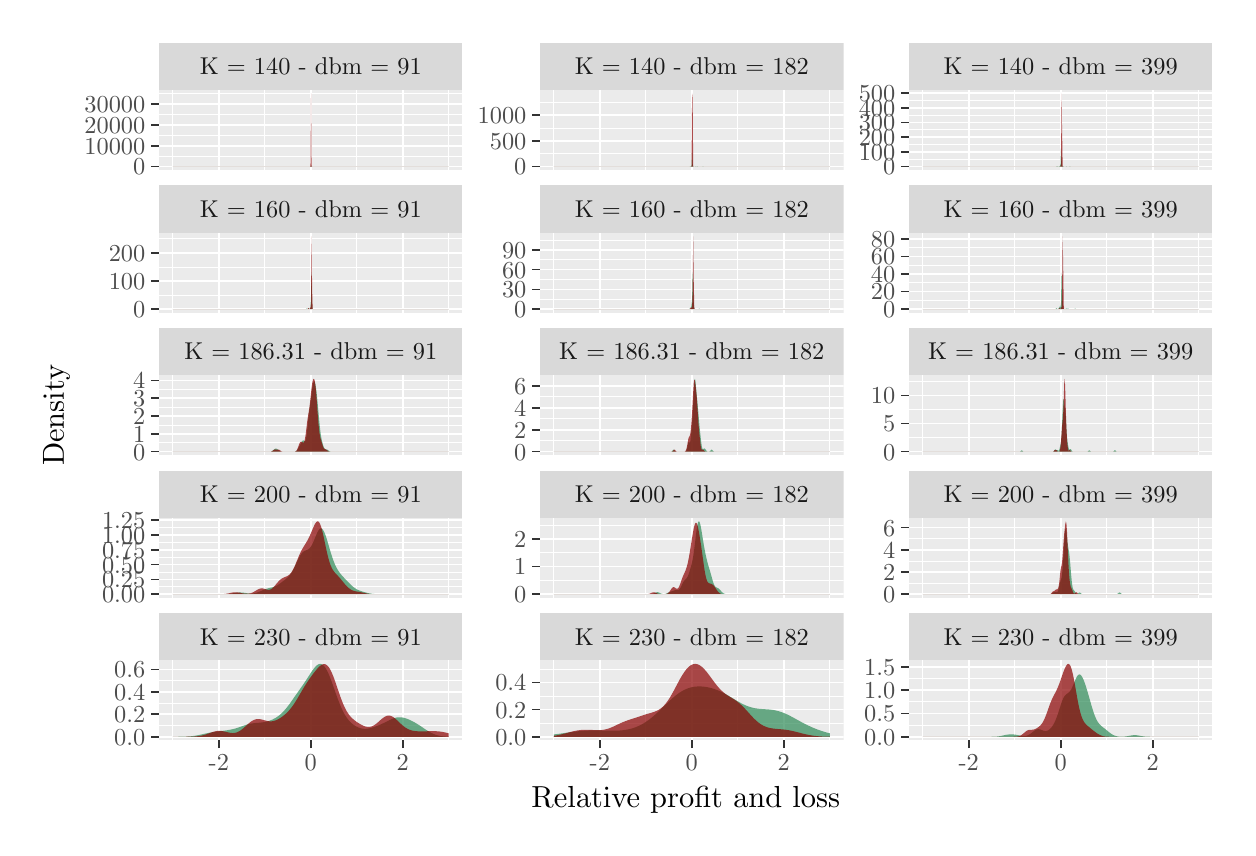
\begin{tikzpicture}[x=1pt,y=1pt]
\definecolor{fillColor}{RGB}{255,255,255}
\path[use as bounding box,fill=fillColor,fill opacity=0.00] (0,0) rectangle (433.62,289.08);
\begin{scope}
\path[clip] (  0.00,  0.00) rectangle (433.62,289.08);
\definecolor{drawColor}{RGB}{255,255,255}
\definecolor{fillColor}{RGB}{255,255,255}

\path[draw=drawColor,line width= 0.6pt,line join=round,line cap=round,fill=fillColor] (  0.00,  0.00) rectangle (433.62,289.08);
\end{scope}
\begin{scope}
\path[clip] ( 47.46,237.57) rectangle (157.12,266.52);
\definecolor{fillColor}{gray}{0.92}

\path[fill=fillColor] ( 47.46,237.57) rectangle (157.12,266.52);
\definecolor{drawColor}{RGB}{255,255,255}

\path[draw=drawColor,line width= 0.3pt,line join=round] ( 47.46,242.65) --
	(157.12,242.65);

\path[draw=drawColor,line width= 0.3pt,line join=round] ( 47.46,250.17) --
	(157.12,250.17);

\path[draw=drawColor,line width= 0.3pt,line join=round] ( 47.46,257.69) --
	(157.12,257.69);

\path[draw=drawColor,line width= 0.3pt,line join=round] ( 47.46,265.22) --
	(157.12,265.22);

\path[draw=drawColor,line width= 0.3pt,line join=round] ( 52.45,237.57) --
	( 52.45,266.52);

\path[draw=drawColor,line width= 0.3pt,line join=round] ( 85.68,237.57) --
	( 85.68,266.52);

\path[draw=drawColor,line width= 0.3pt,line join=round] (118.91,237.57) --
	(118.91,266.52);

\path[draw=drawColor,line width= 0.3pt,line join=round] (152.13,237.57) --
	(152.13,266.52);

\path[draw=drawColor,line width= 0.6pt,line join=round] ( 47.46,238.89) --
	(157.12,238.89);

\path[draw=drawColor,line width= 0.6pt,line join=round] ( 47.46,246.41) --
	(157.12,246.41);

\path[draw=drawColor,line width= 0.6pt,line join=round] ( 47.46,253.93) --
	(157.12,253.93);

\path[draw=drawColor,line width= 0.6pt,line join=round] ( 47.46,261.46) --
	(157.12,261.46);

\path[draw=drawColor,line width= 0.6pt,line join=round] ( 69.06,237.57) --
	( 69.06,266.52);

\path[draw=drawColor,line width= 0.6pt,line join=round] (102.29,237.57) --
	(102.29,266.52);

\path[draw=drawColor,line width= 0.6pt,line join=round] (135.52,237.57) --
	(135.52,266.52);
\definecolor{fillColor}{RGB}{46,139,87}

\path[fill=fillColor,fill opacity=0.70] ( 52.45,238.89) --
	( 52.64,238.89) --
	( 52.84,238.89) --
	( 53.03,238.89) --
	( 53.23,238.89) --
	( 53.42,238.89) --
	( 53.62,238.89) --
	( 53.81,238.89) --
	( 54.01,238.89) --
	( 54.20,238.89) --
	( 54.40,238.89) --
	( 54.59,238.89) --
	( 54.79,238.89) --
	( 54.98,238.89) --
	( 55.18,238.89) --
	( 55.38,238.89) --
	( 55.57,238.89) --
	( 55.77,238.89) --
	( 55.96,238.89) --
	( 56.16,238.89) --
	( 56.35,238.89) --
	( 56.55,238.89) --
	( 56.74,238.89) --
	( 56.94,238.89) --
	( 57.13,238.89) --
	( 57.33,238.89) --
	( 57.52,238.89) --
	( 57.72,238.89) --
	( 57.91,238.89) --
	( 58.11,238.89) --
	( 58.30,238.89) --
	( 58.50,238.89) --
	( 58.69,238.89) --
	( 58.89,238.89) --
	( 59.08,238.89) --
	( 59.28,238.89) --
	( 59.47,238.89) --
	( 59.67,238.89) --
	( 59.86,238.89) --
	( 60.06,238.89) --
	( 60.25,238.89) --
	( 60.45,238.89) --
	( 60.64,238.89) --
	( 60.84,238.89) --
	( 61.03,238.89) --
	( 61.23,238.89) --
	( 61.42,238.89) --
	( 61.62,238.89) --
	( 61.81,238.89) --
	( 62.01,238.89) --
	( 62.20,238.89) --
	( 62.40,238.89) --
	( 62.59,238.89) --
	( 62.79,238.89) --
	( 62.98,238.89) --
	( 63.18,238.89) --
	( 63.37,238.89) --
	( 63.57,238.89) --
	( 63.76,238.89) --
	( 63.96,238.89) --
	( 64.15,238.89) --
	( 64.35,238.89) --
	( 64.54,238.89) --
	( 64.74,238.89) --
	( 64.93,238.89) --
	( 65.13,238.89) --
	( 65.32,238.89) --
	( 65.52,238.89) --
	( 65.71,238.89) --
	( 65.91,238.89) --
	( 66.10,238.89) --
	( 66.30,238.89) --
	( 66.49,238.89) --
	( 66.69,238.89) --
	( 66.88,238.89) --
	( 67.08,238.89) --
	( 67.28,238.89) --
	( 67.47,238.89) --
	( 67.67,238.89) --
	( 67.86,238.89) --
	( 68.06,238.89) --
	( 68.25,238.89) --
	( 68.45,238.89) --
	( 68.64,238.89) --
	( 68.84,238.89) --
	( 69.03,238.89) --
	( 69.23,238.89) --
	( 69.42,238.89) --
	( 69.62,238.89) --
	( 69.81,238.89) --
	( 70.01,238.89) --
	( 70.20,238.89) --
	( 70.40,238.89) --
	( 70.59,238.89) --
	( 70.79,238.89) --
	( 70.98,238.89) --
	( 71.18,238.89) --
	( 71.37,238.89) --
	( 71.57,238.89) --
	( 71.76,238.89) --
	( 71.96,238.89) --
	( 72.15,238.89) --
	( 72.35,238.89) --
	( 72.54,238.89) --
	( 72.74,238.89) --
	( 72.93,238.89) --
	( 73.13,238.89) --
	( 73.32,238.89) --
	( 73.52,238.89) --
	( 73.71,238.89) --
	( 73.91,238.89) --
	( 74.10,238.89) --
	( 74.30,238.89) --
	( 74.49,238.89) --
	( 74.69,238.89) --
	( 74.88,238.89) --
	( 75.08,238.89) --
	( 75.27,238.89) --
	( 75.47,238.89) --
	( 75.66,238.89) --
	( 75.86,238.89) --
	( 76.05,238.89) --
	( 76.25,238.89) --
	( 76.44,238.89) --
	( 76.64,238.89) --
	( 76.83,238.89) --
	( 77.03,238.89) --
	( 77.22,238.89) --
	( 77.42,238.89) --
	( 77.61,238.89) --
	( 77.81,238.89) --
	( 78.00,238.89) --
	( 78.20,238.89) --
	( 78.39,238.89) --
	( 78.59,238.89) --
	( 78.78,238.89) --
	( 78.98,238.89) --
	( 79.17,238.89) --
	( 79.37,238.89) --
	( 79.57,238.89) --
	( 79.76,238.89) --
	( 79.96,238.89) --
	( 80.15,238.89) --
	( 80.35,238.89) --
	( 80.54,238.89) --
	( 80.74,238.89) --
	( 80.93,238.89) --
	( 81.13,238.89) --
	( 81.32,238.89) --
	( 81.52,238.89) --
	( 81.71,238.89) --
	( 81.91,238.89) --
	( 82.10,238.89) --
	( 82.30,238.89) --
	( 82.49,238.89) --
	( 82.69,238.89) --
	( 82.88,238.89) --
	( 83.08,238.89) --
	( 83.27,238.89) --
	( 83.47,238.89) --
	( 83.66,238.89) --
	( 83.86,238.89) --
	( 84.05,238.89) --
	( 84.25,238.89) --
	( 84.44,238.89) --
	( 84.64,238.89) --
	( 84.83,238.89) --
	( 85.03,238.89) --
	( 85.22,238.89) --
	( 85.42,238.89) --
	( 85.61,238.89) --
	( 85.81,238.89) --
	( 86.00,238.89) --
	( 86.20,238.89) --
	( 86.39,238.89) --
	( 86.59,238.89) --
	( 86.78,238.89) --
	( 86.98,238.89) --
	( 87.17,238.89) --
	( 87.37,238.89) --
	( 87.56,238.89) --
	( 87.76,238.89) --
	( 87.95,238.89) --
	( 88.15,238.89) --
	( 88.34,238.89) --
	( 88.54,238.89) --
	( 88.73,238.89) --
	( 88.93,238.89) --
	( 89.12,238.89) --
	( 89.32,238.89) --
	( 89.51,238.89) --
	( 89.71,238.89) --
	( 89.90,238.89) --
	( 90.10,238.89) --
	( 90.29,238.89) --
	( 90.49,238.89) --
	( 90.68,238.89) --
	( 90.88,238.89) --
	( 91.07,238.89) --
	( 91.27,238.89) --
	( 91.46,238.89) --
	( 91.66,238.89) --
	( 91.86,238.89) --
	( 92.05,238.89) --
	( 92.25,238.89) --
	( 92.44,238.89) --
	( 92.64,238.89) --
	( 92.83,238.89) --
	( 93.03,238.89) --
	( 93.22,238.89) --
	( 93.42,238.89) --
	( 93.61,238.89) --
	( 93.81,238.89) --
	( 94.00,238.89) --
	( 94.20,238.89) --
	( 94.39,238.89) --
	( 94.59,238.89) --
	( 94.78,238.89) --
	( 94.98,238.89) --
	( 95.17,238.89) --
	( 95.37,238.89) --
	( 95.56,238.89) --
	( 95.76,238.89) --
	( 95.95,238.89) --
	( 96.15,238.89) --
	( 96.34,238.89) --
	( 96.54,238.89) --
	( 96.73,238.89) --
	( 96.93,238.89) --
	( 97.12,238.89) --
	( 97.32,238.89) --
	( 97.51,238.89) --
	( 97.71,238.89) --
	( 97.90,238.89) --
	( 98.10,238.89) --
	( 98.29,238.89) --
	( 98.49,238.89) --
	( 98.68,238.89) --
	( 98.88,238.89) --
	( 99.07,238.89) --
	( 99.27,238.89) --
	( 99.46,238.89) --
	( 99.66,238.89) --
	( 99.85,238.89) --
	(100.05,238.89) --
	(100.24,238.89) --
	(100.44,238.89) --
	(100.63,238.89) --
	(100.83,238.89) --
	(101.02,238.89) --
	(101.22,238.89) --
	(101.41,238.89) --
	(101.61,238.89) --
	(101.80,238.89) --
	(102.00,238.89) --
	(102.19,238.96) --
	(102.39,239.30) --
	(102.58,238.89) --
	(102.78,238.89) --
	(102.97,238.89) --
	(103.17,238.89) --
	(103.36,238.89) --
	(103.56,238.89) --
	(103.75,238.89) --
	(103.95,238.89) --
	(104.15,238.89) --
	(104.34,238.89) --
	(104.54,238.89) --
	(104.73,238.89) --
	(104.93,238.89) --
	(105.12,238.89) --
	(105.32,238.89) --
	(105.51,238.89) --
	(105.71,238.89) --
	(105.90,238.89) --
	(106.10,238.89) --
	(106.29,238.89) --
	(106.49,238.89) --
	(106.68,238.89) --
	(106.88,238.89) --
	(107.07,238.89) --
	(107.27,238.89) --
	(107.46,238.89) --
	(107.66,238.89) --
	(107.85,238.89) --
	(108.05,238.89) --
	(108.24,238.89) --
	(108.44,238.89) --
	(108.63,238.89) --
	(108.83,238.89) --
	(109.02,238.89) --
	(109.22,238.89) --
	(109.41,238.89) --
	(109.61,238.89) --
	(109.80,238.89) --
	(110.00,238.89) --
	(110.19,238.89) --
	(110.39,238.89) --
	(110.58,238.89) --
	(110.78,238.89) --
	(110.97,238.89) --
	(111.17,238.89) --
	(111.36,238.89) --
	(111.56,238.89) --
	(111.75,238.89) --
	(111.95,238.89) --
	(112.14,238.89) --
	(112.34,238.89) --
	(112.53,238.89) --
	(112.73,238.89) --
	(112.92,238.89) --
	(113.12,238.89) --
	(113.31,238.89) --
	(113.51,238.89) --
	(113.70,238.89) --
	(113.90,238.89) --
	(114.09,238.89) --
	(114.29,238.89) --
	(114.48,238.89) --
	(114.68,238.89) --
	(114.87,238.89) --
	(115.07,238.89) --
	(115.26,238.89) --
	(115.46,238.89) --
	(115.65,238.89) --
	(115.85,238.89) --
	(116.04,238.89) --
	(116.24,238.89) --
	(116.44,238.89) --
	(116.63,238.89) --
	(116.83,238.89) --
	(117.02,238.89) --
	(117.22,238.89) --
	(117.41,238.89) --
	(117.61,238.89) --
	(117.80,238.89) --
	(118.00,238.89) --
	(118.19,238.89) --
	(118.39,238.89) --
	(118.58,238.89) --
	(118.78,238.89) --
	(118.97,238.89) --
	(119.17,238.89) --
	(119.36,238.89) --
	(119.56,238.89) --
	(119.75,238.89) --
	(119.95,238.89) --
	(120.14,238.89) --
	(120.34,238.89) --
	(120.53,238.89) --
	(120.73,238.89) --
	(120.92,238.89) --
	(121.12,238.89) --
	(121.31,238.89) --
	(121.51,238.89) --
	(121.70,238.89) --
	(121.90,238.89) --
	(122.09,238.89) --
	(122.29,238.89) --
	(122.48,238.89) --
	(122.68,238.89) --
	(122.87,238.89) --
	(123.07,238.89) --
	(123.26,238.89) --
	(123.46,238.89) --
	(123.65,238.89) --
	(123.85,238.89) --
	(124.04,238.89) --
	(124.24,238.89) --
	(124.43,238.89) --
	(124.63,238.89) --
	(124.82,238.89) --
	(125.02,238.89) --
	(125.21,238.89) --
	(125.41,238.89) --
	(125.60,238.89) --
	(125.80,238.89) --
	(125.99,238.89) --
	(126.19,238.89) --
	(126.38,238.89) --
	(126.58,238.89) --
	(126.77,238.89) --
	(126.97,238.89) --
	(127.16,238.89) --
	(127.36,238.89) --
	(127.55,238.89) --
	(127.75,238.89) --
	(127.94,238.89) --
	(128.14,238.89) --
	(128.33,238.89) --
	(128.53,238.89) --
	(128.73,238.89) --
	(128.92,238.89) --
	(129.12,238.89) --
	(129.31,238.89) --
	(129.51,238.89) --
	(129.70,238.89) --
	(129.90,238.89) --
	(130.09,238.89) --
	(130.29,238.89) --
	(130.48,238.89) --
	(130.68,238.89) --
	(130.87,238.89) --
	(131.07,238.89) --
	(131.26,238.89) --
	(131.46,238.89) --
	(131.65,238.89) --
	(131.85,238.89) --
	(132.04,238.89) --
	(132.24,238.89) --
	(132.43,238.89) --
	(132.63,238.89) --
	(132.82,238.89) --
	(133.02,238.89) --
	(133.21,238.89) --
	(133.41,238.89) --
	(133.60,238.89) --
	(133.80,238.89) --
	(133.99,238.89) --
	(134.19,238.89) --
	(134.38,238.89) --
	(134.58,238.89) --
	(134.77,238.89) --
	(134.97,238.89) --
	(135.16,238.89) --
	(135.36,238.89) --
	(135.55,238.89) --
	(135.75,238.89) --
	(135.94,238.89) --
	(136.14,238.89) --
	(136.33,238.89) --
	(136.53,238.89) --
	(136.72,238.89) --
	(136.92,238.89) --
	(137.11,238.89) --
	(137.31,238.89) --
	(137.50,238.89) --
	(137.70,238.89) --
	(137.89,238.89) --
	(138.09,238.89) --
	(138.28,238.89) --
	(138.48,238.89) --
	(138.67,238.89) --
	(138.87,238.89) --
	(139.06,238.89) --
	(139.26,238.89) --
	(139.45,238.89) --
	(139.65,238.89) --
	(139.84,238.89) --
	(140.04,238.89) --
	(140.23,238.89) --
	(140.43,238.89) --
	(140.62,238.89) --
	(140.82,238.89) --
	(141.02,238.89) --
	(141.21,238.89) --
	(141.41,238.89) --
	(141.60,238.89) --
	(141.80,238.89) --
	(141.99,238.89) --
	(142.19,238.89) --
	(142.38,238.89) --
	(142.58,238.89) --
	(142.77,238.89) --
	(142.97,238.89) --
	(143.16,238.89) --
	(143.36,238.89) --
	(143.55,238.89) --
	(143.75,238.89) --
	(143.94,238.89) --
	(144.14,238.89) --
	(144.33,238.89) --
	(144.53,238.89) --
	(144.72,238.89) --
	(144.92,238.89) --
	(145.11,238.89) --
	(145.31,238.89) --
	(145.50,238.89) --
	(145.70,238.89) --
	(145.89,238.89) --
	(146.09,238.89) --
	(146.28,238.89) --
	(146.48,238.89) --
	(146.67,238.89) --
	(146.87,238.89) --
	(147.06,238.89) --
	(147.26,238.89) --
	(147.45,238.89) --
	(147.65,238.89) --
	(147.84,238.89) --
	(148.04,238.89) --
	(148.23,238.89) --
	(148.43,238.89) --
	(148.62,238.89) --
	(148.82,238.89) --
	(149.01,238.89) --
	(149.21,238.89) --
	(149.40,238.89) --
	(149.60,238.89) --
	(149.79,238.89) --
	(149.99,238.89) --
	(150.18,238.89) --
	(150.38,238.89) --
	(150.57,238.89) --
	(150.77,238.89) --
	(150.96,238.89) --
	(151.16,238.89) --
	(151.35,238.89) --
	(151.55,238.89) --
	(151.74,238.89) --
	(151.94,238.89) --
	(152.13,238.89) --
	(152.13,238.89) --
	(151.94,238.89) --
	(151.74,238.89) --
	(151.55,238.89) --
	(151.35,238.89) --
	(151.16,238.89) --
	(150.96,238.89) --
	(150.77,238.89) --
	(150.57,238.89) --
	(150.38,238.89) --
	(150.18,238.89) --
	(149.99,238.89) --
	(149.79,238.89) --
	(149.60,238.89) --
	(149.40,238.89) --
	(149.21,238.89) --
	(149.01,238.89) --
	(148.82,238.89) --
	(148.62,238.89) --
	(148.43,238.89) --
	(148.23,238.89) --
	(148.04,238.89) --
	(147.84,238.89) --
	(147.65,238.89) --
	(147.45,238.89) --
	(147.26,238.89) --
	(147.06,238.89) --
	(146.87,238.89) --
	(146.67,238.89) --
	(146.48,238.89) --
	(146.28,238.89) --
	(146.09,238.89) --
	(145.89,238.89) --
	(145.70,238.89) --
	(145.50,238.89) --
	(145.31,238.89) --
	(145.11,238.89) --
	(144.92,238.89) --
	(144.72,238.89) --
	(144.53,238.89) --
	(144.33,238.89) --
	(144.14,238.89) --
	(143.94,238.89) --
	(143.75,238.89) --
	(143.55,238.89) --
	(143.36,238.89) --
	(143.16,238.89) --
	(142.97,238.89) --
	(142.77,238.89) --
	(142.58,238.89) --
	(142.38,238.89) --
	(142.19,238.89) --
	(141.99,238.89) --
	(141.80,238.89) --
	(141.60,238.89) --
	(141.41,238.89) --
	(141.21,238.89) --
	(141.02,238.89) --
	(140.82,238.89) --
	(140.62,238.89) --
	(140.43,238.89) --
	(140.23,238.89) --
	(140.04,238.89) --
	(139.84,238.89) --
	(139.65,238.89) --
	(139.45,238.89) --
	(139.26,238.89) --
	(139.06,238.89) --
	(138.87,238.89) --
	(138.67,238.89) --
	(138.48,238.89) --
	(138.28,238.89) --
	(138.09,238.89) --
	(137.89,238.89) --
	(137.70,238.89) --
	(137.50,238.89) --
	(137.31,238.89) --
	(137.11,238.89) --
	(136.92,238.89) --
	(136.72,238.89) --
	(136.53,238.89) --
	(136.33,238.89) --
	(136.14,238.89) --
	(135.94,238.89) --
	(135.75,238.89) --
	(135.55,238.89) --
	(135.36,238.89) --
	(135.16,238.89) --
	(134.97,238.89) --
	(134.77,238.89) --
	(134.58,238.89) --
	(134.38,238.89) --
	(134.19,238.89) --
	(133.99,238.89) --
	(133.80,238.89) --
	(133.60,238.89) --
	(133.41,238.89) --
	(133.21,238.89) --
	(133.02,238.89) --
	(132.82,238.89) --
	(132.63,238.89) --
	(132.43,238.89) --
	(132.24,238.89) --
	(132.04,238.89) --
	(131.85,238.89) --
	(131.65,238.89) --
	(131.46,238.89) --
	(131.26,238.89) --
	(131.07,238.89) --
	(130.87,238.89) --
	(130.68,238.89) --
	(130.48,238.89) --
	(130.29,238.89) --
	(130.09,238.89) --
	(129.90,238.89) --
	(129.70,238.89) --
	(129.51,238.89) --
	(129.31,238.89) --
	(129.12,238.89) --
	(128.92,238.89) --
	(128.73,238.89) --
	(128.53,238.89) --
	(128.33,238.89) --
	(128.14,238.89) --
	(127.94,238.89) --
	(127.75,238.89) --
	(127.55,238.89) --
	(127.36,238.89) --
	(127.16,238.89) --
	(126.97,238.89) --
	(126.77,238.89) --
	(126.58,238.89) --
	(126.38,238.89) --
	(126.19,238.89) --
	(125.99,238.89) --
	(125.80,238.89) --
	(125.60,238.89) --
	(125.41,238.89) --
	(125.21,238.89) --
	(125.02,238.89) --
	(124.82,238.89) --
	(124.63,238.89) --
	(124.43,238.89) --
	(124.24,238.89) --
	(124.04,238.89) --
	(123.85,238.89) --
	(123.65,238.89) --
	(123.46,238.89) --
	(123.26,238.89) --
	(123.07,238.89) --
	(122.87,238.89) --
	(122.68,238.89) --
	(122.48,238.89) --
	(122.29,238.89) --
	(122.09,238.89) --
	(121.90,238.89) --
	(121.70,238.89) --
	(121.51,238.89) --
	(121.31,238.89) --
	(121.12,238.89) --
	(120.92,238.89) --
	(120.73,238.89) --
	(120.53,238.89) --
	(120.34,238.89) --
	(120.14,238.89) --
	(119.95,238.89) --
	(119.75,238.89) --
	(119.56,238.89) --
	(119.36,238.89) --
	(119.17,238.89) --
	(118.97,238.89) --
	(118.78,238.89) --
	(118.58,238.89) --
	(118.39,238.89) --
	(118.19,238.89) --
	(118.00,238.89) --
	(117.80,238.89) --
	(117.61,238.89) --
	(117.41,238.89) --
	(117.22,238.89) --
	(117.02,238.89) --
	(116.83,238.89) --
	(116.63,238.89) --
	(116.44,238.89) --
	(116.24,238.89) --
	(116.04,238.89) --
	(115.85,238.89) --
	(115.65,238.89) --
	(115.46,238.89) --
	(115.26,238.89) --
	(115.07,238.89) --
	(114.87,238.89) --
	(114.68,238.89) --
	(114.48,238.89) --
	(114.29,238.89) --
	(114.09,238.89) --
	(113.90,238.89) --
	(113.70,238.89) --
	(113.51,238.89) --
	(113.31,238.89) --
	(113.12,238.89) --
	(112.92,238.89) --
	(112.73,238.89) --
	(112.53,238.89) --
	(112.34,238.89) --
	(112.14,238.89) --
	(111.95,238.89) --
	(111.75,238.89) --
	(111.56,238.89) --
	(111.36,238.89) --
	(111.17,238.89) --
	(110.97,238.89) --
	(110.78,238.89) --
	(110.58,238.89) --
	(110.39,238.89) --
	(110.19,238.89) --
	(110.00,238.89) --
	(109.80,238.89) --
	(109.61,238.89) --
	(109.41,238.89) --
	(109.22,238.89) --
	(109.02,238.89) --
	(108.83,238.89) --
	(108.63,238.89) --
	(108.44,238.89) --
	(108.24,238.89) --
	(108.05,238.89) --
	(107.85,238.89) --
	(107.66,238.89) --
	(107.46,238.89) --
	(107.27,238.89) --
	(107.07,238.89) --
	(106.88,238.89) --
	(106.68,238.89) --
	(106.49,238.89) --
	(106.29,238.89) --
	(106.10,238.89) --
	(105.90,238.89) --
	(105.71,238.89) --
	(105.51,238.89) --
	(105.32,238.89) --
	(105.12,238.89) --
	(104.93,238.89) --
	(104.73,238.89) --
	(104.54,238.89) --
	(104.34,238.89) --
	(104.15,238.89) --
	(103.95,238.89) --
	(103.75,238.89) --
	(103.56,238.89) --
	(103.36,238.89) --
	(103.17,238.89) --
	(102.97,238.89) --
	(102.78,238.89) --
	(102.58,238.89) --
	(102.39,238.89) --
	(102.19,238.89) --
	(102.00,238.89) --
	(101.80,238.89) --
	(101.61,238.89) --
	(101.41,238.89) --
	(101.22,238.89) --
	(101.02,238.89) --
	(100.83,238.89) --
	(100.63,238.89) --
	(100.44,238.89) --
	(100.24,238.89) --
	(100.05,238.89) --
	( 99.85,238.89) --
	( 99.66,238.89) --
	( 99.46,238.89) --
	( 99.27,238.89) --
	( 99.07,238.89) --
	( 98.88,238.89) --
	( 98.68,238.89) --
	( 98.49,238.89) --
	( 98.29,238.89) --
	( 98.10,238.89) --
	( 97.90,238.89) --
	( 97.71,238.89) --
	( 97.51,238.89) --
	( 97.32,238.89) --
	( 97.12,238.89) --
	( 96.93,238.89) --
	( 96.73,238.89) --
	( 96.54,238.89) --
	( 96.34,238.89) --
	( 96.15,238.89) --
	( 95.95,238.89) --
	( 95.76,238.89) --
	( 95.56,238.89) --
	( 95.37,238.89) --
	( 95.17,238.89) --
	( 94.98,238.89) --
	( 94.78,238.89) --
	( 94.59,238.89) --
	( 94.39,238.89) --
	( 94.20,238.89) --
	( 94.00,238.89) --
	( 93.81,238.89) --
	( 93.61,238.89) --
	( 93.42,238.89) --
	( 93.22,238.89) --
	( 93.03,238.89) --
	( 92.83,238.89) --
	( 92.64,238.89) --
	( 92.44,238.89) --
	( 92.25,238.89) --
	( 92.05,238.89) --
	( 91.86,238.89) --
	( 91.66,238.89) --
	( 91.46,238.89) --
	( 91.27,238.89) --
	( 91.07,238.89) --
	( 90.88,238.89) --
	( 90.68,238.89) --
	( 90.49,238.89) --
	( 90.29,238.89) --
	( 90.10,238.89) --
	( 89.90,238.89) --
	( 89.71,238.89) --
	( 89.51,238.89) --
	( 89.32,238.89) --
	( 89.12,238.89) --
	( 88.93,238.89) --
	( 88.73,238.89) --
	( 88.54,238.89) --
	( 88.34,238.89) --
	( 88.15,238.89) --
	( 87.95,238.89) --
	( 87.76,238.89) --
	( 87.56,238.89) --
	( 87.37,238.89) --
	( 87.17,238.89) --
	( 86.98,238.89) --
	( 86.78,238.89) --
	( 86.59,238.89) --
	( 86.39,238.89) --
	( 86.20,238.89) --
	( 86.00,238.89) --
	( 85.81,238.89) --
	( 85.61,238.89) --
	( 85.42,238.89) --
	( 85.22,238.89) --
	( 85.03,238.89) --
	( 84.83,238.89) --
	( 84.64,238.89) --
	( 84.44,238.89) --
	( 84.25,238.89) --
	( 84.05,238.89) --
	( 83.86,238.89) --
	( 83.66,238.89) --
	( 83.47,238.89) --
	( 83.27,238.89) --
	( 83.08,238.89) --
	( 82.88,238.89) --
	( 82.69,238.89) --
	( 82.49,238.89) --
	( 82.30,238.89) --
	( 82.10,238.89) --
	( 81.91,238.89) --
	( 81.71,238.89) --
	( 81.52,238.89) --
	( 81.32,238.89) --
	( 81.13,238.89) --
	( 80.93,238.89) --
	( 80.74,238.89) --
	( 80.54,238.89) --
	( 80.35,238.89) --
	( 80.15,238.89) --
	( 79.96,238.89) --
	( 79.76,238.89) --
	( 79.57,238.89) --
	( 79.37,238.89) --
	( 79.17,238.89) --
	( 78.98,238.89) --
	( 78.78,238.89) --
	( 78.59,238.89) --
	( 78.39,238.89) --
	( 78.20,238.89) --
	( 78.00,238.89) --
	( 77.81,238.89) --
	( 77.61,238.89) --
	( 77.42,238.89) --
	( 77.22,238.89) --
	( 77.03,238.89) --
	( 76.83,238.89) --
	( 76.64,238.89) --
	( 76.44,238.89) --
	( 76.25,238.89) --
	( 76.05,238.89) --
	( 75.86,238.89) --
	( 75.66,238.89) --
	( 75.47,238.89) --
	( 75.27,238.89) --
	( 75.08,238.89) --
	( 74.88,238.89) --
	( 74.69,238.89) --
	( 74.49,238.89) --
	( 74.30,238.89) --
	( 74.10,238.89) --
	( 73.91,238.89) --
	( 73.71,238.89) --
	( 73.52,238.89) --
	( 73.32,238.89) --
	( 73.13,238.89) --
	( 72.93,238.89) --
	( 72.74,238.89) --
	( 72.54,238.89) --
	( 72.35,238.89) --
	( 72.15,238.89) --
	( 71.96,238.89) --
	( 71.76,238.89) --
	( 71.57,238.89) --
	( 71.37,238.89) --
	( 71.18,238.89) --
	( 70.98,238.89) --
	( 70.79,238.89) --
	( 70.59,238.89) --
	( 70.40,238.89) --
	( 70.20,238.89) --
	( 70.01,238.89) --
	( 69.81,238.89) --
	( 69.62,238.89) --
	( 69.42,238.89) --
	( 69.23,238.89) --
	( 69.03,238.89) --
	( 68.84,238.89) --
	( 68.64,238.89) --
	( 68.45,238.89) --
	( 68.25,238.89) --
	( 68.06,238.89) --
	( 67.86,238.89) --
	( 67.67,238.89) --
	( 67.47,238.89) --
	( 67.28,238.89) --
	( 67.08,238.89) --
	( 66.88,238.89) --
	( 66.69,238.89) --
	( 66.49,238.89) --
	( 66.30,238.89) --
	( 66.10,238.89) --
	( 65.91,238.89) --
	( 65.71,238.89) --
	( 65.52,238.89) --
	( 65.32,238.89) --
	( 65.13,238.89) --
	( 64.93,238.89) --
	( 64.74,238.89) --
	( 64.54,238.89) --
	( 64.35,238.89) --
	( 64.15,238.89) --
	( 63.96,238.89) --
	( 63.76,238.89) --
	( 63.57,238.89) --
	( 63.37,238.89) --
	( 63.18,238.89) --
	( 62.98,238.89) --
	( 62.79,238.89) --
	( 62.59,238.89) --
	( 62.40,238.89) --
	( 62.20,238.89) --
	( 62.01,238.89) --
	( 61.81,238.89) --
	( 61.62,238.89) --
	( 61.42,238.89) --
	( 61.23,238.89) --
	( 61.03,238.89) --
	( 60.84,238.89) --
	( 60.64,238.89) --
	( 60.45,238.89) --
	( 60.25,238.89) --
	( 60.06,238.89) --
	( 59.86,238.89) --
	( 59.67,238.89) --
	( 59.47,238.89) --
	( 59.28,238.89) --
	( 59.08,238.89) --
	( 58.89,238.89) --
	( 58.69,238.89) --
	( 58.50,238.89) --
	( 58.30,238.89) --
	( 58.11,238.89) --
	( 57.91,238.89) --
	( 57.72,238.89) --
	( 57.52,238.89) --
	( 57.33,238.89) --
	( 57.13,238.89) --
	( 56.94,238.89) --
	( 56.74,238.89) --
	( 56.55,238.89) --
	( 56.35,238.89) --
	( 56.16,238.89) --
	( 55.96,238.89) --
	( 55.77,238.89) --
	( 55.57,238.89) --
	( 55.38,238.89) --
	( 55.18,238.89) --
	( 54.98,238.89) --
	( 54.79,238.89) --
	( 54.59,238.89) --
	( 54.40,238.89) --
	( 54.20,238.89) --
	( 54.01,238.89) --
	( 53.81,238.89) --
	( 53.62,238.89) --
	( 53.42,238.89) --
	( 53.23,238.89) --
	( 53.03,238.89) --
	( 52.84,238.89) --
	( 52.64,238.89) --
	( 52.45,238.89) --
	cycle;
\definecolor{fillColor}{RGB}{139,0,0}

\path[fill=fillColor,fill opacity=0.70] ( 52.45,238.89) --
	( 52.64,238.89) --
	( 52.84,238.89) --
	( 53.03,238.89) --
	( 53.23,238.89) --
	( 53.42,238.89) --
	( 53.62,238.89) --
	( 53.81,238.89) --
	( 54.01,238.89) --
	( 54.20,238.89) --
	( 54.40,238.89) --
	( 54.59,238.89) --
	( 54.79,238.89) --
	( 54.98,238.89) --
	( 55.18,238.89) --
	( 55.38,238.89) --
	( 55.57,238.89) --
	( 55.77,238.89) --
	( 55.96,238.89) --
	( 56.16,238.89) --
	( 56.35,238.89) --
	( 56.55,238.89) --
	( 56.74,238.89) --
	( 56.94,238.89) --
	( 57.13,238.89) --
	( 57.33,238.89) --
	( 57.52,238.89) --
	( 57.72,238.89) --
	( 57.91,238.89) --
	( 58.11,238.89) --
	( 58.30,238.89) --
	( 58.50,238.89) --
	( 58.69,238.89) --
	( 58.89,238.89) --
	( 59.08,238.89) --
	( 59.28,238.89) --
	( 59.47,238.89) --
	( 59.67,238.89) --
	( 59.86,238.89) --
	( 60.06,238.89) --
	( 60.25,238.89) --
	( 60.45,238.89) --
	( 60.64,238.89) --
	( 60.84,238.89) --
	( 61.03,238.89) --
	( 61.23,238.89) --
	( 61.42,238.89) --
	( 61.62,238.89) --
	( 61.81,238.89) --
	( 62.01,238.89) --
	( 62.20,238.89) --
	( 62.40,238.89) --
	( 62.59,238.89) --
	( 62.79,238.89) --
	( 62.98,238.89) --
	( 63.18,238.89) --
	( 63.37,238.89) --
	( 63.57,238.89) --
	( 63.76,238.89) --
	( 63.96,238.89) --
	( 64.15,238.89) --
	( 64.35,238.89) --
	( 64.54,238.89) --
	( 64.74,238.89) --
	( 64.93,238.89) --
	( 65.13,238.89) --
	( 65.32,238.89) --
	( 65.52,238.89) --
	( 65.71,238.89) --
	( 65.91,238.89) --
	( 66.10,238.89) --
	( 66.30,238.89) --
	( 66.49,238.89) --
	( 66.69,238.89) --
	( 66.88,238.89) --
	( 67.08,238.89) --
	( 67.28,238.89) --
	( 67.47,238.89) --
	( 67.67,238.89) --
	( 67.86,238.89) --
	( 68.06,238.89) --
	( 68.25,238.89) --
	( 68.45,238.89) --
	( 68.64,238.89) --
	( 68.84,238.89) --
	( 69.03,238.89) --
	( 69.23,238.89) --
	( 69.42,238.89) --
	( 69.62,238.89) --
	( 69.81,238.89) --
	( 70.01,238.89) --
	( 70.20,238.89) --
	( 70.40,238.89) --
	( 70.59,238.89) --
	( 70.79,238.89) --
	( 70.98,238.89) --
	( 71.18,238.89) --
	( 71.37,238.89) --
	( 71.57,238.89) --
	( 71.76,238.89) --
	( 71.96,238.89) --
	( 72.15,238.89) --
	( 72.35,238.89) --
	( 72.54,238.89) --
	( 72.74,238.89) --
	( 72.93,238.89) --
	( 73.13,238.89) --
	( 73.32,238.89) --
	( 73.52,238.89) --
	( 73.71,238.89) --
	( 73.91,238.89) --
	( 74.10,238.89) --
	( 74.30,238.89) --
	( 74.49,238.89) --
	( 74.69,238.89) --
	( 74.88,238.89) --
	( 75.08,238.89) --
	( 75.27,238.89) --
	( 75.47,238.89) --
	( 75.66,238.89) --
	( 75.86,238.89) --
	( 76.05,238.89) --
	( 76.25,238.89) --
	( 76.44,238.89) --
	( 76.64,238.89) --
	( 76.83,238.89) --
	( 77.03,238.89) --
	( 77.22,238.89) --
	( 77.42,238.89) --
	( 77.61,238.89) --
	( 77.81,238.89) --
	( 78.00,238.89) --
	( 78.20,238.89) --
	( 78.39,238.89) --
	( 78.59,238.89) --
	( 78.78,238.89) --
	( 78.98,238.89) --
	( 79.17,238.89) --
	( 79.37,238.89) --
	( 79.57,238.89) --
	( 79.76,238.89) --
	( 79.96,238.89) --
	( 80.15,238.89) --
	( 80.35,238.89) --
	( 80.54,238.89) --
	( 80.74,238.89) --
	( 80.93,238.89) --
	( 81.13,238.89) --
	( 81.32,238.89) --
	( 81.52,238.89) --
	( 81.71,238.89) --
	( 81.91,238.89) --
	( 82.10,238.89) --
	( 82.30,238.89) --
	( 82.49,238.89) --
	( 82.69,238.89) --
	( 82.88,238.89) --
	( 83.08,238.89) --
	( 83.27,238.89) --
	( 83.47,238.89) --
	( 83.66,238.89) --
	( 83.86,238.89) --
	( 84.05,238.89) --
	( 84.25,238.89) --
	( 84.44,238.89) --
	( 84.64,238.89) --
	( 84.83,238.89) --
	( 85.03,238.89) --
	( 85.22,238.89) --
	( 85.42,238.89) --
	( 85.61,238.89) --
	( 85.81,238.89) --
	( 86.00,238.89) --
	( 86.20,238.89) --
	( 86.39,238.89) --
	( 86.59,238.89) --
	( 86.78,238.89) --
	( 86.98,238.89) --
	( 87.17,238.89) --
	( 87.37,238.89) --
	( 87.56,238.89) --
	( 87.76,238.89) --
	( 87.95,238.89) --
	( 88.15,238.89) --
	( 88.34,238.89) --
	( 88.54,238.89) --
	( 88.73,238.89) --
	( 88.93,238.89) --
	( 89.12,238.89) --
	( 89.32,238.89) --
	( 89.51,238.89) --
	( 89.71,238.89) --
	( 89.90,238.89) --
	( 90.10,238.89) --
	( 90.29,238.89) --
	( 90.49,238.89) --
	( 90.68,238.89) --
	( 90.88,238.89) --
	( 91.07,238.89) --
	( 91.27,238.89) --
	( 91.46,238.89) --
	( 91.66,238.89) --
	( 91.86,238.89) --
	( 92.05,238.89) --
	( 92.25,238.89) --
	( 92.44,238.89) --
	( 92.64,238.89) --
	( 92.83,238.89) --
	( 93.03,238.89) --
	( 93.22,238.89) --
	( 93.42,238.89) --
	( 93.61,238.89) --
	( 93.81,238.89) --
	( 94.00,238.89) --
	( 94.20,238.89) --
	( 94.39,238.89) --
	( 94.59,238.89) --
	( 94.78,238.89) --
	( 94.98,238.89) --
	( 95.17,238.89) --
	( 95.37,238.89) --
	( 95.56,238.89) --
	( 95.76,238.89) --
	( 95.95,238.89) --
	( 96.15,238.89) --
	( 96.34,238.89) --
	( 96.54,238.89) --
	( 96.73,238.89) --
	( 96.93,238.89) --
	( 97.12,238.89) --
	( 97.32,238.89) --
	( 97.51,238.89) --
	( 97.71,238.89) --
	( 97.90,238.89) --
	( 98.10,238.89) --
	( 98.29,238.89) --
	( 98.49,238.89) --
	( 98.68,238.89) --
	( 98.88,238.89) --
	( 99.07,238.89) --
	( 99.27,238.89) --
	( 99.46,238.89) --
	( 99.66,238.89) --
	( 99.85,238.89) --
	(100.05,238.89) --
	(100.24,238.89) --
	(100.44,238.89) --
	(100.63,238.89) --
	(100.83,238.89) --
	(101.02,238.89) --
	(101.22,238.89) --
	(101.41,238.89) --
	(101.61,238.89) --
	(101.80,238.89) --
	(102.00,238.89) --
	(102.19,238.96) --
	(102.39,265.20) --
	(102.58,239.23) --
	(102.78,238.89) --
	(102.97,238.89) --
	(103.17,238.89) --
	(103.36,238.89) --
	(103.56,238.89) --
	(103.75,238.89) --
	(103.95,238.89) --
	(104.15,238.89) --
	(104.34,238.89) --
	(104.54,238.89) --
	(104.73,238.89) --
	(104.93,238.89) --
	(105.12,238.89) --
	(105.32,238.89) --
	(105.51,238.89) --
	(105.71,238.89) --
	(105.90,238.89) --
	(106.10,238.89) --
	(106.29,238.89) --
	(106.49,238.89) --
	(106.68,238.89) --
	(106.88,238.89) --
	(107.07,238.89) --
	(107.27,238.89) --
	(107.46,238.89) --
	(107.66,238.89) --
	(107.85,238.89) --
	(108.05,238.89) --
	(108.24,238.89) --
	(108.44,238.89) --
	(108.63,238.89) --
	(108.83,238.89) --
	(109.02,238.89) --
	(109.22,238.89) --
	(109.41,238.89) --
	(109.61,238.89) --
	(109.80,238.89) --
	(110.00,238.89) --
	(110.19,238.89) --
	(110.39,238.89) --
	(110.58,238.89) --
	(110.78,238.89) --
	(110.97,238.89) --
	(111.17,238.89) --
	(111.36,238.89) --
	(111.56,238.89) --
	(111.75,238.89) --
	(111.95,238.89) --
	(112.14,238.89) --
	(112.34,238.89) --
	(112.53,238.89) --
	(112.73,238.89) --
	(112.92,238.89) --
	(113.12,238.89) --
	(113.31,238.89) --
	(113.51,238.89) --
	(113.70,238.89) --
	(113.90,238.89) --
	(114.09,238.89) --
	(114.29,238.89) --
	(114.48,238.89) --
	(114.68,238.89) --
	(114.87,238.89) --
	(115.07,238.89) --
	(115.26,238.89) --
	(115.46,238.89) --
	(115.65,238.89) --
	(115.85,238.89) --
	(116.04,238.89) --
	(116.24,238.89) --
	(116.44,238.89) --
	(116.63,238.89) --
	(116.83,238.89) --
	(117.02,238.89) --
	(117.22,238.89) --
	(117.41,238.89) --
	(117.61,238.89) --
	(117.80,238.89) --
	(118.00,238.89) --
	(118.19,238.89) --
	(118.39,238.89) --
	(118.58,238.89) --
	(118.78,238.89) --
	(118.97,238.89) --
	(119.17,238.89) --
	(119.36,238.89) --
	(119.56,238.89) --
	(119.75,238.89) --
	(119.95,238.89) --
	(120.14,238.89) --
	(120.34,238.89) --
	(120.53,238.89) --
	(120.73,238.89) --
	(120.92,238.89) --
	(121.12,238.89) --
	(121.31,238.89) --
	(121.51,238.89) --
	(121.70,238.89) --
	(121.90,238.89) --
	(122.09,238.89) --
	(122.29,238.89) --
	(122.48,238.89) --
	(122.68,238.89) --
	(122.87,238.89) --
	(123.07,238.89) --
	(123.26,238.89) --
	(123.46,238.89) --
	(123.65,238.89) --
	(123.85,238.89) --
	(124.04,238.89) --
	(124.24,238.89) --
	(124.43,238.89) --
	(124.63,238.89) --
	(124.82,238.89) --
	(125.02,238.89) --
	(125.21,238.89) --
	(125.41,238.89) --
	(125.60,238.89) --
	(125.80,238.89) --
	(125.99,238.89) --
	(126.19,238.89) --
	(126.38,238.89) --
	(126.58,238.89) --
	(126.77,238.89) --
	(126.97,238.89) --
	(127.16,238.89) --
	(127.36,238.89) --
	(127.55,238.89) --
	(127.75,238.89) --
	(127.94,238.89) --
	(128.14,238.89) --
	(128.33,238.89) --
	(128.53,238.89) --
	(128.73,238.89) --
	(128.92,238.89) --
	(129.12,238.89) --
	(129.31,238.89) --
	(129.51,238.89) --
	(129.70,238.89) --
	(129.90,238.89) --
	(130.09,238.89) --
	(130.29,238.89) --
	(130.48,238.89) --
	(130.68,238.89) --
	(130.87,238.89) --
	(131.07,238.89) --
	(131.26,238.89) --
	(131.46,238.89) --
	(131.65,238.89) --
	(131.85,238.89) --
	(132.04,238.89) --
	(132.24,238.89) --
	(132.43,238.89) --
	(132.63,238.89) --
	(132.82,238.89) --
	(133.02,238.89) --
	(133.21,238.89) --
	(133.41,238.89) --
	(133.60,238.89) --
	(133.80,238.89) --
	(133.99,238.89) --
	(134.19,238.89) --
	(134.38,238.89) --
	(134.58,238.89) --
	(134.77,238.89) --
	(134.97,238.89) --
	(135.16,238.89) --
	(135.36,238.89) --
	(135.55,238.89) --
	(135.75,238.89) --
	(135.94,238.89) --
	(136.14,238.89) --
	(136.33,238.89) --
	(136.53,238.89) --
	(136.72,238.89) --
	(136.92,238.89) --
	(137.11,238.89) --
	(137.31,238.89) --
	(137.50,238.89) --
	(137.70,238.89) --
	(137.89,238.89) --
	(138.09,238.89) --
	(138.28,238.89) --
	(138.48,238.89) --
	(138.67,238.89) --
	(138.87,238.89) --
	(139.06,238.89) --
	(139.26,238.89) --
	(139.45,238.89) --
	(139.65,238.89) --
	(139.84,238.89) --
	(140.04,238.89) --
	(140.23,238.89) --
	(140.43,238.89) --
	(140.62,238.89) --
	(140.82,238.89) --
	(141.02,238.89) --
	(141.21,238.89) --
	(141.41,238.89) --
	(141.60,238.89) --
	(141.80,238.89) --
	(141.99,238.89) --
	(142.19,238.89) --
	(142.38,238.89) --
	(142.58,238.89) --
	(142.77,238.89) --
	(142.97,238.89) --
	(143.16,238.89) --
	(143.36,238.89) --
	(143.55,238.89) --
	(143.75,238.89) --
	(143.94,238.89) --
	(144.14,238.89) --
	(144.33,238.89) --
	(144.53,238.89) --
	(144.72,238.89) --
	(144.92,238.89) --
	(145.11,238.89) --
	(145.31,238.89) --
	(145.50,238.89) --
	(145.70,238.89) --
	(145.89,238.89) --
	(146.09,238.89) --
	(146.28,238.89) --
	(146.48,238.89) --
	(146.67,238.89) --
	(146.87,238.89) --
	(147.06,238.89) --
	(147.26,238.89) --
	(147.45,238.89) --
	(147.65,238.89) --
	(147.84,238.89) --
	(148.04,238.89) --
	(148.23,238.89) --
	(148.43,238.89) --
	(148.62,238.89) --
	(148.82,238.89) --
	(149.01,238.89) --
	(149.21,238.89) --
	(149.40,238.89) --
	(149.60,238.89) --
	(149.79,238.89) --
	(149.99,238.89) --
	(150.18,238.89) --
	(150.38,238.89) --
	(150.57,238.89) --
	(150.77,238.89) --
	(150.96,238.89) --
	(151.16,238.89) --
	(151.35,238.89) --
	(151.55,238.89) --
	(151.74,238.89) --
	(151.94,238.89) --
	(152.13,238.89) --
	(152.13,238.89) --
	(151.94,238.89) --
	(151.74,238.89) --
	(151.55,238.89) --
	(151.35,238.89) --
	(151.16,238.89) --
	(150.96,238.89) --
	(150.77,238.89) --
	(150.57,238.89) --
	(150.38,238.89) --
	(150.18,238.89) --
	(149.99,238.89) --
	(149.79,238.89) --
	(149.60,238.89) --
	(149.40,238.89) --
	(149.21,238.89) --
	(149.01,238.89) --
	(148.82,238.89) --
	(148.62,238.89) --
	(148.43,238.89) --
	(148.23,238.89) --
	(148.04,238.89) --
	(147.84,238.89) --
	(147.65,238.89) --
	(147.45,238.89) --
	(147.26,238.89) --
	(147.06,238.89) --
	(146.87,238.89) --
	(146.67,238.89) --
	(146.48,238.89) --
	(146.28,238.89) --
	(146.09,238.89) --
	(145.89,238.89) --
	(145.70,238.89) --
	(145.50,238.89) --
	(145.31,238.89) --
	(145.11,238.89) --
	(144.92,238.89) --
	(144.72,238.89) --
	(144.53,238.89) --
	(144.33,238.89) --
	(144.14,238.89) --
	(143.94,238.89) --
	(143.75,238.89) --
	(143.55,238.89) --
	(143.36,238.89) --
	(143.16,238.89) --
	(142.97,238.89) --
	(142.77,238.89) --
	(142.58,238.89) --
	(142.38,238.89) --
	(142.19,238.89) --
	(141.99,238.89) --
	(141.80,238.89) --
	(141.60,238.89) --
	(141.41,238.89) --
	(141.21,238.89) --
	(141.02,238.89) --
	(140.82,238.89) --
	(140.62,238.89) --
	(140.43,238.89) --
	(140.23,238.89) --
	(140.04,238.89) --
	(139.84,238.89) --
	(139.65,238.89) --
	(139.45,238.89) --
	(139.26,238.89) --
	(139.06,238.89) --
	(138.87,238.89) --
	(138.67,238.89) --
	(138.48,238.89) --
	(138.28,238.89) --
	(138.09,238.89) --
	(137.89,238.89) --
	(137.70,238.89) --
	(137.50,238.89) --
	(137.31,238.89) --
	(137.11,238.89) --
	(136.92,238.89) --
	(136.72,238.89) --
	(136.53,238.89) --
	(136.33,238.89) --
	(136.14,238.89) --
	(135.94,238.89) --
	(135.75,238.89) --
	(135.55,238.89) --
	(135.36,238.89) --
	(135.16,238.89) --
	(134.97,238.89) --
	(134.77,238.89) --
	(134.58,238.89) --
	(134.38,238.89) --
	(134.19,238.89) --
	(133.99,238.89) --
	(133.80,238.89) --
	(133.60,238.89) --
	(133.41,238.89) --
	(133.21,238.89) --
	(133.02,238.89) --
	(132.82,238.89) --
	(132.63,238.89) --
	(132.43,238.89) --
	(132.24,238.89) --
	(132.04,238.89) --
	(131.85,238.89) --
	(131.65,238.89) --
	(131.46,238.89) --
	(131.26,238.89) --
	(131.07,238.89) --
	(130.87,238.89) --
	(130.68,238.89) --
	(130.48,238.89) --
	(130.29,238.89) --
	(130.09,238.89) --
	(129.90,238.89) --
	(129.70,238.89) --
	(129.51,238.89) --
	(129.31,238.89) --
	(129.12,238.89) --
	(128.92,238.89) --
	(128.73,238.89) --
	(128.53,238.89) --
	(128.33,238.89) --
	(128.14,238.89) --
	(127.94,238.89) --
	(127.75,238.89) --
	(127.55,238.89) --
	(127.36,238.89) --
	(127.16,238.89) --
	(126.97,238.89) --
	(126.77,238.89) --
	(126.58,238.89) --
	(126.38,238.89) --
	(126.19,238.89) --
	(125.99,238.89) --
	(125.80,238.89) --
	(125.60,238.89) --
	(125.41,238.89) --
	(125.21,238.89) --
	(125.02,238.89) --
	(124.82,238.89) --
	(124.63,238.89) --
	(124.43,238.89) --
	(124.24,238.89) --
	(124.04,238.89) --
	(123.85,238.89) --
	(123.65,238.89) --
	(123.46,238.89) --
	(123.26,238.89) --
	(123.07,238.89) --
	(122.87,238.89) --
	(122.68,238.89) --
	(122.48,238.89) --
	(122.29,238.89) --
	(122.09,238.89) --
	(121.90,238.89) --
	(121.70,238.89) --
	(121.51,238.89) --
	(121.31,238.89) --
	(121.12,238.89) --
	(120.92,238.89) --
	(120.73,238.89) --
	(120.53,238.89) --
	(120.34,238.89) --
	(120.14,238.89) --
	(119.95,238.89) --
	(119.75,238.89) --
	(119.56,238.89) --
	(119.36,238.89) --
	(119.17,238.89) --
	(118.97,238.89) --
	(118.78,238.89) --
	(118.58,238.89) --
	(118.39,238.89) --
	(118.19,238.89) --
	(118.00,238.89) --
	(117.80,238.89) --
	(117.61,238.89) --
	(117.41,238.89) --
	(117.22,238.89) --
	(117.02,238.89) --
	(116.83,238.89) --
	(116.63,238.89) --
	(116.44,238.89) --
	(116.24,238.89) --
	(116.04,238.89) --
	(115.85,238.89) --
	(115.65,238.89) --
	(115.46,238.89) --
	(115.26,238.89) --
	(115.07,238.89) --
	(114.87,238.89) --
	(114.68,238.89) --
	(114.48,238.89) --
	(114.29,238.89) --
	(114.09,238.89) --
	(113.90,238.89) --
	(113.70,238.89) --
	(113.51,238.89) --
	(113.31,238.89) --
	(113.12,238.89) --
	(112.92,238.89) --
	(112.73,238.89) --
	(112.53,238.89) --
	(112.34,238.89) --
	(112.14,238.89) --
	(111.95,238.89) --
	(111.75,238.89) --
	(111.56,238.89) --
	(111.36,238.89) --
	(111.17,238.89) --
	(110.97,238.89) --
	(110.78,238.89) --
	(110.58,238.89) --
	(110.39,238.89) --
	(110.19,238.89) --
	(110.00,238.89) --
	(109.80,238.89) --
	(109.61,238.89) --
	(109.41,238.89) --
	(109.22,238.89) --
	(109.02,238.89) --
	(108.83,238.89) --
	(108.63,238.89) --
	(108.44,238.89) --
	(108.24,238.89) --
	(108.05,238.89) --
	(107.85,238.89) --
	(107.66,238.89) --
	(107.46,238.89) --
	(107.27,238.89) --
	(107.07,238.89) --
	(106.88,238.89) --
	(106.68,238.89) --
	(106.49,238.89) --
	(106.29,238.89) --
	(106.10,238.89) --
	(105.90,238.89) --
	(105.71,238.89) --
	(105.51,238.89) --
	(105.32,238.89) --
	(105.12,238.89) --
	(104.93,238.89) --
	(104.73,238.89) --
	(104.54,238.89) --
	(104.34,238.89) --
	(104.15,238.89) --
	(103.95,238.89) --
	(103.75,238.89) --
	(103.56,238.89) --
	(103.36,238.89) --
	(103.17,238.89) --
	(102.97,238.89) --
	(102.78,238.89) --
	(102.58,238.89) --
	(102.39,238.89) --
	(102.19,238.89) --
	(102.00,238.89) --
	(101.80,238.89) --
	(101.61,238.89) --
	(101.41,238.89) --
	(101.22,238.89) --
	(101.02,238.89) --
	(100.83,238.89) --
	(100.63,238.89) --
	(100.44,238.89) --
	(100.24,238.89) --
	(100.05,238.89) --
	( 99.85,238.89) --
	( 99.66,238.89) --
	( 99.46,238.89) --
	( 99.27,238.89) --
	( 99.07,238.89) --
	( 98.88,238.89) --
	( 98.68,238.89) --
	( 98.49,238.89) --
	( 98.29,238.89) --
	( 98.10,238.89) --
	( 97.90,238.89) --
	( 97.71,238.89) --
	( 97.51,238.89) --
	( 97.32,238.89) --
	( 97.12,238.89) --
	( 96.93,238.89) --
	( 96.73,238.89) --
	( 96.54,238.89) --
	( 96.34,238.89) --
	( 96.15,238.89) --
	( 95.95,238.89) --
	( 95.76,238.89) --
	( 95.56,238.89) --
	( 95.37,238.89) --
	( 95.17,238.89) --
	( 94.98,238.89) --
	( 94.78,238.89) --
	( 94.59,238.89) --
	( 94.39,238.89) --
	( 94.20,238.89) --
	( 94.00,238.89) --
	( 93.81,238.89) --
	( 93.61,238.89) --
	( 93.42,238.89) --
	( 93.22,238.89) --
	( 93.03,238.89) --
	( 92.83,238.89) --
	( 92.64,238.89) --
	( 92.44,238.89) --
	( 92.25,238.89) --
	( 92.05,238.89) --
	( 91.86,238.89) --
	( 91.66,238.89) --
	( 91.46,238.89) --
	( 91.27,238.89) --
	( 91.07,238.89) --
	( 90.88,238.89) --
	( 90.68,238.89) --
	( 90.49,238.89) --
	( 90.29,238.89) --
	( 90.10,238.89) --
	( 89.90,238.89) --
	( 89.71,238.89) --
	( 89.51,238.89) --
	( 89.32,238.89) --
	( 89.12,238.89) --
	( 88.93,238.89) --
	( 88.73,238.89) --
	( 88.54,238.89) --
	( 88.34,238.89) --
	( 88.15,238.89) --
	( 87.95,238.89) --
	( 87.76,238.89) --
	( 87.56,238.89) --
	( 87.37,238.89) --
	( 87.17,238.89) --
	( 86.98,238.89) --
	( 86.78,238.89) --
	( 86.59,238.89) --
	( 86.39,238.89) --
	( 86.20,238.89) --
	( 86.00,238.89) --
	( 85.81,238.89) --
	( 85.61,238.89) --
	( 85.42,238.89) --
	( 85.22,238.89) --
	( 85.03,238.89) --
	( 84.83,238.89) --
	( 84.64,238.89) --
	( 84.44,238.89) --
	( 84.25,238.89) --
	( 84.05,238.89) --
	( 83.86,238.89) --
	( 83.66,238.89) --
	( 83.47,238.89) --
	( 83.27,238.89) --
	( 83.08,238.89) --
	( 82.88,238.89) --
	( 82.69,238.89) --
	( 82.49,238.89) --
	( 82.30,238.89) --
	( 82.10,238.89) --
	( 81.91,238.89) --
	( 81.71,238.89) --
	( 81.52,238.89) --
	( 81.32,238.89) --
	( 81.13,238.89) --
	( 80.93,238.89) --
	( 80.74,238.89) --
	( 80.54,238.89) --
	( 80.35,238.89) --
	( 80.15,238.89) --
	( 79.96,238.89) --
	( 79.76,238.89) --
	( 79.57,238.89) --
	( 79.37,238.89) --
	( 79.17,238.89) --
	( 78.98,238.89) --
	( 78.78,238.89) --
	( 78.59,238.89) --
	( 78.39,238.89) --
	( 78.20,238.89) --
	( 78.00,238.89) --
	( 77.81,238.89) --
	( 77.61,238.89) --
	( 77.42,238.89) --
	( 77.22,238.89) --
	( 77.03,238.89) --
	( 76.83,238.89) --
	( 76.64,238.89) --
	( 76.44,238.89) --
	( 76.25,238.89) --
	( 76.05,238.89) --
	( 75.86,238.89) --
	( 75.66,238.89) --
	( 75.47,238.89) --
	( 75.27,238.89) --
	( 75.08,238.89) --
	( 74.88,238.89) --
	( 74.69,238.89) --
	( 74.49,238.89) --
	( 74.30,238.89) --
	( 74.10,238.89) --
	( 73.91,238.89) --
	( 73.71,238.89) --
	( 73.52,238.89) --
	( 73.32,238.89) --
	( 73.13,238.89) --
	( 72.93,238.89) --
	( 72.74,238.89) --
	( 72.54,238.89) --
	( 72.35,238.89) --
	( 72.15,238.89) --
	( 71.96,238.89) --
	( 71.76,238.89) --
	( 71.57,238.89) --
	( 71.37,238.89) --
	( 71.18,238.89) --
	( 70.98,238.89) --
	( 70.79,238.89) --
	( 70.59,238.89) --
	( 70.40,238.89) --
	( 70.20,238.89) --
	( 70.01,238.89) --
	( 69.81,238.89) --
	( 69.62,238.89) --
	( 69.42,238.89) --
	( 69.23,238.89) --
	( 69.03,238.89) --
	( 68.84,238.89) --
	( 68.64,238.89) --
	( 68.45,238.89) --
	( 68.25,238.89) --
	( 68.06,238.89) --
	( 67.86,238.89) --
	( 67.67,238.89) --
	( 67.47,238.89) --
	( 67.28,238.89) --
	( 67.08,238.89) --
	( 66.88,238.89) --
	( 66.69,238.89) --
	( 66.49,238.89) --
	( 66.30,238.89) --
	( 66.10,238.89) --
	( 65.91,238.89) --
	( 65.71,238.89) --
	( 65.52,238.89) --
	( 65.32,238.89) --
	( 65.13,238.89) --
	( 64.93,238.89) --
	( 64.74,238.89) --
	( 64.54,238.89) --
	( 64.35,238.89) --
	( 64.15,238.89) --
	( 63.96,238.89) --
	( 63.76,238.89) --
	( 63.57,238.89) --
	( 63.37,238.89) --
	( 63.18,238.89) --
	( 62.98,238.89) --
	( 62.79,238.89) --
	( 62.59,238.89) --
	( 62.40,238.89) --
	( 62.20,238.89) --
	( 62.01,238.89) --
	( 61.81,238.89) --
	( 61.62,238.89) --
	( 61.42,238.89) --
	( 61.23,238.89) --
	( 61.03,238.89) --
	( 60.84,238.89) --
	( 60.64,238.89) --
	( 60.45,238.89) --
	( 60.25,238.89) --
	( 60.06,238.89) --
	( 59.86,238.89) --
	( 59.67,238.89) --
	( 59.47,238.89) --
	( 59.28,238.89) --
	( 59.08,238.89) --
	( 58.89,238.89) --
	( 58.69,238.89) --
	( 58.50,238.89) --
	( 58.30,238.89) --
	( 58.11,238.89) --
	( 57.91,238.89) --
	( 57.72,238.89) --
	( 57.52,238.89) --
	( 57.33,238.89) --
	( 57.13,238.89) --
	( 56.94,238.89) --
	( 56.74,238.89) --
	( 56.55,238.89) --
	( 56.35,238.89) --
	( 56.16,238.89) --
	( 55.96,238.89) --
	( 55.77,238.89) --
	( 55.57,238.89) --
	( 55.38,238.89) --
	( 55.18,238.89) --
	( 54.98,238.89) --
	( 54.79,238.89) --
	( 54.59,238.89) --
	( 54.40,238.89) --
	( 54.20,238.89) --
	( 54.01,238.89) --
	( 53.81,238.89) --
	( 53.62,238.89) --
	( 53.42,238.89) --
	( 53.23,238.89) --
	( 53.03,238.89) --
	( 52.84,238.89) --
	( 52.64,238.89) --
	( 52.45,238.89) --
	cycle;
\end{scope}
\begin{scope}
\path[clip] ( 47.46,186.06) rectangle (157.12,215.01);
\definecolor{fillColor}{gray}{0.92}

\path[fill=fillColor] ( 47.46,186.06) rectangle (157.12,215.01);
\definecolor{drawColor}{RGB}{255,255,255}

\path[draw=drawColor,line width= 0.3pt,line join=round] ( 47.46,192.45) --
	(157.12,192.45);

\path[draw=drawColor,line width= 0.3pt,line join=round] ( 47.46,202.61) --
	(157.12,202.61);

\path[draw=drawColor,line width= 0.3pt,line join=round] ( 47.46,212.76) --
	(157.12,212.76);

\path[draw=drawColor,line width= 0.3pt,line join=round] ( 52.45,186.06) --
	( 52.45,215.01);

\path[draw=drawColor,line width= 0.3pt,line join=round] ( 85.68,186.06) --
	( 85.68,215.01);

\path[draw=drawColor,line width= 0.3pt,line join=round] (118.91,186.06) --
	(118.91,215.01);

\path[draw=drawColor,line width= 0.3pt,line join=round] (152.13,186.06) --
	(152.13,215.01);

\path[draw=drawColor,line width= 0.6pt,line join=round] ( 47.46,187.38) --
	(157.12,187.38);

\path[draw=drawColor,line width= 0.6pt,line join=round] ( 47.46,197.53) --
	(157.12,197.53);

\path[draw=drawColor,line width= 0.6pt,line join=round] ( 47.46,207.69) --
	(157.12,207.69);

\path[draw=drawColor,line width= 0.6pt,line join=round] ( 69.06,186.06) --
	( 69.06,215.01);

\path[draw=drawColor,line width= 0.6pt,line join=round] (102.29,186.06) --
	(102.29,215.01);

\path[draw=drawColor,line width= 0.6pt,line join=round] (135.52,186.06) --
	(135.52,215.01);
\definecolor{fillColor}{RGB}{46,139,87}

\path[fill=fillColor,fill opacity=0.70] ( 52.45,187.38) --
	( 52.64,187.38) --
	( 52.84,187.38) --
	( 53.03,187.38) --
	( 53.23,187.38) --
	( 53.42,187.38) --
	( 53.62,187.38) --
	( 53.81,187.38) --
	( 54.01,187.38) --
	( 54.20,187.38) --
	( 54.40,187.38) --
	( 54.59,187.38) --
	( 54.79,187.38) --
	( 54.98,187.38) --
	( 55.18,187.38) --
	( 55.38,187.38) --
	( 55.57,187.38) --
	( 55.77,187.38) --
	( 55.96,187.38) --
	( 56.16,187.38) --
	( 56.35,187.38) --
	( 56.55,187.38) --
	( 56.74,187.38) --
	( 56.94,187.38) --
	( 57.13,187.38) --
	( 57.33,187.38) --
	( 57.52,187.38) --
	( 57.72,187.38) --
	( 57.91,187.38) --
	( 58.11,187.38) --
	( 58.30,187.38) --
	( 58.50,187.38) --
	( 58.69,187.38) --
	( 58.89,187.38) --
	( 59.08,187.38) --
	( 59.28,187.38) --
	( 59.47,187.38) --
	( 59.67,187.38) --
	( 59.86,187.38) --
	( 60.06,187.38) --
	( 60.25,187.38) --
	( 60.45,187.38) --
	( 60.64,187.38) --
	( 60.84,187.38) --
	( 61.03,187.38) --
	( 61.23,187.38) --
	( 61.42,187.38) --
	( 61.62,187.38) --
	( 61.81,187.38) --
	( 62.01,187.38) --
	( 62.20,187.38) --
	( 62.40,187.38) --
	( 62.59,187.38) --
	( 62.79,187.38) --
	( 62.98,187.38) --
	( 63.18,187.38) --
	( 63.37,187.38) --
	( 63.57,187.38) --
	( 63.76,187.38) --
	( 63.96,187.38) --
	( 64.15,187.38) --
	( 64.35,187.38) --
	( 64.54,187.38) --
	( 64.74,187.38) --
	( 64.93,187.38) --
	( 65.13,187.38) --
	( 65.32,187.38) --
	( 65.52,187.38) --
	( 65.71,187.38) --
	( 65.91,187.38) --
	( 66.10,187.38) --
	( 66.30,187.38) --
	( 66.49,187.38) --
	( 66.69,187.38) --
	( 66.88,187.38) --
	( 67.08,187.38) --
	( 67.28,187.38) --
	( 67.47,187.38) --
	( 67.67,187.38) --
	( 67.86,187.38) --
	( 68.06,187.38) --
	( 68.25,187.38) --
	( 68.45,187.38) --
	( 68.64,187.38) --
	( 68.84,187.38) --
	( 69.03,187.38) --
	( 69.23,187.38) --
	( 69.42,187.38) --
	( 69.62,187.38) --
	( 69.81,187.38) --
	( 70.01,187.38) --
	( 70.20,187.38) --
	( 70.40,187.38) --
	( 70.59,187.38) --
	( 70.79,187.38) --
	( 70.98,187.38) --
	( 71.18,187.38) --
	( 71.37,187.38) --
	( 71.57,187.38) --
	( 71.76,187.38) --
	( 71.96,187.38) --
	( 72.15,187.38) --
	( 72.35,187.38) --
	( 72.54,187.38) --
	( 72.74,187.38) --
	( 72.93,187.38) --
	( 73.13,187.38) --
	( 73.32,187.38) --
	( 73.52,187.38) --
	( 73.71,187.38) --
	( 73.91,187.38) --
	( 74.10,187.38) --
	( 74.30,187.38) --
	( 74.49,187.38) --
	( 74.69,187.38) --
	( 74.88,187.38) --
	( 75.08,187.38) --
	( 75.27,187.38) --
	( 75.47,187.38) --
	( 75.66,187.38) --
	( 75.86,187.38) --
	( 76.05,187.38) --
	( 76.25,187.38) --
	( 76.44,187.38) --
	( 76.64,187.38) --
	( 76.83,187.38) --
	( 77.03,187.38) --
	( 77.22,187.38) --
	( 77.42,187.38) --
	( 77.61,187.38) --
	( 77.81,187.38) --
	( 78.00,187.38) --
	( 78.20,187.38) --
	( 78.39,187.38) --
	( 78.59,187.38) --
	( 78.78,187.38) --
	( 78.98,187.38) --
	( 79.17,187.38) --
	( 79.37,187.38) --
	( 79.57,187.38) --
	( 79.76,187.38) --
	( 79.96,187.38) --
	( 80.15,187.38) --
	( 80.35,187.38) --
	( 80.54,187.38) --
	( 80.74,187.38) --
	( 80.93,187.38) --
	( 81.13,187.38) --
	( 81.32,187.38) --
	( 81.52,187.38) --
	( 81.71,187.38) --
	( 81.91,187.38) --
	( 82.10,187.38) --
	( 82.30,187.38) --
	( 82.49,187.38) --
	( 82.69,187.38) --
	( 82.88,187.38) --
	( 83.08,187.38) --
	( 83.27,187.38) --
	( 83.47,187.38) --
	( 83.66,187.38) --
	( 83.86,187.38) --
	( 84.05,187.38) --
	( 84.25,187.38) --
	( 84.44,187.38) --
	( 84.64,187.38) --
	( 84.83,187.38) --
	( 85.03,187.38) --
	( 85.22,187.38) --
	( 85.42,187.38) --
	( 85.61,187.38) --
	( 85.81,187.38) --
	( 86.00,187.38) --
	( 86.20,187.38) --
	( 86.39,187.38) --
	( 86.59,187.38) --
	( 86.78,187.38) --
	( 86.98,187.38) --
	( 87.17,187.38) --
	( 87.37,187.38) --
	( 87.56,187.38) --
	( 87.76,187.38) --
	( 87.95,187.38) --
	( 88.15,187.38) --
	( 88.34,187.38) --
	( 88.54,187.38) --
	( 88.73,187.38) --
	( 88.93,187.38) --
	( 89.12,187.38) --
	( 89.32,187.38) --
	( 89.51,187.38) --
	( 89.71,187.38) --
	( 89.90,187.38) --
	( 90.10,187.38) --
	( 90.29,187.38) --
	( 90.49,187.38) --
	( 90.68,187.38) --
	( 90.88,187.38) --
	( 91.07,187.38) --
	( 91.27,187.38) --
	( 91.46,187.38) --
	( 91.66,187.38) --
	( 91.86,187.38) --
	( 92.05,187.38) --
	( 92.25,187.38) --
	( 92.44,187.38) --
	( 92.64,187.38) --
	( 92.83,187.38) --
	( 93.03,187.38) --
	( 93.22,187.38) --
	( 93.42,187.38) --
	( 93.61,187.38) --
	( 93.81,187.38) --
	( 94.00,187.38) --
	( 94.20,187.38) --
	( 94.39,187.38) --
	( 94.59,187.38) --
	( 94.78,187.38) --
	( 94.98,187.38) --
	( 95.17,187.38) --
	( 95.37,187.38) --
	( 95.56,187.38) --
	( 95.76,187.38) --
	( 95.95,187.38) --
	( 96.15,187.38) --
	( 96.34,187.38) --
	( 96.54,187.38) --
	( 96.73,187.38) --
	( 96.93,187.38) --
	( 97.12,187.38) --
	( 97.32,187.38) --
	( 97.51,187.38) --
	( 97.71,187.38) --
	( 97.90,187.38) --
	( 98.10,187.38) --
	( 98.29,187.38) --
	( 98.49,187.38) --
	( 98.68,187.38) --
	( 98.88,187.38) --
	( 99.07,187.38) --
	( 99.27,187.38) --
	( 99.46,187.38) --
	( 99.66,187.38) --
	( 99.85,187.38) --
	(100.05,187.38) --
	(100.24,187.38) --
	(100.44,187.38) --
	(100.63,187.38) --
	(100.83,187.62) --
	(101.02,187.57) --
	(101.22,187.45) --
	(101.41,187.55) --
	(101.61,187.61) --
	(101.80,187.57) --
	(102.00,187.56) --
	(102.19,187.74) --
	(102.39,192.14) --
	(102.58,200.76) --
	(102.78,189.27) --
	(102.97,187.39) --
	(103.17,187.38) --
	(103.36,187.38) --
	(103.56,187.38) --
	(103.75,187.38) --
	(103.95,187.38) --
	(104.15,187.38) --
	(104.34,187.38) --
	(104.54,187.38) --
	(104.73,187.38) --
	(104.93,187.38) --
	(105.12,187.38) --
	(105.32,187.38) --
	(105.51,187.38) --
	(105.71,187.38) --
	(105.90,187.38) --
	(106.10,187.38) --
	(106.29,187.38) --
	(106.49,187.38) --
	(106.68,187.38) --
	(106.88,187.38) --
	(107.07,187.38) --
	(107.27,187.38) --
	(107.46,187.38) --
	(107.66,187.38) --
	(107.85,187.38) --
	(108.05,187.38) --
	(108.24,187.38) --
	(108.44,187.38) --
	(108.63,187.38) --
	(108.83,187.38) --
	(109.02,187.38) --
	(109.22,187.38) --
	(109.41,187.38) --
	(109.61,187.38) --
	(109.80,187.38) --
	(110.00,187.38) --
	(110.19,187.38) --
	(110.39,187.38) --
	(110.58,187.38) --
	(110.78,187.38) --
	(110.97,187.38) --
	(111.17,187.38) --
	(111.36,187.38) --
	(111.56,187.38) --
	(111.75,187.38) --
	(111.95,187.38) --
	(112.14,187.38) --
	(112.34,187.38) --
	(112.53,187.38) --
	(112.73,187.38) --
	(112.92,187.38) --
	(113.12,187.38) --
	(113.31,187.38) --
	(113.51,187.38) --
	(113.70,187.38) --
	(113.90,187.38) --
	(114.09,187.38) --
	(114.29,187.38) --
	(114.48,187.38) --
	(114.68,187.38) --
	(114.87,187.38) --
	(115.07,187.38) --
	(115.26,187.38) --
	(115.46,187.38) --
	(115.65,187.38) --
	(115.85,187.38) --
	(116.04,187.38) --
	(116.24,187.38) --
	(116.44,187.38) --
	(116.63,187.38) --
	(116.83,187.38) --
	(117.02,187.38) --
	(117.22,187.38) --
	(117.41,187.38) --
	(117.61,187.38) --
	(117.80,187.38) --
	(118.00,187.38) --
	(118.19,187.38) --
	(118.39,187.38) --
	(118.58,187.38) --
	(118.78,187.38) --
	(118.97,187.38) --
	(119.17,187.38) --
	(119.36,187.38) --
	(119.56,187.38) --
	(119.75,187.38) --
	(119.95,187.38) --
	(120.14,187.38) --
	(120.34,187.38) --
	(120.53,187.38) --
	(120.73,187.38) --
	(120.92,187.38) --
	(121.12,187.38) --
	(121.31,187.38) --
	(121.51,187.38) --
	(121.70,187.38) --
	(121.90,187.38) --
	(122.09,187.38) --
	(122.29,187.38) --
	(122.48,187.38) --
	(122.68,187.38) --
	(122.87,187.38) --
	(123.07,187.38) --
	(123.26,187.38) --
	(123.46,187.38) --
	(123.65,187.38) --
	(123.85,187.38) --
	(124.04,187.38) --
	(124.24,187.38) --
	(124.43,187.38) --
	(124.63,187.38) --
	(124.82,187.38) --
	(125.02,187.38) --
	(125.21,187.38) --
	(125.41,187.38) --
	(125.60,187.38) --
	(125.80,187.38) --
	(125.99,187.38) --
	(126.19,187.38) --
	(126.38,187.38) --
	(126.58,187.38) --
	(126.77,187.38) --
	(126.97,187.38) --
	(127.16,187.38) --
	(127.36,187.38) --
	(127.55,187.38) --
	(127.75,187.38) --
	(127.94,187.38) --
	(128.14,187.38) --
	(128.33,187.38) --
	(128.53,187.38) --
	(128.73,187.38) --
	(128.92,187.38) --
	(129.12,187.38) --
	(129.31,187.38) --
	(129.51,187.38) --
	(129.70,187.38) --
	(129.90,187.38) --
	(130.09,187.38) --
	(130.29,187.38) --
	(130.48,187.38) --
	(130.68,187.38) --
	(130.87,187.38) --
	(131.07,187.38) --
	(131.26,187.38) --
	(131.46,187.38) --
	(131.65,187.38) --
	(131.85,187.38) --
	(132.04,187.38) --
	(132.24,187.38) --
	(132.43,187.38) --
	(132.63,187.38) --
	(132.82,187.38) --
	(133.02,187.38) --
	(133.21,187.38) --
	(133.41,187.38) --
	(133.60,187.38) --
	(133.80,187.38) --
	(133.99,187.38) --
	(134.19,187.38) --
	(134.38,187.38) --
	(134.58,187.38) --
	(134.77,187.38) --
	(134.97,187.38) --
	(135.16,187.38) --
	(135.36,187.38) --
	(135.55,187.38) --
	(135.75,187.38) --
	(135.94,187.38) --
	(136.14,187.38) --
	(136.33,187.38) --
	(136.53,187.38) --
	(136.72,187.38) --
	(136.92,187.38) --
	(137.11,187.38) --
	(137.31,187.38) --
	(137.50,187.38) --
	(137.70,187.38) --
	(137.89,187.38) --
	(138.09,187.38) --
	(138.28,187.38) --
	(138.48,187.38) --
	(138.67,187.38) --
	(138.87,187.38) --
	(139.06,187.38) --
	(139.26,187.38) --
	(139.45,187.38) --
	(139.65,187.38) --
	(139.84,187.38) --
	(140.04,187.38) --
	(140.23,187.38) --
	(140.43,187.38) --
	(140.62,187.38) --
	(140.82,187.38) --
	(141.02,187.38) --
	(141.21,187.38) --
	(141.41,187.38) --
	(141.60,187.38) --
	(141.80,187.38) --
	(141.99,187.38) --
	(142.19,187.38) --
	(142.38,187.38) --
	(142.58,187.38) --
	(142.77,187.38) --
	(142.97,187.38) --
	(143.16,187.38) --
	(143.36,187.38) --
	(143.55,187.38) --
	(143.75,187.38) --
	(143.94,187.38) --
	(144.14,187.38) --
	(144.33,187.38) --
	(144.53,187.38) --
	(144.72,187.38) --
	(144.92,187.38) --
	(145.11,187.38) --
	(145.31,187.38) --
	(145.50,187.38) --
	(145.70,187.38) --
	(145.89,187.38) --
	(146.09,187.38) --
	(146.28,187.38) --
	(146.48,187.38) --
	(146.67,187.38) --
	(146.87,187.38) --
	(147.06,187.38) --
	(147.26,187.38) --
	(147.45,187.38) --
	(147.65,187.38) --
	(147.84,187.38) --
	(148.04,187.38) --
	(148.23,187.38) --
	(148.43,187.38) --
	(148.62,187.38) --
	(148.82,187.38) --
	(149.01,187.38) --
	(149.21,187.38) --
	(149.40,187.38) --
	(149.60,187.38) --
	(149.79,187.38) --
	(149.99,187.38) --
	(150.18,187.38) --
	(150.38,187.38) --
	(150.57,187.38) --
	(150.77,187.38) --
	(150.96,187.38) --
	(151.16,187.38) --
	(151.35,187.38) --
	(151.55,187.38) --
	(151.74,187.38) --
	(151.94,187.38) --
	(152.13,187.38) --
	(152.13,187.38) --
	(151.94,187.38) --
	(151.74,187.38) --
	(151.55,187.38) --
	(151.35,187.38) --
	(151.16,187.38) --
	(150.96,187.38) --
	(150.77,187.38) --
	(150.57,187.38) --
	(150.38,187.38) --
	(150.18,187.38) --
	(149.99,187.38) --
	(149.79,187.38) --
	(149.60,187.38) --
	(149.40,187.38) --
	(149.21,187.38) --
	(149.01,187.38) --
	(148.82,187.38) --
	(148.62,187.38) --
	(148.43,187.38) --
	(148.23,187.38) --
	(148.04,187.38) --
	(147.84,187.38) --
	(147.65,187.38) --
	(147.45,187.38) --
	(147.26,187.38) --
	(147.06,187.38) --
	(146.87,187.38) --
	(146.67,187.38) --
	(146.48,187.38) --
	(146.28,187.38) --
	(146.09,187.38) --
	(145.89,187.38) --
	(145.70,187.38) --
	(145.50,187.38) --
	(145.31,187.38) --
	(145.11,187.38) --
	(144.92,187.38) --
	(144.72,187.38) --
	(144.53,187.38) --
	(144.33,187.38) --
	(144.14,187.38) --
	(143.94,187.38) --
	(143.75,187.38) --
	(143.55,187.38) --
	(143.36,187.38) --
	(143.16,187.38) --
	(142.97,187.38) --
	(142.77,187.38) --
	(142.58,187.38) --
	(142.38,187.38) --
	(142.19,187.38) --
	(141.99,187.38) --
	(141.80,187.38) --
	(141.60,187.38) --
	(141.41,187.38) --
	(141.21,187.38) --
	(141.02,187.38) --
	(140.82,187.38) --
	(140.62,187.38) --
	(140.43,187.38) --
	(140.23,187.38) --
	(140.04,187.38) --
	(139.84,187.38) --
	(139.65,187.38) --
	(139.45,187.38) --
	(139.26,187.38) --
	(139.06,187.38) --
	(138.87,187.38) --
	(138.67,187.38) --
	(138.48,187.38) --
	(138.28,187.38) --
	(138.09,187.38) --
	(137.89,187.38) --
	(137.70,187.38) --
	(137.50,187.38) --
	(137.31,187.38) --
	(137.11,187.38) --
	(136.92,187.38) --
	(136.72,187.38) --
	(136.53,187.38) --
	(136.33,187.38) --
	(136.14,187.38) --
	(135.94,187.38) --
	(135.75,187.38) --
	(135.55,187.38) --
	(135.36,187.38) --
	(135.16,187.38) --
	(134.97,187.38) --
	(134.77,187.38) --
	(134.58,187.38) --
	(134.38,187.38) --
	(134.19,187.38) --
	(133.99,187.38) --
	(133.80,187.38) --
	(133.60,187.38) --
	(133.41,187.38) --
	(133.21,187.38) --
	(133.02,187.38) --
	(132.82,187.38) --
	(132.63,187.38) --
	(132.43,187.38) --
	(132.24,187.38) --
	(132.04,187.38) --
	(131.85,187.38) --
	(131.65,187.38) --
	(131.46,187.38) --
	(131.26,187.38) --
	(131.07,187.38) --
	(130.87,187.38) --
	(130.68,187.38) --
	(130.48,187.38) --
	(130.29,187.38) --
	(130.09,187.38) --
	(129.90,187.38) --
	(129.70,187.38) --
	(129.51,187.38) --
	(129.31,187.38) --
	(129.12,187.38) --
	(128.92,187.38) --
	(128.73,187.38) --
	(128.53,187.38) --
	(128.33,187.38) --
	(128.14,187.38) --
	(127.94,187.38) --
	(127.75,187.38) --
	(127.55,187.38) --
	(127.36,187.38) --
	(127.16,187.38) --
	(126.97,187.38) --
	(126.77,187.38) --
	(126.58,187.38) --
	(126.38,187.38) --
	(126.19,187.38) --
	(125.99,187.38) --
	(125.80,187.38) --
	(125.60,187.38) --
	(125.41,187.38) --
	(125.21,187.38) --
	(125.02,187.38) --
	(124.82,187.38) --
	(124.63,187.38) --
	(124.43,187.38) --
	(124.24,187.38) --
	(124.04,187.38) --
	(123.85,187.38) --
	(123.65,187.38) --
	(123.46,187.38) --
	(123.26,187.38) --
	(123.07,187.38) --
	(122.87,187.38) --
	(122.68,187.38) --
	(122.48,187.38) --
	(122.29,187.38) --
	(122.09,187.38) --
	(121.90,187.38) --
	(121.70,187.38) --
	(121.51,187.38) --
	(121.31,187.38) --
	(121.12,187.38) --
	(120.92,187.38) --
	(120.73,187.38) --
	(120.53,187.38) --
	(120.34,187.38) --
	(120.14,187.38) --
	(119.95,187.38) --
	(119.75,187.38) --
	(119.56,187.38) --
	(119.36,187.38) --
	(119.17,187.38) --
	(118.97,187.38) --
	(118.78,187.38) --
	(118.58,187.38) --
	(118.39,187.38) --
	(118.19,187.38) --
	(118.00,187.38) --
	(117.80,187.38) --
	(117.61,187.38) --
	(117.41,187.38) --
	(117.22,187.38) --
	(117.02,187.38) --
	(116.83,187.38) --
	(116.63,187.38) --
	(116.44,187.38) --
	(116.24,187.38) --
	(116.04,187.38) --
	(115.85,187.38) --
	(115.65,187.38) --
	(115.46,187.38) --
	(115.26,187.38) --
	(115.07,187.38) --
	(114.87,187.38) --
	(114.68,187.38) --
	(114.48,187.38) --
	(114.29,187.38) --
	(114.09,187.38) --
	(113.90,187.38) --
	(113.70,187.38) --
	(113.51,187.38) --
	(113.31,187.38) --
	(113.12,187.38) --
	(112.92,187.38) --
	(112.73,187.38) --
	(112.53,187.38) --
	(112.34,187.38) --
	(112.14,187.38) --
	(111.95,187.38) --
	(111.75,187.38) --
	(111.56,187.38) --
	(111.36,187.38) --
	(111.17,187.38) --
	(110.97,187.38) --
	(110.78,187.38) --
	(110.58,187.38) --
	(110.39,187.38) --
	(110.19,187.38) --
	(110.00,187.38) --
	(109.80,187.38) --
	(109.61,187.38) --
	(109.41,187.38) --
	(109.22,187.38) --
	(109.02,187.38) --
	(108.83,187.38) --
	(108.63,187.38) --
	(108.44,187.38) --
	(108.24,187.38) --
	(108.05,187.38) --
	(107.85,187.38) --
	(107.66,187.38) --
	(107.46,187.38) --
	(107.27,187.38) --
	(107.07,187.38) --
	(106.88,187.38) --
	(106.68,187.38) --
	(106.49,187.38) --
	(106.29,187.38) --
	(106.10,187.38) --
	(105.90,187.38) --
	(105.71,187.38) --
	(105.51,187.38) --
	(105.32,187.38) --
	(105.12,187.38) --
	(104.93,187.38) --
	(104.73,187.38) --
	(104.54,187.38) --
	(104.34,187.38) --
	(104.15,187.38) --
	(103.95,187.38) --
	(103.75,187.38) --
	(103.56,187.38) --
	(103.36,187.38) --
	(103.17,187.38) --
	(102.97,187.38) --
	(102.78,187.38) --
	(102.58,187.38) --
	(102.39,187.38) --
	(102.19,187.38) --
	(102.00,187.38) --
	(101.80,187.38) --
	(101.61,187.38) --
	(101.41,187.38) --
	(101.22,187.38) --
	(101.02,187.38) --
	(100.83,187.38) --
	(100.63,187.38) --
	(100.44,187.38) --
	(100.24,187.38) --
	(100.05,187.38) --
	( 99.85,187.38) --
	( 99.66,187.38) --
	( 99.46,187.38) --
	( 99.27,187.38) --
	( 99.07,187.38) --
	( 98.88,187.38) --
	( 98.68,187.38) --
	( 98.49,187.38) --
	( 98.29,187.38) --
	( 98.10,187.38) --
	( 97.90,187.38) --
	( 97.71,187.38) --
	( 97.51,187.38) --
	( 97.32,187.38) --
	( 97.12,187.38) --
	( 96.93,187.38) --
	( 96.73,187.38) --
	( 96.54,187.38) --
	( 96.34,187.38) --
	( 96.15,187.38) --
	( 95.95,187.38) --
	( 95.76,187.38) --
	( 95.56,187.38) --
	( 95.37,187.38) --
	( 95.17,187.38) --
	( 94.98,187.38) --
	( 94.78,187.38) --
	( 94.59,187.38) --
	( 94.39,187.38) --
	( 94.20,187.38) --
	( 94.00,187.38) --
	( 93.81,187.38) --
	( 93.61,187.38) --
	( 93.42,187.38) --
	( 93.22,187.38) --
	( 93.03,187.38) --
	( 92.83,187.38) --
	( 92.64,187.38) --
	( 92.44,187.38) --
	( 92.25,187.38) --
	( 92.05,187.38) --
	( 91.86,187.38) --
	( 91.66,187.38) --
	( 91.46,187.38) --
	( 91.27,187.38) --
	( 91.07,187.38) --
	( 90.88,187.38) --
	( 90.68,187.38) --
	( 90.49,187.38) --
	( 90.29,187.38) --
	( 90.10,187.38) --
	( 89.90,187.38) --
	( 89.71,187.38) --
	( 89.51,187.38) --
	( 89.32,187.38) --
	( 89.12,187.38) --
	( 88.93,187.38) --
	( 88.73,187.38) --
	( 88.54,187.38) --
	( 88.34,187.38) --
	( 88.15,187.38) --
	( 87.95,187.38) --
	( 87.76,187.38) --
	( 87.56,187.38) --
	( 87.37,187.38) --
	( 87.17,187.38) --
	( 86.98,187.38) --
	( 86.78,187.38) --
	( 86.59,187.38) --
	( 86.39,187.38) --
	( 86.20,187.38) --
	( 86.00,187.38) --
	( 85.81,187.38) --
	( 85.61,187.38) --
	( 85.42,187.38) --
	( 85.22,187.38) --
	( 85.03,187.38) --
	( 84.83,187.38) --
	( 84.64,187.38) --
	( 84.44,187.38) --
	( 84.25,187.38) --
	( 84.05,187.38) --
	( 83.86,187.38) --
	( 83.66,187.38) --
	( 83.47,187.38) --
	( 83.27,187.38) --
	( 83.08,187.38) --
	( 82.88,187.38) --
	( 82.69,187.38) --
	( 82.49,187.38) --
	( 82.30,187.38) --
	( 82.10,187.38) --
	( 81.91,187.38) --
	( 81.71,187.38) --
	( 81.52,187.38) --
	( 81.32,187.38) --
	( 81.13,187.38) --
	( 80.93,187.38) --
	( 80.74,187.38) --
	( 80.54,187.38) --
	( 80.35,187.38) --
	( 80.15,187.38) --
	( 79.96,187.38) --
	( 79.76,187.38) --
	( 79.57,187.38) --
	( 79.37,187.38) --
	( 79.17,187.38) --
	( 78.98,187.38) --
	( 78.78,187.38) --
	( 78.59,187.38) --
	( 78.39,187.38) --
	( 78.20,187.38) --
	( 78.00,187.38) --
	( 77.81,187.38) --
	( 77.61,187.38) --
	( 77.42,187.38) --
	( 77.22,187.38) --
	( 77.03,187.38) --
	( 76.83,187.38) --
	( 76.64,187.38) --
	( 76.44,187.38) --
	( 76.25,187.38) --
	( 76.05,187.38) --
	( 75.86,187.38) --
	( 75.66,187.38) --
	( 75.47,187.38) --
	( 75.27,187.38) --
	( 75.08,187.38) --
	( 74.88,187.38) --
	( 74.69,187.38) --
	( 74.49,187.38) --
	( 74.30,187.38) --
	( 74.10,187.38) --
	( 73.91,187.38) --
	( 73.71,187.38) --
	( 73.52,187.38) --
	( 73.32,187.38) --
	( 73.13,187.38) --
	( 72.93,187.38) --
	( 72.74,187.38) --
	( 72.54,187.38) --
	( 72.35,187.38) --
	( 72.15,187.38) --
	( 71.96,187.38) --
	( 71.76,187.38) --
	( 71.57,187.38) --
	( 71.37,187.38) --
	( 71.18,187.38) --
	( 70.98,187.38) --
	( 70.79,187.38) --
	( 70.59,187.38) --
	( 70.40,187.38) --
	( 70.20,187.38) --
	( 70.01,187.38) --
	( 69.81,187.38) --
	( 69.62,187.38) --
	( 69.42,187.38) --
	( 69.23,187.38) --
	( 69.03,187.38) --
	( 68.84,187.38) --
	( 68.64,187.38) --
	( 68.45,187.38) --
	( 68.25,187.38) --
	( 68.06,187.38) --
	( 67.86,187.38) --
	( 67.67,187.38) --
	( 67.47,187.38) --
	( 67.28,187.38) --
	( 67.08,187.38) --
	( 66.88,187.38) --
	( 66.69,187.38) --
	( 66.49,187.38) --
	( 66.30,187.38) --
	( 66.10,187.38) --
	( 65.91,187.38) --
	( 65.71,187.38) --
	( 65.52,187.38) --
	( 65.32,187.38) --
	( 65.13,187.38) --
	( 64.93,187.38) --
	( 64.74,187.38) --
	( 64.54,187.38) --
	( 64.35,187.38) --
	( 64.15,187.38) --
	( 63.96,187.38) --
	( 63.76,187.38) --
	( 63.57,187.38) --
	( 63.37,187.38) --
	( 63.18,187.38) --
	( 62.98,187.38) --
	( 62.79,187.38) --
	( 62.59,187.38) --
	( 62.40,187.38) --
	( 62.20,187.38) --
	( 62.01,187.38) --
	( 61.81,187.38) --
	( 61.62,187.38) --
	( 61.42,187.38) --
	( 61.23,187.38) --
	( 61.03,187.38) --
	( 60.84,187.38) --
	( 60.64,187.38) --
	( 60.45,187.38) --
	( 60.25,187.38) --
	( 60.06,187.38) --
	( 59.86,187.38) --
	( 59.67,187.38) --
	( 59.47,187.38) --
	( 59.28,187.38) --
	( 59.08,187.38) --
	( 58.89,187.38) --
	( 58.69,187.38) --
	( 58.50,187.38) --
	( 58.30,187.38) --
	( 58.11,187.38) --
	( 57.91,187.38) --
	( 57.72,187.38) --
	( 57.52,187.38) --
	( 57.33,187.38) --
	( 57.13,187.38) --
	( 56.94,187.38) --
	( 56.74,187.38) --
	( 56.55,187.38) --
	( 56.35,187.38) --
	( 56.16,187.38) --
	( 55.96,187.38) --
	( 55.77,187.38) --
	( 55.57,187.38) --
	( 55.38,187.38) --
	( 55.18,187.38) --
	( 54.98,187.38) --
	( 54.79,187.38) --
	( 54.59,187.38) --
	( 54.40,187.38) --
	( 54.20,187.38) --
	( 54.01,187.38) --
	( 53.81,187.38) --
	( 53.62,187.38) --
	( 53.42,187.38) --
	( 53.23,187.38) --
	( 53.03,187.38) --
	( 52.84,187.38) --
	( 52.64,187.38) --
	( 52.45,187.38) --
	cycle;
\definecolor{fillColor}{RGB}{139,0,0}

\path[fill=fillColor,fill opacity=0.70] ( 52.45,187.38) --
	( 52.64,187.38) --
	( 52.84,187.38) --
	( 53.03,187.38) --
	( 53.23,187.38) --
	( 53.42,187.38) --
	( 53.62,187.38) --
	( 53.81,187.38) --
	( 54.01,187.38) --
	( 54.20,187.38) --
	( 54.40,187.38) --
	( 54.59,187.38) --
	( 54.79,187.38) --
	( 54.98,187.38) --
	( 55.18,187.38) --
	( 55.38,187.38) --
	( 55.57,187.38) --
	( 55.77,187.38) --
	( 55.96,187.38) --
	( 56.16,187.38) --
	( 56.35,187.38) --
	( 56.55,187.38) --
	( 56.74,187.38) --
	( 56.94,187.38) --
	( 57.13,187.38) --
	( 57.33,187.38) --
	( 57.52,187.38) --
	( 57.72,187.38) --
	( 57.91,187.38) --
	( 58.11,187.38) --
	( 58.30,187.38) --
	( 58.50,187.38) --
	( 58.69,187.38) --
	( 58.89,187.38) --
	( 59.08,187.38) --
	( 59.28,187.38) --
	( 59.47,187.38) --
	( 59.67,187.38) --
	( 59.86,187.38) --
	( 60.06,187.38) --
	( 60.25,187.38) --
	( 60.45,187.38) --
	( 60.64,187.38) --
	( 60.84,187.38) --
	( 61.03,187.38) --
	( 61.23,187.38) --
	( 61.42,187.38) --
	( 61.62,187.38) --
	( 61.81,187.38) --
	( 62.01,187.38) --
	( 62.20,187.38) --
	( 62.40,187.38) --
	( 62.59,187.38) --
	( 62.79,187.38) --
	( 62.98,187.38) --
	( 63.18,187.38) --
	( 63.37,187.38) --
	( 63.57,187.38) --
	( 63.76,187.38) --
	( 63.96,187.38) --
	( 64.15,187.38) --
	( 64.35,187.38) --
	( 64.54,187.38) --
	( 64.74,187.38) --
	( 64.93,187.38) --
	( 65.13,187.38) --
	( 65.32,187.38) --
	( 65.52,187.38) --
	( 65.71,187.38) --
	( 65.91,187.38) --
	( 66.10,187.38) --
	( 66.30,187.38) --
	( 66.49,187.38) --
	( 66.69,187.38) --
	( 66.88,187.38) --
	( 67.08,187.38) --
	( 67.28,187.38) --
	( 67.47,187.38) --
	( 67.67,187.38) --
	( 67.86,187.38) --
	( 68.06,187.38) --
	( 68.25,187.38) --
	( 68.45,187.38) --
	( 68.64,187.38) --
	( 68.84,187.38) --
	( 69.03,187.38) --
	( 69.23,187.38) --
	( 69.42,187.38) --
	( 69.62,187.38) --
	( 69.81,187.38) --
	( 70.01,187.38) --
	( 70.20,187.38) --
	( 70.40,187.38) --
	( 70.59,187.38) --
	( 70.79,187.38) --
	( 70.98,187.38) --
	( 71.18,187.38) --
	( 71.37,187.38) --
	( 71.57,187.38) --
	( 71.76,187.38) --
	( 71.96,187.38) --
	( 72.15,187.38) --
	( 72.35,187.38) --
	( 72.54,187.38) --
	( 72.74,187.38) --
	( 72.93,187.38) --
	( 73.13,187.38) --
	( 73.32,187.38) --
	( 73.52,187.38) --
	( 73.71,187.38) --
	( 73.91,187.38) --
	( 74.10,187.38) --
	( 74.30,187.38) --
	( 74.49,187.38) --
	( 74.69,187.38) --
	( 74.88,187.38) --
	( 75.08,187.38) --
	( 75.27,187.38) --
	( 75.47,187.38) --
	( 75.66,187.38) --
	( 75.86,187.38) --
	( 76.05,187.38) --
	( 76.25,187.38) --
	( 76.44,187.38) --
	( 76.64,187.38) --
	( 76.83,187.38) --
	( 77.03,187.38) --
	( 77.22,187.38) --
	( 77.42,187.38) --
	( 77.61,187.38) --
	( 77.81,187.38) --
	( 78.00,187.38) --
	( 78.20,187.38) --
	( 78.39,187.38) --
	( 78.59,187.38) --
	( 78.78,187.38) --
	( 78.98,187.38) --
	( 79.17,187.38) --
	( 79.37,187.38) --
	( 79.57,187.38) --
	( 79.76,187.38) --
	( 79.96,187.38) --
	( 80.15,187.38) --
	( 80.35,187.38) --
	( 80.54,187.38) --
	( 80.74,187.38) --
	( 80.93,187.38) --
	( 81.13,187.38) --
	( 81.32,187.38) --
	( 81.52,187.38) --
	( 81.71,187.38) --
	( 81.91,187.38) --
	( 82.10,187.38) --
	( 82.30,187.38) --
	( 82.49,187.38) --
	( 82.69,187.38) --
	( 82.88,187.38) --
	( 83.08,187.38) --
	( 83.27,187.38) --
	( 83.47,187.38) --
	( 83.66,187.38) --
	( 83.86,187.38) --
	( 84.05,187.38) --
	( 84.25,187.38) --
	( 84.44,187.38) --
	( 84.64,187.38) --
	( 84.83,187.38) --
	( 85.03,187.38) --
	( 85.22,187.38) --
	( 85.42,187.38) --
	( 85.61,187.38) --
	( 85.81,187.38) --
	( 86.00,187.38) --
	( 86.20,187.38) --
	( 86.39,187.38) --
	( 86.59,187.38) --
	( 86.78,187.38) --
	( 86.98,187.38) --
	( 87.17,187.38) --
	( 87.37,187.38) --
	( 87.56,187.38) --
	( 87.76,187.38) --
	( 87.95,187.38) --
	( 88.15,187.38) --
	( 88.34,187.38) --
	( 88.54,187.38) --
	( 88.73,187.38) --
	( 88.93,187.38) --
	( 89.12,187.38) --
	( 89.32,187.38) --
	( 89.51,187.38) --
	( 89.71,187.38) --
	( 89.90,187.38) --
	( 90.10,187.38) --
	( 90.29,187.38) --
	( 90.49,187.38) --
	( 90.68,187.38) --
	( 90.88,187.38) --
	( 91.07,187.38) --
	( 91.27,187.38) --
	( 91.46,187.38) --
	( 91.66,187.38) --
	( 91.86,187.38) --
	( 92.05,187.38) --
	( 92.25,187.38) --
	( 92.44,187.38) --
	( 92.64,187.38) --
	( 92.83,187.38) --
	( 93.03,187.38) --
	( 93.22,187.38) --
	( 93.42,187.38) --
	( 93.61,187.38) --
	( 93.81,187.38) --
	( 94.00,187.38) --
	( 94.20,187.38) --
	( 94.39,187.38) --
	( 94.59,187.38) --
	( 94.78,187.38) --
	( 94.98,187.38) --
	( 95.17,187.38) --
	( 95.37,187.38) --
	( 95.56,187.38) --
	( 95.76,187.38) --
	( 95.95,187.38) --
	( 96.15,187.38) --
	( 96.34,187.38) --
	( 96.54,187.38) --
	( 96.73,187.38) --
	( 96.93,187.38) --
	( 97.12,187.38) --
	( 97.32,187.38) --
	( 97.51,187.38) --
	( 97.71,187.38) --
	( 97.90,187.38) --
	( 98.10,187.38) --
	( 98.29,187.38) --
	( 98.49,187.38) --
	( 98.68,187.38) --
	( 98.88,187.38) --
	( 99.07,187.38) --
	( 99.27,187.38) --
	( 99.46,187.38) --
	( 99.66,187.38) --
	( 99.85,187.38) --
	(100.05,187.38) --
	(100.24,187.38) --
	(100.44,187.38) --
	(100.63,187.38) --
	(100.83,187.38) --
	(101.02,187.38) --
	(101.22,187.38) --
	(101.41,187.74) --
	(101.61,187.75) --
	(101.80,187.38) --
	(102.00,187.38) --
	(102.19,188.08) --
	(102.39,189.36) --
	(102.58,213.69) --
	(102.78,194.66) --
	(102.97,187.41) --
	(103.17,187.38) --
	(103.36,187.38) --
	(103.56,187.38) --
	(103.75,187.38) --
	(103.95,187.38) --
	(104.15,187.38) --
	(104.34,187.38) --
	(104.54,187.38) --
	(104.73,187.38) --
	(104.93,187.38) --
	(105.12,187.38) --
	(105.32,187.38) --
	(105.51,187.38) --
	(105.71,187.38) --
	(105.90,187.38) --
	(106.10,187.38) --
	(106.29,187.38) --
	(106.49,187.38) --
	(106.68,187.38) --
	(106.88,187.38) --
	(107.07,187.38) --
	(107.27,187.38) --
	(107.46,187.38) --
	(107.66,187.38) --
	(107.85,187.38) --
	(108.05,187.38) --
	(108.24,187.38) --
	(108.44,187.38) --
	(108.63,187.38) --
	(108.83,187.38) --
	(109.02,187.38) --
	(109.22,187.38) --
	(109.41,187.38) --
	(109.61,187.38) --
	(109.80,187.38) --
	(110.00,187.38) --
	(110.19,187.38) --
	(110.39,187.38) --
	(110.58,187.38) --
	(110.78,187.38) --
	(110.97,187.38) --
	(111.17,187.38) --
	(111.36,187.38) --
	(111.56,187.38) --
	(111.75,187.38) --
	(111.95,187.38) --
	(112.14,187.38) --
	(112.34,187.38) --
	(112.53,187.38) --
	(112.73,187.38) --
	(112.92,187.38) --
	(113.12,187.38) --
	(113.31,187.38) --
	(113.51,187.38) --
	(113.70,187.38) --
	(113.90,187.38) --
	(114.09,187.38) --
	(114.29,187.38) --
	(114.48,187.38) --
	(114.68,187.38) --
	(114.87,187.38) --
	(115.07,187.38) --
	(115.26,187.38) --
	(115.46,187.38) --
	(115.65,187.38) --
	(115.85,187.38) --
	(116.04,187.38) --
	(116.24,187.38) --
	(116.44,187.38) --
	(116.63,187.38) --
	(116.83,187.38) --
	(117.02,187.38) --
	(117.22,187.38) --
	(117.41,187.38) --
	(117.61,187.38) --
	(117.80,187.38) --
	(118.00,187.38) --
	(118.19,187.38) --
	(118.39,187.38) --
	(118.58,187.38) --
	(118.78,187.38) --
	(118.97,187.38) --
	(119.17,187.38) --
	(119.36,187.38) --
	(119.56,187.38) --
	(119.75,187.38) --
	(119.95,187.38) --
	(120.14,187.38) --
	(120.34,187.38) --
	(120.53,187.38) --
	(120.73,187.38) --
	(120.92,187.38) --
	(121.12,187.38) --
	(121.31,187.38) --
	(121.51,187.38) --
	(121.70,187.38) --
	(121.90,187.38) --
	(122.09,187.38) --
	(122.29,187.38) --
	(122.48,187.38) --
	(122.68,187.38) --
	(122.87,187.38) --
	(123.07,187.38) --
	(123.26,187.38) --
	(123.46,187.38) --
	(123.65,187.38) --
	(123.85,187.38) --
	(124.04,187.38) --
	(124.24,187.38) --
	(124.43,187.38) --
	(124.63,187.38) --
	(124.82,187.38) --
	(125.02,187.38) --
	(125.21,187.38) --
	(125.41,187.38) --
	(125.60,187.38) --
	(125.80,187.38) --
	(125.99,187.38) --
	(126.19,187.38) --
	(126.38,187.38) --
	(126.58,187.38) --
	(126.77,187.38) --
	(126.97,187.38) --
	(127.16,187.38) --
	(127.36,187.38) --
	(127.55,187.38) --
	(127.75,187.38) --
	(127.94,187.38) --
	(128.14,187.38) --
	(128.33,187.38) --
	(128.53,187.38) --
	(128.73,187.38) --
	(128.92,187.38) --
	(129.12,187.38) --
	(129.31,187.38) --
	(129.51,187.38) --
	(129.70,187.38) --
	(129.90,187.38) --
	(130.09,187.38) --
	(130.29,187.38) --
	(130.48,187.38) --
	(130.68,187.38) --
	(130.87,187.38) --
	(131.07,187.38) --
	(131.26,187.38) --
	(131.46,187.38) --
	(131.65,187.38) --
	(131.85,187.38) --
	(132.04,187.38) --
	(132.24,187.38) --
	(132.43,187.38) --
	(132.63,187.38) --
	(132.82,187.38) --
	(133.02,187.38) --
	(133.21,187.38) --
	(133.41,187.38) --
	(133.60,187.38) --
	(133.80,187.38) --
	(133.99,187.38) --
	(134.19,187.38) --
	(134.38,187.38) --
	(134.58,187.38) --
	(134.77,187.38) --
	(134.97,187.38) --
	(135.16,187.38) --
	(135.36,187.38) --
	(135.55,187.38) --
	(135.75,187.38) --
	(135.94,187.38) --
	(136.14,187.38) --
	(136.33,187.38) --
	(136.53,187.38) --
	(136.72,187.38) --
	(136.92,187.38) --
	(137.11,187.38) --
	(137.31,187.38) --
	(137.50,187.38) --
	(137.70,187.38) --
	(137.89,187.38) --
	(138.09,187.38) --
	(138.28,187.38) --
	(138.48,187.38) --
	(138.67,187.38) --
	(138.87,187.38) --
	(139.06,187.38) --
	(139.26,187.38) --
	(139.45,187.38) --
	(139.65,187.38) --
	(139.84,187.38) --
	(140.04,187.38) --
	(140.23,187.38) --
	(140.43,187.38) --
	(140.62,187.38) --
	(140.82,187.38) --
	(141.02,187.38) --
	(141.21,187.38) --
	(141.41,187.38) --
	(141.60,187.38) --
	(141.80,187.38) --
	(141.99,187.38) --
	(142.19,187.38) --
	(142.38,187.38) --
	(142.58,187.38) --
	(142.77,187.38) --
	(142.97,187.38) --
	(143.16,187.38) --
	(143.36,187.38) --
	(143.55,187.38) --
	(143.75,187.38) --
	(143.94,187.38) --
	(144.14,187.38) --
	(144.33,187.38) --
	(144.53,187.38) --
	(144.72,187.38) --
	(144.92,187.38) --
	(145.11,187.38) --
	(145.31,187.38) --
	(145.50,187.38) --
	(145.70,187.38) --
	(145.89,187.38) --
	(146.09,187.38) --
	(146.28,187.38) --
	(146.48,187.38) --
	(146.67,187.38) --
	(146.87,187.38) --
	(147.06,187.38) --
	(147.26,187.38) --
	(147.45,187.38) --
	(147.65,187.38) --
	(147.84,187.38) --
	(148.04,187.38) --
	(148.23,187.38) --
	(148.43,187.38) --
	(148.62,187.38) --
	(148.82,187.38) --
	(149.01,187.38) --
	(149.21,187.38) --
	(149.40,187.38) --
	(149.60,187.38) --
	(149.79,187.38) --
	(149.99,187.38) --
	(150.18,187.38) --
	(150.38,187.38) --
	(150.57,187.38) --
	(150.77,187.38) --
	(150.96,187.38) --
	(151.16,187.38) --
	(151.35,187.38) --
	(151.55,187.38) --
	(151.74,187.38) --
	(151.94,187.38) --
	(152.13,187.38) --
	(152.13,187.38) --
	(151.94,187.38) --
	(151.74,187.38) --
	(151.55,187.38) --
	(151.35,187.38) --
	(151.16,187.38) --
	(150.96,187.38) --
	(150.77,187.38) --
	(150.57,187.38) --
	(150.38,187.38) --
	(150.18,187.38) --
	(149.99,187.38) --
	(149.79,187.38) --
	(149.60,187.38) --
	(149.40,187.38) --
	(149.21,187.38) --
	(149.01,187.38) --
	(148.82,187.38) --
	(148.62,187.38) --
	(148.43,187.38) --
	(148.23,187.38) --
	(148.04,187.38) --
	(147.84,187.38) --
	(147.65,187.38) --
	(147.45,187.38) --
	(147.26,187.38) --
	(147.06,187.38) --
	(146.87,187.38) --
	(146.67,187.38) --
	(146.48,187.38) --
	(146.28,187.38) --
	(146.09,187.38) --
	(145.89,187.38) --
	(145.70,187.38) --
	(145.50,187.38) --
	(145.31,187.38) --
	(145.11,187.38) --
	(144.92,187.38) --
	(144.72,187.38) --
	(144.53,187.38) --
	(144.33,187.38) --
	(144.14,187.38) --
	(143.94,187.38) --
	(143.75,187.38) --
	(143.55,187.38) --
	(143.36,187.38) --
	(143.16,187.38) --
	(142.97,187.38) --
	(142.77,187.38) --
	(142.58,187.38) --
	(142.38,187.38) --
	(142.19,187.38) --
	(141.99,187.38) --
	(141.80,187.38) --
	(141.60,187.38) --
	(141.41,187.38) --
	(141.21,187.38) --
	(141.02,187.38) --
	(140.82,187.38) --
	(140.62,187.38) --
	(140.43,187.38) --
	(140.23,187.38) --
	(140.04,187.38) --
	(139.84,187.38) --
	(139.65,187.38) --
	(139.45,187.38) --
	(139.26,187.38) --
	(139.06,187.38) --
	(138.87,187.38) --
	(138.67,187.38) --
	(138.48,187.38) --
	(138.28,187.38) --
	(138.09,187.38) --
	(137.89,187.38) --
	(137.70,187.38) --
	(137.50,187.38) --
	(137.31,187.38) --
	(137.11,187.38) --
	(136.92,187.38) --
	(136.72,187.38) --
	(136.53,187.38) --
	(136.33,187.38) --
	(136.14,187.38) --
	(135.94,187.38) --
	(135.75,187.38) --
	(135.55,187.38) --
	(135.36,187.38) --
	(135.16,187.38) --
	(134.97,187.38) --
	(134.77,187.38) --
	(134.58,187.38) --
	(134.38,187.38) --
	(134.19,187.38) --
	(133.99,187.38) --
	(133.80,187.38) --
	(133.60,187.38) --
	(133.41,187.38) --
	(133.21,187.38) --
	(133.02,187.38) --
	(132.82,187.38) --
	(132.63,187.38) --
	(132.43,187.38) --
	(132.24,187.38) --
	(132.04,187.38) --
	(131.85,187.38) --
	(131.65,187.38) --
	(131.46,187.38) --
	(131.26,187.38) --
	(131.07,187.38) --
	(130.87,187.38) --
	(130.68,187.38) --
	(130.48,187.38) --
	(130.29,187.38) --
	(130.09,187.38) --
	(129.90,187.38) --
	(129.70,187.38) --
	(129.51,187.38) --
	(129.31,187.38) --
	(129.12,187.38) --
	(128.92,187.38) --
	(128.73,187.38) --
	(128.53,187.38) --
	(128.33,187.38) --
	(128.14,187.38) --
	(127.94,187.38) --
	(127.75,187.38) --
	(127.55,187.38) --
	(127.36,187.38) --
	(127.16,187.38) --
	(126.97,187.38) --
	(126.77,187.38) --
	(126.58,187.38) --
	(126.38,187.38) --
	(126.19,187.38) --
	(125.99,187.38) --
	(125.80,187.38) --
	(125.60,187.38) --
	(125.41,187.38) --
	(125.21,187.38) --
	(125.02,187.38) --
	(124.82,187.38) --
	(124.63,187.38) --
	(124.43,187.38) --
	(124.24,187.38) --
	(124.04,187.38) --
	(123.85,187.38) --
	(123.65,187.38) --
	(123.46,187.38) --
	(123.26,187.38) --
	(123.07,187.38) --
	(122.87,187.38) --
	(122.68,187.38) --
	(122.48,187.38) --
	(122.29,187.38) --
	(122.09,187.38) --
	(121.90,187.38) --
	(121.70,187.38) --
	(121.51,187.38) --
	(121.31,187.38) --
	(121.12,187.38) --
	(120.92,187.38) --
	(120.73,187.38) --
	(120.53,187.38) --
	(120.34,187.38) --
	(120.14,187.38) --
	(119.95,187.38) --
	(119.75,187.38) --
	(119.56,187.38) --
	(119.36,187.38) --
	(119.17,187.38) --
	(118.97,187.38) --
	(118.78,187.38) --
	(118.58,187.38) --
	(118.39,187.38) --
	(118.19,187.38) --
	(118.00,187.38) --
	(117.80,187.38) --
	(117.61,187.38) --
	(117.41,187.38) --
	(117.22,187.38) --
	(117.02,187.38) --
	(116.83,187.38) --
	(116.63,187.38) --
	(116.44,187.38) --
	(116.24,187.38) --
	(116.04,187.38) --
	(115.85,187.38) --
	(115.65,187.38) --
	(115.46,187.38) --
	(115.26,187.38) --
	(115.07,187.38) --
	(114.87,187.38) --
	(114.68,187.38) --
	(114.48,187.38) --
	(114.29,187.38) --
	(114.09,187.38) --
	(113.90,187.38) --
	(113.70,187.38) --
	(113.51,187.38) --
	(113.31,187.38) --
	(113.12,187.38) --
	(112.92,187.38) --
	(112.73,187.38) --
	(112.53,187.38) --
	(112.34,187.38) --
	(112.14,187.38) --
	(111.95,187.38) --
	(111.75,187.38) --
	(111.56,187.38) --
	(111.36,187.38) --
	(111.17,187.38) --
	(110.97,187.38) --
	(110.78,187.38) --
	(110.58,187.38) --
	(110.39,187.38) --
	(110.19,187.38) --
	(110.00,187.38) --
	(109.80,187.38) --
	(109.61,187.38) --
	(109.41,187.38) --
	(109.22,187.38) --
	(109.02,187.38) --
	(108.83,187.38) --
	(108.63,187.38) --
	(108.44,187.38) --
	(108.24,187.38) --
	(108.05,187.38) --
	(107.85,187.38) --
	(107.66,187.38) --
	(107.46,187.38) --
	(107.27,187.38) --
	(107.07,187.38) --
	(106.88,187.38) --
	(106.68,187.38) --
	(106.49,187.38) --
	(106.29,187.38) --
	(106.10,187.38) --
	(105.90,187.38) --
	(105.71,187.38) --
	(105.51,187.38) --
	(105.32,187.38) --
	(105.12,187.38) --
	(104.93,187.38) --
	(104.73,187.38) --
	(104.54,187.38) --
	(104.34,187.38) --
	(104.15,187.38) --
	(103.95,187.38) --
	(103.75,187.38) --
	(103.56,187.38) --
	(103.36,187.38) --
	(103.17,187.38) --
	(102.97,187.38) --
	(102.78,187.38) --
	(102.58,187.38) --
	(102.39,187.38) --
	(102.19,187.38) --
	(102.00,187.38) --
	(101.80,187.38) --
	(101.61,187.38) --
	(101.41,187.38) --
	(101.22,187.38) --
	(101.02,187.38) --
	(100.83,187.38) --
	(100.63,187.38) --
	(100.44,187.38) --
	(100.24,187.38) --
	(100.05,187.38) --
	( 99.85,187.38) --
	( 99.66,187.38) --
	( 99.46,187.38) --
	( 99.27,187.38) --
	( 99.07,187.38) --
	( 98.88,187.38) --
	( 98.68,187.38) --
	( 98.49,187.38) --
	( 98.29,187.38) --
	( 98.10,187.38) --
	( 97.90,187.38) --
	( 97.71,187.38) --
	( 97.51,187.38) --
	( 97.32,187.38) --
	( 97.12,187.38) --
	( 96.93,187.38) --
	( 96.73,187.38) --
	( 96.54,187.38) --
	( 96.34,187.38) --
	( 96.15,187.38) --
	( 95.95,187.38) --
	( 95.76,187.38) --
	( 95.56,187.38) --
	( 95.37,187.38) --
	( 95.17,187.38) --
	( 94.98,187.38) --
	( 94.78,187.38) --
	( 94.59,187.38) --
	( 94.39,187.38) --
	( 94.20,187.38) --
	( 94.00,187.38) --
	( 93.81,187.38) --
	( 93.61,187.38) --
	( 93.42,187.38) --
	( 93.22,187.38) --
	( 93.03,187.38) --
	( 92.83,187.38) --
	( 92.64,187.38) --
	( 92.44,187.38) --
	( 92.25,187.38) --
	( 92.05,187.38) --
	( 91.86,187.38) --
	( 91.66,187.38) --
	( 91.46,187.38) --
	( 91.27,187.38) --
	( 91.07,187.38) --
	( 90.88,187.38) --
	( 90.68,187.38) --
	( 90.49,187.38) --
	( 90.29,187.38) --
	( 90.10,187.38) --
	( 89.90,187.38) --
	( 89.71,187.38) --
	( 89.51,187.38) --
	( 89.32,187.38) --
	( 89.12,187.38) --
	( 88.93,187.38) --
	( 88.73,187.38) --
	( 88.54,187.38) --
	( 88.34,187.38) --
	( 88.15,187.38) --
	( 87.95,187.38) --
	( 87.76,187.38) --
	( 87.56,187.38) --
	( 87.37,187.38) --
	( 87.17,187.38) --
	( 86.98,187.38) --
	( 86.78,187.38) --
	( 86.59,187.38) --
	( 86.39,187.38) --
	( 86.20,187.38) --
	( 86.00,187.38) --
	( 85.81,187.38) --
	( 85.61,187.38) --
	( 85.42,187.38) --
	( 85.22,187.38) --
	( 85.03,187.38) --
	( 84.83,187.38) --
	( 84.64,187.38) --
	( 84.44,187.38) --
	( 84.25,187.38) --
	( 84.05,187.38) --
	( 83.86,187.38) --
	( 83.66,187.38) --
	( 83.47,187.38) --
	( 83.27,187.38) --
	( 83.08,187.38) --
	( 82.88,187.38) --
	( 82.69,187.38) --
	( 82.49,187.38) --
	( 82.30,187.38) --
	( 82.10,187.38) --
	( 81.91,187.38) --
	( 81.71,187.38) --
	( 81.52,187.38) --
	( 81.32,187.38) --
	( 81.13,187.38) --
	( 80.93,187.38) --
	( 80.74,187.38) --
	( 80.54,187.38) --
	( 80.35,187.38) --
	( 80.15,187.38) --
	( 79.96,187.38) --
	( 79.76,187.38) --
	( 79.57,187.38) --
	( 79.37,187.38) --
	( 79.17,187.38) --
	( 78.98,187.38) --
	( 78.78,187.38) --
	( 78.59,187.38) --
	( 78.39,187.38) --
	( 78.20,187.38) --
	( 78.00,187.38) --
	( 77.81,187.38) --
	( 77.61,187.38) --
	( 77.42,187.38) --
	( 77.22,187.38) --
	( 77.03,187.38) --
	( 76.83,187.38) --
	( 76.64,187.38) --
	( 76.44,187.38) --
	( 76.25,187.38) --
	( 76.05,187.38) --
	( 75.86,187.38) --
	( 75.66,187.38) --
	( 75.47,187.38) --
	( 75.27,187.38) --
	( 75.08,187.38) --
	( 74.88,187.38) --
	( 74.69,187.38) --
	( 74.49,187.38) --
	( 74.30,187.38) --
	( 74.10,187.38) --
	( 73.91,187.38) --
	( 73.71,187.38) --
	( 73.52,187.38) --
	( 73.32,187.38) --
	( 73.13,187.38) --
	( 72.93,187.38) --
	( 72.74,187.38) --
	( 72.54,187.38) --
	( 72.35,187.38) --
	( 72.15,187.38) --
	( 71.96,187.38) --
	( 71.76,187.38) --
	( 71.57,187.38) --
	( 71.37,187.38) --
	( 71.18,187.38) --
	( 70.98,187.38) --
	( 70.79,187.38) --
	( 70.59,187.38) --
	( 70.40,187.38) --
	( 70.20,187.38) --
	( 70.01,187.38) --
	( 69.81,187.38) --
	( 69.62,187.38) --
	( 69.42,187.38) --
	( 69.23,187.38) --
	( 69.03,187.38) --
	( 68.84,187.38) --
	( 68.64,187.38) --
	( 68.45,187.38) --
	( 68.25,187.38) --
	( 68.06,187.38) --
	( 67.86,187.38) --
	( 67.67,187.38) --
	( 67.47,187.38) --
	( 67.28,187.38) --
	( 67.08,187.38) --
	( 66.88,187.38) --
	( 66.69,187.38) --
	( 66.49,187.38) --
	( 66.30,187.38) --
	( 66.10,187.38) --
	( 65.91,187.38) --
	( 65.71,187.38) --
	( 65.52,187.38) --
	( 65.32,187.38) --
	( 65.13,187.38) --
	( 64.93,187.38) --
	( 64.74,187.38) --
	( 64.54,187.38) --
	( 64.35,187.38) --
	( 64.15,187.38) --
	( 63.96,187.38) --
	( 63.76,187.38) --
	( 63.57,187.38) --
	( 63.37,187.38) --
	( 63.18,187.38) --
	( 62.98,187.38) --
	( 62.79,187.38) --
	( 62.59,187.38) --
	( 62.40,187.38) --
	( 62.20,187.38) --
	( 62.01,187.38) --
	( 61.81,187.38) --
	( 61.62,187.38) --
	( 61.42,187.38) --
	( 61.23,187.38) --
	( 61.03,187.38) --
	( 60.84,187.38) --
	( 60.64,187.38) --
	( 60.45,187.38) --
	( 60.25,187.38) --
	( 60.06,187.38) --
	( 59.86,187.38) --
	( 59.67,187.38) --
	( 59.47,187.38) --
	( 59.28,187.38) --
	( 59.08,187.38) --
	( 58.89,187.38) --
	( 58.69,187.38) --
	( 58.50,187.38) --
	( 58.30,187.38) --
	( 58.11,187.38) --
	( 57.91,187.38) --
	( 57.72,187.38) --
	( 57.52,187.38) --
	( 57.33,187.38) --
	( 57.13,187.38) --
	( 56.94,187.38) --
	( 56.74,187.38) --
	( 56.55,187.38) --
	( 56.35,187.38) --
	( 56.16,187.38) --
	( 55.96,187.38) --
	( 55.77,187.38) --
	( 55.57,187.38) --
	( 55.38,187.38) --
	( 55.18,187.38) --
	( 54.98,187.38) --
	( 54.79,187.38) --
	( 54.59,187.38) --
	( 54.40,187.38) --
	( 54.20,187.38) --
	( 54.01,187.38) --
	( 53.81,187.38) --
	( 53.62,187.38) --
	( 53.42,187.38) --
	( 53.23,187.38) --
	( 53.03,187.38) --
	( 52.84,187.38) --
	( 52.64,187.38) --
	( 52.45,187.38) --
	cycle;
\end{scope}
\begin{scope}
\path[clip] ( 47.46,134.55) rectangle (157.12,163.50);
\definecolor{fillColor}{gray}{0.92}

\path[fill=fillColor] ( 47.46,134.55) rectangle (157.12,163.50);
\definecolor{drawColor}{RGB}{255,255,255}

\path[draw=drawColor,line width= 0.3pt,line join=round] ( 47.46,139.08) --
	(157.12,139.08);

\path[draw=drawColor,line width= 0.3pt,line join=round] ( 47.46,145.52) --
	(157.12,145.52);

\path[draw=drawColor,line width= 0.3pt,line join=round] ( 47.46,151.95) --
	(157.12,151.95);

\path[draw=drawColor,line width= 0.3pt,line join=round] ( 47.46,158.38) --
	(157.12,158.38);

\path[draw=drawColor,line width= 0.3pt,line join=round] ( 52.45,134.55) --
	( 52.45,163.50);

\path[draw=drawColor,line width= 0.3pt,line join=round] ( 85.68,134.55) --
	( 85.68,163.50);

\path[draw=drawColor,line width= 0.3pt,line join=round] (118.91,134.55) --
	(118.91,163.50);

\path[draw=drawColor,line width= 0.3pt,line join=round] (152.13,134.55) --
	(152.13,163.50);

\path[draw=drawColor,line width= 0.6pt,line join=round] ( 47.46,135.87) --
	(157.12,135.87);

\path[draw=drawColor,line width= 0.6pt,line join=round] ( 47.46,142.30) --
	(157.12,142.30);

\path[draw=drawColor,line width= 0.6pt,line join=round] ( 47.46,148.73) --
	(157.12,148.73);

\path[draw=drawColor,line width= 0.6pt,line join=round] ( 47.46,155.17) --
	(157.12,155.17);

\path[draw=drawColor,line width= 0.6pt,line join=round] ( 47.46,161.60) --
	(157.12,161.60);

\path[draw=drawColor,line width= 0.6pt,line join=round] ( 69.06,134.55) --
	( 69.06,163.50);

\path[draw=drawColor,line width= 0.6pt,line join=round] (102.29,134.55) --
	(102.29,163.50);

\path[draw=drawColor,line width= 0.6pt,line join=round] (135.52,134.55) --
	(135.52,163.50);
\definecolor{fillColor}{RGB}{46,139,87}

\path[fill=fillColor,fill opacity=0.70] ( 52.45,135.87) --
	( 52.64,135.87) --
	( 52.84,135.87) --
	( 53.03,135.87) --
	( 53.23,135.87) --
	( 53.42,135.87) --
	( 53.62,135.87) --
	( 53.81,135.87) --
	( 54.01,135.87) --
	( 54.20,135.87) --
	( 54.40,135.87) --
	( 54.59,135.87) --
	( 54.79,135.87) --
	( 54.98,135.87) --
	( 55.18,135.87) --
	( 55.38,135.87) --
	( 55.57,135.87) --
	( 55.77,135.87) --
	( 55.96,135.87) --
	( 56.16,135.87) --
	( 56.35,135.87) --
	( 56.55,135.87) --
	( 56.74,135.87) --
	( 56.94,135.87) --
	( 57.13,135.87) --
	( 57.33,135.87) --
	( 57.52,135.87) --
	( 57.72,135.87) --
	( 57.91,135.87) --
	( 58.11,135.87) --
	( 58.30,135.87) --
	( 58.50,135.87) --
	( 58.69,135.87) --
	( 58.89,135.87) --
	( 59.08,135.87) --
	( 59.28,135.87) --
	( 59.47,135.87) --
	( 59.67,135.87) --
	( 59.86,135.87) --
	( 60.06,135.87) --
	( 60.25,135.87) --
	( 60.45,135.87) --
	( 60.64,135.87) --
	( 60.84,135.87) --
	( 61.03,135.87) --
	( 61.23,135.87) --
	( 61.42,135.87) --
	( 61.62,135.87) --
	( 61.81,135.87) --
	( 62.01,135.87) --
	( 62.20,135.87) --
	( 62.40,135.87) --
	( 62.59,135.87) --
	( 62.79,135.87) --
	( 62.98,135.87) --
	( 63.18,135.87) --
	( 63.37,135.87) --
	( 63.57,135.87) --
	( 63.76,135.87) --
	( 63.96,135.87) --
	( 64.15,135.87) --
	( 64.35,135.87) --
	( 64.54,135.87) --
	( 64.74,135.87) --
	( 64.93,135.87) --
	( 65.13,135.87) --
	( 65.32,135.87) --
	( 65.52,135.87) --
	( 65.71,135.87) --
	( 65.91,135.87) --
	( 66.10,135.87) --
	( 66.30,135.87) --
	( 66.49,135.87) --
	( 66.69,135.87) --
	( 66.88,135.87) --
	( 67.08,135.87) --
	( 67.28,135.87) --
	( 67.47,135.87) --
	( 67.67,135.87) --
	( 67.86,135.87) --
	( 68.06,135.87) --
	( 68.25,135.87) --
	( 68.45,135.87) --
	( 68.64,135.87) --
	( 68.84,135.87) --
	( 69.03,135.87) --
	( 69.23,135.87) --
	( 69.42,135.87) --
	( 69.62,135.87) --
	( 69.81,135.87) --
	( 70.01,135.87) --
	( 70.20,135.87) --
	( 70.40,135.87) --
	( 70.59,135.87) --
	( 70.79,135.87) --
	( 70.98,135.87) --
	( 71.18,135.87) --
	( 71.37,135.87) --
	( 71.57,135.87) --
	( 71.76,135.87) --
	( 71.96,135.87) --
	( 72.15,135.87) --
	( 72.35,135.87) --
	( 72.54,135.87) --
	( 72.74,135.87) --
	( 72.93,135.87) --
	( 73.13,135.87) --
	( 73.32,135.87) --
	( 73.52,135.87) --
	( 73.71,135.87) --
	( 73.91,135.87) --
	( 74.10,135.87) --
	( 74.30,135.87) --
	( 74.49,135.87) --
	( 74.69,135.87) --
	( 74.88,135.87) --
	( 75.08,135.87) --
	( 75.27,135.87) --
	( 75.47,135.87) --
	( 75.66,135.87) --
	( 75.86,135.87) --
	( 76.05,135.87) --
	( 76.25,135.87) --
	( 76.44,135.87) --
	( 76.64,135.87) --
	( 76.83,135.87) --
	( 77.03,135.87) --
	( 77.22,135.87) --
	( 77.42,135.87) --
	( 77.61,135.87) --
	( 77.81,135.87) --
	( 78.00,135.87) --
	( 78.20,135.87) --
	( 78.39,135.87) --
	( 78.59,135.87) --
	( 78.78,135.87) --
	( 78.98,135.87) --
	( 79.17,135.87) --
	( 79.37,135.87) --
	( 79.57,135.87) --
	( 79.76,135.87) --
	( 79.96,135.87) --
	( 80.15,135.87) --
	( 80.35,135.87) --
	( 80.54,135.87) --
	( 80.74,135.87) --
	( 80.93,135.87) --
	( 81.13,135.87) --
	( 81.32,135.87) --
	( 81.52,135.87) --
	( 81.71,135.87) --
	( 81.91,135.87) --
	( 82.10,135.87) --
	( 82.30,135.87) --
	( 82.49,135.87) --
	( 82.69,135.87) --
	( 82.88,135.87) --
	( 83.08,135.87) --
	( 83.27,135.87) --
	( 83.47,135.87) --
	( 83.66,135.87) --
	( 83.86,135.87) --
	( 84.05,135.87) --
	( 84.25,135.87) --
	( 84.44,135.87) --
	( 84.64,135.87) --
	( 84.83,135.87) --
	( 85.03,135.87) --
	( 85.22,135.87) --
	( 85.42,135.87) --
	( 85.61,135.87) --
	( 85.81,135.87) --
	( 86.00,135.87) --
	( 86.20,135.87) --
	( 86.39,135.87) --
	( 86.59,135.87) --
	( 86.78,135.87) --
	( 86.98,135.87) --
	( 87.17,135.87) --
	( 87.37,135.87) --
	( 87.56,135.88) --
	( 87.76,135.90) --
	( 87.95,135.93) --
	( 88.15,135.99) --
	( 88.34,136.09) --
	( 88.54,136.22) --
	( 88.73,136.39) --
	( 88.93,136.56) --
	( 89.12,136.73) --
	( 89.32,136.86) --
	( 89.51,136.95) --
	( 89.71,136.97) --
	( 89.90,136.94) --
	( 90.10,136.86) --
	( 90.29,136.72) --
	( 90.49,136.55) --
	( 90.68,136.38) --
	( 90.88,136.21) --
	( 91.07,136.08) --
	( 91.27,135.99) --
	( 91.46,135.93) --
	( 91.66,135.89) --
	( 91.86,135.88) --
	( 92.05,135.87) --
	( 92.25,135.87) --
	( 92.44,135.87) --
	( 92.64,135.87) --
	( 92.83,135.87) --
	( 93.03,135.87) --
	( 93.22,135.87) --
	( 93.42,135.87) --
	( 93.61,135.87) --
	( 93.81,135.87) --
	( 94.00,135.87) --
	( 94.20,135.87) --
	( 94.39,135.87) --
	( 94.59,135.87) --
	( 94.78,135.87) --
	( 94.98,135.87) --
	( 95.17,135.87) --
	( 95.37,135.87) --
	( 95.56,135.87) --
	( 95.76,135.87) --
	( 95.95,135.87) --
	( 96.15,135.87) --
	( 96.34,135.88) --
	( 96.54,135.90) --
	( 96.73,135.94) --
	( 96.93,136.02) --
	( 97.12,136.15) --
	( 97.32,136.35) --
	( 97.51,136.63) --
	( 97.71,136.97) --
	( 97.90,137.35) --
	( 98.10,137.72) --
	( 98.29,138.06) --
	( 98.49,138.37) --
	( 98.68,138.70) --
	( 98.88,139.05) --
	( 99.07,139.42) --
	( 99.27,139.74) --
	( 99.46,139.94) --
	( 99.66,139.96) --
	( 99.85,139.82) --
	(100.05,139.64) --
	(100.24,139.63) --
	(100.44,139.98) --
	(100.63,140.81) --
	(100.83,142.15) --
	(101.02,143.90) --
	(101.22,145.85) --
	(101.41,147.78) --
	(101.61,149.53) --
	(101.80,151.06) --
	(102.00,152.45) --
	(102.19,153.82) --
	(102.39,155.28) --
	(102.58,156.81) --
	(102.78,158.29) --
	(102.97,159.56) --
	(103.17,160.50) --
	(103.36,161.05) --
	(103.56,161.19) --
	(103.75,160.93) --
	(103.95,160.27) --
	(104.15,159.20) --
	(104.34,157.74) --
	(104.54,155.95) --
	(104.73,153.93) --
	(104.93,151.77) --
	(105.12,149.57) --
	(105.32,147.42) --
	(105.51,145.41) --
	(105.71,143.64) --
	(105.90,142.14) --
	(106.10,140.93) --
	(106.29,139.96) --
	(106.49,139.16) --
	(106.68,138.47) --
	(106.88,137.86) --
	(107.07,137.37) --
	(107.27,137.02) --
	(107.46,136.81) --
	(107.66,136.71) --
	(107.85,136.67) --
	(108.05,136.64) --
	(108.24,136.57) --
	(108.44,136.47) --
	(108.63,136.33) --
	(108.83,136.19) --
	(109.02,136.07) --
	(109.22,135.98) --
	(109.41,135.93) --
	(109.61,135.89) --
	(109.80,135.88) --
	(110.00,135.87) --
	(110.19,135.87) --
	(110.39,135.87) --
	(110.58,135.87) --
	(110.78,135.87) --
	(110.97,135.87) --
	(111.17,135.87) --
	(111.36,135.87) --
	(111.56,135.87) --
	(111.75,135.87) --
	(111.95,135.87) --
	(112.14,135.87) --
	(112.34,135.87) --
	(112.53,135.87) --
	(112.73,135.87) --
	(112.92,135.87) --
	(113.12,135.87) --
	(113.31,135.87) --
	(113.51,135.87) --
	(113.70,135.87) --
	(113.90,135.87) --
	(114.09,135.87) --
	(114.29,135.87) --
	(114.48,135.87) --
	(114.68,135.87) --
	(114.87,135.87) --
	(115.07,135.87) --
	(115.26,135.87) --
	(115.46,135.87) --
	(115.65,135.87) --
	(115.85,135.87) --
	(116.04,135.87) --
	(116.24,135.87) --
	(116.44,135.87) --
	(116.63,135.87) --
	(116.83,135.87) --
	(117.02,135.87) --
	(117.22,135.87) --
	(117.41,135.87) --
	(117.61,135.87) --
	(117.80,135.87) --
	(118.00,135.87) --
	(118.19,135.87) --
	(118.39,135.87) --
	(118.58,135.87) --
	(118.78,135.87) --
	(118.97,135.87) --
	(119.17,135.87) --
	(119.36,135.87) --
	(119.56,135.87) --
	(119.75,135.87) --
	(119.95,135.87) --
	(120.14,135.87) --
	(120.34,135.87) --
	(120.53,135.87) --
	(120.73,135.87) --
	(120.92,135.87) --
	(121.12,135.87) --
	(121.31,135.87) --
	(121.51,135.87) --
	(121.70,135.87) --
	(121.90,135.87) --
	(122.09,135.87) --
	(122.29,135.87) --
	(122.48,135.87) --
	(122.68,135.87) --
	(122.87,135.87) --
	(123.07,135.87) --
	(123.26,135.87) --
	(123.46,135.87) --
	(123.65,135.87) --
	(123.85,135.87) --
	(124.04,135.87) --
	(124.24,135.87) --
	(124.43,135.87) --
	(124.63,135.87) --
	(124.82,135.87) --
	(125.02,135.87) --
	(125.21,135.87) --
	(125.41,135.87) --
	(125.60,135.87) --
	(125.80,135.87) --
	(125.99,135.87) --
	(126.19,135.87) --
	(126.38,135.87) --
	(126.58,135.87) --
	(126.77,135.87) --
	(126.97,135.87) --
	(127.16,135.87) --
	(127.36,135.87) --
	(127.55,135.87) --
	(127.75,135.87) --
	(127.94,135.87) --
	(128.14,135.87) --
	(128.33,135.87) --
	(128.53,135.87) --
	(128.73,135.87) --
	(128.92,135.87) --
	(129.12,135.87) --
	(129.31,135.87) --
	(129.51,135.87) --
	(129.70,135.87) --
	(129.90,135.87) --
	(130.09,135.87) --
	(130.29,135.87) --
	(130.48,135.87) --
	(130.68,135.87) --
	(130.87,135.87) --
	(131.07,135.87) --
	(131.26,135.87) --
	(131.46,135.87) --
	(131.65,135.87) --
	(131.85,135.87) --
	(132.04,135.87) --
	(132.24,135.87) --
	(132.43,135.87) --
	(132.63,135.87) --
	(132.82,135.87) --
	(133.02,135.87) --
	(133.21,135.87) --
	(133.41,135.87) --
	(133.60,135.87) --
	(133.80,135.87) --
	(133.99,135.87) --
	(134.19,135.87) --
	(134.38,135.87) --
	(134.58,135.87) --
	(134.77,135.87) --
	(134.97,135.87) --
	(135.16,135.87) --
	(135.36,135.87) --
	(135.55,135.87) --
	(135.75,135.87) --
	(135.94,135.87) --
	(136.14,135.87) --
	(136.33,135.87) --
	(136.53,135.87) --
	(136.72,135.87) --
	(136.92,135.87) --
	(137.11,135.87) --
	(137.31,135.87) --
	(137.50,135.87) --
	(137.70,135.87) --
	(137.89,135.87) --
	(138.09,135.87) --
	(138.28,135.87) --
	(138.48,135.87) --
	(138.67,135.87) --
	(138.87,135.87) --
	(139.06,135.87) --
	(139.26,135.87) --
	(139.45,135.87) --
	(139.65,135.87) --
	(139.84,135.87) --
	(140.04,135.87) --
	(140.23,135.87) --
	(140.43,135.87) --
	(140.62,135.87) --
	(140.82,135.87) --
	(141.02,135.87) --
	(141.21,135.87) --
	(141.41,135.87) --
	(141.60,135.87) --
	(141.80,135.87) --
	(141.99,135.87) --
	(142.19,135.87) --
	(142.38,135.87) --
	(142.58,135.87) --
	(142.77,135.87) --
	(142.97,135.87) --
	(143.16,135.87) --
	(143.36,135.87) --
	(143.55,135.87) --
	(143.75,135.87) --
	(143.94,135.87) --
	(144.14,135.87) --
	(144.33,135.87) --
	(144.53,135.87) --
	(144.72,135.87) --
	(144.92,135.87) --
	(145.11,135.87) --
	(145.31,135.87) --
	(145.50,135.87) --
	(145.70,135.87) --
	(145.89,135.87) --
	(146.09,135.87) --
	(146.28,135.87) --
	(146.48,135.87) --
	(146.67,135.87) --
	(146.87,135.87) --
	(147.06,135.87) --
	(147.26,135.87) --
	(147.45,135.87) --
	(147.65,135.87) --
	(147.84,135.87) --
	(148.04,135.87) --
	(148.23,135.87) --
	(148.43,135.87) --
	(148.62,135.87) --
	(148.82,135.87) --
	(149.01,135.87) --
	(149.21,135.87) --
	(149.40,135.87) --
	(149.60,135.87) --
	(149.79,135.87) --
	(149.99,135.87) --
	(150.18,135.87) --
	(150.38,135.87) --
	(150.57,135.87) --
	(150.77,135.87) --
	(150.96,135.87) --
	(151.16,135.87) --
	(151.35,135.87) --
	(151.55,135.87) --
	(151.74,135.87) --
	(151.94,135.87) --
	(152.13,135.87) --
	(152.13,135.87) --
	(151.94,135.87) --
	(151.74,135.87) --
	(151.55,135.87) --
	(151.35,135.87) --
	(151.16,135.87) --
	(150.96,135.87) --
	(150.77,135.87) --
	(150.57,135.87) --
	(150.38,135.87) --
	(150.18,135.87) --
	(149.99,135.87) --
	(149.79,135.87) --
	(149.60,135.87) --
	(149.40,135.87) --
	(149.21,135.87) --
	(149.01,135.87) --
	(148.82,135.87) --
	(148.62,135.87) --
	(148.43,135.87) --
	(148.23,135.87) --
	(148.04,135.87) --
	(147.84,135.87) --
	(147.65,135.87) --
	(147.45,135.87) --
	(147.26,135.87) --
	(147.06,135.87) --
	(146.87,135.87) --
	(146.67,135.87) --
	(146.48,135.87) --
	(146.28,135.87) --
	(146.09,135.87) --
	(145.89,135.87) --
	(145.70,135.87) --
	(145.50,135.87) --
	(145.31,135.87) --
	(145.11,135.87) --
	(144.92,135.87) --
	(144.72,135.87) --
	(144.53,135.87) --
	(144.33,135.87) --
	(144.14,135.87) --
	(143.94,135.87) --
	(143.75,135.87) --
	(143.55,135.87) --
	(143.36,135.87) --
	(143.16,135.87) --
	(142.97,135.87) --
	(142.77,135.87) --
	(142.58,135.87) --
	(142.38,135.87) --
	(142.19,135.87) --
	(141.99,135.87) --
	(141.80,135.87) --
	(141.60,135.87) --
	(141.41,135.87) --
	(141.21,135.87) --
	(141.02,135.87) --
	(140.82,135.87) --
	(140.62,135.87) --
	(140.43,135.87) --
	(140.23,135.87) --
	(140.04,135.87) --
	(139.84,135.87) --
	(139.65,135.87) --
	(139.45,135.87) --
	(139.26,135.87) --
	(139.06,135.87) --
	(138.87,135.87) --
	(138.67,135.87) --
	(138.48,135.87) --
	(138.28,135.87) --
	(138.09,135.87) --
	(137.89,135.87) --
	(137.70,135.87) --
	(137.50,135.87) --
	(137.31,135.87) --
	(137.11,135.87) --
	(136.92,135.87) --
	(136.72,135.87) --
	(136.53,135.87) --
	(136.33,135.87) --
	(136.14,135.87) --
	(135.94,135.87) --
	(135.75,135.87) --
	(135.55,135.87) --
	(135.36,135.87) --
	(135.16,135.87) --
	(134.97,135.87) --
	(134.77,135.87) --
	(134.58,135.87) --
	(134.38,135.87) --
	(134.19,135.87) --
	(133.99,135.87) --
	(133.80,135.87) --
	(133.60,135.87) --
	(133.41,135.87) --
	(133.21,135.87) --
	(133.02,135.87) --
	(132.82,135.87) --
	(132.63,135.87) --
	(132.43,135.87) --
	(132.24,135.87) --
	(132.04,135.87) --
	(131.85,135.87) --
	(131.65,135.87) --
	(131.46,135.87) --
	(131.26,135.87) --
	(131.07,135.87) --
	(130.87,135.87) --
	(130.68,135.87) --
	(130.48,135.87) --
	(130.29,135.87) --
	(130.09,135.87) --
	(129.90,135.87) --
	(129.70,135.87) --
	(129.51,135.87) --
	(129.31,135.87) --
	(129.12,135.87) --
	(128.92,135.87) --
	(128.73,135.87) --
	(128.53,135.87) --
	(128.33,135.87) --
	(128.14,135.87) --
	(127.94,135.87) --
	(127.75,135.87) --
	(127.55,135.87) --
	(127.36,135.87) --
	(127.16,135.87) --
	(126.97,135.87) --
	(126.77,135.87) --
	(126.58,135.87) --
	(126.38,135.87) --
	(126.19,135.87) --
	(125.99,135.87) --
	(125.80,135.87) --
	(125.60,135.87) --
	(125.41,135.87) --
	(125.21,135.87) --
	(125.02,135.87) --
	(124.82,135.87) --
	(124.63,135.87) --
	(124.43,135.87) --
	(124.24,135.87) --
	(124.04,135.87) --
	(123.85,135.87) --
	(123.65,135.87) --
	(123.46,135.87) --
	(123.26,135.87) --
	(123.07,135.87) --
	(122.87,135.87) --
	(122.68,135.87) --
	(122.48,135.87) --
	(122.29,135.87) --
	(122.09,135.87) --
	(121.90,135.87) --
	(121.70,135.87) --
	(121.51,135.87) --
	(121.31,135.87) --
	(121.12,135.87) --
	(120.92,135.87) --
	(120.73,135.87) --
	(120.53,135.87) --
	(120.34,135.87) --
	(120.14,135.87) --
	(119.95,135.87) --
	(119.75,135.87) --
	(119.56,135.87) --
	(119.36,135.87) --
	(119.17,135.87) --
	(118.97,135.87) --
	(118.78,135.87) --
	(118.58,135.87) --
	(118.39,135.87) --
	(118.19,135.87) --
	(118.00,135.87) --
	(117.80,135.87) --
	(117.61,135.87) --
	(117.41,135.87) --
	(117.22,135.87) --
	(117.02,135.87) --
	(116.83,135.87) --
	(116.63,135.87) --
	(116.44,135.87) --
	(116.24,135.87) --
	(116.04,135.87) --
	(115.85,135.87) --
	(115.65,135.87) --
	(115.46,135.87) --
	(115.26,135.87) --
	(115.07,135.87) --
	(114.87,135.87) --
	(114.68,135.87) --
	(114.48,135.87) --
	(114.29,135.87) --
	(114.09,135.87) --
	(113.90,135.87) --
	(113.70,135.87) --
	(113.51,135.87) --
	(113.31,135.87) --
	(113.12,135.87) --
	(112.92,135.87) --
	(112.73,135.87) --
	(112.53,135.87) --
	(112.34,135.87) --
	(112.14,135.87) --
	(111.95,135.87) --
	(111.75,135.87) --
	(111.56,135.87) --
	(111.36,135.87) --
	(111.17,135.87) --
	(110.97,135.87) --
	(110.78,135.87) --
	(110.58,135.87) --
	(110.39,135.87) --
	(110.19,135.87) --
	(110.00,135.87) --
	(109.80,135.87) --
	(109.61,135.87) --
	(109.41,135.87) --
	(109.22,135.87) --
	(109.02,135.87) --
	(108.83,135.87) --
	(108.63,135.87) --
	(108.44,135.87) --
	(108.24,135.87) --
	(108.05,135.87) --
	(107.85,135.87) --
	(107.66,135.87) --
	(107.46,135.87) --
	(107.27,135.87) --
	(107.07,135.87) --
	(106.88,135.87) --
	(106.68,135.87) --
	(106.49,135.87) --
	(106.29,135.87) --
	(106.10,135.87) --
	(105.90,135.87) --
	(105.71,135.87) --
	(105.51,135.87) --
	(105.32,135.87) --
	(105.12,135.87) --
	(104.93,135.87) --
	(104.73,135.87) --
	(104.54,135.87) --
	(104.34,135.87) --
	(104.15,135.87) --
	(103.95,135.87) --
	(103.75,135.87) --
	(103.56,135.87) --
	(103.36,135.87) --
	(103.17,135.87) --
	(102.97,135.87) --
	(102.78,135.87) --
	(102.58,135.87) --
	(102.39,135.87) --
	(102.19,135.87) --
	(102.00,135.87) --
	(101.80,135.87) --
	(101.61,135.87) --
	(101.41,135.87) --
	(101.22,135.87) --
	(101.02,135.87) --
	(100.83,135.87) --
	(100.63,135.87) --
	(100.44,135.87) --
	(100.24,135.87) --
	(100.05,135.87) --
	( 99.85,135.87) --
	( 99.66,135.87) --
	( 99.46,135.87) --
	( 99.27,135.87) --
	( 99.07,135.87) --
	( 98.88,135.87) --
	( 98.68,135.87) --
	( 98.49,135.87) --
	( 98.29,135.87) --
	( 98.10,135.87) --
	( 97.90,135.87) --
	( 97.71,135.87) --
	( 97.51,135.87) --
	( 97.32,135.87) --
	( 97.12,135.87) --
	( 96.93,135.87) --
	( 96.73,135.87) --
	( 96.54,135.87) --
	( 96.34,135.87) --
	( 96.15,135.87) --
	( 95.95,135.87) --
	( 95.76,135.87) --
	( 95.56,135.87) --
	( 95.37,135.87) --
	( 95.17,135.87) --
	( 94.98,135.87) --
	( 94.78,135.87) --
	( 94.59,135.87) --
	( 94.39,135.87) --
	( 94.20,135.87) --
	( 94.00,135.87) --
	( 93.81,135.87) --
	( 93.61,135.87) --
	( 93.42,135.87) --
	( 93.22,135.87) --
	( 93.03,135.87) --
	( 92.83,135.87) --
	( 92.64,135.87) --
	( 92.44,135.87) --
	( 92.25,135.87) --
	( 92.05,135.87) --
	( 91.86,135.87) --
	( 91.66,135.87) --
	( 91.46,135.87) --
	( 91.27,135.87) --
	( 91.07,135.87) --
	( 90.88,135.87) --
	( 90.68,135.87) --
	( 90.49,135.87) --
	( 90.29,135.87) --
	( 90.10,135.87) --
	( 89.90,135.87) --
	( 89.71,135.87) --
	( 89.51,135.87) --
	( 89.32,135.87) --
	( 89.12,135.87) --
	( 88.93,135.87) --
	( 88.73,135.87) --
	( 88.54,135.87) --
	( 88.34,135.87) --
	( 88.15,135.87) --
	( 87.95,135.87) --
	( 87.76,135.87) --
	( 87.56,135.87) --
	( 87.37,135.87) --
	( 87.17,135.87) --
	( 86.98,135.87) --
	( 86.78,135.87) --
	( 86.59,135.87) --
	( 86.39,135.87) --
	( 86.20,135.87) --
	( 86.00,135.87) --
	( 85.81,135.87) --
	( 85.61,135.87) --
	( 85.42,135.87) --
	( 85.22,135.87) --
	( 85.03,135.87) --
	( 84.83,135.87) --
	( 84.64,135.87) --
	( 84.44,135.87) --
	( 84.25,135.87) --
	( 84.05,135.87) --
	( 83.86,135.87) --
	( 83.66,135.87) --
	( 83.47,135.87) --
	( 83.27,135.87) --
	( 83.08,135.87) --
	( 82.88,135.87) --
	( 82.69,135.87) --
	( 82.49,135.87) --
	( 82.30,135.87) --
	( 82.10,135.87) --
	( 81.91,135.87) --
	( 81.71,135.87) --
	( 81.52,135.87) --
	( 81.32,135.87) --
	( 81.13,135.87) --
	( 80.93,135.87) --
	( 80.74,135.87) --
	( 80.54,135.87) --
	( 80.35,135.87) --
	( 80.15,135.87) --
	( 79.96,135.87) --
	( 79.76,135.87) --
	( 79.57,135.87) --
	( 79.37,135.87) --
	( 79.17,135.87) --
	( 78.98,135.87) --
	( 78.78,135.87) --
	( 78.59,135.87) --
	( 78.39,135.87) --
	( 78.20,135.87) --
	( 78.00,135.87) --
	( 77.81,135.87) --
	( 77.61,135.87) --
	( 77.42,135.87) --
	( 77.22,135.87) --
	( 77.03,135.87) --
	( 76.83,135.87) --
	( 76.64,135.87) --
	( 76.44,135.87) --
	( 76.25,135.87) --
	( 76.05,135.87) --
	( 75.86,135.87) --
	( 75.66,135.87) --
	( 75.47,135.87) --
	( 75.27,135.87) --
	( 75.08,135.87) --
	( 74.88,135.87) --
	( 74.69,135.87) --
	( 74.49,135.87) --
	( 74.30,135.87) --
	( 74.10,135.87) --
	( 73.91,135.87) --
	( 73.71,135.87) --
	( 73.52,135.87) --
	( 73.32,135.87) --
	( 73.13,135.87) --
	( 72.93,135.87) --
	( 72.74,135.87) --
	( 72.54,135.87) --
	( 72.35,135.87) --
	( 72.15,135.87) --
	( 71.96,135.87) --
	( 71.76,135.87) --
	( 71.57,135.87) --
	( 71.37,135.87) --
	( 71.18,135.87) --
	( 70.98,135.87) --
	( 70.79,135.87) --
	( 70.59,135.87) --
	( 70.40,135.87) --
	( 70.20,135.87) --
	( 70.01,135.87) --
	( 69.81,135.87) --
	( 69.62,135.87) --
	( 69.42,135.87) --
	( 69.23,135.87) --
	( 69.03,135.87) --
	( 68.84,135.87) --
	( 68.64,135.87) --
	( 68.45,135.87) --
	( 68.25,135.87) --
	( 68.06,135.87) --
	( 67.86,135.87) --
	( 67.67,135.87) --
	( 67.47,135.87) --
	( 67.28,135.87) --
	( 67.08,135.87) --
	( 66.88,135.87) --
	( 66.69,135.87) --
	( 66.49,135.87) --
	( 66.30,135.87) --
	( 66.10,135.87) --
	( 65.91,135.87) --
	( 65.71,135.87) --
	( 65.52,135.87) --
	( 65.32,135.87) --
	( 65.13,135.87) --
	( 64.93,135.87) --
	( 64.74,135.87) --
	( 64.54,135.87) --
	( 64.35,135.87) --
	( 64.15,135.87) --
	( 63.96,135.87) --
	( 63.76,135.87) --
	( 63.57,135.87) --
	( 63.37,135.87) --
	( 63.18,135.87) --
	( 62.98,135.87) --
	( 62.79,135.87) --
	( 62.59,135.87) --
	( 62.40,135.87) --
	( 62.20,135.87) --
	( 62.01,135.87) --
	( 61.81,135.87) --
	( 61.62,135.87) --
	( 61.42,135.87) --
	( 61.23,135.87) --
	( 61.03,135.87) --
	( 60.84,135.87) --
	( 60.64,135.87) --
	( 60.45,135.87) --
	( 60.25,135.87) --
	( 60.06,135.87) --
	( 59.86,135.87) --
	( 59.67,135.87) --
	( 59.47,135.87) --
	( 59.28,135.87) --
	( 59.08,135.87) --
	( 58.89,135.87) --
	( 58.69,135.87) --
	( 58.50,135.87) --
	( 58.30,135.87) --
	( 58.11,135.87) --
	( 57.91,135.87) --
	( 57.72,135.87) --
	( 57.52,135.87) --
	( 57.33,135.87) --
	( 57.13,135.87) --
	( 56.94,135.87) --
	( 56.74,135.87) --
	( 56.55,135.87) --
	( 56.35,135.87) --
	( 56.16,135.87) --
	( 55.96,135.87) --
	( 55.77,135.87) --
	( 55.57,135.87) --
	( 55.38,135.87) --
	( 55.18,135.87) --
	( 54.98,135.87) --
	( 54.79,135.87) --
	( 54.59,135.87) --
	( 54.40,135.87) --
	( 54.20,135.87) --
	( 54.01,135.87) --
	( 53.81,135.87) --
	( 53.62,135.87) --
	( 53.42,135.87) --
	( 53.23,135.87) --
	( 53.03,135.87) --
	( 52.84,135.87) --
	( 52.64,135.87) --
	( 52.45,135.87) --
	cycle;
\definecolor{fillColor}{RGB}{139,0,0}

\path[fill=fillColor,fill opacity=0.70] ( 52.45,135.87) --
	( 52.64,135.87) --
	( 52.84,135.87) --
	( 53.03,135.87) --
	( 53.23,135.87) --
	( 53.42,135.87) --
	( 53.62,135.87) --
	( 53.81,135.87) --
	( 54.01,135.87) --
	( 54.20,135.87) --
	( 54.40,135.87) --
	( 54.59,135.87) --
	( 54.79,135.87) --
	( 54.98,135.87) --
	( 55.18,135.87) --
	( 55.38,135.87) --
	( 55.57,135.87) --
	( 55.77,135.87) --
	( 55.96,135.87) --
	( 56.16,135.87) --
	( 56.35,135.87) --
	( 56.55,135.87) --
	( 56.74,135.87) --
	( 56.94,135.87) --
	( 57.13,135.87) --
	( 57.33,135.87) --
	( 57.52,135.87) --
	( 57.72,135.87) --
	( 57.91,135.87) --
	( 58.11,135.87) --
	( 58.30,135.87) --
	( 58.50,135.87) --
	( 58.69,135.87) --
	( 58.89,135.87) --
	( 59.08,135.87) --
	( 59.28,135.87) --
	( 59.47,135.87) --
	( 59.67,135.87) --
	( 59.86,135.87) --
	( 60.06,135.87) --
	( 60.25,135.87) --
	( 60.45,135.87) --
	( 60.64,135.87) --
	( 60.84,135.87) --
	( 61.03,135.87) --
	( 61.23,135.87) --
	( 61.42,135.87) --
	( 61.62,135.87) --
	( 61.81,135.87) --
	( 62.01,135.87) --
	( 62.20,135.87) --
	( 62.40,135.87) --
	( 62.59,135.87) --
	( 62.79,135.87) --
	( 62.98,135.87) --
	( 63.18,135.87) --
	( 63.37,135.87) --
	( 63.57,135.87) --
	( 63.76,135.87) --
	( 63.96,135.87) --
	( 64.15,135.87) --
	( 64.35,135.87) --
	( 64.54,135.87) --
	( 64.74,135.87) --
	( 64.93,135.87) --
	( 65.13,135.87) --
	( 65.32,135.87) --
	( 65.52,135.87) --
	( 65.71,135.87) --
	( 65.91,135.87) --
	( 66.10,135.87) --
	( 66.30,135.87) --
	( 66.49,135.87) --
	( 66.69,135.87) --
	( 66.88,135.87) --
	( 67.08,135.87) --
	( 67.28,135.87) --
	( 67.47,135.87) --
	( 67.67,135.87) --
	( 67.86,135.87) --
	( 68.06,135.87) --
	( 68.25,135.87) --
	( 68.45,135.87) --
	( 68.64,135.87) --
	( 68.84,135.87) --
	( 69.03,135.87) --
	( 69.23,135.87) --
	( 69.42,135.87) --
	( 69.62,135.87) --
	( 69.81,135.87) --
	( 70.01,135.87) --
	( 70.20,135.87) --
	( 70.40,135.87) --
	( 70.59,135.87) --
	( 70.79,135.87) --
	( 70.98,135.87) --
	( 71.18,135.87) --
	( 71.37,135.87) --
	( 71.57,135.87) --
	( 71.76,135.87) --
	( 71.96,135.87) --
	( 72.15,135.87) --
	( 72.35,135.87) --
	( 72.54,135.87) --
	( 72.74,135.87) --
	( 72.93,135.87) --
	( 73.13,135.87) --
	( 73.32,135.87) --
	( 73.52,135.87) --
	( 73.71,135.87) --
	( 73.91,135.87) --
	( 74.10,135.87) --
	( 74.30,135.87) --
	( 74.49,135.87) --
	( 74.69,135.87) --
	( 74.88,135.87) --
	( 75.08,135.87) --
	( 75.27,135.87) --
	( 75.47,135.87) --
	( 75.66,135.87) --
	( 75.86,135.87) --
	( 76.05,135.87) --
	( 76.25,135.87) --
	( 76.44,135.87) --
	( 76.64,135.87) --
	( 76.83,135.87) --
	( 77.03,135.87) --
	( 77.22,135.87) --
	( 77.42,135.87) --
	( 77.61,135.87) --
	( 77.81,135.87) --
	( 78.00,135.87) --
	( 78.20,135.87) --
	( 78.39,135.87) --
	( 78.59,135.87) --
	( 78.78,135.87) --
	( 78.98,135.87) --
	( 79.17,135.87) --
	( 79.37,135.87) --
	( 79.57,135.87) --
	( 79.76,135.87) --
	( 79.96,135.87) --
	( 80.15,135.87) --
	( 80.35,135.87) --
	( 80.54,135.87) --
	( 80.74,135.87) --
	( 80.93,135.87) --
	( 81.13,135.87) --
	( 81.32,135.87) --
	( 81.52,135.87) --
	( 81.71,135.87) --
	( 81.91,135.87) --
	( 82.10,135.87) --
	( 82.30,135.87) --
	( 82.49,135.87) --
	( 82.69,135.87) --
	( 82.88,135.87) --
	( 83.08,135.87) --
	( 83.27,135.87) --
	( 83.47,135.87) --
	( 83.66,135.87) --
	( 83.86,135.87) --
	( 84.05,135.87) --
	( 84.25,135.87) --
	( 84.44,135.87) --
	( 84.64,135.87) --
	( 84.83,135.87) --
	( 85.03,135.87) --
	( 85.22,135.87) --
	( 85.42,135.87) --
	( 85.61,135.87) --
	( 85.81,135.87) --
	( 86.00,135.87) --
	( 86.20,135.87) --
	( 86.39,135.87) --
	( 86.59,135.87) --
	( 86.78,135.87) --
	( 86.98,135.87) --
	( 87.17,135.87) --
	( 87.37,135.87) --
	( 87.56,135.88) --
	( 87.76,135.89) --
	( 87.95,135.92) --
	( 88.15,135.97) --
	( 88.34,136.06) --
	( 88.54,136.19) --
	( 88.73,136.34) --
	( 88.93,136.49) --
	( 89.12,136.60) --
	( 89.32,136.66) --
	( 89.51,136.65) --
	( 89.71,136.62) --
	( 89.90,136.59) --
	( 90.10,136.60) --
	( 90.29,136.63) --
	( 90.49,136.65) --
	( 90.68,136.64) --
	( 90.88,136.57) --
	( 91.07,136.44) --
	( 91.27,136.29) --
	( 91.46,136.15) --
	( 91.66,136.03) --
	( 91.86,135.95) --
	( 92.05,135.91) --
	( 92.25,135.88) --
	( 92.44,135.87) --
	( 92.64,135.87) --
	( 92.83,135.87) --
	( 93.03,135.87) --
	( 93.22,135.87) --
	( 93.42,135.87) --
	( 93.61,135.87) --
	( 93.81,135.87) --
	( 94.00,135.87) --
	( 94.20,135.87) --
	( 94.39,135.87) --
	( 94.59,135.87) --
	( 94.78,135.87) --
	( 94.98,135.87) --
	( 95.17,135.87) --
	( 95.37,135.87) --
	( 95.56,135.87) --
	( 95.76,135.87) --
	( 95.95,135.87) --
	( 96.15,135.87) --
	( 96.34,135.88) --
	( 96.54,135.90) --
	( 96.73,135.95) --
	( 96.93,136.05) --
	( 97.12,136.24) --
	( 97.32,136.53) --
	( 97.51,136.95) --
	( 97.71,137.46) --
	( 97.90,138.02) --
	( 98.10,138.55) --
	( 98.29,138.97) --
	( 98.49,139.27) --
	( 98.68,139.43) --
	( 98.88,139.46) --
	( 99.07,139.40) --
	( 99.27,139.27) --
	( 99.46,139.15) --
	( 99.66,139.13) --
	( 99.85,139.32) --
	(100.05,139.83) --
	(100.24,140.72) --
	(100.44,141.98) --
	(100.63,143.53) --
	(100.83,145.20) --
	(101.02,146.79) --
	(101.22,148.19) --
	(101.41,149.39) --
	(101.61,150.54) --
	(101.80,151.81) --
	(102.00,153.36) --
	(102.19,155.17) --
	(102.39,157.09) --
	(102.58,158.87) --
	(102.78,160.33) --
	(102.97,161.36) --
	(103.17,161.97) --
	(103.36,162.18) --
	(103.56,161.98) --
	(103.75,161.29) --
	(103.95,160.05) --
	(104.15,158.23) --
	(104.34,155.91) --
	(104.54,153.27) --
	(104.73,150.51) --
	(104.93,147.88) --
	(105.12,145.56) --
	(105.32,143.66) --
	(105.51,142.23) --
	(105.71,141.18) --
	(105.90,140.40) --
	(106.10,139.74) --
	(106.29,139.09) --
	(106.49,138.44) --
	(106.68,137.83) --
	(106.88,137.35) --
	(107.07,137.02) --
	(107.27,136.85) --
	(107.46,136.77) --
	(107.66,136.70) --
	(107.85,136.61) --
	(108.05,136.48) --
	(108.24,136.32) --
	(108.44,136.17) --
	(108.63,136.05) --
	(108.83,135.96) --
	(109.02,135.91) --
	(109.22,135.89) --
	(109.41,135.87) --
	(109.61,135.87) --
	(109.80,135.87) --
	(110.00,135.87) --
	(110.19,135.87) --
	(110.39,135.87) --
	(110.58,135.87) --
	(110.78,135.87) --
	(110.97,135.87) --
	(111.17,135.87) --
	(111.36,135.87) --
	(111.56,135.87) --
	(111.75,135.87) --
	(111.95,135.87) --
	(112.14,135.87) --
	(112.34,135.87) --
	(112.53,135.87) --
	(112.73,135.87) --
	(112.92,135.87) --
	(113.12,135.87) --
	(113.31,135.87) --
	(113.51,135.87) --
	(113.70,135.87) --
	(113.90,135.87) --
	(114.09,135.87) --
	(114.29,135.87) --
	(114.48,135.87) --
	(114.68,135.87) --
	(114.87,135.87) --
	(115.07,135.87) --
	(115.26,135.87) --
	(115.46,135.87) --
	(115.65,135.87) --
	(115.85,135.87) --
	(116.04,135.87) --
	(116.24,135.87) --
	(116.44,135.87) --
	(116.63,135.87) --
	(116.83,135.87) --
	(117.02,135.87) --
	(117.22,135.87) --
	(117.41,135.87) --
	(117.61,135.87) --
	(117.80,135.87) --
	(118.00,135.87) --
	(118.19,135.87) --
	(118.39,135.87) --
	(118.58,135.87) --
	(118.78,135.87) --
	(118.97,135.87) --
	(119.17,135.87) --
	(119.36,135.87) --
	(119.56,135.87) --
	(119.75,135.87) --
	(119.95,135.87) --
	(120.14,135.87) --
	(120.34,135.87) --
	(120.53,135.87) --
	(120.73,135.87) --
	(120.92,135.87) --
	(121.12,135.87) --
	(121.31,135.87) --
	(121.51,135.87) --
	(121.70,135.87) --
	(121.90,135.87) --
	(122.09,135.87) --
	(122.29,135.87) --
	(122.48,135.87) --
	(122.68,135.87) --
	(122.87,135.87) --
	(123.07,135.87) --
	(123.26,135.87) --
	(123.46,135.87) --
	(123.65,135.87) --
	(123.85,135.87) --
	(124.04,135.87) --
	(124.24,135.87) --
	(124.43,135.87) --
	(124.63,135.87) --
	(124.82,135.87) --
	(125.02,135.87) --
	(125.21,135.87) --
	(125.41,135.87) --
	(125.60,135.87) --
	(125.80,135.87) --
	(125.99,135.87) --
	(126.19,135.87) --
	(126.38,135.87) --
	(126.58,135.87) --
	(126.77,135.87) --
	(126.97,135.87) --
	(127.16,135.87) --
	(127.36,135.87) --
	(127.55,135.87) --
	(127.75,135.87) --
	(127.94,135.87) --
	(128.14,135.87) --
	(128.33,135.87) --
	(128.53,135.87) --
	(128.73,135.87) --
	(128.92,135.87) --
	(129.12,135.87) --
	(129.31,135.87) --
	(129.51,135.87) --
	(129.70,135.87) --
	(129.90,135.87) --
	(130.09,135.87) --
	(130.29,135.87) --
	(130.48,135.87) --
	(130.68,135.87) --
	(130.87,135.87) --
	(131.07,135.87) --
	(131.26,135.87) --
	(131.46,135.87) --
	(131.65,135.87) --
	(131.85,135.87) --
	(132.04,135.87) --
	(132.24,135.87) --
	(132.43,135.87) --
	(132.63,135.87) --
	(132.82,135.87) --
	(133.02,135.87) --
	(133.21,135.87) --
	(133.41,135.87) --
	(133.60,135.87) --
	(133.80,135.87) --
	(133.99,135.87) --
	(134.19,135.87) --
	(134.38,135.87) --
	(134.58,135.87) --
	(134.77,135.87) --
	(134.97,135.87) --
	(135.16,135.87) --
	(135.36,135.87) --
	(135.55,135.87) --
	(135.75,135.87) --
	(135.94,135.87) --
	(136.14,135.87) --
	(136.33,135.87) --
	(136.53,135.87) --
	(136.72,135.87) --
	(136.92,135.87) --
	(137.11,135.87) --
	(137.31,135.87) --
	(137.50,135.87) --
	(137.70,135.87) --
	(137.89,135.87) --
	(138.09,135.87) --
	(138.28,135.87) --
	(138.48,135.87) --
	(138.67,135.87) --
	(138.87,135.87) --
	(139.06,135.87) --
	(139.26,135.87) --
	(139.45,135.87) --
	(139.65,135.87) --
	(139.84,135.87) --
	(140.04,135.87) --
	(140.23,135.87) --
	(140.43,135.87) --
	(140.62,135.87) --
	(140.82,135.87) --
	(141.02,135.87) --
	(141.21,135.87) --
	(141.41,135.87) --
	(141.60,135.87) --
	(141.80,135.87) --
	(141.99,135.87) --
	(142.19,135.87) --
	(142.38,135.87) --
	(142.58,135.87) --
	(142.77,135.87) --
	(142.97,135.87) --
	(143.16,135.87) --
	(143.36,135.87) --
	(143.55,135.87) --
	(143.75,135.87) --
	(143.94,135.87) --
	(144.14,135.87) --
	(144.33,135.87) --
	(144.53,135.87) --
	(144.72,135.87) --
	(144.92,135.87) --
	(145.11,135.87) --
	(145.31,135.87) --
	(145.50,135.87) --
	(145.70,135.87) --
	(145.89,135.87) --
	(146.09,135.87) --
	(146.28,135.87) --
	(146.48,135.87) --
	(146.67,135.87) --
	(146.87,135.87) --
	(147.06,135.87) --
	(147.26,135.87) --
	(147.45,135.87) --
	(147.65,135.87) --
	(147.84,135.87) --
	(148.04,135.87) --
	(148.23,135.87) --
	(148.43,135.87) --
	(148.62,135.87) --
	(148.82,135.87) --
	(149.01,135.87) --
	(149.21,135.87) --
	(149.40,135.87) --
	(149.60,135.87) --
	(149.79,135.87) --
	(149.99,135.87) --
	(150.18,135.87) --
	(150.38,135.87) --
	(150.57,135.87) --
	(150.77,135.87) --
	(150.96,135.87) --
	(151.16,135.87) --
	(151.35,135.87) --
	(151.55,135.87) --
	(151.74,135.87) --
	(151.94,135.87) --
	(152.13,135.87) --
	(152.13,135.87) --
	(151.94,135.87) --
	(151.74,135.87) --
	(151.55,135.87) --
	(151.35,135.87) --
	(151.16,135.87) --
	(150.96,135.87) --
	(150.77,135.87) --
	(150.57,135.87) --
	(150.38,135.87) --
	(150.18,135.87) --
	(149.99,135.87) --
	(149.79,135.87) --
	(149.60,135.87) --
	(149.40,135.87) --
	(149.21,135.87) --
	(149.01,135.87) --
	(148.82,135.87) --
	(148.62,135.87) --
	(148.43,135.87) --
	(148.23,135.87) --
	(148.04,135.87) --
	(147.84,135.87) --
	(147.65,135.87) --
	(147.45,135.87) --
	(147.26,135.87) --
	(147.06,135.87) --
	(146.87,135.87) --
	(146.67,135.87) --
	(146.48,135.87) --
	(146.28,135.87) --
	(146.09,135.87) --
	(145.89,135.87) --
	(145.70,135.87) --
	(145.50,135.87) --
	(145.31,135.87) --
	(145.11,135.87) --
	(144.92,135.87) --
	(144.72,135.87) --
	(144.53,135.87) --
	(144.33,135.87) --
	(144.14,135.87) --
	(143.94,135.87) --
	(143.75,135.87) --
	(143.55,135.87) --
	(143.36,135.87) --
	(143.16,135.87) --
	(142.97,135.87) --
	(142.77,135.87) --
	(142.58,135.87) --
	(142.38,135.87) --
	(142.19,135.87) --
	(141.99,135.87) --
	(141.80,135.87) --
	(141.60,135.87) --
	(141.41,135.87) --
	(141.21,135.87) --
	(141.02,135.87) --
	(140.82,135.87) --
	(140.62,135.87) --
	(140.43,135.87) --
	(140.23,135.87) --
	(140.04,135.87) --
	(139.84,135.87) --
	(139.65,135.87) --
	(139.45,135.87) --
	(139.26,135.87) --
	(139.06,135.87) --
	(138.87,135.87) --
	(138.67,135.87) --
	(138.48,135.87) --
	(138.28,135.87) --
	(138.09,135.87) --
	(137.89,135.87) --
	(137.70,135.87) --
	(137.50,135.87) --
	(137.31,135.87) --
	(137.11,135.87) --
	(136.92,135.87) --
	(136.72,135.87) --
	(136.53,135.87) --
	(136.33,135.87) --
	(136.14,135.87) --
	(135.94,135.87) --
	(135.75,135.87) --
	(135.55,135.87) --
	(135.36,135.87) --
	(135.16,135.87) --
	(134.97,135.87) --
	(134.77,135.87) --
	(134.58,135.87) --
	(134.38,135.87) --
	(134.19,135.87) --
	(133.99,135.87) --
	(133.80,135.87) --
	(133.60,135.87) --
	(133.41,135.87) --
	(133.21,135.87) --
	(133.02,135.87) --
	(132.82,135.87) --
	(132.63,135.87) --
	(132.43,135.87) --
	(132.24,135.87) --
	(132.04,135.87) --
	(131.85,135.87) --
	(131.65,135.87) --
	(131.46,135.87) --
	(131.26,135.87) --
	(131.07,135.87) --
	(130.87,135.87) --
	(130.68,135.87) --
	(130.48,135.87) --
	(130.29,135.87) --
	(130.09,135.87) --
	(129.90,135.87) --
	(129.70,135.87) --
	(129.51,135.87) --
	(129.31,135.87) --
	(129.12,135.87) --
	(128.92,135.87) --
	(128.73,135.87) --
	(128.53,135.87) --
	(128.33,135.87) --
	(128.14,135.87) --
	(127.94,135.87) --
	(127.75,135.87) --
	(127.55,135.87) --
	(127.36,135.87) --
	(127.16,135.87) --
	(126.97,135.87) --
	(126.77,135.87) --
	(126.58,135.87) --
	(126.38,135.87) --
	(126.19,135.87) --
	(125.99,135.87) --
	(125.80,135.87) --
	(125.60,135.87) --
	(125.41,135.87) --
	(125.21,135.87) --
	(125.02,135.87) --
	(124.82,135.87) --
	(124.63,135.87) --
	(124.43,135.87) --
	(124.24,135.87) --
	(124.04,135.87) --
	(123.85,135.87) --
	(123.65,135.87) --
	(123.46,135.87) --
	(123.26,135.87) --
	(123.07,135.87) --
	(122.87,135.87) --
	(122.68,135.87) --
	(122.48,135.87) --
	(122.29,135.87) --
	(122.09,135.87) --
	(121.90,135.87) --
	(121.70,135.87) --
	(121.51,135.87) --
	(121.31,135.87) --
	(121.12,135.87) --
	(120.92,135.87) --
	(120.73,135.87) --
	(120.53,135.87) --
	(120.34,135.87) --
	(120.14,135.87) --
	(119.95,135.87) --
	(119.75,135.87) --
	(119.56,135.87) --
	(119.36,135.87) --
	(119.17,135.87) --
	(118.97,135.87) --
	(118.78,135.87) --
	(118.58,135.87) --
	(118.39,135.87) --
	(118.19,135.87) --
	(118.00,135.87) --
	(117.80,135.87) --
	(117.61,135.87) --
	(117.41,135.87) --
	(117.22,135.87) --
	(117.02,135.87) --
	(116.83,135.87) --
	(116.63,135.87) --
	(116.44,135.87) --
	(116.24,135.87) --
	(116.04,135.87) --
	(115.85,135.87) --
	(115.65,135.87) --
	(115.46,135.87) --
	(115.26,135.87) --
	(115.07,135.87) --
	(114.87,135.87) --
	(114.68,135.87) --
	(114.48,135.87) --
	(114.29,135.87) --
	(114.09,135.87) --
	(113.90,135.87) --
	(113.70,135.87) --
	(113.51,135.87) --
	(113.31,135.87) --
	(113.12,135.87) --
	(112.92,135.87) --
	(112.73,135.87) --
	(112.53,135.87) --
	(112.34,135.87) --
	(112.14,135.87) --
	(111.95,135.87) --
	(111.75,135.87) --
	(111.56,135.87) --
	(111.36,135.87) --
	(111.17,135.87) --
	(110.97,135.87) --
	(110.78,135.87) --
	(110.58,135.87) --
	(110.39,135.87) --
	(110.19,135.87) --
	(110.00,135.87) --
	(109.80,135.87) --
	(109.61,135.87) --
	(109.41,135.87) --
	(109.22,135.87) --
	(109.02,135.87) --
	(108.83,135.87) --
	(108.63,135.87) --
	(108.44,135.87) --
	(108.24,135.87) --
	(108.05,135.87) --
	(107.85,135.87) --
	(107.66,135.87) --
	(107.46,135.87) --
	(107.27,135.87) --
	(107.07,135.87) --
	(106.88,135.87) --
	(106.68,135.87) --
	(106.49,135.87) --
	(106.29,135.87) --
	(106.10,135.87) --
	(105.90,135.87) --
	(105.71,135.87) --
	(105.51,135.87) --
	(105.32,135.87) --
	(105.12,135.87) --
	(104.93,135.87) --
	(104.73,135.87) --
	(104.54,135.87) --
	(104.34,135.87) --
	(104.15,135.87) --
	(103.95,135.87) --
	(103.75,135.87) --
	(103.56,135.87) --
	(103.36,135.87) --
	(103.17,135.87) --
	(102.97,135.87) --
	(102.78,135.87) --
	(102.58,135.87) --
	(102.39,135.87) --
	(102.19,135.87) --
	(102.00,135.87) --
	(101.80,135.87) --
	(101.61,135.87) --
	(101.41,135.87) --
	(101.22,135.87) --
	(101.02,135.87) --
	(100.83,135.87) --
	(100.63,135.87) --
	(100.44,135.87) --
	(100.24,135.87) --
	(100.05,135.87) --
	( 99.85,135.87) --
	( 99.66,135.87) --
	( 99.46,135.87) --
	( 99.27,135.87) --
	( 99.07,135.87) --
	( 98.88,135.87) --
	( 98.68,135.87) --
	( 98.49,135.87) --
	( 98.29,135.87) --
	( 98.10,135.87) --
	( 97.90,135.87) --
	( 97.71,135.87) --
	( 97.51,135.87) --
	( 97.32,135.87) --
	( 97.12,135.87) --
	( 96.93,135.87) --
	( 96.73,135.87) --
	( 96.54,135.87) --
	( 96.34,135.87) --
	( 96.15,135.87) --
	( 95.95,135.87) --
	( 95.76,135.87) --
	( 95.56,135.87) --
	( 95.37,135.87) --
	( 95.17,135.87) --
	( 94.98,135.87) --
	( 94.78,135.87) --
	( 94.59,135.87) --
	( 94.39,135.87) --
	( 94.20,135.87) --
	( 94.00,135.87) --
	( 93.81,135.87) --
	( 93.61,135.87) --
	( 93.42,135.87) --
	( 93.22,135.87) --
	( 93.03,135.87) --
	( 92.83,135.87) --
	( 92.64,135.87) --
	( 92.44,135.87) --
	( 92.25,135.87) --
	( 92.05,135.87) --
	( 91.86,135.87) --
	( 91.66,135.87) --
	( 91.46,135.87) --
	( 91.27,135.87) --
	( 91.07,135.87) --
	( 90.88,135.87) --
	( 90.68,135.87) --
	( 90.49,135.87) --
	( 90.29,135.87) --
	( 90.10,135.87) --
	( 89.90,135.87) --
	( 89.71,135.87) --
	( 89.51,135.87) --
	( 89.32,135.87) --
	( 89.12,135.87) --
	( 88.93,135.87) --
	( 88.73,135.87) --
	( 88.54,135.87) --
	( 88.34,135.87) --
	( 88.15,135.87) --
	( 87.95,135.87) --
	( 87.76,135.87) --
	( 87.56,135.87) --
	( 87.37,135.87) --
	( 87.17,135.87) --
	( 86.98,135.87) --
	( 86.78,135.87) --
	( 86.59,135.87) --
	( 86.39,135.87) --
	( 86.20,135.87) --
	( 86.00,135.87) --
	( 85.81,135.87) --
	( 85.61,135.87) --
	( 85.42,135.87) --
	( 85.22,135.87) --
	( 85.03,135.87) --
	( 84.83,135.87) --
	( 84.64,135.87) --
	( 84.44,135.87) --
	( 84.25,135.87) --
	( 84.05,135.87) --
	( 83.86,135.87) --
	( 83.66,135.87) --
	( 83.47,135.87) --
	( 83.27,135.87) --
	( 83.08,135.87) --
	( 82.88,135.87) --
	( 82.69,135.87) --
	( 82.49,135.87) --
	( 82.30,135.87) --
	( 82.10,135.87) --
	( 81.91,135.87) --
	( 81.71,135.87) --
	( 81.52,135.87) --
	( 81.32,135.87) --
	( 81.13,135.87) --
	( 80.93,135.87) --
	( 80.74,135.87) --
	( 80.54,135.87) --
	( 80.35,135.87) --
	( 80.15,135.87) --
	( 79.96,135.87) --
	( 79.76,135.87) --
	( 79.57,135.87) --
	( 79.37,135.87) --
	( 79.17,135.87) --
	( 78.98,135.87) --
	( 78.78,135.87) --
	( 78.59,135.87) --
	( 78.39,135.87) --
	( 78.20,135.87) --
	( 78.00,135.87) --
	( 77.81,135.87) --
	( 77.61,135.87) --
	( 77.42,135.87) --
	( 77.22,135.87) --
	( 77.03,135.87) --
	( 76.83,135.87) --
	( 76.64,135.87) --
	( 76.44,135.87) --
	( 76.25,135.87) --
	( 76.05,135.87) --
	( 75.86,135.87) --
	( 75.66,135.87) --
	( 75.47,135.87) --
	( 75.27,135.87) --
	( 75.08,135.87) --
	( 74.88,135.87) --
	( 74.69,135.87) --
	( 74.49,135.87) --
	( 74.30,135.87) --
	( 74.10,135.87) --
	( 73.91,135.87) --
	( 73.71,135.87) --
	( 73.52,135.87) --
	( 73.32,135.87) --
	( 73.13,135.87) --
	( 72.93,135.87) --
	( 72.74,135.87) --
	( 72.54,135.87) --
	( 72.35,135.87) --
	( 72.15,135.87) --
	( 71.96,135.87) --
	( 71.76,135.87) --
	( 71.57,135.87) --
	( 71.37,135.87) --
	( 71.18,135.87) --
	( 70.98,135.87) --
	( 70.79,135.87) --
	( 70.59,135.87) --
	( 70.40,135.87) --
	( 70.20,135.87) --
	( 70.01,135.87) --
	( 69.81,135.87) --
	( 69.62,135.87) --
	( 69.42,135.87) --
	( 69.23,135.87) --
	( 69.03,135.87) --
	( 68.84,135.87) --
	( 68.64,135.87) --
	( 68.45,135.87) --
	( 68.25,135.87) --
	( 68.06,135.87) --
	( 67.86,135.87) --
	( 67.67,135.87) --
	( 67.47,135.87) --
	( 67.28,135.87) --
	( 67.08,135.87) --
	( 66.88,135.87) --
	( 66.69,135.87) --
	( 66.49,135.87) --
	( 66.30,135.87) --
	( 66.10,135.87) --
	( 65.91,135.87) --
	( 65.71,135.87) --
	( 65.52,135.87) --
	( 65.32,135.87) --
	( 65.13,135.87) --
	( 64.93,135.87) --
	( 64.74,135.87) --
	( 64.54,135.87) --
	( 64.35,135.87) --
	( 64.15,135.87) --
	( 63.96,135.87) --
	( 63.76,135.87) --
	( 63.57,135.87) --
	( 63.37,135.87) --
	( 63.18,135.87) --
	( 62.98,135.87) --
	( 62.79,135.87) --
	( 62.59,135.87) --
	( 62.40,135.87) --
	( 62.20,135.87) --
	( 62.01,135.87) --
	( 61.81,135.87) --
	( 61.62,135.87) --
	( 61.42,135.87) --
	( 61.23,135.87) --
	( 61.03,135.87) --
	( 60.84,135.87) --
	( 60.64,135.87) --
	( 60.45,135.87) --
	( 60.25,135.87) --
	( 60.06,135.87) --
	( 59.86,135.87) --
	( 59.67,135.87) --
	( 59.47,135.87) --
	( 59.28,135.87) --
	( 59.08,135.87) --
	( 58.89,135.87) --
	( 58.69,135.87) --
	( 58.50,135.87) --
	( 58.30,135.87) --
	( 58.11,135.87) --
	( 57.91,135.87) --
	( 57.72,135.87) --
	( 57.52,135.87) --
	( 57.33,135.87) --
	( 57.13,135.87) --
	( 56.94,135.87) --
	( 56.74,135.87) --
	( 56.55,135.87) --
	( 56.35,135.87) --
	( 56.16,135.87) --
	( 55.96,135.87) --
	( 55.77,135.87) --
	( 55.57,135.87) --
	( 55.38,135.87) --
	( 55.18,135.87) --
	( 54.98,135.87) --
	( 54.79,135.87) --
	( 54.59,135.87) --
	( 54.40,135.87) --
	( 54.20,135.87) --
	( 54.01,135.87) --
	( 53.81,135.87) --
	( 53.62,135.87) --
	( 53.42,135.87) --
	( 53.23,135.87) --
	( 53.03,135.87) --
	( 52.84,135.87) --
	( 52.64,135.87) --
	( 52.45,135.87) --
	cycle;
\end{scope}
\begin{scope}
\path[clip] ( 47.46, 83.04) rectangle (157.12,111.99);
\definecolor{fillColor}{gray}{0.92}

\path[fill=fillColor] ( 47.46, 83.04) rectangle (157.12,111.99);
\definecolor{drawColor}{RGB}{255,255,255}

\path[draw=drawColor,line width= 0.3pt,line join=round] ( 47.46, 87.03) --
	(157.12, 87.03);

\path[draw=drawColor,line width= 0.3pt,line join=round] ( 47.46, 92.37) --
	(157.12, 92.37);

\path[draw=drawColor,line width= 0.3pt,line join=round] ( 47.46, 97.72) --
	(157.12, 97.72);

\path[draw=drawColor,line width= 0.3pt,line join=round] ( 47.46,103.06) --
	(157.12,103.06);

\path[draw=drawColor,line width= 0.3pt,line join=round] ( 47.46,108.41) --
	(157.12,108.41);

\path[draw=drawColor,line width= 0.3pt,line join=round] ( 52.45, 83.04) --
	( 52.45,111.99);

\path[draw=drawColor,line width= 0.3pt,line join=round] ( 85.68, 83.04) --
	( 85.68,111.99);

\path[draw=drawColor,line width= 0.3pt,line join=round] (118.91, 83.04) --
	(118.91,111.99);

\path[draw=drawColor,line width= 0.3pt,line join=round] (152.13, 83.04) --
	(152.13,111.99);

\path[draw=drawColor,line width= 0.6pt,line join=round] ( 47.46, 84.36) --
	(157.12, 84.36);

\path[draw=drawColor,line width= 0.6pt,line join=round] ( 47.46, 89.70) --
	(157.12, 89.70);

\path[draw=drawColor,line width= 0.6pt,line join=round] ( 47.46, 95.05) --
	(157.12, 95.05);

\path[draw=drawColor,line width= 0.6pt,line join=round] ( 47.46,100.39) --
	(157.12,100.39);

\path[draw=drawColor,line width= 0.6pt,line join=round] ( 47.46,105.74) --
	(157.12,105.74);

\path[draw=drawColor,line width= 0.6pt,line join=round] ( 47.46,111.08) --
	(157.12,111.08);

\path[draw=drawColor,line width= 0.6pt,line join=round] ( 69.06, 83.04) --
	( 69.06,111.99);

\path[draw=drawColor,line width= 0.6pt,line join=round] (102.29, 83.04) --
	(102.29,111.99);

\path[draw=drawColor,line width= 0.6pt,line join=round] (135.52, 83.04) --
	(135.52,111.99);
\definecolor{fillColor}{RGB}{46,139,87}

\path[fill=fillColor,fill opacity=0.70] ( 52.45, 84.36) --
	( 52.64, 84.36) --
	( 52.84, 84.36) --
	( 53.03, 84.36) --
	( 53.23, 84.36) --
	( 53.42, 84.36) --
	( 53.62, 84.36) --
	( 53.81, 84.36) --
	( 54.01, 84.36) --
	( 54.20, 84.36) --
	( 54.40, 84.36) --
	( 54.59, 84.36) --
	( 54.79, 84.36) --
	( 54.98, 84.36) --
	( 55.18, 84.36) --
	( 55.38, 84.36) --
	( 55.57, 84.36) --
	( 55.77, 84.36) --
	( 55.96, 84.36) --
	( 56.16, 84.36) --
	( 56.35, 84.36) --
	( 56.55, 84.36) --
	( 56.74, 84.36) --
	( 56.94, 84.36) --
	( 57.13, 84.36) --
	( 57.33, 84.36) --
	( 57.52, 84.36) --
	( 57.72, 84.36) --
	( 57.91, 84.36) --
	( 58.11, 84.36) --
	( 58.30, 84.36) --
	( 58.50, 84.36) --
	( 58.69, 84.36) --
	( 58.89, 84.36) --
	( 59.08, 84.36) --
	( 59.28, 84.36) --
	( 59.47, 84.36) --
	( 59.67, 84.36) --
	( 59.86, 84.36) --
	( 60.06, 84.36) --
	( 60.25, 84.36) --
	( 60.45, 84.36) --
	( 60.64, 84.36) --
	( 60.84, 84.36) --
	( 61.03, 84.36) --
	( 61.23, 84.36) --
	( 61.42, 84.36) --
	( 61.62, 84.36) --
	( 61.81, 84.36) --
	( 62.01, 84.36) --
	( 62.20, 84.36) --
	( 62.40, 84.36) --
	( 62.59, 84.36) --
	( 62.79, 84.36) --
	( 62.98, 84.36) --
	( 63.18, 84.36) --
	( 63.37, 84.36) --
	( 63.57, 84.36) --
	( 63.76, 84.36) --
	( 63.96, 84.36) --
	( 64.15, 84.36) --
	( 64.35, 84.36) --
	( 64.54, 84.36) --
	( 64.74, 84.36) --
	( 64.93, 84.36) --
	( 65.13, 84.36) --
	( 65.32, 84.36) --
	( 65.52, 84.36) --
	( 65.71, 84.36) --
	( 65.91, 84.36) --
	( 66.10, 84.36) --
	( 66.30, 84.36) --
	( 66.49, 84.36) --
	( 66.69, 84.36) --
	( 66.88, 84.36) --
	( 67.08, 84.36) --
	( 67.28, 84.36) --
	( 67.47, 84.36) --
	( 67.67, 84.36) --
	( 67.86, 84.36) --
	( 68.06, 84.36) --
	( 68.25, 84.36) --
	( 68.45, 84.36) --
	( 68.64, 84.36) --
	( 68.84, 84.36) --
	( 69.03, 84.36) --
	( 69.23, 84.36) --
	( 69.42, 84.36) --
	( 69.62, 84.36) --
	( 69.81, 84.36) --
	( 70.01, 84.36) --
	( 70.20, 84.37) --
	( 70.40, 84.37) --
	( 70.59, 84.37) --
	( 70.79, 84.38) --
	( 70.98, 84.38) --
	( 71.18, 84.39) --
	( 71.37, 84.39) --
	( 71.57, 84.40) --
	( 71.76, 84.41) --
	( 71.96, 84.42) --
	( 72.15, 84.44) --
	( 72.35, 84.45) --
	( 72.54, 84.47) --
	( 72.74, 84.49) --
	( 72.93, 84.51) --
	( 73.13, 84.53) --
	( 73.32, 84.56) --
	( 73.52, 84.59) --
	( 73.71, 84.61) --
	( 73.91, 84.64) --
	( 74.10, 84.68) --
	( 74.30, 84.71) --
	( 74.49, 84.74) --
	( 74.69, 84.77) --
	( 74.88, 84.81) --
	( 75.08, 84.84) --
	( 75.27, 84.87) --
	( 75.47, 84.89) --
	( 75.66, 84.92) --
	( 75.86, 84.94) --
	( 76.05, 84.96) --
	( 76.25, 84.97) --
	( 76.44, 84.98) --
	( 76.64, 84.98) --
	( 76.83, 84.99) --
	( 77.03, 84.98) --
	( 77.22, 84.97) --
	( 77.42, 84.96) --
	( 77.61, 84.94) --
	( 77.81, 84.92) --
	( 78.00, 84.90) --
	( 78.20, 84.87) --
	( 78.39, 84.84) --
	( 78.59, 84.82) --
	( 78.78, 84.79) --
	( 78.98, 84.76) --
	( 79.17, 84.73) --
	( 79.37, 84.70) --
	( 79.57, 84.68) --
	( 79.76, 84.66) --
	( 79.96, 84.64) --
	( 80.15, 84.63) --
	( 80.35, 84.62) --
	( 80.54, 84.61) --
	( 80.74, 84.61) --
	( 80.93, 84.61) --
	( 81.13, 84.62) --
	( 81.32, 84.64) --
	( 81.52, 84.66) --
	( 81.71, 84.69) --
	( 81.91, 84.72) --
	( 82.10, 84.76) --
	( 82.30, 84.80) --
	( 82.49, 84.85) --
	( 82.69, 84.91) --
	( 82.88, 84.97) --
	( 83.08, 85.03) --
	( 83.27, 85.10) --
	( 83.47, 85.17) --
	( 83.66, 85.25) --
	( 83.86, 85.33) --
	( 84.05, 85.41) --
	( 84.25, 85.50) --
	( 84.44, 85.58) --
	( 84.64, 85.67) --
	( 84.83, 85.75) --
	( 85.03, 85.83) --
	( 85.22, 85.92) --
	( 85.42, 85.99) --
	( 85.61, 86.07) --
	( 85.81, 86.15) --
	( 86.00, 86.22) --
	( 86.20, 86.28) --
	( 86.39, 86.34) --
	( 86.59, 86.40) --
	( 86.78, 86.46) --
	( 86.98, 86.51) --
	( 87.17, 86.56) --
	( 87.37, 86.61) --
	( 87.56, 86.65) --
	( 87.76, 86.70) --
	( 87.95, 86.74) --
	( 88.15, 86.79) --
	( 88.34, 86.84) --
	( 88.54, 86.89) --
	( 88.73, 86.95) --
	( 88.93, 87.02) --
	( 89.12, 87.08) --
	( 89.32, 87.16) --
	( 89.51, 87.24) --
	( 89.71, 87.34) --
	( 89.90, 87.43) --
	( 90.10, 87.54) --
	( 90.29, 87.65) --
	( 90.49, 87.77) --
	( 90.68, 87.90) --
	( 90.88, 88.03) --
	( 91.07, 88.17) --
	( 91.27, 88.31) --
	( 91.46, 88.45) --
	( 91.66, 88.60) --
	( 91.86, 88.74) --
	( 92.05, 88.89) --
	( 92.25, 89.04) --
	( 92.44, 89.19) --
	( 92.64, 89.34) --
	( 92.83, 89.49) --
	( 93.03, 89.64) --
	( 93.22, 89.80) --
	( 93.42, 89.96) --
	( 93.61, 90.13) --
	( 93.81, 90.30) --
	( 94.00, 90.49) --
	( 94.20, 90.68) --
	( 94.39, 90.89) --
	( 94.59, 91.11) --
	( 94.78, 91.35) --
	( 94.98, 91.60) --
	( 95.17, 91.88) --
	( 95.37, 92.17) --
	( 95.56, 92.49) --
	( 95.76, 92.82) --
	( 95.95, 93.17) --
	( 96.15, 93.55) --
	( 96.34, 93.94) --
	( 96.54, 94.34) --
	( 96.73, 94.75) --
	( 96.93, 95.17) --
	( 97.12, 95.60) --
	( 97.32, 96.03) --
	( 97.51, 96.45) --
	( 97.71, 96.86) --
	( 97.90, 97.26) --
	( 98.10, 97.65) --
	( 98.29, 98.01) --
	( 98.49, 98.35) --
	( 98.68, 98.66) --
	( 98.88, 98.93) --
	( 99.07, 99.18) --
	( 99.27, 99.40) --
	( 99.46, 99.59) --
	( 99.66, 99.75) --
	( 99.85, 99.88) --
	(100.05, 99.99) --
	(100.24,100.08) --
	(100.44,100.17) --
	(100.63,100.24) --
	(100.83,100.32) --
	(101.02,100.40) --
	(101.22,100.49) --
	(101.41,100.61) --
	(101.61,100.75) --
	(101.80,100.92) --
	(102.00,101.12) --
	(102.19,101.35) --
	(102.39,101.63) --
	(102.58,101.95) --
	(102.78,102.30) --
	(102.97,102.69) --
	(103.17,103.11) --
	(103.36,103.55) --
	(103.56,104.02) --
	(103.75,104.50) --
	(103.95,104.98) --
	(104.15,105.46) --
	(104.34,105.93) --
	(104.54,106.37) --
	(104.73,106.78) --
	(104.93,107.15) --
	(105.12,107.47) --
	(105.32,107.73) --
	(105.51,107.93) --
	(105.71,108.07) --
	(105.90,108.14) --
	(106.10,108.14) --
	(106.29,108.05) --
	(106.49,107.89) --
	(106.68,107.65) --
	(106.88,107.36) --
	(107.07,106.99) --
	(107.27,106.57) --
	(107.46,106.09) --
	(107.66,105.56) --
	(107.85,104.98) --
	(108.05,104.38) --
	(108.24,103.75) --
	(108.44,103.09) --
	(108.63,102.43) --
	(108.83,101.75) --
	(109.02,101.08) --
	(109.22,100.41) --
	(109.41, 99.75) --
	(109.61, 99.11) --
	(109.80, 98.49) --
	(110.00, 97.89) --
	(110.19, 97.31) --
	(110.39, 96.76) --
	(110.58, 96.24) --
	(110.78, 95.74) --
	(110.97, 95.28) --
	(111.17, 94.83) --
	(111.36, 94.42) --
	(111.56, 94.04) --
	(111.75, 93.67) --
	(111.95, 93.33) --
	(112.14, 93.01) --
	(112.34, 92.70) --
	(112.53, 92.42) --
	(112.73, 92.15) --
	(112.92, 91.89) --
	(113.12, 91.64) --
	(113.31, 91.41) --
	(113.51, 91.18) --
	(113.70, 90.96) --
	(113.90, 90.74) --
	(114.09, 90.53) --
	(114.29, 90.32) --
	(114.48, 90.12) --
	(114.68, 89.91) --
	(114.87, 89.71) --
	(115.07, 89.50) --
	(115.26, 89.30) --
	(115.46, 89.10) --
	(115.65, 88.90) --
	(115.85, 88.70) --
	(116.04, 88.50) --
	(116.24, 88.30) --
	(116.44, 88.11) --
	(116.63, 87.92) --
	(116.83, 87.73) --
	(117.02, 87.55) --
	(117.22, 87.37) --
	(117.41, 87.20) --
	(117.61, 87.04) --
	(117.80, 86.88) --
	(118.00, 86.73) --
	(118.19, 86.59) --
	(118.39, 86.46) --
	(118.58, 86.34) --
	(118.78, 86.22) --
	(118.97, 86.11) --
	(119.17, 86.01) --
	(119.36, 85.92) --
	(119.56, 85.83) --
	(119.75, 85.75) --
	(119.95, 85.67) --
	(120.14, 85.59) --
	(120.34, 85.53) --
	(120.53, 85.46) --
	(120.73, 85.40) --
	(120.92, 85.33) --
	(121.12, 85.28) --
	(121.31, 85.22) --
	(121.51, 85.16) --
	(121.70, 85.11) --
	(121.90, 85.05) --
	(122.09, 85.00) --
	(122.29, 84.95) --
	(122.48, 84.90) --
	(122.68, 84.85) --
	(122.87, 84.80) --
	(123.07, 84.76) --
	(123.26, 84.72) --
	(123.46, 84.68) --
	(123.65, 84.64) --
	(123.85, 84.61) --
	(124.04, 84.58) --
	(124.24, 84.55) --
	(124.43, 84.52) --
	(124.63, 84.50) --
	(124.82, 84.48) --
	(125.02, 84.46) --
	(125.21, 84.44) --
	(125.41, 84.43) --
	(125.60, 84.42) --
	(125.80, 84.41) --
	(125.99, 84.40) --
	(126.19, 84.39) --
	(126.38, 84.38) --
	(126.58, 84.38) --
	(126.77, 84.37) --
	(126.97, 84.37) --
	(127.16, 84.37) --
	(127.36, 84.36) --
	(127.55, 84.36) --
	(127.75, 84.36) --
	(127.94, 84.36) --
	(128.14, 84.36) --
	(128.33, 84.36) --
	(128.53, 84.36) --
	(128.73, 84.36) --
	(128.92, 84.36) --
	(129.12, 84.36) --
	(129.31, 84.36) --
	(129.51, 84.36) --
	(129.70, 84.36) --
	(129.90, 84.36) --
	(130.09, 84.36) --
	(130.29, 84.36) --
	(130.48, 84.36) --
	(130.68, 84.36) --
	(130.87, 84.36) --
	(131.07, 84.36) --
	(131.26, 84.36) --
	(131.46, 84.36) --
	(131.65, 84.36) --
	(131.85, 84.36) --
	(132.04, 84.36) --
	(132.24, 84.36) --
	(132.43, 84.36) --
	(132.63, 84.36) --
	(132.82, 84.36) --
	(133.02, 84.36) --
	(133.21, 84.36) --
	(133.41, 84.36) --
	(133.60, 84.36) --
	(133.80, 84.36) --
	(133.99, 84.36) --
	(134.19, 84.36) --
	(134.38, 84.36) --
	(134.58, 84.36) --
	(134.77, 84.36) --
	(134.97, 84.36) --
	(135.16, 84.36) --
	(135.36, 84.36) --
	(135.55, 84.36) --
	(135.75, 84.36) --
	(135.94, 84.36) --
	(136.14, 84.36) --
	(136.33, 84.36) --
	(136.53, 84.36) --
	(136.72, 84.36) --
	(136.92, 84.36) --
	(137.11, 84.36) --
	(137.31, 84.36) --
	(137.50, 84.36) --
	(137.70, 84.36) --
	(137.89, 84.36) --
	(138.09, 84.36) --
	(138.28, 84.36) --
	(138.48, 84.36) --
	(138.67, 84.36) --
	(138.87, 84.36) --
	(139.06, 84.36) --
	(139.26, 84.36) --
	(139.45, 84.36) --
	(139.65, 84.36) --
	(139.84, 84.36) --
	(140.04, 84.36) --
	(140.23, 84.36) --
	(140.43, 84.36) --
	(140.62, 84.36) --
	(140.82, 84.36) --
	(141.02, 84.36) --
	(141.21, 84.36) --
	(141.41, 84.36) --
	(141.60, 84.36) --
	(141.80, 84.36) --
	(141.99, 84.36) --
	(142.19, 84.36) --
	(142.38, 84.36) --
	(142.58, 84.36) --
	(142.77, 84.36) --
	(142.97, 84.36) --
	(143.16, 84.36) --
	(143.36, 84.36) --
	(143.55, 84.36) --
	(143.75, 84.36) --
	(143.94, 84.36) --
	(144.14, 84.36) --
	(144.33, 84.36) --
	(144.53, 84.36) --
	(144.72, 84.36) --
	(144.92, 84.36) --
	(145.11, 84.36) --
	(145.31, 84.36) --
	(145.50, 84.36) --
	(145.70, 84.36) --
	(145.89, 84.36) --
	(146.09, 84.36) --
	(146.28, 84.36) --
	(146.48, 84.36) --
	(146.67, 84.36) --
	(146.87, 84.36) --
	(147.06, 84.36) --
	(147.26, 84.36) --
	(147.45, 84.36) --
	(147.65, 84.36) --
	(147.84, 84.36) --
	(148.04, 84.36) --
	(148.23, 84.36) --
	(148.43, 84.36) --
	(148.62, 84.36) --
	(148.82, 84.36) --
	(149.01, 84.36) --
	(149.21, 84.36) --
	(149.40, 84.36) --
	(149.60, 84.36) --
	(149.79, 84.36) --
	(149.99, 84.36) --
	(150.18, 84.36) --
	(150.38, 84.36) --
	(150.57, 84.36) --
	(150.77, 84.36) --
	(150.96, 84.36) --
	(151.16, 84.36) --
	(151.35, 84.36) --
	(151.55, 84.36) --
	(151.74, 84.36) --
	(151.94, 84.36) --
	(152.13, 84.36) --
	(152.13, 84.36) --
	(151.94, 84.36) --
	(151.74, 84.36) --
	(151.55, 84.36) --
	(151.35, 84.36) --
	(151.16, 84.36) --
	(150.96, 84.36) --
	(150.77, 84.36) --
	(150.57, 84.36) --
	(150.38, 84.36) --
	(150.18, 84.36) --
	(149.99, 84.36) --
	(149.79, 84.36) --
	(149.60, 84.36) --
	(149.40, 84.36) --
	(149.21, 84.36) --
	(149.01, 84.36) --
	(148.82, 84.36) --
	(148.62, 84.36) --
	(148.43, 84.36) --
	(148.23, 84.36) --
	(148.04, 84.36) --
	(147.84, 84.36) --
	(147.65, 84.36) --
	(147.45, 84.36) --
	(147.26, 84.36) --
	(147.06, 84.36) --
	(146.87, 84.36) --
	(146.67, 84.36) --
	(146.48, 84.36) --
	(146.28, 84.36) --
	(146.09, 84.36) --
	(145.89, 84.36) --
	(145.70, 84.36) --
	(145.50, 84.36) --
	(145.31, 84.36) --
	(145.11, 84.36) --
	(144.92, 84.36) --
	(144.72, 84.36) --
	(144.53, 84.36) --
	(144.33, 84.36) --
	(144.14, 84.36) --
	(143.94, 84.36) --
	(143.75, 84.36) --
	(143.55, 84.36) --
	(143.36, 84.36) --
	(143.16, 84.36) --
	(142.97, 84.36) --
	(142.77, 84.36) --
	(142.58, 84.36) --
	(142.38, 84.36) --
	(142.19, 84.36) --
	(141.99, 84.36) --
	(141.80, 84.36) --
	(141.60, 84.36) --
	(141.41, 84.36) --
	(141.21, 84.36) --
	(141.02, 84.36) --
	(140.82, 84.36) --
	(140.62, 84.36) --
	(140.43, 84.36) --
	(140.23, 84.36) --
	(140.04, 84.36) --
	(139.84, 84.36) --
	(139.65, 84.36) --
	(139.45, 84.36) --
	(139.26, 84.36) --
	(139.06, 84.36) --
	(138.87, 84.36) --
	(138.67, 84.36) --
	(138.48, 84.36) --
	(138.28, 84.36) --
	(138.09, 84.36) --
	(137.89, 84.36) --
	(137.70, 84.36) --
	(137.50, 84.36) --
	(137.31, 84.36) --
	(137.11, 84.36) --
	(136.92, 84.36) --
	(136.72, 84.36) --
	(136.53, 84.36) --
	(136.33, 84.36) --
	(136.14, 84.36) --
	(135.94, 84.36) --
	(135.75, 84.36) --
	(135.55, 84.36) --
	(135.36, 84.36) --
	(135.16, 84.36) --
	(134.97, 84.36) --
	(134.77, 84.36) --
	(134.58, 84.36) --
	(134.38, 84.36) --
	(134.19, 84.36) --
	(133.99, 84.36) --
	(133.80, 84.36) --
	(133.60, 84.36) --
	(133.41, 84.36) --
	(133.21, 84.36) --
	(133.02, 84.36) --
	(132.82, 84.36) --
	(132.63, 84.36) --
	(132.43, 84.36) --
	(132.24, 84.36) --
	(132.04, 84.36) --
	(131.85, 84.36) --
	(131.65, 84.36) --
	(131.46, 84.36) --
	(131.26, 84.36) --
	(131.07, 84.36) --
	(130.87, 84.36) --
	(130.68, 84.36) --
	(130.48, 84.36) --
	(130.29, 84.36) --
	(130.09, 84.36) --
	(129.90, 84.36) --
	(129.70, 84.36) --
	(129.51, 84.36) --
	(129.31, 84.36) --
	(129.12, 84.36) --
	(128.92, 84.36) --
	(128.73, 84.36) --
	(128.53, 84.36) --
	(128.33, 84.36) --
	(128.14, 84.36) --
	(127.94, 84.36) --
	(127.75, 84.36) --
	(127.55, 84.36) --
	(127.36, 84.36) --
	(127.16, 84.36) --
	(126.97, 84.36) --
	(126.77, 84.36) --
	(126.58, 84.36) --
	(126.38, 84.36) --
	(126.19, 84.36) --
	(125.99, 84.36) --
	(125.80, 84.36) --
	(125.60, 84.36) --
	(125.41, 84.36) --
	(125.21, 84.36) --
	(125.02, 84.36) --
	(124.82, 84.36) --
	(124.63, 84.36) --
	(124.43, 84.36) --
	(124.24, 84.36) --
	(124.04, 84.36) --
	(123.85, 84.36) --
	(123.65, 84.36) --
	(123.46, 84.36) --
	(123.26, 84.36) --
	(123.07, 84.36) --
	(122.87, 84.36) --
	(122.68, 84.36) --
	(122.48, 84.36) --
	(122.29, 84.36) --
	(122.09, 84.36) --
	(121.90, 84.36) --
	(121.70, 84.36) --
	(121.51, 84.36) --
	(121.31, 84.36) --
	(121.12, 84.36) --
	(120.92, 84.36) --
	(120.73, 84.36) --
	(120.53, 84.36) --
	(120.34, 84.36) --
	(120.14, 84.36) --
	(119.95, 84.36) --
	(119.75, 84.36) --
	(119.56, 84.36) --
	(119.36, 84.36) --
	(119.17, 84.36) --
	(118.97, 84.36) --
	(118.78, 84.36) --
	(118.58, 84.36) --
	(118.39, 84.36) --
	(118.19, 84.36) --
	(118.00, 84.36) --
	(117.80, 84.36) --
	(117.61, 84.36) --
	(117.41, 84.36) --
	(117.22, 84.36) --
	(117.02, 84.36) --
	(116.83, 84.36) --
	(116.63, 84.36) --
	(116.44, 84.36) --
	(116.24, 84.36) --
	(116.04, 84.36) --
	(115.85, 84.36) --
	(115.65, 84.36) --
	(115.46, 84.36) --
	(115.26, 84.36) --
	(115.07, 84.36) --
	(114.87, 84.36) --
	(114.68, 84.36) --
	(114.48, 84.36) --
	(114.29, 84.36) --
	(114.09, 84.36) --
	(113.90, 84.36) --
	(113.70, 84.36) --
	(113.51, 84.36) --
	(113.31, 84.36) --
	(113.12, 84.36) --
	(112.92, 84.36) --
	(112.73, 84.36) --
	(112.53, 84.36) --
	(112.34, 84.36) --
	(112.14, 84.36) --
	(111.95, 84.36) --
	(111.75, 84.36) --
	(111.56, 84.36) --
	(111.36, 84.36) --
	(111.17, 84.36) --
	(110.97, 84.36) --
	(110.78, 84.36) --
	(110.58, 84.36) --
	(110.39, 84.36) --
	(110.19, 84.36) --
	(110.00, 84.36) --
	(109.80, 84.36) --
	(109.61, 84.36) --
	(109.41, 84.36) --
	(109.22, 84.36) --
	(109.02, 84.36) --
	(108.83, 84.36) --
	(108.63, 84.36) --
	(108.44, 84.36) --
	(108.24, 84.36) --
	(108.05, 84.36) --
	(107.85, 84.36) --
	(107.66, 84.36) --
	(107.46, 84.36) --
	(107.27, 84.36) --
	(107.07, 84.36) --
	(106.88, 84.36) --
	(106.68, 84.36) --
	(106.49, 84.36) --
	(106.29, 84.36) --
	(106.10, 84.36) --
	(105.90, 84.36) --
	(105.71, 84.36) --
	(105.51, 84.36) --
	(105.32, 84.36) --
	(105.12, 84.36) --
	(104.93, 84.36) --
	(104.73, 84.36) --
	(104.54, 84.36) --
	(104.34, 84.36) --
	(104.15, 84.36) --
	(103.95, 84.36) --
	(103.75, 84.36) --
	(103.56, 84.36) --
	(103.36, 84.36) --
	(103.17, 84.36) --
	(102.97, 84.36) --
	(102.78, 84.36) --
	(102.58, 84.36) --
	(102.39, 84.36) --
	(102.19, 84.36) --
	(102.00, 84.36) --
	(101.80, 84.36) --
	(101.61, 84.36) --
	(101.41, 84.36) --
	(101.22, 84.36) --
	(101.02, 84.36) --
	(100.83, 84.36) --
	(100.63, 84.36) --
	(100.44, 84.36) --
	(100.24, 84.36) --
	(100.05, 84.36) --
	( 99.85, 84.36) --
	( 99.66, 84.36) --
	( 99.46, 84.36) --
	( 99.27, 84.36) --
	( 99.07, 84.36) --
	( 98.88, 84.36) --
	( 98.68, 84.36) --
	( 98.49, 84.36) --
	( 98.29, 84.36) --
	( 98.10, 84.36) --
	( 97.90, 84.36) --
	( 97.71, 84.36) --
	( 97.51, 84.36) --
	( 97.32, 84.36) --
	( 97.12, 84.36) --
	( 96.93, 84.36) --
	( 96.73, 84.36) --
	( 96.54, 84.36) --
	( 96.34, 84.36) --
	( 96.15, 84.36) --
	( 95.95, 84.36) --
	( 95.76, 84.36) --
	( 95.56, 84.36) --
	( 95.37, 84.36) --
	( 95.17, 84.36) --
	( 94.98, 84.36) --
	( 94.78, 84.36) --
	( 94.59, 84.36) --
	( 94.39, 84.36) --
	( 94.20, 84.36) --
	( 94.00, 84.36) --
	( 93.81, 84.36) --
	( 93.61, 84.36) --
	( 93.42, 84.36) --
	( 93.22, 84.36) --
	( 93.03, 84.36) --
	( 92.83, 84.36) --
	( 92.64, 84.36) --
	( 92.44, 84.36) --
	( 92.25, 84.36) --
	( 92.05, 84.36) --
	( 91.86, 84.36) --
	( 91.66, 84.36) --
	( 91.46, 84.36) --
	( 91.27, 84.36) --
	( 91.07, 84.36) --
	( 90.88, 84.36) --
	( 90.68, 84.36) --
	( 90.49, 84.36) --
	( 90.29, 84.36) --
	( 90.10, 84.36) --
	( 89.90, 84.36) --
	( 89.71, 84.36) --
	( 89.51, 84.36) --
	( 89.32, 84.36) --
	( 89.12, 84.36) --
	( 88.93, 84.36) --
	( 88.73, 84.36) --
	( 88.54, 84.36) --
	( 88.34, 84.36) --
	( 88.15, 84.36) --
	( 87.95, 84.36) --
	( 87.76, 84.36) --
	( 87.56, 84.36) --
	( 87.37, 84.36) --
	( 87.17, 84.36) --
	( 86.98, 84.36) --
	( 86.78, 84.36) --
	( 86.59, 84.36) --
	( 86.39, 84.36) --
	( 86.20, 84.36) --
	( 86.00, 84.36) --
	( 85.81, 84.36) --
	( 85.61, 84.36) --
	( 85.42, 84.36) --
	( 85.22, 84.36) --
	( 85.03, 84.36) --
	( 84.83, 84.36) --
	( 84.64, 84.36) --
	( 84.44, 84.36) --
	( 84.25, 84.36) --
	( 84.05, 84.36) --
	( 83.86, 84.36) --
	( 83.66, 84.36) --
	( 83.47, 84.36) --
	( 83.27, 84.36) --
	( 83.08, 84.36) --
	( 82.88, 84.36) --
	( 82.69, 84.36) --
	( 82.49, 84.36) --
	( 82.30, 84.36) --
	( 82.10, 84.36) --
	( 81.91, 84.36) --
	( 81.71, 84.36) --
	( 81.52, 84.36) --
	( 81.32, 84.36) --
	( 81.13, 84.36) --
	( 80.93, 84.36) --
	( 80.74, 84.36) --
	( 80.54, 84.36) --
	( 80.35, 84.36) --
	( 80.15, 84.36) --
	( 79.96, 84.36) --
	( 79.76, 84.36) --
	( 79.57, 84.36) --
	( 79.37, 84.36) --
	( 79.17, 84.36) --
	( 78.98, 84.36) --
	( 78.78, 84.36) --
	( 78.59, 84.36) --
	( 78.39, 84.36) --
	( 78.20, 84.36) --
	( 78.00, 84.36) --
	( 77.81, 84.36) --
	( 77.61, 84.36) --
	( 77.42, 84.36) --
	( 77.22, 84.36) --
	( 77.03, 84.36) --
	( 76.83, 84.36) --
	( 76.64, 84.36) --
	( 76.44, 84.36) --
	( 76.25, 84.36) --
	( 76.05, 84.36) --
	( 75.86, 84.36) --
	( 75.66, 84.36) --
	( 75.47, 84.36) --
	( 75.27, 84.36) --
	( 75.08, 84.36) --
	( 74.88, 84.36) --
	( 74.69, 84.36) --
	( 74.49, 84.36) --
	( 74.30, 84.36) --
	( 74.10, 84.36) --
	( 73.91, 84.36) --
	( 73.71, 84.36) --
	( 73.52, 84.36) --
	( 73.32, 84.36) --
	( 73.13, 84.36) --
	( 72.93, 84.36) --
	( 72.74, 84.36) --
	( 72.54, 84.36) --
	( 72.35, 84.36) --
	( 72.15, 84.36) --
	( 71.96, 84.36) --
	( 71.76, 84.36) --
	( 71.57, 84.36) --
	( 71.37, 84.36) --
	( 71.18, 84.36) --
	( 70.98, 84.36) --
	( 70.79, 84.36) --
	( 70.59, 84.36) --
	( 70.40, 84.36) --
	( 70.20, 84.36) --
	( 70.01, 84.36) --
	( 69.81, 84.36) --
	( 69.62, 84.36) --
	( 69.42, 84.36) --
	( 69.23, 84.36) --
	( 69.03, 84.36) --
	( 68.84, 84.36) --
	( 68.64, 84.36) --
	( 68.45, 84.36) --
	( 68.25, 84.36) --
	( 68.06, 84.36) --
	( 67.86, 84.36) --
	( 67.67, 84.36) --
	( 67.47, 84.36) --
	( 67.28, 84.36) --
	( 67.08, 84.36) --
	( 66.88, 84.36) --
	( 66.69, 84.36) --
	( 66.49, 84.36) --
	( 66.30, 84.36) --
	( 66.10, 84.36) --
	( 65.91, 84.36) --
	( 65.71, 84.36) --
	( 65.52, 84.36) --
	( 65.32, 84.36) --
	( 65.13, 84.36) --
	( 64.93, 84.36) --
	( 64.74, 84.36) --
	( 64.54, 84.36) --
	( 64.35, 84.36) --
	( 64.15, 84.36) --
	( 63.96, 84.36) --
	( 63.76, 84.36) --
	( 63.57, 84.36) --
	( 63.37, 84.36) --
	( 63.18, 84.36) --
	( 62.98, 84.36) --
	( 62.79, 84.36) --
	( 62.59, 84.36) --
	( 62.40, 84.36) --
	( 62.20, 84.36) --
	( 62.01, 84.36) --
	( 61.81, 84.36) --
	( 61.62, 84.36) --
	( 61.42, 84.36) --
	( 61.23, 84.36) --
	( 61.03, 84.36) --
	( 60.84, 84.36) --
	( 60.64, 84.36) --
	( 60.45, 84.36) --
	( 60.25, 84.36) --
	( 60.06, 84.36) --
	( 59.86, 84.36) --
	( 59.67, 84.36) --
	( 59.47, 84.36) --
	( 59.28, 84.36) --
	( 59.08, 84.36) --
	( 58.89, 84.36) --
	( 58.69, 84.36) --
	( 58.50, 84.36) --
	( 58.30, 84.36) --
	( 58.11, 84.36) --
	( 57.91, 84.36) --
	( 57.72, 84.36) --
	( 57.52, 84.36) --
	( 57.33, 84.36) --
	( 57.13, 84.36) --
	( 56.94, 84.36) --
	( 56.74, 84.36) --
	( 56.55, 84.36) --
	( 56.35, 84.36) --
	( 56.16, 84.36) --
	( 55.96, 84.36) --
	( 55.77, 84.36) --
	( 55.57, 84.36) --
	( 55.38, 84.36) --
	( 55.18, 84.36) --
	( 54.98, 84.36) --
	( 54.79, 84.36) --
	( 54.59, 84.36) --
	( 54.40, 84.36) --
	( 54.20, 84.36) --
	( 54.01, 84.36) --
	( 53.81, 84.36) --
	( 53.62, 84.36) --
	( 53.42, 84.36) --
	( 53.23, 84.36) --
	( 53.03, 84.36) --
	( 52.84, 84.36) --
	( 52.64, 84.36) --
	( 52.45, 84.36) --
	cycle;
\definecolor{fillColor}{RGB}{139,0,0}

\path[fill=fillColor,fill opacity=0.70] ( 52.45, 84.36) --
	( 52.64, 84.36) --
	( 52.84, 84.36) --
	( 53.03, 84.36) --
	( 53.23, 84.36) --
	( 53.42, 84.36) --
	( 53.62, 84.36) --
	( 53.81, 84.36) --
	( 54.01, 84.36) --
	( 54.20, 84.36) --
	( 54.40, 84.36) --
	( 54.59, 84.36) --
	( 54.79, 84.36) --
	( 54.98, 84.36) --
	( 55.18, 84.36) --
	( 55.38, 84.36) --
	( 55.57, 84.36) --
	( 55.77, 84.36) --
	( 55.96, 84.36) --
	( 56.16, 84.36) --
	( 56.35, 84.36) --
	( 56.55, 84.36) --
	( 56.74, 84.36) --
	( 56.94, 84.36) --
	( 57.13, 84.36) --
	( 57.33, 84.36) --
	( 57.52, 84.36) --
	( 57.72, 84.36) --
	( 57.91, 84.36) --
	( 58.11, 84.36) --
	( 58.30, 84.36) --
	( 58.50, 84.36) --
	( 58.69, 84.36) --
	( 58.89, 84.36) --
	( 59.08, 84.36) --
	( 59.28, 84.36) --
	( 59.47, 84.36) --
	( 59.67, 84.36) --
	( 59.86, 84.36) --
	( 60.06, 84.36) --
	( 60.25, 84.36) --
	( 60.45, 84.36) --
	( 60.64, 84.36) --
	( 60.84, 84.36) --
	( 61.03, 84.36) --
	( 61.23, 84.36) --
	( 61.42, 84.36) --
	( 61.62, 84.36) --
	( 61.81, 84.36) --
	( 62.01, 84.36) --
	( 62.20, 84.36) --
	( 62.40, 84.36) --
	( 62.59, 84.36) --
	( 62.79, 84.36) --
	( 62.98, 84.36) --
	( 63.18, 84.36) --
	( 63.37, 84.36) --
	( 63.57, 84.36) --
	( 63.76, 84.36) --
	( 63.96, 84.36) --
	( 64.15, 84.36) --
	( 64.35, 84.36) --
	( 64.54, 84.36) --
	( 64.74, 84.36) --
	( 64.93, 84.36) --
	( 65.13, 84.36) --
	( 65.32, 84.36) --
	( 65.52, 84.36) --
	( 65.71, 84.36) --
	( 65.91, 84.36) --
	( 66.10, 84.36) --
	( 66.30, 84.36) --
	( 66.49, 84.36) --
	( 66.69, 84.36) --
	( 66.88, 84.36) --
	( 67.08, 84.36) --
	( 67.28, 84.36) --
	( 67.47, 84.36) --
	( 67.67, 84.36) --
	( 67.86, 84.36) --
	( 68.06, 84.36) --
	( 68.25, 84.36) --
	( 68.45, 84.36) --
	( 68.64, 84.36) --
	( 68.84, 84.36) --
	( 69.03, 84.36) --
	( 69.23, 84.37) --
	( 69.42, 84.37) --
	( 69.62, 84.37) --
	( 69.81, 84.38) --
	( 70.01, 84.38) --
	( 70.20, 84.39) --
	( 70.40, 84.40) --
	( 70.59, 84.41) --
	( 70.79, 84.42) --
	( 70.98, 84.44) --
	( 71.18, 84.46) --
	( 71.37, 84.48) --
	( 71.57, 84.50) --
	( 71.76, 84.53) --
	( 71.96, 84.56) --
	( 72.15, 84.59) --
	( 72.35, 84.63) --
	( 72.54, 84.66) --
	( 72.74, 84.70) --
	( 72.93, 84.74) --
	( 73.13, 84.79) --
	( 73.32, 84.83) --
	( 73.52, 84.87) --
	( 73.71, 84.91) --
	( 73.91, 84.95) --
	( 74.10, 84.98) --
	( 74.30, 85.01) --
	( 74.49, 85.03) --
	( 74.69, 85.05) --
	( 74.88, 85.06) --
	( 75.08, 85.06) --
	( 75.27, 85.06) --
	( 75.47, 85.06) --
	( 75.66, 85.04) --
	( 75.86, 85.02) --
	( 76.05, 84.99) --
	( 76.25, 84.96) --
	( 76.44, 84.93) --
	( 76.64, 84.89) --
	( 76.83, 84.85) --
	( 77.03, 84.81) --
	( 77.22, 84.77) --
	( 77.42, 84.73) --
	( 77.61, 84.69) --
	( 77.81, 84.66) --
	( 78.00, 84.62) --
	( 78.20, 84.59) --
	( 78.39, 84.57) --
	( 78.59, 84.55) --
	( 78.78, 84.54) --
	( 78.98, 84.53) --
	( 79.17, 84.53) --
	( 79.37, 84.53) --
	( 79.57, 84.54) --
	( 79.76, 84.56) --
	( 79.96, 84.59) --
	( 80.15, 84.62) --
	( 80.35, 84.66) --
	( 80.54, 84.71) --
	( 80.74, 84.78) --
	( 80.93, 84.84) --
	( 81.13, 84.92) --
	( 81.32, 85.01) --
	( 81.52, 85.11) --
	( 81.71, 85.21) --
	( 81.91, 85.32) --
	( 82.10, 85.44) --
	( 82.30, 85.55) --
	( 82.49, 85.67) --
	( 82.69, 85.79) --
	( 82.88, 85.91) --
	( 83.08, 86.01) --
	( 83.27, 86.12) --
	( 83.47, 86.21) --
	( 83.66, 86.29) --
	( 83.86, 86.36) --
	( 84.05, 86.41) --
	( 84.25, 86.44) --
	( 84.44, 86.46) --
	( 84.64, 86.46) --
	( 84.83, 86.45) --
	( 85.03, 86.42) --
	( 85.22, 86.38) --
	( 85.42, 86.33) --
	( 85.61, 86.27) --
	( 85.81, 86.21) --
	( 86.00, 86.14) --
	( 86.20, 86.09) --
	( 86.39, 86.03) --
	( 86.59, 85.99) --
	( 86.78, 85.96) --
	( 86.98, 85.94) --
	( 87.17, 85.95) --
	( 87.37, 85.98) --
	( 87.56, 86.02) --
	( 87.76, 86.09) --
	( 87.95, 86.19) --
	( 88.15, 86.30) --
	( 88.34, 86.45) --
	( 88.54, 86.61) --
	( 88.73, 86.79) --
	( 88.93, 86.99) --
	( 89.12, 87.20) --
	( 89.32, 87.42) --
	( 89.51, 87.65) --
	( 89.71, 87.89) --
	( 89.90, 88.13) --
	( 90.10, 88.36) --
	( 90.29, 88.59) --
	( 90.49, 88.81) --
	( 90.68, 89.03) --
	( 90.88, 89.23) --
	( 91.07, 89.42) --
	( 91.27, 89.59) --
	( 91.46, 89.75) --
	( 91.66, 89.89) --
	( 91.86, 90.02) --
	( 92.05, 90.14) --
	( 92.25, 90.25) --
	( 92.44, 90.34) --
	( 92.64, 90.43) --
	( 92.83, 90.50) --
	( 93.03, 90.58) --
	( 93.22, 90.66) --
	( 93.42, 90.74) --
	( 93.61, 90.82) --
	( 93.81, 90.92) --
	( 94.00, 91.02) --
	( 94.20, 91.15) --
	( 94.39, 91.29) --
	( 94.59, 91.46) --
	( 94.78, 91.65) --
	( 94.98, 91.86) --
	( 95.17, 92.10) --
	( 95.37, 92.38) --
	( 95.56, 92.68) --
	( 95.76, 93.02) --
	( 95.95, 93.38) --
	( 96.15, 93.77) --
	( 96.34, 94.18) --
	( 96.54, 94.61) --
	( 96.73, 95.06) --
	( 96.93, 95.53) --
	( 97.12, 96.01) --
	( 97.32, 96.49) --
	( 97.51, 96.97) --
	( 97.71, 97.44) --
	( 97.90, 97.91) --
	( 98.10, 98.37) --
	( 98.29, 98.81) --
	( 98.49, 99.24) --
	( 98.68, 99.64) --
	( 98.88,100.03) --
	( 99.07,100.41) --
	( 99.27,100.76) --
	( 99.46,101.10) --
	( 99.66,101.43) --
	( 99.85,101.75) --
	(100.05,102.06) --
	(100.24,102.37) --
	(100.44,102.68) --
	(100.63,103.00) --
	(100.83,103.32) --
	(101.02,103.66) --
	(101.22,104.01) --
	(101.41,104.38) --
	(101.61,104.77) --
	(101.80,105.18) --
	(102.00,105.60) --
	(102.19,106.04) --
	(102.39,106.49) --
	(102.58,106.96) --
	(102.78,107.43) --
	(102.97,107.90) --
	(103.17,108.36) --
	(103.36,108.80) --
	(103.56,109.22) --
	(103.75,109.61) --
	(103.95,109.95) --
	(104.15,110.23) --
	(104.34,110.45) --
	(104.54,110.60) --
	(104.73,110.67) --
	(104.93,110.66) --
	(105.12,110.55) --
	(105.32,110.33) --
	(105.51,110.02) --
	(105.71,109.61) --
	(105.90,109.10) --
	(106.10,108.51) --
	(106.29,107.84) --
	(106.49,107.09) --
	(106.68,106.28) --
	(106.88,105.41) --
	(107.07,104.51) --
	(107.27,103.59) --
	(107.46,102.66) --
	(107.66,101.72) --
	(107.85,100.80) --
	(108.05, 99.91) --
	(108.24, 99.06) --
	(108.44, 98.25) --
	(108.63, 97.48) --
	(108.83, 96.77) --
	(109.02, 96.11) --
	(109.22, 95.51) --
	(109.41, 94.97) --
	(109.61, 94.48) --
	(109.80, 94.05) --
	(110.00, 93.65) --
	(110.19, 93.30) --
	(110.39, 92.99) --
	(110.58, 92.70) --
	(110.78, 92.44) --
	(110.97, 92.20) --
	(111.17, 91.98) --
	(111.36, 91.76) --
	(111.56, 91.56) --
	(111.75, 91.35) --
	(111.95, 91.15) --
	(112.14, 90.94) --
	(112.34, 90.73) --
	(112.53, 90.51) --
	(112.73, 90.29) --
	(112.92, 90.07) --
	(113.12, 89.84) --
	(113.31, 89.60) --
	(113.51, 89.36) --
	(113.70, 89.12) --
	(113.90, 88.88) --
	(114.09, 88.64) --
	(114.29, 88.41) --
	(114.48, 88.17) --
	(114.68, 87.94) --
	(114.87, 87.72) --
	(115.07, 87.51) --
	(115.26, 87.30) --
	(115.46, 87.10) --
	(115.65, 86.91) --
	(115.85, 86.74) --
	(116.04, 86.57) --
	(116.24, 86.42) --
	(116.44, 86.27) --
	(116.63, 86.14) --
	(116.83, 86.02) --
	(117.02, 85.91) --
	(117.22, 85.82) --
	(117.41, 85.73) --
	(117.61, 85.66) --
	(117.80, 85.59) --
	(118.00, 85.53) --
	(118.19, 85.48) --
	(118.39, 85.44) --
	(118.58, 85.40) --
	(118.78, 85.36) --
	(118.97, 85.33) --
	(119.17, 85.30) --
	(119.36, 85.27) --
	(119.56, 85.24) --
	(119.75, 85.21) --
	(119.95, 85.18) --
	(120.14, 85.14) --
	(120.34, 85.11) --
	(120.53, 85.07) --
	(120.73, 85.02) --
	(120.92, 84.98) --
	(121.12, 84.93) --
	(121.31, 84.89) --
	(121.51, 84.84) --
	(121.70, 84.80) --
	(121.90, 84.75) --
	(122.09, 84.71) --
	(122.29, 84.67) --
	(122.48, 84.63) --
	(122.68, 84.59) --
	(122.87, 84.56) --
	(123.07, 84.53) --
	(123.26, 84.50) --
	(123.46, 84.48) --
	(123.65, 84.46) --
	(123.85, 84.44) --
	(124.04, 84.42) --
	(124.24, 84.41) --
	(124.43, 84.40) --
	(124.63, 84.39) --
	(124.82, 84.38) --
	(125.02, 84.38) --
	(125.21, 84.37) --
	(125.41, 84.37) --
	(125.60, 84.37) --
	(125.80, 84.36) --
	(125.99, 84.36) --
	(126.19, 84.36) --
	(126.38, 84.36) --
	(126.58, 84.36) --
	(126.77, 84.36) --
	(126.97, 84.36) --
	(127.16, 84.36) --
	(127.36, 84.36) --
	(127.55, 84.36) --
	(127.75, 84.36) --
	(127.94, 84.36) --
	(128.14, 84.36) --
	(128.33, 84.36) --
	(128.53, 84.36) --
	(128.73, 84.36) --
	(128.92, 84.36) --
	(129.12, 84.36) --
	(129.31, 84.36) --
	(129.51, 84.36) --
	(129.70, 84.36) --
	(129.90, 84.36) --
	(130.09, 84.36) --
	(130.29, 84.36) --
	(130.48, 84.36) --
	(130.68, 84.36) --
	(130.87, 84.36) --
	(131.07, 84.36) --
	(131.26, 84.36) --
	(131.46, 84.36) --
	(131.65, 84.36) --
	(131.85, 84.36) --
	(132.04, 84.36) --
	(132.24, 84.36) --
	(132.43, 84.36) --
	(132.63, 84.36) --
	(132.82, 84.36) --
	(133.02, 84.36) --
	(133.21, 84.36) --
	(133.41, 84.36) --
	(133.60, 84.36) --
	(133.80, 84.36) --
	(133.99, 84.36) --
	(134.19, 84.36) --
	(134.38, 84.36) --
	(134.58, 84.36) --
	(134.77, 84.36) --
	(134.97, 84.36) --
	(135.16, 84.36) --
	(135.36, 84.36) --
	(135.55, 84.36) --
	(135.75, 84.36) --
	(135.94, 84.36) --
	(136.14, 84.36) --
	(136.33, 84.36) --
	(136.53, 84.36) --
	(136.72, 84.36) --
	(136.92, 84.36) --
	(137.11, 84.36) --
	(137.31, 84.36) --
	(137.50, 84.36) --
	(137.70, 84.36) --
	(137.89, 84.36) --
	(138.09, 84.36) --
	(138.28, 84.36) --
	(138.48, 84.36) --
	(138.67, 84.36) --
	(138.87, 84.36) --
	(139.06, 84.36) --
	(139.26, 84.36) --
	(139.45, 84.36) --
	(139.65, 84.36) --
	(139.84, 84.36) --
	(140.04, 84.36) --
	(140.23, 84.36) --
	(140.43, 84.36) --
	(140.62, 84.36) --
	(140.82, 84.36) --
	(141.02, 84.36) --
	(141.21, 84.36) --
	(141.41, 84.36) --
	(141.60, 84.36) --
	(141.80, 84.36) --
	(141.99, 84.36) --
	(142.19, 84.36) --
	(142.38, 84.36) --
	(142.58, 84.36) --
	(142.77, 84.36) --
	(142.97, 84.36) --
	(143.16, 84.36) --
	(143.36, 84.36) --
	(143.55, 84.36) --
	(143.75, 84.36) --
	(143.94, 84.36) --
	(144.14, 84.36) --
	(144.33, 84.36) --
	(144.53, 84.36) --
	(144.72, 84.36) --
	(144.92, 84.36) --
	(145.11, 84.36) --
	(145.31, 84.36) --
	(145.50, 84.36) --
	(145.70, 84.36) --
	(145.89, 84.36) --
	(146.09, 84.36) --
	(146.28, 84.36) --
	(146.48, 84.36) --
	(146.67, 84.36) --
	(146.87, 84.36) --
	(147.06, 84.36) --
	(147.26, 84.36) --
	(147.45, 84.36) --
	(147.65, 84.36) --
	(147.84, 84.36) --
	(148.04, 84.36) --
	(148.23, 84.36) --
	(148.43, 84.36) --
	(148.62, 84.36) --
	(148.82, 84.36) --
	(149.01, 84.36) --
	(149.21, 84.36) --
	(149.40, 84.36) --
	(149.60, 84.36) --
	(149.79, 84.36) --
	(149.99, 84.36) --
	(150.18, 84.36) --
	(150.38, 84.36) --
	(150.57, 84.36) --
	(150.77, 84.36) --
	(150.96, 84.36) --
	(151.16, 84.36) --
	(151.35, 84.36) --
	(151.55, 84.36) --
	(151.74, 84.36) --
	(151.94, 84.36) --
	(152.13, 84.36) --
	(152.13, 84.36) --
	(151.94, 84.36) --
	(151.74, 84.36) --
	(151.55, 84.36) --
	(151.35, 84.36) --
	(151.16, 84.36) --
	(150.96, 84.36) --
	(150.77, 84.36) --
	(150.57, 84.36) --
	(150.38, 84.36) --
	(150.18, 84.36) --
	(149.99, 84.36) --
	(149.79, 84.36) --
	(149.60, 84.36) --
	(149.40, 84.36) --
	(149.21, 84.36) --
	(149.01, 84.36) --
	(148.82, 84.36) --
	(148.62, 84.36) --
	(148.43, 84.36) --
	(148.23, 84.36) --
	(148.04, 84.36) --
	(147.84, 84.36) --
	(147.65, 84.36) --
	(147.45, 84.36) --
	(147.26, 84.36) --
	(147.06, 84.36) --
	(146.87, 84.36) --
	(146.67, 84.36) --
	(146.48, 84.36) --
	(146.28, 84.36) --
	(146.09, 84.36) --
	(145.89, 84.36) --
	(145.70, 84.36) --
	(145.50, 84.36) --
	(145.31, 84.36) --
	(145.11, 84.36) --
	(144.92, 84.36) --
	(144.72, 84.36) --
	(144.53, 84.36) --
	(144.33, 84.36) --
	(144.14, 84.36) --
	(143.94, 84.36) --
	(143.75, 84.36) --
	(143.55, 84.36) --
	(143.36, 84.36) --
	(143.16, 84.36) --
	(142.97, 84.36) --
	(142.77, 84.36) --
	(142.58, 84.36) --
	(142.38, 84.36) --
	(142.19, 84.36) --
	(141.99, 84.36) --
	(141.80, 84.36) --
	(141.60, 84.36) --
	(141.41, 84.36) --
	(141.21, 84.36) --
	(141.02, 84.36) --
	(140.82, 84.36) --
	(140.62, 84.36) --
	(140.43, 84.36) --
	(140.23, 84.36) --
	(140.04, 84.36) --
	(139.84, 84.36) --
	(139.65, 84.36) --
	(139.45, 84.36) --
	(139.26, 84.36) --
	(139.06, 84.36) --
	(138.87, 84.36) --
	(138.67, 84.36) --
	(138.48, 84.36) --
	(138.28, 84.36) --
	(138.09, 84.36) --
	(137.89, 84.36) --
	(137.70, 84.36) --
	(137.50, 84.36) --
	(137.31, 84.36) --
	(137.11, 84.36) --
	(136.92, 84.36) --
	(136.72, 84.36) --
	(136.53, 84.36) --
	(136.33, 84.36) --
	(136.14, 84.36) --
	(135.94, 84.36) --
	(135.75, 84.36) --
	(135.55, 84.36) --
	(135.36, 84.36) --
	(135.16, 84.36) --
	(134.97, 84.36) --
	(134.77, 84.36) --
	(134.58, 84.36) --
	(134.38, 84.36) --
	(134.19, 84.36) --
	(133.99, 84.36) --
	(133.80, 84.36) --
	(133.60, 84.36) --
	(133.41, 84.36) --
	(133.21, 84.36) --
	(133.02, 84.36) --
	(132.82, 84.36) --
	(132.63, 84.36) --
	(132.43, 84.36) --
	(132.24, 84.36) --
	(132.04, 84.36) --
	(131.85, 84.36) --
	(131.65, 84.36) --
	(131.46, 84.36) --
	(131.26, 84.36) --
	(131.07, 84.36) --
	(130.87, 84.36) --
	(130.68, 84.36) --
	(130.48, 84.36) --
	(130.29, 84.36) --
	(130.09, 84.36) --
	(129.90, 84.36) --
	(129.70, 84.36) --
	(129.51, 84.36) --
	(129.31, 84.36) --
	(129.12, 84.36) --
	(128.92, 84.36) --
	(128.73, 84.36) --
	(128.53, 84.36) --
	(128.33, 84.36) --
	(128.14, 84.36) --
	(127.94, 84.36) --
	(127.75, 84.36) --
	(127.55, 84.36) --
	(127.36, 84.36) --
	(127.16, 84.36) --
	(126.97, 84.36) --
	(126.77, 84.36) --
	(126.58, 84.36) --
	(126.38, 84.36) --
	(126.19, 84.36) --
	(125.99, 84.36) --
	(125.80, 84.36) --
	(125.60, 84.36) --
	(125.41, 84.36) --
	(125.21, 84.36) --
	(125.02, 84.36) --
	(124.82, 84.36) --
	(124.63, 84.36) --
	(124.43, 84.36) --
	(124.24, 84.36) --
	(124.04, 84.36) --
	(123.85, 84.36) --
	(123.65, 84.36) --
	(123.46, 84.36) --
	(123.26, 84.36) --
	(123.07, 84.36) --
	(122.87, 84.36) --
	(122.68, 84.36) --
	(122.48, 84.36) --
	(122.29, 84.36) --
	(122.09, 84.36) --
	(121.90, 84.36) --
	(121.70, 84.36) --
	(121.51, 84.36) --
	(121.31, 84.36) --
	(121.12, 84.36) --
	(120.92, 84.36) --
	(120.73, 84.36) --
	(120.53, 84.36) --
	(120.34, 84.36) --
	(120.14, 84.36) --
	(119.95, 84.36) --
	(119.75, 84.36) --
	(119.56, 84.36) --
	(119.36, 84.36) --
	(119.17, 84.36) --
	(118.97, 84.36) --
	(118.78, 84.36) --
	(118.58, 84.36) --
	(118.39, 84.36) --
	(118.19, 84.36) --
	(118.00, 84.36) --
	(117.80, 84.36) --
	(117.61, 84.36) --
	(117.41, 84.36) --
	(117.22, 84.36) --
	(117.02, 84.36) --
	(116.83, 84.36) --
	(116.63, 84.36) --
	(116.44, 84.36) --
	(116.24, 84.36) --
	(116.04, 84.36) --
	(115.85, 84.36) --
	(115.65, 84.36) --
	(115.46, 84.36) --
	(115.26, 84.36) --
	(115.07, 84.36) --
	(114.87, 84.36) --
	(114.68, 84.36) --
	(114.48, 84.36) --
	(114.29, 84.36) --
	(114.09, 84.36) --
	(113.90, 84.36) --
	(113.70, 84.36) --
	(113.51, 84.36) --
	(113.31, 84.36) --
	(113.12, 84.36) --
	(112.92, 84.36) --
	(112.73, 84.36) --
	(112.53, 84.36) --
	(112.34, 84.36) --
	(112.14, 84.36) --
	(111.95, 84.36) --
	(111.75, 84.36) --
	(111.56, 84.36) --
	(111.36, 84.36) --
	(111.17, 84.36) --
	(110.97, 84.36) --
	(110.78, 84.36) --
	(110.58, 84.36) --
	(110.39, 84.36) --
	(110.19, 84.36) --
	(110.00, 84.36) --
	(109.80, 84.36) --
	(109.61, 84.36) --
	(109.41, 84.36) --
	(109.22, 84.36) --
	(109.02, 84.36) --
	(108.83, 84.36) --
	(108.63, 84.36) --
	(108.44, 84.36) --
	(108.24, 84.36) --
	(108.05, 84.36) --
	(107.85, 84.36) --
	(107.66, 84.36) --
	(107.46, 84.36) --
	(107.27, 84.36) --
	(107.07, 84.36) --
	(106.88, 84.36) --
	(106.68, 84.36) --
	(106.49, 84.36) --
	(106.29, 84.36) --
	(106.10, 84.36) --
	(105.90, 84.36) --
	(105.71, 84.36) --
	(105.51, 84.36) --
	(105.32, 84.36) --
	(105.12, 84.36) --
	(104.93, 84.36) --
	(104.73, 84.36) --
	(104.54, 84.36) --
	(104.34, 84.36) --
	(104.15, 84.36) --
	(103.95, 84.36) --
	(103.75, 84.36) --
	(103.56, 84.36) --
	(103.36, 84.36) --
	(103.17, 84.36) --
	(102.97, 84.36) --
	(102.78, 84.36) --
	(102.58, 84.36) --
	(102.39, 84.36) --
	(102.19, 84.36) --
	(102.00, 84.36) --
	(101.80, 84.36) --
	(101.61, 84.36) --
	(101.41, 84.36) --
	(101.22, 84.36) --
	(101.02, 84.36) --
	(100.83, 84.36) --
	(100.63, 84.36) --
	(100.44, 84.36) --
	(100.24, 84.36) --
	(100.05, 84.36) --
	( 99.85, 84.36) --
	( 99.66, 84.36) --
	( 99.46, 84.36) --
	( 99.27, 84.36) --
	( 99.07, 84.36) --
	( 98.88, 84.36) --
	( 98.68, 84.36) --
	( 98.49, 84.36) --
	( 98.29, 84.36) --
	( 98.10, 84.36) --
	( 97.90, 84.36) --
	( 97.71, 84.36) --
	( 97.51, 84.36) --
	( 97.32, 84.36) --
	( 97.12, 84.36) --
	( 96.93, 84.36) --
	( 96.73, 84.36) --
	( 96.54, 84.36) --
	( 96.34, 84.36) --
	( 96.15, 84.36) --
	( 95.95, 84.36) --
	( 95.76, 84.36) --
	( 95.56, 84.36) --
	( 95.37, 84.36) --
	( 95.17, 84.36) --
	( 94.98, 84.36) --
	( 94.78, 84.36) --
	( 94.59, 84.36) --
	( 94.39, 84.36) --
	( 94.20, 84.36) --
	( 94.00, 84.36) --
	( 93.81, 84.36) --
	( 93.61, 84.36) --
	( 93.42, 84.36) --
	( 93.22, 84.36) --
	( 93.03, 84.36) --
	( 92.83, 84.36) --
	( 92.64, 84.36) --
	( 92.44, 84.36) --
	( 92.25, 84.36) --
	( 92.05, 84.36) --
	( 91.86, 84.36) --
	( 91.66, 84.36) --
	( 91.46, 84.36) --
	( 91.27, 84.36) --
	( 91.07, 84.36) --
	( 90.88, 84.36) --
	( 90.68, 84.36) --
	( 90.49, 84.36) --
	( 90.29, 84.36) --
	( 90.10, 84.36) --
	( 89.90, 84.36) --
	( 89.71, 84.36) --
	( 89.51, 84.36) --
	( 89.32, 84.36) --
	( 89.12, 84.36) --
	( 88.93, 84.36) --
	( 88.73, 84.36) --
	( 88.54, 84.36) --
	( 88.34, 84.36) --
	( 88.15, 84.36) --
	( 87.95, 84.36) --
	( 87.76, 84.36) --
	( 87.56, 84.36) --
	( 87.37, 84.36) --
	( 87.17, 84.36) --
	( 86.98, 84.36) --
	( 86.78, 84.36) --
	( 86.59, 84.36) --
	( 86.39, 84.36) --
	( 86.20, 84.36) --
	( 86.00, 84.36) --
	( 85.81, 84.36) --
	( 85.61, 84.36) --
	( 85.42, 84.36) --
	( 85.22, 84.36) --
	( 85.03, 84.36) --
	( 84.83, 84.36) --
	( 84.64, 84.36) --
	( 84.44, 84.36) --
	( 84.25, 84.36) --
	( 84.05, 84.36) --
	( 83.86, 84.36) --
	( 83.66, 84.36) --
	( 83.47, 84.36) --
	( 83.27, 84.36) --
	( 83.08, 84.36) --
	( 82.88, 84.36) --
	( 82.69, 84.36) --
	( 82.49, 84.36) --
	( 82.30, 84.36) --
	( 82.10, 84.36) --
	( 81.91, 84.36) --
	( 81.71, 84.36) --
	( 81.52, 84.36) --
	( 81.32, 84.36) --
	( 81.13, 84.36) --
	( 80.93, 84.36) --
	( 80.74, 84.36) --
	( 80.54, 84.36) --
	( 80.35, 84.36) --
	( 80.15, 84.36) --
	( 79.96, 84.36) --
	( 79.76, 84.36) --
	( 79.57, 84.36) --
	( 79.37, 84.36) --
	( 79.17, 84.36) --
	( 78.98, 84.36) --
	( 78.78, 84.36) --
	( 78.59, 84.36) --
	( 78.39, 84.36) --
	( 78.20, 84.36) --
	( 78.00, 84.36) --
	( 77.81, 84.36) --
	( 77.61, 84.36) --
	( 77.42, 84.36) --
	( 77.22, 84.36) --
	( 77.03, 84.36) --
	( 76.83, 84.36) --
	( 76.64, 84.36) --
	( 76.44, 84.36) --
	( 76.25, 84.36) --
	( 76.05, 84.36) --
	( 75.86, 84.36) --
	( 75.66, 84.36) --
	( 75.47, 84.36) --
	( 75.27, 84.36) --
	( 75.08, 84.36) --
	( 74.88, 84.36) --
	( 74.69, 84.36) --
	( 74.49, 84.36) --
	( 74.30, 84.36) --
	( 74.10, 84.36) --
	( 73.91, 84.36) --
	( 73.71, 84.36) --
	( 73.52, 84.36) --
	( 73.32, 84.36) --
	( 73.13, 84.36) --
	( 72.93, 84.36) --
	( 72.74, 84.36) --
	( 72.54, 84.36) --
	( 72.35, 84.36) --
	( 72.15, 84.36) --
	( 71.96, 84.36) --
	( 71.76, 84.36) --
	( 71.57, 84.36) --
	( 71.37, 84.36) --
	( 71.18, 84.36) --
	( 70.98, 84.36) --
	( 70.79, 84.36) --
	( 70.59, 84.36) --
	( 70.40, 84.36) --
	( 70.20, 84.36) --
	( 70.01, 84.36) --
	( 69.81, 84.36) --
	( 69.62, 84.36) --
	( 69.42, 84.36) --
	( 69.23, 84.36) --
	( 69.03, 84.36) --
	( 68.84, 84.36) --
	( 68.64, 84.36) --
	( 68.45, 84.36) --
	( 68.25, 84.36) --
	( 68.06, 84.36) --
	( 67.86, 84.36) --
	( 67.67, 84.36) --
	( 67.47, 84.36) --
	( 67.28, 84.36) --
	( 67.08, 84.36) --
	( 66.88, 84.36) --
	( 66.69, 84.36) --
	( 66.49, 84.36) --
	( 66.30, 84.36) --
	( 66.10, 84.36) --
	( 65.91, 84.36) --
	( 65.71, 84.36) --
	( 65.52, 84.36) --
	( 65.32, 84.36) --
	( 65.13, 84.36) --
	( 64.93, 84.36) --
	( 64.74, 84.36) --
	( 64.54, 84.36) --
	( 64.35, 84.36) --
	( 64.15, 84.36) --
	( 63.96, 84.36) --
	( 63.76, 84.36) --
	( 63.57, 84.36) --
	( 63.37, 84.36) --
	( 63.18, 84.36) --
	( 62.98, 84.36) --
	( 62.79, 84.36) --
	( 62.59, 84.36) --
	( 62.40, 84.36) --
	( 62.20, 84.36) --
	( 62.01, 84.36) --
	( 61.81, 84.36) --
	( 61.62, 84.36) --
	( 61.42, 84.36) --
	( 61.23, 84.36) --
	( 61.03, 84.36) --
	( 60.84, 84.36) --
	( 60.64, 84.36) --
	( 60.45, 84.36) --
	( 60.25, 84.36) --
	( 60.06, 84.36) --
	( 59.86, 84.36) --
	( 59.67, 84.36) --
	( 59.47, 84.36) --
	( 59.28, 84.36) --
	( 59.08, 84.36) --
	( 58.89, 84.36) --
	( 58.69, 84.36) --
	( 58.50, 84.36) --
	( 58.30, 84.36) --
	( 58.11, 84.36) --
	( 57.91, 84.36) --
	( 57.72, 84.36) --
	( 57.52, 84.36) --
	( 57.33, 84.36) --
	( 57.13, 84.36) --
	( 56.94, 84.36) --
	( 56.74, 84.36) --
	( 56.55, 84.36) --
	( 56.35, 84.36) --
	( 56.16, 84.36) --
	( 55.96, 84.36) --
	( 55.77, 84.36) --
	( 55.57, 84.36) --
	( 55.38, 84.36) --
	( 55.18, 84.36) --
	( 54.98, 84.36) --
	( 54.79, 84.36) --
	( 54.59, 84.36) --
	( 54.40, 84.36) --
	( 54.20, 84.36) --
	( 54.01, 84.36) --
	( 53.81, 84.36) --
	( 53.62, 84.36) --
	( 53.42, 84.36) --
	( 53.23, 84.36) --
	( 53.03, 84.36) --
	( 52.84, 84.36) --
	( 52.64, 84.36) --
	( 52.45, 84.36) --
	cycle;
\end{scope}
\begin{scope}
\path[clip] ( 47.46, 31.53) rectangle (157.12, 60.48);
\definecolor{fillColor}{gray}{0.92}

\path[fill=fillColor] ( 47.46, 31.53) rectangle (157.12, 60.48);
\definecolor{drawColor}{RGB}{255,255,255}

\path[draw=drawColor,line width= 0.3pt,line join=round] ( 47.46, 36.90) --
	(157.12, 36.90);

\path[draw=drawColor,line width= 0.3pt,line join=round] ( 47.46, 45.02) --
	(157.12, 45.02);

\path[draw=drawColor,line width= 0.3pt,line join=round] ( 47.46, 53.14) --
	(157.12, 53.14);

\path[draw=drawColor,line width= 0.3pt,line join=round] ( 52.45, 31.53) --
	( 52.45, 60.48);

\path[draw=drawColor,line width= 0.3pt,line join=round] ( 85.68, 31.53) --
	( 85.68, 60.48);

\path[draw=drawColor,line width= 0.3pt,line join=round] (118.91, 31.53) --
	(118.91, 60.48);

\path[draw=drawColor,line width= 0.3pt,line join=round] (152.13, 31.53) --
	(152.13, 60.48);

\path[draw=drawColor,line width= 0.6pt,line join=round] ( 47.46, 32.85) --
	(157.12, 32.85);

\path[draw=drawColor,line width= 0.6pt,line join=round] ( 47.46, 40.96) --
	(157.12, 40.96);

\path[draw=drawColor,line width= 0.6pt,line join=round] ( 47.46, 49.08) --
	(157.12, 49.08);

\path[draw=drawColor,line width= 0.6pt,line join=round] ( 47.46, 57.20) --
	(157.12, 57.20);

\path[draw=drawColor,line width= 0.6pt,line join=round] ( 69.06, 31.53) --
	( 69.06, 60.48);

\path[draw=drawColor,line width= 0.6pt,line join=round] (102.29, 31.53) --
	(102.29, 60.48);

\path[draw=drawColor,line width= 0.6pt,line join=round] (135.52, 31.53) --
	(135.52, 60.48);
\definecolor{fillColor}{RGB}{46,139,87}

\path[fill=fillColor,fill opacity=0.70] ( 52.45, 32.85) --
	( 52.64, 32.85) --
	( 52.84, 32.85) --
	( 53.03, 32.85) --
	( 53.23, 32.85) --
	( 53.42, 32.85) --
	( 53.62, 32.85) --
	( 53.81, 32.85) --
	( 54.01, 32.85) --
	( 54.20, 32.85) --
	( 54.40, 32.85) --
	( 54.59, 32.86) --
	( 54.79, 32.86) --
	( 54.98, 32.86) --
	( 55.18, 32.86) --
	( 55.38, 32.86) --
	( 55.57, 32.87) --
	( 55.77, 32.87) --
	( 55.96, 32.87) --
	( 56.16, 32.88) --
	( 56.35, 32.88) --
	( 56.55, 32.89) --
	( 56.74, 32.89) --
	( 56.94, 32.90) --
	( 57.13, 32.91) --
	( 57.33, 32.92) --
	( 57.52, 32.93) --
	( 57.72, 32.94) --
	( 57.91, 32.95) --
	( 58.11, 32.96) --
	( 58.30, 32.97) --
	( 58.50, 32.99) --
	( 58.69, 33.01) --
	( 58.89, 33.02) --
	( 59.08, 33.04) --
	( 59.28, 33.06) --
	( 59.47, 33.09) --
	( 59.67, 33.11) --
	( 59.86, 33.13) --
	( 60.06, 33.16) --
	( 60.25, 33.19) --
	( 60.45, 33.22) --
	( 60.64, 33.25) --
	( 60.84, 33.28) --
	( 61.03, 33.32) --
	( 61.23, 33.35) --
	( 61.42, 33.39) --
	( 61.62, 33.43) --
	( 61.81, 33.47) --
	( 62.01, 33.51) --
	( 62.20, 33.55) --
	( 62.40, 33.59) --
	( 62.59, 33.64) --
	( 62.79, 33.68) --
	( 62.98, 33.73) --
	( 63.18, 33.77) --
	( 63.37, 33.82) --
	( 63.57, 33.86) --
	( 63.76, 33.91) --
	( 63.96, 33.95) --
	( 64.15, 33.99) --
	( 64.35, 34.04) --
	( 64.54, 34.08) --
	( 64.74, 34.12) --
	( 64.93, 34.16) --
	( 65.13, 34.20) --
	( 65.32, 34.24) --
	( 65.52, 34.28) --
	( 65.71, 34.32) --
	( 65.91, 34.36) --
	( 66.10, 34.39) --
	( 66.30, 34.43) --
	( 66.49, 34.46) --
	( 66.69, 34.49) --
	( 66.88, 34.52) --
	( 67.08, 34.55) --
	( 67.28, 34.58) --
	( 67.47, 34.61) --
	( 67.67, 34.63) --
	( 67.86, 34.66) --
	( 68.06, 34.69) --
	( 68.25, 34.71) --
	( 68.45, 34.74) --
	( 68.64, 34.76) --
	( 68.84, 34.79) --
	( 69.03, 34.81) --
	( 69.23, 34.83) --
	( 69.42, 34.86) --
	( 69.62, 34.88) --
	( 69.81, 34.90) --
	( 70.01, 34.93) --
	( 70.20, 34.95) --
	( 70.40, 34.98) --
	( 70.59, 35.00) --
	( 70.79, 35.03) --
	( 70.98, 35.05) --
	( 71.18, 35.08) --
	( 71.37, 35.11) --
	( 71.57, 35.13) --
	( 71.76, 35.16) --
	( 71.96, 35.19) --
	( 72.15, 35.22) --
	( 72.35, 35.25) --
	( 72.54, 35.29) --
	( 72.74, 35.32) --
	( 72.93, 35.35) --
	( 73.13, 35.39) --
	( 73.32, 35.43) --
	( 73.52, 35.47) --
	( 73.71, 35.51) --
	( 73.91, 35.55) --
	( 74.10, 35.60) --
	( 74.30, 35.65) --
	( 74.49, 35.69) --
	( 74.69, 35.74) --
	( 74.88, 35.80) --
	( 75.08, 35.85) --
	( 75.27, 35.91) --
	( 75.47, 35.97) --
	( 75.66, 36.03) --
	( 75.86, 36.09) --
	( 76.05, 36.16) --
	( 76.25, 36.22) --
	( 76.44, 36.29) --
	( 76.64, 36.36) --
	( 76.83, 36.43) --
	( 77.03, 36.50) --
	( 77.22, 36.57) --
	( 77.42, 36.64) --
	( 77.61, 36.71) --
	( 77.81, 36.78) --
	( 78.00, 36.85) --
	( 78.20, 36.92) --
	( 78.39, 36.99) --
	( 78.59, 37.05) --
	( 78.78, 37.11) --
	( 78.98, 37.18) --
	( 79.17, 37.24) --
	( 79.37, 37.29) --
	( 79.57, 37.35) --
	( 79.76, 37.40) --
	( 79.96, 37.45) --
	( 80.15, 37.50) --
	( 80.35, 37.54) --
	( 80.54, 37.58) --
	( 80.74, 37.61) --
	( 80.93, 37.65) --
	( 81.13, 37.68) --
	( 81.32, 37.71) --
	( 81.52, 37.73) --
	( 81.71, 37.76) --
	( 81.91, 37.78) --
	( 82.10, 37.80) --
	( 82.30, 37.82) --
	( 82.49, 37.83) --
	( 82.69, 37.85) --
	( 82.88, 37.86) --
	( 83.08, 37.88) --
	( 83.27, 37.89) --
	( 83.47, 37.91) --
	( 83.66, 37.92) --
	( 83.86, 37.94) --
	( 84.05, 37.96) --
	( 84.25, 37.98) --
	( 84.44, 38.00) --
	( 84.64, 38.02) --
	( 84.83, 38.05) --
	( 85.03, 38.07) --
	( 85.22, 38.10) --
	( 85.42, 38.14) --
	( 85.61, 38.17) --
	( 85.81, 38.21) --
	( 86.00, 38.25) --
	( 86.20, 38.30) --
	( 86.39, 38.35) --
	( 86.59, 38.40) --
	( 86.78, 38.45) --
	( 86.98, 38.51) --
	( 87.17, 38.58) --
	( 87.37, 38.64) --
	( 87.56, 38.71) --
	( 87.76, 38.79) --
	( 87.95, 38.86) --
	( 88.15, 38.95) --
	( 88.34, 39.03) --
	( 88.54, 39.12) --
	( 88.73, 39.22) --
	( 88.93, 39.32) --
	( 89.12, 39.42) --
	( 89.32, 39.53) --
	( 89.51, 39.64) --
	( 89.71, 39.76) --
	( 89.90, 39.88) --
	( 90.10, 40.01) --
	( 90.29, 40.15) --
	( 90.49, 40.29) --
	( 90.68, 40.43) --
	( 90.88, 40.58) --
	( 91.07, 40.74) --
	( 91.27, 40.90) --
	( 91.46, 41.08) --
	( 91.66, 41.25) --
	( 91.86, 41.44) --
	( 92.05, 41.63) --
	( 92.25, 41.82) --
	( 92.44, 42.03) --
	( 92.64, 42.24) --
	( 92.83, 42.45) --
	( 93.03, 42.68) --
	( 93.22, 42.90) --
	( 93.42, 43.14) --
	( 93.61, 43.38) --
	( 93.81, 43.63) --
	( 94.00, 43.88) --
	( 94.20, 44.13) --
	( 94.39, 44.40) --
	( 94.59, 44.66) --
	( 94.78, 44.93) --
	( 94.98, 45.20) --
	( 95.17, 45.47) --
	( 95.37, 45.75) --
	( 95.56, 46.03) --
	( 95.76, 46.31) --
	( 95.95, 46.58) --
	( 96.15, 46.87) --
	( 96.34, 47.15) --
	( 96.54, 47.43) --
	( 96.73, 47.71) --
	( 96.93, 47.99) --
	( 97.12, 48.26) --
	( 97.32, 48.54) --
	( 97.51, 48.82) --
	( 97.71, 49.10) --
	( 97.90, 49.37) --
	( 98.10, 49.65) --
	( 98.29, 49.93) --
	( 98.49, 50.20) --
	( 98.68, 50.48) --
	( 98.88, 50.76) --
	( 99.07, 51.03) --
	( 99.27, 51.31) --
	( 99.46, 51.60) --
	( 99.66, 51.88) --
	( 99.85, 52.17) --
	(100.05, 52.45) --
	(100.24, 52.75) --
	(100.44, 53.04) --
	(100.63, 53.34) --
	(100.83, 53.63) --
	(101.02, 53.94) --
	(101.22, 54.24) --
	(101.41, 54.54) --
	(101.61, 54.85) --
	(101.80, 55.15) --
	(102.00, 55.45) --
	(102.19, 55.75) --
	(102.39, 56.05) --
	(102.58, 56.34) --
	(102.78, 56.63) --
	(102.97, 56.91) --
	(103.17, 57.18) --
	(103.36, 57.44) --
	(103.56, 57.68) --
	(103.75, 57.92) --
	(103.95, 58.14) --
	(104.15, 58.34) --
	(104.34, 58.52) --
	(104.54, 58.69) --
	(104.73, 58.83) --
	(104.93, 58.95) --
	(105.12, 59.04) --
	(105.32, 59.11) --
	(105.51, 59.15) --
	(105.71, 59.16) --
	(105.90, 59.14) --
	(106.10, 59.10) --
	(106.29, 59.02) --
	(106.49, 58.92) --
	(106.68, 58.78) --
	(106.88, 58.61) --
	(107.07, 58.41) --
	(107.27, 58.18) --
	(107.46, 57.93) --
	(107.66, 57.63) --
	(107.85, 57.31) --
	(108.05, 56.97) --
	(108.24, 56.60) --
	(108.44, 56.21) --
	(108.63, 55.79) --
	(108.83, 55.35) --
	(109.02, 54.89) --
	(109.22, 54.41) --
	(109.41, 53.91) --
	(109.61, 53.40) --
	(109.80, 52.87) --
	(110.00, 52.34) --
	(110.19, 51.79) --
	(110.39, 51.24) --
	(110.58, 50.69) --
	(110.78, 50.13) --
	(110.97, 49.57) --
	(111.17, 49.01) --
	(111.36, 48.46) --
	(111.56, 47.91) --
	(111.75, 47.36) --
	(111.95, 46.83) --
	(112.14, 46.30) --
	(112.34, 45.78) --
	(112.53, 45.28) --
	(112.73, 44.79) --
	(112.92, 44.31) --
	(113.12, 43.84) --
	(113.31, 43.40) --
	(113.51, 42.96) --
	(113.70, 42.55) --
	(113.90, 42.15) --
	(114.09, 41.76) --
	(114.29, 41.39) --
	(114.48, 41.04) --
	(114.68, 40.71) --
	(114.87, 40.39) --
	(115.07, 40.08) --
	(115.26, 39.79) --
	(115.46, 39.52) --
	(115.65, 39.26) --
	(115.85, 39.01) --
	(116.04, 38.78) --
	(116.24, 38.56) --
	(116.44, 38.35) --
	(116.63, 38.15) --
	(116.83, 37.96) --
	(117.02, 37.78) --
	(117.22, 37.61) --
	(117.41, 37.45) --
	(117.61, 37.30) --
	(117.80, 37.15) --
	(118.00, 37.02) --
	(118.19, 36.89) --
	(118.39, 36.77) --
	(118.58, 36.65) --
	(118.78, 36.54) --
	(118.97, 36.44) --
	(119.17, 36.35) --
	(119.36, 36.26) --
	(119.56, 36.18) --
	(119.75, 36.11) --
	(119.95, 36.04) --
	(120.14, 35.98) --
	(120.34, 35.92) --
	(120.53, 35.87) --
	(120.73, 35.83) --
	(120.92, 35.80) --
	(121.12, 35.77) --
	(121.31, 35.75) --
	(121.51, 35.73) --
	(121.70, 35.73) --
	(121.90, 35.72) --
	(122.09, 35.73) --
	(122.29, 35.74) --
	(122.48, 35.75) --
	(122.68, 35.77) --
	(122.87, 35.80) --
	(123.07, 35.83) --
	(123.26, 35.86) --
	(123.46, 35.90) --
	(123.65, 35.94) --
	(123.85, 35.99) --
	(124.04, 36.04) --
	(124.24, 36.09) --
	(124.43, 36.15) --
	(124.63, 36.21) --
	(124.82, 36.27) --
	(125.02, 36.33) --
	(125.21, 36.39) --
	(125.41, 36.46) --
	(125.60, 36.53) --
	(125.80, 36.60) --
	(125.99, 36.67) --
	(126.19, 36.74) --
	(126.38, 36.82) --
	(126.58, 36.90) --
	(126.77, 36.97) --
	(126.97, 37.05) --
	(127.16, 37.13) --
	(127.36, 37.22) --
	(127.55, 37.30) --
	(127.75, 37.39) --
	(127.94, 37.48) --
	(128.14, 37.56) --
	(128.33, 37.66) --
	(128.53, 37.75) --
	(128.73, 37.84) --
	(128.92, 37.94) --
	(129.12, 38.04) --
	(129.31, 38.13) --
	(129.51, 38.23) --
	(129.70, 38.33) --
	(129.90, 38.43) --
	(130.09, 38.53) --
	(130.29, 38.63) --
	(130.48, 38.73) --
	(130.68, 38.83) --
	(130.87, 38.92) --
	(131.07, 39.02) --
	(131.26, 39.11) --
	(131.46, 39.20) --
	(131.65, 39.28) --
	(131.85, 39.36) --
	(132.04, 39.44) --
	(132.24, 39.51) --
	(132.43, 39.58) --
	(132.63, 39.64) --
	(132.82, 39.69) --
	(133.02, 39.74) --
	(133.21, 39.79) --
	(133.41, 39.82) --
	(133.60, 39.85) --
	(133.80, 39.87) --
	(133.99, 39.89) --
	(134.19, 39.90) --
	(134.38, 39.90) --
	(134.58, 39.90) --
	(134.77, 39.89) --
	(134.97, 39.87) --
	(135.16, 39.85) --
	(135.36, 39.82) --
	(135.55, 39.79) --
	(135.75, 39.75) --
	(135.94, 39.70) --
	(136.14, 39.65) --
	(136.33, 39.59) --
	(136.53, 39.53) --
	(136.72, 39.47) --
	(136.92, 39.40) --
	(137.11, 39.33) --
	(137.31, 39.25) --
	(137.50, 39.17) --
	(137.70, 39.09) --
	(137.89, 39.01) --
	(138.09, 38.92) --
	(138.28, 38.83) --
	(138.48, 38.73) --
	(138.67, 38.64) --
	(138.87, 38.54) --
	(139.06, 38.44) --
	(139.26, 38.34) --
	(139.45, 38.23) --
	(139.65, 38.13) --
	(139.84, 38.02) --
	(140.04, 37.91) --
	(140.23, 37.79) --
	(140.43, 37.68) --
	(140.62, 37.56) --
	(140.82, 37.44) --
	(141.02, 37.32) --
	(141.21, 37.19) --
	(141.41, 37.07) --
	(141.60, 36.94) --
	(141.80, 36.82) --
	(141.99, 36.69) --
	(142.19, 36.56) --
	(142.38, 36.42) --
	(142.58, 36.29) --
	(142.77, 36.16) --
	(142.97, 36.03) --
	(143.16, 35.89) --
	(143.36, 35.76) --
	(143.55, 35.63) --
	(143.75, 35.50) --
	(143.94, 35.37) --
	(144.14, 35.25) --
	(144.33, 35.12) --
	(144.53, 35.00) --
	(144.72, 34.88) --
	(144.92, 34.76) --
	(145.11, 34.65) --
	(145.31, 34.53) --
	(145.50, 34.43) --
	(145.70, 34.32) --
	(145.89, 34.22) --
	(146.09, 34.13) --
	(146.28, 34.03) --
	(146.48, 33.95) --
	(146.67, 33.86) --
	(146.87, 33.78) --
	(147.06, 33.71) --
	(147.26, 33.64) --
	(147.45, 33.57) --
	(147.65, 33.50) --
	(147.84, 33.45) --
	(148.04, 33.39) --
	(148.23, 33.34) --
	(148.43, 33.29) --
	(148.62, 33.25) --
	(148.82, 33.21) --
	(149.01, 33.17) --
	(149.21, 33.14) --
	(149.40, 33.11) --
	(149.60, 33.08) --
	(149.79, 33.05) --
	(149.99, 33.03) --
	(150.18, 33.01) --
	(150.38, 32.99) --
	(150.57, 32.97) --
	(150.77, 32.96) --
	(150.96, 32.94) --
	(151.16, 32.93) --
	(151.35, 32.92) --
	(151.55, 32.91) --
	(151.74, 32.90) --
	(151.94, 32.89) --
	(152.13, 32.89) --
	(152.13, 32.85) --
	(151.94, 32.85) --
	(151.74, 32.85) --
	(151.55, 32.85) --
	(151.35, 32.85) --
	(151.16, 32.85) --
	(150.96, 32.85) --
	(150.77, 32.85) --
	(150.57, 32.85) --
	(150.38, 32.85) --
	(150.18, 32.85) --
	(149.99, 32.85) --
	(149.79, 32.85) --
	(149.60, 32.85) --
	(149.40, 32.85) --
	(149.21, 32.85) --
	(149.01, 32.85) --
	(148.82, 32.85) --
	(148.62, 32.85) --
	(148.43, 32.85) --
	(148.23, 32.85) --
	(148.04, 32.85) --
	(147.84, 32.85) --
	(147.65, 32.85) --
	(147.45, 32.85) --
	(147.26, 32.85) --
	(147.06, 32.85) --
	(146.87, 32.85) --
	(146.67, 32.85) --
	(146.48, 32.85) --
	(146.28, 32.85) --
	(146.09, 32.85) --
	(145.89, 32.85) --
	(145.70, 32.85) --
	(145.50, 32.85) --
	(145.31, 32.85) --
	(145.11, 32.85) --
	(144.92, 32.85) --
	(144.72, 32.85) --
	(144.53, 32.85) --
	(144.33, 32.85) --
	(144.14, 32.85) --
	(143.94, 32.85) --
	(143.75, 32.85) --
	(143.55, 32.85) --
	(143.36, 32.85) --
	(143.16, 32.85) --
	(142.97, 32.85) --
	(142.77, 32.85) --
	(142.58, 32.85) --
	(142.38, 32.85) --
	(142.19, 32.85) --
	(141.99, 32.85) --
	(141.80, 32.85) --
	(141.60, 32.85) --
	(141.41, 32.85) --
	(141.21, 32.85) --
	(141.02, 32.85) --
	(140.82, 32.85) --
	(140.62, 32.85) --
	(140.43, 32.85) --
	(140.23, 32.85) --
	(140.04, 32.85) --
	(139.84, 32.85) --
	(139.65, 32.85) --
	(139.45, 32.85) --
	(139.26, 32.85) --
	(139.06, 32.85) --
	(138.87, 32.85) --
	(138.67, 32.85) --
	(138.48, 32.85) --
	(138.28, 32.85) --
	(138.09, 32.85) --
	(137.89, 32.85) --
	(137.70, 32.85) --
	(137.50, 32.85) --
	(137.31, 32.85) --
	(137.11, 32.85) --
	(136.92, 32.85) --
	(136.72, 32.85) --
	(136.53, 32.85) --
	(136.33, 32.85) --
	(136.14, 32.85) --
	(135.94, 32.85) --
	(135.75, 32.85) --
	(135.55, 32.85) --
	(135.36, 32.85) --
	(135.16, 32.85) --
	(134.97, 32.85) --
	(134.77, 32.85) --
	(134.58, 32.85) --
	(134.38, 32.85) --
	(134.19, 32.85) --
	(133.99, 32.85) --
	(133.80, 32.85) --
	(133.60, 32.85) --
	(133.41, 32.85) --
	(133.21, 32.85) --
	(133.02, 32.85) --
	(132.82, 32.85) --
	(132.63, 32.85) --
	(132.43, 32.85) --
	(132.24, 32.85) --
	(132.04, 32.85) --
	(131.85, 32.85) --
	(131.65, 32.85) --
	(131.46, 32.85) --
	(131.26, 32.85) --
	(131.07, 32.85) --
	(130.87, 32.85) --
	(130.68, 32.85) --
	(130.48, 32.85) --
	(130.29, 32.85) --
	(130.09, 32.85) --
	(129.90, 32.85) --
	(129.70, 32.85) --
	(129.51, 32.85) --
	(129.31, 32.85) --
	(129.12, 32.85) --
	(128.92, 32.85) --
	(128.73, 32.85) --
	(128.53, 32.85) --
	(128.33, 32.85) --
	(128.14, 32.85) --
	(127.94, 32.85) --
	(127.75, 32.85) --
	(127.55, 32.85) --
	(127.36, 32.85) --
	(127.16, 32.85) --
	(126.97, 32.85) --
	(126.77, 32.85) --
	(126.58, 32.85) --
	(126.38, 32.85) --
	(126.19, 32.85) --
	(125.99, 32.85) --
	(125.80, 32.85) --
	(125.60, 32.85) --
	(125.41, 32.85) --
	(125.21, 32.85) --
	(125.02, 32.85) --
	(124.82, 32.85) --
	(124.63, 32.85) --
	(124.43, 32.85) --
	(124.24, 32.85) --
	(124.04, 32.85) --
	(123.85, 32.85) --
	(123.65, 32.85) --
	(123.46, 32.85) --
	(123.26, 32.85) --
	(123.07, 32.85) --
	(122.87, 32.85) --
	(122.68, 32.85) --
	(122.48, 32.85) --
	(122.29, 32.85) --
	(122.09, 32.85) --
	(121.90, 32.85) --
	(121.70, 32.85) --
	(121.51, 32.85) --
	(121.31, 32.85) --
	(121.12, 32.85) --
	(120.92, 32.85) --
	(120.73, 32.85) --
	(120.53, 32.85) --
	(120.34, 32.85) --
	(120.14, 32.85) --
	(119.95, 32.85) --
	(119.75, 32.85) --
	(119.56, 32.85) --
	(119.36, 32.85) --
	(119.17, 32.85) --
	(118.97, 32.85) --
	(118.78, 32.85) --
	(118.58, 32.85) --
	(118.39, 32.85) --
	(118.19, 32.85) --
	(118.00, 32.85) --
	(117.80, 32.85) --
	(117.61, 32.85) --
	(117.41, 32.85) --
	(117.22, 32.85) --
	(117.02, 32.85) --
	(116.83, 32.85) --
	(116.63, 32.85) --
	(116.44, 32.85) --
	(116.24, 32.85) --
	(116.04, 32.85) --
	(115.85, 32.85) --
	(115.65, 32.85) --
	(115.46, 32.85) --
	(115.26, 32.85) --
	(115.07, 32.85) --
	(114.87, 32.85) --
	(114.68, 32.85) --
	(114.48, 32.85) --
	(114.29, 32.85) --
	(114.09, 32.85) --
	(113.90, 32.85) --
	(113.70, 32.85) --
	(113.51, 32.85) --
	(113.31, 32.85) --
	(113.12, 32.85) --
	(112.92, 32.85) --
	(112.73, 32.85) --
	(112.53, 32.85) --
	(112.34, 32.85) --
	(112.14, 32.85) --
	(111.95, 32.85) --
	(111.75, 32.85) --
	(111.56, 32.85) --
	(111.36, 32.85) --
	(111.17, 32.85) --
	(110.97, 32.85) --
	(110.78, 32.85) --
	(110.58, 32.85) --
	(110.39, 32.85) --
	(110.19, 32.85) --
	(110.00, 32.85) --
	(109.80, 32.85) --
	(109.61, 32.85) --
	(109.41, 32.85) --
	(109.22, 32.85) --
	(109.02, 32.85) --
	(108.83, 32.85) --
	(108.63, 32.85) --
	(108.44, 32.85) --
	(108.24, 32.85) --
	(108.05, 32.85) --
	(107.85, 32.85) --
	(107.66, 32.85) --
	(107.46, 32.85) --
	(107.27, 32.85) --
	(107.07, 32.85) --
	(106.88, 32.85) --
	(106.68, 32.85) --
	(106.49, 32.85) --
	(106.29, 32.85) --
	(106.10, 32.85) --
	(105.90, 32.85) --
	(105.71, 32.85) --
	(105.51, 32.85) --
	(105.32, 32.85) --
	(105.12, 32.85) --
	(104.93, 32.85) --
	(104.73, 32.85) --
	(104.54, 32.85) --
	(104.34, 32.85) --
	(104.15, 32.85) --
	(103.95, 32.85) --
	(103.75, 32.85) --
	(103.56, 32.85) --
	(103.36, 32.85) --
	(103.17, 32.85) --
	(102.97, 32.85) --
	(102.78, 32.85) --
	(102.58, 32.85) --
	(102.39, 32.85) --
	(102.19, 32.85) --
	(102.00, 32.85) --
	(101.80, 32.85) --
	(101.61, 32.85) --
	(101.41, 32.85) --
	(101.22, 32.85) --
	(101.02, 32.85) --
	(100.83, 32.85) --
	(100.63, 32.85) --
	(100.44, 32.85) --
	(100.24, 32.85) --
	(100.05, 32.85) --
	( 99.85, 32.85) --
	( 99.66, 32.85) --
	( 99.46, 32.85) --
	( 99.27, 32.85) --
	( 99.07, 32.85) --
	( 98.88, 32.85) --
	( 98.68, 32.85) --
	( 98.49, 32.85) --
	( 98.29, 32.85) --
	( 98.10, 32.85) --
	( 97.90, 32.85) --
	( 97.71, 32.85) --
	( 97.51, 32.85) --
	( 97.32, 32.85) --
	( 97.12, 32.85) --
	( 96.93, 32.85) --
	( 96.73, 32.85) --
	( 96.54, 32.85) --
	( 96.34, 32.85) --
	( 96.15, 32.85) --
	( 95.95, 32.85) --
	( 95.76, 32.85) --
	( 95.56, 32.85) --
	( 95.37, 32.85) --
	( 95.17, 32.85) --
	( 94.98, 32.85) --
	( 94.78, 32.85) --
	( 94.59, 32.85) --
	( 94.39, 32.85) --
	( 94.20, 32.85) --
	( 94.00, 32.85) --
	( 93.81, 32.85) --
	( 93.61, 32.85) --
	( 93.42, 32.85) --
	( 93.22, 32.85) --
	( 93.03, 32.85) --
	( 92.83, 32.85) --
	( 92.64, 32.85) --
	( 92.44, 32.85) --
	( 92.25, 32.85) --
	( 92.05, 32.85) --
	( 91.86, 32.85) --
	( 91.66, 32.85) --
	( 91.46, 32.85) --
	( 91.27, 32.85) --
	( 91.07, 32.85) --
	( 90.88, 32.85) --
	( 90.68, 32.85) --
	( 90.49, 32.85) --
	( 90.29, 32.85) --
	( 90.10, 32.85) --
	( 89.90, 32.85) --
	( 89.71, 32.85) --
	( 89.51, 32.85) --
	( 89.32, 32.85) --
	( 89.12, 32.85) --
	( 88.93, 32.85) --
	( 88.73, 32.85) --
	( 88.54, 32.85) --
	( 88.34, 32.85) --
	( 88.15, 32.85) --
	( 87.95, 32.85) --
	( 87.76, 32.85) --
	( 87.56, 32.85) --
	( 87.37, 32.85) --
	( 87.17, 32.85) --
	( 86.98, 32.85) --
	( 86.78, 32.85) --
	( 86.59, 32.85) --
	( 86.39, 32.85) --
	( 86.20, 32.85) --
	( 86.00, 32.85) --
	( 85.81, 32.85) --
	( 85.61, 32.85) --
	( 85.42, 32.85) --
	( 85.22, 32.85) --
	( 85.03, 32.85) --
	( 84.83, 32.85) --
	( 84.64, 32.85) --
	( 84.44, 32.85) --
	( 84.25, 32.85) --
	( 84.05, 32.85) --
	( 83.86, 32.85) --
	( 83.66, 32.85) --
	( 83.47, 32.85) --
	( 83.27, 32.85) --
	( 83.08, 32.85) --
	( 82.88, 32.85) --
	( 82.69, 32.85) --
	( 82.49, 32.85) --
	( 82.30, 32.85) --
	( 82.10, 32.85) --
	( 81.91, 32.85) --
	( 81.71, 32.85) --
	( 81.52, 32.85) --
	( 81.32, 32.85) --
	( 81.13, 32.85) --
	( 80.93, 32.85) --
	( 80.74, 32.85) --
	( 80.54, 32.85) --
	( 80.35, 32.85) --
	( 80.15, 32.85) --
	( 79.96, 32.85) --
	( 79.76, 32.85) --
	( 79.57, 32.85) --
	( 79.37, 32.85) --
	( 79.17, 32.85) --
	( 78.98, 32.85) --
	( 78.78, 32.85) --
	( 78.59, 32.85) --
	( 78.39, 32.85) --
	( 78.20, 32.85) --
	( 78.00, 32.85) --
	( 77.81, 32.85) --
	( 77.61, 32.85) --
	( 77.42, 32.85) --
	( 77.22, 32.85) --
	( 77.03, 32.85) --
	( 76.83, 32.85) --
	( 76.64, 32.85) --
	( 76.44, 32.85) --
	( 76.25, 32.85) --
	( 76.05, 32.85) --
	( 75.86, 32.85) --
	( 75.66, 32.85) --
	( 75.47, 32.85) --
	( 75.27, 32.85) --
	( 75.08, 32.85) --
	( 74.88, 32.85) --
	( 74.69, 32.85) --
	( 74.49, 32.85) --
	( 74.30, 32.85) --
	( 74.10, 32.85) --
	( 73.91, 32.85) --
	( 73.71, 32.85) --
	( 73.52, 32.85) --
	( 73.32, 32.85) --
	( 73.13, 32.85) --
	( 72.93, 32.85) --
	( 72.74, 32.85) --
	( 72.54, 32.85) --
	( 72.35, 32.85) --
	( 72.15, 32.85) --
	( 71.96, 32.85) --
	( 71.76, 32.85) --
	( 71.57, 32.85) --
	( 71.37, 32.85) --
	( 71.18, 32.85) --
	( 70.98, 32.85) --
	( 70.79, 32.85) --
	( 70.59, 32.85) --
	( 70.40, 32.85) --
	( 70.20, 32.85) --
	( 70.01, 32.85) --
	( 69.81, 32.85) --
	( 69.62, 32.85) --
	( 69.42, 32.85) --
	( 69.23, 32.85) --
	( 69.03, 32.85) --
	( 68.84, 32.85) --
	( 68.64, 32.85) --
	( 68.45, 32.85) --
	( 68.25, 32.85) --
	( 68.06, 32.85) --
	( 67.86, 32.85) --
	( 67.67, 32.85) --
	( 67.47, 32.85) --
	( 67.28, 32.85) --
	( 67.08, 32.85) --
	( 66.88, 32.85) --
	( 66.69, 32.85) --
	( 66.49, 32.85) --
	( 66.30, 32.85) --
	( 66.10, 32.85) --
	( 65.91, 32.85) --
	( 65.71, 32.85) --
	( 65.52, 32.85) --
	( 65.32, 32.85) --
	( 65.13, 32.85) --
	( 64.93, 32.85) --
	( 64.74, 32.85) --
	( 64.54, 32.85) --
	( 64.35, 32.85) --
	( 64.15, 32.85) --
	( 63.96, 32.85) --
	( 63.76, 32.85) --
	( 63.57, 32.85) --
	( 63.37, 32.85) --
	( 63.18, 32.85) --
	( 62.98, 32.85) --
	( 62.79, 32.85) --
	( 62.59, 32.85) --
	( 62.40, 32.85) --
	( 62.20, 32.85) --
	( 62.01, 32.85) --
	( 61.81, 32.85) --
	( 61.62, 32.85) --
	( 61.42, 32.85) --
	( 61.23, 32.85) --
	( 61.03, 32.85) --
	( 60.84, 32.85) --
	( 60.64, 32.85) --
	( 60.45, 32.85) --
	( 60.25, 32.85) --
	( 60.06, 32.85) --
	( 59.86, 32.85) --
	( 59.67, 32.85) --
	( 59.47, 32.85) --
	( 59.28, 32.85) --
	( 59.08, 32.85) --
	( 58.89, 32.85) --
	( 58.69, 32.85) --
	( 58.50, 32.85) --
	( 58.30, 32.85) --
	( 58.11, 32.85) --
	( 57.91, 32.85) --
	( 57.72, 32.85) --
	( 57.52, 32.85) --
	( 57.33, 32.85) --
	( 57.13, 32.85) --
	( 56.94, 32.85) --
	( 56.74, 32.85) --
	( 56.55, 32.85) --
	( 56.35, 32.85) --
	( 56.16, 32.85) --
	( 55.96, 32.85) --
	( 55.77, 32.85) --
	( 55.57, 32.85) --
	( 55.38, 32.85) --
	( 55.18, 32.85) --
	( 54.98, 32.85) --
	( 54.79, 32.85) --
	( 54.59, 32.85) --
	( 54.40, 32.85) --
	( 54.20, 32.85) --
	( 54.01, 32.85) --
	( 53.81, 32.85) --
	( 53.62, 32.85) --
	( 53.42, 32.85) --
	( 53.23, 32.85) --
	( 53.03, 32.85) --
	( 52.84, 32.85) --
	( 52.64, 32.85) --
	( 52.45, 32.85) --
	cycle;
\definecolor{fillColor}{RGB}{139,0,0}

\path[fill=fillColor,fill opacity=0.70] ( 52.45, 32.85) --
	( 52.64, 32.85) --
	( 52.84, 32.85) --
	( 53.03, 32.85) --
	( 53.23, 32.85) --
	( 53.42, 32.85) --
	( 53.62, 32.85) --
	( 53.81, 32.85) --
	( 54.01, 32.85) --
	( 54.20, 32.85) --
	( 54.40, 32.85) --
	( 54.59, 32.85) --
	( 54.79, 32.85) --
	( 54.98, 32.85) --
	( 55.18, 32.85) --
	( 55.38, 32.85) --
	( 55.57, 32.85) --
	( 55.77, 32.85) --
	( 55.96, 32.85) --
	( 56.16, 32.85) --
	( 56.35, 32.85) --
	( 56.55, 32.85) --
	( 56.74, 32.85) --
	( 56.94, 32.85) --
	( 57.13, 32.85) --
	( 57.33, 32.86) --
	( 57.52, 32.86) --
	( 57.72, 32.86) --
	( 57.91, 32.86) --
	( 58.11, 32.86) --
	( 58.30, 32.87) --
	( 58.50, 32.87) --
	( 58.69, 32.88) --
	( 58.89, 32.88) --
	( 59.08, 32.89) --
	( 59.28, 32.89) --
	( 59.47, 32.90) --
	( 59.67, 32.91) --
	( 59.86, 32.92) --
	( 60.06, 32.93) --
	( 60.25, 32.94) --
	( 60.45, 32.95) --
	( 60.64, 32.97) --
	( 60.84, 32.98) --
	( 61.03, 33.00) --
	( 61.23, 33.02) --
	( 61.42, 33.05) --
	( 61.62, 33.07) --
	( 61.81, 33.10) --
	( 62.01, 33.13) --
	( 62.20, 33.16) --
	( 62.40, 33.20) --
	( 62.59, 33.23) --
	( 62.79, 33.27) --
	( 62.98, 33.32) --
	( 63.18, 33.36) --
	( 63.37, 33.41) --
	( 63.57, 33.46) --
	( 63.76, 33.52) --
	( 63.96, 33.57) --
	( 64.15, 33.63) --
	( 64.35, 33.70) --
	( 64.54, 33.76) --
	( 64.74, 33.82) --
	( 64.93, 33.89) --
	( 65.13, 33.96) --
	( 65.32, 34.03) --
	( 65.52, 34.10) --
	( 65.71, 34.17) --
	( 65.91, 34.24) --
	( 66.10, 34.31) --
	( 66.30, 34.38) --
	( 66.49, 34.44) --
	( 66.69, 34.51) --
	( 66.88, 34.57) --
	( 67.08, 34.63) --
	( 67.28, 34.69) --
	( 67.47, 34.74) --
	( 67.67, 34.79) --
	( 67.86, 34.83) --
	( 68.06, 34.87) --
	( 68.25, 34.90) --
	( 68.45, 34.93) --
	( 68.64, 34.95) --
	( 68.84, 34.97) --
	( 69.03, 34.98) --
	( 69.23, 34.98) --
	( 69.42, 34.98) --
	( 69.62, 34.97) --
	( 69.81, 34.96) --
	( 70.01, 34.94) --
	( 70.20, 34.91) --
	( 70.40, 34.89) --
	( 70.59, 34.85) --
	( 70.79, 34.82) --
	( 70.98, 34.78) --
	( 71.18, 34.73) --
	( 71.37, 34.69) --
	( 71.57, 34.64) --
	( 71.76, 34.59) --
	( 71.96, 34.55) --
	( 72.15, 34.50) --
	( 72.35, 34.45) --
	( 72.54, 34.41) --
	( 72.74, 34.37) --
	( 72.93, 34.33) --
	( 73.13, 34.29) --
	( 73.32, 34.26) --
	( 73.52, 34.24) --
	( 73.71, 34.22) --
	( 73.91, 34.21) --
	( 74.10, 34.20) --
	( 74.30, 34.21) --
	( 74.49, 34.22) --
	( 74.69, 34.24) --
	( 74.88, 34.27) --
	( 75.08, 34.31) --
	( 75.27, 34.36) --
	( 75.47, 34.41) --
	( 75.66, 34.48) --
	( 75.86, 34.56) --
	( 76.05, 34.65) --
	( 76.25, 34.74) --
	( 76.44, 34.85) --
	( 76.64, 34.96) --
	( 76.83, 35.09) --
	( 77.03, 35.22) --
	( 77.22, 35.36) --
	( 77.42, 35.51) --
	( 77.61, 35.67) --
	( 77.81, 35.83) --
	( 78.00, 35.99) --
	( 78.20, 36.16) --
	( 78.39, 36.34) --
	( 78.59, 36.51) --
	( 78.78, 36.69) --
	( 78.98, 36.87) --
	( 79.17, 37.05) --
	( 79.37, 37.23) --
	( 79.57, 37.40) --
	( 79.76, 37.58) --
	( 79.96, 37.74) --
	( 80.15, 37.90) --
	( 80.35, 38.06) --
	( 80.54, 38.21) --
	( 80.74, 38.35) --
	( 80.93, 38.48) --
	( 81.13, 38.61) --
	( 81.32, 38.72) --
	( 81.52, 38.82) --
	( 81.71, 38.91) --
	( 81.91, 38.99) --
	( 82.10, 39.06) --
	( 82.30, 39.12) --
	( 82.49, 39.17) --
	( 82.69, 39.20) --
	( 82.88, 39.23) --
	( 83.08, 39.25) --
	( 83.27, 39.25) --
	( 83.47, 39.25) --
	( 83.66, 39.23) --
	( 83.86, 39.21) --
	( 84.05, 39.19) --
	( 84.25, 39.15) --
	( 84.44, 39.11) --
	( 84.64, 39.07) --
	( 84.83, 39.02) --
	( 85.03, 38.97) --
	( 85.22, 38.91) --
	( 85.42, 38.86) --
	( 85.61, 38.80) --
	( 85.81, 38.75) --
	( 86.00, 38.70) --
	( 86.20, 38.65) --
	( 86.39, 38.60) --
	( 86.59, 38.56) --
	( 86.78, 38.52) --
	( 86.98, 38.49) --
	( 87.17, 38.46) --
	( 87.37, 38.45) --
	( 87.56, 38.43) --
	( 87.76, 38.43) --
	( 87.95, 38.43) --
	( 88.15, 38.44) --
	( 88.34, 38.46) --
	( 88.54, 38.49) --
	( 88.73, 38.52) --
	( 88.93, 38.57) --
	( 89.12, 38.62) --
	( 89.32, 38.68) --
	( 89.51, 38.74) --
	( 89.71, 38.81) --
	( 89.90, 38.89) --
	( 90.10, 38.98) --
	( 90.29, 39.08) --
	( 90.49, 39.17) --
	( 90.68, 39.28) --
	( 90.88, 39.39) --
	( 91.07, 39.51) --
	( 91.27, 39.63) --
	( 91.46, 39.76) --
	( 91.66, 39.89) --
	( 91.86, 40.03) --
	( 92.05, 40.17) --
	( 92.25, 40.32) --
	( 92.44, 40.47) --
	( 92.64, 40.62) --
	( 92.83, 40.79) --
	( 93.03, 40.96) --
	( 93.22, 41.13) --
	( 93.42, 41.31) --
	( 93.61, 41.49) --
	( 93.81, 41.69) --
	( 94.00, 41.88) --
	( 94.20, 42.09) --
	( 94.39, 42.30) --
	( 94.59, 42.52) --
	( 94.78, 42.75) --
	( 94.98, 42.99) --
	( 95.17, 43.23) --
	( 95.37, 43.49) --
	( 95.56, 43.75) --
	( 95.76, 44.02) --
	( 95.95, 44.29) --
	( 96.15, 44.58) --
	( 96.34, 44.87) --
	( 96.54, 45.17) --
	( 96.73, 45.47) --
	( 96.93, 45.78) --
	( 97.12, 46.10) --
	( 97.32, 46.42) --
	( 97.51, 46.75) --
	( 97.71, 47.08) --
	( 97.90, 47.41) --
	( 98.10, 47.74) --
	( 98.29, 48.08) --
	( 98.49, 48.42) --
	( 98.68, 48.75) --
	( 98.88, 49.09) --
	( 99.07, 49.42) --
	( 99.27, 49.75) --
	( 99.46, 50.08) --
	( 99.66, 50.41) --
	( 99.85, 50.73) --
	(100.05, 51.05) --
	(100.24, 51.36) --
	(100.44, 51.68) --
	(100.63, 51.98) --
	(100.83, 52.28) --
	(101.02, 52.58) --
	(101.22, 52.87) --
	(101.41, 53.16) --
	(101.61, 53.45) --
	(101.80, 53.73) --
	(102.00, 54.01) --
	(102.19, 54.28) --
	(102.39, 54.55) --
	(102.58, 54.82) --
	(102.78, 55.08) --
	(102.97, 55.35) --
	(103.17, 55.61) --
	(103.36, 55.86) --
	(103.56, 56.11) --
	(103.75, 56.36) --
	(103.95, 56.61) --
	(104.15, 56.85) --
	(104.34, 57.08) --
	(104.54, 57.31) --
	(104.73, 57.53) --
	(104.93, 57.74) --
	(105.12, 57.94) --
	(105.32, 58.13) --
	(105.51, 58.31) --
	(105.71, 58.48) --
	(105.90, 58.63) --
	(106.10, 58.76) --
	(106.29, 58.87) --
	(106.49, 58.96) --
	(106.68, 59.03) --
	(106.88, 59.08) --
	(107.07, 59.09) --
	(107.27, 59.09) --
	(107.46, 59.05) --
	(107.66, 58.99) --
	(107.85, 58.89) --
	(108.05, 58.76) --
	(108.24, 58.60) --
	(108.44, 58.42) --
	(108.63, 58.19) --
	(108.83, 57.93) --
	(109.02, 57.64) --
	(109.22, 57.32) --
	(109.41, 56.97) --
	(109.61, 56.59) --
	(109.80, 56.18) --
	(110.00, 55.74) --
	(110.19, 55.28) --
	(110.39, 54.80) --
	(110.58, 54.29) --
	(110.78, 53.77) --
	(110.97, 53.23) --
	(111.17, 52.68) --
	(111.36, 52.11) --
	(111.56, 51.54) --
	(111.75, 50.96) --
	(111.95, 50.38) --
	(112.14, 49.80) --
	(112.34, 49.23) --
	(112.53, 48.66) --
	(112.73, 48.09) --
	(112.92, 47.53) --
	(113.12, 46.99) --
	(113.31, 46.46) --
	(113.51, 45.94) --
	(113.70, 45.44) --
	(113.90, 44.96) --
	(114.09, 44.50) --
	(114.29, 44.05) --
	(114.48, 43.63) --
	(114.68, 43.22) --
	(114.87, 42.84) --
	(115.07, 42.47) --
	(115.26, 42.12) --
	(115.46, 41.79) --
	(115.65, 41.49) --
	(115.85, 41.20) --
	(116.04, 40.92) --
	(116.24, 40.66) --
	(116.44, 40.42) --
	(116.63, 40.19) --
	(116.83, 39.98) --
	(117.02, 39.77) --
	(117.22, 39.58) --
	(117.41, 39.39) --
	(117.61, 39.22) --
	(117.80, 39.05) --
	(118.00, 38.89) --
	(118.19, 38.74) --
	(118.39, 38.59) --
	(118.58, 38.44) --
	(118.78, 38.30) --
	(118.97, 38.17) --
	(119.17, 38.03) --
	(119.36, 37.91) --
	(119.56, 37.78) --
	(119.75, 37.66) --
	(119.95, 37.54) --
	(120.14, 37.42) --
	(120.34, 37.31) --
	(120.53, 37.21) --
	(120.73, 37.10) --
	(120.92, 37.01) --
	(121.12, 36.91) --
	(121.31, 36.83) --
	(121.51, 36.75) --
	(121.70, 36.67) --
	(121.90, 36.61) --
	(122.09, 36.55) --
	(122.29, 36.50) --
	(122.48, 36.46) --
	(122.68, 36.43) --
	(122.87, 36.41) --
	(123.07, 36.40) --
	(123.26, 36.40) --
	(123.46, 36.41) --
	(123.65, 36.44) --
	(123.85, 36.48) --
	(124.04, 36.52) --
	(124.24, 36.58) --
	(124.43, 36.65) --
	(124.63, 36.73) --
	(124.82, 36.82) --
	(125.02, 36.93) --
	(125.21, 37.04) --
	(125.41, 37.17) --
	(125.60, 37.30) --
	(125.80, 37.44) --
	(125.99, 37.59) --
	(126.19, 37.75) --
	(126.38, 37.91) --
	(126.58, 38.08) --
	(126.77, 38.25) --
	(126.97, 38.43) --
	(127.16, 38.60) --
	(127.36, 38.78) --
	(127.55, 38.95) --
	(127.75, 39.12) --
	(127.94, 39.29) --
	(128.14, 39.45) --
	(128.33, 39.60) --
	(128.53, 39.75) --
	(128.73, 39.88) --
	(128.92, 40.01) --
	(129.12, 40.12) --
	(129.31, 40.22) --
	(129.51, 40.30) --
	(129.70, 40.37) --
	(129.90, 40.43) --
	(130.09, 40.47) --
	(130.29, 40.49) --
	(130.48, 40.50) --
	(130.68, 40.49) --
	(130.87, 40.46) --
	(131.07, 40.42) --
	(131.26, 40.36) --
	(131.46, 40.29) --
	(131.65, 40.20) --
	(131.85, 40.09) --
	(132.04, 39.98) --
	(132.24, 39.85) --
	(132.43, 39.71) --
	(132.63, 39.56) --
	(132.82, 39.40) --
	(133.02, 39.24) --
	(133.21, 39.06) --
	(133.41, 38.88) --
	(133.60, 38.70) --
	(133.80, 38.52) --
	(133.99, 38.33) --
	(134.19, 38.14) --
	(134.38, 37.95) --
	(134.58, 37.77) --
	(134.77, 37.58) --
	(134.97, 37.40) --
	(135.16, 37.23) --
	(135.36, 37.06) --
	(135.55, 36.89) --
	(135.75, 36.73) --
	(135.94, 36.58) --
	(136.14, 36.43) --
	(136.33, 36.29) --
	(136.53, 36.16) --
	(136.72, 36.03) --
	(136.92, 35.91) --
	(137.11, 35.80) --
	(137.31, 35.70) --
	(137.50, 35.60) --
	(137.70, 35.51) --
	(137.89, 35.43) --
	(138.09, 35.35) --
	(138.28, 35.28) --
	(138.48, 35.22) --
	(138.67, 35.16) --
	(138.87, 35.11) --
	(139.06, 35.07) --
	(139.26, 35.02) --
	(139.45, 34.99) --
	(139.65, 34.96) --
	(139.84, 34.93) --
	(140.04, 34.90) --
	(140.23, 34.88) --
	(140.43, 34.86) --
	(140.62, 34.85) --
	(140.82, 34.84) --
	(141.02, 34.83) --
	(141.21, 34.82) --
	(141.41, 34.81) --
	(141.60, 34.81) --
	(141.80, 34.80) --
	(141.99, 34.80) --
	(142.19, 34.80) --
	(142.38, 34.80) --
	(142.58, 34.80) --
	(142.77, 34.81) --
	(142.97, 34.81) --
	(143.16, 34.81) --
	(143.36, 34.82) --
	(143.55, 34.82) --
	(143.75, 34.83) --
	(143.94, 34.83) --
	(144.14, 34.84) --
	(144.33, 34.84) --
	(144.53, 34.85) --
	(144.72, 34.85) --
	(144.92, 34.86) --
	(145.11, 34.86) --
	(145.31, 34.87) --
	(145.50, 34.87) --
	(145.70, 34.88) --
	(145.89, 34.88) --
	(146.09, 34.88) --
	(146.28, 34.88) --
	(146.48, 34.88) --
	(146.67, 34.88) --
	(146.87, 34.88) --
	(147.06, 34.87) --
	(147.26, 34.87) --
	(147.45, 34.86) --
	(147.65, 34.85) --
	(147.84, 34.84) --
	(148.04, 34.83) --
	(148.23, 34.81) --
	(148.43, 34.80) --
	(148.62, 34.78) --
	(148.82, 34.76) --
	(149.01, 34.73) --
	(149.21, 34.71) --
	(149.40, 34.68) --
	(149.60, 34.65) --
	(149.79, 34.62) --
	(149.99, 34.58) --
	(150.18, 34.55) --
	(150.38, 34.51) --
	(150.57, 34.47) --
	(150.77, 34.43) --
	(150.96, 34.38) --
	(151.16, 34.34) --
	(151.35, 34.29) --
	(151.55, 34.24) --
	(151.74, 34.19) --
	(151.94, 34.14) --
	(152.13, 34.09) --
	(152.13, 32.85) --
	(151.94, 32.85) --
	(151.74, 32.85) --
	(151.55, 32.85) --
	(151.35, 32.85) --
	(151.16, 32.85) --
	(150.96, 32.85) --
	(150.77, 32.85) --
	(150.57, 32.85) --
	(150.38, 32.85) --
	(150.18, 32.85) --
	(149.99, 32.85) --
	(149.79, 32.85) --
	(149.60, 32.85) --
	(149.40, 32.85) --
	(149.21, 32.85) --
	(149.01, 32.85) --
	(148.82, 32.85) --
	(148.62, 32.85) --
	(148.43, 32.85) --
	(148.23, 32.85) --
	(148.04, 32.85) --
	(147.84, 32.85) --
	(147.65, 32.85) --
	(147.45, 32.85) --
	(147.26, 32.85) --
	(147.06, 32.85) --
	(146.87, 32.85) --
	(146.67, 32.85) --
	(146.48, 32.85) --
	(146.28, 32.85) --
	(146.09, 32.85) --
	(145.89, 32.85) --
	(145.70, 32.85) --
	(145.50, 32.85) --
	(145.31, 32.85) --
	(145.11, 32.85) --
	(144.92, 32.85) --
	(144.72, 32.85) --
	(144.53, 32.85) --
	(144.33, 32.85) --
	(144.14, 32.85) --
	(143.94, 32.85) --
	(143.75, 32.85) --
	(143.55, 32.85) --
	(143.36, 32.85) --
	(143.16, 32.85) --
	(142.97, 32.85) --
	(142.77, 32.85) --
	(142.58, 32.85) --
	(142.38, 32.85) --
	(142.19, 32.85) --
	(141.99, 32.85) --
	(141.80, 32.85) --
	(141.60, 32.85) --
	(141.41, 32.85) --
	(141.21, 32.85) --
	(141.02, 32.85) --
	(140.82, 32.85) --
	(140.62, 32.85) --
	(140.43, 32.85) --
	(140.23, 32.85) --
	(140.04, 32.85) --
	(139.84, 32.85) --
	(139.65, 32.85) --
	(139.45, 32.85) --
	(139.26, 32.85) --
	(139.06, 32.85) --
	(138.87, 32.85) --
	(138.67, 32.85) --
	(138.48, 32.85) --
	(138.28, 32.85) --
	(138.09, 32.85) --
	(137.89, 32.85) --
	(137.70, 32.85) --
	(137.50, 32.85) --
	(137.31, 32.85) --
	(137.11, 32.85) --
	(136.92, 32.85) --
	(136.72, 32.85) --
	(136.53, 32.85) --
	(136.33, 32.85) --
	(136.14, 32.85) --
	(135.94, 32.85) --
	(135.75, 32.85) --
	(135.55, 32.85) --
	(135.36, 32.85) --
	(135.16, 32.85) --
	(134.97, 32.85) --
	(134.77, 32.85) --
	(134.58, 32.85) --
	(134.38, 32.85) --
	(134.19, 32.85) --
	(133.99, 32.85) --
	(133.80, 32.85) --
	(133.60, 32.85) --
	(133.41, 32.85) --
	(133.21, 32.85) --
	(133.02, 32.85) --
	(132.82, 32.85) --
	(132.63, 32.85) --
	(132.43, 32.85) --
	(132.24, 32.85) --
	(132.04, 32.85) --
	(131.85, 32.85) --
	(131.65, 32.85) --
	(131.46, 32.85) --
	(131.26, 32.85) --
	(131.07, 32.85) --
	(130.87, 32.85) --
	(130.68, 32.85) --
	(130.48, 32.85) --
	(130.29, 32.85) --
	(130.09, 32.85) --
	(129.90, 32.85) --
	(129.70, 32.85) --
	(129.51, 32.85) --
	(129.31, 32.85) --
	(129.12, 32.85) --
	(128.92, 32.85) --
	(128.73, 32.85) --
	(128.53, 32.85) --
	(128.33, 32.85) --
	(128.14, 32.85) --
	(127.94, 32.85) --
	(127.75, 32.85) --
	(127.55, 32.85) --
	(127.36, 32.85) --
	(127.16, 32.85) --
	(126.97, 32.85) --
	(126.77, 32.85) --
	(126.58, 32.85) --
	(126.38, 32.85) --
	(126.19, 32.85) --
	(125.99, 32.85) --
	(125.80, 32.85) --
	(125.60, 32.85) --
	(125.41, 32.85) --
	(125.21, 32.85) --
	(125.02, 32.85) --
	(124.82, 32.85) --
	(124.63, 32.85) --
	(124.43, 32.85) --
	(124.24, 32.85) --
	(124.04, 32.85) --
	(123.85, 32.85) --
	(123.65, 32.85) --
	(123.46, 32.85) --
	(123.26, 32.85) --
	(123.07, 32.85) --
	(122.87, 32.85) --
	(122.68, 32.85) --
	(122.48, 32.85) --
	(122.29, 32.85) --
	(122.09, 32.85) --
	(121.90, 32.85) --
	(121.70, 32.85) --
	(121.51, 32.85) --
	(121.31, 32.85) --
	(121.12, 32.85) --
	(120.92, 32.85) --
	(120.73, 32.85) --
	(120.53, 32.85) --
	(120.34, 32.85) --
	(120.14, 32.85) --
	(119.95, 32.85) --
	(119.75, 32.85) --
	(119.56, 32.85) --
	(119.36, 32.85) --
	(119.17, 32.85) --
	(118.97, 32.85) --
	(118.78, 32.85) --
	(118.58, 32.85) --
	(118.39, 32.85) --
	(118.19, 32.85) --
	(118.00, 32.85) --
	(117.80, 32.85) --
	(117.61, 32.85) --
	(117.41, 32.85) --
	(117.22, 32.85) --
	(117.02, 32.85) --
	(116.83, 32.85) --
	(116.63, 32.85) --
	(116.44, 32.85) --
	(116.24, 32.85) --
	(116.04, 32.85) --
	(115.85, 32.85) --
	(115.65, 32.85) --
	(115.46, 32.85) --
	(115.26, 32.85) --
	(115.07, 32.85) --
	(114.87, 32.85) --
	(114.68, 32.85) --
	(114.48, 32.85) --
	(114.29, 32.85) --
	(114.09, 32.85) --
	(113.90, 32.85) --
	(113.70, 32.85) --
	(113.51, 32.85) --
	(113.31, 32.85) --
	(113.12, 32.85) --
	(112.92, 32.85) --
	(112.73, 32.85) --
	(112.53, 32.85) --
	(112.34, 32.85) --
	(112.14, 32.85) --
	(111.95, 32.85) --
	(111.75, 32.85) --
	(111.56, 32.85) --
	(111.36, 32.85) --
	(111.17, 32.85) --
	(110.97, 32.85) --
	(110.78, 32.85) --
	(110.58, 32.85) --
	(110.39, 32.85) --
	(110.19, 32.85) --
	(110.00, 32.85) --
	(109.80, 32.85) --
	(109.61, 32.85) --
	(109.41, 32.85) --
	(109.22, 32.85) --
	(109.02, 32.85) --
	(108.83, 32.85) --
	(108.63, 32.85) --
	(108.44, 32.85) --
	(108.24, 32.85) --
	(108.05, 32.85) --
	(107.85, 32.85) --
	(107.66, 32.85) --
	(107.46, 32.85) --
	(107.27, 32.85) --
	(107.07, 32.85) --
	(106.88, 32.85) --
	(106.68, 32.85) --
	(106.49, 32.85) --
	(106.29, 32.85) --
	(106.10, 32.85) --
	(105.90, 32.85) --
	(105.71, 32.85) --
	(105.51, 32.85) --
	(105.32, 32.85) --
	(105.12, 32.85) --
	(104.93, 32.85) --
	(104.73, 32.85) --
	(104.54, 32.85) --
	(104.34, 32.85) --
	(104.15, 32.85) --
	(103.95, 32.85) --
	(103.75, 32.85) --
	(103.56, 32.85) --
	(103.36, 32.85) --
	(103.17, 32.85) --
	(102.97, 32.85) --
	(102.78, 32.85) --
	(102.58, 32.85) --
	(102.39, 32.85) --
	(102.19, 32.85) --
	(102.00, 32.85) --
	(101.80, 32.85) --
	(101.61, 32.85) --
	(101.41, 32.85) --
	(101.22, 32.85) --
	(101.02, 32.85) --
	(100.83, 32.85) --
	(100.63, 32.85) --
	(100.44, 32.85) --
	(100.24, 32.85) --
	(100.05, 32.85) --
	( 99.85, 32.85) --
	( 99.66, 32.85) --
	( 99.46, 32.85) --
	( 99.27, 32.85) --
	( 99.07, 32.85) --
	( 98.88, 32.85) --
	( 98.68, 32.85) --
	( 98.49, 32.85) --
	( 98.29, 32.85) --
	( 98.10, 32.85) --
	( 97.90, 32.85) --
	( 97.71, 32.85) --
	( 97.51, 32.85) --
	( 97.32, 32.85) --
	( 97.12, 32.85) --
	( 96.93, 32.85) --
	( 96.73, 32.85) --
	( 96.54, 32.85) --
	( 96.34, 32.85) --
	( 96.15, 32.85) --
	( 95.95, 32.85) --
	( 95.76, 32.85) --
	( 95.56, 32.85) --
	( 95.37, 32.85) --
	( 95.17, 32.85) --
	( 94.98, 32.85) --
	( 94.78, 32.85) --
	( 94.59, 32.85) --
	( 94.39, 32.85) --
	( 94.20, 32.85) --
	( 94.00, 32.85) --
	( 93.81, 32.85) --
	( 93.61, 32.85) --
	( 93.42, 32.85) --
	( 93.22, 32.85) --
	( 93.03, 32.85) --
	( 92.83, 32.85) --
	( 92.64, 32.85) --
	( 92.44, 32.85) --
	( 92.25, 32.85) --
	( 92.05, 32.85) --
	( 91.86, 32.85) --
	( 91.66, 32.85) --
	( 91.46, 32.85) --
	( 91.27, 32.85) --
	( 91.07, 32.85) --
	( 90.88, 32.85) --
	( 90.68, 32.85) --
	( 90.49, 32.85) --
	( 90.29, 32.85) --
	( 90.10, 32.85) --
	( 89.90, 32.85) --
	( 89.71, 32.85) --
	( 89.51, 32.85) --
	( 89.32, 32.85) --
	( 89.12, 32.85) --
	( 88.93, 32.85) --
	( 88.73, 32.85) --
	( 88.54, 32.85) --
	( 88.34, 32.85) --
	( 88.15, 32.85) --
	( 87.95, 32.85) --
	( 87.76, 32.85) --
	( 87.56, 32.85) --
	( 87.37, 32.85) --
	( 87.17, 32.85) --
	( 86.98, 32.85) --
	( 86.78, 32.85) --
	( 86.59, 32.85) --
	( 86.39, 32.85) --
	( 86.20, 32.85) --
	( 86.00, 32.85) --
	( 85.81, 32.85) --
	( 85.61, 32.85) --
	( 85.42, 32.85) --
	( 85.22, 32.85) --
	( 85.03, 32.85) --
	( 84.83, 32.85) --
	( 84.64, 32.85) --
	( 84.44, 32.85) --
	( 84.25, 32.85) --
	( 84.05, 32.85) --
	( 83.86, 32.85) --
	( 83.66, 32.85) --
	( 83.47, 32.85) --
	( 83.27, 32.85) --
	( 83.08, 32.85) --
	( 82.88, 32.85) --
	( 82.69, 32.85) --
	( 82.49, 32.85) --
	( 82.30, 32.85) --
	( 82.10, 32.85) --
	( 81.91, 32.85) --
	( 81.71, 32.85) --
	( 81.52, 32.85) --
	( 81.32, 32.85) --
	( 81.13, 32.85) --
	( 80.93, 32.85) --
	( 80.74, 32.85) --
	( 80.54, 32.85) --
	( 80.35, 32.85) --
	( 80.15, 32.85) --
	( 79.96, 32.85) --
	( 79.76, 32.85) --
	( 79.57, 32.85) --
	( 79.37, 32.85) --
	( 79.17, 32.85) --
	( 78.98, 32.85) --
	( 78.78, 32.85) --
	( 78.59, 32.85) --
	( 78.39, 32.85) --
	( 78.20, 32.85) --
	( 78.00, 32.85) --
	( 77.81, 32.85) --
	( 77.61, 32.85) --
	( 77.42, 32.85) --
	( 77.22, 32.85) --
	( 77.03, 32.85) --
	( 76.83, 32.85) --
	( 76.64, 32.85) --
	( 76.44, 32.85) --
	( 76.25, 32.85) --
	( 76.05, 32.85) --
	( 75.86, 32.85) --
	( 75.66, 32.85) --
	( 75.47, 32.85) --
	( 75.27, 32.85) --
	( 75.08, 32.85) --
	( 74.88, 32.85) --
	( 74.69, 32.85) --
	( 74.49, 32.85) --
	( 74.30, 32.85) --
	( 74.10, 32.85) --
	( 73.91, 32.85) --
	( 73.71, 32.85) --
	( 73.52, 32.85) --
	( 73.32, 32.85) --
	( 73.13, 32.85) --
	( 72.93, 32.85) --
	( 72.74, 32.85) --
	( 72.54, 32.85) --
	( 72.35, 32.85) --
	( 72.15, 32.85) --
	( 71.96, 32.85) --
	( 71.76, 32.85) --
	( 71.57, 32.85) --
	( 71.37, 32.85) --
	( 71.18, 32.85) --
	( 70.98, 32.85) --
	( 70.79, 32.85) --
	( 70.59, 32.85) --
	( 70.40, 32.85) --
	( 70.20, 32.85) --
	( 70.01, 32.85) --
	( 69.81, 32.85) --
	( 69.62, 32.85) --
	( 69.42, 32.85) --
	( 69.23, 32.85) --
	( 69.03, 32.85) --
	( 68.84, 32.85) --
	( 68.64, 32.85) --
	( 68.45, 32.85) --
	( 68.25, 32.85) --
	( 68.06, 32.85) --
	( 67.86, 32.85) --
	( 67.67, 32.85) --
	( 67.47, 32.85) --
	( 67.28, 32.85) --
	( 67.08, 32.85) --
	( 66.88, 32.85) --
	( 66.69, 32.85) --
	( 66.49, 32.85) --
	( 66.30, 32.85) --
	( 66.10, 32.85) --
	( 65.91, 32.85) --
	( 65.71, 32.85) --
	( 65.52, 32.85) --
	( 65.32, 32.85) --
	( 65.13, 32.85) --
	( 64.93, 32.85) --
	( 64.74, 32.85) --
	( 64.54, 32.85) --
	( 64.35, 32.85) --
	( 64.15, 32.85) --
	( 63.96, 32.85) --
	( 63.76, 32.85) --
	( 63.57, 32.85) --
	( 63.37, 32.85) --
	( 63.18, 32.85) --
	( 62.98, 32.85) --
	( 62.79, 32.85) --
	( 62.59, 32.85) --
	( 62.40, 32.85) --
	( 62.20, 32.85) --
	( 62.01, 32.85) --
	( 61.81, 32.85) --
	( 61.62, 32.85) --
	( 61.42, 32.85) --
	( 61.23, 32.85) --
	( 61.03, 32.85) --
	( 60.84, 32.85) --
	( 60.64, 32.85) --
	( 60.45, 32.85) --
	( 60.25, 32.85) --
	( 60.06, 32.85) --
	( 59.86, 32.85) --
	( 59.67, 32.85) --
	( 59.47, 32.85) --
	( 59.28, 32.85) --
	( 59.08, 32.85) --
	( 58.89, 32.85) --
	( 58.69, 32.85) --
	( 58.50, 32.85) --
	( 58.30, 32.85) --
	( 58.11, 32.85) --
	( 57.91, 32.85) --
	( 57.72, 32.85) --
	( 57.52, 32.85) --
	( 57.33, 32.85) --
	( 57.13, 32.85) --
	( 56.94, 32.85) --
	( 56.74, 32.85) --
	( 56.55, 32.85) --
	( 56.35, 32.85) --
	( 56.16, 32.85) --
	( 55.96, 32.85) --
	( 55.77, 32.85) --
	( 55.57, 32.85) --
	( 55.38, 32.85) --
	( 55.18, 32.85) --
	( 54.98, 32.85) --
	( 54.79, 32.85) --
	( 54.59, 32.85) --
	( 54.40, 32.85) --
	( 54.20, 32.85) --
	( 54.01, 32.85) --
	( 53.81, 32.85) --
	( 53.62, 32.85) --
	( 53.42, 32.85) --
	( 53.23, 32.85) --
	( 53.03, 32.85) --
	( 52.84, 32.85) --
	( 52.64, 32.85) --
	( 52.45, 32.85) --
	cycle;
\end{scope}
\begin{scope}
\path[clip] (185.16,237.57) rectangle (294.82,266.52);
\definecolor{fillColor}{gray}{0.92}

\path[fill=fillColor] (185.16,237.57) rectangle (294.82,266.52);
\definecolor{drawColor}{RGB}{255,255,255}

\path[draw=drawColor,line width= 0.3pt,line join=round] (185.16,243.53) --
	(294.82,243.53);

\path[draw=drawColor,line width= 0.3pt,line join=round] (185.16,252.81) --
	(294.82,252.81);

\path[draw=drawColor,line width= 0.3pt,line join=round] (185.16,262.10) --
	(294.82,262.10);

\path[draw=drawColor,line width= 0.3pt,line join=round] (190.15,237.57) --
	(190.15,266.52);

\path[draw=drawColor,line width= 0.3pt,line join=round] (223.38,237.57) --
	(223.38,266.52);

\path[draw=drawColor,line width= 0.3pt,line join=round] (256.61,237.57) --
	(256.61,266.52);

\path[draw=drawColor,line width= 0.3pt,line join=round] (289.83,237.57) --
	(289.83,266.52);

\path[draw=drawColor,line width= 0.6pt,line join=round] (185.16,238.89) --
	(294.82,238.89);

\path[draw=drawColor,line width= 0.6pt,line join=round] (185.16,248.17) --
	(294.82,248.17);

\path[draw=drawColor,line width= 0.6pt,line join=round] (185.16,257.46) --
	(294.82,257.46);

\path[draw=drawColor,line width= 0.6pt,line join=round] (206.76,237.57) --
	(206.76,266.52);

\path[draw=drawColor,line width= 0.6pt,line join=round] (239.99,237.57) --
	(239.99,266.52);

\path[draw=drawColor,line width= 0.6pt,line join=round] (273.22,237.57) --
	(273.22,266.52);
\definecolor{fillColor}{RGB}{46,139,87}

\path[fill=fillColor,fill opacity=0.70] (190.15,238.89) --
	(190.34,238.89) --
	(190.54,238.89) --
	(190.73,238.89) --
	(190.93,238.89) --
	(191.12,238.89) --
	(191.32,238.89) --
	(191.51,238.89) --
	(191.71,238.89) --
	(191.90,238.89) --
	(192.10,238.89) --
	(192.29,238.89) --
	(192.49,238.89) --
	(192.69,238.89) --
	(192.88,238.89) --
	(193.08,238.89) --
	(193.27,238.89) --
	(193.47,238.89) --
	(193.66,238.89) --
	(193.86,238.89) --
	(194.05,238.89) --
	(194.25,238.89) --
	(194.44,238.89) --
	(194.64,238.89) --
	(194.83,238.89) --
	(195.03,238.89) --
	(195.22,238.89) --
	(195.42,238.89) --
	(195.61,238.89) --
	(195.81,238.89) --
	(196.00,238.89) --
	(196.20,238.89) --
	(196.39,238.89) --
	(196.59,238.89) --
	(196.78,238.89) --
	(196.98,238.89) --
	(197.17,238.89) --
	(197.37,238.89) --
	(197.56,238.89) --
	(197.76,238.89) --
	(197.95,238.89) --
	(198.15,238.89) --
	(198.34,238.89) --
	(198.54,238.89) --
	(198.73,238.89) --
	(198.93,238.89) --
	(199.12,238.89) --
	(199.32,238.89) --
	(199.51,238.89) --
	(199.71,238.89) --
	(199.90,238.89) --
	(200.10,238.89) --
	(200.29,238.89) --
	(200.49,238.89) --
	(200.68,238.89) --
	(200.88,238.89) --
	(201.07,238.89) --
	(201.27,238.89) --
	(201.46,238.89) --
	(201.66,238.89) --
	(201.85,238.89) --
	(202.05,238.89) --
	(202.24,238.89) --
	(202.44,238.89) --
	(202.63,238.89) --
	(202.83,238.89) --
	(203.02,238.89) --
	(203.22,238.89) --
	(203.41,238.89) --
	(203.61,238.89) --
	(203.80,238.89) --
	(204.00,238.89) --
	(204.19,238.89) --
	(204.39,238.89) --
	(204.58,238.89) --
	(204.78,238.89) --
	(204.98,238.89) --
	(205.17,238.89) --
	(205.37,238.89) --
	(205.56,238.89) --
	(205.76,238.89) --
	(205.95,238.89) --
	(206.15,238.89) --
	(206.34,238.89) --
	(206.54,238.89) --
	(206.73,238.89) --
	(206.93,238.89) --
	(207.12,238.89) --
	(207.32,238.89) --
	(207.51,238.89) --
	(207.71,238.89) --
	(207.90,238.89) --
	(208.10,238.89) --
	(208.29,238.89) --
	(208.49,238.89) --
	(208.68,238.89) --
	(208.88,238.89) --
	(209.07,238.89) --
	(209.27,238.89) --
	(209.46,238.89) --
	(209.66,238.89) --
	(209.85,238.89) --
	(210.05,238.89) --
	(210.24,238.89) --
	(210.44,238.89) --
	(210.63,238.89) --
	(210.83,238.89) --
	(211.02,238.89) --
	(211.22,238.89) --
	(211.41,238.89) --
	(211.61,238.89) --
	(211.80,238.89) --
	(212.00,238.89) --
	(212.19,238.89) --
	(212.39,238.89) --
	(212.58,238.89) --
	(212.78,238.89) --
	(212.97,238.89) --
	(213.17,238.89) --
	(213.36,238.89) --
	(213.56,238.89) --
	(213.75,238.89) --
	(213.95,238.89) --
	(214.14,238.89) --
	(214.34,238.89) --
	(214.53,238.89) --
	(214.73,238.89) --
	(214.92,238.89) --
	(215.12,238.89) --
	(215.31,238.89) --
	(215.51,238.89) --
	(215.70,238.89) --
	(215.90,238.89) --
	(216.09,238.89) --
	(216.29,238.89) --
	(216.48,238.89) --
	(216.68,238.89) --
	(216.87,238.89) --
	(217.07,238.89) --
	(217.27,238.89) --
	(217.46,238.89) --
	(217.66,238.89) --
	(217.85,238.89) --
	(218.05,238.89) --
	(218.24,238.89) --
	(218.44,238.89) --
	(218.63,238.89) --
	(218.83,238.89) --
	(219.02,238.89) --
	(219.22,238.89) --
	(219.41,238.89) --
	(219.61,238.89) --
	(219.80,238.89) --
	(220.00,238.89) --
	(220.19,238.89) --
	(220.39,238.89) --
	(220.58,238.89) --
	(220.78,238.89) --
	(220.97,238.89) --
	(221.17,238.89) --
	(221.36,238.89) --
	(221.56,238.89) --
	(221.75,238.89) --
	(221.95,238.89) --
	(222.14,238.89) --
	(222.34,238.89) --
	(222.53,238.89) --
	(222.73,238.89) --
	(222.92,238.89) --
	(223.12,238.89) --
	(223.31,238.89) --
	(223.51,238.89) --
	(223.70,238.89) --
	(223.90,238.89) --
	(224.09,238.89) --
	(224.29,238.89) --
	(224.48,238.89) --
	(224.68,238.89) --
	(224.87,238.89) --
	(225.07,238.89) --
	(225.26,238.89) --
	(225.46,238.89) --
	(225.65,238.89) --
	(225.85,238.89) --
	(226.04,238.89) --
	(226.24,238.89) --
	(226.43,238.89) --
	(226.63,238.89) --
	(226.82,238.89) --
	(227.02,238.89) --
	(227.21,238.89) --
	(227.41,238.89) --
	(227.60,238.89) --
	(227.80,238.89) --
	(227.99,238.89) --
	(228.19,238.89) --
	(228.38,238.89) --
	(228.58,238.89) --
	(228.77,238.89) --
	(228.97,238.89) --
	(229.16,238.89) --
	(229.36,238.89) --
	(229.56,238.89) --
	(229.75,238.89) --
	(229.95,238.89) --
	(230.14,238.89) --
	(230.34,238.89) --
	(230.53,238.89) --
	(230.73,238.89) --
	(230.92,238.89) --
	(231.12,238.89) --
	(231.31,238.89) --
	(231.51,238.89) --
	(231.70,238.89) --
	(231.90,238.89) --
	(232.09,238.89) --
	(232.29,238.89) --
	(232.48,238.89) --
	(232.68,238.89) --
	(232.87,238.89) --
	(233.07,238.89) --
	(233.26,238.89) --
	(233.46,238.89) --
	(233.65,238.89) --
	(233.85,238.89) --
	(234.04,238.89) --
	(234.24,238.89) --
	(234.43,238.89) --
	(234.63,238.89) --
	(234.82,238.89) --
	(235.02,238.89) --
	(235.21,238.89) --
	(235.41,238.89) --
	(235.60,238.89) --
	(235.80,238.89) --
	(235.99,238.89) --
	(236.19,238.89) --
	(236.38,238.89) --
	(236.58,238.89) --
	(236.77,238.89) --
	(236.97,238.89) --
	(237.16,238.89) --
	(237.36,238.89) --
	(237.55,238.89) --
	(237.75,238.89) --
	(237.94,238.89) --
	(238.14,238.89) --
	(238.33,238.89) --
	(238.53,238.89) --
	(238.72,238.89) --
	(238.92,238.89) --
	(239.11,238.89) --
	(239.31,238.91) --
	(239.50,238.96) --
	(239.70,239.02) --
	(239.89,239.34) --
	(240.09,244.86) --
	(240.28,239.92) --
	(240.48,239.01) --
	(240.67,238.89) --
	(240.87,238.89) --
	(241.06,238.89) --
	(241.26,238.91) --
	(241.45,238.94) --
	(241.65,238.89) --
	(241.85,238.92) --
	(242.04,238.93) --
	(242.24,238.89) --
	(242.43,238.89) --
	(242.63,238.89) --
	(242.82,238.89) --
	(243.02,238.89) --
	(243.21,238.89) --
	(243.41,238.89) --
	(243.60,238.89) --
	(243.80,238.89) --
	(243.99,238.94) --
	(244.19,238.91) --
	(244.38,238.89) --
	(244.58,238.89) --
	(244.77,238.89) --
	(244.97,238.89) --
	(245.16,238.89) --
	(245.36,238.89) --
	(245.55,238.89) --
	(245.75,238.89) --
	(245.94,238.89) --
	(246.14,238.89) --
	(246.33,238.89) --
	(246.53,238.89) --
	(246.72,238.89) --
	(246.92,238.89) --
	(247.11,238.89) --
	(247.31,238.89) --
	(247.50,238.89) --
	(247.70,238.89) --
	(247.89,238.89) --
	(248.09,238.89) --
	(248.28,238.89) --
	(248.48,238.89) --
	(248.67,238.89) --
	(248.87,238.89) --
	(249.06,238.89) --
	(249.26,238.89) --
	(249.45,238.89) --
	(249.65,238.89) --
	(249.84,238.89) --
	(250.04,238.89) --
	(250.23,238.89) --
	(250.43,238.89) --
	(250.62,238.89) --
	(250.82,238.89) --
	(251.01,238.89) --
	(251.21,238.89) --
	(251.40,238.89) --
	(251.60,238.89) --
	(251.79,238.89) --
	(251.99,238.89) --
	(252.18,238.89) --
	(252.38,238.89) --
	(252.57,238.89) --
	(252.77,238.89) --
	(252.96,238.89) --
	(253.16,238.89) --
	(253.35,238.89) --
	(253.55,238.89) --
	(253.74,238.89) --
	(253.94,238.89) --
	(254.14,238.89) --
	(254.33,238.89) --
	(254.53,238.89) --
	(254.72,238.89) --
	(254.92,238.89) --
	(255.11,238.89) --
	(255.31,238.89) --
	(255.50,238.89) --
	(255.70,238.89) --
	(255.89,238.89) --
	(256.09,238.89) --
	(256.28,238.89) --
	(256.48,238.89) --
	(256.67,238.89) --
	(256.87,238.89) --
	(257.06,238.89) --
	(257.26,238.89) --
	(257.45,238.89) --
	(257.65,238.89) --
	(257.84,238.89) --
	(258.04,238.89) --
	(258.23,238.89) --
	(258.43,238.89) --
	(258.62,238.89) --
	(258.82,238.89) --
	(259.01,238.89) --
	(259.21,238.89) --
	(259.40,238.89) --
	(259.60,238.89) --
	(259.79,238.89) --
	(259.99,238.89) --
	(260.18,238.89) --
	(260.38,238.89) --
	(260.57,238.89) --
	(260.77,238.89) --
	(260.96,238.89) --
	(261.16,238.89) --
	(261.35,238.89) --
	(261.55,238.89) --
	(261.74,238.89) --
	(261.94,238.89) --
	(262.13,238.89) --
	(262.33,238.89) --
	(262.52,238.89) --
	(262.72,238.89) --
	(262.91,238.89) --
	(263.11,238.89) --
	(263.30,238.89) --
	(263.50,238.89) --
	(263.69,238.89) --
	(263.89,238.89) --
	(264.08,238.89) --
	(264.28,238.89) --
	(264.47,238.89) --
	(264.67,238.89) --
	(264.86,238.89) --
	(265.06,238.89) --
	(265.25,238.89) --
	(265.45,238.89) --
	(265.64,238.89) --
	(265.84,238.89) --
	(266.03,238.89) --
	(266.23,238.89) --
	(266.43,238.89) --
	(266.62,238.89) --
	(266.82,238.89) --
	(267.01,238.89) --
	(267.21,238.89) --
	(267.40,238.89) --
	(267.60,238.89) --
	(267.79,238.89) --
	(267.99,238.89) --
	(268.18,238.89) --
	(268.38,238.89) --
	(268.57,238.89) --
	(268.77,238.89) --
	(268.96,238.89) --
	(269.16,238.89) --
	(269.35,238.89) --
	(269.55,238.89) --
	(269.74,238.89) --
	(269.94,238.89) --
	(270.13,238.89) --
	(270.33,238.89) --
	(270.52,238.89) --
	(270.72,238.89) --
	(270.91,238.89) --
	(271.11,238.89) --
	(271.30,238.89) --
	(271.50,238.89) --
	(271.69,238.89) --
	(271.89,238.89) --
	(272.08,238.89) --
	(272.28,238.89) --
	(272.47,238.89) --
	(272.67,238.89) --
	(272.86,238.89) --
	(273.06,238.89) --
	(273.25,238.89) --
	(273.45,238.89) --
	(273.64,238.89) --
	(273.84,238.89) --
	(274.03,238.89) --
	(274.23,238.89) --
	(274.42,238.89) --
	(274.62,238.89) --
	(274.81,238.89) --
	(275.01,238.89) --
	(275.20,238.89) --
	(275.40,238.89) --
	(275.59,238.89) --
	(275.79,238.89) --
	(275.98,238.89) --
	(276.18,238.89) --
	(276.37,238.89) --
	(276.57,238.89) --
	(276.76,238.89) --
	(276.96,238.89) --
	(277.15,238.89) --
	(277.35,238.89) --
	(277.54,238.89) --
	(277.74,238.89) --
	(277.93,238.89) --
	(278.13,238.89) --
	(278.32,238.89) --
	(278.52,238.89) --
	(278.72,238.89) --
	(278.91,238.89) --
	(279.11,238.89) --
	(279.30,238.89) --
	(279.50,238.89) --
	(279.69,238.89) --
	(279.89,238.89) --
	(280.08,238.89) --
	(280.28,238.89) --
	(280.47,238.89) --
	(280.67,238.89) --
	(280.86,238.89) --
	(281.06,238.89) --
	(281.25,238.89) --
	(281.45,238.89) --
	(281.64,238.89) --
	(281.84,238.89) --
	(282.03,238.89) --
	(282.23,238.89) --
	(282.42,238.89) --
	(282.62,238.89) --
	(282.81,238.89) --
	(283.01,238.89) --
	(283.20,238.89) --
	(283.40,238.89) --
	(283.59,238.89) --
	(283.79,238.89) --
	(283.98,238.89) --
	(284.18,238.89) --
	(284.37,238.89) --
	(284.57,238.89) --
	(284.76,238.89) --
	(284.96,238.89) --
	(285.15,238.89) --
	(285.35,238.89) --
	(285.54,238.89) --
	(285.74,238.89) --
	(285.93,238.89) --
	(286.13,238.89) --
	(286.32,238.89) --
	(286.52,238.89) --
	(286.71,238.89) --
	(286.91,238.89) --
	(287.10,238.89) --
	(287.30,238.89) --
	(287.49,238.89) --
	(287.69,238.89) --
	(287.88,238.89) --
	(288.08,238.89) --
	(288.27,238.89) --
	(288.47,238.89) --
	(288.66,238.89) --
	(288.86,238.89) --
	(289.05,238.89) --
	(289.25,238.89) --
	(289.44,238.89) --
	(289.64,238.89) --
	(289.83,238.89) --
	(289.83,238.89) --
	(289.64,238.89) --
	(289.44,238.89) --
	(289.25,238.89) --
	(289.05,238.89) --
	(288.86,238.89) --
	(288.66,238.89) --
	(288.47,238.89) --
	(288.27,238.89) --
	(288.08,238.89) --
	(287.88,238.89) --
	(287.69,238.89) --
	(287.49,238.89) --
	(287.30,238.89) --
	(287.10,238.89) --
	(286.91,238.89) --
	(286.71,238.89) --
	(286.52,238.89) --
	(286.32,238.89) --
	(286.13,238.89) --
	(285.93,238.89) --
	(285.74,238.89) --
	(285.54,238.89) --
	(285.35,238.89) --
	(285.15,238.89) --
	(284.96,238.89) --
	(284.76,238.89) --
	(284.57,238.89) --
	(284.37,238.89) --
	(284.18,238.89) --
	(283.98,238.89) --
	(283.79,238.89) --
	(283.59,238.89) --
	(283.40,238.89) --
	(283.20,238.89) --
	(283.01,238.89) --
	(282.81,238.89) --
	(282.62,238.89) --
	(282.42,238.89) --
	(282.23,238.89) --
	(282.03,238.89) --
	(281.84,238.89) --
	(281.64,238.89) --
	(281.45,238.89) --
	(281.25,238.89) --
	(281.06,238.89) --
	(280.86,238.89) --
	(280.67,238.89) --
	(280.47,238.89) --
	(280.28,238.89) --
	(280.08,238.89) --
	(279.89,238.89) --
	(279.69,238.89) --
	(279.50,238.89) --
	(279.30,238.89) --
	(279.11,238.89) --
	(278.91,238.89) --
	(278.72,238.89) --
	(278.52,238.89) --
	(278.32,238.89) --
	(278.13,238.89) --
	(277.93,238.89) --
	(277.74,238.89) --
	(277.54,238.89) --
	(277.35,238.89) --
	(277.15,238.89) --
	(276.96,238.89) --
	(276.76,238.89) --
	(276.57,238.89) --
	(276.37,238.89) --
	(276.18,238.89) --
	(275.98,238.89) --
	(275.79,238.89) --
	(275.59,238.89) --
	(275.40,238.89) --
	(275.20,238.89) --
	(275.01,238.89) --
	(274.81,238.89) --
	(274.62,238.89) --
	(274.42,238.89) --
	(274.23,238.89) --
	(274.03,238.89) --
	(273.84,238.89) --
	(273.64,238.89) --
	(273.45,238.89) --
	(273.25,238.89) --
	(273.06,238.89) --
	(272.86,238.89) --
	(272.67,238.89) --
	(272.47,238.89) --
	(272.28,238.89) --
	(272.08,238.89) --
	(271.89,238.89) --
	(271.69,238.89) --
	(271.50,238.89) --
	(271.30,238.89) --
	(271.11,238.89) --
	(270.91,238.89) --
	(270.72,238.89) --
	(270.52,238.89) --
	(270.33,238.89) --
	(270.13,238.89) --
	(269.94,238.89) --
	(269.74,238.89) --
	(269.55,238.89) --
	(269.35,238.89) --
	(269.16,238.89) --
	(268.96,238.89) --
	(268.77,238.89) --
	(268.57,238.89) --
	(268.38,238.89) --
	(268.18,238.89) --
	(267.99,238.89) --
	(267.79,238.89) --
	(267.60,238.89) --
	(267.40,238.89) --
	(267.21,238.89) --
	(267.01,238.89) --
	(266.82,238.89) --
	(266.62,238.89) --
	(266.43,238.89) --
	(266.23,238.89) --
	(266.03,238.89) --
	(265.84,238.89) --
	(265.64,238.89) --
	(265.45,238.89) --
	(265.25,238.89) --
	(265.06,238.89) --
	(264.86,238.89) --
	(264.67,238.89) --
	(264.47,238.89) --
	(264.28,238.89) --
	(264.08,238.89) --
	(263.89,238.89) --
	(263.69,238.89) --
	(263.50,238.89) --
	(263.30,238.89) --
	(263.11,238.89) --
	(262.91,238.89) --
	(262.72,238.89) --
	(262.52,238.89) --
	(262.33,238.89) --
	(262.13,238.89) --
	(261.94,238.89) --
	(261.74,238.89) --
	(261.55,238.89) --
	(261.35,238.89) --
	(261.16,238.89) --
	(260.96,238.89) --
	(260.77,238.89) --
	(260.57,238.89) --
	(260.38,238.89) --
	(260.18,238.89) --
	(259.99,238.89) --
	(259.79,238.89) --
	(259.60,238.89) --
	(259.40,238.89) --
	(259.21,238.89) --
	(259.01,238.89) --
	(258.82,238.89) --
	(258.62,238.89) --
	(258.43,238.89) --
	(258.23,238.89) --
	(258.04,238.89) --
	(257.84,238.89) --
	(257.65,238.89) --
	(257.45,238.89) --
	(257.26,238.89) --
	(257.06,238.89) --
	(256.87,238.89) --
	(256.67,238.89) --
	(256.48,238.89) --
	(256.28,238.89) --
	(256.09,238.89) --
	(255.89,238.89) --
	(255.70,238.89) --
	(255.50,238.89) --
	(255.31,238.89) --
	(255.11,238.89) --
	(254.92,238.89) --
	(254.72,238.89) --
	(254.53,238.89) --
	(254.33,238.89) --
	(254.14,238.89) --
	(253.94,238.89) --
	(253.74,238.89) --
	(253.55,238.89) --
	(253.35,238.89) --
	(253.16,238.89) --
	(252.96,238.89) --
	(252.77,238.89) --
	(252.57,238.89) --
	(252.38,238.89) --
	(252.18,238.89) --
	(251.99,238.89) --
	(251.79,238.89) --
	(251.60,238.89) --
	(251.40,238.89) --
	(251.21,238.89) --
	(251.01,238.89) --
	(250.82,238.89) --
	(250.62,238.89) --
	(250.43,238.89) --
	(250.23,238.89) --
	(250.04,238.89) --
	(249.84,238.89) --
	(249.65,238.89) --
	(249.45,238.89) --
	(249.26,238.89) --
	(249.06,238.89) --
	(248.87,238.89) --
	(248.67,238.89) --
	(248.48,238.89) --
	(248.28,238.89) --
	(248.09,238.89) --
	(247.89,238.89) --
	(247.70,238.89) --
	(247.50,238.89) --
	(247.31,238.89) --
	(247.11,238.89) --
	(246.92,238.89) --
	(246.72,238.89) --
	(246.53,238.89) --
	(246.33,238.89) --
	(246.14,238.89) --
	(245.94,238.89) --
	(245.75,238.89) --
	(245.55,238.89) --
	(245.36,238.89) --
	(245.16,238.89) --
	(244.97,238.89) --
	(244.77,238.89) --
	(244.58,238.89) --
	(244.38,238.89) --
	(244.19,238.89) --
	(243.99,238.89) --
	(243.80,238.89) --
	(243.60,238.89) --
	(243.41,238.89) --
	(243.21,238.89) --
	(243.02,238.89) --
	(242.82,238.89) --
	(242.63,238.89) --
	(242.43,238.89) --
	(242.24,238.89) --
	(242.04,238.89) --
	(241.85,238.89) --
	(241.65,238.89) --
	(241.45,238.89) --
	(241.26,238.89) --
	(241.06,238.89) --
	(240.87,238.89) --
	(240.67,238.89) --
	(240.48,238.89) --
	(240.28,238.89) --
	(240.09,238.89) --
	(239.89,238.89) --
	(239.70,238.89) --
	(239.50,238.89) --
	(239.31,238.89) --
	(239.11,238.89) --
	(238.92,238.89) --
	(238.72,238.89) --
	(238.53,238.89) --
	(238.33,238.89) --
	(238.14,238.89) --
	(237.94,238.89) --
	(237.75,238.89) --
	(237.55,238.89) --
	(237.36,238.89) --
	(237.16,238.89) --
	(236.97,238.89) --
	(236.77,238.89) --
	(236.58,238.89) --
	(236.38,238.89) --
	(236.19,238.89) --
	(235.99,238.89) --
	(235.80,238.89) --
	(235.60,238.89) --
	(235.41,238.89) --
	(235.21,238.89) --
	(235.02,238.89) --
	(234.82,238.89) --
	(234.63,238.89) --
	(234.43,238.89) --
	(234.24,238.89) --
	(234.04,238.89) --
	(233.85,238.89) --
	(233.65,238.89) --
	(233.46,238.89) --
	(233.26,238.89) --
	(233.07,238.89) --
	(232.87,238.89) --
	(232.68,238.89) --
	(232.48,238.89) --
	(232.29,238.89) --
	(232.09,238.89) --
	(231.90,238.89) --
	(231.70,238.89) --
	(231.51,238.89) --
	(231.31,238.89) --
	(231.12,238.89) --
	(230.92,238.89) --
	(230.73,238.89) --
	(230.53,238.89) --
	(230.34,238.89) --
	(230.14,238.89) --
	(229.95,238.89) --
	(229.75,238.89) --
	(229.56,238.89) --
	(229.36,238.89) --
	(229.16,238.89) --
	(228.97,238.89) --
	(228.77,238.89) --
	(228.58,238.89) --
	(228.38,238.89) --
	(228.19,238.89) --
	(227.99,238.89) --
	(227.80,238.89) --
	(227.60,238.89) --
	(227.41,238.89) --
	(227.21,238.89) --
	(227.02,238.89) --
	(226.82,238.89) --
	(226.63,238.89) --
	(226.43,238.89) --
	(226.24,238.89) --
	(226.04,238.89) --
	(225.85,238.89) --
	(225.65,238.89) --
	(225.46,238.89) --
	(225.26,238.89) --
	(225.07,238.89) --
	(224.87,238.89) --
	(224.68,238.89) --
	(224.48,238.89) --
	(224.29,238.89) --
	(224.09,238.89) --
	(223.90,238.89) --
	(223.70,238.89) --
	(223.51,238.89) --
	(223.31,238.89) --
	(223.12,238.89) --
	(222.92,238.89) --
	(222.73,238.89) --
	(222.53,238.89) --
	(222.34,238.89) --
	(222.14,238.89) --
	(221.95,238.89) --
	(221.75,238.89) --
	(221.56,238.89) --
	(221.36,238.89) --
	(221.17,238.89) --
	(220.97,238.89) --
	(220.78,238.89) --
	(220.58,238.89) --
	(220.39,238.89) --
	(220.19,238.89) --
	(220.00,238.89) --
	(219.80,238.89) --
	(219.61,238.89) --
	(219.41,238.89) --
	(219.22,238.89) --
	(219.02,238.89) --
	(218.83,238.89) --
	(218.63,238.89) --
	(218.44,238.89) --
	(218.24,238.89) --
	(218.05,238.89) --
	(217.85,238.89) --
	(217.66,238.89) --
	(217.46,238.89) --
	(217.27,238.89) --
	(217.07,238.89) --
	(216.87,238.89) --
	(216.68,238.89) --
	(216.48,238.89) --
	(216.29,238.89) --
	(216.09,238.89) --
	(215.90,238.89) --
	(215.70,238.89) --
	(215.51,238.89) --
	(215.31,238.89) --
	(215.12,238.89) --
	(214.92,238.89) --
	(214.73,238.89) --
	(214.53,238.89) --
	(214.34,238.89) --
	(214.14,238.89) --
	(213.95,238.89) --
	(213.75,238.89) --
	(213.56,238.89) --
	(213.36,238.89) --
	(213.17,238.89) --
	(212.97,238.89) --
	(212.78,238.89) --
	(212.58,238.89) --
	(212.39,238.89) --
	(212.19,238.89) --
	(212.00,238.89) --
	(211.80,238.89) --
	(211.61,238.89) --
	(211.41,238.89) --
	(211.22,238.89) --
	(211.02,238.89) --
	(210.83,238.89) --
	(210.63,238.89) --
	(210.44,238.89) --
	(210.24,238.89) --
	(210.05,238.89) --
	(209.85,238.89) --
	(209.66,238.89) --
	(209.46,238.89) --
	(209.27,238.89) --
	(209.07,238.89) --
	(208.88,238.89) --
	(208.68,238.89) --
	(208.49,238.89) --
	(208.29,238.89) --
	(208.10,238.89) --
	(207.90,238.89) --
	(207.71,238.89) --
	(207.51,238.89) --
	(207.32,238.89) --
	(207.12,238.89) --
	(206.93,238.89) --
	(206.73,238.89) --
	(206.54,238.89) --
	(206.34,238.89) --
	(206.15,238.89) --
	(205.95,238.89) --
	(205.76,238.89) --
	(205.56,238.89) --
	(205.37,238.89) --
	(205.17,238.89) --
	(204.98,238.89) --
	(204.78,238.89) --
	(204.58,238.89) --
	(204.39,238.89) --
	(204.19,238.89) --
	(204.00,238.89) --
	(203.80,238.89) --
	(203.61,238.89) --
	(203.41,238.89) --
	(203.22,238.89) --
	(203.02,238.89) --
	(202.83,238.89) --
	(202.63,238.89) --
	(202.44,238.89) --
	(202.24,238.89) --
	(202.05,238.89) --
	(201.85,238.89) --
	(201.66,238.89) --
	(201.46,238.89) --
	(201.27,238.89) --
	(201.07,238.89) --
	(200.88,238.89) --
	(200.68,238.89) --
	(200.49,238.89) --
	(200.29,238.89) --
	(200.10,238.89) --
	(199.90,238.89) --
	(199.71,238.89) --
	(199.51,238.89) --
	(199.32,238.89) --
	(199.12,238.89) --
	(198.93,238.89) --
	(198.73,238.89) --
	(198.54,238.89) --
	(198.34,238.89) --
	(198.15,238.89) --
	(197.95,238.89) --
	(197.76,238.89) --
	(197.56,238.89) --
	(197.37,238.89) --
	(197.17,238.89) --
	(196.98,238.89) --
	(196.78,238.89) --
	(196.59,238.89) --
	(196.39,238.89) --
	(196.20,238.89) --
	(196.00,238.89) --
	(195.81,238.89) --
	(195.61,238.89) --
	(195.42,238.89) --
	(195.22,238.89) --
	(195.03,238.89) --
	(194.83,238.89) --
	(194.64,238.89) --
	(194.44,238.89) --
	(194.25,238.89) --
	(194.05,238.89) --
	(193.86,238.89) --
	(193.66,238.89) --
	(193.47,238.89) --
	(193.27,238.89) --
	(193.08,238.89) --
	(192.88,238.89) --
	(192.69,238.89) --
	(192.49,238.89) --
	(192.29,238.89) --
	(192.10,238.89) --
	(191.90,238.89) --
	(191.71,238.89) --
	(191.51,238.89) --
	(191.32,238.89) --
	(191.12,238.89) --
	(190.93,238.89) --
	(190.73,238.89) --
	(190.54,238.89) --
	(190.34,238.89) --
	(190.15,238.89) --
	cycle;
\definecolor{fillColor}{RGB}{139,0,0}

\path[fill=fillColor,fill opacity=0.70] (190.15,238.89) --
	(190.34,238.89) --
	(190.54,238.89) --
	(190.73,238.89) --
	(190.93,238.89) --
	(191.12,238.89) --
	(191.32,238.89) --
	(191.51,238.89) --
	(191.71,238.89) --
	(191.90,238.89) --
	(192.10,238.89) --
	(192.29,238.89) --
	(192.49,238.89) --
	(192.69,238.89) --
	(192.88,238.89) --
	(193.08,238.89) --
	(193.27,238.89) --
	(193.47,238.89) --
	(193.66,238.89) --
	(193.86,238.89) --
	(194.05,238.89) --
	(194.25,238.89) --
	(194.44,238.89) --
	(194.64,238.89) --
	(194.83,238.89) --
	(195.03,238.89) --
	(195.22,238.89) --
	(195.42,238.89) --
	(195.61,238.89) --
	(195.81,238.89) --
	(196.00,238.89) --
	(196.20,238.89) --
	(196.39,238.89) --
	(196.59,238.89) --
	(196.78,238.89) --
	(196.98,238.89) --
	(197.17,238.89) --
	(197.37,238.89) --
	(197.56,238.89) --
	(197.76,238.89) --
	(197.95,238.89) --
	(198.15,238.89) --
	(198.34,238.89) --
	(198.54,238.89) --
	(198.73,238.89) --
	(198.93,238.89) --
	(199.12,238.89) --
	(199.32,238.89) --
	(199.51,238.89) --
	(199.71,238.89) --
	(199.90,238.89) --
	(200.10,238.89) --
	(200.29,238.89) --
	(200.49,238.89) --
	(200.68,238.89) --
	(200.88,238.89) --
	(201.07,238.89) --
	(201.27,238.89) --
	(201.46,238.89) --
	(201.66,238.89) --
	(201.85,238.89) --
	(202.05,238.89) --
	(202.24,238.89) --
	(202.44,238.89) --
	(202.63,238.89) --
	(202.83,238.89) --
	(203.02,238.89) --
	(203.22,238.89) --
	(203.41,238.89) --
	(203.61,238.89) --
	(203.80,238.89) --
	(204.00,238.89) --
	(204.19,238.89) --
	(204.39,238.89) --
	(204.58,238.89) --
	(204.78,238.89) --
	(204.98,238.89) --
	(205.17,238.89) --
	(205.37,238.89) --
	(205.56,238.89) --
	(205.76,238.89) --
	(205.95,238.89) --
	(206.15,238.89) --
	(206.34,238.89) --
	(206.54,238.89) --
	(206.73,238.89) --
	(206.93,238.89) --
	(207.12,238.89) --
	(207.32,238.89) --
	(207.51,238.89) --
	(207.71,238.89) --
	(207.90,238.89) --
	(208.10,238.89) --
	(208.29,238.89) --
	(208.49,238.89) --
	(208.68,238.89) --
	(208.88,238.89) --
	(209.07,238.89) --
	(209.27,238.89) --
	(209.46,238.89) --
	(209.66,238.89) --
	(209.85,238.89) --
	(210.05,238.89) --
	(210.24,238.89) --
	(210.44,238.89) --
	(210.63,238.89) --
	(210.83,238.89) --
	(211.02,238.89) --
	(211.22,238.89) --
	(211.41,238.89) --
	(211.61,238.89) --
	(211.80,238.89) --
	(212.00,238.89) --
	(212.19,238.89) --
	(212.39,238.89) --
	(212.58,238.89) --
	(212.78,238.89) --
	(212.97,238.89) --
	(213.17,238.89) --
	(213.36,238.89) --
	(213.56,238.89) --
	(213.75,238.89) --
	(213.95,238.89) --
	(214.14,238.89) --
	(214.34,238.89) --
	(214.53,238.89) --
	(214.73,238.89) --
	(214.92,238.89) --
	(215.12,238.89) --
	(215.31,238.89) --
	(215.51,238.89) --
	(215.70,238.89) --
	(215.90,238.89) --
	(216.09,238.89) --
	(216.29,238.89) --
	(216.48,238.89) --
	(216.68,238.89) --
	(216.87,238.89) --
	(217.07,238.89) --
	(217.27,238.89) --
	(217.46,238.89) --
	(217.66,238.89) --
	(217.85,238.89) --
	(218.05,238.89) --
	(218.24,238.89) --
	(218.44,238.89) --
	(218.63,238.89) --
	(218.83,238.89) --
	(219.02,238.89) --
	(219.22,238.89) --
	(219.41,238.89) --
	(219.61,238.89) --
	(219.80,238.89) --
	(220.00,238.89) --
	(220.19,238.89) --
	(220.39,238.89) --
	(220.58,238.89) --
	(220.78,238.89) --
	(220.97,238.89) --
	(221.17,238.89) --
	(221.36,238.89) --
	(221.56,238.89) --
	(221.75,238.89) --
	(221.95,238.89) --
	(222.14,238.89) --
	(222.34,238.89) --
	(222.53,238.89) --
	(222.73,238.89) --
	(222.92,238.89) --
	(223.12,238.89) --
	(223.31,238.89) --
	(223.51,238.89) --
	(223.70,238.89) --
	(223.90,238.89) --
	(224.09,238.89) --
	(224.29,238.89) --
	(224.48,238.89) --
	(224.68,238.89) --
	(224.87,238.89) --
	(225.07,238.89) --
	(225.26,238.89) --
	(225.46,238.89) --
	(225.65,238.89) --
	(225.85,238.89) --
	(226.04,238.89) --
	(226.24,238.89) --
	(226.43,238.89) --
	(226.63,238.89) --
	(226.82,238.89) --
	(227.02,238.89) --
	(227.21,238.89) --
	(227.41,238.89) --
	(227.60,238.89) --
	(227.80,238.89) --
	(227.99,238.89) --
	(228.19,238.89) --
	(228.38,238.89) --
	(228.58,238.89) --
	(228.77,238.89) --
	(228.97,238.89) --
	(229.16,238.89) --
	(229.36,238.89) --
	(229.56,238.89) --
	(229.75,238.89) --
	(229.95,238.89) --
	(230.14,238.89) --
	(230.34,238.89) --
	(230.53,238.89) --
	(230.73,238.89) --
	(230.92,238.89) --
	(231.12,238.89) --
	(231.31,238.89) --
	(231.51,238.89) --
	(231.70,238.89) --
	(231.90,238.89) --
	(232.09,238.89) --
	(232.29,238.89) --
	(232.48,238.89) --
	(232.68,238.89) --
	(232.87,238.89) --
	(233.07,238.89) --
	(233.26,238.89) --
	(233.46,238.89) --
	(233.65,238.89) --
	(233.85,238.89) --
	(234.04,238.89) --
	(234.24,238.89) --
	(234.43,238.89) --
	(234.63,238.89) --
	(234.82,238.89) --
	(235.02,238.89) --
	(235.21,238.89) --
	(235.41,238.89) --
	(235.60,238.89) --
	(235.80,238.89) --
	(235.99,238.89) --
	(236.19,238.89) --
	(236.38,238.89) --
	(236.58,238.89) --
	(236.77,238.89) --
	(236.97,238.89) --
	(237.16,238.89) --
	(237.36,238.89) --
	(237.55,238.89) --
	(237.75,238.89) --
	(237.94,238.89) --
	(238.14,238.89) --
	(238.33,238.89) --
	(238.53,238.89) --
	(238.72,238.89) --
	(238.92,238.89) --
	(239.11,238.89) --
	(239.31,238.89) --
	(239.50,238.89) --
	(239.70,238.89) --
	(239.89,239.00) --
	(240.09,265.20) --
	(240.28,263.53) --
	(240.48,238.90) --
	(240.67,238.89) --
	(240.87,238.89) --
	(241.06,238.89) --
	(241.26,238.89) --
	(241.45,238.89) --
	(241.65,238.89) --
	(241.85,238.89) --
	(242.04,238.89) --
	(242.24,238.89) --
	(242.43,238.89) --
	(242.63,238.89) --
	(242.82,238.89) --
	(243.02,238.89) --
	(243.21,238.89) --
	(243.41,238.89) --
	(243.60,238.89) --
	(243.80,238.89) --
	(243.99,238.89) --
	(244.19,238.89) --
	(244.38,238.89) --
	(244.58,238.89) --
	(244.77,238.89) --
	(244.97,238.89) --
	(245.16,238.89) --
	(245.36,238.89) --
	(245.55,238.89) --
	(245.75,238.89) --
	(245.94,238.89) --
	(246.14,238.89) --
	(246.33,238.89) --
	(246.53,238.89) --
	(246.72,238.89) --
	(246.92,238.89) --
	(247.11,238.89) --
	(247.31,238.89) --
	(247.50,238.89) --
	(247.70,238.89) --
	(247.89,238.89) --
	(248.09,238.89) --
	(248.28,238.89) --
	(248.48,238.89) --
	(248.67,238.89) --
	(248.87,238.89) --
	(249.06,238.89) --
	(249.26,238.89) --
	(249.45,238.89) --
	(249.65,238.89) --
	(249.84,238.89) --
	(250.04,238.89) --
	(250.23,238.89) --
	(250.43,238.89) --
	(250.62,238.89) --
	(250.82,238.89) --
	(251.01,238.89) --
	(251.21,238.89) --
	(251.40,238.89) --
	(251.60,238.89) --
	(251.79,238.89) --
	(251.99,238.89) --
	(252.18,238.89) --
	(252.38,238.89) --
	(252.57,238.89) --
	(252.77,238.89) --
	(252.96,238.89) --
	(253.16,238.89) --
	(253.35,238.89) --
	(253.55,238.89) --
	(253.74,238.89) --
	(253.94,238.89) --
	(254.14,238.89) --
	(254.33,238.89) --
	(254.53,238.89) --
	(254.72,238.89) --
	(254.92,238.89) --
	(255.11,238.89) --
	(255.31,238.89) --
	(255.50,238.89) --
	(255.70,238.89) --
	(255.89,238.89) --
	(256.09,238.89) --
	(256.28,238.89) --
	(256.48,238.89) --
	(256.67,238.89) --
	(256.87,238.89) --
	(257.06,238.89) --
	(257.26,238.89) --
	(257.45,238.89) --
	(257.65,238.89) --
	(257.84,238.89) --
	(258.04,238.89) --
	(258.23,238.89) --
	(258.43,238.89) --
	(258.62,238.89) --
	(258.82,238.89) --
	(259.01,238.89) --
	(259.21,238.89) --
	(259.40,238.89) --
	(259.60,238.89) --
	(259.79,238.89) --
	(259.99,238.89) --
	(260.18,238.89) --
	(260.38,238.89) --
	(260.57,238.89) --
	(260.77,238.89) --
	(260.96,238.89) --
	(261.16,238.89) --
	(261.35,238.89) --
	(261.55,238.89) --
	(261.74,238.89) --
	(261.94,238.89) --
	(262.13,238.89) --
	(262.33,238.89) --
	(262.52,238.89) --
	(262.72,238.89) --
	(262.91,238.89) --
	(263.11,238.89) --
	(263.30,238.89) --
	(263.50,238.89) --
	(263.69,238.89) --
	(263.89,238.89) --
	(264.08,238.89) --
	(264.28,238.89) --
	(264.47,238.89) --
	(264.67,238.89) --
	(264.86,238.89) --
	(265.06,238.89) --
	(265.25,238.89) --
	(265.45,238.89) --
	(265.64,238.89) --
	(265.84,238.89) --
	(266.03,238.89) --
	(266.23,238.89) --
	(266.43,238.89) --
	(266.62,238.89) --
	(266.82,238.89) --
	(267.01,238.89) --
	(267.21,238.89) --
	(267.40,238.89) --
	(267.60,238.89) --
	(267.79,238.89) --
	(267.99,238.89) --
	(268.18,238.89) --
	(268.38,238.89) --
	(268.57,238.89) --
	(268.77,238.89) --
	(268.96,238.89) --
	(269.16,238.89) --
	(269.35,238.89) --
	(269.55,238.89) --
	(269.74,238.89) --
	(269.94,238.89) --
	(270.13,238.89) --
	(270.33,238.89) --
	(270.52,238.89) --
	(270.72,238.89) --
	(270.91,238.89) --
	(271.11,238.89) --
	(271.30,238.89) --
	(271.50,238.89) --
	(271.69,238.89) --
	(271.89,238.89) --
	(272.08,238.89) --
	(272.28,238.89) --
	(272.47,238.89) --
	(272.67,238.89) --
	(272.86,238.89) --
	(273.06,238.89) --
	(273.25,238.89) --
	(273.45,238.89) --
	(273.64,238.89) --
	(273.84,238.89) --
	(274.03,238.89) --
	(274.23,238.89) --
	(274.42,238.89) --
	(274.62,238.89) --
	(274.81,238.89) --
	(275.01,238.89) --
	(275.20,238.89) --
	(275.40,238.89) --
	(275.59,238.89) --
	(275.79,238.89) --
	(275.98,238.89) --
	(276.18,238.89) --
	(276.37,238.89) --
	(276.57,238.89) --
	(276.76,238.89) --
	(276.96,238.89) --
	(277.15,238.89) --
	(277.35,238.89) --
	(277.54,238.89) --
	(277.74,238.89) --
	(277.93,238.89) --
	(278.13,238.89) --
	(278.32,238.89) --
	(278.52,238.89) --
	(278.72,238.89) --
	(278.91,238.89) --
	(279.11,238.89) --
	(279.30,238.89) --
	(279.50,238.89) --
	(279.69,238.89) --
	(279.89,238.89) --
	(280.08,238.89) --
	(280.28,238.89) --
	(280.47,238.89) --
	(280.67,238.89) --
	(280.86,238.89) --
	(281.06,238.89) --
	(281.25,238.89) --
	(281.45,238.89) --
	(281.64,238.89) --
	(281.84,238.89) --
	(282.03,238.89) --
	(282.23,238.89) --
	(282.42,238.89) --
	(282.62,238.89) --
	(282.81,238.89) --
	(283.01,238.89) --
	(283.20,238.89) --
	(283.40,238.89) --
	(283.59,238.89) --
	(283.79,238.89) --
	(283.98,238.89) --
	(284.18,238.89) --
	(284.37,238.89) --
	(284.57,238.89) --
	(284.76,238.89) --
	(284.96,238.89) --
	(285.15,238.89) --
	(285.35,238.89) --
	(285.54,238.89) --
	(285.74,238.89) --
	(285.93,238.89) --
	(286.13,238.89) --
	(286.32,238.89) --
	(286.52,238.89) --
	(286.71,238.89) --
	(286.91,238.89) --
	(287.10,238.89) --
	(287.30,238.89) --
	(287.49,238.89) --
	(287.69,238.89) --
	(287.88,238.89) --
	(288.08,238.89) --
	(288.27,238.89) --
	(288.47,238.89) --
	(288.66,238.89) --
	(288.86,238.89) --
	(289.05,238.89) --
	(289.25,238.89) --
	(289.44,238.89) --
	(289.64,238.89) --
	(289.83,238.89) --
	(289.83,238.89) --
	(289.64,238.89) --
	(289.44,238.89) --
	(289.25,238.89) --
	(289.05,238.89) --
	(288.86,238.89) --
	(288.66,238.89) --
	(288.47,238.89) --
	(288.27,238.89) --
	(288.08,238.89) --
	(287.88,238.89) --
	(287.69,238.89) --
	(287.49,238.89) --
	(287.30,238.89) --
	(287.10,238.89) --
	(286.91,238.89) --
	(286.71,238.89) --
	(286.52,238.89) --
	(286.32,238.89) --
	(286.13,238.89) --
	(285.93,238.89) --
	(285.74,238.89) --
	(285.54,238.89) --
	(285.35,238.89) --
	(285.15,238.89) --
	(284.96,238.89) --
	(284.76,238.89) --
	(284.57,238.89) --
	(284.37,238.89) --
	(284.18,238.89) --
	(283.98,238.89) --
	(283.79,238.89) --
	(283.59,238.89) --
	(283.40,238.89) --
	(283.20,238.89) --
	(283.01,238.89) --
	(282.81,238.89) --
	(282.62,238.89) --
	(282.42,238.89) --
	(282.23,238.89) --
	(282.03,238.89) --
	(281.84,238.89) --
	(281.64,238.89) --
	(281.45,238.89) --
	(281.25,238.89) --
	(281.06,238.89) --
	(280.86,238.89) --
	(280.67,238.89) --
	(280.47,238.89) --
	(280.28,238.89) --
	(280.08,238.89) --
	(279.89,238.89) --
	(279.69,238.89) --
	(279.50,238.89) --
	(279.30,238.89) --
	(279.11,238.89) --
	(278.91,238.89) --
	(278.72,238.89) --
	(278.52,238.89) --
	(278.32,238.89) --
	(278.13,238.89) --
	(277.93,238.89) --
	(277.74,238.89) --
	(277.54,238.89) --
	(277.35,238.89) --
	(277.15,238.89) --
	(276.96,238.89) --
	(276.76,238.89) --
	(276.57,238.89) --
	(276.37,238.89) --
	(276.18,238.89) --
	(275.98,238.89) --
	(275.79,238.89) --
	(275.59,238.89) --
	(275.40,238.89) --
	(275.20,238.89) --
	(275.01,238.89) --
	(274.81,238.89) --
	(274.62,238.89) --
	(274.42,238.89) --
	(274.23,238.89) --
	(274.03,238.89) --
	(273.84,238.89) --
	(273.64,238.89) --
	(273.45,238.89) --
	(273.25,238.89) --
	(273.06,238.89) --
	(272.86,238.89) --
	(272.67,238.89) --
	(272.47,238.89) --
	(272.28,238.89) --
	(272.08,238.89) --
	(271.89,238.89) --
	(271.69,238.89) --
	(271.50,238.89) --
	(271.30,238.89) --
	(271.11,238.89) --
	(270.91,238.89) --
	(270.72,238.89) --
	(270.52,238.89) --
	(270.33,238.89) --
	(270.13,238.89) --
	(269.94,238.89) --
	(269.74,238.89) --
	(269.55,238.89) --
	(269.35,238.89) --
	(269.16,238.89) --
	(268.96,238.89) --
	(268.77,238.89) --
	(268.57,238.89) --
	(268.38,238.89) --
	(268.18,238.89) --
	(267.99,238.89) --
	(267.79,238.89) --
	(267.60,238.89) --
	(267.40,238.89) --
	(267.21,238.89) --
	(267.01,238.89) --
	(266.82,238.89) --
	(266.62,238.89) --
	(266.43,238.89) --
	(266.23,238.89) --
	(266.03,238.89) --
	(265.84,238.89) --
	(265.64,238.89) --
	(265.45,238.89) --
	(265.25,238.89) --
	(265.06,238.89) --
	(264.86,238.89) --
	(264.67,238.89) --
	(264.47,238.89) --
	(264.28,238.89) --
	(264.08,238.89) --
	(263.89,238.89) --
	(263.69,238.89) --
	(263.50,238.89) --
	(263.30,238.89) --
	(263.11,238.89) --
	(262.91,238.89) --
	(262.72,238.89) --
	(262.52,238.89) --
	(262.33,238.89) --
	(262.13,238.89) --
	(261.94,238.89) --
	(261.74,238.89) --
	(261.55,238.89) --
	(261.35,238.89) --
	(261.16,238.89) --
	(260.96,238.89) --
	(260.77,238.89) --
	(260.57,238.89) --
	(260.38,238.89) --
	(260.18,238.89) --
	(259.99,238.89) --
	(259.79,238.89) --
	(259.60,238.89) --
	(259.40,238.89) --
	(259.21,238.89) --
	(259.01,238.89) --
	(258.82,238.89) --
	(258.62,238.89) --
	(258.43,238.89) --
	(258.23,238.89) --
	(258.04,238.89) --
	(257.84,238.89) --
	(257.65,238.89) --
	(257.45,238.89) --
	(257.26,238.89) --
	(257.06,238.89) --
	(256.87,238.89) --
	(256.67,238.89) --
	(256.48,238.89) --
	(256.28,238.89) --
	(256.09,238.89) --
	(255.89,238.89) --
	(255.70,238.89) --
	(255.50,238.89) --
	(255.31,238.89) --
	(255.11,238.89) --
	(254.92,238.89) --
	(254.72,238.89) --
	(254.53,238.89) --
	(254.33,238.89) --
	(254.14,238.89) --
	(253.94,238.89) --
	(253.74,238.89) --
	(253.55,238.89) --
	(253.35,238.89) --
	(253.16,238.89) --
	(252.96,238.89) --
	(252.77,238.89) --
	(252.57,238.89) --
	(252.38,238.89) --
	(252.18,238.89) --
	(251.99,238.89) --
	(251.79,238.89) --
	(251.60,238.89) --
	(251.40,238.89) --
	(251.21,238.89) --
	(251.01,238.89) --
	(250.82,238.89) --
	(250.62,238.89) --
	(250.43,238.89) --
	(250.23,238.89) --
	(250.04,238.89) --
	(249.84,238.89) --
	(249.65,238.89) --
	(249.45,238.89) --
	(249.26,238.89) --
	(249.06,238.89) --
	(248.87,238.89) --
	(248.67,238.89) --
	(248.48,238.89) --
	(248.28,238.89) --
	(248.09,238.89) --
	(247.89,238.89) --
	(247.70,238.89) --
	(247.50,238.89) --
	(247.31,238.89) --
	(247.11,238.89) --
	(246.92,238.89) --
	(246.72,238.89) --
	(246.53,238.89) --
	(246.33,238.89) --
	(246.14,238.89) --
	(245.94,238.89) --
	(245.75,238.89) --
	(245.55,238.89) --
	(245.36,238.89) --
	(245.16,238.89) --
	(244.97,238.89) --
	(244.77,238.89) --
	(244.58,238.89) --
	(244.38,238.89) --
	(244.19,238.89) --
	(243.99,238.89) --
	(243.80,238.89) --
	(243.60,238.89) --
	(243.41,238.89) --
	(243.21,238.89) --
	(243.02,238.89) --
	(242.82,238.89) --
	(242.63,238.89) --
	(242.43,238.89) --
	(242.24,238.89) --
	(242.04,238.89) --
	(241.85,238.89) --
	(241.65,238.89) --
	(241.45,238.89) --
	(241.26,238.89) --
	(241.06,238.89) --
	(240.87,238.89) --
	(240.67,238.89) --
	(240.48,238.89) --
	(240.28,238.89) --
	(240.09,238.89) --
	(239.89,238.89) --
	(239.70,238.89) --
	(239.50,238.89) --
	(239.31,238.89) --
	(239.11,238.89) --
	(238.92,238.89) --
	(238.72,238.89) --
	(238.53,238.89) --
	(238.33,238.89) --
	(238.14,238.89) --
	(237.94,238.89) --
	(237.75,238.89) --
	(237.55,238.89) --
	(237.36,238.89) --
	(237.16,238.89) --
	(236.97,238.89) --
	(236.77,238.89) --
	(236.58,238.89) --
	(236.38,238.89) --
	(236.19,238.89) --
	(235.99,238.89) --
	(235.80,238.89) --
	(235.60,238.89) --
	(235.41,238.89) --
	(235.21,238.89) --
	(235.02,238.89) --
	(234.82,238.89) --
	(234.63,238.89) --
	(234.43,238.89) --
	(234.24,238.89) --
	(234.04,238.89) --
	(233.85,238.89) --
	(233.65,238.89) --
	(233.46,238.89) --
	(233.26,238.89) --
	(233.07,238.89) --
	(232.87,238.89) --
	(232.68,238.89) --
	(232.48,238.89) --
	(232.29,238.89) --
	(232.09,238.89) --
	(231.90,238.89) --
	(231.70,238.89) --
	(231.51,238.89) --
	(231.31,238.89) --
	(231.12,238.89) --
	(230.92,238.89) --
	(230.73,238.89) --
	(230.53,238.89) --
	(230.34,238.89) --
	(230.14,238.89) --
	(229.95,238.89) --
	(229.75,238.89) --
	(229.56,238.89) --
	(229.36,238.89) --
	(229.16,238.89) --
	(228.97,238.89) --
	(228.77,238.89) --
	(228.58,238.89) --
	(228.38,238.89) --
	(228.19,238.89) --
	(227.99,238.89) --
	(227.80,238.89) --
	(227.60,238.89) --
	(227.41,238.89) --
	(227.21,238.89) --
	(227.02,238.89) --
	(226.82,238.89) --
	(226.63,238.89) --
	(226.43,238.89) --
	(226.24,238.89) --
	(226.04,238.89) --
	(225.85,238.89) --
	(225.65,238.89) --
	(225.46,238.89) --
	(225.26,238.89) --
	(225.07,238.89) --
	(224.87,238.89) --
	(224.68,238.89) --
	(224.48,238.89) --
	(224.29,238.89) --
	(224.09,238.89) --
	(223.90,238.89) --
	(223.70,238.89) --
	(223.51,238.89) --
	(223.31,238.89) --
	(223.12,238.89) --
	(222.92,238.89) --
	(222.73,238.89) --
	(222.53,238.89) --
	(222.34,238.89) --
	(222.14,238.89) --
	(221.95,238.89) --
	(221.75,238.89) --
	(221.56,238.89) --
	(221.36,238.89) --
	(221.17,238.89) --
	(220.97,238.89) --
	(220.78,238.89) --
	(220.58,238.89) --
	(220.39,238.89) --
	(220.19,238.89) --
	(220.00,238.89) --
	(219.80,238.89) --
	(219.61,238.89) --
	(219.41,238.89) --
	(219.22,238.89) --
	(219.02,238.89) --
	(218.83,238.89) --
	(218.63,238.89) --
	(218.44,238.89) --
	(218.24,238.89) --
	(218.05,238.89) --
	(217.85,238.89) --
	(217.66,238.89) --
	(217.46,238.89) --
	(217.27,238.89) --
	(217.07,238.89) --
	(216.87,238.89) --
	(216.68,238.89) --
	(216.48,238.89) --
	(216.29,238.89) --
	(216.09,238.89) --
	(215.90,238.89) --
	(215.70,238.89) --
	(215.51,238.89) --
	(215.31,238.89) --
	(215.12,238.89) --
	(214.92,238.89) --
	(214.73,238.89) --
	(214.53,238.89) --
	(214.34,238.89) --
	(214.14,238.89) --
	(213.95,238.89) --
	(213.75,238.89) --
	(213.56,238.89) --
	(213.36,238.89) --
	(213.17,238.89) --
	(212.97,238.89) --
	(212.78,238.89) --
	(212.58,238.89) --
	(212.39,238.89) --
	(212.19,238.89) --
	(212.00,238.89) --
	(211.80,238.89) --
	(211.61,238.89) --
	(211.41,238.89) --
	(211.22,238.89) --
	(211.02,238.89) --
	(210.83,238.89) --
	(210.63,238.89) --
	(210.44,238.89) --
	(210.24,238.89) --
	(210.05,238.89) --
	(209.85,238.89) --
	(209.66,238.89) --
	(209.46,238.89) --
	(209.27,238.89) --
	(209.07,238.89) --
	(208.88,238.89) --
	(208.68,238.89) --
	(208.49,238.89) --
	(208.29,238.89) --
	(208.10,238.89) --
	(207.90,238.89) --
	(207.71,238.89) --
	(207.51,238.89) --
	(207.32,238.89) --
	(207.12,238.89) --
	(206.93,238.89) --
	(206.73,238.89) --
	(206.54,238.89) --
	(206.34,238.89) --
	(206.15,238.89) --
	(205.95,238.89) --
	(205.76,238.89) --
	(205.56,238.89) --
	(205.37,238.89) --
	(205.17,238.89) --
	(204.98,238.89) --
	(204.78,238.89) --
	(204.58,238.89) --
	(204.39,238.89) --
	(204.19,238.89) --
	(204.00,238.89) --
	(203.80,238.89) --
	(203.61,238.89) --
	(203.41,238.89) --
	(203.22,238.89) --
	(203.02,238.89) --
	(202.83,238.89) --
	(202.63,238.89) --
	(202.44,238.89) --
	(202.24,238.89) --
	(202.05,238.89) --
	(201.85,238.89) --
	(201.66,238.89) --
	(201.46,238.89) --
	(201.27,238.89) --
	(201.07,238.89) --
	(200.88,238.89) --
	(200.68,238.89) --
	(200.49,238.89) --
	(200.29,238.89) --
	(200.10,238.89) --
	(199.90,238.89) --
	(199.71,238.89) --
	(199.51,238.89) --
	(199.32,238.89) --
	(199.12,238.89) --
	(198.93,238.89) --
	(198.73,238.89) --
	(198.54,238.89) --
	(198.34,238.89) --
	(198.15,238.89) --
	(197.95,238.89) --
	(197.76,238.89) --
	(197.56,238.89) --
	(197.37,238.89) --
	(197.17,238.89) --
	(196.98,238.89) --
	(196.78,238.89) --
	(196.59,238.89) --
	(196.39,238.89) --
	(196.20,238.89) --
	(196.00,238.89) --
	(195.81,238.89) --
	(195.61,238.89) --
	(195.42,238.89) --
	(195.22,238.89) --
	(195.03,238.89) --
	(194.83,238.89) --
	(194.64,238.89) --
	(194.44,238.89) --
	(194.25,238.89) --
	(194.05,238.89) --
	(193.86,238.89) --
	(193.66,238.89) --
	(193.47,238.89) --
	(193.27,238.89) --
	(193.08,238.89) --
	(192.88,238.89) --
	(192.69,238.89) --
	(192.49,238.89) --
	(192.29,238.89) --
	(192.10,238.89) --
	(191.90,238.89) --
	(191.71,238.89) --
	(191.51,238.89) --
	(191.32,238.89) --
	(191.12,238.89) --
	(190.93,238.89) --
	(190.73,238.89) --
	(190.54,238.89) --
	(190.34,238.89) --
	(190.15,238.89) --
	cycle;
\end{scope}
\begin{scope}
\path[clip] (185.16,186.06) rectangle (294.82,215.01);
\definecolor{fillColor}{gray}{0.92}

\path[fill=fillColor] (185.16,186.06) rectangle (294.82,215.01);
\definecolor{drawColor}{RGB}{255,255,255}

\path[draw=drawColor,line width= 0.3pt,line join=round] (185.16,190.94) --
	(294.82,190.94);

\path[draw=drawColor,line width= 0.3pt,line join=round] (185.16,198.08) --
	(294.82,198.08);

\path[draw=drawColor,line width= 0.3pt,line join=round] (185.16,205.21) --
	(294.82,205.21);

\path[draw=drawColor,line width= 0.3pt,line join=round] (185.16,212.35) --
	(294.82,212.35);

\path[draw=drawColor,line width= 0.3pt,line join=round] (190.15,186.06) --
	(190.15,215.01);

\path[draw=drawColor,line width= 0.3pt,line join=round] (223.38,186.06) --
	(223.38,215.01);

\path[draw=drawColor,line width= 0.3pt,line join=round] (256.61,186.06) --
	(256.61,215.01);

\path[draw=drawColor,line width= 0.3pt,line join=round] (289.83,186.06) --
	(289.83,215.01);

\path[draw=drawColor,line width= 0.6pt,line join=round] (185.16,187.38) --
	(294.82,187.38);

\path[draw=drawColor,line width= 0.6pt,line join=round] (185.16,194.51) --
	(294.82,194.51);

\path[draw=drawColor,line width= 0.6pt,line join=round] (185.16,201.65) --
	(294.82,201.65);

\path[draw=drawColor,line width= 0.6pt,line join=round] (185.16,208.78) --
	(294.82,208.78);

\path[draw=drawColor,line width= 0.6pt,line join=round] (206.76,186.06) --
	(206.76,215.01);

\path[draw=drawColor,line width= 0.6pt,line join=round] (239.99,186.06) --
	(239.99,215.01);

\path[draw=drawColor,line width= 0.6pt,line join=round] (273.22,186.06) --
	(273.22,215.01);
\definecolor{fillColor}{RGB}{46,139,87}

\path[fill=fillColor,fill opacity=0.70] (190.15,187.38) --
	(190.34,187.38) --
	(190.54,187.38) --
	(190.73,187.38) --
	(190.93,187.38) --
	(191.12,187.38) --
	(191.32,187.38) --
	(191.51,187.38) --
	(191.71,187.38) --
	(191.90,187.38) --
	(192.10,187.38) --
	(192.29,187.38) --
	(192.49,187.38) --
	(192.69,187.38) --
	(192.88,187.38) --
	(193.08,187.38) --
	(193.27,187.38) --
	(193.47,187.38) --
	(193.66,187.38) --
	(193.86,187.38) --
	(194.05,187.38) --
	(194.25,187.38) --
	(194.44,187.38) --
	(194.64,187.38) --
	(194.83,187.38) --
	(195.03,187.38) --
	(195.22,187.38) --
	(195.42,187.38) --
	(195.61,187.38) --
	(195.81,187.38) --
	(196.00,187.38) --
	(196.20,187.38) --
	(196.39,187.38) --
	(196.59,187.38) --
	(196.78,187.38) --
	(196.98,187.38) --
	(197.17,187.38) --
	(197.37,187.38) --
	(197.56,187.38) --
	(197.76,187.38) --
	(197.95,187.38) --
	(198.15,187.38) --
	(198.34,187.38) --
	(198.54,187.38) --
	(198.73,187.38) --
	(198.93,187.38) --
	(199.12,187.38) --
	(199.32,187.38) --
	(199.51,187.38) --
	(199.71,187.38) --
	(199.90,187.38) --
	(200.10,187.38) --
	(200.29,187.38) --
	(200.49,187.38) --
	(200.68,187.38) --
	(200.88,187.38) --
	(201.07,187.38) --
	(201.27,187.38) --
	(201.46,187.38) --
	(201.66,187.38) --
	(201.85,187.38) --
	(202.05,187.38) --
	(202.24,187.38) --
	(202.44,187.38) --
	(202.63,187.38) --
	(202.83,187.38) --
	(203.02,187.38) --
	(203.22,187.38) --
	(203.41,187.38) --
	(203.61,187.38) --
	(203.80,187.38) --
	(204.00,187.38) --
	(204.19,187.38) --
	(204.39,187.38) --
	(204.58,187.38) --
	(204.78,187.38) --
	(204.98,187.38) --
	(205.17,187.38) --
	(205.37,187.38) --
	(205.56,187.38) --
	(205.76,187.38) --
	(205.95,187.38) --
	(206.15,187.38) --
	(206.34,187.38) --
	(206.54,187.38) --
	(206.73,187.38) --
	(206.93,187.38) --
	(207.12,187.38) --
	(207.32,187.38) --
	(207.51,187.38) --
	(207.71,187.38) --
	(207.90,187.38) --
	(208.10,187.38) --
	(208.29,187.38) --
	(208.49,187.38) --
	(208.68,187.38) --
	(208.88,187.38) --
	(209.07,187.38) --
	(209.27,187.38) --
	(209.46,187.38) --
	(209.66,187.38) --
	(209.85,187.38) --
	(210.05,187.38) --
	(210.24,187.38) --
	(210.44,187.38) --
	(210.63,187.38) --
	(210.83,187.38) --
	(211.02,187.38) --
	(211.22,187.38) --
	(211.41,187.38) --
	(211.61,187.38) --
	(211.80,187.38) --
	(212.00,187.38) --
	(212.19,187.38) --
	(212.39,187.38) --
	(212.58,187.38) --
	(212.78,187.38) --
	(212.97,187.38) --
	(213.17,187.38) --
	(213.36,187.38) --
	(213.56,187.38) --
	(213.75,187.38) --
	(213.95,187.38) --
	(214.14,187.38) --
	(214.34,187.38) --
	(214.53,187.38) --
	(214.73,187.38) --
	(214.92,187.38) --
	(215.12,187.38) --
	(215.31,187.38) --
	(215.51,187.38) --
	(215.70,187.38) --
	(215.90,187.38) --
	(216.09,187.38) --
	(216.29,187.38) --
	(216.48,187.38) --
	(216.68,187.38) --
	(216.87,187.38) --
	(217.07,187.38) --
	(217.27,187.38) --
	(217.46,187.38) --
	(217.66,187.38) --
	(217.85,187.38) --
	(218.05,187.38) --
	(218.24,187.38) --
	(218.44,187.38) --
	(218.63,187.38) --
	(218.83,187.38) --
	(219.02,187.38) --
	(219.22,187.38) --
	(219.41,187.38) --
	(219.61,187.38) --
	(219.80,187.38) --
	(220.00,187.38) --
	(220.19,187.38) --
	(220.39,187.38) --
	(220.58,187.38) --
	(220.78,187.38) --
	(220.97,187.38) --
	(221.17,187.38) --
	(221.36,187.38) --
	(221.56,187.38) --
	(221.75,187.38) --
	(221.95,187.38) --
	(222.14,187.38) --
	(222.34,187.38) --
	(222.53,187.38) --
	(222.73,187.38) --
	(222.92,187.38) --
	(223.12,187.38) --
	(223.31,187.38) --
	(223.51,187.38) --
	(223.70,187.38) --
	(223.90,187.38) --
	(224.09,187.38) --
	(224.29,187.38) --
	(224.48,187.38) --
	(224.68,187.38) --
	(224.87,187.38) --
	(225.07,187.38) --
	(225.26,187.38) --
	(225.46,187.38) --
	(225.65,187.38) --
	(225.85,187.38) --
	(226.04,187.38) --
	(226.24,187.38) --
	(226.43,187.38) --
	(226.63,187.38) --
	(226.82,187.38) --
	(227.02,187.38) --
	(227.21,187.38) --
	(227.41,187.38) --
	(227.60,187.38) --
	(227.80,187.38) --
	(227.99,187.38) --
	(228.19,187.38) --
	(228.38,187.38) --
	(228.58,187.38) --
	(228.77,187.38) --
	(228.97,187.38) --
	(229.16,187.38) --
	(229.36,187.38) --
	(229.56,187.38) --
	(229.75,187.38) --
	(229.95,187.38) --
	(230.14,187.38) --
	(230.34,187.38) --
	(230.53,187.38) --
	(230.73,187.38) --
	(230.92,187.38) --
	(231.12,187.38) --
	(231.31,187.38) --
	(231.51,187.38) --
	(231.70,187.38) --
	(231.90,187.38) --
	(232.09,187.38) --
	(232.29,187.38) --
	(232.48,187.38) --
	(232.68,187.38) --
	(232.87,187.38) --
	(233.07,187.38) --
	(233.26,187.38) --
	(233.46,187.38) --
	(233.65,187.38) --
	(233.85,187.38) --
	(234.04,187.38) --
	(234.24,187.38) --
	(234.43,187.38) --
	(234.63,187.38) --
	(234.82,187.38) --
	(235.02,187.38) --
	(235.21,187.38) --
	(235.41,187.38) --
	(235.60,187.38) --
	(235.80,187.38) --
	(235.99,187.38) --
	(236.19,187.38) --
	(236.38,187.38) --
	(236.58,187.38) --
	(236.77,187.38) --
	(236.97,187.38) --
	(237.16,187.38) --
	(237.36,187.38) --
	(237.55,187.38) --
	(237.75,187.38) --
	(237.94,187.38) --
	(238.14,187.38) --
	(238.33,187.38) --
	(238.53,187.38) --
	(238.72,187.38) --
	(238.92,187.38) --
	(239.11,187.53) --
	(239.31,187.55) --
	(239.50,187.38) --
	(239.70,187.82) --
	(239.89,189.22) --
	(240.09,190.96) --
	(240.28,200.83) --
	(240.48,197.58) --
	(240.67,189.98) --
	(240.87,187.76) --
	(241.06,187.38) --
	(241.26,187.38) --
	(241.45,187.38) --
	(241.65,187.38) --
	(241.85,187.38) --
	(242.04,187.38) --
	(242.24,187.38) --
	(242.43,187.38) --
	(242.63,187.59) --
	(242.82,187.48) --
	(243.02,187.38) --
	(243.21,187.38) --
	(243.41,187.38) --
	(243.60,187.38) --
	(243.80,187.38) --
	(243.99,187.38) --
	(244.19,187.38) --
	(244.38,187.38) --
	(244.58,187.38) --
	(244.77,187.38) --
	(244.97,187.38) --
	(245.16,187.38) --
	(245.36,187.38) --
	(245.55,187.38) --
	(245.75,187.38) --
	(245.94,187.38) --
	(246.14,187.38) --
	(246.33,187.38) --
	(246.53,187.38) --
	(246.72,187.38) --
	(246.92,187.38) --
	(247.11,187.38) --
	(247.31,187.38) --
	(247.50,187.38) --
	(247.70,187.38) --
	(247.89,187.38) --
	(248.09,187.38) --
	(248.28,187.38) --
	(248.48,187.38) --
	(248.67,187.38) --
	(248.87,187.38) --
	(249.06,187.38) --
	(249.26,187.38) --
	(249.45,187.38) --
	(249.65,187.38) --
	(249.84,187.38) --
	(250.04,187.38) --
	(250.23,187.38) --
	(250.43,187.38) --
	(250.62,187.38) --
	(250.82,187.38) --
	(251.01,187.38) --
	(251.21,187.38) --
	(251.40,187.38) --
	(251.60,187.38) --
	(251.79,187.38) --
	(251.99,187.38) --
	(252.18,187.38) --
	(252.38,187.38) --
	(252.57,187.38) --
	(252.77,187.38) --
	(252.96,187.38) --
	(253.16,187.38) --
	(253.35,187.38) --
	(253.55,187.38) --
	(253.74,187.38) --
	(253.94,187.38) --
	(254.14,187.38) --
	(254.33,187.38) --
	(254.53,187.38) --
	(254.72,187.38) --
	(254.92,187.38) --
	(255.11,187.38) --
	(255.31,187.38) --
	(255.50,187.38) --
	(255.70,187.38) --
	(255.89,187.38) --
	(256.09,187.38) --
	(256.28,187.38) --
	(256.48,187.38) --
	(256.67,187.38) --
	(256.87,187.38) --
	(257.06,187.38) --
	(257.26,187.38) --
	(257.45,187.38) --
	(257.65,187.38) --
	(257.84,187.38) --
	(258.04,187.38) --
	(258.23,187.38) --
	(258.43,187.38) --
	(258.62,187.38) --
	(258.82,187.38) --
	(259.01,187.38) --
	(259.21,187.38) --
	(259.40,187.38) --
	(259.60,187.38) --
	(259.79,187.38) --
	(259.99,187.38) --
	(260.18,187.38) --
	(260.38,187.38) --
	(260.57,187.38) --
	(260.77,187.38) --
	(260.96,187.38) --
	(261.16,187.38) --
	(261.35,187.38) --
	(261.55,187.38) --
	(261.74,187.38) --
	(261.94,187.38) --
	(262.13,187.38) --
	(262.33,187.38) --
	(262.52,187.38) --
	(262.72,187.38) --
	(262.91,187.38) --
	(263.11,187.38) --
	(263.30,187.38) --
	(263.50,187.38) --
	(263.69,187.38) --
	(263.89,187.38) --
	(264.08,187.38) --
	(264.28,187.38) --
	(264.47,187.38) --
	(264.67,187.38) --
	(264.86,187.38) --
	(265.06,187.38) --
	(265.25,187.38) --
	(265.45,187.38) --
	(265.64,187.38) --
	(265.84,187.38) --
	(266.03,187.38) --
	(266.23,187.38) --
	(266.43,187.38) --
	(266.62,187.38) --
	(266.82,187.38) --
	(267.01,187.38) --
	(267.21,187.38) --
	(267.40,187.38) --
	(267.60,187.38) --
	(267.79,187.38) --
	(267.99,187.38) --
	(268.18,187.38) --
	(268.38,187.38) --
	(268.57,187.38) --
	(268.77,187.38) --
	(268.96,187.38) --
	(269.16,187.38) --
	(269.35,187.38) --
	(269.55,187.38) --
	(269.74,187.38) --
	(269.94,187.38) --
	(270.13,187.38) --
	(270.33,187.38) --
	(270.52,187.38) --
	(270.72,187.38) --
	(270.91,187.38) --
	(271.11,187.38) --
	(271.30,187.38) --
	(271.50,187.38) --
	(271.69,187.38) --
	(271.89,187.38) --
	(272.08,187.38) --
	(272.28,187.38) --
	(272.47,187.38) --
	(272.67,187.38) --
	(272.86,187.38) --
	(273.06,187.38) --
	(273.25,187.38) --
	(273.45,187.38) --
	(273.64,187.38) --
	(273.84,187.38) --
	(274.03,187.38) --
	(274.23,187.38) --
	(274.42,187.38) --
	(274.62,187.38) --
	(274.81,187.38) --
	(275.01,187.38) --
	(275.20,187.38) --
	(275.40,187.38) --
	(275.59,187.38) --
	(275.79,187.38) --
	(275.98,187.38) --
	(276.18,187.38) --
	(276.37,187.38) --
	(276.57,187.38) --
	(276.76,187.38) --
	(276.96,187.38) --
	(277.15,187.38) --
	(277.35,187.38) --
	(277.54,187.38) --
	(277.74,187.38) --
	(277.93,187.38) --
	(278.13,187.38) --
	(278.32,187.38) --
	(278.52,187.38) --
	(278.72,187.38) --
	(278.91,187.38) --
	(279.11,187.38) --
	(279.30,187.38) --
	(279.50,187.38) --
	(279.69,187.38) --
	(279.89,187.38) --
	(280.08,187.38) --
	(280.28,187.38) --
	(280.47,187.38) --
	(280.67,187.38) --
	(280.86,187.38) --
	(281.06,187.38) --
	(281.25,187.38) --
	(281.45,187.38) --
	(281.64,187.38) --
	(281.84,187.38) --
	(282.03,187.38) --
	(282.23,187.38) --
	(282.42,187.38) --
	(282.62,187.38) --
	(282.81,187.38) --
	(283.01,187.38) --
	(283.20,187.38) --
	(283.40,187.38) --
	(283.59,187.38) --
	(283.79,187.38) --
	(283.98,187.38) --
	(284.18,187.38) --
	(284.37,187.38) --
	(284.57,187.38) --
	(284.76,187.38) --
	(284.96,187.38) --
	(285.15,187.38) --
	(285.35,187.38) --
	(285.54,187.38) --
	(285.74,187.38) --
	(285.93,187.38) --
	(286.13,187.38) --
	(286.32,187.38) --
	(286.52,187.38) --
	(286.71,187.38) --
	(286.91,187.38) --
	(287.10,187.38) --
	(287.30,187.38) --
	(287.49,187.38) --
	(287.69,187.38) --
	(287.88,187.38) --
	(288.08,187.38) --
	(288.27,187.38) --
	(288.47,187.38) --
	(288.66,187.38) --
	(288.86,187.38) --
	(289.05,187.38) --
	(289.25,187.38) --
	(289.44,187.38) --
	(289.64,187.38) --
	(289.83,187.38) --
	(289.83,187.38) --
	(289.64,187.38) --
	(289.44,187.38) --
	(289.25,187.38) --
	(289.05,187.38) --
	(288.86,187.38) --
	(288.66,187.38) --
	(288.47,187.38) --
	(288.27,187.38) --
	(288.08,187.38) --
	(287.88,187.38) --
	(287.69,187.38) --
	(287.49,187.38) --
	(287.30,187.38) --
	(287.10,187.38) --
	(286.91,187.38) --
	(286.71,187.38) --
	(286.52,187.38) --
	(286.32,187.38) --
	(286.13,187.38) --
	(285.93,187.38) --
	(285.74,187.38) --
	(285.54,187.38) --
	(285.35,187.38) --
	(285.15,187.38) --
	(284.96,187.38) --
	(284.76,187.38) --
	(284.57,187.38) --
	(284.37,187.38) --
	(284.18,187.38) --
	(283.98,187.38) --
	(283.79,187.38) --
	(283.59,187.38) --
	(283.40,187.38) --
	(283.20,187.38) --
	(283.01,187.38) --
	(282.81,187.38) --
	(282.62,187.38) --
	(282.42,187.38) --
	(282.23,187.38) --
	(282.03,187.38) --
	(281.84,187.38) --
	(281.64,187.38) --
	(281.45,187.38) --
	(281.25,187.38) --
	(281.06,187.38) --
	(280.86,187.38) --
	(280.67,187.38) --
	(280.47,187.38) --
	(280.28,187.38) --
	(280.08,187.38) --
	(279.89,187.38) --
	(279.69,187.38) --
	(279.50,187.38) --
	(279.30,187.38) --
	(279.11,187.38) --
	(278.91,187.38) --
	(278.72,187.38) --
	(278.52,187.38) --
	(278.32,187.38) --
	(278.13,187.38) --
	(277.93,187.38) --
	(277.74,187.38) --
	(277.54,187.38) --
	(277.35,187.38) --
	(277.15,187.38) --
	(276.96,187.38) --
	(276.76,187.38) --
	(276.57,187.38) --
	(276.37,187.38) --
	(276.18,187.38) --
	(275.98,187.38) --
	(275.79,187.38) --
	(275.59,187.38) --
	(275.40,187.38) --
	(275.20,187.38) --
	(275.01,187.38) --
	(274.81,187.38) --
	(274.62,187.38) --
	(274.42,187.38) --
	(274.23,187.38) --
	(274.03,187.38) --
	(273.84,187.38) --
	(273.64,187.38) --
	(273.45,187.38) --
	(273.25,187.38) --
	(273.06,187.38) --
	(272.86,187.38) --
	(272.67,187.38) --
	(272.47,187.38) --
	(272.28,187.38) --
	(272.08,187.38) --
	(271.89,187.38) --
	(271.69,187.38) --
	(271.50,187.38) --
	(271.30,187.38) --
	(271.11,187.38) --
	(270.91,187.38) --
	(270.72,187.38) --
	(270.52,187.38) --
	(270.33,187.38) --
	(270.13,187.38) --
	(269.94,187.38) --
	(269.74,187.38) --
	(269.55,187.38) --
	(269.35,187.38) --
	(269.16,187.38) --
	(268.96,187.38) --
	(268.77,187.38) --
	(268.57,187.38) --
	(268.38,187.38) --
	(268.18,187.38) --
	(267.99,187.38) --
	(267.79,187.38) --
	(267.60,187.38) --
	(267.40,187.38) --
	(267.21,187.38) --
	(267.01,187.38) --
	(266.82,187.38) --
	(266.62,187.38) --
	(266.43,187.38) --
	(266.23,187.38) --
	(266.03,187.38) --
	(265.84,187.38) --
	(265.64,187.38) --
	(265.45,187.38) --
	(265.25,187.38) --
	(265.06,187.38) --
	(264.86,187.38) --
	(264.67,187.38) --
	(264.47,187.38) --
	(264.28,187.38) --
	(264.08,187.38) --
	(263.89,187.38) --
	(263.69,187.38) --
	(263.50,187.38) --
	(263.30,187.38) --
	(263.11,187.38) --
	(262.91,187.38) --
	(262.72,187.38) --
	(262.52,187.38) --
	(262.33,187.38) --
	(262.13,187.38) --
	(261.94,187.38) --
	(261.74,187.38) --
	(261.55,187.38) --
	(261.35,187.38) --
	(261.16,187.38) --
	(260.96,187.38) --
	(260.77,187.38) --
	(260.57,187.38) --
	(260.38,187.38) --
	(260.18,187.38) --
	(259.99,187.38) --
	(259.79,187.38) --
	(259.60,187.38) --
	(259.40,187.38) --
	(259.21,187.38) --
	(259.01,187.38) --
	(258.82,187.38) --
	(258.62,187.38) --
	(258.43,187.38) --
	(258.23,187.38) --
	(258.04,187.38) --
	(257.84,187.38) --
	(257.65,187.38) --
	(257.45,187.38) --
	(257.26,187.38) --
	(257.06,187.38) --
	(256.87,187.38) --
	(256.67,187.38) --
	(256.48,187.38) --
	(256.28,187.38) --
	(256.09,187.38) --
	(255.89,187.38) --
	(255.70,187.38) --
	(255.50,187.38) --
	(255.31,187.38) --
	(255.11,187.38) --
	(254.92,187.38) --
	(254.72,187.38) --
	(254.53,187.38) --
	(254.33,187.38) --
	(254.14,187.38) --
	(253.94,187.38) --
	(253.74,187.38) --
	(253.55,187.38) --
	(253.35,187.38) --
	(253.16,187.38) --
	(252.96,187.38) --
	(252.77,187.38) --
	(252.57,187.38) --
	(252.38,187.38) --
	(252.18,187.38) --
	(251.99,187.38) --
	(251.79,187.38) --
	(251.60,187.38) --
	(251.40,187.38) --
	(251.21,187.38) --
	(251.01,187.38) --
	(250.82,187.38) --
	(250.62,187.38) --
	(250.43,187.38) --
	(250.23,187.38) --
	(250.04,187.38) --
	(249.84,187.38) --
	(249.65,187.38) --
	(249.45,187.38) --
	(249.26,187.38) --
	(249.06,187.38) --
	(248.87,187.38) --
	(248.67,187.38) --
	(248.48,187.38) --
	(248.28,187.38) --
	(248.09,187.38) --
	(247.89,187.38) --
	(247.70,187.38) --
	(247.50,187.38) --
	(247.31,187.38) --
	(247.11,187.38) --
	(246.92,187.38) --
	(246.72,187.38) --
	(246.53,187.38) --
	(246.33,187.38) --
	(246.14,187.38) --
	(245.94,187.38) --
	(245.75,187.38) --
	(245.55,187.38) --
	(245.36,187.38) --
	(245.16,187.38) --
	(244.97,187.38) --
	(244.77,187.38) --
	(244.58,187.38) --
	(244.38,187.38) --
	(244.19,187.38) --
	(243.99,187.38) --
	(243.80,187.38) --
	(243.60,187.38) --
	(243.41,187.38) --
	(243.21,187.38) --
	(243.02,187.38) --
	(242.82,187.38) --
	(242.63,187.38) --
	(242.43,187.38) --
	(242.24,187.38) --
	(242.04,187.38) --
	(241.85,187.38) --
	(241.65,187.38) --
	(241.45,187.38) --
	(241.26,187.38) --
	(241.06,187.38) --
	(240.87,187.38) --
	(240.67,187.38) --
	(240.48,187.38) --
	(240.28,187.38) --
	(240.09,187.38) --
	(239.89,187.38) --
	(239.70,187.38) --
	(239.50,187.38) --
	(239.31,187.38) --
	(239.11,187.38) --
	(238.92,187.38) --
	(238.72,187.38) --
	(238.53,187.38) --
	(238.33,187.38) --
	(238.14,187.38) --
	(237.94,187.38) --
	(237.75,187.38) --
	(237.55,187.38) --
	(237.36,187.38) --
	(237.16,187.38) --
	(236.97,187.38) --
	(236.77,187.38) --
	(236.58,187.38) --
	(236.38,187.38) --
	(236.19,187.38) --
	(235.99,187.38) --
	(235.80,187.38) --
	(235.60,187.38) --
	(235.41,187.38) --
	(235.21,187.38) --
	(235.02,187.38) --
	(234.82,187.38) --
	(234.63,187.38) --
	(234.43,187.38) --
	(234.24,187.38) --
	(234.04,187.38) --
	(233.85,187.38) --
	(233.65,187.38) --
	(233.46,187.38) --
	(233.26,187.38) --
	(233.07,187.38) --
	(232.87,187.38) --
	(232.68,187.38) --
	(232.48,187.38) --
	(232.29,187.38) --
	(232.09,187.38) --
	(231.90,187.38) --
	(231.70,187.38) --
	(231.51,187.38) --
	(231.31,187.38) --
	(231.12,187.38) --
	(230.92,187.38) --
	(230.73,187.38) --
	(230.53,187.38) --
	(230.34,187.38) --
	(230.14,187.38) --
	(229.95,187.38) --
	(229.75,187.38) --
	(229.56,187.38) --
	(229.36,187.38) --
	(229.16,187.38) --
	(228.97,187.38) --
	(228.77,187.38) --
	(228.58,187.38) --
	(228.38,187.38) --
	(228.19,187.38) --
	(227.99,187.38) --
	(227.80,187.38) --
	(227.60,187.38) --
	(227.41,187.38) --
	(227.21,187.38) --
	(227.02,187.38) --
	(226.82,187.38) --
	(226.63,187.38) --
	(226.43,187.38) --
	(226.24,187.38) --
	(226.04,187.38) --
	(225.85,187.38) --
	(225.65,187.38) --
	(225.46,187.38) --
	(225.26,187.38) --
	(225.07,187.38) --
	(224.87,187.38) --
	(224.68,187.38) --
	(224.48,187.38) --
	(224.29,187.38) --
	(224.09,187.38) --
	(223.90,187.38) --
	(223.70,187.38) --
	(223.51,187.38) --
	(223.31,187.38) --
	(223.12,187.38) --
	(222.92,187.38) --
	(222.73,187.38) --
	(222.53,187.38) --
	(222.34,187.38) --
	(222.14,187.38) --
	(221.95,187.38) --
	(221.75,187.38) --
	(221.56,187.38) --
	(221.36,187.38) --
	(221.17,187.38) --
	(220.97,187.38) --
	(220.78,187.38) --
	(220.58,187.38) --
	(220.39,187.38) --
	(220.19,187.38) --
	(220.00,187.38) --
	(219.80,187.38) --
	(219.61,187.38) --
	(219.41,187.38) --
	(219.22,187.38) --
	(219.02,187.38) --
	(218.83,187.38) --
	(218.63,187.38) --
	(218.44,187.38) --
	(218.24,187.38) --
	(218.05,187.38) --
	(217.85,187.38) --
	(217.66,187.38) --
	(217.46,187.38) --
	(217.27,187.38) --
	(217.07,187.38) --
	(216.87,187.38) --
	(216.68,187.38) --
	(216.48,187.38) --
	(216.29,187.38) --
	(216.09,187.38) --
	(215.90,187.38) --
	(215.70,187.38) --
	(215.51,187.38) --
	(215.31,187.38) --
	(215.12,187.38) --
	(214.92,187.38) --
	(214.73,187.38) --
	(214.53,187.38) --
	(214.34,187.38) --
	(214.14,187.38) --
	(213.95,187.38) --
	(213.75,187.38) --
	(213.56,187.38) --
	(213.36,187.38) --
	(213.17,187.38) --
	(212.97,187.38) --
	(212.78,187.38) --
	(212.58,187.38) --
	(212.39,187.38) --
	(212.19,187.38) --
	(212.00,187.38) --
	(211.80,187.38) --
	(211.61,187.38) --
	(211.41,187.38) --
	(211.22,187.38) --
	(211.02,187.38) --
	(210.83,187.38) --
	(210.63,187.38) --
	(210.44,187.38) --
	(210.24,187.38) --
	(210.05,187.38) --
	(209.85,187.38) --
	(209.66,187.38) --
	(209.46,187.38) --
	(209.27,187.38) --
	(209.07,187.38) --
	(208.88,187.38) --
	(208.68,187.38) --
	(208.49,187.38) --
	(208.29,187.38) --
	(208.10,187.38) --
	(207.90,187.38) --
	(207.71,187.38) --
	(207.51,187.38) --
	(207.32,187.38) --
	(207.12,187.38) --
	(206.93,187.38) --
	(206.73,187.38) --
	(206.54,187.38) --
	(206.34,187.38) --
	(206.15,187.38) --
	(205.95,187.38) --
	(205.76,187.38) --
	(205.56,187.38) --
	(205.37,187.38) --
	(205.17,187.38) --
	(204.98,187.38) --
	(204.78,187.38) --
	(204.58,187.38) --
	(204.39,187.38) --
	(204.19,187.38) --
	(204.00,187.38) --
	(203.80,187.38) --
	(203.61,187.38) --
	(203.41,187.38) --
	(203.22,187.38) --
	(203.02,187.38) --
	(202.83,187.38) --
	(202.63,187.38) --
	(202.44,187.38) --
	(202.24,187.38) --
	(202.05,187.38) --
	(201.85,187.38) --
	(201.66,187.38) --
	(201.46,187.38) --
	(201.27,187.38) --
	(201.07,187.38) --
	(200.88,187.38) --
	(200.68,187.38) --
	(200.49,187.38) --
	(200.29,187.38) --
	(200.10,187.38) --
	(199.90,187.38) --
	(199.71,187.38) --
	(199.51,187.38) --
	(199.32,187.38) --
	(199.12,187.38) --
	(198.93,187.38) --
	(198.73,187.38) --
	(198.54,187.38) --
	(198.34,187.38) --
	(198.15,187.38) --
	(197.95,187.38) --
	(197.76,187.38) --
	(197.56,187.38) --
	(197.37,187.38) --
	(197.17,187.38) --
	(196.98,187.38) --
	(196.78,187.38) --
	(196.59,187.38) --
	(196.39,187.38) --
	(196.20,187.38) --
	(196.00,187.38) --
	(195.81,187.38) --
	(195.61,187.38) --
	(195.42,187.38) --
	(195.22,187.38) --
	(195.03,187.38) --
	(194.83,187.38) --
	(194.64,187.38) --
	(194.44,187.38) --
	(194.25,187.38) --
	(194.05,187.38) --
	(193.86,187.38) --
	(193.66,187.38) --
	(193.47,187.38) --
	(193.27,187.38) --
	(193.08,187.38) --
	(192.88,187.38) --
	(192.69,187.38) --
	(192.49,187.38) --
	(192.29,187.38) --
	(192.10,187.38) --
	(191.90,187.38) --
	(191.71,187.38) --
	(191.51,187.38) --
	(191.32,187.38) --
	(191.12,187.38) --
	(190.93,187.38) --
	(190.73,187.38) --
	(190.54,187.38) --
	(190.34,187.38) --
	(190.15,187.38) --
	cycle;
\definecolor{fillColor}{RGB}{139,0,0}

\path[fill=fillColor,fill opacity=0.70] (190.15,187.38) --
	(190.34,187.38) --
	(190.54,187.38) --
	(190.73,187.38) --
	(190.93,187.38) --
	(191.12,187.38) --
	(191.32,187.38) --
	(191.51,187.38) --
	(191.71,187.38) --
	(191.90,187.38) --
	(192.10,187.38) --
	(192.29,187.38) --
	(192.49,187.38) --
	(192.69,187.38) --
	(192.88,187.38) --
	(193.08,187.38) --
	(193.27,187.38) --
	(193.47,187.38) --
	(193.66,187.38) --
	(193.86,187.38) --
	(194.05,187.38) --
	(194.25,187.38) --
	(194.44,187.38) --
	(194.64,187.38) --
	(194.83,187.38) --
	(195.03,187.38) --
	(195.22,187.38) --
	(195.42,187.38) --
	(195.61,187.38) --
	(195.81,187.38) --
	(196.00,187.38) --
	(196.20,187.38) --
	(196.39,187.38) --
	(196.59,187.38) --
	(196.78,187.38) --
	(196.98,187.38) --
	(197.17,187.38) --
	(197.37,187.38) --
	(197.56,187.38) --
	(197.76,187.38) --
	(197.95,187.38) --
	(198.15,187.38) --
	(198.34,187.38) --
	(198.54,187.38) --
	(198.73,187.38) --
	(198.93,187.38) --
	(199.12,187.38) --
	(199.32,187.38) --
	(199.51,187.38) --
	(199.71,187.38) --
	(199.90,187.38) --
	(200.10,187.38) --
	(200.29,187.38) --
	(200.49,187.38) --
	(200.68,187.38) --
	(200.88,187.38) --
	(201.07,187.38) --
	(201.27,187.38) --
	(201.46,187.38) --
	(201.66,187.38) --
	(201.85,187.38) --
	(202.05,187.38) --
	(202.24,187.38) --
	(202.44,187.38) --
	(202.63,187.38) --
	(202.83,187.38) --
	(203.02,187.38) --
	(203.22,187.38) --
	(203.41,187.38) --
	(203.61,187.38) --
	(203.80,187.38) --
	(204.00,187.38) --
	(204.19,187.38) --
	(204.39,187.38) --
	(204.58,187.38) --
	(204.78,187.38) --
	(204.98,187.38) --
	(205.17,187.38) --
	(205.37,187.38) --
	(205.56,187.38) --
	(205.76,187.38) --
	(205.95,187.38) --
	(206.15,187.38) --
	(206.34,187.38) --
	(206.54,187.38) --
	(206.73,187.38) --
	(206.93,187.38) --
	(207.12,187.38) --
	(207.32,187.38) --
	(207.51,187.38) --
	(207.71,187.38) --
	(207.90,187.38) --
	(208.10,187.38) --
	(208.29,187.38) --
	(208.49,187.38) --
	(208.68,187.38) --
	(208.88,187.38) --
	(209.07,187.38) --
	(209.27,187.38) --
	(209.46,187.38) --
	(209.66,187.38) --
	(209.85,187.38) --
	(210.05,187.38) --
	(210.24,187.38) --
	(210.44,187.38) --
	(210.63,187.38) --
	(210.83,187.38) --
	(211.02,187.38) --
	(211.22,187.38) --
	(211.41,187.38) --
	(211.61,187.38) --
	(211.80,187.38) --
	(212.00,187.38) --
	(212.19,187.38) --
	(212.39,187.38) --
	(212.58,187.38) --
	(212.78,187.38) --
	(212.97,187.38) --
	(213.17,187.38) --
	(213.36,187.38) --
	(213.56,187.38) --
	(213.75,187.38) --
	(213.95,187.38) --
	(214.14,187.38) --
	(214.34,187.38) --
	(214.53,187.38) --
	(214.73,187.38) --
	(214.92,187.38) --
	(215.12,187.38) --
	(215.31,187.38) --
	(215.51,187.38) --
	(215.70,187.38) --
	(215.90,187.38) --
	(216.09,187.38) --
	(216.29,187.38) --
	(216.48,187.38) --
	(216.68,187.38) --
	(216.87,187.38) --
	(217.07,187.38) --
	(217.27,187.38) --
	(217.46,187.38) --
	(217.66,187.38) --
	(217.85,187.38) --
	(218.05,187.38) --
	(218.24,187.38) --
	(218.44,187.38) --
	(218.63,187.38) --
	(218.83,187.38) --
	(219.02,187.38) --
	(219.22,187.38) --
	(219.41,187.38) --
	(219.61,187.38) --
	(219.80,187.38) --
	(220.00,187.38) --
	(220.19,187.38) --
	(220.39,187.38) --
	(220.58,187.38) --
	(220.78,187.38) --
	(220.97,187.38) --
	(221.17,187.38) --
	(221.36,187.38) --
	(221.56,187.38) --
	(221.75,187.38) --
	(221.95,187.38) --
	(222.14,187.38) --
	(222.34,187.38) --
	(222.53,187.38) --
	(222.73,187.38) --
	(222.92,187.38) --
	(223.12,187.38) --
	(223.31,187.38) --
	(223.51,187.38) --
	(223.70,187.38) --
	(223.90,187.38) --
	(224.09,187.38) --
	(224.29,187.38) --
	(224.48,187.38) --
	(224.68,187.38) --
	(224.87,187.38) --
	(225.07,187.38) --
	(225.26,187.38) --
	(225.46,187.38) --
	(225.65,187.38) --
	(225.85,187.38) --
	(226.04,187.38) --
	(226.24,187.38) --
	(226.43,187.38) --
	(226.63,187.38) --
	(226.82,187.38) --
	(227.02,187.38) --
	(227.21,187.38) --
	(227.41,187.38) --
	(227.60,187.38) --
	(227.80,187.38) --
	(227.99,187.38) --
	(228.19,187.38) --
	(228.38,187.38) --
	(228.58,187.38) --
	(228.77,187.38) --
	(228.97,187.38) --
	(229.16,187.38) --
	(229.36,187.38) --
	(229.56,187.38) --
	(229.75,187.38) --
	(229.95,187.38) --
	(230.14,187.38) --
	(230.34,187.38) --
	(230.53,187.38) --
	(230.73,187.38) --
	(230.92,187.38) --
	(231.12,187.38) --
	(231.31,187.38) --
	(231.51,187.38) --
	(231.70,187.38) --
	(231.90,187.38) --
	(232.09,187.38) --
	(232.29,187.38) --
	(232.48,187.38) --
	(232.68,187.38) --
	(232.87,187.38) --
	(233.07,187.38) --
	(233.26,187.38) --
	(233.46,187.38) --
	(233.65,187.38) --
	(233.85,187.38) --
	(234.04,187.38) --
	(234.24,187.38) --
	(234.43,187.38) --
	(234.63,187.38) --
	(234.82,187.38) --
	(235.02,187.38) --
	(235.21,187.38) --
	(235.41,187.38) --
	(235.60,187.38) --
	(235.80,187.38) --
	(235.99,187.38) --
	(236.19,187.38) --
	(236.38,187.38) --
	(236.58,187.38) --
	(236.77,187.38) --
	(236.97,187.38) --
	(237.16,187.38) --
	(237.36,187.38) --
	(237.55,187.38) --
	(237.75,187.38) --
	(237.94,187.38) --
	(238.14,187.38) --
	(238.33,187.38) --
	(238.53,187.38) --
	(238.72,187.38) --
	(238.92,187.38) --
	(239.11,187.38) --
	(239.31,187.38) --
	(239.50,187.83) --
	(239.70,188.07) --
	(239.89,187.63) --
	(240.09,188.13) --
	(240.28,193.70) --
	(240.48,213.69) --
	(240.67,197.77) --
	(240.87,187.70) --
	(241.06,187.38) --
	(241.26,187.38) --
	(241.45,187.38) --
	(241.65,187.38) --
	(241.85,187.38) --
	(242.04,187.38) --
	(242.24,187.38) --
	(242.43,187.38) --
	(242.63,187.38) --
	(242.82,187.38) --
	(243.02,187.38) --
	(243.21,187.38) --
	(243.41,187.38) --
	(243.60,187.38) --
	(243.80,187.38) --
	(243.99,187.38) --
	(244.19,187.38) --
	(244.38,187.38) --
	(244.58,187.38) --
	(244.77,187.38) --
	(244.97,187.38) --
	(245.16,187.38) --
	(245.36,187.38) --
	(245.55,187.38) --
	(245.75,187.38) --
	(245.94,187.38) --
	(246.14,187.38) --
	(246.33,187.38) --
	(246.53,187.38) --
	(246.72,187.38) --
	(246.92,187.38) --
	(247.11,187.38) --
	(247.31,187.38) --
	(247.50,187.38) --
	(247.70,187.38) --
	(247.89,187.38) --
	(248.09,187.38) --
	(248.28,187.38) --
	(248.48,187.38) --
	(248.67,187.38) --
	(248.87,187.38) --
	(249.06,187.38) --
	(249.26,187.38) --
	(249.45,187.38) --
	(249.65,187.38) --
	(249.84,187.38) --
	(250.04,187.38) --
	(250.23,187.38) --
	(250.43,187.38) --
	(250.62,187.38) --
	(250.82,187.38) --
	(251.01,187.38) --
	(251.21,187.38) --
	(251.40,187.38) --
	(251.60,187.38) --
	(251.79,187.38) --
	(251.99,187.38) --
	(252.18,187.38) --
	(252.38,187.38) --
	(252.57,187.38) --
	(252.77,187.38) --
	(252.96,187.38) --
	(253.16,187.38) --
	(253.35,187.38) --
	(253.55,187.38) --
	(253.74,187.38) --
	(253.94,187.38) --
	(254.14,187.38) --
	(254.33,187.38) --
	(254.53,187.38) --
	(254.72,187.38) --
	(254.92,187.38) --
	(255.11,187.38) --
	(255.31,187.38) --
	(255.50,187.38) --
	(255.70,187.38) --
	(255.89,187.38) --
	(256.09,187.38) --
	(256.28,187.38) --
	(256.48,187.38) --
	(256.67,187.38) --
	(256.87,187.38) --
	(257.06,187.38) --
	(257.26,187.38) --
	(257.45,187.38) --
	(257.65,187.38) --
	(257.84,187.38) --
	(258.04,187.38) --
	(258.23,187.38) --
	(258.43,187.38) --
	(258.62,187.38) --
	(258.82,187.38) --
	(259.01,187.38) --
	(259.21,187.38) --
	(259.40,187.38) --
	(259.60,187.38) --
	(259.79,187.38) --
	(259.99,187.38) --
	(260.18,187.38) --
	(260.38,187.38) --
	(260.57,187.38) --
	(260.77,187.38) --
	(260.96,187.38) --
	(261.16,187.38) --
	(261.35,187.38) --
	(261.55,187.38) --
	(261.74,187.38) --
	(261.94,187.38) --
	(262.13,187.38) --
	(262.33,187.38) --
	(262.52,187.38) --
	(262.72,187.38) --
	(262.91,187.38) --
	(263.11,187.38) --
	(263.30,187.38) --
	(263.50,187.38) --
	(263.69,187.38) --
	(263.89,187.38) --
	(264.08,187.38) --
	(264.28,187.38) --
	(264.47,187.38) --
	(264.67,187.38) --
	(264.86,187.38) --
	(265.06,187.38) --
	(265.25,187.38) --
	(265.45,187.38) --
	(265.64,187.38) --
	(265.84,187.38) --
	(266.03,187.38) --
	(266.23,187.38) --
	(266.43,187.38) --
	(266.62,187.38) --
	(266.82,187.38) --
	(267.01,187.38) --
	(267.21,187.38) --
	(267.40,187.38) --
	(267.60,187.38) --
	(267.79,187.38) --
	(267.99,187.38) --
	(268.18,187.38) --
	(268.38,187.38) --
	(268.57,187.38) --
	(268.77,187.38) --
	(268.96,187.38) --
	(269.16,187.38) --
	(269.35,187.38) --
	(269.55,187.38) --
	(269.74,187.38) --
	(269.94,187.38) --
	(270.13,187.38) --
	(270.33,187.38) --
	(270.52,187.38) --
	(270.72,187.38) --
	(270.91,187.38) --
	(271.11,187.38) --
	(271.30,187.38) --
	(271.50,187.38) --
	(271.69,187.38) --
	(271.89,187.38) --
	(272.08,187.38) --
	(272.28,187.38) --
	(272.47,187.38) --
	(272.67,187.38) --
	(272.86,187.38) --
	(273.06,187.38) --
	(273.25,187.38) --
	(273.45,187.38) --
	(273.64,187.38) --
	(273.84,187.38) --
	(274.03,187.38) --
	(274.23,187.38) --
	(274.42,187.38) --
	(274.62,187.38) --
	(274.81,187.38) --
	(275.01,187.38) --
	(275.20,187.38) --
	(275.40,187.38) --
	(275.59,187.38) --
	(275.79,187.38) --
	(275.98,187.38) --
	(276.18,187.38) --
	(276.37,187.38) --
	(276.57,187.38) --
	(276.76,187.38) --
	(276.96,187.38) --
	(277.15,187.38) --
	(277.35,187.38) --
	(277.54,187.38) --
	(277.74,187.38) --
	(277.93,187.38) --
	(278.13,187.38) --
	(278.32,187.38) --
	(278.52,187.38) --
	(278.72,187.38) --
	(278.91,187.38) --
	(279.11,187.38) --
	(279.30,187.38) --
	(279.50,187.38) --
	(279.69,187.38) --
	(279.89,187.38) --
	(280.08,187.38) --
	(280.28,187.38) --
	(280.47,187.38) --
	(280.67,187.38) --
	(280.86,187.38) --
	(281.06,187.38) --
	(281.25,187.38) --
	(281.45,187.38) --
	(281.64,187.38) --
	(281.84,187.38) --
	(282.03,187.38) --
	(282.23,187.38) --
	(282.42,187.38) --
	(282.62,187.38) --
	(282.81,187.38) --
	(283.01,187.38) --
	(283.20,187.38) --
	(283.40,187.38) --
	(283.59,187.38) --
	(283.79,187.38) --
	(283.98,187.38) --
	(284.18,187.38) --
	(284.37,187.38) --
	(284.57,187.38) --
	(284.76,187.38) --
	(284.96,187.38) --
	(285.15,187.38) --
	(285.35,187.38) --
	(285.54,187.38) --
	(285.74,187.38) --
	(285.93,187.38) --
	(286.13,187.38) --
	(286.32,187.38) --
	(286.52,187.38) --
	(286.71,187.38) --
	(286.91,187.38) --
	(287.10,187.38) --
	(287.30,187.38) --
	(287.49,187.38) --
	(287.69,187.38) --
	(287.88,187.38) --
	(288.08,187.38) --
	(288.27,187.38) --
	(288.47,187.38) --
	(288.66,187.38) --
	(288.86,187.38) --
	(289.05,187.38) --
	(289.25,187.38) --
	(289.44,187.38) --
	(289.64,187.38) --
	(289.83,187.38) --
	(289.83,187.38) --
	(289.64,187.38) --
	(289.44,187.38) --
	(289.25,187.38) --
	(289.05,187.38) --
	(288.86,187.38) --
	(288.66,187.38) --
	(288.47,187.38) --
	(288.27,187.38) --
	(288.08,187.38) --
	(287.88,187.38) --
	(287.69,187.38) --
	(287.49,187.38) --
	(287.30,187.38) --
	(287.10,187.38) --
	(286.91,187.38) --
	(286.71,187.38) --
	(286.52,187.38) --
	(286.32,187.38) --
	(286.13,187.38) --
	(285.93,187.38) --
	(285.74,187.38) --
	(285.54,187.38) --
	(285.35,187.38) --
	(285.15,187.38) --
	(284.96,187.38) --
	(284.76,187.38) --
	(284.57,187.38) --
	(284.37,187.38) --
	(284.18,187.38) --
	(283.98,187.38) --
	(283.79,187.38) --
	(283.59,187.38) --
	(283.40,187.38) --
	(283.20,187.38) --
	(283.01,187.38) --
	(282.81,187.38) --
	(282.62,187.38) --
	(282.42,187.38) --
	(282.23,187.38) --
	(282.03,187.38) --
	(281.84,187.38) --
	(281.64,187.38) --
	(281.45,187.38) --
	(281.25,187.38) --
	(281.06,187.38) --
	(280.86,187.38) --
	(280.67,187.38) --
	(280.47,187.38) --
	(280.28,187.38) --
	(280.08,187.38) --
	(279.89,187.38) --
	(279.69,187.38) --
	(279.50,187.38) --
	(279.30,187.38) --
	(279.11,187.38) --
	(278.91,187.38) --
	(278.72,187.38) --
	(278.52,187.38) --
	(278.32,187.38) --
	(278.13,187.38) --
	(277.93,187.38) --
	(277.74,187.38) --
	(277.54,187.38) --
	(277.35,187.38) --
	(277.15,187.38) --
	(276.96,187.38) --
	(276.76,187.38) --
	(276.57,187.38) --
	(276.37,187.38) --
	(276.18,187.38) --
	(275.98,187.38) --
	(275.79,187.38) --
	(275.59,187.38) --
	(275.40,187.38) --
	(275.20,187.38) --
	(275.01,187.38) --
	(274.81,187.38) --
	(274.62,187.38) --
	(274.42,187.38) --
	(274.23,187.38) --
	(274.03,187.38) --
	(273.84,187.38) --
	(273.64,187.38) --
	(273.45,187.38) --
	(273.25,187.38) --
	(273.06,187.38) --
	(272.86,187.38) --
	(272.67,187.38) --
	(272.47,187.38) --
	(272.28,187.38) --
	(272.08,187.38) --
	(271.89,187.38) --
	(271.69,187.38) --
	(271.50,187.38) --
	(271.30,187.38) --
	(271.11,187.38) --
	(270.91,187.38) --
	(270.72,187.38) --
	(270.52,187.38) --
	(270.33,187.38) --
	(270.13,187.38) --
	(269.94,187.38) --
	(269.74,187.38) --
	(269.55,187.38) --
	(269.35,187.38) --
	(269.16,187.38) --
	(268.96,187.38) --
	(268.77,187.38) --
	(268.57,187.38) --
	(268.38,187.38) --
	(268.18,187.38) --
	(267.99,187.38) --
	(267.79,187.38) --
	(267.60,187.38) --
	(267.40,187.38) --
	(267.21,187.38) --
	(267.01,187.38) --
	(266.82,187.38) --
	(266.62,187.38) --
	(266.43,187.38) --
	(266.23,187.38) --
	(266.03,187.38) --
	(265.84,187.38) --
	(265.64,187.38) --
	(265.45,187.38) --
	(265.25,187.38) --
	(265.06,187.38) --
	(264.86,187.38) --
	(264.67,187.38) --
	(264.47,187.38) --
	(264.28,187.38) --
	(264.08,187.38) --
	(263.89,187.38) --
	(263.69,187.38) --
	(263.50,187.38) --
	(263.30,187.38) --
	(263.11,187.38) --
	(262.91,187.38) --
	(262.72,187.38) --
	(262.52,187.38) --
	(262.33,187.38) --
	(262.13,187.38) --
	(261.94,187.38) --
	(261.74,187.38) --
	(261.55,187.38) --
	(261.35,187.38) --
	(261.16,187.38) --
	(260.96,187.38) --
	(260.77,187.38) --
	(260.57,187.38) --
	(260.38,187.38) --
	(260.18,187.38) --
	(259.99,187.38) --
	(259.79,187.38) --
	(259.60,187.38) --
	(259.40,187.38) --
	(259.21,187.38) --
	(259.01,187.38) --
	(258.82,187.38) --
	(258.62,187.38) --
	(258.43,187.38) --
	(258.23,187.38) --
	(258.04,187.38) --
	(257.84,187.38) --
	(257.65,187.38) --
	(257.45,187.38) --
	(257.26,187.38) --
	(257.06,187.38) --
	(256.87,187.38) --
	(256.67,187.38) --
	(256.48,187.38) --
	(256.28,187.38) --
	(256.09,187.38) --
	(255.89,187.38) --
	(255.70,187.38) --
	(255.50,187.38) --
	(255.31,187.38) --
	(255.11,187.38) --
	(254.92,187.38) --
	(254.72,187.38) --
	(254.53,187.38) --
	(254.33,187.38) --
	(254.14,187.38) --
	(253.94,187.38) --
	(253.74,187.38) --
	(253.55,187.38) --
	(253.35,187.38) --
	(253.16,187.38) --
	(252.96,187.38) --
	(252.77,187.38) --
	(252.57,187.38) --
	(252.38,187.38) --
	(252.18,187.38) --
	(251.99,187.38) --
	(251.79,187.38) --
	(251.60,187.38) --
	(251.40,187.38) --
	(251.21,187.38) --
	(251.01,187.38) --
	(250.82,187.38) --
	(250.62,187.38) --
	(250.43,187.38) --
	(250.23,187.38) --
	(250.04,187.38) --
	(249.84,187.38) --
	(249.65,187.38) --
	(249.45,187.38) --
	(249.26,187.38) --
	(249.06,187.38) --
	(248.87,187.38) --
	(248.67,187.38) --
	(248.48,187.38) --
	(248.28,187.38) --
	(248.09,187.38) --
	(247.89,187.38) --
	(247.70,187.38) --
	(247.50,187.38) --
	(247.31,187.38) --
	(247.11,187.38) --
	(246.92,187.38) --
	(246.72,187.38) --
	(246.53,187.38) --
	(246.33,187.38) --
	(246.14,187.38) --
	(245.94,187.38) --
	(245.75,187.38) --
	(245.55,187.38) --
	(245.36,187.38) --
	(245.16,187.38) --
	(244.97,187.38) --
	(244.77,187.38) --
	(244.58,187.38) --
	(244.38,187.38) --
	(244.19,187.38) --
	(243.99,187.38) --
	(243.80,187.38) --
	(243.60,187.38) --
	(243.41,187.38) --
	(243.21,187.38) --
	(243.02,187.38) --
	(242.82,187.38) --
	(242.63,187.38) --
	(242.43,187.38) --
	(242.24,187.38) --
	(242.04,187.38) --
	(241.85,187.38) --
	(241.65,187.38) --
	(241.45,187.38) --
	(241.26,187.38) --
	(241.06,187.38) --
	(240.87,187.38) --
	(240.67,187.38) --
	(240.48,187.38) --
	(240.28,187.38) --
	(240.09,187.38) --
	(239.89,187.38) --
	(239.70,187.38) --
	(239.50,187.38) --
	(239.31,187.38) --
	(239.11,187.38) --
	(238.92,187.38) --
	(238.72,187.38) --
	(238.53,187.38) --
	(238.33,187.38) --
	(238.14,187.38) --
	(237.94,187.38) --
	(237.75,187.38) --
	(237.55,187.38) --
	(237.36,187.38) --
	(237.16,187.38) --
	(236.97,187.38) --
	(236.77,187.38) --
	(236.58,187.38) --
	(236.38,187.38) --
	(236.19,187.38) --
	(235.99,187.38) --
	(235.80,187.38) --
	(235.60,187.38) --
	(235.41,187.38) --
	(235.21,187.38) --
	(235.02,187.38) --
	(234.82,187.38) --
	(234.63,187.38) --
	(234.43,187.38) --
	(234.24,187.38) --
	(234.04,187.38) --
	(233.85,187.38) --
	(233.65,187.38) --
	(233.46,187.38) --
	(233.26,187.38) --
	(233.07,187.38) --
	(232.87,187.38) --
	(232.68,187.38) --
	(232.48,187.38) --
	(232.29,187.38) --
	(232.09,187.38) --
	(231.90,187.38) --
	(231.70,187.38) --
	(231.51,187.38) --
	(231.31,187.38) --
	(231.12,187.38) --
	(230.92,187.38) --
	(230.73,187.38) --
	(230.53,187.38) --
	(230.34,187.38) --
	(230.14,187.38) --
	(229.95,187.38) --
	(229.75,187.38) --
	(229.56,187.38) --
	(229.36,187.38) --
	(229.16,187.38) --
	(228.97,187.38) --
	(228.77,187.38) --
	(228.58,187.38) --
	(228.38,187.38) --
	(228.19,187.38) --
	(227.99,187.38) --
	(227.80,187.38) --
	(227.60,187.38) --
	(227.41,187.38) --
	(227.21,187.38) --
	(227.02,187.38) --
	(226.82,187.38) --
	(226.63,187.38) --
	(226.43,187.38) --
	(226.24,187.38) --
	(226.04,187.38) --
	(225.85,187.38) --
	(225.65,187.38) --
	(225.46,187.38) --
	(225.26,187.38) --
	(225.07,187.38) --
	(224.87,187.38) --
	(224.68,187.38) --
	(224.48,187.38) --
	(224.29,187.38) --
	(224.09,187.38) --
	(223.90,187.38) --
	(223.70,187.38) --
	(223.51,187.38) --
	(223.31,187.38) --
	(223.12,187.38) --
	(222.92,187.38) --
	(222.73,187.38) --
	(222.53,187.38) --
	(222.34,187.38) --
	(222.14,187.38) --
	(221.95,187.38) --
	(221.75,187.38) --
	(221.56,187.38) --
	(221.36,187.38) --
	(221.17,187.38) --
	(220.97,187.38) --
	(220.78,187.38) --
	(220.58,187.38) --
	(220.39,187.38) --
	(220.19,187.38) --
	(220.00,187.38) --
	(219.80,187.38) --
	(219.61,187.38) --
	(219.41,187.38) --
	(219.22,187.38) --
	(219.02,187.38) --
	(218.83,187.38) --
	(218.63,187.38) --
	(218.44,187.38) --
	(218.24,187.38) --
	(218.05,187.38) --
	(217.85,187.38) --
	(217.66,187.38) --
	(217.46,187.38) --
	(217.27,187.38) --
	(217.07,187.38) --
	(216.87,187.38) --
	(216.68,187.38) --
	(216.48,187.38) --
	(216.29,187.38) --
	(216.09,187.38) --
	(215.90,187.38) --
	(215.70,187.38) --
	(215.51,187.38) --
	(215.31,187.38) --
	(215.12,187.38) --
	(214.92,187.38) --
	(214.73,187.38) --
	(214.53,187.38) --
	(214.34,187.38) --
	(214.14,187.38) --
	(213.95,187.38) --
	(213.75,187.38) --
	(213.56,187.38) --
	(213.36,187.38) --
	(213.17,187.38) --
	(212.97,187.38) --
	(212.78,187.38) --
	(212.58,187.38) --
	(212.39,187.38) --
	(212.19,187.38) --
	(212.00,187.38) --
	(211.80,187.38) --
	(211.61,187.38) --
	(211.41,187.38) --
	(211.22,187.38) --
	(211.02,187.38) --
	(210.83,187.38) --
	(210.63,187.38) --
	(210.44,187.38) --
	(210.24,187.38) --
	(210.05,187.38) --
	(209.85,187.38) --
	(209.66,187.38) --
	(209.46,187.38) --
	(209.27,187.38) --
	(209.07,187.38) --
	(208.88,187.38) --
	(208.68,187.38) --
	(208.49,187.38) --
	(208.29,187.38) --
	(208.10,187.38) --
	(207.90,187.38) --
	(207.71,187.38) --
	(207.51,187.38) --
	(207.32,187.38) --
	(207.12,187.38) --
	(206.93,187.38) --
	(206.73,187.38) --
	(206.54,187.38) --
	(206.34,187.38) --
	(206.15,187.38) --
	(205.95,187.38) --
	(205.76,187.38) --
	(205.56,187.38) --
	(205.37,187.38) --
	(205.17,187.38) --
	(204.98,187.38) --
	(204.78,187.38) --
	(204.58,187.38) --
	(204.39,187.38) --
	(204.19,187.38) --
	(204.00,187.38) --
	(203.80,187.38) --
	(203.61,187.38) --
	(203.41,187.38) --
	(203.22,187.38) --
	(203.02,187.38) --
	(202.83,187.38) --
	(202.63,187.38) --
	(202.44,187.38) --
	(202.24,187.38) --
	(202.05,187.38) --
	(201.85,187.38) --
	(201.66,187.38) --
	(201.46,187.38) --
	(201.27,187.38) --
	(201.07,187.38) --
	(200.88,187.38) --
	(200.68,187.38) --
	(200.49,187.38) --
	(200.29,187.38) --
	(200.10,187.38) --
	(199.90,187.38) --
	(199.71,187.38) --
	(199.51,187.38) --
	(199.32,187.38) --
	(199.12,187.38) --
	(198.93,187.38) --
	(198.73,187.38) --
	(198.54,187.38) --
	(198.34,187.38) --
	(198.15,187.38) --
	(197.95,187.38) --
	(197.76,187.38) --
	(197.56,187.38) --
	(197.37,187.38) --
	(197.17,187.38) --
	(196.98,187.38) --
	(196.78,187.38) --
	(196.59,187.38) --
	(196.39,187.38) --
	(196.20,187.38) --
	(196.00,187.38) --
	(195.81,187.38) --
	(195.61,187.38) --
	(195.42,187.38) --
	(195.22,187.38) --
	(195.03,187.38) --
	(194.83,187.38) --
	(194.64,187.38) --
	(194.44,187.38) --
	(194.25,187.38) --
	(194.05,187.38) --
	(193.86,187.38) --
	(193.66,187.38) --
	(193.47,187.38) --
	(193.27,187.38) --
	(193.08,187.38) --
	(192.88,187.38) --
	(192.69,187.38) --
	(192.49,187.38) --
	(192.29,187.38) --
	(192.10,187.38) --
	(191.90,187.38) --
	(191.71,187.38) --
	(191.51,187.38) --
	(191.32,187.38) --
	(191.12,187.38) --
	(190.93,187.38) --
	(190.73,187.38) --
	(190.54,187.38) --
	(190.34,187.38) --
	(190.15,187.38) --
	cycle;
\end{scope}
\begin{scope}
\path[clip] (185.16,134.55) rectangle (294.82,163.50);
\definecolor{fillColor}{gray}{0.92}

\path[fill=fillColor] (185.16,134.55) rectangle (294.82,163.50);
\definecolor{drawColor}{RGB}{255,255,255}

\path[draw=drawColor,line width= 0.3pt,line join=round] (185.16,139.83) --
	(294.82,139.83);

\path[draw=drawColor,line width= 0.3pt,line join=round] (185.16,147.74) --
	(294.82,147.74);

\path[draw=drawColor,line width= 0.3pt,line join=round] (185.16,155.66) --
	(294.82,155.66);

\path[draw=drawColor,line width= 0.3pt,line join=round] (190.15,134.55) --
	(190.15,163.50);

\path[draw=drawColor,line width= 0.3pt,line join=round] (223.38,134.55) --
	(223.38,163.50);

\path[draw=drawColor,line width= 0.3pt,line join=round] (256.61,134.55) --
	(256.61,163.50);

\path[draw=drawColor,line width= 0.3pt,line join=round] (289.83,134.55) --
	(289.83,163.50);

\path[draw=drawColor,line width= 0.6pt,line join=round] (185.16,135.87) --
	(294.82,135.87);

\path[draw=drawColor,line width= 0.6pt,line join=round] (185.16,143.78) --
	(294.82,143.78);

\path[draw=drawColor,line width= 0.6pt,line join=round] (185.16,151.70) --
	(294.82,151.70);

\path[draw=drawColor,line width= 0.6pt,line join=round] (185.16,159.62) --
	(294.82,159.62);

\path[draw=drawColor,line width= 0.6pt,line join=round] (206.76,134.55) --
	(206.76,163.50);

\path[draw=drawColor,line width= 0.6pt,line join=round] (239.99,134.55) --
	(239.99,163.50);

\path[draw=drawColor,line width= 0.6pt,line join=round] (273.22,134.55) --
	(273.22,163.50);
\definecolor{fillColor}{RGB}{46,139,87}

\path[fill=fillColor,fill opacity=0.70] (190.15,135.87) --
	(190.34,135.87) --
	(190.54,135.87) --
	(190.73,135.87) --
	(190.93,135.87) --
	(191.12,135.87) --
	(191.32,135.87) --
	(191.51,135.87) --
	(191.71,135.87) --
	(191.90,135.87) --
	(192.10,135.87) --
	(192.29,135.87) --
	(192.49,135.87) --
	(192.69,135.87) --
	(192.88,135.87) --
	(193.08,135.87) --
	(193.27,135.87) --
	(193.47,135.87) --
	(193.66,135.87) --
	(193.86,135.87) --
	(194.05,135.87) --
	(194.25,135.87) --
	(194.44,135.87) --
	(194.64,135.87) --
	(194.83,135.87) --
	(195.03,135.87) --
	(195.22,135.87) --
	(195.42,135.87) --
	(195.61,135.87) --
	(195.81,135.87) --
	(196.00,135.87) --
	(196.20,135.87) --
	(196.39,135.87) --
	(196.59,135.87) --
	(196.78,135.87) --
	(196.98,135.87) --
	(197.17,135.87) --
	(197.37,135.87) --
	(197.56,135.87) --
	(197.76,135.87) --
	(197.95,135.87) --
	(198.15,135.87) --
	(198.34,135.87) --
	(198.54,135.87) --
	(198.73,135.87) --
	(198.93,135.87) --
	(199.12,135.87) --
	(199.32,135.87) --
	(199.51,135.87) --
	(199.71,135.87) --
	(199.90,135.87) --
	(200.10,135.87) --
	(200.29,135.87) --
	(200.49,135.87) --
	(200.68,135.87) --
	(200.88,135.87) --
	(201.07,135.87) --
	(201.27,135.87) --
	(201.46,135.87) --
	(201.66,135.87) --
	(201.85,135.87) --
	(202.05,135.87) --
	(202.24,135.87) --
	(202.44,135.87) --
	(202.63,135.87) --
	(202.83,135.87) --
	(203.02,135.87) --
	(203.22,135.87) --
	(203.41,135.87) --
	(203.61,135.87) --
	(203.80,135.87) --
	(204.00,135.87) --
	(204.19,135.87) --
	(204.39,135.87) --
	(204.58,135.87) --
	(204.78,135.87) --
	(204.98,135.87) --
	(205.17,135.87) --
	(205.37,135.87) --
	(205.56,135.87) --
	(205.76,135.87) --
	(205.95,135.87) --
	(206.15,135.87) --
	(206.34,135.87) --
	(206.54,135.87) --
	(206.73,135.87) --
	(206.93,135.87) --
	(207.12,135.87) --
	(207.32,135.87) --
	(207.51,135.87) --
	(207.71,135.87) --
	(207.90,135.87) --
	(208.10,135.87) --
	(208.29,135.87) --
	(208.49,135.87) --
	(208.68,135.87) --
	(208.88,135.87) --
	(209.07,135.87) --
	(209.27,135.87) --
	(209.46,135.87) --
	(209.66,135.87) --
	(209.85,135.87) --
	(210.05,135.87) --
	(210.24,135.87) --
	(210.44,135.87) --
	(210.63,135.87) --
	(210.83,135.87) --
	(211.02,135.87) --
	(211.22,135.87) --
	(211.41,135.87) --
	(211.61,135.87) --
	(211.80,135.87) --
	(212.00,135.87) --
	(212.19,135.87) --
	(212.39,135.87) --
	(212.58,135.87) --
	(212.78,135.87) --
	(212.97,135.87) --
	(213.17,135.87) --
	(213.36,135.87) --
	(213.56,135.87) --
	(213.75,135.87) --
	(213.95,135.87) --
	(214.14,135.87) --
	(214.34,135.87) --
	(214.53,135.87) --
	(214.73,135.87) --
	(214.92,135.87) --
	(215.12,135.87) --
	(215.31,135.87) --
	(215.51,135.87) --
	(215.70,135.87) --
	(215.90,135.87) --
	(216.09,135.87) --
	(216.29,135.87) --
	(216.48,135.87) --
	(216.68,135.87) --
	(216.87,135.87) --
	(217.07,135.87) --
	(217.27,135.87) --
	(217.46,135.87) --
	(217.66,135.87) --
	(217.85,135.87) --
	(218.05,135.87) --
	(218.24,135.87) --
	(218.44,135.87) --
	(218.63,135.87) --
	(218.83,135.87) --
	(219.02,135.87) --
	(219.22,135.87) --
	(219.41,135.87) --
	(219.61,135.87) --
	(219.80,135.87) --
	(220.00,135.87) --
	(220.19,135.87) --
	(220.39,135.87) --
	(220.58,135.87) --
	(220.78,135.87) --
	(220.97,135.87) --
	(221.17,135.87) --
	(221.36,135.87) --
	(221.56,135.87) --
	(221.75,135.87) --
	(221.95,135.87) --
	(222.14,135.87) --
	(222.34,135.87) --
	(222.53,135.87) --
	(222.73,135.87) --
	(222.92,135.87) --
	(223.12,135.87) --
	(223.31,135.87) --
	(223.51,135.87) --
	(223.70,135.87) --
	(223.90,135.87) --
	(224.09,135.87) --
	(224.29,135.87) --
	(224.48,135.87) --
	(224.68,135.87) --
	(224.87,135.87) --
	(225.07,135.87) --
	(225.26,135.87) --
	(225.46,135.87) --
	(225.65,135.87) --
	(225.85,135.87) --
	(226.04,135.87) --
	(226.24,135.87) --
	(226.43,135.87) --
	(226.63,135.87) --
	(226.82,135.87) --
	(227.02,135.87) --
	(227.21,135.87) --
	(227.41,135.87) --
	(227.60,135.87) --
	(227.80,135.87) --
	(227.99,135.87) --
	(228.19,135.87) --
	(228.38,135.87) --
	(228.58,135.87) --
	(228.77,135.87) --
	(228.97,135.87) --
	(229.16,135.87) --
	(229.36,135.87) --
	(229.56,135.87) --
	(229.75,135.87) --
	(229.95,135.87) --
	(230.14,135.87) --
	(230.34,135.87) --
	(230.53,135.87) --
	(230.73,135.87) --
	(230.92,135.87) --
	(231.12,135.87) --
	(231.31,135.87) --
	(231.51,135.87) --
	(231.70,135.87) --
	(231.90,135.87) --
	(232.09,135.87) --
	(232.29,135.87) --
	(232.48,135.89) --
	(232.68,135.95) --
	(232.87,136.10) --
	(233.07,136.33) --
	(233.26,136.54) --
	(233.46,136.60) --
	(233.65,136.45) --
	(233.85,136.21) --
	(234.04,136.02) --
	(234.24,135.92) --
	(234.43,135.88) --
	(234.63,135.87) --
	(234.82,135.87) --
	(235.02,135.87) --
	(235.21,135.87) --
	(235.41,135.87) --
	(235.60,135.87) --
	(235.80,135.87) --
	(235.99,135.87) --
	(236.19,135.87) --
	(236.38,135.87) --
	(236.58,135.87) --
	(236.77,135.87) --
	(236.97,135.87) --
	(237.16,135.87) --
	(237.36,135.87) --
	(237.55,135.88) --
	(237.75,135.93) --
	(237.94,136.10) --
	(238.14,136.52) --
	(238.33,137.31) --
	(238.53,138.35) --
	(238.72,139.20) --
	(238.92,139.43) --
	(239.11,139.14) --
	(239.31,139.05) --
	(239.50,139.88) --
	(239.70,141.72) --
	(239.89,144.08) --
	(240.09,146.59) --
	(240.28,149.44) --
	(240.48,153.03) --
	(240.67,157.11) --
	(240.87,160.55) --
	(241.06,162.18) --
	(241.26,161.71) --
	(241.45,159.80) --
	(241.65,157.45) --
	(241.85,155.29) --
	(242.04,153.30) --
	(242.24,151.24) --
	(242.43,148.97) --
	(242.63,146.66) --
	(242.82,144.53) --
	(243.02,142.62) --
	(243.21,140.80) --
	(243.41,139.10) --
	(243.60,137.75) --
	(243.80,136.96) --
	(243.99,136.74) --
	(244.19,136.84) --
	(244.38,136.99) --
	(244.58,137.02) --
	(244.77,136.88) --
	(244.97,136.63) --
	(245.16,136.34) --
	(245.36,136.09) --
	(245.55,135.95) --
	(245.75,135.89) --
	(245.94,135.87) --
	(246.14,135.88) --
	(246.33,135.92) --
	(246.53,136.02) --
	(246.72,136.22) --
	(246.92,136.47) --
	(247.11,136.61) --
	(247.31,136.54) --
	(247.50,136.31) --
	(247.70,136.09) --
	(247.89,135.95) --
	(248.09,135.89) --
	(248.28,135.87) --
	(248.48,135.87) --
	(248.67,135.87) --
	(248.87,135.87) --
	(249.06,135.87) --
	(249.26,135.87) --
	(249.45,135.87) --
	(249.65,135.87) --
	(249.84,135.87) --
	(250.04,135.87) --
	(250.23,135.87) --
	(250.43,135.87) --
	(250.62,135.87) --
	(250.82,135.87) --
	(251.01,135.87) --
	(251.21,135.87) --
	(251.40,135.87) --
	(251.60,135.87) --
	(251.79,135.87) --
	(251.99,135.87) --
	(252.18,135.87) --
	(252.38,135.87) --
	(252.57,135.87) --
	(252.77,135.87) --
	(252.96,135.87) --
	(253.16,135.87) --
	(253.35,135.87) --
	(253.55,135.87) --
	(253.74,135.87) --
	(253.94,135.87) --
	(254.14,135.87) --
	(254.33,135.87) --
	(254.53,135.87) --
	(254.72,135.87) --
	(254.92,135.87) --
	(255.11,135.87) --
	(255.31,135.87) --
	(255.50,135.87) --
	(255.70,135.87) --
	(255.89,135.87) --
	(256.09,135.87) --
	(256.28,135.87) --
	(256.48,135.87) --
	(256.67,135.87) --
	(256.87,135.87) --
	(257.06,135.87) --
	(257.26,135.87) --
	(257.45,135.87) --
	(257.65,135.87) --
	(257.84,135.87) --
	(258.04,135.87) --
	(258.23,135.87) --
	(258.43,135.87) --
	(258.62,135.87) --
	(258.82,135.87) --
	(259.01,135.87) --
	(259.21,135.87) --
	(259.40,135.87) --
	(259.60,135.87) --
	(259.79,135.87) --
	(259.99,135.87) --
	(260.18,135.87) --
	(260.38,135.87) --
	(260.57,135.87) --
	(260.77,135.87) --
	(260.96,135.87) --
	(261.16,135.87) --
	(261.35,135.87) --
	(261.55,135.87) --
	(261.74,135.87) --
	(261.94,135.87) --
	(262.13,135.87) --
	(262.33,135.87) --
	(262.52,135.87) --
	(262.72,135.87) --
	(262.91,135.87) --
	(263.11,135.87) --
	(263.30,135.87) --
	(263.50,135.87) --
	(263.69,135.87) --
	(263.89,135.87) --
	(264.08,135.87) --
	(264.28,135.87) --
	(264.47,135.87) --
	(264.67,135.87) --
	(264.86,135.87) --
	(265.06,135.87) --
	(265.25,135.87) --
	(265.45,135.87) --
	(265.64,135.87) --
	(265.84,135.87) --
	(266.03,135.87) --
	(266.23,135.87) --
	(266.43,135.87) --
	(266.62,135.87) --
	(266.82,135.87) --
	(267.01,135.87) --
	(267.21,135.87) --
	(267.40,135.87) --
	(267.60,135.87) --
	(267.79,135.87) --
	(267.99,135.87) --
	(268.18,135.87) --
	(268.38,135.87) --
	(268.57,135.87) --
	(268.77,135.87) --
	(268.96,135.87) --
	(269.16,135.87) --
	(269.35,135.87) --
	(269.55,135.87) --
	(269.74,135.87) --
	(269.94,135.87) --
	(270.13,135.87) --
	(270.33,135.87) --
	(270.52,135.87) --
	(270.72,135.87) --
	(270.91,135.87) --
	(271.11,135.87) --
	(271.30,135.87) --
	(271.50,135.87) --
	(271.69,135.87) --
	(271.89,135.87) --
	(272.08,135.87) --
	(272.28,135.87) --
	(272.47,135.87) --
	(272.67,135.87) --
	(272.86,135.87) --
	(273.06,135.87) --
	(273.25,135.87) --
	(273.45,135.87) --
	(273.64,135.87) --
	(273.84,135.87) --
	(274.03,135.87) --
	(274.23,135.87) --
	(274.42,135.87) --
	(274.62,135.87) --
	(274.81,135.87) --
	(275.01,135.87) --
	(275.20,135.87) --
	(275.40,135.87) --
	(275.59,135.87) --
	(275.79,135.87) --
	(275.98,135.87) --
	(276.18,135.87) --
	(276.37,135.87) --
	(276.57,135.87) --
	(276.76,135.87) --
	(276.96,135.87) --
	(277.15,135.87) --
	(277.35,135.87) --
	(277.54,135.87) --
	(277.74,135.87) --
	(277.93,135.87) --
	(278.13,135.87) --
	(278.32,135.87) --
	(278.52,135.87) --
	(278.72,135.87) --
	(278.91,135.87) --
	(279.11,135.87) --
	(279.30,135.87) --
	(279.50,135.87) --
	(279.69,135.87) --
	(279.89,135.87) --
	(280.08,135.87) --
	(280.28,135.87) --
	(280.47,135.87) --
	(280.67,135.87) --
	(280.86,135.87) --
	(281.06,135.87) --
	(281.25,135.87) --
	(281.45,135.87) --
	(281.64,135.87) --
	(281.84,135.87) --
	(282.03,135.87) --
	(282.23,135.87) --
	(282.42,135.87) --
	(282.62,135.87) --
	(282.81,135.87) --
	(283.01,135.87) --
	(283.20,135.87) --
	(283.40,135.87) --
	(283.59,135.87) --
	(283.79,135.87) --
	(283.98,135.87) --
	(284.18,135.87) --
	(284.37,135.87) --
	(284.57,135.87) --
	(284.76,135.87) --
	(284.96,135.87) --
	(285.15,135.87) --
	(285.35,135.87) --
	(285.54,135.87) --
	(285.74,135.87) --
	(285.93,135.87) --
	(286.13,135.87) --
	(286.32,135.87) --
	(286.52,135.87) --
	(286.71,135.87) --
	(286.91,135.87) --
	(287.10,135.87) --
	(287.30,135.87) --
	(287.49,135.87) --
	(287.69,135.87) --
	(287.88,135.87) --
	(288.08,135.87) --
	(288.27,135.87) --
	(288.47,135.87) --
	(288.66,135.87) --
	(288.86,135.87) --
	(289.05,135.87) --
	(289.25,135.87) --
	(289.44,135.87) --
	(289.64,135.87) --
	(289.83,135.87) --
	(289.83,135.87) --
	(289.64,135.87) --
	(289.44,135.87) --
	(289.25,135.87) --
	(289.05,135.87) --
	(288.86,135.87) --
	(288.66,135.87) --
	(288.47,135.87) --
	(288.27,135.87) --
	(288.08,135.87) --
	(287.88,135.87) --
	(287.69,135.87) --
	(287.49,135.87) --
	(287.30,135.87) --
	(287.10,135.87) --
	(286.91,135.87) --
	(286.71,135.87) --
	(286.52,135.87) --
	(286.32,135.87) --
	(286.13,135.87) --
	(285.93,135.87) --
	(285.74,135.87) --
	(285.54,135.87) --
	(285.35,135.87) --
	(285.15,135.87) --
	(284.96,135.87) --
	(284.76,135.87) --
	(284.57,135.87) --
	(284.37,135.87) --
	(284.18,135.87) --
	(283.98,135.87) --
	(283.79,135.87) --
	(283.59,135.87) --
	(283.40,135.87) --
	(283.20,135.87) --
	(283.01,135.87) --
	(282.81,135.87) --
	(282.62,135.87) --
	(282.42,135.87) --
	(282.23,135.87) --
	(282.03,135.87) --
	(281.84,135.87) --
	(281.64,135.87) --
	(281.45,135.87) --
	(281.25,135.87) --
	(281.06,135.87) --
	(280.86,135.87) --
	(280.67,135.87) --
	(280.47,135.87) --
	(280.28,135.87) --
	(280.08,135.87) --
	(279.89,135.87) --
	(279.69,135.87) --
	(279.50,135.87) --
	(279.30,135.87) --
	(279.11,135.87) --
	(278.91,135.87) --
	(278.72,135.87) --
	(278.52,135.87) --
	(278.32,135.87) --
	(278.13,135.87) --
	(277.93,135.87) --
	(277.74,135.87) --
	(277.54,135.87) --
	(277.35,135.87) --
	(277.15,135.87) --
	(276.96,135.87) --
	(276.76,135.87) --
	(276.57,135.87) --
	(276.37,135.87) --
	(276.18,135.87) --
	(275.98,135.87) --
	(275.79,135.87) --
	(275.59,135.87) --
	(275.40,135.87) --
	(275.20,135.87) --
	(275.01,135.87) --
	(274.81,135.87) --
	(274.62,135.87) --
	(274.42,135.87) --
	(274.23,135.87) --
	(274.03,135.87) --
	(273.84,135.87) --
	(273.64,135.87) --
	(273.45,135.87) --
	(273.25,135.87) --
	(273.06,135.87) --
	(272.86,135.87) --
	(272.67,135.87) --
	(272.47,135.87) --
	(272.28,135.87) --
	(272.08,135.87) --
	(271.89,135.87) --
	(271.69,135.87) --
	(271.50,135.87) --
	(271.30,135.87) --
	(271.11,135.87) --
	(270.91,135.87) --
	(270.72,135.87) --
	(270.52,135.87) --
	(270.33,135.87) --
	(270.13,135.87) --
	(269.94,135.87) --
	(269.74,135.87) --
	(269.55,135.87) --
	(269.35,135.87) --
	(269.16,135.87) --
	(268.96,135.87) --
	(268.77,135.87) --
	(268.57,135.87) --
	(268.38,135.87) --
	(268.18,135.87) --
	(267.99,135.87) --
	(267.79,135.87) --
	(267.60,135.87) --
	(267.40,135.87) --
	(267.21,135.87) --
	(267.01,135.87) --
	(266.82,135.87) --
	(266.62,135.87) --
	(266.43,135.87) --
	(266.23,135.87) --
	(266.03,135.87) --
	(265.84,135.87) --
	(265.64,135.87) --
	(265.45,135.87) --
	(265.25,135.87) --
	(265.06,135.87) --
	(264.86,135.87) --
	(264.67,135.87) --
	(264.47,135.87) --
	(264.28,135.87) --
	(264.08,135.87) --
	(263.89,135.87) --
	(263.69,135.87) --
	(263.50,135.87) --
	(263.30,135.87) --
	(263.11,135.87) --
	(262.91,135.87) --
	(262.72,135.87) --
	(262.52,135.87) --
	(262.33,135.87) --
	(262.13,135.87) --
	(261.94,135.87) --
	(261.74,135.87) --
	(261.55,135.87) --
	(261.35,135.87) --
	(261.16,135.87) --
	(260.96,135.87) --
	(260.77,135.87) --
	(260.57,135.87) --
	(260.38,135.87) --
	(260.18,135.87) --
	(259.99,135.87) --
	(259.79,135.87) --
	(259.60,135.87) --
	(259.40,135.87) --
	(259.21,135.87) --
	(259.01,135.87) --
	(258.82,135.87) --
	(258.62,135.87) --
	(258.43,135.87) --
	(258.23,135.87) --
	(258.04,135.87) --
	(257.84,135.87) --
	(257.65,135.87) --
	(257.45,135.87) --
	(257.26,135.87) --
	(257.06,135.87) --
	(256.87,135.87) --
	(256.67,135.87) --
	(256.48,135.87) --
	(256.28,135.87) --
	(256.09,135.87) --
	(255.89,135.87) --
	(255.70,135.87) --
	(255.50,135.87) --
	(255.31,135.87) --
	(255.11,135.87) --
	(254.92,135.87) --
	(254.72,135.87) --
	(254.53,135.87) --
	(254.33,135.87) --
	(254.14,135.87) --
	(253.94,135.87) --
	(253.74,135.87) --
	(253.55,135.87) --
	(253.35,135.87) --
	(253.16,135.87) --
	(252.96,135.87) --
	(252.77,135.87) --
	(252.57,135.87) --
	(252.38,135.87) --
	(252.18,135.87) --
	(251.99,135.87) --
	(251.79,135.87) --
	(251.60,135.87) --
	(251.40,135.87) --
	(251.21,135.87) --
	(251.01,135.87) --
	(250.82,135.87) --
	(250.62,135.87) --
	(250.43,135.87) --
	(250.23,135.87) --
	(250.04,135.87) --
	(249.84,135.87) --
	(249.65,135.87) --
	(249.45,135.87) --
	(249.26,135.87) --
	(249.06,135.87) --
	(248.87,135.87) --
	(248.67,135.87) --
	(248.48,135.87) --
	(248.28,135.87) --
	(248.09,135.87) --
	(247.89,135.87) --
	(247.70,135.87) --
	(247.50,135.87) --
	(247.31,135.87) --
	(247.11,135.87) --
	(246.92,135.87) --
	(246.72,135.87) --
	(246.53,135.87) --
	(246.33,135.87) --
	(246.14,135.87) --
	(245.94,135.87) --
	(245.75,135.87) --
	(245.55,135.87) --
	(245.36,135.87) --
	(245.16,135.87) --
	(244.97,135.87) --
	(244.77,135.87) --
	(244.58,135.87) --
	(244.38,135.87) --
	(244.19,135.87) --
	(243.99,135.87) --
	(243.80,135.87) --
	(243.60,135.87) --
	(243.41,135.87) --
	(243.21,135.87) --
	(243.02,135.87) --
	(242.82,135.87) --
	(242.63,135.87) --
	(242.43,135.87) --
	(242.24,135.87) --
	(242.04,135.87) --
	(241.85,135.87) --
	(241.65,135.87) --
	(241.45,135.87) --
	(241.26,135.87) --
	(241.06,135.87) --
	(240.87,135.87) --
	(240.67,135.87) --
	(240.48,135.87) --
	(240.28,135.87) --
	(240.09,135.87) --
	(239.89,135.87) --
	(239.70,135.87) --
	(239.50,135.87) --
	(239.31,135.87) --
	(239.11,135.87) --
	(238.92,135.87) --
	(238.72,135.87) --
	(238.53,135.87) --
	(238.33,135.87) --
	(238.14,135.87) --
	(237.94,135.87) --
	(237.75,135.87) --
	(237.55,135.87) --
	(237.36,135.87) --
	(237.16,135.87) --
	(236.97,135.87) --
	(236.77,135.87) --
	(236.58,135.87) --
	(236.38,135.87) --
	(236.19,135.87) --
	(235.99,135.87) --
	(235.80,135.87) --
	(235.60,135.87) --
	(235.41,135.87) --
	(235.21,135.87) --
	(235.02,135.87) --
	(234.82,135.87) --
	(234.63,135.87) --
	(234.43,135.87) --
	(234.24,135.87) --
	(234.04,135.87) --
	(233.85,135.87) --
	(233.65,135.87) --
	(233.46,135.87) --
	(233.26,135.87) --
	(233.07,135.87) --
	(232.87,135.87) --
	(232.68,135.87) --
	(232.48,135.87) --
	(232.29,135.87) --
	(232.09,135.87) --
	(231.90,135.87) --
	(231.70,135.87) --
	(231.51,135.87) --
	(231.31,135.87) --
	(231.12,135.87) --
	(230.92,135.87) --
	(230.73,135.87) --
	(230.53,135.87) --
	(230.34,135.87) --
	(230.14,135.87) --
	(229.95,135.87) --
	(229.75,135.87) --
	(229.56,135.87) --
	(229.36,135.87) --
	(229.16,135.87) --
	(228.97,135.87) --
	(228.77,135.87) --
	(228.58,135.87) --
	(228.38,135.87) --
	(228.19,135.87) --
	(227.99,135.87) --
	(227.80,135.87) --
	(227.60,135.87) --
	(227.41,135.87) --
	(227.21,135.87) --
	(227.02,135.87) --
	(226.82,135.87) --
	(226.63,135.87) --
	(226.43,135.87) --
	(226.24,135.87) --
	(226.04,135.87) --
	(225.85,135.87) --
	(225.65,135.87) --
	(225.46,135.87) --
	(225.26,135.87) --
	(225.07,135.87) --
	(224.87,135.87) --
	(224.68,135.87) --
	(224.48,135.87) --
	(224.29,135.87) --
	(224.09,135.87) --
	(223.90,135.87) --
	(223.70,135.87) --
	(223.51,135.87) --
	(223.31,135.87) --
	(223.12,135.87) --
	(222.92,135.87) --
	(222.73,135.87) --
	(222.53,135.87) --
	(222.34,135.87) --
	(222.14,135.87) --
	(221.95,135.87) --
	(221.75,135.87) --
	(221.56,135.87) --
	(221.36,135.87) --
	(221.17,135.87) --
	(220.97,135.87) --
	(220.78,135.87) --
	(220.58,135.87) --
	(220.39,135.87) --
	(220.19,135.87) --
	(220.00,135.87) --
	(219.80,135.87) --
	(219.61,135.87) --
	(219.41,135.87) --
	(219.22,135.87) --
	(219.02,135.87) --
	(218.83,135.87) --
	(218.63,135.87) --
	(218.44,135.87) --
	(218.24,135.87) --
	(218.05,135.87) --
	(217.85,135.87) --
	(217.66,135.87) --
	(217.46,135.87) --
	(217.27,135.87) --
	(217.07,135.87) --
	(216.87,135.87) --
	(216.68,135.87) --
	(216.48,135.87) --
	(216.29,135.87) --
	(216.09,135.87) --
	(215.90,135.87) --
	(215.70,135.87) --
	(215.51,135.87) --
	(215.31,135.87) --
	(215.12,135.87) --
	(214.92,135.87) --
	(214.73,135.87) --
	(214.53,135.87) --
	(214.34,135.87) --
	(214.14,135.87) --
	(213.95,135.87) --
	(213.75,135.87) --
	(213.56,135.87) --
	(213.36,135.87) --
	(213.17,135.87) --
	(212.97,135.87) --
	(212.78,135.87) --
	(212.58,135.87) --
	(212.39,135.87) --
	(212.19,135.87) --
	(212.00,135.87) --
	(211.80,135.87) --
	(211.61,135.87) --
	(211.41,135.87) --
	(211.22,135.87) --
	(211.02,135.87) --
	(210.83,135.87) --
	(210.63,135.87) --
	(210.44,135.87) --
	(210.24,135.87) --
	(210.05,135.87) --
	(209.85,135.87) --
	(209.66,135.87) --
	(209.46,135.87) --
	(209.27,135.87) --
	(209.07,135.87) --
	(208.88,135.87) --
	(208.68,135.87) --
	(208.49,135.87) --
	(208.29,135.87) --
	(208.10,135.87) --
	(207.90,135.87) --
	(207.71,135.87) --
	(207.51,135.87) --
	(207.32,135.87) --
	(207.12,135.87) --
	(206.93,135.87) --
	(206.73,135.87) --
	(206.54,135.87) --
	(206.34,135.87) --
	(206.15,135.87) --
	(205.95,135.87) --
	(205.76,135.87) --
	(205.56,135.87) --
	(205.37,135.87) --
	(205.17,135.87) --
	(204.98,135.87) --
	(204.78,135.87) --
	(204.58,135.87) --
	(204.39,135.87) --
	(204.19,135.87) --
	(204.00,135.87) --
	(203.80,135.87) --
	(203.61,135.87) --
	(203.41,135.87) --
	(203.22,135.87) --
	(203.02,135.87) --
	(202.83,135.87) --
	(202.63,135.87) --
	(202.44,135.87) --
	(202.24,135.87) --
	(202.05,135.87) --
	(201.85,135.87) --
	(201.66,135.87) --
	(201.46,135.87) --
	(201.27,135.87) --
	(201.07,135.87) --
	(200.88,135.87) --
	(200.68,135.87) --
	(200.49,135.87) --
	(200.29,135.87) --
	(200.10,135.87) --
	(199.90,135.87) --
	(199.71,135.87) --
	(199.51,135.87) --
	(199.32,135.87) --
	(199.12,135.87) --
	(198.93,135.87) --
	(198.73,135.87) --
	(198.54,135.87) --
	(198.34,135.87) --
	(198.15,135.87) --
	(197.95,135.87) --
	(197.76,135.87) --
	(197.56,135.87) --
	(197.37,135.87) --
	(197.17,135.87) --
	(196.98,135.87) --
	(196.78,135.87) --
	(196.59,135.87) --
	(196.39,135.87) --
	(196.20,135.87) --
	(196.00,135.87) --
	(195.81,135.87) --
	(195.61,135.87) --
	(195.42,135.87) --
	(195.22,135.87) --
	(195.03,135.87) --
	(194.83,135.87) --
	(194.64,135.87) --
	(194.44,135.87) --
	(194.25,135.87) --
	(194.05,135.87) --
	(193.86,135.87) --
	(193.66,135.87) --
	(193.47,135.87) --
	(193.27,135.87) --
	(193.08,135.87) --
	(192.88,135.87) --
	(192.69,135.87) --
	(192.49,135.87) --
	(192.29,135.87) --
	(192.10,135.87) --
	(191.90,135.87) --
	(191.71,135.87) --
	(191.51,135.87) --
	(191.32,135.87) --
	(191.12,135.87) --
	(190.93,135.87) --
	(190.73,135.87) --
	(190.54,135.87) --
	(190.34,135.87) --
	(190.15,135.87) --
	cycle;
\definecolor{fillColor}{RGB}{139,0,0}

\path[fill=fillColor,fill opacity=0.70] (190.15,135.87) --
	(190.34,135.87) --
	(190.54,135.87) --
	(190.73,135.87) --
	(190.93,135.87) --
	(191.12,135.87) --
	(191.32,135.87) --
	(191.51,135.87) --
	(191.71,135.87) --
	(191.90,135.87) --
	(192.10,135.87) --
	(192.29,135.87) --
	(192.49,135.87) --
	(192.69,135.87) --
	(192.88,135.87) --
	(193.08,135.87) --
	(193.27,135.87) --
	(193.47,135.87) --
	(193.66,135.87) --
	(193.86,135.87) --
	(194.05,135.87) --
	(194.25,135.87) --
	(194.44,135.87) --
	(194.64,135.87) --
	(194.83,135.87) --
	(195.03,135.87) --
	(195.22,135.87) --
	(195.42,135.87) --
	(195.61,135.87) --
	(195.81,135.87) --
	(196.00,135.87) --
	(196.20,135.87) --
	(196.39,135.87) --
	(196.59,135.87) --
	(196.78,135.87) --
	(196.98,135.87) --
	(197.17,135.87) --
	(197.37,135.87) --
	(197.56,135.87) --
	(197.76,135.87) --
	(197.95,135.87) --
	(198.15,135.87) --
	(198.34,135.87) --
	(198.54,135.87) --
	(198.73,135.87) --
	(198.93,135.87) --
	(199.12,135.87) --
	(199.32,135.87) --
	(199.51,135.87) --
	(199.71,135.87) --
	(199.90,135.87) --
	(200.10,135.87) --
	(200.29,135.87) --
	(200.49,135.87) --
	(200.68,135.87) --
	(200.88,135.87) --
	(201.07,135.87) --
	(201.27,135.87) --
	(201.46,135.87) --
	(201.66,135.87) --
	(201.85,135.87) --
	(202.05,135.87) --
	(202.24,135.87) --
	(202.44,135.87) --
	(202.63,135.87) --
	(202.83,135.87) --
	(203.02,135.87) --
	(203.22,135.87) --
	(203.41,135.87) --
	(203.61,135.87) --
	(203.80,135.87) --
	(204.00,135.87) --
	(204.19,135.87) --
	(204.39,135.87) --
	(204.58,135.87) --
	(204.78,135.87) --
	(204.98,135.87) --
	(205.17,135.87) --
	(205.37,135.87) --
	(205.56,135.87) --
	(205.76,135.87) --
	(205.95,135.87) --
	(206.15,135.87) --
	(206.34,135.87) --
	(206.54,135.87) --
	(206.73,135.87) --
	(206.93,135.87) --
	(207.12,135.87) --
	(207.32,135.87) --
	(207.51,135.87) --
	(207.71,135.87) --
	(207.90,135.87) --
	(208.10,135.87) --
	(208.29,135.87) --
	(208.49,135.87) --
	(208.68,135.87) --
	(208.88,135.87) --
	(209.07,135.87) --
	(209.27,135.87) --
	(209.46,135.87) --
	(209.66,135.87) --
	(209.85,135.87) --
	(210.05,135.87) --
	(210.24,135.87) --
	(210.44,135.87) --
	(210.63,135.87) --
	(210.83,135.87) --
	(211.02,135.87) --
	(211.22,135.87) --
	(211.41,135.87) --
	(211.61,135.87) --
	(211.80,135.87) --
	(212.00,135.87) --
	(212.19,135.87) --
	(212.39,135.87) --
	(212.58,135.87) --
	(212.78,135.87) --
	(212.97,135.87) --
	(213.17,135.87) --
	(213.36,135.87) --
	(213.56,135.87) --
	(213.75,135.87) --
	(213.95,135.87) --
	(214.14,135.87) --
	(214.34,135.87) --
	(214.53,135.87) --
	(214.73,135.87) --
	(214.92,135.87) --
	(215.12,135.87) --
	(215.31,135.87) --
	(215.51,135.87) --
	(215.70,135.87) --
	(215.90,135.87) --
	(216.09,135.87) --
	(216.29,135.87) --
	(216.48,135.87) --
	(216.68,135.87) --
	(216.87,135.87) --
	(217.07,135.87) --
	(217.27,135.87) --
	(217.46,135.87) --
	(217.66,135.87) --
	(217.85,135.87) --
	(218.05,135.87) --
	(218.24,135.87) --
	(218.44,135.87) --
	(218.63,135.87) --
	(218.83,135.87) --
	(219.02,135.87) --
	(219.22,135.87) --
	(219.41,135.87) --
	(219.61,135.87) --
	(219.80,135.87) --
	(220.00,135.87) --
	(220.19,135.87) --
	(220.39,135.87) --
	(220.58,135.87) --
	(220.78,135.87) --
	(220.97,135.87) --
	(221.17,135.87) --
	(221.36,135.87) --
	(221.56,135.87) --
	(221.75,135.87) --
	(221.95,135.87) --
	(222.14,135.87) --
	(222.34,135.87) --
	(222.53,135.87) --
	(222.73,135.87) --
	(222.92,135.87) --
	(223.12,135.87) --
	(223.31,135.87) --
	(223.51,135.87) --
	(223.70,135.87) --
	(223.90,135.87) --
	(224.09,135.87) --
	(224.29,135.87) --
	(224.48,135.87) --
	(224.68,135.87) --
	(224.87,135.87) --
	(225.07,135.87) --
	(225.26,135.87) --
	(225.46,135.87) --
	(225.65,135.87) --
	(225.85,135.87) --
	(226.04,135.87) --
	(226.24,135.87) --
	(226.43,135.87) --
	(226.63,135.87) --
	(226.82,135.87) --
	(227.02,135.87) --
	(227.21,135.87) --
	(227.41,135.87) --
	(227.60,135.87) --
	(227.80,135.87) --
	(227.99,135.87) --
	(228.19,135.87) --
	(228.38,135.87) --
	(228.58,135.87) --
	(228.77,135.87) --
	(228.97,135.87) --
	(229.16,135.87) --
	(229.36,135.87) --
	(229.56,135.87) --
	(229.75,135.87) --
	(229.95,135.87) --
	(230.14,135.87) --
	(230.34,135.87) --
	(230.53,135.87) --
	(230.73,135.87) --
	(230.92,135.87) --
	(231.12,135.87) --
	(231.31,135.87) --
	(231.51,135.87) --
	(231.70,135.87) --
	(231.90,135.87) --
	(232.09,135.87) --
	(232.29,135.87) --
	(232.48,135.87) --
	(232.68,135.88) --
	(232.87,135.91) --
	(233.07,136.02) --
	(233.26,136.22) --
	(233.46,136.47) --
	(233.65,136.61) --
	(233.85,136.54) --
	(234.04,136.32) --
	(234.24,136.09) --
	(234.43,135.95) --
	(234.63,135.89) --
	(234.82,135.87) --
	(235.02,135.87) --
	(235.21,135.87) --
	(235.41,135.87) --
	(235.60,135.87) --
	(235.80,135.87) --
	(235.99,135.87) --
	(236.19,135.87) --
	(236.38,135.87) --
	(236.58,135.87) --
	(236.77,135.87) --
	(236.97,135.87) --
	(237.16,135.87) --
	(237.36,135.89) --
	(237.55,135.97) --
	(237.75,136.17) --
	(237.94,136.57) --
	(238.14,137.26) --
	(238.33,138.23) --
	(238.53,139.38) --
	(238.72,140.43) --
	(238.92,141.09) --
	(239.11,141.37) --
	(239.31,141.72) --
	(239.50,142.69) --
	(239.70,144.48) --
	(239.89,146.90) --
	(240.09,149.92) --
	(240.28,153.59) --
	(240.48,157.42) --
	(240.67,160.41) --
	(240.87,161.83) --
	(241.06,161.68) --
	(241.26,160.47) --
	(241.45,158.78) --
	(241.65,156.87) --
	(241.85,154.53) --
	(242.04,151.59) --
	(242.24,148.40) --
	(242.43,145.57) --
	(242.63,143.32) --
	(242.82,141.39) --
	(243.02,139.57) --
	(243.21,138.00) --
	(243.41,136.98) --
	(243.60,136.58) --
	(243.80,136.56) --
	(243.99,136.59) --
	(244.19,136.50) --
	(244.38,136.29) --
	(244.58,136.08) --
	(244.77,135.95) --
	(244.97,135.89) --
	(245.16,135.87) --
	(245.36,135.87) --
	(245.55,135.87) --
	(245.75,135.87) --
	(245.94,135.87) --
	(246.14,135.87) --
	(246.33,135.87) --
	(246.53,135.87) --
	(246.72,135.87) --
	(246.92,135.87) --
	(247.11,135.87) --
	(247.31,135.87) --
	(247.50,135.87) --
	(247.70,135.87) --
	(247.89,135.87) --
	(248.09,135.87) --
	(248.28,135.87) --
	(248.48,135.87) --
	(248.67,135.87) --
	(248.87,135.87) --
	(249.06,135.87) --
	(249.26,135.87) --
	(249.45,135.87) --
	(249.65,135.87) --
	(249.84,135.87) --
	(250.04,135.87) --
	(250.23,135.87) --
	(250.43,135.87) --
	(250.62,135.87) --
	(250.82,135.87) --
	(251.01,135.87) --
	(251.21,135.87) --
	(251.40,135.87) --
	(251.60,135.87) --
	(251.79,135.87) --
	(251.99,135.87) --
	(252.18,135.87) --
	(252.38,135.87) --
	(252.57,135.87) --
	(252.77,135.87) --
	(252.96,135.87) --
	(253.16,135.87) --
	(253.35,135.87) --
	(253.55,135.87) --
	(253.74,135.87) --
	(253.94,135.87) --
	(254.14,135.87) --
	(254.33,135.87) --
	(254.53,135.87) --
	(254.72,135.87) --
	(254.92,135.87) --
	(255.11,135.87) --
	(255.31,135.87) --
	(255.50,135.87) --
	(255.70,135.87) --
	(255.89,135.87) --
	(256.09,135.87) --
	(256.28,135.87) --
	(256.48,135.87) --
	(256.67,135.87) --
	(256.87,135.87) --
	(257.06,135.87) --
	(257.26,135.87) --
	(257.45,135.87) --
	(257.65,135.87) --
	(257.84,135.87) --
	(258.04,135.87) --
	(258.23,135.87) --
	(258.43,135.87) --
	(258.62,135.87) --
	(258.82,135.87) --
	(259.01,135.87) --
	(259.21,135.87) --
	(259.40,135.87) --
	(259.60,135.87) --
	(259.79,135.87) --
	(259.99,135.87) --
	(260.18,135.87) --
	(260.38,135.87) --
	(260.57,135.87) --
	(260.77,135.87) --
	(260.96,135.87) --
	(261.16,135.87) --
	(261.35,135.87) --
	(261.55,135.87) --
	(261.74,135.87) --
	(261.94,135.87) --
	(262.13,135.87) --
	(262.33,135.87) --
	(262.52,135.87) --
	(262.72,135.87) --
	(262.91,135.87) --
	(263.11,135.87) --
	(263.30,135.87) --
	(263.50,135.87) --
	(263.69,135.87) --
	(263.89,135.87) --
	(264.08,135.87) --
	(264.28,135.87) --
	(264.47,135.87) --
	(264.67,135.87) --
	(264.86,135.87) --
	(265.06,135.87) --
	(265.25,135.87) --
	(265.45,135.87) --
	(265.64,135.87) --
	(265.84,135.87) --
	(266.03,135.87) --
	(266.23,135.87) --
	(266.43,135.87) --
	(266.62,135.87) --
	(266.82,135.87) --
	(267.01,135.87) --
	(267.21,135.87) --
	(267.40,135.87) --
	(267.60,135.87) --
	(267.79,135.87) --
	(267.99,135.87) --
	(268.18,135.87) --
	(268.38,135.87) --
	(268.57,135.87) --
	(268.77,135.87) --
	(268.96,135.87) --
	(269.16,135.87) --
	(269.35,135.87) --
	(269.55,135.87) --
	(269.74,135.87) --
	(269.94,135.87) --
	(270.13,135.87) --
	(270.33,135.87) --
	(270.52,135.87) --
	(270.72,135.87) --
	(270.91,135.87) --
	(271.11,135.87) --
	(271.30,135.87) --
	(271.50,135.87) --
	(271.69,135.87) --
	(271.89,135.87) --
	(272.08,135.87) --
	(272.28,135.87) --
	(272.47,135.87) --
	(272.67,135.87) --
	(272.86,135.87) --
	(273.06,135.87) --
	(273.25,135.87) --
	(273.45,135.87) --
	(273.64,135.87) --
	(273.84,135.87) --
	(274.03,135.87) --
	(274.23,135.87) --
	(274.42,135.87) --
	(274.62,135.87) --
	(274.81,135.87) --
	(275.01,135.87) --
	(275.20,135.87) --
	(275.40,135.87) --
	(275.59,135.87) --
	(275.79,135.87) --
	(275.98,135.87) --
	(276.18,135.87) --
	(276.37,135.87) --
	(276.57,135.87) --
	(276.76,135.87) --
	(276.96,135.87) --
	(277.15,135.87) --
	(277.35,135.87) --
	(277.54,135.87) --
	(277.74,135.87) --
	(277.93,135.87) --
	(278.13,135.87) --
	(278.32,135.87) --
	(278.52,135.87) --
	(278.72,135.87) --
	(278.91,135.87) --
	(279.11,135.87) --
	(279.30,135.87) --
	(279.50,135.87) --
	(279.69,135.87) --
	(279.89,135.87) --
	(280.08,135.87) --
	(280.28,135.87) --
	(280.47,135.87) --
	(280.67,135.87) --
	(280.86,135.87) --
	(281.06,135.87) --
	(281.25,135.87) --
	(281.45,135.87) --
	(281.64,135.87) --
	(281.84,135.87) --
	(282.03,135.87) --
	(282.23,135.87) --
	(282.42,135.87) --
	(282.62,135.87) --
	(282.81,135.87) --
	(283.01,135.87) --
	(283.20,135.87) --
	(283.40,135.87) --
	(283.59,135.87) --
	(283.79,135.87) --
	(283.98,135.87) --
	(284.18,135.87) --
	(284.37,135.87) --
	(284.57,135.87) --
	(284.76,135.87) --
	(284.96,135.87) --
	(285.15,135.87) --
	(285.35,135.87) --
	(285.54,135.87) --
	(285.74,135.87) --
	(285.93,135.87) --
	(286.13,135.87) --
	(286.32,135.87) --
	(286.52,135.87) --
	(286.71,135.87) --
	(286.91,135.87) --
	(287.10,135.87) --
	(287.30,135.87) --
	(287.49,135.87) --
	(287.69,135.87) --
	(287.88,135.87) --
	(288.08,135.87) --
	(288.27,135.87) --
	(288.47,135.87) --
	(288.66,135.87) --
	(288.86,135.87) --
	(289.05,135.87) --
	(289.25,135.87) --
	(289.44,135.87) --
	(289.64,135.87) --
	(289.83,135.87) --
	(289.83,135.87) --
	(289.64,135.87) --
	(289.44,135.87) --
	(289.25,135.87) --
	(289.05,135.87) --
	(288.86,135.87) --
	(288.66,135.87) --
	(288.47,135.87) --
	(288.27,135.87) --
	(288.08,135.87) --
	(287.88,135.87) --
	(287.69,135.87) --
	(287.49,135.87) --
	(287.30,135.87) --
	(287.10,135.87) --
	(286.91,135.87) --
	(286.71,135.87) --
	(286.52,135.87) --
	(286.32,135.87) --
	(286.13,135.87) --
	(285.93,135.87) --
	(285.74,135.87) --
	(285.54,135.87) --
	(285.35,135.87) --
	(285.15,135.87) --
	(284.96,135.87) --
	(284.76,135.87) --
	(284.57,135.87) --
	(284.37,135.87) --
	(284.18,135.87) --
	(283.98,135.87) --
	(283.79,135.87) --
	(283.59,135.87) --
	(283.40,135.87) --
	(283.20,135.87) --
	(283.01,135.87) --
	(282.81,135.87) --
	(282.62,135.87) --
	(282.42,135.87) --
	(282.23,135.87) --
	(282.03,135.87) --
	(281.84,135.87) --
	(281.64,135.87) --
	(281.45,135.87) --
	(281.25,135.87) --
	(281.06,135.87) --
	(280.86,135.87) --
	(280.67,135.87) --
	(280.47,135.87) --
	(280.28,135.87) --
	(280.08,135.87) --
	(279.89,135.87) --
	(279.69,135.87) --
	(279.50,135.87) --
	(279.30,135.87) --
	(279.11,135.87) --
	(278.91,135.87) --
	(278.72,135.87) --
	(278.52,135.87) --
	(278.32,135.87) --
	(278.13,135.87) --
	(277.93,135.87) --
	(277.74,135.87) --
	(277.54,135.87) --
	(277.35,135.87) --
	(277.15,135.87) --
	(276.96,135.87) --
	(276.76,135.87) --
	(276.57,135.87) --
	(276.37,135.87) --
	(276.18,135.87) --
	(275.98,135.87) --
	(275.79,135.87) --
	(275.59,135.87) --
	(275.40,135.87) --
	(275.20,135.87) --
	(275.01,135.87) --
	(274.81,135.87) --
	(274.62,135.87) --
	(274.42,135.87) --
	(274.23,135.87) --
	(274.03,135.87) --
	(273.84,135.87) --
	(273.64,135.87) --
	(273.45,135.87) --
	(273.25,135.87) --
	(273.06,135.87) --
	(272.86,135.87) --
	(272.67,135.87) --
	(272.47,135.87) --
	(272.28,135.87) --
	(272.08,135.87) --
	(271.89,135.87) --
	(271.69,135.87) --
	(271.50,135.87) --
	(271.30,135.87) --
	(271.11,135.87) --
	(270.91,135.87) --
	(270.72,135.87) --
	(270.52,135.87) --
	(270.33,135.87) --
	(270.13,135.87) --
	(269.94,135.87) --
	(269.74,135.87) --
	(269.55,135.87) --
	(269.35,135.87) --
	(269.16,135.87) --
	(268.96,135.87) --
	(268.77,135.87) --
	(268.57,135.87) --
	(268.38,135.87) --
	(268.18,135.87) --
	(267.99,135.87) --
	(267.79,135.87) --
	(267.60,135.87) --
	(267.40,135.87) --
	(267.21,135.87) --
	(267.01,135.87) --
	(266.82,135.87) --
	(266.62,135.87) --
	(266.43,135.87) --
	(266.23,135.87) --
	(266.03,135.87) --
	(265.84,135.87) --
	(265.64,135.87) --
	(265.45,135.87) --
	(265.25,135.87) --
	(265.06,135.87) --
	(264.86,135.87) --
	(264.67,135.87) --
	(264.47,135.87) --
	(264.28,135.87) --
	(264.08,135.87) --
	(263.89,135.87) --
	(263.69,135.87) --
	(263.50,135.87) --
	(263.30,135.87) --
	(263.11,135.87) --
	(262.91,135.87) --
	(262.72,135.87) --
	(262.52,135.87) --
	(262.33,135.87) --
	(262.13,135.87) --
	(261.94,135.87) --
	(261.74,135.87) --
	(261.55,135.87) --
	(261.35,135.87) --
	(261.16,135.87) --
	(260.96,135.87) --
	(260.77,135.87) --
	(260.57,135.87) --
	(260.38,135.87) --
	(260.18,135.87) --
	(259.99,135.87) --
	(259.79,135.87) --
	(259.60,135.87) --
	(259.40,135.87) --
	(259.21,135.87) --
	(259.01,135.87) --
	(258.82,135.87) --
	(258.62,135.87) --
	(258.43,135.87) --
	(258.23,135.87) --
	(258.04,135.87) --
	(257.84,135.87) --
	(257.65,135.87) --
	(257.45,135.87) --
	(257.26,135.87) --
	(257.06,135.87) --
	(256.87,135.87) --
	(256.67,135.87) --
	(256.48,135.87) --
	(256.28,135.87) --
	(256.09,135.87) --
	(255.89,135.87) --
	(255.70,135.87) --
	(255.50,135.87) --
	(255.31,135.87) --
	(255.11,135.87) --
	(254.92,135.87) --
	(254.72,135.87) --
	(254.53,135.87) --
	(254.33,135.87) --
	(254.14,135.87) --
	(253.94,135.87) --
	(253.74,135.87) --
	(253.55,135.87) --
	(253.35,135.87) --
	(253.16,135.87) --
	(252.96,135.87) --
	(252.77,135.87) --
	(252.57,135.87) --
	(252.38,135.87) --
	(252.18,135.87) --
	(251.99,135.87) --
	(251.79,135.87) --
	(251.60,135.87) --
	(251.40,135.87) --
	(251.21,135.87) --
	(251.01,135.87) --
	(250.82,135.87) --
	(250.62,135.87) --
	(250.43,135.87) --
	(250.23,135.87) --
	(250.04,135.87) --
	(249.84,135.87) --
	(249.65,135.87) --
	(249.45,135.87) --
	(249.26,135.87) --
	(249.06,135.87) --
	(248.87,135.87) --
	(248.67,135.87) --
	(248.48,135.87) --
	(248.28,135.87) --
	(248.09,135.87) --
	(247.89,135.87) --
	(247.70,135.87) --
	(247.50,135.87) --
	(247.31,135.87) --
	(247.11,135.87) --
	(246.92,135.87) --
	(246.72,135.87) --
	(246.53,135.87) --
	(246.33,135.87) --
	(246.14,135.87) --
	(245.94,135.87) --
	(245.75,135.87) --
	(245.55,135.87) --
	(245.36,135.87) --
	(245.16,135.87) --
	(244.97,135.87) --
	(244.77,135.87) --
	(244.58,135.87) --
	(244.38,135.87) --
	(244.19,135.87) --
	(243.99,135.87) --
	(243.80,135.87) --
	(243.60,135.87) --
	(243.41,135.87) --
	(243.21,135.87) --
	(243.02,135.87) --
	(242.82,135.87) --
	(242.63,135.87) --
	(242.43,135.87) --
	(242.24,135.87) --
	(242.04,135.87) --
	(241.85,135.87) --
	(241.65,135.87) --
	(241.45,135.87) --
	(241.26,135.87) --
	(241.06,135.87) --
	(240.87,135.87) --
	(240.67,135.87) --
	(240.48,135.87) --
	(240.28,135.87) --
	(240.09,135.87) --
	(239.89,135.87) --
	(239.70,135.87) --
	(239.50,135.87) --
	(239.31,135.87) --
	(239.11,135.87) --
	(238.92,135.87) --
	(238.72,135.87) --
	(238.53,135.87) --
	(238.33,135.87) --
	(238.14,135.87) --
	(237.94,135.87) --
	(237.75,135.87) --
	(237.55,135.87) --
	(237.36,135.87) --
	(237.16,135.87) --
	(236.97,135.87) --
	(236.77,135.87) --
	(236.58,135.87) --
	(236.38,135.87) --
	(236.19,135.87) --
	(235.99,135.87) --
	(235.80,135.87) --
	(235.60,135.87) --
	(235.41,135.87) --
	(235.21,135.87) --
	(235.02,135.87) --
	(234.82,135.87) --
	(234.63,135.87) --
	(234.43,135.87) --
	(234.24,135.87) --
	(234.04,135.87) --
	(233.85,135.87) --
	(233.65,135.87) --
	(233.46,135.87) --
	(233.26,135.87) --
	(233.07,135.87) --
	(232.87,135.87) --
	(232.68,135.87) --
	(232.48,135.87) --
	(232.29,135.87) --
	(232.09,135.87) --
	(231.90,135.87) --
	(231.70,135.87) --
	(231.51,135.87) --
	(231.31,135.87) --
	(231.12,135.87) --
	(230.92,135.87) --
	(230.73,135.87) --
	(230.53,135.87) --
	(230.34,135.87) --
	(230.14,135.87) --
	(229.95,135.87) --
	(229.75,135.87) --
	(229.56,135.87) --
	(229.36,135.87) --
	(229.16,135.87) --
	(228.97,135.87) --
	(228.77,135.87) --
	(228.58,135.87) --
	(228.38,135.87) --
	(228.19,135.87) --
	(227.99,135.87) --
	(227.80,135.87) --
	(227.60,135.87) --
	(227.41,135.87) --
	(227.21,135.87) --
	(227.02,135.87) --
	(226.82,135.87) --
	(226.63,135.87) --
	(226.43,135.87) --
	(226.24,135.87) --
	(226.04,135.87) --
	(225.85,135.87) --
	(225.65,135.87) --
	(225.46,135.87) --
	(225.26,135.87) --
	(225.07,135.87) --
	(224.87,135.87) --
	(224.68,135.87) --
	(224.48,135.87) --
	(224.29,135.87) --
	(224.09,135.87) --
	(223.90,135.87) --
	(223.70,135.87) --
	(223.51,135.87) --
	(223.31,135.87) --
	(223.12,135.87) --
	(222.92,135.87) --
	(222.73,135.87) --
	(222.53,135.87) --
	(222.34,135.87) --
	(222.14,135.87) --
	(221.95,135.87) --
	(221.75,135.87) --
	(221.56,135.87) --
	(221.36,135.87) --
	(221.17,135.87) --
	(220.97,135.87) --
	(220.78,135.87) --
	(220.58,135.87) --
	(220.39,135.87) --
	(220.19,135.87) --
	(220.00,135.87) --
	(219.80,135.87) --
	(219.61,135.87) --
	(219.41,135.87) --
	(219.22,135.87) --
	(219.02,135.87) --
	(218.83,135.87) --
	(218.63,135.87) --
	(218.44,135.87) --
	(218.24,135.87) --
	(218.05,135.87) --
	(217.85,135.87) --
	(217.66,135.87) --
	(217.46,135.87) --
	(217.27,135.87) --
	(217.07,135.87) --
	(216.87,135.87) --
	(216.68,135.87) --
	(216.48,135.87) --
	(216.29,135.87) --
	(216.09,135.87) --
	(215.90,135.87) --
	(215.70,135.87) --
	(215.51,135.87) --
	(215.31,135.87) --
	(215.12,135.87) --
	(214.92,135.87) --
	(214.73,135.87) --
	(214.53,135.87) --
	(214.34,135.87) --
	(214.14,135.87) --
	(213.95,135.87) --
	(213.75,135.87) --
	(213.56,135.87) --
	(213.36,135.87) --
	(213.17,135.87) --
	(212.97,135.87) --
	(212.78,135.87) --
	(212.58,135.87) --
	(212.39,135.87) --
	(212.19,135.87) --
	(212.00,135.87) --
	(211.80,135.87) --
	(211.61,135.87) --
	(211.41,135.87) --
	(211.22,135.87) --
	(211.02,135.87) --
	(210.83,135.87) --
	(210.63,135.87) --
	(210.44,135.87) --
	(210.24,135.87) --
	(210.05,135.87) --
	(209.85,135.87) --
	(209.66,135.87) --
	(209.46,135.87) --
	(209.27,135.87) --
	(209.07,135.87) --
	(208.88,135.87) --
	(208.68,135.87) --
	(208.49,135.87) --
	(208.29,135.87) --
	(208.10,135.87) --
	(207.90,135.87) --
	(207.71,135.87) --
	(207.51,135.87) --
	(207.32,135.87) --
	(207.12,135.87) --
	(206.93,135.87) --
	(206.73,135.87) --
	(206.54,135.87) --
	(206.34,135.87) --
	(206.15,135.87) --
	(205.95,135.87) --
	(205.76,135.87) --
	(205.56,135.87) --
	(205.37,135.87) --
	(205.17,135.87) --
	(204.98,135.87) --
	(204.78,135.87) --
	(204.58,135.87) --
	(204.39,135.87) --
	(204.19,135.87) --
	(204.00,135.87) --
	(203.80,135.87) --
	(203.61,135.87) --
	(203.41,135.87) --
	(203.22,135.87) --
	(203.02,135.87) --
	(202.83,135.87) --
	(202.63,135.87) --
	(202.44,135.87) --
	(202.24,135.87) --
	(202.05,135.87) --
	(201.85,135.87) --
	(201.66,135.87) --
	(201.46,135.87) --
	(201.27,135.87) --
	(201.07,135.87) --
	(200.88,135.87) --
	(200.68,135.87) --
	(200.49,135.87) --
	(200.29,135.87) --
	(200.10,135.87) --
	(199.90,135.87) --
	(199.71,135.87) --
	(199.51,135.87) --
	(199.32,135.87) --
	(199.12,135.87) --
	(198.93,135.87) --
	(198.73,135.87) --
	(198.54,135.87) --
	(198.34,135.87) --
	(198.15,135.87) --
	(197.95,135.87) --
	(197.76,135.87) --
	(197.56,135.87) --
	(197.37,135.87) --
	(197.17,135.87) --
	(196.98,135.87) --
	(196.78,135.87) --
	(196.59,135.87) --
	(196.39,135.87) --
	(196.20,135.87) --
	(196.00,135.87) --
	(195.81,135.87) --
	(195.61,135.87) --
	(195.42,135.87) --
	(195.22,135.87) --
	(195.03,135.87) --
	(194.83,135.87) --
	(194.64,135.87) --
	(194.44,135.87) --
	(194.25,135.87) --
	(194.05,135.87) --
	(193.86,135.87) --
	(193.66,135.87) --
	(193.47,135.87) --
	(193.27,135.87) --
	(193.08,135.87) --
	(192.88,135.87) --
	(192.69,135.87) --
	(192.49,135.87) --
	(192.29,135.87) --
	(192.10,135.87) --
	(191.90,135.87) --
	(191.71,135.87) --
	(191.51,135.87) --
	(191.32,135.87) --
	(191.12,135.87) --
	(190.93,135.87) --
	(190.73,135.87) --
	(190.54,135.87) --
	(190.34,135.87) --
	(190.15,135.87) --
	cycle;
\end{scope}
\begin{scope}
\path[clip] (185.16, 83.04) rectangle (294.82,111.99);
\definecolor{fillColor}{gray}{0.92}

\path[fill=fillColor] (185.16, 83.04) rectangle (294.82,111.99);
\definecolor{drawColor}{RGB}{255,255,255}

\path[draw=drawColor,line width= 0.3pt,line join=round] (185.16, 89.35) --
	(294.82, 89.35);

\path[draw=drawColor,line width= 0.3pt,line join=round] (185.16, 99.33) --
	(294.82, 99.33);

\path[draw=drawColor,line width= 0.3pt,line join=round] (185.16,109.31) --
	(294.82,109.31);

\path[draw=drawColor,line width= 0.3pt,line join=round] (190.15, 83.04) --
	(190.15,111.99);

\path[draw=drawColor,line width= 0.3pt,line join=round] (223.38, 83.04) --
	(223.38,111.99);

\path[draw=drawColor,line width= 0.3pt,line join=round] (256.61, 83.04) --
	(256.61,111.99);

\path[draw=drawColor,line width= 0.3pt,line join=round] (289.83, 83.04) --
	(289.83,111.99);

\path[draw=drawColor,line width= 0.6pt,line join=round] (185.16, 84.36) --
	(294.82, 84.36);

\path[draw=drawColor,line width= 0.6pt,line join=round] (185.16, 94.34) --
	(294.82, 94.34);

\path[draw=drawColor,line width= 0.6pt,line join=round] (185.16,104.32) --
	(294.82,104.32);

\path[draw=drawColor,line width= 0.6pt,line join=round] (206.76, 83.04) --
	(206.76,111.99);

\path[draw=drawColor,line width= 0.6pt,line join=round] (239.99, 83.04) --
	(239.99,111.99);

\path[draw=drawColor,line width= 0.6pt,line join=round] (273.22, 83.04) --
	(273.22,111.99);
\definecolor{fillColor}{RGB}{46,139,87}

\path[fill=fillColor,fill opacity=0.70] (190.15, 84.36) --
	(190.34, 84.36) --
	(190.54, 84.36) --
	(190.73, 84.36) --
	(190.93, 84.36) --
	(191.12, 84.36) --
	(191.32, 84.36) --
	(191.51, 84.36) --
	(191.71, 84.36) --
	(191.90, 84.36) --
	(192.10, 84.36) --
	(192.29, 84.36) --
	(192.49, 84.36) --
	(192.69, 84.36) --
	(192.88, 84.36) --
	(193.08, 84.36) --
	(193.27, 84.36) --
	(193.47, 84.36) --
	(193.66, 84.36) --
	(193.86, 84.36) --
	(194.05, 84.36) --
	(194.25, 84.36) --
	(194.44, 84.36) --
	(194.64, 84.36) --
	(194.83, 84.36) --
	(195.03, 84.36) --
	(195.22, 84.36) --
	(195.42, 84.36) --
	(195.61, 84.36) --
	(195.81, 84.36) --
	(196.00, 84.36) --
	(196.20, 84.36) --
	(196.39, 84.36) --
	(196.59, 84.36) --
	(196.78, 84.36) --
	(196.98, 84.36) --
	(197.17, 84.36) --
	(197.37, 84.36) --
	(197.56, 84.36) --
	(197.76, 84.36) --
	(197.95, 84.36) --
	(198.15, 84.36) --
	(198.34, 84.36) --
	(198.54, 84.36) --
	(198.73, 84.36) --
	(198.93, 84.36) --
	(199.12, 84.36) --
	(199.32, 84.36) --
	(199.51, 84.36) --
	(199.71, 84.36) --
	(199.90, 84.36) --
	(200.10, 84.36) --
	(200.29, 84.36) --
	(200.49, 84.36) --
	(200.68, 84.36) --
	(200.88, 84.36) --
	(201.07, 84.36) --
	(201.27, 84.36) --
	(201.46, 84.36) --
	(201.66, 84.36) --
	(201.85, 84.36) --
	(202.05, 84.36) --
	(202.24, 84.36) --
	(202.44, 84.36) --
	(202.63, 84.36) --
	(202.83, 84.36) --
	(203.02, 84.36) --
	(203.22, 84.36) --
	(203.41, 84.36) --
	(203.61, 84.36) --
	(203.80, 84.36) --
	(204.00, 84.36) --
	(204.19, 84.36) --
	(204.39, 84.36) --
	(204.58, 84.36) --
	(204.78, 84.36) --
	(204.98, 84.36) --
	(205.17, 84.36) --
	(205.37, 84.36) --
	(205.56, 84.36) --
	(205.76, 84.36) --
	(205.95, 84.36) --
	(206.15, 84.36) --
	(206.34, 84.36) --
	(206.54, 84.36) --
	(206.73, 84.36) --
	(206.93, 84.36) --
	(207.12, 84.36) --
	(207.32, 84.36) --
	(207.51, 84.36) --
	(207.71, 84.36) --
	(207.90, 84.36) --
	(208.10, 84.36) --
	(208.29, 84.36) --
	(208.49, 84.36) --
	(208.68, 84.36) --
	(208.88, 84.36) --
	(209.07, 84.36) --
	(209.27, 84.36) --
	(209.46, 84.36) --
	(209.66, 84.36) --
	(209.85, 84.36) --
	(210.05, 84.36) --
	(210.24, 84.36) --
	(210.44, 84.36) --
	(210.63, 84.36) --
	(210.83, 84.36) --
	(211.02, 84.36) --
	(211.22, 84.36) --
	(211.41, 84.36) --
	(211.61, 84.36) --
	(211.80, 84.36) --
	(212.00, 84.36) --
	(212.19, 84.36) --
	(212.39, 84.36) --
	(212.58, 84.36) --
	(212.78, 84.36) --
	(212.97, 84.36) --
	(213.17, 84.36) --
	(213.36, 84.36) --
	(213.56, 84.36) --
	(213.75, 84.36) --
	(213.95, 84.36) --
	(214.14, 84.36) --
	(214.34, 84.36) --
	(214.53, 84.36) --
	(214.73, 84.36) --
	(214.92, 84.36) --
	(215.12, 84.36) --
	(215.31, 84.36) --
	(215.51, 84.36) --
	(215.70, 84.36) --
	(215.90, 84.36) --
	(216.09, 84.36) --
	(216.29, 84.36) --
	(216.48, 84.36) --
	(216.68, 84.36) --
	(216.87, 84.36) --
	(217.07, 84.36) --
	(217.27, 84.36) --
	(217.46, 84.36) --
	(217.66, 84.36) --
	(217.85, 84.36) --
	(218.05, 84.36) --
	(218.24, 84.36) --
	(218.44, 84.36) --
	(218.63, 84.36) --
	(218.83, 84.36) --
	(219.02, 84.36) --
	(219.22, 84.36) --
	(219.41, 84.36) --
	(219.61, 84.36) --
	(219.80, 84.36) --
	(220.00, 84.36) --
	(220.19, 84.36) --
	(220.39, 84.36) --
	(220.58, 84.36) --
	(220.78, 84.36) --
	(220.97, 84.36) --
	(221.17, 84.36) --
	(221.36, 84.36) --
	(221.56, 84.36) --
	(221.75, 84.36) --
	(221.95, 84.36) --
	(222.14, 84.36) --
	(222.34, 84.36) --
	(222.53, 84.36) --
	(222.73, 84.36) --
	(222.92, 84.36) --
	(223.12, 84.36) --
	(223.31, 84.36) --
	(223.51, 84.36) --
	(223.70, 84.36) --
	(223.90, 84.36) --
	(224.09, 84.36) --
	(224.29, 84.36) --
	(224.48, 84.36) --
	(224.68, 84.36) --
	(224.87, 84.37) --
	(225.07, 84.37) --
	(225.26, 84.39) --
	(225.46, 84.41) --
	(225.65, 84.44) --
	(225.85, 84.48) --
	(226.04, 84.54) --
	(226.24, 84.61) --
	(226.43, 84.70) --
	(226.63, 84.79) --
	(226.82, 84.88) --
	(227.02, 84.97) --
	(227.21, 85.04) --
	(227.41, 85.08) --
	(227.60, 85.09) --
	(227.80, 85.06) --
	(227.99, 85.01) --
	(228.19, 84.93) --
	(228.38, 84.84) --
	(228.58, 84.74) --
	(228.77, 84.65) --
	(228.97, 84.57) --
	(229.16, 84.51) --
	(229.36, 84.46) --
	(229.56, 84.43) --
	(229.75, 84.42) --
	(229.95, 84.42) --
	(230.14, 84.43) --
	(230.34, 84.46) --
	(230.53, 84.51) --
	(230.73, 84.58) --
	(230.92, 84.66) --
	(231.12, 84.75) --
	(231.31, 84.86) --
	(231.51, 84.96) --
	(231.70, 85.06) --
	(231.90, 85.15) --
	(232.09, 85.23) --
	(232.29, 85.29) --
	(232.48, 85.34) --
	(232.68, 85.39) --
	(232.87, 85.45) --
	(233.07, 85.51) --
	(233.26, 85.58) --
	(233.46, 85.66) --
	(233.65, 85.73) --
	(233.85, 85.79) --
	(234.04, 85.83) --
	(234.24, 85.84) --
	(234.43, 85.84) --
	(234.63, 85.82) --
	(234.82, 85.82) --
	(235.02, 85.84) --
	(235.21, 85.91) --
	(235.41, 86.05) --
	(235.60, 86.26) --
	(235.80, 86.53) --
	(235.99, 86.88) --
	(236.19, 87.26) --
	(236.38, 87.67) --
	(236.58, 88.09) --
	(236.77, 88.48) --
	(236.97, 88.83) --
	(237.16, 89.14) --
	(237.36, 89.39) --
	(237.55, 89.61) --
	(237.75, 89.80) --
	(237.94, 89.99) --
	(238.14, 90.21) --
	(238.33, 90.49) --
	(238.53, 90.85) --
	(238.72, 91.30) --
	(238.92, 91.83) --
	(239.11, 92.43) --
	(239.31, 93.08) --
	(239.50, 93.75) --
	(239.70, 94.44) --
	(239.89, 95.16) --
	(240.09, 95.96) --
	(240.28, 96.87) --
	(240.48, 97.95) --
	(240.67, 99.21) --
	(240.87,100.66) --
	(241.06,102.25) --
	(241.26,103.92) --
	(241.45,105.58) --
	(241.65,107.13) --
	(241.85,108.48) --
	(242.04,109.55) --
	(242.24,110.28) --
	(242.43,110.66) --
	(242.63,110.67) --
	(242.82,110.36) --
	(243.02,109.73) --
	(243.21,108.86) --
	(243.41,107.81) --
	(243.60,106.64) --
	(243.80,105.41) --
	(243.99,104.18) --
	(244.19,102.97) --
	(244.38,101.81) --
	(244.58,100.72) --
	(244.77, 99.70) --
	(244.97, 98.75) --
	(245.16, 97.85) --
	(245.36, 97.01) --
	(245.55, 96.22) --
	(245.75, 95.48) --
	(245.94, 94.78) --
	(246.14, 94.12) --
	(246.33, 93.47) --
	(246.53, 92.82) --
	(246.72, 92.15) --
	(246.92, 91.46) --
	(247.11, 90.76) --
	(247.31, 90.06) --
	(247.50, 89.37) --
	(247.70, 88.74) --
	(247.89, 88.18) --
	(248.09, 87.72) --
	(248.28, 87.36) --
	(248.48, 87.10) --
	(248.67, 86.93) --
	(248.87, 86.81) --
	(249.06, 86.72) --
	(249.26, 86.64) --
	(249.45, 86.55) --
	(249.65, 86.42) --
	(249.84, 86.26) --
	(250.04, 86.08) --
	(250.23, 85.87) --
	(250.43, 85.65) --
	(250.62, 85.43) --
	(250.82, 85.22) --
	(251.01, 85.03) --
	(251.21, 84.86) --
	(251.40, 84.72) --
	(251.60, 84.61) --
	(251.79, 84.53) --
	(251.99, 84.47) --
	(252.18, 84.42) --
	(252.38, 84.40) --
	(252.57, 84.38) --
	(252.77, 84.37) --
	(252.96, 84.36) --
	(253.16, 84.36) --
	(253.35, 84.36) --
	(253.55, 84.36) --
	(253.74, 84.36) --
	(253.94, 84.36) --
	(254.14, 84.36) --
	(254.33, 84.36) --
	(254.53, 84.36) --
	(254.72, 84.36) --
	(254.92, 84.36) --
	(255.11, 84.36) --
	(255.31, 84.36) --
	(255.50, 84.36) --
	(255.70, 84.36) --
	(255.89, 84.36) --
	(256.09, 84.36) --
	(256.28, 84.36) --
	(256.48, 84.36) --
	(256.67, 84.36) --
	(256.87, 84.36) --
	(257.06, 84.36) --
	(257.26, 84.36) --
	(257.45, 84.36) --
	(257.65, 84.36) --
	(257.84, 84.36) --
	(258.04, 84.36) --
	(258.23, 84.36) --
	(258.43, 84.36) --
	(258.62, 84.36) --
	(258.82, 84.36) --
	(259.01, 84.36) --
	(259.21, 84.36) --
	(259.40, 84.36) --
	(259.60, 84.36) --
	(259.79, 84.36) --
	(259.99, 84.36) --
	(260.18, 84.36) --
	(260.38, 84.36) --
	(260.57, 84.36) --
	(260.77, 84.36) --
	(260.96, 84.36) --
	(261.16, 84.36) --
	(261.35, 84.36) --
	(261.55, 84.36) --
	(261.74, 84.36) --
	(261.94, 84.36) --
	(262.13, 84.36) --
	(262.33, 84.36) --
	(262.52, 84.36) --
	(262.72, 84.36) --
	(262.91, 84.36) --
	(263.11, 84.36) --
	(263.30, 84.36) --
	(263.50, 84.36) --
	(263.69, 84.36) --
	(263.89, 84.36) --
	(264.08, 84.36) --
	(264.28, 84.36) --
	(264.47, 84.36) --
	(264.67, 84.36) --
	(264.86, 84.36) --
	(265.06, 84.36) --
	(265.25, 84.36) --
	(265.45, 84.36) --
	(265.64, 84.36) --
	(265.84, 84.36) --
	(266.03, 84.36) --
	(266.23, 84.36) --
	(266.43, 84.36) --
	(266.62, 84.36) --
	(266.82, 84.36) --
	(267.01, 84.36) --
	(267.21, 84.36) --
	(267.40, 84.36) --
	(267.60, 84.36) --
	(267.79, 84.36) --
	(267.99, 84.36) --
	(268.18, 84.36) --
	(268.38, 84.36) --
	(268.57, 84.36) --
	(268.77, 84.36) --
	(268.96, 84.36) --
	(269.16, 84.36) --
	(269.35, 84.36) --
	(269.55, 84.36) --
	(269.74, 84.36) --
	(269.94, 84.36) --
	(270.13, 84.36) --
	(270.33, 84.36) --
	(270.52, 84.36) --
	(270.72, 84.36) --
	(270.91, 84.36) --
	(271.11, 84.36) --
	(271.30, 84.36) --
	(271.50, 84.36) --
	(271.69, 84.36) --
	(271.89, 84.36) --
	(272.08, 84.36) --
	(272.28, 84.36) --
	(272.47, 84.36) --
	(272.67, 84.36) --
	(272.86, 84.36) --
	(273.06, 84.36) --
	(273.25, 84.36) --
	(273.45, 84.36) --
	(273.64, 84.36) --
	(273.84, 84.36) --
	(274.03, 84.36) --
	(274.23, 84.36) --
	(274.42, 84.36) --
	(274.62, 84.36) --
	(274.81, 84.36) --
	(275.01, 84.36) --
	(275.20, 84.36) --
	(275.40, 84.36) --
	(275.59, 84.36) --
	(275.79, 84.36) --
	(275.98, 84.36) --
	(276.18, 84.36) --
	(276.37, 84.36) --
	(276.57, 84.36) --
	(276.76, 84.36) --
	(276.96, 84.36) --
	(277.15, 84.36) --
	(277.35, 84.36) --
	(277.54, 84.36) --
	(277.74, 84.36) --
	(277.93, 84.36) --
	(278.13, 84.36) --
	(278.32, 84.36) --
	(278.52, 84.36) --
	(278.72, 84.36) --
	(278.91, 84.36) --
	(279.11, 84.36) --
	(279.30, 84.36) --
	(279.50, 84.36) --
	(279.69, 84.36) --
	(279.89, 84.36) --
	(280.08, 84.36) --
	(280.28, 84.36) --
	(280.47, 84.36) --
	(280.67, 84.36) --
	(280.86, 84.36) --
	(281.06, 84.36) --
	(281.25, 84.36) --
	(281.45, 84.36) --
	(281.64, 84.36) --
	(281.84, 84.36) --
	(282.03, 84.36) --
	(282.23, 84.36) --
	(282.42, 84.36) --
	(282.62, 84.36) --
	(282.81, 84.36) --
	(283.01, 84.36) --
	(283.20, 84.36) --
	(283.40, 84.36) --
	(283.59, 84.36) --
	(283.79, 84.36) --
	(283.98, 84.36) --
	(284.18, 84.36) --
	(284.37, 84.36) --
	(284.57, 84.36) --
	(284.76, 84.36) --
	(284.96, 84.36) --
	(285.15, 84.36) --
	(285.35, 84.36) --
	(285.54, 84.36) --
	(285.74, 84.36) --
	(285.93, 84.36) --
	(286.13, 84.36) --
	(286.32, 84.36) --
	(286.52, 84.36) --
	(286.71, 84.36) --
	(286.91, 84.36) --
	(287.10, 84.36) --
	(287.30, 84.36) --
	(287.49, 84.36) --
	(287.69, 84.36) --
	(287.88, 84.36) --
	(288.08, 84.36) --
	(288.27, 84.36) --
	(288.47, 84.36) --
	(288.66, 84.36) --
	(288.86, 84.36) --
	(289.05, 84.36) --
	(289.25, 84.36) --
	(289.44, 84.36) --
	(289.64, 84.36) --
	(289.83, 84.36) --
	(289.83, 84.36) --
	(289.64, 84.36) --
	(289.44, 84.36) --
	(289.25, 84.36) --
	(289.05, 84.36) --
	(288.86, 84.36) --
	(288.66, 84.36) --
	(288.47, 84.36) --
	(288.27, 84.36) --
	(288.08, 84.36) --
	(287.88, 84.36) --
	(287.69, 84.36) --
	(287.49, 84.36) --
	(287.30, 84.36) --
	(287.10, 84.36) --
	(286.91, 84.36) --
	(286.71, 84.36) --
	(286.52, 84.36) --
	(286.32, 84.36) --
	(286.13, 84.36) --
	(285.93, 84.36) --
	(285.74, 84.36) --
	(285.54, 84.36) --
	(285.35, 84.36) --
	(285.15, 84.36) --
	(284.96, 84.36) --
	(284.76, 84.36) --
	(284.57, 84.36) --
	(284.37, 84.36) --
	(284.18, 84.36) --
	(283.98, 84.36) --
	(283.79, 84.36) --
	(283.59, 84.36) --
	(283.40, 84.36) --
	(283.20, 84.36) --
	(283.01, 84.36) --
	(282.81, 84.36) --
	(282.62, 84.36) --
	(282.42, 84.36) --
	(282.23, 84.36) --
	(282.03, 84.36) --
	(281.84, 84.36) --
	(281.64, 84.36) --
	(281.45, 84.36) --
	(281.25, 84.36) --
	(281.06, 84.36) --
	(280.86, 84.36) --
	(280.67, 84.36) --
	(280.47, 84.36) --
	(280.28, 84.36) --
	(280.08, 84.36) --
	(279.89, 84.36) --
	(279.69, 84.36) --
	(279.50, 84.36) --
	(279.30, 84.36) --
	(279.11, 84.36) --
	(278.91, 84.36) --
	(278.72, 84.36) --
	(278.52, 84.36) --
	(278.32, 84.36) --
	(278.13, 84.36) --
	(277.93, 84.36) --
	(277.74, 84.36) --
	(277.54, 84.36) --
	(277.35, 84.36) --
	(277.15, 84.36) --
	(276.96, 84.36) --
	(276.76, 84.36) --
	(276.57, 84.36) --
	(276.37, 84.36) --
	(276.18, 84.36) --
	(275.98, 84.36) --
	(275.79, 84.36) --
	(275.59, 84.36) --
	(275.40, 84.36) --
	(275.20, 84.36) --
	(275.01, 84.36) --
	(274.81, 84.36) --
	(274.62, 84.36) --
	(274.42, 84.36) --
	(274.23, 84.36) --
	(274.03, 84.36) --
	(273.84, 84.36) --
	(273.64, 84.36) --
	(273.45, 84.36) --
	(273.25, 84.36) --
	(273.06, 84.36) --
	(272.86, 84.36) --
	(272.67, 84.36) --
	(272.47, 84.36) --
	(272.28, 84.36) --
	(272.08, 84.36) --
	(271.89, 84.36) --
	(271.69, 84.36) --
	(271.50, 84.36) --
	(271.30, 84.36) --
	(271.11, 84.36) --
	(270.91, 84.36) --
	(270.72, 84.36) --
	(270.52, 84.36) --
	(270.33, 84.36) --
	(270.13, 84.36) --
	(269.94, 84.36) --
	(269.74, 84.36) --
	(269.55, 84.36) --
	(269.35, 84.36) --
	(269.16, 84.36) --
	(268.96, 84.36) --
	(268.77, 84.36) --
	(268.57, 84.36) --
	(268.38, 84.36) --
	(268.18, 84.36) --
	(267.99, 84.36) --
	(267.79, 84.36) --
	(267.60, 84.36) --
	(267.40, 84.36) --
	(267.21, 84.36) --
	(267.01, 84.36) --
	(266.82, 84.36) --
	(266.62, 84.36) --
	(266.43, 84.36) --
	(266.23, 84.36) --
	(266.03, 84.36) --
	(265.84, 84.36) --
	(265.64, 84.36) --
	(265.45, 84.36) --
	(265.25, 84.36) --
	(265.06, 84.36) --
	(264.86, 84.36) --
	(264.67, 84.36) --
	(264.47, 84.36) --
	(264.28, 84.36) --
	(264.08, 84.36) --
	(263.89, 84.36) --
	(263.69, 84.36) --
	(263.50, 84.36) --
	(263.30, 84.36) --
	(263.11, 84.36) --
	(262.91, 84.36) --
	(262.72, 84.36) --
	(262.52, 84.36) --
	(262.33, 84.36) --
	(262.13, 84.36) --
	(261.94, 84.36) --
	(261.74, 84.36) --
	(261.55, 84.36) --
	(261.35, 84.36) --
	(261.16, 84.36) --
	(260.96, 84.36) --
	(260.77, 84.36) --
	(260.57, 84.36) --
	(260.38, 84.36) --
	(260.18, 84.36) --
	(259.99, 84.36) --
	(259.79, 84.36) --
	(259.60, 84.36) --
	(259.40, 84.36) --
	(259.21, 84.36) --
	(259.01, 84.36) --
	(258.82, 84.36) --
	(258.62, 84.36) --
	(258.43, 84.36) --
	(258.23, 84.36) --
	(258.04, 84.36) --
	(257.84, 84.36) --
	(257.65, 84.36) --
	(257.45, 84.36) --
	(257.26, 84.36) --
	(257.06, 84.36) --
	(256.87, 84.36) --
	(256.67, 84.36) --
	(256.48, 84.36) --
	(256.28, 84.36) --
	(256.09, 84.36) --
	(255.89, 84.36) --
	(255.70, 84.36) --
	(255.50, 84.36) --
	(255.31, 84.36) --
	(255.11, 84.36) --
	(254.92, 84.36) --
	(254.72, 84.36) --
	(254.53, 84.36) --
	(254.33, 84.36) --
	(254.14, 84.36) --
	(253.94, 84.36) --
	(253.74, 84.36) --
	(253.55, 84.36) --
	(253.35, 84.36) --
	(253.16, 84.36) --
	(252.96, 84.36) --
	(252.77, 84.36) --
	(252.57, 84.36) --
	(252.38, 84.36) --
	(252.18, 84.36) --
	(251.99, 84.36) --
	(251.79, 84.36) --
	(251.60, 84.36) --
	(251.40, 84.36) --
	(251.21, 84.36) --
	(251.01, 84.36) --
	(250.82, 84.36) --
	(250.62, 84.36) --
	(250.43, 84.36) --
	(250.23, 84.36) --
	(250.04, 84.36) --
	(249.84, 84.36) --
	(249.65, 84.36) --
	(249.45, 84.36) --
	(249.26, 84.36) --
	(249.06, 84.36) --
	(248.87, 84.36) --
	(248.67, 84.36) --
	(248.48, 84.36) --
	(248.28, 84.36) --
	(248.09, 84.36) --
	(247.89, 84.36) --
	(247.70, 84.36) --
	(247.50, 84.36) --
	(247.31, 84.36) --
	(247.11, 84.36) --
	(246.92, 84.36) --
	(246.72, 84.36) --
	(246.53, 84.36) --
	(246.33, 84.36) --
	(246.14, 84.36) --
	(245.94, 84.36) --
	(245.75, 84.36) --
	(245.55, 84.36) --
	(245.36, 84.36) --
	(245.16, 84.36) --
	(244.97, 84.36) --
	(244.77, 84.36) --
	(244.58, 84.36) --
	(244.38, 84.36) --
	(244.19, 84.36) --
	(243.99, 84.36) --
	(243.80, 84.36) --
	(243.60, 84.36) --
	(243.41, 84.36) --
	(243.21, 84.36) --
	(243.02, 84.36) --
	(242.82, 84.36) --
	(242.63, 84.36) --
	(242.43, 84.36) --
	(242.24, 84.36) --
	(242.04, 84.36) --
	(241.85, 84.36) --
	(241.65, 84.36) --
	(241.45, 84.36) --
	(241.26, 84.36) --
	(241.06, 84.36) --
	(240.87, 84.36) --
	(240.67, 84.36) --
	(240.48, 84.36) --
	(240.28, 84.36) --
	(240.09, 84.36) --
	(239.89, 84.36) --
	(239.70, 84.36) --
	(239.50, 84.36) --
	(239.31, 84.36) --
	(239.11, 84.36) --
	(238.92, 84.36) --
	(238.72, 84.36) --
	(238.53, 84.36) --
	(238.33, 84.36) --
	(238.14, 84.36) --
	(237.94, 84.36) --
	(237.75, 84.36) --
	(237.55, 84.36) --
	(237.36, 84.36) --
	(237.16, 84.36) --
	(236.97, 84.36) --
	(236.77, 84.36) --
	(236.58, 84.36) --
	(236.38, 84.36) --
	(236.19, 84.36) --
	(235.99, 84.36) --
	(235.80, 84.36) --
	(235.60, 84.36) --
	(235.41, 84.36) --
	(235.21, 84.36) --
	(235.02, 84.36) --
	(234.82, 84.36) --
	(234.63, 84.36) --
	(234.43, 84.36) --
	(234.24, 84.36) --
	(234.04, 84.36) --
	(233.85, 84.36) --
	(233.65, 84.36) --
	(233.46, 84.36) --
	(233.26, 84.36) --
	(233.07, 84.36) --
	(232.87, 84.36) --
	(232.68, 84.36) --
	(232.48, 84.36) --
	(232.29, 84.36) --
	(232.09, 84.36) --
	(231.90, 84.36) --
	(231.70, 84.36) --
	(231.51, 84.36) --
	(231.31, 84.36) --
	(231.12, 84.36) --
	(230.92, 84.36) --
	(230.73, 84.36) --
	(230.53, 84.36) --
	(230.34, 84.36) --
	(230.14, 84.36) --
	(229.95, 84.36) --
	(229.75, 84.36) --
	(229.56, 84.36) --
	(229.36, 84.36) --
	(229.16, 84.36) --
	(228.97, 84.36) --
	(228.77, 84.36) --
	(228.58, 84.36) --
	(228.38, 84.36) --
	(228.19, 84.36) --
	(227.99, 84.36) --
	(227.80, 84.36) --
	(227.60, 84.36) --
	(227.41, 84.36) --
	(227.21, 84.36) --
	(227.02, 84.36) --
	(226.82, 84.36) --
	(226.63, 84.36) --
	(226.43, 84.36) --
	(226.24, 84.36) --
	(226.04, 84.36) --
	(225.85, 84.36) --
	(225.65, 84.36) --
	(225.46, 84.36) --
	(225.26, 84.36) --
	(225.07, 84.36) --
	(224.87, 84.36) --
	(224.68, 84.36) --
	(224.48, 84.36) --
	(224.29, 84.36) --
	(224.09, 84.36) --
	(223.90, 84.36) --
	(223.70, 84.36) --
	(223.51, 84.36) --
	(223.31, 84.36) --
	(223.12, 84.36) --
	(222.92, 84.36) --
	(222.73, 84.36) --
	(222.53, 84.36) --
	(222.34, 84.36) --
	(222.14, 84.36) --
	(221.95, 84.36) --
	(221.75, 84.36) --
	(221.56, 84.36) --
	(221.36, 84.36) --
	(221.17, 84.36) --
	(220.97, 84.36) --
	(220.78, 84.36) --
	(220.58, 84.36) --
	(220.39, 84.36) --
	(220.19, 84.36) --
	(220.00, 84.36) --
	(219.80, 84.36) --
	(219.61, 84.36) --
	(219.41, 84.36) --
	(219.22, 84.36) --
	(219.02, 84.36) --
	(218.83, 84.36) --
	(218.63, 84.36) --
	(218.44, 84.36) --
	(218.24, 84.36) --
	(218.05, 84.36) --
	(217.85, 84.36) --
	(217.66, 84.36) --
	(217.46, 84.36) --
	(217.27, 84.36) --
	(217.07, 84.36) --
	(216.87, 84.36) --
	(216.68, 84.36) --
	(216.48, 84.36) --
	(216.29, 84.36) --
	(216.09, 84.36) --
	(215.90, 84.36) --
	(215.70, 84.36) --
	(215.51, 84.36) --
	(215.31, 84.36) --
	(215.12, 84.36) --
	(214.92, 84.36) --
	(214.73, 84.36) --
	(214.53, 84.36) --
	(214.34, 84.36) --
	(214.14, 84.36) --
	(213.95, 84.36) --
	(213.75, 84.36) --
	(213.56, 84.36) --
	(213.36, 84.36) --
	(213.17, 84.36) --
	(212.97, 84.36) --
	(212.78, 84.36) --
	(212.58, 84.36) --
	(212.39, 84.36) --
	(212.19, 84.36) --
	(212.00, 84.36) --
	(211.80, 84.36) --
	(211.61, 84.36) --
	(211.41, 84.36) --
	(211.22, 84.36) --
	(211.02, 84.36) --
	(210.83, 84.36) --
	(210.63, 84.36) --
	(210.44, 84.36) --
	(210.24, 84.36) --
	(210.05, 84.36) --
	(209.85, 84.36) --
	(209.66, 84.36) --
	(209.46, 84.36) --
	(209.27, 84.36) --
	(209.07, 84.36) --
	(208.88, 84.36) --
	(208.68, 84.36) --
	(208.49, 84.36) --
	(208.29, 84.36) --
	(208.10, 84.36) --
	(207.90, 84.36) --
	(207.71, 84.36) --
	(207.51, 84.36) --
	(207.32, 84.36) --
	(207.12, 84.36) --
	(206.93, 84.36) --
	(206.73, 84.36) --
	(206.54, 84.36) --
	(206.34, 84.36) --
	(206.15, 84.36) --
	(205.95, 84.36) --
	(205.76, 84.36) --
	(205.56, 84.36) --
	(205.37, 84.36) --
	(205.17, 84.36) --
	(204.98, 84.36) --
	(204.78, 84.36) --
	(204.58, 84.36) --
	(204.39, 84.36) --
	(204.19, 84.36) --
	(204.00, 84.36) --
	(203.80, 84.36) --
	(203.61, 84.36) --
	(203.41, 84.36) --
	(203.22, 84.36) --
	(203.02, 84.36) --
	(202.83, 84.36) --
	(202.63, 84.36) --
	(202.44, 84.36) --
	(202.24, 84.36) --
	(202.05, 84.36) --
	(201.85, 84.36) --
	(201.66, 84.36) --
	(201.46, 84.36) --
	(201.27, 84.36) --
	(201.07, 84.36) --
	(200.88, 84.36) --
	(200.68, 84.36) --
	(200.49, 84.36) --
	(200.29, 84.36) --
	(200.10, 84.36) --
	(199.90, 84.36) --
	(199.71, 84.36) --
	(199.51, 84.36) --
	(199.32, 84.36) --
	(199.12, 84.36) --
	(198.93, 84.36) --
	(198.73, 84.36) --
	(198.54, 84.36) --
	(198.34, 84.36) --
	(198.15, 84.36) --
	(197.95, 84.36) --
	(197.76, 84.36) --
	(197.56, 84.36) --
	(197.37, 84.36) --
	(197.17, 84.36) --
	(196.98, 84.36) --
	(196.78, 84.36) --
	(196.59, 84.36) --
	(196.39, 84.36) --
	(196.20, 84.36) --
	(196.00, 84.36) --
	(195.81, 84.36) --
	(195.61, 84.36) --
	(195.42, 84.36) --
	(195.22, 84.36) --
	(195.03, 84.36) --
	(194.83, 84.36) --
	(194.64, 84.36) --
	(194.44, 84.36) --
	(194.25, 84.36) --
	(194.05, 84.36) --
	(193.86, 84.36) --
	(193.66, 84.36) --
	(193.47, 84.36) --
	(193.27, 84.36) --
	(193.08, 84.36) --
	(192.88, 84.36) --
	(192.69, 84.36) --
	(192.49, 84.36) --
	(192.29, 84.36) --
	(192.10, 84.36) --
	(191.90, 84.36) --
	(191.71, 84.36) --
	(191.51, 84.36) --
	(191.32, 84.36) --
	(191.12, 84.36) --
	(190.93, 84.36) --
	(190.73, 84.36) --
	(190.54, 84.36) --
	(190.34, 84.36) --
	(190.15, 84.36) --
	cycle;
\definecolor{fillColor}{RGB}{139,0,0}

\path[fill=fillColor,fill opacity=0.70] (190.15, 84.36) --
	(190.34, 84.36) --
	(190.54, 84.36) --
	(190.73, 84.36) --
	(190.93, 84.36) --
	(191.12, 84.36) --
	(191.32, 84.36) --
	(191.51, 84.36) --
	(191.71, 84.36) --
	(191.90, 84.36) --
	(192.10, 84.36) --
	(192.29, 84.36) --
	(192.49, 84.36) --
	(192.69, 84.36) --
	(192.88, 84.36) --
	(193.08, 84.36) --
	(193.27, 84.36) --
	(193.47, 84.36) --
	(193.66, 84.36) --
	(193.86, 84.36) --
	(194.05, 84.36) --
	(194.25, 84.36) --
	(194.44, 84.36) --
	(194.64, 84.36) --
	(194.83, 84.36) --
	(195.03, 84.36) --
	(195.22, 84.36) --
	(195.42, 84.36) --
	(195.61, 84.36) --
	(195.81, 84.36) --
	(196.00, 84.36) --
	(196.20, 84.36) --
	(196.39, 84.36) --
	(196.59, 84.36) --
	(196.78, 84.36) --
	(196.98, 84.36) --
	(197.17, 84.36) --
	(197.37, 84.36) --
	(197.56, 84.36) --
	(197.76, 84.36) --
	(197.95, 84.36) --
	(198.15, 84.36) --
	(198.34, 84.36) --
	(198.54, 84.36) --
	(198.73, 84.36) --
	(198.93, 84.36) --
	(199.12, 84.36) --
	(199.32, 84.36) --
	(199.51, 84.36) --
	(199.71, 84.36) --
	(199.90, 84.36) --
	(200.10, 84.36) --
	(200.29, 84.36) --
	(200.49, 84.36) --
	(200.68, 84.36) --
	(200.88, 84.36) --
	(201.07, 84.36) --
	(201.27, 84.36) --
	(201.46, 84.36) --
	(201.66, 84.36) --
	(201.85, 84.36) --
	(202.05, 84.36) --
	(202.24, 84.36) --
	(202.44, 84.36) --
	(202.63, 84.36) --
	(202.83, 84.36) --
	(203.02, 84.36) --
	(203.22, 84.36) --
	(203.41, 84.36) --
	(203.61, 84.36) --
	(203.80, 84.36) --
	(204.00, 84.36) --
	(204.19, 84.36) --
	(204.39, 84.36) --
	(204.58, 84.36) --
	(204.78, 84.36) --
	(204.98, 84.36) --
	(205.17, 84.36) --
	(205.37, 84.36) --
	(205.56, 84.36) --
	(205.76, 84.36) --
	(205.95, 84.36) --
	(206.15, 84.36) --
	(206.34, 84.36) --
	(206.54, 84.36) --
	(206.73, 84.36) --
	(206.93, 84.36) --
	(207.12, 84.36) --
	(207.32, 84.36) --
	(207.51, 84.36) --
	(207.71, 84.36) --
	(207.90, 84.36) --
	(208.10, 84.36) --
	(208.29, 84.36) --
	(208.49, 84.36) --
	(208.68, 84.36) --
	(208.88, 84.36) --
	(209.07, 84.36) --
	(209.27, 84.36) --
	(209.46, 84.36) --
	(209.66, 84.36) --
	(209.85, 84.36) --
	(210.05, 84.36) --
	(210.24, 84.36) --
	(210.44, 84.36) --
	(210.63, 84.36) --
	(210.83, 84.36) --
	(211.02, 84.36) --
	(211.22, 84.36) --
	(211.41, 84.36) --
	(211.61, 84.36) --
	(211.80, 84.36) --
	(212.00, 84.36) --
	(212.19, 84.36) --
	(212.39, 84.36) --
	(212.58, 84.36) --
	(212.78, 84.36) --
	(212.97, 84.36) --
	(213.17, 84.36) --
	(213.36, 84.36) --
	(213.56, 84.36) --
	(213.75, 84.36) --
	(213.95, 84.36) --
	(214.14, 84.36) --
	(214.34, 84.36) --
	(214.53, 84.36) --
	(214.73, 84.36) --
	(214.92, 84.36) --
	(215.12, 84.36) --
	(215.31, 84.36) --
	(215.51, 84.36) --
	(215.70, 84.36) --
	(215.90, 84.36) --
	(216.09, 84.36) --
	(216.29, 84.36) --
	(216.48, 84.36) --
	(216.68, 84.36) --
	(216.87, 84.36) --
	(217.07, 84.36) --
	(217.27, 84.36) --
	(217.46, 84.36) --
	(217.66, 84.36) --
	(217.85, 84.36) --
	(218.05, 84.36) --
	(218.24, 84.36) --
	(218.44, 84.36) --
	(218.63, 84.36) --
	(218.83, 84.36) --
	(219.02, 84.36) --
	(219.22, 84.36) --
	(219.41, 84.36) --
	(219.61, 84.36) --
	(219.80, 84.36) --
	(220.00, 84.36) --
	(220.19, 84.36) --
	(220.39, 84.36) --
	(220.58, 84.36) --
	(220.78, 84.36) --
	(220.97, 84.36) --
	(221.17, 84.36) --
	(221.36, 84.36) --
	(221.56, 84.36) --
	(221.75, 84.36) --
	(221.95, 84.36) --
	(222.14, 84.36) --
	(222.34, 84.36) --
	(222.53, 84.36) --
	(222.73, 84.36) --
	(222.92, 84.36) --
	(223.12, 84.36) --
	(223.31, 84.36) --
	(223.51, 84.37) --
	(223.70, 84.38) --
	(223.90, 84.39) --
	(224.09, 84.41) --
	(224.29, 84.44) --
	(224.48, 84.48) --
	(224.68, 84.54) --
	(224.87, 84.61) --
	(225.07, 84.69) --
	(225.26, 84.77) --
	(225.46, 84.86) --
	(225.65, 84.94) --
	(225.85, 85.00) --
	(226.04, 85.05) --
	(226.24, 85.06) --
	(226.43, 85.04) --
	(226.63, 85.00) --
	(226.82, 84.93) --
	(227.02, 84.85) --
	(227.21, 84.76) --
	(227.41, 84.68) --
	(227.60, 84.60) --
	(227.80, 84.53) --
	(227.99, 84.48) --
	(228.19, 84.44) --
	(228.38, 84.41) --
	(228.58, 84.39) --
	(228.77, 84.37) --
	(228.97, 84.37) --
	(229.16, 84.36) --
	(229.36, 84.36) --
	(229.56, 84.36) --
	(229.75, 84.36) --
	(229.95, 84.36) --
	(230.14, 84.37) --
	(230.34, 84.38) --
	(230.53, 84.40) --
	(230.73, 84.44) --
	(230.92, 84.49) --
	(231.12, 84.57) --
	(231.31, 84.68) --
	(231.51, 84.83) --
	(231.70, 85.03) --
	(231.90, 85.27) --
	(232.09, 85.54) --
	(232.29, 85.84) --
	(232.48, 86.13) --
	(232.68, 86.41) --
	(232.87, 86.64) --
	(233.07, 86.81) --
	(233.26, 86.90) --
	(233.46, 86.92) --
	(233.65, 86.86) --
	(233.85, 86.75) --
	(234.04, 86.61) --
	(234.24, 86.47) --
	(234.43, 86.37) --
	(234.63, 86.33) --
	(234.82, 86.37) --
	(235.02, 86.52) --
	(235.21, 86.77) --
	(235.41, 87.13) --
	(235.60, 87.58) --
	(235.80, 88.09) --
	(235.99, 88.65) --
	(236.19, 89.22) --
	(236.38, 89.78) --
	(236.58, 90.31) --
	(236.77, 90.81) --
	(236.97, 91.27) --
	(237.16, 91.70) --
	(237.36, 92.12) --
	(237.55, 92.56) --
	(237.75, 93.03) --
	(237.94, 93.56) --
	(238.14, 94.17) --
	(238.33, 94.88) --
	(238.53, 95.69) --
	(238.72, 96.60) --
	(238.92, 97.60) --
	(239.11, 98.69) --
	(239.31, 99.84) --
	(239.50,101.05) --
	(239.70,102.28) --
	(239.89,103.53) --
	(240.09,104.76) --
	(240.28,105.95) --
	(240.48,107.06) --
	(240.67,108.06) --
	(240.87,108.91) --
	(241.06,109.57) --
	(241.26,110.01) --
	(241.45,110.19) --
	(241.65,110.11) --
	(241.85,109.78) --
	(242.04,109.21) --
	(242.24,108.44) --
	(242.43,107.50) --
	(242.63,106.45) --
	(242.82,105.30) --
	(243.02,104.09) --
	(243.21,102.81) --
	(243.41,101.49) --
	(243.60,100.11) --
	(243.80, 98.70) --
	(243.99, 97.27) --
	(244.19, 95.85) --
	(244.38, 94.48) --
	(244.58, 93.20) --
	(244.77, 92.05) --
	(244.97, 91.05) --
	(245.16, 90.21) --
	(245.36, 89.56) --
	(245.55, 89.06) --
	(245.75, 88.72) --
	(245.94, 88.50) --
	(246.14, 88.35) --
	(246.33, 88.27) --
	(246.53, 88.22) --
	(246.72, 88.17) --
	(246.92, 88.12) --
	(247.11, 88.05) --
	(247.31, 87.95) --
	(247.50, 87.81) --
	(247.70, 87.65) --
	(247.89, 87.45) --
	(248.09, 87.22) --
	(248.28, 86.96) --
	(248.48, 86.68) --
	(248.67, 86.40) --
	(248.87, 86.10) --
	(249.06, 85.82) --
	(249.26, 85.55) --
	(249.45, 85.31) --
	(249.65, 85.09) --
	(249.84, 84.91) --
	(250.04, 84.76) --
	(250.23, 84.64) --
	(250.43, 84.55) --
	(250.62, 84.48) --
	(250.82, 84.43) --
	(251.01, 84.40) --
	(251.21, 84.38) --
	(251.40, 84.37) --
	(251.60, 84.36) --
	(251.79, 84.36) --
	(251.99, 84.36) --
	(252.18, 84.36) --
	(252.38, 84.36) --
	(252.57, 84.36) --
	(252.77, 84.36) --
	(252.96, 84.36) --
	(253.16, 84.36) --
	(253.35, 84.36) --
	(253.55, 84.36) --
	(253.74, 84.36) --
	(253.94, 84.36) --
	(254.14, 84.36) --
	(254.33, 84.36) --
	(254.53, 84.36) --
	(254.72, 84.36) --
	(254.92, 84.36) --
	(255.11, 84.36) --
	(255.31, 84.36) --
	(255.50, 84.36) --
	(255.70, 84.36) --
	(255.89, 84.36) --
	(256.09, 84.36) --
	(256.28, 84.36) --
	(256.48, 84.36) --
	(256.67, 84.36) --
	(256.87, 84.36) --
	(257.06, 84.36) --
	(257.26, 84.36) --
	(257.45, 84.36) --
	(257.65, 84.36) --
	(257.84, 84.36) --
	(258.04, 84.36) --
	(258.23, 84.36) --
	(258.43, 84.36) --
	(258.62, 84.36) --
	(258.82, 84.36) --
	(259.01, 84.36) --
	(259.21, 84.36) --
	(259.40, 84.36) --
	(259.60, 84.36) --
	(259.79, 84.36) --
	(259.99, 84.36) --
	(260.18, 84.36) --
	(260.38, 84.36) --
	(260.57, 84.36) --
	(260.77, 84.36) --
	(260.96, 84.36) --
	(261.16, 84.36) --
	(261.35, 84.36) --
	(261.55, 84.36) --
	(261.74, 84.36) --
	(261.94, 84.36) --
	(262.13, 84.36) --
	(262.33, 84.36) --
	(262.52, 84.36) --
	(262.72, 84.36) --
	(262.91, 84.36) --
	(263.11, 84.36) --
	(263.30, 84.36) --
	(263.50, 84.36) --
	(263.69, 84.36) --
	(263.89, 84.36) --
	(264.08, 84.36) --
	(264.28, 84.36) --
	(264.47, 84.36) --
	(264.67, 84.36) --
	(264.86, 84.36) --
	(265.06, 84.36) --
	(265.25, 84.36) --
	(265.45, 84.36) --
	(265.64, 84.36) --
	(265.84, 84.36) --
	(266.03, 84.36) --
	(266.23, 84.36) --
	(266.43, 84.36) --
	(266.62, 84.36) --
	(266.82, 84.36) --
	(267.01, 84.36) --
	(267.21, 84.36) --
	(267.40, 84.36) --
	(267.60, 84.36) --
	(267.79, 84.36) --
	(267.99, 84.36) --
	(268.18, 84.36) --
	(268.38, 84.36) --
	(268.57, 84.36) --
	(268.77, 84.36) --
	(268.96, 84.36) --
	(269.16, 84.36) --
	(269.35, 84.36) --
	(269.55, 84.36) --
	(269.74, 84.36) --
	(269.94, 84.36) --
	(270.13, 84.36) --
	(270.33, 84.36) --
	(270.52, 84.36) --
	(270.72, 84.36) --
	(270.91, 84.36) --
	(271.11, 84.36) --
	(271.30, 84.36) --
	(271.50, 84.36) --
	(271.69, 84.36) --
	(271.89, 84.36) --
	(272.08, 84.36) --
	(272.28, 84.36) --
	(272.47, 84.36) --
	(272.67, 84.36) --
	(272.86, 84.36) --
	(273.06, 84.36) --
	(273.25, 84.36) --
	(273.45, 84.36) --
	(273.64, 84.36) --
	(273.84, 84.36) --
	(274.03, 84.36) --
	(274.23, 84.36) --
	(274.42, 84.36) --
	(274.62, 84.36) --
	(274.81, 84.36) --
	(275.01, 84.36) --
	(275.20, 84.36) --
	(275.40, 84.36) --
	(275.59, 84.36) --
	(275.79, 84.36) --
	(275.98, 84.36) --
	(276.18, 84.36) --
	(276.37, 84.36) --
	(276.57, 84.36) --
	(276.76, 84.36) --
	(276.96, 84.36) --
	(277.15, 84.36) --
	(277.35, 84.36) --
	(277.54, 84.36) --
	(277.74, 84.36) --
	(277.93, 84.36) --
	(278.13, 84.36) --
	(278.32, 84.36) --
	(278.52, 84.36) --
	(278.72, 84.36) --
	(278.91, 84.36) --
	(279.11, 84.36) --
	(279.30, 84.36) --
	(279.50, 84.36) --
	(279.69, 84.36) --
	(279.89, 84.36) --
	(280.08, 84.36) --
	(280.28, 84.36) --
	(280.47, 84.36) --
	(280.67, 84.36) --
	(280.86, 84.36) --
	(281.06, 84.36) --
	(281.25, 84.36) --
	(281.45, 84.36) --
	(281.64, 84.36) --
	(281.84, 84.36) --
	(282.03, 84.36) --
	(282.23, 84.36) --
	(282.42, 84.36) --
	(282.62, 84.36) --
	(282.81, 84.36) --
	(283.01, 84.36) --
	(283.20, 84.36) --
	(283.40, 84.36) --
	(283.59, 84.36) --
	(283.79, 84.36) --
	(283.98, 84.36) --
	(284.18, 84.36) --
	(284.37, 84.36) --
	(284.57, 84.36) --
	(284.76, 84.36) --
	(284.96, 84.36) --
	(285.15, 84.36) --
	(285.35, 84.36) --
	(285.54, 84.36) --
	(285.74, 84.36) --
	(285.93, 84.36) --
	(286.13, 84.36) --
	(286.32, 84.36) --
	(286.52, 84.36) --
	(286.71, 84.36) --
	(286.91, 84.36) --
	(287.10, 84.36) --
	(287.30, 84.36) --
	(287.49, 84.36) --
	(287.69, 84.36) --
	(287.88, 84.36) --
	(288.08, 84.36) --
	(288.27, 84.36) --
	(288.47, 84.36) --
	(288.66, 84.36) --
	(288.86, 84.36) --
	(289.05, 84.36) --
	(289.25, 84.36) --
	(289.44, 84.36) --
	(289.64, 84.36) --
	(289.83, 84.36) --
	(289.83, 84.36) --
	(289.64, 84.36) --
	(289.44, 84.36) --
	(289.25, 84.36) --
	(289.05, 84.36) --
	(288.86, 84.36) --
	(288.66, 84.36) --
	(288.47, 84.36) --
	(288.27, 84.36) --
	(288.08, 84.36) --
	(287.88, 84.36) --
	(287.69, 84.36) --
	(287.49, 84.36) --
	(287.30, 84.36) --
	(287.10, 84.36) --
	(286.91, 84.36) --
	(286.71, 84.36) --
	(286.52, 84.36) --
	(286.32, 84.36) --
	(286.13, 84.36) --
	(285.93, 84.36) --
	(285.74, 84.36) --
	(285.54, 84.36) --
	(285.35, 84.36) --
	(285.15, 84.36) --
	(284.96, 84.36) --
	(284.76, 84.36) --
	(284.57, 84.36) --
	(284.37, 84.36) --
	(284.18, 84.36) --
	(283.98, 84.36) --
	(283.79, 84.36) --
	(283.59, 84.36) --
	(283.40, 84.36) --
	(283.20, 84.36) --
	(283.01, 84.36) --
	(282.81, 84.36) --
	(282.62, 84.36) --
	(282.42, 84.36) --
	(282.23, 84.36) --
	(282.03, 84.36) --
	(281.84, 84.36) --
	(281.64, 84.36) --
	(281.45, 84.36) --
	(281.25, 84.36) --
	(281.06, 84.36) --
	(280.86, 84.36) --
	(280.67, 84.36) --
	(280.47, 84.36) --
	(280.28, 84.36) --
	(280.08, 84.36) --
	(279.89, 84.36) --
	(279.69, 84.36) --
	(279.50, 84.36) --
	(279.30, 84.36) --
	(279.11, 84.36) --
	(278.91, 84.36) --
	(278.72, 84.36) --
	(278.52, 84.36) --
	(278.32, 84.36) --
	(278.13, 84.36) --
	(277.93, 84.36) --
	(277.74, 84.36) --
	(277.54, 84.36) --
	(277.35, 84.36) --
	(277.15, 84.36) --
	(276.96, 84.36) --
	(276.76, 84.36) --
	(276.57, 84.36) --
	(276.37, 84.36) --
	(276.18, 84.36) --
	(275.98, 84.36) --
	(275.79, 84.36) --
	(275.59, 84.36) --
	(275.40, 84.36) --
	(275.20, 84.36) --
	(275.01, 84.36) --
	(274.81, 84.36) --
	(274.62, 84.36) --
	(274.42, 84.36) --
	(274.23, 84.36) --
	(274.03, 84.36) --
	(273.84, 84.36) --
	(273.64, 84.36) --
	(273.45, 84.36) --
	(273.25, 84.36) --
	(273.06, 84.36) --
	(272.86, 84.36) --
	(272.67, 84.36) --
	(272.47, 84.36) --
	(272.28, 84.36) --
	(272.08, 84.36) --
	(271.89, 84.36) --
	(271.69, 84.36) --
	(271.50, 84.36) --
	(271.30, 84.36) --
	(271.11, 84.36) --
	(270.91, 84.36) --
	(270.72, 84.36) --
	(270.52, 84.36) --
	(270.33, 84.36) --
	(270.13, 84.36) --
	(269.94, 84.36) --
	(269.74, 84.36) --
	(269.55, 84.36) --
	(269.35, 84.36) --
	(269.16, 84.36) --
	(268.96, 84.36) --
	(268.77, 84.36) --
	(268.57, 84.36) --
	(268.38, 84.36) --
	(268.18, 84.36) --
	(267.99, 84.36) --
	(267.79, 84.36) --
	(267.60, 84.36) --
	(267.40, 84.36) --
	(267.21, 84.36) --
	(267.01, 84.36) --
	(266.82, 84.36) --
	(266.62, 84.36) --
	(266.43, 84.36) --
	(266.23, 84.36) --
	(266.03, 84.36) --
	(265.84, 84.36) --
	(265.64, 84.36) --
	(265.45, 84.36) --
	(265.25, 84.36) --
	(265.06, 84.36) --
	(264.86, 84.36) --
	(264.67, 84.36) --
	(264.47, 84.36) --
	(264.28, 84.36) --
	(264.08, 84.36) --
	(263.89, 84.36) --
	(263.69, 84.36) --
	(263.50, 84.36) --
	(263.30, 84.36) --
	(263.11, 84.36) --
	(262.91, 84.36) --
	(262.72, 84.36) --
	(262.52, 84.36) --
	(262.33, 84.36) --
	(262.13, 84.36) --
	(261.94, 84.36) --
	(261.74, 84.36) --
	(261.55, 84.36) --
	(261.35, 84.36) --
	(261.16, 84.36) --
	(260.96, 84.36) --
	(260.77, 84.36) --
	(260.57, 84.36) --
	(260.38, 84.36) --
	(260.18, 84.36) --
	(259.99, 84.36) --
	(259.79, 84.36) --
	(259.60, 84.36) --
	(259.40, 84.36) --
	(259.21, 84.36) --
	(259.01, 84.36) --
	(258.82, 84.36) --
	(258.62, 84.36) --
	(258.43, 84.36) --
	(258.23, 84.36) --
	(258.04, 84.36) --
	(257.84, 84.36) --
	(257.65, 84.36) --
	(257.45, 84.36) --
	(257.26, 84.36) --
	(257.06, 84.36) --
	(256.87, 84.36) --
	(256.67, 84.36) --
	(256.48, 84.36) --
	(256.28, 84.36) --
	(256.09, 84.36) --
	(255.89, 84.36) --
	(255.70, 84.36) --
	(255.50, 84.36) --
	(255.31, 84.36) --
	(255.11, 84.36) --
	(254.92, 84.36) --
	(254.72, 84.36) --
	(254.53, 84.36) --
	(254.33, 84.36) --
	(254.14, 84.36) --
	(253.94, 84.36) --
	(253.74, 84.36) --
	(253.55, 84.36) --
	(253.35, 84.36) --
	(253.16, 84.36) --
	(252.96, 84.36) --
	(252.77, 84.36) --
	(252.57, 84.36) --
	(252.38, 84.36) --
	(252.18, 84.36) --
	(251.99, 84.36) --
	(251.79, 84.36) --
	(251.60, 84.36) --
	(251.40, 84.36) --
	(251.21, 84.36) --
	(251.01, 84.36) --
	(250.82, 84.36) --
	(250.62, 84.36) --
	(250.43, 84.36) --
	(250.23, 84.36) --
	(250.04, 84.36) --
	(249.84, 84.36) --
	(249.65, 84.36) --
	(249.45, 84.36) --
	(249.26, 84.36) --
	(249.06, 84.36) --
	(248.87, 84.36) --
	(248.67, 84.36) --
	(248.48, 84.36) --
	(248.28, 84.36) --
	(248.09, 84.36) --
	(247.89, 84.36) --
	(247.70, 84.36) --
	(247.50, 84.36) --
	(247.31, 84.36) --
	(247.11, 84.36) --
	(246.92, 84.36) --
	(246.72, 84.36) --
	(246.53, 84.36) --
	(246.33, 84.36) --
	(246.14, 84.36) --
	(245.94, 84.36) --
	(245.75, 84.36) --
	(245.55, 84.36) --
	(245.36, 84.36) --
	(245.16, 84.36) --
	(244.97, 84.36) --
	(244.77, 84.36) --
	(244.58, 84.36) --
	(244.38, 84.36) --
	(244.19, 84.36) --
	(243.99, 84.36) --
	(243.80, 84.36) --
	(243.60, 84.36) --
	(243.41, 84.36) --
	(243.21, 84.36) --
	(243.02, 84.36) --
	(242.82, 84.36) --
	(242.63, 84.36) --
	(242.43, 84.36) --
	(242.24, 84.36) --
	(242.04, 84.36) --
	(241.85, 84.36) --
	(241.65, 84.36) --
	(241.45, 84.36) --
	(241.26, 84.36) --
	(241.06, 84.36) --
	(240.87, 84.36) --
	(240.67, 84.36) --
	(240.48, 84.36) --
	(240.28, 84.36) --
	(240.09, 84.36) --
	(239.89, 84.36) --
	(239.70, 84.36) --
	(239.50, 84.36) --
	(239.31, 84.36) --
	(239.11, 84.36) --
	(238.92, 84.36) --
	(238.72, 84.36) --
	(238.53, 84.36) --
	(238.33, 84.36) --
	(238.14, 84.36) --
	(237.94, 84.36) --
	(237.75, 84.36) --
	(237.55, 84.36) --
	(237.36, 84.36) --
	(237.16, 84.36) --
	(236.97, 84.36) --
	(236.77, 84.36) --
	(236.58, 84.36) --
	(236.38, 84.36) --
	(236.19, 84.36) --
	(235.99, 84.36) --
	(235.80, 84.36) --
	(235.60, 84.36) --
	(235.41, 84.36) --
	(235.21, 84.36) --
	(235.02, 84.36) --
	(234.82, 84.36) --
	(234.63, 84.36) --
	(234.43, 84.36) --
	(234.24, 84.36) --
	(234.04, 84.36) --
	(233.85, 84.36) --
	(233.65, 84.36) --
	(233.46, 84.36) --
	(233.26, 84.36) --
	(233.07, 84.36) --
	(232.87, 84.36) --
	(232.68, 84.36) --
	(232.48, 84.36) --
	(232.29, 84.36) --
	(232.09, 84.36) --
	(231.90, 84.36) --
	(231.70, 84.36) --
	(231.51, 84.36) --
	(231.31, 84.36) --
	(231.12, 84.36) --
	(230.92, 84.36) --
	(230.73, 84.36) --
	(230.53, 84.36) --
	(230.34, 84.36) --
	(230.14, 84.36) --
	(229.95, 84.36) --
	(229.75, 84.36) --
	(229.56, 84.36) --
	(229.36, 84.36) --
	(229.16, 84.36) --
	(228.97, 84.36) --
	(228.77, 84.36) --
	(228.58, 84.36) --
	(228.38, 84.36) --
	(228.19, 84.36) --
	(227.99, 84.36) --
	(227.80, 84.36) --
	(227.60, 84.36) --
	(227.41, 84.36) --
	(227.21, 84.36) --
	(227.02, 84.36) --
	(226.82, 84.36) --
	(226.63, 84.36) --
	(226.43, 84.36) --
	(226.24, 84.36) --
	(226.04, 84.36) --
	(225.85, 84.36) --
	(225.65, 84.36) --
	(225.46, 84.36) --
	(225.26, 84.36) --
	(225.07, 84.36) --
	(224.87, 84.36) --
	(224.68, 84.36) --
	(224.48, 84.36) --
	(224.29, 84.36) --
	(224.09, 84.36) --
	(223.90, 84.36) --
	(223.70, 84.36) --
	(223.51, 84.36) --
	(223.31, 84.36) --
	(223.12, 84.36) --
	(222.92, 84.36) --
	(222.73, 84.36) --
	(222.53, 84.36) --
	(222.34, 84.36) --
	(222.14, 84.36) --
	(221.95, 84.36) --
	(221.75, 84.36) --
	(221.56, 84.36) --
	(221.36, 84.36) --
	(221.17, 84.36) --
	(220.97, 84.36) --
	(220.78, 84.36) --
	(220.58, 84.36) --
	(220.39, 84.36) --
	(220.19, 84.36) --
	(220.00, 84.36) --
	(219.80, 84.36) --
	(219.61, 84.36) --
	(219.41, 84.36) --
	(219.22, 84.36) --
	(219.02, 84.36) --
	(218.83, 84.36) --
	(218.63, 84.36) --
	(218.44, 84.36) --
	(218.24, 84.36) --
	(218.05, 84.36) --
	(217.85, 84.36) --
	(217.66, 84.36) --
	(217.46, 84.36) --
	(217.27, 84.36) --
	(217.07, 84.36) --
	(216.87, 84.36) --
	(216.68, 84.36) --
	(216.48, 84.36) --
	(216.29, 84.36) --
	(216.09, 84.36) --
	(215.90, 84.36) --
	(215.70, 84.36) --
	(215.51, 84.36) --
	(215.31, 84.36) --
	(215.12, 84.36) --
	(214.92, 84.36) --
	(214.73, 84.36) --
	(214.53, 84.36) --
	(214.34, 84.36) --
	(214.14, 84.36) --
	(213.95, 84.36) --
	(213.75, 84.36) --
	(213.56, 84.36) --
	(213.36, 84.36) --
	(213.17, 84.36) --
	(212.97, 84.36) --
	(212.78, 84.36) --
	(212.58, 84.36) --
	(212.39, 84.36) --
	(212.19, 84.36) --
	(212.00, 84.36) --
	(211.80, 84.36) --
	(211.61, 84.36) --
	(211.41, 84.36) --
	(211.22, 84.36) --
	(211.02, 84.36) --
	(210.83, 84.36) --
	(210.63, 84.36) --
	(210.44, 84.36) --
	(210.24, 84.36) --
	(210.05, 84.36) --
	(209.85, 84.36) --
	(209.66, 84.36) --
	(209.46, 84.36) --
	(209.27, 84.36) --
	(209.07, 84.36) --
	(208.88, 84.36) --
	(208.68, 84.36) --
	(208.49, 84.36) --
	(208.29, 84.36) --
	(208.10, 84.36) --
	(207.90, 84.36) --
	(207.71, 84.36) --
	(207.51, 84.36) --
	(207.32, 84.36) --
	(207.12, 84.36) --
	(206.93, 84.36) --
	(206.73, 84.36) --
	(206.54, 84.36) --
	(206.34, 84.36) --
	(206.15, 84.36) --
	(205.95, 84.36) --
	(205.76, 84.36) --
	(205.56, 84.36) --
	(205.37, 84.36) --
	(205.17, 84.36) --
	(204.98, 84.36) --
	(204.78, 84.36) --
	(204.58, 84.36) --
	(204.39, 84.36) --
	(204.19, 84.36) --
	(204.00, 84.36) --
	(203.80, 84.36) --
	(203.61, 84.36) --
	(203.41, 84.36) --
	(203.22, 84.36) --
	(203.02, 84.36) --
	(202.83, 84.36) --
	(202.63, 84.36) --
	(202.44, 84.36) --
	(202.24, 84.36) --
	(202.05, 84.36) --
	(201.85, 84.36) --
	(201.66, 84.36) --
	(201.46, 84.36) --
	(201.27, 84.36) --
	(201.07, 84.36) --
	(200.88, 84.36) --
	(200.68, 84.36) --
	(200.49, 84.36) --
	(200.29, 84.36) --
	(200.10, 84.36) --
	(199.90, 84.36) --
	(199.71, 84.36) --
	(199.51, 84.36) --
	(199.32, 84.36) --
	(199.12, 84.36) --
	(198.93, 84.36) --
	(198.73, 84.36) --
	(198.54, 84.36) --
	(198.34, 84.36) --
	(198.15, 84.36) --
	(197.95, 84.36) --
	(197.76, 84.36) --
	(197.56, 84.36) --
	(197.37, 84.36) --
	(197.17, 84.36) --
	(196.98, 84.36) --
	(196.78, 84.36) --
	(196.59, 84.36) --
	(196.39, 84.36) --
	(196.20, 84.36) --
	(196.00, 84.36) --
	(195.81, 84.36) --
	(195.61, 84.36) --
	(195.42, 84.36) --
	(195.22, 84.36) --
	(195.03, 84.36) --
	(194.83, 84.36) --
	(194.64, 84.36) --
	(194.44, 84.36) --
	(194.25, 84.36) --
	(194.05, 84.36) --
	(193.86, 84.36) --
	(193.66, 84.36) --
	(193.47, 84.36) --
	(193.27, 84.36) --
	(193.08, 84.36) --
	(192.88, 84.36) --
	(192.69, 84.36) --
	(192.49, 84.36) --
	(192.29, 84.36) --
	(192.10, 84.36) --
	(191.90, 84.36) --
	(191.71, 84.36) --
	(191.51, 84.36) --
	(191.32, 84.36) --
	(191.12, 84.36) --
	(190.93, 84.36) --
	(190.73, 84.36) --
	(190.54, 84.36) --
	(190.34, 84.36) --
	(190.15, 84.36) --
	cycle;
\end{scope}
\begin{scope}
\path[clip] (185.16, 31.53) rectangle (294.82, 60.48);
\definecolor{fillColor}{gray}{0.92}

\path[fill=fillColor] (185.16, 31.53) rectangle (294.82, 60.48);
\definecolor{drawColor}{RGB}{255,255,255}

\path[draw=drawColor,line width= 0.3pt,line join=round] (185.16, 37.74) --
	(294.82, 37.74);

\path[draw=drawColor,line width= 0.3pt,line join=round] (185.16, 47.53) --
	(294.82, 47.53);

\path[draw=drawColor,line width= 0.3pt,line join=round] (185.16, 57.32) --
	(294.82, 57.32);

\path[draw=drawColor,line width= 0.3pt,line join=round] (190.15, 31.53) --
	(190.15, 60.48);

\path[draw=drawColor,line width= 0.3pt,line join=round] (223.38, 31.53) --
	(223.38, 60.48);

\path[draw=drawColor,line width= 0.3pt,line join=round] (256.61, 31.53) --
	(256.61, 60.48);

\path[draw=drawColor,line width= 0.3pt,line join=round] (289.83, 31.53) --
	(289.83, 60.48);

\path[draw=drawColor,line width= 0.6pt,line join=round] (185.16, 32.85) --
	(294.82, 32.85);

\path[draw=drawColor,line width= 0.6pt,line join=round] (185.16, 42.64) --
	(294.82, 42.64);

\path[draw=drawColor,line width= 0.6pt,line join=round] (185.16, 52.42) --
	(294.82, 52.42);

\path[draw=drawColor,line width= 0.6pt,line join=round] (206.76, 31.53) --
	(206.76, 60.48);

\path[draw=drawColor,line width= 0.6pt,line join=round] (239.99, 31.53) --
	(239.99, 60.48);

\path[draw=drawColor,line width= 0.6pt,line join=round] (273.22, 31.53) --
	(273.22, 60.48);
\definecolor{fillColor}{RGB}{46,139,87}

\path[fill=fillColor,fill opacity=0.70] (190.15, 33.70) --
	(190.34, 33.72) --
	(190.54, 33.74) --
	(190.73, 33.77) --
	(190.93, 33.79) --
	(191.12, 33.82) --
	(191.32, 33.84) --
	(191.51, 33.87) --
	(191.71, 33.89) --
	(191.90, 33.92) --
	(192.10, 33.94) --
	(192.29, 33.97) --
	(192.49, 34.00) --
	(192.69, 34.02) --
	(192.88, 34.05) --
	(193.08, 34.07) --
	(193.27, 34.10) --
	(193.47, 34.13) --
	(193.66, 34.15) --
	(193.86, 34.18) --
	(194.05, 34.21) --
	(194.25, 34.24) --
	(194.44, 34.26) --
	(194.64, 34.29) --
	(194.83, 34.32) --
	(195.03, 34.34) --
	(195.22, 34.37) --
	(195.42, 34.40) --
	(195.61, 34.42) --
	(195.81, 34.45) --
	(196.00, 34.48) --
	(196.20, 34.50) --
	(196.39, 34.53) --
	(196.59, 34.55) --
	(196.78, 34.58) --
	(196.98, 34.60) --
	(197.17, 34.63) --
	(197.37, 34.65) --
	(197.56, 34.68) --
	(197.76, 34.70) --
	(197.95, 34.73) --
	(198.15, 34.75) --
	(198.34, 34.77) --
	(198.54, 34.79) --
	(198.73, 34.81) --
	(198.93, 34.84) --
	(199.12, 34.86) --
	(199.32, 34.88) --
	(199.51, 34.90) --
	(199.71, 34.91) --
	(199.90, 34.93) --
	(200.10, 34.95) --
	(200.29, 34.97) --
	(200.49, 34.98) --
	(200.68, 35.00) --
	(200.88, 35.01) --
	(201.07, 35.03) --
	(201.27, 35.04) --
	(201.46, 35.05) --
	(201.66, 35.06) --
	(201.85, 35.08) --
	(202.05, 35.09) --
	(202.24, 35.09) --
	(202.44, 35.10) --
	(202.63, 35.11) --
	(202.83, 35.12) --
	(203.02, 35.13) --
	(203.22, 35.13) --
	(203.41, 35.14) --
	(203.61, 35.14) --
	(203.80, 35.14) --
	(204.00, 35.15) --
	(204.19, 35.15) --
	(204.39, 35.15) --
	(204.58, 35.15) --
	(204.78, 35.15) --
	(204.98, 35.15) --
	(205.17, 35.15) --
	(205.37, 35.15) --
	(205.56, 35.15) --
	(205.76, 35.15) --
	(205.95, 35.14) --
	(206.15, 35.14) --
	(206.34, 35.14) --
	(206.54, 35.13) --
	(206.73, 35.13) --
	(206.93, 35.13) --
	(207.12, 35.12) --
	(207.32, 35.12) --
	(207.51, 35.11) --
	(207.71, 35.11) --
	(207.90, 35.10) --
	(208.10, 35.09) --
	(208.29, 35.09) --
	(208.49, 35.08) --
	(208.68, 35.08) --
	(208.88, 35.07) --
	(209.07, 35.07) --
	(209.27, 35.06) --
	(209.46, 35.06) --
	(209.66, 35.05) --
	(209.85, 35.05) --
	(210.05, 35.05) --
	(210.24, 35.04) --
	(210.44, 35.04) --
	(210.63, 35.04) --
	(210.83, 35.03) --
	(211.02, 35.03) --
	(211.22, 35.03) --
	(211.41, 35.03) --
	(211.61, 35.03) --
	(211.80, 35.03) --
	(212.00, 35.04) --
	(212.19, 35.04) --
	(212.39, 35.04) --
	(212.58, 35.05) --
	(212.78, 35.05) --
	(212.97, 35.06) --
	(213.17, 35.07) --
	(213.36, 35.08) --
	(213.56, 35.09) --
	(213.75, 35.10) --
	(213.95, 35.11) --
	(214.14, 35.13) --
	(214.34, 35.14) --
	(214.53, 35.16) --
	(214.73, 35.18) --
	(214.92, 35.20) --
	(215.12, 35.22) --
	(215.31, 35.25) --
	(215.51, 35.27) --
	(215.70, 35.30) --
	(215.90, 35.33) --
	(216.09, 35.36) --
	(216.29, 35.39) --
	(216.48, 35.42) --
	(216.68, 35.46) --
	(216.87, 35.50) --
	(217.07, 35.54) --
	(217.27, 35.58) --
	(217.46, 35.62) --
	(217.66, 35.67) --
	(217.85, 35.72) --
	(218.05, 35.77) --
	(218.24, 35.82) --
	(218.44, 35.88) --
	(218.63, 35.94) --
	(218.83, 36.00) --
	(219.02, 36.06) --
	(219.22, 36.13) --
	(219.41, 36.20) --
	(219.61, 36.27) --
	(219.80, 36.34) --
	(220.00, 36.42) --
	(220.19, 36.50) --
	(220.39, 36.58) --
	(220.58, 36.67) --
	(220.78, 36.75) --
	(220.97, 36.84) --
	(221.17, 36.94) --
	(221.36, 37.03) --
	(221.56, 37.13) --
	(221.75, 37.24) --
	(221.95, 37.34) --
	(222.14, 37.45) --
	(222.34, 37.56) --
	(222.53, 37.68) --
	(222.73, 37.80) --
	(222.92, 37.92) --
	(223.12, 38.04) --
	(223.31, 38.17) --
	(223.51, 38.30) --
	(223.70, 38.43) --
	(223.90, 38.56) --
	(224.09, 38.70) --
	(224.29, 38.84) --
	(224.48, 38.99) --
	(224.68, 39.13) --
	(224.87, 39.29) --
	(225.07, 39.44) --
	(225.26, 39.59) --
	(225.46, 39.75) --
	(225.65, 39.91) --
	(225.85, 40.07) --
	(226.04, 40.24) --
	(226.24, 40.41) --
	(226.43, 40.58) --
	(226.63, 40.75) --
	(226.82, 40.92) --
	(227.02, 41.10) --
	(227.21, 41.28) --
	(227.41, 41.46) --
	(227.60, 41.64) --
	(227.80, 41.82) --
	(227.99, 42.01) --
	(228.19, 42.19) --
	(228.38, 42.38) --
	(228.58, 42.57) --
	(228.77, 42.76) --
	(228.97, 42.95) --
	(229.16, 43.14) --
	(229.36, 43.33) --
	(229.56, 43.52) --
	(229.75, 43.71) --
	(229.95, 43.90) --
	(230.14, 44.09) --
	(230.34, 44.28) --
	(230.53, 44.47) --
	(230.73, 44.66) --
	(230.92, 44.85) --
	(231.12, 45.04) --
	(231.31, 45.22) --
	(231.51, 45.41) --
	(231.70, 45.59) --
	(231.90, 45.78) --
	(232.09, 45.96) --
	(232.29, 46.14) --
	(232.48, 46.32) --
	(232.68, 46.49) --
	(232.87, 46.67) --
	(233.07, 46.84) --
	(233.26, 47.01) --
	(233.46, 47.17) --
	(233.65, 47.34) --
	(233.85, 47.50) --
	(234.04, 47.66) --
	(234.24, 47.81) --
	(234.43, 47.96) --
	(234.63, 48.11) --
	(234.82, 48.26) --
	(235.02, 48.40) --
	(235.21, 48.54) --
	(235.41, 48.67) --
	(235.60, 48.80) --
	(235.80, 48.93) --
	(235.99, 49.06) --
	(236.19, 49.18) --
	(236.38, 49.29) --
	(236.58, 49.41) --
	(236.77, 49.51) --
	(236.97, 49.62) --
	(237.16, 49.72) --
	(237.36, 49.82) --
	(237.55, 49.91) --
	(237.75, 50.00) --
	(237.94, 50.08) --
	(238.14, 50.17) --
	(238.33, 50.24) --
	(238.53, 50.32) --
	(238.72, 50.39) --
	(238.92, 50.45) --
	(239.11, 50.51) --
	(239.31, 50.57) --
	(239.50, 50.63) --
	(239.70, 50.68) --
	(239.89, 50.73) --
	(240.09, 50.77) --
	(240.28, 50.81) --
	(240.48, 50.85) --
	(240.67, 50.88) --
	(240.87, 50.91) --
	(241.06, 50.94) --
	(241.26, 50.96) --
	(241.45, 50.98) --
	(241.65, 51.00) --
	(241.85, 51.01) --
	(242.04, 51.02) --
	(242.24, 51.03) --
	(242.43, 51.03) --
	(242.63, 51.04) --
	(242.82, 51.04) --
	(243.02, 51.03) --
	(243.21, 51.03) --
	(243.41, 51.02) --
	(243.60, 51.01) --
	(243.80, 50.99) --
	(243.99, 50.98) --
	(244.19, 50.96) --
	(244.38, 50.94) --
	(244.58, 50.91) --
	(244.77, 50.89) --
	(244.97, 50.86) --
	(245.16, 50.83) --
	(245.36, 50.80) --
	(245.55, 50.76) --
	(245.75, 50.73) --
	(245.94, 50.69) --
	(246.14, 50.64) --
	(246.33, 50.60) --
	(246.53, 50.55) --
	(246.72, 50.51) --
	(246.92, 50.46) --
	(247.11, 50.40) --
	(247.31, 50.35) --
	(247.50, 50.29) --
	(247.70, 50.23) --
	(247.89, 50.17) --
	(248.09, 50.11) --
	(248.28, 50.04) --
	(248.48, 49.97) --
	(248.67, 49.90) --
	(248.87, 49.83) --
	(249.06, 49.76) --
	(249.26, 49.68) --
	(249.45, 49.60) --
	(249.65, 49.52) --
	(249.84, 49.43) --
	(250.04, 49.35) --
	(250.23, 49.26) --
	(250.43, 49.17) --
	(250.62, 49.08) --
	(250.82, 48.99) --
	(251.01, 48.89) --
	(251.21, 48.79) --
	(251.40, 48.69) --
	(251.60, 48.59) --
	(251.79, 48.49) --
	(251.99, 48.39) --
	(252.18, 48.28) --
	(252.38, 48.17) --
	(252.57, 48.06) --
	(252.77, 47.95) --
	(252.96, 47.84) --
	(253.16, 47.73) --
	(253.35, 47.61) --
	(253.55, 47.50) --
	(253.74, 47.38) --
	(253.94, 47.26) --
	(254.14, 47.14) --
	(254.33, 47.03) --
	(254.53, 46.91) --
	(254.72, 46.79) --
	(254.92, 46.67) --
	(255.11, 46.55) --
	(255.31, 46.43) --
	(255.50, 46.31) --
	(255.70, 46.20) --
	(255.89, 46.08) --
	(256.09, 45.96) --
	(256.28, 45.85) --
	(256.48, 45.73) --
	(256.67, 45.62) --
	(256.87, 45.50) --
	(257.06, 45.39) --
	(257.26, 45.28) --
	(257.45, 45.17) --
	(257.65, 45.07) --
	(257.84, 44.96) --
	(258.04, 44.86) --
	(258.23, 44.76) --
	(258.43, 44.66) --
	(258.62, 44.57) --
	(258.82, 44.47) --
	(259.01, 44.38) --
	(259.21, 44.29) --
	(259.40, 44.21) --
	(259.60, 44.13) --
	(259.79, 44.04) --
	(259.99, 43.97) --
	(260.18, 43.89) --
	(260.38, 43.82) --
	(260.57, 43.75) --
	(260.77, 43.69) --
	(260.96, 43.62) --
	(261.16, 43.56) --
	(261.35, 43.51) --
	(261.55, 43.45) --
	(261.74, 43.40) --
	(261.94, 43.35) --
	(262.13, 43.31) --
	(262.33, 43.26) --
	(262.52, 43.22) --
	(262.72, 43.19) --
	(262.91, 43.15) --
	(263.11, 43.12) --
	(263.30, 43.09) --
	(263.50, 43.06) --
	(263.69, 43.03) --
	(263.89, 43.01) --
	(264.08, 42.98) --
	(264.28, 42.96) --
	(264.47, 42.94) --
	(264.67, 42.93) --
	(264.86, 42.91) --
	(265.06, 42.89) --
	(265.25, 42.88) --
	(265.45, 42.87) --
	(265.64, 42.85) --
	(265.84, 42.84) --
	(266.03, 42.83) --
	(266.23, 42.82) --
	(266.43, 42.80) --
	(266.62, 42.79) --
	(266.82, 42.78) --
	(267.01, 42.77) --
	(267.21, 42.75) --
	(267.40, 42.74) --
	(267.60, 42.72) --
	(267.79, 42.71) --
	(267.99, 42.69) --
	(268.18, 42.67) --
	(268.38, 42.65) --
	(268.57, 42.63) --
	(268.77, 42.61) --
	(268.96, 42.58) --
	(269.16, 42.56) --
	(269.35, 42.53) --
	(269.55, 42.50) --
	(269.74, 42.46) --
	(269.94, 42.43) --
	(270.13, 42.39) --
	(270.33, 42.35) --
	(270.52, 42.31) --
	(270.72, 42.26) --
	(270.91, 42.21) --
	(271.11, 42.16) --
	(271.30, 42.11) --
	(271.50, 42.05) --
	(271.69, 41.99) --
	(271.89, 41.93) --
	(272.08, 41.87) --
	(272.28, 41.80) --
	(272.47, 41.73) --
	(272.67, 41.66) --
	(272.86, 41.59) --
	(273.06, 41.51) --
	(273.25, 41.43) --
	(273.45, 41.35) --
	(273.64, 41.27) --
	(273.84, 41.19) --
	(274.03, 41.10) --
	(274.23, 41.01) --
	(274.42, 40.92) --
	(274.62, 40.83) --
	(274.81, 40.73) --
	(275.01, 40.63) --
	(275.20, 40.54) --
	(275.40, 40.44) --
	(275.59, 40.34) --
	(275.79, 40.24) --
	(275.98, 40.13) --
	(276.18, 40.03) --
	(276.37, 39.92) --
	(276.57, 39.82) --
	(276.76, 39.71) --
	(276.96, 39.61) --
	(277.15, 39.50) --
	(277.35, 39.39) --
	(277.54, 39.28) --
	(277.74, 39.17) --
	(277.93, 39.07) --
	(278.13, 38.96) --
	(278.32, 38.85) --
	(278.52, 38.74) --
	(278.72, 38.64) --
	(278.91, 38.53) --
	(279.11, 38.42) --
	(279.30, 38.32) --
	(279.50, 38.21) --
	(279.69, 38.10) --
	(279.89, 38.00) --
	(280.08, 37.90) --
	(280.28, 37.79) --
	(280.47, 37.69) --
	(280.67, 37.59) --
	(280.86, 37.49) --
	(281.06, 37.39) --
	(281.25, 37.29) --
	(281.45, 37.20) --
	(281.64, 37.10) --
	(281.84, 37.01) --
	(282.03, 36.91) --
	(282.23, 36.82) --
	(282.42, 36.73) --
	(282.62, 36.64) --
	(282.81, 36.55) --
	(283.01, 36.46) --
	(283.20, 36.37) --
	(283.40, 36.29) --
	(283.59, 36.20) --
	(283.79, 36.12) --
	(283.98, 36.04) --
	(284.18, 35.96) --
	(284.37, 35.88) --
	(284.57, 35.80) --
	(284.76, 35.72) --
	(284.96, 35.64) --
	(285.15, 35.57) --
	(285.35, 35.49) --
	(285.54, 35.42) --
	(285.74, 35.35) --
	(285.93, 35.28) --
	(286.13, 35.21) --
	(286.32, 35.14) --
	(286.52, 35.07) --
	(286.71, 35.01) --
	(286.91, 34.94) --
	(287.10, 34.88) --
	(287.30, 34.82) --
	(287.49, 34.75) --
	(287.69, 34.69) --
	(287.88, 34.64) --
	(288.08, 34.58) --
	(288.27, 34.52) --
	(288.47, 34.46) --
	(288.66, 34.41) --
	(288.86, 34.36) --
	(289.05, 34.30) --
	(289.25, 34.25) --
	(289.44, 34.20) --
	(289.64, 34.15) --
	(289.83, 34.11) --
	(289.83, 32.85) --
	(289.64, 32.85) --
	(289.44, 32.85) --
	(289.25, 32.85) --
	(289.05, 32.85) --
	(288.86, 32.85) --
	(288.66, 32.85) --
	(288.47, 32.85) --
	(288.27, 32.85) --
	(288.08, 32.85) --
	(287.88, 32.85) --
	(287.69, 32.85) --
	(287.49, 32.85) --
	(287.30, 32.85) --
	(287.10, 32.85) --
	(286.91, 32.85) --
	(286.71, 32.85) --
	(286.52, 32.85) --
	(286.32, 32.85) --
	(286.13, 32.85) --
	(285.93, 32.85) --
	(285.74, 32.85) --
	(285.54, 32.85) --
	(285.35, 32.85) --
	(285.15, 32.85) --
	(284.96, 32.85) --
	(284.76, 32.85) --
	(284.57, 32.85) --
	(284.37, 32.85) --
	(284.18, 32.85) --
	(283.98, 32.85) --
	(283.79, 32.85) --
	(283.59, 32.85) --
	(283.40, 32.85) --
	(283.20, 32.85) --
	(283.01, 32.85) --
	(282.81, 32.85) --
	(282.62, 32.85) --
	(282.42, 32.85) --
	(282.23, 32.85) --
	(282.03, 32.85) --
	(281.84, 32.85) --
	(281.64, 32.85) --
	(281.45, 32.85) --
	(281.25, 32.85) --
	(281.06, 32.85) --
	(280.86, 32.85) --
	(280.67, 32.85) --
	(280.47, 32.85) --
	(280.28, 32.85) --
	(280.08, 32.85) --
	(279.89, 32.85) --
	(279.69, 32.85) --
	(279.50, 32.85) --
	(279.30, 32.85) --
	(279.11, 32.85) --
	(278.91, 32.85) --
	(278.72, 32.85) --
	(278.52, 32.85) --
	(278.32, 32.85) --
	(278.13, 32.85) --
	(277.93, 32.85) --
	(277.74, 32.85) --
	(277.54, 32.85) --
	(277.35, 32.85) --
	(277.15, 32.85) --
	(276.96, 32.85) --
	(276.76, 32.85) --
	(276.57, 32.85) --
	(276.37, 32.85) --
	(276.18, 32.85) --
	(275.98, 32.85) --
	(275.79, 32.85) --
	(275.59, 32.85) --
	(275.40, 32.85) --
	(275.20, 32.85) --
	(275.01, 32.85) --
	(274.81, 32.85) --
	(274.62, 32.85) --
	(274.42, 32.85) --
	(274.23, 32.85) --
	(274.03, 32.85) --
	(273.84, 32.85) --
	(273.64, 32.85) --
	(273.45, 32.85) --
	(273.25, 32.85) --
	(273.06, 32.85) --
	(272.86, 32.85) --
	(272.67, 32.85) --
	(272.47, 32.85) --
	(272.28, 32.85) --
	(272.08, 32.85) --
	(271.89, 32.85) --
	(271.69, 32.85) --
	(271.50, 32.85) --
	(271.30, 32.85) --
	(271.11, 32.85) --
	(270.91, 32.85) --
	(270.72, 32.85) --
	(270.52, 32.85) --
	(270.33, 32.85) --
	(270.13, 32.85) --
	(269.94, 32.85) --
	(269.74, 32.85) --
	(269.55, 32.85) --
	(269.35, 32.85) --
	(269.16, 32.85) --
	(268.96, 32.85) --
	(268.77, 32.85) --
	(268.57, 32.85) --
	(268.38, 32.85) --
	(268.18, 32.85) --
	(267.99, 32.85) --
	(267.79, 32.85) --
	(267.60, 32.85) --
	(267.40, 32.85) --
	(267.21, 32.85) --
	(267.01, 32.85) --
	(266.82, 32.85) --
	(266.62, 32.85) --
	(266.43, 32.85) --
	(266.23, 32.85) --
	(266.03, 32.85) --
	(265.84, 32.85) --
	(265.64, 32.85) --
	(265.45, 32.85) --
	(265.25, 32.85) --
	(265.06, 32.85) --
	(264.86, 32.85) --
	(264.67, 32.85) --
	(264.47, 32.85) --
	(264.28, 32.85) --
	(264.08, 32.85) --
	(263.89, 32.85) --
	(263.69, 32.85) --
	(263.50, 32.85) --
	(263.30, 32.85) --
	(263.11, 32.85) --
	(262.91, 32.85) --
	(262.72, 32.85) --
	(262.52, 32.85) --
	(262.33, 32.85) --
	(262.13, 32.85) --
	(261.94, 32.85) --
	(261.74, 32.85) --
	(261.55, 32.85) --
	(261.35, 32.85) --
	(261.16, 32.85) --
	(260.96, 32.85) --
	(260.77, 32.85) --
	(260.57, 32.85) --
	(260.38, 32.85) --
	(260.18, 32.85) --
	(259.99, 32.85) --
	(259.79, 32.85) --
	(259.60, 32.85) --
	(259.40, 32.85) --
	(259.21, 32.85) --
	(259.01, 32.85) --
	(258.82, 32.85) --
	(258.62, 32.85) --
	(258.43, 32.85) --
	(258.23, 32.85) --
	(258.04, 32.85) --
	(257.84, 32.85) --
	(257.65, 32.85) --
	(257.45, 32.85) --
	(257.26, 32.85) --
	(257.06, 32.85) --
	(256.87, 32.85) --
	(256.67, 32.85) --
	(256.48, 32.85) --
	(256.28, 32.85) --
	(256.09, 32.85) --
	(255.89, 32.85) --
	(255.70, 32.85) --
	(255.50, 32.85) --
	(255.31, 32.85) --
	(255.11, 32.85) --
	(254.92, 32.85) --
	(254.72, 32.85) --
	(254.53, 32.85) --
	(254.33, 32.85) --
	(254.14, 32.85) --
	(253.94, 32.85) --
	(253.74, 32.85) --
	(253.55, 32.85) --
	(253.35, 32.85) --
	(253.16, 32.85) --
	(252.96, 32.85) --
	(252.77, 32.85) --
	(252.57, 32.85) --
	(252.38, 32.85) --
	(252.18, 32.85) --
	(251.99, 32.85) --
	(251.79, 32.85) --
	(251.60, 32.85) --
	(251.40, 32.85) --
	(251.21, 32.85) --
	(251.01, 32.85) --
	(250.82, 32.85) --
	(250.62, 32.85) --
	(250.43, 32.85) --
	(250.23, 32.85) --
	(250.04, 32.85) --
	(249.84, 32.85) --
	(249.65, 32.85) --
	(249.45, 32.85) --
	(249.26, 32.85) --
	(249.06, 32.85) --
	(248.87, 32.85) --
	(248.67, 32.85) --
	(248.48, 32.85) --
	(248.28, 32.85) --
	(248.09, 32.85) --
	(247.89, 32.85) --
	(247.70, 32.85) --
	(247.50, 32.85) --
	(247.31, 32.85) --
	(247.11, 32.85) --
	(246.92, 32.85) --
	(246.72, 32.85) --
	(246.53, 32.85) --
	(246.33, 32.85) --
	(246.14, 32.85) --
	(245.94, 32.85) --
	(245.75, 32.85) --
	(245.55, 32.85) --
	(245.36, 32.85) --
	(245.16, 32.85) --
	(244.97, 32.85) --
	(244.77, 32.85) --
	(244.58, 32.85) --
	(244.38, 32.85) --
	(244.19, 32.85) --
	(243.99, 32.85) --
	(243.80, 32.85) --
	(243.60, 32.85) --
	(243.41, 32.85) --
	(243.21, 32.85) --
	(243.02, 32.85) --
	(242.82, 32.85) --
	(242.63, 32.85) --
	(242.43, 32.85) --
	(242.24, 32.85) --
	(242.04, 32.85) --
	(241.85, 32.85) --
	(241.65, 32.85) --
	(241.45, 32.85) --
	(241.26, 32.85) --
	(241.06, 32.85) --
	(240.87, 32.85) --
	(240.67, 32.85) --
	(240.48, 32.85) --
	(240.28, 32.85) --
	(240.09, 32.85) --
	(239.89, 32.85) --
	(239.70, 32.85) --
	(239.50, 32.85) --
	(239.31, 32.85) --
	(239.11, 32.85) --
	(238.92, 32.85) --
	(238.72, 32.85) --
	(238.53, 32.85) --
	(238.33, 32.85) --
	(238.14, 32.85) --
	(237.94, 32.85) --
	(237.75, 32.85) --
	(237.55, 32.85) --
	(237.36, 32.85) --
	(237.16, 32.85) --
	(236.97, 32.85) --
	(236.77, 32.85) --
	(236.58, 32.85) --
	(236.38, 32.85) --
	(236.19, 32.85) --
	(235.99, 32.85) --
	(235.80, 32.85) --
	(235.60, 32.85) --
	(235.41, 32.85) --
	(235.21, 32.85) --
	(235.02, 32.85) --
	(234.82, 32.85) --
	(234.63, 32.85) --
	(234.43, 32.85) --
	(234.24, 32.85) --
	(234.04, 32.85) --
	(233.85, 32.85) --
	(233.65, 32.85) --
	(233.46, 32.85) --
	(233.26, 32.85) --
	(233.07, 32.85) --
	(232.87, 32.85) --
	(232.68, 32.85) --
	(232.48, 32.85) --
	(232.29, 32.85) --
	(232.09, 32.85) --
	(231.90, 32.85) --
	(231.70, 32.85) --
	(231.51, 32.85) --
	(231.31, 32.85) --
	(231.12, 32.85) --
	(230.92, 32.85) --
	(230.73, 32.85) --
	(230.53, 32.85) --
	(230.34, 32.85) --
	(230.14, 32.85) --
	(229.95, 32.85) --
	(229.75, 32.85) --
	(229.56, 32.85) --
	(229.36, 32.85) --
	(229.16, 32.85) --
	(228.97, 32.85) --
	(228.77, 32.85) --
	(228.58, 32.85) --
	(228.38, 32.85) --
	(228.19, 32.85) --
	(227.99, 32.85) --
	(227.80, 32.85) --
	(227.60, 32.85) --
	(227.41, 32.85) --
	(227.21, 32.85) --
	(227.02, 32.85) --
	(226.82, 32.85) --
	(226.63, 32.85) --
	(226.43, 32.85) --
	(226.24, 32.85) --
	(226.04, 32.85) --
	(225.85, 32.85) --
	(225.65, 32.85) --
	(225.46, 32.85) --
	(225.26, 32.85) --
	(225.07, 32.85) --
	(224.87, 32.85) --
	(224.68, 32.85) --
	(224.48, 32.85) --
	(224.29, 32.85) --
	(224.09, 32.85) --
	(223.90, 32.85) --
	(223.70, 32.85) --
	(223.51, 32.85) --
	(223.31, 32.85) --
	(223.12, 32.85) --
	(222.92, 32.85) --
	(222.73, 32.85) --
	(222.53, 32.85) --
	(222.34, 32.85) --
	(222.14, 32.85) --
	(221.95, 32.85) --
	(221.75, 32.85) --
	(221.56, 32.85) --
	(221.36, 32.85) --
	(221.17, 32.85) --
	(220.97, 32.85) --
	(220.78, 32.85) --
	(220.58, 32.85) --
	(220.39, 32.85) --
	(220.19, 32.85) --
	(220.00, 32.85) --
	(219.80, 32.85) --
	(219.61, 32.85) --
	(219.41, 32.85) --
	(219.22, 32.85) --
	(219.02, 32.85) --
	(218.83, 32.85) --
	(218.63, 32.85) --
	(218.44, 32.85) --
	(218.24, 32.85) --
	(218.05, 32.85) --
	(217.85, 32.85) --
	(217.66, 32.85) --
	(217.46, 32.85) --
	(217.27, 32.85) --
	(217.07, 32.85) --
	(216.87, 32.85) --
	(216.68, 32.85) --
	(216.48, 32.85) --
	(216.29, 32.85) --
	(216.09, 32.85) --
	(215.90, 32.85) --
	(215.70, 32.85) --
	(215.51, 32.85) --
	(215.31, 32.85) --
	(215.12, 32.85) --
	(214.92, 32.85) --
	(214.73, 32.85) --
	(214.53, 32.85) --
	(214.34, 32.85) --
	(214.14, 32.85) --
	(213.95, 32.85) --
	(213.75, 32.85) --
	(213.56, 32.85) --
	(213.36, 32.85) --
	(213.17, 32.85) --
	(212.97, 32.85) --
	(212.78, 32.85) --
	(212.58, 32.85) --
	(212.39, 32.85) --
	(212.19, 32.85) --
	(212.00, 32.85) --
	(211.80, 32.85) --
	(211.61, 32.85) --
	(211.41, 32.85) --
	(211.22, 32.85) --
	(211.02, 32.85) --
	(210.83, 32.85) --
	(210.63, 32.85) --
	(210.44, 32.85) --
	(210.24, 32.85) --
	(210.05, 32.85) --
	(209.85, 32.85) --
	(209.66, 32.85) --
	(209.46, 32.85) --
	(209.27, 32.85) --
	(209.07, 32.85) --
	(208.88, 32.85) --
	(208.68, 32.85) --
	(208.49, 32.85) --
	(208.29, 32.85) --
	(208.10, 32.85) --
	(207.90, 32.85) --
	(207.71, 32.85) --
	(207.51, 32.85) --
	(207.32, 32.85) --
	(207.12, 32.85) --
	(206.93, 32.85) --
	(206.73, 32.85) --
	(206.54, 32.85) --
	(206.34, 32.85) --
	(206.15, 32.85) --
	(205.95, 32.85) --
	(205.76, 32.85) --
	(205.56, 32.85) --
	(205.37, 32.85) --
	(205.17, 32.85) --
	(204.98, 32.85) --
	(204.78, 32.85) --
	(204.58, 32.85) --
	(204.39, 32.85) --
	(204.19, 32.85) --
	(204.00, 32.85) --
	(203.80, 32.85) --
	(203.61, 32.85) --
	(203.41, 32.85) --
	(203.22, 32.85) --
	(203.02, 32.85) --
	(202.83, 32.85) --
	(202.63, 32.85) --
	(202.44, 32.85) --
	(202.24, 32.85) --
	(202.05, 32.85) --
	(201.85, 32.85) --
	(201.66, 32.85) --
	(201.46, 32.85) --
	(201.27, 32.85) --
	(201.07, 32.85) --
	(200.88, 32.85) --
	(200.68, 32.85) --
	(200.49, 32.85) --
	(200.29, 32.85) --
	(200.10, 32.85) --
	(199.90, 32.85) --
	(199.71, 32.85) --
	(199.51, 32.85) --
	(199.32, 32.85) --
	(199.12, 32.85) --
	(198.93, 32.85) --
	(198.73, 32.85) --
	(198.54, 32.85) --
	(198.34, 32.85) --
	(198.15, 32.85) --
	(197.95, 32.85) --
	(197.76, 32.85) --
	(197.56, 32.85) --
	(197.37, 32.85) --
	(197.17, 32.85) --
	(196.98, 32.85) --
	(196.78, 32.85) --
	(196.59, 32.85) --
	(196.39, 32.85) --
	(196.20, 32.85) --
	(196.00, 32.85) --
	(195.81, 32.85) --
	(195.61, 32.85) --
	(195.42, 32.85) --
	(195.22, 32.85) --
	(195.03, 32.85) --
	(194.83, 32.85) --
	(194.64, 32.85) --
	(194.44, 32.85) --
	(194.25, 32.85) --
	(194.05, 32.85) --
	(193.86, 32.85) --
	(193.66, 32.85) --
	(193.47, 32.85) --
	(193.27, 32.85) --
	(193.08, 32.85) --
	(192.88, 32.85) --
	(192.69, 32.85) --
	(192.49, 32.85) --
	(192.29, 32.85) --
	(192.10, 32.85) --
	(191.90, 32.85) --
	(191.71, 32.85) --
	(191.51, 32.85) --
	(191.32, 32.85) --
	(191.12, 32.85) --
	(190.93, 32.85) --
	(190.73, 32.85) --
	(190.54, 32.85) --
	(190.34, 32.85) --
	(190.15, 32.85) --
	cycle;
\definecolor{fillColor}{RGB}{139,0,0}

\path[fill=fillColor,fill opacity=0.70] (190.15, 33.20) --
	(190.34, 33.23) --
	(190.54, 33.26) --
	(190.73, 33.29) --
	(190.93, 33.32) --
	(191.12, 33.35) --
	(191.32, 33.39) --
	(191.51, 33.43) --
	(191.71, 33.46) --
	(191.90, 33.50) --
	(192.10, 33.54) --
	(192.29, 33.59) --
	(192.49, 33.63) --
	(192.69, 33.67) --
	(192.88, 33.72) --
	(193.08, 33.77) --
	(193.27, 33.82) --
	(193.47, 33.87) --
	(193.66, 33.92) --
	(193.86, 33.97) --
	(194.05, 34.02) --
	(194.25, 34.07) --
	(194.44, 34.12) --
	(194.64, 34.17) --
	(194.83, 34.23) --
	(195.03, 34.28) --
	(195.22, 34.33) --
	(195.42, 34.39) --
	(195.61, 34.44) --
	(195.81, 34.49) --
	(196.00, 34.54) --
	(196.20, 34.59) --
	(196.39, 34.64) --
	(196.59, 34.69) --
	(196.78, 34.74) --
	(196.98, 34.79) --
	(197.17, 34.83) --
	(197.37, 34.87) --
	(197.56, 34.92) --
	(197.76, 34.96) --
	(197.95, 35.00) --
	(198.15, 35.04) --
	(198.34, 35.07) --
	(198.54, 35.11) --
	(198.73, 35.14) --
	(198.93, 35.17) --
	(199.12, 35.20) --
	(199.32, 35.22) --
	(199.51, 35.25) --
	(199.71, 35.27) --
	(199.90, 35.29) --
	(200.10, 35.31) --
	(200.29, 35.32) --
	(200.49, 35.33) --
	(200.68, 35.35) --
	(200.88, 35.36) --
	(201.07, 35.36) --
	(201.27, 35.37) --
	(201.46, 35.37) --
	(201.66, 35.37) --
	(201.85, 35.37) --
	(202.05, 35.37) --
	(202.24, 35.37) --
	(202.44, 35.37) --
	(202.63, 35.36) --
	(202.83, 35.35) --
	(203.02, 35.35) --
	(203.22, 35.34) --
	(203.41, 35.33) --
	(203.61, 35.32) --
	(203.80, 35.31) --
	(204.00, 35.30) --
	(204.19, 35.29) --
	(204.39, 35.28) --
	(204.58, 35.27) --
	(204.78, 35.26) --
	(204.98, 35.25) --
	(205.17, 35.24) --
	(205.37, 35.23) --
	(205.56, 35.23) --
	(205.76, 35.22) --
	(205.95, 35.22) --
	(206.15, 35.22) --
	(206.34, 35.23) --
	(206.54, 35.23) --
	(206.73, 35.24) --
	(206.93, 35.25) --
	(207.12, 35.26) --
	(207.32, 35.28) --
	(207.51, 35.30) --
	(207.71, 35.32) --
	(207.90, 35.35) --
	(208.10, 35.38) --
	(208.29, 35.41) --
	(208.49, 35.45) --
	(208.68, 35.49) --
	(208.88, 35.54) --
	(209.07, 35.59) --
	(209.27, 35.64) --
	(209.46, 35.69) --
	(209.66, 35.75) --
	(209.85, 35.82) --
	(210.05, 35.88) --
	(210.24, 35.95) --
	(210.44, 36.03) --
	(210.63, 36.10) --
	(210.83, 36.18) --
	(211.02, 36.26) --
	(211.22, 36.35) --
	(211.41, 36.43) --
	(211.61, 36.52) --
	(211.80, 36.61) --
	(212.00, 36.70) --
	(212.19, 36.79) --
	(212.39, 36.88) --
	(212.58, 36.98) --
	(212.78, 37.07) --
	(212.97, 37.16) --
	(213.17, 37.26) --
	(213.36, 37.35) --
	(213.56, 37.44) --
	(213.75, 37.53) --
	(213.95, 37.62) --
	(214.14, 37.71) --
	(214.34, 37.80) --
	(214.53, 37.89) --
	(214.73, 37.97) --
	(214.92, 38.06) --
	(215.12, 38.14) --
	(215.31, 38.22) --
	(215.51, 38.30) --
	(215.70, 38.38) --
	(215.90, 38.45) --
	(216.09, 38.53) --
	(216.29, 38.60) --
	(216.48, 38.67) --
	(216.68, 38.74) --
	(216.87, 38.81) --
	(217.07, 38.88) --
	(217.27, 38.94) --
	(217.46, 39.01) --
	(217.66, 39.07) --
	(217.85, 39.14) --
	(218.05, 39.20) --
	(218.24, 39.26) --
	(218.44, 39.33) --
	(218.63, 39.39) --
	(218.83, 39.45) --
	(219.02, 39.52) --
	(219.22, 39.58) --
	(219.41, 39.64) --
	(219.61, 39.71) --
	(219.80, 39.77) --
	(220.00, 39.84) --
	(220.19, 39.90) --
	(220.39, 39.97) --
	(220.58, 40.03) --
	(220.78, 40.10) --
	(220.97, 40.16) --
	(221.17, 40.23) --
	(221.36, 40.29) --
	(221.56, 40.36) --
	(221.75, 40.42) --
	(221.95, 40.49) --
	(222.14, 40.55) --
	(222.34, 40.62) --
	(222.53, 40.68) --
	(222.73, 40.74) --
	(222.92, 40.80) --
	(223.12, 40.87) --
	(223.31, 40.93) --
	(223.51, 40.99) --
	(223.70, 41.04) --
	(223.90, 41.10) --
	(224.09, 41.16) --
	(224.29, 41.22) --
	(224.48, 41.27) --
	(224.68, 41.33) --
	(224.87, 41.39) --
	(225.07, 41.44) --
	(225.26, 41.50) --
	(225.46, 41.56) --
	(225.65, 41.62) --
	(225.85, 41.68) --
	(226.04, 41.74) --
	(226.24, 41.80) --
	(226.43, 41.87) --
	(226.63, 41.94) --
	(226.82, 42.02) --
	(227.02, 42.10) --
	(227.21, 42.18) --
	(227.41, 42.27) --
	(227.60, 42.37) --
	(227.80, 42.47) --
	(227.99, 42.58) --
	(228.19, 42.69) --
	(228.38, 42.82) --
	(228.58, 42.95) --
	(228.77, 43.09) --
	(228.97, 43.24) --
	(229.16, 43.40) --
	(229.36, 43.57) --
	(229.56, 43.76) --
	(229.75, 43.95) --
	(229.95, 44.15) --
	(230.14, 44.36) --
	(230.34, 44.59) --
	(230.53, 44.82) --
	(230.73, 45.07) --
	(230.92, 45.32) --
	(231.12, 45.59) --
	(231.31, 45.87) --
	(231.51, 46.16) --
	(231.70, 46.45) --
	(231.90, 46.76) --
	(232.09, 47.08) --
	(232.29, 47.40) --
	(232.48, 47.73) --
	(232.68, 48.07) --
	(232.87, 48.42) --
	(233.07, 48.77) --
	(233.26, 49.12) --
	(233.46, 49.48) --
	(233.65, 49.85) --
	(233.85, 50.21) --
	(234.04, 50.58) --
	(234.24, 50.95) --
	(234.43, 51.32) --
	(234.63, 51.69) --
	(234.82, 52.06) --
	(235.02, 52.42) --
	(235.21, 52.79) --
	(235.41, 53.15) --
	(235.60, 53.50) --
	(235.80, 53.85) --
	(235.99, 54.19) --
	(236.19, 54.52) --
	(236.38, 54.85) --
	(236.58, 55.17) --
	(236.77, 55.48) --
	(236.97, 55.78) --
	(237.16, 56.07) --
	(237.36, 56.35) --
	(237.55, 56.62) --
	(237.75, 56.88) --
	(237.94, 57.12) --
	(238.14, 57.35) --
	(238.33, 57.57) --
	(238.53, 57.78) --
	(238.72, 57.97) --
	(238.92, 58.15) --
	(239.11, 58.31) --
	(239.31, 58.47) --
	(239.50, 58.60) --
	(239.70, 58.72) --
	(239.89, 58.83) --
	(240.09, 58.92) --
	(240.28, 59.00) --
	(240.48, 59.06) --
	(240.67, 59.11) --
	(240.87, 59.14) --
	(241.06, 59.16) --
	(241.26, 59.16) --
	(241.45, 59.15) --
	(241.65, 59.13) --
	(241.85, 59.09) --
	(242.04, 59.03) --
	(242.24, 58.97) --
	(242.43, 58.88) --
	(242.63, 58.79) --
	(242.82, 58.68) --
	(243.02, 58.56) --
	(243.21, 58.42) --
	(243.41, 58.28) --
	(243.60, 58.12) --
	(243.80, 57.95) --
	(243.99, 57.77) --
	(244.19, 57.58) --
	(244.38, 57.38) --
	(244.58, 57.18) --
	(244.77, 56.96) --
	(244.97, 56.73) --
	(245.16, 56.50) --
	(245.36, 56.26) --
	(245.55, 56.02) --
	(245.75, 55.77) --
	(245.94, 55.51) --
	(246.14, 55.26) --
	(246.33, 54.99) --
	(246.53, 54.73) --
	(246.72, 54.47) --
	(246.92, 54.20) --
	(247.11, 53.93) --
	(247.31, 53.66) --
	(247.50, 53.40) --
	(247.70, 53.13) --
	(247.89, 52.87) --
	(248.09, 52.61) --
	(248.28, 52.35) --
	(248.48, 52.09) --
	(248.67, 51.84) --
	(248.87, 51.60) --
	(249.06, 51.35) --
	(249.26, 51.12) --
	(249.45, 50.89) --
	(249.65, 50.66) --
	(249.84, 50.44) --
	(250.04, 50.23) --
	(250.23, 50.02) --
	(250.43, 49.82) --
	(250.62, 49.63) --
	(250.82, 49.44) --
	(251.01, 49.26) --
	(251.21, 49.09) --
	(251.40, 48.92) --
	(251.60, 48.76) --
	(251.79, 48.60) --
	(251.99, 48.45) --
	(252.18, 48.30) --
	(252.38, 48.16) --
	(252.57, 48.03) --
	(252.77, 47.89) --
	(252.96, 47.76) --
	(253.16, 47.64) --
	(253.35, 47.52) --
	(253.55, 47.39) --
	(253.74, 47.27) --
	(253.94, 47.16) --
	(254.14, 47.04) --
	(254.33, 46.92) --
	(254.53, 46.80) --
	(254.72, 46.68) --
	(254.92, 46.56) --
	(255.11, 46.44) --
	(255.31, 46.32) --
	(255.50, 46.19) --
	(255.70, 46.06) --
	(255.89, 45.92) --
	(256.09, 45.79) --
	(256.28, 45.64) --
	(256.48, 45.50) --
	(256.67, 45.35) --
	(256.87, 45.19) --
	(257.06, 45.03) --
	(257.26, 44.87) --
	(257.45, 44.70) --
	(257.65, 44.52) --
	(257.84, 44.34) --
	(258.04, 44.16) --
	(258.23, 43.97) --
	(258.43, 43.78) --
	(258.62, 43.58) --
	(258.82, 43.38) --
	(259.01, 43.17) --
	(259.21, 42.97) --
	(259.40, 42.76) --
	(259.60, 42.54) --
	(259.79, 42.33) --
	(259.99, 42.11) --
	(260.18, 41.90) --
	(260.38, 41.68) --
	(260.57, 41.46) --
	(260.77, 41.25) --
	(260.96, 41.03) --
	(261.16, 40.81) --
	(261.35, 40.60) --
	(261.55, 40.39) --
	(261.74, 40.18) --
	(261.94, 39.97) --
	(262.13, 39.77) --
	(262.33, 39.57) --
	(262.52, 39.37) --
	(262.72, 39.18) --
	(262.91, 39.00) --
	(263.11, 38.81) --
	(263.30, 38.64) --
	(263.50, 38.46) --
	(263.69, 38.30) --
	(263.89, 38.14) --
	(264.08, 37.98) --
	(264.28, 37.83) --
	(264.47, 37.69) --
	(264.67, 37.55) --
	(264.86, 37.42) --
	(265.06, 37.30) --
	(265.25, 37.18) --
	(265.45, 37.06) --
	(265.64, 36.95) --
	(265.84, 36.85) --
	(266.03, 36.76) --
	(266.23, 36.66) --
	(266.43, 36.58) --
	(266.62, 36.50) --
	(266.82, 36.42) --
	(267.01, 36.35) --
	(267.21, 36.29) --
	(267.40, 36.23) --
	(267.60, 36.17) --
	(267.79, 36.12) --
	(267.99, 36.07) --
	(268.18, 36.03) --
	(268.38, 35.98) --
	(268.57, 35.95) --
	(268.77, 35.91) --
	(268.96, 35.88) --
	(269.16, 35.85) --
	(269.35, 35.82) --
	(269.55, 35.80) --
	(269.74, 35.77) --
	(269.94, 35.75) --
	(270.13, 35.73) --
	(270.33, 35.71) --
	(270.52, 35.70) --
	(270.72, 35.68) --
	(270.91, 35.66) --
	(271.11, 35.65) --
	(271.30, 35.63) --
	(271.50, 35.62) --
	(271.69, 35.60) --
	(271.89, 35.59) --
	(272.08, 35.57) --
	(272.28, 35.55) --
	(272.47, 35.54) --
	(272.67, 35.52) --
	(272.86, 35.50) --
	(273.06, 35.48) --
	(273.25, 35.46) --
	(273.45, 35.44) --
	(273.64, 35.41) --
	(273.84, 35.39) --
	(274.03, 35.36) --
	(274.23, 35.33) --
	(274.42, 35.30) --
	(274.62, 35.27) --
	(274.81, 35.24) --
	(275.01, 35.21) --
	(275.20, 35.17) --
	(275.40, 35.14) --
	(275.59, 35.10) --
	(275.79, 35.06) --
	(275.98, 35.02) --
	(276.18, 34.98) --
	(276.37, 34.93) --
	(276.57, 34.89) --
	(276.76, 34.84) --
	(276.96, 34.80) --
	(277.15, 34.75) --
	(277.35, 34.70) --
	(277.54, 34.65) --
	(277.74, 34.61) --
	(277.93, 34.56) --
	(278.13, 34.51) --
	(278.32, 34.45) --
	(278.52, 34.40) --
	(278.72, 34.35) --
	(278.91, 34.30) --
	(279.11, 34.25) --
	(279.30, 34.20) --
	(279.50, 34.15) --
	(279.69, 34.10) --
	(279.89, 34.05) --
	(280.08, 34.00) --
	(280.28, 33.95) --
	(280.47, 33.91) --
	(280.67, 33.86) --
	(280.86, 33.81) --
	(281.06, 33.77) --
	(281.25, 33.72) --
	(281.45, 33.68) --
	(281.64, 33.64) --
	(281.84, 33.59) --
	(282.03, 33.55) --
	(282.23, 33.52) --
	(282.42, 33.48) --
	(282.62, 33.44) --
	(282.81, 33.41) --
	(283.01, 33.37) --
	(283.20, 33.34) --
	(283.40, 33.31) --
	(283.59, 33.28) --
	(283.79, 33.25) --
	(283.98, 33.22) --
	(284.18, 33.20) --
	(284.37, 33.17) --
	(284.57, 33.15) --
	(284.76, 33.13) --
	(284.96, 33.10) --
	(285.15, 33.08) --
	(285.35, 33.07) --
	(285.54, 33.05) --
	(285.74, 33.03) --
	(285.93, 33.02) --
	(286.13, 33.00) --
	(286.32, 32.99) --
	(286.52, 32.98) --
	(286.71, 32.96) --
	(286.91, 32.95) --
	(287.10, 32.94) --
	(287.30, 32.93) --
	(287.49, 32.93) --
	(287.69, 32.92) --
	(287.88, 32.91) --
	(288.08, 32.90) --
	(288.27, 32.90) --
	(288.47, 32.89) --
	(288.66, 32.89) --
	(288.86, 32.88) --
	(289.05, 32.88) --
	(289.25, 32.88) --
	(289.44, 32.87) --
	(289.64, 32.87) --
	(289.83, 32.87) --
	(289.83, 32.85) --
	(289.64, 32.85) --
	(289.44, 32.85) --
	(289.25, 32.85) --
	(289.05, 32.85) --
	(288.86, 32.85) --
	(288.66, 32.85) --
	(288.47, 32.85) --
	(288.27, 32.85) --
	(288.08, 32.85) --
	(287.88, 32.85) --
	(287.69, 32.85) --
	(287.49, 32.85) --
	(287.30, 32.85) --
	(287.10, 32.85) --
	(286.91, 32.85) --
	(286.71, 32.85) --
	(286.52, 32.85) --
	(286.32, 32.85) --
	(286.13, 32.85) --
	(285.93, 32.85) --
	(285.74, 32.85) --
	(285.54, 32.85) --
	(285.35, 32.85) --
	(285.15, 32.85) --
	(284.96, 32.85) --
	(284.76, 32.85) --
	(284.57, 32.85) --
	(284.37, 32.85) --
	(284.18, 32.85) --
	(283.98, 32.85) --
	(283.79, 32.85) --
	(283.59, 32.85) --
	(283.40, 32.85) --
	(283.20, 32.85) --
	(283.01, 32.85) --
	(282.81, 32.85) --
	(282.62, 32.85) --
	(282.42, 32.85) --
	(282.23, 32.85) --
	(282.03, 32.85) --
	(281.84, 32.85) --
	(281.64, 32.85) --
	(281.45, 32.85) --
	(281.25, 32.85) --
	(281.06, 32.85) --
	(280.86, 32.85) --
	(280.67, 32.85) --
	(280.47, 32.85) --
	(280.28, 32.85) --
	(280.08, 32.85) --
	(279.89, 32.85) --
	(279.69, 32.85) --
	(279.50, 32.85) --
	(279.30, 32.85) --
	(279.11, 32.85) --
	(278.91, 32.85) --
	(278.72, 32.85) --
	(278.52, 32.85) --
	(278.32, 32.85) --
	(278.13, 32.85) --
	(277.93, 32.85) --
	(277.74, 32.85) --
	(277.54, 32.85) --
	(277.35, 32.85) --
	(277.15, 32.85) --
	(276.96, 32.85) --
	(276.76, 32.85) --
	(276.57, 32.85) --
	(276.37, 32.85) --
	(276.18, 32.85) --
	(275.98, 32.85) --
	(275.79, 32.85) --
	(275.59, 32.85) --
	(275.40, 32.85) --
	(275.20, 32.85) --
	(275.01, 32.85) --
	(274.81, 32.85) --
	(274.62, 32.85) --
	(274.42, 32.85) --
	(274.23, 32.85) --
	(274.03, 32.85) --
	(273.84, 32.85) --
	(273.64, 32.85) --
	(273.45, 32.85) --
	(273.25, 32.85) --
	(273.06, 32.85) --
	(272.86, 32.85) --
	(272.67, 32.85) --
	(272.47, 32.85) --
	(272.28, 32.85) --
	(272.08, 32.85) --
	(271.89, 32.85) --
	(271.69, 32.85) --
	(271.50, 32.85) --
	(271.30, 32.85) --
	(271.11, 32.85) --
	(270.91, 32.85) --
	(270.72, 32.85) --
	(270.52, 32.85) --
	(270.33, 32.85) --
	(270.13, 32.85) --
	(269.94, 32.85) --
	(269.74, 32.85) --
	(269.55, 32.85) --
	(269.35, 32.85) --
	(269.16, 32.85) --
	(268.96, 32.85) --
	(268.77, 32.85) --
	(268.57, 32.85) --
	(268.38, 32.85) --
	(268.18, 32.85) --
	(267.99, 32.85) --
	(267.79, 32.85) --
	(267.60, 32.85) --
	(267.40, 32.85) --
	(267.21, 32.85) --
	(267.01, 32.85) --
	(266.82, 32.85) --
	(266.62, 32.85) --
	(266.43, 32.85) --
	(266.23, 32.85) --
	(266.03, 32.85) --
	(265.84, 32.85) --
	(265.64, 32.85) --
	(265.45, 32.85) --
	(265.25, 32.85) --
	(265.06, 32.85) --
	(264.86, 32.85) --
	(264.67, 32.85) --
	(264.47, 32.85) --
	(264.28, 32.85) --
	(264.08, 32.85) --
	(263.89, 32.85) --
	(263.69, 32.85) --
	(263.50, 32.85) --
	(263.30, 32.85) --
	(263.11, 32.85) --
	(262.91, 32.85) --
	(262.72, 32.85) --
	(262.52, 32.85) --
	(262.33, 32.85) --
	(262.13, 32.85) --
	(261.94, 32.85) --
	(261.74, 32.85) --
	(261.55, 32.85) --
	(261.35, 32.85) --
	(261.16, 32.85) --
	(260.96, 32.85) --
	(260.77, 32.85) --
	(260.57, 32.85) --
	(260.38, 32.85) --
	(260.18, 32.85) --
	(259.99, 32.85) --
	(259.79, 32.85) --
	(259.60, 32.85) --
	(259.40, 32.85) --
	(259.21, 32.85) --
	(259.01, 32.85) --
	(258.82, 32.85) --
	(258.62, 32.85) --
	(258.43, 32.85) --
	(258.23, 32.85) --
	(258.04, 32.85) --
	(257.84, 32.85) --
	(257.65, 32.85) --
	(257.45, 32.85) --
	(257.26, 32.85) --
	(257.06, 32.85) --
	(256.87, 32.85) --
	(256.67, 32.85) --
	(256.48, 32.85) --
	(256.28, 32.85) --
	(256.09, 32.85) --
	(255.89, 32.85) --
	(255.70, 32.85) --
	(255.50, 32.85) --
	(255.31, 32.85) --
	(255.11, 32.85) --
	(254.92, 32.85) --
	(254.72, 32.85) --
	(254.53, 32.85) --
	(254.33, 32.85) --
	(254.14, 32.85) --
	(253.94, 32.85) --
	(253.74, 32.85) --
	(253.55, 32.85) --
	(253.35, 32.85) --
	(253.16, 32.85) --
	(252.96, 32.85) --
	(252.77, 32.85) --
	(252.57, 32.85) --
	(252.38, 32.85) --
	(252.18, 32.85) --
	(251.99, 32.85) --
	(251.79, 32.85) --
	(251.60, 32.85) --
	(251.40, 32.85) --
	(251.21, 32.85) --
	(251.01, 32.85) --
	(250.82, 32.85) --
	(250.62, 32.85) --
	(250.43, 32.85) --
	(250.23, 32.85) --
	(250.04, 32.85) --
	(249.84, 32.85) --
	(249.65, 32.85) --
	(249.45, 32.85) --
	(249.26, 32.85) --
	(249.06, 32.85) --
	(248.87, 32.85) --
	(248.67, 32.85) --
	(248.48, 32.85) --
	(248.28, 32.85) --
	(248.09, 32.85) --
	(247.89, 32.85) --
	(247.70, 32.85) --
	(247.50, 32.85) --
	(247.31, 32.85) --
	(247.11, 32.85) --
	(246.92, 32.85) --
	(246.72, 32.85) --
	(246.53, 32.85) --
	(246.33, 32.85) --
	(246.14, 32.85) --
	(245.94, 32.85) --
	(245.75, 32.85) --
	(245.55, 32.85) --
	(245.36, 32.85) --
	(245.16, 32.85) --
	(244.97, 32.85) --
	(244.77, 32.85) --
	(244.58, 32.85) --
	(244.38, 32.85) --
	(244.19, 32.85) --
	(243.99, 32.85) --
	(243.80, 32.85) --
	(243.60, 32.85) --
	(243.41, 32.85) --
	(243.21, 32.85) --
	(243.02, 32.85) --
	(242.82, 32.85) --
	(242.63, 32.85) --
	(242.43, 32.85) --
	(242.24, 32.85) --
	(242.04, 32.85) --
	(241.85, 32.85) --
	(241.65, 32.85) --
	(241.45, 32.85) --
	(241.26, 32.85) --
	(241.06, 32.85) --
	(240.87, 32.85) --
	(240.67, 32.85) --
	(240.48, 32.85) --
	(240.28, 32.85) --
	(240.09, 32.85) --
	(239.89, 32.85) --
	(239.70, 32.85) --
	(239.50, 32.85) --
	(239.31, 32.85) --
	(239.11, 32.85) --
	(238.92, 32.85) --
	(238.72, 32.85) --
	(238.53, 32.85) --
	(238.33, 32.85) --
	(238.14, 32.85) --
	(237.94, 32.85) --
	(237.75, 32.85) --
	(237.55, 32.85) --
	(237.36, 32.85) --
	(237.16, 32.85) --
	(236.97, 32.85) --
	(236.77, 32.85) --
	(236.58, 32.85) --
	(236.38, 32.85) --
	(236.19, 32.85) --
	(235.99, 32.85) --
	(235.80, 32.85) --
	(235.60, 32.85) --
	(235.41, 32.85) --
	(235.21, 32.85) --
	(235.02, 32.85) --
	(234.82, 32.85) --
	(234.63, 32.85) --
	(234.43, 32.85) --
	(234.24, 32.85) --
	(234.04, 32.85) --
	(233.85, 32.85) --
	(233.65, 32.85) --
	(233.46, 32.85) --
	(233.26, 32.85) --
	(233.07, 32.85) --
	(232.87, 32.85) --
	(232.68, 32.85) --
	(232.48, 32.85) --
	(232.29, 32.85) --
	(232.09, 32.85) --
	(231.90, 32.85) --
	(231.70, 32.85) --
	(231.51, 32.85) --
	(231.31, 32.85) --
	(231.12, 32.85) --
	(230.92, 32.85) --
	(230.73, 32.85) --
	(230.53, 32.85) --
	(230.34, 32.85) --
	(230.14, 32.85) --
	(229.95, 32.85) --
	(229.75, 32.85) --
	(229.56, 32.85) --
	(229.36, 32.85) --
	(229.16, 32.85) --
	(228.97, 32.85) --
	(228.77, 32.85) --
	(228.58, 32.85) --
	(228.38, 32.85) --
	(228.19, 32.85) --
	(227.99, 32.85) --
	(227.80, 32.85) --
	(227.60, 32.85) --
	(227.41, 32.85) --
	(227.21, 32.85) --
	(227.02, 32.85) --
	(226.82, 32.85) --
	(226.63, 32.85) --
	(226.43, 32.85) --
	(226.24, 32.85) --
	(226.04, 32.85) --
	(225.85, 32.85) --
	(225.65, 32.85) --
	(225.46, 32.85) --
	(225.26, 32.85) --
	(225.07, 32.85) --
	(224.87, 32.85) --
	(224.68, 32.85) --
	(224.48, 32.85) --
	(224.29, 32.85) --
	(224.09, 32.85) --
	(223.90, 32.85) --
	(223.70, 32.85) --
	(223.51, 32.85) --
	(223.31, 32.85) --
	(223.12, 32.85) --
	(222.92, 32.85) --
	(222.73, 32.85) --
	(222.53, 32.85) --
	(222.34, 32.85) --
	(222.14, 32.85) --
	(221.95, 32.85) --
	(221.75, 32.85) --
	(221.56, 32.85) --
	(221.36, 32.85) --
	(221.17, 32.85) --
	(220.97, 32.85) --
	(220.78, 32.85) --
	(220.58, 32.85) --
	(220.39, 32.85) --
	(220.19, 32.85) --
	(220.00, 32.85) --
	(219.80, 32.85) --
	(219.61, 32.85) --
	(219.41, 32.85) --
	(219.22, 32.85) --
	(219.02, 32.85) --
	(218.83, 32.85) --
	(218.63, 32.85) --
	(218.44, 32.85) --
	(218.24, 32.85) --
	(218.05, 32.85) --
	(217.85, 32.85) --
	(217.66, 32.85) --
	(217.46, 32.85) --
	(217.27, 32.85) --
	(217.07, 32.85) --
	(216.87, 32.85) --
	(216.68, 32.85) --
	(216.48, 32.85) --
	(216.29, 32.85) --
	(216.09, 32.85) --
	(215.90, 32.85) --
	(215.70, 32.85) --
	(215.51, 32.85) --
	(215.31, 32.85) --
	(215.12, 32.85) --
	(214.92, 32.85) --
	(214.73, 32.85) --
	(214.53, 32.85) --
	(214.34, 32.85) --
	(214.14, 32.85) --
	(213.95, 32.85) --
	(213.75, 32.85) --
	(213.56, 32.85) --
	(213.36, 32.85) --
	(213.17, 32.85) --
	(212.97, 32.85) --
	(212.78, 32.85) --
	(212.58, 32.85) --
	(212.39, 32.85) --
	(212.19, 32.85) --
	(212.00, 32.85) --
	(211.80, 32.85) --
	(211.61, 32.85) --
	(211.41, 32.85) --
	(211.22, 32.85) --
	(211.02, 32.85) --
	(210.83, 32.85) --
	(210.63, 32.85) --
	(210.44, 32.85) --
	(210.24, 32.85) --
	(210.05, 32.85) --
	(209.85, 32.85) --
	(209.66, 32.85) --
	(209.46, 32.85) --
	(209.27, 32.85) --
	(209.07, 32.85) --
	(208.88, 32.85) --
	(208.68, 32.85) --
	(208.49, 32.85) --
	(208.29, 32.85) --
	(208.10, 32.85) --
	(207.90, 32.85) --
	(207.71, 32.85) --
	(207.51, 32.85) --
	(207.32, 32.85) --
	(207.12, 32.85) --
	(206.93, 32.85) --
	(206.73, 32.85) --
	(206.54, 32.85) --
	(206.34, 32.85) --
	(206.15, 32.85) --
	(205.95, 32.85) --
	(205.76, 32.85) --
	(205.56, 32.85) --
	(205.37, 32.85) --
	(205.17, 32.85) --
	(204.98, 32.85) --
	(204.78, 32.85) --
	(204.58, 32.85) --
	(204.39, 32.85) --
	(204.19, 32.85) --
	(204.00, 32.85) --
	(203.80, 32.85) --
	(203.61, 32.85) --
	(203.41, 32.85) --
	(203.22, 32.85) --
	(203.02, 32.85) --
	(202.83, 32.85) --
	(202.63, 32.85) --
	(202.44, 32.85) --
	(202.24, 32.85) --
	(202.05, 32.85) --
	(201.85, 32.85) --
	(201.66, 32.85) --
	(201.46, 32.85) --
	(201.27, 32.85) --
	(201.07, 32.85) --
	(200.88, 32.85) --
	(200.68, 32.85) --
	(200.49, 32.85) --
	(200.29, 32.85) --
	(200.10, 32.85) --
	(199.90, 32.85) --
	(199.71, 32.85) --
	(199.51, 32.85) --
	(199.32, 32.85) --
	(199.12, 32.85) --
	(198.93, 32.85) --
	(198.73, 32.85) --
	(198.54, 32.85) --
	(198.34, 32.85) --
	(198.15, 32.85) --
	(197.95, 32.85) --
	(197.76, 32.85) --
	(197.56, 32.85) --
	(197.37, 32.85) --
	(197.17, 32.85) --
	(196.98, 32.85) --
	(196.78, 32.85) --
	(196.59, 32.85) --
	(196.39, 32.85) --
	(196.20, 32.85) --
	(196.00, 32.85) --
	(195.81, 32.85) --
	(195.61, 32.85) --
	(195.42, 32.85) --
	(195.22, 32.85) --
	(195.03, 32.85) --
	(194.83, 32.85) --
	(194.64, 32.85) --
	(194.44, 32.85) --
	(194.25, 32.85) --
	(194.05, 32.85) --
	(193.86, 32.85) --
	(193.66, 32.85) --
	(193.47, 32.85) --
	(193.27, 32.85) --
	(193.08, 32.85) --
	(192.88, 32.85) --
	(192.69, 32.85) --
	(192.49, 32.85) --
	(192.29, 32.85) --
	(192.10, 32.85) --
	(191.90, 32.85) --
	(191.71, 32.85) --
	(191.51, 32.85) --
	(191.32, 32.85) --
	(191.12, 32.85) --
	(190.93, 32.85) --
	(190.73, 32.85) --
	(190.54, 32.85) --
	(190.34, 32.85) --
	(190.15, 32.85) --
	cycle;
\end{scope}
\begin{scope}
\path[clip] (318.47,237.57) rectangle (428.12,266.52);
\definecolor{fillColor}{gray}{0.92}

\path[fill=fillColor] (318.47,237.57) rectangle (428.12,266.52);
\definecolor{drawColor}{RGB}{255,255,255}

\path[draw=drawColor,line width= 0.3pt,line join=round] (318.47,241.54) --
	(428.12,241.54);

\path[draw=drawColor,line width= 0.3pt,line join=round] (318.47,246.84) --
	(428.12,246.84);

\path[draw=drawColor,line width= 0.3pt,line join=round] (318.47,252.14) --
	(428.12,252.14);

\path[draw=drawColor,line width= 0.3pt,line join=round] (318.47,257.45) --
	(428.12,257.45);

\path[draw=drawColor,line width= 0.3pt,line join=round] (318.47,262.75) --
	(428.12,262.75);

\path[draw=drawColor,line width= 0.3pt,line join=round] (323.45,237.57) --
	(323.45,266.52);

\path[draw=drawColor,line width= 0.3pt,line join=round] (356.68,237.57) --
	(356.68,266.52);

\path[draw=drawColor,line width= 0.3pt,line join=round] (389.91,237.57) --
	(389.91,266.52);

\path[draw=drawColor,line width= 0.3pt,line join=round] (423.14,237.57) --
	(423.14,266.52);

\path[draw=drawColor,line width= 0.6pt,line join=round] (318.47,238.89) --
	(428.12,238.89);

\path[draw=drawColor,line width= 0.6pt,line join=round] (318.47,244.19) --
	(428.12,244.19);

\path[draw=drawColor,line width= 0.6pt,line join=round] (318.47,249.49) --
	(428.12,249.49);

\path[draw=drawColor,line width= 0.6pt,line join=round] (318.47,254.79) --
	(428.12,254.79);

\path[draw=drawColor,line width= 0.6pt,line join=round] (318.47,260.10) --
	(428.12,260.10);

\path[draw=drawColor,line width= 0.6pt,line join=round] (318.47,265.40) --
	(428.12,265.40);

\path[draw=drawColor,line width= 0.6pt,line join=round] (340.06,237.57) --
	(340.06,266.52);

\path[draw=drawColor,line width= 0.6pt,line join=round] (373.29,237.57) --
	(373.29,266.52);

\path[draw=drawColor,line width= 0.6pt,line join=round] (406.52,237.57) --
	(406.52,266.52);
\definecolor{fillColor}{RGB}{46,139,87}

\path[fill=fillColor,fill opacity=0.70] (323.45,238.89) --
	(323.65,238.89) --
	(323.84,238.89) --
	(324.04,238.89) --
	(324.23,238.89) --
	(324.43,238.89) --
	(324.62,238.89) --
	(324.82,238.89) --
	(325.01,238.89) --
	(325.21,238.89) --
	(325.40,238.89) --
	(325.60,238.89) --
	(325.79,238.89) --
	(325.99,238.89) --
	(326.18,238.89) --
	(326.38,238.89) --
	(326.57,238.89) --
	(326.77,238.89) --
	(326.96,238.89) --
	(327.16,238.89) --
	(327.35,238.89) --
	(327.55,238.89) --
	(327.74,238.89) --
	(327.94,238.89) --
	(328.13,238.89) --
	(328.33,238.89) --
	(328.52,238.89) --
	(328.72,238.89) --
	(328.91,238.89) --
	(329.11,238.89) --
	(329.30,238.89) --
	(329.50,238.89) --
	(329.69,238.89) --
	(329.89,238.89) --
	(330.08,238.89) --
	(330.28,238.89) --
	(330.47,238.89) --
	(330.67,238.89) --
	(330.86,238.89) --
	(331.06,238.89) --
	(331.25,238.89) --
	(331.45,238.89) --
	(331.64,238.89) --
	(331.84,238.89) --
	(332.03,238.89) --
	(332.23,238.89) --
	(332.42,238.89) --
	(332.62,238.89) --
	(332.81,238.89) --
	(333.01,238.89) --
	(333.20,238.89) --
	(333.40,238.89) --
	(333.59,238.89) --
	(333.79,238.89) --
	(333.98,238.89) --
	(334.18,238.89) --
	(334.37,238.89) --
	(334.57,238.89) --
	(334.76,238.89) --
	(334.96,238.89) --
	(335.15,238.89) --
	(335.35,238.89) --
	(335.54,238.89) --
	(335.74,238.89) --
	(335.94,238.89) --
	(336.13,238.89) --
	(336.33,238.89) --
	(336.52,238.89) --
	(336.72,238.89) --
	(336.91,238.89) --
	(337.11,238.89) --
	(337.30,238.89) --
	(337.50,238.89) --
	(337.69,238.89) --
	(337.89,238.89) --
	(338.08,238.89) --
	(338.28,238.89) --
	(338.47,238.89) --
	(338.67,238.89) --
	(338.86,238.89) --
	(339.06,238.89) --
	(339.25,238.89) --
	(339.45,238.89) --
	(339.64,238.89) --
	(339.84,238.89) --
	(340.03,238.89) --
	(340.23,238.89) --
	(340.42,238.89) --
	(340.62,238.89) --
	(340.81,238.89) --
	(341.01,238.89) --
	(341.20,238.89) --
	(341.40,238.89) --
	(341.59,238.89) --
	(341.79,238.89) --
	(341.98,238.89) --
	(342.18,238.89) --
	(342.37,238.89) --
	(342.57,238.89) --
	(342.76,238.89) --
	(342.96,238.89) --
	(343.15,238.89) --
	(343.35,238.89) --
	(343.54,238.89) --
	(343.74,238.89) --
	(343.93,238.89) --
	(344.13,238.89) --
	(344.32,238.89) --
	(344.52,238.89) --
	(344.71,238.89) --
	(344.91,238.89) --
	(345.10,238.89) --
	(345.30,238.89) --
	(345.49,238.89) --
	(345.69,238.89) --
	(345.88,238.89) --
	(346.08,238.89) --
	(346.27,238.89) --
	(346.47,238.89) --
	(346.66,238.89) --
	(346.86,238.89) --
	(347.05,238.89) --
	(347.25,238.89) --
	(347.44,238.89) --
	(347.64,238.89) --
	(347.84,238.89) --
	(348.03,238.89) --
	(348.23,238.89) --
	(348.42,238.89) --
	(348.62,238.89) --
	(348.81,238.89) --
	(349.01,238.89) --
	(349.20,238.89) --
	(349.40,238.89) --
	(349.59,238.89) --
	(349.79,238.89) --
	(349.98,238.89) --
	(350.18,238.89) --
	(350.37,238.89) --
	(350.57,238.89) --
	(350.76,238.89) --
	(350.96,238.89) --
	(351.15,238.89) --
	(351.35,238.89) --
	(351.54,238.89) --
	(351.74,238.89) --
	(351.93,238.89) --
	(352.13,238.89) --
	(352.32,238.89) --
	(352.52,238.89) --
	(352.71,238.89) --
	(352.91,238.89) --
	(353.10,238.89) --
	(353.30,238.89) --
	(353.49,238.89) --
	(353.69,238.89) --
	(353.88,238.89) --
	(354.08,238.89) --
	(354.27,238.89) --
	(354.47,238.89) --
	(354.66,238.89) --
	(354.86,238.89) --
	(355.05,238.89) --
	(355.25,238.89) --
	(355.44,238.89) --
	(355.64,238.89) --
	(355.83,238.89) --
	(356.03,238.89) --
	(356.22,238.89) --
	(356.42,238.89) --
	(356.61,238.89) --
	(356.81,238.89) --
	(357.00,238.89) --
	(357.20,238.89) --
	(357.39,238.89) --
	(357.59,238.89) --
	(357.78,238.89) --
	(357.98,238.89) --
	(358.17,238.89) --
	(358.37,238.89) --
	(358.56,238.89) --
	(358.76,238.89) --
	(358.95,238.89) --
	(359.15,238.89) --
	(359.34,238.89) --
	(359.54,238.89) --
	(359.73,238.89) --
	(359.93,238.89) --
	(360.13,238.89) --
	(360.32,238.89) --
	(360.52,238.89) --
	(360.71,238.89) --
	(360.91,238.89) --
	(361.10,238.89) --
	(361.30,238.89) --
	(361.49,238.89) --
	(361.69,238.89) --
	(361.88,238.89) --
	(362.08,238.89) --
	(362.27,238.89) --
	(362.47,238.89) --
	(362.66,238.89) --
	(362.86,238.89) --
	(363.05,238.89) --
	(363.25,238.89) --
	(363.44,238.89) --
	(363.64,238.89) --
	(363.83,238.89) --
	(364.03,238.89) --
	(364.22,238.89) --
	(364.42,238.89) --
	(364.61,238.89) --
	(364.81,238.89) --
	(365.00,238.89) --
	(365.20,238.89) --
	(365.39,238.89) --
	(365.59,238.89) --
	(365.78,238.89) --
	(365.98,238.89) --
	(366.17,238.89) --
	(366.37,238.89) --
	(366.56,238.89) --
	(366.76,238.89) --
	(366.95,238.89) --
	(367.15,238.89) --
	(367.34,238.89) --
	(367.54,238.89) --
	(367.73,238.89) --
	(367.93,238.89) --
	(368.12,238.89) --
	(368.32,238.89) --
	(368.51,238.89) --
	(368.71,238.89) --
	(368.90,238.89) --
	(369.10,238.89) --
	(369.29,238.89) --
	(369.49,238.89) --
	(369.68,238.89) --
	(369.88,238.89) --
	(370.07,238.89) --
	(370.27,238.89) --
	(370.46,238.89) --
	(370.66,238.89) --
	(370.85,238.89) --
	(371.05,238.89) --
	(371.24,238.89) --
	(371.44,238.89) --
	(371.63,238.89) --
	(371.83,238.96) --
	(372.02,239.05) --
	(372.22,238.89) --
	(372.42,238.89) --
	(372.61,238.95) --
	(372.81,239.02) --
	(373.00,239.10) --
	(373.20,239.67) --
	(373.39,245.46) --
	(373.59,241.90) --
	(373.78,239.14) --
	(373.98,239.11) --
	(374.17,238.97) --
	(374.37,238.93) --
	(374.56,238.89) --
	(374.76,238.89) --
	(374.95,238.89) --
	(375.15,238.89) --
	(375.34,238.98) --
	(375.54,238.91) --
	(375.73,238.89) --
	(375.93,238.89) --
	(376.12,238.89) --
	(376.32,238.89) --
	(376.51,238.95) --
	(376.71,238.94) --
	(376.90,238.89) --
	(377.10,238.89) --
	(377.29,238.89) --
	(377.49,238.89) --
	(377.68,238.89) --
	(377.88,238.89) --
	(378.07,238.89) --
	(378.27,238.89) --
	(378.46,238.89) --
	(378.66,238.89) --
	(378.85,238.89) --
	(379.05,238.89) --
	(379.24,238.89) --
	(379.44,238.89) --
	(379.63,238.89) --
	(379.83,238.89) --
	(380.02,238.89) --
	(380.22,238.89) --
	(380.41,238.89) --
	(380.61,238.89) --
	(380.80,238.89) --
	(381.00,238.89) --
	(381.19,238.89) --
	(381.39,238.89) --
	(381.58,238.89) --
	(381.78,238.89) --
	(381.97,238.89) --
	(382.17,238.89) --
	(382.36,238.89) --
	(382.56,238.89) --
	(382.75,238.89) --
	(382.95,238.89) --
	(383.14,238.89) --
	(383.34,238.89) --
	(383.53,238.89) --
	(383.73,238.89) --
	(383.92,238.89) --
	(384.12,238.89) --
	(384.31,238.89) --
	(384.51,238.89) --
	(384.71,238.89) --
	(384.90,238.89) --
	(385.10,238.89) --
	(385.29,238.89) --
	(385.49,238.89) --
	(385.68,238.89) --
	(385.88,238.89) --
	(386.07,238.89) --
	(386.27,238.89) --
	(386.46,238.89) --
	(386.66,238.89) --
	(386.85,238.89) --
	(387.05,238.89) --
	(387.24,238.89) --
	(387.44,238.89) --
	(387.63,238.89) --
	(387.83,238.89) --
	(388.02,238.89) --
	(388.22,238.89) --
	(388.41,238.89) --
	(388.61,238.89) --
	(388.80,238.89) --
	(389.00,238.89) --
	(389.19,238.89) --
	(389.39,238.89) --
	(389.58,238.89) --
	(389.78,238.89) --
	(389.97,238.89) --
	(390.17,238.89) --
	(390.36,238.89) --
	(390.56,238.89) --
	(390.75,238.89) --
	(390.95,238.89) --
	(391.14,238.89) --
	(391.34,238.89) --
	(391.53,238.89) --
	(391.73,238.89) --
	(391.92,238.89) --
	(392.12,238.89) --
	(392.31,238.89) --
	(392.51,238.89) --
	(392.70,238.89) --
	(392.90,238.89) --
	(393.09,238.89) --
	(393.29,238.89) --
	(393.48,238.89) --
	(393.68,238.89) --
	(393.87,238.89) --
	(394.07,238.89) --
	(394.26,238.89) --
	(394.46,238.89) --
	(394.65,238.89) --
	(394.85,238.89) --
	(395.04,238.89) --
	(395.24,238.89) --
	(395.43,238.89) --
	(395.63,238.89) --
	(395.82,238.89) --
	(396.02,238.89) --
	(396.21,238.89) --
	(396.41,238.89) --
	(396.60,238.89) --
	(396.80,238.89) --
	(397.00,238.89) --
	(397.19,238.89) --
	(397.39,238.89) --
	(397.58,238.89) --
	(397.78,238.89) --
	(397.97,238.89) --
	(398.17,238.89) --
	(398.36,238.89) --
	(398.56,238.89) --
	(398.75,238.89) --
	(398.95,238.89) --
	(399.14,238.89) --
	(399.34,238.89) --
	(399.53,238.89) --
	(399.73,238.89) --
	(399.92,238.89) --
	(400.12,238.89) --
	(400.31,238.89) --
	(400.51,238.89) --
	(400.70,238.89) --
	(400.90,238.89) --
	(401.09,238.89) --
	(401.29,238.89) --
	(401.48,238.89) --
	(401.68,238.89) --
	(401.87,238.89) --
	(402.07,238.89) --
	(402.26,238.89) --
	(402.46,238.89) --
	(402.65,238.89) --
	(402.85,238.89) --
	(403.04,238.89) --
	(403.24,238.89) --
	(403.43,238.89) --
	(403.63,238.89) --
	(403.82,238.89) --
	(404.02,238.89) --
	(404.21,238.89) --
	(404.41,238.89) --
	(404.60,238.89) --
	(404.80,238.89) --
	(404.99,238.89) --
	(405.19,238.89) --
	(405.38,238.89) --
	(405.58,238.89) --
	(405.77,238.89) --
	(405.97,238.89) --
	(406.16,238.89) --
	(406.36,238.89) --
	(406.55,238.89) --
	(406.75,238.89) --
	(406.94,238.89) --
	(407.14,238.89) --
	(407.33,238.89) --
	(407.53,238.89) --
	(407.72,238.89) --
	(407.92,238.89) --
	(408.11,238.89) --
	(408.31,238.89) --
	(408.50,238.89) --
	(408.70,238.89) --
	(408.89,238.89) --
	(409.09,238.89) --
	(409.29,238.89) --
	(409.48,238.89) --
	(409.68,238.89) --
	(409.87,238.89) --
	(410.07,238.89) --
	(410.26,238.89) --
	(410.46,238.89) --
	(410.65,238.89) --
	(410.85,238.89) --
	(411.04,238.89) --
	(411.24,238.89) --
	(411.43,238.89) --
	(411.63,238.89) --
	(411.82,238.89) --
	(412.02,238.89) --
	(412.21,238.89) --
	(412.41,238.89) --
	(412.60,238.89) --
	(412.80,238.89) --
	(412.99,238.89) --
	(413.19,238.89) --
	(413.38,238.89) --
	(413.58,238.89) --
	(413.77,238.89) --
	(413.97,238.89) --
	(414.16,238.89) --
	(414.36,238.89) --
	(414.55,238.89) --
	(414.75,238.89) --
	(414.94,238.89) --
	(415.14,238.89) --
	(415.33,238.89) --
	(415.53,238.89) --
	(415.72,238.89) --
	(415.92,238.89) --
	(416.11,238.89) --
	(416.31,238.89) --
	(416.50,238.89) --
	(416.70,238.89) --
	(416.89,238.89) --
	(417.09,238.89) --
	(417.28,238.89) --
	(417.48,238.89) --
	(417.67,238.89) --
	(417.87,238.89) --
	(418.06,238.89) --
	(418.26,238.89) --
	(418.45,238.89) --
	(418.65,238.89) --
	(418.84,238.89) --
	(419.04,238.89) --
	(419.23,238.89) --
	(419.43,238.89) --
	(419.62,238.89) --
	(419.82,238.89) --
	(420.01,238.89) --
	(420.21,238.89) --
	(420.40,238.89) --
	(420.60,238.89) --
	(420.79,238.89) --
	(420.99,238.89) --
	(421.18,238.89) --
	(421.38,238.89) --
	(421.58,238.89) --
	(421.77,238.89) --
	(421.97,238.89) --
	(422.16,238.89) --
	(422.36,238.89) --
	(422.55,238.89) --
	(422.75,238.89) --
	(422.94,238.89) --
	(423.14,238.89) --
	(423.14,238.89) --
	(422.94,238.89) --
	(422.75,238.89) --
	(422.55,238.89) --
	(422.36,238.89) --
	(422.16,238.89) --
	(421.97,238.89) --
	(421.77,238.89) --
	(421.58,238.89) --
	(421.38,238.89) --
	(421.18,238.89) --
	(420.99,238.89) --
	(420.79,238.89) --
	(420.60,238.89) --
	(420.40,238.89) --
	(420.21,238.89) --
	(420.01,238.89) --
	(419.82,238.89) --
	(419.62,238.89) --
	(419.43,238.89) --
	(419.23,238.89) --
	(419.04,238.89) --
	(418.84,238.89) --
	(418.65,238.89) --
	(418.45,238.89) --
	(418.26,238.89) --
	(418.06,238.89) --
	(417.87,238.89) --
	(417.67,238.89) --
	(417.48,238.89) --
	(417.28,238.89) --
	(417.09,238.89) --
	(416.89,238.89) --
	(416.70,238.89) --
	(416.50,238.89) --
	(416.31,238.89) --
	(416.11,238.89) --
	(415.92,238.89) --
	(415.72,238.89) --
	(415.53,238.89) --
	(415.33,238.89) --
	(415.14,238.89) --
	(414.94,238.89) --
	(414.75,238.89) --
	(414.55,238.89) --
	(414.36,238.89) --
	(414.16,238.89) --
	(413.97,238.89) --
	(413.77,238.89) --
	(413.58,238.89) --
	(413.38,238.89) --
	(413.19,238.89) --
	(412.99,238.89) --
	(412.80,238.89) --
	(412.60,238.89) --
	(412.41,238.89) --
	(412.21,238.89) --
	(412.02,238.89) --
	(411.82,238.89) --
	(411.63,238.89) --
	(411.43,238.89) --
	(411.24,238.89) --
	(411.04,238.89) --
	(410.85,238.89) --
	(410.65,238.89) --
	(410.46,238.89) --
	(410.26,238.89) --
	(410.07,238.89) --
	(409.87,238.89) --
	(409.68,238.89) --
	(409.48,238.89) --
	(409.29,238.89) --
	(409.09,238.89) --
	(408.89,238.89) --
	(408.70,238.89) --
	(408.50,238.89) --
	(408.31,238.89) --
	(408.11,238.89) --
	(407.92,238.89) --
	(407.72,238.89) --
	(407.53,238.89) --
	(407.33,238.89) --
	(407.14,238.89) --
	(406.94,238.89) --
	(406.75,238.89) --
	(406.55,238.89) --
	(406.36,238.89) --
	(406.16,238.89) --
	(405.97,238.89) --
	(405.77,238.89) --
	(405.58,238.89) --
	(405.38,238.89) --
	(405.19,238.89) --
	(404.99,238.89) --
	(404.80,238.89) --
	(404.60,238.89) --
	(404.41,238.89) --
	(404.21,238.89) --
	(404.02,238.89) --
	(403.82,238.89) --
	(403.63,238.89) --
	(403.43,238.89) --
	(403.24,238.89) --
	(403.04,238.89) --
	(402.85,238.89) --
	(402.65,238.89) --
	(402.46,238.89) --
	(402.26,238.89) --
	(402.07,238.89) --
	(401.87,238.89) --
	(401.68,238.89) --
	(401.48,238.89) --
	(401.29,238.89) --
	(401.09,238.89) --
	(400.90,238.89) --
	(400.70,238.89) --
	(400.51,238.89) --
	(400.31,238.89) --
	(400.12,238.89) --
	(399.92,238.89) --
	(399.73,238.89) --
	(399.53,238.89) --
	(399.34,238.89) --
	(399.14,238.89) --
	(398.95,238.89) --
	(398.75,238.89) --
	(398.56,238.89) --
	(398.36,238.89) --
	(398.17,238.89) --
	(397.97,238.89) --
	(397.78,238.89) --
	(397.58,238.89) --
	(397.39,238.89) --
	(397.19,238.89) --
	(397.00,238.89) --
	(396.80,238.89) --
	(396.60,238.89) --
	(396.41,238.89) --
	(396.21,238.89) --
	(396.02,238.89) --
	(395.82,238.89) --
	(395.63,238.89) --
	(395.43,238.89) --
	(395.24,238.89) --
	(395.04,238.89) --
	(394.85,238.89) --
	(394.65,238.89) --
	(394.46,238.89) --
	(394.26,238.89) --
	(394.07,238.89) --
	(393.87,238.89) --
	(393.68,238.89) --
	(393.48,238.89) --
	(393.29,238.89) --
	(393.09,238.89) --
	(392.90,238.89) --
	(392.70,238.89) --
	(392.51,238.89) --
	(392.31,238.89) --
	(392.12,238.89) --
	(391.92,238.89) --
	(391.73,238.89) --
	(391.53,238.89) --
	(391.34,238.89) --
	(391.14,238.89) --
	(390.95,238.89) --
	(390.75,238.89) --
	(390.56,238.89) --
	(390.36,238.89) --
	(390.17,238.89) --
	(389.97,238.89) --
	(389.78,238.89) --
	(389.58,238.89) --
	(389.39,238.89) --
	(389.19,238.89) --
	(389.00,238.89) --
	(388.80,238.89) --
	(388.61,238.89) --
	(388.41,238.89) --
	(388.22,238.89) --
	(388.02,238.89) --
	(387.83,238.89) --
	(387.63,238.89) --
	(387.44,238.89) --
	(387.24,238.89) --
	(387.05,238.89) --
	(386.85,238.89) --
	(386.66,238.89) --
	(386.46,238.89) --
	(386.27,238.89) --
	(386.07,238.89) --
	(385.88,238.89) --
	(385.68,238.89) --
	(385.49,238.89) --
	(385.29,238.89) --
	(385.10,238.89) --
	(384.90,238.89) --
	(384.71,238.89) --
	(384.51,238.89) --
	(384.31,238.89) --
	(384.12,238.89) --
	(383.92,238.89) --
	(383.73,238.89) --
	(383.53,238.89) --
	(383.34,238.89) --
	(383.14,238.89) --
	(382.95,238.89) --
	(382.75,238.89) --
	(382.56,238.89) --
	(382.36,238.89) --
	(382.17,238.89) --
	(381.97,238.89) --
	(381.78,238.89) --
	(381.58,238.89) --
	(381.39,238.89) --
	(381.19,238.89) --
	(381.00,238.89) --
	(380.80,238.89) --
	(380.61,238.89) --
	(380.41,238.89) --
	(380.22,238.89) --
	(380.02,238.89) --
	(379.83,238.89) --
	(379.63,238.89) --
	(379.44,238.89) --
	(379.24,238.89) --
	(379.05,238.89) --
	(378.85,238.89) --
	(378.66,238.89) --
	(378.46,238.89) --
	(378.27,238.89) --
	(378.07,238.89) --
	(377.88,238.89) --
	(377.68,238.89) --
	(377.49,238.89) --
	(377.29,238.89) --
	(377.10,238.89) --
	(376.90,238.89) --
	(376.71,238.89) --
	(376.51,238.89) --
	(376.32,238.89) --
	(376.12,238.89) --
	(375.93,238.89) --
	(375.73,238.89) --
	(375.54,238.89) --
	(375.34,238.89) --
	(375.15,238.89) --
	(374.95,238.89) --
	(374.76,238.89) --
	(374.56,238.89) --
	(374.37,238.89) --
	(374.17,238.89) --
	(373.98,238.89) --
	(373.78,238.89) --
	(373.59,238.89) --
	(373.39,238.89) --
	(373.20,238.89) --
	(373.00,238.89) --
	(372.81,238.89) --
	(372.61,238.89) --
	(372.42,238.89) --
	(372.22,238.89) --
	(372.02,238.89) --
	(371.83,238.89) --
	(371.63,238.89) --
	(371.44,238.89) --
	(371.24,238.89) --
	(371.05,238.89) --
	(370.85,238.89) --
	(370.66,238.89) --
	(370.46,238.89) --
	(370.27,238.89) --
	(370.07,238.89) --
	(369.88,238.89) --
	(369.68,238.89) --
	(369.49,238.89) --
	(369.29,238.89) --
	(369.10,238.89) --
	(368.90,238.89) --
	(368.71,238.89) --
	(368.51,238.89) --
	(368.32,238.89) --
	(368.12,238.89) --
	(367.93,238.89) --
	(367.73,238.89) --
	(367.54,238.89) --
	(367.34,238.89) --
	(367.15,238.89) --
	(366.95,238.89) --
	(366.76,238.89) --
	(366.56,238.89) --
	(366.37,238.89) --
	(366.17,238.89) --
	(365.98,238.89) --
	(365.78,238.89) --
	(365.59,238.89) --
	(365.39,238.89) --
	(365.20,238.89) --
	(365.00,238.89) --
	(364.81,238.89) --
	(364.61,238.89) --
	(364.42,238.89) --
	(364.22,238.89) --
	(364.03,238.89) --
	(363.83,238.89) --
	(363.64,238.89) --
	(363.44,238.89) --
	(363.25,238.89) --
	(363.05,238.89) --
	(362.86,238.89) --
	(362.66,238.89) --
	(362.47,238.89) --
	(362.27,238.89) --
	(362.08,238.89) --
	(361.88,238.89) --
	(361.69,238.89) --
	(361.49,238.89) --
	(361.30,238.89) --
	(361.10,238.89) --
	(360.91,238.89) --
	(360.71,238.89) --
	(360.52,238.89) --
	(360.32,238.89) --
	(360.13,238.89) --
	(359.93,238.89) --
	(359.73,238.89) --
	(359.54,238.89) --
	(359.34,238.89) --
	(359.15,238.89) --
	(358.95,238.89) --
	(358.76,238.89) --
	(358.56,238.89) --
	(358.37,238.89) --
	(358.17,238.89) --
	(357.98,238.89) --
	(357.78,238.89) --
	(357.59,238.89) --
	(357.39,238.89) --
	(357.20,238.89) --
	(357.00,238.89) --
	(356.81,238.89) --
	(356.61,238.89) --
	(356.42,238.89) --
	(356.22,238.89) --
	(356.03,238.89) --
	(355.83,238.89) --
	(355.64,238.89) --
	(355.44,238.89) --
	(355.25,238.89) --
	(355.05,238.89) --
	(354.86,238.89) --
	(354.66,238.89) --
	(354.47,238.89) --
	(354.27,238.89) --
	(354.08,238.89) --
	(353.88,238.89) --
	(353.69,238.89) --
	(353.49,238.89) --
	(353.30,238.89) --
	(353.10,238.89) --
	(352.91,238.89) --
	(352.71,238.89) --
	(352.52,238.89) --
	(352.32,238.89) --
	(352.13,238.89) --
	(351.93,238.89) --
	(351.74,238.89) --
	(351.54,238.89) --
	(351.35,238.89) --
	(351.15,238.89) --
	(350.96,238.89) --
	(350.76,238.89) --
	(350.57,238.89) --
	(350.37,238.89) --
	(350.18,238.89) --
	(349.98,238.89) --
	(349.79,238.89) --
	(349.59,238.89) --
	(349.40,238.89) --
	(349.20,238.89) --
	(349.01,238.89) --
	(348.81,238.89) --
	(348.62,238.89) --
	(348.42,238.89) --
	(348.23,238.89) --
	(348.03,238.89) --
	(347.84,238.89) --
	(347.64,238.89) --
	(347.44,238.89) --
	(347.25,238.89) --
	(347.05,238.89) --
	(346.86,238.89) --
	(346.66,238.89) --
	(346.47,238.89) --
	(346.27,238.89) --
	(346.08,238.89) --
	(345.88,238.89) --
	(345.69,238.89) --
	(345.49,238.89) --
	(345.30,238.89) --
	(345.10,238.89) --
	(344.91,238.89) --
	(344.71,238.89) --
	(344.52,238.89) --
	(344.32,238.89) --
	(344.13,238.89) --
	(343.93,238.89) --
	(343.74,238.89) --
	(343.54,238.89) --
	(343.35,238.89) --
	(343.15,238.89) --
	(342.96,238.89) --
	(342.76,238.89) --
	(342.57,238.89) --
	(342.37,238.89) --
	(342.18,238.89) --
	(341.98,238.89) --
	(341.79,238.89) --
	(341.59,238.89) --
	(341.40,238.89) --
	(341.20,238.89) --
	(341.01,238.89) --
	(340.81,238.89) --
	(340.62,238.89) --
	(340.42,238.89) --
	(340.23,238.89) --
	(340.03,238.89) --
	(339.84,238.89) --
	(339.64,238.89) --
	(339.45,238.89) --
	(339.25,238.89) --
	(339.06,238.89) --
	(338.86,238.89) --
	(338.67,238.89) --
	(338.47,238.89) --
	(338.28,238.89) --
	(338.08,238.89) --
	(337.89,238.89) --
	(337.69,238.89) --
	(337.50,238.89) --
	(337.30,238.89) --
	(337.11,238.89) --
	(336.91,238.89) --
	(336.72,238.89) --
	(336.52,238.89) --
	(336.33,238.89) --
	(336.13,238.89) --
	(335.94,238.89) --
	(335.74,238.89) --
	(335.54,238.89) --
	(335.35,238.89) --
	(335.15,238.89) --
	(334.96,238.89) --
	(334.76,238.89) --
	(334.57,238.89) --
	(334.37,238.89) --
	(334.18,238.89) --
	(333.98,238.89) --
	(333.79,238.89) --
	(333.59,238.89) --
	(333.40,238.89) --
	(333.20,238.89) --
	(333.01,238.89) --
	(332.81,238.89) --
	(332.62,238.89) --
	(332.42,238.89) --
	(332.23,238.89) --
	(332.03,238.89) --
	(331.84,238.89) --
	(331.64,238.89) --
	(331.45,238.89) --
	(331.25,238.89) --
	(331.06,238.89) --
	(330.86,238.89) --
	(330.67,238.89) --
	(330.47,238.89) --
	(330.28,238.89) --
	(330.08,238.89) --
	(329.89,238.89) --
	(329.69,238.89) --
	(329.50,238.89) --
	(329.30,238.89) --
	(329.11,238.89) --
	(328.91,238.89) --
	(328.72,238.89) --
	(328.52,238.89) --
	(328.33,238.89) --
	(328.13,238.89) --
	(327.94,238.89) --
	(327.74,238.89) --
	(327.55,238.89) --
	(327.35,238.89) --
	(327.16,238.89) --
	(326.96,238.89) --
	(326.77,238.89) --
	(326.57,238.89) --
	(326.38,238.89) --
	(326.18,238.89) --
	(325.99,238.89) --
	(325.79,238.89) --
	(325.60,238.89) --
	(325.40,238.89) --
	(325.21,238.89) --
	(325.01,238.89) --
	(324.82,238.89) --
	(324.62,238.89) --
	(324.43,238.89) --
	(324.23,238.89) --
	(324.04,238.89) --
	(323.84,238.89) --
	(323.65,238.89) --
	(323.45,238.89) --
	cycle;
\definecolor{fillColor}{RGB}{139,0,0}

\path[fill=fillColor,fill opacity=0.70] (323.45,238.89) --
	(323.65,238.89) --
	(323.84,238.89) --
	(324.04,238.89) --
	(324.23,238.89) --
	(324.43,238.89) --
	(324.62,238.89) --
	(324.82,238.89) --
	(325.01,238.89) --
	(325.21,238.89) --
	(325.40,238.89) --
	(325.60,238.89) --
	(325.79,238.89) --
	(325.99,238.89) --
	(326.18,238.89) --
	(326.38,238.89) --
	(326.57,238.89) --
	(326.77,238.89) --
	(326.96,238.89) --
	(327.16,238.89) --
	(327.35,238.89) --
	(327.55,238.89) --
	(327.74,238.89) --
	(327.94,238.89) --
	(328.13,238.89) --
	(328.33,238.89) --
	(328.52,238.89) --
	(328.72,238.89) --
	(328.91,238.89) --
	(329.11,238.89) --
	(329.30,238.89) --
	(329.50,238.89) --
	(329.69,238.89) --
	(329.89,238.89) --
	(330.08,238.89) --
	(330.28,238.89) --
	(330.47,238.89) --
	(330.67,238.89) --
	(330.86,238.89) --
	(331.06,238.89) --
	(331.25,238.89) --
	(331.45,238.89) --
	(331.64,238.89) --
	(331.84,238.89) --
	(332.03,238.89) --
	(332.23,238.89) --
	(332.42,238.89) --
	(332.62,238.89) --
	(332.81,238.89) --
	(333.01,238.89) --
	(333.20,238.89) --
	(333.40,238.89) --
	(333.59,238.89) --
	(333.79,238.89) --
	(333.98,238.89) --
	(334.18,238.89) --
	(334.37,238.89) --
	(334.57,238.89) --
	(334.76,238.89) --
	(334.96,238.89) --
	(335.15,238.89) --
	(335.35,238.89) --
	(335.54,238.89) --
	(335.74,238.89) --
	(335.94,238.89) --
	(336.13,238.89) --
	(336.33,238.89) --
	(336.52,238.89) --
	(336.72,238.89) --
	(336.91,238.89) --
	(337.11,238.89) --
	(337.30,238.89) --
	(337.50,238.89) --
	(337.69,238.89) --
	(337.89,238.89) --
	(338.08,238.89) --
	(338.28,238.89) --
	(338.47,238.89) --
	(338.67,238.89) --
	(338.86,238.89) --
	(339.06,238.89) --
	(339.25,238.89) --
	(339.45,238.89) --
	(339.64,238.89) --
	(339.84,238.89) --
	(340.03,238.89) --
	(340.23,238.89) --
	(340.42,238.89) --
	(340.62,238.89) --
	(340.81,238.89) --
	(341.01,238.89) --
	(341.20,238.89) --
	(341.40,238.89) --
	(341.59,238.89) --
	(341.79,238.89) --
	(341.98,238.89) --
	(342.18,238.89) --
	(342.37,238.89) --
	(342.57,238.89) --
	(342.76,238.89) --
	(342.96,238.89) --
	(343.15,238.89) --
	(343.35,238.89) --
	(343.54,238.89) --
	(343.74,238.89) --
	(343.93,238.89) --
	(344.13,238.89) --
	(344.32,238.89) --
	(344.52,238.89) --
	(344.71,238.89) --
	(344.91,238.89) --
	(345.10,238.89) --
	(345.30,238.89) --
	(345.49,238.89) --
	(345.69,238.89) --
	(345.88,238.89) --
	(346.08,238.89) --
	(346.27,238.89) --
	(346.47,238.89) --
	(346.66,238.89) --
	(346.86,238.89) --
	(347.05,238.89) --
	(347.25,238.89) --
	(347.44,238.89) --
	(347.64,238.89) --
	(347.84,238.89) --
	(348.03,238.89) --
	(348.23,238.89) --
	(348.42,238.89) --
	(348.62,238.89) --
	(348.81,238.89) --
	(349.01,238.89) --
	(349.20,238.89) --
	(349.40,238.89) --
	(349.59,238.89) --
	(349.79,238.89) --
	(349.98,238.89) --
	(350.18,238.89) --
	(350.37,238.89) --
	(350.57,238.89) --
	(350.76,238.89) --
	(350.96,238.89) --
	(351.15,238.89) --
	(351.35,238.89) --
	(351.54,238.89) --
	(351.74,238.89) --
	(351.93,238.89) --
	(352.13,238.89) --
	(352.32,238.89) --
	(352.52,238.89) --
	(352.71,238.89) --
	(352.91,238.89) --
	(353.10,238.89) --
	(353.30,238.89) --
	(353.49,238.89) --
	(353.69,238.89) --
	(353.88,238.89) --
	(354.08,238.89) --
	(354.27,238.89) --
	(354.47,238.89) --
	(354.66,238.89) --
	(354.86,238.89) --
	(355.05,238.89) --
	(355.25,238.89) --
	(355.44,238.89) --
	(355.64,238.89) --
	(355.83,238.89) --
	(356.03,238.89) --
	(356.22,238.89) --
	(356.42,238.89) --
	(356.61,238.89) --
	(356.81,238.89) --
	(357.00,238.89) --
	(357.20,238.89) --
	(357.39,238.89) --
	(357.59,238.89) --
	(357.78,238.89) --
	(357.98,238.89) --
	(358.17,238.89) --
	(358.37,238.89) --
	(358.56,238.89) --
	(358.76,238.89) --
	(358.95,238.89) --
	(359.15,238.89) --
	(359.34,238.89) --
	(359.54,238.89) --
	(359.73,238.89) --
	(359.93,238.89) --
	(360.13,238.89) --
	(360.32,238.89) --
	(360.52,238.89) --
	(360.71,238.89) --
	(360.91,238.89) --
	(361.10,238.89) --
	(361.30,238.89) --
	(361.49,238.89) --
	(361.69,238.89) --
	(361.88,238.89) --
	(362.08,238.89) --
	(362.27,238.89) --
	(362.47,238.89) --
	(362.66,238.89) --
	(362.86,238.89) --
	(363.05,238.89) --
	(363.25,238.89) --
	(363.44,238.89) --
	(363.64,238.89) --
	(363.83,238.89) --
	(364.03,238.89) --
	(364.22,238.89) --
	(364.42,238.89) --
	(364.61,238.89) --
	(364.81,238.89) --
	(365.00,238.89) --
	(365.20,238.89) --
	(365.39,238.89) --
	(365.59,238.89) --
	(365.78,238.89) --
	(365.98,238.89) --
	(366.17,238.89) --
	(366.37,238.89) --
	(366.56,238.89) --
	(366.76,238.89) --
	(366.95,238.89) --
	(367.15,238.89) --
	(367.34,238.89) --
	(367.54,238.89) --
	(367.73,238.89) --
	(367.93,238.89) --
	(368.12,238.89) --
	(368.32,238.89) --
	(368.51,238.89) --
	(368.71,238.89) --
	(368.90,238.89) --
	(369.10,238.89) --
	(369.29,238.89) --
	(369.49,238.89) --
	(369.68,238.89) --
	(369.88,238.89) --
	(370.07,238.89) --
	(370.27,238.89) --
	(370.46,238.89) --
	(370.66,238.89) --
	(370.85,238.89) --
	(371.05,238.89) --
	(371.24,238.89) --
	(371.44,238.89) --
	(371.63,238.89) --
	(371.83,238.89) --
	(372.02,238.89) --
	(372.22,238.89) --
	(372.42,238.89) --
	(372.61,238.89) --
	(372.81,238.89) --
	(373.00,238.89) --
	(373.20,238.93) --
	(373.39,239.66) --
	(373.59,265.20) --
	(373.78,251.84) --
	(373.98,238.92) --
	(374.17,238.89) --
	(374.37,238.89) --
	(374.56,238.89) --
	(374.76,238.89) --
	(374.95,238.89) --
	(375.15,238.89) --
	(375.34,238.89) --
	(375.54,238.89) --
	(375.73,238.89) --
	(375.93,238.89) --
	(376.12,238.89) --
	(376.32,238.89) --
	(376.51,238.89) --
	(376.71,238.89) --
	(376.90,238.89) --
	(377.10,238.89) --
	(377.29,238.89) --
	(377.49,238.89) --
	(377.68,238.89) --
	(377.88,238.89) --
	(378.07,238.89) --
	(378.27,238.89) --
	(378.46,238.89) --
	(378.66,238.89) --
	(378.85,238.89) --
	(379.05,238.89) --
	(379.24,238.89) --
	(379.44,238.89) --
	(379.63,238.89) --
	(379.83,238.89) --
	(380.02,238.89) --
	(380.22,238.89) --
	(380.41,238.89) --
	(380.61,238.89) --
	(380.80,238.89) --
	(381.00,238.89) --
	(381.19,238.89) --
	(381.39,238.89) --
	(381.58,238.89) --
	(381.78,238.89) --
	(381.97,238.89) --
	(382.17,238.89) --
	(382.36,238.89) --
	(382.56,238.89) --
	(382.75,238.89) --
	(382.95,238.89) --
	(383.14,238.89) --
	(383.34,238.89) --
	(383.53,238.89) --
	(383.73,238.89) --
	(383.92,238.89) --
	(384.12,238.89) --
	(384.31,238.89) --
	(384.51,238.89) --
	(384.71,238.89) --
	(384.90,238.89) --
	(385.10,238.89) --
	(385.29,238.89) --
	(385.49,238.89) --
	(385.68,238.89) --
	(385.88,238.89) --
	(386.07,238.89) --
	(386.27,238.89) --
	(386.46,238.89) --
	(386.66,238.89) --
	(386.85,238.89) --
	(387.05,238.89) --
	(387.24,238.89) --
	(387.44,238.89) --
	(387.63,238.89) --
	(387.83,238.89) --
	(388.02,238.89) --
	(388.22,238.89) --
	(388.41,238.89) --
	(388.61,238.89) --
	(388.80,238.89) --
	(389.00,238.89) --
	(389.19,238.89) --
	(389.39,238.89) --
	(389.58,238.89) --
	(389.78,238.89) --
	(389.97,238.89) --
	(390.17,238.89) --
	(390.36,238.89) --
	(390.56,238.89) --
	(390.75,238.89) --
	(390.95,238.89) --
	(391.14,238.89) --
	(391.34,238.89) --
	(391.53,238.89) --
	(391.73,238.89) --
	(391.92,238.89) --
	(392.12,238.89) --
	(392.31,238.89) --
	(392.51,238.89) --
	(392.70,238.89) --
	(392.90,238.89) --
	(393.09,238.89) --
	(393.29,238.89) --
	(393.48,238.89) --
	(393.68,238.89) --
	(393.87,238.89) --
	(394.07,238.89) --
	(394.26,238.89) --
	(394.46,238.89) --
	(394.65,238.89) --
	(394.85,238.89) --
	(395.04,238.89) --
	(395.24,238.89) --
	(395.43,238.89) --
	(395.63,238.89) --
	(395.82,238.89) --
	(396.02,238.89) --
	(396.21,238.89) --
	(396.41,238.89) --
	(396.60,238.89) --
	(396.80,238.89) --
	(397.00,238.89) --
	(397.19,238.89) --
	(397.39,238.89) --
	(397.58,238.89) --
	(397.78,238.89) --
	(397.97,238.89) --
	(398.17,238.89) --
	(398.36,238.89) --
	(398.56,238.89) --
	(398.75,238.89) --
	(398.95,238.89) --
	(399.14,238.89) --
	(399.34,238.89) --
	(399.53,238.89) --
	(399.73,238.89) --
	(399.92,238.89) --
	(400.12,238.89) --
	(400.31,238.89) --
	(400.51,238.89) --
	(400.70,238.89) --
	(400.90,238.89) --
	(401.09,238.89) --
	(401.29,238.89) --
	(401.48,238.89) --
	(401.68,238.89) --
	(401.87,238.89) --
	(402.07,238.89) --
	(402.26,238.89) --
	(402.46,238.89) --
	(402.65,238.89) --
	(402.85,238.89) --
	(403.04,238.89) --
	(403.24,238.89) --
	(403.43,238.89) --
	(403.63,238.89) --
	(403.82,238.89) --
	(404.02,238.89) --
	(404.21,238.89) --
	(404.41,238.89) --
	(404.60,238.89) --
	(404.80,238.89) --
	(404.99,238.89) --
	(405.19,238.89) --
	(405.38,238.89) --
	(405.58,238.89) --
	(405.77,238.89) --
	(405.97,238.89) --
	(406.16,238.89) --
	(406.36,238.89) --
	(406.55,238.89) --
	(406.75,238.89) --
	(406.94,238.89) --
	(407.14,238.89) --
	(407.33,238.89) --
	(407.53,238.89) --
	(407.72,238.89) --
	(407.92,238.89) --
	(408.11,238.89) --
	(408.31,238.89) --
	(408.50,238.89) --
	(408.70,238.89) --
	(408.89,238.89) --
	(409.09,238.89) --
	(409.29,238.89) --
	(409.48,238.89) --
	(409.68,238.89) --
	(409.87,238.89) --
	(410.07,238.89) --
	(410.26,238.89) --
	(410.46,238.89) --
	(410.65,238.89) --
	(410.85,238.89) --
	(411.04,238.89) --
	(411.24,238.89) --
	(411.43,238.89) --
	(411.63,238.89) --
	(411.82,238.89) --
	(412.02,238.89) --
	(412.21,238.89) --
	(412.41,238.89) --
	(412.60,238.89) --
	(412.80,238.89) --
	(412.99,238.89) --
	(413.19,238.89) --
	(413.38,238.89) --
	(413.58,238.89) --
	(413.77,238.89) --
	(413.97,238.89) --
	(414.16,238.89) --
	(414.36,238.89) --
	(414.55,238.89) --
	(414.75,238.89) --
	(414.94,238.89) --
	(415.14,238.89) --
	(415.33,238.89) --
	(415.53,238.89) --
	(415.72,238.89) --
	(415.92,238.89) --
	(416.11,238.89) --
	(416.31,238.89) --
	(416.50,238.89) --
	(416.70,238.89) --
	(416.89,238.89) --
	(417.09,238.89) --
	(417.28,238.89) --
	(417.48,238.89) --
	(417.67,238.89) --
	(417.87,238.89) --
	(418.06,238.89) --
	(418.26,238.89) --
	(418.45,238.89) --
	(418.65,238.89) --
	(418.84,238.89) --
	(419.04,238.89) --
	(419.23,238.89) --
	(419.43,238.89) --
	(419.62,238.89) --
	(419.82,238.89) --
	(420.01,238.89) --
	(420.21,238.89) --
	(420.40,238.89) --
	(420.60,238.89) --
	(420.79,238.89) --
	(420.99,238.89) --
	(421.18,238.89) --
	(421.38,238.89) --
	(421.58,238.89) --
	(421.77,238.89) --
	(421.97,238.89) --
	(422.16,238.89) --
	(422.36,238.89) --
	(422.55,238.89) --
	(422.75,238.89) --
	(422.94,238.89) --
	(423.14,238.89) --
	(423.14,238.89) --
	(422.94,238.89) --
	(422.75,238.89) --
	(422.55,238.89) --
	(422.36,238.89) --
	(422.16,238.89) --
	(421.97,238.89) --
	(421.77,238.89) --
	(421.58,238.89) --
	(421.38,238.89) --
	(421.18,238.89) --
	(420.99,238.89) --
	(420.79,238.89) --
	(420.60,238.89) --
	(420.40,238.89) --
	(420.21,238.89) --
	(420.01,238.89) --
	(419.82,238.89) --
	(419.62,238.89) --
	(419.43,238.89) --
	(419.23,238.89) --
	(419.04,238.89) --
	(418.84,238.89) --
	(418.65,238.89) --
	(418.45,238.89) --
	(418.26,238.89) --
	(418.06,238.89) --
	(417.87,238.89) --
	(417.67,238.89) --
	(417.48,238.89) --
	(417.28,238.89) --
	(417.09,238.89) --
	(416.89,238.89) --
	(416.70,238.89) --
	(416.50,238.89) --
	(416.31,238.89) --
	(416.11,238.89) --
	(415.92,238.89) --
	(415.72,238.89) --
	(415.53,238.89) --
	(415.33,238.89) --
	(415.14,238.89) --
	(414.94,238.89) --
	(414.75,238.89) --
	(414.55,238.89) --
	(414.36,238.89) --
	(414.16,238.89) --
	(413.97,238.89) --
	(413.77,238.89) --
	(413.58,238.89) --
	(413.38,238.89) --
	(413.19,238.89) --
	(412.99,238.89) --
	(412.80,238.89) --
	(412.60,238.89) --
	(412.41,238.89) --
	(412.21,238.89) --
	(412.02,238.89) --
	(411.82,238.89) --
	(411.63,238.89) --
	(411.43,238.89) --
	(411.24,238.89) --
	(411.04,238.89) --
	(410.85,238.89) --
	(410.65,238.89) --
	(410.46,238.89) --
	(410.26,238.89) --
	(410.07,238.89) --
	(409.87,238.89) --
	(409.68,238.89) --
	(409.48,238.89) --
	(409.29,238.89) --
	(409.09,238.89) --
	(408.89,238.89) --
	(408.70,238.89) --
	(408.50,238.89) --
	(408.31,238.89) --
	(408.11,238.89) --
	(407.92,238.89) --
	(407.72,238.89) --
	(407.53,238.89) --
	(407.33,238.89) --
	(407.14,238.89) --
	(406.94,238.89) --
	(406.75,238.89) --
	(406.55,238.89) --
	(406.36,238.89) --
	(406.16,238.89) --
	(405.97,238.89) --
	(405.77,238.89) --
	(405.58,238.89) --
	(405.38,238.89) --
	(405.19,238.89) --
	(404.99,238.89) --
	(404.80,238.89) --
	(404.60,238.89) --
	(404.41,238.89) --
	(404.21,238.89) --
	(404.02,238.89) --
	(403.82,238.89) --
	(403.63,238.89) --
	(403.43,238.89) --
	(403.24,238.89) --
	(403.04,238.89) --
	(402.85,238.89) --
	(402.65,238.89) --
	(402.46,238.89) --
	(402.26,238.89) --
	(402.07,238.89) --
	(401.87,238.89) --
	(401.68,238.89) --
	(401.48,238.89) --
	(401.29,238.89) --
	(401.09,238.89) --
	(400.90,238.89) --
	(400.70,238.89) --
	(400.51,238.89) --
	(400.31,238.89) --
	(400.12,238.89) --
	(399.92,238.89) --
	(399.73,238.89) --
	(399.53,238.89) --
	(399.34,238.89) --
	(399.14,238.89) --
	(398.95,238.89) --
	(398.75,238.89) --
	(398.56,238.89) --
	(398.36,238.89) --
	(398.17,238.89) --
	(397.97,238.89) --
	(397.78,238.89) --
	(397.58,238.89) --
	(397.39,238.89) --
	(397.19,238.89) --
	(397.00,238.89) --
	(396.80,238.89) --
	(396.60,238.89) --
	(396.41,238.89) --
	(396.21,238.89) --
	(396.02,238.89) --
	(395.82,238.89) --
	(395.63,238.89) --
	(395.43,238.89) --
	(395.24,238.89) --
	(395.04,238.89) --
	(394.85,238.89) --
	(394.65,238.89) --
	(394.46,238.89) --
	(394.26,238.89) --
	(394.07,238.89) --
	(393.87,238.89) --
	(393.68,238.89) --
	(393.48,238.89) --
	(393.29,238.89) --
	(393.09,238.89) --
	(392.90,238.89) --
	(392.70,238.89) --
	(392.51,238.89) --
	(392.31,238.89) --
	(392.12,238.89) --
	(391.92,238.89) --
	(391.73,238.89) --
	(391.53,238.89) --
	(391.34,238.89) --
	(391.14,238.89) --
	(390.95,238.89) --
	(390.75,238.89) --
	(390.56,238.89) --
	(390.36,238.89) --
	(390.17,238.89) --
	(389.97,238.89) --
	(389.78,238.89) --
	(389.58,238.89) --
	(389.39,238.89) --
	(389.19,238.89) --
	(389.00,238.89) --
	(388.80,238.89) --
	(388.61,238.89) --
	(388.41,238.89) --
	(388.22,238.89) --
	(388.02,238.89) --
	(387.83,238.89) --
	(387.63,238.89) --
	(387.44,238.89) --
	(387.24,238.89) --
	(387.05,238.89) --
	(386.85,238.89) --
	(386.66,238.89) --
	(386.46,238.89) --
	(386.27,238.89) --
	(386.07,238.89) --
	(385.88,238.89) --
	(385.68,238.89) --
	(385.49,238.89) --
	(385.29,238.89) --
	(385.10,238.89) --
	(384.90,238.89) --
	(384.71,238.89) --
	(384.51,238.89) --
	(384.31,238.89) --
	(384.12,238.89) --
	(383.92,238.89) --
	(383.73,238.89) --
	(383.53,238.89) --
	(383.34,238.89) --
	(383.14,238.89) --
	(382.95,238.89) --
	(382.75,238.89) --
	(382.56,238.89) --
	(382.36,238.89) --
	(382.17,238.89) --
	(381.97,238.89) --
	(381.78,238.89) --
	(381.58,238.89) --
	(381.39,238.89) --
	(381.19,238.89) --
	(381.00,238.89) --
	(380.80,238.89) --
	(380.61,238.89) --
	(380.41,238.89) --
	(380.22,238.89) --
	(380.02,238.89) --
	(379.83,238.89) --
	(379.63,238.89) --
	(379.44,238.89) --
	(379.24,238.89) --
	(379.05,238.89) --
	(378.85,238.89) --
	(378.66,238.89) --
	(378.46,238.89) --
	(378.27,238.89) --
	(378.07,238.89) --
	(377.88,238.89) --
	(377.68,238.89) --
	(377.49,238.89) --
	(377.29,238.89) --
	(377.10,238.89) --
	(376.90,238.89) --
	(376.71,238.89) --
	(376.51,238.89) --
	(376.32,238.89) --
	(376.12,238.89) --
	(375.93,238.89) --
	(375.73,238.89) --
	(375.54,238.89) --
	(375.34,238.89) --
	(375.15,238.89) --
	(374.95,238.89) --
	(374.76,238.89) --
	(374.56,238.89) --
	(374.37,238.89) --
	(374.17,238.89) --
	(373.98,238.89) --
	(373.78,238.89) --
	(373.59,238.89) --
	(373.39,238.89) --
	(373.20,238.89) --
	(373.00,238.89) --
	(372.81,238.89) --
	(372.61,238.89) --
	(372.42,238.89) --
	(372.22,238.89) --
	(372.02,238.89) --
	(371.83,238.89) --
	(371.63,238.89) --
	(371.44,238.89) --
	(371.24,238.89) --
	(371.05,238.89) --
	(370.85,238.89) --
	(370.66,238.89) --
	(370.46,238.89) --
	(370.27,238.89) --
	(370.07,238.89) --
	(369.88,238.89) --
	(369.68,238.89) --
	(369.49,238.89) --
	(369.29,238.89) --
	(369.10,238.89) --
	(368.90,238.89) --
	(368.71,238.89) --
	(368.51,238.89) --
	(368.32,238.89) --
	(368.12,238.89) --
	(367.93,238.89) --
	(367.73,238.89) --
	(367.54,238.89) --
	(367.34,238.89) --
	(367.15,238.89) --
	(366.95,238.89) --
	(366.76,238.89) --
	(366.56,238.89) --
	(366.37,238.89) --
	(366.17,238.89) --
	(365.98,238.89) --
	(365.78,238.89) --
	(365.59,238.89) --
	(365.39,238.89) --
	(365.20,238.89) --
	(365.00,238.89) --
	(364.81,238.89) --
	(364.61,238.89) --
	(364.42,238.89) --
	(364.22,238.89) --
	(364.03,238.89) --
	(363.83,238.89) --
	(363.64,238.89) --
	(363.44,238.89) --
	(363.25,238.89) --
	(363.05,238.89) --
	(362.86,238.89) --
	(362.66,238.89) --
	(362.47,238.89) --
	(362.27,238.89) --
	(362.08,238.89) --
	(361.88,238.89) --
	(361.69,238.89) --
	(361.49,238.89) --
	(361.30,238.89) --
	(361.10,238.89) --
	(360.91,238.89) --
	(360.71,238.89) --
	(360.52,238.89) --
	(360.32,238.89) --
	(360.13,238.89) --
	(359.93,238.89) --
	(359.73,238.89) --
	(359.54,238.89) --
	(359.34,238.89) --
	(359.15,238.89) --
	(358.95,238.89) --
	(358.76,238.89) --
	(358.56,238.89) --
	(358.37,238.89) --
	(358.17,238.89) --
	(357.98,238.89) --
	(357.78,238.89) --
	(357.59,238.89) --
	(357.39,238.89) --
	(357.20,238.89) --
	(357.00,238.89) --
	(356.81,238.89) --
	(356.61,238.89) --
	(356.42,238.89) --
	(356.22,238.89) --
	(356.03,238.89) --
	(355.83,238.89) --
	(355.64,238.89) --
	(355.44,238.89) --
	(355.25,238.89) --
	(355.05,238.89) --
	(354.86,238.89) --
	(354.66,238.89) --
	(354.47,238.89) --
	(354.27,238.89) --
	(354.08,238.89) --
	(353.88,238.89) --
	(353.69,238.89) --
	(353.49,238.89) --
	(353.30,238.89) --
	(353.10,238.89) --
	(352.91,238.89) --
	(352.71,238.89) --
	(352.52,238.89) --
	(352.32,238.89) --
	(352.13,238.89) --
	(351.93,238.89) --
	(351.74,238.89) --
	(351.54,238.89) --
	(351.35,238.89) --
	(351.15,238.89) --
	(350.96,238.89) --
	(350.76,238.89) --
	(350.57,238.89) --
	(350.37,238.89) --
	(350.18,238.89) --
	(349.98,238.89) --
	(349.79,238.89) --
	(349.59,238.89) --
	(349.40,238.89) --
	(349.20,238.89) --
	(349.01,238.89) --
	(348.81,238.89) --
	(348.62,238.89) --
	(348.42,238.89) --
	(348.23,238.89) --
	(348.03,238.89) --
	(347.84,238.89) --
	(347.64,238.89) --
	(347.44,238.89) --
	(347.25,238.89) --
	(347.05,238.89) --
	(346.86,238.89) --
	(346.66,238.89) --
	(346.47,238.89) --
	(346.27,238.89) --
	(346.08,238.89) --
	(345.88,238.89) --
	(345.69,238.89) --
	(345.49,238.89) --
	(345.30,238.89) --
	(345.10,238.89) --
	(344.91,238.89) --
	(344.71,238.89) --
	(344.52,238.89) --
	(344.32,238.89) --
	(344.13,238.89) --
	(343.93,238.89) --
	(343.74,238.89) --
	(343.54,238.89) --
	(343.35,238.89) --
	(343.15,238.89) --
	(342.96,238.89) --
	(342.76,238.89) --
	(342.57,238.89) --
	(342.37,238.89) --
	(342.18,238.89) --
	(341.98,238.89) --
	(341.79,238.89) --
	(341.59,238.89) --
	(341.40,238.89) --
	(341.20,238.89) --
	(341.01,238.89) --
	(340.81,238.89) --
	(340.62,238.89) --
	(340.42,238.89) --
	(340.23,238.89) --
	(340.03,238.89) --
	(339.84,238.89) --
	(339.64,238.89) --
	(339.45,238.89) --
	(339.25,238.89) --
	(339.06,238.89) --
	(338.86,238.89) --
	(338.67,238.89) --
	(338.47,238.89) --
	(338.28,238.89) --
	(338.08,238.89) --
	(337.89,238.89) --
	(337.69,238.89) --
	(337.50,238.89) --
	(337.30,238.89) --
	(337.11,238.89) --
	(336.91,238.89) --
	(336.72,238.89) --
	(336.52,238.89) --
	(336.33,238.89) --
	(336.13,238.89) --
	(335.94,238.89) --
	(335.74,238.89) --
	(335.54,238.89) --
	(335.35,238.89) --
	(335.15,238.89) --
	(334.96,238.89) --
	(334.76,238.89) --
	(334.57,238.89) --
	(334.37,238.89) --
	(334.18,238.89) --
	(333.98,238.89) --
	(333.79,238.89) --
	(333.59,238.89) --
	(333.40,238.89) --
	(333.20,238.89) --
	(333.01,238.89) --
	(332.81,238.89) --
	(332.62,238.89) --
	(332.42,238.89) --
	(332.23,238.89) --
	(332.03,238.89) --
	(331.84,238.89) --
	(331.64,238.89) --
	(331.45,238.89) --
	(331.25,238.89) --
	(331.06,238.89) --
	(330.86,238.89) --
	(330.67,238.89) --
	(330.47,238.89) --
	(330.28,238.89) --
	(330.08,238.89) --
	(329.89,238.89) --
	(329.69,238.89) --
	(329.50,238.89) --
	(329.30,238.89) --
	(329.11,238.89) --
	(328.91,238.89) --
	(328.72,238.89) --
	(328.52,238.89) --
	(328.33,238.89) --
	(328.13,238.89) --
	(327.94,238.89) --
	(327.74,238.89) --
	(327.55,238.89) --
	(327.35,238.89) --
	(327.16,238.89) --
	(326.96,238.89) --
	(326.77,238.89) --
	(326.57,238.89) --
	(326.38,238.89) --
	(326.18,238.89) --
	(325.99,238.89) --
	(325.79,238.89) --
	(325.60,238.89) --
	(325.40,238.89) --
	(325.21,238.89) --
	(325.01,238.89) --
	(324.82,238.89) --
	(324.62,238.89) --
	(324.43,238.89) --
	(324.23,238.89) --
	(324.04,238.89) --
	(323.84,238.89) --
	(323.65,238.89) --
	(323.45,238.89) --
	cycle;
\end{scope}
\begin{scope}
\path[clip] (318.47,186.06) rectangle (428.12,215.01);
\definecolor{fillColor}{gray}{0.92}

\path[fill=fillColor] (318.47,186.06) rectangle (428.12,215.01);
\definecolor{drawColor}{RGB}{255,255,255}

\path[draw=drawColor,line width= 0.3pt,line join=round] (318.47,190.55) --
	(428.12,190.55);

\path[draw=drawColor,line width= 0.3pt,line join=round] (318.47,196.91) --
	(428.12,196.91);

\path[draw=drawColor,line width= 0.3pt,line join=round] (318.47,203.27) --
	(428.12,203.27);

\path[draw=drawColor,line width= 0.3pt,line join=round] (318.47,209.62) --
	(428.12,209.62);

\path[draw=drawColor,line width= 0.3pt,line join=round] (323.45,186.06) --
	(323.45,215.01);

\path[draw=drawColor,line width= 0.3pt,line join=round] (356.68,186.06) --
	(356.68,215.01);

\path[draw=drawColor,line width= 0.3pt,line join=round] (389.91,186.06) --
	(389.91,215.01);

\path[draw=drawColor,line width= 0.3pt,line join=round] (423.14,186.06) --
	(423.14,215.01);

\path[draw=drawColor,line width= 0.6pt,line join=round] (318.47,187.38) --
	(428.12,187.38);

\path[draw=drawColor,line width= 0.6pt,line join=round] (318.47,193.73) --
	(428.12,193.73);

\path[draw=drawColor,line width= 0.6pt,line join=round] (318.47,200.09) --
	(428.12,200.09);

\path[draw=drawColor,line width= 0.6pt,line join=round] (318.47,206.45) --
	(428.12,206.45);

\path[draw=drawColor,line width= 0.6pt,line join=round] (318.47,212.80) --
	(428.12,212.80);

\path[draw=drawColor,line width= 0.6pt,line join=round] (340.06,186.06) --
	(340.06,215.01);

\path[draw=drawColor,line width= 0.6pt,line join=round] (373.29,186.06) --
	(373.29,215.01);

\path[draw=drawColor,line width= 0.6pt,line join=round] (406.52,186.06) --
	(406.52,215.01);
\definecolor{fillColor}{RGB}{46,139,87}

\path[fill=fillColor,fill opacity=0.70] (323.45,187.38) --
	(323.65,187.38) --
	(323.84,187.38) --
	(324.04,187.38) --
	(324.23,187.38) --
	(324.43,187.38) --
	(324.62,187.38) --
	(324.82,187.38) --
	(325.01,187.38) --
	(325.21,187.38) --
	(325.40,187.38) --
	(325.60,187.38) --
	(325.79,187.38) --
	(325.99,187.38) --
	(326.18,187.38) --
	(326.38,187.38) --
	(326.57,187.38) --
	(326.77,187.38) --
	(326.96,187.38) --
	(327.16,187.38) --
	(327.35,187.38) --
	(327.55,187.38) --
	(327.74,187.38) --
	(327.94,187.38) --
	(328.13,187.38) --
	(328.33,187.38) --
	(328.52,187.38) --
	(328.72,187.38) --
	(328.91,187.38) --
	(329.11,187.38) --
	(329.30,187.38) --
	(329.50,187.38) --
	(329.69,187.38) --
	(329.89,187.38) --
	(330.08,187.38) --
	(330.28,187.38) --
	(330.47,187.38) --
	(330.67,187.38) --
	(330.86,187.38) --
	(331.06,187.38) --
	(331.25,187.38) --
	(331.45,187.38) --
	(331.64,187.38) --
	(331.84,187.38) --
	(332.03,187.38) --
	(332.23,187.38) --
	(332.42,187.38) --
	(332.62,187.38) --
	(332.81,187.38) --
	(333.01,187.38) --
	(333.20,187.38) --
	(333.40,187.38) --
	(333.59,187.38) --
	(333.79,187.38) --
	(333.98,187.38) --
	(334.18,187.38) --
	(334.37,187.38) --
	(334.57,187.38) --
	(334.76,187.38) --
	(334.96,187.38) --
	(335.15,187.38) --
	(335.35,187.38) --
	(335.54,187.38) --
	(335.74,187.38) --
	(335.94,187.38) --
	(336.13,187.38) --
	(336.33,187.38) --
	(336.52,187.38) --
	(336.72,187.38) --
	(336.91,187.38) --
	(337.11,187.38) --
	(337.30,187.38) --
	(337.50,187.38) --
	(337.69,187.38) --
	(337.89,187.38) --
	(338.08,187.38) --
	(338.28,187.38) --
	(338.47,187.38) --
	(338.67,187.38) --
	(338.86,187.38) --
	(339.06,187.38) --
	(339.25,187.38) --
	(339.45,187.38) --
	(339.64,187.38) --
	(339.84,187.38) --
	(340.03,187.38) --
	(340.23,187.38) --
	(340.42,187.38) --
	(340.62,187.38) --
	(340.81,187.38) --
	(341.01,187.38) --
	(341.20,187.38) --
	(341.40,187.38) --
	(341.59,187.38) --
	(341.79,187.38) --
	(341.98,187.38) --
	(342.18,187.38) --
	(342.37,187.38) --
	(342.57,187.38) --
	(342.76,187.38) --
	(342.96,187.38) --
	(343.15,187.38) --
	(343.35,187.38) --
	(343.54,187.38) --
	(343.74,187.38) --
	(343.93,187.38) --
	(344.13,187.38) --
	(344.32,187.38) --
	(344.52,187.38) --
	(344.71,187.38) --
	(344.91,187.38) --
	(345.10,187.38) --
	(345.30,187.38) --
	(345.49,187.38) --
	(345.69,187.38) --
	(345.88,187.38) --
	(346.08,187.38) --
	(346.27,187.38) --
	(346.47,187.38) --
	(346.66,187.38) --
	(346.86,187.38) --
	(347.05,187.38) --
	(347.25,187.38) --
	(347.44,187.38) --
	(347.64,187.38) --
	(347.84,187.38) --
	(348.03,187.38) --
	(348.23,187.38) --
	(348.42,187.38) --
	(348.62,187.38) --
	(348.81,187.38) --
	(349.01,187.38) --
	(349.20,187.38) --
	(349.40,187.38) --
	(349.59,187.38) --
	(349.79,187.38) --
	(349.98,187.38) --
	(350.18,187.38) --
	(350.37,187.38) --
	(350.57,187.38) --
	(350.76,187.38) --
	(350.96,187.38) --
	(351.15,187.38) --
	(351.35,187.38) --
	(351.54,187.38) --
	(351.74,187.38) --
	(351.93,187.38) --
	(352.13,187.38) --
	(352.32,187.38) --
	(352.52,187.38) --
	(352.71,187.38) --
	(352.91,187.38) --
	(353.10,187.38) --
	(353.30,187.38) --
	(353.49,187.38) --
	(353.69,187.38) --
	(353.88,187.38) --
	(354.08,187.38) --
	(354.27,187.38) --
	(354.47,187.38) --
	(354.66,187.38) --
	(354.86,187.38) --
	(355.05,187.38) --
	(355.25,187.38) --
	(355.44,187.38) --
	(355.64,187.38) --
	(355.83,187.38) --
	(356.03,187.38) --
	(356.22,187.38) --
	(356.42,187.38) --
	(356.61,187.38) --
	(356.81,187.38) --
	(357.00,187.38) --
	(357.20,187.38) --
	(357.39,187.38) --
	(357.59,187.38) --
	(357.78,187.38) --
	(357.98,187.38) --
	(358.17,187.38) --
	(358.37,187.38) --
	(358.56,187.38) --
	(358.76,187.38) --
	(358.95,187.38) --
	(359.15,187.38) --
	(359.34,187.38) --
	(359.54,187.38) --
	(359.73,187.38) --
	(359.93,187.38) --
	(360.13,187.38) --
	(360.32,187.38) --
	(360.52,187.38) --
	(360.71,187.38) --
	(360.91,187.38) --
	(361.10,187.38) --
	(361.30,187.38) --
	(361.49,187.38) --
	(361.69,187.38) --
	(361.88,187.38) --
	(362.08,187.38) --
	(362.27,187.38) --
	(362.47,187.38) --
	(362.66,187.38) --
	(362.86,187.38) --
	(363.05,187.38) --
	(363.25,187.38) --
	(363.44,187.38) --
	(363.64,187.38) --
	(363.83,187.38) --
	(364.03,187.38) --
	(364.22,187.38) --
	(364.42,187.38) --
	(364.61,187.38) --
	(364.81,187.38) --
	(365.00,187.38) --
	(365.20,187.38) --
	(365.39,187.38) --
	(365.59,187.38) --
	(365.78,187.38) --
	(365.98,187.38) --
	(366.17,187.38) --
	(366.37,187.38) --
	(366.56,187.38) --
	(366.76,187.38) --
	(366.95,187.38) --
	(367.15,187.38) --
	(367.34,187.38) --
	(367.54,187.38) --
	(367.73,187.38) --
	(367.93,187.38) --
	(368.12,187.38) --
	(368.32,187.38) --
	(368.51,187.38) --
	(368.71,187.38) --
	(368.90,187.38) --
	(369.10,187.38) --
	(369.29,187.38) --
	(369.49,187.38) --
	(369.68,187.38) --
	(369.88,187.38) --
	(370.07,187.38) --
	(370.27,187.38) --
	(370.46,187.38) --
	(370.66,187.38) --
	(370.85,187.38) --
	(371.05,187.38) --
	(371.24,187.38) --
	(371.44,187.41) --
	(371.63,187.70) --
	(371.83,187.65) --
	(372.02,187.43) --
	(372.22,187.38) --
	(372.42,187.61) --
	(372.61,187.49) --
	(372.81,188.12) --
	(373.00,188.30) --
	(373.20,188.12) --
	(373.39,189.74) --
	(373.59,200.59) --
	(373.78,197.11) --
	(373.98,190.77) --
	(374.17,188.22) --
	(374.37,187.44) --
	(374.56,187.38) --
	(374.76,187.38) --
	(374.95,187.38) --
	(375.15,187.58) --
	(375.34,187.51) --
	(375.54,187.69) --
	(375.73,187.41) --
	(375.93,187.55) --
	(376.12,187.53) --
	(376.32,187.39) --
	(376.51,187.38) --
	(376.71,187.38) --
	(376.90,187.38) --
	(377.10,187.38) --
	(377.29,187.38) --
	(377.49,187.38) --
	(377.68,187.38) --
	(377.88,187.38) --
	(378.07,187.38) --
	(378.27,187.38) --
	(378.46,187.63) --
	(378.66,187.46) --
	(378.85,187.38) --
	(379.05,187.38) --
	(379.24,187.38) --
	(379.44,187.38) --
	(379.63,187.38) --
	(379.83,187.38) --
	(380.02,187.38) --
	(380.22,187.38) --
	(380.41,187.38) --
	(380.61,187.38) --
	(380.80,187.38) --
	(381.00,187.38) --
	(381.19,187.38) --
	(381.39,187.38) --
	(381.58,187.38) --
	(381.78,187.38) --
	(381.97,187.38) --
	(382.17,187.38) --
	(382.36,187.38) --
	(382.56,187.38) --
	(382.75,187.38) --
	(382.95,187.38) --
	(383.14,187.38) --
	(383.34,187.38) --
	(383.53,187.38) --
	(383.73,187.38) --
	(383.92,187.38) --
	(384.12,187.38) --
	(384.31,187.38) --
	(384.51,187.38) --
	(384.71,187.38) --
	(384.90,187.38) --
	(385.10,187.38) --
	(385.29,187.38) --
	(385.49,187.38) --
	(385.68,187.38) --
	(385.88,187.38) --
	(386.07,187.38) --
	(386.27,187.38) --
	(386.46,187.38) --
	(386.66,187.38) --
	(386.85,187.38) --
	(387.05,187.38) --
	(387.24,187.38) --
	(387.44,187.38) --
	(387.63,187.38) --
	(387.83,187.38) --
	(388.02,187.38) --
	(388.22,187.38) --
	(388.41,187.38) --
	(388.61,187.38) --
	(388.80,187.38) --
	(389.00,187.38) --
	(389.19,187.38) --
	(389.39,187.38) --
	(389.58,187.38) --
	(389.78,187.38) --
	(389.97,187.38) --
	(390.17,187.38) --
	(390.36,187.38) --
	(390.56,187.38) --
	(390.75,187.38) --
	(390.95,187.38) --
	(391.14,187.38) --
	(391.34,187.38) --
	(391.53,187.38) --
	(391.73,187.38) --
	(391.92,187.38) --
	(392.12,187.38) --
	(392.31,187.38) --
	(392.51,187.38) --
	(392.70,187.38) --
	(392.90,187.38) --
	(393.09,187.38) --
	(393.29,187.38) --
	(393.48,187.38) --
	(393.68,187.38) --
	(393.87,187.38) --
	(394.07,187.38) --
	(394.26,187.38) --
	(394.46,187.38) --
	(394.65,187.38) --
	(394.85,187.38) --
	(395.04,187.38) --
	(395.24,187.38) --
	(395.43,187.38) --
	(395.63,187.38) --
	(395.82,187.38) --
	(396.02,187.38) --
	(396.21,187.38) --
	(396.41,187.38) --
	(396.60,187.38) --
	(396.80,187.38) --
	(397.00,187.38) --
	(397.19,187.38) --
	(397.39,187.38) --
	(397.58,187.38) --
	(397.78,187.38) --
	(397.97,187.38) --
	(398.17,187.38) --
	(398.36,187.38) --
	(398.56,187.38) --
	(398.75,187.38) --
	(398.95,187.38) --
	(399.14,187.38) --
	(399.34,187.38) --
	(399.53,187.38) --
	(399.73,187.38) --
	(399.92,187.38) --
	(400.12,187.38) --
	(400.31,187.38) --
	(400.51,187.38) --
	(400.70,187.38) --
	(400.90,187.38) --
	(401.09,187.38) --
	(401.29,187.38) --
	(401.48,187.38) --
	(401.68,187.38) --
	(401.87,187.38) --
	(402.07,187.38) --
	(402.26,187.38) --
	(402.46,187.38) --
	(402.65,187.38) --
	(402.85,187.38) --
	(403.04,187.38) --
	(403.24,187.38) --
	(403.43,187.38) --
	(403.63,187.38) --
	(403.82,187.38) --
	(404.02,187.38) --
	(404.21,187.38) --
	(404.41,187.38) --
	(404.60,187.38) --
	(404.80,187.38) --
	(404.99,187.38) --
	(405.19,187.38) --
	(405.38,187.38) --
	(405.58,187.38) --
	(405.77,187.38) --
	(405.97,187.38) --
	(406.16,187.38) --
	(406.36,187.38) --
	(406.55,187.38) --
	(406.75,187.38) --
	(406.94,187.38) --
	(407.14,187.38) --
	(407.33,187.38) --
	(407.53,187.38) --
	(407.72,187.38) --
	(407.92,187.38) --
	(408.11,187.38) --
	(408.31,187.38) --
	(408.50,187.38) --
	(408.70,187.38) --
	(408.89,187.38) --
	(409.09,187.38) --
	(409.29,187.38) --
	(409.48,187.38) --
	(409.68,187.38) --
	(409.87,187.38) --
	(410.07,187.38) --
	(410.26,187.38) --
	(410.46,187.38) --
	(410.65,187.38) --
	(410.85,187.38) --
	(411.04,187.38) --
	(411.24,187.38) --
	(411.43,187.38) --
	(411.63,187.38) --
	(411.82,187.38) --
	(412.02,187.38) --
	(412.21,187.38) --
	(412.41,187.38) --
	(412.60,187.38) --
	(412.80,187.38) --
	(412.99,187.38) --
	(413.19,187.38) --
	(413.38,187.38) --
	(413.58,187.38) --
	(413.77,187.38) --
	(413.97,187.38) --
	(414.16,187.38) --
	(414.36,187.38) --
	(414.55,187.38) --
	(414.75,187.38) --
	(414.94,187.38) --
	(415.14,187.38) --
	(415.33,187.38) --
	(415.53,187.38) --
	(415.72,187.38) --
	(415.92,187.38) --
	(416.11,187.38) --
	(416.31,187.38) --
	(416.50,187.38) --
	(416.70,187.38) --
	(416.89,187.38) --
	(417.09,187.38) --
	(417.28,187.38) --
	(417.48,187.38) --
	(417.67,187.38) --
	(417.87,187.38) --
	(418.06,187.38) --
	(418.26,187.38) --
	(418.45,187.38) --
	(418.65,187.38) --
	(418.84,187.38) --
	(419.04,187.38) --
	(419.23,187.38) --
	(419.43,187.38) --
	(419.62,187.38) --
	(419.82,187.38) --
	(420.01,187.38) --
	(420.21,187.38) --
	(420.40,187.38) --
	(420.60,187.38) --
	(420.79,187.38) --
	(420.99,187.38) --
	(421.18,187.38) --
	(421.38,187.38) --
	(421.58,187.38) --
	(421.77,187.38) --
	(421.97,187.38) --
	(422.16,187.38) --
	(422.36,187.38) --
	(422.55,187.38) --
	(422.75,187.38) --
	(422.94,187.38) --
	(423.14,187.38) --
	(423.14,187.38) --
	(422.94,187.38) --
	(422.75,187.38) --
	(422.55,187.38) --
	(422.36,187.38) --
	(422.16,187.38) --
	(421.97,187.38) --
	(421.77,187.38) --
	(421.58,187.38) --
	(421.38,187.38) --
	(421.18,187.38) --
	(420.99,187.38) --
	(420.79,187.38) --
	(420.60,187.38) --
	(420.40,187.38) --
	(420.21,187.38) --
	(420.01,187.38) --
	(419.82,187.38) --
	(419.62,187.38) --
	(419.43,187.38) --
	(419.23,187.38) --
	(419.04,187.38) --
	(418.84,187.38) --
	(418.65,187.38) --
	(418.45,187.38) --
	(418.26,187.38) --
	(418.06,187.38) --
	(417.87,187.38) --
	(417.67,187.38) --
	(417.48,187.38) --
	(417.28,187.38) --
	(417.09,187.38) --
	(416.89,187.38) --
	(416.70,187.38) --
	(416.50,187.38) --
	(416.31,187.38) --
	(416.11,187.38) --
	(415.92,187.38) --
	(415.72,187.38) --
	(415.53,187.38) --
	(415.33,187.38) --
	(415.14,187.38) --
	(414.94,187.38) --
	(414.75,187.38) --
	(414.55,187.38) --
	(414.36,187.38) --
	(414.16,187.38) --
	(413.97,187.38) --
	(413.77,187.38) --
	(413.58,187.38) --
	(413.38,187.38) --
	(413.19,187.38) --
	(412.99,187.38) --
	(412.80,187.38) --
	(412.60,187.38) --
	(412.41,187.38) --
	(412.21,187.38) --
	(412.02,187.38) --
	(411.82,187.38) --
	(411.63,187.38) --
	(411.43,187.38) --
	(411.24,187.38) --
	(411.04,187.38) --
	(410.85,187.38) --
	(410.65,187.38) --
	(410.46,187.38) --
	(410.26,187.38) --
	(410.07,187.38) --
	(409.87,187.38) --
	(409.68,187.38) --
	(409.48,187.38) --
	(409.29,187.38) --
	(409.09,187.38) --
	(408.89,187.38) --
	(408.70,187.38) --
	(408.50,187.38) --
	(408.31,187.38) --
	(408.11,187.38) --
	(407.92,187.38) --
	(407.72,187.38) --
	(407.53,187.38) --
	(407.33,187.38) --
	(407.14,187.38) --
	(406.94,187.38) --
	(406.75,187.38) --
	(406.55,187.38) --
	(406.36,187.38) --
	(406.16,187.38) --
	(405.97,187.38) --
	(405.77,187.38) --
	(405.58,187.38) --
	(405.38,187.38) --
	(405.19,187.38) --
	(404.99,187.38) --
	(404.80,187.38) --
	(404.60,187.38) --
	(404.41,187.38) --
	(404.21,187.38) --
	(404.02,187.38) --
	(403.82,187.38) --
	(403.63,187.38) --
	(403.43,187.38) --
	(403.24,187.38) --
	(403.04,187.38) --
	(402.85,187.38) --
	(402.65,187.38) --
	(402.46,187.38) --
	(402.26,187.38) --
	(402.07,187.38) --
	(401.87,187.38) --
	(401.68,187.38) --
	(401.48,187.38) --
	(401.29,187.38) --
	(401.09,187.38) --
	(400.90,187.38) --
	(400.70,187.38) --
	(400.51,187.38) --
	(400.31,187.38) --
	(400.12,187.38) --
	(399.92,187.38) --
	(399.73,187.38) --
	(399.53,187.38) --
	(399.34,187.38) --
	(399.14,187.38) --
	(398.95,187.38) --
	(398.75,187.38) --
	(398.56,187.38) --
	(398.36,187.38) --
	(398.17,187.38) --
	(397.97,187.38) --
	(397.78,187.38) --
	(397.58,187.38) --
	(397.39,187.38) --
	(397.19,187.38) --
	(397.00,187.38) --
	(396.80,187.38) --
	(396.60,187.38) --
	(396.41,187.38) --
	(396.21,187.38) --
	(396.02,187.38) --
	(395.82,187.38) --
	(395.63,187.38) --
	(395.43,187.38) --
	(395.24,187.38) --
	(395.04,187.38) --
	(394.85,187.38) --
	(394.65,187.38) --
	(394.46,187.38) --
	(394.26,187.38) --
	(394.07,187.38) --
	(393.87,187.38) --
	(393.68,187.38) --
	(393.48,187.38) --
	(393.29,187.38) --
	(393.09,187.38) --
	(392.90,187.38) --
	(392.70,187.38) --
	(392.51,187.38) --
	(392.31,187.38) --
	(392.12,187.38) --
	(391.92,187.38) --
	(391.73,187.38) --
	(391.53,187.38) --
	(391.34,187.38) --
	(391.14,187.38) --
	(390.95,187.38) --
	(390.75,187.38) --
	(390.56,187.38) --
	(390.36,187.38) --
	(390.17,187.38) --
	(389.97,187.38) --
	(389.78,187.38) --
	(389.58,187.38) --
	(389.39,187.38) --
	(389.19,187.38) --
	(389.00,187.38) --
	(388.80,187.38) --
	(388.61,187.38) --
	(388.41,187.38) --
	(388.22,187.38) --
	(388.02,187.38) --
	(387.83,187.38) --
	(387.63,187.38) --
	(387.44,187.38) --
	(387.24,187.38) --
	(387.05,187.38) --
	(386.85,187.38) --
	(386.66,187.38) --
	(386.46,187.38) --
	(386.27,187.38) --
	(386.07,187.38) --
	(385.88,187.38) --
	(385.68,187.38) --
	(385.49,187.38) --
	(385.29,187.38) --
	(385.10,187.38) --
	(384.90,187.38) --
	(384.71,187.38) --
	(384.51,187.38) --
	(384.31,187.38) --
	(384.12,187.38) --
	(383.92,187.38) --
	(383.73,187.38) --
	(383.53,187.38) --
	(383.34,187.38) --
	(383.14,187.38) --
	(382.95,187.38) --
	(382.75,187.38) --
	(382.56,187.38) --
	(382.36,187.38) --
	(382.17,187.38) --
	(381.97,187.38) --
	(381.78,187.38) --
	(381.58,187.38) --
	(381.39,187.38) --
	(381.19,187.38) --
	(381.00,187.38) --
	(380.80,187.38) --
	(380.61,187.38) --
	(380.41,187.38) --
	(380.22,187.38) --
	(380.02,187.38) --
	(379.83,187.38) --
	(379.63,187.38) --
	(379.44,187.38) --
	(379.24,187.38) --
	(379.05,187.38) --
	(378.85,187.38) --
	(378.66,187.38) --
	(378.46,187.38) --
	(378.27,187.38) --
	(378.07,187.38) --
	(377.88,187.38) --
	(377.68,187.38) --
	(377.49,187.38) --
	(377.29,187.38) --
	(377.10,187.38) --
	(376.90,187.38) --
	(376.71,187.38) --
	(376.51,187.38) --
	(376.32,187.38) --
	(376.12,187.38) --
	(375.93,187.38) --
	(375.73,187.38) --
	(375.54,187.38) --
	(375.34,187.38) --
	(375.15,187.38) --
	(374.95,187.38) --
	(374.76,187.38) --
	(374.56,187.38) --
	(374.37,187.38) --
	(374.17,187.38) --
	(373.98,187.38) --
	(373.78,187.38) --
	(373.59,187.38) --
	(373.39,187.38) --
	(373.20,187.38) --
	(373.00,187.38) --
	(372.81,187.38) --
	(372.61,187.38) --
	(372.42,187.38) --
	(372.22,187.38) --
	(372.02,187.38) --
	(371.83,187.38) --
	(371.63,187.38) --
	(371.44,187.38) --
	(371.24,187.38) --
	(371.05,187.38) --
	(370.85,187.38) --
	(370.66,187.38) --
	(370.46,187.38) --
	(370.27,187.38) --
	(370.07,187.38) --
	(369.88,187.38) --
	(369.68,187.38) --
	(369.49,187.38) --
	(369.29,187.38) --
	(369.10,187.38) --
	(368.90,187.38) --
	(368.71,187.38) --
	(368.51,187.38) --
	(368.32,187.38) --
	(368.12,187.38) --
	(367.93,187.38) --
	(367.73,187.38) --
	(367.54,187.38) --
	(367.34,187.38) --
	(367.15,187.38) --
	(366.95,187.38) --
	(366.76,187.38) --
	(366.56,187.38) --
	(366.37,187.38) --
	(366.17,187.38) --
	(365.98,187.38) --
	(365.78,187.38) --
	(365.59,187.38) --
	(365.39,187.38) --
	(365.20,187.38) --
	(365.00,187.38) --
	(364.81,187.38) --
	(364.61,187.38) --
	(364.42,187.38) --
	(364.22,187.38) --
	(364.03,187.38) --
	(363.83,187.38) --
	(363.64,187.38) --
	(363.44,187.38) --
	(363.25,187.38) --
	(363.05,187.38) --
	(362.86,187.38) --
	(362.66,187.38) --
	(362.47,187.38) --
	(362.27,187.38) --
	(362.08,187.38) --
	(361.88,187.38) --
	(361.69,187.38) --
	(361.49,187.38) --
	(361.30,187.38) --
	(361.10,187.38) --
	(360.91,187.38) --
	(360.71,187.38) --
	(360.52,187.38) --
	(360.32,187.38) --
	(360.13,187.38) --
	(359.93,187.38) --
	(359.73,187.38) --
	(359.54,187.38) --
	(359.34,187.38) --
	(359.15,187.38) --
	(358.95,187.38) --
	(358.76,187.38) --
	(358.56,187.38) --
	(358.37,187.38) --
	(358.17,187.38) --
	(357.98,187.38) --
	(357.78,187.38) --
	(357.59,187.38) --
	(357.39,187.38) --
	(357.20,187.38) --
	(357.00,187.38) --
	(356.81,187.38) --
	(356.61,187.38) --
	(356.42,187.38) --
	(356.22,187.38) --
	(356.03,187.38) --
	(355.83,187.38) --
	(355.64,187.38) --
	(355.44,187.38) --
	(355.25,187.38) --
	(355.05,187.38) --
	(354.86,187.38) --
	(354.66,187.38) --
	(354.47,187.38) --
	(354.27,187.38) --
	(354.08,187.38) --
	(353.88,187.38) --
	(353.69,187.38) --
	(353.49,187.38) --
	(353.30,187.38) --
	(353.10,187.38) --
	(352.91,187.38) --
	(352.71,187.38) --
	(352.52,187.38) --
	(352.32,187.38) --
	(352.13,187.38) --
	(351.93,187.38) --
	(351.74,187.38) --
	(351.54,187.38) --
	(351.35,187.38) --
	(351.15,187.38) --
	(350.96,187.38) --
	(350.76,187.38) --
	(350.57,187.38) --
	(350.37,187.38) --
	(350.18,187.38) --
	(349.98,187.38) --
	(349.79,187.38) --
	(349.59,187.38) --
	(349.40,187.38) --
	(349.20,187.38) --
	(349.01,187.38) --
	(348.81,187.38) --
	(348.62,187.38) --
	(348.42,187.38) --
	(348.23,187.38) --
	(348.03,187.38) --
	(347.84,187.38) --
	(347.64,187.38) --
	(347.44,187.38) --
	(347.25,187.38) --
	(347.05,187.38) --
	(346.86,187.38) --
	(346.66,187.38) --
	(346.47,187.38) --
	(346.27,187.38) --
	(346.08,187.38) --
	(345.88,187.38) --
	(345.69,187.38) --
	(345.49,187.38) --
	(345.30,187.38) --
	(345.10,187.38) --
	(344.91,187.38) --
	(344.71,187.38) --
	(344.52,187.38) --
	(344.32,187.38) --
	(344.13,187.38) --
	(343.93,187.38) --
	(343.74,187.38) --
	(343.54,187.38) --
	(343.35,187.38) --
	(343.15,187.38) --
	(342.96,187.38) --
	(342.76,187.38) --
	(342.57,187.38) --
	(342.37,187.38) --
	(342.18,187.38) --
	(341.98,187.38) --
	(341.79,187.38) --
	(341.59,187.38) --
	(341.40,187.38) --
	(341.20,187.38) --
	(341.01,187.38) --
	(340.81,187.38) --
	(340.62,187.38) --
	(340.42,187.38) --
	(340.23,187.38) --
	(340.03,187.38) --
	(339.84,187.38) --
	(339.64,187.38) --
	(339.45,187.38) --
	(339.25,187.38) --
	(339.06,187.38) --
	(338.86,187.38) --
	(338.67,187.38) --
	(338.47,187.38) --
	(338.28,187.38) --
	(338.08,187.38) --
	(337.89,187.38) --
	(337.69,187.38) --
	(337.50,187.38) --
	(337.30,187.38) --
	(337.11,187.38) --
	(336.91,187.38) --
	(336.72,187.38) --
	(336.52,187.38) --
	(336.33,187.38) --
	(336.13,187.38) --
	(335.94,187.38) --
	(335.74,187.38) --
	(335.54,187.38) --
	(335.35,187.38) --
	(335.15,187.38) --
	(334.96,187.38) --
	(334.76,187.38) --
	(334.57,187.38) --
	(334.37,187.38) --
	(334.18,187.38) --
	(333.98,187.38) --
	(333.79,187.38) --
	(333.59,187.38) --
	(333.40,187.38) --
	(333.20,187.38) --
	(333.01,187.38) --
	(332.81,187.38) --
	(332.62,187.38) --
	(332.42,187.38) --
	(332.23,187.38) --
	(332.03,187.38) --
	(331.84,187.38) --
	(331.64,187.38) --
	(331.45,187.38) --
	(331.25,187.38) --
	(331.06,187.38) --
	(330.86,187.38) --
	(330.67,187.38) --
	(330.47,187.38) --
	(330.28,187.38) --
	(330.08,187.38) --
	(329.89,187.38) --
	(329.69,187.38) --
	(329.50,187.38) --
	(329.30,187.38) --
	(329.11,187.38) --
	(328.91,187.38) --
	(328.72,187.38) --
	(328.52,187.38) --
	(328.33,187.38) --
	(328.13,187.38) --
	(327.94,187.38) --
	(327.74,187.38) --
	(327.55,187.38) --
	(327.35,187.38) --
	(327.16,187.38) --
	(326.96,187.38) --
	(326.77,187.38) --
	(326.57,187.38) --
	(326.38,187.38) --
	(326.18,187.38) --
	(325.99,187.38) --
	(325.79,187.38) --
	(325.60,187.38) --
	(325.40,187.38) --
	(325.21,187.38) --
	(325.01,187.38) --
	(324.82,187.38) --
	(324.62,187.38) --
	(324.43,187.38) --
	(324.23,187.38) --
	(324.04,187.38) --
	(323.84,187.38) --
	(323.65,187.38) --
	(323.45,187.38) --
	cycle;
\definecolor{fillColor}{RGB}{139,0,0}

\path[fill=fillColor,fill opacity=0.70] (323.45,187.38) --
	(323.65,187.38) --
	(323.84,187.38) --
	(324.04,187.38) --
	(324.23,187.38) --
	(324.43,187.38) --
	(324.62,187.38) --
	(324.82,187.38) --
	(325.01,187.38) --
	(325.21,187.38) --
	(325.40,187.38) --
	(325.60,187.38) --
	(325.79,187.38) --
	(325.99,187.38) --
	(326.18,187.38) --
	(326.38,187.38) --
	(326.57,187.38) --
	(326.77,187.38) --
	(326.96,187.38) --
	(327.16,187.38) --
	(327.35,187.38) --
	(327.55,187.38) --
	(327.74,187.38) --
	(327.94,187.38) --
	(328.13,187.38) --
	(328.33,187.38) --
	(328.52,187.38) --
	(328.72,187.38) --
	(328.91,187.38) --
	(329.11,187.38) --
	(329.30,187.38) --
	(329.50,187.38) --
	(329.69,187.38) --
	(329.89,187.38) --
	(330.08,187.38) --
	(330.28,187.38) --
	(330.47,187.38) --
	(330.67,187.38) --
	(330.86,187.38) --
	(331.06,187.38) --
	(331.25,187.38) --
	(331.45,187.38) --
	(331.64,187.38) --
	(331.84,187.38) --
	(332.03,187.38) --
	(332.23,187.38) --
	(332.42,187.38) --
	(332.62,187.38) --
	(332.81,187.38) --
	(333.01,187.38) --
	(333.20,187.38) --
	(333.40,187.38) --
	(333.59,187.38) --
	(333.79,187.38) --
	(333.98,187.38) --
	(334.18,187.38) --
	(334.37,187.38) --
	(334.57,187.38) --
	(334.76,187.38) --
	(334.96,187.38) --
	(335.15,187.38) --
	(335.35,187.38) --
	(335.54,187.38) --
	(335.74,187.38) --
	(335.94,187.38) --
	(336.13,187.38) --
	(336.33,187.38) --
	(336.52,187.38) --
	(336.72,187.38) --
	(336.91,187.38) --
	(337.11,187.38) --
	(337.30,187.38) --
	(337.50,187.38) --
	(337.69,187.38) --
	(337.89,187.38) --
	(338.08,187.38) --
	(338.28,187.38) --
	(338.47,187.38) --
	(338.67,187.38) --
	(338.86,187.38) --
	(339.06,187.38) --
	(339.25,187.38) --
	(339.45,187.38) --
	(339.64,187.38) --
	(339.84,187.38) --
	(340.03,187.38) --
	(340.23,187.38) --
	(340.42,187.38) --
	(340.62,187.38) --
	(340.81,187.38) --
	(341.01,187.38) --
	(341.20,187.38) --
	(341.40,187.38) --
	(341.59,187.38) --
	(341.79,187.38) --
	(341.98,187.38) --
	(342.18,187.38) --
	(342.37,187.38) --
	(342.57,187.38) --
	(342.76,187.38) --
	(342.96,187.38) --
	(343.15,187.38) --
	(343.35,187.38) --
	(343.54,187.38) --
	(343.74,187.38) --
	(343.93,187.38) --
	(344.13,187.38) --
	(344.32,187.38) --
	(344.52,187.38) --
	(344.71,187.38) --
	(344.91,187.38) --
	(345.10,187.38) --
	(345.30,187.38) --
	(345.49,187.38) --
	(345.69,187.38) --
	(345.88,187.38) --
	(346.08,187.38) --
	(346.27,187.38) --
	(346.47,187.38) --
	(346.66,187.38) --
	(346.86,187.38) --
	(347.05,187.38) --
	(347.25,187.38) --
	(347.44,187.38) --
	(347.64,187.38) --
	(347.84,187.38) --
	(348.03,187.38) --
	(348.23,187.38) --
	(348.42,187.38) --
	(348.62,187.38) --
	(348.81,187.38) --
	(349.01,187.38) --
	(349.20,187.38) --
	(349.40,187.38) --
	(349.59,187.38) --
	(349.79,187.38) --
	(349.98,187.38) --
	(350.18,187.38) --
	(350.37,187.38) --
	(350.57,187.38) --
	(350.76,187.38) --
	(350.96,187.38) --
	(351.15,187.38) --
	(351.35,187.38) --
	(351.54,187.38) --
	(351.74,187.38) --
	(351.93,187.38) --
	(352.13,187.38) --
	(352.32,187.38) --
	(352.52,187.38) --
	(352.71,187.38) --
	(352.91,187.38) --
	(353.10,187.38) --
	(353.30,187.38) --
	(353.49,187.38) --
	(353.69,187.38) --
	(353.88,187.38) --
	(354.08,187.38) --
	(354.27,187.38) --
	(354.47,187.38) --
	(354.66,187.38) --
	(354.86,187.38) --
	(355.05,187.38) --
	(355.25,187.38) --
	(355.44,187.38) --
	(355.64,187.38) --
	(355.83,187.38) --
	(356.03,187.38) --
	(356.22,187.38) --
	(356.42,187.38) --
	(356.61,187.38) --
	(356.81,187.38) --
	(357.00,187.38) --
	(357.20,187.38) --
	(357.39,187.38) --
	(357.59,187.38) --
	(357.78,187.38) --
	(357.98,187.38) --
	(358.17,187.38) --
	(358.37,187.38) --
	(358.56,187.38) --
	(358.76,187.38) --
	(358.95,187.38) --
	(359.15,187.38) --
	(359.34,187.38) --
	(359.54,187.38) --
	(359.73,187.38) --
	(359.93,187.38) --
	(360.13,187.38) --
	(360.32,187.38) --
	(360.52,187.38) --
	(360.71,187.38) --
	(360.91,187.38) --
	(361.10,187.38) --
	(361.30,187.38) --
	(361.49,187.38) --
	(361.69,187.38) --
	(361.88,187.38) --
	(362.08,187.38) --
	(362.27,187.38) --
	(362.47,187.38) --
	(362.66,187.38) --
	(362.86,187.38) --
	(363.05,187.38) --
	(363.25,187.38) --
	(363.44,187.38) --
	(363.64,187.38) --
	(363.83,187.38) --
	(364.03,187.38) --
	(364.22,187.38) --
	(364.42,187.38) --
	(364.61,187.38) --
	(364.81,187.38) --
	(365.00,187.38) --
	(365.20,187.38) --
	(365.39,187.38) --
	(365.59,187.38) --
	(365.78,187.38) --
	(365.98,187.38) --
	(366.17,187.38) --
	(366.37,187.38) --
	(366.56,187.38) --
	(366.76,187.38) --
	(366.95,187.38) --
	(367.15,187.38) --
	(367.34,187.38) --
	(367.54,187.38) --
	(367.73,187.38) --
	(367.93,187.38) --
	(368.12,187.38) --
	(368.32,187.38) --
	(368.51,187.38) --
	(368.71,187.38) --
	(368.90,187.38) --
	(369.10,187.38) --
	(369.29,187.38) --
	(369.49,187.38) --
	(369.68,187.38) --
	(369.88,187.38) --
	(370.07,187.38) --
	(370.27,187.38) --
	(370.46,187.38) --
	(370.66,187.38) --
	(370.85,187.38) --
	(371.05,187.38) --
	(371.24,187.38) --
	(371.44,187.38) --
	(371.63,187.38) --
	(371.83,187.38) --
	(372.02,187.38) --
	(372.22,187.38) --
	(372.42,187.38) --
	(372.61,187.50) --
	(372.81,187.77) --
	(373.00,187.38) --
	(373.20,187.38) --
	(373.39,187.84) --
	(373.59,188.13) --
	(373.78,194.04) --
	(373.98,213.69) --
	(374.17,203.42) --
	(374.37,188.58) --
	(374.56,187.40) --
	(374.76,187.38) --
	(374.95,187.38) --
	(375.15,187.38) --
	(375.34,187.38) --
	(375.54,187.38) --
	(375.73,187.38) --
	(375.93,187.38) --
	(376.12,187.38) --
	(376.32,187.38) --
	(376.51,187.38) --
	(376.71,187.38) --
	(376.90,187.38) --
	(377.10,187.38) --
	(377.29,187.38) --
	(377.49,187.38) --
	(377.68,187.38) --
	(377.88,187.38) --
	(378.07,187.38) --
	(378.27,187.38) --
	(378.46,187.38) --
	(378.66,187.38) --
	(378.85,187.38) --
	(379.05,187.38) --
	(379.24,187.38) --
	(379.44,187.38) --
	(379.63,187.38) --
	(379.83,187.38) --
	(380.02,187.38) --
	(380.22,187.38) --
	(380.41,187.38) --
	(380.61,187.38) --
	(380.80,187.38) --
	(381.00,187.38) --
	(381.19,187.38) --
	(381.39,187.38) --
	(381.58,187.38) --
	(381.78,187.38) --
	(381.97,187.38) --
	(382.17,187.38) --
	(382.36,187.38) --
	(382.56,187.38) --
	(382.75,187.38) --
	(382.95,187.38) --
	(383.14,187.38) --
	(383.34,187.38) --
	(383.53,187.38) --
	(383.73,187.38) --
	(383.92,187.38) --
	(384.12,187.38) --
	(384.31,187.38) --
	(384.51,187.38) --
	(384.71,187.38) --
	(384.90,187.38) --
	(385.10,187.38) --
	(385.29,187.38) --
	(385.49,187.38) --
	(385.68,187.38) --
	(385.88,187.38) --
	(386.07,187.38) --
	(386.27,187.38) --
	(386.46,187.38) --
	(386.66,187.38) --
	(386.85,187.38) --
	(387.05,187.38) --
	(387.24,187.38) --
	(387.44,187.38) --
	(387.63,187.38) --
	(387.83,187.38) --
	(388.02,187.38) --
	(388.22,187.38) --
	(388.41,187.38) --
	(388.61,187.38) --
	(388.80,187.38) --
	(389.00,187.38) --
	(389.19,187.38) --
	(389.39,187.38) --
	(389.58,187.38) --
	(389.78,187.38) --
	(389.97,187.38) --
	(390.17,187.38) --
	(390.36,187.38) --
	(390.56,187.38) --
	(390.75,187.38) --
	(390.95,187.38) --
	(391.14,187.38) --
	(391.34,187.38) --
	(391.53,187.38) --
	(391.73,187.38) --
	(391.92,187.38) --
	(392.12,187.38) --
	(392.31,187.38) --
	(392.51,187.38) --
	(392.70,187.38) --
	(392.90,187.38) --
	(393.09,187.38) --
	(393.29,187.38) --
	(393.48,187.38) --
	(393.68,187.38) --
	(393.87,187.38) --
	(394.07,187.38) --
	(394.26,187.38) --
	(394.46,187.38) --
	(394.65,187.38) --
	(394.85,187.38) --
	(395.04,187.38) --
	(395.24,187.38) --
	(395.43,187.38) --
	(395.63,187.38) --
	(395.82,187.38) --
	(396.02,187.38) --
	(396.21,187.38) --
	(396.41,187.38) --
	(396.60,187.38) --
	(396.80,187.38) --
	(397.00,187.38) --
	(397.19,187.38) --
	(397.39,187.38) --
	(397.58,187.38) --
	(397.78,187.38) --
	(397.97,187.38) --
	(398.17,187.38) --
	(398.36,187.38) --
	(398.56,187.38) --
	(398.75,187.38) --
	(398.95,187.38) --
	(399.14,187.38) --
	(399.34,187.38) --
	(399.53,187.38) --
	(399.73,187.38) --
	(399.92,187.38) --
	(400.12,187.38) --
	(400.31,187.38) --
	(400.51,187.38) --
	(400.70,187.38) --
	(400.90,187.38) --
	(401.09,187.38) --
	(401.29,187.38) --
	(401.48,187.38) --
	(401.68,187.38) --
	(401.87,187.38) --
	(402.07,187.38) --
	(402.26,187.38) --
	(402.46,187.38) --
	(402.65,187.38) --
	(402.85,187.38) --
	(403.04,187.38) --
	(403.24,187.38) --
	(403.43,187.38) --
	(403.63,187.38) --
	(403.82,187.38) --
	(404.02,187.38) --
	(404.21,187.38) --
	(404.41,187.38) --
	(404.60,187.38) --
	(404.80,187.38) --
	(404.99,187.38) --
	(405.19,187.38) --
	(405.38,187.38) --
	(405.58,187.38) --
	(405.77,187.38) --
	(405.97,187.38) --
	(406.16,187.38) --
	(406.36,187.38) --
	(406.55,187.38) --
	(406.75,187.38) --
	(406.94,187.38) --
	(407.14,187.38) --
	(407.33,187.38) --
	(407.53,187.38) --
	(407.72,187.38) --
	(407.92,187.38) --
	(408.11,187.38) --
	(408.31,187.38) --
	(408.50,187.38) --
	(408.70,187.38) --
	(408.89,187.38) --
	(409.09,187.38) --
	(409.29,187.38) --
	(409.48,187.38) --
	(409.68,187.38) --
	(409.87,187.38) --
	(410.07,187.38) --
	(410.26,187.38) --
	(410.46,187.38) --
	(410.65,187.38) --
	(410.85,187.38) --
	(411.04,187.38) --
	(411.24,187.38) --
	(411.43,187.38) --
	(411.63,187.38) --
	(411.82,187.38) --
	(412.02,187.38) --
	(412.21,187.38) --
	(412.41,187.38) --
	(412.60,187.38) --
	(412.80,187.38) --
	(412.99,187.38) --
	(413.19,187.38) --
	(413.38,187.38) --
	(413.58,187.38) --
	(413.77,187.38) --
	(413.97,187.38) --
	(414.16,187.38) --
	(414.36,187.38) --
	(414.55,187.38) --
	(414.75,187.38) --
	(414.94,187.38) --
	(415.14,187.38) --
	(415.33,187.38) --
	(415.53,187.38) --
	(415.72,187.38) --
	(415.92,187.38) --
	(416.11,187.38) --
	(416.31,187.38) --
	(416.50,187.38) --
	(416.70,187.38) --
	(416.89,187.38) --
	(417.09,187.38) --
	(417.28,187.38) --
	(417.48,187.38) --
	(417.67,187.38) --
	(417.87,187.38) --
	(418.06,187.38) --
	(418.26,187.38) --
	(418.45,187.38) --
	(418.65,187.38) --
	(418.84,187.38) --
	(419.04,187.38) --
	(419.23,187.38) --
	(419.43,187.38) --
	(419.62,187.38) --
	(419.82,187.38) --
	(420.01,187.38) --
	(420.21,187.38) --
	(420.40,187.38) --
	(420.60,187.38) --
	(420.79,187.38) --
	(420.99,187.38) --
	(421.18,187.38) --
	(421.38,187.38) --
	(421.58,187.38) --
	(421.77,187.38) --
	(421.97,187.38) --
	(422.16,187.38) --
	(422.36,187.38) --
	(422.55,187.38) --
	(422.75,187.38) --
	(422.94,187.38) --
	(423.14,187.38) --
	(423.14,187.38) --
	(422.94,187.38) --
	(422.75,187.38) --
	(422.55,187.38) --
	(422.36,187.38) --
	(422.16,187.38) --
	(421.97,187.38) --
	(421.77,187.38) --
	(421.58,187.38) --
	(421.38,187.38) --
	(421.18,187.38) --
	(420.99,187.38) --
	(420.79,187.38) --
	(420.60,187.38) --
	(420.40,187.38) --
	(420.21,187.38) --
	(420.01,187.38) --
	(419.82,187.38) --
	(419.62,187.38) --
	(419.43,187.38) --
	(419.23,187.38) --
	(419.04,187.38) --
	(418.84,187.38) --
	(418.65,187.38) --
	(418.45,187.38) --
	(418.26,187.38) --
	(418.06,187.38) --
	(417.87,187.38) --
	(417.67,187.38) --
	(417.48,187.38) --
	(417.28,187.38) --
	(417.09,187.38) --
	(416.89,187.38) --
	(416.70,187.38) --
	(416.50,187.38) --
	(416.31,187.38) --
	(416.11,187.38) --
	(415.92,187.38) --
	(415.72,187.38) --
	(415.53,187.38) --
	(415.33,187.38) --
	(415.14,187.38) --
	(414.94,187.38) --
	(414.75,187.38) --
	(414.55,187.38) --
	(414.36,187.38) --
	(414.16,187.38) --
	(413.97,187.38) --
	(413.77,187.38) --
	(413.58,187.38) --
	(413.38,187.38) --
	(413.19,187.38) --
	(412.99,187.38) --
	(412.80,187.38) --
	(412.60,187.38) --
	(412.41,187.38) --
	(412.21,187.38) --
	(412.02,187.38) --
	(411.82,187.38) --
	(411.63,187.38) --
	(411.43,187.38) --
	(411.24,187.38) --
	(411.04,187.38) --
	(410.85,187.38) --
	(410.65,187.38) --
	(410.46,187.38) --
	(410.26,187.38) --
	(410.07,187.38) --
	(409.87,187.38) --
	(409.68,187.38) --
	(409.48,187.38) --
	(409.29,187.38) --
	(409.09,187.38) --
	(408.89,187.38) --
	(408.70,187.38) --
	(408.50,187.38) --
	(408.31,187.38) --
	(408.11,187.38) --
	(407.92,187.38) --
	(407.72,187.38) --
	(407.53,187.38) --
	(407.33,187.38) --
	(407.14,187.38) --
	(406.94,187.38) --
	(406.75,187.38) --
	(406.55,187.38) --
	(406.36,187.38) --
	(406.16,187.38) --
	(405.97,187.38) --
	(405.77,187.38) --
	(405.58,187.38) --
	(405.38,187.38) --
	(405.19,187.38) --
	(404.99,187.38) --
	(404.80,187.38) --
	(404.60,187.38) --
	(404.41,187.38) --
	(404.21,187.38) --
	(404.02,187.38) --
	(403.82,187.38) --
	(403.63,187.38) --
	(403.43,187.38) --
	(403.24,187.38) --
	(403.04,187.38) --
	(402.85,187.38) --
	(402.65,187.38) --
	(402.46,187.38) --
	(402.26,187.38) --
	(402.07,187.38) --
	(401.87,187.38) --
	(401.68,187.38) --
	(401.48,187.38) --
	(401.29,187.38) --
	(401.09,187.38) --
	(400.90,187.38) --
	(400.70,187.38) --
	(400.51,187.38) --
	(400.31,187.38) --
	(400.12,187.38) --
	(399.92,187.38) --
	(399.73,187.38) --
	(399.53,187.38) --
	(399.34,187.38) --
	(399.14,187.38) --
	(398.95,187.38) --
	(398.75,187.38) --
	(398.56,187.38) --
	(398.36,187.38) --
	(398.17,187.38) --
	(397.97,187.38) --
	(397.78,187.38) --
	(397.58,187.38) --
	(397.39,187.38) --
	(397.19,187.38) --
	(397.00,187.38) --
	(396.80,187.38) --
	(396.60,187.38) --
	(396.41,187.38) --
	(396.21,187.38) --
	(396.02,187.38) --
	(395.82,187.38) --
	(395.63,187.38) --
	(395.43,187.38) --
	(395.24,187.38) --
	(395.04,187.38) --
	(394.85,187.38) --
	(394.65,187.38) --
	(394.46,187.38) --
	(394.26,187.38) --
	(394.07,187.38) --
	(393.87,187.38) --
	(393.68,187.38) --
	(393.48,187.38) --
	(393.29,187.38) --
	(393.09,187.38) --
	(392.90,187.38) --
	(392.70,187.38) --
	(392.51,187.38) --
	(392.31,187.38) --
	(392.12,187.38) --
	(391.92,187.38) --
	(391.73,187.38) --
	(391.53,187.38) --
	(391.34,187.38) --
	(391.14,187.38) --
	(390.95,187.38) --
	(390.75,187.38) --
	(390.56,187.38) --
	(390.36,187.38) --
	(390.17,187.38) --
	(389.97,187.38) --
	(389.78,187.38) --
	(389.58,187.38) --
	(389.39,187.38) --
	(389.19,187.38) --
	(389.00,187.38) --
	(388.80,187.38) --
	(388.61,187.38) --
	(388.41,187.38) --
	(388.22,187.38) --
	(388.02,187.38) --
	(387.83,187.38) --
	(387.63,187.38) --
	(387.44,187.38) --
	(387.24,187.38) --
	(387.05,187.38) --
	(386.85,187.38) --
	(386.66,187.38) --
	(386.46,187.38) --
	(386.27,187.38) --
	(386.07,187.38) --
	(385.88,187.38) --
	(385.68,187.38) --
	(385.49,187.38) --
	(385.29,187.38) --
	(385.10,187.38) --
	(384.90,187.38) --
	(384.71,187.38) --
	(384.51,187.38) --
	(384.31,187.38) --
	(384.12,187.38) --
	(383.92,187.38) --
	(383.73,187.38) --
	(383.53,187.38) --
	(383.34,187.38) --
	(383.14,187.38) --
	(382.95,187.38) --
	(382.75,187.38) --
	(382.56,187.38) --
	(382.36,187.38) --
	(382.17,187.38) --
	(381.97,187.38) --
	(381.78,187.38) --
	(381.58,187.38) --
	(381.39,187.38) --
	(381.19,187.38) --
	(381.00,187.38) --
	(380.80,187.38) --
	(380.61,187.38) --
	(380.41,187.38) --
	(380.22,187.38) --
	(380.02,187.38) --
	(379.83,187.38) --
	(379.63,187.38) --
	(379.44,187.38) --
	(379.24,187.38) --
	(379.05,187.38) --
	(378.85,187.38) --
	(378.66,187.38) --
	(378.46,187.38) --
	(378.27,187.38) --
	(378.07,187.38) --
	(377.88,187.38) --
	(377.68,187.38) --
	(377.49,187.38) --
	(377.29,187.38) --
	(377.10,187.38) --
	(376.90,187.38) --
	(376.71,187.38) --
	(376.51,187.38) --
	(376.32,187.38) --
	(376.12,187.38) --
	(375.93,187.38) --
	(375.73,187.38) --
	(375.54,187.38) --
	(375.34,187.38) --
	(375.15,187.38) --
	(374.95,187.38) --
	(374.76,187.38) --
	(374.56,187.38) --
	(374.37,187.38) --
	(374.17,187.38) --
	(373.98,187.38) --
	(373.78,187.38) --
	(373.59,187.38) --
	(373.39,187.38) --
	(373.20,187.38) --
	(373.00,187.38) --
	(372.81,187.38) --
	(372.61,187.38) --
	(372.42,187.38) --
	(372.22,187.38) --
	(372.02,187.38) --
	(371.83,187.38) --
	(371.63,187.38) --
	(371.44,187.38) --
	(371.24,187.38) --
	(371.05,187.38) --
	(370.85,187.38) --
	(370.66,187.38) --
	(370.46,187.38) --
	(370.27,187.38) --
	(370.07,187.38) --
	(369.88,187.38) --
	(369.68,187.38) --
	(369.49,187.38) --
	(369.29,187.38) --
	(369.10,187.38) --
	(368.90,187.38) --
	(368.71,187.38) --
	(368.51,187.38) --
	(368.32,187.38) --
	(368.12,187.38) --
	(367.93,187.38) --
	(367.73,187.38) --
	(367.54,187.38) --
	(367.34,187.38) --
	(367.15,187.38) --
	(366.95,187.38) --
	(366.76,187.38) --
	(366.56,187.38) --
	(366.37,187.38) --
	(366.17,187.38) --
	(365.98,187.38) --
	(365.78,187.38) --
	(365.59,187.38) --
	(365.39,187.38) --
	(365.20,187.38) --
	(365.00,187.38) --
	(364.81,187.38) --
	(364.61,187.38) --
	(364.42,187.38) --
	(364.22,187.38) --
	(364.03,187.38) --
	(363.83,187.38) --
	(363.64,187.38) --
	(363.44,187.38) --
	(363.25,187.38) --
	(363.05,187.38) --
	(362.86,187.38) --
	(362.66,187.38) --
	(362.47,187.38) --
	(362.27,187.38) --
	(362.08,187.38) --
	(361.88,187.38) --
	(361.69,187.38) --
	(361.49,187.38) --
	(361.30,187.38) --
	(361.10,187.38) --
	(360.91,187.38) --
	(360.71,187.38) --
	(360.52,187.38) --
	(360.32,187.38) --
	(360.13,187.38) --
	(359.93,187.38) --
	(359.73,187.38) --
	(359.54,187.38) --
	(359.34,187.38) --
	(359.15,187.38) --
	(358.95,187.38) --
	(358.76,187.38) --
	(358.56,187.38) --
	(358.37,187.38) --
	(358.17,187.38) --
	(357.98,187.38) --
	(357.78,187.38) --
	(357.59,187.38) --
	(357.39,187.38) --
	(357.20,187.38) --
	(357.00,187.38) --
	(356.81,187.38) --
	(356.61,187.38) --
	(356.42,187.38) --
	(356.22,187.38) --
	(356.03,187.38) --
	(355.83,187.38) --
	(355.64,187.38) --
	(355.44,187.38) --
	(355.25,187.38) --
	(355.05,187.38) --
	(354.86,187.38) --
	(354.66,187.38) --
	(354.47,187.38) --
	(354.27,187.38) --
	(354.08,187.38) --
	(353.88,187.38) --
	(353.69,187.38) --
	(353.49,187.38) --
	(353.30,187.38) --
	(353.10,187.38) --
	(352.91,187.38) --
	(352.71,187.38) --
	(352.52,187.38) --
	(352.32,187.38) --
	(352.13,187.38) --
	(351.93,187.38) --
	(351.74,187.38) --
	(351.54,187.38) --
	(351.35,187.38) --
	(351.15,187.38) --
	(350.96,187.38) --
	(350.76,187.38) --
	(350.57,187.38) --
	(350.37,187.38) --
	(350.18,187.38) --
	(349.98,187.38) --
	(349.79,187.38) --
	(349.59,187.38) --
	(349.40,187.38) --
	(349.20,187.38) --
	(349.01,187.38) --
	(348.81,187.38) --
	(348.62,187.38) --
	(348.42,187.38) --
	(348.23,187.38) --
	(348.03,187.38) --
	(347.84,187.38) --
	(347.64,187.38) --
	(347.44,187.38) --
	(347.25,187.38) --
	(347.05,187.38) --
	(346.86,187.38) --
	(346.66,187.38) --
	(346.47,187.38) --
	(346.27,187.38) --
	(346.08,187.38) --
	(345.88,187.38) --
	(345.69,187.38) --
	(345.49,187.38) --
	(345.30,187.38) --
	(345.10,187.38) --
	(344.91,187.38) --
	(344.71,187.38) --
	(344.52,187.38) --
	(344.32,187.38) --
	(344.13,187.38) --
	(343.93,187.38) --
	(343.74,187.38) --
	(343.54,187.38) --
	(343.35,187.38) --
	(343.15,187.38) --
	(342.96,187.38) --
	(342.76,187.38) --
	(342.57,187.38) --
	(342.37,187.38) --
	(342.18,187.38) --
	(341.98,187.38) --
	(341.79,187.38) --
	(341.59,187.38) --
	(341.40,187.38) --
	(341.20,187.38) --
	(341.01,187.38) --
	(340.81,187.38) --
	(340.62,187.38) --
	(340.42,187.38) --
	(340.23,187.38) --
	(340.03,187.38) --
	(339.84,187.38) --
	(339.64,187.38) --
	(339.45,187.38) --
	(339.25,187.38) --
	(339.06,187.38) --
	(338.86,187.38) --
	(338.67,187.38) --
	(338.47,187.38) --
	(338.28,187.38) --
	(338.08,187.38) --
	(337.89,187.38) --
	(337.69,187.38) --
	(337.50,187.38) --
	(337.30,187.38) --
	(337.11,187.38) --
	(336.91,187.38) --
	(336.72,187.38) --
	(336.52,187.38) --
	(336.33,187.38) --
	(336.13,187.38) --
	(335.94,187.38) --
	(335.74,187.38) --
	(335.54,187.38) --
	(335.35,187.38) --
	(335.15,187.38) --
	(334.96,187.38) --
	(334.76,187.38) --
	(334.57,187.38) --
	(334.37,187.38) --
	(334.18,187.38) --
	(333.98,187.38) --
	(333.79,187.38) --
	(333.59,187.38) --
	(333.40,187.38) --
	(333.20,187.38) --
	(333.01,187.38) --
	(332.81,187.38) --
	(332.62,187.38) --
	(332.42,187.38) --
	(332.23,187.38) --
	(332.03,187.38) --
	(331.84,187.38) --
	(331.64,187.38) --
	(331.45,187.38) --
	(331.25,187.38) --
	(331.06,187.38) --
	(330.86,187.38) --
	(330.67,187.38) --
	(330.47,187.38) --
	(330.28,187.38) --
	(330.08,187.38) --
	(329.89,187.38) --
	(329.69,187.38) --
	(329.50,187.38) --
	(329.30,187.38) --
	(329.11,187.38) --
	(328.91,187.38) --
	(328.72,187.38) --
	(328.52,187.38) --
	(328.33,187.38) --
	(328.13,187.38) --
	(327.94,187.38) --
	(327.74,187.38) --
	(327.55,187.38) --
	(327.35,187.38) --
	(327.16,187.38) --
	(326.96,187.38) --
	(326.77,187.38) --
	(326.57,187.38) --
	(326.38,187.38) --
	(326.18,187.38) --
	(325.99,187.38) --
	(325.79,187.38) --
	(325.60,187.38) --
	(325.40,187.38) --
	(325.21,187.38) --
	(325.01,187.38) --
	(324.82,187.38) --
	(324.62,187.38) --
	(324.43,187.38) --
	(324.23,187.38) --
	(324.04,187.38) --
	(323.84,187.38) --
	(323.65,187.38) --
	(323.45,187.38) --
	cycle;
\end{scope}
\begin{scope}
\path[clip] (318.47,134.55) rectangle (428.12,163.50);
\definecolor{fillColor}{gray}{0.92}

\path[fill=fillColor] (318.47,134.55) rectangle (428.12,163.50);
\definecolor{drawColor}{RGB}{255,255,255}

\path[draw=drawColor,line width= 0.3pt,line join=round] (318.47,140.95) --
	(428.12,140.95);

\path[draw=drawColor,line width= 0.3pt,line join=round] (318.47,151.13) --
	(428.12,151.13);

\path[draw=drawColor,line width= 0.3pt,line join=round] (318.47,161.31) --
	(428.12,161.31);

\path[draw=drawColor,line width= 0.3pt,line join=round] (323.45,134.55) --
	(323.45,163.50);

\path[draw=drawColor,line width= 0.3pt,line join=round] (356.68,134.55) --
	(356.68,163.50);

\path[draw=drawColor,line width= 0.3pt,line join=round] (389.91,134.55) --
	(389.91,163.50);

\path[draw=drawColor,line width= 0.3pt,line join=round] (423.14,134.55) --
	(423.14,163.50);

\path[draw=drawColor,line width= 0.6pt,line join=round] (318.47,135.87) --
	(428.12,135.87);

\path[draw=drawColor,line width= 0.6pt,line join=round] (318.47,146.04) --
	(428.12,146.04);

\path[draw=drawColor,line width= 0.6pt,line join=round] (318.47,156.22) --
	(428.12,156.22);

\path[draw=drawColor,line width= 0.6pt,line join=round] (340.06,134.55) --
	(340.06,163.50);

\path[draw=drawColor,line width= 0.6pt,line join=round] (373.29,134.55) --
	(373.29,163.50);

\path[draw=drawColor,line width= 0.6pt,line join=round] (406.52,134.55) --
	(406.52,163.50);
\definecolor{fillColor}{RGB}{46,139,87}

\path[fill=fillColor,fill opacity=0.70] (323.45,135.87) --
	(323.65,135.87) --
	(323.84,135.87) --
	(324.04,135.87) --
	(324.23,135.87) --
	(324.43,135.87) --
	(324.62,135.87) --
	(324.82,135.87) --
	(325.01,135.87) --
	(325.21,135.87) --
	(325.40,135.87) --
	(325.60,135.87) --
	(325.79,135.87) --
	(325.99,135.87) --
	(326.18,135.87) --
	(326.38,135.87) --
	(326.57,135.87) --
	(326.77,135.87) --
	(326.96,135.87) --
	(327.16,135.87) --
	(327.35,135.87) --
	(327.55,135.87) --
	(327.74,135.87) --
	(327.94,135.87) --
	(328.13,135.87) --
	(328.33,135.87) --
	(328.52,135.87) --
	(328.72,135.87) --
	(328.91,135.87) --
	(329.11,135.87) --
	(329.30,135.87) --
	(329.50,135.87) --
	(329.69,135.87) --
	(329.89,135.87) --
	(330.08,135.87) --
	(330.28,135.87) --
	(330.47,135.87) --
	(330.67,135.87) --
	(330.86,135.87) --
	(331.06,135.87) --
	(331.25,135.87) --
	(331.45,135.87) --
	(331.64,135.87) --
	(331.84,135.87) --
	(332.03,135.87) --
	(332.23,135.87) --
	(332.42,135.87) --
	(332.62,135.87) --
	(332.81,135.87) --
	(333.01,135.87) --
	(333.20,135.87) --
	(333.40,135.87) --
	(333.59,135.87) --
	(333.79,135.87) --
	(333.98,135.87) --
	(334.18,135.87) --
	(334.37,135.87) --
	(334.57,135.87) --
	(334.76,135.87) --
	(334.96,135.87) --
	(335.15,135.87) --
	(335.35,135.87) --
	(335.54,135.87) --
	(335.74,135.87) --
	(335.94,135.87) --
	(336.13,135.87) --
	(336.33,135.87) --
	(336.52,135.87) --
	(336.72,135.87) --
	(336.91,135.87) --
	(337.11,135.87) --
	(337.30,135.87) --
	(337.50,135.87) --
	(337.69,135.87) --
	(337.89,135.87) --
	(338.08,135.87) --
	(338.28,135.87) --
	(338.47,135.87) --
	(338.67,135.87) --
	(338.86,135.87) --
	(339.06,135.87) --
	(339.25,135.87) --
	(339.45,135.87) --
	(339.64,135.87) --
	(339.84,135.87) --
	(340.03,135.87) --
	(340.23,135.87) --
	(340.42,135.87) --
	(340.62,135.87) --
	(340.81,135.87) --
	(341.01,135.87) --
	(341.20,135.87) --
	(341.40,135.87) --
	(341.59,135.87) --
	(341.79,135.87) --
	(341.98,135.87) --
	(342.18,135.87) --
	(342.37,135.87) --
	(342.57,135.87) --
	(342.76,135.87) --
	(342.96,135.87) --
	(343.15,135.87) --
	(343.35,135.87) --
	(343.54,135.87) --
	(343.74,135.87) --
	(343.93,135.87) --
	(344.13,135.87) --
	(344.32,135.87) --
	(344.52,135.87) --
	(344.71,135.87) --
	(344.91,135.87) --
	(345.10,135.87) --
	(345.30,135.87) --
	(345.49,135.87) --
	(345.69,135.87) --
	(345.88,135.87) --
	(346.08,135.87) --
	(346.27,135.87) --
	(346.47,135.87) --
	(346.66,135.87) --
	(346.86,135.87) --
	(347.05,135.87) --
	(347.25,135.87) --
	(347.44,135.87) --
	(347.64,135.87) --
	(347.84,135.87) --
	(348.03,135.87) --
	(348.23,135.87) --
	(348.42,135.87) --
	(348.62,135.87) --
	(348.81,135.87) --
	(349.01,135.87) --
	(349.20,135.87) --
	(349.40,135.87) --
	(349.59,135.87) --
	(349.79,135.87) --
	(349.98,135.87) --
	(350.18,135.87) --
	(350.37,135.87) --
	(350.57,135.87) --
	(350.76,135.87) --
	(350.96,135.87) --
	(351.15,135.87) --
	(351.35,135.87) --
	(351.54,135.87) --
	(351.74,135.87) --
	(351.93,135.87) --
	(352.13,135.87) --
	(352.32,135.87) --
	(352.52,135.87) --
	(352.71,135.87) --
	(352.91,135.87) --
	(353.10,135.87) --
	(353.30,135.87) --
	(353.49,135.87) --
	(353.69,135.87) --
	(353.88,135.87) --
	(354.08,135.87) --
	(354.27,135.87) --
	(354.47,135.87) --
	(354.66,135.87) --
	(354.86,135.87) --
	(355.05,135.87) --
	(355.25,135.87) --
	(355.44,135.87) --
	(355.64,135.87) --
	(355.83,135.87) --
	(356.03,135.87) --
	(356.22,135.87) --
	(356.42,135.87) --
	(356.61,135.87) --
	(356.81,135.87) --
	(357.00,135.87) --
	(357.20,135.87) --
	(357.39,135.87) --
	(357.59,135.87) --
	(357.78,135.87) --
	(357.98,135.87) --
	(358.17,135.87) --
	(358.37,135.87) --
	(358.56,135.91) --
	(358.76,136.02) --
	(358.95,136.21) --
	(359.15,136.34) --
	(359.34,136.28) --
	(359.54,136.09) --
	(359.73,135.93) --
	(359.93,135.88) --
	(360.13,135.87) --
	(360.32,135.87) --
	(360.52,135.87) --
	(360.71,135.87) --
	(360.91,135.87) --
	(361.10,135.87) --
	(361.30,135.87) --
	(361.49,135.87) --
	(361.69,135.87) --
	(361.88,135.87) --
	(362.08,135.87) --
	(362.27,135.87) --
	(362.47,135.87) --
	(362.66,135.87) --
	(362.86,135.87) --
	(363.05,135.87) --
	(363.25,135.87) --
	(363.44,135.87) --
	(363.64,135.87) --
	(363.83,135.87) --
	(364.03,135.87) --
	(364.22,135.87) --
	(364.42,135.87) --
	(364.61,135.87) --
	(364.81,135.87) --
	(365.00,135.87) --
	(365.20,135.87) --
	(365.39,135.87) --
	(365.59,135.87) --
	(365.78,135.87) --
	(365.98,135.87) --
	(366.17,135.87) --
	(366.37,135.87) --
	(366.56,135.87) --
	(366.76,135.87) --
	(366.95,135.87) --
	(367.15,135.87) --
	(367.34,135.87) --
	(367.54,135.87) --
	(367.73,135.87) --
	(367.93,135.87) --
	(368.12,135.87) --
	(368.32,135.87) --
	(368.51,135.87) --
	(368.71,135.87) --
	(368.90,135.87) --
	(369.10,135.87) --
	(369.29,135.87) --
	(369.49,135.87) --
	(369.68,135.87) --
	(369.88,135.87) --
	(370.07,135.87) --
	(370.27,135.87) --
	(370.46,135.88) --
	(370.66,135.95) --
	(370.85,136.13) --
	(371.05,136.42) --
	(371.24,136.65) --
	(371.44,136.66) --
	(371.63,136.50) --
	(371.83,136.37) --
	(372.02,136.39) --
	(372.22,136.40) --
	(372.42,136.26) --
	(372.61,136.21) --
	(372.81,136.64) --
	(373.00,137.51) --
	(373.20,138.37) --
	(373.39,139.37) --
	(373.59,141.77) --
	(373.78,145.93) --
	(373.98,150.69) --
	(374.17,154.23) --
	(374.37,154.94) --
	(374.56,153.28) --
	(374.76,151.60) --
	(374.95,150.55) --
	(375.15,148.30) --
	(375.34,144.54) --
	(375.54,141.28) --
	(375.73,139.48) --
	(375.93,138.33) --
	(376.12,137.32) --
	(376.32,136.66) --
	(376.51,136.54) --
	(376.71,136.73) --
	(376.90,136.79) --
	(377.10,136.53) --
	(377.29,136.17) --
	(377.49,135.95) --
	(377.68,135.88) --
	(377.88,135.87) --
	(378.07,135.87) --
	(378.27,135.87) --
	(378.46,135.87) --
	(378.66,135.87) --
	(378.85,135.87) --
	(379.05,135.87) --
	(379.24,135.87) --
	(379.44,135.87) --
	(379.63,135.87) --
	(379.83,135.87) --
	(380.02,135.87) --
	(380.22,135.87) --
	(380.41,135.87) --
	(380.61,135.87) --
	(380.80,135.87) --
	(381.00,135.87) --
	(381.19,135.87) --
	(381.39,135.87) --
	(381.58,135.87) --
	(381.78,135.87) --
	(381.97,135.87) --
	(382.17,135.87) --
	(382.36,135.87) --
	(382.56,135.87) --
	(382.75,135.87) --
	(382.95,135.89) --
	(383.14,135.97) --
	(383.34,136.17) --
	(383.53,136.36) --
	(383.73,136.32) --
	(383.92,136.12) --
	(384.12,135.95) --
	(384.31,135.88) --
	(384.51,135.87) --
	(384.71,135.87) --
	(384.90,135.87) --
	(385.10,135.87) --
	(385.29,135.87) --
	(385.49,135.87) --
	(385.68,135.87) --
	(385.88,135.87) --
	(386.07,135.87) --
	(386.27,135.87) --
	(386.46,135.87) --
	(386.66,135.87) --
	(386.85,135.87) --
	(387.05,135.87) --
	(387.24,135.87) --
	(387.44,135.87) --
	(387.63,135.87) --
	(387.83,135.87) --
	(388.02,135.87) --
	(388.22,135.87) --
	(388.41,135.87) --
	(388.61,135.87) --
	(388.80,135.87) --
	(389.00,135.87) --
	(389.19,135.87) --
	(389.39,135.87) --
	(389.58,135.87) --
	(389.78,135.87) --
	(389.97,135.87) --
	(390.17,135.87) --
	(390.36,135.87) --
	(390.56,135.87) --
	(390.75,135.87) --
	(390.95,135.87) --
	(391.14,135.87) --
	(391.34,135.87) --
	(391.53,135.87) --
	(391.73,135.87) --
	(391.92,135.87) --
	(392.12,135.88) --
	(392.31,135.93) --
	(392.51,136.07) --
	(392.70,136.29) --
	(392.90,136.39) --
	(393.09,136.22) --
	(393.29,135.99) --
	(393.48,135.89) --
	(393.68,135.87) --
	(393.87,135.87) --
	(394.07,135.87) --
	(394.26,135.87) --
	(394.46,135.87) --
	(394.65,135.87) --
	(394.85,135.87) --
	(395.04,135.87) --
	(395.24,135.87) --
	(395.43,135.87) --
	(395.63,135.87) --
	(395.82,135.87) --
	(396.02,135.87) --
	(396.21,135.87) --
	(396.41,135.87) --
	(396.60,135.87) --
	(396.80,135.87) --
	(397.00,135.87) --
	(397.19,135.87) --
	(397.39,135.87) --
	(397.58,135.87) --
	(397.78,135.87) --
	(397.97,135.87) --
	(398.17,135.87) --
	(398.36,135.87) --
	(398.56,135.87) --
	(398.75,135.87) --
	(398.95,135.87) --
	(399.14,135.87) --
	(399.34,135.87) --
	(399.53,135.87) --
	(399.73,135.87) --
	(399.92,135.87) --
	(400.12,135.87) --
	(400.31,135.87) --
	(400.51,135.87) --
	(400.70,135.87) --
	(400.90,135.87) --
	(401.09,135.87) --
	(401.29,135.87) --
	(401.48,135.87) --
	(401.68,135.87) --
	(401.87,135.87) --
	(402.07,135.87) --
	(402.26,135.87) --
	(402.46,135.87) --
	(402.65,135.87) --
	(402.85,135.87) --
	(403.04,135.87) --
	(403.24,135.87) --
	(403.43,135.87) --
	(403.63,135.87) --
	(403.82,135.87) --
	(404.02,135.87) --
	(404.21,135.87) --
	(404.41,135.87) --
	(404.60,135.87) --
	(404.80,135.87) --
	(404.99,135.87) --
	(405.19,135.87) --
	(405.38,135.87) --
	(405.58,135.87) --
	(405.77,135.87) --
	(405.97,135.87) --
	(406.16,135.87) --
	(406.36,135.87) --
	(406.55,135.87) --
	(406.75,135.87) --
	(406.94,135.87) --
	(407.14,135.87) --
	(407.33,135.87) --
	(407.53,135.87) --
	(407.72,135.87) --
	(407.92,135.87) --
	(408.11,135.87) --
	(408.31,135.87) --
	(408.50,135.87) --
	(408.70,135.87) --
	(408.89,135.87) --
	(409.09,135.87) --
	(409.29,135.87) --
	(409.48,135.87) --
	(409.68,135.87) --
	(409.87,135.87) --
	(410.07,135.87) --
	(410.26,135.87) --
	(410.46,135.87) --
	(410.65,135.87) --
	(410.85,135.87) --
	(411.04,135.87) --
	(411.24,135.87) --
	(411.43,135.87) --
	(411.63,135.87) --
	(411.82,135.87) --
	(412.02,135.87) --
	(412.21,135.87) --
	(412.41,135.87) --
	(412.60,135.87) --
	(412.80,135.87) --
	(412.99,135.87) --
	(413.19,135.87) --
	(413.38,135.87) --
	(413.58,135.87) --
	(413.77,135.87) --
	(413.97,135.87) --
	(414.16,135.87) --
	(414.36,135.87) --
	(414.55,135.87) --
	(414.75,135.87) --
	(414.94,135.87) --
	(415.14,135.87) --
	(415.33,135.87) --
	(415.53,135.87) --
	(415.72,135.87) --
	(415.92,135.87) --
	(416.11,135.87) --
	(416.31,135.87) --
	(416.50,135.87) --
	(416.70,135.87) --
	(416.89,135.87) --
	(417.09,135.87) --
	(417.28,135.87) --
	(417.48,135.87) --
	(417.67,135.87) --
	(417.87,135.87) --
	(418.06,135.87) --
	(418.26,135.87) --
	(418.45,135.87) --
	(418.65,135.87) --
	(418.84,135.87) --
	(419.04,135.87) --
	(419.23,135.87) --
	(419.43,135.87) --
	(419.62,135.87) --
	(419.82,135.87) --
	(420.01,135.87) --
	(420.21,135.87) --
	(420.40,135.87) --
	(420.60,135.87) --
	(420.79,135.87) --
	(420.99,135.87) --
	(421.18,135.87) --
	(421.38,135.87) --
	(421.58,135.87) --
	(421.77,135.87) --
	(421.97,135.87) --
	(422.16,135.87) --
	(422.36,135.87) --
	(422.55,135.87) --
	(422.75,135.87) --
	(422.94,135.87) --
	(423.14,135.87) --
	(423.14,135.87) --
	(422.94,135.87) --
	(422.75,135.87) --
	(422.55,135.87) --
	(422.36,135.87) --
	(422.16,135.87) --
	(421.97,135.87) --
	(421.77,135.87) --
	(421.58,135.87) --
	(421.38,135.87) --
	(421.18,135.87) --
	(420.99,135.87) --
	(420.79,135.87) --
	(420.60,135.87) --
	(420.40,135.87) --
	(420.21,135.87) --
	(420.01,135.87) --
	(419.82,135.87) --
	(419.62,135.87) --
	(419.43,135.87) --
	(419.23,135.87) --
	(419.04,135.87) --
	(418.84,135.87) --
	(418.65,135.87) --
	(418.45,135.87) --
	(418.26,135.87) --
	(418.06,135.87) --
	(417.87,135.87) --
	(417.67,135.87) --
	(417.48,135.87) --
	(417.28,135.87) --
	(417.09,135.87) --
	(416.89,135.87) --
	(416.70,135.87) --
	(416.50,135.87) --
	(416.31,135.87) --
	(416.11,135.87) --
	(415.92,135.87) --
	(415.72,135.87) --
	(415.53,135.87) --
	(415.33,135.87) --
	(415.14,135.87) --
	(414.94,135.87) --
	(414.75,135.87) --
	(414.55,135.87) --
	(414.36,135.87) --
	(414.16,135.87) --
	(413.97,135.87) --
	(413.77,135.87) --
	(413.58,135.87) --
	(413.38,135.87) --
	(413.19,135.87) --
	(412.99,135.87) --
	(412.80,135.87) --
	(412.60,135.87) --
	(412.41,135.87) --
	(412.21,135.87) --
	(412.02,135.87) --
	(411.82,135.87) --
	(411.63,135.87) --
	(411.43,135.87) --
	(411.24,135.87) --
	(411.04,135.87) --
	(410.85,135.87) --
	(410.65,135.87) --
	(410.46,135.87) --
	(410.26,135.87) --
	(410.07,135.87) --
	(409.87,135.87) --
	(409.68,135.87) --
	(409.48,135.87) --
	(409.29,135.87) --
	(409.09,135.87) --
	(408.89,135.87) --
	(408.70,135.87) --
	(408.50,135.87) --
	(408.31,135.87) --
	(408.11,135.87) --
	(407.92,135.87) --
	(407.72,135.87) --
	(407.53,135.87) --
	(407.33,135.87) --
	(407.14,135.87) --
	(406.94,135.87) --
	(406.75,135.87) --
	(406.55,135.87) --
	(406.36,135.87) --
	(406.16,135.87) --
	(405.97,135.87) --
	(405.77,135.87) --
	(405.58,135.87) --
	(405.38,135.87) --
	(405.19,135.87) --
	(404.99,135.87) --
	(404.80,135.87) --
	(404.60,135.87) --
	(404.41,135.87) --
	(404.21,135.87) --
	(404.02,135.87) --
	(403.82,135.87) --
	(403.63,135.87) --
	(403.43,135.87) --
	(403.24,135.87) --
	(403.04,135.87) --
	(402.85,135.87) --
	(402.65,135.87) --
	(402.46,135.87) --
	(402.26,135.87) --
	(402.07,135.87) --
	(401.87,135.87) --
	(401.68,135.87) --
	(401.48,135.87) --
	(401.29,135.87) --
	(401.09,135.87) --
	(400.90,135.87) --
	(400.70,135.87) --
	(400.51,135.87) --
	(400.31,135.87) --
	(400.12,135.87) --
	(399.92,135.87) --
	(399.73,135.87) --
	(399.53,135.87) --
	(399.34,135.87) --
	(399.14,135.87) --
	(398.95,135.87) --
	(398.75,135.87) --
	(398.56,135.87) --
	(398.36,135.87) --
	(398.17,135.87) --
	(397.97,135.87) --
	(397.78,135.87) --
	(397.58,135.87) --
	(397.39,135.87) --
	(397.19,135.87) --
	(397.00,135.87) --
	(396.80,135.87) --
	(396.60,135.87) --
	(396.41,135.87) --
	(396.21,135.87) --
	(396.02,135.87) --
	(395.82,135.87) --
	(395.63,135.87) --
	(395.43,135.87) --
	(395.24,135.87) --
	(395.04,135.87) --
	(394.85,135.87) --
	(394.65,135.87) --
	(394.46,135.87) --
	(394.26,135.87) --
	(394.07,135.87) --
	(393.87,135.87) --
	(393.68,135.87) --
	(393.48,135.87) --
	(393.29,135.87) --
	(393.09,135.87) --
	(392.90,135.87) --
	(392.70,135.87) --
	(392.51,135.87) --
	(392.31,135.87) --
	(392.12,135.87) --
	(391.92,135.87) --
	(391.73,135.87) --
	(391.53,135.87) --
	(391.34,135.87) --
	(391.14,135.87) --
	(390.95,135.87) --
	(390.75,135.87) --
	(390.56,135.87) --
	(390.36,135.87) --
	(390.17,135.87) --
	(389.97,135.87) --
	(389.78,135.87) --
	(389.58,135.87) --
	(389.39,135.87) --
	(389.19,135.87) --
	(389.00,135.87) --
	(388.80,135.87) --
	(388.61,135.87) --
	(388.41,135.87) --
	(388.22,135.87) --
	(388.02,135.87) --
	(387.83,135.87) --
	(387.63,135.87) --
	(387.44,135.87) --
	(387.24,135.87) --
	(387.05,135.87) --
	(386.85,135.87) --
	(386.66,135.87) --
	(386.46,135.87) --
	(386.27,135.87) --
	(386.07,135.87) --
	(385.88,135.87) --
	(385.68,135.87) --
	(385.49,135.87) --
	(385.29,135.87) --
	(385.10,135.87) --
	(384.90,135.87) --
	(384.71,135.87) --
	(384.51,135.87) --
	(384.31,135.87) --
	(384.12,135.87) --
	(383.92,135.87) --
	(383.73,135.87) --
	(383.53,135.87) --
	(383.34,135.87) --
	(383.14,135.87) --
	(382.95,135.87) --
	(382.75,135.87) --
	(382.56,135.87) --
	(382.36,135.87) --
	(382.17,135.87) --
	(381.97,135.87) --
	(381.78,135.87) --
	(381.58,135.87) --
	(381.39,135.87) --
	(381.19,135.87) --
	(381.00,135.87) --
	(380.80,135.87) --
	(380.61,135.87) --
	(380.41,135.87) --
	(380.22,135.87) --
	(380.02,135.87) --
	(379.83,135.87) --
	(379.63,135.87) --
	(379.44,135.87) --
	(379.24,135.87) --
	(379.05,135.87) --
	(378.85,135.87) --
	(378.66,135.87) --
	(378.46,135.87) --
	(378.27,135.87) --
	(378.07,135.87) --
	(377.88,135.87) --
	(377.68,135.87) --
	(377.49,135.87) --
	(377.29,135.87) --
	(377.10,135.87) --
	(376.90,135.87) --
	(376.71,135.87) --
	(376.51,135.87) --
	(376.32,135.87) --
	(376.12,135.87) --
	(375.93,135.87) --
	(375.73,135.87) --
	(375.54,135.87) --
	(375.34,135.87) --
	(375.15,135.87) --
	(374.95,135.87) --
	(374.76,135.87) --
	(374.56,135.87) --
	(374.37,135.87) --
	(374.17,135.87) --
	(373.98,135.87) --
	(373.78,135.87) --
	(373.59,135.87) --
	(373.39,135.87) --
	(373.20,135.87) --
	(373.00,135.87) --
	(372.81,135.87) --
	(372.61,135.87) --
	(372.42,135.87) --
	(372.22,135.87) --
	(372.02,135.87) --
	(371.83,135.87) --
	(371.63,135.87) --
	(371.44,135.87) --
	(371.24,135.87) --
	(371.05,135.87) --
	(370.85,135.87) --
	(370.66,135.87) --
	(370.46,135.87) --
	(370.27,135.87) --
	(370.07,135.87) --
	(369.88,135.87) --
	(369.68,135.87) --
	(369.49,135.87) --
	(369.29,135.87) --
	(369.10,135.87) --
	(368.90,135.87) --
	(368.71,135.87) --
	(368.51,135.87) --
	(368.32,135.87) --
	(368.12,135.87) --
	(367.93,135.87) --
	(367.73,135.87) --
	(367.54,135.87) --
	(367.34,135.87) --
	(367.15,135.87) --
	(366.95,135.87) --
	(366.76,135.87) --
	(366.56,135.87) --
	(366.37,135.87) --
	(366.17,135.87) --
	(365.98,135.87) --
	(365.78,135.87) --
	(365.59,135.87) --
	(365.39,135.87) --
	(365.20,135.87) --
	(365.00,135.87) --
	(364.81,135.87) --
	(364.61,135.87) --
	(364.42,135.87) --
	(364.22,135.87) --
	(364.03,135.87) --
	(363.83,135.87) --
	(363.64,135.87) --
	(363.44,135.87) --
	(363.25,135.87) --
	(363.05,135.87) --
	(362.86,135.87) --
	(362.66,135.87) --
	(362.47,135.87) --
	(362.27,135.87) --
	(362.08,135.87) --
	(361.88,135.87) --
	(361.69,135.87) --
	(361.49,135.87) --
	(361.30,135.87) --
	(361.10,135.87) --
	(360.91,135.87) --
	(360.71,135.87) --
	(360.52,135.87) --
	(360.32,135.87) --
	(360.13,135.87) --
	(359.93,135.87) --
	(359.73,135.87) --
	(359.54,135.87) --
	(359.34,135.87) --
	(359.15,135.87) --
	(358.95,135.87) --
	(358.76,135.87) --
	(358.56,135.87) --
	(358.37,135.87) --
	(358.17,135.87) --
	(357.98,135.87) --
	(357.78,135.87) --
	(357.59,135.87) --
	(357.39,135.87) --
	(357.20,135.87) --
	(357.00,135.87) --
	(356.81,135.87) --
	(356.61,135.87) --
	(356.42,135.87) --
	(356.22,135.87) --
	(356.03,135.87) --
	(355.83,135.87) --
	(355.64,135.87) --
	(355.44,135.87) --
	(355.25,135.87) --
	(355.05,135.87) --
	(354.86,135.87) --
	(354.66,135.87) --
	(354.47,135.87) --
	(354.27,135.87) --
	(354.08,135.87) --
	(353.88,135.87) --
	(353.69,135.87) --
	(353.49,135.87) --
	(353.30,135.87) --
	(353.10,135.87) --
	(352.91,135.87) --
	(352.71,135.87) --
	(352.52,135.87) --
	(352.32,135.87) --
	(352.13,135.87) --
	(351.93,135.87) --
	(351.74,135.87) --
	(351.54,135.87) --
	(351.35,135.87) --
	(351.15,135.87) --
	(350.96,135.87) --
	(350.76,135.87) --
	(350.57,135.87) --
	(350.37,135.87) --
	(350.18,135.87) --
	(349.98,135.87) --
	(349.79,135.87) --
	(349.59,135.87) --
	(349.40,135.87) --
	(349.20,135.87) --
	(349.01,135.87) --
	(348.81,135.87) --
	(348.62,135.87) --
	(348.42,135.87) --
	(348.23,135.87) --
	(348.03,135.87) --
	(347.84,135.87) --
	(347.64,135.87) --
	(347.44,135.87) --
	(347.25,135.87) --
	(347.05,135.87) --
	(346.86,135.87) --
	(346.66,135.87) --
	(346.47,135.87) --
	(346.27,135.87) --
	(346.08,135.87) --
	(345.88,135.87) --
	(345.69,135.87) --
	(345.49,135.87) --
	(345.30,135.87) --
	(345.10,135.87) --
	(344.91,135.87) --
	(344.71,135.87) --
	(344.52,135.87) --
	(344.32,135.87) --
	(344.13,135.87) --
	(343.93,135.87) --
	(343.74,135.87) --
	(343.54,135.87) --
	(343.35,135.87) --
	(343.15,135.87) --
	(342.96,135.87) --
	(342.76,135.87) --
	(342.57,135.87) --
	(342.37,135.87) --
	(342.18,135.87) --
	(341.98,135.87) --
	(341.79,135.87) --
	(341.59,135.87) --
	(341.40,135.87) --
	(341.20,135.87) --
	(341.01,135.87) --
	(340.81,135.87) --
	(340.62,135.87) --
	(340.42,135.87) --
	(340.23,135.87) --
	(340.03,135.87) --
	(339.84,135.87) --
	(339.64,135.87) --
	(339.45,135.87) --
	(339.25,135.87) --
	(339.06,135.87) --
	(338.86,135.87) --
	(338.67,135.87) --
	(338.47,135.87) --
	(338.28,135.87) --
	(338.08,135.87) --
	(337.89,135.87) --
	(337.69,135.87) --
	(337.50,135.87) --
	(337.30,135.87) --
	(337.11,135.87) --
	(336.91,135.87) --
	(336.72,135.87) --
	(336.52,135.87) --
	(336.33,135.87) --
	(336.13,135.87) --
	(335.94,135.87) --
	(335.74,135.87) --
	(335.54,135.87) --
	(335.35,135.87) --
	(335.15,135.87) --
	(334.96,135.87) --
	(334.76,135.87) --
	(334.57,135.87) --
	(334.37,135.87) --
	(334.18,135.87) --
	(333.98,135.87) --
	(333.79,135.87) --
	(333.59,135.87) --
	(333.40,135.87) --
	(333.20,135.87) --
	(333.01,135.87) --
	(332.81,135.87) --
	(332.62,135.87) --
	(332.42,135.87) --
	(332.23,135.87) --
	(332.03,135.87) --
	(331.84,135.87) --
	(331.64,135.87) --
	(331.45,135.87) --
	(331.25,135.87) --
	(331.06,135.87) --
	(330.86,135.87) --
	(330.67,135.87) --
	(330.47,135.87) --
	(330.28,135.87) --
	(330.08,135.87) --
	(329.89,135.87) --
	(329.69,135.87) --
	(329.50,135.87) --
	(329.30,135.87) --
	(329.11,135.87) --
	(328.91,135.87) --
	(328.72,135.87) --
	(328.52,135.87) --
	(328.33,135.87) --
	(328.13,135.87) --
	(327.94,135.87) --
	(327.74,135.87) --
	(327.55,135.87) --
	(327.35,135.87) --
	(327.16,135.87) --
	(326.96,135.87) --
	(326.77,135.87) --
	(326.57,135.87) --
	(326.38,135.87) --
	(326.18,135.87) --
	(325.99,135.87) --
	(325.79,135.87) --
	(325.60,135.87) --
	(325.40,135.87) --
	(325.21,135.87) --
	(325.01,135.87) --
	(324.82,135.87) --
	(324.62,135.87) --
	(324.43,135.87) --
	(324.23,135.87) --
	(324.04,135.87) --
	(323.84,135.87) --
	(323.65,135.87) --
	(323.45,135.87) --
	cycle;
\definecolor{fillColor}{RGB}{139,0,0}

\path[fill=fillColor,fill opacity=0.70] (323.45,135.87) --
	(323.65,135.87) --
	(323.84,135.87) --
	(324.04,135.87) --
	(324.23,135.87) --
	(324.43,135.87) --
	(324.62,135.87) --
	(324.82,135.87) --
	(325.01,135.87) --
	(325.21,135.87) --
	(325.40,135.87) --
	(325.60,135.87) --
	(325.79,135.87) --
	(325.99,135.87) --
	(326.18,135.87) --
	(326.38,135.87) --
	(326.57,135.87) --
	(326.77,135.87) --
	(326.96,135.87) --
	(327.16,135.87) --
	(327.35,135.87) --
	(327.55,135.87) --
	(327.74,135.87) --
	(327.94,135.87) --
	(328.13,135.87) --
	(328.33,135.87) --
	(328.52,135.87) --
	(328.72,135.87) --
	(328.91,135.87) --
	(329.11,135.87) --
	(329.30,135.87) --
	(329.50,135.87) --
	(329.69,135.87) --
	(329.89,135.87) --
	(330.08,135.87) --
	(330.28,135.87) --
	(330.47,135.87) --
	(330.67,135.87) --
	(330.86,135.87) --
	(331.06,135.87) --
	(331.25,135.87) --
	(331.45,135.87) --
	(331.64,135.87) --
	(331.84,135.87) --
	(332.03,135.87) --
	(332.23,135.87) --
	(332.42,135.87) --
	(332.62,135.87) --
	(332.81,135.87) --
	(333.01,135.87) --
	(333.20,135.87) --
	(333.40,135.87) --
	(333.59,135.87) --
	(333.79,135.87) --
	(333.98,135.87) --
	(334.18,135.87) --
	(334.37,135.87) --
	(334.57,135.87) --
	(334.76,135.87) --
	(334.96,135.87) --
	(335.15,135.87) --
	(335.35,135.87) --
	(335.54,135.87) --
	(335.74,135.87) --
	(335.94,135.87) --
	(336.13,135.87) --
	(336.33,135.87) --
	(336.52,135.87) --
	(336.72,135.87) --
	(336.91,135.87) --
	(337.11,135.87) --
	(337.30,135.87) --
	(337.50,135.87) --
	(337.69,135.87) --
	(337.89,135.87) --
	(338.08,135.87) --
	(338.28,135.87) --
	(338.47,135.87) --
	(338.67,135.87) --
	(338.86,135.87) --
	(339.06,135.87) --
	(339.25,135.87) --
	(339.45,135.87) --
	(339.64,135.87) --
	(339.84,135.87) --
	(340.03,135.87) --
	(340.23,135.87) --
	(340.42,135.87) --
	(340.62,135.87) --
	(340.81,135.87) --
	(341.01,135.87) --
	(341.20,135.87) --
	(341.40,135.87) --
	(341.59,135.87) --
	(341.79,135.87) --
	(341.98,135.87) --
	(342.18,135.87) --
	(342.37,135.87) --
	(342.57,135.87) --
	(342.76,135.87) --
	(342.96,135.87) --
	(343.15,135.87) --
	(343.35,135.87) --
	(343.54,135.87) --
	(343.74,135.87) --
	(343.93,135.87) --
	(344.13,135.87) --
	(344.32,135.87) --
	(344.52,135.87) --
	(344.71,135.87) --
	(344.91,135.87) --
	(345.10,135.87) --
	(345.30,135.87) --
	(345.49,135.87) --
	(345.69,135.87) --
	(345.88,135.87) --
	(346.08,135.87) --
	(346.27,135.87) --
	(346.47,135.87) --
	(346.66,135.87) --
	(346.86,135.87) --
	(347.05,135.87) --
	(347.25,135.87) --
	(347.44,135.87) --
	(347.64,135.87) --
	(347.84,135.87) --
	(348.03,135.87) --
	(348.23,135.87) --
	(348.42,135.87) --
	(348.62,135.87) --
	(348.81,135.87) --
	(349.01,135.87) --
	(349.20,135.87) --
	(349.40,135.87) --
	(349.59,135.87) --
	(349.79,135.87) --
	(349.98,135.87) --
	(350.18,135.87) --
	(350.37,135.87) --
	(350.57,135.87) --
	(350.76,135.87) --
	(350.96,135.87) --
	(351.15,135.87) --
	(351.35,135.87) --
	(351.54,135.87) --
	(351.74,135.87) --
	(351.93,135.87) --
	(352.13,135.87) --
	(352.32,135.87) --
	(352.52,135.87) --
	(352.71,135.87) --
	(352.91,135.87) --
	(353.10,135.87) --
	(353.30,135.87) --
	(353.49,135.87) --
	(353.69,135.87) --
	(353.88,135.87) --
	(354.08,135.87) --
	(354.27,135.87) --
	(354.47,135.87) --
	(354.66,135.87) --
	(354.86,135.87) --
	(355.05,135.87) --
	(355.25,135.87) --
	(355.44,135.87) --
	(355.64,135.87) --
	(355.83,135.87) --
	(356.03,135.87) --
	(356.22,135.87) --
	(356.42,135.87) --
	(356.61,135.87) --
	(356.81,135.87) --
	(357.00,135.87) --
	(357.20,135.87) --
	(357.39,135.87) --
	(357.59,135.87) --
	(357.78,135.87) --
	(357.98,135.87) --
	(358.17,135.87) --
	(358.37,135.87) --
	(358.56,135.87) --
	(358.76,135.87) --
	(358.95,135.87) --
	(359.15,135.87) --
	(359.34,135.87) --
	(359.54,135.87) --
	(359.73,135.87) --
	(359.93,135.87) --
	(360.13,135.87) --
	(360.32,135.87) --
	(360.52,135.87) --
	(360.71,135.87) --
	(360.91,135.87) --
	(361.10,135.87) --
	(361.30,135.87) --
	(361.49,135.87) --
	(361.69,135.87) --
	(361.88,135.87) --
	(362.08,135.87) --
	(362.27,135.87) --
	(362.47,135.87) --
	(362.66,135.87) --
	(362.86,135.87) --
	(363.05,135.87) --
	(363.25,135.87) --
	(363.44,135.87) --
	(363.64,135.87) --
	(363.83,135.87) --
	(364.03,135.87) --
	(364.22,135.87) --
	(364.42,135.87) --
	(364.61,135.87) --
	(364.81,135.87) --
	(365.00,135.87) --
	(365.20,135.87) --
	(365.39,135.87) --
	(365.59,135.87) --
	(365.78,135.87) --
	(365.98,135.87) --
	(366.17,135.87) --
	(366.37,135.87) --
	(366.56,135.87) --
	(366.76,135.87) --
	(366.95,135.87) --
	(367.15,135.87) --
	(367.34,135.87) --
	(367.54,135.87) --
	(367.73,135.87) --
	(367.93,135.87) --
	(368.12,135.87) --
	(368.32,135.87) --
	(368.51,135.87) --
	(368.71,135.87) --
	(368.90,135.87) --
	(369.10,135.87) --
	(369.29,135.87) --
	(369.49,135.87) --
	(369.68,135.87) --
	(369.88,135.87) --
	(370.07,135.87) --
	(370.27,135.87) --
	(370.46,135.87) --
	(370.66,135.92) --
	(370.85,136.11) --
	(371.05,136.41) --
	(371.24,136.52) --
	(371.44,136.42) --
	(371.63,136.48) --
	(371.83,136.41) --
	(372.02,136.09) --
	(372.22,135.90) --
	(372.42,135.87) --
	(372.61,135.87) --
	(372.81,135.93) --
	(373.00,136.32) --
	(373.20,137.50) --
	(373.39,139.55) --
	(373.59,142.37) --
	(373.78,145.14) --
	(373.98,146.75) --
	(374.17,149.42) --
	(374.37,154.55) --
	(374.56,160.56) --
	(374.76,162.18) --
	(374.95,157.15) --
	(375.15,150.01) --
	(375.34,144.45) --
	(375.54,140.75) --
	(375.73,138.26) --
	(375.93,136.82) --
	(376.12,136.21) --
	(376.32,136.26) --
	(376.51,136.53) --
	(376.71,136.36) --
	(376.90,136.03) --
	(377.10,135.89) --
	(377.29,135.87) --
	(377.49,135.87) --
	(377.68,135.87) --
	(377.88,135.87) --
	(378.07,135.87) --
	(378.27,135.87) --
	(378.46,135.87) --
	(378.66,135.87) --
	(378.85,135.87) --
	(379.05,135.87) --
	(379.24,135.87) --
	(379.44,135.87) --
	(379.63,135.87) --
	(379.83,135.87) --
	(380.02,135.87) --
	(380.22,135.87) --
	(380.41,135.87) --
	(380.61,135.87) --
	(380.80,135.87) --
	(381.00,135.87) --
	(381.19,135.87) --
	(381.39,135.87) --
	(381.58,135.87) --
	(381.78,135.87) --
	(381.97,135.87) --
	(382.17,135.87) --
	(382.36,135.87) --
	(382.56,135.87) --
	(382.75,135.87) --
	(382.95,135.87) --
	(383.14,135.87) --
	(383.34,135.87) --
	(383.53,135.87) --
	(383.73,135.87) --
	(383.92,135.87) --
	(384.12,135.87) --
	(384.31,135.87) --
	(384.51,135.87) --
	(384.71,135.87) --
	(384.90,135.87) --
	(385.10,135.87) --
	(385.29,135.87) --
	(385.49,135.87) --
	(385.68,135.87) --
	(385.88,135.87) --
	(386.07,135.87) --
	(386.27,135.87) --
	(386.46,135.87) --
	(386.66,135.87) --
	(386.85,135.87) --
	(387.05,135.87) --
	(387.24,135.87) --
	(387.44,135.87) --
	(387.63,135.87) --
	(387.83,135.87) --
	(388.02,135.87) --
	(388.22,135.87) --
	(388.41,135.87) --
	(388.61,135.87) --
	(388.80,135.87) --
	(389.00,135.87) --
	(389.19,135.87) --
	(389.39,135.87) --
	(389.58,135.87) --
	(389.78,135.87) --
	(389.97,135.87) --
	(390.17,135.87) --
	(390.36,135.87) --
	(390.56,135.87) --
	(390.75,135.87) --
	(390.95,135.87) --
	(391.14,135.87) --
	(391.34,135.87) --
	(391.53,135.87) --
	(391.73,135.87) --
	(391.92,135.87) --
	(392.12,135.87) --
	(392.31,135.87) --
	(392.51,135.87) --
	(392.70,135.87) --
	(392.90,135.87) --
	(393.09,135.87) --
	(393.29,135.87) --
	(393.48,135.87) --
	(393.68,135.87) --
	(393.87,135.87) --
	(394.07,135.87) --
	(394.26,135.87) --
	(394.46,135.87) --
	(394.65,135.87) --
	(394.85,135.87) --
	(395.04,135.87) --
	(395.24,135.87) --
	(395.43,135.87) --
	(395.63,135.87) --
	(395.82,135.87) --
	(396.02,135.87) --
	(396.21,135.87) --
	(396.41,135.87) --
	(396.60,135.87) --
	(396.80,135.87) --
	(397.00,135.87) --
	(397.19,135.87) --
	(397.39,135.87) --
	(397.58,135.87) --
	(397.78,135.87) --
	(397.97,135.87) --
	(398.17,135.87) --
	(398.36,135.87) --
	(398.56,135.87) --
	(398.75,135.87) --
	(398.95,135.87) --
	(399.14,135.87) --
	(399.34,135.87) --
	(399.53,135.87) --
	(399.73,135.87) --
	(399.92,135.87) --
	(400.12,135.87) --
	(400.31,135.87) --
	(400.51,135.87) --
	(400.70,135.87) --
	(400.90,135.87) --
	(401.09,135.87) --
	(401.29,135.87) --
	(401.48,135.87) --
	(401.68,135.87) --
	(401.87,135.87) --
	(402.07,135.87) --
	(402.26,135.87) --
	(402.46,135.87) --
	(402.65,135.87) --
	(402.85,135.87) --
	(403.04,135.87) --
	(403.24,135.87) --
	(403.43,135.87) --
	(403.63,135.87) --
	(403.82,135.87) --
	(404.02,135.87) --
	(404.21,135.87) --
	(404.41,135.87) --
	(404.60,135.87) --
	(404.80,135.87) --
	(404.99,135.87) --
	(405.19,135.87) --
	(405.38,135.87) --
	(405.58,135.87) --
	(405.77,135.87) --
	(405.97,135.87) --
	(406.16,135.87) --
	(406.36,135.87) --
	(406.55,135.87) --
	(406.75,135.87) --
	(406.94,135.87) --
	(407.14,135.87) --
	(407.33,135.87) --
	(407.53,135.87) --
	(407.72,135.87) --
	(407.92,135.87) --
	(408.11,135.87) --
	(408.31,135.87) --
	(408.50,135.87) --
	(408.70,135.87) --
	(408.89,135.87) --
	(409.09,135.87) --
	(409.29,135.87) --
	(409.48,135.87) --
	(409.68,135.87) --
	(409.87,135.87) --
	(410.07,135.87) --
	(410.26,135.87) --
	(410.46,135.87) --
	(410.65,135.87) --
	(410.85,135.87) --
	(411.04,135.87) --
	(411.24,135.87) --
	(411.43,135.87) --
	(411.63,135.87) --
	(411.82,135.87) --
	(412.02,135.87) --
	(412.21,135.87) --
	(412.41,135.87) --
	(412.60,135.87) --
	(412.80,135.87) --
	(412.99,135.87) --
	(413.19,135.87) --
	(413.38,135.87) --
	(413.58,135.87) --
	(413.77,135.87) --
	(413.97,135.87) --
	(414.16,135.87) --
	(414.36,135.87) --
	(414.55,135.87) --
	(414.75,135.87) --
	(414.94,135.87) --
	(415.14,135.87) --
	(415.33,135.87) --
	(415.53,135.87) --
	(415.72,135.87) --
	(415.92,135.87) --
	(416.11,135.87) --
	(416.31,135.87) --
	(416.50,135.87) --
	(416.70,135.87) --
	(416.89,135.87) --
	(417.09,135.87) --
	(417.28,135.87) --
	(417.48,135.87) --
	(417.67,135.87) --
	(417.87,135.87) --
	(418.06,135.87) --
	(418.26,135.87) --
	(418.45,135.87) --
	(418.65,135.87) --
	(418.84,135.87) --
	(419.04,135.87) --
	(419.23,135.87) --
	(419.43,135.87) --
	(419.62,135.87) --
	(419.82,135.87) --
	(420.01,135.87) --
	(420.21,135.87) --
	(420.40,135.87) --
	(420.60,135.87) --
	(420.79,135.87) --
	(420.99,135.87) --
	(421.18,135.87) --
	(421.38,135.87) --
	(421.58,135.87) --
	(421.77,135.87) --
	(421.97,135.87) --
	(422.16,135.87) --
	(422.36,135.87) --
	(422.55,135.87) --
	(422.75,135.87) --
	(422.94,135.87) --
	(423.14,135.87) --
	(423.14,135.87) --
	(422.94,135.87) --
	(422.75,135.87) --
	(422.55,135.87) --
	(422.36,135.87) --
	(422.16,135.87) --
	(421.97,135.87) --
	(421.77,135.87) --
	(421.58,135.87) --
	(421.38,135.87) --
	(421.18,135.87) --
	(420.99,135.87) --
	(420.79,135.87) --
	(420.60,135.87) --
	(420.40,135.87) --
	(420.21,135.87) --
	(420.01,135.87) --
	(419.82,135.87) --
	(419.62,135.87) --
	(419.43,135.87) --
	(419.23,135.87) --
	(419.04,135.87) --
	(418.84,135.87) --
	(418.65,135.87) --
	(418.45,135.87) --
	(418.26,135.87) --
	(418.06,135.87) --
	(417.87,135.87) --
	(417.67,135.87) --
	(417.48,135.87) --
	(417.28,135.87) --
	(417.09,135.87) --
	(416.89,135.87) --
	(416.70,135.87) --
	(416.50,135.87) --
	(416.31,135.87) --
	(416.11,135.87) --
	(415.92,135.87) --
	(415.72,135.87) --
	(415.53,135.87) --
	(415.33,135.87) --
	(415.14,135.87) --
	(414.94,135.87) --
	(414.75,135.87) --
	(414.55,135.87) --
	(414.36,135.87) --
	(414.16,135.87) --
	(413.97,135.87) --
	(413.77,135.87) --
	(413.58,135.87) --
	(413.38,135.87) --
	(413.19,135.87) --
	(412.99,135.87) --
	(412.80,135.87) --
	(412.60,135.87) --
	(412.41,135.87) --
	(412.21,135.87) --
	(412.02,135.87) --
	(411.82,135.87) --
	(411.63,135.87) --
	(411.43,135.87) --
	(411.24,135.87) --
	(411.04,135.87) --
	(410.85,135.87) --
	(410.65,135.87) --
	(410.46,135.87) --
	(410.26,135.87) --
	(410.07,135.87) --
	(409.87,135.87) --
	(409.68,135.87) --
	(409.48,135.87) --
	(409.29,135.87) --
	(409.09,135.87) --
	(408.89,135.87) --
	(408.70,135.87) --
	(408.50,135.87) --
	(408.31,135.87) --
	(408.11,135.87) --
	(407.92,135.87) --
	(407.72,135.87) --
	(407.53,135.87) --
	(407.33,135.87) --
	(407.14,135.87) --
	(406.94,135.87) --
	(406.75,135.87) --
	(406.55,135.87) --
	(406.36,135.87) --
	(406.16,135.87) --
	(405.97,135.87) --
	(405.77,135.87) --
	(405.58,135.87) --
	(405.38,135.87) --
	(405.19,135.87) --
	(404.99,135.87) --
	(404.80,135.87) --
	(404.60,135.87) --
	(404.41,135.87) --
	(404.21,135.87) --
	(404.02,135.87) --
	(403.82,135.87) --
	(403.63,135.87) --
	(403.43,135.87) --
	(403.24,135.87) --
	(403.04,135.87) --
	(402.85,135.87) --
	(402.65,135.87) --
	(402.46,135.87) --
	(402.26,135.87) --
	(402.07,135.87) --
	(401.87,135.87) --
	(401.68,135.87) --
	(401.48,135.87) --
	(401.29,135.87) --
	(401.09,135.87) --
	(400.90,135.87) --
	(400.70,135.87) --
	(400.51,135.87) --
	(400.31,135.87) --
	(400.12,135.87) --
	(399.92,135.87) --
	(399.73,135.87) --
	(399.53,135.87) --
	(399.34,135.87) --
	(399.14,135.87) --
	(398.95,135.87) --
	(398.75,135.87) --
	(398.56,135.87) --
	(398.36,135.87) --
	(398.17,135.87) --
	(397.97,135.87) --
	(397.78,135.87) --
	(397.58,135.87) --
	(397.39,135.87) --
	(397.19,135.87) --
	(397.00,135.87) --
	(396.80,135.87) --
	(396.60,135.87) --
	(396.41,135.87) --
	(396.21,135.87) --
	(396.02,135.87) --
	(395.82,135.87) --
	(395.63,135.87) --
	(395.43,135.87) --
	(395.24,135.87) --
	(395.04,135.87) --
	(394.85,135.87) --
	(394.65,135.87) --
	(394.46,135.87) --
	(394.26,135.87) --
	(394.07,135.87) --
	(393.87,135.87) --
	(393.68,135.87) --
	(393.48,135.87) --
	(393.29,135.87) --
	(393.09,135.87) --
	(392.90,135.87) --
	(392.70,135.87) --
	(392.51,135.87) --
	(392.31,135.87) --
	(392.12,135.87) --
	(391.92,135.87) --
	(391.73,135.87) --
	(391.53,135.87) --
	(391.34,135.87) --
	(391.14,135.87) --
	(390.95,135.87) --
	(390.75,135.87) --
	(390.56,135.87) --
	(390.36,135.87) --
	(390.17,135.87) --
	(389.97,135.87) --
	(389.78,135.87) --
	(389.58,135.87) --
	(389.39,135.87) --
	(389.19,135.87) --
	(389.00,135.87) --
	(388.80,135.87) --
	(388.61,135.87) --
	(388.41,135.87) --
	(388.22,135.87) --
	(388.02,135.87) --
	(387.83,135.87) --
	(387.63,135.87) --
	(387.44,135.87) --
	(387.24,135.87) --
	(387.05,135.87) --
	(386.85,135.87) --
	(386.66,135.87) --
	(386.46,135.87) --
	(386.27,135.87) --
	(386.07,135.87) --
	(385.88,135.87) --
	(385.68,135.87) --
	(385.49,135.87) --
	(385.29,135.87) --
	(385.10,135.87) --
	(384.90,135.87) --
	(384.71,135.87) --
	(384.51,135.87) --
	(384.31,135.87) --
	(384.12,135.87) --
	(383.92,135.87) --
	(383.73,135.87) --
	(383.53,135.87) --
	(383.34,135.87) --
	(383.14,135.87) --
	(382.95,135.87) --
	(382.75,135.87) --
	(382.56,135.87) --
	(382.36,135.87) --
	(382.17,135.87) --
	(381.97,135.87) --
	(381.78,135.87) --
	(381.58,135.87) --
	(381.39,135.87) --
	(381.19,135.87) --
	(381.00,135.87) --
	(380.80,135.87) --
	(380.61,135.87) --
	(380.41,135.87) --
	(380.22,135.87) --
	(380.02,135.87) --
	(379.83,135.87) --
	(379.63,135.87) --
	(379.44,135.87) --
	(379.24,135.87) --
	(379.05,135.87) --
	(378.85,135.87) --
	(378.66,135.87) --
	(378.46,135.87) --
	(378.27,135.87) --
	(378.07,135.87) --
	(377.88,135.87) --
	(377.68,135.87) --
	(377.49,135.87) --
	(377.29,135.87) --
	(377.10,135.87) --
	(376.90,135.87) --
	(376.71,135.87) --
	(376.51,135.87) --
	(376.32,135.87) --
	(376.12,135.87) --
	(375.93,135.87) --
	(375.73,135.87) --
	(375.54,135.87) --
	(375.34,135.87) --
	(375.15,135.87) --
	(374.95,135.87) --
	(374.76,135.87) --
	(374.56,135.87) --
	(374.37,135.87) --
	(374.17,135.87) --
	(373.98,135.87) --
	(373.78,135.87) --
	(373.59,135.87) --
	(373.39,135.87) --
	(373.20,135.87) --
	(373.00,135.87) --
	(372.81,135.87) --
	(372.61,135.87) --
	(372.42,135.87) --
	(372.22,135.87) --
	(372.02,135.87) --
	(371.83,135.87) --
	(371.63,135.87) --
	(371.44,135.87) --
	(371.24,135.87) --
	(371.05,135.87) --
	(370.85,135.87) --
	(370.66,135.87) --
	(370.46,135.87) --
	(370.27,135.87) --
	(370.07,135.87) --
	(369.88,135.87) --
	(369.68,135.87) --
	(369.49,135.87) --
	(369.29,135.87) --
	(369.10,135.87) --
	(368.90,135.87) --
	(368.71,135.87) --
	(368.51,135.87) --
	(368.32,135.87) --
	(368.12,135.87) --
	(367.93,135.87) --
	(367.73,135.87) --
	(367.54,135.87) --
	(367.34,135.87) --
	(367.15,135.87) --
	(366.95,135.87) --
	(366.76,135.87) --
	(366.56,135.87) --
	(366.37,135.87) --
	(366.17,135.87) --
	(365.98,135.87) --
	(365.78,135.87) --
	(365.59,135.87) --
	(365.39,135.87) --
	(365.20,135.87) --
	(365.00,135.87) --
	(364.81,135.87) --
	(364.61,135.87) --
	(364.42,135.87) --
	(364.22,135.87) --
	(364.03,135.87) --
	(363.83,135.87) --
	(363.64,135.87) --
	(363.44,135.87) --
	(363.25,135.87) --
	(363.05,135.87) --
	(362.86,135.87) --
	(362.66,135.87) --
	(362.47,135.87) --
	(362.27,135.87) --
	(362.08,135.87) --
	(361.88,135.87) --
	(361.69,135.87) --
	(361.49,135.87) --
	(361.30,135.87) --
	(361.10,135.87) --
	(360.91,135.87) --
	(360.71,135.87) --
	(360.52,135.87) --
	(360.32,135.87) --
	(360.13,135.87) --
	(359.93,135.87) --
	(359.73,135.87) --
	(359.54,135.87) --
	(359.34,135.87) --
	(359.15,135.87) --
	(358.95,135.87) --
	(358.76,135.87) --
	(358.56,135.87) --
	(358.37,135.87) --
	(358.17,135.87) --
	(357.98,135.87) --
	(357.78,135.87) --
	(357.59,135.87) --
	(357.39,135.87) --
	(357.20,135.87) --
	(357.00,135.87) --
	(356.81,135.87) --
	(356.61,135.87) --
	(356.42,135.87) --
	(356.22,135.87) --
	(356.03,135.87) --
	(355.83,135.87) --
	(355.64,135.87) --
	(355.44,135.87) --
	(355.25,135.87) --
	(355.05,135.87) --
	(354.86,135.87) --
	(354.66,135.87) --
	(354.47,135.87) --
	(354.27,135.87) --
	(354.08,135.87) --
	(353.88,135.87) --
	(353.69,135.87) --
	(353.49,135.87) --
	(353.30,135.87) --
	(353.10,135.87) --
	(352.91,135.87) --
	(352.71,135.87) --
	(352.52,135.87) --
	(352.32,135.87) --
	(352.13,135.87) --
	(351.93,135.87) --
	(351.74,135.87) --
	(351.54,135.87) --
	(351.35,135.87) --
	(351.15,135.87) --
	(350.96,135.87) --
	(350.76,135.87) --
	(350.57,135.87) --
	(350.37,135.87) --
	(350.18,135.87) --
	(349.98,135.87) --
	(349.79,135.87) --
	(349.59,135.87) --
	(349.40,135.87) --
	(349.20,135.87) --
	(349.01,135.87) --
	(348.81,135.87) --
	(348.62,135.87) --
	(348.42,135.87) --
	(348.23,135.87) --
	(348.03,135.87) --
	(347.84,135.87) --
	(347.64,135.87) --
	(347.44,135.87) --
	(347.25,135.87) --
	(347.05,135.87) --
	(346.86,135.87) --
	(346.66,135.87) --
	(346.47,135.87) --
	(346.27,135.87) --
	(346.08,135.87) --
	(345.88,135.87) --
	(345.69,135.87) --
	(345.49,135.87) --
	(345.30,135.87) --
	(345.10,135.87) --
	(344.91,135.87) --
	(344.71,135.87) --
	(344.52,135.87) --
	(344.32,135.87) --
	(344.13,135.87) --
	(343.93,135.87) --
	(343.74,135.87) --
	(343.54,135.87) --
	(343.35,135.87) --
	(343.15,135.87) --
	(342.96,135.87) --
	(342.76,135.87) --
	(342.57,135.87) --
	(342.37,135.87) --
	(342.18,135.87) --
	(341.98,135.87) --
	(341.79,135.87) --
	(341.59,135.87) --
	(341.40,135.87) --
	(341.20,135.87) --
	(341.01,135.87) --
	(340.81,135.87) --
	(340.62,135.87) --
	(340.42,135.87) --
	(340.23,135.87) --
	(340.03,135.87) --
	(339.84,135.87) --
	(339.64,135.87) --
	(339.45,135.87) --
	(339.25,135.87) --
	(339.06,135.87) --
	(338.86,135.87) --
	(338.67,135.87) --
	(338.47,135.87) --
	(338.28,135.87) --
	(338.08,135.87) --
	(337.89,135.87) --
	(337.69,135.87) --
	(337.50,135.87) --
	(337.30,135.87) --
	(337.11,135.87) --
	(336.91,135.87) --
	(336.72,135.87) --
	(336.52,135.87) --
	(336.33,135.87) --
	(336.13,135.87) --
	(335.94,135.87) --
	(335.74,135.87) --
	(335.54,135.87) --
	(335.35,135.87) --
	(335.15,135.87) --
	(334.96,135.87) --
	(334.76,135.87) --
	(334.57,135.87) --
	(334.37,135.87) --
	(334.18,135.87) --
	(333.98,135.87) --
	(333.79,135.87) --
	(333.59,135.87) --
	(333.40,135.87) --
	(333.20,135.87) --
	(333.01,135.87) --
	(332.81,135.87) --
	(332.62,135.87) --
	(332.42,135.87) --
	(332.23,135.87) --
	(332.03,135.87) --
	(331.84,135.87) --
	(331.64,135.87) --
	(331.45,135.87) --
	(331.25,135.87) --
	(331.06,135.87) --
	(330.86,135.87) --
	(330.67,135.87) --
	(330.47,135.87) --
	(330.28,135.87) --
	(330.08,135.87) --
	(329.89,135.87) --
	(329.69,135.87) --
	(329.50,135.87) --
	(329.30,135.87) --
	(329.11,135.87) --
	(328.91,135.87) --
	(328.72,135.87) --
	(328.52,135.87) --
	(328.33,135.87) --
	(328.13,135.87) --
	(327.94,135.87) --
	(327.74,135.87) --
	(327.55,135.87) --
	(327.35,135.87) --
	(327.16,135.87) --
	(326.96,135.87) --
	(326.77,135.87) --
	(326.57,135.87) --
	(326.38,135.87) --
	(326.18,135.87) --
	(325.99,135.87) --
	(325.79,135.87) --
	(325.60,135.87) --
	(325.40,135.87) --
	(325.21,135.87) --
	(325.01,135.87) --
	(324.82,135.87) --
	(324.62,135.87) --
	(324.43,135.87) --
	(324.23,135.87) --
	(324.04,135.87) --
	(323.84,135.87) --
	(323.65,135.87) --
	(323.45,135.87) --
	cycle;
\end{scope}
\begin{scope}
\path[clip] (318.47, 83.04) rectangle (428.12,111.99);
\definecolor{fillColor}{gray}{0.92}

\path[fill=fillColor] (318.47, 83.04) rectangle (428.12,111.99);
\definecolor{drawColor}{RGB}{255,255,255}

\path[draw=drawColor,line width= 0.3pt,line join=round] (318.47, 88.37) --
	(428.12, 88.37);

\path[draw=drawColor,line width= 0.3pt,line join=round] (318.47, 96.38) --
	(428.12, 96.38);

\path[draw=drawColor,line width= 0.3pt,line join=round] (318.47,104.40) --
	(428.12,104.40);

\path[draw=drawColor,line width= 0.3pt,line join=round] (323.45, 83.04) --
	(323.45,111.99);

\path[draw=drawColor,line width= 0.3pt,line join=round] (356.68, 83.04) --
	(356.68,111.99);

\path[draw=drawColor,line width= 0.3pt,line join=round] (389.91, 83.04) --
	(389.91,111.99);

\path[draw=drawColor,line width= 0.3pt,line join=round] (423.14, 83.04) --
	(423.14,111.99);

\path[draw=drawColor,line width= 0.6pt,line join=round] (318.47, 84.36) --
	(428.12, 84.36);

\path[draw=drawColor,line width= 0.6pt,line join=round] (318.47, 92.37) --
	(428.12, 92.37);

\path[draw=drawColor,line width= 0.6pt,line join=round] (318.47,100.39) --
	(428.12,100.39);

\path[draw=drawColor,line width= 0.6pt,line join=round] (318.47,108.41) --
	(428.12,108.41);

\path[draw=drawColor,line width= 0.6pt,line join=round] (340.06, 83.04) --
	(340.06,111.99);

\path[draw=drawColor,line width= 0.6pt,line join=round] (373.29, 83.04) --
	(373.29,111.99);

\path[draw=drawColor,line width= 0.6pt,line join=round] (406.52, 83.04) --
	(406.52,111.99);
\definecolor{fillColor}{RGB}{46,139,87}

\path[fill=fillColor,fill opacity=0.70] (323.45, 84.36) --
	(323.65, 84.36) --
	(323.84, 84.36) --
	(324.04, 84.36) --
	(324.23, 84.36) --
	(324.43, 84.36) --
	(324.62, 84.36) --
	(324.82, 84.36) --
	(325.01, 84.36) --
	(325.21, 84.36) --
	(325.40, 84.36) --
	(325.60, 84.36) --
	(325.79, 84.36) --
	(325.99, 84.36) --
	(326.18, 84.36) --
	(326.38, 84.36) --
	(326.57, 84.36) --
	(326.77, 84.36) --
	(326.96, 84.36) --
	(327.16, 84.36) --
	(327.35, 84.36) --
	(327.55, 84.36) --
	(327.74, 84.36) --
	(327.94, 84.36) --
	(328.13, 84.36) --
	(328.33, 84.36) --
	(328.52, 84.36) --
	(328.72, 84.36) --
	(328.91, 84.36) --
	(329.11, 84.36) --
	(329.30, 84.36) --
	(329.50, 84.36) --
	(329.69, 84.36) --
	(329.89, 84.36) --
	(330.08, 84.36) --
	(330.28, 84.36) --
	(330.47, 84.36) --
	(330.67, 84.36) --
	(330.86, 84.36) --
	(331.06, 84.36) --
	(331.25, 84.36) --
	(331.45, 84.36) --
	(331.64, 84.36) --
	(331.84, 84.36) --
	(332.03, 84.36) --
	(332.23, 84.36) --
	(332.42, 84.36) --
	(332.62, 84.36) --
	(332.81, 84.36) --
	(333.01, 84.36) --
	(333.20, 84.36) --
	(333.40, 84.36) --
	(333.59, 84.36) --
	(333.79, 84.36) --
	(333.98, 84.36) --
	(334.18, 84.36) --
	(334.37, 84.36) --
	(334.57, 84.36) --
	(334.76, 84.36) --
	(334.96, 84.36) --
	(335.15, 84.36) --
	(335.35, 84.36) --
	(335.54, 84.36) --
	(335.74, 84.36) --
	(335.94, 84.36) --
	(336.13, 84.36) --
	(336.33, 84.36) --
	(336.52, 84.36) --
	(336.72, 84.36) --
	(336.91, 84.36) --
	(337.11, 84.36) --
	(337.30, 84.36) --
	(337.50, 84.36) --
	(337.69, 84.36) --
	(337.89, 84.36) --
	(338.08, 84.36) --
	(338.28, 84.36) --
	(338.47, 84.36) --
	(338.67, 84.36) --
	(338.86, 84.36) --
	(339.06, 84.36) --
	(339.25, 84.36) --
	(339.45, 84.36) --
	(339.64, 84.36) --
	(339.84, 84.36) --
	(340.03, 84.36) --
	(340.23, 84.36) --
	(340.42, 84.36) --
	(340.62, 84.36) --
	(340.81, 84.36) --
	(341.01, 84.36) --
	(341.20, 84.36) --
	(341.40, 84.36) --
	(341.59, 84.36) --
	(341.79, 84.36) --
	(341.98, 84.36) --
	(342.18, 84.36) --
	(342.37, 84.36) --
	(342.57, 84.36) --
	(342.76, 84.36) --
	(342.96, 84.36) --
	(343.15, 84.36) --
	(343.35, 84.36) --
	(343.54, 84.36) --
	(343.74, 84.36) --
	(343.93, 84.36) --
	(344.13, 84.36) --
	(344.32, 84.36) --
	(344.52, 84.36) --
	(344.71, 84.36) --
	(344.91, 84.36) --
	(345.10, 84.36) --
	(345.30, 84.36) --
	(345.49, 84.36) --
	(345.69, 84.36) --
	(345.88, 84.36) --
	(346.08, 84.36) --
	(346.27, 84.36) --
	(346.47, 84.36) --
	(346.66, 84.36) --
	(346.86, 84.36) --
	(347.05, 84.36) --
	(347.25, 84.36) --
	(347.44, 84.36) --
	(347.64, 84.36) --
	(347.84, 84.36) --
	(348.03, 84.36) --
	(348.23, 84.36) --
	(348.42, 84.36) --
	(348.62, 84.36) --
	(348.81, 84.36) --
	(349.01, 84.36) --
	(349.20, 84.36) --
	(349.40, 84.36) --
	(349.59, 84.36) --
	(349.79, 84.36) --
	(349.98, 84.36) --
	(350.18, 84.36) --
	(350.37, 84.36) --
	(350.57, 84.36) --
	(350.76, 84.36) --
	(350.96, 84.36) --
	(351.15, 84.36) --
	(351.35, 84.36) --
	(351.54, 84.36) --
	(351.74, 84.36) --
	(351.93, 84.36) --
	(352.13, 84.36) --
	(352.32, 84.36) --
	(352.52, 84.36) --
	(352.71, 84.36) --
	(352.91, 84.36) --
	(353.10, 84.36) --
	(353.30, 84.36) --
	(353.49, 84.36) --
	(353.69, 84.36) --
	(353.88, 84.36) --
	(354.08, 84.36) --
	(354.27, 84.36) --
	(354.47, 84.36) --
	(354.66, 84.36) --
	(354.86, 84.36) --
	(355.05, 84.36) --
	(355.25, 84.36) --
	(355.44, 84.36) --
	(355.64, 84.36) --
	(355.83, 84.36) --
	(356.03, 84.36) --
	(356.22, 84.36) --
	(356.42, 84.36) --
	(356.61, 84.36) --
	(356.81, 84.36) --
	(357.00, 84.36) --
	(357.20, 84.36) --
	(357.39, 84.36) --
	(357.59, 84.36) --
	(357.78, 84.36) --
	(357.98, 84.36) --
	(358.17, 84.36) --
	(358.37, 84.36) --
	(358.56, 84.36) --
	(358.76, 84.36) --
	(358.95, 84.36) --
	(359.15, 84.36) --
	(359.34, 84.36) --
	(359.54, 84.36) --
	(359.73, 84.36) --
	(359.93, 84.36) --
	(360.13, 84.36) --
	(360.32, 84.36) --
	(360.52, 84.36) --
	(360.71, 84.36) --
	(360.91, 84.36) --
	(361.10, 84.36) --
	(361.30, 84.36) --
	(361.49, 84.36) --
	(361.69, 84.36) --
	(361.88, 84.36) --
	(362.08, 84.36) --
	(362.27, 84.36) --
	(362.47, 84.36) --
	(362.66, 84.36) --
	(362.86, 84.36) --
	(363.05, 84.36) --
	(363.25, 84.36) --
	(363.44, 84.36) --
	(363.64, 84.36) --
	(363.83, 84.36) --
	(364.03, 84.36) --
	(364.22, 84.36) --
	(364.42, 84.36) --
	(364.61, 84.36) --
	(364.81, 84.36) --
	(365.00, 84.36) --
	(365.20, 84.36) --
	(365.39, 84.36) --
	(365.59, 84.36) --
	(365.78, 84.36) --
	(365.98, 84.36) --
	(366.17, 84.36) --
	(366.37, 84.36) --
	(366.56, 84.36) --
	(366.76, 84.36) --
	(366.95, 84.36) --
	(367.15, 84.36) --
	(367.34, 84.36) --
	(367.54, 84.36) --
	(367.73, 84.36) --
	(367.93, 84.36) --
	(368.12, 84.36) --
	(368.32, 84.36) --
	(368.51, 84.36) --
	(368.71, 84.36) --
	(368.90, 84.36) --
	(369.10, 84.36) --
	(369.29, 84.36) --
	(369.49, 84.37) --
	(369.68, 84.39) --
	(369.88, 84.46) --
	(370.07, 84.58) --
	(370.27, 84.74) --
	(370.46, 84.92) --
	(370.66, 85.05) --
	(370.85, 85.10) --
	(371.05, 85.11) --
	(371.24, 85.12) --
	(371.44, 85.12) --
	(371.63, 85.10) --
	(371.83, 85.05) --
	(372.02, 85.09) --
	(372.22, 85.31) --
	(372.42, 85.82) --
	(372.61, 86.60) --
	(372.81, 87.55) --
	(373.00, 88.46) --
	(373.20, 89.15) --
	(373.39, 89.67) --
	(373.59, 90.36) --
	(373.78, 91.65) --
	(373.98, 93.78) --
	(374.17, 96.68) --
	(374.37,100.03) --
	(374.56,103.37) --
	(374.76,106.17) --
	(374.95,107.86) --
	(375.15,108.08) --
	(375.34,106.92) --
	(375.54,105.03) --
	(375.73,103.16) --
	(375.93,101.74) --
	(376.12,100.63) --
	(376.32, 99.42) --
	(376.51, 97.76) --
	(376.71, 95.63) --
	(376.90, 93.25) --
	(377.10, 90.91) --
	(377.29, 88.88) --
	(377.49, 87.36) --
	(377.68, 86.44) --
	(377.88, 86.00) --
	(378.07, 85.78) --
	(378.27, 85.56) --
	(378.46, 85.26) --
	(378.66, 84.92) --
	(378.85, 84.65) --
	(379.05, 84.50) --
	(379.24, 84.47) --
	(379.44, 84.54) --
	(379.63, 84.69) --
	(379.83, 84.87) --
	(380.02, 84.98) --
	(380.22, 84.97) --
	(380.41, 84.84) --
	(380.61, 84.67) --
	(380.80, 84.52) --
	(381.00, 84.43) --
	(381.19, 84.38) --
	(381.39, 84.36) --
	(381.58, 84.36) --
	(381.78, 84.36) --
	(381.97, 84.36) --
	(382.17, 84.36) --
	(382.36, 84.36) --
	(382.56, 84.36) --
	(382.75, 84.36) --
	(382.95, 84.36) --
	(383.14, 84.36) --
	(383.34, 84.36) --
	(383.53, 84.36) --
	(383.73, 84.36) --
	(383.92, 84.36) --
	(384.12, 84.36) --
	(384.31, 84.36) --
	(384.51, 84.36) --
	(384.71, 84.36) --
	(384.90, 84.36) --
	(385.10, 84.36) --
	(385.29, 84.36) --
	(385.49, 84.36) --
	(385.68, 84.36) --
	(385.88, 84.36) --
	(386.07, 84.36) --
	(386.27, 84.36) --
	(386.46, 84.36) --
	(386.66, 84.36) --
	(386.85, 84.36) --
	(387.05, 84.36) --
	(387.24, 84.36) --
	(387.44, 84.36) --
	(387.63, 84.36) --
	(387.83, 84.36) --
	(388.02, 84.36) --
	(388.22, 84.36) --
	(388.41, 84.36) --
	(388.61, 84.36) --
	(388.80, 84.36) --
	(389.00, 84.36) --
	(389.19, 84.36) --
	(389.39, 84.36) --
	(389.58, 84.36) --
	(389.78, 84.36) --
	(389.97, 84.36) --
	(390.17, 84.36) --
	(390.36, 84.36) --
	(390.56, 84.36) --
	(390.75, 84.36) --
	(390.95, 84.36) --
	(391.14, 84.36) --
	(391.34, 84.36) --
	(391.53, 84.36) --
	(391.73, 84.36) --
	(391.92, 84.36) --
	(392.12, 84.36) --
	(392.31, 84.36) --
	(392.51, 84.36) --
	(392.70, 84.36) --
	(392.90, 84.36) --
	(393.09, 84.36) --
	(393.29, 84.36) --
	(393.48, 84.38) --
	(393.68, 84.43) --
	(393.87, 84.53) --
	(394.07, 84.69) --
	(394.26, 84.87) --
	(394.46, 84.99) --
	(394.65, 84.97) --
	(394.85, 84.84) --
	(395.04, 84.66) --
	(395.24, 84.51) --
	(395.43, 84.42) --
	(395.63, 84.38) --
	(395.82, 84.36) --
	(396.02, 84.36) --
	(396.21, 84.36) --
	(396.41, 84.36) --
	(396.60, 84.36) --
	(396.80, 84.36) --
	(397.00, 84.36) --
	(397.19, 84.36) --
	(397.39, 84.36) --
	(397.58, 84.36) --
	(397.78, 84.36) --
	(397.97, 84.36) --
	(398.17, 84.36) --
	(398.36, 84.36) --
	(398.56, 84.36) --
	(398.75, 84.36) --
	(398.95, 84.36) --
	(399.14, 84.36) --
	(399.34, 84.36) --
	(399.53, 84.36) --
	(399.73, 84.36) --
	(399.92, 84.36) --
	(400.12, 84.36) --
	(400.31, 84.36) --
	(400.51, 84.36) --
	(400.70, 84.36) --
	(400.90, 84.36) --
	(401.09, 84.36) --
	(401.29, 84.36) --
	(401.48, 84.36) --
	(401.68, 84.36) --
	(401.87, 84.36) --
	(402.07, 84.36) --
	(402.26, 84.36) --
	(402.46, 84.36) --
	(402.65, 84.36) --
	(402.85, 84.36) --
	(403.04, 84.36) --
	(403.24, 84.36) --
	(403.43, 84.36) --
	(403.63, 84.36) --
	(403.82, 84.36) --
	(404.02, 84.36) --
	(404.21, 84.36) --
	(404.41, 84.36) --
	(404.60, 84.36) --
	(404.80, 84.36) --
	(404.99, 84.36) --
	(405.19, 84.36) --
	(405.38, 84.36) --
	(405.58, 84.36) --
	(405.77, 84.36) --
	(405.97, 84.36) --
	(406.16, 84.36) --
	(406.36, 84.36) --
	(406.55, 84.36) --
	(406.75, 84.36) --
	(406.94, 84.36) --
	(407.14, 84.36) --
	(407.33, 84.36) --
	(407.53, 84.36) --
	(407.72, 84.36) --
	(407.92, 84.36) --
	(408.11, 84.36) --
	(408.31, 84.36) --
	(408.50, 84.36) --
	(408.70, 84.36) --
	(408.89, 84.36) --
	(409.09, 84.36) --
	(409.29, 84.36) --
	(409.48, 84.36) --
	(409.68, 84.36) --
	(409.87, 84.36) --
	(410.07, 84.36) --
	(410.26, 84.36) --
	(410.46, 84.36) --
	(410.65, 84.36) --
	(410.85, 84.36) --
	(411.04, 84.36) --
	(411.24, 84.36) --
	(411.43, 84.36) --
	(411.63, 84.36) --
	(411.82, 84.36) --
	(412.02, 84.36) --
	(412.21, 84.36) --
	(412.41, 84.36) --
	(412.60, 84.36) --
	(412.80, 84.36) --
	(412.99, 84.36) --
	(413.19, 84.36) --
	(413.38, 84.36) --
	(413.58, 84.36) --
	(413.77, 84.36) --
	(413.97, 84.36) --
	(414.16, 84.36) --
	(414.36, 84.36) --
	(414.55, 84.36) --
	(414.75, 84.36) --
	(414.94, 84.36) --
	(415.14, 84.36) --
	(415.33, 84.36) --
	(415.53, 84.36) --
	(415.72, 84.36) --
	(415.92, 84.36) --
	(416.11, 84.36) --
	(416.31, 84.36) --
	(416.50, 84.36) --
	(416.70, 84.36) --
	(416.89, 84.36) --
	(417.09, 84.36) --
	(417.28, 84.36) --
	(417.48, 84.36) --
	(417.67, 84.36) --
	(417.87, 84.36) --
	(418.06, 84.36) --
	(418.26, 84.36) --
	(418.45, 84.36) --
	(418.65, 84.36) --
	(418.84, 84.36) --
	(419.04, 84.36) --
	(419.23, 84.36) --
	(419.43, 84.36) --
	(419.62, 84.36) --
	(419.82, 84.36) --
	(420.01, 84.36) --
	(420.21, 84.36) --
	(420.40, 84.36) --
	(420.60, 84.36) --
	(420.79, 84.36) --
	(420.99, 84.36) --
	(421.18, 84.36) --
	(421.38, 84.36) --
	(421.58, 84.36) --
	(421.77, 84.36) --
	(421.97, 84.36) --
	(422.16, 84.36) --
	(422.36, 84.36) --
	(422.55, 84.36) --
	(422.75, 84.36) --
	(422.94, 84.36) --
	(423.14, 84.36) --
	(423.14, 84.36) --
	(422.94, 84.36) --
	(422.75, 84.36) --
	(422.55, 84.36) --
	(422.36, 84.36) --
	(422.16, 84.36) --
	(421.97, 84.36) --
	(421.77, 84.36) --
	(421.58, 84.36) --
	(421.38, 84.36) --
	(421.18, 84.36) --
	(420.99, 84.36) --
	(420.79, 84.36) --
	(420.60, 84.36) --
	(420.40, 84.36) --
	(420.21, 84.36) --
	(420.01, 84.36) --
	(419.82, 84.36) --
	(419.62, 84.36) --
	(419.43, 84.36) --
	(419.23, 84.36) --
	(419.04, 84.36) --
	(418.84, 84.36) --
	(418.65, 84.36) --
	(418.45, 84.36) --
	(418.26, 84.36) --
	(418.06, 84.36) --
	(417.87, 84.36) --
	(417.67, 84.36) --
	(417.48, 84.36) --
	(417.28, 84.36) --
	(417.09, 84.36) --
	(416.89, 84.36) --
	(416.70, 84.36) --
	(416.50, 84.36) --
	(416.31, 84.36) --
	(416.11, 84.36) --
	(415.92, 84.36) --
	(415.72, 84.36) --
	(415.53, 84.36) --
	(415.33, 84.36) --
	(415.14, 84.36) --
	(414.94, 84.36) --
	(414.75, 84.36) --
	(414.55, 84.36) --
	(414.36, 84.36) --
	(414.16, 84.36) --
	(413.97, 84.36) --
	(413.77, 84.36) --
	(413.58, 84.36) --
	(413.38, 84.36) --
	(413.19, 84.36) --
	(412.99, 84.36) --
	(412.80, 84.36) --
	(412.60, 84.36) --
	(412.41, 84.36) --
	(412.21, 84.36) --
	(412.02, 84.36) --
	(411.82, 84.36) --
	(411.63, 84.36) --
	(411.43, 84.36) --
	(411.24, 84.36) --
	(411.04, 84.36) --
	(410.85, 84.36) --
	(410.65, 84.36) --
	(410.46, 84.36) --
	(410.26, 84.36) --
	(410.07, 84.36) --
	(409.87, 84.36) --
	(409.68, 84.36) --
	(409.48, 84.36) --
	(409.29, 84.36) --
	(409.09, 84.36) --
	(408.89, 84.36) --
	(408.70, 84.36) --
	(408.50, 84.36) --
	(408.31, 84.36) --
	(408.11, 84.36) --
	(407.92, 84.36) --
	(407.72, 84.36) --
	(407.53, 84.36) --
	(407.33, 84.36) --
	(407.14, 84.36) --
	(406.94, 84.36) --
	(406.75, 84.36) --
	(406.55, 84.36) --
	(406.36, 84.36) --
	(406.16, 84.36) --
	(405.97, 84.36) --
	(405.77, 84.36) --
	(405.58, 84.36) --
	(405.38, 84.36) --
	(405.19, 84.36) --
	(404.99, 84.36) --
	(404.80, 84.36) --
	(404.60, 84.36) --
	(404.41, 84.36) --
	(404.21, 84.36) --
	(404.02, 84.36) --
	(403.82, 84.36) --
	(403.63, 84.36) --
	(403.43, 84.36) --
	(403.24, 84.36) --
	(403.04, 84.36) --
	(402.85, 84.36) --
	(402.65, 84.36) --
	(402.46, 84.36) --
	(402.26, 84.36) --
	(402.07, 84.36) --
	(401.87, 84.36) --
	(401.68, 84.36) --
	(401.48, 84.36) --
	(401.29, 84.36) --
	(401.09, 84.36) --
	(400.90, 84.36) --
	(400.70, 84.36) --
	(400.51, 84.36) --
	(400.31, 84.36) --
	(400.12, 84.36) --
	(399.92, 84.36) --
	(399.73, 84.36) --
	(399.53, 84.36) --
	(399.34, 84.36) --
	(399.14, 84.36) --
	(398.95, 84.36) --
	(398.75, 84.36) --
	(398.56, 84.36) --
	(398.36, 84.36) --
	(398.17, 84.36) --
	(397.97, 84.36) --
	(397.78, 84.36) --
	(397.58, 84.36) --
	(397.39, 84.36) --
	(397.19, 84.36) --
	(397.00, 84.36) --
	(396.80, 84.36) --
	(396.60, 84.36) --
	(396.41, 84.36) --
	(396.21, 84.36) --
	(396.02, 84.36) --
	(395.82, 84.36) --
	(395.63, 84.36) --
	(395.43, 84.36) --
	(395.24, 84.36) --
	(395.04, 84.36) --
	(394.85, 84.36) --
	(394.65, 84.36) --
	(394.46, 84.36) --
	(394.26, 84.36) --
	(394.07, 84.36) --
	(393.87, 84.36) --
	(393.68, 84.36) --
	(393.48, 84.36) --
	(393.29, 84.36) --
	(393.09, 84.36) --
	(392.90, 84.36) --
	(392.70, 84.36) --
	(392.51, 84.36) --
	(392.31, 84.36) --
	(392.12, 84.36) --
	(391.92, 84.36) --
	(391.73, 84.36) --
	(391.53, 84.36) --
	(391.34, 84.36) --
	(391.14, 84.36) --
	(390.95, 84.36) --
	(390.75, 84.36) --
	(390.56, 84.36) --
	(390.36, 84.36) --
	(390.17, 84.36) --
	(389.97, 84.36) --
	(389.78, 84.36) --
	(389.58, 84.36) --
	(389.39, 84.36) --
	(389.19, 84.36) --
	(389.00, 84.36) --
	(388.80, 84.36) --
	(388.61, 84.36) --
	(388.41, 84.36) --
	(388.22, 84.36) --
	(388.02, 84.36) --
	(387.83, 84.36) --
	(387.63, 84.36) --
	(387.44, 84.36) --
	(387.24, 84.36) --
	(387.05, 84.36) --
	(386.85, 84.36) --
	(386.66, 84.36) --
	(386.46, 84.36) --
	(386.27, 84.36) --
	(386.07, 84.36) --
	(385.88, 84.36) --
	(385.68, 84.36) --
	(385.49, 84.36) --
	(385.29, 84.36) --
	(385.10, 84.36) --
	(384.90, 84.36) --
	(384.71, 84.36) --
	(384.51, 84.36) --
	(384.31, 84.36) --
	(384.12, 84.36) --
	(383.92, 84.36) --
	(383.73, 84.36) --
	(383.53, 84.36) --
	(383.34, 84.36) --
	(383.14, 84.36) --
	(382.95, 84.36) --
	(382.75, 84.36) --
	(382.56, 84.36) --
	(382.36, 84.36) --
	(382.17, 84.36) --
	(381.97, 84.36) --
	(381.78, 84.36) --
	(381.58, 84.36) --
	(381.39, 84.36) --
	(381.19, 84.36) --
	(381.00, 84.36) --
	(380.80, 84.36) --
	(380.61, 84.36) --
	(380.41, 84.36) --
	(380.22, 84.36) --
	(380.02, 84.36) --
	(379.83, 84.36) --
	(379.63, 84.36) --
	(379.44, 84.36) --
	(379.24, 84.36) --
	(379.05, 84.36) --
	(378.85, 84.36) --
	(378.66, 84.36) --
	(378.46, 84.36) --
	(378.27, 84.36) --
	(378.07, 84.36) --
	(377.88, 84.36) --
	(377.68, 84.36) --
	(377.49, 84.36) --
	(377.29, 84.36) --
	(377.10, 84.36) --
	(376.90, 84.36) --
	(376.71, 84.36) --
	(376.51, 84.36) --
	(376.32, 84.36) --
	(376.12, 84.36) --
	(375.93, 84.36) --
	(375.73, 84.36) --
	(375.54, 84.36) --
	(375.34, 84.36) --
	(375.15, 84.36) --
	(374.95, 84.36) --
	(374.76, 84.36) --
	(374.56, 84.36) --
	(374.37, 84.36) --
	(374.17, 84.36) --
	(373.98, 84.36) --
	(373.78, 84.36) --
	(373.59, 84.36) --
	(373.39, 84.36) --
	(373.20, 84.36) --
	(373.00, 84.36) --
	(372.81, 84.36) --
	(372.61, 84.36) --
	(372.42, 84.36) --
	(372.22, 84.36) --
	(372.02, 84.36) --
	(371.83, 84.36) --
	(371.63, 84.36) --
	(371.44, 84.36) --
	(371.24, 84.36) --
	(371.05, 84.36) --
	(370.85, 84.36) --
	(370.66, 84.36) --
	(370.46, 84.36) --
	(370.27, 84.36) --
	(370.07, 84.36) --
	(369.88, 84.36) --
	(369.68, 84.36) --
	(369.49, 84.36) --
	(369.29, 84.36) --
	(369.10, 84.36) --
	(368.90, 84.36) --
	(368.71, 84.36) --
	(368.51, 84.36) --
	(368.32, 84.36) --
	(368.12, 84.36) --
	(367.93, 84.36) --
	(367.73, 84.36) --
	(367.54, 84.36) --
	(367.34, 84.36) --
	(367.15, 84.36) --
	(366.95, 84.36) --
	(366.76, 84.36) --
	(366.56, 84.36) --
	(366.37, 84.36) --
	(366.17, 84.36) --
	(365.98, 84.36) --
	(365.78, 84.36) --
	(365.59, 84.36) --
	(365.39, 84.36) --
	(365.20, 84.36) --
	(365.00, 84.36) --
	(364.81, 84.36) --
	(364.61, 84.36) --
	(364.42, 84.36) --
	(364.22, 84.36) --
	(364.03, 84.36) --
	(363.83, 84.36) --
	(363.64, 84.36) --
	(363.44, 84.36) --
	(363.25, 84.36) --
	(363.05, 84.36) --
	(362.86, 84.36) --
	(362.66, 84.36) --
	(362.47, 84.36) --
	(362.27, 84.36) --
	(362.08, 84.36) --
	(361.88, 84.36) --
	(361.69, 84.36) --
	(361.49, 84.36) --
	(361.30, 84.36) --
	(361.10, 84.36) --
	(360.91, 84.36) --
	(360.71, 84.36) --
	(360.52, 84.36) --
	(360.32, 84.36) --
	(360.13, 84.36) --
	(359.93, 84.36) --
	(359.73, 84.36) --
	(359.54, 84.36) --
	(359.34, 84.36) --
	(359.15, 84.36) --
	(358.95, 84.36) --
	(358.76, 84.36) --
	(358.56, 84.36) --
	(358.37, 84.36) --
	(358.17, 84.36) --
	(357.98, 84.36) --
	(357.78, 84.36) --
	(357.59, 84.36) --
	(357.39, 84.36) --
	(357.20, 84.36) --
	(357.00, 84.36) --
	(356.81, 84.36) --
	(356.61, 84.36) --
	(356.42, 84.36) --
	(356.22, 84.36) --
	(356.03, 84.36) --
	(355.83, 84.36) --
	(355.64, 84.36) --
	(355.44, 84.36) --
	(355.25, 84.36) --
	(355.05, 84.36) --
	(354.86, 84.36) --
	(354.66, 84.36) --
	(354.47, 84.36) --
	(354.27, 84.36) --
	(354.08, 84.36) --
	(353.88, 84.36) --
	(353.69, 84.36) --
	(353.49, 84.36) --
	(353.30, 84.36) --
	(353.10, 84.36) --
	(352.91, 84.36) --
	(352.71, 84.36) --
	(352.52, 84.36) --
	(352.32, 84.36) --
	(352.13, 84.36) --
	(351.93, 84.36) --
	(351.74, 84.36) --
	(351.54, 84.36) --
	(351.35, 84.36) --
	(351.15, 84.36) --
	(350.96, 84.36) --
	(350.76, 84.36) --
	(350.57, 84.36) --
	(350.37, 84.36) --
	(350.18, 84.36) --
	(349.98, 84.36) --
	(349.79, 84.36) --
	(349.59, 84.36) --
	(349.40, 84.36) --
	(349.20, 84.36) --
	(349.01, 84.36) --
	(348.81, 84.36) --
	(348.62, 84.36) --
	(348.42, 84.36) --
	(348.23, 84.36) --
	(348.03, 84.36) --
	(347.84, 84.36) --
	(347.64, 84.36) --
	(347.44, 84.36) --
	(347.25, 84.36) --
	(347.05, 84.36) --
	(346.86, 84.36) --
	(346.66, 84.36) --
	(346.47, 84.36) --
	(346.27, 84.36) --
	(346.08, 84.36) --
	(345.88, 84.36) --
	(345.69, 84.36) --
	(345.49, 84.36) --
	(345.30, 84.36) --
	(345.10, 84.36) --
	(344.91, 84.36) --
	(344.71, 84.36) --
	(344.52, 84.36) --
	(344.32, 84.36) --
	(344.13, 84.36) --
	(343.93, 84.36) --
	(343.74, 84.36) --
	(343.54, 84.36) --
	(343.35, 84.36) --
	(343.15, 84.36) --
	(342.96, 84.36) --
	(342.76, 84.36) --
	(342.57, 84.36) --
	(342.37, 84.36) --
	(342.18, 84.36) --
	(341.98, 84.36) --
	(341.79, 84.36) --
	(341.59, 84.36) --
	(341.40, 84.36) --
	(341.20, 84.36) --
	(341.01, 84.36) --
	(340.81, 84.36) --
	(340.62, 84.36) --
	(340.42, 84.36) --
	(340.23, 84.36) --
	(340.03, 84.36) --
	(339.84, 84.36) --
	(339.64, 84.36) --
	(339.45, 84.36) --
	(339.25, 84.36) --
	(339.06, 84.36) --
	(338.86, 84.36) --
	(338.67, 84.36) --
	(338.47, 84.36) --
	(338.28, 84.36) --
	(338.08, 84.36) --
	(337.89, 84.36) --
	(337.69, 84.36) --
	(337.50, 84.36) --
	(337.30, 84.36) --
	(337.11, 84.36) --
	(336.91, 84.36) --
	(336.72, 84.36) --
	(336.52, 84.36) --
	(336.33, 84.36) --
	(336.13, 84.36) --
	(335.94, 84.36) --
	(335.74, 84.36) --
	(335.54, 84.36) --
	(335.35, 84.36) --
	(335.15, 84.36) --
	(334.96, 84.36) --
	(334.76, 84.36) --
	(334.57, 84.36) --
	(334.37, 84.36) --
	(334.18, 84.36) --
	(333.98, 84.36) --
	(333.79, 84.36) --
	(333.59, 84.36) --
	(333.40, 84.36) --
	(333.20, 84.36) --
	(333.01, 84.36) --
	(332.81, 84.36) --
	(332.62, 84.36) --
	(332.42, 84.36) --
	(332.23, 84.36) --
	(332.03, 84.36) --
	(331.84, 84.36) --
	(331.64, 84.36) --
	(331.45, 84.36) --
	(331.25, 84.36) --
	(331.06, 84.36) --
	(330.86, 84.36) --
	(330.67, 84.36) --
	(330.47, 84.36) --
	(330.28, 84.36) --
	(330.08, 84.36) --
	(329.89, 84.36) --
	(329.69, 84.36) --
	(329.50, 84.36) --
	(329.30, 84.36) --
	(329.11, 84.36) --
	(328.91, 84.36) --
	(328.72, 84.36) --
	(328.52, 84.36) --
	(328.33, 84.36) --
	(328.13, 84.36) --
	(327.94, 84.36) --
	(327.74, 84.36) --
	(327.55, 84.36) --
	(327.35, 84.36) --
	(327.16, 84.36) --
	(326.96, 84.36) --
	(326.77, 84.36) --
	(326.57, 84.36) --
	(326.38, 84.36) --
	(326.18, 84.36) --
	(325.99, 84.36) --
	(325.79, 84.36) --
	(325.60, 84.36) --
	(325.40, 84.36) --
	(325.21, 84.36) --
	(325.01, 84.36) --
	(324.82, 84.36) --
	(324.62, 84.36) --
	(324.43, 84.36) --
	(324.23, 84.36) --
	(324.04, 84.36) --
	(323.84, 84.36) --
	(323.65, 84.36) --
	(323.45, 84.36) --
	cycle;
\definecolor{fillColor}{RGB}{139,0,0}

\path[fill=fillColor,fill opacity=0.70] (323.45, 84.36) --
	(323.65, 84.36) --
	(323.84, 84.36) --
	(324.04, 84.36) --
	(324.23, 84.36) --
	(324.43, 84.36) --
	(324.62, 84.36) --
	(324.82, 84.36) --
	(325.01, 84.36) --
	(325.21, 84.36) --
	(325.40, 84.36) --
	(325.60, 84.36) --
	(325.79, 84.36) --
	(325.99, 84.36) --
	(326.18, 84.36) --
	(326.38, 84.36) --
	(326.57, 84.36) --
	(326.77, 84.36) --
	(326.96, 84.36) --
	(327.16, 84.36) --
	(327.35, 84.36) --
	(327.55, 84.36) --
	(327.74, 84.36) --
	(327.94, 84.36) --
	(328.13, 84.36) --
	(328.33, 84.36) --
	(328.52, 84.36) --
	(328.72, 84.36) --
	(328.91, 84.36) --
	(329.11, 84.36) --
	(329.30, 84.36) --
	(329.50, 84.36) --
	(329.69, 84.36) --
	(329.89, 84.36) --
	(330.08, 84.36) --
	(330.28, 84.36) --
	(330.47, 84.36) --
	(330.67, 84.36) --
	(330.86, 84.36) --
	(331.06, 84.36) --
	(331.25, 84.36) --
	(331.45, 84.36) --
	(331.64, 84.36) --
	(331.84, 84.36) --
	(332.03, 84.36) --
	(332.23, 84.36) --
	(332.42, 84.36) --
	(332.62, 84.36) --
	(332.81, 84.36) --
	(333.01, 84.36) --
	(333.20, 84.36) --
	(333.40, 84.36) --
	(333.59, 84.36) --
	(333.79, 84.36) --
	(333.98, 84.36) --
	(334.18, 84.36) --
	(334.37, 84.36) --
	(334.57, 84.36) --
	(334.76, 84.36) --
	(334.96, 84.36) --
	(335.15, 84.36) --
	(335.35, 84.36) --
	(335.54, 84.36) --
	(335.74, 84.36) --
	(335.94, 84.36) --
	(336.13, 84.36) --
	(336.33, 84.36) --
	(336.52, 84.36) --
	(336.72, 84.36) --
	(336.91, 84.36) --
	(337.11, 84.36) --
	(337.30, 84.36) --
	(337.50, 84.36) --
	(337.69, 84.36) --
	(337.89, 84.36) --
	(338.08, 84.36) --
	(338.28, 84.36) --
	(338.47, 84.36) --
	(338.67, 84.36) --
	(338.86, 84.36) --
	(339.06, 84.36) --
	(339.25, 84.36) --
	(339.45, 84.36) --
	(339.64, 84.36) --
	(339.84, 84.36) --
	(340.03, 84.36) --
	(340.23, 84.36) --
	(340.42, 84.36) --
	(340.62, 84.36) --
	(340.81, 84.36) --
	(341.01, 84.36) --
	(341.20, 84.36) --
	(341.40, 84.36) --
	(341.59, 84.36) --
	(341.79, 84.36) --
	(341.98, 84.36) --
	(342.18, 84.36) --
	(342.37, 84.36) --
	(342.57, 84.36) --
	(342.76, 84.36) --
	(342.96, 84.36) --
	(343.15, 84.36) --
	(343.35, 84.36) --
	(343.54, 84.36) --
	(343.74, 84.36) --
	(343.93, 84.36) --
	(344.13, 84.36) --
	(344.32, 84.36) --
	(344.52, 84.36) --
	(344.71, 84.36) --
	(344.91, 84.36) --
	(345.10, 84.36) --
	(345.30, 84.36) --
	(345.49, 84.36) --
	(345.69, 84.36) --
	(345.88, 84.36) --
	(346.08, 84.36) --
	(346.27, 84.36) --
	(346.47, 84.36) --
	(346.66, 84.36) --
	(346.86, 84.36) --
	(347.05, 84.36) --
	(347.25, 84.36) --
	(347.44, 84.36) --
	(347.64, 84.36) --
	(347.84, 84.36) --
	(348.03, 84.36) --
	(348.23, 84.36) --
	(348.42, 84.36) --
	(348.62, 84.36) --
	(348.81, 84.36) --
	(349.01, 84.36) --
	(349.20, 84.36) --
	(349.40, 84.36) --
	(349.59, 84.36) --
	(349.79, 84.36) --
	(349.98, 84.36) --
	(350.18, 84.36) --
	(350.37, 84.36) --
	(350.57, 84.36) --
	(350.76, 84.36) --
	(350.96, 84.36) --
	(351.15, 84.36) --
	(351.35, 84.36) --
	(351.54, 84.36) --
	(351.74, 84.36) --
	(351.93, 84.36) --
	(352.13, 84.36) --
	(352.32, 84.36) --
	(352.52, 84.36) --
	(352.71, 84.36) --
	(352.91, 84.36) --
	(353.10, 84.36) --
	(353.30, 84.36) --
	(353.49, 84.36) --
	(353.69, 84.36) --
	(353.88, 84.36) --
	(354.08, 84.36) --
	(354.27, 84.36) --
	(354.47, 84.36) --
	(354.66, 84.36) --
	(354.86, 84.36) --
	(355.05, 84.36) --
	(355.25, 84.36) --
	(355.44, 84.36) --
	(355.64, 84.36) --
	(355.83, 84.36) --
	(356.03, 84.36) --
	(356.22, 84.36) --
	(356.42, 84.36) --
	(356.61, 84.36) --
	(356.81, 84.36) --
	(357.00, 84.36) --
	(357.20, 84.36) --
	(357.39, 84.36) --
	(357.59, 84.36) --
	(357.78, 84.36) --
	(357.98, 84.36) --
	(358.17, 84.36) --
	(358.37, 84.36) --
	(358.56, 84.36) --
	(358.76, 84.36) --
	(358.95, 84.36) --
	(359.15, 84.36) --
	(359.34, 84.36) --
	(359.54, 84.36) --
	(359.73, 84.36) --
	(359.93, 84.36) --
	(360.13, 84.36) --
	(360.32, 84.36) --
	(360.52, 84.36) --
	(360.71, 84.36) --
	(360.91, 84.36) --
	(361.10, 84.36) --
	(361.30, 84.36) --
	(361.49, 84.36) --
	(361.69, 84.36) --
	(361.88, 84.36) --
	(362.08, 84.36) --
	(362.27, 84.36) --
	(362.47, 84.36) --
	(362.66, 84.36) --
	(362.86, 84.36) --
	(363.05, 84.36) --
	(363.25, 84.36) --
	(363.44, 84.36) --
	(363.64, 84.36) --
	(363.83, 84.36) --
	(364.03, 84.36) --
	(364.22, 84.36) --
	(364.42, 84.36) --
	(364.61, 84.36) --
	(364.81, 84.36) --
	(365.00, 84.36) --
	(365.20, 84.36) --
	(365.39, 84.36) --
	(365.59, 84.36) --
	(365.78, 84.36) --
	(365.98, 84.36) --
	(366.17, 84.36) --
	(366.37, 84.36) --
	(366.56, 84.36) --
	(366.76, 84.36) --
	(366.95, 84.36) --
	(367.15, 84.36) --
	(367.34, 84.36) --
	(367.54, 84.36) --
	(367.73, 84.36) --
	(367.93, 84.36) --
	(368.12, 84.36) --
	(368.32, 84.36) --
	(368.51, 84.36) --
	(368.71, 84.36) --
	(368.90, 84.36) --
	(369.10, 84.36) --
	(369.29, 84.37) --
	(369.49, 84.39) --
	(369.68, 84.48) --
	(369.88, 84.65) --
	(370.07, 84.90) --
	(370.27, 85.16) --
	(370.46, 85.33) --
	(370.66, 85.42) --
	(370.85, 85.49) --
	(371.05, 85.60) --
	(371.24, 85.76) --
	(371.44, 85.96) --
	(371.63, 86.08) --
	(371.83, 86.09) --
	(372.02, 86.10) --
	(372.22, 86.28) --
	(372.42, 86.73) --
	(372.61, 87.55) --
	(372.81, 88.98) --
	(373.00, 90.96) --
	(373.20, 92.85) --
	(373.39, 94.01) --
	(373.59, 94.71) --
	(373.78, 95.93) --
	(373.98, 98.21) --
	(374.17,101.17) --
	(374.37,104.01) --
	(374.56,106.31) --
	(374.76,108.18) --
	(374.95,109.79) --
	(375.15,110.67) --
	(375.34,109.96) --
	(375.54,107.24) --
	(375.73,103.06) --
	(375.93, 98.51) --
	(376.12, 94.50) --
	(376.32, 91.44) --
	(376.51, 89.36) --
	(376.71, 88.01) --
	(376.90, 87.17) --
	(377.10, 86.65) --
	(377.29, 86.24) --
	(377.49, 85.79) --
	(377.68, 85.27) --
	(377.88, 84.83) --
	(378.07, 84.59) --
	(378.27, 84.58) --
	(378.46, 84.73) --
	(378.66, 84.94) --
	(378.85, 85.07) --
	(379.05, 85.02) --
	(379.24, 84.83) --
	(379.44, 84.61) --
	(379.63, 84.45) --
	(379.83, 84.39) --
	(380.02, 84.36) --
	(380.22, 84.36) --
	(380.41, 84.36) --
	(380.61, 84.36) --
	(380.80, 84.36) --
	(381.00, 84.36) --
	(381.19, 84.36) --
	(381.39, 84.36) --
	(381.58, 84.36) --
	(381.78, 84.36) --
	(381.97, 84.36) --
	(382.17, 84.36) --
	(382.36, 84.36) --
	(382.56, 84.36) --
	(382.75, 84.36) --
	(382.95, 84.36) --
	(383.14, 84.36) --
	(383.34, 84.36) --
	(383.53, 84.36) --
	(383.73, 84.36) --
	(383.92, 84.36) --
	(384.12, 84.36) --
	(384.31, 84.36) --
	(384.51, 84.36) --
	(384.71, 84.36) --
	(384.90, 84.36) --
	(385.10, 84.36) --
	(385.29, 84.36) --
	(385.49, 84.36) --
	(385.68, 84.36) --
	(385.88, 84.36) --
	(386.07, 84.36) --
	(386.27, 84.36) --
	(386.46, 84.36) --
	(386.66, 84.36) --
	(386.85, 84.36) --
	(387.05, 84.36) --
	(387.24, 84.36) --
	(387.44, 84.36) --
	(387.63, 84.36) --
	(387.83, 84.36) --
	(388.02, 84.36) --
	(388.22, 84.36) --
	(388.41, 84.36) --
	(388.61, 84.36) --
	(388.80, 84.36) --
	(389.00, 84.36) --
	(389.19, 84.36) --
	(389.39, 84.36) --
	(389.58, 84.36) --
	(389.78, 84.36) --
	(389.97, 84.36) --
	(390.17, 84.36) --
	(390.36, 84.36) --
	(390.56, 84.36) --
	(390.75, 84.36) --
	(390.95, 84.36) --
	(391.14, 84.36) --
	(391.34, 84.36) --
	(391.53, 84.36) --
	(391.73, 84.36) --
	(391.92, 84.36) --
	(392.12, 84.36) --
	(392.31, 84.36) --
	(392.51, 84.36) --
	(392.70, 84.36) --
	(392.90, 84.36) --
	(393.09, 84.36) --
	(393.29, 84.36) --
	(393.48, 84.36) --
	(393.68, 84.36) --
	(393.87, 84.36) --
	(394.07, 84.36) --
	(394.26, 84.36) --
	(394.46, 84.36) --
	(394.65, 84.36) --
	(394.85, 84.36) --
	(395.04, 84.36) --
	(395.24, 84.36) --
	(395.43, 84.36) --
	(395.63, 84.36) --
	(395.82, 84.36) --
	(396.02, 84.36) --
	(396.21, 84.36) --
	(396.41, 84.36) --
	(396.60, 84.36) --
	(396.80, 84.36) --
	(397.00, 84.36) --
	(397.19, 84.36) --
	(397.39, 84.36) --
	(397.58, 84.36) --
	(397.78, 84.36) --
	(397.97, 84.36) --
	(398.17, 84.36) --
	(398.36, 84.36) --
	(398.56, 84.36) --
	(398.75, 84.36) --
	(398.95, 84.36) --
	(399.14, 84.36) --
	(399.34, 84.36) --
	(399.53, 84.36) --
	(399.73, 84.36) --
	(399.92, 84.36) --
	(400.12, 84.36) --
	(400.31, 84.36) --
	(400.51, 84.36) --
	(400.70, 84.36) --
	(400.90, 84.36) --
	(401.09, 84.36) --
	(401.29, 84.36) --
	(401.48, 84.36) --
	(401.68, 84.36) --
	(401.87, 84.36) --
	(402.07, 84.36) --
	(402.26, 84.36) --
	(402.46, 84.36) --
	(402.65, 84.36) --
	(402.85, 84.36) --
	(403.04, 84.36) --
	(403.24, 84.36) --
	(403.43, 84.36) --
	(403.63, 84.36) --
	(403.82, 84.36) --
	(404.02, 84.36) --
	(404.21, 84.36) --
	(404.41, 84.36) --
	(404.60, 84.36) --
	(404.80, 84.36) --
	(404.99, 84.36) --
	(405.19, 84.36) --
	(405.38, 84.36) --
	(405.58, 84.36) --
	(405.77, 84.36) --
	(405.97, 84.36) --
	(406.16, 84.36) --
	(406.36, 84.36) --
	(406.55, 84.36) --
	(406.75, 84.36) --
	(406.94, 84.36) --
	(407.14, 84.36) --
	(407.33, 84.36) --
	(407.53, 84.36) --
	(407.72, 84.36) --
	(407.92, 84.36) --
	(408.11, 84.36) --
	(408.31, 84.36) --
	(408.50, 84.36) --
	(408.70, 84.36) --
	(408.89, 84.36) --
	(409.09, 84.36) --
	(409.29, 84.36) --
	(409.48, 84.36) --
	(409.68, 84.36) --
	(409.87, 84.36) --
	(410.07, 84.36) --
	(410.26, 84.36) --
	(410.46, 84.36) --
	(410.65, 84.36) --
	(410.85, 84.36) --
	(411.04, 84.36) --
	(411.24, 84.36) --
	(411.43, 84.36) --
	(411.63, 84.36) --
	(411.82, 84.36) --
	(412.02, 84.36) --
	(412.21, 84.36) --
	(412.41, 84.36) --
	(412.60, 84.36) --
	(412.80, 84.36) --
	(412.99, 84.36) --
	(413.19, 84.36) --
	(413.38, 84.36) --
	(413.58, 84.36) --
	(413.77, 84.36) --
	(413.97, 84.36) --
	(414.16, 84.36) --
	(414.36, 84.36) --
	(414.55, 84.36) --
	(414.75, 84.36) --
	(414.94, 84.36) --
	(415.14, 84.36) --
	(415.33, 84.36) --
	(415.53, 84.36) --
	(415.72, 84.36) --
	(415.92, 84.36) --
	(416.11, 84.36) --
	(416.31, 84.36) --
	(416.50, 84.36) --
	(416.70, 84.36) --
	(416.89, 84.36) --
	(417.09, 84.36) --
	(417.28, 84.36) --
	(417.48, 84.36) --
	(417.67, 84.36) --
	(417.87, 84.36) --
	(418.06, 84.36) --
	(418.26, 84.36) --
	(418.45, 84.36) --
	(418.65, 84.36) --
	(418.84, 84.36) --
	(419.04, 84.36) --
	(419.23, 84.36) --
	(419.43, 84.36) --
	(419.62, 84.36) --
	(419.82, 84.36) --
	(420.01, 84.36) --
	(420.21, 84.36) --
	(420.40, 84.36) --
	(420.60, 84.36) --
	(420.79, 84.36) --
	(420.99, 84.36) --
	(421.18, 84.36) --
	(421.38, 84.36) --
	(421.58, 84.36) --
	(421.77, 84.36) --
	(421.97, 84.36) --
	(422.16, 84.36) --
	(422.36, 84.36) --
	(422.55, 84.36) --
	(422.75, 84.36) --
	(422.94, 84.36) --
	(423.14, 84.36) --
	(423.14, 84.36) --
	(422.94, 84.36) --
	(422.75, 84.36) --
	(422.55, 84.36) --
	(422.36, 84.36) --
	(422.16, 84.36) --
	(421.97, 84.36) --
	(421.77, 84.36) --
	(421.58, 84.36) --
	(421.38, 84.36) --
	(421.18, 84.36) --
	(420.99, 84.36) --
	(420.79, 84.36) --
	(420.60, 84.36) --
	(420.40, 84.36) --
	(420.21, 84.36) --
	(420.01, 84.36) --
	(419.82, 84.36) --
	(419.62, 84.36) --
	(419.43, 84.36) --
	(419.23, 84.36) --
	(419.04, 84.36) --
	(418.84, 84.36) --
	(418.65, 84.36) --
	(418.45, 84.36) --
	(418.26, 84.36) --
	(418.06, 84.36) --
	(417.87, 84.36) --
	(417.67, 84.36) --
	(417.48, 84.36) --
	(417.28, 84.36) --
	(417.09, 84.36) --
	(416.89, 84.36) --
	(416.70, 84.36) --
	(416.50, 84.36) --
	(416.31, 84.36) --
	(416.11, 84.36) --
	(415.92, 84.36) --
	(415.72, 84.36) --
	(415.53, 84.36) --
	(415.33, 84.36) --
	(415.14, 84.36) --
	(414.94, 84.36) --
	(414.75, 84.36) --
	(414.55, 84.36) --
	(414.36, 84.36) --
	(414.16, 84.36) --
	(413.97, 84.36) --
	(413.77, 84.36) --
	(413.58, 84.36) --
	(413.38, 84.36) --
	(413.19, 84.36) --
	(412.99, 84.36) --
	(412.80, 84.36) --
	(412.60, 84.36) --
	(412.41, 84.36) --
	(412.21, 84.36) --
	(412.02, 84.36) --
	(411.82, 84.36) --
	(411.63, 84.36) --
	(411.43, 84.36) --
	(411.24, 84.36) --
	(411.04, 84.36) --
	(410.85, 84.36) --
	(410.65, 84.36) --
	(410.46, 84.36) --
	(410.26, 84.36) --
	(410.07, 84.36) --
	(409.87, 84.36) --
	(409.68, 84.36) --
	(409.48, 84.36) --
	(409.29, 84.36) --
	(409.09, 84.36) --
	(408.89, 84.36) --
	(408.70, 84.36) --
	(408.50, 84.36) --
	(408.31, 84.36) --
	(408.11, 84.36) --
	(407.92, 84.36) --
	(407.72, 84.36) --
	(407.53, 84.36) --
	(407.33, 84.36) --
	(407.14, 84.36) --
	(406.94, 84.36) --
	(406.75, 84.36) --
	(406.55, 84.36) --
	(406.36, 84.36) --
	(406.16, 84.36) --
	(405.97, 84.36) --
	(405.77, 84.36) --
	(405.58, 84.36) --
	(405.38, 84.36) --
	(405.19, 84.36) --
	(404.99, 84.36) --
	(404.80, 84.36) --
	(404.60, 84.36) --
	(404.41, 84.36) --
	(404.21, 84.36) --
	(404.02, 84.36) --
	(403.82, 84.36) --
	(403.63, 84.36) --
	(403.43, 84.36) --
	(403.24, 84.36) --
	(403.04, 84.36) --
	(402.85, 84.36) --
	(402.65, 84.36) --
	(402.46, 84.36) --
	(402.26, 84.36) --
	(402.07, 84.36) --
	(401.87, 84.36) --
	(401.68, 84.36) --
	(401.48, 84.36) --
	(401.29, 84.36) --
	(401.09, 84.36) --
	(400.90, 84.36) --
	(400.70, 84.36) --
	(400.51, 84.36) --
	(400.31, 84.36) --
	(400.12, 84.36) --
	(399.92, 84.36) --
	(399.73, 84.36) --
	(399.53, 84.36) --
	(399.34, 84.36) --
	(399.14, 84.36) --
	(398.95, 84.36) --
	(398.75, 84.36) --
	(398.56, 84.36) --
	(398.36, 84.36) --
	(398.17, 84.36) --
	(397.97, 84.36) --
	(397.78, 84.36) --
	(397.58, 84.36) --
	(397.39, 84.36) --
	(397.19, 84.36) --
	(397.00, 84.36) --
	(396.80, 84.36) --
	(396.60, 84.36) --
	(396.41, 84.36) --
	(396.21, 84.36) --
	(396.02, 84.36) --
	(395.82, 84.36) --
	(395.63, 84.36) --
	(395.43, 84.36) --
	(395.24, 84.36) --
	(395.04, 84.36) --
	(394.85, 84.36) --
	(394.65, 84.36) --
	(394.46, 84.36) --
	(394.26, 84.36) --
	(394.07, 84.36) --
	(393.87, 84.36) --
	(393.68, 84.36) --
	(393.48, 84.36) --
	(393.29, 84.36) --
	(393.09, 84.36) --
	(392.90, 84.36) --
	(392.70, 84.36) --
	(392.51, 84.36) --
	(392.31, 84.36) --
	(392.12, 84.36) --
	(391.92, 84.36) --
	(391.73, 84.36) --
	(391.53, 84.36) --
	(391.34, 84.36) --
	(391.14, 84.36) --
	(390.95, 84.36) --
	(390.75, 84.36) --
	(390.56, 84.36) --
	(390.36, 84.36) --
	(390.17, 84.36) --
	(389.97, 84.36) --
	(389.78, 84.36) --
	(389.58, 84.36) --
	(389.39, 84.36) --
	(389.19, 84.36) --
	(389.00, 84.36) --
	(388.80, 84.36) --
	(388.61, 84.36) --
	(388.41, 84.36) --
	(388.22, 84.36) --
	(388.02, 84.36) --
	(387.83, 84.36) --
	(387.63, 84.36) --
	(387.44, 84.36) --
	(387.24, 84.36) --
	(387.05, 84.36) --
	(386.85, 84.36) --
	(386.66, 84.36) --
	(386.46, 84.36) --
	(386.27, 84.36) --
	(386.07, 84.36) --
	(385.88, 84.36) --
	(385.68, 84.36) --
	(385.49, 84.36) --
	(385.29, 84.36) --
	(385.10, 84.36) --
	(384.90, 84.36) --
	(384.71, 84.36) --
	(384.51, 84.36) --
	(384.31, 84.36) --
	(384.12, 84.36) --
	(383.92, 84.36) --
	(383.73, 84.36) --
	(383.53, 84.36) --
	(383.34, 84.36) --
	(383.14, 84.36) --
	(382.95, 84.36) --
	(382.75, 84.36) --
	(382.56, 84.36) --
	(382.36, 84.36) --
	(382.17, 84.36) --
	(381.97, 84.36) --
	(381.78, 84.36) --
	(381.58, 84.36) --
	(381.39, 84.36) --
	(381.19, 84.36) --
	(381.00, 84.36) --
	(380.80, 84.36) --
	(380.61, 84.36) --
	(380.41, 84.36) --
	(380.22, 84.36) --
	(380.02, 84.36) --
	(379.83, 84.36) --
	(379.63, 84.36) --
	(379.44, 84.36) --
	(379.24, 84.36) --
	(379.05, 84.36) --
	(378.85, 84.36) --
	(378.66, 84.36) --
	(378.46, 84.36) --
	(378.27, 84.36) --
	(378.07, 84.36) --
	(377.88, 84.36) --
	(377.68, 84.36) --
	(377.49, 84.36) --
	(377.29, 84.36) --
	(377.10, 84.36) --
	(376.90, 84.36) --
	(376.71, 84.36) --
	(376.51, 84.36) --
	(376.32, 84.36) --
	(376.12, 84.36) --
	(375.93, 84.36) --
	(375.73, 84.36) --
	(375.54, 84.36) --
	(375.34, 84.36) --
	(375.15, 84.36) --
	(374.95, 84.36) --
	(374.76, 84.36) --
	(374.56, 84.36) --
	(374.37, 84.36) --
	(374.17, 84.36) --
	(373.98, 84.36) --
	(373.78, 84.36) --
	(373.59, 84.36) --
	(373.39, 84.36) --
	(373.20, 84.36) --
	(373.00, 84.36) --
	(372.81, 84.36) --
	(372.61, 84.36) --
	(372.42, 84.36) --
	(372.22, 84.36) --
	(372.02, 84.36) --
	(371.83, 84.36) --
	(371.63, 84.36) --
	(371.44, 84.36) --
	(371.24, 84.36) --
	(371.05, 84.36) --
	(370.85, 84.36) --
	(370.66, 84.36) --
	(370.46, 84.36) --
	(370.27, 84.36) --
	(370.07, 84.36) --
	(369.88, 84.36) --
	(369.68, 84.36) --
	(369.49, 84.36) --
	(369.29, 84.36) --
	(369.10, 84.36) --
	(368.90, 84.36) --
	(368.71, 84.36) --
	(368.51, 84.36) --
	(368.32, 84.36) --
	(368.12, 84.36) --
	(367.93, 84.36) --
	(367.73, 84.36) --
	(367.54, 84.36) --
	(367.34, 84.36) --
	(367.15, 84.36) --
	(366.95, 84.36) --
	(366.76, 84.36) --
	(366.56, 84.36) --
	(366.37, 84.36) --
	(366.17, 84.36) --
	(365.98, 84.36) --
	(365.78, 84.36) --
	(365.59, 84.36) --
	(365.39, 84.36) --
	(365.20, 84.36) --
	(365.00, 84.36) --
	(364.81, 84.36) --
	(364.61, 84.36) --
	(364.42, 84.36) --
	(364.22, 84.36) --
	(364.03, 84.36) --
	(363.83, 84.36) --
	(363.64, 84.36) --
	(363.44, 84.36) --
	(363.25, 84.36) --
	(363.05, 84.36) --
	(362.86, 84.36) --
	(362.66, 84.36) --
	(362.47, 84.36) --
	(362.27, 84.36) --
	(362.08, 84.36) --
	(361.88, 84.36) --
	(361.69, 84.36) --
	(361.49, 84.36) --
	(361.30, 84.36) --
	(361.10, 84.36) --
	(360.91, 84.36) --
	(360.71, 84.36) --
	(360.52, 84.36) --
	(360.32, 84.36) --
	(360.13, 84.36) --
	(359.93, 84.36) --
	(359.73, 84.36) --
	(359.54, 84.36) --
	(359.34, 84.36) --
	(359.15, 84.36) --
	(358.95, 84.36) --
	(358.76, 84.36) --
	(358.56, 84.36) --
	(358.37, 84.36) --
	(358.17, 84.36) --
	(357.98, 84.36) --
	(357.78, 84.36) --
	(357.59, 84.36) --
	(357.39, 84.36) --
	(357.20, 84.36) --
	(357.00, 84.36) --
	(356.81, 84.36) --
	(356.61, 84.36) --
	(356.42, 84.36) --
	(356.22, 84.36) --
	(356.03, 84.36) --
	(355.83, 84.36) --
	(355.64, 84.36) --
	(355.44, 84.36) --
	(355.25, 84.36) --
	(355.05, 84.36) --
	(354.86, 84.36) --
	(354.66, 84.36) --
	(354.47, 84.36) --
	(354.27, 84.36) --
	(354.08, 84.36) --
	(353.88, 84.36) --
	(353.69, 84.36) --
	(353.49, 84.36) --
	(353.30, 84.36) --
	(353.10, 84.36) --
	(352.91, 84.36) --
	(352.71, 84.36) --
	(352.52, 84.36) --
	(352.32, 84.36) --
	(352.13, 84.36) --
	(351.93, 84.36) --
	(351.74, 84.36) --
	(351.54, 84.36) --
	(351.35, 84.36) --
	(351.15, 84.36) --
	(350.96, 84.36) --
	(350.76, 84.36) --
	(350.57, 84.36) --
	(350.37, 84.36) --
	(350.18, 84.36) --
	(349.98, 84.36) --
	(349.79, 84.36) --
	(349.59, 84.36) --
	(349.40, 84.36) --
	(349.20, 84.36) --
	(349.01, 84.36) --
	(348.81, 84.36) --
	(348.62, 84.36) --
	(348.42, 84.36) --
	(348.23, 84.36) --
	(348.03, 84.36) --
	(347.84, 84.36) --
	(347.64, 84.36) --
	(347.44, 84.36) --
	(347.25, 84.36) --
	(347.05, 84.36) --
	(346.86, 84.36) --
	(346.66, 84.36) --
	(346.47, 84.36) --
	(346.27, 84.36) --
	(346.08, 84.36) --
	(345.88, 84.36) --
	(345.69, 84.36) --
	(345.49, 84.36) --
	(345.30, 84.36) --
	(345.10, 84.36) --
	(344.91, 84.36) --
	(344.71, 84.36) --
	(344.52, 84.36) --
	(344.32, 84.36) --
	(344.13, 84.36) --
	(343.93, 84.36) --
	(343.74, 84.36) --
	(343.54, 84.36) --
	(343.35, 84.36) --
	(343.15, 84.36) --
	(342.96, 84.36) --
	(342.76, 84.36) --
	(342.57, 84.36) --
	(342.37, 84.36) --
	(342.18, 84.36) --
	(341.98, 84.36) --
	(341.79, 84.36) --
	(341.59, 84.36) --
	(341.40, 84.36) --
	(341.20, 84.36) --
	(341.01, 84.36) --
	(340.81, 84.36) --
	(340.62, 84.36) --
	(340.42, 84.36) --
	(340.23, 84.36) --
	(340.03, 84.36) --
	(339.84, 84.36) --
	(339.64, 84.36) --
	(339.45, 84.36) --
	(339.25, 84.36) --
	(339.06, 84.36) --
	(338.86, 84.36) --
	(338.67, 84.36) --
	(338.47, 84.36) --
	(338.28, 84.36) --
	(338.08, 84.36) --
	(337.89, 84.36) --
	(337.69, 84.36) --
	(337.50, 84.36) --
	(337.30, 84.36) --
	(337.11, 84.36) --
	(336.91, 84.36) --
	(336.72, 84.36) --
	(336.52, 84.36) --
	(336.33, 84.36) --
	(336.13, 84.36) --
	(335.94, 84.36) --
	(335.74, 84.36) --
	(335.54, 84.36) --
	(335.35, 84.36) --
	(335.15, 84.36) --
	(334.96, 84.36) --
	(334.76, 84.36) --
	(334.57, 84.36) --
	(334.37, 84.36) --
	(334.18, 84.36) --
	(333.98, 84.36) --
	(333.79, 84.36) --
	(333.59, 84.36) --
	(333.40, 84.36) --
	(333.20, 84.36) --
	(333.01, 84.36) --
	(332.81, 84.36) --
	(332.62, 84.36) --
	(332.42, 84.36) --
	(332.23, 84.36) --
	(332.03, 84.36) --
	(331.84, 84.36) --
	(331.64, 84.36) --
	(331.45, 84.36) --
	(331.25, 84.36) --
	(331.06, 84.36) --
	(330.86, 84.36) --
	(330.67, 84.36) --
	(330.47, 84.36) --
	(330.28, 84.36) --
	(330.08, 84.36) --
	(329.89, 84.36) --
	(329.69, 84.36) --
	(329.50, 84.36) --
	(329.30, 84.36) --
	(329.11, 84.36) --
	(328.91, 84.36) --
	(328.72, 84.36) --
	(328.52, 84.36) --
	(328.33, 84.36) --
	(328.13, 84.36) --
	(327.94, 84.36) --
	(327.74, 84.36) --
	(327.55, 84.36) --
	(327.35, 84.36) --
	(327.16, 84.36) --
	(326.96, 84.36) --
	(326.77, 84.36) --
	(326.57, 84.36) --
	(326.38, 84.36) --
	(326.18, 84.36) --
	(325.99, 84.36) --
	(325.79, 84.36) --
	(325.60, 84.36) --
	(325.40, 84.36) --
	(325.21, 84.36) --
	(325.01, 84.36) --
	(324.82, 84.36) --
	(324.62, 84.36) --
	(324.43, 84.36) --
	(324.23, 84.36) --
	(324.04, 84.36) --
	(323.84, 84.36) --
	(323.65, 84.36) --
	(323.45, 84.36) --
	cycle;
\end{scope}
\begin{scope}
\path[clip] (318.47, 31.53) rectangle (428.12, 60.48);
\definecolor{fillColor}{gray}{0.92}

\path[fill=fillColor] (318.47, 31.53) rectangle (428.12, 60.48);
\definecolor{drawColor}{RGB}{255,255,255}

\path[draw=drawColor,line width= 0.3pt,line join=round] (318.47, 37.05) --
	(428.12, 37.05);

\path[draw=drawColor,line width= 0.3pt,line join=round] (318.47, 45.46) --
	(428.12, 45.46);

\path[draw=drawColor,line width= 0.3pt,line join=round] (318.47, 53.88) --
	(428.12, 53.88);

\path[draw=drawColor,line width= 0.3pt,line join=round] (323.45, 31.53) --
	(323.45, 60.48);

\path[draw=drawColor,line width= 0.3pt,line join=round] (356.68, 31.53) --
	(356.68, 60.48);

\path[draw=drawColor,line width= 0.3pt,line join=round] (389.91, 31.53) --
	(389.91, 60.48);

\path[draw=drawColor,line width= 0.3pt,line join=round] (423.14, 31.53) --
	(423.14, 60.48);

\path[draw=drawColor,line width= 0.6pt,line join=round] (318.47, 32.85) --
	(428.12, 32.85);

\path[draw=drawColor,line width= 0.6pt,line join=round] (318.47, 41.26) --
	(428.12, 41.26);

\path[draw=drawColor,line width= 0.6pt,line join=round] (318.47, 49.67) --
	(428.12, 49.67);

\path[draw=drawColor,line width= 0.6pt,line join=round] (318.47, 58.08) --
	(428.12, 58.08);

\path[draw=drawColor,line width= 0.6pt,line join=round] (340.06, 31.53) --
	(340.06, 60.48);

\path[draw=drawColor,line width= 0.6pt,line join=round] (373.29, 31.53) --
	(373.29, 60.48);

\path[draw=drawColor,line width= 0.6pt,line join=round] (406.52, 31.53) --
	(406.52, 60.48);
\definecolor{fillColor}{RGB}{46,139,87}

\path[fill=fillColor,fill opacity=0.70] (323.45, 32.85) --
	(323.65, 32.85) --
	(323.84, 32.85) --
	(324.04, 32.85) --
	(324.23, 32.85) --
	(324.43, 32.85) --
	(324.62, 32.85) --
	(324.82, 32.85) --
	(325.01, 32.85) --
	(325.21, 32.85) --
	(325.40, 32.85) --
	(325.60, 32.85) --
	(325.79, 32.85) --
	(325.99, 32.85) --
	(326.18, 32.85) --
	(326.38, 32.85) --
	(326.57, 32.85) --
	(326.77, 32.85) --
	(326.96, 32.85) --
	(327.16, 32.85) --
	(327.35, 32.85) --
	(327.55, 32.85) --
	(327.74, 32.85) --
	(327.94, 32.85) --
	(328.13, 32.85) --
	(328.33, 32.85) --
	(328.52, 32.85) --
	(328.72, 32.85) --
	(328.91, 32.85) --
	(329.11, 32.85) --
	(329.30, 32.85) --
	(329.50, 32.85) --
	(329.69, 32.85) --
	(329.89, 32.85) --
	(330.08, 32.85) --
	(330.28, 32.85) --
	(330.47, 32.85) --
	(330.67, 32.85) --
	(330.86, 32.85) --
	(331.06, 32.85) --
	(331.25, 32.85) --
	(331.45, 32.85) --
	(331.64, 32.85) --
	(331.84, 32.85) --
	(332.03, 32.85) --
	(332.23, 32.85) --
	(332.42, 32.85) --
	(332.62, 32.85) --
	(332.81, 32.85) --
	(333.01, 32.85) --
	(333.20, 32.85) --
	(333.40, 32.85) --
	(333.59, 32.85) --
	(333.79, 32.85) --
	(333.98, 32.85) --
	(334.18, 32.85) --
	(334.37, 32.85) --
	(334.57, 32.85) --
	(334.76, 32.85) --
	(334.96, 32.85) --
	(335.15, 32.85) --
	(335.35, 32.85) --
	(335.54, 32.85) --
	(335.74, 32.85) --
	(335.94, 32.85) --
	(336.13, 32.85) --
	(336.33, 32.85) --
	(336.52, 32.85) --
	(336.72, 32.85) --
	(336.91, 32.85) --
	(337.11, 32.85) --
	(337.30, 32.85) --
	(337.50, 32.85) --
	(337.69, 32.85) --
	(337.89, 32.85) --
	(338.08, 32.85) --
	(338.28, 32.85) --
	(338.47, 32.85) --
	(338.67, 32.85) --
	(338.86, 32.85) --
	(339.06, 32.85) --
	(339.25, 32.85) --
	(339.45, 32.85) --
	(339.64, 32.85) --
	(339.84, 32.85) --
	(340.03, 32.85) --
	(340.23, 32.85) --
	(340.42, 32.85) --
	(340.62, 32.85) --
	(340.81, 32.85) --
	(341.01, 32.85) --
	(341.20, 32.85) --
	(341.40, 32.85) --
	(341.59, 32.85) --
	(341.79, 32.85) --
	(341.98, 32.85) --
	(342.18, 32.85) --
	(342.37, 32.85) --
	(342.57, 32.85) --
	(342.76, 32.85) --
	(342.96, 32.85) --
	(343.15, 32.85) --
	(343.35, 32.85) --
	(343.54, 32.85) --
	(343.74, 32.85) --
	(343.93, 32.85) --
	(344.13, 32.85) --
	(344.32, 32.85) --
	(344.52, 32.85) --
	(344.71, 32.85) --
	(344.91, 32.85) --
	(345.10, 32.85) --
	(345.30, 32.85) --
	(345.49, 32.85) --
	(345.69, 32.85) --
	(345.88, 32.85) --
	(346.08, 32.85) --
	(346.27, 32.85) --
	(346.47, 32.85) --
	(346.66, 32.85) --
	(346.86, 32.85) --
	(347.05, 32.85) --
	(347.25, 32.85) --
	(347.44, 32.85) --
	(347.64, 32.85) --
	(347.84, 32.85) --
	(348.03, 32.85) --
	(348.23, 32.85) --
	(348.42, 32.86) --
	(348.62, 32.86) --
	(348.81, 32.86) --
	(349.01, 32.87) --
	(349.20, 32.87) --
	(349.40, 32.88) --
	(349.59, 32.89) --
	(349.79, 32.90) --
	(349.98, 32.91) --
	(350.18, 32.93) --
	(350.37, 32.95) --
	(350.57, 32.97) --
	(350.76, 32.99) --
	(350.96, 33.02) --
	(351.15, 33.05) --
	(351.35, 33.09) --
	(351.54, 33.12) --
	(351.74, 33.16) --
	(351.93, 33.20) --
	(352.13, 33.24) --
	(352.32, 33.29) --
	(352.52, 33.33) --
	(352.71, 33.37) --
	(352.91, 33.42) --
	(353.10, 33.46) --
	(353.30, 33.50) --
	(353.49, 33.53) --
	(353.69, 33.57) --
	(353.88, 33.60) --
	(354.08, 33.62) --
	(354.27, 33.65) --
	(354.47, 33.67) --
	(354.66, 33.68) --
	(354.86, 33.69) --
	(355.05, 33.70) --
	(355.25, 33.71) --
	(355.44, 33.71) --
	(355.64, 33.71) --
	(355.83, 33.70) --
	(356.03, 33.69) --
	(356.22, 33.68) --
	(356.42, 33.66) --
	(356.61, 33.64) --
	(356.81, 33.62) --
	(357.00, 33.60) --
	(357.20, 33.56) --
	(357.39, 33.53) --
	(357.59, 33.50) --
	(357.78, 33.46) --
	(357.98, 33.42) --
	(358.17, 33.38) --
	(358.37, 33.34) --
	(358.56, 33.30) --
	(358.76, 33.26) --
	(358.95, 33.22) --
	(359.15, 33.19) --
	(359.34, 33.16) --
	(359.54, 33.14) --
	(359.73, 33.13) --
	(359.93, 33.12) --
	(360.13, 33.12) --
	(360.32, 33.13) --
	(360.52, 33.15) --
	(360.71, 33.19) --
	(360.91, 33.23) --
	(361.10, 33.28) --
	(361.30, 33.35) --
	(361.49, 33.44) --
	(361.69, 33.53) --
	(361.88, 33.64) --
	(362.08, 33.76) --
	(362.27, 33.89) --
	(362.47, 34.03) --
	(362.66, 34.18) --
	(362.86, 34.33) --
	(363.05, 34.49) --
	(363.25, 34.65) --
	(363.44, 34.80) --
	(363.64, 34.95) --
	(363.83, 35.09) --
	(364.03, 35.21) --
	(364.22, 35.32) --
	(364.42, 35.42) --
	(364.61, 35.49) --
	(364.81, 35.55) --
	(365.00, 35.58) --
	(365.20, 35.59) --
	(365.39, 35.58) --
	(365.59, 35.55) --
	(365.78, 35.51) --
	(365.98, 35.45) --
	(366.17, 35.38) --
	(366.37, 35.31) --
	(366.56, 35.23) --
	(366.76, 35.15) --
	(366.95, 35.08) --
	(367.15, 35.02) --
	(367.34, 34.97) --
	(367.54, 34.93) --
	(367.73, 34.91) --
	(367.93, 34.92) --
	(368.12, 34.94) --
	(368.32, 34.99) --
	(368.51, 35.06) --
	(368.71, 35.15) --
	(368.90, 35.26) --
	(369.10, 35.40) --
	(369.29, 35.56) --
	(369.49, 35.74) --
	(369.68, 35.94) --
	(369.88, 36.16) --
	(370.07, 36.41) --
	(370.27, 36.68) --
	(370.46, 36.97) --
	(370.66, 37.29) --
	(370.85, 37.64) --
	(371.05, 38.02) --
	(371.24, 38.43) --
	(371.44, 38.88) --
	(371.63, 39.36) --
	(371.83, 39.87) --
	(372.02, 40.41) --
	(372.22, 40.98) --
	(372.42, 41.58) --
	(372.61, 42.19) --
	(372.81, 42.81) --
	(373.00, 43.43) --
	(373.20, 44.04) --
	(373.39, 44.63) --
	(373.59, 45.19) --
	(373.78, 45.72) --
	(373.98, 46.21) --
	(374.17, 46.64) --
	(374.37, 47.03) --
	(374.56, 47.36) --
	(374.76, 47.65) --
	(374.95, 47.88) --
	(375.15, 48.07) --
	(375.34, 48.23) --
	(375.54, 48.38) --
	(375.73, 48.51) --
	(375.93, 48.64) --
	(376.12, 48.79) --
	(376.32, 48.96) --
	(376.51, 49.16) --
	(376.71, 49.41) --
	(376.90, 49.69) --
	(377.10, 50.03) --
	(377.29, 50.40) --
	(377.49, 50.81) --
	(377.68, 51.25) --
	(377.88, 51.73) --
	(378.07, 52.21) --
	(378.27, 52.70) --
	(378.46, 53.17) --
	(378.66, 53.63) --
	(378.85, 54.05) --
	(379.05, 54.43) --
	(379.24, 54.75) --
	(379.44, 55.01) --
	(379.63, 55.20) --
	(379.83, 55.31) --
	(380.02, 55.36) --
	(380.22, 55.33) --
	(380.41, 55.23) --
	(380.61, 55.06) --
	(380.80, 54.83) --
	(381.00, 54.52) --
	(381.19, 54.16) --
	(381.39, 53.76) --
	(381.58, 53.30) --
	(381.78, 52.81) --
	(381.97, 52.28) --
	(382.17, 51.72) --
	(382.36, 51.13) --
	(382.56, 50.51) --
	(382.75, 49.88) --
	(382.95, 49.23) --
	(383.14, 48.56) --
	(383.34, 47.88) --
	(383.53, 47.19) --
	(383.73, 46.50) --
	(383.92, 45.81) --
	(384.12, 45.12) --
	(384.31, 44.44) --
	(384.51, 43.78) --
	(384.71, 43.13) --
	(384.90, 42.50) --
	(385.10, 41.89) --
	(385.29, 41.32) --
	(385.49, 40.78) --
	(385.68, 40.27) --
	(385.88, 39.80) --
	(386.07, 39.37) --
	(386.27, 38.97) --
	(386.46, 38.60) --
	(386.66, 38.27) --
	(386.85, 37.98) --
	(387.05, 37.71) --
	(387.24, 37.47) --
	(387.44, 37.25) --
	(387.63, 37.05) --
	(387.83, 36.87) --
	(388.02, 36.70) --
	(388.22, 36.53) --
	(388.41, 36.38) --
	(388.61, 36.23) --
	(388.80, 36.08) --
	(389.00, 35.93) --
	(389.19, 35.78) --
	(389.39, 35.62) --
	(389.58, 35.47) --
	(389.78, 35.31) --
	(389.97, 35.15) --
	(390.17, 34.99) --
	(390.36, 34.83) --
	(390.56, 34.67) --
	(390.75, 34.51) --
	(390.95, 34.36) --
	(391.14, 34.21) --
	(391.34, 34.06) --
	(391.53, 33.92) --
	(391.73, 33.80) --
	(391.92, 33.67) --
	(392.12, 33.56) --
	(392.31, 33.46) --
	(392.51, 33.37) --
	(392.70, 33.29) --
	(392.90, 33.22) --
	(393.09, 33.15) --
	(393.29, 33.10) --
	(393.48, 33.05) --
	(393.68, 33.01) --
	(393.87, 32.98) --
	(394.07, 32.95) --
	(394.26, 32.93) --
	(394.46, 32.92) --
	(394.65, 32.91) --
	(394.85, 32.90) --
	(395.04, 32.89) --
	(395.24, 32.89) --
	(395.43, 32.89) --
	(395.63, 32.90) --
	(395.82, 32.90) --
	(396.02, 32.92) --
	(396.21, 32.93) --
	(396.41, 32.94) --
	(396.60, 32.96) --
	(396.80, 32.99) --
	(397.00, 33.01) --
	(397.19, 33.04) --
	(397.39, 33.07) --
	(397.58, 33.10) --
	(397.78, 33.14) --
	(397.97, 33.17) --
	(398.17, 33.21) --
	(398.36, 33.25) --
	(398.56, 33.28) --
	(398.75, 33.32) --
	(398.95, 33.35) --
	(399.14, 33.37) --
	(399.34, 33.40) --
	(399.53, 33.42) --
	(399.73, 33.43) --
	(399.92, 33.44) --
	(400.12, 33.44) --
	(400.31, 33.43) --
	(400.51, 33.42) --
	(400.70, 33.40) --
	(400.90, 33.38) --
	(401.09, 33.35) --
	(401.29, 33.32) --
	(401.48, 33.29) --
	(401.68, 33.25) --
	(401.87, 33.21) --
	(402.07, 33.18) --
	(402.26, 33.14) --
	(402.46, 33.11) --
	(402.65, 33.07) --
	(402.85, 33.04) --
	(403.04, 33.01) --
	(403.24, 32.99) --
	(403.43, 32.96) --
	(403.63, 32.94) --
	(403.82, 32.93) --
	(404.02, 32.91) --
	(404.21, 32.90) --
	(404.41, 32.89) --
	(404.60, 32.88) --
	(404.80, 32.87) --
	(404.99, 32.87) --
	(405.19, 32.86) --
	(405.38, 32.86) --
	(405.58, 32.85) --
	(405.77, 32.85) --
	(405.97, 32.85) --
	(406.16, 32.85) --
	(406.36, 32.85) --
	(406.55, 32.85) --
	(406.75, 32.85) --
	(406.94, 32.85) --
	(407.14, 32.85) --
	(407.33, 32.85) --
	(407.53, 32.85) --
	(407.72, 32.85) --
	(407.92, 32.85) --
	(408.11, 32.85) --
	(408.31, 32.85) --
	(408.50, 32.85) --
	(408.70, 32.85) --
	(408.89, 32.85) --
	(409.09, 32.85) --
	(409.29, 32.85) --
	(409.48, 32.85) --
	(409.68, 32.85) --
	(409.87, 32.85) --
	(410.07, 32.85) --
	(410.26, 32.85) --
	(410.46, 32.85) --
	(410.65, 32.85) --
	(410.85, 32.85) --
	(411.04, 32.85) --
	(411.24, 32.85) --
	(411.43, 32.85) --
	(411.63, 32.85) --
	(411.82, 32.85) --
	(412.02, 32.85) --
	(412.21, 32.85) --
	(412.41, 32.85) --
	(412.60, 32.85) --
	(412.80, 32.85) --
	(412.99, 32.85) --
	(413.19, 32.85) --
	(413.38, 32.85) --
	(413.58, 32.85) --
	(413.77, 32.85) --
	(413.97, 32.85) --
	(414.16, 32.85) --
	(414.36, 32.85) --
	(414.55, 32.85) --
	(414.75, 32.85) --
	(414.94, 32.85) --
	(415.14, 32.85) --
	(415.33, 32.85) --
	(415.53, 32.85) --
	(415.72, 32.85) --
	(415.92, 32.85) --
	(416.11, 32.85) --
	(416.31, 32.85) --
	(416.50, 32.85) --
	(416.70, 32.85) --
	(416.89, 32.85) --
	(417.09, 32.85) --
	(417.28, 32.85) --
	(417.48, 32.85) --
	(417.67, 32.85) --
	(417.87, 32.85) --
	(418.06, 32.85) --
	(418.26, 32.85) --
	(418.45, 32.85) --
	(418.65, 32.85) --
	(418.84, 32.85) --
	(419.04, 32.85) --
	(419.23, 32.85) --
	(419.43, 32.85) --
	(419.62, 32.85) --
	(419.82, 32.85) --
	(420.01, 32.85) --
	(420.21, 32.85) --
	(420.40, 32.85) --
	(420.60, 32.85) --
	(420.79, 32.85) --
	(420.99, 32.85) --
	(421.18, 32.85) --
	(421.38, 32.85) --
	(421.58, 32.85) --
	(421.77, 32.85) --
	(421.97, 32.85) --
	(422.16, 32.85) --
	(422.36, 32.85) --
	(422.55, 32.85) --
	(422.75, 32.85) --
	(422.94, 32.85) --
	(423.14, 32.85) --
	(423.14, 32.85) --
	(422.94, 32.85) --
	(422.75, 32.85) --
	(422.55, 32.85) --
	(422.36, 32.85) --
	(422.16, 32.85) --
	(421.97, 32.85) --
	(421.77, 32.85) --
	(421.58, 32.85) --
	(421.38, 32.85) --
	(421.18, 32.85) --
	(420.99, 32.85) --
	(420.79, 32.85) --
	(420.60, 32.85) --
	(420.40, 32.85) --
	(420.21, 32.85) --
	(420.01, 32.85) --
	(419.82, 32.85) --
	(419.62, 32.85) --
	(419.43, 32.85) --
	(419.23, 32.85) --
	(419.04, 32.85) --
	(418.84, 32.85) --
	(418.65, 32.85) --
	(418.45, 32.85) --
	(418.26, 32.85) --
	(418.06, 32.85) --
	(417.87, 32.85) --
	(417.67, 32.85) --
	(417.48, 32.85) --
	(417.28, 32.85) --
	(417.09, 32.85) --
	(416.89, 32.85) --
	(416.70, 32.85) --
	(416.50, 32.85) --
	(416.31, 32.85) --
	(416.11, 32.85) --
	(415.92, 32.85) --
	(415.72, 32.85) --
	(415.53, 32.85) --
	(415.33, 32.85) --
	(415.14, 32.85) --
	(414.94, 32.85) --
	(414.75, 32.85) --
	(414.55, 32.85) --
	(414.36, 32.85) --
	(414.16, 32.85) --
	(413.97, 32.85) --
	(413.77, 32.85) --
	(413.58, 32.85) --
	(413.38, 32.85) --
	(413.19, 32.85) --
	(412.99, 32.85) --
	(412.80, 32.85) --
	(412.60, 32.85) --
	(412.41, 32.85) --
	(412.21, 32.85) --
	(412.02, 32.85) --
	(411.82, 32.85) --
	(411.63, 32.85) --
	(411.43, 32.85) --
	(411.24, 32.85) --
	(411.04, 32.85) --
	(410.85, 32.85) --
	(410.65, 32.85) --
	(410.46, 32.85) --
	(410.26, 32.85) --
	(410.07, 32.85) --
	(409.87, 32.85) --
	(409.68, 32.85) --
	(409.48, 32.85) --
	(409.29, 32.85) --
	(409.09, 32.85) --
	(408.89, 32.85) --
	(408.70, 32.85) --
	(408.50, 32.85) --
	(408.31, 32.85) --
	(408.11, 32.85) --
	(407.92, 32.85) --
	(407.72, 32.85) --
	(407.53, 32.85) --
	(407.33, 32.85) --
	(407.14, 32.85) --
	(406.94, 32.85) --
	(406.75, 32.85) --
	(406.55, 32.85) --
	(406.36, 32.85) --
	(406.16, 32.85) --
	(405.97, 32.85) --
	(405.77, 32.85) --
	(405.58, 32.85) --
	(405.38, 32.85) --
	(405.19, 32.85) --
	(404.99, 32.85) --
	(404.80, 32.85) --
	(404.60, 32.85) --
	(404.41, 32.85) --
	(404.21, 32.85) --
	(404.02, 32.85) --
	(403.82, 32.85) --
	(403.63, 32.85) --
	(403.43, 32.85) --
	(403.24, 32.85) --
	(403.04, 32.85) --
	(402.85, 32.85) --
	(402.65, 32.85) --
	(402.46, 32.85) --
	(402.26, 32.85) --
	(402.07, 32.85) --
	(401.87, 32.85) --
	(401.68, 32.85) --
	(401.48, 32.85) --
	(401.29, 32.85) --
	(401.09, 32.85) --
	(400.90, 32.85) --
	(400.70, 32.85) --
	(400.51, 32.85) --
	(400.31, 32.85) --
	(400.12, 32.85) --
	(399.92, 32.85) --
	(399.73, 32.85) --
	(399.53, 32.85) --
	(399.34, 32.85) --
	(399.14, 32.85) --
	(398.95, 32.85) --
	(398.75, 32.85) --
	(398.56, 32.85) --
	(398.36, 32.85) --
	(398.17, 32.85) --
	(397.97, 32.85) --
	(397.78, 32.85) --
	(397.58, 32.85) --
	(397.39, 32.85) --
	(397.19, 32.85) --
	(397.00, 32.85) --
	(396.80, 32.85) --
	(396.60, 32.85) --
	(396.41, 32.85) --
	(396.21, 32.85) --
	(396.02, 32.85) --
	(395.82, 32.85) --
	(395.63, 32.85) --
	(395.43, 32.85) --
	(395.24, 32.85) --
	(395.04, 32.85) --
	(394.85, 32.85) --
	(394.65, 32.85) --
	(394.46, 32.85) --
	(394.26, 32.85) --
	(394.07, 32.85) --
	(393.87, 32.85) --
	(393.68, 32.85) --
	(393.48, 32.85) --
	(393.29, 32.85) --
	(393.09, 32.85) --
	(392.90, 32.85) --
	(392.70, 32.85) --
	(392.51, 32.85) --
	(392.31, 32.85) --
	(392.12, 32.85) --
	(391.92, 32.85) --
	(391.73, 32.85) --
	(391.53, 32.85) --
	(391.34, 32.85) --
	(391.14, 32.85) --
	(390.95, 32.85) --
	(390.75, 32.85) --
	(390.56, 32.85) --
	(390.36, 32.85) --
	(390.17, 32.85) --
	(389.97, 32.85) --
	(389.78, 32.85) --
	(389.58, 32.85) --
	(389.39, 32.85) --
	(389.19, 32.85) --
	(389.00, 32.85) --
	(388.80, 32.85) --
	(388.61, 32.85) --
	(388.41, 32.85) --
	(388.22, 32.85) --
	(388.02, 32.85) --
	(387.83, 32.85) --
	(387.63, 32.85) --
	(387.44, 32.85) --
	(387.24, 32.85) --
	(387.05, 32.85) --
	(386.85, 32.85) --
	(386.66, 32.85) --
	(386.46, 32.85) --
	(386.27, 32.85) --
	(386.07, 32.85) --
	(385.88, 32.85) --
	(385.68, 32.85) --
	(385.49, 32.85) --
	(385.29, 32.85) --
	(385.10, 32.85) --
	(384.90, 32.85) --
	(384.71, 32.85) --
	(384.51, 32.85) --
	(384.31, 32.85) --
	(384.12, 32.85) --
	(383.92, 32.85) --
	(383.73, 32.85) --
	(383.53, 32.85) --
	(383.34, 32.85) --
	(383.14, 32.85) --
	(382.95, 32.85) --
	(382.75, 32.85) --
	(382.56, 32.85) --
	(382.36, 32.85) --
	(382.17, 32.85) --
	(381.97, 32.85) --
	(381.78, 32.85) --
	(381.58, 32.85) --
	(381.39, 32.85) --
	(381.19, 32.85) --
	(381.00, 32.85) --
	(380.80, 32.85) --
	(380.61, 32.85) --
	(380.41, 32.85) --
	(380.22, 32.85) --
	(380.02, 32.85) --
	(379.83, 32.85) --
	(379.63, 32.85) --
	(379.44, 32.85) --
	(379.24, 32.85) --
	(379.05, 32.85) --
	(378.85, 32.85) --
	(378.66, 32.85) --
	(378.46, 32.85) --
	(378.27, 32.85) --
	(378.07, 32.85) --
	(377.88, 32.85) --
	(377.68, 32.85) --
	(377.49, 32.85) --
	(377.29, 32.85) --
	(377.10, 32.85) --
	(376.90, 32.85) --
	(376.71, 32.85) --
	(376.51, 32.85) --
	(376.32, 32.85) --
	(376.12, 32.85) --
	(375.93, 32.85) --
	(375.73, 32.85) --
	(375.54, 32.85) --
	(375.34, 32.85) --
	(375.15, 32.85) --
	(374.95, 32.85) --
	(374.76, 32.85) --
	(374.56, 32.85) --
	(374.37, 32.85) --
	(374.17, 32.85) --
	(373.98, 32.85) --
	(373.78, 32.85) --
	(373.59, 32.85) --
	(373.39, 32.85) --
	(373.20, 32.85) --
	(373.00, 32.85) --
	(372.81, 32.85) --
	(372.61, 32.85) --
	(372.42, 32.85) --
	(372.22, 32.85) --
	(372.02, 32.85) --
	(371.83, 32.85) --
	(371.63, 32.85) --
	(371.44, 32.85) --
	(371.24, 32.85) --
	(371.05, 32.85) --
	(370.85, 32.85) --
	(370.66, 32.85) --
	(370.46, 32.85) --
	(370.27, 32.85) --
	(370.07, 32.85) --
	(369.88, 32.85) --
	(369.68, 32.85) --
	(369.49, 32.85) --
	(369.29, 32.85) --
	(369.10, 32.85) --
	(368.90, 32.85) --
	(368.71, 32.85) --
	(368.51, 32.85) --
	(368.32, 32.85) --
	(368.12, 32.85) --
	(367.93, 32.85) --
	(367.73, 32.85) --
	(367.54, 32.85) --
	(367.34, 32.85) --
	(367.15, 32.85) --
	(366.95, 32.85) --
	(366.76, 32.85) --
	(366.56, 32.85) --
	(366.37, 32.85) --
	(366.17, 32.85) --
	(365.98, 32.85) --
	(365.78, 32.85) --
	(365.59, 32.85) --
	(365.39, 32.85) --
	(365.20, 32.85) --
	(365.00, 32.85) --
	(364.81, 32.85) --
	(364.61, 32.85) --
	(364.42, 32.85) --
	(364.22, 32.85) --
	(364.03, 32.85) --
	(363.83, 32.85) --
	(363.64, 32.85) --
	(363.44, 32.85) --
	(363.25, 32.85) --
	(363.05, 32.85) --
	(362.86, 32.85) --
	(362.66, 32.85) --
	(362.47, 32.85) --
	(362.27, 32.85) --
	(362.08, 32.85) --
	(361.88, 32.85) --
	(361.69, 32.85) --
	(361.49, 32.85) --
	(361.30, 32.85) --
	(361.10, 32.85) --
	(360.91, 32.85) --
	(360.71, 32.85) --
	(360.52, 32.85) --
	(360.32, 32.85) --
	(360.13, 32.85) --
	(359.93, 32.85) --
	(359.73, 32.85) --
	(359.54, 32.85) --
	(359.34, 32.85) --
	(359.15, 32.85) --
	(358.95, 32.85) --
	(358.76, 32.85) --
	(358.56, 32.85) --
	(358.37, 32.85) --
	(358.17, 32.85) --
	(357.98, 32.85) --
	(357.78, 32.85) --
	(357.59, 32.85) --
	(357.39, 32.85) --
	(357.20, 32.85) --
	(357.00, 32.85) --
	(356.81, 32.85) --
	(356.61, 32.85) --
	(356.42, 32.85) --
	(356.22, 32.85) --
	(356.03, 32.85) --
	(355.83, 32.85) --
	(355.64, 32.85) --
	(355.44, 32.85) --
	(355.25, 32.85) --
	(355.05, 32.85) --
	(354.86, 32.85) --
	(354.66, 32.85) --
	(354.47, 32.85) --
	(354.27, 32.85) --
	(354.08, 32.85) --
	(353.88, 32.85) --
	(353.69, 32.85) --
	(353.49, 32.85) --
	(353.30, 32.85) --
	(353.10, 32.85) --
	(352.91, 32.85) --
	(352.71, 32.85) --
	(352.52, 32.85) --
	(352.32, 32.85) --
	(352.13, 32.85) --
	(351.93, 32.85) --
	(351.74, 32.85) --
	(351.54, 32.85) --
	(351.35, 32.85) --
	(351.15, 32.85) --
	(350.96, 32.85) --
	(350.76, 32.85) --
	(350.57, 32.85) --
	(350.37, 32.85) --
	(350.18, 32.85) --
	(349.98, 32.85) --
	(349.79, 32.85) --
	(349.59, 32.85) --
	(349.40, 32.85) --
	(349.20, 32.85) --
	(349.01, 32.85) --
	(348.81, 32.85) --
	(348.62, 32.85) --
	(348.42, 32.85) --
	(348.23, 32.85) --
	(348.03, 32.85) --
	(347.84, 32.85) --
	(347.64, 32.85) --
	(347.44, 32.85) --
	(347.25, 32.85) --
	(347.05, 32.85) --
	(346.86, 32.85) --
	(346.66, 32.85) --
	(346.47, 32.85) --
	(346.27, 32.85) --
	(346.08, 32.85) --
	(345.88, 32.85) --
	(345.69, 32.85) --
	(345.49, 32.85) --
	(345.30, 32.85) --
	(345.10, 32.85) --
	(344.91, 32.85) --
	(344.71, 32.85) --
	(344.52, 32.85) --
	(344.32, 32.85) --
	(344.13, 32.85) --
	(343.93, 32.85) --
	(343.74, 32.85) --
	(343.54, 32.85) --
	(343.35, 32.85) --
	(343.15, 32.85) --
	(342.96, 32.85) --
	(342.76, 32.85) --
	(342.57, 32.85) --
	(342.37, 32.85) --
	(342.18, 32.85) --
	(341.98, 32.85) --
	(341.79, 32.85) --
	(341.59, 32.85) --
	(341.40, 32.85) --
	(341.20, 32.85) --
	(341.01, 32.85) --
	(340.81, 32.85) --
	(340.62, 32.85) --
	(340.42, 32.85) --
	(340.23, 32.85) --
	(340.03, 32.85) --
	(339.84, 32.85) --
	(339.64, 32.85) --
	(339.45, 32.85) --
	(339.25, 32.85) --
	(339.06, 32.85) --
	(338.86, 32.85) --
	(338.67, 32.85) --
	(338.47, 32.85) --
	(338.28, 32.85) --
	(338.08, 32.85) --
	(337.89, 32.85) --
	(337.69, 32.85) --
	(337.50, 32.85) --
	(337.30, 32.85) --
	(337.11, 32.85) --
	(336.91, 32.85) --
	(336.72, 32.85) --
	(336.52, 32.85) --
	(336.33, 32.85) --
	(336.13, 32.85) --
	(335.94, 32.85) --
	(335.74, 32.85) --
	(335.54, 32.85) --
	(335.35, 32.85) --
	(335.15, 32.85) --
	(334.96, 32.85) --
	(334.76, 32.85) --
	(334.57, 32.85) --
	(334.37, 32.85) --
	(334.18, 32.85) --
	(333.98, 32.85) --
	(333.79, 32.85) --
	(333.59, 32.85) --
	(333.40, 32.85) --
	(333.20, 32.85) --
	(333.01, 32.85) --
	(332.81, 32.85) --
	(332.62, 32.85) --
	(332.42, 32.85) --
	(332.23, 32.85) --
	(332.03, 32.85) --
	(331.84, 32.85) --
	(331.64, 32.85) --
	(331.45, 32.85) --
	(331.25, 32.85) --
	(331.06, 32.85) --
	(330.86, 32.85) --
	(330.67, 32.85) --
	(330.47, 32.85) --
	(330.28, 32.85) --
	(330.08, 32.85) --
	(329.89, 32.85) --
	(329.69, 32.85) --
	(329.50, 32.85) --
	(329.30, 32.85) --
	(329.11, 32.85) --
	(328.91, 32.85) --
	(328.72, 32.85) --
	(328.52, 32.85) --
	(328.33, 32.85) --
	(328.13, 32.85) --
	(327.94, 32.85) --
	(327.74, 32.85) --
	(327.55, 32.85) --
	(327.35, 32.85) --
	(327.16, 32.85) --
	(326.96, 32.85) --
	(326.77, 32.85) --
	(326.57, 32.85) --
	(326.38, 32.85) --
	(326.18, 32.85) --
	(325.99, 32.85) --
	(325.79, 32.85) --
	(325.60, 32.85) --
	(325.40, 32.85) --
	(325.21, 32.85) --
	(325.01, 32.85) --
	(324.82, 32.85) --
	(324.62, 32.85) --
	(324.43, 32.85) --
	(324.23, 32.85) --
	(324.04, 32.85) --
	(323.84, 32.85) --
	(323.65, 32.85) --
	(323.45, 32.85) --
	cycle;
\definecolor{fillColor}{RGB}{139,0,0}

\path[fill=fillColor,fill opacity=0.70] (323.45, 32.85) --
	(323.65, 32.85) --
	(323.84, 32.85) --
	(324.04, 32.85) --
	(324.23, 32.85) --
	(324.43, 32.85) --
	(324.62, 32.85) --
	(324.82, 32.85) --
	(325.01, 32.85) --
	(325.21, 32.85) --
	(325.40, 32.85) --
	(325.60, 32.85) --
	(325.79, 32.85) --
	(325.99, 32.85) --
	(326.18, 32.85) --
	(326.38, 32.85) --
	(326.57, 32.85) --
	(326.77, 32.85) --
	(326.96, 32.85) --
	(327.16, 32.85) --
	(327.35, 32.85) --
	(327.55, 32.85) --
	(327.74, 32.85) --
	(327.94, 32.85) --
	(328.13, 32.85) --
	(328.33, 32.85) --
	(328.52, 32.85) --
	(328.72, 32.85) --
	(328.91, 32.85) --
	(329.11, 32.85) --
	(329.30, 32.85) --
	(329.50, 32.85) --
	(329.69, 32.85) --
	(329.89, 32.85) --
	(330.08, 32.85) --
	(330.28, 32.85) --
	(330.47, 32.85) --
	(330.67, 32.85) --
	(330.86, 32.85) --
	(331.06, 32.85) --
	(331.25, 32.85) --
	(331.45, 32.85) --
	(331.64, 32.85) --
	(331.84, 32.85) --
	(332.03, 32.85) --
	(332.23, 32.85) --
	(332.42, 32.85) --
	(332.62, 32.85) --
	(332.81, 32.85) --
	(333.01, 32.85) --
	(333.20, 32.85) --
	(333.40, 32.85) --
	(333.59, 32.85) --
	(333.79, 32.85) --
	(333.98, 32.85) --
	(334.18, 32.85) --
	(334.37, 32.85) --
	(334.57, 32.85) --
	(334.76, 32.85) --
	(334.96, 32.85) --
	(335.15, 32.85) --
	(335.35, 32.85) --
	(335.54, 32.85) --
	(335.74, 32.85) --
	(335.94, 32.85) --
	(336.13, 32.85) --
	(336.33, 32.85) --
	(336.52, 32.85) --
	(336.72, 32.85) --
	(336.91, 32.85) --
	(337.11, 32.85) --
	(337.30, 32.85) --
	(337.50, 32.85) --
	(337.69, 32.85) --
	(337.89, 32.85) --
	(338.08, 32.85) --
	(338.28, 32.85) --
	(338.47, 32.85) --
	(338.67, 32.85) --
	(338.86, 32.85) --
	(339.06, 32.85) --
	(339.25, 32.85) --
	(339.45, 32.85) --
	(339.64, 32.85) --
	(339.84, 32.85) --
	(340.03, 32.85) --
	(340.23, 32.85) --
	(340.42, 32.85) --
	(340.62, 32.85) --
	(340.81, 32.85) --
	(341.01, 32.85) --
	(341.20, 32.85) --
	(341.40, 32.85) --
	(341.59, 32.85) --
	(341.79, 32.85) --
	(341.98, 32.85) --
	(342.18, 32.85) --
	(342.37, 32.85) --
	(342.57, 32.85) --
	(342.76, 32.85) --
	(342.96, 32.85) --
	(343.15, 32.85) --
	(343.35, 32.85) --
	(343.54, 32.85) --
	(343.74, 32.85) --
	(343.93, 32.85) --
	(344.13, 32.85) --
	(344.32, 32.85) --
	(344.52, 32.85) --
	(344.71, 32.85) --
	(344.91, 32.85) --
	(345.10, 32.85) --
	(345.30, 32.85) --
	(345.49, 32.85) --
	(345.69, 32.85) --
	(345.88, 32.85) --
	(346.08, 32.85) --
	(346.27, 32.85) --
	(346.47, 32.85) --
	(346.66, 32.85) --
	(346.86, 32.85) --
	(347.05, 32.85) --
	(347.25, 32.85) --
	(347.44, 32.85) --
	(347.64, 32.85) --
	(347.84, 32.85) --
	(348.03, 32.85) --
	(348.23, 32.85) --
	(348.42, 32.85) --
	(348.62, 32.85) --
	(348.81, 32.85) --
	(349.01, 32.85) --
	(349.20, 32.85) --
	(349.40, 32.85) --
	(349.59, 32.85) --
	(349.79, 32.85) --
	(349.98, 32.85) --
	(350.18, 32.85) --
	(350.37, 32.85) --
	(350.57, 32.85) --
	(350.76, 32.85) --
	(350.96, 32.85) --
	(351.15, 32.85) --
	(351.35, 32.85) --
	(351.54, 32.85) --
	(351.74, 32.85) --
	(351.93, 32.85) --
	(352.13, 32.85) --
	(352.32, 32.85) --
	(352.52, 32.85) --
	(352.71, 32.85) --
	(352.91, 32.85) --
	(353.10, 32.85) --
	(353.30, 32.85) --
	(353.49, 32.85) --
	(353.69, 32.85) --
	(353.88, 32.85) --
	(354.08, 32.85) --
	(354.27, 32.85) --
	(354.47, 32.85) --
	(354.66, 32.85) --
	(354.86, 32.85) --
	(355.05, 32.85) --
	(355.25, 32.85) --
	(355.44, 32.85) --
	(355.64, 32.85) --
	(355.83, 32.85) --
	(356.03, 32.85) --
	(356.22, 32.85) --
	(356.42, 32.86) --
	(356.61, 32.86) --
	(356.81, 32.87) --
	(357.00, 32.88) --
	(357.20, 32.89) --
	(357.39, 32.91) --
	(357.59, 32.94) --
	(357.78, 32.97) --
	(357.98, 33.01) --
	(358.17, 33.06) --
	(358.37, 33.13) --
	(358.56, 33.20) --
	(358.76, 33.29) --
	(358.95, 33.40) --
	(359.15, 33.52) --
	(359.34, 33.66) --
	(359.54, 33.81) --
	(359.73, 33.96) --
	(359.93, 34.13) --
	(360.13, 34.30) --
	(360.32, 34.47) --
	(360.52, 34.63) --
	(360.71, 34.79) --
	(360.91, 34.93) --
	(361.10, 35.05) --
	(361.30, 35.15) --
	(361.49, 35.23) --
	(361.69, 35.29) --
	(361.88, 35.33) --
	(362.08, 35.35) --
	(362.27, 35.37) --
	(362.47, 35.37) --
	(362.66, 35.37) --
	(362.86, 35.38) --
	(363.05, 35.39) --
	(363.25, 35.41) --
	(363.44, 35.45) --
	(363.64, 35.49) --
	(363.83, 35.56) --
	(364.03, 35.63) --
	(364.22, 35.72) --
	(364.42, 35.82) --
	(364.61, 35.93) --
	(364.81, 36.06) --
	(365.00, 36.19) --
	(365.20, 36.32) --
	(365.39, 36.47) --
	(365.59, 36.63) --
	(365.78, 36.81) --
	(365.98, 37.00) --
	(366.17, 37.21) --
	(366.37, 37.45) --
	(366.56, 37.72) --
	(366.76, 38.03) --
	(366.95, 38.36) --
	(367.15, 38.73) --
	(367.34, 39.13) --
	(367.54, 39.57) --
	(367.73, 40.04) --
	(367.93, 40.53) --
	(368.12, 41.06) --
	(368.32, 41.59) --
	(368.51, 42.14) --
	(368.71, 42.70) --
	(368.90, 43.25) --
	(369.10, 43.80) --
	(369.29, 44.34) --
	(369.49, 44.85) --
	(369.68, 45.35) --
	(369.88, 45.82) --
	(370.07, 46.27) --
	(370.27, 46.70) --
	(370.46, 47.10) --
	(370.66, 47.49) --
	(370.85, 47.87) --
	(371.05, 48.24) --
	(371.24, 48.61) --
	(371.44, 48.99) --
	(371.63, 49.37) --
	(371.83, 49.78) --
	(372.02, 50.20) --
	(372.22, 50.65) --
	(372.42, 51.12) --
	(372.61, 51.62) --
	(372.81, 52.14) --
	(373.00, 52.67) --
	(373.20, 53.23) --
	(373.39, 53.79) --
	(373.59, 54.36) --
	(373.78, 54.92) --
	(373.98, 55.48) --
	(374.17, 56.02) --
	(374.37, 56.55) --
	(374.56, 57.05) --
	(374.76, 57.51) --
	(374.95, 57.93) --
	(375.15, 58.31) --
	(375.34, 58.62) --
	(375.54, 58.87) --
	(375.73, 59.05) --
	(375.93, 59.15) --
	(376.12, 59.16) --
	(376.32, 59.08) --
	(376.51, 58.90) --
	(376.71, 58.60) --
	(376.90, 58.20) --
	(377.10, 57.67) --
	(377.29, 57.03) --
	(377.49, 56.29) --
	(377.68, 55.46) --
	(377.88, 54.54) --
	(378.07, 53.55) --
	(378.27, 52.50) --
	(378.46, 51.41) --
	(378.66, 50.29) --
	(378.85, 49.16) --
	(379.05, 48.05) --
	(379.24, 46.95) --
	(379.44, 45.90) --
	(379.63, 44.89) --
	(379.83, 43.94) --
	(380.02, 43.05) --
	(380.22, 42.23) --
	(380.41, 41.49) --
	(380.61, 40.82) --
	(380.80, 40.22) --
	(381.00, 39.69) --
	(381.19, 39.23) --
	(381.39, 38.82) --
	(381.58, 38.46) --
	(381.78, 38.14) --
	(381.97, 37.86) --
	(382.17, 37.62) --
	(382.36, 37.40) --
	(382.56, 37.20) --
	(382.75, 37.01) --
	(382.95, 36.84) --
	(383.14, 36.67) --
	(383.34, 36.50) --
	(383.53, 36.34) --
	(383.73, 36.18) --
	(383.92, 36.02) --
	(384.12, 35.86) --
	(384.31, 35.69) --
	(384.51, 35.53) --
	(384.71, 35.38) --
	(384.90, 35.22) --
	(385.10, 35.06) --
	(385.29, 34.91) --
	(385.49, 34.76) --
	(385.68, 34.62) --
	(385.88, 34.47) --
	(386.07, 34.33) --
	(386.27, 34.20) --
	(386.46, 34.07) --
	(386.66, 33.94) --
	(386.85, 33.82) --
	(387.05, 33.71) --
	(387.24, 33.60) --
	(387.44, 33.50) --
	(387.63, 33.41) --
	(387.83, 33.32) --
	(388.02, 33.25) --
	(388.22, 33.18) --
	(388.41, 33.12) --
	(388.61, 33.07) --
	(388.80, 33.02) --
	(389.00, 32.98) --
	(389.19, 32.95) --
	(389.39, 32.93) --
	(389.58, 32.91) --
	(389.78, 32.89) --
	(389.97, 32.88) --
	(390.17, 32.87) --
	(390.36, 32.86) --
	(390.56, 32.86) --
	(390.75, 32.85) --
	(390.95, 32.85) --
	(391.14, 32.85) --
	(391.34, 32.85) --
	(391.53, 32.85) --
	(391.73, 32.85) --
	(391.92, 32.85) --
	(392.12, 32.85) --
	(392.31, 32.85) --
	(392.51, 32.85) --
	(392.70, 32.85) --
	(392.90, 32.85) --
	(393.09, 32.85) --
	(393.29, 32.85) --
	(393.48, 32.85) --
	(393.68, 32.85) --
	(393.87, 32.85) --
	(394.07, 32.85) --
	(394.26, 32.85) --
	(394.46, 32.85) --
	(394.65, 32.85) --
	(394.85, 32.85) --
	(395.04, 32.85) --
	(395.24, 32.85) --
	(395.43, 32.85) --
	(395.63, 32.85) --
	(395.82, 32.85) --
	(396.02, 32.85) --
	(396.21, 32.85) --
	(396.41, 32.85) --
	(396.60, 32.85) --
	(396.80, 32.85) --
	(397.00, 32.85) --
	(397.19, 32.85) --
	(397.39, 32.85) --
	(397.58, 32.85) --
	(397.78, 32.85) --
	(397.97, 32.85) --
	(398.17, 32.85) --
	(398.36, 32.85) --
	(398.56, 32.85) --
	(398.75, 32.85) --
	(398.95, 32.85) --
	(399.14, 32.85) --
	(399.34, 32.85) --
	(399.53, 32.85) --
	(399.73, 32.85) --
	(399.92, 32.85) --
	(400.12, 32.85) --
	(400.31, 32.85) --
	(400.51, 32.85) --
	(400.70, 32.85) --
	(400.90, 32.85) --
	(401.09, 32.85) --
	(401.29, 32.85) --
	(401.48, 32.85) --
	(401.68, 32.85) --
	(401.87, 32.85) --
	(402.07, 32.85) --
	(402.26, 32.85) --
	(402.46, 32.85) --
	(402.65, 32.85) --
	(402.85, 32.85) --
	(403.04, 32.85) --
	(403.24, 32.85) --
	(403.43, 32.85) --
	(403.63, 32.85) --
	(403.82, 32.85) --
	(404.02, 32.85) --
	(404.21, 32.85) --
	(404.41, 32.85) --
	(404.60, 32.85) --
	(404.80, 32.85) --
	(404.99, 32.85) --
	(405.19, 32.85) --
	(405.38, 32.85) --
	(405.58, 32.85) --
	(405.77, 32.85) --
	(405.97, 32.85) --
	(406.16, 32.85) --
	(406.36, 32.85) --
	(406.55, 32.85) --
	(406.75, 32.85) --
	(406.94, 32.85) --
	(407.14, 32.85) --
	(407.33, 32.85) --
	(407.53, 32.85) --
	(407.72, 32.85) --
	(407.92, 32.85) --
	(408.11, 32.85) --
	(408.31, 32.85) --
	(408.50, 32.85) --
	(408.70, 32.85) --
	(408.89, 32.85) --
	(409.09, 32.85) --
	(409.29, 32.85) --
	(409.48, 32.85) --
	(409.68, 32.85) --
	(409.87, 32.85) --
	(410.07, 32.85) --
	(410.26, 32.85) --
	(410.46, 32.85) --
	(410.65, 32.85) --
	(410.85, 32.85) --
	(411.04, 32.85) --
	(411.24, 32.85) --
	(411.43, 32.85) --
	(411.63, 32.85) --
	(411.82, 32.85) --
	(412.02, 32.85) --
	(412.21, 32.85) --
	(412.41, 32.85) --
	(412.60, 32.85) --
	(412.80, 32.85) --
	(412.99, 32.85) --
	(413.19, 32.85) --
	(413.38, 32.85) --
	(413.58, 32.85) --
	(413.77, 32.85) --
	(413.97, 32.85) --
	(414.16, 32.85) --
	(414.36, 32.85) --
	(414.55, 32.85) --
	(414.75, 32.85) --
	(414.94, 32.85) --
	(415.14, 32.85) --
	(415.33, 32.85) --
	(415.53, 32.85) --
	(415.72, 32.85) --
	(415.92, 32.85) --
	(416.11, 32.85) --
	(416.31, 32.85) --
	(416.50, 32.85) --
	(416.70, 32.85) --
	(416.89, 32.85) --
	(417.09, 32.85) --
	(417.28, 32.85) --
	(417.48, 32.85) --
	(417.67, 32.85) --
	(417.87, 32.85) --
	(418.06, 32.85) --
	(418.26, 32.85) --
	(418.45, 32.85) --
	(418.65, 32.85) --
	(418.84, 32.85) --
	(419.04, 32.85) --
	(419.23, 32.85) --
	(419.43, 32.85) --
	(419.62, 32.85) --
	(419.82, 32.85) --
	(420.01, 32.85) --
	(420.21, 32.85) --
	(420.40, 32.85) --
	(420.60, 32.85) --
	(420.79, 32.85) --
	(420.99, 32.85) --
	(421.18, 32.85) --
	(421.38, 32.85) --
	(421.58, 32.85) --
	(421.77, 32.85) --
	(421.97, 32.85) --
	(422.16, 32.85) --
	(422.36, 32.85) --
	(422.55, 32.85) --
	(422.75, 32.85) --
	(422.94, 32.85) --
	(423.14, 32.85) --
	(423.14, 32.85) --
	(422.94, 32.85) --
	(422.75, 32.85) --
	(422.55, 32.85) --
	(422.36, 32.85) --
	(422.16, 32.85) --
	(421.97, 32.85) --
	(421.77, 32.85) --
	(421.58, 32.85) --
	(421.38, 32.85) --
	(421.18, 32.85) --
	(420.99, 32.85) --
	(420.79, 32.85) --
	(420.60, 32.85) --
	(420.40, 32.85) --
	(420.21, 32.85) --
	(420.01, 32.85) --
	(419.82, 32.85) --
	(419.62, 32.85) --
	(419.43, 32.85) --
	(419.23, 32.85) --
	(419.04, 32.85) --
	(418.84, 32.85) --
	(418.65, 32.85) --
	(418.45, 32.85) --
	(418.26, 32.85) --
	(418.06, 32.85) --
	(417.87, 32.85) --
	(417.67, 32.85) --
	(417.48, 32.85) --
	(417.28, 32.85) --
	(417.09, 32.85) --
	(416.89, 32.85) --
	(416.70, 32.85) --
	(416.50, 32.85) --
	(416.31, 32.85) --
	(416.11, 32.85) --
	(415.92, 32.85) --
	(415.72, 32.85) --
	(415.53, 32.85) --
	(415.33, 32.85) --
	(415.14, 32.85) --
	(414.94, 32.85) --
	(414.75, 32.85) --
	(414.55, 32.85) --
	(414.36, 32.85) --
	(414.16, 32.85) --
	(413.97, 32.85) --
	(413.77, 32.85) --
	(413.58, 32.85) --
	(413.38, 32.85) --
	(413.19, 32.85) --
	(412.99, 32.85) --
	(412.80, 32.85) --
	(412.60, 32.85) --
	(412.41, 32.85) --
	(412.21, 32.85) --
	(412.02, 32.85) --
	(411.82, 32.85) --
	(411.63, 32.85) --
	(411.43, 32.85) --
	(411.24, 32.85) --
	(411.04, 32.85) --
	(410.85, 32.85) --
	(410.65, 32.85) --
	(410.46, 32.85) --
	(410.26, 32.85) --
	(410.07, 32.85) --
	(409.87, 32.85) --
	(409.68, 32.85) --
	(409.48, 32.85) --
	(409.29, 32.85) --
	(409.09, 32.85) --
	(408.89, 32.85) --
	(408.70, 32.85) --
	(408.50, 32.85) --
	(408.31, 32.85) --
	(408.11, 32.85) --
	(407.92, 32.85) --
	(407.72, 32.85) --
	(407.53, 32.85) --
	(407.33, 32.85) --
	(407.14, 32.85) --
	(406.94, 32.85) --
	(406.75, 32.85) --
	(406.55, 32.85) --
	(406.36, 32.85) --
	(406.16, 32.85) --
	(405.97, 32.85) --
	(405.77, 32.85) --
	(405.58, 32.85) --
	(405.38, 32.85) --
	(405.19, 32.85) --
	(404.99, 32.85) --
	(404.80, 32.85) --
	(404.60, 32.85) --
	(404.41, 32.85) --
	(404.21, 32.85) --
	(404.02, 32.85) --
	(403.82, 32.85) --
	(403.63, 32.85) --
	(403.43, 32.85) --
	(403.24, 32.85) --
	(403.04, 32.85) --
	(402.85, 32.85) --
	(402.65, 32.85) --
	(402.46, 32.85) --
	(402.26, 32.85) --
	(402.07, 32.85) --
	(401.87, 32.85) --
	(401.68, 32.85) --
	(401.48, 32.85) --
	(401.29, 32.85) --
	(401.09, 32.85) --
	(400.90, 32.85) --
	(400.70, 32.85) --
	(400.51, 32.85) --
	(400.31, 32.85) --
	(400.12, 32.85) --
	(399.92, 32.85) --
	(399.73, 32.85) --
	(399.53, 32.85) --
	(399.34, 32.85) --
	(399.14, 32.85) --
	(398.95, 32.85) --
	(398.75, 32.85) --
	(398.56, 32.85) --
	(398.36, 32.85) --
	(398.17, 32.85) --
	(397.97, 32.85) --
	(397.78, 32.85) --
	(397.58, 32.85) --
	(397.39, 32.85) --
	(397.19, 32.85) --
	(397.00, 32.85) --
	(396.80, 32.85) --
	(396.60, 32.85) --
	(396.41, 32.85) --
	(396.21, 32.85) --
	(396.02, 32.85) --
	(395.82, 32.85) --
	(395.63, 32.85) --
	(395.43, 32.85) --
	(395.24, 32.85) --
	(395.04, 32.85) --
	(394.85, 32.85) --
	(394.65, 32.85) --
	(394.46, 32.85) --
	(394.26, 32.85) --
	(394.07, 32.85) --
	(393.87, 32.85) --
	(393.68, 32.85) --
	(393.48, 32.85) --
	(393.29, 32.85) --
	(393.09, 32.85) --
	(392.90, 32.85) --
	(392.70, 32.85) --
	(392.51, 32.85) --
	(392.31, 32.85) --
	(392.12, 32.85) --
	(391.92, 32.85) --
	(391.73, 32.85) --
	(391.53, 32.85) --
	(391.34, 32.85) --
	(391.14, 32.85) --
	(390.95, 32.85) --
	(390.75, 32.85) --
	(390.56, 32.85) --
	(390.36, 32.85) --
	(390.17, 32.85) --
	(389.97, 32.85) --
	(389.78, 32.85) --
	(389.58, 32.85) --
	(389.39, 32.85) --
	(389.19, 32.85) --
	(389.00, 32.85) --
	(388.80, 32.85) --
	(388.61, 32.85) --
	(388.41, 32.85) --
	(388.22, 32.85) --
	(388.02, 32.85) --
	(387.83, 32.85) --
	(387.63, 32.85) --
	(387.44, 32.85) --
	(387.24, 32.85) --
	(387.05, 32.85) --
	(386.85, 32.85) --
	(386.66, 32.85) --
	(386.46, 32.85) --
	(386.27, 32.85) --
	(386.07, 32.85) --
	(385.88, 32.85) --
	(385.68, 32.85) --
	(385.49, 32.85) --
	(385.29, 32.85) --
	(385.10, 32.85) --
	(384.90, 32.85) --
	(384.71, 32.85) --
	(384.51, 32.85) --
	(384.31, 32.85) --
	(384.12, 32.85) --
	(383.92, 32.85) --
	(383.73, 32.85) --
	(383.53, 32.85) --
	(383.34, 32.85) --
	(383.14, 32.85) --
	(382.95, 32.85) --
	(382.75, 32.85) --
	(382.56, 32.85) --
	(382.36, 32.85) --
	(382.17, 32.85) --
	(381.97, 32.85) --
	(381.78, 32.85) --
	(381.58, 32.85) --
	(381.39, 32.85) --
	(381.19, 32.85) --
	(381.00, 32.85) --
	(380.80, 32.85) --
	(380.61, 32.85) --
	(380.41, 32.85) --
	(380.22, 32.85) --
	(380.02, 32.85) --
	(379.83, 32.85) --
	(379.63, 32.85) --
	(379.44, 32.85) --
	(379.24, 32.85) --
	(379.05, 32.85) --
	(378.85, 32.85) --
	(378.66, 32.85) --
	(378.46, 32.85) --
	(378.27, 32.85) --
	(378.07, 32.85) --
	(377.88, 32.85) --
	(377.68, 32.85) --
	(377.49, 32.85) --
	(377.29, 32.85) --
	(377.10, 32.85) --
	(376.90, 32.85) --
	(376.71, 32.85) --
	(376.51, 32.85) --
	(376.32, 32.85) --
	(376.12, 32.85) --
	(375.93, 32.85) --
	(375.73, 32.85) --
	(375.54, 32.85) --
	(375.34, 32.85) --
	(375.15, 32.85) --
	(374.95, 32.85) --
	(374.76, 32.85) --
	(374.56, 32.85) --
	(374.37, 32.85) --
	(374.17, 32.85) --
	(373.98, 32.85) --
	(373.78, 32.85) --
	(373.59, 32.85) --
	(373.39, 32.85) --
	(373.20, 32.85) --
	(373.00, 32.85) --
	(372.81, 32.85) --
	(372.61, 32.85) --
	(372.42, 32.85) --
	(372.22, 32.85) --
	(372.02, 32.85) --
	(371.83, 32.85) --
	(371.63, 32.85) --
	(371.44, 32.85) --
	(371.24, 32.85) --
	(371.05, 32.85) --
	(370.85, 32.85) --
	(370.66, 32.85) --
	(370.46, 32.85) --
	(370.27, 32.85) --
	(370.07, 32.85) --
	(369.88, 32.85) --
	(369.68, 32.85) --
	(369.49, 32.85) --
	(369.29, 32.85) --
	(369.10, 32.85) --
	(368.90, 32.85) --
	(368.71, 32.85) --
	(368.51, 32.85) --
	(368.32, 32.85) --
	(368.12, 32.85) --
	(367.93, 32.85) --
	(367.73, 32.85) --
	(367.54, 32.85) --
	(367.34, 32.85) --
	(367.15, 32.85) --
	(366.95, 32.85) --
	(366.76, 32.85) --
	(366.56, 32.85) --
	(366.37, 32.85) --
	(366.17, 32.85) --
	(365.98, 32.85) --
	(365.78, 32.85) --
	(365.59, 32.85) --
	(365.39, 32.85) --
	(365.20, 32.85) --
	(365.00, 32.85) --
	(364.81, 32.85) --
	(364.61, 32.85) --
	(364.42, 32.85) --
	(364.22, 32.85) --
	(364.03, 32.85) --
	(363.83, 32.85) --
	(363.64, 32.85) --
	(363.44, 32.85) --
	(363.25, 32.85) --
	(363.05, 32.85) --
	(362.86, 32.85) --
	(362.66, 32.85) --
	(362.47, 32.85) --
	(362.27, 32.85) --
	(362.08, 32.85) --
	(361.88, 32.85) --
	(361.69, 32.85) --
	(361.49, 32.85) --
	(361.30, 32.85) --
	(361.10, 32.85) --
	(360.91, 32.85) --
	(360.71, 32.85) --
	(360.52, 32.85) --
	(360.32, 32.85) --
	(360.13, 32.85) --
	(359.93, 32.85) --
	(359.73, 32.85) --
	(359.54, 32.85) --
	(359.34, 32.85) --
	(359.15, 32.85) --
	(358.95, 32.85) --
	(358.76, 32.85) --
	(358.56, 32.85) --
	(358.37, 32.85) --
	(358.17, 32.85) --
	(357.98, 32.85) --
	(357.78, 32.85) --
	(357.59, 32.85) --
	(357.39, 32.85) --
	(357.20, 32.85) --
	(357.00, 32.85) --
	(356.81, 32.85) --
	(356.61, 32.85) --
	(356.42, 32.85) --
	(356.22, 32.85) --
	(356.03, 32.85) --
	(355.83, 32.85) --
	(355.64, 32.85) --
	(355.44, 32.85) --
	(355.25, 32.85) --
	(355.05, 32.85) --
	(354.86, 32.85) --
	(354.66, 32.85) --
	(354.47, 32.85) --
	(354.27, 32.85) --
	(354.08, 32.85) --
	(353.88, 32.85) --
	(353.69, 32.85) --
	(353.49, 32.85) --
	(353.30, 32.85) --
	(353.10, 32.85) --
	(352.91, 32.85) --
	(352.71, 32.85) --
	(352.52, 32.85) --
	(352.32, 32.85) --
	(352.13, 32.85) --
	(351.93, 32.85) --
	(351.74, 32.85) --
	(351.54, 32.85) --
	(351.35, 32.85) --
	(351.15, 32.85) --
	(350.96, 32.85) --
	(350.76, 32.85) --
	(350.57, 32.85) --
	(350.37, 32.85) --
	(350.18, 32.85) --
	(349.98, 32.85) --
	(349.79, 32.85) --
	(349.59, 32.85) --
	(349.40, 32.85) --
	(349.20, 32.85) --
	(349.01, 32.85) --
	(348.81, 32.85) --
	(348.62, 32.85) --
	(348.42, 32.85) --
	(348.23, 32.85) --
	(348.03, 32.85) --
	(347.84, 32.85) --
	(347.64, 32.85) --
	(347.44, 32.85) --
	(347.25, 32.85) --
	(347.05, 32.85) --
	(346.86, 32.85) --
	(346.66, 32.85) --
	(346.47, 32.85) --
	(346.27, 32.85) --
	(346.08, 32.85) --
	(345.88, 32.85) --
	(345.69, 32.85) --
	(345.49, 32.85) --
	(345.30, 32.85) --
	(345.10, 32.85) --
	(344.91, 32.85) --
	(344.71, 32.85) --
	(344.52, 32.85) --
	(344.32, 32.85) --
	(344.13, 32.85) --
	(343.93, 32.85) --
	(343.74, 32.85) --
	(343.54, 32.85) --
	(343.35, 32.85) --
	(343.15, 32.85) --
	(342.96, 32.85) --
	(342.76, 32.85) --
	(342.57, 32.85) --
	(342.37, 32.85) --
	(342.18, 32.85) --
	(341.98, 32.85) --
	(341.79, 32.85) --
	(341.59, 32.85) --
	(341.40, 32.85) --
	(341.20, 32.85) --
	(341.01, 32.85) --
	(340.81, 32.85) --
	(340.62, 32.85) --
	(340.42, 32.85) --
	(340.23, 32.85) --
	(340.03, 32.85) --
	(339.84, 32.85) --
	(339.64, 32.85) --
	(339.45, 32.85) --
	(339.25, 32.85) --
	(339.06, 32.85) --
	(338.86, 32.85) --
	(338.67, 32.85) --
	(338.47, 32.85) --
	(338.28, 32.85) --
	(338.08, 32.85) --
	(337.89, 32.85) --
	(337.69, 32.85) --
	(337.50, 32.85) --
	(337.30, 32.85) --
	(337.11, 32.85) --
	(336.91, 32.85) --
	(336.72, 32.85) --
	(336.52, 32.85) --
	(336.33, 32.85) --
	(336.13, 32.85) --
	(335.94, 32.85) --
	(335.74, 32.85) --
	(335.54, 32.85) --
	(335.35, 32.85) --
	(335.15, 32.85) --
	(334.96, 32.85) --
	(334.76, 32.85) --
	(334.57, 32.85) --
	(334.37, 32.85) --
	(334.18, 32.85) --
	(333.98, 32.85) --
	(333.79, 32.85) --
	(333.59, 32.85) --
	(333.40, 32.85) --
	(333.20, 32.85) --
	(333.01, 32.85) --
	(332.81, 32.85) --
	(332.62, 32.85) --
	(332.42, 32.85) --
	(332.23, 32.85) --
	(332.03, 32.85) --
	(331.84, 32.85) --
	(331.64, 32.85) --
	(331.45, 32.85) --
	(331.25, 32.85) --
	(331.06, 32.85) --
	(330.86, 32.85) --
	(330.67, 32.85) --
	(330.47, 32.85) --
	(330.28, 32.85) --
	(330.08, 32.85) --
	(329.89, 32.85) --
	(329.69, 32.85) --
	(329.50, 32.85) --
	(329.30, 32.85) --
	(329.11, 32.85) --
	(328.91, 32.85) --
	(328.72, 32.85) --
	(328.52, 32.85) --
	(328.33, 32.85) --
	(328.13, 32.85) --
	(327.94, 32.85) --
	(327.74, 32.85) --
	(327.55, 32.85) --
	(327.35, 32.85) --
	(327.16, 32.85) --
	(326.96, 32.85) --
	(326.77, 32.85) --
	(326.57, 32.85) --
	(326.38, 32.85) --
	(326.18, 32.85) --
	(325.99, 32.85) --
	(325.79, 32.85) --
	(325.60, 32.85) --
	(325.40, 32.85) --
	(325.21, 32.85) --
	(325.01, 32.85) --
	(324.82, 32.85) --
	(324.62, 32.85) --
	(324.43, 32.85) --
	(324.23, 32.85) --
	(324.04, 32.85) --
	(323.84, 32.85) --
	(323.65, 32.85) --
	(323.45, 32.85) --
	cycle;
\end{scope}
\begin{scope}
\path[clip] ( 47.46, 60.48) rectangle (157.12, 77.54);
\definecolor{fillColor}{gray}{0.85}

\path[fill=fillColor] ( 47.46, 60.48) rectangle (157.12, 77.54);
\definecolor{drawColor}{gray}{0.10}

\node[text=drawColor,anchor=base,inner sep=0pt, outer sep=0pt, scale=  0.88] at (102.29, 65.98) {K = 230 - dbm = 91};
\end{scope}
\begin{scope}
\path[clip] (185.16, 60.48) rectangle (294.82, 77.54);
\definecolor{fillColor}{gray}{0.85}

\path[fill=fillColor] (185.16, 60.48) rectangle (294.82, 77.54);
\definecolor{drawColor}{gray}{0.10}

\node[text=drawColor,anchor=base,inner sep=0pt, outer sep=0pt, scale=  0.88] at (239.99, 65.98) {K = 230 - dbm = 182};
\end{scope}
\begin{scope}
\path[clip] (318.47, 60.48) rectangle (428.12, 77.54);
\definecolor{fillColor}{gray}{0.85}

\path[fill=fillColor] (318.47, 60.48) rectangle (428.12, 77.54);
\definecolor{drawColor}{gray}{0.10}

\node[text=drawColor,anchor=base,inner sep=0pt, outer sep=0pt, scale=  0.88] at (373.29, 65.98) {K = 230 - dbm = 399};
\end{scope}
\begin{scope}
\path[clip] ( 47.46,111.99) rectangle (157.12,129.05);
\definecolor{fillColor}{gray}{0.85}

\path[fill=fillColor] ( 47.46,111.99) rectangle (157.12,129.05);
\definecolor{drawColor}{gray}{0.10}

\node[text=drawColor,anchor=base,inner sep=0pt, outer sep=0pt, scale=  0.88] at (102.29,117.49) {K = 200 - dbm = 91};
\end{scope}
\begin{scope}
\path[clip] (185.16,111.99) rectangle (294.82,129.05);
\definecolor{fillColor}{gray}{0.85}

\path[fill=fillColor] (185.16,111.99) rectangle (294.82,129.05);
\definecolor{drawColor}{gray}{0.10}

\node[text=drawColor,anchor=base,inner sep=0pt, outer sep=0pt, scale=  0.88] at (239.99,117.49) {K = 200 - dbm = 182};
\end{scope}
\begin{scope}
\path[clip] (318.47,111.99) rectangle (428.12,129.05);
\definecolor{fillColor}{gray}{0.85}

\path[fill=fillColor] (318.47,111.99) rectangle (428.12,129.05);
\definecolor{drawColor}{gray}{0.10}

\node[text=drawColor,anchor=base,inner sep=0pt, outer sep=0pt, scale=  0.88] at (373.29,117.49) {K = 200 - dbm = 399};
\end{scope}
\begin{scope}
\path[clip] ( 47.46,163.50) rectangle (157.12,180.56);
\definecolor{fillColor}{gray}{0.85}

\path[fill=fillColor] ( 47.46,163.50) rectangle (157.12,180.56);
\definecolor{drawColor}{gray}{0.10}

\node[text=drawColor,anchor=base,inner sep=0pt, outer sep=0pt, scale=  0.88] at (102.29,169.00) {K = 186.31 - dbm = 91};
\end{scope}
\begin{scope}
\path[clip] (185.16,163.50) rectangle (294.82,180.56);
\definecolor{fillColor}{gray}{0.85}

\path[fill=fillColor] (185.16,163.50) rectangle (294.82,180.56);
\definecolor{drawColor}{gray}{0.10}

\node[text=drawColor,anchor=base,inner sep=0pt, outer sep=0pt, scale=  0.88] at (239.99,169.00) {K = 186.31 - dbm = 182};
\end{scope}
\begin{scope}
\path[clip] (318.47,163.50) rectangle (428.12,180.56);
\definecolor{fillColor}{gray}{0.85}

\path[fill=fillColor] (318.47,163.50) rectangle (428.12,180.56);
\definecolor{drawColor}{gray}{0.10}

\node[text=drawColor,anchor=base,inner sep=0pt, outer sep=0pt, scale=  0.88] at (373.29,169.00) {K = 186.31 - dbm = 399};
\end{scope}
\begin{scope}
\path[clip] ( 47.46,215.01) rectangle (157.12,232.07);
\definecolor{fillColor}{gray}{0.85}

\path[fill=fillColor] ( 47.46,215.01) rectangle (157.12,232.07);
\definecolor{drawColor}{gray}{0.10}

\node[text=drawColor,anchor=base,inner sep=0pt, outer sep=0pt, scale=  0.88] at (102.29,220.51) {K = 160 - dbm = 91};
\end{scope}
\begin{scope}
\path[clip] (185.16,215.01) rectangle (294.82,232.07);
\definecolor{fillColor}{gray}{0.85}

\path[fill=fillColor] (185.16,215.01) rectangle (294.82,232.07);
\definecolor{drawColor}{gray}{0.10}

\node[text=drawColor,anchor=base,inner sep=0pt, outer sep=0pt, scale=  0.88] at (239.99,220.51) {K = 160 - dbm = 182};
\end{scope}
\begin{scope}
\path[clip] (318.47,215.01) rectangle (428.12,232.07);
\definecolor{fillColor}{gray}{0.85}

\path[fill=fillColor] (318.47,215.01) rectangle (428.12,232.07);
\definecolor{drawColor}{gray}{0.10}

\node[text=drawColor,anchor=base,inner sep=0pt, outer sep=0pt, scale=  0.88] at (373.29,220.51) {K = 160 - dbm = 399};
\end{scope}
\begin{scope}
\path[clip] ( 47.46,266.52) rectangle (157.12,283.58);
\definecolor{fillColor}{gray}{0.85}

\path[fill=fillColor] ( 47.46,266.52) rectangle (157.12,283.58);
\definecolor{drawColor}{gray}{0.10}

\node[text=drawColor,anchor=base,inner sep=0pt, outer sep=0pt, scale=  0.88] at (102.29,272.02) {K = 140 - dbm = 91};
\end{scope}
\begin{scope}
\path[clip] (185.16,266.52) rectangle (294.82,283.58);
\definecolor{fillColor}{gray}{0.85}

\path[fill=fillColor] (185.16,266.52) rectangle (294.82,283.58);
\definecolor{drawColor}{gray}{0.10}

\node[text=drawColor,anchor=base,inner sep=0pt, outer sep=0pt, scale=  0.88] at (239.99,272.02) {K = 140 - dbm = 182};
\end{scope}
\begin{scope}
\path[clip] (318.47,266.52) rectangle (428.12,283.58);
\definecolor{fillColor}{gray}{0.85}

\path[fill=fillColor] (318.47,266.52) rectangle (428.12,283.58);
\definecolor{drawColor}{gray}{0.10}

\node[text=drawColor,anchor=base,inner sep=0pt, outer sep=0pt, scale=  0.88] at (373.29,272.02) {K = 140 - dbm = 399};
\end{scope}
\begin{scope}
\path[clip] (  0.00,  0.00) rectangle (433.62,289.08);
\definecolor{drawColor}{gray}{0.20}

\path[draw=drawColor,line width= 0.6pt,line join=round] ( 69.06, 28.78) --
	( 69.06, 31.53);

\path[draw=drawColor,line width= 0.6pt,line join=round] (102.29, 28.78) --
	(102.29, 31.53);

\path[draw=drawColor,line width= 0.6pt,line join=round] (135.52, 28.78) --
	(135.52, 31.53);
\end{scope}
\begin{scope}
\path[clip] (  0.00,  0.00) rectangle (433.62,289.08);
\definecolor{drawColor}{gray}{0.30}

\node[text=drawColor,anchor=base,inner sep=0pt, outer sep=0pt, scale=  0.88] at ( 69.06, 20.52) {-2};

\node[text=drawColor,anchor=base,inner sep=0pt, outer sep=0pt, scale=  0.88] at (102.29, 20.52) {0};

\node[text=drawColor,anchor=base,inner sep=0pt, outer sep=0pt, scale=  0.88] at (135.52, 20.52) {2};
\end{scope}
\begin{scope}
\path[clip] (  0.00,  0.00) rectangle (433.62,289.08);
\definecolor{drawColor}{gray}{0.20}

\path[draw=drawColor,line width= 0.6pt,line join=round] (206.76, 28.78) --
	(206.76, 31.53);

\path[draw=drawColor,line width= 0.6pt,line join=round] (239.99, 28.78) --
	(239.99, 31.53);

\path[draw=drawColor,line width= 0.6pt,line join=round] (273.22, 28.78) --
	(273.22, 31.53);
\end{scope}
\begin{scope}
\path[clip] (  0.00,  0.00) rectangle (433.62,289.08);
\definecolor{drawColor}{gray}{0.30}

\node[text=drawColor,anchor=base,inner sep=0pt, outer sep=0pt, scale=  0.88] at (206.76, 20.52) {-2};

\node[text=drawColor,anchor=base,inner sep=0pt, outer sep=0pt, scale=  0.88] at (239.99, 20.52) {0};

\node[text=drawColor,anchor=base,inner sep=0pt, outer sep=0pt, scale=  0.88] at (273.22, 20.52) {2};
\end{scope}
\begin{scope}
\path[clip] (  0.00,  0.00) rectangle (433.62,289.08);
\definecolor{drawColor}{gray}{0.20}

\path[draw=drawColor,line width= 0.6pt,line join=round] (340.06, 28.78) --
	(340.06, 31.53);

\path[draw=drawColor,line width= 0.6pt,line join=round] (373.29, 28.78) --
	(373.29, 31.53);

\path[draw=drawColor,line width= 0.6pt,line join=round] (406.52, 28.78) --
	(406.52, 31.53);
\end{scope}
\begin{scope}
\path[clip] (  0.00,  0.00) rectangle (433.62,289.08);
\definecolor{drawColor}{gray}{0.30}

\node[text=drawColor,anchor=base,inner sep=0pt, outer sep=0pt, scale=  0.88] at (340.06, 20.52) {-2};

\node[text=drawColor,anchor=base,inner sep=0pt, outer sep=0pt, scale=  0.88] at (373.29, 20.52) {0};

\node[text=drawColor,anchor=base,inner sep=0pt, outer sep=0pt, scale=  0.88] at (406.52, 20.52) {2};
\end{scope}
\begin{scope}
\path[clip] (  0.00,  0.00) rectangle (433.62,289.08);
\definecolor{drawColor}{gray}{0.30}

\node[text=drawColor,anchor=base east,inner sep=0pt, outer sep=0pt, scale=  0.88] at (313.52,235.86) {0};

\node[text=drawColor,anchor=base east,inner sep=0pt, outer sep=0pt, scale=  0.88] at (313.52,241.16) {100};

\node[text=drawColor,anchor=base east,inner sep=0pt, outer sep=0pt, scale=  0.88] at (313.52,246.46) {200};

\node[text=drawColor,anchor=base east,inner sep=0pt, outer sep=0pt, scale=  0.88] at (313.52,251.76) {300};

\node[text=drawColor,anchor=base east,inner sep=0pt, outer sep=0pt, scale=  0.88] at (313.52,257.07) {400};

\node[text=drawColor,anchor=base east,inner sep=0pt, outer sep=0pt, scale=  0.88] at (313.52,262.37) {500};
\end{scope}
\begin{scope}
\path[clip] (  0.00,  0.00) rectangle (433.62,289.08);
\definecolor{drawColor}{gray}{0.20}

\path[draw=drawColor,line width= 0.6pt,line join=round] (315.72,238.89) --
	(318.47,238.89);

\path[draw=drawColor,line width= 0.6pt,line join=round] (315.72,244.19) --
	(318.47,244.19);

\path[draw=drawColor,line width= 0.6pt,line join=round] (315.72,249.49) --
	(318.47,249.49);

\path[draw=drawColor,line width= 0.6pt,line join=round] (315.72,254.79) --
	(318.47,254.79);

\path[draw=drawColor,line width= 0.6pt,line join=round] (315.72,260.10) --
	(318.47,260.10);

\path[draw=drawColor,line width= 0.6pt,line join=round] (315.72,265.40) --
	(318.47,265.40);
\end{scope}
\begin{scope}
\path[clip] (  0.00,  0.00) rectangle (433.62,289.08);
\definecolor{drawColor}{gray}{0.30}

\node[text=drawColor,anchor=base east,inner sep=0pt, outer sep=0pt, scale=  0.88] at (313.52,184.35) {0};

\node[text=drawColor,anchor=base east,inner sep=0pt, outer sep=0pt, scale=  0.88] at (313.52,190.70) {20};

\node[text=drawColor,anchor=base east,inner sep=0pt, outer sep=0pt, scale=  0.88] at (313.52,197.06) {40};

\node[text=drawColor,anchor=base east,inner sep=0pt, outer sep=0pt, scale=  0.88] at (313.52,203.42) {60};

\node[text=drawColor,anchor=base east,inner sep=0pt, outer sep=0pt, scale=  0.88] at (313.52,209.77) {80};
\end{scope}
\begin{scope}
\path[clip] (  0.00,  0.00) rectangle (433.62,289.08);
\definecolor{drawColor}{gray}{0.20}

\path[draw=drawColor,line width= 0.6pt,line join=round] (315.72,187.38) --
	(318.47,187.38);

\path[draw=drawColor,line width= 0.6pt,line join=round] (315.72,193.73) --
	(318.47,193.73);

\path[draw=drawColor,line width= 0.6pt,line join=round] (315.72,200.09) --
	(318.47,200.09);

\path[draw=drawColor,line width= 0.6pt,line join=round] (315.72,206.45) --
	(318.47,206.45);

\path[draw=drawColor,line width= 0.6pt,line join=round] (315.72,212.80) --
	(318.47,212.80);
\end{scope}
\begin{scope}
\path[clip] (  0.00,  0.00) rectangle (433.62,289.08);
\definecolor{drawColor}{gray}{0.30}

\node[text=drawColor,anchor=base east,inner sep=0pt, outer sep=0pt, scale=  0.88] at (313.52,132.84) {0};

\node[text=drawColor,anchor=base east,inner sep=0pt, outer sep=0pt, scale=  0.88] at (313.52,143.01) {5};

\node[text=drawColor,anchor=base east,inner sep=0pt, outer sep=0pt, scale=  0.88] at (313.52,153.19) {10};
\end{scope}
\begin{scope}
\path[clip] (  0.00,  0.00) rectangle (433.62,289.08);
\definecolor{drawColor}{gray}{0.20}

\path[draw=drawColor,line width= 0.6pt,line join=round] (315.72,135.87) --
	(318.47,135.87);

\path[draw=drawColor,line width= 0.6pt,line join=round] (315.72,146.04) --
	(318.47,146.04);

\path[draw=drawColor,line width= 0.6pt,line join=round] (315.72,156.22) --
	(318.47,156.22);
\end{scope}
\begin{scope}
\path[clip] (  0.00,  0.00) rectangle (433.62,289.08);
\definecolor{drawColor}{gray}{0.30}

\node[text=drawColor,anchor=base east,inner sep=0pt, outer sep=0pt, scale=  0.88] at (313.52, 81.33) {0};

\node[text=drawColor,anchor=base east,inner sep=0pt, outer sep=0pt, scale=  0.88] at (313.52, 89.34) {2};

\node[text=drawColor,anchor=base east,inner sep=0pt, outer sep=0pt, scale=  0.88] at (313.52, 97.36) {4};

\node[text=drawColor,anchor=base east,inner sep=0pt, outer sep=0pt, scale=  0.88] at (313.52,105.38) {6};
\end{scope}
\begin{scope}
\path[clip] (  0.00,  0.00) rectangle (433.62,289.08);
\definecolor{drawColor}{gray}{0.20}

\path[draw=drawColor,line width= 0.6pt,line join=round] (315.72, 84.36) --
	(318.47, 84.36);

\path[draw=drawColor,line width= 0.6pt,line join=round] (315.72, 92.37) --
	(318.47, 92.37);

\path[draw=drawColor,line width= 0.6pt,line join=round] (315.72,100.39) --
	(318.47,100.39);

\path[draw=drawColor,line width= 0.6pt,line join=round] (315.72,108.41) --
	(318.47,108.41);
\end{scope}
\begin{scope}
\path[clip] (  0.00,  0.00) rectangle (433.62,289.08);
\definecolor{drawColor}{gray}{0.30}

\node[text=drawColor,anchor=base east,inner sep=0pt, outer sep=0pt, scale=  0.88] at (313.52, 29.82) {0.0};

\node[text=drawColor,anchor=base east,inner sep=0pt, outer sep=0pt, scale=  0.88] at (313.52, 38.23) {0.5};

\node[text=drawColor,anchor=base east,inner sep=0pt, outer sep=0pt, scale=  0.88] at (313.52, 46.64) {1.0};

\node[text=drawColor,anchor=base east,inner sep=0pt, outer sep=0pt, scale=  0.88] at (313.52, 55.05) {1.5};
\end{scope}
\begin{scope}
\path[clip] (  0.00,  0.00) rectangle (433.62,289.08);
\definecolor{drawColor}{gray}{0.20}

\path[draw=drawColor,line width= 0.6pt,line join=round] (315.72, 32.85) --
	(318.47, 32.85);

\path[draw=drawColor,line width= 0.6pt,line join=round] (315.72, 41.26) --
	(318.47, 41.26);

\path[draw=drawColor,line width= 0.6pt,line join=round] (315.72, 49.67) --
	(318.47, 49.67);

\path[draw=drawColor,line width= 0.6pt,line join=round] (315.72, 58.08) --
	(318.47, 58.08);
\end{scope}
\begin{scope}
\path[clip] (  0.00,  0.00) rectangle (433.62,289.08);
\definecolor{drawColor}{gray}{0.30}

\node[text=drawColor,anchor=base east,inner sep=0pt, outer sep=0pt, scale=  0.88] at (180.21,235.86) {0};

\node[text=drawColor,anchor=base east,inner sep=0pt, outer sep=0pt, scale=  0.88] at (180.21,245.14) {500};

\node[text=drawColor,anchor=base east,inner sep=0pt, outer sep=0pt, scale=  0.88] at (180.21,254.43) {1000};
\end{scope}
\begin{scope}
\path[clip] (  0.00,  0.00) rectangle (433.62,289.08);
\definecolor{drawColor}{gray}{0.20}

\path[draw=drawColor,line width= 0.6pt,line join=round] (182.41,238.89) --
	(185.16,238.89);

\path[draw=drawColor,line width= 0.6pt,line join=round] (182.41,248.17) --
	(185.16,248.17);

\path[draw=drawColor,line width= 0.6pt,line join=round] (182.41,257.46) --
	(185.16,257.46);
\end{scope}
\begin{scope}
\path[clip] (  0.00,  0.00) rectangle (433.62,289.08);
\definecolor{drawColor}{gray}{0.30}

\node[text=drawColor,anchor=base east,inner sep=0pt, outer sep=0pt, scale=  0.88] at (180.21,184.35) {0};

\node[text=drawColor,anchor=base east,inner sep=0pt, outer sep=0pt, scale=  0.88] at (180.21,191.48) {30};

\node[text=drawColor,anchor=base east,inner sep=0pt, outer sep=0pt, scale=  0.88] at (180.21,198.62) {60};

\node[text=drawColor,anchor=base east,inner sep=0pt, outer sep=0pt, scale=  0.88] at (180.21,205.75) {90};
\end{scope}
\begin{scope}
\path[clip] (  0.00,  0.00) rectangle (433.62,289.08);
\definecolor{drawColor}{gray}{0.20}

\path[draw=drawColor,line width= 0.6pt,line join=round] (182.41,187.38) --
	(185.16,187.38);

\path[draw=drawColor,line width= 0.6pt,line join=round] (182.41,194.51) --
	(185.16,194.51);

\path[draw=drawColor,line width= 0.6pt,line join=round] (182.41,201.65) --
	(185.16,201.65);

\path[draw=drawColor,line width= 0.6pt,line join=round] (182.41,208.78) --
	(185.16,208.78);
\end{scope}
\begin{scope}
\path[clip] (  0.00,  0.00) rectangle (433.62,289.08);
\definecolor{drawColor}{gray}{0.30}

\node[text=drawColor,anchor=base east,inner sep=0pt, outer sep=0pt, scale=  0.88] at (180.21,132.84) {0};

\node[text=drawColor,anchor=base east,inner sep=0pt, outer sep=0pt, scale=  0.88] at (180.21,140.75) {2};

\node[text=drawColor,anchor=base east,inner sep=0pt, outer sep=0pt, scale=  0.88] at (180.21,148.67) {4};

\node[text=drawColor,anchor=base east,inner sep=0pt, outer sep=0pt, scale=  0.88] at (180.21,156.59) {6};
\end{scope}
\begin{scope}
\path[clip] (  0.00,  0.00) rectangle (433.62,289.08);
\definecolor{drawColor}{gray}{0.20}

\path[draw=drawColor,line width= 0.6pt,line join=round] (182.41,135.87) --
	(185.16,135.87);

\path[draw=drawColor,line width= 0.6pt,line join=round] (182.41,143.78) --
	(185.16,143.78);

\path[draw=drawColor,line width= 0.6pt,line join=round] (182.41,151.70) --
	(185.16,151.70);

\path[draw=drawColor,line width= 0.6pt,line join=round] (182.41,159.62) --
	(185.16,159.62);
\end{scope}
\begin{scope}
\path[clip] (  0.00,  0.00) rectangle (433.62,289.08);
\definecolor{drawColor}{gray}{0.30}

\node[text=drawColor,anchor=base east,inner sep=0pt, outer sep=0pt, scale=  0.88] at (180.21, 81.33) {0};

\node[text=drawColor,anchor=base east,inner sep=0pt, outer sep=0pt, scale=  0.88] at (180.21, 91.31) {1};

\node[text=drawColor,anchor=base east,inner sep=0pt, outer sep=0pt, scale=  0.88] at (180.21,101.29) {2};
\end{scope}
\begin{scope}
\path[clip] (  0.00,  0.00) rectangle (433.62,289.08);
\definecolor{drawColor}{gray}{0.20}

\path[draw=drawColor,line width= 0.6pt,line join=round] (182.41, 84.36) --
	(185.16, 84.36);

\path[draw=drawColor,line width= 0.6pt,line join=round] (182.41, 94.34) --
	(185.16, 94.34);

\path[draw=drawColor,line width= 0.6pt,line join=round] (182.41,104.32) --
	(185.16,104.32);
\end{scope}
\begin{scope}
\path[clip] (  0.00,  0.00) rectangle (433.62,289.08);
\definecolor{drawColor}{gray}{0.30}

\node[text=drawColor,anchor=base east,inner sep=0pt, outer sep=0pt, scale=  0.88] at (180.21, 29.82) {0.0};

\node[text=drawColor,anchor=base east,inner sep=0pt, outer sep=0pt, scale=  0.88] at (180.21, 39.61) {0.2};

\node[text=drawColor,anchor=base east,inner sep=0pt, outer sep=0pt, scale=  0.88] at (180.21, 49.39) {0.4};
\end{scope}
\begin{scope}
\path[clip] (  0.00,  0.00) rectangle (433.62,289.08);
\definecolor{drawColor}{gray}{0.20}

\path[draw=drawColor,line width= 0.6pt,line join=round] (182.41, 32.85) --
	(185.16, 32.85);

\path[draw=drawColor,line width= 0.6pt,line join=round] (182.41, 42.64) --
	(185.16, 42.64);

\path[draw=drawColor,line width= 0.6pt,line join=round] (182.41, 52.42) --
	(185.16, 52.42);
\end{scope}
\begin{scope}
\path[clip] (  0.00,  0.00) rectangle (433.62,289.08);
\definecolor{drawColor}{gray}{0.30}

\node[text=drawColor,anchor=base east,inner sep=0pt, outer sep=0pt, scale=  0.88] at ( 42.51,235.86) {0};

\node[text=drawColor,anchor=base east,inner sep=0pt, outer sep=0pt, scale=  0.88] at ( 42.51,243.38) {10000};

\node[text=drawColor,anchor=base east,inner sep=0pt, outer sep=0pt, scale=  0.88] at ( 42.51,250.90) {20000};

\node[text=drawColor,anchor=base east,inner sep=0pt, outer sep=0pt, scale=  0.88] at ( 42.51,258.43) {30000};
\end{scope}
\begin{scope}
\path[clip] (  0.00,  0.00) rectangle (433.62,289.08);
\definecolor{drawColor}{gray}{0.20}

\path[draw=drawColor,line width= 0.6pt,line join=round] ( 44.71,238.89) --
	( 47.46,238.89);

\path[draw=drawColor,line width= 0.6pt,line join=round] ( 44.71,246.41) --
	( 47.46,246.41);

\path[draw=drawColor,line width= 0.6pt,line join=round] ( 44.71,253.93) --
	( 47.46,253.93);

\path[draw=drawColor,line width= 0.6pt,line join=round] ( 44.71,261.46) --
	( 47.46,261.46);
\end{scope}
\begin{scope}
\path[clip] (  0.00,  0.00) rectangle (433.62,289.08);
\definecolor{drawColor}{gray}{0.30}

\node[text=drawColor,anchor=base east,inner sep=0pt, outer sep=0pt, scale=  0.88] at ( 42.51,184.35) {0};

\node[text=drawColor,anchor=base east,inner sep=0pt, outer sep=0pt, scale=  0.88] at ( 42.51,194.50) {100};

\node[text=drawColor,anchor=base east,inner sep=0pt, outer sep=0pt, scale=  0.88] at ( 42.51,204.65) {200};
\end{scope}
\begin{scope}
\path[clip] (  0.00,  0.00) rectangle (433.62,289.08);
\definecolor{drawColor}{gray}{0.20}

\path[draw=drawColor,line width= 0.6pt,line join=round] ( 44.71,187.38) --
	( 47.46,187.38);

\path[draw=drawColor,line width= 0.6pt,line join=round] ( 44.71,197.53) --
	( 47.46,197.53);

\path[draw=drawColor,line width= 0.6pt,line join=round] ( 44.71,207.69) --
	( 47.46,207.69);
\end{scope}
\begin{scope}
\path[clip] (  0.00,  0.00) rectangle (433.62,289.08);
\definecolor{drawColor}{gray}{0.30}

\node[text=drawColor,anchor=base east,inner sep=0pt, outer sep=0pt, scale=  0.88] at ( 42.51,132.84) {0};

\node[text=drawColor,anchor=base east,inner sep=0pt, outer sep=0pt, scale=  0.88] at ( 42.51,139.27) {1};

\node[text=drawColor,anchor=base east,inner sep=0pt, outer sep=0pt, scale=  0.88] at ( 42.51,145.70) {2};

\node[text=drawColor,anchor=base east,inner sep=0pt, outer sep=0pt, scale=  0.88] at ( 42.51,152.14) {3};

\node[text=drawColor,anchor=base east,inner sep=0pt, outer sep=0pt, scale=  0.88] at ( 42.51,158.57) {4};
\end{scope}
\begin{scope}
\path[clip] (  0.00,  0.00) rectangle (433.62,289.08);
\definecolor{drawColor}{gray}{0.20}

\path[draw=drawColor,line width= 0.6pt,line join=round] ( 44.71,135.87) --
	( 47.46,135.87);

\path[draw=drawColor,line width= 0.6pt,line join=round] ( 44.71,142.30) --
	( 47.46,142.30);

\path[draw=drawColor,line width= 0.6pt,line join=round] ( 44.71,148.73) --
	( 47.46,148.73);

\path[draw=drawColor,line width= 0.6pt,line join=round] ( 44.71,155.17) --
	( 47.46,155.17);

\path[draw=drawColor,line width= 0.6pt,line join=round] ( 44.71,161.60) --
	( 47.46,161.60);
\end{scope}
\begin{scope}
\path[clip] (  0.00,  0.00) rectangle (433.62,289.08);
\definecolor{drawColor}{gray}{0.30}

\node[text=drawColor,anchor=base east,inner sep=0pt, outer sep=0pt, scale=  0.88] at ( 42.51, 81.33) {0.00};

\node[text=drawColor,anchor=base east,inner sep=0pt, outer sep=0pt, scale=  0.88] at ( 42.51, 86.67) {0.25};

\node[text=drawColor,anchor=base east,inner sep=0pt, outer sep=0pt, scale=  0.88] at ( 42.51, 92.02) {0.50};

\node[text=drawColor,anchor=base east,inner sep=0pt, outer sep=0pt, scale=  0.88] at ( 42.51, 97.36) {0.75};

\node[text=drawColor,anchor=base east,inner sep=0pt, outer sep=0pt, scale=  0.88] at ( 42.51,102.71) {1.00};

\node[text=drawColor,anchor=base east,inner sep=0pt, outer sep=0pt, scale=  0.88] at ( 42.51,108.05) {1.25};
\end{scope}
\begin{scope}
\path[clip] (  0.00,  0.00) rectangle (433.62,289.08);
\definecolor{drawColor}{gray}{0.20}

\path[draw=drawColor,line width= 0.6pt,line join=round] ( 44.71, 84.36) --
	( 47.46, 84.36);

\path[draw=drawColor,line width= 0.6pt,line join=round] ( 44.71, 89.70) --
	( 47.46, 89.70);

\path[draw=drawColor,line width= 0.6pt,line join=round] ( 44.71, 95.05) --
	( 47.46, 95.05);

\path[draw=drawColor,line width= 0.6pt,line join=round] ( 44.71,100.39) --
	( 47.46,100.39);

\path[draw=drawColor,line width= 0.6pt,line join=round] ( 44.71,105.74) --
	( 47.46,105.74);

\path[draw=drawColor,line width= 0.6pt,line join=round] ( 44.71,111.08) --
	( 47.46,111.08);
\end{scope}
\begin{scope}
\path[clip] (  0.00,  0.00) rectangle (433.62,289.08);
\definecolor{drawColor}{gray}{0.30}

\node[text=drawColor,anchor=base east,inner sep=0pt, outer sep=0pt, scale=  0.88] at ( 42.51, 29.82) {0.0};

\node[text=drawColor,anchor=base east,inner sep=0pt, outer sep=0pt, scale=  0.88] at ( 42.51, 37.93) {0.2};

\node[text=drawColor,anchor=base east,inner sep=0pt, outer sep=0pt, scale=  0.88] at ( 42.51, 46.05) {0.4};

\node[text=drawColor,anchor=base east,inner sep=0pt, outer sep=0pt, scale=  0.88] at ( 42.51, 54.17) {0.6};
\end{scope}
\begin{scope}
\path[clip] (  0.00,  0.00) rectangle (433.62,289.08);
\definecolor{drawColor}{gray}{0.20}

\path[draw=drawColor,line width= 0.6pt,line join=round] ( 44.71, 32.85) --
	( 47.46, 32.85);

\path[draw=drawColor,line width= 0.6pt,line join=round] ( 44.71, 40.96) --
	( 47.46, 40.96);

\path[draw=drawColor,line width= 0.6pt,line join=round] ( 44.71, 49.08) --
	( 47.46, 49.08);

\path[draw=drawColor,line width= 0.6pt,line join=round] ( 44.71, 57.20) --
	( 47.46, 57.20);
\end{scope}
\begin{scope}
\path[clip] (  0.00,  0.00) rectangle (433.62,289.08);
\definecolor{drawColor}{RGB}{0,0,0}

\node[text=drawColor,anchor=base,inner sep=0pt, outer sep=0pt, scale=  1.10] at (237.79,  7.44) {Relative profit and loss};
\end{scope}
\begin{scope}
\path[clip] (  0.00,  0.00) rectangle (433.62,289.08);
\definecolor{drawColor}{RGB}{0,0,0}

\node[text=drawColor,rotate= 90.00,anchor=base,inner sep=0pt, outer sep=0pt, scale=  1.10] at ( 13.08,149.02) {Density};
\end{scope}
\end{tikzpicture}

  \rule{40mm}{20mm}
  \caption{Relative profits and losses of delta-hedges concerning MJD processes split by prices and maturities: Impact of the delta used.}
    %
  % BEGIN OF FLOATNOTE
  %
  \begin{changemargin}{0.5cm}{0.5cm}
  \medskip
\footnotesize
\setstretch{1.0}\textbf{Notes.} The above densities have been constructed on the hedges of options, computed by means of the function \textit{mjd\_call}, with the following parameters $\sigma = 0.1858$, $\lambda = 0.1031$, $\mu = -0.2974$, $\delta = 0.1955$. While the underlying asset followed differents dummy paths constructed through the function \textit{mjd\_ts} taking as arguments: $S(0) = 186.31$, $T = 1.0932$, $\sigma = 0.1021$, $\alpha = 0.4817$, $\lambda = 99.5434$, $\mu = -0.0007$, $\delta = 0.01610$. The associated delta function was the BSM delta for the red densities and MJD delta for those filled in green.
  \end{changemargin}
  %
  % END OF FLOATNOTE
  %
  \label{p:analysis:mjd:pl:dist:deltas}
\end{figure}


%%%%%%%%%%%%%%%%%%%%%%%%%%%%%%%%%%%%%%%%%%%%%%%%%
% MERTON density petL split by maturities and strikes IMPACT of delta SAMPLE
%%%%%%%%%%%%%%%%%%%%%%%%%%%%%%%%%%%%%%%%%%%%%%%%


\begin{figure}[h]
  \centering
  % % Created by tikzDevice version 0.11 on 2018-08-04 18:57:52
% !TEX encoding = UTF-8 Unicode
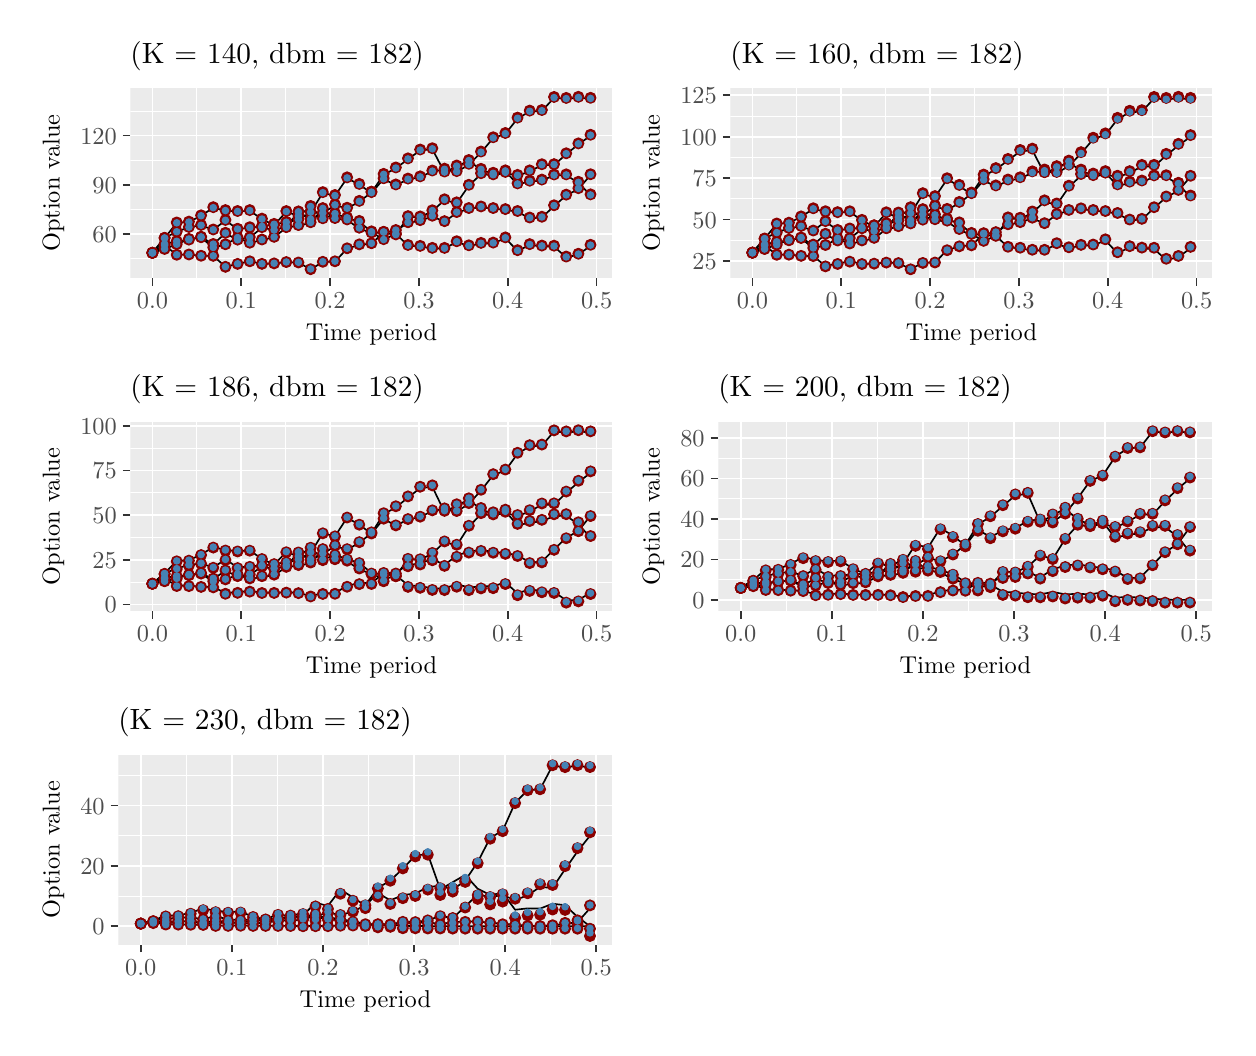
\begin{tikzpicture}[x=1pt,y=1pt]
\definecolor{fillColor}{RGB}{255,255,255}
\path[use as bounding box,fill=fillColor,fill opacity=0.00] (0,0) rectangle (433.62,361.35);
\begin{scope}
\path[clip] (  0.00,240.90) rectangle (216.81,361.35);
\definecolor{drawColor}{RGB}{255,255,255}
\definecolor{fillColor}{RGB}{255,255,255}

\path[draw=drawColor,line width= 0.6pt,line join=round,line cap=round,fill=fillColor] (  0.00,240.90) rectangle (216.81,361.35);
\end{scope}
\begin{scope}
\path[clip] ( 37.15,270.92) rectangle (211.31,339.48);
\definecolor{fillColor}{gray}{0.92}

\path[fill=fillColor] ( 37.15,270.92) rectangle (211.31,339.48);
\definecolor{drawColor}{RGB}{255,255,255}

\path[draw=drawColor,line width= 0.3pt,line join=round] ( 37.15,277.97) --
	(211.31,277.97);

\path[draw=drawColor,line width= 0.3pt,line join=round] ( 37.15,295.71) --
	(211.31,295.71);

\path[draw=drawColor,line width= 0.3pt,line join=round] ( 37.15,313.46) --
	(211.31,313.46);

\path[draw=drawColor,line width= 0.3pt,line join=round] ( 37.15,331.20) --
	(211.31,331.20);

\path[draw=drawColor,line width= 0.3pt,line join=round] ( 61.12,270.92) --
	( 61.12,339.48);

\path[draw=drawColor,line width= 0.3pt,line join=round] ( 93.23,270.92) --
	( 93.23,339.48);

\path[draw=drawColor,line width= 0.3pt,line join=round] (125.33,270.92) --
	(125.33,339.48);

\path[draw=drawColor,line width= 0.3pt,line join=round] (157.44,270.92) --
	(157.44,339.48);

\path[draw=drawColor,line width= 0.3pt,line join=round] (189.54,270.92) --
	(189.54,339.48);

\path[draw=drawColor,line width= 0.6pt,line join=round] ( 37.15,286.84) --
	(211.31,286.84);

\path[draw=drawColor,line width= 0.6pt,line join=round] ( 37.15,304.59) --
	(211.31,304.59);

\path[draw=drawColor,line width= 0.6pt,line join=round] ( 37.15,322.33) --
	(211.31,322.33);

\path[draw=drawColor,line width= 0.6pt,line join=round] ( 45.07,270.92) --
	( 45.07,339.48);

\path[draw=drawColor,line width= 0.6pt,line join=round] ( 77.17,270.92) --
	( 77.17,339.48);

\path[draw=drawColor,line width= 0.6pt,line join=round] (109.28,270.92) --
	(109.28,339.48);

\path[draw=drawColor,line width= 0.6pt,line join=round] (141.38,270.92) --
	(141.38,339.48);

\path[draw=drawColor,line width= 0.6pt,line join=round] (173.49,270.92) --
	(173.49,339.48);

\path[draw=drawColor,line width= 0.6pt,line join=round] (205.59,270.92) --
	(205.59,339.48);
\definecolor{drawColor}{RGB}{0,0,0}

\path[draw=drawColor,line width= 0.6pt,line join=round] ( 45.07,279.99) --
	( 49.47,285.27) --
	( 53.86,290.83) --
	( 58.26,291.12) --
	( 62.66,293.37) --
	( 67.06,296.29) --
	( 71.46,295.23) --
	( 75.85,294.90) --
	( 80.25,295.22) --
	( 84.65,292.15) --
	( 89.05,289.97) --
	( 93.45,294.86) --
	( 97.84,293.27) --
	(102.24,296.68) --
	(106.64,292.25) --
	(111.04,294.10) --
	(115.43,292.58) --
	(119.83,291.28) --
	(124.23,287.53) --
	(128.63,284.71) --
	(133.03,286.85) --
	(137.42,282.62) --
	(141.82,282.28) --
	(146.22,281.56) --
	(150.62,281.53) --
	(155.02,283.92) --
	(159.41,282.46) --
	(163.81,283.31) --
	(168.21,283.42) --
	(172.61,285.28) --
	(177.01,280.67) --
	(181.40,282.83) --
	(185.80,282.31) --
	(190.20,282.26) --
	(194.60,278.33) --
	(199.00,279.33) --
	(203.39,282.56);

\path[draw=drawColor,line width= 0.6pt,line join=round] ( 45.07,279.99) --
	( 49.47,282.74) --
	( 53.86,279.29) --
	( 58.26,279.38) --
	( 62.66,278.91) --
	( 67.06,278.87) --
	( 71.46,274.96) --
	( 75.85,276.00) --
	( 80.25,276.91) --
	( 84.65,275.99) --
	( 89.05,276.14) --
	( 93.45,276.61) --
	( 97.84,276.45) --
	(102.24,274.03) --
	(106.64,276.67) --
	(111.04,276.84) --
	(115.43,281.48) --
	(119.83,282.89) --
	(124.23,283.27) --
	(128.63,287.34) --
	(133.03,288.02) --
	(137.42,290.80) --
	(141.82,291.56) --
	(146.22,293.15) --
	(150.62,291.19) --
	(155.02,294.46) --
	(159.41,295.90) --
	(163.81,296.47) --
	(168.21,295.89) --
	(172.61,295.52) --
	(177.01,294.82) --
	(181.40,292.47) --
	(185.80,292.73) --
	(190.20,296.87) --
	(194.60,300.72) --
	(199.00,303.05) --
	(203.39,308.08);

\path[draw=drawColor,line width= 0.6pt,line join=round] ( 45.07,279.99) --
	( 49.47,281.36) --
	( 53.86,283.07) --
	( 58.26,284.94) --
	( 62.66,285.52) --
	( 67.06,281.87) --
	( 71.46,282.98) --
	( 75.85,285.44) --
	( 80.25,283.52) --
	( 84.65,284.66) --
	( 89.05,285.62) --
	( 93.45,289.07) --
	( 97.84,289.82) --
	(102.24,290.82) --
	(106.64,295.91) --
	(111.04,292.31) --
	(115.43,291.81) --
	(119.83,288.83) --
	(124.23,287.10) --
	(128.63,287.35) --
	(133.03,286.40) --
	(137.42,292.98) --
	(141.82,292.86) --
	(146.22,295.08) --
	(150.62,299.03) --
	(155.02,297.92) --
	(159.41,304.25) --
	(163.81,308.42) --
	(168.21,308.02) --
	(172.61,308.89) --
	(177.01,307.81) --
	(181.40,309.43) --
	(185.80,311.66) --
	(190.20,311.70) --
	(194.60,315.62) --
	(199.00,319.19) --
	(203.39,322.31);

\path[draw=drawColor,line width= 0.6pt,line join=round] ( 45.07,279.99) --
	( 49.47,285.36) --
	( 53.86,287.60) --
	( 58.26,289.22) --
	( 62.66,289.94) --
	( 67.06,288.30) --
	( 71.46,291.70) --
	( 75.85,288.55) --
	( 80.25,289.09) --
	( 84.65,289.50) --
	( 89.05,290.27) --
	( 93.45,290.99) --
	( 97.84,291.98) --
	(102.24,294.62) --
	(106.64,301.64) --
	(111.04,300.61) --
	(115.43,306.98) --
	(119.83,304.60) --
	(124.23,301.65) --
	(128.63,306.64) --
	(133.03,304.41) --
	(137.42,306.52) --
	(141.82,307.32) --
	(146.22,309.42) --
	(150.62,310.08) --
	(155.02,309.21) --
	(159.41,311.84) --
	(163.81,316.26) --
	(168.21,321.43) --
	(172.61,322.96) --
	(177.01,328.52) --
	(181.40,331.05) --
	(185.80,331.25) --
	(190.20,335.98) --
	(194.60,335.63) --
	(199.00,336.03) --
	(203.39,335.67);

\path[draw=drawColor,line width= 0.6pt,line join=round] ( 45.07,279.99) --
	( 49.47,283.22) --
	( 53.86,284.15) --
	( 58.26,284.67) --
	( 62.66,285.72) --
	( 67.06,283.09) --
	( 71.46,287.08) --
	( 75.85,284.64) --
	( 80.25,285.51) --
	( 84.65,289.08) --
	( 89.05,288.19) --
	( 93.45,289.49) --
	( 97.84,294.73) --
	(102.24,292.08) --
	(106.64,294.26) --
	(111.04,297.22) --
	(115.43,296.02) --
	(119.83,298.48) --
	(124.23,301.82) --
	(128.63,308.22) --
	(133.03,310.53) --
	(137.42,313.80) --
	(141.82,316.99) --
	(146.22,317.47) --
	(150.62,309.04) --
	(155.02,311.23) --
	(159.41,313.21) --
	(163.81,310.00) --
	(168.21,308.59) --
	(172.61,309.46) --
	(177.01,304.75) --
	(181.40,305.71) --
	(185.80,306.12) --
	(190.20,307.96) --
	(194.60,308.00) --
	(199.00,305.32) --
	(203.39,300.77);
\definecolor{drawColor}{RGB}{139,0,0}
\definecolor{fillColor}{RGB}{139,0,0}

\path[draw=drawColor,line width= 0.4pt,line join=round,line cap=round,fill=fillColor] ( 45.07,279.99) circle (  1.96);

\path[draw=drawColor,line width= 0.4pt,line join=round,line cap=round,fill=fillColor] ( 49.47,285.34) circle (  1.96);

\path[draw=drawColor,line width= 0.4pt,line join=round,line cap=round,fill=fillColor] ( 53.86,290.96) circle (  1.96);

\path[draw=drawColor,line width= 0.4pt,line join=round,line cap=round,fill=fillColor] ( 58.26,291.26) circle (  1.96);

\path[draw=drawColor,line width= 0.4pt,line join=round,line cap=round,fill=fillColor] ( 62.66,293.54) circle (  1.96);

\path[draw=drawColor,line width= 0.4pt,line join=round,line cap=round,fill=fillColor] ( 67.06,296.48) circle (  1.96);

\path[draw=drawColor,line width= 0.4pt,line join=round,line cap=round,fill=fillColor] ( 71.46,295.43) circle (  1.96);

\path[draw=drawColor,line width= 0.4pt,line join=round,line cap=round,fill=fillColor] ( 75.85,295.10) circle (  1.96);

\path[draw=drawColor,line width= 0.4pt,line join=round,line cap=round,fill=fillColor] ( 80.25,295.43) circle (  1.96);

\path[draw=drawColor,line width= 0.4pt,line join=round,line cap=round,fill=fillColor] ( 84.65,292.34) circle (  1.96);

\path[draw=drawColor,line width= 0.4pt,line join=round,line cap=round,fill=fillColor] ( 89.05,290.15) circle (  1.96);

\path[draw=drawColor,line width= 0.4pt,line join=round,line cap=round,fill=fillColor] ( 93.45,295.08) circle (  1.96);

\path[draw=drawColor,line width= 0.4pt,line join=round,line cap=round,fill=fillColor] ( 97.84,293.49) circle (  1.96);

\path[draw=drawColor,line width= 0.4pt,line join=round,line cap=round,fill=fillColor] (102.24,296.92) circle (  1.96);

\path[draw=drawColor,line width= 0.4pt,line join=round,line cap=round,fill=fillColor] (106.64,292.47) circle (  1.96);

\path[draw=drawColor,line width= 0.4pt,line join=round,line cap=round,fill=fillColor] (111.04,294.34) circle (  1.96);

\path[draw=drawColor,line width= 0.4pt,line join=round,line cap=round,fill=fillColor] (115.43,292.82) circle (  1.96);

\path[draw=drawColor,line width= 0.4pt,line join=round,line cap=round,fill=fillColor] (119.83,291.52) circle (  1.96);

\path[draw=drawColor,line width= 0.4pt,line join=round,line cap=round,fill=fillColor] (124.23,287.75) circle (  1.96);

\path[draw=drawColor,line width= 0.4pt,line join=round,line cap=round,fill=fillColor] (128.63,284.92) circle (  1.96);

\path[draw=drawColor,line width= 0.4pt,line join=round,line cap=round,fill=fillColor] (133.03,287.08) circle (  1.96);

\path[draw=drawColor,line width= 0.4pt,line join=round,line cap=round,fill=fillColor] (137.42,282.83) circle (  1.96);

\path[draw=drawColor,line width= 0.4pt,line join=round,line cap=round,fill=fillColor] (141.82,282.50) circle (  1.96);

\path[draw=drawColor,line width= 0.4pt,line join=round,line cap=round,fill=fillColor] (146.22,281.78) circle (  1.96);

\path[draw=drawColor,line width= 0.4pt,line join=round,line cap=round,fill=fillColor] (150.62,281.77) circle (  1.96);

\path[draw=drawColor,line width= 0.4pt,line join=round,line cap=round,fill=fillColor] (155.02,284.17) circle (  1.96);

\path[draw=drawColor,line width= 0.4pt,line join=round,line cap=round,fill=fillColor] (159.41,282.71) circle (  1.96);

\path[draw=drawColor,line width= 0.4pt,line join=round,line cap=round,fill=fillColor] (163.81,283.58) circle (  1.96);

\path[draw=drawColor,line width= 0.4pt,line join=round,line cap=round,fill=fillColor] (168.21,283.69) circle (  1.96);

\path[draw=drawColor,line width= 0.4pt,line join=round,line cap=round,fill=fillColor] (172.61,285.57) circle (  1.96);

\path[draw=drawColor,line width= 0.4pt,line join=round,line cap=round,fill=fillColor] (177.01,280.95) circle (  1.96);

\path[draw=drawColor,line width= 0.4pt,line join=round,line cap=round,fill=fillColor] (181.40,283.13) circle (  1.96);

\path[draw=drawColor,line width= 0.4pt,line join=round,line cap=round,fill=fillColor] (185.80,282.61) circle (  1.96);

\path[draw=drawColor,line width= 0.4pt,line join=round,line cap=round,fill=fillColor] (190.20,282.57) circle (  1.96);

\path[draw=drawColor,line width= 0.4pt,line join=round,line cap=round,fill=fillColor] (194.60,278.64) circle (  1.96);

\path[draw=drawColor,line width= 0.4pt,line join=round,line cap=round,fill=fillColor] (199.00,279.66) circle (  1.96);

\path[draw=drawColor,line width= 0.4pt,line join=round,line cap=round,fill=fillColor] (203.39,282.89) circle (  1.96);

\path[draw=drawColor,line width= 0.4pt,line join=round,line cap=round,fill=fillColor] ( 45.07,279.99) circle (  1.96);

\path[draw=drawColor,line width= 0.4pt,line join=round,line cap=round,fill=fillColor] ( 49.47,282.79) circle (  1.96);

\path[draw=drawColor,line width= 0.4pt,line join=round,line cap=round,fill=fillColor] ( 53.86,279.29) circle (  1.96);

\path[draw=drawColor,line width= 0.4pt,line join=round,line cap=round,fill=fillColor] ( 58.26,279.39) circle (  1.96);

\path[draw=drawColor,line width= 0.4pt,line join=round,line cap=round,fill=fillColor] ( 62.66,278.93) circle (  1.96);

\path[draw=drawColor,line width= 0.4pt,line join=round,line cap=round,fill=fillColor] ( 67.06,278.90) circle (  1.96);

\path[draw=drawColor,line width= 0.4pt,line join=round,line cap=round,fill=fillColor] ( 71.46,274.93) circle (  1.96);

\path[draw=drawColor,line width= 0.4pt,line join=round,line cap=round,fill=fillColor] ( 75.85,275.99) circle (  1.96);

\path[draw=drawColor,line width= 0.4pt,line join=round,line cap=round,fill=fillColor] ( 80.25,276.92) circle (  1.96);

\path[draw=drawColor,line width= 0.4pt,line join=round,line cap=round,fill=fillColor] ( 84.65,276.00) circle (  1.96);

\path[draw=drawColor,line width= 0.4pt,line join=round,line cap=round,fill=fillColor] ( 89.05,276.17) circle (  1.96);

\path[draw=drawColor,line width= 0.4pt,line join=round,line cap=round,fill=fillColor] ( 93.45,276.65) circle (  1.96);

\path[draw=drawColor,line width= 0.4pt,line join=round,line cap=round,fill=fillColor] ( 97.84,276.50) circle (  1.96);

\path[draw=drawColor,line width= 0.4pt,line join=round,line cap=round,fill=fillColor] (102.24,274.07) circle (  1.96);

\path[draw=drawColor,line width= 0.4pt,line join=round,line cap=round,fill=fillColor] (106.64,276.74) circle (  1.96);

\path[draw=drawColor,line width= 0.4pt,line join=round,line cap=round,fill=fillColor] (111.04,276.92) circle (  1.96);

\path[draw=drawColor,line width= 0.4pt,line join=round,line cap=round,fill=fillColor] (115.43,281.62) circle (  1.96);

\path[draw=drawColor,line width= 0.4pt,line join=round,line cap=round,fill=fillColor] (119.83,283.04) circle (  1.96);

\path[draw=drawColor,line width= 0.4pt,line join=round,line cap=round,fill=fillColor] (124.23,283.44) circle (  1.96);

\path[draw=drawColor,line width= 0.4pt,line join=round,line cap=round,fill=fillColor] (128.63,287.53) circle (  1.96);

\path[draw=drawColor,line width= 0.4pt,line join=round,line cap=round,fill=fillColor] (133.03,288.23) circle (  1.96);

\path[draw=drawColor,line width= 0.4pt,line join=round,line cap=round,fill=fillColor] (137.42,291.03) circle (  1.96);

\path[draw=drawColor,line width= 0.4pt,line join=round,line cap=round,fill=fillColor] (141.82,291.79) circle (  1.96);

\path[draw=drawColor,line width= 0.4pt,line join=round,line cap=round,fill=fillColor] (146.22,293.39) circle (  1.96);

\path[draw=drawColor,line width= 0.4pt,line join=round,line cap=round,fill=fillColor] (150.62,291.43) circle (  1.96);

\path[draw=drawColor,line width= 0.4pt,line join=round,line cap=round,fill=fillColor] (155.02,294.72) circle (  1.96);

\path[draw=drawColor,line width= 0.4pt,line join=round,line cap=round,fill=fillColor] (159.41,296.17) circle (  1.96);

\path[draw=drawColor,line width= 0.4pt,line join=round,line cap=round,fill=fillColor] (163.81,296.75) circle (  1.96);

\path[draw=drawColor,line width= 0.4pt,line join=round,line cap=round,fill=fillColor] (168.21,296.17) circle (  1.96);

\path[draw=drawColor,line width= 0.4pt,line join=round,line cap=round,fill=fillColor] (172.61,295.79) circle (  1.96);

\path[draw=drawColor,line width= 0.4pt,line join=round,line cap=round,fill=fillColor] (177.01,295.10) circle (  1.96);

\path[draw=drawColor,line width= 0.4pt,line join=round,line cap=round,fill=fillColor] (181.40,292.75) circle (  1.96);

\path[draw=drawColor,line width= 0.4pt,line join=round,line cap=round,fill=fillColor] (185.80,293.02) circle (  1.96);

\path[draw=drawColor,line width= 0.4pt,line join=round,line cap=round,fill=fillColor] (190.20,297.17) circle (  1.96);

\path[draw=drawColor,line width= 0.4pt,line join=round,line cap=round,fill=fillColor] (194.60,301.01) circle (  1.96);

\path[draw=drawColor,line width= 0.4pt,line join=round,line cap=round,fill=fillColor] (199.00,303.35) circle (  1.96);

\path[draw=drawColor,line width= 0.4pt,line join=round,line cap=round,fill=fillColor] (203.39,308.38) circle (  1.96);

\path[draw=drawColor,line width= 0.4pt,line join=round,line cap=round,fill=fillColor] ( 45.07,279.99) circle (  1.96);

\path[draw=drawColor,line width= 0.4pt,line join=round,line cap=round,fill=fillColor] ( 49.47,281.39) circle (  1.96);

\path[draw=drawColor,line width= 0.4pt,line join=round,line cap=round,fill=fillColor] ( 53.86,283.13) circle (  1.96);

\path[draw=drawColor,line width= 0.4pt,line join=round,line cap=round,fill=fillColor] ( 58.26,285.03) circle (  1.96);

\path[draw=drawColor,line width= 0.4pt,line join=round,line cap=round,fill=fillColor] ( 62.66,285.62) circle (  1.96);

\path[draw=drawColor,line width= 0.4pt,line join=round,line cap=round,fill=fillColor] ( 67.06,281.95) circle (  1.96);

\path[draw=drawColor,line width= 0.4pt,line join=round,line cap=round,fill=fillColor] ( 71.46,283.08) circle (  1.96);

\path[draw=drawColor,line width= 0.4pt,line join=round,line cap=round,fill=fillColor] ( 75.85,285.57) circle (  1.96);

\path[draw=drawColor,line width= 0.4pt,line join=round,line cap=round,fill=fillColor] ( 80.25,283.64) circle (  1.96);

\path[draw=drawColor,line width= 0.4pt,line join=round,line cap=round,fill=fillColor] ( 84.65,284.80) circle (  1.96);

\path[draw=drawColor,line width= 0.4pt,line join=round,line cap=round,fill=fillColor] ( 89.05,285.77) circle (  1.96);

\path[draw=drawColor,line width= 0.4pt,line join=round,line cap=round,fill=fillColor] ( 93.45,289.26) circle (  1.96);

\path[draw=drawColor,line width= 0.4pt,line join=round,line cap=round,fill=fillColor] ( 97.84,290.02) circle (  1.96);

\path[draw=drawColor,line width= 0.4pt,line join=round,line cap=round,fill=fillColor] (102.24,291.03) circle (  1.96);

\path[draw=drawColor,line width= 0.4pt,line join=round,line cap=round,fill=fillColor] (106.64,296.16) circle (  1.96);

\path[draw=drawColor,line width= 0.4pt,line join=round,line cap=round,fill=fillColor] (111.04,292.55) circle (  1.96);

\path[draw=drawColor,line width= 0.4pt,line join=round,line cap=round,fill=fillColor] (115.43,292.05) circle (  1.96);

\path[draw=drawColor,line width= 0.4pt,line join=round,line cap=round,fill=fillColor] (119.83,289.06) circle (  1.96);

\path[draw=drawColor,line width= 0.4pt,line join=round,line cap=round,fill=fillColor] (124.23,287.33) circle (  1.96);

\path[draw=drawColor,line width= 0.4pt,line join=round,line cap=round,fill=fillColor] (128.63,287.59) circle (  1.96);

\path[draw=drawColor,line width= 0.4pt,line join=round,line cap=round,fill=fillColor] (133.03,286.64) circle (  1.96);

\path[draw=drawColor,line width= 0.4pt,line join=round,line cap=round,fill=fillColor] (137.42,293.25) circle (  1.96);

\path[draw=drawColor,line width= 0.4pt,line join=round,line cap=round,fill=fillColor] (141.82,293.14) circle (  1.96);

\path[draw=drawColor,line width= 0.4pt,line join=round,line cap=round,fill=fillColor] (146.22,295.37) circle (  1.96);

\path[draw=drawColor,line width= 0.4pt,line join=round,line cap=round,fill=fillColor] (150.62,299.33) circle (  1.96);

\path[draw=drawColor,line width= 0.4pt,line join=round,line cap=round,fill=fillColor] (155.02,298.23) circle (  1.96);

\path[draw=drawColor,line width= 0.4pt,line join=round,line cap=round,fill=fillColor] (159.41,304.57) circle (  1.96);

\path[draw=drawColor,line width= 0.4pt,line join=round,line cap=round,fill=fillColor] (163.81,308.75) circle (  1.96);

\path[draw=drawColor,line width= 0.4pt,line join=round,line cap=round,fill=fillColor] (168.21,308.35) circle (  1.96);

\path[draw=drawColor,line width= 0.4pt,line join=round,line cap=round,fill=fillColor] (172.61,309.22) circle (  1.96);

\path[draw=drawColor,line width= 0.4pt,line join=round,line cap=round,fill=fillColor] (177.01,308.15) circle (  1.96);

\path[draw=drawColor,line width= 0.4pt,line join=round,line cap=round,fill=fillColor] (181.40,309.77) circle (  1.96);

\path[draw=drawColor,line width= 0.4pt,line join=round,line cap=round,fill=fillColor] (185.80,312.00) circle (  1.96);

\path[draw=drawColor,line width= 0.4pt,line join=round,line cap=round,fill=fillColor] (190.20,312.03) circle (  1.96);

\path[draw=drawColor,line width= 0.4pt,line join=round,line cap=round,fill=fillColor] (194.60,315.96) circle (  1.96);

\path[draw=drawColor,line width= 0.4pt,line join=round,line cap=round,fill=fillColor] (199.00,319.53) circle (  1.96);

\path[draw=drawColor,line width= 0.4pt,line join=round,line cap=round,fill=fillColor] (203.39,322.65) circle (  1.96);

\path[draw=drawColor,line width= 0.4pt,line join=round,line cap=round,fill=fillColor] ( 45.07,279.99) circle (  1.96);

\path[draw=drawColor,line width= 0.4pt,line join=round,line cap=round,fill=fillColor] ( 49.47,285.43) circle (  1.96);

\path[draw=drawColor,line width= 0.4pt,line join=round,line cap=round,fill=fillColor] ( 53.86,287.70) circle (  1.96);

\path[draw=drawColor,line width= 0.4pt,line join=round,line cap=round,fill=fillColor] ( 58.26,289.34) circle (  1.96);

\path[draw=drawColor,line width= 0.4pt,line join=round,line cap=round,fill=fillColor] ( 62.66,290.08) circle (  1.96);

\path[draw=drawColor,line width= 0.4pt,line join=round,line cap=round,fill=fillColor] ( 67.06,288.43) circle (  1.96);

\path[draw=drawColor,line width= 0.4pt,line join=round,line cap=round,fill=fillColor] ( 71.46,291.87) circle (  1.96);

\path[draw=drawColor,line width= 0.4pt,line join=round,line cap=round,fill=fillColor] ( 75.85,288.70) circle (  1.96);

\path[draw=drawColor,line width= 0.4pt,line join=round,line cap=round,fill=fillColor] ( 80.25,289.25) circle (  1.96);

\path[draw=drawColor,line width= 0.4pt,line join=round,line cap=round,fill=fillColor] ( 84.65,289.67) circle (  1.96);

\path[draw=drawColor,line width= 0.4pt,line join=round,line cap=round,fill=fillColor] ( 89.05,290.45) circle (  1.96);

\path[draw=drawColor,line width= 0.4pt,line join=round,line cap=round,fill=fillColor] ( 93.45,291.19) circle (  1.96);

\path[draw=drawColor,line width= 0.4pt,line join=round,line cap=round,fill=fillColor] ( 97.84,292.19) circle (  1.96);

\path[draw=drawColor,line width= 0.4pt,line join=round,line cap=round,fill=fillColor] (102.24,294.85) circle (  1.96);

\path[draw=drawColor,line width= 0.4pt,line join=round,line cap=round,fill=fillColor] (106.64,301.91) circle (  1.96);

\path[draw=drawColor,line width= 0.4pt,line join=round,line cap=round,fill=fillColor] (111.04,300.88) circle (  1.96);

\path[draw=drawColor,line width= 0.4pt,line join=round,line cap=round,fill=fillColor] (115.43,307.26) circle (  1.96);

\path[draw=drawColor,line width= 0.4pt,line join=round,line cap=round,fill=fillColor] (119.83,304.89) circle (  1.96);

\path[draw=drawColor,line width= 0.4pt,line join=round,line cap=round,fill=fillColor] (124.23,301.93) circle (  1.96);

\path[draw=drawColor,line width= 0.4pt,line join=round,line cap=round,fill=fillColor] (128.63,306.93) circle (  1.96);

\path[draw=drawColor,line width= 0.4pt,line join=round,line cap=round,fill=fillColor] (133.03,304.70) circle (  1.96);

\path[draw=drawColor,line width= 0.4pt,line join=round,line cap=round,fill=fillColor] (137.42,306.82) circle (  1.96);

\path[draw=drawColor,line width= 0.4pt,line join=round,line cap=round,fill=fillColor] (141.82,307.62) circle (  1.96);

\path[draw=drawColor,line width= 0.4pt,line join=round,line cap=round,fill=fillColor] (146.22,309.73) circle (  1.96);

\path[draw=drawColor,line width= 0.4pt,line join=round,line cap=round,fill=fillColor] (150.62,310.40) circle (  1.96);

\path[draw=drawColor,line width= 0.4pt,line join=round,line cap=round,fill=fillColor] (155.02,309.52) circle (  1.96);

\path[draw=drawColor,line width= 0.4pt,line join=round,line cap=round,fill=fillColor] (159.41,312.16) circle (  1.96);

\path[draw=drawColor,line width= 0.4pt,line join=round,line cap=round,fill=fillColor] (163.81,316.59) circle (  1.96);

\path[draw=drawColor,line width= 0.4pt,line join=round,line cap=round,fill=fillColor] (168.21,321.75) circle (  1.96);

\path[draw=drawColor,line width= 0.4pt,line join=round,line cap=round,fill=fillColor] (172.61,323.29) circle (  1.96);

\path[draw=drawColor,line width= 0.4pt,line join=round,line cap=round,fill=fillColor] (177.01,328.85) circle (  1.96);

\path[draw=drawColor,line width= 0.4pt,line join=round,line cap=round,fill=fillColor] (181.40,331.38) circle (  1.96);

\path[draw=drawColor,line width= 0.4pt,line join=round,line cap=round,fill=fillColor] (185.80,331.59) circle (  1.96);

\path[draw=drawColor,line width= 0.4pt,line join=round,line cap=round,fill=fillColor] (190.20,336.31) circle (  1.96);

\path[draw=drawColor,line width= 0.4pt,line join=round,line cap=round,fill=fillColor] (194.60,335.96) circle (  1.96);

\path[draw=drawColor,line width= 0.4pt,line join=round,line cap=round,fill=fillColor] (199.00,336.36) circle (  1.96);

\path[draw=drawColor,line width= 0.4pt,line join=round,line cap=round,fill=fillColor] (203.39,336.00) circle (  1.96);

\path[draw=drawColor,line width= 0.4pt,line join=round,line cap=round,fill=fillColor] ( 45.07,279.99) circle (  1.96);

\path[draw=drawColor,line width= 0.4pt,line join=round,line cap=round,fill=fillColor] ( 49.47,283.26) circle (  1.96);

\path[draw=drawColor,line width= 0.4pt,line join=round,line cap=round,fill=fillColor] ( 53.86,284.22) circle (  1.96);

\path[draw=drawColor,line width= 0.4pt,line join=round,line cap=round,fill=fillColor] ( 58.26,284.76) circle (  1.96);

\path[draw=drawColor,line width= 0.4pt,line join=round,line cap=round,fill=fillColor] ( 62.66,285.82) circle (  1.96);

\path[draw=drawColor,line width= 0.4pt,line join=round,line cap=round,fill=fillColor] ( 67.06,283.18) circle (  1.96);

\path[draw=drawColor,line width= 0.4pt,line join=round,line cap=round,fill=fillColor] ( 71.46,287.22) circle (  1.96);

\path[draw=drawColor,line width= 0.4pt,line join=round,line cap=round,fill=fillColor] ( 75.85,284.76) circle (  1.96);

\path[draw=drawColor,line width= 0.4pt,line join=round,line cap=round,fill=fillColor] ( 80.25,285.65) circle (  1.96);

\path[draw=drawColor,line width= 0.4pt,line join=round,line cap=round,fill=fillColor] ( 84.65,289.26) circle (  1.96);

\path[draw=drawColor,line width= 0.4pt,line join=round,line cap=round,fill=fillColor] ( 89.05,288.36) circle (  1.96);

\path[draw=drawColor,line width= 0.4pt,line join=round,line cap=round,fill=fillColor] ( 93.45,289.68) circle (  1.96);

\path[draw=drawColor,line width= 0.4pt,line join=round,line cap=round,fill=fillColor] ( 97.84,294.96) circle (  1.96);

\path[draw=drawColor,line width= 0.4pt,line join=round,line cap=round,fill=fillColor] (102.24,292.30) circle (  1.96);

\path[draw=drawColor,line width= 0.4pt,line join=round,line cap=round,fill=fillColor] (106.64,294.50) circle (  1.96);

\path[draw=drawColor,line width= 0.4pt,line join=round,line cap=round,fill=fillColor] (111.04,297.48) circle (  1.96);

\path[draw=drawColor,line width= 0.4pt,line join=round,line cap=round,fill=fillColor] (115.43,296.28) circle (  1.96);

\path[draw=drawColor,line width= 0.4pt,line join=round,line cap=round,fill=fillColor] (119.83,298.76) circle (  1.96);

\path[draw=drawColor,line width= 0.4pt,line join=round,line cap=round,fill=fillColor] (124.23,302.11) circle (  1.96);

\path[draw=drawColor,line width= 0.4pt,line join=round,line cap=round,fill=fillColor] (128.63,308.52) circle (  1.96);

\path[draw=drawColor,line width= 0.4pt,line join=round,line cap=round,fill=fillColor] (133.03,310.84) circle (  1.96);

\path[draw=drawColor,line width= 0.4pt,line join=round,line cap=round,fill=fillColor] (137.42,314.12) circle (  1.96);

\path[draw=drawColor,line width= 0.4pt,line join=round,line cap=round,fill=fillColor] (141.82,317.32) circle (  1.96);

\path[draw=drawColor,line width= 0.4pt,line join=round,line cap=round,fill=fillColor] (146.22,317.79) circle (  1.96);

\path[draw=drawColor,line width= 0.4pt,line join=round,line cap=round,fill=fillColor] (150.62,309.36) circle (  1.96);

\path[draw=drawColor,line width= 0.4pt,line join=round,line cap=round,fill=fillColor] (155.02,311.55) circle (  1.96);

\path[draw=drawColor,line width= 0.4pt,line join=round,line cap=round,fill=fillColor] (159.41,313.53) circle (  1.96);

\path[draw=drawColor,line width= 0.4pt,line join=round,line cap=round,fill=fillColor] (163.81,310.33) circle (  1.96);

\path[draw=drawColor,line width= 0.4pt,line join=round,line cap=round,fill=fillColor] (168.21,308.92) circle (  1.96);

\path[draw=drawColor,line width= 0.4pt,line join=round,line cap=round,fill=fillColor] (172.61,309.79) circle (  1.96);

\path[draw=drawColor,line width= 0.4pt,line join=round,line cap=round,fill=fillColor] (177.01,305.08) circle (  1.96);

\path[draw=drawColor,line width= 0.4pt,line join=round,line cap=round,fill=fillColor] (181.40,306.04) circle (  1.96);

\path[draw=drawColor,line width= 0.4pt,line join=round,line cap=round,fill=fillColor] (185.80,306.45) circle (  1.96);

\path[draw=drawColor,line width= 0.4pt,line join=round,line cap=round,fill=fillColor] (190.20,308.29) circle (  1.96);

\path[draw=drawColor,line width= 0.4pt,line join=round,line cap=round,fill=fillColor] (194.60,308.34) circle (  1.96);

\path[draw=drawColor,line width= 0.4pt,line join=round,line cap=round,fill=fillColor] (199.00,305.66) circle (  1.96);

\path[draw=drawColor,line width= 0.4pt,line join=round,line cap=round,fill=fillColor] (203.39,301.11) circle (  1.96);
\definecolor{drawColor}{RGB}{70,130,180}
\definecolor{fillColor}{RGB}{70,130,180}

\path[draw=drawColor,line width= 0.4pt,line join=round,line cap=round,fill=fillColor] ( 45.07,279.99) circle (  1.16);

\path[draw=drawColor,line width= 0.4pt,line join=round,line cap=round,fill=fillColor] ( 49.47,285.27) circle (  1.16);

\path[draw=drawColor,line width= 0.4pt,line join=round,line cap=round,fill=fillColor] ( 53.86,290.83) circle (  1.16);

\path[draw=drawColor,line width= 0.4pt,line join=round,line cap=round,fill=fillColor] ( 58.26,291.13) circle (  1.16);

\path[draw=drawColor,line width= 0.4pt,line join=round,line cap=round,fill=fillColor] ( 62.66,293.39) circle (  1.16);

\path[draw=drawColor,line width= 0.4pt,line join=round,line cap=round,fill=fillColor] ( 67.06,296.31) circle (  1.16);

\path[draw=drawColor,line width= 0.4pt,line join=round,line cap=round,fill=fillColor] ( 71.46,295.26) circle (  1.16);

\path[draw=drawColor,line width= 0.4pt,line join=round,line cap=round,fill=fillColor] ( 75.85,294.94) circle (  1.16);

\path[draw=drawColor,line width= 0.4pt,line join=round,line cap=round,fill=fillColor] ( 80.25,295.26) circle (  1.16);

\path[draw=drawColor,line width= 0.4pt,line join=round,line cap=round,fill=fillColor] ( 84.65,292.19) circle (  1.16);

\path[draw=drawColor,line width= 0.4pt,line join=round,line cap=round,fill=fillColor] ( 89.05,290.02) circle (  1.16);

\path[draw=drawColor,line width= 0.4pt,line join=round,line cap=round,fill=fillColor] ( 93.45,294.91) circle (  1.16);

\path[draw=drawColor,line width= 0.4pt,line join=round,line cap=round,fill=fillColor] ( 97.84,293.33) circle (  1.16);

\path[draw=drawColor,line width= 0.4pt,line join=round,line cap=round,fill=fillColor] (102.24,296.73) circle (  1.16);

\path[draw=drawColor,line width= 0.4pt,line join=round,line cap=round,fill=fillColor] (106.64,292.31) circle (  1.16);

\path[draw=drawColor,line width= 0.4pt,line join=round,line cap=round,fill=fillColor] (111.04,294.17) circle (  1.16);

\path[draw=drawColor,line width= 0.4pt,line join=round,line cap=round,fill=fillColor] (115.43,292.65) circle (  1.16);

\path[draw=drawColor,line width= 0.4pt,line join=round,line cap=round,fill=fillColor] (119.83,291.36) circle (  1.16);

\path[draw=drawColor,line width= 0.4pt,line join=round,line cap=round,fill=fillColor] (124.23,287.61) circle (  1.16);

\path[draw=drawColor,line width= 0.4pt,line join=round,line cap=round,fill=fillColor] (128.63,284.79) circle (  1.16);

\path[draw=drawColor,line width= 0.4pt,line join=round,line cap=round,fill=fillColor] (133.03,286.94) circle (  1.16);

\path[draw=drawColor,line width= 0.4pt,line join=round,line cap=round,fill=fillColor] (137.42,282.71) circle (  1.16);

\path[draw=drawColor,line width= 0.4pt,line join=round,line cap=round,fill=fillColor] (141.82,282.38) circle (  1.16);

\path[draw=drawColor,line width= 0.4pt,line join=round,line cap=round,fill=fillColor] (146.22,281.67) circle (  1.16);

\path[draw=drawColor,line width= 0.4pt,line join=round,line cap=round,fill=fillColor] (150.62,281.65) circle (  1.16);

\path[draw=drawColor,line width= 0.4pt,line join=round,line cap=round,fill=fillColor] (155.02,284.04) circle (  1.16);

\path[draw=drawColor,line width= 0.4pt,line join=round,line cap=round,fill=fillColor] (159.41,282.59) circle (  1.16);

\path[draw=drawColor,line width= 0.4pt,line join=round,line cap=round,fill=fillColor] (163.81,283.45) circle (  1.16);

\path[draw=drawColor,line width= 0.4pt,line join=round,line cap=round,fill=fillColor] (168.21,283.57) circle (  1.16);

\path[draw=drawColor,line width= 0.4pt,line join=round,line cap=round,fill=fillColor] (172.61,285.43) circle (  1.16);

\path[draw=drawColor,line width= 0.4pt,line join=round,line cap=round,fill=fillColor] (177.01,280.83) circle (  1.16);

\path[draw=drawColor,line width= 0.4pt,line join=round,line cap=round,fill=fillColor] (181.40,283.00) circle (  1.16);

\path[draw=drawColor,line width= 0.4pt,line join=round,line cap=round,fill=fillColor] (185.80,282.49) circle (  1.16);

\path[draw=drawColor,line width= 0.4pt,line join=round,line cap=round,fill=fillColor] (190.20,282.44) circle (  1.16);

\path[draw=drawColor,line width= 0.4pt,line join=round,line cap=round,fill=fillColor] (194.60,278.52) circle (  1.16);

\path[draw=drawColor,line width= 0.4pt,line join=round,line cap=round,fill=fillColor] (199.00,279.53) circle (  1.16);

\path[draw=drawColor,line width= 0.4pt,line join=round,line cap=round,fill=fillColor] (203.39,282.77) circle (  1.16);

\path[draw=drawColor,line width= 0.4pt,line join=round,line cap=round,fill=fillColor] ( 45.07,279.99) circle (  1.16);

\path[draw=drawColor,line width= 0.4pt,line join=round,line cap=round,fill=fillColor] ( 49.47,282.75) circle (  1.16);

\path[draw=drawColor,line width= 0.4pt,line join=round,line cap=round,fill=fillColor] ( 53.86,279.30) circle (  1.16);

\path[draw=drawColor,line width= 0.4pt,line join=round,line cap=round,fill=fillColor] ( 58.26,279.39) circle (  1.16);

\path[draw=drawColor,line width= 0.4pt,line join=round,line cap=round,fill=fillColor] ( 62.66,278.94) circle (  1.16);

\path[draw=drawColor,line width= 0.4pt,line join=round,line cap=round,fill=fillColor] ( 67.06,278.91) circle (  1.16);

\path[draw=drawColor,line width= 0.4pt,line join=round,line cap=round,fill=fillColor] ( 71.46,274.98) circle (  1.16);

\path[draw=drawColor,line width= 0.4pt,line join=round,line cap=round,fill=fillColor] ( 75.85,276.03) circle (  1.16);

\path[draw=drawColor,line width= 0.4pt,line join=round,line cap=round,fill=fillColor] ( 80.25,276.95) circle (  1.16);

\path[draw=drawColor,line width= 0.4pt,line join=round,line cap=round,fill=fillColor] ( 84.65,276.05) circle (  1.16);

\path[draw=drawColor,line width= 0.4pt,line join=round,line cap=round,fill=fillColor] ( 89.05,276.21) circle (  1.16);

\path[draw=drawColor,line width= 0.4pt,line join=round,line cap=round,fill=fillColor] ( 93.45,276.69) circle (  1.16);

\path[draw=drawColor,line width= 0.4pt,line join=round,line cap=round,fill=fillColor] ( 97.84,276.57) circle (  1.16);

\path[draw=drawColor,line width= 0.4pt,line join=round,line cap=round,fill=fillColor] (102.24,274.16) circle (  1.16);

\path[draw=drawColor,line width= 0.4pt,line join=round,line cap=round,fill=fillColor] (106.64,276.80) circle (  1.16);

\path[draw=drawColor,line width= 0.4pt,line join=round,line cap=round,fill=fillColor] (111.04,276.98) circle (  1.16);

\path[draw=drawColor,line width= 0.4pt,line join=round,line cap=round,fill=fillColor] (115.43,281.64) circle (  1.16);

\path[draw=drawColor,line width= 0.4pt,line join=round,line cap=round,fill=fillColor] (119.83,283.05) circle (  1.16);

\path[draw=drawColor,line width= 0.4pt,line join=round,line cap=round,fill=fillColor] (124.23,283.44) circle (  1.16);

\path[draw=drawColor,line width= 0.4pt,line join=round,line cap=round,fill=fillColor] (128.63,287.51) circle (  1.16);

\path[draw=drawColor,line width= 0.4pt,line join=round,line cap=round,fill=fillColor] (133.03,288.20) circle (  1.16);

\path[draw=drawColor,line width= 0.4pt,line join=round,line cap=round,fill=fillColor] (137.42,290.99) circle (  1.16);

\path[draw=drawColor,line width= 0.4pt,line join=round,line cap=round,fill=fillColor] (141.82,291.75) circle (  1.16);

\path[draw=drawColor,line width= 0.4pt,line join=round,line cap=round,fill=fillColor] (146.22,293.34) circle (  1.16);

\path[draw=drawColor,line width= 0.4pt,line join=round,line cap=round,fill=fillColor] (150.62,291.39) circle (  1.16);

\path[draw=drawColor,line width= 0.4pt,line join=round,line cap=round,fill=fillColor] (155.02,294.67) circle (  1.16);

\path[draw=drawColor,line width= 0.4pt,line join=round,line cap=round,fill=fillColor] (159.41,296.11) circle (  1.16);

\path[draw=drawColor,line width= 0.4pt,line join=round,line cap=round,fill=fillColor] (163.81,296.69) circle (  1.16);

\path[draw=drawColor,line width= 0.4pt,line join=round,line cap=round,fill=fillColor] (168.21,296.11) circle (  1.16);

\path[draw=drawColor,line width= 0.4pt,line join=round,line cap=round,fill=fillColor] (172.61,295.71) circle (  1.16);

\path[draw=drawColor,line width= 0.4pt,line join=round,line cap=round,fill=fillColor] (177.01,295.02) circle (  1.16);

\path[draw=drawColor,line width= 0.4pt,line join=round,line cap=round,fill=fillColor] (181.40,292.67) circle (  1.16);

\path[draw=drawColor,line width= 0.4pt,line join=round,line cap=round,fill=fillColor] (185.80,292.93) circle (  1.16);

\path[draw=drawColor,line width= 0.4pt,line join=round,line cap=round,fill=fillColor] (190.20,297.08) circle (  1.16);

\path[draw=drawColor,line width= 0.4pt,line join=round,line cap=round,fill=fillColor] (194.60,300.93) circle (  1.16);

\path[draw=drawColor,line width= 0.4pt,line join=round,line cap=round,fill=fillColor] (199.00,303.26) circle (  1.16);

\path[draw=drawColor,line width= 0.4pt,line join=round,line cap=round,fill=fillColor] (203.39,308.30) circle (  1.16);

\path[draw=drawColor,line width= 0.4pt,line join=round,line cap=round,fill=fillColor] ( 45.07,279.99) circle (  1.16);

\path[draw=drawColor,line width= 0.4pt,line join=round,line cap=round,fill=fillColor] ( 49.47,281.38) circle (  1.16);

\path[draw=drawColor,line width= 0.4pt,line join=round,line cap=round,fill=fillColor] ( 53.86,283.09) circle (  1.16);

\path[draw=drawColor,line width= 0.4pt,line join=round,line cap=round,fill=fillColor] ( 58.26,284.97) circle (  1.16);

\path[draw=drawColor,line width= 0.4pt,line join=round,line cap=round,fill=fillColor] ( 62.66,285.55) circle (  1.16);

\path[draw=drawColor,line width= 0.4pt,line join=round,line cap=round,fill=fillColor] ( 67.06,281.92) circle (  1.16);

\path[draw=drawColor,line width= 0.4pt,line join=round,line cap=round,fill=fillColor] ( 71.46,283.03) circle (  1.16);

\path[draw=drawColor,line width= 0.4pt,line join=round,line cap=round,fill=fillColor] ( 75.85,285.50) circle (  1.16);

\path[draw=drawColor,line width= 0.4pt,line join=round,line cap=round,fill=fillColor] ( 80.25,283.59) circle (  1.16);

\path[draw=drawColor,line width= 0.4pt,line join=round,line cap=round,fill=fillColor] ( 84.65,284.73) circle (  1.16);

\path[draw=drawColor,line width= 0.4pt,line join=round,line cap=round,fill=fillColor] ( 89.05,285.70) circle (  1.16);

\path[draw=drawColor,line width= 0.4pt,line join=round,line cap=round,fill=fillColor] ( 93.45,289.16) circle (  1.16);

\path[draw=drawColor,line width= 0.4pt,line join=round,line cap=round,fill=fillColor] ( 97.84,289.94) circle (  1.16);

\path[draw=drawColor,line width= 0.4pt,line join=round,line cap=round,fill=fillColor] (102.24,290.95) circle (  1.16);

\path[draw=drawColor,line width= 0.4pt,line join=round,line cap=round,fill=fillColor] (106.64,296.04) circle (  1.16);

\path[draw=drawColor,line width= 0.4pt,line join=round,line cap=round,fill=fillColor] (111.04,292.45) circle (  1.16);

\path[draw=drawColor,line width= 0.4pt,line join=round,line cap=round,fill=fillColor] (115.43,291.95) circle (  1.16);

\path[draw=drawColor,line width= 0.4pt,line join=round,line cap=round,fill=fillColor] (119.83,288.98) circle (  1.16);

\path[draw=drawColor,line width= 0.4pt,line join=round,line cap=round,fill=fillColor] (124.23,287.25) circle (  1.16);

\path[draw=drawColor,line width= 0.4pt,line join=round,line cap=round,fill=fillColor] (128.63,287.51) circle (  1.16);

\path[draw=drawColor,line width= 0.4pt,line join=round,line cap=round,fill=fillColor] (133.03,286.57) circle (  1.16);

\path[draw=drawColor,line width= 0.4pt,line join=round,line cap=round,fill=fillColor] (137.42,293.15) circle (  1.16);

\path[draw=drawColor,line width= 0.4pt,line join=round,line cap=round,fill=fillColor] (141.82,293.03) circle (  1.16);

\path[draw=drawColor,line width= 0.4pt,line join=round,line cap=round,fill=fillColor] (146.22,295.26) circle (  1.16);

\path[draw=drawColor,line width= 0.4pt,line join=round,line cap=round,fill=fillColor] (150.62,299.21) circle (  1.16);

\path[draw=drawColor,line width= 0.4pt,line join=round,line cap=round,fill=fillColor] (155.02,298.11) circle (  1.16);

\path[draw=drawColor,line width= 0.4pt,line join=round,line cap=round,fill=fillColor] (159.41,304.44) circle (  1.16);

\path[draw=drawColor,line width= 0.4pt,line join=round,line cap=round,fill=fillColor] (163.81,308.61) circle (  1.16);

\path[draw=drawColor,line width= 0.4pt,line join=round,line cap=round,fill=fillColor] (168.21,308.21) circle (  1.16);

\path[draw=drawColor,line width= 0.4pt,line join=round,line cap=round,fill=fillColor] (172.61,309.08) circle (  1.16);

\path[draw=drawColor,line width= 0.4pt,line join=round,line cap=round,fill=fillColor] (177.01,308.01) circle (  1.16);

\path[draw=drawColor,line width= 0.4pt,line join=round,line cap=round,fill=fillColor] (181.40,309.63) circle (  1.16);

\path[draw=drawColor,line width= 0.4pt,line join=round,line cap=round,fill=fillColor] (185.80,311.86) circle (  1.16);

\path[draw=drawColor,line width= 0.4pt,line join=round,line cap=round,fill=fillColor] (190.20,311.90) circle (  1.16);

\path[draw=drawColor,line width= 0.4pt,line join=round,line cap=round,fill=fillColor] (194.60,315.82) circle (  1.16);

\path[draw=drawColor,line width= 0.4pt,line join=round,line cap=round,fill=fillColor] (199.00,319.39) circle (  1.16);

\path[draw=drawColor,line width= 0.4pt,line join=round,line cap=round,fill=fillColor] (203.39,322.51) circle (  1.16);

\path[draw=drawColor,line width= 0.4pt,line join=round,line cap=round,fill=fillColor] ( 45.07,279.99) circle (  1.16);

\path[draw=drawColor,line width= 0.4pt,line join=round,line cap=round,fill=fillColor] ( 49.47,285.36) circle (  1.16);

\path[draw=drawColor,line width= 0.4pt,line join=round,line cap=round,fill=fillColor] ( 53.86,287.61) circle (  1.16);

\path[draw=drawColor,line width= 0.4pt,line join=round,line cap=round,fill=fillColor] ( 58.26,289.23) circle (  1.16);

\path[draw=drawColor,line width= 0.4pt,line join=round,line cap=round,fill=fillColor] ( 62.66,289.96) circle (  1.16);

\path[draw=drawColor,line width= 0.4pt,line join=round,line cap=round,fill=fillColor] ( 67.06,288.33) circle (  1.16);

\path[draw=drawColor,line width= 0.4pt,line join=round,line cap=round,fill=fillColor] ( 71.46,291.74) circle (  1.16);

\path[draw=drawColor,line width= 0.4pt,line join=round,line cap=round,fill=fillColor] ( 75.85,288.59) circle (  1.16);

\path[draw=drawColor,line width= 0.4pt,line join=round,line cap=round,fill=fillColor] ( 80.25,289.13) circle (  1.16);

\path[draw=drawColor,line width= 0.4pt,line join=round,line cap=round,fill=fillColor] ( 84.65,289.55) circle (  1.16);

\path[draw=drawColor,line width= 0.4pt,line join=round,line cap=round,fill=fillColor] ( 89.05,290.32) circle (  1.16);

\path[draw=drawColor,line width= 0.4pt,line join=round,line cap=round,fill=fillColor] ( 93.45,291.05) circle (  1.16);

\path[draw=drawColor,line width= 0.4pt,line join=round,line cap=round,fill=fillColor] ( 97.84,292.05) circle (  1.16);

\path[draw=drawColor,line width= 0.4pt,line join=round,line cap=round,fill=fillColor] (102.24,294.69) circle (  1.16);

\path[draw=drawColor,line width= 0.4pt,line join=round,line cap=round,fill=fillColor] (106.64,301.72) circle (  1.16);

\path[draw=drawColor,line width= 0.4pt,line join=round,line cap=round,fill=fillColor] (111.04,300.69) circle (  1.16);

\path[draw=drawColor,line width= 0.4pt,line join=round,line cap=round,fill=fillColor] (115.43,307.05) circle (  1.16);

\path[draw=drawColor,line width= 0.4pt,line join=round,line cap=round,fill=fillColor] (119.83,304.68) circle (  1.16);

\path[draw=drawColor,line width= 0.4pt,line join=round,line cap=round,fill=fillColor] (124.23,301.74) circle (  1.16);

\path[draw=drawColor,line width= 0.4pt,line join=round,line cap=round,fill=fillColor] (128.63,306.72) circle (  1.16);

\path[draw=drawColor,line width= 0.4pt,line join=round,line cap=round,fill=fillColor] (133.03,304.49) circle (  1.16);

\path[draw=drawColor,line width= 0.4pt,line join=round,line cap=round,fill=fillColor] (137.42,306.61) circle (  1.16);

\path[draw=drawColor,line width= 0.4pt,line join=round,line cap=round,fill=fillColor] (141.82,307.41) circle (  1.16);

\path[draw=drawColor,line width= 0.4pt,line join=round,line cap=round,fill=fillColor] (146.22,309.51) circle (  1.16);

\path[draw=drawColor,line width= 0.4pt,line join=round,line cap=round,fill=fillColor] (150.62,310.18) circle (  1.16);

\path[draw=drawColor,line width= 0.4pt,line join=round,line cap=round,fill=fillColor] (155.02,309.31) circle (  1.16);

\path[draw=drawColor,line width= 0.4pt,line join=round,line cap=round,fill=fillColor] (159.41,311.94) circle (  1.16);

\path[draw=drawColor,line width= 0.4pt,line join=round,line cap=round,fill=fillColor] (163.81,316.36) circle (  1.16);

\path[draw=drawColor,line width= 0.4pt,line join=round,line cap=round,fill=fillColor] (168.21,321.53) circle (  1.16);

\path[draw=drawColor,line width= 0.4pt,line join=round,line cap=round,fill=fillColor] (172.61,323.06) circle (  1.16);

\path[draw=drawColor,line width= 0.4pt,line join=round,line cap=round,fill=fillColor] (177.01,328.62) circle (  1.16);

\path[draw=drawColor,line width= 0.4pt,line join=round,line cap=round,fill=fillColor] (181.40,331.15) circle (  1.16);

\path[draw=drawColor,line width= 0.4pt,line join=round,line cap=round,fill=fillColor] (185.80,331.36) circle (  1.16);

\path[draw=drawColor,line width= 0.4pt,line join=round,line cap=round,fill=fillColor] (190.20,336.08) circle (  1.16);

\path[draw=drawColor,line width= 0.4pt,line join=round,line cap=round,fill=fillColor] (194.60,335.73) circle (  1.16);

\path[draw=drawColor,line width= 0.4pt,line join=round,line cap=round,fill=fillColor] (199.00,336.13) circle (  1.16);

\path[draw=drawColor,line width= 0.4pt,line join=round,line cap=round,fill=fillColor] (203.39,335.78) circle (  1.16);

\path[draw=drawColor,line width= 0.4pt,line join=round,line cap=round,fill=fillColor] ( 45.07,279.99) circle (  1.16);

\path[draw=drawColor,line width= 0.4pt,line join=round,line cap=round,fill=fillColor] ( 49.47,283.22) circle (  1.16);

\path[draw=drawColor,line width= 0.4pt,line join=round,line cap=round,fill=fillColor] ( 53.86,284.17) circle (  1.16);

\path[draw=drawColor,line width= 0.4pt,line join=round,line cap=round,fill=fillColor] ( 58.26,284.70) circle (  1.16);

\path[draw=drawColor,line width= 0.4pt,line join=round,line cap=round,fill=fillColor] ( 62.66,285.75) circle (  1.16);

\path[draw=drawColor,line width= 0.4pt,line join=round,line cap=round,fill=fillColor] ( 67.06,283.13) circle (  1.16);

\path[draw=drawColor,line width= 0.4pt,line join=round,line cap=round,fill=fillColor] ( 71.46,287.13) circle (  1.16);

\path[draw=drawColor,line width= 0.4pt,line join=round,line cap=round,fill=fillColor] ( 75.85,284.70) circle (  1.16);

\path[draw=drawColor,line width= 0.4pt,line join=round,line cap=round,fill=fillColor] ( 80.25,285.58) circle (  1.16);

\path[draw=drawColor,line width= 0.4pt,line join=round,line cap=round,fill=fillColor] ( 84.65,289.15) circle (  1.16);

\path[draw=drawColor,line width= 0.4pt,line join=round,line cap=round,fill=fillColor] ( 89.05,288.26) circle (  1.16);

\path[draw=drawColor,line width= 0.4pt,line join=round,line cap=round,fill=fillColor] ( 93.45,289.57) circle (  1.16);

\path[draw=drawColor,line width= 0.4pt,line join=round,line cap=round,fill=fillColor] ( 97.84,294.81) circle (  1.16);

\path[draw=drawColor,line width= 0.4pt,line join=round,line cap=round,fill=fillColor] (102.24,292.16) circle (  1.16);

\path[draw=drawColor,line width= 0.4pt,line join=round,line cap=round,fill=fillColor] (106.64,294.35) circle (  1.16);

\path[draw=drawColor,line width= 0.4pt,line join=round,line cap=round,fill=fillColor] (111.04,297.32) circle (  1.16);

\path[draw=drawColor,line width= 0.4pt,line join=round,line cap=round,fill=fillColor] (115.43,296.12) circle (  1.16);

\path[draw=drawColor,line width= 0.4pt,line join=round,line cap=round,fill=fillColor] (119.83,298.59) circle (  1.16);

\path[draw=drawColor,line width= 0.4pt,line join=round,line cap=round,fill=fillColor] (124.23,301.93) circle (  1.16);

\path[draw=drawColor,line width= 0.4pt,line join=round,line cap=round,fill=fillColor] (128.63,308.33) circle (  1.16);

\path[draw=drawColor,line width= 0.4pt,line join=round,line cap=round,fill=fillColor] (133.03,310.64) circle (  1.16);

\path[draw=drawColor,line width= 0.4pt,line join=round,line cap=round,fill=fillColor] (137.42,313.91) circle (  1.16);

\path[draw=drawColor,line width= 0.4pt,line join=round,line cap=round,fill=fillColor] (141.82,317.11) circle (  1.16);

\path[draw=drawColor,line width= 0.4pt,line join=round,line cap=round,fill=fillColor] (146.22,317.58) circle (  1.16);

\path[draw=drawColor,line width= 0.4pt,line join=round,line cap=round,fill=fillColor] (150.62,309.16) circle (  1.16);

\path[draw=drawColor,line width= 0.4pt,line join=round,line cap=round,fill=fillColor] (155.02,311.34) circle (  1.16);

\path[draw=drawColor,line width= 0.4pt,line join=round,line cap=round,fill=fillColor] (159.41,313.32) circle (  1.16);

\path[draw=drawColor,line width= 0.4pt,line join=round,line cap=round,fill=fillColor] (163.81,310.12) circle (  1.16);

\path[draw=drawColor,line width= 0.4pt,line join=round,line cap=round,fill=fillColor] (168.21,308.71) circle (  1.16);

\path[draw=drawColor,line width= 0.4pt,line join=round,line cap=round,fill=fillColor] (172.61,309.59) circle (  1.16);

\path[draw=drawColor,line width= 0.4pt,line join=round,line cap=round,fill=fillColor] (177.01,304.87) circle (  1.16);

\path[draw=drawColor,line width= 0.4pt,line join=round,line cap=round,fill=fillColor] (181.40,305.83) circle (  1.16);

\path[draw=drawColor,line width= 0.4pt,line join=round,line cap=round,fill=fillColor] (185.80,306.25) circle (  1.16);

\path[draw=drawColor,line width= 0.4pt,line join=round,line cap=round,fill=fillColor] (190.20,308.09) circle (  1.16);

\path[draw=drawColor,line width= 0.4pt,line join=round,line cap=round,fill=fillColor] (194.60,308.13) circle (  1.16);

\path[draw=drawColor,line width= 0.4pt,line join=round,line cap=round,fill=fillColor] (199.00,305.45) circle (  1.16);

\path[draw=drawColor,line width= 0.4pt,line join=round,line cap=round,fill=fillColor] (203.39,300.91) circle (  1.16);
\end{scope}
\begin{scope}
\path[clip] (  0.00,  0.00) rectangle (433.62,361.35);
\definecolor{drawColor}{gray}{0.30}

\node[text=drawColor,anchor=base east,inner sep=0pt, outer sep=0pt, scale=  0.88] at ( 32.20,283.81) {60};

\node[text=drawColor,anchor=base east,inner sep=0pt, outer sep=0pt, scale=  0.88] at ( 32.20,301.55) {90};

\node[text=drawColor,anchor=base east,inner sep=0pt, outer sep=0pt, scale=  0.88] at ( 32.20,319.29) {120};
\end{scope}
\begin{scope}
\path[clip] (  0.00,  0.00) rectangle (433.62,361.35);
\definecolor{drawColor}{gray}{0.20}

\path[draw=drawColor,line width= 0.6pt,line join=round] ( 34.40,286.84) --
	( 37.15,286.84);

\path[draw=drawColor,line width= 0.6pt,line join=round] ( 34.40,304.59) --
	( 37.15,304.59);

\path[draw=drawColor,line width= 0.6pt,line join=round] ( 34.40,322.33) --
	( 37.15,322.33);
\end{scope}
\begin{scope}
\path[clip] (  0.00,  0.00) rectangle (433.62,361.35);
\definecolor{drawColor}{gray}{0.20}

\path[draw=drawColor,line width= 0.6pt,line join=round] ( 45.07,268.17) --
	( 45.07,270.92);

\path[draw=drawColor,line width= 0.6pt,line join=round] ( 77.17,268.17) --
	( 77.17,270.92);

\path[draw=drawColor,line width= 0.6pt,line join=round] (109.28,268.17) --
	(109.28,270.92);

\path[draw=drawColor,line width= 0.6pt,line join=round] (141.38,268.17) --
	(141.38,270.92);

\path[draw=drawColor,line width= 0.6pt,line join=round] (173.49,268.17) --
	(173.49,270.92);

\path[draw=drawColor,line width= 0.6pt,line join=round] (205.59,268.17) --
	(205.59,270.92);
\end{scope}
\begin{scope}
\path[clip] (  0.00,  0.00) rectangle (433.62,361.35);
\definecolor{drawColor}{gray}{0.30}

\node[text=drawColor,anchor=base,inner sep=0pt, outer sep=0pt, scale=  0.88] at ( 45.07,259.90) {0.0};

\node[text=drawColor,anchor=base,inner sep=0pt, outer sep=0pt, scale=  0.88] at ( 77.17,259.90) {0.1};

\node[text=drawColor,anchor=base,inner sep=0pt, outer sep=0pt, scale=  0.88] at (109.28,259.90) {0.2};

\node[text=drawColor,anchor=base,inner sep=0pt, outer sep=0pt, scale=  0.88] at (141.38,259.90) {0.3};

\node[text=drawColor,anchor=base,inner sep=0pt, outer sep=0pt, scale=  0.88] at (173.49,259.90) {0.4};

\node[text=drawColor,anchor=base,inner sep=0pt, outer sep=0pt, scale=  0.88] at (205.59,259.90) {0.5};
\end{scope}
\begin{scope}
\path[clip] (  0.00,  0.00) rectangle (433.62,361.35);
\definecolor{drawColor}{RGB}{0,0,0}

\node[text=drawColor,anchor=base,inner sep=0pt, outer sep=0pt, scale=  0.88] at (124.23,248.34) {Time period};
\end{scope}
\begin{scope}
\path[clip] (  0.00,  0.00) rectangle (433.62,361.35);
\definecolor{drawColor}{RGB}{0,0,0}

\node[text=drawColor,rotate= 90.00,anchor=base,inner sep=0pt, outer sep=0pt, scale=  0.88] at ( 11.56,305.20) {Option value};
\end{scope}
\begin{scope}
\path[clip] (  0.00,  0.00) rectangle (433.62,361.35);
\definecolor{drawColor}{RGB}{0,0,0}

\node[text=drawColor,anchor=base west,inner sep=0pt, outer sep=0pt, scale=  1.06] at ( 37.15,348.58) {(K = 140, dbm = 182)};
\end{scope}
\begin{scope}
\path[clip] (216.81,240.90) rectangle (433.62,361.35);
\definecolor{drawColor}{RGB}{255,255,255}
\definecolor{fillColor}{RGB}{255,255,255}

\path[draw=drawColor,line width= 0.6pt,line join=round,line cap=round,fill=fillColor] (216.81,240.90) rectangle (433.62,361.35);
\end{scope}
\begin{scope}
\path[clip] (253.96,270.92) rectangle (428.12,339.48);
\definecolor{fillColor}{gray}{0.92}

\path[fill=fillColor] (253.96,270.92) rectangle (428.12,339.48);
\definecolor{drawColor}{RGB}{255,255,255}

\path[draw=drawColor,line width= 0.3pt,line join=round] (253.96,284.50) --
	(428.12,284.50);

\path[draw=drawColor,line width= 0.3pt,line join=round] (253.96,299.48) --
	(428.12,299.48);

\path[draw=drawColor,line width= 0.3pt,line join=round] (253.96,314.45) --
	(428.12,314.45);

\path[draw=drawColor,line width= 0.3pt,line join=round] (253.96,329.42) --
	(428.12,329.42);

\path[draw=drawColor,line width= 0.3pt,line join=round] (277.93,270.92) --
	(277.93,339.48);

\path[draw=drawColor,line width= 0.3pt,line join=round] (310.04,270.92) --
	(310.04,339.48);

\path[draw=drawColor,line width= 0.3pt,line join=round] (342.14,270.92) --
	(342.14,339.48);

\path[draw=drawColor,line width= 0.3pt,line join=round] (374.25,270.92) --
	(374.25,339.48);

\path[draw=drawColor,line width= 0.3pt,line join=round] (406.35,270.92) --
	(406.35,339.48);

\path[draw=drawColor,line width= 0.6pt,line join=round] (253.96,277.01) --
	(428.12,277.01);

\path[draw=drawColor,line width= 0.6pt,line join=round] (253.96,291.99) --
	(428.12,291.99);

\path[draw=drawColor,line width= 0.6pt,line join=round] (253.96,306.96) --
	(428.12,306.96);

\path[draw=drawColor,line width= 0.6pt,line join=round] (253.96,321.94) --
	(428.12,321.94);

\path[draw=drawColor,line width= 0.6pt,line join=round] (253.96,336.91) --
	(428.12,336.91);

\path[draw=drawColor,line width= 0.6pt,line join=round] (261.88,270.92) --
	(261.88,339.48);

\path[draw=drawColor,line width= 0.6pt,line join=round] (293.98,270.92) --
	(293.98,339.48);

\path[draw=drawColor,line width= 0.6pt,line join=round] (326.09,270.92) --
	(326.09,339.48);

\path[draw=drawColor,line width= 0.6pt,line join=round] (358.19,270.92) --
	(358.19,339.48);

\path[draw=drawColor,line width= 0.6pt,line join=round] (390.30,270.92) --
	(390.30,339.48);

\path[draw=drawColor,line width= 0.6pt,line join=round] (422.40,270.92) --
	(422.40,339.48);
\definecolor{drawColor}{RGB}{0,0,0}

\path[draw=drawColor,line width= 0.6pt,line join=round] (261.88,280.05) --
	(266.28,285.05) --
	(270.67,290.49) --
	(275.07,290.76) --
	(279.47,292.98) --
	(283.87,295.89) --
	(288.27,294.82) --
	(292.66,294.48) --
	(297.06,294.78) --
	(301.46,291.69) --
	(305.86,289.50) --
	(310.26,294.38) --
	(314.65,292.77) --
	(319.05,296.19) --
	(323.45,291.72) --
	(327.85,293.57) --
	(332.24,292.03) --
	(336.64,290.71) --
	(341.04,286.93) --
	(345.44,284.09) --
	(349.84,286.22) --
	(354.23,281.95) --
	(358.63,281.60) --
	(363.03,280.85) --
	(367.43,280.81) --
	(371.83,283.19) --
	(376.22,281.70) --
	(380.62,282.55) --
	(385.02,282.64) --
	(389.42,284.51) --
	(393.82,279.83) --
	(398.21,282.01) --
	(402.61,281.46) --
	(407.01,281.40) --
	(411.41,277.41) --
	(415.81,278.41) --
	(420.20,281.67);

\path[draw=drawColor,line width= 0.6pt,line join=round] (261.88,280.05) --
	(266.28,282.62) --
	(270.67,279.33) --
	(275.07,279.37) --
	(279.47,278.90) --
	(283.87,278.83) --
	(288.27,275.23) --
	(292.66,276.12) --
	(297.06,276.89) --
	(301.46,276.01) --
	(305.86,276.11) --
	(310.26,276.49) --
	(314.65,276.30) --
	(319.05,274.06) --
	(323.45,276.41) --
	(327.85,276.52) --
	(332.24,280.96) --
	(336.64,282.32) --
	(341.04,282.67) --
	(345.44,286.72) --
	(349.84,287.39) --
	(354.23,290.18) --
	(358.63,290.93) --
	(363.03,292.52) --
	(367.43,290.53) --
	(371.83,293.83) --
	(376.22,295.27) --
	(380.62,295.84) --
	(385.02,295.24) --
	(389.42,294.85) --
	(393.82,294.14) --
	(398.21,291.75) --
	(402.61,292.00) --
	(407.01,296.19) --
	(411.41,300.07) --
	(415.81,302.42) --
	(420.20,307.51);

\path[draw=drawColor,line width= 0.6pt,line join=round] (261.88,280.05) --
	(266.28,281.31) --
	(270.67,282.91) --
	(275.07,284.68) --
	(279.47,285.22) --
	(283.87,281.67) --
	(288.27,282.70) --
	(292.66,285.07) --
	(297.06,283.17) --
	(301.46,284.25) --
	(305.86,285.18) --
	(310.26,288.58) --
	(314.65,289.31) --
	(319.05,290.30) --
	(323.45,295.40) --
	(327.85,291.77) --
	(332.24,291.25) --
	(336.64,288.25) --
	(341.04,286.50) --
	(345.44,286.73) --
	(349.84,285.76) --
	(354.23,292.38) --
	(358.63,292.24) --
	(363.03,294.47) --
	(367.43,298.45) --
	(371.83,297.33) --
	(376.22,303.71) --
	(380.62,307.92) --
	(385.02,307.51) --
	(389.42,308.38) --
	(393.82,307.28) --
	(398.21,308.92) --
	(402.61,311.16) --
	(407.01,311.19) --
	(411.41,315.16) --
	(415.81,318.77) --
	(420.20,321.93);

\path[draw=drawColor,line width= 0.6pt,line join=round] (261.88,280.05) --
	(266.28,285.14) --
	(270.67,287.30) --
	(275.07,288.87) --
	(279.47,289.57) --
	(283.87,287.93) --
	(288.27,291.29) --
	(292.66,288.14) --
	(297.06,288.65) --
	(301.46,289.04) --
	(305.86,289.80) --
	(310.26,290.50) --
	(314.65,291.48) --
	(319.05,294.11) --
	(323.45,301.18) --
	(327.85,300.13) --
	(332.24,306.54) --
	(336.64,304.14) --
	(341.04,301.15) --
	(345.44,306.18) --
	(349.84,303.92) --
	(354.23,306.04) --
	(358.63,306.84) --
	(363.03,308.96) --
	(367.43,309.62) --
	(371.83,308.73) --
	(376.22,311.38) --
	(380.62,315.85) --
	(385.02,321.07) --
	(389.42,322.62) --
	(393.82,328.24) --
	(398.21,330.80) --
	(402.61,331.00) --
	(407.01,335.78) --
	(411.41,335.42) --
	(415.81,335.82) --
	(420.20,335.45);

\path[draw=drawColor,line width= 0.6pt,line join=round] (261.88,280.05) --
	(266.28,283.07) --
	(270.67,283.94) --
	(275.07,284.42) --
	(279.47,285.41) --
	(283.87,282.83) --
	(288.27,286.71) --
	(292.66,284.29) --
	(297.06,285.12) --
	(301.46,288.63) --
	(305.86,287.72) --
	(310.26,289.00) --
	(314.65,294.24) --
	(319.05,291.56) --
	(323.45,293.74) --
	(327.85,296.72) --
	(332.24,295.49) --
	(336.64,297.97) --
	(341.04,301.32) --
	(345.44,307.77) --
	(349.84,310.10) --
	(354.23,313.40) --
	(358.63,316.62) --
	(363.03,317.09) --
	(367.43,308.57) --
	(371.83,310.77) --
	(376.22,312.77) --
	(380.62,309.52) --
	(385.02,308.09) --
	(389.42,308.96) --
	(393.82,304.18) --
	(398.21,305.15) --
	(402.61,305.56) --
	(407.01,307.41) --
	(411.41,307.45) --
	(415.81,304.72) --
	(420.20,300.11);
\definecolor{drawColor}{RGB}{139,0,0}
\definecolor{fillColor}{RGB}{139,0,0}

\path[draw=drawColor,line width= 0.4pt,line join=round,line cap=round,fill=fillColor] (261.88,280.05) circle (  1.96);

\path[draw=drawColor,line width= 0.4pt,line join=round,line cap=round,fill=fillColor] (266.28,285.08) circle (  1.96);

\path[draw=drawColor,line width= 0.4pt,line join=round,line cap=round,fill=fillColor] (270.67,290.59) circle (  1.96);

\path[draw=drawColor,line width= 0.4pt,line join=round,line cap=round,fill=fillColor] (275.07,290.88) circle (  1.96);

\path[draw=drawColor,line width= 0.4pt,line join=round,line cap=round,fill=fillColor] (279.47,293.15) circle (  1.96);

\path[draw=drawColor,line width= 0.4pt,line join=round,line cap=round,fill=fillColor] (283.87,296.09) circle (  1.96);

\path[draw=drawColor,line width= 0.4pt,line join=round,line cap=round,fill=fillColor] (288.27,295.02) circle (  1.96);

\path[draw=drawColor,line width= 0.4pt,line join=round,line cap=round,fill=fillColor] (292.66,294.69) circle (  1.96);

\path[draw=drawColor,line width= 0.4pt,line join=round,line cap=round,fill=fillColor] (297.06,295.01) circle (  1.96);

\path[draw=drawColor,line width= 0.4pt,line join=round,line cap=round,fill=fillColor] (301.46,291.90) circle (  1.96);

\path[draw=drawColor,line width= 0.4pt,line join=round,line cap=round,fill=fillColor] (305.86,289.69) circle (  1.96);

\path[draw=drawColor,line width= 0.4pt,line join=round,line cap=round,fill=fillColor] (310.26,294.64) circle (  1.96);

\path[draw=drawColor,line width= 0.4pt,line join=round,line cap=round,fill=fillColor] (314.65,293.02) circle (  1.96);

\path[draw=drawColor,line width= 0.4pt,line join=round,line cap=round,fill=fillColor] (319.05,296.48) circle (  1.96);

\path[draw=drawColor,line width= 0.4pt,line join=round,line cap=round,fill=fillColor] (323.45,291.98) circle (  1.96);

\path[draw=drawColor,line width= 0.4pt,line join=round,line cap=round,fill=fillColor] (327.85,293.86) circle (  1.96);

\path[draw=drawColor,line width= 0.4pt,line join=round,line cap=round,fill=fillColor] (332.24,292.32) circle (  1.96);

\path[draw=drawColor,line width= 0.4pt,line join=round,line cap=round,fill=fillColor] (336.64,291.00) circle (  1.96);

\path[draw=drawColor,line width= 0.4pt,line join=round,line cap=round,fill=fillColor] (341.04,287.18) circle (  1.96);

\path[draw=drawColor,line width= 0.4pt,line join=round,line cap=round,fill=fillColor] (345.44,284.31) circle (  1.96);

\path[draw=drawColor,line width= 0.4pt,line join=round,line cap=round,fill=fillColor] (349.84,286.48) circle (  1.96);

\path[draw=drawColor,line width= 0.4pt,line join=round,line cap=round,fill=fillColor] (354.23,282.18) circle (  1.96);

\path[draw=drawColor,line width= 0.4pt,line join=round,line cap=round,fill=fillColor] (358.63,281.84) circle (  1.96);

\path[draw=drawColor,line width= 0.4pt,line join=round,line cap=round,fill=fillColor] (363.03,281.10) circle (  1.96);

\path[draw=drawColor,line width= 0.4pt,line join=round,line cap=round,fill=fillColor] (367.43,281.08) circle (  1.96);

\path[draw=drawColor,line width= 0.4pt,line join=round,line cap=round,fill=fillColor] (371.83,283.47) circle (  1.96);

\path[draw=drawColor,line width= 0.4pt,line join=round,line cap=round,fill=fillColor] (376.22,281.99) circle (  1.96);

\path[draw=drawColor,line width= 0.4pt,line join=round,line cap=round,fill=fillColor] (380.62,282.87) circle (  1.96);

\path[draw=drawColor,line width= 0.4pt,line join=round,line cap=round,fill=fillColor] (385.02,282.98) circle (  1.96);

\path[draw=drawColor,line width= 0.4pt,line join=round,line cap=round,fill=fillColor] (389.42,284.87) circle (  1.96);

\path[draw=drawColor,line width= 0.4pt,line join=round,line cap=round,fill=fillColor] (393.82,280.19) circle (  1.96);

\path[draw=drawColor,line width= 0.4pt,line join=round,line cap=round,fill=fillColor] (398.21,282.39) circle (  1.96);

\path[draw=drawColor,line width= 0.4pt,line join=round,line cap=round,fill=fillColor] (402.61,281.87) circle (  1.96);

\path[draw=drawColor,line width= 0.4pt,line join=round,line cap=round,fill=fillColor] (407.01,281.82) circle (  1.96);

\path[draw=drawColor,line width= 0.4pt,line join=round,line cap=round,fill=fillColor] (411.41,277.84) circle (  1.96);

\path[draw=drawColor,line width= 0.4pt,line join=round,line cap=round,fill=fillColor] (415.81,278.86) circle (  1.96);

\path[draw=drawColor,line width= 0.4pt,line join=round,line cap=round,fill=fillColor] (420.20,282.14) circle (  1.96);

\path[draw=drawColor,line width= 0.4pt,line join=round,line cap=round,fill=fillColor] (261.88,280.05) circle (  1.96);

\path[draw=drawColor,line width= 0.4pt,line join=round,line cap=round,fill=fillColor] (266.28,282.65) circle (  1.96);

\path[draw=drawColor,line width= 0.4pt,line join=round,line cap=round,fill=fillColor] (270.67,279.27) circle (  1.96);

\path[draw=drawColor,line width= 0.4pt,line join=round,line cap=round,fill=fillColor] (275.07,279.32) circle (  1.96);

\path[draw=drawColor,line width= 0.4pt,line join=round,line cap=round,fill=fillColor] (279.47,278.89) circle (  1.96);

\path[draw=drawColor,line width= 0.4pt,line join=round,line cap=round,fill=fillColor] (283.87,278.81) circle (  1.96);

\path[draw=drawColor,line width= 0.4pt,line join=round,line cap=round,fill=fillColor] (288.27,275.10) circle (  1.96);

\path[draw=drawColor,line width= 0.4pt,line join=round,line cap=round,fill=fillColor] (292.66,275.96) circle (  1.96);

\path[draw=drawColor,line width= 0.4pt,line join=round,line cap=round,fill=fillColor] (297.06,276.79) circle (  1.96);

\path[draw=drawColor,line width= 0.4pt,line join=round,line cap=round,fill=fillColor] (301.46,275.94) circle (  1.96);

\path[draw=drawColor,line width= 0.4pt,line join=round,line cap=round,fill=fillColor] (305.86,276.07) circle (  1.96);

\path[draw=drawColor,line width= 0.4pt,line join=round,line cap=round,fill=fillColor] (310.26,276.46) circle (  1.96);

\path[draw=drawColor,line width= 0.4pt,line join=round,line cap=round,fill=fillColor] (314.65,276.28) circle (  1.96);

\path[draw=drawColor,line width= 0.4pt,line join=round,line cap=round,fill=fillColor] (319.05,274.03) circle (  1.96);

\path[draw=drawColor,line width= 0.4pt,line join=round,line cap=round,fill=fillColor] (323.45,276.33) circle (  1.96);

\path[draw=drawColor,line width= 0.4pt,line join=round,line cap=round,fill=fillColor] (327.85,276.49) circle (  1.96);

\path[draw=drawColor,line width= 0.4pt,line join=round,line cap=round,fill=fillColor] (332.24,280.93) circle (  1.96);

\path[draw=drawColor,line width= 0.4pt,line join=round,line cap=round,fill=fillColor] (336.64,282.33) circle (  1.96);

\path[draw=drawColor,line width= 0.4pt,line join=round,line cap=round,fill=fillColor] (341.04,282.69) circle (  1.96);

\path[draw=drawColor,line width= 0.4pt,line join=round,line cap=round,fill=fillColor] (345.44,286.78) circle (  1.96);

\path[draw=drawColor,line width= 0.4pt,line join=round,line cap=round,fill=fillColor] (349.84,287.47) circle (  1.96);

\path[draw=drawColor,line width= 0.4pt,line join=round,line cap=round,fill=fillColor] (354.23,290.30) circle (  1.96);

\path[draw=drawColor,line width= 0.4pt,line join=round,line cap=round,fill=fillColor] (358.63,291.07) circle (  1.96);

\path[draw=drawColor,line width= 0.4pt,line join=round,line cap=round,fill=fillColor] (363.03,292.68) circle (  1.96);

\path[draw=drawColor,line width= 0.4pt,line join=round,line cap=round,fill=fillColor] (367.43,290.70) circle (  1.96);

\path[draw=drawColor,line width= 0.4pt,line join=round,line cap=round,fill=fillColor] (371.83,294.02) circle (  1.96);

\path[draw=drawColor,line width= 0.4pt,line join=round,line cap=round,fill=fillColor] (376.22,295.48) circle (  1.96);

\path[draw=drawColor,line width= 0.4pt,line join=round,line cap=round,fill=fillColor] (380.62,296.06) circle (  1.96);

\path[draw=drawColor,line width= 0.4pt,line join=round,line cap=round,fill=fillColor] (385.02,295.47) circle (  1.96);

\path[draw=drawColor,line width= 0.4pt,line join=round,line cap=round,fill=fillColor] (389.42,295.09) circle (  1.96);

\path[draw=drawColor,line width= 0.4pt,line join=round,line cap=round,fill=fillColor] (393.82,294.39) circle (  1.96);

\path[draw=drawColor,line width= 0.4pt,line join=round,line cap=round,fill=fillColor] (398.21,292.01) circle (  1.96);

\path[draw=drawColor,line width= 0.4pt,line join=round,line cap=round,fill=fillColor] (402.61,292.27) circle (  1.96);

\path[draw=drawColor,line width= 0.4pt,line join=round,line cap=round,fill=fillColor] (407.01,296.47) circle (  1.96);

\path[draw=drawColor,line width= 0.4pt,line join=round,line cap=round,fill=fillColor] (411.41,300.36) circle (  1.96);

\path[draw=drawColor,line width= 0.4pt,line join=round,line cap=round,fill=fillColor] (415.81,302.72) circle (  1.96);

\path[draw=drawColor,line width= 0.4pt,line join=round,line cap=round,fill=fillColor] (420.20,307.82) circle (  1.96);

\path[draw=drawColor,line width= 0.4pt,line join=round,line cap=round,fill=fillColor] (261.88,280.05) circle (  1.96);

\path[draw=drawColor,line width= 0.4pt,line join=round,line cap=round,fill=fillColor] (266.28,281.35) circle (  1.96);

\path[draw=drawColor,line width= 0.4pt,line join=round,line cap=round,fill=fillColor] (270.67,282.95) circle (  1.96);

\path[draw=drawColor,line width= 0.4pt,line join=round,line cap=round,fill=fillColor] (275.07,284.77) circle (  1.96);

\path[draw=drawColor,line width= 0.4pt,line join=round,line cap=round,fill=fillColor] (279.47,285.34) circle (  1.96);

\path[draw=drawColor,line width= 0.4pt,line join=round,line cap=round,fill=fillColor] (283.87,281.75) circle (  1.96);

\path[draw=drawColor,line width= 0.4pt,line join=round,line cap=round,fill=fillColor] (288.27,282.82) circle (  1.96);

\path[draw=drawColor,line width= 0.4pt,line join=round,line cap=round,fill=fillColor] (292.66,285.24) circle (  1.96);

\path[draw=drawColor,line width= 0.4pt,line join=round,line cap=round,fill=fillColor] (297.06,283.35) circle (  1.96);

\path[draw=drawColor,line width= 0.4pt,line join=round,line cap=round,fill=fillColor] (301.46,284.47) circle (  1.96);

\path[draw=drawColor,line width= 0.4pt,line join=round,line cap=round,fill=fillColor] (305.86,285.39) circle (  1.96);

\path[draw=drawColor,line width= 0.4pt,line join=round,line cap=round,fill=fillColor] (310.26,288.85) circle (  1.96);

\path[draw=drawColor,line width= 0.4pt,line join=round,line cap=round,fill=fillColor] (314.65,289.60) circle (  1.96);

\path[draw=drawColor,line width= 0.4pt,line join=round,line cap=round,fill=fillColor] (319.05,290.62) circle (  1.96);

\path[draw=drawColor,line width= 0.4pt,line join=round,line cap=round,fill=fillColor] (323.45,295.78) circle (  1.96);

\path[draw=drawColor,line width= 0.4pt,line join=round,line cap=round,fill=fillColor] (327.85,292.13) circle (  1.96);

\path[draw=drawColor,line width= 0.4pt,line join=round,line cap=round,fill=fillColor] (332.24,291.62) circle (  1.96);

\path[draw=drawColor,line width= 0.4pt,line join=round,line cap=round,fill=fillColor] (336.64,288.60) circle (  1.96);

\path[draw=drawColor,line width= 0.4pt,line join=round,line cap=round,fill=fillColor] (341.04,286.83) circle (  1.96);

\path[draw=drawColor,line width= 0.4pt,line join=round,line cap=round,fill=fillColor] (345.44,287.09) circle (  1.96);

\path[draw=drawColor,line width= 0.4pt,line join=round,line cap=round,fill=fillColor] (349.84,286.13) circle (  1.96);

\path[draw=drawColor,line width= 0.4pt,line join=round,line cap=round,fill=fillColor] (354.23,292.80) circle (  1.96);

\path[draw=drawColor,line width= 0.4pt,line join=round,line cap=round,fill=fillColor] (358.63,292.68) circle (  1.96);

\path[draw=drawColor,line width= 0.4pt,line join=round,line cap=round,fill=fillColor] (363.03,294.94) circle (  1.96);

\path[draw=drawColor,line width= 0.4pt,line join=round,line cap=round,fill=fillColor] (367.43,298.95) circle (  1.96);

\path[draw=drawColor,line width= 0.4pt,line join=round,line cap=round,fill=fillColor] (371.83,297.83) circle (  1.96);

\path[draw=drawColor,line width= 0.4pt,line join=round,line cap=round,fill=fillColor] (376.22,304.24) circle (  1.96);

\path[draw=drawColor,line width= 0.4pt,line join=round,line cap=round,fill=fillColor] (380.62,308.47) circle (  1.96);

\path[draw=drawColor,line width= 0.4pt,line join=round,line cap=round,fill=fillColor] (385.02,308.06) circle (  1.96);

\path[draw=drawColor,line width= 0.4pt,line join=round,line cap=round,fill=fillColor] (389.42,308.95) circle (  1.96);

\path[draw=drawColor,line width= 0.4pt,line join=round,line cap=round,fill=fillColor] (393.82,307.85) circle (  1.96);

\path[draw=drawColor,line width= 0.4pt,line join=round,line cap=round,fill=fillColor] (398.21,309.50) circle (  1.96);

\path[draw=drawColor,line width= 0.4pt,line join=round,line cap=round,fill=fillColor] (402.61,311.75) circle (  1.96);

\path[draw=drawColor,line width= 0.4pt,line join=round,line cap=round,fill=fillColor] (407.01,311.78) circle (  1.96);

\path[draw=drawColor,line width= 0.4pt,line join=round,line cap=round,fill=fillColor] (411.41,315.75) circle (  1.96);

\path[draw=drawColor,line width= 0.4pt,line join=round,line cap=round,fill=fillColor] (415.81,319.37) circle (  1.96);

\path[draw=drawColor,line width= 0.4pt,line join=round,line cap=round,fill=fillColor] (420.20,322.53) circle (  1.96);

\path[draw=drawColor,line width= 0.4pt,line join=round,line cap=round,fill=fillColor] (261.88,280.05) circle (  1.96);

\path[draw=drawColor,line width= 0.4pt,line join=round,line cap=round,fill=fillColor] (266.28,285.16) circle (  1.96);

\path[draw=drawColor,line width= 0.4pt,line join=round,line cap=round,fill=fillColor] (270.67,287.36) circle (  1.96);

\path[draw=drawColor,line width= 0.4pt,line join=round,line cap=round,fill=fillColor] (275.07,288.97) circle (  1.96);

\path[draw=drawColor,line width= 0.4pt,line join=round,line cap=round,fill=fillColor] (279.47,289.70) circle (  1.96);

\path[draw=drawColor,line width= 0.4pt,line join=round,line cap=round,fill=fillColor] (283.87,288.05) circle (  1.96);

\path[draw=drawColor,line width= 0.4pt,line join=round,line cap=round,fill=fillColor] (288.27,291.45) circle (  1.96);

\path[draw=drawColor,line width= 0.4pt,line join=round,line cap=round,fill=fillColor] (292.66,288.26) circle (  1.96);

\path[draw=drawColor,line width= 0.4pt,line join=round,line cap=round,fill=fillColor] (297.06,288.80) circle (  1.96);

\path[draw=drawColor,line width= 0.4pt,line join=round,line cap=round,fill=fillColor] (301.46,289.22) circle (  1.96);

\path[draw=drawColor,line width= 0.4pt,line join=round,line cap=round,fill=fillColor] (305.86,289.99) circle (  1.96);

\path[draw=drawColor,line width= 0.4pt,line join=round,line cap=round,fill=fillColor] (310.26,290.73) circle (  1.96);

\path[draw=drawColor,line width= 0.4pt,line join=round,line cap=round,fill=fillColor] (314.65,291.73) circle (  1.96);

\path[draw=drawColor,line width= 0.4pt,line join=round,line cap=round,fill=fillColor] (319.05,294.40) circle (  1.96);

\path[draw=drawColor,line width= 0.4pt,line join=round,line cap=round,fill=fillColor] (323.45,301.54) circle (  1.96);

\path[draw=drawColor,line width= 0.4pt,line join=round,line cap=round,fill=fillColor] (327.85,300.49) circle (  1.96);

\path[draw=drawColor,line width= 0.4pt,line join=round,line cap=round,fill=fillColor] (332.24,306.95) circle (  1.96);

\path[draw=drawColor,line width= 0.4pt,line join=round,line cap=round,fill=fillColor] (336.64,304.54) circle (  1.96);

\path[draw=drawColor,line width= 0.4pt,line join=round,line cap=round,fill=fillColor] (341.04,301.55) circle (  1.96);

\path[draw=drawColor,line width= 0.4pt,line join=round,line cap=round,fill=fillColor] (345.44,306.61) circle (  1.96);

\path[draw=drawColor,line width= 0.4pt,line join=round,line cap=round,fill=fillColor] (349.84,304.34) circle (  1.96);

\path[draw=drawColor,line width= 0.4pt,line join=round,line cap=round,fill=fillColor] (354.23,306.48) circle (  1.96);

\path[draw=drawColor,line width= 0.4pt,line join=round,line cap=round,fill=fillColor] (358.63,307.29) circle (  1.96);

\path[draw=drawColor,line width= 0.4pt,line join=round,line cap=round,fill=fillColor] (363.03,309.42) circle (  1.96);

\path[draw=drawColor,line width= 0.4pt,line join=round,line cap=round,fill=fillColor] (367.43,310.10) circle (  1.96);

\path[draw=drawColor,line width= 0.4pt,line join=round,line cap=round,fill=fillColor] (371.83,309.21) circle (  1.96);

\path[draw=drawColor,line width= 0.4pt,line join=round,line cap=round,fill=fillColor] (376.22,311.87) circle (  1.96);

\path[draw=drawColor,line width= 0.4pt,line join=round,line cap=round,fill=fillColor] (380.62,316.36) circle (  1.96);

\path[draw=drawColor,line width= 0.4pt,line join=round,line cap=round,fill=fillColor] (385.02,321.59) circle (  1.96);

\path[draw=drawColor,line width= 0.4pt,line join=round,line cap=round,fill=fillColor] (389.42,323.14) circle (  1.96);

\path[draw=drawColor,line width= 0.4pt,line join=round,line cap=round,fill=fillColor] (393.82,328.77) circle (  1.96);

\path[draw=drawColor,line width= 0.4pt,line join=round,line cap=round,fill=fillColor] (398.21,331.33) circle (  1.96);

\path[draw=drawColor,line width= 0.4pt,line join=round,line cap=round,fill=fillColor] (402.61,331.53) circle (  1.96);

\path[draw=drawColor,line width= 0.4pt,line join=round,line cap=round,fill=fillColor] (407.01,336.32) circle (  1.96);

\path[draw=drawColor,line width= 0.4pt,line join=round,line cap=round,fill=fillColor] (411.41,335.96) circle (  1.96);

\path[draw=drawColor,line width= 0.4pt,line join=round,line cap=round,fill=fillColor] (415.81,336.36) circle (  1.96);

\path[draw=drawColor,line width= 0.4pt,line join=round,line cap=round,fill=fillColor] (420.20,335.99) circle (  1.96);

\path[draw=drawColor,line width= 0.4pt,line join=round,line cap=round,fill=fillColor] (261.88,280.05) circle (  1.96);

\path[draw=drawColor,line width= 0.4pt,line join=round,line cap=round,fill=fillColor] (266.28,283.09) circle (  1.96);

\path[draw=drawColor,line width= 0.4pt,line join=round,line cap=round,fill=fillColor] (270.67,284.01) circle (  1.96);

\path[draw=drawColor,line width= 0.4pt,line join=round,line cap=round,fill=fillColor] (275.07,284.51) circle (  1.96);

\path[draw=drawColor,line width= 0.4pt,line join=round,line cap=round,fill=fillColor] (279.47,285.55) circle (  1.96);

\path[draw=drawColor,line width= 0.4pt,line join=round,line cap=round,fill=fillColor] (283.87,282.96) circle (  1.96);

\path[draw=drawColor,line width= 0.4pt,line join=round,line cap=round,fill=fillColor] (288.27,286.88) circle (  1.96);

\path[draw=drawColor,line width= 0.4pt,line join=round,line cap=round,fill=fillColor] (292.66,284.44) circle (  1.96);

\path[draw=drawColor,line width= 0.4pt,line join=round,line cap=round,fill=fillColor] (297.06,285.29) circle (  1.96);

\path[draw=drawColor,line width= 0.4pt,line join=round,line cap=round,fill=fillColor] (301.46,288.86) circle (  1.96);

\path[draw=drawColor,line width= 0.4pt,line join=round,line cap=round,fill=fillColor] (305.86,287.95) circle (  1.96);

\path[draw=drawColor,line width= 0.4pt,line join=round,line cap=round,fill=fillColor] (310.26,289.26) circle (  1.96);

\path[draw=drawColor,line width= 0.4pt,line join=round,line cap=round,fill=fillColor] (314.65,294.56) circle (  1.96);

\path[draw=drawColor,line width= 0.4pt,line join=round,line cap=round,fill=fillColor] (319.05,291.87) circle (  1.96);

\path[draw=drawColor,line width= 0.4pt,line join=round,line cap=round,fill=fillColor] (323.45,294.08) circle (  1.96);

\path[draw=drawColor,line width= 0.4pt,line join=round,line cap=round,fill=fillColor] (327.85,297.10) circle (  1.96);

\path[draw=drawColor,line width= 0.4pt,line join=round,line cap=round,fill=fillColor] (332.24,295.87) circle (  1.96);

\path[draw=drawColor,line width= 0.4pt,line join=round,line cap=round,fill=fillColor] (336.64,298.38) circle (  1.96);

\path[draw=drawColor,line width= 0.4pt,line join=round,line cap=round,fill=fillColor] (341.04,301.77) circle (  1.96);

\path[draw=drawColor,line width= 0.4pt,line join=round,line cap=round,fill=fillColor] (345.44,308.26) circle (  1.96);

\path[draw=drawColor,line width= 0.4pt,line join=round,line cap=round,fill=fillColor] (349.84,310.61) circle (  1.96);

\path[draw=drawColor,line width= 0.4pt,line join=round,line cap=round,fill=fillColor] (354.23,313.92) circle (  1.96);

\path[draw=drawColor,line width= 0.4pt,line join=round,line cap=round,fill=fillColor] (358.63,317.16) circle (  1.96);

\path[draw=drawColor,line width= 0.4pt,line join=round,line cap=round,fill=fillColor] (363.03,317.64) circle (  1.96);

\path[draw=drawColor,line width= 0.4pt,line join=round,line cap=round,fill=fillColor] (367.43,309.09) circle (  1.96);

\path[draw=drawColor,line width= 0.4pt,line join=round,line cap=round,fill=fillColor] (371.83,311.31) circle (  1.96);

\path[draw=drawColor,line width= 0.4pt,line join=round,line cap=round,fill=fillColor] (376.22,313.31) circle (  1.96);

\path[draw=drawColor,line width= 0.4pt,line join=round,line cap=round,fill=fillColor] (380.62,310.07) circle (  1.96);

\path[draw=drawColor,line width= 0.4pt,line join=round,line cap=round,fill=fillColor] (385.02,308.63) circle (  1.96);

\path[draw=drawColor,line width= 0.4pt,line join=round,line cap=round,fill=fillColor] (389.42,309.51) circle (  1.96);

\path[draw=drawColor,line width= 0.4pt,line join=round,line cap=round,fill=fillColor] (393.82,304.73) circle (  1.96);

\path[draw=drawColor,line width= 0.4pt,line join=round,line cap=round,fill=fillColor] (398.21,305.71) circle (  1.96);

\path[draw=drawColor,line width= 0.4pt,line join=round,line cap=round,fill=fillColor] (402.61,306.12) circle (  1.96);

\path[draw=drawColor,line width= 0.4pt,line join=round,line cap=round,fill=fillColor] (407.01,307.98) circle (  1.96);

\path[draw=drawColor,line width= 0.4pt,line join=round,line cap=round,fill=fillColor] (411.41,308.03) circle (  1.96);

\path[draw=drawColor,line width= 0.4pt,line join=round,line cap=round,fill=fillColor] (415.81,305.31) circle (  1.96);

\path[draw=drawColor,line width= 0.4pt,line join=round,line cap=round,fill=fillColor] (420.20,300.70) circle (  1.96);
\definecolor{drawColor}{RGB}{70,130,180}
\definecolor{fillColor}{RGB}{70,130,180}

\path[draw=drawColor,line width= 0.4pt,line join=round,line cap=round,fill=fillColor] (261.88,280.05) circle (  1.16);

\path[draw=drawColor,line width= 0.4pt,line join=round,line cap=round,fill=fillColor] (266.28,285.04) circle (  1.16);

\path[draw=drawColor,line width= 0.4pt,line join=round,line cap=round,fill=fillColor] (270.67,290.48) circle (  1.16);

\path[draw=drawColor,line width= 0.4pt,line join=round,line cap=round,fill=fillColor] (275.07,290.77) circle (  1.16);

\path[draw=drawColor,line width= 0.4pt,line join=round,line cap=round,fill=fillColor] (279.47,293.01) circle (  1.16);

\path[draw=drawColor,line width= 0.4pt,line join=round,line cap=round,fill=fillColor] (283.87,295.91) circle (  1.16);

\path[draw=drawColor,line width= 0.4pt,line join=round,line cap=round,fill=fillColor] (288.27,294.86) circle (  1.16);

\path[draw=drawColor,line width= 0.4pt,line join=round,line cap=round,fill=fillColor] (292.66,294.53) circle (  1.16);

\path[draw=drawColor,line width= 0.4pt,line join=round,line cap=round,fill=fillColor] (297.06,294.85) circle (  1.16);

\path[draw=drawColor,line width= 0.4pt,line join=round,line cap=round,fill=fillColor] (301.46,291.77) circle (  1.16);

\path[draw=drawColor,line width= 0.4pt,line join=round,line cap=round,fill=fillColor] (305.86,289.59) circle (  1.16);

\path[draw=drawColor,line width= 0.4pt,line join=round,line cap=round,fill=fillColor] (310.26,294.48) circle (  1.16);

\path[draw=drawColor,line width= 0.4pt,line join=round,line cap=round,fill=fillColor] (314.65,292.88) circle (  1.16);

\path[draw=drawColor,line width= 0.4pt,line join=round,line cap=round,fill=fillColor] (319.05,296.30) circle (  1.16);

\path[draw=drawColor,line width= 0.4pt,line join=round,line cap=round,fill=fillColor] (323.45,291.84) circle (  1.16);

\path[draw=drawColor,line width= 0.4pt,line join=round,line cap=round,fill=fillColor] (327.85,293.71) circle (  1.16);

\path[draw=drawColor,line width= 0.4pt,line join=round,line cap=round,fill=fillColor] (332.24,292.18) circle (  1.16);

\path[draw=drawColor,line width= 0.4pt,line join=round,line cap=round,fill=fillColor] (336.64,290.87) circle (  1.16);

\path[draw=drawColor,line width= 0.4pt,line join=round,line cap=round,fill=fillColor] (341.04,287.08) circle (  1.16);

\path[draw=drawColor,line width= 0.4pt,line join=round,line cap=round,fill=fillColor] (345.44,284.24) circle (  1.16);

\path[draw=drawColor,line width= 0.4pt,line join=round,line cap=round,fill=fillColor] (349.84,286.39) circle (  1.16);

\path[draw=drawColor,line width= 0.4pt,line join=round,line cap=round,fill=fillColor] (354.23,282.13) circle (  1.16);

\path[draw=drawColor,line width= 0.4pt,line join=round,line cap=round,fill=fillColor] (358.63,281.79) circle (  1.16);

\path[draw=drawColor,line width= 0.4pt,line join=round,line cap=round,fill=fillColor] (363.03,281.06) circle (  1.16);

\path[draw=drawColor,line width= 0.4pt,line join=round,line cap=round,fill=fillColor] (367.43,281.04) circle (  1.16);

\path[draw=drawColor,line width= 0.4pt,line join=round,line cap=round,fill=fillColor] (371.83,283.41) circle (  1.16);

\path[draw=drawColor,line width= 0.4pt,line join=round,line cap=round,fill=fillColor] (376.22,281.94) circle (  1.16);

\path[draw=drawColor,line width= 0.4pt,line join=round,line cap=round,fill=fillColor] (380.62,282.81) circle (  1.16);

\path[draw=drawColor,line width= 0.4pt,line join=round,line cap=round,fill=fillColor] (385.02,282.92) circle (  1.16);

\path[draw=drawColor,line width= 0.4pt,line join=round,line cap=round,fill=fillColor] (389.42,284.81) circle (  1.16);

\path[draw=drawColor,line width= 0.4pt,line join=round,line cap=round,fill=fillColor] (393.82,280.15) circle (  1.16);

\path[draw=drawColor,line width= 0.4pt,line join=round,line cap=round,fill=fillColor] (398.21,282.34) circle (  1.16);

\path[draw=drawColor,line width= 0.4pt,line join=round,line cap=round,fill=fillColor] (402.61,281.82) circle (  1.16);

\path[draw=drawColor,line width= 0.4pt,line join=round,line cap=round,fill=fillColor] (407.01,281.77) circle (  1.16);

\path[draw=drawColor,line width= 0.4pt,line join=round,line cap=round,fill=fillColor] (411.41,277.80) circle (  1.16);

\path[draw=drawColor,line width= 0.4pt,line join=round,line cap=round,fill=fillColor] (415.81,278.82) circle (  1.16);

\path[draw=drawColor,line width= 0.4pt,line join=round,line cap=round,fill=fillColor] (420.20,282.09) circle (  1.16);

\path[draw=drawColor,line width= 0.4pt,line join=round,line cap=round,fill=fillColor] (261.88,280.05) circle (  1.16);

\path[draw=drawColor,line width= 0.4pt,line join=round,line cap=round,fill=fillColor] (266.28,282.64) circle (  1.16);

\path[draw=drawColor,line width= 0.4pt,line join=round,line cap=round,fill=fillColor] (270.67,279.29) circle (  1.16);

\path[draw=drawColor,line width= 0.4pt,line join=round,line cap=round,fill=fillColor] (275.07,279.35) circle (  1.16);

\path[draw=drawColor,line width= 0.4pt,line join=round,line cap=round,fill=fillColor] (279.47,278.91) circle (  1.16);

\path[draw=drawColor,line width= 0.4pt,line join=round,line cap=round,fill=fillColor] (283.87,278.84) circle (  1.16);

\path[draw=drawColor,line width= 0.4pt,line join=round,line cap=round,fill=fillColor] (288.27,275.16) circle (  1.16);

\path[draw=drawColor,line width= 0.4pt,line join=round,line cap=round,fill=fillColor] (292.66,276.02) circle (  1.16);

\path[draw=drawColor,line width= 0.4pt,line join=round,line cap=round,fill=fillColor] (297.06,276.85) circle (  1.16);

\path[draw=drawColor,line width= 0.4pt,line join=round,line cap=round,fill=fillColor] (301.46,276.01) circle (  1.16);

\path[draw=drawColor,line width= 0.4pt,line join=round,line cap=round,fill=fillColor] (305.86,276.14) circle (  1.16);

\path[draw=drawColor,line width= 0.4pt,line join=round,line cap=round,fill=fillColor] (310.26,276.53) circle (  1.16);

\path[draw=drawColor,line width= 0.4pt,line join=round,line cap=round,fill=fillColor] (314.65,276.35) circle (  1.16);

\path[draw=drawColor,line width= 0.4pt,line join=round,line cap=round,fill=fillColor] (319.05,274.12) circle (  1.16);

\path[draw=drawColor,line width= 0.4pt,line join=round,line cap=round,fill=fillColor] (323.45,276.42) circle (  1.16);

\path[draw=drawColor,line width= 0.4pt,line join=round,line cap=round,fill=fillColor] (327.85,276.58) circle (  1.16);

\path[draw=drawColor,line width= 0.4pt,line join=round,line cap=round,fill=fillColor] (332.24,281.00) circle (  1.16);

\path[draw=drawColor,line width= 0.4pt,line join=round,line cap=round,fill=fillColor] (336.64,282.39) circle (  1.16);

\path[draw=drawColor,line width= 0.4pt,line join=round,line cap=round,fill=fillColor] (341.04,282.74) circle (  1.16);

\path[draw=drawColor,line width= 0.4pt,line join=round,line cap=round,fill=fillColor] (345.44,286.80) circle (  1.16);

\path[draw=drawColor,line width= 0.4pt,line join=round,line cap=round,fill=fillColor] (349.84,287.49) circle (  1.16);

\path[draw=drawColor,line width= 0.4pt,line join=round,line cap=round,fill=fillColor] (354.23,290.29) circle (  1.16);

\path[draw=drawColor,line width= 0.4pt,line join=round,line cap=round,fill=fillColor] (358.63,291.05) circle (  1.16);

\path[draw=drawColor,line width= 0.4pt,line join=round,line cap=round,fill=fillColor] (363.03,292.65) circle (  1.16);

\path[draw=drawColor,line width= 0.4pt,line join=round,line cap=round,fill=fillColor] (367.43,290.68) circle (  1.16);

\path[draw=drawColor,line width= 0.4pt,line join=round,line cap=round,fill=fillColor] (371.83,293.98) circle (  1.16);

\path[draw=drawColor,line width= 0.4pt,line join=round,line cap=round,fill=fillColor] (376.22,295.44) circle (  1.16);

\path[draw=drawColor,line width= 0.4pt,line join=round,line cap=round,fill=fillColor] (380.62,296.02) circle (  1.16);

\path[draw=drawColor,line width= 0.4pt,line join=round,line cap=round,fill=fillColor] (385.02,295.43) circle (  1.16);

\path[draw=drawColor,line width= 0.4pt,line join=round,line cap=round,fill=fillColor] (389.42,295.05) circle (  1.16);

\path[draw=drawColor,line width= 0.4pt,line join=round,line cap=round,fill=fillColor] (393.82,294.35) circle (  1.16);

\path[draw=drawColor,line width= 0.4pt,line join=round,line cap=round,fill=fillColor] (398.21,291.97) circle (  1.16);

\path[draw=drawColor,line width= 0.4pt,line join=round,line cap=round,fill=fillColor] (402.61,292.23) circle (  1.16);

\path[draw=drawColor,line width= 0.4pt,line join=round,line cap=round,fill=fillColor] (407.01,296.42) circle (  1.16);

\path[draw=drawColor,line width= 0.4pt,line join=round,line cap=round,fill=fillColor] (411.41,300.31) circle (  1.16);

\path[draw=drawColor,line width= 0.4pt,line join=round,line cap=round,fill=fillColor] (415.81,302.67) circle (  1.16);

\path[draw=drawColor,line width= 0.4pt,line join=round,line cap=round,fill=fillColor] (420.20,307.77) circle (  1.16);

\path[draw=drawColor,line width= 0.4pt,line join=round,line cap=round,fill=fillColor] (261.88,280.05) circle (  1.16);

\path[draw=drawColor,line width= 0.4pt,line join=round,line cap=round,fill=fillColor] (266.28,281.35) circle (  1.16);

\path[draw=drawColor,line width= 0.4pt,line join=round,line cap=round,fill=fillColor] (270.67,282.93) circle (  1.16);

\path[draw=drawColor,line width= 0.4pt,line join=round,line cap=round,fill=fillColor] (275.07,284.73) circle (  1.16);

\path[draw=drawColor,line width= 0.4pt,line join=round,line cap=round,fill=fillColor] (279.47,285.30) circle (  1.16);

\path[draw=drawColor,line width= 0.4pt,line join=round,line cap=round,fill=fillColor] (283.87,281.74) circle (  1.16);

\path[draw=drawColor,line width= 0.4pt,line join=round,line cap=round,fill=fillColor] (288.27,282.81) circle (  1.16);

\path[draw=drawColor,line width= 0.4pt,line join=round,line cap=round,fill=fillColor] (292.66,285.21) circle (  1.16);

\path[draw=drawColor,line width= 0.4pt,line join=round,line cap=round,fill=fillColor] (297.06,283.34) circle (  1.16);

\path[draw=drawColor,line width= 0.4pt,line join=round,line cap=round,fill=fillColor] (301.46,284.44) circle (  1.16);

\path[draw=drawColor,line width= 0.4pt,line join=round,line cap=round,fill=fillColor] (305.86,285.36) circle (  1.16);

\path[draw=drawColor,line width= 0.4pt,line join=round,line cap=round,fill=fillColor] (310.26,288.78) circle (  1.16);

\path[draw=drawColor,line width= 0.4pt,line join=round,line cap=round,fill=fillColor] (314.65,289.53) circle (  1.16);

\path[draw=drawColor,line width= 0.4pt,line join=round,line cap=round,fill=fillColor] (319.05,290.53) circle (  1.16);

\path[draw=drawColor,line width= 0.4pt,line join=round,line cap=round,fill=fillColor] (323.45,295.64) circle (  1.16);

\path[draw=drawColor,line width= 0.4pt,line join=round,line cap=round,fill=fillColor] (327.85,292.02) circle (  1.16);

\path[draw=drawColor,line width= 0.4pt,line join=round,line cap=round,fill=fillColor] (332.24,291.49) circle (  1.16);

\path[draw=drawColor,line width= 0.4pt,line join=round,line cap=round,fill=fillColor] (336.64,288.50) circle (  1.16);

\path[draw=drawColor,line width= 0.4pt,line join=round,line cap=round,fill=fillColor] (341.04,286.75) circle (  1.16);

\path[draw=drawColor,line width= 0.4pt,line join=round,line cap=round,fill=fillColor] (345.44,287.01) circle (  1.16);

\path[draw=drawColor,line width= 0.4pt,line join=round,line cap=round,fill=fillColor] (349.84,286.05) circle (  1.16);

\path[draw=drawColor,line width= 0.4pt,line join=round,line cap=round,fill=fillColor] (354.23,292.67) circle (  1.16);

\path[draw=drawColor,line width= 0.4pt,line join=round,line cap=round,fill=fillColor] (358.63,292.55) circle (  1.16);

\path[draw=drawColor,line width= 0.4pt,line join=round,line cap=round,fill=fillColor] (363.03,294.79) circle (  1.16);

\path[draw=drawColor,line width= 0.4pt,line join=round,line cap=round,fill=fillColor] (367.43,298.78) circle (  1.16);

\path[draw=drawColor,line width= 0.4pt,line join=round,line cap=round,fill=fillColor] (371.83,297.66) circle (  1.16);

\path[draw=drawColor,line width= 0.4pt,line join=round,line cap=round,fill=fillColor] (376.22,304.05) circle (  1.16);

\path[draw=drawColor,line width= 0.4pt,line join=round,line cap=round,fill=fillColor] (380.62,308.27) circle (  1.16);

\path[draw=drawColor,line width= 0.4pt,line join=round,line cap=round,fill=fillColor] (385.02,307.86) circle (  1.16);

\path[draw=drawColor,line width= 0.4pt,line join=round,line cap=round,fill=fillColor] (389.42,308.74) circle (  1.16);

\path[draw=drawColor,line width= 0.4pt,line join=round,line cap=round,fill=fillColor] (393.82,307.65) circle (  1.16);

\path[draw=drawColor,line width= 0.4pt,line join=round,line cap=round,fill=fillColor] (398.21,309.29) circle (  1.16);

\path[draw=drawColor,line width= 0.4pt,line join=round,line cap=round,fill=fillColor] (402.61,311.54) circle (  1.16);

\path[draw=drawColor,line width= 0.4pt,line join=round,line cap=round,fill=fillColor] (407.01,311.57) circle (  1.16);

\path[draw=drawColor,line width= 0.4pt,line join=round,line cap=round,fill=fillColor] (411.41,315.54) circle (  1.16);

\path[draw=drawColor,line width= 0.4pt,line join=round,line cap=round,fill=fillColor] (415.81,319.16) circle (  1.16);

\path[draw=drawColor,line width= 0.4pt,line join=round,line cap=round,fill=fillColor] (420.20,322.32) circle (  1.16);

\path[draw=drawColor,line width= 0.4pt,line join=round,line cap=round,fill=fillColor] (261.88,280.05) circle (  1.16);

\path[draw=drawColor,line width= 0.4pt,line join=round,line cap=round,fill=fillColor] (266.28,285.11) circle (  1.16);

\path[draw=drawColor,line width= 0.4pt,line join=round,line cap=round,fill=fillColor] (270.67,287.29) circle (  1.16);

\path[draw=drawColor,line width= 0.4pt,line join=round,line cap=round,fill=fillColor] (275.07,288.89) circle (  1.16);

\path[draw=drawColor,line width= 0.4pt,line join=round,line cap=round,fill=fillColor] (279.47,289.60) circle (  1.16);

\path[draw=drawColor,line width= 0.4pt,line join=round,line cap=round,fill=fillColor] (283.87,287.98) circle (  1.16);

\path[draw=drawColor,line width= 0.4pt,line join=round,line cap=round,fill=fillColor] (288.27,291.33) circle (  1.16);

\path[draw=drawColor,line width= 0.4pt,line join=round,line cap=round,fill=fillColor] (292.66,288.19) circle (  1.16);

\path[draw=drawColor,line width= 0.4pt,line join=round,line cap=round,fill=fillColor] (297.06,288.72) circle (  1.16);

\path[draw=drawColor,line width= 0.4pt,line join=round,line cap=round,fill=fillColor] (301.46,289.13) circle (  1.16);

\path[draw=drawColor,line width= 0.4pt,line join=round,line cap=round,fill=fillColor] (305.86,289.90) circle (  1.16);

\path[draw=drawColor,line width= 0.4pt,line join=round,line cap=round,fill=fillColor] (310.26,290.62) circle (  1.16);

\path[draw=drawColor,line width= 0.4pt,line join=round,line cap=round,fill=fillColor] (314.65,291.61) circle (  1.16);

\path[draw=drawColor,line width= 0.4pt,line join=round,line cap=round,fill=fillColor] (319.05,294.26) circle (  1.16);

\path[draw=drawColor,line width= 0.4pt,line join=round,line cap=round,fill=fillColor] (323.45,301.32) circle (  1.16);

\path[draw=drawColor,line width= 0.4pt,line join=round,line cap=round,fill=fillColor] (327.85,300.28) circle (  1.16);

\path[draw=drawColor,line width= 0.4pt,line join=round,line cap=round,fill=fillColor] (332.24,306.70) circle (  1.16);

\path[draw=drawColor,line width= 0.4pt,line join=round,line cap=round,fill=fillColor] (336.64,304.30) circle (  1.16);

\path[draw=drawColor,line width= 0.4pt,line join=round,line cap=round,fill=fillColor] (341.04,301.33) circle (  1.16);

\path[draw=drawColor,line width= 0.4pt,line join=round,line cap=round,fill=fillColor] (345.44,306.36) circle (  1.16);

\path[draw=drawColor,line width= 0.4pt,line join=round,line cap=round,fill=fillColor] (349.84,304.10) circle (  1.16);

\path[draw=drawColor,line width= 0.4pt,line join=round,line cap=round,fill=fillColor] (354.23,306.24) circle (  1.16);

\path[draw=drawColor,line width= 0.4pt,line join=round,line cap=round,fill=fillColor] (358.63,307.04) circle (  1.16);

\path[draw=drawColor,line width= 0.4pt,line join=round,line cap=round,fill=fillColor] (363.03,308.98) circle (  1.16);

\path[draw=drawColor,line width= 0.4pt,line join=round,line cap=round,fill=fillColor] (367.43,309.66) circle (  1.16);

\path[draw=drawColor,line width= 0.4pt,line join=round,line cap=round,fill=fillColor] (371.83,308.77) circle (  1.16);

\path[draw=drawColor,line width= 0.4pt,line join=round,line cap=round,fill=fillColor] (376.22,311.42) circle (  1.16);

\path[draw=drawColor,line width= 0.4pt,line join=round,line cap=round,fill=fillColor] (380.62,315.90) circle (  1.16);

\path[draw=drawColor,line width= 0.4pt,line join=round,line cap=round,fill=fillColor] (385.02,321.12) circle (  1.16);

\path[draw=drawColor,line width= 0.4pt,line join=round,line cap=round,fill=fillColor] (389.42,322.67) circle (  1.16);

\path[draw=drawColor,line width= 0.4pt,line join=round,line cap=round,fill=fillColor] (393.82,328.30) circle (  1.16);

\path[draw=drawColor,line width= 0.4pt,line join=round,line cap=round,fill=fillColor] (398.21,330.86) circle (  1.16);

\path[draw=drawColor,line width= 0.4pt,line join=round,line cap=round,fill=fillColor] (402.61,331.06) circle (  1.16);

\path[draw=drawColor,line width= 0.4pt,line join=round,line cap=round,fill=fillColor] (407.01,335.84) circle (  1.16);

\path[draw=drawColor,line width= 0.4pt,line join=round,line cap=round,fill=fillColor] (411.41,335.48) circle (  1.16);

\path[draw=drawColor,line width= 0.4pt,line join=round,line cap=round,fill=fillColor] (415.81,335.88) circle (  1.16);

\path[draw=drawColor,line width= 0.4pt,line join=round,line cap=round,fill=fillColor] (420.20,335.52) circle (  1.16);

\path[draw=drawColor,line width= 0.4pt,line join=round,line cap=round,fill=fillColor] (261.88,280.05) circle (  1.16);

\path[draw=drawColor,line width= 0.4pt,line join=round,line cap=round,fill=fillColor] (266.28,283.07) circle (  1.16);

\path[draw=drawColor,line width= 0.4pt,line join=round,line cap=round,fill=fillColor] (270.67,283.98) circle (  1.16);

\path[draw=drawColor,line width= 0.4pt,line join=round,line cap=round,fill=fillColor] (275.07,284.48) circle (  1.16);

\path[draw=drawColor,line width= 0.4pt,line join=round,line cap=round,fill=fillColor] (279.47,285.50) circle (  1.16);

\path[draw=drawColor,line width= 0.4pt,line join=round,line cap=round,fill=fillColor] (283.87,282.94) circle (  1.16);

\path[draw=drawColor,line width= 0.4pt,line join=round,line cap=round,fill=fillColor] (288.27,286.82) circle (  1.16);

\path[draw=drawColor,line width= 0.4pt,line join=round,line cap=round,fill=fillColor] (292.66,284.41) circle (  1.16);

\path[draw=drawColor,line width= 0.4pt,line join=round,line cap=round,fill=fillColor] (297.06,285.25) circle (  1.16);

\path[draw=drawColor,line width= 0.4pt,line join=round,line cap=round,fill=fillColor] (301.46,288.78) circle (  1.16);

\path[draw=drawColor,line width= 0.4pt,line join=round,line cap=round,fill=fillColor] (305.86,287.88) circle (  1.16);

\path[draw=drawColor,line width= 0.4pt,line join=round,line cap=round,fill=fillColor] (310.26,289.18) circle (  1.16);

\path[draw=drawColor,line width= 0.4pt,line join=round,line cap=round,fill=fillColor] (314.65,294.42) circle (  1.16);

\path[draw=drawColor,line width= 0.4pt,line join=round,line cap=round,fill=fillColor] (319.05,291.76) circle (  1.16);

\path[draw=drawColor,line width= 0.4pt,line join=round,line cap=round,fill=fillColor] (323.45,293.95) circle (  1.16);

\path[draw=drawColor,line width= 0.4pt,line join=round,line cap=round,fill=fillColor] (327.85,296.94) circle (  1.16);

\path[draw=drawColor,line width= 0.4pt,line join=round,line cap=round,fill=fillColor] (332.24,295.72) circle (  1.16);

\path[draw=drawColor,line width= 0.4pt,line join=round,line cap=round,fill=fillColor] (336.64,298.21) circle (  1.16);

\path[draw=drawColor,line width= 0.4pt,line join=round,line cap=round,fill=fillColor] (341.04,301.57) circle (  1.16);

\path[draw=drawColor,line width= 0.4pt,line join=round,line cap=round,fill=fillColor] (345.44,308.03) circle (  1.16);

\path[draw=drawColor,line width= 0.4pt,line join=round,line cap=round,fill=fillColor] (349.84,310.36) circle (  1.16);

\path[draw=drawColor,line width= 0.4pt,line join=round,line cap=round,fill=fillColor] (354.23,313.66) circle (  1.16);

\path[draw=drawColor,line width= 0.4pt,line join=round,line cap=round,fill=fillColor] (358.63,316.89) circle (  1.16);

\path[draw=drawColor,line width= 0.4pt,line join=round,line cap=round,fill=fillColor] (363.03,317.37) circle (  1.16);

\path[draw=drawColor,line width= 0.4pt,line join=round,line cap=round,fill=fillColor] (367.43,308.83) circle (  1.16);

\path[draw=drawColor,line width= 0.4pt,line join=round,line cap=round,fill=fillColor] (371.83,311.04) circle (  1.16);

\path[draw=drawColor,line width= 0.4pt,line join=round,line cap=round,fill=fillColor] (376.22,313.04) circle (  1.16);

\path[draw=drawColor,line width= 0.4pt,line join=round,line cap=round,fill=fillColor] (380.62,309.80) circle (  1.16);

\path[draw=drawColor,line width= 0.4pt,line join=round,line cap=round,fill=fillColor] (385.02,308.36) circle (  1.16);

\path[draw=drawColor,line width= 0.4pt,line join=round,line cap=round,fill=fillColor] (389.42,309.25) circle (  1.16);

\path[draw=drawColor,line width= 0.4pt,line join=round,line cap=round,fill=fillColor] (393.82,304.47) circle (  1.16);

\path[draw=drawColor,line width= 0.4pt,line join=round,line cap=round,fill=fillColor] (398.21,305.44) circle (  1.16);

\path[draw=drawColor,line width= 0.4pt,line join=round,line cap=round,fill=fillColor] (402.61,305.86) circle (  1.16);

\path[draw=drawColor,line width= 0.4pt,line join=round,line cap=round,fill=fillColor] (407.01,307.72) circle (  1.16);

\path[draw=drawColor,line width= 0.4pt,line join=round,line cap=round,fill=fillColor] (411.41,307.76) circle (  1.16);

\path[draw=drawColor,line width= 0.4pt,line join=round,line cap=round,fill=fillColor] (415.81,305.04) circle (  1.16);

\path[draw=drawColor,line width= 0.4pt,line join=round,line cap=round,fill=fillColor] (420.20,300.44) circle (  1.16);
\end{scope}
\begin{scope}
\path[clip] (  0.00,  0.00) rectangle (433.62,361.35);
\definecolor{drawColor}{gray}{0.30}

\node[text=drawColor,anchor=base east,inner sep=0pt, outer sep=0pt, scale=  0.88] at (249.01,273.98) {25};

\node[text=drawColor,anchor=base east,inner sep=0pt, outer sep=0pt, scale=  0.88] at (249.01,288.96) {50};

\node[text=drawColor,anchor=base east,inner sep=0pt, outer sep=0pt, scale=  0.88] at (249.01,303.93) {75};

\node[text=drawColor,anchor=base east,inner sep=0pt, outer sep=0pt, scale=  0.88] at (249.01,318.91) {100};

\node[text=drawColor,anchor=base east,inner sep=0pt, outer sep=0pt, scale=  0.88] at (249.01,333.88) {125};
\end{scope}
\begin{scope}
\path[clip] (  0.00,  0.00) rectangle (433.62,361.35);
\definecolor{drawColor}{gray}{0.20}

\path[draw=drawColor,line width= 0.6pt,line join=round] (251.21,277.01) --
	(253.96,277.01);

\path[draw=drawColor,line width= 0.6pt,line join=round] (251.21,291.99) --
	(253.96,291.99);

\path[draw=drawColor,line width= 0.6pt,line join=round] (251.21,306.96) --
	(253.96,306.96);

\path[draw=drawColor,line width= 0.6pt,line join=round] (251.21,321.94) --
	(253.96,321.94);

\path[draw=drawColor,line width= 0.6pt,line join=round] (251.21,336.91) --
	(253.96,336.91);
\end{scope}
\begin{scope}
\path[clip] (  0.00,  0.00) rectangle (433.62,361.35);
\definecolor{drawColor}{gray}{0.20}

\path[draw=drawColor,line width= 0.6pt,line join=round] (261.88,268.17) --
	(261.88,270.92);

\path[draw=drawColor,line width= 0.6pt,line join=round] (293.98,268.17) --
	(293.98,270.92);

\path[draw=drawColor,line width= 0.6pt,line join=round] (326.09,268.17) --
	(326.09,270.92);

\path[draw=drawColor,line width= 0.6pt,line join=round] (358.19,268.17) --
	(358.19,270.92);

\path[draw=drawColor,line width= 0.6pt,line join=round] (390.30,268.17) --
	(390.30,270.92);

\path[draw=drawColor,line width= 0.6pt,line join=round] (422.40,268.17) --
	(422.40,270.92);
\end{scope}
\begin{scope}
\path[clip] (  0.00,  0.00) rectangle (433.62,361.35);
\definecolor{drawColor}{gray}{0.30}

\node[text=drawColor,anchor=base,inner sep=0pt, outer sep=0pt, scale=  0.88] at (261.88,259.90) {0.0};

\node[text=drawColor,anchor=base,inner sep=0pt, outer sep=0pt, scale=  0.88] at (293.98,259.90) {0.1};

\node[text=drawColor,anchor=base,inner sep=0pt, outer sep=0pt, scale=  0.88] at (326.09,259.90) {0.2};

\node[text=drawColor,anchor=base,inner sep=0pt, outer sep=0pt, scale=  0.88] at (358.19,259.90) {0.3};

\node[text=drawColor,anchor=base,inner sep=0pt, outer sep=0pt, scale=  0.88] at (390.30,259.90) {0.4};

\node[text=drawColor,anchor=base,inner sep=0pt, outer sep=0pt, scale=  0.88] at (422.40,259.90) {0.5};
\end{scope}
\begin{scope}
\path[clip] (  0.00,  0.00) rectangle (433.62,361.35);
\definecolor{drawColor}{RGB}{0,0,0}

\node[text=drawColor,anchor=base,inner sep=0pt, outer sep=0pt, scale=  0.88] at (341.04,248.34) {Time period};
\end{scope}
\begin{scope}
\path[clip] (  0.00,  0.00) rectangle (433.62,361.35);
\definecolor{drawColor}{RGB}{0,0,0}

\node[text=drawColor,rotate= 90.00,anchor=base,inner sep=0pt, outer sep=0pt, scale=  0.88] at (228.37,305.20) {Option value};
\end{scope}
\begin{scope}
\path[clip] (  0.00,  0.00) rectangle (433.62,361.35);
\definecolor{drawColor}{RGB}{0,0,0}

\node[text=drawColor,anchor=base west,inner sep=0pt, outer sep=0pt, scale=  1.06] at (253.96,348.58) {(K = 160, dbm = 182)};
\end{scope}
\begin{scope}
\path[clip] (  0.00,120.45) rectangle (216.81,240.90);
\definecolor{drawColor}{RGB}{255,255,255}
\definecolor{fillColor}{RGB}{255,255,255}

\path[draw=drawColor,line width= 0.6pt,line join=round,line cap=round,fill=fillColor] (  0.00,120.45) rectangle (216.81,240.90);
\end{scope}
\begin{scope}
\path[clip] ( 37.15,150.47) rectangle (211.31,219.03);
\definecolor{fillColor}{gray}{0.92}

\path[fill=fillColor] ( 37.15,150.47) rectangle (211.31,219.03);
\definecolor{drawColor}{RGB}{255,255,255}

\path[draw=drawColor,line width= 0.3pt,line join=round] ( 37.15,161.02) --
	(211.31,161.02);

\path[draw=drawColor,line width= 0.3pt,line join=round] ( 37.15,177.15) --
	(211.31,177.15);

\path[draw=drawColor,line width= 0.3pt,line join=round] ( 37.15,193.28) --
	(211.31,193.28);

\path[draw=drawColor,line width= 0.3pt,line join=round] ( 37.15,209.41) --
	(211.31,209.41);

\path[draw=drawColor,line width= 0.3pt,line join=round] ( 61.12,150.47) --
	( 61.12,219.03);

\path[draw=drawColor,line width= 0.3pt,line join=round] ( 93.23,150.47) --
	( 93.23,219.03);

\path[draw=drawColor,line width= 0.3pt,line join=round] (125.33,150.47) --
	(125.33,219.03);

\path[draw=drawColor,line width= 0.3pt,line join=round] (157.44,150.47) --
	(157.44,219.03);

\path[draw=drawColor,line width= 0.3pt,line join=round] (189.54,150.47) --
	(189.54,219.03);

\path[draw=drawColor,line width= 0.6pt,line join=round] ( 37.15,152.96) --
	(211.31,152.96);

\path[draw=drawColor,line width= 0.6pt,line join=round] ( 37.15,169.09) --
	(211.31,169.09);

\path[draw=drawColor,line width= 0.6pt,line join=round] ( 37.15,185.22) --
	(211.31,185.22);

\path[draw=drawColor,line width= 0.6pt,line join=round] ( 37.15,201.35) --
	(211.31,201.35);

\path[draw=drawColor,line width= 0.6pt,line join=round] ( 37.15,217.48) --
	(211.31,217.48);

\path[draw=drawColor,line width= 0.6pt,line join=round] ( 45.07,150.47) --
	( 45.07,219.03);

\path[draw=drawColor,line width= 0.6pt,line join=round] ( 77.17,150.47) --
	( 77.17,219.03);

\path[draw=drawColor,line width= 0.6pt,line join=round] (109.28,150.47) --
	(109.28,219.03);

\path[draw=drawColor,line width= 0.6pt,line join=round] (141.38,150.47) --
	(141.38,219.03);

\path[draw=drawColor,line width= 0.6pt,line join=round] (173.49,150.47) --
	(173.49,219.03);

\path[draw=drawColor,line width= 0.6pt,line join=round] (205.59,150.47) --
	(205.59,219.03);
\definecolor{drawColor}{RGB}{0,0,0}

\path[draw=drawColor,line width= 0.6pt,line join=round] ( 45.07,160.42) --
	( 49.47,164.12) --
	( 53.86,168.73) --
	( 58.26,168.92) --
	( 62.66,170.93) --
	( 67.06,173.68) --
	( 71.46,172.59) --
	( 75.85,172.20) --
	( 80.25,172.44) --
	( 84.65,169.40) --
	( 89.05,167.30) --
	( 93.45,171.88) --
	( 97.84,170.25) --
	(102.24,173.58) --
	(106.64,169.10) --
	(111.04,170.85) --
	(115.43,169.27) --
	(119.83,167.92) --
	(124.23,164.33) --
	(128.63,161.79) --
	(133.03,163.50) --
	(137.42,159.88) --
	(141.82,159.48) --
	(146.22,158.81) --
	(150.62,158.64) --
	(155.02,160.33) --
	(159.41,159.01) --
	(163.81,159.53) --
	(168.21,159.45) --
	(172.61,160.94) --
	(177.01,156.93) --
	(181.40,158.41) --
	(185.80,157.76) --
	(190.20,157.49) --
	(194.60,154.39) --
	(199.00,154.57) --
	(203.39,157.14);

\path[draw=drawColor,line width= 0.6pt,line join=round] ( 45.07,160.42) --
	( 49.47,162.21) --
	( 53.86,159.79) --
	( 58.26,159.75) --
	( 62.66,159.36) --
	( 67.06,159.24) --
	( 71.46,157.02) --
	( 75.85,157.44) --
	( 80.25,157.81) --
	( 84.65,157.23) --
	( 89.05,157.21) --
	( 93.45,157.34) --
	( 97.84,157.15) --
	(102.24,155.92) --
	(106.64,157.04) --
	(111.04,157.01) --
	(115.43,159.72) --
	(119.83,160.61) --
	(124.23,160.77) --
	(128.63,164.05) --
	(133.03,164.56) --
	(137.42,167.11) --
	(141.82,167.78) --
	(146.22,169.32) --
	(150.62,167.25) --
	(155.02,170.57) --
	(159.41,172.04) --
	(163.81,172.61) --
	(168.21,171.94) --
	(172.61,171.50) --
	(177.01,170.71) --
	(181.40,168.12) --
	(185.80,168.36) --
	(190.20,172.83) --
	(194.60,176.99) --
	(199.00,179.50) --
	(203.39,184.97);

\path[draw=drawColor,line width= 0.6pt,line join=round] ( 45.07,160.42) --
	( 49.47,161.24) --
	( 53.86,162.36) --
	( 58.26,163.68) --
	( 62.66,164.04) --
	( 67.06,161.21) --
	( 71.46,161.90) --
	( 75.85,163.69) --
	( 80.25,162.10) --
	( 84.65,162.87) --
	( 89.05,163.53) --
	( 93.45,166.39) --
	( 97.84,166.98) --
	(102.24,167.82) --
	(106.64,172.73) --
	(111.04,169.09) --
	(115.43,168.52) --
	(119.83,165.61) --
	(124.23,163.95) --
	(128.63,164.06) --
	(133.03,163.10) --
	(137.42,169.29) --
	(141.82,169.09) --
	(146.22,171.33) --
	(150.62,175.48) --
	(155.02,174.25) --
	(159.41,181.05) --
	(163.81,185.55) --
	(168.21,185.09) --
	(172.61,186.02) --
	(177.01,184.82) --
	(181.40,186.56) --
	(185.80,188.96) --
	(190.20,188.98) --
	(194.60,193.23) --
	(199.00,197.11) --
	(203.39,200.49);

\path[draw=drawColor,line width= 0.6pt,line join=round] ( 45.07,160.42) --
	( 49.47,164.18) --
	( 53.86,165.92) --
	( 58.26,167.22) --
	( 62.66,167.78) --
	( 67.06,166.25) --
	( 71.46,169.22) --
	( 75.85,166.29) --
	( 80.25,166.68) --
	( 84.65,166.96) --
	( 89.05,167.57) --
	( 93.45,168.15) --
	( 97.84,169.01) --
	(102.24,171.50) --
	(106.64,178.68) --
	(111.04,177.55) --
	(115.43,184.29) --
	(119.83,181.71) --
	(124.23,178.52) --
	(128.63,183.83) --
	(133.03,181.40) --
	(137.42,183.65) --
	(141.82,184.48) --
	(146.22,186.73) --
	(150.62,187.43) --
	(155.02,186.46) --
	(159.41,189.29) --
	(163.81,194.08) --
	(168.21,199.67) --
	(172.61,201.32) --
	(177.01,207.36) --
	(181.40,210.10) --
	(185.80,210.31) --
	(190.20,215.44) --
	(194.60,215.05) --
	(199.00,215.47) --
	(203.39,215.07);

\path[draw=drawColor,line width= 0.6pt,line join=round] ( 45.07,160.42) --
	( 49.47,162.55) --
	( 53.86,163.16) --
	( 58.26,163.47) --
	( 62.66,164.20) --
	( 67.06,162.08) --
	( 71.46,165.13) --
	( 75.85,163.06) --
	( 80.25,163.65) --
	( 84.65,166.58) --
	( 89.05,165.70) --
	( 93.45,166.77) --
	( 97.84,171.68) --
	(102.24,169.02) --
	(106.64,171.08) --
	(111.04,174.02) --
	(115.43,172.72) --
	(119.83,175.22) --
	(124.23,178.70) --
	(128.63,185.54) --
	(133.03,188.01) --
	(137.42,191.52) --
	(141.82,194.97) --
	(146.22,195.46) --
	(150.62,186.30) --
	(155.02,188.65) --
	(159.41,190.77) --
	(163.81,187.27) --
	(168.21,185.71) --
	(172.61,186.64) --
	(177.01,181.49) --
	(181.40,182.51) --
	(185.80,182.93) --
	(190.20,184.91) --
	(194.60,184.93) --
	(199.00,181.98) --
	(203.39,177.00);
\definecolor{drawColor}{RGB}{139,0,0}
\definecolor{fillColor}{RGB}{139,0,0}

\path[draw=drawColor,line width= 0.4pt,line join=round,line cap=round,fill=fillColor] ( 45.07,160.42) circle (  1.96);

\path[draw=drawColor,line width= 0.4pt,line join=round,line cap=round,fill=fillColor] ( 49.47,163.92) circle (  1.96);

\path[draw=drawColor,line width= 0.4pt,line join=round,line cap=round,fill=fillColor] ( 53.86,168.51) circle (  1.96);

\path[draw=drawColor,line width= 0.4pt,line join=round,line cap=round,fill=fillColor] ( 58.26,168.75) circle (  1.96);

\path[draw=drawColor,line width= 0.4pt,line join=round,line cap=round,fill=fillColor] ( 62.66,170.77) circle (  1.96);

\path[draw=drawColor,line width= 0.4pt,line join=round,line cap=round,fill=fillColor] ( 67.06,173.48) circle (  1.96);

\path[draw=drawColor,line width= 0.4pt,line join=round,line cap=round,fill=fillColor] ( 71.46,172.41) circle (  1.96);

\path[draw=drawColor,line width= 0.4pt,line join=round,line cap=round,fill=fillColor] ( 75.85,172.08) circle (  1.96);

\path[draw=drawColor,line width= 0.4pt,line join=round,line cap=round,fill=fillColor] ( 80.25,172.36) circle (  1.96);

\path[draw=drawColor,line width= 0.4pt,line join=round,line cap=round,fill=fillColor] ( 84.65,169.33) circle (  1.96);

\path[draw=drawColor,line width= 0.4pt,line join=round,line cap=round,fill=fillColor] ( 89.05,167.26) circle (  1.96);

\path[draw=drawColor,line width= 0.4pt,line join=round,line cap=round,fill=fillColor] ( 93.45,171.79) circle (  1.96);

\path[draw=drawColor,line width= 0.4pt,line join=round,line cap=round,fill=fillColor] ( 97.84,170.12) circle (  1.96);

\path[draw=drawColor,line width= 0.4pt,line join=round,line cap=round,fill=fillColor] (102.24,173.43) circle (  1.96);

\path[draw=drawColor,line width= 0.4pt,line join=round,line cap=round,fill=fillColor] (106.64,168.93) circle (  1.96);

\path[draw=drawColor,line width= 0.4pt,line join=round,line cap=round,fill=fillColor] (111.04,170.73) circle (  1.96);

\path[draw=drawColor,line width= 0.4pt,line join=round,line cap=round,fill=fillColor] (115.43,169.20) circle (  1.96);

\path[draw=drawColor,line width= 0.4pt,line join=round,line cap=round,fill=fillColor] (119.83,167.87) circle (  1.96);

\path[draw=drawColor,line width= 0.4pt,line join=round,line cap=round,fill=fillColor] (124.23,163.94) circle (  1.96);

\path[draw=drawColor,line width= 0.4pt,line join=round,line cap=round,fill=fillColor] (128.63,161.30) circle (  1.96);

\path[draw=drawColor,line width= 0.4pt,line join=round,line cap=round,fill=fillColor] (133.03,163.08) circle (  1.96);

\path[draw=drawColor,line width= 0.4pt,line join=round,line cap=round,fill=fillColor] (137.42,159.28) circle (  1.96);

\path[draw=drawColor,line width= 0.4pt,line join=round,line cap=round,fill=fillColor] (141.82,158.94) circle (  1.96);

\path[draw=drawColor,line width= 0.4pt,line join=round,line cap=round,fill=fillColor] (146.22,158.17) circle (  1.96);

\path[draw=drawColor,line width= 0.4pt,line join=round,line cap=round,fill=fillColor] (150.62,158.12) circle (  1.96);

\path[draw=drawColor,line width= 0.4pt,line join=round,line cap=round,fill=fillColor] (155.02,159.33) circle (  1.96);

\path[draw=drawColor,line width= 0.4pt,line join=round,line cap=round,fill=fillColor] (159.41,158.09) circle (  1.96);

\path[draw=drawColor,line width= 0.4pt,line join=round,line cap=round,fill=fillColor] (163.81,158.73) circle (  1.96);

\path[draw=drawColor,line width= 0.4pt,line join=round,line cap=round,fill=fillColor] (168.21,158.81) circle (  1.96);

\path[draw=drawColor,line width= 0.4pt,line join=round,line cap=round,fill=fillColor] (172.61,160.30) circle (  1.96);

\path[draw=drawColor,line width= 0.4pt,line join=round,line cap=round,fill=fillColor] (177.01,156.26) circle (  1.96);

\path[draw=drawColor,line width= 0.4pt,line join=round,line cap=round,fill=fillColor] (181.40,157.82) circle (  1.96);

\path[draw=drawColor,line width= 0.4pt,line join=round,line cap=round,fill=fillColor] (185.80,157.32) circle (  1.96);

\path[draw=drawColor,line width= 0.4pt,line join=round,line cap=round,fill=fillColor] (190.20,157.09) circle (  1.96);

\path[draw=drawColor,line width= 0.4pt,line join=round,line cap=round,fill=fillColor] (194.60,153.58) circle (  1.96);

\path[draw=drawColor,line width= 0.4pt,line join=round,line cap=round,fill=fillColor] (199.00,154.04) circle (  1.96);

\path[draw=drawColor,line width= 0.4pt,line join=round,line cap=round,fill=fillColor] (203.39,156.69) circle (  1.96);

\path[draw=drawColor,line width= 0.4pt,line join=round,line cap=round,fill=fillColor] ( 45.07,160.42) circle (  1.96);

\path[draw=drawColor,line width= 0.4pt,line join=round,line cap=round,fill=fillColor] ( 49.47,162.18) circle (  1.96);

\path[draw=drawColor,line width= 0.4pt,line join=round,line cap=round,fill=fillColor] ( 53.86,159.59) circle (  1.96);

\path[draw=drawColor,line width= 0.4pt,line join=round,line cap=round,fill=fillColor] ( 58.26,159.56) circle (  1.96);

\path[draw=drawColor,line width= 0.4pt,line join=round,line cap=round,fill=fillColor] ( 62.66,159.27) circle (  1.96);

\path[draw=drawColor,line width= 0.4pt,line join=round,line cap=round,fill=fillColor] ( 67.06,159.11) circle (  1.96);

\path[draw=drawColor,line width= 0.4pt,line join=round,line cap=round,fill=fillColor] ( 71.46,156.79) circle (  1.96);

\path[draw=drawColor,line width= 0.4pt,line join=round,line cap=round,fill=fillColor] ( 75.85,157.13) circle (  1.96);

\path[draw=drawColor,line width= 0.4pt,line join=round,line cap=round,fill=fillColor] ( 80.25,157.56) circle (  1.96);

\path[draw=drawColor,line width= 0.4pt,line join=round,line cap=round,fill=fillColor] ( 84.65,157.07) circle (  1.96);

\path[draw=drawColor,line width= 0.4pt,line join=round,line cap=round,fill=fillColor] ( 89.05,157.10) circle (  1.96);

\path[draw=drawColor,line width= 0.4pt,line join=round,line cap=round,fill=fillColor] ( 93.45,157.21) circle (  1.96);

\path[draw=drawColor,line width= 0.4pt,line join=round,line cap=round,fill=fillColor] ( 97.84,157.02) circle (  1.96);

\path[draw=drawColor,line width= 0.4pt,line join=round,line cap=round,fill=fillColor] (102.24,155.82) circle (  1.96);

\path[draw=drawColor,line width= 0.4pt,line join=round,line cap=round,fill=fillColor] (106.64,156.73) circle (  1.96);

\path[draw=drawColor,line width= 0.4pt,line join=round,line cap=round,fill=fillColor] (111.04,156.80) circle (  1.96);

\path[draw=drawColor,line width= 0.4pt,line join=round,line cap=round,fill=fillColor] (115.43,159.32) circle (  1.96);

\path[draw=drawColor,line width= 0.4pt,line join=round,line cap=round,fill=fillColor] (119.83,160.27) circle (  1.96);

\path[draw=drawColor,line width= 0.4pt,line join=round,line cap=round,fill=fillColor] (124.23,160.33) circle (  1.96);

\path[draw=drawColor,line width= 0.4pt,line join=round,line cap=round,fill=fillColor] (128.63,163.53) circle (  1.96);

\path[draw=drawColor,line width= 0.4pt,line join=round,line cap=round,fill=fillColor] (133.03,164.11) circle (  1.96);

\path[draw=drawColor,line width= 0.4pt,line join=round,line cap=round,fill=fillColor] (137.42,166.71) circle (  1.96);

\path[draw=drawColor,line width= 0.4pt,line join=round,line cap=round,fill=fillColor] (141.82,167.35) circle (  1.96);

\path[draw=drawColor,line width= 0.4pt,line join=round,line cap=round,fill=fillColor] (146.22,168.90) circle (  1.96);

\path[draw=drawColor,line width= 0.4pt,line join=round,line cap=round,fill=fillColor] (150.62,166.87) circle (  1.96);

\path[draw=drawColor,line width= 0.4pt,line join=round,line cap=round,fill=fillColor] (155.02,170.14) circle (  1.96);

\path[draw=drawColor,line width= 0.4pt,line join=round,line cap=round,fill=fillColor] (159.41,171.67) circle (  1.96);

\path[draw=drawColor,line width= 0.4pt,line join=round,line cap=round,fill=fillColor] (163.81,172.28) circle (  1.96);

\path[draw=drawColor,line width= 0.4pt,line join=round,line cap=round,fill=fillColor] (168.21,171.63) circle (  1.96);

\path[draw=drawColor,line width= 0.4pt,line join=round,line cap=round,fill=fillColor] (172.61,171.20) circle (  1.96);

\path[draw=drawColor,line width= 0.4pt,line join=round,line cap=round,fill=fillColor] (177.01,170.44) circle (  1.96);

\path[draw=drawColor,line width= 0.4pt,line join=round,line cap=round,fill=fillColor] (181.40,167.87) circle (  1.96);

\path[draw=drawColor,line width= 0.4pt,line join=round,line cap=round,fill=fillColor] (185.80,168.14) circle (  1.96);

\path[draw=drawColor,line width= 0.4pt,line join=round,line cap=round,fill=fillColor] (190.20,172.66) circle (  1.96);

\path[draw=drawColor,line width= 0.4pt,line join=round,line cap=round,fill=fillColor] (194.60,176.85) circle (  1.96);

\path[draw=drawColor,line width= 0.4pt,line join=round,line cap=round,fill=fillColor] (199.00,179.39) circle (  1.96);

\path[draw=drawColor,line width= 0.4pt,line join=round,line cap=round,fill=fillColor] (203.39,184.87) circle (  1.96);

\path[draw=drawColor,line width= 0.4pt,line join=round,line cap=round,fill=fillColor] ( 45.07,160.42) circle (  1.96);

\path[draw=drawColor,line width= 0.4pt,line join=round,line cap=round,fill=fillColor] ( 49.47,161.29) circle (  1.96);

\path[draw=drawColor,line width= 0.4pt,line join=round,line cap=round,fill=fillColor] ( 53.86,162.28) circle (  1.96);

\path[draw=drawColor,line width= 0.4pt,line join=round,line cap=round,fill=fillColor] ( 58.26,163.65) circle (  1.96);

\path[draw=drawColor,line width= 0.4pt,line join=round,line cap=round,fill=fillColor] ( 62.66,164.08) circle (  1.96);

\path[draw=drawColor,line width= 0.4pt,line join=round,line cap=round,fill=fillColor] ( 67.06,161.23) circle (  1.96);

\path[draw=drawColor,line width= 0.4pt,line join=round,line cap=round,fill=fillColor] ( 71.46,161.99) circle (  1.96);

\path[draw=drawColor,line width= 0.4pt,line join=round,line cap=round,fill=fillColor] ( 75.85,163.82) circle (  1.96);

\path[draw=drawColor,line width= 0.4pt,line join=round,line cap=round,fill=fillColor] ( 80.25,162.33) circle (  1.96);

\path[draw=drawColor,line width= 0.4pt,line join=round,line cap=round,fill=fillColor] ( 84.65,163.14) circle (  1.96);

\path[draw=drawColor,line width= 0.4pt,line join=round,line cap=round,fill=fillColor] ( 89.05,163.69) circle (  1.96);

\path[draw=drawColor,line width= 0.4pt,line join=round,line cap=round,fill=fillColor] ( 93.45,166.51) circle (  1.96);

\path[draw=drawColor,line width= 0.4pt,line join=round,line cap=round,fill=fillColor] ( 97.84,167.16) circle (  1.96);

\path[draw=drawColor,line width= 0.4pt,line join=round,line cap=round,fill=fillColor] (102.24,168.07) circle (  1.96);

\path[draw=drawColor,line width= 0.4pt,line join=round,line cap=round,fill=fillColor] (106.64,172.92) circle (  1.96);

\path[draw=drawColor,line width= 0.4pt,line join=round,line cap=round,fill=fillColor] (111.04,169.26) circle (  1.96);

\path[draw=drawColor,line width= 0.4pt,line join=round,line cap=round,fill=fillColor] (115.43,168.74) circle (  1.96);

\path[draw=drawColor,line width= 0.4pt,line join=round,line cap=round,fill=fillColor] (119.83,165.91) circle (  1.96);

\path[draw=drawColor,line width= 0.4pt,line join=round,line cap=round,fill=fillColor] (124.23,164.09) circle (  1.96);

\path[draw=drawColor,line width= 0.4pt,line join=round,line cap=round,fill=fillColor] (128.63,164.30) circle (  1.96);

\path[draw=drawColor,line width= 0.4pt,line join=round,line cap=round,fill=fillColor] (133.03,163.39) circle (  1.96);

\path[draw=drawColor,line width= 0.4pt,line join=round,line cap=round,fill=fillColor] (137.42,169.40) circle (  1.96);

\path[draw=drawColor,line width= 0.4pt,line join=round,line cap=round,fill=fillColor] (141.82,169.26) circle (  1.96);

\path[draw=drawColor,line width= 0.4pt,line join=round,line cap=round,fill=fillColor] (146.22,171.54) circle (  1.96);

\path[draw=drawColor,line width= 0.4pt,line join=round,line cap=round,fill=fillColor] (150.62,175.70) circle (  1.96);

\path[draw=drawColor,line width= 0.4pt,line join=round,line cap=round,fill=fillColor] (155.02,174.50) circle (  1.96);

\path[draw=drawColor,line width= 0.4pt,line join=round,line cap=round,fill=fillColor] (159.41,181.36) circle (  1.96);

\path[draw=drawColor,line width= 0.4pt,line join=round,line cap=round,fill=fillColor] (163.81,185.91) circle (  1.96);

\path[draw=drawColor,line width= 0.4pt,line join=round,line cap=round,fill=fillColor] (168.21,185.47) circle (  1.96);

\path[draw=drawColor,line width= 0.4pt,line join=round,line cap=round,fill=fillColor] (172.61,186.41) circle (  1.96);

\path[draw=drawColor,line width= 0.4pt,line join=round,line cap=round,fill=fillColor] (177.01,185.23) circle (  1.96);

\path[draw=drawColor,line width= 0.4pt,line join=round,line cap=round,fill=fillColor] (181.40,186.99) circle (  1.96);

\path[draw=drawColor,line width= 0.4pt,line join=round,line cap=round,fill=fillColor] (185.80,189.41) circle (  1.96);

\path[draw=drawColor,line width= 0.4pt,line join=round,line cap=round,fill=fillColor] (190.20,189.45) circle (  1.96);

\path[draw=drawColor,line width= 0.4pt,line join=round,line cap=round,fill=fillColor] (194.60,193.72) circle (  1.96);

\path[draw=drawColor,line width= 0.4pt,line join=round,line cap=round,fill=fillColor] (199.00,197.61) circle (  1.96);

\path[draw=drawColor,line width= 0.4pt,line join=round,line cap=round,fill=fillColor] (203.39,201.01) circle (  1.96);

\path[draw=drawColor,line width= 0.4pt,line join=round,line cap=round,fill=fillColor] ( 45.07,160.42) circle (  1.96);

\path[draw=drawColor,line width= 0.4pt,line join=round,line cap=round,fill=fillColor] ( 49.47,163.99) circle (  1.96);

\path[draw=drawColor,line width= 0.4pt,line join=round,line cap=round,fill=fillColor] ( 53.86,165.72) circle (  1.96);

\path[draw=drawColor,line width= 0.4pt,line join=round,line cap=round,fill=fillColor] ( 58.26,167.05) circle (  1.96);

\path[draw=drawColor,line width= 0.4pt,line join=round,line cap=round,fill=fillColor] ( 62.66,167.66) circle (  1.96);

\path[draw=drawColor,line width= 0.4pt,line join=round,line cap=round,fill=fillColor] ( 67.06,166.18) circle (  1.96);

\path[draw=drawColor,line width= 0.4pt,line join=round,line cap=round,fill=fillColor] ( 71.46,169.00) circle (  1.96);

\path[draw=drawColor,line width= 0.4pt,line join=round,line cap=round,fill=fillColor] ( 75.85,166.07) circle (  1.96);

\path[draw=drawColor,line width= 0.4pt,line join=round,line cap=round,fill=fillColor] ( 80.25,166.51) circle (  1.96);

\path[draw=drawColor,line width= 0.4pt,line join=round,line cap=round,fill=fillColor] ( 84.65,166.86) circle (  1.96);

\path[draw=drawColor,line width= 0.4pt,line join=round,line cap=round,fill=fillColor] ( 89.05,167.50) circle (  1.96);

\path[draw=drawColor,line width= 0.4pt,line join=round,line cap=round,fill=fillColor] ( 93.45,168.15) circle (  1.96);

\path[draw=drawColor,line width= 0.4pt,line join=round,line cap=round,fill=fillColor] ( 97.84,168.99) circle (  1.96);

\path[draw=drawColor,line width= 0.4pt,line join=round,line cap=round,fill=fillColor] (102.24,171.54) circle (  1.96);

\path[draw=drawColor,line width= 0.4pt,line join=round,line cap=round,fill=fillColor] (106.64,178.63) circle (  1.96);

\path[draw=drawColor,line width= 0.4pt,line join=round,line cap=round,fill=fillColor] (111.04,177.52) circle (  1.96);

\path[draw=drawColor,line width= 0.4pt,line join=round,line cap=round,fill=fillColor] (115.43,184.33) circle (  1.96);

\path[draw=drawColor,line width= 0.4pt,line join=round,line cap=round,fill=fillColor] (119.83,181.75) circle (  1.96);

\path[draw=drawColor,line width= 0.4pt,line join=round,line cap=round,fill=fillColor] (124.23,178.56) circle (  1.96);

\path[draw=drawColor,line width= 0.4pt,line join=round,line cap=round,fill=fillColor] (128.63,183.92) circle (  1.96);

\path[draw=drawColor,line width= 0.4pt,line join=round,line cap=round,fill=fillColor] (133.03,181.49) circle (  1.96);

\path[draw=drawColor,line width= 0.4pt,line join=round,line cap=round,fill=fillColor] (137.42,183.78) circle (  1.96);

\path[draw=drawColor,line width= 0.4pt,line join=round,line cap=round,fill=fillColor] (141.82,184.64) circle (  1.96);

\path[draw=drawColor,line width= 0.4pt,line join=round,line cap=round,fill=fillColor] (146.22,186.93) circle (  1.96);

\path[draw=drawColor,line width= 0.4pt,line join=round,line cap=round,fill=fillColor] (150.62,187.65) circle (  1.96);

\path[draw=drawColor,line width= 0.4pt,line join=round,line cap=round,fill=fillColor] (155.02,186.69) circle (  1.96);

\path[draw=drawColor,line width= 0.4pt,line join=round,line cap=round,fill=fillColor] (159.41,189.55) circle (  1.96);

\path[draw=drawColor,line width= 0.4pt,line join=round,line cap=round,fill=fillColor] (163.81,194.37) circle (  1.96);

\path[draw=drawColor,line width= 0.4pt,line join=round,line cap=round,fill=fillColor] (168.21,200.00) circle (  1.96);

\path[draw=drawColor,line width= 0.4pt,line join=round,line cap=round,fill=fillColor] (172.61,201.67) circle (  1.96);

\path[draw=drawColor,line width= 0.4pt,line join=round,line cap=round,fill=fillColor] (177.01,207.73) circle (  1.96);

\path[draw=drawColor,line width= 0.4pt,line join=round,line cap=round,fill=fillColor] (181.40,210.48) circle (  1.96);

\path[draw=drawColor,line width= 0.4pt,line join=round,line cap=round,fill=fillColor] (185.80,210.70) circle (  1.96);

\path[draw=drawColor,line width= 0.4pt,line join=round,line cap=round,fill=fillColor] (190.20,215.84) circle (  1.96);

\path[draw=drawColor,line width= 0.4pt,line join=round,line cap=round,fill=fillColor] (194.60,215.46) circle (  1.96);

\path[draw=drawColor,line width= 0.4pt,line join=round,line cap=round,fill=fillColor] (199.00,215.88) circle (  1.96);

\path[draw=drawColor,line width= 0.4pt,line join=round,line cap=round,fill=fillColor] (203.39,215.48) circle (  1.96);

\path[draw=drawColor,line width= 0.4pt,line join=round,line cap=round,fill=fillColor] ( 45.07,160.42) circle (  1.96);

\path[draw=drawColor,line width= 0.4pt,line join=round,line cap=round,fill=fillColor] ( 49.47,162.47) circle (  1.96);

\path[draw=drawColor,line width= 0.4pt,line join=round,line cap=round,fill=fillColor] ( 53.86,163.14) circle (  1.96);

\path[draw=drawColor,line width= 0.4pt,line join=round,line cap=round,fill=fillColor] ( 58.26,163.49) circle (  1.96);

\path[draw=drawColor,line width= 0.4pt,line join=round,line cap=round,fill=fillColor] ( 62.66,164.29) circle (  1.96);

\path[draw=drawColor,line width= 0.4pt,line join=round,line cap=round,fill=fillColor] ( 67.06,162.28) circle (  1.96);

\path[draw=drawColor,line width= 0.4pt,line join=round,line cap=round,fill=fillColor] ( 71.46,165.22) circle (  1.96);

\path[draw=drawColor,line width= 0.4pt,line join=round,line cap=round,fill=fillColor] ( 75.85,163.16) circle (  1.96);

\path[draw=drawColor,line width= 0.4pt,line join=round,line cap=round,fill=fillColor] ( 80.25,163.75) circle (  1.96);

\path[draw=drawColor,line width= 0.4pt,line join=round,line cap=round,fill=fillColor] ( 84.65,166.71) circle (  1.96);

\path[draw=drawColor,line width= 0.4pt,line join=round,line cap=round,fill=fillColor] ( 89.05,165.80) circle (  1.96);

\path[draw=drawColor,line width= 0.4pt,line join=round,line cap=round,fill=fillColor] ( 93.45,166.92) circle (  1.96);

\path[draw=drawColor,line width= 0.4pt,line join=round,line cap=round,fill=fillColor] ( 97.84,171.72) circle (  1.96);

\path[draw=drawColor,line width= 0.4pt,line join=round,line cap=round,fill=fillColor] (102.24,169.08) circle (  1.96);

\path[draw=drawColor,line width= 0.4pt,line join=round,line cap=round,fill=fillColor] (106.64,171.18) circle (  1.96);

\path[draw=drawColor,line width= 0.4pt,line join=round,line cap=round,fill=fillColor] (111.04,174.16) circle (  1.96);

\path[draw=drawColor,line width= 0.4pt,line join=round,line cap=round,fill=fillColor] (115.43,172.90) circle (  1.96);

\path[draw=drawColor,line width= 0.4pt,line join=round,line cap=round,fill=fillColor] (119.83,175.44) circle (  1.96);

\path[draw=drawColor,line width= 0.4pt,line join=round,line cap=round,fill=fillColor] (124.23,178.98) circle (  1.96);

\path[draw=drawColor,line width= 0.4pt,line join=round,line cap=round,fill=fillColor] (128.63,185.90) circle (  1.96);

\path[draw=drawColor,line width= 0.4pt,line join=round,line cap=round,fill=fillColor] (133.03,188.41) circle (  1.96);

\path[draw=drawColor,line width= 0.4pt,line join=round,line cap=round,fill=fillColor] (137.42,191.97) circle (  1.96);

\path[draw=drawColor,line width= 0.4pt,line join=round,line cap=round,fill=fillColor] (141.82,195.46) circle (  1.96);

\path[draw=drawColor,line width= 0.4pt,line join=round,line cap=round,fill=fillColor] (146.22,195.96) circle (  1.96);

\path[draw=drawColor,line width= 0.4pt,line join=round,line cap=round,fill=fillColor] (150.62,186.75) circle (  1.96);

\path[draw=drawColor,line width= 0.4pt,line join=round,line cap=round,fill=fillColor] (155.02,189.13) circle (  1.96);

\path[draw=drawColor,line width= 0.4pt,line join=round,line cap=round,fill=fillColor] (159.41,191.29) circle (  1.96);

\path[draw=drawColor,line width= 0.4pt,line join=round,line cap=round,fill=fillColor] (163.81,187.78) circle (  1.96);

\path[draw=drawColor,line width= 0.4pt,line join=round,line cap=round,fill=fillColor] (168.21,186.23) circle (  1.96);

\path[draw=drawColor,line width= 0.4pt,line join=round,line cap=round,fill=fillColor] (172.61,187.18) circle (  1.96);

\path[draw=drawColor,line width= 0.4pt,line join=round,line cap=round,fill=fillColor] (177.01,182.03) circle (  1.96);

\path[draw=drawColor,line width= 0.4pt,line join=round,line cap=round,fill=fillColor] (181.40,183.07) circle (  1.96);

\path[draw=drawColor,line width= 0.4pt,line join=round,line cap=round,fill=fillColor] (185.80,183.51) circle (  1.96);

\path[draw=drawColor,line width= 0.4pt,line join=round,line cap=round,fill=fillColor] (190.20,185.51) circle (  1.96);

\path[draw=drawColor,line width= 0.4pt,line join=round,line cap=round,fill=fillColor] (194.60,185.55) circle (  1.96);

\path[draw=drawColor,line width= 0.4pt,line join=round,line cap=round,fill=fillColor] (199.00,182.62) circle (  1.96);

\path[draw=drawColor,line width= 0.4pt,line join=round,line cap=round,fill=fillColor] (203.39,177.65) circle (  1.96);
\definecolor{drawColor}{RGB}{70,130,180}
\definecolor{fillColor}{RGB}{70,130,180}

\path[draw=drawColor,line width= 0.4pt,line join=round,line cap=round,fill=fillColor] ( 45.07,160.42) circle (  1.16);

\path[draw=drawColor,line width= 0.4pt,line join=round,line cap=round,fill=fillColor] ( 49.47,164.03) circle (  1.16);

\path[draw=drawColor,line width= 0.4pt,line join=round,line cap=round,fill=fillColor] ( 53.86,168.67) circle (  1.16);

\path[draw=drawColor,line width= 0.4pt,line join=round,line cap=round,fill=fillColor] ( 58.26,168.92) circle (  1.16);

\path[draw=drawColor,line width= 0.4pt,line join=round,line cap=round,fill=fillColor] ( 62.66,170.95) circle (  1.16);

\path[draw=drawColor,line width= 0.4pt,line join=round,line cap=round,fill=fillColor] ( 67.06,173.66) circle (  1.16);

\path[draw=drawColor,line width= 0.4pt,line join=round,line cap=round,fill=fillColor] ( 71.46,172.60) circle (  1.16);

\path[draw=drawColor,line width= 0.4pt,line join=round,line cap=round,fill=fillColor] ( 75.85,172.27) circle (  1.16);

\path[draw=drawColor,line width= 0.4pt,line join=round,line cap=round,fill=fillColor] ( 80.25,172.55) circle (  1.16);

\path[draw=drawColor,line width= 0.4pt,line join=round,line cap=round,fill=fillColor] ( 84.65,169.54) circle (  1.16);

\path[draw=drawColor,line width= 0.4pt,line join=round,line cap=round,fill=fillColor] ( 89.05,167.47) circle (  1.16);

\path[draw=drawColor,line width= 0.4pt,line join=round,line cap=round,fill=fillColor] ( 93.45,172.00) circle (  1.16);

\path[draw=drawColor,line width= 0.4pt,line join=round,line cap=round,fill=fillColor] ( 97.84,170.36) circle (  1.16);

\path[draw=drawColor,line width= 0.4pt,line join=round,line cap=round,fill=fillColor] (102.24,173.66) circle (  1.16);

\path[draw=drawColor,line width= 0.4pt,line join=round,line cap=round,fill=fillColor] (106.64,169.18) circle (  1.16);

\path[draw=drawColor,line width= 0.4pt,line join=round,line cap=round,fill=fillColor] (111.04,170.98) circle (  1.16);

\path[draw=drawColor,line width= 0.4pt,line join=round,line cap=round,fill=fillColor] (115.43,169.46) circle (  1.16);

\path[draw=drawColor,line width= 0.4pt,line join=round,line cap=round,fill=fillColor] (119.83,168.13) circle (  1.16);

\path[draw=drawColor,line width= 0.4pt,line join=round,line cap=round,fill=fillColor] (124.23,164.22) circle (  1.16);

\path[draw=drawColor,line width= 0.4pt,line join=round,line cap=round,fill=fillColor] (128.63,161.57) circle (  1.16);

\path[draw=drawColor,line width= 0.4pt,line join=round,line cap=round,fill=fillColor] (133.03,163.37) circle (  1.16);

\path[draw=drawColor,line width= 0.4pt,line join=round,line cap=round,fill=fillColor] (137.42,159.55) circle (  1.16);

\path[draw=drawColor,line width= 0.4pt,line join=round,line cap=round,fill=fillColor] (141.82,159.20) circle (  1.16);

\path[draw=drawColor,line width= 0.4pt,line join=round,line cap=round,fill=fillColor] (146.22,158.43) circle (  1.16);

\path[draw=drawColor,line width= 0.4pt,line join=round,line cap=round,fill=fillColor] (150.62,158.39) circle (  1.16);

\path[draw=drawColor,line width= 0.4pt,line join=round,line cap=round,fill=fillColor] (155.02,159.65) circle (  1.16);

\path[draw=drawColor,line width= 0.4pt,line join=round,line cap=round,fill=fillColor] (159.41,158.39) circle (  1.16);

\path[draw=drawColor,line width= 0.4pt,line join=round,line cap=round,fill=fillColor] (163.81,159.05) circle (  1.16);

\path[draw=drawColor,line width= 0.4pt,line join=round,line cap=round,fill=fillColor] (168.21,159.13) circle (  1.16);

\path[draw=drawColor,line width= 0.4pt,line join=round,line cap=round,fill=fillColor] (172.61,160.64) circle (  1.16);

\path[draw=drawColor,line width= 0.4pt,line join=round,line cap=round,fill=fillColor] (177.01,156.56) circle (  1.16);

\path[draw=drawColor,line width= 0.4pt,line join=round,line cap=round,fill=fillColor] (181.40,158.15) circle (  1.16);

\path[draw=drawColor,line width= 0.4pt,line join=round,line cap=round,fill=fillColor] (185.80,157.64) circle (  1.16);

\path[draw=drawColor,line width= 0.4pt,line join=round,line cap=round,fill=fillColor] (190.20,157.42) circle (  1.16);

\path[draw=drawColor,line width= 0.4pt,line join=round,line cap=round,fill=fillColor] (194.60,153.88) circle (  1.16);

\path[draw=drawColor,line width= 0.4pt,line join=round,line cap=round,fill=fillColor] (199.00,154.35) circle (  1.16);

\path[draw=drawColor,line width= 0.4pt,line join=round,line cap=round,fill=fillColor] (203.39,157.01) circle (  1.16);

\path[draw=drawColor,line width= 0.4pt,line join=round,line cap=round,fill=fillColor] ( 45.07,160.42) circle (  1.16);

\path[draw=drawColor,line width= 0.4pt,line join=round,line cap=round,fill=fillColor] ( 49.47,162.24) circle (  1.16);

\path[draw=drawColor,line width= 0.4pt,line join=round,line cap=round,fill=fillColor] ( 53.86,159.59) circle (  1.16);

\path[draw=drawColor,line width= 0.4pt,line join=round,line cap=round,fill=fillColor] ( 58.26,159.57) circle (  1.16);

\path[draw=drawColor,line width= 0.4pt,line join=round,line cap=round,fill=fillColor] ( 62.66,159.27) circle (  1.16);

\path[draw=drawColor,line width= 0.4pt,line join=round,line cap=round,fill=fillColor] ( 67.06,159.12) circle (  1.16);

\path[draw=drawColor,line width= 0.4pt,line join=round,line cap=round,fill=fillColor] ( 71.46,156.70) circle (  1.16);

\path[draw=drawColor,line width= 0.4pt,line join=round,line cap=round,fill=fillColor] ( 75.85,157.07) circle (  1.16);

\path[draw=drawColor,line width= 0.4pt,line join=round,line cap=round,fill=fillColor] ( 80.25,157.52) circle (  1.16);

\path[draw=drawColor,line width= 0.4pt,line join=round,line cap=round,fill=fillColor] ( 84.65,157.01) circle (  1.16);

\path[draw=drawColor,line width= 0.4pt,line join=round,line cap=round,fill=fillColor] ( 89.05,157.04) circle (  1.16);

\path[draw=drawColor,line width= 0.4pt,line join=round,line cap=round,fill=fillColor] ( 93.45,157.17) circle (  1.16);

\path[draw=drawColor,line width= 0.4pt,line join=round,line cap=round,fill=fillColor] ( 97.84,156.98) circle (  1.16);

\path[draw=drawColor,line width= 0.4pt,line join=round,line cap=round,fill=fillColor] (102.24,155.71) circle (  1.16);

\path[draw=drawColor,line width= 0.4pt,line join=round,line cap=round,fill=fillColor] (106.64,156.69) circle (  1.16);

\path[draw=drawColor,line width= 0.4pt,line join=round,line cap=round,fill=fillColor] (111.04,156.77) circle (  1.16);

\path[draw=drawColor,line width= 0.4pt,line join=round,line cap=round,fill=fillColor] (115.43,159.39) circle (  1.16);

\path[draw=drawColor,line width= 0.4pt,line join=round,line cap=round,fill=fillColor] (119.83,160.37) circle (  1.16);

\path[draw=drawColor,line width= 0.4pt,line join=round,line cap=round,fill=fillColor] (124.23,160.44) circle (  1.16);

\path[draw=drawColor,line width= 0.4pt,line join=round,line cap=round,fill=fillColor] (128.63,163.69) circle (  1.16);

\path[draw=drawColor,line width= 0.4pt,line join=round,line cap=round,fill=fillColor] (133.03,164.28) circle (  1.16);

\path[draw=drawColor,line width= 0.4pt,line join=round,line cap=round,fill=fillColor] (137.42,166.88) circle (  1.16);

\path[draw=drawColor,line width= 0.4pt,line join=round,line cap=round,fill=fillColor] (141.82,167.53) circle (  1.16);

\path[draw=drawColor,line width= 0.4pt,line join=round,line cap=round,fill=fillColor] (146.22,169.08) circle (  1.16);

\path[draw=drawColor,line width= 0.4pt,line join=round,line cap=round,fill=fillColor] (150.62,167.06) circle (  1.16);

\path[draw=drawColor,line width= 0.4pt,line join=round,line cap=round,fill=fillColor] (155.02,170.34) circle (  1.16);

\path[draw=drawColor,line width= 0.4pt,line join=round,line cap=round,fill=fillColor] (159.41,171.86) circle (  1.16);

\path[draw=drawColor,line width= 0.4pt,line join=round,line cap=round,fill=fillColor] (163.81,172.46) circle (  1.16);

\path[draw=drawColor,line width= 0.4pt,line join=round,line cap=round,fill=fillColor] (168.21,171.82) circle (  1.16);

\path[draw=drawColor,line width= 0.4pt,line join=round,line cap=round,fill=fillColor] (172.61,171.39) circle (  1.16);

\path[draw=drawColor,line width= 0.4pt,line join=round,line cap=round,fill=fillColor] (177.01,170.63) circle (  1.16);

\path[draw=drawColor,line width= 0.4pt,line join=round,line cap=round,fill=fillColor] (181.40,168.07) circle (  1.16);

\path[draw=drawColor,line width= 0.4pt,line join=round,line cap=round,fill=fillColor] (185.80,168.35) circle (  1.16);

\path[draw=drawColor,line width= 0.4pt,line join=round,line cap=round,fill=fillColor] (190.20,172.85) circle (  1.16);

\path[draw=drawColor,line width= 0.4pt,line join=round,line cap=round,fill=fillColor] (194.60,177.03) circle (  1.16);

\path[draw=drawColor,line width= 0.4pt,line join=round,line cap=round,fill=fillColor] (199.00,179.56) circle (  1.16);

\path[draw=drawColor,line width= 0.4pt,line join=round,line cap=round,fill=fillColor] (203.39,185.05) circle (  1.16);

\path[draw=drawColor,line width= 0.4pt,line join=round,line cap=round,fill=fillColor] ( 45.07,160.42) circle (  1.16);

\path[draw=drawColor,line width= 0.4pt,line join=round,line cap=round,fill=fillColor] ( 49.47,161.32) circle (  1.16);

\path[draw=drawColor,line width= 0.4pt,line join=round,line cap=round,fill=fillColor] ( 53.86,162.36) circle (  1.16);

\path[draw=drawColor,line width= 0.4pt,line join=round,line cap=round,fill=fillColor] ( 58.26,163.76) circle (  1.16);

\path[draw=drawColor,line width= 0.4pt,line join=round,line cap=round,fill=fillColor] ( 62.66,164.20) circle (  1.16);

\path[draw=drawColor,line width= 0.4pt,line join=round,line cap=round,fill=fillColor] ( 67.06,161.30) circle (  1.16);

\path[draw=drawColor,line width= 0.4pt,line join=round,line cap=round,fill=fillColor] ( 71.46,162.08) circle (  1.16);

\path[draw=drawColor,line width= 0.4pt,line join=round,line cap=round,fill=fillColor] ( 75.85,163.95) circle (  1.16);

\path[draw=drawColor,line width= 0.4pt,line join=round,line cap=round,fill=fillColor] ( 80.25,162.43) circle (  1.16);

\path[draw=drawColor,line width= 0.4pt,line join=round,line cap=round,fill=fillColor] ( 84.65,163.26) circle (  1.16);

\path[draw=drawColor,line width= 0.4pt,line join=round,line cap=round,fill=fillColor] ( 89.05,163.84) circle (  1.16);

\path[draw=drawColor,line width= 0.4pt,line join=round,line cap=round,fill=fillColor] ( 93.45,166.69) circle (  1.16);

\path[draw=drawColor,line width= 0.4pt,line join=round,line cap=round,fill=fillColor] ( 97.84,167.35) circle (  1.16);

\path[draw=drawColor,line width= 0.4pt,line join=round,line cap=round,fill=fillColor] (102.24,168.26) circle (  1.16);

\path[draw=drawColor,line width= 0.4pt,line join=round,line cap=round,fill=fillColor] (106.64,173.12) circle (  1.16);

\path[draw=drawColor,line width= 0.4pt,line join=round,line cap=round,fill=fillColor] (111.04,169.48) circle (  1.16);

\path[draw=drawColor,line width= 0.4pt,line join=round,line cap=round,fill=fillColor] (115.43,168.96) circle (  1.16);

\path[draw=drawColor,line width= 0.4pt,line join=round,line cap=round,fill=fillColor] (119.83,166.12) circle (  1.16);

\path[draw=drawColor,line width= 0.4pt,line join=round,line cap=round,fill=fillColor] (124.23,164.32) circle (  1.16);

\path[draw=drawColor,line width= 0.4pt,line join=round,line cap=round,fill=fillColor] (128.63,164.52) circle (  1.16);

\path[draw=drawColor,line width= 0.4pt,line join=round,line cap=round,fill=fillColor] (133.03,163.62) circle (  1.16);

\path[draw=drawColor,line width= 0.4pt,line join=round,line cap=round,fill=fillColor] (137.42,169.66) circle (  1.16);

\path[draw=drawColor,line width= 0.4pt,line join=round,line cap=round,fill=fillColor] (141.82,169.51) circle (  1.16);

\path[draw=drawColor,line width= 0.4pt,line join=round,line cap=round,fill=fillColor] (146.22,171.79) circle (  1.16);

\path[draw=drawColor,line width= 0.4pt,line join=round,line cap=round,fill=fillColor] (150.62,175.93) circle (  1.16);

\path[draw=drawColor,line width= 0.4pt,line join=round,line cap=round,fill=fillColor] (155.02,174.74) circle (  1.16);

\path[draw=drawColor,line width= 0.4pt,line join=round,line cap=round,fill=fillColor] (159.41,181.56) circle (  1.16);

\path[draw=drawColor,line width= 0.4pt,line join=round,line cap=round,fill=fillColor] (163.81,186.08) circle (  1.16);

\path[draw=drawColor,line width= 0.4pt,line join=round,line cap=round,fill=fillColor] (168.21,185.64) circle (  1.16);

\path[draw=drawColor,line width= 0.4pt,line join=round,line cap=round,fill=fillColor] (172.61,186.58) circle (  1.16);

\path[draw=drawColor,line width= 0.4pt,line join=round,line cap=round,fill=fillColor] (177.01,185.40) circle (  1.16);

\path[draw=drawColor,line width= 0.4pt,line join=round,line cap=round,fill=fillColor] (181.40,187.16) circle (  1.16);

\path[draw=drawColor,line width= 0.4pt,line join=round,line cap=round,fill=fillColor] (185.80,189.57) circle (  1.16);

\path[draw=drawColor,line width= 0.4pt,line join=round,line cap=round,fill=fillColor] (190.20,189.60) circle (  1.16);

\path[draw=drawColor,line width= 0.4pt,line join=round,line cap=round,fill=fillColor] (194.60,193.87) circle (  1.16);

\path[draw=drawColor,line width= 0.4pt,line join=round,line cap=round,fill=fillColor] (199.00,197.76) circle (  1.16);

\path[draw=drawColor,line width= 0.4pt,line join=round,line cap=round,fill=fillColor] (203.39,201.15) circle (  1.16);

\path[draw=drawColor,line width= 0.4pt,line join=round,line cap=round,fill=fillColor] ( 45.07,160.42) circle (  1.16);

\path[draw=drawColor,line width= 0.4pt,line join=round,line cap=round,fill=fillColor] ( 49.47,164.10) circle (  1.16);

\path[draw=drawColor,line width= 0.4pt,line join=round,line cap=round,fill=fillColor] ( 53.86,165.86) circle (  1.16);

\path[draw=drawColor,line width= 0.4pt,line join=round,line cap=round,fill=fillColor] ( 58.26,167.21) circle (  1.16);

\path[draw=drawColor,line width= 0.4pt,line join=round,line cap=round,fill=fillColor] ( 62.66,167.83) circle (  1.16);

\path[draw=drawColor,line width= 0.4pt,line join=round,line cap=round,fill=fillColor] ( 67.06,166.34) circle (  1.16);

\path[draw=drawColor,line width= 0.4pt,line join=round,line cap=round,fill=fillColor] ( 71.46,169.20) circle (  1.16);

\path[draw=drawColor,line width= 0.4pt,line join=round,line cap=round,fill=fillColor] ( 75.85,166.26) circle (  1.16);

\path[draw=drawColor,line width= 0.4pt,line join=round,line cap=round,fill=fillColor] ( 80.25,166.70) circle (  1.16);

\path[draw=drawColor,line width= 0.4pt,line join=round,line cap=round,fill=fillColor] ( 84.65,167.06) circle (  1.16);

\path[draw=drawColor,line width= 0.4pt,line join=round,line cap=round,fill=fillColor] ( 89.05,167.71) circle (  1.16);

\path[draw=drawColor,line width= 0.4pt,line join=round,line cap=round,fill=fillColor] ( 93.45,168.37) circle (  1.16);

\path[draw=drawColor,line width= 0.4pt,line join=round,line cap=round,fill=fillColor] ( 97.84,169.22) circle (  1.16);

\path[draw=drawColor,line width= 0.4pt,line join=round,line cap=round,fill=fillColor] (102.24,171.76) circle (  1.16);

\path[draw=drawColor,line width= 0.4pt,line join=round,line cap=round,fill=fillColor] (106.64,178.81) circle (  1.16);

\path[draw=drawColor,line width= 0.4pt,line join=round,line cap=round,fill=fillColor] (111.04,177.72) circle (  1.16);

\path[draw=drawColor,line width= 0.4pt,line join=round,line cap=round,fill=fillColor] (115.43,184.46) circle (  1.16);

\path[draw=drawColor,line width= 0.4pt,line join=round,line cap=round,fill=fillColor] (119.83,181.91) circle (  1.16);

\path[draw=drawColor,line width= 0.4pt,line join=round,line cap=round,fill=fillColor] (124.23,178.75) circle (  1.16);

\path[draw=drawColor,line width= 0.4pt,line join=round,line cap=round,fill=fillColor] (128.63,184.07) circle (  1.16);

\path[draw=drawColor,line width= 0.4pt,line join=round,line cap=round,fill=fillColor] (133.03,181.65) circle (  1.16);

\path[draw=drawColor,line width= 0.4pt,line join=round,line cap=round,fill=fillColor] (137.42,183.92) circle (  1.16);

\path[draw=drawColor,line width= 0.4pt,line join=round,line cap=round,fill=fillColor] (141.82,184.78) circle (  1.16);

\path[draw=drawColor,line width= 0.4pt,line join=round,line cap=round,fill=fillColor] (146.22,187.05) circle (  1.16);

\path[draw=drawColor,line width= 0.4pt,line join=round,line cap=round,fill=fillColor] (150.62,187.76) circle (  1.16);

\path[draw=drawColor,line width= 0.4pt,line join=round,line cap=round,fill=fillColor] (155.02,186.80) circle (  1.16);

\path[draw=drawColor,line width= 0.4pt,line join=round,line cap=round,fill=fillColor] (159.41,189.65) circle (  1.16);

\path[draw=drawColor,line width= 0.4pt,line join=round,line cap=round,fill=fillColor] (163.81,194.45) circle (  1.16);

\path[draw=drawColor,line width= 0.4pt,line join=round,line cap=round,fill=fillColor] (168.21,200.06) circle (  1.16);

\path[draw=drawColor,line width= 0.4pt,line join=round,line cap=round,fill=fillColor] (172.61,201.72) circle (  1.16);

\path[draw=drawColor,line width= 0.4pt,line join=round,line cap=round,fill=fillColor] (177.01,207.77) circle (  1.16);

\path[draw=drawColor,line width= 0.4pt,line join=round,line cap=round,fill=fillColor] (181.40,210.52) circle (  1.16);

\path[draw=drawColor,line width= 0.4pt,line join=round,line cap=round,fill=fillColor] (185.80,210.73) circle (  1.16);

\path[draw=drawColor,line width= 0.4pt,line join=round,line cap=round,fill=fillColor] (190.20,215.87) circle (  1.16);

\path[draw=drawColor,line width= 0.4pt,line join=round,line cap=round,fill=fillColor] (194.60,215.49) circle (  1.16);

\path[draw=drawColor,line width= 0.4pt,line join=round,line cap=round,fill=fillColor] (199.00,215.91) circle (  1.16);

\path[draw=drawColor,line width= 0.4pt,line join=round,line cap=round,fill=fillColor] (203.39,215.51) circle (  1.16);

\path[draw=drawColor,line width= 0.4pt,line join=round,line cap=round,fill=fillColor] ( 45.07,160.42) circle (  1.16);

\path[draw=drawColor,line width= 0.4pt,line join=round,line cap=round,fill=fillColor] ( 49.47,162.54) circle (  1.16);

\path[draw=drawColor,line width= 0.4pt,line join=round,line cap=round,fill=fillColor] ( 53.86,163.23) circle (  1.16);

\path[draw=drawColor,line width= 0.4pt,line join=round,line cap=round,fill=fillColor] ( 58.26,163.60) circle (  1.16);

\path[draw=drawColor,line width= 0.4pt,line join=round,line cap=round,fill=fillColor] ( 62.66,164.42) circle (  1.16);

\path[draw=drawColor,line width= 0.4pt,line join=round,line cap=round,fill=fillColor] ( 67.06,162.37) circle (  1.16);

\path[draw=drawColor,line width= 0.4pt,line join=round,line cap=round,fill=fillColor] ( 71.46,165.37) circle (  1.16);

\path[draw=drawColor,line width= 0.4pt,line join=round,line cap=round,fill=fillColor] ( 75.85,163.29) circle (  1.16);

\path[draw=drawColor,line width= 0.4pt,line join=round,line cap=round,fill=fillColor] ( 80.25,163.90) circle (  1.16);

\path[draw=drawColor,line width= 0.4pt,line join=round,line cap=round,fill=fillColor] ( 84.65,166.89) circle (  1.16);

\path[draw=drawColor,line width= 0.4pt,line join=round,line cap=round,fill=fillColor] ( 89.05,165.99) circle (  1.16);

\path[draw=drawColor,line width= 0.4pt,line join=round,line cap=round,fill=fillColor] ( 93.45,167.12) circle (  1.16);

\path[draw=drawColor,line width= 0.4pt,line join=round,line cap=round,fill=fillColor] ( 97.84,171.93) circle (  1.16);

\path[draw=drawColor,line width= 0.4pt,line join=round,line cap=round,fill=fillColor] (102.24,169.30) circle (  1.16);

\path[draw=drawColor,line width= 0.4pt,line join=round,line cap=round,fill=fillColor] (106.64,171.40) circle (  1.16);

\path[draw=drawColor,line width= 0.4pt,line join=round,line cap=round,fill=fillColor] (111.04,174.38) circle (  1.16);

\path[draw=drawColor,line width= 0.4pt,line join=round,line cap=round,fill=fillColor] (115.43,173.13) circle (  1.16);

\path[draw=drawColor,line width= 0.4pt,line join=round,line cap=round,fill=fillColor] (119.83,175.65) circle (  1.16);

\path[draw=drawColor,line width= 0.4pt,line join=round,line cap=round,fill=fillColor] (124.23,179.16) circle (  1.16);

\path[draw=drawColor,line width= 0.4pt,line join=round,line cap=round,fill=fillColor] (128.63,186.01) circle (  1.16);

\path[draw=drawColor,line width= 0.4pt,line join=round,line cap=round,fill=fillColor] (133.03,188.50) circle (  1.16);

\path[draw=drawColor,line width= 0.4pt,line join=round,line cap=round,fill=fillColor] (137.42,192.04) circle (  1.16);

\path[draw=drawColor,line width= 0.4pt,line join=round,line cap=round,fill=fillColor] (141.82,195.49) circle (  1.16);

\path[draw=drawColor,line width= 0.4pt,line join=round,line cap=round,fill=fillColor] (146.22,196.00) circle (  1.16);

\path[draw=drawColor,line width= 0.4pt,line join=round,line cap=round,fill=fillColor] (150.62,186.84) circle (  1.16);

\path[draw=drawColor,line width= 0.4pt,line join=round,line cap=round,fill=fillColor] (155.02,189.20) circle (  1.16);

\path[draw=drawColor,line width= 0.4pt,line join=round,line cap=round,fill=fillColor] (159.41,191.34) circle (  1.16);

\path[draw=drawColor,line width= 0.4pt,line join=round,line cap=round,fill=fillColor] (163.81,187.86) circle (  1.16);

\path[draw=drawColor,line width= 0.4pt,line join=round,line cap=round,fill=fillColor] (168.21,186.31) circle (  1.16);

\path[draw=drawColor,line width= 0.4pt,line join=round,line cap=round,fill=fillColor] (172.61,187.25) circle (  1.16);

\path[draw=drawColor,line width= 0.4pt,line join=round,line cap=round,fill=fillColor] (177.01,182.12) circle (  1.16);

\path[draw=drawColor,line width= 0.4pt,line join=round,line cap=round,fill=fillColor] (181.40,183.16) circle (  1.16);

\path[draw=drawColor,line width= 0.4pt,line join=round,line cap=round,fill=fillColor] (185.80,183.60) circle (  1.16);

\path[draw=drawColor,line width= 0.4pt,line join=round,line cap=round,fill=fillColor] (190.20,185.59) circle (  1.16);

\path[draw=drawColor,line width= 0.4pt,line join=round,line cap=round,fill=fillColor] (194.60,185.64) circle (  1.16);

\path[draw=drawColor,line width= 0.4pt,line join=round,line cap=round,fill=fillColor] (199.00,182.71) circle (  1.16);

\path[draw=drawColor,line width= 0.4pt,line join=round,line cap=round,fill=fillColor] (203.39,177.74) circle (  1.16);
\end{scope}
\begin{scope}
\path[clip] (  0.00,  0.00) rectangle (433.62,361.35);
\definecolor{drawColor}{gray}{0.30}

\node[text=drawColor,anchor=base east,inner sep=0pt, outer sep=0pt, scale=  0.88] at ( 32.20,149.93) {0};

\node[text=drawColor,anchor=base east,inner sep=0pt, outer sep=0pt, scale=  0.88] at ( 32.20,166.06) {25};

\node[text=drawColor,anchor=base east,inner sep=0pt, outer sep=0pt, scale=  0.88] at ( 32.20,182.19) {50};

\node[text=drawColor,anchor=base east,inner sep=0pt, outer sep=0pt, scale=  0.88] at ( 32.20,198.32) {75};

\node[text=drawColor,anchor=base east,inner sep=0pt, outer sep=0pt, scale=  0.88] at ( 32.20,214.45) {100};
\end{scope}
\begin{scope}
\path[clip] (  0.00,  0.00) rectangle (433.62,361.35);
\definecolor{drawColor}{gray}{0.20}

\path[draw=drawColor,line width= 0.6pt,line join=round] ( 34.40,152.96) --
	( 37.15,152.96);

\path[draw=drawColor,line width= 0.6pt,line join=round] ( 34.40,169.09) --
	( 37.15,169.09);

\path[draw=drawColor,line width= 0.6pt,line join=round] ( 34.40,185.22) --
	( 37.15,185.22);

\path[draw=drawColor,line width= 0.6pt,line join=round] ( 34.40,201.35) --
	( 37.15,201.35);

\path[draw=drawColor,line width= 0.6pt,line join=round] ( 34.40,217.48) --
	( 37.15,217.48);
\end{scope}
\begin{scope}
\path[clip] (  0.00,  0.00) rectangle (433.62,361.35);
\definecolor{drawColor}{gray}{0.20}

\path[draw=drawColor,line width= 0.6pt,line join=round] ( 45.07,147.72) --
	( 45.07,150.47);

\path[draw=drawColor,line width= 0.6pt,line join=round] ( 77.17,147.72) --
	( 77.17,150.47);

\path[draw=drawColor,line width= 0.6pt,line join=round] (109.28,147.72) --
	(109.28,150.47);

\path[draw=drawColor,line width= 0.6pt,line join=round] (141.38,147.72) --
	(141.38,150.47);

\path[draw=drawColor,line width= 0.6pt,line join=round] (173.49,147.72) --
	(173.49,150.47);

\path[draw=drawColor,line width= 0.6pt,line join=round] (205.59,147.72) --
	(205.59,150.47);
\end{scope}
\begin{scope}
\path[clip] (  0.00,  0.00) rectangle (433.62,361.35);
\definecolor{drawColor}{gray}{0.30}

\node[text=drawColor,anchor=base,inner sep=0pt, outer sep=0pt, scale=  0.88] at ( 45.07,139.45) {0.0};

\node[text=drawColor,anchor=base,inner sep=0pt, outer sep=0pt, scale=  0.88] at ( 77.17,139.45) {0.1};

\node[text=drawColor,anchor=base,inner sep=0pt, outer sep=0pt, scale=  0.88] at (109.28,139.45) {0.2};

\node[text=drawColor,anchor=base,inner sep=0pt, outer sep=0pt, scale=  0.88] at (141.38,139.45) {0.3};

\node[text=drawColor,anchor=base,inner sep=0pt, outer sep=0pt, scale=  0.88] at (173.49,139.45) {0.4};

\node[text=drawColor,anchor=base,inner sep=0pt, outer sep=0pt, scale=  0.88] at (205.59,139.45) {0.5};
\end{scope}
\begin{scope}
\path[clip] (  0.00,  0.00) rectangle (433.62,361.35);
\definecolor{drawColor}{RGB}{0,0,0}

\node[text=drawColor,anchor=base,inner sep=0pt, outer sep=0pt, scale=  0.88] at (124.23,127.89) {Time period};
\end{scope}
\begin{scope}
\path[clip] (  0.00,  0.00) rectangle (433.62,361.35);
\definecolor{drawColor}{RGB}{0,0,0}

\node[text=drawColor,rotate= 90.00,anchor=base,inner sep=0pt, outer sep=0pt, scale=  0.88] at ( 11.56,184.75) {Option value};
\end{scope}
\begin{scope}
\path[clip] (  0.00,  0.00) rectangle (433.62,361.35);
\definecolor{drawColor}{RGB}{0,0,0}

\node[text=drawColor,anchor=base west,inner sep=0pt, outer sep=0pt, scale=  1.06] at ( 37.15,228.13) {(K = 186, dbm = 182)};
\end{scope}
\begin{scope}
\path[clip] (216.81,120.45) rectangle (433.62,240.90);
\definecolor{drawColor}{RGB}{255,255,255}
\definecolor{fillColor}{RGB}{255,255,255}

\path[draw=drawColor,line width= 0.6pt,line join=round,line cap=round,fill=fillColor] (216.81,120.45) rectangle (433.62,240.90);
\end{scope}
\begin{scope}
\path[clip] (249.56,150.47) rectangle (428.12,219.03);
\definecolor{fillColor}{gray}{0.92}

\path[fill=fillColor] (249.56,150.47) rectangle (428.12,219.03);
\definecolor{drawColor}{RGB}{255,255,255}

\path[draw=drawColor,line width= 0.3pt,line join=round] (249.56,161.89) --
	(428.12,161.89);

\path[draw=drawColor,line width= 0.3pt,line join=round] (249.56,176.52) --
	(428.12,176.52);

\path[draw=drawColor,line width= 0.3pt,line join=round] (249.56,191.14) --
	(428.12,191.14);

\path[draw=drawColor,line width= 0.3pt,line join=round] (249.56,205.77) --
	(428.12,205.77);

\path[draw=drawColor,line width= 0.3pt,line join=round] (274.14,150.47) --
	(274.14,219.03);

\path[draw=drawColor,line width= 0.3pt,line join=round] (307.05,150.47) --
	(307.05,219.03);

\path[draw=drawColor,line width= 0.3pt,line join=round] (339.97,150.47) --
	(339.97,219.03);

\path[draw=drawColor,line width= 0.3pt,line join=round] (372.88,150.47) --
	(372.88,219.03);

\path[draw=drawColor,line width= 0.3pt,line join=round] (405.80,150.47) --
	(405.80,219.03);

\path[draw=drawColor,line width= 0.6pt,line join=round] (249.56,154.58) --
	(428.12,154.58);

\path[draw=drawColor,line width= 0.6pt,line join=round] (249.56,169.21) --
	(428.12,169.21);

\path[draw=drawColor,line width= 0.6pt,line join=round] (249.56,183.83) --
	(428.12,183.83);

\path[draw=drawColor,line width= 0.6pt,line join=round] (249.56,198.46) --
	(428.12,198.46);

\path[draw=drawColor,line width= 0.6pt,line join=round] (249.56,213.08) --
	(428.12,213.08);

\path[draw=drawColor,line width= 0.6pt,line join=round] (257.68,150.47) --
	(257.68,219.03);

\path[draw=drawColor,line width= 0.6pt,line join=round] (290.59,150.47) --
	(290.59,219.03);

\path[draw=drawColor,line width= 0.6pt,line join=round] (323.51,150.47) --
	(323.51,219.03);

\path[draw=drawColor,line width= 0.6pt,line join=round] (356.43,150.47) --
	(356.43,219.03);

\path[draw=drawColor,line width= 0.6pt,line join=round] (389.34,150.47) --
	(389.34,219.03);

\path[draw=drawColor,line width= 0.6pt,line join=round] (422.26,150.47) --
	(422.26,219.03);
\definecolor{drawColor}{RGB}{0,0,0}

\path[draw=drawColor,line width= 0.6pt,line join=round] (257.68,158.90) --
	(262.19,161.72) --
	(266.70,165.63) --
	(271.21,165.75) --
	(275.71,167.54) --
	(280.22,170.12) --
	(284.73,169.00) --
	(289.24,168.58) --
	(293.75,168.75) --
	(298.26,165.85) --
	(302.77,163.92) --
	(307.28,168.04) --
	(311.79,166.44) --
	(316.30,169.55) --
	(320.81,165.25) --
	(325.31,166.79) --
	(329.82,165.25) --
	(334.33,163.97) --
	(338.84,160.89) --
	(343.35,158.92) --
	(347.86,160.08) --
	(352.37,157.51) --
	(356.88,157.20) --
	(361.39,156.75) --
	(365.90,156.58) --
	(370.40,157.44) --
	(374.91,156.59) --
	(379.42,156.76) --
	(383.93,156.60) --
	(388.44,157.28) --
	(392.95,155.32) --
	(397.46,155.72) --
	(401.97,155.34) --
	(406.48,155.10) --
	(410.99,154.61) --
	(415.49,154.59) --
	(420.00,154.58);

\path[draw=drawColor,line width= 0.6pt,line join=round] (257.68,158.90) --
	(262.19,160.20) --
	(266.70,158.38) --
	(271.21,158.32) --
	(275.71,158.02) --
	(280.22,157.90) --
	(284.73,156.47) --
	(289.24,156.69) --
	(293.75,156.89) --
	(298.26,156.51) --
	(302.77,156.47) --
	(307.28,156.51) --
	(311.79,156.37) --
	(316.30,155.70) --
	(320.81,156.25) --
	(325.31,156.20) --
	(329.82,157.74) --
	(334.33,158.26) --
	(338.84,158.30) --
	(343.35,160.58) --
	(347.86,160.89) --
	(352.37,162.91) --
	(356.88,163.39) --
	(361.39,164.67) --
	(365.90,162.70) --
	(370.40,165.64) --
	(374.91,166.99) --
	(379.42,167.47) --
	(383.93,166.68) --
	(388.44,166.12) --
	(392.95,165.20) --
	(397.46,162.49) --
	(401.97,162.55) --
	(406.48,167.19) --
	(410.99,171.84) --
	(415.49,174.68) --
	(420.00,180.86);

\path[draw=drawColor,line width= 0.6pt,line join=round] (257.68,158.90) --
	(262.19,159.47) --
	(266.70,160.28) --
	(271.21,161.27) --
	(275.71,161.52) --
	(280.22,159.29) --
	(284.73,159.76) --
	(289.24,161.09) --
	(293.75,159.82) --
	(298.26,160.35) --
	(302.77,160.81) --
	(307.28,163.08) --
	(311.79,163.52) --
	(316.30,164.18) --
	(320.81,168.66) --
	(325.31,165.16) --
	(329.82,164.57) --
	(334.33,162.00) --
	(338.84,160.59) --
	(343.35,160.59) --
	(347.86,159.78) --
	(352.37,164.85) --
	(356.88,164.57) --
	(361.39,166.58) --
	(365.90,170.69) --
	(370.40,169.34) --
	(374.91,176.63) --
	(379.42,181.65) --
	(383.93,181.11) --
	(388.44,182.13) --
	(392.95,180.77) --
	(397.46,182.72) --
	(401.97,185.43) --
	(406.48,185.44) --
	(410.99,190.24) --
	(415.49,194.63) --
	(420.00,198.45);

\path[draw=drawColor,line width= 0.6pt,line join=round] (257.68,158.90) --
	(262.19,161.77) --
	(266.70,163.17) --
	(271.21,164.24) --
	(275.71,164.68) --
	(280.22,163.31) --
	(284.73,165.86) --
	(289.24,163.23) --
	(293.75,163.51) --
	(298.26,163.69) --
	(302.77,164.16) --
	(307.28,164.61) --
	(311.79,165.31) --
	(316.30,167.55) --
	(320.81,174.66) --
	(325.31,173.43) --
	(329.82,180.57) --
	(334.33,177.73) --
	(338.84,174.28) --
	(343.35,179.96) --
	(347.86,177.26) --
	(352.37,179.68) --
	(356.88,180.58) --
	(361.39,183.06) --
	(365.90,183.82) --
	(370.40,182.71) --
	(374.91,185.88) --
	(379.42,191.28) --
	(383.93,197.60) --
	(388.44,199.46) --
	(392.95,206.28) --
	(397.46,209.38) --
	(401.97,209.61) --
	(406.48,215.42) --
	(410.99,214.97) --
	(415.49,215.43) --
	(420.00,214.97);

\path[draw=drawColor,line width= 0.6pt,line join=round] (257.68,158.90) --
	(262.19,160.47) --
	(266.70,160.91) --
	(271.21,161.11) --
	(275.71,161.65) --
	(280.22,159.94) --
	(284.73,162.31) --
	(289.24,160.60) --
	(293.75,161.01) --
	(298.26,163.37) --
	(302.77,162.56) --
	(307.28,163.40) --
	(311.79,167.78) --
	(316.30,165.25) --
	(320.81,167.07) --
	(325.31,169.85) --
	(329.82,168.51) --
	(334.33,170.92) --
	(338.84,174.46) --
	(343.35,181.84) --
	(347.86,184.56) --
	(352.37,188.48) --
	(356.88,192.35) --
	(361.39,192.89) --
	(365.90,182.55) --
	(370.40,185.17) --
	(374.91,187.56) --
	(379.42,183.59) --
	(383.93,181.81) --
	(388.44,182.84) --
	(392.95,177.00) --
	(397.46,178.13) --
	(401.97,178.60) --
	(406.48,180.82) --
	(410.99,180.84) --
	(415.49,177.49) --
	(420.00,171.83);
\definecolor{drawColor}{RGB}{139,0,0}
\definecolor{fillColor}{RGB}{139,0,0}

\path[draw=drawColor,line width= 0.4pt,line join=round,line cap=round,fill=fillColor] (257.68,158.90) circle (  1.96);

\path[draw=drawColor,line width= 0.4pt,line join=round,line cap=round,fill=fillColor] (262.19,161.45) circle (  1.96);

\path[draw=drawColor,line width= 0.4pt,line join=round,line cap=round,fill=fillColor] (266.70,165.25) circle (  1.96);

\path[draw=drawColor,line width= 0.4pt,line join=round,line cap=round,fill=fillColor] (271.21,165.46) circle (  1.96);

\path[draw=drawColor,line width= 0.4pt,line join=round,line cap=round,fill=fillColor] (275.71,167.21) circle (  1.96);

\path[draw=drawColor,line width= 0.4pt,line join=round,line cap=round,fill=fillColor] (280.22,169.64) circle (  1.96);

\path[draw=drawColor,line width= 0.4pt,line join=round,line cap=round,fill=fillColor] (284.73,168.60) circle (  1.96);

\path[draw=drawColor,line width= 0.4pt,line join=round,line cap=round,fill=fillColor] (289.24,168.27) circle (  1.96);

\path[draw=drawColor,line width= 0.4pt,line join=round,line cap=round,fill=fillColor] (293.75,168.50) circle (  1.96);

\path[draw=drawColor,line width= 0.4pt,line join=round,line cap=round,fill=fillColor] (298.26,165.67) circle (  1.96);

\path[draw=drawColor,line width= 0.4pt,line join=round,line cap=round,fill=fillColor] (302.77,163.82) circle (  1.96);

\path[draw=drawColor,line width= 0.4pt,line join=round,line cap=round,fill=fillColor] (307.28,167.73) circle (  1.96);

\path[draw=drawColor,line width= 0.4pt,line join=round,line cap=round,fill=fillColor] (311.79,166.07) circle (  1.96);

\path[draw=drawColor,line width= 0.4pt,line join=round,line cap=round,fill=fillColor] (316.30,169.05) circle (  1.96);

\path[draw=drawColor,line width= 0.4pt,line join=round,line cap=round,fill=fillColor] (320.81,164.74) circle (  1.96);

\path[draw=drawColor,line width= 0.4pt,line join=round,line cap=round,fill=fillColor] (325.31,166.36) circle (  1.96);

\path[draw=drawColor,line width= 0.4pt,line join=round,line cap=round,fill=fillColor] (329.82,164.95) circle (  1.96);

\path[draw=drawColor,line width= 0.4pt,line join=round,line cap=round,fill=fillColor] (334.33,163.68) circle (  1.96);

\path[draw=drawColor,line width= 0.4pt,line join=round,line cap=round,fill=fillColor] (338.84,160.04) circle (  1.96);

\path[draw=drawColor,line width= 0.4pt,line join=round,line cap=round,fill=fillColor] (343.35,157.96) circle (  1.96);

\path[draw=drawColor,line width= 0.4pt,line join=round,line cap=round,fill=fillColor] (347.86,159.18) circle (  1.96);

\path[draw=drawColor,line width= 0.4pt,line join=round,line cap=round,fill=fillColor] (352.37,156.36) circle (  1.96);

\path[draw=drawColor,line width= 0.4pt,line join=round,line cap=round,fill=fillColor] (356.88,156.11) circle (  1.96);

\path[draw=drawColor,line width= 0.4pt,line join=round,line cap=round,fill=fillColor] (361.39,155.54) circle (  1.96);

\path[draw=drawColor,line width= 0.4pt,line join=round,line cap=round,fill=fillColor] (365.90,155.50) circle (  1.96);

\path[draw=drawColor,line width= 0.4pt,line join=round,line cap=round,fill=fillColor] (370.40,155.80) circle (  1.96);

\path[draw=drawColor,line width= 0.4pt,line join=round,line cap=round,fill=fillColor] (374.91,155.07) circle (  1.96);

\path[draw=drawColor,line width= 0.4pt,line join=round,line cap=round,fill=fillColor] (379.42,155.37) circle (  1.96);

\path[draw=drawColor,line width= 0.4pt,line join=round,line cap=round,fill=fillColor] (383.93,155.40) circle (  1.96);

\path[draw=drawColor,line width= 0.4pt,line join=round,line cap=round,fill=fillColor] (388.44,156.07) circle (  1.96);

\path[draw=drawColor,line width= 0.4pt,line join=round,line cap=round,fill=fillColor] (392.95,154.08) circle (  1.96);

\path[draw=drawColor,line width= 0.4pt,line join=round,line cap=round,fill=fillColor] (397.46,154.57) circle (  1.96);

\path[draw=drawColor,line width= 0.4pt,line join=round,line cap=round,fill=fillColor] (401.97,154.35) circle (  1.96);

\path[draw=drawColor,line width= 0.4pt,line join=round,line cap=round,fill=fillColor] (406.48,154.15) circle (  1.96);

\path[draw=drawColor,line width= 0.4pt,line join=round,line cap=round,fill=fillColor] (410.99,153.58) circle (  1.96);

\path[draw=drawColor,line width= 0.4pt,line join=round,line cap=round,fill=fillColor] (415.49,153.59) circle (  1.96);

\path[draw=drawColor,line width= 0.4pt,line join=round,line cap=round,fill=fillColor] (420.00,153.61) circle (  1.96);

\path[draw=drawColor,line width= 0.4pt,line join=round,line cap=round,fill=fillColor] (257.68,158.90) circle (  1.96);

\path[draw=drawColor,line width= 0.4pt,line join=round,line cap=round,fill=fillColor] (262.19,160.15) circle (  1.96);

\path[draw=drawColor,line width= 0.4pt,line join=round,line cap=round,fill=fillColor] (266.70,158.16) circle (  1.96);

\path[draw=drawColor,line width= 0.4pt,line join=round,line cap=round,fill=fillColor] (271.21,158.11) circle (  1.96);

\path[draw=drawColor,line width= 0.4pt,line join=round,line cap=round,fill=fillColor] (275.71,157.91) circle (  1.96);

\path[draw=drawColor,line width= 0.4pt,line join=round,line cap=round,fill=fillColor] (280.22,157.76) circle (  1.96);

\path[draw=drawColor,line width= 0.4pt,line join=round,line cap=round,fill=fillColor] (284.73,156.26) circle (  1.96);

\path[draw=drawColor,line width= 0.4pt,line join=round,line cap=round,fill=fillColor] (289.24,156.42) circle (  1.96);

\path[draw=drawColor,line width= 0.4pt,line join=round,line cap=round,fill=fillColor] (293.75,156.66) circle (  1.96);

\path[draw=drawColor,line width= 0.4pt,line join=round,line cap=round,fill=fillColor] (298.26,156.37) circle (  1.96);

\path[draw=drawColor,line width= 0.4pt,line join=round,line cap=round,fill=fillColor] (302.77,156.37) circle (  1.96);

\path[draw=drawColor,line width= 0.4pt,line join=round,line cap=round,fill=fillColor] (307.28,156.40) circle (  1.96);

\path[draw=drawColor,line width= 0.4pt,line join=round,line cap=round,fill=fillColor] (311.79,156.26) circle (  1.96);

\path[draw=drawColor,line width= 0.4pt,line join=round,line cap=round,fill=fillColor] (316.30,155.60) circle (  1.96);

\path[draw=drawColor,line width= 0.4pt,line join=round,line cap=round,fill=fillColor] (320.81,155.99) circle (  1.96);

\path[draw=drawColor,line width= 0.4pt,line join=round,line cap=round,fill=fillColor] (325.31,156.02) circle (  1.96);

\path[draw=drawColor,line width= 0.4pt,line join=round,line cap=round,fill=fillColor] (329.82,157.38) circle (  1.96);

\path[draw=drawColor,line width= 0.4pt,line join=round,line cap=round,fill=fillColor] (334.33,157.96) circle (  1.96);

\path[draw=drawColor,line width= 0.4pt,line join=round,line cap=round,fill=fillColor] (338.84,157.88) circle (  1.96);

\path[draw=drawColor,line width= 0.4pt,line join=round,line cap=round,fill=fillColor] (343.35,160.03) circle (  1.96);

\path[draw=drawColor,line width= 0.4pt,line join=round,line cap=round,fill=fillColor] (347.86,160.44) circle (  1.96);

\path[draw=drawColor,line width= 0.4pt,line join=round,line cap=round,fill=fillColor] (352.37,162.49) circle (  1.96);

\path[draw=drawColor,line width= 0.4pt,line join=round,line cap=round,fill=fillColor] (356.88,162.86) circle (  1.96);

\path[draw=drawColor,line width= 0.4pt,line join=round,line cap=round,fill=fillColor] (361.39,164.10) circle (  1.96);

\path[draw=drawColor,line width= 0.4pt,line join=round,line cap=round,fill=fillColor] (365.90,162.26) circle (  1.96);

\path[draw=drawColor,line width= 0.4pt,line join=round,line cap=round,fill=fillColor] (370.40,164.97) circle (  1.96);

\path[draw=drawColor,line width= 0.4pt,line join=round,line cap=round,fill=fillColor] (374.91,166.45) circle (  1.96);

\path[draw=drawColor,line width= 0.4pt,line join=round,line cap=round,fill=fillColor] (379.42,167.02) circle (  1.96);

\path[draw=drawColor,line width= 0.4pt,line join=round,line cap=round,fill=fillColor] (383.93,166.28) circle (  1.96);

\path[draw=drawColor,line width= 0.4pt,line join=round,line cap=round,fill=fillColor] (388.44,165.64) circle (  1.96);

\path[draw=drawColor,line width= 0.4pt,line join=round,line cap=round,fill=fillColor] (392.95,164.82) circle (  1.96);

\path[draw=drawColor,line width= 0.4pt,line join=round,line cap=round,fill=fillColor] (397.46,162.12) circle (  1.96);

\path[draw=drawColor,line width= 0.4pt,line join=round,line cap=round,fill=fillColor] (401.97,162.35) circle (  1.96);

\path[draw=drawColor,line width= 0.4pt,line join=round,line cap=round,fill=fillColor] (406.48,167.09) circle (  1.96);

\path[draw=drawColor,line width= 0.4pt,line join=round,line cap=round,fill=fillColor] (410.99,171.80) circle (  1.96);

\path[draw=drawColor,line width= 0.4pt,line join=round,line cap=round,fill=fillColor] (415.49,174.67) circle (  1.96);

\path[draw=drawColor,line width= 0.4pt,line join=round,line cap=round,fill=fillColor] (420.00,180.89) circle (  1.96);

\path[draw=drawColor,line width= 0.4pt,line join=round,line cap=round,fill=fillColor] (257.68,158.90) circle (  1.96);

\path[draw=drawColor,line width= 0.4pt,line join=round,line cap=round,fill=fillColor] (262.19,159.52) circle (  1.96);

\path[draw=drawColor,line width= 0.4pt,line join=round,line cap=round,fill=fillColor] (266.70,160.16) circle (  1.96);

\path[draw=drawColor,line width= 0.4pt,line join=round,line cap=round,fill=fillColor] (271.21,161.20) circle (  1.96);

\path[draw=drawColor,line width= 0.4pt,line join=round,line cap=round,fill=fillColor] (275.71,161.53) circle (  1.96);

\path[draw=drawColor,line width= 0.4pt,line join=round,line cap=round,fill=fillColor] (280.22,159.29) circle (  1.96);

\path[draw=drawColor,line width= 0.4pt,line join=round,line cap=round,fill=fillColor] (284.73,159.84) circle (  1.96);

\path[draw=drawColor,line width= 0.4pt,line join=round,line cap=round,fill=fillColor] (289.24,161.20) circle (  1.96);

\path[draw=drawColor,line width= 0.4pt,line join=round,line cap=round,fill=fillColor] (293.75,160.06) circle (  1.96);

\path[draw=drawColor,line width= 0.4pt,line join=round,line cap=round,fill=fillColor] (298.26,160.62) circle (  1.96);

\path[draw=drawColor,line width= 0.4pt,line join=round,line cap=round,fill=fillColor] (302.77,160.93) circle (  1.96);

\path[draw=drawColor,line width= 0.4pt,line join=round,line cap=round,fill=fillColor] (307.28,163.08) circle (  1.96);

\path[draw=drawColor,line width= 0.4pt,line join=round,line cap=round,fill=fillColor] (311.79,163.61) circle (  1.96);

\path[draw=drawColor,line width= 0.4pt,line join=round,line cap=round,fill=fillColor] (316.30,164.36) circle (  1.96);

\path[draw=drawColor,line width= 0.4pt,line join=round,line cap=round,fill=fillColor] (320.81,168.64) circle (  1.96);

\path[draw=drawColor,line width= 0.4pt,line join=round,line cap=round,fill=fillColor] (325.31,165.14) circle (  1.96);

\path[draw=drawColor,line width= 0.4pt,line join=round,line cap=round,fill=fillColor] (329.82,164.65) circle (  1.96);

\path[draw=drawColor,line width= 0.4pt,line join=round,line cap=round,fill=fillColor] (334.33,162.25) circle (  1.96);

\path[draw=drawColor,line width= 0.4pt,line join=round,line cap=round,fill=fillColor] (338.84,160.60) circle (  1.96);

\path[draw=drawColor,line width= 0.4pt,line join=round,line cap=round,fill=fillColor] (343.35,160.73) circle (  1.96);

\path[draw=drawColor,line width= 0.4pt,line join=round,line cap=round,fill=fillColor] (347.86,160.00) circle (  1.96);

\path[draw=drawColor,line width= 0.4pt,line join=round,line cap=round,fill=fillColor] (352.37,164.66) circle (  1.96);

\path[draw=drawColor,line width= 0.4pt,line join=round,line cap=round,fill=fillColor] (356.88,164.49) circle (  1.96);

\path[draw=drawColor,line width= 0.4pt,line join=round,line cap=round,fill=fillColor] (361.39,166.56) circle (  1.96);

\path[draw=drawColor,line width= 0.4pt,line join=round,line cap=round,fill=fillColor] (365.90,170.58) circle (  1.96);

\path[draw=drawColor,line width= 0.4pt,line join=round,line cap=round,fill=fillColor] (370.40,169.33) circle (  1.96);

\path[draw=drawColor,line width= 0.4pt,line join=round,line cap=round,fill=fillColor] (374.91,176.62) circle (  1.96);

\path[draw=drawColor,line width= 0.4pt,line join=round,line cap=round,fill=fillColor] (379.42,181.71) circle (  1.96);

\path[draw=drawColor,line width= 0.4pt,line join=round,line cap=round,fill=fillColor] (383.93,181.20) circle (  1.96);

\path[draw=drawColor,line width= 0.4pt,line join=round,line cap=round,fill=fillColor] (388.44,182.26) circle (  1.96);

\path[draw=drawColor,line width= 0.4pt,line join=round,line cap=round,fill=fillColor] (392.95,180.92) circle (  1.96);

\path[draw=drawColor,line width= 0.4pt,line join=round,line cap=round,fill=fillColor] (397.46,182.91) circle (  1.96);

\path[draw=drawColor,line width= 0.4pt,line join=round,line cap=round,fill=fillColor] (401.97,185.65) circle (  1.96);

\path[draw=drawColor,line width= 0.4pt,line join=round,line cap=round,fill=fillColor] (406.48,185.69) circle (  1.96);

\path[draw=drawColor,line width= 0.4pt,line join=round,line cap=round,fill=fillColor] (410.99,190.53) circle (  1.96);

\path[draw=drawColor,line width= 0.4pt,line join=round,line cap=round,fill=fillColor] (415.49,194.94) circle (  1.96);

\path[draw=drawColor,line width= 0.4pt,line join=round,line cap=round,fill=fillColor] (420.00,198.78) circle (  1.96);

\path[draw=drawColor,line width= 0.4pt,line join=round,line cap=round,fill=fillColor] (257.68,158.90) circle (  1.96);

\path[draw=drawColor,line width= 0.4pt,line join=round,line cap=round,fill=fillColor] (262.19,161.50) circle (  1.96);

\path[draw=drawColor,line width= 0.4pt,line join=round,line cap=round,fill=fillColor] (266.70,162.87) circle (  1.96);

\path[draw=drawColor,line width= 0.4pt,line join=round,line cap=round,fill=fillColor] (271.21,163.96) circle (  1.96);

\path[draw=drawColor,line width= 0.4pt,line join=round,line cap=round,fill=fillColor] (275.71,164.46) circle (  1.96);

\path[draw=drawColor,line width= 0.4pt,line join=round,line cap=round,fill=fillColor] (280.22,163.17) circle (  1.96);

\path[draw=drawColor,line width= 0.4pt,line join=round,line cap=round,fill=fillColor] (284.73,165.45) circle (  1.96);

\path[draw=drawColor,line width= 0.4pt,line join=round,line cap=round,fill=fillColor] (289.24,162.85) circle (  1.96);

\path[draw=drawColor,line width= 0.4pt,line join=round,line cap=round,fill=fillColor] (293.75,163.19) circle (  1.96);

\path[draw=drawColor,line width= 0.4pt,line join=round,line cap=round,fill=fillColor] (298.26,163.47) circle (  1.96);

\path[draw=drawColor,line width= 0.4pt,line join=round,line cap=round,fill=fillColor] (302.77,163.98) circle (  1.96);

\path[draw=drawColor,line width= 0.4pt,line join=round,line cap=round,fill=fillColor] (307.28,164.52) circle (  1.96);

\path[draw=drawColor,line width= 0.4pt,line join=round,line cap=round,fill=fillColor] (311.79,165.16) circle (  1.96);

\path[draw=drawColor,line width= 0.4pt,line join=round,line cap=round,fill=fillColor] (316.30,167.45) circle (  1.96);

\path[draw=drawColor,line width= 0.4pt,line join=round,line cap=round,fill=fillColor] (320.81,174.11) circle (  1.96);

\path[draw=drawColor,line width= 0.4pt,line join=round,line cap=round,fill=fillColor] (325.31,172.96) circle (  1.96);

\path[draw=drawColor,line width= 0.4pt,line join=round,line cap=round,fill=fillColor] (329.82,180.10) circle (  1.96);

\path[draw=drawColor,line width= 0.4pt,line join=round,line cap=round,fill=fillColor] (334.33,177.30) circle (  1.96);

\path[draw=drawColor,line width= 0.4pt,line join=round,line cap=round,fill=fillColor] (338.84,173.90) circle (  1.96);

\path[draw=drawColor,line width= 0.4pt,line join=round,line cap=round,fill=fillColor] (343.35,179.55) circle (  1.96);

\path[draw=drawColor,line width= 0.4pt,line join=round,line cap=round,fill=fillColor] (347.86,176.85) circle (  1.96);

\path[draw=drawColor,line width= 0.4pt,line join=round,line cap=round,fill=fillColor] (352.37,179.35) circle (  1.96);

\path[draw=drawColor,line width= 0.4pt,line join=round,line cap=round,fill=fillColor] (356.88,180.29) circle (  1.96);

\path[draw=drawColor,line width= 0.4pt,line join=round,line cap=round,fill=fillColor] (361.39,182.82) circle (  1.96);

\path[draw=drawColor,line width= 0.4pt,line join=round,line cap=round,fill=fillColor] (365.90,183.61) circle (  1.96);

\path[draw=drawColor,line width= 0.4pt,line join=round,line cap=round,fill=fillColor] (370.40,182.53) circle (  1.96);

\path[draw=drawColor,line width= 0.4pt,line join=round,line cap=round,fill=fillColor] (374.91,185.75) circle (  1.96);

\path[draw=drawColor,line width= 0.4pt,line join=round,line cap=round,fill=fillColor] (379.42,191.21) circle (  1.96);

\path[draw=drawColor,line width= 0.4pt,line join=round,line cap=round,fill=fillColor] (383.93,197.58) circle (  1.96);

\path[draw=drawColor,line width= 0.4pt,line join=round,line cap=round,fill=fillColor] (388.44,199.47) circle (  1.96);

\path[draw=drawColor,line width= 0.4pt,line join=round,line cap=round,fill=fillColor] (392.95,206.33) circle (  1.96);

\path[draw=drawColor,line width= 0.4pt,line join=round,line cap=round,fill=fillColor] (397.46,209.45) circle (  1.96);

\path[draw=drawColor,line width= 0.4pt,line join=round,line cap=round,fill=fillColor] (401.97,209.69) circle (  1.96);

\path[draw=drawColor,line width= 0.4pt,line join=round,line cap=round,fill=fillColor] (406.48,215.52) circle (  1.96);

\path[draw=drawColor,line width= 0.4pt,line join=round,line cap=round,fill=fillColor] (410.99,215.08) circle (  1.96);

\path[draw=drawColor,line width= 0.4pt,line join=round,line cap=round,fill=fillColor] (415.49,215.56) circle (  1.96);

\path[draw=drawColor,line width= 0.4pt,line join=round,line cap=round,fill=fillColor] (420.00,215.10) circle (  1.96);

\path[draw=drawColor,line width= 0.4pt,line join=round,line cap=round,fill=fillColor] (257.68,158.90) circle (  1.96);

\path[draw=drawColor,line width= 0.4pt,line join=round,line cap=round,fill=fillColor] (262.19,160.36) circle (  1.96);

\path[draw=drawColor,line width= 0.4pt,line join=round,line cap=round,fill=fillColor] (266.70,160.86) circle (  1.96);

\path[draw=drawColor,line width= 0.4pt,line join=round,line cap=round,fill=fillColor] (271.21,161.11) circle (  1.96);

\path[draw=drawColor,line width= 0.4pt,line join=round,line cap=round,fill=fillColor] (275.71,161.73) circle (  1.96);

\path[draw=drawColor,line width= 0.4pt,line join=round,line cap=round,fill=fillColor] (280.22,160.18) circle (  1.96);

\path[draw=drawColor,line width= 0.4pt,line join=round,line cap=round,fill=fillColor] (284.73,162.36) circle (  1.96);

\path[draw=drawColor,line width= 0.4pt,line join=round,line cap=round,fill=fillColor] (289.24,160.68) circle (  1.96);

\path[draw=drawColor,line width= 0.4pt,line join=round,line cap=round,fill=fillColor] (293.75,161.09) circle (  1.96);

\path[draw=drawColor,line width= 0.4pt,line join=round,line cap=round,fill=fillColor] (298.26,163.43) circle (  1.96);

\path[draw=drawColor,line width= 0.4pt,line join=round,line cap=round,fill=fillColor] (302.77,162.59) circle (  1.96);

\path[draw=drawColor,line width= 0.4pt,line join=round,line cap=round,fill=fillColor] (307.28,163.48) circle (  1.96);

\path[draw=drawColor,line width= 0.4pt,line join=round,line cap=round,fill=fillColor] (311.79,167.57) circle (  1.96);

\path[draw=drawColor,line width= 0.4pt,line join=round,line cap=round,fill=fillColor] (316.30,165.13) circle (  1.96);

\path[draw=drawColor,line width= 0.4pt,line join=round,line cap=round,fill=fillColor] (320.81,166.98) circle (  1.96);

\path[draw=drawColor,line width= 0.4pt,line join=round,line cap=round,fill=fillColor] (325.31,169.77) circle (  1.96);

\path[draw=drawColor,line width= 0.4pt,line join=round,line cap=round,fill=fillColor] (329.82,168.53) circle (  1.96);

\path[draw=drawColor,line width= 0.4pt,line join=round,line cap=round,fill=fillColor] (334.33,170.96) circle (  1.96);

\path[draw=drawColor,line width= 0.4pt,line join=round,line cap=round,fill=fillColor] (338.84,174.57) circle (  1.96);

\path[draw=drawColor,line width= 0.4pt,line join=round,line cap=round,fill=fillColor] (343.35,182.01) circle (  1.96);

\path[draw=drawColor,line width= 0.4pt,line join=round,line cap=round,fill=fillColor] (347.86,184.79) circle (  1.96);

\path[draw=drawColor,line width= 0.4pt,line join=round,line cap=round,fill=fillColor] (352.37,188.78) circle (  1.96);

\path[draw=drawColor,line width= 0.4pt,line join=round,line cap=round,fill=fillColor] (356.88,192.69) circle (  1.96);

\path[draw=drawColor,line width= 0.4pt,line join=round,line cap=round,fill=fillColor] (361.39,193.26) circle (  1.96);

\path[draw=drawColor,line width= 0.4pt,line join=round,line cap=round,fill=fillColor] (365.90,182.80) circle (  1.96);

\path[draw=drawColor,line width= 0.4pt,line join=round,line cap=round,fill=fillColor] (370.40,185.45) circle (  1.96);

\path[draw=drawColor,line width= 0.4pt,line join=round,line cap=round,fill=fillColor] (374.91,187.89) circle (  1.96);

\path[draw=drawColor,line width= 0.4pt,line join=round,line cap=round,fill=fillColor] (379.42,183.89) circle (  1.96);

\path[draw=drawColor,line width= 0.4pt,line join=round,line cap=round,fill=fillColor] (383.93,182.13) circle (  1.96);

\path[draw=drawColor,line width= 0.4pt,line join=round,line cap=round,fill=fillColor] (388.44,183.19) circle (  1.96);

\path[draw=drawColor,line width= 0.4pt,line join=round,line cap=round,fill=fillColor] (392.95,177.36) circle (  1.96);

\path[draw=drawColor,line width= 0.4pt,line join=round,line cap=round,fill=fillColor] (397.46,178.54) circle (  1.96);

\path[draw=drawColor,line width= 0.4pt,line join=round,line cap=round,fill=fillColor] (401.97,179.04) circle (  1.96);

\path[draw=drawColor,line width= 0.4pt,line join=round,line cap=round,fill=fillColor] (406.48,181.30) circle (  1.96);

\path[draw=drawColor,line width= 0.4pt,line join=round,line cap=round,fill=fillColor] (410.99,181.34) circle (  1.96);

\path[draw=drawColor,line width= 0.4pt,line join=round,line cap=round,fill=fillColor] (415.49,178.02) circle (  1.96);

\path[draw=drawColor,line width= 0.4pt,line join=round,line cap=round,fill=fillColor] (420.00,172.38) circle (  1.96);
\definecolor{drawColor}{RGB}{70,130,180}
\definecolor{fillColor}{RGB}{70,130,180}

\path[draw=drawColor,line width= 0.4pt,line join=round,line cap=round,fill=fillColor] (257.68,158.90) circle (  1.16);

\path[draw=drawColor,line width= 0.4pt,line join=round,line cap=round,fill=fillColor] (262.19,161.61) circle (  1.16);

\path[draw=drawColor,line width= 0.4pt,line join=round,line cap=round,fill=fillColor] (266.70,165.56) circle (  1.16);

\path[draw=drawColor,line width= 0.4pt,line join=round,line cap=round,fill=fillColor] (271.21,165.77) circle (  1.16);

\path[draw=drawColor,line width= 0.4pt,line join=round,line cap=round,fill=fillColor] (275.71,167.59) circle (  1.16);

\path[draw=drawColor,line width= 0.4pt,line join=round,line cap=round,fill=fillColor] (280.22,170.07) circle (  1.16);

\path[draw=drawColor,line width= 0.4pt,line join=round,line cap=round,fill=fillColor] (284.73,169.02) circle (  1.16);

\path[draw=drawColor,line width= 0.4pt,line join=round,line cap=round,fill=fillColor] (289.24,168.69) circle (  1.16);

\path[draw=drawColor,line width= 0.4pt,line join=round,line cap=round,fill=fillColor] (293.75,168.93) circle (  1.16);

\path[draw=drawColor,line width= 0.4pt,line join=round,line cap=round,fill=fillColor] (298.26,166.06) circle (  1.16);

\path[draw=drawColor,line width= 0.4pt,line join=round,line cap=round,fill=fillColor] (302.77,164.17) circle (  1.16);

\path[draw=drawColor,line width= 0.4pt,line join=round,line cap=round,fill=fillColor] (307.28,168.18) circle (  1.16);

\path[draw=drawColor,line width= 0.4pt,line join=round,line cap=round,fill=fillColor] (311.79,166.52) circle (  1.16);

\path[draw=drawColor,line width= 0.4pt,line join=round,line cap=round,fill=fillColor] (316.30,169.54) circle (  1.16);

\path[draw=drawColor,line width= 0.4pt,line join=round,line cap=round,fill=fillColor] (320.81,165.20) circle (  1.16);

\path[draw=drawColor,line width= 0.4pt,line join=round,line cap=round,fill=fillColor] (325.31,166.84) circle (  1.16);

\path[draw=drawColor,line width= 0.4pt,line join=round,line cap=round,fill=fillColor] (329.82,165.41) circle (  1.16);

\path[draw=drawColor,line width= 0.4pt,line join=round,line cap=round,fill=fillColor] (334.33,164.13) circle (  1.16);

\path[draw=drawColor,line width= 0.4pt,line join=round,line cap=round,fill=fillColor] (338.84,160.44) circle (  1.16);

\path[draw=drawColor,line width= 0.4pt,line join=round,line cap=round,fill=fillColor] (343.35,158.30) circle (  1.16);

\path[draw=drawColor,line width= 0.4pt,line join=round,line cap=round,fill=fillColor] (347.86,159.57) circle (  1.16);

\path[draw=drawColor,line width= 0.4pt,line join=round,line cap=round,fill=fillColor] (352.37,156.66) circle (  1.16);

\path[draw=drawColor,line width= 0.4pt,line join=round,line cap=round,fill=fillColor] (356.88,156.39) circle (  1.16);

\path[draw=drawColor,line width= 0.4pt,line join=round,line cap=round,fill=fillColor] (361.39,155.80) circle (  1.16);

\path[draw=drawColor,line width= 0.4pt,line join=round,line cap=round,fill=fillColor] (365.90,155.77) circle (  1.16);

\path[draw=drawColor,line width= 0.4pt,line join=round,line cap=round,fill=fillColor] (370.40,156.11) circle (  1.16);

\path[draw=drawColor,line width= 0.4pt,line join=round,line cap=round,fill=fillColor] (374.91,155.35) circle (  1.16);

\path[draw=drawColor,line width= 0.4pt,line join=round,line cap=round,fill=fillColor] (379.42,155.67) circle (  1.16);

\path[draw=drawColor,line width= 0.4pt,line join=round,line cap=round,fill=fillColor] (383.93,155.70) circle (  1.16);

\path[draw=drawColor,line width= 0.4pt,line join=round,line cap=round,fill=fillColor] (388.44,156.40) circle (  1.16);

\path[draw=drawColor,line width= 0.4pt,line join=round,line cap=round,fill=fillColor] (392.95,154.33) circle (  1.16);

\path[draw=drawColor,line width= 0.4pt,line join=round,line cap=round,fill=fillColor] (397.46,154.84) circle (  1.16);

\path[draw=drawColor,line width= 0.4pt,line join=round,line cap=round,fill=fillColor] (401.97,154.61) circle (  1.16);

\path[draw=drawColor,line width= 0.4pt,line join=round,line cap=round,fill=fillColor] (406.48,154.41) circle (  1.16);

\path[draw=drawColor,line width= 0.4pt,line join=round,line cap=round,fill=fillColor] (410.99,153.82) circle (  1.16);

\path[draw=drawColor,line width= 0.4pt,line join=round,line cap=round,fill=fillColor] (415.49,153.83) circle (  1.16);

\path[draw=drawColor,line width= 0.4pt,line join=round,line cap=round,fill=fillColor] (420.00,153.84) circle (  1.16);

\path[draw=drawColor,line width= 0.4pt,line join=round,line cap=round,fill=fillColor] (257.68,158.90) circle (  1.16);

\path[draw=drawColor,line width= 0.4pt,line join=round,line cap=round,fill=fillColor] (262.19,160.24) circle (  1.16);

\path[draw=drawColor,line width= 0.4pt,line join=round,line cap=round,fill=fillColor] (266.70,158.14) circle (  1.16);

\path[draw=drawColor,line width= 0.4pt,line join=round,line cap=round,fill=fillColor] (271.21,158.09) circle (  1.16);

\path[draw=drawColor,line width= 0.4pt,line join=round,line cap=round,fill=fillColor] (275.71,157.88) circle (  1.16);

\path[draw=drawColor,line width= 0.4pt,line join=round,line cap=round,fill=fillColor] (280.22,157.73) circle (  1.16);

\path[draw=drawColor,line width= 0.4pt,line join=round,line cap=round,fill=fillColor] (284.73,156.11) circle (  1.16);

\path[draw=drawColor,line width= 0.4pt,line join=round,line cap=round,fill=fillColor] (289.24,156.29) circle (  1.16);

\path[draw=drawColor,line width= 0.4pt,line join=round,line cap=round,fill=fillColor] (293.75,156.56) circle (  1.16);

\path[draw=drawColor,line width= 0.4pt,line join=round,line cap=round,fill=fillColor] (298.26,156.24) circle (  1.16);

\path[draw=drawColor,line width= 0.4pt,line join=round,line cap=round,fill=fillColor] (302.77,156.24) circle (  1.16);

\path[draw=drawColor,line width= 0.4pt,line join=round,line cap=round,fill=fillColor] (307.28,156.28) circle (  1.16);

\path[draw=drawColor,line width= 0.4pt,line join=round,line cap=round,fill=fillColor] (311.79,156.13) circle (  1.16);

\path[draw=drawColor,line width= 0.4pt,line join=round,line cap=round,fill=fillColor] (316.30,155.42) circle (  1.16);

\path[draw=drawColor,line width= 0.4pt,line join=round,line cap=round,fill=fillColor] (320.81,155.85) circle (  1.16);

\path[draw=drawColor,line width= 0.4pt,line join=round,line cap=round,fill=fillColor] (325.31,155.89) circle (  1.16);

\path[draw=drawColor,line width= 0.4pt,line join=round,line cap=round,fill=fillColor] (329.82,157.35) circle (  1.16);

\path[draw=drawColor,line width= 0.4pt,line join=round,line cap=round,fill=fillColor] (334.33,157.97) circle (  1.16);

\path[draw=drawColor,line width= 0.4pt,line join=round,line cap=round,fill=fillColor] (338.84,157.90) circle (  1.16);

\path[draw=drawColor,line width= 0.4pt,line join=round,line cap=round,fill=fillColor] (343.35,160.14) circle (  1.16);

\path[draw=drawColor,line width= 0.4pt,line join=round,line cap=round,fill=fillColor] (347.86,160.57) circle (  1.16);

\path[draw=drawColor,line width= 0.4pt,line join=round,line cap=round,fill=fillColor] (352.37,162.67) circle (  1.16);

\path[draw=drawColor,line width= 0.4pt,line join=round,line cap=round,fill=fillColor] (356.88,163.08) circle (  1.16);

\path[draw=drawColor,line width= 0.4pt,line join=round,line cap=round,fill=fillColor] (361.39,164.34) circle (  1.16);

\path[draw=drawColor,line width= 0.4pt,line join=round,line cap=round,fill=fillColor] (365.90,162.48) circle (  1.16);

\path[draw=drawColor,line width= 0.4pt,line join=round,line cap=round,fill=fillColor] (370.40,165.24) circle (  1.16);

\path[draw=drawColor,line width= 0.4pt,line join=round,line cap=round,fill=fillColor] (374.91,166.73) circle (  1.16);

\path[draw=drawColor,line width= 0.4pt,line join=round,line cap=round,fill=fillColor] (379.42,167.30) circle (  1.16);

\path[draw=drawColor,line width= 0.4pt,line join=round,line cap=round,fill=fillColor] (383.93,166.57) circle (  1.16);

\path[draw=drawColor,line width= 0.4pt,line join=round,line cap=round,fill=fillColor] (388.44,165.94) circle (  1.16);

\path[draw=drawColor,line width= 0.4pt,line join=round,line cap=round,fill=fillColor] (392.95,165.13) circle (  1.16);

\path[draw=drawColor,line width= 0.4pt,line join=round,line cap=round,fill=fillColor] (397.46,162.42) circle (  1.16);

\path[draw=drawColor,line width= 0.4pt,line join=round,line cap=round,fill=fillColor] (401.97,162.65) circle (  1.16);

\path[draw=drawColor,line width= 0.4pt,line join=round,line cap=round,fill=fillColor] (406.48,167.40) circle (  1.16);

\path[draw=drawColor,line width= 0.4pt,line join=round,line cap=round,fill=fillColor] (410.99,172.10) circle (  1.16);

\path[draw=drawColor,line width= 0.4pt,line join=round,line cap=round,fill=fillColor] (415.49,174.97) circle (  1.16);

\path[draw=drawColor,line width= 0.4pt,line join=round,line cap=round,fill=fillColor] (420.00,181.18) circle (  1.16);

\path[draw=drawColor,line width= 0.4pt,line join=round,line cap=round,fill=fillColor] (257.68,158.90) circle (  1.16);

\path[draw=drawColor,line width= 0.4pt,line join=round,line cap=round,fill=fillColor] (262.19,159.56) circle (  1.16);

\path[draw=drawColor,line width= 0.4pt,line join=round,line cap=round,fill=fillColor] (266.70,160.26) circle (  1.16);

\path[draw=drawColor,line width= 0.4pt,line join=round,line cap=round,fill=fillColor] (271.21,161.35) circle (  1.16);

\path[draw=drawColor,line width= 0.4pt,line join=round,line cap=round,fill=fillColor] (275.71,161.70) circle (  1.16);

\path[draw=drawColor,line width= 0.4pt,line join=round,line cap=round,fill=fillColor] (280.22,159.36) circle (  1.16);

\path[draw=drawColor,line width= 0.4pt,line join=round,line cap=round,fill=fillColor] (284.73,159.94) circle (  1.16);

\path[draw=drawColor,line width= 0.4pt,line join=round,line cap=round,fill=fillColor] (289.24,161.37) circle (  1.16);

\path[draw=drawColor,line width= 0.4pt,line join=round,line cap=round,fill=fillColor] (293.75,160.18) circle (  1.16);

\path[draw=drawColor,line width= 0.4pt,line join=round,line cap=round,fill=fillColor] (298.26,160.78) circle (  1.16);

\path[draw=drawColor,line width= 0.4pt,line join=round,line cap=round,fill=fillColor] (302.77,161.11) circle (  1.16);

\path[draw=drawColor,line width= 0.4pt,line join=round,line cap=round,fill=fillColor] (307.28,163.36) circle (  1.16);

\path[draw=drawColor,line width= 0.4pt,line join=round,line cap=round,fill=fillColor] (311.79,163.90) circle (  1.16);

\path[draw=drawColor,line width= 0.4pt,line join=round,line cap=round,fill=fillColor] (316.30,164.68) circle (  1.16);

\path[draw=drawColor,line width= 0.4pt,line join=round,line cap=round,fill=fillColor] (320.81,169.04) circle (  1.16);

\path[draw=drawColor,line width= 0.4pt,line join=round,line cap=round,fill=fillColor] (325.31,165.51) circle (  1.16);

\path[draw=drawColor,line width= 0.4pt,line join=round,line cap=round,fill=fillColor] (329.82,165.01) circle (  1.16);

\path[draw=drawColor,line width= 0.4pt,line join=round,line cap=round,fill=fillColor] (334.33,162.55) circle (  1.16);

\path[draw=drawColor,line width= 0.4pt,line join=round,line cap=round,fill=fillColor] (338.84,160.88) circle (  1.16);

\path[draw=drawColor,line width= 0.4pt,line join=round,line cap=round,fill=fillColor] (343.35,161.01) circle (  1.16);

\path[draw=drawColor,line width= 0.4pt,line join=round,line cap=round,fill=fillColor] (347.86,160.27) circle (  1.16);

\path[draw=drawColor,line width= 0.4pt,line join=round,line cap=round,fill=fillColor] (352.37,165.07) circle (  1.16);

\path[draw=drawColor,line width= 0.4pt,line join=round,line cap=round,fill=fillColor] (356.88,164.89) circle (  1.16);

\path[draw=drawColor,line width= 0.4pt,line join=round,line cap=round,fill=fillColor] (361.39,166.99) circle (  1.16);

\path[draw=drawColor,line width= 0.4pt,line join=round,line cap=round,fill=fillColor] (365.90,171.04) circle (  1.16);

\path[draw=drawColor,line width= 0.4pt,line join=round,line cap=round,fill=fillColor] (370.40,169.78) circle (  1.16);

\path[draw=drawColor,line width= 0.4pt,line join=round,line cap=round,fill=fillColor] (374.91,177.06) circle (  1.16);

\path[draw=drawColor,line width= 0.4pt,line join=round,line cap=round,fill=fillColor] (379.42,182.12) circle (  1.16);

\path[draw=drawColor,line width= 0.4pt,line join=round,line cap=round,fill=fillColor] (383.93,181.62) circle (  1.16);

\path[draw=drawColor,line width= 0.4pt,line join=round,line cap=round,fill=fillColor] (388.44,182.67) circle (  1.16);

\path[draw=drawColor,line width= 0.4pt,line join=round,line cap=round,fill=fillColor] (392.95,181.34) circle (  1.16);

\path[draw=drawColor,line width= 0.4pt,line join=round,line cap=round,fill=fillColor] (397.46,183.32) circle (  1.16);

\path[draw=drawColor,line width= 0.4pt,line join=round,line cap=round,fill=fillColor] (401.97,186.05) circle (  1.16);

\path[draw=drawColor,line width= 0.4pt,line join=round,line cap=round,fill=fillColor] (406.48,186.09) circle (  1.16);

\path[draw=drawColor,line width= 0.4pt,line join=round,line cap=round,fill=fillColor] (410.99,190.92) circle (  1.16);

\path[draw=drawColor,line width= 0.4pt,line join=round,line cap=round,fill=fillColor] (415.49,195.32) circle (  1.16);

\path[draw=drawColor,line width= 0.4pt,line join=round,line cap=round,fill=fillColor] (420.00,199.17) circle (  1.16);

\path[draw=drawColor,line width= 0.4pt,line join=round,line cap=round,fill=fillColor] (257.68,158.90) circle (  1.16);

\path[draw=drawColor,line width= 0.4pt,line join=round,line cap=round,fill=fillColor] (262.19,161.67) circle (  1.16);

\path[draw=drawColor,line width= 0.4pt,line join=round,line cap=round,fill=fillColor] (266.70,163.10) circle (  1.16);

\path[draw=drawColor,line width= 0.4pt,line join=round,line cap=round,fill=fillColor] (271.21,164.24) circle (  1.16);

\path[draw=drawColor,line width= 0.4pt,line join=round,line cap=round,fill=fillColor] (275.71,164.76) circle (  1.16);

\path[draw=drawColor,line width= 0.4pt,line join=round,line cap=round,fill=fillColor] (280.22,163.42) circle (  1.16);

\path[draw=drawColor,line width= 0.4pt,line join=round,line cap=round,fill=fillColor] (284.73,165.80) circle (  1.16);

\path[draw=drawColor,line width= 0.4pt,line join=round,line cap=round,fill=fillColor] (289.24,163.14) circle (  1.16);

\path[draw=drawColor,line width= 0.4pt,line join=round,line cap=round,fill=fillColor] (293.75,163.49) circle (  1.16);

\path[draw=drawColor,line width= 0.4pt,line join=round,line cap=round,fill=fillColor] (298.26,163.78) circle (  1.16);

\path[draw=drawColor,line width= 0.4pt,line join=round,line cap=round,fill=fillColor] (302.77,164.31) circle (  1.16);

\path[draw=drawColor,line width= 0.4pt,line join=round,line cap=round,fill=fillColor] (307.28,164.87) circle (  1.16);

\path[draw=drawColor,line width= 0.4pt,line join=round,line cap=round,fill=fillColor] (311.79,165.54) circle (  1.16);

\path[draw=drawColor,line width= 0.4pt,line join=round,line cap=round,fill=fillColor] (316.30,167.87) circle (  1.16);

\path[draw=drawColor,line width= 0.4pt,line join=round,line cap=round,fill=fillColor] (320.81,174.61) circle (  1.16);

\path[draw=drawColor,line width= 0.4pt,line join=round,line cap=round,fill=fillColor] (325.31,173.45) circle (  1.16);

\path[draw=drawColor,line width= 0.4pt,line join=round,line cap=round,fill=fillColor] (329.82,180.58) circle (  1.16);

\path[draw=drawColor,line width= 0.4pt,line join=round,line cap=round,fill=fillColor] (334.33,177.80) circle (  1.16);

\path[draw=drawColor,line width= 0.4pt,line join=round,line cap=round,fill=fillColor] (338.84,174.41) circle (  1.16);

\path[draw=drawColor,line width= 0.4pt,line join=round,line cap=round,fill=fillColor] (343.35,180.05) circle (  1.16);

\path[draw=drawColor,line width= 0.4pt,line join=round,line cap=round,fill=fillColor] (347.86,177.37) circle (  1.16);

\path[draw=drawColor,line width= 0.4pt,line join=round,line cap=round,fill=fillColor] (352.37,179.85) circle (  1.16);

\path[draw=drawColor,line width= 0.4pt,line join=round,line cap=round,fill=fillColor] (356.88,180.79) circle (  1.16);

\path[draw=drawColor,line width= 0.4pt,line join=round,line cap=round,fill=fillColor] (361.39,183.31) circle (  1.16);

\path[draw=drawColor,line width= 0.4pt,line join=round,line cap=round,fill=fillColor] (365.90,184.09) circle (  1.16);

\path[draw=drawColor,line width= 0.4pt,line join=round,line cap=round,fill=fillColor] (370.40,183.01) circle (  1.16);

\path[draw=drawColor,line width= 0.4pt,line join=round,line cap=round,fill=fillColor] (374.91,186.21) circle (  1.16);

\path[draw=drawColor,line width= 0.4pt,line join=round,line cap=round,fill=fillColor] (379.42,191.64) circle (  1.16);

\path[draw=drawColor,line width= 0.4pt,line join=round,line cap=round,fill=fillColor] (383.93,197.98) circle (  1.16);

\path[draw=drawColor,line width= 0.4pt,line join=round,line cap=round,fill=fillColor] (388.44,199.86) circle (  1.16);

\path[draw=drawColor,line width= 0.4pt,line join=round,line cap=round,fill=fillColor] (392.95,206.70) circle (  1.16);

\path[draw=drawColor,line width= 0.4pt,line join=round,line cap=round,fill=fillColor] (397.46,209.81) circle (  1.16);

\path[draw=drawColor,line width= 0.4pt,line join=round,line cap=round,fill=fillColor] (401.97,210.05) circle (  1.16);

\path[draw=drawColor,line width= 0.4pt,line join=round,line cap=round,fill=fillColor] (406.48,215.87) circle (  1.16);

\path[draw=drawColor,line width= 0.4pt,line join=round,line cap=round,fill=fillColor] (410.99,215.43) circle (  1.16);

\path[draw=drawColor,line width= 0.4pt,line join=round,line cap=round,fill=fillColor] (415.49,215.91) circle (  1.16);

\path[draw=drawColor,line width= 0.4pt,line join=round,line cap=round,fill=fillColor] (420.00,215.46) circle (  1.16);

\path[draw=drawColor,line width= 0.4pt,line join=round,line cap=round,fill=fillColor] (257.68,158.90) circle (  1.16);

\path[draw=drawColor,line width= 0.4pt,line join=round,line cap=round,fill=fillColor] (262.19,160.46) circle (  1.16);

\path[draw=drawColor,line width= 0.4pt,line join=round,line cap=round,fill=fillColor] (266.70,160.99) circle (  1.16);

\path[draw=drawColor,line width= 0.4pt,line join=round,line cap=round,fill=fillColor] (271.21,161.26) circle (  1.16);

\path[draw=drawColor,line width= 0.4pt,line join=round,line cap=round,fill=fillColor] (275.71,161.91) circle (  1.16);

\path[draw=drawColor,line width= 0.4pt,line join=round,line cap=round,fill=fillColor] (280.22,160.28) circle (  1.16);

\path[draw=drawColor,line width= 0.4pt,line join=round,line cap=round,fill=fillColor] (284.73,162.57) circle (  1.16);

\path[draw=drawColor,line width= 0.4pt,line join=round,line cap=round,fill=fillColor] (289.24,160.83) circle (  1.16);

\path[draw=drawColor,line width= 0.4pt,line join=round,line cap=round,fill=fillColor] (293.75,161.27) circle (  1.16);

\path[draw=drawColor,line width= 0.4pt,line join=round,line cap=round,fill=fillColor] (298.26,163.71) circle (  1.16);

\path[draw=drawColor,line width= 0.4pt,line join=round,line cap=round,fill=fillColor] (302.77,162.85) circle (  1.16);

\path[draw=drawColor,line width= 0.4pt,line join=round,line cap=round,fill=fillColor] (307.28,163.77) circle (  1.16);

\path[draw=drawColor,line width= 0.4pt,line join=round,line cap=round,fill=fillColor] (311.79,167.97) circle (  1.16);

\path[draw=drawColor,line width= 0.4pt,line join=round,line cap=round,fill=fillColor] (316.30,165.49) circle (  1.16);

\path[draw=drawColor,line width= 0.4pt,line join=round,line cap=round,fill=fillColor] (320.81,167.38) circle (  1.16);

\path[draw=drawColor,line width= 0.4pt,line join=round,line cap=round,fill=fillColor] (325.31,170.21) circle (  1.16);

\path[draw=drawColor,line width= 0.4pt,line join=round,line cap=round,fill=fillColor] (329.82,168.96) circle (  1.16);

\path[draw=drawColor,line width= 0.4pt,line join=round,line cap=round,fill=fillColor] (334.33,171.41) circle (  1.16);

\path[draw=drawColor,line width= 0.4pt,line join=round,line cap=round,fill=fillColor] (338.84,175.03) circle (  1.16);

\path[draw=drawColor,line width= 0.4pt,line join=round,line cap=round,fill=fillColor] (343.35,182.43) circle (  1.16);

\path[draw=drawColor,line width= 0.4pt,line join=round,line cap=round,fill=fillColor] (347.86,185.19) circle (  1.16);

\path[draw=drawColor,line width= 0.4pt,line join=round,line cap=round,fill=fillColor] (352.37,189.14) circle (  1.16);

\path[draw=drawColor,line width= 0.4pt,line join=round,line cap=round,fill=fillColor] (356.88,193.02) circle (  1.16);

\path[draw=drawColor,line width= 0.4pt,line join=round,line cap=round,fill=fillColor] (361.39,193.58) circle (  1.16);

\path[draw=drawColor,line width= 0.4pt,line join=round,line cap=round,fill=fillColor] (365.90,183.20) circle (  1.16);

\path[draw=drawColor,line width= 0.4pt,line join=round,line cap=round,fill=fillColor] (370.40,185.84) circle (  1.16);

\path[draw=drawColor,line width= 0.4pt,line join=round,line cap=round,fill=fillColor] (374.91,188.25) circle (  1.16);

\path[draw=drawColor,line width= 0.4pt,line join=round,line cap=round,fill=fillColor] (379.42,184.28) circle (  1.16);

\path[draw=drawColor,line width= 0.4pt,line join=round,line cap=round,fill=fillColor] (383.93,182.53) circle (  1.16);

\path[draw=drawColor,line width= 0.4pt,line join=round,line cap=round,fill=fillColor] (388.44,183.59) circle (  1.16);

\path[draw=drawColor,line width= 0.4pt,line join=round,line cap=round,fill=fillColor] (392.95,177.79) circle (  1.16);

\path[draw=drawColor,line width= 0.4pt,line join=round,line cap=round,fill=fillColor] (397.46,178.96) circle (  1.16);

\path[draw=drawColor,line width= 0.4pt,line join=round,line cap=round,fill=fillColor] (401.97,179.46) circle (  1.16);

\path[draw=drawColor,line width= 0.4pt,line join=round,line cap=round,fill=fillColor] (406.48,181.71) circle (  1.16);

\path[draw=drawColor,line width= 0.4pt,line join=round,line cap=round,fill=fillColor] (410.99,181.76) circle (  1.16);

\path[draw=drawColor,line width= 0.4pt,line join=round,line cap=round,fill=fillColor] (415.49,178.43) circle (  1.16);

\path[draw=drawColor,line width= 0.4pt,line join=round,line cap=round,fill=fillColor] (420.00,172.80) circle (  1.16);
\end{scope}
\begin{scope}
\path[clip] (  0.00,  0.00) rectangle (433.62,361.35);
\definecolor{drawColor}{gray}{0.30}

\node[text=drawColor,anchor=base east,inner sep=0pt, outer sep=0pt, scale=  0.88] at (244.61,151.55) {0};

\node[text=drawColor,anchor=base east,inner sep=0pt, outer sep=0pt, scale=  0.88] at (244.61,166.18) {20};

\node[text=drawColor,anchor=base east,inner sep=0pt, outer sep=0pt, scale=  0.88] at (244.61,180.80) {40};

\node[text=drawColor,anchor=base east,inner sep=0pt, outer sep=0pt, scale=  0.88] at (244.61,195.43) {60};

\node[text=drawColor,anchor=base east,inner sep=0pt, outer sep=0pt, scale=  0.88] at (244.61,210.05) {80};
\end{scope}
\begin{scope}
\path[clip] (  0.00,  0.00) rectangle (433.62,361.35);
\definecolor{drawColor}{gray}{0.20}

\path[draw=drawColor,line width= 0.6pt,line join=round] (246.81,154.58) --
	(249.56,154.58);

\path[draw=drawColor,line width= 0.6pt,line join=round] (246.81,169.21) --
	(249.56,169.21);

\path[draw=drawColor,line width= 0.6pt,line join=round] (246.81,183.83) --
	(249.56,183.83);

\path[draw=drawColor,line width= 0.6pt,line join=round] (246.81,198.46) --
	(249.56,198.46);

\path[draw=drawColor,line width= 0.6pt,line join=round] (246.81,213.08) --
	(249.56,213.08);
\end{scope}
\begin{scope}
\path[clip] (  0.00,  0.00) rectangle (433.62,361.35);
\definecolor{drawColor}{gray}{0.20}

\path[draw=drawColor,line width= 0.6pt,line join=round] (257.68,147.72) --
	(257.68,150.47);

\path[draw=drawColor,line width= 0.6pt,line join=round] (290.59,147.72) --
	(290.59,150.47);

\path[draw=drawColor,line width= 0.6pt,line join=round] (323.51,147.72) --
	(323.51,150.47);

\path[draw=drawColor,line width= 0.6pt,line join=round] (356.43,147.72) --
	(356.43,150.47);

\path[draw=drawColor,line width= 0.6pt,line join=round] (389.34,147.72) --
	(389.34,150.47);

\path[draw=drawColor,line width= 0.6pt,line join=round] (422.26,147.72) --
	(422.26,150.47);
\end{scope}
\begin{scope}
\path[clip] (  0.00,  0.00) rectangle (433.62,361.35);
\definecolor{drawColor}{gray}{0.30}

\node[text=drawColor,anchor=base,inner sep=0pt, outer sep=0pt, scale=  0.88] at (257.68,139.45) {0.0};

\node[text=drawColor,anchor=base,inner sep=0pt, outer sep=0pt, scale=  0.88] at (290.59,139.45) {0.1};

\node[text=drawColor,anchor=base,inner sep=0pt, outer sep=0pt, scale=  0.88] at (323.51,139.45) {0.2};

\node[text=drawColor,anchor=base,inner sep=0pt, outer sep=0pt, scale=  0.88] at (356.43,139.45) {0.3};

\node[text=drawColor,anchor=base,inner sep=0pt, outer sep=0pt, scale=  0.88] at (389.34,139.45) {0.4};

\node[text=drawColor,anchor=base,inner sep=0pt, outer sep=0pt, scale=  0.88] at (422.26,139.45) {0.5};
\end{scope}
\begin{scope}
\path[clip] (  0.00,  0.00) rectangle (433.62,361.35);
\definecolor{drawColor}{RGB}{0,0,0}

\node[text=drawColor,anchor=base,inner sep=0pt, outer sep=0pt, scale=  0.88] at (338.84,127.89) {Time period};
\end{scope}
\begin{scope}
\path[clip] (  0.00,  0.00) rectangle (433.62,361.35);
\definecolor{drawColor}{RGB}{0,0,0}

\node[text=drawColor,rotate= 90.00,anchor=base,inner sep=0pt, outer sep=0pt, scale=  0.88] at (228.37,184.75) {Option value};
\end{scope}
\begin{scope}
\path[clip] (  0.00,  0.00) rectangle (433.62,361.35);
\definecolor{drawColor}{RGB}{0,0,0}

\node[text=drawColor,anchor=base west,inner sep=0pt, outer sep=0pt, scale=  1.06] at (249.56,228.13) {(K = 200, dbm = 182)};
\end{scope}
\begin{scope}
\path[clip] (  0.00,  0.00) rectangle (216.81,120.45);
\definecolor{drawColor}{RGB}{255,255,255}
\definecolor{fillColor}{RGB}{255,255,255}

\path[draw=drawColor,line width= 0.6pt,line join=round,line cap=round,fill=fillColor] (  0.00,  0.00) rectangle (216.81,120.45);
\end{scope}
\begin{scope}
\path[clip] ( 32.75, 30.02) rectangle (211.31, 98.58);
\definecolor{fillColor}{gray}{0.92}

\path[fill=fillColor] ( 32.75, 30.02) rectangle (211.31, 98.58);
\definecolor{drawColor}{RGB}{255,255,255}

\path[draw=drawColor,line width= 0.3pt,line join=round] ( 32.75, 47.52) --
	(211.31, 47.52);

\path[draw=drawColor,line width= 0.3pt,line join=round] ( 32.75, 69.33) --
	(211.31, 69.33);

\path[draw=drawColor,line width= 0.3pt,line join=round] ( 32.75, 91.13) --
	(211.31, 91.13);

\path[draw=drawColor,line width= 0.3pt,line join=round] ( 57.33, 30.02) --
	( 57.33, 98.58);

\path[draw=drawColor,line width= 0.3pt,line join=round] ( 90.24, 30.02) --
	( 90.24, 98.58);

\path[draw=drawColor,line width= 0.3pt,line join=round] (123.16, 30.02) --
	(123.16, 98.58);

\path[draw=drawColor,line width= 0.3pt,line join=round] (156.07, 30.02) --
	(156.07, 98.58);

\path[draw=drawColor,line width= 0.3pt,line join=round] (188.99, 30.02) --
	(188.99, 98.58);

\path[draw=drawColor,line width= 0.6pt,line join=round] ( 32.75, 36.62) --
	(211.31, 36.62);

\path[draw=drawColor,line width= 0.6pt,line join=round] ( 32.75, 58.43) --
	(211.31, 58.43);

\path[draw=drawColor,line width= 0.6pt,line join=round] ( 32.75, 80.23) --
	(211.31, 80.23);

\path[draw=drawColor,line width= 0.6pt,line join=round] ( 40.87, 30.02) --
	( 40.87, 98.58);

\path[draw=drawColor,line width= 0.6pt,line join=round] ( 73.78, 30.02) --
	( 73.78, 98.58);

\path[draw=drawColor,line width= 0.6pt,line join=round] (106.70, 30.02) --
	(106.70, 98.58);

\path[draw=drawColor,line width= 0.6pt,line join=round] (139.62, 30.02) --
	(139.62, 98.58);

\path[draw=drawColor,line width= 0.6pt,line join=round] (172.53, 30.02) --
	(172.53, 98.58);

\path[draw=drawColor,line width= 0.6pt,line join=round] (205.45, 30.02) --
	(205.45, 98.58);
\definecolor{drawColor}{RGB}{0,0,0}

\path[draw=drawColor,line width= 0.6pt,line join=round] ( 40.87, 37.60) --
	( 45.38, 38.66) --
	( 49.89, 40.57) --
	( 54.40, 40.56) --
	( 58.90, 41.52) --
	( 63.41, 43.09) --
	( 67.92, 42.24) --
	( 72.43, 41.86) --
	( 76.94, 41.86) --
	( 81.45, 40.10) --
	( 85.96, 39.08) --
	( 90.47, 41.09) --
	( 94.98, 40.11) --
	( 99.49, 41.73) --
	(104.00, 39.32) --
	(108.50, 39.94) --
	(113.01, 39.12) --
	(117.52, 38.51) --
	(122.03, 37.48) --
	(126.54, 37.03) --
	(131.05, 37.20) --
	(135.56, 36.79) --
	(140.07, 36.74) --
	(144.58, 36.69) --
	(149.09, 36.67) --
	(153.59, 36.71) --
	(158.10, 36.66) --
	(162.61, 36.65) --
	(167.12, 36.64) --
	(171.63, 36.65) --
	(176.14, 36.62) --
	(180.65, 36.62) --
	(185.16, 36.62) --
	(189.67, 36.62) --
	(194.18, 36.62) --
	(198.68, 36.62) --
	(203.19, 36.62);

\path[draw=drawColor,line width= 0.6pt,line join=round] ( 40.87, 37.60) --
	( 45.38, 38.04) --
	( 49.89, 37.39) --
	( 54.40, 37.35) --
	( 58.90, 37.24) --
	( 63.41, 37.19) --
	( 67.92, 36.86) --
	( 72.43, 36.89) --
	( 76.94, 36.91) --
	( 81.45, 36.83) --
	( 85.96, 36.81) --
	( 90.47, 36.81) --
	( 94.98, 36.78) --
	( 99.49, 36.69) --
	(104.00, 36.74) --
	(108.50, 36.73) --
	(113.01, 36.92) --
	(117.52, 36.98) --
	(122.03, 36.96) --
	(126.54, 37.35) --
	(131.05, 37.37) --
	(135.56, 37.79) --
	(140.07, 37.83) --
	(144.58, 38.09) --
	(149.09, 37.46) --
	(153.59, 38.11) --
	(158.10, 38.38) --
	(162.61, 38.35) --
	(167.12, 37.91) --
	(171.63, 37.57) --
	(176.14, 37.22) --
	(180.65, 36.79) --
	(185.16, 36.73) --
	(189.67, 36.96) --
	(194.18, 37.58) --
	(198.68, 38.06) --
	(203.19, 43.15);

\path[draw=drawColor,line width= 0.6pt,line join=round] ( 40.87, 37.60) --
	( 45.38, 37.77) --
	( 49.89, 38.03) --
	( 54.40, 38.38) --
	( 58.90, 38.44) --
	( 63.41, 37.59) --
	( 67.92, 37.71) --
	( 72.43, 38.13) --
	( 76.94, 37.65) --
	( 81.45, 37.78) --
	( 85.96, 37.88) --
	( 90.47, 38.66) --
	( 94.98, 38.76) --
	( 99.49, 38.95) --
	(104.00, 41.07) --
	(108.50, 39.18) --
	(113.01, 38.84) --
	(117.52, 37.85) --
	(122.03, 37.41) --
	(126.54, 37.36) --
	(131.05, 37.14) --
	(135.56, 38.39) --
	(140.07, 38.18) --
	(144.58, 38.75) --
	(149.09, 40.43) --
	(153.59, 39.53) --
	(158.10, 43.81) --
	(162.61, 48.10) --
	(167.12, 47.20) --
	(171.63, 47.92) --
	(176.14, 46.09) --
	(180.65, 47.83) --
	(185.16, 50.82) --
	(189.67, 50.53) --
	(194.18, 57.22) --
	(198.68, 63.68) --
	(203.19, 69.34);

\path[draw=drawColor,line width= 0.6pt,line join=round] ( 40.87, 37.60) --
	( 45.38, 38.69) --
	( 49.89, 39.28) --
	( 54.40, 39.75) --
	( 58.90, 39.90) --
	( 63.41, 39.16) --
	( 67.92, 40.37) --
	( 72.43, 39.00) --
	( 76.94, 39.05) --
	( 81.45, 39.06) --
	( 85.96, 39.19) --
	( 90.47, 39.31) --
	( 94.98, 39.55) --
	( 99.49, 40.57) --
	(104.00, 45.13) --
	(108.50, 44.02) --
	(113.01, 49.91) --
	(117.52, 47.08) --
	(122.03, 44.07) --
	(126.54, 48.66) --
	(131.05, 46.00) --
	(135.56, 47.91) --
	(140.07, 48.50) --
	(144.58, 50.77) --
	(149.09, 51.33) --
	(153.59, 49.84) --
	(158.10, 53.14) --
	(162.61, 59.82) --
	(167.12, 68.58) --
	(171.63, 71.20) --
	(176.14, 81.25) --
	(180.65, 85.82) --
	(185.16, 86.12) --
	(189.67, 94.73) --
	(194.18, 94.02) --
	(198.68, 94.69) --
	(203.19, 93.96);

\path[draw=drawColor,line width= 0.6pt,line join=round] ( 40.87, 37.60) --
	( 45.38, 38.15) --
	( 49.89, 38.28) --
	( 54.40, 38.31) --
	( 58.90, 38.49) --
	( 63.41, 37.80) --
	( 67.92, 38.66) --
	( 72.43, 37.95) --
	( 76.94, 38.05) --
	( 81.45, 38.92) --
	( 85.96, 38.52) --
	( 90.47, 38.79) --
	( 94.98, 40.82) --
	( 99.49, 39.42) --
	(104.00, 40.20) --
	(108.50, 41.63) --
	(113.01, 40.70) --
	(117.52, 41.96) --
	(122.03, 44.21) --
	(126.54, 50.50) --
	(131.05, 53.15) --
	(135.56, 57.48) --
	(140.07, 62.18) --
	(144.58, 62.72) --
	(149.09, 49.95) --
	(153.59, 52.58) --
	(158.10, 55.19) --
	(162.61, 50.20) --
	(167.12, 47.93) --
	(171.63, 48.70) --
	(176.14, 42.61) --
	(180.65, 43.11) --
	(185.16, 43.03) --
	(189.67, 44.78) --
	(194.18, 44.26) --
	(198.68, 40.02) --
	(203.19, 36.65);
\definecolor{drawColor}{RGB}{139,0,0}
\definecolor{fillColor}{RGB}{139,0,0}

\path[draw=drawColor,line width= 0.4pt,line join=round,line cap=round,fill=fillColor] ( 40.87, 37.60) circle (  1.96);

\path[draw=drawColor,line width= 0.4pt,line join=round,line cap=round,fill=fillColor] ( 45.38, 38.46) circle (  1.96);

\path[draw=drawColor,line width= 0.4pt,line join=round,line cap=round,fill=fillColor] ( 49.89, 40.20) circle (  1.96);

\path[draw=drawColor,line width= 0.4pt,line join=round,line cap=round,fill=fillColor] ( 54.40, 40.29) circle (  1.96);

\path[draw=drawColor,line width= 0.4pt,line join=round,line cap=round,fill=fillColor] ( 58.90, 41.18) circle (  1.96);

\path[draw=drawColor,line width= 0.4pt,line join=round,line cap=round,fill=fillColor] ( 63.41, 42.46) circle (  1.96);

\path[draw=drawColor,line width= 0.4pt,line join=round,line cap=round,fill=fillColor] ( 67.92, 41.74) circle (  1.96);

\path[draw=drawColor,line width= 0.4pt,line join=round,line cap=round,fill=fillColor] ( 72.43, 41.53) circle (  1.96);

\path[draw=drawColor,line width= 0.4pt,line join=round,line cap=round,fill=fillColor] ( 76.94, 41.60) circle (  1.96);

\path[draw=drawColor,line width= 0.4pt,line join=round,line cap=round,fill=fillColor] ( 81.45, 39.99) circle (  1.96);

\path[draw=drawColor,line width= 0.4pt,line join=round,line cap=round,fill=fillColor] ( 85.96, 39.09) circle (  1.96);

\path[draw=drawColor,line width= 0.4pt,line join=round,line cap=round,fill=fillColor] ( 90.47, 40.77) circle (  1.96);

\path[draw=drawColor,line width= 0.4pt,line join=round,line cap=round,fill=fillColor] ( 94.98, 39.71) circle (  1.96);

\path[draw=drawColor,line width= 0.4pt,line join=round,line cap=round,fill=fillColor] ( 99.49, 41.05) circle (  1.96);

\path[draw=drawColor,line width= 0.4pt,line join=round,line cap=round,fill=fillColor] (104.00, 38.69) circle (  1.96);

\path[draw=drawColor,line width= 0.4pt,line join=round,line cap=round,fill=fillColor] (108.50, 39.37) circle (  1.96);

\path[draw=drawColor,line width= 0.4pt,line join=round,line cap=round,fill=fillColor] (113.01, 38.75) circle (  1.96);

\path[draw=drawColor,line width= 0.4pt,line join=round,line cap=round,fill=fillColor] (117.52, 38.15) circle (  1.96);

\path[draw=drawColor,line width= 0.4pt,line join=round,line cap=round,fill=fillColor] (122.03, 36.74) circle (  1.96);

\path[draw=drawColor,line width= 0.4pt,line join=round,line cap=round,fill=fillColor] (126.54, 36.25) circle (  1.96);

\path[draw=drawColor,line width= 0.4pt,line join=round,line cap=round,fill=fillColor] (131.05, 36.44) circle (  1.96);

\path[draw=drawColor,line width= 0.4pt,line join=round,line cap=round,fill=fillColor] (135.56, 35.93) circle (  1.96);

\path[draw=drawColor,line width= 0.4pt,line join=round,line cap=round,fill=fillColor] (140.07, 35.90) circle (  1.96);

\path[draw=drawColor,line width= 0.4pt,line join=round,line cap=round,fill=fillColor] (144.58, 35.83) circle (  1.96);

\path[draw=drawColor,line width= 0.4pt,line join=round,line cap=round,fill=fillColor] (149.09, 35.83) circle (  1.96);

\path[draw=drawColor,line width= 0.4pt,line join=round,line cap=round,fill=fillColor] (153.59, 35.80) circle (  1.96);

\path[draw=drawColor,line width= 0.4pt,line join=round,line cap=round,fill=fillColor] (158.10, 35.77) circle (  1.96);

\path[draw=drawColor,line width= 0.4pt,line join=round,line cap=round,fill=fillColor] (162.61, 35.77) circle (  1.96);

\path[draw=drawColor,line width= 0.4pt,line join=round,line cap=round,fill=fillColor] (167.12, 35.77) circle (  1.96);

\path[draw=drawColor,line width= 0.4pt,line join=round,line cap=round,fill=fillColor] (171.63, 35.78) circle (  1.96);

\path[draw=drawColor,line width= 0.4pt,line join=round,line cap=round,fill=fillColor] (176.14, 35.76) circle (  1.96);

\path[draw=drawColor,line width= 0.4pt,line join=round,line cap=round,fill=fillColor] (180.65, 35.76) circle (  1.96);

\path[draw=drawColor,line width= 0.4pt,line join=round,line cap=round,fill=fillColor] (185.16, 35.76) circle (  1.96);

\path[draw=drawColor,line width= 0.4pt,line join=round,line cap=round,fill=fillColor] (189.67, 35.76) circle (  1.96);

\path[draw=drawColor,line width= 0.4pt,line join=round,line cap=round,fill=fillColor] (194.18, 35.76) circle (  1.96);

\path[draw=drawColor,line width= 0.4pt,line join=round,line cap=round,fill=fillColor] (198.68, 35.76) circle (  1.96);

\path[draw=drawColor,line width= 0.4pt,line join=round,line cap=round,fill=fillColor] (203.19, 35.76) circle (  1.96);

\path[draw=drawColor,line width= 0.4pt,line join=round,line cap=round,fill=fillColor] ( 40.87, 37.60) circle (  1.96);

\path[draw=drawColor,line width= 0.4pt,line join=round,line cap=round,fill=fillColor] ( 45.38, 38.00) circle (  1.96);

\path[draw=drawColor,line width= 0.4pt,line join=round,line cap=round,fill=fillColor] ( 49.89, 37.26) circle (  1.96);

\path[draw=drawColor,line width= 0.4pt,line join=round,line cap=round,fill=fillColor] ( 54.40, 37.23) circle (  1.96);

\path[draw=drawColor,line width= 0.4pt,line join=round,line cap=round,fill=fillColor] ( 58.90, 37.18) circle (  1.96);

\path[draw=drawColor,line width= 0.4pt,line join=round,line cap=round,fill=fillColor] ( 63.41, 37.12) circle (  1.96);

\path[draw=drawColor,line width= 0.4pt,line join=round,line cap=round,fill=fillColor] ( 67.92, 36.78) circle (  1.96);

\path[draw=drawColor,line width= 0.4pt,line join=round,line cap=round,fill=fillColor] ( 72.43, 36.79) circle (  1.96);

\path[draw=drawColor,line width= 0.4pt,line join=round,line cap=round,fill=fillColor] ( 76.94, 36.83) circle (  1.96);

\path[draw=drawColor,line width= 0.4pt,line join=round,line cap=round,fill=fillColor] ( 81.45, 36.78) circle (  1.96);

\path[draw=drawColor,line width= 0.4pt,line join=round,line cap=round,fill=fillColor] ( 85.96, 36.77) circle (  1.96);

\path[draw=drawColor,line width= 0.4pt,line join=round,line cap=round,fill=fillColor] ( 90.47, 36.77) circle (  1.96);

\path[draw=drawColor,line width= 0.4pt,line join=round,line cap=round,fill=fillColor] ( 94.98, 36.74) circle (  1.96);

\path[draw=drawColor,line width= 0.4pt,line join=round,line cap=round,fill=fillColor] ( 99.49, 36.65) circle (  1.96);

\path[draw=drawColor,line width= 0.4pt,line join=round,line cap=round,fill=fillColor] (104.00, 36.67) circle (  1.96);

\path[draw=drawColor,line width= 0.4pt,line join=round,line cap=round,fill=fillColor] (108.50, 36.68) circle (  1.96);

\path[draw=drawColor,line width= 0.4pt,line join=round,line cap=round,fill=fillColor] (113.01, 36.83) circle (  1.96);

\path[draw=drawColor,line width= 0.4pt,line join=round,line cap=round,fill=fillColor] (117.52, 36.90) circle (  1.96);

\path[draw=drawColor,line width= 0.4pt,line join=round,line cap=round,fill=fillColor] (122.03, 36.85) circle (  1.96);

\path[draw=drawColor,line width= 0.4pt,line join=round,line cap=round,fill=fillColor] (126.54, 37.19) circle (  1.96);

\path[draw=drawColor,line width= 0.4pt,line join=round,line cap=round,fill=fillColor] (131.05, 37.27) circle (  1.96);

\path[draw=drawColor,line width= 0.4pt,line join=round,line cap=round,fill=fillColor] (135.56, 37.71) circle (  1.96);

\path[draw=drawColor,line width= 0.4pt,line join=round,line cap=round,fill=fillColor] (140.07, 37.64) circle (  1.96);

\path[draw=drawColor,line width= 0.4pt,line join=round,line cap=round,fill=fillColor] (144.58, 37.83) circle (  1.96);

\path[draw=drawColor,line width= 0.4pt,line join=round,line cap=round,fill=fillColor] (149.09, 37.32) circle (  1.96);

\path[draw=drawColor,line width= 0.4pt,line join=round,line cap=round,fill=fillColor] (153.59, 37.79) circle (  1.96);

\path[draw=drawColor,line width= 0.4pt,line join=round,line cap=round,fill=fillColor] (158.10, 38.22) circle (  1.96);

\path[draw=drawColor,line width= 0.4pt,line join=round,line cap=round,fill=fillColor] (162.61, 38.34) circle (  1.96);

\path[draw=drawColor,line width= 0.4pt,line join=round,line cap=round,fill=fillColor] (167.12, 37.95) circle (  1.96);

\path[draw=drawColor,line width= 0.4pt,line join=round,line cap=round,fill=fillColor] (171.63, 37.37) circle (  1.96);

\path[draw=drawColor,line width= 0.4pt,line join=round,line cap=round,fill=fillColor] (176.14, 37.18) circle (  1.96);

\path[draw=drawColor,line width= 0.4pt,line join=round,line cap=round,fill=fillColor] (180.65, 36.73) circle (  1.96);

\path[draw=drawColor,line width= 0.4pt,line join=round,line cap=round,fill=fillColor] (185.16, 36.72) circle (  1.96);

\path[draw=drawColor,line width= 0.4pt,line join=round,line cap=round,fill=fillColor] (189.67, 37.02) circle (  1.96);

\path[draw=drawColor,line width= 0.4pt,line join=round,line cap=round,fill=fillColor] (194.18, 37.87) circle (  1.96);

\path[draw=drawColor,line width= 0.4pt,line join=round,line cap=round,fill=fillColor] (198.68, 38.79) circle (  1.96);

\path[draw=drawColor,line width= 0.4pt,line join=round,line cap=round,fill=fillColor] (203.19, 44.18) circle (  1.96);

\path[draw=drawColor,line width= 0.4pt,line join=round,line cap=round,fill=fillColor] ( 40.87, 37.60) circle (  1.96);

\path[draw=drawColor,line width= 0.4pt,line join=round,line cap=round,fill=fillColor] ( 45.38, 37.79) circle (  1.96);

\path[draw=drawColor,line width= 0.4pt,line join=round,line cap=round,fill=fillColor] ( 49.89, 37.94) circle (  1.96);

\path[draw=drawColor,line width= 0.4pt,line join=round,line cap=round,fill=fillColor] ( 54.40, 38.31) circle (  1.96);

\path[draw=drawColor,line width= 0.4pt,line join=round,line cap=round,fill=fillColor] ( 58.90, 38.43) circle (  1.96);

\path[draw=drawColor,line width= 0.4pt,line join=round,line cap=round,fill=fillColor] ( 63.41, 37.59) circle (  1.96);

\path[draw=drawColor,line width= 0.4pt,line join=round,line cap=round,fill=fillColor] ( 67.92, 37.75) circle (  1.96);

\path[draw=drawColor,line width= 0.4pt,line join=round,line cap=round,fill=fillColor] ( 72.43, 38.18) circle (  1.96);

\path[draw=drawColor,line width= 0.4pt,line join=round,line cap=round,fill=fillColor] ( 76.94, 37.80) circle (  1.96);

\path[draw=drawColor,line width= 0.4pt,line join=round,line cap=round,fill=fillColor] ( 81.45, 37.95) circle (  1.96);

\path[draw=drawColor,line width= 0.4pt,line join=round,line cap=round,fill=fillColor] ( 85.96, 37.95) circle (  1.96);

\path[draw=drawColor,line width= 0.4pt,line join=round,line cap=round,fill=fillColor] ( 90.47, 38.61) circle (  1.96);

\path[draw=drawColor,line width= 0.4pt,line join=round,line cap=round,fill=fillColor] ( 94.98, 38.79) circle (  1.96);

\path[draw=drawColor,line width= 0.4pt,line join=round,line cap=round,fill=fillColor] ( 99.49, 39.06) circle (  1.96);

\path[draw=drawColor,line width= 0.4pt,line join=round,line cap=round,fill=fillColor] (104.00, 40.88) circle (  1.96);

\path[draw=drawColor,line width= 0.4pt,line join=round,line cap=round,fill=fillColor] (108.50, 38.99) circle (  1.96);

\path[draw=drawColor,line width= 0.4pt,line join=round,line cap=round,fill=fillColor] (113.01, 38.77) circle (  1.96);

\path[draw=drawColor,line width= 0.4pt,line join=round,line cap=round,fill=fillColor] (117.52, 37.96) circle (  1.96);

\path[draw=drawColor,line width= 0.4pt,line join=round,line cap=round,fill=fillColor] (122.03, 37.39) circle (  1.96);

\path[draw=drawColor,line width= 0.4pt,line join=round,line cap=round,fill=fillColor] (126.54, 37.40) circle (  1.96);

\path[draw=drawColor,line width= 0.4pt,line join=round,line cap=round,fill=fillColor] (131.05, 37.23) circle (  1.96);

\path[draw=drawColor,line width= 0.4pt,line join=round,line cap=round,fill=fillColor] (135.56, 38.24) circle (  1.96);

\path[draw=drawColor,line width= 0.4pt,line join=round,line cap=round,fill=fillColor] (140.07, 38.14) circle (  1.96);

\path[draw=drawColor,line width= 0.4pt,line join=round,line cap=round,fill=fillColor] (144.58, 38.77) circle (  1.96);

\path[draw=drawColor,line width= 0.4pt,line join=round,line cap=round,fill=fillColor] (149.09, 40.28) circle (  1.96);

\path[draw=drawColor,line width= 0.4pt,line join=round,line cap=round,fill=fillColor] (153.59, 39.63) circle (  1.96);

\path[draw=drawColor,line width= 0.4pt,line join=round,line cap=round,fill=fillColor] (158.10, 43.41) circle (  1.96);

\path[draw=drawColor,line width= 0.4pt,line join=round,line cap=round,fill=fillColor] (162.61, 47.85) circle (  1.96);

\path[draw=drawColor,line width= 0.4pt,line join=round,line cap=round,fill=fillColor] (167.12, 47.21) circle (  1.96);

\path[draw=drawColor,line width= 0.4pt,line join=round,line cap=round,fill=fillColor] (171.63, 48.20) circle (  1.96);

\path[draw=drawColor,line width= 0.4pt,line join=round,line cap=round,fill=fillColor] (176.14, 46.59) circle (  1.96);

\path[draw=drawColor,line width= 0.4pt,line join=round,line cap=round,fill=fillColor] (180.65, 48.56) circle (  1.96);

\path[draw=drawColor,line width= 0.4pt,line join=round,line cap=round,fill=fillColor] (185.16, 51.81) circle (  1.96);

\path[draw=drawColor,line width= 0.4pt,line join=round,line cap=round,fill=fillColor] (189.67, 51.55) circle (  1.96);

\path[draw=drawColor,line width= 0.4pt,line join=round,line cap=round,fill=fillColor] (194.18, 58.37) circle (  1.96);

\path[draw=drawColor,line width= 0.4pt,line join=round,line cap=round,fill=fillColor] (198.68, 64.87) circle (  1.96);

\path[draw=drawColor,line width= 0.4pt,line join=round,line cap=round,fill=fillColor] (203.19, 70.59) circle (  1.96);

\path[draw=drawColor,line width= 0.4pt,line join=round,line cap=round,fill=fillColor] ( 40.87, 37.60) circle (  1.96);

\path[draw=drawColor,line width= 0.4pt,line join=round,line cap=round,fill=fillColor] ( 45.38, 38.48) circle (  1.96);

\path[draw=drawColor,line width= 0.4pt,line join=round,line cap=round,fill=fillColor] ( 49.89, 39.03) circle (  1.96);

\path[draw=drawColor,line width= 0.4pt,line join=round,line cap=round,fill=fillColor] ( 54.40, 39.51) circle (  1.96);

\path[draw=drawColor,line width= 0.4pt,line join=round,line cap=round,fill=fillColor] ( 58.90, 39.72) circle (  1.96);

\path[draw=drawColor,line width= 0.4pt,line join=round,line cap=round,fill=fillColor] ( 63.41, 39.06) circle (  1.96);

\path[draw=drawColor,line width= 0.4pt,line join=round,line cap=round,fill=fillColor] ( 67.92, 39.96) circle (  1.96);

\path[draw=drawColor,line width= 0.4pt,line join=round,line cap=round,fill=fillColor] ( 72.43, 38.66) circle (  1.96);

\path[draw=drawColor,line width= 0.4pt,line join=round,line cap=round,fill=fillColor] ( 76.94, 38.77) circle (  1.96);

\path[draw=drawColor,line width= 0.4pt,line join=round,line cap=round,fill=fillColor] ( 81.45, 38.88) circle (  1.96);

\path[draw=drawColor,line width= 0.4pt,line join=round,line cap=round,fill=fillColor] ( 85.96, 39.04) circle (  1.96);

\path[draw=drawColor,line width= 0.4pt,line join=round,line cap=round,fill=fillColor] ( 90.47, 39.24) circle (  1.96);

\path[draw=drawColor,line width= 0.4pt,line join=round,line cap=round,fill=fillColor] ( 94.98, 39.41) circle (  1.96);

\path[draw=drawColor,line width= 0.4pt,line join=round,line cap=round,fill=fillColor] ( 99.49, 40.45) circle (  1.96);

\path[draw=drawColor,line width= 0.4pt,line join=round,line cap=round,fill=fillColor] (104.00, 43.82) circle (  1.96);

\path[draw=drawColor,line width= 0.4pt,line join=round,line cap=round,fill=fillColor] (108.50, 42.93) circle (  1.96);

\path[draw=drawColor,line width= 0.4pt,line join=round,line cap=round,fill=fillColor] (113.01, 48.38) circle (  1.96);

\path[draw=drawColor,line width= 0.4pt,line join=round,line cap=round,fill=fillColor] (117.52, 45.87) circle (  1.96);

\path[draw=drawColor,line width= 0.4pt,line join=round,line cap=round,fill=fillColor] (122.03, 43.18) circle (  1.96);

\path[draw=drawColor,line width= 0.4pt,line join=round,line cap=round,fill=fillColor] (126.54, 47.33) circle (  1.96);

\path[draw=drawColor,line width= 0.4pt,line join=round,line cap=round,fill=fillColor] (131.05, 44.69) circle (  1.96);

\path[draw=drawColor,line width= 0.4pt,line join=round,line cap=round,fill=fillColor] (135.56, 46.78) circle (  1.96);

\path[draw=drawColor,line width= 0.4pt,line join=round,line cap=round,fill=fillColor] (140.07, 47.59) circle (  1.96);

\path[draw=drawColor,line width= 0.4pt,line join=round,line cap=round,fill=fillColor] (144.58, 49.89) circle (  1.96);

\path[draw=drawColor,line width= 0.4pt,line join=round,line cap=round,fill=fillColor] (149.09, 50.40) circle (  1.96);

\path[draw=drawColor,line width= 0.4pt,line join=round,line cap=round,fill=fillColor] (153.59, 49.17) circle (  1.96);

\path[draw=drawColor,line width= 0.4pt,line join=round,line cap=round,fill=fillColor] (158.10, 52.67) circle (  1.96);

\path[draw=drawColor,line width= 0.4pt,line join=round,line cap=round,fill=fillColor] (162.61, 59.42) circle (  1.96);

\path[draw=drawColor,line width= 0.4pt,line join=round,line cap=round,fill=fillColor] (167.12, 68.27) circle (  1.96);

\path[draw=drawColor,line width= 0.4pt,line join=round,line cap=round,fill=fillColor] (171.63, 71.00) circle (  1.96);

\path[draw=drawColor,line width= 0.4pt,line join=round,line cap=round,fill=fillColor] (176.14, 81.15) circle (  1.96);

\path[draw=drawColor,line width= 0.4pt,line join=round,line cap=round,fill=fillColor] (180.65, 85.79) circle (  1.96);

\path[draw=drawColor,line width= 0.4pt,line join=round,line cap=round,fill=fillColor] (185.16, 86.14) circle (  1.96);

\path[draw=drawColor,line width= 0.4pt,line join=round,line cap=round,fill=fillColor] (189.67, 94.82) circle (  1.96);

\path[draw=drawColor,line width= 0.4pt,line join=round,line cap=round,fill=fillColor] (194.18, 94.15) circle (  1.96);

\path[draw=drawColor,line width= 0.4pt,line join=round,line cap=round,fill=fillColor] (198.68, 94.86) circle (  1.96);

\path[draw=drawColor,line width= 0.4pt,line join=round,line cap=round,fill=fillColor] (203.19, 94.17) circle (  1.96);

\path[draw=drawColor,line width= 0.4pt,line join=round,line cap=round,fill=fillColor] ( 40.87, 37.60) circle (  1.96);

\path[draw=drawColor,line width= 0.4pt,line join=round,line cap=round,fill=fillColor] ( 45.38, 38.07) circle (  1.96);

\path[draw=drawColor,line width= 0.4pt,line join=round,line cap=round,fill=fillColor] ( 49.89, 38.24) circle (  1.96);

\path[draw=drawColor,line width= 0.4pt,line join=round,line cap=round,fill=fillColor] ( 54.40, 38.32) circle (  1.96);

\path[draw=drawColor,line width= 0.4pt,line join=round,line cap=round,fill=fillColor] ( 58.90, 38.55) circle (  1.96);

\path[draw=drawColor,line width= 0.4pt,line join=round,line cap=round,fill=fillColor] ( 63.41, 37.98) circle (  1.96);

\path[draw=drawColor,line width= 0.4pt,line join=round,line cap=round,fill=fillColor] ( 67.92, 38.68) circle (  1.96);

\path[draw=drawColor,line width= 0.4pt,line join=round,line cap=round,fill=fillColor] ( 72.43, 38.02) circle (  1.96);

\path[draw=drawColor,line width= 0.4pt,line join=round,line cap=round,fill=fillColor] ( 76.94, 38.11) circle (  1.96);

\path[draw=drawColor,line width= 0.4pt,line join=round,line cap=round,fill=fillColor] ( 81.45, 38.96) circle (  1.96);

\path[draw=drawColor,line width= 0.4pt,line join=round,line cap=round,fill=fillColor] ( 85.96, 38.52) circle (  1.96);

\path[draw=drawColor,line width= 0.4pt,line join=round,line cap=round,fill=fillColor] ( 90.47, 38.82) circle (  1.96);

\path[draw=drawColor,line width= 0.4pt,line join=round,line cap=round,fill=fillColor] ( 94.98, 40.50) circle (  1.96);

\path[draw=drawColor,line width= 0.4pt,line join=round,line cap=round,fill=fillColor] ( 99.49, 39.28) circle (  1.96);

\path[draw=drawColor,line width= 0.4pt,line join=round,line cap=round,fill=fillColor] (104.00, 40.06) circle (  1.96);

\path[draw=drawColor,line width= 0.4pt,line join=round,line cap=round,fill=fillColor] (108.50, 41.43) circle (  1.96);

\path[draw=drawColor,line width= 0.4pt,line join=round,line cap=round,fill=fillColor] (113.01, 40.71) circle (  1.96);

\path[draw=drawColor,line width= 0.4pt,line join=round,line cap=round,fill=fillColor] (117.52, 41.93) circle (  1.96);

\path[draw=drawColor,line width= 0.4pt,line join=round,line cap=round,fill=fillColor] (122.03, 44.22) circle (  1.96);

\path[draw=drawColor,line width= 0.4pt,line join=round,line cap=round,fill=fillColor] (126.54, 50.31) circle (  1.96);

\path[draw=drawColor,line width= 0.4pt,line join=round,line cap=round,fill=fillColor] (131.05, 53.09) circle (  1.96);

\path[draw=drawColor,line width= 0.4pt,line join=round,line cap=round,fill=fillColor] (135.56, 57.55) circle (  1.96);

\path[draw=drawColor,line width= 0.4pt,line join=round,line cap=round,fill=fillColor] (140.07, 61.87) circle (  1.96);

\path[draw=drawColor,line width= 0.4pt,line join=round,line cap=round,fill=fillColor] (144.58, 62.51) circle (  1.96);

\path[draw=drawColor,line width= 0.4pt,line join=round,line cap=round,fill=fillColor] (149.09, 47.94) circle (  1.96);

\path[draw=drawColor,line width= 0.4pt,line join=round,line cap=round,fill=fillColor] (153.59, 50.28) circle (  1.96);

\path[draw=drawColor,line width= 0.4pt,line join=round,line cap=round,fill=fillColor] (158.10, 53.13) circle (  1.96);

\path[draw=drawColor,line width= 0.4pt,line join=round,line cap=round,fill=fillColor] (162.61, 46.54) circle (  1.96);

\path[draw=drawColor,line width= 0.4pt,line join=round,line cap=round,fill=fillColor] (167.12, 44.53) circle (  1.96);

\path[draw=drawColor,line width= 0.4pt,line join=round,line cap=round,fill=fillColor] (171.63, 45.56) circle (  1.96);

\path[draw=drawColor,line width= 0.4pt,line join=round,line cap=round,fill=fillColor] (176.14, 39.65) circle (  1.96);

\path[draw=drawColor,line width= 0.4pt,line join=round,line cap=round,fill=fillColor] (180.65, 40.55) circle (  1.96);

\path[draw=drawColor,line width= 0.4pt,line join=round,line cap=round,fill=fillColor] (185.16, 40.82) circle (  1.96);

\path[draw=drawColor,line width= 0.4pt,line join=round,line cap=round,fill=fillColor] (189.67, 42.69) circle (  1.96);

\path[draw=drawColor,line width= 0.4pt,line join=round,line cap=round,fill=fillColor] (194.18, 42.54) circle (  1.96);

\path[draw=drawColor,line width= 0.4pt,line join=round,line cap=round,fill=fillColor] (198.68, 37.43) circle (  1.96);

\path[draw=drawColor,line width= 0.4pt,line join=round,line cap=round,fill=fillColor] (203.19, 33.13) circle (  1.96);
\definecolor{drawColor}{RGB}{70,130,180}
\definecolor{fillColor}{RGB}{70,130,180}

\path[draw=drawColor,line width= 0.4pt,line join=round,line cap=round,fill=fillColor] ( 40.87, 37.60) circle (  1.16);

\path[draw=drawColor,line width= 0.4pt,line join=round,line cap=round,fill=fillColor] ( 45.38, 38.59) circle (  1.16);

\path[draw=drawColor,line width= 0.4pt,line join=round,line cap=round,fill=fillColor] ( 49.89, 40.53) circle (  1.16);

\path[draw=drawColor,line width= 0.4pt,line join=round,line cap=round,fill=fillColor] ( 54.40, 40.63) circle (  1.16);

\path[draw=drawColor,line width= 0.4pt,line join=round,line cap=round,fill=fillColor] ( 58.90, 41.61) circle (  1.16);

\path[draw=drawColor,line width= 0.4pt,line join=round,line cap=round,fill=fillColor] ( 63.41, 43.01) circle (  1.16);

\path[draw=drawColor,line width= 0.4pt,line join=round,line cap=round,fill=fillColor] ( 67.92, 42.25) circle (  1.16);

\path[draw=drawColor,line width= 0.4pt,line join=round,line cap=round,fill=fillColor] ( 72.43, 42.01) circle (  1.16);

\path[draw=drawColor,line width= 0.4pt,line join=round,line cap=round,fill=fillColor] ( 76.94, 42.10) circle (  1.16);

\path[draw=drawColor,line width= 0.4pt,line join=round,line cap=round,fill=fillColor] ( 81.45, 40.36) circle (  1.16);

\path[draw=drawColor,line width= 0.4pt,line join=round,line cap=round,fill=fillColor] ( 85.96, 39.38) circle (  1.16);

\path[draw=drawColor,line width= 0.4pt,line join=round,line cap=round,fill=fillColor] ( 90.47, 41.23) circle (  1.16);

\path[draw=drawColor,line width= 0.4pt,line join=round,line cap=round,fill=fillColor] ( 94.98, 40.10) circle (  1.16);

\path[draw=drawColor,line width= 0.4pt,line join=round,line cap=round,fill=fillColor] ( 99.49, 41.63) circle (  1.16);

\path[draw=drawColor,line width= 0.4pt,line join=round,line cap=round,fill=fillColor] (104.00, 39.09) circle (  1.16);

\path[draw=drawColor,line width= 0.4pt,line join=round,line cap=round,fill=fillColor] (108.50, 39.84) circle (  1.16);

\path[draw=drawColor,line width= 0.4pt,line join=round,line cap=round,fill=fillColor] (113.01, 39.16) circle (  1.16);

\path[draw=drawColor,line width= 0.4pt,line join=round,line cap=round,fill=fillColor] (117.52, 38.52) circle (  1.16);

\path[draw=drawColor,line width= 0.4pt,line join=round,line cap=round,fill=fillColor] (122.03, 36.99) circle (  1.16);

\path[draw=drawColor,line width= 0.4pt,line join=round,line cap=round,fill=fillColor] (126.54, 36.44) circle (  1.16);

\path[draw=drawColor,line width= 0.4pt,line join=round,line cap=round,fill=fillColor] (131.05, 36.66) circle (  1.16);

\path[draw=drawColor,line width= 0.4pt,line join=round,line cap=round,fill=fillColor] (135.56, 36.08) circle (  1.16);

\path[draw=drawColor,line width= 0.4pt,line join=round,line cap=round,fill=fillColor] (140.07, 36.04) circle (  1.16);

\path[draw=drawColor,line width= 0.4pt,line join=round,line cap=round,fill=fillColor] (144.58, 35.97) circle (  1.16);

\path[draw=drawColor,line width= 0.4pt,line join=round,line cap=round,fill=fillColor] (149.09, 35.96) circle (  1.16);

\path[draw=drawColor,line width= 0.4pt,line join=round,line cap=round,fill=fillColor] (153.59, 35.94) circle (  1.16);

\path[draw=drawColor,line width= 0.4pt,line join=round,line cap=round,fill=fillColor] (158.10, 35.90) circle (  1.16);

\path[draw=drawColor,line width= 0.4pt,line join=round,line cap=round,fill=fillColor] (162.61, 35.91) circle (  1.16);

\path[draw=drawColor,line width= 0.4pt,line join=round,line cap=round,fill=fillColor] (167.12, 35.91) circle (  1.16);

\path[draw=drawColor,line width= 0.4pt,line join=round,line cap=round,fill=fillColor] (171.63, 35.91) circle (  1.16);

\path[draw=drawColor,line width= 0.4pt,line join=round,line cap=round,fill=fillColor] (176.14, 35.89) circle (  1.16);

\path[draw=drawColor,line width= 0.4pt,line join=round,line cap=round,fill=fillColor] (180.65, 35.89) circle (  1.16);

\path[draw=drawColor,line width= 0.4pt,line join=round,line cap=round,fill=fillColor] (185.16, 35.89) circle (  1.16);

\path[draw=drawColor,line width= 0.4pt,line join=round,line cap=round,fill=fillColor] (189.67, 35.89) circle (  1.16);

\path[draw=drawColor,line width= 0.4pt,line join=round,line cap=round,fill=fillColor] (194.18, 35.89) circle (  1.16);

\path[draw=drawColor,line width= 0.4pt,line join=round,line cap=round,fill=fillColor] (198.68, 35.89) circle (  1.16);

\path[draw=drawColor,line width= 0.4pt,line join=round,line cap=round,fill=fillColor] (203.19, 35.89) circle (  1.16);

\path[draw=drawColor,line width= 0.4pt,line join=round,line cap=round,fill=fillColor] ( 40.87, 37.60) circle (  1.16);

\path[draw=drawColor,line width= 0.4pt,line join=round,line cap=round,fill=fillColor] ( 45.38, 38.06) circle (  1.16);

\path[draw=drawColor,line width= 0.4pt,line join=round,line cap=round,fill=fillColor] ( 49.89, 37.22) circle (  1.16);

\path[draw=drawColor,line width= 0.4pt,line join=round,line cap=round,fill=fillColor] ( 54.40, 37.19) circle (  1.16);

\path[draw=drawColor,line width= 0.4pt,line join=round,line cap=round,fill=fillColor] ( 58.90, 37.13) circle (  1.16);

\path[draw=drawColor,line width= 0.4pt,line join=round,line cap=round,fill=fillColor] ( 63.41, 37.06) circle (  1.16);

\path[draw=drawColor,line width= 0.4pt,line join=round,line cap=round,fill=fillColor] ( 67.92, 36.66) circle (  1.16);

\path[draw=drawColor,line width= 0.4pt,line join=round,line cap=round,fill=fillColor] ( 72.43, 36.68) circle (  1.16);

\path[draw=drawColor,line width= 0.4pt,line join=round,line cap=round,fill=fillColor] ( 76.94, 36.72) circle (  1.16);

\path[draw=drawColor,line width= 0.4pt,line join=round,line cap=round,fill=fillColor] ( 81.45, 36.66) circle (  1.16);

\path[draw=drawColor,line width= 0.4pt,line join=round,line cap=round,fill=fillColor] ( 85.96, 36.66) circle (  1.16);

\path[draw=drawColor,line width= 0.4pt,line join=round,line cap=round,fill=fillColor] ( 90.47, 36.65) circle (  1.16);

\path[draw=drawColor,line width= 0.4pt,line join=round,line cap=round,fill=fillColor] ( 94.98, 36.61) circle (  1.16);

\path[draw=drawColor,line width= 0.4pt,line join=round,line cap=round,fill=fillColor] ( 99.49, 36.51) circle (  1.16);

\path[draw=drawColor,line width= 0.4pt,line join=round,line cap=round,fill=fillColor] (104.00, 36.54) circle (  1.16);

\path[draw=drawColor,line width= 0.4pt,line join=round,line cap=round,fill=fillColor] (108.50, 36.55) circle (  1.16);

\path[draw=drawColor,line width= 0.4pt,line join=round,line cap=round,fill=fillColor] (113.01, 36.72) circle (  1.16);

\path[draw=drawColor,line width= 0.4pt,line join=round,line cap=round,fill=fillColor] (117.52, 36.81) circle (  1.16);

\path[draw=drawColor,line width= 0.4pt,line join=round,line cap=round,fill=fillColor] (122.03, 36.75) circle (  1.16);

\path[draw=drawColor,line width= 0.4pt,line join=round,line cap=round,fill=fillColor] (126.54, 37.14) circle (  1.16);

\path[draw=drawColor,line width= 0.4pt,line join=round,line cap=round,fill=fillColor] (131.05, 37.23) circle (  1.16);

\path[draw=drawColor,line width= 0.4pt,line join=round,line cap=round,fill=fillColor] (135.56, 37.71) circle (  1.16);

\path[draw=drawColor,line width= 0.4pt,line join=round,line cap=round,fill=fillColor] (140.07, 37.65) circle (  1.16);

\path[draw=drawColor,line width= 0.4pt,line join=round,line cap=round,fill=fillColor] (144.58, 37.87) circle (  1.16);

\path[draw=drawColor,line width= 0.4pt,line join=round,line cap=round,fill=fillColor] (149.09, 37.32) circle (  1.16);

\path[draw=drawColor,line width= 0.4pt,line join=round,line cap=round,fill=fillColor] (153.59, 37.83) circle (  1.16);

\path[draw=drawColor,line width= 0.4pt,line join=round,line cap=round,fill=fillColor] (158.10, 38.29) circle (  1.16);

\path[draw=drawColor,line width= 0.4pt,line join=round,line cap=round,fill=fillColor] (162.61, 38.42) circle (  1.16);

\path[draw=drawColor,line width= 0.4pt,line join=round,line cap=round,fill=fillColor] (167.12, 38.01) circle (  1.16);

\path[draw=drawColor,line width= 0.4pt,line join=round,line cap=round,fill=fillColor] (171.63, 37.41) circle (  1.16);

\path[draw=drawColor,line width= 0.4pt,line join=round,line cap=round,fill=fillColor] (176.14, 37.21) circle (  1.16);

\path[draw=drawColor,line width= 0.4pt,line join=round,line cap=round,fill=fillColor] (180.65, 36.73) circle (  1.16);

\path[draw=drawColor,line width= 0.4pt,line join=round,line cap=round,fill=fillColor] (185.16, 36.72) circle (  1.16);

\path[draw=drawColor,line width= 0.4pt,line join=round,line cap=round,fill=fillColor] (189.67, 37.04) circle (  1.16);

\path[draw=drawColor,line width= 0.4pt,line join=round,line cap=round,fill=fillColor] (194.18, 37.92) circle (  1.16);

\path[draw=drawColor,line width= 0.4pt,line join=round,line cap=round,fill=fillColor] (198.68, 38.88) circle (  1.16);

\path[draw=drawColor,line width= 0.4pt,line join=round,line cap=round,fill=fillColor] (203.19, 44.31) circle (  1.16);

\path[draw=drawColor,line width= 0.4pt,line join=round,line cap=round,fill=fillColor] ( 40.87, 37.60) circle (  1.16);

\path[draw=drawColor,line width= 0.4pt,line join=round,line cap=round,fill=fillColor] ( 45.38, 37.82) circle (  1.16);

\path[draw=drawColor,line width= 0.4pt,line join=round,line cap=round,fill=fillColor] ( 49.89, 38.00) circle (  1.16);

\path[draw=drawColor,line width= 0.4pt,line join=round,line cap=round,fill=fillColor] ( 54.40, 38.43) circle (  1.16);

\path[draw=drawColor,line width= 0.4pt,line join=round,line cap=round,fill=fillColor] ( 58.90, 38.56) circle (  1.16);

\path[draw=drawColor,line width= 0.4pt,line join=round,line cap=round,fill=fillColor] ( 63.41, 37.61) circle (  1.16);

\path[draw=drawColor,line width= 0.4pt,line join=round,line cap=round,fill=fillColor] ( 67.92, 37.79) circle (  1.16);

\path[draw=drawColor,line width= 0.4pt,line join=round,line cap=round,fill=fillColor] ( 72.43, 38.28) circle (  1.16);

\path[draw=drawColor,line width= 0.4pt,line join=round,line cap=round,fill=fillColor] ( 76.94, 37.86) circle (  1.16);

\path[draw=drawColor,line width= 0.4pt,line join=round,line cap=round,fill=fillColor] ( 81.45, 38.02) circle (  1.16);

\path[draw=drawColor,line width= 0.4pt,line join=round,line cap=round,fill=fillColor] ( 85.96, 38.03) circle (  1.16);

\path[draw=drawColor,line width= 0.4pt,line join=round,line cap=round,fill=fillColor] ( 90.47, 38.78) circle (  1.16);

\path[draw=drawColor,line width= 0.4pt,line join=round,line cap=round,fill=fillColor] ( 94.98, 38.98) circle (  1.16);

\path[draw=drawColor,line width= 0.4pt,line join=round,line cap=round,fill=fillColor] ( 99.49, 39.28) circle (  1.16);

\path[draw=drawColor,line width= 0.4pt,line join=round,line cap=round,fill=fillColor] (104.00, 41.26) circle (  1.16);

\path[draw=drawColor,line width= 0.4pt,line join=round,line cap=round,fill=fillColor] (108.50, 39.24) circle (  1.16);

\path[draw=drawColor,line width= 0.4pt,line join=round,line cap=round,fill=fillColor] (113.01, 39.00) circle (  1.16);

\path[draw=drawColor,line width= 0.4pt,line join=round,line cap=round,fill=fillColor] (117.52, 38.11) circle (  1.16);

\path[draw=drawColor,line width= 0.4pt,line join=round,line cap=round,fill=fillColor] (122.03, 37.48) circle (  1.16);

\path[draw=drawColor,line width= 0.4pt,line join=round,line cap=round,fill=fillColor] (126.54, 37.50) circle (  1.16);

\path[draw=drawColor,line width= 0.4pt,line join=round,line cap=round,fill=fillColor] (131.05, 37.31) circle (  1.16);

\path[draw=drawColor,line width= 0.4pt,line join=round,line cap=round,fill=fillColor] (135.56, 38.43) circle (  1.16);

\path[draw=drawColor,line width= 0.4pt,line join=round,line cap=round,fill=fillColor] (140.07, 38.32) circle (  1.16);

\path[draw=drawColor,line width= 0.4pt,line join=round,line cap=round,fill=fillColor] (144.58, 39.00) circle (  1.16);

\path[draw=drawColor,line width= 0.4pt,line join=round,line cap=round,fill=fillColor] (149.09, 40.61) circle (  1.16);

\path[draw=drawColor,line width= 0.4pt,line join=round,line cap=round,fill=fillColor] (153.59, 39.93) circle (  1.16);

\path[draw=drawColor,line width= 0.4pt,line join=round,line cap=round,fill=fillColor] (158.10, 43.89) circle (  1.16);

\path[draw=drawColor,line width= 0.4pt,line join=round,line cap=round,fill=fillColor] (162.61, 48.44) circle (  1.16);

\path[draw=drawColor,line width= 0.4pt,line join=round,line cap=round,fill=fillColor] (167.12, 47.80) circle (  1.16);

\path[draw=drawColor,line width= 0.4pt,line join=round,line cap=round,fill=fillColor] (171.63, 48.80) circle (  1.16);

\path[draw=drawColor,line width= 0.4pt,line join=round,line cap=round,fill=fillColor] (176.14, 47.18) circle (  1.16);

\path[draw=drawColor,line width= 0.4pt,line join=round,line cap=round,fill=fillColor] (180.65, 49.18) circle (  1.16);

\path[draw=drawColor,line width= 0.4pt,line join=round,line cap=round,fill=fillColor] (185.16, 52.46) circle (  1.16);

\path[draw=drawColor,line width= 0.4pt,line join=round,line cap=round,fill=fillColor] (189.67, 52.21) circle (  1.16);

\path[draw=drawColor,line width= 0.4pt,line join=round,line cap=round,fill=fillColor] (194.18, 59.03) circle (  1.16);

\path[draw=drawColor,line width= 0.4pt,line join=round,line cap=round,fill=fillColor] (198.68, 65.52) circle (  1.16);

\path[draw=drawColor,line width= 0.4pt,line join=round,line cap=round,fill=fillColor] (203.19, 71.24) circle (  1.16);

\path[draw=drawColor,line width= 0.4pt,line join=round,line cap=round,fill=fillColor] ( 40.87, 37.60) circle (  1.16);

\path[draw=drawColor,line width= 0.4pt,line join=round,line cap=round,fill=fillColor] ( 45.38, 38.62) circle (  1.16);

\path[draw=drawColor,line width= 0.4pt,line join=round,line cap=round,fill=fillColor] ( 49.89, 39.24) circle (  1.16);

\path[draw=drawColor,line width= 0.4pt,line join=round,line cap=round,fill=fillColor] ( 54.40, 39.77) circle (  1.16);

\path[draw=drawColor,line width= 0.4pt,line join=round,line cap=round,fill=fillColor] ( 58.90, 40.00) circle (  1.16);

\path[draw=drawColor,line width= 0.4pt,line join=round,line cap=round,fill=fillColor] ( 63.41, 39.28) circle (  1.16);

\path[draw=drawColor,line width= 0.4pt,line join=round,line cap=round,fill=fillColor] ( 67.92, 40.32) circle (  1.16);

\path[draw=drawColor,line width= 0.4pt,line join=round,line cap=round,fill=fillColor] ( 72.43, 38.89) circle (  1.16);

\path[draw=drawColor,line width= 0.4pt,line join=round,line cap=round,fill=fillColor] ( 76.94, 39.01) circle (  1.16);

\path[draw=drawColor,line width= 0.4pt,line join=round,line cap=round,fill=fillColor] ( 81.45, 39.13) circle (  1.16);

\path[draw=drawColor,line width= 0.4pt,line join=round,line cap=round,fill=fillColor] ( 85.96, 39.31) circle (  1.16);

\path[draw=drawColor,line width= 0.4pt,line join=round,line cap=round,fill=fillColor] ( 90.47, 39.54) circle (  1.16);

\path[draw=drawColor,line width= 0.4pt,line join=round,line cap=round,fill=fillColor] ( 94.98, 39.37) circle (  1.16);

\path[draw=drawColor,line width= 0.4pt,line join=round,line cap=round,fill=fillColor] ( 99.49, 40.51) circle (  1.16);

\path[draw=drawColor,line width= 0.4pt,line join=round,line cap=round,fill=fillColor] (104.00, 44.13) circle (  1.16);

\path[draw=drawColor,line width= 0.4pt,line join=round,line cap=round,fill=fillColor] (108.50, 43.21) circle (  1.16);

\path[draw=drawColor,line width= 0.4pt,line join=round,line cap=round,fill=fillColor] (113.01, 48.90) circle (  1.16);

\path[draw=drawColor,line width= 0.4pt,line join=round,line cap=round,fill=fillColor] (117.52, 46.31) circle (  1.16);

\path[draw=drawColor,line width= 0.4pt,line join=round,line cap=round,fill=fillColor] (122.03, 43.51) circle (  1.16);

\path[draw=drawColor,line width= 0.4pt,line join=round,line cap=round,fill=fillColor] (126.54, 47.84) circle (  1.16);

\path[draw=drawColor,line width= 0.4pt,line join=round,line cap=round,fill=fillColor] (131.05, 45.14) circle (  1.16);

\path[draw=drawColor,line width= 0.4pt,line join=round,line cap=round,fill=fillColor] (135.56, 47.29) circle (  1.16);

\path[draw=drawColor,line width= 0.4pt,line join=round,line cap=round,fill=fillColor] (140.07, 48.13) circle (  1.16);

\path[draw=drawColor,line width= 0.4pt,line join=round,line cap=round,fill=fillColor] (144.58, 50.49) circle (  1.16);

\path[draw=drawColor,line width= 0.4pt,line join=round,line cap=round,fill=fillColor] (149.09, 51.03) circle (  1.16);

\path[draw=drawColor,line width= 0.4pt,line join=round,line cap=round,fill=fillColor] (153.59, 49.78) circle (  1.16);

\path[draw=drawColor,line width= 0.4pt,line join=round,line cap=round,fill=fillColor] (158.10, 53.34) circle (  1.16);

\path[draw=drawColor,line width= 0.4pt,line join=round,line cap=round,fill=fillColor] (162.61, 60.13) circle (  1.16);

\path[draw=drawColor,line width= 0.4pt,line join=round,line cap=round,fill=fillColor] (167.12, 68.97) circle (  1.16);

\path[draw=drawColor,line width= 0.4pt,line join=round,line cap=round,fill=fillColor] (171.63, 71.69) circle (  1.16);

\path[draw=drawColor,line width= 0.4pt,line join=round,line cap=round,fill=fillColor] (176.14, 81.80) circle (  1.16);

\path[draw=drawColor,line width= 0.4pt,line join=round,line cap=round,fill=fillColor] (180.65, 86.42) circle (  1.16);

\path[draw=drawColor,line width= 0.4pt,line join=round,line cap=round,fill=fillColor] (185.16, 86.76) circle (  1.16);

\path[draw=drawColor,line width= 0.4pt,line join=round,line cap=round,fill=fillColor] (189.67, 95.42) circle (  1.16);

\path[draw=drawColor,line width= 0.4pt,line join=round,line cap=round,fill=fillColor] (194.18, 94.76) circle (  1.16);

\path[draw=drawColor,line width= 0.4pt,line join=round,line cap=round,fill=fillColor] (198.68, 95.46) circle (  1.16);

\path[draw=drawColor,line width= 0.4pt,line join=round,line cap=round,fill=fillColor] (203.19, 94.77) circle (  1.16);

\path[draw=drawColor,line width= 0.4pt,line join=round,line cap=round,fill=fillColor] ( 40.87, 37.60) circle (  1.16);

\path[draw=drawColor,line width= 0.4pt,line join=round,line cap=round,fill=fillColor] ( 45.38, 38.14) circle (  1.16);

\path[draw=drawColor,line width= 0.4pt,line join=round,line cap=round,fill=fillColor] ( 49.89, 38.34) circle (  1.16);

\path[draw=drawColor,line width= 0.4pt,line join=round,line cap=round,fill=fillColor] ( 54.40, 38.43) circle (  1.16);

\path[draw=drawColor,line width= 0.4pt,line join=round,line cap=round,fill=fillColor] ( 58.90, 38.69) circle (  1.16);

\path[draw=drawColor,line width= 0.4pt,line join=round,line cap=round,fill=fillColor] ( 63.41, 38.05) circle (  1.16);

\path[draw=drawColor,line width= 0.4pt,line join=round,line cap=round,fill=fillColor] ( 67.92, 38.85) circle (  1.16);

\path[draw=drawColor,line width= 0.4pt,line join=round,line cap=round,fill=fillColor] ( 72.43, 38.10) circle (  1.16);

\path[draw=drawColor,line width= 0.4pt,line join=round,line cap=round,fill=fillColor] ( 76.94, 38.22) circle (  1.16);

\path[draw=drawColor,line width= 0.4pt,line join=round,line cap=round,fill=fillColor] ( 81.45, 39.16) circle (  1.16);

\path[draw=drawColor,line width= 0.4pt,line join=round,line cap=round,fill=fillColor] ( 85.96, 38.69) circle (  1.16);

\path[draw=drawColor,line width= 0.4pt,line join=round,line cap=round,fill=fillColor] ( 90.47, 39.02) circle (  1.16);

\path[draw=drawColor,line width= 0.4pt,line join=round,line cap=round,fill=fillColor] ( 94.98, 40.87) circle (  1.16);

\path[draw=drawColor,line width= 0.4pt,line join=round,line cap=round,fill=fillColor] ( 99.49, 39.55) circle (  1.16);

\path[draw=drawColor,line width= 0.4pt,line join=round,line cap=round,fill=fillColor] (104.00, 40.40) circle (  1.16);

\path[draw=drawColor,line width= 0.4pt,line join=round,line cap=round,fill=fillColor] (108.50, 41.87) circle (  1.16);

\path[draw=drawColor,line width= 0.4pt,line join=round,line cap=round,fill=fillColor] (113.01, 41.11) circle (  1.16);

\path[draw=drawColor,line width= 0.4pt,line join=round,line cap=round,fill=fillColor] (117.52, 42.42) circle (  1.16);

\path[draw=drawColor,line width= 0.4pt,line join=round,line cap=round,fill=fillColor] (122.03, 44.83) circle (  1.16);

\path[draw=drawColor,line width= 0.4pt,line join=round,line cap=round,fill=fillColor] (126.54, 51.13) circle (  1.16);

\path[draw=drawColor,line width= 0.4pt,line join=round,line cap=round,fill=fillColor] (131.05, 53.97) circle (  1.16);

\path[draw=drawColor,line width= 0.4pt,line join=round,line cap=round,fill=fillColor] (135.56, 58.49) circle (  1.16);

\path[draw=drawColor,line width= 0.4pt,line join=round,line cap=round,fill=fillColor] (140.07, 62.88) circle (  1.16);

\path[draw=drawColor,line width= 0.4pt,line join=round,line cap=round,fill=fillColor] (144.58, 63.52) circle (  1.16);

\path[draw=drawColor,line width= 0.4pt,line join=round,line cap=round,fill=fillColor] (149.09, 48.97) circle (  1.16);

\path[draw=drawColor,line width= 0.4pt,line join=round,line cap=round,fill=fillColor] (153.59, 51.39) circle (  1.16);

\path[draw=drawColor,line width= 0.4pt,line join=round,line cap=round,fill=fillColor] (158.10, 54.26) circle (  1.16);

\path[draw=drawColor,line width= 0.4pt,line join=round,line cap=round,fill=fillColor] (162.61, 47.71) circle (  1.16);

\path[draw=drawColor,line width= 0.4pt,line join=round,line cap=round,fill=fillColor] (167.12, 45.68) circle (  1.16);

\path[draw=drawColor,line width= 0.4pt,line join=round,line cap=round,fill=fillColor] (171.63, 46.73) circle (  1.16);

\path[draw=drawColor,line width= 0.4pt,line join=round,line cap=round,fill=fillColor] (176.14, 40.73) circle (  1.16);

\path[draw=drawColor,line width= 0.4pt,line join=round,line cap=round,fill=fillColor] (180.65, 41.65) circle (  1.16);

\path[draw=drawColor,line width= 0.4pt,line join=round,line cap=round,fill=fillColor] (185.16, 41.93) circle (  1.16);

\path[draw=drawColor,line width= 0.4pt,line join=round,line cap=round,fill=fillColor] (189.67, 43.84) circle (  1.16);

\path[draw=drawColor,line width= 0.4pt,line join=round,line cap=round,fill=fillColor] (194.18, 43.69) circle (  1.16);

\path[draw=drawColor,line width= 0.4pt,line join=round,line cap=round,fill=fillColor] (198.68, 38.60) circle (  1.16);

\path[draw=drawColor,line width= 0.4pt,line join=round,line cap=round,fill=fillColor] (203.19, 34.25) circle (  1.16);
\end{scope}
\begin{scope}
\path[clip] (  0.00,  0.00) rectangle (433.62,361.35);
\definecolor{drawColor}{gray}{0.30}

\node[text=drawColor,anchor=base east,inner sep=0pt, outer sep=0pt, scale=  0.88] at ( 27.80, 33.59) {0};

\node[text=drawColor,anchor=base east,inner sep=0pt, outer sep=0pt, scale=  0.88] at ( 27.80, 55.40) {20};

\node[text=drawColor,anchor=base east,inner sep=0pt, outer sep=0pt, scale=  0.88] at ( 27.80, 77.20) {40};
\end{scope}
\begin{scope}
\path[clip] (  0.00,  0.00) rectangle (433.62,361.35);
\definecolor{drawColor}{gray}{0.20}

\path[draw=drawColor,line width= 0.6pt,line join=round] ( 30.00, 36.62) --
	( 32.75, 36.62);

\path[draw=drawColor,line width= 0.6pt,line join=round] ( 30.00, 58.43) --
	( 32.75, 58.43);

\path[draw=drawColor,line width= 0.6pt,line join=round] ( 30.00, 80.23) --
	( 32.75, 80.23);
\end{scope}
\begin{scope}
\path[clip] (  0.00,  0.00) rectangle (433.62,361.35);
\definecolor{drawColor}{gray}{0.20}

\path[draw=drawColor,line width= 0.6pt,line join=round] ( 40.87, 27.27) --
	( 40.87, 30.02);

\path[draw=drawColor,line width= 0.6pt,line join=round] ( 73.78, 27.27) --
	( 73.78, 30.02);

\path[draw=drawColor,line width= 0.6pt,line join=round] (106.70, 27.27) --
	(106.70, 30.02);

\path[draw=drawColor,line width= 0.6pt,line join=round] (139.62, 27.27) --
	(139.62, 30.02);

\path[draw=drawColor,line width= 0.6pt,line join=round] (172.53, 27.27) --
	(172.53, 30.02);

\path[draw=drawColor,line width= 0.6pt,line join=round] (205.45, 27.27) --
	(205.45, 30.02);
\end{scope}
\begin{scope}
\path[clip] (  0.00,  0.00) rectangle (433.62,361.35);
\definecolor{drawColor}{gray}{0.30}

\node[text=drawColor,anchor=base,inner sep=0pt, outer sep=0pt, scale=  0.88] at ( 40.87, 19.00) {0.0};

\node[text=drawColor,anchor=base,inner sep=0pt, outer sep=0pt, scale=  0.88] at ( 73.78, 19.00) {0.1};

\node[text=drawColor,anchor=base,inner sep=0pt, outer sep=0pt, scale=  0.88] at (106.70, 19.00) {0.2};

\node[text=drawColor,anchor=base,inner sep=0pt, outer sep=0pt, scale=  0.88] at (139.62, 19.00) {0.3};

\node[text=drawColor,anchor=base,inner sep=0pt, outer sep=0pt, scale=  0.88] at (172.53, 19.00) {0.4};

\node[text=drawColor,anchor=base,inner sep=0pt, outer sep=0pt, scale=  0.88] at (205.45, 19.00) {0.5};
\end{scope}
\begin{scope}
\path[clip] (  0.00,  0.00) rectangle (433.62,361.35);
\definecolor{drawColor}{RGB}{0,0,0}

\node[text=drawColor,anchor=base,inner sep=0pt, outer sep=0pt, scale=  0.88] at (122.03,  7.44) {Time period};
\end{scope}
\begin{scope}
\path[clip] (  0.00,  0.00) rectangle (433.62,361.35);
\definecolor{drawColor}{RGB}{0,0,0}

\node[text=drawColor,rotate= 90.00,anchor=base,inner sep=0pt, outer sep=0pt, scale=  0.88] at ( 11.56, 64.30) {Option value};
\end{scope}
\begin{scope}
\path[clip] (  0.00,  0.00) rectangle (433.62,361.35);
\definecolor{drawColor}{RGB}{0,0,0}

\node[text=drawColor,anchor=base west,inner sep=0pt, outer sep=0pt, scale=  1.06] at ( 32.75,107.68) {(K = 230, dbm = 182)};
\end{scope}
\end{tikzpicture}

  \rule{40mm}{20mm}
  \caption{Samples of delta-neutral portfolios built with different functions of delta(BSM vs MJD)}
    %
  % BEGIN OF FLOATNOTE
  %
  \begin{changemargin}{0.5cm}{0.5cm}
  \medskip
\footnotesize
\setstretch{1.0}\textbf{Notes.} Hedging of options, computed by means of the function \textit{mjd\_call}, with the following parameters $\sigma = 0.1858$, $\lambda = 0.1031$, $\mu = -0.2974$, $\delta = 0.1955$, while the underlying asset followed differents dummy paths constructed through the function \textit{mjd\_ts} taking as arguments: $S(0) = 186.31$, $T = 1.0932$, $\sigma = 0.1021$, $\alpha = 0.4817$, $\lambda = 99.5434$, $\mu = -0.0007$, $\delta = 0.01610$. The associated delta function was the BSM delta for the red circles and MJD delta for those in green.
  \end{changemargin}
  %
  % END OF FLOATNOTE
  %
  \label{p:analysis:mjd:hedge:deltas}
\end{figure}


\end{appendices}










\bibliography{bibl}
\bibliographystyle{plainnat}
\end{document}
